\documentclass[twoside]{book}

% Packages required by doxygen
\usepackage{calc}
\usepackage{doxygen}
\usepackage{graphicx}
\usepackage[utf8]{inputenc}
\usepackage{makeidx}
\usepackage{multicol}
\usepackage{multirow}
\usepackage{textcomp}
\usepackage[table]{xcolor}

% Font selection
\usepackage[T1]{fontenc}
\usepackage{mathptmx}
\usepackage[scaled=.90]{helvet}
\usepackage{courier}
\usepackage{amssymb}
\usepackage{sectsty}
\renewcommand{\familydefault}{\sfdefault}
\allsectionsfont{%
  \fontseries{bc}\selectfont%
  \color{darkgray}%
}
\renewcommand{\DoxyLabelFont}{%
  \fontseries{bc}\selectfont%
  \color{darkgray}%
}

% Page & text layout
\usepackage{geometry}
\geometry{%
  a4paper,%
  top=2.5cm,%
  bottom=2.5cm,%
  left=2.5cm,%
  right=2.5cm%
}
\tolerance=750
\hfuzz=15pt
\hbadness=750
\setlength{\emergencystretch}{15pt}
\setlength{\parindent}{0cm}
\setlength{\parskip}{0.2cm}
\makeatletter
\renewcommand{\paragraph}{%
  \@startsection{paragraph}{4}{0ex}{-1.0ex}{1.0ex}{%
    \normalfont\normalsize\bfseries\SS@parafont%
  }%
}
\renewcommand{\subparagraph}{%
  \@startsection{subparagraph}{5}{0ex}{-1.0ex}{1.0ex}{%
    \normalfont\normalsize\bfseries\SS@subparafont%
  }%
}
\makeatother

% Headers & footers
\usepackage{fancyhdr}
\pagestyle{fancyplain}
\fancyhead[LE]{\fancyplain{}{\bfseries\thepage}}
\fancyhead[CE]{\fancyplain{}{}}
\fancyhead[RE]{\fancyplain{}{\bfseries\leftmark}}
\fancyhead[LO]{\fancyplain{}{\bfseries\rightmark}}
\fancyhead[CO]{\fancyplain{}{}}
\fancyhead[RO]{\fancyplain{}{\bfseries\thepage}}
\fancyfoot[LE]{\fancyplain{}{}}
\fancyfoot[CE]{\fancyplain{}{}}
\fancyfoot[RE]{\fancyplain{}{\bfseries\scriptsize Generated on Sat Apr 19 2014 17\-:02\-:25 for queso-\/0.\-50.\-0 by Doxygen }}
\fancyfoot[LO]{\fancyplain{}{\bfseries\scriptsize Generated on Sat Apr 19 2014 17\-:02\-:25 for queso-\/0.\-50.\-0 by Doxygen }}
\fancyfoot[CO]{\fancyplain{}{}}
\fancyfoot[RO]{\fancyplain{}{}}
\renewcommand{\footrulewidth}{0.4pt}
\renewcommand{\chaptermark}[1]{%
  \markboth{#1}{}%
}
\renewcommand{\sectionmark}[1]{%
  \markright{\thesection\ #1}%
}

% Indices & bibliography
\usepackage{natbib}
\usepackage[titles]{tocloft}
\setcounter{tocdepth}{3}
\setcounter{secnumdepth}{5}
\makeindex

% Hyperlinks (required, but should be loaded last)
\usepackage{ifpdf}
\ifpdf
  \usepackage[pdftex,pagebackref=true]{hyperref}
\else
  \usepackage[ps2pdf,pagebackref=true]{hyperref}
\fi
\hypersetup{%
  colorlinks=true,%
  linkcolor=blue,%
  citecolor=blue,%
  unicode%
}

% Custom commands
\newcommand{\clearemptydoublepage}{%
  \newpage{\pagestyle{empty}\cleardoublepage}%
}


%===== C O N T E N T S =====

\begin{document}

% Titlepage & ToC
\hypersetup{pageanchor=false}
\pagenumbering{roman}
\begin{titlepage}
\vspace*{7cm}
\begin{center}%
{\Large queso-\/0.50.0 }\\
\vspace*{1cm}
{\large Generated by Doxygen 1.8.5}\\
\vspace*{0.5cm}
{\small Sat Apr 19 2014 17:02:25}\\
\end{center}
\end{titlepage}
\clearemptydoublepage
\tableofcontents
\clearemptydoublepage
\pagenumbering{arabic}
\hypersetup{pageanchor=true}

%--- Begin generated contents ---
\chapter{The Q\-U\-E\-S\-O Library}
\label{index}\hypertarget{index}{}{\bfseries Version 0.\-50.\-0}, October 2009 



{\bfseries Quantification of Uncertainty for Estimation, Simulation and Optimization (Q\-U\-E\-S0) }

The \hyperlink{namespace_q_u_e_s_o}{Q\-U\-E\-S\-O} library is a collection of C++ classes and algorithms to support model validation and the prediction of quantities of interest with uncertainty quantification (U\-Q) included. \hyperlink{namespace_q_u_e_s_o}{Q\-U\-E\-S\-O} is designed for flexibility, portability, and extensibility and adopts an object-\/oriented software design. \hyperlink{namespace_q_u_e_s_o}{Q\-U\-E\-S\-O} supports distributed-\/memory parallelism using M\-P\-I and can run within uniprocessor or multiprocessor environments.

The \hyperlink{namespace_q_u_e_s_o}{Q\-U\-E\-S\-O} library contains two forms of documentation\-: a User's Manual available in pdf format and this lower-\/level code documentation in web based/html format.\hypertarget{index_bugs}{}\section{Regression Testing}\label{index_bugs}
Bugs in the code and errors or omissions in the documentation can be reported to \href{mailto:karl@ices.utexas.edu}{\tt karl@ices.\-utexas.\-edu}. Requests and contributions are welcome at the same e-\/mail address.

All bug reports should include\-: 
\begin{DoxyItemize}
\item the version number of the \hyperlink{namespace_q_u_e_s_o}{Q\-U\-E\-S\-O} library, 
\item the hardware and operating system, 
\item the compiler used, including version number and compilation options, 
\item a description of the bug behavior, and ideally, 
\item a short program which reproduces the bug. 
\end{DoxyItemize}\hypertarget{index_bugs}{}\section{Regression Testing}\label{index_bugs}

\begin{DoxyItemize}
\item \href{http://buildbot.ices.utexas.edu/docs/buildbot/queso-branch/build/docs/html/lcov/build/src/index.html}{\tt Build\textbackslash{} bot Coverage}


\end{DoxyItemize}\hypertarget{index_licence}{}\section{License}\label{index_licence}
\hypertarget{index_acknowledgements}{}\section{Acknowledgments}\label{index_acknowledgements}
This material is based in part upon work supported by the Department of Energy National Nuclear Security Administration under Award Number {\itshape D\-E-\/\-F\-C52-\/08\-N\-A28615}.\hypertarget{index_pecos-center}{}\section{More Information About P\-E\-C\-O\-S}\label{index_pecos-center}

\chapter{About2}
\label{_about2}
\hypertarget{_about2}{}


 
\begin{tabular}{m{2.2cm} m{0.80\textwidth} }

\includegraphics[width=2cm]{/scratch/damon/git/github/queso/doxygen/fig_common/circle-logo.pdf} &
The \href{http://pecos.ices.utexas.edu}{Center for Predictive
Engineering and Computational Sciences} (PECOS) is one of five US
centers sponsored under the Predictive Science Academic Alliance
Program (PSAAP) of the National Nuclear Security Administration's
Advanced Simulation and Computing Program. The PECOS center is housed
within the \href{http://www.ices.utexas.edu}{Institute for
Computational Engineering and Sciences} (ICES) at the
\href{http://www.utexas.edu"}{University of Texas at Austin}.  For
additional information or questions regarding the PECOS center, please
contact info@pecos.ices.utexas.edu.
\end{tabular}
 
\chapter{Acknowledgments}
\label{_acknowledgments}
\hypertarget{_acknowledgments}{}
This material is based in part upon work supported by the Department of Energy National Nuclear Security Administration under Award Number {\itshape D\-E-\/\-F\-C52-\/08\-N\-A28615}. 
\chapter{License\-L\-G\-P\-L}
\label{_license_l_g_p_l}
\hypertarget{_license_l_g_p_l}{}
This library is free software; you can redistribute it and/or modify it under the terms of the Version 2.\-1 G\-N\-U Lesser General Public License as published by the Free Software Foundation.

This library is distributed in the hope that it will be useful, but W\-I\-T\-H\-O\-U\-T A\-N\-Y W\-A\-R\-R\-A\-N\-T\-Y; without even the implied warranty of M\-E\-R\-C\-H\-A\-N\-T\-A\-B\-I\-L\-I\-T\-Y or F\-I\-T\-N\-E\-S\-S F\-O\-R A P\-A\-R\-T\-I\-C\-U\-L\-A\-R P\-U\-R\-P\-O\-S\-E. See the \href{http://www.gnu.org/licenses/lgpl-2.1.txt}{\tt G\-N\-U Lesser General Public License } for more details. 
\chapter{N\-O\-O\-P}
\label{_n_o_o_p}
\hypertarget{_n_o_o_p}{}
Note\-: This page does not contain any useful documentation (sorry). It is used to include graphics to trick doxygen into copying them for us. We apologize for the hackery in advance.



{\bfseries 42}. 
\chapter{Todo List}
\label{todo}
\hypertarget{todo}{}

\begin{DoxyRefList}
\item[\label{todo__todo000013}%
\hypertarget{todo__todo000013}{}%
Member \hyperlink{class_q_u_e_s_o_1_1_array_of_sequences_a221a49bf0e054276007dde487dbedfe6}{Q\-U\-E\-S\-O\-:\-:Array\-Of\-Sequences$<$ V, M $>$\-:\-:gaussian\-K\-D\-E} (unsigned int initial\-Pos, const V \&scales, const std\-::vector$<$ V $\ast$ $>$ \&evaluation\-Param\-Vecs, std\-::vector$<$ V $\ast$ $>$ \&density\-Vecs) const ]\-: implement me! The density estimator will be\-: \[ \hat{f}(x) = \frac{1}{nh} \sum_{j=1}^n K\Big(\frac{x-x_j}{h}\Big),\] where $ K $ is a Gaussian kernel.  
\item[\label{todo__todo000004}%
\hypertarget{todo__todo000004}{}%
Member \hyperlink{class_q_u_e_s_o_1_1_base1_d1_d_function_ac41e4e15b7f97c14a0389069bf8e833d}{Q\-U\-E\-S\-O\-:\-:Base1\-D1\-D\-Function\-:\-:multiply\-And\-Integrate} (const Base1\-D1\-D\-Function \&func, unsigned int quadrature\-Order, double $\ast$result\-With\-Multiplication\-By\-T\-As\-Well) const ]\-: Please, implement me!  
\item[\label{todo__todo000050}%
\hypertarget{todo__todo000050}{}%
Member \hyperlink{class_q_u_e_s_o_1_1_base_t_k_group_ad6f7aa1ed1f75476b46333847e5086ba}{Q\-U\-E\-S\-O\-:\-:Base\-T\-K\-Group$<$ V, M $>$\-:\-:print} (std\-::ostream \&os) const ]\-: implement me!  
\item[\label{todo__todo000054}%
\hypertarget{todo__todo000054}{}%
Member \hyperlink{class_q_u_e_s_o_1_1_base_vector_r_v_a5296b918534e12e5b62ac7cb5d20a1e8}{Q\-U\-E\-S\-O\-:\-:Base\-Vector\-R\-V$<$ V, M $>$\-:\-:print} (std\-::ostream \&os) const =0]\-: implement me!  
\item[\label{todo__todo000001}%
\hypertarget{todo__todo000001}{}%
Class \hyperlink{class_q_u_e_s_o_1_1_basic_pdfs_base}{Q\-U\-E\-S\-O\-:\-:Basic\-Pdfs\-Base} ]This class {\bfseries will} acommodate the definition of a Joint P\-D\-F using either G\-S\-L or Boost distributions. It will ultimately be called by Base\-Joint\-Pdf and/or its derived classes (via m\-\_\-env.\-basic\-Pdfs()) during the construction of Joint P\-D\-Fs.  
\item[\label{todo__todo000002}%
\hypertarget{todo__todo000002}{}%
Class \hyperlink{class_q_u_e_s_o_1_1_basic_pdfs_boost}{Q\-U\-E\-S\-O\-:\-:Basic\-Pdfs\-Boost} ]This class {\bfseries will} acommodate the definition of a Joint P\-D\-F using distributions available in the Boost library. It will ultimately be called by Base\-Joint\-Pdf and/or its derived classes (via m\-\_\-env.\-basic\-Pdfs()) during the construction of Joint P\-D\-Fs.  
\item[\label{todo__todo000003}%
\hypertarget{todo__todo000003}{}%
Class \hyperlink{class_q_u_e_s_o_1_1_basic_pdfs_gsl}{Q\-U\-E\-S\-O\-:\-:Basic\-Pdfs\-Gsl} ]This class {\bfseries will} acommodate the definition of a Joint P\-D\-F using distributions available in the Gsl library. It will ultimately be called by Base\-Joint\-Pdf and/or its derived classes (via m\-\_\-env.\-basic\-Pdfs()) during the construction of Joint P\-D\-Fs.  
\item[\label{todo__todo000014}%
\hypertarget{todo__todo000014}{}%
Member \hyperlink{class_q_u_e_s_o_1_1_bayesian_joint_pdf_a7e00d685068bcf34253e5a101b539261}{Q\-U\-E\-S\-O\-:\-:Bayesian\-Joint\-Pdf$<$ V, M $>$\-:\-:compute\-Log\-Of\-Normalization\-Factor} (unsigned int num\-Samples, bool update\-Factor\-Internally) const ]\-: implement me!  
\item[\label{todo__todo000015}%
\hypertarget{todo__todo000015}{}%
Member \hyperlink{class_q_u_e_s_o_1_1_beta_vector_r_v_ae54ad1998b22aed2f5c8061cd1ad56e5}{Q\-U\-E\-S\-O\-:\-:Beta\-Vector\-R\-V$<$ V, M $>$\-:\-:print} (std\-::ostream \&os) const ]\-: implement me!  
\item[\label{todo__todo000016}%
\hypertarget{todo__todo000016}{}%
Member \hyperlink{class_q_u_e_s_o_1_1_concatenated_vector_r_v_ac479f33e7ef6ff9f17b930aef13fcd7c}{Q\-U\-E\-S\-O\-:\-:Concatenated\-Vector\-R\-V$<$ V, M $>$\-:\-:print} (std\-::ostream \&os) const ]\-: implement me!  
\item[\label{todo__todo000012}%
\hypertarget{todo__todo000012}{}%
Class \hyperlink{class_q_u_e_s_o_1_1_fft}{Q\-U\-E\-S\-O\-:\-:Fft$<$ T $>$} ]\-: Implement Forward Fourier Transform for Complex data. 
\item[\label{todo__todo000007}%
\hypertarget{todo__todo000007}{}%
Member \hyperlink{class_q_u_e_s_o_1_1_func_plus_func1_d1_d_function_a37e3b0d0b5655b555cde6674e382a36e}{Q\-U\-E\-S\-O\-:\-:Func\-Plus\-Func1\-D1\-D\-Function\-:\-:deriv} (double domain\-Value) const ]Please, implement me! \par
  
\item[\label{todo__todo000006}%
\hypertarget{todo__todo000006}{}%
Member \hyperlink{class_q_u_e_s_o_1_1_func_times_func1_d1_d_function_aac7e1e05101253947079615bf7b5ce6b}{Q\-U\-E\-S\-O\-:\-:Func\-Times\-Func1\-D1\-D\-Function\-:\-:deriv} (double domain\-Value) const ]Please, implement me! \par
This method objective requires clarification\-: are we calculating either (func1$\ast$func2)' or func1'$\ast$func2'?  
\item[\label{todo__todo000017}%
\hypertarget{todo__todo000017}{}%
Member \hyperlink{class_q_u_e_s_o_1_1_gamma_vector_r_v_ae6b687ef1f325e3eea4dd63a1660110a}{Q\-U\-E\-S\-O\-:\-:Gamma\-Vector\-R\-V$<$ V, M $>$\-:\-:print} (std\-::ostream \&os) const ]\-: implement me!  
\item[\label{todo__todo000010}%
\hypertarget{todo__todo000010}{}%
Member \hyperlink{class_q_u_e_s_o_1_1_gaussian_hermite1_d_quadrature_a93622cfcdf05cb9a7961c76b4d749b55}{Q\-U\-E\-S\-O\-:\-:Gaussian\-Hermite1\-D\-Quadrature\-:\-:Gaussian\-Hermite1\-D\-Quadrature} (double mean, double stddev, unsigned int order)]\-: Prepare the code to include both parameters {\ttfamily mean} and {\ttfamily stddev}.  
\item[\label{todo__todo000018}%
\hypertarget{todo__todo000018}{}%
Class \hyperlink{class_q_u_e_s_o_1_1_gaussian_vector_cdf}{Q\-U\-E\-S\-O\-:\-:Gaussian\-Vector\-Cdf$<$ V, M $>$} ]\-: Implement me!  
\item[\label{todo__todo000019}%
\hypertarget{todo__todo000019}{}%
Member \hyperlink{class_q_u_e_s_o_1_1_gaussian_vector_cdf_aeb3e7d0cc777d58fb93d046a9da12071}{Q\-U\-E\-S\-O\-:\-:Gaussian\-Vector\-Cdf$<$ V, M $>$\-:\-:Gaussian\-Vector\-Cdf} (const char $\ast$prefix, const Vector\-Set$<$ V, M $>$ \&pdf\-Support, const V \&domain\-Expected\-Values, const V \&domain\-Variance\-Values)]\-: implement me! This method calls common\-Constructor() which is not yet implemented. Instantiates an object of the class given a prefix, the support of the related-\/\-P\-D\-F, and the domain mean and expected values.  
\item[\label{todo__todo000020}%
\hypertarget{todo__todo000020}{}%
Member \hyperlink{class_q_u_e_s_o_1_1_gaussian_vector_cdf_a2f0d23a52c90f82877363de1155b788f}{Q\-U\-E\-S\-O\-:\-:Gaussian\-Vector\-Cdf$<$ V, M $>$\-:\-:Gaussian\-Vector\-Cdf} (const char $\ast$prefix, const Vector\-Set$<$ V, M $>$ \&pdf\-Support, const V \&domain\-Expected\-Values, const M \&cov\-Matrix)]\-: implement me! This method calls common\-Constructor() which is not yet implemented. Instantiates an object of the class given a prefix, the support of the related-\/\-P\-D\-F, and the domain mean values and covariance matrix.  
\item[\label{todo__todo000022}%
\hypertarget{todo__todo000022}{}%
Member \hyperlink{class_q_u_e_s_o_1_1_gaussian_vector_cdf_a9afe1cc5333789fb73974a0d17e7fc0c}{Q\-U\-E\-S\-O\-:\-:Gaussian\-Vector\-Cdf$<$ V, M $>$\-:\-:print} (std\-::ostream \&os) const ]\-: implement me!  
\item[\label{todo__todo000021}%
\hypertarget{todo__todo000021}{}%
Member \hyperlink{class_q_u_e_s_o_1_1_gaussian_vector_cdf_a369ca9e3dea35ddb4799a89db47b12d6}{Q\-U\-E\-S\-O\-:\-:Gaussian\-Vector\-Cdf$<$ V, M $>$\-:\-:values} (const V \&param\-Values, V \&cdf\-Vec) const ]\-: implement me!  
\item[\label{todo__todo000023}%
\hypertarget{todo__todo000023}{}%
Class \hyperlink{class_q_u_e_s_o_1_1_gaussian_vector_mdf}{Q\-U\-E\-S\-O\-:\-:Gaussian\-Vector\-Mdf$<$ V, M $>$} ]\-: Implement me!  
\item[\label{todo__todo000024}%
\hypertarget{todo__todo000024}{}%
Member \hyperlink{class_q_u_e_s_o_1_1_gaussian_vector_mdf_a015d3be8f9b52f811cd643294b6f1239}{Q\-U\-E\-S\-O\-:\-:Gaussian\-Vector\-Mdf$<$ V, M $>$\-:\-:Gaussian\-Vector\-Mdf} (const char $\ast$prefix, const Vector\-Set$<$ V, M $>$ \&domain\-Set, const V \&domain\-Expected\-Values, const V \&domain\-Variance\-Values)]\-: implement me! This method calls common\-Constructor() which is not yet implemented. Instantiates an object of the class given a prefix, the domain set, and the domain mean and expected values.  
\item[\label{todo__todo000025}%
\hypertarget{todo__todo000025}{}%
Member \hyperlink{class_q_u_e_s_o_1_1_gaussian_vector_mdf_ae378d6cb9cf8db82e72744ca38f385e5}{Q\-U\-E\-S\-O\-:\-:Gaussian\-Vector\-Mdf$<$ V, M $>$\-:\-:Gaussian\-Vector\-Mdf} (const char $\ast$prefix, const Vector\-Set$<$ V, M $>$ \&domain\-Set, const V \&domain\-Expected\-Values, const M \&cov\-Matrix)]\-: implement me! This method calls common\-Constructor() which is not yet implemented. Instantiates an object of the class given a prefix, the domain set, and the domain mean and covariance matrix.  
\item[\label{todo__todo000027}%
\hypertarget{todo__todo000027}{}%
Member \hyperlink{class_q_u_e_s_o_1_1_gaussian_vector_mdf_aae69a5b89169542b47de4b0dfa2e60e5}{Q\-U\-E\-S\-O\-:\-:Gaussian\-Vector\-Mdf$<$ V, M $>$\-:\-:print} (std\-::ostream \&os) const ]\-: implement me!  
\item[\label{todo__todo000026}%
\hypertarget{todo__todo000026}{}%
Member \hyperlink{class_q_u_e_s_o_1_1_gaussian_vector_mdf_a4b842d80858175ead566bd57aa334c0a}{Q\-U\-E\-S\-O\-:\-:Gaussian\-Vector\-Mdf$<$ V, M $>$\-:\-:values} (const V \&param\-Values, V \&mdf\-Vec) const ]\-: implement me!  
\item[\label{todo__todo000028}%
\hypertarget{todo__todo000028}{}%
Member \hyperlink{class_q_u_e_s_o_1_1_gaussian_vector_r_v_a2c7bee2104f7e257ca31d185634c2910}{Q\-U\-E\-S\-O\-:\-:Gaussian\-Vector\-R\-V$<$ V, M $>$\-:\-:print} (std\-::ostream \&os) const ]\-: implement me!  
\item[\label{todo__todo000029}%
\hypertarget{todo__todo000029}{}%
Member \hyperlink{class_q_u_e_s_o_1_1_generic_vector_cdf_a475687f4b66245980a79fcc825c76c7c}{Q\-U\-E\-S\-O\-:\-:Generic\-Vector\-Cdf$<$ V, M $>$\-:\-:print} (std\-::ostream \&os) const ]\-: implement me!  
\item[\label{todo__todo000030}%
\hypertarget{todo__todo000030}{}%
Member \hyperlink{class_q_u_e_s_o_1_1_generic_vector_mdf_a69bc51a5e118670a573c5378ea1e634f}{Q\-U\-E\-S\-O\-:\-:Generic\-Vector\-Mdf$<$ V, M $>$\-:\-:print} (std\-::ostream \&os) const ]\-: implement me!  
\item[\label{todo__todo000031}%
\hypertarget{todo__todo000031}{}%
Member \hyperlink{class_q_u_e_s_o_1_1_generic_vector_r_v_a423908e3d0aec9a48122b17ebb0a5b57}{Q\-U\-E\-S\-O\-:\-:Generic\-Vector\-R\-V$<$ V, M $>$\-:\-:print} (std\-::ostream \&os) const ]\-: implement me!  
\item[\label{todo__todo000033}%
\hypertarget{todo__todo000033}{}%
Member \hyperlink{class_q_u_e_s_o_1_1_hessian_cov_matrices_t_k_group_aa780d91ffdf133df50d5d9a3a0edaa95}{Q\-U\-E\-S\-O\-:\-:Hessian\-Cov\-Matrices\-T\-K\-Group$<$ V, M $>$\-:\-:print} (std\-::ostream \&os) const ]\-: implement me!  
\item[\label{todo__todo000032}%
\hypertarget{todo__todo000032}{}%
Member \hyperlink{class_q_u_e_s_o_1_1_hessian_cov_matrices_t_k_group_abf0f6a04543c18b2f95e615b09191c2b}{Q\-U\-E\-S\-O\-:\-:Hessian\-Cov\-Matrices\-T\-K\-Group$<$ V, M $>$\-:\-:symmetric} () const ]\-: It only returns 'false', thus a test for its symmetricity must be included.  
\item[\label{todo__todo000034}%
\hypertarget{todo__todo000034}{}%
Member \hyperlink{class_q_u_e_s_o_1_1_inverse_gamma_joint_pdf_a08dbbb7054026fcf4d429870cbe5d36f}{Q\-U\-E\-S\-O\-:\-:Inverse\-Gamma\-Joint\-Pdf$<$ V, M $>$\-:\-:ln\-Value} (const V \&domain\-Vector, const V $\ast$domain\-Direction, V $\ast$grad\-Vector, M $\ast$hessian\-Matrix, V $\ast$hessian\-Effect) const ]\-: implement me!  
\item[\label{todo__todo000035}%
\hypertarget{todo__todo000035}{}%
Member \hyperlink{class_q_u_e_s_o_1_1_inverse_gamma_vector_r_v_a7c3326d0b39a69f1edd64219f286c7e7}{Q\-U\-E\-S\-O\-:\-:Inverse\-Gamma\-Vector\-R\-V$<$ V, M $>$\-:\-:print} (std\-::ostream \&os) const ]\-: implement me!  
\item[\label{todo__todo000009}%
\hypertarget{todo__todo000009}{}%
Member \hyperlink{class_q_u_e_s_o_1_1_lagrange_basis1_d1_d_function_a2c804510956c3eb8f81bf5eb6fe7939c}{Q\-U\-E\-S\-O\-:\-:Lagrange\-Basis1\-D1\-D\-Function\-:\-:deriv} (double domain\-Value) const ]This function checks if point {\ttfamily domain\-Value} belongs to the domain of {\ttfamily this} function, and in affirmative case, it returns the value of the derivative at such point.  
\item[\label{todo__todo000008}%
\hypertarget{todo__todo000008}{}%
Member \hyperlink{class_q_u_e_s_o_1_1_lagrange_polynomial1_d1_d_function_a202ba706747ba35cf699799fbc3dbb8b}{Q\-U\-E\-S\-O\-:\-:Lagrange\-Polynomial1\-D1\-D\-Function\-:\-:deriv} (double domain\-Value) const ]This function checks if point {\ttfamily domain\-Value} belongs to the domain of {\ttfamily this} function, and in affirmative case, it returns the value of the derivative at such point.  
\item[\label{todo__todo000036}%
\hypertarget{todo__todo000036}{}%
Member \hyperlink{class_q_u_e_s_o_1_1_log_normal_vector_r_v_a150a212058169e2b708e82c8faff61eb}{Q\-U\-E\-S\-O\-:\-:Log\-Normal\-Vector\-R\-V$<$ V, M $>$\-:\-:print} (std\-::ostream \&os) const ]\-: implement me!  
\item[\label{todo__todo000037}%
\hypertarget{todo__todo000037}{}%
Member \hyperlink{class_q_u_e_s_o_1_1_markov_chain_position_data_a25bc5762fc4883882ca635dd83772a78}{Q\-U\-E\-S\-O\-:\-:Markov\-Chain\-Position\-Data$<$ V $>$\-:\-:print} (std\-::ostream \&os) const ]\-: implement me!  
\item[\label{todo__todo000038}%
\hypertarget{todo__todo000038}{}%
Member \hyperlink{class_q_u_e_s_o_1_1_metropolis_hastings_s_g_aed301deea1c0eab1a7d9e4a332729141}{Q\-U\-E\-S\-O\-:\-:Metropolis\-Hastings\-S\-G$<$ P\-\_\-\-V, P\-\_\-\-M $>$\-:\-:print} (std\-::ostream \&os) const ]\-: implement me!  
\item[\label{todo__todo000039}%
\hypertarget{todo__todo000039}{}%
Member \hyperlink{class_q_u_e_s_o_1_1_m_l_sampling_aec103dbc7af1af9e982d8c162033e77b}{Q\-U\-E\-S\-O\-:\-:M\-L\-Sampling$<$ P\-\_\-\-V, P\-\_\-\-M $>$\-:\-:print} (std\-::ostream \&os) const ]\-: implement me!  
\item[\label{todo__todo000040}%
\hypertarget{todo__todo000040}{}%
Member \hyperlink{class_q_u_e_s_o_1_1_powered_joint_pdf_ae4d7e2a318f317652ebbf926d8a3391c}{Q\-U\-E\-S\-O\-:\-:Powered\-Joint\-Pdf$<$ V, M $>$\-:\-:compute\-Log\-Of\-Normalization\-Factor} (unsigned int num\-Samples, bool update\-Factor\-Internally) const ]\-: implement me!  
\item[\label{todo__todo000041}%
\hypertarget{todo__todo000041}{}%
Member \hyperlink{class_q_u_e_s_o_1_1_sampled_vector_cdf_a1d908923cf5b441a4cebf7ac3c7fd2d8}{Q\-U\-E\-S\-O\-:\-:Sampled\-Vector\-Cdf$<$ V, M $>$\-:\-:values} (const V \&param\-Values, V \&cdf\-Vec) const ]\-: implement me!  
\item[\label{todo__todo000042}%
\hypertarget{todo__todo000042}{}%
Member \hyperlink{class_q_u_e_s_o_1_1_sampled_vector_mdf_af4b8d3c492d7cfb94ac82da8df8779e9}{Q\-U\-E\-S\-O\-:\-:Sampled\-Vector\-Mdf$<$ V, M $>$\-:\-:values} (const V \&param\-Values, V \&mdf\-Vec) const ]\-: implement me!  
\item[\label{todo__todo000044}%
\hypertarget{todo__todo000044}{}%
Member \hyperlink{class_q_u_e_s_o_1_1_scalar_gaussian_random_field_aebc3cec0fcb380ef912332a2eec8724c}{Q\-U\-E\-S\-O\-:\-:Scalar\-Gaussian\-Random\-Field$<$ V, M $>$\-:\-:operator=} (const Scalar\-Gaussian\-Random\-Field \&rhs)]\-: implement me!  
\item[\label{todo__todo000043}%
\hypertarget{todo__todo000043}{}%
Member \hyperlink{class_q_u_e_s_o_1_1_scalar_gaussian_random_field_ad0ae533f9f30c4d38ea9244accb91838}{Q\-U\-E\-S\-O\-:\-:Scalar\-Gaussian\-Random\-Field$<$ V, M $>$\-:\-:Scalar\-Gaussian\-Random\-Field} (const Scalar\-Gaussian\-Random\-Field \&obj)]\-: implement me!  
\item[\label{todo__todo000005}%
\hypertarget{todo__todo000005}{}%
Member \hyperlink{class_q_u_e_s_o_1_1_scalar_times_func1_d1_d_function_a60d05664b27b5b40cb31d38dc61c74ee}{Q\-U\-E\-S\-O\-:\-:Scalar\-Times\-Func1\-D1\-D\-Function\-:\-:deriv} (double domain\-Value) const ]Please, implement me!  
\item[\label{todo__todo000046}%
\hypertarget{todo__todo000046}{}%
Member \hyperlink{class_q_u_e_s_o_1_1_scaled_cov_matrix_t_k_group_ac1116a3f10d1456c9b796d2756258e55}{Q\-U\-E\-S\-O\-:\-:Scaled\-Cov\-Matrix\-T\-K\-Group$<$ V, M $>$\-:\-:print} (std\-::ostream \&os) const ]\-: implement me!  
\item[\label{todo__todo000045}%
\hypertarget{todo__todo000045}{}%
Member \hyperlink{class_q_u_e_s_o_1_1_scaled_cov_matrix_t_k_group_a3189c3503bf9eb4229ec707594d75516}{Q\-U\-E\-S\-O\-:\-:Scaled\-Cov\-Matrix\-T\-K\-Group$<$ V, M $>$\-:\-:symmetric} () const ]\-: It only returns 'true', thus a test for its symmetricity must be included.  
\item[\label{todo__todo000048}%
\hypertarget{todo__todo000048}{}%
Member \hyperlink{class_q_u_e_s_o_1_1_statistical_forward_problem_af39a259d0c779d3e9bf33fbf0ef013c3}{Q\-U\-E\-S\-O\-:\-:Statistical\-Forward\-Problem$<$ P\-\_\-\-V, P\-\_\-\-M, Q\-\_\-\-V, Q\-\_\-\-M $>$\-:\-:common\-Constructor} ()]\-: implement me!  
\item[\label{todo__todo000047}%
\hypertarget{todo__todo000047}{}%
Member \hyperlink{class_q_u_e_s_o_1_1_statistical_forward_problem_a023244862152f4398c4544e9239fe32a}{Q\-U\-E\-S\-O\-:\-:Statistical\-Forward\-Problem$<$ P\-\_\-\-V, P\-\_\-\-M, Q\-\_\-\-V, Q\-\_\-\-M $>$\-:\-:print} (std\-::ostream \&os) const ]\-: implement me!  
\item[\label{todo__todo000049}%
\hypertarget{todo__todo000049}{}%
Member \hyperlink{class_q_u_e_s_o_1_1_statistical_inverse_problem_a1f5e10175b41d273d86e54c61cf44839}{Q\-U\-E\-S\-O\-:\-:Statistical\-Inverse\-Problem$<$ P\-\_\-\-V, P\-\_\-\-M $>$\-:\-:print} (std\-::ostream \&os) const ]\-: implement me!  
\item[\label{todo__todo000051}%
\hypertarget{todo__todo000051}{}%
Member \hyperlink{class_q_u_e_s_o_1_1_uniform_vector_r_v_ab6dee885e568635b7b7e9675b4e66833}{Q\-U\-E\-S\-O\-:\-:Uniform\-Vector\-R\-V$<$ V, M $>$\-:\-:print} (std\-::ostream \&os) const ]\-: implement me!  
\item[\label{todo__todo000053}%
\hypertarget{todo__todo000053}{}%
Member \hyperlink{class_q_u_e_s_o_1_1_vector_gaussian_random_field_a5c0963ff4c87895a69b941059b3f9afd}{Q\-U\-E\-S\-O\-:\-:Vector\-Gaussian\-Random\-Field$<$ P\-\_\-\-V, P\-\_\-\-M, Q\-\_\-\-V, Q\-\_\-\-M $>$\-:\-:operator=} (const Vector\-Gaussian\-Random\-Field \&rhs)]\-: implement me!  
\item[\label{todo__todo000052}%
\hypertarget{todo__todo000052}{}%
Member \hyperlink{class_q_u_e_s_o_1_1_vector_gaussian_random_field_adb2728a7cb86783378103b82c4926eb5}{Q\-U\-E\-S\-O\-:\-:Vector\-Gaussian\-Random\-Field$<$ P\-\_\-\-V, P\-\_\-\-M, Q\-\_\-\-V, Q\-\_\-\-M $>$\-:\-:Vector\-Gaussian\-Random\-Field} (const Vector\-Gaussian\-Random\-Field \&obj)]\-: implement me!  
\item[\label{todo__todo000011}%
\hypertarget{todo__todo000011}{}%
Member \hyperlink{class_q_u_e_s_o_1_1_wigner_inverse_chebyshev1st1_d_quadrature_a8a40172427db7b72e0885c30f745ad13}{Q\-U\-E\-S\-O\-:\-:Wigner\-Inverse\-Chebyshev1st1\-D\-Quadrature\-:\-:Wigner\-Inverse\-Chebyshev1st1\-D\-Quadrature} (double min\-Domain\-Value, double max\-Domain\-Value, unsigned int order)]Constructs a Gaussian-\/\-Chebyshev quadrature (of first type) of order {\ttfamily order}, in the interval {\ttfamily \mbox{[}min\-Domain\-Value,max\-Domain\-Value\mbox{]}}. This method scales the the abscissas (positions) of the quadrature from the interval \mbox{[}-\/1,1\mbox{]} to {\ttfamily \mbox{[}min\-Domain\-Value,max\-Domain\-Value\mbox{]}}.  
\item[\label{todo__todo000055}%
\hypertarget{todo__todo000055}{}%
Class \hyperlink{class_q_u_e_s_o_1_1_wigner_vector_realizer}{Q\-U\-E\-S\-O\-:\-:Wigner\-Vector\-Realizer$<$ V, M $>$} ]\-: The method Wigner\-Vector\-Realizer\-:realization() is not yet available, thus this class does nothing.  
\item[\label{todo__todo000056}%
\hypertarget{todo__todo000056}{}%
Member \hyperlink{class_q_u_e_s_o_1_1_wigner_vector_realizer_a0d72232eb5843e78fc3d02a510ceb966}{Q\-U\-E\-S\-O\-:\-:Wigner\-Vector\-Realizer$<$ V, M $>$\-:\-:realization} (V \&next\-Values) const ]\-: implement and explain me!  
\item[\label{todo__todo000057}%
\hypertarget{todo__todo000057}{}%
Class \hyperlink{class_q_u_e_s_o_1_1_wigner_vector_r_v}{Q\-U\-E\-S\-O\-:\-:Wigner\-Vector\-R\-V$<$ V, M $>$} ]\-: Wigner\-Vector\-Realizer.\-realization() is not yet available, thus this class does nothing.  
\item[\label{todo__todo000058}%
\hypertarget{todo__todo000058}{}%
Member \hyperlink{class_q_u_e_s_o_1_1_wigner_vector_r_v_a6658542aa6a551c1b92de93558cb67fa}{Q\-U\-E\-S\-O\-:\-:Wigner\-Vector\-R\-V$<$ V, M $>$\-:\-:print} (std\-::ostream \&os) const ]\-: implement me! 
\end{DoxyRefList}
\chapter{Namespace Index}
\section{Namespace List}
Here is a list of all namespaces with brief descriptions\-:\begin{DoxyCompactList}
\item\contentsline{section}{\hyperlink{namespace_q_u_e_s_o}{Q\-U\-E\-S\-O} }{\pageref{namespace_q_u_e_s_o}}{}
\end{DoxyCompactList}

\chapter{Hierarchical Index}
\section{Class Hierarchy}
This inheritance list is sorted roughly, but not completely, alphabetically\-:\begin{DoxyCompactList}
\item \contentsline{section}{Q\-U\-E\-S\-O\-:\-:Array\-Of\-One\-D\-Grids$<$ V, M $>$}{\pageref{class_q_u_e_s_o_1_1_array_of_one_d_grids}}{}
\item \contentsline{section}{Q\-U\-E\-S\-O\-:\-:Array\-Of\-One\-D\-Tables$<$ V, M $>$}{\pageref{class_q_u_e_s_o_1_1_array_of_one_d_tables}}{}
\item \contentsline{section}{Q\-U\-E\-S\-O\-:\-:Ascii\-Table$<$ V, M $>$}{\pageref{class_q_u_e_s_o_1_1_ascii_table}}{}
\item \contentsline{section}{Q\-U\-E\-S\-O\-:\-:Balanced\-Linked\-Chain\-Control\-Struct$<$ P\-\_\-\-V $>$}{\pageref{struct_q_u_e_s_o_1_1_balanced_linked_chain_control_struct}}{}
\item \contentsline{section}{Q\-U\-E\-S\-O\-:\-:Balanced\-Linked\-Chains\-Per\-Node\-Struct$<$ P\-\_\-\-V $>$}{\pageref{struct_q_u_e_s_o_1_1_balanced_linked_chains_per_node_struct}}{}
\item \contentsline{section}{Q\-U\-E\-S\-O\-:\-:Base1\-D1\-D\-Function}{\pageref{class_q_u_e_s_o_1_1_base1_d1_d_function}}{}
\begin{DoxyCompactList}
\item \contentsline{section}{Q\-U\-E\-S\-O\-:\-:Constant1\-D1\-D\-Function}{\pageref{class_q_u_e_s_o_1_1_constant1_d1_d_function}}{}
\item \contentsline{section}{Q\-U\-E\-S\-O\-:\-:Func\-Plus\-Func1\-D1\-D\-Function}{\pageref{class_q_u_e_s_o_1_1_func_plus_func1_d1_d_function}}{}
\item \contentsline{section}{Q\-U\-E\-S\-O\-:\-:Func\-Times\-Func1\-D1\-D\-Function}{\pageref{class_q_u_e_s_o_1_1_func_times_func1_d1_d_function}}{}
\item \contentsline{section}{Q\-U\-E\-S\-O\-:\-:Generic1\-D1\-D\-Function}{\pageref{class_q_u_e_s_o_1_1_generic1_d1_d_function}}{}
\item \contentsline{section}{Q\-U\-E\-S\-O\-:\-:Lagrange\-Basis1\-D1\-D\-Function}{\pageref{class_q_u_e_s_o_1_1_lagrange_basis1_d1_d_function}}{}
\item \contentsline{section}{Q\-U\-E\-S\-O\-:\-:Lagrange\-Polynomial1\-D1\-D\-Function}{\pageref{class_q_u_e_s_o_1_1_lagrange_polynomial1_d1_d_function}}{}
\item \contentsline{section}{Q\-U\-E\-S\-O\-:\-:Linear1\-D1\-D\-Function}{\pageref{class_q_u_e_s_o_1_1_linear1_d1_d_function}}{}
\item \contentsline{section}{Q\-U\-E\-S\-O\-:\-:Piecewise\-Linear1\-D1\-D\-Function}{\pageref{class_q_u_e_s_o_1_1_piecewise_linear1_d1_d_function}}{}
\item \contentsline{section}{Q\-U\-E\-S\-O\-:\-:Quadratic1\-D1\-D\-Function}{\pageref{class_q_u_e_s_o_1_1_quadratic1_d1_d_function}}{}
\item \contentsline{section}{Q\-U\-E\-S\-O\-:\-:Sampled1\-D1\-D\-Function}{\pageref{class_q_u_e_s_o_1_1_sampled1_d1_d_function}}{}
\item \contentsline{section}{Q\-U\-E\-S\-O\-:\-:Scalar\-Times\-Func1\-D1\-D\-Function}{\pageref{class_q_u_e_s_o_1_1_scalar_times_func1_d1_d_function}}{}
\end{DoxyCompactList}
\item \contentsline{section}{Q\-U\-E\-S\-O\-:\-:Base1\-D\-Quadrature}{\pageref{class_q_u_e_s_o_1_1_base1_d_quadrature}}{}
\begin{DoxyCompactList}
\item \contentsline{section}{Q\-U\-E\-S\-O\-:\-:Gaussian\-Hermite1\-D\-Quadrature}{\pageref{class_q_u_e_s_o_1_1_gaussian_hermite1_d_quadrature}}{}
\item \contentsline{section}{Q\-U\-E\-S\-O\-:\-:Generic1\-D\-Quadrature}{\pageref{class_q_u_e_s_o_1_1_generic1_d_quadrature}}{}
\item \contentsline{section}{Q\-U\-E\-S\-O\-:\-:Uniform\-Legendre1\-D\-Quadrature}{\pageref{class_q_u_e_s_o_1_1_uniform_legendre1_d_quadrature}}{}
\item \contentsline{section}{Q\-U\-E\-S\-O\-:\-:Wigner\-Chebyshev2nd1\-D\-Quadrature}{\pageref{class_q_u_e_s_o_1_1_wigner_chebyshev2nd1_d_quadrature}}{}
\item \contentsline{section}{Q\-U\-E\-S\-O\-:\-:Wigner\-Inverse\-Chebyshev1st1\-D\-Quadrature}{\pageref{class_q_u_e_s_o_1_1_wigner_inverse_chebyshev1st1_d_quadrature}}{}
\end{DoxyCompactList}
\item \contentsline{section}{Q\-U\-E\-S\-O\-:\-:Base\-Environment}{\pageref{class_q_u_e_s_o_1_1_base_environment}}{}
\begin{DoxyCompactList}
\item \contentsline{section}{Q\-U\-E\-S\-O\-:\-:Empty\-Environment}{\pageref{class_q_u_e_s_o_1_1_empty_environment}}{}
\item \contentsline{section}{Q\-U\-E\-S\-O\-:\-:Full\-Environment}{\pageref{class_q_u_e_s_o_1_1_full_environment}}{}
\end{DoxyCompactList}
\item \contentsline{section}{Q\-U\-E\-S\-O\-:\-:Base\-Matrix\-Covariance\-Function$<$ P\-\_\-\-V, P\-\_\-\-M, Q\-\_\-\-V, Q\-\_\-\-M $>$}{\pageref{class_q_u_e_s_o_1_1_base_matrix_covariance_function}}{}
\begin{DoxyCompactList}
\item \contentsline{section}{Q\-U\-E\-S\-O\-:\-:Exponential\-Matrix\-Covariance\-Function$<$ P\-\_\-\-V, P\-\_\-\-M, Q\-\_\-\-V, Q\-\_\-\-M $>$}{\pageref{class_q_u_e_s_o_1_1_exponential_matrix_covariance_function}}{}
\item \contentsline{section}{Q\-U\-E\-S\-O\-:\-:Generic\-Matrix\-Covariance\-Function$<$ P\-\_\-\-V, P\-\_\-\-M, Q\-\_\-\-V, Q\-\_\-\-M $>$}{\pageref{class_q_u_e_s_o_1_1_generic_matrix_covariance_function}}{}
\end{DoxyCompactList}
\item \contentsline{section}{Q\-U\-E\-S\-O\-:\-:Base\-One\-D\-Grid$<$ T $>$}{\pageref{class_q_u_e_s_o_1_1_base_one_d_grid}}{}
\begin{DoxyCompactList}
\item \contentsline{section}{Q\-U\-E\-S\-O\-:\-:Std\-One\-D\-Grid$<$ T $>$}{\pageref{class_q_u_e_s_o_1_1_std_one_d_grid}}{}
\item \contentsline{section}{Q\-U\-E\-S\-O\-:\-:Uniform\-One\-D\-Grid$<$ T $>$}{\pageref{class_q_u_e_s_o_1_1_uniform_one_d_grid}}{}
\end{DoxyCompactList}
\item \contentsline{section}{Q\-U\-E\-S\-O\-:\-:Base\-Scalar\-Cdf$<$ T $>$}{\pageref{class_q_u_e_s_o_1_1_base_scalar_cdf}}{}
\begin{DoxyCompactList}
\item \contentsline{section}{Q\-U\-E\-S\-O\-:\-:Sampled\-Scalar\-Cdf$<$ T $>$}{\pageref{class_q_u_e_s_o_1_1_sampled_scalar_cdf}}{}
\item \contentsline{section}{Q\-U\-E\-S\-O\-:\-:Std\-Scalar\-Cdf$<$ T $>$}{\pageref{class_q_u_e_s_o_1_1_std_scalar_cdf}}{}
\end{DoxyCompactList}
\item \contentsline{section}{Q\-U\-E\-S\-O\-:\-:Base\-Scalar\-Covariance\-Function$<$ V, M $>$}{\pageref{class_q_u_e_s_o_1_1_base_scalar_covariance_function}}{}
\begin{DoxyCompactList}
\item \contentsline{section}{Q\-U\-E\-S\-O\-:\-:Exponential\-Scalar\-Covariance\-Function$<$ V, M $>$}{\pageref{class_q_u_e_s_o_1_1_exponential_scalar_covariance_function}}{}
\item \contentsline{section}{Q\-U\-E\-S\-O\-:\-:Generic\-Scalar\-Covariance\-Function$<$ V, M $>$}{\pageref{class_q_u_e_s_o_1_1_generic_scalar_covariance_function}}{}
\end{DoxyCompactList}
\item \contentsline{section}{Q\-U\-E\-S\-O\-:\-:Base\-Scalar\-Function$<$ V, M $>$}{\pageref{class_q_u_e_s_o_1_1_base_scalar_function}}{}
\begin{DoxyCompactList}
\item \contentsline{section}{Q\-U\-E\-S\-O\-:\-:Base\-Joint\-Pdf$<$ P\-\_\-\-V, P\-\_\-\-M $>$}{\pageref{class_q_u_e_s_o_1_1_base_joint_pdf}}{}
\item \contentsline{section}{Q\-U\-E\-S\-O\-:\-:Base\-Joint\-Pdf$<$ P\-\_\-\-V, P\-\_\-\-M $>$}{\pageref{class_q_u_e_s_o_1_1_base_joint_pdf}}{}
\item \contentsline{section}{Q\-U\-E\-S\-O\-:\-:Base\-Joint\-Pdf$<$ Q\-\_\-\-V, Q\-\_\-\-M $>$}{\pageref{class_q_u_e_s_o_1_1_base_joint_pdf}}{}
\item \contentsline{section}{Q\-U\-E\-S\-O\-:\-:Base\-Joint\-Pdf$<$ V, M $>$}{\pageref{class_q_u_e_s_o_1_1_base_joint_pdf}}{}
\begin{DoxyCompactList}
\item \contentsline{section}{Q\-U\-E\-S\-O\-:\-:Bayesian\-Joint\-Pdf$<$ P\-\_\-\-V, P\-\_\-\-M $>$}{\pageref{class_q_u_e_s_o_1_1_bayesian_joint_pdf}}{}
\item \contentsline{section}{Q\-U\-E\-S\-O\-:\-:Bayesian\-Joint\-Pdf$<$ V, M $>$}{\pageref{class_q_u_e_s_o_1_1_bayesian_joint_pdf}}{}
\item \contentsline{section}{Q\-U\-E\-S\-O\-:\-:Beta\-Joint\-Pdf$<$ V, M $>$}{\pageref{class_q_u_e_s_o_1_1_beta_joint_pdf}}{}
\item \contentsline{section}{Q\-U\-E\-S\-O\-:\-:Concatenated\-Joint\-Pdf$<$ V, M $>$}{\pageref{class_q_u_e_s_o_1_1_concatenated_joint_pdf}}{}
\item \contentsline{section}{Q\-U\-E\-S\-O\-:\-:Gamma\-Joint\-Pdf$<$ V, M $>$}{\pageref{class_q_u_e_s_o_1_1_gamma_joint_pdf}}{}
\item \contentsline{section}{Q\-U\-E\-S\-O\-:\-:Gaussian\-Joint\-Pdf$<$ V, M $>$}{\pageref{class_q_u_e_s_o_1_1_gaussian_joint_pdf}}{}
\item \contentsline{section}{Q\-U\-E\-S\-O\-:\-:Generic\-Joint\-Pdf$<$ V, M $>$}{\pageref{class_q_u_e_s_o_1_1_generic_joint_pdf}}{}
\item \contentsline{section}{Q\-U\-E\-S\-O\-:\-:Inverse\-Gamma\-Joint\-Pdf$<$ V, M $>$}{\pageref{class_q_u_e_s_o_1_1_inverse_gamma_joint_pdf}}{}
\item \contentsline{section}{Q\-U\-E\-S\-O\-:\-:Log\-Normal\-Joint\-Pdf$<$ V, M $>$}{\pageref{class_q_u_e_s_o_1_1_log_normal_joint_pdf}}{}
\item \contentsline{section}{Q\-U\-E\-S\-O\-:\-:Powered\-Joint\-Pdf$<$ V, M $>$}{\pageref{class_q_u_e_s_o_1_1_powered_joint_pdf}}{}
\item \contentsline{section}{Q\-U\-E\-S\-O\-:\-:Uniform\-Joint\-Pdf$<$ V, M $>$}{\pageref{class_q_u_e_s_o_1_1_uniform_joint_pdf}}{}
\item \contentsline{section}{Q\-U\-E\-S\-O\-:\-:Wigner\-Joint\-Pdf$<$ V, M $>$}{\pageref{class_q_u_e_s_o_1_1_wigner_joint_pdf}}{}
\end{DoxyCompactList}
\item \contentsline{section}{Q\-U\-E\-S\-O\-:\-:Constant\-Scalar\-Function$<$ V, M $>$}{\pageref{class_q_u_e_s_o_1_1_constant_scalar_function}}{}
\item \contentsline{section}{Q\-U\-E\-S\-O\-:\-:Generic\-Scalar\-Function$<$ V, M $>$}{\pageref{class_q_u_e_s_o_1_1_generic_scalar_function}}{}
\end{DoxyCompactList}
\item \contentsline{section}{Q\-U\-E\-S\-O\-:\-:Base\-Scalar\-Function$<$ P\-\_\-\-V, P\-\_\-\-M $>$}{\pageref{class_q_u_e_s_o_1_1_base_scalar_function}}{}
\item \contentsline{section}{Q\-U\-E\-S\-O\-:\-:Base\-Scalar\-Function$<$ Q\-\_\-\-V, Q\-\_\-\-M $>$}{\pageref{class_q_u_e_s_o_1_1_base_scalar_function}}{}
\item \contentsline{section}{Q\-U\-E\-S\-O\-:\-:Base\-T\-K\-Group$<$ V, M $>$}{\pageref{class_q_u_e_s_o_1_1_base_t_k_group}}{}
\begin{DoxyCompactList}
\item \contentsline{section}{Q\-U\-E\-S\-O\-:\-:Hessian\-Cov\-Matrices\-T\-K\-Group$<$ V, M $>$}{\pageref{class_q_u_e_s_o_1_1_hessian_cov_matrices_t_k_group}}{}
\item \contentsline{section}{Q\-U\-E\-S\-O\-:\-:Scaled\-Cov\-Matrix\-T\-K\-Group$<$ V, M $>$}{\pageref{class_q_u_e_s_o_1_1_scaled_cov_matrix_t_k_group}}{}
\end{DoxyCompactList}
\item \contentsline{section}{Q\-U\-E\-S\-O\-:\-:Base\-T\-K\-Group$<$ P\-\_\-\-V, P\-\_\-\-M $>$}{\pageref{class_q_u_e_s_o_1_1_base_t_k_group}}{}
\item \contentsline{section}{Q\-U\-E\-S\-O\-:\-:Base\-Vector\-Cdf$<$ V, M $>$}{\pageref{class_q_u_e_s_o_1_1_base_vector_cdf}}{}
\begin{DoxyCompactList}
\item \contentsline{section}{Q\-U\-E\-S\-O\-:\-:Gaussian\-Vector\-Cdf$<$ V, M $>$}{\pageref{class_q_u_e_s_o_1_1_gaussian_vector_cdf}}{}
\item \contentsline{section}{Q\-U\-E\-S\-O\-:\-:Generic\-Vector\-Cdf$<$ V, M $>$}{\pageref{class_q_u_e_s_o_1_1_generic_vector_cdf}}{}
\item \contentsline{section}{Q\-U\-E\-S\-O\-:\-:Sampled\-Vector\-Cdf$<$ V, M $>$}{\pageref{class_q_u_e_s_o_1_1_sampled_vector_cdf}}{}
\end{DoxyCompactList}
\item \contentsline{section}{Q\-U\-E\-S\-O\-:\-:Base\-Vector\-Cdf$<$ P\-\_\-\-V, P\-\_\-\-M $>$}{\pageref{class_q_u_e_s_o_1_1_base_vector_cdf}}{}
\item \contentsline{section}{Q\-U\-E\-S\-O\-:\-:Base\-Vector\-Cdf$<$ Q\-\_\-\-V, Q\-\_\-\-M $>$}{\pageref{class_q_u_e_s_o_1_1_base_vector_cdf}}{}
\item \contentsline{section}{Q\-U\-E\-S\-O\-:\-:Base\-Vector\-Function$<$ P\-\_\-\-V, P\-\_\-\-M, Q\-\_\-\-V, Q\-\_\-\-M $>$}{\pageref{class_q_u_e_s_o_1_1_base_vector_function}}{}
\begin{DoxyCompactList}
\item \contentsline{section}{Q\-U\-E\-S\-O\-:\-:Constant\-Vector\-Function$<$ P\-\_\-\-V, P\-\_\-\-M, Q\-\_\-\-V, Q\-\_\-\-M $>$}{\pageref{class_q_u_e_s_o_1_1_constant_vector_function}}{}
\item \contentsline{section}{Q\-U\-E\-S\-O\-:\-:Generic\-Vector\-Function$<$ P\-\_\-\-V, P\-\_\-\-M, Q\-\_\-\-V, Q\-\_\-\-M $>$}{\pageref{class_q_u_e_s_o_1_1_generic_vector_function}}{}
\end{DoxyCompactList}
\item \contentsline{section}{Q\-U\-E\-S\-O\-:\-:Base\-Vector\-Mdf$<$ V, M $>$}{\pageref{class_q_u_e_s_o_1_1_base_vector_mdf}}{}
\begin{DoxyCompactList}
\item \contentsline{section}{Q\-U\-E\-S\-O\-:\-:Gaussian\-Vector\-Mdf$<$ V, M $>$}{\pageref{class_q_u_e_s_o_1_1_gaussian_vector_mdf}}{}
\item \contentsline{section}{Q\-U\-E\-S\-O\-:\-:Generic\-Vector\-Mdf$<$ V, M $>$}{\pageref{class_q_u_e_s_o_1_1_generic_vector_mdf}}{}
\item \contentsline{section}{Q\-U\-E\-S\-O\-:\-:Sampled\-Vector\-Mdf$<$ V, M $>$}{\pageref{class_q_u_e_s_o_1_1_sampled_vector_mdf}}{}
\end{DoxyCompactList}
\item \contentsline{section}{Q\-U\-E\-S\-O\-:\-:Base\-Vector\-Mdf$<$ P\-\_\-\-V, P\-\_\-\-M $>$}{\pageref{class_q_u_e_s_o_1_1_base_vector_mdf}}{}
\item \contentsline{section}{Q\-U\-E\-S\-O\-:\-:Base\-Vector\-Mdf$<$ Q\-\_\-\-V, Q\-\_\-\-M $>$}{\pageref{class_q_u_e_s_o_1_1_base_vector_mdf}}{}
\item \contentsline{section}{Q\-U\-E\-S\-O\-:\-:Base\-Vector\-Realizer$<$ V, M $>$}{\pageref{class_q_u_e_s_o_1_1_base_vector_realizer}}{}
\begin{DoxyCompactList}
\item \contentsline{section}{Q\-U\-E\-S\-O\-:\-:Beta\-Vector\-Realizer$<$ V, M $>$}{\pageref{class_q_u_e_s_o_1_1_beta_vector_realizer}}{}
\item \contentsline{section}{Q\-U\-E\-S\-O\-:\-:Concatenated\-Vector\-Realizer$<$ V, M $>$}{\pageref{class_q_u_e_s_o_1_1_concatenated_vector_realizer}}{}
\item \contentsline{section}{Q\-U\-E\-S\-O\-:\-:Gamma\-Vector\-Realizer$<$ V, M $>$}{\pageref{class_q_u_e_s_o_1_1_gamma_vector_realizer}}{}
\item \contentsline{section}{Q\-U\-E\-S\-O\-:\-:Gaussian\-Vector\-Realizer$<$ V, M $>$}{\pageref{class_q_u_e_s_o_1_1_gaussian_vector_realizer}}{}
\item \contentsline{section}{Q\-U\-E\-S\-O\-:\-:Generic\-Vector\-Realizer$<$ V, M $>$}{\pageref{class_q_u_e_s_o_1_1_generic_vector_realizer}}{}
\item \contentsline{section}{Q\-U\-E\-S\-O\-:\-:Inverse\-Gamma\-Vector\-Realizer$<$ V, M $>$}{\pageref{class_q_u_e_s_o_1_1_inverse_gamma_vector_realizer}}{}
\item \contentsline{section}{Q\-U\-E\-S\-O\-:\-:Log\-Normal\-Vector\-Realizer$<$ V, M $>$}{\pageref{class_q_u_e_s_o_1_1_log_normal_vector_realizer}}{}
\item \contentsline{section}{Q\-U\-E\-S\-O\-:\-:Sequential\-Vector\-Realizer$<$ V, M $>$}{\pageref{class_q_u_e_s_o_1_1_sequential_vector_realizer}}{}
\item \contentsline{section}{Q\-U\-E\-S\-O\-:\-:Uniform\-Vector\-Realizer$<$ V, M $>$}{\pageref{class_q_u_e_s_o_1_1_uniform_vector_realizer}}{}
\item \contentsline{section}{Q\-U\-E\-S\-O\-:\-:Wigner\-Vector\-Realizer$<$ V, M $>$}{\pageref{class_q_u_e_s_o_1_1_wigner_vector_realizer}}{}
\end{DoxyCompactList}
\item \contentsline{section}{Q\-U\-E\-S\-O\-:\-:Base\-Vector\-Realizer$<$ P\-\_\-\-V, P\-\_\-\-M $>$}{\pageref{class_q_u_e_s_o_1_1_base_vector_realizer}}{}
\item \contentsline{section}{Q\-U\-E\-S\-O\-:\-:Base\-Vector\-Realizer$<$ Q\-\_\-\-V, Q\-\_\-\-M $>$}{\pageref{class_q_u_e_s_o_1_1_base_vector_realizer}}{}
\item \contentsline{section}{Q\-U\-E\-S\-O\-:\-:Base\-Vector\-R\-V$<$ V, M $>$}{\pageref{class_q_u_e_s_o_1_1_base_vector_r_v}}{}
\begin{DoxyCompactList}
\item \contentsline{section}{Q\-U\-E\-S\-O\-:\-:Gaussian\-Vector\-R\-V$<$ Q\-\_\-\-V, Q\-\_\-\-M $>$}{\pageref{class_q_u_e_s_o_1_1_gaussian_vector_r_v}}{}
\item \contentsline{section}{Q\-U\-E\-S\-O\-:\-:Generic\-Vector\-R\-V$<$ P\-\_\-\-V, P\-\_\-\-M $>$}{\pageref{class_q_u_e_s_o_1_1_generic_vector_r_v}}{}
\item \contentsline{section}{Q\-U\-E\-S\-O\-:\-:Generic\-Vector\-R\-V$<$ Q\-\_\-\-V, Q\-\_\-\-M $>$}{\pageref{class_q_u_e_s_o_1_1_generic_vector_r_v}}{}
\item \contentsline{section}{Q\-U\-E\-S\-O\-:\-:Beta\-Vector\-R\-V$<$ V, M $>$}{\pageref{class_q_u_e_s_o_1_1_beta_vector_r_v}}{}
\item \contentsline{section}{Q\-U\-E\-S\-O\-:\-:Concatenated\-Vector\-R\-V$<$ V, M $>$}{\pageref{class_q_u_e_s_o_1_1_concatenated_vector_r_v}}{}
\item \contentsline{section}{Q\-U\-E\-S\-O\-:\-:Gamma\-Vector\-R\-V$<$ V, M $>$}{\pageref{class_q_u_e_s_o_1_1_gamma_vector_r_v}}{}
\item \contentsline{section}{Q\-U\-E\-S\-O\-:\-:Gaussian\-Vector\-R\-V$<$ V, M $>$}{\pageref{class_q_u_e_s_o_1_1_gaussian_vector_r_v}}{}
\item \contentsline{section}{Q\-U\-E\-S\-O\-:\-:Generic\-Vector\-R\-V$<$ V, M $>$}{\pageref{class_q_u_e_s_o_1_1_generic_vector_r_v}}{}
\item \contentsline{section}{Q\-U\-E\-S\-O\-:\-:Inverse\-Gamma\-Vector\-R\-V$<$ V, M $>$}{\pageref{class_q_u_e_s_o_1_1_inverse_gamma_vector_r_v}}{}
\item \contentsline{section}{Q\-U\-E\-S\-O\-:\-:Log\-Normal\-Vector\-R\-V$<$ V, M $>$}{\pageref{class_q_u_e_s_o_1_1_log_normal_vector_r_v}}{}
\item \contentsline{section}{Q\-U\-E\-S\-O\-:\-:Uniform\-Vector\-R\-V$<$ V, M $>$}{\pageref{class_q_u_e_s_o_1_1_uniform_vector_r_v}}{}
\item \contentsline{section}{Q\-U\-E\-S\-O\-:\-:Wigner\-Vector\-R\-V$<$ V, M $>$}{\pageref{class_q_u_e_s_o_1_1_wigner_vector_r_v}}{}
\end{DoxyCompactList}
\item \contentsline{section}{Q\-U\-E\-S\-O\-:\-:Base\-Vector\-R\-V$<$ P\-\_\-\-V, P\-\_\-\-M $>$}{\pageref{class_q_u_e_s_o_1_1_base_vector_r_v}}{}
\item \contentsline{section}{Q\-U\-E\-S\-O\-:\-:Base\-Vector\-R\-V$<$ P\-\_\-\-V, P\-\_\-\-M $>$}{\pageref{class_q_u_e_s_o_1_1_base_vector_r_v}}{}
\item \contentsline{section}{Q\-U\-E\-S\-O\-:\-:Base\-Vector\-R\-V$<$ Q\-\_\-\-V, Q\-\_\-\-M $>$}{\pageref{class_q_u_e_s_o_1_1_base_vector_r_v}}{}
\item \contentsline{section}{Q\-U\-E\-S\-O\-:\-:Base\-Vector\-Sequence$<$ V, M $>$}{\pageref{class_q_u_e_s_o_1_1_base_vector_sequence}}{}
\begin{DoxyCompactList}
\item \contentsline{section}{Q\-U\-E\-S\-O\-:\-:Array\-Of\-Sequences$<$ V, M $>$}{\pageref{class_q_u_e_s_o_1_1_array_of_sequences}}{}
\item \contentsline{section}{Q\-U\-E\-S\-O\-:\-:Sequence\-Of\-Vectors$<$ V, M $>$}{\pageref{class_q_u_e_s_o_1_1_sequence_of_vectors}}{}
\end{DoxyCompactList}
\item \contentsline{section}{Q\-U\-E\-S\-O\-:\-:Base\-Vector\-Sequence$<$ P\-\_\-\-V, P\-\_\-\-M $>$}{\pageref{class_q_u_e_s_o_1_1_base_vector_sequence}}{}
\item \contentsline{section}{Q\-U\-E\-S\-O\-:\-:Base\-Vector\-Sequence$<$ Q\-\_\-\-V, Q\-\_\-\-M $>$}{\pageref{class_q_u_e_s_o_1_1_base_vector_sequence}}{}
\item \contentsline{section}{Q\-U\-E\-S\-O\-:\-:Basic\-Pdfs\-Base}{\pageref{class_q_u_e_s_o_1_1_basic_pdfs_base}}{}
\begin{DoxyCompactList}
\item \contentsline{section}{Q\-U\-E\-S\-O\-:\-:Basic\-Pdfs\-Boost}{\pageref{class_q_u_e_s_o_1_1_basic_pdfs_boost}}{}
\item \contentsline{section}{Q\-U\-E\-S\-O\-:\-:Basic\-Pdfs\-Gsl}{\pageref{class_q_u_e_s_o_1_1_basic_pdfs_gsl}}{}
\end{DoxyCompactList}
\item \contentsline{section}{Q\-U\-E\-S\-O\-:\-:Dist\-Array$<$ T $>$}{\pageref{class_q_u_e_s_o_1_1_dist_array}}{}
\item \contentsline{section}{Q\-U\-E\-S\-O\-:\-:Dist\-Array$<$ Q\-U\-E\-S\-O\-:\-:Base\-One\-D\-Grid$<$ double $>$ $\ast$ $>$}{\pageref{class_q_u_e_s_o_1_1_dist_array}}{}
\item \contentsline{section}{Q\-U\-E\-S\-O\-:\-:Dist\-Array$<$ Q\-U\-E\-S\-O\-:\-:Sampled\-Scalar\-Cdf$<$ double $>$ $\ast$ $>$}{\pageref{class_q_u_e_s_o_1_1_dist_array}}{}
\item \contentsline{section}{Q\-U\-E\-S\-O\-:\-:Dist\-Array$<$ Q\-U\-E\-S\-O\-:\-:Scalar\-Sequence$<$ double $>$ $\ast$ $>$}{\pageref{class_q_u_e_s_o_1_1_dist_array}}{}
\item \contentsline{section}{Q\-U\-E\-S\-O\-:\-:Dist\-Array$<$ std\-:\-:string $>$}{\pageref{class_q_u_e_s_o_1_1_dist_array}}{}
\item \contentsline{section}{Q\-U\-E\-S\-O\-:\-:Dist\-Array$<$ std\-:\-:vector$<$ double $>$ $\ast$ $>$}{\pageref{class_q_u_e_s_o_1_1_dist_array}}{}
\item \contentsline{section}{Q\-U\-E\-S\-O\-:\-:Environment\-Options}{\pageref{class_q_u_e_s_o_1_1_environment_options}}{}
\item \contentsline{section}{Q\-U\-E\-S\-O\-:\-:Env\-Options\-Values}{\pageref{class_q_u_e_s_o_1_1_env_options_values}}{}
\item \contentsline{section}{Q\-U\-E\-S\-O\-:\-:Exchange\-Info\-Struct}{\pageref{struct_q_u_e_s_o_1_1_exchange_info_struct}}{}
\item \contentsline{section}{Q\-U\-E\-S\-O\-:\-:Fft$<$ T $>$}{\pageref{class_q_u_e_s_o_1_1_fft}}{}
\item \contentsline{section}{Q\-U\-E\-S\-O\-:\-:Fft$<$ double $>$}{\pageref{class_q_u_e_s_o_1_1_fft}}{}
\item \contentsline{section}{Q\-U\-E\-S\-O\-:\-:File\-Ptr\-Set\-Struct}{\pageref{struct_q_u_e_s_o_1_1_file_ptr_set_struct}}{}
\item \contentsline{section}{Q\-U\-E\-S\-O\-:\-:Finite\-Distribution}{\pageref{class_q_u_e_s_o_1_1_finite_distribution}}{}
\item \contentsline{section}{Q\-U\-E\-S\-O\-:\-:Function\-Base}{\pageref{class_q_u_e_s_o_1_1_function_base}}{}
\item \contentsline{section}{Q\-U\-E\-S\-O\-:\-:Function\-Operator\-Builder}{\pageref{class_q_u_e_s_o_1_1_function_operator_builder}}{}
\item \contentsline{section}{Q\-U\-E\-S\-O\-:\-:Infinite\-Dimensional\-Likelihood\-Base}{\pageref{class_q_u_e_s_o_1_1_infinite_dimensional_likelihood_base}}{}
\item \contentsline{section}{Q\-U\-E\-S\-O\-:\-:Infinite\-Dimensional\-M\-C\-M\-C\-Sampler\-Options}{\pageref{class_q_u_e_s_o_1_1_infinite_dimensional_m_c_m_c_sampler_options}}{}
\item \contentsline{section}{Q\-U\-E\-S\-O\-:\-:Infinite\-Dimensional\-Measure\-Base}{\pageref{class_q_u_e_s_o_1_1_infinite_dimensional_measure_base}}{}
\begin{DoxyCompactList}
\item \contentsline{section}{Q\-U\-E\-S\-O\-:\-:Infinite\-Dimensional\-Gaussian}{\pageref{class_q_u_e_s_o_1_1_infinite_dimensional_gaussian}}{}
\end{DoxyCompactList}
\item logic\-\_\-error\begin{DoxyCompactList}
\item \contentsline{section}{Q\-U\-E\-S\-O\-:\-:Logic\-Error}{\pageref{class_q_u_e_s_o_1_1_logic_error}}{}
\item \contentsline{section}{Q\-U\-E\-S\-O\-:\-:Not\-Implemented}{\pageref{class_q_u_e_s_o_1_1_not_implemented}}{}
\end{DoxyCompactList}
\item \contentsline{section}{Q\-U\-E\-S\-O\-:\-:Map}{\pageref{class_q_u_e_s_o_1_1_map}}{}
\item \contentsline{section}{Q\-U\-E\-S\-O\-:\-:Markov\-Chain\-Position\-Data$<$ V $>$}{\pageref{class_q_u_e_s_o_1_1_markov_chain_position_data}}{}
\item \contentsline{section}{Q\-U\-E\-S\-O\-:\-:Matrix}{\pageref{class_q_u_e_s_o_1_1_matrix}}{}
\begin{DoxyCompactList}
\item \contentsline{section}{Q\-U\-E\-S\-O\-:\-:Gsl\-Matrix}{\pageref{class_q_u_e_s_o_1_1_gsl_matrix}}{}
\end{DoxyCompactList}
\item \contentsline{section}{Q\-U\-E\-S\-O\-:\-:Mc\-Options\-Values}{\pageref{class_q_u_e_s_o_1_1_mc_options_values}}{}
\item \contentsline{section}{Q\-U\-E\-S\-O\-:\-:Metropolis\-Hastings\-S\-G$<$ P\-\_\-\-V, P\-\_\-\-M $>$}{\pageref{class_q_u_e_s_o_1_1_metropolis_hastings_s_g}}{}
\item \contentsline{section}{Q\-U\-E\-S\-O\-:\-:Metropolis\-Hastings\-S\-G\-Options}{\pageref{class_q_u_e_s_o_1_1_metropolis_hastings_s_g_options}}{}
\item \contentsline{section}{Q\-U\-E\-S\-O\-:\-:Mh\-Options\-Values}{\pageref{class_q_u_e_s_o_1_1_mh_options_values}}{}
\item \contentsline{section}{Q\-U\-E\-S\-O\-:\-:M\-H\-Raw\-Chain\-Info\-Struct}{\pageref{struct_q_u_e_s_o_1_1_m_h_raw_chain_info_struct}}{}
\item \contentsline{section}{Q\-U\-E\-S\-O\-:\-:M\-L\-Sampling$<$ P\-\_\-\-V, P\-\_\-\-M $>$}{\pageref{class_q_u_e_s_o_1_1_m_l_sampling}}{}
\item \contentsline{section}{Q\-U\-E\-S\-O\-:\-:M\-L\-Sampling\-Level\-Options}{\pageref{class_q_u_e_s_o_1_1_m_l_sampling_level_options}}{}
\item \contentsline{section}{Q\-U\-E\-S\-O\-:\-:M\-L\-Sampling\-Options}{\pageref{class_q_u_e_s_o_1_1_m_l_sampling_options}}{}
\item \contentsline{section}{Q\-U\-E\-S\-O\-:\-:Model\-Validation$<$ P\-\_\-\-V, P\-\_\-\-M, Q\-\_\-\-V, Q\-\_\-\-M $>$}{\pageref{class_q_u_e_s_o_1_1_model_validation}}{}
\item \contentsline{section}{Q\-U\-E\-S\-O\-:\-:Monte\-Carlo\-S\-G$<$ P\-\_\-\-V, P\-\_\-\-M, Q\-\_\-\-V, Q\-\_\-\-M $>$}{\pageref{class_q_u_e_s_o_1_1_monte_carlo_s_g}}{}
\item \contentsline{section}{Q\-U\-E\-S\-O\-:\-:Monte\-Carlo\-S\-G\-Options}{\pageref{class_q_u_e_s_o_1_1_monte_carlo_s_g_options}}{}
\item \contentsline{section}{Q\-U\-E\-S\-O\-:\-:Mpi\-Comm}{\pageref{class_q_u_e_s_o_1_1_mpi_comm}}{}
\item \contentsline{section}{Q\-U\-E\-S\-O\-:\-:Operator\-Base}{\pageref{class_q_u_e_s_o_1_1_operator_base}}{}
\item \contentsline{section}{Q\-U\-E\-S\-O\-:\-:Rng\-Base}{\pageref{class_q_u_e_s_o_1_1_rng_base}}{}
\begin{DoxyCompactList}
\item \contentsline{section}{Q\-U\-E\-S\-O\-:\-:Rng\-Boost}{\pageref{class_q_u_e_s_o_1_1_rng_boost}}{}
\item \contentsline{section}{Q\-U\-E\-S\-O\-:\-:Rng\-Gsl}{\pageref{class_q_u_e_s_o_1_1_rng_gsl}}{}
\end{DoxyCompactList}
\item \contentsline{section}{Rng\-Boost}{\pageref{class_rng_boost}}{}
\item \contentsline{section}{Rng\-Gsl}{\pageref{class_rng_gsl}}{}
\item runtime\-\_\-error\begin{DoxyCompactList}
\item \contentsline{section}{Q\-U\-E\-S\-O\-:\-:File\-Error}{\pageref{class_q_u_e_s_o_1_1_file_error}}{}
\end{DoxyCompactList}
\item \contentsline{section}{Q\-U\-E\-S\-O\-:\-:Scalar\-Function\-Synchronizer$<$ V, M $>$}{\pageref{class_q_u_e_s_o_1_1_scalar_function_synchronizer}}{}
\item \contentsline{section}{Q\-U\-E\-S\-O\-:\-:Scalar\-Function\-Synchronizer$<$ P\-\_\-\-V, P\-\_\-\-M $>$}{\pageref{class_q_u_e_s_o_1_1_scalar_function_synchronizer}}{}
\item \contentsline{section}{Q\-U\-E\-S\-O\-:\-:Scalar\-Gaussian\-Random\-Field$<$ V, M $>$}{\pageref{class_q_u_e_s_o_1_1_scalar_gaussian_random_field}}{}
\item \contentsline{section}{Q\-U\-E\-S\-O\-:\-:Scalar\-Sequence$<$ T $>$}{\pageref{class_q_u_e_s_o_1_1_scalar_sequence}}{}
\item \contentsline{section}{Q\-U\-E\-S\-O\-:\-:Scalar\-Sequence$<$ double $>$}{\pageref{class_q_u_e_s_o_1_1_scalar_sequence}}{}
\item \contentsline{section}{Q\-U\-E\-S\-O\-:\-:Sfp\-Options\-Values}{\pageref{class_q_u_e_s_o_1_1_sfp_options_values}}{}
\item \contentsline{section}{Q\-U\-E\-S\-O\-:\-:Sip\-Options\-Values}{\pageref{class_q_u_e_s_o_1_1_sip_options_values}}{}
\item \contentsline{section}{Q\-U\-E\-S\-O\-:\-:Statistical\-Forward\-Problem$<$ P\-\_\-\-V, P\-\_\-\-M, Q\-\_\-\-V, Q\-\_\-\-M $>$}{\pageref{class_q_u_e_s_o_1_1_statistical_forward_problem}}{}
\item \contentsline{section}{Q\-U\-E\-S\-O\-:\-:Statistical\-Forward\-Problem\-Options}{\pageref{class_q_u_e_s_o_1_1_statistical_forward_problem_options}}{}
\item \contentsline{section}{Q\-U\-E\-S\-O\-:\-:Statistical\-Inverse\-Problem$<$ P\-\_\-\-V, P\-\_\-\-M $>$}{\pageref{class_q_u_e_s_o_1_1_statistical_inverse_problem}}{}
\item \contentsline{section}{Q\-U\-E\-S\-O\-:\-:Statistical\-Inverse\-Problem\-Options}{\pageref{class_q_u_e_s_o_1_1_statistical_inverse_problem_options}}{}
\item \contentsline{section}{Q\-U\-E\-S\-O\-:\-:Two\-D\-Array$<$ T $>$}{\pageref{class_q_u_e_s_o_1_1_two_d_array}}{}
\item \contentsline{section}{Q\-U\-E\-S\-O\-:\-:Unbalanced\-Linked\-Chain\-Control\-Struct}{\pageref{struct_q_u_e_s_o_1_1_unbalanced_linked_chain_control_struct}}{}
\item \contentsline{section}{Q\-U\-E\-S\-O\-:\-:Unbalanced\-Linked\-Chains\-Per\-Node\-Struct}{\pageref{struct_q_u_e_s_o_1_1_unbalanced_linked_chains_per_node_struct}}{}
\item \contentsline{section}{Q\-U\-E\-S\-O\-:\-:Validation\-Cycle$<$ P\-\_\-\-V, P\-\_\-\-M, Q\-\_\-\-V, Q\-\_\-\-M $>$}{\pageref{class_q_u_e_s_o_1_1_validation_cycle}}{}
\item \contentsline{section}{Q\-U\-E\-S\-O\-:\-:Vector}{\pageref{class_q_u_e_s_o_1_1_vector}}{}
\begin{DoxyCompactList}
\item \contentsline{section}{Q\-U\-E\-S\-O\-:\-:Gsl\-Vector}{\pageref{class_q_u_e_s_o_1_1_gsl_vector}}{}
\end{DoxyCompactList}
\item \contentsline{section}{Q\-U\-E\-S\-O\-:\-:Vector\-Function\-Synchronizer$<$ P\-\_\-\-V, P\-\_\-\-M, Q\-\_\-\-V, Q\-\_\-\-M $>$}{\pageref{class_q_u_e_s_o_1_1_vector_function_synchronizer}}{}
\item \contentsline{section}{Q\-U\-E\-S\-O\-:\-:Vector\-Gaussian\-Random\-Field$<$ P\-\_\-\-V, P\-\_\-\-M, Q\-\_\-\-V, Q\-\_\-\-M $>$}{\pageref{class_q_u_e_s_o_1_1_vector_gaussian_random_field}}{}
\item \contentsline{section}{Q\-U\-E\-S\-O\-:\-:Vector\-Set$<$ V, M $>$}{\pageref{class_q_u_e_s_o_1_1_vector_set}}{}
\begin{DoxyCompactList}
\item \contentsline{section}{Q\-U\-E\-S\-O\-:\-:Vector\-Space$<$ V, M $>$}{\pageref{class_q_u_e_s_o_1_1_vector_space}}{}
\item \contentsline{section}{Q\-U\-E\-S\-O\-:\-:Vector\-Subset$<$ V, M $>$}{\pageref{class_q_u_e_s_o_1_1_vector_subset}}{}
\begin{DoxyCompactList}
\item \contentsline{section}{Q\-U\-E\-S\-O\-:\-:Box\-Subset$<$ P\-\_\-\-V, P\-\_\-\-M $>$}{\pageref{class_q_u_e_s_o_1_1_box_subset}}{}
\item \contentsline{section}{Q\-U\-E\-S\-O\-:\-:Box\-Subset$<$ Q\-\_\-\-V, Q\-\_\-\-M $>$}{\pageref{class_q_u_e_s_o_1_1_box_subset}}{}
\item \contentsline{section}{Q\-U\-E\-S\-O\-:\-:Box\-Subset$<$ V, M $>$}{\pageref{class_q_u_e_s_o_1_1_box_subset}}{}
\item \contentsline{section}{Q\-U\-E\-S\-O\-:\-:Concatenation\-Subset$<$ V, M $>$}{\pageref{class_q_u_e_s_o_1_1_concatenation_subset}}{}
\item \contentsline{section}{Q\-U\-E\-S\-O\-:\-:Discrete\-Subset$<$ V, M $>$}{\pageref{class_q_u_e_s_o_1_1_discrete_subset}}{}
\item \contentsline{section}{Q\-U\-E\-S\-O\-:\-:Intersection\-Subset$<$ V, M $>$}{\pageref{class_q_u_e_s_o_1_1_intersection_subset}}{}
\end{DoxyCompactList}
\item \contentsline{section}{Q\-U\-E\-S\-O\-:\-:Vector\-Space$<$ P\-\_\-\-V, P\-\_\-\-M $>$}{\pageref{class_q_u_e_s_o_1_1_vector_space}}{}
\item \contentsline{section}{Q\-U\-E\-S\-O\-:\-:Vector\-Space$<$ Q\-\_\-\-V, Q\-\_\-\-M $>$}{\pageref{class_q_u_e_s_o_1_1_vector_space}}{}
\item \contentsline{section}{Q\-U\-E\-S\-O\-:\-:Vector\-Subset$<$ P\-\_\-\-V, P\-\_\-\-M $>$}{\pageref{class_q_u_e_s_o_1_1_vector_subset}}{}
\item \contentsline{section}{Q\-U\-E\-S\-O\-:\-:Vector\-Subset$<$ Q\-\_\-\-V, Q\-\_\-\-M $>$}{\pageref{class_q_u_e_s_o_1_1_vector_subset}}{}
\end{DoxyCompactList}
\item \contentsline{section}{Q\-U\-E\-S\-O\-:\-:Vector\-Set$<$ P\-\_\-\-V, P\-\_\-\-M $>$}{\pageref{class_q_u_e_s_o_1_1_vector_set}}{}
\item \contentsline{section}{Q\-U\-E\-S\-O\-:\-:Vector\-Set$<$ P\-\_\-\-V, P\-\_\-\-M $>$}{\pageref{class_q_u_e_s_o_1_1_vector_set}}{}
\item \contentsline{section}{Q\-U\-E\-S\-O\-:\-:Vector\-Set$<$ Q\-\_\-\-V, Q\-\_\-\-M $>$}{\pageref{class_q_u_e_s_o_1_1_vector_set}}{}
\item \contentsline{section}{Q\-U\-E\-S\-O\-:\-:Vector\-Set$<$ Q\-\_\-\-V, Q\-\_\-\-M $>$}{\pageref{class_q_u_e_s_o_1_1_vector_set}}{}
\end{DoxyCompactList}

\chapter{Class Index}
\section{Class List}
Here are the classes, structs, unions and interfaces with brief descriptions\-:\begin{DoxyCompactList}
\item\contentsline{section}{\hyperlink{class_q_u_e_s_o_1_1_array_of_one_d_grids}{Q\-U\-E\-S\-O\-::\-Array\-Of\-One\-D\-Grids$<$ V, M $>$} \\*Class to accommodate arrays of one-\/dimensional grid }{\pageref{class_q_u_e_s_o_1_1_array_of_one_d_grids}}{}
\item\contentsline{section}{\hyperlink{class_q_u_e_s_o_1_1_array_of_one_d_tables}{Q\-U\-E\-S\-O\-::\-Array\-Of\-One\-D\-Tables$<$ V, M $>$} \\*Class to accommodate arrays of one-\/dimensional tables }{\pageref{class_q_u_e_s_o_1_1_array_of_one_d_tables}}{}
\item\contentsline{section}{\hyperlink{class_q_u_e_s_o_1_1_array_of_sequences}{Q\-U\-E\-S\-O\-::\-Array\-Of\-Sequences$<$ V, M $>$} \\*Class for handling array samples (arrays of scalar sequences) }{\pageref{class_q_u_e_s_o_1_1_array_of_sequences}}{}
\item\contentsline{section}{\hyperlink{class_q_u_e_s_o_1_1_ascii_table}{Q\-U\-E\-S\-O\-::\-Ascii\-Table$<$ V, M $>$} \\*Class for reading A\-S\-C\-I\-I values from a table in a file }{\pageref{class_q_u_e_s_o_1_1_ascii_table}}{}
\item\contentsline{section}{\hyperlink{struct_q_u_e_s_o_1_1_balanced_linked_chain_control_struct}{Q\-U\-E\-S\-O\-::\-Balanced\-Linked\-Chain\-Control\-Struct$<$ P\-\_\-\-V $>$} }{\pageref{struct_q_u_e_s_o_1_1_balanced_linked_chain_control_struct}}{}
\item\contentsline{section}{\hyperlink{struct_q_u_e_s_o_1_1_balanced_linked_chains_per_node_struct}{Q\-U\-E\-S\-O\-::\-Balanced\-Linked\-Chains\-Per\-Node\-Struct$<$ P\-\_\-\-V $>$} }{\pageref{struct_q_u_e_s_o_1_1_balanced_linked_chains_per_node_struct}}{}
\item\contentsline{section}{\hyperlink{class_q_u_e_s_o_1_1_base1_d1_d_function}{Q\-U\-E\-S\-O\-::\-Base1\-D1\-D\-Function} \\*Class for one-\/dimensional functions }{\pageref{class_q_u_e_s_o_1_1_base1_d1_d_function}}{}
\item\contentsline{section}{\hyperlink{class_q_u_e_s_o_1_1_base1_d_quadrature}{Q\-U\-E\-S\-O\-::\-Base1\-D\-Quadrature} \\*Base class for one-\/dimensional quadrature rules (numerical integration of functions) }{\pageref{class_q_u_e_s_o_1_1_base1_d_quadrature}}{}
\item\contentsline{section}{\hyperlink{class_q_u_e_s_o_1_1_base_environment}{Q\-U\-E\-S\-O\-::\-Base\-Environment} \\*This (virtual) class sets up the environment underlying the use of the \hyperlink{namespace_q_u_e_s_o}{Q\-U\-E\-S\-O} library by an executable }{\pageref{class_q_u_e_s_o_1_1_base_environment}}{}
\item\contentsline{section}{\hyperlink{class_q_u_e_s_o_1_1_base_joint_pdf}{Q\-U\-E\-S\-O\-::\-Base\-Joint\-Pdf$<$ V, M $>$} \\*A templated (base) class for handling joint P\-D\-Fs }{\pageref{class_q_u_e_s_o_1_1_base_joint_pdf}}{}
\item\contentsline{section}{\hyperlink{class_q_u_e_s_o_1_1_base_matrix_covariance_function}{Q\-U\-E\-S\-O\-::\-Base\-Matrix\-Covariance\-Function$<$ P\-\_\-\-V, P\-\_\-\-M, Q\-\_\-\-V, Q\-\_\-\-M $>$} \\*A templated (base) class to accommodate covariance matrix of (random) vector functions }{\pageref{class_q_u_e_s_o_1_1_base_matrix_covariance_function}}{}
\item\contentsline{section}{\hyperlink{class_q_u_e_s_o_1_1_base_one_d_grid}{Q\-U\-E\-S\-O\-::\-Base\-One\-D\-Grid$<$ T $>$} \\*Base class for accommodating one-\/dimensional grids }{\pageref{class_q_u_e_s_o_1_1_base_one_d_grid}}{}
\item\contentsline{section}{\hyperlink{class_q_u_e_s_o_1_1_base_scalar_cdf}{Q\-U\-E\-S\-O\-::\-Base\-Scalar\-Cdf$<$ T $>$} \\*A templated (base) class for handling C\-D\-Fs }{\pageref{class_q_u_e_s_o_1_1_base_scalar_cdf}}{}
\item\contentsline{section}{\hyperlink{class_q_u_e_s_o_1_1_base_scalar_covariance_function}{Q\-U\-E\-S\-O\-::\-Base\-Scalar\-Covariance\-Function$<$ V, M $>$} \\*A templated (base) class to accommodate scalar covariance functions (of random variables) }{\pageref{class_q_u_e_s_o_1_1_base_scalar_covariance_function}}{}
\item\contentsline{section}{\hyperlink{class_q_u_e_s_o_1_1_base_scalar_function}{Q\-U\-E\-S\-O\-::\-Base\-Scalar\-Function$<$ V, M $>$} \\*A templated (base) class for handling scalar functions }{\pageref{class_q_u_e_s_o_1_1_base_scalar_function}}{}
\item\contentsline{section}{\hyperlink{class_q_u_e_s_o_1_1_base_t_k_group}{Q\-U\-E\-S\-O\-::\-Base\-T\-K\-Group$<$ V, M $>$} \\*This base class allows the representation of a transition kernel }{\pageref{class_q_u_e_s_o_1_1_base_t_k_group}}{}
\item\contentsline{section}{\hyperlink{class_q_u_e_s_o_1_1_base_vector_cdf}{Q\-U\-E\-S\-O\-::\-Base\-Vector\-Cdf$<$ V, M $>$} \\*A templated (base) class for handling C\-D\-Fs of vector functions }{\pageref{class_q_u_e_s_o_1_1_base_vector_cdf}}{}
\item\contentsline{section}{\hyperlink{class_q_u_e_s_o_1_1_base_vector_function}{Q\-U\-E\-S\-O\-::\-Base\-Vector\-Function$<$ P\-\_\-\-V, P\-\_\-\-M, Q\-\_\-\-V, Q\-\_\-\-M $>$} \\*A templated (base) class for handling vector functions }{\pageref{class_q_u_e_s_o_1_1_base_vector_function}}{}
\item\contentsline{section}{\hyperlink{class_q_u_e_s_o_1_1_base_vector_mdf}{Q\-U\-E\-S\-O\-::\-Base\-Vector\-Mdf$<$ V, M $>$} \\*A templated (base) class for handling M\-D\-Fs of vector functions }{\pageref{class_q_u_e_s_o_1_1_base_vector_mdf}}{}
\item\contentsline{section}{\hyperlink{class_q_u_e_s_o_1_1_base_vector_realizer}{Q\-U\-E\-S\-O\-::\-Base\-Vector\-Realizer$<$ V, M $>$} \\*A templated (base) class for handling sampling from vector R\-Vs }{\pageref{class_q_u_e_s_o_1_1_base_vector_realizer}}{}
\item\contentsline{section}{\hyperlink{class_q_u_e_s_o_1_1_base_vector_r_v}{Q\-U\-E\-S\-O\-::\-Base\-Vector\-R\-V$<$ V, M $>$} \\*A templated base class for handling vector R\-V }{\pageref{class_q_u_e_s_o_1_1_base_vector_r_v}}{}
\item\contentsline{section}{\hyperlink{class_q_u_e_s_o_1_1_base_vector_sequence}{Q\-U\-E\-S\-O\-::\-Base\-Vector\-Sequence$<$ V, M $>$} \\*Base class for handling vector and array samples (sequence of vectors or arrays) }{\pageref{class_q_u_e_s_o_1_1_base_vector_sequence}}{}
\item\contentsline{section}{\hyperlink{class_q_u_e_s_o_1_1_basic_pdfs_base}{Q\-U\-E\-S\-O\-::\-Basic\-Pdfs\-Base} \\*T\-O\-D\-O\-: Base class for basic P\-D\-Fs (via either G\-S\-L or Boost) }{\pageref{class_q_u_e_s_o_1_1_basic_pdfs_base}}{}
\item\contentsline{section}{\hyperlink{class_q_u_e_s_o_1_1_basic_pdfs_boost}{Q\-U\-E\-S\-O\-::\-Basic\-Pdfs\-Boost} \\*T\-O\-D\-O\-: Base class for basic P\-D\-Fs using Boost library }{\pageref{class_q_u_e_s_o_1_1_basic_pdfs_boost}}{}
\item\contentsline{section}{\hyperlink{class_q_u_e_s_o_1_1_basic_pdfs_gsl}{Q\-U\-E\-S\-O\-::\-Basic\-Pdfs\-Gsl} \\*T\-O\-D\-O\-: Base class for basic P\-D\-Fs using Gsl library }{\pageref{class_q_u_e_s_o_1_1_basic_pdfs_gsl}}{}
\item\contentsline{section}{\hyperlink{class_q_u_e_s_o_1_1_bayesian_joint_pdf}{Q\-U\-E\-S\-O\-::\-Bayesian\-Joint\-Pdf$<$ V, M $>$} \\*A class for handling Bayesian joint P\-D\-Fs }{\pageref{class_q_u_e_s_o_1_1_bayesian_joint_pdf}}{}
\item\contentsline{section}{\hyperlink{class_q_u_e_s_o_1_1_beta_joint_pdf}{Q\-U\-E\-S\-O\-::\-Beta\-Joint\-Pdf$<$ V, M $>$} \\*A class for handling Beta joint P\-D\-Fs }{\pageref{class_q_u_e_s_o_1_1_beta_joint_pdf}}{}
\item\contentsline{section}{\hyperlink{class_q_u_e_s_o_1_1_beta_vector_realizer}{Q\-U\-E\-S\-O\-::\-Beta\-Vector\-Realizer$<$ V, M $>$} \\*A class for handling sampling from a Beta probability density distribution }{\pageref{class_q_u_e_s_o_1_1_beta_vector_realizer}}{}
\item\contentsline{section}{\hyperlink{class_q_u_e_s_o_1_1_beta_vector_r_v}{Q\-U\-E\-S\-O\-::\-Beta\-Vector\-R\-V$<$ V, M $>$} \\*A class representing a vector R\-V constructed via Beta distribution }{\pageref{class_q_u_e_s_o_1_1_beta_vector_r_v}}{}
\item\contentsline{section}{\hyperlink{class_q_u_e_s_o_1_1_box_subset}{Q\-U\-E\-S\-O\-::\-Box\-Subset$<$ V, M $>$} \\*Class representing a subset of a vector space shaped like a hypercube }{\pageref{class_q_u_e_s_o_1_1_box_subset}}{}
\item\contentsline{section}{\hyperlink{class_q_u_e_s_o_1_1_concatenated_joint_pdf}{Q\-U\-E\-S\-O\-::\-Concatenated\-Joint\-Pdf$<$ V, M $>$} \\*A class for handling concatenated P\-D\-Fs }{\pageref{class_q_u_e_s_o_1_1_concatenated_joint_pdf}}{}
\item\contentsline{section}{\hyperlink{class_q_u_e_s_o_1_1_concatenated_vector_realizer}{Q\-U\-E\-S\-O\-::\-Concatenated\-Vector\-Realizer$<$ V, M $>$} \\*A class for handling sampling from concatenated probability density distributions }{\pageref{class_q_u_e_s_o_1_1_concatenated_vector_realizer}}{}
\item\contentsline{section}{\hyperlink{class_q_u_e_s_o_1_1_concatenated_vector_r_v}{Q\-U\-E\-S\-O\-::\-Concatenated\-Vector\-R\-V$<$ V, M $>$} \\*A class representing concatenated vector R\-Vs }{\pageref{class_q_u_e_s_o_1_1_concatenated_vector_r_v}}{}
\item\contentsline{section}{\hyperlink{class_q_u_e_s_o_1_1_concatenation_subset}{Q\-U\-E\-S\-O\-::\-Concatenation\-Subset$<$ V, M $>$} \\*A templated class representing the concatenation of two vector subsets }{\pageref{class_q_u_e_s_o_1_1_concatenation_subset}}{}
\item\contentsline{section}{\hyperlink{class_q_u_e_s_o_1_1_constant1_d1_d_function}{Q\-U\-E\-S\-O\-::\-Constant1\-D1\-D\-Function} \\*Class for constant one-\/dimensional functions }{\pageref{class_q_u_e_s_o_1_1_constant1_d1_d_function}}{}
\item\contentsline{section}{\hyperlink{class_q_u_e_s_o_1_1_constant_scalar_function}{Q\-U\-E\-S\-O\-::\-Constant\-Scalar\-Function$<$ V, M $>$} \\*A class for handling scalar functions which image is a constant (real number) }{\pageref{class_q_u_e_s_o_1_1_constant_scalar_function}}{}
\item\contentsline{section}{\hyperlink{class_q_u_e_s_o_1_1_constant_vector_function}{Q\-U\-E\-S\-O\-::\-Constant\-Vector\-Function$<$ P\-\_\-\-V, P\-\_\-\-M, Q\-\_\-\-V, Q\-\_\-\-M $>$} \\*A class for handling vector functions which image is constant }{\pageref{class_q_u_e_s_o_1_1_constant_vector_function}}{}
\item\contentsline{section}{\hyperlink{class_q_u_e_s_o_1_1_discrete_subset}{Q\-U\-E\-S\-O\-::\-Discrete\-Subset$<$ V, M $>$} \\*A templated class representing the discrete vector subsets }{\pageref{class_q_u_e_s_o_1_1_discrete_subset}}{}
\item\contentsline{section}{\hyperlink{class_q_u_e_s_o_1_1_dist_array}{Q\-U\-E\-S\-O\-::\-Dist\-Array$<$ T $>$} \\*A class for partitioning vectors and matrices }{\pageref{class_q_u_e_s_o_1_1_dist_array}}{}
\item\contentsline{section}{\hyperlink{class_q_u_e_s_o_1_1_empty_environment}{Q\-U\-E\-S\-O\-::\-Empty\-Environment} \\*This class sets up the environment underlying the use of the \hyperlink{namespace_q_u_e_s_o}{Q\-U\-E\-S\-O} library by an executable }{\pageref{class_q_u_e_s_o_1_1_empty_environment}}{}
\item\contentsline{section}{\hyperlink{class_q_u_e_s_o_1_1_environment_options}{Q\-U\-E\-S\-O\-::\-Environment\-Options} \\*This class reads options one can pass to a \hyperlink{namespace_q_u_e_s_o}{Q\-U\-E\-S\-O} environment through an input file }{\pageref{class_q_u_e_s_o_1_1_environment_options}}{}
\item\contentsline{section}{\hyperlink{class_q_u_e_s_o_1_1_env_options_values}{Q\-U\-E\-S\-O\-::\-Env\-Options\-Values} \\*This class provides a suite options one can pass to a \hyperlink{namespace_q_u_e_s_o}{Q\-U\-E\-S\-O} environment }{\pageref{class_q_u_e_s_o_1_1_env_options_values}}{}
\item\contentsline{section}{\hyperlink{struct_q_u_e_s_o_1_1_exchange_info_struct}{Q\-U\-E\-S\-O\-::\-Exchange\-Info\-Struct} }{\pageref{struct_q_u_e_s_o_1_1_exchange_info_struct}}{}
\item\contentsline{section}{\hyperlink{class_q_u_e_s_o_1_1_exponential_matrix_covariance_function}{Q\-U\-E\-S\-O\-::\-Exponential\-Matrix\-Covariance\-Function$<$ P\-\_\-\-V, P\-\_\-\-M, Q\-\_\-\-V, Q\-\_\-\-M $>$} \\*A class for exponential covariance matrices }{\pageref{class_q_u_e_s_o_1_1_exponential_matrix_covariance_function}}{}
\item\contentsline{section}{\hyperlink{class_q_u_e_s_o_1_1_exponential_scalar_covariance_function}{Q\-U\-E\-S\-O\-::\-Exponential\-Scalar\-Covariance\-Function$<$ V, M $>$} \\*A class for exponential covariances }{\pageref{class_q_u_e_s_o_1_1_exponential_scalar_covariance_function}}{}
\item\contentsline{section}{\hyperlink{class_q_u_e_s_o_1_1_fft}{Q\-U\-E\-S\-O\-::\-Fft$<$ T $>$} \\*Class for a Fast Fourier Transform (F\-F\-T) algorithm }{\pageref{class_q_u_e_s_o_1_1_fft}}{}
\item\contentsline{section}{\hyperlink{class_q_u_e_s_o_1_1_file_error}{Q\-U\-E\-S\-O\-::\-File\-Error} }{\pageref{class_q_u_e_s_o_1_1_file_error}}{}
\item\contentsline{section}{\hyperlink{struct_q_u_e_s_o_1_1_file_ptr_set_struct}{Q\-U\-E\-S\-O\-::\-File\-Ptr\-Set\-Struct} \\*Struct for handling data input and output from files }{\pageref{struct_q_u_e_s_o_1_1_file_ptr_set_struct}}{}
\item\contentsline{section}{\hyperlink{class_q_u_e_s_o_1_1_finite_distribution}{Q\-U\-E\-S\-O\-::\-Finite\-Distribution} \\*A templated class for a finite distribution }{\pageref{class_q_u_e_s_o_1_1_finite_distribution}}{}
\item\contentsline{section}{\hyperlink{class_q_u_e_s_o_1_1_full_environment}{Q\-U\-E\-S\-O\-::\-Full\-Environment} \\*This class sets up the full environment underlying the use of the \hyperlink{namespace_q_u_e_s_o}{Q\-U\-E\-S\-O} library by an executable }{\pageref{class_q_u_e_s_o_1_1_full_environment}}{}
\item\contentsline{section}{\hyperlink{class_q_u_e_s_o_1_1_func_plus_func1_d1_d_function}{Q\-U\-E\-S\-O\-::\-Func\-Plus\-Func1\-D1\-D\-Function} \\*Class for addition of a one-\/dimensional function with another }{\pageref{class_q_u_e_s_o_1_1_func_plus_func1_d1_d_function}}{}
\item\contentsline{section}{\hyperlink{class_q_u_e_s_o_1_1_func_times_func1_d1_d_function}{Q\-U\-E\-S\-O\-::\-Func\-Times\-Func1\-D1\-D\-Function} \\*Class for multiplication of a one-\/dimensional function by another }{\pageref{class_q_u_e_s_o_1_1_func_times_func1_d1_d_function}}{}
\item\contentsline{section}{\hyperlink{class_q_u_e_s_o_1_1_function_base}{Q\-U\-E\-S\-O\-::\-Function\-Base} \\*Abstract base class for function objects }{\pageref{class_q_u_e_s_o_1_1_function_base}}{}
\item\contentsline{section}{\hyperlink{class_q_u_e_s_o_1_1_function_operator_builder}{Q\-U\-E\-S\-O\-::\-Function\-Operator\-Builder} }{\pageref{class_q_u_e_s_o_1_1_function_operator_builder}}{}
\item\contentsline{section}{\hyperlink{class_q_u_e_s_o_1_1_gamma_joint_pdf}{Q\-U\-E\-S\-O\-::\-Gamma\-Joint\-Pdf$<$ V, M $>$} \\*A class for handling Gamma joint P\-D\-Fs }{\pageref{class_q_u_e_s_o_1_1_gamma_joint_pdf}}{}
\item\contentsline{section}{\hyperlink{class_q_u_e_s_o_1_1_gamma_vector_realizer}{Q\-U\-E\-S\-O\-::\-Gamma\-Vector\-Realizer$<$ V, M $>$} \\*A class for handling sampling from a Gamma probability density distribution }{\pageref{class_q_u_e_s_o_1_1_gamma_vector_realizer}}{}
\item\contentsline{section}{\hyperlink{class_q_u_e_s_o_1_1_gamma_vector_r_v}{Q\-U\-E\-S\-O\-::\-Gamma\-Vector\-R\-V$<$ V, M $>$} \\*A class representing a vector R\-V constructed via Gamma distribution }{\pageref{class_q_u_e_s_o_1_1_gamma_vector_r_v}}{}
\item\contentsline{section}{\hyperlink{class_q_u_e_s_o_1_1_gaussian_hermite1_d_quadrature}{Q\-U\-E\-S\-O\-::\-Gaussian\-Hermite1\-D\-Quadrature} \\*Class for Hermite-\/\-Gauss quadrature rule for one-\/dimensional functions }{\pageref{class_q_u_e_s_o_1_1_gaussian_hermite1_d_quadrature}}{}
\item\contentsline{section}{\hyperlink{class_q_u_e_s_o_1_1_gaussian_joint_pdf}{Q\-U\-E\-S\-O\-::\-Gaussian\-Joint\-Pdf$<$ V, M $>$} \\*A class for handling Gaussian joint P\-D\-Fs }{\pageref{class_q_u_e_s_o_1_1_gaussian_joint_pdf}}{}
\item\contentsline{section}{\hyperlink{class_q_u_e_s_o_1_1_gaussian_vector_cdf}{Q\-U\-E\-S\-O\-::\-Gaussian\-Vector\-Cdf$<$ V, M $>$} \\*T\-O\-D\-O\-: A class for handling Gaussian C\-D\-Fs }{\pageref{class_q_u_e_s_o_1_1_gaussian_vector_cdf}}{}
\item\contentsline{section}{\hyperlink{class_q_u_e_s_o_1_1_gaussian_vector_mdf}{Q\-U\-E\-S\-O\-::\-Gaussian\-Vector\-Mdf$<$ V, M $>$} \\*T\-O\-D\-O\-: A class for handling Gaussian M\-D\-Fs }{\pageref{class_q_u_e_s_o_1_1_gaussian_vector_mdf}}{}
\item\contentsline{section}{\hyperlink{class_q_u_e_s_o_1_1_gaussian_vector_realizer}{Q\-U\-E\-S\-O\-::\-Gaussian\-Vector\-Realizer$<$ V, M $>$} \\*A class for handling sampling from Gaussian probability density distributions }{\pageref{class_q_u_e_s_o_1_1_gaussian_vector_realizer}}{}
\item\contentsline{section}{\hyperlink{class_q_u_e_s_o_1_1_gaussian_vector_r_v}{Q\-U\-E\-S\-O\-::\-Gaussian\-Vector\-R\-V$<$ V, M $>$} \\*A class representing a Gaussian vector R\-V }{\pageref{class_q_u_e_s_o_1_1_gaussian_vector_r_v}}{}
\item\contentsline{section}{\hyperlink{class_q_u_e_s_o_1_1_generic1_d1_d_function}{Q\-U\-E\-S\-O\-::\-Generic1\-D1\-D\-Function} \\*Class for generic one-\/dimensional functions }{\pageref{class_q_u_e_s_o_1_1_generic1_d1_d_function}}{}
\item\contentsline{section}{\hyperlink{class_q_u_e_s_o_1_1_generic1_d_quadrature}{Q\-U\-E\-S\-O\-::\-Generic1\-D\-Quadrature} \\*Class for one-\/dimensional generic quadrature rules (numerical integration of functions) }{\pageref{class_q_u_e_s_o_1_1_generic1_d_quadrature}}{}
\item\contentsline{section}{\hyperlink{class_q_u_e_s_o_1_1_generic_joint_pdf}{Q\-U\-E\-S\-O\-::\-Generic\-Joint\-Pdf$<$ V, M $>$} \\*A class for handling generic joint P\-D\-Fs }{\pageref{class_q_u_e_s_o_1_1_generic_joint_pdf}}{}
\item\contentsline{section}{\hyperlink{class_q_u_e_s_o_1_1_generic_matrix_covariance_function}{Q\-U\-E\-S\-O\-::\-Generic\-Matrix\-Covariance\-Function$<$ P\-\_\-\-V, P\-\_\-\-M, Q\-\_\-\-V, Q\-\_\-\-M $>$} \\*A class for generic covariance matrices }{\pageref{class_q_u_e_s_o_1_1_generic_matrix_covariance_function}}{}
\item\contentsline{section}{\hyperlink{class_q_u_e_s_o_1_1_generic_scalar_covariance_function}{Q\-U\-E\-S\-O\-::\-Generic\-Scalar\-Covariance\-Function$<$ V, M $>$} \\*A class for generic covariances }{\pageref{class_q_u_e_s_o_1_1_generic_scalar_covariance_function}}{}
\item\contentsline{section}{\hyperlink{class_q_u_e_s_o_1_1_generic_scalar_function}{Q\-U\-E\-S\-O\-::\-Generic\-Scalar\-Function$<$ V, M $>$} \\*A class for handling generic scalar functions }{\pageref{class_q_u_e_s_o_1_1_generic_scalar_function}}{}
\item\contentsline{section}{\hyperlink{class_q_u_e_s_o_1_1_generic_vector_cdf}{Q\-U\-E\-S\-O\-::\-Generic\-Vector\-Cdf$<$ V, M $>$} \\*A class for handling generic vector C\-D\-Fs }{\pageref{class_q_u_e_s_o_1_1_generic_vector_cdf}}{}
\item\contentsline{section}{\hyperlink{class_q_u_e_s_o_1_1_generic_vector_function}{Q\-U\-E\-S\-O\-::\-Generic\-Vector\-Function$<$ P\-\_\-\-V, P\-\_\-\-M, Q\-\_\-\-V, Q\-\_\-\-M $>$} \\*A class for handling generic vector functions }{\pageref{class_q_u_e_s_o_1_1_generic_vector_function}}{}
\item\contentsline{section}{\hyperlink{class_q_u_e_s_o_1_1_generic_vector_mdf}{Q\-U\-E\-S\-O\-::\-Generic\-Vector\-Mdf$<$ V, M $>$} \\*A class for handling generic M\-D\-Fs of vector functions }{\pageref{class_q_u_e_s_o_1_1_generic_vector_mdf}}{}
\item\contentsline{section}{\hyperlink{class_q_u_e_s_o_1_1_generic_vector_realizer}{Q\-U\-E\-S\-O\-::\-Generic\-Vector\-Realizer$<$ V, M $>$} \\*A class for handling sampling from generic probability density distributions }{\pageref{class_q_u_e_s_o_1_1_generic_vector_realizer}}{}
\item\contentsline{section}{\hyperlink{class_q_u_e_s_o_1_1_generic_vector_r_v}{Q\-U\-E\-S\-O\-::\-Generic\-Vector\-R\-V$<$ V, M $>$} \\*A templated class for handling generic vector R\-Vs }{\pageref{class_q_u_e_s_o_1_1_generic_vector_r_v}}{}
\item\contentsline{section}{\hyperlink{class_q_u_e_s_o_1_1_gsl_matrix}{Q\-U\-E\-S\-O\-::\-Gsl\-Matrix} \\*Class for matrix operations using G\-S\-L library }{\pageref{class_q_u_e_s_o_1_1_gsl_matrix}}{}
\item\contentsline{section}{\hyperlink{class_q_u_e_s_o_1_1_gsl_vector}{Q\-U\-E\-S\-O\-::\-Gsl\-Vector} \\*Class for vector operations using G\-S\-L library }{\pageref{class_q_u_e_s_o_1_1_gsl_vector}}{}
\item\contentsline{section}{\hyperlink{class_q_u_e_s_o_1_1_hessian_cov_matrices_t_k_group}{Q\-U\-E\-S\-O\-::\-Hessian\-Cov\-Matrices\-T\-K\-Group$<$ V, M $>$} \\*This class allows the representation of a transition kernel with Hessians }{\pageref{class_q_u_e_s_o_1_1_hessian_cov_matrices_t_k_group}}{}
\item\contentsline{section}{\hyperlink{class_q_u_e_s_o_1_1_infinite_dimensional_gaussian}{Q\-U\-E\-S\-O\-::\-Infinite\-Dimensional\-Gaussian} \\*Class defining infinite dimensional Gaussian measures }{\pageref{class_q_u_e_s_o_1_1_infinite_dimensional_gaussian}}{}
\item\contentsline{section}{\hyperlink{class_q_u_e_s_o_1_1_infinite_dimensional_likelihood_base}{Q\-U\-E\-S\-O\-::\-Infinite\-Dimensional\-Likelihood\-Base} \\*Abstract class representing the likelihood. Users must subclass this }{\pageref{class_q_u_e_s_o_1_1_infinite_dimensional_likelihood_base}}{}
\item\contentsline{section}{\hyperlink{class_q_u_e_s_o_1_1_infinite_dimensional_m_c_m_c_sampler_options}{Q\-U\-E\-S\-O\-::\-Infinite\-Dimensional\-M\-C\-M\-C\-Sampler\-Options} \\*This class defines the options that specify the behaviour of the M\-C\-M\-C sampler }{\pageref{class_q_u_e_s_o_1_1_infinite_dimensional_m_c_m_c_sampler_options}}{}
\item\contentsline{section}{\hyperlink{class_q_u_e_s_o_1_1_infinite_dimensional_measure_base}{Q\-U\-E\-S\-O\-::\-Infinite\-Dimensional\-Measure\-Base} \\*Abstract base class for infinite dimensional measures }{\pageref{class_q_u_e_s_o_1_1_infinite_dimensional_measure_base}}{}
\item\contentsline{section}{\hyperlink{class_q_u_e_s_o_1_1_intersection_subset}{Q\-U\-E\-S\-O\-::\-Intersection\-Subset$<$ V, M $>$} \\*A templated class representing the intersection of two vector sets }{\pageref{class_q_u_e_s_o_1_1_intersection_subset}}{}
\item\contentsline{section}{\hyperlink{class_q_u_e_s_o_1_1_inverse_gamma_joint_pdf}{Q\-U\-E\-S\-O\-::\-Inverse\-Gamma\-Joint\-Pdf$<$ V, M $>$} \\*A class for handling Inverse Gamma joint P\-D\-Fs }{\pageref{class_q_u_e_s_o_1_1_inverse_gamma_joint_pdf}}{}
\item\contentsline{section}{\hyperlink{class_q_u_e_s_o_1_1_inverse_gamma_vector_realizer}{Q\-U\-E\-S\-O\-::\-Inverse\-Gamma\-Vector\-Realizer$<$ V, M $>$} \\*A class for handling sampling from an Inverse Gamma probability density distribution }{\pageref{class_q_u_e_s_o_1_1_inverse_gamma_vector_realizer}}{}
\item\contentsline{section}{\hyperlink{class_q_u_e_s_o_1_1_inverse_gamma_vector_r_v}{Q\-U\-E\-S\-O\-::\-Inverse\-Gamma\-Vector\-R\-V$<$ V, M $>$} \\*A class representing a vector R\-V constructed via Inverse Gamma distribution }{\pageref{class_q_u_e_s_o_1_1_inverse_gamma_vector_r_v}}{}
\item\contentsline{section}{\hyperlink{class_q_u_e_s_o_1_1_lagrange_basis1_d1_d_function}{Q\-U\-E\-S\-O\-::\-Lagrange\-Basis1\-D1\-D\-Function} \\*Class for Lagrange polynomial basis }{\pageref{class_q_u_e_s_o_1_1_lagrange_basis1_d1_d_function}}{}
\item\contentsline{section}{\hyperlink{class_q_u_e_s_o_1_1_lagrange_polynomial1_d1_d_function}{Q\-U\-E\-S\-O\-::\-Lagrange\-Polynomial1\-D1\-D\-Function} \\*Class for one-\/dimensional Lagrange polynomials }{\pageref{class_q_u_e_s_o_1_1_lagrange_polynomial1_d1_d_function}}{}
\item\contentsline{section}{\hyperlink{class_q_u_e_s_o_1_1_linear1_d1_d_function}{Q\-U\-E\-S\-O\-::\-Linear1\-D1\-D\-Function} \\*Class for linear one-\/dimensional functions }{\pageref{class_q_u_e_s_o_1_1_linear1_d1_d_function}}{}
\item\contentsline{section}{\hyperlink{class_q_u_e_s_o_1_1_logic_error}{Q\-U\-E\-S\-O\-::\-Logic\-Error} }{\pageref{class_q_u_e_s_o_1_1_logic_error}}{}
\item\contentsline{section}{\hyperlink{class_q_u_e_s_o_1_1_log_normal_joint_pdf}{Q\-U\-E\-S\-O\-::\-Log\-Normal\-Joint\-Pdf$<$ V, M $>$} \\*A class for handling Log-\/\-Normal joint P\-D\-Fs }{\pageref{class_q_u_e_s_o_1_1_log_normal_joint_pdf}}{}
\item\contentsline{section}{\hyperlink{class_q_u_e_s_o_1_1_log_normal_vector_realizer}{Q\-U\-E\-S\-O\-::\-Log\-Normal\-Vector\-Realizer$<$ V, M $>$} \\*A class for handling sampling from a Log-\/\-Normal probability density distribution }{\pageref{class_q_u_e_s_o_1_1_log_normal_vector_realizer}}{}
\item\contentsline{section}{\hyperlink{class_q_u_e_s_o_1_1_log_normal_vector_r_v}{Q\-U\-E\-S\-O\-::\-Log\-Normal\-Vector\-R\-V$<$ V, M $>$} \\*A class representing a Log\-Normal vector R\-V }{\pageref{class_q_u_e_s_o_1_1_log_normal_vector_r_v}}{}
\item\contentsline{section}{\hyperlink{class_q_u_e_s_o_1_1_map}{Q\-U\-E\-S\-O\-::\-Map} \\*A class for partitioning vectors and matrices }{\pageref{class_q_u_e_s_o_1_1_map}}{}
\item\contentsline{section}{\hyperlink{class_q_u_e_s_o_1_1_markov_chain_position_data}{Q\-U\-E\-S\-O\-::\-Markov\-Chain\-Position\-Data$<$ V $>$} \\*A templated class that represents a Markov Chain }{\pageref{class_q_u_e_s_o_1_1_markov_chain_position_data}}{}
\item\contentsline{section}{\hyperlink{class_q_u_e_s_o_1_1_matrix}{Q\-U\-E\-S\-O\-::\-Matrix} \\*Class for matrix operations (virtual) }{\pageref{class_q_u_e_s_o_1_1_matrix}}{}
\item\contentsline{section}{\hyperlink{class_q_u_e_s_o_1_1_mc_options_values}{Q\-U\-E\-S\-O\-::\-Mc\-Options\-Values} \\*This class provides options for the Monte Carlo sequence generator if no input file is available }{\pageref{class_q_u_e_s_o_1_1_mc_options_values}}{}
\item\contentsline{section}{\hyperlink{class_q_u_e_s_o_1_1_metropolis_hastings_s_g}{Q\-U\-E\-S\-O\-::\-Metropolis\-Hastings\-S\-G$<$ P\-\_\-\-V, P\-\_\-\-M $>$} \\*A templated class that represents a Metropolis-\/\-Hastings generator of samples }{\pageref{class_q_u_e_s_o_1_1_metropolis_hastings_s_g}}{}
\item\contentsline{section}{\hyperlink{class_q_u_e_s_o_1_1_metropolis_hastings_s_g_options}{Q\-U\-E\-S\-O\-::\-Metropolis\-Hastings\-S\-G\-Options} \\*This class reads the options for the Metropolis-\/\-Hastings generator of samples from an input file }{\pageref{class_q_u_e_s_o_1_1_metropolis_hastings_s_g_options}}{}
\item\contentsline{section}{\hyperlink{class_q_u_e_s_o_1_1_mh_options_values}{Q\-U\-E\-S\-O\-::\-Mh\-Options\-Values} \\*This class provides options for the Metropolis-\/\-Hastings generator of samples if no input file is available }{\pageref{class_q_u_e_s_o_1_1_mh_options_values}}{}
\item\contentsline{section}{\hyperlink{struct_q_u_e_s_o_1_1_m_h_raw_chain_info_struct}{Q\-U\-E\-S\-O\-::\-M\-H\-Raw\-Chain\-Info\-Struct} \\*A struct that represents a Metropolis-\/\-Hastings sample }{\pageref{struct_q_u_e_s_o_1_1_m_h_raw_chain_info_struct}}{}
\item\contentsline{section}{\hyperlink{class_q_u_e_s_o_1_1_m_l_sampling}{Q\-U\-E\-S\-O\-::\-M\-L\-Sampling$<$ P\-\_\-\-V, P\-\_\-\-M $>$} \\*A templated class that represents a Multilevel generator of samples }{\pageref{class_q_u_e_s_o_1_1_m_l_sampling}}{}
\item\contentsline{section}{\hyperlink{class_q_u_e_s_o_1_1_m_l_sampling_level_options}{Q\-U\-E\-S\-O\-::\-M\-L\-Sampling\-Level\-Options} \\*This class provides options for each level of the Multilevel sequence generator if no input file is available }{\pageref{class_q_u_e_s_o_1_1_m_l_sampling_level_options}}{}
\item\contentsline{section}{\hyperlink{class_q_u_e_s_o_1_1_m_l_sampling_options}{Q\-U\-E\-S\-O\-::\-M\-L\-Sampling\-Options} \\*This class provides options for the Multilevel sequence generator if no input file is available }{\pageref{class_q_u_e_s_o_1_1_m_l_sampling_options}}{}
\item\contentsline{section}{\hyperlink{class_q_u_e_s_o_1_1_model_validation}{Q\-U\-E\-S\-O\-::\-Model\-Validation$<$ P\-\_\-\-V, P\-\_\-\-M, Q\-\_\-\-V, Q\-\_\-\-M $>$} \\*A templated class for model validation of the example validation\-Pyramid }{\pageref{class_q_u_e_s_o_1_1_model_validation}}{}
\item\contentsline{section}{\hyperlink{class_q_u_e_s_o_1_1_monte_carlo_s_g}{Q\-U\-E\-S\-O\-::\-Monte\-Carlo\-S\-G$<$ P\-\_\-\-V, P\-\_\-\-M, Q\-\_\-\-V, Q\-\_\-\-M $>$} \\*A templated class that implements a Monte Carlo generator of samples }{\pageref{class_q_u_e_s_o_1_1_monte_carlo_s_g}}{}
\item\contentsline{section}{\hyperlink{class_q_u_e_s_o_1_1_monte_carlo_s_g_options}{Q\-U\-E\-S\-O\-::\-Monte\-Carlo\-S\-G\-Options} \\*This class reads the options for the Monte Carlo sequence generator from an input file }{\pageref{class_q_u_e_s_o_1_1_monte_carlo_s_g_options}}{}
\item\contentsline{section}{\hyperlink{class_q_u_e_s_o_1_1_mpi_comm}{Q\-U\-E\-S\-O\-::\-Mpi\-Comm} \\*The \hyperlink{namespace_q_u_e_s_o}{Q\-U\-E\-S\-O} M\-P\-I Communicator Class }{\pageref{class_q_u_e_s_o_1_1_mpi_comm}}{}
\item\contentsline{section}{\hyperlink{class_q_u_e_s_o_1_1_not_implemented}{Q\-U\-E\-S\-O\-::\-Not\-Implemented} }{\pageref{class_q_u_e_s_o_1_1_not_implemented}}{}
\item\contentsline{section}{\hyperlink{class_q_u_e_s_o_1_1_operator_base}{Q\-U\-E\-S\-O\-::\-Operator\-Base} \\*Abstract base class for operator objects. Operators are assumed to be symmetric and positive-\/definite }{\pageref{class_q_u_e_s_o_1_1_operator_base}}{}
\item\contentsline{section}{\hyperlink{class_q_u_e_s_o_1_1_piecewise_linear1_d1_d_function}{Q\-U\-E\-S\-O\-::\-Piecewise\-Linear1\-D1\-D\-Function} \\*Class for piecewise-\/linear one-\/dimensional functions }{\pageref{class_q_u_e_s_o_1_1_piecewise_linear1_d1_d_function}}{}
\item\contentsline{section}{\hyperlink{class_q_u_e_s_o_1_1_powered_joint_pdf}{Q\-U\-E\-S\-O\-::\-Powered\-Joint\-Pdf$<$ V, M $>$} \\*A class for handling a powered joint P\-D\-Fs }{\pageref{class_q_u_e_s_o_1_1_powered_joint_pdf}}{}
\item\contentsline{section}{\hyperlink{class_q_u_e_s_o_1_1_quadratic1_d1_d_function}{Q\-U\-E\-S\-O\-::\-Quadratic1\-D1\-D\-Function} \\*Class for one-\/dimensional quadratic functions }{\pageref{class_q_u_e_s_o_1_1_quadratic1_d1_d_function}}{}
\item\contentsline{section}{\hyperlink{class_q_u_e_s_o_1_1_rng_base}{Q\-U\-E\-S\-O\-::\-Rng\-Base} \\*Class for random number generation (base class for either G\-S\-L or Boost R\-N\-G) }{\pageref{class_q_u_e_s_o_1_1_rng_base}}{}
\item\contentsline{section}{\hyperlink{class_rng_boost}{Rng\-Boost} \\*Class for random number generation using Boost library }{\pageref{class_rng_boost}}{}
\item\contentsline{section}{\hyperlink{class_q_u_e_s_o_1_1_rng_boost}{Q\-U\-E\-S\-O\-::\-Rng\-Boost} }{\pageref{class_q_u_e_s_o_1_1_rng_boost}}{}
\item\contentsline{section}{\hyperlink{class_q_u_e_s_o_1_1_rng_gsl}{Q\-U\-E\-S\-O\-::\-Rng\-Gsl} }{\pageref{class_q_u_e_s_o_1_1_rng_gsl}}{}
\item\contentsline{section}{\hyperlink{class_rng_gsl}{Rng\-Gsl} \\*Class for random number generation using G\-S\-L library }{\pageref{class_rng_gsl}}{}
\item\contentsline{section}{\hyperlink{class_q_u_e_s_o_1_1_sampled1_d1_d_function}{Q\-U\-E\-S\-O\-::\-Sampled1\-D1\-D\-Function} \\*Class for one-\/dimensional sampled functions }{\pageref{class_q_u_e_s_o_1_1_sampled1_d1_d_function}}{}
\item\contentsline{section}{\hyperlink{class_q_u_e_s_o_1_1_sampled_scalar_cdf}{Q\-U\-E\-S\-O\-::\-Sampled\-Scalar\-Cdf$<$ T $>$} \\*A class for handling sampled C\-D\-Fs }{\pageref{class_q_u_e_s_o_1_1_sampled_scalar_cdf}}{}
\item\contentsline{section}{\hyperlink{class_q_u_e_s_o_1_1_sampled_vector_cdf}{Q\-U\-E\-S\-O\-::\-Sampled\-Vector\-Cdf$<$ V, M $>$} \\*A class for handling sampled vector C\-D\-Fs }{\pageref{class_q_u_e_s_o_1_1_sampled_vector_cdf}}{}
\item\contentsline{section}{\hyperlink{class_q_u_e_s_o_1_1_sampled_vector_mdf}{Q\-U\-E\-S\-O\-::\-Sampled\-Vector\-Mdf$<$ V, M $>$} \\*A class for handling sampled vector M\-D\-Fs }{\pageref{class_q_u_e_s_o_1_1_sampled_vector_mdf}}{}
\item\contentsline{section}{\hyperlink{class_q_u_e_s_o_1_1_scalar_function_synchronizer}{Q\-U\-E\-S\-O\-::\-Scalar\-Function\-Synchronizer$<$ V, M $>$} \\*A templated class for synchronizing the calls of scalar functions (\hyperlink{class_q_u_e_s_o_1_1_base_scalar_function}{Base\-Scalar\-Function} and derived classes) }{\pageref{class_q_u_e_s_o_1_1_scalar_function_synchronizer}}{}
\item\contentsline{section}{\hyperlink{class_q_u_e_s_o_1_1_scalar_gaussian_random_field}{Q\-U\-E\-S\-O\-::\-Scalar\-Gaussian\-Random\-Field$<$ V, M $>$} \\*A class for handling scalar Gaussian random fields (G\-R\-F) }{\pageref{class_q_u_e_s_o_1_1_scalar_gaussian_random_field}}{}
\item\contentsline{section}{\hyperlink{class_q_u_e_s_o_1_1_scalar_sequence}{Q\-U\-E\-S\-O\-::\-Scalar\-Sequence$<$ T $>$} \\*Class for handling scalar samples }{\pageref{class_q_u_e_s_o_1_1_scalar_sequence}}{}
\item\contentsline{section}{\hyperlink{class_q_u_e_s_o_1_1_scalar_times_func1_d1_d_function}{Q\-U\-E\-S\-O\-::\-Scalar\-Times\-Func1\-D1\-D\-Function} \\*Class for multiplication of a one-\/dimensional function by a scalar }{\pageref{class_q_u_e_s_o_1_1_scalar_times_func1_d1_d_function}}{}
\item\contentsline{section}{\hyperlink{class_q_u_e_s_o_1_1_scaled_cov_matrix_t_k_group}{Q\-U\-E\-S\-O\-::\-Scaled\-Cov\-Matrix\-T\-K\-Group$<$ V, M $>$} \\*This class allows the representation of a transition kernel with a scaled covariance matrix }{\pageref{class_q_u_e_s_o_1_1_scaled_cov_matrix_t_k_group}}{}
\item\contentsline{section}{\hyperlink{class_q_u_e_s_o_1_1_sequence_of_vectors}{Q\-U\-E\-S\-O\-::\-Sequence\-Of\-Vectors$<$ V, M $>$} \\*Class for handling vector samples (sequence of vectors) }{\pageref{class_q_u_e_s_o_1_1_sequence_of_vectors}}{}
\item\contentsline{section}{\hyperlink{class_q_u_e_s_o_1_1_sequential_vector_realizer}{Q\-U\-E\-S\-O\-::\-Sequential\-Vector\-Realizer$<$ V, M $>$} \\*A class for handling sequential draws (sampling) from probability density distributions }{\pageref{class_q_u_e_s_o_1_1_sequential_vector_realizer}}{}
\item\contentsline{section}{\hyperlink{class_q_u_e_s_o_1_1_sfp_options_values}{Q\-U\-E\-S\-O\-::\-Sfp\-Options\-Values} \\*This class provides options for a Statistical Forward Problem if no input file is available }{\pageref{class_q_u_e_s_o_1_1_sfp_options_values}}{}
\item\contentsline{section}{\hyperlink{class_q_u_e_s_o_1_1_sip_options_values}{Q\-U\-E\-S\-O\-::\-Sip\-Options\-Values} \\*This class provides options for a Statistical Inverse Problem if no input file is available }{\pageref{class_q_u_e_s_o_1_1_sip_options_values}}{}
\item\contentsline{section}{\hyperlink{class_q_u_e_s_o_1_1_statistical_forward_problem}{Q\-U\-E\-S\-O\-::\-Statistical\-Forward\-Problem$<$ P\-\_\-\-V, P\-\_\-\-M, Q\-\_\-\-V, Q\-\_\-\-M $>$} \\*This templated class represents a Statistical Forward Problem }{\pageref{class_q_u_e_s_o_1_1_statistical_forward_problem}}{}
\item\contentsline{section}{\hyperlink{class_q_u_e_s_o_1_1_statistical_forward_problem_options}{Q\-U\-E\-S\-O\-::\-Statistical\-Forward\-Problem\-Options} \\*This class reads option values for a Statistical Forward Problem from an input file }{\pageref{class_q_u_e_s_o_1_1_statistical_forward_problem_options}}{}
\item\contentsline{section}{\hyperlink{class_q_u_e_s_o_1_1_statistical_inverse_problem}{Q\-U\-E\-S\-O\-::\-Statistical\-Inverse\-Problem$<$ P\-\_\-\-V, P\-\_\-\-M $>$} \\*This templated class represents a Statistical Inverse Problem }{\pageref{class_q_u_e_s_o_1_1_statistical_inverse_problem}}{}
\item\contentsline{section}{\hyperlink{class_q_u_e_s_o_1_1_statistical_inverse_problem_options}{Q\-U\-E\-S\-O\-::\-Statistical\-Inverse\-Problem\-Options} \\*This class reads option values for a Statistical Inverse Problem from an input file }{\pageref{class_q_u_e_s_o_1_1_statistical_inverse_problem_options}}{}
\item\contentsline{section}{\hyperlink{class_q_u_e_s_o_1_1_std_one_d_grid}{Q\-U\-E\-S\-O\-::\-Std\-One\-D\-Grid$<$ T $>$} \\*Class for accommodating standard one-\/dimensional grids }{\pageref{class_q_u_e_s_o_1_1_std_one_d_grid}}{}
\item\contentsline{section}{\hyperlink{class_q_u_e_s_o_1_1_std_scalar_cdf}{Q\-U\-E\-S\-O\-::\-Std\-Scalar\-Cdf$<$ T $>$} \\*A class for handling standard C\-D\-Fs }{\pageref{class_q_u_e_s_o_1_1_std_scalar_cdf}}{}
\item\contentsline{section}{\hyperlink{class_q_u_e_s_o_1_1_two_d_array}{Q\-U\-E\-S\-O\-::\-Two\-D\-Array$<$ T $>$} \\*Class for handling arrays of generic data }{\pageref{class_q_u_e_s_o_1_1_two_d_array}}{}
\item\contentsline{section}{\hyperlink{struct_q_u_e_s_o_1_1_unbalanced_linked_chain_control_struct}{Q\-U\-E\-S\-O\-::\-Unbalanced\-Linked\-Chain\-Control\-Struct} }{\pageref{struct_q_u_e_s_o_1_1_unbalanced_linked_chain_control_struct}}{}
\item\contentsline{section}{\hyperlink{struct_q_u_e_s_o_1_1_unbalanced_linked_chains_per_node_struct}{Q\-U\-E\-S\-O\-::\-Unbalanced\-Linked\-Chains\-Per\-Node\-Struct} }{\pageref{struct_q_u_e_s_o_1_1_unbalanced_linked_chains_per_node_struct}}{}
\item\contentsline{section}{\hyperlink{class_q_u_e_s_o_1_1_uniform_joint_pdf}{Q\-U\-E\-S\-O\-::\-Uniform\-Joint\-Pdf$<$ V, M $>$} \\*A class for handling uniform joint P\-D\-Fs }{\pageref{class_q_u_e_s_o_1_1_uniform_joint_pdf}}{}
\item\contentsline{section}{\hyperlink{class_q_u_e_s_o_1_1_uniform_legendre1_d_quadrature}{Q\-U\-E\-S\-O\-::\-Uniform\-Legendre1\-D\-Quadrature} \\*Class for Legendre-\/\-Gauss quadrature rule for one-\/dimensional functions }{\pageref{class_q_u_e_s_o_1_1_uniform_legendre1_d_quadrature}}{}
\item\contentsline{section}{\hyperlink{class_q_u_e_s_o_1_1_uniform_one_d_grid}{Q\-U\-E\-S\-O\-::\-Uniform\-One\-D\-Grid$<$ T $>$} \\*Class for accommodating uniform one-\/dimensional grids }{\pageref{class_q_u_e_s_o_1_1_uniform_one_d_grid}}{}
\item\contentsline{section}{\hyperlink{class_q_u_e_s_o_1_1_uniform_vector_realizer}{Q\-U\-E\-S\-O\-::\-Uniform\-Vector\-Realizer$<$ V, M $>$} \\*A class for handling sampling from a Uniform probability density distribution }{\pageref{class_q_u_e_s_o_1_1_uniform_vector_realizer}}{}
\item\contentsline{section}{\hyperlink{class_q_u_e_s_o_1_1_uniform_vector_r_v}{Q\-U\-E\-S\-O\-::\-Uniform\-Vector\-R\-V$<$ V, M $>$} \\*A class representing a uniform vector R\-V }{\pageref{class_q_u_e_s_o_1_1_uniform_vector_r_v}}{}
\item\contentsline{section}{\hyperlink{class_q_u_e_s_o_1_1_validation_cycle}{Q\-U\-E\-S\-O\-::\-Validation\-Cycle$<$ P\-\_\-\-V, P\-\_\-\-M, Q\-\_\-\-V, Q\-\_\-\-M $>$} \\*A templated class for validation cycle of the examples validation\-Cycle and validation\-Cycle2 }{\pageref{class_q_u_e_s_o_1_1_validation_cycle}}{}
\item\contentsline{section}{\hyperlink{class_q_u_e_s_o_1_1_vector}{Q\-U\-E\-S\-O\-::\-Vector} \\*Class for vector operations (virtual) }{\pageref{class_q_u_e_s_o_1_1_vector}}{}
\item\contentsline{section}{\hyperlink{class_q_u_e_s_o_1_1_vector_function_synchronizer}{Q\-U\-E\-S\-O\-::\-Vector\-Function\-Synchronizer$<$ P\-\_\-\-V, P\-\_\-\-M, Q\-\_\-\-V, Q\-\_\-\-M $>$} \\*A templated class for synchronizing the calls of vector-\/valued functions }{\pageref{class_q_u_e_s_o_1_1_vector_function_synchronizer}}{}
\item\contentsline{section}{\hyperlink{class_q_u_e_s_o_1_1_vector_gaussian_random_field}{Q\-U\-E\-S\-O\-::\-Vector\-Gaussian\-Random\-Field$<$ P\-\_\-\-V, P\-\_\-\-M, Q\-\_\-\-V, Q\-\_\-\-M $>$} \\*A class for handling vector Gaussian random fields (G\-R\-F) }{\pageref{class_q_u_e_s_o_1_1_vector_gaussian_random_field}}{}
\item\contentsline{section}{\hyperlink{class_q_u_e_s_o_1_1_vector_set}{Q\-U\-E\-S\-O\-::\-Vector\-Set$<$ V, M $>$} \\*A templated class for handling sets }{\pageref{class_q_u_e_s_o_1_1_vector_set}}{}
\item\contentsline{section}{\hyperlink{class_q_u_e_s_o_1_1_vector_space}{Q\-U\-E\-S\-O\-::\-Vector\-Space$<$ V, M $>$} \\*A class representing a vector space }{\pageref{class_q_u_e_s_o_1_1_vector_space}}{}
\item\contentsline{section}{\hyperlink{class_q_u_e_s_o_1_1_vector_subset}{Q\-U\-E\-S\-O\-::\-Vector\-Subset$<$ V, M $>$} \\*A templated class for handling subsets }{\pageref{class_q_u_e_s_o_1_1_vector_subset}}{}
\item\contentsline{section}{\hyperlink{class_q_u_e_s_o_1_1_wigner_chebyshev2nd1_d_quadrature}{Q\-U\-E\-S\-O\-::\-Wigner\-Chebyshev2nd1\-D\-Quadrature} \\*Class for second type Chebyshev-\/\-Gauss quadrature rule for one-\/dimensional functions }{\pageref{class_q_u_e_s_o_1_1_wigner_chebyshev2nd1_d_quadrature}}{}
\item\contentsline{section}{\hyperlink{class_q_u_e_s_o_1_1_wigner_inverse_chebyshev1st1_d_quadrature}{Q\-U\-E\-S\-O\-::\-Wigner\-Inverse\-Chebyshev1st1\-D\-Quadrature} \\*Class for first type Chebyshev-\/\-Gauss quadrature rule for one-\/dimensional functions }{\pageref{class_q_u_e_s_o_1_1_wigner_inverse_chebyshev1st1_d_quadrature}}{}
\item\contentsline{section}{\hyperlink{class_q_u_e_s_o_1_1_wigner_joint_pdf}{Q\-U\-E\-S\-O\-::\-Wigner\-Joint\-Pdf$<$ V, M $>$} \\*A class for handling Wigner joint P\-D\-Fs }{\pageref{class_q_u_e_s_o_1_1_wigner_joint_pdf}}{}
\item\contentsline{section}{\hyperlink{class_q_u_e_s_o_1_1_wigner_vector_realizer}{Q\-U\-E\-S\-O\-::\-Wigner\-Vector\-Realizer$<$ V, M $>$} \\*A class for handling sampling from a Wigner probability density distribution }{\pageref{class_q_u_e_s_o_1_1_wigner_vector_realizer}}{}
\item\contentsline{section}{\hyperlink{class_q_u_e_s_o_1_1_wigner_vector_r_v}{Q\-U\-E\-S\-O\-::\-Wigner\-Vector\-R\-V$<$ V, M $>$} \\*A class representing a vector R\-V constructed via Wigner distribution }{\pageref{class_q_u_e_s_o_1_1_wigner_vector_r_v}}{}
\end{DoxyCompactList}

\chapter{File Index}
\section{File List}
Here is a list of all files with brief descriptions\-:\begin{DoxyCompactList}
\item\contentsline{section}{doxygen/\hyperlink{queso_8page}{queso.\-page} }{\pageref{queso_8page}}{}
\item\contentsline{section}{doxygen/txt\-\_\-common/\hyperlink{about__vpath_8page}{about\-\_\-vpath.\-page} }{\pageref{about__vpath_8page}}{}
\item\contentsline{section}{doxygen/txt\-\_\-common/\hyperlink{acknowledgment_8page}{acknowledgment.\-page} }{\pageref{acknowledgment_8page}}{}
\item\contentsline{section}{doxygen/txt\-\_\-common/\hyperlink{lgpl_8page}{lgpl.\-page} }{\pageref{lgpl_8page}}{}
\item\contentsline{section}{doxygen/txt\-\_\-common/\hyperlink{noop_8page}{noop.\-page} }{\pageref{noop_8page}}{}
\item\contentsline{section}{src/basic/inc/\hyperlink{_array_of_sequences_8h}{Array\-Of\-Sequences.\-h} }{\pageref{_array_of_sequences_8h}}{}
\item\contentsline{section}{src/basic/inc/\hyperlink{_box_subset_8h}{Box\-Subset.\-h} }{\pageref{_box_subset_8h}}{}
\item\contentsline{section}{src/basic/inc/\hyperlink{_concatenation_subset_8h}{Concatenation\-Subset.\-h} }{\pageref{_concatenation_subset_8h}}{}
\item\contentsline{section}{src/basic/inc/\hyperlink{_constant_scalar_function_8h}{Constant\-Scalar\-Function.\-h} }{\pageref{_constant_scalar_function_8h}}{}
\item\contentsline{section}{src/basic/inc/\hyperlink{_constant_vector_function_8h}{Constant\-Vector\-Function.\-h} }{\pageref{_constant_vector_function_8h}}{}
\item\contentsline{section}{src/basic/inc/\hyperlink{_discrete_subset_8h}{Discrete\-Subset.\-h} }{\pageref{_discrete_subset_8h}}{}
\item\contentsline{section}{src/basic/inc/\hyperlink{_generic_scalar_function_8h}{Generic\-Scalar\-Function.\-h} }{\pageref{_generic_scalar_function_8h}}{}
\item\contentsline{section}{src/basic/inc/\hyperlink{_generic_vector_function_8h}{Generic\-Vector\-Function.\-h} }{\pageref{_generic_vector_function_8h}}{}
\item\contentsline{section}{src/basic/inc/\hyperlink{_instantiate_intersection_8h}{Instantiate\-Intersection.\-h} \\*A templated method to calculate intersection of two domains (vector spaces) }{\pageref{_instantiate_intersection_8h}}{}
\item\contentsline{section}{src/basic/inc/\hyperlink{_intersection_subset_8h}{Intersection\-Subset.\-h} }{\pageref{_intersection_subset_8h}}{}
\item\contentsline{section}{src/basic/inc/\hyperlink{_scalar_function_8h}{Scalar\-Function.\-h} \\*Set of classes for handling vector functions }{\pageref{_scalar_function_8h}}{}
\item\contentsline{section}{src/basic/inc/\hyperlink{_scalar_function_synchronizer_8h}{Scalar\-Function\-Synchronizer.\-h} \\*Class for synchronizing the calls of scalar functions }{\pageref{_scalar_function_synchronizer_8h}}{}
\item\contentsline{section}{src/basic/inc/\hyperlink{_scalar_sequence_8h}{Scalar\-Sequence.\-h} \\*A templated class for handling scalar samples }{\pageref{_scalar_sequence_8h}}{}
\item\contentsline{section}{src/basic/inc/\hyperlink{_sequence_of_vectors_8h}{Sequence\-Of\-Vectors.\-h} }{\pageref{_sequence_of_vectors_8h}}{}
\item\contentsline{section}{src/basic/inc/\hyperlink{_sequence_statistical_options_8h}{Sequence\-Statistical\-Options.\-h} }{\pageref{_sequence_statistical_options_8h}}{}
\item\contentsline{section}{src/basic/inc/\hyperlink{_vector_function_8h}{Vector\-Function.\-h} }{\pageref{_vector_function_8h}}{}
\item\contentsline{section}{src/basic/inc/\hyperlink{_vector_function_synchronizer_8h}{Vector\-Function\-Synchronizer.\-h} \\*Class for synchronizing the calls of vector-\/valued functions }{\pageref{_vector_function_synchronizer_8h}}{}
\item\contentsline{section}{src/basic/inc/\hyperlink{_vector_sequence_8h}{Vector\-Sequence.\-h} \\*A templated class for handling vector and arrays samples }{\pageref{_vector_sequence_8h}}{}
\item\contentsline{section}{src/basic/inc/\hyperlink{_vector_set_8h}{Vector\-Set.\-h} }{\pageref{_vector_set_8h}}{}
\item\contentsline{section}{src/basic/inc/\hyperlink{_vector_space_8h}{Vector\-Space.\-h} }{\pageref{_vector_space_8h}}{}
\item\contentsline{section}{src/basic/inc/\hyperlink{_vector_subset_8h}{Vector\-Subset.\-h} }{\pageref{_vector_subset_8h}}{}
\item\contentsline{section}{src/basic/src/\hyperlink{_array_of_sequences_8_c}{Array\-Of\-Sequences.\-C} }{\pageref{_array_of_sequences_8_c}}{}
\item\contentsline{section}{src/basic/src/\hyperlink{_box_subset_8_c}{Box\-Subset.\-C} }{\pageref{_box_subset_8_c}}{}
\item\contentsline{section}{src/basic/src/\hyperlink{_concatenation_subset_8_c}{Concatenation\-Subset.\-C} }{\pageref{_concatenation_subset_8_c}}{}
\item\contentsline{section}{src/basic/src/\hyperlink{_constant_scalar_function_8_c}{Constant\-Scalar\-Function.\-C} }{\pageref{_constant_scalar_function_8_c}}{}
\item\contentsline{section}{src/basic/src/\hyperlink{_constant_vector_function_8_c}{Constant\-Vector\-Function.\-C} }{\pageref{_constant_vector_function_8_c}}{}
\item\contentsline{section}{src/basic/src/\hyperlink{_discrete_subset_8_c}{Discrete\-Subset.\-C} }{\pageref{_discrete_subset_8_c}}{}
\item\contentsline{section}{src/basic/src/\hyperlink{_generic_scalar_function_8_c}{Generic\-Scalar\-Function.\-C} }{\pageref{_generic_scalar_function_8_c}}{}
\item\contentsline{section}{src/basic/src/\hyperlink{_generic_vector_function_8_c}{Generic\-Vector\-Function.\-C} }{\pageref{_generic_vector_function_8_c}}{}
\item\contentsline{section}{src/basic/src/\hyperlink{_gsl_vector_space_8_c}{Gsl\-Vector\-Space.\-C} }{\pageref{_gsl_vector_space_8_c}}{}
\item\contentsline{section}{src/basic/src/\hyperlink{_instantiate_intersection_8_c}{Instantiate\-Intersection.\-C} }{\pageref{_instantiate_intersection_8_c}}{}
\item\contentsline{section}{src/basic/src/\hyperlink{_intersection_subset_8_c}{Intersection\-Subset.\-C} }{\pageref{_intersection_subset_8_c}}{}
\item\contentsline{section}{src/basic/src/\hyperlink{_scalar_function_8_c}{Scalar\-Function.\-C} }{\pageref{_scalar_function_8_c}}{}
\item\contentsline{section}{src/basic/src/\hyperlink{_scalar_function_synchronizer_8_c}{Scalar\-Function\-Synchronizer.\-C} }{\pageref{_scalar_function_synchronizer_8_c}}{}
\item\contentsline{section}{src/basic/src/\hyperlink{_scalar_sequence_8_c}{Scalar\-Sequence.\-C} }{\pageref{_scalar_sequence_8_c}}{}
\item\contentsline{section}{src/basic/src/\hyperlink{_sequence_of_vectors_8_c}{Sequence\-Of\-Vectors.\-C} }{\pageref{_sequence_of_vectors_8_c}}{}
\item\contentsline{section}{src/basic/src/\hyperlink{_sequence_statistical_options_8_c}{Sequence\-Statistical\-Options.\-C} }{\pageref{_sequence_statistical_options_8_c}}{}
\item\contentsline{section}{src/basic/src/\hyperlink{_teuchos_vector_space_8_c}{Teuchos\-Vector\-Space.\-C} }{\pageref{_teuchos_vector_space_8_c}}{}
\item\contentsline{section}{src/basic/src/\hyperlink{_vector_function_8_c}{Vector\-Function.\-C} }{\pageref{_vector_function_8_c}}{}
\item\contentsline{section}{src/basic/src/\hyperlink{_vector_function_synchronizer_8_c}{Vector\-Function\-Synchronizer.\-C} }{\pageref{_vector_function_synchronizer_8_c}}{}
\item\contentsline{section}{src/basic/src/\hyperlink{_vector_sequence_8_c}{Vector\-Sequence.\-C} }{\pageref{_vector_sequence_8_c}}{}
\item\contentsline{section}{src/basic/src/\hyperlink{_vector_set_8_c}{Vector\-Set.\-C} }{\pageref{_vector_set_8_c}}{}
\item\contentsline{section}{src/basic/src/\hyperlink{_vector_space_8_c}{Vector\-Space.\-C} }{\pageref{_vector_space_8_c}}{}
\item\contentsline{section}{src/basic/src/\hyperlink{_vector_subset_8_c}{Vector\-Subset.\-C} }{\pageref{_vector_subset_8_c}}{}
\item\contentsline{section}{src/core/inc/\hyperlink{asserts_8h}{asserts.\-h} }{\pageref{asserts_8h}}{}
\item\contentsline{section}{src/core/inc/\hyperlink{_basic_pdfs_base_8h}{Basic\-Pdfs\-Base.\-h} \\*Class for Basic P\-D\-Fs }{\pageref{_basic_pdfs_base_8h}}{}
\item\contentsline{section}{src/core/inc/\hyperlink{_basic_pdfs_boost_8h}{Basic\-Pdfs\-Boost.\-h} \\*Class for Basic P\-D\-Fs using Boost library }{\pageref{_basic_pdfs_boost_8h}}{}
\item\contentsline{section}{src/core/inc/\hyperlink{_basic_pdfs_gsl_8h}{Basic\-Pdfs\-Gsl.\-h} \\*Class for Basic P\-D\-Fs using Gsl library }{\pageref{_basic_pdfs_gsl_8h}}{}
\item\contentsline{section}{src/core/inc/\hyperlink{_defines_8h}{Defines.\-h} \\*Definitions and a class to provide default options to pass to a \hyperlink{namespace_q_u_e_s_o}{Q\-U\-E\-S\-O} environment }{\pageref{_defines_8h}}{}
\item\contentsline{section}{src/core/inc/\hyperlink{_dist_array_8h}{Dist\-Array.\-h} \\*A class to store row-\/oriented multi-\/vectors of type T }{\pageref{_dist_array_8h}}{}
\item\contentsline{section}{src/core/inc/\hyperlink{_environment_8h}{Environment.\-h} \\*Class to set up a \hyperlink{namespace_q_u_e_s_o}{Q\-U\-E\-S\-O} environment }{\pageref{_environment_8h}}{}
\item\contentsline{section}{src/core/inc/\hyperlink{_environment_options_8h}{Environment\-Options.\-h} \\*Class to allow options to be passed to a \hyperlink{namespace_q_u_e_s_o}{Q\-U\-E\-S\-O} environment }{\pageref{_environment_options_8h}}{}
\item\contentsline{section}{src/core/inc/\hyperlink{exceptions_8h}{exceptions.\-h} }{\pageref{exceptions_8h}}{}
\item\contentsline{section}{src/core/inc/\hyperlink{_function_base_8h}{Function\-Base.\-h} \\*Abstract base class for function objects }{\pageref{_function_base_8h}}{}
\item\contentsline{section}{src/core/inc/\hyperlink{_function_operator_builder_8h}{Function\-Operator\-Builder.\-h} \\*Helper class for function and operator objects. This class is meant to hold common F\-E\-M library backend options in a library-\/agnostic fashion }{\pageref{_function_operator_builder_8h}}{}
\item\contentsline{section}{src/core/inc/\hyperlink{_gsl_matrix_8h}{Gsl\-Matrix.\-h} \\*\hyperlink{namespace_q_u_e_s_o}{Q\-U\-E\-S\-O} matrix class using G\-S\-L }{\pageref{_gsl_matrix_8h}}{}
\item\contentsline{section}{src/core/inc/\hyperlink{_gsl_vector_8h}{Gsl\-Vector.\-h} \\*Vector class using G\-S\-L }{\pageref{_gsl_vector_8h}}{}
\item\contentsline{section}{src/core/inc/\hyperlink{_infinite_dimensional_gaussian_8h}{Infinite\-Dimensional\-Gaussian.\-h} \\*Class defining infinite dimensional Gaussian measures }{\pageref{_infinite_dimensional_gaussian_8h}}{}
\item\contentsline{section}{src/core/inc/\hyperlink{_infinite_dimensional_likelihood_base_8h}{Infinite\-Dimensional\-Likelihood\-Base.\-h} \\*Abstract class representing the likelihood }{\pageref{_infinite_dimensional_likelihood_base_8h}}{}
\item\contentsline{section}{src/core/inc/\hyperlink{_infinite_dimensional_m_c_m_c_sampler_8h}{Infinite\-Dimensional\-M\-C\-M\-C\-Sampler.\-h} }{\pageref{_infinite_dimensional_m_c_m_c_sampler_8h}}{}
\item\contentsline{section}{src/core/inc/\hyperlink{_infinite_dimensional_m_c_m_c_sampler_options_8h}{Infinite\-Dimensional\-M\-C\-M\-C\-Sampler\-Options.\-h} \\*This class defines the options that specify the behaviour of the M\-C\-M\-C sampler }{\pageref{_infinite_dimensional_m_c_m_c_sampler_options_8h}}{}
\item\contentsline{section}{src/core/inc/\hyperlink{_infinite_dimensional_measure_base_8h}{Infinite\-Dimensional\-Measure\-Base.\-h} \\*Abstract base class for infinite dimensional measures }{\pageref{_infinite_dimensional_measure_base_8h}}{}
\item\contentsline{section}{src/core/inc/\hyperlink{_lib_mesh_function_8h}{Lib\-Mesh\-Function.\-h} }{\pageref{_lib_mesh_function_8h}}{}
\item\contentsline{section}{src/core/inc/\hyperlink{_lib_mesh_negative_laplacian_operator_8h}{Lib\-Mesh\-Negative\-Laplacian\-Operator.\-h} }{\pageref{_lib_mesh_negative_laplacian_operator_8h}}{}
\item\contentsline{section}{src/core/inc/\hyperlink{_lib_mesh_operator_base_8h}{Lib\-Mesh\-Operator\-Base.\-h} }{\pageref{_lib_mesh_operator_base_8h}}{}
\item\contentsline{section}{src/core/inc/\hyperlink{_map_8h}{Map.\-h} \\*A class for partitioning vectors and matrices }{\pageref{_map_8h}}{}
\item\contentsline{section}{src/core/inc/\hyperlink{_matrix_8h}{Matrix.\-h} \\*Matrix class }{\pageref{_matrix_8h}}{}
\item\contentsline{section}{src/core/inc/\hyperlink{_mpi_comm_8h}{Mpi\-Comm.\-h} \\*M\-P\-I Communicator Class }{\pageref{_mpi_comm_8h}}{}
\item\contentsline{section}{src/core/inc/\hyperlink{_operator_base_8h}{Operator\-Base.\-h} \\*Abstract base class for operator objects }{\pageref{_operator_base_8h}}{}
\item\contentsline{section}{src/core/inc/\hyperlink{queso_8h}{queso.\-h} }{\pageref{queso_8h}}{}
\item\contentsline{section}{src/core/inc/\hyperlink{_rng_base_8h}{Rng\-Base.\-h} \\*Random Number Generation class }{\pageref{_rng_base_8h}}{}
\item\contentsline{section}{src/core/inc/\hyperlink{_rng_boost_8h}{Rng\-Boost.\-h} \\*Boost Random Number Generation class }{\pageref{_rng_boost_8h}}{}
\item\contentsline{section}{src/core/inc/\hyperlink{_rng_gsl_8h}{Rng\-Gsl.\-h} \\*G\-S\-L Random Number Generation class }{\pageref{_rng_gsl_8h}}{}
\item\contentsline{section}{src/core/inc/\hyperlink{_teuchos_matrix_8h}{Teuchos\-Matrix.\-h} }{\pageref{_teuchos_matrix_8h}}{}
\item\contentsline{section}{src/core/inc/\hyperlink{_teuchos_vector_8h}{Teuchos\-Vector.\-h} }{\pageref{_teuchos_vector_8h}}{}
\item\contentsline{section}{src/core/inc/\hyperlink{_vector_8h}{Vector.\-h} \\*Vector class }{\pageref{_vector_8h}}{}
\item\contentsline{section}{src/core/src/\hyperlink{_basic_pdfs_base_8_c}{Basic\-Pdfs\-Base.\-C} }{\pageref{_basic_pdfs_base_8_c}}{}
\item\contentsline{section}{src/core/src/\hyperlink{_basic_pdfs_boost_8_c}{Basic\-Pdfs\-Boost.\-C} }{\pageref{_basic_pdfs_boost_8_c}}{}
\item\contentsline{section}{src/core/src/\hyperlink{_basic_pdfs_gsl_8_c}{Basic\-Pdfs\-Gsl.\-C} }{\pageref{_basic_pdfs_gsl_8_c}}{}
\item\contentsline{section}{src/core/src/\hyperlink{_defines_8_c}{Defines.\-C} }{\pageref{_defines_8_c}}{}
\item\contentsline{section}{src/core/src/\hyperlink{_dist_array_8_c}{Dist\-Array.\-C} }{\pageref{_dist_array_8_c}}{}
\item\contentsline{section}{src/core/src/\hyperlink{_environment_8_c}{Environment.\-C} }{\pageref{_environment_8_c}}{}
\item\contentsline{section}{src/core/src/\hyperlink{_environment_options_8_c}{Environment\-Options.\-C} }{\pageref{_environment_options_8_c}}{}
\item\contentsline{section}{src/core/src/\hyperlink{_function_base_8_c}{Function\-Base.\-C} }{\pageref{_function_base_8_c}}{}
\item\contentsline{section}{src/core/src/\hyperlink{_function_operator_builder_8_c}{Function\-Operator\-Builder.\-C} }{\pageref{_function_operator_builder_8_c}}{}
\item\contentsline{section}{src/core/src/\hyperlink{_gsl_matrix_8_c}{Gsl\-Matrix.\-C} }{\pageref{_gsl_matrix_8_c}}{}
\item\contentsline{section}{src/core/src/\hyperlink{_gsl_vector_8_c}{Gsl\-Vector.\-C} }{\pageref{_gsl_vector_8_c}}{}
\item\contentsline{section}{src/core/src/\hyperlink{_infinite_dimensional_gaussian_8_c}{Infinite\-Dimensional\-Gaussian.\-C} }{\pageref{_infinite_dimensional_gaussian_8_c}}{}
\item\contentsline{section}{src/core/src/\hyperlink{_infinite_dimensional_likelihood_base_8_c}{Infinite\-Dimensional\-Likelihood\-Base.\-C} }{\pageref{_infinite_dimensional_likelihood_base_8_c}}{}
\item\contentsline{section}{src/core/src/\hyperlink{_infinite_dimensional_m_c_m_c_sampler_8_c}{Infinite\-Dimensional\-M\-C\-M\-C\-Sampler.\-C} }{\pageref{_infinite_dimensional_m_c_m_c_sampler_8_c}}{}
\item\contentsline{section}{src/core/src/\hyperlink{_infinite_dimensional_m_c_m_c_sampler_options_8_c}{Infinite\-Dimensional\-M\-C\-M\-C\-Sampler\-Options.\-C} }{\pageref{_infinite_dimensional_m_c_m_c_sampler_options_8_c}}{}
\item\contentsline{section}{src/core/src/\hyperlink{_infinite_dimensional_measure_base_8_c}{Infinite\-Dimensional\-Measure\-Base.\-C} }{\pageref{_infinite_dimensional_measure_base_8_c}}{}
\item\contentsline{section}{src/core/src/\hyperlink{_lib_mesh_function_8_c}{Lib\-Mesh\-Function.\-C} }{\pageref{_lib_mesh_function_8_c}}{}
\item\contentsline{section}{src/core/src/\hyperlink{_lib_mesh_negative_laplacian_operator_8_c}{Lib\-Mesh\-Negative\-Laplacian\-Operator.\-C} }{\pageref{_lib_mesh_negative_laplacian_operator_8_c}}{}
\item\contentsline{section}{src/core/src/\hyperlink{_lib_mesh_operator_base_8_c}{Lib\-Mesh\-Operator\-Base.\-C} }{\pageref{_lib_mesh_operator_base_8_c}}{}
\item\contentsline{section}{src/core/src/\hyperlink{_map_8_c}{Map.\-C} }{\pageref{_map_8_c}}{}
\item\contentsline{section}{src/core/src/\hyperlink{_matrix_8_c}{Matrix.\-C} }{\pageref{_matrix_8_c}}{}
\item\contentsline{section}{src/core/src/\hyperlink{_mpi_comm_8_c}{Mpi\-Comm.\-C} }{\pageref{_mpi_comm_8_c}}{}
\item\contentsline{section}{src/core/src/\hyperlink{_operator_base_8_c}{Operator\-Base.\-C} }{\pageref{_operator_base_8_c}}{}
\item\contentsline{section}{src/core/src/\hyperlink{_rng_base_8_c}{Rng\-Base.\-C} }{\pageref{_rng_base_8_c}}{}
\item\contentsline{section}{src/core/src/\hyperlink{_rng_boost_8_c}{Rng\-Boost.\-C} }{\pageref{_rng_boost_8_c}}{}
\item\contentsline{section}{src/core/src/\hyperlink{_rng_gsl_8_c}{Rng\-Gsl.\-C} }{\pageref{_rng_gsl_8_c}}{}
\item\contentsline{section}{src/core/src/\hyperlink{_teuchos_matrix_8_c}{Teuchos\-Matrix.\-C} }{\pageref{_teuchos_matrix_8_c}}{}
\item\contentsline{section}{src/core/src/\hyperlink{_teuchos_vector_8_c}{Teuchos\-Vector.\-C} }{\pageref{_teuchos_vector_8_c}}{}
\item\contentsline{section}{src/core/src/\hyperlink{_vector_8_c}{Vector.\-C} }{\pageref{_vector_8_c}}{}
\item\contentsline{section}{src/core/src/\hyperlink{version_8_c}{version.\-C} }{\pageref{version_8_c}}{}
\item\contentsline{section}{src/misc/inc/\hyperlink{1_d1_d_function_8h}{1\-D1\-D\-Function.\-h} }{\pageref{1_d1_d_function_8h}}{}
\item\contentsline{section}{src/misc/inc/\hyperlink{1_d_quadrature_8h}{1\-D\-Quadrature.\-h} }{\pageref{1_d_quadrature_8h}}{}
\item\contentsline{section}{src/misc/inc/\hyperlink{2d_array_of_stuff_8h}{2d\-Array\-Of\-Stuff.\-h} }{\pageref{2d_array_of_stuff_8h}}{}
\item\contentsline{section}{src/misc/inc/\hyperlink{_array_of_one_d_grids_8h}{Array\-Of\-One\-D\-Grids.\-h} \\*Class to accommodate arrays of one-\/dimensional grid }{\pageref{_array_of_one_d_grids_8h}}{}
\item\contentsline{section}{src/misc/inc/\hyperlink{_array_of_one_d_tables_8h}{Array\-Of\-One\-D\-Tables.\-h} }{\pageref{_array_of_one_d_tables_8h}}{}
\item\contentsline{section}{src/misc/inc/\hyperlink{_ascii_table_8h}{Ascii\-Table.\-h} \\*Class to read A\-S\-C\-I\-I values from a table }{\pageref{_ascii_table_8h}}{}
\item\contentsline{section}{src/misc/inc/\hyperlink{_cov_cond_8h}{Cov\-Cond.\-h} }{\pageref{_cov_cond_8h}}{}
\item\contentsline{section}{src/misc/inc/\hyperlink{_fft_8h}{Fft.\-h} \\*Matrix class }{\pageref{_fft_8h}}{}
\item\contentsline{section}{src/misc/inc/\hyperlink{_miscellaneous_8h}{Miscellaneous.\-h} }{\pageref{_miscellaneous_8h}}{}
\item\contentsline{section}{src/misc/inc/\hyperlink{_one_d_grid_8h}{One\-D\-Grid.\-h} \\*Classes to accommodate a one dimensional grid }{\pageref{_one_d_grid_8h}}{}
\item\contentsline{section}{src/misc/inc/\hyperlink{_std_one_d_grid_8h}{Std\-One\-D\-Grid.\-h} }{\pageref{_std_one_d_grid_8h}}{}
\item\contentsline{section}{src/misc/inc/\hyperlink{_uniform_one_d_grid_8h}{Uniform\-One\-D\-Grid.\-h} }{\pageref{_uniform_one_d_grid_8h}}{}
\item\contentsline{section}{src/misc/src/\hyperlink{1_d1_d_function_8_c}{1\-D1\-D\-Function.\-C} }{\pageref{1_d1_d_function_8_c}}{}
\item\contentsline{section}{src/misc/src/\hyperlink{1_d_quadrature_8_c}{1\-D\-Quadrature.\-C} }{\pageref{1_d_quadrature_8_c}}{}
\item\contentsline{section}{src/misc/src/\hyperlink{2d_array_of_stuff_8_c}{2d\-Array\-Of\-Stuff.\-C} }{\pageref{2d_array_of_stuff_8_c}}{}
\item\contentsline{section}{src/misc/src/\hyperlink{_array_of_one_d_grids_8_c}{Array\-Of\-One\-D\-Grids.\-C} }{\pageref{_array_of_one_d_grids_8_c}}{}
\item\contentsline{section}{src/misc/src/\hyperlink{_array_of_one_d_tables_8_c}{Array\-Of\-One\-D\-Tables.\-C} }{\pageref{_array_of_one_d_tables_8_c}}{}
\item\contentsline{section}{src/misc/src/\hyperlink{_ascii_table_8_c}{Ascii\-Table.\-C} }{\pageref{_ascii_table_8_c}}{}
\item\contentsline{section}{src/misc/src/\hyperlink{_complex_fft_8_c}{Complex\-Fft.\-C} }{\pageref{_complex_fft_8_c}}{}
\item\contentsline{section}{src/misc/src/\hyperlink{_cov_cond_8_c}{Cov\-Cond.\-C} }{\pageref{_cov_cond_8_c}}{}
\item\contentsline{section}{src/misc/src/\hyperlink{_fft_8_c}{Fft.\-C} }{\pageref{_fft_8_c}}{}
\item\contentsline{section}{src/misc/src/\hyperlink{_gsl_ascii_table_8_c}{Gsl\-Ascii\-Table.\-C} }{\pageref{_gsl_ascii_table_8_c}}{}
\item\contentsline{section}{src/misc/src/\hyperlink{_miscellaneous_8_c}{Miscellaneous.\-C} }{\pageref{_miscellaneous_8_c}}{}
\item\contentsline{section}{src/misc/src/\hyperlink{_one_d_grid_8_c}{One\-D\-Grid.\-C} }{\pageref{_one_d_grid_8_c}}{}
\item\contentsline{section}{src/misc/src/\hyperlink{_real_fft_8_c}{Real\-Fft.\-C} }{\pageref{_real_fft_8_c}}{}
\item\contentsline{section}{src/misc/src/\hyperlink{_std_one_d_grid_8_c}{Std\-One\-D\-Grid.\-C} }{\pageref{_std_one_d_grid_8_c}}{}
\item\contentsline{section}{src/misc/src/\hyperlink{_uniform_one_d_grid_8_c}{Uniform\-One\-D\-Grid.\-C} }{\pageref{_uniform_one_d_grid_8_c}}{}
\item\contentsline{section}{src/stats/inc/\hyperlink{_bayesian_joint_pdf_8h}{Bayesian\-Joint\-Pdf.\-h} }{\pageref{_bayesian_joint_pdf_8h}}{}
\item\contentsline{section}{src/stats/inc/\hyperlink{_beta_joint_pdf_8h}{Beta\-Joint\-Pdf.\-h} }{\pageref{_beta_joint_pdf_8h}}{}
\item\contentsline{section}{src/stats/inc/\hyperlink{_beta_vector_realizer_8h}{Beta\-Vector\-Realizer.\-h} }{\pageref{_beta_vector_realizer_8h}}{}
\item\contentsline{section}{src/stats/inc/\hyperlink{_beta_vector_r_v_8h}{Beta\-Vector\-R\-V.\-h} }{\pageref{_beta_vector_r_v_8h}}{}
\item\contentsline{section}{src/stats/inc/\hyperlink{_concatenated_joint_pdf_8h}{Concatenated\-Joint\-Pdf.\-h} }{\pageref{_concatenated_joint_pdf_8h}}{}
\item\contentsline{section}{src/stats/inc/\hyperlink{_concatenated_vector_realizer_8h}{Concatenated\-Vector\-Realizer.\-h} }{\pageref{_concatenated_vector_realizer_8h}}{}
\item\contentsline{section}{src/stats/inc/\hyperlink{_concatenated_vector_r_v_8h}{Concatenated\-Vector\-R\-V.\-h} }{\pageref{_concatenated_vector_r_v_8h}}{}
\item\contentsline{section}{src/stats/inc/\hyperlink{_exponential_matrix_covariance_function_8h}{Exponential\-Matrix\-Covariance\-Function.\-h} }{\pageref{_exponential_matrix_covariance_function_8h}}{}
\item\contentsline{section}{src/stats/inc/\hyperlink{_exponential_scalar_covariance_function_8h}{Exponential\-Scalar\-Covariance\-Function.\-h} }{\pageref{_exponential_scalar_covariance_function_8h}}{}
\item\contentsline{section}{src/stats/inc/\hyperlink{_finite_distribution_8h}{Finite\-Distribution.\-h} }{\pageref{_finite_distribution_8h}}{}
\item\contentsline{section}{src/stats/inc/\hyperlink{_gamma_joint_pdf_8h}{Gamma\-Joint\-Pdf.\-h} }{\pageref{_gamma_joint_pdf_8h}}{}
\item\contentsline{section}{src/stats/inc/\hyperlink{_gamma_vector_realizer_8h}{Gamma\-Vector\-Realizer.\-h} }{\pageref{_gamma_vector_realizer_8h}}{}
\item\contentsline{section}{src/stats/inc/\hyperlink{_gamma_vector_r_v_8h}{Gamma\-Vector\-R\-V.\-h} }{\pageref{_gamma_vector_r_v_8h}}{}
\item\contentsline{section}{src/stats/inc/\hyperlink{_gaussian_joint_pdf_8h}{Gaussian\-Joint\-Pdf.\-h} }{\pageref{_gaussian_joint_pdf_8h}}{}
\item\contentsline{section}{src/stats/inc/\hyperlink{_gaussian_vector_cdf_8h}{Gaussian\-Vector\-Cdf.\-h} }{\pageref{_gaussian_vector_cdf_8h}}{}
\item\contentsline{section}{src/stats/inc/\hyperlink{_gaussian_vector_mdf_8h}{Gaussian\-Vector\-Mdf.\-h} }{\pageref{_gaussian_vector_mdf_8h}}{}
\item\contentsline{section}{src/stats/inc/\hyperlink{_gaussian_vector_realizer_8h}{Gaussian\-Vector\-Realizer.\-h} }{\pageref{_gaussian_vector_realizer_8h}}{}
\item\contentsline{section}{src/stats/inc/\hyperlink{_gaussian_vector_r_v_8h}{Gaussian\-Vector\-R\-V.\-h} }{\pageref{_gaussian_vector_r_v_8h}}{}
\item\contentsline{section}{src/stats/inc/\hyperlink{_generic_joint_pdf_8h}{Generic\-Joint\-Pdf.\-h} }{\pageref{_generic_joint_pdf_8h}}{}
\item\contentsline{section}{src/stats/inc/\hyperlink{_generic_matrix_covariance_function_8h}{Generic\-Matrix\-Covariance\-Function.\-h} }{\pageref{_generic_matrix_covariance_function_8h}}{}
\item\contentsline{section}{src/stats/inc/\hyperlink{_generic_scalar_covariance_function_8h}{Generic\-Scalar\-Covariance\-Function.\-h} }{\pageref{_generic_scalar_covariance_function_8h}}{}
\item\contentsline{section}{src/stats/inc/\hyperlink{_generic_vector_cdf_8h}{Generic\-Vector\-Cdf.\-h} }{\pageref{_generic_vector_cdf_8h}}{}
\item\contentsline{section}{src/stats/inc/\hyperlink{_generic_vector_mdf_8h}{Generic\-Vector\-Mdf.\-h} }{\pageref{_generic_vector_mdf_8h}}{}
\item\contentsline{section}{src/stats/inc/\hyperlink{_generic_vector_realizer_8h}{Generic\-Vector\-Realizer.\-h} }{\pageref{_generic_vector_realizer_8h}}{}
\item\contentsline{section}{src/stats/inc/\hyperlink{_generic_vector_r_v_8h}{Generic\-Vector\-R\-V.\-h} }{\pageref{_generic_vector_r_v_8h}}{}
\item\contentsline{section}{src/stats/inc/\hyperlink{_hessian_cov_matrices_t_k_group_8h}{Hessian\-Cov\-Matrices\-T\-K\-Group.\-h} }{\pageref{_hessian_cov_matrices_t_k_group_8h}}{}
\item\contentsline{section}{src/stats/inc/\hyperlink{_info_theory_8h}{Info\-Theory.\-h} }{\pageref{_info_theory_8h}}{}
\item\contentsline{section}{src/stats/inc/\hyperlink{_inverse_gamma_joint_pdf_8h}{Inverse\-Gamma\-Joint\-Pdf.\-h} }{\pageref{_inverse_gamma_joint_pdf_8h}}{}
\item\contentsline{section}{src/stats/inc/\hyperlink{_inverse_gamma_vector_realizer_8h}{Inverse\-Gamma\-Vector\-Realizer.\-h} }{\pageref{_inverse_gamma_vector_realizer_8h}}{}
\item\contentsline{section}{src/stats/inc/\hyperlink{_inverse_gamma_vector_r_v_8h}{Inverse\-Gamma\-Vector\-R\-V.\-h} }{\pageref{_inverse_gamma_vector_r_v_8h}}{}
\item\contentsline{section}{src/stats/inc/\hyperlink{_joint_pdf_8h}{Joint\-Pdf.\-h} \\*Classes to accommodate a probability density }{\pageref{_joint_pdf_8h}}{}
\item\contentsline{section}{src/stats/inc/\hyperlink{_log_normal_joint_pdf_8h}{Log\-Normal\-Joint\-Pdf.\-h} }{\pageref{_log_normal_joint_pdf_8h}}{}
\item\contentsline{section}{src/stats/inc/\hyperlink{_log_normal_vector_realizer_8h}{Log\-Normal\-Vector\-Realizer.\-h} }{\pageref{_log_normal_vector_realizer_8h}}{}
\item\contentsline{section}{src/stats/inc/\hyperlink{_log_normal_vector_r_v_8h}{Log\-Normal\-Vector\-R\-V.\-h} }{\pageref{_log_normal_vector_r_v_8h}}{}
\item\contentsline{section}{src/stats/inc/\hyperlink{_markov_chain_position_data_8h}{Markov\-Chain\-Position\-Data.\-h} \\*A templated class that represents a Markov Chain }{\pageref{_markov_chain_position_data_8h}}{}
\item\contentsline{section}{src/stats/inc/\hyperlink{_matrix_covariance_function_8h}{Matrix\-Covariance\-Function.\-h} \\*Classes to accommodate covariance matrix of random vector functions }{\pageref{_matrix_covariance_function_8h}}{}
\item\contentsline{section}{src/stats/inc/\hyperlink{_metropolis_hastings_s_g_8h}{Metropolis\-Hastings\-S\-G.\-h} \\*A templated class that represents a Metropolis-\/\-Hastings generator of samples and a struct which stores its info }{\pageref{_metropolis_hastings_s_g_8h}}{}
\item\contentsline{section}{src/stats/inc/\hyperlink{_metropolis_hastings_s_g_options_8h}{Metropolis\-Hastings\-S\-G\-Options.\-h} }{\pageref{_metropolis_hastings_s_g_options_8h}}{}
\item\contentsline{section}{src/stats/inc/\hyperlink{_m_l_sampling_8h}{M\-L\-Sampling.\-h} }{\pageref{_m_l_sampling_8h}}{}
\item\contentsline{section}{src/stats/inc/\hyperlink{_m_l_sampling_level_options_8h}{M\-L\-Sampling\-Level\-Options.\-h} \\*Classes to allow options to be passed to the Multilevel algorithm, per level }{\pageref{_m_l_sampling_level_options_8h}}{}
\item\contentsline{section}{src/stats/inc/\hyperlink{_m_l_sampling_options_8h}{M\-L\-Sampling\-Options.\-h} \\*Classes to allow options to be passed to the Multilevel algorithm }{\pageref{_m_l_sampling_options_8h}}{}
\item\contentsline{section}{src/stats/inc/\hyperlink{_model_validation_8h}{Model\-Validation.\-h} \\*A templated class for model validation of the example validation\-Pyramid }{\pageref{_model_validation_8h}}{}
\item\contentsline{section}{src/stats/inc/\hyperlink{_monte_carlo_s_g_8h}{Monte\-Carlo\-S\-G.\-h} \\*A templated class that implements a Monte Carlo generator of samples }{\pageref{_monte_carlo_s_g_8h}}{}
\item\contentsline{section}{src/stats/inc/\hyperlink{_monte_carlo_s_g_options_8h}{Monte\-Carlo\-S\-G\-Options.\-h} }{\pageref{_monte_carlo_s_g_options_8h}}{}
\item\contentsline{section}{src/stats/inc/\hyperlink{_powered_joint_pdf_8h}{Powered\-Joint\-Pdf.\-h} }{\pageref{_powered_joint_pdf_8h}}{}
\item\contentsline{section}{src/stats/inc/\hyperlink{_sampled_scalar_cdf_8h}{Sampled\-Scalar\-Cdf.\-h} }{\pageref{_sampled_scalar_cdf_8h}}{}
\item\contentsline{section}{src/stats/inc/\hyperlink{_sampled_vector_cdf_8h}{Sampled\-Vector\-Cdf.\-h} }{\pageref{_sampled_vector_cdf_8h}}{}
\item\contentsline{section}{src/stats/inc/\hyperlink{_sampled_vector_mdf_8h}{Sampled\-Vector\-Mdf.\-h} }{\pageref{_sampled_vector_mdf_8h}}{}
\item\contentsline{section}{src/stats/inc/\hyperlink{_scalar_cdf_8h}{Scalar\-Cdf.\-h} \\*Classes to accommodate a cumulative distribution function }{\pageref{_scalar_cdf_8h}}{}
\item\contentsline{section}{src/stats/inc/\hyperlink{_scalar_covariance_function_8h}{Scalar\-Covariance\-Function.\-h} \\*Classes to accommodate covariance of scalar functions (random variables) }{\pageref{_scalar_covariance_function_8h}}{}
\item\contentsline{section}{src/stats/inc/\hyperlink{_scalar_gaussian_random_field_8h}{Scalar\-Gaussian\-Random\-Field.\-h} \\*A class for handling Gaussian random fields (G\-R\-F) }{\pageref{_scalar_gaussian_random_field_8h}}{}
\item\contentsline{section}{src/stats/inc/\hyperlink{_scaled_cov_matrix_t_k_group_8h}{Scaled\-Cov\-Matrix\-T\-K\-Group.\-h} }{\pageref{_scaled_cov_matrix_t_k_group_8h}}{}
\item\contentsline{section}{src/stats/inc/\hyperlink{_sequential_vector_realizer_8h}{Sequential\-Vector\-Realizer.\-h} }{\pageref{_sequential_vector_realizer_8h}}{}
\item\contentsline{section}{src/stats/inc/\hyperlink{_statistical_forward_problem_8h}{Statistical\-Forward\-Problem.\-h} \\*Class to solve a Statistical Forward Problem }{\pageref{_statistical_forward_problem_8h}}{}
\item\contentsline{section}{src/stats/inc/\hyperlink{_statistical_forward_problem_options_8h}{Statistical\-Forward\-Problem\-Options.\-h} }{\pageref{_statistical_forward_problem_options_8h}}{}
\item\contentsline{section}{src/stats/inc/\hyperlink{_statistical_inverse_problem_8h}{Statistical\-Inverse\-Problem.\-h} \\*Class to solve a Statistical Inverse Problem }{\pageref{_statistical_inverse_problem_8h}}{}
\item\contentsline{section}{src/stats/inc/\hyperlink{_statistical_inverse_problem_options_8h}{Statistical\-Inverse\-Problem\-Options.\-h} }{\pageref{_statistical_inverse_problem_options_8h}}{}
\item\contentsline{section}{src/stats/inc/\hyperlink{_std_scalar_cdf_8h}{Std\-Scalar\-Cdf.\-h} }{\pageref{_std_scalar_cdf_8h}}{}
\item\contentsline{section}{src/stats/inc/\hyperlink{_t_k_group_8h}{T\-K\-Group.\-h} \\*Class to set up a Transition Kernel }{\pageref{_t_k_group_8h}}{}
\item\contentsline{section}{src/stats/inc/\hyperlink{_uniform_joint_pdf_8h}{Uniform\-Joint\-Pdf.\-h} }{\pageref{_uniform_joint_pdf_8h}}{}
\item\contentsline{section}{src/stats/inc/\hyperlink{_uniform_vector_realizer_8h}{Uniform\-Vector\-Realizer.\-h} }{\pageref{_uniform_vector_realizer_8h}}{}
\item\contentsline{section}{src/stats/inc/\hyperlink{_uniform_vector_r_v_8h}{Uniform\-Vector\-R\-V.\-h} }{\pageref{_uniform_vector_r_v_8h}}{}
\item\contentsline{section}{src/stats/inc/\hyperlink{_validation_cycle_8h}{Validation\-Cycle.\-h} \\*A templated class for validation cycle of the examples validation\-Cycle and validation\-Cycle2 }{\pageref{_validation_cycle_8h}}{}
\item\contentsline{section}{src/stats/inc/\hyperlink{_vector_cdf_8h}{Vector\-Cdf.\-h} \\*Classes to accommodate a cumulative distribution function of a vector R\-V }{\pageref{_vector_cdf_8h}}{}
\item\contentsline{section}{src/stats/inc/\hyperlink{_vector_gaussian_random_field_8h}{Vector\-Gaussian\-Random\-Field.\-h} \\*A class for handling Gaussian random fields (G\-R\-F) }{\pageref{_vector_gaussian_random_field_8h}}{}
\item\contentsline{section}{src/stats/inc/\hyperlink{_vector_mdf_8h}{Vector\-Mdf.\-h} \\*Classes to accommodate a marginal density function of a vector R\-V }{\pageref{_vector_mdf_8h}}{}
\item\contentsline{section}{src/stats/inc/\hyperlink{_vector_realizer_8h}{Vector\-Realizer.\-h} \\*A templated class for sampling from vector R\-Vs (holding probability density distributions) }{\pageref{_vector_realizer_8h}}{}
\item\contentsline{section}{src/stats/inc/\hyperlink{_vector_r_v_8h}{Vector\-R\-V.\-h} \\*A templated class for handling vector random variables (R\-V) }{\pageref{_vector_r_v_8h}}{}
\item\contentsline{section}{src/stats/inc/\hyperlink{_wigner_joint_pdf_8h}{Wigner\-Joint\-Pdf.\-h} }{\pageref{_wigner_joint_pdf_8h}}{}
\item\contentsline{section}{src/stats/inc/\hyperlink{_wigner_vector_realizer_8h}{Wigner\-Vector\-Realizer.\-h} }{\pageref{_wigner_vector_realizer_8h}}{}
\item\contentsline{section}{src/stats/inc/\hyperlink{_wigner_vector_r_v_8h}{Wigner\-Vector\-R\-V.\-h} }{\pageref{_wigner_vector_r_v_8h}}{}
\item\contentsline{section}{src/stats/src/\hyperlink{_bayesian_joint_pdf_8_c}{Bayesian\-Joint\-Pdf.\-C} }{\pageref{_bayesian_joint_pdf_8_c}}{}
\item\contentsline{section}{src/stats/src/\hyperlink{_beta_joint_pdf_8_c}{Beta\-Joint\-Pdf.\-C} }{\pageref{_beta_joint_pdf_8_c}}{}
\item\contentsline{section}{src/stats/src/\hyperlink{_beta_vector_realizer_8_c}{Beta\-Vector\-Realizer.\-C} }{\pageref{_beta_vector_realizer_8_c}}{}
\item\contentsline{section}{src/stats/src/\hyperlink{_beta_vector_r_v_8_c}{Beta\-Vector\-R\-V.\-C} }{\pageref{_beta_vector_r_v_8_c}}{}
\item\contentsline{section}{src/stats/src/\hyperlink{_concatenated_joint_pdf_8_c}{Concatenated\-Joint\-Pdf.\-C} }{\pageref{_concatenated_joint_pdf_8_c}}{}
\item\contentsline{section}{src/stats/src/\hyperlink{_concatenated_vector_realizer_8_c}{Concatenated\-Vector\-Realizer.\-C} }{\pageref{_concatenated_vector_realizer_8_c}}{}
\item\contentsline{section}{src/stats/src/\hyperlink{_concatenated_vector_r_v_8_c}{Concatenated\-Vector\-R\-V.\-C} }{\pageref{_concatenated_vector_r_v_8_c}}{}
\item\contentsline{section}{src/stats/src/\hyperlink{_exponential_matrix_covariance_function_8_c}{Exponential\-Matrix\-Covariance\-Function.\-C} }{\pageref{_exponential_matrix_covariance_function_8_c}}{}
\item\contentsline{section}{src/stats/src/\hyperlink{_exponential_scalar_covariance_function_8_c}{Exponential\-Scalar\-Covariance\-Function.\-C} }{\pageref{_exponential_scalar_covariance_function_8_c}}{}
\item\contentsline{section}{src/stats/src/\hyperlink{_finite_distribution_8_c}{Finite\-Distribution.\-C} }{\pageref{_finite_distribution_8_c}}{}
\item\contentsline{section}{src/stats/src/\hyperlink{_gamma_joint_pdf_8_c}{Gamma\-Joint\-Pdf.\-C} }{\pageref{_gamma_joint_pdf_8_c}}{}
\item\contentsline{section}{src/stats/src/\hyperlink{_gamma_vector_realizer_8_c}{Gamma\-Vector\-Realizer.\-C} }{\pageref{_gamma_vector_realizer_8_c}}{}
\item\contentsline{section}{src/stats/src/\hyperlink{_gamma_vector_r_v_8_c}{Gamma\-Vector\-R\-V.\-C} }{\pageref{_gamma_vector_r_v_8_c}}{}
\item\contentsline{section}{src/stats/src/\hyperlink{_gaussian_joint_pdf_8_c}{Gaussian\-Joint\-Pdf.\-C} }{\pageref{_gaussian_joint_pdf_8_c}}{}
\item\contentsline{section}{src/stats/src/\hyperlink{_gaussian_vector_cdf_8_c}{Gaussian\-Vector\-Cdf.\-C} }{\pageref{_gaussian_vector_cdf_8_c}}{}
\item\contentsline{section}{src/stats/src/\hyperlink{_gaussian_vector_mdf_8_c}{Gaussian\-Vector\-Mdf.\-C} }{\pageref{_gaussian_vector_mdf_8_c}}{}
\item\contentsline{section}{src/stats/src/\hyperlink{_gaussian_vector_realizer_8_c}{Gaussian\-Vector\-Realizer.\-C} }{\pageref{_gaussian_vector_realizer_8_c}}{}
\item\contentsline{section}{src/stats/src/\hyperlink{_gaussian_vector_r_v_8_c}{Gaussian\-Vector\-R\-V.\-C} }{\pageref{_gaussian_vector_r_v_8_c}}{}
\item\contentsline{section}{src/stats/src/\hyperlink{_generic_joint_pdf_8_c}{Generic\-Joint\-Pdf.\-C} }{\pageref{_generic_joint_pdf_8_c}}{}
\item\contentsline{section}{src/stats/src/\hyperlink{_generic_matrix_covariance_function_8_c}{Generic\-Matrix\-Covariance\-Function.\-C} }{\pageref{_generic_matrix_covariance_function_8_c}}{}
\item\contentsline{section}{src/stats/src/\hyperlink{_generic_scalar_covariance_function_8_c}{Generic\-Scalar\-Covariance\-Function.\-C} }{\pageref{_generic_scalar_covariance_function_8_c}}{}
\item\contentsline{section}{src/stats/src/\hyperlink{_generic_vector_cdf_8_c}{Generic\-Vector\-Cdf.\-C} }{\pageref{_generic_vector_cdf_8_c}}{}
\item\contentsline{section}{src/stats/src/\hyperlink{_generic_vector_mdf_8_c}{Generic\-Vector\-Mdf.\-C} }{\pageref{_generic_vector_mdf_8_c}}{}
\item\contentsline{section}{src/stats/src/\hyperlink{_generic_vector_realizer_8_c}{Generic\-Vector\-Realizer.\-C} }{\pageref{_generic_vector_realizer_8_c}}{}
\item\contentsline{section}{src/stats/src/\hyperlink{_generic_vector_r_v_8_c}{Generic\-Vector\-R\-V.\-C} }{\pageref{_generic_vector_r_v_8_c}}{}
\item\contentsline{section}{src/stats/src/\hyperlink{_hessian_cov_matrices_t_k_group_8_c}{Hessian\-Cov\-Matrices\-T\-K\-Group.\-C} }{\pageref{_hessian_cov_matrices_t_k_group_8_c}}{}
\item\contentsline{section}{src/stats/src/\hyperlink{_info_theory_8_c}{Info\-Theory.\-C} }{\pageref{_info_theory_8_c}}{}
\item\contentsline{section}{src/stats/src/\hyperlink{_inverse_gamma_joint_pdf_8_c}{Inverse\-Gamma\-Joint\-Pdf.\-C} }{\pageref{_inverse_gamma_joint_pdf_8_c}}{}
\item\contentsline{section}{src/stats/src/\hyperlink{_inverse_gamma_vector_realizer_8_c}{Inverse\-Gamma\-Vector\-Realizer.\-C} }{\pageref{_inverse_gamma_vector_realizer_8_c}}{}
\item\contentsline{section}{src/stats/src/\hyperlink{_inverse_gamma_vector_r_v_8_c}{Inverse\-Gamma\-Vector\-R\-V.\-C} }{\pageref{_inverse_gamma_vector_r_v_8_c}}{}
\item\contentsline{section}{src/stats/src/\hyperlink{_joint_pdf_8_c}{Joint\-Pdf.\-C} }{\pageref{_joint_pdf_8_c}}{}
\item\contentsline{section}{src/stats/src/\hyperlink{_log_normal_joint_pdf_8_c}{Log\-Normal\-Joint\-Pdf.\-C} }{\pageref{_log_normal_joint_pdf_8_c}}{}
\item\contentsline{section}{src/stats/src/\hyperlink{_log_normal_vector_realizer_8_c}{Log\-Normal\-Vector\-Realizer.\-C} }{\pageref{_log_normal_vector_realizer_8_c}}{}
\item\contentsline{section}{src/stats/src/\hyperlink{_log_normal_vector_r_v_8_c}{Log\-Normal\-Vector\-R\-V.\-C} }{\pageref{_log_normal_vector_r_v_8_c}}{}
\item\contentsline{section}{src/stats/src/\hyperlink{_markov_chain_position_data_8_c}{Markov\-Chain\-Position\-Data.\-C} }{\pageref{_markov_chain_position_data_8_c}}{}
\item\contentsline{section}{src/stats/src/\hyperlink{_matrix_covariance_function_8_c}{Matrix\-Covariance\-Function.\-C} }{\pageref{_matrix_covariance_function_8_c}}{}
\item\contentsline{section}{src/stats/src/\hyperlink{_metropolis_hastings_s_g_8_c}{Metropolis\-Hastings\-S\-G.\-C} }{\pageref{_metropolis_hastings_s_g_8_c}}{}
\item\contentsline{section}{src/stats/src/\hyperlink{_metropolis_hastings_s_g_options_8_c}{Metropolis\-Hastings\-S\-G\-Options.\-C} }{\pageref{_metropolis_hastings_s_g_options_8_c}}{}
\item\contentsline{section}{src/stats/src/\hyperlink{_m_l_sampling_8_c}{M\-L\-Sampling.\-C} }{\pageref{_m_l_sampling_8_c}}{}
\item\contentsline{section}{src/stats/src/\hyperlink{_m_l_sampling_level_options_8_c}{M\-L\-Sampling\-Level\-Options.\-C} }{\pageref{_m_l_sampling_level_options_8_c}}{}
\item\contentsline{section}{src/stats/src/\hyperlink{_m_l_sampling_options_8_c}{M\-L\-Sampling\-Options.\-C} }{\pageref{_m_l_sampling_options_8_c}}{}
\item\contentsline{section}{src/stats/src/\hyperlink{_model_validation_8_c}{Model\-Validation.\-C} }{\pageref{_model_validation_8_c}}{}
\item\contentsline{section}{src/stats/src/\hyperlink{_monte_carlo_s_g_8_c}{Monte\-Carlo\-S\-G.\-C} }{\pageref{_monte_carlo_s_g_8_c}}{}
\item\contentsline{section}{src/stats/src/\hyperlink{_monte_carlo_s_g_options_8_c}{Monte\-Carlo\-S\-G\-Options.\-C} }{\pageref{_monte_carlo_s_g_options_8_c}}{}
\item\contentsline{section}{src/stats/src/\hyperlink{_powered_joint_pdf_8_c}{Powered\-Joint\-Pdf.\-C} }{\pageref{_powered_joint_pdf_8_c}}{}
\item\contentsline{section}{src/stats/src/\hyperlink{_sampled_scalar_cdf_8_c}{Sampled\-Scalar\-Cdf.\-C} }{\pageref{_sampled_scalar_cdf_8_c}}{}
\item\contentsline{section}{src/stats/src/\hyperlink{_sampled_vector_cdf_8_c}{Sampled\-Vector\-Cdf.\-C} }{\pageref{_sampled_vector_cdf_8_c}}{}
\item\contentsline{section}{src/stats/src/\hyperlink{_sampled_vector_mdf_8_c}{Sampled\-Vector\-Mdf.\-C} }{\pageref{_sampled_vector_mdf_8_c}}{}
\item\contentsline{section}{src/stats/src/\hyperlink{_scalar_cdf_8_c}{Scalar\-Cdf.\-C} }{\pageref{_scalar_cdf_8_c}}{}
\item\contentsline{section}{src/stats/src/\hyperlink{_scalar_covariance_function_8_c}{Scalar\-Covariance\-Function.\-C} }{\pageref{_scalar_covariance_function_8_c}}{}
\item\contentsline{section}{src/stats/src/\hyperlink{_scalar_gaussian_random_field_8_c}{Scalar\-Gaussian\-Random\-Field.\-C} }{\pageref{_scalar_gaussian_random_field_8_c}}{}
\item\contentsline{section}{src/stats/src/\hyperlink{_scaled_cov_matrix_t_k_group_8_c}{Scaled\-Cov\-Matrix\-T\-K\-Group.\-C} }{\pageref{_scaled_cov_matrix_t_k_group_8_c}}{}
\item\contentsline{section}{src/stats/src/\hyperlink{_sequential_vector_realizer_8_c}{Sequential\-Vector\-Realizer.\-C} }{\pageref{_sequential_vector_realizer_8_c}}{}
\item\contentsline{section}{src/stats/src/\hyperlink{_statistical_forward_problem_8_c}{Statistical\-Forward\-Problem.\-C} }{\pageref{_statistical_forward_problem_8_c}}{}
\item\contentsline{section}{src/stats/src/\hyperlink{_statistical_forward_problem_options_8_c}{Statistical\-Forward\-Problem\-Options.\-C} }{\pageref{_statistical_forward_problem_options_8_c}}{}
\item\contentsline{section}{src/stats/src/\hyperlink{_statistical_inverse_problem_8_c}{Statistical\-Inverse\-Problem.\-C} }{\pageref{_statistical_inverse_problem_8_c}}{}
\item\contentsline{section}{src/stats/src/\hyperlink{_statistical_inverse_problem_options_8_c}{Statistical\-Inverse\-Problem\-Options.\-C} }{\pageref{_statistical_inverse_problem_options_8_c}}{}
\item\contentsline{section}{src/stats/src/\hyperlink{_std_scalar_cdf_8_c}{Std\-Scalar\-Cdf.\-C} }{\pageref{_std_scalar_cdf_8_c}}{}
\item\contentsline{section}{src/stats/src/\hyperlink{_t_k_group_8_c}{T\-K\-Group.\-C} }{\pageref{_t_k_group_8_c}}{}
\item\contentsline{section}{src/stats/src/\hyperlink{_uniform_joint_pdf_8_c}{Uniform\-Joint\-Pdf.\-C} }{\pageref{_uniform_joint_pdf_8_c}}{}
\item\contentsline{section}{src/stats/src/\hyperlink{_uniform_vector_realizer_8_c}{Uniform\-Vector\-Realizer.\-C} }{\pageref{_uniform_vector_realizer_8_c}}{}
\item\contentsline{section}{src/stats/src/\hyperlink{_uniform_vector_r_v_8_c}{Uniform\-Vector\-R\-V.\-C} }{\pageref{_uniform_vector_r_v_8_c}}{}
\item\contentsline{section}{src/stats/src/\hyperlink{_validation_cycle_8_c}{Validation\-Cycle.\-C} }{\pageref{_validation_cycle_8_c}}{}
\item\contentsline{section}{src/stats/src/\hyperlink{_vector_cdf_8_c}{Vector\-Cdf.\-C} }{\pageref{_vector_cdf_8_c}}{}
\item\contentsline{section}{src/stats/src/\hyperlink{_vector_gaussian_random_field_8_c}{Vector\-Gaussian\-Random\-Field.\-C} }{\pageref{_vector_gaussian_random_field_8_c}}{}
\item\contentsline{section}{src/stats/src/\hyperlink{_vector_mdf_8_c}{Vector\-Mdf.\-C} }{\pageref{_vector_mdf_8_c}}{}
\item\contentsline{section}{src/stats/src/\hyperlink{_vector_realizer_8_c}{Vector\-Realizer.\-C} }{\pageref{_vector_realizer_8_c}}{}
\item\contentsline{section}{src/stats/src/\hyperlink{_vector_r_v_8_c}{Vector\-R\-V.\-C} }{\pageref{_vector_r_v_8_c}}{}
\item\contentsline{section}{src/stats/src/\hyperlink{_wigner_joint_pdf_8_c}{Wigner\-Joint\-Pdf.\-C} }{\pageref{_wigner_joint_pdf_8_c}}{}
\item\contentsline{section}{src/stats/src/\hyperlink{_wigner_vector_realizer_8_c}{Wigner\-Vector\-Realizer.\-C} }{\pageref{_wigner_vector_realizer_8_c}}{}
\item\contentsline{section}{src/stats/src/\hyperlink{_wigner_vector_r_v_8_c}{Wigner\-Vector\-R\-V.\-C} }{\pageref{_wigner_vector_r_v_8_c}}{}
\item\contentsline{section}{src/stats/test/\hyperlink{_test_example_8_c}{Test\-Example.\-C} }{\pageref{_test_example_8_c}}{}
\item\contentsline{section}{src/stats/test/\hyperlink{_test_vector_pdf__gsl_8_c}{Test\-Vector\-Pdf\-\_\-gsl.\-C} }{\pageref{_test_vector_pdf__gsl_8_c}}{}
\item\contentsline{section}{src/stats/test/\hyperlink{_test_vector_realizer__gsl_8_c}{Test\-Vector\-Realizer\-\_\-gsl.\-C} }{\pageref{_test_vector_realizer__gsl_8_c}}{}
\item\contentsline{section}{src/stats/test/\hyperlink{_test_vector_r_v__gsl_8_c}{Test\-Vector\-R\-V\-\_\-gsl.\-C} }{\pageref{_test_vector_r_v__gsl_8_c}}{}
\end{DoxyCompactList}

\chapter{Namespace Documentation}
\hypertarget{namespace_q_u_e_s_o}{\section{Q\-U\-E\-S\-O Namespace Reference}
\label{namespace_q_u_e_s_o}\index{Q\-U\-E\-S\-O@{Q\-U\-E\-S\-O}}
}
\subsection*{Classes}
\begin{DoxyCompactItemize}
\item 
class \hyperlink{class_q_u_e_s_o_1_1_basic_pdfs_base}{Basic\-Pdfs\-Base}
\begin{DoxyCompactList}\small\item\em T\-O\-D\-O\-: Base class for basic P\-D\-Fs (via either G\-S\-L or Boost). \end{DoxyCompactList}\item 
class \hyperlink{class_q_u_e_s_o_1_1_basic_pdfs_boost}{Basic\-Pdfs\-Boost}
\begin{DoxyCompactList}\small\item\em T\-O\-D\-O\-: Base class for basic P\-D\-Fs using Boost library. \end{DoxyCompactList}\item 
class \hyperlink{class_q_u_e_s_o_1_1_basic_pdfs_gsl}{Basic\-Pdfs\-Gsl}
\begin{DoxyCompactList}\small\item\em T\-O\-D\-O\-: Base class for basic P\-D\-Fs using Gsl library. \end{DoxyCompactList}\item 
class \hyperlink{class_q_u_e_s_o_1_1_env_options_values}{Env\-Options\-Values}
\begin{DoxyCompactList}\small\item\em This class provides a suite options one can pass to a \hyperlink{namespace_q_u_e_s_o}{Q\-U\-E\-S\-O} environment. \end{DoxyCompactList}\item 
class \hyperlink{class_q_u_e_s_o_1_1_dist_array}{Dist\-Array}
\begin{DoxyCompactList}\small\item\em A class for partitioning vectors and matrices. \end{DoxyCompactList}\item 
struct \hyperlink{struct_q_u_e_s_o_1_1_file_ptr_set_struct}{File\-Ptr\-Set\-Struct}
\begin{DoxyCompactList}\small\item\em Struct for handling data input and output from files. \end{DoxyCompactList}\item 
class \hyperlink{class_q_u_e_s_o_1_1_base_environment}{Base\-Environment}
\begin{DoxyCompactList}\small\item\em This (virtual) class sets up the environment underlying the use of the \hyperlink{namespace_q_u_e_s_o}{Q\-U\-E\-S\-O} library by an executable. \end{DoxyCompactList}\item 
class \hyperlink{class_q_u_e_s_o_1_1_empty_environment}{Empty\-Environment}
\begin{DoxyCompactList}\small\item\em This class sets up the environment underlying the use of the \hyperlink{namespace_q_u_e_s_o}{Q\-U\-E\-S\-O} library by an executable. \end{DoxyCompactList}\item 
class \hyperlink{class_q_u_e_s_o_1_1_full_environment}{Full\-Environment}
\begin{DoxyCompactList}\small\item\em This class sets up the full environment underlying the use of the \hyperlink{namespace_q_u_e_s_o}{Q\-U\-E\-S\-O} library by an executable. \end{DoxyCompactList}\item 
class \hyperlink{class_q_u_e_s_o_1_1_environment_options}{Environment\-Options}
\begin{DoxyCompactList}\small\item\em This class reads options one can pass to a \hyperlink{namespace_q_u_e_s_o}{Q\-U\-E\-S\-O} environment through an input file. \end{DoxyCompactList}\item 
class \hyperlink{class_q_u_e_s_o_1_1_logic_error}{Logic\-Error}
\item 
class \hyperlink{class_q_u_e_s_o_1_1_not_implemented}{Not\-Implemented}
\item 
class \hyperlink{class_q_u_e_s_o_1_1_file_error}{File\-Error}
\item 
class \hyperlink{class_q_u_e_s_o_1_1_function_base}{Function\-Base}
\begin{DoxyCompactList}\small\item\em Abstract base class for function objects. \end{DoxyCompactList}\item 
class \hyperlink{class_q_u_e_s_o_1_1_function_operator_builder}{Function\-Operator\-Builder}
\item 
class \hyperlink{class_q_u_e_s_o_1_1_gsl_matrix}{Gsl\-Matrix}
\begin{DoxyCompactList}\small\item\em Class for matrix operations using G\-S\-L library. \end{DoxyCompactList}\item 
class \hyperlink{class_q_u_e_s_o_1_1_gsl_vector}{Gsl\-Vector}
\begin{DoxyCompactList}\small\item\em Class for vector operations using G\-S\-L library. \end{DoxyCompactList}\item 
class \hyperlink{class_q_u_e_s_o_1_1_infinite_dimensional_gaussian}{Infinite\-Dimensional\-Gaussian}
\begin{DoxyCompactList}\small\item\em Class defining infinite dimensional Gaussian measures. \end{DoxyCompactList}\item 
class \hyperlink{class_q_u_e_s_o_1_1_infinite_dimensional_likelihood_base}{Infinite\-Dimensional\-Likelihood\-Base}
\begin{DoxyCompactList}\small\item\em Abstract class representing the likelihood. Users must subclass this. \end{DoxyCompactList}\item 
class \hyperlink{class_q_u_e_s_o_1_1_infinite_dimensional_m_c_m_c_sampler_options}{Infinite\-Dimensional\-M\-C\-M\-C\-Sampler\-Options}
\begin{DoxyCompactList}\small\item\em This class defines the options that specify the behaviour of the M\-C\-M\-C sampler. \end{DoxyCompactList}\item 
class \hyperlink{class_q_u_e_s_o_1_1_infinite_dimensional_measure_base}{Infinite\-Dimensional\-Measure\-Base}
\begin{DoxyCompactList}\small\item\em Abstract base class for infinite dimensional measures. \end{DoxyCompactList}\item 
class \hyperlink{class_q_u_e_s_o_1_1_map}{Map}
\begin{DoxyCompactList}\small\item\em A class for partitioning vectors and matrices. \end{DoxyCompactList}\item 
class \hyperlink{class_q_u_e_s_o_1_1_matrix}{Matrix}
\begin{DoxyCompactList}\small\item\em Class for matrix operations (virtual). \end{DoxyCompactList}\item 
class \hyperlink{class_q_u_e_s_o_1_1_mpi_comm}{Mpi\-Comm}
\begin{DoxyCompactList}\small\item\em The \hyperlink{namespace_q_u_e_s_o}{Q\-U\-E\-S\-O} M\-P\-I Communicator Class. \end{DoxyCompactList}\item 
class \hyperlink{class_q_u_e_s_o_1_1_operator_base}{Operator\-Base}
\begin{DoxyCompactList}\small\item\em Abstract base class for operator objects. Operators are assumed to be symmetric and positive-\/definite. \end{DoxyCompactList}\item 
class \hyperlink{class_q_u_e_s_o_1_1_rng_base}{Rng\-Base}
\begin{DoxyCompactList}\small\item\em Class for random number generation (base class for either G\-S\-L or Boost R\-N\-G). \end{DoxyCompactList}\item 
class \hyperlink{class_q_u_e_s_o_1_1_rng_boost}{Rng\-Boost}
\item 
class \hyperlink{class_q_u_e_s_o_1_1_rng_gsl}{Rng\-Gsl}
\item 
class \hyperlink{class_q_u_e_s_o_1_1_vector}{Vector}
\begin{DoxyCompactList}\small\item\em Class for vector operations (virtual). \end{DoxyCompactList}\item 
class \hyperlink{class_q_u_e_s_o_1_1_base1_d1_d_function}{Base1\-D1\-D\-Function}
\begin{DoxyCompactList}\small\item\em Class for one-\/dimensional functions. \end{DoxyCompactList}\item 
class \hyperlink{class_q_u_e_s_o_1_1_generic1_d1_d_function}{Generic1\-D1\-D\-Function}
\begin{DoxyCompactList}\small\item\em Class for generic one-\/dimensional functions. \end{DoxyCompactList}\item 
class \hyperlink{class_q_u_e_s_o_1_1_constant1_d1_d_function}{Constant1\-D1\-D\-Function}
\begin{DoxyCompactList}\small\item\em Class for constant one-\/dimensional functions. \end{DoxyCompactList}\item 
class \hyperlink{class_q_u_e_s_o_1_1_linear1_d1_d_function}{Linear1\-D1\-D\-Function}
\begin{DoxyCompactList}\small\item\em Class for linear one-\/dimensional functions. \end{DoxyCompactList}\item 
class \hyperlink{class_q_u_e_s_o_1_1_piecewise_linear1_d1_d_function}{Piecewise\-Linear1\-D1\-D\-Function}
\begin{DoxyCompactList}\small\item\em Class for piecewise-\/linear one-\/dimensional functions. \end{DoxyCompactList}\item 
class \hyperlink{class_q_u_e_s_o_1_1_quadratic1_d1_d_function}{Quadratic1\-D1\-D\-Function}
\begin{DoxyCompactList}\small\item\em Class for one-\/dimensional quadratic functions. \end{DoxyCompactList}\item 
class \hyperlink{class_q_u_e_s_o_1_1_sampled1_d1_d_function}{Sampled1\-D1\-D\-Function}
\begin{DoxyCompactList}\small\item\em Class for one-\/dimensional sampled functions. \end{DoxyCompactList}\item 
class \hyperlink{class_q_u_e_s_o_1_1_scalar_times_func1_d1_d_function}{Scalar\-Times\-Func1\-D1\-D\-Function}
\begin{DoxyCompactList}\small\item\em Class for multiplication of a one-\/dimensional function by a scalar. \end{DoxyCompactList}\item 
class \hyperlink{class_q_u_e_s_o_1_1_func_times_func1_d1_d_function}{Func\-Times\-Func1\-D1\-D\-Function}
\begin{DoxyCompactList}\small\item\em Class for multiplication of a one-\/dimensional function by another. \end{DoxyCompactList}\item 
class \hyperlink{class_q_u_e_s_o_1_1_func_plus_func1_d1_d_function}{Func\-Plus\-Func1\-D1\-D\-Function}
\begin{DoxyCompactList}\small\item\em Class for addition of a one-\/dimensional function with another. \end{DoxyCompactList}\item 
class \hyperlink{class_q_u_e_s_o_1_1_lagrange_polynomial1_d1_d_function}{Lagrange\-Polynomial1\-D1\-D\-Function}
\begin{DoxyCompactList}\small\item\em Class for one-\/dimensional Lagrange polynomials. \end{DoxyCompactList}\item 
class \hyperlink{class_q_u_e_s_o_1_1_lagrange_basis1_d1_d_function}{Lagrange\-Basis1\-D1\-D\-Function}
\begin{DoxyCompactList}\small\item\em Class for Lagrange polynomial basis. \end{DoxyCompactList}\item 
class \hyperlink{class_q_u_e_s_o_1_1_base1_d_quadrature}{Base1\-D\-Quadrature}
\begin{DoxyCompactList}\small\item\em Base class for one-\/dimensional quadrature rules (numerical integration of functions). \end{DoxyCompactList}\item 
class \hyperlink{class_q_u_e_s_o_1_1_generic1_d_quadrature}{Generic1\-D\-Quadrature}
\begin{DoxyCompactList}\small\item\em Class for one-\/dimensional generic quadrature rules (numerical integration of functions). \end{DoxyCompactList}\item 
class \hyperlink{class_q_u_e_s_o_1_1_uniform_legendre1_d_quadrature}{Uniform\-Legendre1\-D\-Quadrature}
\begin{DoxyCompactList}\small\item\em Class for Legendre-\/\-Gauss quadrature rule for one-\/dimensional functions. \end{DoxyCompactList}\item 
class \hyperlink{class_q_u_e_s_o_1_1_gaussian_hermite1_d_quadrature}{Gaussian\-Hermite1\-D\-Quadrature}
\begin{DoxyCompactList}\small\item\em Class for Hermite-\/\-Gauss quadrature rule for one-\/dimensional functions. \end{DoxyCompactList}\item 
class \hyperlink{class_q_u_e_s_o_1_1_wigner_inverse_chebyshev1st1_d_quadrature}{Wigner\-Inverse\-Chebyshev1st1\-D\-Quadrature}
\begin{DoxyCompactList}\small\item\em Class for first type Chebyshev-\/\-Gauss quadrature rule for one-\/dimensional functions. \end{DoxyCompactList}\item 
class \hyperlink{class_q_u_e_s_o_1_1_wigner_chebyshev2nd1_d_quadrature}{Wigner\-Chebyshev2nd1\-D\-Quadrature}
\begin{DoxyCompactList}\small\item\em Class for second type Chebyshev-\/\-Gauss quadrature rule for one-\/dimensional functions. \end{DoxyCompactList}\item 
class \hyperlink{class_q_u_e_s_o_1_1_two_d_array}{Two\-D\-Array}
\begin{DoxyCompactList}\small\item\em Class for handling arrays of generic data. \end{DoxyCompactList}\item 
class \hyperlink{class_q_u_e_s_o_1_1_array_of_one_d_grids}{Array\-Of\-One\-D\-Grids}
\begin{DoxyCompactList}\small\item\em Class to accommodate arrays of one-\/dimensional grid. \end{DoxyCompactList}\item 
class \hyperlink{class_q_u_e_s_o_1_1_array_of_one_d_tables}{Array\-Of\-One\-D\-Tables}
\begin{DoxyCompactList}\small\item\em Class to accommodate arrays of one-\/dimensional tables. \end{DoxyCompactList}\item 
class \hyperlink{class_q_u_e_s_o_1_1_ascii_table}{Ascii\-Table}
\begin{DoxyCompactList}\small\item\em Class for reading A\-S\-C\-I\-I values from a table in a file. \end{DoxyCompactList}\item 
class \hyperlink{class_q_u_e_s_o_1_1_fft}{Fft}
\begin{DoxyCompactList}\small\item\em Class for a Fast Fourier Transform (F\-F\-T) algorithm. \end{DoxyCompactList}\item 
class \hyperlink{class_q_u_e_s_o_1_1_base_one_d_grid}{Base\-One\-D\-Grid}
\begin{DoxyCompactList}\small\item\em Base class for accommodating one-\/dimensional grids. \end{DoxyCompactList}\item 
class \hyperlink{class_q_u_e_s_o_1_1_std_one_d_grid}{Std\-One\-D\-Grid}
\begin{DoxyCompactList}\small\item\em Class for accommodating standard one-\/dimensional grids. \end{DoxyCompactList}\item 
class \hyperlink{class_q_u_e_s_o_1_1_uniform_one_d_grid}{Uniform\-One\-D\-Grid}
\begin{DoxyCompactList}\small\item\em Class for accommodating uniform one-\/dimensional grids. \end{DoxyCompactList}\item 
class \hyperlink{class_q_u_e_s_o_1_1_array_of_sequences}{Array\-Of\-Sequences}
\begin{DoxyCompactList}\small\item\em Class for handling array samples (arrays of scalar sequences). \end{DoxyCompactList}\item 
class \hyperlink{class_q_u_e_s_o_1_1_box_subset}{Box\-Subset}
\begin{DoxyCompactList}\small\item\em Class representing a subset of a vector space shaped like a hypercube. \end{DoxyCompactList}\item 
class \hyperlink{class_q_u_e_s_o_1_1_concatenation_subset}{Concatenation\-Subset}
\begin{DoxyCompactList}\small\item\em A templated class representing the concatenation of two vector subsets. \end{DoxyCompactList}\item 
class \hyperlink{class_q_u_e_s_o_1_1_constant_scalar_function}{Constant\-Scalar\-Function}
\begin{DoxyCompactList}\small\item\em A class for handling scalar functions which image is a constant (real number). \end{DoxyCompactList}\item 
class \hyperlink{class_q_u_e_s_o_1_1_constant_vector_function}{Constant\-Vector\-Function}
\begin{DoxyCompactList}\small\item\em A class for handling vector functions which image is constant. \end{DoxyCompactList}\item 
class \hyperlink{class_q_u_e_s_o_1_1_discrete_subset}{Discrete\-Subset}
\begin{DoxyCompactList}\small\item\em A templated class representing the discrete vector subsets. \end{DoxyCompactList}\item 
class \hyperlink{class_q_u_e_s_o_1_1_generic_scalar_function}{Generic\-Scalar\-Function}
\begin{DoxyCompactList}\small\item\em A class for handling generic scalar functions. \end{DoxyCompactList}\item 
class \hyperlink{class_q_u_e_s_o_1_1_generic_vector_function}{Generic\-Vector\-Function}
\begin{DoxyCompactList}\small\item\em A class for handling generic vector functions. \end{DoxyCompactList}\item 
class \hyperlink{class_q_u_e_s_o_1_1_intersection_subset}{Intersection\-Subset}
\begin{DoxyCompactList}\small\item\em A templated class representing the intersection of two vector sets. \end{DoxyCompactList}\item 
class \hyperlink{class_q_u_e_s_o_1_1_base_scalar_function}{Base\-Scalar\-Function}
\begin{DoxyCompactList}\small\item\em A templated (base) class for handling scalar functions. \end{DoxyCompactList}\item 
class \hyperlink{class_q_u_e_s_o_1_1_scalar_function_synchronizer}{Scalar\-Function\-Synchronizer}
\begin{DoxyCompactList}\small\item\em A templated class for synchronizing the calls of scalar functions (\hyperlink{class_q_u_e_s_o_1_1_base_scalar_function}{Base\-Scalar\-Function} and derived classes). \end{DoxyCompactList}\item 
class \hyperlink{class_q_u_e_s_o_1_1_scalar_sequence}{Scalar\-Sequence}
\begin{DoxyCompactList}\small\item\em Class for handling scalar samples. \end{DoxyCompactList}\item 
class \hyperlink{class_q_u_e_s_o_1_1_sequence_of_vectors}{Sequence\-Of\-Vectors}
\begin{DoxyCompactList}\small\item\em Class for handling vector samples (sequence of vectors). \end{DoxyCompactList}\item 
class \hyperlink{class_q_u_e_s_o_1_1_base_vector_function}{Base\-Vector\-Function}
\begin{DoxyCompactList}\small\item\em A templated (base) class for handling vector functions. \end{DoxyCompactList}\item 
class \hyperlink{class_q_u_e_s_o_1_1_vector_function_synchronizer}{Vector\-Function\-Synchronizer}
\begin{DoxyCompactList}\small\item\em A templated class for synchronizing the calls of vector-\/valued functions. \end{DoxyCompactList}\item 
class \hyperlink{class_q_u_e_s_o_1_1_base_vector_sequence}{Base\-Vector\-Sequence}
\begin{DoxyCompactList}\small\item\em Base class for handling vector and array samples (sequence of vectors or arrays). \end{DoxyCompactList}\item 
class \hyperlink{class_q_u_e_s_o_1_1_vector_space}{Vector\-Space}
\begin{DoxyCompactList}\small\item\em A class representing a vector space. \end{DoxyCompactList}\item 
class \hyperlink{class_q_u_e_s_o_1_1_vector_set}{Vector\-Set}
\begin{DoxyCompactList}\small\item\em A templated class for handling sets. \end{DoxyCompactList}\item 
class \hyperlink{class_q_u_e_s_o_1_1_vector_subset}{Vector\-Subset}
\begin{DoxyCompactList}\small\item\em A templated class for handling subsets. \end{DoxyCompactList}\item 
class \hyperlink{class_q_u_e_s_o_1_1_bayesian_joint_pdf}{Bayesian\-Joint\-Pdf}
\begin{DoxyCompactList}\small\item\em A class for handling Bayesian joint P\-D\-Fs. \end{DoxyCompactList}\item 
class \hyperlink{class_q_u_e_s_o_1_1_beta_joint_pdf}{Beta\-Joint\-Pdf}
\begin{DoxyCompactList}\small\item\em A class for handling Beta joint P\-D\-Fs. \end{DoxyCompactList}\item 
class \hyperlink{class_q_u_e_s_o_1_1_beta_vector_realizer}{Beta\-Vector\-Realizer}
\begin{DoxyCompactList}\small\item\em A class for handling sampling from a Beta probability density distribution. \end{DoxyCompactList}\item 
class \hyperlink{class_q_u_e_s_o_1_1_beta_vector_r_v}{Beta\-Vector\-R\-V}
\begin{DoxyCompactList}\small\item\em A class representing a vector R\-V constructed via Beta distribution. \end{DoxyCompactList}\item 
class \hyperlink{class_q_u_e_s_o_1_1_concatenated_joint_pdf}{Concatenated\-Joint\-Pdf}
\begin{DoxyCompactList}\small\item\em A class for handling concatenated P\-D\-Fs. \end{DoxyCompactList}\item 
class \hyperlink{class_q_u_e_s_o_1_1_concatenated_vector_realizer}{Concatenated\-Vector\-Realizer}
\begin{DoxyCompactList}\small\item\em A class for handling sampling from concatenated probability density distributions. \end{DoxyCompactList}\item 
class \hyperlink{class_q_u_e_s_o_1_1_concatenated_vector_r_v}{Concatenated\-Vector\-R\-V}
\begin{DoxyCompactList}\small\item\em A class representing concatenated vector R\-Vs. \end{DoxyCompactList}\item 
class \hyperlink{class_q_u_e_s_o_1_1_exponential_matrix_covariance_function}{Exponential\-Matrix\-Covariance\-Function}
\begin{DoxyCompactList}\small\item\em A class for exponential covariance matrices. \end{DoxyCompactList}\item 
class \hyperlink{class_q_u_e_s_o_1_1_exponential_scalar_covariance_function}{Exponential\-Scalar\-Covariance\-Function}
\begin{DoxyCompactList}\small\item\em A class for exponential covariances. \end{DoxyCompactList}\item 
class \hyperlink{class_q_u_e_s_o_1_1_finite_distribution}{Finite\-Distribution}
\begin{DoxyCompactList}\small\item\em A templated class for a finite distribution. \end{DoxyCompactList}\item 
class \hyperlink{class_q_u_e_s_o_1_1_gamma_joint_pdf}{Gamma\-Joint\-Pdf}
\begin{DoxyCompactList}\small\item\em A class for handling Gamma joint P\-D\-Fs. \end{DoxyCompactList}\item 
class \hyperlink{class_q_u_e_s_o_1_1_gamma_vector_realizer}{Gamma\-Vector\-Realizer}
\begin{DoxyCompactList}\small\item\em A class for handling sampling from a Gamma probability density distribution. \end{DoxyCompactList}\item 
class \hyperlink{class_q_u_e_s_o_1_1_gamma_vector_r_v}{Gamma\-Vector\-R\-V}
\begin{DoxyCompactList}\small\item\em A class representing a vector R\-V constructed via Gamma distribution. \end{DoxyCompactList}\item 
class \hyperlink{class_q_u_e_s_o_1_1_gaussian_joint_pdf}{Gaussian\-Joint\-Pdf}
\begin{DoxyCompactList}\small\item\em A class for handling Gaussian joint P\-D\-Fs. \end{DoxyCompactList}\item 
class \hyperlink{class_q_u_e_s_o_1_1_gaussian_vector_cdf}{Gaussian\-Vector\-Cdf}
\begin{DoxyCompactList}\small\item\em T\-O\-D\-O\-: A class for handling Gaussian C\-D\-Fs. \end{DoxyCompactList}\item 
class \hyperlink{class_q_u_e_s_o_1_1_gaussian_vector_mdf}{Gaussian\-Vector\-Mdf}
\begin{DoxyCompactList}\small\item\em T\-O\-D\-O\-: A class for handling Gaussian M\-D\-Fs. \end{DoxyCompactList}\item 
class \hyperlink{class_q_u_e_s_o_1_1_gaussian_vector_realizer}{Gaussian\-Vector\-Realizer}
\begin{DoxyCompactList}\small\item\em A class for handling sampling from Gaussian probability density distributions. \end{DoxyCompactList}\item 
class \hyperlink{class_q_u_e_s_o_1_1_gaussian_vector_r_v}{Gaussian\-Vector\-R\-V}
\begin{DoxyCompactList}\small\item\em A class representing a Gaussian vector R\-V. \end{DoxyCompactList}\item 
class \hyperlink{class_q_u_e_s_o_1_1_generic_joint_pdf}{Generic\-Joint\-Pdf}
\begin{DoxyCompactList}\small\item\em A class for handling generic joint P\-D\-Fs. \end{DoxyCompactList}\item 
class \hyperlink{class_q_u_e_s_o_1_1_generic_matrix_covariance_function}{Generic\-Matrix\-Covariance\-Function}
\begin{DoxyCompactList}\small\item\em A class for generic covariance matrices. \end{DoxyCompactList}\item 
class \hyperlink{class_q_u_e_s_o_1_1_generic_scalar_covariance_function}{Generic\-Scalar\-Covariance\-Function}
\begin{DoxyCompactList}\small\item\em A class for generic covariances. \end{DoxyCompactList}\item 
class \hyperlink{class_q_u_e_s_o_1_1_generic_vector_cdf}{Generic\-Vector\-Cdf}
\begin{DoxyCompactList}\small\item\em A class for handling generic vector C\-D\-Fs. \end{DoxyCompactList}\item 
class \hyperlink{class_q_u_e_s_o_1_1_generic_vector_mdf}{Generic\-Vector\-Mdf}
\begin{DoxyCompactList}\small\item\em A class for handling generic M\-D\-Fs of vector functions. \end{DoxyCompactList}\item 
class \hyperlink{class_q_u_e_s_o_1_1_generic_vector_realizer}{Generic\-Vector\-Realizer}
\begin{DoxyCompactList}\small\item\em A class for handling sampling from generic probability density distributions. \end{DoxyCompactList}\item 
class \hyperlink{class_q_u_e_s_o_1_1_generic_vector_r_v}{Generic\-Vector\-R\-V}
\begin{DoxyCompactList}\small\item\em A templated class for handling generic vector R\-Vs. \end{DoxyCompactList}\item 
class \hyperlink{class_q_u_e_s_o_1_1_hessian_cov_matrices_t_k_group}{Hessian\-Cov\-Matrices\-T\-K\-Group}
\begin{DoxyCompactList}\small\item\em This class allows the representation of a transition kernel with Hessians. \end{DoxyCompactList}\item 
class \hyperlink{class_q_u_e_s_o_1_1_inverse_gamma_joint_pdf}{Inverse\-Gamma\-Joint\-Pdf}
\begin{DoxyCompactList}\small\item\em A class for handling Inverse Gamma joint P\-D\-Fs. \end{DoxyCompactList}\item 
class \hyperlink{class_q_u_e_s_o_1_1_inverse_gamma_vector_realizer}{Inverse\-Gamma\-Vector\-Realizer}
\begin{DoxyCompactList}\small\item\em A class for handling sampling from an Inverse Gamma probability density distribution. \end{DoxyCompactList}\item 
class \hyperlink{class_q_u_e_s_o_1_1_inverse_gamma_vector_r_v}{Inverse\-Gamma\-Vector\-R\-V}
\begin{DoxyCompactList}\small\item\em A class representing a vector R\-V constructed via Inverse Gamma distribution. \end{DoxyCompactList}\item 
class \hyperlink{class_q_u_e_s_o_1_1_base_joint_pdf}{Base\-Joint\-Pdf}
\begin{DoxyCompactList}\small\item\em A templated (base) class for handling joint P\-D\-Fs. \end{DoxyCompactList}\item 
class \hyperlink{class_q_u_e_s_o_1_1_log_normal_joint_pdf}{Log\-Normal\-Joint\-Pdf}
\begin{DoxyCompactList}\small\item\em A class for handling Log-\/\-Normal joint P\-D\-Fs. \end{DoxyCompactList}\item 
class \hyperlink{class_q_u_e_s_o_1_1_log_normal_vector_realizer}{Log\-Normal\-Vector\-Realizer}
\begin{DoxyCompactList}\small\item\em A class for handling sampling from a Log-\/\-Normal probability density distribution. \end{DoxyCompactList}\item 
class \hyperlink{class_q_u_e_s_o_1_1_log_normal_vector_r_v}{Log\-Normal\-Vector\-R\-V}
\begin{DoxyCompactList}\small\item\em A class representing a Log\-Normal vector R\-V. \end{DoxyCompactList}\item 
class \hyperlink{class_q_u_e_s_o_1_1_markov_chain_position_data}{Markov\-Chain\-Position\-Data}
\begin{DoxyCompactList}\small\item\em A templated class that represents a Markov Chain. \end{DoxyCompactList}\item 
class \hyperlink{class_q_u_e_s_o_1_1_base_matrix_covariance_function}{Base\-Matrix\-Covariance\-Function}
\begin{DoxyCompactList}\small\item\em A templated (base) class to accommodate covariance matrix of (random) vector functions. \end{DoxyCompactList}\item 
struct \hyperlink{struct_q_u_e_s_o_1_1_m_h_raw_chain_info_struct}{M\-H\-Raw\-Chain\-Info\-Struct}
\begin{DoxyCompactList}\small\item\em A struct that represents a Metropolis-\/\-Hastings sample. \end{DoxyCompactList}\item 
class \hyperlink{class_q_u_e_s_o_1_1_metropolis_hastings_s_g}{Metropolis\-Hastings\-S\-G}
\begin{DoxyCompactList}\small\item\em A templated class that represents a Metropolis-\/\-Hastings generator of samples. \end{DoxyCompactList}\item 
class \hyperlink{class_q_u_e_s_o_1_1_mh_options_values}{Mh\-Options\-Values}
\begin{DoxyCompactList}\small\item\em This class provides options for the Metropolis-\/\-Hastings generator of samples if no input file is available. \end{DoxyCompactList}\item 
class \hyperlink{class_q_u_e_s_o_1_1_metropolis_hastings_s_g_options}{Metropolis\-Hastings\-S\-G\-Options}
\begin{DoxyCompactList}\small\item\em This class reads the options for the Metropolis-\/\-Hastings generator of samples from an input file. \end{DoxyCompactList}\item 
struct \hyperlink{struct_q_u_e_s_o_1_1_exchange_info_struct}{Exchange\-Info\-Struct}
\item 
struct \hyperlink{struct_q_u_e_s_o_1_1_balanced_linked_chain_control_struct}{Balanced\-Linked\-Chain\-Control\-Struct}
\item 
struct \hyperlink{struct_q_u_e_s_o_1_1_balanced_linked_chains_per_node_struct}{Balanced\-Linked\-Chains\-Per\-Node\-Struct}
\item 
struct \hyperlink{struct_q_u_e_s_o_1_1_unbalanced_linked_chain_control_struct}{Unbalanced\-Linked\-Chain\-Control\-Struct}
\item 
struct \hyperlink{struct_q_u_e_s_o_1_1_unbalanced_linked_chains_per_node_struct}{Unbalanced\-Linked\-Chains\-Per\-Node\-Struct}
\item 
class \hyperlink{class_q_u_e_s_o_1_1_m_l_sampling}{M\-L\-Sampling}
\begin{DoxyCompactList}\small\item\em A templated class that represents a Multilevel generator of samples. \end{DoxyCompactList}\item 
class \hyperlink{class_q_u_e_s_o_1_1_m_l_sampling_level_options}{M\-L\-Sampling\-Level\-Options}
\begin{DoxyCompactList}\small\item\em This class provides options for each level of the Multilevel sequence generator if no input file is available. \end{DoxyCompactList}\item 
class \hyperlink{class_q_u_e_s_o_1_1_m_l_sampling_options}{M\-L\-Sampling\-Options}
\begin{DoxyCompactList}\small\item\em This class provides options for the Multilevel sequence generator if no input file is available. \end{DoxyCompactList}\item 
class \hyperlink{class_q_u_e_s_o_1_1_model_validation}{Model\-Validation}
\begin{DoxyCompactList}\small\item\em A templated class for model validation of the example validation\-Pyramid. \end{DoxyCompactList}\item 
class \hyperlink{class_q_u_e_s_o_1_1_monte_carlo_s_g}{Monte\-Carlo\-S\-G}
\begin{DoxyCompactList}\small\item\em A templated class that implements a Monte Carlo generator of samples. \end{DoxyCompactList}\item 
class \hyperlink{class_q_u_e_s_o_1_1_mc_options_values}{Mc\-Options\-Values}
\begin{DoxyCompactList}\small\item\em This class provides options for the Monte Carlo sequence generator if no input file is available. \end{DoxyCompactList}\item 
class \hyperlink{class_q_u_e_s_o_1_1_monte_carlo_s_g_options}{Monte\-Carlo\-S\-G\-Options}
\begin{DoxyCompactList}\small\item\em This class reads the options for the Monte Carlo sequence generator from an input file. \end{DoxyCompactList}\item 
class \hyperlink{class_q_u_e_s_o_1_1_powered_joint_pdf}{Powered\-Joint\-Pdf}
\begin{DoxyCompactList}\small\item\em A class for handling a powered joint P\-D\-Fs. \end{DoxyCompactList}\item 
class \hyperlink{class_q_u_e_s_o_1_1_sampled_scalar_cdf}{Sampled\-Scalar\-Cdf}
\begin{DoxyCompactList}\small\item\em A class for handling sampled C\-D\-Fs. \end{DoxyCompactList}\item 
class \hyperlink{class_q_u_e_s_o_1_1_sampled_vector_cdf}{Sampled\-Vector\-Cdf}
\begin{DoxyCompactList}\small\item\em A class for handling sampled vector C\-D\-Fs. \end{DoxyCompactList}\item 
class \hyperlink{class_q_u_e_s_o_1_1_sampled_vector_mdf}{Sampled\-Vector\-Mdf}
\begin{DoxyCompactList}\small\item\em A class for handling sampled vector M\-D\-Fs. \end{DoxyCompactList}\item 
class \hyperlink{class_q_u_e_s_o_1_1_base_scalar_cdf}{Base\-Scalar\-Cdf}
\begin{DoxyCompactList}\small\item\em A templated (base) class for handling C\-D\-Fs. \end{DoxyCompactList}\item 
class \hyperlink{class_q_u_e_s_o_1_1_base_scalar_covariance_function}{Base\-Scalar\-Covariance\-Function}
\begin{DoxyCompactList}\small\item\em A templated (base) class to accommodate scalar covariance functions (of random variables). \end{DoxyCompactList}\item 
class \hyperlink{class_q_u_e_s_o_1_1_scalar_gaussian_random_field}{Scalar\-Gaussian\-Random\-Field}
\begin{DoxyCompactList}\small\item\em A class for handling scalar Gaussian random fields (G\-R\-F). \end{DoxyCompactList}\item 
class \hyperlink{class_q_u_e_s_o_1_1_scaled_cov_matrix_t_k_group}{Scaled\-Cov\-Matrix\-T\-K\-Group}
\begin{DoxyCompactList}\small\item\em This class allows the representation of a transition kernel with a scaled covariance matrix. \end{DoxyCompactList}\item 
class \hyperlink{class_q_u_e_s_o_1_1_sequential_vector_realizer}{Sequential\-Vector\-Realizer}
\begin{DoxyCompactList}\small\item\em A class for handling sequential draws (sampling) from probability density distributions. \end{DoxyCompactList}\item 
class \hyperlink{class_q_u_e_s_o_1_1_statistical_forward_problem}{Statistical\-Forward\-Problem}
\begin{DoxyCompactList}\small\item\em This templated class represents a Statistical Forward Problem. \end{DoxyCompactList}\item 
class \hyperlink{class_q_u_e_s_o_1_1_sfp_options_values}{Sfp\-Options\-Values}
\begin{DoxyCompactList}\small\item\em This class provides options for a Statistical Forward Problem if no input file is available. \end{DoxyCompactList}\item 
class \hyperlink{class_q_u_e_s_o_1_1_statistical_forward_problem_options}{Statistical\-Forward\-Problem\-Options}
\begin{DoxyCompactList}\small\item\em This class reads option values for a Statistical Forward Problem from an input file. \end{DoxyCompactList}\item 
class \hyperlink{class_q_u_e_s_o_1_1_statistical_inverse_problem}{Statistical\-Inverse\-Problem}
\begin{DoxyCompactList}\small\item\em This templated class represents a Statistical Inverse Problem. \end{DoxyCompactList}\item 
class \hyperlink{class_q_u_e_s_o_1_1_sip_options_values}{Sip\-Options\-Values}
\begin{DoxyCompactList}\small\item\em This class provides options for a Statistical Inverse Problem if no input file is available. \end{DoxyCompactList}\item 
class \hyperlink{class_q_u_e_s_o_1_1_statistical_inverse_problem_options}{Statistical\-Inverse\-Problem\-Options}
\begin{DoxyCompactList}\small\item\em This class reads option values for a Statistical Inverse Problem from an input file. \end{DoxyCompactList}\item 
class \hyperlink{class_q_u_e_s_o_1_1_std_scalar_cdf}{Std\-Scalar\-Cdf}
\begin{DoxyCompactList}\small\item\em A class for handling standard C\-D\-Fs. \end{DoxyCompactList}\item 
class \hyperlink{class_q_u_e_s_o_1_1_base_t_k_group}{Base\-T\-K\-Group}
\begin{DoxyCompactList}\small\item\em This base class allows the representation of a transition kernel. \end{DoxyCompactList}\item 
class \hyperlink{class_q_u_e_s_o_1_1_uniform_joint_pdf}{Uniform\-Joint\-Pdf}
\begin{DoxyCompactList}\small\item\em A class for handling uniform joint P\-D\-Fs. \end{DoxyCompactList}\item 
class \hyperlink{class_q_u_e_s_o_1_1_uniform_vector_realizer}{Uniform\-Vector\-Realizer}
\begin{DoxyCompactList}\small\item\em A class for handling sampling from a Uniform probability density distribution. \end{DoxyCompactList}\item 
class \hyperlink{class_q_u_e_s_o_1_1_uniform_vector_r_v}{Uniform\-Vector\-R\-V}
\begin{DoxyCompactList}\small\item\em A class representing a uniform vector R\-V. \end{DoxyCompactList}\item 
class \hyperlink{class_q_u_e_s_o_1_1_validation_cycle}{Validation\-Cycle}
\begin{DoxyCompactList}\small\item\em A templated class for validation cycle of the examples validation\-Cycle and validation\-Cycle2. \end{DoxyCompactList}\item 
class \hyperlink{class_q_u_e_s_o_1_1_base_vector_cdf}{Base\-Vector\-Cdf}
\begin{DoxyCompactList}\small\item\em A templated (base) class for handling C\-D\-Fs of vector functions. \end{DoxyCompactList}\item 
class \hyperlink{class_q_u_e_s_o_1_1_vector_gaussian_random_field}{Vector\-Gaussian\-Random\-Field}
\begin{DoxyCompactList}\small\item\em A class for handling vector Gaussian random fields (G\-R\-F). \end{DoxyCompactList}\item 
class \hyperlink{class_q_u_e_s_o_1_1_base_vector_mdf}{Base\-Vector\-Mdf}
\begin{DoxyCompactList}\small\item\em A templated (base) class for handling M\-D\-Fs of vector functions. \end{DoxyCompactList}\item 
class \hyperlink{class_q_u_e_s_o_1_1_base_vector_realizer}{Base\-Vector\-Realizer}
\begin{DoxyCompactList}\small\item\em A templated (base) class for handling sampling from vector R\-Vs. \end{DoxyCompactList}\item 
class \hyperlink{class_q_u_e_s_o_1_1_base_vector_r_v}{Base\-Vector\-R\-V}
\begin{DoxyCompactList}\small\item\em A templated base class for handling vector R\-V. \end{DoxyCompactList}\item 
class \hyperlink{class_q_u_e_s_o_1_1_wigner_joint_pdf}{Wigner\-Joint\-Pdf}
\begin{DoxyCompactList}\small\item\em A class for handling Wigner joint P\-D\-Fs. \end{DoxyCompactList}\item 
class \hyperlink{class_q_u_e_s_o_1_1_wigner_vector_realizer}{Wigner\-Vector\-Realizer}
\begin{DoxyCompactList}\small\item\em A class for handling sampling from a Wigner probability density distribution. \end{DoxyCompactList}\item 
class \hyperlink{class_q_u_e_s_o_1_1_wigner_vector_r_v}{Wigner\-Vector\-R\-V}
\begin{DoxyCompactList}\small\item\em A class representing a vector R\-V constructed via Wigner distribution. \end{DoxyCompactList}\end{DoxyCompactItemize}
\subsection*{Typedefs}
\begin{DoxyCompactItemize}
\item 
typedef M\-P\-I\-\_\-\-Comm \hyperlink{namespace_q_u_e_s_o_af48741a7e6d7897e9e96e0f5bb26cfd7}{Raw\-Type\-\_\-\-M\-P\-I\-\_\-\-Comm}
\item 
typedef M\-P\-I\-\_\-\-Group \hyperlink{namespace_q_u_e_s_o_acbf5b0ed9be4b77acd471b3914e128c6}{Raw\-Type\-\_\-\-M\-P\-I\-\_\-\-Group}
\item 
typedef M\-P\-I\-\_\-\-Datatype \hyperlink{namespace_q_u_e_s_o_a8648edf143b92c6f21f6cb93223b2cc9}{Raw\-Type\-\_\-\-M\-P\-I\-\_\-\-Datatype}
\item 
typedef M\-P\-I\-\_\-\-Op \hyperlink{namespace_q_u_e_s_o_ab6a4008f3ba2b0196dae9e41971a9c18}{Raw\-Type\-\_\-\-M\-P\-I\-\_\-\-Op}
\item 
typedef M\-P\-I\-\_\-\-Status \hyperlink{namespace_q_u_e_s_o_af3c313103c6396188748a1d534577ff7}{Raw\-Type\-\_\-\-M\-P\-I\-\_\-\-Status}
\end{DoxyCompactItemize}
\subsection*{Functions}
\begin{DoxyCompactItemize}
\item 
int \hyperlink{namespace_q_u_e_s_o_a5af97e1f9320b7787efc744ef76be297}{My\-Worldfull\-Rank} ()
\begin{DoxyCompactList}\small\item\em Returns the rank of the calling process in the communicator. \end{DoxyCompactList}\item 
void \hyperlink{namespace_q_u_e_s_o_a97e263e01a0ff9fad14de6a8840b007e}{queso\-\_\-terminate\-\_\-handler} ()
\begin{DoxyCompactList}\small\item\em Function for unhandled exceptions in Queso. \end{DoxyCompactList}\item 
void \hyperlink{namespace_q_u_e_s_o_ae2e4805bfcc226b2ceb17c8a8dbb1297}{Q\-U\-E\-S\-O\-\_\-version\-\_\-print} (std\-::ostream \&os)
\item 
int \hyperlink{namespace_q_u_e_s_o_a61ed284ac8a5002856025bf21955b215}{Q\-U\-E\-S\-O\-\_\-get\-\_\-numeric\-\_\-version} ()
\item 
std\-::ostream \& \hyperlink{namespace_q_u_e_s_o_ae007c2d003b9f75b31b073ececd3120a}{operator$<$$<$} (std\-::ostream \&os, const \hyperlink{class_q_u_e_s_o_1_1_base_environment}{Base\-Environment} \&obj)
\item 
std\-::ostream \& \hyperlink{namespace_q_u_e_s_o_a19108ba91686fa96e00f6f47bed7c67f}{operator$<$$<$} (std\-::ostream \&os, const \hyperlink{class_q_u_e_s_o_1_1_environment_options}{Environment\-Options} \&obj)
\begin{DoxyCompactList}\small\item\em Print values of the options chosen. \end{DoxyCompactList}\item 
\hyperlink{class_q_u_e_s_o_1_1_gsl_matrix}{Gsl\-Matrix} \hyperlink{namespace_q_u_e_s_o_a1fa0d79f37a4fccc4c307456d29c4bfa}{operator$\ast$} (double a, const \hyperlink{class_q_u_e_s_o_1_1_gsl_matrix}{Gsl\-Matrix} \&mat)
\item 
\hyperlink{class_q_u_e_s_o_1_1_gsl_vector}{Gsl\-Vector} \hyperlink{namespace_q_u_e_s_o_a87c02837d212969d66ae52ac73d0e301}{operator$\ast$} (const \hyperlink{class_q_u_e_s_o_1_1_gsl_matrix}{Gsl\-Matrix} \&mat, const \hyperlink{class_q_u_e_s_o_1_1_gsl_vector}{Gsl\-Vector} \&vec)
\item 
\hyperlink{class_q_u_e_s_o_1_1_gsl_matrix}{Gsl\-Matrix} \hyperlink{namespace_q_u_e_s_o_a511d0179f61e084b7574c97affcbd723}{operator$\ast$} (const \hyperlink{class_q_u_e_s_o_1_1_gsl_matrix}{Gsl\-Matrix} \&m1, const \hyperlink{class_q_u_e_s_o_1_1_gsl_matrix}{Gsl\-Matrix} \&m2)
\item 
\hyperlink{class_q_u_e_s_o_1_1_gsl_matrix}{Gsl\-Matrix} \hyperlink{namespace_q_u_e_s_o_a299d5db0d04a1d1a943b292585d01ad9}{operator+} (const \hyperlink{class_q_u_e_s_o_1_1_gsl_matrix}{Gsl\-Matrix} \&m1, const \hyperlink{class_q_u_e_s_o_1_1_gsl_matrix}{Gsl\-Matrix} \&m2)
\item 
\hyperlink{class_q_u_e_s_o_1_1_gsl_matrix}{Gsl\-Matrix} \hyperlink{namespace_q_u_e_s_o_a07502ec763e41daf33325dfbda9b0102}{operator-\/} (const \hyperlink{class_q_u_e_s_o_1_1_gsl_matrix}{Gsl\-Matrix} \&m1, const \hyperlink{class_q_u_e_s_o_1_1_gsl_matrix}{Gsl\-Matrix} \&m2)
\item 
\hyperlink{class_q_u_e_s_o_1_1_gsl_matrix}{Gsl\-Matrix} \hyperlink{namespace_q_u_e_s_o_aea04e232d5d3dd76349a85bb8acf9e17}{matrix\-Product} (const \hyperlink{class_q_u_e_s_o_1_1_gsl_vector}{Gsl\-Vector} \&v1, const \hyperlink{class_q_u_e_s_o_1_1_gsl_vector}{Gsl\-Vector} \&v2)
\item 
\hyperlink{class_q_u_e_s_o_1_1_gsl_matrix}{Gsl\-Matrix} \hyperlink{namespace_q_u_e_s_o_a0d18267f571a86516c0d9960b1a0f1c9}{left\-Diag\-Scaling} (const \hyperlink{class_q_u_e_s_o_1_1_gsl_vector}{Gsl\-Vector} \&vec, const \hyperlink{class_q_u_e_s_o_1_1_gsl_matrix}{Gsl\-Matrix} \&mat)
\item 
\hyperlink{class_q_u_e_s_o_1_1_gsl_matrix}{Gsl\-Matrix} \hyperlink{namespace_q_u_e_s_o_a2c87d8c1ab55355226086522f9fb7f83}{right\-Diag\-Scaling} (const \hyperlink{class_q_u_e_s_o_1_1_gsl_matrix}{Gsl\-Matrix} \&mat, const \hyperlink{class_q_u_e_s_o_1_1_gsl_vector}{Gsl\-Vector} \&vec)
\item 
std\-::ostream \& \hyperlink{namespace_q_u_e_s_o_acf137d0e0d62509c7abc70f1f0f799ef}{operator$<$$<$} (std\-::ostream \&os, const \hyperlink{class_q_u_e_s_o_1_1_gsl_matrix}{Gsl\-Matrix} \&obj)
\item 
\hyperlink{class_q_u_e_s_o_1_1_gsl_vector}{Gsl\-Vector} \hyperlink{namespace_q_u_e_s_o_a583c7692c136ba44beb81f031d8d55fc}{operator/} (double a, const \hyperlink{class_q_u_e_s_o_1_1_gsl_vector}{Gsl\-Vector} \&x)
\item 
\hyperlink{class_q_u_e_s_o_1_1_gsl_vector}{Gsl\-Vector} \hyperlink{namespace_q_u_e_s_o_ac34d69017fbfb253ed76d20ef53c6f81}{operator/} (const \hyperlink{class_q_u_e_s_o_1_1_gsl_vector}{Gsl\-Vector} \&x, const \hyperlink{class_q_u_e_s_o_1_1_gsl_vector}{Gsl\-Vector} \&y)
\item 
\hyperlink{class_q_u_e_s_o_1_1_gsl_vector}{Gsl\-Vector} \hyperlink{namespace_q_u_e_s_o_ac6209b9b8dde0c23a8d7a239eabcc6b5}{operator$\ast$} (double a, const \hyperlink{class_q_u_e_s_o_1_1_gsl_vector}{Gsl\-Vector} \&x)
\item 
\hyperlink{class_q_u_e_s_o_1_1_gsl_vector}{Gsl\-Vector} \hyperlink{namespace_q_u_e_s_o_adc8f40b553602f8f0e9668d30af42ebe}{operator$\ast$} (const \hyperlink{class_q_u_e_s_o_1_1_gsl_vector}{Gsl\-Vector} \&x, const \hyperlink{class_q_u_e_s_o_1_1_gsl_vector}{Gsl\-Vector} \&y)
\item 
double \hyperlink{namespace_q_u_e_s_o_a159769395a413f58b974587d5f43bbc7}{scalar\-Product} (const \hyperlink{class_q_u_e_s_o_1_1_gsl_vector}{Gsl\-Vector} \&x, const \hyperlink{class_q_u_e_s_o_1_1_gsl_vector}{Gsl\-Vector} \&y)
\item 
\hyperlink{class_q_u_e_s_o_1_1_gsl_vector}{Gsl\-Vector} \hyperlink{namespace_q_u_e_s_o_a4b74ebe52de00d2ea6affde322a158bc}{operator+} (const \hyperlink{class_q_u_e_s_o_1_1_gsl_vector}{Gsl\-Vector} \&x, const \hyperlink{class_q_u_e_s_o_1_1_gsl_vector}{Gsl\-Vector} \&y)
\item 
\hyperlink{class_q_u_e_s_o_1_1_gsl_vector}{Gsl\-Vector} \hyperlink{namespace_q_u_e_s_o_ae873227c9725013266467750e1fbad72}{operator-\/} (const \hyperlink{class_q_u_e_s_o_1_1_gsl_vector}{Gsl\-Vector} \&x, const \hyperlink{class_q_u_e_s_o_1_1_gsl_vector}{Gsl\-Vector} \&y)
\item 
bool \hyperlink{namespace_q_u_e_s_o_a18841f416975b3d80dfefa99a9ad0c15}{operator==} (const \hyperlink{class_q_u_e_s_o_1_1_gsl_vector}{Gsl\-Vector} \&lhs, const \hyperlink{class_q_u_e_s_o_1_1_gsl_vector}{Gsl\-Vector} \&rhs)
\item 
std\-::ostream \& \hyperlink{namespace_q_u_e_s_o_a25bb97988816bba6f17d35884da60512}{operator$<$$<$} (std\-::ostream \&os, const \hyperlink{class_q_u_e_s_o_1_1_gsl_vector}{Gsl\-Vector} \&obj)
\item 
std\-::ostream \& \hyperlink{namespace_q_u_e_s_o_a30313c4aa1faccd51c175757a7f4eb61}{operator$<$$<$} (std\-::ostream \&os, const \hyperlink{class_q_u_e_s_o_1_1_infinite_dimensional_m_c_m_c_sampler_options}{Infinite\-Dimensional\-M\-C\-M\-C\-Sampler\-Options} \&opts)
\item 
{\footnotesize template$<$class T $>$ }\\double \hyperlink{namespace_q_u_e_s_o_a8c82b1fac926f75ad3e18cbd2d6a1b9d}{Sub\-F1\-F2\-Gaussian2d\-Kde\-Integral} (const \hyperlink{class_q_u_e_s_o_1_1_scalar_sequence}{Scalar\-Sequence}$<$ T $>$ \&scalar\-Seq1, const \hyperlink{class_q_u_e_s_o_1_1_scalar_sequence}{Scalar\-Sequence}$<$ T $>$ \&scalar\-Seq2, unsigned int initial\-Pos, double scale\-Value1, double scale\-Value2, const \hyperlink{class_q_u_e_s_o_1_1_base1_d1_d_function}{Base1\-D1\-D\-Function} \&func1, const \hyperlink{class_q_u_e_s_o_1_1_base1_d1_d_function}{Base1\-D1\-D\-Function} \&func2, unsigned int quadrature\-Order)
\begin{DoxyCompactList}\small\item\em Calculates the integral of a 2\-D Gaussian K\-D\-E. \end{DoxyCompactList}\item 
{\footnotesize template$<$class V , class M $>$ }\\void \hyperlink{namespace_q_u_e_s_o_a1f8ccd7acd730666bd114f1f3ed33f82}{Cov\-Cond} (double cond\-Number, const V \&direction, M \&cov\-Matrix, M \&prec\-Matrix)
\item 
void \hyperlink{namespace_q_u_e_s_o_ac3fab438679d1dc864f8d629881dad2e}{Misc\-Read\-Doubles\-From\-String} (const std\-::string \&input\-String, std\-::vector$<$ double $>$ \&output\-Doubles)
\item 
void \hyperlink{namespace_q_u_e_s_o_a9e0f636bad9d30e3d0fa1589a61d0567}{Misc\-Read\-Words\-From\-String} (const std\-::string \&input\-String, std\-::vector$<$ std\-::string $>$ \&output\-Words)
\item 
int \hyperlink{namespace_q_u_e_s_o_af0fc61c58d0ca592fa172eeab540d39c}{Misc\-Read\-String\-And\-Double\-From\-File} (std\-::ifstream \&ifs, std\-::string \&term\-String, double $\ast$term\-Value)
\item 
int \hyperlink{namespace_q_u_e_s_o_a575d3153d82b7df3d78ad5cfbf2b83b7}{Misc\-Read\-Chars\-And\-Double\-From\-File} (std\-::ifstream \&ifs, std\-::string \&term\-String, double $\ast$term\-Value, bool \&end\-Of\-Line\-Achieved)
\item 
double \hyperlink{namespace_q_u_e_s_o_a4f268914e653262df98af86aeb33285f}{Misc\-Gammar} (double a, double b, const \hyperlink{class_q_u_e_s_o_1_1_rng_base}{Rng\-Base} $\ast$rng\-Object)
\item 
double \hyperlink{namespace_q_u_e_s_o_a424bc33f2e6e287fd468408d14b772ee}{Misc\-Get\-Ellapsed\-Seconds} (struct timeval $\ast$timeval0)
\item 
double \hyperlink{namespace_q_u_e_s_o_a48c1ad47c8bebad572842726591e9d3f}{Misc\-Hamming\-Window} (unsigned int N, unsigned int j)
\item 
double \hyperlink{namespace_q_u_e_s_o_a0f94e9b1e8f415c389f180d4a75c5591}{Misc\-Gaussian\-Density} (double x, double mu, double sigma)
\item 
unsigned int \hyperlink{namespace_q_u_e_s_o_a2f606febc1ff24dc4b427c68b4bb845e}{Misc\-Uint\-Debug\-Message} (unsigned int value, const char $\ast$message)
\item 
int \hyperlink{namespace_q_u_e_s_o_ae9763e7b3ff5f5e2a19bb440f7b7bb4e}{Misc\-Int\-Debug\-Message} (int value, const char $\ast$message)
\item 
double \hyperlink{namespace_q_u_e_s_o_a976de592e2133af50b80f6aad1352165}{Misc\-Double\-Debug\-Message} (double value, const char $\ast$message)
\item 
int \hyperlink{namespace_q_u_e_s_o_abc55c11f68bb99c4eba88030f1164764}{Check\-File\-Path} (const char $\ast$path)
\item 
int \hyperlink{namespace_q_u_e_s_o_a56d7533d2177cf02d3fd761f7a22a873}{G\-R\-V\-Y\-\_\-\-Check\-Dir} (const char $\ast$dirname)
\item 
{\footnotesize template$<$class T $>$ }\\bool \hyperlink{namespace_q_u_e_s_o_a4166a375c5adbea35afaaf20775bc519}{Misc\-Check\-For\-Same\-Value\-In\-All\-Nodes} (T \&input\-Value, double acceptable\-Treshold, const \hyperlink{class_q_u_e_s_o_1_1_mpi_comm}{Mpi\-Comm} \&comm, const char $\ast$where\-String)
\item 
{\footnotesize template$<$class V $>$ }\\void \hyperlink{namespace_q_u_e_s_o_a3a6b46538ead03c47f13e60542608e34}{Misc\-Compute\-Positions\-Between\-Min\-Max} (V min\-Values, V max\-Values, std\-::vector$<$ V $\ast$ $>$ \&positions)
\item 
{\footnotesize template$<$class V1 , class V2 $>$ }\\void \hyperlink{namespace_q_u_e_s_o_a57ad15be98b39ff64e0719305c639c75}{Misc\-Check\-The\-Parallel\-Environment} (const V1 \&vec1, const V2 \&vec2)
\item 
{\footnotesize template$<$class V , class M $>$ }\\std\-::ostream \& \hyperlink{namespace_q_u_e_s_o_a741c4181f77af64b1e82cdce4d203cfa}{operator$<$$<$} (std\-::ostream \&os, const \hyperlink{class_q_u_e_s_o_1_1_array_of_one_d_tables}{Array\-Of\-One\-D\-Tables}$<$ V, M $>$ \&obj)
\item 
{\footnotesize template$<$class V , class M $>$ }\\std\-::ostream \& \hyperlink{namespace_q_u_e_s_o_abd30e6a15a8d9117611fddd7d06c3eed}{operator$<$$<$} (std\-::ostream \&os, const \hyperlink{class_q_u_e_s_o_1_1_ascii_table}{Ascii\-Table}$<$ V, M $>$ \&obj)
\item 
{\footnotesize template$<$class V , class M $>$ }\\\hyperlink{class_q_u_e_s_o_1_1_vector_set}{Vector\-Set}$<$ V, M $>$ $\ast$ \hyperlink{namespace_q_u_e_s_o_aa79046437ab085c5487ae16e9a0baeec}{Instantiate\-Intersection} (const \hyperlink{class_q_u_e_s_o_1_1_vector_set}{Vector\-Set}$<$ V, M $>$ \&domain1, const \hyperlink{class_q_u_e_s_o_1_1_vector_set}{Vector\-Set}$<$ V, M $>$ \&domain2)
\begin{DoxyCompactList}\small\item\em This method calculates the intersection of {\ttfamily domain1} and {\ttfamily domain2}. \end{DoxyCompactList}\item 
{\footnotesize template$<$class T $>$ }\\void \hyperlink{namespace_q_u_e_s_o_af865210b84a63c53796aff42989c4af7}{Compute\-Sub\-Gaussian2d\-Kde} (const \hyperlink{class_q_u_e_s_o_1_1_scalar_sequence}{Scalar\-Sequence}$<$ T $>$ \&scalar\-Seq1, const \hyperlink{class_q_u_e_s_o_1_1_scalar_sequence}{Scalar\-Sequence}$<$ T $>$ \&scalar\-Seq2, unsigned int initial\-Pos, double scale\-Value1, double scale\-Value2, const std\-::vector$<$ T $>$ \&evaluation\-Positions1, const std\-::vector$<$ T $>$ \&evaluation\-Positions2, std\-::vector$<$ double $>$ \&density\-Values)
\item 
{\footnotesize template$<$class T $>$ }\\void \hyperlink{namespace_q_u_e_s_o_af7a1e5f83b5acc46b51bc87eb3dc9b28}{Compute\-Unified\-Gaussian2d\-Kde} (bool use\-Only\-Inter0\-Comm, const \hyperlink{class_q_u_e_s_o_1_1_scalar_sequence}{Scalar\-Sequence}$<$ T $>$ \&scalar\-Seq1, const \hyperlink{class_q_u_e_s_o_1_1_scalar_sequence}{Scalar\-Sequence}$<$ T $>$ \&scalar\-Seq2, unsigned int initial\-Pos, double unified\-Scale\-Value1, double unified\-Scale\-Value2, const std\-::vector$<$ T $>$ \&unified\-Evaluation\-Positions1, const std\-::vector$<$ T $>$ \&unified\-Evaluation\-Positions2, std\-::vector$<$ double $>$ \&unified\-Density\-Values)
\item 
{\footnotesize template$<$class T $>$ }\\void \hyperlink{namespace_q_u_e_s_o_add6823a7271447445f532bf5ce73e9b8}{Compute\-Cov\-Corr\-Between\-Scalar\-Sequences} (const \hyperlink{class_q_u_e_s_o_1_1_scalar_sequence}{Scalar\-Sequence}$<$ T $>$ \&sub\-P\-Seq, const \hyperlink{class_q_u_e_s_o_1_1_scalar_sequence}{Scalar\-Sequence}$<$ T $>$ \&sub\-Q\-Seq, unsigned int sub\-Num\-Samples, T \&cov\-Value, T \&corr\-Value)
\item 
{\footnotesize template$<$class P\-\_\-\-V , class P\-\_\-\-M , class Q\-\_\-\-V , class Q\-\_\-\-M $>$ }\\void \hyperlink{namespace_q_u_e_s_o_ae194d12af9b08b130faf542b9b9ffe9b}{Compute\-Cov\-Corr\-Matrices\-Between\-Vector\-Sequences} (const \hyperlink{class_q_u_e_s_o_1_1_base_vector_sequence}{Base\-Vector\-Sequence}$<$ P\-\_\-\-V, P\-\_\-\-M $>$ \&sub\-P\-Seq, const \hyperlink{class_q_u_e_s_o_1_1_base_vector_sequence}{Base\-Vector\-Sequence}$<$ Q\-\_\-\-V, Q\-\_\-\-M $>$ \&sub\-Q\-Seq, unsigned int sub\-Num\-Samples, P\-\_\-\-M \&pq\-Cov\-Matrix, P\-\_\-\-M \&pq\-Corr\-Matrix)
\item 
{\footnotesize template$<$class V , class M $>$ }\\void \hyperlink{namespace_q_u_e_s_o_ad6d1e060295dcebaf3253c342c2a8746}{Compute\-Conditional\-Gaussian\-Vector\-R\-V} (const V \&mu\-Vec1, const V \&mu\-Vec2, const M \&sigma\-Mat11, const M \&sigma\-Mat12, const M \&sigma\-Mat21, const M \&sigma\-Mat22, const V \&sample\-Vec2, V \&mu\-Vec1\-\_\-cond\-\_\-on\-\_\-2, M \&sigma\-Mat11\-\_\-cond\-\_\-on\-\_\-2)
\item 
std\-::ostream \& \hyperlink{namespace_q_u_e_s_o_ab4def712856f22b50e34d21ef9093ac1}{operator$<$$<$} (std\-::ostream \&os, const \hyperlink{class_q_u_e_s_o_1_1_metropolis_hastings_s_g_options}{Metropolis\-Hastings\-S\-G\-Options} \&obj)
\item 
std\-::ostream \& \hyperlink{namespace_q_u_e_s_o_a81f910061e4d4ba4b3f823ffc3cc04dc}{operator$<$$<$} (std\-::ostream \&os, const \hyperlink{class_q_u_e_s_o_1_1_m_l_sampling_level_options}{M\-L\-Sampling\-Level\-Options} \&obj)
\item 
std\-::ostream \& \hyperlink{namespace_q_u_e_s_o_a5986e83af9a9a4845f9eeb03d94a8a94}{operator$<$$<$} (std\-::ostream \&os, const \hyperlink{class_q_u_e_s_o_1_1_m_l_sampling_options}{M\-L\-Sampling\-Options} \&obj)
\item 
std\-::ostream \& \hyperlink{namespace_q_u_e_s_o_a1e37d289bad8dc2aa2600ea78d1a6d9f}{operator$<$$<$} (std\-::ostream \&os, const \hyperlink{class_q_u_e_s_o_1_1_monte_carlo_s_g_options}{Monte\-Carlo\-S\-G\-Options} \&obj)
\begin{DoxyCompactList}\small\item\em Prints the object {\ttfamily obj}, overloading an operator. \end{DoxyCompactList}\item 
{\footnotesize template$<$class T $>$ }\\double \hyperlink{namespace_q_u_e_s_o_a389e9373827829b35f2bf36df32d0ef1}{horizontal\-Distance} (const \hyperlink{class_q_u_e_s_o_1_1_base_scalar_cdf}{Base\-Scalar\-Cdf}$<$ T $>$ \&cdf1, const \hyperlink{class_q_u_e_s_o_1_1_base_scalar_cdf}{Base\-Scalar\-Cdf}$<$ T $>$ \&cdf2, double epsilon)
\begin{DoxyCompactList}\small\item\em It calculated the maximum horizontal distance between two C\-D\-Fs. \end{DoxyCompactList}\item 
std\-::ostream \& \hyperlink{namespace_q_u_e_s_o_a185311186813492aebbb75fdf9943611}{operator$<$$<$} (std\-::ostream \&os, const \hyperlink{class_q_u_e_s_o_1_1_statistical_forward_problem_options}{Statistical\-Forward\-Problem\-Options} \&obj)
\begin{DoxyCompactList}\small\item\em Prints the object {\ttfamily obj}, overloading an operator. \end{DoxyCompactList}\item 
std\-::ostream \& \hyperlink{namespace_q_u_e_s_o_a408c51750e38ef3c04031a801f572e8b}{operator$<$$<$} (std\-::ostream \&os, const \hyperlink{class_q_u_e_s_o_1_1_statistical_inverse_problem_options}{Statistical\-Inverse\-Problem\-Options} \&obj)
\begin{DoxyCompactList}\small\item\em Prints the object {\ttfamily obj}, overloading an operator. \end{DoxyCompactList}\item 
{\footnotesize template$<$class V , class M $>$ }\\void \hyperlink{namespace_q_u_e_s_o_aa34cd1eb7f035b5e6f8d8c090f02d65f}{horizontal\-Distances} (const \hyperlink{class_q_u_e_s_o_1_1_base_vector_cdf}{Base\-Vector\-Cdf}$<$ V, M $>$ \&cdf1, const \hyperlink{class_q_u_e_s_o_1_1_base_vector_cdf}{Base\-Vector\-Cdf}$<$ V, M $>$ \&cdf2, const V \&epsilon\-Vec, V \&distances)
\begin{DoxyCompactList}\small\item\em It calculated the maximum horizontal distances between two vector C\-D\-Fs. \end{DoxyCompactList}\item 
{\footnotesize template$<$class P\-\_\-\-V , class P\-\_\-\-M , class Q\-\_\-\-V , class Q\-\_\-\-M $>$ }\\void \hyperlink{namespace_q_u_e_s_o_a4b9472b3a017ccaffbea8cc69b96afac}{Compute\-Cov\-Corr\-Matrices\-Between\-Vector\-Rvs} (const \hyperlink{class_q_u_e_s_o_1_1_base_vector_r_v}{Base\-Vector\-R\-V}$<$ P\-\_\-\-V, P\-\_\-\-M $>$ \&param\-Rv, const \hyperlink{class_q_u_e_s_o_1_1_base_vector_r_v}{Base\-Vector\-R\-V}$<$ Q\-\_\-\-V, Q\-\_\-\-M $>$ \&qoi\-Rv, unsigned int local\-Num\-Samples, P\-\_\-\-M \&pq\-Cov\-Matrix, P\-\_\-\-M \&pq\-Corr\-Matrix)
\item 
{\footnotesize template$<$class P\-\_\-\-V , class P\-\_\-\-M $>$ }\\std\-::ostream \& \hyperlink{namespace_q_u_e_s_o_a8da6c5c5bdc3addfa97ccad5eebbfd7c}{operator$<$$<$} (std\-::ostream \&os, const \hyperlink{class_q_u_e_s_o_1_1_m_l_sampling}{M\-L\-Sampling}$<$ P\-\_\-\-V, P\-\_\-\-M $>$ \&obj)
\end{DoxyCompactItemize}
\subsection*{Variables}
\begin{DoxyCompactItemize}
\item 
const int \hyperlink{namespace_q_u_e_s_o_a7d4679800a430ae8e473c1c7bc0bfb21}{U\-Q\-\_\-\-U\-N\-A\-V\-A\-I\-L\-A\-B\-L\-E\-\_\-\-R\-A\-N\-K} = -\/1
\item 
const int \hyperlink{namespace_q_u_e_s_o_a8e909502900aecf24cedba022ea84471}{U\-Q\-\_\-\-O\-K\-\_\-\-R\-C} = 0
\item 
const int \hyperlink{namespace_q_u_e_s_o_a5332d3ac9b246e40779ba01f19a3f0c7}{U\-Q\-\_\-\-I\-N\-C\-O\-M\-P\-L\-E\-T\-E\-\_\-\-I\-M\-P\-L\-E\-M\-E\-N\-T\-A\-T\-I\-O\-N\-\_\-\-R\-C} = -\/1
\item 
const int \hyperlink{namespace_q_u_e_s_o_a063c49e4743815cf95cde8425906b77e}{U\-Q\-\_\-\-I\-N\-V\-A\-L\-I\-D\-\_\-\-P\-A\-R\-A\-M\-E\-T\-E\-R\-\_\-\-S\-P\-E\-C\-\_\-\-R\-C} = -\/2
\item 
const int \hyperlink{namespace_q_u_e_s_o_a7184f2baf44df52d2c24409d9385c7b6}{U\-Q\-\_\-\-I\-N\-V\-A\-L\-I\-D\-\_\-\-O\-B\-S\-E\-R\-V\-A\-B\-L\-E\-\_\-\-S\-P\-E\-C\-\_\-\-R\-C} = -\/3
\item 
const int \hyperlink{namespace_q_u_e_s_o_a62fa6d4e5314c2054707ab73c97204ca}{U\-Q\-\_\-\-I\-N\-V\-A\-L\-I\-D\-\_\-\-Q\-O\-I\-\_\-\-S\-P\-E\-C\-\_\-\-R\-C} = -\/4
\item 
const int \hyperlink{namespace_q_u_e_s_o_afd6363699eae2710081ad1642a03131e}{U\-Q\-\_\-\-I\-N\-V\-A\-L\-I\-D\-\_\-\-I\-N\-T\-E\-R\-N\-A\-L\-\_\-\-R\-E\-S\-U\-L\-T\-\_\-\-R\-C} = -\/5
\item 
const int \hyperlink{namespace_q_u_e_s_o_ae093c8262be9961cc7297a84347c0c9e}{U\-Q\-\_\-\-I\-N\-V\-A\-L\-I\-D\-\_\-\-I\-N\-T\-E\-R\-N\-A\-L\-\_\-\-S\-T\-A\-T\-E\-\_\-\-R\-C} = -\/6
\item 
const int \hyperlink{namespace_q_u_e_s_o_aaab9e69ed66f6902eb9b42879a52fac1}{U\-Q\-\_\-\-F\-A\-I\-L\-E\-D\-\_\-\-T\-O\-\_\-\-O\-P\-E\-N\-\_\-\-F\-I\-L\-E\-\_\-\-R\-C} = -\/7
\item 
const int \hyperlink{namespace_q_u_e_s_o_a677863cd32092584175760250f39e8bb}{U\-Q\-\_\-\-M\-A\-T\-R\-I\-X\-\_\-\-I\-S\-\_\-\-N\-O\-T\-\_\-\-P\-O\-S\-\_\-\-D\-E\-F\-I\-N\-I\-T\-E\-\_\-\-R\-C} = -\/8
\item 
const int \hyperlink{namespace_q_u_e_s_o_ab2cce05a6208cb239ef640a4ba6e5327}{U\-Q\-\_\-\-F\-A\-I\-L\-E\-D\-\_\-\-R\-E\-A\-D\-I\-N\-G\-\_\-\-F\-I\-L\-E\-\_\-\-R\-C} = -\/9
\item 
const int \hyperlink{namespace_q_u_e_s_o_a0b5084868d81746fc7f2c0665b219812}{U\-Q\-\_\-\-I\-N\-V\-A\-L\-I\-D\-\_\-\-S\-P\-A\-C\-E\-\_\-\-C\-O\-M\-P\-O\-N\-E\-N\-T\-\_\-\-I\-D\-\_\-\-R\-C} = -\/10
\item 
const int \hyperlink{namespace_q_u_e_s_o_a7502f36b36f6ba457d2cf5004f7a7c69}{U\-Q\-\_\-\-M\-A\-T\-R\-I\-X\-\_\-\-S\-V\-D\-\_\-\-F\-A\-I\-L\-E\-D\-\_\-\-R\-C} = -\/11
\item 
std\-::terminate\-\_\-handler \hyperlink{namespace_q_u_e_s_o_ac54b755ffb94b8896563c43fec9a6a4c}{old\-\_\-terminate\-\_\-handler}
\end{DoxyCompactItemize}


\subsection{Typedef Documentation}
\hypertarget{namespace_q_u_e_s_o_af48741a7e6d7897e9e96e0f5bb26cfd7}{\index{Q\-U\-E\-S\-O@{Q\-U\-E\-S\-O}!Raw\-Type\-\_\-\-M\-P\-I\-\_\-\-Comm@{Raw\-Type\-\_\-\-M\-P\-I\-\_\-\-Comm}}
\index{Raw\-Type\-\_\-\-M\-P\-I\-\_\-\-Comm@{Raw\-Type\-\_\-\-M\-P\-I\-\_\-\-Comm}!QUESO@{Q\-U\-E\-S\-O}}
\subsubsection[{Raw\-Type\-\_\-\-M\-P\-I\-\_\-\-Comm}]{\setlength{\rightskip}{0pt plus 5cm}typedef M\-P\-I\-\_\-\-Comm {\bf Q\-U\-E\-S\-O\-::\-Raw\-Type\-\_\-\-M\-P\-I\-\_\-\-Comm}}}\label{namespace_q_u_e_s_o_af48741a7e6d7897e9e96e0f5bb26cfd7}


Definition at line 38 of file Mpi\-Comm.\-h.

\hypertarget{namespace_q_u_e_s_o_a8648edf143b92c6f21f6cb93223b2cc9}{\index{Q\-U\-E\-S\-O@{Q\-U\-E\-S\-O}!Raw\-Type\-\_\-\-M\-P\-I\-\_\-\-Datatype@{Raw\-Type\-\_\-\-M\-P\-I\-\_\-\-Datatype}}
\index{Raw\-Type\-\_\-\-M\-P\-I\-\_\-\-Datatype@{Raw\-Type\-\_\-\-M\-P\-I\-\_\-\-Datatype}!QUESO@{Q\-U\-E\-S\-O}}
\subsubsection[{Raw\-Type\-\_\-\-M\-P\-I\-\_\-\-Datatype}]{\setlength{\rightskip}{0pt plus 5cm}typedef M\-P\-I\-\_\-\-Datatype {\bf Q\-U\-E\-S\-O\-::\-Raw\-Type\-\_\-\-M\-P\-I\-\_\-\-Datatype}}}\label{namespace_q_u_e_s_o_a8648edf143b92c6f21f6cb93223b2cc9}


Definition at line 40 of file Mpi\-Comm.\-h.

\hypertarget{namespace_q_u_e_s_o_acbf5b0ed9be4b77acd471b3914e128c6}{\index{Q\-U\-E\-S\-O@{Q\-U\-E\-S\-O}!Raw\-Type\-\_\-\-M\-P\-I\-\_\-\-Group@{Raw\-Type\-\_\-\-M\-P\-I\-\_\-\-Group}}
\index{Raw\-Type\-\_\-\-M\-P\-I\-\_\-\-Group@{Raw\-Type\-\_\-\-M\-P\-I\-\_\-\-Group}!QUESO@{Q\-U\-E\-S\-O}}
\subsubsection[{Raw\-Type\-\_\-\-M\-P\-I\-\_\-\-Group}]{\setlength{\rightskip}{0pt plus 5cm}typedef M\-P\-I\-\_\-\-Group {\bf Q\-U\-E\-S\-O\-::\-Raw\-Type\-\_\-\-M\-P\-I\-\_\-\-Group}}}\label{namespace_q_u_e_s_o_acbf5b0ed9be4b77acd471b3914e128c6}


Definition at line 39 of file Mpi\-Comm.\-h.

\hypertarget{namespace_q_u_e_s_o_ab6a4008f3ba2b0196dae9e41971a9c18}{\index{Q\-U\-E\-S\-O@{Q\-U\-E\-S\-O}!Raw\-Type\-\_\-\-M\-P\-I\-\_\-\-Op@{Raw\-Type\-\_\-\-M\-P\-I\-\_\-\-Op}}
\index{Raw\-Type\-\_\-\-M\-P\-I\-\_\-\-Op@{Raw\-Type\-\_\-\-M\-P\-I\-\_\-\-Op}!QUESO@{Q\-U\-E\-S\-O}}
\subsubsection[{Raw\-Type\-\_\-\-M\-P\-I\-\_\-\-Op}]{\setlength{\rightskip}{0pt plus 5cm}typedef M\-P\-I\-\_\-\-Op {\bf Q\-U\-E\-S\-O\-::\-Raw\-Type\-\_\-\-M\-P\-I\-\_\-\-Op}}}\label{namespace_q_u_e_s_o_ab6a4008f3ba2b0196dae9e41971a9c18}


Definition at line 41 of file Mpi\-Comm.\-h.

\hypertarget{namespace_q_u_e_s_o_af3c313103c6396188748a1d534577ff7}{\index{Q\-U\-E\-S\-O@{Q\-U\-E\-S\-O}!Raw\-Type\-\_\-\-M\-P\-I\-\_\-\-Status@{Raw\-Type\-\_\-\-M\-P\-I\-\_\-\-Status}}
\index{Raw\-Type\-\_\-\-M\-P\-I\-\_\-\-Status@{Raw\-Type\-\_\-\-M\-P\-I\-\_\-\-Status}!QUESO@{Q\-U\-E\-S\-O}}
\subsubsection[{Raw\-Type\-\_\-\-M\-P\-I\-\_\-\-Status}]{\setlength{\rightskip}{0pt plus 5cm}typedef M\-P\-I\-\_\-\-Status {\bf Q\-U\-E\-S\-O\-::\-Raw\-Type\-\_\-\-M\-P\-I\-\_\-\-Status}}}\label{namespace_q_u_e_s_o_af3c313103c6396188748a1d534577ff7}


Definition at line 42 of file Mpi\-Comm.\-h.



\subsection{Function Documentation}
\hypertarget{namespace_q_u_e_s_o_abc55c11f68bb99c4eba88030f1164764}{\index{Q\-U\-E\-S\-O@{Q\-U\-E\-S\-O}!Check\-File\-Path@{Check\-File\-Path}}
\index{Check\-File\-Path@{Check\-File\-Path}!QUESO@{Q\-U\-E\-S\-O}}
\subsubsection[{Check\-File\-Path}]{\setlength{\rightskip}{0pt plus 5cm}int Q\-U\-E\-S\-O\-::\-Check\-File\-Path (
\begin{DoxyParamCaption}
\item[{const char $\ast$}]{pathname}
\end{DoxyParamCaption}
)}}\label{namespace_q_u_e_s_o_abc55c11f68bb99c4eba88030f1164764}
int \hyperlink{namespace_q_u_e_s_o_abc55c11f68bb99c4eba88030f1164764}{Check\-File\-Path(const char $\ast$path)} \{

// verify parent directories in path exist (and create if not).

ifdef H\-A\-V\-E\-\_\-\-G\-R\-V\-Y return(grvy\-\_\-check\-\_\-file\-\_\-path(path)); else

return 0; endif \} 

Definition at line 367 of file Miscellaneous.\-C.



References G\-R\-V\-Y\-\_\-\-Check\-Dir().



Referenced by Q\-U\-E\-S\-O\-::\-Full\-Environment\-::\-Full\-Environment(), Q\-U\-E\-S\-O\-::\-Base\-Environment\-::open\-Input\-File(), Q\-U\-E\-S\-O\-::\-Base\-Environment\-::open\-Output\-File(), Q\-U\-E\-S\-O\-::\-Base\-Environment\-::open\-Unified\-Input\-File(), and Q\-U\-E\-S\-O\-::\-Base\-Environment\-::open\-Unified\-Output\-File().


\begin{DoxyCode}
368   \{
369 
370     \textcolor{comment}{// verify parent directories in path exist (and create if not).}
371 
372 \textcolor{preprocessor}{#ifdef HAVE\_GRVY}
373 \textcolor{preprocessor}{}    \textcolor{keywordflow}{return}(grvy\_check\_file\_path(pathname));
374 \textcolor{preprocessor}{#else}
375 \textcolor{preprocessor}{}
376     \textcolor{keyword}{const} \textcolor{keywordtype}{int} MAX\_DEPTH = 50;
377     
378     \textcolor{keywordtype}{char} *pathlocal;
379     \textcolor{keywordtype}{char} *parents;
380     \textcolor{keywordtype}{char} *dirstring;
381     \textcolor{keywordtype}{char} *token;
382     \textcolor{keywordtype}{int} depth = 0;
383 
384     \textcolor{comment}{// Save a copy of pathname and look for the parent directories.}
385 
386     pathlocal = strdup(pathname);
387     dirstring = strdup(pathname);
388     parents   = dirname(pathlocal);
389 
390     \textcolor{keywordflow}{if}(strcmp(parents,\textcolor{stringliteral}{"."}) == 0)
391       \{
392         free(pathlocal);
393         free(dirstring);
394         \textcolor{keywordflow}{return} 0;
395       \}
396 
397     \textcolor{comment}{// Deal with the possibility of an absolute path being provided}
398 
399     \textcolor{keywordtype}{bool} abs\_path = \textcolor{keyword}{false};
400 
401     std::string leading\_char(\textcolor{stringliteral}{""});
402     std::string path\_to\_check;
403 
404     \textcolor{keywordflow}{if}(strncmp(parents,\textcolor{stringliteral}{"/"},1) == 0)
405       \{
406         leading\_char = \textcolor{stringliteral}{"/"};
407         abs\_path     = \textcolor{keyword}{true};
408       \}
409 
410     \textcolor{comment}{// Verify existence of top-level directory}
411 
412     \textcolor{keywordflow}{if}( (token = strtok(parents,\textcolor{stringliteral}{"/"})) != NULL )
413       \{
414         path\_to\_check += leading\_char + token;
415 
416         \textcolor{keywordflow}{if} ( \hyperlink{namespace_q_u_e_s_o_a56d7533d2177cf02d3fd761f7a22a873}{GRVY\_CheckDir}(path\_to\_check.c\_str()) )
417           \{
418             free(pathlocal);
419             free(dirstring);
420             \textcolor{keywordflow}{return} -1;
421           \}
422 
423         \textcolor{comment}{// Now, search for any remaining parent directories.}
424 
425         \textcolor{keywordflow}{if}(abs\_path)
426           sprintf(dirstring,\textcolor{stringliteral}{"/%s"},token);
427         \textcolor{keywordflow}{else}
428           sprintf(dirstring,\textcolor{stringliteral}{"%s"},token);
429 
430         \textcolor{keywordflow}{while} ( (token = strtok(0,\textcolor{stringliteral}{"/"})) && (depth < MAX\_DEPTH) )
431           \{
432             dirstring = strcat(dirstring,\textcolor{stringliteral}{"/"});
433 
434             \textcolor{keywordflow}{if}(\hyperlink{namespace_q_u_e_s_o_a56d7533d2177cf02d3fd761f7a22a873}{GRVY\_CheckDir}(strcat(dirstring,token)))
435               \{
436                 free(pathlocal);
437                 free(dirstring);
438                 \textcolor{keywordflow}{return} -1;
439               \}
440             depth++;
441           \};
442 
443         \textcolor{keywordflow}{if}(depth >= MAX\_DEPTH )
444           \{
445             std::cerr << \_\_func\_\_ << \textcolor{stringliteral}{": error - Max directory depth exceeded, limit =  "} << MAX\_DEPTH << 
      std::endl;
446             free(pathlocal);
447             free(dirstring);
448             \textcolor{keywordflow}{return} -1;
449           \}
450       \}
451 
452     \textcolor{comment}{// Clean Up}
453     free(pathlocal);
454     free(dirstring);
455 
456     \textcolor{keywordflow}{return} 0;
457 \textcolor{preprocessor}{#endif}
458 \textcolor{preprocessor}{}  \}
\end{DoxyCode}
\hypertarget{namespace_q_u_e_s_o_ad6d1e060295dcebaf3253c342c2a8746}{\index{Q\-U\-E\-S\-O@{Q\-U\-E\-S\-O}!Compute\-Conditional\-Gaussian\-Vector\-R\-V@{Compute\-Conditional\-Gaussian\-Vector\-R\-V}}
\index{Compute\-Conditional\-Gaussian\-Vector\-R\-V@{Compute\-Conditional\-Gaussian\-Vector\-R\-V}!QUESO@{Q\-U\-E\-S\-O}}
\subsubsection[{Compute\-Conditional\-Gaussian\-Vector\-R\-V}]{\setlength{\rightskip}{0pt plus 5cm}template$<$class V , class M $>$ void Q\-U\-E\-S\-O\-::\-Compute\-Conditional\-Gaussian\-Vector\-R\-V (
\begin{DoxyParamCaption}
\item[{const V \&}]{mu\-Vec1, }
\item[{const V \&}]{mu\-Vec2, }
\item[{const M \&}]{sigma\-Mat11, }
\item[{const M \&}]{sigma\-Mat12, }
\item[{const M \&}]{sigma\-Mat21, }
\item[{const M \&}]{sigma\-Mat22, }
\item[{const V \&}]{sample\-Vec2, }
\item[{V \&}]{mu\-Vec1\-\_\-cond\-\_\-on\-\_\-2, }
\item[{M \&}]{sigma\-Mat11\-\_\-cond\-\_\-on\-\_\-2}
\end{DoxyParamCaption}
)}}\label{namespace_q_u_e_s_o_ad6d1e060295dcebaf3253c342c2a8746}


Definition at line 214 of file Gaussian\-Vector\-R\-V.\-C.



References Q\-U\-E\-S\-O\-::\-Base\-Environment\-::sub\-Display\-File(), U\-Q\-\_\-\-F\-A\-T\-A\-L\-\_\-\-T\-E\-S\-T\-\_\-\-M\-A\-C\-R\-O, and Q\-U\-E\-S\-O\-::\-Base\-Environment\-::world\-Rank().


\begin{DoxyCode}
224 \{
225   \textcolor{keyword}{const} BaseEnvironment& env = muVec1.env();
226   \textcolor{keywordtype}{unsigned} \textcolor{keywordtype}{int} dim1 = muVec1.sizeLocal();
227   \textcolor{keywordtype}{unsigned} \textcolor{keywordtype}{int} dim2 = muVec2.sizeLocal();
228 
229   \hyperlink{_defines_8h_a56d63d18d0a6d45757de47fcc06f574d}{UQ\_FATAL\_TEST\_MACRO}((sigmaMat11.numRowsLocal() != dim1) || (sigmaMat11.numCols() != 
      dim1),
230                       env.worldRank(),
231                       \textcolor{stringliteral}{"ComputeConditionalGaussianVectorRV()"},
232                       \textcolor{stringliteral}{"invalid sigmaMat11"});
233 
234   \hyperlink{_defines_8h_a56d63d18d0a6d45757de47fcc06f574d}{UQ\_FATAL\_TEST\_MACRO}((sigmaMat12.numRowsLocal() != dim1) || (sigmaMat12.numCols() != 
      dim2),
235                       env.worldRank(),
236                       \textcolor{stringliteral}{"ComputeConditionalGaussianVectorRV()"},
237                       \textcolor{stringliteral}{"invalid sigmaMat12"});
238 
239   \hyperlink{_defines_8h_a56d63d18d0a6d45757de47fcc06f574d}{UQ\_FATAL\_TEST\_MACRO}((sigmaMat21.numRowsLocal() != dim2) || (sigmaMat21.numCols() != 
      dim1),
240                       env.worldRank(),
241                       \textcolor{stringliteral}{"ComputeConditionalGaussianVectorRV()"},
242                       \textcolor{stringliteral}{"invalid sigmaMat21"});
243 
244   \hyperlink{_defines_8h_a56d63d18d0a6d45757de47fcc06f574d}{UQ\_FATAL\_TEST\_MACRO}((sigmaMat22.numRowsLocal() != dim2) || (sigmaMat22.numCols() != 
      dim2),
245                       env.worldRank(),
246                       \textcolor{stringliteral}{"ComputeConditionalGaussianVectorRV()"},
247                       \textcolor{stringliteral}{"invalid sigmaMat22"});
248 
249   \textcolor{comment}{// Check transpose operation}
250   M mat\_tt(sigmaMat12);
251   mat\_tt.cwSet(0.);
252   mat\_tt.fillWithTranspose(0,0,sigmaMat21,\textcolor{keyword}{true},\textcolor{keyword}{true});
253   \textcolor{keywordtype}{double} auxNorm = (mat\_tt - sigmaMat12).normFrob();
254   \textcolor{keywordflow}{if} (auxNorm >= 1.e-12) \{
255     \textcolor{keywordflow}{if} (env.subDisplayFile()) \{
256       *env.subDisplayFile() << \textcolor{stringliteral}{"In ComputeConditionalGaussianVectorRV()"}
257                             << \textcolor{stringliteral}{": WARNING, ||sigmaMat21^T - sigmaMat12||\_2 = "} << auxNorm
258                             << std::endl;
259     \}
260   \}
261   \hyperlink{_defines_8h_a56d63d18d0a6d45757de47fcc06f574d}{UQ\_FATAL\_TEST\_MACRO}(auxNorm >= 1.e-12,
262                       env.worldRank(),
263                       \textcolor{stringliteral}{"ComputeConditionalGaussianVectorRV()"},
264                       \textcolor{stringliteral}{"sigmaMat12 and sigmaMat21 are not transpose of each other"});
265 
266   \hyperlink{_defines_8h_a56d63d18d0a6d45757de47fcc06f574d}{UQ\_FATAL\_TEST\_MACRO}((sampleVec2.sizeLocal() != dim2),
267                       env.worldRank(),
268                       \textcolor{stringliteral}{"ComputeConditionalGaussianVectorRV()"},
269                       \textcolor{stringliteral}{"invalid sampleVec2"});
270 
271   \hyperlink{_defines_8h_a56d63d18d0a6d45757de47fcc06f574d}{UQ\_FATAL\_TEST\_MACRO}((muVec1\_cond\_on\_2.sizeLocal() != dim1),
272                       env.worldRank(),
273                       \textcolor{stringliteral}{"ComputeConditionalGaussianVectorRV()"},
274                       \textcolor{stringliteral}{"invalid muVec1\_cond\_on\_2"});
275 
276   \hyperlink{_defines_8h_a56d63d18d0a6d45757de47fcc06f574d}{UQ\_FATAL\_TEST\_MACRO}((sigmaMat11\_cond\_on\_2.numRowsLocal() != dim1) || (
      sigmaMat11\_cond\_on\_2.numCols() != dim1),
277                       env.worldRank(),
278                       \textcolor{stringliteral}{"ComputeConditionalGaussianVectorRV()"},
279                       \textcolor{stringliteral}{"invalid sigmaMat11\_cond\_on\_2"});
280 
281   muVec1\_cond\_on\_2     = muVec1     + sigmaMat12 * sigmaMat22.invertMultiply(sampleVec2 - muVec2);
282   sigmaMat11\_cond\_on\_2 = sigmaMat11 - sigmaMat12 * sigmaMat22.invertMultiply(sigmaMat21);
283 
284   \textcolor{keywordflow}{return};
285 \}
\end{DoxyCode}
\hypertarget{namespace_q_u_e_s_o_add6823a7271447445f532bf5ce73e9b8}{\index{Q\-U\-E\-S\-O@{Q\-U\-E\-S\-O}!Compute\-Cov\-Corr\-Between\-Scalar\-Sequences@{Compute\-Cov\-Corr\-Between\-Scalar\-Sequences}}
\index{Compute\-Cov\-Corr\-Between\-Scalar\-Sequences@{Compute\-Cov\-Corr\-Between\-Scalar\-Sequences}!QUESO@{Q\-U\-E\-S\-O}}
\subsubsection[{Compute\-Cov\-Corr\-Between\-Scalar\-Sequences}]{\setlength{\rightskip}{0pt plus 5cm}template$<$class T $>$ void Q\-U\-E\-S\-O\-::\-Compute\-Cov\-Corr\-Between\-Scalar\-Sequences (
\begin{DoxyParamCaption}
\item[{const Scalar\-Sequence$<$ T $>$ \&}]{sub\-P\-Seq, }
\item[{const Scalar\-Sequence$<$ T $>$ \&}]{sub\-Q\-Seq, }
\item[{unsigned int}]{sub\-Num\-Samples, }
\item[{T \&}]{cov\-Value, }
\item[{T \&}]{corr\-Value}
\end{DoxyParamCaption}
)}}\label{namespace_q_u_e_s_o_add6823a7271447445f532bf5ce73e9b8}


Definition at line 4287 of file Scalar\-Sequence.\-C.



References Q\-U\-E\-S\-O\-::\-Mpi\-Comm\-::\-Allreduce(), Q\-U\-E\-S\-O\-::\-Scalar\-Sequence$<$ T $>$\-::env(), Q\-U\-E\-S\-O\-::\-Base\-Environment\-::inter0\-Comm(), Q\-U\-E\-S\-O\-::\-Base\-Environment\-::inter0\-Rank(), Raw\-Value\-\_\-\-M\-P\-I\-\_\-\-D\-O\-U\-B\-L\-E, Raw\-Value\-\_\-\-M\-P\-I\-\_\-\-S\-U\-M, Raw\-Value\-\_\-\-M\-P\-I\-\_\-\-U\-N\-S\-I\-G\-N\-E\-D, Q\-U\-E\-S\-O\-::\-Scalar\-Sequence$<$ T $>$\-::sub\-Sequence\-Size(), Q\-U\-E\-S\-O\-::\-Scalar\-Sequence$<$ T $>$\-::unified\-Mean\-Extra(), Q\-U\-E\-S\-O\-::\-Scalar\-Sequence$<$ T $>$\-::unified\-Sample\-Variance\-Extra(), U\-Q\-\_\-\-F\-A\-T\-A\-L\-\_\-\-T\-E\-S\-T\-\_\-\-M\-A\-C\-R\-O, and Q\-U\-E\-S\-O\-::\-Base\-Environment\-::world\-Rank().



Referenced by Compute\-Sub\-Gaussian2d\-Kde().


\begin{DoxyCode}
4293 \{
4294   \textcolor{comment}{// Check input data consistency}
4295   \textcolor{keyword}{const} BaseEnvironment& env = subPSeq.env();
4296 
4297   \hyperlink{_defines_8h_a56d63d18d0a6d45757de47fcc06f574d}{UQ\_FATAL\_TEST\_MACRO}((subNumSamples > subPSeq.subSequenceSize()) || (subNumSamples > 
      subQSeq.subSequenceSize()),
4298                       env.worldRank(),
4299                       \textcolor{stringliteral}{"ComputeCovCorrBetweenScalarSequences()"},
4300                       \textcolor{stringliteral}{"subNumSamples is too large"});
4301 
4302   \textcolor{comment}{// For both P and Q vector sequences: fill them}
4303   T tmpP = 0.;
4304   T tmpQ = 0.;
4305 
4306   \textcolor{comment}{// For both P and Q vector sequences: compute the unified mean}
4307   T unifiedMeanP = subPSeq.unifiedMeanExtra(\textcolor{keyword}{true},0,subNumSamples);
4308   T unifiedMeanQ = subQSeq.unifiedMeanExtra(\textcolor{keyword}{true},0,subNumSamples);
4309 
4310   \textcolor{comment}{// Compute "sub" covariance matrix}
4311   covValue = 0.;
4312   \textcolor{keywordflow}{for} (\textcolor{keywordtype}{unsigned} k = 0; k < subNumSamples; ++k) \{
4313     \textcolor{comment}{// For both P and Q vector sequences: get the difference (wrt the unified mean) in them}
4314     tmpP = subPSeq[k] - unifiedMeanP;
4315     tmpQ = subQSeq[k] - unifiedMeanQ;
4316     covValue += tmpP*tmpQ;
4317   \}
4318 
4319   \textcolor{comment}{// For both P and Q vector sequences: compute the unified variance}
4320   T unifiedSampleVarianceP = subPSeq.unifiedSampleVarianceExtra(\textcolor{keyword}{true},
4321                                                                 0,
4322                                                                 subNumSamples,
4323                                                                 unifiedMeanP);
4324 
4325   T unifiedSampleVarianceQ = subQSeq.unifiedSampleVarianceExtra(\textcolor{keyword}{true},
4326                                                                 0,
4327                                                                 subNumSamples,
4328                                                                 unifiedMeanQ);
4329 
4330   \textcolor{comment}{// Compute unified covariance}
4331   \textcolor{keywordflow}{if} (env.inter0Rank() >= 0) \{
4332     \textcolor{keywordtype}{unsigned} \textcolor{keywordtype}{int} unifiedNumSamples = 0;
4333     env.inter0Comm().Allreduce((\textcolor{keywordtype}{void} *) &subNumSamples, (\textcolor{keywordtype}{void} *) &unifiedNumSamples, (\textcolor{keywordtype}{int}) 1, 
      \hyperlink{_mpi_comm_8h_a06cbfbc33436f6e0dc8a48ff3c49bdfc}{RawValue\_MPI\_UNSIGNED}, \hyperlink{_mpi_comm_8h_afbf78d291c032aa7f512bc566cee2bd1}{RawValue\_MPI\_SUM},
4334                                \textcolor{stringliteral}{"ComputeCovCorrBetweenScalarSequences()"},
4335                                \textcolor{stringliteral}{"failed MPI.Allreduce() for subNumSamples"});
4336 
4337     \textcolor{keywordtype}{double} aux = 0.;
4338     env.inter0Comm().Allreduce((\textcolor{keywordtype}{void} *) &covValue, (\textcolor{keywordtype}{void} *) &aux, (\textcolor{keywordtype}{int}) 1, 
      \hyperlink{_mpi_comm_8h_ad0f503bd9fecfe4e570ca3d15aaf2518}{RawValue\_MPI\_DOUBLE}, \hyperlink{_mpi_comm_8h_afbf78d291c032aa7f512bc566cee2bd1}{RawValue\_MPI\_SUM},
4339                                \textcolor{stringliteral}{"ComputeCovCorrBetweenScalarSequences()"},
4340                                \textcolor{stringliteral}{"failed MPI.Allreduce() for a matrix position"});
4341     covValue = aux/((double) (unifiedNumSamples-1)); \textcolor{comment}{// Yes, '-1' in order to compensate for the 'N-1'
       denominator factor in the calculations of sample variances above (whose square roots will be used below)}
4342 
4343     corrValue = covValue/std::sqrt(unifiedSampleVarianceP)/std::sqrt(unifiedSampleVarianceQ);
4344 
4345     \textcolor{keywordflow}{if} ((corrValue < -1.) || (corrValue > 1.)) \{ \textcolor{comment}{// prudencio 2010-07-23}
4346       std::cerr << \textcolor{stringliteral}{"In ComputeCovCorrBetweenScalarSequences()"}
4347                 << \textcolor{stringliteral}{": computed correlation is out of range, corrValue = "} << corrValue
4348                 << std::endl;
4349     \}
4350     \textcolor{comment}{//UQ\_FATAL\_TEST\_MACRO((corrValue < -1.) || (corrValue > 1.),}
4351     \textcolor{comment}{//                    env.worldRank(),}
4352     \textcolor{comment}{//                    "ComputeCovCorrBetweenScalarSequences()",}
4353     \textcolor{comment}{//                    "computed correlation is out of range");}
4354   \}
4355   \textcolor{keywordflow}{else} \{
4356     \textcolor{comment}{// Node not in the 'inter0' communicator: do nothing extra}
4357   \}
4358 
4359   \textcolor{keywordflow}{return};
4360 \}
\end{DoxyCode}
\hypertarget{namespace_q_u_e_s_o_a4b9472b3a017ccaffbea8cc69b96afac}{\index{Q\-U\-E\-S\-O@{Q\-U\-E\-S\-O}!Compute\-Cov\-Corr\-Matrices\-Between\-Vector\-Rvs@{Compute\-Cov\-Corr\-Matrices\-Between\-Vector\-Rvs}}
\index{Compute\-Cov\-Corr\-Matrices\-Between\-Vector\-Rvs@{Compute\-Cov\-Corr\-Matrices\-Between\-Vector\-Rvs}!QUESO@{Q\-U\-E\-S\-O}}
\subsubsection[{Compute\-Cov\-Corr\-Matrices\-Between\-Vector\-Rvs}]{\setlength{\rightskip}{0pt plus 5cm}template$<$class P\-\_\-\-V , class P\-\_\-\-M , class Q\-\_\-\-V , class Q\-\_\-\-M $>$ void Q\-U\-E\-S\-O\-::\-Compute\-Cov\-Corr\-Matrices\-Between\-Vector\-Rvs (
\begin{DoxyParamCaption}
\item[{const Base\-Vector\-R\-V$<$ P\-\_\-\-V, P\-\_\-\-M $>$ \&}]{param\-Rv, }
\item[{const Base\-Vector\-R\-V$<$ Q\-\_\-\-V, Q\-\_\-\-M $>$ \&}]{qoi\-Rv, }
\item[{unsigned int}]{local\-Num\-Samples, }
\item[{P\-\_\-\-M \&}]{pq\-Cov\-Matrix, }
\item[{P\-\_\-\-M \&}]{pq\-Corr\-Matrix}
\end{DoxyParamCaption}
)}}\label{namespace_q_u_e_s_o_a4b9472b3a017ccaffbea8cc69b96afac}


Definition at line 213 of file Vector\-R\-V.\-C.



References Compute\-Cov\-Corr\-Matrices\-Between\-Vector\-Sequences(), Q\-U\-E\-S\-O\-::\-Base\-Vector\-R\-V$<$ V, M $>$\-::env(), Q\-U\-E\-S\-O\-::\-Base\-Vector\-R\-V$<$ V, M $>$\-::image\-Set(), Q\-U\-E\-S\-O\-::\-Vector\-Space$<$ V, M $>$\-::num\-Of\-Procs\-For\-Storage(), Q\-U\-E\-S\-O\-::\-Base\-Vector\-Realizer$<$ V, M $>$\-::realization(), Q\-U\-E\-S\-O\-::\-Base\-Vector\-R\-V$<$ V, M $>$\-::realizer(), U\-Q\-\_\-\-F\-A\-T\-A\-L\-\_\-\-T\-E\-S\-T\-\_\-\-M\-A\-C\-R\-O, Q\-U\-E\-S\-O\-::\-Vector\-Set$<$ V, M $>$\-::vector\-Space(), Q\-U\-E\-S\-O\-::\-Base\-Environment\-::world\-Rank(), and Q\-U\-E\-S\-O\-::\-Vector\-Space$<$ V, M $>$\-::zero\-Vector().


\begin{DoxyCode}
219 \{
220   \textcolor{comment}{// Check input data consistency}
221   \textcolor{keyword}{const} BaseEnvironment& env = paramRv.\hyperlink{class_q_u_e_s_o_1_1_base_vector_r_v_ad5bf8486b3bacb46b9d4ecba513fd37b}{env}();
222 
223   \textcolor{keywordtype}{bool} useOnlyInter0Comm = (paramRv.\hyperlink{class_q_u_e_s_o_1_1_base_vector_r_v_aa4dd2f036228eac1f945bacc7147a922}{imageSet}().\hyperlink{class_q_u_e_s_o_1_1_vector_set_a923421590baf5bf93cf066e528f927dc}{vectorSpace}().
      \hyperlink{class_q_u_e_s_o_1_1_vector_space_a67b0c3620662116f5a346fdaa5faf38e}{numOfProcsForStorage}() == 1) &&
224                            (qoiRv.\hyperlink{class_q_u_e_s_o_1_1_base_vector_r_v_aa4dd2f036228eac1f945bacc7147a922}{imageSet}().\hyperlink{class_q_u_e_s_o_1_1_vector_set_a923421590baf5bf93cf066e528f927dc}{vectorSpace}().
      \hyperlink{class_q_u_e_s_o_1_1_vector_space_a67b0c3620662116f5a346fdaa5faf38e}{numOfProcsForStorage}()   == 1);
225 
226   \hyperlink{_defines_8h_a56d63d18d0a6d45757de47fcc06f574d}{UQ\_FATAL\_TEST\_MACRO}((useOnlyInter0Comm == \textcolor{keyword}{false}),
227                       env.worldRank(),
228                       \textcolor{stringliteral}{"ComputeCovCorrMatricesBetweenVectorRvs()"},
229                       \textcolor{stringliteral}{"parallel vectors not supported yet"});
230 
231   \textcolor{keywordtype}{unsigned} \textcolor{keywordtype}{int} numRows = paramRv.\hyperlink{class_q_u_e_s_o_1_1_base_vector_r_v_aa4dd2f036228eac1f945bacc7147a922}{imageSet}().\hyperlink{class_q_u_e_s_o_1_1_vector_set_a923421590baf5bf93cf066e528f927dc}{vectorSpace}().dim();
232   \textcolor{keywordtype}{unsigned} \textcolor{keywordtype}{int} numCols = qoiRv.\hyperlink{class_q_u_e_s_o_1_1_base_vector_r_v_aa4dd2f036228eac1f945bacc7147a922}{imageSet}().\hyperlink{class_q_u_e_s_o_1_1_vector_set_a923421590baf5bf93cf066e528f927dc}{vectorSpace}().dim();
233 
234   \hyperlink{_defines_8h_a56d63d18d0a6d45757de47fcc06f574d}{UQ\_FATAL\_TEST\_MACRO}((numRows != pqCovMatrix.numRows()) || (numCols != pqCovMatrix.
      numCols()),
235                       env.worldRank(),
236                       \textcolor{stringliteral}{"ComputeCovCorrMatricesBetweenVectorRvs()"},
237                       \textcolor{stringliteral}{"inconsistent dimensions for covariance matrix"});
238 
239   \hyperlink{_defines_8h_a56d63d18d0a6d45757de47fcc06f574d}{UQ\_FATAL\_TEST\_MACRO}((numRows != pqCorrMatrix.numRows()) || (numCols != pqCorrMatrix.
      numCols()),
240                       env.worldRank(),
241                       \textcolor{stringliteral}{"ComputeCorrelationBetweenVectorRvs()"},
242                       \textcolor{stringliteral}{"inconsistent dimensions for correlation matrix"});
243 
244   \hyperlink{_defines_8h_a56d63d18d0a6d45757de47fcc06f574d}{UQ\_FATAL\_TEST\_MACRO}((localNumSamples > paramRv.\hyperlink{class_q_u_e_s_o_1_1_base_vector_r_v_aea4b01eef0baf36944d14459a7b9ccf4}{realizer}().period()) || (
      localNumSamples > qoiRv.\hyperlink{class_q_u_e_s_o_1_1_base_vector_r_v_aea4b01eef0baf36944d14459a7b9ccf4}{realizer}().period()),
245                       env.worldRank(),
246                       \textcolor{stringliteral}{"ComputeCovCorrMatricesBetweenVectorRvs()"},
247                       \textcolor{stringliteral}{"localNumSamples is too large"});
248 
249   \textcolor{comment}{// For both P and Q vector sequences: fill them}
250   P\_V tmpP(paramRv.\hyperlink{class_q_u_e_s_o_1_1_base_vector_r_v_aa4dd2f036228eac1f945bacc7147a922}{imageSet}().\hyperlink{class_q_u_e_s_o_1_1_vector_set_a923421590baf5bf93cf066e528f927dc}{vectorSpace}().\hyperlink{class_q_u_e_s_o_1_1_vector_space_a92e963bb5cab3eecd290dfe4b8f03b04}{zeroVector}());
251   Q\_V tmpQ(qoiRv.\hyperlink{class_q_u_e_s_o_1_1_base_vector_r_v_aa4dd2f036228eac1f945bacc7147a922}{imageSet}().\hyperlink{class_q_u_e_s_o_1_1_vector_set_a923421590baf5bf93cf066e528f927dc}{vectorSpace}().\hyperlink{class_q_u_e_s_o_1_1_vector_space_a92e963bb5cab3eecd290dfe4b8f03b04}{zeroVector}());
252 
253   SequenceOfVectors<P\_V,P\_M> localWorkingPSeq(paramRv.\hyperlink{class_q_u_e_s_o_1_1_base_vector_r_v_aa4dd2f036228eac1f945bacc7147a922}{imageSet}().
      \hyperlink{class_q_u_e_s_o_1_1_vector_set_a923421590baf5bf93cf066e528f927dc}{vectorSpace}(),
254                                                      localNumSamples,
255                                                      \textcolor{stringliteral}{"covTmpP"});
256   SequenceOfVectors<Q\_V,Q\_M> localWorkingQSeq(qoiRv.\hyperlink{class_q_u_e_s_o_1_1_base_vector_r_v_aa4dd2f036228eac1f945bacc7147a922}{imageSet}().
      \hyperlink{class_q_u_e_s_o_1_1_vector_set_a923421590baf5bf93cf066e528f927dc}{vectorSpace}(),
257                                                      localNumSamples,
258                                                      \textcolor{stringliteral}{"covTmpQ"});
259   \textcolor{keywordflow}{for} (\textcolor{keywordtype}{unsigned} \textcolor{keywordtype}{int} k = 0; k < localNumSamples; ++k) \{
260     paramRv.\hyperlink{class_q_u_e_s_o_1_1_base_vector_r_v_aea4b01eef0baf36944d14459a7b9ccf4}{realizer}().\hyperlink{class_q_u_e_s_o_1_1_base_vector_realizer_a6845173dd79a80ae11c86cde26e55817}{realization}(tmpP);
261     localWorkingPSeq.setPositionValues(k,tmpP);
262 
263     qoiRv.\hyperlink{class_q_u_e_s_o_1_1_base_vector_r_v_aea4b01eef0baf36944d14459a7b9ccf4}{realizer}().\hyperlink{class_q_u_e_s_o_1_1_base_vector_realizer_a6845173dd79a80ae11c86cde26e55817}{realization}(tmpQ);
264     localWorkingQSeq.setPositionValues(k,tmpQ);
265   \}
266 
267   \hyperlink{namespace_q_u_e_s_o_ae194d12af9b08b130faf542b9b9ffe9b}{ComputeCovCorrMatricesBetweenVectorSequences}(localWorkingPSeq
      ,
268                                                  localWorkingQSeq,
269                                                  localNumSamples,
270                                                  pqCovMatrix,
271                                                  pqCorrMatrix);
272 
273   \textcolor{keywordflow}{return};
274 \}
\end{DoxyCode}
\hypertarget{namespace_q_u_e_s_o_ae194d12af9b08b130faf542b9b9ffe9b}{\index{Q\-U\-E\-S\-O@{Q\-U\-E\-S\-O}!Compute\-Cov\-Corr\-Matrices\-Between\-Vector\-Sequences@{Compute\-Cov\-Corr\-Matrices\-Between\-Vector\-Sequences}}
\index{Compute\-Cov\-Corr\-Matrices\-Between\-Vector\-Sequences@{Compute\-Cov\-Corr\-Matrices\-Between\-Vector\-Sequences}!QUESO@{Q\-U\-E\-S\-O}}
\subsubsection[{Compute\-Cov\-Corr\-Matrices\-Between\-Vector\-Sequences}]{\setlength{\rightskip}{0pt plus 5cm}template$<$class P\-\_\-\-V , class P\-\_\-\-M , class Q\-\_\-\-V , class Q\-\_\-\-M $>$ void Q\-U\-E\-S\-O\-::\-Compute\-Cov\-Corr\-Matrices\-Between\-Vector\-Sequences (
\begin{DoxyParamCaption}
\item[{const Base\-Vector\-Sequence$<$ P\-\_\-\-V, P\-\_\-\-M $>$ \&}]{sub\-P\-Seq, }
\item[{const Base\-Vector\-Sequence$<$ Q\-\_\-\-V, Q\-\_\-\-M $>$ \&}]{sub\-Q\-Seq, }
\item[{unsigned int}]{sub\-Num\-Samples, }
\item[{P\-\_\-\-M \&}]{pq\-Cov\-Matrix, }
\item[{P\-\_\-\-M \&}]{pq\-Corr\-Matrix}
\end{DoxyParamCaption}
)}}\label{namespace_q_u_e_s_o_ae194d12af9b08b130faf542b9b9ffe9b}


Definition at line 2651 of file Vector\-Sequence.\-C.



References Q\-U\-E\-S\-O\-::\-Mpi\-Comm\-::\-Allreduce(), Q\-U\-E\-S\-O\-::\-Mpi\-Comm\-::\-Barrier(), Q\-U\-E\-S\-O\-::\-Vector\-Space$<$ V, M $>$\-::dim\-Global(), Q\-U\-E\-S\-O\-::\-Vector\-Space$<$ V, M $>$\-::dim\-Local(), Q\-U\-E\-S\-O\-::\-Base\-Vector\-Sequence$<$ V, M $>$\-::get\-Position\-Values(), Q\-U\-E\-S\-O\-::\-Base\-Environment\-::inter0\-Comm(), Q\-U\-E\-S\-O\-::\-Base\-Environment\-::inter0\-Rank(), Q\-U\-E\-S\-O\-::\-Vector\-Space$<$ V, M $>$\-::num\-Of\-Procs\-For\-Storage(), Raw\-Value\-\_\-\-M\-P\-I\-\_\-\-D\-O\-U\-B\-L\-E, Raw\-Value\-\_\-\-M\-P\-I\-\_\-\-S\-U\-M, Raw\-Value\-\_\-\-M\-P\-I\-\_\-\-U\-N\-S\-I\-G\-N\-E\-D, Q\-U\-E\-S\-O\-::\-Base\-Vector\-Sequence$<$ V, M $>$\-::sub\-Sequence\-Size(), Q\-U\-E\-S\-O\-::\-Base\-Vector\-Sequence$<$ V, M $>$\-::unified\-Mean\-Extra(), Q\-U\-E\-S\-O\-::\-Base\-Vector\-Sequence$<$ V, M $>$\-::unified\-Sample\-Variance\-Extra(), U\-Q\-\_\-\-F\-A\-T\-A\-L\-\_\-\-T\-E\-S\-T\-\_\-\-M\-A\-C\-R\-O, Q\-U\-E\-S\-O\-::\-Base\-Vector\-Sequence$<$ V, M $>$\-::vector\-Space(), Q\-U\-E\-S\-O\-::\-Base\-Environment\-::world\-Rank(), and Q\-U\-E\-S\-O\-::\-Vector\-Space$<$ V, M $>$\-::zero\-Vector().



Referenced by Compute\-Cov\-Corr\-Matrices\-Between\-Vector\-Rvs(), and Q\-U\-E\-S\-O\-::\-Statistical\-Forward\-Problem$<$ P\-\_\-\-V, P\-\_\-\-M, Q\-\_\-\-V, Q\-\_\-\-M $>$\-::solve\-With\-Monte\-Carlo().


\begin{DoxyCode}
2657 \{
2658   \textcolor{comment}{// Check input data consistency}
2659   \textcolor{keyword}{const} BaseEnvironment& env = subPSeq.\hyperlink{class_q_u_e_s_o_1_1_base_vector_sequence_af9a4dd979a2fa8dee85bb07793b59ba2}{vectorSpace}().\hyperlink{class_q_u_e_s_o_1_1_vector_space_a92e963bb5cab3eecd290dfe4b8f03b04}{zeroVector}().env();
2660 
2661   \textcolor{keywordtype}{bool} useOnlyInter0Comm = (subPSeq.\hyperlink{class_q_u_e_s_o_1_1_base_vector_sequence_af9a4dd979a2fa8dee85bb07793b59ba2}{vectorSpace}().
      \hyperlink{class_q_u_e_s_o_1_1_vector_space_a67b0c3620662116f5a346fdaa5faf38e}{numOfProcsForStorage}() == 1) &&
2662                            (subQSeq.\hyperlink{class_q_u_e_s_o_1_1_base_vector_sequence_af9a4dd979a2fa8dee85bb07793b59ba2}{vectorSpace}().
      \hyperlink{class_q_u_e_s_o_1_1_vector_space_a67b0c3620662116f5a346fdaa5faf38e}{numOfProcsForStorage}() == 1);
2663 
2664   \hyperlink{_defines_8h_a56d63d18d0a6d45757de47fcc06f574d}{UQ\_FATAL\_TEST\_MACRO}((useOnlyInter0Comm == \textcolor{keyword}{false}),
2665                       env.worldRank(),
2666                       \textcolor{stringliteral}{"ComputeCovCorrMatricesBetweenVectorSequences()"},
2667                       \textcolor{stringliteral}{"parallel vectors not supported yet"});
2668 
2669   \textcolor{keywordtype}{unsigned} \textcolor{keywordtype}{int} numRowsLocal = subPSeq.\hyperlink{class_q_u_e_s_o_1_1_base_vector_sequence_af9a4dd979a2fa8dee85bb07793b59ba2}{vectorSpace}().\hyperlink{class_q_u_e_s_o_1_1_vector_space_a5829a1f4f996f8307c840b705144d666}{dimLocal}();
2670   \textcolor{keywordtype}{unsigned} \textcolor{keywordtype}{int} numCols = subQSeq.\hyperlink{class_q_u_e_s_o_1_1_base_vector_sequence_af9a4dd979a2fa8dee85bb07793b59ba2}{vectorSpace}().\hyperlink{class_q_u_e_s_o_1_1_vector_space_acd4359dc120905c22ca1064e33787239}{dimGlobal}();
2671 
2672   \hyperlink{_defines_8h_a56d63d18d0a6d45757de47fcc06f574d}{UQ\_FATAL\_TEST\_MACRO}((numRowsLocal != pqCovMatrix.numRowsLocal()) || (numCols != 
      pqCovMatrix.numCols()),
2673                       env.worldRank(),
2674                       \textcolor{stringliteral}{"ComputeCovCorrMatricesBetweenVectorSequences()"},
2675                       \textcolor{stringliteral}{"inconsistent dimensions for covariance matrix"});
2676 
2677   \hyperlink{_defines_8h_a56d63d18d0a6d45757de47fcc06f574d}{UQ\_FATAL\_TEST\_MACRO}((numRowsLocal != pqCorrMatrix.numRowsLocal()) || (numCols != 
      pqCorrMatrix.numCols()),
2678                       env.worldRank(),
2679                       \textcolor{stringliteral}{"ComputeCorrelationBetweenVectorSequences()"},
2680                       \textcolor{stringliteral}{"inconsistent dimensions for correlation matrix"});
2681 
2682   \hyperlink{_defines_8h_a56d63d18d0a6d45757de47fcc06f574d}{UQ\_FATAL\_TEST\_MACRO}((subNumSamples > subPSeq.
      \hyperlink{class_q_u_e_s_o_1_1_base_vector_sequence_afd6278702d40bdf1044697bbd6ad1957}{subSequenceSize}()) || (subNumSamples > subQSeq.\hyperlink{class_q_u_e_s_o_1_1_base_vector_sequence_afd6278702d40bdf1044697bbd6ad1957}{subSequenceSize}()),
2683                       env.worldRank(),
2684                       \textcolor{stringliteral}{"ComputeCovCorrMatricesBetweenVectorSequences()"},
2685                       \textcolor{stringliteral}{"subNumSamples is too large"});
2686 
2687   \textcolor{comment}{// For both P and Q vector sequences: fill them}
2688   P\_V tmpP(subPSeq.\hyperlink{class_q_u_e_s_o_1_1_base_vector_sequence_af9a4dd979a2fa8dee85bb07793b59ba2}{vectorSpace}().\hyperlink{class_q_u_e_s_o_1_1_vector_space_a92e963bb5cab3eecd290dfe4b8f03b04}{zeroVector}());
2689   Q\_V tmpQ(subQSeq.\hyperlink{class_q_u_e_s_o_1_1_base_vector_sequence_af9a4dd979a2fa8dee85bb07793b59ba2}{vectorSpace}().\hyperlink{class_q_u_e_s_o_1_1_vector_space_a92e963bb5cab3eecd290dfe4b8f03b04}{zeroVector}());
2690 
2691   \textcolor{comment}{// For both P and Q vector sequences: compute the unified mean}
2692   P\_V unifiedMeanP(subPSeq.\hyperlink{class_q_u_e_s_o_1_1_base_vector_sequence_af9a4dd979a2fa8dee85bb07793b59ba2}{vectorSpace}().\hyperlink{class_q_u_e_s_o_1_1_vector_space_a92e963bb5cab3eecd290dfe4b8f03b04}{zeroVector}());
2693   subPSeq.\hyperlink{class_q_u_e_s_o_1_1_base_vector_sequence_a6ee252d07395644a9175aabf2bad7aed}{unifiedMeanExtra}(0,subNumSamples,unifiedMeanP);
2694 
2695   Q\_V unifiedMeanQ(subQSeq.\hyperlink{class_q_u_e_s_o_1_1_base_vector_sequence_af9a4dd979a2fa8dee85bb07793b59ba2}{vectorSpace}().\hyperlink{class_q_u_e_s_o_1_1_vector_space_a92e963bb5cab3eecd290dfe4b8f03b04}{zeroVector}());
2696   subQSeq.\hyperlink{class_q_u_e_s_o_1_1_base_vector_sequence_a6ee252d07395644a9175aabf2bad7aed}{unifiedMeanExtra}(0,subNumSamples,unifiedMeanQ);
2697 
2698   \textcolor{comment}{// Compute "sub" covariance matrix}
2699   \textcolor{keywordflow}{for} (\textcolor{keywordtype}{unsigned} i = 0; i < numRowsLocal; ++i) \{
2700     \textcolor{keywordflow}{for} (\textcolor{keywordtype}{unsigned} j = 0; j < numCols; ++j) \{
2701       pqCovMatrix(i,j) = 0.;
2702     \}
2703   \}
2704   \textcolor{keywordflow}{for} (\textcolor{keywordtype}{unsigned} k = 0; k < subNumSamples; ++k) \{
2705     \textcolor{comment}{// For both P and Q vector sequences: get the difference (wrt the unified mean) in them}
2706     subPSeq.\hyperlink{class_q_u_e_s_o_1_1_base_vector_sequence_a656d47a18b401d6d914b0daf2dea88b0}{getPositionValues}(k,tmpP);
2707     tmpP -= unifiedMeanP;
2708 
2709     subQSeq.\hyperlink{class_q_u_e_s_o_1_1_base_vector_sequence_a656d47a18b401d6d914b0daf2dea88b0}{getPositionValues}(k,tmpQ);
2710     tmpQ -= unifiedMeanQ;
2711 
2712     \textcolor{keywordflow}{for} (\textcolor{keywordtype}{unsigned} i = 0; i < numRowsLocal; ++i) \{
2713       \textcolor{keywordflow}{for} (\textcolor{keywordtype}{unsigned} j = 0; j < numCols; ++j) \{
2714         pqCovMatrix(i,j) += tmpP[i]*tmpQ[j];
2715       \}
2716     \}
2717   \}
2718 
2719   \textcolor{comment}{// For both P and Q vector sequences: compute the unified variance}
2720   P\_V unifiedSampleVarianceP(subPSeq.\hyperlink{class_q_u_e_s_o_1_1_base_vector_sequence_af9a4dd979a2fa8dee85bb07793b59ba2}{vectorSpace}().\hyperlink{class_q_u_e_s_o_1_1_vector_space_a92e963bb5cab3eecd290dfe4b8f03b04}{zeroVector}());
2721   subPSeq.\hyperlink{class_q_u_e_s_o_1_1_base_vector_sequence_abc759076a4c5d9e1586a6d93629778ff}{unifiedSampleVarianceExtra}(0,
2722                                      subNumSamples,
2723                                      unifiedMeanP,
2724                                      unifiedSampleVarianceP);
2725 
2726   Q\_V unifiedSampleVarianceQ(subQSeq.\hyperlink{class_q_u_e_s_o_1_1_base_vector_sequence_af9a4dd979a2fa8dee85bb07793b59ba2}{vectorSpace}().\hyperlink{class_q_u_e_s_o_1_1_vector_space_a92e963bb5cab3eecd290dfe4b8f03b04}{zeroVector}());
2727   subQSeq.\hyperlink{class_q_u_e_s_o_1_1_base_vector_sequence_abc759076a4c5d9e1586a6d93629778ff}{unifiedSampleVarianceExtra}(0,
2728                                      subNumSamples,
2729                                      unifiedMeanQ,
2730                                      unifiedSampleVarianceQ);
2731 
2732   \textcolor{comment}{// Compute unified covariance matrix}
2733   \textcolor{keywordflow}{if} (useOnlyInter0Comm) \{
2734     \textcolor{keywordflow}{if} (env.inter0Rank() >= 0) \{
2735       \textcolor{keywordtype}{unsigned} \textcolor{keywordtype}{int} unifiedNumSamples = 0;
2736       env.inter0Comm().Allreduce((\textcolor{keywordtype}{void} *) &subNumSamples, (\textcolor{keywordtype}{void} *) &unifiedNumSamples, (\textcolor{keywordtype}{int}) 1, 
      \hyperlink{_mpi_comm_8h_a06cbfbc33436f6e0dc8a48ff3c49bdfc}{RawValue\_MPI\_UNSIGNED}, \hyperlink{_mpi_comm_8h_afbf78d291c032aa7f512bc566cee2bd1}{RawValue\_MPI\_SUM},
2737                                  \textcolor{stringliteral}{"ComputeCovCorrMatricesBetweenVectorSequences()"},
2738                                  \textcolor{stringliteral}{"failed MPI.Allreduce() for subNumSamples"});
2739 
2740       \textcolor{keywordflow}{for} (\textcolor{keywordtype}{unsigned} i = 0; i < numRowsLocal; ++i) \{
2741         \textcolor{keywordflow}{for} (\textcolor{keywordtype}{unsigned} j = 0; j < numCols; ++j) \{
2742           \textcolor{keywordtype}{double} aux = 0.;
2743           env.inter0Comm().Allreduce((\textcolor{keywordtype}{void} *) &pqCovMatrix(i,j), (\textcolor{keywordtype}{void} *) &aux, (\textcolor{keywordtype}{int}) 1, 
      \hyperlink{_mpi_comm_8h_ad0f503bd9fecfe4e570ca3d15aaf2518}{RawValue\_MPI\_DOUBLE}, \hyperlink{_mpi_comm_8h_afbf78d291c032aa7f512bc566cee2bd1}{RawValue\_MPI\_SUM},
2744                                      \textcolor{stringliteral}{"ComputeCovCorrMatricesBetweenVectorSequences()"},
2745                                      \textcolor{stringliteral}{"failed MPI.Allreduce() for a matrix position"});
2746           pqCovMatrix(i,j) = aux/((double) (unifiedNumSamples-1)); \textcolor{comment}{// Yes, '-1' in order to compensate for
       the 'N-1' denominator factor in the calculations of sample variances above (whose square roots will be used
       below)}
2747         \}
2748       \}
2749 
2750       \textcolor{keywordflow}{for} (\textcolor{keywordtype}{unsigned} i = 0; i < numRowsLocal; ++i) \{
2751         \textcolor{keywordflow}{for} (\textcolor{keywordtype}{unsigned} j = 0; j < numCols; ++j) \{
2752           pqCorrMatrix(i,j) = pqCovMatrix(i,j)/std::sqrt(unifiedSampleVarianceP[i])/std::sqrt(
      unifiedSampleVarianceQ[j]);
2753           \textcolor{keywordflow}{if} (((pqCorrMatrix(i,j) + 1.) < -1.e-8) ||
2754               ((pqCorrMatrix(i,j) - 1.) >  1.e-8)) \{
2755             \textcolor{keywordflow}{if} (env.inter0Rank() == 0) \{
2756               std::cerr << \textcolor{stringliteral}{"In ComputeCovCorrMatricesBetweenVectorSequences()"}
2757                         << \textcolor{stringliteral}{": worldRank = "}            << env.worldRank()
2758                         << \textcolor{stringliteral}{", i = "}                   << i
2759                         << \textcolor{stringliteral}{", j = "}                   << j
2760                         << \textcolor{stringliteral}{", pqCorrMatrix(i,j)+1 = "} << pqCorrMatrix(i,j)+1.
2761                         << \textcolor{stringliteral}{", pqCorrMatrix(i,j)-1 = "} << pqCorrMatrix(i,j)-1.
2762                         << std::endl;
2763             \}
2764             env.inter0Comm().Barrier();
2765           \}
2766           \hyperlink{_defines_8h_a56d63d18d0a6d45757de47fcc06f574d}{UQ\_FATAL\_TEST\_MACRO}(((pqCorrMatrix(i,j) + 1.) < -1.e-8) ||
2767                               ((pqCorrMatrix(i,j) - 1.) >  1.e-8),
2768                                env.worldRank(),
2769                                \textcolor{stringliteral}{"ComputeCovCorrMatricesBetweenVectorSequences()"},
2770                                \textcolor{stringliteral}{"computed correlation is out of range"});
2771         \}
2772       \}
2773     \}
2774     \textcolor{keywordflow}{else} \{
2775       \textcolor{comment}{// Node not in the 'inter0' communicator: do nothing extra}
2776     \}
2777   \}
2778   \textcolor{keywordflow}{else} \{
2779     \hyperlink{_defines_8h_a56d63d18d0a6d45757de47fcc06f574d}{UQ\_FATAL\_TEST\_MACRO}((useOnlyInter0Comm == \textcolor{keyword}{false}),
2780                         env.worldRank(),
2781                         \textcolor{stringliteral}{"ComputeCovCorrMatricesBetweenVectorSequences()"},
2782                         \textcolor{stringliteral}{"parallel vectors not supported yet (2)"});
2783   \}
2784 
2785   \textcolor{keywordflow}{return};
2786 \}
\end{DoxyCode}
\hypertarget{namespace_q_u_e_s_o_af865210b84a63c53796aff42989c4af7}{\index{Q\-U\-E\-S\-O@{Q\-U\-E\-S\-O}!Compute\-Sub\-Gaussian2d\-Kde@{Compute\-Sub\-Gaussian2d\-Kde}}
\index{Compute\-Sub\-Gaussian2d\-Kde@{Compute\-Sub\-Gaussian2d\-Kde}!QUESO@{Q\-U\-E\-S\-O}}
\subsubsection[{Compute\-Sub\-Gaussian2d\-Kde}]{\setlength{\rightskip}{0pt plus 5cm}template$<$class T $>$ void Q\-U\-E\-S\-O\-::\-Compute\-Sub\-Gaussian2d\-Kde (
\begin{DoxyParamCaption}
\item[{const Scalar\-Sequence$<$ T $>$ \&}]{scalar\-Seq1, }
\item[{const Scalar\-Sequence$<$ T $>$ \&}]{scalar\-Seq2, }
\item[{unsigned int}]{initial\-Pos, }
\item[{double}]{scale\-Value1, }
\item[{double}]{scale\-Value2, }
\item[{const std\-::vector$<$ T $>$ \&}]{evaluation\-Positions1, }
\item[{const std\-::vector$<$ T $>$ \&}]{evaluation\-Positions2, }
\item[{std\-::vector$<$ double $>$ \&}]{density\-Values}
\end{DoxyParamCaption}
)}}\label{namespace_q_u_e_s_o_af865210b84a63c53796aff42989c4af7}


Definition at line 4166 of file Scalar\-Sequence.\-C.



References Compute\-Cov\-Corr\-Between\-Scalar\-Sequences(), Q\-U\-E\-S\-O\-::\-Scalar\-Sequence$<$ T $>$\-::env(), Q\-U\-E\-S\-O\-::\-Scalar\-Sequence$<$ T $>$\-::sub\-Sequence\-Size(), U\-Q\-\_\-\-F\-A\-T\-A\-L\-\_\-\-T\-E\-S\-T\-\_\-\-M\-A\-C\-R\-O, and Q\-U\-E\-S\-O\-::\-Base\-Environment\-::world\-Rank().



Referenced by Compute\-Unified\-Gaussian2d\-Kde().


\begin{DoxyCode}
4174 \{
4175   \hyperlink{_defines_8h_a56d63d18d0a6d45757de47fcc06f574d}{UQ\_FATAL\_TEST\_MACRO}(initialPos != 0,
4176                       scalarSeq1.env().worldRank(),
4177                       \textcolor{stringliteral}{"ComputeSubGaussian2dKde()"},
4178                       \textcolor{stringliteral}{"not implemented yet for initialPos != 0"});
4179 
4180   \textcolor{keywordtype}{double} covValue  = 0.;
4181   \textcolor{keywordtype}{double} corrValue = 0.;
4182   \hyperlink{namespace_q_u_e_s_o_add6823a7271447445f532bf5ce73e9b8}{ComputeCovCorrBetweenScalarSequences}(scalarSeq1,
4183                                          scalarSeq2,
4184                                          scalarSeq1.subSequenceSize(),
4185                                          covValue,
4186                                          corrValue);
4187 
4188   \textcolor{keywordtype}{bool} bRC = ((initialPos                   <  scalarSeq1.subSequenceSize()) &&
4189               (scalarSeq1.subSequenceSize() == scalarSeq2.subSequenceSize()) &&
4190               (0                            <  evaluationPositions1.size() ) &&
4191               (evaluationPositions1.size()  == evaluationPositions2.size() ) &&
4192               (evaluationPositions1.size()  == densityValues.size()        ));
4193   \hyperlink{_defines_8h_a56d63d18d0a6d45757de47fcc06f574d}{UQ\_FATAL\_TEST\_MACRO}(bRC == \textcolor{keyword}{false},
4194                       scalarSeq1.env().worldRank(),
4195                       \textcolor{stringliteral}{"ComputeSubGaussian2dKde()"},
4196                       \textcolor{stringliteral}{"invalid input data"});
4197 
4198   \textcolor{keywordtype}{unsigned} \textcolor{keywordtype}{int} dataSize = scalarSeq1.subSequenceSize() - initialPos;
4199   \textcolor{keywordtype}{unsigned} \textcolor{keywordtype}{int} numEvals = evaluationPositions1.size();
4200 
4201   \textcolor{keywordtype}{double} scale1Inv = 1./scaleValue1;
4202   \textcolor{keywordtype}{double} scale2Inv = 1./scaleValue2;
4203   \textcolor{comment}{//corrValue = 0.;}
4204   \textcolor{keywordtype}{double} r = 1. - corrValue*corrValue;
4205   \textcolor{keywordflow}{if} (r <= 0.) \{ \textcolor{comment}{// prudencio 2010-07-23}
4206     std::cerr << \textcolor{stringliteral}{"In ComputeSubGaussian2dKde()"}
4207               << \textcolor{stringliteral}{": WARNING, r = "} << r
4208               << std::endl;
4209   \}
4210   \textcolor{comment}{//UQ\_FATAL\_TEST\_MACRO(r < 0.,}
4211   \textcolor{comment}{//                    scalarSeq1.env().worldRank(),}
4212   \textcolor{comment}{//                    "ComputeSubGaussian2dKde()",}
4213   \textcolor{comment}{//                    "negative r");}
4214   \textcolor{keywordflow}{for} (\textcolor{keywordtype}{unsigned} \textcolor{keywordtype}{int} j = 0; j < numEvals; ++j) \{
4215     \textcolor{keywordtype}{double} x1 = evaluationPositions1[j];
4216     \textcolor{keywordtype}{double} x2 = evaluationPositions2[j];
4217     \textcolor{keywordtype}{double} value = 0.;
4218     \textcolor{keywordflow}{for} (\textcolor{keywordtype}{unsigned} \textcolor{keywordtype}{int} k = 0; k < dataSize; ++k) \{
4219       \textcolor{keywordtype}{double} d1k = scale1Inv*(x1 - scalarSeq1[initialPos+k]);
4220       \textcolor{keywordtype}{double} d2k = scale2Inv*(x2 - scalarSeq2[initialPos+k]);
4221       value += exp(-.5*( d1k*d1k + 2*corrValue*d1k*d2k + d2k*d2k )/r);
4222     \}
4223     densityValues[j] = scale1Inv * scale2Inv * (value/(double) dataSize) / 2. / M\_PI / sqrt(r);
4224   \}
4225 
4226   \textcolor{keywordflow}{return};
4227 \}
\end{DoxyCode}
\hypertarget{namespace_q_u_e_s_o_af7a1e5f83b5acc46b51bc87eb3dc9b28}{\index{Q\-U\-E\-S\-O@{Q\-U\-E\-S\-O}!Compute\-Unified\-Gaussian2d\-Kde@{Compute\-Unified\-Gaussian2d\-Kde}}
\index{Compute\-Unified\-Gaussian2d\-Kde@{Compute\-Unified\-Gaussian2d\-Kde}!QUESO@{Q\-U\-E\-S\-O}}
\subsubsection[{Compute\-Unified\-Gaussian2d\-Kde}]{\setlength{\rightskip}{0pt plus 5cm}template$<$class T $>$ void Q\-U\-E\-S\-O\-::\-Compute\-Unified\-Gaussian2d\-Kde (
\begin{DoxyParamCaption}
\item[{bool}]{use\-Only\-Inter0\-Comm, }
\item[{const Scalar\-Sequence$<$ T $>$ \&}]{scalar\-Seq1, }
\item[{const Scalar\-Sequence$<$ T $>$ \&}]{scalar\-Seq2, }
\item[{unsigned int}]{initial\-Pos, }
\item[{double}]{unified\-Scale\-Value1, }
\item[{double}]{unified\-Scale\-Value2, }
\item[{const std\-::vector$<$ T $>$ \&}]{unified\-Evaluation\-Positions1, }
\item[{const std\-::vector$<$ T $>$ \&}]{unified\-Evaluation\-Positions2, }
\item[{std\-::vector$<$ double $>$ \&}]{unified\-Density\-Values}
\end{DoxyParamCaption}
)}}\label{namespace_q_u_e_s_o_af7a1e5f83b5acc46b51bc87eb3dc9b28}


Definition at line 4231 of file Scalar\-Sequence.\-C.



References Compute\-Sub\-Gaussian2d\-Kde(), Q\-U\-E\-S\-O\-::\-Scalar\-Sequence$<$ T $>$\-::env(), Q\-U\-E\-S\-O\-::\-Base\-Environment\-::inter0\-Rank(), Q\-U\-E\-S\-O\-::\-Base\-Environment\-::num\-Sub\-Environments(), U\-Q\-\_\-\-F\-A\-T\-A\-L\-\_\-\-T\-E\-S\-T\-\_\-\-M\-A\-C\-R\-O, and Q\-U\-E\-S\-O\-::\-Base\-Environment\-::world\-Rank().


\begin{DoxyCode}
4240 \{
4241   \textcolor{keywordflow}{if} (scalarSeq1.env().numSubEnvironments() == 1) \{
4242     \textcolor{keywordflow}{return} \hyperlink{namespace_q_u_e_s_o_af865210b84a63c53796aff42989c4af7}{ComputeSubGaussian2dKde}(scalarSeq1,
4243                                      scalarSeq2,
4244                                      initialPos,
4245                                      unifiedScaleValue1,
4246                                      unifiedScaleValue2,
4247                                      unifiedEvaluationPositions1,
4248                                      unifiedEvaluationPositions2,
4249                                      unifiedDensityValues);
4250   \}
4251 
4252   \textcolor{comment}{// As of 14/Nov/2009, this routine needs to be checked if it requires sub sequences to have equal size.
       Good.}
4253 
4254   \textcolor{keywordflow}{if} (useOnlyInter0Comm) \{
4255     \textcolor{keywordflow}{if} (scalarSeq1.env().inter0Rank() >= 0) \{
4256       \hyperlink{_defines_8h_a56d63d18d0a6d45757de47fcc06f574d}{UQ\_FATAL\_TEST\_MACRO}(\textcolor{keyword}{true},
4257                           scalarSeq1.env().worldRank(),
4258                           \textcolor{stringliteral}{"ComputeUnifiedGaussian2dKde()"},
4259                           \textcolor{stringliteral}{"inter0 case not supported yet"});
4260     \}
4261     \textcolor{keywordflow}{else} \{
4262       \textcolor{comment}{// Node not in the 'inter0' communicator}
4263       \hyperlink{namespace_q_u_e_s_o_af865210b84a63c53796aff42989c4af7}{ComputeSubGaussian2dKde}(scalarSeq1,
4264                                 scalarSeq2,
4265                                 initialPos,
4266                                 unifiedScaleValue1,
4267                                 unifiedScaleValue2,
4268                                 unifiedEvaluationPositions1,
4269                                 unifiedEvaluationPositions2,
4270                                 unifiedDensityValues);
4271     \}
4272   \}
4273   \textcolor{keywordflow}{else} \{
4274     \hyperlink{_defines_8h_a56d63d18d0a6d45757de47fcc06f574d}{UQ\_FATAL\_TEST\_MACRO}(\textcolor{keyword}{true},
4275                         scalarSeq1.env().worldRank(),
4276                         \textcolor{stringliteral}{"ComputeUnifiedGaussian2dKde()"},
4277                         \textcolor{stringliteral}{"parallel vectors not supported yet"});
4278   \}
4279 
4280   \textcolor{comment}{//scalarSeq1.env().fullComm().Barrier();}
4281 
4282   \textcolor{keywordflow}{return};
4283 \}
\end{DoxyCode}
\hypertarget{namespace_q_u_e_s_o_a1f8ccd7acd730666bd114f1f3ed33f82}{\index{Q\-U\-E\-S\-O@{Q\-U\-E\-S\-O}!Cov\-Cond@{Cov\-Cond}}
\index{Cov\-Cond@{Cov\-Cond}!QUESO@{Q\-U\-E\-S\-O}}
\subsubsection[{Cov\-Cond}]{\setlength{\rightskip}{0pt plus 5cm}template$<$class V , class M $>$ void Q\-U\-E\-S\-O\-::\-Cov\-Cond (
\begin{DoxyParamCaption}
\item[{double}]{cond\-Number, }
\item[{const V \&}]{direction, }
\item[{M \&}]{cov\-Matrix, }
\item[{M \&}]{prec\-Matrix}
\end{DoxyParamCaption}
)}}\label{namespace_q_u_e_s_o_a1f8ccd7acd730666bd114f1f3ed33f82}


Definition at line 30 of file Cov\-Cond.\-C.



References left\-Diag\-Scaling(), and matrix\-Product().


\begin{DoxyCode}
32 \{
33   \textcolor{comment}{//std::cout << "Entering CovCond()"}
34   \textcolor{comment}{//          << std::endl;}
35 
36   V v1(direction);
37   \textcolor{comment}{//std::cout << "In CovCond(), v1 contents are:"}
38   \textcolor{comment}{//          << std::endl}
39   \textcolor{comment}{//          << v1}
40   \textcolor{comment}{//          << std::endl;}
41 
42   V v2(direction,condNumber,1.0); \textcolor{comment}{// MATLAB linspace}
43   v2.cwInvert();
44   v2.sort();
45   \textcolor{comment}{//std::cout << "In CovCond(), v2 contents are:"}
46   \textcolor{comment}{//          << std::endl}
47   \textcolor{comment}{//          << v2}
48   \textcolor{comment}{//          << std::endl;}
49 
50   \textcolor{keywordtype}{double} v1Norm2 = v1.norm2();
51   \textcolor{keywordflow}{if} (v1[0] >=0) v1[0] += v1Norm2;
52   \textcolor{keywordflow}{else}           v1[0] -= v1Norm2;
53   \textcolor{keywordtype}{double} v1Norm2Sq = v1.norm2Sq();
54 
55   M Z(direction,1.0);
56   Z -= (2./v1Norm2Sq) * \hyperlink{namespace_q_u_e_s_o_aea04e232d5d3dd76349a85bb8acf9e17}{matrixProduct}(v1,v1);
57   \textcolor{comment}{//std::cout << "In CovCond(), Z contents are:"}
58   \textcolor{comment}{//          << std::endl}
59   \textcolor{comment}{//          << Z}
60   \textcolor{comment}{//          << std::endl;}
61 
62   M Zt(Z.transpose());
63   covMatrix  = Z * \hyperlink{namespace_q_u_e_s_o_a0d18267f571a86516c0d9960b1a0f1c9}{leftDiagScaling}(v2,   Zt);
64   precMatrix = Z * \hyperlink{namespace_q_u_e_s_o_a0d18267f571a86516c0d9960b1a0f1c9}{leftDiagScaling}(1./v2,Zt);
65 
66   \textcolor{comment}{//std::cout << "Leaving CovCond()"}
67   \textcolor{comment}{//          << std::endl;}
68 \}
\end{DoxyCode}
\hypertarget{namespace_q_u_e_s_o_a56d7533d2177cf02d3fd761f7a22a873}{\index{Q\-U\-E\-S\-O@{Q\-U\-E\-S\-O}!G\-R\-V\-Y\-\_\-\-Check\-Dir@{G\-R\-V\-Y\-\_\-\-Check\-Dir}}
\index{G\-R\-V\-Y\-\_\-\-Check\-Dir@{G\-R\-V\-Y\-\_\-\-Check\-Dir}!QUESO@{Q\-U\-E\-S\-O}}
\subsubsection[{G\-R\-V\-Y\-\_\-\-Check\-Dir}]{\setlength{\rightskip}{0pt plus 5cm}int Q\-U\-E\-S\-O\-::\-G\-R\-V\-Y\-\_\-\-Check\-Dir (
\begin{DoxyParamCaption}
\item[{const char $\ast$}]{dirname}
\end{DoxyParamCaption}
)}}\label{namespace_q_u_e_s_o_a56d7533d2177cf02d3fd761f7a22a873}


Definition at line 461 of file Miscellaneous.\-C.



Referenced by Check\-File\-Path().


\begin{DoxyCode}
462 \{
463   \textcolor{keyword}{struct }stat st;
464 
465   \textcolor{keywordflow}{if}(stat(dirname,&st) != 0)
466     \{
467       \textcolor{keywordflow}{if}( mkdir(dirname,0700) != 0 )
468         \{
469           std::cerr << \_\_func\_\_ << \textcolor{stringliteral}{": error - unable to create directory "} << dirname << std::endl;
470           \textcolor{keywordflow}{return} -1;
471         \}
472     \}
473   \textcolor{keywordflow}{else} \textcolor{keywordflow}{if} (!S\_ISDIR(st.st\_mode))
474     \{
475       std::cerr << \_\_func\_\_ << \textcolor{stringliteral}{": error - entry exists, but is not a directory "} << dirname << std::endl;
476       \textcolor{keywordflow}{return} -1;
477     \}
478 
479   \textcolor{keywordflow}{return} 0;
480 \}
\end{DoxyCode}
\hypertarget{namespace_q_u_e_s_o_a389e9373827829b35f2bf36df32d0ef1}{\index{Q\-U\-E\-S\-O@{Q\-U\-E\-S\-O}!horizontal\-Distance@{horizontal\-Distance}}
\index{horizontal\-Distance@{horizontal\-Distance}!QUESO@{Q\-U\-E\-S\-O}}
\subsubsection[{horizontal\-Distance}]{\setlength{\rightskip}{0pt plus 5cm}template$<$class T $>$ double Q\-U\-E\-S\-O\-::horizontal\-Distance (
\begin{DoxyParamCaption}
\item[{const Base\-Scalar\-Cdf$<$ T $>$ \&}]{cdf1, }
\item[{const Base\-Scalar\-Cdf$<$ T $>$ \&}]{cdf2, }
\item[{double}]{epsilon}
\end{DoxyParamCaption}
)}}\label{namespace_q_u_e_s_o_a389e9373827829b35f2bf36df32d0ef1}


It calculated the maximum horizontal distance between two C\-D\-Fs. 



Definition at line 96 of file Scalar\-Cdf.\-C.



References Q\-U\-E\-S\-O\-::\-Base\-Environment\-::display\-Verbosity(), Q\-U\-E\-S\-O\-::\-Base\-Scalar\-Cdf$<$ T $>$\-::env(), Q\-U\-E\-S\-O\-::\-Base\-Scalar\-Cdf$<$ T $>$\-::inverse(), Q\-U\-E\-S\-O\-::\-Base\-Scalar\-Cdf$<$ T $>$\-::prefix(), Q\-U\-E\-S\-O\-::\-Base\-Environment\-::sub\-Display\-File(), and Q\-U\-E\-S\-O\-::\-Base\-Scalar\-Cdf$<$ T $>$\-::value().



Referenced by horizontal\-Distances().


\begin{DoxyCode}
99 \{
100   \textcolor{keywordtype}{double} maxDistance     = 0.;
101   \textcolor{keywordtype}{double} xForMaxDistance = 0.;
102 
103   \textcolor{keywordtype}{double} x1 = cdf1.inverse(epsilon*.5);
104   \textcolor{keywordtype}{double} x2 = cdf1.inverse(1.-epsilon*.5);
105   \textcolor{keywordflow}{if} (cdf1.env().subDisplayFile()) \{
106     *cdf1.env().subDisplayFile() << \textcolor{stringliteral}{"In horizontalDistance()"}
107                                  << \textcolor{stringliteral}{", cdf1.prefix() = "} << cdf1.prefix()
108                                  << \textcolor{stringliteral}{", cdf2.prefix() = "} << cdf2.prefix()
109                                  << \textcolor{stringliteral}{", epsilon = "}       << epsilon
110                                  << \textcolor{stringliteral}{": x1 = "}            << x1
111                                  << \textcolor{stringliteral}{", x2 = "}            << x2
112                                  << std::endl;
113   \}
114 
115   \textcolor{comment}{//if (cdf1.env().subDisplayFile()) \{}
116   \textcolor{comment}{//  *cdf1.env().subDisplayFile() << "In horizontalDistance: x1 = " << x1}
117   \textcolor{comment}{//                              << ", x2 = " << x2}
118   \textcolor{comment}{//                              << std::endl;}
119   \textcolor{comment}{//\}}
120 
121   \textcolor{keywordtype}{double} numEvaluationPoints = 1001.;
122   \textcolor{keywordflow}{for} (\textcolor{keywordtype}{double} i = 0.; i < numEvaluationPoints; ++i) \{
123     \textcolor{keywordtype}{double} ratio = i/(numEvaluationPoints-1.); \textcolor{comment}{// IMPORTANT: Yes, '-1.'}
124     \textcolor{keywordtype}{double} x = (1.-ratio)*x1 + ratio*x2;
125     \textcolor{keywordtype}{double} y = cdf2.inverse(cdf1.value(x));
126     \textcolor{keywordtype}{double} d = fabs(x-y);
127     \textcolor{keywordflow}{if} ((cdf1.env().subDisplayFile()) && (cdf1.env().displayVerbosity() >= 3)) \{
128       *cdf1.env().subDisplayFile() << \textcolor{stringliteral}{"In horizontalDistance"}
129                                    << \textcolor{stringliteral}{": i = "}                  << i
130                                    << \textcolor{stringliteral}{", x = "}                  << x
131                                    << \textcolor{stringliteral}{", cdf1.value(x) = "}      << cdf1.value(x)
132                                    << \textcolor{stringliteral}{", y = "}                  << y
133                                    << \textcolor{stringliteral}{", d = "}                  << d
134                                    << \textcolor{stringliteral}{", currentMaxDistance = "} << maxDistance
135                                    << std::endl;
136     \}
137     \textcolor{keywordflow}{if} (maxDistance < d) \{
138       maxDistance     = d;
139       xForMaxDistance = x;
140       \textcolor{keywordflow}{if} ((cdf1.env().subDisplayFile()) && (cdf1.env().displayVerbosity() >= 3)) \{
141         *cdf1.env().subDisplayFile() << \textcolor{stringliteral}{"In horizontalDistance"}
142                                      << \textcolor{stringliteral}{": i = "}               << i
143                                      << \textcolor{stringliteral}{", NOW maxDistance = "} << maxDistance
144                                      << \textcolor{stringliteral}{", xForMaxDistance = "} << xForMaxDistance
145                                      << std::endl;
146       \}
147     \}
148   \}
149 
150   \textcolor{keywordflow}{if} (cdf1.env().subDisplayFile()) \{
151     *cdf1.env().subDisplayFile() << \textcolor{stringliteral}{"In horizontalDistance()"}
152                                  << \textcolor{stringliteral}{", cdf1.prefix() = "}   << cdf1.prefix()
153                                  << \textcolor{stringliteral}{", cdf2.prefix() = "}   << cdf2.prefix()
154                                  << \textcolor{stringliteral}{", epsilon = "}         << epsilon
155                                  << \textcolor{stringliteral}{": maxDistance = "}     << maxDistance
156                                  << \textcolor{stringliteral}{", xForMaxDistance = "} << xForMaxDistance
157                                  << std::endl;
158   \}
159 
160   \textcolor{keywordflow}{return} maxDistance;
161 \}
\end{DoxyCode}
\hypertarget{namespace_q_u_e_s_o_aa34cd1eb7f035b5e6f8d8c090f02d65f}{\index{Q\-U\-E\-S\-O@{Q\-U\-E\-S\-O}!horizontal\-Distances@{horizontal\-Distances}}
\index{horizontal\-Distances@{horizontal\-Distances}!QUESO@{Q\-U\-E\-S\-O}}
\subsubsection[{horizontal\-Distances}]{\setlength{\rightskip}{0pt plus 5cm}template$<$class V , class M $>$ void Q\-U\-E\-S\-O\-::horizontal\-Distances (
\begin{DoxyParamCaption}
\item[{const Base\-Vector\-Cdf$<$ V, M $>$ \&}]{cdf1, }
\item[{const Base\-Vector\-Cdf$<$ V, M $>$ \&}]{cdf2, }
\item[{const V \&}]{epsilon\-Vec, }
\item[{V \&}]{distances}
\end{DoxyParamCaption}
)}}\label{namespace_q_u_e_s_o_aa34cd1eb7f035b5e6f8d8c090f02d65f}


It calculated the maximum horizontal distances between two vector C\-D\-Fs. 



Definition at line 89 of file Vector\-Cdf.\-C.



References Q\-U\-E\-S\-O\-::\-Base\-Vector\-Cdf$<$ V, M $>$\-::cdf(), horizontal\-Distance(), and Q\-U\-E\-S\-O\-::\-Base\-Vector\-Cdf$<$ V, M $>$\-::pdf\-Support().


\begin{DoxyCode}
93 \{
94   \textcolor{keywordflow}{for} (\textcolor{keywordtype}{unsigned} \textcolor{keywordtype}{int} i = 0; i < cdf1.pdfSupport().vectorSpace().dimLocal(); ++i) \{
95     distances[i] = \hyperlink{namespace_q_u_e_s_o_a389e9373827829b35f2bf36df32d0ef1}{horizontalDistance}(cdf1.cdf(i),
96                                       cdf2.cdf(i),
97                                       epsilonVec[i]);
98   \}
99 
100   \textcolor{keywordflow}{return};
101 \}
\end{DoxyCode}
\hypertarget{namespace_q_u_e_s_o_aa79046437ab085c5487ae16e9a0baeec}{\index{Q\-U\-E\-S\-O@{Q\-U\-E\-S\-O}!Instantiate\-Intersection@{Instantiate\-Intersection}}
\index{Instantiate\-Intersection@{Instantiate\-Intersection}!QUESO@{Q\-U\-E\-S\-O}}
\subsubsection[{Instantiate\-Intersection}]{\setlength{\rightskip}{0pt plus 5cm}template$<$class V , class M $>$ {\bf Vector\-Set}$<$ V, M $>$ $\ast$ Q\-U\-E\-S\-O\-::\-Instantiate\-Intersection (
\begin{DoxyParamCaption}
\item[{const Vector\-Set$<$ V, M $>$ \&}]{domain1, }
\item[{const Vector\-Set$<$ V, M $>$ \&}]{domain2}
\end{DoxyParamCaption}
)}}\label{namespace_q_u_e_s_o_aa79046437ab085c5487ae16e9a0baeec}


This method calculates the intersection of {\ttfamily domain1} and {\ttfamily domain2}. 

It is used, for instance, to calculate the domain of the Posterior P\-D\-F, which is the intersection of the domain of the Prior P\-D\-F and of the likelihood function. 

Definition at line 37 of file Instantiate\-Intersection.\-C.



References Q\-U\-E\-S\-O\-::\-Vector\-Space$<$ V, M $>$\-::dim\-Global(), Q\-U\-E\-S\-O\-::\-Vector\-Set$<$ V, M $>$\-::env(), Q\-U\-E\-S\-O\-::\-Vector\-Space$<$ V, M $>$\-::env(), Q\-U\-E\-S\-O\-::\-Box\-Subset$<$ V, M $>$\-::max\-Values(), Q\-U\-E\-S\-O\-::\-Box\-Subset$<$ V, M $>$\-::min\-Values(), Q\-U\-E\-S\-O\-::\-Vector\-Set$<$ V, M $>$\-::prefix(), U\-Q\-\_\-\-F\-A\-T\-A\-L\-\_\-\-T\-E\-S\-T\-\_\-\-M\-A\-C\-R\-O, Q\-U\-E\-S\-O\-::\-Vector\-Subset$<$ V, M $>$\-::vector\-Space(), Q\-U\-E\-S\-O\-::\-Vector\-Set$<$ V, M $>$\-::vector\-Space(), and Q\-U\-E\-S\-O\-::\-Base\-Environment\-::world\-Rank().



Referenced by Q\-U\-E\-S\-O\-::\-Statistical\-Inverse\-Problem$<$ P\-\_\-\-V, P\-\_\-\-M $>$\-::solve\-With\-Bayes\-Metropolis\-Hastings(), and Q\-U\-E\-S\-O\-::\-Statistical\-Inverse\-Problem$<$ P\-\_\-\-V, P\-\_\-\-M $>$\-::solve\-With\-Bayes\-M\-L\-Sampling().


\begin{DoxyCode}
38 \{
39   VectorSet<V,M>* result = NULL;
40 
41   \textcolor{keywordtype}{unsigned} \textcolor{keywordtype}{int} dim1 = domain1.vectorSpace().dimGlobal();
42   \textcolor{keywordtype}{unsigned} \textcolor{keywordtype}{int} dim2 = domain2.vectorSpace().dimGlobal();
43 
44   \textcolor{keywordflow}{if} (result == NULL) \{
45     \textcolor{keyword}{const} VectorSpace<V,M>* tmp1 = \textcolor{keyword}{dynamic\_cast<}\textcolor{keyword}{const }VectorSpace<V,M>* \textcolor{keyword}{>}(&domain1);
46     \textcolor{keyword}{const} VectorSpace<V,M>* tmp2 = \textcolor{keyword}{dynamic\_cast<}\textcolor{keyword}{const }VectorSpace<V,M>* \textcolor{keyword}{>}(&domain2);
47 
48     \textcolor{keywordflow}{if} ((tmp1 != NULL) && (tmp2 != NULL)) \{
49       \textcolor{keywordflow}{if} (dim1 < dim2) \{
50         result = \textcolor{keyword}{new} VectorSpace<V,M>(tmp1->env(),
51                                              tmp1->prefix().c\_str(),
52                                              tmp1->dimGlobal(),
53                                              NULL);\textcolor{comment}{//tmp1->componentsNames());}
54       \}
55       \textcolor{keywordflow}{else} \textcolor{keywordflow}{if} (dim1 == dim2) \{
56         result = \textcolor{keyword}{new} VectorSpace<V,M>(tmp1->env(),
57                                              tmp1->prefix().c\_str(),
58                                              tmp1->dimGlobal(),
59                                              NULL);\textcolor{comment}{//tmp1->componentsNames());}
60       \}
61       \textcolor{keywordflow}{else} \{
62         result = \textcolor{keyword}{new} VectorSpace<V,M>(tmp2->env(),
63                                              tmp2->prefix().c\_str(),
64                                              tmp2->dimGlobal(),
65                                              NULL);\textcolor{comment}{//tmp2->componentsNames());}
66       \}
67     \}
68   \}
69 
70   \textcolor{keywordflow}{if} (result == NULL) \{
71     \textcolor{keyword}{const} VectorSubset<V,M>* tmp1 = \textcolor{keyword}{dynamic\_cast<}\textcolor{keyword}{const }VectorSubset<V,M>* \textcolor{keyword}{>}(&domain1);
72     \textcolor{keyword}{const} VectorSubset<V,M>* tmp2 = \textcolor{keyword}{dynamic\_cast<}\textcolor{keyword}{const }VectorSubset<V,M>* \textcolor{keyword}{>}(&domain2);
73 
74     \textcolor{keywordflow}{if} ((tmp1 != NULL) && (tmp2 != NULL)) \{
75       \textcolor{keywordflow}{if} (dim1 == dim2) \{
76         \textcolor{keyword}{const} BoxSubset<V,M>* box1 = \textcolor{keyword}{dynamic\_cast<}\textcolor{keyword}{const }BoxSubset<V,M>* \textcolor{keyword}{>}(&domain1);
77         \textcolor{keyword}{const} BoxSubset<V,M>* box2 = \textcolor{keyword}{dynamic\_cast<}\textcolor{keyword}{const }BoxSubset<V,M>* \textcolor{keyword}{>}(&domain2);
78 
79         \textcolor{keywordflow}{if} ((box1 != NULL) && (box2 != NULL)) \{
80           V minV(box1->minValues());
81           V maxV(box1->maxValues());
82           \textcolor{keywordflow}{for} (\textcolor{keywordtype}{unsigned} \textcolor{keywordtype}{int} i = 0; i < dim1; ++i) \{
83             minV[i] = std::max(box1->minValues()[i],
84                                box2->minValues()[i]);
85           \}
86           \textcolor{keywordflow}{for} (\textcolor{keywordtype}{unsigned} \textcolor{keywordtype}{int} i = 0; i < dim1; ++i) \{
87             maxV[i] = std::min(box1->maxValues()[i],
88                                box2->maxValues()[i]);
89           \}
90           result = \textcolor{keyword}{new} BoxSubset<V,M>(box1->prefix().c\_str(),
91                                              box1->vectorSpace(),
92                                              minV,
93                                              maxV);
94         \}
95         \textcolor{keywordflow}{else} \{
96           result = \textcolor{keyword}{new} IntersectionSubset<V,M>(tmp1->prefix().c\_str(),
97                                                       tmp1->vectorSpace(),
98                                                       0., \textcolor{comment}{// FIX ME}
99                                                       domain1,
100                                                       domain2);
101         \}
102       \}
103       \textcolor{keywordflow}{else} \{
104         \hyperlink{_defines_8h_a56d63d18d0a6d45757de47fcc06f574d}{UQ\_FATAL\_TEST\_MACRO}(\textcolor{keyword}{true},
105                             domain1.env().worldRank(),
106                             \textcolor{stringliteral}{"InstantiateIntersection<V,M>()"},
107                             \textcolor{stringliteral}{"situation 001"});
108       \}
109     \}
110   \}
111 
112   \textcolor{keywordflow}{if} (result == NULL) \{
113     \textcolor{keyword}{const} VectorSubset<V,M>* tmp1 = \textcolor{keyword}{dynamic\_cast<}\textcolor{keyword}{const }VectorSubset<V,M>* \textcolor{keyword}{>}(&domain1);
114     \textcolor{keyword}{const} VectorSpace <V,M>* tmp2 = \textcolor{keyword}{dynamic\_cast<}\textcolor{keyword}{const }VectorSpace <V,M>* \textcolor{keyword}{>}(&domain2);
115 
116     \textcolor{keywordflow}{if} ((tmp1 != NULL) && (tmp2 != NULL)) \{
117       \textcolor{keywordflow}{if} (dim1 == dim2) \{
118         \textcolor{keyword}{const} BoxSubset<V,M>* box1 = \textcolor{keyword}{dynamic\_cast<}\textcolor{keyword}{const }BoxSubset<V,M>* \textcolor{keyword}{>}(&domain1);
119         \textcolor{keywordflow}{if} (box1 != NULL) \{
120           result = \textcolor{keyword}{new} BoxSubset<V,M>(box1->prefix().c\_str(),
121                                              box1->vectorSpace(),
122                                              box1->minValues(),
123                                              box1->maxValues());
124         \}
125         \textcolor{keywordflow}{else} \{
126           \hyperlink{_defines_8h_a56d63d18d0a6d45757de47fcc06f574d}{UQ\_FATAL\_TEST\_MACRO}(\textcolor{keyword}{true},
127                               domain1.env().worldRank(),
128                               \textcolor{stringliteral}{"InstantiateIntersection<V,M>()"},
129                               \textcolor{stringliteral}{"situation 002"});
130         \}
131       \}
132       \textcolor{keywordflow}{else} \{
133         \hyperlink{_defines_8h_a56d63d18d0a6d45757de47fcc06f574d}{UQ\_FATAL\_TEST\_MACRO}(\textcolor{keyword}{true},
134                             domain1.env().worldRank(),
135                             \textcolor{stringliteral}{"InstantiateIntersection<V,M>()"},
136                             \textcolor{stringliteral}{"situation 003"});
137       \}
138     \}
139   \}
140 
141   \textcolor{keywordflow}{if} (result == NULL) \{
142     \textcolor{keyword}{const} VectorSpace <V,M>* tmp1 = \textcolor{keyword}{dynamic\_cast<}\textcolor{keyword}{const }VectorSpace <V,M>* \textcolor{keyword}{>}(&domain1);
143     \textcolor{keyword}{const} VectorSubset<V,M>* tmp2 = \textcolor{keyword}{dynamic\_cast<}\textcolor{keyword}{const }VectorSubset<V,M>* \textcolor{keyword}{>}(&domain2);
144 
145     \textcolor{keywordflow}{if} ((tmp1 != NULL) && (tmp2 != NULL)) \{
146       \textcolor{keywordflow}{if} (dim1 == dim2) \{
147         \textcolor{keyword}{const} BoxSubset<V,M>* box2 = \textcolor{keyword}{dynamic\_cast<}\textcolor{keyword}{const }BoxSubset<V,M>* \textcolor{keyword}{>}(&domain2);
148         \textcolor{keywordflow}{if} (box2 != NULL) \{
149           result = \textcolor{keyword}{new} BoxSubset<V,M>(box2->prefix().c\_str(),
150                                              box2->vectorSpace(),
151                                              box2->minValues(),
152                                              box2->maxValues());
153         \}
154         \textcolor{keywordflow}{else} \{
155           \hyperlink{_defines_8h_a56d63d18d0a6d45757de47fcc06f574d}{UQ\_FATAL\_TEST\_MACRO}(\textcolor{keyword}{true},
156                               domain1.env().worldRank(),
157                               \textcolor{stringliteral}{"InstantiateIntersection<V,M>()"},
158                               \textcolor{stringliteral}{"situation 004"});
159         \}
160       \}
161       \textcolor{keywordflow}{else} \{
162         \hyperlink{_defines_8h_a56d63d18d0a6d45757de47fcc06f574d}{UQ\_FATAL\_TEST\_MACRO}(\textcolor{keyword}{true},
163                             domain1.env().worldRank(),
164                             \textcolor{stringliteral}{"InstantiateIntersection<V,M>()"},
165                             \textcolor{stringliteral}{"situation 005"});
166       \}
167     \}
168   \}
169 
170   \textcolor{keywordflow}{if} (result == NULL) \{
171     \hyperlink{_defines_8h_a56d63d18d0a6d45757de47fcc06f574d}{UQ\_FATAL\_TEST\_MACRO}(\textcolor{keyword}{true},
172                         domain1.env().worldRank(),
173                         \textcolor{stringliteral}{"InstantiateIntersection<V,M>()"},
174                         \textcolor{stringliteral}{"situation 006"});
175   \}
176 
177   \textcolor{keywordflow}{return} result;
178 \}
\end{DoxyCode}
\hypertarget{namespace_q_u_e_s_o_a0d18267f571a86516c0d9960b1a0f1c9}{\index{Q\-U\-E\-S\-O@{Q\-U\-E\-S\-O}!left\-Diag\-Scaling@{left\-Diag\-Scaling}}
\index{left\-Diag\-Scaling@{left\-Diag\-Scaling}!QUESO@{Q\-U\-E\-S\-O}}
\subsubsection[{left\-Diag\-Scaling}]{\setlength{\rightskip}{0pt plus 5cm}{\bf Gsl\-Matrix} Q\-U\-E\-S\-O\-::left\-Diag\-Scaling (
\begin{DoxyParamCaption}
\item[{const Gsl\-Vector \&}]{vec, }
\item[{const Gsl\-Matrix \&}]{mat}
\end{DoxyParamCaption}
)}}\label{namespace_q_u_e_s_o_a0d18267f571a86516c0d9960b1a0f1c9}


Definition at line 2425 of file Gsl\-Matrix.\-C.



References Q\-U\-E\-S\-O\-::\-Matrix\-::env(), Q\-U\-E\-S\-O\-::\-Gsl\-Matrix\-::num\-Cols(), Q\-U\-E\-S\-O\-::\-Gsl\-Matrix\-::num\-Rows\-Local(), Q\-U\-E\-S\-O\-::\-Gsl\-Vector\-::size\-Local(), U\-Q\-\_\-\-F\-A\-T\-A\-L\-\_\-\-T\-E\-S\-T\-\_\-\-M\-A\-C\-R\-O, and Q\-U\-E\-S\-O\-::\-Base\-Environment\-::world\-Rank().



Referenced by Cov\-Cond().


\begin{DoxyCode}
2426 \{
2427   \textcolor{keywordtype}{unsigned} \textcolor{keywordtype}{int} vSize = vec.sizeLocal();
2428   \textcolor{keywordtype}{unsigned} \textcolor{keywordtype}{int} mRows = mat.numRowsLocal();
2429   \textcolor{keywordtype}{unsigned} \textcolor{keywordtype}{int} mCols = mat.numCols();
2430 
2431   \hyperlink{_defines_8h_a56d63d18d0a6d45757de47fcc06f574d}{UQ\_FATAL\_TEST\_MACRO}((vSize != mRows),
2432                       mat.env().worldRank(),
2433                       \textcolor{stringliteral}{"GslMatrix leftDiagScaling(vector,matrix)"},
2434                       \textcolor{stringliteral}{"size of vector is different from the number of rows in matrix"});
2435 
2436   \hyperlink{_defines_8h_a56d63d18d0a6d45757de47fcc06f574d}{UQ\_FATAL\_TEST\_MACRO}((mCols != mRows),
2437                       mat.env().worldRank(),
2438                       \textcolor{stringliteral}{"GslMatrix leftDiagScaling(vector,matrix)"},
2439                       \textcolor{stringliteral}{"routine currently works for square matrices only"});
2440 
2441   GslMatrix answer(mat);
2442   \textcolor{keywordflow}{for} (\textcolor{keywordtype}{unsigned} \textcolor{keywordtype}{int} i = 0; i < mRows; ++i) \{
2443     \textcolor{keywordtype}{double} vecValue = vec[i];
2444     \textcolor{keywordflow}{for} (\textcolor{keywordtype}{unsigned} \textcolor{keywordtype}{int} j = 0; j < mCols; ++j) \{
2445       answer(i,j) *= vecValue;
2446     \}
2447   \}
2448 
2449   \textcolor{keywordflow}{return} answer;
2450 \}
\end{DoxyCode}
\hypertarget{namespace_q_u_e_s_o_aea04e232d5d3dd76349a85bb8acf9e17}{\index{Q\-U\-E\-S\-O@{Q\-U\-E\-S\-O}!matrix\-Product@{matrix\-Product}}
\index{matrix\-Product@{matrix\-Product}!QUESO@{Q\-U\-E\-S\-O}}
\subsubsection[{matrix\-Product}]{\setlength{\rightskip}{0pt plus 5cm}{\bf Gsl\-Matrix} Q\-U\-E\-S\-O\-::matrix\-Product (
\begin{DoxyParamCaption}
\item[{const Gsl\-Vector \&}]{v1, }
\item[{const Gsl\-Vector \&}]{v2}
\end{DoxyParamCaption}
)}}\label{namespace_q_u_e_s_o_aea04e232d5d3dd76349a85bb8acf9e17}


Definition at line 2409 of file Gsl\-Matrix.\-C.



References Q\-U\-E\-S\-O\-::\-Vector\-::env(), Q\-U\-E\-S\-O\-::\-Vector\-::map(), and Q\-U\-E\-S\-O\-::\-Gsl\-Vector\-::size\-Local().



Referenced by Cov\-Cond(), Q\-U\-E\-S\-O\-::\-Sequence\-Of\-Vectors$<$ V, M $>$\-::estimate\-Conv\-Brooks\-Gelman(), Q\-U\-E\-S\-O\-::\-M\-L\-Sampling$<$ P\-\_\-\-V, P\-\_\-\-M $>$\-::generate\-Sequence\-\_\-\-Step04\-\_\-inter0(), and Q\-U\-E\-S\-O\-::\-Metropolis\-Hastings\-S\-G$<$ P\-\_\-\-V, P\-\_\-\-M $>$\-::update\-Adapted\-Cov\-Matrix().


\begin{DoxyCode}
2410 \{
2411   \textcolor{keywordtype}{unsigned} \textcolor{keywordtype}{int} nRows = v1.sizeLocal();
2412   \textcolor{keywordtype}{unsigned} \textcolor{keywordtype}{int} nCols = v2.sizeLocal();
2413   GslMatrix answer(v1.env(),v1.map(),nCols);
2414 
2415   \textcolor{keywordflow}{for} (\textcolor{keywordtype}{unsigned} \textcolor{keywordtype}{int} i = 0; i < nRows; ++i) \{
2416     \textcolor{keywordtype}{double} value1 = v1[i];
2417     \textcolor{keywordflow}{for} (\textcolor{keywordtype}{unsigned} \textcolor{keywordtype}{int} j = 0; j < nCols; ++j) \{
2418       answer(i,j) = value1*v2[j];
2419     \}
2420   \}
2421 
2422   \textcolor{keywordflow}{return} answer;
2423 \}
\end{DoxyCode}
\hypertarget{namespace_q_u_e_s_o_a4166a375c5adbea35afaaf20775bc519}{\index{Q\-U\-E\-S\-O@{Q\-U\-E\-S\-O}!Misc\-Check\-For\-Same\-Value\-In\-All\-Nodes@{Misc\-Check\-For\-Same\-Value\-In\-All\-Nodes}}
\index{Misc\-Check\-For\-Same\-Value\-In\-All\-Nodes@{Misc\-Check\-For\-Same\-Value\-In\-All\-Nodes}!QUESO@{Q\-U\-E\-S\-O}}
\subsubsection[{Misc\-Check\-For\-Same\-Value\-In\-All\-Nodes}]{\setlength{\rightskip}{0pt plus 5cm}template$<$class T $>$ bool Q\-U\-E\-S\-O\-::\-Misc\-Check\-For\-Same\-Value\-In\-All\-Nodes (
\begin{DoxyParamCaption}
\item[{T \&}]{input\-Value, }
\item[{double}]{acceptable\-Treshold, }
\item[{const Mpi\-Comm \&}]{comm, }
\item[{const char $\ast$}]{where\-String}
\end{DoxyParamCaption}
)}}\label{namespace_q_u_e_s_o_a4166a375c5adbea35afaaf20775bc519}


Definition at line 484 of file Miscellaneous.\-C.



References Q\-U\-E\-S\-O\-::\-Mpi\-Comm\-::\-Allreduce(), Q\-U\-E\-S\-O\-::\-Mpi\-Comm\-::\-Barrier(), Q\-U\-E\-S\-O\-::\-Mpi\-Comm\-::\-Bcast(), Q\-U\-E\-S\-O\-::\-Mpi\-Comm\-::\-My\-P\-I\-D(), Q\-U\-E\-S\-O\-::\-Mpi\-Comm\-::\-Num\-Proc(), Raw\-Value\-\_\-\-M\-P\-I\-\_\-\-D\-O\-U\-B\-L\-E, Raw\-Value\-\_\-\-M\-P\-I\-\_\-\-S\-U\-M, Raw\-Value\-\_\-\-M\-P\-I\-\_\-\-U\-N\-S\-I\-G\-N\-E\-D, U\-Q\-\_\-\-F\-A\-T\-A\-L\-\_\-\-T\-E\-S\-T\-\_\-\-M\-A\-C\-R\-O, and U\-Q\-\_\-\-U\-N\-A\-V\-A\-I\-L\-A\-B\-L\-E\-\_\-\-R\-A\-N\-K.



Referenced by Q\-U\-E\-S\-O\-::\-M\-L\-Sampling$<$ P\-\_\-\-V, P\-\_\-\-M $>$\-::generate\-Sequence\-\_\-\-Step03\-\_\-inter0(), and Q\-U\-E\-S\-O\-::\-M\-L\-Sampling$<$ P\-\_\-\-V, P\-\_\-\-M $>$\-::generate\-Sequence\-\_\-\-Step09\-\_\-all().


\begin{DoxyCode}
488 \{
489   \textcolor{comment}{// Filter out those nodes that should not participate}
490   \textcolor{keywordflow}{if} (comm.MyPID() < 0) \textcolor{keywordflow}{return} \textcolor{keyword}{true};
491 
492   \textcolor{keywordtype}{double} localValue = (double) inputValue;
493   \textcolor{keywordtype}{double} sumValue = 0.;
494   comm.Allreduce((\textcolor{keywordtype}{void} *) &localValue, (\textcolor{keywordtype}{void} *) &sumValue, (\textcolor{keywordtype}{int}) 1, 
      \hyperlink{_mpi_comm_8h_ad0f503bd9fecfe4e570ca3d15aaf2518}{RawValue\_MPI\_DOUBLE}, \hyperlink{_mpi_comm_8h_afbf78d291c032aa7f512bc566cee2bd1}{RawValue\_MPI\_SUM},
495                  whereString,
496                  \textcolor{stringliteral}{"failed MPI on 'sumValue' inside MiscCheckForSameValueInAllNodes()"});
497 
498   \textcolor{keywordtype}{double} totalNumNodes = (double) comm.NumProc();
499   \textcolor{keywordtype}{double} testValue = fabs(1. - localValue/(sumValue/totalNumNodes));
500   \textcolor{keywordtype}{unsigned} \textcolor{keywordtype}{int} boolSum = 0;
501 \textcolor{preprocessor}{#if 1}
502 \textcolor{preprocessor}{}  \textcolor{keywordtype}{unsigned} \textcolor{keywordtype}{int} boolResult = 0;
503   \textcolor{keywordflow}{if} (testValue > acceptableTreshold) boolResult = 1;
504   comm.Allreduce((\textcolor{keywordtype}{void} *) &boolResult, (\textcolor{keywordtype}{void} *) &boolSum, (\textcolor{keywordtype}{int}) 1, 
      \hyperlink{_mpi_comm_8h_a06cbfbc33436f6e0dc8a48ff3c49bdfc}{RawValue\_MPI\_UNSIGNED}, \hyperlink{_mpi_comm_8h_afbf78d291c032aa7f512bc566cee2bd1}{RawValue\_MPI\_SUM},
505                  whereString,
506                  \textcolor{stringliteral}{"failed MPI on 'boolSum' inside MiscCheckForSameValueInAllNodes()"});
507 
508   \textcolor{keywordflow}{if} (boolSum > 0) \{
509     comm.Barrier();
510     \textcolor{keywordflow}{for} (\textcolor{keywordtype}{int} i = 0; i < comm.NumProc(); ++i) \{
511       \textcolor{keywordflow}{if} (i == comm.MyPID()) \{
512         std::cerr << \textcolor{stringliteral}{"WARNING, "}
513                   << whereString
514                   << \textcolor{stringliteral}{", inside MiscCheckForSameValueInAllNodes()"}
515                   << \textcolor{stringliteral}{", rank (in this communicator) = "} << i
516                   << \textcolor{stringliteral}{": boolSum = "}       << boolSum
517                   << \textcolor{stringliteral}{", localValue = "}    << localValue
518                   << \textcolor{stringliteral}{", sumValue = "}      << sumValue
519                   << \textcolor{stringliteral}{", totalNumNodes = "} << totalNumNodes
520                   << \textcolor{stringliteral}{", avgValue = "}      << (sumValue/totalNumNodes)
521                   << \textcolor{stringliteral}{", relativeTest = "}  << testValue
522                   << std::endl;
523       \}
524       comm.Barrier();
525     \}
526     comm.Barrier();
527 
528     comm.Bcast((\textcolor{keywordtype}{void} *) &localValue, (\textcolor{keywordtype}{int}) 1, \hyperlink{_mpi_comm_8h_ad0f503bd9fecfe4e570ca3d15aaf2518}{RawValue\_MPI\_DOUBLE}, 0,
529                whereString,
530                \textcolor{stringliteral}{"failed MPI on 'boolSum' inside MiscCheckForSameValueInAllNodes()"});
531     inputValue = localValue; \textcolor{comment}{// IMPORTANT}
532   \}
533 \textcolor{preprocessor}{#else}
534 \textcolor{preprocessor}{}  \hyperlink{_defines_8h_a56d63d18d0a6d45757de47fcc06f574d}{UQ\_FATAL\_TEST\_MACRO}(testValue > acceptableTreshold,
535                       \hyperlink{namespace_q_u_e_s_o_a7d4679800a430ae8e473c1c7bc0bfb21}{UQ\_UNAVAILABLE\_RANK},
536                       whereString,
537                       \textcolor{stringliteral}{"not all nodes have the same value inside MiscCheckForSameValueInAllNodes()"});
538 \textcolor{preprocessor}{#endif}
539 \textcolor{preprocessor}{}
540   \textcolor{keywordflow}{return} (boolSum == 0);
541 \}
\end{DoxyCode}
\hypertarget{namespace_q_u_e_s_o_a57ad15be98b39ff64e0719305c639c75}{\index{Q\-U\-E\-S\-O@{Q\-U\-E\-S\-O}!Misc\-Check\-The\-Parallel\-Environment@{Misc\-Check\-The\-Parallel\-Environment}}
\index{Misc\-Check\-The\-Parallel\-Environment@{Misc\-Check\-The\-Parallel\-Environment}!QUESO@{Q\-U\-E\-S\-O}}
\subsubsection[{Misc\-Check\-The\-Parallel\-Environment}]{\setlength{\rightskip}{0pt plus 5cm}template$<$class V1 , class V2 $>$ void Q\-U\-E\-S\-O\-::\-Misc\-Check\-The\-Parallel\-Environment (
\begin{DoxyParamCaption}
\item[{const V1 \&}]{vec1, }
\item[{const V2 \&}]{vec2}
\end{DoxyParamCaption}
)}}\label{namespace_q_u_e_s_o_a57ad15be98b39ff64e0719305c639c75}


Definition at line 572 of file Miscellaneous.\-C.



References Q\-U\-E\-S\-O\-::\-Base\-Environment\-::full\-Comm(), Q\-U\-E\-S\-O\-::\-Mpi\-Comm\-::\-Num\-Proc(), Q\-U\-E\-S\-O\-::\-Base\-Environment\-::num\-Sub\-Environments(), Q\-U\-E\-S\-O\-::\-Base\-Environment\-::sub\-Comm(), Q\-U\-E\-S\-O\-::\-Base\-Environment\-::sub\-Rank(), U\-Q\-\_\-\-F\-A\-T\-A\-L\-\_\-\-T\-E\-S\-T\-\_\-\-M\-A\-C\-R\-O, and Q\-U\-E\-S\-O\-::\-Base\-Environment\-::world\-Rank().


\begin{DoxyCode}
573 \{
574   \textcolor{keyword}{const} BaseEnvironment& env = vec1.env();
575 
576   \textcolor{keywordflow}{if} (env.numSubEnvironments() == (\textcolor{keywordtype}{unsigned} int) env.fullComm().NumProc()) \{
577     \hyperlink{_defines_8h_a56d63d18d0a6d45757de47fcc06f574d}{UQ\_FATAL\_TEST\_MACRO}(env.subRank() != 0,
578                         env.worldRank(),
579                         \textcolor{stringliteral}{"MiscCheckTheParallelEnvironment<V1,V2>()"},
580                         \textcolor{stringliteral}{"there should exist only one processor per sub environment"});
581     \hyperlink{_defines_8h_a56d63d18d0a6d45757de47fcc06f574d}{UQ\_FATAL\_TEST\_MACRO}((vec1.numOfProcsForStorage() != 1) ||
582                         (vec2.numOfProcsForStorage() != 1),
583                         env.worldRank(),
584                         \textcolor{stringliteral}{"MiscCheckTheParallelEnvironment<V1,V2>()"},
585                         \textcolor{stringliteral}{"only 1 processor (per sub environment) should be necessary for the storage of a
       parameter vector"});
586   \}
587   \textcolor{keywordflow}{else} \textcolor{keywordflow}{if} (env.numSubEnvironments() < (\textcolor{keywordtype}{unsigned} int) env.fullComm().NumProc()) \{
588     \hyperlink{_defines_8h_a56d63d18d0a6d45757de47fcc06f574d}{UQ\_FATAL\_TEST\_MACRO}(env.fullComm().NumProc()%env.numSubEnvironments() != 0,
589                         env.worldRank(),
590                         \textcolor{stringliteral}{"MiscCheckTheParallelEnvironment<V1,V2>()"},
591                         \textcolor{stringliteral}{"total number of processors should be a multiple of the number of sub environments"}
      );
592     \textcolor{keywordtype}{unsigned} \textcolor{keywordtype}{int} numProcsPerSubEnvironment = env.fullComm().NumProc()/env.numSubEnvironments();
593     \hyperlink{_defines_8h_a56d63d18d0a6d45757de47fcc06f574d}{UQ\_FATAL\_TEST\_MACRO}(env.subComm().NumProc() != (int) numProcsPerSubEnvironment,
594                         env.worldRank(),
595                         \textcolor{stringliteral}{"MiscCheckTheParallelEnvironment<V1,V2>()"},
596                         \textcolor{stringliteral}{"inconsistent number of processors per sub environment"});
597     \textcolor{keywordflow}{if} ((vec1.numOfProcsForStorage() == 1) &&
598         (vec2.numOfProcsForStorage() == 1)) \{
599       \textcolor{comment}{// Ok}
600     \}
601     \textcolor{keywordflow}{else} \textcolor{keywordflow}{if} ((vec1.numOfProcsForStorage() == numProcsPerSubEnvironment) &&
602              (vec2.numOfProcsForStorage() == numProcsPerSubEnvironment)) \{
603       \hyperlink{_defines_8h_a56d63d18d0a6d45757de47fcc06f574d}{UQ\_FATAL\_TEST\_MACRO}(\textcolor{keyword}{true},
604                           env.worldRank(),
605                           \textcolor{stringliteral}{"MiscCheckTheParallelEnvironment<V1,V2>()"},
606                           \textcolor{stringliteral}{"parallel vectors are not supported yet"});
607     \}
608     \textcolor{keywordflow}{else} \{
609       \hyperlink{_defines_8h_a56d63d18d0a6d45757de47fcc06f574d}{UQ\_FATAL\_TEST\_MACRO}(\textcolor{keyword}{true},
610                           env.worldRank(),
611                           \textcolor{stringliteral}{"MiscCheckTheParallelEnvironment<V1,V2>()"},
612                           \textcolor{stringliteral}{"number of processors required for a vector storage should be equal to either 1
       or to the number of processors in the sub environment"});
613     \}
614   \}
615   \textcolor{keywordflow}{else} \{
616     \hyperlink{_defines_8h_a56d63d18d0a6d45757de47fcc06f574d}{UQ\_FATAL\_TEST\_MACRO}(\textcolor{keyword}{true},
617                         env.worldRank(),
618                         \textcolor{stringliteral}{"MiscCheckTheParallelEnvironment<V1,V2>()"},
619                         \textcolor{stringliteral}{"number of processors per sub environment is less than 1!"});
620   \}
621 
622   \textcolor{keywordflow}{return};
623 \}
\end{DoxyCode}
\hypertarget{namespace_q_u_e_s_o_a3a6b46538ead03c47f13e60542608e34}{\index{Q\-U\-E\-S\-O@{Q\-U\-E\-S\-O}!Misc\-Compute\-Positions\-Between\-Min\-Max@{Misc\-Compute\-Positions\-Between\-Min\-Max}}
\index{Misc\-Compute\-Positions\-Between\-Min\-Max@{Misc\-Compute\-Positions\-Between\-Min\-Max}!QUESO@{Q\-U\-E\-S\-O}}
\subsubsection[{Misc\-Compute\-Positions\-Between\-Min\-Max}]{\setlength{\rightskip}{0pt plus 5cm}template$<$class V $>$ void Q\-U\-E\-S\-O\-::\-Misc\-Compute\-Positions\-Between\-Min\-Max (
\begin{DoxyParamCaption}
\item[{V}]{min\-Values, }
\item[{V}]{max\-Values, }
\item[{std\-::vector$<$ V $\ast$ $>$ \&}]{positions}
\end{DoxyParamCaption}
)}}\label{namespace_q_u_e_s_o_a3a6b46538ead03c47f13e60542608e34}


Definition at line 545 of file Miscellaneous.\-C.


\begin{DoxyCode}
548 \{
549   \textcolor{keywordtype}{double} factor = 0.5;
550   \textcolor{keywordflow}{switch} (positions.size()) \{
551     \textcolor{keywordflow}{case} 0:
552       \textcolor{comment}{// Do nothing}
553     \textcolor{keywordflow}{break};
554 
555     \textcolor{keywordflow}{case} 1:
556       positions[0] = \textcolor{keyword}{new} V((1. - factor) * minValues + factor * maxValues);
557     \textcolor{keywordflow}{break};
558 
559     \textcolor{keywordflow}{default}:
560       \textcolor{keywordflow}{for} (\textcolor{keywordtype}{unsigned} \textcolor{keywordtype}{int} i = 0; i < positions.size(); ++i) \{
561         factor = ((double) i)/(((double) positions.size()) - 1.);
562         positions[i] = \textcolor{keyword}{new} V((1. - factor) * minValues + factor * maxValues);
563       \}
564     \textcolor{keywordflow}{break};
565   \}
566 
567   \textcolor{keywordflow}{return};
568 \}
\end{DoxyCode}
\hypertarget{namespace_q_u_e_s_o_a976de592e2133af50b80f6aad1352165}{\index{Q\-U\-E\-S\-O@{Q\-U\-E\-S\-O}!Misc\-Double\-Debug\-Message@{Misc\-Double\-Debug\-Message}}
\index{Misc\-Double\-Debug\-Message@{Misc\-Double\-Debug\-Message}!QUESO@{Q\-U\-E\-S\-O}}
\subsubsection[{Misc\-Double\-Debug\-Message}]{\setlength{\rightskip}{0pt plus 5cm}double Q\-U\-E\-S\-O\-::\-Misc\-Double\-Debug\-Message (
\begin{DoxyParamCaption}
\item[{double}]{value, }
\item[{const char $\ast$}]{message}
\end{DoxyParamCaption}
)}}\label{namespace_q_u_e_s_o_a976de592e2133af50b80f6aad1352165}


Definition at line 339 of file Miscellaneous.\-C.


\begin{DoxyCode}
342 \{
343   \textcolor{keywordflow}{if} (message) \{
344     std::cout << \textcolor{stringliteral}{"Passing in MiscDoubleDebugMessage(), value = "} << value << \textcolor{stringliteral}{", message = "} << message << 
      std::endl;
345   \}
346   \textcolor{keywordflow}{return} value;
347 \}
\end{DoxyCode}
\hypertarget{namespace_q_u_e_s_o_a4f268914e653262df98af86aeb33285f}{\index{Q\-U\-E\-S\-O@{Q\-U\-E\-S\-O}!Misc\-Gammar@{Misc\-Gammar}}
\index{Misc\-Gammar@{Misc\-Gammar}!QUESO@{Q\-U\-E\-S\-O}}
\subsubsection[{Misc\-Gammar}]{\setlength{\rightskip}{0pt plus 5cm}double Q\-U\-E\-S\-O\-::\-Misc\-Gammar (
\begin{DoxyParamCaption}
\item[{double}]{a, }
\item[{double}]{b, }
\item[{const Rng\-Base $\ast$}]{rng\-Object}
\end{DoxyParamCaption}
)}}\label{namespace_q_u_e_s_o_a4f268914e653262df98af86aeb33285f}


Definition at line 253 of file Miscellaneous.\-C.



References Q\-U\-E\-S\-O\-::\-Rng\-Base\-::gaussian\-Sample(), and Q\-U\-E\-S\-O\-::\-Rng\-Base\-::uniform\-Sample().


\begin{DoxyCode}
257 \{
258   \textcolor{keywordtype}{double} result = 0.;
259   \textcolor{keywordflow}{if} (a < 1.) \{
260     result = \hyperlink{namespace_q_u_e_s_o_a4f268914e653262df98af86aeb33285f}{MiscGammar}(1.+a,b,rngObject)*std::pow( rngObject->uniformSample(),1./a );
261   \}
262   \textcolor{keywordflow}{else} \{
263     \textcolor{keywordtype}{double} d = a-1./3.;
264     \textcolor{keywordtype}{double} c = 1./std::sqrt(9.*d);
265     \textcolor{keywordtype}{double} x = 0.;
266     \textcolor{keywordtype}{double} w = 0.;
267     \textcolor{keywordflow}{while} (1) \{
268       \textcolor{keywordflow}{while} (1) \{
269         x = rngObject->gaussianSample(1.);
270         w = 1.+c*x;
271         \textcolor{keywordflow}{if} (w > 0.) \textcolor{keywordflow}{break};
272       \}
273       w = std::pow(w,3.);
274       \textcolor{keywordtype}{double} u = rngObject->uniformSample();
275       \textcolor{keywordtype}{double} compValue = 1.-0.0331*std::pow(x,4.);
276       \textcolor{keywordflow}{if} (u < compValue) \textcolor{keywordflow}{break};
277       compValue = 0.5*std::pow(x,2.)+d*(1.-w+log(w));
278       \textcolor{keywordflow}{if} (log(u) < compValue) \textcolor{keywordflow}{break};
279     \}
280     result = b*d*w;
281   \}
282 
283   \textcolor{keywordflow}{return} result;
284 \}
\end{DoxyCode}
\hypertarget{namespace_q_u_e_s_o_a0f94e9b1e8f415c389f180d4a75c5591}{\index{Q\-U\-E\-S\-O@{Q\-U\-E\-S\-O}!Misc\-Gaussian\-Density@{Misc\-Gaussian\-Density}}
\index{Misc\-Gaussian\-Density@{Misc\-Gaussian\-Density}!QUESO@{Q\-U\-E\-S\-O}}
\subsubsection[{Misc\-Gaussian\-Density}]{\setlength{\rightskip}{0pt plus 5cm}double Q\-U\-E\-S\-O\-::\-Misc\-Gaussian\-Density (
\begin{DoxyParamCaption}
\item[{double}]{x, }
\item[{double}]{mu, }
\item[{double}]{sigma}
\end{DoxyParamCaption}
)}}\label{namespace_q_u_e_s_o_a0f94e9b1e8f415c389f180d4a75c5591}


Definition at line 311 of file Miscellaneous.\-C.



Referenced by Q\-U\-E\-S\-O\-::\-Array\-Of\-Sequences$<$ V, M $>$\-::gaussian\-K\-D\-E(), Q\-U\-E\-S\-O\-::\-Scalar\-Sequence$<$ T $>$\-::sub\-Gaussian1d\-Kde(), and Q\-U\-E\-S\-O\-::\-Scalar\-Sequence$<$ T $>$\-::unified\-Gaussian1d\-Kde().


\begin{DoxyCode}
312 \{
313   \textcolor{keywordtype}{double} sigma2 = sigma*sigma;
314   \textcolor{keywordtype}{double} diff   = x-mu;
315 
316   \textcolor{keywordflow}{return} (1./std::sqrt(2*M\_PI*sigma2))*std::exp(-.5*diff*diff/sigma2);
317 \}
\end{DoxyCode}
\hypertarget{namespace_q_u_e_s_o_a424bc33f2e6e287fd468408d14b772ee}{\index{Q\-U\-E\-S\-O@{Q\-U\-E\-S\-O}!Misc\-Get\-Ellapsed\-Seconds@{Misc\-Get\-Ellapsed\-Seconds}}
\index{Misc\-Get\-Ellapsed\-Seconds@{Misc\-Get\-Ellapsed\-Seconds}!QUESO@{Q\-U\-E\-S\-O}}
\subsubsection[{Misc\-Get\-Ellapsed\-Seconds}]{\setlength{\rightskip}{0pt plus 5cm}double Q\-U\-E\-S\-O\-::\-Misc\-Get\-Ellapsed\-Seconds (
\begin{DoxyParamCaption}
\item[{struct timeval $\ast$}]{timeval0}
\end{DoxyParamCaption}
)}}\label{namespace_q_u_e_s_o_a424bc33f2e6e287fd468408d14b772ee}


Definition at line 287 of file Miscellaneous.\-C.



Referenced by Q\-U\-E\-S\-O\-::\-Monte\-Carlo\-S\-G$<$ P\-\_\-\-V, P\-\_\-\-M, Q\-\_\-\-V, Q\-\_\-\-M $>$\-::actual\-Generate\-Sequence(), Q\-U\-E\-S\-O\-::\-M\-L\-Sampling$<$ P\-\_\-\-V, P\-\_\-\-M $>$\-::generate\-Bal\-Linked\-Chains\-\_\-all(), Q\-U\-E\-S\-O\-::\-Metropolis\-Hastings\-S\-G$<$ P\-\_\-\-V, P\-\_\-\-M $>$\-::generate\-Full\-Chain(), Q\-U\-E\-S\-O\-::\-M\-L\-Sampling$<$ P\-\_\-\-V, P\-\_\-\-M $>$\-::generate\-Sequence(), Q\-U\-E\-S\-O\-::\-M\-L\-Sampling$<$ P\-\_\-\-V, P\-\_\-\-M $>$\-::generate\-Sequence\-\_\-\-Level0\-\_\-all(), Q\-U\-E\-S\-O\-::\-M\-L\-Sampling$<$ P\-\_\-\-V, P\-\_\-\-M $>$\-::generate\-Sequence\-\_\-\-Step01\-\_\-inter0(), Q\-U\-E\-S\-O\-::\-M\-L\-Sampling$<$ P\-\_\-\-V, P\-\_\-\-M $>$\-::generate\-Sequence\-\_\-\-Step02\-\_\-inter0(), Q\-U\-E\-S\-O\-::\-M\-L\-Sampling$<$ P\-\_\-\-V, P\-\_\-\-M $>$\-::generate\-Sequence\-\_\-\-Step03\-\_\-inter0(), Q\-U\-E\-S\-O\-::\-M\-L\-Sampling$<$ P\-\_\-\-V, P\-\_\-\-M $>$\-::generate\-Sequence\-\_\-\-Step04\-\_\-inter0(), Q\-U\-E\-S\-O\-::\-M\-L\-Sampling$<$ P\-\_\-\-V, P\-\_\-\-M $>$\-::generate\-Sequence\-\_\-\-Step05\-\_\-inter0(), Q\-U\-E\-S\-O\-::\-M\-L\-Sampling$<$ P\-\_\-\-V, P\-\_\-\-M $>$\-::generate\-Sequence\-\_\-\-Step06\-\_\-all(), Q\-U\-E\-S\-O\-::\-M\-L\-Sampling$<$ P\-\_\-\-V, P\-\_\-\-M $>$\-::generate\-Sequence\-\_\-\-Step07\-\_\-inter0(), Q\-U\-E\-S\-O\-::\-M\-L\-Sampling$<$ P\-\_\-\-V, P\-\_\-\-M $>$\-::generate\-Sequence\-\_\-\-Step08\-\_\-all(), Q\-U\-E\-S\-O\-::\-M\-L\-Sampling$<$ P\-\_\-\-V, P\-\_\-\-M $>$\-::generate\-Sequence\-\_\-\-Step09\-\_\-all(), Q\-U\-E\-S\-O\-::\-M\-L\-Sampling$<$ P\-\_\-\-V, P\-\_\-\-M $>$\-::generate\-Sequence\-\_\-\-Step10\-\_\-all(), Q\-U\-E\-S\-O\-::\-M\-L\-Sampling$<$ P\-\_\-\-V, P\-\_\-\-M $>$\-::generate\-Sequence\-\_\-\-Step11\-\_\-inter0(), Q\-U\-E\-S\-O\-::\-M\-L\-Sampling$<$ P\-\_\-\-V, P\-\_\-\-M $>$\-::generate\-Unb\-Linked\-Chains\-\_\-all(), Q\-U\-E\-S\-O\-::\-M\-L\-Sampling$<$ P\-\_\-\-V, P\-\_\-\-M $>$\-::just\-Balance\-\_\-proc0(), Q\-U\-E\-S\-O\-::\-Sequence\-Of\-Vectors$<$ V, M $>$\-::unified\-Read\-Contents(), Q\-U\-E\-S\-O\-::\-Scalar\-Sequence$<$ T $>$\-::unified\-Read\-Contents(), Q\-U\-E\-S\-O\-::\-Sequence\-Of\-Vectors$<$ V, M $>$\-::unified\-Write\-Contents(), and Q\-U\-E\-S\-O\-::\-Scalar\-Sequence$<$ T $>$\-::unified\-Write\-Contents().


\begin{DoxyCode}
288 \{
289   \textcolor{keywordtype}{double} result = 0.;
290 
291   \textcolor{keyword}{struct }timeval timevalNow;
292   \textcolor{comment}{/*int iRC;*/}
293   \textcolor{comment}{/*iRC = */}gettimeofday(&timevalNow, NULL);
294 
295   result  = (double) (timevalNow.tv\_sec  - timeval0->tv\_sec );
296   result *= 1.e+6;
297   result += (double) (timevalNow.tv\_usec - timeval0->tv\_usec);
298   result *= 1.e-6;
299 
300   \textcolor{keywordflow}{return} result;
301 \}
\end{DoxyCode}
\hypertarget{namespace_q_u_e_s_o_a48c1ad47c8bebad572842726591e9d3f}{\index{Q\-U\-E\-S\-O@{Q\-U\-E\-S\-O}!Misc\-Hamming\-Window@{Misc\-Hamming\-Window}}
\index{Misc\-Hamming\-Window@{Misc\-Hamming\-Window}!QUESO@{Q\-U\-E\-S\-O}}
\subsubsection[{Misc\-Hamming\-Window}]{\setlength{\rightskip}{0pt plus 5cm}double Q\-U\-E\-S\-O\-::\-Misc\-Hamming\-Window (
\begin{DoxyParamCaption}
\item[{unsigned int}]{N, }
\item[{unsigned int}]{j}
\end{DoxyParamCaption}
)}}\label{namespace_q_u_e_s_o_a48c1ad47c8bebad572842726591e9d3f}


Definition at line 303 of file Miscellaneous.\-C.


\begin{DoxyCode}
304 \{
305   \textcolor{keywordtype}{double} angle = 2.*M\_PI*((double) j)/((double) N);
306   \textcolor{keywordtype}{double} result = 0.53836 - 0.46164*cos(angle);
307 
308   \textcolor{keywordflow}{return} result;
309 \}
\end{DoxyCode}
\hypertarget{namespace_q_u_e_s_o_ae9763e7b3ff5f5e2a19bb440f7b7bb4e}{\index{Q\-U\-E\-S\-O@{Q\-U\-E\-S\-O}!Misc\-Int\-Debug\-Message@{Misc\-Int\-Debug\-Message}}
\index{Misc\-Int\-Debug\-Message@{Misc\-Int\-Debug\-Message}!QUESO@{Q\-U\-E\-S\-O}}
\subsubsection[{Misc\-Int\-Debug\-Message}]{\setlength{\rightskip}{0pt plus 5cm}int Q\-U\-E\-S\-O\-::\-Misc\-Int\-Debug\-Message (
\begin{DoxyParamCaption}
\item[{int}]{value, }
\item[{const char $\ast$}]{message}
\end{DoxyParamCaption}
)}}\label{namespace_q_u_e_s_o_ae9763e7b3ff5f5e2a19bb440f7b7bb4e}


Definition at line 329 of file Miscellaneous.\-C.


\begin{DoxyCode}
332 \{
333   \textcolor{keywordflow}{if} (message) \{
334     std::cout << \textcolor{stringliteral}{"Passing in MiscIntDebugMessage(), value = "} << value << \textcolor{stringliteral}{", message = "} << message << 
      std::endl;
335   \}
336   \textcolor{keywordflow}{return} value;
337 \}
\end{DoxyCode}
\hypertarget{namespace_q_u_e_s_o_a575d3153d82b7df3d78ad5cfbf2b83b7}{\index{Q\-U\-E\-S\-O@{Q\-U\-E\-S\-O}!Misc\-Read\-Chars\-And\-Double\-From\-File@{Misc\-Read\-Chars\-And\-Double\-From\-File}}
\index{Misc\-Read\-Chars\-And\-Double\-From\-File@{Misc\-Read\-Chars\-And\-Double\-From\-File}!QUESO@{Q\-U\-E\-S\-O}}
\subsubsection[{Misc\-Read\-Chars\-And\-Double\-From\-File}]{\setlength{\rightskip}{0pt plus 5cm}int Q\-U\-E\-S\-O\-::\-Misc\-Read\-Chars\-And\-Double\-From\-File (
\begin{DoxyParamCaption}
\item[{std\-::ifstream \&}]{ifs, }
\item[{std\-::string \&}]{term\-String, }
\item[{double $\ast$}]{term\-Value, }
\item[{bool \&}]{end\-Of\-Line\-Achieved}
\end{DoxyParamCaption}
)}}\label{namespace_q_u_e_s_o_a575d3153d82b7df3d78ad5cfbf2b83b7}


Definition at line 196 of file Miscellaneous.\-C.



References U\-Q\-\_\-\-F\-A\-I\-L\-E\-D\-\_\-\-R\-E\-A\-D\-I\-N\-G\-\_\-\-F\-I\-L\-E\-\_\-\-R\-C, and U\-Q\-\_\-\-O\-K\-\_\-\-R\-C.



Referenced by Q\-U\-E\-S\-O\-::\-Ascii\-Table$<$ V, M $>$\-::read\-Columns\-From\-File().


\begin{DoxyCode}
201 \{
202   \textcolor{keywordtype}{int} iRC = \hyperlink{namespace_q_u_e_s_o_a8e909502900aecf24cedba022ea84471}{UQ\_OK\_RC};
203   endOfLineAchieved = \textcolor{keyword}{false};
204 
205   \textcolor{keywordtype}{char} c = \textcolor{charliteral}{' '};
206   \textcolor{keywordflow}{while} (c == \textcolor{charliteral}{' '}) \{
207     ifs.get(c);
208     \textcolor{keywordflow}{if} ((ifs.rdstate() & std::ifstream::failbit)) \{
209       iRC = \hyperlink{namespace_q_u_e_s_o_ab2cce05a6208cb239ef640a4ba6e5327}{UQ\_FAILED\_READING\_FILE\_RC};
210       \textcolor{keywordflow}{break};
211     \}
212   \};
213 
214   \textcolor{keywordtype}{char} term[512];
215   \textcolor{keywordtype}{unsigned} \textcolor{keywordtype}{int} pos = 0;
216 
217   \textcolor{keywordflow}{if} (!iRC) \{
218     \textcolor{keywordflow}{while} ((pos < 512) && (c != \textcolor{charliteral}{'\(\backslash\)n'}) && (c != \textcolor{charliteral}{'\(\backslash\)0'}) && (c != \textcolor{charliteral}{' '})) \{
219       term[pos++] = c;
220       \textcolor{keywordflow}{if} ((ifs.rdstate() & std::ifstream::failbit)) \{
221         iRC = \hyperlink{namespace_q_u_e_s_o_ab2cce05a6208cb239ef640a4ba6e5327}{UQ\_FAILED\_READING\_FILE\_RC};
222         \textcolor{keywordflow}{break};
223       \}
224       ifs.get(c);
225     \};
226   \}
227 
228   \textcolor{keywordflow}{if} (!iRC) \{
229     \textcolor{keywordflow}{if} (c == \textcolor{charliteral}{'\(\backslash\)n'}) endOfLineAchieved = \textcolor{keyword}{true};
230     term[pos] = \textcolor{charliteral}{'\(\backslash\)0'};
231     termString = term;
232     \textcolor{comment}{//std::cout << "Read chars = " << termString << std::endl;}
233     \textcolor{keywordflow}{if} (termValue) \{
234       \textcolor{keywordflow}{if} (termString == std::string(\textcolor{stringliteral}{"inf"})) \{
235         *termValue = INFINITY;
236       \}
237       \textcolor{keywordflow}{else} \textcolor{keywordflow}{if} (termString == std::string(\textcolor{stringliteral}{"-inf"})) \{
238         *termValue = -INFINITY;
239       \}
240       \textcolor{keywordflow}{else} \textcolor{keywordflow}{if} (termString == std::string(\textcolor{stringliteral}{"nan"})) \{
241         *termValue = nan(\textcolor{stringliteral}{""});
242       \}
243       \textcolor{keywordflow}{else} \{
244         *termValue = strtod(termString.c\_str(),NULL);
245       \}
246     \}
247   \}
248 
249   \textcolor{keywordflow}{return} iRC;
250 \}
\end{DoxyCode}
\hypertarget{namespace_q_u_e_s_o_ac3fab438679d1dc864f8d629881dad2e}{\index{Q\-U\-E\-S\-O@{Q\-U\-E\-S\-O}!Misc\-Read\-Doubles\-From\-String@{Misc\-Read\-Doubles\-From\-String}}
\index{Misc\-Read\-Doubles\-From\-String@{Misc\-Read\-Doubles\-From\-String}!QUESO@{Q\-U\-E\-S\-O}}
\subsubsection[{Misc\-Read\-Doubles\-From\-String}]{\setlength{\rightskip}{0pt plus 5cm}void Q\-U\-E\-S\-O\-::\-Misc\-Read\-Doubles\-From\-String (
\begin{DoxyParamCaption}
\item[{const std\-::string \&}]{input\-String, }
\item[{std\-::vector$<$ double $>$ \&}]{output\-Doubles}
\end{DoxyParamCaption}
)}}\label{namespace_q_u_e_s_o_ac3fab438679d1dc864f8d629881dad2e}


Definition at line 39 of file Miscellaneous.\-C.



References U\-Q\-\_\-\-F\-A\-T\-A\-L\-\_\-\-T\-E\-S\-T\-\_\-\-M\-A\-C\-R\-O, and U\-Q\-\_\-\-U\-N\-A\-V\-A\-I\-L\-A\-B\-L\-E\-\_\-\-R\-A\-N\-K.



Referenced by Q\-U\-E\-S\-O\-::\-Environment\-Options\-::get\-My\-Option\-Values(), Q\-U\-E\-S\-O\-::\-M\-L\-Sampling\-Options\-::get\-My\-Option\-Values(), Q\-U\-E\-S\-O\-::\-Statistical\-Inverse\-Problem\-Options\-::get\-My\-Option\-Values(), Q\-U\-E\-S\-O\-::\-Statistical\-Forward\-Problem\-Options\-::get\-My\-Option\-Values(), Q\-U\-E\-S\-O\-::\-Monte\-Carlo\-S\-G\-Options\-::get\-My\-Option\-Values(), Q\-U\-E\-S\-O\-::\-Metropolis\-Hastings\-S\-G\-Options\-::get\-My\-Option\-Values(), and Q\-U\-E\-S\-O\-::\-M\-L\-Sampling\-Level\-Options\-::get\-My\-Option\-Values().


\begin{DoxyCode}
42 \{
43   \textcolor{comment}{//std::cout << "In MiscReadDoublesFromString()"}
44   \textcolor{comment}{//          << ": inputString = " << inputString}
45   \textcolor{comment}{//          << std::endl;}
46   outputDoubles.clear();
47   \textcolor{keywordtype}{bool} aDoubleIsBeingRead = \textcolor{keyword}{false};
48   std::string::size\_type positionOfFirstChar = 0;
49   std::string::size\_type numberOfChars = 0;
50   \textcolor{keywordflow}{for} (std::string::size\_type i = 0; i < inputString.size(); ++i) \{
51     \hyperlink{_defines_8h_a56d63d18d0a6d45757de47fcc06f574d}{UQ\_FATAL\_TEST\_MACRO}((inputString[i] == \textcolor{charliteral}{'\(\backslash\)0'}),
52                         \hyperlink{namespace_q_u_e_s_o_a7d4679800a430ae8e473c1c7bc0bfb21}{UQ\_UNAVAILABLE\_RANK},
53                         \textcolor{stringliteral}{"MiscReadDoublesFromString()"},
54                         \textcolor{stringliteral}{"character '\(\backslash\)0' should not be found!"});
55     \textcolor{keywordflow}{if} (inputString[i] == \textcolor{charliteral}{' '}) \{
56       \textcolor{keywordflow}{if} (aDoubleIsBeingRead == \textcolor{keyword}{true}) \{
57         \textcolor{comment}{// We just finished reading the current string/double. Convert string to double now.}
58         \textcolor{keywordtype}{char} tmpVar[numberOfChars+1];
59         \textcolor{keywordflow}{for} (std::string::size\_type j = 0; j < numberOfChars; ++j) \{
60           tmpVar[j] = inputString[positionOfFirstChar+j];
61         \}
62         tmpVar[numberOfChars] = \textcolor{charliteral}{'\(\backslash\)0'};
63         outputDoubles.push\_back(strtod(tmpVar,NULL));
64 
65         \textcolor{comment}{// Continue loop}
66         aDoubleIsBeingRead = \textcolor{keyword}{false};
67         positionOfFirstChar = 0;
68         numberOfChars = 0;
69       \}
70     \}
71     \textcolor{keywordflow}{else} \{
72       \textcolor{keywordflow}{if} (aDoubleIsBeingRead == \textcolor{keyword}{false}) \{
73         aDoubleIsBeingRead = \textcolor{keyword}{true};
74         positionOfFirstChar = i;
75       \}
76       numberOfChars++;
77     \}
78   \} \textcolor{comment}{// for}
79   \textcolor{keywordflow}{if} (aDoubleIsBeingRead == \textcolor{keyword}{true}) \{
80     \textcolor{comment}{// We just finished reading the current string/double. Convert string to double now.}
81     \textcolor{keywordtype}{char} tmpVar[numberOfChars+1];
82     \textcolor{keywordflow}{for} (std::string::size\_type j = 0; j < numberOfChars; ++j) \{
83       tmpVar[j] = inputString[positionOfFirstChar+j];
84     \}
85     tmpVar[numberOfChars] = \textcolor{charliteral}{'\(\backslash\)0'};
86     outputDoubles.push\_back(strtod(tmpVar,NULL));
87   \}
88   std::vector<double>(outputDoubles).swap(outputDoubles);
89 
90   \textcolor{keywordflow}{return};
91 \}
\end{DoxyCode}
\hypertarget{namespace_q_u_e_s_o_af0fc61c58d0ca592fa172eeab540d39c}{\index{Q\-U\-E\-S\-O@{Q\-U\-E\-S\-O}!Misc\-Read\-String\-And\-Double\-From\-File@{Misc\-Read\-String\-And\-Double\-From\-File}}
\index{Misc\-Read\-String\-And\-Double\-From\-File@{Misc\-Read\-String\-And\-Double\-From\-File}!QUESO@{Q\-U\-E\-S\-O}}
\subsubsection[{Misc\-Read\-String\-And\-Double\-From\-File}]{\setlength{\rightskip}{0pt plus 5cm}int Q\-U\-E\-S\-O\-::\-Misc\-Read\-String\-And\-Double\-From\-File (
\begin{DoxyParamCaption}
\item[{std\-::ifstream \&}]{ifs, }
\item[{std\-::string \&}]{term\-String, }
\item[{double $\ast$}]{term\-Value}
\end{DoxyParamCaption}
)}}\label{namespace_q_u_e_s_o_af0fc61c58d0ca592fa172eeab540d39c}


Definition at line 165 of file Miscellaneous.\-C.



References U\-Q\-\_\-\-F\-A\-I\-L\-E\-D\-\_\-\-R\-E\-A\-D\-I\-N\-G\-\_\-\-F\-I\-L\-E\-\_\-\-R\-C, and U\-Q\-\_\-\-O\-K\-\_\-\-R\-C.



Referenced by Q\-U\-E\-S\-O\-::\-Ascii\-Table$<$ V, M $>$\-::read\-Columns\-From\-File().


\begin{DoxyCode}
169 \{
170   \textcolor{keywordtype}{int} iRC = \hyperlink{namespace_q_u_e_s_o_a8e909502900aecf24cedba022ea84471}{UQ\_OK\_RC};
171 
172   ifs >> termString;
173   \textcolor{keywordflow}{if} ((ifs.rdstate() & std::ifstream::failbit)) \{
174     iRC = \hyperlink{namespace_q_u_e_s_o_ab2cce05a6208cb239ef640a4ba6e5327}{UQ\_FAILED\_READING\_FILE\_RC};
175   \}
176   \textcolor{keywordflow}{else} \textcolor{keywordflow}{if} (termValue) \{
177     \textcolor{keywordflow}{if} (termString == std::string(\textcolor{stringliteral}{"inf"})) \{
178       *termValue = INFINITY;
179     \}
180     \textcolor{keywordflow}{else} \textcolor{keywordflow}{if} (termString == std::string(\textcolor{stringliteral}{"-inf"})) \{
181       *termValue = -INFINITY;
182     \}
183     \textcolor{keywordflow}{else} \textcolor{keywordflow}{if} (termString == std::string(\textcolor{stringliteral}{"nan"})) \{
184       *termValue = nan(\textcolor{stringliteral}{""});
185     \}
186     \textcolor{keywordflow}{else} \{
187       *termValue = strtod(termString.c\_str(),NULL);
188     \}
189   \}
190   \textcolor{comment}{//if (!iRC) std::cout << "Read termString = " << termString << std::endl;}
191 
192   \textcolor{keywordflow}{return} iRC;
193 \}
\end{DoxyCode}
\hypertarget{namespace_q_u_e_s_o_a9e0f636bad9d30e3d0fa1589a61d0567}{\index{Q\-U\-E\-S\-O@{Q\-U\-E\-S\-O}!Misc\-Read\-Words\-From\-String@{Misc\-Read\-Words\-From\-String}}
\index{Misc\-Read\-Words\-From\-String@{Misc\-Read\-Words\-From\-String}!QUESO@{Q\-U\-E\-S\-O}}
\subsubsection[{Misc\-Read\-Words\-From\-String}]{\setlength{\rightskip}{0pt plus 5cm}void Q\-U\-E\-S\-O\-::\-Misc\-Read\-Words\-From\-String (
\begin{DoxyParamCaption}
\item[{const std\-::string \&}]{input\-String, }
\item[{std\-::vector$<$ std\-::string $>$ \&}]{output\-Words}
\end{DoxyParamCaption}
)}}\label{namespace_q_u_e_s_o_a9e0f636bad9d30e3d0fa1589a61d0567}


Definition at line 94 of file Miscellaneous.\-C.



References U\-Q\-\_\-\-F\-A\-T\-A\-L\-\_\-\-T\-E\-S\-T\-\_\-\-M\-A\-C\-R\-O, and U\-Q\-\_\-\-U\-N\-A\-V\-A\-I\-L\-A\-B\-L\-E\-\_\-\-R\-A\-N\-K.


\begin{DoxyCode}
97 \{
98   \textcolor{comment}{//std::cout << "In MiscReadWordsFromString()"}
99   \textcolor{comment}{//          << ": inputString = " << inputString}
100   \textcolor{comment}{//          << std::endl;}
101   outputWords.clear();
102   \textcolor{keywordtype}{bool} aWordIsBeingRead = \textcolor{keyword}{false};
103   std::string::size\_type positionOfFirstChar = 0;
104   std::string::size\_type numberOfChars = 0;
105   \textcolor{keywordflow}{for} (std::string::size\_type i = 0; i < inputString.size(); ++i) \{
106     \hyperlink{_defines_8h_a56d63d18d0a6d45757de47fcc06f574d}{UQ\_FATAL\_TEST\_MACRO}((inputString[i] == \textcolor{charliteral}{'\(\backslash\)0'}),
107                         \hyperlink{namespace_q_u_e_s_o_a7d4679800a430ae8e473c1c7bc0bfb21}{UQ\_UNAVAILABLE\_RANK},
108                         \textcolor{stringliteral}{"MiscReadWordsFromString()"},
109                         \textcolor{stringliteral}{"character '\(\backslash\)0' should not be found!"});
110     \textcolor{keywordflow}{if} (inputString[i] == \textcolor{charliteral}{' '}) \{
111       \textcolor{keywordflow}{if} (aWordIsBeingRead == \textcolor{keyword}{true}) \{
112         \textcolor{comment}{// We just finished reading the current string/word.}
113         \textcolor{keywordtype}{char} tmpVar[numberOfChars+1];
114         \textcolor{keywordflow}{for} (std::string::size\_type j = 0; j < numberOfChars; ++j) \{
115           tmpVar[j] = inputString[positionOfFirstChar+j];
116         \}
117         tmpVar[numberOfChars] = \textcolor{charliteral}{'\(\backslash\)0'};
118         outputWords.push\_back(tmpVar);
119 
120         \textcolor{comment}{// Continue loop}
121         aWordIsBeingRead = \textcolor{keyword}{false};
122         positionOfFirstChar = 0;
123         numberOfChars = 0;
124       \}
125     \}
126     \textcolor{keywordflow}{else} \{
127       \textcolor{keywordflow}{if} (aWordIsBeingRead == \textcolor{keyword}{false}) \{
128         aWordIsBeingRead = \textcolor{keyword}{true};
129         positionOfFirstChar = i;
130       \}
131       numberOfChars++;
132     \}
133   \} \textcolor{comment}{// for}
134   \textcolor{keywordflow}{if} (aWordIsBeingRead == \textcolor{keyword}{true}) \{
135     \textcolor{comment}{// We just finished reading the current string/word.}
136     \textcolor{keywordtype}{char} tmpVar[numberOfChars+1];
137     \textcolor{keywordflow}{for} (std::string::size\_type j = 0; j < numberOfChars; ++j) \{
138       tmpVar[j] = inputString[positionOfFirstChar+j];
139     \}
140     tmpVar[numberOfChars] = \textcolor{charliteral}{'\(\backslash\)0'};
141     outputWords.push\_back(tmpVar);
142   \}
143   std::vector<std::string>(outputWords).swap(outputWords);
144 
145   \textcolor{keywordflow}{return};
146 \}
\end{DoxyCode}
\hypertarget{namespace_q_u_e_s_o_a2f606febc1ff24dc4b427c68b4bb845e}{\index{Q\-U\-E\-S\-O@{Q\-U\-E\-S\-O}!Misc\-Uint\-Debug\-Message@{Misc\-Uint\-Debug\-Message}}
\index{Misc\-Uint\-Debug\-Message@{Misc\-Uint\-Debug\-Message}!QUESO@{Q\-U\-E\-S\-O}}
\subsubsection[{Misc\-Uint\-Debug\-Message}]{\setlength{\rightskip}{0pt plus 5cm}unsigned int Q\-U\-E\-S\-O\-::\-Misc\-Uint\-Debug\-Message (
\begin{DoxyParamCaption}
\item[{unsigned int}]{value, }
\item[{const char $\ast$}]{message}
\end{DoxyParamCaption}
)}}\label{namespace_q_u_e_s_o_a2f606febc1ff24dc4b427c68b4bb845e}


Definition at line 319 of file Miscellaneous.\-C.


\begin{DoxyCode}
322 \{
323   \textcolor{keywordflow}{if} (message) \{
324     std::cout << \textcolor{stringliteral}{"Passing in MiscUintDebugMessage(), value = "} << value << \textcolor{stringliteral}{", message = "} << message << 
      std::endl;
325   \}
326   \textcolor{keywordflow}{return} value;
327 \}
\end{DoxyCode}
\hypertarget{namespace_q_u_e_s_o_a5af97e1f9320b7787efc744ef76be297}{\index{Q\-U\-E\-S\-O@{Q\-U\-E\-S\-O}!My\-Worldfull\-Rank@{My\-Worldfull\-Rank}}
\index{My\-Worldfull\-Rank@{My\-Worldfull\-Rank}!QUESO@{Q\-U\-E\-S\-O}}
\subsubsection[{My\-Worldfull\-Rank}]{\setlength{\rightskip}{0pt plus 5cm}int Q\-U\-E\-S\-O\-::\-My\-Worldfull\-Rank (
\begin{DoxyParamCaption}
{}
\end{DoxyParamCaption}
)}}\label{namespace_q_u_e_s_o_a5af97e1f9320b7787efc744ef76be297}


Returns the rank of the calling process in the communicator. 



Definition at line 30 of file Defines.\-C.


\begin{DoxyCode}
30                       \{
31   \textcolor{keywordtype}{int} result = 0;
32   \textcolor{keywordtype}{int} iRC;
33   iRC = MPI\_Comm\_rank(MPI\_COMM\_WORLD,&result);
34   \textcolor{keywordflow}{if} (iRC) \{\}; \textcolor{comment}{// just to remove compiler warning}
35   \textcolor{keywordflow}{return} result;
36 \}
\end{DoxyCode}
\hypertarget{namespace_q_u_e_s_o_ac6209b9b8dde0c23a8d7a239eabcc6b5}{\index{Q\-U\-E\-S\-O@{Q\-U\-E\-S\-O}!operator$\ast$@{operator$\ast$}}
\index{operator$\ast$@{operator$\ast$}!QUESO@{Q\-U\-E\-S\-O}}
\subsubsection[{operator$\ast$}]{\setlength{\rightskip}{0pt plus 5cm}{\bf Gsl\-Vector} Q\-U\-E\-S\-O\-::operator$\ast$ (
\begin{DoxyParamCaption}
\item[{double}]{a, }
\item[{const Gsl\-Vector \&}]{x}
\end{DoxyParamCaption}
)}}\label{namespace_q_u_e_s_o_ac6209b9b8dde0c23a8d7a239eabcc6b5}


Definition at line 1344 of file Gsl\-Vector.\-C.


\begin{DoxyCode}
1345 \{
1346   GslVector answer(x);
1347   answer *= a;
1348 
1349   \textcolor{keywordflow}{return} answer;
1350 \}
\end{DoxyCode}
\hypertarget{namespace_q_u_e_s_o_adc8f40b553602f8f0e9668d30af42ebe}{\index{Q\-U\-E\-S\-O@{Q\-U\-E\-S\-O}!operator$\ast$@{operator$\ast$}}
\index{operator$\ast$@{operator$\ast$}!QUESO@{Q\-U\-E\-S\-O}}
\subsubsection[{operator$\ast$}]{\setlength{\rightskip}{0pt plus 5cm}{\bf Gsl\-Vector} Q\-U\-E\-S\-O\-::operator$\ast$ (
\begin{DoxyParamCaption}
\item[{const Gsl\-Vector \&}]{x, }
\item[{const Gsl\-Vector \&}]{y}
\end{DoxyParamCaption}
)}}\label{namespace_q_u_e_s_o_adc8f40b553602f8f0e9668d30af42ebe}


Definition at line 1352 of file Gsl\-Vector.\-C.


\begin{DoxyCode}
1353 \{
1354   GslVector answer(x);
1355   answer *= y;
1356 
1357   \textcolor{keywordflow}{return} answer;
1358 \}
\end{DoxyCode}
\hypertarget{namespace_q_u_e_s_o_a1fa0d79f37a4fccc4c307456d29c4bfa}{\index{Q\-U\-E\-S\-O@{Q\-U\-E\-S\-O}!operator$\ast$@{operator$\ast$}}
\index{operator$\ast$@{operator$\ast$}!QUESO@{Q\-U\-E\-S\-O}}
\subsubsection[{operator$\ast$}]{\setlength{\rightskip}{0pt plus 5cm}{\bf Gsl\-Matrix} Q\-U\-E\-S\-O\-::operator$\ast$ (
\begin{DoxyParamCaption}
\item[{double}]{a, }
\item[{const Gsl\-Matrix \&}]{mat}
\end{DoxyParamCaption}
)}}\label{namespace_q_u_e_s_o_a1fa0d79f37a4fccc4c307456d29c4bfa}


Definition at line 2352 of file Gsl\-Matrix.\-C.


\begin{DoxyCode}
2353 \{
2354   GslMatrix answer(mat);
2355   answer *= a;
2356   \textcolor{keywordflow}{return} answer;
2357 \}
\end{DoxyCode}
\hypertarget{namespace_q_u_e_s_o_a87c02837d212969d66ae52ac73d0e301}{\index{Q\-U\-E\-S\-O@{Q\-U\-E\-S\-O}!operator$\ast$@{operator$\ast$}}
\index{operator$\ast$@{operator$\ast$}!QUESO@{Q\-U\-E\-S\-O}}
\subsubsection[{operator$\ast$}]{\setlength{\rightskip}{0pt plus 5cm}{\bf Gsl\-Vector} Q\-U\-E\-S\-O\-::operator$\ast$ (
\begin{DoxyParamCaption}
\item[{const Gsl\-Matrix \&}]{mat, }
\item[{const Gsl\-Vector \&}]{vec}
\end{DoxyParamCaption}
)}}\label{namespace_q_u_e_s_o_a87c02837d212969d66ae52ac73d0e301}


Definition at line 2359 of file Gsl\-Matrix.\-C.



References Q\-U\-E\-S\-O\-::\-Gsl\-Matrix\-::multiply().


\begin{DoxyCode}
2360 \{
2361   \textcolor{keywordflow}{return} mat.multiply(vec);
2362 \}
\end{DoxyCode}
\hypertarget{namespace_q_u_e_s_o_a511d0179f61e084b7574c97affcbd723}{\index{Q\-U\-E\-S\-O@{Q\-U\-E\-S\-O}!operator$\ast$@{operator$\ast$}}
\index{operator$\ast$@{operator$\ast$}!QUESO@{Q\-U\-E\-S\-O}}
\subsubsection[{operator$\ast$}]{\setlength{\rightskip}{0pt plus 5cm}{\bf Gsl\-Matrix} Q\-U\-E\-S\-O\-::operator$\ast$ (
\begin{DoxyParamCaption}
\item[{const Gsl\-Matrix \&}]{m1, }
\item[{const Gsl\-Matrix \&}]{m2}
\end{DoxyParamCaption}
)}}\label{namespace_q_u_e_s_o_a511d0179f61e084b7574c97affcbd723}


Definition at line 2364 of file Gsl\-Matrix.\-C.



References Q\-U\-E\-S\-O\-::\-Matrix\-::env(), Q\-U\-E\-S\-O\-::\-Matrix\-::map(), Q\-U\-E\-S\-O\-::\-Gsl\-Matrix\-::num\-Cols(), Q\-U\-E\-S\-O\-::\-Gsl\-Matrix\-::num\-Rows\-Local(), U\-Q\-\_\-\-F\-A\-T\-A\-L\-\_\-\-T\-E\-S\-T\-\_\-\-M\-A\-C\-R\-O, and Q\-U\-E\-S\-O\-::\-Base\-Environment\-::world\-Rank().


\begin{DoxyCode}
2365 \{
2366   \textcolor{keywordtype}{unsigned} \textcolor{keywordtype}{int} m1Rows = m1.numRowsLocal();
2367   \textcolor{keywordtype}{unsigned} \textcolor{keywordtype}{int} m1Cols = m1.numCols();
2368   \textcolor{keywordtype}{unsigned} \textcolor{keywordtype}{int} m2Rows = m2.numRowsLocal();
2369   \textcolor{keywordtype}{unsigned} \textcolor{keywordtype}{int} m2Cols = m2.numCols();
2370 
2371   \hyperlink{_defines_8h_a56d63d18d0a6d45757de47fcc06f574d}{UQ\_FATAL\_TEST\_MACRO}((m1Cols != m2Rows),
2372                       m1.env().worldRank(),
2373                       \textcolor{stringliteral}{"GslMatrix operator*(matrix,matrix)"},
2374                       \textcolor{stringliteral}{"different sizes m1Cols and m2Rows"});
2375 
2376   GslMatrix mat(m1.env(),m1.map(),m2Cols);
2377 
2378   \textcolor{comment}{//std::cout << "In GslMatrix(mat * mat): m1Cols = " << m1Cols << std::endl;}
2379 
2380   \textcolor{keywordtype}{unsigned} \textcolor{keywordtype}{int} commonSize = m1Cols;
2381   \textcolor{keywordflow}{for} (\textcolor{keywordtype}{unsigned} \textcolor{keywordtype}{int} row1 = 0; row1 < m1Rows; ++row1) \{
2382     \textcolor{keywordflow}{for} (\textcolor{keywordtype}{unsigned} \textcolor{keywordtype}{int} col2 = 0; col2 < m2Cols; ++col2) \{
2383       \textcolor{keywordtype}{double} result = 0.;
2384       \textcolor{keywordflow}{for} (\textcolor{keywordtype}{unsigned} \textcolor{keywordtype}{int} k = 0; k < commonSize; ++k) \{
2385         result += m1(row1,k)*m2(k,col2);
2386       \}
2387       mat(row1,col2) = result;
2388     \}
2389     \textcolor{comment}{//std::cout << "In GslMatrix(mat * mat): ended row " << row1 << std::endl;}
2390   \}
2391 
2392   \textcolor{keywordflow}{return} mat;
2393 \}
\end{DoxyCode}
\hypertarget{namespace_q_u_e_s_o_a4b74ebe52de00d2ea6affde322a158bc}{\index{Q\-U\-E\-S\-O@{Q\-U\-E\-S\-O}!operator+@{operator+}}
\index{operator+@{operator+}!QUESO@{Q\-U\-E\-S\-O}}
\subsubsection[{operator+}]{\setlength{\rightskip}{0pt plus 5cm}{\bf Gsl\-Vector} Q\-U\-E\-S\-O\-::operator+ (
\begin{DoxyParamCaption}
\item[{const Gsl\-Vector \&}]{x, }
\item[{const Gsl\-Vector \&}]{y}
\end{DoxyParamCaption}
)}}\label{namespace_q_u_e_s_o_a4b74ebe52de00d2ea6affde322a158bc}


Definition at line 1377 of file Gsl\-Vector.\-C.


\begin{DoxyCode}
1378 \{
1379   GslVector answer(x);
1380   answer += y;
1381 
1382   \textcolor{keywordflow}{return} answer;
1383 \}
\end{DoxyCode}
\hypertarget{namespace_q_u_e_s_o_a299d5db0d04a1d1a943b292585d01ad9}{\index{Q\-U\-E\-S\-O@{Q\-U\-E\-S\-O}!operator+@{operator+}}
\index{operator+@{operator+}!QUESO@{Q\-U\-E\-S\-O}}
\subsubsection[{operator+}]{\setlength{\rightskip}{0pt plus 5cm}{\bf Gsl\-Matrix} Q\-U\-E\-S\-O\-::operator+ (
\begin{DoxyParamCaption}
\item[{const Gsl\-Matrix \&}]{m1, }
\item[{const Gsl\-Matrix \&}]{m2}
\end{DoxyParamCaption}
)}}\label{namespace_q_u_e_s_o_a299d5db0d04a1d1a943b292585d01ad9}


Definition at line 2395 of file Gsl\-Matrix.\-C.


\begin{DoxyCode}
2396 \{
2397   GslMatrix answer(m1);
2398   answer += m2;
2399   \textcolor{keywordflow}{return} answer;
2400 \}
\end{DoxyCode}
\hypertarget{namespace_q_u_e_s_o_ae873227c9725013266467750e1fbad72}{\index{Q\-U\-E\-S\-O@{Q\-U\-E\-S\-O}!operator-\/@{operator-\/}}
\index{operator-\/@{operator-\/}!QUESO@{Q\-U\-E\-S\-O}}
\subsubsection[{operator-\/}]{\setlength{\rightskip}{0pt plus 5cm}{\bf Gsl\-Vector} Q\-U\-E\-S\-O\-::operator-\/ (
\begin{DoxyParamCaption}
\item[{const Gsl\-Vector \&}]{x, }
\item[{const Gsl\-Vector \&}]{y}
\end{DoxyParamCaption}
)}}\label{namespace_q_u_e_s_o_ae873227c9725013266467750e1fbad72}


Definition at line 1385 of file Gsl\-Vector.\-C.


\begin{DoxyCode}
1386 \{
1387   GslVector answer(x);
1388   answer -= y;
1389 
1390   \textcolor{keywordflow}{return} answer;
1391 \}
\end{DoxyCode}
\hypertarget{namespace_q_u_e_s_o_a07502ec763e41daf33325dfbda9b0102}{\index{Q\-U\-E\-S\-O@{Q\-U\-E\-S\-O}!operator-\/@{operator-\/}}
\index{operator-\/@{operator-\/}!QUESO@{Q\-U\-E\-S\-O}}
\subsubsection[{operator-\/}]{\setlength{\rightskip}{0pt plus 5cm}{\bf Gsl\-Matrix} Q\-U\-E\-S\-O\-::operator-\/ (
\begin{DoxyParamCaption}
\item[{const Gsl\-Matrix \&}]{m1, }
\item[{const Gsl\-Matrix \&}]{m2}
\end{DoxyParamCaption}
)}}\label{namespace_q_u_e_s_o_a07502ec763e41daf33325dfbda9b0102}


Definition at line 2402 of file Gsl\-Matrix.\-C.


\begin{DoxyCode}
2403 \{
2404   GslMatrix answer(m1);
2405   answer -= m2;
2406   \textcolor{keywordflow}{return} answer;
2407 \}
\end{DoxyCode}
\hypertarget{namespace_q_u_e_s_o_a583c7692c136ba44beb81f031d8d55fc}{\index{Q\-U\-E\-S\-O@{Q\-U\-E\-S\-O}!operator/@{operator/}}
\index{operator/@{operator/}!QUESO@{Q\-U\-E\-S\-O}}
\subsubsection[{operator/}]{\setlength{\rightskip}{0pt plus 5cm}{\bf Gsl\-Vector} Q\-U\-E\-S\-O\-::operator/ (
\begin{DoxyParamCaption}
\item[{double}]{a, }
\item[{const Gsl\-Vector \&}]{x}
\end{DoxyParamCaption}
)}}\label{namespace_q_u_e_s_o_a583c7692c136ba44beb81f031d8d55fc}


Definition at line 1327 of file Gsl\-Vector.\-C.



References Q\-U\-E\-S\-O\-::\-Gsl\-Vector\-::cw\-Invert().


\begin{DoxyCode}
1328 \{
1329   GslVector answer(x);
1330   answer.cwInvert();
1331   answer *= a;
1332 
1333   \textcolor{keywordflow}{return} answer;
1334 \}
\end{DoxyCode}
\hypertarget{namespace_q_u_e_s_o_ac34d69017fbfb253ed76d20ef53c6f81}{\index{Q\-U\-E\-S\-O@{Q\-U\-E\-S\-O}!operator/@{operator/}}
\index{operator/@{operator/}!QUESO@{Q\-U\-E\-S\-O}}
\subsubsection[{operator/}]{\setlength{\rightskip}{0pt plus 5cm}{\bf Gsl\-Vector} Q\-U\-E\-S\-O\-::operator/ (
\begin{DoxyParamCaption}
\item[{const Gsl\-Vector \&}]{x, }
\item[{const Gsl\-Vector \&}]{y}
\end{DoxyParamCaption}
)}}\label{namespace_q_u_e_s_o_ac34d69017fbfb253ed76d20ef53c6f81}


Definition at line 1336 of file Gsl\-Vector.\-C.


\begin{DoxyCode}
1337 \{
1338   GslVector answer(x);
1339   answer /= y;
1340 
1341   \textcolor{keywordflow}{return} answer;
1342 \}
\end{DoxyCode}
\hypertarget{namespace_q_u_e_s_o_a30313c4aa1faccd51c175757a7f4eb61}{\index{Q\-U\-E\-S\-O@{Q\-U\-E\-S\-O}!operator$<$$<$@{operator$<$$<$}}
\index{operator$<$$<$@{operator$<$$<$}!QUESO@{Q\-U\-E\-S\-O}}
\subsubsection[{operator$<$$<$}]{\setlength{\rightskip}{0pt plus 5cm}std\-::ostream \& Q\-U\-E\-S\-O\-::operator$<$$<$ (
\begin{DoxyParamCaption}
\item[{std\-::ostream \&}]{os, }
\item[{const Infinite\-Dimensional\-M\-C\-M\-C\-Sampler\-Options \&}]{opts}
\end{DoxyParamCaption}
)}}\label{namespace_q_u_e_s_o_a30313c4aa1faccd51c175757a7f4eb61}


Definition at line 139 of file Infinite\-Dimensional\-M\-C\-M\-C\-Sampler\-Options.\-C.



References Q\-U\-E\-S\-O\-::\-Infinite\-Dimensional\-M\-C\-M\-C\-Sampler\-Options\-::print().


\begin{DoxyCode}
141 \{
142   obj.print(os);
143   \textcolor{keywordflow}{return} os;
144 \}
\end{DoxyCode}
\hypertarget{namespace_q_u_e_s_o_a741c4181f77af64b1e82cdce4d203cfa}{\index{Q\-U\-E\-S\-O@{Q\-U\-E\-S\-O}!operator$<$$<$@{operator$<$$<$}}
\index{operator$<$$<$@{operator$<$$<$}!QUESO@{Q\-U\-E\-S\-O}}
\subsubsection[{operator$<$$<$}]{\setlength{\rightskip}{0pt plus 5cm}template$<$class V , class M $>$ std\-::ostream\& Q\-U\-E\-S\-O\-::operator$<$$<$ (
\begin{DoxyParamCaption}
\item[{std\-::ostream \&}]{os, }
\item[{const Array\-Of\-One\-D\-Tables$<$ V, M $>$ \&}]{obj}
\end{DoxyParamCaption}
)}}\label{namespace_q_u_e_s_o_a741c4181f77af64b1e82cdce4d203cfa}


Definition at line 121 of file Array\-Of\-One\-D\-Tables.\-C.



References Q\-U\-E\-S\-O\-::\-Array\-Of\-One\-D\-Tables$<$ V, M $>$\-::print().


\begin{DoxyCode}
122 \{
123   obj.print(os);
124   \textcolor{keywordflow}{return} os;
125 \}
\end{DoxyCode}
\hypertarget{namespace_q_u_e_s_o_a5986e83af9a9a4845f9eeb03d94a8a94}{\index{Q\-U\-E\-S\-O@{Q\-U\-E\-S\-O}!operator$<$$<$@{operator$<$$<$}}
\index{operator$<$$<$@{operator$<$$<$}!QUESO@{Q\-U\-E\-S\-O}}
\subsubsection[{operator$<$$<$}]{\setlength{\rightskip}{0pt plus 5cm}std\-::ostream \& Q\-U\-E\-S\-O\-::operator$<$$<$ (
\begin{DoxyParamCaption}
\item[{std\-::ostream \&}]{os, }
\item[{const M\-L\-Sampling\-Options \&}]{obj}
\end{DoxyParamCaption}
)}}\label{namespace_q_u_e_s_o_a5986e83af9a9a4845f9eeb03d94a8a94}


Definition at line 203 of file M\-L\-Sampling\-Options.\-C.



References Q\-U\-E\-S\-O\-::\-M\-L\-Sampling\-Options\-::print().


\begin{DoxyCode}
204 \{
205   obj.print(os);
206 
207   \textcolor{keywordflow}{return} os;
208 \}
\end{DoxyCode}
\hypertarget{namespace_q_u_e_s_o_a19108ba91686fa96e00f6f47bed7c67f}{\index{Q\-U\-E\-S\-O@{Q\-U\-E\-S\-O}!operator$<$$<$@{operator$<$$<$}}
\index{operator$<$$<$@{operator$<$$<$}!QUESO@{Q\-U\-E\-S\-O}}
\subsubsection[{operator$<$$<$}]{\setlength{\rightskip}{0pt plus 5cm}std\-::ostream \& Q\-U\-E\-S\-O\-::operator$<$$<$ (
\begin{DoxyParamCaption}
\item[{std\-::ostream \&}]{os, }
\item[{const Environment\-Options \&}]{obj}
\end{DoxyParamCaption}
)}}\label{namespace_q_u_e_s_o_a19108ba91686fa96e00f6f47bed7c67f}


Print values of the options chosen. 



Definition at line 356 of file Environment\-Options.\-C.



References Q\-U\-E\-S\-O\-::\-Environment\-Options\-::print().


\begin{DoxyCode}
357 \{
358   obj.print(os);
359 
360   \textcolor{keywordflow}{return} os;
361 \}
\end{DoxyCode}
\hypertarget{namespace_q_u_e_s_o_a408c51750e38ef3c04031a801f572e8b}{\index{Q\-U\-E\-S\-O@{Q\-U\-E\-S\-O}!operator$<$$<$@{operator$<$$<$}}
\index{operator$<$$<$@{operator$<$$<$}!QUESO@{Q\-U\-E\-S\-O}}
\subsubsection[{operator$<$$<$}]{\setlength{\rightskip}{0pt plus 5cm}std\-::ostream \& Q\-U\-E\-S\-O\-::operator$<$$<$ (
\begin{DoxyParamCaption}
\item[{std\-::ostream \&}]{os, }
\item[{const Statistical\-Inverse\-Problem\-Options \&}]{obj}
\end{DoxyParamCaption}
)}}\label{namespace_q_u_e_s_o_a408c51750e38ef3c04031a801f572e8b}


Prints the object {\ttfamily obj}, overloading an operator. 



Definition at line 246 of file Statistical\-Inverse\-Problem\-Options.\-C.



References Q\-U\-E\-S\-O\-::\-Statistical\-Inverse\-Problem\-Options\-::print().


\begin{DoxyCode}
247 \{
248   obj.print(os);
249 
250   \textcolor{keywordflow}{return} os;
251 \}
\end{DoxyCode}
\hypertarget{namespace_q_u_e_s_o_a185311186813492aebbb75fdf9943611}{\index{Q\-U\-E\-S\-O@{Q\-U\-E\-S\-O}!operator$<$$<$@{operator$<$$<$}}
\index{operator$<$$<$@{operator$<$$<$}!QUESO@{Q\-U\-E\-S\-O}}
\subsubsection[{operator$<$$<$}]{\setlength{\rightskip}{0pt plus 5cm}std\-::ostream \& Q\-U\-E\-S\-O\-::operator$<$$<$ (
\begin{DoxyParamCaption}
\item[{std\-::ostream \&}]{os, }
\item[{const Statistical\-Forward\-Problem\-Options \&}]{obj}
\end{DoxyParamCaption}
)}}\label{namespace_q_u_e_s_o_a185311186813492aebbb75fdf9943611}


Prints the object {\ttfamily obj}, overloading an operator. 



Definition at line 263 of file Statistical\-Forward\-Problem\-Options.\-C.



References Q\-U\-E\-S\-O\-::\-Statistical\-Forward\-Problem\-Options\-::print().


\begin{DoxyCode}
264 \{
265   obj.print(os);
266 
267   \textcolor{keywordflow}{return} os;
268 \}
\end{DoxyCode}
\hypertarget{namespace_q_u_e_s_o_a1e37d289bad8dc2aa2600ea78d1a6d9f}{\index{Q\-U\-E\-S\-O@{Q\-U\-E\-S\-O}!operator$<$$<$@{operator$<$$<$}}
\index{operator$<$$<$@{operator$<$$<$}!QUESO@{Q\-U\-E\-S\-O}}
\subsubsection[{operator$<$$<$}]{\setlength{\rightskip}{0pt plus 5cm}std\-::ostream \& Q\-U\-E\-S\-O\-::operator$<$$<$ (
\begin{DoxyParamCaption}
\item[{std\-::ostream \&}]{os, }
\item[{const Monte\-Carlo\-S\-G\-Options \&}]{obj}
\end{DoxyParamCaption}
)}}\label{namespace_q_u_e_s_o_a1e37d289bad8dc2aa2600ea78d1a6d9f}


Prints the object {\ttfamily obj}, overloading an operator. 



Definition at line 448 of file Monte\-Carlo\-S\-G\-Options.\-C.



References Q\-U\-E\-S\-O\-::\-Monte\-Carlo\-S\-G\-Options\-::print().


\begin{DoxyCode}
449 \{
450   obj.print(os);
451 
452   \textcolor{keywordflow}{return} os;
453 \}
\end{DoxyCode}
\hypertarget{namespace_q_u_e_s_o_a25bb97988816bba6f17d35884da60512}{\index{Q\-U\-E\-S\-O@{Q\-U\-E\-S\-O}!operator$<$$<$@{operator$<$$<$}}
\index{operator$<$$<$@{operator$<$$<$}!QUESO@{Q\-U\-E\-S\-O}}
\subsubsection[{operator$<$$<$}]{\setlength{\rightskip}{0pt plus 5cm}std\-::ostream \& Q\-U\-E\-S\-O\-::operator$<$$<$ (
\begin{DoxyParamCaption}
\item[{std\-::ostream \&}]{os, }
\item[{const Gsl\-Vector \&}]{obj}
\end{DoxyParamCaption}
)}}\label{namespace_q_u_e_s_o_a25bb97988816bba6f17d35884da60512}


Definition at line 1320 of file Gsl\-Vector.\-C.



References Q\-U\-E\-S\-O\-::\-Gsl\-Vector\-::print().


\begin{DoxyCode}
1321 \{
1322   obj.print(os);
1323 
1324   \textcolor{keywordflow}{return} os;
1325 \}
\end{DoxyCode}
\hypertarget{namespace_q_u_e_s_o_ab4def712856f22b50e34d21ef9093ac1}{\index{Q\-U\-E\-S\-O@{Q\-U\-E\-S\-O}!operator$<$$<$@{operator$<$$<$}}
\index{operator$<$$<$@{operator$<$$<$}!QUESO@{Q\-U\-E\-S\-O}}
\subsubsection[{operator$<$$<$}]{\setlength{\rightskip}{0pt plus 5cm}std\-::ostream \& Q\-U\-E\-S\-O\-::operator$<$$<$ (
\begin{DoxyParamCaption}
\item[{std\-::ostream \&}]{os, }
\item[{const Metropolis\-Hastings\-S\-G\-Options \&}]{obj}
\end{DoxyParamCaption}
)}}\label{namespace_q_u_e_s_o_ab4def712856f22b50e34d21ef9093ac1}


Definition at line 1000 of file Metropolis\-Hastings\-S\-G\-Options.\-C.



References Q\-U\-E\-S\-O\-::\-Metropolis\-Hastings\-S\-G\-Options\-::print().


\begin{DoxyCode}
1001 \{
1002   obj.print(os);
1003 
1004   \textcolor{keywordflow}{return} os;
1005 \}
\end{DoxyCode}
\hypertarget{namespace_q_u_e_s_o_abd30e6a15a8d9117611fddd7d06c3eed}{\index{Q\-U\-E\-S\-O@{Q\-U\-E\-S\-O}!operator$<$$<$@{operator$<$$<$}}
\index{operator$<$$<$@{operator$<$$<$}!QUESO@{Q\-U\-E\-S\-O}}
\subsubsection[{operator$<$$<$}]{\setlength{\rightskip}{0pt plus 5cm}template$<$class V , class M $>$ std\-::ostream\& Q\-U\-E\-S\-O\-::operator$<$$<$ (
\begin{DoxyParamCaption}
\item[{std\-::ostream \&}]{os, }
\item[{const Ascii\-Table$<$ V, M $>$ \&}]{obj}
\end{DoxyParamCaption}
)}}\label{namespace_q_u_e_s_o_abd30e6a15a8d9117611fddd7d06c3eed}


Definition at line 351 of file Ascii\-Table.\-C.


\begin{DoxyCode}
352 \{
353   obj.print(os);
354 
355   \textcolor{keywordflow}{return} os;
356 \}
\end{DoxyCode}
\hypertarget{namespace_q_u_e_s_o_a81f910061e4d4ba4b3f823ffc3cc04dc}{\index{Q\-U\-E\-S\-O@{Q\-U\-E\-S\-O}!operator$<$$<$@{operator$<$$<$}}
\index{operator$<$$<$@{operator$<$$<$}!QUESO@{Q\-U\-E\-S\-O}}
\subsubsection[{operator$<$$<$}]{\setlength{\rightskip}{0pt plus 5cm}std\-::ostream \& Q\-U\-E\-S\-O\-::operator$<$$<$ (
\begin{DoxyParamCaption}
\item[{std\-::ostream \&}]{os, }
\item[{const M\-L\-Sampling\-Level\-Options \&}]{obj}
\end{DoxyParamCaption}
)}}\label{namespace_q_u_e_s_o_a81f910061e4d4ba4b3f823ffc3cc04dc}


Definition at line 956 of file M\-L\-Sampling\-Level\-Options.\-C.



References Q\-U\-E\-S\-O\-::\-M\-L\-Sampling\-Level\-Options\-::print().


\begin{DoxyCode}
957 \{
958   obj.print(os);
959 
960   \textcolor{keywordflow}{return} os;
961 \}
\end{DoxyCode}
\hypertarget{namespace_q_u_e_s_o_ae007c2d003b9f75b31b073ececd3120a}{\index{Q\-U\-E\-S\-O@{Q\-U\-E\-S\-O}!operator$<$$<$@{operator$<$$<$}}
\index{operator$<$$<$@{operator$<$$<$}!QUESO@{Q\-U\-E\-S\-O}}
\subsubsection[{operator$<$$<$}]{\setlength{\rightskip}{0pt plus 5cm}std\-::ostream\& Q\-U\-E\-S\-O\-::operator$<$$<$ (
\begin{DoxyParamCaption}
\item[{std\-::ostream \&}]{os, }
\item[{const Base\-Environment \&}]{obj}
\end{DoxyParamCaption}
)}}\label{namespace_q_u_e_s_o_ae007c2d003b9f75b31b073ececd3120a}
\hypertarget{namespace_q_u_e_s_o_acf137d0e0d62509c7abc70f1f0f799ef}{\index{Q\-U\-E\-S\-O@{Q\-U\-E\-S\-O}!operator$<$$<$@{operator$<$$<$}}
\index{operator$<$$<$@{operator$<$$<$}!QUESO@{Q\-U\-E\-S\-O}}
\subsubsection[{operator$<$$<$}]{\setlength{\rightskip}{0pt plus 5cm}std\-::ostream \& Q\-U\-E\-S\-O\-::operator$<$$<$ (
\begin{DoxyParamCaption}
\item[{std\-::ostream \&}]{os, }
\item[{const Gsl\-Matrix \&}]{obj}
\end{DoxyParamCaption}
)}}\label{namespace_q_u_e_s_o_acf137d0e0d62509c7abc70f1f0f799ef}


Definition at line 2345 of file Gsl\-Matrix.\-C.



References Q\-U\-E\-S\-O\-::\-Gsl\-Matrix\-::print().


\begin{DoxyCode}
2346 \{
2347   obj.print(os);
2348 
2349   \textcolor{keywordflow}{return} os;
2350 \}
\end{DoxyCode}
\hypertarget{namespace_q_u_e_s_o_a8da6c5c5bdc3addfa97ccad5eebbfd7c}{\index{Q\-U\-E\-S\-O@{Q\-U\-E\-S\-O}!operator$<$$<$@{operator$<$$<$}}
\index{operator$<$$<$@{operator$<$$<$}!QUESO@{Q\-U\-E\-S\-O}}
\subsubsection[{operator$<$$<$}]{\setlength{\rightskip}{0pt plus 5cm}template$<$class P\-\_\-\-V , class P\-\_\-\-M $>$ std\-::ostream\& Q\-U\-E\-S\-O\-::operator$<$$<$ (
\begin{DoxyParamCaption}
\item[{std\-::ostream \&}]{os, }
\item[{const M\-L\-Sampling$<$ P\-\_\-\-V, P\-\_\-\-M $>$ \&}]{obj}
\end{DoxyParamCaption}
)}}\label{namespace_q_u_e_s_o_a8da6c5c5bdc3addfa97ccad5eebbfd7c}


Definition at line 4864 of file M\-L\-Sampling.\-C.


\begin{DoxyCode}
4865 \{
4866   obj.print(os);
4867 
4868   \textcolor{keywordflow}{return} os;
4869 \}
\end{DoxyCode}
\hypertarget{namespace_q_u_e_s_o_a18841f416975b3d80dfefa99a9ad0c15}{\index{Q\-U\-E\-S\-O@{Q\-U\-E\-S\-O}!operator==@{operator==}}
\index{operator==@{operator==}!QUESO@{Q\-U\-E\-S\-O}}
\subsubsection[{operator==}]{\setlength{\rightskip}{0pt plus 5cm}bool Q\-U\-E\-S\-O\-::operator== (
\begin{DoxyParamCaption}
\item[{const Gsl\-Vector \&}]{lhs, }
\item[{const Gsl\-Vector \&}]{rhs}
\end{DoxyParamCaption}
)}}\label{namespace_q_u_e_s_o_a18841f416975b3d80dfefa99a9ad0c15}


Definition at line 1394 of file Gsl\-Vector.\-C.



References Q\-U\-E\-S\-O\-::\-Vector\-::env(), Q\-U\-E\-S\-O\-::\-Gsl\-Vector\-::size\-Local(), U\-Q\-\_\-\-F\-A\-T\-A\-L\-\_\-\-T\-E\-S\-T\-\_\-\-M\-A\-C\-R\-O, and Q\-U\-E\-S\-O\-::\-Base\-Environment\-::world\-Rank().


\begin{DoxyCode}
1395 \{
1396   \textcolor{keywordtype}{bool} answer = \textcolor{keyword}{true};
1397 
1398   \textcolor{keywordtype}{unsigned} \textcolor{keywordtype}{int} size1 = lhs.sizeLocal();
1399   \textcolor{keywordtype}{unsigned} \textcolor{keywordtype}{int} size2 = rhs.sizeLocal();
1400   \hyperlink{_defines_8h_a56d63d18d0a6d45757de47fcc06f574d}{UQ\_FATAL\_TEST\_MACRO}((size1 != size2),
1401                       lhs.env().worldRank(),
1402                       \textcolor{stringliteral}{"operator==()"},
1403                       \textcolor{stringliteral}{"different sizes of lhs and rhs"});
1404 
1405   \textcolor{keywordflow}{for} (\textcolor{keywordtype}{unsigned} \textcolor{keywordtype}{int} i = 0; i < size1; ++i) \{
1406     \textcolor{keywordflow}{if} (lhs[i] != rhs[i]) \{
1407       answer = \textcolor{keyword}{false};
1408       \textcolor{keywordflow}{break};
1409     \}
1410   \}
1411 
1412   \textcolor{keywordflow}{return} answer;
1413 \}
\end{DoxyCode}
\hypertarget{namespace_q_u_e_s_o_a61ed284ac8a5002856025bf21955b215}{\index{Q\-U\-E\-S\-O@{Q\-U\-E\-S\-O}!Q\-U\-E\-S\-O\-\_\-get\-\_\-numeric\-\_\-version@{Q\-U\-E\-S\-O\-\_\-get\-\_\-numeric\-\_\-version}}
\index{Q\-U\-E\-S\-O\-\_\-get\-\_\-numeric\-\_\-version@{Q\-U\-E\-S\-O\-\_\-get\-\_\-numeric\-\_\-version}!QUESO@{Q\-U\-E\-S\-O}}
\subsubsection[{Q\-U\-E\-S\-O\-\_\-get\-\_\-numeric\-\_\-version}]{\setlength{\rightskip}{0pt plus 5cm}int Q\-U\-E\-S\-O\-::\-Q\-U\-E\-S\-O\-\_\-get\-\_\-numeric\-\_\-version (
\begin{DoxyParamCaption}
{}
\end{DoxyParamCaption}
)}}\label{namespace_q_u_e_s_o_a61ed284ac8a5002856025bf21955b215}


Definition at line 77 of file Environment.\-C.



References Q\-U\-E\-S\-O\-\_\-\-M\-A\-J\-O\-R\-\_\-\-V\-E\-R\-S\-I\-O\-N, Q\-U\-E\-S\-O\-\_\-\-M\-I\-C\-R\-O\-\_\-\-V\-E\-R\-S\-I\-O\-N, and Q\-U\-E\-S\-O\-\_\-\-M\-I\-N\-O\-R\-\_\-\-V\-E\-R\-S\-I\-O\-N.



Referenced by Q\-U\-E\-S\-O\-\_\-version\-\_\-print().


\begin{DoxyCode}
78   \{
79     \textcolor{comment}{// Note: return format follows the versioning convention xx.yy.z where}
80     \textcolor{comment}{//}
81     \textcolor{comment}{// xx = major version number }
82     \textcolor{comment}{// yy = minor version number }
83     \textcolor{comment}{// zz = micro version number}
84     \textcolor{comment}{//}
85     \textcolor{comment}{// For example:}
86     \textcolor{comment}{// v.    0.23  -> 002300 = 2300}
87     \textcolor{comment}{// v.   0.23.1 -> 002301 = 2301}
88     \textcolor{comment}{// v.  10.23.2 -> 102302}
89     
90     \textcolor{keywordtype}{int} major\_version = 0;
91     \textcolor{keywordtype}{int} minor\_version = 0;
92     \textcolor{keywordtype}{int} micro\_version = 0;
93     
94 \textcolor{preprocessor}{#ifdef QUESO\_MAJOR\_VERSION}
95 \textcolor{preprocessor}{}    major\_version = \hyperlink{queso_8h_af8f8eb612ce429b5b52d7fd5e412f2dd}{QUESO\_MAJOR\_VERSION};
96 \textcolor{preprocessor}{#endif}
97 \textcolor{preprocessor}{}    
98 \textcolor{preprocessor}{#ifdef QUESO\_MINOR\_VERSION}
99 \textcolor{preprocessor}{}    minor\_version = \hyperlink{queso_8h_a8aa8d2fc44e6edc52b2baa17c5001bae}{QUESO\_MINOR\_VERSION};
100 \textcolor{preprocessor}{#endif}
101 \textcolor{preprocessor}{}    
102 \textcolor{preprocessor}{#ifdef QUESO\_MICRO\_VERSION}
103 \textcolor{preprocessor}{}    micro\_version = \hyperlink{queso_8h_a73b7d04c533087e0000140cc9e19dc71}{QUESO\_MICRO\_VERSION};
104 \textcolor{preprocessor}{#endif}
105 \textcolor{preprocessor}{}    
106     \textcolor{keywordflow}{return}(major\_version*10000 + minor\_version*100 + micro\_version);
107   \}
\end{DoxyCode}
\hypertarget{namespace_q_u_e_s_o_a97e263e01a0ff9fad14de6a8840b007e}{\index{Q\-U\-E\-S\-O@{Q\-U\-E\-S\-O}!queso\-\_\-terminate\-\_\-handler@{queso\-\_\-terminate\-\_\-handler}}
\index{queso\-\_\-terminate\-\_\-handler@{queso\-\_\-terminate\-\_\-handler}!QUESO@{Q\-U\-E\-S\-O}}
\subsubsection[{queso\-\_\-terminate\-\_\-handler}]{\setlength{\rightskip}{0pt plus 5cm}void Q\-U\-E\-S\-O\-::queso\-\_\-terminate\-\_\-handler (
\begin{DoxyParamCaption}
{}
\end{DoxyParamCaption}
)}}\label{namespace_q_u_e_s_o_a97e263e01a0ff9fad14de6a8840b007e}


Function for unhandled exceptions in Queso. 

queso\-\_\-terminate\-\_\-handler This function deals with unhandled exceptions encountered in Queso. It provides a call to M\-P\-I\-\_\-abort using the global communicator. 

Definition at line 1490 of file Environment.\-C.



References old\-\_\-terminate\-\_\-handler.



Referenced by Q\-U\-E\-S\-O\-::\-Full\-Environment\-::\-Full\-Environment().


\begin{DoxyCode}
1491 \{
1492   \textcolor{keywordtype}{int} mpi\_initialized;
1493   MPI\_Initialized (&mpi\_initialized);
1494     
1495   \textcolor{keywordflow}{if} (mpi\_initialized)
1496     \{
1497       \textcolor{comment}{//MPI\_Abort(m\_fullComm->Comm(), 1);}
1498       MPI\_Abort(MPI\_COMM\_WORLD, 1);
1499     \}
1500   \textcolor{keywordflow}{else}
1501     \{
1502       \textcolor{comment}{// The system terminate\_handler may do useful things like printing}
1503       \textcolor{comment}{// uncaught exception information, or the user may have created}
1504       \textcolor{comment}{// their own terminate handler that we want to call.}
1505       \hyperlink{namespace_q_u_e_s_o_ac54b755ffb94b8896563c43fec9a6a4c}{old\_terminate\_handler}();
1506     \}
1507   exit(1);
1508 \}
\end{DoxyCode}
\hypertarget{namespace_q_u_e_s_o_ae2e4805bfcc226b2ceb17c8a8dbb1297}{\index{Q\-U\-E\-S\-O@{Q\-U\-E\-S\-O}!Q\-U\-E\-S\-O\-\_\-version\-\_\-print@{Q\-U\-E\-S\-O\-\_\-version\-\_\-print}}
\index{Q\-U\-E\-S\-O\-\_\-version\-\_\-print@{Q\-U\-E\-S\-O\-\_\-version\-\_\-print}!QUESO@{Q\-U\-E\-S\-O}}
\subsubsection[{Q\-U\-E\-S\-O\-\_\-version\-\_\-print}]{\setlength{\rightskip}{0pt plus 5cm}void Q\-U\-E\-S\-O\-::\-Q\-U\-E\-S\-O\-\_\-version\-\_\-print (
\begin{DoxyParamCaption}
\item[{std\-::ostream \&}]{os}
\end{DoxyParamCaption}
)}}\label{namespace_q_u_e_s_o_ae2e4805bfcc226b2ceb17c8a8dbb1297}


Definition at line 47 of file Environment.\-C.



References Q\-U\-E\-S\-O\-\_\-\-B\-U\-I\-L\-D\-\_\-\-A\-R\-C\-H, Q\-U\-E\-S\-O\-\_\-\-B\-U\-I\-L\-D\-\_\-\-D\-A\-T\-E, Q\-U\-E\-S\-O\-\_\-\-B\-U\-I\-L\-D\-\_\-\-H\-O\-S\-T, Q\-U\-E\-S\-O\-\_\-\-B\-U\-I\-L\-D\-\_\-\-U\-S\-E\-R, Q\-U\-E\-S\-O\-\_\-\-B\-U\-I\-L\-D\-\_\-\-V\-E\-R\-S\-I\-O\-N, Q\-U\-E\-S\-O\-\_\-\-C\-X\-X, Q\-U\-E\-S\-O\-\_\-\-C\-X\-X\-F\-L\-A\-G\-S, Q\-U\-E\-S\-O\-\_\-get\-\_\-numeric\-\_\-version(), Q\-U\-E\-S\-O\-\_\-\-G\-L\-P\-K\-\_\-\-D\-I\-R, Q\-U\-E\-S\-O\-\_\-\-G\-R\-V\-Y\-\_\-\-D\-I\-R, Q\-U\-E\-S\-O\-\_\-\-G\-S\-L\-\_\-\-D\-I\-R, Q\-U\-E\-S\-O\-\_\-\-H\-D\-F5\-\_\-\-D\-I\-R, Q\-U\-E\-S\-O\-\_\-\-L\-I\-B\-\_\-\-R\-E\-L\-E\-A\-S\-E, Q\-U\-E\-S\-O\-\_\-\-L\-I\-B\-\_\-\-V\-E\-R\-S\-I\-O\-N, and Q\-U\-E\-S\-O\-\_\-\-T\-R\-I\-L\-I\-N\-O\-S\-\_\-\-D\-I\-R.



Referenced by Q\-U\-E\-S\-O\-::\-Full\-Environment\-::\-Full\-Environment(), and main().


\begin{DoxyCode}
48   \{
49     \{
50       os << \textcolor{stringliteral}{"------------------------------------------------------------------------------------------"} ;
51       os << \textcolor{stringliteral}{"--------------------"} << std::endl;
52       os << \textcolor{stringliteral}{"QUESO Library: Version = "} << \hyperlink{queso_8h_a4ade4ed888e8e8984634ec507e08dcf4}{QUESO\_LIB\_VERSION};
53       os << \textcolor{stringliteral}{" ("} << \hyperlink{namespace_q_u_e_s_o_a61ed284ac8a5002856025bf21955b215}{QUESO\_get\_numeric\_version}() << \textcolor{stringliteral}{")"} << std::endl << std::endl;
54       
55       os << \hyperlink{queso_8h_a200372295aca6277053dc3198acd1fa2}{QUESO\_LIB\_RELEASE} << std::endl << std::endl;
56       
57       os << \textcolor{stringliteral}{"Build Date   = "} << \hyperlink{queso_8h_ad3f2a2a9e1a0507319ca48e4a171d7c6}{QUESO\_BUILD\_DATE}     << std::endl;
58       os << \textcolor{stringliteral}{"Build Host   = "} << \hyperlink{queso_8h_a82f0d319c13988e6ce0abfc3e5acfafd}{QUESO\_BUILD\_HOST}     << std::endl;
59       os << \textcolor{stringliteral}{"Build User   = "} << \hyperlink{queso_8h_ac220e0baec88681f8270678badb7bcb9}{QUESO\_BUILD\_USER}     << std::endl;
60       os << \textcolor{stringliteral}{"Build Arch   = "} << \hyperlink{queso_8h_aef2d7f6fe2a604b6dc962d9c53fbccad}{QUESO\_BUILD\_ARCH}     << std::endl;
61       os << \textcolor{stringliteral}{"Build Rev    = "} << \hyperlink{queso_8h_a8b36b33f2429f166778a0a9410259f1d}{QUESO\_BUILD\_VERSION}  << std::endl     << std::endl;
62       
63       os << \textcolor{stringliteral}{"C++ Config   = "} << \hyperlink{queso_8h_a5473b76f2474d904b914586f0e85575d}{QUESO\_CXX} << \textcolor{stringliteral}{" "} << \hyperlink{queso_8h_a0733ab68bd215a3d12bc6aea1d80a7e5}{QUESO\_CXXFLAGS}    << std::endl;
64       os << std::endl;
65       os << \textcolor{stringliteral}{"Trilinos DIR = "} << \hyperlink{queso_8h_a735dae31e72a24c63c02e5ed8868fcac}{QUESO\_TRILINOS\_DIR} << std::endl;
66       os << \textcolor{stringliteral}{"GSL Libs     = "} << \hyperlink{queso_8h_aad144bff960096e3e55ea946a529dc9f}{QUESO\_GSL\_DIR}  << std::endl;
67       os << \textcolor{stringliteral}{"GRVY DIR     = "} << \hyperlink{queso_8h_ae762ff926acfd3095751bf812077f02d}{QUESO\_GRVY\_DIR} << std::endl;
68       os << \textcolor{stringliteral}{"GLPK DIR     = "} << \hyperlink{queso_8h_ace4c8bf4a22ac49477823be20179d3d7}{QUESO\_GLPK\_DIR} << std::endl;
69       os << \textcolor{stringliteral}{"HDF5 DIR     = "} << \hyperlink{queso_8h_a204aeda021989ea37fbc54f1861cbfef}{QUESO\_HDF5\_DIR} << std::endl;
70       os << \textcolor{stringliteral}{"------------------------------------------------------------------------------------------"} ;
71       os << \textcolor{stringliteral}{"--------------------"} << std::endl;
72     \}
73     
74     \textcolor{keywordflow}{return};
75   \}
\end{DoxyCode}
\hypertarget{namespace_q_u_e_s_o_a2c87d8c1ab55355226086522f9fb7f83}{\index{Q\-U\-E\-S\-O@{Q\-U\-E\-S\-O}!right\-Diag\-Scaling@{right\-Diag\-Scaling}}
\index{right\-Diag\-Scaling@{right\-Diag\-Scaling}!QUESO@{Q\-U\-E\-S\-O}}
\subsubsection[{right\-Diag\-Scaling}]{\setlength{\rightskip}{0pt plus 5cm}{\bf Gsl\-Matrix} Q\-U\-E\-S\-O\-::right\-Diag\-Scaling (
\begin{DoxyParamCaption}
\item[{const Gsl\-Matrix \&}]{mat, }
\item[{const Gsl\-Vector \&}]{vec}
\end{DoxyParamCaption}
)}}\label{namespace_q_u_e_s_o_a2c87d8c1ab55355226086522f9fb7f83}


Definition at line 2452 of file Gsl\-Matrix.\-C.



References Q\-U\-E\-S\-O\-::\-Matrix\-::env(), Q\-U\-E\-S\-O\-::\-Gsl\-Matrix\-::num\-Cols(), Q\-U\-E\-S\-O\-::\-Gsl\-Matrix\-::num\-Rows\-Local(), Q\-U\-E\-S\-O\-::\-Gsl\-Vector\-::size\-Local(), U\-Q\-\_\-\-F\-A\-T\-A\-L\-\_\-\-T\-E\-S\-T\-\_\-\-M\-A\-C\-R\-O, and Q\-U\-E\-S\-O\-::\-Base\-Environment\-::world\-Rank().


\begin{DoxyCode}
2453 \{
2454   \textcolor{keywordtype}{unsigned} \textcolor{keywordtype}{int} vSize = vec.sizeLocal();
2455   \textcolor{keywordtype}{unsigned} \textcolor{keywordtype}{int} mRows = mat.numRowsLocal();
2456   \textcolor{keywordtype}{unsigned} \textcolor{keywordtype}{int} mCols = mat.numCols();
2457 
2458   \hyperlink{_defines_8h_a56d63d18d0a6d45757de47fcc06f574d}{UQ\_FATAL\_TEST\_MACRO}((vSize != mCols),
2459                       mat.env().worldRank(),
2460                       \textcolor{stringliteral}{"GslMatrix rightDiagScaling(matrix,vector)"},
2461                       \textcolor{stringliteral}{"size of vector is different from the number of cols in matrix"});
2462 
2463   \hyperlink{_defines_8h_a56d63d18d0a6d45757de47fcc06f574d}{UQ\_FATAL\_TEST\_MACRO}((mCols != mRows),
2464                       mat.env().worldRank(),
2465                       \textcolor{stringliteral}{"GslMatrix rightDiagScaling(matrix,vector)"},
2466                       \textcolor{stringliteral}{"routine currently works for square matrices only"});
2467 
2468   GslMatrix answer(mat);
2469   \textcolor{keywordflow}{for} (\textcolor{keywordtype}{unsigned} \textcolor{keywordtype}{int} j = 0; j < mCols; ++j) \{
2470     \textcolor{keywordtype}{double} vecValue = vec[j];
2471     \textcolor{keywordflow}{for} (\textcolor{keywordtype}{unsigned} \textcolor{keywordtype}{int} i = 0; i < mRows; ++i) \{
2472       answer(i,j) *= vecValue;
2473     \}
2474   \}
2475 
2476   \textcolor{keywordflow}{return} answer;
2477 \}
\end{DoxyCode}
\hypertarget{namespace_q_u_e_s_o_a159769395a413f58b974587d5f43bbc7}{\index{Q\-U\-E\-S\-O@{Q\-U\-E\-S\-O}!scalar\-Product@{scalar\-Product}}
\index{scalar\-Product@{scalar\-Product}!QUESO@{Q\-U\-E\-S\-O}}
\subsubsection[{scalar\-Product}]{\setlength{\rightskip}{0pt plus 5cm}double Q\-U\-E\-S\-O\-::scalar\-Product (
\begin{DoxyParamCaption}
\item[{const Gsl\-Vector \&}]{x, }
\item[{const Gsl\-Vector \&}]{y}
\end{DoxyParamCaption}
)}}\label{namespace_q_u_e_s_o_a159769395a413f58b974587d5f43bbc7}


Definition at line 1360 of file Gsl\-Vector.\-C.



References Q\-U\-E\-S\-O\-::\-Vector\-::env(), Q\-U\-E\-S\-O\-::\-Gsl\-Vector\-::size\-Local(), U\-Q\-\_\-\-F\-A\-T\-A\-L\-\_\-\-T\-E\-S\-T\-\_\-\-M\-A\-C\-R\-O, and Q\-U\-E\-S\-O\-::\-Base\-Environment\-::world\-Rank().



Referenced by Q\-U\-E\-S\-O\-::\-Gsl\-Vector\-::norm2\-Sq().


\begin{DoxyCode}
1361 \{
1362   \textcolor{keywordtype}{unsigned} \textcolor{keywordtype}{int} size1 = x.sizeLocal();
1363   \textcolor{keywordtype}{unsigned} \textcolor{keywordtype}{int} size2 = y.sizeLocal();
1364   \hyperlink{_defines_8h_a56d63d18d0a6d45757de47fcc06f574d}{UQ\_FATAL\_TEST\_MACRO}((size1 != size2),
1365                       x.env().worldRank(),
1366                       \textcolor{stringliteral}{"scalarProduct()"},
1367                       \textcolor{stringliteral}{"different sizes of x and y"});
1368 
1369   \textcolor{keywordtype}{double} result = 0.;
1370   \textcolor{keywordflow}{for} (\textcolor{keywordtype}{unsigned} \textcolor{keywordtype}{int} i = 0; i < size1; ++i) \{
1371     result += x[i]*y[i];
1372   \}
1373 
1374   \textcolor{keywordflow}{return} result;
1375 \}
\end{DoxyCode}
\hypertarget{namespace_q_u_e_s_o_a8c82b1fac926f75ad3e18cbd2d6a1b9d}{\index{Q\-U\-E\-S\-O@{Q\-U\-E\-S\-O}!Sub\-F1\-F2\-Gaussian2d\-Kde\-Integral@{Sub\-F1\-F2\-Gaussian2d\-Kde\-Integral}}
\index{Sub\-F1\-F2\-Gaussian2d\-Kde\-Integral@{Sub\-F1\-F2\-Gaussian2d\-Kde\-Integral}!QUESO@{Q\-U\-E\-S\-O}}
\subsubsection[{Sub\-F1\-F2\-Gaussian2d\-Kde\-Integral}]{\setlength{\rightskip}{0pt plus 5cm}template$<$class T $>$ double Q\-U\-E\-S\-O\-::\-Sub\-F1\-F2\-Gaussian2d\-Kde\-Integral (
\begin{DoxyParamCaption}
\item[{const Scalar\-Sequence$<$ T $>$ \&}]{scalar\-Seq1, }
\item[{const Scalar\-Sequence$<$ T $>$ \&}]{scalar\-Seq2, }
\item[{unsigned int}]{initial\-Pos, }
\item[{double}]{scale\-Value1, }
\item[{double}]{scale\-Value2, }
\item[{const Base1\-D1\-D\-Function \&}]{func1, }
\item[{const Base1\-D1\-D\-Function \&}]{func2, }
\item[{unsigned int}]{quadrature\-Order}
\end{DoxyParamCaption}
)}}\label{namespace_q_u_e_s_o_a8c82b1fac926f75ad3e18cbd2d6a1b9d}


Calculates the integral of a 2\-D Gaussian K\-D\-E. 

This function performs numerical integration (via Hermite-\/\-Gauss quadrature, see \hyperlink{class_q_u_e_s_o_1_1_gaussian_hermite1_d_quadrature}{Gaussian\-Hermite1\-D\-Quadrature}), of a bi-\/variate Gaussian K\-D\-E (refer to \hyperlink{class_q_u_e_s_o_1_1_scalar_sequence_af16ce4767da1bfe61f40652d3fb6d418}{Scalar\-Sequence\-::sub\-Gaussian1d\-Kde()}, \hyperlink{class_q_u_e_s_o_1_1_array_of_sequences_ade11b2ce02c1b7501a1c465dcfe63a1d}{Array\-Of\-Sequences\-::gaussian\-K\-D\-E()}, or \hyperlink{class_q_u_e_s_o_1_1_sequence_of_vectors_a71c2d67969c2992c3c8a532734ddfcce}{Sequence\-Of\-Vectors\-::sub\-Gaussian1d\-Kde()}. 

Definition at line 977 of file 1\-D1\-D\-Function.\-C.



References Q\-U\-E\-S\-O\-::\-Scalar\-Sequence$<$ T $>$\-::env(), Q\-U\-E\-S\-O\-::\-Scalar\-Sequence$<$ T $>$\-::sub\-Sequence\-Size(), U\-Q\-\_\-\-F\-A\-T\-A\-L\-\_\-\-T\-E\-S\-T\-\_\-\-M\-A\-C\-R\-O, U\-Q\-\_\-\-U\-N\-A\-V\-A\-I\-L\-A\-B\-L\-E\-\_\-\-R\-A\-N\-K, Q\-U\-E\-S\-O\-::\-Base1\-D1\-D\-Function\-::value(), and Q\-U\-E\-S\-O\-::\-Base\-Environment\-::world\-Rank().


\begin{DoxyCode}
985 \{
986   \textcolor{keywordtype}{double} resultValue = 0.;
987 
988   \hyperlink{_defines_8h_a56d63d18d0a6d45757de47fcc06f574d}{UQ\_FATAL\_TEST\_MACRO}(initialPos != 0,
989                       scalarSeq1.env().worldRank(),
990                       \textcolor{stringliteral}{"SubF1F2Gaussian2dKdeIntegral()"},
991                       \textcolor{stringliteral}{"not implemented yet for initialPos != 0"});
992   \hyperlink{_defines_8h_a56d63d18d0a6d45757de47fcc06f574d}{UQ\_FATAL\_TEST\_MACRO}(scalarSeq1.subSequenceSize() != scalarSeq2.subSequenceSize(),
993                       scalarSeq1.env().worldRank(),
994                       \textcolor{stringliteral}{"SubF1F2Gaussian2dKdeIntegral()"},
995                       \textcolor{stringliteral}{"different sizes"});
996 
997   GaussianHermite1DQuadrature quadObj(0.,1.,quadratureOrder);
998   \textcolor{keyword}{const} std::vector<double>& quadPositions = quadObj.positions();
999   \textcolor{keyword}{const} std::vector<double>& quadWeights   = quadObj.weights  ();
1000   \hyperlink{_defines_8h_a56d63d18d0a6d45757de47fcc06f574d}{UQ\_FATAL\_TEST\_MACRO}(quadPositions.size() != quadWeights.size(),
1001                       \hyperlink{namespace_q_u_e_s_o_a7d4679800a430ae8e473c1c7bc0bfb21}{UQ\_UNAVAILABLE\_RANK},
1002                       \textcolor{stringliteral}{"SubF1F2Gaussian2dKdeIntegral()"},
1003                       \textcolor{stringliteral}{"quadObj has invalid state"});
1004 
1005   \textcolor{keywordtype}{unsigned} \textcolor{keywordtype}{int} numQuadraturePositions = quadPositions.size();
1006   \textcolor{keywordtype}{unsigned} \textcolor{keywordtype}{int} dataSize = scalarSeq1.subSequenceSize();
1007   \textcolor{keywordflow}{for} (\textcolor{keywordtype}{unsigned} \textcolor{keywordtype}{int} k = 0; k < dataSize; ++k) \{
1008     \textcolor{keywordtype}{double} value1 = 0.;
1009     \textcolor{keywordtype}{double} value2 = 0.;
1010     \textcolor{keywordtype}{double} x1k = scalarSeq1[k];
1011     \textcolor{keywordtype}{double} x2k = scalarSeq2[k];
1012     \textcolor{keywordflow}{for} (\textcolor{keywordtype}{unsigned} \textcolor{keywordtype}{int} j = 0; j < numQuadraturePositions; ++j) \{
1013       value1 += func1.value(scaleValue1*quadPositions[j]+x1k)*quadWeights[j];
1014       value2 += func2.value(scaleValue2*quadPositions[j]+x2k)*quadWeights[j];
1015     \}
1016     resultValue += value1*value2;
1017   \}
1018   resultValue *= 1./(2.*M\_PI)/((\textcolor{keywordtype}{double}) dataSize);
1019 
1020   \textcolor{keywordflow}{return} resultValue;
1021 \}
\end{DoxyCode}


\subsection{Variable Documentation}
\hypertarget{namespace_q_u_e_s_o_ac54b755ffb94b8896563c43fec9a6a4c}{\index{Q\-U\-E\-S\-O@{Q\-U\-E\-S\-O}!old\-\_\-terminate\-\_\-handler@{old\-\_\-terminate\-\_\-handler}}
\index{old\-\_\-terminate\-\_\-handler@{old\-\_\-terminate\-\_\-handler}!QUESO@{Q\-U\-E\-S\-O}}
\subsubsection[{old\-\_\-terminate\-\_\-handler}]{\setlength{\rightskip}{0pt plus 5cm}std\-::terminate\-\_\-handler Q\-U\-E\-S\-O\-::old\-\_\-terminate\-\_\-handler}}\label{namespace_q_u_e_s_o_ac54b755ffb94b8896563c43fec9a6a4c}


Definition at line 124 of file Environment.\-C.



Referenced by Q\-U\-E\-S\-O\-::\-Full\-Environment\-::\-Full\-Environment(), and queso\-\_\-terminate\-\_\-handler().

\hypertarget{namespace_q_u_e_s_o_ab2cce05a6208cb239ef640a4ba6e5327}{\index{Q\-U\-E\-S\-O@{Q\-U\-E\-S\-O}!U\-Q\-\_\-\-F\-A\-I\-L\-E\-D\-\_\-\-R\-E\-A\-D\-I\-N\-G\-\_\-\-F\-I\-L\-E\-\_\-\-R\-C@{U\-Q\-\_\-\-F\-A\-I\-L\-E\-D\-\_\-\-R\-E\-A\-D\-I\-N\-G\-\_\-\-F\-I\-L\-E\-\_\-\-R\-C}}
\index{U\-Q\-\_\-\-F\-A\-I\-L\-E\-D\-\_\-\-R\-E\-A\-D\-I\-N\-G\-\_\-\-F\-I\-L\-E\-\_\-\-R\-C@{U\-Q\-\_\-\-F\-A\-I\-L\-E\-D\-\_\-\-R\-E\-A\-D\-I\-N\-G\-\_\-\-F\-I\-L\-E\-\_\-\-R\-C}!QUESO@{Q\-U\-E\-S\-O}}
\subsubsection[{U\-Q\-\_\-\-F\-A\-I\-L\-E\-D\-\_\-\-R\-E\-A\-D\-I\-N\-G\-\_\-\-F\-I\-L\-E\-\_\-\-R\-C}]{\setlength{\rightskip}{0pt plus 5cm}const int Q\-U\-E\-S\-O\-::\-U\-Q\-\_\-\-F\-A\-I\-L\-E\-D\-\_\-\-R\-E\-A\-D\-I\-N\-G\-\_\-\-F\-I\-L\-E\-\_\-\-R\-C = -\/9}}\label{namespace_q_u_e_s_o_ab2cce05a6208cb239ef640a4ba6e5327}


Definition at line 84 of file Defines.\-h.



Referenced by Misc\-Read\-Chars\-And\-Double\-From\-File(), and Misc\-Read\-String\-And\-Double\-From\-File().

\hypertarget{namespace_q_u_e_s_o_aaab9e69ed66f6902eb9b42879a52fac1}{\index{Q\-U\-E\-S\-O@{Q\-U\-E\-S\-O}!U\-Q\-\_\-\-F\-A\-I\-L\-E\-D\-\_\-\-T\-O\-\_\-\-O\-P\-E\-N\-\_\-\-F\-I\-L\-E\-\_\-\-R\-C@{U\-Q\-\_\-\-F\-A\-I\-L\-E\-D\-\_\-\-T\-O\-\_\-\-O\-P\-E\-N\-\_\-\-F\-I\-L\-E\-\_\-\-R\-C}}
\index{U\-Q\-\_\-\-F\-A\-I\-L\-E\-D\-\_\-\-T\-O\-\_\-\-O\-P\-E\-N\-\_\-\-F\-I\-L\-E\-\_\-\-R\-C@{U\-Q\-\_\-\-F\-A\-I\-L\-E\-D\-\_\-\-T\-O\-\_\-\-O\-P\-E\-N\-\_\-\-F\-I\-L\-E\-\_\-\-R\-C}!QUESO@{Q\-U\-E\-S\-O}}
\subsubsection[{U\-Q\-\_\-\-F\-A\-I\-L\-E\-D\-\_\-\-T\-O\-\_\-\-O\-P\-E\-N\-\_\-\-F\-I\-L\-E\-\_\-\-R\-C}]{\setlength{\rightskip}{0pt plus 5cm}const int Q\-U\-E\-S\-O\-::\-U\-Q\-\_\-\-F\-A\-I\-L\-E\-D\-\_\-\-T\-O\-\_\-\-O\-P\-E\-N\-\_\-\-F\-I\-L\-E\-\_\-\-R\-C = -\/7}}\label{namespace_q_u_e_s_o_aaab9e69ed66f6902eb9b42879a52fac1}


Definition at line 82 of file Defines.\-h.

\hypertarget{namespace_q_u_e_s_o_a5332d3ac9b246e40779ba01f19a3f0c7}{\index{Q\-U\-E\-S\-O@{Q\-U\-E\-S\-O}!U\-Q\-\_\-\-I\-N\-C\-O\-M\-P\-L\-E\-T\-E\-\_\-\-I\-M\-P\-L\-E\-M\-E\-N\-T\-A\-T\-I\-O\-N\-\_\-\-R\-C@{U\-Q\-\_\-\-I\-N\-C\-O\-M\-P\-L\-E\-T\-E\-\_\-\-I\-M\-P\-L\-E\-M\-E\-N\-T\-A\-T\-I\-O\-N\-\_\-\-R\-C}}
\index{U\-Q\-\_\-\-I\-N\-C\-O\-M\-P\-L\-E\-T\-E\-\_\-\-I\-M\-P\-L\-E\-M\-E\-N\-T\-A\-T\-I\-O\-N\-\_\-\-R\-C@{U\-Q\-\_\-\-I\-N\-C\-O\-M\-P\-L\-E\-T\-E\-\_\-\-I\-M\-P\-L\-E\-M\-E\-N\-T\-A\-T\-I\-O\-N\-\_\-\-R\-C}!QUESO@{Q\-U\-E\-S\-O}}
\subsubsection[{U\-Q\-\_\-\-I\-N\-C\-O\-M\-P\-L\-E\-T\-E\-\_\-\-I\-M\-P\-L\-E\-M\-E\-N\-T\-A\-T\-I\-O\-N\-\_\-\-R\-C}]{\setlength{\rightskip}{0pt plus 5cm}const int Q\-U\-E\-S\-O\-::\-U\-Q\-\_\-\-I\-N\-C\-O\-M\-P\-L\-E\-T\-E\-\_\-\-I\-M\-P\-L\-E\-M\-E\-N\-T\-A\-T\-I\-O\-N\-\_\-\-R\-C = -\/1}}\label{namespace_q_u_e_s_o_a5332d3ac9b246e40779ba01f19a3f0c7}


Definition at line 76 of file Defines.\-h.



Referenced by Q\-U\-E\-S\-O\-::\-Metropolis\-Hastings\-S\-G$<$ P\-\_\-\-V, P\-\_\-\-M $>$\-::generate\-Full\-Chain().

\hypertarget{namespace_q_u_e_s_o_afd6363699eae2710081ad1642a03131e}{\index{Q\-U\-E\-S\-O@{Q\-U\-E\-S\-O}!U\-Q\-\_\-\-I\-N\-V\-A\-L\-I\-D\-\_\-\-I\-N\-T\-E\-R\-N\-A\-L\-\_\-\-R\-E\-S\-U\-L\-T\-\_\-\-R\-C@{U\-Q\-\_\-\-I\-N\-V\-A\-L\-I\-D\-\_\-\-I\-N\-T\-E\-R\-N\-A\-L\-\_\-\-R\-E\-S\-U\-L\-T\-\_\-\-R\-C}}
\index{U\-Q\-\_\-\-I\-N\-V\-A\-L\-I\-D\-\_\-\-I\-N\-T\-E\-R\-N\-A\-L\-\_\-\-R\-E\-S\-U\-L\-T\-\_\-\-R\-C@{U\-Q\-\_\-\-I\-N\-V\-A\-L\-I\-D\-\_\-\-I\-N\-T\-E\-R\-N\-A\-L\-\_\-\-R\-E\-S\-U\-L\-T\-\_\-\-R\-C}!QUESO@{Q\-U\-E\-S\-O}}
\subsubsection[{U\-Q\-\_\-\-I\-N\-V\-A\-L\-I\-D\-\_\-\-I\-N\-T\-E\-R\-N\-A\-L\-\_\-\-R\-E\-S\-U\-L\-T\-\_\-\-R\-C}]{\setlength{\rightskip}{0pt plus 5cm}const int Q\-U\-E\-S\-O\-::\-U\-Q\-\_\-\-I\-N\-V\-A\-L\-I\-D\-\_\-\-I\-N\-T\-E\-R\-N\-A\-L\-\_\-\-R\-E\-S\-U\-L\-T\-\_\-\-R\-C = -\/5}}\label{namespace_q_u_e_s_o_afd6363699eae2710081ad1642a03131e}


Definition at line 80 of file Defines.\-h.

\hypertarget{namespace_q_u_e_s_o_ae093c8262be9961cc7297a84347c0c9e}{\index{Q\-U\-E\-S\-O@{Q\-U\-E\-S\-O}!U\-Q\-\_\-\-I\-N\-V\-A\-L\-I\-D\-\_\-\-I\-N\-T\-E\-R\-N\-A\-L\-\_\-\-S\-T\-A\-T\-E\-\_\-\-R\-C@{U\-Q\-\_\-\-I\-N\-V\-A\-L\-I\-D\-\_\-\-I\-N\-T\-E\-R\-N\-A\-L\-\_\-\-S\-T\-A\-T\-E\-\_\-\-R\-C}}
\index{U\-Q\-\_\-\-I\-N\-V\-A\-L\-I\-D\-\_\-\-I\-N\-T\-E\-R\-N\-A\-L\-\_\-\-S\-T\-A\-T\-E\-\_\-\-R\-C@{U\-Q\-\_\-\-I\-N\-V\-A\-L\-I\-D\-\_\-\-I\-N\-T\-E\-R\-N\-A\-L\-\_\-\-S\-T\-A\-T\-E\-\_\-\-R\-C}!QUESO@{Q\-U\-E\-S\-O}}
\subsubsection[{U\-Q\-\_\-\-I\-N\-V\-A\-L\-I\-D\-\_\-\-I\-N\-T\-E\-R\-N\-A\-L\-\_\-\-S\-T\-A\-T\-E\-\_\-\-R\-C}]{\setlength{\rightskip}{0pt plus 5cm}const int Q\-U\-E\-S\-O\-::\-U\-Q\-\_\-\-I\-N\-V\-A\-L\-I\-D\-\_\-\-I\-N\-T\-E\-R\-N\-A\-L\-\_\-\-S\-T\-A\-T\-E\-\_\-\-R\-C = -\/6}}\label{namespace_q_u_e_s_o_ae093c8262be9961cc7297a84347c0c9e}


Definition at line 81 of file Defines.\-h.



Referenced by Q\-U\-E\-S\-O\-::\-Base\-Environment\-::\-Base\-Environment(), Q\-U\-E\-S\-O\-::\-Matrix\-::\-Matrix(), Q\-U\-E\-S\-O\-::\-Matrix\-::operator$\ast$=(), Q\-U\-E\-S\-O\-::\-Vector\-::operator$\ast$=(), Q\-U\-E\-S\-O\-::\-Matrix\-::operator+=(), Q\-U\-E\-S\-O\-::\-Vector\-::operator+=(), Q\-U\-E\-S\-O\-::\-Matrix\-::operator-\/=(), Q\-U\-E\-S\-O\-::\-Vector\-::operator-\/=(), Q\-U\-E\-S\-O\-::\-Vector\-::operator/=(), Q\-U\-E\-S\-O\-::\-Matrix\-::operator=(), Q\-U\-E\-S\-O\-::\-Vector\-::operator=(), Q\-U\-E\-S\-O\-::\-Base\-Environment\-::operator=(), and Q\-U\-E\-S\-O\-::\-Vector\-::\-Vector().

\hypertarget{namespace_q_u_e_s_o_a7184f2baf44df52d2c24409d9385c7b6}{\index{Q\-U\-E\-S\-O@{Q\-U\-E\-S\-O}!U\-Q\-\_\-\-I\-N\-V\-A\-L\-I\-D\-\_\-\-O\-B\-S\-E\-R\-V\-A\-B\-L\-E\-\_\-\-S\-P\-E\-C\-\_\-\-R\-C@{U\-Q\-\_\-\-I\-N\-V\-A\-L\-I\-D\-\_\-\-O\-B\-S\-E\-R\-V\-A\-B\-L\-E\-\_\-\-S\-P\-E\-C\-\_\-\-R\-C}}
\index{U\-Q\-\_\-\-I\-N\-V\-A\-L\-I\-D\-\_\-\-O\-B\-S\-E\-R\-V\-A\-B\-L\-E\-\_\-\-S\-P\-E\-C\-\_\-\-R\-C@{U\-Q\-\_\-\-I\-N\-V\-A\-L\-I\-D\-\_\-\-O\-B\-S\-E\-R\-V\-A\-B\-L\-E\-\_\-\-S\-P\-E\-C\-\_\-\-R\-C}!QUESO@{Q\-U\-E\-S\-O}}
\subsubsection[{U\-Q\-\_\-\-I\-N\-V\-A\-L\-I\-D\-\_\-\-O\-B\-S\-E\-R\-V\-A\-B\-L\-E\-\_\-\-S\-P\-E\-C\-\_\-\-R\-C}]{\setlength{\rightskip}{0pt plus 5cm}const int Q\-U\-E\-S\-O\-::\-U\-Q\-\_\-\-I\-N\-V\-A\-L\-I\-D\-\_\-\-O\-B\-S\-E\-R\-V\-A\-B\-L\-E\-\_\-\-S\-P\-E\-C\-\_\-\-R\-C = -\/3}}\label{namespace_q_u_e_s_o_a7184f2baf44df52d2c24409d9385c7b6}


Definition at line 78 of file Defines.\-h.

\hypertarget{namespace_q_u_e_s_o_a063c49e4743815cf95cde8425906b77e}{\index{Q\-U\-E\-S\-O@{Q\-U\-E\-S\-O}!U\-Q\-\_\-\-I\-N\-V\-A\-L\-I\-D\-\_\-\-P\-A\-R\-A\-M\-E\-T\-E\-R\-\_\-\-S\-P\-E\-C\-\_\-\-R\-C@{U\-Q\-\_\-\-I\-N\-V\-A\-L\-I\-D\-\_\-\-P\-A\-R\-A\-M\-E\-T\-E\-R\-\_\-\-S\-P\-E\-C\-\_\-\-R\-C}}
\index{U\-Q\-\_\-\-I\-N\-V\-A\-L\-I\-D\-\_\-\-P\-A\-R\-A\-M\-E\-T\-E\-R\-\_\-\-S\-P\-E\-C\-\_\-\-R\-C@{U\-Q\-\_\-\-I\-N\-V\-A\-L\-I\-D\-\_\-\-P\-A\-R\-A\-M\-E\-T\-E\-R\-\_\-\-S\-P\-E\-C\-\_\-\-R\-C}!QUESO@{Q\-U\-E\-S\-O}}
\subsubsection[{U\-Q\-\_\-\-I\-N\-V\-A\-L\-I\-D\-\_\-\-P\-A\-R\-A\-M\-E\-T\-E\-R\-\_\-\-S\-P\-E\-C\-\_\-\-R\-C}]{\setlength{\rightskip}{0pt plus 5cm}const int Q\-U\-E\-S\-O\-::\-U\-Q\-\_\-\-I\-N\-V\-A\-L\-I\-D\-\_\-\-P\-A\-R\-A\-M\-E\-T\-E\-R\-\_\-\-S\-P\-E\-C\-\_\-\-R\-C = -\/2}}\label{namespace_q_u_e_s_o_a063c49e4743815cf95cde8425906b77e}


Definition at line 77 of file Defines.\-h.

\hypertarget{namespace_q_u_e_s_o_a62fa6d4e5314c2054707ab73c97204ca}{\index{Q\-U\-E\-S\-O@{Q\-U\-E\-S\-O}!U\-Q\-\_\-\-I\-N\-V\-A\-L\-I\-D\-\_\-\-Q\-O\-I\-\_\-\-S\-P\-E\-C\-\_\-\-R\-C@{U\-Q\-\_\-\-I\-N\-V\-A\-L\-I\-D\-\_\-\-Q\-O\-I\-\_\-\-S\-P\-E\-C\-\_\-\-R\-C}}
\index{U\-Q\-\_\-\-I\-N\-V\-A\-L\-I\-D\-\_\-\-Q\-O\-I\-\_\-\-S\-P\-E\-C\-\_\-\-R\-C@{U\-Q\-\_\-\-I\-N\-V\-A\-L\-I\-D\-\_\-\-Q\-O\-I\-\_\-\-S\-P\-E\-C\-\_\-\-R\-C}!QUESO@{Q\-U\-E\-S\-O}}
\subsubsection[{U\-Q\-\_\-\-I\-N\-V\-A\-L\-I\-D\-\_\-\-Q\-O\-I\-\_\-\-S\-P\-E\-C\-\_\-\-R\-C}]{\setlength{\rightskip}{0pt plus 5cm}const int Q\-U\-E\-S\-O\-::\-U\-Q\-\_\-\-I\-N\-V\-A\-L\-I\-D\-\_\-\-Q\-O\-I\-\_\-\-S\-P\-E\-C\-\_\-\-R\-C = -\/4}}\label{namespace_q_u_e_s_o_a62fa6d4e5314c2054707ab73c97204ca}


Definition at line 79 of file Defines.\-h.

\hypertarget{namespace_q_u_e_s_o_a0b5084868d81746fc7f2c0665b219812}{\index{Q\-U\-E\-S\-O@{Q\-U\-E\-S\-O}!U\-Q\-\_\-\-I\-N\-V\-A\-L\-I\-D\-\_\-\-S\-P\-A\-C\-E\-\_\-\-C\-O\-M\-P\-O\-N\-E\-N\-T\-\_\-\-I\-D\-\_\-\-R\-C@{U\-Q\-\_\-\-I\-N\-V\-A\-L\-I\-D\-\_\-\-S\-P\-A\-C\-E\-\_\-\-C\-O\-M\-P\-O\-N\-E\-N\-T\-\_\-\-I\-D\-\_\-\-R\-C}}
\index{U\-Q\-\_\-\-I\-N\-V\-A\-L\-I\-D\-\_\-\-S\-P\-A\-C\-E\-\_\-\-C\-O\-M\-P\-O\-N\-E\-N\-T\-\_\-\-I\-D\-\_\-\-R\-C@{U\-Q\-\_\-\-I\-N\-V\-A\-L\-I\-D\-\_\-\-S\-P\-A\-C\-E\-\_\-\-C\-O\-M\-P\-O\-N\-E\-N\-T\-\_\-\-I\-D\-\_\-\-R\-C}!QUESO@{Q\-U\-E\-S\-O}}
\subsubsection[{U\-Q\-\_\-\-I\-N\-V\-A\-L\-I\-D\-\_\-\-S\-P\-A\-C\-E\-\_\-\-C\-O\-M\-P\-O\-N\-E\-N\-T\-\_\-\-I\-D\-\_\-\-R\-C}]{\setlength{\rightskip}{0pt plus 5cm}const int Q\-U\-E\-S\-O\-::\-U\-Q\-\_\-\-I\-N\-V\-A\-L\-I\-D\-\_\-\-S\-P\-A\-C\-E\-\_\-\-C\-O\-M\-P\-O\-N\-E\-N\-T\-\_\-\-I\-D\-\_\-\-R\-C = -\/10}}\label{namespace_q_u_e_s_o_a0b5084868d81746fc7f2c0665b219812}


Definition at line 85 of file Defines.\-h.

\hypertarget{namespace_q_u_e_s_o_a677863cd32092584175760250f39e8bb}{\index{Q\-U\-E\-S\-O@{Q\-U\-E\-S\-O}!U\-Q\-\_\-\-M\-A\-T\-R\-I\-X\-\_\-\-I\-S\-\_\-\-N\-O\-T\-\_\-\-P\-O\-S\-\_\-\-D\-E\-F\-I\-N\-I\-T\-E\-\_\-\-R\-C@{U\-Q\-\_\-\-M\-A\-T\-R\-I\-X\-\_\-\-I\-S\-\_\-\-N\-O\-T\-\_\-\-P\-O\-S\-\_\-\-D\-E\-F\-I\-N\-I\-T\-E\-\_\-\-R\-C}}
\index{U\-Q\-\_\-\-M\-A\-T\-R\-I\-X\-\_\-\-I\-S\-\_\-\-N\-O\-T\-\_\-\-P\-O\-S\-\_\-\-D\-E\-F\-I\-N\-I\-T\-E\-\_\-\-R\-C@{U\-Q\-\_\-\-M\-A\-T\-R\-I\-X\-\_\-\-I\-S\-\_\-\-N\-O\-T\-\_\-\-P\-O\-S\-\_\-\-D\-E\-F\-I\-N\-I\-T\-E\-\_\-\-R\-C}!QUESO@{Q\-U\-E\-S\-O}}
\subsubsection[{U\-Q\-\_\-\-M\-A\-T\-R\-I\-X\-\_\-\-I\-S\-\_\-\-N\-O\-T\-\_\-\-P\-O\-S\-\_\-\-D\-E\-F\-I\-N\-I\-T\-E\-\_\-\-R\-C}]{\setlength{\rightskip}{0pt plus 5cm}const int Q\-U\-E\-S\-O\-::\-U\-Q\-\_\-\-M\-A\-T\-R\-I\-X\-\_\-\-I\-S\-\_\-\-N\-O\-T\-\_\-\-P\-O\-S\-\_\-\-D\-E\-F\-I\-N\-I\-T\-E\-\_\-\-R\-C = -\/8}}\label{namespace_q_u_e_s_o_a677863cd32092584175760250f39e8bb}


Definition at line 83 of file Defines.\-h.



Referenced by Q\-U\-E\-S\-O\-::\-Gsl\-Matrix\-::chol(), and Q\-U\-E\-S\-O\-::\-Metropolis\-Hastings\-S\-G$<$ P\-\_\-\-V, P\-\_\-\-M $>$\-::generate\-Full\-Chain().

\hypertarget{namespace_q_u_e_s_o_a7502f36b36f6ba457d2cf5004f7a7c69}{\index{Q\-U\-E\-S\-O@{Q\-U\-E\-S\-O}!U\-Q\-\_\-\-M\-A\-T\-R\-I\-X\-\_\-\-S\-V\-D\-\_\-\-F\-A\-I\-L\-E\-D\-\_\-\-R\-C@{U\-Q\-\_\-\-M\-A\-T\-R\-I\-X\-\_\-\-S\-V\-D\-\_\-\-F\-A\-I\-L\-E\-D\-\_\-\-R\-C}}
\index{U\-Q\-\_\-\-M\-A\-T\-R\-I\-X\-\_\-\-S\-V\-D\-\_\-\-F\-A\-I\-L\-E\-D\-\_\-\-R\-C@{U\-Q\-\_\-\-M\-A\-T\-R\-I\-X\-\_\-\-S\-V\-D\-\_\-\-F\-A\-I\-L\-E\-D\-\_\-\-R\-C}!QUESO@{Q\-U\-E\-S\-O}}
\subsubsection[{U\-Q\-\_\-\-M\-A\-T\-R\-I\-X\-\_\-\-S\-V\-D\-\_\-\-F\-A\-I\-L\-E\-D\-\_\-\-R\-C}]{\setlength{\rightskip}{0pt plus 5cm}const int Q\-U\-E\-S\-O\-::\-U\-Q\-\_\-\-M\-A\-T\-R\-I\-X\-\_\-\-S\-V\-D\-\_\-\-F\-A\-I\-L\-E\-D\-\_\-\-R\-C = -\/11}}\label{namespace_q_u_e_s_o_a7502f36b36f6ba457d2cf5004f7a7c69}


Definition at line 86 of file Defines.\-h.



Referenced by Q\-U\-E\-S\-O\-::\-Gsl\-Matrix\-::internal\-Svd().

\hypertarget{namespace_q_u_e_s_o_a8e909502900aecf24cedba022ea84471}{\index{Q\-U\-E\-S\-O@{Q\-U\-E\-S\-O}!U\-Q\-\_\-\-O\-K\-\_\-\-R\-C@{U\-Q\-\_\-\-O\-K\-\_\-\-R\-C}}
\index{U\-Q\-\_\-\-O\-K\-\_\-\-R\-C@{U\-Q\-\_\-\-O\-K\-\_\-\-R\-C}!QUESO@{Q\-U\-E\-S\-O}}
\subsubsection[{U\-Q\-\_\-\-O\-K\-\_\-\-R\-C}]{\setlength{\rightskip}{0pt plus 5cm}const int Q\-U\-E\-S\-O\-::\-U\-Q\-\_\-\-O\-K\-\_\-\-R\-C = 0}}\label{namespace_q_u_e_s_o_a8e909502900aecf24cedba022ea84471}


Definition at line 75 of file Defines.\-h.



Referenced by Q\-U\-E\-S\-O\-::\-Monte\-Carlo\-S\-G$<$ P\-\_\-\-V, P\-\_\-\-M, Q\-\_\-\-V, Q\-\_\-\-M $>$\-::actual\-Generate\-Sequence(), Q\-U\-E\-S\-O\-::\-Metropolis\-Hastings\-S\-G$<$ P\-\_\-\-V, P\-\_\-\-M $>$\-::generate\-Full\-Chain(), Q\-U\-E\-S\-O\-::\-M\-L\-Sampling$<$ P\-\_\-\-V, P\-\_\-\-M $>$\-::generate\-Sequence(), Q\-U\-E\-S\-O\-::\-Metropolis\-Hastings\-S\-G$<$ P\-\_\-\-V, P\-\_\-\-M $>$\-::generate\-Sequence(), Q\-U\-E\-S\-O\-::\-M\-L\-Sampling$<$ P\-\_\-\-V, P\-\_\-\-M $>$\-::generate\-Sequence\-\_\-\-Level0\-\_\-all(), Q\-U\-E\-S\-O\-::\-M\-L\-Sampling$<$ P\-\_\-\-V, P\-\_\-\-M $>$\-::generate\-Sequence\-\_\-\-Step01\-\_\-inter0(), Q\-U\-E\-S\-O\-::\-M\-L\-Sampling$<$ P\-\_\-\-V, P\-\_\-\-M $>$\-::generate\-Sequence\-\_\-\-Step02\-\_\-inter0(), Q\-U\-E\-S\-O\-::\-M\-L\-Sampling$<$ P\-\_\-\-V, P\-\_\-\-M $>$\-::generate\-Sequence\-\_\-\-Step03\-\_\-inter0(), Q\-U\-E\-S\-O\-::\-M\-L\-Sampling$<$ P\-\_\-\-V, P\-\_\-\-M $>$\-::generate\-Sequence\-\_\-\-Step04\-\_\-inter0(), Q\-U\-E\-S\-O\-::\-M\-L\-Sampling$<$ P\-\_\-\-V, P\-\_\-\-M $>$\-::generate\-Sequence\-\_\-\-Step05\-\_\-inter0(), Q\-U\-E\-S\-O\-::\-M\-L\-Sampling$<$ P\-\_\-\-V, P\-\_\-\-M $>$\-::generate\-Sequence\-\_\-\-Step06\-\_\-all(), Q\-U\-E\-S\-O\-::\-M\-L\-Sampling$<$ P\-\_\-\-V, P\-\_\-\-M $>$\-::generate\-Sequence\-\_\-\-Step07\-\_\-inter0(), Q\-U\-E\-S\-O\-::\-M\-L\-Sampling$<$ P\-\_\-\-V, P\-\_\-\-M $>$\-::generate\-Sequence\-\_\-\-Step08\-\_\-all(), Q\-U\-E\-S\-O\-::\-M\-L\-Sampling$<$ P\-\_\-\-V, P\-\_\-\-M $>$\-::generate\-Sequence\-\_\-\-Step09\-\_\-all(), Q\-U\-E\-S\-O\-::\-M\-L\-Sampling$<$ P\-\_\-\-V, P\-\_\-\-M $>$\-::generate\-Sequence\-\_\-\-Step10\-\_\-all(), Q\-U\-E\-S\-O\-::\-M\-L\-Sampling$<$ P\-\_\-\-V, P\-\_\-\-M $>$\-::generate\-Sequence\-\_\-\-Step11\-\_\-inter0(), Q\-U\-E\-S\-O\-::\-M\-L\-Sampling$<$ P\-\_\-\-V, P\-\_\-\-M $>$\-::just\-Balance\-\_\-proc0(), Misc\-Read\-Chars\-And\-Double\-From\-File(), Misc\-Read\-String\-And\-Double\-From\-File(), Q\-U\-E\-S\-O\-::\-Sequence\-Of\-Vectors$<$ V, M $>$\-::unified\-Read\-Contents(), Q\-U\-E\-S\-O\-::\-Scalar\-Sequence$<$ T $>$\-::unified\-Read\-Contents(), Q\-U\-E\-S\-O\-::\-Sequence\-Of\-Vectors$<$ V, M $>$\-::unified\-Write\-Contents(), Q\-U\-E\-S\-O\-::\-Scalar\-Sequence$<$ T $>$\-::unified\-Write\-Contents(), and Q\-U\-E\-S\-O\-::\-Metropolis\-Hastings\-S\-G$<$ P\-\_\-\-V, P\-\_\-\-M $>$\-::write\-Info().

\hypertarget{namespace_q_u_e_s_o_a7d4679800a430ae8e473c1c7bc0bfb21}{\index{Q\-U\-E\-S\-O@{Q\-U\-E\-S\-O}!U\-Q\-\_\-\-U\-N\-A\-V\-A\-I\-L\-A\-B\-L\-E\-\_\-\-R\-A\-N\-K@{U\-Q\-\_\-\-U\-N\-A\-V\-A\-I\-L\-A\-B\-L\-E\-\_\-\-R\-A\-N\-K}}
\index{U\-Q\-\_\-\-U\-N\-A\-V\-A\-I\-L\-A\-B\-L\-E\-\_\-\-R\-A\-N\-K@{U\-Q\-\_\-\-U\-N\-A\-V\-A\-I\-L\-A\-B\-L\-E\-\_\-\-R\-A\-N\-K}!QUESO@{Q\-U\-E\-S\-O}}
\subsubsection[{U\-Q\-\_\-\-U\-N\-A\-V\-A\-I\-L\-A\-B\-L\-E\-\_\-\-R\-A\-N\-K}]{\setlength{\rightskip}{0pt plus 5cm}const int Q\-U\-E\-S\-O\-::\-U\-Q\-\_\-\-U\-N\-A\-V\-A\-I\-L\-A\-B\-L\-E\-\_\-\-R\-A\-N\-K = -\/1}}\label{namespace_q_u_e_s_o_a7d4679800a430ae8e473c1c7bc0bfb21}


Definition at line 73 of file Defines.\-h.



Referenced by Q\-U\-E\-S\-O\-::\-Base1\-D1\-D\-Function\-::\-Base1\-D1\-D\-Function(), Q\-U\-E\-S\-O\-::\-Base1\-D\-Quadrature\-::\-Base1\-D\-Quadrature(), Q\-U\-E\-S\-O\-::\-Generic1\-D1\-D\-Function\-::deriv(), Q\-U\-E\-S\-O\-::\-Constant1\-D1\-D\-Function\-::deriv(), Q\-U\-E\-S\-O\-::\-Linear1\-D1\-D\-Function\-::deriv(), Q\-U\-E\-S\-O\-::\-Piecewise\-Linear1\-D1\-D\-Function\-::deriv(), Q\-U\-E\-S\-O\-::\-Sampled1\-D1\-D\-Function\-::deriv(), Q\-U\-E\-S\-O\-::\-Scalar\-Times\-Func1\-D1\-D\-Function\-::deriv(), Q\-U\-E\-S\-O\-::\-Func\-Times\-Func1\-D1\-D\-Function\-::deriv(), Q\-U\-E\-S\-O\-::\-Func\-Plus\-Func1\-D1\-D\-Function\-::deriv(), Q\-U\-E\-S\-O\-::\-Lagrange\-Polynomial1\-D1\-D\-Function\-::deriv(), Q\-U\-E\-S\-O\-::\-Lagrange\-Basis1\-D1\-D\-Function\-::deriv(), Q\-U\-E\-S\-O\-::\-Dist\-Array$<$ T $>$\-::\-Dist\-Array(), Q\-U\-E\-S\-O\-::\-Fft$<$ T $>$\-::forward(), Q\-U\-E\-S\-O\-::\-Full\-Environment\-::\-Full\-Environment(), Q\-U\-E\-S\-O\-::\-Gaussian\-Hermite1\-D\-Quadrature\-::\-Gaussian\-Hermite1\-D\-Quadrature(), Q\-U\-E\-S\-O\-::\-Generic1\-D\-Quadrature\-::\-Generic1\-D\-Quadrature(), Q\-U\-E\-S\-O\-::\-Lagrange\-Basis1\-D1\-D\-Function\-::\-Lagrange\-Basis1\-D1\-D\-Function(), Q\-U\-E\-S\-O\-::\-Lagrange\-Polynomial1\-D1\-D\-Function\-::\-Lagrange\-Polynomial1\-D1\-D\-Function(), Q\-U\-E\-S\-O\-::\-Map\-::\-Map(), Misc\-Check\-For\-Same\-Value\-In\-All\-Nodes(), Misc\-Read\-Doubles\-From\-String(), Misc\-Read\-Words\-From\-String(), Q\-U\-E\-S\-O\-::\-Mpi\-Comm\-::\-Mpi\-Comm(), Q\-U\-E\-S\-O\-::\-Base1\-D1\-D\-Function\-::multiply\-And\-Integrate(), Q\-U\-E\-S\-O\-::\-Two\-D\-Array$<$ T $>$\-::operator()(), Q\-U\-E\-S\-O\-::\-Piecewise\-Linear1\-D1\-D\-Function\-::\-Piecewise\-Linear1\-D1\-D\-Function(), Q\-U\-E\-S\-O\-::\-Base1\-D\-Quadrature\-::positions(), Q\-U\-E\-S\-O\-::\-Two\-D\-Array$<$ T $>$\-::set\-Location(), Sub\-F1\-F2\-Gaussian2d\-Kde\-Integral(), Q\-U\-E\-S\-O\-::\-Uniform\-Legendre1\-D\-Quadrature\-::\-Uniform\-Legendre1\-D\-Quadrature(), Q\-U\-E\-S\-O\-::\-Generic1\-D1\-D\-Function\-::value(), Q\-U\-E\-S\-O\-::\-Constant1\-D1\-D\-Function\-::value(), Q\-U\-E\-S\-O\-::\-Linear1\-D1\-D\-Function\-::value(), Q\-U\-E\-S\-O\-::\-Piecewise\-Linear1\-D1\-D\-Function\-::value(), Q\-U\-E\-S\-O\-::\-Sampled1\-D1\-D\-Function\-::value(), Q\-U\-E\-S\-O\-::\-Base1\-D\-Quadrature\-::weights(), and Q\-U\-E\-S\-O\-::\-Wigner\-Inverse\-Chebyshev1st1\-D\-Quadrature\-::\-Wigner\-Inverse\-Chebyshev1st1\-D\-Quadrature().


\chapter{Class Documentation}
\hypertarget{class_q_u_e_s_o_1_1_array_of_one_d_grids}{\section{Q\-U\-E\-S\-O\-:\-:Array\-Of\-One\-D\-Grids$<$ V, M $>$ Class Template Reference}
\label{class_q_u_e_s_o_1_1_array_of_one_d_grids}\index{Q\-U\-E\-S\-O\-::\-Array\-Of\-One\-D\-Grids$<$ V, M $>$@{Q\-U\-E\-S\-O\-::\-Array\-Of\-One\-D\-Grids$<$ V, M $>$}}
}


Class to accommodate arrays of one-\/dimensional grid.  




{\ttfamily \#include $<$Array\-Of\-One\-D\-Grids.\-h$>$}



Collaboration diagram for Q\-U\-E\-S\-O\-:\-:Array\-Of\-One\-D\-Grids$<$ V, M $>$\-:
\nopagebreak
\begin{figure}[H]
\begin{center}
\leavevmode
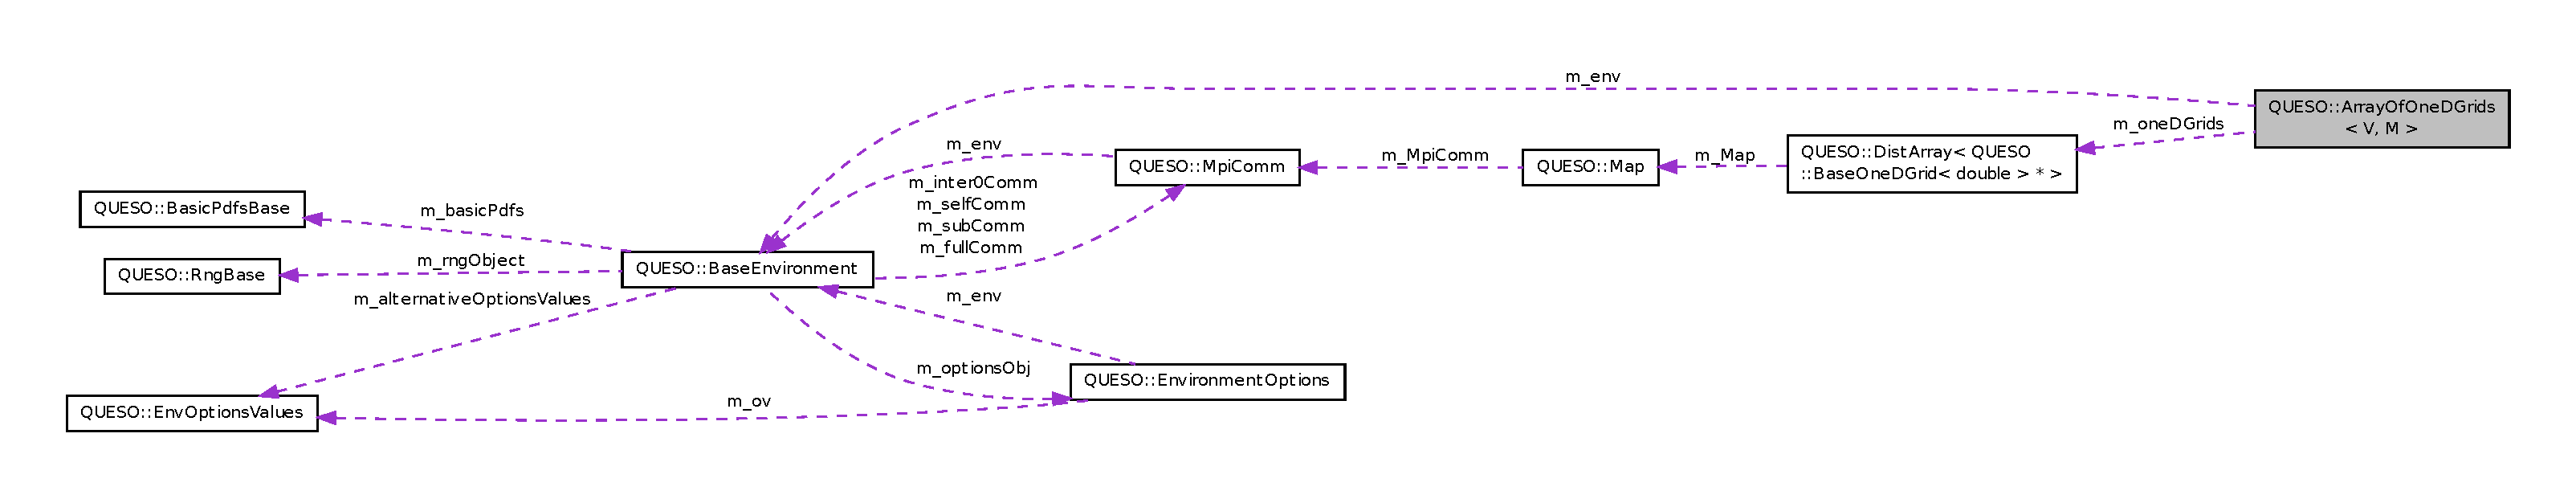
\includegraphics[width=350pt]{class_q_u_e_s_o_1_1_array_of_one_d_grids__coll__graph}
\end{center}
\end{figure}
\subsection*{Public Member Functions}
\begin{Indent}{\bf Constructor/\-Destructor methods}\par
\begin{DoxyCompactItemize}
\item 
\hyperlink{class_q_u_e_s_o_1_1_array_of_one_d_grids_afac2d38cfd5e69c4e7cd7744308063af}{Array\-Of\-One\-D\-Grids} (const char $\ast$prefix, const \hyperlink{class_q_u_e_s_o_1_1_vector_space}{Vector\-Space}$<$ V, M $>$ \&\hyperlink{class_q_u_e_s_o_1_1_array_of_one_d_grids_a07aee362e04f713c139730c991de9baa}{row\-Space})
\begin{DoxyCompactList}\small\item\em Default constructor. \end{DoxyCompactList}\item 
\hyperlink{class_q_u_e_s_o_1_1_array_of_one_d_grids_a4580db34a8438863e75c40cd47e9c8d4}{$\sim$\-Array\-Of\-One\-D\-Grids} ()
\begin{DoxyCompactList}\small\item\em Destructor. \end{DoxyCompactList}\end{DoxyCompactItemize}
\end{Indent}
\begin{Indent}{\bf Property methods}\par
\begin{DoxyCompactItemize}
\item 
const \hyperlink{class_q_u_e_s_o_1_1_vector_space}{Vector\-Space}$<$ V, M $>$ \& \hyperlink{class_q_u_e_s_o_1_1_array_of_one_d_grids_a07aee362e04f713c139730c991de9baa}{row\-Space} () const 
\begin{DoxyCompactList}\small\item\em Returns the (vector) space to which the row belongs to. \end{DoxyCompactList}\item 
const V \& \hyperlink{class_q_u_e_s_o_1_1_array_of_one_d_grids_a2035c97cda24870644070eae0f8ecfae}{sizes} () const 
\begin{DoxyCompactList}\small\item\em Returns an array with the sizes of the grids. \end{DoxyCompactList}\item 
const V \& \hyperlink{class_q_u_e_s_o_1_1_array_of_one_d_grids_a9230fc37403bb00ecd27ad842eb01c2b}{min\-Positions} () const 
\begin{DoxyCompactList}\small\item\em Returns an array with the minimum position of each grid. \end{DoxyCompactList}\item 
const V \& \hyperlink{class_q_u_e_s_o_1_1_array_of_one_d_grids_a958f92e18bcab93e1866ec67b18e408b}{max\-Positions} () const 
\begin{DoxyCompactList}\small\item\em Returns an array with the maximum position of each grid. \end{DoxyCompactList}\end{DoxyCompactItemize}
\end{Indent}
\begin{Indent}{\bf Math methods}\par
\begin{DoxyCompactItemize}
\item 
void \hyperlink{class_q_u_e_s_o_1_1_array_of_one_d_grids_a143a91500dd5cbc18dd9f8ec912f21d1}{set\-Uniform\-Grids} (const V \&sizes\-Vec, const V \&min\-Positions\-Vec, const V \&max\-Positions\-Vec)
\begin{DoxyCompactList}\small\item\em Sets an array of uniform grids. \end{DoxyCompactList}\end{DoxyCompactItemize}
\end{Indent}
\begin{Indent}{\bf Accessor methods}\par
\begin{DoxyCompactItemize}
\item 
const \hyperlink{class_q_u_e_s_o_1_1_base_one_d_grid}{Base\-One\-D\-Grid}$<$ double $>$ \& \hyperlink{class_q_u_e_s_o_1_1_array_of_one_d_grids_a1e09877a9c5e712a03812163f628685b}{grid} (unsigned int row\-Id) const 
\begin{DoxyCompactList}\small\item\em Returns the grid stored in the {\ttfamily row\-Id}-\/th position of the array of grids. \end{DoxyCompactList}\end{DoxyCompactItemize}
\end{Indent}
\subsection*{Private Attributes}
\begin{DoxyCompactItemize}
\item 
const \hyperlink{class_q_u_e_s_o_1_1_base_environment}{Base\-Environment} \& \hyperlink{class_q_u_e_s_o_1_1_array_of_one_d_grids_abe7ada351d4ab3d04987f52cfedb419c}{m\-\_\-env}
\item 
std\-::string \hyperlink{class_q_u_e_s_o_1_1_array_of_one_d_grids_ae9f51dffdcb939ac6b85d700a60fe167}{m\-\_\-prefix}
\item 
const \hyperlink{class_q_u_e_s_o_1_1_vector_space}{Vector\-Space}$<$ V, M $>$ \& \hyperlink{class_q_u_e_s_o_1_1_array_of_one_d_grids_af8f8d1a3e1d4f6213cf64698f95d34da}{m\-\_\-row\-Space}
\item 
\hyperlink{class_q_u_e_s_o_1_1_dist_array}{Dist\-Array}$<$ \hyperlink{class_q_u_e_s_o_1_1_base_one_d_grid}{Base\-One\-D\-Grid}\\*
$<$ double $>$ $\ast$ $>$ \hyperlink{class_q_u_e_s_o_1_1_array_of_one_d_grids_a0cdfeb23fce031448906cef8d15fd407}{m\-\_\-one\-D\-Grids}
\item 
V $\ast$ \hyperlink{class_q_u_e_s_o_1_1_array_of_one_d_grids_ae2164bf692a8fed51b630a114824ffa7}{m\-\_\-sizes}
\item 
V $\ast$ \hyperlink{class_q_u_e_s_o_1_1_array_of_one_d_grids_aaca722e41b97a006385c588ea888f7d9}{m\-\_\-min\-Positions}
\item 
V $\ast$ \hyperlink{class_q_u_e_s_o_1_1_array_of_one_d_grids_a8deeecb4b58f401acdc1fd101d6b5f42}{m\-\_\-max\-Positions}
\end{DoxyCompactItemize}
\subsection*{I/\-O methods}
\begin{DoxyCompactItemize}
\item 
void \hyperlink{class_q_u_e_s_o_1_1_array_of_one_d_grids_a2c9eb92727869d6f985ed01c4a6d833d}{print} (std\-::ostream \&os) const 
\begin{DoxyCompactList}\small\item\em Prints the values of the array of grids (points). \end{DoxyCompactList}\item 
std\-::ostream \& \hyperlink{class_q_u_e_s_o_1_1_array_of_one_d_grids_af1bc76a10219d37cae967bf8f6d9859a}{operator$<$$<$} (std\-::ostream \&os, const \hyperlink{class_q_u_e_s_o_1_1_array_of_one_d_grids}{Array\-Of\-One\-D\-Grids}$<$ V, M $>$ \&obj)
\end{DoxyCompactItemize}


\subsection{Detailed Description}
\subsubsection*{template$<$class V, class M$>$class Q\-U\-E\-S\-O\-::\-Array\-Of\-One\-D\-Grids$<$ V, M $>$}

Class to accommodate arrays of one-\/dimensional grid. 

Arrays of one-\/dimensional grids are necessary in the calculation, for instance, of C\-D\-Fs and M\-D\-F of vector functions (refer to \hyperlink{class_q_u_e_s_o_1_1_base_vector_cdf}{Base\-Vector\-Cdf}, \hyperlink{class_q_u_e_s_o_1_1_base_vector_mdf}{Base\-Vector\-Mdf}, and derived classes). 

Definition at line 44 of file Array\-Of\-One\-D\-Grids.\-h.



\subsection{Constructor \& Destructor Documentation}
\hypertarget{class_q_u_e_s_o_1_1_array_of_one_d_grids_afac2d38cfd5e69c4e7cd7744308063af}{\index{Q\-U\-E\-S\-O\-::\-Array\-Of\-One\-D\-Grids@{Q\-U\-E\-S\-O\-::\-Array\-Of\-One\-D\-Grids}!Array\-Of\-One\-D\-Grids@{Array\-Of\-One\-D\-Grids}}
\index{Array\-Of\-One\-D\-Grids@{Array\-Of\-One\-D\-Grids}!QUESO::ArrayOfOneDGrids@{Q\-U\-E\-S\-O\-::\-Array\-Of\-One\-D\-Grids}}
\subsubsection[{Array\-Of\-One\-D\-Grids}]{\setlength{\rightskip}{0pt plus 5cm}template$<$class V , class M $>$ {\bf Q\-U\-E\-S\-O\-::\-Array\-Of\-One\-D\-Grids}$<$ V, M $>$\-::{\bf Array\-Of\-One\-D\-Grids} (
\begin{DoxyParamCaption}
\item[{const char $\ast$}]{prefix, }
\item[{const {\bf Vector\-Space}$<$ V, M $>$ \&}]{row\-Space}
\end{DoxyParamCaption}
)}}\label{class_q_u_e_s_o_1_1_array_of_one_d_grids_afac2d38cfd5e69c4e7cd7744308063af}


Default constructor. 



Definition at line 35 of file Array\-Of\-One\-D\-Grids.\-C.



References Q\-U\-E\-S\-O\-::\-Array\-Of\-One\-D\-Grids$<$ V, M $>$\-::m\-\_\-one\-D\-Grids.


\begin{DoxyCode}
38   :
39   \hyperlink{class_q_u_e_s_o_1_1_array_of_one_d_grids_abe7ada351d4ab3d04987f52cfedb419c}{m\_env}         (\hyperlink{class_q_u_e_s_o_1_1_array_of_one_d_grids_a07aee362e04f713c139730c991de9baa}{rowSpace}.env()    ),
40   \hyperlink{class_q_u_e_s_o_1_1_array_of_one_d_grids_ae9f51dffdcb939ac6b85d700a60fe167}{m\_prefix}      ((std::string)(prefix)+\textcolor{stringliteral}{""}),
41   \hyperlink{class_q_u_e_s_o_1_1_array_of_one_d_grids_af8f8d1a3e1d4f6213cf64698f95d34da}{m\_rowSpace}    (\hyperlink{class_q_u_e_s_o_1_1_array_of_one_d_grids_a07aee362e04f713c139730c991de9baa}{rowSpace}          ),
42   \hyperlink{class_q_u_e_s_o_1_1_array_of_one_d_grids_a0cdfeb23fce031448906cef8d15fd407}{m\_oneDGrids}   (\hyperlink{class_q_u_e_s_o_1_1_array_of_one_d_grids_af8f8d1a3e1d4f6213cf64698f95d34da}{m\_rowSpace}.map(),1),
43   \hyperlink{class_q_u_e_s_o_1_1_array_of_one_d_grids_ae2164bf692a8fed51b630a114824ffa7}{m\_sizes}       (NULL),
44   \hyperlink{class_q_u_e_s_o_1_1_array_of_one_d_grids_aaca722e41b97a006385c588ea888f7d9}{m\_minPositions}(NULL),
45   \hyperlink{class_q_u_e_s_o_1_1_array_of_one_d_grids_a8deeecb4b58f401acdc1fd101d6b5f42}{m\_maxPositions}(NULL)
46 \{
47   \textcolor{keywordflow}{for} (\textcolor{keywordtype}{unsigned} \textcolor{keywordtype}{int} i = 0; i < (\textcolor{keywordtype}{unsigned} int) \hyperlink{class_q_u_e_s_o_1_1_array_of_one_d_grids_a0cdfeb23fce031448906cef8d15fd407}{m\_oneDGrids}.MyLength(); ++i) \{
48     \hyperlink{class_q_u_e_s_o_1_1_array_of_one_d_grids_a0cdfeb23fce031448906cef8d15fd407}{m\_oneDGrids}(i,0) = NULL;
49   \}
50 \}
\end{DoxyCode}
\hypertarget{class_q_u_e_s_o_1_1_array_of_one_d_grids_a4580db34a8438863e75c40cd47e9c8d4}{\index{Q\-U\-E\-S\-O\-::\-Array\-Of\-One\-D\-Grids@{Q\-U\-E\-S\-O\-::\-Array\-Of\-One\-D\-Grids}!$\sim$\-Array\-Of\-One\-D\-Grids@{$\sim$\-Array\-Of\-One\-D\-Grids}}
\index{$\sim$\-Array\-Of\-One\-D\-Grids@{$\sim$\-Array\-Of\-One\-D\-Grids}!QUESO::ArrayOfOneDGrids@{Q\-U\-E\-S\-O\-::\-Array\-Of\-One\-D\-Grids}}
\subsubsection[{$\sim$\-Array\-Of\-One\-D\-Grids}]{\setlength{\rightskip}{0pt plus 5cm}template$<$class V , class M $>$ {\bf Q\-U\-E\-S\-O\-::\-Array\-Of\-One\-D\-Grids}$<$ V, M $>$\-::$\sim${\bf Array\-Of\-One\-D\-Grids} (
\begin{DoxyParamCaption}
{}
\end{DoxyParamCaption}
)}}\label{class_q_u_e_s_o_1_1_array_of_one_d_grids_a4580db34a8438863e75c40cd47e9c8d4}


Destructor. 



Definition at line 54 of file Array\-Of\-One\-D\-Grids.\-C.


\begin{DoxyCode}
55 \{
56   \textcolor{keywordflow}{if} (\hyperlink{class_q_u_e_s_o_1_1_array_of_one_d_grids_a8deeecb4b58f401acdc1fd101d6b5f42}{m\_maxPositions}) \textcolor{keyword}{delete} \hyperlink{class_q_u_e_s_o_1_1_array_of_one_d_grids_a8deeecb4b58f401acdc1fd101d6b5f42}{m\_maxPositions};
57   \textcolor{keywordflow}{if} (\hyperlink{class_q_u_e_s_o_1_1_array_of_one_d_grids_aaca722e41b97a006385c588ea888f7d9}{m\_minPositions}) \textcolor{keyword}{delete} \hyperlink{class_q_u_e_s_o_1_1_array_of_one_d_grids_aaca722e41b97a006385c588ea888f7d9}{m\_minPositions};
58   \textcolor{keywordflow}{if} (\hyperlink{class_q_u_e_s_o_1_1_array_of_one_d_grids_ae2164bf692a8fed51b630a114824ffa7}{m\_sizes}       ) \textcolor{keyword}{delete} \hyperlink{class_q_u_e_s_o_1_1_array_of_one_d_grids_ae2164bf692a8fed51b630a114824ffa7}{m\_sizes};
59 
60   \textcolor{keywordflow}{for} (\textcolor{keywordtype}{unsigned} \textcolor{keywordtype}{int} i = 0; i < (\textcolor{keywordtype}{unsigned} int) \hyperlink{class_q_u_e_s_o_1_1_array_of_one_d_grids_a0cdfeb23fce031448906cef8d15fd407}{m\_oneDGrids}.MyLength(); ++i) \{
61     \textcolor{keywordflow}{if} (\hyperlink{class_q_u_e_s_o_1_1_array_of_one_d_grids_a0cdfeb23fce031448906cef8d15fd407}{m\_oneDGrids}(i,0)) \textcolor{keyword}{delete} \hyperlink{class_q_u_e_s_o_1_1_array_of_one_d_grids_a0cdfeb23fce031448906cef8d15fd407}{m\_oneDGrids}(i,0);
62   \}
63 \}
\end{DoxyCode}


\subsection{Member Function Documentation}
\hypertarget{class_q_u_e_s_o_1_1_array_of_one_d_grids_a1e09877a9c5e712a03812163f628685b}{\index{Q\-U\-E\-S\-O\-::\-Array\-Of\-One\-D\-Grids@{Q\-U\-E\-S\-O\-::\-Array\-Of\-One\-D\-Grids}!grid@{grid}}
\index{grid@{grid}!QUESO::ArrayOfOneDGrids@{Q\-U\-E\-S\-O\-::\-Array\-Of\-One\-D\-Grids}}
\subsubsection[{grid}]{\setlength{\rightskip}{0pt plus 5cm}template$<$class V , class M $>$ const {\bf Base\-One\-D\-Grid}$<$ double $>$ \& {\bf Q\-U\-E\-S\-O\-::\-Array\-Of\-One\-D\-Grids}$<$ V, M $>$\-::grid (
\begin{DoxyParamCaption}
\item[{unsigned int}]{row\-Id}
\end{DoxyParamCaption}
) const}}\label{class_q_u_e_s_o_1_1_array_of_one_d_grids_a1e09877a9c5e712a03812163f628685b}


Returns the grid stored in the {\ttfamily row\-Id}-\/th position of the array of grids. 



Definition at line 140 of file Array\-Of\-One\-D\-Grids.\-C.



References U\-Q\-\_\-\-F\-A\-T\-A\-L\-\_\-\-T\-E\-S\-T\-\_\-\-M\-A\-C\-R\-O.



Referenced by Q\-U\-E\-S\-O\-::\-Sampled\-Vector\-Cdf$<$ V, M $>$\-::\-Sampled\-Vector\-Cdf().


\begin{DoxyCode}
141 \{
142   \hyperlink{_defines_8h_a56d63d18d0a6d45757de47fcc06f574d}{UQ\_FATAL\_TEST\_MACRO}(rowId >= \hyperlink{class_q_u_e_s_o_1_1_array_of_one_d_grids_af8f8d1a3e1d4f6213cf64698f95d34da}{m\_rowSpace}.dimLocal(),
143                       \hyperlink{class_q_u_e_s_o_1_1_array_of_one_d_grids_abe7ada351d4ab3d04987f52cfedb419c}{m\_env}.\hyperlink{class_q_u_e_s_o_1_1_base_environment_a78b57112bbd0e6dd0e8afec00b40ffa7}{worldRank}(),
144                       \textcolor{stringliteral}{"ArrayOfOneDUnformGrids<T>::grid()"},
145                       \textcolor{stringliteral}{"rowId is out of range"});
146 
147   ArrayOfOneDGrids<V,M>* tmp = \textcolor{keyword}{const\_cast<}ArrayOfOneDGrids<V,M>*\textcolor{keyword}{>}(\textcolor{keyword}{this});
148   \textcolor{keywordflow}{return} *(tmp->m\_oneDGrids(rowId,0));
149 \}
\end{DoxyCode}
\hypertarget{class_q_u_e_s_o_1_1_array_of_one_d_grids_a958f92e18bcab93e1866ec67b18e408b}{\index{Q\-U\-E\-S\-O\-::\-Array\-Of\-One\-D\-Grids@{Q\-U\-E\-S\-O\-::\-Array\-Of\-One\-D\-Grids}!max\-Positions@{max\-Positions}}
\index{max\-Positions@{max\-Positions}!QUESO::ArrayOfOneDGrids@{Q\-U\-E\-S\-O\-::\-Array\-Of\-One\-D\-Grids}}
\subsubsection[{max\-Positions}]{\setlength{\rightskip}{0pt plus 5cm}template$<$class V , class M $>$ const V \& {\bf Q\-U\-E\-S\-O\-::\-Array\-Of\-One\-D\-Grids}$<$ V, M $>$\-::max\-Positions (
\begin{DoxyParamCaption}
{}
\end{DoxyParamCaption}
) const}}\label{class_q_u_e_s_o_1_1_array_of_one_d_grids_a958f92e18bcab93e1866ec67b18e408b}


Returns an array with the maximum position of each grid. 



Definition at line 99 of file Array\-Of\-One\-D\-Grids.\-C.



References U\-Q\-\_\-\-F\-A\-T\-A\-L\-\_\-\-T\-E\-S\-T\-\_\-\-M\-A\-C\-R\-O.


\begin{DoxyCode}
100 \{
101   \hyperlink{_defines_8h_a56d63d18d0a6d45757de47fcc06f574d}{UQ\_FATAL\_TEST\_MACRO}(\hyperlink{class_q_u_e_s_o_1_1_array_of_one_d_grids_a8deeecb4b58f401acdc1fd101d6b5f42}{m\_maxPositions} == NULL,
102                       \hyperlink{class_q_u_e_s_o_1_1_array_of_one_d_grids_abe7ada351d4ab3d04987f52cfedb419c}{m\_env}.\hyperlink{class_q_u_e_s_o_1_1_base_environment_a78b57112bbd0e6dd0e8afec00b40ffa7}{worldRank}(),
103                       \textcolor{stringliteral}{"ArrayOfOneDGrids<T>::maxPositions()"},
104                       \textcolor{stringliteral}{"maxPositions is still NULL"});
105 
106   \textcolor{keywordflow}{return} *\hyperlink{class_q_u_e_s_o_1_1_array_of_one_d_grids_a8deeecb4b58f401acdc1fd101d6b5f42}{m\_maxPositions};
107 \}
\end{DoxyCode}
\hypertarget{class_q_u_e_s_o_1_1_array_of_one_d_grids_a9230fc37403bb00ecd27ad842eb01c2b}{\index{Q\-U\-E\-S\-O\-::\-Array\-Of\-One\-D\-Grids@{Q\-U\-E\-S\-O\-::\-Array\-Of\-One\-D\-Grids}!min\-Positions@{min\-Positions}}
\index{min\-Positions@{min\-Positions}!QUESO::ArrayOfOneDGrids@{Q\-U\-E\-S\-O\-::\-Array\-Of\-One\-D\-Grids}}
\subsubsection[{min\-Positions}]{\setlength{\rightskip}{0pt plus 5cm}template$<$class V , class M $>$ const V \& {\bf Q\-U\-E\-S\-O\-::\-Array\-Of\-One\-D\-Grids}$<$ V, M $>$\-::min\-Positions (
\begin{DoxyParamCaption}
{}
\end{DoxyParamCaption}
) const}}\label{class_q_u_e_s_o_1_1_array_of_one_d_grids_a9230fc37403bb00ecd27ad842eb01c2b}


Returns an array with the minimum position of each grid. 



Definition at line 87 of file Array\-Of\-One\-D\-Grids.\-C.



References U\-Q\-\_\-\-F\-A\-T\-A\-L\-\_\-\-T\-E\-S\-T\-\_\-\-M\-A\-C\-R\-O.


\begin{DoxyCode}
88 \{
89   \hyperlink{_defines_8h_a56d63d18d0a6d45757de47fcc06f574d}{UQ\_FATAL\_TEST\_MACRO}(\hyperlink{class_q_u_e_s_o_1_1_array_of_one_d_grids_aaca722e41b97a006385c588ea888f7d9}{m\_minPositions} == NULL,
90                       \hyperlink{class_q_u_e_s_o_1_1_array_of_one_d_grids_abe7ada351d4ab3d04987f52cfedb419c}{m\_env}.\hyperlink{class_q_u_e_s_o_1_1_base_environment_a78b57112bbd0e6dd0e8afec00b40ffa7}{worldRank}(),
91                       \textcolor{stringliteral}{"ArrayOfOneDGrids<T>::minPositions()"},
92                       \textcolor{stringliteral}{"minPositions is still NULL"});
93 
94   \textcolor{keywordflow}{return} *\hyperlink{class_q_u_e_s_o_1_1_array_of_one_d_grids_aaca722e41b97a006385c588ea888f7d9}{m\_minPositions};
95 \}
\end{DoxyCode}
\hypertarget{class_q_u_e_s_o_1_1_array_of_one_d_grids_a2c9eb92727869d6f985ed01c4a6d833d}{\index{Q\-U\-E\-S\-O\-::\-Array\-Of\-One\-D\-Grids@{Q\-U\-E\-S\-O\-::\-Array\-Of\-One\-D\-Grids}!print@{print}}
\index{print@{print}!QUESO::ArrayOfOneDGrids@{Q\-U\-E\-S\-O\-::\-Array\-Of\-One\-D\-Grids}}
\subsubsection[{print}]{\setlength{\rightskip}{0pt plus 5cm}template$<$class V , class M $>$ void {\bf Q\-U\-E\-S\-O\-::\-Array\-Of\-One\-D\-Grids}$<$ V, M $>$\-::print (
\begin{DoxyParamCaption}
\item[{std\-::ostream \&}]{os}
\end{DoxyParamCaption}
) const}}\label{class_q_u_e_s_o_1_1_array_of_one_d_grids_a2c9eb92727869d6f985ed01c4a6d833d}


Prints the values of the array of grids (points). 



Definition at line 154 of file Array\-Of\-One\-D\-Grids.\-C.



References Q\-U\-E\-S\-O\-::\-Array\-Of\-One\-D\-Grids$<$ V, M $>$\-::m\-\_\-one\-D\-Grids.


\begin{DoxyCode}
155 \{
156   ArrayOfOneDGrids<V,M>* tmp = \textcolor{keyword}{const\_cast<}ArrayOfOneDGrids<V,M>*\textcolor{keyword}{>}(\textcolor{keyword}{this});
157   \textcolor{keywordflow}{for} (\textcolor{keywordtype}{unsigned} \textcolor{keywordtype}{int} i = 0; i < (\textcolor{keywordtype}{unsigned} int) \hyperlink{class_q_u_e_s_o_1_1_array_of_one_d_grids_a0cdfeb23fce031448906cef8d15fd407}{m\_oneDGrids}.MyLength(); ++i) \{
158     os << *(tmp->m\_oneDGrids(i,0))
159        << std::endl;
160   \}
161 
162   \textcolor{keywordflow}{return};
163 \}
\end{DoxyCode}
\hypertarget{class_q_u_e_s_o_1_1_array_of_one_d_grids_a07aee362e04f713c139730c991de9baa}{\index{Q\-U\-E\-S\-O\-::\-Array\-Of\-One\-D\-Grids@{Q\-U\-E\-S\-O\-::\-Array\-Of\-One\-D\-Grids}!row\-Space@{row\-Space}}
\index{row\-Space@{row\-Space}!QUESO::ArrayOfOneDGrids@{Q\-U\-E\-S\-O\-::\-Array\-Of\-One\-D\-Grids}}
\subsubsection[{row\-Space}]{\setlength{\rightskip}{0pt plus 5cm}template$<$class V , class M $>$ const {\bf Vector\-Space}$<$ V, M $>$ \& {\bf Q\-U\-E\-S\-O\-::\-Array\-Of\-One\-D\-Grids}$<$ V, M $>$\-::row\-Space (
\begin{DoxyParamCaption}
{}
\end{DoxyParamCaption}
) const}}\label{class_q_u_e_s_o_1_1_array_of_one_d_grids_a07aee362e04f713c139730c991de9baa}


Returns the (vector) space to which the row belongs to. 



Definition at line 68 of file Array\-Of\-One\-D\-Grids.\-C.


\begin{DoxyCode}
69 \{
70   \textcolor{keywordflow}{return} \hyperlink{class_q_u_e_s_o_1_1_array_of_one_d_grids_af8f8d1a3e1d4f6213cf64698f95d34da}{m\_rowSpace};
71 \}
\end{DoxyCode}
\hypertarget{class_q_u_e_s_o_1_1_array_of_one_d_grids_a143a91500dd5cbc18dd9f8ec912f21d1}{\index{Q\-U\-E\-S\-O\-::\-Array\-Of\-One\-D\-Grids@{Q\-U\-E\-S\-O\-::\-Array\-Of\-One\-D\-Grids}!set\-Uniform\-Grids@{set\-Uniform\-Grids}}
\index{set\-Uniform\-Grids@{set\-Uniform\-Grids}!QUESO::ArrayOfOneDGrids@{Q\-U\-E\-S\-O\-::\-Array\-Of\-One\-D\-Grids}}
\subsubsection[{set\-Uniform\-Grids}]{\setlength{\rightskip}{0pt plus 5cm}template$<$class V , class M $>$ void {\bf Q\-U\-E\-S\-O\-::\-Array\-Of\-One\-D\-Grids}$<$ V, M $>$\-::set\-Uniform\-Grids (
\begin{DoxyParamCaption}
\item[{const V \&}]{sizes\-Vec, }
\item[{const V \&}]{min\-Positions\-Vec, }
\item[{const V \&}]{max\-Positions\-Vec}
\end{DoxyParamCaption}
)}}\label{class_q_u_e_s_o_1_1_array_of_one_d_grids_a143a91500dd5cbc18dd9f8ec912f21d1}


Sets an array of uniform grids. 



Definition at line 111 of file Array\-Of\-One\-D\-Grids.\-C.



Referenced by Q\-U\-E\-S\-O\-::\-Sequence\-Of\-Vectors$<$ V, M $>$\-::sub\-Uniformly\-Sampled\-Cdf(), and Q\-U\-E\-S\-O\-::\-Sequence\-Of\-Vectors$<$ V, M $>$\-::unified\-Uniformly\-Sampled\-Cdf().


\begin{DoxyCode}
115 \{
116   \textcolor{keywordflow}{if} (\hyperlink{class_q_u_e_s_o_1_1_array_of_one_d_grids_ae2164bf692a8fed51b630a114824ffa7}{m\_sizes}        == NULL) \hyperlink{class_q_u_e_s_o_1_1_array_of_one_d_grids_ae2164bf692a8fed51b630a114824ffa7}{m\_sizes}        = \textcolor{keyword}{new} V(sizesVec);
117   \textcolor{keywordflow}{else}                       *\hyperlink{class_q_u_e_s_o_1_1_array_of_one_d_grids_ae2164bf692a8fed51b630a114824ffa7}{m\_sizes}        = sizesVec;
118 
119   \textcolor{keywordflow}{if} (\hyperlink{class_q_u_e_s_o_1_1_array_of_one_d_grids_aaca722e41b97a006385c588ea888f7d9}{m\_minPositions} == NULL) \hyperlink{class_q_u_e_s_o_1_1_array_of_one_d_grids_aaca722e41b97a006385c588ea888f7d9}{m\_minPositions} = \textcolor{keyword}{new} V(minPositionsVec);
120   \textcolor{keywordflow}{else}                       *\hyperlink{class_q_u_e_s_o_1_1_array_of_one_d_grids_aaca722e41b97a006385c588ea888f7d9}{m\_minPositions} = minPositionsVec;
121 
122   \textcolor{keywordflow}{if} (\hyperlink{class_q_u_e_s_o_1_1_array_of_one_d_grids_a8deeecb4b58f401acdc1fd101d6b5f42}{m\_maxPositions} == NULL) \hyperlink{class_q_u_e_s_o_1_1_array_of_one_d_grids_a8deeecb4b58f401acdc1fd101d6b5f42}{m\_maxPositions} = \textcolor{keyword}{new} V(maxPositionsVec);
123   \textcolor{keywordflow}{else}                       *\hyperlink{class_q_u_e_s_o_1_1_array_of_one_d_grids_a8deeecb4b58f401acdc1fd101d6b5f42}{m\_maxPositions} = maxPositionsVec;
124 
125   \textcolor{keywordtype}{char} strI[65];
126   \textcolor{keywordflow}{for} (\textcolor{keywordtype}{unsigned} \textcolor{keywordtype}{int} i = 0; i < (\textcolor{keywordtype}{unsigned} int) \hyperlink{class_q_u_e_s_o_1_1_array_of_one_d_grids_a0cdfeb23fce031448906cef8d15fd407}{m\_oneDGrids}.MyLength(); ++i) \{
127     sprintf(strI,\textcolor{stringliteral}{"%u\_"},i);
128     \hyperlink{class_q_u_e_s_o_1_1_array_of_one_d_grids_a0cdfeb23fce031448906cef8d15fd407}{m\_oneDGrids}(i,0) = \textcolor{keyword}{new} UniformOneDGrid<double>(\hyperlink{class_q_u_e_s_o_1_1_array_of_one_d_grids_abe7ada351d4ab3d04987f52cfedb419c}{m\_env},
129                                                           (\hyperlink{class_q_u_e_s_o_1_1_array_of_one_d_grids_ae9f51dffdcb939ac6b85d700a60fe167}{m\_prefix}+strI).c\_str(),
130                                                           (\textcolor{keywordtype}{unsigned} int) sizesVec[i],
131                                                           minPositionsVec[i],
132                                                           maxPositionsVec[i]);
133   \}
134 
135   \textcolor{keywordflow}{return};
136 \}
\end{DoxyCode}
\hypertarget{class_q_u_e_s_o_1_1_array_of_one_d_grids_a2035c97cda24870644070eae0f8ecfae}{\index{Q\-U\-E\-S\-O\-::\-Array\-Of\-One\-D\-Grids@{Q\-U\-E\-S\-O\-::\-Array\-Of\-One\-D\-Grids}!sizes@{sizes}}
\index{sizes@{sizes}!QUESO::ArrayOfOneDGrids@{Q\-U\-E\-S\-O\-::\-Array\-Of\-One\-D\-Grids}}
\subsubsection[{sizes}]{\setlength{\rightskip}{0pt plus 5cm}template$<$class V , class M $>$ const V \& {\bf Q\-U\-E\-S\-O\-::\-Array\-Of\-One\-D\-Grids}$<$ V, M $>$\-::sizes (
\begin{DoxyParamCaption}
{}
\end{DoxyParamCaption}
) const}}\label{class_q_u_e_s_o_1_1_array_of_one_d_grids_a2035c97cda24870644070eae0f8ecfae}


Returns an array with the sizes of the grids. 



Definition at line 75 of file Array\-Of\-One\-D\-Grids.\-C.



References U\-Q\-\_\-\-F\-A\-T\-A\-L\-\_\-\-T\-E\-S\-T\-\_\-\-M\-A\-C\-R\-O.


\begin{DoxyCode}
76 \{
77   \hyperlink{_defines_8h_a56d63d18d0a6d45757de47fcc06f574d}{UQ\_FATAL\_TEST\_MACRO}(\hyperlink{class_q_u_e_s_o_1_1_array_of_one_d_grids_ae2164bf692a8fed51b630a114824ffa7}{m\_sizes} == NULL,
78                       \hyperlink{class_q_u_e_s_o_1_1_array_of_one_d_grids_abe7ada351d4ab3d04987f52cfedb419c}{m\_env}.\hyperlink{class_q_u_e_s_o_1_1_base_environment_a78b57112bbd0e6dd0e8afec00b40ffa7}{worldRank}(),
79                       \textcolor{stringliteral}{"ArrayOfOneDGrids<T>::sizes()"},
80                       \textcolor{stringliteral}{"sizes is still NULL"});
81 
82   \textcolor{keywordflow}{return} *\hyperlink{class_q_u_e_s_o_1_1_array_of_one_d_grids_ae2164bf692a8fed51b630a114824ffa7}{m\_sizes};
83 \}
\end{DoxyCode}


\subsection{Friends And Related Function Documentation}
\hypertarget{class_q_u_e_s_o_1_1_array_of_one_d_grids_af1bc76a10219d37cae967bf8f6d9859a}{\index{Q\-U\-E\-S\-O\-::\-Array\-Of\-One\-D\-Grids@{Q\-U\-E\-S\-O\-::\-Array\-Of\-One\-D\-Grids}!operator$<$$<$@{operator$<$$<$}}
\index{operator$<$$<$@{operator$<$$<$}!QUESO::ArrayOfOneDGrids@{Q\-U\-E\-S\-O\-::\-Array\-Of\-One\-D\-Grids}}
\subsubsection[{operator$<$$<$}]{\setlength{\rightskip}{0pt plus 5cm}template$<$class V, class M$>$ std\-::ostream\& operator$<$$<$ (
\begin{DoxyParamCaption}
\item[{std\-::ostream \&}]{os, }
\item[{const {\bf Array\-Of\-One\-D\-Grids}$<$ V, M $>$ \&}]{obj}
\end{DoxyParamCaption}
)\hspace{0.3cm}{\ttfamily [friend]}}}\label{class_q_u_e_s_o_1_1_array_of_one_d_grids_af1bc76a10219d37cae967bf8f6d9859a}


Definition at line 92 of file Array\-Of\-One\-D\-Grids.\-h.


\begin{DoxyCode}
94   \{
95     obj.print(os);
96     \textcolor{keywordflow}{return} os;
97   \}
\end{DoxyCode}


\subsection{Member Data Documentation}
\hypertarget{class_q_u_e_s_o_1_1_array_of_one_d_grids_abe7ada351d4ab3d04987f52cfedb419c}{\index{Q\-U\-E\-S\-O\-::\-Array\-Of\-One\-D\-Grids@{Q\-U\-E\-S\-O\-::\-Array\-Of\-One\-D\-Grids}!m\-\_\-env@{m\-\_\-env}}
\index{m\-\_\-env@{m\-\_\-env}!QUESO::ArrayOfOneDGrids@{Q\-U\-E\-S\-O\-::\-Array\-Of\-One\-D\-Grids}}
\subsubsection[{m\-\_\-env}]{\setlength{\rightskip}{0pt plus 5cm}template$<$class V, class M$>$ const {\bf Base\-Environment}\& {\bf Q\-U\-E\-S\-O\-::\-Array\-Of\-One\-D\-Grids}$<$ V, M $>$\-::m\-\_\-env\hspace{0.3cm}{\ttfamily [private]}}}\label{class_q_u_e_s_o_1_1_array_of_one_d_grids_abe7ada351d4ab3d04987f52cfedb419c}


Definition at line 101 of file Array\-Of\-One\-D\-Grids.\-h.

\hypertarget{class_q_u_e_s_o_1_1_array_of_one_d_grids_a8deeecb4b58f401acdc1fd101d6b5f42}{\index{Q\-U\-E\-S\-O\-::\-Array\-Of\-One\-D\-Grids@{Q\-U\-E\-S\-O\-::\-Array\-Of\-One\-D\-Grids}!m\-\_\-max\-Positions@{m\-\_\-max\-Positions}}
\index{m\-\_\-max\-Positions@{m\-\_\-max\-Positions}!QUESO::ArrayOfOneDGrids@{Q\-U\-E\-S\-O\-::\-Array\-Of\-One\-D\-Grids}}
\subsubsection[{m\-\_\-max\-Positions}]{\setlength{\rightskip}{0pt plus 5cm}template$<$class V, class M$>$ V$\ast$ {\bf Q\-U\-E\-S\-O\-::\-Array\-Of\-One\-D\-Grids}$<$ V, M $>$\-::m\-\_\-max\-Positions\hspace{0.3cm}{\ttfamily [private]}}}\label{class_q_u_e_s_o_1_1_array_of_one_d_grids_a8deeecb4b58f401acdc1fd101d6b5f42}


Definition at line 108 of file Array\-Of\-One\-D\-Grids.\-h.

\hypertarget{class_q_u_e_s_o_1_1_array_of_one_d_grids_aaca722e41b97a006385c588ea888f7d9}{\index{Q\-U\-E\-S\-O\-::\-Array\-Of\-One\-D\-Grids@{Q\-U\-E\-S\-O\-::\-Array\-Of\-One\-D\-Grids}!m\-\_\-min\-Positions@{m\-\_\-min\-Positions}}
\index{m\-\_\-min\-Positions@{m\-\_\-min\-Positions}!QUESO::ArrayOfOneDGrids@{Q\-U\-E\-S\-O\-::\-Array\-Of\-One\-D\-Grids}}
\subsubsection[{m\-\_\-min\-Positions}]{\setlength{\rightskip}{0pt plus 5cm}template$<$class V, class M$>$ V$\ast$ {\bf Q\-U\-E\-S\-O\-::\-Array\-Of\-One\-D\-Grids}$<$ V, M $>$\-::m\-\_\-min\-Positions\hspace{0.3cm}{\ttfamily [private]}}}\label{class_q_u_e_s_o_1_1_array_of_one_d_grids_aaca722e41b97a006385c588ea888f7d9}


Definition at line 107 of file Array\-Of\-One\-D\-Grids.\-h.

\hypertarget{class_q_u_e_s_o_1_1_array_of_one_d_grids_a0cdfeb23fce031448906cef8d15fd407}{\index{Q\-U\-E\-S\-O\-::\-Array\-Of\-One\-D\-Grids@{Q\-U\-E\-S\-O\-::\-Array\-Of\-One\-D\-Grids}!m\-\_\-one\-D\-Grids@{m\-\_\-one\-D\-Grids}}
\index{m\-\_\-one\-D\-Grids@{m\-\_\-one\-D\-Grids}!QUESO::ArrayOfOneDGrids@{Q\-U\-E\-S\-O\-::\-Array\-Of\-One\-D\-Grids}}
\subsubsection[{m\-\_\-one\-D\-Grids}]{\setlength{\rightskip}{0pt plus 5cm}template$<$class V, class M$>$ {\bf Dist\-Array}$<${\bf Base\-One\-D\-Grid}$<$double$>$$\ast$$>$ {\bf Q\-U\-E\-S\-O\-::\-Array\-Of\-One\-D\-Grids}$<$ V, M $>$\-::m\-\_\-one\-D\-Grids\hspace{0.3cm}{\ttfamily [private]}}}\label{class_q_u_e_s_o_1_1_array_of_one_d_grids_a0cdfeb23fce031448906cef8d15fd407}


Definition at line 104 of file Array\-Of\-One\-D\-Grids.\-h.



Referenced by Q\-U\-E\-S\-O\-::\-Array\-Of\-One\-D\-Grids$<$ V, M $>$\-::\-Array\-Of\-One\-D\-Grids(), and Q\-U\-E\-S\-O\-::\-Array\-Of\-One\-D\-Grids$<$ V, M $>$\-::print().

\hypertarget{class_q_u_e_s_o_1_1_array_of_one_d_grids_ae9f51dffdcb939ac6b85d700a60fe167}{\index{Q\-U\-E\-S\-O\-::\-Array\-Of\-One\-D\-Grids@{Q\-U\-E\-S\-O\-::\-Array\-Of\-One\-D\-Grids}!m\-\_\-prefix@{m\-\_\-prefix}}
\index{m\-\_\-prefix@{m\-\_\-prefix}!QUESO::ArrayOfOneDGrids@{Q\-U\-E\-S\-O\-::\-Array\-Of\-One\-D\-Grids}}
\subsubsection[{m\-\_\-prefix}]{\setlength{\rightskip}{0pt plus 5cm}template$<$class V, class M$>$ std\-::string {\bf Q\-U\-E\-S\-O\-::\-Array\-Of\-One\-D\-Grids}$<$ V, M $>$\-::m\-\_\-prefix\hspace{0.3cm}{\ttfamily [private]}}}\label{class_q_u_e_s_o_1_1_array_of_one_d_grids_ae9f51dffdcb939ac6b85d700a60fe167}


Definition at line 102 of file Array\-Of\-One\-D\-Grids.\-h.

\hypertarget{class_q_u_e_s_o_1_1_array_of_one_d_grids_af8f8d1a3e1d4f6213cf64698f95d34da}{\index{Q\-U\-E\-S\-O\-::\-Array\-Of\-One\-D\-Grids@{Q\-U\-E\-S\-O\-::\-Array\-Of\-One\-D\-Grids}!m\-\_\-row\-Space@{m\-\_\-row\-Space}}
\index{m\-\_\-row\-Space@{m\-\_\-row\-Space}!QUESO::ArrayOfOneDGrids@{Q\-U\-E\-S\-O\-::\-Array\-Of\-One\-D\-Grids}}
\subsubsection[{m\-\_\-row\-Space}]{\setlength{\rightskip}{0pt plus 5cm}template$<$class V, class M$>$ const {\bf Vector\-Space}$<$V,M$>$\& {\bf Q\-U\-E\-S\-O\-::\-Array\-Of\-One\-D\-Grids}$<$ V, M $>$\-::m\-\_\-row\-Space\hspace{0.3cm}{\ttfamily [private]}}}\label{class_q_u_e_s_o_1_1_array_of_one_d_grids_af8f8d1a3e1d4f6213cf64698f95d34da}


Definition at line 103 of file Array\-Of\-One\-D\-Grids.\-h.

\hypertarget{class_q_u_e_s_o_1_1_array_of_one_d_grids_ae2164bf692a8fed51b630a114824ffa7}{\index{Q\-U\-E\-S\-O\-::\-Array\-Of\-One\-D\-Grids@{Q\-U\-E\-S\-O\-::\-Array\-Of\-One\-D\-Grids}!m\-\_\-sizes@{m\-\_\-sizes}}
\index{m\-\_\-sizes@{m\-\_\-sizes}!QUESO::ArrayOfOneDGrids@{Q\-U\-E\-S\-O\-::\-Array\-Of\-One\-D\-Grids}}
\subsubsection[{m\-\_\-sizes}]{\setlength{\rightskip}{0pt plus 5cm}template$<$class V, class M$>$ V$\ast$ {\bf Q\-U\-E\-S\-O\-::\-Array\-Of\-One\-D\-Grids}$<$ V, M $>$\-::m\-\_\-sizes\hspace{0.3cm}{\ttfamily [private]}}}\label{class_q_u_e_s_o_1_1_array_of_one_d_grids_ae2164bf692a8fed51b630a114824ffa7}


Definition at line 106 of file Array\-Of\-One\-D\-Grids.\-h.



The documentation for this class was generated from the following files\-:\begin{DoxyCompactItemize}
\item 
src/misc/inc/\hyperlink{_array_of_one_d_grids_8h}{Array\-Of\-One\-D\-Grids.\-h}\item 
src/misc/src/\hyperlink{_array_of_one_d_grids_8_c}{Array\-Of\-One\-D\-Grids.\-C}\end{DoxyCompactItemize}

\hypertarget{class_q_u_e_s_o_1_1_array_of_one_d_tables}{\section{Q\-U\-E\-S\-O\-:\-:Array\-Of\-One\-D\-Tables$<$ V, M $>$ Class Template Reference}
\label{class_q_u_e_s_o_1_1_array_of_one_d_tables}\index{Q\-U\-E\-S\-O\-::\-Array\-Of\-One\-D\-Tables$<$ V, M $>$@{Q\-U\-E\-S\-O\-::\-Array\-Of\-One\-D\-Tables$<$ V, M $>$}}
}


Class to accommodate arrays of one-\/dimensional tables.  




{\ttfamily \#include $<$Array\-Of\-One\-D\-Tables.\-h$>$}



Collaboration diagram for Q\-U\-E\-S\-O\-:\-:Array\-Of\-One\-D\-Tables$<$ V, M $>$\-:
\nopagebreak
\begin{figure}[H]
\begin{center}
\leavevmode
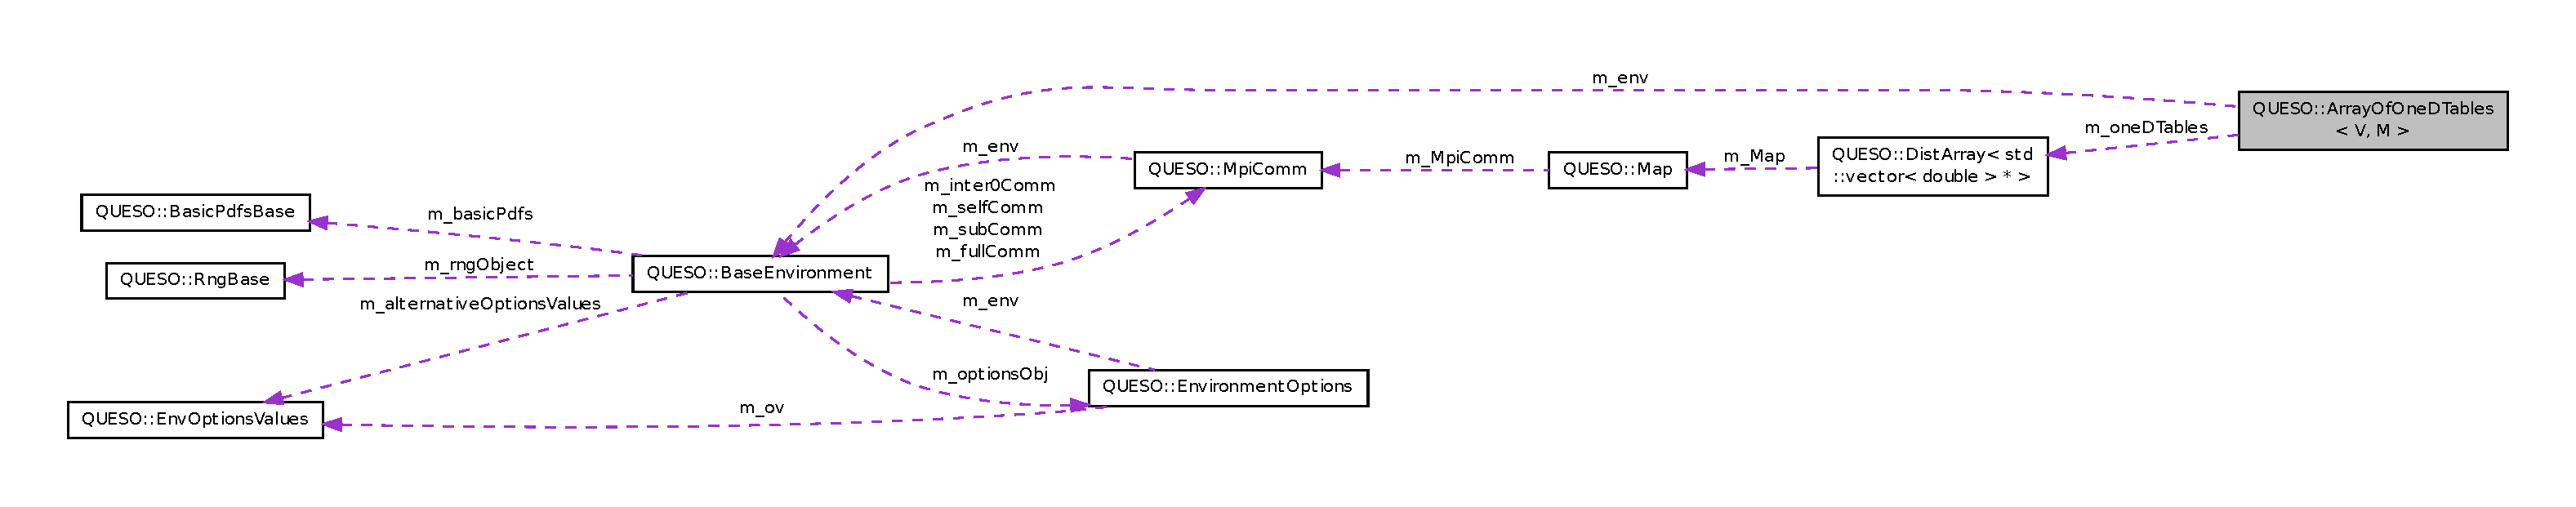
\includegraphics[width=350pt]{class_q_u_e_s_o_1_1_array_of_one_d_tables__coll__graph}
\end{center}
\end{figure}
\subsection*{Public Member Functions}
\begin{Indent}{\bf Constructor/\-Destructor methods}\par
\begin{DoxyCompactItemize}
\item 
\hyperlink{class_q_u_e_s_o_1_1_array_of_one_d_tables_ae36f0c33595a2d46d08eced253d1eef3}{Array\-Of\-One\-D\-Tables} (const char $\ast$prefix, const \hyperlink{class_q_u_e_s_o_1_1_vector_space}{Vector\-Space}$<$ V, M $>$ \&row\-Space)
\begin{DoxyCompactList}\small\item\em Default constructor. \end{DoxyCompactList}\item 
\hyperlink{class_q_u_e_s_o_1_1_array_of_one_d_tables_a233bf24beaf3adabca4735eb7a88c966}{$\sim$\-Array\-Of\-One\-D\-Tables} ()
\begin{DoxyCompactList}\small\item\em Destructor. \end{DoxyCompactList}\end{DoxyCompactItemize}
\end{Indent}
\begin{Indent}{\bf Math methods}\par
\begin{DoxyCompactItemize}
\item 
void \hyperlink{class_q_u_e_s_o_1_1_array_of_one_d_tables_ad52be35568cf8c325569b4ae272acab9}{set\-One\-D\-Table} (unsigned int row\-Id, const std\-::vector$<$ double $>$ \&values)
\begin{DoxyCompactList}\small\item\em Sets the one-\/dimensional table. \end{DoxyCompactList}\item 
const std\-::vector$<$ double $>$ \& \hyperlink{class_q_u_e_s_o_1_1_array_of_one_d_tables_ade48785a66524243c5a22ec39bc6de2d}{one\-D\-Table} (unsigned int row\-Id) const 
\begin{DoxyCompactList}\small\item\em Returns the array located at position {\ttfamily row\-Id} of the one-\/dimensional table. \end{DoxyCompactList}\end{DoxyCompactItemize}
\end{Indent}
\begin{Indent}{\bf I/\-O method}\par
\begin{DoxyCompactItemize}
\item 
void \hyperlink{class_q_u_e_s_o_1_1_array_of_one_d_tables_aec66e8a1e7f0baf3adc29332590ea1af}{print} (std\-::ostream \&os) const 
\begin{DoxyCompactList}\small\item\em Prints the values in this array of tables. \end{DoxyCompactList}\end{DoxyCompactItemize}
\end{Indent}
\subsection*{Private Attributes}
\begin{DoxyCompactItemize}
\item 
const \hyperlink{class_q_u_e_s_o_1_1_base_environment}{Base\-Environment} \& \hyperlink{class_q_u_e_s_o_1_1_array_of_one_d_tables_a51d23742e1c418efc4e829cb06fcda76}{m\-\_\-env}
\item 
std\-::string \hyperlink{class_q_u_e_s_o_1_1_array_of_one_d_tables_ae9bfd81e226ee5712cd160031f96d4d2}{m\-\_\-prefix}
\item 
const \hyperlink{class_q_u_e_s_o_1_1_vector_space}{Vector\-Space}$<$ V, M $>$ \& \hyperlink{class_q_u_e_s_o_1_1_array_of_one_d_tables_a476632866ae0eebc389f19b8b83cc324}{m\-\_\-row\-Space}
\item 
\hyperlink{class_q_u_e_s_o_1_1_dist_array}{Dist\-Array}$<$ std\-::vector$<$ double $>$ $\ast$ $>$ \hyperlink{class_q_u_e_s_o_1_1_array_of_one_d_tables_ad5e13befcb2e58dde1c13e396388a696}{m\-\_\-one\-D\-Tables}
\end{DoxyCompactItemize}


\subsection{Detailed Description}
\subsubsection*{template$<$class V, class M$>$class Q\-U\-E\-S\-O\-::\-Array\-Of\-One\-D\-Tables$<$ V, M $>$}

Class to accommodate arrays of one-\/dimensional tables. 

Arrays of one-\/dimensional tables are necessary in the calculation (storage), for instance, of C\-D\-Fs and M\-D\-F of vector functions (refer to \hyperlink{class_q_u_e_s_o_1_1_base_vector_cdf}{Base\-Vector\-Cdf}, \hyperlink{class_q_u_e_s_o_1_1_base_vector_mdf}{Base\-Vector\-Mdf}, and derived classes) given the (array of) grid points (\hyperlink{class_q_u_e_s_o_1_1_array_of_one_d_grids}{Array\-Of\-One\-D\-Grids}). 

Definition at line 46 of file Array\-Of\-One\-D\-Tables.\-h.



\subsection{Constructor \& Destructor Documentation}
\hypertarget{class_q_u_e_s_o_1_1_array_of_one_d_tables_ae36f0c33595a2d46d08eced253d1eef3}{\index{Q\-U\-E\-S\-O\-::\-Array\-Of\-One\-D\-Tables@{Q\-U\-E\-S\-O\-::\-Array\-Of\-One\-D\-Tables}!Array\-Of\-One\-D\-Tables@{Array\-Of\-One\-D\-Tables}}
\index{Array\-Of\-One\-D\-Tables@{Array\-Of\-One\-D\-Tables}!QUESO::ArrayOfOneDTables@{Q\-U\-E\-S\-O\-::\-Array\-Of\-One\-D\-Tables}}
\subsubsection[{Array\-Of\-One\-D\-Tables}]{\setlength{\rightskip}{0pt plus 5cm}template$<$class V , class M $>$ {\bf Q\-U\-E\-S\-O\-::\-Array\-Of\-One\-D\-Tables}$<$ V, M $>$\-::{\bf Array\-Of\-One\-D\-Tables} (
\begin{DoxyParamCaption}
\item[{const char $\ast$}]{prefix, }
\item[{const {\bf Vector\-Space}$<$ V, M $>$ \&}]{row\-Space}
\end{DoxyParamCaption}
)}}\label{class_q_u_e_s_o_1_1_array_of_one_d_tables_ae36f0c33595a2d46d08eced253d1eef3}


Default constructor. 



Definition at line 33 of file Array\-Of\-One\-D\-Tables.\-C.



References Q\-U\-E\-S\-O\-::\-Array\-Of\-One\-D\-Tables$<$ V, M $>$\-::m\-\_\-one\-D\-Tables, and Q\-U\-E\-S\-O\-::\-Dist\-Array$<$ T $>$\-::\-My\-Length().


\begin{DoxyCode}
36   :
37   \hyperlink{class_q_u_e_s_o_1_1_array_of_one_d_tables_a51d23742e1c418efc4e829cb06fcda76}{m\_env}       (rowSpace.env()),
38   \hyperlink{class_q_u_e_s_o_1_1_array_of_one_d_tables_ae9bfd81e226ee5712cd160031f96d4d2}{m\_prefix}    ((std::string)(prefix)+\textcolor{stringliteral}{""}),
39   \hyperlink{class_q_u_e_s_o_1_1_array_of_one_d_tables_a476632866ae0eebc389f19b8b83cc324}{m\_rowSpace}  (rowSpace      ),
40   \hyperlink{class_q_u_e_s_o_1_1_array_of_one_d_tables_ad5e13befcb2e58dde1c13e396388a696}{m\_oneDTables}(\hyperlink{class_q_u_e_s_o_1_1_array_of_one_d_tables_a476632866ae0eebc389f19b8b83cc324}{m\_rowSpace}.map(),1)
41 \{
42   \textcolor{keywordflow}{for} (\textcolor{keywordtype}{unsigned} \textcolor{keywordtype}{int} i = 0; i < (\textcolor{keywordtype}{unsigned} int) \hyperlink{class_q_u_e_s_o_1_1_array_of_one_d_tables_ad5e13befcb2e58dde1c13e396388a696}{m\_oneDTables}.\hyperlink{class_q_u_e_s_o_1_1_dist_array_af4a798f5defa6a37dfc82175c7f92f83}{MyLength}(); ++i) \{
43     \hyperlink{class_q_u_e_s_o_1_1_array_of_one_d_tables_ad5e13befcb2e58dde1c13e396388a696}{m\_oneDTables}(i,0) = NULL;
44   \}
45 \}
\end{DoxyCode}
\hypertarget{class_q_u_e_s_o_1_1_array_of_one_d_tables_a233bf24beaf3adabca4735eb7a88c966}{\index{Q\-U\-E\-S\-O\-::\-Array\-Of\-One\-D\-Tables@{Q\-U\-E\-S\-O\-::\-Array\-Of\-One\-D\-Tables}!$\sim$\-Array\-Of\-One\-D\-Tables@{$\sim$\-Array\-Of\-One\-D\-Tables}}
\index{$\sim$\-Array\-Of\-One\-D\-Tables@{$\sim$\-Array\-Of\-One\-D\-Tables}!QUESO::ArrayOfOneDTables@{Q\-U\-E\-S\-O\-::\-Array\-Of\-One\-D\-Tables}}
\subsubsection[{$\sim$\-Array\-Of\-One\-D\-Tables}]{\setlength{\rightskip}{0pt plus 5cm}template$<$class V , class M $>$ {\bf Q\-U\-E\-S\-O\-::\-Array\-Of\-One\-D\-Tables}$<$ V, M $>$\-::$\sim${\bf Array\-Of\-One\-D\-Tables} (
\begin{DoxyParamCaption}
{}
\end{DoxyParamCaption}
)}}\label{class_q_u_e_s_o_1_1_array_of_one_d_tables_a233bf24beaf3adabca4735eb7a88c966}


Destructor. 



Definition at line 49 of file Array\-Of\-One\-D\-Tables.\-C.


\begin{DoxyCode}
50 \{
51   \textcolor{keywordflow}{for} (\textcolor{keywordtype}{unsigned} \textcolor{keywordtype}{int} i = 0; i < (\textcolor{keywordtype}{unsigned} int) \hyperlink{class_q_u_e_s_o_1_1_array_of_one_d_tables_ad5e13befcb2e58dde1c13e396388a696}{m\_oneDTables}.\hyperlink{class_q_u_e_s_o_1_1_dist_array_af4a798f5defa6a37dfc82175c7f92f83}{MyLength}(); ++i) \{
52     \textcolor{keywordflow}{if} (\hyperlink{class_q_u_e_s_o_1_1_array_of_one_d_tables_ad5e13befcb2e58dde1c13e396388a696}{m\_oneDTables}(i,0)) \textcolor{keyword}{delete} \hyperlink{class_q_u_e_s_o_1_1_array_of_one_d_tables_ad5e13befcb2e58dde1c13e396388a696}{m\_oneDTables}(i,0);
53   \}
54 \}
\end{DoxyCode}


\subsection{Member Function Documentation}
\hypertarget{class_q_u_e_s_o_1_1_array_of_one_d_tables_ade48785a66524243c5a22ec39bc6de2d}{\index{Q\-U\-E\-S\-O\-::\-Array\-Of\-One\-D\-Tables@{Q\-U\-E\-S\-O\-::\-Array\-Of\-One\-D\-Tables}!one\-D\-Table@{one\-D\-Table}}
\index{one\-D\-Table@{one\-D\-Table}!QUESO::ArrayOfOneDTables@{Q\-U\-E\-S\-O\-::\-Array\-Of\-One\-D\-Tables}}
\subsubsection[{one\-D\-Table}]{\setlength{\rightskip}{0pt plus 5cm}template$<$class V , class M $>$ const std\-::vector$<$ double $>$ \& {\bf Q\-U\-E\-S\-O\-::\-Array\-Of\-One\-D\-Tables}$<$ V, M $>$\-::one\-D\-Table (
\begin{DoxyParamCaption}
\item[{unsigned int}]{row\-Id}
\end{DoxyParamCaption}
) const}}\label{class_q_u_e_s_o_1_1_array_of_one_d_tables_ade48785a66524243c5a22ec39bc6de2d}


Returns the array located at position {\ttfamily row\-Id} of the one-\/dimensional table. 



Definition at line 80 of file Array\-Of\-One\-D\-Tables.\-C.



References U\-Q\-\_\-\-F\-A\-T\-A\-L\-\_\-\-T\-E\-S\-T\-\_\-\-M\-A\-C\-R\-O.



Referenced by Q\-U\-E\-S\-O\-::\-Sampled\-Vector\-Cdf$<$ V, M $>$\-::\-Sampled\-Vector\-Cdf().


\begin{DoxyCode}
81 \{
82   \hyperlink{_defines_8h_a56d63d18d0a6d45757de47fcc06f574d}{UQ\_FATAL\_TEST\_MACRO}(rowId >= (\textcolor{keywordtype}{unsigned} \textcolor{keywordtype}{int}) \hyperlink{class_q_u_e_s_o_1_1_array_of_one_d_tables_ad5e13befcb2e58dde1c13e396388a696}{m\_oneDTables}.
      \hyperlink{class_q_u_e_s_o_1_1_dist_array_af4a798f5defa6a37dfc82175c7f92f83}{MyLength}(),
83                       \hyperlink{class_q_u_e_s_o_1_1_array_of_one_d_tables_a51d23742e1c418efc4e829cb06fcda76}{m\_env}.\hyperlink{class_q_u_e_s_o_1_1_base_environment_a78b57112bbd0e6dd0e8afec00b40ffa7}{worldRank}(),
84                       \textcolor{stringliteral}{"ArrayOfOneDTables<T>::oneDTable()"},
85                       \textcolor{stringliteral}{"rowId is out of range"});
86 
87   ArrayOfOneDTables<V,M>* tmp = \textcolor{keyword}{const\_cast<}ArrayOfOneDTables<V,M>*\textcolor{keyword}{>}(\textcolor{keyword}{this});
88 
89   \hyperlink{_defines_8h_a56d63d18d0a6d45757de47fcc06f574d}{UQ\_FATAL\_TEST\_MACRO}(tmp->m\_oneDTables(rowId,0) == NULL,
90                       \hyperlink{class_q_u_e_s_o_1_1_array_of_one_d_tables_a51d23742e1c418efc4e829cb06fcda76}{m\_env}.\hyperlink{class_q_u_e_s_o_1_1_base_environment_a78b57112bbd0e6dd0e8afec00b40ffa7}{worldRank}(),
91                       \textcolor{stringliteral}{"ArrayOfOneDTables<T>::oneDTable()"},
92                       \textcolor{stringliteral}{"requested row is still NULL"});
93 
94   \textcolor{keywordflow}{return} *(tmp->m\_oneDTables(rowId,0));
95 \}
\end{DoxyCode}
\hypertarget{class_q_u_e_s_o_1_1_array_of_one_d_tables_aec66e8a1e7f0baf3adc29332590ea1af}{\index{Q\-U\-E\-S\-O\-::\-Array\-Of\-One\-D\-Tables@{Q\-U\-E\-S\-O\-::\-Array\-Of\-One\-D\-Tables}!print@{print}}
\index{print@{print}!QUESO::ArrayOfOneDTables@{Q\-U\-E\-S\-O\-::\-Array\-Of\-One\-D\-Tables}}
\subsubsection[{print}]{\setlength{\rightskip}{0pt plus 5cm}template$<$class V , class M $>$ void {\bf Q\-U\-E\-S\-O\-::\-Array\-Of\-One\-D\-Tables}$<$ V, M $>$\-::print (
\begin{DoxyParamCaption}
\item[{std\-::ostream \&}]{os}
\end{DoxyParamCaption}
) const}}\label{class_q_u_e_s_o_1_1_array_of_one_d_tables_aec66e8a1e7f0baf3adc29332590ea1af}


Prints the values in this array of tables. 

It prints the arrays (inner for-\/loop) in each position of the table (outer for-\/loop). 

Definition at line 100 of file Array\-Of\-One\-D\-Tables.\-C.



References Q\-U\-E\-S\-O\-::\-Array\-Of\-One\-D\-Tables$<$ V, M $>$\-::m\-\_\-one\-D\-Tables.



Referenced by Q\-U\-E\-S\-O\-::operator$<$$<$().


\begin{DoxyCode}
101 \{
102   ArrayOfOneDTables<V,M>* tmp = \textcolor{keyword}{const\_cast<}ArrayOfOneDTables<V,M>*\textcolor{keyword}{>}(\textcolor{keyword}{this});
103   \textcolor{keywordflow}{for} (\textcolor{keywordtype}{unsigned} \textcolor{keywordtype}{int} i = 0; i < (\textcolor{keywordtype}{unsigned} int) \hyperlink{class_q_u_e_s_o_1_1_array_of_one_d_tables_ad5e13befcb2e58dde1c13e396388a696}{m\_oneDTables}.\hyperlink{class_q_u_e_s_o_1_1_dist_array_af4a798f5defa6a37dfc82175c7f92f83}{MyLength}(); ++i) \{
104     \textcolor{keyword}{const} std::vector<double>& tmpVec = *(tmp->m\_oneDTables(i,0));
105     os << \hyperlink{class_q_u_e_s_o_1_1_array_of_one_d_tables_ae9bfd81e226ee5712cd160031f96d4d2}{m\_prefix} << i << \textcolor{stringliteral}{"\_values\_sub"} << \hyperlink{class_q_u_e_s_o_1_1_array_of_one_d_tables_a51d23742e1c418efc4e829cb06fcda76}{m\_env}.\hyperlink{class_q_u_e_s_o_1_1_base_environment_a73f7849acdd5d5ba15a3094fe18f258f}{subIdString}() << \textcolor{stringliteral}{" = zeros("} << 
      tmpVec.size()
106        << \textcolor{stringliteral}{","}                                                                  << 1
107        << \textcolor{stringliteral}{");"}
108        << std::endl;
109     os << \hyperlink{class_q_u_e_s_o_1_1_array_of_one_d_tables_ae9bfd81e226ee5712cd160031f96d4d2}{m\_prefix} << i << \textcolor{stringliteral}{"\_values\_sub"} << \hyperlink{class_q_u_e_s_o_1_1_array_of_one_d_tables_a51d23742e1c418efc4e829cb06fcda76}{m\_env}.\hyperlink{class_q_u_e_s_o_1_1_base_environment_a73f7849acdd5d5ba15a3094fe18f258f}{subIdString}() << \textcolor{stringliteral}{" = ["};
110     \textcolor{keywordflow}{for} (\textcolor{keywordtype}{unsigned} \textcolor{keywordtype}{int} j = 0; j < tmpVec.size(); ++j) \{
111       os << tmpVec[j] << \textcolor{stringliteral}{" "};
112     \}
113     os << \textcolor{stringliteral}{"];"}
114        << std::endl;
115   \}
116 
117   \textcolor{keywordflow}{return};
118 \}
\end{DoxyCode}
\hypertarget{class_q_u_e_s_o_1_1_array_of_one_d_tables_ad52be35568cf8c325569b4ae272acab9}{\index{Q\-U\-E\-S\-O\-::\-Array\-Of\-One\-D\-Tables@{Q\-U\-E\-S\-O\-::\-Array\-Of\-One\-D\-Tables}!set\-One\-D\-Table@{set\-One\-D\-Table}}
\index{set\-One\-D\-Table@{set\-One\-D\-Table}!QUESO::ArrayOfOneDTables@{Q\-U\-E\-S\-O\-::\-Array\-Of\-One\-D\-Tables}}
\subsubsection[{set\-One\-D\-Table}]{\setlength{\rightskip}{0pt plus 5cm}template$<$class V , class M $>$ void {\bf Q\-U\-E\-S\-O\-::\-Array\-Of\-One\-D\-Tables}$<$ V, M $>$\-::set\-One\-D\-Table (
\begin{DoxyParamCaption}
\item[{unsigned int}]{row\-Id, }
\item[{const std\-::vector$<$ double $>$ \&}]{values}
\end{DoxyParamCaption}
)}}\label{class_q_u_e_s_o_1_1_array_of_one_d_tables_ad52be35568cf8c325569b4ae272acab9}


Sets the one-\/dimensional table. 

This methods assigns the array {\ttfamily values} to position {\ttfamily row\-Id} of the one-\/dimensional table. 

Definition at line 59 of file Array\-Of\-One\-D\-Tables.\-C.



References U\-Q\-\_\-\-F\-A\-T\-A\-L\-\_\-\-T\-E\-S\-T\-\_\-\-M\-A\-C\-R\-O.



Referenced by Q\-U\-E\-S\-O\-::\-Sequence\-Of\-Vectors$<$ V, M $>$\-::sub\-Uniformly\-Sampled\-Cdf(), and Q\-U\-E\-S\-O\-::\-Sequence\-Of\-Vectors$<$ V, M $>$\-::unified\-Uniformly\-Sampled\-Cdf().


\begin{DoxyCode}
60 \{
61   \hyperlink{_defines_8h_a56d63d18d0a6d45757de47fcc06f574d}{UQ\_FATAL\_TEST\_MACRO}(rowId >= (\textcolor{keywordtype}{unsigned} \textcolor{keywordtype}{int}) \hyperlink{class_q_u_e_s_o_1_1_array_of_one_d_tables_ad5e13befcb2e58dde1c13e396388a696}{m\_oneDTables}.
      \hyperlink{class_q_u_e_s_o_1_1_dist_array_af4a798f5defa6a37dfc82175c7f92f83}{MyLength}(),
62                       \hyperlink{class_q_u_e_s_o_1_1_array_of_one_d_tables_a51d23742e1c418efc4e829cb06fcda76}{m\_env}.\hyperlink{class_q_u_e_s_o_1_1_base_environment_a78b57112bbd0e6dd0e8afec00b40ffa7}{worldRank}(),
63                       \textcolor{stringliteral}{"ArrayOfOneDTables<T>::setOneDTable()"},
64                       \textcolor{stringliteral}{"rowId is out of range"});
65 
66   \textcolor{keywordflow}{if} (\hyperlink{class_q_u_e_s_o_1_1_array_of_one_d_tables_ad5e13befcb2e58dde1c13e396388a696}{m\_oneDTables}(rowId,0) == NULL) \hyperlink{class_q_u_e_s_o_1_1_array_of_one_d_tables_ad5e13befcb2e58dde1c13e396388a696}{m\_oneDTables}(rowId,0) = \textcolor{keyword}{new} 
      std::vector<double>(0);
67   \textcolor{keywordflow}{else}                               \hyperlink{class_q_u_e_s_o_1_1_array_of_one_d_tables_ad5e13befcb2e58dde1c13e396388a696}{m\_oneDTables}(rowId,0)->clear();
68 
69   std::vector<double>& vec = *(\hyperlink{class_q_u_e_s_o_1_1_array_of_one_d_tables_ad5e13befcb2e58dde1c13e396388a696}{m\_oneDTables}(rowId,0));
70   vec.resize(values.size(),0.);
71   \textcolor{keywordflow}{for} (\textcolor{keywordtype}{unsigned} \textcolor{keywordtype}{int} j = 0; j < values.size(); ++j) \{
72     vec[j] = values[j];
73   \}
74 
75   \textcolor{keywordflow}{return};
76 \}
\end{DoxyCode}


\subsection{Member Data Documentation}
\hypertarget{class_q_u_e_s_o_1_1_array_of_one_d_tables_a51d23742e1c418efc4e829cb06fcda76}{\index{Q\-U\-E\-S\-O\-::\-Array\-Of\-One\-D\-Tables@{Q\-U\-E\-S\-O\-::\-Array\-Of\-One\-D\-Tables}!m\-\_\-env@{m\-\_\-env}}
\index{m\-\_\-env@{m\-\_\-env}!QUESO::ArrayOfOneDTables@{Q\-U\-E\-S\-O\-::\-Array\-Of\-One\-D\-Tables}}
\subsubsection[{m\-\_\-env}]{\setlength{\rightskip}{0pt plus 5cm}template$<$class V, class M$>$ const {\bf Base\-Environment}\& {\bf Q\-U\-E\-S\-O\-::\-Array\-Of\-One\-D\-Tables}$<$ V, M $>$\-::m\-\_\-env\hspace{0.3cm}{\ttfamily [private]}}}\label{class_q_u_e_s_o_1_1_array_of_one_d_tables_a51d23742e1c418efc4e829cb06fcda76}


Definition at line 75 of file Array\-Of\-One\-D\-Tables.\-h.

\hypertarget{class_q_u_e_s_o_1_1_array_of_one_d_tables_ad5e13befcb2e58dde1c13e396388a696}{\index{Q\-U\-E\-S\-O\-::\-Array\-Of\-One\-D\-Tables@{Q\-U\-E\-S\-O\-::\-Array\-Of\-One\-D\-Tables}!m\-\_\-one\-D\-Tables@{m\-\_\-one\-D\-Tables}}
\index{m\-\_\-one\-D\-Tables@{m\-\_\-one\-D\-Tables}!QUESO::ArrayOfOneDTables@{Q\-U\-E\-S\-O\-::\-Array\-Of\-One\-D\-Tables}}
\subsubsection[{m\-\_\-one\-D\-Tables}]{\setlength{\rightskip}{0pt plus 5cm}template$<$class V, class M$>$ {\bf Dist\-Array}$<$std\-::vector$<$double$>$$\ast$$>$ {\bf Q\-U\-E\-S\-O\-::\-Array\-Of\-One\-D\-Tables}$<$ V, M $>$\-::m\-\_\-one\-D\-Tables\hspace{0.3cm}{\ttfamily [private]}}}\label{class_q_u_e_s_o_1_1_array_of_one_d_tables_ad5e13befcb2e58dde1c13e396388a696}


Definition at line 78 of file Array\-Of\-One\-D\-Tables.\-h.



Referenced by Q\-U\-E\-S\-O\-::\-Array\-Of\-One\-D\-Tables$<$ V, M $>$\-::\-Array\-Of\-One\-D\-Tables(), and Q\-U\-E\-S\-O\-::\-Array\-Of\-One\-D\-Tables$<$ V, M $>$\-::print().

\hypertarget{class_q_u_e_s_o_1_1_array_of_one_d_tables_ae9bfd81e226ee5712cd160031f96d4d2}{\index{Q\-U\-E\-S\-O\-::\-Array\-Of\-One\-D\-Tables@{Q\-U\-E\-S\-O\-::\-Array\-Of\-One\-D\-Tables}!m\-\_\-prefix@{m\-\_\-prefix}}
\index{m\-\_\-prefix@{m\-\_\-prefix}!QUESO::ArrayOfOneDTables@{Q\-U\-E\-S\-O\-::\-Array\-Of\-One\-D\-Tables}}
\subsubsection[{m\-\_\-prefix}]{\setlength{\rightskip}{0pt plus 5cm}template$<$class V, class M$>$ std\-::string {\bf Q\-U\-E\-S\-O\-::\-Array\-Of\-One\-D\-Tables}$<$ V, M $>$\-::m\-\_\-prefix\hspace{0.3cm}{\ttfamily [private]}}}\label{class_q_u_e_s_o_1_1_array_of_one_d_tables_ae9bfd81e226ee5712cd160031f96d4d2}


Definition at line 76 of file Array\-Of\-One\-D\-Tables.\-h.

\hypertarget{class_q_u_e_s_o_1_1_array_of_one_d_tables_a476632866ae0eebc389f19b8b83cc324}{\index{Q\-U\-E\-S\-O\-::\-Array\-Of\-One\-D\-Tables@{Q\-U\-E\-S\-O\-::\-Array\-Of\-One\-D\-Tables}!m\-\_\-row\-Space@{m\-\_\-row\-Space}}
\index{m\-\_\-row\-Space@{m\-\_\-row\-Space}!QUESO::ArrayOfOneDTables@{Q\-U\-E\-S\-O\-::\-Array\-Of\-One\-D\-Tables}}
\subsubsection[{m\-\_\-row\-Space}]{\setlength{\rightskip}{0pt plus 5cm}template$<$class V, class M$>$ const {\bf Vector\-Space}$<$V,M$>$\& {\bf Q\-U\-E\-S\-O\-::\-Array\-Of\-One\-D\-Tables}$<$ V, M $>$\-::m\-\_\-row\-Space\hspace{0.3cm}{\ttfamily [private]}}}\label{class_q_u_e_s_o_1_1_array_of_one_d_tables_a476632866ae0eebc389f19b8b83cc324}


Definition at line 77 of file Array\-Of\-One\-D\-Tables.\-h.



The documentation for this class was generated from the following files\-:\begin{DoxyCompactItemize}
\item 
src/misc/inc/\hyperlink{_array_of_one_d_tables_8h}{Array\-Of\-One\-D\-Tables.\-h}\item 
src/misc/src/\hyperlink{_array_of_one_d_tables_8_c}{Array\-Of\-One\-D\-Tables.\-C}\end{DoxyCompactItemize}

\hypertarget{class_q_u_e_s_o_1_1_array_of_sequences}{\section{Q\-U\-E\-S\-O\-:\-:Array\-Of\-Sequences$<$ V, M $>$ Class Template Reference}
\label{class_q_u_e_s_o_1_1_array_of_sequences}\index{Q\-U\-E\-S\-O\-::\-Array\-Of\-Sequences$<$ V, M $>$@{Q\-U\-E\-S\-O\-::\-Array\-Of\-Sequences$<$ V, M $>$}}
}


Class for handling array samples (arrays of scalar sequences).  




{\ttfamily \#include $<$Array\-Of\-Sequences.\-h$>$}



Inheritance diagram for Q\-U\-E\-S\-O\-:\-:Array\-Of\-Sequences$<$ V, M $>$\-:
\nopagebreak
\begin{figure}[H]
\begin{center}
\leavevmode
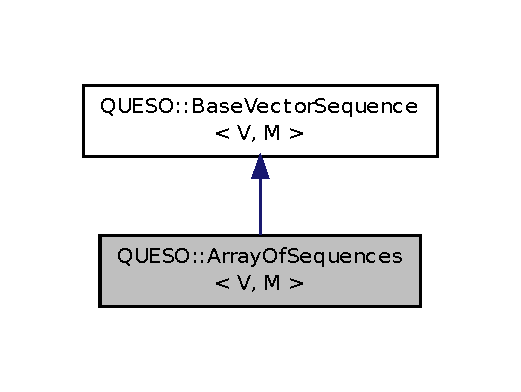
\includegraphics[width=250pt]{class_q_u_e_s_o_1_1_array_of_sequences__inherit__graph}
\end{center}
\end{figure}


Collaboration diagram for Q\-U\-E\-S\-O\-:\-:Array\-Of\-Sequences$<$ V, M $>$\-:
\nopagebreak
\begin{figure}[H]
\begin{center}
\leavevmode
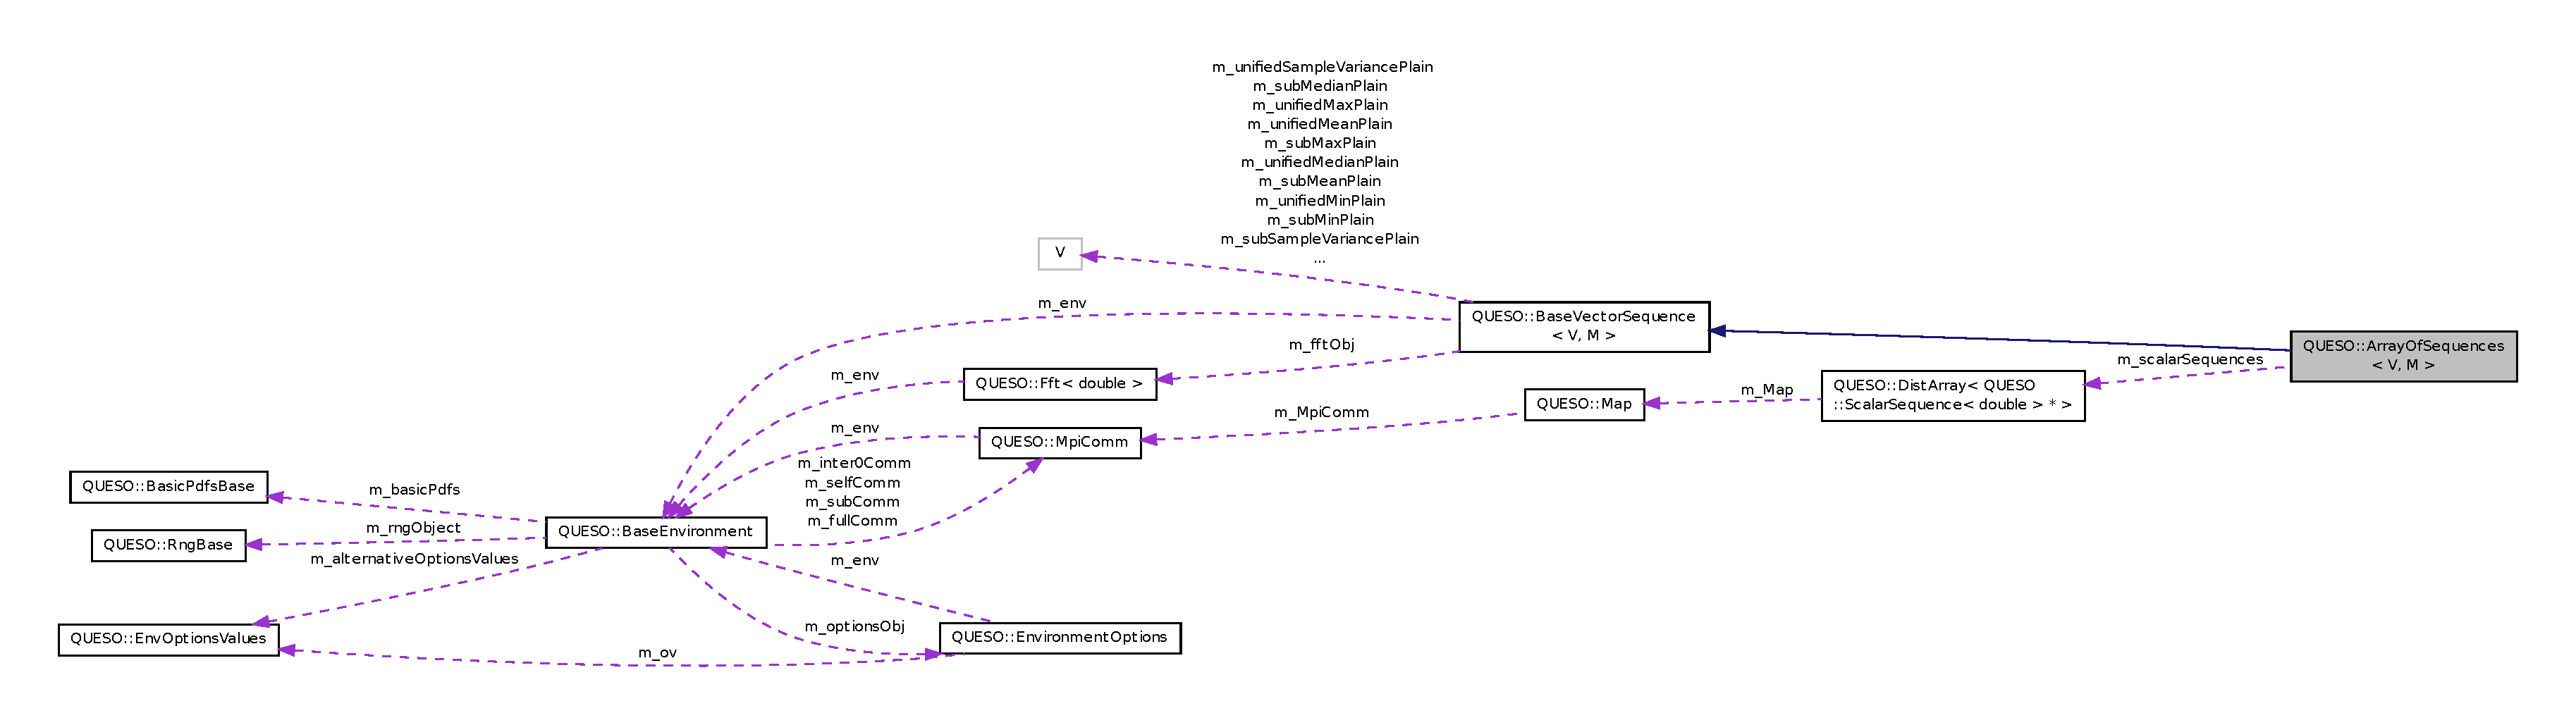
\includegraphics[width=350pt]{class_q_u_e_s_o_1_1_array_of_sequences__coll__graph}
\end{center}
\end{figure}
\subsection*{Public Member Functions}
\begin{Indent}{\bf Constructor/\-Destructor methods}\par
\begin{DoxyCompactItemize}
\item 
\hyperlink{class_q_u_e_s_o_1_1_array_of_sequences_a8b4625170975168c1cb3ee34946e564b}{Array\-Of\-Sequences} (const \hyperlink{class_q_u_e_s_o_1_1_vector_space}{Vector\-Space}$<$ V, M $>$ \&\hyperlink{class_q_u_e_s_o_1_1_base_vector_sequence_af9a4dd979a2fa8dee85bb07793b59ba2}{vector\-Space}, unsigned int \hyperlink{class_q_u_e_s_o_1_1_array_of_sequences_a007d00d2398007b9bac82ed23eedb1e2}{sub\-Sequence\-Size}, const std\-::string \&\hyperlink{class_q_u_e_s_o_1_1_base_vector_sequence_a48f6fe02cf77f4233d3bcdfef3870f19}{name})
\begin{DoxyCompactList}\small\item\em Default constructor. \end{DoxyCompactList}\item 
\hyperlink{class_q_u_e_s_o_1_1_array_of_sequences_a8632bf1a4b6cd4447694a7108a2689a7}{$\sim$\-Array\-Of\-Sequences} ()
\begin{DoxyCompactList}\small\item\em Destructor. \end{DoxyCompactList}\end{DoxyCompactItemize}
\end{Indent}
\begin{Indent}{\bf Sequence methods}\par
\begin{DoxyCompactItemize}
\item 
unsigned int \hyperlink{class_q_u_e_s_o_1_1_array_of_sequences_a007d00d2398007b9bac82ed23eedb1e2}{sub\-Sequence\-Size} () const 
\begin{DoxyCompactList}\small\item\em Size of the sub-\/sequence of arrays. \end{DoxyCompactList}\item 
void \hyperlink{class_q_u_e_s_o_1_1_array_of_sequences_a3067aa6afb3a4fd6f30dc753bbceaf9e}{resize\-Sequence} (unsigned int new\-Sub\-Sequence\-Size)
\begin{DoxyCompactList}\small\item\em Resizes the sequence. \end{DoxyCompactList}\item 
void \hyperlink{class_q_u_e_s_o_1_1_array_of_sequences_a9267060ca0e57a124d9f8ba64e60027c}{reset\-Values} (unsigned int initial\-Pos, unsigned int num\-Pos)
\begin{DoxyCompactList}\small\item\em Resets a total of {\ttfamily num\-Pos} values of the sequence starting at position {\ttfamily initial\-Pos}. \end{DoxyCompactList}\item 
void \hyperlink{class_q_u_e_s_o_1_1_array_of_sequences_a81f3ee91830b977945fa152901d4cd8e}{erase\-Positions} (unsigned int initial\-Pos, unsigned int num\-Pos)
\begin{DoxyCompactList}\small\item\em Erases {\ttfamily num\-Pos} elements of the sequence starting at position {\ttfamily initial\-Pos}. \end{DoxyCompactList}\item 
void \hyperlink{class_q_u_e_s_o_1_1_array_of_sequences_ae75a2eedab5e8d3fc0638f578eba35ab}{get\-Position\-Values} (unsigned int pos\-Id, V \&vec) const 
\begin{DoxyCompactList}\small\item\em Gets the values of the sequence at position {\ttfamily pos\-Id} and stores them at {\ttfamily vec}. \end{DoxyCompactList}\item 
void \hyperlink{class_q_u_e_s_o_1_1_array_of_sequences_a20e1732527bc5c466abf79b827407d54}{set\-Position\-Values} (unsigned int pos\-Id, const V \&vec)
\begin{DoxyCompactList}\small\item\em Set the values of {\ttfamily vec} at position {\ttfamily pos\-Id} of the sequence. \end{DoxyCompactList}\item 
void \hyperlink{class_q_u_e_s_o_1_1_array_of_sequences_a9168423928360ee9dd3d3521f5539892}{set\-Gaussian} (const V \&mean\-Vec, const V \&std\-Dev\-Vec)
\begin{DoxyCompactList}\small\item\em Sets the values of the sequence as a Gaussian distribution of mean given by {\ttfamily mean\-Vec} and standard deviation by {\ttfamily std\-Dev\-Vec}. \end{DoxyCompactList}\item 
void \hyperlink{class_q_u_e_s_o_1_1_array_of_sequences_a478f81e5a47e06074577b46b2f8fdfd1}{set\-Uniform} (const V \&a\-Vec, const V \&b\-Vec)
\begin{DoxyCompactList}\small\item\em Sets the values of the sequence as a uniform distribution between the values given by vectors {\ttfamily a\-Vec} and {\ttfamily b\-Vec}. \end{DoxyCompactList}\item 
void \hyperlink{class_q_u_e_s_o_1_1_array_of_sequences_ae9d785ccc1cbf94447efd2dae6467c3d}{mean} (unsigned int initial\-Pos, unsigned int num\-Pos, V \&mean\-Vec) const 
\begin{DoxyCompactList}\small\item\em Finds the mean value of the sub-\/sequence, considering {\ttfamily num\-Pos} positions starting at position {\ttfamily initial\-Pos}. \end{DoxyCompactList}\item 
void \hyperlink{class_q_u_e_s_o_1_1_array_of_sequences_aff464566fefc76edb13ac6f6f8f2bd31}{unified\-Mean} (unsigned int initial\-Pos, unsigned int num\-Pos, V \&unified\-Mean\-Vec) const 
\begin{DoxyCompactList}\small\item\em Finds the mean value of the unified sequence of {\ttfamily num\-Pos} positions starting at position {\ttfamily initial\-Pos}. See template specialization. \end{DoxyCompactList}\item 
void \hyperlink{class_q_u_e_s_o_1_1_array_of_sequences_a7bce5c84299185882c0bb7c6d61bce6d}{sample\-Variance} (unsigned int initial\-Pos, unsigned int num\-Pos, const V \&mean\-Vec, V \&sam\-Vec) const 
\begin{DoxyCompactList}\small\item\em Finds the sample variance of the sub-\/sequence, considering {\ttfamily num\-Pos} positions starting at position {\ttfamily initial\-Pos} and of mean {\ttfamily mean\-Vec}. \end{DoxyCompactList}\item 
void \hyperlink{class_q_u_e_s_o_1_1_array_of_sequences_a51ad92656e8b2e437982660fabb67ba3}{unified\-Sample\-Variance} (unsigned int initial\-Pos, unsigned int num\-Pos, const V \&mean\-Vec, V \&sam\-Vec) const 
\begin{DoxyCompactList}\small\item\em Finds the sample variance of the unified sequence, considering {\ttfamily num\-Pos} positions starting at position {\ttfamily initial\-Pos} and of mean {\ttfamily mean\-Vec}. \end{DoxyCompactList}\item 
void \hyperlink{class_q_u_e_s_o_1_1_array_of_sequences_a5bde372f275a51cd25c883604586d6dd}{population\-Variance} (unsigned int initial\-Pos, unsigned int num\-Pos, const V \&mean\-Vec, V \&pop\-Vec) const 
\begin{DoxyCompactList}\small\item\em Finds the population variance of the sub-\/sequence, considering {\ttfamily num\-Pos} positions starting at position {\ttfamily initial\-Pos} and of mean {\ttfamily mean\-Vec}. \end{DoxyCompactList}\item 
void \hyperlink{class_q_u_e_s_o_1_1_array_of_sequences_ac6439fcb719bad4810cfe3c020f73486}{auto\-Covariance} (unsigned int initial\-Pos, unsigned int num\-Pos, const V \&mean\-Vec, unsigned int lag, V \&cov\-Vec) const 
\begin{DoxyCompactList}\small\item\em Calculates the autocovariance. \end{DoxyCompactList}\item 
void \hyperlink{class_q_u_e_s_o_1_1_array_of_sequences_a057921bf605783c85def57f71cc2101e}{auto\-Corr\-Via\-Def} (unsigned int initial\-Pos, unsigned int num\-Pos, unsigned int lag, V \&corr\-Vec) const 
\begin{DoxyCompactList}\small\item\em Calculates autocorrelation via definition. \end{DoxyCompactList}\item 
void \hyperlink{class_q_u_e_s_o_1_1_array_of_sequences_aa0468a432b6ee77a810357d0ef3b8690}{auto\-Corr\-Via\-Fft} (unsigned int initial\-Pos, unsigned int num\-Pos, const std\-::vector$<$ unsigned int $>$ \&lags, std\-::vector$<$ V $\ast$ $>$ \&corr\-Vecs) const 
\item 
void \hyperlink{class_q_u_e_s_o_1_1_array_of_sequences_a078e43442f5b12f7a886ace29af0aec0}{auto\-Corr\-Via\-Fft} (unsigned int initial\-Pos, unsigned int num\-Pos, unsigned int num\-Sum, V \&auto\-Corrs\-Sum\-Vec) const 
\item 
void \hyperlink{class_q_u_e_s_o_1_1_array_of_sequences_af318beb944a58dcb7b36a645f84edd3f}{min\-Max} (unsigned int initial\-Pos, V \&min\-Vec, V \&max\-Vec) const 
\begin{DoxyCompactList}\small\item\em Given an initial position {\ttfamily initial\-Pos}, finds the minimum and the maximum values of the sequence. \end{DoxyCompactList}\item 
void \hyperlink{class_q_u_e_s_o_1_1_array_of_sequences_a2beb77e521581b8c28d1fe0fe71018c6}{histogram} (unsigned int initial\-Pos, const V \&min\-Vec, const V \&max\-Vec, std\-::vector$<$ V $\ast$ $>$ \&centers\-For\-All\-Bins, std\-::vector$<$ V $\ast$ $>$ \&quantts\-For\-All\-Bins) const 
\begin{DoxyCompactList}\small\item\em Calculates the histogram of the sequence. \end{DoxyCompactList}\item 
void \hyperlink{class_q_u_e_s_o_1_1_array_of_sequences_a6cd1021725aa1d7e50034f482904660a}{inter\-Quantile\-Range} (unsigned int initial\-Pos, V \&iqrs) const 
\begin{DoxyCompactList}\small\item\em Returns the interquartile range of the values in the sequence. \end{DoxyCompactList}\item 
void \hyperlink{class_q_u_e_s_o_1_1_array_of_sequences_ae746fcec9567a5ef3c46f5559c90dee7}{scales\-For\-K\-D\-E} (unsigned int initial\-Pos, const V \&iqrs, unsigned int kde\-Dimension, V \&scales) const 
\begin{DoxyCompactList}\small\item\em Selects the scales (bandwidth, {\ttfamily scale\-Vec}) for the kernel density estimation, of the sequence. \end{DoxyCompactList}\item 
void \hyperlink{class_q_u_e_s_o_1_1_array_of_sequences_ade11b2ce02c1b7501a1c465dcfe63a1d}{gaussian\-K\-D\-E} (const V \&evaluation\-Param\-Vec, V \&density\-Vec) const 
\begin{DoxyCompactList}\small\item\em Gaussian kernel for the K\-D\-E estimate of the sequence. \end{DoxyCompactList}\item 
void \hyperlink{class_q_u_e_s_o_1_1_array_of_sequences_a221a49bf0e054276007dde487dbedfe6}{gaussian\-K\-D\-E} (unsigned int initial\-Pos, const V \&scales, const std\-::vector$<$ V $\ast$ $>$ \&evaluation\-Param\-Vecs, std\-::vector$<$ V $\ast$ $>$ \&density\-Vecs) const 
\begin{DoxyCompactList}\small\item\em T\-O\-D\-O\-: Gaussian kernel for the K\-D\-E of the sequence. \end{DoxyCompactList}\item 
void \hyperlink{class_q_u_e_s_o_1_1_array_of_sequences_a4b1248fe9601ec598797071210760687}{write\-Contents} (std\-::ofstream \&ofsvar) const 
\begin{DoxyCompactList}\small\item\em Write contents of the chain to a file. \end{DoxyCompactList}\item 
void \hyperlink{class_q_u_e_s_o_1_1_array_of_sequences_a20727ea1cc87e2cf81802b7e07eae35f}{unified\-Write\-Contents} (std\-::ofstream \&ofsvar) const 
\begin{DoxyCompactList}\small\item\em Writes info of the unified sequence to a file. \end{DoxyCompactList}\item 
void \hyperlink{class_q_u_e_s_o_1_1_array_of_sequences_af4ab2f575230715be16fff5ae9bb4759}{unified\-Write\-Contents} (const std\-::string \&file\-Name, const std\-::string \&file\-Type) const 
\begin{DoxyCompactList}\small\item\em Writes info of the unified sequence to a file. \end{DoxyCompactList}\item 
void \hyperlink{class_q_u_e_s_o_1_1_array_of_sequences_a3fbe0f679fa8828e27dadb89a9fe3eaa}{unified\-Read\-Contents} (const std\-::string \&file\-Name, const std\-::string \&file\-Type, const unsigned int \hyperlink{class_q_u_e_s_o_1_1_array_of_sequences_a007d00d2398007b9bac82ed23eedb1e2}{sub\-Sequence\-Size})
\begin{DoxyCompactList}\small\item\em Reads the unified sequence from a file. \end{DoxyCompactList}\item 
void \hyperlink{class_q_u_e_s_o_1_1_array_of_sequences_a643996eaf9db7e40a423c06ae5cb881a}{select} (const std\-::vector$<$ unsigned int $>$ \&ids\-Of\-Unique\-Positions)
\begin{DoxyCompactList}\small\item\em Select positions in the sequence of vectors. \end{DoxyCompactList}\item 
void \hyperlink{class_q_u_e_s_o_1_1_array_of_sequences_a7c95d24764af395fdff5c9d0c987e694}{filter} (unsigned int initial\-Pos, unsigned int spacing)
\begin{DoxyCompactList}\small\item\em Filters positions in the sequence of vectors, starting at {\ttfamily initial\-Pos}, and with spacing given by {\ttfamily spacing}. \end{DoxyCompactList}\item 
void \hyperlink{class_q_u_e_s_o_1_1_array_of_sequences_ab529b77aca8e169b1b769051e7de8c3d}{extract\-Scalar\-Seq} (unsigned int initial\-Pos, unsigned int spacing, unsigned int num\-Pos, unsigned int param\-Id, \hyperlink{class_q_u_e_s_o_1_1_scalar_sequence}{Scalar\-Sequence}$<$ double $>$ \&scalar\-Seq) const 
\begin{DoxyCompactList}\small\item\em Extracts a sequence of scalars of size {\ttfamily num\-Pos}, from position {\ttfamily param\-Id} of the array of sequences. \end{DoxyCompactList}\end{DoxyCompactItemize}
\end{Indent}
\subsection*{Private Member Functions}
\begin{DoxyCompactItemize}
\item 
void \hyperlink{class_q_u_e_s_o_1_1_array_of_sequences_a615df4add2396b94f5a4be3a5eb971fb}{extract\-Raw\-Data} (unsigned int initial\-Pos, unsigned int spacing, unsigned int num\-Pos, unsigned int param\-Id, std\-::vector$<$ double $>$ \&raw\-Data) const 
\begin{DoxyCompactList}\small\item\em Extracts the raw data. \end{DoxyCompactList}\end{DoxyCompactItemize}
\subsection*{Private Attributes}
\begin{DoxyCompactItemize}
\item 
\hyperlink{class_q_u_e_s_o_1_1_dist_array}{Dist\-Array}$<$ \hyperlink{class_q_u_e_s_o_1_1_scalar_sequence}{Scalar\-Sequence}\\*
$<$ double $>$ $\ast$ $>$ \hyperlink{class_q_u_e_s_o_1_1_array_of_sequences_a1f8047145ca75081c303bbbab5881119}{m\-\_\-scalar\-Sequences}
\begin{DoxyCompactList}\small\item\em Sequence of scalars. \end{DoxyCompactList}\end{DoxyCompactItemize}
\subsection*{Additional Inherited Members}


\subsection{Detailed Description}
\subsubsection*{template$<$class V, class M$>$class Q\-U\-E\-S\-O\-::\-Array\-Of\-Sequences$<$ V, M $>$}

Class for handling array samples (arrays of scalar sequences). 

This class handles array of sequences (samples) generated by an algorithm, as well as operations that can be carried over them, e.\-g., calculation of means, correlation and covariance matrices. It is derived from and implements Base\-Vector\-Sequence$<$\-V,\-M$>$. 

Definition at line 44 of file Array\-Of\-Sequences.\-h.



\subsection{Constructor \& Destructor Documentation}
\hypertarget{class_q_u_e_s_o_1_1_array_of_sequences_a8b4625170975168c1cb3ee34946e564b}{\index{Q\-U\-E\-S\-O\-::\-Array\-Of\-Sequences@{Q\-U\-E\-S\-O\-::\-Array\-Of\-Sequences}!Array\-Of\-Sequences@{Array\-Of\-Sequences}}
\index{Array\-Of\-Sequences@{Array\-Of\-Sequences}!QUESO::ArrayOfSequences@{Q\-U\-E\-S\-O\-::\-Array\-Of\-Sequences}}
\subsubsection[{Array\-Of\-Sequences}]{\setlength{\rightskip}{0pt plus 5cm}template$<$class V , class M $>$ {\bf Q\-U\-E\-S\-O\-::\-Array\-Of\-Sequences}$<$ V, M $>$\-::{\bf Array\-Of\-Sequences} (
\begin{DoxyParamCaption}
\item[{const {\bf Vector\-Space}$<$ V, M $>$ \&}]{vector\-Space, }
\item[{unsigned int}]{sub\-Sequence\-Size, }
\item[{const std\-::string \&}]{name}
\end{DoxyParamCaption}
)}}\label{class_q_u_e_s_o_1_1_array_of_sequences_a8b4625170975168c1cb3ee34946e564b}


Default constructor. 



Definition at line 32 of file Array\-Of\-Sequences.\-C.



References Q\-U\-E\-S\-O\-::\-Base\-Vector\-Sequence$<$ V, M $>$\-::m\-\_\-env, Q\-U\-E\-S\-O\-::\-Array\-Of\-Sequences$<$ V, M $>$\-::m\-\_\-scalar\-Sequences, and Q\-U\-E\-S\-O\-::\-Array\-Of\-Sequences$<$ V, M $>$\-::sub\-Sequence\-Size().


\begin{DoxyCode}
35     : BaseVectorSequence<V,M>(\hyperlink{class_q_u_e_s_o_1_1_base_vector_sequence_af9a4dd979a2fa8dee85bb07793b59ba2}{vectorSpace},\hyperlink{class_q_u_e_s_o_1_1_array_of_sequences_a007d00d2398007b9bac82ed23eedb1e2}{subSequenceSize},
      \hyperlink{class_q_u_e_s_o_1_1_base_vector_sequence_a48f6fe02cf77f4233d3bcdfef3870f19}{name}),
36       \hyperlink{class_q_u_e_s_o_1_1_array_of_sequences_a1f8047145ca75081c303bbbab5881119}{m\_scalarSequences}(\hyperlink{class_q_u_e_s_o_1_1_base_vector_sequence_a4bd171e39ed050ff105c808336f35198}{m\_vectorSpace}.map(),1)
37 \{
38 
39   \textcolor{comment}{//if (m\_env.subDisplayFile()) \{}
40   \textcolor{comment}{//  *m\_env.subDisplayFile() << "Entering ArrayOfSequences<V,M>::constructor()"}
41   \textcolor{comment}{//                         << std::endl;}
42   \textcolor{comment}{//\}}
43 
44   \textcolor{comment}{//if (m\_env.subDisplayFile()) \{}
45   \textcolor{comment}{//  *m\_env.subDisplayFile() << "In ArrayOfSequences<V,M>::constructor()"}
46   \textcolor{comment}{//                         << "\(\backslash\)n subSequenceSize = "              << subSequenceSize}
47   \textcolor{comment}{//                         << "\(\backslash\)n m\_scalarSequences.MyLength() = " << m\_scalarSequences.MyLength()}
48   \textcolor{comment}{//                         << std::endl;}
49   \textcolor{comment}{//\}}
50 
51   \textcolor{keywordflow}{for} (\textcolor{keywordtype}{unsigned} \textcolor{keywordtype}{int} i = 0; i < (\textcolor{keywordtype}{unsigned} int) \hyperlink{class_q_u_e_s_o_1_1_array_of_sequences_a1f8047145ca75081c303bbbab5881119}{m\_scalarSequences}.MyLength(); ++i) \{
52     \hyperlink{class_q_u_e_s_o_1_1_array_of_sequences_a1f8047145ca75081c303bbbab5881119}{m\_scalarSequences}(i,0) = \textcolor{keyword}{new} ScalarSequence<double>(\hyperlink{class_q_u_e_s_o_1_1_base_vector_sequence_a8e8824d2a63c5a43bcc6473e3a0491e8}{m\_env},
      \hyperlink{class_q_u_e_s_o_1_1_array_of_sequences_a007d00d2398007b9bac82ed23eedb1e2}{subSequenceSize});
53   \}
54 
55   \textcolor{comment}{//if (m\_env.subDisplayFile()) \{}
56   \textcolor{comment}{//  *m\_env.subDisplayFile() << "Leaving ArrayOfSequences<V,M>::constructor()"}
57   \textcolor{comment}{//                         << std::endl;}
58   \textcolor{comment}{//\}}
59 \}
\end{DoxyCode}
\hypertarget{class_q_u_e_s_o_1_1_array_of_sequences_a8632bf1a4b6cd4447694a7108a2689a7}{\index{Q\-U\-E\-S\-O\-::\-Array\-Of\-Sequences@{Q\-U\-E\-S\-O\-::\-Array\-Of\-Sequences}!$\sim$\-Array\-Of\-Sequences@{$\sim$\-Array\-Of\-Sequences}}
\index{$\sim$\-Array\-Of\-Sequences@{$\sim$\-Array\-Of\-Sequences}!QUESO::ArrayOfSequences@{Q\-U\-E\-S\-O\-::\-Array\-Of\-Sequences}}
\subsubsection[{$\sim$\-Array\-Of\-Sequences}]{\setlength{\rightskip}{0pt plus 5cm}template$<$class V , class M $>$ {\bf Q\-U\-E\-S\-O\-::\-Array\-Of\-Sequences}$<$ V, M $>$\-::$\sim${\bf Array\-Of\-Sequences} (
\begin{DoxyParamCaption}
{}
\end{DoxyParamCaption}
)}}\label{class_q_u_e_s_o_1_1_array_of_sequences_a8632bf1a4b6cd4447694a7108a2689a7}


Destructor. 



Definition at line 63 of file Array\-Of\-Sequences.\-C.


\begin{DoxyCode}
64 \{
65   \textcolor{keywordflow}{for} (\textcolor{keywordtype}{unsigned} \textcolor{keywordtype}{int} i = 0; i < (\textcolor{keywordtype}{unsigned} int) \hyperlink{class_q_u_e_s_o_1_1_array_of_sequences_a1f8047145ca75081c303bbbab5881119}{m\_scalarSequences}.MyLength(); ++i) \{
66     \textcolor{keywordflow}{if} (\hyperlink{class_q_u_e_s_o_1_1_array_of_sequences_a1f8047145ca75081c303bbbab5881119}{m\_scalarSequences}(i,0)) \textcolor{keyword}{delete} \hyperlink{class_q_u_e_s_o_1_1_array_of_sequences_a1f8047145ca75081c303bbbab5881119}{m\_scalarSequences}(i,0);
67   \}
68 \}
\end{DoxyCode}


\subsection{Member Function Documentation}
\hypertarget{class_q_u_e_s_o_1_1_array_of_sequences_a057921bf605783c85def57f71cc2101e}{\index{Q\-U\-E\-S\-O\-::\-Array\-Of\-Sequences@{Q\-U\-E\-S\-O\-::\-Array\-Of\-Sequences}!auto\-Corr\-Via\-Def@{auto\-Corr\-Via\-Def}}
\index{auto\-Corr\-Via\-Def@{auto\-Corr\-Via\-Def}!QUESO::ArrayOfSequences@{Q\-U\-E\-S\-O\-::\-Array\-Of\-Sequences}}
\subsubsection[{auto\-Corr\-Via\-Def}]{\setlength{\rightskip}{0pt plus 5cm}template$<$class V , class M $>$ void {\bf Q\-U\-E\-S\-O\-::\-Array\-Of\-Sequences}$<$ V, M $>$\-::auto\-Corr\-Via\-Def (
\begin{DoxyParamCaption}
\item[{unsigned int}]{initial\-Pos, }
\item[{unsigned int}]{num\-Pos, }
\item[{unsigned int}]{lag, }
\item[{V \&}]{corr\-Vec}
\end{DoxyParamCaption}
) const\hspace{0.3cm}{\ttfamily [virtual]}}}\label{class_q_u_e_s_o_1_1_array_of_sequences_a057921bf605783c85def57f71cc2101e}


Calculates autocorrelation via definition. 



Implements \hyperlink{class_q_u_e_s_o_1_1_base_vector_sequence_ab4d322b34c43ad47df9a76582a0693d0}{Q\-U\-E\-S\-O\-::\-Base\-Vector\-Sequence$<$ V, M $>$}.



Definition at line 346 of file Array\-Of\-Sequences.\-C.


\begin{DoxyCode}
350 \{
351   V subChainMean              (\hyperlink{class_q_u_e_s_o_1_1_base_vector_sequence_a4bd171e39ed050ff105c808336f35198}{m\_vectorSpace}.zeroVector());
352   V subChainAutoCovarianceLag0(\hyperlink{class_q_u_e_s_o_1_1_base_vector_sequence_a4bd171e39ed050ff105c808336f35198}{m\_vectorSpace}.zeroVector());
353 
354   this->\hyperlink{class_q_u_e_s_o_1_1_array_of_sequences_ae9d785ccc1cbf94447efd2dae6467c3d}{mean}(initialPos,
355              numPos,
356              subChainMean);
357   this->\hyperlink{class_q_u_e_s_o_1_1_array_of_sequences_ac6439fcb719bad4810cfe3c020f73486}{autoCovariance}(initialPos,
358                        numPos,
359                        subChainMean,
360                        0, \textcolor{comment}{// lag}
361                        subChainAutoCovarianceLag0);
362 
363   this->\hyperlink{class_q_u_e_s_o_1_1_array_of_sequences_ac6439fcb719bad4810cfe3c020f73486}{autoCovariance}(initialPos,
364                        numPos,
365                        subChainMean,
366                        lag,
367                        corrVec);
368   corrVec /= subChainAutoCovarianceLag0; 
369 
370   \textcolor{keywordflow}{return};
371 \}
\end{DoxyCode}
\hypertarget{class_q_u_e_s_o_1_1_array_of_sequences_aa0468a432b6ee77a810357d0ef3b8690}{\index{Q\-U\-E\-S\-O\-::\-Array\-Of\-Sequences@{Q\-U\-E\-S\-O\-::\-Array\-Of\-Sequences}!auto\-Corr\-Via\-Fft@{auto\-Corr\-Via\-Fft}}
\index{auto\-Corr\-Via\-Fft@{auto\-Corr\-Via\-Fft}!QUESO::ArrayOfSequences@{Q\-U\-E\-S\-O\-::\-Array\-Of\-Sequences}}
\subsubsection[{auto\-Corr\-Via\-Fft}]{\setlength{\rightskip}{0pt plus 5cm}template$<$class V , class M $>$ void {\bf Q\-U\-E\-S\-O\-::\-Array\-Of\-Sequences}$<$ V, M $>$\-::auto\-Corr\-Via\-Fft (
\begin{DoxyParamCaption}
\item[{unsigned int}]{initial\-Pos, }
\item[{unsigned int}]{num\-Pos, }
\item[{const std\-::vector$<$ unsigned int $>$ \&}]{lags, }
\item[{std\-::vector$<$ V $\ast$ $>$ \&}]{corr\-Vecs}
\end{DoxyParamCaption}
) const\hspace{0.3cm}{\ttfamily [virtual]}}}\label{class_q_u_e_s_o_1_1_array_of_sequences_aa0468a432b6ee77a810357d0ef3b8690}
Calculates autocorrelation via Fast Fourier transforms (F\-F\-T). T\-O\-D\-O\-: Implement me! 

Implements \hyperlink{class_q_u_e_s_o_1_1_base_vector_sequence_a709a63b678508c47bedd416ece5342ef}{Q\-U\-E\-S\-O\-::\-Base\-Vector\-Sequence$<$ V, M $>$}.



Definition at line 374 of file Array\-Of\-Sequences.\-C.


\begin{DoxyCode}
378 \{
379   \textcolor{keywordflow}{return};
380 \}
\end{DoxyCode}
\hypertarget{class_q_u_e_s_o_1_1_array_of_sequences_a078e43442f5b12f7a886ace29af0aec0}{\index{Q\-U\-E\-S\-O\-::\-Array\-Of\-Sequences@{Q\-U\-E\-S\-O\-::\-Array\-Of\-Sequences}!auto\-Corr\-Via\-Fft@{auto\-Corr\-Via\-Fft}}
\index{auto\-Corr\-Via\-Fft@{auto\-Corr\-Via\-Fft}!QUESO::ArrayOfSequences@{Q\-U\-E\-S\-O\-::\-Array\-Of\-Sequences}}
\subsubsection[{auto\-Corr\-Via\-Fft}]{\setlength{\rightskip}{0pt plus 5cm}template$<$class V , class M $>$ void {\bf Q\-U\-E\-S\-O\-::\-Array\-Of\-Sequences}$<$ V, M $>$\-::auto\-Corr\-Via\-Fft (
\begin{DoxyParamCaption}
\item[{unsigned int}]{initial\-Pos, }
\item[{unsigned int}]{num\-Pos, }
\item[{unsigned int}]{num\-Sum, }
\item[{V \&}]{auto\-Corrs\-Sum\-Vec}
\end{DoxyParamCaption}
) const\hspace{0.3cm}{\ttfamily [virtual]}}}\label{class_q_u_e_s_o_1_1_array_of_sequences_a078e43442f5b12f7a886ace29af0aec0}
Calculates autocorrelation via Fast Fourier transforms (F\-F\-T). T\-O\-D\-O\-: Implement me! 

Implements \hyperlink{class_q_u_e_s_o_1_1_base_vector_sequence_af9f2478ed4112aa615caef21bf26ab35}{Q\-U\-E\-S\-O\-::\-Base\-Vector\-Sequence$<$ V, M $>$}.



Definition at line 383 of file Array\-Of\-Sequences.\-C.



References U\-Q\-\_\-\-F\-A\-T\-A\-L\-\_\-\-T\-E\-S\-T\-\_\-\-M\-A\-C\-R\-O.


\begin{DoxyCode}
387 \{
388 \textcolor{preprocessor}{#if 0}
389 \textcolor{preprocessor}{}  \textcolor{keywordtype}{bool} bRC = ((initialPos             <  this->\hyperlink{class_q_u_e_s_o_1_1_array_of_sequences_a007d00d2398007b9bac82ed23eedb1e2}{subSequenceSize}()) &&
390               (0                      <  numPos                 ) &&
391               ((initialPos+numPos)    <= this->\hyperlink{class_q_u_e_s_o_1_1_array_of_sequences_a007d00d2398007b9bac82ed23eedb1e2}{subSequenceSize}()) &&
392               (autoCorrsSumVec.size() == this->vectorSize()     ));
393   \hyperlink{_defines_8h_a56d63d18d0a6d45757de47fcc06f574d}{UQ\_FATAL\_TEST\_MACRO}(bRC == \textcolor{keyword}{false},
394                       \hyperlink{class_q_u_e_s_o_1_1_base_vector_sequence_a8e8824d2a63c5a43bcc6473e3a0491e8}{m\_env}.\hyperlink{class_q_u_e_s_o_1_1_base_environment_a78b57112bbd0e6dd0e8afec00b40ffa7}{worldRank}(),
395                       \textcolor{stringliteral}{"ArrayOfSequences<V,M>::autoCorrViaFft(), for sum"},
396                       \textcolor{stringliteral}{"invalid input data"});
397 
398   ScalarSequence<double> data(\hyperlink{class_q_u_e_s_o_1_1_base_vector_sequence_a8e8824d2a63c5a43bcc6473e3a0491e8}{m\_env},0);
399 
400   \textcolor{keywordtype}{unsigned} \textcolor{keywordtype}{int} numParams = this->vectorSize();
401   \textcolor{keywordflow}{for} (\textcolor{keywordtype}{unsigned} \textcolor{keywordtype}{int} i = 0; i < numParams; ++i) \{
402     this->\hyperlink{class_q_u_e_s_o_1_1_array_of_sequences_ab529b77aca8e169b1b769051e7de8c3d}{extractScalarSeq}(initialPos,
403                            1, \textcolor{comment}{// spacing}
404                            numPos,
405                            i,
406                            data);
407 
408     data.autoCorrViaFft(0,
409                         numPos,
410                         autoCorrsSumVec[i]);
411   \}
412 \textcolor{preprocessor}{#endif}
413 \textcolor{preprocessor}{}  \textcolor{keywordflow}{return};
414 \}
\end{DoxyCode}
\hypertarget{class_q_u_e_s_o_1_1_array_of_sequences_ac6439fcb719bad4810cfe3c020f73486}{\index{Q\-U\-E\-S\-O\-::\-Array\-Of\-Sequences@{Q\-U\-E\-S\-O\-::\-Array\-Of\-Sequences}!auto\-Covariance@{auto\-Covariance}}
\index{auto\-Covariance@{auto\-Covariance}!QUESO::ArrayOfSequences@{Q\-U\-E\-S\-O\-::\-Array\-Of\-Sequences}}
\subsubsection[{auto\-Covariance}]{\setlength{\rightskip}{0pt plus 5cm}template$<$class V , class M $>$ void {\bf Q\-U\-E\-S\-O\-::\-Array\-Of\-Sequences}$<$ V, M $>$\-::auto\-Covariance (
\begin{DoxyParamCaption}
\item[{unsigned int}]{initial\-Pos, }
\item[{unsigned int}]{num\-Pos, }
\item[{const V \&}]{mean\-Vec, }
\item[{unsigned int}]{lag, }
\item[{V \&}]{cov\-Vec}
\end{DoxyParamCaption}
) const\hspace{0.3cm}{\ttfamily [virtual]}}}\label{class_q_u_e_s_o_1_1_array_of_sequences_ac6439fcb719bad4810cfe3c020f73486}


Calculates the autocovariance. 

The autocovariance is the covariance of a variable with itself at some other time. It is calculated over a sequence of arrays with initial position {\ttfamily initial\-Pos}, considering {\ttfamily num\-Pos} positions, a lag of {\ttfamily lag}, with mean given by {\ttfamily mean\-Vec}. The results are saved in the output vector {\ttfamily cov\-Vec/} 

Implements \hyperlink{class_q_u_e_s_o_1_1_base_vector_sequence_a3a831c06c8ede53b84ce72fac3f018c0}{Q\-U\-E\-S\-O\-::\-Base\-Vector\-Sequence$<$ V, M $>$}.



Definition at line 292 of file Array\-Of\-Sequences.\-C.



References Q\-U\-E\-S\-O\-::\-Array\-Of\-Sequences$<$ V, M $>$\-::m\-\_\-scalar\-Sequences, and U\-Q\-\_\-\-F\-A\-T\-A\-L\-\_\-\-T\-E\-S\-T\-\_\-\-M\-A\-C\-R\-O.


\begin{DoxyCode}
297 \{
298   \textcolor{keywordtype}{bool} bRC = ((0                     <= initialPos                 ) &&
299               (0                     <  numPos                     ) &&
300               ((initialPos+numPos-1) <= (this->\hyperlink{class_q_u_e_s_o_1_1_array_of_sequences_a007d00d2398007b9bac82ed23eedb1e2}{subSequenceSize}()-1)));
301   \hyperlink{_defines_8h_a56d63d18d0a6d45757de47fcc06f574d}{UQ\_FATAL\_TEST\_MACRO}(bRC == \textcolor{keyword}{false},
302                       \hyperlink{class_q_u_e_s_o_1_1_base_vector_sequence_a8e8824d2a63c5a43bcc6473e3a0491e8}{m\_env}.\hyperlink{class_q_u_e_s_o_1_1_base_environment_a78b57112bbd0e6dd0e8afec00b40ffa7}{worldRank}(),
303                       \textcolor{stringliteral}{"VectorSequenceAutoCovariance<V,M>()"},
304                       \textcolor{stringliteral}{"invalid initial position or number of positions"});
305 
306   bRC = (numPos > lag);
307   \hyperlink{_defines_8h_a56d63d18d0a6d45757de47fcc06f574d}{UQ\_FATAL\_TEST\_MACRO}(bRC == \textcolor{keyword}{false},
308                       \hyperlink{class_q_u_e_s_o_1_1_base_vector_sequence_a8e8824d2a63c5a43bcc6473e3a0491e8}{m\_env}.\hyperlink{class_q_u_e_s_o_1_1_base_environment_a78b57112bbd0e6dd0e8afec00b40ffa7}{worldRank}(),
309                       \textcolor{stringliteral}{"VectorSequenceAutoCovariance<V,M>()"},
310                       \textcolor{stringliteral}{"lag is too large"});
311 
312   bRC = (this->vectorSize() == covVec.size());
313   \hyperlink{_defines_8h_a56d63d18d0a6d45757de47fcc06f574d}{UQ\_FATAL\_TEST\_MACRO}(bRC == \textcolor{keyword}{false},
314                       \hyperlink{class_q_u_e_s_o_1_1_base_vector_sequence_a8e8824d2a63c5a43bcc6473e3a0491e8}{m\_env}.\hyperlink{class_q_u_e_s_o_1_1_base_environment_a78b57112bbd0e6dd0e8afec00b40ffa7}{worldRank}(),
315                       \textcolor{stringliteral}{"VectorSequenceAutoCovariance<V,M>()"},
316                       \textcolor{stringliteral}{"incompatible sizes between covVec vector and vectors in sequence"});
317 
318   bRC = (this->vectorSize() == meanVec.size());
319   \hyperlink{_defines_8h_a56d63d18d0a6d45757de47fcc06f574d}{UQ\_FATAL\_TEST\_MACRO}(bRC == \textcolor{keyword}{false},
320                       \hyperlink{class_q_u_e_s_o_1_1_base_vector_sequence_a8e8824d2a63c5a43bcc6473e3a0491e8}{m\_env}.\hyperlink{class_q_u_e_s_o_1_1_base_environment_a78b57112bbd0e6dd0e8afec00b40ffa7}{worldRank}(),
321                       \textcolor{stringliteral}{"VectorSequenceAutoCovariance<V,M>()"},
322                       \textcolor{stringliteral}{"incompatible sizes between meanVec vector and vectors in sequence"});
323 
324   \textcolor{keywordtype}{unsigned} \textcolor{keywordtype}{int} loopSize      = numPos - lag;
325   \textcolor{keywordtype}{unsigned} \textcolor{keywordtype}{int} finalPosPlus1 = initialPos + loopSize;
326   \textcolor{keywordtype}{double} doubleLoopSize = (double) loopSize;
327   covVec.cwSet(0.);
328 
329   ArrayOfSequences<V,M>* tmp = \textcolor{keyword}{const\_cast<}ArrayOfSequences<V,M>*\textcolor{keyword}{>}(\textcolor{keyword}{this});
330   \textcolor{keywordflow}{for} (\textcolor{keywordtype}{unsigned} \textcolor{keywordtype}{int} i = 0; i < covVec.size(); ++i) \{
331     \textcolor{keyword}{const} ScalarSequence<double>& seq = *(tmp->m\_scalarSequences(i,0));
332     \textcolor{keywordtype}{double} meanValue = meanVec[i];
333     \textcolor{keywordtype}{double} result = 0;
334     \textcolor{keywordflow}{for} (\textcolor{keywordtype}{unsigned} \textcolor{keywordtype}{int} j = initialPos; j < finalPosPlus1; ++j) \{
335       \textcolor{keywordtype}{double} diff1 = seq[j]     - meanValue;
336       \textcolor{keywordtype}{double} diff2 = seq[j+lag] - meanValue;
337       result += diff1*diff2;
338     \}
339     covVec[i] = result/doubleLoopSize;
340   \}
341 
342   \textcolor{keywordflow}{return};
343 \}
\end{DoxyCode}
\hypertarget{class_q_u_e_s_o_1_1_array_of_sequences_a81f3ee91830b977945fa152901d4cd8e}{\index{Q\-U\-E\-S\-O\-::\-Array\-Of\-Sequences@{Q\-U\-E\-S\-O\-::\-Array\-Of\-Sequences}!erase\-Positions@{erase\-Positions}}
\index{erase\-Positions@{erase\-Positions}!QUESO::ArrayOfSequences@{Q\-U\-E\-S\-O\-::\-Array\-Of\-Sequences}}
\subsubsection[{erase\-Positions}]{\setlength{\rightskip}{0pt plus 5cm}template$<$class V , class M $>$ void {\bf Q\-U\-E\-S\-O\-::\-Array\-Of\-Sequences}$<$ V, M $>$\-::erase\-Positions (
\begin{DoxyParamCaption}
\item[{unsigned int}]{initial\-Pos, }
\item[{unsigned int}]{num\-Pos}
\end{DoxyParamCaption}
)\hspace{0.3cm}{\ttfamily [virtual]}}}\label{class_q_u_e_s_o_1_1_array_of_sequences_a81f3ee91830b977945fa152901d4cd8e}


Erases {\ttfamily num\-Pos} elements of the sequence starting at position {\ttfamily initial\-Pos}. 

This routine deletes all stored computed vectors 

Implements \hyperlink{class_q_u_e_s_o_1_1_base_vector_sequence_a2b41ed436f95a1816a811fc368adaf79}{Q\-U\-E\-S\-O\-::\-Base\-Vector\-Sequence$<$ V, M $>$}.



Definition at line 106 of file Array\-Of\-Sequences.\-C.



References Q\-U\-E\-S\-O\-::\-Base\-Vector\-Sequence$<$ V, M $>$\-::delete\-Stored\-Vectors(), and Q\-U\-E\-S\-O\-::\-Scalar\-Sequence$<$ T $>$\-::erase\-Positions().


\begin{DoxyCode}
108 \{
109   \textcolor{keywordflow}{if} (initialPos < this->\hyperlink{class_q_u_e_s_o_1_1_array_of_sequences_a007d00d2398007b9bac82ed23eedb1e2}{subSequenceSize}()) \{
110     \textcolor{keywordflow}{for} (\textcolor{keywordtype}{unsigned} \textcolor{keywordtype}{int} i = 0; i < (\textcolor{keywordtype}{unsigned} int) \hyperlink{class_q_u_e_s_o_1_1_array_of_sequences_a1f8047145ca75081c303bbbab5881119}{m\_scalarSequences}.MyLength(); ++i) \{
111       ScalarSequence<double>& seq = *(\hyperlink{class_q_u_e_s_o_1_1_array_of_sequences_a1f8047145ca75081c303bbbab5881119}{m\_scalarSequences}(i,0));
112       seq.erasePositions(initialPos,numPos);
113     \}
114   \}
115 
116   \hyperlink{class_q_u_e_s_o_1_1_base_vector_sequence_a5609e02046ba555f0eebe49c6c231faf}{BaseVectorSequence<V,M>::deleteStoredVectors}();
117 
118   \textcolor{keywordflow}{return};
119 \}
\end{DoxyCode}
\hypertarget{class_q_u_e_s_o_1_1_array_of_sequences_a615df4add2396b94f5a4be3a5eb971fb}{\index{Q\-U\-E\-S\-O\-::\-Array\-Of\-Sequences@{Q\-U\-E\-S\-O\-::\-Array\-Of\-Sequences}!extract\-Raw\-Data@{extract\-Raw\-Data}}
\index{extract\-Raw\-Data@{extract\-Raw\-Data}!QUESO::ArrayOfSequences@{Q\-U\-E\-S\-O\-::\-Array\-Of\-Sequences}}
\subsubsection[{extract\-Raw\-Data}]{\setlength{\rightskip}{0pt plus 5cm}template$<$class V , class M $>$ void {\bf Q\-U\-E\-S\-O\-::\-Array\-Of\-Sequences}$<$ V, M $>$\-::extract\-Raw\-Data (
\begin{DoxyParamCaption}
\item[{unsigned int}]{initial\-Pos, }
\item[{unsigned int}]{spacing, }
\item[{unsigned int}]{num\-Pos, }
\item[{unsigned int}]{param\-Id, }
\item[{std\-::vector$<$ double $>$ \&}]{raw\-Data}
\end{DoxyParamCaption}
) const\hspace{0.3cm}{\ttfamily [private]}, {\ttfamily [virtual]}}}\label{class_q_u_e_s_o_1_1_array_of_sequences_a615df4add2396b94f5a4be3a5eb971fb}


Extracts the raw data. 

Extracts the data from sequence of array at position {\ttfamily param\-Id}, with spacing {\ttfamily spacing}, and saves is in {\ttfamily raw\-Data}. The vector {\ttfamily raw\-Data} will have size {\ttfamily num\-Pos}. Note that, in fact, {\ttfamily spacing} = 1. 

Implements \hyperlink{class_q_u_e_s_o_1_1_base_vector_sequence_aae5259810d72d393328369d8d4087d5d}{Q\-U\-E\-S\-O\-::\-Base\-Vector\-Sequence$<$ V, M $>$}.



Definition at line 673 of file Array\-Of\-Sequences.\-C.



References Q\-U\-E\-S\-O\-::\-Array\-Of\-Sequences$<$ V, M $>$\-::m\-\_\-scalar\-Sequences.


\begin{DoxyCode}
678 \{
679   ArrayOfSequences<V,M>* tmp = \textcolor{keyword}{const\_cast<}ArrayOfSequences<V,M>*\textcolor{keyword}{>}(\textcolor{keyword}{this});
680   ScalarSequence<double>& seq = *(tmp->m\_scalarSequences(paramId,0));
681 
682   rawData.resize(numPos);
683   \textcolor{keywordflow}{if} (spacing == 1) \{
684     \textcolor{keywordflow}{for} (\textcolor{keywordtype}{unsigned} \textcolor{keywordtype}{int} j = 0; j < numPos; ++j) \{
685       rawData[j] = seq[paramId];
686     \}
687   \}
688   \textcolor{keywordflow}{else} \{
689     \textcolor{keywordflow}{for} (\textcolor{keywordtype}{unsigned} \textcolor{keywordtype}{int} j = 0; j < numPos; ++j) \{
690       rawData[j] = seq[paramId];
691     \}
692   \}
693 
694   \textcolor{keywordflow}{return};
695 \}
\end{DoxyCode}
\hypertarget{class_q_u_e_s_o_1_1_array_of_sequences_ab529b77aca8e169b1b769051e7de8c3d}{\index{Q\-U\-E\-S\-O\-::\-Array\-Of\-Sequences@{Q\-U\-E\-S\-O\-::\-Array\-Of\-Sequences}!extract\-Scalar\-Seq@{extract\-Scalar\-Seq}}
\index{extract\-Scalar\-Seq@{extract\-Scalar\-Seq}!QUESO::ArrayOfSequences@{Q\-U\-E\-S\-O\-::\-Array\-Of\-Sequences}}
\subsubsection[{extract\-Scalar\-Seq}]{\setlength{\rightskip}{0pt plus 5cm}template$<$class V , class M $>$ void {\bf Q\-U\-E\-S\-O\-::\-Array\-Of\-Sequences}$<$ V, M $>$\-::extract\-Scalar\-Seq (
\begin{DoxyParamCaption}
\item[{unsigned int}]{initial\-Pos, }
\item[{unsigned int}]{spacing, }
\item[{unsigned int}]{num\-Pos, }
\item[{unsigned int}]{param\-Id, }
\item[{{\bf Scalar\-Sequence}$<$ double $>$ \&}]{scalar\-Seq}
\end{DoxyParamCaption}
) const\hspace{0.3cm}{\ttfamily [virtual]}}}\label{class_q_u_e_s_o_1_1_array_of_sequences_ab529b77aca8e169b1b769051e7de8c3d}


Extracts a sequence of scalars of size {\ttfamily num\-Pos}, from position {\ttfamily param\-Id} of the array of sequences. 

In this method, the parameter {\ttfamily initial\-Pos} is unused and the parameter {\ttfamily spacing} is always equal to one 

Implements \hyperlink{class_q_u_e_s_o_1_1_base_vector_sequence_a0ec0f2595d606723d0b069e1632cc348}{Q\-U\-E\-S\-O\-::\-Base\-Vector\-Sequence$<$ V, M $>$}.



Definition at line 647 of file Array\-Of\-Sequences.\-C.



References Q\-U\-E\-S\-O\-::\-Array\-Of\-Sequences$<$ V, M $>$\-::m\-\_\-scalar\-Sequences, and Q\-U\-E\-S\-O\-::\-Scalar\-Sequence$<$ T $>$\-::resize\-Sequence().


\begin{DoxyCode}
652 \{
653   ArrayOfSequences<V,M>* tmp = \textcolor{keyword}{const\_cast<}ArrayOfSequences<V,M>*\textcolor{keyword}{>}(\textcolor{keyword}{this});
654   ScalarSequence<double>& seq = *(tmp->m\_scalarSequences(paramId,0));
655 
656   scalarSeq.\hyperlink{class_q_u_e_s_o_1_1_scalar_sequence_a2aa8d77c39927060227275b12b6d3dd0}{resizeSequence}(numPos);
657   \textcolor{keywordflow}{if} (spacing == 1) \{
658     \textcolor{keywordflow}{for} (\textcolor{keywordtype}{unsigned} \textcolor{keywordtype}{int} j = 0; j < numPos; ++j) \{
659       scalarSeq[j] = seq[paramId];
660     \}
661   \}
662   \textcolor{keywordflow}{else} \{
663     \textcolor{keywordflow}{for} (\textcolor{keywordtype}{unsigned} \textcolor{keywordtype}{int} j = 0; j < numPos; ++j) \{
664       scalarSeq[j] = seq[paramId];
665     \}
666   \}
667 
668   \textcolor{keywordflow}{return};
669 \}
\end{DoxyCode}
\hypertarget{class_q_u_e_s_o_1_1_array_of_sequences_a7c95d24764af395fdff5c9d0c987e694}{\index{Q\-U\-E\-S\-O\-::\-Array\-Of\-Sequences@{Q\-U\-E\-S\-O\-::\-Array\-Of\-Sequences}!filter@{filter}}
\index{filter@{filter}!QUESO::ArrayOfSequences@{Q\-U\-E\-S\-O\-::\-Array\-Of\-Sequences}}
\subsubsection[{filter}]{\setlength{\rightskip}{0pt plus 5cm}template$<$class V , class M $>$ void {\bf Q\-U\-E\-S\-O\-::\-Array\-Of\-Sequences}$<$ V, M $>$\-::filter (
\begin{DoxyParamCaption}
\item[{unsigned int}]{initial\-Pos, }
\item[{unsigned int}]{spacing}
\end{DoxyParamCaption}
)\hspace{0.3cm}{\ttfamily [virtual]}}}\label{class_q_u_e_s_o_1_1_array_of_sequences_a7c95d24764af395fdff5c9d0c987e694}


Filters positions in the sequence of vectors, starting at {\ttfamily initial\-Pos}, and with spacing given by {\ttfamily spacing}. 

T\-O\-D\-O\-: implement me! 

Implements \hyperlink{class_q_u_e_s_o_1_1_base_vector_sequence_adfb88fdbaa1c6b2b040ef888633619ef}{Q\-U\-E\-S\-O\-::\-Base\-Vector\-Sequence$<$ V, M $>$}.



Definition at line 640 of file Array\-Of\-Sequences.\-C.


\begin{DoxyCode}
642 \{
643   \textcolor{keywordflow}{return};
644 \}
\end{DoxyCode}
\hypertarget{class_q_u_e_s_o_1_1_array_of_sequences_ade11b2ce02c1b7501a1c465dcfe63a1d}{\index{Q\-U\-E\-S\-O\-::\-Array\-Of\-Sequences@{Q\-U\-E\-S\-O\-::\-Array\-Of\-Sequences}!gaussian\-K\-D\-E@{gaussian\-K\-D\-E}}
\index{gaussian\-K\-D\-E@{gaussian\-K\-D\-E}!QUESO::ArrayOfSequences@{Q\-U\-E\-S\-O\-::\-Array\-Of\-Sequences}}
\subsubsection[{gaussian\-K\-D\-E}]{\setlength{\rightskip}{0pt plus 5cm}template$<$class V , class M $>$ void {\bf Q\-U\-E\-S\-O\-::\-Array\-Of\-Sequences}$<$ V, M $>$\-::gaussian\-K\-D\-E (
\begin{DoxyParamCaption}
\item[{const V \&}]{evaluation\-Param\-Vec, }
\item[{V \&}]{density\-Vec}
\end{DoxyParamCaption}
) const}}\label{class_q_u_e_s_o_1_1_array_of_sequences_ade11b2ce02c1b7501a1c465dcfe63a1d}


Gaussian kernel for the K\-D\-E estimate of the sequence. 

T\-O\-D\-O\-: implement me! 

Definition at line 539 of file Array\-Of\-Sequences.\-C.


\begin{DoxyCode}
541 \{
542   \textcolor{keywordflow}{return};
543 \}
\end{DoxyCode}
\hypertarget{class_q_u_e_s_o_1_1_array_of_sequences_a221a49bf0e054276007dde487dbedfe6}{\index{Q\-U\-E\-S\-O\-::\-Array\-Of\-Sequences@{Q\-U\-E\-S\-O\-::\-Array\-Of\-Sequences}!gaussian\-K\-D\-E@{gaussian\-K\-D\-E}}
\index{gaussian\-K\-D\-E@{gaussian\-K\-D\-E}!QUESO::ArrayOfSequences@{Q\-U\-E\-S\-O\-::\-Array\-Of\-Sequences}}
\subsubsection[{gaussian\-K\-D\-E}]{\setlength{\rightskip}{0pt plus 5cm}template$<$class V , class M $>$ void {\bf Q\-U\-E\-S\-O\-::\-Array\-Of\-Sequences}$<$ V, M $>$\-::gaussian\-K\-D\-E (
\begin{DoxyParamCaption}
\item[{unsigned int}]{initial\-Pos, }
\item[{const V \&}]{scales, }
\item[{const std\-::vector$<$ V $\ast$ $>$ \&}]{evaluation\-Param\-Vecs, }
\item[{std\-::vector$<$ V $\ast$ $>$ \&}]{density\-Vecs}
\end{DoxyParamCaption}
) const}}\label{class_q_u_e_s_o_1_1_array_of_sequences_a221a49bf0e054276007dde487dbedfe6}


T\-O\-D\-O\-: Gaussian kernel for the K\-D\-E of the sequence. 

\begin{DoxyRefDesc}{Todo}
\item[\hyperlink{todo__todo000013}{Todo}]\-: implement me! The density estimator will be\-: \[ \hat{f}(x) = \frac{1}{nh} \sum_{j=1}^n K\Big(\frac{x-x_j}{h}\Big),\] where $ K $ is a Gaussian kernel. \end{DoxyRefDesc}


Definition at line 546 of file Array\-Of\-Sequences.\-C.



References Q\-U\-E\-S\-O\-::\-Misc\-Gaussian\-Density().


\begin{DoxyCode}
550 \{
551 \textcolor{preprocessor}{#if 0}
552 \textcolor{preprocessor}{}  \textcolor{keywordtype}{unsigned} \textcolor{keywordtype}{int} dataSize = sequence.size() - initialPos;
553   \textcolor{keywordtype}{unsigned} \textcolor{keywordtype}{int} numEstimationsPerParam = evaluationParamVecs.size();
554 
555   \textcolor{keywordflow}{for} (\textcolor{keywordtype}{unsigned} \textcolor{keywordtype}{int} j = 0; j < numEstimationsPerParam; ++j) \{
556     densityVecs[j] = \textcolor{keyword}{new} V(*(sequence[0]));
557   \}
558 
559   \textcolor{keywordtype}{unsigned} \textcolor{keywordtype}{int} numParams = sequence[0]->size();
560   \textcolor{keywordflow}{for} (\textcolor{keywordtype}{unsigned} \textcolor{keywordtype}{int} i = 0; i < numParams; ++i) \{
561     \textcolor{keywordtype}{double} scaleInv = 1./scales[i];
562     \textcolor{keywordflow}{for} (\textcolor{keywordtype}{unsigned} \textcolor{keywordtype}{int} j = 0; j < numEstimationsPerParam; ++j) \{
563       \textcolor{keywordtype}{double} x = (*(evaluationParamVecs[j]))[i];
564       \textcolor{keywordtype}{double} value = 0.;
565       \textcolor{keywordflow}{for} (\textcolor{keywordtype}{unsigned} \textcolor{keywordtype}{int} k = 0; k < dataSize; ++k) \{
566         \textcolor{keywordtype}{double} xk = (*(sequence[initialPos+k]))[i];
567         value += \hyperlink{namespace_q_u_e_s_o_a0f94e9b1e8f415c389f180d4a75c5591}{MiscGaussianDensity}((x-xk)*scaleInv,0.,1.);
568       \}
569       (*(densityVecs[j]))[i] = scaleInv * (value/(double) numEstimationsPerParam);
570     \}
571   \}
572 
573 \textcolor{preprocessor}{#endif}
574 \textcolor{preprocessor}{}  \textcolor{keywordflow}{return};
575 \}
\end{DoxyCode}
\hypertarget{class_q_u_e_s_o_1_1_array_of_sequences_ae75a2eedab5e8d3fc0638f578eba35ab}{\index{Q\-U\-E\-S\-O\-::\-Array\-Of\-Sequences@{Q\-U\-E\-S\-O\-::\-Array\-Of\-Sequences}!get\-Position\-Values@{get\-Position\-Values}}
\index{get\-Position\-Values@{get\-Position\-Values}!QUESO::ArrayOfSequences@{Q\-U\-E\-S\-O\-::\-Array\-Of\-Sequences}}
\subsubsection[{get\-Position\-Values}]{\setlength{\rightskip}{0pt plus 5cm}template$<$class V , class M $>$ void {\bf Q\-U\-E\-S\-O\-::\-Array\-Of\-Sequences}$<$ V, M $>$\-::get\-Position\-Values (
\begin{DoxyParamCaption}
\item[{unsigned int}]{pos\-Id, }
\item[{V \&}]{vec}
\end{DoxyParamCaption}
) const\hspace{0.3cm}{\ttfamily [virtual]}}}\label{class_q_u_e_s_o_1_1_array_of_sequences_ae75a2eedab5e8d3fc0638f578eba35ab}


Gets the values of the sequence at position {\ttfamily pos\-Id} and stores them at {\ttfamily vec}. 



Implements \hyperlink{class_q_u_e_s_o_1_1_base_vector_sequence_a656d47a18b401d6d914b0daf2dea88b0}{Q\-U\-E\-S\-O\-::\-Base\-Vector\-Sequence$<$ V, M $>$}.



Definition at line 122 of file Array\-Of\-Sequences.\-C.



References Q\-U\-E\-S\-O\-::\-Array\-Of\-Sequences$<$ V, M $>$\-::m\-\_\-scalar\-Sequences.


\begin{DoxyCode}
123 \{
124   ArrayOfSequences<V,M>* tmp = \textcolor{keyword}{const\_cast<}ArrayOfSequences<V,M>*\textcolor{keyword}{>}(\textcolor{keyword}{this});
125   \textcolor{keywordflow}{for} (\textcolor{keywordtype}{unsigned} \textcolor{keywordtype}{int} i = 0; i < (\textcolor{keywordtype}{unsigned} int) \hyperlink{class_q_u_e_s_o_1_1_array_of_sequences_a1f8047145ca75081c303bbbab5881119}{m\_scalarSequences}.MyLength(); ++i) \{
126     vec[i] = (*(tmp->m\_scalarSequences(i,0)))[posId];
127   \}
128 
129   \textcolor{keywordflow}{return};
130 \}
\end{DoxyCode}
\hypertarget{class_q_u_e_s_o_1_1_array_of_sequences_a2beb77e521581b8c28d1fe0fe71018c6}{\index{Q\-U\-E\-S\-O\-::\-Array\-Of\-Sequences@{Q\-U\-E\-S\-O\-::\-Array\-Of\-Sequences}!histogram@{histogram}}
\index{histogram@{histogram}!QUESO::ArrayOfSequences@{Q\-U\-E\-S\-O\-::\-Array\-Of\-Sequences}}
\subsubsection[{histogram}]{\setlength{\rightskip}{0pt plus 5cm}template$<$class V , class M $>$ void {\bf Q\-U\-E\-S\-O\-::\-Array\-Of\-Sequences}$<$ V, M $>$\-::histogram (
\begin{DoxyParamCaption}
\item[{unsigned int}]{initial\-Pos, }
\item[{const V \&}]{min\-Vec, }
\item[{const V \&}]{max\-Vec, }
\item[{std\-::vector$<$ V $\ast$ $>$ \&}]{centers\-For\-All\-Bins, }
\item[{std\-::vector$<$ V $\ast$ $>$ \&}]{quantts\-For\-All\-Bins}
\end{DoxyParamCaption}
) const}}\label{class_q_u_e_s_o_1_1_array_of_sequences_a2beb77e521581b8c28d1fe0fe71018c6}


Calculates the histogram of the sequence. 

T\-O\-D\-O\-: implement me! 

Definition at line 432 of file Array\-Of\-Sequences.\-C.



References U\-Q\-\_\-\-F\-A\-T\-A\-L\-\_\-\-T\-E\-S\-T\-\_\-\-M\-A\-C\-R\-O.


\begin{DoxyCode}
437 \{
438 \textcolor{preprocessor}{#if 0}
439 \textcolor{preprocessor}{}  \hyperlink{_defines_8h_a56d63d18d0a6d45757de47fcc06f574d}{UQ\_FATAL\_TEST\_MACRO}(centersForAllBins.size() != quanttsForAllBins.size(),
440                       sequence[0]->env().worldRank(),
441                       \textcolor{stringliteral}{"VectorSequenceHistogram<V,M>()"},
442                       \textcolor{stringliteral}{"vectors 'centers' and 'quantts' have different sizes"});
443 
444   \textcolor{keywordflow}{for} (\textcolor{keywordtype}{unsigned} \textcolor{keywordtype}{int} j = 0; j < quanttsForAllBins.size(); ++j) \{
445     centersForAllBins[j] = \textcolor{keyword}{new} V(*(sequence[0]));
446     quanttsForAllBins [j] = \textcolor{keyword}{new} V(*(sequence[0]));
447   \}
448 
449   \textcolor{keywordtype}{unsigned} \textcolor{keywordtype}{int} dataSize = sequence.size() - initialPos;
450   \textcolor{keywordtype}{unsigned} \textcolor{keywordtype}{int} numParams = sequence[0]->size();
451   \textcolor{keywordflow}{for} (\textcolor{keywordtype}{unsigned} \textcolor{keywordtype}{int} i = 0; i < numParams; ++i) \{
452     ScalarSequence<double> data(dataSize,0.);
453     \textcolor{keywordflow}{for} (\textcolor{keywordtype}{unsigned} \textcolor{keywordtype}{int} j = 0; j < dataSize; ++j) \{
454       data[j] = (*(sequence[initialPos+j]))[i];
455     \}
456 
457     std::vector<double> centers(centersForAllBins.size(),0.);
458     std::vector<double> quantts(quanttsForAllBins.size(),0.);
459     data.histogram(minVec[i],
460                    maxVec[i],
461                    centers,
462                    quantts);
463 
464     \textcolor{keywordflow}{for} (\textcolor{keywordtype}{unsigned} \textcolor{keywordtype}{int} j = 0; j < quantts.size(); ++j) \{
465       (*(centersForAllBins[j]))[i] = centers[j];
466       (*(quanttsForAllBins[j]))[i] = quantts[j];
467     \}
468   \}
469 
470 \textcolor{preprocessor}{#endif}
471 \textcolor{preprocessor}{}  \textcolor{keywordflow}{return};
472 \}
\end{DoxyCode}
\hypertarget{class_q_u_e_s_o_1_1_array_of_sequences_a6cd1021725aa1d7e50034f482904660a}{\index{Q\-U\-E\-S\-O\-::\-Array\-Of\-Sequences@{Q\-U\-E\-S\-O\-::\-Array\-Of\-Sequences}!inter\-Quantile\-Range@{inter\-Quantile\-Range}}
\index{inter\-Quantile\-Range@{inter\-Quantile\-Range}!QUESO::ArrayOfSequences@{Q\-U\-E\-S\-O\-::\-Array\-Of\-Sequences}}
\subsubsection[{inter\-Quantile\-Range}]{\setlength{\rightskip}{0pt plus 5cm}template$<$class V , class M $>$ void {\bf Q\-U\-E\-S\-O\-::\-Array\-Of\-Sequences}$<$ V, M $>$\-::inter\-Quantile\-Range (
\begin{DoxyParamCaption}
\item[{unsigned int}]{initial\-Pos, }
\item[{V \&}]{iqrs}
\end{DoxyParamCaption}
) const}}\label{class_q_u_e_s_o_1_1_array_of_sequences_a6cd1021725aa1d7e50034f482904660a}


Returns the interquartile range of the values in the sequence. 

T\-O\-D\-O\-: implement me! 

Definition at line 475 of file Array\-Of\-Sequences.\-C.


\begin{DoxyCode}
477 \{
478 \textcolor{preprocessor}{#if 0}
479 \textcolor{preprocessor}{}  \textcolor{keywordtype}{unsigned} \textcolor{keywordtype}{int} dataSize = sequence.size() - initialPos;
480 
481   \hyperlink{class_q_u_e_s_o_1_1_array_of_sequences_a8b4625170975168c1cb3ee34946e564b}{ArrayOfSequences} sortedSequence(dataSize,\hyperlink{class_q_u_e_s_o_1_1_base_vector_sequence_a4bd171e39ed050ff105c808336f35198}{m\_vectorSpace}.zeroVector());
482   this->sort(initialPos,
483              sortedSequence);
484 
485   \textcolor{keywordtype}{unsigned} \textcolor{keywordtype}{int} pos1 = (\textcolor{keywordtype}{unsigned} int) ( (((\textcolor{keywordtype}{double}) dataSize) + 1.)*1./4. - 1. );
486   \textcolor{keywordtype}{unsigned} \textcolor{keywordtype}{int} pos3 = (\textcolor{keywordtype}{unsigned} int) ( (((\textcolor{keywordtype}{double}) dataSize) + 1.)*3./4. - 1. );
487 
488   \textcolor{keywordtype}{double} fraction1 = (((double) dataSize) + 1.)*1./4. - 1. - ((double) pos1);
489   \textcolor{keywordtype}{double} fraction3 = (((double) dataSize) + 1.)*3./4. - 1. - ((double) pos3);
490 
491   \textcolor{keywordtype}{unsigned} \textcolor{keywordtype}{int} numParams = sequence[0]->size();
492   \textcolor{keywordflow}{for} (\textcolor{keywordtype}{unsigned} \textcolor{keywordtype}{int} i = 0; i < numParams; ++i) \{
493     \textcolor{keywordtype}{double} value1 = (1.-fraction1) * (*sortedSequence[pos1])[i] + fraction1 * (*sortedSequence[pos1+1])[i];
494     \textcolor{keywordtype}{double} value3 = (1.-fraction3) * (*sortedSequence[pos3])[i] + fraction3 * (*sortedSequence[pos3+1])[i];
495     iqrs[i] = value3 - value1;
496   \}
497 
498 \textcolor{preprocessor}{#endif}
499 \textcolor{preprocessor}{}  \textcolor{keywordflow}{return};
500 \}
\end{DoxyCode}
\hypertarget{class_q_u_e_s_o_1_1_array_of_sequences_ae9d785ccc1cbf94447efd2dae6467c3d}{\index{Q\-U\-E\-S\-O\-::\-Array\-Of\-Sequences@{Q\-U\-E\-S\-O\-::\-Array\-Of\-Sequences}!mean@{mean}}
\index{mean@{mean}!QUESO::ArrayOfSequences@{Q\-U\-E\-S\-O\-::\-Array\-Of\-Sequences}}
\subsubsection[{mean}]{\setlength{\rightskip}{0pt plus 5cm}template$<$class V , class M $>$ void {\bf Q\-U\-E\-S\-O\-::\-Array\-Of\-Sequences}$<$ V, M $>$\-::mean (
\begin{DoxyParamCaption}
\item[{unsigned int}]{initial\-Pos, }
\item[{unsigned int}]{num\-Pos, }
\item[{V \&}]{mean\-Vec}
\end{DoxyParamCaption}
) const}}\label{class_q_u_e_s_o_1_1_array_of_sequences_ae9d785ccc1cbf94447efd2dae6467c3d}


Finds the mean value of the sub-\/sequence, considering {\ttfamily num\-Pos} positions starting at position {\ttfamily initial\-Pos}. 



Definition at line 172 of file Array\-Of\-Sequences.\-C.



References Q\-U\-E\-S\-O\-::\-Array\-Of\-Sequences$<$ V, M $>$\-::m\-\_\-scalar\-Sequences, Q\-U\-E\-S\-O\-::\-Scalar\-Sequence$<$ T $>$\-::sub\-Mean\-Extra(), and U\-Q\-\_\-\-F\-A\-T\-A\-L\-\_\-\-T\-E\-S\-T\-\_\-\-M\-A\-C\-R\-O.


\begin{DoxyCode}
174 \{
175   \textcolor{keywordtype}{bool} bRC = ((0                     <= initialPos                 ) &&
176               (0                     <  numPos                     ) &&
177               ((initialPos+numPos-1) <= (this->\hyperlink{class_q_u_e_s_o_1_1_array_of_sequences_a007d00d2398007b9bac82ed23eedb1e2}{subSequenceSize}()-1)));
178   \hyperlink{_defines_8h_a56d63d18d0a6d45757de47fcc06f574d}{UQ\_FATAL\_TEST\_MACRO}(bRC == \textcolor{keyword}{false},
179                       \hyperlink{class_q_u_e_s_o_1_1_base_vector_sequence_a8e8824d2a63c5a43bcc6473e3a0491e8}{m\_env}.\hyperlink{class_q_u_e_s_o_1_1_base_environment_a78b57112bbd0e6dd0e8afec00b40ffa7}{worldRank}(),
180                       \textcolor{stringliteral}{"ArrayOfSequences<V,M>::mean()"},
181                       \textcolor{stringliteral}{"invalid initial position or number of positions"});
182 
183   bRC = (this->vectorSize() == meanVec.size());
184   \hyperlink{_defines_8h_a56d63d18d0a6d45757de47fcc06f574d}{UQ\_FATAL\_TEST\_MACRO}(bRC == \textcolor{keyword}{false},
185                       \hyperlink{class_q_u_e_s_o_1_1_base_vector_sequence_a8e8824d2a63c5a43bcc6473e3a0491e8}{m\_env}.\hyperlink{class_q_u_e_s_o_1_1_base_environment_a78b57112bbd0e6dd0e8afec00b40ffa7}{worldRank}(),
186                       \textcolor{stringliteral}{"ArrayOfSequences<V,M>::mean()"},
187                       \textcolor{stringliteral}{"incompatible sizes between meanVec vector and vectors in sequence"});
188 
189   meanVec.cwSet(0.);
190   ArrayOfSequences<V,M>* tmp = \textcolor{keyword}{const\_cast<}ArrayOfSequences<V,M>*\textcolor{keyword}{>}(\textcolor{keyword}{this});
191   \textcolor{keywordflow}{for} (\textcolor{keywordtype}{unsigned} \textcolor{keywordtype}{int} i = 0; i < meanVec.size(); ++i) \{
192     \textcolor{keyword}{const} ScalarSequence<double>& seq = *(tmp->m\_scalarSequences(i,0));
193     meanVec[i] = seq.subMeanExtra(initialPos, numPos);
194   \}
195 
196   \textcolor{keywordflow}{return};
197 \}
\end{DoxyCode}
\hypertarget{class_q_u_e_s_o_1_1_array_of_sequences_af318beb944a58dcb7b36a645f84edd3f}{\index{Q\-U\-E\-S\-O\-::\-Array\-Of\-Sequences@{Q\-U\-E\-S\-O\-::\-Array\-Of\-Sequences}!min\-Max@{min\-Max}}
\index{min\-Max@{min\-Max}!QUESO::ArrayOfSequences@{Q\-U\-E\-S\-O\-::\-Array\-Of\-Sequences}}
\subsubsection[{min\-Max}]{\setlength{\rightskip}{0pt plus 5cm}template$<$class V , class M $>$ void {\bf Q\-U\-E\-S\-O\-::\-Array\-Of\-Sequences}$<$ V, M $>$\-::min\-Max (
\begin{DoxyParamCaption}
\item[{unsigned int}]{initial\-Pos, }
\item[{V \&}]{min\-Vec, }
\item[{V \&}]{max\-Vec}
\end{DoxyParamCaption}
) const}}\label{class_q_u_e_s_o_1_1_array_of_sequences_af318beb944a58dcb7b36a645f84edd3f}


Given an initial position {\ttfamily initial\-Pos}, finds the minimum and the maximum values of the sequence. 



Definition at line 417 of file Array\-Of\-Sequences.\-C.



References Q\-U\-E\-S\-O\-::\-Array\-Of\-Sequences$<$ V, M $>$\-::m\-\_\-scalar\-Sequences, and Q\-U\-E\-S\-O\-::\-Scalar\-Sequence$<$ T $>$\-::sub\-Min\-Max\-Extra().


\begin{DoxyCode}
419 \{
420   ArrayOfSequences<V,M>* tmp = \textcolor{keyword}{const\_cast<}ArrayOfSequences<V,M>*\textcolor{keyword}{>}(\textcolor{keyword}{this});
421 
422   \textcolor{keywordtype}{unsigned} \textcolor{keywordtype}{int} numParams = this->vectorSize();
423   \textcolor{keywordflow}{for} (\textcolor{keywordtype}{unsigned} \textcolor{keywordtype}{int} i = 0; i < numParams; ++i) \{
424     ScalarSequence<double>& seq = *(tmp->m\_scalarSequences(i,0));
425     seq.subMinMaxExtra(initialPos,minVec[i],maxVec[i]);
426   \}
427 
428   \textcolor{keywordflow}{return};
429 \}
\end{DoxyCode}
\hypertarget{class_q_u_e_s_o_1_1_array_of_sequences_a5bde372f275a51cd25c883604586d6dd}{\index{Q\-U\-E\-S\-O\-::\-Array\-Of\-Sequences@{Q\-U\-E\-S\-O\-::\-Array\-Of\-Sequences}!population\-Variance@{population\-Variance}}
\index{population\-Variance@{population\-Variance}!QUESO::ArrayOfSequences@{Q\-U\-E\-S\-O\-::\-Array\-Of\-Sequences}}
\subsubsection[{population\-Variance}]{\setlength{\rightskip}{0pt plus 5cm}template$<$class V , class M $>$ void {\bf Q\-U\-E\-S\-O\-::\-Array\-Of\-Sequences}$<$ V, M $>$\-::population\-Variance (
\begin{DoxyParamCaption}
\item[{unsigned int}]{initial\-Pos, }
\item[{unsigned int}]{num\-Pos, }
\item[{const V \&}]{mean\-Vec, }
\item[{V \&}]{pop\-Vec}
\end{DoxyParamCaption}
) const}}\label{class_q_u_e_s_o_1_1_array_of_sequences_a5bde372f275a51cd25c883604586d6dd}


Finds the population variance of the sub-\/sequence, considering {\ttfamily num\-Pos} positions starting at position {\ttfamily initial\-Pos} and of mean {\ttfamily mean\-Vec}. 



Definition at line 246 of file Array\-Of\-Sequences.\-C.



References Q\-U\-E\-S\-O\-::\-Array\-Of\-Sequences$<$ V, M $>$\-::m\-\_\-scalar\-Sequences, and U\-Q\-\_\-\-F\-A\-T\-A\-L\-\_\-\-T\-E\-S\-T\-\_\-\-M\-A\-C\-R\-O.


\begin{DoxyCode}
250 \{
251   \textcolor{keywordtype}{bool} bRC = ((0                     <= initialPos                 ) &&
252               (0                     <  numPos                     ) &&
253               ((initialPos+numPos-1) <= (this->\hyperlink{class_q_u_e_s_o_1_1_array_of_sequences_a007d00d2398007b9bac82ed23eedb1e2}{subSequenceSize}()-1)));
254   \hyperlink{_defines_8h_a56d63d18d0a6d45757de47fcc06f574d}{UQ\_FATAL\_TEST\_MACRO}(bRC == \textcolor{keyword}{false},
255                       \hyperlink{class_q_u_e_s_o_1_1_base_vector_sequence_a8e8824d2a63c5a43bcc6473e3a0491e8}{m\_env}.\hyperlink{class_q_u_e_s_o_1_1_base_environment_a78b57112bbd0e6dd0e8afec00b40ffa7}{worldRank}(),
256                       \textcolor{stringliteral}{"ArrayOfSequences<V,M>::populationVariance()"},
257                       \textcolor{stringliteral}{"invalid initial position or number of positions"});
258 
259   bRC = (this->vectorSize() == popVec.size());
260   \hyperlink{_defines_8h_a56d63d18d0a6d45757de47fcc06f574d}{UQ\_FATAL\_TEST\_MACRO}(bRC == \textcolor{keyword}{false},
261                       \hyperlink{class_q_u_e_s_o_1_1_base_vector_sequence_a8e8824d2a63c5a43bcc6473e3a0491e8}{m\_env}.\hyperlink{class_q_u_e_s_o_1_1_base_environment_a78b57112bbd0e6dd0e8afec00b40ffa7}{worldRank}(),
262                       \textcolor{stringliteral}{"ArrayOfSequences<V,M>::populationVariance()"},
263                       \textcolor{stringliteral}{"incompatible sizes between popVec vector and vectors in sequence"});
264 
265   bRC = (this->vectorSize() == meanVec.size());
266   \hyperlink{_defines_8h_a56d63d18d0a6d45757de47fcc06f574d}{UQ\_FATAL\_TEST\_MACRO}(bRC == \textcolor{keyword}{false},
267                       \hyperlink{class_q_u_e_s_o_1_1_base_vector_sequence_a8e8824d2a63c5a43bcc6473e3a0491e8}{m\_env}.\hyperlink{class_q_u_e_s_o_1_1_base_environment_a78b57112bbd0e6dd0e8afec00b40ffa7}{worldRank}(),
268                       \textcolor{stringliteral}{"ArrayOfSequences<V,M>::populationVariance()"},
269                       \textcolor{stringliteral}{"incompatible sizes between meanVec vector and vectors in sequence"});
270 
271   \textcolor{keywordtype}{unsigned} \textcolor{keywordtype}{int} loopSize      = numPos;
272   \textcolor{keywordtype}{unsigned} \textcolor{keywordtype}{int} finalPosPlus1 = initialPos + loopSize;
273   \textcolor{keywordtype}{double} doubleLoopSize = (double) loopSize;
274   popVec.cwSet(0.);
275 
276   ArrayOfSequences<V,M>* tmp = \textcolor{keyword}{const\_cast<}ArrayOfSequences<V,M>*\textcolor{keyword}{>}(\textcolor{keyword}{this});
277   \textcolor{keywordflow}{for} (\textcolor{keywordtype}{unsigned} \textcolor{keywordtype}{int} i = 0; i < popVec.size(); ++i) \{
278     \textcolor{keyword}{const} ScalarSequence<double>& seq = *(tmp->m\_scalarSequences(i,0));
279     \textcolor{keywordtype}{double}                               tmpMean = meanVec[i];
280     \textcolor{keywordtype}{double}                               result = 0.;
281     \textcolor{keywordflow}{for} (\textcolor{keywordtype}{unsigned} \textcolor{keywordtype}{int} j = initialPos; j < finalPosPlus1; ++j) \{
282       \textcolor{keywordtype}{double} diff = seq[j] - tmpMean;
283       result += diff*diff;
284     \}
285     popVec[i] = result/doubleLoopSize;
286   \}
287 
288   \textcolor{keywordflow}{return};
289 \}
\end{DoxyCode}
\hypertarget{class_q_u_e_s_o_1_1_array_of_sequences_a9267060ca0e57a124d9f8ba64e60027c}{\index{Q\-U\-E\-S\-O\-::\-Array\-Of\-Sequences@{Q\-U\-E\-S\-O\-::\-Array\-Of\-Sequences}!reset\-Values@{reset\-Values}}
\index{reset\-Values@{reset\-Values}!QUESO::ArrayOfSequences@{Q\-U\-E\-S\-O\-::\-Array\-Of\-Sequences}}
\subsubsection[{reset\-Values}]{\setlength{\rightskip}{0pt plus 5cm}template$<$class V , class M $>$ void {\bf Q\-U\-E\-S\-O\-::\-Array\-Of\-Sequences}$<$ V, M $>$\-::reset\-Values (
\begin{DoxyParamCaption}
\item[{unsigned int}]{initial\-Pos, }
\item[{unsigned int}]{num\-Pos}
\end{DoxyParamCaption}
)\hspace{0.3cm}{\ttfamily [virtual]}}}\label{class_q_u_e_s_o_1_1_array_of_sequences_a9267060ca0e57a124d9f8ba64e60027c}


Resets a total of {\ttfamily num\-Pos} values of the sequence starting at position {\ttfamily initial\-Pos}. 

This routine deletes all stored computed vectors 

Implements \hyperlink{class_q_u_e_s_o_1_1_base_vector_sequence_ab007ea121708b1b1a63553433b428413}{Q\-U\-E\-S\-O\-::\-Base\-Vector\-Sequence$<$ V, M $>$}.



Definition at line 93 of file Array\-Of\-Sequences.\-C.



References Q\-U\-E\-S\-O\-::\-Base\-Vector\-Sequence$<$ V, M $>$\-::delete\-Stored\-Vectors().


\begin{DoxyCode}
95 \{
96   \textcolor{keywordflow}{for} (\textcolor{keywordtype}{unsigned} \textcolor{keywordtype}{int} i = 0; i < (\textcolor{keywordtype}{unsigned} int) \hyperlink{class_q_u_e_s_o_1_1_array_of_sequences_a1f8047145ca75081c303bbbab5881119}{m\_scalarSequences}.MyLength(); ++i) \{
97     \hyperlink{class_q_u_e_s_o_1_1_array_of_sequences_a1f8047145ca75081c303bbbab5881119}{m\_scalarSequences}(i,0)->resetValues(initialPos,numPos);
98   \}
99 
100   \hyperlink{class_q_u_e_s_o_1_1_base_vector_sequence_a5609e02046ba555f0eebe49c6c231faf}{BaseVectorSequence<V,M>::deleteStoredVectors}();
101 
102   \textcolor{keywordflow}{return};
103 \}
\end{DoxyCode}
\hypertarget{class_q_u_e_s_o_1_1_array_of_sequences_a3067aa6afb3a4fd6f30dc753bbceaf9e}{\index{Q\-U\-E\-S\-O\-::\-Array\-Of\-Sequences@{Q\-U\-E\-S\-O\-::\-Array\-Of\-Sequences}!resize\-Sequence@{resize\-Sequence}}
\index{resize\-Sequence@{resize\-Sequence}!QUESO::ArrayOfSequences@{Q\-U\-E\-S\-O\-::\-Array\-Of\-Sequences}}
\subsubsection[{resize\-Sequence}]{\setlength{\rightskip}{0pt plus 5cm}template$<$class V , class M $>$ void {\bf Q\-U\-E\-S\-O\-::\-Array\-Of\-Sequences}$<$ V, M $>$\-::resize\-Sequence (
\begin{DoxyParamCaption}
\item[{unsigned int}]{new\-Sub\-Sequence\-Size}
\end{DoxyParamCaption}
)\hspace{0.3cm}{\ttfamily [virtual]}}}\label{class_q_u_e_s_o_1_1_array_of_sequences_a3067aa6afb3a4fd6f30dc753bbceaf9e}


Resizes the sequence. 



Implements \hyperlink{class_q_u_e_s_o_1_1_base_vector_sequence_adc238af7f6e8af2402ab791de7d60af5}{Q\-U\-E\-S\-O\-::\-Base\-Vector\-Sequence$<$ V, M $>$}.



Definition at line 80 of file Array\-Of\-Sequences.\-C.



References Q\-U\-E\-S\-O\-::\-Base\-Vector\-Sequence$<$ V, M $>$\-::delete\-Stored\-Vectors().


\begin{DoxyCode}
81 \{
82   \textcolor{keywordflow}{if} (newSubSequenceSize != this->\hyperlink{class_q_u_e_s_o_1_1_array_of_sequences_a007d00d2398007b9bac82ed23eedb1e2}{subSequenceSize}()) \{
83     \textcolor{keywordflow}{for} (\textcolor{keywordtype}{unsigned} \textcolor{keywordtype}{int} i = 0; i < (\textcolor{keywordtype}{unsigned} int) \hyperlink{class_q_u_e_s_o_1_1_array_of_sequences_a1f8047145ca75081c303bbbab5881119}{m\_scalarSequences}.MyLength(); ++i) \{
84       \hyperlink{class_q_u_e_s_o_1_1_array_of_sequences_a1f8047145ca75081c303bbbab5881119}{m\_scalarSequences}(i,0)->resizeSequence(newSubSequenceSize);
85     \}
86   \}
87 
88   \hyperlink{class_q_u_e_s_o_1_1_base_vector_sequence_a5609e02046ba555f0eebe49c6c231faf}{BaseVectorSequence<V,M>::deleteStoredVectors}();
89   \textcolor{keywordflow}{return};
90 \}
\end{DoxyCode}
\hypertarget{class_q_u_e_s_o_1_1_array_of_sequences_a7bce5c84299185882c0bb7c6d61bce6d}{\index{Q\-U\-E\-S\-O\-::\-Array\-Of\-Sequences@{Q\-U\-E\-S\-O\-::\-Array\-Of\-Sequences}!sample\-Variance@{sample\-Variance}}
\index{sample\-Variance@{sample\-Variance}!QUESO::ArrayOfSequences@{Q\-U\-E\-S\-O\-::\-Array\-Of\-Sequences}}
\subsubsection[{sample\-Variance}]{\setlength{\rightskip}{0pt plus 5cm}template$<$class V , class M $>$ void {\bf Q\-U\-E\-S\-O\-::\-Array\-Of\-Sequences}$<$ V, M $>$\-::sample\-Variance (
\begin{DoxyParamCaption}
\item[{unsigned int}]{initial\-Pos, }
\item[{unsigned int}]{num\-Pos, }
\item[{const V \&}]{mean\-Vec, }
\item[{V \&}]{sam\-Vec}
\end{DoxyParamCaption}
) const}}\label{class_q_u_e_s_o_1_1_array_of_sequences_a7bce5c84299185882c0bb7c6d61bce6d}


Finds the sample variance of the sub-\/sequence, considering {\ttfamily num\-Pos} positions starting at position {\ttfamily initial\-Pos} and of mean {\ttfamily mean\-Vec}. 



Definition at line 200 of file Array\-Of\-Sequences.\-C.



References Q\-U\-E\-S\-O\-::\-Array\-Of\-Sequences$<$ V, M $>$\-::m\-\_\-scalar\-Sequences, and U\-Q\-\_\-\-F\-A\-T\-A\-L\-\_\-\-T\-E\-S\-T\-\_\-\-M\-A\-C\-R\-O.


\begin{DoxyCode}
204 \{
205   \textcolor{keywordtype}{bool} bRC = ((0                     <= initialPos                 ) &&
206               (0                     <  numPos                     ) &&
207               ((initialPos+numPos-1) <= (this->\hyperlink{class_q_u_e_s_o_1_1_array_of_sequences_a007d00d2398007b9bac82ed23eedb1e2}{subSequenceSize}()-1)));
208   \hyperlink{_defines_8h_a56d63d18d0a6d45757de47fcc06f574d}{UQ\_FATAL\_TEST\_MACRO}(bRC == \textcolor{keyword}{false},
209                       \hyperlink{class_q_u_e_s_o_1_1_base_vector_sequence_a8e8824d2a63c5a43bcc6473e3a0491e8}{m\_env}.\hyperlink{class_q_u_e_s_o_1_1_base_environment_a78b57112bbd0e6dd0e8afec00b40ffa7}{worldRank}(),
210                       \textcolor{stringliteral}{"ArrayOfSequences<V,M>::sampleVariance()"},
211                       \textcolor{stringliteral}{"invalid initial position or number of positions"});
212 
213   bRC = (this->vectorSize() == samVec.size());
214   \hyperlink{_defines_8h_a56d63d18d0a6d45757de47fcc06f574d}{UQ\_FATAL\_TEST\_MACRO}(bRC == \textcolor{keyword}{false},
215                       \hyperlink{class_q_u_e_s_o_1_1_base_vector_sequence_a8e8824d2a63c5a43bcc6473e3a0491e8}{m\_env}.\hyperlink{class_q_u_e_s_o_1_1_base_environment_a78b57112bbd0e6dd0e8afec00b40ffa7}{worldRank}(),
216                       \textcolor{stringliteral}{"ArrayOfSequences<V,M>::sampleVariance()"},
217                       \textcolor{stringliteral}{"incompatible sizes between samVec vector and vectors in sequence"});
218 
219   bRC = (this->vectorSize() == meanVec.size());
220   \hyperlink{_defines_8h_a56d63d18d0a6d45757de47fcc06f574d}{UQ\_FATAL\_TEST\_MACRO}(bRC == \textcolor{keyword}{false},
221                       \hyperlink{class_q_u_e_s_o_1_1_base_vector_sequence_a8e8824d2a63c5a43bcc6473e3a0491e8}{m\_env}.\hyperlink{class_q_u_e_s_o_1_1_base_environment_a78b57112bbd0e6dd0e8afec00b40ffa7}{worldRank}(),
222                       \textcolor{stringliteral}{"ArrayOfSequences<V,M>::sampleVariance()"},
223                       \textcolor{stringliteral}{"incompatible sizes between meanVec vector and vectors in sequence"});
224 
225   \textcolor{keywordtype}{unsigned} \textcolor{keywordtype}{int} loopSize      = numPos;
226   \textcolor{keywordtype}{unsigned} \textcolor{keywordtype}{int} finalPosPlus1 = initialPos + loopSize;
227   \textcolor{keywordtype}{double} doubleLoopSize = (double) loopSize;
228   samVec.cwSet(0.);
229 
230   ArrayOfSequences<V,M>* tmp = \textcolor{keyword}{const\_cast<}ArrayOfSequences<V,M>*\textcolor{keyword}{>}(\textcolor{keyword}{this});
231   \textcolor{keywordflow}{for} (\textcolor{keywordtype}{unsigned} \textcolor{keywordtype}{int} i = 0; i < samVec.size(); ++i) \{
232     \textcolor{keyword}{const} ScalarSequence<double>& seq = *(tmp->m\_scalarSequences(i,0));
233     \textcolor{keywordtype}{double}                               tmpMean = meanVec[i];
234     \textcolor{keywordtype}{double}                               result = 0.;
235     \textcolor{keywordflow}{for} (\textcolor{keywordtype}{unsigned} \textcolor{keywordtype}{int} j = initialPos; j < finalPosPlus1; ++j) \{
236       \textcolor{keywordtype}{double} diff = seq[j] - tmpMean;
237       result += diff*diff;
238     \}
239     samVec[i] = result/(doubleLoopSize - 1.);
240   \}
241 
242   \textcolor{keywordflow}{return};
243 \}
\end{DoxyCode}
\hypertarget{class_q_u_e_s_o_1_1_array_of_sequences_ae746fcec9567a5ef3c46f5559c90dee7}{\index{Q\-U\-E\-S\-O\-::\-Array\-Of\-Sequences@{Q\-U\-E\-S\-O\-::\-Array\-Of\-Sequences}!scales\-For\-K\-D\-E@{scales\-For\-K\-D\-E}}
\index{scales\-For\-K\-D\-E@{scales\-For\-K\-D\-E}!QUESO::ArrayOfSequences@{Q\-U\-E\-S\-O\-::\-Array\-Of\-Sequences}}
\subsubsection[{scales\-For\-K\-D\-E}]{\setlength{\rightskip}{0pt plus 5cm}template$<$class V , class M $>$ void {\bf Q\-U\-E\-S\-O\-::\-Array\-Of\-Sequences}$<$ V, M $>$\-::scales\-For\-K\-D\-E (
\begin{DoxyParamCaption}
\item[{unsigned int}]{initial\-Pos, }
\item[{const V \&}]{iqrs, }
\item[{unsigned int}]{kde\-Dimension, }
\item[{V \&}]{scales}
\end{DoxyParamCaption}
) const}}\label{class_q_u_e_s_o_1_1_array_of_sequences_ae746fcec9567a5ef3c46f5559c90dee7}


Selects the scales (bandwidth, {\ttfamily scale\-Vec}) for the kernel density estimation, of the sequence. 

T\-O\-D\-O\-: implement me! 

Definition at line 503 of file Array\-Of\-Sequences.\-C.


\begin{DoxyCode}
507 \{
508 \textcolor{preprocessor}{#if 0}
509 \textcolor{preprocessor}{}  \textcolor{keywordtype}{unsigned} \textcolor{keywordtype}{int} dataSize = sequence.size() - initialPos;
510 
511   V \hyperlink{class_q_u_e_s_o_1_1_array_of_sequences_ae9d785ccc1cbf94447efd2dae6467c3d}{mean}(*(sequence[0]));
512   VectorSequenceMean(sequence,
513                        initialPos,
514                        dataSize,
515                        \hyperlink{class_q_u_e_s_o_1_1_array_of_sequences_ae9d785ccc1cbf94447efd2dae6467c3d}{mean});
516 
517   V samVec(*(sequence[0]));
518   VectorSequenceSampleVariance(sequence,
519                                  initialPos,
520                                  dataSize,
521                                  \hyperlink{class_q_u_e_s_o_1_1_array_of_sequences_ae9d785ccc1cbf94447efd2dae6467c3d}{mean},
522                                  samVec);
523 
524   \textcolor{keywordtype}{unsigned} \textcolor{keywordtype}{int} numParams = sequence[0]->size();
525   \textcolor{keywordflow}{for} (\textcolor{keywordtype}{unsigned} \textcolor{keywordtype}{int} i = 0; i < numParams; ++i) \{
526     \textcolor{keywordflow}{if} (iqrs[i] <= 0.) \{
527       scales[i] = 1.06*std::sqrt(samVec[i])/std::pow(dataSize,1./5.);
528     \}
529     \textcolor{keywordflow}{else} \{
530       scales[i] = 1.06*std::min(std::sqrt(samVec[i]),iqrs[i]/1.34)/std::pow(dataSize,1./5.);
531     \}
532   \}
533 
534 \textcolor{preprocessor}{#endif}
535 \textcolor{preprocessor}{}  \textcolor{keywordflow}{return};
536 \}
\end{DoxyCode}
\hypertarget{class_q_u_e_s_o_1_1_array_of_sequences_a643996eaf9db7e40a423c06ae5cb881a}{\index{Q\-U\-E\-S\-O\-::\-Array\-Of\-Sequences@{Q\-U\-E\-S\-O\-::\-Array\-Of\-Sequences}!select@{select}}
\index{select@{select}!QUESO::ArrayOfSequences@{Q\-U\-E\-S\-O\-::\-Array\-Of\-Sequences}}
\subsubsection[{select}]{\setlength{\rightskip}{0pt plus 5cm}template$<$class V , class M $>$ void {\bf Q\-U\-E\-S\-O\-::\-Array\-Of\-Sequences}$<$ V, M $>$\-::select (
\begin{DoxyParamCaption}
\item[{const std\-::vector$<$ unsigned int $>$ \&}]{ids\-Of\-Unique\-Positions}
\end{DoxyParamCaption}
)\hspace{0.3cm}{\ttfamily [virtual]}}}\label{class_q_u_e_s_o_1_1_array_of_sequences_a643996eaf9db7e40a423c06ae5cb881a}


Select positions in the sequence of vectors. 

T\-O\-D\-O\-: implement me! 

Implements \hyperlink{class_q_u_e_s_o_1_1_base_vector_sequence_a4ff00d9659c59653844b78410571f3fe}{Q\-U\-E\-S\-O\-::\-Base\-Vector\-Sequence$<$ V, M $>$}.



Definition at line 633 of file Array\-Of\-Sequences.\-C.


\begin{DoxyCode}
635 \{
636   \textcolor{keywordflow}{return};
637 \}
\end{DoxyCode}
\hypertarget{class_q_u_e_s_o_1_1_array_of_sequences_a9168423928360ee9dd3d3521f5539892}{\index{Q\-U\-E\-S\-O\-::\-Array\-Of\-Sequences@{Q\-U\-E\-S\-O\-::\-Array\-Of\-Sequences}!set\-Gaussian@{set\-Gaussian}}
\index{set\-Gaussian@{set\-Gaussian}!QUESO::ArrayOfSequences@{Q\-U\-E\-S\-O\-::\-Array\-Of\-Sequences}}
\subsubsection[{set\-Gaussian}]{\setlength{\rightskip}{0pt plus 5cm}template$<$class V , class M $>$ void {\bf Q\-U\-E\-S\-O\-::\-Array\-Of\-Sequences}$<$ V, M $>$\-::set\-Gaussian (
\begin{DoxyParamCaption}
\item[{const V \&}]{mean\-Vec, }
\item[{const V \&}]{std\-Dev\-Vec}
\end{DoxyParamCaption}
)}}\label{class_q_u_e_s_o_1_1_array_of_sequences_a9168423928360ee9dd3d3521f5539892}


Sets the values of the sequence as a Gaussian distribution of mean given by {\ttfamily mean\-Vec} and standard deviation by {\ttfamily std\-Dev\-Vec}. 

This routine deletes all stored computed vectors 

Definition at line 146 of file Array\-Of\-Sequences.\-C.



References Q\-U\-E\-S\-O\-::\-Base\-Vector\-Sequence$<$ V, M $>$\-::delete\-Stored\-Vectors(), and Q\-U\-E\-S\-O\-::\-Scalar\-Sequence$<$ T $>$\-::set\-Gaussian().


\begin{DoxyCode}
147 \{
148   \textcolor{keywordflow}{for} (\textcolor{keywordtype}{unsigned} \textcolor{keywordtype}{int} i = 0; i < (\textcolor{keywordtype}{unsigned} int) \hyperlink{class_q_u_e_s_o_1_1_array_of_sequences_a1f8047145ca75081c303bbbab5881119}{m\_scalarSequences}.MyLength(); ++i) \{
149     ScalarSequence<double>& seq = *(\hyperlink{class_q_u_e_s_o_1_1_array_of_sequences_a1f8047145ca75081c303bbbab5881119}{m\_scalarSequences}(i,0));
150     seq.setGaussian(meanVec[i],stdDevVec[i]);
151   \}
152 
153   \hyperlink{class_q_u_e_s_o_1_1_base_vector_sequence_a5609e02046ba555f0eebe49c6c231faf}{BaseVectorSequence<V,M>::deleteStoredVectors}();
154 
155   \textcolor{keywordflow}{return};
156 \}
\end{DoxyCode}
\hypertarget{class_q_u_e_s_o_1_1_array_of_sequences_a20e1732527bc5c466abf79b827407d54}{\index{Q\-U\-E\-S\-O\-::\-Array\-Of\-Sequences@{Q\-U\-E\-S\-O\-::\-Array\-Of\-Sequences}!set\-Position\-Values@{set\-Position\-Values}}
\index{set\-Position\-Values@{set\-Position\-Values}!QUESO::ArrayOfSequences@{Q\-U\-E\-S\-O\-::\-Array\-Of\-Sequences}}
\subsubsection[{set\-Position\-Values}]{\setlength{\rightskip}{0pt plus 5cm}template$<$class V , class M $>$ void {\bf Q\-U\-E\-S\-O\-::\-Array\-Of\-Sequences}$<$ V, M $>$\-::set\-Position\-Values (
\begin{DoxyParamCaption}
\item[{unsigned int}]{pos\-Id, }
\item[{const V \&}]{vec}
\end{DoxyParamCaption}
)\hspace{0.3cm}{\ttfamily [virtual]}}}\label{class_q_u_e_s_o_1_1_array_of_sequences_a20e1732527bc5c466abf79b827407d54}


Set the values of {\ttfamily vec} at position {\ttfamily pos\-Id} of the sequence. 

This routine deletes all stored computed vectors 

Implements \hyperlink{class_q_u_e_s_o_1_1_base_vector_sequence_a5bcce98b68e0e24c05136e7a3bb50c12}{Q\-U\-E\-S\-O\-::\-Base\-Vector\-Sequence$<$ V, M $>$}.



Definition at line 133 of file Array\-Of\-Sequences.\-C.



References Q\-U\-E\-S\-O\-::\-Base\-Vector\-Sequence$<$ V, M $>$\-::delete\-Stored\-Vectors().


\begin{DoxyCode}
134 \{
135   \textcolor{keywordflow}{for} (\textcolor{keywordtype}{unsigned} \textcolor{keywordtype}{int} i = 0; i < (\textcolor{keywordtype}{unsigned} int) \hyperlink{class_q_u_e_s_o_1_1_array_of_sequences_a1f8047145ca75081c303bbbab5881119}{m\_scalarSequences}.MyLength(); ++i) \{
136     ScalarSequence<double>& seq = *(\hyperlink{class_q_u_e_s_o_1_1_array_of_sequences_a1f8047145ca75081c303bbbab5881119}{m\_scalarSequences}(i,0));
137     seq[posId] = vec[i];
138   \}
139 
140   \hyperlink{class_q_u_e_s_o_1_1_base_vector_sequence_a5609e02046ba555f0eebe49c6c231faf}{BaseVectorSequence<V,M>::deleteStoredVectors}();
141 
142   \textcolor{keywordflow}{return};
143 \}
\end{DoxyCode}
\hypertarget{class_q_u_e_s_o_1_1_array_of_sequences_a478f81e5a47e06074577b46b2f8fdfd1}{\index{Q\-U\-E\-S\-O\-::\-Array\-Of\-Sequences@{Q\-U\-E\-S\-O\-::\-Array\-Of\-Sequences}!set\-Uniform@{set\-Uniform}}
\index{set\-Uniform@{set\-Uniform}!QUESO::ArrayOfSequences@{Q\-U\-E\-S\-O\-::\-Array\-Of\-Sequences}}
\subsubsection[{set\-Uniform}]{\setlength{\rightskip}{0pt plus 5cm}template$<$class V , class M $>$ void {\bf Q\-U\-E\-S\-O\-::\-Array\-Of\-Sequences}$<$ V, M $>$\-::set\-Uniform (
\begin{DoxyParamCaption}
\item[{const V \&}]{a\-Vec, }
\item[{const V \&}]{b\-Vec}
\end{DoxyParamCaption}
)}}\label{class_q_u_e_s_o_1_1_array_of_sequences_a478f81e5a47e06074577b46b2f8fdfd1}


Sets the values of the sequence as a uniform distribution between the values given by vectors {\ttfamily a\-Vec} and {\ttfamily b\-Vec}. 

This routine deletes all stored computed vectors 

Definition at line 159 of file Array\-Of\-Sequences.\-C.



References Q\-U\-E\-S\-O\-::\-Base\-Vector\-Sequence$<$ V, M $>$\-::delete\-Stored\-Vectors(), and Q\-U\-E\-S\-O\-::\-Scalar\-Sequence$<$ T $>$\-::set\-Uniform().


\begin{DoxyCode}
160 \{
161   \textcolor{keywordflow}{for} (\textcolor{keywordtype}{unsigned} \textcolor{keywordtype}{int} i = 0; i < (\textcolor{keywordtype}{unsigned} int) \hyperlink{class_q_u_e_s_o_1_1_array_of_sequences_a1f8047145ca75081c303bbbab5881119}{m\_scalarSequences}.MyLength(); ++i) \{
162     ScalarSequence<double>& seq = *(\hyperlink{class_q_u_e_s_o_1_1_array_of_sequences_a1f8047145ca75081c303bbbab5881119}{m\_scalarSequences}(i,0));
163     seq.setUniform(aVec[i],bVec[i]);
164   \}
165 
166   \hyperlink{class_q_u_e_s_o_1_1_base_vector_sequence_a5609e02046ba555f0eebe49c6c231faf}{BaseVectorSequence<V,M>::deleteStoredVectors}();
167 
168   \textcolor{keywordflow}{return};
169 \}
\end{DoxyCode}
\hypertarget{class_q_u_e_s_o_1_1_array_of_sequences_a007d00d2398007b9bac82ed23eedb1e2}{\index{Q\-U\-E\-S\-O\-::\-Array\-Of\-Sequences@{Q\-U\-E\-S\-O\-::\-Array\-Of\-Sequences}!sub\-Sequence\-Size@{sub\-Sequence\-Size}}
\index{sub\-Sequence\-Size@{sub\-Sequence\-Size}!QUESO::ArrayOfSequences@{Q\-U\-E\-S\-O\-::\-Array\-Of\-Sequences}}
\subsubsection[{sub\-Sequence\-Size}]{\setlength{\rightskip}{0pt plus 5cm}template$<$class V , class M $>$ unsigned int {\bf Q\-U\-E\-S\-O\-::\-Array\-Of\-Sequences}$<$ V, M $>$\-::sub\-Sequence\-Size (
\begin{DoxyParamCaption}
{}
\end{DoxyParamCaption}
) const\hspace{0.3cm}{\ttfamily [virtual]}}}\label{class_q_u_e_s_o_1_1_array_of_sequences_a007d00d2398007b9bac82ed23eedb1e2}


Size of the sub-\/sequence of arrays. 



Implements \hyperlink{class_q_u_e_s_o_1_1_base_vector_sequence_afd6278702d40bdf1044697bbd6ad1957}{Q\-U\-E\-S\-O\-::\-Base\-Vector\-Sequence$<$ V, M $>$}.



Definition at line 72 of file Array\-Of\-Sequences.\-C.



References Q\-U\-E\-S\-O\-::\-Array\-Of\-Sequences$<$ V, M $>$\-::m\-\_\-scalar\-Sequences.



Referenced by Q\-U\-E\-S\-O\-::\-Array\-Of\-Sequences$<$ V, M $>$\-::\-Array\-Of\-Sequences().


\begin{DoxyCode}
73 \{
74   ArrayOfSequences<V,M>* tmp = \textcolor{keyword}{const\_cast<}ArrayOfSequences<V,M>*\textcolor{keyword}{>}(\textcolor{keyword}{this});
75 
76   \textcolor{keywordflow}{return} tmp->m\_scalarSequences(0,0)->subSequenceSize();
77 \}
\end{DoxyCode}
\hypertarget{class_q_u_e_s_o_1_1_array_of_sequences_aff464566fefc76edb13ac6f6f8f2bd31}{\index{Q\-U\-E\-S\-O\-::\-Array\-Of\-Sequences@{Q\-U\-E\-S\-O\-::\-Array\-Of\-Sequences}!unified\-Mean@{unified\-Mean}}
\index{unified\-Mean@{unified\-Mean}!QUESO::ArrayOfSequences@{Q\-U\-E\-S\-O\-::\-Array\-Of\-Sequences}}
\subsubsection[{unified\-Mean}]{\setlength{\rightskip}{0pt plus 5cm}template$<$class V, class M$>$ void {\bf Q\-U\-E\-S\-O\-::\-Array\-Of\-Sequences}$<$ V, M $>$\-::unified\-Mean (
\begin{DoxyParamCaption}
\item[{unsigned int}]{initial\-Pos, }
\item[{unsigned int}]{num\-Pos, }
\item[{V \&}]{unified\-Mean\-Vec}
\end{DoxyParamCaption}
) const}}\label{class_q_u_e_s_o_1_1_array_of_sequences_aff464566fefc76edb13ac6f6f8f2bd31}


Finds the mean value of the unified sequence of {\ttfamily num\-Pos} positions starting at position {\ttfamily initial\-Pos}. See template specialization. 

\hypertarget{class_q_u_e_s_o_1_1_array_of_sequences_a3fbe0f679fa8828e27dadb89a9fe3eaa}{\index{Q\-U\-E\-S\-O\-::\-Array\-Of\-Sequences@{Q\-U\-E\-S\-O\-::\-Array\-Of\-Sequences}!unified\-Read\-Contents@{unified\-Read\-Contents}}
\index{unified\-Read\-Contents@{unified\-Read\-Contents}!QUESO::ArrayOfSequences@{Q\-U\-E\-S\-O\-::\-Array\-Of\-Sequences}}
\subsubsection[{unified\-Read\-Contents}]{\setlength{\rightskip}{0pt plus 5cm}template$<$class V , class M $>$ void {\bf Q\-U\-E\-S\-O\-::\-Array\-Of\-Sequences}$<$ V, M $>$\-::unified\-Read\-Contents (
\begin{DoxyParamCaption}
\item[{const std\-::string \&}]{file\-Name, }
\item[{const std\-::string \&}]{file\-Type, }
\item[{const unsigned int}]{sub\-Sequence\-Size}
\end{DoxyParamCaption}
)\hspace{0.3cm}{\ttfamily [virtual]}}}\label{class_q_u_e_s_o_1_1_array_of_sequences_a3fbe0f679fa8828e27dadb89a9fe3eaa}


Reads the unified sequence from a file. 

T\-O\-D\-O\-: implement me! 

Implements \hyperlink{class_q_u_e_s_o_1_1_base_vector_sequence_afcb5935b592ab2e7ee39d23b08bcce62}{Q\-U\-E\-S\-O\-::\-Base\-Vector\-Sequence$<$ V, M $>$}.



Definition at line 621 of file Array\-Of\-Sequences.\-C.



References U\-Q\-\_\-\-F\-A\-T\-A\-L\-\_\-\-T\-E\-S\-T\-\_\-\-M\-A\-C\-R\-O.


\begin{DoxyCode}
624 \{
625   \hyperlink{_defines_8h_a56d63d18d0a6d45757de47fcc06f574d}{UQ\_FATAL\_TEST\_MACRO}(\textcolor{keyword}{true},
626                       \hyperlink{class_q_u_e_s_o_1_1_base_vector_sequence_a8e8824d2a63c5a43bcc6473e3a0491e8}{m\_env}.\hyperlink{class_q_u_e_s_o_1_1_base_environment_a78b57112bbd0e6dd0e8afec00b40ffa7}{worldRank}(),
627                       \textcolor{stringliteral}{"ArrayOfSequences<V,M>::unifiedReadContents()"},
628                       \textcolor{stringliteral}{"not implemented yet"});
629   \textcolor{keywordflow}{return};
630 \}
\end{DoxyCode}
\hypertarget{class_q_u_e_s_o_1_1_array_of_sequences_a51ad92656e8b2e437982660fabb67ba3}{\index{Q\-U\-E\-S\-O\-::\-Array\-Of\-Sequences@{Q\-U\-E\-S\-O\-::\-Array\-Of\-Sequences}!unified\-Sample\-Variance@{unified\-Sample\-Variance}}
\index{unified\-Sample\-Variance@{unified\-Sample\-Variance}!QUESO::ArrayOfSequences@{Q\-U\-E\-S\-O\-::\-Array\-Of\-Sequences}}
\subsubsection[{unified\-Sample\-Variance}]{\setlength{\rightskip}{0pt plus 5cm}template$<$class V, class M$>$ void {\bf Q\-U\-E\-S\-O\-::\-Array\-Of\-Sequences}$<$ V, M $>$\-::unified\-Sample\-Variance (
\begin{DoxyParamCaption}
\item[{unsigned int}]{initial\-Pos, }
\item[{unsigned int}]{num\-Pos, }
\item[{const V \&}]{mean\-Vec, }
\item[{V \&}]{sam\-Vec}
\end{DoxyParamCaption}
) const}}\label{class_q_u_e_s_o_1_1_array_of_sequences_a51ad92656e8b2e437982660fabb67ba3}


Finds the sample variance of the unified sequence, considering {\ttfamily num\-Pos} positions starting at position {\ttfamily initial\-Pos} and of mean {\ttfamily mean\-Vec}. 

\hypertarget{class_q_u_e_s_o_1_1_array_of_sequences_a20727ea1cc87e2cf81802b7e07eae35f}{\index{Q\-U\-E\-S\-O\-::\-Array\-Of\-Sequences@{Q\-U\-E\-S\-O\-::\-Array\-Of\-Sequences}!unified\-Write\-Contents@{unified\-Write\-Contents}}
\index{unified\-Write\-Contents@{unified\-Write\-Contents}!QUESO::ArrayOfSequences@{Q\-U\-E\-S\-O\-::\-Array\-Of\-Sequences}}
\subsubsection[{unified\-Write\-Contents}]{\setlength{\rightskip}{0pt plus 5cm}template$<$class V , class M $>$ void {\bf Q\-U\-E\-S\-O\-::\-Array\-Of\-Sequences}$<$ V, M $>$\-::unified\-Write\-Contents (
\begin{DoxyParamCaption}
\item[{std\-::ofstream \&}]{ofsvar}
\end{DoxyParamCaption}
) const}}\label{class_q_u_e_s_o_1_1_array_of_sequences_a20727ea1cc87e2cf81802b7e07eae35f}


Writes info of the unified sequence to a file. 

T\-O\-D\-O\-: implement me! 

Definition at line 600 of file Array\-Of\-Sequences.\-C.



References U\-Q\-\_\-\-F\-A\-T\-A\-L\-\_\-\-T\-E\-S\-T\-\_\-\-M\-A\-C\-R\-O.


\begin{DoxyCode}
601 \{
602   \hyperlink{_defines_8h_a56d63d18d0a6d45757de47fcc06f574d}{UQ\_FATAL\_TEST\_MACRO}(\textcolor{keyword}{true},
603                       \hyperlink{class_q_u_e_s_o_1_1_base_vector_sequence_a8e8824d2a63c5a43bcc6473e3a0491e8}{m\_env}.\hyperlink{class_q_u_e_s_o_1_1_base_environment_a78b57112bbd0e6dd0e8afec00b40ffa7}{worldRank}(),
604                       \textcolor{stringliteral}{"ArrayOfSequences<V,M>::unifiedWriteContents(1)"},
605                       \textcolor{stringliteral}{"not implemented yet"});
606   \textcolor{keywordflow}{return};
607 \}
\end{DoxyCode}
\hypertarget{class_q_u_e_s_o_1_1_array_of_sequences_af4ab2f575230715be16fff5ae9bb4759}{\index{Q\-U\-E\-S\-O\-::\-Array\-Of\-Sequences@{Q\-U\-E\-S\-O\-::\-Array\-Of\-Sequences}!unified\-Write\-Contents@{unified\-Write\-Contents}}
\index{unified\-Write\-Contents@{unified\-Write\-Contents}!QUESO::ArrayOfSequences@{Q\-U\-E\-S\-O\-::\-Array\-Of\-Sequences}}
\subsubsection[{unified\-Write\-Contents}]{\setlength{\rightskip}{0pt plus 5cm}template$<$class V , class M $>$ void {\bf Q\-U\-E\-S\-O\-::\-Array\-Of\-Sequences}$<$ V, M $>$\-::unified\-Write\-Contents (
\begin{DoxyParamCaption}
\item[{const std\-::string \&}]{file\-Name, }
\item[{const std\-::string \&}]{file\-Type}
\end{DoxyParamCaption}
) const\hspace{0.3cm}{\ttfamily [virtual]}}}\label{class_q_u_e_s_o_1_1_array_of_sequences_af4ab2f575230715be16fff5ae9bb4759}


Writes info of the unified sequence to a file. 

T\-O\-D\-O\-: implement me! 

Implements \hyperlink{class_q_u_e_s_o_1_1_base_vector_sequence_a3987ee6d026842e4ddaeaf0bc850ef83}{Q\-U\-E\-S\-O\-::\-Base\-Vector\-Sequence$<$ V, M $>$}.



Definition at line 610 of file Array\-Of\-Sequences.\-C.



References U\-Q\-\_\-\-F\-A\-T\-A\-L\-\_\-\-T\-E\-S\-T\-\_\-\-M\-A\-C\-R\-O.


\begin{DoxyCode}
612 \{
613   \hyperlink{_defines_8h_a56d63d18d0a6d45757de47fcc06f574d}{UQ\_FATAL\_TEST\_MACRO}(\textcolor{keyword}{true},
614                       \hyperlink{class_q_u_e_s_o_1_1_base_vector_sequence_a8e8824d2a63c5a43bcc6473e3a0491e8}{m\_env}.\hyperlink{class_q_u_e_s_o_1_1_base_environment_a78b57112bbd0e6dd0e8afec00b40ffa7}{worldRank}(),
615                       \textcolor{stringliteral}{"ArrayOfSequences<V,M>::unifiedWriteContents(2)"},
616                       \textcolor{stringliteral}{"not implemented yet"});
617   \textcolor{keywordflow}{return};
618 \}
\end{DoxyCode}
\hypertarget{class_q_u_e_s_o_1_1_array_of_sequences_a4b1248fe9601ec598797071210760687}{\index{Q\-U\-E\-S\-O\-::\-Array\-Of\-Sequences@{Q\-U\-E\-S\-O\-::\-Array\-Of\-Sequences}!write\-Contents@{write\-Contents}}
\index{write\-Contents@{write\-Contents}!QUESO::ArrayOfSequences@{Q\-U\-E\-S\-O\-::\-Array\-Of\-Sequences}}
\subsubsection[{write\-Contents}]{\setlength{\rightskip}{0pt plus 5cm}template$<$class V , class M $>$ void {\bf Q\-U\-E\-S\-O\-::\-Array\-Of\-Sequences}$<$ V, M $>$\-::write\-Contents (
\begin{DoxyParamCaption}
\item[{std\-::ofstream \&}]{ofsvar}
\end{DoxyParamCaption}
) const}}\label{class_q_u_e_s_o_1_1_array_of_sequences_a4b1248fe9601ec598797071210760687}


Write contents of the chain to a file. 



Definition at line 578 of file Array\-Of\-Sequences.\-C.


\begin{DoxyCode}
579 \{
580   \textcolor{comment}{// Write chain}
581   ofsvar << \hyperlink{class_q_u_e_s_o_1_1_base_vector_sequence_a3c379b2f7c20a2a1dd083ea43fca1494}{m\_name} << \textcolor{stringliteral}{"\_sub"} << \hyperlink{class_q_u_e_s_o_1_1_base_vector_sequence_a8e8824d2a63c5a43bcc6473e3a0491e8}{m\_env}.\hyperlink{class_q_u_e_s_o_1_1_base_environment_a73f7849acdd5d5ba15a3094fe18f258f}{subIdString}() << \textcolor{stringliteral}{" = zeros("} << this->
      \hyperlink{class_q_u_e_s_o_1_1_array_of_sequences_a007d00d2398007b9bac82ed23eedb1e2}{subSequenceSize}()
582          << \textcolor{stringliteral}{","}                                                    << this->vectorSize()
583          << \textcolor{stringliteral}{");"}
584          << std::endl;
585   ofsvar << \hyperlink{class_q_u_e_s_o_1_1_base_vector_sequence_a3c379b2f7c20a2a1dd083ea43fca1494}{m\_name} << \textcolor{stringliteral}{"\_sub"} << \hyperlink{class_q_u_e_s_o_1_1_base_vector_sequence_a8e8824d2a63c5a43bcc6473e3a0491e8}{m\_env}.\hyperlink{class_q_u_e_s_o_1_1_base_environment_a73f7849acdd5d5ba15a3094fe18f258f}{subIdString}() << \textcolor{stringliteral}{" = ["};
586 
587   V tmpVec(\hyperlink{class_q_u_e_s_o_1_1_base_vector_sequence_a4bd171e39ed050ff105c808336f35198}{m\_vectorSpace}.zeroVector());
588   \textcolor{keywordtype}{unsigned} \textcolor{keywordtype}{int} chainSize = this->\hyperlink{class_q_u_e_s_o_1_1_array_of_sequences_a007d00d2398007b9bac82ed23eedb1e2}{subSequenceSize}();
589   \textcolor{keywordflow}{for} (\textcolor{keywordtype}{unsigned} \textcolor{keywordtype}{int} j = 0; j < chainSize; ++j) \{
590     this->\hyperlink{class_q_u_e_s_o_1_1_array_of_sequences_ae75a2eedab5e8d3fc0638f578eba35ab}{getPositionValues}(j,tmpVec);
591     ofsvar << tmpVec
592            << std::endl;
593   \}
594   ofsvar << \textcolor{stringliteral}{"];\(\backslash\)n"};
595 
596   \textcolor{keywordflow}{return};
597 \}
\end{DoxyCode}


\subsection{Member Data Documentation}
\hypertarget{class_q_u_e_s_o_1_1_array_of_sequences_a1f8047145ca75081c303bbbab5881119}{\index{Q\-U\-E\-S\-O\-::\-Array\-Of\-Sequences@{Q\-U\-E\-S\-O\-::\-Array\-Of\-Sequences}!m\-\_\-scalar\-Sequences@{m\-\_\-scalar\-Sequences}}
\index{m\-\_\-scalar\-Sequences@{m\-\_\-scalar\-Sequences}!QUESO::ArrayOfSequences@{Q\-U\-E\-S\-O\-::\-Array\-Of\-Sequences}}
\subsubsection[{m\-\_\-scalar\-Sequences}]{\setlength{\rightskip}{0pt plus 5cm}template$<$class V, class M$>$ {\bf Dist\-Array}$<${\bf Scalar\-Sequence}$<$double$>$$\ast$$>$ {\bf Q\-U\-E\-S\-O\-::\-Array\-Of\-Sequences}$<$ V, M $>$\-::m\-\_\-scalar\-Sequences\hspace{0.3cm}{\ttfamily [private]}}}\label{class_q_u_e_s_o_1_1_array_of_sequences_a1f8047145ca75081c303bbbab5881119}


Sequence of scalars. 



Definition at line 261 of file Array\-Of\-Sequences.\-h.



Referenced by Q\-U\-E\-S\-O\-::\-Array\-Of\-Sequences$<$ V, M $>$\-::\-Array\-Of\-Sequences(), Q\-U\-E\-S\-O\-::\-Array\-Of\-Sequences$<$ V, M $>$\-::auto\-Covariance(), Q\-U\-E\-S\-O\-::\-Array\-Of\-Sequences$<$ V, M $>$\-::extract\-Raw\-Data(), Q\-U\-E\-S\-O\-::\-Array\-Of\-Sequences$<$ V, M $>$\-::extract\-Scalar\-Seq(), Q\-U\-E\-S\-O\-::\-Array\-Of\-Sequences$<$ V, M $>$\-::get\-Position\-Values(), Q\-U\-E\-S\-O\-::\-Array\-Of\-Sequences$<$ V, M $>$\-::mean(), Q\-U\-E\-S\-O\-::\-Array\-Of\-Sequences$<$ V, M $>$\-::min\-Max(), Q\-U\-E\-S\-O\-::\-Array\-Of\-Sequences$<$ V, M $>$\-::population\-Variance(), Q\-U\-E\-S\-O\-::\-Array\-Of\-Sequences$<$ V, M $>$\-::sample\-Variance(), and Q\-U\-E\-S\-O\-::\-Array\-Of\-Sequences$<$ V, M $>$\-::sub\-Sequence\-Size().



The documentation for this class was generated from the following files\-:\begin{DoxyCompactItemize}
\item 
src/basic/inc/\hyperlink{_array_of_sequences_8h}{Array\-Of\-Sequences.\-h}\item 
src/basic/src/\hyperlink{_array_of_sequences_8_c}{Array\-Of\-Sequences.\-C}\end{DoxyCompactItemize}

\hypertarget{class_q_u_e_s_o_1_1_ascii_table}{\section{Q\-U\-E\-S\-O\-:\-:Ascii\-Table$<$ V, M $>$ Class Template Reference}
\label{class_q_u_e_s_o_1_1_ascii_table}\index{Q\-U\-E\-S\-O\-::\-Ascii\-Table$<$ V, M $>$@{Q\-U\-E\-S\-O\-::\-Ascii\-Table$<$ V, M $>$}}
}


Class for reading A\-S\-C\-I\-I values from a table in a file.  




{\ttfamily \#include $<$Ascii\-Table.\-h$>$}



Collaboration diagram for Q\-U\-E\-S\-O\-:\-:Ascii\-Table$<$ V, M $>$\-:
\nopagebreak
\begin{figure}[H]
\begin{center}
\leavevmode
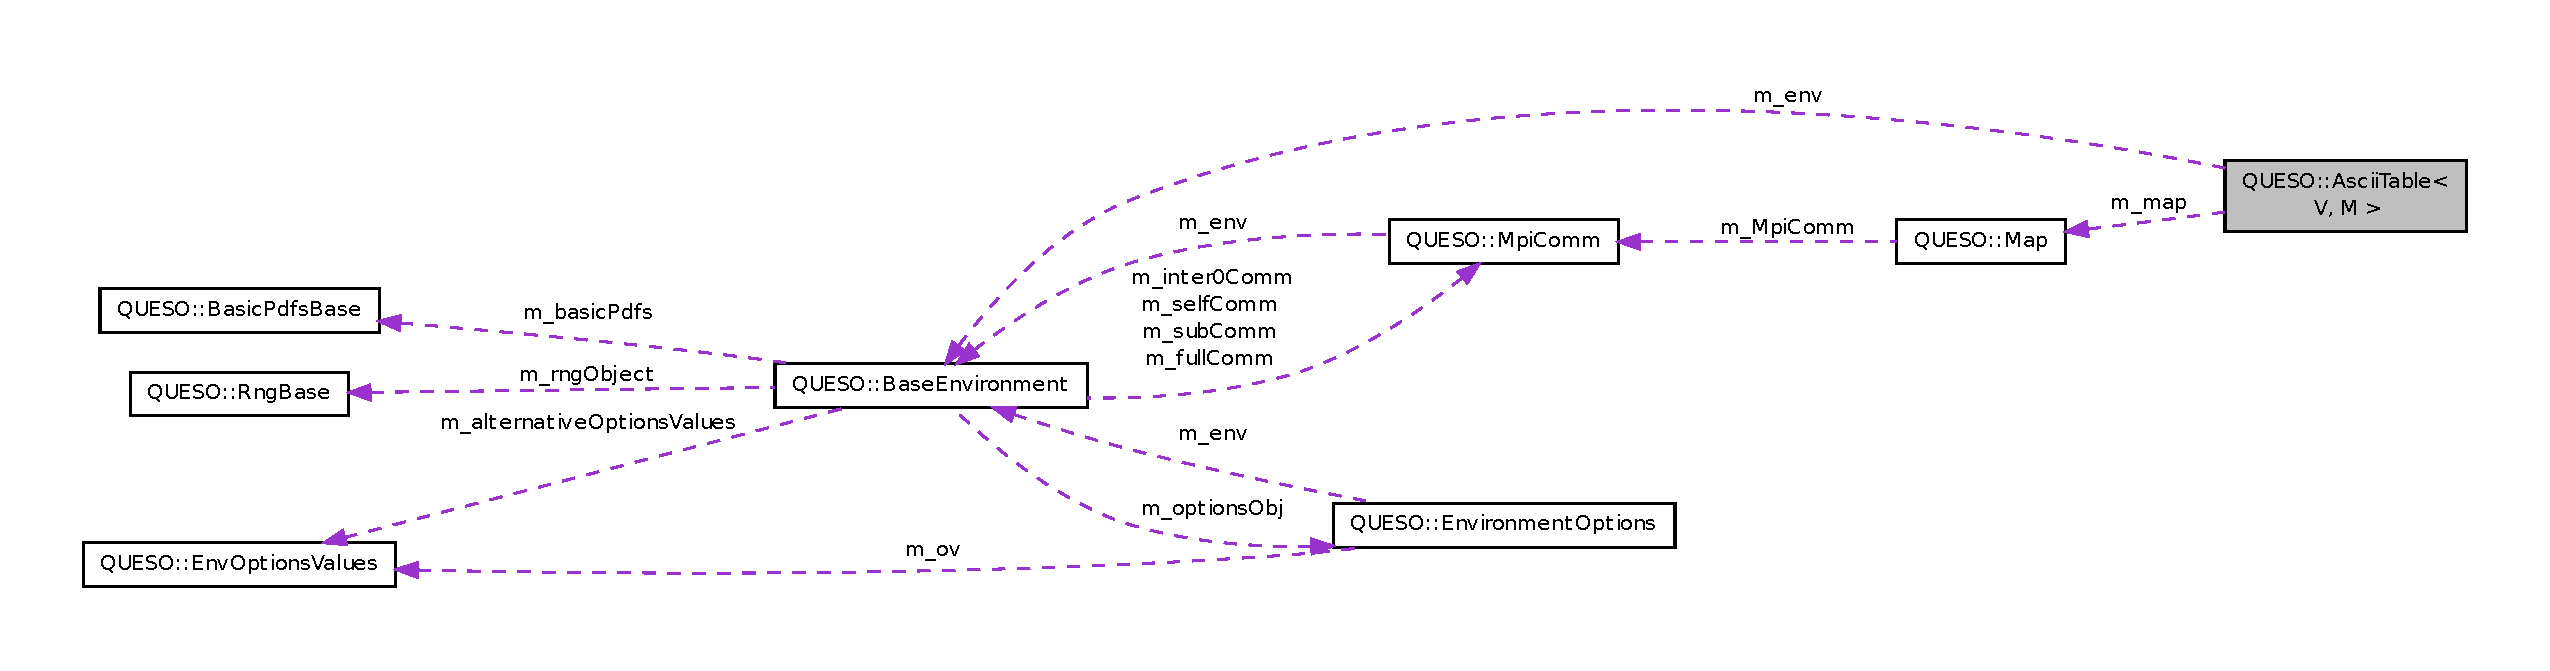
\includegraphics[width=350pt]{class_q_u_e_s_o_1_1_ascii_table__coll__graph}
\end{center}
\end{figure}
\subsection*{Public Member Functions}
\begin{Indent}{\bf Constructor/\-Destructor methods}\par
\begin{DoxyCompactItemize}
\item 
\hyperlink{class_q_u_e_s_o_1_1_ascii_table_a4d856e0d046d823e906aa4448b5762f1}{Ascii\-Table} (const \hyperlink{class_q_u_e_s_o_1_1_base_environment}{Base\-Environment} \&env, unsigned int \hyperlink{class_q_u_e_s_o_1_1_ascii_table_aa764ef68ef1d2ed85a4b6bd4eb0d7b17}{num\-Rows}, unsigned int num\-Extra\-Cols, const std\-::vector$<$ bool $>$ $\ast$extra\-Col\-Is\-String, const std\-::string \&file\-Name)
\begin{DoxyCompactList}\small\item\em Default constructor. \end{DoxyCompactList}\item 
\hyperlink{class_q_u_e_s_o_1_1_ascii_table_a2ff35b2d6920dc9e13dd8966a76beb10}{$\sim$\-Ascii\-Table} ()
\begin{DoxyCompactList}\small\item\em Destructor. \end{DoxyCompactList}\end{DoxyCompactItemize}
\end{Indent}
\begin{Indent}{\bf Property methods}\par
\begin{DoxyCompactItemize}
\item 
unsigned int \hyperlink{class_q_u_e_s_o_1_1_ascii_table_aa764ef68ef1d2ed85a4b6bd4eb0d7b17}{num\-Rows} () const 
\begin{DoxyCompactList}\small\item\em Returns the number of rows in the table. \end{DoxyCompactList}\item 
unsigned int \hyperlink{class_q_u_e_s_o_1_1_ascii_table_a428f547b9f5007e673245c8d2d0be387}{num\-Cols} () const 
\begin{DoxyCompactList}\small\item\em Returns the number of columns in the table. \end{DoxyCompactList}\item 
const \hyperlink{class_q_u_e_s_o_1_1_dist_array}{Dist\-Array}$<$ std\-::string $>$ \& \hyperlink{class_q_u_e_s_o_1_1_ascii_table_a8918d88137629c62e2408c164795479c}{string\-Column} (unsigned int j) const 
\begin{DoxyCompactList}\small\item\em Returns the string stored in column {\ttfamily j}. \end{DoxyCompactList}\item 
const V \& \hyperlink{class_q_u_e_s_o_1_1_ascii_table_a267e1834e60c5df459122b2509e4ca9d}{double\-Column} (unsigned int j) const 
\begin{DoxyCompactList}\small\item\em Returns the value (double) stored in column {\ttfamily j}. \end{DoxyCompactList}\end{DoxyCompactItemize}
\end{Indent}
\begin{Indent}{\bf I/\-O methods}\par
\begin{DoxyCompactItemize}
\item 
void \hyperlink{class_q_u_e_s_o_1_1_ascii_table_a4e58f0ab57b3af3aa4333955175abcf3}{print} (std\-::ostream \&os) const 
\begin{DoxyCompactList}\small\item\em Prints the table. \end{DoxyCompactList}\end{DoxyCompactItemize}
\end{Indent}
\subsection*{Private Member Functions}
\begin{DoxyCompactItemize}
\item 
\hyperlink{class_q_u_e_s_o_1_1_map}{Map} $\ast$ \hyperlink{class_q_u_e_s_o_1_1_ascii_table_aa42459bf69563f6606103c5f6da60a5a}{new\-Map} ()
\item 
void \hyperlink{class_q_u_e_s_o_1_1_ascii_table_a008557a6d782f76a51e72c77b3136322}{read\-Columns\-From\-File} ()
\item 
{\footnotesize template$<$$>$ }\\\hyperlink{class_q_u_e_s_o_1_1_map}{Map} $\ast$ \hyperlink{class_q_u_e_s_o_1_1_ascii_table_abb01e65369e9ad3e43e788d8ed2d2415}{new\-Map} ()
\end{DoxyCompactItemize}
\subsection*{Private Attributes}
\begin{DoxyCompactItemize}
\item 
const \hyperlink{class_q_u_e_s_o_1_1_base_environment}{Base\-Environment} \& \hyperlink{class_q_u_e_s_o_1_1_ascii_table_a2ba907db652aa02d53d493980d7a3753}{m\-\_\-env}
\item 
unsigned int \hyperlink{class_q_u_e_s_o_1_1_ascii_table_a4f772a7719d36cb0a0908eed37bd1deb}{m\-\_\-num\-Rows}
\item 
unsigned int \hyperlink{class_q_u_e_s_o_1_1_ascii_table_ada886c8db06d2d618f2898ad2cf2bd87}{m\-\_\-num\-Cols}
\item 
std\-::vector$<$ bool $>$ \hyperlink{class_q_u_e_s_o_1_1_ascii_table_a1c84e461d75e0846c156617f222c2ec3}{m\-\_\-col\-Is\-String}
\item 
std\-::string \hyperlink{class_q_u_e_s_o_1_1_ascii_table_adb7e4bac907ef1c93d745f02ea9f15d2}{m\-\_\-file\-Name}
\item 
const \hyperlink{class_q_u_e_s_o_1_1_map}{Map} $\ast$ \hyperlink{class_q_u_e_s_o_1_1_ascii_table_a7771fe0a08a93abdeadcc5e55e350eea}{m\-\_\-map}
\item 
std\-::vector$<$ \hyperlink{class_q_u_e_s_o_1_1_dist_array}{Dist\-Array}\\*
$<$ std\-::string $>$ $\ast$ $>$ \hyperlink{class_q_u_e_s_o_1_1_ascii_table_a14ba55d29e9a4ddeb14cd5acd8a27268}{m\-\_\-string\-Columns}
\item 
std\-::vector$<$ V $\ast$ $>$ \hyperlink{class_q_u_e_s_o_1_1_ascii_table_aa25a1d14c88cd5de341c43e052622f51}{m\-\_\-double\-Columns}
\end{DoxyCompactItemize}


\subsection{Detailed Description}
\subsubsection*{template$<$class V, class M$>$class Q\-U\-E\-S\-O\-::\-Ascii\-Table$<$ V, M $>$}

Class for reading A\-S\-C\-I\-I values from a table in a file. 

Definition at line 42 of file Ascii\-Table.\-h.



\subsection{Constructor \& Destructor Documentation}
\hypertarget{class_q_u_e_s_o_1_1_ascii_table_a4d856e0d046d823e906aa4448b5762f1}{\index{Q\-U\-E\-S\-O\-::\-Ascii\-Table@{Q\-U\-E\-S\-O\-::\-Ascii\-Table}!Ascii\-Table@{Ascii\-Table}}
\index{Ascii\-Table@{Ascii\-Table}!QUESO::AsciiTable@{Q\-U\-E\-S\-O\-::\-Ascii\-Table}}
\subsubsection[{Ascii\-Table}]{\setlength{\rightskip}{0pt plus 5cm}template$<$class V , class M $>$ {\bf Q\-U\-E\-S\-O\-::\-Ascii\-Table}$<$ V, M $>$\-::{\bf Ascii\-Table} (
\begin{DoxyParamCaption}
\item[{const {\bf Base\-Environment} \&}]{env, }
\item[{unsigned int}]{num\-Rows, }
\item[{unsigned int}]{num\-Extra\-Cols, }
\item[{const std\-::vector$<$ bool $>$ $\ast$}]{extra\-Col\-Is\-String, }
\item[{const std\-::string \&}]{file\-Name}
\end{DoxyParamCaption}
)}}\label{class_q_u_e_s_o_1_1_ascii_table_a4d856e0d046d823e906aa4448b5762f1}


Default constructor. 

This constructor reads the data from file {\ttfamily file\-Name}, checking whether the data in each column of the file is or not a string, and whether the data in each row is or not valid. 

Definition at line 31 of file Ascii\-Table.\-C.



References Q\-U\-E\-S\-O\-::\-Base\-Environment\-::display\-Verbosity(), Q\-U\-E\-S\-O\-::\-Ascii\-Table$<$ V, M $>$\-::m\-\_\-col\-Is\-String, Q\-U\-E\-S\-O\-::\-Ascii\-Table$<$ V, M $>$\-::m\-\_\-double\-Columns, Q\-U\-E\-S\-O\-::\-Ascii\-Table$<$ V, M $>$\-::m\-\_\-env, Q\-U\-E\-S\-O\-::\-Ascii\-Table$<$ V, M $>$\-::m\-\_\-num\-Cols, Q\-U\-E\-S\-O\-::\-Ascii\-Table$<$ V, M $>$\-::m\-\_\-string\-Columns, Q\-U\-E\-S\-O\-::\-Ascii\-Table$<$ V, M $>$\-::read\-Columns\-From\-File(), and Q\-U\-E\-S\-O\-::\-Base\-Environment\-::sub\-Display\-File().


\begin{DoxyCode}
37   :
38   \hyperlink{class_q_u_e_s_o_1_1_ascii_table_a2ba907db652aa02d53d493980d7a3753}{m\_env}          (env),
39   \hyperlink{class_q_u_e_s_o_1_1_ascii_table_a4f772a7719d36cb0a0908eed37bd1deb}{m\_numRows}      (\hyperlink{class_q_u_e_s_o_1_1_ascii_table_aa764ef68ef1d2ed85a4b6bd4eb0d7b17}{numRows}),
40   \hyperlink{class_q_u_e_s_o_1_1_ascii_table_ada886c8db06d2d618f2898ad2cf2bd87}{m\_numCols}      (1+numExtraCols),
41   \hyperlink{class_q_u_e_s_o_1_1_ascii_table_a1c84e461d75e0846c156617f222c2ec3}{m\_colIsString}  (1,\textcolor{keyword}{true}),
42   \hyperlink{class_q_u_e_s_o_1_1_ascii_table_adb7e4bac907ef1c93d745f02ea9f15d2}{m\_fileName}     (fileName),
43   \hyperlink{class_q_u_e_s_o_1_1_ascii_table_a7771fe0a08a93abdeadcc5e55e350eea}{m\_map}          (\hyperlink{class_q_u_e_s_o_1_1_ascii_table_aa42459bf69563f6606103c5f6da60a5a}{newMap}()),
44   \hyperlink{class_q_u_e_s_o_1_1_ascii_table_a14ba55d29e9a4ddeb14cd5acd8a27268}{m\_stringColumns}(0),
45   \hyperlink{class_q_u_e_s_o_1_1_ascii_table_aa25a1d14c88cd5de341c43e052622f51}{m\_doubleColumns}(0)
46 \{
47   \textcolor{keywordflow}{if} ((\hyperlink{class_q_u_e_s_o_1_1_ascii_table_a2ba907db652aa02d53d493980d7a3753}{m\_env}.\hyperlink{class_q_u_e_s_o_1_1_base_environment_a8a0064746ae8dddfece4229b9ad374d6}{subDisplayFile}()) && (\hyperlink{class_q_u_e_s_o_1_1_ascii_table_a2ba907db652aa02d53d493980d7a3753}{m\_env}.
      \hyperlink{class_q_u_e_s_o_1_1_base_environment_a1fe5f244fc0316a0ab3e37463f108b96}{displayVerbosity}() >= 5)) \{
48     *\hyperlink{class_q_u_e_s_o_1_1_ascii_table_a2ba907db652aa02d53d493980d7a3753}{m\_env}.\hyperlink{class_q_u_e_s_o_1_1_base_environment_a8a0064746ae8dddfece4229b9ad374d6}{subDisplayFile}() << \textcolor{stringliteral}{"Entering AsciiTable<V,M>::constructor()..."}
49                             << std::endl;
50   \}
51 
52   \textcolor{keywordflow}{if} (\hyperlink{class_q_u_e_s_o_1_1_ascii_table_ada886c8db06d2d618f2898ad2cf2bd87}{m\_numCols} > 1) \{
53     \hyperlink{class_q_u_e_s_o_1_1_ascii_table_a1c84e461d75e0846c156617f222c2ec3}{m\_colIsString}.resize(\hyperlink{class_q_u_e_s_o_1_1_ascii_table_ada886c8db06d2d618f2898ad2cf2bd87}{m\_numCols},\textcolor{keyword}{false});
54     \textcolor{keywordflow}{if} (extraColIsString == NULL) \{
55       \textcolor{comment}{// Nothing extra needs to be done}
56     \}
57     \textcolor{keywordflow}{else} \{
58       \textcolor{keywordtype}{unsigned} \textcolor{keywordtype}{int} maxJ = std::min(numExtraCols,(\textcolor{keywordtype}{unsigned} \textcolor{keywordtype}{int}) extraColIsString->size());
59       \textcolor{keywordflow}{for} (\textcolor{keywordtype}{unsigned} \textcolor{keywordtype}{int} j = 0; j < maxJ; ++j) \{
60         \hyperlink{class_q_u_e_s_o_1_1_ascii_table_a1c84e461d75e0846c156617f222c2ec3}{m\_colIsString}[1+j] = (*extraColIsString)[j];
61       \}
62     \}
63   \}
64   \hyperlink{class_q_u_e_s_o_1_1_ascii_table_a14ba55d29e9a4ddeb14cd5acd8a27268}{m\_stringColumns}.resize(\hyperlink{class_q_u_e_s_o_1_1_ascii_table_ada886c8db06d2d618f2898ad2cf2bd87}{m\_numCols},NULL);
65   \hyperlink{class_q_u_e_s_o_1_1_ascii_table_aa25a1d14c88cd5de341c43e052622f51}{m\_doubleColumns}.resize(\hyperlink{class_q_u_e_s_o_1_1_ascii_table_ada886c8db06d2d618f2898ad2cf2bd87}{m\_numCols},NULL);
66   \hyperlink{class_q_u_e_s_o_1_1_ascii_table_a008557a6d782f76a51e72c77b3136322}{readColumnsFromFile}();
67 
68   \textcolor{keywordflow}{if} ((\hyperlink{class_q_u_e_s_o_1_1_ascii_table_a2ba907db652aa02d53d493980d7a3753}{m\_env}.\hyperlink{class_q_u_e_s_o_1_1_base_environment_a8a0064746ae8dddfece4229b9ad374d6}{subDisplayFile}()) && (\hyperlink{class_q_u_e_s_o_1_1_ascii_table_a2ba907db652aa02d53d493980d7a3753}{m\_env}.
      \hyperlink{class_q_u_e_s_o_1_1_base_environment_a1fe5f244fc0316a0ab3e37463f108b96}{displayVerbosity}() >= 5)) \{
69     *\hyperlink{class_q_u_e_s_o_1_1_ascii_table_a2ba907db652aa02d53d493980d7a3753}{m\_env}.\hyperlink{class_q_u_e_s_o_1_1_base_environment_a8a0064746ae8dddfece4229b9ad374d6}{subDisplayFile}() << \textcolor{stringliteral}{"Leaving AsciiTable<V,M>::constructor()"}
70                             << std::endl;
71   \}
72 \}
\end{DoxyCode}
\hypertarget{class_q_u_e_s_o_1_1_ascii_table_a2ff35b2d6920dc9e13dd8966a76beb10}{\index{Q\-U\-E\-S\-O\-::\-Ascii\-Table@{Q\-U\-E\-S\-O\-::\-Ascii\-Table}!$\sim$\-Ascii\-Table@{$\sim$\-Ascii\-Table}}
\index{$\sim$\-Ascii\-Table@{$\sim$\-Ascii\-Table}!QUESO::AsciiTable@{Q\-U\-E\-S\-O\-::\-Ascii\-Table}}
\subsubsection[{$\sim$\-Ascii\-Table}]{\setlength{\rightskip}{0pt plus 5cm}template$<$class V , class M $>$ {\bf Q\-U\-E\-S\-O\-::\-Ascii\-Table}$<$ V, M $>$\-::$\sim${\bf Ascii\-Table} (
\begin{DoxyParamCaption}
{}
\end{DoxyParamCaption}
)}}\label{class_q_u_e_s_o_1_1_ascii_table_a2ff35b2d6920dc9e13dd8966a76beb10}


Destructor. 



Definition at line 76 of file Ascii\-Table.\-C.


\begin{DoxyCode}
77 \{
78   \textcolor{keywordflow}{for} (\textcolor{keywordtype}{unsigned} \textcolor{keywordtype}{int} j = 0; j < \hyperlink{class_q_u_e_s_o_1_1_ascii_table_aa25a1d14c88cd5de341c43e052622f51}{m\_doubleColumns}.size(); ++j) \{
79     \textcolor{keywordflow}{if} (\hyperlink{class_q_u_e_s_o_1_1_ascii_table_aa25a1d14c88cd5de341c43e052622f51}{m\_doubleColumns}[j]) \textcolor{keyword}{delete} \hyperlink{class_q_u_e_s_o_1_1_ascii_table_aa25a1d14c88cd5de341c43e052622f51}{m\_doubleColumns}[j];
80   \}
81   \textcolor{keywordflow}{for} (\textcolor{keywordtype}{unsigned} \textcolor{keywordtype}{int} j = 0; j < \hyperlink{class_q_u_e_s_o_1_1_ascii_table_a14ba55d29e9a4ddeb14cd5acd8a27268}{m\_stringColumns}.size(); ++j) \{
82     \textcolor{keywordflow}{if} (\hyperlink{class_q_u_e_s_o_1_1_ascii_table_a14ba55d29e9a4ddeb14cd5acd8a27268}{m\_stringColumns}[j]) \textcolor{keyword}{delete} \hyperlink{class_q_u_e_s_o_1_1_ascii_table_a14ba55d29e9a4ddeb14cd5acd8a27268}{m\_stringColumns}[j];
83   \}
84 \}
\end{DoxyCode}


\subsection{Member Function Documentation}
\hypertarget{class_q_u_e_s_o_1_1_ascii_table_a267e1834e60c5df459122b2509e4ca9d}{\index{Q\-U\-E\-S\-O\-::\-Ascii\-Table@{Q\-U\-E\-S\-O\-::\-Ascii\-Table}!double\-Column@{double\-Column}}
\index{double\-Column@{double\-Column}!QUESO::AsciiTable@{Q\-U\-E\-S\-O\-::\-Ascii\-Table}}
\subsubsection[{double\-Column}]{\setlength{\rightskip}{0pt plus 5cm}template$<$class V , class M $>$ const V \& {\bf Q\-U\-E\-S\-O\-::\-Ascii\-Table}$<$ V, M $>$\-::double\-Column (
\begin{DoxyParamCaption}
\item[{unsigned int}]{j}
\end{DoxyParamCaption}
) const}}\label{class_q_u_e_s_o_1_1_ascii_table_a267e1834e60c5df459122b2509e4ca9d}


Returns the value (double) stored in column {\ttfamily j}. 



Definition at line 299 of file Ascii\-Table.\-C.



References U\-Q\-\_\-\-F\-A\-T\-A\-L\-\_\-\-T\-E\-S\-T\-\_\-\-M\-A\-C\-R\-O.


\begin{DoxyCode}
300 \{
301   \hyperlink{_defines_8h_a56d63d18d0a6d45757de47fcc06f574d}{UQ\_FATAL\_TEST\_MACRO}(j >= \hyperlink{class_q_u_e_s_o_1_1_ascii_table_ada886c8db06d2d618f2898ad2cf2bd87}{m\_numCols},
302                       \hyperlink{class_q_u_e_s_o_1_1_ascii_table_a2ba907db652aa02d53d493980d7a3753}{m\_env}.\hyperlink{class_q_u_e_s_o_1_1_base_environment_a78b57112bbd0e6dd0e8afec00b40ffa7}{worldRank}(),
303                       \textcolor{stringliteral}{"AsciiTable<V,M>::doubleColumn()"},
304                       \textcolor{stringliteral}{"invalid j"});
305 
306   \hyperlink{_defines_8h_a56d63d18d0a6d45757de47fcc06f574d}{UQ\_FATAL\_TEST\_MACRO}(\hyperlink{class_q_u_e_s_o_1_1_ascii_table_aa25a1d14c88cd5de341c43e052622f51}{m\_doubleColumns}[j] == NULL,
307                       \hyperlink{class_q_u_e_s_o_1_1_ascii_table_a2ba907db652aa02d53d493980d7a3753}{m\_env}.\hyperlink{class_q_u_e_s_o_1_1_base_environment_a78b57112bbd0e6dd0e8afec00b40ffa7}{worldRank}(),
308                       \textcolor{stringliteral}{"AsciiTable<V,M>::doubleColumn()"},
309                       \textcolor{stringliteral}{"double column is not ready"});
310 
311   \textcolor{keywordflow}{return} *\hyperlink{class_q_u_e_s_o_1_1_ascii_table_aa25a1d14c88cd5de341c43e052622f51}{m\_doubleColumns}[j];
312 \}
\end{DoxyCode}
\hypertarget{class_q_u_e_s_o_1_1_ascii_table_abb01e65369e9ad3e43e788d8ed2d2415}{\index{Q\-U\-E\-S\-O\-::\-Ascii\-Table@{Q\-U\-E\-S\-O\-::\-Ascii\-Table}!new\-Map@{new\-Map}}
\index{new\-Map@{new\-Map}!QUESO::AsciiTable@{Q\-U\-E\-S\-O\-::\-Ascii\-Table}}
\subsubsection[{new\-Map}]{\setlength{\rightskip}{0pt plus 5cm}template$<$$>$ {\bf Map} $\ast$ {\bf Q\-U\-E\-S\-O\-::\-Ascii\-Table}$<$ class {\bf Gsl\-Vector}, class {\bf Gsl\-Matrix} $>$\-::new\-Map (
\begin{DoxyParamCaption}
{}
\end{DoxyParamCaption}
)\hspace{0.3cm}{\ttfamily [private]}}}\label{class_q_u_e_s_o_1_1_ascii_table_abb01e65369e9ad3e43e788d8ed2d2415}


Definition at line 31 of file Gsl\-Ascii\-Table.\-C.


\begin{DoxyCode}
32 \{
33   \textcolor{keywordflow}{return} \textcolor{keyword}{new} Map(\hyperlink{class_q_u_e_s_o_1_1_ascii_table_a4f772a7719d36cb0a0908eed37bd1deb}{m\_numRows},0,\hyperlink{class_q_u_e_s_o_1_1_ascii_table_a2ba907db652aa02d53d493980d7a3753}{m\_env}.\hyperlink{class_q_u_e_s_o_1_1_base_environment_a824458f0d045db251d982ad4c75a4b76}{selfComm}());
34 \}
\end{DoxyCode}
\hypertarget{class_q_u_e_s_o_1_1_ascii_table_aa42459bf69563f6606103c5f6da60a5a}{\index{Q\-U\-E\-S\-O\-::\-Ascii\-Table@{Q\-U\-E\-S\-O\-::\-Ascii\-Table}!new\-Map@{new\-Map}}
\index{new\-Map@{new\-Map}!QUESO::AsciiTable@{Q\-U\-E\-S\-O\-::\-Ascii\-Table}}
\subsubsection[{new\-Map}]{\setlength{\rightskip}{0pt plus 5cm}template$<$class V , class M $>$ {\bf Map}$\ast$ {\bf Q\-U\-E\-S\-O\-::\-Ascii\-Table}$<$ V, M $>$\-::new\-Map (
\begin{DoxyParamCaption}
{}
\end{DoxyParamCaption}
)\hspace{0.3cm}{\ttfamily [private]}}}\label{class_q_u_e_s_o_1_1_ascii_table_aa42459bf69563f6606103c5f6da60a5a}
\hypertarget{class_q_u_e_s_o_1_1_ascii_table_a428f547b9f5007e673245c8d2d0be387}{\index{Q\-U\-E\-S\-O\-::\-Ascii\-Table@{Q\-U\-E\-S\-O\-::\-Ascii\-Table}!num\-Cols@{num\-Cols}}
\index{num\-Cols@{num\-Cols}!QUESO::AsciiTable@{Q\-U\-E\-S\-O\-::\-Ascii\-Table}}
\subsubsection[{num\-Cols}]{\setlength{\rightskip}{0pt plus 5cm}template$<$class V , class M $>$ unsigned int {\bf Q\-U\-E\-S\-O\-::\-Ascii\-Table}$<$ V, M $>$\-::num\-Cols (
\begin{DoxyParamCaption}
{}
\end{DoxyParamCaption}
) const}}\label{class_q_u_e_s_o_1_1_ascii_table_a428f547b9f5007e673245c8d2d0be387}


Returns the number of columns in the table. 



Definition at line 275 of file Ascii\-Table.\-C.


\begin{DoxyCode}
276 \{
277   \textcolor{keywordflow}{return} \hyperlink{class_q_u_e_s_o_1_1_ascii_table_ada886c8db06d2d618f2898ad2cf2bd87}{m\_numCols};
278 \}
\end{DoxyCode}
\hypertarget{class_q_u_e_s_o_1_1_ascii_table_aa764ef68ef1d2ed85a4b6bd4eb0d7b17}{\index{Q\-U\-E\-S\-O\-::\-Ascii\-Table@{Q\-U\-E\-S\-O\-::\-Ascii\-Table}!num\-Rows@{num\-Rows}}
\index{num\-Rows@{num\-Rows}!QUESO::AsciiTable@{Q\-U\-E\-S\-O\-::\-Ascii\-Table}}
\subsubsection[{num\-Rows}]{\setlength{\rightskip}{0pt plus 5cm}template$<$class V , class M $>$ unsigned int {\bf Q\-U\-E\-S\-O\-::\-Ascii\-Table}$<$ V, M $>$\-::num\-Rows (
\begin{DoxyParamCaption}
{}
\end{DoxyParamCaption}
) const}}\label{class_q_u_e_s_o_1_1_ascii_table_aa764ef68ef1d2ed85a4b6bd4eb0d7b17}


Returns the number of rows in the table. 



Definition at line 268 of file Ascii\-Table.\-C.


\begin{DoxyCode}
269 \{
270   \textcolor{keywordflow}{return} \hyperlink{class_q_u_e_s_o_1_1_ascii_table_a4f772a7719d36cb0a0908eed37bd1deb}{m\_numRows};
271 \}
\end{DoxyCode}
\hypertarget{class_q_u_e_s_o_1_1_ascii_table_a4e58f0ab57b3af3aa4333955175abcf3}{\index{Q\-U\-E\-S\-O\-::\-Ascii\-Table@{Q\-U\-E\-S\-O\-::\-Ascii\-Table}!print@{print}}
\index{print@{print}!QUESO::AsciiTable@{Q\-U\-E\-S\-O\-::\-Ascii\-Table}}
\subsubsection[{print}]{\setlength{\rightskip}{0pt plus 5cm}template$<$class V , class M $>$ void {\bf Q\-U\-E\-S\-O\-::\-Ascii\-Table}$<$ V, M $>$\-::print (
\begin{DoxyParamCaption}
\item[{std\-::ostream \&}]{os}
\end{DoxyParamCaption}
) const}}\label{class_q_u_e_s_o_1_1_ascii_table_a4e58f0ab57b3af3aa4333955175abcf3}


Prints the table. 



Definition at line 317 of file Ascii\-Table.\-C.



References U\-Q\-\_\-\-F\-A\-T\-A\-L\-\_\-\-T\-E\-S\-T\-\_\-\-M\-A\-C\-R\-O.


\begin{DoxyCode}
318 \{
319   \textcolor{keywordflow}{for} (\textcolor{keywordtype}{unsigned} \textcolor{keywordtype}{int} j = 0; j < \hyperlink{class_q_u_e_s_o_1_1_ascii_table_ada886c8db06d2d618f2898ad2cf2bd87}{m\_numCols}; ++j) \{
320     \hyperlink{_defines_8h_a56d63d18d0a6d45757de47fcc06f574d}{UQ\_FATAL\_TEST\_MACRO}((\hyperlink{class_q_u_e_s_o_1_1_ascii_table_a14ba55d29e9a4ddeb14cd5acd8a27268}{m\_stringColumns}[j] != NULL) && (
      \hyperlink{class_q_u_e_s_o_1_1_ascii_table_aa25a1d14c88cd5de341c43e052622f51}{m\_doubleColumns}[j] != NULL),
321                         \hyperlink{class_q_u_e_s_o_1_1_ascii_table_a2ba907db652aa02d53d493980d7a3753}{m\_env}.\hyperlink{class_q_u_e_s_o_1_1_base_environment_a78b57112bbd0e6dd0e8afec00b40ffa7}{worldRank}(),
322                         \textcolor{stringliteral}{"AsciiTable<V,M>::print()"},
323                         \textcolor{stringliteral}{"column is not null on both possible ways"});
324     \hyperlink{_defines_8h_a56d63d18d0a6d45757de47fcc06f574d}{UQ\_FATAL\_TEST\_MACRO}((\hyperlink{class_q_u_e_s_o_1_1_ascii_table_a14ba55d29e9a4ddeb14cd5acd8a27268}{m\_stringColumns}[j] == NULL) && (
      \hyperlink{class_q_u_e_s_o_1_1_ascii_table_aa25a1d14c88cd5de341c43e052622f51}{m\_doubleColumns}[j] == NULL),
325                         \hyperlink{class_q_u_e_s_o_1_1_ascii_table_a2ba907db652aa02d53d493980d7a3753}{m\_env}.\hyperlink{class_q_u_e_s_o_1_1_base_environment_a78b57112bbd0e6dd0e8afec00b40ffa7}{worldRank}(),
326                         \textcolor{stringliteral}{"AsciiTable<V,M>::print()"},
327                         \textcolor{stringliteral}{"column is null on both possible ways"});
328 
329     os << \textcolor{stringliteral}{"\(\backslash\)nContents of table '"} << \hyperlink{class_q_u_e_s_o_1_1_ascii_table_adb7e4bac907ef1c93d745f02ea9f15d2}{m\_fileName}
330        << \textcolor{stringliteral}{"', column "}            << j
331        << \textcolor{stringliteral}{":"}
332        << std::endl;
333     \textcolor{keywordflow}{if} (\hyperlink{class_q_u_e_s_o_1_1_ascii_table_a14ba55d29e9a4ddeb14cd5acd8a27268}{m\_stringColumns}[j] != NULL) \{
334       os << *\hyperlink{class_q_u_e_s_o_1_1_ascii_table_a14ba55d29e9a4ddeb14cd5acd8a27268}{m\_stringColumns}[j];
335       \textcolor{comment}{//DistArray<std::string>& arrayOfStrings = *m\_stringColumns[j];}
336       \textcolor{comment}{//for (unsigned int i = 0; i < m\_numRows; ++i) \{}
337       \textcolor{comment}{//  os << arrayOfStrings(i,0)}
338       \textcolor{comment}{//     << std::endl;}
339       \textcolor{comment}{//\}}
340     \}
341     \textcolor{keywordflow}{else} \{
342       os << *\hyperlink{class_q_u_e_s_o_1_1_ascii_table_aa25a1d14c88cd5de341c43e052622f51}{m\_doubleColumns}[j];
343     \}
344     os << std::endl;
345   \}
346 
347   \textcolor{keywordflow}{return};
348 \}
\end{DoxyCode}
\hypertarget{class_q_u_e_s_o_1_1_ascii_table_a008557a6d782f76a51e72c77b3136322}{\index{Q\-U\-E\-S\-O\-::\-Ascii\-Table@{Q\-U\-E\-S\-O\-::\-Ascii\-Table}!read\-Columns\-From\-File@{read\-Columns\-From\-File}}
\index{read\-Columns\-From\-File@{read\-Columns\-From\-File}!QUESO::AsciiTable@{Q\-U\-E\-S\-O\-::\-Ascii\-Table}}
\subsubsection[{read\-Columns\-From\-File}]{\setlength{\rightskip}{0pt plus 5cm}template$<$class V , class M $>$ void {\bf Q\-U\-E\-S\-O\-::\-Ascii\-Table}$<$ V, M $>$\-::read\-Columns\-From\-File (
\begin{DoxyParamCaption}
{}
\end{DoxyParamCaption}
)\hspace{0.3cm}{\ttfamily [private]}}}\label{class_q_u_e_s_o_1_1_ascii_table_a008557a6d782f76a51e72c77b3136322}


Definition at line 89 of file Ascii\-Table.\-C.



References Q\-U\-E\-S\-O\-::\-Misc\-Read\-Chars\-And\-Double\-From\-File(), Q\-U\-E\-S\-O\-::\-Misc\-Read\-String\-And\-Double\-From\-File(), and U\-Q\-\_\-\-F\-A\-T\-A\-L\-\_\-\-T\-E\-S\-T\-\_\-\-M\-A\-C\-R\-O.



Referenced by Q\-U\-E\-S\-O\-::\-Ascii\-Table$<$ V, M $>$\-::\-Ascii\-Table().


\begin{DoxyCode}
90 \{
91   \textcolor{keywordtype}{unsigned} \textcolor{keywordtype}{int} maxCharsPerLine = 512;
92 
93   std::ifstream ifs(\hyperlink{class_q_u_e_s_o_1_1_ascii_table_adb7e4bac907ef1c93d745f02ea9f15d2}{m\_fileName}.c\_str());
94   \hyperlink{_defines_8h_a56d63d18d0a6d45757de47fcc06f574d}{UQ\_FATAL\_TEST\_MACRO}(ifs.is\_open() == \textcolor{keyword}{false},
95                       \hyperlink{class_q_u_e_s_o_1_1_ascii_table_a2ba907db652aa02d53d493980d7a3753}{m\_env}.\hyperlink{class_q_u_e_s_o_1_1_base_environment_a78b57112bbd0e6dd0e8afec00b40ffa7}{worldRank}(),
96                       \textcolor{stringliteral}{"AsciiTable<V,M>::readColumnsFromFile()"},
97                       \textcolor{stringliteral}{"file was not found"});
98 
99   \textcolor{comment}{// Determine number of lines}
100   \textcolor{keywordtype}{unsigned} \textcolor{keywordtype}{int} numLines = std::count(std::istreambuf\_iterator<char>(ifs),
101                                      std::istreambuf\_iterator<char>(),
102                                      \textcolor{charliteral}{'\(\backslash\)n'});
103 
104   \textcolor{comment}{// Determine number of valid lines}
105   \textcolor{keywordtype}{int} iRC;
106   ifs.seekg(0,std::ios\_base::beg);
107   \textcolor{keywordtype}{unsigned} \textcolor{keywordtype}{int} lineId = 0;
108   \textcolor{keywordtype}{unsigned} \textcolor{keywordtype}{int} numValidLines = 0;
109   std::string tempString;
110   \textcolor{keywordflow}{while} ((lineId < numLines) && (ifs.eof() == \textcolor{keyword}{false})) \{
111     iRC = \hyperlink{namespace_q_u_e_s_o_af0fc61c58d0ca592fa172eeab540d39c}{MiscReadStringAndDoubleFromFile}(ifs,tempString,NULL);
112     \hyperlink{_defines_8h_a56d63d18d0a6d45757de47fcc06f574d}{UQ\_FATAL\_TEST\_MACRO}(iRC,
113                         \hyperlink{class_q_u_e_s_o_1_1_ascii_table_a2ba907db652aa02d53d493980d7a3753}{m\_env}.\hyperlink{class_q_u_e_s_o_1_1_base_environment_a78b57112bbd0e6dd0e8afec00b40ffa7}{worldRank}(),
114                         \textcolor{stringliteral}{"AsciiTable<V,M>::readColumnsFromFile()"},
115                         \textcolor{stringliteral}{"failed reading during the determination of the number of valid lines"});
116     \textcolor{comment}{//*m\_env.subDisplayFile() << "lineId = "          << lineId}
117     \textcolor{comment}{//                        << ", numValidLines = " << numValidLines}
118     \textcolor{comment}{//                        << ", tempString = "    << tempString}
119     \textcolor{comment}{//                        << std::endl;}
120     \textcolor{keywordflow}{if} (tempString[0] != \textcolor{charliteral}{'#'}) numValidLines++;
121     lineId++;
122     ifs.ignore(maxCharsPerLine,\textcolor{charliteral}{'\(\backslash\)n'});
123   \}
124   \hyperlink{_defines_8h_a56d63d18d0a6d45757de47fcc06f574d}{UQ\_FATAL\_TEST\_MACRO}(lineId != numLines,
125                       \hyperlink{class_q_u_e_s_o_1_1_ascii_table_a2ba907db652aa02d53d493980d7a3753}{m\_env}.\hyperlink{class_q_u_e_s_o_1_1_base_environment_a78b57112bbd0e6dd0e8afec00b40ffa7}{worldRank}(),
126                       \textcolor{stringliteral}{"AsciiTable<V,M>::readColumnsFromFile()"},
127                       \textcolor{stringliteral}{"the first number of lines read is nonconsistent"});
128   \textcolor{keywordflow}{if} (\hyperlink{class_q_u_e_s_o_1_1_ascii_table_a4f772a7719d36cb0a0908eed37bd1deb}{m\_numRows} != numValidLines) \{
129     \textcolor{keywordtype}{char} errorExplanation[512];
130     sprintf(errorExplanation,\textcolor{stringliteral}{"number of valid lines (%u) in ASCII table file does not match number of rows
       (%u)"},numValidLines,\hyperlink{class_q_u_e_s_o_1_1_ascii_table_a4f772a7719d36cb0a0908eed37bd1deb}{m\_numRows});
131     \hyperlink{_defines_8h_a56d63d18d0a6d45757de47fcc06f574d}{UQ\_FATAL\_TEST\_MACRO}(\textcolor{keyword}{true},
132                         \hyperlink{class_q_u_e_s_o_1_1_ascii_table_a2ba907db652aa02d53d493980d7a3753}{m\_env}.\hyperlink{class_q_u_e_s_o_1_1_base_environment_a78b57112bbd0e6dd0e8afec00b40ffa7}{worldRank}(),
133                         \textcolor{stringliteral}{"AsciiTable<V,M>::readColumnsFromFile()"},
134                         errorExplanation);
135   \}
136 
137   \textcolor{keywordflow}{if} (\hyperlink{class_q_u_e_s_o_1_1_ascii_table_a2ba907db652aa02d53d493980d7a3753}{m\_env}.\hyperlink{class_q_u_e_s_o_1_1_base_environment_a8a0064746ae8dddfece4229b9ad374d6}{subDisplayFile}()) \{
138     *\hyperlink{class_q_u_e_s_o_1_1_ascii_table_a2ba907db652aa02d53d493980d7a3753}{m\_env}.\hyperlink{class_q_u_e_s_o_1_1_base_environment_a8a0064746ae8dddfece4229b9ad374d6}{subDisplayFile}() << \textcolor{stringliteral}{"ASCII table file '"}    << 
      \hyperlink{class_q_u_e_s_o_1_1_ascii_table_adb7e4bac907ef1c93d745f02ea9f15d2}{m\_fileName}
139                             << \textcolor{stringliteral}{"' has "}                << numLines
140                             << \textcolor{stringliteral}{" lines and specifies "} << numValidLines
141                             << \textcolor{stringliteral}{" valid lines."}
142                             << std::endl;
143   \}
144 
145   \textcolor{keywordflow}{for} (\textcolor{keywordtype}{unsigned} \textcolor{keywordtype}{int} j=0; j < \hyperlink{class_q_u_e_s_o_1_1_ascii_table_ada886c8db06d2d618f2898ad2cf2bd87}{m\_numCols}; ++j) \{
146     \textcolor{keywordflow}{if} (\hyperlink{class_q_u_e_s_o_1_1_ascii_table_a1c84e461d75e0846c156617f222c2ec3}{m\_colIsString}[j]) \{
147       \textcolor{keywordflow}{if} ((\hyperlink{class_q_u_e_s_o_1_1_ascii_table_a2ba907db652aa02d53d493980d7a3753}{m\_env}.\hyperlink{class_q_u_e_s_o_1_1_base_environment_a8a0064746ae8dddfece4229b9ad374d6}{subDisplayFile}()) && (\hyperlink{class_q_u_e_s_o_1_1_ascii_table_a2ba907db652aa02d53d493980d7a3753}{m\_env}.
      \hyperlink{class_q_u_e_s_o_1_1_base_environment_a1fe5f244fc0316a0ab3e37463f108b96}{displayVerbosity}() >= 5)) \{
148         *\hyperlink{class_q_u_e_s_o_1_1_ascii_table_a2ba907db652aa02d53d493980d7a3753}{m\_env}.\hyperlink{class_q_u_e_s_o_1_1_base_environment_a8a0064746ae8dddfece4229b9ad374d6}{subDisplayFile}() << \textcolor{stringliteral}{"Column j = "} << j
149                                 << \textcolor{stringliteral}{" is a columns of strings"}
150                                 << std::endl;
151       \}
152       \hyperlink{class_q_u_e_s_o_1_1_ascii_table_a14ba55d29e9a4ddeb14cd5acd8a27268}{m\_stringColumns}[j] = \textcolor{keyword}{new} DistArray<std::string>(*\hyperlink{class_q_u_e_s_o_1_1_ascii_table_a7771fe0a08a93abdeadcc5e55e350eea}{m\_map},1);
153     \}
154     \textcolor{keywordflow}{else} \{
155       \textcolor{keywordflow}{if} ((\hyperlink{class_q_u_e_s_o_1_1_ascii_table_a2ba907db652aa02d53d493980d7a3753}{m\_env}.\hyperlink{class_q_u_e_s_o_1_1_base_environment_a8a0064746ae8dddfece4229b9ad374d6}{subDisplayFile}()) && (\hyperlink{class_q_u_e_s_o_1_1_ascii_table_a2ba907db652aa02d53d493980d7a3753}{m\_env}.
      \hyperlink{class_q_u_e_s_o_1_1_base_environment_a1fe5f244fc0316a0ab3e37463f108b96}{displayVerbosity}() >= 5)) \{
156         *\hyperlink{class_q_u_e_s_o_1_1_ascii_table_a2ba907db652aa02d53d493980d7a3753}{m\_env}.\hyperlink{class_q_u_e_s_o_1_1_base_environment_a8a0064746ae8dddfece4229b9ad374d6}{subDisplayFile}() << \textcolor{stringliteral}{"Column j = "} << j
157                                 << \textcolor{stringliteral}{" is a columns of doubles"}
158                                 << std::endl;
159       \}
160       \hyperlink{class_q_u_e_s_o_1_1_ascii_table_aa25a1d14c88cd5de341c43e052622f51}{m\_doubleColumns}[j] = \textcolor{keyword}{new} V(\hyperlink{class_q_u_e_s_o_1_1_ascii_table_a2ba907db652aa02d53d493980d7a3753}{m\_env},*\hyperlink{class_q_u_e_s_o_1_1_ascii_table_a7771fe0a08a93abdeadcc5e55e350eea}{m\_map});
161     \}
162   \}
163 
164   \textcolor{comment}{// Read file until End Of File character is reached}
165   ifs.seekg(0,std::ios\_base::beg);
166   lineId = 0;
167   \textcolor{keywordtype}{unsigned} \textcolor{keywordtype}{int} validLineId = 0;
168   std::string tmpString;
169   \textcolor{keywordflow}{while} ((lineId < numLines) && (ifs.eof() == \textcolor{keyword}{false})) \{
170     \textcolor{comment}{//*m\_env.subDisplayFile() << "Beginning read of line (in ASCII table file) of id = " << lineId <<
       std::endl;}
171     \textcolor{keywordtype}{bool} endOfLineAchieved = \textcolor{keyword}{false};
172 
173     iRC = \hyperlink{namespace_q_u_e_s_o_a575d3153d82b7df3d78ad5cfbf2b83b7}{MiscReadCharsAndDoubleFromFile}(ifs, tmpString, NULL, 
      endOfLineAchieved);
174     \hyperlink{_defines_8h_a56d63d18d0a6d45757de47fcc06f574d}{UQ\_FATAL\_TEST\_MACRO}(iRC,
175                         \hyperlink{class_q_u_e_s_o_1_1_ascii_table_a2ba907db652aa02d53d493980d7a3753}{m\_env}.\hyperlink{class_q_u_e_s_o_1_1_base_environment_a78b57112bbd0e6dd0e8afec00b40ffa7}{worldRank}(),
176                         \textcolor{stringliteral}{"AsciiTable<V,M>::readColumnsFromFile()"},
177                         \textcolor{stringliteral}{"failed reading a first column during the valid lines reading loop"});
178 
179     lineId++;
180     \textcolor{keywordflow}{if} (tmpString[0] == \textcolor{charliteral}{'#'}) \{
181       \textcolor{keywordflow}{if} (!endOfLineAchieved) ifs.ignore(maxCharsPerLine,\textcolor{charliteral}{'\(\backslash\)n'});
182       \textcolor{keywordflow}{continue};
183     \}
184 
185     DistArray<std::string>& firstColumn = *\hyperlink{class_q_u_e_s_o_1_1_ascii_table_a14ba55d29e9a4ddeb14cd5acd8a27268}{m\_stringColumns}[0];
186     firstColumn(validLineId,0) = tmpString;
187 
188     \textcolor{comment}{// Check 'validLineId' before setting one more valid line}
189     \textcolor{keywordflow}{if} (validLineId >= numValidLines) \{
190       \textcolor{keywordtype}{char} errorExplanation[512];
191       sprintf(errorExplanation,\textcolor{stringliteral}{"validLineId (%u) got too large during reading of ASCII table file"},
      validLineId);
192       \hyperlink{_defines_8h_a56d63d18d0a6d45757de47fcc06f574d}{UQ\_FATAL\_TEST\_MACRO}(\textcolor{keyword}{true},
193                           \hyperlink{class_q_u_e_s_o_1_1_ascii_table_a2ba907db652aa02d53d493980d7a3753}{m\_env}.\hyperlink{class_q_u_e_s_o_1_1_base_environment_a78b57112bbd0e6dd0e8afec00b40ffa7}{worldRank}(),
194                           \textcolor{stringliteral}{"AsciiTable<V,M>::readColumnsFromFile()"},
195                           errorExplanation);
196     \}
197 
198     \textcolor{keywordflow}{if} ((\hyperlink{class_q_u_e_s_o_1_1_ascii_table_a2ba907db652aa02d53d493980d7a3753}{m\_env}.\hyperlink{class_q_u_e_s_o_1_1_base_environment_a8a0064746ae8dddfece4229b9ad374d6}{subDisplayFile}()) && (\hyperlink{class_q_u_e_s_o_1_1_ascii_table_a2ba907db652aa02d53d493980d7a3753}{m\_env}.
      \hyperlink{class_q_u_e_s_o_1_1_base_environment_a1fe5f244fc0316a0ab3e37463f108b96}{displayVerbosity}() >= 5)) \{
199       *\hyperlink{class_q_u_e_s_o_1_1_ascii_table_a2ba907db652aa02d53d493980d7a3753}{m\_env}.\hyperlink{class_q_u_e_s_o_1_1_base_environment_a8a0064746ae8dddfece4229b9ad374d6}{subDisplayFile}() << \textcolor{stringliteral}{"Just read a string: table["} << validLineId
200                               << \textcolor{stringliteral}{","}                          << 0 \textcolor{comment}{// j=0}
201                               << \textcolor{stringliteral}{"] = "}                       << firstColumn(validLineId,0)
202                               << std::endl;
203     \}
204 
205     \textcolor{keywordflow}{for} (\textcolor{keywordtype}{unsigned} \textcolor{keywordtype}{int} j=1; j < \hyperlink{class_q_u_e_s_o_1_1_ascii_table_ada886c8db06d2d618f2898ad2cf2bd87}{m\_numCols}; ++j) \{
206       \hyperlink{_defines_8h_a56d63d18d0a6d45757de47fcc06f574d}{UQ\_FATAL\_TEST\_MACRO}(endOfLineAchieved,
207                           \hyperlink{class_q_u_e_s_o_1_1_ascii_table_a2ba907db652aa02d53d493980d7a3753}{m\_env}.\hyperlink{class_q_u_e_s_o_1_1_base_environment_a78b57112bbd0e6dd0e8afec00b40ffa7}{worldRank}(),
208                           \textcolor{stringliteral}{"AsciiTable<V,M>::readColumnsFromFile()"},
209                           \textcolor{stringliteral}{"failed reading all columns in a valid line"});
210       \textcolor{keywordflow}{if} (\hyperlink{class_q_u_e_s_o_1_1_ascii_table_a1c84e461d75e0846c156617f222c2ec3}{m\_colIsString}[j]) \{
211         DistArray<std::string>& arrayOfStrings = *\hyperlink{class_q_u_e_s_o_1_1_ascii_table_a14ba55d29e9a4ddeb14cd5acd8a27268}{m\_stringColumns}[j];
212         iRC = \hyperlink{namespace_q_u_e_s_o_a575d3153d82b7df3d78ad5cfbf2b83b7}{MiscReadCharsAndDoubleFromFile}(ifs, arrayOfStrings(validLineId,
      0), NULL, endOfLineAchieved);
213         \hyperlink{_defines_8h_a56d63d18d0a6d45757de47fcc06f574d}{UQ\_FATAL\_TEST\_MACRO}(iRC,
214                             \hyperlink{class_q_u_e_s_o_1_1_ascii_table_a2ba907db652aa02d53d493980d7a3753}{m\_env}.\hyperlink{class_q_u_e_s_o_1_1_base_environment_a78b57112bbd0e6dd0e8afec00b40ffa7}{worldRank}(),
215                             \textcolor{stringliteral}{"AsciiTable<V,M>::readColumnsFromFile()"},
216                             \textcolor{stringliteral}{"failed reading a string column in a valid line"});
217         \textcolor{keywordflow}{if} ((\hyperlink{class_q_u_e_s_o_1_1_ascii_table_a2ba907db652aa02d53d493980d7a3753}{m\_env}.\hyperlink{class_q_u_e_s_o_1_1_base_environment_a8a0064746ae8dddfece4229b9ad374d6}{subDisplayFile}()) && (\hyperlink{class_q_u_e_s_o_1_1_ascii_table_a2ba907db652aa02d53d493980d7a3753}{m\_env}.
      \hyperlink{class_q_u_e_s_o_1_1_base_environment_a1fe5f244fc0316a0ab3e37463f108b96}{displayVerbosity}() >= 5)) \{
218           *\hyperlink{class_q_u_e_s_o_1_1_ascii_table_a2ba907db652aa02d53d493980d7a3753}{m\_env}.\hyperlink{class_q_u_e_s_o_1_1_base_environment_a8a0064746ae8dddfece4229b9ad374d6}{subDisplayFile}() << \textcolor{stringliteral}{"Just read a string: table["} << validLineId
219                                   << \textcolor{stringliteral}{","}                          << j
220                                   << \textcolor{stringliteral}{"] = "}                       << arrayOfStrings(validLineId,0)
221                                   << std::endl;
222         \}
223       \}
224       \textcolor{keywordflow}{else} \{
225         iRC = \hyperlink{namespace_q_u_e_s_o_a575d3153d82b7df3d78ad5cfbf2b83b7}{MiscReadCharsAndDoubleFromFile}(ifs, tmpString, &(*
      \hyperlink{class_q_u_e_s_o_1_1_ascii_table_aa25a1d14c88cd5de341c43e052622f51}{m\_doubleColumns}[j])[validLineId], endOfLineAchieved);
226         \hyperlink{_defines_8h_a56d63d18d0a6d45757de47fcc06f574d}{UQ\_FATAL\_TEST\_MACRO}(iRC,
227                             \hyperlink{class_q_u_e_s_o_1_1_ascii_table_a2ba907db652aa02d53d493980d7a3753}{m\_env}.\hyperlink{class_q_u_e_s_o_1_1_base_environment_a78b57112bbd0e6dd0e8afec00b40ffa7}{worldRank}(),
228                             \textcolor{stringliteral}{"AsciiTable<V,M>::readColumnsFromFile()"},
229                             \textcolor{stringliteral}{"failed reading a double column in a valid line"});
230         \textcolor{keywordflow}{if} ((\hyperlink{class_q_u_e_s_o_1_1_ascii_table_a2ba907db652aa02d53d493980d7a3753}{m\_env}.\hyperlink{class_q_u_e_s_o_1_1_base_environment_a8a0064746ae8dddfece4229b9ad374d6}{subDisplayFile}()) && (\hyperlink{class_q_u_e_s_o_1_1_ascii_table_a2ba907db652aa02d53d493980d7a3753}{m\_env}.
      \hyperlink{class_q_u_e_s_o_1_1_base_environment_a1fe5f244fc0316a0ab3e37463f108b96}{displayVerbosity}() >= 5)) \{
231           *\hyperlink{class_q_u_e_s_o_1_1_ascii_table_a2ba907db652aa02d53d493980d7a3753}{m\_env}.\hyperlink{class_q_u_e_s_o_1_1_base_environment_a8a0064746ae8dddfece4229b9ad374d6}{subDisplayFile}() << \textcolor{stringliteral}{"Just read a double: table["} << validLineId
232                                   << \textcolor{stringliteral}{","}                          << j
233                                   << \textcolor{stringliteral}{"] = "}                       << (*
      \hyperlink{class_q_u_e_s_o_1_1_ascii_table_aa25a1d14c88cd5de341c43e052622f51}{m\_doubleColumns}[j])[validLineId]
234                                   << std::endl;
235         \}
236       \}
237     \}
238     \textcolor{keywordflow}{if} (!endOfLineAchieved) ifs.ignore(maxCharsPerLine,\textcolor{charliteral}{'\(\backslash\)n'});
239 
240     validLineId++;
241   \}
242 
243   \hyperlink{_defines_8h_a56d63d18d0a6d45757de47fcc06f574d}{UQ\_FATAL\_TEST\_MACRO}(lineId != numLines,
244                       \hyperlink{class_q_u_e_s_o_1_1_ascii_table_a2ba907db652aa02d53d493980d7a3753}{m\_env}.\hyperlink{class_q_u_e_s_o_1_1_base_environment_a78b57112bbd0e6dd0e8afec00b40ffa7}{worldRank}(),
245                       \textcolor{stringliteral}{"AsciiTable<V,M>::readColumnsFromFile()"},
246                       \textcolor{stringliteral}{"the second number of lines read is not consistent"});
247   \hyperlink{_defines_8h_a56d63d18d0a6d45757de47fcc06f574d}{UQ\_FATAL\_TEST\_MACRO}(validLineId != numValidLines,
248                       \hyperlink{class_q_u_e_s_o_1_1_ascii_table_a2ba907db652aa02d53d493980d7a3753}{m\_env}.\hyperlink{class_q_u_e_s_o_1_1_base_environment_a78b57112bbd0e6dd0e8afec00b40ffa7}{worldRank}(),
249                       \textcolor{stringliteral}{"AsciiTable<V,M>::readColumnsFromFile()"},
250                       \textcolor{stringliteral}{"the number of valid lines just read is not consistent"});
251 
252   \textcolor{keywordflow}{if} (\hyperlink{class_q_u_e_s_o_1_1_ascii_table_a2ba907db652aa02d53d493980d7a3753}{m\_env}.\hyperlink{class_q_u_e_s_o_1_1_base_environment_a1fe5f244fc0316a0ab3e37463f108b96}{displayVerbosity}() >= 5) \{
253     \textcolor{keywordflow}{if} (\hyperlink{class_q_u_e_s_o_1_1_ascii_table_a2ba907db652aa02d53d493980d7a3753}{m\_env}.\hyperlink{class_q_u_e_s_o_1_1_base_environment_a8a0064746ae8dddfece4229b9ad374d6}{subDisplayFile}()) \{
254       *\hyperlink{class_q_u_e_s_o_1_1_ascii_table_a2ba907db652aa02d53d493980d7a3753}{m\_env}.\hyperlink{class_q_u_e_s_o_1_1_base_environment_a8a0064746ae8dddfece4229b9ad374d6}{subDisplayFile}() << \textcolor{stringliteral}{"Finished reading table '"} << 
      \hyperlink{class_q_u_e_s_o_1_1_ascii_table_adb7e4bac907ef1c93d745f02ea9f15d2}{m\_fileName}
255                               << \textcolor{stringliteral}{"'. Its contents per column are:"}
256                               << std::endl;
257       *\hyperlink{class_q_u_e_s_o_1_1_ascii_table_a2ba907db652aa02d53d493980d7a3753}{m\_env}.\hyperlink{class_q_u_e_s_o_1_1_base_environment_a8a0064746ae8dddfece4229b9ad374d6}{subDisplayFile}() << *\textcolor{keyword}{this}; \textcolor{comment}{// FIX ME: output might need to be in parallel}
258       *\hyperlink{class_q_u_e_s_o_1_1_ascii_table_a2ba907db652aa02d53d493980d7a3753}{m\_env}.\hyperlink{class_q_u_e_s_o_1_1_base_environment_a8a0064746ae8dddfece4229b9ad374d6}{subDisplayFile}() << std::endl;
259     \}    
260   \}
261 
262   \textcolor{keywordflow}{return};
263 \}
\end{DoxyCode}
\hypertarget{class_q_u_e_s_o_1_1_ascii_table_a8918d88137629c62e2408c164795479c}{\index{Q\-U\-E\-S\-O\-::\-Ascii\-Table@{Q\-U\-E\-S\-O\-::\-Ascii\-Table}!string\-Column@{string\-Column}}
\index{string\-Column@{string\-Column}!QUESO::AsciiTable@{Q\-U\-E\-S\-O\-::\-Ascii\-Table}}
\subsubsection[{string\-Column}]{\setlength{\rightskip}{0pt plus 5cm}template$<$class V , class M $>$ const {\bf Dist\-Array}$<$ std\-::string $>$ \& {\bf Q\-U\-E\-S\-O\-::\-Ascii\-Table}$<$ V, M $>$\-::string\-Column (
\begin{DoxyParamCaption}
\item[{unsigned int}]{j}
\end{DoxyParamCaption}
) const}}\label{class_q_u_e_s_o_1_1_ascii_table_a8918d88137629c62e2408c164795479c}


Returns the string stored in column {\ttfamily j}. 



Definition at line 282 of file Ascii\-Table.\-C.



References U\-Q\-\_\-\-F\-A\-T\-A\-L\-\_\-\-T\-E\-S\-T\-\_\-\-M\-A\-C\-R\-O.


\begin{DoxyCode}
283 \{
284   \hyperlink{_defines_8h_a56d63d18d0a6d45757de47fcc06f574d}{UQ\_FATAL\_TEST\_MACRO}(j >= \hyperlink{class_q_u_e_s_o_1_1_ascii_table_ada886c8db06d2d618f2898ad2cf2bd87}{m\_numCols},
285                       \hyperlink{class_q_u_e_s_o_1_1_ascii_table_a2ba907db652aa02d53d493980d7a3753}{m\_env}.\hyperlink{class_q_u_e_s_o_1_1_base_environment_a78b57112bbd0e6dd0e8afec00b40ffa7}{worldRank}(),
286                       \textcolor{stringliteral}{"AsciiTable<V,M>::stringColumn()"},
287                       \textcolor{stringliteral}{"invalid j"});
288 
289   \hyperlink{_defines_8h_a56d63d18d0a6d45757de47fcc06f574d}{UQ\_FATAL\_TEST\_MACRO}(\hyperlink{class_q_u_e_s_o_1_1_ascii_table_a14ba55d29e9a4ddeb14cd5acd8a27268}{m\_stringColumns}[j] == NULL,
290                       \hyperlink{class_q_u_e_s_o_1_1_ascii_table_a2ba907db652aa02d53d493980d7a3753}{m\_env}.\hyperlink{class_q_u_e_s_o_1_1_base_environment_a78b57112bbd0e6dd0e8afec00b40ffa7}{worldRank}(),
291                       \textcolor{stringliteral}{"AsciiTable<V,M>::stringColumn()"},
292                       \textcolor{stringliteral}{"string column is not ready"});
293 
294   \textcolor{keywordflow}{return} *\hyperlink{class_q_u_e_s_o_1_1_ascii_table_a14ba55d29e9a4ddeb14cd5acd8a27268}{m\_stringColumns}[j];
295 \}
\end{DoxyCode}


\subsection{Member Data Documentation}
\hypertarget{class_q_u_e_s_o_1_1_ascii_table_a1c84e461d75e0846c156617f222c2ec3}{\index{Q\-U\-E\-S\-O\-::\-Ascii\-Table@{Q\-U\-E\-S\-O\-::\-Ascii\-Table}!m\-\_\-col\-Is\-String@{m\-\_\-col\-Is\-String}}
\index{m\-\_\-col\-Is\-String@{m\-\_\-col\-Is\-String}!QUESO::AsciiTable@{Q\-U\-E\-S\-O\-::\-Ascii\-Table}}
\subsubsection[{m\-\_\-col\-Is\-String}]{\setlength{\rightskip}{0pt plus 5cm}template$<$class V , class M $>$ std\-::vector$<$bool$>$ {\bf Q\-U\-E\-S\-O\-::\-Ascii\-Table}$<$ V, M $>$\-::m\-\_\-col\-Is\-String\hspace{0.3cm}{\ttfamily [private]}}}\label{class_q_u_e_s_o_1_1_ascii_table_a1c84e461d75e0846c156617f222c2ec3}


Definition at line 85 of file Ascii\-Table.\-h.



Referenced by Q\-U\-E\-S\-O\-::\-Ascii\-Table$<$ V, M $>$\-::\-Ascii\-Table().

\hypertarget{class_q_u_e_s_o_1_1_ascii_table_aa25a1d14c88cd5de341c43e052622f51}{\index{Q\-U\-E\-S\-O\-::\-Ascii\-Table@{Q\-U\-E\-S\-O\-::\-Ascii\-Table}!m\-\_\-double\-Columns@{m\-\_\-double\-Columns}}
\index{m\-\_\-double\-Columns@{m\-\_\-double\-Columns}!QUESO::AsciiTable@{Q\-U\-E\-S\-O\-::\-Ascii\-Table}}
\subsubsection[{m\-\_\-double\-Columns}]{\setlength{\rightskip}{0pt plus 5cm}template$<$class V , class M $>$ std\-::vector$<$V$\ast$$>$ {\bf Q\-U\-E\-S\-O\-::\-Ascii\-Table}$<$ V, M $>$\-::m\-\_\-double\-Columns\hspace{0.3cm}{\ttfamily [private]}}}\label{class_q_u_e_s_o_1_1_ascii_table_aa25a1d14c88cd5de341c43e052622f51}


Definition at line 90 of file Ascii\-Table.\-h.



Referenced by Q\-U\-E\-S\-O\-::\-Ascii\-Table$<$ V, M $>$\-::\-Ascii\-Table().

\hypertarget{class_q_u_e_s_o_1_1_ascii_table_a2ba907db652aa02d53d493980d7a3753}{\index{Q\-U\-E\-S\-O\-::\-Ascii\-Table@{Q\-U\-E\-S\-O\-::\-Ascii\-Table}!m\-\_\-env@{m\-\_\-env}}
\index{m\-\_\-env@{m\-\_\-env}!QUESO::AsciiTable@{Q\-U\-E\-S\-O\-::\-Ascii\-Table}}
\subsubsection[{m\-\_\-env}]{\setlength{\rightskip}{0pt plus 5cm}template$<$class V , class M $>$ const {\bf Base\-Environment}\& {\bf Q\-U\-E\-S\-O\-::\-Ascii\-Table}$<$ V, M $>$\-::m\-\_\-env\hspace{0.3cm}{\ttfamily [private]}}}\label{class_q_u_e_s_o_1_1_ascii_table_a2ba907db652aa02d53d493980d7a3753}


Definition at line 82 of file Ascii\-Table.\-h.



Referenced by Q\-U\-E\-S\-O\-::\-Ascii\-Table$<$ V, M $>$\-::\-Ascii\-Table().

\hypertarget{class_q_u_e_s_o_1_1_ascii_table_adb7e4bac907ef1c93d745f02ea9f15d2}{\index{Q\-U\-E\-S\-O\-::\-Ascii\-Table@{Q\-U\-E\-S\-O\-::\-Ascii\-Table}!m\-\_\-file\-Name@{m\-\_\-file\-Name}}
\index{m\-\_\-file\-Name@{m\-\_\-file\-Name}!QUESO::AsciiTable@{Q\-U\-E\-S\-O\-::\-Ascii\-Table}}
\subsubsection[{m\-\_\-file\-Name}]{\setlength{\rightskip}{0pt plus 5cm}template$<$class V , class M $>$ std\-::string {\bf Q\-U\-E\-S\-O\-::\-Ascii\-Table}$<$ V, M $>$\-::m\-\_\-file\-Name\hspace{0.3cm}{\ttfamily [private]}}}\label{class_q_u_e_s_o_1_1_ascii_table_adb7e4bac907ef1c93d745f02ea9f15d2}


Definition at line 86 of file Ascii\-Table.\-h.

\hypertarget{class_q_u_e_s_o_1_1_ascii_table_a7771fe0a08a93abdeadcc5e55e350eea}{\index{Q\-U\-E\-S\-O\-::\-Ascii\-Table@{Q\-U\-E\-S\-O\-::\-Ascii\-Table}!m\-\_\-map@{m\-\_\-map}}
\index{m\-\_\-map@{m\-\_\-map}!QUESO::AsciiTable@{Q\-U\-E\-S\-O\-::\-Ascii\-Table}}
\subsubsection[{m\-\_\-map}]{\setlength{\rightskip}{0pt plus 5cm}template$<$class V , class M $>$ const {\bf Map}$\ast$ {\bf Q\-U\-E\-S\-O\-::\-Ascii\-Table}$<$ V, M $>$\-::m\-\_\-map\hspace{0.3cm}{\ttfamily [private]}}}\label{class_q_u_e_s_o_1_1_ascii_table_a7771fe0a08a93abdeadcc5e55e350eea}


Definition at line 88 of file Ascii\-Table.\-h.

\hypertarget{class_q_u_e_s_o_1_1_ascii_table_ada886c8db06d2d618f2898ad2cf2bd87}{\index{Q\-U\-E\-S\-O\-::\-Ascii\-Table@{Q\-U\-E\-S\-O\-::\-Ascii\-Table}!m\-\_\-num\-Cols@{m\-\_\-num\-Cols}}
\index{m\-\_\-num\-Cols@{m\-\_\-num\-Cols}!QUESO::AsciiTable@{Q\-U\-E\-S\-O\-::\-Ascii\-Table}}
\subsubsection[{m\-\_\-num\-Cols}]{\setlength{\rightskip}{0pt plus 5cm}template$<$class V , class M $>$ unsigned int {\bf Q\-U\-E\-S\-O\-::\-Ascii\-Table}$<$ V, M $>$\-::m\-\_\-num\-Cols\hspace{0.3cm}{\ttfamily [private]}}}\label{class_q_u_e_s_o_1_1_ascii_table_ada886c8db06d2d618f2898ad2cf2bd87}


Definition at line 84 of file Ascii\-Table.\-h.



Referenced by Q\-U\-E\-S\-O\-::\-Ascii\-Table$<$ V, M $>$\-::\-Ascii\-Table().

\hypertarget{class_q_u_e_s_o_1_1_ascii_table_a4f772a7719d36cb0a0908eed37bd1deb}{\index{Q\-U\-E\-S\-O\-::\-Ascii\-Table@{Q\-U\-E\-S\-O\-::\-Ascii\-Table}!m\-\_\-num\-Rows@{m\-\_\-num\-Rows}}
\index{m\-\_\-num\-Rows@{m\-\_\-num\-Rows}!QUESO::AsciiTable@{Q\-U\-E\-S\-O\-::\-Ascii\-Table}}
\subsubsection[{m\-\_\-num\-Rows}]{\setlength{\rightskip}{0pt plus 5cm}template$<$class V , class M $>$ unsigned int {\bf Q\-U\-E\-S\-O\-::\-Ascii\-Table}$<$ V, M $>$\-::m\-\_\-num\-Rows\hspace{0.3cm}{\ttfamily [private]}}}\label{class_q_u_e_s_o_1_1_ascii_table_a4f772a7719d36cb0a0908eed37bd1deb}


Definition at line 83 of file Ascii\-Table.\-h.

\hypertarget{class_q_u_e_s_o_1_1_ascii_table_a14ba55d29e9a4ddeb14cd5acd8a27268}{\index{Q\-U\-E\-S\-O\-::\-Ascii\-Table@{Q\-U\-E\-S\-O\-::\-Ascii\-Table}!m\-\_\-string\-Columns@{m\-\_\-string\-Columns}}
\index{m\-\_\-string\-Columns@{m\-\_\-string\-Columns}!QUESO::AsciiTable@{Q\-U\-E\-S\-O\-::\-Ascii\-Table}}
\subsubsection[{m\-\_\-string\-Columns}]{\setlength{\rightskip}{0pt plus 5cm}template$<$class V , class M $>$ std\-::vector$<${\bf Dist\-Array}$<$std\-::string$>$$\ast$$>$ {\bf Q\-U\-E\-S\-O\-::\-Ascii\-Table}$<$ V, M $>$\-::m\-\_\-string\-Columns\hspace{0.3cm}{\ttfamily [private]}}}\label{class_q_u_e_s_o_1_1_ascii_table_a14ba55d29e9a4ddeb14cd5acd8a27268}


Definition at line 89 of file Ascii\-Table.\-h.



Referenced by Q\-U\-E\-S\-O\-::\-Ascii\-Table$<$ V, M $>$\-::\-Ascii\-Table().



The documentation for this class was generated from the following files\-:\begin{DoxyCompactItemize}
\item 
src/misc/inc/\hyperlink{_ascii_table_8h}{Ascii\-Table.\-h}\item 
src/misc/src/\hyperlink{_ascii_table_8_c}{Ascii\-Table.\-C}\end{DoxyCompactItemize}

\hypertarget{struct_q_u_e_s_o_1_1_balanced_linked_chain_control_struct}{\section{Q\-U\-E\-S\-O\-:\-:Balanced\-Linked\-Chain\-Control\-Struct$<$ P\-\_\-\-V $>$ Struct Template Reference}
\label{struct_q_u_e_s_o_1_1_balanced_linked_chain_control_struct}\index{Q\-U\-E\-S\-O\-::\-Balanced\-Linked\-Chain\-Control\-Struct$<$ P\-\_\-\-V $>$@{Q\-U\-E\-S\-O\-::\-Balanced\-Linked\-Chain\-Control\-Struct$<$ P\-\_\-\-V $>$}}
}


{\ttfamily \#include $<$M\-L\-Sampling.\-h$>$}

\subsection*{Public Attributes}
\begin{DoxyCompactItemize}
\item 
P\-\_\-\-V $\ast$ \hyperlink{struct_q_u_e_s_o_1_1_balanced_linked_chain_control_struct_a682e9913c2635f421741bf23f45367eb}{initial\-Position}
\item 
unsigned int \hyperlink{struct_q_u_e_s_o_1_1_balanced_linked_chain_control_struct_aeee66de097885f91bcbeabc03d437b63}{number\-Of\-Positions}
\end{DoxyCompactItemize}


\subsection{Detailed Description}
\subsubsection*{template$<$class P\-\_\-\-V$>$struct Q\-U\-E\-S\-O\-::\-Balanced\-Linked\-Chain\-Control\-Struct$<$ P\-\_\-\-V $>$}



Definition at line 75 of file M\-L\-Sampling.\-h.



\subsection{Member Data Documentation}
\hypertarget{struct_q_u_e_s_o_1_1_balanced_linked_chain_control_struct_a682e9913c2635f421741bf23f45367eb}{\index{Q\-U\-E\-S\-O\-::\-Balanced\-Linked\-Chain\-Control\-Struct@{Q\-U\-E\-S\-O\-::\-Balanced\-Linked\-Chain\-Control\-Struct}!initial\-Position@{initial\-Position}}
\index{initial\-Position@{initial\-Position}!QUESO::BalancedLinkedChainControlStruct@{Q\-U\-E\-S\-O\-::\-Balanced\-Linked\-Chain\-Control\-Struct}}
\subsubsection[{initial\-Position}]{\setlength{\rightskip}{0pt plus 5cm}template$<$class P\-\_\-\-V $>$ P\-\_\-\-V$\ast$ {\bf Q\-U\-E\-S\-O\-::\-Balanced\-Linked\-Chain\-Control\-Struct}$<$ P\-\_\-\-V $>$\-::initial\-Position}}\label{struct_q_u_e_s_o_1_1_balanced_linked_chain_control_struct_a682e9913c2635f421741bf23f45367eb}


Definition at line 77 of file M\-L\-Sampling.\-h.

\hypertarget{struct_q_u_e_s_o_1_1_balanced_linked_chain_control_struct_aeee66de097885f91bcbeabc03d437b63}{\index{Q\-U\-E\-S\-O\-::\-Balanced\-Linked\-Chain\-Control\-Struct@{Q\-U\-E\-S\-O\-::\-Balanced\-Linked\-Chain\-Control\-Struct}!number\-Of\-Positions@{number\-Of\-Positions}}
\index{number\-Of\-Positions@{number\-Of\-Positions}!QUESO::BalancedLinkedChainControlStruct@{Q\-U\-E\-S\-O\-::\-Balanced\-Linked\-Chain\-Control\-Struct}}
\subsubsection[{number\-Of\-Positions}]{\setlength{\rightskip}{0pt plus 5cm}template$<$class P\-\_\-\-V $>$ unsigned int {\bf Q\-U\-E\-S\-O\-::\-Balanced\-Linked\-Chain\-Control\-Struct}$<$ P\-\_\-\-V $>$\-::number\-Of\-Positions}}\label{struct_q_u_e_s_o_1_1_balanced_linked_chain_control_struct_aeee66de097885f91bcbeabc03d437b63}


Definition at line 78 of file M\-L\-Sampling.\-h.



The documentation for this struct was generated from the following file\-:\begin{DoxyCompactItemize}
\item 
src/stats/inc/\hyperlink{_m_l_sampling_8h}{M\-L\-Sampling.\-h}\end{DoxyCompactItemize}

\hypertarget{struct_q_u_e_s_o_1_1_balanced_linked_chains_per_node_struct}{\section{Q\-U\-E\-S\-O\-:\-:Balanced\-Linked\-Chains\-Per\-Node\-Struct$<$ P\-\_\-\-V $>$ Struct Template Reference}
\label{struct_q_u_e_s_o_1_1_balanced_linked_chains_per_node_struct}\index{Q\-U\-E\-S\-O\-::\-Balanced\-Linked\-Chains\-Per\-Node\-Struct$<$ P\-\_\-\-V $>$@{Q\-U\-E\-S\-O\-::\-Balanced\-Linked\-Chains\-Per\-Node\-Struct$<$ P\-\_\-\-V $>$}}
}


{\ttfamily \#include $<$M\-L\-Sampling.\-h$>$}

\subsection*{Public Attributes}
\begin{DoxyCompactItemize}
\item 
std\-::vector\\*
$<$ \hyperlink{struct_q_u_e_s_o_1_1_balanced_linked_chain_control_struct}{Balanced\-Linked\-Chain\-Control\-Struct}\\*
$<$ P\-\_\-\-V $>$ $>$ \hyperlink{struct_q_u_e_s_o_1_1_balanced_linked_chains_per_node_struct_ad8a7fce965f7c04bdd0968a94e6e819c}{bal\-Linked\-Chains}
\end{DoxyCompactItemize}


\subsection{Detailed Description}
\subsubsection*{template$<$class P\-\_\-\-V$>$struct Q\-U\-E\-S\-O\-::\-Balanced\-Linked\-Chains\-Per\-Node\-Struct$<$ P\-\_\-\-V $>$}



Definition at line 82 of file M\-L\-Sampling.\-h.



\subsection{Member Data Documentation}
\hypertarget{struct_q_u_e_s_o_1_1_balanced_linked_chains_per_node_struct_ad8a7fce965f7c04bdd0968a94e6e819c}{\index{Q\-U\-E\-S\-O\-::\-Balanced\-Linked\-Chains\-Per\-Node\-Struct@{Q\-U\-E\-S\-O\-::\-Balanced\-Linked\-Chains\-Per\-Node\-Struct}!bal\-Linked\-Chains@{bal\-Linked\-Chains}}
\index{bal\-Linked\-Chains@{bal\-Linked\-Chains}!QUESO::BalancedLinkedChainsPerNodeStruct@{Q\-U\-E\-S\-O\-::\-Balanced\-Linked\-Chains\-Per\-Node\-Struct}}
\subsubsection[{bal\-Linked\-Chains}]{\setlength{\rightskip}{0pt plus 5cm}template$<$class P\-\_\-\-V$>$ std\-::vector$<${\bf Balanced\-Linked\-Chain\-Control\-Struct}$<$P\-\_\-\-V$>$ $>$ {\bf Q\-U\-E\-S\-O\-::\-Balanced\-Linked\-Chains\-Per\-Node\-Struct}$<$ P\-\_\-\-V $>$\-::bal\-Linked\-Chains}}\label{struct_q_u_e_s_o_1_1_balanced_linked_chains_per_node_struct_ad8a7fce965f7c04bdd0968a94e6e819c}


Definition at line 84 of file M\-L\-Sampling.\-h.



Referenced by Q\-U\-E\-S\-O\-::\-M\-L\-Sampling$<$ P\-\_\-\-V, P\-\_\-\-M $>$\-::generate\-Bal\-Linked\-Chains\-\_\-all(), Q\-U\-E\-S\-O\-::\-M\-L\-Sampling$<$ P\-\_\-\-V, P\-\_\-\-M $>$\-::generate\-Sequence(), Q\-U\-E\-S\-O\-::\-M\-L\-Sampling$<$ P\-\_\-\-V, P\-\_\-\-M $>$\-::generate\-Sequence\-\_\-\-Step07\-\_\-inter0(), Q\-U\-E\-S\-O\-::\-M\-L\-Sampling$<$ P\-\_\-\-V, P\-\_\-\-M $>$\-::generate\-Sequence\-\_\-\-Step09\-\_\-all(), and Q\-U\-E\-S\-O\-::\-M\-L\-Sampling$<$ P\-\_\-\-V, P\-\_\-\-M $>$\-::mpi\-Exchange\-Positions\-\_\-inter0().



The documentation for this struct was generated from the following file\-:\begin{DoxyCompactItemize}
\item 
src/stats/inc/\hyperlink{_m_l_sampling_8h}{M\-L\-Sampling.\-h}\end{DoxyCompactItemize}

\hypertarget{class_q_u_e_s_o_1_1_base1_d1_d_function}{\section{Q\-U\-E\-S\-O\-:\-:Base1\-D1\-D\-Function Class Reference}
\label{class_q_u_e_s_o_1_1_base1_d1_d_function}\index{Q\-U\-E\-S\-O\-::\-Base1\-D1\-D\-Function@{Q\-U\-E\-S\-O\-::\-Base1\-D1\-D\-Function}}
}


Class for one-\/dimensional functions.  




{\ttfamily \#include $<$1\-D1\-D\-Function.\-h$>$}



Inheritance diagram for Q\-U\-E\-S\-O\-:\-:Base1\-D1\-D\-Function\-:
\nopagebreak
\begin{figure}[H]
\begin{center}
\leavevmode
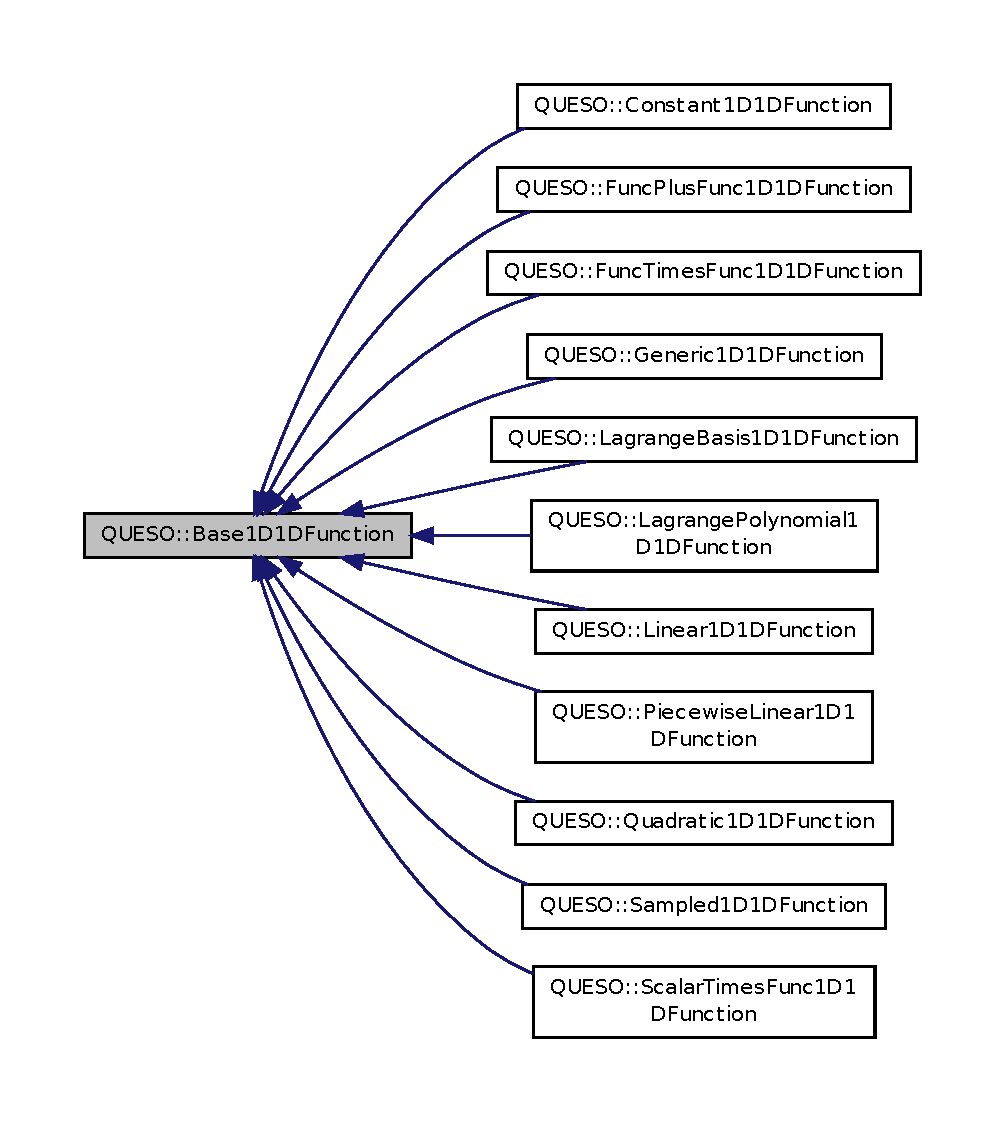
\includegraphics[width=350pt]{class_q_u_e_s_o_1_1_base1_d1_d_function__inherit__graph}
\end{center}
\end{figure}
\subsection*{Public Member Functions}
\begin{Indent}{\bf Constructor/\-Destructor methods}\par
\begin{DoxyCompactItemize}
\item 
\hyperlink{class_q_u_e_s_o_1_1_base1_d1_d_function_a8e8c0f8d500675e4acfd4d7043000791}{Base1\-D1\-D\-Function} (double \hyperlink{class_q_u_e_s_o_1_1_base1_d1_d_function_a4c110e621ef1ac557bbcc60d41f5a3c2}{min\-Domain\-Value}, double \hyperlink{class_q_u_e_s_o_1_1_base1_d1_d_function_ad2b80d0c52c0cb56c89f70f30b3bb19e}{max\-Domain\-Value})
\begin{DoxyCompactList}\small\item\em Default constructor. \end{DoxyCompactList}\item 
virtual \hyperlink{class_q_u_e_s_o_1_1_base1_d1_d_function_a0512da686e14fe3b0544f84432ea322e}{$\sim$\-Base1\-D1\-D\-Function} ()
\begin{DoxyCompactList}\small\item\em Destructor. \end{DoxyCompactList}\end{DoxyCompactItemize}
\end{Indent}
\begin{Indent}{\bf Mathematical methods}\par
\begin{DoxyCompactItemize}
\item 
double \hyperlink{class_q_u_e_s_o_1_1_base1_d1_d_function_a4c110e621ef1ac557bbcc60d41f5a3c2}{min\-Domain\-Value} () const 
\begin{DoxyCompactList}\small\item\em Returns the minimum value of the domain of the (one-\/dimensional) function. \end{DoxyCompactList}\item 
double \hyperlink{class_q_u_e_s_o_1_1_base1_d1_d_function_ad2b80d0c52c0cb56c89f70f30b3bb19e}{max\-Domain\-Value} () const 
\begin{DoxyCompactList}\small\item\em Returns the maximum value of the domain of the (one-\/dimensional) function. \end{DoxyCompactList}\item 
virtual double \hyperlink{class_q_u_e_s_o_1_1_base1_d1_d_function_a1042dfd930c30a35d6dbf70f94e8dfe5}{value} (double domain\-Value) const =0
\begin{DoxyCompactList}\small\item\em Returns the value of the (one-\/dimensional) function. See template specialization. \end{DoxyCompactList}\item 
virtual double \hyperlink{class_q_u_e_s_o_1_1_base1_d1_d_function_a6b8de03f2099f31735dcaf15c24bca32}{deriv} (double domain\-Value) const =0
\begin{DoxyCompactList}\small\item\em Returns the value of the derivative of the function. See template specialization. \end{DoxyCompactList}\item 
virtual double \hyperlink{class_q_u_e_s_o_1_1_base1_d1_d_function_ac41e4e15b7f97c14a0389069bf8e833d}{multiply\-And\-Integrate} (const \hyperlink{class_q_u_e_s_o_1_1_base1_d1_d_function}{Base1\-D1\-D\-Function} \&func, unsigned int quadrature\-Order, double $\ast$result\-With\-Multiplication\-By\-T\-As\-Well) const 
\begin{DoxyCompactList}\small\item\em T\-O\-D\-O\-: Multiplies {\ttfamily this} function with {\ttfamily function}, and integrates it numerically. See template specialization. \end{DoxyCompactList}\end{DoxyCompactItemize}
\end{Indent}
\subsection*{Protected Attributes}
\begin{DoxyCompactItemize}
\item 
double \hyperlink{class_q_u_e_s_o_1_1_base1_d1_d_function_a7b18b3854ee74ef5befbc67b75ebbdc5}{m\-\_\-min\-Domain\-Value}
\item 
double \hyperlink{class_q_u_e_s_o_1_1_base1_d1_d_function_aa0025999ccab2145cd46c0a81e260e8f}{m\-\_\-max\-Domain\-Value}
\end{DoxyCompactItemize}


\subsection{Detailed Description}
Class for one-\/dimensional functions. 

Base class for one-\/dimensional functions. 

Definition at line 53 of file 1\-D1\-D\-Function.\-h.



\subsection{Constructor \& Destructor Documentation}
\hypertarget{class_q_u_e_s_o_1_1_base1_d1_d_function_a8e8c0f8d500675e4acfd4d7043000791}{\index{Q\-U\-E\-S\-O\-::\-Base1\-D1\-D\-Function@{Q\-U\-E\-S\-O\-::\-Base1\-D1\-D\-Function}!Base1\-D1\-D\-Function@{Base1\-D1\-D\-Function}}
\index{Base1\-D1\-D\-Function@{Base1\-D1\-D\-Function}!QUESO::Base1D1DFunction@{Q\-U\-E\-S\-O\-::\-Base1\-D1\-D\-Function}}
\subsubsection[{Base1\-D1\-D\-Function}]{\setlength{\rightskip}{0pt plus 5cm}Q\-U\-E\-S\-O\-::\-Base1\-D1\-D\-Function\-::\-Base1\-D1\-D\-Function (
\begin{DoxyParamCaption}
\item[{double}]{min\-Domain\-Value, }
\item[{double}]{max\-Domain\-Value}
\end{DoxyParamCaption}
)}}\label{class_q_u_e_s_o_1_1_base1_d1_d_function_a8e8c0f8d500675e4acfd4d7043000791}


Default constructor. 



Definition at line 33 of file 1\-D1\-D\-Function.\-C.



References m\-\_\-max\-Domain\-Value, m\-\_\-min\-Domain\-Value, U\-Q\-\_\-\-F\-A\-T\-A\-L\-\_\-\-T\-E\-S\-T\-\_\-\-M\-A\-C\-R\-O, and Q\-U\-E\-S\-O\-::\-U\-Q\-\_\-\-U\-N\-A\-V\-A\-I\-L\-A\-B\-L\-E\-\_\-\-R\-A\-N\-K.


\begin{DoxyCode}
36   :
37   \hyperlink{class_q_u_e_s_o_1_1_base1_d1_d_function_a7b18b3854ee74ef5befbc67b75ebbdc5}{m\_minDomainValue}(\hyperlink{class_q_u_e_s_o_1_1_base1_d1_d_function_a4c110e621ef1ac557bbcc60d41f5a3c2}{minDomainValue}),
38   \hyperlink{class_q_u_e_s_o_1_1_base1_d1_d_function_aa0025999ccab2145cd46c0a81e260e8f}{m\_maxDomainValue}(\hyperlink{class_q_u_e_s_o_1_1_base1_d1_d_function_ad2b80d0c52c0cb56c89f70f30b3bb19e}{maxDomainValue})
39 \{
40   \hyperlink{_defines_8h_a56d63d18d0a6d45757de47fcc06f574d}{UQ\_FATAL\_TEST\_MACRO}(\hyperlink{class_q_u_e_s_o_1_1_base1_d1_d_function_a7b18b3854ee74ef5befbc67b75ebbdc5}{m\_minDomainValue} >= 
      \hyperlink{class_q_u_e_s_o_1_1_base1_d1_d_function_aa0025999ccab2145cd46c0a81e260e8f}{m\_maxDomainValue},
41                       \hyperlink{namespace_q_u_e_s_o_a7d4679800a430ae8e473c1c7bc0bfb21}{UQ\_UNAVAILABLE\_RANK},
42                       \textcolor{stringliteral}{"Base1D1DFunction::constructor()"},
43                       \textcolor{stringliteral}{"min >= max"});
44 \}
\end{DoxyCode}
\hypertarget{class_q_u_e_s_o_1_1_base1_d1_d_function_a0512da686e14fe3b0544f84432ea322e}{\index{Q\-U\-E\-S\-O\-::\-Base1\-D1\-D\-Function@{Q\-U\-E\-S\-O\-::\-Base1\-D1\-D\-Function}!$\sim$\-Base1\-D1\-D\-Function@{$\sim$\-Base1\-D1\-D\-Function}}
\index{$\sim$\-Base1\-D1\-D\-Function@{$\sim$\-Base1\-D1\-D\-Function}!QUESO::Base1D1DFunction@{Q\-U\-E\-S\-O\-::\-Base1\-D1\-D\-Function}}
\subsubsection[{$\sim$\-Base1\-D1\-D\-Function}]{\setlength{\rightskip}{0pt plus 5cm}Q\-U\-E\-S\-O\-::\-Base1\-D1\-D\-Function\-::$\sim$\-Base1\-D1\-D\-Function (
\begin{DoxyParamCaption}
{}
\end{DoxyParamCaption}
)\hspace{0.3cm}{\ttfamily [virtual]}}}\label{class_q_u_e_s_o_1_1_base1_d1_d_function_a0512da686e14fe3b0544f84432ea322e}


Destructor. 



Definition at line 46 of file 1\-D1\-D\-Function.\-C.


\begin{DoxyCode}
47 \{
48 \}
\end{DoxyCode}


\subsection{Member Function Documentation}
\hypertarget{class_q_u_e_s_o_1_1_base1_d1_d_function_a6b8de03f2099f31735dcaf15c24bca32}{\index{Q\-U\-E\-S\-O\-::\-Base1\-D1\-D\-Function@{Q\-U\-E\-S\-O\-::\-Base1\-D1\-D\-Function}!deriv@{deriv}}
\index{deriv@{deriv}!QUESO::Base1D1DFunction@{Q\-U\-E\-S\-O\-::\-Base1\-D1\-D\-Function}}
\subsubsection[{deriv}]{\setlength{\rightskip}{0pt plus 5cm}virtual double Q\-U\-E\-S\-O\-::\-Base1\-D1\-D\-Function\-::deriv (
\begin{DoxyParamCaption}
\item[{double}]{domain\-Value}
\end{DoxyParamCaption}
) const\hspace{0.3cm}{\ttfamily [pure virtual]}}}\label{class_q_u_e_s_o_1_1_base1_d1_d_function_a6b8de03f2099f31735dcaf15c24bca32}


Returns the value of the derivative of the function. See template specialization. 



Implemented in \hyperlink{class_q_u_e_s_o_1_1_lagrange_basis1_d1_d_function_a2c804510956c3eb8f81bf5eb6fe7939c}{Q\-U\-E\-S\-O\-::\-Lagrange\-Basis1\-D1\-D\-Function}, \hyperlink{class_q_u_e_s_o_1_1_lagrange_polynomial1_d1_d_function_a202ba706747ba35cf699799fbc3dbb8b}{Q\-U\-E\-S\-O\-::\-Lagrange\-Polynomial1\-D1\-D\-Function}, \hyperlink{class_q_u_e_s_o_1_1_func_plus_func1_d1_d_function_a37e3b0d0b5655b555cde6674e382a36e}{Q\-U\-E\-S\-O\-::\-Func\-Plus\-Func1\-D1\-D\-Function}, \hyperlink{class_q_u_e_s_o_1_1_func_times_func1_d1_d_function_aac7e1e05101253947079615bf7b5ce6b}{Q\-U\-E\-S\-O\-::\-Func\-Times\-Func1\-D1\-D\-Function}, \hyperlink{class_q_u_e_s_o_1_1_scalar_times_func1_d1_d_function_a60d05664b27b5b40cb31d38dc61c74ee}{Q\-U\-E\-S\-O\-::\-Scalar\-Times\-Func1\-D1\-D\-Function}, \hyperlink{class_q_u_e_s_o_1_1_sampled1_d1_d_function_a5579fd73a76c5f82b6f55472c8123bb7}{Q\-U\-E\-S\-O\-::\-Sampled1\-D1\-D\-Function}, \hyperlink{class_q_u_e_s_o_1_1_piecewise_linear1_d1_d_function_aa83d79e691a7cf47dc860e20c75a0cd0}{Q\-U\-E\-S\-O\-::\-Piecewise\-Linear1\-D1\-D\-Function}, \hyperlink{class_q_u_e_s_o_1_1_linear1_d1_d_function_abd3ccc80ea449d8a20afb2efc22b131a}{Q\-U\-E\-S\-O\-::\-Linear1\-D1\-D\-Function}, \hyperlink{class_q_u_e_s_o_1_1_constant1_d1_d_function_af8f16be24483611f20246f67047e330b}{Q\-U\-E\-S\-O\-::\-Constant1\-D1\-D\-Function}, and \hyperlink{class_q_u_e_s_o_1_1_generic1_d1_d_function_a6e7f189c2cf7f0a88573a23a88229566}{Q\-U\-E\-S\-O\-::\-Generic1\-D1\-D\-Function}.

\hypertarget{class_q_u_e_s_o_1_1_base1_d1_d_function_ad2b80d0c52c0cb56c89f70f30b3bb19e}{\index{Q\-U\-E\-S\-O\-::\-Base1\-D1\-D\-Function@{Q\-U\-E\-S\-O\-::\-Base1\-D1\-D\-Function}!max\-Domain\-Value@{max\-Domain\-Value}}
\index{max\-Domain\-Value@{max\-Domain\-Value}!QUESO::Base1D1DFunction@{Q\-U\-E\-S\-O\-::\-Base1\-D1\-D\-Function}}
\subsubsection[{max\-Domain\-Value}]{\setlength{\rightskip}{0pt plus 5cm}double Q\-U\-E\-S\-O\-::\-Base1\-D1\-D\-Function\-::max\-Domain\-Value (
\begin{DoxyParamCaption}
{}
\end{DoxyParamCaption}
) const}}\label{class_q_u_e_s_o_1_1_base1_d1_d_function_ad2b80d0c52c0cb56c89f70f30b3bb19e}


Returns the maximum value of the domain of the (one-\/dimensional) function. 



Definition at line 57 of file 1\-D1\-D\-Function.\-C.



References m\-\_\-max\-Domain\-Value.


\begin{DoxyCode}
58 \{
59   \textcolor{keywordflow}{return} \hyperlink{class_q_u_e_s_o_1_1_base1_d1_d_function_aa0025999ccab2145cd46c0a81e260e8f}{m\_maxDomainValue};
60 \}
\end{DoxyCode}
\hypertarget{class_q_u_e_s_o_1_1_base1_d1_d_function_a4c110e621ef1ac557bbcc60d41f5a3c2}{\index{Q\-U\-E\-S\-O\-::\-Base1\-D1\-D\-Function@{Q\-U\-E\-S\-O\-::\-Base1\-D1\-D\-Function}!min\-Domain\-Value@{min\-Domain\-Value}}
\index{min\-Domain\-Value@{min\-Domain\-Value}!QUESO::Base1D1DFunction@{Q\-U\-E\-S\-O\-::\-Base1\-D1\-D\-Function}}
\subsubsection[{min\-Domain\-Value}]{\setlength{\rightskip}{0pt plus 5cm}double Q\-U\-E\-S\-O\-::\-Base1\-D1\-D\-Function\-::min\-Domain\-Value (
\begin{DoxyParamCaption}
{}
\end{DoxyParamCaption}
) const}}\label{class_q_u_e_s_o_1_1_base1_d1_d_function_a4c110e621ef1ac557bbcc60d41f5a3c2}


Returns the minimum value of the domain of the (one-\/dimensional) function. 



Definition at line 51 of file 1\-D1\-D\-Function.\-C.



References m\-\_\-min\-Domain\-Value.


\begin{DoxyCode}
52 \{
53   \textcolor{keywordflow}{return} \hyperlink{class_q_u_e_s_o_1_1_base1_d1_d_function_a7b18b3854ee74ef5befbc67b75ebbdc5}{m\_minDomainValue};
54 \}
\end{DoxyCode}
\hypertarget{class_q_u_e_s_o_1_1_base1_d1_d_function_ac41e4e15b7f97c14a0389069bf8e833d}{\index{Q\-U\-E\-S\-O\-::\-Base1\-D1\-D\-Function@{Q\-U\-E\-S\-O\-::\-Base1\-D1\-D\-Function}!multiply\-And\-Integrate@{multiply\-And\-Integrate}}
\index{multiply\-And\-Integrate@{multiply\-And\-Integrate}!QUESO::Base1D1DFunction@{Q\-U\-E\-S\-O\-::\-Base1\-D1\-D\-Function}}
\subsubsection[{multiply\-And\-Integrate}]{\setlength{\rightskip}{0pt plus 5cm}double Q\-U\-E\-S\-O\-::\-Base1\-D1\-D\-Function\-::multiply\-And\-Integrate (
\begin{DoxyParamCaption}
\item[{const {\bf Base1\-D1\-D\-Function} \&}]{func, }
\item[{unsigned int}]{quadrature\-Order, }
\item[{double $\ast$}]{result\-With\-Multiplication\-By\-T\-As\-Well}
\end{DoxyParamCaption}
) const\hspace{0.3cm}{\ttfamily [virtual]}}}\label{class_q_u_e_s_o_1_1_base1_d1_d_function_ac41e4e15b7f97c14a0389069bf8e833d}


T\-O\-D\-O\-: Multiplies {\ttfamily this} function with {\ttfamily function}, and integrates it numerically. See template specialization. 

\begin{DoxyRefDesc}{Todo}
\item[\hyperlink{todo__todo000004}{Todo}]\-: Please, implement me! \end{DoxyRefDesc}


Definition at line 63 of file 1\-D1\-D\-Function.\-C.



References U\-Q\-\_\-\-F\-A\-T\-A\-L\-\_\-\-T\-E\-S\-T\-\_\-\-M\-A\-C\-R\-O, Q\-U\-E\-S\-O\-::\-U\-Q\-\_\-\-U\-N\-A\-V\-A\-I\-L\-A\-B\-L\-E\-\_\-\-R\-A\-N\-K, and value().


\begin{DoxyCode}
64 \{
65   \textcolor{keywordtype}{double} \hyperlink{class_q_u_e_s_o_1_1_base1_d1_d_function_a1042dfd930c30a35d6dbf70f94e8dfe5}{value} = 0.;
66 
67   \hyperlink{_defines_8h_a56d63d18d0a6d45757de47fcc06f574d}{UQ\_FATAL\_TEST\_MACRO}(\textcolor{keyword}{true},
68                       \hyperlink{namespace_q_u_e_s_o_a7d4679800a430ae8e473c1c7bc0bfb21}{UQ\_UNAVAILABLE\_RANK},
69                       \textcolor{stringliteral}{"Base1D1DFunction::multiplyAndIntegrate()"},
70                       \textcolor{stringliteral}{"not implemented yet"});
71 
72   \textcolor{keywordflow}{if} (resultWithMultiplicationByTAsWell) \{ \textcolor{comment}{// Just to eliminate INTEL compiler warnings}
73     func.value((\textcolor{keywordtype}{double}) quadratureOrder);
74   \}
75 
76   \textcolor{keywordflow}{return} \hyperlink{class_q_u_e_s_o_1_1_base1_d1_d_function_a1042dfd930c30a35d6dbf70f94e8dfe5}{value};
77 \}
\end{DoxyCode}
\hypertarget{class_q_u_e_s_o_1_1_base1_d1_d_function_a1042dfd930c30a35d6dbf70f94e8dfe5}{\index{Q\-U\-E\-S\-O\-::\-Base1\-D1\-D\-Function@{Q\-U\-E\-S\-O\-::\-Base1\-D1\-D\-Function}!value@{value}}
\index{value@{value}!QUESO::Base1D1DFunction@{Q\-U\-E\-S\-O\-::\-Base1\-D1\-D\-Function}}
\subsubsection[{value}]{\setlength{\rightskip}{0pt plus 5cm}virtual double Q\-U\-E\-S\-O\-::\-Base1\-D1\-D\-Function\-::value (
\begin{DoxyParamCaption}
\item[{double}]{domain\-Value}
\end{DoxyParamCaption}
) const\hspace{0.3cm}{\ttfamily [pure virtual]}}}\label{class_q_u_e_s_o_1_1_base1_d1_d_function_a1042dfd930c30a35d6dbf70f94e8dfe5}


Returns the value of the (one-\/dimensional) function. See template specialization. 



Implemented in \hyperlink{class_q_u_e_s_o_1_1_lagrange_basis1_d1_d_function_ae41dda050ae3e18f057a44fb2d64b6d2}{Q\-U\-E\-S\-O\-::\-Lagrange\-Basis1\-D1\-D\-Function}, \hyperlink{class_q_u_e_s_o_1_1_lagrange_polynomial1_d1_d_function_ada2741739cc9ff0fe98bb51e690df072}{Q\-U\-E\-S\-O\-::\-Lagrange\-Polynomial1\-D1\-D\-Function}, \hyperlink{class_q_u_e_s_o_1_1_func_plus_func1_d1_d_function_a9e7a69d195d586fa982c6088ff6a7007}{Q\-U\-E\-S\-O\-::\-Func\-Plus\-Func1\-D1\-D\-Function}, \hyperlink{class_q_u_e_s_o_1_1_func_times_func1_d1_d_function_adebec22c4730abfe9d5000785a77d000}{Q\-U\-E\-S\-O\-::\-Func\-Times\-Func1\-D1\-D\-Function}, \hyperlink{class_q_u_e_s_o_1_1_scalar_times_func1_d1_d_function_af3ff65dedf376a0acde1df1f70fdfd51}{Q\-U\-E\-S\-O\-::\-Scalar\-Times\-Func1\-D1\-D\-Function}, \hyperlink{class_q_u_e_s_o_1_1_sampled1_d1_d_function_a779a96683625c9bf6a161cf98ab63f9b}{Q\-U\-E\-S\-O\-::\-Sampled1\-D1\-D\-Function}, \hyperlink{class_q_u_e_s_o_1_1_piecewise_linear1_d1_d_function_a977ad3478bf488b1e3d472f31c3fe146}{Q\-U\-E\-S\-O\-::\-Piecewise\-Linear1\-D1\-D\-Function}, \hyperlink{class_q_u_e_s_o_1_1_linear1_d1_d_function_a4264993c026b0a55af32131027c923ff}{Q\-U\-E\-S\-O\-::\-Linear1\-D1\-D\-Function}, \hyperlink{class_q_u_e_s_o_1_1_constant1_d1_d_function_aa80d085d1b5744396df97ec74055cf1f}{Q\-U\-E\-S\-O\-::\-Constant1\-D1\-D\-Function}, and \hyperlink{class_q_u_e_s_o_1_1_generic1_d1_d_function_a4ed092b36144d91ac573e871062cca16}{Q\-U\-E\-S\-O\-::\-Generic1\-D1\-D\-Function}.



Referenced by multiply\-And\-Integrate(), Q\-U\-E\-S\-O\-::\-Sub\-F1\-F2\-Gaussian2d\-Kde\-Integral(), Q\-U\-E\-S\-O\-::\-Scalar\-Times\-Func1\-D1\-D\-Function\-::value(), Q\-U\-E\-S\-O\-::\-Func\-Times\-Func1\-D1\-D\-Function\-::value(), and Q\-U\-E\-S\-O\-::\-Func\-Plus\-Func1\-D1\-D\-Function\-::value().



\subsection{Member Data Documentation}
\hypertarget{class_q_u_e_s_o_1_1_base1_d1_d_function_aa0025999ccab2145cd46c0a81e260e8f}{\index{Q\-U\-E\-S\-O\-::\-Base1\-D1\-D\-Function@{Q\-U\-E\-S\-O\-::\-Base1\-D1\-D\-Function}!m\-\_\-max\-Domain\-Value@{m\-\_\-max\-Domain\-Value}}
\index{m\-\_\-max\-Domain\-Value@{m\-\_\-max\-Domain\-Value}!QUESO::Base1D1DFunction@{Q\-U\-E\-S\-O\-::\-Base1\-D1\-D\-Function}}
\subsubsection[{m\-\_\-max\-Domain\-Value}]{\setlength{\rightskip}{0pt plus 5cm}double Q\-U\-E\-S\-O\-::\-Base1\-D1\-D\-Function\-::m\-\_\-max\-Domain\-Value\hspace{0.3cm}{\ttfamily [protected]}}}\label{class_q_u_e_s_o_1_1_base1_d1_d_function_aa0025999ccab2145cd46c0a81e260e8f}


Definition at line 86 of file 1\-D1\-D\-Function.\-h.



Referenced by Base1\-D1\-D\-Function(), Q\-U\-E\-S\-O\-::\-Generic1\-D1\-D\-Function\-::deriv(), Q\-U\-E\-S\-O\-::\-Constant1\-D1\-D\-Function\-::deriv(), Q\-U\-E\-S\-O\-::\-Linear1\-D1\-D\-Function\-::deriv(), Q\-U\-E\-S\-O\-::\-Piecewise\-Linear1\-D1\-D\-Function\-::deriv(), Q\-U\-E\-S\-O\-::\-Sampled1\-D1\-D\-Function\-::deriv(), Q\-U\-E\-S\-O\-::\-Scalar\-Times\-Func1\-D1\-D\-Function\-::deriv(), Q\-U\-E\-S\-O\-::\-Func\-Times\-Func1\-D1\-D\-Function\-::deriv(), Q\-U\-E\-S\-O\-::\-Func\-Plus\-Func1\-D1\-D\-Function\-::deriv(), Q\-U\-E\-S\-O\-::\-Lagrange\-Polynomial1\-D1\-D\-Function\-::deriv(), Q\-U\-E\-S\-O\-::\-Lagrange\-Basis1\-D1\-D\-Function\-::deriv(), max\-Domain\-Value(), Q\-U\-E\-S\-O\-::\-Sampled1\-D1\-D\-Function\-::set(), Q\-U\-E\-S\-O\-::\-Generic1\-D1\-D\-Function\-::value(), Q\-U\-E\-S\-O\-::\-Constant1\-D1\-D\-Function\-::value(), Q\-U\-E\-S\-O\-::\-Linear1\-D1\-D\-Function\-::value(), Q\-U\-E\-S\-O\-::\-Piecewise\-Linear1\-D1\-D\-Function\-::value(), and Q\-U\-E\-S\-O\-::\-Sampled1\-D1\-D\-Function\-::value().

\hypertarget{class_q_u_e_s_o_1_1_base1_d1_d_function_a7b18b3854ee74ef5befbc67b75ebbdc5}{\index{Q\-U\-E\-S\-O\-::\-Base1\-D1\-D\-Function@{Q\-U\-E\-S\-O\-::\-Base1\-D1\-D\-Function}!m\-\_\-min\-Domain\-Value@{m\-\_\-min\-Domain\-Value}}
\index{m\-\_\-min\-Domain\-Value@{m\-\_\-min\-Domain\-Value}!QUESO::Base1D1DFunction@{Q\-U\-E\-S\-O\-::\-Base1\-D1\-D\-Function}}
\subsubsection[{m\-\_\-min\-Domain\-Value}]{\setlength{\rightskip}{0pt plus 5cm}double Q\-U\-E\-S\-O\-::\-Base1\-D1\-D\-Function\-::m\-\_\-min\-Domain\-Value\hspace{0.3cm}{\ttfamily [protected]}}}\label{class_q_u_e_s_o_1_1_base1_d1_d_function_a7b18b3854ee74ef5befbc67b75ebbdc5}


Definition at line 85 of file 1\-D1\-D\-Function.\-h.



Referenced by Base1\-D1\-D\-Function(), Q\-U\-E\-S\-O\-::\-Generic1\-D1\-D\-Function\-::deriv(), Q\-U\-E\-S\-O\-::\-Constant1\-D1\-D\-Function\-::deriv(), Q\-U\-E\-S\-O\-::\-Linear1\-D1\-D\-Function\-::deriv(), Q\-U\-E\-S\-O\-::\-Piecewise\-Linear1\-D1\-D\-Function\-::deriv(), Q\-U\-E\-S\-O\-::\-Sampled1\-D1\-D\-Function\-::deriv(), Q\-U\-E\-S\-O\-::\-Scalar\-Times\-Func1\-D1\-D\-Function\-::deriv(), Q\-U\-E\-S\-O\-::\-Func\-Times\-Func1\-D1\-D\-Function\-::deriv(), Q\-U\-E\-S\-O\-::\-Func\-Plus\-Func1\-D1\-D\-Function\-::deriv(), Q\-U\-E\-S\-O\-::\-Lagrange\-Polynomial1\-D1\-D\-Function\-::deriv(), Q\-U\-E\-S\-O\-::\-Lagrange\-Basis1\-D1\-D\-Function\-::deriv(), min\-Domain\-Value(), Q\-U\-E\-S\-O\-::\-Sampled1\-D1\-D\-Function\-::set(), Q\-U\-E\-S\-O\-::\-Generic1\-D1\-D\-Function\-::value(), Q\-U\-E\-S\-O\-::\-Constant1\-D1\-D\-Function\-::value(), Q\-U\-E\-S\-O\-::\-Linear1\-D1\-D\-Function\-::value(), Q\-U\-E\-S\-O\-::\-Piecewise\-Linear1\-D1\-D\-Function\-::value(), and Q\-U\-E\-S\-O\-::\-Sampled1\-D1\-D\-Function\-::value().



The documentation for this class was generated from the following files\-:\begin{DoxyCompactItemize}
\item 
src/misc/inc/\hyperlink{1_d1_d_function_8h}{1\-D1\-D\-Function.\-h}\item 
src/misc/src/\hyperlink{1_d1_d_function_8_c}{1\-D1\-D\-Function.\-C}\end{DoxyCompactItemize}

\hypertarget{class_q_u_e_s_o_1_1_base1_d_quadrature}{\section{Q\-U\-E\-S\-O\-:\-:Base1\-D\-Quadrature Class Reference}
\label{class_q_u_e_s_o_1_1_base1_d_quadrature}\index{Q\-U\-E\-S\-O\-::\-Base1\-D\-Quadrature@{Q\-U\-E\-S\-O\-::\-Base1\-D\-Quadrature}}
}


Base class for one-\/dimensional quadrature rules (numerical integration of functions).  




{\ttfamily \#include $<$1\-D\-Quadrature.\-h$>$}



Inheritance diagram for Q\-U\-E\-S\-O\-:\-:Base1\-D\-Quadrature\-:
\nopagebreak
\begin{figure}[H]
\begin{center}
\leavevmode
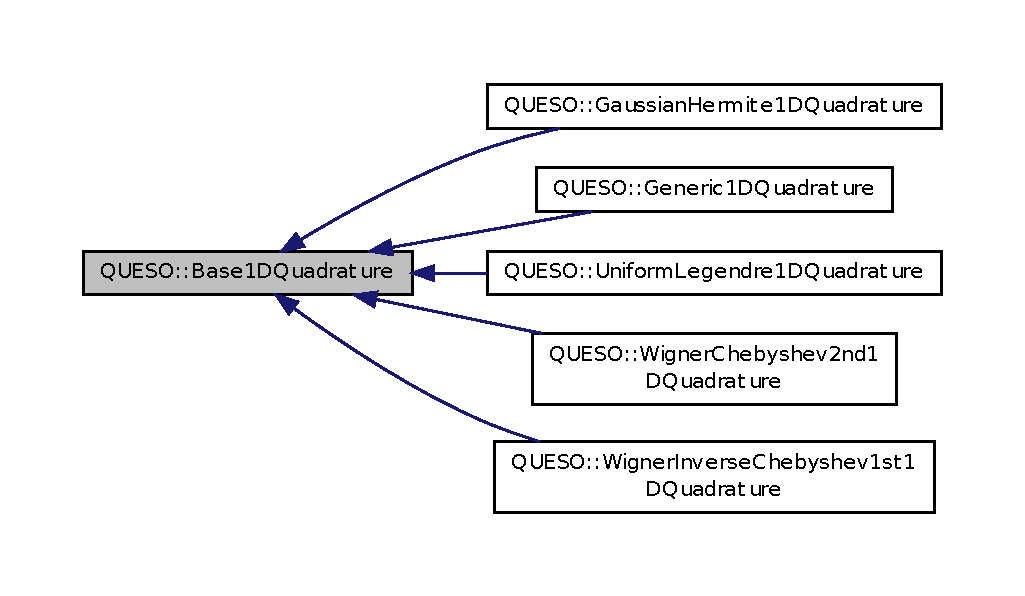
\includegraphics[width=350pt]{class_q_u_e_s_o_1_1_base1_d_quadrature__inherit__graph}
\end{center}
\end{figure}
\subsection*{Public Member Functions}
\begin{Indent}{\bf Constructor/\-Destructor methods}\par
\begin{DoxyCompactItemize}
\item 
\hyperlink{class_q_u_e_s_o_1_1_base1_d_quadrature_a78007aa675ab263a24d86774e8b98c28}{Base1\-D\-Quadrature} (double \hyperlink{class_q_u_e_s_o_1_1_base1_d_quadrature_a938187458b0069e7b3779bc3739a1cc0}{min\-Domain\-Value}, double \hyperlink{class_q_u_e_s_o_1_1_base1_d_quadrature_af3d09abe6716a23f9061b8b657524547}{max\-Domain\-Value}, unsigned int \hyperlink{class_q_u_e_s_o_1_1_base1_d_quadrature_a07713b5e8df24bbc8e3e9d13b707e5d0}{order})
\begin{DoxyCompactList}\small\item\em Default constructor. \end{DoxyCompactList}\item 
virtual \hyperlink{class_q_u_e_s_o_1_1_base1_d_quadrature_acb90cfc1106240a7a48579e0594c7e17}{$\sim$\-Base1\-D\-Quadrature} ()
\begin{DoxyCompactList}\small\item\em Virtual destructor. \end{DoxyCompactList}\end{DoxyCompactItemize}
\end{Indent}
\begin{Indent}{\bf Mathematical methods}\par
\begin{DoxyCompactItemize}
\item 
double \hyperlink{class_q_u_e_s_o_1_1_base1_d_quadrature_a938187458b0069e7b3779bc3739a1cc0}{min\-Domain\-Value} () const 
\begin{DoxyCompactList}\small\item\em Returns the minimum value of the domain of the (one-\/dimensional) function. \end{DoxyCompactList}\item 
double \hyperlink{class_q_u_e_s_o_1_1_base1_d_quadrature_af3d09abe6716a23f9061b8b657524547}{max\-Domain\-Value} () const 
\begin{DoxyCompactList}\small\item\em Returns the maximum value of the domain of the (one-\/dimensional) function. \end{DoxyCompactList}\item 
unsigned int \hyperlink{class_q_u_e_s_o_1_1_base1_d_quadrature_a07713b5e8df24bbc8e3e9d13b707e5d0}{order} () const 
\begin{DoxyCompactList}\small\item\em Returns the order of the quadrature rule. \end{DoxyCompactList}\item 
const std\-::vector$<$ double $>$ \& \hyperlink{class_q_u_e_s_o_1_1_base1_d_quadrature_a9f5d9b6e20b5105e2c17b7da1b71c259}{positions} () const 
\begin{DoxyCompactList}\small\item\em Array of the positions for the numerical integration. \end{DoxyCompactList}\item 
const std\-::vector$<$ double $>$ \& \hyperlink{class_q_u_e_s_o_1_1_base1_d_quadrature_a5780ce2b5ef26ce0f5183e8e32358cee}{weights} () const 
\begin{DoxyCompactList}\small\item\em Array of the weights used in the numerical integration. \end{DoxyCompactList}\item 
virtual void \hyperlink{class_q_u_e_s_o_1_1_base1_d_quadrature_a37bdd63ba8b986e02d47b05fc8795332}{dumb\-Routine} () const =0
\begin{DoxyCompactList}\small\item\em A bogus method. \end{DoxyCompactList}\end{DoxyCompactItemize}
\end{Indent}
\subsection*{Protected Attributes}
\begin{DoxyCompactItemize}
\item 
double \hyperlink{class_q_u_e_s_o_1_1_base1_d_quadrature_a7165680498394fa2d23ac919a920fc01}{m\-\_\-min\-Domain\-Value}
\item 
double \hyperlink{class_q_u_e_s_o_1_1_base1_d_quadrature_ace30af8dd67b04f11ea37ebe509f256e}{m\-\_\-max\-Domain\-Value}
\item 
unsigned int \hyperlink{class_q_u_e_s_o_1_1_base1_d_quadrature_a78ba0750b7220b302e4cd1415c7d4c48}{m\-\_\-order}
\item 
std\-::vector$<$ double $>$ \hyperlink{class_q_u_e_s_o_1_1_base1_d_quadrature_aeda387c028c3ba89ea0f9637a2234212}{m\-\_\-positions}
\item 
std\-::vector$<$ double $>$ \hyperlink{class_q_u_e_s_o_1_1_base1_d_quadrature_a7117fec020a8098d1c22b604268bad93}{m\-\_\-weights}
\end{DoxyCompactItemize}


\subsection{Detailed Description}
Base class for one-\/dimensional quadrature rules (numerical integration of functions). 

Base class for numerical integration via quadrature rules of one-\/dimensional functions. 

Definition at line 47 of file 1\-D\-Quadrature.\-h.



\subsection{Constructor \& Destructor Documentation}
\hypertarget{class_q_u_e_s_o_1_1_base1_d_quadrature_a78007aa675ab263a24d86774e8b98c28}{\index{Q\-U\-E\-S\-O\-::\-Base1\-D\-Quadrature@{Q\-U\-E\-S\-O\-::\-Base1\-D\-Quadrature}!Base1\-D\-Quadrature@{Base1\-D\-Quadrature}}
\index{Base1\-D\-Quadrature@{Base1\-D\-Quadrature}!QUESO::Base1DQuadrature@{Q\-U\-E\-S\-O\-::\-Base1\-D\-Quadrature}}
\subsubsection[{Base1\-D\-Quadrature}]{\setlength{\rightskip}{0pt plus 5cm}Q\-U\-E\-S\-O\-::\-Base1\-D\-Quadrature\-::\-Base1\-D\-Quadrature (
\begin{DoxyParamCaption}
\item[{double}]{min\-Domain\-Value, }
\item[{double}]{max\-Domain\-Value, }
\item[{unsigned int}]{order}
\end{DoxyParamCaption}
)}}\label{class_q_u_e_s_o_1_1_base1_d_quadrature_a78007aa675ab263a24d86774e8b98c28}


Default constructor. 



Definition at line 32 of file 1\-D\-Quadrature.\-C.



References m\-\_\-max\-Domain\-Value, m\-\_\-min\-Domain\-Value, U\-Q\-\_\-\-F\-A\-T\-A\-L\-\_\-\-T\-E\-S\-T\-\_\-\-M\-A\-C\-R\-O, and Q\-U\-E\-S\-O\-::\-U\-Q\-\_\-\-U\-N\-A\-V\-A\-I\-L\-A\-B\-L\-E\-\_\-\-R\-A\-N\-K.


\begin{DoxyCode}
36   :
37   \hyperlink{class_q_u_e_s_o_1_1_base1_d_quadrature_a7165680498394fa2d23ac919a920fc01}{m\_minDomainValue}(\hyperlink{class_q_u_e_s_o_1_1_base1_d_quadrature_a938187458b0069e7b3779bc3739a1cc0}{minDomainValue}),
38   \hyperlink{class_q_u_e_s_o_1_1_base1_d_quadrature_ace30af8dd67b04f11ea37ebe509f256e}{m\_maxDomainValue}(\hyperlink{class_q_u_e_s_o_1_1_base1_d_quadrature_af3d09abe6716a23f9061b8b657524547}{maxDomainValue}),
39   \hyperlink{class_q_u_e_s_o_1_1_base1_d_quadrature_a78ba0750b7220b302e4cd1415c7d4c48}{m\_order}         (\hyperlink{class_q_u_e_s_o_1_1_base1_d_quadrature_a07713b5e8df24bbc8e3e9d13b707e5d0}{order}),
40   \hyperlink{class_q_u_e_s_o_1_1_base1_d_quadrature_aeda387c028c3ba89ea0f9637a2234212}{m\_positions}     (0),
41   \hyperlink{class_q_u_e_s_o_1_1_base1_d_quadrature_a7117fec020a8098d1c22b604268bad93}{m\_weights}       (0)
42 \{
43   \hyperlink{_defines_8h_a56d63d18d0a6d45757de47fcc06f574d}{UQ\_FATAL\_TEST\_MACRO}(\hyperlink{class_q_u_e_s_o_1_1_base1_d_quadrature_a7165680498394fa2d23ac919a920fc01}{m\_minDomainValue} >= 
      \hyperlink{class_q_u_e_s_o_1_1_base1_d_quadrature_ace30af8dd67b04f11ea37ebe509f256e}{m\_maxDomainValue},
44                       \hyperlink{namespace_q_u_e_s_o_a7d4679800a430ae8e473c1c7bc0bfb21}{UQ\_UNAVAILABLE\_RANK},
45                       \textcolor{stringliteral}{"Base1DQuadrature::constructor()"},
46                       \textcolor{stringliteral}{"min >= max"});
47   \textcolor{comment}{//UQ\_FATAL\_TEST\_MACRO(order == 0, // eep2011}
48   \textcolor{comment}{//                    UQ\_UNAVAILABLE\_RANK,}
49   \textcolor{comment}{//                    "Base1DQuadrature::constructor()",}
50   \textcolor{comment}{//                    "order = 0");}
51 \}
\end{DoxyCode}
\hypertarget{class_q_u_e_s_o_1_1_base1_d_quadrature_acb90cfc1106240a7a48579e0594c7e17}{\index{Q\-U\-E\-S\-O\-::\-Base1\-D\-Quadrature@{Q\-U\-E\-S\-O\-::\-Base1\-D\-Quadrature}!$\sim$\-Base1\-D\-Quadrature@{$\sim$\-Base1\-D\-Quadrature}}
\index{$\sim$\-Base1\-D\-Quadrature@{$\sim$\-Base1\-D\-Quadrature}!QUESO::Base1DQuadrature@{Q\-U\-E\-S\-O\-::\-Base1\-D\-Quadrature}}
\subsubsection[{$\sim$\-Base1\-D\-Quadrature}]{\setlength{\rightskip}{0pt plus 5cm}Q\-U\-E\-S\-O\-::\-Base1\-D\-Quadrature\-::$\sim$\-Base1\-D\-Quadrature (
\begin{DoxyParamCaption}
{}
\end{DoxyParamCaption}
)\hspace{0.3cm}{\ttfamily [virtual]}}}\label{class_q_u_e_s_o_1_1_base1_d_quadrature_acb90cfc1106240a7a48579e0594c7e17}


Virtual destructor. 



Definition at line 53 of file 1\-D\-Quadrature.\-C.


\begin{DoxyCode}
54 \{
55 \}
\end{DoxyCode}


\subsection{Member Function Documentation}
\hypertarget{class_q_u_e_s_o_1_1_base1_d_quadrature_a37bdd63ba8b986e02d47b05fc8795332}{\index{Q\-U\-E\-S\-O\-::\-Base1\-D\-Quadrature@{Q\-U\-E\-S\-O\-::\-Base1\-D\-Quadrature}!dumb\-Routine@{dumb\-Routine}}
\index{dumb\-Routine@{dumb\-Routine}!QUESO::Base1DQuadrature@{Q\-U\-E\-S\-O\-::\-Base1\-D\-Quadrature}}
\subsubsection[{dumb\-Routine}]{\setlength{\rightskip}{0pt plus 5cm}virtual void Q\-U\-E\-S\-O\-::\-Base1\-D\-Quadrature\-::dumb\-Routine (
\begin{DoxyParamCaption}
{}
\end{DoxyParamCaption}
) const\hspace{0.3cm}{\ttfamily [pure virtual]}}}\label{class_q_u_e_s_o_1_1_base1_d_quadrature_a37bdd63ba8b986e02d47b05fc8795332}


A bogus method. 



Implemented in \hyperlink{class_q_u_e_s_o_1_1_wigner_chebyshev2nd1_d_quadrature_a1be91acea2adbbaf5f61a408d66737fb}{Q\-U\-E\-S\-O\-::\-Wigner\-Chebyshev2nd1\-D\-Quadrature}, \hyperlink{class_q_u_e_s_o_1_1_wigner_inverse_chebyshev1st1_d_quadrature_aacf526849bf3bcec245d12f14d24352d}{Q\-U\-E\-S\-O\-::\-Wigner\-Inverse\-Chebyshev1st1\-D\-Quadrature}, \hyperlink{class_q_u_e_s_o_1_1_gaussian_hermite1_d_quadrature_ae622aec1b3ed4d5b1630825819322090}{Q\-U\-E\-S\-O\-::\-Gaussian\-Hermite1\-D\-Quadrature}, \hyperlink{class_q_u_e_s_o_1_1_uniform_legendre1_d_quadrature_a4d63fb6517b84b37e47da5cea15bc2b1}{Q\-U\-E\-S\-O\-::\-Uniform\-Legendre1\-D\-Quadrature}, and \hyperlink{class_q_u_e_s_o_1_1_generic1_d_quadrature_a365701bda9fba17fdf5498436722cdde}{Q\-U\-E\-S\-O\-::\-Generic1\-D\-Quadrature}.

\hypertarget{class_q_u_e_s_o_1_1_base1_d_quadrature_af3d09abe6716a23f9061b8b657524547}{\index{Q\-U\-E\-S\-O\-::\-Base1\-D\-Quadrature@{Q\-U\-E\-S\-O\-::\-Base1\-D\-Quadrature}!max\-Domain\-Value@{max\-Domain\-Value}}
\index{max\-Domain\-Value@{max\-Domain\-Value}!QUESO::Base1DQuadrature@{Q\-U\-E\-S\-O\-::\-Base1\-D\-Quadrature}}
\subsubsection[{max\-Domain\-Value}]{\setlength{\rightskip}{0pt plus 5cm}double Q\-U\-E\-S\-O\-::\-Base1\-D\-Quadrature\-::max\-Domain\-Value (
\begin{DoxyParamCaption}
{}
\end{DoxyParamCaption}
) const}}\label{class_q_u_e_s_o_1_1_base1_d_quadrature_af3d09abe6716a23f9061b8b657524547}


Returns the maximum value of the domain of the (one-\/dimensional) function. 



Definition at line 64 of file 1\-D\-Quadrature.\-C.



References m\-\_\-max\-Domain\-Value.


\begin{DoxyCode}
65 \{
66   \textcolor{keywordflow}{return} \hyperlink{class_q_u_e_s_o_1_1_base1_d_quadrature_ace30af8dd67b04f11ea37ebe509f256e}{m\_maxDomainValue};
67 \}
\end{DoxyCode}
\hypertarget{class_q_u_e_s_o_1_1_base1_d_quadrature_a938187458b0069e7b3779bc3739a1cc0}{\index{Q\-U\-E\-S\-O\-::\-Base1\-D\-Quadrature@{Q\-U\-E\-S\-O\-::\-Base1\-D\-Quadrature}!min\-Domain\-Value@{min\-Domain\-Value}}
\index{min\-Domain\-Value@{min\-Domain\-Value}!QUESO::Base1DQuadrature@{Q\-U\-E\-S\-O\-::\-Base1\-D\-Quadrature}}
\subsubsection[{min\-Domain\-Value}]{\setlength{\rightskip}{0pt plus 5cm}double Q\-U\-E\-S\-O\-::\-Base1\-D\-Quadrature\-::min\-Domain\-Value (
\begin{DoxyParamCaption}
{}
\end{DoxyParamCaption}
) const}}\label{class_q_u_e_s_o_1_1_base1_d_quadrature_a938187458b0069e7b3779bc3739a1cc0}


Returns the minimum value of the domain of the (one-\/dimensional) function. 



Definition at line 58 of file 1\-D\-Quadrature.\-C.



References m\-\_\-min\-Domain\-Value.


\begin{DoxyCode}
59 \{
60   \textcolor{keywordflow}{return} \hyperlink{class_q_u_e_s_o_1_1_base1_d_quadrature_a7165680498394fa2d23ac919a920fc01}{m\_minDomainValue};
61 \}
\end{DoxyCode}
\hypertarget{class_q_u_e_s_o_1_1_base1_d_quadrature_a07713b5e8df24bbc8e3e9d13b707e5d0}{\index{Q\-U\-E\-S\-O\-::\-Base1\-D\-Quadrature@{Q\-U\-E\-S\-O\-::\-Base1\-D\-Quadrature}!order@{order}}
\index{order@{order}!QUESO::Base1DQuadrature@{Q\-U\-E\-S\-O\-::\-Base1\-D\-Quadrature}}
\subsubsection[{order}]{\setlength{\rightskip}{0pt plus 5cm}unsigned int Q\-U\-E\-S\-O\-::\-Base1\-D\-Quadrature\-::order (
\begin{DoxyParamCaption}
{}
\end{DoxyParamCaption}
) const}}\label{class_q_u_e_s_o_1_1_base1_d_quadrature_a07713b5e8df24bbc8e3e9d13b707e5d0}


Returns the order of the quadrature rule. 



Definition at line 70 of file 1\-D\-Quadrature.\-C.



References m\-\_\-order.


\begin{DoxyCode}
71 \{
72   \textcolor{keywordflow}{return} \hyperlink{class_q_u_e_s_o_1_1_base1_d_quadrature_a78ba0750b7220b302e4cd1415c7d4c48}{m\_order};
73 \}
\end{DoxyCode}
\hypertarget{class_q_u_e_s_o_1_1_base1_d_quadrature_a9f5d9b6e20b5105e2c17b7da1b71c259}{\index{Q\-U\-E\-S\-O\-::\-Base1\-D\-Quadrature@{Q\-U\-E\-S\-O\-::\-Base1\-D\-Quadrature}!positions@{positions}}
\index{positions@{positions}!QUESO::Base1DQuadrature@{Q\-U\-E\-S\-O\-::\-Base1\-D\-Quadrature}}
\subsubsection[{positions}]{\setlength{\rightskip}{0pt plus 5cm}const std\-::vector$<$ double $>$ \& Q\-U\-E\-S\-O\-::\-Base1\-D\-Quadrature\-::positions (
\begin{DoxyParamCaption}
{}
\end{DoxyParamCaption}
) const}}\label{class_q_u_e_s_o_1_1_base1_d_quadrature_a9f5d9b6e20b5105e2c17b7da1b71c259}


Array of the positions for the numerical integration. 



Definition at line 76 of file 1\-D\-Quadrature.\-C.



References m\-\_\-positions, U\-Q\-\_\-\-F\-A\-T\-A\-L\-\_\-\-T\-E\-S\-T\-\_\-\-M\-A\-C\-R\-O, and Q\-U\-E\-S\-O\-::\-U\-Q\-\_\-\-U\-N\-A\-V\-A\-I\-L\-A\-B\-L\-E\-\_\-\-R\-A\-N\-K.



Referenced by Q\-U\-E\-S\-O\-::\-Generic1\-D\-Quadrature\-::\-Generic1\-D\-Quadrature().


\begin{DoxyCode}
77 \{
78   \hyperlink{_defines_8h_a56d63d18d0a6d45757de47fcc06f574d}{UQ\_FATAL\_TEST\_MACRO}(\hyperlink{class_q_u_e_s_o_1_1_base1_d_quadrature_aeda387c028c3ba89ea0f9637a2234212}{m\_positions}.size() == 0,
79                       \hyperlink{namespace_q_u_e_s_o_a7d4679800a430ae8e473c1c7bc0bfb21}{UQ\_UNAVAILABLE\_RANK},
80                       \textcolor{stringliteral}{"Base1DQuadrature::positions()"},
81                       \textcolor{stringliteral}{"size = 0"});
82   \textcolor{keywordflow}{return} \hyperlink{class_q_u_e_s_o_1_1_base1_d_quadrature_aeda387c028c3ba89ea0f9637a2234212}{m\_positions};
83 \}
\end{DoxyCode}
\hypertarget{class_q_u_e_s_o_1_1_base1_d_quadrature_a5780ce2b5ef26ce0f5183e8e32358cee}{\index{Q\-U\-E\-S\-O\-::\-Base1\-D\-Quadrature@{Q\-U\-E\-S\-O\-::\-Base1\-D\-Quadrature}!weights@{weights}}
\index{weights@{weights}!QUESO::Base1DQuadrature@{Q\-U\-E\-S\-O\-::\-Base1\-D\-Quadrature}}
\subsubsection[{weights}]{\setlength{\rightskip}{0pt plus 5cm}const std\-::vector$<$ double $>$ \& Q\-U\-E\-S\-O\-::\-Base1\-D\-Quadrature\-::weights (
\begin{DoxyParamCaption}
{}
\end{DoxyParamCaption}
) const}}\label{class_q_u_e_s_o_1_1_base1_d_quadrature_a5780ce2b5ef26ce0f5183e8e32358cee}


Array of the weights used in the numerical integration. 



Definition at line 86 of file 1\-D\-Quadrature.\-C.



References m\-\_\-weights, U\-Q\-\_\-\-F\-A\-T\-A\-L\-\_\-\-T\-E\-S\-T\-\_\-\-M\-A\-C\-R\-O, and Q\-U\-E\-S\-O\-::\-U\-Q\-\_\-\-U\-N\-A\-V\-A\-I\-L\-A\-B\-L\-E\-\_\-\-R\-A\-N\-K.



Referenced by Q\-U\-E\-S\-O\-::\-Generic1\-D\-Quadrature\-::\-Generic1\-D\-Quadrature().


\begin{DoxyCode}
87 \{
88   \hyperlink{_defines_8h_a56d63d18d0a6d45757de47fcc06f574d}{UQ\_FATAL\_TEST\_MACRO}(\hyperlink{class_q_u_e_s_o_1_1_base1_d_quadrature_a7117fec020a8098d1c22b604268bad93}{m\_weights}.size() == 0,
89                       \hyperlink{namespace_q_u_e_s_o_a7d4679800a430ae8e473c1c7bc0bfb21}{UQ\_UNAVAILABLE\_RANK},
90                       \textcolor{stringliteral}{"Base1DQuadrature::weights()"},
91                       \textcolor{stringliteral}{"size = 0"});
92   \textcolor{keywordflow}{return} \hyperlink{class_q_u_e_s_o_1_1_base1_d_quadrature_a7117fec020a8098d1c22b604268bad93}{m\_weights};
93 \}
\end{DoxyCode}


\subsection{Member Data Documentation}
\hypertarget{class_q_u_e_s_o_1_1_base1_d_quadrature_ace30af8dd67b04f11ea37ebe509f256e}{\index{Q\-U\-E\-S\-O\-::\-Base1\-D\-Quadrature@{Q\-U\-E\-S\-O\-::\-Base1\-D\-Quadrature}!m\-\_\-max\-Domain\-Value@{m\-\_\-max\-Domain\-Value}}
\index{m\-\_\-max\-Domain\-Value@{m\-\_\-max\-Domain\-Value}!QUESO::Base1DQuadrature@{Q\-U\-E\-S\-O\-::\-Base1\-D\-Quadrature}}
\subsubsection[{m\-\_\-max\-Domain\-Value}]{\setlength{\rightskip}{0pt plus 5cm}double Q\-U\-E\-S\-O\-::\-Base1\-D\-Quadrature\-::m\-\_\-max\-Domain\-Value\hspace{0.3cm}{\ttfamily [protected]}}}\label{class_q_u_e_s_o_1_1_base1_d_quadrature_ace30af8dd67b04f11ea37ebe509f256e}


Definition at line 83 of file 1\-D\-Quadrature.\-h.



Referenced by Base1\-D\-Quadrature(), max\-Domain\-Value(), Q\-U\-E\-S\-O\-::\-Uniform\-Legendre1\-D\-Quadrature\-::\-Uniform\-Legendre1\-D\-Quadrature(), Q\-U\-E\-S\-O\-::\-Wigner\-Chebyshev2nd1\-D\-Quadrature\-::\-Wigner\-Chebyshev2nd1\-D\-Quadrature(), and Q\-U\-E\-S\-O\-::\-Wigner\-Inverse\-Chebyshev1st1\-D\-Quadrature\-::\-Wigner\-Inverse\-Chebyshev1st1\-D\-Quadrature().

\hypertarget{class_q_u_e_s_o_1_1_base1_d_quadrature_a7165680498394fa2d23ac919a920fc01}{\index{Q\-U\-E\-S\-O\-::\-Base1\-D\-Quadrature@{Q\-U\-E\-S\-O\-::\-Base1\-D\-Quadrature}!m\-\_\-min\-Domain\-Value@{m\-\_\-min\-Domain\-Value}}
\index{m\-\_\-min\-Domain\-Value@{m\-\_\-min\-Domain\-Value}!QUESO::Base1DQuadrature@{Q\-U\-E\-S\-O\-::\-Base1\-D\-Quadrature}}
\subsubsection[{m\-\_\-min\-Domain\-Value}]{\setlength{\rightskip}{0pt plus 5cm}double Q\-U\-E\-S\-O\-::\-Base1\-D\-Quadrature\-::m\-\_\-min\-Domain\-Value\hspace{0.3cm}{\ttfamily [protected]}}}\label{class_q_u_e_s_o_1_1_base1_d_quadrature_a7165680498394fa2d23ac919a920fc01}


Definition at line 82 of file 1\-D\-Quadrature.\-h.



Referenced by Base1\-D\-Quadrature(), min\-Domain\-Value(), Q\-U\-E\-S\-O\-::\-Uniform\-Legendre1\-D\-Quadrature\-::\-Uniform\-Legendre1\-D\-Quadrature(), Q\-U\-E\-S\-O\-::\-Wigner\-Chebyshev2nd1\-D\-Quadrature\-::\-Wigner\-Chebyshev2nd1\-D\-Quadrature(), and Q\-U\-E\-S\-O\-::\-Wigner\-Inverse\-Chebyshev1st1\-D\-Quadrature\-::\-Wigner\-Inverse\-Chebyshev1st1\-D\-Quadrature().

\hypertarget{class_q_u_e_s_o_1_1_base1_d_quadrature_a78ba0750b7220b302e4cd1415c7d4c48}{\index{Q\-U\-E\-S\-O\-::\-Base1\-D\-Quadrature@{Q\-U\-E\-S\-O\-::\-Base1\-D\-Quadrature}!m\-\_\-order@{m\-\_\-order}}
\index{m\-\_\-order@{m\-\_\-order}!QUESO::Base1DQuadrature@{Q\-U\-E\-S\-O\-::\-Base1\-D\-Quadrature}}
\subsubsection[{m\-\_\-order}]{\setlength{\rightskip}{0pt plus 5cm}unsigned int Q\-U\-E\-S\-O\-::\-Base1\-D\-Quadrature\-::m\-\_\-order\hspace{0.3cm}{\ttfamily [protected]}}}\label{class_q_u_e_s_o_1_1_base1_d_quadrature_a78ba0750b7220b302e4cd1415c7d4c48}


Definition at line 84 of file 1\-D\-Quadrature.\-h.



Referenced by Q\-U\-E\-S\-O\-::\-Gaussian\-Hermite1\-D\-Quadrature\-::\-Gaussian\-Hermite1\-D\-Quadrature(), order(), Q\-U\-E\-S\-O\-::\-Uniform\-Legendre1\-D\-Quadrature\-::\-Uniform\-Legendre1\-D\-Quadrature(), Q\-U\-E\-S\-O\-::\-Wigner\-Chebyshev2nd1\-D\-Quadrature\-::\-Wigner\-Chebyshev2nd1\-D\-Quadrature(), and Q\-U\-E\-S\-O\-::\-Wigner\-Inverse\-Chebyshev1st1\-D\-Quadrature\-::\-Wigner\-Inverse\-Chebyshev1st1\-D\-Quadrature().

\hypertarget{class_q_u_e_s_o_1_1_base1_d_quadrature_aeda387c028c3ba89ea0f9637a2234212}{\index{Q\-U\-E\-S\-O\-::\-Base1\-D\-Quadrature@{Q\-U\-E\-S\-O\-::\-Base1\-D\-Quadrature}!m\-\_\-positions@{m\-\_\-positions}}
\index{m\-\_\-positions@{m\-\_\-positions}!QUESO::Base1DQuadrature@{Q\-U\-E\-S\-O\-::\-Base1\-D\-Quadrature}}
\subsubsection[{m\-\_\-positions}]{\setlength{\rightskip}{0pt plus 5cm}std\-::vector$<$double$>$ Q\-U\-E\-S\-O\-::\-Base1\-D\-Quadrature\-::m\-\_\-positions\hspace{0.3cm}{\ttfamily [protected]}}}\label{class_q_u_e_s_o_1_1_base1_d_quadrature_aeda387c028c3ba89ea0f9637a2234212}


Definition at line 85 of file 1\-D\-Quadrature.\-h.



Referenced by Q\-U\-E\-S\-O\-::\-Gaussian\-Hermite1\-D\-Quadrature\-::\-Gaussian\-Hermite1\-D\-Quadrature(), Q\-U\-E\-S\-O\-::\-Generic1\-D\-Quadrature\-::\-Generic1\-D\-Quadrature(), positions(), Q\-U\-E\-S\-O\-::\-Uniform\-Legendre1\-D\-Quadrature\-::\-Uniform\-Legendre1\-D\-Quadrature(), Q\-U\-E\-S\-O\-::\-Wigner\-Chebyshev2nd1\-D\-Quadrature\-::\-Wigner\-Chebyshev2nd1\-D\-Quadrature(), and Q\-U\-E\-S\-O\-::\-Wigner\-Inverse\-Chebyshev1st1\-D\-Quadrature\-::\-Wigner\-Inverse\-Chebyshev1st1\-D\-Quadrature().

\hypertarget{class_q_u_e_s_o_1_1_base1_d_quadrature_a7117fec020a8098d1c22b604268bad93}{\index{Q\-U\-E\-S\-O\-::\-Base1\-D\-Quadrature@{Q\-U\-E\-S\-O\-::\-Base1\-D\-Quadrature}!m\-\_\-weights@{m\-\_\-weights}}
\index{m\-\_\-weights@{m\-\_\-weights}!QUESO::Base1DQuadrature@{Q\-U\-E\-S\-O\-::\-Base1\-D\-Quadrature}}
\subsubsection[{m\-\_\-weights}]{\setlength{\rightskip}{0pt plus 5cm}std\-::vector$<$double$>$ Q\-U\-E\-S\-O\-::\-Base1\-D\-Quadrature\-::m\-\_\-weights\hspace{0.3cm}{\ttfamily [protected]}}}\label{class_q_u_e_s_o_1_1_base1_d_quadrature_a7117fec020a8098d1c22b604268bad93}


Definition at line 86 of file 1\-D\-Quadrature.\-h.



Referenced by Q\-U\-E\-S\-O\-::\-Gaussian\-Hermite1\-D\-Quadrature\-::\-Gaussian\-Hermite1\-D\-Quadrature(), Q\-U\-E\-S\-O\-::\-Generic1\-D\-Quadrature\-::\-Generic1\-D\-Quadrature(), Q\-U\-E\-S\-O\-::\-Uniform\-Legendre1\-D\-Quadrature\-::\-Uniform\-Legendre1\-D\-Quadrature(), weights(), Q\-U\-E\-S\-O\-::\-Wigner\-Chebyshev2nd1\-D\-Quadrature\-::\-Wigner\-Chebyshev2nd1\-D\-Quadrature(), and Q\-U\-E\-S\-O\-::\-Wigner\-Inverse\-Chebyshev1st1\-D\-Quadrature\-::\-Wigner\-Inverse\-Chebyshev1st1\-D\-Quadrature().



The documentation for this class was generated from the following files\-:\begin{DoxyCompactItemize}
\item 
src/misc/inc/\hyperlink{1_d_quadrature_8h}{1\-D\-Quadrature.\-h}\item 
src/misc/src/\hyperlink{1_d_quadrature_8_c}{1\-D\-Quadrature.\-C}\end{DoxyCompactItemize}

\hypertarget{class_q_u_e_s_o_1_1_base_environment}{\section{Q\-U\-E\-S\-O\-:\-:Base\-Environment Class Reference}
\label{class_q_u_e_s_o_1_1_base_environment}\index{Q\-U\-E\-S\-O\-::\-Base\-Environment@{Q\-U\-E\-S\-O\-::\-Base\-Environment}}
}


This (virtual) class sets up the environment underlying the use of the \hyperlink{namespace_q_u_e_s_o}{Q\-U\-E\-S\-O} library by an executable.  




{\ttfamily \#include $<$Environment.\-h$>$}



Inheritance diagram for Q\-U\-E\-S\-O\-:\-:Base\-Environment\-:
\nopagebreak
\begin{figure}[H]
\begin{center}
\leavevmode
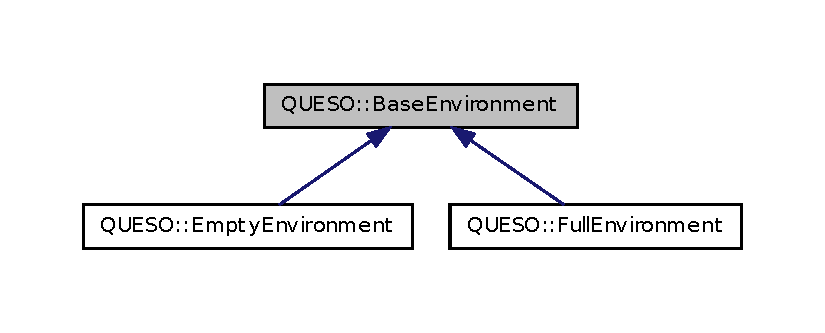
\includegraphics[width=350pt]{class_q_u_e_s_o_1_1_base_environment__inherit__graph}
\end{center}
\end{figure}


Collaboration diagram for Q\-U\-E\-S\-O\-:\-:Base\-Environment\-:
\nopagebreak
\begin{figure}[H]
\begin{center}
\leavevmode
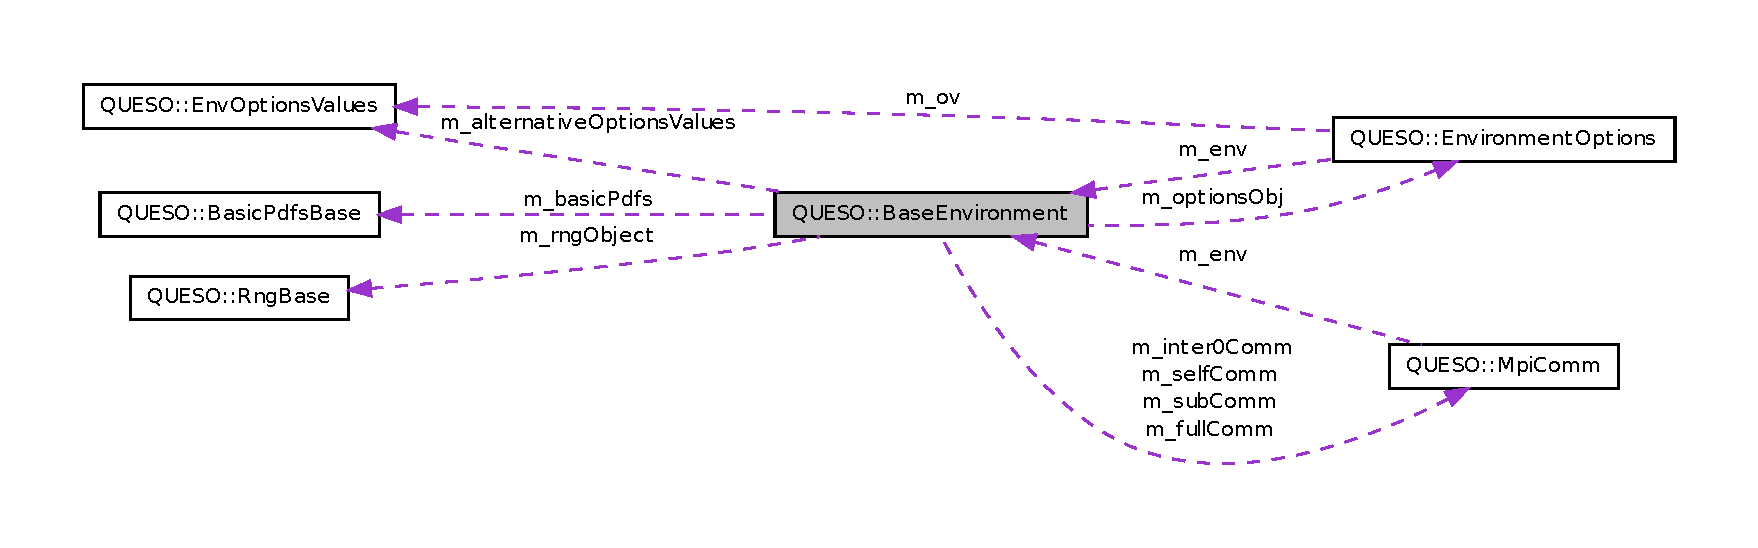
\includegraphics[width=350pt]{class_q_u_e_s_o_1_1_base_environment__coll__graph}
\end{center}
\end{figure}
\subsection*{Public Member Functions}
\begin{Indent}{\bf Constructor/\-Destructor methods}\par
\begin{DoxyCompactItemize}
\item 
\hyperlink{class_q_u_e_s_o_1_1_base_environment_a8261e797e696fdf379b0532a930db499}{Base\-Environment} (const char $\ast$passed\-Options\-Input\-File\-Name, const \hyperlink{class_q_u_e_s_o_1_1_env_options_values}{Env\-Options\-Values} $\ast$alternative\-Options\-Values)
\begin{DoxyCompactList}\small\item\em Default constructor. \end{DoxyCompactList}\item 
\hyperlink{class_q_u_e_s_o_1_1_base_environment_ab7ac89f144c0dd19217b2a137dcf1483}{Base\-Environment} (const \hyperlink{class_q_u_e_s_o_1_1_base_environment}{Base\-Environment} \&obj)
\begin{DoxyCompactList}\small\item\em Copy constructor. It should not be used be the user. \end{DoxyCompactList}\item 
virtual \hyperlink{class_q_u_e_s_o_1_1_base_environment_a769c44dce792c1c11f58031604e44504}{$\sim$\-Base\-Environment} ()
\begin{DoxyCompactList}\small\item\em Destructor. \end{DoxyCompactList}\end{DoxyCompactItemize}
\end{Indent}
\begin{Indent}{\bf Set methods}\par
\begin{DoxyCompactItemize}
\item 
\hyperlink{class_q_u_e_s_o_1_1_base_environment}{Base\-Environment} \& \hyperlink{class_q_u_e_s_o_1_1_base_environment_a10c162c73db616f600c82d9d09ca0f95}{operator=} (const \hyperlink{class_q_u_e_s_o_1_1_base_environment}{Base\-Environment} \&rhs)
\begin{DoxyCompactList}\small\item\em Assignment operator. It should not be used be the user. \end{DoxyCompactList}\end{DoxyCompactItemize}
\end{Indent}
\begin{Indent}{\bf Environment, Communicator and Options Input File methods}\par
\begin{DoxyCompactItemize}
\item 
bool \hyperlink{class_q_u_e_s_o_1_1_base_environment_a0d01d2b909218edb38f19f908efac82f}{full\-Env\-Is\-Ready} () const 
\begin{DoxyCompactList}\small\item\em Returns whether the full environment class is ready (constructor has successfully been called). \end{DoxyCompactList}\item 
int \hyperlink{class_q_u_e_s_o_1_1_base_environment_a78b57112bbd0e6dd0e8afec00b40ffa7}{world\-Rank} () const 
\begin{DoxyCompactList}\small\item\em Returns the process world rank. \end{DoxyCompactList}\item 
int \hyperlink{class_q_u_e_s_o_1_1_base_environment_a84a239e42ae443cf71db6e03e8159620}{full\-Rank} () const 
\begin{DoxyCompactList}\small\item\em Returns the process full rank. \end{DoxyCompactList}\item 
const \hyperlink{class_q_u_e_s_o_1_1_mpi_comm}{Mpi\-Comm} \& \hyperlink{class_q_u_e_s_o_1_1_base_environment_a0b0779b41ff304058856e97e1d16b4d4}{full\-Comm} () const 
\begin{DoxyCompactList}\small\item\em Access function for \hyperlink{class_q_u_e_s_o_1_1_mpi_comm}{Mpi\-Comm} full communicator. \end{DoxyCompactList}\item 
\hyperlink{namespace_q_u_e_s_o_acbf5b0ed9be4b77acd471b3914e128c6}{Raw\-Type\-\_\-\-M\-P\-I\-\_\-\-Group} \hyperlink{class_q_u_e_s_o_1_1_base_environment_a6427d9f94e145748d0d27e5c62f511fa}{sub\-Group} () const 
\begin{DoxyCompactList}\small\item\em Access function for sub-\/group. \end{DoxyCompactList}\item 
int \hyperlink{class_q_u_e_s_o_1_1_base_environment_a172d52f993f1322ed45aaddf71518dbb}{sub\-Rank} () const 
\begin{DoxyCompactList}\small\item\em Access function for sub-\/rank. \end{DoxyCompactList}\item 
const \hyperlink{class_q_u_e_s_o_1_1_mpi_comm}{Mpi\-Comm} \& \hyperlink{class_q_u_e_s_o_1_1_base_environment_affe39f53e3d5d678842413370af09145}{sub\-Comm} () const 
\begin{DoxyCompactList}\small\item\em Access function for \hyperlink{class_q_u_e_s_o_1_1_mpi_comm}{Mpi\-Comm} sub communicator. \end{DoxyCompactList}\item 
const \hyperlink{class_q_u_e_s_o_1_1_mpi_comm}{Mpi\-Comm} \& \hyperlink{class_q_u_e_s_o_1_1_base_environment_a824458f0d045db251d982ad4c75a4b76}{self\-Comm} () const 
\begin{DoxyCompactList}\small\item\em Access function for \hyperlink{class_q_u_e_s_o_1_1_mpi_comm}{Mpi\-Comm} self-\/communicator. \end{DoxyCompactList}\item 
int \hyperlink{class_q_u_e_s_o_1_1_base_environment_ae106b5bb8a80b655b88b3a26b1e7c185}{inter0\-Rank} () const 
\begin{DoxyCompactList}\small\item\em Returns the process inter0 rank. \end{DoxyCompactList}\item 
const \hyperlink{class_q_u_e_s_o_1_1_mpi_comm}{Mpi\-Comm} \& \hyperlink{class_q_u_e_s_o_1_1_base_environment_a689e4d140c74d495d97eb498714a4b82}{inter0\-Comm} () const 
\begin{DoxyCompactList}\small\item\em Access function for \hyperlink{class_q_u_e_s_o_1_1_mpi_comm}{Mpi\-Comm} inter0-\/communicator. \end{DoxyCompactList}\item 
std\-::ofstream $\ast$ \hyperlink{class_q_u_e_s_o_1_1_base_environment_a8a0064746ae8dddfece4229b9ad374d6}{sub\-Display\-File} () const 
\begin{DoxyCompactList}\small\item\em Access function for m\-\_\-sub\-Display\-File (displays file on stream). \end{DoxyCompactList}\item 
std\-::string \hyperlink{class_q_u_e_s_o_1_1_base_environment_a0c4361613213ab1412248f99e046281d}{sub\-Display\-File\-Name} () const 
\begin{DoxyCompactList}\small\item\em Access function for m\-\_\-sub\-Display\-File\-Name (displays filename on stream). \end{DoxyCompactList}\item 
unsigned int \hyperlink{class_q_u_e_s_o_1_1_base_environment_ac0345f57e31ef7833e379ed972bd094d}{num\-Sub\-Environments} () const 
\begin{DoxyCompactList}\small\item\em Access function to the number of sub-\/environments. \end{DoxyCompactList}\item 
unsigned int \hyperlink{class_q_u_e_s_o_1_1_base_environment_a6ae3174897a9b3a4c85fa18da5d4c16f}{sub\-Id} () const 
\begin{DoxyCompactList}\small\item\em Access function to the number of each sub-\/environment Id\-: m\-\_\-sub\-Id. \end{DoxyCompactList}\item 
const std\-::string \& \hyperlink{class_q_u_e_s_o_1_1_base_environment_a73f7849acdd5d5ba15a3094fe18f258f}{sub\-Id\-String} () const 
\begin{DoxyCompactList}\small\item\em Access to the attribute m\-\_\-sub\-Id\-String; which stores the string for the sub-\/environment, and it will be used, for instance, to create the output files for each sub-\/environment. \end{DoxyCompactList}\item 
void \hyperlink{class_q_u_e_s_o_1_1_base_environment_abc9978b83f01e6bf570e5ed283728094}{check\-The\-Parallel\-Environment} () const 
\item 
std\-::string \hyperlink{class_q_u_e_s_o_1_1_base_environment_aa0e3ccfe00e6f51dbe6dd6b9b6f65183}{options\-Input\-File\-Name} () const 
\begin{DoxyCompactList}\small\item\em Access to the attribute m\-\_\-options\-Input\-File\-Name, which stores the name of the input file passed by the user to \hyperlink{namespace_q_u_e_s_o}{Q\-U\-E\-S\-O}. \end{DoxyCompactList}\item 
void \hyperlink{class_q_u_e_s_o_1_1_base_environment_a7f1b585899bdf7ae4f6f41d2bb93f1e6}{set\-Options\-Input\-File\-Access\-State} (bool new\-State) const 
\item 
po\-::variables\-\_\-map \& \hyperlink{class_q_u_e_s_o_1_1_base_environment_ae7cee155956e0e70112f45e2ad1f02c8}{all\-Options\-Map} () const 
\item 
void \hyperlink{class_q_u_e_s_o_1_1_base_environment_ae3e118fc38e17537107b347d6b421927}{scan\-Input\-File\-For\-My\-Options} (const po\-::options\-\_\-description \&options\-Desc) const 
\begin{DoxyCompactList}\small\item\em This method scans the input file provided by the user to \hyperlink{namespace_q_u_e_s_o}{Q\-U\-E\-S\-O}. \end{DoxyCompactList}\item 
unsigned int \hyperlink{class_q_u_e_s_o_1_1_base_environment_a1fe5f244fc0316a0ab3e37463f108b96}{display\-Verbosity} () const 
\item 
unsigned int \hyperlink{class_q_u_e_s_o_1_1_base_environment_a70df256cd4d968e426175a38269c04d5}{sync\-Verbosity} () const 
\begin{DoxyCompactList}\small\item\em Access function to private attribute m\-\_\-sync\-Verbosity. \end{DoxyCompactList}\item 
unsigned int \hyperlink{class_q_u_e_s_o_1_1_base_environment_a83c1c036f81651792a74975f2da23ae1}{checking\-Level} () const 
\begin{DoxyCompactList}\small\item\em Access function to private attribute m\-\_\-checking\-Level. \end{DoxyCompactList}\item 
const \hyperlink{class_q_u_e_s_o_1_1_rng_base}{Rng\-Base} $\ast$ \hyperlink{class_q_u_e_s_o_1_1_base_environment_afc1f1258b770ac8e27cf308bbcd6a296}{rng\-Object} () const 
\begin{DoxyCompactList}\small\item\em Access to the R\-N\-G object. \end{DoxyCompactList}\item 
void \hyperlink{class_q_u_e_s_o_1_1_base_environment_a32c3363d45d178108acca21f819a4dbf}{reset\-Seed} (int new\-Seed\-Option)
\begin{DoxyCompactList}\small\item\em Reset R\-N\-G seed. \end{DoxyCompactList}\item 
int \hyperlink{class_q_u_e_s_o_1_1_base_environment_addc0bff38872578f48d6fcd2f32ad08e}{seed} () const 
\begin{DoxyCompactList}\small\item\em Access to the R\-N\-G seed. \end{DoxyCompactList}\item 
const \hyperlink{class_q_u_e_s_o_1_1_basic_pdfs_base}{Basic\-Pdfs\-Base} $\ast$ \hyperlink{class_q_u_e_s_o_1_1_base_environment_af106da59f188ba0dbf4f93da3fcd8ca5}{basic\-Pdfs} () const 
\begin{DoxyCompactList}\small\item\em Access to Basic P\-D\-Fs. \end{DoxyCompactList}\item 
std\-::string \hyperlink{class_q_u_e_s_o_1_1_base_environment_a2ce73b968a255fd32b91e9aab9d06a8a}{platform\-Name} () const 
\begin{DoxyCompactList}\small\item\em Access to the platform name. \end{DoxyCompactList}\item 
std\-::string \hyperlink{class_q_u_e_s_o_1_1_base_environment_a52e4108f22c92968be4ff4af0dfc4eac}{identifying\-String} () const 
\begin{DoxyCompactList}\small\item\em Access function to private attribute m\-\_\-identifying\-String\-: identifying string. \end{DoxyCompactList}\item 
void \hyperlink{class_q_u_e_s_o_1_1_base_environment_a26f4d920bb377248fe7d6d9c1841f0a9}{reset\-Identifying\-String} (const std\-::string \&new\-String) const 
\begin{DoxyCompactList}\small\item\em Reset private attribute m\-\_\-identifying\-String with the value {\ttfamily new\-String}. \end{DoxyCompactList}\item 
bool \hyperlink{class_q_u_e_s_o_1_1_base_environment_a56aa5626cb7aae203d72c57679ba0683}{is\-There\-Input\-File} () const 
\begin{DoxyCompactList}\small\item\em //\-T\-O\-D\-O Not implemented? it is called in examples/validation\-Cycle/tests\-\_\-old/results\-\_\-5\-\_\-25/uq\-Tga\-Ex4.\-h. \end{DoxyCompactList}\item 
struct timeval \hyperlink{class_q_u_e_s_o_1_1_base_environment_a1adcf7ca2d95e75a29360bcfe091cd65}{timeval\-Begin} () const 
\begin{DoxyCompactList}\small\item\em Used to save the time when the combo `\-Q\-U\-E\-S\-O+user's application' started to run. \end{DoxyCompactList}\end{DoxyCompactItemize}
\end{Indent}
\begin{Indent}{\bf I/\-O methods}\par
\begin{DoxyCompactItemize}
\item 
bool \hyperlink{class_q_u_e_s_o_1_1_base_environment_ab8fe853074f12ea34e18724119a2fc75}{open\-Output\-File} (const std\-::string \&file\-Name, const std\-::string \&file\-Type, const std\-::set$<$ unsigned int $>$ \&allowed\-Sub\-Env\-Ids, bool write\-Over, \hyperlink{struct_q_u_e_s_o_1_1_file_ptr_set_struct}{File\-Ptr\-Set\-Struct} \&file\-Ptr\-Set) const 
\begin{DoxyCompactList}\small\item\em Opens an output file for each sub-\/environment that was chosen to send data to the file. \end{DoxyCompactList}\item 
bool \hyperlink{class_q_u_e_s_o_1_1_base_environment_ad4dd93dbcb8d2f9ef79af9afaec00aa5}{open\-Unified\-Output\-File} (const std\-::string \&file\-Name, const std\-::string \&file\-Type, bool write\-Over, \hyperlink{struct_q_u_e_s_o_1_1_file_ptr_set_struct}{File\-Ptr\-Set\-Struct} \&file\-Ptr\-Set) const 
\begin{DoxyCompactList}\small\item\em Opens a unified output file, that will contain data from all sub-\/environments. \end{DoxyCompactList}\item 
bool \hyperlink{class_q_u_e_s_o_1_1_base_environment_a8a3f76733a31991a1ed9a942feb2dc3c}{open\-Input\-File} (const std\-::string \&file\-Name, const std\-::string \&file\-Type, const std\-::set$<$ unsigned int $>$ \&allowed\-Sub\-Env\-Ids, \hyperlink{struct_q_u_e_s_o_1_1_file_ptr_set_struct}{File\-Ptr\-Set\-Struct} \&file\-Ptr\-Set) const 
\begin{DoxyCompactList}\small\item\em Opens an input file. \end{DoxyCompactList}\item 
bool \hyperlink{class_q_u_e_s_o_1_1_base_environment_acc1fb3152068b25e84845a0d6d203bcf}{open\-Unified\-Input\-File} (const std\-::string \&file\-Name, const std\-::string \&file\-Type, \hyperlink{struct_q_u_e_s_o_1_1_file_ptr_set_struct}{File\-Ptr\-Set\-Struct} \&file\-Ptr\-Set) const 
\begin{DoxyCompactList}\small\item\em Opens the unified input file. \end{DoxyCompactList}\item 
void \hyperlink{class_q_u_e_s_o_1_1_base_environment_ab712bff194ddd91459d4ea8715c77e8b}{close\-File} (\hyperlink{struct_q_u_e_s_o_1_1_file_ptr_set_struct}{File\-Ptr\-Set\-Struct} \&file\-Ptr\-Set, const std\-::string \&file\-Type) const 
\begin{DoxyCompactList}\small\item\em Closes the file. \end{DoxyCompactList}\item 
void \hyperlink{class_q_u_e_s_o_1_1_base_environment_abb2a6a8de19058957f856341fce2440e}{set\-Exceptional\-Circumstance} (bool value) const 
\begin{DoxyCompactList}\small\item\em Set an exceptional circumstance. \end{DoxyCompactList}\item 
bool \hyperlink{class_q_u_e_s_o_1_1_base_environment_af0bc451b18302cfd5ee747c321e1c6e5}{exceptional\-Circumstance} () const 
\begin{DoxyCompactList}\small\item\em Decides whether there is an exceptional circumstance. \end{DoxyCompactList}\item 
virtual void \hyperlink{class_q_u_e_s_o_1_1_base_environment_adba5fa84e671bb56eb001ec596729a4e}{print} (std\-::ostream \&os) const =0
\end{DoxyCompactItemize}
\end{Indent}
\subsection*{Protected Attributes}
\begin{DoxyCompactItemize}
\item 
bool \hyperlink{class_q_u_e_s_o_1_1_base_environment_a62020b48a3506aa067d1c94c461cb11e}{m\-\_\-full\-Env\-Is\-Ready}
\item 
int \hyperlink{class_q_u_e_s_o_1_1_base_environment_a464cab923ada0e14c6e3a4000c2ea385}{m\-\_\-world\-Rank}
\item 
\hyperlink{class_q_u_e_s_o_1_1_mpi_comm}{Mpi\-Comm} $\ast$ \hyperlink{class_q_u_e_s_o_1_1_base_environment_a8e80c9067b0875c419f1b9ecccbdb46d}{m\-\_\-full\-Comm}
\item 
int \hyperlink{class_q_u_e_s_o_1_1_base_environment_a0bfa53f6bdaec0a6aa3dc00ee2c0101f}{m\-\_\-full\-Rank}
\item 
int \hyperlink{class_q_u_e_s_o_1_1_base_environment_ad5be3e52676db90de1321bc94233c15d}{m\-\_\-full\-Comm\-Size}
\item 
\hyperlink{namespace_q_u_e_s_o_acbf5b0ed9be4b77acd471b3914e128c6}{Raw\-Type\-\_\-\-M\-P\-I\-\_\-\-Group} \hyperlink{class_q_u_e_s_o_1_1_base_environment_ad455ca08c81b8d953e9a8d2bb14d03c3}{m\-\_\-full\-Group}
\item 
std\-::string \hyperlink{class_q_u_e_s_o_1_1_base_environment_a37195909442a817980e1cf8392b9e63d}{m\-\_\-options\-Input\-File\-Name}
\item 
bool \hyperlink{class_q_u_e_s_o_1_1_base_environment_a48ea9a77af61344a313dfd7390b414b4}{m\-\_\-options\-Input\-File\-Access\-State}
\item 
po\-::options\-\_\-description $\ast$ \hyperlink{class_q_u_e_s_o_1_1_base_environment_aac5465b02be108536bda1b5627456c97}{m\-\_\-all\-Options\-Desc}
\item 
po\-::variables\-\_\-map $\ast$ \hyperlink{class_q_u_e_s_o_1_1_base_environment_a2d8e668313b18f57e4607c3bec1ecda2}{m\-\_\-all\-Options\-Map}
\item 
unsigned int \hyperlink{class_q_u_e_s_o_1_1_base_environment_a2aea4a26ea39e72300f7c32594c26012}{m\-\_\-sub\-Id}
\item 
std\-::string \hyperlink{class_q_u_e_s_o_1_1_base_environment_a19243150a58181cbdaf58b1bacd90009}{m\-\_\-sub\-Id\-String}
\item 
\hyperlink{namespace_q_u_e_s_o_acbf5b0ed9be4b77acd471b3914e128c6}{Raw\-Type\-\_\-\-M\-P\-I\-\_\-\-Group} \hyperlink{class_q_u_e_s_o_1_1_base_environment_a6669dac8fb884d4eb3278625f0e8d661}{m\-\_\-sub\-Group}
\item 
\hyperlink{class_q_u_e_s_o_1_1_mpi_comm}{Mpi\-Comm} $\ast$ \hyperlink{class_q_u_e_s_o_1_1_base_environment_ac8d7b6062d9a58ef1a36eb95753498b4}{m\-\_\-sub\-Comm}
\item 
int \hyperlink{class_q_u_e_s_o_1_1_base_environment_acecae0962d56bae97b6476c7514b428f}{m\-\_\-sub\-Rank}
\item 
int \hyperlink{class_q_u_e_s_o_1_1_base_environment_a4c7b8104e4bb3f1456aa2d85b4dc9a03}{m\-\_\-sub\-Comm\-Size}
\item 
\hyperlink{class_q_u_e_s_o_1_1_mpi_comm}{Mpi\-Comm} $\ast$ \hyperlink{class_q_u_e_s_o_1_1_base_environment_a8f1159427c10aa4dfee51936d46103da}{m\-\_\-self\-Comm}
\item 
\hyperlink{namespace_q_u_e_s_o_acbf5b0ed9be4b77acd471b3914e128c6}{Raw\-Type\-\_\-\-M\-P\-I\-\_\-\-Group} \hyperlink{class_q_u_e_s_o_1_1_base_environment_aed2620ad6e42a86f2a5057a5cdcf99f5}{m\-\_\-inter0\-Group}
\item 
\hyperlink{class_q_u_e_s_o_1_1_mpi_comm}{Mpi\-Comm} $\ast$ \hyperlink{class_q_u_e_s_o_1_1_base_environment_a5107d456b4267a20f3f48222e52f0c7b}{m\-\_\-inter0\-Comm}
\item 
int \hyperlink{class_q_u_e_s_o_1_1_base_environment_a1feb61fba41bc96f4913892df85e6853}{m\-\_\-inter0\-Rank}
\item 
int \hyperlink{class_q_u_e_s_o_1_1_base_environment_ad7a98e45d9c0379a78ee7937f83f3ec1}{m\-\_\-inter0\-Comm\-Size}
\item 
std\-::ofstream $\ast$ \hyperlink{class_q_u_e_s_o_1_1_base_environment_a52b4275aa8ee85994dd304d9fe95c9c5}{m\-\_\-sub\-Display\-File}
\item 
\hyperlink{class_q_u_e_s_o_1_1_rng_base}{Rng\-Base} $\ast$ \hyperlink{class_q_u_e_s_o_1_1_base_environment_a5e80f48ab043b532ee9d4864cd363574}{m\-\_\-rng\-Object}
\item 
\hyperlink{class_q_u_e_s_o_1_1_basic_pdfs_base}{Basic\-Pdfs\-Base} $\ast$ \hyperlink{class_q_u_e_s_o_1_1_base_environment_a43b3045235a87236f0adc7df3427adc0}{m\-\_\-basic\-Pdfs}
\item 
struct timeval \hyperlink{class_q_u_e_s_o_1_1_base_environment_a7b2842a4eb78bcae522cf4f9a5634279}{m\-\_\-timeval\-Begin}
\item 
bool \hyperlink{class_q_u_e_s_o_1_1_base_environment_a2a58407f6c1affeb73ce5fb33c541412}{m\-\_\-exceptional\-Circumstance}
\item 
\hyperlink{class_q_u_e_s_o_1_1_env_options_values}{Env\-Options\-Values} \hyperlink{class_q_u_e_s_o_1_1_base_environment_a38f945c0c2e4d90a550b06a341cc2c7d}{m\-\_\-alternative\-Options\-Values}
\item 
\hyperlink{class_q_u_e_s_o_1_1_environment_options}{Environment\-Options} $\ast$ \hyperlink{class_q_u_e_s_o_1_1_base_environment_aa91c7ac0ab11472bafb0ae4ac36d2194}{m\-\_\-options\-Obj}
\end{DoxyCompactItemize}


\subsection{Detailed Description}
This (virtual) class sets up the environment underlying the use of the \hyperlink{namespace_q_u_e_s_o}{Q\-U\-E\-S\-O} library by an executable. 

\begin{DoxyVerb}This class sets up the environment underlying the use of the QUESO library by an executable. It:
\end{DoxyVerb}
 
\begin{DoxyEnumerate}
\item assigns rank numbers, other than the world rank, to nodes participating in a parallel job, 
\item provides communicators for generating a sequence of vectors in a distributed way, 
\item provides functionality to read options from the 'options input file' (whose name is passed in the constructor of this environment class), 
\item opens output files for messages that would otherwise be written to the screen (one output file per allowed rank is opened and allowed ranks can be specified through the 'options input file'). \subsubsection*{}



\begin{DoxyVerb}This class is virtual. It is inherited by 'EmptyEnvironment' and 'FullEnvironment'.
The QUESO environment class is instantiated at the application level, right after 'MPI_Init(&argc,&argv)'.
The QUESO environment is required by reference by many constructors in the QUESO library,
and is available by reference from many classes as well.
\end{DoxyVerb}
 



\begin{DoxyVerb}Throughout QUESO, there are five classes whose constructors check options in the 'options input file':
\end{DoxyVerb}
 
\begin{DoxyEnumerate}
\item \hyperlink{class_q_u_e_s_o_1_1_base_environment}{Base\-Environment} 
\item \hyperlink{class_q_u_e_s_o_1_1_statistical_inverse_problem}{Statistical\-Inverse\-Problem} 
\item \hyperlink{class_q_u_e_s_o_1_1_statistical_forward_problem}{Statistical\-Forward\-Problem} 
\item \hyperlink{class_q_u_e_s_o_1_1_metropolis_hastings_s_g}{Metropolis\-Hastings\-S\-G} ('S\-G' stands for 'sequence generator') 
\item \hyperlink{class_q_u_e_s_o_1_1_monte_carlo_s_g}{Monte\-Carlo\-S\-G} 
\end{DoxyEnumerate}\begin{DoxyVerb}These classes rely on 'options classes' to read their options from the input file.
The options classes are, respectively:
\end{DoxyVerb}
 
\begin{DoxyEnumerate}
\item \hyperlink{class_q_u_e_s_o_1_1_environment_options}{Environment\-Options} 
\item \hyperlink{class_q_u_e_s_o_1_1_statistical_inverse_problem_options}{Statistical\-Inverse\-Problem\-Options} 
\item \hyperlink{class_q_u_e_s_o_1_1_statistical_forward_problem_options}{Statistical\-Forward\-Problem\-Options} 
\item \hyperlink{class_q_u_e_s_o_1_1_metropolis_hastings_s_g_options}{Metropolis\-Hastings\-S\-G\-Options} 
\item \hyperlink{class_q_u_e_s_o_1_1_monte_carlo_s_g_options}{Monte\-Carlo\-S\-G\-Options} 
\end{DoxyEnumerate}The last two classes also rely on Sequence\-Statistical\-Options for reading the options specifying which statistics have to be computed on the sequences of vectors \subsubsection*{involved. }



\begin{DoxyVerb}The QUESO environment class manages five types of communicators. Let:
\end{DoxyVerb}
 
\begin{DoxyEnumerate}
\item 'W $>$= 1' be the size of whole world communicator involved in a parallel run; 
\item 'N $>$= 1' be the size of the communicator passed to the \hyperlink{namespace_q_u_e_s_o}{Q\-U\-E\-S\-O} environment constructor; 
\item 'S $>$= 1' be the number of statistical problems a \hyperlink{namespace_q_u_e_s_o}{Q\-U\-E\-S\-O} environment will be handling at the same time, in parallel. 
\end{DoxyEnumerate}Usually 'W'='N', but such equality is not necessary. The number 'S' is equal to the \hyperlink{namespace_q_u_e_s_o}{Q\-U\-E\-S\-O} environment option 'm\-\_\-num\-Sub\-Environments', and is equal to 1 by default. The number 'N' must be a multiple of 'S', otherwise the \hyperlink{namespace_q_u_e_s_o}{Q\-U\-E\-S\-O} class prints a fatal error message and M\-P\-I aborts. The five types of communicators that \hyperlink{namespace_q_u_e_s_o}{Q\-U\-E\-S\-O} manages are referred to as\-: 
\begin{DoxyEnumerate}
\item world = M\-P\-I\-\_\-\-W\-O\-R\-L\-D\-\_\-\-C\-O\-M\-M, of size W; 
\item full = communicator passed to the constructor of \hyperlink{class_q_u_e_s_o_1_1_base_environment}{Base\-Environment}, of size N and usually equal to the world communicator; 
\item sub = communicator of size N/\-S that contains the number of M\-P\-I nodes necessary to solve a statistical inverse problem or a statistical forward problem. 
\item self = M\-P\-I\-\_\-\-S\-E\-L\-F\-\_\-\-C\-O\-M\-M, of size 1; 
\item inter0 = communicator of size S formed by all M\-P\-I nodes that have 'sub' rank 0 in their respective 'sub' communicators. 
\end{DoxyEnumerate}So, any given node has potentially five different ranks. Of course, if the user is solving just one statistical problem with just one M\-P\-I node, then all ranks are equal to zero. 



\begin{DoxyVerb}In the QUESO library terminology, one might refer to a QUESO "full" environment composed of
\end{DoxyVerb}
 'S' \hyperlink{namespace_q_u_e_s_o}{Q\-U\-E\-S\-O} \char`\"{}sub\char`\"{} environments. Each sub environment is assigned a \char`\"{}sub\char`\"{} id varying from 0 (zero) to S-\/1. Each sub environment is able to generate a statistical inverse problem and/or a statistical forward problem. That is, each sub environment is able to handle a \char`\"{}sub\char`\"{} Markov chain (a sequence) of vectors and/or a \char`\"{}sub\char`\"{} Monte Carlo sequence of output vectors. The \char`\"{}sub\char`\"{} sequences can be seen as forming a \char`\"{}unified\char`\"{} sequence in a distributed way. Indeed, the virtual class 'Vector\-Sequence' provides \char`\"{}sub\char`\"{} and \char`\"{}unified\char`\"{} statistical operations.

A \hyperlink{namespace_q_u_e_s_o}{Q\-U\-E\-S\-O} \char`\"{}sub\char`\"{} environment eventually prints messages to its own output file. In order for that to happen, the requirements are\-: 
\begin{DoxyEnumerate}
\item option 'm\-\_\-sub\-Display\-File\-Name', a string, must be different than the default value \char`\"{}.\char`\"{}; 
\item option 'm\-\_\-sub\-Display\-Allowed\-Set', a set of sub ids, must contain the id of the sub environment wanting to write a message to the output file; 
\item the previous requirement is automatically satisfied if the option 'm\-\_\-sub\-Display\-Allow\-All', a boolean, is set to 1 (the default value is 0); 
\item the processor wanting to write a message to the output file must have sub rank 0 (zero). 
\end{DoxyEnumerate}If all requirements are satisfied, then \hyperlink{namespace_q_u_e_s_o}{Q\-U\-E\-S\-O} will generate a file with name '$<$m\-\_\-sub\-Display\-File\-Name$>$\-\_\-sub$<$sub id$>$.txt'. For instance, if 'm\-\_\-sub\-Display\-File\-Name' is 'p\-R\-Oblem\-\_\-775\-\_\-' then a node of sub rank 0 in sub environment 17 will write a message to the file 'p\-R\-Oblem\-\_\-775\-\_\-sub17.\-txt'. 
\end{DoxyEnumerate}

Definition at line 187 of file Environment.\-h.



\subsection{Constructor \& Destructor Documentation}
\hypertarget{class_q_u_e_s_o_1_1_base_environment_a8261e797e696fdf379b0532a930db499}{\index{Q\-U\-E\-S\-O\-::\-Base\-Environment@{Q\-U\-E\-S\-O\-::\-Base\-Environment}!Base\-Environment@{Base\-Environment}}
\index{Base\-Environment@{Base\-Environment}!QUESO::BaseEnvironment@{Q\-U\-E\-S\-O\-::\-Base\-Environment}}
\subsubsection[{Base\-Environment}]{\setlength{\rightskip}{0pt plus 5cm}Q\-U\-E\-S\-O\-::\-Base\-Environment\-::\-Base\-Environment (
\begin{DoxyParamCaption}
\item[{const char $\ast$}]{passed\-Options\-Input\-File\-Name, }
\item[{const {\bf Env\-Options\-Values} $\ast$}]{alternative\-Options\-Values}
\end{DoxyParamCaption}
)}}\label{class_q_u_e_s_o_1_1_base_environment_a8261e797e696fdf379b0532a930db499}


Default constructor. 



Definition at line 130 of file Environment.\-C.



References m\-\_\-alternative\-Options\-Values, and m\-\_\-options\-Input\-File\-Name.


\begin{DoxyCode}
133   :
134   \hyperlink{class_q_u_e_s_o_1_1_base_environment_a62020b48a3506aa067d1c94c461cb11e}{m\_fullEnvIsReady}             (\textcolor{keyword}{false}),
135   \hyperlink{class_q_u_e_s_o_1_1_base_environment_a464cab923ada0e14c6e3a4000c2ea385}{m\_worldRank}                  (-1),
136   \hyperlink{class_q_u_e_s_o_1_1_base_environment_a8e80c9067b0875c419f1b9ecccbdb46d}{m\_fullComm}                   (NULL),
137   \hyperlink{class_q_u_e_s_o_1_1_base_environment_a0bfa53f6bdaec0a6aa3dc00ee2c0101f}{m\_fullRank}                   (-1),
138   \hyperlink{class_q_u_e_s_o_1_1_base_environment_ad5be3e52676db90de1321bc94233c15d}{m\_fullCommSize}               (1),
139   \hyperlink{class_q_u_e_s_o_1_1_base_environment_a37195909442a817980e1cf8392b9e63d}{m\_optionsInputFileName}       (\textcolor{stringliteral}{""}),
140   \hyperlink{class_q_u_e_s_o_1_1_base_environment_a48ea9a77af61344a313dfd7390b414b4}{m\_optionsInputFileAccessState}(\textcolor{keyword}{true}),
141   \hyperlink{class_q_u_e_s_o_1_1_base_environment_aac5465b02be108536bda1b5627456c97}{m\_allOptionsDesc}             (NULL),
142   \hyperlink{class_q_u_e_s_o_1_1_base_environment_a2d8e668313b18f57e4607c3bec1ecda2}{m\_allOptionsMap}              (NULL),
143   \hyperlink{class_q_u_e_s_o_1_1_base_environment_ac8d7b6062d9a58ef1a36eb95753498b4}{m\_subComm}                    (NULL),
144   \hyperlink{class_q_u_e_s_o_1_1_base_environment_acecae0962d56bae97b6476c7514b428f}{m\_subRank}                    (-1),
145   \hyperlink{class_q_u_e_s_o_1_1_base_environment_a4c7b8104e4bb3f1456aa2d85b4dc9a03}{m\_subCommSize}                (1),
146   \hyperlink{class_q_u_e_s_o_1_1_base_environment_a8f1159427c10aa4dfee51936d46103da}{m\_selfComm}                   (NULL),
147   \hyperlink{class_q_u_e_s_o_1_1_base_environment_a5107d456b4267a20f3f48222e52f0c7b}{m\_inter0Comm}                 (NULL),
148   \hyperlink{class_q_u_e_s_o_1_1_base_environment_a1feb61fba41bc96f4913892df85e6853}{m\_inter0Rank}                 (-1),
149   \hyperlink{class_q_u_e_s_o_1_1_base_environment_ad7a98e45d9c0379a78ee7937f83f3ec1}{m\_inter0CommSize}             (1),
150   \hyperlink{class_q_u_e_s_o_1_1_base_environment_a52b4275aa8ee85994dd304d9fe95c9c5}{m\_subDisplayFile}             (NULL),
151   \hyperlink{class_q_u_e_s_o_1_1_base_environment_a5e80f48ab043b532ee9d4864cd363574}{m\_rngObject}                  (NULL),
152   \hyperlink{class_q_u_e_s_o_1_1_base_environment_a43b3045235a87236f0adc7df3427adc0}{m\_basicPdfs}                  (NULL),
153   \hyperlink{class_q_u_e_s_o_1_1_base_environment_a2a58407f6c1affeb73ce5fb33c541412}{m\_exceptionalCircumstance}    (\textcolor{keyword}{false}),
154   \hyperlink{class_q_u_e_s_o_1_1_base_environment_a38f945c0c2e4d90a550b06a341cc2c7d}{m\_alternativeOptionsValues}   (),
155   \hyperlink{class_q_u_e_s_o_1_1_base_environment_aa91c7ac0ab11472bafb0ae4ac36d2194}{m\_optionsObj}                 (NULL)
156 \{
157   \textcolor{keywordflow}{if} (passedOptionsInputFileName) \hyperlink{class_q_u_e_s_o_1_1_base_environment_a37195909442a817980e1cf8392b9e63d}{m\_optionsInputFileName}     = 
      passedOptionsInputFileName;
158   \textcolor{keywordflow}{if} (alternativeOptionsValues  ) \hyperlink{class_q_u_e_s_o_1_1_base_environment_a38f945c0c2e4d90a550b06a341cc2c7d}{m\_alternativeOptionsValues} = *
      alternativeOptionsValues;
159 \}
\end{DoxyCode}
\hypertarget{class_q_u_e_s_o_1_1_base_environment_ab7ac89f144c0dd19217b2a137dcf1483}{\index{Q\-U\-E\-S\-O\-::\-Base\-Environment@{Q\-U\-E\-S\-O\-::\-Base\-Environment}!Base\-Environment@{Base\-Environment}}
\index{Base\-Environment@{Base\-Environment}!QUESO::BaseEnvironment@{Q\-U\-E\-S\-O\-::\-Base\-Environment}}
\subsubsection[{Base\-Environment}]{\setlength{\rightskip}{0pt plus 5cm}Q\-U\-E\-S\-O\-::\-Base\-Environment\-::\-Base\-Environment (
\begin{DoxyParamCaption}
\item[{const {\bf Base\-Environment} \&}]{obj}
\end{DoxyParamCaption}
)}}\label{class_q_u_e_s_o_1_1_base_environment_ab7ac89f144c0dd19217b2a137dcf1483}


Copy constructor. It should not be used be the user. 



Definition at line 161 of file Environment.\-C.



References U\-Q\-\_\-\-F\-A\-T\-A\-L\-\_\-\-T\-E\-S\-T\-\_\-\-M\-A\-C\-R\-O, Q\-U\-E\-S\-O\-::\-U\-Q\-\_\-\-I\-N\-V\-A\-L\-I\-D\-\_\-\-I\-N\-T\-E\-R\-N\-A\-L\-\_\-\-S\-T\-A\-T\-E\-\_\-\-R\-C, and world\-Rank().


\begin{DoxyCode}
162 \{
163   \hyperlink{_defines_8h_a56d63d18d0a6d45757de47fcc06f574d}{UQ\_FATAL\_TEST\_MACRO}(\hyperlink{namespace_q_u_e_s_o_ae093c8262be9961cc7297a84347c0c9e}{UQ\_INVALID\_INTERNAL\_STATE\_RC},
164                       obj.worldRank(),
165                       \textcolor{stringliteral}{"BaseEnvironment::constructor(), copy"},
166                       \textcolor{stringliteral}{"code should not execute through here"});
167 \}
\end{DoxyCode}
\hypertarget{class_q_u_e_s_o_1_1_base_environment_a769c44dce792c1c11f58031604e44504}{\index{Q\-U\-E\-S\-O\-::\-Base\-Environment@{Q\-U\-E\-S\-O\-::\-Base\-Environment}!$\sim$\-Base\-Environment@{$\sim$\-Base\-Environment}}
\index{$\sim$\-Base\-Environment@{$\sim$\-Base\-Environment}!QUESO::BaseEnvironment@{Q\-U\-E\-S\-O\-::\-Base\-Environment}}
\subsubsection[{$\sim$\-Base\-Environment}]{\setlength{\rightskip}{0pt plus 5cm}Q\-U\-E\-S\-O\-::\-Base\-Environment\-::$\sim$\-Base\-Environment (
\begin{DoxyParamCaption}
{}
\end{DoxyParamCaption}
)\hspace{0.3cm}{\ttfamily [virtual]}}}\label{class_q_u_e_s_o_1_1_base_environment_a769c44dce792c1c11f58031604e44504}


Destructor. 

It deallocates memory and does other cleanup for the class object and its class members when the object is destroyed. It displays the total run time of the combo \hyperlink{namespace_q_u_e_s_o}{Q\-U\-E\-S\-O} + application using the function gettimeofday() from a struct timeval (as specified in $<$sys/time.\-h$>$). 

Definition at line 169 of file Environment.\-C.



References display\-Verbosity(), m\-\_\-all\-Options\-Desc, m\-\_\-all\-Options\-Map, m\-\_\-basic\-Pdfs, m\-\_\-full\-Comm, m\-\_\-full\-Rank, m\-\_\-inter0\-Comm, m\-\_\-options\-Obj, m\-\_\-rng\-Object, m\-\_\-self\-Comm, m\-\_\-sub\-Comm, m\-\_\-sub\-Display\-File, and m\-\_\-timeval\-Begin.


\begin{DoxyCode}
170 \{
171   \textcolor{comment}{//if (m\_subDisplayFile) \{}
172   \textcolor{comment}{//  *m\_subDisplayFile << "Entering BaseEnvironment::destructor()"}
173   \textcolor{comment}{//                          << std::endl;}
174   \textcolor{comment}{//\}}
175 
176   \textcolor{keyword}{struct }timeval timevalNow;
177   \textcolor{comment}{/*int iRC = 0;*/}
178   \textcolor{comment}{/*iRC = */}gettimeofday(&timevalNow, NULL);
179 
180   \textcolor{keywordflow}{if}( this->\hyperlink{class_q_u_e_s_o_1_1_base_environment_a1fe5f244fc0316a0ab3e37463f108b96}{displayVerbosity}() > 0 )
181     \{
182      \textcolor{keywordflow}{if} (\hyperlink{class_q_u_e_s_o_1_1_base_environment_a52b4275aa8ee85994dd304d9fe95c9c5}{m\_subDisplayFile}) \{
183         *\hyperlink{class_q_u_e_s_o_1_1_base_environment_a52b4275aa8ee85994dd304d9fe95c9c5}{m\_subDisplayFile} << \textcolor{stringliteral}{"Ending run at "}    << ctime(&timevalNow.tv\_sec)
184                           << \textcolor{stringliteral}{"Total run time = "} << timevalNow.tv\_sec - 
      \hyperlink{class_q_u_e_s_o_1_1_base_environment_a7b2842a4eb78bcae522cf4f9a5634279}{m\_timevalBegin}.tv\_sec
185                           << \textcolor{stringliteral}{" seconds"}
186                           << std::endl;
187       \}
188 
189     \textcolor{keywordflow}{if} (\hyperlink{class_q_u_e_s_o_1_1_base_environment_a0bfa53f6bdaec0a6aa3dc00ee2c0101f}{m\_fullRank} == 0) \{
190         std::cout << \textcolor{stringliteral}{"Ending run at "}    << ctime(&timevalNow.tv\_sec)
191                   << \textcolor{stringliteral}{"Total run time = "} << timevalNow.tv\_sec - \hyperlink{class_q_u_e_s_o_1_1_base_environment_a7b2842a4eb78bcae522cf4f9a5634279}{m\_timevalBegin}.tv\_sec
192                   << \textcolor{stringliteral}{" seconds"}
193                   << std::endl;
194       \}
195     \}
196 
197   \textcolor{keywordflow}{if} (\hyperlink{class_q_u_e_s_o_1_1_base_environment_aa91c7ac0ab11472bafb0ae4ac36d2194}{m\_optionsObj}) \textcolor{keyword}{delete} \hyperlink{class_q_u_e_s_o_1_1_base_environment_aa91c7ac0ab11472bafb0ae4ac36d2194}{m\_optionsObj};
198   \textcolor{keywordflow}{if} (\hyperlink{class_q_u_e_s_o_1_1_base_environment_a2d8e668313b18f57e4607c3bec1ecda2}{m\_allOptionsMap}) \{
199     \textcolor{keyword}{delete} \hyperlink{class_q_u_e_s_o_1_1_base_environment_a2d8e668313b18f57e4607c3bec1ecda2}{m\_allOptionsMap};
200     \textcolor{keyword}{delete} \hyperlink{class_q_u_e_s_o_1_1_base_environment_aac5465b02be108536bda1b5627456c97}{m\_allOptionsDesc};
201   \}
202 
203   \textcolor{keywordflow}{if} (\hyperlink{class_q_u_e_s_o_1_1_base_environment_a43b3045235a87236f0adc7df3427adc0}{m\_basicPdfs}) \textcolor{keyword}{delete} \hyperlink{class_q_u_e_s_o_1_1_base_environment_a43b3045235a87236f0adc7df3427adc0}{m\_basicPdfs};
204   \textcolor{keywordflow}{if} (\hyperlink{class_q_u_e_s_o_1_1_base_environment_a5e80f48ab043b532ee9d4864cd363574}{m\_rngObject}) \textcolor{keyword}{delete} \hyperlink{class_q_u_e_s_o_1_1_base_environment_a5e80f48ab043b532ee9d4864cd363574}{m\_rngObject};
205 
206   \textcolor{comment}{//if (m\_subDisplayFile) \{}
207   \textcolor{comment}{//  *m\_subDisplayFile << "Leaving BaseEnvironment::destructor()"}
208   \textcolor{comment}{//                          << std::endl;}
209   \textcolor{comment}{//\}}
210 
211   \textcolor{keywordflow}{if} (\hyperlink{class_q_u_e_s_o_1_1_base_environment_a52b4275aa8ee85994dd304d9fe95c9c5}{m\_subDisplayFile}) \textcolor{keyword}{delete} \hyperlink{class_q_u_e_s_o_1_1_base_environment_a52b4275aa8ee85994dd304d9fe95c9c5}{m\_subDisplayFile};
212   \textcolor{keywordflow}{if} (\hyperlink{class_q_u_e_s_o_1_1_base_environment_a5107d456b4267a20f3f48222e52f0c7b}{m\_inter0Comm}    ) \textcolor{keyword}{delete} \hyperlink{class_q_u_e_s_o_1_1_base_environment_a5107d456b4267a20f3f48222e52f0c7b}{m\_inter0Comm};
213   \textcolor{keywordflow}{if} (\hyperlink{class_q_u_e_s_o_1_1_base_environment_a8f1159427c10aa4dfee51936d46103da}{m\_selfComm}      ) \textcolor{keyword}{delete} \hyperlink{class_q_u_e_s_o_1_1_base_environment_a8f1159427c10aa4dfee51936d46103da}{m\_selfComm};
214   \textcolor{keywordflow}{if} (\hyperlink{class_q_u_e_s_o_1_1_base_environment_ac8d7b6062d9a58ef1a36eb95753498b4}{m\_subComm}       ) \textcolor{keyword}{delete} \hyperlink{class_q_u_e_s_o_1_1_base_environment_ac8d7b6062d9a58ef1a36eb95753498b4}{m\_subComm};
215   \textcolor{keywordflow}{if} (\hyperlink{class_q_u_e_s_o_1_1_base_environment_a8e80c9067b0875c419f1b9ecccbdb46d}{m\_fullComm}      ) \textcolor{keyword}{delete} \hyperlink{class_q_u_e_s_o_1_1_base_environment_a8e80c9067b0875c419f1b9ecccbdb46d}{m\_fullComm};
216 \}
\end{DoxyCode}


\subsection{Member Function Documentation}
\hypertarget{class_q_u_e_s_o_1_1_base_environment_ae7cee155956e0e70112f45e2ad1f02c8}{\index{Q\-U\-E\-S\-O\-::\-Base\-Environment@{Q\-U\-E\-S\-O\-::\-Base\-Environment}!all\-Options\-Map@{all\-Options\-Map}}
\index{all\-Options\-Map@{all\-Options\-Map}!QUESO::BaseEnvironment@{Q\-U\-E\-S\-O\-::\-Base\-Environment}}
\subsubsection[{all\-Options\-Map}]{\setlength{\rightskip}{0pt plus 5cm}po\-::variables\-\_\-map \& Q\-U\-E\-S\-O\-::\-Base\-Environment\-::all\-Options\-Map (
\begin{DoxyParamCaption}
{}
\end{DoxyParamCaption}
) const}}\label{class_q_u_e_s_o_1_1_base_environment_ae7cee155956e0e70112f45e2ad1f02c8}
Access function to private attribute m\-\_\-all\-Options\-Map. It is an instance of po\-::variables\-\_\-map(), which allows concrete variables to map which store variables in real map. 

Definition at line 368 of file Environment.\-C.



References m\-\_\-all\-Options\-Map, m\-\_\-world\-Rank, and U\-Q\-\_\-\-F\-A\-T\-A\-L\-\_\-\-T\-E\-S\-T\-\_\-\-M\-A\-C\-R\-O.



Referenced by Q\-U\-E\-S\-O\-::\-Infinite\-Dimensional\-M\-C\-M\-C\-Sampler\-Options\-::get\-My\-Option\-Values(), Q\-U\-E\-S\-O\-::\-Environment\-Options\-::get\-My\-Option\-Values(), Q\-U\-E\-S\-O\-::\-M\-L\-Sampling\-Options\-::get\-My\-Option\-Values(), Q\-U\-E\-S\-O\-::\-Statistical\-Inverse\-Problem\-Options\-::get\-My\-Option\-Values(), Q\-U\-E\-S\-O\-::\-Statistical\-Forward\-Problem\-Options\-::get\-My\-Option\-Values(), Q\-U\-E\-S\-O\-::\-Monte\-Carlo\-S\-G\-Options\-::get\-My\-Option\-Values(), Q\-U\-E\-S\-O\-::\-Metropolis\-Hastings\-S\-G\-Options\-::get\-My\-Option\-Values(), and Q\-U\-E\-S\-O\-::\-M\-L\-Sampling\-Level\-Options\-::get\-My\-Option\-Values().


\begin{DoxyCode}
369 \{
370   \hyperlink{_defines_8h_a56d63d18d0a6d45757de47fcc06f574d}{UQ\_FATAL\_TEST\_MACRO}(\hyperlink{class_q_u_e_s_o_1_1_base_environment_a2d8e668313b18f57e4607c3bec1ecda2}{m\_allOptionsMap} == NULL,
371                       \hyperlink{class_q_u_e_s_o_1_1_base_environment_a464cab923ada0e14c6e3a4000c2ea385}{m\_worldRank},
372                       \textcolor{stringliteral}{"BaseEnvironment::allOptionsMap()"},
373                       \textcolor{stringliteral}{"m\_allOptionsMap variable is NULL"});
374   \textcolor{keywordflow}{return} *\hyperlink{class_q_u_e_s_o_1_1_base_environment_a2d8e668313b18f57e4607c3bec1ecda2}{m\_allOptionsMap};
375 \}
\end{DoxyCode}
\hypertarget{class_q_u_e_s_o_1_1_base_environment_af106da59f188ba0dbf4f93da3fcd8ca5}{\index{Q\-U\-E\-S\-O\-::\-Base\-Environment@{Q\-U\-E\-S\-O\-::\-Base\-Environment}!basic\-Pdfs@{basic\-Pdfs}}
\index{basic\-Pdfs@{basic\-Pdfs}!QUESO::BaseEnvironment@{Q\-U\-E\-S\-O\-::\-Base\-Environment}}
\subsubsection[{basic\-Pdfs}]{\setlength{\rightskip}{0pt plus 5cm}const {\bf Basic\-Pdfs\-Base} $\ast$ Q\-U\-E\-S\-O\-::\-Base\-Environment\-::basic\-Pdfs (
\begin{DoxyParamCaption}
{}
\end{DoxyParamCaption}
) const}}\label{class_q_u_e_s_o_1_1_base_environment_af106da59f188ba0dbf4f93da3fcd8ca5}


Access to Basic P\-D\-Fs. 



Definition at line 485 of file Environment.\-C.



References m\-\_\-basic\-Pdfs.


\begin{DoxyCode}
486 \{
487   \textcolor{keywordflow}{return} \hyperlink{class_q_u_e_s_o_1_1_base_environment_a43b3045235a87236f0adc7df3427adc0}{m\_basicPdfs};
488 \}
\end{DoxyCode}
\hypertarget{class_q_u_e_s_o_1_1_base_environment_a83c1c036f81651792a74975f2da23ae1}{\index{Q\-U\-E\-S\-O\-::\-Base\-Environment@{Q\-U\-E\-S\-O\-::\-Base\-Environment}!checking\-Level@{checking\-Level}}
\index{checking\-Level@{checking\-Level}!QUESO::BaseEnvironment@{Q\-U\-E\-S\-O\-::\-Base\-Environment}}
\subsubsection[{checking\-Level}]{\setlength{\rightskip}{0pt plus 5cm}unsigned int Q\-U\-E\-S\-O\-::\-Base\-Environment\-::checking\-Level (
\begin{DoxyParamCaption}
{}
\end{DoxyParamCaption}
) const}}\label{class_q_u_e_s_o_1_1_base_environment_a83c1c036f81651792a74975f2da23ae1}


Access function to private attribute m\-\_\-checking\-Level. 



Definition at line 456 of file Environment.\-C.



References Q\-U\-E\-S\-O\-::\-Env\-Options\-Values\-::m\-\_\-checking\-Level, m\-\_\-options\-Obj, Q\-U\-E\-S\-O\-::\-Environment\-Options\-::m\-\_\-ov, m\-\_\-world\-Rank, and U\-Q\-\_\-\-F\-A\-T\-A\-L\-\_\-\-T\-E\-S\-T\-\_\-\-M\-A\-C\-R\-O.



Referenced by Q\-U\-E\-S\-O\-::\-Gsl\-Matrix\-::inverse().


\begin{DoxyCode}
457 \{
458   \hyperlink{_defines_8h_a56d63d18d0a6d45757de47fcc06f574d}{UQ\_FATAL\_TEST\_MACRO}(\hyperlink{class_q_u_e_s_o_1_1_base_environment_aa91c7ac0ab11472bafb0ae4ac36d2194}{m\_optionsObj} == NULL,
459                       \hyperlink{class_q_u_e_s_o_1_1_base_environment_a464cab923ada0e14c6e3a4000c2ea385}{m\_worldRank},
460                       \textcolor{stringliteral}{"BaseEnvironment::checkingLevel()"},
461                       \textcolor{stringliteral}{"m\_optionsObj variable is NULL"});
462   \textcolor{keywordflow}{return} \hyperlink{class_q_u_e_s_o_1_1_base_environment_aa91c7ac0ab11472bafb0ae4ac36d2194}{m\_optionsObj}->\hyperlink{class_q_u_e_s_o_1_1_environment_options_a97de0e8029b2d567643ab2b1b6ba2b9c}{m\_ov}.\hyperlink{class_q_u_e_s_o_1_1_env_options_values_a8c6ef31adcc7909b75a83cf30e698b7d}{m\_checkingLevel};
463 \}
\end{DoxyCode}
\hypertarget{class_q_u_e_s_o_1_1_base_environment_abc9978b83f01e6bf570e5ed283728094}{\index{Q\-U\-E\-S\-O\-::\-Base\-Environment@{Q\-U\-E\-S\-O\-::\-Base\-Environment}!check\-The\-Parallel\-Environment@{check\-The\-Parallel\-Environment}}
\index{check\-The\-Parallel\-Environment@{check\-The\-Parallel\-Environment}!QUESO::BaseEnvironment@{Q\-U\-E\-S\-O\-::\-Base\-Environment}}
\subsubsection[{check\-The\-Parallel\-Environment}]{\setlength{\rightskip}{0pt plus 5cm}void Q\-U\-E\-S\-O\-::\-Base\-Environment\-::check\-The\-Parallel\-Environment (
\begin{DoxyParamCaption}
{}
\end{DoxyParamCaption}
) const}}\label{class_q_u_e_s_o_1_1_base_environment_abc9978b83f01e6bf570e5ed283728094}
\hypertarget{class_q_u_e_s_o_1_1_base_environment_ab712bff194ddd91459d4ea8715c77e8b}{\index{Q\-U\-E\-S\-O\-::\-Base\-Environment@{Q\-U\-E\-S\-O\-::\-Base\-Environment}!close\-File@{close\-File}}
\index{close\-File@{close\-File}!QUESO::BaseEnvironment@{Q\-U\-E\-S\-O\-::\-Base\-Environment}}
\subsubsection[{close\-File}]{\setlength{\rightskip}{0pt plus 5cm}void Q\-U\-E\-S\-O\-::\-Base\-Environment\-::close\-File (
\begin{DoxyParamCaption}
\item[{{\bf File\-Ptr\-Set\-Struct} \&}]{file\-Ptr\-Set, }
\item[{const std\-::string \&}]{file\-Type}
\end{DoxyParamCaption}
) const}}\label{class_q_u_e_s_o_1_1_base_environment_ab712bff194ddd91459d4ea8715c77e8b}


Closes the file. 



Definition at line 1117 of file Environment.\-C.



References Q\-U\-E\-S\-O\-::\-File\-Ptr\-Set\-Struct\-::ifs\-Var, m\-\_\-sub\-Display\-File, m\-\_\-world\-Rank, Q\-U\-E\-S\-O\-::\-File\-Ptr\-Set\-Struct\-::ofs\-Var, sub\-Display\-File(), sub\-Rank(), U\-Q\-\_\-\-F\-A\-T\-A\-L\-\_\-\-T\-E\-S\-T\-\_\-\-M\-A\-C\-R\-O, U\-Q\-\_\-\-F\-I\-L\-E\-\_\-\-E\-X\-T\-E\-N\-S\-I\-O\-N\-\_\-\-F\-O\-R\-\_\-\-H\-D\-F\-\_\-\-F\-O\-R\-M\-A\-T, and U\-Q\-\_\-\-F\-I\-L\-E\-\_\-\-E\-X\-T\-E\-N\-S\-I\-O\-N\-\_\-\-F\-O\-R\-\_\-\-M\-A\-T\-L\-A\-B\-\_\-\-F\-O\-R\-M\-A\-T.



Referenced by Q\-U\-E\-S\-O\-::\-Gsl\-Vector\-::sub\-Read\-Contents(), Q\-U\-E\-S\-O\-::\-Gsl\-Matrix\-::sub\-Read\-Contents(), Q\-U\-E\-S\-O\-::\-Gsl\-Vector\-::sub\-Write\-Contents(), and Q\-U\-E\-S\-O\-::\-Gsl\-Matrix\-::sub\-Write\-Contents().


\begin{DoxyCode}
1120 \{
1121   std::string fileType(inputFileType);
1122 \textcolor{preprocessor}{#ifdef QUESO\_HAS\_HDF5}
1123 \textcolor{preprocessor}{}  \textcolor{comment}{// Do nothing}
1124 \textcolor{preprocessor}{#else}
1125 \textcolor{preprocessor}{}  \textcolor{keywordflow}{if} (fileType == \hyperlink{_defines_8h_a4ebcc075277d031eb97c90b9a45f4493}{UQ\_FILE\_EXTENSION\_FOR\_HDF\_FORMAT}) \{
1126     \textcolor{keywordflow}{if} (\hyperlink{class_q_u_e_s_o_1_1_base_environment_a52b4275aa8ee85994dd304d9fe95c9c5}{m\_subDisplayFile}) \{
1127       *this->\hyperlink{class_q_u_e_s_o_1_1_base_environment_a8a0064746ae8dddfece4229b9ad374d6}{subDisplayFile}() << \textcolor{stringliteral}{"WARNING in BaseEnvironment::closeFile()"}
1128                               << \textcolor{stringliteral}{": file format '"} << 
      \hyperlink{_defines_8h_a4ebcc075277d031eb97c90b9a45f4493}{UQ\_FILE\_EXTENSION\_FOR\_HDF\_FORMAT}
1129                               << \textcolor{stringliteral}{"' has been requested, but this QUESO library has not been built with
       'hdf5'"}
1130                               << \textcolor{stringliteral}{". Code will therefore process the file format '"} << 
      \hyperlink{_defines_8h_a4ebcc075277d031eb97c90b9a45f4493}{UQ\_FILE\_EXTENSION\_FOR\_HDF\_FORMAT}
1131                               << \textcolor{stringliteral}{"' instead..."}
1132                               << std::endl;
1133     \}
1134     \textcolor{keywordflow}{if} (this->\hyperlink{class_q_u_e_s_o_1_1_base_environment_a172d52f993f1322ed45aaddf71518dbb}{subRank}() == 0) \{
1135       std::cerr << \textcolor{stringliteral}{"WARNING in BaseEnvironment::closeFile()"}
1136                 << \textcolor{stringliteral}{": file format '"} << \hyperlink{_defines_8h_a4ebcc075277d031eb97c90b9a45f4493}{UQ\_FILE\_EXTENSION\_FOR\_HDF\_FORMAT}
1137                 << \textcolor{stringliteral}{"' has been requested, but this QUESO library has not been built with 'hdf5'"}
1138                 << \textcolor{stringliteral}{". Code will therefore process the file format '"} << 
      \hyperlink{_defines_8h_a4ebcc075277d031eb97c90b9a45f4493}{UQ\_FILE\_EXTENSION\_FOR\_HDF\_FORMAT}
1139                 << \textcolor{stringliteral}{"' instead..."}
1140                 << std::endl;
1141     \}
1142     fileType = \hyperlink{_defines_8h_ac440026eff7deb1c1eed1eea0e8e36ba}{UQ\_FILE\_EXTENSION\_FOR\_MATLAB\_FORMAT};
1143   \}
1144 \textcolor{preprocessor}{#endif}
1145 \textcolor{preprocessor}{}
1146   \textcolor{keywordflow}{if} (fileType == \hyperlink{_defines_8h_ac440026eff7deb1c1eed1eea0e8e36ba}{UQ\_FILE\_EXTENSION\_FOR\_MATLAB\_FORMAT}) \{
1147     \textcolor{comment}{//filePtrSet.ofsVar->close(); // close() crashes on Mac; need to use delete(); why? prudenci 2010/June}
1148     \textcolor{keyword}{delete} filePtrSet.ofsVar;
1149     filePtrSet.ofsVar = NULL;
1150 
1151     \textcolor{comment}{//filePtrSet.ifsVar->close();}
1152     \textcolor{keyword}{delete} filePtrSet.ifsVar;
1153     filePtrSet.ifsVar = NULL;
1154   \}
1155 \textcolor{preprocessor}{#ifdef QUESO\_HAS\_HDF5}
1156 \textcolor{preprocessor}{}  \textcolor{keywordflow}{else} \textcolor{keywordflow}{if} (fileType == \hyperlink{_defines_8h_a4ebcc075277d031eb97c90b9a45f4493}{UQ\_FILE\_EXTENSION\_FOR\_HDF\_FORMAT}) \{
1157     H5Fclose(filePtrSet.h5Var);
1158   \}
1159 \textcolor{preprocessor}{#endif}
1160 \textcolor{preprocessor}{}  \textcolor{keywordflow}{else} \{
1161     \hyperlink{_defines_8h_a56d63d18d0a6d45757de47fcc06f574d}{UQ\_FATAL\_TEST\_MACRO}(\textcolor{keyword}{true},
1162                         \hyperlink{class_q_u_e_s_o_1_1_base_environment_a464cab923ada0e14c6e3a4000c2ea385}{m\_worldRank},
1163                         \textcolor{stringliteral}{"BaseEnvironment::closeFile()"},
1164                         \textcolor{stringliteral}{"invalid file type"});
1165   \}
1166 
1167   \textcolor{keywordflow}{return};
1168 \}
\end{DoxyCode}
\hypertarget{class_q_u_e_s_o_1_1_base_environment_a1fe5f244fc0316a0ab3e37463f108b96}{\index{Q\-U\-E\-S\-O\-::\-Base\-Environment@{Q\-U\-E\-S\-O\-::\-Base\-Environment}!display\-Verbosity@{display\-Verbosity}}
\index{display\-Verbosity@{display\-Verbosity}!QUESO::BaseEnvironment@{Q\-U\-E\-S\-O\-::\-Base\-Environment}}
\subsubsection[{display\-Verbosity}]{\setlength{\rightskip}{0pt plus 5cm}unsigned int Q\-U\-E\-S\-O\-::\-Base\-Environment\-::display\-Verbosity (
\begin{DoxyParamCaption}
{}
\end{DoxyParamCaption}
) const}}\label{class_q_u_e_s_o_1_1_base_environment_a1fe5f244fc0316a0ab3e37463f108b96}
Access function to private attribute m\-\_\-display\-Verbosity. It manages how much information will be release during the use of the \hyperlink{namespace_q_u_e_s_o}{Q\-U\-E\-S\-O} library. 

Definition at line 436 of file Environment.\-C.



References Q\-U\-E\-S\-O\-::\-Env\-Options\-Values\-::m\-\_\-display\-Verbosity, m\-\_\-options\-Obj, Q\-U\-E\-S\-O\-::\-Environment\-Options\-::m\-\_\-ov, m\-\_\-world\-Rank, and U\-Q\-\_\-\-F\-A\-T\-A\-L\-\_\-\-T\-E\-S\-T\-\_\-\-M\-A\-C\-R\-O.



Referenced by Q\-U\-E\-S\-O\-::\-Ascii\-Table$<$ V, M $>$\-::\-Ascii\-Table(), Q\-U\-E\-S\-O\-::\-Base\-Joint\-Pdf$<$ V, M $>$\-::\-Base\-Joint\-Pdf(), Q\-U\-E\-S\-O\-::\-Base\-Matrix\-Covariance\-Function$<$ P\-\_\-\-V, P\-\_\-\-M, Q\-\_\-\-V, Q\-\_\-\-M $>$\-::\-Base\-Matrix\-Covariance\-Function(), Q\-U\-E\-S\-O\-::\-Base\-One\-D\-Grid$<$ T $>$\-::\-Base\-One\-D\-Grid(), Q\-U\-E\-S\-O\-::\-Base\-Scalar\-Cdf$<$ T $>$\-::\-Base\-Scalar\-Cdf(), Q\-U\-E\-S\-O\-::\-Base\-Scalar\-Covariance\-Function$<$ V, M $>$\-::\-Base\-Scalar\-Covariance\-Function(), Q\-U\-E\-S\-O\-::\-Base\-Vector\-Cdf$<$ V, M $>$\-::\-Base\-Vector\-Cdf(), Q\-U\-E\-S\-O\-::\-Base\-Vector\-Mdf$<$ V, M $>$\-::\-Base\-Vector\-Mdf(), Q\-U\-E\-S\-O\-::\-Base\-Vector\-Realizer$<$ V, M $>$\-::\-Base\-Vector\-Realizer(), Q\-U\-E\-S\-O\-::\-Base\-Vector\-R\-V$<$ V, M $>$\-::\-Base\-Vector\-R\-V(), Q\-U\-E\-S\-O\-::\-Beta\-Joint\-Pdf$<$ V, M $>$\-::\-Beta\-Joint\-Pdf(), Q\-U\-E\-S\-O\-::\-Beta\-Vector\-Realizer$<$ V, M $>$\-::\-Beta\-Vector\-Realizer(), Q\-U\-E\-S\-O\-::\-Beta\-Vector\-R\-V$<$ V, M $>$\-::\-Beta\-Vector\-R\-V(), Q\-U\-E\-S\-O\-::\-Concatenated\-Vector\-Realizer$<$ V, M $>$\-::\-Concatenated\-Vector\-Realizer(), Q\-U\-E\-S\-O\-::\-Concatenated\-Vector\-R\-V$<$ V, M $>$\-::\-Concatenated\-Vector\-R\-V(), Q\-U\-E\-S\-O\-::\-Gsl\-Vector\-::cw\-Set\-Beta(), Q\-U\-E\-S\-O\-::\-Gsl\-Matrix\-::determinant(), Q\-U\-E\-S\-O\-::\-Exponential\-Matrix\-Covariance\-Function$<$ P\-\_\-\-V, P\-\_\-\-M, Q\-\_\-\-V, Q\-\_\-\-M $>$\-::\-Exponential\-Matrix\-Covariance\-Function(), Q\-U\-E\-S\-O\-::\-Exponential\-Scalar\-Covariance\-Function$<$ V, M $>$\-::\-Exponential\-Scalar\-Covariance\-Function(), Q\-U\-E\-S\-O\-::\-Finite\-Distribution\-::\-Finite\-Distribution(), Q\-U\-E\-S\-O\-::\-Full\-Environment\-::\-Full\-Environment(), Q\-U\-E\-S\-O\-::\-Gamma\-Joint\-Pdf$<$ V, M $>$\-::\-Gamma\-Joint\-Pdf(), Q\-U\-E\-S\-O\-::\-Gamma\-Vector\-Realizer$<$ V, M $>$\-::\-Gamma\-Vector\-Realizer(), Q\-U\-E\-S\-O\-::\-Gamma\-Vector\-R\-V$<$ V, M $>$\-::\-Gamma\-Vector\-R\-V(), Q\-U\-E\-S\-O\-::\-Gaussian\-Joint\-Pdf$<$ V, M $>$\-::\-Gaussian\-Joint\-Pdf(), Q\-U\-E\-S\-O\-::\-Gaussian\-Vector\-Cdf$<$ V, M $>$\-::\-Gaussian\-Vector\-Cdf(), Q\-U\-E\-S\-O\-::\-Gaussian\-Vector\-Mdf$<$ V, M $>$\-::\-Gaussian\-Vector\-Mdf(), Q\-U\-E\-S\-O\-::\-Gaussian\-Vector\-Realizer$<$ V, M $>$\-::\-Gaussian\-Vector\-Realizer(), Q\-U\-E\-S\-O\-::\-Gaussian\-Vector\-R\-V$<$ V, M $>$\-::\-Gaussian\-Vector\-R\-V(), Q\-U\-E\-S\-O\-::\-Generic\-Matrix\-Covariance\-Function$<$ P\-\_\-\-V, P\-\_\-\-M, Q\-\_\-\-V, Q\-\_\-\-M $>$\-::\-Generic\-Matrix\-Covariance\-Function(), Q\-U\-E\-S\-O\-::\-Generic\-Scalar\-Covariance\-Function$<$ V, M $>$\-::\-Generic\-Scalar\-Covariance\-Function(), Q\-U\-E\-S\-O\-::\-Generic\-Vector\-Realizer$<$ V, M $>$\-::\-Generic\-Vector\-Realizer(), Q\-U\-E\-S\-O\-::\-Generic\-Vector\-R\-V$<$ V, M $>$\-::\-Generic\-Vector\-R\-V(), Q\-U\-E\-S\-O\-::\-Hessian\-Cov\-Matrices\-T\-K\-Group$<$ V, M $>$\-::\-Hessian\-Cov\-Matrices\-T\-K\-Group(), Q\-U\-E\-S\-O\-::horizontal\-Distance(), Q\-U\-E\-S\-O\-::\-Gsl\-Matrix\-::inverse(), Q\-U\-E\-S\-O\-::\-Inverse\-Gamma\-Joint\-Pdf$<$ V, M $>$\-::\-Inverse\-Gamma\-Joint\-Pdf(), Q\-U\-E\-S\-O\-::\-Inverse\-Gamma\-Vector\-Realizer$<$ V, M $>$\-::\-Inverse\-Gamma\-Vector\-Realizer(), Q\-U\-E\-S\-O\-::\-Inverse\-Gamma\-Vector\-R\-V$<$ V, M $>$\-::\-Inverse\-Gamma\-Vector\-R\-V(), Q\-U\-E\-S\-O\-::\-Gsl\-Matrix\-::invert\-Multiply(), Q\-U\-E\-S\-O\-::\-Gsl\-Matrix\-::ln\-Determinant(), Q\-U\-E\-S\-O\-::\-Log\-Normal\-Joint\-Pdf$<$ V, M $>$\-::\-Log\-Normal\-Joint\-Pdf(), Q\-U\-E\-S\-O\-::\-Log\-Normal\-Vector\-Realizer$<$ V, M $>$\-::\-Log\-Normal\-Vector\-Realizer(), Q\-U\-E\-S\-O\-::\-Log\-Normal\-Vector\-R\-V$<$ V, M $>$\-::\-Log\-Normal\-Vector\-R\-V(), open\-Input\-File(), open\-Output\-File(), open\-Unified\-Input\-File(), open\-Unified\-Output\-File(), Q\-U\-E\-S\-O\-::\-Powered\-Joint\-Pdf$<$ V, M $>$\-::\-Powered\-Joint\-Pdf(), Q\-U\-E\-S\-O\-::\-Gsl\-Matrix\-::rank(), Q\-U\-E\-S\-O\-::\-Sampled\-Scalar\-Cdf$<$ T $>$\-::\-Sampled\-Scalar\-Cdf(), Q\-U\-E\-S\-O\-::\-Sampled\-Vector\-Cdf$<$ V, M $>$\-::\-Sampled\-Vector\-Cdf(), Q\-U\-E\-S\-O\-::\-Sampled\-Vector\-Mdf$<$ V, M $>$\-::\-Sampled\-Vector\-Mdf(), Q\-U\-E\-S\-O\-::\-Scaled\-Cov\-Matrix\-T\-K\-Group$<$ V, M $>$\-::\-Scaled\-Cov\-Matrix\-T\-K\-Group(), Q\-U\-E\-S\-O\-::\-Environment\-Options\-::scan\-Options\-Values(), Q\-U\-E\-S\-O\-::\-Sequential\-Vector\-Realizer$<$ V, M $>$\-::\-Sequential\-Vector\-Realizer(), Q\-U\-E\-S\-O\-::\-Std\-One\-D\-Grid$<$ T $>$\-::\-Std\-One\-D\-Grid(), Q\-U\-E\-S\-O\-::\-Std\-Scalar\-Cdf$<$ T $>$\-::\-Std\-Scalar\-Cdf(), Q\-U\-E\-S\-O\-::\-Gsl\-Matrix\-::svd\-Solve(), Q\-U\-E\-S\-O\-::\-Uniform\-Joint\-Pdf$<$ V, M $>$\-::\-Uniform\-Joint\-Pdf(), Q\-U\-E\-S\-O\-::\-Uniform\-One\-D\-Grid$<$ T $>$\-::\-Uniform\-One\-D\-Grid(), Q\-U\-E\-S\-O\-::\-Uniform\-Vector\-Realizer$<$ V, M $>$\-::\-Uniform\-Vector\-Realizer(), Q\-U\-E\-S\-O\-::\-Uniform\-Vector\-R\-V$<$ V, M $>$\-::\-Uniform\-Vector\-R\-V(), Q\-U\-E\-S\-O\-::\-Vector\-Set$<$ V, M $>$\-::\-Vector\-Set(), Q\-U\-E\-S\-O\-::\-Vector\-Space$<$ V, M $>$\-::\-Vector\-Space(), Q\-U\-E\-S\-O\-::\-Vector\-Subset$<$ V, M $>$\-::\-Vector\-Subset(), Q\-U\-E\-S\-O\-::\-Wigner\-Joint\-Pdf$<$ V, M $>$\-::\-Wigner\-Joint\-Pdf(), Q\-U\-E\-S\-O\-::\-Wigner\-Vector\-Realizer$<$ V, M $>$\-::\-Wigner\-Vector\-Realizer(), Q\-U\-E\-S\-O\-::\-Wigner\-Vector\-R\-V$<$ V, M $>$\-::\-Wigner\-Vector\-R\-V(), and $\sim$\-Base\-Environment().


\begin{DoxyCode}
437 \{
438   \hyperlink{_defines_8h_a56d63d18d0a6d45757de47fcc06f574d}{UQ\_FATAL\_TEST\_MACRO}(\hyperlink{class_q_u_e_s_o_1_1_base_environment_aa91c7ac0ab11472bafb0ae4ac36d2194}{m\_optionsObj} == NULL,
439                       \hyperlink{class_q_u_e_s_o_1_1_base_environment_a464cab923ada0e14c6e3a4000c2ea385}{m\_worldRank},
440                       \textcolor{stringliteral}{"BaseEnvironment::displayVerbosity()"},
441                       \textcolor{stringliteral}{"m\_optionsObj variable is NULL"});
442   \textcolor{keywordflow}{return} \hyperlink{class_q_u_e_s_o_1_1_base_environment_aa91c7ac0ab11472bafb0ae4ac36d2194}{m\_optionsObj}->\hyperlink{class_q_u_e_s_o_1_1_environment_options_a97de0e8029b2d567643ab2b1b6ba2b9c}{m\_ov}.\hyperlink{class_q_u_e_s_o_1_1_env_options_values_aacf4ef43ac39a6118ca3e9bb7f0f8414}{m\_displayVerbosity};
443 \}
\end{DoxyCode}
\hypertarget{class_q_u_e_s_o_1_1_base_environment_af0bc451b18302cfd5ee747c321e1c6e5}{\index{Q\-U\-E\-S\-O\-::\-Base\-Environment@{Q\-U\-E\-S\-O\-::\-Base\-Environment}!exceptional\-Circumstance@{exceptional\-Circumstance}}
\index{exceptional\-Circumstance@{exceptional\-Circumstance}!QUESO::BaseEnvironment@{Q\-U\-E\-S\-O\-::\-Base\-Environment}}
\subsubsection[{exceptional\-Circumstance}]{\setlength{\rightskip}{0pt plus 5cm}bool Q\-U\-E\-S\-O\-::\-Base\-Environment\-::exceptional\-Circumstance (
\begin{DoxyParamCaption}
{}
\end{DoxyParamCaption}
) const}}\label{class_q_u_e_s_o_1_1_base_environment_af0bc451b18302cfd5ee747c321e1c6e5}


Decides whether there is an exceptional circumstance. 



Definition at line 1178 of file Environment.\-C.



References m\-\_\-exceptional\-Circumstance.


\begin{DoxyCode}
1179 \{
1180   \textcolor{keywordflow}{return} \hyperlink{class_q_u_e_s_o_1_1_base_environment_a2a58407f6c1affeb73ce5fb33c541412}{m\_exceptionalCircumstance};
1181 \}
\end{DoxyCode}
\hypertarget{class_q_u_e_s_o_1_1_base_environment_a0b0779b41ff304058856e97e1d16b4d4}{\index{Q\-U\-E\-S\-O\-::\-Base\-Environment@{Q\-U\-E\-S\-O\-::\-Base\-Environment}!full\-Comm@{full\-Comm}}
\index{full\-Comm@{full\-Comm}!QUESO::BaseEnvironment@{Q\-U\-E\-S\-O\-::\-Base\-Environment}}
\subsubsection[{full\-Comm}]{\setlength{\rightskip}{0pt plus 5cm}const {\bf Mpi\-Comm} \& Q\-U\-E\-S\-O\-::\-Base\-Environment\-::full\-Comm (
\begin{DoxyParamCaption}
{}
\end{DoxyParamCaption}
) const}}\label{class_q_u_e_s_o_1_1_base_environment_a0b0779b41ff304058856e97e1d16b4d4}


Access function for \hyperlink{class_q_u_e_s_o_1_1_mpi_comm}{Mpi\-Comm} full communicator. 



Definition at line 247 of file Environment.\-C.



References m\-\_\-full\-Comm, m\-\_\-world\-Rank, and U\-Q\-\_\-\-F\-A\-T\-A\-L\-\_\-\-T\-E\-S\-T\-\_\-\-M\-A\-C\-R\-O.



Referenced by Q\-U\-E\-S\-O\-::\-Environment\-Options\-::get\-My\-Option\-Values(), and Q\-U\-E\-S\-O\-::\-Misc\-Check\-The\-Parallel\-Environment().


\begin{DoxyCode}
248 \{
249   \hyperlink{_defines_8h_a56d63d18d0a6d45757de47fcc06f574d}{UQ\_FATAL\_TEST\_MACRO}(\hyperlink{class_q_u_e_s_o_1_1_base_environment_a8e80c9067b0875c419f1b9ecccbdb46d}{m\_fullComm} == NULL,
250                       \hyperlink{class_q_u_e_s_o_1_1_base_environment_a464cab923ada0e14c6e3a4000c2ea385}{m\_worldRank},
251                       \textcolor{stringliteral}{"BaseEnvironment::fullComm()"},
252                       \textcolor{stringliteral}{"m\_fullComm variable is NULL"});
253   \textcolor{keywordflow}{return} *\hyperlink{class_q_u_e_s_o_1_1_base_environment_a8e80c9067b0875c419f1b9ecccbdb46d}{m\_fullComm};
254 \}
\end{DoxyCode}
\hypertarget{class_q_u_e_s_o_1_1_base_environment_a0d01d2b909218edb38f19f908efac82f}{\index{Q\-U\-E\-S\-O\-::\-Base\-Environment@{Q\-U\-E\-S\-O\-::\-Base\-Environment}!full\-Env\-Is\-Ready@{full\-Env\-Is\-Ready}}
\index{full\-Env\-Is\-Ready@{full\-Env\-Is\-Ready}!QUESO::BaseEnvironment@{Q\-U\-E\-S\-O\-::\-Base\-Environment}}
\subsubsection[{full\-Env\-Is\-Ready}]{\setlength{\rightskip}{0pt plus 5cm}bool Q\-U\-E\-S\-O\-::\-Base\-Environment\-::full\-Env\-Is\-Ready (
\begin{DoxyParamCaption}
{}
\end{DoxyParamCaption}
) const}}\label{class_q_u_e_s_o_1_1_base_environment_a0d01d2b909218edb38f19f908efac82f}


Returns whether the full environment class is ready (constructor has successfully been called). 



Definition at line 229 of file Environment.\-C.



References m\-\_\-full\-Env\-Is\-Ready.


\begin{DoxyCode}
230 \{
231   \textcolor{keywordflow}{return} \hyperlink{class_q_u_e_s_o_1_1_base_environment_a62020b48a3506aa067d1c94c461cb11e}{m\_fullEnvIsReady};
232 \}
\end{DoxyCode}
\hypertarget{class_q_u_e_s_o_1_1_base_environment_a84a239e42ae443cf71db6e03e8159620}{\index{Q\-U\-E\-S\-O\-::\-Base\-Environment@{Q\-U\-E\-S\-O\-::\-Base\-Environment}!full\-Rank@{full\-Rank}}
\index{full\-Rank@{full\-Rank}!QUESO::BaseEnvironment@{Q\-U\-E\-S\-O\-::\-Base\-Environment}}
\subsubsection[{full\-Rank}]{\setlength{\rightskip}{0pt plus 5cm}int Q\-U\-E\-S\-O\-::\-Base\-Environment\-::full\-Rank (
\begin{DoxyParamCaption}
{}
\end{DoxyParamCaption}
) const}}\label{class_q_u_e_s_o_1_1_base_environment_a84a239e42ae443cf71db6e03e8159620}


Returns the process full rank. 



Definition at line 241 of file Environment.\-C.



References m\-\_\-full\-Rank.



Referenced by Q\-U\-E\-S\-O\-::\-Gsl\-Vector\-::cw\-Set\-Beta(), Q\-U\-E\-S\-O\-::\-Gsl\-Matrix\-::eigen(), Q\-U\-E\-S\-O\-::\-Gsl\-Matrix\-::get\-Column(), Q\-U\-E\-S\-O\-::\-Environment\-Options\-::get\-My\-Option\-Values(), Q\-U\-E\-S\-O\-::\-Metropolis\-Hastings\-S\-G\-Options\-::get\-My\-Option\-Values(), Q\-U\-E\-S\-O\-::\-M\-L\-Sampling\-Level\-Options\-::get\-My\-Option\-Values(), Q\-U\-E\-S\-O\-::\-Gsl\-Matrix\-::get\-Row(), Q\-U\-E\-S\-O\-::\-Gsl\-Matrix\-::mpi\-Sum(), Q\-U\-E\-S\-O\-::\-Environment\-Options\-::scan\-Options\-Values(), Q\-U\-E\-S\-O\-::\-Gsl\-Matrix\-::set\-Column(), Q\-U\-E\-S\-O\-::\-Gsl\-Matrix\-::set\-Row(), Q\-U\-E\-S\-O\-::\-Gsl\-Vector\-::sub\-Read\-Contents(), Q\-U\-E\-S\-O\-::\-Gsl\-Matrix\-::sub\-Read\-Contents(), and Q\-U\-E\-S\-O\-::\-Mpi\-Comm\-::sync\-Print\-Debug\-Msg().


\begin{DoxyCode}
242 \{
243   \textcolor{keywordflow}{return} \hyperlink{class_q_u_e_s_o_1_1_base_environment_a0bfa53f6bdaec0a6aa3dc00ee2c0101f}{m\_fullRank};
244 \}
\end{DoxyCode}
\hypertarget{class_q_u_e_s_o_1_1_base_environment_a52e4108f22c92968be4ff4af0dfc4eac}{\index{Q\-U\-E\-S\-O\-::\-Base\-Environment@{Q\-U\-E\-S\-O\-::\-Base\-Environment}!identifying\-String@{identifying\-String}}
\index{identifying\-String@{identifying\-String}!QUESO::BaseEnvironment@{Q\-U\-E\-S\-O\-::\-Base\-Environment}}
\subsubsection[{identifying\-String}]{\setlength{\rightskip}{0pt plus 5cm}std\-::string Q\-U\-E\-S\-O\-::\-Base\-Environment\-::identifying\-String (
\begin{DoxyParamCaption}
{}
\end{DoxyParamCaption}
) const}}\label{class_q_u_e_s_o_1_1_base_environment_a52e4108f22c92968be4ff4af0dfc4eac}


Access function to private attribute m\-\_\-identifying\-String\-: identifying string. 



Definition at line 497 of file Environment.\-C.



References Q\-U\-E\-S\-O\-::\-Env\-Options\-Values\-::m\-\_\-identifying\-String, m\-\_\-options\-Obj, and Q\-U\-E\-S\-O\-::\-Environment\-Options\-::m\-\_\-ov.


\begin{DoxyCode}
498 \{
499   \textcolor{keywordflow}{return} \hyperlink{class_q_u_e_s_o_1_1_base_environment_aa91c7ac0ab11472bafb0ae4ac36d2194}{m\_optionsObj}->\hyperlink{class_q_u_e_s_o_1_1_environment_options_a97de0e8029b2d567643ab2b1b6ba2b9c}{m\_ov}.\hyperlink{class_q_u_e_s_o_1_1_env_options_values_a4d704b461389c12e658e1e5e811ccb18}{m\_identifyingString};
500 \}
\end{DoxyCode}
\hypertarget{class_q_u_e_s_o_1_1_base_environment_a689e4d140c74d495d97eb498714a4b82}{\index{Q\-U\-E\-S\-O\-::\-Base\-Environment@{Q\-U\-E\-S\-O\-::\-Base\-Environment}!inter0\-Comm@{inter0\-Comm}}
\index{inter0\-Comm@{inter0\-Comm}!QUESO::BaseEnvironment@{Q\-U\-E\-S\-O\-::\-Base\-Environment}}
\subsubsection[{inter0\-Comm}]{\setlength{\rightskip}{0pt plus 5cm}const {\bf Mpi\-Comm} \& Q\-U\-E\-S\-O\-::\-Base\-Environment\-::inter0\-Comm (
\begin{DoxyParamCaption}
{}
\end{DoxyParamCaption}
) const}}\label{class_q_u_e_s_o_1_1_base_environment_a689e4d140c74d495d97eb498714a4b82}


Access function for \hyperlink{class_q_u_e_s_o_1_1_mpi_comm}{Mpi\-Comm} inter0-\/communicator. 



Definition at line 295 of file Environment.\-C.



References m\-\_\-inter0\-Comm, m\-\_\-world\-Rank, and U\-Q\-\_\-\-F\-A\-T\-A\-L\-\_\-\-T\-E\-S\-T\-\_\-\-M\-A\-C\-R\-O.



Referenced by Q\-U\-E\-S\-O\-::\-Compute\-Cov\-Corr\-Between\-Scalar\-Sequences(), and Q\-U\-E\-S\-O\-::\-Compute\-Cov\-Corr\-Matrices\-Between\-Vector\-Sequences().


\begin{DoxyCode}
296 \{
297   \hyperlink{_defines_8h_a56d63d18d0a6d45757de47fcc06f574d}{UQ\_FATAL\_TEST\_MACRO}(\hyperlink{class_q_u_e_s_o_1_1_base_environment_a5107d456b4267a20f3f48222e52f0c7b}{m\_inter0Comm} == NULL,
298                       \hyperlink{class_q_u_e_s_o_1_1_base_environment_a464cab923ada0e14c6e3a4000c2ea385}{m\_worldRank},
299                       \textcolor{stringliteral}{"BaseEnvironment::inter0Comm()"},
300                       \textcolor{stringliteral}{"m\_inter0Comm variable is NULL"});
301   \textcolor{keywordflow}{return} *\hyperlink{class_q_u_e_s_o_1_1_base_environment_a5107d456b4267a20f3f48222e52f0c7b}{m\_inter0Comm};
302 \}
\end{DoxyCode}
\hypertarget{class_q_u_e_s_o_1_1_base_environment_ae106b5bb8a80b655b88b3a26b1e7c185}{\index{Q\-U\-E\-S\-O\-::\-Base\-Environment@{Q\-U\-E\-S\-O\-::\-Base\-Environment}!inter0\-Rank@{inter0\-Rank}}
\index{inter0\-Rank@{inter0\-Rank}!QUESO::BaseEnvironment@{Q\-U\-E\-S\-O\-::\-Base\-Environment}}
\subsubsection[{inter0\-Rank}]{\setlength{\rightskip}{0pt plus 5cm}int Q\-U\-E\-S\-O\-::\-Base\-Environment\-::inter0\-Rank (
\begin{DoxyParamCaption}
{}
\end{DoxyParamCaption}
) const}}\label{class_q_u_e_s_o_1_1_base_environment_ae106b5bb8a80b655b88b3a26b1e7c185}


Returns the process inter0 rank. 



Definition at line 289 of file Environment.\-C.



References m\-\_\-inter0\-Rank.



Referenced by Q\-U\-E\-S\-O\-::\-Compute\-Cov\-Corr\-Between\-Scalar\-Sequences(), Q\-U\-E\-S\-O\-::\-Compute\-Cov\-Corr\-Matrices\-Between\-Vector\-Sequences(), Q\-U\-E\-S\-O\-::\-Compute\-Unified\-Gaussian2d\-Kde(), Q\-U\-E\-S\-O\-::\-Metropolis\-Hastings\-S\-G\-Options\-::get\-My\-Option\-Values(), Q\-U\-E\-S\-O\-::\-M\-L\-Sampling\-Level\-Options\-::get\-My\-Option\-Values(), and Q\-U\-E\-S\-O\-::\-Mpi\-Comm\-::sync\-Print\-Debug\-Msg().


\begin{DoxyCode}
290 \{
291   \textcolor{keywordflow}{return} \hyperlink{class_q_u_e_s_o_1_1_base_environment_a1feb61fba41bc96f4913892df85e6853}{m\_inter0Rank};
292 \}
\end{DoxyCode}
\hypertarget{class_q_u_e_s_o_1_1_base_environment_a56aa5626cb7aae203d72c57679ba0683}{\index{Q\-U\-E\-S\-O\-::\-Base\-Environment@{Q\-U\-E\-S\-O\-::\-Base\-Environment}!is\-There\-Input\-File@{is\-There\-Input\-File}}
\index{is\-There\-Input\-File@{is\-There\-Input\-File}!QUESO::BaseEnvironment@{Q\-U\-E\-S\-O\-::\-Base\-Environment}}
\subsubsection[{is\-There\-Input\-File}]{\setlength{\rightskip}{0pt plus 5cm}bool Q\-U\-E\-S\-O\-::\-Base\-Environment\-::is\-There\-Input\-File (
\begin{DoxyParamCaption}
{}
\end{DoxyParamCaption}
) const}}\label{class_q_u_e_s_o_1_1_base_environment_a56aa5626cb7aae203d72c57679ba0683}


//\-T\-O\-D\-O Not implemented? it is called in examples/validation\-Cycle/tests\-\_\-old/results\-\_\-5\-\_\-25/uq\-Tga\-Ex4.\-h. 

\hypertarget{class_q_u_e_s_o_1_1_base_environment_ac0345f57e31ef7833e379ed972bd094d}{\index{Q\-U\-E\-S\-O\-::\-Base\-Environment@{Q\-U\-E\-S\-O\-::\-Base\-Environment}!num\-Sub\-Environments@{num\-Sub\-Environments}}
\index{num\-Sub\-Environments@{num\-Sub\-Environments}!QUESO::BaseEnvironment@{Q\-U\-E\-S\-O\-::\-Base\-Environment}}
\subsubsection[{num\-Sub\-Environments}]{\setlength{\rightskip}{0pt plus 5cm}unsigned int Q\-U\-E\-S\-O\-::\-Base\-Environment\-::num\-Sub\-Environments (
\begin{DoxyParamCaption}
{}
\end{DoxyParamCaption}
) const}}\label{class_q_u_e_s_o_1_1_base_environment_ac0345f57e31ef7833e379ed972bd094d}


Access function to the number of sub-\/environments. 



Definition at line 319 of file Environment.\-C.



References Q\-U\-E\-S\-O\-::\-Env\-Options\-Values\-::m\-\_\-num\-Sub\-Environments, m\-\_\-options\-Obj, Q\-U\-E\-S\-O\-::\-Environment\-Options\-::m\-\_\-ov, m\-\_\-world\-Rank, and U\-Q\-\_\-\-F\-A\-T\-A\-L\-\_\-\-T\-E\-S\-T\-\_\-\-M\-A\-C\-R\-O.



Referenced by Q\-U\-E\-S\-O\-::\-Compute\-Unified\-Gaussian2d\-Kde(), and Q\-U\-E\-S\-O\-::\-Misc\-Check\-The\-Parallel\-Environment().


\begin{DoxyCode}
320 \{
321   \hyperlink{_defines_8h_a56d63d18d0a6d45757de47fcc06f574d}{UQ\_FATAL\_TEST\_MACRO}(\hyperlink{class_q_u_e_s_o_1_1_base_environment_aa91c7ac0ab11472bafb0ae4ac36d2194}{m\_optionsObj} == NULL,
322                       \hyperlink{class_q_u_e_s_o_1_1_base_environment_a464cab923ada0e14c6e3a4000c2ea385}{m\_worldRank},
323                       \textcolor{stringliteral}{"BaseEnvironment::numSubEnvironments()"},
324                       \textcolor{stringliteral}{"m\_optionsObj variable is NULL"});
325   \textcolor{keywordflow}{return} \hyperlink{class_q_u_e_s_o_1_1_base_environment_aa91c7ac0ab11472bafb0ae4ac36d2194}{m\_optionsObj}->\hyperlink{class_q_u_e_s_o_1_1_environment_options_a97de0e8029b2d567643ab2b1b6ba2b9c}{m\_ov}.\hyperlink{class_q_u_e_s_o_1_1_env_options_values_a0a53bbc1544a519eb50faddcfae0cedd}{m\_numSubEnvironments};
326 \}
\end{DoxyCode}
\hypertarget{class_q_u_e_s_o_1_1_base_environment_a8a3f76733a31991a1ed9a942feb2dc3c}{\index{Q\-U\-E\-S\-O\-::\-Base\-Environment@{Q\-U\-E\-S\-O\-::\-Base\-Environment}!open\-Input\-File@{open\-Input\-File}}
\index{open\-Input\-File@{open\-Input\-File}!QUESO::BaseEnvironment@{Q\-U\-E\-S\-O\-::\-Base\-Environment}}
\subsubsection[{open\-Input\-File}]{\setlength{\rightskip}{0pt plus 5cm}bool Q\-U\-E\-S\-O\-::\-Base\-Environment\-::open\-Input\-File (
\begin{DoxyParamCaption}
\item[{const std\-::string \&}]{file\-Name, }
\item[{const std\-::string \&}]{file\-Type, }
\item[{const std\-::set$<$ unsigned int $>$ \&}]{allowed\-Sub\-Env\-Ids, }
\item[{{\bf File\-Ptr\-Set\-Struct} \&}]{file\-Ptr\-Set}
\end{DoxyParamCaption}
) const}}\label{class_q_u_e_s_o_1_1_base_environment_a8a3f76733a31991a1ed9a942feb2dc3c}


Opens an input file. 



Definition at line 913 of file Environment.\-C.



References Q\-U\-E\-S\-O\-::\-Check\-File\-Path(), display\-Verbosity(), Q\-U\-E\-S\-O\-::\-File\-Ptr\-Set\-Struct\-::ifs\-Var, m\-\_\-sub\-Display\-File, m\-\_\-world\-Rank, sub\-Display\-File(), sub\-Rank(), U\-Q\-\_\-\-E\-N\-V\-\_\-\-F\-I\-L\-E\-N\-A\-M\-E\-\_\-\-F\-O\-R\-\_\-\-N\-O\-\_\-\-I\-N\-P\-U\-T\-\_\-\-F\-I\-L\-E, U\-Q\-\_\-\-F\-A\-T\-A\-L\-\_\-\-T\-E\-S\-T\-\_\-\-M\-A\-C\-R\-O, U\-Q\-\_\-\-F\-I\-L\-E\-\_\-\-E\-X\-T\-E\-N\-S\-I\-O\-N\-\_\-\-F\-O\-R\-\_\-\-H\-D\-F\-\_\-\-F\-O\-R\-M\-A\-T, U\-Q\-\_\-\-F\-I\-L\-E\-\_\-\-E\-X\-T\-E\-N\-S\-I\-O\-N\-\_\-\-F\-O\-R\-\_\-\-M\-A\-T\-L\-A\-B\-\_\-\-F\-O\-R\-M\-A\-T, and world\-Rank().



Referenced by Q\-U\-E\-S\-O\-::\-Gsl\-Vector\-::sub\-Read\-Contents(), and Q\-U\-E\-S\-O\-::\-Gsl\-Matrix\-::sub\-Read\-Contents().


\begin{DoxyCode}
918 \{
919   std::string fileType(inputFileType);
920 \textcolor{preprocessor}{#ifdef QUESO\_HAS\_HDF5}
921 \textcolor{preprocessor}{}  \textcolor{comment}{// Do nothing}
922 \textcolor{preprocessor}{#else}
923 \textcolor{preprocessor}{}  \textcolor{keywordflow}{if} (fileType == \hyperlink{_defines_8h_a4ebcc075277d031eb97c90b9a45f4493}{UQ\_FILE\_EXTENSION\_FOR\_HDF\_FORMAT}) \{
924     \textcolor{keywordflow}{if} (\hyperlink{class_q_u_e_s_o_1_1_base_environment_a52b4275aa8ee85994dd304d9fe95c9c5}{m\_subDisplayFile}) \{
925       *this->\hyperlink{class_q_u_e_s_o_1_1_base_environment_a8a0064746ae8dddfece4229b9ad374d6}{subDisplayFile}() << \textcolor{stringliteral}{"WARNING in BaseEnvironment::openInputFile()"}
926                               << \textcolor{stringliteral}{": file format '"} << 
      \hyperlink{_defines_8h_a4ebcc075277d031eb97c90b9a45f4493}{UQ\_FILE\_EXTENSION\_FOR\_HDF\_FORMAT}
927                               << \textcolor{stringliteral}{"' has been requested, but this QUESO library has not been built with
       'hdf5'"}
928                               << \textcolor{stringliteral}{". Code will therefore process the file format '"} << 
      \hyperlink{_defines_8h_a4ebcc075277d031eb97c90b9a45f4493}{UQ\_FILE\_EXTENSION\_FOR\_HDF\_FORMAT}
929                               << \textcolor{stringliteral}{"' instead..."}
930                               << std::endl;
931     \}
932     \textcolor{keywordflow}{if} (this->\hyperlink{class_q_u_e_s_o_1_1_base_environment_a172d52f993f1322ed45aaddf71518dbb}{subRank}() == 0) \{
933       std::cerr << \textcolor{stringliteral}{"WARNING in BaseEnvironment::openInputFile()"}
934                 << \textcolor{stringliteral}{": file format '"} << \hyperlink{_defines_8h_a4ebcc075277d031eb97c90b9a45f4493}{UQ\_FILE\_EXTENSION\_FOR\_HDF\_FORMAT}
935                 << \textcolor{stringliteral}{"' has been requested, but this QUESO library has not been built with 'hdf5'"}
936                 << \textcolor{stringliteral}{". Code will therefore process the file format '"} << 
      \hyperlink{_defines_8h_a4ebcc075277d031eb97c90b9a45f4493}{UQ\_FILE\_EXTENSION\_FOR\_HDF\_FORMAT}
937                 << \textcolor{stringliteral}{"' instead..."}
938                 << std::endl;
939     \}
940     fileType = \hyperlink{_defines_8h_ac440026eff7deb1c1eed1eea0e8e36ba}{UQ\_FILE\_EXTENSION\_FOR\_MATLAB\_FORMAT};
941   \}
942 \textcolor{preprocessor}{#endif}
943 \textcolor{preprocessor}{}
944   \textcolor{keywordtype}{bool} returnValue = \textcolor{keyword}{true};
945   filePtrSet.ifsVar = NULL;
946   \textcolor{keywordflow}{if} ((baseFileName                         == \hyperlink{_environment_options_8h_a892d0b4584a84b0dd25ce41a69493bf3}{UQ\_ENV\_FILENAME\_FOR\_NO\_INPUT\_FILE}
      ) ||
947       (allowedSubEnvIds.find(this->subId()) == allowedSubEnvIds.end()           )) \{
948     \textcolor{keywordflow}{if} ((\hyperlink{class_q_u_e_s_o_1_1_base_environment_a52b4275aa8ee85994dd304d9fe95c9c5}{m\_subDisplayFile}) && (this->\hyperlink{class_q_u_e_s_o_1_1_base_environment_a1fe5f244fc0316a0ab3e37463f108b96}{displayVerbosity}() >= 10)) \{
949       *this->\hyperlink{class_q_u_e_s_o_1_1_base_environment_a8a0064746ae8dddfece4229b9ad374d6}{subDisplayFile}() << \textcolor{stringliteral}{"In BaseEnvironment::openInputFile()"}
950                               << \textcolor{stringliteral}{": no input file opened with base name '"} << baseFileName << \textcolor{stringliteral}{"."} << 
      fileType
951                               << \textcolor{stringliteral}{"'"}
952                               << std::endl;
953     \}
954     returnValue = \textcolor{keyword}{false};
955   \}
956   \textcolor{keywordflow}{else} \{
958     \textcolor{comment}{// Open file}
960 \textcolor{comment}{}    \textcolor{keywordflow}{if} ((\hyperlink{class_q_u_e_s_o_1_1_base_environment_a52b4275aa8ee85994dd304d9fe95c9c5}{m\_subDisplayFile}) && (this->\hyperlink{class_q_u_e_s_o_1_1_base_environment_a1fe5f244fc0316a0ab3e37463f108b96}{displayVerbosity}() >= 10)) \{
961       *this->\hyperlink{class_q_u_e_s_o_1_1_base_environment_a8a0064746ae8dddfece4229b9ad374d6}{subDisplayFile}() << \textcolor{stringliteral}{"In BaseEnvironment::openInputFile()"}
962                               << \textcolor{stringliteral}{": opening input file with base name '"} << baseFileName << \textcolor{stringliteral}{"."} << fileType
963                               << \textcolor{stringliteral}{"'"}
964                               << std::endl;
965     \}
966     \textcolor{keywordflow}{if} (this->\hyperlink{class_q_u_e_s_o_1_1_base_environment_a172d52f993f1322ed45aaddf71518dbb}{subRank}() == 0) \{
968       \textcolor{comment}{// Verify parent directory exists (for cases when a user}
969       \textcolor{comment}{// specifies a relative path for the desired output file). prudenci 2010/06/26}
971 \textcolor{comment}{}      \textcolor{comment}{// std::cout << "checking " << baseFileName+"."+fileType << std::endl;}
972       \textcolor{keywordtype}{int} irtrn = \hyperlink{namespace_q_u_e_s_o_abc55c11f68bb99c4eba88030f1164764}{CheckFilePath}((baseFileName+\textcolor{stringliteral}{"."}+fileType).c\_str());
973       \hyperlink{_defines_8h_a56d63d18d0a6d45757de47fcc06f574d}{UQ\_FATAL\_TEST\_MACRO}(irtrn < 0,
974                           \hyperlink{class_q_u_e_s_o_1_1_base_environment_a464cab923ada0e14c6e3a4000c2ea385}{m\_worldRank},
975                           \textcolor{stringliteral}{"BaseEnvironment::openInputFile()"},
976                           \textcolor{stringliteral}{"unable to verify input path"});
977 
978       \textcolor{keywordflow}{if} (fileType == \hyperlink{_defines_8h_ac440026eff7deb1c1eed1eea0e8e36ba}{UQ\_FILE\_EXTENSION\_FOR\_MATLAB\_FORMAT}) \{
979         filePtrSet.ifsVar = \textcolor{keyword}{new} std::ifstream((baseFileName+\textcolor{stringliteral}{"."}+fileType).c\_str(),
980                                               std::ofstream::in);
981         \textcolor{keywordflow}{if} ((filePtrSet.ifsVar == NULL) || (filePtrSet.ifsVar->is\_open() == \textcolor{keyword}{false})) \{
982           std::cerr << \textcolor{stringliteral}{"In BaseEnvironment::openInputFile()"}
983                     << \textcolor{stringliteral}{": failed to open input file with base name '"} << baseFileName << \textcolor{stringliteral}{"."} << fileType
984                     << \textcolor{stringliteral}{"'"}
985                     << std::endl;
986         \}
987         \hyperlink{_defines_8h_a56d63d18d0a6d45757de47fcc06f574d}{UQ\_FATAL\_TEST\_MACRO}((filePtrSet.ifsVar == NULL) || (filePtrSet.ifsVar->is\_open()
       == \textcolor{keyword}{false}),
988                             this->\hyperlink{class_q_u_e_s_o_1_1_base_environment_a78b57112bbd0e6dd0e8afec00b40ffa7}{worldRank}(),
989                             \textcolor{stringliteral}{"BaseEnvironment::openInputFile()"},
990                             \textcolor{stringliteral}{"file with fileName could not be found"});
991       \}
992 \textcolor{preprocessor}{#ifdef QUESO\_HAS\_HDF5}
993 \textcolor{preprocessor}{}      \textcolor{keywordflow}{else} \textcolor{keywordflow}{if} (fileType == \hyperlink{_defines_8h_a4ebcc075277d031eb97c90b9a45f4493}{UQ\_FILE\_EXTENSION\_FOR\_HDF\_FORMAT}) \{
994         filePtrSet.h5Var = H5Fopen((baseFileName+\textcolor{stringliteral}{"."}+fileType).c\_str(),
995                                    H5F\_ACC\_RDONLY,
996                                    H5P\_DEFAULT);
997       \}
998 \textcolor{preprocessor}{#endif}
999 \textcolor{preprocessor}{}      \textcolor{keywordflow}{else} \{
1000         \hyperlink{_defines_8h_a56d63d18d0a6d45757de47fcc06f574d}{UQ\_FATAL\_TEST\_MACRO}(\textcolor{keyword}{true},
1001                             \hyperlink{class_q_u_e_s_o_1_1_base_environment_a464cab923ada0e14c6e3a4000c2ea385}{m\_worldRank},
1002                             \textcolor{stringliteral}{"BaseEnvironment::openInputFile()"},
1003                             \textcolor{stringliteral}{"invalid file type"});
1004       \}
1005     \}
1006     \textcolor{keywordflow}{else} \{
1007       returnValue = \textcolor{keyword}{false};
1008     \}
1009     \textcolor{comment}{//this->subComm().Barrier(); // prudenci-2011-01-17}
1010   \}
1011 
1012   \textcolor{keywordflow}{return} returnValue;
1013 \}
\end{DoxyCode}
\hypertarget{class_q_u_e_s_o_1_1_base_environment_ab8fe853074f12ea34e18724119a2fc75}{\index{Q\-U\-E\-S\-O\-::\-Base\-Environment@{Q\-U\-E\-S\-O\-::\-Base\-Environment}!open\-Output\-File@{open\-Output\-File}}
\index{open\-Output\-File@{open\-Output\-File}!QUESO::BaseEnvironment@{Q\-U\-E\-S\-O\-::\-Base\-Environment}}
\subsubsection[{open\-Output\-File}]{\setlength{\rightskip}{0pt plus 5cm}bool Q\-U\-E\-S\-O\-::\-Base\-Environment\-::open\-Output\-File (
\begin{DoxyParamCaption}
\item[{const std\-::string \&}]{file\-Name, }
\item[{const std\-::string \&}]{file\-Type, }
\item[{const std\-::set$<$ unsigned int $>$ \&}]{allowed\-Sub\-Env\-Ids, }
\item[{bool}]{write\-Over, }
\item[{{\bf File\-Ptr\-Set\-Struct} \&}]{file\-Ptr\-Set}
\end{DoxyParamCaption}
) const}}\label{class_q_u_e_s_o_1_1_base_environment_ab8fe853074f12ea34e18724119a2fc75}


Opens an output file for each sub-\/environment that was chosen to send data to the file. 



Definition at line 516 of file Environment.\-C.



References Q\-U\-E\-S\-O\-::\-Check\-File\-Path(), display\-Verbosity(), m\-\_\-sub\-Display\-File, m\-\_\-world\-Rank, Q\-U\-E\-S\-O\-::\-File\-Ptr\-Set\-Struct\-::ofs\-Var, sub\-Display\-File(), sub\-Id(), sub\-Id\-String(), sub\-Rank(), U\-Q\-\_\-\-E\-N\-V\-\_\-\-F\-I\-L\-E\-N\-A\-M\-E\-\_\-\-F\-O\-R\-\_\-\-N\-O\-\_\-\-O\-U\-T\-P\-U\-T\-\_\-\-F\-I\-L\-E, U\-Q\-\_\-\-F\-A\-T\-A\-L\-\_\-\-T\-E\-S\-T\-\_\-\-M\-A\-C\-R\-O, U\-Q\-\_\-\-F\-I\-L\-E\-\_\-\-E\-X\-T\-E\-N\-S\-I\-O\-N\-\_\-\-F\-O\-R\-\_\-\-H\-D\-F\-\_\-\-F\-O\-R\-M\-A\-T, U\-Q\-\_\-\-F\-I\-L\-E\-\_\-\-E\-X\-T\-E\-N\-S\-I\-O\-N\-\_\-\-F\-O\-R\-\_\-\-M\-A\-T\-L\-A\-B\-\_\-\-F\-O\-R\-M\-A\-T, and world\-Rank().



Referenced by Q\-U\-E\-S\-O\-::\-Gsl\-Vector\-::sub\-Write\-Contents(), and Q\-U\-E\-S\-O\-::\-Gsl\-Matrix\-::sub\-Write\-Contents().


\begin{DoxyCode}
522 \{
523   std::string fileType(inputFileType);
524 \textcolor{preprocessor}{#ifdef QUESO\_HAS\_HDF5}
525 \textcolor{preprocessor}{}  \textcolor{comment}{// Do nothing}
526 \textcolor{preprocessor}{#else}
527 \textcolor{preprocessor}{}  \textcolor{keywordflow}{if} (fileType == \hyperlink{_defines_8h_a4ebcc075277d031eb97c90b9a45f4493}{UQ\_FILE\_EXTENSION\_FOR\_HDF\_FORMAT}) \{
528     \textcolor{keywordflow}{if} (\hyperlink{class_q_u_e_s_o_1_1_base_environment_a52b4275aa8ee85994dd304d9fe95c9c5}{m\_subDisplayFile}) \{
529       *this->\hyperlink{class_q_u_e_s_o_1_1_base_environment_a8a0064746ae8dddfece4229b9ad374d6}{subDisplayFile}() << \textcolor{stringliteral}{"WARNING in BaseEnvironment::openOutputFile()"}
530                               << \textcolor{stringliteral}{": file format '"} << 
      \hyperlink{_defines_8h_a4ebcc075277d031eb97c90b9a45f4493}{UQ\_FILE\_EXTENSION\_FOR\_HDF\_FORMAT}
531                               << \textcolor{stringliteral}{"' has been requested, but this QUESO library has not been built with
       'hdf5'"}
532                               << \textcolor{stringliteral}{". Code will therefore process the file format '"} << 
      \hyperlink{_defines_8h_a4ebcc075277d031eb97c90b9a45f4493}{UQ\_FILE\_EXTENSION\_FOR\_HDF\_FORMAT}
533                               << \textcolor{stringliteral}{"' instead..."}
534                               << std::endl;
535     \}
536     \textcolor{keywordflow}{if} (this->\hyperlink{class_q_u_e_s_o_1_1_base_environment_a172d52f993f1322ed45aaddf71518dbb}{subRank}() == 0) \{
537       std::cerr << \textcolor{stringliteral}{"WARNING in BaseEnvironment::openOutputFile()"}
538                 << \textcolor{stringliteral}{": file format '"} << \hyperlink{_defines_8h_a4ebcc075277d031eb97c90b9a45f4493}{UQ\_FILE\_EXTENSION\_FOR\_HDF\_FORMAT}
539                 << \textcolor{stringliteral}{"' has been requested, but this QUESO library has not been built with 'hdf5'"}
540                 << \textcolor{stringliteral}{". Code will therefore process the file format '"} << 
      \hyperlink{_defines_8h_a4ebcc075277d031eb97c90b9a45f4493}{UQ\_FILE\_EXTENSION\_FOR\_HDF\_FORMAT}
541                 << \textcolor{stringliteral}{"' instead..."}
542                 << std::endl;
543     \}
544     fileType = \hyperlink{_defines_8h_ac440026eff7deb1c1eed1eea0e8e36ba}{UQ\_FILE\_EXTENSION\_FOR\_MATLAB\_FORMAT};
545   \}
546 \textcolor{preprocessor}{#endif}
547 \textcolor{preprocessor}{}
548   \textcolor{keywordtype}{bool} returnValue = \textcolor{keyword}{true};
549   filePtrSet.ofsVar = NULL;
550   \textcolor{keywordflow}{if} ((baseFileName                         == 
      \hyperlink{_environment_options_8h_a0b152a87af300fefc74156efb1526e67}{UQ\_ENV\_FILENAME\_FOR\_NO\_OUTPUT\_FILE}) ||
551       (allowedSubEnvIds.find(this->subId()) == allowedSubEnvIds.end()            )) \{
552     \textcolor{keywordflow}{if} ((\hyperlink{class_q_u_e_s_o_1_1_base_environment_a52b4275aa8ee85994dd304d9fe95c9c5}{m\_subDisplayFile}) && (this->\hyperlink{class_q_u_e_s_o_1_1_base_environment_a1fe5f244fc0316a0ab3e37463f108b96}{displayVerbosity}() > 10)) \{ \textcolor{comment}{// output
       debug}
553       *this->\hyperlink{class_q_u_e_s_o_1_1_base_environment_a8a0064746ae8dddfece4229b9ad374d6}{subDisplayFile}() << \textcolor{stringliteral}{"In BaseEnvironment::openOutputFile()"}
554                               << \textcolor{stringliteral}{", subId = "}     << this->\hyperlink{class_q_u_e_s_o_1_1_base_environment_a6ae3174897a9b3a4c85fa18da5d4c16f}{subId}()
555                               << \textcolor{stringliteral}{": no output file opened with base name '"} << baseFileName << \textcolor{stringliteral}{"."} << 
      fileType
556                               << \textcolor{stringliteral}{"'"}
557                               << \textcolor{stringliteral}{", writeOver = "} << writeOver
558                               << std::endl;
559     \}
560     returnValue = \textcolor{keyword}{false};
561   \}
562   \textcolor{keywordflow}{else} \{
564     \textcolor{comment}{// Open file}
566 \textcolor{comment}{}    \textcolor{keywordflow}{if} ((\hyperlink{class_q_u_e_s_o_1_1_base_environment_a52b4275aa8ee85994dd304d9fe95c9c5}{m\_subDisplayFile}) && (this->\hyperlink{class_q_u_e_s_o_1_1_base_environment_a1fe5f244fc0316a0ab3e37463f108b96}{displayVerbosity}() > 10)) \{ \textcolor{comment}{// output
       debug}
567       *this->\hyperlink{class_q_u_e_s_o_1_1_base_environment_a8a0064746ae8dddfece4229b9ad374d6}{subDisplayFile}() << \textcolor{stringliteral}{"In BaseEnvironment::openOutputFile()"}
568                               << \textcolor{stringliteral}{", subId = "}     << this->\hyperlink{class_q_u_e_s_o_1_1_base_environment_a6ae3174897a9b3a4c85fa18da5d4c16f}{subId}()
569                               << \textcolor{stringliteral}{": opening output file with base name '"} << baseFileName << \textcolor{stringliteral}{"."} << 
      fileType
570                               << \textcolor{stringliteral}{"'"}
571                               << \textcolor{stringliteral}{", writeOver = "} << writeOver
572                               << std::endl;
573     \}
574 
575     \textcolor{keywordflow}{if} (this->\hyperlink{class_q_u_e_s_o_1_1_base_environment_a172d52f993f1322ed45aaddf71518dbb}{subRank}() == 0) \{
576 \textcolor{preprocessor}{#if 0}
577 \textcolor{preprocessor}{}      std::cout << \textcolor{stringliteral}{"In BaseEnvironment::openOutputFile()"}
578                 << \textcolor{stringliteral}{": opening output file with base name '"} << baseFileName << \textcolor{stringliteral}{"."} << fileType
579                 << \textcolor{stringliteral}{"'"}
580                 << \textcolor{stringliteral}{", writeOver = "} << writeOver
581                 << std::endl;
582 \textcolor{preprocessor}{#endif}
583 \textcolor{preprocessor}{}
585       \textcolor{comment}{// Verify parent directory exists (for cases when a user}
586       \textcolor{comment}{// specifies a relative path for the desired output file).}
588 \textcolor{comment}{}      \textcolor{comment}{// std::cout << "checking " << baseFileName+"\_sub"+this->subIdString()+"."+fileType << std::endl;}
589       \textcolor{keywordflow}{if} ((\hyperlink{class_q_u_e_s_o_1_1_base_environment_a52b4275aa8ee85994dd304d9fe95c9c5}{m\_subDisplayFile}) && (this->\hyperlink{class_q_u_e_s_o_1_1_base_environment_a1fe5f244fc0316a0ab3e37463f108b96}{displayVerbosity}() > 10)) \{ \textcolor{comment}{//
       output debug}
590         *this->\hyperlink{class_q_u_e_s_o_1_1_base_environment_a8a0064746ae8dddfece4229b9ad374d6}{subDisplayFile}() << \textcolor{stringliteral}{"In BaseEnvironment::openOutputFile()"}
591                                 << \textcolor{stringliteral}{", subId = "}     << this->\hyperlink{class_q_u_e_s_o_1_1_base_environment_a6ae3174897a9b3a4c85fa18da5d4c16f}{subId}()
592                                 << \textcolor{stringliteral}{", trying to open output file with base name '"} << baseFileName << \textcolor{stringliteral}{"."} <
      < fileType
593                                 << \textcolor{stringliteral}{"'"}
594                                 << \textcolor{stringliteral}{", writeOver = "} << writeOver
595                                 << \textcolor{stringliteral}{": calling CheckFilePath()..."} 
596                                 << std::endl;
597       \}
598       \textcolor{keywordtype}{int} irtrn = \hyperlink{namespace_q_u_e_s_o_abc55c11f68bb99c4eba88030f1164764}{CheckFilePath}((baseFileName+\textcolor{stringliteral}{"\_sub"}+this->
      \hyperlink{class_q_u_e_s_o_1_1_base_environment_a73f7849acdd5d5ba15a3094fe18f258f}{subIdString}()+\textcolor{stringliteral}{"."}+fileType).c\_str());
599       \textcolor{keywordflow}{if} ((\hyperlink{class_q_u_e_s_o_1_1_base_environment_a52b4275aa8ee85994dd304d9fe95c9c5}{m\_subDisplayFile}) && (this->\hyperlink{class_q_u_e_s_o_1_1_base_environment_a1fe5f244fc0316a0ab3e37463f108b96}{displayVerbosity}() > 10)) \{ \textcolor{comment}{//
       output debug}
600         *this->\hyperlink{class_q_u_e_s_o_1_1_base_environment_a8a0064746ae8dddfece4229b9ad374d6}{subDisplayFile}() << \textcolor{stringliteral}{"In BaseEnvironment::openOutputFile()"}
601                                 << \textcolor{stringliteral}{", subId = "}     << this->\hyperlink{class_q_u_e_s_o_1_1_base_environment_a6ae3174897a9b3a4c85fa18da5d4c16f}{subId}()
602                                 << \textcolor{stringliteral}{", trying to open output file with base name '"} << baseFileName << \textcolor{stringliteral}{"."} <
      < fileType
603                                 << \textcolor{stringliteral}{"'"}
604                                 << \textcolor{stringliteral}{", writeOver = "} << writeOver
605                                 << \textcolor{stringliteral}{": returned from CheckFilePath() with irtrn = "} << irtrn
606                                 << std::endl;
607       \}
608       \hyperlink{_defines_8h_a56d63d18d0a6d45757de47fcc06f574d}{UQ\_FATAL\_TEST\_MACRO}(irtrn < 0,
609                           \hyperlink{class_q_u_e_s_o_1_1_base_environment_a464cab923ada0e14c6e3a4000c2ea385}{m\_worldRank},
610                           \textcolor{stringliteral}{"BaseEnvironment::openOutputFile()"},
611                           \textcolor{stringliteral}{"unable to verify output path"});
612 
613       \textcolor{keywordflow}{if} (writeOver) \{
615         \textcolor{comment}{// Write over an eventual pre-existing file}
617 \textcolor{comment}{}        \textcolor{keywordflow}{if} (fileType == \hyperlink{_defines_8h_ac440026eff7deb1c1eed1eea0e8e36ba}{UQ\_FILE\_EXTENSION\_FOR\_MATLAB\_FORMAT}) \{
618           filePtrSet.ofsVar = \textcolor{keyword}{new} std::ofstream((baseFileName+\textcolor{stringliteral}{"\_sub"}+this->
      \hyperlink{class_q_u_e_s_o_1_1_base_environment_a73f7849acdd5d5ba15a3094fe18f258f}{subIdString}()+\textcolor{stringliteral}{"."}+fileType).c\_str(), 
619                                                 std::ofstream::out | std::ofstream::trunc);
620         \}
621         \textcolor{keywordflow}{else} \textcolor{keywordflow}{if} (fileType == \hyperlink{_defines_8h_a4ebcc075277d031eb97c90b9a45f4493}{UQ\_FILE\_EXTENSION\_FOR\_HDF\_FORMAT}) \{
622           \hyperlink{_defines_8h_a56d63d18d0a6d45757de47fcc06f574d}{UQ\_FATAL\_TEST\_MACRO}(\textcolor{keyword}{true},
623                               \hyperlink{class_q_u_e_s_o_1_1_base_environment_a464cab923ada0e14c6e3a4000c2ea385}{m\_worldRank},
624                               \textcolor{stringliteral}{"BaseEnvironment::openOutputFile(), writeOver=true"},
625                               \textcolor{stringliteral}{"hdf file type not supported yet"});
626         \}
627         \textcolor{keywordflow}{else} \{
628           \hyperlink{_defines_8h_a56d63d18d0a6d45757de47fcc06f574d}{UQ\_FATAL\_TEST\_MACRO}(\textcolor{keyword}{true},
629                               \hyperlink{class_q_u_e_s_o_1_1_base_environment_a464cab923ada0e14c6e3a4000c2ea385}{m\_worldRank},
630                               \textcolor{stringliteral}{"BaseEnvironment::openOutputFile(), writeOver=true"},
631                               \textcolor{stringliteral}{"invalid file type"});
632         \}
633         \textcolor{keywordflow}{if} ((\hyperlink{class_q_u_e_s_o_1_1_base_environment_a52b4275aa8ee85994dd304d9fe95c9c5}{m\_subDisplayFile}) && (this->\hyperlink{class_q_u_e_s_o_1_1_base_environment_a1fe5f244fc0316a0ab3e37463f108b96}{displayVerbosity}() > 10)) \{ \textcolor{comment}{//
       output debug}
634           *this->\hyperlink{class_q_u_e_s_o_1_1_base_environment_a8a0064746ae8dddfece4229b9ad374d6}{subDisplayFile}() << \textcolor{stringliteral}{"In BaseEnvironment::openOutputFile()"}
635                                   << \textcolor{stringliteral}{": just opened output file with base name '"} << baseFileName << \textcolor{stringliteral}{"."} <<
       fileType
636                                   << \textcolor{stringliteral}{"'"}
637                                   << \textcolor{stringliteral}{", writeOver = "} << writeOver
638                                   << \textcolor{stringliteral}{", options 'out|trunc'"}
639                                   << \textcolor{stringliteral}{", osfvar = "} << filePtrSet.ofsVar
640                                   << std::endl;
641         \}
642       \}
643       \textcolor{keywordflow}{else} \{
645         \textcolor{comment}{// Write at the end of an eventual pre-existing file}
647 \textcolor{comment}{}        \textcolor{keywordflow}{if} (fileType == \hyperlink{_defines_8h_ac440026eff7deb1c1eed1eea0e8e36ba}{UQ\_FILE\_EXTENSION\_FOR\_MATLAB\_FORMAT}) \{
648 \textcolor{preprocessor}{#if 0}
649 \textcolor{preprocessor}{}          filePtrSet.ofsVar = \textcolor{keyword}{new} std::ofstream((baseFileName+\textcolor{stringliteral}{"\_sub"}+this->
      \hyperlink{class_q_u_e_s_o_1_1_base_environment_a73f7849acdd5d5ba15a3094fe18f258f}{subIdString}()+\textcolor{stringliteral}{"."}+fileType).c\_str(), 
650                                                 std::ofstream::in);
651           std::cout << \textcolor{stringliteral}{"filePtrSet.ofsVar(1) = "} << filePtrSet.ofsVar << std::endl;
652           \textcolor{keywordflow}{if} (filePtrSet.ofsVar) std::cout << \textcolor{stringliteral}{"filePtrSet.ofsVar(1)->is\_open() = "} << filePtrSet.ofsVar->
      is\_open() << std::endl;
653           \textcolor{keywordflow}{if} (filePtrSet.ofsVar) \textcolor{keyword}{delete} filePtrSet.ofsVar;
654 \textcolor{preprocessor}{#endif}
655 \textcolor{preprocessor}{}          \textcolor{comment}{// 'm' and Ranger nodes behave differently on ofstream constructor... prudenci 2010/03/05}
656           filePtrSet.ofsVar = \textcolor{keyword}{new} std::ofstream((baseFileName+\textcolor{stringliteral}{"\_sub"}+this->
      \hyperlink{class_q_u_e_s_o_1_1_base_environment_a73f7849acdd5d5ba15a3094fe18f258f}{subIdString}()+\textcolor{stringliteral}{"."}+fileType).c\_str(), 
657                                                 std::ofstream::out \textcolor{comment}{/*| std::ofstream::in*/} | 
      std::ofstream::app);
658         \}
659         \textcolor{keywordflow}{else} \textcolor{keywordflow}{if} (fileType == \hyperlink{_defines_8h_a4ebcc075277d031eb97c90b9a45f4493}{UQ\_FILE\_EXTENSION\_FOR\_HDF\_FORMAT}) \{
660           \hyperlink{_defines_8h_a56d63d18d0a6d45757de47fcc06f574d}{UQ\_FATAL\_TEST\_MACRO}(\textcolor{keyword}{true},
661                               \hyperlink{class_q_u_e_s_o_1_1_base_environment_a464cab923ada0e14c6e3a4000c2ea385}{m\_worldRank},
662                               \textcolor{stringliteral}{"BaseEnvironment::openOutputFile(), writeOver=false"},
663                               \textcolor{stringliteral}{"hdf file type not supported yet"});
664         \}
665         \textcolor{keywordflow}{else} \{
666           \hyperlink{_defines_8h_a56d63d18d0a6d45757de47fcc06f574d}{UQ\_FATAL\_TEST\_MACRO}(\textcolor{keyword}{true},
667                               \hyperlink{class_q_u_e_s_o_1_1_base_environment_a464cab923ada0e14c6e3a4000c2ea385}{m\_worldRank},
668                               \textcolor{stringliteral}{"BaseEnvironment::openOutputFile(), writeOver=false"},
669                               \textcolor{stringliteral}{"invalid file type"});
670         \}
671         \textcolor{keywordflow}{if} ((\hyperlink{class_q_u_e_s_o_1_1_base_environment_a52b4275aa8ee85994dd304d9fe95c9c5}{m\_subDisplayFile}) && (this->\hyperlink{class_q_u_e_s_o_1_1_base_environment_a1fe5f244fc0316a0ab3e37463f108b96}{displayVerbosity}() > 10)) \{ \textcolor{comment}{//
       output debug}
672           *this->\hyperlink{class_q_u_e_s_o_1_1_base_environment_a8a0064746ae8dddfece4229b9ad374d6}{subDisplayFile}() << \textcolor{stringliteral}{"In BaseEnvironment::openOutputFile()"}
673                                   << \textcolor{stringliteral}{": just opened output file with base name '"} << baseFileName << \textcolor{stringliteral}{"."} <<
       fileType
674                                   << \textcolor{stringliteral}{"'"}
675                                   << \textcolor{stringliteral}{", writeOver = "} << writeOver
676                                   << \textcolor{stringliteral}{", options 'out|in|app'"}
677                                   << \textcolor{stringliteral}{", osfvar = "} << filePtrSet.ofsVar
678                                   << std::endl;
679         \}
680 
681         \textcolor{keywordflow}{if} (fileType == \hyperlink{_defines_8h_ac440026eff7deb1c1eed1eea0e8e36ba}{UQ\_FILE\_EXTENSION\_FOR\_MATLAB\_FORMAT}) \{
682           \textcolor{comment}{//std::cout << "filePtrSet.ofsVar(2) = " << filePtrSet.ofsVar << std::endl;}
683           \textcolor{comment}{//if (filePtrSet.ofsVar) std::cout << "filePtrSet.ofsVar(2)->is\_open() = " <<
       filePtrSet.ofsVar->is\_open() << std::endl;}
684           \textcolor{keywordflow}{if} ((filePtrSet.ofsVar            == NULL ) ||
685               (filePtrSet.ofsVar->is\_open() == \textcolor{keyword}{false})) \{
686             \textcolor{comment}{//std::cout << "Retrying 1..." << std::endl;}
687             \textcolor{keyword}{delete} filePtrSet.ofsVar;
688             filePtrSet.ofsVar = \textcolor{keyword}{new} std::ofstream((baseFileName+\textcolor{stringliteral}{"\_sub"}+this->
      \hyperlink{class_q_u_e_s_o_1_1_base_environment_a73f7849acdd5d5ba15a3094fe18f258f}{subIdString}()+\textcolor{stringliteral}{"."}+fileType).c\_str(), 
689                                                   std::ofstream::out | std::ofstream::trunc);
690             \textcolor{keywordflow}{if} ((\hyperlink{class_q_u_e_s_o_1_1_base_environment_a52b4275aa8ee85994dd304d9fe95c9c5}{m\_subDisplayFile}) && (this->\hyperlink{class_q_u_e_s_o_1_1_base_environment_a1fe5f244fc0316a0ab3e37463f108b96}{displayVerbosity}() > 10)) \{ \textcolor{comment}{//
       output debug}
691               *this->\hyperlink{class_q_u_e_s_o_1_1_base_environment_a8a0064746ae8dddfece4229b9ad374d6}{subDisplayFile}() << \textcolor{stringliteral}{"In BaseEnvironment::openOutputFile()"}
692                                       << \textcolor{stringliteral}{": just opened output file with base name '"} << baseFileName << \textcolor{stringliteral}{".
      "} << fileType
693                                       << \textcolor{stringliteral}{"'"}
694                                       << \textcolor{stringliteral}{", writeOver = "} << writeOver
695                                       << \textcolor{stringliteral}{", options 'out|trunc'"}
696                                       << \textcolor{stringliteral}{", osfvar = "} << filePtrSet.ofsVar
697                                       << std::endl;
698             \}
699           \}
700         \} \textcolor{comment}{// only for matlab formats}
701       \}
702       \textcolor{keywordflow}{if} (filePtrSet.ofsVar != NULL) \{
703         \textcolor{keywordflow}{if} ((\hyperlink{class_q_u_e_s_o_1_1_base_environment_a52b4275aa8ee85994dd304d9fe95c9c5}{m\_subDisplayFile}) && (this->\hyperlink{class_q_u_e_s_o_1_1_base_environment_a1fe5f244fc0316a0ab3e37463f108b96}{displayVerbosity}() > 10)) \{ \textcolor{comment}{//
       output debug}
704           *this->\hyperlink{class_q_u_e_s_o_1_1_base_environment_a8a0064746ae8dddfece4229b9ad374d6}{subDisplayFile}() << \textcolor{stringliteral}{"In BaseEnvironment::openOutputFile()"}
705                                   << \textcolor{stringliteral}{", subId = "}     << this->\hyperlink{class_q_u_e_s_o_1_1_base_environment_a6ae3174897a9b3a4c85fa18da5d4c16f}{subId}()
706                                   << \textcolor{stringliteral}{": succeeded on opening output file with base name '"} << baseFileName 
      << \textcolor{stringliteral}{"."} << fileType
707                                   << \textcolor{stringliteral}{"'"}
708                                   << \textcolor{stringliteral}{", writeOver = "} << writeOver
709                                   << std::endl;
710         \}
711       \}
712       \textcolor{keywordflow}{else} \{
713         std::cerr << \textcolor{stringliteral}{"In BaseEnvironment::openOutputFile()"}
714                   << \textcolor{stringliteral}{": failed to open output file with base name '"} << baseFileName << \textcolor{stringliteral}{"."} << fileType
715                   << \textcolor{stringliteral}{"'"}
716                   << std::endl;
717       \}
718       \hyperlink{_defines_8h_a56d63d18d0a6d45757de47fcc06f574d}{UQ\_FATAL\_TEST\_MACRO}((filePtrSet.ofsVar && filePtrSet.ofsVar->is\_open()) == \textcolor{keyword}{false},
719                           this->\hyperlink{class_q_u_e_s_o_1_1_base_environment_a78b57112bbd0e6dd0e8afec00b40ffa7}{worldRank}(),
720                           \textcolor{stringliteral}{"openOutputFile()"},
721                           \textcolor{stringliteral}{"failed to open output file"});
722     \}
723     \textcolor{keywordflow}{else} \{
724       returnValue = \textcolor{keyword}{false};
725     \}
726     \textcolor{comment}{//this->subComm().Barrier(); // prudenci-2011-01-17}
727   \}
728 
729   \textcolor{keywordflow}{return} returnValue;
730 \}
\end{DoxyCode}
\hypertarget{class_q_u_e_s_o_1_1_base_environment_acc1fb3152068b25e84845a0d6d203bcf}{\index{Q\-U\-E\-S\-O\-::\-Base\-Environment@{Q\-U\-E\-S\-O\-::\-Base\-Environment}!open\-Unified\-Input\-File@{open\-Unified\-Input\-File}}
\index{open\-Unified\-Input\-File@{open\-Unified\-Input\-File}!QUESO::BaseEnvironment@{Q\-U\-E\-S\-O\-::\-Base\-Environment}}
\subsubsection[{open\-Unified\-Input\-File}]{\setlength{\rightskip}{0pt plus 5cm}bool Q\-U\-E\-S\-O\-::\-Base\-Environment\-::open\-Unified\-Input\-File (
\begin{DoxyParamCaption}
\item[{const std\-::string \&}]{file\-Name, }
\item[{const std\-::string \&}]{file\-Type, }
\item[{{\bf File\-Ptr\-Set\-Struct} \&}]{file\-Ptr\-Set}
\end{DoxyParamCaption}
) const}}\label{class_q_u_e_s_o_1_1_base_environment_acc1fb3152068b25e84845a0d6d203bcf}


Opens the unified input file. 



Definition at line 1016 of file Environment.\-C.



References Q\-U\-E\-S\-O\-::\-Check\-File\-Path(), display\-Verbosity(), Q\-U\-E\-S\-O\-::\-File\-Ptr\-Set\-Struct\-::ifs\-Var, m\-\_\-sub\-Display\-File, m\-\_\-world\-Rank, sub\-Display\-File(), sub\-Rank(), U\-Q\-\_\-\-E\-N\-V\-\_\-\-F\-I\-L\-E\-N\-A\-M\-E\-\_\-\-F\-O\-R\-\_\-\-N\-O\-\_\-\-I\-N\-P\-U\-T\-\_\-\-F\-I\-L\-E, U\-Q\-\_\-\-F\-A\-T\-A\-L\-\_\-\-T\-E\-S\-T\-\_\-\-M\-A\-C\-R\-O, U\-Q\-\_\-\-F\-I\-L\-E\-\_\-\-E\-X\-T\-E\-N\-S\-I\-O\-N\-\_\-\-F\-O\-R\-\_\-\-H\-D\-F\-\_\-\-F\-O\-R\-M\-A\-T, U\-Q\-\_\-\-F\-I\-L\-E\-\_\-\-E\-X\-T\-E\-N\-S\-I\-O\-N\-\_\-\-F\-O\-R\-\_\-\-M\-A\-T\-L\-A\-B\-\_\-\-F\-O\-R\-M\-A\-T, and world\-Rank().


\begin{DoxyCode}
1020 \{
1021   std::string fileType(inputFileType);
1022 \textcolor{preprocessor}{#ifdef QUESO\_HAS\_HDF5}
1023 \textcolor{preprocessor}{}  \textcolor{comment}{// Do nothing}
1024 \textcolor{preprocessor}{#else}
1025 \textcolor{preprocessor}{}  \textcolor{keywordflow}{if} (fileType == \hyperlink{_defines_8h_a4ebcc075277d031eb97c90b9a45f4493}{UQ\_FILE\_EXTENSION\_FOR\_HDF\_FORMAT}) \{
1026     \textcolor{keywordflow}{if} (\hyperlink{class_q_u_e_s_o_1_1_base_environment_a52b4275aa8ee85994dd304d9fe95c9c5}{m\_subDisplayFile}) \{
1027       *this->\hyperlink{class_q_u_e_s_o_1_1_base_environment_a8a0064746ae8dddfece4229b9ad374d6}{subDisplayFile}() << \textcolor{stringliteral}{"WARNING in BaseEnvironment::openUnifiedInputFile()"}
1028                               << \textcolor{stringliteral}{": file format '"} << 
      \hyperlink{_defines_8h_a4ebcc075277d031eb97c90b9a45f4493}{UQ\_FILE\_EXTENSION\_FOR\_HDF\_FORMAT}
1029                               << \textcolor{stringliteral}{"' has been requested, but this QUESO library has not been built with
       'hdf5'"}
1030                               << \textcolor{stringliteral}{". Code will therefore process the file format '"} << 
      \hyperlink{_defines_8h_a4ebcc075277d031eb97c90b9a45f4493}{UQ\_FILE\_EXTENSION\_FOR\_HDF\_FORMAT}
1031                               << \textcolor{stringliteral}{"' instead..."}
1032                               << std::endl;
1033     \}
1034     \textcolor{keywordflow}{if} (this->\hyperlink{class_q_u_e_s_o_1_1_base_environment_a172d52f993f1322ed45aaddf71518dbb}{subRank}() == 0) \{
1035       std::cerr << \textcolor{stringliteral}{"WARNING in BaseEnvironment::openUnifiedInputFile()"}
1036                 << \textcolor{stringliteral}{": file format '"} << \hyperlink{_defines_8h_a4ebcc075277d031eb97c90b9a45f4493}{UQ\_FILE\_EXTENSION\_FOR\_HDF\_FORMAT}
1037                 << \textcolor{stringliteral}{"' has been requested, but this QUESO library has not been built with 'hdf5'"}
1038                 << \textcolor{stringliteral}{". Code will therefore process the file format '"} << 
      \hyperlink{_defines_8h_a4ebcc075277d031eb97c90b9a45f4493}{UQ\_FILE\_EXTENSION\_FOR\_HDF\_FORMAT}
1039                 << \textcolor{stringliteral}{"' instead..."}
1040                 << std::endl;
1041     \}
1042     fileType = \hyperlink{_defines_8h_ac440026eff7deb1c1eed1eea0e8e36ba}{UQ\_FILE\_EXTENSION\_FOR\_MATLAB\_FORMAT};
1043   \}
1044 \textcolor{preprocessor}{#endif}
1045 \textcolor{preprocessor}{}
1046   \textcolor{keywordtype}{bool} returnValue = \textcolor{keyword}{true};
1047   filePtrSet.ifsVar = NULL;
1048   \textcolor{keywordflow}{if} (baseFileName == \hyperlink{_environment_options_8h_a892d0b4584a84b0dd25ce41a69493bf3}{UQ\_ENV\_FILENAME\_FOR\_NO\_INPUT\_FILE}) \{
1049     \textcolor{keywordflow}{if} ((\hyperlink{class_q_u_e_s_o_1_1_base_environment_a52b4275aa8ee85994dd304d9fe95c9c5}{m\_subDisplayFile}) && (this->\hyperlink{class_q_u_e_s_o_1_1_base_environment_a1fe5f244fc0316a0ab3e37463f108b96}{displayVerbosity}() >= 10)) \{
1050       *this->\hyperlink{class_q_u_e_s_o_1_1_base_environment_a8a0064746ae8dddfece4229b9ad374d6}{subDisplayFile}() << \textcolor{stringliteral}{"In BaseEnvironment::openUnifiedInputFile()"}
1051                               << \textcolor{stringliteral}{": no input file opened with base name '"} << baseFileName << \textcolor{stringliteral}{"."} << 
      fileType
1052                               << \textcolor{stringliteral}{"'"}
1053                               << std::endl;
1054     \}
1055     returnValue = \textcolor{keyword}{false};
1056   \}
1057   \textcolor{keywordflow}{else} \{
1059     \textcolor{comment}{// Open file}
1061 \textcolor{comment}{}    \textcolor{keywordflow}{if} ((\hyperlink{class_q_u_e_s_o_1_1_base_environment_a52b4275aa8ee85994dd304d9fe95c9c5}{m\_subDisplayFile}) && (this->\hyperlink{class_q_u_e_s_o_1_1_base_environment_a1fe5f244fc0316a0ab3e37463f108b96}{displayVerbosity}() >= 10)) \{
1062       *this->\hyperlink{class_q_u_e_s_o_1_1_base_environment_a8a0064746ae8dddfece4229b9ad374d6}{subDisplayFile}() << \textcolor{stringliteral}{"In BaseEnvironment::openUnifiedInputFile()"}
1063                               << \textcolor{stringliteral}{": opening input file with base name '"} << baseFileName << \textcolor{stringliteral}{"."} << fileType
1064                               << \textcolor{stringliteral}{"'"}
1065                               << std::endl;
1066     \}
1067     \textcolor{keywordflow}{if} (this->\hyperlink{class_q_u_e_s_o_1_1_base_environment_a172d52f993f1322ed45aaddf71518dbb}{subRank}() == 0) \{ \textcolor{comment}{// Needed ???????? prudenci 2010-11-11}
1069 \textcolor{comment}{}      \textcolor{comment}{// Verify parent directory exists (for cases when a user}
1070       \textcolor{comment}{// specifies a relative path for the desired output file). prudenci 2010/06/26}
1072 \textcolor{comment}{}      \textcolor{comment}{// std::cout << "checking " << baseFileName+"."+fileType << std::endl;}
1073       \textcolor{keywordtype}{int} irtrn = \hyperlink{namespace_q_u_e_s_o_abc55c11f68bb99c4eba88030f1164764}{CheckFilePath}((baseFileName+\textcolor{stringliteral}{"."}+fileType).c\_str());
1074       \hyperlink{_defines_8h_a56d63d18d0a6d45757de47fcc06f574d}{UQ\_FATAL\_TEST\_MACRO}(irtrn < 0,
1075                           \hyperlink{class_q_u_e_s_o_1_1_base_environment_a464cab923ada0e14c6e3a4000c2ea385}{m\_worldRank},
1076                           \textcolor{stringliteral}{"BaseEnvironment::openUnifiedInputFile()"},
1077                           \textcolor{stringliteral}{"unable to verify input path"});
1078 
1079       \textcolor{keywordflow}{if} (fileType == \hyperlink{_defines_8h_ac440026eff7deb1c1eed1eea0e8e36ba}{UQ\_FILE\_EXTENSION\_FOR\_MATLAB\_FORMAT}) \{
1080         filePtrSet.ifsVar = \textcolor{keyword}{new} std::ifstream((baseFileName+\textcolor{stringliteral}{"."}+fileType).c\_str(),
1081                                               std::ofstream::in);
1082         \textcolor{keywordflow}{if} ((filePtrSet.ifsVar == NULL) || (filePtrSet.ifsVar->is\_open() == \textcolor{keyword}{false})) \{
1083           std::cerr << \textcolor{stringliteral}{"In BaseEnvironment::openUnifiedInputFile()"}
1084                     << \textcolor{stringliteral}{": failed to open input file with base name '"} << baseFileName << \textcolor{stringliteral}{"."} << fileType
1085                     << \textcolor{stringliteral}{"'"}
1086                     << std::endl;
1087         \}
1088         \hyperlink{_defines_8h_a56d63d18d0a6d45757de47fcc06f574d}{UQ\_FATAL\_TEST\_MACRO}((filePtrSet.ifsVar == NULL) || (filePtrSet.ifsVar->is\_open()
       == \textcolor{keyword}{false}),
1089                             this->\hyperlink{class_q_u_e_s_o_1_1_base_environment_a78b57112bbd0e6dd0e8afec00b40ffa7}{worldRank}(),
1090                             \textcolor{stringliteral}{"BaseEnvironment::openUnifiedInputFile()"},
1091                             \textcolor{stringliteral}{"file with fileName could not be found"});
1092       \}
1093 \textcolor{preprocessor}{#ifdef QUESO\_HAS\_HDF5}
1094 \textcolor{preprocessor}{}      \textcolor{keywordflow}{else} \textcolor{keywordflow}{if} (fileType == \hyperlink{_defines_8h_a4ebcc075277d031eb97c90b9a45f4493}{UQ\_FILE\_EXTENSION\_FOR\_HDF\_FORMAT}) \{
1095         filePtrSet.h5Var = H5Fopen((baseFileName+\textcolor{stringliteral}{"."}+fileType).c\_str(),
1096                                    H5F\_ACC\_RDONLY,
1097                                    H5P\_DEFAULT);
1098       \}
1099 \textcolor{preprocessor}{#endif}
1100 \textcolor{preprocessor}{}      \textcolor{keywordflow}{else} \{
1101         \hyperlink{_defines_8h_a56d63d18d0a6d45757de47fcc06f574d}{UQ\_FATAL\_TEST\_MACRO}(\textcolor{keyword}{true},
1102                             \hyperlink{class_q_u_e_s_o_1_1_base_environment_a464cab923ada0e14c6e3a4000c2ea385}{m\_worldRank},
1103                             \textcolor{stringliteral}{"BaseEnvironment::openUnifiedInputFile()"},
1104                             \textcolor{stringliteral}{"invalid file type"});
1105       \}
1106     \}
1107     \textcolor{comment}{//else \{}
1108     \textcolor{comment}{//  returnValue = false;}
1109     \textcolor{comment}{//\}}
1110     \textcolor{comment}{//this->subComm().Barrier();}
1111   \}
1112 
1113   \textcolor{keywordflow}{return} returnValue;
1114 \}
\end{DoxyCode}
\hypertarget{class_q_u_e_s_o_1_1_base_environment_ad4dd93dbcb8d2f9ef79af9afaec00aa5}{\index{Q\-U\-E\-S\-O\-::\-Base\-Environment@{Q\-U\-E\-S\-O\-::\-Base\-Environment}!open\-Unified\-Output\-File@{open\-Unified\-Output\-File}}
\index{open\-Unified\-Output\-File@{open\-Unified\-Output\-File}!QUESO::BaseEnvironment@{Q\-U\-E\-S\-O\-::\-Base\-Environment}}
\subsubsection[{open\-Unified\-Output\-File}]{\setlength{\rightskip}{0pt plus 5cm}bool Q\-U\-E\-S\-O\-::\-Base\-Environment\-::open\-Unified\-Output\-File (
\begin{DoxyParamCaption}
\item[{const std\-::string \&}]{file\-Name, }
\item[{const std\-::string \&}]{file\-Type, }
\item[{bool}]{write\-Over, }
\item[{{\bf File\-Ptr\-Set\-Struct} \&}]{file\-Ptr\-Set}
\end{DoxyParamCaption}
) const}}\label{class_q_u_e_s_o_1_1_base_environment_ad4dd93dbcb8d2f9ef79af9afaec00aa5}


Opens a unified output file, that will contain data from all sub-\/environments. 



Definition at line 733 of file Environment.\-C.



References Q\-U\-E\-S\-O\-::\-Check\-File\-Path(), display\-Verbosity(), m\-\_\-sub\-Display\-File, m\-\_\-world\-Rank, Q\-U\-E\-S\-O\-::\-File\-Ptr\-Set\-Struct\-::ofs\-Var, sub\-Display\-File(), sub\-Rank(), U\-Q\-\_\-\-F\-A\-T\-A\-L\-\_\-\-T\-E\-S\-T\-\_\-\-M\-A\-C\-R\-O, U\-Q\-\_\-\-F\-I\-L\-E\-\_\-\-E\-X\-T\-E\-N\-S\-I\-O\-N\-\_\-\-F\-O\-R\-\_\-\-H\-D\-F\-\_\-\-F\-O\-R\-M\-A\-T, U\-Q\-\_\-\-F\-I\-L\-E\-\_\-\-E\-X\-T\-E\-N\-S\-I\-O\-N\-\_\-\-F\-O\-R\-\_\-\-M\-A\-T\-L\-A\-B\-\_\-\-F\-O\-R\-M\-A\-T, and world\-Rank().


\begin{DoxyCode}
738 \{
739   std::string fileType(inputFileType);
740 \textcolor{preprocessor}{#ifdef QUESO\_HAS\_HDF5}
741 \textcolor{preprocessor}{}  \textcolor{comment}{// Do nothing}
742 \textcolor{preprocessor}{#else}
743 \textcolor{preprocessor}{}  \textcolor{keywordflow}{if} (fileType == \hyperlink{_defines_8h_a4ebcc075277d031eb97c90b9a45f4493}{UQ\_FILE\_EXTENSION\_FOR\_HDF\_FORMAT}) \{
744     \textcolor{keywordflow}{if} (\hyperlink{class_q_u_e_s_o_1_1_base_environment_a52b4275aa8ee85994dd304d9fe95c9c5}{m\_subDisplayFile}) \{
745       *this->\hyperlink{class_q_u_e_s_o_1_1_base_environment_a8a0064746ae8dddfece4229b9ad374d6}{subDisplayFile}() << \textcolor{stringliteral}{"WARNING in BaseEnvironment::openUnifiedOutputFile()"}
746                               << \textcolor{stringliteral}{": file format '"} << 
      \hyperlink{_defines_8h_a4ebcc075277d031eb97c90b9a45f4493}{UQ\_FILE\_EXTENSION\_FOR\_HDF\_FORMAT}
747                               << \textcolor{stringliteral}{"' has been requested, but this QUESO library has not been built with
       'hdf5'"}
748                               << \textcolor{stringliteral}{". Code will therefore process the file format '"} << 
      \hyperlink{_defines_8h_a4ebcc075277d031eb97c90b9a45f4493}{UQ\_FILE\_EXTENSION\_FOR\_HDF\_FORMAT}
749                               << \textcolor{stringliteral}{"' instead..."}
750                               << std::endl;
751     \}
752     \textcolor{keywordflow}{if} (this->\hyperlink{class_q_u_e_s_o_1_1_base_environment_a172d52f993f1322ed45aaddf71518dbb}{subRank}() == 0) \{
753       std::cerr << \textcolor{stringliteral}{"WARNING in BaseEnvironment::openUnifiedOutputFile()"}
754                 << \textcolor{stringliteral}{": file format '"} << \hyperlink{_defines_8h_a4ebcc075277d031eb97c90b9a45f4493}{UQ\_FILE\_EXTENSION\_FOR\_HDF\_FORMAT}
755                 << \textcolor{stringliteral}{"' has been requested, but this QUESO library has not been built with 'hdf5'"}
756                 << \textcolor{stringliteral}{". Code will therefore process the file format '"} << 
      \hyperlink{_defines_8h_a4ebcc075277d031eb97c90b9a45f4493}{UQ\_FILE\_EXTENSION\_FOR\_HDF\_FORMAT}
757                 << \textcolor{stringliteral}{"' instead..."}
758                 << std::endl;
759     \}
760     fileType = \hyperlink{_defines_8h_ac440026eff7deb1c1eed1eea0e8e36ba}{UQ\_FILE\_EXTENSION\_FOR\_MATLAB\_FORMAT};
761   \}
762 \textcolor{preprocessor}{#endif}
763 \textcolor{preprocessor}{}
764   \textcolor{keywordtype}{bool} returnValue = \textcolor{keyword}{true};
765   filePtrSet.ofsVar = NULL;
766   \textcolor{keywordflow}{if} (baseFileName == \textcolor{stringliteral}{"."}) \{
767     \textcolor{keywordflow}{if} ((\hyperlink{class_q_u_e_s_o_1_1_base_environment_a52b4275aa8ee85994dd304d9fe95c9c5}{m\_subDisplayFile}) && (this->\hyperlink{class_q_u_e_s_o_1_1_base_environment_a1fe5f244fc0316a0ab3e37463f108b96}{displayVerbosity}() > 10)) \{ \textcolor{comment}{// output
       debug}
768       *this->\hyperlink{class_q_u_e_s_o_1_1_base_environment_a8a0064746ae8dddfece4229b9ad374d6}{subDisplayFile}() << \textcolor{stringliteral}{"In BaseEnvironment::openUnifiedOutputFile()"}
769                               << \textcolor{stringliteral}{": no unified output file opened with base name '"} << baseFileName << \textcolor{stringliteral}{"."} 
      << fileType
770                               << \textcolor{stringliteral}{"'"}
771                               << \textcolor{stringliteral}{", writeOver = "} << writeOver
772                               << std::endl;
773     \}
774     returnValue = \textcolor{keyword}{false};
775   \}
776   \textcolor{keywordflow}{else} \{
778     \textcolor{comment}{// Open file}
780 \textcolor{comment}{}    \textcolor{keywordflow}{if} ((\hyperlink{class_q_u_e_s_o_1_1_base_environment_a52b4275aa8ee85994dd304d9fe95c9c5}{m\_subDisplayFile}) && (this->\hyperlink{class_q_u_e_s_o_1_1_base_environment_a1fe5f244fc0316a0ab3e37463f108b96}{displayVerbosity}() > 10)) \{ \textcolor{comment}{// output
       debug}
781       *this->\hyperlink{class_q_u_e_s_o_1_1_base_environment_a8a0064746ae8dddfece4229b9ad374d6}{subDisplayFile}() << \textcolor{stringliteral}{"In BaseEnvironment::openUnifiedOutputFile()"}
782                               << \textcolor{stringliteral}{": opening unified output file with base name '"} << baseFileName << \textcolor{stringliteral}{"."} <<
       fileType
783                               << \textcolor{stringliteral}{"'"}
784                               << \textcolor{stringliteral}{", writeOver = "} << writeOver
785                               << std::endl;
786     \}
787 
788 
789     \textcolor{comment}{//if ((this->subRank   () == 0) &&}
790     \textcolor{comment}{//    (this->inter0Rank() == 0)) \{}
791 \textcolor{preprocessor}{#if 0}
792 \textcolor{preprocessor}{}      std::cout << \textcolor{stringliteral}{"In BaseEnvironment::openUnifiedOutputFile()"}
793                 << \textcolor{stringliteral}{": opening output file with base name '"} << baseFileName << \textcolor{stringliteral}{"."} << fileType
794                 << \textcolor{stringliteral}{"'"}
795                 << \textcolor{stringliteral}{", writeOver = "} << writeOver
796                 << std::endl;
797 \textcolor{preprocessor}{#endif}
798 \textcolor{preprocessor}{}      \textcolor{comment}{// Verify parent directory exists (for cases when a user}
800       \textcolor{comment}{// specifies a relative path for the desired output file). prudenci 2010/06/26}
802 \textcolor{comment}{}      \textcolor{comment}{// std::cout << "checking " << baseFileName+"."+fileType << std::endl;}
803       \textcolor{keywordtype}{int} irtrn = \hyperlink{namespace_q_u_e_s_o_abc55c11f68bb99c4eba88030f1164764}{CheckFilePath}((baseFileName+\textcolor{stringliteral}{"."}+fileType).c\_str());
804       \hyperlink{_defines_8h_a56d63d18d0a6d45757de47fcc06f574d}{UQ\_FATAL\_TEST\_MACRO}(irtrn < 0,
805                           \hyperlink{class_q_u_e_s_o_1_1_base_environment_a464cab923ada0e14c6e3a4000c2ea385}{m\_worldRank},
806                           \textcolor{stringliteral}{"BaseEnvironment::openUnifiedOutputFile()"},
807                           \textcolor{stringliteral}{"unable to verify output path"});
808 
809       \textcolor{keywordflow}{if} (writeOver) \{
811         \textcolor{comment}{// Write over an eventual pre-existing file}
813 \textcolor{comment}{}        \textcolor{keywordflow}{if} (fileType == \hyperlink{_defines_8h_ac440026eff7deb1c1eed1eea0e8e36ba}{UQ\_FILE\_EXTENSION\_FOR\_MATLAB\_FORMAT}) \{
814           filePtrSet.ofsVar = \textcolor{keyword}{new} std::ofstream((baseFileName+\textcolor{stringliteral}{"."}+fileType).c\_str(),
815                                                 std::ofstream::out | std::ofstream::trunc);
816         \}
817 \textcolor{preprocessor}{#ifdef QUESO\_HAS\_HDF5}
818 \textcolor{preprocessor}{}        \textcolor{keywordflow}{else} \textcolor{keywordflow}{if} (fileType == \hyperlink{_defines_8h_a4ebcc075277d031eb97c90b9a45f4493}{UQ\_FILE\_EXTENSION\_FOR\_HDF\_FORMAT}) \{
819           filePtrSet.h5Var = H5Fcreate((baseFileName+\textcolor{stringliteral}{"."}+fileType).c\_str(),
820                                        H5F\_ACC\_TRUNC,
821                                        H5P\_DEFAULT,
822                                        H5P\_DEFAULT);
823         \}
824 \textcolor{preprocessor}{#endif}
825 \textcolor{preprocessor}{}        \textcolor{keywordflow}{else} \{
826           \hyperlink{_defines_8h_a56d63d18d0a6d45757de47fcc06f574d}{UQ\_FATAL\_TEST\_MACRO}(\textcolor{keyword}{true},
827                               \hyperlink{class_q_u_e_s_o_1_1_base_environment_a464cab923ada0e14c6e3a4000c2ea385}{m\_worldRank},
828                               \textcolor{stringliteral}{"BaseEnvironment::openUnifiedOutputFile(), writeOver=true"},
829                               \textcolor{stringliteral}{"invalid file type"});
830         \}
831         \textcolor{keywordflow}{if} ((\hyperlink{class_q_u_e_s_o_1_1_base_environment_a52b4275aa8ee85994dd304d9fe95c9c5}{m\_subDisplayFile}) && (this->\hyperlink{class_q_u_e_s_o_1_1_base_environment_a1fe5f244fc0316a0ab3e37463f108b96}{displayVerbosity}() > 10)) \{ \textcolor{comment}{//
       output debug}
832           *this->\hyperlink{class_q_u_e_s_o_1_1_base_environment_a8a0064746ae8dddfece4229b9ad374d6}{subDisplayFile}() << \textcolor{stringliteral}{"In BaseEnvironment::openUnifiedOutputFile()"}
833                                   << \textcolor{stringliteral}{": just opened output file with base name '"} << baseFileName << \textcolor{stringliteral}{"."} <<
       fileType
834                                   << \textcolor{stringliteral}{"'"}
835                                   << \textcolor{stringliteral}{", writeOver = "} << writeOver
836                                   << \textcolor{stringliteral}{", options 'out|trunc'"}
837                                   << \textcolor{stringliteral}{", osfvar = "} << filePtrSet.ofsVar
838                                   << std::endl;
839         \}
840       \}
841       \textcolor{keywordflow}{else} \{
843         \textcolor{comment}{// Write at the end of an eventual pre-existing file}
844         \textcolor{comment}{// 'm' and Ranger nodes behave differently on ofstream constructor... prudenci 2010/03/05}
846 \textcolor{comment}{}        \textcolor{keywordflow}{if} (fileType == \hyperlink{_defines_8h_ac440026eff7deb1c1eed1eea0e8e36ba}{UQ\_FILE\_EXTENSION\_FOR\_MATLAB\_FORMAT}) \{
847           filePtrSet.ofsVar = \textcolor{keyword}{new} std::ofstream((baseFileName+\textcolor{stringliteral}{"."}+fileType).c\_str(),
848                                                 std::ofstream::out \textcolor{comment}{/*| std::ofstream::in*/} | 
      std::ofstream::app);
849         \}
850 \textcolor{preprocessor}{#ifdef QUESO\_HAS\_HDF5}
851 \textcolor{preprocessor}{}        \textcolor{keywordflow}{else} \textcolor{keywordflow}{if} (fileType == \hyperlink{_defines_8h_a4ebcc075277d031eb97c90b9a45f4493}{UQ\_FILE\_EXTENSION\_FOR\_HDF\_FORMAT}) \{
852           filePtrSet.h5Var = H5Fcreate((baseFileName+\textcolor{stringliteral}{"."}+fileType).c\_str(), \textcolor{comment}{// TEMPORARY - FIX ME}
853                                        H5F\_ACC\_TRUNC,
854                                        H5P\_DEFAULT,
855                                        H5P\_DEFAULT);
856           \textcolor{comment}{//UQ\_FATAL\_TEST\_MACRO(true,}
857           \textcolor{comment}{//                    m\_worldRank,}
858           \textcolor{comment}{//                    "BaseEnvironment::openUnifiedOutputFile(), writeOver=false",}
859           \textcolor{comment}{//                    "hdf file type not supported yet");}
860         \}
861 \textcolor{preprocessor}{#endif}
862 \textcolor{preprocessor}{}        \textcolor{keywordflow}{else} \{
863           \hyperlink{_defines_8h_a56d63d18d0a6d45757de47fcc06f574d}{UQ\_FATAL\_TEST\_MACRO}(\textcolor{keyword}{true},
864                               \hyperlink{class_q_u_e_s_o_1_1_base_environment_a464cab923ada0e14c6e3a4000c2ea385}{m\_worldRank},
865                               \textcolor{stringliteral}{"BaseEnvironment::openUnifiedOutputFile(), writeOver=false"},
866                               \textcolor{stringliteral}{"invalid file type"});
867         \}
868         \textcolor{keywordflow}{if} ((\hyperlink{class_q_u_e_s_o_1_1_base_environment_a52b4275aa8ee85994dd304d9fe95c9c5}{m\_subDisplayFile}) && (this->\hyperlink{class_q_u_e_s_o_1_1_base_environment_a1fe5f244fc0316a0ab3e37463f108b96}{displayVerbosity}() > 10)) \{ \textcolor{comment}{//
       output debug}
869           *this->\hyperlink{class_q_u_e_s_o_1_1_base_environment_a8a0064746ae8dddfece4229b9ad374d6}{subDisplayFile}() << \textcolor{stringliteral}{"In BaseEnvironment::openUnifiedOutputFile()"}
870                                   << \textcolor{stringliteral}{": just opened output file with base name '"} << baseFileName << \textcolor{stringliteral}{"."} <<
       fileType
871                                   << \textcolor{stringliteral}{"'"}
872                                   << \textcolor{stringliteral}{", writeOver = "} << writeOver
873                                   << \textcolor{stringliteral}{", options 'out|in|app'"}
874                                   << \textcolor{stringliteral}{", osfvar = "} << filePtrSet.ofsVar
875                                   << std::endl;
876         \}
877         \textcolor{keywordflow}{if} ((filePtrSet.ofsVar            == NULL ) ||
878             (filePtrSet.ofsVar->is\_open() == \textcolor{keyword}{false})) \{
879 \textcolor{preprocessor}{#if 0}
880 \textcolor{preprocessor}{}          std::cout << \textcolor{stringliteral}{"Retrying 2..."} << std::endl;
881 \textcolor{preprocessor}{#endif}
882 \textcolor{preprocessor}{}          \textcolor{keyword}{delete} filePtrSet.ofsVar;
883           filePtrSet.ofsVar = \textcolor{keyword}{new} std::ofstream((baseFileName+\textcolor{stringliteral}{"."}+fileType).c\_str(),
884                                                 std::ofstream::out | std::ofstream::trunc);
885           \textcolor{keywordflow}{if} ((\hyperlink{class_q_u_e_s_o_1_1_base_environment_a52b4275aa8ee85994dd304d9fe95c9c5}{m\_subDisplayFile}) && (this->\hyperlink{class_q_u_e_s_o_1_1_base_environment_a1fe5f244fc0316a0ab3e37463f108b96}{displayVerbosity}() > 10)) \{ \textcolor{comment}{//
       output debug}
886             *this->\hyperlink{class_q_u_e_s_o_1_1_base_environment_a8a0064746ae8dddfece4229b9ad374d6}{subDisplayFile}() << \textcolor{stringliteral}{"In BaseEnvironment::openUnifiedOutputFile()"}
887                                     << \textcolor{stringliteral}{": just opened output file with base name '"} << baseFileName << \textcolor{stringliteral}{"."} 
      << fileType
888                                     << \textcolor{stringliteral}{"'"}
889                                     << \textcolor{stringliteral}{", writeOver = "} << writeOver
890                                     << \textcolor{stringliteral}{", options 'out|trunc'"}
891                                     << \textcolor{stringliteral}{", osfvar = "} << filePtrSet.ofsVar
892                                     << std::endl;
893           \}
894         \}
895       \}
896       \textcolor{keywordflow}{if} (filePtrSet.ofsVar == NULL) \{
897         std::cerr << \textcolor{stringliteral}{"In BaseEnvironment::openUnifiedOutputFile()"}
898                   << \textcolor{stringliteral}{": failed to open unified output file with base name '"} << baseFileName << \textcolor{stringliteral}{"."} << 
      fileType
899                   << \textcolor{stringliteral}{"'"}
900                   << std::endl;
901       \}
902       \hyperlink{_defines_8h_a56d63d18d0a6d45757de47fcc06f574d}{UQ\_FATAL\_TEST\_MACRO}((filePtrSet.ofsVar && filePtrSet.ofsVar->is\_open()) == \textcolor{keyword}{false},
903                           this->\hyperlink{class_q_u_e_s_o_1_1_base_environment_a78b57112bbd0e6dd0e8afec00b40ffa7}{worldRank}(),
904                           \textcolor{stringliteral}{"openUnifiedOutputFile()"},
905                           \textcolor{stringliteral}{"failed to open output file"});
906     \textcolor{comment}{//\}}
907   \}
908 
909   \textcolor{keywordflow}{return} returnValue;
910 \}
\end{DoxyCode}
\hypertarget{class_q_u_e_s_o_1_1_base_environment_a10c162c73db616f600c82d9d09ca0f95}{\index{Q\-U\-E\-S\-O\-::\-Base\-Environment@{Q\-U\-E\-S\-O\-::\-Base\-Environment}!operator=@{operator=}}
\index{operator=@{operator=}!QUESO::BaseEnvironment@{Q\-U\-E\-S\-O\-::\-Base\-Environment}}
\subsubsection[{operator=}]{\setlength{\rightskip}{0pt plus 5cm}{\bf Base\-Environment} \& Q\-U\-E\-S\-O\-::\-Base\-Environment\-::operator= (
\begin{DoxyParamCaption}
\item[{const {\bf Base\-Environment} \&}]{rhs}
\end{DoxyParamCaption}
)}}\label{class_q_u_e_s_o_1_1_base_environment_a10c162c73db616f600c82d9d09ca0f95}


Assignment operator. It should not be used be the user. 



Definition at line 219 of file Environment.\-C.



References U\-Q\-\_\-\-F\-A\-T\-A\-L\-\_\-\-T\-E\-S\-T\-\_\-\-M\-A\-C\-R\-O, Q\-U\-E\-S\-O\-::\-U\-Q\-\_\-\-I\-N\-V\-A\-L\-I\-D\-\_\-\-I\-N\-T\-E\-R\-N\-A\-L\-\_\-\-S\-T\-A\-T\-E\-\_\-\-R\-C, and world\-Rank().


\begin{DoxyCode}
220 \{
221   \hyperlink{_defines_8h_a56d63d18d0a6d45757de47fcc06f574d}{UQ\_FATAL\_TEST\_MACRO}(\hyperlink{namespace_q_u_e_s_o_ae093c8262be9961cc7297a84347c0c9e}{UQ\_INVALID\_INTERNAL\_STATE\_RC},
222                       rhs.worldRank(),
223                       \textcolor{stringliteral}{"BaseEnvironment::operator=()"},
224                       \textcolor{stringliteral}{"code should not execute through here"});
225   \textcolor{keywordflow}{return} *\textcolor{keyword}{this};
226 \}
\end{DoxyCode}
\hypertarget{class_q_u_e_s_o_1_1_base_environment_aa0e3ccfe00e6f51dbe6dd6b9b6f65183}{\index{Q\-U\-E\-S\-O\-::\-Base\-Environment@{Q\-U\-E\-S\-O\-::\-Base\-Environment}!options\-Input\-File\-Name@{options\-Input\-File\-Name}}
\index{options\-Input\-File\-Name@{options\-Input\-File\-Name}!QUESO::BaseEnvironment@{Q\-U\-E\-S\-O\-::\-Base\-Environment}}
\subsubsection[{options\-Input\-File\-Name}]{\setlength{\rightskip}{0pt plus 5cm}std\-::string Q\-U\-E\-S\-O\-::\-Base\-Environment\-::options\-Input\-File\-Name (
\begin{DoxyParamCaption}
{}
\end{DoxyParamCaption}
) const}}\label{class_q_u_e_s_o_1_1_base_environment_aa0e3ccfe00e6f51dbe6dd6b9b6f65183}


Access to the attribute m\-\_\-options\-Input\-File\-Name, which stores the name of the input file passed by the user to \hyperlink{namespace_q_u_e_s_o}{Q\-U\-E\-S\-O}. 



Definition at line 341 of file Environment.\-C.



References m\-\_\-options\-Input\-File\-Access\-State, and m\-\_\-options\-Input\-File\-Name.



Referenced by Q\-U\-E\-S\-O\-::\-Environment\-Options\-::\-Environment\-Options(), Q\-U\-E\-S\-O\-::\-Infinite\-Dimensional\-M\-C\-M\-C\-Sampler\-Options\-::\-Infinite\-Dimensional\-M\-C\-M\-C\-Sampler\-Options(), Q\-U\-E\-S\-O\-::\-Metropolis\-Hastings\-S\-G\-Options\-::\-Metropolis\-Hastings\-S\-G\-Options(), Q\-U\-E\-S\-O\-::\-Monte\-Carlo\-S\-G\-Options\-::\-Monte\-Carlo\-S\-G\-Options(), Q\-U\-E\-S\-O\-::\-Statistical\-Forward\-Problem\-Options\-::\-Statistical\-Forward\-Problem\-Options(), and Q\-U\-E\-S\-O\-::\-Statistical\-Inverse\-Problem\-Options\-::\-Statistical\-Inverse\-Problem\-Options().


\begin{DoxyCode}
342 \{
343   \textcolor{keywordflow}{if} (\hyperlink{class_q_u_e_s_o_1_1_base_environment_a48ea9a77af61344a313dfd7390b414b4}{m\_optionsInputFileAccessState}) \{
344     \textcolor{keywordflow}{return} \hyperlink{class_q_u_e_s_o_1_1_base_environment_a37195909442a817980e1cf8392b9e63d}{m\_optionsInputFileName};
345   \}
346   \textcolor{keywordflow}{else} \{
347     \textcolor{keywordflow}{return} \textcolor{stringliteral}{""};
348   \}
349 \}
\end{DoxyCode}
\hypertarget{class_q_u_e_s_o_1_1_base_environment_a2ce73b968a255fd32b91e9aab9d06a8a}{\index{Q\-U\-E\-S\-O\-::\-Base\-Environment@{Q\-U\-E\-S\-O\-::\-Base\-Environment}!platform\-Name@{platform\-Name}}
\index{platform\-Name@{platform\-Name}!QUESO::BaseEnvironment@{Q\-U\-E\-S\-O\-::\-Base\-Environment}}
\subsubsection[{platform\-Name}]{\setlength{\rightskip}{0pt plus 5cm}std\-::string Q\-U\-E\-S\-O\-::\-Base\-Environment\-::platform\-Name (
\begin{DoxyParamCaption}
{}
\end{DoxyParamCaption}
) const}}\label{class_q_u_e_s_o_1_1_base_environment_a2ce73b968a255fd32b91e9aab9d06a8a}


Access to the platform name. 



Definition at line 491 of file Environment.\-C.



References m\-\_\-options\-Obj, Q\-U\-E\-S\-O\-::\-Environment\-Options\-::m\-\_\-ov, and Q\-U\-E\-S\-O\-::\-Env\-Options\-Values\-::m\-\_\-platform\-Name.


\begin{DoxyCode}
492 \{
493   \textcolor{keywordflow}{return} \hyperlink{class_q_u_e_s_o_1_1_base_environment_aa91c7ac0ab11472bafb0ae4ac36d2194}{m\_optionsObj}->\hyperlink{class_q_u_e_s_o_1_1_environment_options_a97de0e8029b2d567643ab2b1b6ba2b9c}{m\_ov}.\hyperlink{class_q_u_e_s_o_1_1_env_options_values_aaecd649e9d424572e66db71533af1913}{m\_platformName};
494 \}
\end{DoxyCode}
\hypertarget{class_q_u_e_s_o_1_1_base_environment_adba5fa84e671bb56eb001ec596729a4e}{\index{Q\-U\-E\-S\-O\-::\-Base\-Environment@{Q\-U\-E\-S\-O\-::\-Base\-Environment}!print@{print}}
\index{print@{print}!QUESO::BaseEnvironment@{Q\-U\-E\-S\-O\-::\-Base\-Environment}}
\subsubsection[{print}]{\setlength{\rightskip}{0pt plus 5cm}virtual void Q\-U\-E\-S\-O\-::\-Base\-Environment\-::print (
\begin{DoxyParamCaption}
\item[{std\-::ostream \&}]{os}
\end{DoxyParamCaption}
) const\hspace{0.3cm}{\ttfamily [pure virtual]}}}\label{class_q_u_e_s_o_1_1_base_environment_adba5fa84e671bb56eb001ec596729a4e}


Implemented in \hyperlink{class_q_u_e_s_o_1_1_full_environment_a3433b6293fc094095aca2e5ebce5a099}{Q\-U\-E\-S\-O\-::\-Full\-Environment}, and \hyperlink{class_q_u_e_s_o_1_1_empty_environment_ad0288468a86fe8c57dad077b0370c7c2}{Q\-U\-E\-S\-O\-::\-Empty\-Environment}.

\hypertarget{class_q_u_e_s_o_1_1_base_environment_a26f4d920bb377248fe7d6d9c1841f0a9}{\index{Q\-U\-E\-S\-O\-::\-Base\-Environment@{Q\-U\-E\-S\-O\-::\-Base\-Environment}!reset\-Identifying\-String@{reset\-Identifying\-String}}
\index{reset\-Identifying\-String@{reset\-Identifying\-String}!QUESO::BaseEnvironment@{Q\-U\-E\-S\-O\-::\-Base\-Environment}}
\subsubsection[{reset\-Identifying\-String}]{\setlength{\rightskip}{0pt plus 5cm}void Q\-U\-E\-S\-O\-::\-Base\-Environment\-::reset\-Identifying\-String (
\begin{DoxyParamCaption}
\item[{const std\-::string \&}]{new\-String}
\end{DoxyParamCaption}
) const}}\label{class_q_u_e_s_o_1_1_base_environment_a26f4d920bb377248fe7d6d9c1841f0a9}


Reset private attribute m\-\_\-identifying\-String with the value {\ttfamily new\-String}. 



Definition at line 503 of file Environment.\-C.


\begin{DoxyCode}
504 \{
505   \hyperlink{class_q_u_e_s_o_1_1_base_environment_aa91c7ac0ab11472bafb0ae4ac36d2194}{m\_optionsObj}->\hyperlink{class_q_u_e_s_o_1_1_environment_options_a97de0e8029b2d567643ab2b1b6ba2b9c}{m\_ov}.\hyperlink{class_q_u_e_s_o_1_1_env_options_values_a4d704b461389c12e658e1e5e811ccb18}{m\_identifyingString} = newString;
506   \textcolor{keywordflow}{return};
507 \}
\end{DoxyCode}
\hypertarget{class_q_u_e_s_o_1_1_base_environment_a32c3363d45d178108acca21f819a4dbf}{\index{Q\-U\-E\-S\-O\-::\-Base\-Environment@{Q\-U\-E\-S\-O\-::\-Base\-Environment}!reset\-Seed@{reset\-Seed}}
\index{reset\-Seed@{reset\-Seed}!QUESO::BaseEnvironment@{Q\-U\-E\-S\-O\-::\-Base\-Environment}}
\subsubsection[{reset\-Seed}]{\setlength{\rightskip}{0pt plus 5cm}void Q\-U\-E\-S\-O\-::\-Base\-Environment\-::reset\-Seed (
\begin{DoxyParamCaption}
\item[{int}]{new\-Seed\-Option}
\end{DoxyParamCaption}
)}}\label{class_q_u_e_s_o_1_1_base_environment_a32c3363d45d178108acca21f819a4dbf}


Reset R\-N\-G seed. 



Definition at line 478 of file Environment.\-C.



References m\-\_\-rng\-Object, and Q\-U\-E\-S\-O\-::\-Rng\-Base\-::reset\-Seed().


\begin{DoxyCode}
479 \{
480   \hyperlink{class_q_u_e_s_o_1_1_base_environment_a5e80f48ab043b532ee9d4864cd363574}{m\_rngObject}->\hyperlink{class_q_u_e_s_o_1_1_rng_base_a8cb8cbf14298bfcb84de1b562c069e84}{resetSeed}(newSeedOption);
481   \textcolor{keywordflow}{return};
482 \}
\end{DoxyCode}
\hypertarget{class_q_u_e_s_o_1_1_base_environment_afc1f1258b770ac8e27cf308bbcd6a296}{\index{Q\-U\-E\-S\-O\-::\-Base\-Environment@{Q\-U\-E\-S\-O\-::\-Base\-Environment}!rng\-Object@{rng\-Object}}
\index{rng\-Object@{rng\-Object}!QUESO::BaseEnvironment@{Q\-U\-E\-S\-O\-::\-Base\-Environment}}
\subsubsection[{rng\-Object}]{\setlength{\rightskip}{0pt plus 5cm}const {\bf Rng\-Base} $\ast$ Q\-U\-E\-S\-O\-::\-Base\-Environment\-::rng\-Object (
\begin{DoxyParamCaption}
{}
\end{DoxyParamCaption}
) const}}\label{class_q_u_e_s_o_1_1_base_environment_afc1f1258b770ac8e27cf308bbcd6a296}


Access to the R\-N\-G object. 



Definition at line 466 of file Environment.\-C.



References m\-\_\-rng\-Object.



Referenced by Q\-U\-E\-S\-O\-::\-Gsl\-Vector\-::cw\-Set\-Beta(), Q\-U\-E\-S\-O\-::\-Gsl\-Vector\-::cw\-Set\-Gamma(), Q\-U\-E\-S\-O\-::\-Gsl\-Vector\-::cw\-Set\-Gaussian(), Q\-U\-E\-S\-O\-::\-Gsl\-Vector\-::cw\-Set\-Inverse\-Gamma(), Q\-U\-E\-S\-O\-::\-Gsl\-Vector\-::cw\-Set\-Uniform(), Q\-U\-E\-S\-O\-::\-Infinite\-Dimensional\-Gaussian\-::draw(), and Q\-U\-E\-S\-O\-::\-Finite\-Distribution\-::sample().


\begin{DoxyCode}
467 \{
468   \textcolor{keywordflow}{return} \hyperlink{class_q_u_e_s_o_1_1_base_environment_a5e80f48ab043b532ee9d4864cd363574}{m\_rngObject};
469 \}
\end{DoxyCode}
\hypertarget{class_q_u_e_s_o_1_1_base_environment_ae3e118fc38e17537107b347d6b421927}{\index{Q\-U\-E\-S\-O\-::\-Base\-Environment@{Q\-U\-E\-S\-O\-::\-Base\-Environment}!scan\-Input\-File\-For\-My\-Options@{scan\-Input\-File\-For\-My\-Options}}
\index{scan\-Input\-File\-For\-My\-Options@{scan\-Input\-File\-For\-My\-Options}!QUESO::BaseEnvironment@{Q\-U\-E\-S\-O\-::\-Base\-Environment}}
\subsubsection[{scan\-Input\-File\-For\-My\-Options}]{\setlength{\rightskip}{0pt plus 5cm}void Q\-U\-E\-S\-O\-::\-Base\-Environment\-::scan\-Input\-File\-For\-My\-Options (
\begin{DoxyParamCaption}
\item[{const po\-::options\-\_\-description \&}]{options\-Desc}
\end{DoxyParamCaption}
) const}}\label{class_q_u_e_s_o_1_1_base_environment_ae3e118fc38e17537107b347d6b421927}


This method scans the input file provided by the user to \hyperlink{namespace_q_u_e_s_o}{Q\-U\-E\-S\-O}. 

It checks if no input file is passed and updates the private attribute m\-\_\-all\-Options\-Desc, which keeps all the options. 

Definition at line 378 of file Environment.\-C.



References m\-\_\-all\-Options\-Desc, m\-\_\-all\-Options\-Map, m\-\_\-options\-Input\-File\-Name, m\-\_\-world\-Rank, and U\-Q\-\_\-\-F\-A\-T\-A\-L\-\_\-\-T\-E\-S\-T\-\_\-\-M\-A\-C\-R\-O.



Referenced by Q\-U\-E\-S\-O\-::\-Infinite\-Dimensional\-M\-C\-M\-C\-Sampler\-Options\-::scan\-Options\-Values(), Q\-U\-E\-S\-O\-::\-Environment\-Options\-::scan\-Options\-Values(), Q\-U\-E\-S\-O\-::\-M\-L\-Sampling\-Options\-::scan\-Options\-Values(), Q\-U\-E\-S\-O\-::\-Statistical\-Inverse\-Problem\-Options\-::scan\-Options\-Values(), Q\-U\-E\-S\-O\-::\-Statistical\-Forward\-Problem\-Options\-::scan\-Options\-Values(), Q\-U\-E\-S\-O\-::\-M\-L\-Sampling\-Level\-Options\-::scan\-Options\-Values(), Q\-U\-E\-S\-O\-::\-Monte\-Carlo\-S\-G\-Options\-::scan\-Options\-Values(), and Q\-U\-E\-S\-O\-::\-Metropolis\-Hastings\-S\-G\-Options\-::scan\-Options\-Values().


\begin{DoxyCode}
379 \{
380 \textcolor{preprocessor}{#ifdef UQ\_USES\_COMMAND\_LINE\_OPTIONS}
381 \textcolor{preprocessor}{}  \textcolor{comment}{// If you want to use command line options, the following line does *not* work outside 'main.C',}
382   \textcolor{comment}{// e.g., in the constructor of FullEnvironment:}
383   \textcolor{comment}{// Line: po::store(po::parse\_command\_line(argc, argv, *m\_allOptionsDesc), *m\_allOptionsMap);}
384   \textcolor{comment}{//}
385   \textcolor{comment}{// Instead, put the following three lines *immediately after* instantianting the UQ environment}
386   \textcolor{comment}{// variable "FullEnvironment* env":}
387   \textcolor{comment}{// Line 1: po::store(po::parse\_command\_line(argc, argv, env->allOptionsDesc()), env->allOptionsMap());}
388   \textcolor{comment}{// Line 2: po::notify(env->allOptionsMap());}
389   \textcolor{comment}{// Line 3: env->getMyOptionValues();}
390 \textcolor{preprocessor}{#endif}
391 \textcolor{preprocessor}{}
392 \textcolor{preprocessor}{#ifdef QUESO\_MEMORY\_DEBUGGING}
393 \textcolor{preprocessor}{}  std::cout << \textcolor{stringliteral}{"Entering BaseEnv::scanInputFileForMyOptions()"} << std::endl;
394 \textcolor{preprocessor}{#endif}
395 \textcolor{preprocessor}{}
396   \hyperlink{_defines_8h_a56d63d18d0a6d45757de47fcc06f574d}{UQ\_FATAL\_TEST\_MACRO}(\hyperlink{class_q_u_e_s_o_1_1_base_environment_aac5465b02be108536bda1b5627456c97}{m\_allOptionsDesc} == NULL,
397                       \hyperlink{class_q_u_e_s_o_1_1_base_environment_a464cab923ada0e14c6e3a4000c2ea385}{m\_worldRank},
398                       \textcolor{stringliteral}{"BaseEnvironment::scanInputFileForMyOptions()"},
399                       \textcolor{stringliteral}{"m\_allOptionsDesc variable is NULL"});
400   \hyperlink{class_q_u_e_s_o_1_1_base_environment_aac5465b02be108536bda1b5627456c97}{m\_allOptionsDesc}->add(optionsDesc);
401   \textcolor{comment}{//if (m\_subDisplayFile) \{}
402   \textcolor{comment}{//  *m\_subDisplayFile << *m\_allOptionsDesc}
403   \textcolor{comment}{//                    << std::endl;}
404   \textcolor{comment}{//\}}
405 
406   \hyperlink{_defines_8h_a56d63d18d0a6d45757de47fcc06f574d}{UQ\_FATAL\_TEST\_MACRO}(\hyperlink{class_q_u_e_s_o_1_1_base_environment_a37195909442a817980e1cf8392b9e63d}{m\_optionsInputFileName} == \textcolor{stringliteral}{""},
407                       \hyperlink{class_q_u_e_s_o_1_1_base_environment_a464cab923ada0e14c6e3a4000c2ea385}{m\_worldRank},
408                       \textcolor{stringliteral}{"BaseEnvironment::scanInputFileForMyOptions()"},
409                       \textcolor{stringliteral}{"m\_optionsInputFileName is 'nothing'"});
410   \textcolor{comment}{//std::ifstream ifs(m\_optionsInputFileName.c\_str());}
411   std::ifstream* ifs = \textcolor{keyword}{new} std::ifstream(\hyperlink{class_q_u_e_s_o_1_1_base_environment_a37195909442a817980e1cf8392b9e63d}{m\_optionsInputFileName}.c\_str());
412 \textcolor{preprocessor}{#ifdef QUESO\_MEMORY\_DEBUGGING}
413 \textcolor{preprocessor}{}  std::cout << \textcolor{stringliteral}{"in BaseEnv::scanInputFileForMyOptions(), before store(a)"} << std::endl;
414 \textcolor{preprocessor}{#endif}
415 \textcolor{preprocessor}{}
416   \hyperlink{_defines_8h_a56d63d18d0a6d45757de47fcc06f574d}{UQ\_FATAL\_TEST\_MACRO}(\hyperlink{class_q_u_e_s_o_1_1_base_environment_a2d8e668313b18f57e4607c3bec1ecda2}{m\_allOptionsMap} == NULL,
417                       \hyperlink{class_q_u_e_s_o_1_1_base_environment_a464cab923ada0e14c6e3a4000c2ea385}{m\_worldRank},
418                       \textcolor{stringliteral}{"BaseEnvironment::scanInputFileForMyOptions()"},
419                       \textcolor{stringliteral}{"m\_allOptionsMap variable is NULL"});
420   po::store(po::parse\_config\_file(*ifs, *\hyperlink{class_q_u_e_s_o_1_1_base_environment_aac5465b02be108536bda1b5627456c97}{m\_allOptionsDesc}, \textcolor{keyword}{true}), *
      \hyperlink{class_q_u_e_s_o_1_1_base_environment_a2d8e668313b18f57e4607c3bec1ecda2}{m\_allOptionsMap});
421 \textcolor{preprocessor}{#ifdef QUESO\_MEMORY\_DEBUGGING}
422 \textcolor{preprocessor}{}  std::cout << \textcolor{stringliteral}{"in BaseEnv::scanInputFileForMyOptions(), after store(a)"} << std::endl;
423 \textcolor{preprocessor}{#endif}
424 \textcolor{preprocessor}{}  po::notify(*\hyperlink{class_q_u_e_s_o_1_1_base_environment_a2d8e668313b18f57e4607c3bec1ecda2}{m\_allOptionsMap});
425 
426   \textcolor{comment}{//ifs.close();}
427   \textcolor{keyword}{delete} ifs;
428 \textcolor{preprocessor}{#ifdef QUESO\_MEMORY\_DEBUGGING}
429 \textcolor{preprocessor}{}  std::cout << \textcolor{stringliteral}{"Leaving BaseEnv::scanInputFileForMyOptions()"} << std::endl;
430 \textcolor{preprocessor}{#endif}
431 \textcolor{preprocessor}{}
432   \textcolor{keywordflow}{return};
433 \}
\end{DoxyCode}
\hypertarget{class_q_u_e_s_o_1_1_base_environment_addc0bff38872578f48d6fcd2f32ad08e}{\index{Q\-U\-E\-S\-O\-::\-Base\-Environment@{Q\-U\-E\-S\-O\-::\-Base\-Environment}!seed@{seed}}
\index{seed@{seed}!QUESO::BaseEnvironment@{Q\-U\-E\-S\-O\-::\-Base\-Environment}}
\subsubsection[{seed}]{\setlength{\rightskip}{0pt plus 5cm}int Q\-U\-E\-S\-O\-::\-Base\-Environment\-::seed (
\begin{DoxyParamCaption}
{}
\end{DoxyParamCaption}
) const}}\label{class_q_u_e_s_o_1_1_base_environment_addc0bff38872578f48d6fcd2f32ad08e}


Access to the R\-N\-G seed. 



Definition at line 472 of file Environment.\-C.



References m\-\_\-rng\-Object, and Q\-U\-E\-S\-O\-::\-Rng\-Base\-::seed().


\begin{DoxyCode}
473 \{
474   \textcolor{keywordflow}{return} \hyperlink{class_q_u_e_s_o_1_1_base_environment_a5e80f48ab043b532ee9d4864cd363574}{m\_rngObject}->\hyperlink{class_q_u_e_s_o_1_1_rng_base_a3094da86084e56faaae9325f1117f9a3}{seed}();
475 \}
\end{DoxyCode}
\hypertarget{class_q_u_e_s_o_1_1_base_environment_a824458f0d045db251d982ad4c75a4b76}{\index{Q\-U\-E\-S\-O\-::\-Base\-Environment@{Q\-U\-E\-S\-O\-::\-Base\-Environment}!self\-Comm@{self\-Comm}}
\index{self\-Comm@{self\-Comm}!QUESO::BaseEnvironment@{Q\-U\-E\-S\-O\-::\-Base\-Environment}}
\subsubsection[{self\-Comm}]{\setlength{\rightskip}{0pt plus 5cm}const {\bf Mpi\-Comm} \& Q\-U\-E\-S\-O\-::\-Base\-Environment\-::self\-Comm (
\begin{DoxyParamCaption}
{}
\end{DoxyParamCaption}
) const}}\label{class_q_u_e_s_o_1_1_base_environment_a824458f0d045db251d982ad4c75a4b76}


Access function for \hyperlink{class_q_u_e_s_o_1_1_mpi_comm}{Mpi\-Comm} self-\/communicator. 



Definition at line 279 of file Environment.\-C.



References m\-\_\-self\-Comm, m\-\_\-world\-Rank, and U\-Q\-\_\-\-F\-A\-T\-A\-L\-\_\-\-T\-E\-S\-T\-\_\-\-M\-A\-C\-R\-O.


\begin{DoxyCode}
280 \{
281   \hyperlink{_defines_8h_a56d63d18d0a6d45757de47fcc06f574d}{UQ\_FATAL\_TEST\_MACRO}(\hyperlink{class_q_u_e_s_o_1_1_base_environment_a8f1159427c10aa4dfee51936d46103da}{m\_selfComm} == NULL,
282                       \hyperlink{class_q_u_e_s_o_1_1_base_environment_a464cab923ada0e14c6e3a4000c2ea385}{m\_worldRank},
283                       \textcolor{stringliteral}{"BaseEnvironment::selfComm()"},
284                       \textcolor{stringliteral}{"m\_selfComm variable is NULL"});
285   \textcolor{keywordflow}{return} *\hyperlink{class_q_u_e_s_o_1_1_base_environment_a8f1159427c10aa4dfee51936d46103da}{m\_selfComm};
286 \}
\end{DoxyCode}
\hypertarget{class_q_u_e_s_o_1_1_base_environment_abb2a6a8de19058957f856341fce2440e}{\index{Q\-U\-E\-S\-O\-::\-Base\-Environment@{Q\-U\-E\-S\-O\-::\-Base\-Environment}!set\-Exceptional\-Circumstance@{set\-Exceptional\-Circumstance}}
\index{set\-Exceptional\-Circumstance@{set\-Exceptional\-Circumstance}!QUESO::BaseEnvironment@{Q\-U\-E\-S\-O\-::\-Base\-Environment}}
\subsubsection[{set\-Exceptional\-Circumstance}]{\setlength{\rightskip}{0pt plus 5cm}void Q\-U\-E\-S\-O\-::\-Base\-Environment\-::set\-Exceptional\-Circumstance (
\begin{DoxyParamCaption}
\item[{bool}]{value}
\end{DoxyParamCaption}
) const}}\label{class_q_u_e_s_o_1_1_base_environment_abb2a6a8de19058957f856341fce2440e}


Set an exceptional circumstance. 



Definition at line 1171 of file Environment.\-C.



References m\-\_\-exceptional\-Circumstance.


\begin{DoxyCode}
1172 \{
1173   \hyperlink{class_q_u_e_s_o_1_1_base_environment_a2a58407f6c1affeb73ce5fb33c541412}{m\_exceptionalCircumstance} = value;
1174   \textcolor{keywordflow}{return};
1175 \}
\end{DoxyCode}
\hypertarget{class_q_u_e_s_o_1_1_base_environment_a7f1b585899bdf7ae4f6f41d2bb93f1e6}{\index{Q\-U\-E\-S\-O\-::\-Base\-Environment@{Q\-U\-E\-S\-O\-::\-Base\-Environment}!set\-Options\-Input\-File\-Access\-State@{set\-Options\-Input\-File\-Access\-State}}
\index{set\-Options\-Input\-File\-Access\-State@{set\-Options\-Input\-File\-Access\-State}!QUESO::BaseEnvironment@{Q\-U\-E\-S\-O\-::\-Base\-Environment}}
\subsubsection[{set\-Options\-Input\-File\-Access\-State}]{\setlength{\rightskip}{0pt plus 5cm}void Q\-U\-E\-S\-O\-::\-Base\-Environment\-::set\-Options\-Input\-File\-Access\-State (
\begin{DoxyParamCaption}
\item[{bool}]{new\-State}
\end{DoxyParamCaption}
) const}}\label{class_q_u_e_s_o_1_1_base_environment_a7f1b585899bdf7ae4f6f41d2bb93f1e6}


Definition at line 352 of file Environment.\-C.



References m\-\_\-options\-Input\-File\-Access\-State.


\begin{DoxyCode}
353 \{
354   \hyperlink{class_q_u_e_s_o_1_1_base_environment_a48ea9a77af61344a313dfd7390b414b4}{m\_optionsInputFileAccessState} = newState;
355 
356   \textcolor{keywordflow}{return};
357 \}
\end{DoxyCode}
\hypertarget{class_q_u_e_s_o_1_1_base_environment_affe39f53e3d5d678842413370af09145}{\index{Q\-U\-E\-S\-O\-::\-Base\-Environment@{Q\-U\-E\-S\-O\-::\-Base\-Environment}!sub\-Comm@{sub\-Comm}}
\index{sub\-Comm@{sub\-Comm}!QUESO::BaseEnvironment@{Q\-U\-E\-S\-O\-::\-Base\-Environment}}
\subsubsection[{sub\-Comm}]{\setlength{\rightskip}{0pt plus 5cm}const {\bf Mpi\-Comm} \& Q\-U\-E\-S\-O\-::\-Base\-Environment\-::sub\-Comm (
\begin{DoxyParamCaption}
{}
\end{DoxyParamCaption}
) const}}\label{class_q_u_e_s_o_1_1_base_environment_affe39f53e3d5d678842413370af09145}


Access function for \hyperlink{class_q_u_e_s_o_1_1_mpi_comm}{Mpi\-Comm} sub communicator. 



Definition at line 269 of file Environment.\-C.



References m\-\_\-sub\-Comm, m\-\_\-world\-Rank, and U\-Q\-\_\-\-F\-A\-T\-A\-L\-\_\-\-T\-E\-S\-T\-\_\-\-M\-A\-C\-R\-O.



Referenced by Q\-U\-E\-S\-O\-::\-Misc\-Check\-The\-Parallel\-Environment().


\begin{DoxyCode}
270 \{
271   \hyperlink{_defines_8h_a56d63d18d0a6d45757de47fcc06f574d}{UQ\_FATAL\_TEST\_MACRO}(\hyperlink{class_q_u_e_s_o_1_1_base_environment_ac8d7b6062d9a58ef1a36eb95753498b4}{m\_subComm} == NULL,
272                       \hyperlink{class_q_u_e_s_o_1_1_base_environment_a464cab923ada0e14c6e3a4000c2ea385}{m\_worldRank},
273                       \textcolor{stringliteral}{"BaseEnvironment::subComm()"},
274                       \textcolor{stringliteral}{"m\_subComm variable is NULL"});
275   \textcolor{keywordflow}{return} *\hyperlink{class_q_u_e_s_o_1_1_base_environment_ac8d7b6062d9a58ef1a36eb95753498b4}{m\_subComm};
276 \}
\end{DoxyCode}
\hypertarget{class_q_u_e_s_o_1_1_base_environment_a8a0064746ae8dddfece4229b9ad374d6}{\index{Q\-U\-E\-S\-O\-::\-Base\-Environment@{Q\-U\-E\-S\-O\-::\-Base\-Environment}!sub\-Display\-File@{sub\-Display\-File}}
\index{sub\-Display\-File@{sub\-Display\-File}!QUESO::BaseEnvironment@{Q\-U\-E\-S\-O\-::\-Base\-Environment}}
\subsubsection[{sub\-Display\-File}]{\setlength{\rightskip}{0pt plus 5cm}std\-::ofstream $\ast$ Q\-U\-E\-S\-O\-::\-Base\-Environment\-::sub\-Display\-File (
\begin{DoxyParamCaption}
{}
\end{DoxyParamCaption}
) const}}\label{class_q_u_e_s_o_1_1_base_environment_a8a0064746ae8dddfece4229b9ad374d6}


Access function for m\-\_\-sub\-Display\-File (displays file on stream). 



Definition at line 305 of file Environment.\-C.



References m\-\_\-sub\-Display\-File.



Referenced by Q\-U\-E\-S\-O\-::\-Ascii\-Table$<$ V, M $>$\-::\-Ascii\-Table(), Q\-U\-E\-S\-O\-::\-Base\-Joint\-Pdf$<$ V, M $>$\-::\-Base\-Joint\-Pdf(), Q\-U\-E\-S\-O\-::\-Base\-Matrix\-Covariance\-Function$<$ P\-\_\-\-V, P\-\_\-\-M, Q\-\_\-\-V, Q\-\_\-\-M $>$\-::\-Base\-Matrix\-Covariance\-Function(), Q\-U\-E\-S\-O\-::\-Base\-One\-D\-Grid$<$ T $>$\-::\-Base\-One\-D\-Grid(), Q\-U\-E\-S\-O\-::\-Base\-Scalar\-Cdf$<$ T $>$\-::\-Base\-Scalar\-Cdf(), Q\-U\-E\-S\-O\-::\-Base\-Scalar\-Covariance\-Function$<$ V, M $>$\-::\-Base\-Scalar\-Covariance\-Function(), Q\-U\-E\-S\-O\-::\-Base\-Vector\-Cdf$<$ V, M $>$\-::\-Base\-Vector\-Cdf(), Q\-U\-E\-S\-O\-::\-Base\-Vector\-Mdf$<$ V, M $>$\-::\-Base\-Vector\-Mdf(), Q\-U\-E\-S\-O\-::\-Base\-Vector\-Realizer$<$ V, M $>$\-::\-Base\-Vector\-Realizer(), Q\-U\-E\-S\-O\-::\-Base\-Vector\-R\-V$<$ V, M $>$\-::\-Base\-Vector\-R\-V(), Q\-U\-E\-S\-O\-::\-Beta\-Joint\-Pdf$<$ V, M $>$\-::\-Beta\-Joint\-Pdf(), Q\-U\-E\-S\-O\-::\-Beta\-Vector\-Realizer$<$ V, M $>$\-::\-Beta\-Vector\-Realizer(), Q\-U\-E\-S\-O\-::\-Beta\-Vector\-R\-V$<$ V, M $>$\-::\-Beta\-Vector\-R\-V(), close\-File(), Q\-U\-E\-S\-O\-::\-Compute\-Conditional\-Gaussian\-Vector\-R\-V(), Q\-U\-E\-S\-O\-::\-Concatenated\-Vector\-Realizer$<$ V, M $>$\-::\-Concatenated\-Vector\-Realizer(), Q\-U\-E\-S\-O\-::\-Concatenated\-Vector\-R\-V$<$ V, M $>$\-::\-Concatenated\-Vector\-R\-V(), Q\-U\-E\-S\-O\-::\-Gsl\-Vector\-::cw\-Set\-Beta(), Q\-U\-E\-S\-O\-::\-Gsl\-Matrix\-::determinant(), Q\-U\-E\-S\-O\-::\-Environment\-Options\-::\-Environment\-Options(), Q\-U\-E\-S\-O\-::\-Exponential\-Matrix\-Covariance\-Function$<$ P\-\_\-\-V, P\-\_\-\-M, Q\-\_\-\-V, Q\-\_\-\-M $>$\-::\-Exponential\-Matrix\-Covariance\-Function(), Q\-U\-E\-S\-O\-::\-Exponential\-Scalar\-Covariance\-Function$<$ V, M $>$\-::\-Exponential\-Scalar\-Covariance\-Function(), Q\-U\-E\-S\-O\-::\-Finite\-Distribution\-::\-Finite\-Distribution(), Q\-U\-E\-S\-O\-::\-Gamma\-Joint\-Pdf$<$ V, M $>$\-::\-Gamma\-Joint\-Pdf(), Q\-U\-E\-S\-O\-::\-Gamma\-Vector\-Realizer$<$ V, M $>$\-::\-Gamma\-Vector\-Realizer(), Q\-U\-E\-S\-O\-::\-Gamma\-Vector\-R\-V$<$ V, M $>$\-::\-Gamma\-Vector\-R\-V(), Q\-U\-E\-S\-O\-::\-Gaussian\-Joint\-Pdf$<$ V, M $>$\-::\-Gaussian\-Joint\-Pdf(), Q\-U\-E\-S\-O\-::\-Gaussian\-Vector\-Cdf$<$ V, M $>$\-::\-Gaussian\-Vector\-Cdf(), Q\-U\-E\-S\-O\-::\-Gaussian\-Vector\-Mdf$<$ V, M $>$\-::\-Gaussian\-Vector\-Mdf(), Q\-U\-E\-S\-O\-::\-Gaussian\-Vector\-Realizer$<$ V, M $>$\-::\-Gaussian\-Vector\-Realizer(), Q\-U\-E\-S\-O\-::\-Gaussian\-Vector\-R\-V$<$ V, M $>$\-::\-Gaussian\-Vector\-R\-V(), Q\-U\-E\-S\-O\-::\-Generic\-Matrix\-Covariance\-Function$<$ P\-\_\-\-V, P\-\_\-\-M, Q\-\_\-\-V, Q\-\_\-\-M $>$\-::\-Generic\-Matrix\-Covariance\-Function(), Q\-U\-E\-S\-O\-::\-Generic\-Scalar\-Covariance\-Function$<$ V, M $>$\-::\-Generic\-Scalar\-Covariance\-Function(), Q\-U\-E\-S\-O\-::\-Generic\-Vector\-Realizer$<$ V, M $>$\-::\-Generic\-Vector\-Realizer(), Q\-U\-E\-S\-O\-::\-Generic\-Vector\-R\-V$<$ V, M $>$\-::\-Generic\-Vector\-R\-V(), Q\-U\-E\-S\-O\-::\-Infinite\-Dimensional\-M\-C\-M\-C\-Sampler\-Options\-::get\-My\-Option\-Values(), Q\-U\-E\-S\-O\-::\-M\-L\-Sampling\-Options\-::get\-My\-Option\-Values(), Q\-U\-E\-S\-O\-::\-Statistical\-Inverse\-Problem\-Options\-::get\-My\-Option\-Values(), Q\-U\-E\-S\-O\-::\-Statistical\-Forward\-Problem\-Options\-::get\-My\-Option\-Values(), Q\-U\-E\-S\-O\-::\-Monte\-Carlo\-S\-G\-Options\-::get\-My\-Option\-Values(), Q\-U\-E\-S\-O\-::\-Metropolis\-Hastings\-S\-G\-Options\-::get\-My\-Option\-Values(), Q\-U\-E\-S\-O\-::\-M\-L\-Sampling\-Level\-Options\-::get\-My\-Option\-Values(), Q\-U\-E\-S\-O\-::\-Hessian\-Cov\-Matrices\-T\-K\-Group$<$ V, M $>$\-::\-Hessian\-Cov\-Matrices\-T\-K\-Group(), Q\-U\-E\-S\-O\-::horizontal\-Distance(), Q\-U\-E\-S\-O\-::\-Gsl\-Matrix\-::inverse(), Q\-U\-E\-S\-O\-::\-Inverse\-Gamma\-Joint\-Pdf$<$ V, M $>$\-::\-Inverse\-Gamma\-Joint\-Pdf(), Q\-U\-E\-S\-O\-::\-Inverse\-Gamma\-Vector\-Realizer$<$ V, M $>$\-::\-Inverse\-Gamma\-Vector\-Realizer(), Q\-U\-E\-S\-O\-::\-Inverse\-Gamma\-Vector\-R\-V$<$ V, M $>$\-::\-Inverse\-Gamma\-Vector\-R\-V(), Q\-U\-E\-S\-O\-::\-Gsl\-Matrix\-::invert\-Multiply(), Q\-U\-E\-S\-O\-::\-Gsl\-Matrix\-::ln\-Determinant(), Q\-U\-E\-S\-O\-::\-Log\-Normal\-Joint\-Pdf$<$ V, M $>$\-::\-Log\-Normal\-Joint\-Pdf(), Q\-U\-E\-S\-O\-::\-Log\-Normal\-Vector\-Realizer$<$ V, M $>$\-::\-Log\-Normal\-Vector\-Realizer(), Q\-U\-E\-S\-O\-::\-Log\-Normal\-Vector\-R\-V$<$ V, M $>$\-::\-Log\-Normal\-Vector\-R\-V(), Q\-U\-E\-S\-O\-::\-Metropolis\-Hastings\-S\-G$<$ P\-\_\-\-V, P\-\_\-\-M $>$\-::\-Metropolis\-Hastings\-S\-G(), Q\-U\-E\-S\-O\-::\-Metropolis\-Hastings\-S\-G\-Options\-::\-Metropolis\-Hastings\-S\-G\-Options(), Q\-U\-E\-S\-O\-::\-M\-L\-Sampling$<$ P\-\_\-\-V, P\-\_\-\-M $>$\-::\-M\-L\-Sampling(), Q\-U\-E\-S\-O\-::\-Model\-Validation$<$ P\-\_\-\-V, P\-\_\-\-M, Q\-\_\-\-V, Q\-\_\-\-M $>$\-::\-Model\-Validation(), Q\-U\-E\-S\-O\-::\-Monte\-Carlo\-S\-G\-Options\-::\-Monte\-Carlo\-S\-G\-Options(), open\-Input\-File(), open\-Output\-File(), open\-Unified\-Input\-File(), open\-Unified\-Output\-File(), Q\-U\-E\-S\-O\-::\-Powered\-Joint\-Pdf$<$ V, M $>$\-::\-Powered\-Joint\-Pdf(), Q\-U\-E\-S\-O\-::\-Gsl\-Matrix\-::rank(), Q\-U\-E\-S\-O\-::\-Sampled\-Scalar\-Cdf$<$ T $>$\-::\-Sampled\-Scalar\-Cdf(), Q\-U\-E\-S\-O\-::\-Sampled\-Vector\-Cdf$<$ V, M $>$\-::\-Sampled\-Vector\-Cdf(), Q\-U\-E\-S\-O\-::\-Sampled\-Vector\-Mdf$<$ V, M $>$\-::\-Sampled\-Vector\-Mdf(), Q\-U\-E\-S\-O\-::\-Scaled\-Cov\-Matrix\-T\-K\-Group$<$ V, M $>$\-::\-Scaled\-Cov\-Matrix\-T\-K\-Group(), Q\-U\-E\-S\-O\-::\-Infinite\-Dimensional\-M\-C\-M\-C\-Sampler\-Options\-::scan\-Options\-Values(), Q\-U\-E\-S\-O\-::\-M\-L\-Sampling\-Options\-::scan\-Options\-Values(), Q\-U\-E\-S\-O\-::\-Statistical\-Inverse\-Problem\-Options\-::scan\-Options\-Values(), Q\-U\-E\-S\-O\-::\-Statistical\-Forward\-Problem\-Options\-::scan\-Options\-Values(), Q\-U\-E\-S\-O\-::\-M\-L\-Sampling\-Level\-Options\-::scan\-Options\-Values(), Q\-U\-E\-S\-O\-::\-Monte\-Carlo\-S\-G\-Options\-::scan\-Options\-Values(), Q\-U\-E\-S\-O\-::\-Metropolis\-Hastings\-S\-G\-Options\-::scan\-Options\-Values(), Q\-U\-E\-S\-O\-::\-Sequential\-Vector\-Realizer$<$ V, M $>$\-::\-Sequential\-Vector\-Realizer(), Q\-U\-E\-S\-O\-::\-Statistical\-Forward\-Problem\-Options\-::\-Statistical\-Forward\-Problem\-Options(), Q\-U\-E\-S\-O\-::\-Statistical\-Inverse\-Problem\-Options\-::\-Statistical\-Inverse\-Problem\-Options(), Q\-U\-E\-S\-O\-::\-Std\-One\-D\-Grid$<$ T $>$\-::\-Std\-One\-D\-Grid(), Q\-U\-E\-S\-O\-::\-Std\-Scalar\-Cdf$<$ T $>$\-::\-Std\-Scalar\-Cdf(), Q\-U\-E\-S\-O\-::\-Gsl\-Vector\-::sub\-Read\-Contents(), Q\-U\-E\-S\-O\-::\-Gsl\-Matrix\-::sub\-Read\-Contents(), Q\-U\-E\-S\-O\-::\-Gsl\-Matrix\-::svd\-Solve(), Q\-U\-E\-S\-O\-::\-Uniform\-Joint\-Pdf$<$ V, M $>$\-::\-Uniform\-Joint\-Pdf(), Q\-U\-E\-S\-O\-::\-Uniform\-One\-D\-Grid$<$ T $>$\-::\-Uniform\-One\-D\-Grid(), Q\-U\-E\-S\-O\-::\-Uniform\-Vector\-Realizer$<$ V, M $>$\-::\-Uniform\-Vector\-Realizer(), Q\-U\-E\-S\-O\-::\-Uniform\-Vector\-R\-V$<$ V, M $>$\-::\-Uniform\-Vector\-R\-V(), Q\-U\-E\-S\-O\-::\-Validation\-Cycle$<$ P\-\_\-\-V, P\-\_\-\-M, Q\-\_\-\-V, Q\-\_\-\-M $>$\-::\-Validation\-Cycle(), Q\-U\-E\-S\-O\-::\-Vector\-Set$<$ V, M $>$\-::\-Vector\-Set(), Q\-U\-E\-S\-O\-::\-Vector\-Space$<$ V, M $>$\-::\-Vector\-Space(), Q\-U\-E\-S\-O\-::\-Vector\-Subset$<$ V, M $>$\-::\-Vector\-Subset(), Q\-U\-E\-S\-O\-::\-Wigner\-Joint\-Pdf$<$ V, M $>$\-::\-Wigner\-Joint\-Pdf(), Q\-U\-E\-S\-O\-::\-Wigner\-Vector\-Realizer$<$ V, M $>$\-::\-Wigner\-Vector\-Realizer(), and Q\-U\-E\-S\-O\-::\-Wigner\-Vector\-R\-V$<$ V, M $>$\-::\-Wigner\-Vector\-R\-V().


\begin{DoxyCode}
306 \{
307   \textcolor{keywordflow}{return} \hyperlink{class_q_u_e_s_o_1_1_base_environment_a52b4275aa8ee85994dd304d9fe95c9c5}{m\_subDisplayFile};
308 \}
\end{DoxyCode}
\hypertarget{class_q_u_e_s_o_1_1_base_environment_a0c4361613213ab1412248f99e046281d}{\index{Q\-U\-E\-S\-O\-::\-Base\-Environment@{Q\-U\-E\-S\-O\-::\-Base\-Environment}!sub\-Display\-File\-Name@{sub\-Display\-File\-Name}}
\index{sub\-Display\-File\-Name@{sub\-Display\-File\-Name}!QUESO::BaseEnvironment@{Q\-U\-E\-S\-O\-::\-Base\-Environment}}
\subsubsection[{sub\-Display\-File\-Name}]{\setlength{\rightskip}{0pt plus 5cm}std\-::string Q\-U\-E\-S\-O\-::\-Base\-Environment\-::sub\-Display\-File\-Name (
\begin{DoxyParamCaption}
{}
\end{DoxyParamCaption}
) const}}\label{class_q_u_e_s_o_1_1_base_environment_a0c4361613213ab1412248f99e046281d}


Access function for m\-\_\-sub\-Display\-File\-Name (displays filename on stream). 



Definition at line 311 of file Environment.\-C.



References m\-\_\-options\-Obj, Q\-U\-E\-S\-O\-::\-Environment\-Options\-::m\-\_\-ov, and Q\-U\-E\-S\-O\-::\-Env\-Options\-Values\-::m\-\_\-sub\-Display\-File\-Name.


\begin{DoxyCode}
312 \{
313   \textcolor{keywordflow}{if} (\hyperlink{class_q_u_e_s_o_1_1_base_environment_aa91c7ac0ab11472bafb0ae4ac36d2194}{m\_optionsObj} == NULL) \textcolor{keywordflow}{return} \textcolor{stringliteral}{"."};
314 
315   \textcolor{keywordflow}{return} \hyperlink{class_q_u_e_s_o_1_1_base_environment_aa91c7ac0ab11472bafb0ae4ac36d2194}{m\_optionsObj}->\hyperlink{class_q_u_e_s_o_1_1_environment_options_a97de0e8029b2d567643ab2b1b6ba2b9c}{m\_ov}.\hyperlink{class_q_u_e_s_o_1_1_env_options_values_ae92ff6d68751d90fd6fbb7de98e66ef2}{m\_subDisplayFileName};
316 \}
\end{DoxyCode}
\hypertarget{class_q_u_e_s_o_1_1_base_environment_a6427d9f94e145748d0d27e5c62f511fa}{\index{Q\-U\-E\-S\-O\-::\-Base\-Environment@{Q\-U\-E\-S\-O\-::\-Base\-Environment}!sub\-Group@{sub\-Group}}
\index{sub\-Group@{sub\-Group}!QUESO::BaseEnvironment@{Q\-U\-E\-S\-O\-::\-Base\-Environment}}
\subsubsection[{sub\-Group}]{\setlength{\rightskip}{0pt plus 5cm}{\bf Raw\-Type\-\_\-\-M\-P\-I\-\_\-\-Group} Q\-U\-E\-S\-O\-::\-Base\-Environment\-::sub\-Group (
\begin{DoxyParamCaption}
{}
\end{DoxyParamCaption}
) const}}\label{class_q_u_e_s_o_1_1_base_environment_a6427d9f94e145748d0d27e5c62f511fa}


Access function for sub-\/group. 



Definition at line 257 of file Environment.\-C.



References m\-\_\-sub\-Group.


\begin{DoxyCode}
258 \{
259   \textcolor{keywordflow}{return} \hyperlink{class_q_u_e_s_o_1_1_base_environment_a6669dac8fb884d4eb3278625f0e8d661}{m\_subGroup};
260 \}
\end{DoxyCode}
\hypertarget{class_q_u_e_s_o_1_1_base_environment_a6ae3174897a9b3a4c85fa18da5d4c16f}{\index{Q\-U\-E\-S\-O\-::\-Base\-Environment@{Q\-U\-E\-S\-O\-::\-Base\-Environment}!sub\-Id@{sub\-Id}}
\index{sub\-Id@{sub\-Id}!QUESO::BaseEnvironment@{Q\-U\-E\-S\-O\-::\-Base\-Environment}}
\subsubsection[{sub\-Id}]{\setlength{\rightskip}{0pt plus 5cm}unsigned int Q\-U\-E\-S\-O\-::\-Base\-Environment\-::sub\-Id (
\begin{DoxyParamCaption}
{}
\end{DoxyParamCaption}
) const}}\label{class_q_u_e_s_o_1_1_base_environment_a6ae3174897a9b3a4c85fa18da5d4c16f}


Access function to the number of each sub-\/environment Id\-: m\-\_\-sub\-Id. 



Definition at line 329 of file Environment.\-C.



References m\-\_\-sub\-Id.



Referenced by Q\-U\-E\-S\-O\-::\-Metropolis\-Hastings\-S\-G\-Options\-::get\-My\-Option\-Values(), Q\-U\-E\-S\-O\-::\-M\-L\-Sampling\-Level\-Options\-::get\-My\-Option\-Values(), open\-Output\-File(), and Q\-U\-E\-S\-O\-::\-Mpi\-Comm\-::sync\-Print\-Debug\-Msg().


\begin{DoxyCode}
330 \{
331   \textcolor{keywordflow}{return} \hyperlink{class_q_u_e_s_o_1_1_base_environment_a2aea4a26ea39e72300f7c32594c26012}{m\_subId};
332 \}
\end{DoxyCode}
\hypertarget{class_q_u_e_s_o_1_1_base_environment_a73f7849acdd5d5ba15a3094fe18f258f}{\index{Q\-U\-E\-S\-O\-::\-Base\-Environment@{Q\-U\-E\-S\-O\-::\-Base\-Environment}!sub\-Id\-String@{sub\-Id\-String}}
\index{sub\-Id\-String@{sub\-Id\-String}!QUESO::BaseEnvironment@{Q\-U\-E\-S\-O\-::\-Base\-Environment}}
\subsubsection[{sub\-Id\-String}]{\setlength{\rightskip}{0pt plus 5cm}const std\-::string \& Q\-U\-E\-S\-O\-::\-Base\-Environment\-::sub\-Id\-String (
\begin{DoxyParamCaption}
{}
\end{DoxyParamCaption}
) const}}\label{class_q_u_e_s_o_1_1_base_environment_a73f7849acdd5d5ba15a3094fe18f258f}


Access to the attribute m\-\_\-sub\-Id\-String; which stores the string for the sub-\/environment, and it will be used, for instance, to create the output files for each sub-\/environment. 



Definition at line 335 of file Environment.\-C.



References m\-\_\-sub\-Id\-String.



Referenced by open\-Output\-File(), Q\-U\-E\-S\-O\-::\-Sampled1\-D1\-D\-Function\-::print\-For\-Matlab(), Q\-U\-E\-S\-O\-::\-Gsl\-Vector\-::sub\-Write\-Contents(), and Q\-U\-E\-S\-O\-::\-Gsl\-Matrix\-::sub\-Write\-Contents().


\begin{DoxyCode}
336 \{
337   \textcolor{keywordflow}{return} \hyperlink{class_q_u_e_s_o_1_1_base_environment_a19243150a58181cbdaf58b1bacd90009}{m\_subIdString};
338 \}
\end{DoxyCode}
\hypertarget{class_q_u_e_s_o_1_1_base_environment_a172d52f993f1322ed45aaddf71518dbb}{\index{Q\-U\-E\-S\-O\-::\-Base\-Environment@{Q\-U\-E\-S\-O\-::\-Base\-Environment}!sub\-Rank@{sub\-Rank}}
\index{sub\-Rank@{sub\-Rank}!QUESO::BaseEnvironment@{Q\-U\-E\-S\-O\-::\-Base\-Environment}}
\subsubsection[{sub\-Rank}]{\setlength{\rightskip}{0pt plus 5cm}int Q\-U\-E\-S\-O\-::\-Base\-Environment\-::sub\-Rank (
\begin{DoxyParamCaption}
{}
\end{DoxyParamCaption}
) const}}\label{class_q_u_e_s_o_1_1_base_environment_a172d52f993f1322ed45aaddf71518dbb}


Access function for sub-\/rank. 



Definition at line 263 of file Environment.\-C.



References m\-\_\-sub\-Rank.



Referenced by close\-File(), Q\-U\-E\-S\-O\-::\-Metropolis\-Hastings\-S\-G\-Options\-::get\-My\-Option\-Values(), Q\-U\-E\-S\-O\-::\-M\-L\-Sampling\-Level\-Options\-::get\-My\-Option\-Values(), Q\-U\-E\-S\-O\-::\-Misc\-Check\-The\-Parallel\-Environment(), open\-Input\-File(), open\-Output\-File(), open\-Unified\-Input\-File(), open\-Unified\-Output\-File(), Q\-U\-E\-S\-O\-::\-Gsl\-Vector\-::sub\-Read\-Contents(), Q\-U\-E\-S\-O\-::\-Gsl\-Matrix\-::sub\-Read\-Contents(), Q\-U\-E\-S\-O\-::\-Gsl\-Vector\-::sub\-Write\-Contents(), Q\-U\-E\-S\-O\-::\-Gsl\-Matrix\-::sub\-Write\-Contents(), and Q\-U\-E\-S\-O\-::\-Mpi\-Comm\-::sync\-Print\-Debug\-Msg().


\begin{DoxyCode}
264 \{
265   \textcolor{keywordflow}{return} \hyperlink{class_q_u_e_s_o_1_1_base_environment_acecae0962d56bae97b6476c7514b428f}{m\_subRank};
266 \}
\end{DoxyCode}
\hypertarget{class_q_u_e_s_o_1_1_base_environment_a70df256cd4d968e426175a38269c04d5}{\index{Q\-U\-E\-S\-O\-::\-Base\-Environment@{Q\-U\-E\-S\-O\-::\-Base\-Environment}!sync\-Verbosity@{sync\-Verbosity}}
\index{sync\-Verbosity@{sync\-Verbosity}!QUESO::BaseEnvironment@{Q\-U\-E\-S\-O\-::\-Base\-Environment}}
\subsubsection[{sync\-Verbosity}]{\setlength{\rightskip}{0pt plus 5cm}unsigned int Q\-U\-E\-S\-O\-::\-Base\-Environment\-::sync\-Verbosity (
\begin{DoxyParamCaption}
{}
\end{DoxyParamCaption}
) const}}\label{class_q_u_e_s_o_1_1_base_environment_a70df256cd4d968e426175a38269c04d5}


Access function to private attribute m\-\_\-sync\-Verbosity. 



Definition at line 446 of file Environment.\-C.



References m\-\_\-options\-Obj, Q\-U\-E\-S\-O\-::\-Environment\-Options\-::m\-\_\-ov, Q\-U\-E\-S\-O\-::\-Env\-Options\-Values\-::m\-\_\-sync\-Verbosity, m\-\_\-world\-Rank, and U\-Q\-\_\-\-F\-A\-T\-A\-L\-\_\-\-T\-E\-S\-T\-\_\-\-M\-A\-C\-R\-O.



Referenced by Q\-U\-E\-S\-O\-::\-Mpi\-Comm\-::sync\-Print\-Debug\-Msg().


\begin{DoxyCode}
447 \{
448   \hyperlink{_defines_8h_a56d63d18d0a6d45757de47fcc06f574d}{UQ\_FATAL\_TEST\_MACRO}(\hyperlink{class_q_u_e_s_o_1_1_base_environment_aa91c7ac0ab11472bafb0ae4ac36d2194}{m\_optionsObj} == NULL,
449                       \hyperlink{class_q_u_e_s_o_1_1_base_environment_a464cab923ada0e14c6e3a4000c2ea385}{m\_worldRank},
450                       \textcolor{stringliteral}{"BaseEnvironment::displayVerbosity()"},
451                       \textcolor{stringliteral}{"m\_optionsObj variable is NULL"});
452   \textcolor{keywordflow}{return} \hyperlink{class_q_u_e_s_o_1_1_base_environment_aa91c7ac0ab11472bafb0ae4ac36d2194}{m\_optionsObj}->\hyperlink{class_q_u_e_s_o_1_1_environment_options_a97de0e8029b2d567643ab2b1b6ba2b9c}{m\_ov}.\hyperlink{class_q_u_e_s_o_1_1_env_options_values_a572ccae8dda30e5161c427d94d83fe34}{m\_syncVerbosity};
453 \}
\end{DoxyCode}
\hypertarget{class_q_u_e_s_o_1_1_base_environment_a1adcf7ca2d95e75a29360bcfe091cd65}{\index{Q\-U\-E\-S\-O\-::\-Base\-Environment@{Q\-U\-E\-S\-O\-::\-Base\-Environment}!timeval\-Begin@{timeval\-Begin}}
\index{timeval\-Begin@{timeval\-Begin}!QUESO::BaseEnvironment@{Q\-U\-E\-S\-O\-::\-Base\-Environment}}
\subsubsection[{timeval\-Begin}]{\setlength{\rightskip}{0pt plus 5cm}struct timeval Q\-U\-E\-S\-O\-::\-Base\-Environment\-::timeval\-Begin (
\begin{DoxyParamCaption}
{}
\end{DoxyParamCaption}
) const}}\label{class_q_u_e_s_o_1_1_base_environment_a1adcf7ca2d95e75a29360bcfe091cd65}


Used to save the time when the combo `\-Q\-U\-E\-S\-O+user's application' started to run. 



Definition at line 510 of file Environment.\-C.


\begin{DoxyCode}
511 \{
512   \textcolor{keywordflow}{return} \hyperlink{class_q_u_e_s_o_1_1_base_environment_a7b2842a4eb78bcae522cf4f9a5634279}{m\_timevalBegin};
513 \}
\end{DoxyCode}
\hypertarget{class_q_u_e_s_o_1_1_base_environment_a78b57112bbd0e6dd0e8afec00b40ffa7}{\index{Q\-U\-E\-S\-O\-::\-Base\-Environment@{Q\-U\-E\-S\-O\-::\-Base\-Environment}!world\-Rank@{world\-Rank}}
\index{world\-Rank@{world\-Rank}!QUESO::BaseEnvironment@{Q\-U\-E\-S\-O\-::\-Base\-Environment}}
\subsubsection[{world\-Rank}]{\setlength{\rightskip}{0pt plus 5cm}int Q\-U\-E\-S\-O\-::\-Base\-Environment\-::world\-Rank (
\begin{DoxyParamCaption}
{}
\end{DoxyParamCaption}
) const}}\label{class_q_u_e_s_o_1_1_base_environment_a78b57112bbd0e6dd0e8afec00b40ffa7}


Returns the process world rank. 



Definition at line 235 of file Environment.\-C.



References m\-\_\-world\-Rank.



Referenced by Q\-U\-E\-S\-O\-::\-Gsl\-Vector\-::at\-Least\-One\-Component\-Bigger\-Or\-Equal\-Than(), Q\-U\-E\-S\-O\-::\-Gsl\-Vector\-::at\-Least\-One\-Component\-Bigger\-Than(), Q\-U\-E\-S\-O\-::\-Gsl\-Vector\-::at\-Least\-One\-Component\-Smaller\-Or\-Equal\-Than(), Q\-U\-E\-S\-O\-::\-Gsl\-Vector\-::at\-Least\-One\-Component\-Smaller\-Than(), Base\-Environment(), Q\-U\-E\-S\-O\-::\-Beta\-Vector\-R\-V$<$ V, M $>$\-::\-Beta\-Vector\-R\-V(), Q\-U\-E\-S\-O\-::\-Box\-Subset$<$ V, M $>$\-::\-Box\-Subset(), Q\-U\-E\-S\-O\-::\-Gsl\-Matrix\-::chol(), Q\-U\-E\-S\-O\-::\-Compute\-Conditional\-Gaussian\-Vector\-R\-V(), Q\-U\-E\-S\-O\-::\-Compute\-Cov\-Corr\-Between\-Scalar\-Sequences(), Q\-U\-E\-S\-O\-::\-Compute\-Cov\-Corr\-Matrices\-Between\-Vector\-Rvs(), Q\-U\-E\-S\-O\-::\-Compute\-Cov\-Corr\-Matrices\-Between\-Vector\-Sequences(), Q\-U\-E\-S\-O\-::\-Compute\-Sub\-Gaussian2d\-Kde(), Q\-U\-E\-S\-O\-::\-Compute\-Unified\-Gaussian2d\-Kde(), Q\-U\-E\-S\-O\-::\-Concatenated\-Joint\-Pdf$<$ V, M $>$\-::\-Concatenated\-Joint\-Pdf(), Q\-U\-E\-S\-O\-::\-Gsl\-Vector\-::copy(), Q\-U\-E\-S\-O\-::\-Gsl\-Matrix\-::copy(), Q\-U\-E\-S\-O\-::\-Gsl\-Vector\-::cw\-Extract(), Q\-U\-E\-S\-O\-::\-Gsl\-Matrix\-::cw\-Extract(), Q\-U\-E\-S\-O\-::\-Gsl\-Vector\-::cw\-Set(), Q\-U\-E\-S\-O\-::\-Gsl\-Matrix\-::cw\-Set(), Q\-U\-E\-S\-O\-::\-Gsl\-Vector\-::cw\-Set\-Beta(), Q\-U\-E\-S\-O\-::\-Gsl\-Vector\-::cw\-Set\-Concatenated(), Q\-U\-E\-S\-O\-::\-Gsl\-Vector\-::cw\-Set\-Gamma(), Q\-U\-E\-S\-O\-::\-Gsl\-Vector\-::cw\-Set\-Inverse\-Gamma(), Q\-U\-E\-S\-O\-::\-Discrete\-Subset$<$ V, M $>$\-::\-Discrete\-Subset(), Q\-U\-E\-S\-O\-::\-Environment\-Options\-::\-Environment\-Options(), Q\-U\-E\-S\-O\-::\-Exponential\-Matrix\-Covariance\-Function$<$ P\-\_\-\-V, P\-\_\-\-M, Q\-\_\-\-V, Q\-\_\-\-M $>$\-::\-Exponential\-Matrix\-Covariance\-Function(), Q\-U\-E\-S\-O\-::\-Gsl\-Matrix\-::fill\-With\-Blocks\-Diagonally(), Q\-U\-E\-S\-O\-::\-Gsl\-Matrix\-::fill\-With\-Blocks\-Horizontally(), Q\-U\-E\-S\-O\-::\-Gsl\-Matrix\-::fill\-With\-Blocks\-Vertically(), Q\-U\-E\-S\-O\-::\-Gsl\-Matrix\-::fill\-With\-Tensor\-Product(), Q\-U\-E\-S\-O\-::\-Gsl\-Matrix\-::fill\-With\-Transpose(), Q\-U\-E\-S\-O\-::\-Finite\-Distribution\-::\-Finite\-Distribution(), Q\-U\-E\-S\-O\-::\-Gamma\-Vector\-R\-V$<$ V, M $>$\-::\-Gamma\-Vector\-R\-V(), Q\-U\-E\-S\-O\-::\-Gaussian\-Vector\-R\-V$<$ V, M $>$\-::\-Gaussian\-Vector\-R\-V(), Q\-U\-E\-S\-O\-::\-Environment\-Options\-::get\-My\-Option\-Values(), Q\-U\-E\-S\-O\-::\-M\-L\-Sampling\-Options\-::get\-My\-Option\-Values(), Q\-U\-E\-S\-O\-::\-Metropolis\-Hastings\-S\-G\-Options\-::get\-My\-Option\-Values(), Q\-U\-E\-S\-O\-::\-M\-L\-Sampling\-Level\-Options\-::get\-My\-Option\-Values(), Q\-U\-E\-S\-O\-::\-Gsl\-Matrix\-::\-Gsl\-Matrix(), Q\-U\-E\-S\-O\-::\-Gsl\-Vector\-::\-Gsl\-Vector(), Q\-U\-E\-S\-O\-::\-Infinite\-Dimensional\-M\-C\-M\-C\-Sampler\-Options\-::\-Infinite\-Dimensional\-M\-C\-M\-C\-Sampler\-Options(), Q\-U\-E\-S\-O\-::\-Instantiate\-Intersection(), Q\-U\-E\-S\-O\-::\-Gsl\-Matrix\-::internal\-Svd(), Q\-U\-E\-S\-O\-::\-Gsl\-Matrix\-::inverse(), Q\-U\-E\-S\-O\-::\-Inverse\-Gamma\-Vector\-R\-V$<$ V, M $>$\-::\-Inverse\-Gamma\-Vector\-R\-V(), Q\-U\-E\-S\-O\-::\-Gsl\-Matrix\-::invert\-Multiply(), Q\-U\-E\-S\-O\-::\-Gsl\-Matrix\-::invert\-Multiply\-Force\-L\-U(), Q\-U\-E\-S\-O\-::left\-Diag\-Scaling(), Q\-U\-E\-S\-O\-::\-Log\-Normal\-Vector\-R\-V$<$ V, M $>$\-::\-Log\-Normal\-Vector\-R\-V(), Q\-U\-E\-S\-O\-::\-Gsl\-Vector\-::matlab\-Diff(), Q\-U\-E\-S\-O\-::\-Gsl\-Vector\-::matlab\-Linear\-Interp\-Extrap(), Q\-U\-E\-S\-O\-::\-Gsl\-Matrix\-::matlab\-Linear\-Interp\-Extrap(), Q\-U\-E\-S\-O\-::\-Matrix\-::\-Matrix(), Q\-U\-E\-S\-O\-::\-Metropolis\-Hastings\-S\-G\-Options\-::\-Metropolis\-Hastings\-S\-G\-Options(), Q\-U\-E\-S\-O\-::\-Misc\-Check\-The\-Parallel\-Environment(), Q\-U\-E\-S\-O\-::\-Monte\-Carlo\-S\-G\-Options\-::\-Monte\-Carlo\-S\-G\-Options(), Q\-U\-E\-S\-O\-::\-Gsl\-Vector\-::mpi\-All\-Quantile(), Q\-U\-E\-S\-O\-::\-Gsl\-Vector\-::mpi\-All\-Reduce(), Q\-U\-E\-S\-O\-::\-Gsl\-Vector\-::mpi\-Bcast(), Q\-U\-E\-S\-O\-::\-Gsl\-Matrix\-::multiply(), open\-Input\-File(), open\-Output\-File(), open\-Unified\-Input\-File(), open\-Unified\-Output\-File(), Q\-U\-E\-S\-O\-::\-Gsl\-Matrix\-::operator()(), Q\-U\-E\-S\-O\-::operator$\ast$(), Q\-U\-E\-S\-O\-::\-Matrix\-::operator$\ast$=(), Q\-U\-E\-S\-O\-::\-Vector\-::operator$\ast$=(), Q\-U\-E\-S\-O\-::\-Gsl\-Vector\-::operator$\ast$=(), Q\-U\-E\-S\-O\-::\-Gsl\-Matrix\-::operator$\ast$=(), Q\-U\-E\-S\-O\-::\-Matrix\-::operator+=(), Q\-U\-E\-S\-O\-::\-Vector\-::operator+=(), Q\-U\-E\-S\-O\-::\-Gsl\-Vector\-::operator+=(), Q\-U\-E\-S\-O\-::\-Gsl\-Matrix\-::operator+=(), Q\-U\-E\-S\-O\-::\-Matrix\-::operator-\/=(), Q\-U\-E\-S\-O\-::\-Vector\-::operator-\/=(), Q\-U\-E\-S\-O\-::\-Gsl\-Vector\-::operator-\/=(), Q\-U\-E\-S\-O\-::\-Gsl\-Matrix\-::operator-\/=(), Q\-U\-E\-S\-O\-::\-Vector\-::operator/=(), Q\-U\-E\-S\-O\-::\-Gsl\-Vector\-::operator/=(), Q\-U\-E\-S\-O\-::\-Matrix\-::operator=(), Q\-U\-E\-S\-O\-::\-Vector\-::operator=(), Q\-U\-E\-S\-O\-::\-Gsl\-Vector\-::operator=(), operator=(), Q\-U\-E\-S\-O\-::operator==(), Q\-U\-E\-S\-O\-::right\-Diag\-Scaling(), Q\-U\-E\-S\-O\-::\-Finite\-Distribution\-::sample(), Q\-U\-E\-S\-O\-::scalar\-Product(), Q\-U\-E\-S\-O\-::\-Infinite\-Dimensional\-M\-C\-M\-C\-Sampler\-Options\-::scan\-Options\-Values(), Q\-U\-E\-S\-O\-::\-Environment\-Options\-::scan\-Options\-Values(), Q\-U\-E\-S\-O\-::\-Statistical\-Inverse\-Problem\-Options\-::scan\-Options\-Values(), Q\-U\-E\-S\-O\-::\-Statistical\-Forward\-Problem\-Options\-::scan\-Options\-Values(), Q\-U\-E\-S\-O\-::\-Monte\-Carlo\-S\-G\-Options\-::scan\-Options\-Values(), Q\-U\-E\-S\-O\-::\-Metropolis\-Hastings\-S\-G\-Options\-::scan\-Options\-Values(), Q\-U\-E\-S\-O\-::\-Gsl\-Vector\-::size\-Global(), Q\-U\-E\-S\-O\-::\-Gsl\-Vector\-::size\-Local(), Q\-U\-E\-S\-O\-::\-Statistical\-Forward\-Problem\-Options\-::\-Statistical\-Forward\-Problem\-Options(), Q\-U\-E\-S\-O\-::\-Statistical\-Inverse\-Problem\-Options\-::\-Statistical\-Inverse\-Problem\-Options(), Q\-U\-E\-S\-O\-::\-Sub\-F1\-F2\-Gaussian2d\-Kde\-Integral(), Q\-U\-E\-S\-O\-::\-Gsl\-Vector\-::sub\-Read\-Contents(), Q\-U\-E\-S\-O\-::\-Gsl\-Matrix\-::sub\-Read\-Contents(), Q\-U\-E\-S\-O\-::\-Gsl\-Vector\-::sub\-Write\-Contents(), Q\-U\-E\-S\-O\-::\-Gsl\-Matrix\-::sub\-Write\-Contents(), Q\-U\-E\-S\-O\-::\-Gsl\-Matrix\-::svd(), Q\-U\-E\-S\-O\-::\-Gsl\-Matrix\-::svd\-Solve(), Q\-U\-E\-S\-O\-::\-Gsl\-Matrix\-::transpose(), Q\-U\-E\-S\-O\-::\-Vector\-::\-Vector(), Q\-U\-E\-S\-O\-::\-Vector\-Set$<$ V, M $>$\-::\-Vector\-Set(), Q\-U\-E\-S\-O\-::\-Vector\-Space$<$ V, M $>$\-::\-Vector\-Space(), Q\-U\-E\-S\-O\-::\-Vector\-Subset$<$ V, M $>$\-::\-Vector\-Subset(), Q\-U\-E\-S\-O\-::\-Wigner\-Joint\-Pdf$<$ V, M $>$\-::\-Wigner\-Joint\-Pdf(), Q\-U\-E\-S\-O\-::\-Wigner\-Vector\-Realizer$<$ V, M $>$\-::\-Wigner\-Vector\-Realizer(), Q\-U\-E\-S\-O\-::\-Wigner\-Vector\-R\-V$<$ V, M $>$\-::\-Wigner\-Vector\-R\-V(), Q\-U\-E\-S\-O\-::\-Gsl\-Matrix\-::zero\-Lower(), and Q\-U\-E\-S\-O\-::\-Gsl\-Matrix\-::zero\-Upper().


\begin{DoxyCode}
236 \{
237   \textcolor{keywordflow}{return} \hyperlink{class_q_u_e_s_o_1_1_base_environment_a464cab923ada0e14c6e3a4000c2ea385}{m\_worldRank};
238 \}
\end{DoxyCode}


\subsection{Member Data Documentation}
\hypertarget{class_q_u_e_s_o_1_1_base_environment_aac5465b02be108536bda1b5627456c97}{\index{Q\-U\-E\-S\-O\-::\-Base\-Environment@{Q\-U\-E\-S\-O\-::\-Base\-Environment}!m\-\_\-all\-Options\-Desc@{m\-\_\-all\-Options\-Desc}}
\index{m\-\_\-all\-Options\-Desc@{m\-\_\-all\-Options\-Desc}!QUESO::BaseEnvironment@{Q\-U\-E\-S\-O\-::\-Base\-Environment}}
\subsubsection[{m\-\_\-all\-Options\-Desc}]{\setlength{\rightskip}{0pt plus 5cm}po\-::options\-\_\-description$\ast$ Q\-U\-E\-S\-O\-::\-Base\-Environment\-::m\-\_\-all\-Options\-Desc\hspace{0.3cm}{\ttfamily [protected]}}}\label{class_q_u_e_s_o_1_1_base_environment_aac5465b02be108536bda1b5627456c97}


Definition at line 363 of file Environment.\-h.



Referenced by Q\-U\-E\-S\-O\-::\-Full\-Environment\-::\-Full\-Environment(), scan\-Input\-File\-For\-My\-Options(), and $\sim$\-Base\-Environment().

\hypertarget{class_q_u_e_s_o_1_1_base_environment_a2d8e668313b18f57e4607c3bec1ecda2}{\index{Q\-U\-E\-S\-O\-::\-Base\-Environment@{Q\-U\-E\-S\-O\-::\-Base\-Environment}!m\-\_\-all\-Options\-Map@{m\-\_\-all\-Options\-Map}}
\index{m\-\_\-all\-Options\-Map@{m\-\_\-all\-Options\-Map}!QUESO::BaseEnvironment@{Q\-U\-E\-S\-O\-::\-Base\-Environment}}
\subsubsection[{m\-\_\-all\-Options\-Map}]{\setlength{\rightskip}{0pt plus 5cm}po\-::variables\-\_\-map$\ast$ Q\-U\-E\-S\-O\-::\-Base\-Environment\-::m\-\_\-all\-Options\-Map\hspace{0.3cm}{\ttfamily [protected]}}}\label{class_q_u_e_s_o_1_1_base_environment_a2d8e668313b18f57e4607c3bec1ecda2}


Definition at line 364 of file Environment.\-h.



Referenced by all\-Options\-Map(), Q\-U\-E\-S\-O\-::\-Full\-Environment\-::\-Full\-Environment(), scan\-Input\-File\-For\-My\-Options(), and $\sim$\-Base\-Environment().

\hypertarget{class_q_u_e_s_o_1_1_base_environment_a38f945c0c2e4d90a550b06a341cc2c7d}{\index{Q\-U\-E\-S\-O\-::\-Base\-Environment@{Q\-U\-E\-S\-O\-::\-Base\-Environment}!m\-\_\-alternative\-Options\-Values@{m\-\_\-alternative\-Options\-Values}}
\index{m\-\_\-alternative\-Options\-Values@{m\-\_\-alternative\-Options\-Values}!QUESO::BaseEnvironment@{Q\-U\-E\-S\-O\-::\-Base\-Environment}}
\subsubsection[{m\-\_\-alternative\-Options\-Values}]{\setlength{\rightskip}{0pt plus 5cm}{\bf Env\-Options\-Values} Q\-U\-E\-S\-O\-::\-Base\-Environment\-::m\-\_\-alternative\-Options\-Values\hspace{0.3cm}{\ttfamily [protected]}}}\label{class_q_u_e_s_o_1_1_base_environment_a38f945c0c2e4d90a550b06a341cc2c7d}


Definition at line 386 of file Environment.\-h.



Referenced by Base\-Environment(), and Q\-U\-E\-S\-O\-::\-Full\-Environment\-::\-Full\-Environment().

\hypertarget{class_q_u_e_s_o_1_1_base_environment_a43b3045235a87236f0adc7df3427adc0}{\index{Q\-U\-E\-S\-O\-::\-Base\-Environment@{Q\-U\-E\-S\-O\-::\-Base\-Environment}!m\-\_\-basic\-Pdfs@{m\-\_\-basic\-Pdfs}}
\index{m\-\_\-basic\-Pdfs@{m\-\_\-basic\-Pdfs}!QUESO::BaseEnvironment@{Q\-U\-E\-S\-O\-::\-Base\-Environment}}
\subsubsection[{m\-\_\-basic\-Pdfs}]{\setlength{\rightskip}{0pt plus 5cm}{\bf Basic\-Pdfs\-Base}$\ast$ Q\-U\-E\-S\-O\-::\-Base\-Environment\-::m\-\_\-basic\-Pdfs\hspace{0.3cm}{\ttfamily [protected]}}}\label{class_q_u_e_s_o_1_1_base_environment_a43b3045235a87236f0adc7df3427adc0}


Definition at line 382 of file Environment.\-h.



Referenced by basic\-Pdfs(), Q\-U\-E\-S\-O\-::\-Full\-Environment\-::\-Full\-Environment(), and $\sim$\-Base\-Environment().

\hypertarget{class_q_u_e_s_o_1_1_base_environment_a2a58407f6c1affeb73ce5fb33c541412}{\index{Q\-U\-E\-S\-O\-::\-Base\-Environment@{Q\-U\-E\-S\-O\-::\-Base\-Environment}!m\-\_\-exceptional\-Circumstance@{m\-\_\-exceptional\-Circumstance}}
\index{m\-\_\-exceptional\-Circumstance@{m\-\_\-exceptional\-Circumstance}!QUESO::BaseEnvironment@{Q\-U\-E\-S\-O\-::\-Base\-Environment}}
\subsubsection[{m\-\_\-exceptional\-Circumstance}]{\setlength{\rightskip}{0pt plus 5cm}bool Q\-U\-E\-S\-O\-::\-Base\-Environment\-::m\-\_\-exceptional\-Circumstance\hspace{0.3cm}{\ttfamily [mutable]}, {\ttfamily [protected]}}}\label{class_q_u_e_s_o_1_1_base_environment_a2a58407f6c1affeb73ce5fb33c541412}


Definition at line 384 of file Environment.\-h.



Referenced by exceptional\-Circumstance(), and set\-Exceptional\-Circumstance().

\hypertarget{class_q_u_e_s_o_1_1_base_environment_a8e80c9067b0875c419f1b9ecccbdb46d}{\index{Q\-U\-E\-S\-O\-::\-Base\-Environment@{Q\-U\-E\-S\-O\-::\-Base\-Environment}!m\-\_\-full\-Comm@{m\-\_\-full\-Comm}}
\index{m\-\_\-full\-Comm@{m\-\_\-full\-Comm}!QUESO::BaseEnvironment@{Q\-U\-E\-S\-O\-::\-Base\-Environment}}
\subsubsection[{m\-\_\-full\-Comm}]{\setlength{\rightskip}{0pt plus 5cm}{\bf Mpi\-Comm}$\ast$ Q\-U\-E\-S\-O\-::\-Base\-Environment\-::m\-\_\-full\-Comm\hspace{0.3cm}{\ttfamily [protected]}}}\label{class_q_u_e_s_o_1_1_base_environment_a8e80c9067b0875c419f1b9ecccbdb46d}


Definition at line 356 of file Environment.\-h.



Referenced by full\-Comm(), Q\-U\-E\-S\-O\-::\-Full\-Environment\-::\-Full\-Environment(), and $\sim$\-Base\-Environment().

\hypertarget{class_q_u_e_s_o_1_1_base_environment_ad5be3e52676db90de1321bc94233c15d}{\index{Q\-U\-E\-S\-O\-::\-Base\-Environment@{Q\-U\-E\-S\-O\-::\-Base\-Environment}!m\-\_\-full\-Comm\-Size@{m\-\_\-full\-Comm\-Size}}
\index{m\-\_\-full\-Comm\-Size@{m\-\_\-full\-Comm\-Size}!QUESO::BaseEnvironment@{Q\-U\-E\-S\-O\-::\-Base\-Environment}}
\subsubsection[{m\-\_\-full\-Comm\-Size}]{\setlength{\rightskip}{0pt plus 5cm}int Q\-U\-E\-S\-O\-::\-Base\-Environment\-::m\-\_\-full\-Comm\-Size\hspace{0.3cm}{\ttfamily [protected]}}}\label{class_q_u_e_s_o_1_1_base_environment_ad5be3e52676db90de1321bc94233c15d}


Definition at line 358 of file Environment.\-h.



Referenced by Q\-U\-E\-S\-O\-::\-Full\-Environment\-::\-Full\-Environment().

\hypertarget{class_q_u_e_s_o_1_1_base_environment_a62020b48a3506aa067d1c94c461cb11e}{\index{Q\-U\-E\-S\-O\-::\-Base\-Environment@{Q\-U\-E\-S\-O\-::\-Base\-Environment}!m\-\_\-full\-Env\-Is\-Ready@{m\-\_\-full\-Env\-Is\-Ready}}
\index{m\-\_\-full\-Env\-Is\-Ready@{m\-\_\-full\-Env\-Is\-Ready}!QUESO::BaseEnvironment@{Q\-U\-E\-S\-O\-::\-Base\-Environment}}
\subsubsection[{m\-\_\-full\-Env\-Is\-Ready}]{\setlength{\rightskip}{0pt plus 5cm}bool Q\-U\-E\-S\-O\-::\-Base\-Environment\-::m\-\_\-full\-Env\-Is\-Ready\hspace{0.3cm}{\ttfamily [protected]}}}\label{class_q_u_e_s_o_1_1_base_environment_a62020b48a3506aa067d1c94c461cb11e}


Definition at line 353 of file Environment.\-h.



Referenced by Q\-U\-E\-S\-O\-::\-Full\-Environment\-::\-Full\-Environment(), and full\-Env\-Is\-Ready().

\hypertarget{class_q_u_e_s_o_1_1_base_environment_ad455ca08c81b8d953e9a8d2bb14d03c3}{\index{Q\-U\-E\-S\-O\-::\-Base\-Environment@{Q\-U\-E\-S\-O\-::\-Base\-Environment}!m\-\_\-full\-Group@{m\-\_\-full\-Group}}
\index{m\-\_\-full\-Group@{m\-\_\-full\-Group}!QUESO::BaseEnvironment@{Q\-U\-E\-S\-O\-::\-Base\-Environment}}
\subsubsection[{m\-\_\-full\-Group}]{\setlength{\rightskip}{0pt plus 5cm}{\bf Raw\-Type\-\_\-\-M\-P\-I\-\_\-\-Group} Q\-U\-E\-S\-O\-::\-Base\-Environment\-::m\-\_\-full\-Group\hspace{0.3cm}{\ttfamily [protected]}}}\label{class_q_u_e_s_o_1_1_base_environment_ad455ca08c81b8d953e9a8d2bb14d03c3}


Definition at line 359 of file Environment.\-h.



Referenced by Q\-U\-E\-S\-O\-::\-Full\-Environment\-::\-Full\-Environment().

\hypertarget{class_q_u_e_s_o_1_1_base_environment_a0bfa53f6bdaec0a6aa3dc00ee2c0101f}{\index{Q\-U\-E\-S\-O\-::\-Base\-Environment@{Q\-U\-E\-S\-O\-::\-Base\-Environment}!m\-\_\-full\-Rank@{m\-\_\-full\-Rank}}
\index{m\-\_\-full\-Rank@{m\-\_\-full\-Rank}!QUESO::BaseEnvironment@{Q\-U\-E\-S\-O\-::\-Base\-Environment}}
\subsubsection[{m\-\_\-full\-Rank}]{\setlength{\rightskip}{0pt plus 5cm}int Q\-U\-E\-S\-O\-::\-Base\-Environment\-::m\-\_\-full\-Rank\hspace{0.3cm}{\ttfamily [protected]}}}\label{class_q_u_e_s_o_1_1_base_environment_a0bfa53f6bdaec0a6aa3dc00ee2c0101f}


Definition at line 357 of file Environment.\-h.



Referenced by Q\-U\-E\-S\-O\-::\-Full\-Environment\-::\-Full\-Environment(), full\-Rank(), Q\-U\-E\-S\-O\-::\-Full\-Environment\-::read\-Options\-Input\-File(), and $\sim$\-Base\-Environment().

\hypertarget{class_q_u_e_s_o_1_1_base_environment_a5107d456b4267a20f3f48222e52f0c7b}{\index{Q\-U\-E\-S\-O\-::\-Base\-Environment@{Q\-U\-E\-S\-O\-::\-Base\-Environment}!m\-\_\-inter0\-Comm@{m\-\_\-inter0\-Comm}}
\index{m\-\_\-inter0\-Comm@{m\-\_\-inter0\-Comm}!QUESO::BaseEnvironment@{Q\-U\-E\-S\-O\-::\-Base\-Environment}}
\subsubsection[{m\-\_\-inter0\-Comm}]{\setlength{\rightskip}{0pt plus 5cm}{\bf Mpi\-Comm}$\ast$ Q\-U\-E\-S\-O\-::\-Base\-Environment\-::m\-\_\-inter0\-Comm\hspace{0.3cm}{\ttfamily [protected]}}}\label{class_q_u_e_s_o_1_1_base_environment_a5107d456b4267a20f3f48222e52f0c7b}


Definition at line 376 of file Environment.\-h.



Referenced by Q\-U\-E\-S\-O\-::\-Full\-Environment\-::\-Full\-Environment(), inter0\-Comm(), and $\sim$\-Base\-Environment().

\hypertarget{class_q_u_e_s_o_1_1_base_environment_ad7a98e45d9c0379a78ee7937f83f3ec1}{\index{Q\-U\-E\-S\-O\-::\-Base\-Environment@{Q\-U\-E\-S\-O\-::\-Base\-Environment}!m\-\_\-inter0\-Comm\-Size@{m\-\_\-inter0\-Comm\-Size}}
\index{m\-\_\-inter0\-Comm\-Size@{m\-\_\-inter0\-Comm\-Size}!QUESO::BaseEnvironment@{Q\-U\-E\-S\-O\-::\-Base\-Environment}}
\subsubsection[{m\-\_\-inter0\-Comm\-Size}]{\setlength{\rightskip}{0pt plus 5cm}int Q\-U\-E\-S\-O\-::\-Base\-Environment\-::m\-\_\-inter0\-Comm\-Size\hspace{0.3cm}{\ttfamily [protected]}}}\label{class_q_u_e_s_o_1_1_base_environment_ad7a98e45d9c0379a78ee7937f83f3ec1}


Definition at line 378 of file Environment.\-h.



Referenced by Q\-U\-E\-S\-O\-::\-Full\-Environment\-::\-Full\-Environment().

\hypertarget{class_q_u_e_s_o_1_1_base_environment_aed2620ad6e42a86f2a5057a5cdcf99f5}{\index{Q\-U\-E\-S\-O\-::\-Base\-Environment@{Q\-U\-E\-S\-O\-::\-Base\-Environment}!m\-\_\-inter0\-Group@{m\-\_\-inter0\-Group}}
\index{m\-\_\-inter0\-Group@{m\-\_\-inter0\-Group}!QUESO::BaseEnvironment@{Q\-U\-E\-S\-O\-::\-Base\-Environment}}
\subsubsection[{m\-\_\-inter0\-Group}]{\setlength{\rightskip}{0pt plus 5cm}{\bf Raw\-Type\-\_\-\-M\-P\-I\-\_\-\-Group} Q\-U\-E\-S\-O\-::\-Base\-Environment\-::m\-\_\-inter0\-Group\hspace{0.3cm}{\ttfamily [protected]}}}\label{class_q_u_e_s_o_1_1_base_environment_aed2620ad6e42a86f2a5057a5cdcf99f5}


Definition at line 375 of file Environment.\-h.



Referenced by Q\-U\-E\-S\-O\-::\-Full\-Environment\-::\-Full\-Environment().

\hypertarget{class_q_u_e_s_o_1_1_base_environment_a1feb61fba41bc96f4913892df85e6853}{\index{Q\-U\-E\-S\-O\-::\-Base\-Environment@{Q\-U\-E\-S\-O\-::\-Base\-Environment}!m\-\_\-inter0\-Rank@{m\-\_\-inter0\-Rank}}
\index{m\-\_\-inter0\-Rank@{m\-\_\-inter0\-Rank}!QUESO::BaseEnvironment@{Q\-U\-E\-S\-O\-::\-Base\-Environment}}
\subsubsection[{m\-\_\-inter0\-Rank}]{\setlength{\rightskip}{0pt plus 5cm}int Q\-U\-E\-S\-O\-::\-Base\-Environment\-::m\-\_\-inter0\-Rank\hspace{0.3cm}{\ttfamily [protected]}}}\label{class_q_u_e_s_o_1_1_base_environment_a1feb61fba41bc96f4913892df85e6853}


Definition at line 377 of file Environment.\-h.



Referenced by Q\-U\-E\-S\-O\-::\-Full\-Environment\-::\-Full\-Environment(), and inter0\-Rank().

\hypertarget{class_q_u_e_s_o_1_1_base_environment_a48ea9a77af61344a313dfd7390b414b4}{\index{Q\-U\-E\-S\-O\-::\-Base\-Environment@{Q\-U\-E\-S\-O\-::\-Base\-Environment}!m\-\_\-options\-Input\-File\-Access\-State@{m\-\_\-options\-Input\-File\-Access\-State}}
\index{m\-\_\-options\-Input\-File\-Access\-State@{m\-\_\-options\-Input\-File\-Access\-State}!QUESO::BaseEnvironment@{Q\-U\-E\-S\-O\-::\-Base\-Environment}}
\subsubsection[{m\-\_\-options\-Input\-File\-Access\-State}]{\setlength{\rightskip}{0pt plus 5cm}bool Q\-U\-E\-S\-O\-::\-Base\-Environment\-::m\-\_\-options\-Input\-File\-Access\-State\hspace{0.3cm}{\ttfamily [mutable]}, {\ttfamily [protected]}}}\label{class_q_u_e_s_o_1_1_base_environment_a48ea9a77af61344a313dfd7390b414b4}


Definition at line 362 of file Environment.\-h.



Referenced by options\-Input\-File\-Name(), and set\-Options\-Input\-File\-Access\-State().

\hypertarget{class_q_u_e_s_o_1_1_base_environment_a37195909442a817980e1cf8392b9e63d}{\index{Q\-U\-E\-S\-O\-::\-Base\-Environment@{Q\-U\-E\-S\-O\-::\-Base\-Environment}!m\-\_\-options\-Input\-File\-Name@{m\-\_\-options\-Input\-File\-Name}}
\index{m\-\_\-options\-Input\-File\-Name@{m\-\_\-options\-Input\-File\-Name}!QUESO::BaseEnvironment@{Q\-U\-E\-S\-O\-::\-Base\-Environment}}
\subsubsection[{m\-\_\-options\-Input\-File\-Name}]{\setlength{\rightskip}{0pt plus 5cm}std\-::string Q\-U\-E\-S\-O\-::\-Base\-Environment\-::m\-\_\-options\-Input\-File\-Name\hspace{0.3cm}{\ttfamily [protected]}}}\label{class_q_u_e_s_o_1_1_base_environment_a37195909442a817980e1cf8392b9e63d}


Definition at line 361 of file Environment.\-h.



Referenced by Base\-Environment(), Q\-U\-E\-S\-O\-::\-Full\-Environment\-::\-Full\-Environment(), options\-Input\-File\-Name(), Q\-U\-E\-S\-O\-::\-Full\-Environment\-::read\-Options\-Input\-File(), and scan\-Input\-File\-For\-My\-Options().

\hypertarget{class_q_u_e_s_o_1_1_base_environment_aa91c7ac0ab11472bafb0ae4ac36d2194}{\index{Q\-U\-E\-S\-O\-::\-Base\-Environment@{Q\-U\-E\-S\-O\-::\-Base\-Environment}!m\-\_\-options\-Obj@{m\-\_\-options\-Obj}}
\index{m\-\_\-options\-Obj@{m\-\_\-options\-Obj}!QUESO::BaseEnvironment@{Q\-U\-E\-S\-O\-::\-Base\-Environment}}
\subsubsection[{m\-\_\-options\-Obj}]{\setlength{\rightskip}{0pt plus 5cm}{\bf Environment\-Options}$\ast$ Q\-U\-E\-S\-O\-::\-Base\-Environment\-::m\-\_\-options\-Obj\hspace{0.3cm}{\ttfamily [protected]}}}\label{class_q_u_e_s_o_1_1_base_environment_aa91c7ac0ab11472bafb0ae4ac36d2194}


Definition at line 387 of file Environment.\-h.



Referenced by checking\-Level(), display\-Verbosity(), Q\-U\-E\-S\-O\-::\-Full\-Environment\-::\-Full\-Environment(), identifying\-String(), num\-Sub\-Environments(), platform\-Name(), sub\-Display\-File\-Name(), sync\-Verbosity(), and $\sim$\-Base\-Environment().

\hypertarget{class_q_u_e_s_o_1_1_base_environment_a5e80f48ab043b532ee9d4864cd363574}{\index{Q\-U\-E\-S\-O\-::\-Base\-Environment@{Q\-U\-E\-S\-O\-::\-Base\-Environment}!m\-\_\-rng\-Object@{m\-\_\-rng\-Object}}
\index{m\-\_\-rng\-Object@{m\-\_\-rng\-Object}!QUESO::BaseEnvironment@{Q\-U\-E\-S\-O\-::\-Base\-Environment}}
\subsubsection[{m\-\_\-rng\-Object}]{\setlength{\rightskip}{0pt plus 5cm}{\bf Rng\-Base}$\ast$ Q\-U\-E\-S\-O\-::\-Base\-Environment\-::m\-\_\-rng\-Object\hspace{0.3cm}{\ttfamily [protected]}}}\label{class_q_u_e_s_o_1_1_base_environment_a5e80f48ab043b532ee9d4864cd363574}


Definition at line 381 of file Environment.\-h.



Referenced by Q\-U\-E\-S\-O\-::\-Full\-Environment\-::\-Full\-Environment(), reset\-Seed(), rng\-Object(), seed(), and $\sim$\-Base\-Environment().

\hypertarget{class_q_u_e_s_o_1_1_base_environment_a8f1159427c10aa4dfee51936d46103da}{\index{Q\-U\-E\-S\-O\-::\-Base\-Environment@{Q\-U\-E\-S\-O\-::\-Base\-Environment}!m\-\_\-self\-Comm@{m\-\_\-self\-Comm}}
\index{m\-\_\-self\-Comm@{m\-\_\-self\-Comm}!QUESO::BaseEnvironment@{Q\-U\-E\-S\-O\-::\-Base\-Environment}}
\subsubsection[{m\-\_\-self\-Comm}]{\setlength{\rightskip}{0pt plus 5cm}{\bf Mpi\-Comm}$\ast$ Q\-U\-E\-S\-O\-::\-Base\-Environment\-::m\-\_\-self\-Comm\hspace{0.3cm}{\ttfamily [protected]}}}\label{class_q_u_e_s_o_1_1_base_environment_a8f1159427c10aa4dfee51936d46103da}


Definition at line 373 of file Environment.\-h.



Referenced by Q\-U\-E\-S\-O\-::\-Full\-Environment\-::\-Full\-Environment(), self\-Comm(), and $\sim$\-Base\-Environment().

\hypertarget{class_q_u_e_s_o_1_1_base_environment_ac8d7b6062d9a58ef1a36eb95753498b4}{\index{Q\-U\-E\-S\-O\-::\-Base\-Environment@{Q\-U\-E\-S\-O\-::\-Base\-Environment}!m\-\_\-sub\-Comm@{m\-\_\-sub\-Comm}}
\index{m\-\_\-sub\-Comm@{m\-\_\-sub\-Comm}!QUESO::BaseEnvironment@{Q\-U\-E\-S\-O\-::\-Base\-Environment}}
\subsubsection[{m\-\_\-sub\-Comm}]{\setlength{\rightskip}{0pt plus 5cm}{\bf Mpi\-Comm}$\ast$ Q\-U\-E\-S\-O\-::\-Base\-Environment\-::m\-\_\-sub\-Comm\hspace{0.3cm}{\ttfamily [protected]}}}\label{class_q_u_e_s_o_1_1_base_environment_ac8d7b6062d9a58ef1a36eb95753498b4}


Definition at line 369 of file Environment.\-h.



Referenced by Q\-U\-E\-S\-O\-::\-Full\-Environment\-::\-Full\-Environment(), sub\-Comm(), and $\sim$\-Base\-Environment().

\hypertarget{class_q_u_e_s_o_1_1_base_environment_a4c7b8104e4bb3f1456aa2d85b4dc9a03}{\index{Q\-U\-E\-S\-O\-::\-Base\-Environment@{Q\-U\-E\-S\-O\-::\-Base\-Environment}!m\-\_\-sub\-Comm\-Size@{m\-\_\-sub\-Comm\-Size}}
\index{m\-\_\-sub\-Comm\-Size@{m\-\_\-sub\-Comm\-Size}!QUESO::BaseEnvironment@{Q\-U\-E\-S\-O\-::\-Base\-Environment}}
\subsubsection[{m\-\_\-sub\-Comm\-Size}]{\setlength{\rightskip}{0pt plus 5cm}int Q\-U\-E\-S\-O\-::\-Base\-Environment\-::m\-\_\-sub\-Comm\-Size\hspace{0.3cm}{\ttfamily [protected]}}}\label{class_q_u_e_s_o_1_1_base_environment_a4c7b8104e4bb3f1456aa2d85b4dc9a03}


Definition at line 371 of file Environment.\-h.



Referenced by Q\-U\-E\-S\-O\-::\-Full\-Environment\-::\-Full\-Environment().

\hypertarget{class_q_u_e_s_o_1_1_base_environment_a52b4275aa8ee85994dd304d9fe95c9c5}{\index{Q\-U\-E\-S\-O\-::\-Base\-Environment@{Q\-U\-E\-S\-O\-::\-Base\-Environment}!m\-\_\-sub\-Display\-File@{m\-\_\-sub\-Display\-File}}
\index{m\-\_\-sub\-Display\-File@{m\-\_\-sub\-Display\-File}!QUESO::BaseEnvironment@{Q\-U\-E\-S\-O\-::\-Base\-Environment}}
\subsubsection[{m\-\_\-sub\-Display\-File}]{\setlength{\rightskip}{0pt plus 5cm}std\-::ofstream$\ast$ Q\-U\-E\-S\-O\-::\-Base\-Environment\-::m\-\_\-sub\-Display\-File\hspace{0.3cm}{\ttfamily [mutable]}, {\ttfamily [protected]}}}\label{class_q_u_e_s_o_1_1_base_environment_a52b4275aa8ee85994dd304d9fe95c9c5}


Definition at line 380 of file Environment.\-h.



Referenced by close\-File(), Q\-U\-E\-S\-O\-::\-Full\-Environment\-::\-Full\-Environment(), open\-Input\-File(), open\-Output\-File(), open\-Unified\-Input\-File(), open\-Unified\-Output\-File(), sub\-Display\-File(), and $\sim$\-Base\-Environment().

\hypertarget{class_q_u_e_s_o_1_1_base_environment_a6669dac8fb884d4eb3278625f0e8d661}{\index{Q\-U\-E\-S\-O\-::\-Base\-Environment@{Q\-U\-E\-S\-O\-::\-Base\-Environment}!m\-\_\-sub\-Group@{m\-\_\-sub\-Group}}
\index{m\-\_\-sub\-Group@{m\-\_\-sub\-Group}!QUESO::BaseEnvironment@{Q\-U\-E\-S\-O\-::\-Base\-Environment}}
\subsubsection[{m\-\_\-sub\-Group}]{\setlength{\rightskip}{0pt plus 5cm}{\bf Raw\-Type\-\_\-\-M\-P\-I\-\_\-\-Group} Q\-U\-E\-S\-O\-::\-Base\-Environment\-::m\-\_\-sub\-Group\hspace{0.3cm}{\ttfamily [protected]}}}\label{class_q_u_e_s_o_1_1_base_environment_a6669dac8fb884d4eb3278625f0e8d661}


Definition at line 368 of file Environment.\-h.



Referenced by Q\-U\-E\-S\-O\-::\-Full\-Environment\-::\-Full\-Environment(), and sub\-Group().

\hypertarget{class_q_u_e_s_o_1_1_base_environment_a2aea4a26ea39e72300f7c32594c26012}{\index{Q\-U\-E\-S\-O\-::\-Base\-Environment@{Q\-U\-E\-S\-O\-::\-Base\-Environment}!m\-\_\-sub\-Id@{m\-\_\-sub\-Id}}
\index{m\-\_\-sub\-Id@{m\-\_\-sub\-Id}!QUESO::BaseEnvironment@{Q\-U\-E\-S\-O\-::\-Base\-Environment}}
\subsubsection[{m\-\_\-sub\-Id}]{\setlength{\rightskip}{0pt plus 5cm}unsigned int Q\-U\-E\-S\-O\-::\-Base\-Environment\-::m\-\_\-sub\-Id\hspace{0.3cm}{\ttfamily [protected]}}}\label{class_q_u_e_s_o_1_1_base_environment_a2aea4a26ea39e72300f7c32594c26012}


Definition at line 366 of file Environment.\-h.



Referenced by Q\-U\-E\-S\-O\-::\-Full\-Environment\-::\-Full\-Environment(), and sub\-Id().

\hypertarget{class_q_u_e_s_o_1_1_base_environment_a19243150a58181cbdaf58b1bacd90009}{\index{Q\-U\-E\-S\-O\-::\-Base\-Environment@{Q\-U\-E\-S\-O\-::\-Base\-Environment}!m\-\_\-sub\-Id\-String@{m\-\_\-sub\-Id\-String}}
\index{m\-\_\-sub\-Id\-String@{m\-\_\-sub\-Id\-String}!QUESO::BaseEnvironment@{Q\-U\-E\-S\-O\-::\-Base\-Environment}}
\subsubsection[{m\-\_\-sub\-Id\-String}]{\setlength{\rightskip}{0pt plus 5cm}std\-::string Q\-U\-E\-S\-O\-::\-Base\-Environment\-::m\-\_\-sub\-Id\-String\hspace{0.3cm}{\ttfamily [protected]}}}\label{class_q_u_e_s_o_1_1_base_environment_a19243150a58181cbdaf58b1bacd90009}


Definition at line 367 of file Environment.\-h.



Referenced by Q\-U\-E\-S\-O\-::\-Full\-Environment\-::\-Full\-Environment(), and sub\-Id\-String().

\hypertarget{class_q_u_e_s_o_1_1_base_environment_acecae0962d56bae97b6476c7514b428f}{\index{Q\-U\-E\-S\-O\-::\-Base\-Environment@{Q\-U\-E\-S\-O\-::\-Base\-Environment}!m\-\_\-sub\-Rank@{m\-\_\-sub\-Rank}}
\index{m\-\_\-sub\-Rank@{m\-\_\-sub\-Rank}!QUESO::BaseEnvironment@{Q\-U\-E\-S\-O\-::\-Base\-Environment}}
\subsubsection[{m\-\_\-sub\-Rank}]{\setlength{\rightskip}{0pt plus 5cm}int Q\-U\-E\-S\-O\-::\-Base\-Environment\-::m\-\_\-sub\-Rank\hspace{0.3cm}{\ttfamily [protected]}}}\label{class_q_u_e_s_o_1_1_base_environment_acecae0962d56bae97b6476c7514b428f}


Definition at line 370 of file Environment.\-h.



Referenced by Q\-U\-E\-S\-O\-::\-Full\-Environment\-::\-Full\-Environment(), and sub\-Rank().

\hypertarget{class_q_u_e_s_o_1_1_base_environment_a7b2842a4eb78bcae522cf4f9a5634279}{\index{Q\-U\-E\-S\-O\-::\-Base\-Environment@{Q\-U\-E\-S\-O\-::\-Base\-Environment}!m\-\_\-timeval\-Begin@{m\-\_\-timeval\-Begin}}
\index{m\-\_\-timeval\-Begin@{m\-\_\-timeval\-Begin}!QUESO::BaseEnvironment@{Q\-U\-E\-S\-O\-::\-Base\-Environment}}
\subsubsection[{m\-\_\-timeval\-Begin}]{\setlength{\rightskip}{0pt plus 5cm}struct timeval Q\-U\-E\-S\-O\-::\-Base\-Environment\-::m\-\_\-timeval\-Begin\hspace{0.3cm}{\ttfamily [protected]}}}\label{class_q_u_e_s_o_1_1_base_environment_a7b2842a4eb78bcae522cf4f9a5634279}


Definition at line 383 of file Environment.\-h.



Referenced by Q\-U\-E\-S\-O\-::\-Full\-Environment\-::\-Full\-Environment(), and $\sim$\-Base\-Environment().

\hypertarget{class_q_u_e_s_o_1_1_base_environment_a464cab923ada0e14c6e3a4000c2ea385}{\index{Q\-U\-E\-S\-O\-::\-Base\-Environment@{Q\-U\-E\-S\-O\-::\-Base\-Environment}!m\-\_\-world\-Rank@{m\-\_\-world\-Rank}}
\index{m\-\_\-world\-Rank@{m\-\_\-world\-Rank}!QUESO::BaseEnvironment@{Q\-U\-E\-S\-O\-::\-Base\-Environment}}
\subsubsection[{m\-\_\-world\-Rank}]{\setlength{\rightskip}{0pt plus 5cm}int Q\-U\-E\-S\-O\-::\-Base\-Environment\-::m\-\_\-world\-Rank\hspace{0.3cm}{\ttfamily [protected]}}}\label{class_q_u_e_s_o_1_1_base_environment_a464cab923ada0e14c6e3a4000c2ea385}


Definition at line 354 of file Environment.\-h.



Referenced by all\-Options\-Map(), checking\-Level(), close\-File(), display\-Verbosity(), full\-Comm(), Q\-U\-E\-S\-O\-::\-Full\-Environment\-::\-Full\-Environment(), inter0\-Comm(), num\-Sub\-Environments(), open\-Input\-File(), open\-Output\-File(), open\-Unified\-Input\-File(), open\-Unified\-Output\-File(), scan\-Input\-File\-For\-My\-Options(), self\-Comm(), sub\-Comm(), sync\-Verbosity(), and world\-Rank().



The documentation for this class was generated from the following files\-:\begin{DoxyCompactItemize}
\item 
src/core/inc/\hyperlink{_environment_8h}{Environment.\-h}\item 
src/core/src/\hyperlink{_environment_8_c}{Environment.\-C}\end{DoxyCompactItemize}

\hypertarget{class_q_u_e_s_o_1_1_base_joint_pdf}{\section{Q\-U\-E\-S\-O\-:\-:Base\-Joint\-Pdf$<$ V, M $>$ Class Template Reference}
\label{class_q_u_e_s_o_1_1_base_joint_pdf}\index{Q\-U\-E\-S\-O\-::\-Base\-Joint\-Pdf$<$ V, M $>$@{Q\-U\-E\-S\-O\-::\-Base\-Joint\-Pdf$<$ V, M $>$}}
}


A templated (base) class for handling joint P\-D\-Fs.  




{\ttfamily \#include $<$Joint\-Pdf.\-h$>$}



Inheritance diagram for Q\-U\-E\-S\-O\-:\-:Base\-Joint\-Pdf$<$ V, M $>$\-:
\nopagebreak
\begin{figure}[H]
\begin{center}
\leavevmode
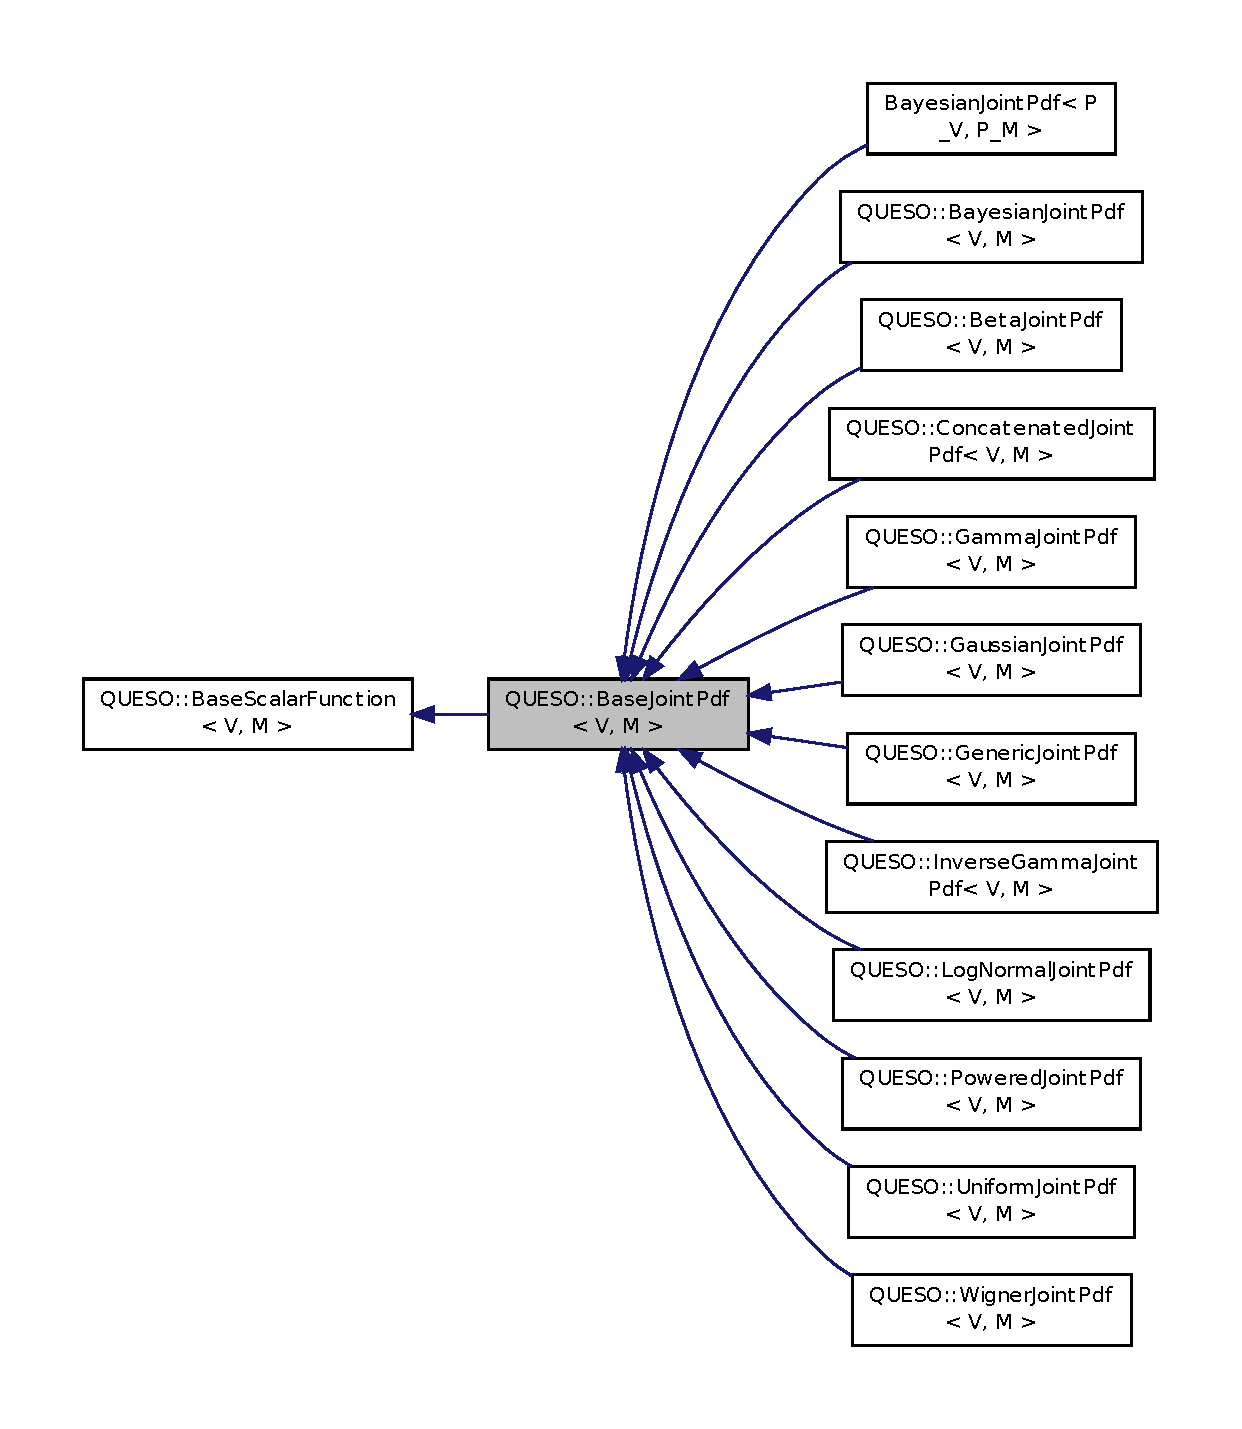
\includegraphics[width=350pt]{class_q_u_e_s_o_1_1_base_joint_pdf__inherit__graph}
\end{center}
\end{figure}


Collaboration diagram for Q\-U\-E\-S\-O\-:\-:Base\-Joint\-Pdf$<$ V, M $>$\-:
\nopagebreak
\begin{figure}[H]
\begin{center}
\leavevmode
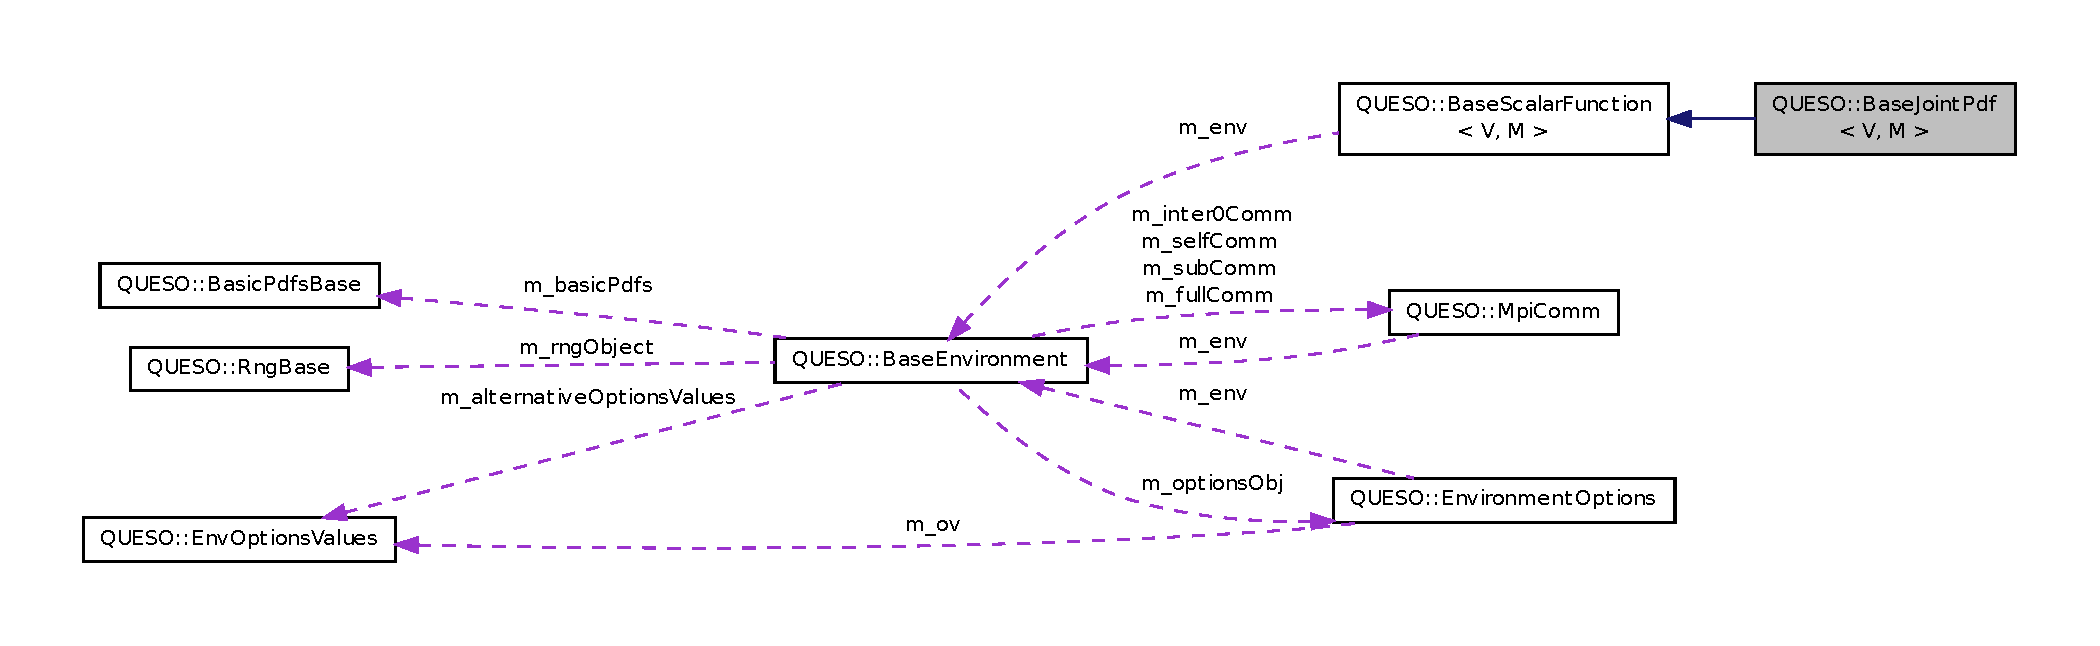
\includegraphics[width=350pt]{class_q_u_e_s_o_1_1_base_joint_pdf__coll__graph}
\end{center}
\end{figure}
\subsection*{Public Member Functions}
\begin{Indent}{\bf Constructor/\-Destructor methods}\par
\begin{DoxyCompactItemize}
\item 
\hyperlink{class_q_u_e_s_o_1_1_base_joint_pdf_ae1f0870366a17d71e05a2f84ec49e06e}{Base\-Joint\-Pdf} (const char $\ast$prefix, const \hyperlink{class_q_u_e_s_o_1_1_vector_set}{Vector\-Set}$<$ V, M $>$ \&\hyperlink{class_q_u_e_s_o_1_1_base_scalar_function_ad0937628825249dd36ded3ce0c7959ac}{domain\-Set})
\begin{DoxyCompactList}\small\item\em Default constructor. \end{DoxyCompactList}\item 
virtual \hyperlink{class_q_u_e_s_o_1_1_base_joint_pdf_a9f41f5dc30ddfd59e149c3a748898553}{$\sim$\-Base\-Joint\-Pdf} ()
\begin{DoxyCompactList}\small\item\em Destructor. \end{DoxyCompactList}\end{DoxyCompactItemize}
\end{Indent}
\begin{Indent}{\bf Mathematical methods}\par
\begin{DoxyCompactItemize}
\item 
virtual double \hyperlink{class_q_u_e_s_o_1_1_base_joint_pdf_a3c367a0cc3fb707a136c5df47dd414c1}{actual\-Value} (const V \&domain\-Vector, const V $\ast$domain\-Direction, V $\ast$grad\-Vector, M $\ast$hessian\-Matrix, V $\ast$hessian\-Effect) const =0
\begin{DoxyCompactList}\small\item\em Actual value of the P\-D\-F (scalar function). \end{DoxyCompactList}\item 
virtual double \hyperlink{class_q_u_e_s_o_1_1_base_joint_pdf_aaeb1d91fd791399a502f451b07bb1bfe}{ln\-Value} (const V \&domain\-Vector, const V $\ast$domain\-Direction, V $\ast$grad\-Vector, M $\ast$hessian\-Matrix, V $\ast$hessian\-Effect) const =0
\begin{DoxyCompactList}\small\item\em Logarithm of the value of the function. \end{DoxyCompactList}\item 
virtual void \hyperlink{class_q_u_e_s_o_1_1_base_joint_pdf_ab11f1d096f82cc7857cefe1b92f6b28e}{set\-Normalization\-Style} (unsigned int value) const 
\begin{DoxyCompactList}\small\item\em Sets a value to be used in the normalization style (stored in the protected attribute m\-\_\-normalization\-Style.) \end{DoxyCompactList}\item 
void \hyperlink{class_q_u_e_s_o_1_1_base_joint_pdf_a2903b3f031e68907fe7422fedc83e5dc}{set\-Log\-Of\-Normalization\-Factor} (double value) const 
\begin{DoxyCompactList}\small\item\em Sets a logarithmic value to be used in the normalization factor (stored in the protected attribute m\-\_\-normalization\-Style.) \end{DoxyCompactList}\item 
virtual double \hyperlink{class_q_u_e_s_o_1_1_base_joint_pdf_a99d8ab490b093abffd6068b6ea5263bb}{compute\-Log\-Of\-Normalization\-Factor} (unsigned int num\-Samples, bool \hyperlink{class_q_u_e_s_o_1_1_base_joint_pdf_ae82d4191f17af8c7a26226d127bc7850}{m\-\_\-log\-Of\-Normalization\-Factor}) const =0
\begin{DoxyCompactList}\small\item\em Computes the logarithm of the normalization factor. See template specialization. \end{DoxyCompactList}\end{DoxyCompactItemize}
\end{Indent}
\subsection*{Protected Member Functions}
\begin{DoxyCompactItemize}
\item 
double \hyperlink{class_q_u_e_s_o_1_1_base_joint_pdf_a7b7bdd13d2de51198bf75d522e02545b}{common\-Compute\-Log\-Of\-Normalization\-Factor} (unsigned int num\-Samples, bool update\-Factor\-Internally) const 
\begin{DoxyCompactList}\small\item\em Common method (to the derived classes) to compute the logarithm of the normalization factor. \end{DoxyCompactList}\end{DoxyCompactItemize}
\subsection*{Protected Attributes}
\begin{DoxyCompactItemize}
\item 
unsigned int \hyperlink{class_q_u_e_s_o_1_1_base_joint_pdf_a138c99bcef7a67077d9612bddfdcb896}{m\-\_\-normalization\-Style}
\item 
double \hyperlink{class_q_u_e_s_o_1_1_base_joint_pdf_ae82d4191f17af8c7a26226d127bc7850}{m\-\_\-log\-Of\-Normalization\-Factor}
\end{DoxyCompactItemize}


\subsection{Detailed Description}
\subsubsection*{template$<$class V, class M$>$class Q\-U\-E\-S\-O\-::\-Base\-Joint\-Pdf$<$ V, M $>$}

A templated (base) class for handling joint P\-D\-Fs. 

This class allows the mathematical definition of a Joint P\-D\-F, which is a scalar function such as $\ast$ $ \pi: B \subset R^n \rightarrow R $; ie a function of one or more variables that has always one-\/dimensional range. \hyperlink{namespace_q_u_e_s_o}{Q\-U\-E\-S\-O} currently supports basic P\-D\-Fs such as uniform and Gaussian and also more complex P\-D\-Fs, such as the ones coming from a Bayesian analysis. They are implemented in the derived classes \hyperlink{class_q_u_e_s_o_1_1_uniform_joint_pdf}{Uniform\-Joint\-Pdf}, \hyperlink{class_q_u_e_s_o_1_1_gaussian_joint_pdf}{Gaussian\-Joint\-Pdf}, and \hyperlink{class_q_u_e_s_o_1_1_bayesian_joint_pdf}{Bayesian\-Joint\-Pdf}, respectively. The posterior P\-D\-F may be represented within \hyperlink{namespace_q_u_e_s_o}{Q\-U\-E\-S\-O} by \hyperlink{class_q_u_e_s_o_1_1_generic_joint_pdf}{Generic\-Joint\-Pdf}. 

Definition at line 60 of file Joint\-Pdf.\-h.



\subsection{Constructor \& Destructor Documentation}
\hypertarget{class_q_u_e_s_o_1_1_base_joint_pdf_ae1f0870366a17d71e05a2f84ec49e06e}{\index{Q\-U\-E\-S\-O\-::\-Base\-Joint\-Pdf@{Q\-U\-E\-S\-O\-::\-Base\-Joint\-Pdf}!Base\-Joint\-Pdf@{Base\-Joint\-Pdf}}
\index{Base\-Joint\-Pdf@{Base\-Joint\-Pdf}!QUESO::BaseJointPdf@{Q\-U\-E\-S\-O\-::\-Base\-Joint\-Pdf}}
\subsubsection[{Base\-Joint\-Pdf}]{\setlength{\rightskip}{0pt plus 5cm}template$<$class V, class M$>$ {\bf Q\-U\-E\-S\-O\-::\-Base\-Joint\-Pdf}$<$ V, M $>$\-::{\bf Base\-Joint\-Pdf} (
\begin{DoxyParamCaption}
\item[{const char $\ast$}]{prefix, }
\item[{const {\bf Vector\-Set}$<$ V, M $>$ \&}]{domain\-Set}
\end{DoxyParamCaption}
)}}\label{class_q_u_e_s_o_1_1_base_joint_pdf_ae1f0870366a17d71e05a2f84ec49e06e}


Default constructor. 

Instantiates an object of the class, i.\-e. a scalar function, given a prefix and its domain. 

Definition at line 33 of file Joint\-Pdf.\-C.



References Q\-U\-E\-S\-O\-::\-Base\-Environment\-::display\-Verbosity(), Q\-U\-E\-S\-O\-::\-Base\-Scalar\-Function$<$ V, M $>$\-::m\-\_\-env, Q\-U\-E\-S\-O\-::\-Base\-Scalar\-Function$<$ V, M $>$\-::m\-\_\-prefix, and Q\-U\-E\-S\-O\-::\-Base\-Environment\-::sub\-Display\-File().


\begin{DoxyCode}
36   :
37   BaseScalarFunction<V,M>(((std::string)(prefix)+\textcolor{stringliteral}{"pd\_"}).c\_str(), \hyperlink{class_q_u_e_s_o_1_1_base_scalar_function_ad0937628825249dd36ded3ce0c7959ac}{domainSet}),
38   \hyperlink{class_q_u_e_s_o_1_1_base_joint_pdf_a138c99bcef7a67077d9612bddfdcb896}{m\_normalizationStyle}(0),
39   \hyperlink{class_q_u_e_s_o_1_1_base_joint_pdf_ae82d4191f17af8c7a26226d127bc7850}{m\_logOfNormalizationFactor}(0.)
40 \{
41   \textcolor{keywordflow}{if} ((\hyperlink{class_q_u_e_s_o_1_1_base_scalar_function_adf44141aeb765d97613286f88f235f04}{m\_env}.\hyperlink{class_q_u_e_s_o_1_1_base_environment_a8a0064746ae8dddfece4229b9ad374d6}{subDisplayFile}()) && (\hyperlink{class_q_u_e_s_o_1_1_base_scalar_function_adf44141aeb765d97613286f88f235f04}{m\_env}.
      \hyperlink{class_q_u_e_s_o_1_1_base_environment_a1fe5f244fc0316a0ab3e37463f108b96}{displayVerbosity}() >= 54)) \{
42     *\hyperlink{class_q_u_e_s_o_1_1_base_scalar_function_adf44141aeb765d97613286f88f235f04}{m\_env}.\hyperlink{class_q_u_e_s_o_1_1_base_environment_a8a0064746ae8dddfece4229b9ad374d6}{subDisplayFile}() << \textcolor{stringliteral}{"Entering BaseJointPdf<V,M>::constructor() [3]"}
43                             << \textcolor{stringliteral}{": prefix = "} << \hyperlink{class_q_u_e_s_o_1_1_base_scalar_function_a6e81dc902aca6a546877da99b2f4a169}{m\_prefix}
44                             << std::endl;
45   \}
46 
47   \textcolor{keywordflow}{if} ((\hyperlink{class_q_u_e_s_o_1_1_base_scalar_function_adf44141aeb765d97613286f88f235f04}{m\_env}.\hyperlink{class_q_u_e_s_o_1_1_base_environment_a8a0064746ae8dddfece4229b9ad374d6}{subDisplayFile}()) && (\hyperlink{class_q_u_e_s_o_1_1_base_scalar_function_adf44141aeb765d97613286f88f235f04}{m\_env}.
      \hyperlink{class_q_u_e_s_o_1_1_base_environment_a1fe5f244fc0316a0ab3e37463f108b96}{displayVerbosity}() >= 54)) \{
48     *\hyperlink{class_q_u_e_s_o_1_1_base_scalar_function_adf44141aeb765d97613286f88f235f04}{m\_env}.\hyperlink{class_q_u_e_s_o_1_1_base_environment_a8a0064746ae8dddfece4229b9ad374d6}{subDisplayFile}() << \textcolor{stringliteral}{"Leaving BaseJointPdf<V,M>::constructor() [3]"}
49                             << \textcolor{stringliteral}{": prefix = "} << \hyperlink{class_q_u_e_s_o_1_1_base_scalar_function_a6e81dc902aca6a546877da99b2f4a169}{m\_prefix}
50                             << std::endl;
51   \}
52 \}
\end{DoxyCode}
\hypertarget{class_q_u_e_s_o_1_1_base_joint_pdf_a9f41f5dc30ddfd59e149c3a748898553}{\index{Q\-U\-E\-S\-O\-::\-Base\-Joint\-Pdf@{Q\-U\-E\-S\-O\-::\-Base\-Joint\-Pdf}!$\sim$\-Base\-Joint\-Pdf@{$\sim$\-Base\-Joint\-Pdf}}
\index{$\sim$\-Base\-Joint\-Pdf@{$\sim$\-Base\-Joint\-Pdf}!QUESO::BaseJointPdf@{Q\-U\-E\-S\-O\-::\-Base\-Joint\-Pdf}}
\subsubsection[{$\sim$\-Base\-Joint\-Pdf}]{\setlength{\rightskip}{0pt plus 5cm}template$<$class V , class M $>$ {\bf Q\-U\-E\-S\-O\-::\-Base\-Joint\-Pdf}$<$ V, M $>$\-::$\sim${\bf Base\-Joint\-Pdf} (
\begin{DoxyParamCaption}
{}
\end{DoxyParamCaption}
)\hspace{0.3cm}{\ttfamily [virtual]}}}\label{class_q_u_e_s_o_1_1_base_joint_pdf_a9f41f5dc30ddfd59e149c3a748898553}


Destructor. 



Definition at line 55 of file Joint\-Pdf.\-C.


\begin{DoxyCode}
56 \{
57 \}
\end{DoxyCode}


\subsection{Member Function Documentation}
\hypertarget{class_q_u_e_s_o_1_1_base_joint_pdf_a3c367a0cc3fb707a136c5df47dd414c1}{\index{Q\-U\-E\-S\-O\-::\-Base\-Joint\-Pdf@{Q\-U\-E\-S\-O\-::\-Base\-Joint\-Pdf}!actual\-Value@{actual\-Value}}
\index{actual\-Value@{actual\-Value}!QUESO::BaseJointPdf@{Q\-U\-E\-S\-O\-::\-Base\-Joint\-Pdf}}
\subsubsection[{actual\-Value}]{\setlength{\rightskip}{0pt plus 5cm}template$<$class V, class M$>$ virtual double {\bf Q\-U\-E\-S\-O\-::\-Base\-Joint\-Pdf}$<$ V, M $>$\-::actual\-Value (
\begin{DoxyParamCaption}
\item[{const V \&}]{domain\-Vector, }
\item[{const V $\ast$}]{domain\-Direction, }
\item[{V $\ast$}]{grad\-Vector, }
\item[{M $\ast$}]{hessian\-Matrix, }
\item[{V $\ast$}]{hessian\-Effect}
\end{DoxyParamCaption}
) const\hspace{0.3cm}{\ttfamily [pure virtual]}}}\label{class_q_u_e_s_o_1_1_base_joint_pdf_a3c367a0cc3fb707a136c5df47dd414c1}


Actual value of the P\-D\-F (scalar function). 



Implements \hyperlink{class_q_u_e_s_o_1_1_base_scalar_function_aad8957ecbc4e155cbc4c40a1c21135d7}{Q\-U\-E\-S\-O\-::\-Base\-Scalar\-Function$<$ V, M $>$}.



Implemented in \hyperlink{class_q_u_e_s_o_1_1_concatenated_joint_pdf_a7a3bbf8dab211968e9691a620fee0e4d}{Q\-U\-E\-S\-O\-::\-Concatenated\-Joint\-Pdf$<$ V, M $>$}, \hyperlink{class_q_u_e_s_o_1_1_gaussian_joint_pdf_ae576dae6a972dd7350ca261569f056da}{Q\-U\-E\-S\-O\-::\-Gaussian\-Joint\-Pdf$<$ V, M $>$}, \hyperlink{class_q_u_e_s_o_1_1_bayesian_joint_pdf_ad67362b4ab48a722db976430cf03165e}{Q\-U\-E\-S\-O\-::\-Bayesian\-Joint\-Pdf$<$ V, M $>$}, \hyperlink{class_q_u_e_s_o_1_1_log_normal_joint_pdf_a87729cb9d59b73baefcbecb03e753cb9}{Q\-U\-E\-S\-O\-::\-Log\-Normal\-Joint\-Pdf$<$ V, M $>$}, \hyperlink{class_q_u_e_s_o_1_1_powered_joint_pdf_a916888a016a1cd9aea0a7789be0f6957}{Q\-U\-E\-S\-O\-::\-Powered\-Joint\-Pdf$<$ V, M $>$}, \hyperlink{class_q_u_e_s_o_1_1_beta_joint_pdf_a14909bee55e4d764be71e7a313716d9b}{Q\-U\-E\-S\-O\-::\-Beta\-Joint\-Pdf$<$ V, M $>$}, \hyperlink{class_q_u_e_s_o_1_1_gamma_joint_pdf_a4907d38d266d271d34cce9be333a95df}{Q\-U\-E\-S\-O\-::\-Gamma\-Joint\-Pdf$<$ V, M $>$}, \hyperlink{class_q_u_e_s_o_1_1_inverse_gamma_joint_pdf_a1e0dbb40992578a11b40d0755f59ef2e}{Q\-U\-E\-S\-O\-::\-Inverse\-Gamma\-Joint\-Pdf$<$ V, M $>$}, \hyperlink{class_q_u_e_s_o_1_1_wigner_joint_pdf_a48482e1e5b953cd0753bf0c39486a81f}{Q\-U\-E\-S\-O\-::\-Wigner\-Joint\-Pdf$<$ V, M $>$}, \hyperlink{class_q_u_e_s_o_1_1_generic_joint_pdf_a7bddaaf1d4087ca8e35fcb83c0df72d2}{Q\-U\-E\-S\-O\-::\-Generic\-Joint\-Pdf$<$ V, M $>$}, and \hyperlink{class_q_u_e_s_o_1_1_uniform_joint_pdf_a358ffa410284ed3e40435439c1c8bbc3}{Q\-U\-E\-S\-O\-::\-Uniform\-Joint\-Pdf$<$ V, M $>$}.

\hypertarget{class_q_u_e_s_o_1_1_base_joint_pdf_a7b7bdd13d2de51198bf75d522e02545b}{\index{Q\-U\-E\-S\-O\-::\-Base\-Joint\-Pdf@{Q\-U\-E\-S\-O\-::\-Base\-Joint\-Pdf}!common\-Compute\-Log\-Of\-Normalization\-Factor@{common\-Compute\-Log\-Of\-Normalization\-Factor}}
\index{common\-Compute\-Log\-Of\-Normalization\-Factor@{common\-Compute\-Log\-Of\-Normalization\-Factor}!QUESO::BaseJointPdf@{Q\-U\-E\-S\-O\-::\-Base\-Joint\-Pdf}}
\subsubsection[{common\-Compute\-Log\-Of\-Normalization\-Factor}]{\setlength{\rightskip}{0pt plus 5cm}template$<$class V , class M $>$ double {\bf Q\-U\-E\-S\-O\-::\-Base\-Joint\-Pdf}$<$ V, M $>$\-::common\-Compute\-Log\-Of\-Normalization\-Factor (
\begin{DoxyParamCaption}
\item[{unsigned int}]{num\-Samples, }
\item[{bool}]{update\-Factor\-Internally}
\end{DoxyParamCaption}
) const\hspace{0.3cm}{\ttfamily [protected]}}}\label{class_q_u_e_s_o_1_1_base_joint_pdf_a7b7bdd13d2de51198bf75d522e02545b}


Common method (to the derived classes) to compute the logarithm of the normalization factor. 

The normalization factor is calculated by finding the max and min values of the domain set and then drawing {\ttfamily num\-Samples} samples from a uniform distribution varying from {\ttfamily min} to {\ttfamily max}. Such samples are averaged and the logarithmic value is assigned to protected attribute m\-\_\-log\-Of\-Normalization\-Factor if the parameter {\ttfamily m\-\_\-log\-Of\-Normalization\-Factor} is true. 

Definition at line 77 of file Joint\-Pdf.\-C.



References Q\-U\-E\-S\-O\-::\-Box\-Subset$<$ V, M $>$\-::max\-Values(), and Q\-U\-E\-S\-O\-::\-Box\-Subset$<$ V, M $>$\-::min\-Values().



Referenced by Q\-U\-E\-S\-O\-::\-Generic\-Joint\-Pdf$<$ V, M $>$\-::compute\-Log\-Of\-Normalization\-Factor(), Q\-U\-E\-S\-O\-::\-Uniform\-Joint\-Pdf$<$ V, M $>$\-::compute\-Log\-Of\-Normalization\-Factor(), Q\-U\-E\-S\-O\-::\-Inverse\-Gamma\-Joint\-Pdf$<$ V, M $>$\-::compute\-Log\-Of\-Normalization\-Factor(), Q\-U\-E\-S\-O\-::\-Wigner\-Joint\-Pdf$<$ V, M $>$\-::compute\-Log\-Of\-Normalization\-Factor(), Q\-U\-E\-S\-O\-::\-Beta\-Joint\-Pdf$<$ V, M $>$\-::compute\-Log\-Of\-Normalization\-Factor(), Q\-U\-E\-S\-O\-::\-Log\-Normal\-Joint\-Pdf$<$ V, M $>$\-::compute\-Log\-Of\-Normalization\-Factor(), Q\-U\-E\-S\-O\-::\-Gamma\-Joint\-Pdf$<$ V, M $>$\-::compute\-Log\-Of\-Normalization\-Factor(), and Q\-U\-E\-S\-O\-::\-Gaussian\-Joint\-Pdf$<$ V, M $>$\-::compute\-Log\-Of\-Normalization\-Factor().


\begin{DoxyCode}
78 \{
79   \textcolor{keywordtype}{double} value = 0.;
80 
81   \textcolor{keywordtype}{double} volume = \hyperlink{class_q_u_e_s_o_1_1_base_scalar_function_a67696e86211197938c72cd11863f5cf8}{m\_domainSet}.volume();
82   \textcolor{keywordflow}{if} (((boost::math::isnan)(volume)) ||
83       (volume == -INFINITY         ) ||
84       (volume ==  INFINITY         ) ||
85       (volume <= 0.                )) \{
86     \textcolor{comment}{// Do nothing}
87   \}
88   \textcolor{keywordflow}{else} \{
89     \textcolor{keyword}{const} BoxSubset<V,M>* boxSubset = \textcolor{keyword}{dynamic\_cast<}\textcolor{keyword}{const }BoxSubset<V,M>* \textcolor{keyword}{>}(&
      \hyperlink{class_q_u_e_s_o_1_1_base_scalar_function_a67696e86211197938c72cd11863f5cf8}{m\_domainSet});
90     \textcolor{keywordflow}{if} (boxSubset == NULL) \{
91       \textcolor{comment}{// Do nothing}
92     \}
93     \textcolor{keywordflow}{else} \{
94       V tmpVec(\hyperlink{class_q_u_e_s_o_1_1_base_scalar_function_a67696e86211197938c72cd11863f5cf8}{m\_domainSet}.vectorSpace().zeroVector());
95       \textcolor{keywordtype}{double} sum = 0.;
96       \textcolor{keywordflow}{for} (\textcolor{keywordtype}{unsigned} \textcolor{keywordtype}{int} i = 0; i < numSamples; ++i) \{
97         tmpVec.cwSetUniform(boxSubset->minValues(),boxSubset->maxValues());
98         sum += this->\hyperlink{class_q_u_e_s_o_1_1_base_joint_pdf_a3c367a0cc3fb707a136c5df47dd414c1}{actualValue}(tmpVec,NULL,NULL,NULL,NULL);
99       \}
100       \textcolor{keywordtype}{double} avgValue = sum/((double) numSamples);
101       value = -( log(avgValue) + log(volume) );
102       \textcolor{keywordflow}{if} (updateFactorInternally) \{
103         \hyperlink{class_q_u_e_s_o_1_1_base_joint_pdf_ae82d4191f17af8c7a26226d127bc7850}{m\_logOfNormalizationFactor} = value;
104       \}
105     \}
106   \}
107 
108   \textcolor{keywordflow}{return} value;
109 \}
\end{DoxyCode}
\hypertarget{class_q_u_e_s_o_1_1_base_joint_pdf_a99d8ab490b093abffd6068b6ea5263bb}{\index{Q\-U\-E\-S\-O\-::\-Base\-Joint\-Pdf@{Q\-U\-E\-S\-O\-::\-Base\-Joint\-Pdf}!compute\-Log\-Of\-Normalization\-Factor@{compute\-Log\-Of\-Normalization\-Factor}}
\index{compute\-Log\-Of\-Normalization\-Factor@{compute\-Log\-Of\-Normalization\-Factor}!QUESO::BaseJointPdf@{Q\-U\-E\-S\-O\-::\-Base\-Joint\-Pdf}}
\subsubsection[{compute\-Log\-Of\-Normalization\-Factor}]{\setlength{\rightskip}{0pt plus 5cm}template$<$class V, class M$>$ virtual double {\bf Q\-U\-E\-S\-O\-::\-Base\-Joint\-Pdf}$<$ V, M $>$\-::compute\-Log\-Of\-Normalization\-Factor (
\begin{DoxyParamCaption}
\item[{unsigned int}]{num\-Samples, }
\item[{bool}]{m\-\_\-log\-Of\-Normalization\-Factor}
\end{DoxyParamCaption}
) const\hspace{0.3cm}{\ttfamily [pure virtual]}}}\label{class_q_u_e_s_o_1_1_base_joint_pdf_a99d8ab490b093abffd6068b6ea5263bb}


Computes the logarithm of the normalization factor. See template specialization. 



Implemented in \hyperlink{class_q_u_e_s_o_1_1_concatenated_joint_pdf_ad960a39a781a7a891df0ae0ee4670199}{Q\-U\-E\-S\-O\-::\-Concatenated\-Joint\-Pdf$<$ V, M $>$}, \hyperlink{class_q_u_e_s_o_1_1_gaussian_joint_pdf_af5cfad4df319c6f535c0a9b739d0c398}{Q\-U\-E\-S\-O\-::\-Gaussian\-Joint\-Pdf$<$ V, M $>$}, \hyperlink{class_q_u_e_s_o_1_1_bayesian_joint_pdf_a7e00d685068bcf34253e5a101b539261}{Q\-U\-E\-S\-O\-::\-Bayesian\-Joint\-Pdf$<$ V, M $>$}, \hyperlink{class_q_u_e_s_o_1_1_bayesian_joint_pdf_a7e00d685068bcf34253e5a101b539261}{Q\-U\-E\-S\-O\-::\-Bayesian\-Joint\-Pdf$<$ P\-\_\-\-V, P\-\_\-\-M $>$}, \hyperlink{class_q_u_e_s_o_1_1_powered_joint_pdf_ae4d7e2a318f317652ebbf926d8a3391c}{Q\-U\-E\-S\-O\-::\-Powered\-Joint\-Pdf$<$ V, M $>$}, \hyperlink{class_q_u_e_s_o_1_1_gamma_joint_pdf_a5fb1d17a267c8110442689721e74c8d4}{Q\-U\-E\-S\-O\-::\-Gamma\-Joint\-Pdf$<$ V, M $>$}, \hyperlink{class_q_u_e_s_o_1_1_log_normal_joint_pdf_a373e37c21ce8acf05fe72f4ec9deef9c}{Q\-U\-E\-S\-O\-::\-Log\-Normal\-Joint\-Pdf$<$ V, M $>$}, \hyperlink{class_q_u_e_s_o_1_1_beta_joint_pdf_aaa67d058285caffa8dcb0235fbaf7726}{Q\-U\-E\-S\-O\-::\-Beta\-Joint\-Pdf$<$ V, M $>$}, \hyperlink{class_q_u_e_s_o_1_1_inverse_gamma_joint_pdf_a812888fe10ba1f89ee6871dc9272140e}{Q\-U\-E\-S\-O\-::\-Inverse\-Gamma\-Joint\-Pdf$<$ V, M $>$}, \hyperlink{class_q_u_e_s_o_1_1_wigner_joint_pdf_adbe13f31b4bdfbf6eb9b7ad57f9e71f0}{Q\-U\-E\-S\-O\-::\-Wigner\-Joint\-Pdf$<$ V, M $>$}, \hyperlink{class_q_u_e_s_o_1_1_uniform_joint_pdf_a7104edeec3bc1a45f4c8a805cdfde170}{Q\-U\-E\-S\-O\-::\-Uniform\-Joint\-Pdf$<$ V, M $>$}, and \hyperlink{class_q_u_e_s_o_1_1_generic_joint_pdf_a282b1db04e25086938f3b8969ba484a9}{Q\-U\-E\-S\-O\-::\-Generic\-Joint\-Pdf$<$ V, M $>$}.

\hypertarget{class_q_u_e_s_o_1_1_base_joint_pdf_aaeb1d91fd791399a502f451b07bb1bfe}{\index{Q\-U\-E\-S\-O\-::\-Base\-Joint\-Pdf@{Q\-U\-E\-S\-O\-::\-Base\-Joint\-Pdf}!ln\-Value@{ln\-Value}}
\index{ln\-Value@{ln\-Value}!QUESO::BaseJointPdf@{Q\-U\-E\-S\-O\-::\-Base\-Joint\-Pdf}}
\subsubsection[{ln\-Value}]{\setlength{\rightskip}{0pt plus 5cm}template$<$class V, class M$>$ virtual double {\bf Q\-U\-E\-S\-O\-::\-Base\-Joint\-Pdf}$<$ V, M $>$\-::ln\-Value (
\begin{DoxyParamCaption}
\item[{const V \&}]{domain\-Vector, }
\item[{const V $\ast$}]{domain\-Direction, }
\item[{V $\ast$}]{grad\-Vector, }
\item[{M $\ast$}]{hessian\-Matrix, }
\item[{V $\ast$}]{hessian\-Effect}
\end{DoxyParamCaption}
) const\hspace{0.3cm}{\ttfamily [pure virtual]}}}\label{class_q_u_e_s_o_1_1_base_joint_pdf_aaeb1d91fd791399a502f451b07bb1bfe}


Logarithm of the value of the function. 



Implements \hyperlink{class_q_u_e_s_o_1_1_base_scalar_function_acf2f92adac2df2a0d750dc62cd3a4d0a}{Q\-U\-E\-S\-O\-::\-Base\-Scalar\-Function$<$ V, M $>$}.



Implemented in \hyperlink{class_q_u_e_s_o_1_1_gaussian_joint_pdf_a14207045679234c5112974be5445b30d}{Q\-U\-E\-S\-O\-::\-Gaussian\-Joint\-Pdf$<$ V, M $>$}, \hyperlink{class_q_u_e_s_o_1_1_concatenated_joint_pdf_aca499666e5c3d3d26c562492a15ab112}{Q\-U\-E\-S\-O\-::\-Concatenated\-Joint\-Pdf$<$ V, M $>$}, \hyperlink{class_q_u_e_s_o_1_1_bayesian_joint_pdf_a98e54ee24452e2477469a0c84eecbfca}{Q\-U\-E\-S\-O\-::\-Bayesian\-Joint\-Pdf$<$ V, M $>$}, \hyperlink{class_q_u_e_s_o_1_1_gamma_joint_pdf_a990337e7c25a4214b15fd71cb6deb384}{Q\-U\-E\-S\-O\-::\-Gamma\-Joint\-Pdf$<$ V, M $>$}, \hyperlink{class_q_u_e_s_o_1_1_log_normal_joint_pdf_a9c31e89ee4abe8f1747e50c8d472a94d}{Q\-U\-E\-S\-O\-::\-Log\-Normal\-Joint\-Pdf$<$ V, M $>$}, \hyperlink{class_q_u_e_s_o_1_1_beta_joint_pdf_a713d655107dd51eac9d1c19630359a06}{Q\-U\-E\-S\-O\-::\-Beta\-Joint\-Pdf$<$ V, M $>$}, \hyperlink{class_q_u_e_s_o_1_1_powered_joint_pdf_addcc8c32b3dc30d22fb1e4a8350a14e3}{Q\-U\-E\-S\-O\-::\-Powered\-Joint\-Pdf$<$ V, M $>$}, \hyperlink{class_q_u_e_s_o_1_1_inverse_gamma_joint_pdf_a08dbbb7054026fcf4d429870cbe5d36f}{Q\-U\-E\-S\-O\-::\-Inverse\-Gamma\-Joint\-Pdf$<$ V, M $>$}, \hyperlink{class_q_u_e_s_o_1_1_wigner_joint_pdf_a64afe5e7a7974fc91b4394e81ba4da55}{Q\-U\-E\-S\-O\-::\-Wigner\-Joint\-Pdf$<$ V, M $>$}, \hyperlink{class_q_u_e_s_o_1_1_uniform_joint_pdf_a80858abd7ca07ed42b9e9f0e4c92b3d2}{Q\-U\-E\-S\-O\-::\-Uniform\-Joint\-Pdf$<$ V, M $>$}, and \hyperlink{class_q_u_e_s_o_1_1_generic_joint_pdf_a566150d033ce9c09a22c6f271a7155a8}{Q\-U\-E\-S\-O\-::\-Generic\-Joint\-Pdf$<$ V, M $>$}.

\hypertarget{class_q_u_e_s_o_1_1_base_joint_pdf_a2903b3f031e68907fe7422fedc83e5dc}{\index{Q\-U\-E\-S\-O\-::\-Base\-Joint\-Pdf@{Q\-U\-E\-S\-O\-::\-Base\-Joint\-Pdf}!set\-Log\-Of\-Normalization\-Factor@{set\-Log\-Of\-Normalization\-Factor}}
\index{set\-Log\-Of\-Normalization\-Factor@{set\-Log\-Of\-Normalization\-Factor}!QUESO::BaseJointPdf@{Q\-U\-E\-S\-O\-::\-Base\-Joint\-Pdf}}
\subsubsection[{set\-Log\-Of\-Normalization\-Factor}]{\setlength{\rightskip}{0pt plus 5cm}template$<$class V , class M $>$ void {\bf Q\-U\-E\-S\-O\-::\-Base\-Joint\-Pdf}$<$ V, M $>$\-::set\-Log\-Of\-Normalization\-Factor (
\begin{DoxyParamCaption}
\item[{double}]{value}
\end{DoxyParamCaption}
) const}}\label{class_q_u_e_s_o_1_1_base_joint_pdf_a2903b3f031e68907fe7422fedc83e5dc}


Sets a logarithmic value to be used in the normalization factor (stored in the protected attribute m\-\_\-normalization\-Style.) 



Definition at line 69 of file Joint\-Pdf.\-C.


\begin{DoxyCode}
70 \{
71   \hyperlink{class_q_u_e_s_o_1_1_base_joint_pdf_ae82d4191f17af8c7a26226d127bc7850}{m\_logOfNormalizationFactor} = value;
72   \textcolor{keywordflow}{return};
73 \}
\end{DoxyCode}
\hypertarget{class_q_u_e_s_o_1_1_base_joint_pdf_ab11f1d096f82cc7857cefe1b92f6b28e}{\index{Q\-U\-E\-S\-O\-::\-Base\-Joint\-Pdf@{Q\-U\-E\-S\-O\-::\-Base\-Joint\-Pdf}!set\-Normalization\-Style@{set\-Normalization\-Style}}
\index{set\-Normalization\-Style@{set\-Normalization\-Style}!QUESO::BaseJointPdf@{Q\-U\-E\-S\-O\-::\-Base\-Joint\-Pdf}}
\subsubsection[{set\-Normalization\-Style}]{\setlength{\rightskip}{0pt plus 5cm}template$<$class V , class M $>$ void {\bf Q\-U\-E\-S\-O\-::\-Base\-Joint\-Pdf}$<$ V, M $>$\-::set\-Normalization\-Style (
\begin{DoxyParamCaption}
\item[{unsigned int}]{value}
\end{DoxyParamCaption}
) const\hspace{0.3cm}{\ttfamily [virtual]}}}\label{class_q_u_e_s_o_1_1_base_joint_pdf_ab11f1d096f82cc7857cefe1b92f6b28e}


Sets a value to be used in the normalization style (stored in the protected attribute m\-\_\-normalization\-Style.) 



Reimplemented in \hyperlink{class_q_u_e_s_o_1_1_bayesian_joint_pdf_aa23751ede9ec9f2e7bdd81c5326f47d5}{Q\-U\-E\-S\-O\-::\-Bayesian\-Joint\-Pdf$<$ V, M $>$}, \hyperlink{class_q_u_e_s_o_1_1_bayesian_joint_pdf_aa23751ede9ec9f2e7bdd81c5326f47d5}{Q\-U\-E\-S\-O\-::\-Bayesian\-Joint\-Pdf$<$ P\-\_\-\-V, P\-\_\-\-M $>$}, \hyperlink{class_q_u_e_s_o_1_1_concatenated_joint_pdf_a686ff513ae812f26f9a71705dd2082ad}{Q\-U\-E\-S\-O\-::\-Concatenated\-Joint\-Pdf$<$ V, M $>$}, and \hyperlink{class_q_u_e_s_o_1_1_powered_joint_pdf_a306c48af4e2954a002f873e25b4c3499}{Q\-U\-E\-S\-O\-::\-Powered\-Joint\-Pdf$<$ V, M $>$}.



Definition at line 61 of file Joint\-Pdf.\-C.


\begin{DoxyCode}
62 \{
63   \hyperlink{class_q_u_e_s_o_1_1_base_joint_pdf_a138c99bcef7a67077d9612bddfdcb896}{m\_normalizationStyle} = value;
64   \textcolor{keywordflow}{return};
65 \}
\end{DoxyCode}


\subsection{Member Data Documentation}
\hypertarget{class_q_u_e_s_o_1_1_base_joint_pdf_ae82d4191f17af8c7a26226d127bc7850}{\index{Q\-U\-E\-S\-O\-::\-Base\-Joint\-Pdf@{Q\-U\-E\-S\-O\-::\-Base\-Joint\-Pdf}!m\-\_\-log\-Of\-Normalization\-Factor@{m\-\_\-log\-Of\-Normalization\-Factor}}
\index{m\-\_\-log\-Of\-Normalization\-Factor@{m\-\_\-log\-Of\-Normalization\-Factor}!QUESO::BaseJointPdf@{Q\-U\-E\-S\-O\-::\-Base\-Joint\-Pdf}}
\subsubsection[{m\-\_\-log\-Of\-Normalization\-Factor}]{\setlength{\rightskip}{0pt plus 5cm}template$<$class V, class M$>$ double {\bf Q\-U\-E\-S\-O\-::\-Base\-Joint\-Pdf}$<$ V, M $>$\-::m\-\_\-log\-Of\-Normalization\-Factor\hspace{0.3cm}{\ttfamily [mutable]}, {\ttfamily [protected]}}}\label{class_q_u_e_s_o_1_1_base_joint_pdf_ae82d4191f17af8c7a26226d127bc7850}


Definition at line 104 of file Joint\-Pdf.\-h.

\hypertarget{class_q_u_e_s_o_1_1_base_joint_pdf_a138c99bcef7a67077d9612bddfdcb896}{\index{Q\-U\-E\-S\-O\-::\-Base\-Joint\-Pdf@{Q\-U\-E\-S\-O\-::\-Base\-Joint\-Pdf}!m\-\_\-normalization\-Style@{m\-\_\-normalization\-Style}}
\index{m\-\_\-normalization\-Style@{m\-\_\-normalization\-Style}!QUESO::BaseJointPdf@{Q\-U\-E\-S\-O\-::\-Base\-Joint\-Pdf}}
\subsubsection[{m\-\_\-normalization\-Style}]{\setlength{\rightskip}{0pt plus 5cm}template$<$class V, class M$>$ unsigned int {\bf Q\-U\-E\-S\-O\-::\-Base\-Joint\-Pdf}$<$ V, M $>$\-::m\-\_\-normalization\-Style\hspace{0.3cm}{\ttfamily [mutable]}, {\ttfamily [protected]}}}\label{class_q_u_e_s_o_1_1_base_joint_pdf_a138c99bcef7a67077d9612bddfdcb896}


Definition at line 103 of file Joint\-Pdf.\-h.



The documentation for this class was generated from the following files\-:\begin{DoxyCompactItemize}
\item 
src/stats/inc/\hyperlink{_joint_pdf_8h}{Joint\-Pdf.\-h}\item 
src/stats/src/\hyperlink{_joint_pdf_8_c}{Joint\-Pdf.\-C}\end{DoxyCompactItemize}

\hypertarget{class_q_u_e_s_o_1_1_base_matrix_covariance_function}{\section{Q\-U\-E\-S\-O\-:\-:Base\-Matrix\-Covariance\-Function$<$ P\-\_\-\-V, P\-\_\-\-M, Q\-\_\-\-V, Q\-\_\-\-M $>$ Class Template Reference}
\label{class_q_u_e_s_o_1_1_base_matrix_covariance_function}\index{Q\-U\-E\-S\-O\-::\-Base\-Matrix\-Covariance\-Function$<$ P\-\_\-\-V, P\-\_\-\-M, Q\-\_\-\-V, Q\-\_\-\-M $>$@{Q\-U\-E\-S\-O\-::\-Base\-Matrix\-Covariance\-Function$<$ P\-\_\-\-V, P\-\_\-\-M, Q\-\_\-\-V, Q\-\_\-\-M $>$}}
}


A templated (base) class to accommodate covariance matrix of (random) vector functions.  




{\ttfamily \#include $<$Matrix\-Covariance\-Function.\-h$>$}



Inheritance diagram for Q\-U\-E\-S\-O\-:\-:Base\-Matrix\-Covariance\-Function$<$ P\-\_\-\-V, P\-\_\-\-M, Q\-\_\-\-V, Q\-\_\-\-M $>$\-:
\nopagebreak
\begin{figure}[H]
\begin{center}
\leavevmode
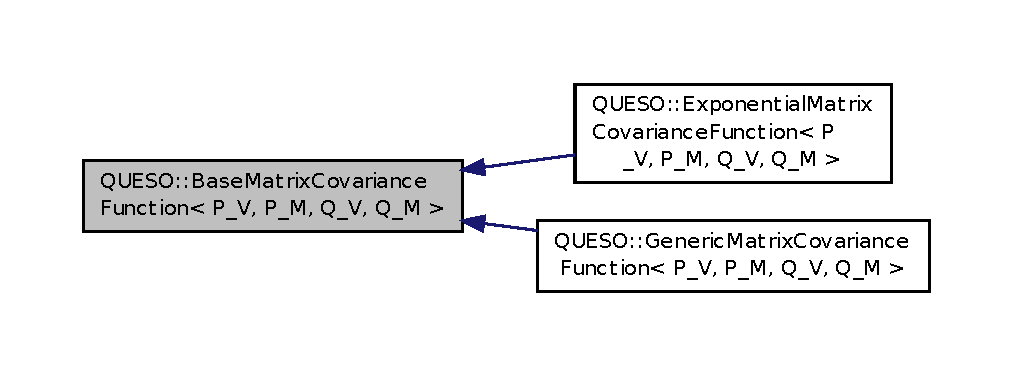
\includegraphics[width=350pt]{class_q_u_e_s_o_1_1_base_matrix_covariance_function__inherit__graph}
\end{center}
\end{figure}


Collaboration diagram for Q\-U\-E\-S\-O\-:\-:Base\-Matrix\-Covariance\-Function$<$ P\-\_\-\-V, P\-\_\-\-M, Q\-\_\-\-V, Q\-\_\-\-M $>$\-:
\nopagebreak
\begin{figure}[H]
\begin{center}
\leavevmode
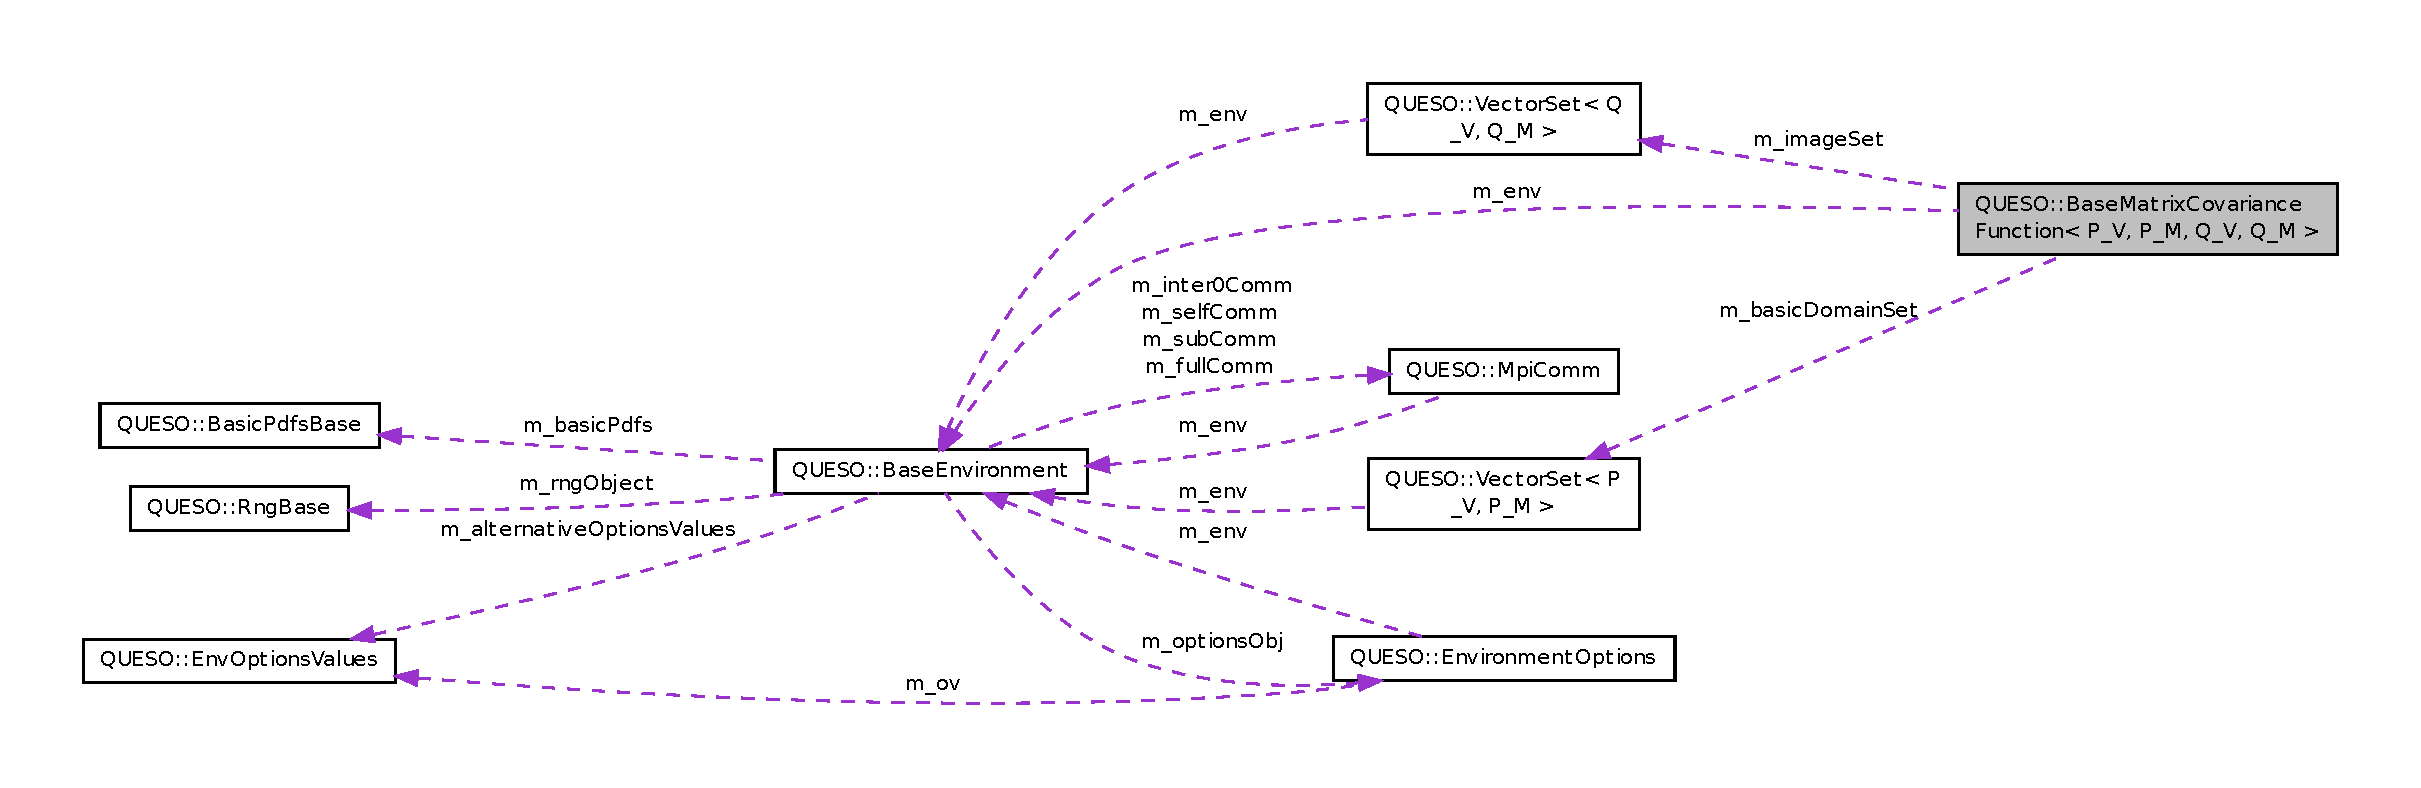
\includegraphics[width=350pt]{class_q_u_e_s_o_1_1_base_matrix_covariance_function__coll__graph}
\end{center}
\end{figure}
\subsection*{Public Member Functions}
\begin{Indent}{\bf Constructor/\-Destructor methods}\par
\begin{DoxyCompactItemize}
\item 
\hyperlink{class_q_u_e_s_o_1_1_base_matrix_covariance_function_aa19fd2a4d2cc8ce822d4712abbd45021}{Base\-Matrix\-Covariance\-Function} (const char $\ast$prefix, const \hyperlink{class_q_u_e_s_o_1_1_vector_set}{Vector\-Set}$<$ P\-\_\-\-V, P\-\_\-\-M $>$ \&\hyperlink{class_q_u_e_s_o_1_1_base_matrix_covariance_function_a6ce876e4dae5ab4b165ac100e310dd45}{basic\-Domain\-Set}, const \hyperlink{class_q_u_e_s_o_1_1_vector_set}{Vector\-Set}$<$ Q\-\_\-\-V, Q\-\_\-\-M $>$ \&image\-Set)
\begin{DoxyCompactList}\small\item\em Default constructor. \end{DoxyCompactList}\item 
virtual \hyperlink{class_q_u_e_s_o_1_1_base_matrix_covariance_function_a821c7190922a832ecc4ae3bcc78b99cc}{$\sim$\-Base\-Matrix\-Covariance\-Function} ()
\begin{DoxyCompactList}\small\item\em Virtual destructor. \end{DoxyCompactList}\end{DoxyCompactItemize}
\end{Indent}
\begin{Indent}{\bf Math methods}\par
\begin{DoxyCompactItemize}
\item 
const \hyperlink{class_q_u_e_s_o_1_1_vector_set}{Vector\-Set}$<$ P\-\_\-\-V, P\-\_\-\-M $>$ \& \hyperlink{class_q_u_e_s_o_1_1_base_matrix_covariance_function_a6ce876e4dae5ab4b165ac100e310dd45}{basic\-Domain\-Set} () const 
\begin{DoxyCompactList}\small\item\em Domain set; access to private attribute m\-\_\-basic\-Domain\-Set. \end{DoxyCompactList}\item 
virtual void \hyperlink{class_q_u_e_s_o_1_1_base_matrix_covariance_function_af1ae061b09f7b4187d2ba8920ced6074}{cov\-Matrix} (const P\-\_\-\-V \&domain\-Vector1, const P\-\_\-\-V \&domain\-Vector2, Q\-\_\-\-M \&image\-Matrix) const =0
\begin{DoxyCompactList}\small\item\em Calculates the covariance matrix. See template specialization. \end{DoxyCompactList}\end{DoxyCompactItemize}
\end{Indent}
\subsection*{Protected Attributes}
\begin{DoxyCompactItemize}
\item 
const \hyperlink{class_q_u_e_s_o_1_1_base_environment}{Base\-Environment} \& \hyperlink{class_q_u_e_s_o_1_1_base_matrix_covariance_function_a2bf98f6576db775109e240a2d828c578}{m\-\_\-env}
\item 
std\-::string \hyperlink{class_q_u_e_s_o_1_1_base_matrix_covariance_function_a05865387f77ce48e71ab2448982c5616}{m\-\_\-prefix}
\item 
const \hyperlink{class_q_u_e_s_o_1_1_vector_set}{Vector\-Set}$<$ P\-\_\-\-V, P\-\_\-\-M $>$ \& \hyperlink{class_q_u_e_s_o_1_1_base_matrix_covariance_function_a3c466742b27fc304cce106f96d8e49c7}{m\-\_\-basic\-Domain\-Set}
\item 
const \hyperlink{class_q_u_e_s_o_1_1_vector_set}{Vector\-Set}$<$ Q\-\_\-\-V, Q\-\_\-\-M $>$ \& \hyperlink{class_q_u_e_s_o_1_1_base_matrix_covariance_function_aa6e05a29048771a3a327b82cea09d480}{m\-\_\-image\-Set}
\end{DoxyCompactItemize}


\subsection{Detailed Description}
\subsubsection*{template$<$class P\-\_\-\-V, class P\-\_\-\-M, class Q\-\_\-\-V, class Q\-\_\-\-M$>$class Q\-U\-E\-S\-O\-::\-Base\-Matrix\-Covariance\-Function$<$ P\-\_\-\-V, P\-\_\-\-M, Q\-\_\-\-V, Q\-\_\-\-M $>$}

A templated (base) class to accommodate covariance matrix of (random) vector functions. 

This class allows the mathematical definition of a multivariate covariance function, i.\-e. a covariance matrix of random vector functions. Sometimes the covariance matrix of a multivariate random variable is not known but has to be estimated. Estimation of covariance matrices then deals with the question of how to approximate the actual covariance matrix on the basis of a sample from the multivariate distribution. 

Definition at line 54 of file Matrix\-Covariance\-Function.\-h.



\subsection{Constructor \& Destructor Documentation}
\hypertarget{class_q_u_e_s_o_1_1_base_matrix_covariance_function_aa19fd2a4d2cc8ce822d4712abbd45021}{\index{Q\-U\-E\-S\-O\-::\-Base\-Matrix\-Covariance\-Function@{Q\-U\-E\-S\-O\-::\-Base\-Matrix\-Covariance\-Function}!Base\-Matrix\-Covariance\-Function@{Base\-Matrix\-Covariance\-Function}}
\index{Base\-Matrix\-Covariance\-Function@{Base\-Matrix\-Covariance\-Function}!QUESO::BaseMatrixCovarianceFunction@{Q\-U\-E\-S\-O\-::\-Base\-Matrix\-Covariance\-Function}}
\subsubsection[{Base\-Matrix\-Covariance\-Function}]{\setlength{\rightskip}{0pt plus 5cm}template$<$class P\-\_\-\-V , class P\-\_\-\-M , class Q\-\_\-\-V , class Q\-\_\-\-M $>$ {\bf Q\-U\-E\-S\-O\-::\-Base\-Matrix\-Covariance\-Function}$<$ P\-\_\-\-V, P\-\_\-\-M, Q\-\_\-\-V, Q\-\_\-\-M $>$\-::{\bf Base\-Matrix\-Covariance\-Function} (
\begin{DoxyParamCaption}
\item[{const char $\ast$}]{prefix, }
\item[{const {\bf Vector\-Set}$<$ P\-\_\-\-V, P\-\_\-\-M $>$ \&}]{basic\-Domain\-Set, }
\item[{const {\bf Vector\-Set}$<$ Q\-\_\-\-V, Q\-\_\-\-M $>$ \&}]{image\-Set}
\end{DoxyParamCaption}
)}}\label{class_q_u_e_s_o_1_1_base_matrix_covariance_function_aa19fd2a4d2cc8ce822d4712abbd45021}


Default constructor. 

Instantiates an object of the class given a prefix, the domain set and the image set. 

Definition at line 31 of file Matrix\-Covariance\-Function.\-C.



References Q\-U\-E\-S\-O\-::\-Base\-Environment\-::display\-Verbosity(), Q\-U\-E\-S\-O\-::\-Base\-Matrix\-Covariance\-Function$<$ P\-\_\-\-V, P\-\_\-\-M, Q\-\_\-\-V, Q\-\_\-\-M $>$\-::m\-\_\-env, Q\-U\-E\-S\-O\-::\-Base\-Matrix\-Covariance\-Function$<$ P\-\_\-\-V, P\-\_\-\-M, Q\-\_\-\-V, Q\-\_\-\-M $>$\-::m\-\_\-prefix, and Q\-U\-E\-S\-O\-::\-Base\-Environment\-::sub\-Display\-File().


\begin{DoxyCode}
35   :
36   \hyperlink{class_q_u_e_s_o_1_1_base_matrix_covariance_function_a2bf98f6576db775109e240a2d828c578}{m\_env}           (basicDomainSet.\hyperlink{class_q_u_e_s_o_1_1_vector_set_aa0ed80853d166754ba6ed83e63e737aa}{env}()),
37   \hyperlink{class_q_u_e_s_o_1_1_base_matrix_covariance_function_a05865387f77ce48e71ab2448982c5616}{m\_prefix}        ((std::string)(prefix)+\textcolor{stringliteral}{"cov\_func\_"}),
38   \hyperlink{class_q_u_e_s_o_1_1_base_matrix_covariance_function_a3c466742b27fc304cce106f96d8e49c7}{m\_basicDomainSet}(basicDomainSet),
39   \hyperlink{class_q_u_e_s_o_1_1_base_matrix_covariance_function_aa6e05a29048771a3a327b82cea09d480}{m\_imageSet}      (imageSet)
40 \{
41   \textcolor{keywordflow}{if} ((\hyperlink{class_q_u_e_s_o_1_1_base_matrix_covariance_function_a2bf98f6576db775109e240a2d828c578}{m\_env}.\hyperlink{class_q_u_e_s_o_1_1_base_environment_a8a0064746ae8dddfece4229b9ad374d6}{subDisplayFile}()) && (\hyperlink{class_q_u_e_s_o_1_1_base_matrix_covariance_function_a2bf98f6576db775109e240a2d828c578}{m\_env}.
      \hyperlink{class_q_u_e_s_o_1_1_base_environment_a1fe5f244fc0316a0ab3e37463f108b96}{displayVerbosity}() >= 54)) \{
42     *\hyperlink{class_q_u_e_s_o_1_1_base_matrix_covariance_function_a2bf98f6576db775109e240a2d828c578}{m\_env}.\hyperlink{class_q_u_e_s_o_1_1_base_environment_a8a0064746ae8dddfece4229b9ad374d6}{subDisplayFile}() << \textcolor{stringliteral}{"Entering
       BaseMatrixCovarianceFunction<P\_V,P\_M,Q\_V,Q\_M>::constructor()"}
43                             << \textcolor{stringliteral}{": prefix = "} << \hyperlink{class_q_u_e_s_o_1_1_base_matrix_covariance_function_a05865387f77ce48e71ab2448982c5616}{m\_prefix}
44                             << std::endl;
45   \}
46 
47   \textcolor{keywordflow}{if} ((\hyperlink{class_q_u_e_s_o_1_1_base_matrix_covariance_function_a2bf98f6576db775109e240a2d828c578}{m\_env}.\hyperlink{class_q_u_e_s_o_1_1_base_environment_a8a0064746ae8dddfece4229b9ad374d6}{subDisplayFile}()) && (\hyperlink{class_q_u_e_s_o_1_1_base_matrix_covariance_function_a2bf98f6576db775109e240a2d828c578}{m\_env}.
      \hyperlink{class_q_u_e_s_o_1_1_base_environment_a1fe5f244fc0316a0ab3e37463f108b96}{displayVerbosity}() >= 54)) \{
48     *\hyperlink{class_q_u_e_s_o_1_1_base_matrix_covariance_function_a2bf98f6576db775109e240a2d828c578}{m\_env}.\hyperlink{class_q_u_e_s_o_1_1_base_environment_a8a0064746ae8dddfece4229b9ad374d6}{subDisplayFile}() << \textcolor{stringliteral}{"Leaving
       BaseMatrixCovarianceFunction<P\_V,P\_M,Q\_V,Q\_M>::constructor()"}
49                             << \textcolor{stringliteral}{": prefix = "} << \hyperlink{class_q_u_e_s_o_1_1_base_matrix_covariance_function_a05865387f77ce48e71ab2448982c5616}{m\_prefix}
50                             << std::endl;
51   \}
52 \}
\end{DoxyCode}
\hypertarget{class_q_u_e_s_o_1_1_base_matrix_covariance_function_a821c7190922a832ecc4ae3bcc78b99cc}{\index{Q\-U\-E\-S\-O\-::\-Base\-Matrix\-Covariance\-Function@{Q\-U\-E\-S\-O\-::\-Base\-Matrix\-Covariance\-Function}!$\sim$\-Base\-Matrix\-Covariance\-Function@{$\sim$\-Base\-Matrix\-Covariance\-Function}}
\index{$\sim$\-Base\-Matrix\-Covariance\-Function@{$\sim$\-Base\-Matrix\-Covariance\-Function}!QUESO::BaseMatrixCovarianceFunction@{Q\-U\-E\-S\-O\-::\-Base\-Matrix\-Covariance\-Function}}
\subsubsection[{$\sim$\-Base\-Matrix\-Covariance\-Function}]{\setlength{\rightskip}{0pt plus 5cm}template$<$class P\-\_\-\-V , class P\-\_\-\-M , class Q\-\_\-\-V , class Q\-\_\-\-M $>$ {\bf Q\-U\-E\-S\-O\-::\-Base\-Matrix\-Covariance\-Function}$<$ P\-\_\-\-V, P\-\_\-\-M, Q\-\_\-\-V, Q\-\_\-\-M $>$\-::$\sim${\bf Base\-Matrix\-Covariance\-Function} (
\begin{DoxyParamCaption}
{}
\end{DoxyParamCaption}
)\hspace{0.3cm}{\ttfamily [virtual]}}}\label{class_q_u_e_s_o_1_1_base_matrix_covariance_function_a821c7190922a832ecc4ae3bcc78b99cc}


Virtual destructor. 



Definition at line 55 of file Matrix\-Covariance\-Function.\-C.


\begin{DoxyCode}
56 \{
57   \textcolor{keywordflow}{if} ((\hyperlink{class_q_u_e_s_o_1_1_base_matrix_covariance_function_a2bf98f6576db775109e240a2d828c578}{m\_env}.\hyperlink{class_q_u_e_s_o_1_1_base_environment_a8a0064746ae8dddfece4229b9ad374d6}{subDisplayFile}()) && (\hyperlink{class_q_u_e_s_o_1_1_base_matrix_covariance_function_a2bf98f6576db775109e240a2d828c578}{m\_env}.
      \hyperlink{class_q_u_e_s_o_1_1_base_environment_a1fe5f244fc0316a0ab3e37463f108b96}{displayVerbosity}() >= 54)) \{
58     *\hyperlink{class_q_u_e_s_o_1_1_base_matrix_covariance_function_a2bf98f6576db775109e240a2d828c578}{m\_env}.\hyperlink{class_q_u_e_s_o_1_1_base_environment_a8a0064746ae8dddfece4229b9ad374d6}{subDisplayFile}() << \textcolor{stringliteral}{"Entering
       BaseMatrixCovarianceFunction<P\_V,P\_M,Q\_V,Q\_M>::destructor()"}
59                             << \textcolor{stringliteral}{": prefix = "} << \hyperlink{class_q_u_e_s_o_1_1_base_matrix_covariance_function_a05865387f77ce48e71ab2448982c5616}{m\_prefix}
60                             << std::endl;
61   \}
62 
63   \textcolor{keywordflow}{if} ((\hyperlink{class_q_u_e_s_o_1_1_base_matrix_covariance_function_a2bf98f6576db775109e240a2d828c578}{m\_env}.\hyperlink{class_q_u_e_s_o_1_1_base_environment_a8a0064746ae8dddfece4229b9ad374d6}{subDisplayFile}()) && (\hyperlink{class_q_u_e_s_o_1_1_base_matrix_covariance_function_a2bf98f6576db775109e240a2d828c578}{m\_env}.
      \hyperlink{class_q_u_e_s_o_1_1_base_environment_a1fe5f244fc0316a0ab3e37463f108b96}{displayVerbosity}() >= 54)) \{
64     *\hyperlink{class_q_u_e_s_o_1_1_base_matrix_covariance_function_a2bf98f6576db775109e240a2d828c578}{m\_env}.\hyperlink{class_q_u_e_s_o_1_1_base_environment_a8a0064746ae8dddfece4229b9ad374d6}{subDisplayFile}() << \textcolor{stringliteral}{"Leaving
       BaseMatrixCovarianceFunction<P\_V,P\_M,Q\_V,Q\_M>::destructor()"}
65                             << \textcolor{stringliteral}{": prefix = "} << \hyperlink{class_q_u_e_s_o_1_1_base_matrix_covariance_function_a05865387f77ce48e71ab2448982c5616}{m\_prefix}
66                             << std::endl;
67   \}
68 \}
\end{DoxyCode}


\subsection{Member Function Documentation}
\hypertarget{class_q_u_e_s_o_1_1_base_matrix_covariance_function_a6ce876e4dae5ab4b165ac100e310dd45}{\index{Q\-U\-E\-S\-O\-::\-Base\-Matrix\-Covariance\-Function@{Q\-U\-E\-S\-O\-::\-Base\-Matrix\-Covariance\-Function}!basic\-Domain\-Set@{basic\-Domain\-Set}}
\index{basic\-Domain\-Set@{basic\-Domain\-Set}!QUESO::BaseMatrixCovarianceFunction@{Q\-U\-E\-S\-O\-::\-Base\-Matrix\-Covariance\-Function}}
\subsubsection[{basic\-Domain\-Set}]{\setlength{\rightskip}{0pt plus 5cm}template$<$class P\-\_\-\-V , class P\-\_\-\-M , class Q\-\_\-\-V , class Q\-\_\-\-M $>$ const {\bf Vector\-Set}$<$ P\-\_\-\-V, P\-\_\-\-M $>$ \& {\bf Q\-U\-E\-S\-O\-::\-Base\-Matrix\-Covariance\-Function}$<$ P\-\_\-\-V, P\-\_\-\-M, Q\-\_\-\-V, Q\-\_\-\-M $>$\-::basic\-Domain\-Set (
\begin{DoxyParamCaption}
{}
\end{DoxyParamCaption}
) const}}\label{class_q_u_e_s_o_1_1_base_matrix_covariance_function_a6ce876e4dae5ab4b165ac100e310dd45}


Domain set; access to private attribute m\-\_\-basic\-Domain\-Set. 



Definition at line 72 of file Matrix\-Covariance\-Function.\-C.


\begin{DoxyCode}
73 \{
74   \textcolor{keywordflow}{return} \hyperlink{class_q_u_e_s_o_1_1_base_matrix_covariance_function_a3c466742b27fc304cce106f96d8e49c7}{m\_basicDomainSet};
75 \}
\end{DoxyCode}
\hypertarget{class_q_u_e_s_o_1_1_base_matrix_covariance_function_af1ae061b09f7b4187d2ba8920ced6074}{\index{Q\-U\-E\-S\-O\-::\-Base\-Matrix\-Covariance\-Function@{Q\-U\-E\-S\-O\-::\-Base\-Matrix\-Covariance\-Function}!cov\-Matrix@{cov\-Matrix}}
\index{cov\-Matrix@{cov\-Matrix}!QUESO::BaseMatrixCovarianceFunction@{Q\-U\-E\-S\-O\-::\-Base\-Matrix\-Covariance\-Function}}
\subsubsection[{cov\-Matrix}]{\setlength{\rightskip}{0pt plus 5cm}template$<$class P\-\_\-\-V, class P\-\_\-\-M, class Q\-\_\-\-V, class Q\-\_\-\-M$>$ virtual void {\bf Q\-U\-E\-S\-O\-::\-Base\-Matrix\-Covariance\-Function}$<$ P\-\_\-\-V, P\-\_\-\-M, Q\-\_\-\-V, Q\-\_\-\-M $>$\-::cov\-Matrix (
\begin{DoxyParamCaption}
\item[{const P\-\_\-\-V \&}]{domain\-Vector1, }
\item[{const P\-\_\-\-V \&}]{domain\-Vector2, }
\item[{Q\-\_\-\-M \&}]{image\-Matrix}
\end{DoxyParamCaption}
) const\hspace{0.3cm}{\ttfamily [pure virtual]}}}\label{class_q_u_e_s_o_1_1_base_matrix_covariance_function_af1ae061b09f7b4187d2ba8920ced6074}


Calculates the covariance matrix. See template specialization. 



Implemented in \hyperlink{class_q_u_e_s_o_1_1_exponential_matrix_covariance_function_a039c72a29ea453320cbdb2a6e54a360a}{Q\-U\-E\-S\-O\-::\-Exponential\-Matrix\-Covariance\-Function$<$ P\-\_\-\-V, P\-\_\-\-M, Q\-\_\-\-V, Q\-\_\-\-M $>$}, and \hyperlink{class_q_u_e_s_o_1_1_generic_matrix_covariance_function_ad1dc99df94d6fb77aa658fda06fd832d}{Q\-U\-E\-S\-O\-::\-Generic\-Matrix\-Covariance\-Function$<$ P\-\_\-\-V, P\-\_\-\-M, Q\-\_\-\-V, Q\-\_\-\-M $>$}.



\subsection{Member Data Documentation}
\hypertarget{class_q_u_e_s_o_1_1_base_matrix_covariance_function_a3c466742b27fc304cce106f96d8e49c7}{\index{Q\-U\-E\-S\-O\-::\-Base\-Matrix\-Covariance\-Function@{Q\-U\-E\-S\-O\-::\-Base\-Matrix\-Covariance\-Function}!m\-\_\-basic\-Domain\-Set@{m\-\_\-basic\-Domain\-Set}}
\index{m\-\_\-basic\-Domain\-Set@{m\-\_\-basic\-Domain\-Set}!QUESO::BaseMatrixCovarianceFunction@{Q\-U\-E\-S\-O\-::\-Base\-Matrix\-Covariance\-Function}}
\subsubsection[{m\-\_\-basic\-Domain\-Set}]{\setlength{\rightskip}{0pt plus 5cm}template$<$class P\-\_\-\-V, class P\-\_\-\-M, class Q\-\_\-\-V, class Q\-\_\-\-M$>$ const {\bf Vector\-Set}$<$P\-\_\-\-V,P\-\_\-\-M$>$\& {\bf Q\-U\-E\-S\-O\-::\-Base\-Matrix\-Covariance\-Function}$<$ P\-\_\-\-V, P\-\_\-\-M, Q\-\_\-\-V, Q\-\_\-\-M $>$\-::m\-\_\-basic\-Domain\-Set\hspace{0.3cm}{\ttfamily [protected]}}}\label{class_q_u_e_s_o_1_1_base_matrix_covariance_function_a3c466742b27fc304cce106f96d8e49c7}


Definition at line 80 of file Matrix\-Covariance\-Function.\-h.

\hypertarget{class_q_u_e_s_o_1_1_base_matrix_covariance_function_a2bf98f6576db775109e240a2d828c578}{\index{Q\-U\-E\-S\-O\-::\-Base\-Matrix\-Covariance\-Function@{Q\-U\-E\-S\-O\-::\-Base\-Matrix\-Covariance\-Function}!m\-\_\-env@{m\-\_\-env}}
\index{m\-\_\-env@{m\-\_\-env}!QUESO::BaseMatrixCovarianceFunction@{Q\-U\-E\-S\-O\-::\-Base\-Matrix\-Covariance\-Function}}
\subsubsection[{m\-\_\-env}]{\setlength{\rightskip}{0pt plus 5cm}template$<$class P\-\_\-\-V, class P\-\_\-\-M, class Q\-\_\-\-V, class Q\-\_\-\-M$>$ const {\bf Base\-Environment}\& {\bf Q\-U\-E\-S\-O\-::\-Base\-Matrix\-Covariance\-Function}$<$ P\-\_\-\-V, P\-\_\-\-M, Q\-\_\-\-V, Q\-\_\-\-M $>$\-::m\-\_\-env\hspace{0.3cm}{\ttfamily [protected]}}}\label{class_q_u_e_s_o_1_1_base_matrix_covariance_function_a2bf98f6576db775109e240a2d828c578}


Definition at line 78 of file Matrix\-Covariance\-Function.\-h.



Referenced by Q\-U\-E\-S\-O\-::\-Base\-Matrix\-Covariance\-Function$<$ P\-\_\-\-V, P\-\_\-\-M, Q\-\_\-\-V, Q\-\_\-\-M $>$\-::\-Base\-Matrix\-Covariance\-Function(), Q\-U\-E\-S\-O\-::\-Exponential\-Matrix\-Covariance\-Function$<$ P\-\_\-\-V, P\-\_\-\-M, Q\-\_\-\-V, Q\-\_\-\-M $>$\-::\-Exponential\-Matrix\-Covariance\-Function(), and Q\-U\-E\-S\-O\-::\-Generic\-Matrix\-Covariance\-Function$<$ P\-\_\-\-V, P\-\_\-\-M, Q\-\_\-\-V, Q\-\_\-\-M $>$\-::\-Generic\-Matrix\-Covariance\-Function().

\hypertarget{class_q_u_e_s_o_1_1_base_matrix_covariance_function_aa6e05a29048771a3a327b82cea09d480}{\index{Q\-U\-E\-S\-O\-::\-Base\-Matrix\-Covariance\-Function@{Q\-U\-E\-S\-O\-::\-Base\-Matrix\-Covariance\-Function}!m\-\_\-image\-Set@{m\-\_\-image\-Set}}
\index{m\-\_\-image\-Set@{m\-\_\-image\-Set}!QUESO::BaseMatrixCovarianceFunction@{Q\-U\-E\-S\-O\-::\-Base\-Matrix\-Covariance\-Function}}
\subsubsection[{m\-\_\-image\-Set}]{\setlength{\rightskip}{0pt plus 5cm}template$<$class P\-\_\-\-V, class P\-\_\-\-M, class Q\-\_\-\-V, class Q\-\_\-\-M$>$ const {\bf Vector\-Set}$<$Q\-\_\-\-V,Q\-\_\-\-M$>$\& {\bf Q\-U\-E\-S\-O\-::\-Base\-Matrix\-Covariance\-Function}$<$ P\-\_\-\-V, P\-\_\-\-M, Q\-\_\-\-V, Q\-\_\-\-M $>$\-::m\-\_\-image\-Set\hspace{0.3cm}{\ttfamily [protected]}}}\label{class_q_u_e_s_o_1_1_base_matrix_covariance_function_aa6e05a29048771a3a327b82cea09d480}


Definition at line 81 of file Matrix\-Covariance\-Function.\-h.



Referenced by Q\-U\-E\-S\-O\-::\-Exponential\-Matrix\-Covariance\-Function$<$ P\-\_\-\-V, P\-\_\-\-M, Q\-\_\-\-V, Q\-\_\-\-M $>$\-::\-Exponential\-Matrix\-Covariance\-Function().

\hypertarget{class_q_u_e_s_o_1_1_base_matrix_covariance_function_a05865387f77ce48e71ab2448982c5616}{\index{Q\-U\-E\-S\-O\-::\-Base\-Matrix\-Covariance\-Function@{Q\-U\-E\-S\-O\-::\-Base\-Matrix\-Covariance\-Function}!m\-\_\-prefix@{m\-\_\-prefix}}
\index{m\-\_\-prefix@{m\-\_\-prefix}!QUESO::BaseMatrixCovarianceFunction@{Q\-U\-E\-S\-O\-::\-Base\-Matrix\-Covariance\-Function}}
\subsubsection[{m\-\_\-prefix}]{\setlength{\rightskip}{0pt plus 5cm}template$<$class P\-\_\-\-V, class P\-\_\-\-M, class Q\-\_\-\-V, class Q\-\_\-\-M$>$ std\-::string {\bf Q\-U\-E\-S\-O\-::\-Base\-Matrix\-Covariance\-Function}$<$ P\-\_\-\-V, P\-\_\-\-M, Q\-\_\-\-V, Q\-\_\-\-M $>$\-::m\-\_\-prefix\hspace{0.3cm}{\ttfamily [protected]}}}\label{class_q_u_e_s_o_1_1_base_matrix_covariance_function_a05865387f77ce48e71ab2448982c5616}


Definition at line 79 of file Matrix\-Covariance\-Function.\-h.



Referenced by Q\-U\-E\-S\-O\-::\-Base\-Matrix\-Covariance\-Function$<$ P\-\_\-\-V, P\-\_\-\-M, Q\-\_\-\-V, Q\-\_\-\-M $>$\-::\-Base\-Matrix\-Covariance\-Function(), Q\-U\-E\-S\-O\-::\-Exponential\-Matrix\-Covariance\-Function$<$ P\-\_\-\-V, P\-\_\-\-M, Q\-\_\-\-V, Q\-\_\-\-M $>$\-::\-Exponential\-Matrix\-Covariance\-Function(), and Q\-U\-E\-S\-O\-::\-Generic\-Matrix\-Covariance\-Function$<$ P\-\_\-\-V, P\-\_\-\-M, Q\-\_\-\-V, Q\-\_\-\-M $>$\-::\-Generic\-Matrix\-Covariance\-Function().



The documentation for this class was generated from the following files\-:\begin{DoxyCompactItemize}
\item 
src/stats/inc/\hyperlink{_matrix_covariance_function_8h}{Matrix\-Covariance\-Function.\-h}\item 
src/stats/src/\hyperlink{_matrix_covariance_function_8_c}{Matrix\-Covariance\-Function.\-C}\end{DoxyCompactItemize}

\hypertarget{class_q_u_e_s_o_1_1_base_one_d_grid}{\section{Q\-U\-E\-S\-O\-:\-:Base\-One\-D\-Grid$<$ T $>$ Class Template Reference}
\label{class_q_u_e_s_o_1_1_base_one_d_grid}\index{Q\-U\-E\-S\-O\-::\-Base\-One\-D\-Grid$<$ T $>$@{Q\-U\-E\-S\-O\-::\-Base\-One\-D\-Grid$<$ T $>$}}
}


Base class for accommodating one-\/dimensional grids.  




{\ttfamily \#include $<$One\-D\-Grid.\-h$>$}



Inheritance diagram for Q\-U\-E\-S\-O\-:\-:Base\-One\-D\-Grid$<$ T $>$\-:
\nopagebreak
\begin{figure}[H]
\begin{center}
\leavevmode
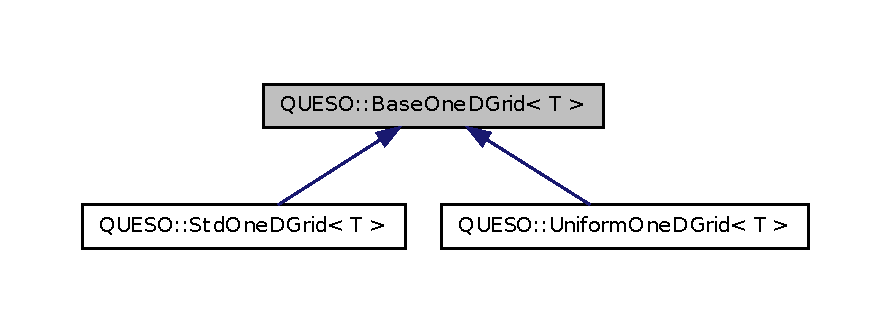
\includegraphics[width=350pt]{class_q_u_e_s_o_1_1_base_one_d_grid__inherit__graph}
\end{center}
\end{figure}


Collaboration diagram for Q\-U\-E\-S\-O\-:\-:Base\-One\-D\-Grid$<$ T $>$\-:
\nopagebreak
\begin{figure}[H]
\begin{center}
\leavevmode
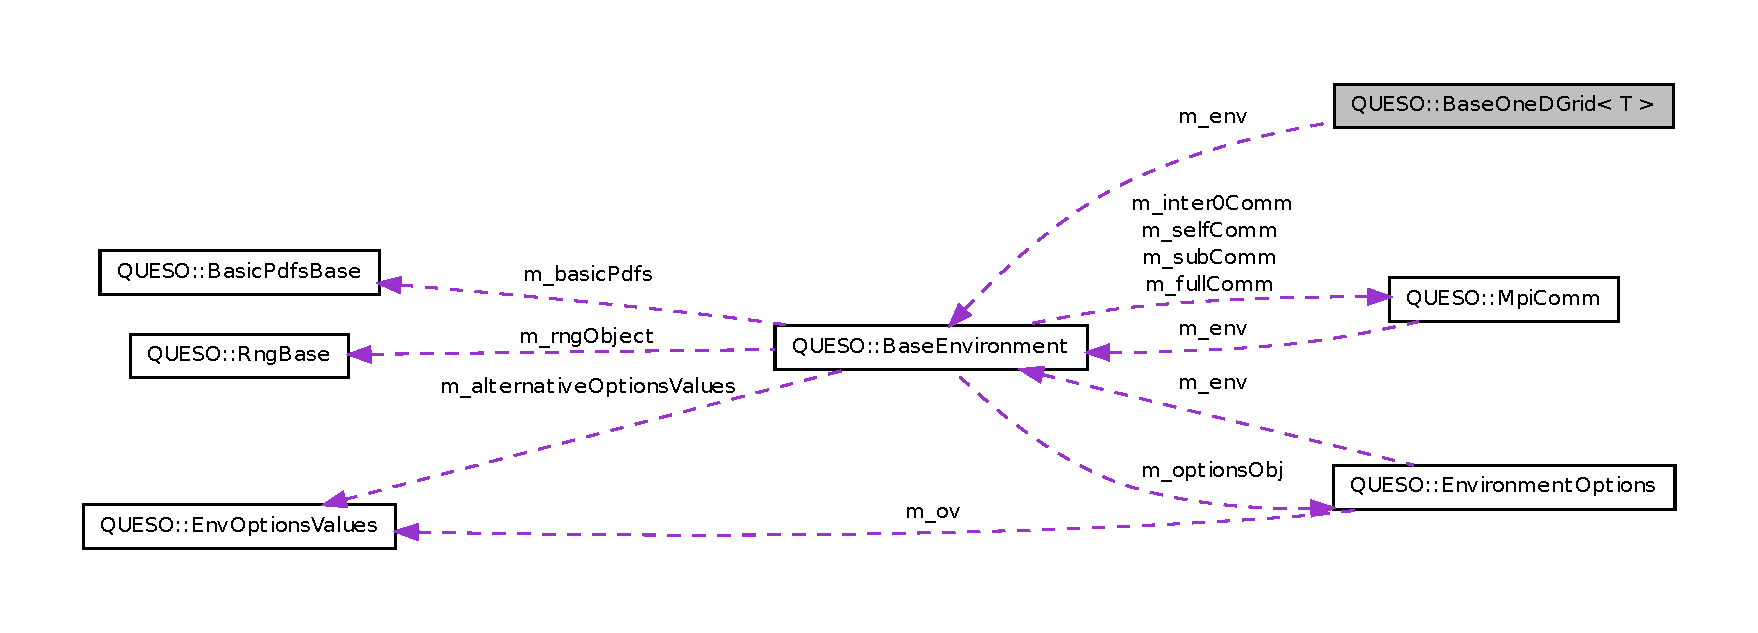
\includegraphics[width=350pt]{class_q_u_e_s_o_1_1_base_one_d_grid__coll__graph}
\end{center}
\end{figure}
\subsection*{Public Member Functions}
\begin{Indent}{\bf Constructor/\-Destructor methods}\par
\begin{DoxyCompactItemize}
\item 
\hyperlink{class_q_u_e_s_o_1_1_base_one_d_grid_a83cc4075f64e729df5ab6dbbe992c9fb}{Base\-One\-D\-Grid} (const \hyperlink{class_q_u_e_s_o_1_1_base_environment}{Base\-Environment} \&env, const char $\ast$prefix)
\begin{DoxyCompactList}\small\item\em Default constructor. \end{DoxyCompactList}\item 
virtual \hyperlink{class_q_u_e_s_o_1_1_base_one_d_grid_ae19c9434ea06d92100e8d49686e354e2}{$\sim$\-Base\-One\-D\-Grid} ()
\begin{DoxyCompactList}\small\item\em Virtual destructor. \end{DoxyCompactList}\end{DoxyCompactItemize}
\end{Indent}
\begin{Indent}{\bf Accessor methods}\par
\begin{DoxyCompactItemize}
\item 
virtual T \hyperlink{class_q_u_e_s_o_1_1_base_one_d_grid_a80648b45e665a5a10fec57e7ab094bce}{operator\mbox{[}$\,$\mbox{]}} (unsigned int i) const =0
\begin{DoxyCompactList}\small\item\em Returns the position of the i-\/th point in the grid. See template specialization. \end{DoxyCompactList}\end{DoxyCompactItemize}
\end{Indent}
\begin{Indent}{\bf Mathematical methods}\par
\begin{DoxyCompactItemize}
\item 
virtual unsigned int \hyperlink{class_q_u_e_s_o_1_1_base_one_d_grid_a388e922ba0c770039ab95e2cd1190dd6}{size} () const =0
\begin{DoxyCompactList}\small\item\em Grid size; the amount of points which defines the grid. See template specialization. \end{DoxyCompactList}\item 
virtual unsigned int \hyperlink{class_q_u_e_s_o_1_1_base_one_d_grid_ac238dee5e7ce70b93bbed696948c9df3}{find\-Interval\-Id} (const T \&param\-Value) const =0
\begin{DoxyCompactList}\small\item\em Finds the I\-D of an interval. See template specialization. \end{DoxyCompactList}\end{DoxyCompactItemize}
\end{Indent}
\subsection*{Protected Attributes}
\begin{DoxyCompactItemize}
\item 
const \hyperlink{class_q_u_e_s_o_1_1_base_environment}{Base\-Environment} \& \hyperlink{class_q_u_e_s_o_1_1_base_one_d_grid_a668a0033829b907fac9e13466419b7b1}{m\-\_\-env}
\item 
std\-::string \hyperlink{class_q_u_e_s_o_1_1_base_one_d_grid_af5fa59e47fae9f6195b00e5bec8310f8}{m\-\_\-prefix}
\end{DoxyCompactItemize}
\subsection*{I/\-O methods}
\begin{DoxyCompactItemize}
\item 
void \hyperlink{class_q_u_e_s_o_1_1_base_one_d_grid_af72394608d602022a6cff06018a5df22}{print} (std\-::ostream \&ofsvar) const 
\begin{DoxyCompactList}\small\item\em Prints the values of the grid points. \end{DoxyCompactList}\item 
std\-::ostream \& \hyperlink{class_q_u_e_s_o_1_1_base_one_d_grid_a00cca8cd319438b0e49d9ebc72a1749d}{operator$<$$<$} (std\-::ostream \&os, const \hyperlink{class_q_u_e_s_o_1_1_base_one_d_grid}{Base\-One\-D\-Grid}$<$ T $>$ \&obj)
\end{DoxyCompactItemize}


\subsection{Detailed Description}
\subsubsection*{template$<$class T$>$class Q\-U\-E\-S\-O\-::\-Base\-One\-D\-Grid$<$ T $>$}

Base class for accommodating one-\/dimensional grids. 

Definition at line 46 of file One\-D\-Grid.\-h.



\subsection{Constructor \& Destructor Documentation}
\hypertarget{class_q_u_e_s_o_1_1_base_one_d_grid_a83cc4075f64e729df5ab6dbbe992c9fb}{\index{Q\-U\-E\-S\-O\-::\-Base\-One\-D\-Grid@{Q\-U\-E\-S\-O\-::\-Base\-One\-D\-Grid}!Base\-One\-D\-Grid@{Base\-One\-D\-Grid}}
\index{Base\-One\-D\-Grid@{Base\-One\-D\-Grid}!QUESO::BaseOneDGrid@{Q\-U\-E\-S\-O\-::\-Base\-One\-D\-Grid}}
\subsubsection[{Base\-One\-D\-Grid}]{\setlength{\rightskip}{0pt plus 5cm}template$<$class T $>$ {\bf Q\-U\-E\-S\-O\-::\-Base\-One\-D\-Grid}$<$ T $>$\-::{\bf Base\-One\-D\-Grid} (
\begin{DoxyParamCaption}
\item[{const {\bf Base\-Environment} \&}]{env, }
\item[{const char $\ast$}]{prefix}
\end{DoxyParamCaption}
)}}\label{class_q_u_e_s_o_1_1_base_one_d_grid_a83cc4075f64e729df5ab6dbbe992c9fb}


Default constructor. 



Definition at line 30 of file One\-D\-Grid.\-C.



References Q\-U\-E\-S\-O\-::\-Base\-Environment\-::display\-Verbosity(), Q\-U\-E\-S\-O\-::\-Base\-One\-D\-Grid$<$ T $>$\-::m\-\_\-env, Q\-U\-E\-S\-O\-::\-Base\-One\-D\-Grid$<$ T $>$\-::m\-\_\-prefix, and Q\-U\-E\-S\-O\-::\-Base\-Environment\-::sub\-Display\-File().


\begin{DoxyCode}
33   :
34   \hyperlink{class_q_u_e_s_o_1_1_base_one_d_grid_a668a0033829b907fac9e13466419b7b1}{m\_env}   (env),
35   \hyperlink{class_q_u_e_s_o_1_1_base_one_d_grid_af5fa59e47fae9f6195b00e5bec8310f8}{m\_prefix}((std::string)(prefix)+\textcolor{stringliteral}{"grid"})
36 \{
37   \textcolor{keywordflow}{if} ((\hyperlink{class_q_u_e_s_o_1_1_base_one_d_grid_a668a0033829b907fac9e13466419b7b1}{m\_env}.\hyperlink{class_q_u_e_s_o_1_1_base_environment_a8a0064746ae8dddfece4229b9ad374d6}{subDisplayFile}()) && (\hyperlink{class_q_u_e_s_o_1_1_base_one_d_grid_a668a0033829b907fac9e13466419b7b1}{m\_env}.
      \hyperlink{class_q_u_e_s_o_1_1_base_environment_a1fe5f244fc0316a0ab3e37463f108b96}{displayVerbosity}() >= 5)) \{
38     *\hyperlink{class_q_u_e_s_o_1_1_base_one_d_grid_a668a0033829b907fac9e13466419b7b1}{m\_env}.\hyperlink{class_q_u_e_s_o_1_1_base_environment_a8a0064746ae8dddfece4229b9ad374d6}{subDisplayFile}() << \textcolor{stringliteral}{"Entering BaseOneDGrid<T>::constructor()"}
39                            << \textcolor{stringliteral}{": prefix = "} << \hyperlink{class_q_u_e_s_o_1_1_base_one_d_grid_af5fa59e47fae9f6195b00e5bec8310f8}{m\_prefix}
40                            << std::endl;
41   \}
42 
43   \textcolor{keywordflow}{if} ((\hyperlink{class_q_u_e_s_o_1_1_base_one_d_grid_a668a0033829b907fac9e13466419b7b1}{m\_env}.\hyperlink{class_q_u_e_s_o_1_1_base_environment_a8a0064746ae8dddfece4229b9ad374d6}{subDisplayFile}()) && (\hyperlink{class_q_u_e_s_o_1_1_base_one_d_grid_a668a0033829b907fac9e13466419b7b1}{m\_env}.
      \hyperlink{class_q_u_e_s_o_1_1_base_environment_a1fe5f244fc0316a0ab3e37463f108b96}{displayVerbosity}() >= 5)) \{
44     *\hyperlink{class_q_u_e_s_o_1_1_base_one_d_grid_a668a0033829b907fac9e13466419b7b1}{m\_env}.\hyperlink{class_q_u_e_s_o_1_1_base_environment_a8a0064746ae8dddfece4229b9ad374d6}{subDisplayFile}() << \textcolor{stringliteral}{"Leaving BaseOneDGrid<T>::constructor()"}
45                            << \textcolor{stringliteral}{": prefix = "} << \hyperlink{class_q_u_e_s_o_1_1_base_one_d_grid_af5fa59e47fae9f6195b00e5bec8310f8}{m\_prefix}
46                            << std::endl;
47   \}
48 \}
\end{DoxyCode}
\hypertarget{class_q_u_e_s_o_1_1_base_one_d_grid_ae19c9434ea06d92100e8d49686e354e2}{\index{Q\-U\-E\-S\-O\-::\-Base\-One\-D\-Grid@{Q\-U\-E\-S\-O\-::\-Base\-One\-D\-Grid}!$\sim$\-Base\-One\-D\-Grid@{$\sim$\-Base\-One\-D\-Grid}}
\index{$\sim$\-Base\-One\-D\-Grid@{$\sim$\-Base\-One\-D\-Grid}!QUESO::BaseOneDGrid@{Q\-U\-E\-S\-O\-::\-Base\-One\-D\-Grid}}
\subsubsection[{$\sim$\-Base\-One\-D\-Grid}]{\setlength{\rightskip}{0pt plus 5cm}template$<$class T $>$ {\bf Q\-U\-E\-S\-O\-::\-Base\-One\-D\-Grid}$<$ T $>$\-::$\sim${\bf Base\-One\-D\-Grid} (
\begin{DoxyParamCaption}
{}
\end{DoxyParamCaption}
)\hspace{0.3cm}{\ttfamily [virtual]}}}\label{class_q_u_e_s_o_1_1_base_one_d_grid_ae19c9434ea06d92100e8d49686e354e2}


Virtual destructor. 



Definition at line 51 of file One\-D\-Grid.\-C.


\begin{DoxyCode}
52 \{
53 \}
\end{DoxyCode}


\subsection{Member Function Documentation}
\hypertarget{class_q_u_e_s_o_1_1_base_one_d_grid_ac238dee5e7ce70b93bbed696948c9df3}{\index{Q\-U\-E\-S\-O\-::\-Base\-One\-D\-Grid@{Q\-U\-E\-S\-O\-::\-Base\-One\-D\-Grid}!find\-Interval\-Id@{find\-Interval\-Id}}
\index{find\-Interval\-Id@{find\-Interval\-Id}!QUESO::BaseOneDGrid@{Q\-U\-E\-S\-O\-::\-Base\-One\-D\-Grid}}
\subsubsection[{find\-Interval\-Id}]{\setlength{\rightskip}{0pt plus 5cm}template$<$class T$>$ virtual unsigned int {\bf Q\-U\-E\-S\-O\-::\-Base\-One\-D\-Grid}$<$ T $>$\-::find\-Interval\-Id (
\begin{DoxyParamCaption}
\item[{const T \&}]{param\-Value}
\end{DoxyParamCaption}
) const\hspace{0.3cm}{\ttfamily [pure virtual]}}}\label{class_q_u_e_s_o_1_1_base_one_d_grid_ac238dee5e7ce70b93bbed696948c9df3}


Finds the I\-D of an interval. See template specialization. 



Implemented in \hyperlink{class_q_u_e_s_o_1_1_std_one_d_grid_aaf32f8fe97724ad2d23d5be9b2faeaae}{Q\-U\-E\-S\-O\-::\-Std\-One\-D\-Grid$<$ T $>$}, and \hyperlink{class_q_u_e_s_o_1_1_uniform_one_d_grid_afa2a0d3a54ce7fed0610a81337dfeae7}{Q\-U\-E\-S\-O\-::\-Uniform\-One\-D\-Grid$<$ T $>$}.

\hypertarget{class_q_u_e_s_o_1_1_base_one_d_grid_a80648b45e665a5a10fec57e7ab094bce}{\index{Q\-U\-E\-S\-O\-::\-Base\-One\-D\-Grid@{Q\-U\-E\-S\-O\-::\-Base\-One\-D\-Grid}!operator\mbox{[}$\,$\mbox{]}@{operator[]}}
\index{operator\mbox{[}$\,$\mbox{]}@{operator[]}!QUESO::BaseOneDGrid@{Q\-U\-E\-S\-O\-::\-Base\-One\-D\-Grid}}
\subsubsection[{operator[]}]{\setlength{\rightskip}{0pt plus 5cm}template$<$class T$>$ virtual T {\bf Q\-U\-E\-S\-O\-::\-Base\-One\-D\-Grid}$<$ T $>$\-::operator\mbox{[}$\,$\mbox{]} (
\begin{DoxyParamCaption}
\item[{unsigned int}]{i}
\end{DoxyParamCaption}
) const\hspace{0.3cm}{\ttfamily [pure virtual]}}}\label{class_q_u_e_s_o_1_1_base_one_d_grid_a80648b45e665a5a10fec57e7ab094bce}


Returns the position of the i-\/th point in the grid. See template specialization. 



Implemented in \hyperlink{class_q_u_e_s_o_1_1_std_one_d_grid_a08cb60749c59ff27239c231d6a0f1eca}{Q\-U\-E\-S\-O\-::\-Std\-One\-D\-Grid$<$ T $>$}, and \hyperlink{class_q_u_e_s_o_1_1_uniform_one_d_grid_a2fe101c8fbce7a6ac00b07781c2c6b6e}{Q\-U\-E\-S\-O\-::\-Uniform\-One\-D\-Grid$<$ T $>$}.

\hypertarget{class_q_u_e_s_o_1_1_base_one_d_grid_af72394608d602022a6cff06018a5df22}{\index{Q\-U\-E\-S\-O\-::\-Base\-One\-D\-Grid@{Q\-U\-E\-S\-O\-::\-Base\-One\-D\-Grid}!print@{print}}
\index{print@{print}!QUESO::BaseOneDGrid@{Q\-U\-E\-S\-O\-::\-Base\-One\-D\-Grid}}
\subsubsection[{print}]{\setlength{\rightskip}{0pt plus 5cm}template$<$class T $>$ void {\bf Q\-U\-E\-S\-O\-::\-Base\-One\-D\-Grid}$<$ T $>$\-::print (
\begin{DoxyParamCaption}
\item[{std\-::ostream \&}]{ofsvar}
\end{DoxyParamCaption}
) const}}\label{class_q_u_e_s_o_1_1_base_one_d_grid_af72394608d602022a6cff06018a5df22}


Prints the values of the grid points. 



Definition at line 57 of file One\-D\-Grid.\-C.


\begin{DoxyCode}
58 \{
59   \textcolor{comment}{// Print values *of* grid points}
60   os << \hyperlink{class_q_u_e_s_o_1_1_base_one_d_grid_af5fa59e47fae9f6195b00e5bec8310f8}{m\_prefix} << \textcolor{stringliteral}{"\_sub"} << \hyperlink{class_q_u_e_s_o_1_1_base_one_d_grid_a668a0033829b907fac9e13466419b7b1}{m\_env}.\hyperlink{class_q_u_e_s_o_1_1_base_environment_a73f7849acdd5d5ba15a3094fe18f258f}{subIdString}() << \textcolor{stringliteral}{" = zeros("} << this->
      \hyperlink{class_q_u_e_s_o_1_1_base_one_d_grid_a388e922ba0c770039ab95e2cd1190dd6}{size}()
61      << \textcolor{stringliteral}{","}                                                      << 1
62      << \textcolor{stringliteral}{");"}
63      << std::endl;
64   os << \hyperlink{class_q_u_e_s_o_1_1_base_one_d_grid_af5fa59e47fae9f6195b00e5bec8310f8}{m\_prefix} << \textcolor{stringliteral}{"\_sub"} << \hyperlink{class_q_u_e_s_o_1_1_base_one_d_grid_a668a0033829b907fac9e13466419b7b1}{m\_env}.\hyperlink{class_q_u_e_s_o_1_1_base_environment_a73f7849acdd5d5ba15a3094fe18f258f}{subIdString}() << \textcolor{stringliteral}{" = ["};
65   \textcolor{keywordflow}{for} (\textcolor{keywordtype}{unsigned} \textcolor{keywordtype}{int} j = 0; j < this->\hyperlink{class_q_u_e_s_o_1_1_base_one_d_grid_a388e922ba0c770039ab95e2cd1190dd6}{size}(); ++j) \{
66     os << (*this)[j] << \textcolor{stringliteral}{" "};
67   \}
68   os << \textcolor{stringliteral}{"];"}
69      << std::endl;
70 
71   \textcolor{keywordflow}{return};
72 \}
\end{DoxyCode}
\hypertarget{class_q_u_e_s_o_1_1_base_one_d_grid_a388e922ba0c770039ab95e2cd1190dd6}{\index{Q\-U\-E\-S\-O\-::\-Base\-One\-D\-Grid@{Q\-U\-E\-S\-O\-::\-Base\-One\-D\-Grid}!size@{size}}
\index{size@{size}!QUESO::BaseOneDGrid@{Q\-U\-E\-S\-O\-::\-Base\-One\-D\-Grid}}
\subsubsection[{size}]{\setlength{\rightskip}{0pt plus 5cm}template$<$class T$>$ virtual unsigned int {\bf Q\-U\-E\-S\-O\-::\-Base\-One\-D\-Grid}$<$ T $>$\-::size (
\begin{DoxyParamCaption}
{}
\end{DoxyParamCaption}
) const\hspace{0.3cm}{\ttfamily [pure virtual]}}}\label{class_q_u_e_s_o_1_1_base_one_d_grid_a388e922ba0c770039ab95e2cd1190dd6}


Grid size; the amount of points which defines the grid. See template specialization. 



Implemented in \hyperlink{class_q_u_e_s_o_1_1_std_one_d_grid_a006574772a0021d68c6f5c98e2db3458}{Q\-U\-E\-S\-O\-::\-Std\-One\-D\-Grid$<$ T $>$}, and \hyperlink{class_q_u_e_s_o_1_1_uniform_one_d_grid_a66a0589eb7da47895f2bab97b916fca4}{Q\-U\-E\-S\-O\-::\-Uniform\-One\-D\-Grid$<$ T $>$}.



\subsection{Friends And Related Function Documentation}
\hypertarget{class_q_u_e_s_o_1_1_base_one_d_grid_a00cca8cd319438b0e49d9ebc72a1749d}{\index{Q\-U\-E\-S\-O\-::\-Base\-One\-D\-Grid@{Q\-U\-E\-S\-O\-::\-Base\-One\-D\-Grid}!operator$<$$<$@{operator$<$$<$}}
\index{operator$<$$<$@{operator$<$$<$}!QUESO::BaseOneDGrid@{Q\-U\-E\-S\-O\-::\-Base\-One\-D\-Grid}}
\subsubsection[{operator$<$$<$}]{\setlength{\rightskip}{0pt plus 5cm}template$<$class T$>$ std\-::ostream\& operator$<$$<$ (
\begin{DoxyParamCaption}
\item[{std\-::ostream \&}]{os, }
\item[{const {\bf Base\-One\-D\-Grid}$<$ T $>$ \&}]{obj}
\end{DoxyParamCaption}
)\hspace{0.3cm}{\ttfamily [friend]}}}\label{class_q_u_e_s_o_1_1_base_one_d_grid_a00cca8cd319438b0e49d9ebc72a1749d}


Definition at line 73 of file One\-D\-Grid.\-h.


\begin{DoxyCode}
75   \{
76     obj.print(os);
77     \textcolor{keywordflow}{return} os;
78   \}
\end{DoxyCode}


\subsection{Member Data Documentation}
\hypertarget{class_q_u_e_s_o_1_1_base_one_d_grid_a668a0033829b907fac9e13466419b7b1}{\index{Q\-U\-E\-S\-O\-::\-Base\-One\-D\-Grid@{Q\-U\-E\-S\-O\-::\-Base\-One\-D\-Grid}!m\-\_\-env@{m\-\_\-env}}
\index{m\-\_\-env@{m\-\_\-env}!QUESO::BaseOneDGrid@{Q\-U\-E\-S\-O\-::\-Base\-One\-D\-Grid}}
\subsubsection[{m\-\_\-env}]{\setlength{\rightskip}{0pt plus 5cm}template$<$class T$>$ const {\bf Base\-Environment}\& {\bf Q\-U\-E\-S\-O\-::\-Base\-One\-D\-Grid}$<$ T $>$\-::m\-\_\-env\hspace{0.3cm}{\ttfamily [protected]}}}\label{class_q_u_e_s_o_1_1_base_one_d_grid_a668a0033829b907fac9e13466419b7b1}


Definition at line 82 of file One\-D\-Grid.\-h.



Referenced by Q\-U\-E\-S\-O\-::\-Base\-One\-D\-Grid$<$ T $>$\-::\-Base\-One\-D\-Grid(), Q\-U\-E\-S\-O\-::\-Std\-One\-D\-Grid$<$ T $>$\-::\-Std\-One\-D\-Grid(), and Q\-U\-E\-S\-O\-::\-Uniform\-One\-D\-Grid$<$ T $>$\-::\-Uniform\-One\-D\-Grid().

\hypertarget{class_q_u_e_s_o_1_1_base_one_d_grid_af5fa59e47fae9f6195b00e5bec8310f8}{\index{Q\-U\-E\-S\-O\-::\-Base\-One\-D\-Grid@{Q\-U\-E\-S\-O\-::\-Base\-One\-D\-Grid}!m\-\_\-prefix@{m\-\_\-prefix}}
\index{m\-\_\-prefix@{m\-\_\-prefix}!QUESO::BaseOneDGrid@{Q\-U\-E\-S\-O\-::\-Base\-One\-D\-Grid}}
\subsubsection[{m\-\_\-prefix}]{\setlength{\rightskip}{0pt plus 5cm}template$<$class T$>$ std\-::string {\bf Q\-U\-E\-S\-O\-::\-Base\-One\-D\-Grid}$<$ T $>$\-::m\-\_\-prefix\hspace{0.3cm}{\ttfamily [protected]}}}\label{class_q_u_e_s_o_1_1_base_one_d_grid_af5fa59e47fae9f6195b00e5bec8310f8}


Definition at line 83 of file One\-D\-Grid.\-h.



Referenced by Q\-U\-E\-S\-O\-::\-Base\-One\-D\-Grid$<$ T $>$\-::\-Base\-One\-D\-Grid(), Q\-U\-E\-S\-O\-::\-Std\-One\-D\-Grid$<$ T $>$\-::\-Std\-One\-D\-Grid(), and Q\-U\-E\-S\-O\-::\-Uniform\-One\-D\-Grid$<$ T $>$\-::\-Uniform\-One\-D\-Grid().



The documentation for this class was generated from the following files\-:\begin{DoxyCompactItemize}
\item 
src/misc/inc/\hyperlink{_one_d_grid_8h}{One\-D\-Grid.\-h}\item 
src/misc/src/\hyperlink{_one_d_grid_8_c}{One\-D\-Grid.\-C}\end{DoxyCompactItemize}

\hypertarget{class_q_u_e_s_o_1_1_base_scalar_cdf}{\section{Q\-U\-E\-S\-O\-:\-:Base\-Scalar\-Cdf$<$ T $>$ Class Template Reference}
\label{class_q_u_e_s_o_1_1_base_scalar_cdf}\index{Q\-U\-E\-S\-O\-::\-Base\-Scalar\-Cdf$<$ T $>$@{Q\-U\-E\-S\-O\-::\-Base\-Scalar\-Cdf$<$ T $>$}}
}


A templated (base) class for handling C\-D\-Fs.  




{\ttfamily \#include $<$Scalar\-Cdf.\-h$>$}



Inheritance diagram for Q\-U\-E\-S\-O\-:\-:Base\-Scalar\-Cdf$<$ T $>$\-:
\nopagebreak
\begin{figure}[H]
\begin{center}
\leavevmode
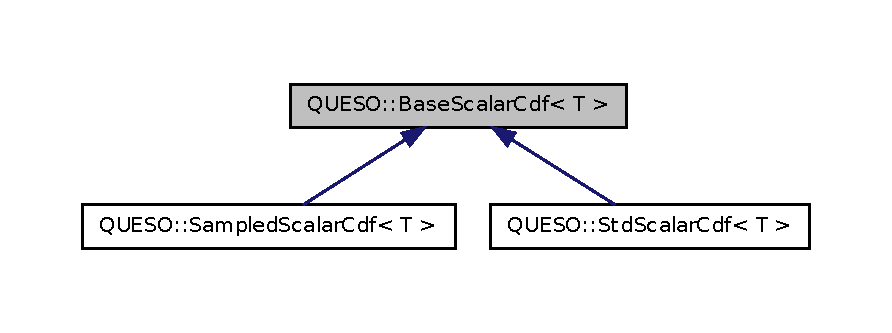
\includegraphics[width=350pt]{class_q_u_e_s_o_1_1_base_scalar_cdf__inherit__graph}
\end{center}
\end{figure}


Collaboration diagram for Q\-U\-E\-S\-O\-:\-:Base\-Scalar\-Cdf$<$ T $>$\-:
\nopagebreak
\begin{figure}[H]
\begin{center}
\leavevmode
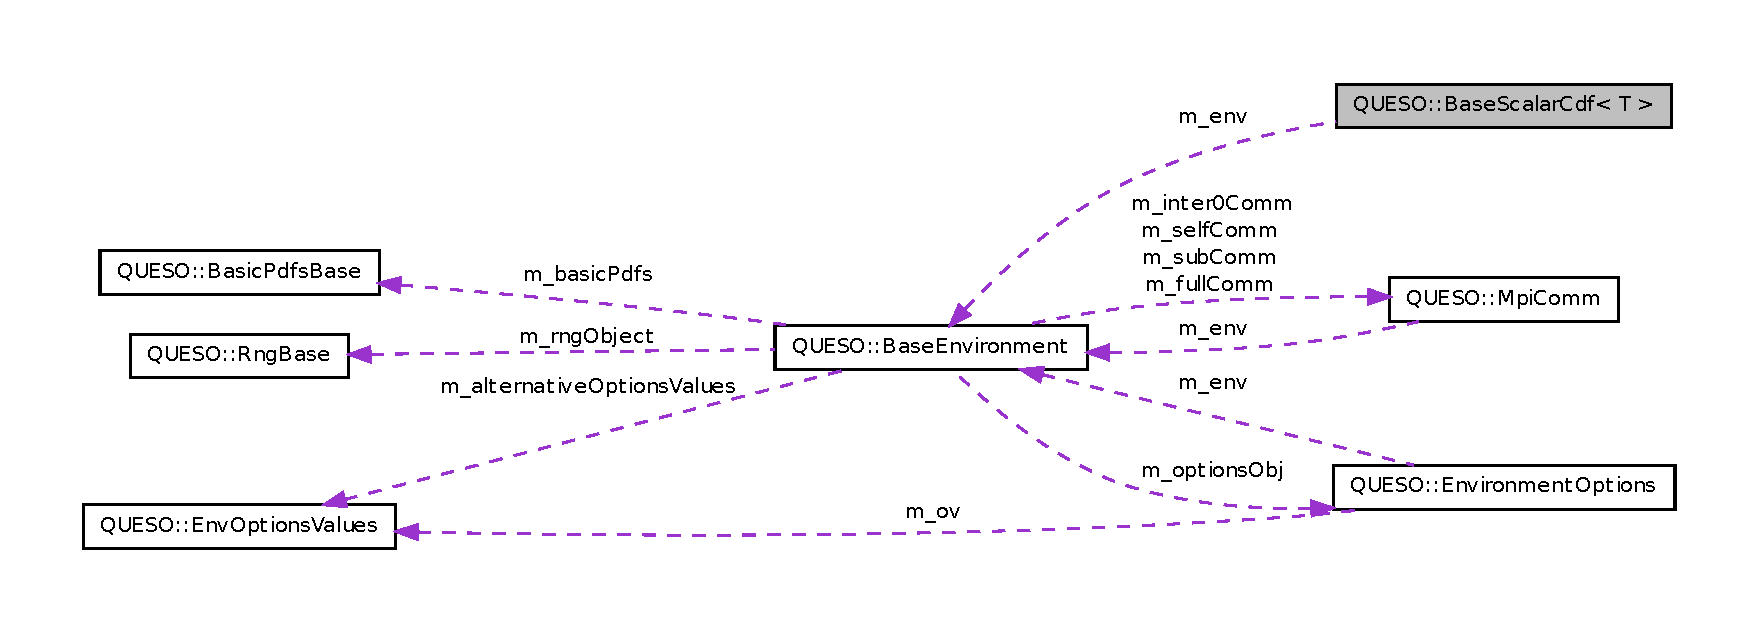
\includegraphics[width=350pt]{class_q_u_e_s_o_1_1_base_scalar_cdf__coll__graph}
\end{center}
\end{figure}
\subsection*{Public Member Functions}
\begin{Indent}{\bf Constructor/\-Destructor methods}\par
\begin{DoxyCompactItemize}
\item 
\hyperlink{class_q_u_e_s_o_1_1_base_scalar_cdf_a4604dee9fe730564c52d8d925bc69b94}{Base\-Scalar\-Cdf} (const \hyperlink{class_q_u_e_s_o_1_1_base_environment}{Base\-Environment} \&\hyperlink{class_q_u_e_s_o_1_1_base_scalar_cdf_a70c89dd2ad294be170338a283fc58ff3}{env}, const char $\ast$\hyperlink{class_q_u_e_s_o_1_1_base_scalar_cdf_aafb3eaf3bf1d7269073e9c77bd8c766d}{prefix})
\begin{DoxyCompactList}\small\item\em Default constructor. \end{DoxyCompactList}\item 
virtual \hyperlink{class_q_u_e_s_o_1_1_base_scalar_cdf_aa7bd0ba0d3719853cc24a2e12f126600}{$\sim$\-Base\-Scalar\-Cdf} ()
\begin{DoxyCompactList}\small\item\em Virtual destructor. \end{DoxyCompactList}\end{DoxyCompactItemize}
\end{Indent}
\begin{Indent}{\bf Environment methods}\par
\begin{DoxyCompactItemize}
\item 
const \hyperlink{class_q_u_e_s_o_1_1_base_environment}{Base\-Environment} \& \hyperlink{class_q_u_e_s_o_1_1_base_scalar_cdf_a70c89dd2ad294be170338a283fc58ff3}{env} () const 
\begin{DoxyCompactList}\small\item\em Environment. Access to private attribute m\-\_\-env. \end{DoxyCompactList}\item 
const std\-::string \& \hyperlink{class_q_u_e_s_o_1_1_base_scalar_cdf_aafb3eaf3bf1d7269073e9c77bd8c766d}{prefix} () const 
\begin{DoxyCompactList}\small\item\em Access to private attribute m\-\_\-prefix. \end{DoxyCompactList}\end{DoxyCompactItemize}
\end{Indent}
\begin{Indent}{\bf Mathematical methods}\par
\begin{DoxyCompactItemize}
\item 
virtual double \hyperlink{class_q_u_e_s_o_1_1_base_scalar_cdf_a887af6d62eb04f2bf3b58c12e586f20b}{value} (T param\-Value) const =0
\begin{DoxyCompactList}\small\item\em Returns the value of the C\-D\-F at {\ttfamily param\-Value}. See template specialization. \end{DoxyCompactList}\item 
virtual T \hyperlink{class_q_u_e_s_o_1_1_base_scalar_cdf_a3e1778c76a557716e74b5fc11604dd75}{inverse} (double cdf\-Value) const =0
\begin{DoxyCompactList}\small\item\em Returns the position of a given value of C\-D\-F. See template specialization. \end{DoxyCompactList}\item 
virtual void \hyperlink{class_q_u_e_s_o_1_1_base_scalar_cdf_a9684b285f88be8c2bafe4d2abd8a7447}{get\-Support} (T \&min\-Horizontal, T \&max\-Horizontal) const =0
\begin{DoxyCompactList}\small\item\em Returns the support (image) of the C\-D\-F between two horizontal values (domain). See template specialization. \end{DoxyCompactList}\end{DoxyCompactItemize}
\end{Indent}
\subsection*{Protected Attributes}
\begin{DoxyCompactItemize}
\item 
const \hyperlink{class_q_u_e_s_o_1_1_base_environment}{Base\-Environment} \& \hyperlink{class_q_u_e_s_o_1_1_base_scalar_cdf_a3caa986ae1ccef96a28b0365fb88c86c}{m\-\_\-env}
\item 
std\-::string \hyperlink{class_q_u_e_s_o_1_1_base_scalar_cdf_a66c2a1bcf0ac517013e7857c3533a187}{m\-\_\-prefix}
\item 
T \hyperlink{class_q_u_e_s_o_1_1_base_scalar_cdf_ab54be9623cddb0671db458d05d63f0a7}{m\-\_\-min\-Horizontal}
\item 
T \hyperlink{class_q_u_e_s_o_1_1_base_scalar_cdf_a33beb9b7e610a4fe1458080593982d2e}{m\-\_\-max\-Horizontal}
\end{DoxyCompactItemize}
\subsection*{I/\-O methods}
\begin{DoxyCompactItemize}
\item 
virtual void \hyperlink{class_q_u_e_s_o_1_1_base_scalar_cdf_a131a7c148188f3f70c2db44cc1a93bc8}{print} (std\-::ostream \&os) const =0
\begin{DoxyCompactList}\small\item\em Prints the C\-D\-F. See template specialization. \end{DoxyCompactList}\item 
virtual void \hyperlink{class_q_u_e_s_o_1_1_base_scalar_cdf_abdd6c6f5f8f028a6ffd30168885b6338}{sub\-Write\-Contents} (const std\-::string \&var\-Name\-Prefix, const std\-::string \&file\-Name, const std\-::string \&file\-Type, const std\-::set$<$ unsigned int $>$ \&allowed\-Sub\-Env\-Ids) const 
\begin{DoxyCompactList}\small\item\em Writes the C\-D\-F of an allowed sub-\/environment to a file. \end{DoxyCompactList}\item 
std\-::ostream \& \hyperlink{class_q_u_e_s_o_1_1_base_scalar_cdf_a474950d32c26caa1e88dbee2788cc1bf}{operator$<$$<$} (std\-::ostream \&os, const \hyperlink{class_q_u_e_s_o_1_1_base_scalar_cdf}{Base\-Scalar\-Cdf}$<$ T $>$ \&obj)
\end{DoxyCompactItemize}


\subsection{Detailed Description}
\subsubsection*{template$<$class T$>$class Q\-U\-E\-S\-O\-::\-Base\-Scalar\-Cdf$<$ T $>$}

A templated (base) class for handling C\-D\-Fs. 

This class allows the mathematical definition of a cumulative distribution function (C\-D\-F), which is a scalar function such as $\ast$ $ f: B \subset R \rightarrow C \subset R $; ie a function of one or more variables that has always one-\/dimensional range, which for the specific C\-D\-F case, the image set $ C = [0,1]$. The C\-D\-F describes the probability that a real-\/valued random variable X with a given probability distribution will be found at a value less than or equal to x. In the case of a continuous distribution, it gives the area under the probability density function (P\-D\-F) from minus infinity to x. 

Definition at line 56 of file Scalar\-Cdf.\-h.



\subsection{Constructor \& Destructor Documentation}
\hypertarget{class_q_u_e_s_o_1_1_base_scalar_cdf_a4604dee9fe730564c52d8d925bc69b94}{\index{Q\-U\-E\-S\-O\-::\-Base\-Scalar\-Cdf@{Q\-U\-E\-S\-O\-::\-Base\-Scalar\-Cdf}!Base\-Scalar\-Cdf@{Base\-Scalar\-Cdf}}
\index{Base\-Scalar\-Cdf@{Base\-Scalar\-Cdf}!QUESO::BaseScalarCdf@{Q\-U\-E\-S\-O\-::\-Base\-Scalar\-Cdf}}
\subsubsection[{Base\-Scalar\-Cdf}]{\setlength{\rightskip}{0pt plus 5cm}template$<$class T $>$ {\bf Q\-U\-E\-S\-O\-::\-Base\-Scalar\-Cdf}$<$ T $>$\-::{\bf Base\-Scalar\-Cdf} (
\begin{DoxyParamCaption}
\item[{const {\bf Base\-Environment} \&}]{env, }
\item[{const char $\ast$}]{prefix}
\end{DoxyParamCaption}
)}}\label{class_q_u_e_s_o_1_1_base_scalar_cdf_a4604dee9fe730564c52d8d925bc69b94}


Default constructor. 

Instantiates an object of the class given a prefix and the environment. 

Definition at line 31 of file Scalar\-Cdf.\-C.



References Q\-U\-E\-S\-O\-::\-Base\-Environment\-::display\-Verbosity(), Q\-U\-E\-S\-O\-::\-Base\-Scalar\-Cdf$<$ T $>$\-::m\-\_\-env, Q\-U\-E\-S\-O\-::\-Base\-Scalar\-Cdf$<$ T $>$\-::m\-\_\-prefix, and Q\-U\-E\-S\-O\-::\-Base\-Environment\-::sub\-Display\-File().


\begin{DoxyCode}
34   :
35   \hyperlink{class_q_u_e_s_o_1_1_base_scalar_cdf_a3caa986ae1ccef96a28b0365fb88c86c}{m\_env}          (\hyperlink{class_q_u_e_s_o_1_1_base_scalar_cdf_a70c89dd2ad294be170338a283fc58ff3}{env}),
36   \hyperlink{class_q_u_e_s_o_1_1_base_scalar_cdf_a66c2a1bcf0ac517013e7857c3533a187}{m\_prefix}       ((std::string)(\hyperlink{class_q_u_e_s_o_1_1_base_scalar_cdf_aafb3eaf3bf1d7269073e9c77bd8c766d}{prefix})+\textcolor{stringliteral}{""}),
37   \hyperlink{class_q_u_e_s_o_1_1_base_scalar_cdf_ab54be9623cddb0671db458d05d63f0a7}{m\_minHorizontal}(-INFINITY),
38   \hyperlink{class_q_u_e_s_o_1_1_base_scalar_cdf_a33beb9b7e610a4fe1458080593982d2e}{m\_maxHorizontal}( INFINITY)
39 \{
40   \textcolor{keywordflow}{if} ((\hyperlink{class_q_u_e_s_o_1_1_base_scalar_cdf_a3caa986ae1ccef96a28b0365fb88c86c}{m\_env}.\hyperlink{class_q_u_e_s_o_1_1_base_environment_a8a0064746ae8dddfece4229b9ad374d6}{subDisplayFile}()) && (\hyperlink{class_q_u_e_s_o_1_1_base_scalar_cdf_a3caa986ae1ccef96a28b0365fb88c86c}{m\_env}.
      \hyperlink{class_q_u_e_s_o_1_1_base_environment_a1fe5f244fc0316a0ab3e37463f108b96}{displayVerbosity}() >= 5)) \{
41     *\hyperlink{class_q_u_e_s_o_1_1_base_scalar_cdf_a3caa986ae1ccef96a28b0365fb88c86c}{m\_env}.\hyperlink{class_q_u_e_s_o_1_1_base_environment_a8a0064746ae8dddfece4229b9ad374d6}{subDisplayFile}() << \textcolor{stringliteral}{"Entering BaseScalarCdf<T>::constructor()"}
42                            << \textcolor{stringliteral}{": prefix = "} << \hyperlink{class_q_u_e_s_o_1_1_base_scalar_cdf_a66c2a1bcf0ac517013e7857c3533a187}{m\_prefix}
43                            << std::endl;
44   \}
45 
46   \textcolor{keywordflow}{if} ((\hyperlink{class_q_u_e_s_o_1_1_base_scalar_cdf_a3caa986ae1ccef96a28b0365fb88c86c}{m\_env}.\hyperlink{class_q_u_e_s_o_1_1_base_environment_a8a0064746ae8dddfece4229b9ad374d6}{subDisplayFile}()) && (\hyperlink{class_q_u_e_s_o_1_1_base_scalar_cdf_a3caa986ae1ccef96a28b0365fb88c86c}{m\_env}.
      \hyperlink{class_q_u_e_s_o_1_1_base_environment_a1fe5f244fc0316a0ab3e37463f108b96}{displayVerbosity}() >= 5)) \{
47     *\hyperlink{class_q_u_e_s_o_1_1_base_scalar_cdf_a3caa986ae1ccef96a28b0365fb88c86c}{m\_env}.\hyperlink{class_q_u_e_s_o_1_1_base_environment_a8a0064746ae8dddfece4229b9ad374d6}{subDisplayFile}() << \textcolor{stringliteral}{"Leaving BaseScalarCdf<T>::constructor()"}
48                            << \textcolor{stringliteral}{": prefix = "} << \hyperlink{class_q_u_e_s_o_1_1_base_scalar_cdf_a66c2a1bcf0ac517013e7857c3533a187}{m\_prefix}
49                            << std::endl;
50   \}
51 \}
\end{DoxyCode}
\hypertarget{class_q_u_e_s_o_1_1_base_scalar_cdf_aa7bd0ba0d3719853cc24a2e12f126600}{\index{Q\-U\-E\-S\-O\-::\-Base\-Scalar\-Cdf@{Q\-U\-E\-S\-O\-::\-Base\-Scalar\-Cdf}!$\sim$\-Base\-Scalar\-Cdf@{$\sim$\-Base\-Scalar\-Cdf}}
\index{$\sim$\-Base\-Scalar\-Cdf@{$\sim$\-Base\-Scalar\-Cdf}!QUESO::BaseScalarCdf@{Q\-U\-E\-S\-O\-::\-Base\-Scalar\-Cdf}}
\subsubsection[{$\sim$\-Base\-Scalar\-Cdf}]{\setlength{\rightskip}{0pt plus 5cm}template$<$class T $>$ {\bf Q\-U\-E\-S\-O\-::\-Base\-Scalar\-Cdf}$<$ T $>$\-::$\sim${\bf Base\-Scalar\-Cdf} (
\begin{DoxyParamCaption}
{}
\end{DoxyParamCaption}
)\hspace{0.3cm}{\ttfamily [virtual]}}}\label{class_q_u_e_s_o_1_1_base_scalar_cdf_aa7bd0ba0d3719853cc24a2e12f126600}


Virtual destructor. 



Definition at line 54 of file Scalar\-Cdf.\-C.


\begin{DoxyCode}
55 \{
56 \}
\end{DoxyCode}


\subsection{Member Function Documentation}
\hypertarget{class_q_u_e_s_o_1_1_base_scalar_cdf_a70c89dd2ad294be170338a283fc58ff3}{\index{Q\-U\-E\-S\-O\-::\-Base\-Scalar\-Cdf@{Q\-U\-E\-S\-O\-::\-Base\-Scalar\-Cdf}!env@{env}}
\index{env@{env}!QUESO::BaseScalarCdf@{Q\-U\-E\-S\-O\-::\-Base\-Scalar\-Cdf}}
\subsubsection[{env}]{\setlength{\rightskip}{0pt plus 5cm}template$<$class T $>$ const {\bf Base\-Environment} \& {\bf Q\-U\-E\-S\-O\-::\-Base\-Scalar\-Cdf}$<$ T $>$\-::env (
\begin{DoxyParamCaption}
{}
\end{DoxyParamCaption}
) const}}\label{class_q_u_e_s_o_1_1_base_scalar_cdf_a70c89dd2ad294be170338a283fc58ff3}


Environment. Access to private attribute m\-\_\-env. 



Definition at line 60 of file Scalar\-Cdf.\-C.



Referenced by Q\-U\-E\-S\-O\-::horizontal\-Distance(), and Q\-U\-E\-S\-O\-::\-Std\-Scalar\-Cdf$<$ T $>$\-::\-Std\-Scalar\-Cdf().


\begin{DoxyCode}
61 \{
62   \textcolor{keywordflow}{return} \hyperlink{class_q_u_e_s_o_1_1_base_scalar_cdf_a3caa986ae1ccef96a28b0365fb88c86c}{m\_env};
63 \}
\end{DoxyCode}
\hypertarget{class_q_u_e_s_o_1_1_base_scalar_cdf_a9684b285f88be8c2bafe4d2abd8a7447}{\index{Q\-U\-E\-S\-O\-::\-Base\-Scalar\-Cdf@{Q\-U\-E\-S\-O\-::\-Base\-Scalar\-Cdf}!get\-Support@{get\-Support}}
\index{get\-Support@{get\-Support}!QUESO::BaseScalarCdf@{Q\-U\-E\-S\-O\-::\-Base\-Scalar\-Cdf}}
\subsubsection[{get\-Support}]{\setlength{\rightskip}{0pt plus 5cm}template$<$class T$>$ virtual void {\bf Q\-U\-E\-S\-O\-::\-Base\-Scalar\-Cdf}$<$ T $>$\-::get\-Support (
\begin{DoxyParamCaption}
\item[{T \&}]{min\-Horizontal, }
\item[{T \&}]{max\-Horizontal}
\end{DoxyParamCaption}
) const\hspace{0.3cm}{\ttfamily [pure virtual]}}}\label{class_q_u_e_s_o_1_1_base_scalar_cdf_a9684b285f88be8c2bafe4d2abd8a7447}


Returns the support (image) of the C\-D\-F between two horizontal values (domain). See template specialization. 



Implemented in \hyperlink{class_q_u_e_s_o_1_1_std_scalar_cdf_ad754f420fbfaa309d6574a0c2674f06e}{Q\-U\-E\-S\-O\-::\-Std\-Scalar\-Cdf$<$ T $>$}, and \hyperlink{class_q_u_e_s_o_1_1_sampled_scalar_cdf_ab1d99d5dcc9dc79b50501caf80154c39}{Q\-U\-E\-S\-O\-::\-Sampled\-Scalar\-Cdf$<$ T $>$}.

\hypertarget{class_q_u_e_s_o_1_1_base_scalar_cdf_a3e1778c76a557716e74b5fc11604dd75}{\index{Q\-U\-E\-S\-O\-::\-Base\-Scalar\-Cdf@{Q\-U\-E\-S\-O\-::\-Base\-Scalar\-Cdf}!inverse@{inverse}}
\index{inverse@{inverse}!QUESO::BaseScalarCdf@{Q\-U\-E\-S\-O\-::\-Base\-Scalar\-Cdf}}
\subsubsection[{inverse}]{\setlength{\rightskip}{0pt plus 5cm}template$<$class T$>$ virtual T {\bf Q\-U\-E\-S\-O\-::\-Base\-Scalar\-Cdf}$<$ T $>$\-::inverse (
\begin{DoxyParamCaption}
\item[{double}]{cdf\-Value}
\end{DoxyParamCaption}
) const\hspace{0.3cm}{\ttfamily [pure virtual]}}}\label{class_q_u_e_s_o_1_1_base_scalar_cdf_a3e1778c76a557716e74b5fc11604dd75}


Returns the position of a given value of C\-D\-F. See template specialization. 



Implemented in \hyperlink{class_q_u_e_s_o_1_1_std_scalar_cdf_a0b989e6ac45b22f22951389ae4c41861}{Q\-U\-E\-S\-O\-::\-Std\-Scalar\-Cdf$<$ T $>$}, and \hyperlink{class_q_u_e_s_o_1_1_sampled_scalar_cdf_a685b0c343b3ab320680c132c836fb1da}{Q\-U\-E\-S\-O\-::\-Sampled\-Scalar\-Cdf$<$ T $>$}.



Referenced by Q\-U\-E\-S\-O\-::horizontal\-Distance().

\hypertarget{class_q_u_e_s_o_1_1_base_scalar_cdf_aafb3eaf3bf1d7269073e9c77bd8c766d}{\index{Q\-U\-E\-S\-O\-::\-Base\-Scalar\-Cdf@{Q\-U\-E\-S\-O\-::\-Base\-Scalar\-Cdf}!prefix@{prefix}}
\index{prefix@{prefix}!QUESO::BaseScalarCdf@{Q\-U\-E\-S\-O\-::\-Base\-Scalar\-Cdf}}
\subsubsection[{prefix}]{\setlength{\rightskip}{0pt plus 5cm}template$<$class T $>$ const std\-::string \& {\bf Q\-U\-E\-S\-O\-::\-Base\-Scalar\-Cdf}$<$ T $>$\-::prefix (
\begin{DoxyParamCaption}
{}
\end{DoxyParamCaption}
) const}}\label{class_q_u_e_s_o_1_1_base_scalar_cdf_aafb3eaf3bf1d7269073e9c77bd8c766d}


Access to private attribute m\-\_\-prefix. 



Definition at line 67 of file Scalar\-Cdf.\-C.



Referenced by Q\-U\-E\-S\-O\-::horizontal\-Distance(), and Q\-U\-E\-S\-O\-::\-Std\-Scalar\-Cdf$<$ T $>$\-::\-Std\-Scalar\-Cdf().


\begin{DoxyCode}
68 \{
69   \textcolor{keywordflow}{return} \hyperlink{class_q_u_e_s_o_1_1_base_scalar_cdf_a66c2a1bcf0ac517013e7857c3533a187}{m\_prefix};
70 \}
\end{DoxyCode}
\hypertarget{class_q_u_e_s_o_1_1_base_scalar_cdf_a131a7c148188f3f70c2db44cc1a93bc8}{\index{Q\-U\-E\-S\-O\-::\-Base\-Scalar\-Cdf@{Q\-U\-E\-S\-O\-::\-Base\-Scalar\-Cdf}!print@{print}}
\index{print@{print}!QUESO::BaseScalarCdf@{Q\-U\-E\-S\-O\-::\-Base\-Scalar\-Cdf}}
\subsubsection[{print}]{\setlength{\rightskip}{0pt plus 5cm}template$<$class T$>$ virtual void {\bf Q\-U\-E\-S\-O\-::\-Base\-Scalar\-Cdf}$<$ T $>$\-::print (
\begin{DoxyParamCaption}
\item[{std\-::ostream \&}]{os}
\end{DoxyParamCaption}
) const\hspace{0.3cm}{\ttfamily [pure virtual]}}}\label{class_q_u_e_s_o_1_1_base_scalar_cdf_a131a7c148188f3f70c2db44cc1a93bc8}


Prints the C\-D\-F. See template specialization. 



Implemented in \hyperlink{class_q_u_e_s_o_1_1_std_scalar_cdf_af31f2d7dfa14a23987d1d71b36d2d221}{Q\-U\-E\-S\-O\-::\-Std\-Scalar\-Cdf$<$ T $>$}, and \hyperlink{class_q_u_e_s_o_1_1_sampled_scalar_cdf_a1ae05088dd70e2432a52577ba6dca468}{Q\-U\-E\-S\-O\-::\-Sampled\-Scalar\-Cdf$<$ T $>$}.

\hypertarget{class_q_u_e_s_o_1_1_base_scalar_cdf_abdd6c6f5f8f028a6ffd30168885b6338}{\index{Q\-U\-E\-S\-O\-::\-Base\-Scalar\-Cdf@{Q\-U\-E\-S\-O\-::\-Base\-Scalar\-Cdf}!sub\-Write\-Contents@{sub\-Write\-Contents}}
\index{sub\-Write\-Contents@{sub\-Write\-Contents}!QUESO::BaseScalarCdf@{Q\-U\-E\-S\-O\-::\-Base\-Scalar\-Cdf}}
\subsubsection[{sub\-Write\-Contents}]{\setlength{\rightskip}{0pt plus 5cm}template$<$class T $>$ void {\bf Q\-U\-E\-S\-O\-::\-Base\-Scalar\-Cdf}$<$ T $>$\-::sub\-Write\-Contents (
\begin{DoxyParamCaption}
\item[{const std\-::string \&}]{var\-Name\-Prefix, }
\item[{const std\-::string \&}]{file\-Name, }
\item[{const std\-::string \&}]{file\-Type, }
\item[{const std\-::set$<$ unsigned int $>$ \&}]{allowed\-Sub\-Env\-Ids}
\end{DoxyParamCaption}
) const\hspace{0.3cm}{\ttfamily [virtual]}}}\label{class_q_u_e_s_o_1_1_base_scalar_cdf_abdd6c6f5f8f028a6ffd30168885b6338}


Writes the C\-D\-F of an allowed sub-\/environment to a file. 

This function does nothing and should \par
 not be called by the user. 

Reimplemented in \hyperlink{class_q_u_e_s_o_1_1_std_scalar_cdf_a9c4edf99c3d0bbd5a011b5e03c5a1bcc}{Q\-U\-E\-S\-O\-::\-Std\-Scalar\-Cdf$<$ T $>$}, and \hyperlink{class_q_u_e_s_o_1_1_sampled_scalar_cdf_af597534e752c2974448d7fd071266c59}{Q\-U\-E\-S\-O\-::\-Sampled\-Scalar\-Cdf$<$ T $>$}.



Definition at line 74 of file Scalar\-Cdf.\-C.


\begin{DoxyCode}
79 \{
80   std::cerr << \textcolor{stringliteral}{"WARNING: BaseScalarCdf<T>::subWriteContents() being used..."}
81             << std::endl;
82   \textcolor{keywordflow}{return};
83 \}
\end{DoxyCode}
\hypertarget{class_q_u_e_s_o_1_1_base_scalar_cdf_a887af6d62eb04f2bf3b58c12e586f20b}{\index{Q\-U\-E\-S\-O\-::\-Base\-Scalar\-Cdf@{Q\-U\-E\-S\-O\-::\-Base\-Scalar\-Cdf}!value@{value}}
\index{value@{value}!QUESO::BaseScalarCdf@{Q\-U\-E\-S\-O\-::\-Base\-Scalar\-Cdf}}
\subsubsection[{value}]{\setlength{\rightskip}{0pt plus 5cm}template$<$class T$>$ virtual double {\bf Q\-U\-E\-S\-O\-::\-Base\-Scalar\-Cdf}$<$ T $>$\-::value (
\begin{DoxyParamCaption}
\item[{T}]{param\-Value}
\end{DoxyParamCaption}
) const\hspace{0.3cm}{\ttfamily [pure virtual]}}}\label{class_q_u_e_s_o_1_1_base_scalar_cdf_a887af6d62eb04f2bf3b58c12e586f20b}


Returns the value of the C\-D\-F at {\ttfamily param\-Value}. See template specialization. 



Implemented in \hyperlink{class_q_u_e_s_o_1_1_std_scalar_cdf_a03b075f858fa2a5d35515cf602283985}{Q\-U\-E\-S\-O\-::\-Std\-Scalar\-Cdf$<$ T $>$}, and \hyperlink{class_q_u_e_s_o_1_1_sampled_scalar_cdf_a3eb93ff8c14d2b66bf692033a2a3b8b6}{Q\-U\-E\-S\-O\-::\-Sampled\-Scalar\-Cdf$<$ T $>$}.



Referenced by Q\-U\-E\-S\-O\-::horizontal\-Distance().



\subsection{Friends And Related Function Documentation}
\hypertarget{class_q_u_e_s_o_1_1_base_scalar_cdf_a474950d32c26caa1e88dbee2788cc1bf}{\index{Q\-U\-E\-S\-O\-::\-Base\-Scalar\-Cdf@{Q\-U\-E\-S\-O\-::\-Base\-Scalar\-Cdf}!operator$<$$<$@{operator$<$$<$}}
\index{operator$<$$<$@{operator$<$$<$}!QUESO::BaseScalarCdf@{Q\-U\-E\-S\-O\-::\-Base\-Scalar\-Cdf}}
\subsubsection[{operator$<$$<$}]{\setlength{\rightskip}{0pt plus 5cm}template$<$class T$>$ std\-::ostream\& operator$<$$<$ (
\begin{DoxyParamCaption}
\item[{std\-::ostream \&}]{os, }
\item[{const {\bf Base\-Scalar\-Cdf}$<$ T $>$ \&}]{obj}
\end{DoxyParamCaption}
)\hspace{0.3cm}{\ttfamily [friend]}}}\label{class_q_u_e_s_o_1_1_base_scalar_cdf_a474950d32c26caa1e88dbee2788cc1bf}


Definition at line 92 of file Scalar\-Cdf.\-h.


\begin{DoxyCode}
93                                    \{
94     obj.print(os);
95     \textcolor{keywordflow}{return} os;
96   \}
\end{DoxyCode}


\subsection{Member Data Documentation}
\hypertarget{class_q_u_e_s_o_1_1_base_scalar_cdf_a3caa986ae1ccef96a28b0365fb88c86c}{\index{Q\-U\-E\-S\-O\-::\-Base\-Scalar\-Cdf@{Q\-U\-E\-S\-O\-::\-Base\-Scalar\-Cdf}!m\-\_\-env@{m\-\_\-env}}
\index{m\-\_\-env@{m\-\_\-env}!QUESO::BaseScalarCdf@{Q\-U\-E\-S\-O\-::\-Base\-Scalar\-Cdf}}
\subsubsection[{m\-\_\-env}]{\setlength{\rightskip}{0pt plus 5cm}template$<$class T$>$ const {\bf Base\-Environment}\& {\bf Q\-U\-E\-S\-O\-::\-Base\-Scalar\-Cdf}$<$ T $>$\-::m\-\_\-env\hspace{0.3cm}{\ttfamily [protected]}}}\label{class_q_u_e_s_o_1_1_base_scalar_cdf_a3caa986ae1ccef96a28b0365fb88c86c}


Definition at line 106 of file Scalar\-Cdf.\-h.



Referenced by Q\-U\-E\-S\-O\-::\-Base\-Scalar\-Cdf$<$ T $>$\-::\-Base\-Scalar\-Cdf(), Q\-U\-E\-S\-O\-::\-Sampled\-Scalar\-Cdf$<$ T $>$\-::\-Sampled\-Scalar\-Cdf(), and Q\-U\-E\-S\-O\-::\-Std\-Scalar\-Cdf$<$ T $>$\-::\-Std\-Scalar\-Cdf().

\hypertarget{class_q_u_e_s_o_1_1_base_scalar_cdf_a33beb9b7e610a4fe1458080593982d2e}{\index{Q\-U\-E\-S\-O\-::\-Base\-Scalar\-Cdf@{Q\-U\-E\-S\-O\-::\-Base\-Scalar\-Cdf}!m\-\_\-max\-Horizontal@{m\-\_\-max\-Horizontal}}
\index{m\-\_\-max\-Horizontal@{m\-\_\-max\-Horizontal}!QUESO::BaseScalarCdf@{Q\-U\-E\-S\-O\-::\-Base\-Scalar\-Cdf}}
\subsubsection[{m\-\_\-max\-Horizontal}]{\setlength{\rightskip}{0pt plus 5cm}template$<$class T$>$ T {\bf Q\-U\-E\-S\-O\-::\-Base\-Scalar\-Cdf}$<$ T $>$\-::m\-\_\-max\-Horizontal\hspace{0.3cm}{\ttfamily [mutable]}, {\ttfamily [protected]}}}\label{class_q_u_e_s_o_1_1_base_scalar_cdf_a33beb9b7e610a4fe1458080593982d2e}


Definition at line 109 of file Scalar\-Cdf.\-h.

\hypertarget{class_q_u_e_s_o_1_1_base_scalar_cdf_ab54be9623cddb0671db458d05d63f0a7}{\index{Q\-U\-E\-S\-O\-::\-Base\-Scalar\-Cdf@{Q\-U\-E\-S\-O\-::\-Base\-Scalar\-Cdf}!m\-\_\-min\-Horizontal@{m\-\_\-min\-Horizontal}}
\index{m\-\_\-min\-Horizontal@{m\-\_\-min\-Horizontal}!QUESO::BaseScalarCdf@{Q\-U\-E\-S\-O\-::\-Base\-Scalar\-Cdf}}
\subsubsection[{m\-\_\-min\-Horizontal}]{\setlength{\rightskip}{0pt plus 5cm}template$<$class T$>$ T {\bf Q\-U\-E\-S\-O\-::\-Base\-Scalar\-Cdf}$<$ T $>$\-::m\-\_\-min\-Horizontal\hspace{0.3cm}{\ttfamily [mutable]}, {\ttfamily [protected]}}}\label{class_q_u_e_s_o_1_1_base_scalar_cdf_ab54be9623cddb0671db458d05d63f0a7}


Definition at line 108 of file Scalar\-Cdf.\-h.

\hypertarget{class_q_u_e_s_o_1_1_base_scalar_cdf_a66c2a1bcf0ac517013e7857c3533a187}{\index{Q\-U\-E\-S\-O\-::\-Base\-Scalar\-Cdf@{Q\-U\-E\-S\-O\-::\-Base\-Scalar\-Cdf}!m\-\_\-prefix@{m\-\_\-prefix}}
\index{m\-\_\-prefix@{m\-\_\-prefix}!QUESO::BaseScalarCdf@{Q\-U\-E\-S\-O\-::\-Base\-Scalar\-Cdf}}
\subsubsection[{m\-\_\-prefix}]{\setlength{\rightskip}{0pt plus 5cm}template$<$class T$>$ std\-::string {\bf Q\-U\-E\-S\-O\-::\-Base\-Scalar\-Cdf}$<$ T $>$\-::m\-\_\-prefix\hspace{0.3cm}{\ttfamily [protected]}}}\label{class_q_u_e_s_o_1_1_base_scalar_cdf_a66c2a1bcf0ac517013e7857c3533a187}


Definition at line 107 of file Scalar\-Cdf.\-h.



Referenced by Q\-U\-E\-S\-O\-::\-Base\-Scalar\-Cdf$<$ T $>$\-::\-Base\-Scalar\-Cdf(), Q\-U\-E\-S\-O\-::\-Sampled\-Scalar\-Cdf$<$ T $>$\-::\-Sampled\-Scalar\-Cdf(), and Q\-U\-E\-S\-O\-::\-Std\-Scalar\-Cdf$<$ T $>$\-::\-Std\-Scalar\-Cdf().



The documentation for this class was generated from the following files\-:\begin{DoxyCompactItemize}
\item 
src/stats/inc/\hyperlink{_scalar_cdf_8h}{Scalar\-Cdf.\-h}\item 
src/stats/src/\hyperlink{_scalar_cdf_8_c}{Scalar\-Cdf.\-C}\end{DoxyCompactItemize}

\hypertarget{class_q_u_e_s_o_1_1_base_scalar_covariance_function}{\section{Q\-U\-E\-S\-O\-:\-:Base\-Scalar\-Covariance\-Function$<$ V, M $>$ Class Template Reference}
\label{class_q_u_e_s_o_1_1_base_scalar_covariance_function}\index{Q\-U\-E\-S\-O\-::\-Base\-Scalar\-Covariance\-Function$<$ V, M $>$@{Q\-U\-E\-S\-O\-::\-Base\-Scalar\-Covariance\-Function$<$ V, M $>$}}
}


A templated (base) class to accommodate scalar covariance functions (of random variables).  




{\ttfamily \#include $<$Scalar\-Covariance\-Function.\-h$>$}



Inheritance diagram for Q\-U\-E\-S\-O\-:\-:Base\-Scalar\-Covariance\-Function$<$ V, M $>$\-:
\nopagebreak
\begin{figure}[H]
\begin{center}
\leavevmode
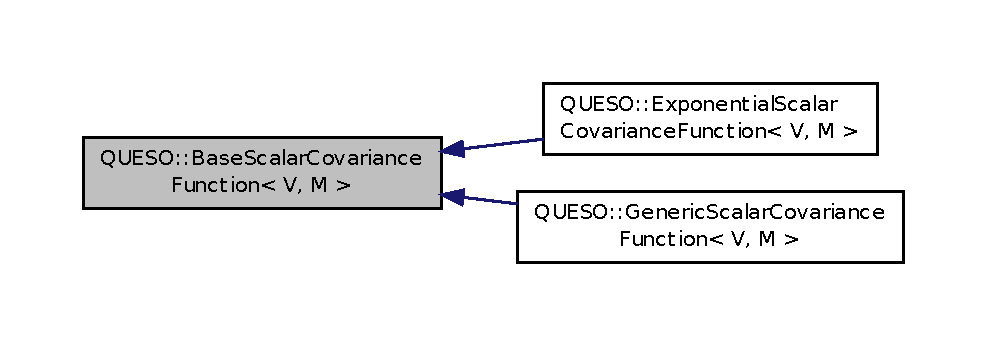
\includegraphics[width=350pt]{class_q_u_e_s_o_1_1_base_scalar_covariance_function__inherit__graph}
\end{center}
\end{figure}


Collaboration diagram for Q\-U\-E\-S\-O\-:\-:Base\-Scalar\-Covariance\-Function$<$ V, M $>$\-:
\nopagebreak
\begin{figure}[H]
\begin{center}
\leavevmode
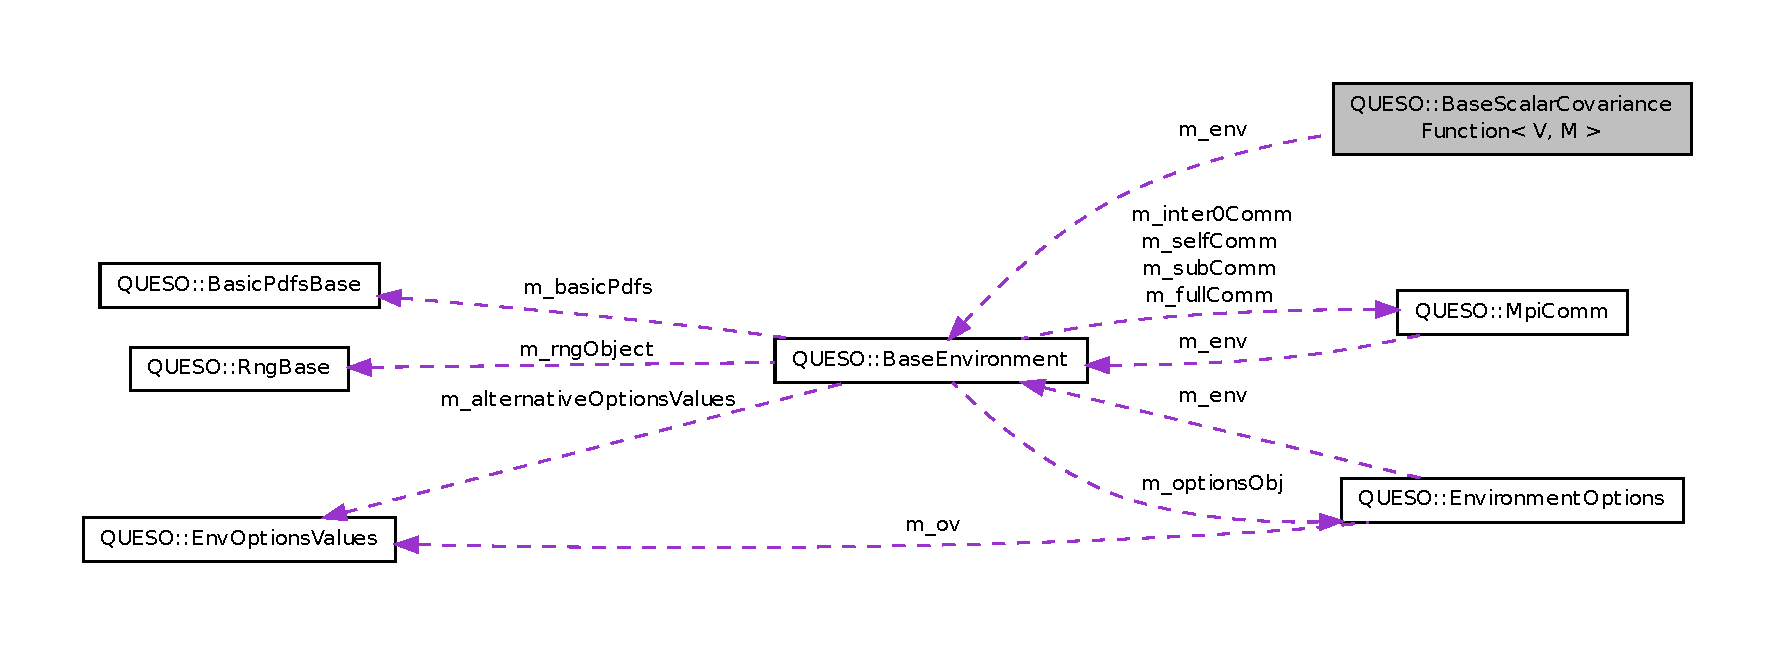
\includegraphics[width=350pt]{class_q_u_e_s_o_1_1_base_scalar_covariance_function__coll__graph}
\end{center}
\end{figure}
\subsection*{Public Member Functions}
\begin{Indent}{\bf Constructor/\-Destructor methods}\par
\begin{DoxyCompactItemize}
\item 
\hyperlink{class_q_u_e_s_o_1_1_base_scalar_covariance_function_a7a3d53a332dffce97c5579d93eaf91ff}{Base\-Scalar\-Covariance\-Function} (const char $\ast$prefix, const \hyperlink{class_q_u_e_s_o_1_1_vector_set}{Vector\-Set}$<$ V, M $>$ \&\hyperlink{class_q_u_e_s_o_1_1_base_scalar_covariance_function_a703aa6a8e475adaface0ec514b48a5bc}{basic\-Domain\-Set})
\begin{DoxyCompactList}\small\item\em Default constructor. \end{DoxyCompactList}\item 
virtual \hyperlink{class_q_u_e_s_o_1_1_base_scalar_covariance_function_a5db872c7f5929e819543f7f58063f3ae}{$\sim$\-Base\-Scalar\-Covariance\-Function} ()
\begin{DoxyCompactList}\small\item\em Virtual destructor. \end{DoxyCompactList}\end{DoxyCompactItemize}
\end{Indent}
\begin{Indent}{\bf Math methods}\par
\begin{DoxyCompactItemize}
\item 
const \hyperlink{class_q_u_e_s_o_1_1_vector_set}{Vector\-Set}$<$ V, M $>$ \& \hyperlink{class_q_u_e_s_o_1_1_base_scalar_covariance_function_a703aa6a8e475adaface0ec514b48a5bc}{basic\-Domain\-Set} () const 
\begin{DoxyCompactList}\small\item\em Domain set; access to private attribute m\-\_\-basic\-Domain\-Set. \end{DoxyCompactList}\item 
virtual double \hyperlink{class_q_u_e_s_o_1_1_base_scalar_covariance_function_a93a35146e106c7fb28913c604a918acb}{value} (const V \&domain\-Vector1, const V \&domain\-Vector2) const =0
\begin{DoxyCompactList}\small\item\em The value of the covariance function. See template specialization. \end{DoxyCompactList}\end{DoxyCompactItemize}
\end{Indent}
\subsection*{Protected Attributes}
\begin{DoxyCompactItemize}
\item 
const \hyperlink{class_q_u_e_s_o_1_1_base_environment}{Base\-Environment} \& \hyperlink{class_q_u_e_s_o_1_1_base_scalar_covariance_function_a2a100016b480c498b5219fb937d62543}{m\-\_\-env}
\item 
std\-::string \hyperlink{class_q_u_e_s_o_1_1_base_scalar_covariance_function_a21636873436b88cb77075c6edbd61c71}{m\-\_\-prefix}
\item 
const \hyperlink{class_q_u_e_s_o_1_1_vector_set}{Vector\-Set}$<$ V, M $>$ \& \hyperlink{class_q_u_e_s_o_1_1_base_scalar_covariance_function_a1060392114362022e427678d0f97ab12}{m\-\_\-basic\-Domain\-Set}
\end{DoxyCompactItemize}


\subsection{Detailed Description}
\subsubsection*{template$<$class V, class M$>$class Q\-U\-E\-S\-O\-::\-Base\-Scalar\-Covariance\-Function$<$ V, M $>$}

A templated (base) class to accommodate scalar covariance functions (of random variables). 

This class allows the mathematical definition of the covariance function of a random variable Covariance provides a measure of the strength of the correlation between two or more sets of random variates. The covariance for two random variates $ X $ and $ Y $, each with sample size $ N $, is defined by the expectation value\-: $ cov (X,Y) = <(X-\mu_X)(Y-\mu_Y)> = < X Y > - \mu_X \mu_Y $ where $ \mu_X $ and $ \mu_Y $ are the respective means, which can be written out explicitly as \[ cov (X,Y) = \sum_{i=1}^{N} \frac{(x_i - \bar{x})(y_i - \bar{y})}{N}\] 

Definition at line 53 of file Scalar\-Covariance\-Function.\-h.



\subsection{Constructor \& Destructor Documentation}
\hypertarget{class_q_u_e_s_o_1_1_base_scalar_covariance_function_a7a3d53a332dffce97c5579d93eaf91ff}{\index{Q\-U\-E\-S\-O\-::\-Base\-Scalar\-Covariance\-Function@{Q\-U\-E\-S\-O\-::\-Base\-Scalar\-Covariance\-Function}!Base\-Scalar\-Covariance\-Function@{Base\-Scalar\-Covariance\-Function}}
\index{Base\-Scalar\-Covariance\-Function@{Base\-Scalar\-Covariance\-Function}!QUESO::BaseScalarCovarianceFunction@{Q\-U\-E\-S\-O\-::\-Base\-Scalar\-Covariance\-Function}}
\subsubsection[{Base\-Scalar\-Covariance\-Function}]{\setlength{\rightskip}{0pt plus 5cm}template$<$class V , class M $>$ {\bf Q\-U\-E\-S\-O\-::\-Base\-Scalar\-Covariance\-Function}$<$ V, M $>$\-::{\bf Base\-Scalar\-Covariance\-Function} (
\begin{DoxyParamCaption}
\item[{const char $\ast$}]{prefix, }
\item[{const {\bf Vector\-Set}$<$ V, M $>$ \&}]{basic\-Domain\-Set}
\end{DoxyParamCaption}
)}}\label{class_q_u_e_s_o_1_1_base_scalar_covariance_function_a7a3d53a332dffce97c5579d93eaf91ff}


Default constructor. 

Instantiates an object of the class given a prefix and the domain set. 

Definition at line 31 of file Scalar\-Covariance\-Function.\-C.



References Q\-U\-E\-S\-O\-::\-Base\-Environment\-::display\-Verbosity(), Q\-U\-E\-S\-O\-::\-Base\-Scalar\-Covariance\-Function$<$ V, M $>$\-::m\-\_\-env, Q\-U\-E\-S\-O\-::\-Base\-Scalar\-Covariance\-Function$<$ V, M $>$\-::m\-\_\-prefix, and Q\-U\-E\-S\-O\-::\-Base\-Environment\-::sub\-Display\-File().


\begin{DoxyCode}
34   :
35   \hyperlink{class_q_u_e_s_o_1_1_base_scalar_covariance_function_a2a100016b480c498b5219fb937d62543}{m\_env}           (\hyperlink{class_q_u_e_s_o_1_1_base_scalar_covariance_function_a703aa6a8e475adaface0ec514b48a5bc}{basicDomainSet}.env()),
36   \hyperlink{class_q_u_e_s_o_1_1_base_scalar_covariance_function_a21636873436b88cb77075c6edbd61c71}{m\_prefix}        ((std::string)(prefix)+\textcolor{stringliteral}{"cov\_func\_"}),
37   \hyperlink{class_q_u_e_s_o_1_1_base_scalar_covariance_function_a1060392114362022e427678d0f97ab12}{m\_basicDomainSet}(\hyperlink{class_q_u_e_s_o_1_1_base_scalar_covariance_function_a703aa6a8e475adaface0ec514b48a5bc}{basicDomainSet})
38 \{
39   \textcolor{keywordflow}{if} ((\hyperlink{class_q_u_e_s_o_1_1_base_scalar_covariance_function_a2a100016b480c498b5219fb937d62543}{m\_env}.\hyperlink{class_q_u_e_s_o_1_1_base_environment_a8a0064746ae8dddfece4229b9ad374d6}{subDisplayFile}()) && (\hyperlink{class_q_u_e_s_o_1_1_base_scalar_covariance_function_a2a100016b480c498b5219fb937d62543}{m\_env}.
      \hyperlink{class_q_u_e_s_o_1_1_base_environment_a1fe5f244fc0316a0ab3e37463f108b96}{displayVerbosity}() >= 54)) \{
40     *\hyperlink{class_q_u_e_s_o_1_1_base_scalar_covariance_function_a2a100016b480c498b5219fb937d62543}{m\_env}.\hyperlink{class_q_u_e_s_o_1_1_base_environment_a8a0064746ae8dddfece4229b9ad374d6}{subDisplayFile}() << \textcolor{stringliteral}{"Entering
       BaseScalarCovarianceFunction<V,M>::constructor()"}
41                             << \textcolor{stringliteral}{": prefix = "} << \hyperlink{class_q_u_e_s_o_1_1_base_scalar_covariance_function_a21636873436b88cb77075c6edbd61c71}{m\_prefix}
42                             << std::endl;
43   \}
44 
45   \textcolor{keywordflow}{if} ((\hyperlink{class_q_u_e_s_o_1_1_base_scalar_covariance_function_a2a100016b480c498b5219fb937d62543}{m\_env}.\hyperlink{class_q_u_e_s_o_1_1_base_environment_a8a0064746ae8dddfece4229b9ad374d6}{subDisplayFile}()) && (\hyperlink{class_q_u_e_s_o_1_1_base_scalar_covariance_function_a2a100016b480c498b5219fb937d62543}{m\_env}.
      \hyperlink{class_q_u_e_s_o_1_1_base_environment_a1fe5f244fc0316a0ab3e37463f108b96}{displayVerbosity}() >= 54)) \{
46     *\hyperlink{class_q_u_e_s_o_1_1_base_scalar_covariance_function_a2a100016b480c498b5219fb937d62543}{m\_env}.\hyperlink{class_q_u_e_s_o_1_1_base_environment_a8a0064746ae8dddfece4229b9ad374d6}{subDisplayFile}() << \textcolor{stringliteral}{"Leaving BaseScalarCovarianceFunction<V,M>::constructor()
      "}
47                             << \textcolor{stringliteral}{": prefix = "} << \hyperlink{class_q_u_e_s_o_1_1_base_scalar_covariance_function_a21636873436b88cb77075c6edbd61c71}{m\_prefix}
48                             << std::endl;
49   \}
50 \}
\end{DoxyCode}
\hypertarget{class_q_u_e_s_o_1_1_base_scalar_covariance_function_a5db872c7f5929e819543f7f58063f3ae}{\index{Q\-U\-E\-S\-O\-::\-Base\-Scalar\-Covariance\-Function@{Q\-U\-E\-S\-O\-::\-Base\-Scalar\-Covariance\-Function}!$\sim$\-Base\-Scalar\-Covariance\-Function@{$\sim$\-Base\-Scalar\-Covariance\-Function}}
\index{$\sim$\-Base\-Scalar\-Covariance\-Function@{$\sim$\-Base\-Scalar\-Covariance\-Function}!QUESO::BaseScalarCovarianceFunction@{Q\-U\-E\-S\-O\-::\-Base\-Scalar\-Covariance\-Function}}
\subsubsection[{$\sim$\-Base\-Scalar\-Covariance\-Function}]{\setlength{\rightskip}{0pt plus 5cm}template$<$class V , class M $>$ {\bf Q\-U\-E\-S\-O\-::\-Base\-Scalar\-Covariance\-Function}$<$ V, M $>$\-::$\sim${\bf Base\-Scalar\-Covariance\-Function} (
\begin{DoxyParamCaption}
{}
\end{DoxyParamCaption}
)\hspace{0.3cm}{\ttfamily [virtual]}}}\label{class_q_u_e_s_o_1_1_base_scalar_covariance_function_a5db872c7f5929e819543f7f58063f3ae}


Virtual destructor. 



Definition at line 53 of file Scalar\-Covariance\-Function.\-C.


\begin{DoxyCode}
54 \{
55   \textcolor{keywordflow}{if} ((\hyperlink{class_q_u_e_s_o_1_1_base_scalar_covariance_function_a2a100016b480c498b5219fb937d62543}{m\_env}.\hyperlink{class_q_u_e_s_o_1_1_base_environment_a8a0064746ae8dddfece4229b9ad374d6}{subDisplayFile}()) && (\hyperlink{class_q_u_e_s_o_1_1_base_scalar_covariance_function_a2a100016b480c498b5219fb937d62543}{m\_env}.
      \hyperlink{class_q_u_e_s_o_1_1_base_environment_a1fe5f244fc0316a0ab3e37463f108b96}{displayVerbosity}() >= 54)) \{
56     *\hyperlink{class_q_u_e_s_o_1_1_base_scalar_covariance_function_a2a100016b480c498b5219fb937d62543}{m\_env}.\hyperlink{class_q_u_e_s_o_1_1_base_environment_a8a0064746ae8dddfece4229b9ad374d6}{subDisplayFile}() << \textcolor{stringliteral}{"Entering BaseScalarCovarianceFunction<V,M>::destructor()
      "}
57                             << \textcolor{stringliteral}{": prefix = "} << \hyperlink{class_q_u_e_s_o_1_1_base_scalar_covariance_function_a21636873436b88cb77075c6edbd61c71}{m\_prefix}
58                             << std::endl;
59   \}
60 
61   \textcolor{keywordflow}{if} ((\hyperlink{class_q_u_e_s_o_1_1_base_scalar_covariance_function_a2a100016b480c498b5219fb937d62543}{m\_env}.\hyperlink{class_q_u_e_s_o_1_1_base_environment_a8a0064746ae8dddfece4229b9ad374d6}{subDisplayFile}()) && (\hyperlink{class_q_u_e_s_o_1_1_base_scalar_covariance_function_a2a100016b480c498b5219fb937d62543}{m\_env}.
      \hyperlink{class_q_u_e_s_o_1_1_base_environment_a1fe5f244fc0316a0ab3e37463f108b96}{displayVerbosity}() >= 54)) \{
62     *\hyperlink{class_q_u_e_s_o_1_1_base_scalar_covariance_function_a2a100016b480c498b5219fb937d62543}{m\_env}.\hyperlink{class_q_u_e_s_o_1_1_base_environment_a8a0064746ae8dddfece4229b9ad374d6}{subDisplayFile}() << \textcolor{stringliteral}{"Leaving BaseScalarCovarianceFunction<V,M>::destructor()"}
63                             << \textcolor{stringliteral}{": prefix = "} << \hyperlink{class_q_u_e_s_o_1_1_base_scalar_covariance_function_a21636873436b88cb77075c6edbd61c71}{m\_prefix}
64                             << std::endl;
65   \}
66 \}
\end{DoxyCode}


\subsection{Member Function Documentation}
\hypertarget{class_q_u_e_s_o_1_1_base_scalar_covariance_function_a703aa6a8e475adaface0ec514b48a5bc}{\index{Q\-U\-E\-S\-O\-::\-Base\-Scalar\-Covariance\-Function@{Q\-U\-E\-S\-O\-::\-Base\-Scalar\-Covariance\-Function}!basic\-Domain\-Set@{basic\-Domain\-Set}}
\index{basic\-Domain\-Set@{basic\-Domain\-Set}!QUESO::BaseScalarCovarianceFunction@{Q\-U\-E\-S\-O\-::\-Base\-Scalar\-Covariance\-Function}}
\subsubsection[{basic\-Domain\-Set}]{\setlength{\rightskip}{0pt plus 5cm}template$<$class V , class M $>$ const {\bf Vector\-Set}$<$ V, M $>$ \& {\bf Q\-U\-E\-S\-O\-::\-Base\-Scalar\-Covariance\-Function}$<$ V, M $>$\-::basic\-Domain\-Set (
\begin{DoxyParamCaption}
{}
\end{DoxyParamCaption}
) const}}\label{class_q_u_e_s_o_1_1_base_scalar_covariance_function_a703aa6a8e475adaface0ec514b48a5bc}


Domain set; access to private attribute m\-\_\-basic\-Domain\-Set. 



Definition at line 70 of file Scalar\-Covariance\-Function.\-C.


\begin{DoxyCode}
71 \{
72   \textcolor{keywordflow}{return} \hyperlink{class_q_u_e_s_o_1_1_base_scalar_covariance_function_a1060392114362022e427678d0f97ab12}{m\_basicDomainSet};
73 \}
\end{DoxyCode}
\hypertarget{class_q_u_e_s_o_1_1_base_scalar_covariance_function_a93a35146e106c7fb28913c604a918acb}{\index{Q\-U\-E\-S\-O\-::\-Base\-Scalar\-Covariance\-Function@{Q\-U\-E\-S\-O\-::\-Base\-Scalar\-Covariance\-Function}!value@{value}}
\index{value@{value}!QUESO::BaseScalarCovarianceFunction@{Q\-U\-E\-S\-O\-::\-Base\-Scalar\-Covariance\-Function}}
\subsubsection[{value}]{\setlength{\rightskip}{0pt plus 5cm}template$<$class V, class M$>$ virtual double {\bf Q\-U\-E\-S\-O\-::\-Base\-Scalar\-Covariance\-Function}$<$ V, M $>$\-::value (
\begin{DoxyParamCaption}
\item[{const V \&}]{domain\-Vector1, }
\item[{const V \&}]{domain\-Vector2}
\end{DoxyParamCaption}
) const\hspace{0.3cm}{\ttfamily [pure virtual]}}}\label{class_q_u_e_s_o_1_1_base_scalar_covariance_function_a93a35146e106c7fb28913c604a918acb}


The value of the covariance function. See template specialization. 



Implemented in \hyperlink{class_q_u_e_s_o_1_1_exponential_scalar_covariance_function_ad65cfe1440c9045718bc57827d6fb551}{Q\-U\-E\-S\-O\-::\-Exponential\-Scalar\-Covariance\-Function$<$ V, M $>$}, and \hyperlink{class_q_u_e_s_o_1_1_generic_scalar_covariance_function_ab02d90f973034672b84888c941230a8c}{Q\-U\-E\-S\-O\-::\-Generic\-Scalar\-Covariance\-Function$<$ V, M $>$}.



\subsection{Member Data Documentation}
\hypertarget{class_q_u_e_s_o_1_1_base_scalar_covariance_function_a1060392114362022e427678d0f97ab12}{\index{Q\-U\-E\-S\-O\-::\-Base\-Scalar\-Covariance\-Function@{Q\-U\-E\-S\-O\-::\-Base\-Scalar\-Covariance\-Function}!m\-\_\-basic\-Domain\-Set@{m\-\_\-basic\-Domain\-Set}}
\index{m\-\_\-basic\-Domain\-Set@{m\-\_\-basic\-Domain\-Set}!QUESO::BaseScalarCovarianceFunction@{Q\-U\-E\-S\-O\-::\-Base\-Scalar\-Covariance\-Function}}
\subsubsection[{m\-\_\-basic\-Domain\-Set}]{\setlength{\rightskip}{0pt plus 5cm}template$<$class V, class M$>$ const {\bf Vector\-Set}$<$V,M$>$\& {\bf Q\-U\-E\-S\-O\-::\-Base\-Scalar\-Covariance\-Function}$<$ V, M $>$\-::m\-\_\-basic\-Domain\-Set\hspace{0.3cm}{\ttfamily [protected]}}}\label{class_q_u_e_s_o_1_1_base_scalar_covariance_function_a1060392114362022e427678d0f97ab12}


Definition at line 78 of file Scalar\-Covariance\-Function.\-h.

\hypertarget{class_q_u_e_s_o_1_1_base_scalar_covariance_function_a2a100016b480c498b5219fb937d62543}{\index{Q\-U\-E\-S\-O\-::\-Base\-Scalar\-Covariance\-Function@{Q\-U\-E\-S\-O\-::\-Base\-Scalar\-Covariance\-Function}!m\-\_\-env@{m\-\_\-env}}
\index{m\-\_\-env@{m\-\_\-env}!QUESO::BaseScalarCovarianceFunction@{Q\-U\-E\-S\-O\-::\-Base\-Scalar\-Covariance\-Function}}
\subsubsection[{m\-\_\-env}]{\setlength{\rightskip}{0pt plus 5cm}template$<$class V, class M$>$ const {\bf Base\-Environment}\& {\bf Q\-U\-E\-S\-O\-::\-Base\-Scalar\-Covariance\-Function}$<$ V, M $>$\-::m\-\_\-env\hspace{0.3cm}{\ttfamily [protected]}}}\label{class_q_u_e_s_o_1_1_base_scalar_covariance_function_a2a100016b480c498b5219fb937d62543}


Definition at line 76 of file Scalar\-Covariance\-Function.\-h.



Referenced by Q\-U\-E\-S\-O\-::\-Base\-Scalar\-Covariance\-Function$<$ V, M $>$\-::\-Base\-Scalar\-Covariance\-Function(), Q\-U\-E\-S\-O\-::\-Exponential\-Scalar\-Covariance\-Function$<$ V, M $>$\-::\-Exponential\-Scalar\-Covariance\-Function(), and Q\-U\-E\-S\-O\-::\-Generic\-Scalar\-Covariance\-Function$<$ V, M $>$\-::\-Generic\-Scalar\-Covariance\-Function().

\hypertarget{class_q_u_e_s_o_1_1_base_scalar_covariance_function_a21636873436b88cb77075c6edbd61c71}{\index{Q\-U\-E\-S\-O\-::\-Base\-Scalar\-Covariance\-Function@{Q\-U\-E\-S\-O\-::\-Base\-Scalar\-Covariance\-Function}!m\-\_\-prefix@{m\-\_\-prefix}}
\index{m\-\_\-prefix@{m\-\_\-prefix}!QUESO::BaseScalarCovarianceFunction@{Q\-U\-E\-S\-O\-::\-Base\-Scalar\-Covariance\-Function}}
\subsubsection[{m\-\_\-prefix}]{\setlength{\rightskip}{0pt plus 5cm}template$<$class V, class M$>$ std\-::string {\bf Q\-U\-E\-S\-O\-::\-Base\-Scalar\-Covariance\-Function}$<$ V, M $>$\-::m\-\_\-prefix\hspace{0.3cm}{\ttfamily [protected]}}}\label{class_q_u_e_s_o_1_1_base_scalar_covariance_function_a21636873436b88cb77075c6edbd61c71}


Definition at line 77 of file Scalar\-Covariance\-Function.\-h.



Referenced by Q\-U\-E\-S\-O\-::\-Base\-Scalar\-Covariance\-Function$<$ V, M $>$\-::\-Base\-Scalar\-Covariance\-Function(), Q\-U\-E\-S\-O\-::\-Exponential\-Scalar\-Covariance\-Function$<$ V, M $>$\-::\-Exponential\-Scalar\-Covariance\-Function(), and Q\-U\-E\-S\-O\-::\-Generic\-Scalar\-Covariance\-Function$<$ V, M $>$\-::\-Generic\-Scalar\-Covariance\-Function().



The documentation for this class was generated from the following files\-:\begin{DoxyCompactItemize}
\item 
src/stats/inc/\hyperlink{_scalar_covariance_function_8h}{Scalar\-Covariance\-Function.\-h}\item 
src/stats/src/\hyperlink{_scalar_covariance_function_8_c}{Scalar\-Covariance\-Function.\-C}\end{DoxyCompactItemize}

\hypertarget{class_q_u_e_s_o_1_1_base_scalar_function}{\section{Q\-U\-E\-S\-O\-:\-:Base\-Scalar\-Function$<$ V, M $>$ Class Template Reference}
\label{class_q_u_e_s_o_1_1_base_scalar_function}\index{Q\-U\-E\-S\-O\-::\-Base\-Scalar\-Function$<$ V, M $>$@{Q\-U\-E\-S\-O\-::\-Base\-Scalar\-Function$<$ V, M $>$}}
}


A templated (base) class for handling scalar functions.  




{\ttfamily \#include $<$Scalar\-Function.\-h$>$}



Inheritance diagram for Q\-U\-E\-S\-O\-:\-:Base\-Scalar\-Function$<$ V, M $>$\-:
\nopagebreak
\begin{figure}[H]
\begin{center}
\leavevmode
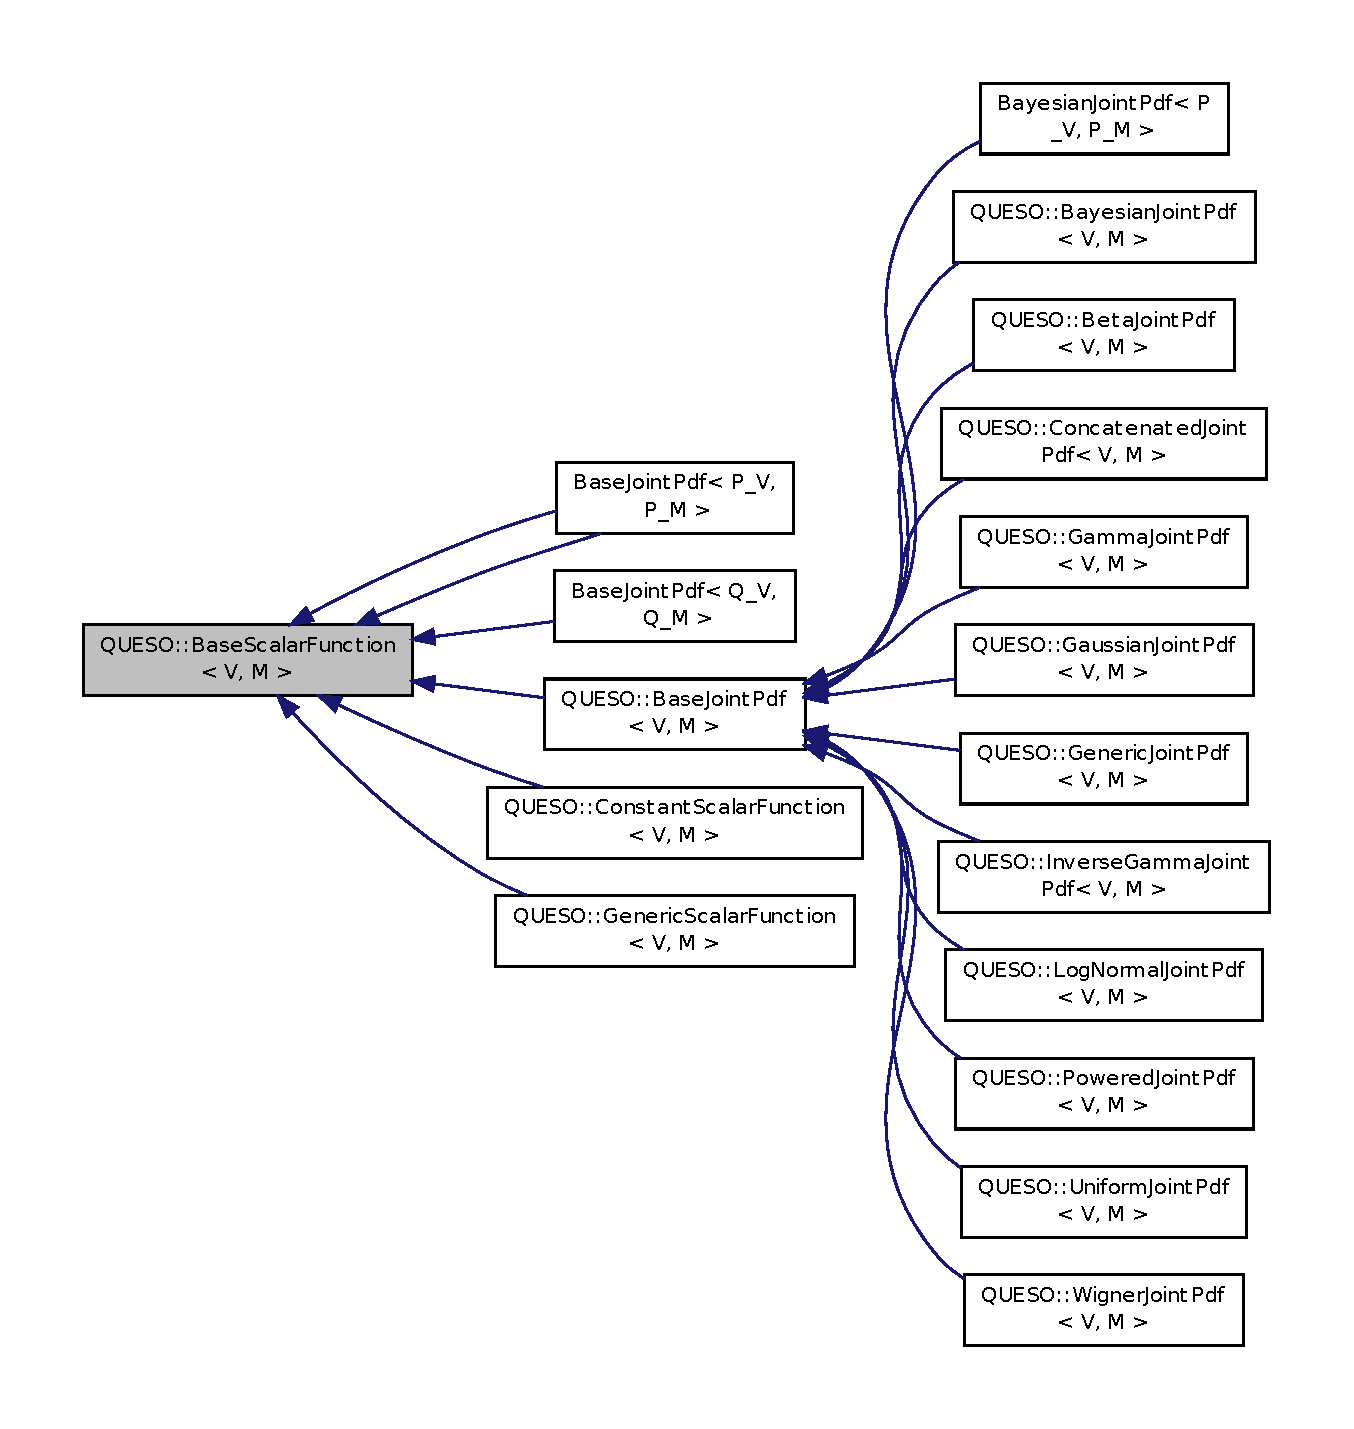
\includegraphics[width=350pt]{class_q_u_e_s_o_1_1_base_scalar_function__inherit__graph}
\end{center}
\end{figure}


Collaboration diagram for Q\-U\-E\-S\-O\-:\-:Base\-Scalar\-Function$<$ V, M $>$\-:
\nopagebreak
\begin{figure}[H]
\begin{center}
\leavevmode
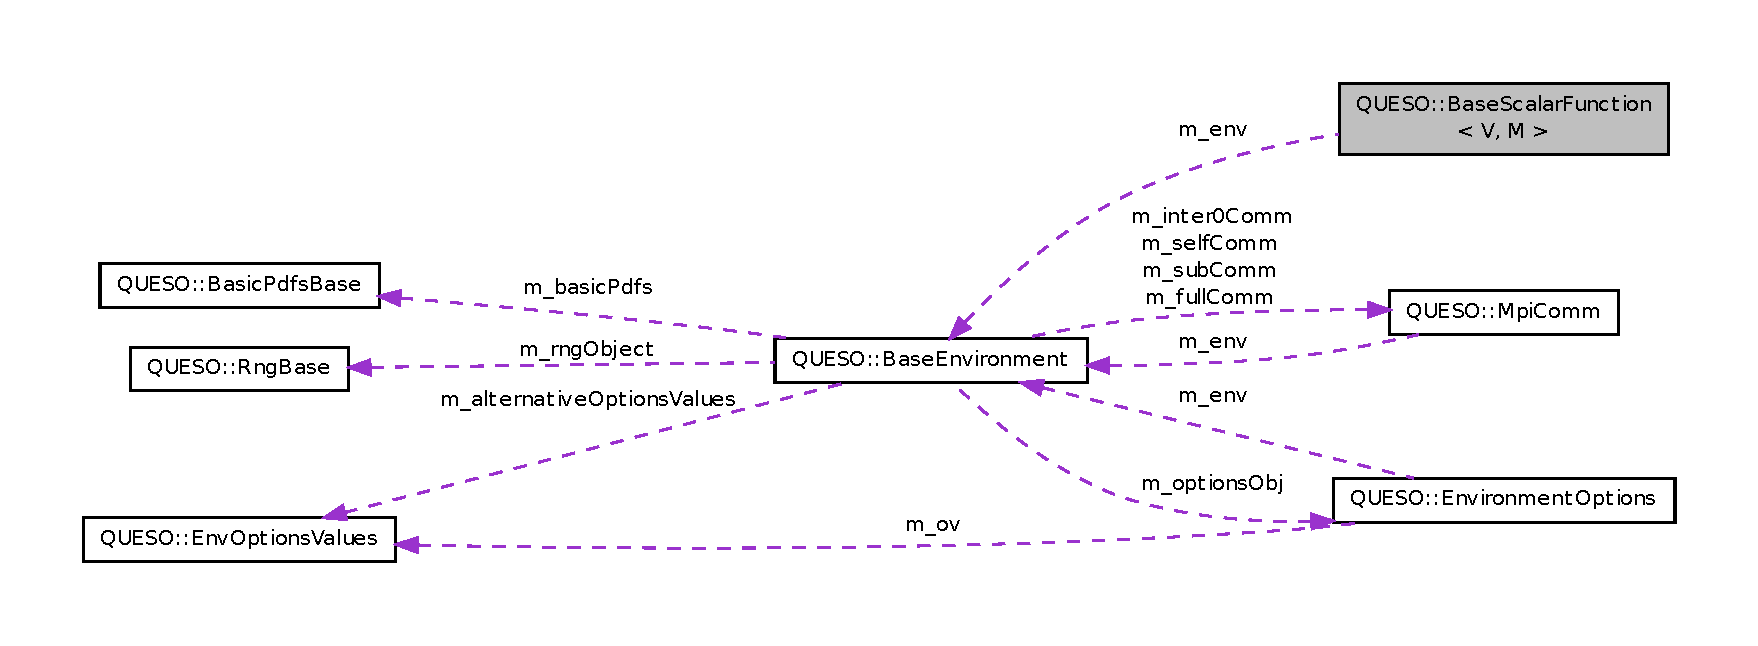
\includegraphics[width=350pt]{class_q_u_e_s_o_1_1_base_scalar_function__coll__graph}
\end{center}
\end{figure}
\subsection*{Public Member Functions}
\begin{Indent}{\bf Constructor/\-Destructor methods.}\par
\begin{DoxyCompactItemize}
\item 
\hyperlink{class_q_u_e_s_o_1_1_base_scalar_function_a68ab7c82be7eba7bd5d51ce8d85c65f0}{Base\-Scalar\-Function} (const char $\ast$prefix, const \hyperlink{class_q_u_e_s_o_1_1_vector_set}{Vector\-Set}$<$ V, M $>$ \&\hyperlink{class_q_u_e_s_o_1_1_base_scalar_function_ad0937628825249dd36ded3ce0c7959ac}{domain\-Set})
\begin{DoxyCompactList}\small\item\em Default constructor. \end{DoxyCompactList}\item 
virtual \hyperlink{class_q_u_e_s_o_1_1_base_scalar_function_a6f96de783e174cfe84682766f5957969}{$\sim$\-Base\-Scalar\-Function} ()
\begin{DoxyCompactList}\small\item\em Destructor. \end{DoxyCompactList}\end{DoxyCompactItemize}
\end{Indent}
\begin{Indent}{\bf Mathematical methods.}\par
\begin{DoxyCompactItemize}
\item 
const \hyperlink{class_q_u_e_s_o_1_1_vector_set}{Vector\-Set}$<$ V, M $>$ \& \hyperlink{class_q_u_e_s_o_1_1_base_scalar_function_ad0937628825249dd36ded3ce0c7959ac}{domain\-Set} () const 
\begin{DoxyCompactList}\small\item\em Access to the protected attribute {\ttfamily m\-\_\-domain\-Set\-:} domain set of the scalar function. \end{DoxyCompactList}\item 
virtual double \hyperlink{class_q_u_e_s_o_1_1_base_scalar_function_aad8957ecbc4e155cbc4c40a1c21135d7}{actual\-Value} (const V \&domain\-Vector, const V $\ast$domain\-Direction, V $\ast$grad\-Vector, M $\ast$hessian\-Matrix, V $\ast$hessian\-Effect) const =0
\begin{DoxyCompactList}\small\item\em Actual value of the scalar function. \end{DoxyCompactList}\item 
virtual double \hyperlink{class_q_u_e_s_o_1_1_base_scalar_function_acf2f92adac2df2a0d750dc62cd3a4d0a}{ln\-Value} (const V \&domain\-Vector, const V $\ast$domain\-Direction, V $\ast$grad\-Vector, M $\ast$hessian\-Matrix, V $\ast$hessian\-Effect) const =0
\begin{DoxyCompactList}\small\item\em Logarithm of the value of the scalar function. \end{DoxyCompactList}\end{DoxyCompactItemize}
\end{Indent}
\subsection*{Protected Attributes}
\begin{DoxyCompactItemize}
\item 
const \hyperlink{class_q_u_e_s_o_1_1_base_environment}{Base\-Environment} \& \hyperlink{class_q_u_e_s_o_1_1_base_scalar_function_adf44141aeb765d97613286f88f235f04}{m\-\_\-env}
\item 
std\-::string \hyperlink{class_q_u_e_s_o_1_1_base_scalar_function_a6e81dc902aca6a546877da99b2f4a169}{m\-\_\-prefix}
\item 
const \hyperlink{class_q_u_e_s_o_1_1_vector_set}{Vector\-Set}$<$ V, M $>$ \& \hyperlink{class_q_u_e_s_o_1_1_base_scalar_function_a67696e86211197938c72cd11863f5cf8}{m\-\_\-domain\-Set}
\begin{DoxyCompactList}\small\item\em Domain set of the scalar function. \end{DoxyCompactList}\end{DoxyCompactItemize}


\subsection{Detailed Description}
\subsubsection*{template$<$class V, class M$>$class Q\-U\-E\-S\-O\-::\-Base\-Scalar\-Function$<$ V, M $>$}

A templated (base) class for handling scalar functions. 

This class allows the mathematical definition of a scalar function such as\-: $ f: B \subset R \rightarrow R $. A function of one or more variables has always one-\/dimensional range. P\-D\-Fs (marginal, joint) and C\-D\-Fs are examples of scalar functions. 

Definition at line 48 of file Scalar\-Function.\-h.



\subsection{Constructor \& Destructor Documentation}
\hypertarget{class_q_u_e_s_o_1_1_base_scalar_function_a68ab7c82be7eba7bd5d51ce8d85c65f0}{\index{Q\-U\-E\-S\-O\-::\-Base\-Scalar\-Function@{Q\-U\-E\-S\-O\-::\-Base\-Scalar\-Function}!Base\-Scalar\-Function@{Base\-Scalar\-Function}}
\index{Base\-Scalar\-Function@{Base\-Scalar\-Function}!QUESO::BaseScalarFunction@{Q\-U\-E\-S\-O\-::\-Base\-Scalar\-Function}}
\subsubsection[{Base\-Scalar\-Function}]{\setlength{\rightskip}{0pt plus 5cm}template$<$class V, class M$>$ {\bf Q\-U\-E\-S\-O\-::\-Base\-Scalar\-Function}$<$ V, M $>$\-::{\bf Base\-Scalar\-Function} (
\begin{DoxyParamCaption}
\item[{const char $\ast$}]{prefix, }
\item[{const {\bf Vector\-Set}$<$ V, M $>$ \&}]{domain\-Set}
\end{DoxyParamCaption}
)}}\label{class_q_u_e_s_o_1_1_base_scalar_function_a68ab7c82be7eba7bd5d51ce8d85c65f0}


Default constructor. 

Instantiates an object of the class, i.\-e. a scalar function, given a prefix and its domain. 

Definition at line 34 of file Scalar\-Function.\-C.


\begin{DoxyCode}
36   : \hyperlink{class_q_u_e_s_o_1_1_base_scalar_function_adf44141aeb765d97613286f88f235f04}{m\_env}(\hyperlink{class_q_u_e_s_o_1_1_base_scalar_function_ad0937628825249dd36ded3ce0c7959ac}{domainSet}.env()),
37     \hyperlink{class_q_u_e_s_o_1_1_base_scalar_function_a6e81dc902aca6a546877da99b2f4a169}{m\_prefix}((std::string)(prefix)+\textcolor{stringliteral}{"func\_"}),
38     \hyperlink{class_q_u_e_s_o_1_1_base_scalar_function_a67696e86211197938c72cd11863f5cf8}{m\_domainSet}(\hyperlink{class_q_u_e_s_o_1_1_base_scalar_function_ad0937628825249dd36ded3ce0c7959ac}{domainSet})
39 \{
40 \}
\end{DoxyCode}
\hypertarget{class_q_u_e_s_o_1_1_base_scalar_function_a6f96de783e174cfe84682766f5957969}{\index{Q\-U\-E\-S\-O\-::\-Base\-Scalar\-Function@{Q\-U\-E\-S\-O\-::\-Base\-Scalar\-Function}!$\sim$\-Base\-Scalar\-Function@{$\sim$\-Base\-Scalar\-Function}}
\index{$\sim$\-Base\-Scalar\-Function@{$\sim$\-Base\-Scalar\-Function}!QUESO::BaseScalarFunction@{Q\-U\-E\-S\-O\-::\-Base\-Scalar\-Function}}
\subsubsection[{$\sim$\-Base\-Scalar\-Function}]{\setlength{\rightskip}{0pt plus 5cm}template$<$class V , class M $>$ {\bf Q\-U\-E\-S\-O\-::\-Base\-Scalar\-Function}$<$ V, M $>$\-::$\sim${\bf Base\-Scalar\-Function} (
\begin{DoxyParamCaption}
{}
\end{DoxyParamCaption}
)\hspace{0.3cm}{\ttfamily [virtual]}}}\label{class_q_u_e_s_o_1_1_base_scalar_function_a6f96de783e174cfe84682766f5957969}


Destructor. 



Definition at line 44 of file Scalar\-Function.\-C.


\begin{DoxyCode}
45 \{
46 \}
\end{DoxyCode}


\subsection{Member Function Documentation}
\hypertarget{class_q_u_e_s_o_1_1_base_scalar_function_aad8957ecbc4e155cbc4c40a1c21135d7}{\index{Q\-U\-E\-S\-O\-::\-Base\-Scalar\-Function@{Q\-U\-E\-S\-O\-::\-Base\-Scalar\-Function}!actual\-Value@{actual\-Value}}
\index{actual\-Value@{actual\-Value}!QUESO::BaseScalarFunction@{Q\-U\-E\-S\-O\-::\-Base\-Scalar\-Function}}
\subsubsection[{actual\-Value}]{\setlength{\rightskip}{0pt plus 5cm}template$<$class V, class M$>$ virtual double {\bf Q\-U\-E\-S\-O\-::\-Base\-Scalar\-Function}$<$ V, M $>$\-::actual\-Value (
\begin{DoxyParamCaption}
\item[{const V \&}]{domain\-Vector, }
\item[{const V $\ast$}]{domain\-Direction, }
\item[{V $\ast$}]{grad\-Vector, }
\item[{M $\ast$}]{hessian\-Matrix, }
\item[{V $\ast$}]{hessian\-Effect}
\end{DoxyParamCaption}
) const\hspace{0.3cm}{\ttfamily [pure virtual]}}}\label{class_q_u_e_s_o_1_1_base_scalar_function_aad8957ecbc4e155cbc4c40a1c21135d7}


Actual value of the scalar function. 



Implemented in \hyperlink{class_q_u_e_s_o_1_1_concatenated_joint_pdf_a7a3bbf8dab211968e9691a620fee0e4d}{Q\-U\-E\-S\-O\-::\-Concatenated\-Joint\-Pdf$<$ V, M $>$}, \hyperlink{class_q_u_e_s_o_1_1_gaussian_joint_pdf_ae576dae6a972dd7350ca261569f056da}{Q\-U\-E\-S\-O\-::\-Gaussian\-Joint\-Pdf$<$ V, M $>$}, \hyperlink{class_q_u_e_s_o_1_1_base_joint_pdf_a3c367a0cc3fb707a136c5df47dd414c1}{Q\-U\-E\-S\-O\-::\-Base\-Joint\-Pdf$<$ V, M $>$}, \hyperlink{class_q_u_e_s_o_1_1_bayesian_joint_pdf_ad67362b4ab48a722db976430cf03165e}{Q\-U\-E\-S\-O\-::\-Bayesian\-Joint\-Pdf$<$ V, M $>$}, \hyperlink{class_q_u_e_s_o_1_1_log_normal_joint_pdf_a87729cb9d59b73baefcbecb03e753cb9}{Q\-U\-E\-S\-O\-::\-Log\-Normal\-Joint\-Pdf$<$ V, M $>$}, \hyperlink{class_q_u_e_s_o_1_1_powered_joint_pdf_a916888a016a1cd9aea0a7789be0f6957}{Q\-U\-E\-S\-O\-::\-Powered\-Joint\-Pdf$<$ V, M $>$}, \hyperlink{class_q_u_e_s_o_1_1_beta_joint_pdf_a14909bee55e4d764be71e7a313716d9b}{Q\-U\-E\-S\-O\-::\-Beta\-Joint\-Pdf$<$ V, M $>$}, \hyperlink{class_q_u_e_s_o_1_1_gamma_joint_pdf_a4907d38d266d271d34cce9be333a95df}{Q\-U\-E\-S\-O\-::\-Gamma\-Joint\-Pdf$<$ V, M $>$}, \hyperlink{class_q_u_e_s_o_1_1_inverse_gamma_joint_pdf_a1e0dbb40992578a11b40d0755f59ef2e}{Q\-U\-E\-S\-O\-::\-Inverse\-Gamma\-Joint\-Pdf$<$ V, M $>$}, \hyperlink{class_q_u_e_s_o_1_1_wigner_joint_pdf_a48482e1e5b953cd0753bf0c39486a81f}{Q\-U\-E\-S\-O\-::\-Wigner\-Joint\-Pdf$<$ V, M $>$}, \hyperlink{class_q_u_e_s_o_1_1_generic_joint_pdf_a7bddaaf1d4087ca8e35fcb83c0df72d2}{Q\-U\-E\-S\-O\-::\-Generic\-Joint\-Pdf$<$ V, M $>$}, \hyperlink{class_q_u_e_s_o_1_1_uniform_joint_pdf_a358ffa410284ed3e40435439c1c8bbc3}{Q\-U\-E\-S\-O\-::\-Uniform\-Joint\-Pdf$<$ V, M $>$}, \hyperlink{class_q_u_e_s_o_1_1_generic_scalar_function_a8629ec7c184b58254b147294e52e8c4c}{Q\-U\-E\-S\-O\-::\-Generic\-Scalar\-Function$<$ V, M $>$}, and \hyperlink{class_q_u_e_s_o_1_1_constant_scalar_function_a36f58555d9d88c4785297bf72fb5a9f1}{Q\-U\-E\-S\-O\-::\-Constant\-Scalar\-Function$<$ V, M $>$}.

\hypertarget{class_q_u_e_s_o_1_1_base_scalar_function_ad0937628825249dd36ded3ce0c7959ac}{\index{Q\-U\-E\-S\-O\-::\-Base\-Scalar\-Function@{Q\-U\-E\-S\-O\-::\-Base\-Scalar\-Function}!domain\-Set@{domain\-Set}}
\index{domain\-Set@{domain\-Set}!QUESO::BaseScalarFunction@{Q\-U\-E\-S\-O\-::\-Base\-Scalar\-Function}}
\subsubsection[{domain\-Set}]{\setlength{\rightskip}{0pt plus 5cm}template$<$class V , class M $>$ const {\bf Vector\-Set}$<$ V, M $>$ \& {\bf Q\-U\-E\-S\-O\-::\-Base\-Scalar\-Function}$<$ V, M $>$\-::domain\-Set (
\begin{DoxyParamCaption}
{}
\end{DoxyParamCaption}
) const}}\label{class_q_u_e_s_o_1_1_base_scalar_function_ad0937628825249dd36ded3ce0c7959ac}


Access to the protected attribute {\ttfamily m\-\_\-domain\-Set\-:} domain set of the scalar function. 



Definition at line 50 of file Scalar\-Function.\-C.


\begin{DoxyCode}
51 \{
52   \textcolor{keywordflow}{return} \hyperlink{class_q_u_e_s_o_1_1_base_scalar_function_a67696e86211197938c72cd11863f5cf8}{m\_domainSet};
53 \}
\end{DoxyCode}
\hypertarget{class_q_u_e_s_o_1_1_base_scalar_function_acf2f92adac2df2a0d750dc62cd3a4d0a}{\index{Q\-U\-E\-S\-O\-::\-Base\-Scalar\-Function@{Q\-U\-E\-S\-O\-::\-Base\-Scalar\-Function}!ln\-Value@{ln\-Value}}
\index{ln\-Value@{ln\-Value}!QUESO::BaseScalarFunction@{Q\-U\-E\-S\-O\-::\-Base\-Scalar\-Function}}
\subsubsection[{ln\-Value}]{\setlength{\rightskip}{0pt plus 5cm}template$<$class V, class M$>$ virtual double {\bf Q\-U\-E\-S\-O\-::\-Base\-Scalar\-Function}$<$ V, M $>$\-::ln\-Value (
\begin{DoxyParamCaption}
\item[{const V \&}]{domain\-Vector, }
\item[{const V $\ast$}]{domain\-Direction, }
\item[{V $\ast$}]{grad\-Vector, }
\item[{M $\ast$}]{hessian\-Matrix, }
\item[{V $\ast$}]{hessian\-Effect}
\end{DoxyParamCaption}
) const\hspace{0.3cm}{\ttfamily [pure virtual]}}}\label{class_q_u_e_s_o_1_1_base_scalar_function_acf2f92adac2df2a0d750dc62cd3a4d0a}


Logarithm of the value of the scalar function. 



Implemented in \hyperlink{class_q_u_e_s_o_1_1_gaussian_joint_pdf_a14207045679234c5112974be5445b30d}{Q\-U\-E\-S\-O\-::\-Gaussian\-Joint\-Pdf$<$ V, M $>$}, \hyperlink{class_q_u_e_s_o_1_1_concatenated_joint_pdf_aca499666e5c3d3d26c562492a15ab112}{Q\-U\-E\-S\-O\-::\-Concatenated\-Joint\-Pdf$<$ V, M $>$}, \hyperlink{class_q_u_e_s_o_1_1_bayesian_joint_pdf_a98e54ee24452e2477469a0c84eecbfca}{Q\-U\-E\-S\-O\-::\-Bayesian\-Joint\-Pdf$<$ V, M $>$}, \hyperlink{class_q_u_e_s_o_1_1_base_joint_pdf_aaeb1d91fd791399a502f451b07bb1bfe}{Q\-U\-E\-S\-O\-::\-Base\-Joint\-Pdf$<$ V, M $>$}, \hyperlink{class_q_u_e_s_o_1_1_gamma_joint_pdf_a990337e7c25a4214b15fd71cb6deb384}{Q\-U\-E\-S\-O\-::\-Gamma\-Joint\-Pdf$<$ V, M $>$}, \hyperlink{class_q_u_e_s_o_1_1_log_normal_joint_pdf_a9c31e89ee4abe8f1747e50c8d472a94d}{Q\-U\-E\-S\-O\-::\-Log\-Normal\-Joint\-Pdf$<$ V, M $>$}, \hyperlink{class_q_u_e_s_o_1_1_beta_joint_pdf_a713d655107dd51eac9d1c19630359a06}{Q\-U\-E\-S\-O\-::\-Beta\-Joint\-Pdf$<$ V, M $>$}, \hyperlink{class_q_u_e_s_o_1_1_powered_joint_pdf_addcc8c32b3dc30d22fb1e4a8350a14e3}{Q\-U\-E\-S\-O\-::\-Powered\-Joint\-Pdf$<$ V, M $>$}, \hyperlink{class_q_u_e_s_o_1_1_inverse_gamma_joint_pdf_a08dbbb7054026fcf4d429870cbe5d36f}{Q\-U\-E\-S\-O\-::\-Inverse\-Gamma\-Joint\-Pdf$<$ V, M $>$}, \hyperlink{class_q_u_e_s_o_1_1_wigner_joint_pdf_a64afe5e7a7974fc91b4394e81ba4da55}{Q\-U\-E\-S\-O\-::\-Wigner\-Joint\-Pdf$<$ V, M $>$}, \hyperlink{class_q_u_e_s_o_1_1_uniform_joint_pdf_a80858abd7ca07ed42b9e9f0e4c92b3d2}{Q\-U\-E\-S\-O\-::\-Uniform\-Joint\-Pdf$<$ V, M $>$}, \hyperlink{class_q_u_e_s_o_1_1_generic_joint_pdf_a566150d033ce9c09a22c6f271a7155a8}{Q\-U\-E\-S\-O\-::\-Generic\-Joint\-Pdf$<$ V, M $>$}, \hyperlink{class_q_u_e_s_o_1_1_generic_scalar_function_a0e93bae1ceb42049353e798a8866fd77}{Q\-U\-E\-S\-O\-::\-Generic\-Scalar\-Function$<$ V, M $>$}, and \hyperlink{class_q_u_e_s_o_1_1_constant_scalar_function_acf0fb2fe0c7dbe30bec6782c94e2a9e3}{Q\-U\-E\-S\-O\-::\-Constant\-Scalar\-Function$<$ V, M $>$}.



\subsection{Member Data Documentation}
\hypertarget{class_q_u_e_s_o_1_1_base_scalar_function_a67696e86211197938c72cd11863f5cf8}{\index{Q\-U\-E\-S\-O\-::\-Base\-Scalar\-Function@{Q\-U\-E\-S\-O\-::\-Base\-Scalar\-Function}!m\-\_\-domain\-Set@{m\-\_\-domain\-Set}}
\index{m\-\_\-domain\-Set@{m\-\_\-domain\-Set}!QUESO::BaseScalarFunction@{Q\-U\-E\-S\-O\-::\-Base\-Scalar\-Function}}
\subsubsection[{m\-\_\-domain\-Set}]{\setlength{\rightskip}{0pt plus 5cm}template$<$class V, class M$>$ const {\bf Vector\-Set}$<$V,M$>$\& {\bf Q\-U\-E\-S\-O\-::\-Base\-Scalar\-Function}$<$ V, M $>$\-::m\-\_\-domain\-Set\hspace{0.3cm}{\ttfamily [protected]}}}\label{class_q_u_e_s_o_1_1_base_scalar_function_a67696e86211197938c72cd11863f5cf8}


Domain set of the scalar function. 



Definition at line 77 of file Scalar\-Function.\-h.

\hypertarget{class_q_u_e_s_o_1_1_base_scalar_function_adf44141aeb765d97613286f88f235f04}{\index{Q\-U\-E\-S\-O\-::\-Base\-Scalar\-Function@{Q\-U\-E\-S\-O\-::\-Base\-Scalar\-Function}!m\-\_\-env@{m\-\_\-env}}
\index{m\-\_\-env@{m\-\_\-env}!QUESO::BaseScalarFunction@{Q\-U\-E\-S\-O\-::\-Base\-Scalar\-Function}}
\subsubsection[{m\-\_\-env}]{\setlength{\rightskip}{0pt plus 5cm}template$<$class V, class M$>$ const {\bf Base\-Environment}\& {\bf Q\-U\-E\-S\-O\-::\-Base\-Scalar\-Function}$<$ V, M $>$\-::m\-\_\-env\hspace{0.3cm}{\ttfamily [protected]}}}\label{class_q_u_e_s_o_1_1_base_scalar_function_adf44141aeb765d97613286f88f235f04}


Definition at line 73 of file Scalar\-Function.\-h.



Referenced by Q\-U\-E\-S\-O\-::\-Base\-Joint\-Pdf$<$ V, M $>$\-::\-Base\-Joint\-Pdf(), Q\-U\-E\-S\-O\-::\-Beta\-Joint\-Pdf$<$ V, M $>$\-::\-Beta\-Joint\-Pdf(), Q\-U\-E\-S\-O\-::\-Concatenated\-Joint\-Pdf$<$ V, M $>$\-::\-Concatenated\-Joint\-Pdf(), Q\-U\-E\-S\-O\-::\-Gamma\-Joint\-Pdf$<$ V, M $>$\-::\-Gamma\-Joint\-Pdf(), Q\-U\-E\-S\-O\-::\-Gaussian\-Joint\-Pdf$<$ V, M $>$\-::\-Gaussian\-Joint\-Pdf(), Q\-U\-E\-S\-O\-::\-Inverse\-Gamma\-Joint\-Pdf$<$ V, M $>$\-::\-Inverse\-Gamma\-Joint\-Pdf(), Q\-U\-E\-S\-O\-::\-Log\-Normal\-Joint\-Pdf$<$ V, M $>$\-::\-Log\-Normal\-Joint\-Pdf(), Q\-U\-E\-S\-O\-::\-Powered\-Joint\-Pdf$<$ V, M $>$\-::\-Powered\-Joint\-Pdf(), Q\-U\-E\-S\-O\-::\-Uniform\-Joint\-Pdf$<$ V, M $>$\-::\-Uniform\-Joint\-Pdf(), and Q\-U\-E\-S\-O\-::\-Wigner\-Joint\-Pdf$<$ V, M $>$\-::\-Wigner\-Joint\-Pdf().

\hypertarget{class_q_u_e_s_o_1_1_base_scalar_function_a6e81dc902aca6a546877da99b2f4a169}{\index{Q\-U\-E\-S\-O\-::\-Base\-Scalar\-Function@{Q\-U\-E\-S\-O\-::\-Base\-Scalar\-Function}!m\-\_\-prefix@{m\-\_\-prefix}}
\index{m\-\_\-prefix@{m\-\_\-prefix}!QUESO::BaseScalarFunction@{Q\-U\-E\-S\-O\-::\-Base\-Scalar\-Function}}
\subsubsection[{m\-\_\-prefix}]{\setlength{\rightskip}{0pt plus 5cm}template$<$class V, class M$>$ std\-::string {\bf Q\-U\-E\-S\-O\-::\-Base\-Scalar\-Function}$<$ V, M $>$\-::m\-\_\-prefix\hspace{0.3cm}{\ttfamily [protected]}}}\label{class_q_u_e_s_o_1_1_base_scalar_function_a6e81dc902aca6a546877da99b2f4a169}


Definition at line 74 of file Scalar\-Function.\-h.



Referenced by Q\-U\-E\-S\-O\-::\-Base\-Joint\-Pdf$<$ V, M $>$\-::\-Base\-Joint\-Pdf(), Q\-U\-E\-S\-O\-::\-Beta\-Joint\-Pdf$<$ V, M $>$\-::\-Beta\-Joint\-Pdf(), Q\-U\-E\-S\-O\-::\-Gamma\-Joint\-Pdf$<$ V, M $>$\-::\-Gamma\-Joint\-Pdf(), Q\-U\-E\-S\-O\-::\-Gaussian\-Joint\-Pdf$<$ V, M $>$\-::\-Gaussian\-Joint\-Pdf(), Q\-U\-E\-S\-O\-::\-Inverse\-Gamma\-Joint\-Pdf$<$ V, M $>$\-::\-Inverse\-Gamma\-Joint\-Pdf(), Q\-U\-E\-S\-O\-::\-Log\-Normal\-Joint\-Pdf$<$ V, M $>$\-::\-Log\-Normal\-Joint\-Pdf(), Q\-U\-E\-S\-O\-::\-Powered\-Joint\-Pdf$<$ V, M $>$\-::\-Powered\-Joint\-Pdf(), Q\-U\-E\-S\-O\-::\-Uniform\-Joint\-Pdf$<$ V, M $>$\-::\-Uniform\-Joint\-Pdf(), and Q\-U\-E\-S\-O\-::\-Wigner\-Joint\-Pdf$<$ V, M $>$\-::\-Wigner\-Joint\-Pdf().



The documentation for this class was generated from the following files\-:\begin{DoxyCompactItemize}
\item 
src/basic/inc/\hyperlink{_scalar_function_8h}{Scalar\-Function.\-h}\item 
src/basic/src/\hyperlink{_scalar_function_8_c}{Scalar\-Function.\-C}\end{DoxyCompactItemize}

\hypertarget{class_q_u_e_s_o_1_1_base_t_k_group}{\section{Q\-U\-E\-S\-O\-:\-:Base\-T\-K\-Group$<$ V, M $>$ Class Template Reference}
\label{class_q_u_e_s_o_1_1_base_t_k_group}\index{Q\-U\-E\-S\-O\-::\-Base\-T\-K\-Group$<$ V, M $>$@{Q\-U\-E\-S\-O\-::\-Base\-T\-K\-Group$<$ V, M $>$}}
}


This base class allows the representation of a transition kernel.  




{\ttfamily \#include $<$T\-K\-Group.\-h$>$}



Inheritance diagram for Q\-U\-E\-S\-O\-:\-:Base\-T\-K\-Group$<$ V, M $>$\-:
\nopagebreak
\begin{figure}[H]
\begin{center}
\leavevmode
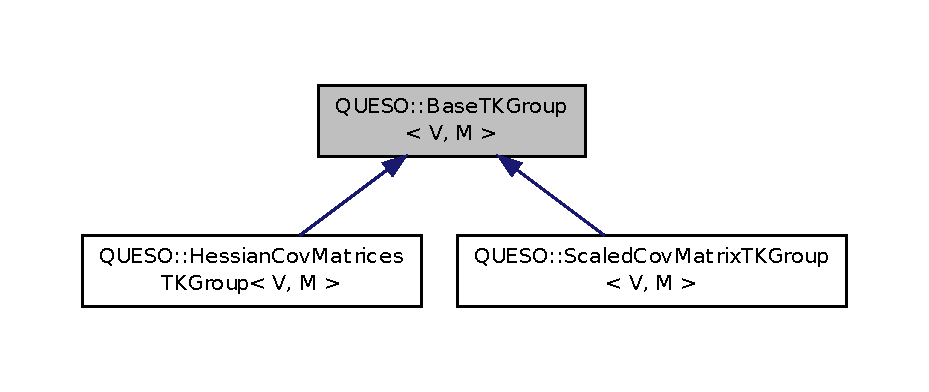
\includegraphics[width=350pt]{class_q_u_e_s_o_1_1_base_t_k_group__inherit__graph}
\end{center}
\end{figure}


Collaboration diagram for Q\-U\-E\-S\-O\-:\-:Base\-T\-K\-Group$<$ V, M $>$\-:
\nopagebreak
\begin{figure}[H]
\begin{center}
\leavevmode
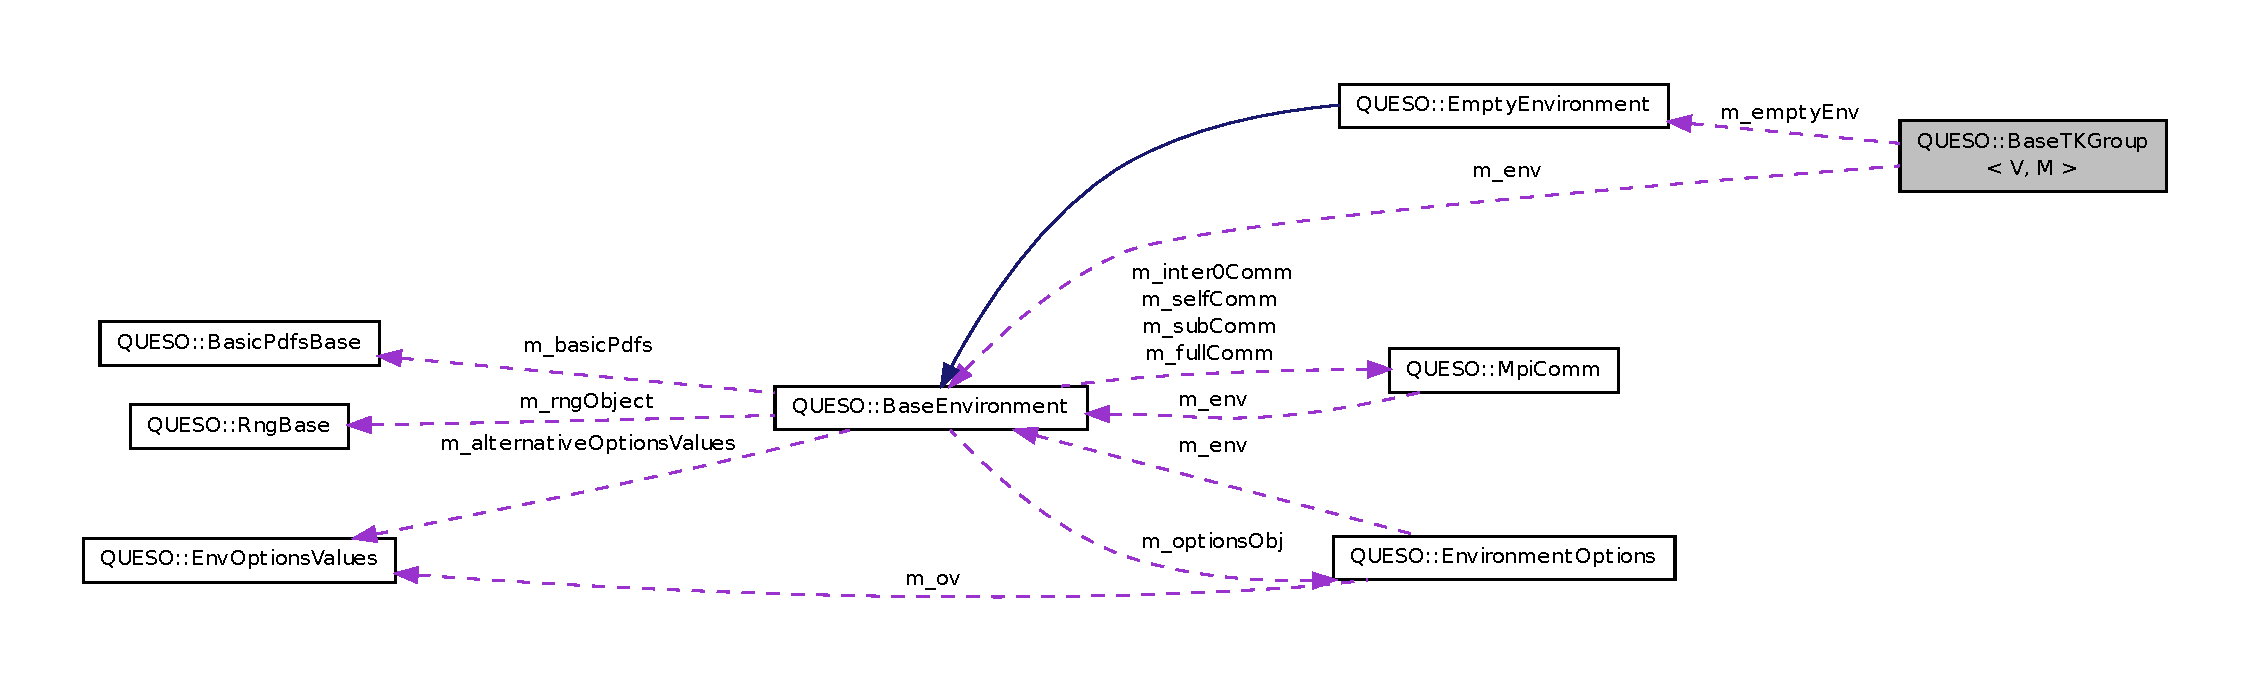
\includegraphics[width=350pt]{class_q_u_e_s_o_1_1_base_t_k_group__coll__graph}
\end{center}
\end{figure}
\subsection*{Public Member Functions}
\begin{Indent}{\bf Constructor/\-Destructor methods}\par
\begin{DoxyCompactItemize}
\item 
\hyperlink{class_q_u_e_s_o_1_1_base_t_k_group_ad4274236f2092a7307f4d5e4b0a480ee}{Base\-T\-K\-Group} ()
\begin{DoxyCompactList}\small\item\em Default constructor. \end{DoxyCompactList}\item 
\hyperlink{class_q_u_e_s_o_1_1_base_t_k_group_a94df2ec2ed0f8e3b8073df873f5bd0c9}{Base\-T\-K\-Group} (const char $\ast$prefix, const \hyperlink{class_q_u_e_s_o_1_1_vector_space}{Vector\-Space}$<$ V, M $>$ \&vector\-Space, const std\-::vector$<$ double $>$ \&scales)
\begin{DoxyCompactList}\small\item\em Constructor. \end{DoxyCompactList}\item 
virtual \hyperlink{class_q_u_e_s_o_1_1_base_t_k_group_a40fbcbbaf7977a83d38d76e1ef23f13f}{$\sim$\-Base\-T\-K\-Group} ()
\begin{DoxyCompactList}\small\item\em Destructor. \end{DoxyCompactList}\end{DoxyCompactItemize}
\end{Indent}
\begin{Indent}{\bf Statistical/\-Mathematical methods}\par
\begin{DoxyCompactItemize}
\item 
virtual bool \hyperlink{class_q_u_e_s_o_1_1_base_t_k_group_ad0130349060d50b985c83b6bb1abc58e}{symmetric} () const =0
\begin{DoxyCompactList}\small\item\em Whether or not the matrix is symmetric. See template specialization. \end{DoxyCompactList}\item 
virtual const \hyperlink{class_q_u_e_s_o_1_1_gaussian_vector_r_v}{Gaussian\-Vector\-R\-V}\\*
$<$ V, M $>$ \& \hyperlink{class_q_u_e_s_o_1_1_base_t_k_group_a6bd8e0bec0105471aad8801cbf1a0851}{rv} (unsigned int stage\-Id)=0
\begin{DoxyCompactList}\small\item\em Gaussian increment property to construct a transition kernel. See template specialization. \end{DoxyCompactList}\item 
virtual const \hyperlink{class_q_u_e_s_o_1_1_gaussian_vector_r_v}{Gaussian\-Vector\-R\-V}\\*
$<$ V, M $>$ \& \hyperlink{class_q_u_e_s_o_1_1_base_t_k_group_a35eaf213217ec41a9d85b957db01a9ff}{rv} (const std\-::vector$<$ unsigned int $>$ \&stage\-Ids)=0
\begin{DoxyCompactList}\small\item\em Gaussian increment property to construct a transition kernel. See template specialization. \end{DoxyCompactList}\end{DoxyCompactItemize}
\end{Indent}
\begin{Indent}{\bf Misc methods}\par
\begin{DoxyCompactItemize}
\item 
const \hyperlink{class_q_u_e_s_o_1_1_base_environment}{Base\-Environment} \& \hyperlink{class_q_u_e_s_o_1_1_base_t_k_group_ac71535d0b77dfdd1419ff2dbf5d6d037}{env} () const 
\begin{DoxyCompactList}\small\item\em \hyperlink{namespace_q_u_e_s_o}{Q\-U\-E\-S\-O}'s environment. \end{DoxyCompactList}\item 
const V \& \hyperlink{class_q_u_e_s_o_1_1_base_t_k_group_aa864c6cc07327a698f91cef72cdc35aa}{pre\-Computing\-Position} (unsigned int stage\-Id) const 
\begin{DoxyCompactList}\small\item\em Pre-\/computing position; access to protected attribute $\ast$m\-\_\-pre\-Computing\-Positions\mbox{[}stage\-Id\mbox{]}. \end{DoxyCompactList}\item 
virtual bool \hyperlink{class_q_u_e_s_o_1_1_base_t_k_group_acd1efb5b2ae3eb4f1130fa37201545d8}{set\-Pre\-Computing\-Position} (const V \&position, unsigned int stage\-Id)
\begin{DoxyCompactList}\small\item\em Sets the pre-\/computing positions {\ttfamily m\-\_\-pre\-Computing\-Positions}\mbox{[}stage\-Id\mbox{]} with a new vector of size {\ttfamily position}. \end{DoxyCompactList}\item 
virtual void \hyperlink{class_q_u_e_s_o_1_1_base_t_k_group_adb4decb4e8f01dce2ae4d5a3333c74f8}{clear\-Pre\-Computing\-Positions} ()
\begin{DoxyCompactList}\small\item\em Clears the pre-\/computing positions {\ttfamily m\-\_\-pre\-Computing\-Positions}\mbox{[}stage\-Id\mbox{]}. \end{DoxyCompactList}\end{DoxyCompactItemize}
\end{Indent}
\begin{Indent}{\bf I/\-O methods}\par
\begin{DoxyCompactItemize}
\item 
virtual void \hyperlink{class_q_u_e_s_o_1_1_base_t_k_group_ad6f7aa1ed1f75476b46333847e5086ba}{print} (std\-::ostream \&os) const 
\begin{DoxyCompactList}\small\item\em T\-O\-D\-O\-: Prints the transition kernel. \end{DoxyCompactList}\end{DoxyCompactItemize}
\end{Indent}
\subsection*{Protected Attributes}
\begin{DoxyCompactItemize}
\item 
const \hyperlink{class_q_u_e_s_o_1_1_empty_environment}{Empty\-Environment} $\ast$ \hyperlink{class_q_u_e_s_o_1_1_base_t_k_group_a41a8a2d2fde3c1994d3a542ccf9a194e}{m\-\_\-empty\-Env}
\item 
const \hyperlink{class_q_u_e_s_o_1_1_base_environment}{Base\-Environment} \& \hyperlink{class_q_u_e_s_o_1_1_base_t_k_group_a2bce5e8aa5c844d4332a0e73cf00a1f9}{m\-\_\-env}
\item 
std\-::string \hyperlink{class_q_u_e_s_o_1_1_base_t_k_group_a7c77e4969de60624dba1049cf44a1ab6}{m\-\_\-prefix}
\item 
const \hyperlink{class_q_u_e_s_o_1_1_vector_space}{Vector\-Space}$<$ V, M $>$ $\ast$ \hyperlink{class_q_u_e_s_o_1_1_base_t_k_group_a9930bbda0f3d9368653fb0577b89ec33}{m\-\_\-vector\-Space}
\item 
std\-::vector$<$ double $>$ \hyperlink{class_q_u_e_s_o_1_1_base_t_k_group_ad36d4dc6f4812e3e10d8090f0dbb9e40}{m\-\_\-scales}
\item 
std\-::vector$<$ const V $\ast$ $>$ \hyperlink{class_q_u_e_s_o_1_1_base_t_k_group_a93d7fe55e30a7c6f209b01cb8a67e322}{m\-\_\-pre\-Computing\-Positions}
\item 
std\-::vector$<$ \hyperlink{class_q_u_e_s_o_1_1_gaussian_vector_r_v}{Gaussian\-Vector\-R\-V}\\*
$<$ V, M $>$ $\ast$ $>$ \hyperlink{class_q_u_e_s_o_1_1_base_t_k_group_a87c6b02ea45ab3de634c22afa58f53a5}{m\-\_\-rvs}
\end{DoxyCompactItemize}


\subsection{Detailed Description}
\subsubsection*{template$<$class V, class M$>$class Q\-U\-E\-S\-O\-::\-Base\-T\-K\-Group$<$ V, M $>$}

This base class allows the representation of a transition kernel. 

The transition kernel is a conditional distribution function that represents the probability of moving from a point $ x \in R^n $ to a point in the set $ A \in B $, where $ B $ is a Borel set over $ R^n $. Since it is a distribution function, $ P(x,R^n)=1 $, where it is permitted that the chain can make a transition from the point $ x $ to $ x $, that is $ P(x, {x}) $ is not necessarily zero. 

Definition at line 48 of file T\-K\-Group.\-h.



\subsection{Constructor \& Destructor Documentation}
\hypertarget{class_q_u_e_s_o_1_1_base_t_k_group_ad4274236f2092a7307f4d5e4b0a480ee}{\index{Q\-U\-E\-S\-O\-::\-Base\-T\-K\-Group@{Q\-U\-E\-S\-O\-::\-Base\-T\-K\-Group}!Base\-T\-K\-Group@{Base\-T\-K\-Group}}
\index{Base\-T\-K\-Group@{Base\-T\-K\-Group}!QUESO::BaseTKGroup@{Q\-U\-E\-S\-O\-::\-Base\-T\-K\-Group}}
\subsubsection[{Base\-T\-K\-Group}]{\setlength{\rightskip}{0pt plus 5cm}template$<$class V , class M $>$ {\bf Q\-U\-E\-S\-O\-::\-Base\-T\-K\-Group}$<$ V, M $>$\-::{\bf Base\-T\-K\-Group} (
\begin{DoxyParamCaption}
{}
\end{DoxyParamCaption}
)}}\label{class_q_u_e_s_o_1_1_base_t_k_group_ad4274236f2092a7307f4d5e4b0a480ee}


Default constructor. 



Definition at line 33 of file T\-K\-Group.\-C.


\begin{DoxyCode}
34   :
35   \hyperlink{class_q_u_e_s_o_1_1_base_t_k_group_a41a8a2d2fde3c1994d3a542ccf9a194e}{m\_emptyEnv}             (\textcolor{keyword}{new} EmptyEnvironment()),
36   \hyperlink{class_q_u_e_s_o_1_1_base_t_k_group_a2bce5e8aa5c844d4332a0e73cf00a1f9}{m\_env}                  (*\hyperlink{class_q_u_e_s_o_1_1_base_t_k_group_a41a8a2d2fde3c1994d3a542ccf9a194e}{m\_emptyEnv}),
37   \hyperlink{class_q_u_e_s_o_1_1_base_t_k_group_a7c77e4969de60624dba1049cf44a1ab6}{m\_prefix}               (\textcolor{stringliteral}{""}),
38   \hyperlink{class_q_u_e_s_o_1_1_base_t_k_group_a9930bbda0f3d9368653fb0577b89ec33}{m\_vectorSpace}          (NULL),
39   \hyperlink{class_q_u_e_s_o_1_1_base_t_k_group_ad36d4dc6f4812e3e10d8090f0dbb9e40}{m\_scales}               (0),
40   \hyperlink{class_q_u_e_s_o_1_1_base_t_k_group_a93d7fe55e30a7c6f209b01cb8a67e322}{m\_preComputingPositions}(NULL),
41   \hyperlink{class_q_u_e_s_o_1_1_base_t_k_group_a87c6b02ea45ab3de634c22afa58f53a5}{m\_rvs}                  (0)
42 \{
43 \}
\end{DoxyCode}
\hypertarget{class_q_u_e_s_o_1_1_base_t_k_group_a94df2ec2ed0f8e3b8073df873f5bd0c9}{\index{Q\-U\-E\-S\-O\-::\-Base\-T\-K\-Group@{Q\-U\-E\-S\-O\-::\-Base\-T\-K\-Group}!Base\-T\-K\-Group@{Base\-T\-K\-Group}}
\index{Base\-T\-K\-Group@{Base\-T\-K\-Group}!QUESO::BaseTKGroup@{Q\-U\-E\-S\-O\-::\-Base\-T\-K\-Group}}
\subsubsection[{Base\-T\-K\-Group}]{\setlength{\rightskip}{0pt plus 5cm}template$<$class V, class M$>$ {\bf Q\-U\-E\-S\-O\-::\-Base\-T\-K\-Group}$<$ V, M $>$\-::{\bf Base\-T\-K\-Group} (
\begin{DoxyParamCaption}
\item[{const char $\ast$}]{prefix, }
\item[{const {\bf Vector\-Space}$<$ V, M $>$ \&}]{vector\-Space, }
\item[{const std\-::vector$<$ double $>$ \&}]{scales}
\end{DoxyParamCaption}
)}}\label{class_q_u_e_s_o_1_1_base_t_k_group_a94df2ec2ed0f8e3b8073df873f5bd0c9}


Constructor. 



Definition at line 46 of file T\-K\-Group.\-C.



References Q\-U\-E\-S\-O\-::\-Base\-T\-K\-Group$<$ V, M $>$\-::m\-\_\-scales.


\begin{DoxyCode}
50   :
51   \hyperlink{class_q_u_e_s_o_1_1_base_t_k_group_a41a8a2d2fde3c1994d3a542ccf9a194e}{m\_emptyEnv}             (NULL),
52   \hyperlink{class_q_u_e_s_o_1_1_base_t_k_group_a2bce5e8aa5c844d4332a0e73cf00a1f9}{m\_env}                  (vectorSpace.env()),
53   \hyperlink{class_q_u_e_s_o_1_1_base_t_k_group_a7c77e4969de60624dba1049cf44a1ab6}{m\_prefix}               (prefix),
54   \hyperlink{class_q_u_e_s_o_1_1_base_t_k_group_a9930bbda0f3d9368653fb0577b89ec33}{m\_vectorSpace}          (&vectorSpace),
55   \hyperlink{class_q_u_e_s_o_1_1_base_t_k_group_ad36d4dc6f4812e3e10d8090f0dbb9e40}{m\_scales}               (scales.size(),1.),
56   \hyperlink{class_q_u_e_s_o_1_1_base_t_k_group_a93d7fe55e30a7c6f209b01cb8a67e322}{m\_preComputingPositions}(scales.size()+1,NULL), \textcolor{comment}{// Yes, +1}
57   \hyperlink{class_q_u_e_s_o_1_1_base_t_k_group_a87c6b02ea45ab3de634c22afa58f53a5}{m\_rvs}                  (scales.size(),NULL) \textcolor{comment}{// IMPORTANT: it stays like this for scaledTK, but it
       will be overwritten to '+1' by hessianTK constructor}
58 \{
59   \textcolor{keywordflow}{for} (\textcolor{keywordtype}{unsigned} \textcolor{keywordtype}{int} i = 0; i < \hyperlink{class_q_u_e_s_o_1_1_base_t_k_group_ad36d4dc6f4812e3e10d8090f0dbb9e40}{m\_scales}.size(); ++i) \{
60     \hyperlink{class_q_u_e_s_o_1_1_base_t_k_group_ad36d4dc6f4812e3e10d8090f0dbb9e40}{m\_scales}[i] = scales[i];
61   \}
62 \}
\end{DoxyCode}
\hypertarget{class_q_u_e_s_o_1_1_base_t_k_group_a40fbcbbaf7977a83d38d76e1ef23f13f}{\index{Q\-U\-E\-S\-O\-::\-Base\-T\-K\-Group@{Q\-U\-E\-S\-O\-::\-Base\-T\-K\-Group}!$\sim$\-Base\-T\-K\-Group@{$\sim$\-Base\-T\-K\-Group}}
\index{$\sim$\-Base\-T\-K\-Group@{$\sim$\-Base\-T\-K\-Group}!QUESO::BaseTKGroup@{Q\-U\-E\-S\-O\-::\-Base\-T\-K\-Group}}
\subsubsection[{$\sim$\-Base\-T\-K\-Group}]{\setlength{\rightskip}{0pt plus 5cm}template$<$class V , class M $>$ {\bf Q\-U\-E\-S\-O\-::\-Base\-T\-K\-Group}$<$ V, M $>$\-::$\sim${\bf Base\-T\-K\-Group} (
\begin{DoxyParamCaption}
{}
\end{DoxyParamCaption}
)\hspace{0.3cm}{\ttfamily [virtual]}}}\label{class_q_u_e_s_o_1_1_base_t_k_group_a40fbcbbaf7977a83d38d76e1ef23f13f}


Destructor. 



Definition at line 65 of file T\-K\-Group.\-C.


\begin{DoxyCode}
66 \{
67   \textcolor{keywordflow}{for} (\textcolor{keywordtype}{unsigned} \textcolor{keywordtype}{int} i = 0; i < \hyperlink{class_q_u_e_s_o_1_1_base_t_k_group_a87c6b02ea45ab3de634c22afa58f53a5}{m\_rvs}.size(); ++i) \{
68     \textcolor{keywordflow}{if} (\hyperlink{class_q_u_e_s_o_1_1_base_t_k_group_a87c6b02ea45ab3de634c22afa58f53a5}{m\_rvs}[i]) \textcolor{keyword}{delete} \hyperlink{class_q_u_e_s_o_1_1_base_t_k_group_a87c6b02ea45ab3de634c22afa58f53a5}{m\_rvs}[i];
69   \}
70   \textcolor{keywordflow}{for} (\textcolor{keywordtype}{unsigned} \textcolor{keywordtype}{int} i = 0; i < \hyperlink{class_q_u_e_s_o_1_1_base_t_k_group_a93d7fe55e30a7c6f209b01cb8a67e322}{m\_preComputingPositions}.size(); ++i) \{
71     \textcolor{keywordflow}{if} (\hyperlink{class_q_u_e_s_o_1_1_base_t_k_group_a93d7fe55e30a7c6f209b01cb8a67e322}{m\_preComputingPositions}[i]) \textcolor{keyword}{delete} 
      \hyperlink{class_q_u_e_s_o_1_1_base_t_k_group_a93d7fe55e30a7c6f209b01cb8a67e322}{m\_preComputingPositions}[i];
72   \}
73   \textcolor{keywordflow}{if} (\hyperlink{class_q_u_e_s_o_1_1_base_t_k_group_a41a8a2d2fde3c1994d3a542ccf9a194e}{m\_emptyEnv}) \textcolor{keyword}{delete} \hyperlink{class_q_u_e_s_o_1_1_base_t_k_group_a41a8a2d2fde3c1994d3a542ccf9a194e}{m\_emptyEnv};
74 \}
\end{DoxyCode}


\subsection{Member Function Documentation}
\hypertarget{class_q_u_e_s_o_1_1_base_t_k_group_adb4decb4e8f01dce2ae4d5a3333c74f8}{\index{Q\-U\-E\-S\-O\-::\-Base\-T\-K\-Group@{Q\-U\-E\-S\-O\-::\-Base\-T\-K\-Group}!clear\-Pre\-Computing\-Positions@{clear\-Pre\-Computing\-Positions}}
\index{clear\-Pre\-Computing\-Positions@{clear\-Pre\-Computing\-Positions}!QUESO::BaseTKGroup@{Q\-U\-E\-S\-O\-::\-Base\-T\-K\-Group}}
\subsubsection[{clear\-Pre\-Computing\-Positions}]{\setlength{\rightskip}{0pt plus 5cm}template$<$class V , class M $>$ void {\bf Q\-U\-E\-S\-O\-::\-Base\-T\-K\-Group}$<$ V, M $>$\-::clear\-Pre\-Computing\-Positions (
\begin{DoxyParamCaption}
{}
\end{DoxyParamCaption}
)\hspace{0.3cm}{\ttfamily [virtual]}}}\label{class_q_u_e_s_o_1_1_base_t_k_group_adb4decb4e8f01dce2ae4d5a3333c74f8}


Clears the pre-\/computing positions {\ttfamily m\-\_\-pre\-Computing\-Positions}\mbox{[}stage\-Id\mbox{]}. 



Reimplemented in \hyperlink{class_q_u_e_s_o_1_1_scaled_cov_matrix_t_k_group_ae03597da61742f43997b8fffb7656b4d}{Q\-U\-E\-S\-O\-::\-Scaled\-Cov\-Matrix\-T\-K\-Group$<$ V, M $>$}, and \hyperlink{class_q_u_e_s_o_1_1_hessian_cov_matrices_t_k_group_af5ca7d6d8464e444607bb3da6cd39be8}{Q\-U\-E\-S\-O\-::\-Hessian\-Cov\-Matrices\-T\-K\-Group$<$ V, M $>$}.



Definition at line 121 of file T\-K\-Group.\-C.



Referenced by Q\-U\-E\-S\-O\-::\-Hessian\-Cov\-Matrices\-T\-K\-Group$<$ V, M $>$\-::clear\-Pre\-Computing\-Positions(), and Q\-U\-E\-S\-O\-::\-Scaled\-Cov\-Matrix\-T\-K\-Group$<$ V, M $>$\-::clear\-Pre\-Computing\-Positions().


\begin{DoxyCode}
122 \{
123   \textcolor{keywordflow}{for} (\textcolor{keywordtype}{unsigned} \textcolor{keywordtype}{int} i = 0; i < \hyperlink{class_q_u_e_s_o_1_1_base_t_k_group_a93d7fe55e30a7c6f209b01cb8a67e322}{m\_preComputingPositions}.size(); ++i) \{
124     \textcolor{keywordflow}{if} (\hyperlink{class_q_u_e_s_o_1_1_base_t_k_group_a93d7fe55e30a7c6f209b01cb8a67e322}{m\_preComputingPositions}[i]) \{
125       \textcolor{keyword}{delete} \hyperlink{class_q_u_e_s_o_1_1_base_t_k_group_a93d7fe55e30a7c6f209b01cb8a67e322}{m\_preComputingPositions}[i];
126       \hyperlink{class_q_u_e_s_o_1_1_base_t_k_group_a93d7fe55e30a7c6f209b01cb8a67e322}{m\_preComputingPositions}[i] = NULL;
127     \}
128   \}
129 
130   \textcolor{keywordflow}{return};
131 \}
\end{DoxyCode}
\hypertarget{class_q_u_e_s_o_1_1_base_t_k_group_ac71535d0b77dfdd1419ff2dbf5d6d037}{\index{Q\-U\-E\-S\-O\-::\-Base\-T\-K\-Group@{Q\-U\-E\-S\-O\-::\-Base\-T\-K\-Group}!env@{env}}
\index{env@{env}!QUESO::BaseTKGroup@{Q\-U\-E\-S\-O\-::\-Base\-T\-K\-Group}}
\subsubsection[{env}]{\setlength{\rightskip}{0pt plus 5cm}template$<$class V , class M $>$ const {\bf Base\-Environment} \& {\bf Q\-U\-E\-S\-O\-::\-Base\-T\-K\-Group}$<$ V, M $>$\-::env (
\begin{DoxyParamCaption}
{}
\end{DoxyParamCaption}
) const}}\label{class_q_u_e_s_o_1_1_base_t_k_group_ac71535d0b77dfdd1419ff2dbf5d6d037}


\hyperlink{namespace_q_u_e_s_o}{Q\-U\-E\-S\-O}'s environment. 



Definition at line 78 of file T\-K\-Group.\-C.


\begin{DoxyCode}
79 \{
80   \textcolor{keywordflow}{return} \hyperlink{class_q_u_e_s_o_1_1_base_t_k_group_a2bce5e8aa5c844d4332a0e73cf00a1f9}{m\_env};
81 \}
\end{DoxyCode}
\hypertarget{class_q_u_e_s_o_1_1_base_t_k_group_aa864c6cc07327a698f91cef72cdc35aa}{\index{Q\-U\-E\-S\-O\-::\-Base\-T\-K\-Group@{Q\-U\-E\-S\-O\-::\-Base\-T\-K\-Group}!pre\-Computing\-Position@{pre\-Computing\-Position}}
\index{pre\-Computing\-Position@{pre\-Computing\-Position}!QUESO::BaseTKGroup@{Q\-U\-E\-S\-O\-::\-Base\-T\-K\-Group}}
\subsubsection[{pre\-Computing\-Position}]{\setlength{\rightskip}{0pt plus 5cm}template$<$class V , class M $>$ const V \& {\bf Q\-U\-E\-S\-O\-::\-Base\-T\-K\-Group}$<$ V, M $>$\-::pre\-Computing\-Position (
\begin{DoxyParamCaption}
\item[{unsigned int}]{stage\-Id}
\end{DoxyParamCaption}
) const}}\label{class_q_u_e_s_o_1_1_base_t_k_group_aa864c6cc07327a698f91cef72cdc35aa}


Pre-\/computing position; access to protected attribute $\ast$m\-\_\-pre\-Computing\-Positions\mbox{[}stage\-Id\mbox{]}. 



Definition at line 85 of file T\-K\-Group.\-C.



References U\-Q\-\_\-\-F\-A\-T\-A\-L\-\_\-\-T\-E\-S\-T\-\_\-\-M\-A\-C\-R\-O.


\begin{DoxyCode}
86 \{
87   \hyperlink{_defines_8h_a56d63d18d0a6d45757de47fcc06f574d}{UQ\_FATAL\_TEST\_MACRO}(\hyperlink{class_q_u_e_s_o_1_1_base_t_k_group_a93d7fe55e30a7c6f209b01cb8a67e322}{m\_preComputingPositions}.size() <= stageId,
88                       \hyperlink{class_q_u_e_s_o_1_1_base_t_k_group_a2bce5e8aa5c844d4332a0e73cf00a1f9}{m\_env}.\hyperlink{class_q_u_e_s_o_1_1_base_environment_a78b57112bbd0e6dd0e8afec00b40ffa7}{worldRank}(),
89                       \textcolor{stringliteral}{"BaseTKGroup<V,M>::preComputingPosition()"},
90                       \textcolor{stringliteral}{"m\_preComputingPositions.size() <= stageId"});
91 
92   \hyperlink{_defines_8h_a56d63d18d0a6d45757de47fcc06f574d}{UQ\_FATAL\_TEST\_MACRO}(\hyperlink{class_q_u_e_s_o_1_1_base_t_k_group_a93d7fe55e30a7c6f209b01cb8a67e322}{m\_preComputingPositions}[stageId] == NULL,
93                       \hyperlink{class_q_u_e_s_o_1_1_base_t_k_group_a2bce5e8aa5c844d4332a0e73cf00a1f9}{m\_env}.\hyperlink{class_q_u_e_s_o_1_1_base_environment_a78b57112bbd0e6dd0e8afec00b40ffa7}{worldRank}(),
94                       \textcolor{stringliteral}{"BaseTKGroup<V,M>::preComputingPosition()"},
95                       \textcolor{stringliteral}{"m\_preComputingPositions[stageId] == NULL"});
96 
97   \textcolor{keywordflow}{return} *\hyperlink{class_q_u_e_s_o_1_1_base_t_k_group_a93d7fe55e30a7c6f209b01cb8a67e322}{m\_preComputingPositions}[stageId];
98 \}
\end{DoxyCode}
\hypertarget{class_q_u_e_s_o_1_1_base_t_k_group_ad6f7aa1ed1f75476b46333847e5086ba}{\index{Q\-U\-E\-S\-O\-::\-Base\-T\-K\-Group@{Q\-U\-E\-S\-O\-::\-Base\-T\-K\-Group}!print@{print}}
\index{print@{print}!QUESO::BaseTKGroup@{Q\-U\-E\-S\-O\-::\-Base\-T\-K\-Group}}
\subsubsection[{print}]{\setlength{\rightskip}{0pt plus 5cm}template$<$class V , class M $>$ void {\bf Q\-U\-E\-S\-O\-::\-Base\-T\-K\-Group}$<$ V, M $>$\-::print (
\begin{DoxyParamCaption}
\item[{std\-::ostream \&}]{os}
\end{DoxyParamCaption}
) const\hspace{0.3cm}{\ttfamily [virtual]}}}\label{class_q_u_e_s_o_1_1_base_t_k_group_ad6f7aa1ed1f75476b46333847e5086ba}


T\-O\-D\-O\-: Prints the transition kernel. 

\begin{DoxyRefDesc}{Todo}
\item[\hyperlink{todo__todo000050}{Todo}]\-: implement me! \end{DoxyRefDesc}


Reimplemented in \hyperlink{class_q_u_e_s_o_1_1_scaled_cov_matrix_t_k_group_ac1116a3f10d1456c9b796d2756258e55}{Q\-U\-E\-S\-O\-::\-Scaled\-Cov\-Matrix\-T\-K\-Group$<$ V, M $>$}, and \hyperlink{class_q_u_e_s_o_1_1_hessian_cov_matrices_t_k_group_aa780d91ffdf133df50d5d9a3a0edaa95}{Q\-U\-E\-S\-O\-::\-Hessian\-Cov\-Matrices\-T\-K\-Group$<$ V, M $>$}.



Definition at line 135 of file T\-K\-Group.\-C.



Referenced by Q\-U\-E\-S\-O\-::\-Hessian\-Cov\-Matrices\-T\-K\-Group$<$ V, M $>$\-::print(), and Q\-U\-E\-S\-O\-::\-Scaled\-Cov\-Matrix\-T\-K\-Group$<$ V, M $>$\-::print().


\begin{DoxyCode}
136 \{
137   os << \textcolor{stringliteral}{"In BaseTKGroup<V,M>::print()"}
138      << \textcolor{stringliteral}{": nothing to be printed"} << std::endl;
139   \textcolor{keywordflow}{return};
140 \}
\end{DoxyCode}
\hypertarget{class_q_u_e_s_o_1_1_base_t_k_group_a6bd8e0bec0105471aad8801cbf1a0851}{\index{Q\-U\-E\-S\-O\-::\-Base\-T\-K\-Group@{Q\-U\-E\-S\-O\-::\-Base\-T\-K\-Group}!rv@{rv}}
\index{rv@{rv}!QUESO::BaseTKGroup@{Q\-U\-E\-S\-O\-::\-Base\-T\-K\-Group}}
\subsubsection[{rv}]{\setlength{\rightskip}{0pt plus 5cm}template$<$class V, class M$>$ virtual const {\bf Gaussian\-Vector\-R\-V}$<$V,M$>$\& {\bf Q\-U\-E\-S\-O\-::\-Base\-T\-K\-Group}$<$ V, M $>$\-::rv (
\begin{DoxyParamCaption}
\item[{unsigned int}]{stage\-Id}
\end{DoxyParamCaption}
)\hspace{0.3cm}{\ttfamily [pure virtual]}}}\label{class_q_u_e_s_o_1_1_base_t_k_group_a6bd8e0bec0105471aad8801cbf1a0851}


Gaussian increment property to construct a transition kernel. See template specialization. 



Implemented in \hyperlink{class_q_u_e_s_o_1_1_hessian_cov_matrices_t_k_group_a7a9a6fabad72d063438733436704ff2b}{Q\-U\-E\-S\-O\-::\-Hessian\-Cov\-Matrices\-T\-K\-Group$<$ V, M $>$}, and \hyperlink{class_q_u_e_s_o_1_1_scaled_cov_matrix_t_k_group_a892c6636742f2a613d46fcb84b80dbb5}{Q\-U\-E\-S\-O\-::\-Scaled\-Cov\-Matrix\-T\-K\-Group$<$ V, M $>$}.

\hypertarget{class_q_u_e_s_o_1_1_base_t_k_group_a35eaf213217ec41a9d85b957db01a9ff}{\index{Q\-U\-E\-S\-O\-::\-Base\-T\-K\-Group@{Q\-U\-E\-S\-O\-::\-Base\-T\-K\-Group}!rv@{rv}}
\index{rv@{rv}!QUESO::BaseTKGroup@{Q\-U\-E\-S\-O\-::\-Base\-T\-K\-Group}}
\subsubsection[{rv}]{\setlength{\rightskip}{0pt plus 5cm}template$<$class V, class M$>$ virtual const {\bf Gaussian\-Vector\-R\-V}$<$V,M$>$\& {\bf Q\-U\-E\-S\-O\-::\-Base\-T\-K\-Group}$<$ V, M $>$\-::rv (
\begin{DoxyParamCaption}
\item[{const std\-::vector$<$ unsigned int $>$ \&}]{stage\-Ids}
\end{DoxyParamCaption}
)\hspace{0.3cm}{\ttfamily [pure virtual]}}}\label{class_q_u_e_s_o_1_1_base_t_k_group_a35eaf213217ec41a9d85b957db01a9ff}


Gaussian increment property to construct a transition kernel. See template specialization. 



Implemented in \hyperlink{class_q_u_e_s_o_1_1_hessian_cov_matrices_t_k_group_a658ecfbd10f11f4951649986ad65ae76}{Q\-U\-E\-S\-O\-::\-Hessian\-Cov\-Matrices\-T\-K\-Group$<$ V, M $>$}, and \hyperlink{class_q_u_e_s_o_1_1_scaled_cov_matrix_t_k_group_a753ada276637a3c32ea77b833dda7979}{Q\-U\-E\-S\-O\-::\-Scaled\-Cov\-Matrix\-T\-K\-Group$<$ V, M $>$}.

\hypertarget{class_q_u_e_s_o_1_1_base_t_k_group_acd1efb5b2ae3eb4f1130fa37201545d8}{\index{Q\-U\-E\-S\-O\-::\-Base\-T\-K\-Group@{Q\-U\-E\-S\-O\-::\-Base\-T\-K\-Group}!set\-Pre\-Computing\-Position@{set\-Pre\-Computing\-Position}}
\index{set\-Pre\-Computing\-Position@{set\-Pre\-Computing\-Position}!QUESO::BaseTKGroup@{Q\-U\-E\-S\-O\-::\-Base\-T\-K\-Group}}
\subsubsection[{set\-Pre\-Computing\-Position}]{\setlength{\rightskip}{0pt plus 5cm}template$<$class V, class M $>$ bool {\bf Q\-U\-E\-S\-O\-::\-Base\-T\-K\-Group}$<$ V, M $>$\-::set\-Pre\-Computing\-Position (
\begin{DoxyParamCaption}
\item[{const V \&}]{position, }
\item[{unsigned int}]{stage\-Id}
\end{DoxyParamCaption}
)\hspace{0.3cm}{\ttfamily [virtual]}}}\label{class_q_u_e_s_o_1_1_base_t_k_group_acd1efb5b2ae3eb4f1130fa37201545d8}


Sets the pre-\/computing positions {\ttfamily m\-\_\-pre\-Computing\-Positions}\mbox{[}stage\-Id\mbox{]} with a new vector of size {\ttfamily position}. 



Reimplemented in \hyperlink{class_q_u_e_s_o_1_1_scaled_cov_matrix_t_k_group_a4e6325c0cd92d555f32aef52ae4755e3}{Q\-U\-E\-S\-O\-::\-Scaled\-Cov\-Matrix\-T\-K\-Group$<$ V, M $>$}, and \hyperlink{class_q_u_e_s_o_1_1_hessian_cov_matrices_t_k_group_a935cca86e22544d5a478e05862a4a200}{Q\-U\-E\-S\-O\-::\-Hessian\-Cov\-Matrices\-T\-K\-Group$<$ V, M $>$}.



Definition at line 102 of file T\-K\-Group.\-C.



References U\-Q\-\_\-\-F\-A\-T\-A\-L\-\_\-\-T\-E\-S\-T\-\_\-\-M\-A\-C\-R\-O.



Referenced by Q\-U\-E\-S\-O\-::\-Hessian\-Cov\-Matrices\-T\-K\-Group$<$ V, M $>$\-::set\-Pre\-Computing\-Position(), and Q\-U\-E\-S\-O\-::\-Scaled\-Cov\-Matrix\-T\-K\-Group$<$ V, M $>$\-::set\-Pre\-Computing\-Position().


\begin{DoxyCode}
103 \{
104   \hyperlink{_defines_8h_a56d63d18d0a6d45757de47fcc06f574d}{UQ\_FATAL\_TEST\_MACRO}(\hyperlink{class_q_u_e_s_o_1_1_base_t_k_group_a93d7fe55e30a7c6f209b01cb8a67e322}{m\_preComputingPositions}.size() <= stageId,
105                       \hyperlink{class_q_u_e_s_o_1_1_base_t_k_group_a2bce5e8aa5c844d4332a0e73cf00a1f9}{m\_env}.\hyperlink{class_q_u_e_s_o_1_1_base_environment_a78b57112bbd0e6dd0e8afec00b40ffa7}{worldRank}(),
106                       \textcolor{stringliteral}{"BaseTKGroup<V,M>::setPreComputingPosition()"},
107                       \textcolor{stringliteral}{"m\_preComputingPositions.size() <= stageId"});
108 
109   \hyperlink{_defines_8h_a56d63d18d0a6d45757de47fcc06f574d}{UQ\_FATAL\_TEST\_MACRO}(\hyperlink{class_q_u_e_s_o_1_1_base_t_k_group_a93d7fe55e30a7c6f209b01cb8a67e322}{m\_preComputingPositions}[stageId] != NULL,
110                       \hyperlink{class_q_u_e_s_o_1_1_base_t_k_group_a2bce5e8aa5c844d4332a0e73cf00a1f9}{m\_env}.\hyperlink{class_q_u_e_s_o_1_1_base_environment_a78b57112bbd0e6dd0e8afec00b40ffa7}{worldRank}(),
111                       \textcolor{stringliteral}{"BaseTKGroup<V,M>::setPreComputingPosition()"},
112                       \textcolor{stringliteral}{"m\_preComputingPositions[stageId] != NULL"});
113 
114   \hyperlink{class_q_u_e_s_o_1_1_base_t_k_group_a93d7fe55e30a7c6f209b01cb8a67e322}{m\_preComputingPositions}[stageId] = \textcolor{keyword}{new} V(position);
115 
116   \textcolor{keywordflow}{return} \textcolor{keyword}{true};
117 \}
\end{DoxyCode}
\hypertarget{class_q_u_e_s_o_1_1_base_t_k_group_ad0130349060d50b985c83b6bb1abc58e}{\index{Q\-U\-E\-S\-O\-::\-Base\-T\-K\-Group@{Q\-U\-E\-S\-O\-::\-Base\-T\-K\-Group}!symmetric@{symmetric}}
\index{symmetric@{symmetric}!QUESO::BaseTKGroup@{Q\-U\-E\-S\-O\-::\-Base\-T\-K\-Group}}
\subsubsection[{symmetric}]{\setlength{\rightskip}{0pt plus 5cm}template$<$class V, class M$>$ virtual bool {\bf Q\-U\-E\-S\-O\-::\-Base\-T\-K\-Group}$<$ V, M $>$\-::symmetric (
\begin{DoxyParamCaption}
{}
\end{DoxyParamCaption}
) const\hspace{0.3cm}{\ttfamily [pure virtual]}}}\label{class_q_u_e_s_o_1_1_base_t_k_group_ad0130349060d50b985c83b6bb1abc58e}


Whether or not the matrix is symmetric. See template specialization. 



Implemented in \hyperlink{class_q_u_e_s_o_1_1_hessian_cov_matrices_t_k_group_abf0f6a04543c18b2f95e615b09191c2b}{Q\-U\-E\-S\-O\-::\-Hessian\-Cov\-Matrices\-T\-K\-Group$<$ V, M $>$}, and \hyperlink{class_q_u_e_s_o_1_1_scaled_cov_matrix_t_k_group_a3189c3503bf9eb4229ec707594d75516}{Q\-U\-E\-S\-O\-::\-Scaled\-Cov\-Matrix\-T\-K\-Group$<$ V, M $>$}.



\subsection{Member Data Documentation}
\hypertarget{class_q_u_e_s_o_1_1_base_t_k_group_a41a8a2d2fde3c1994d3a542ccf9a194e}{\index{Q\-U\-E\-S\-O\-::\-Base\-T\-K\-Group@{Q\-U\-E\-S\-O\-::\-Base\-T\-K\-Group}!m\-\_\-empty\-Env@{m\-\_\-empty\-Env}}
\index{m\-\_\-empty\-Env@{m\-\_\-empty\-Env}!QUESO::BaseTKGroup@{Q\-U\-E\-S\-O\-::\-Base\-T\-K\-Group}}
\subsubsection[{m\-\_\-empty\-Env}]{\setlength{\rightskip}{0pt plus 5cm}template$<$class V, class M$>$ const {\bf Empty\-Environment}$\ast$ {\bf Q\-U\-E\-S\-O\-::\-Base\-T\-K\-Group}$<$ V, M $>$\-::m\-\_\-empty\-Env\hspace{0.3cm}{\ttfamily [protected]}}}\label{class_q_u_e_s_o_1_1_base_t_k_group_a41a8a2d2fde3c1994d3a542ccf9a194e}


Definition at line 97 of file T\-K\-Group.\-h.

\hypertarget{class_q_u_e_s_o_1_1_base_t_k_group_a2bce5e8aa5c844d4332a0e73cf00a1f9}{\index{Q\-U\-E\-S\-O\-::\-Base\-T\-K\-Group@{Q\-U\-E\-S\-O\-::\-Base\-T\-K\-Group}!m\-\_\-env@{m\-\_\-env}}
\index{m\-\_\-env@{m\-\_\-env}!QUESO::BaseTKGroup@{Q\-U\-E\-S\-O\-::\-Base\-T\-K\-Group}}
\subsubsection[{m\-\_\-env}]{\setlength{\rightskip}{0pt plus 5cm}template$<$class V, class M$>$ const {\bf Base\-Environment}\& {\bf Q\-U\-E\-S\-O\-::\-Base\-T\-K\-Group}$<$ V, M $>$\-::m\-\_\-env\hspace{0.3cm}{\ttfamily [protected]}}}\label{class_q_u_e_s_o_1_1_base_t_k_group_a2bce5e8aa5c844d4332a0e73cf00a1f9}


Definition at line 98 of file T\-K\-Group.\-h.



Referenced by Q\-U\-E\-S\-O\-::\-Hessian\-Cov\-Matrices\-T\-K\-Group$<$ V, M $>$\-::\-Hessian\-Cov\-Matrices\-T\-K\-Group(), and Q\-U\-E\-S\-O\-::\-Scaled\-Cov\-Matrix\-T\-K\-Group$<$ V, M $>$\-::\-Scaled\-Cov\-Matrix\-T\-K\-Group().

\hypertarget{class_q_u_e_s_o_1_1_base_t_k_group_a93d7fe55e30a7c6f209b01cb8a67e322}{\index{Q\-U\-E\-S\-O\-::\-Base\-T\-K\-Group@{Q\-U\-E\-S\-O\-::\-Base\-T\-K\-Group}!m\-\_\-pre\-Computing\-Positions@{m\-\_\-pre\-Computing\-Positions}}
\index{m\-\_\-pre\-Computing\-Positions@{m\-\_\-pre\-Computing\-Positions}!QUESO::BaseTKGroup@{Q\-U\-E\-S\-O\-::\-Base\-T\-K\-Group}}
\subsubsection[{m\-\_\-pre\-Computing\-Positions}]{\setlength{\rightskip}{0pt plus 5cm}template$<$class V, class M$>$ std\-::vector$<$const V$\ast$$>$ {\bf Q\-U\-E\-S\-O\-::\-Base\-T\-K\-Group}$<$ V, M $>$\-::m\-\_\-pre\-Computing\-Positions\hspace{0.3cm}{\ttfamily [protected]}}}\label{class_q_u_e_s_o_1_1_base_t_k_group_a93d7fe55e30a7c6f209b01cb8a67e322}


Definition at line 102 of file T\-K\-Group.\-h.



Referenced by Q\-U\-E\-S\-O\-::\-Hessian\-Cov\-Matrices\-T\-K\-Group$<$ V, M $>$\-::\-Hessian\-Cov\-Matrices\-T\-K\-Group(), and Q\-U\-E\-S\-O\-::\-Scaled\-Cov\-Matrix\-T\-K\-Group$<$ V, M $>$\-::\-Scaled\-Cov\-Matrix\-T\-K\-Group().

\hypertarget{class_q_u_e_s_o_1_1_base_t_k_group_a7c77e4969de60624dba1049cf44a1ab6}{\index{Q\-U\-E\-S\-O\-::\-Base\-T\-K\-Group@{Q\-U\-E\-S\-O\-::\-Base\-T\-K\-Group}!m\-\_\-prefix@{m\-\_\-prefix}}
\index{m\-\_\-prefix@{m\-\_\-prefix}!QUESO::BaseTKGroup@{Q\-U\-E\-S\-O\-::\-Base\-T\-K\-Group}}
\subsubsection[{m\-\_\-prefix}]{\setlength{\rightskip}{0pt plus 5cm}template$<$class V, class M$>$ std\-::string {\bf Q\-U\-E\-S\-O\-::\-Base\-T\-K\-Group}$<$ V, M $>$\-::m\-\_\-prefix\hspace{0.3cm}{\ttfamily [protected]}}}\label{class_q_u_e_s_o_1_1_base_t_k_group_a7c77e4969de60624dba1049cf44a1ab6}


Definition at line 99 of file T\-K\-Group.\-h.

\hypertarget{class_q_u_e_s_o_1_1_base_t_k_group_a87c6b02ea45ab3de634c22afa58f53a5}{\index{Q\-U\-E\-S\-O\-::\-Base\-T\-K\-Group@{Q\-U\-E\-S\-O\-::\-Base\-T\-K\-Group}!m\-\_\-rvs@{m\-\_\-rvs}}
\index{m\-\_\-rvs@{m\-\_\-rvs}!QUESO::BaseTKGroup@{Q\-U\-E\-S\-O\-::\-Base\-T\-K\-Group}}
\subsubsection[{m\-\_\-rvs}]{\setlength{\rightskip}{0pt plus 5cm}template$<$class V, class M$>$ std\-::vector$<${\bf Gaussian\-Vector\-R\-V}$<$V,M$>$$\ast$ $>$ {\bf Q\-U\-E\-S\-O\-::\-Base\-T\-K\-Group}$<$ V, M $>$\-::m\-\_\-rvs\hspace{0.3cm}{\ttfamily [protected]}}}\label{class_q_u_e_s_o_1_1_base_t_k_group_a87c6b02ea45ab3de634c22afa58f53a5}


Definition at line 103 of file T\-K\-Group.\-h.



Referenced by Q\-U\-E\-S\-O\-::\-Hessian\-Cov\-Matrices\-T\-K\-Group$<$ V, M $>$\-::\-Hessian\-Cov\-Matrices\-T\-K\-Group(), and Q\-U\-E\-S\-O\-::\-Scaled\-Cov\-Matrix\-T\-K\-Group$<$ V, M $>$\-::\-Scaled\-Cov\-Matrix\-T\-K\-Group().

\hypertarget{class_q_u_e_s_o_1_1_base_t_k_group_ad36d4dc6f4812e3e10d8090f0dbb9e40}{\index{Q\-U\-E\-S\-O\-::\-Base\-T\-K\-Group@{Q\-U\-E\-S\-O\-::\-Base\-T\-K\-Group}!m\-\_\-scales@{m\-\_\-scales}}
\index{m\-\_\-scales@{m\-\_\-scales}!QUESO::BaseTKGroup@{Q\-U\-E\-S\-O\-::\-Base\-T\-K\-Group}}
\subsubsection[{m\-\_\-scales}]{\setlength{\rightskip}{0pt plus 5cm}template$<$class V, class M$>$ std\-::vector$<$double$>$ {\bf Q\-U\-E\-S\-O\-::\-Base\-T\-K\-Group}$<$ V, M $>$\-::m\-\_\-scales\hspace{0.3cm}{\ttfamily [protected]}}}\label{class_q_u_e_s_o_1_1_base_t_k_group_ad36d4dc6f4812e3e10d8090f0dbb9e40}


Definition at line 101 of file T\-K\-Group.\-h.



Referenced by Q\-U\-E\-S\-O\-::\-Base\-T\-K\-Group$<$ V, M $>$\-::\-Base\-T\-K\-Group(), Q\-U\-E\-S\-O\-::\-Hessian\-Cov\-Matrices\-T\-K\-Group$<$ V, M $>$\-::\-Hessian\-Cov\-Matrices\-T\-K\-Group(), and Q\-U\-E\-S\-O\-::\-Scaled\-Cov\-Matrix\-T\-K\-Group$<$ V, M $>$\-::\-Scaled\-Cov\-Matrix\-T\-K\-Group().

\hypertarget{class_q_u_e_s_o_1_1_base_t_k_group_a9930bbda0f3d9368653fb0577b89ec33}{\index{Q\-U\-E\-S\-O\-::\-Base\-T\-K\-Group@{Q\-U\-E\-S\-O\-::\-Base\-T\-K\-Group}!m\-\_\-vector\-Space@{m\-\_\-vector\-Space}}
\index{m\-\_\-vector\-Space@{m\-\_\-vector\-Space}!QUESO::BaseTKGroup@{Q\-U\-E\-S\-O\-::\-Base\-T\-K\-Group}}
\subsubsection[{m\-\_\-vector\-Space}]{\setlength{\rightskip}{0pt plus 5cm}template$<$class V, class M$>$ const {\bf Vector\-Space}$<$V,M$>$$\ast$ {\bf Q\-U\-E\-S\-O\-::\-Base\-T\-K\-Group}$<$ V, M $>$\-::m\-\_\-vector\-Space\hspace{0.3cm}{\ttfamily [protected]}}}\label{class_q_u_e_s_o_1_1_base_t_k_group_a9930bbda0f3d9368653fb0577b89ec33}


Definition at line 100 of file T\-K\-Group.\-h.



The documentation for this class was generated from the following files\-:\begin{DoxyCompactItemize}
\item 
src/stats/inc/\hyperlink{_t_k_group_8h}{T\-K\-Group.\-h}\item 
src/stats/src/\hyperlink{_t_k_group_8_c}{T\-K\-Group.\-C}\end{DoxyCompactItemize}

\hypertarget{class_q_u_e_s_o_1_1_base_vector_cdf}{\section{Q\-U\-E\-S\-O\-:\-:Base\-Vector\-Cdf$<$ V, M $>$ Class Template Reference}
\label{class_q_u_e_s_o_1_1_base_vector_cdf}\index{Q\-U\-E\-S\-O\-::\-Base\-Vector\-Cdf$<$ V, M $>$@{Q\-U\-E\-S\-O\-::\-Base\-Vector\-Cdf$<$ V, M $>$}}
}


A templated (base) class for handling C\-D\-Fs of vector functions.  




{\ttfamily \#include $<$Vector\-Cdf.\-h$>$}



Inheritance diagram for Q\-U\-E\-S\-O\-:\-:Base\-Vector\-Cdf$<$ V, M $>$\-:
\nopagebreak
\begin{figure}[H]
\begin{center}
\leavevmode
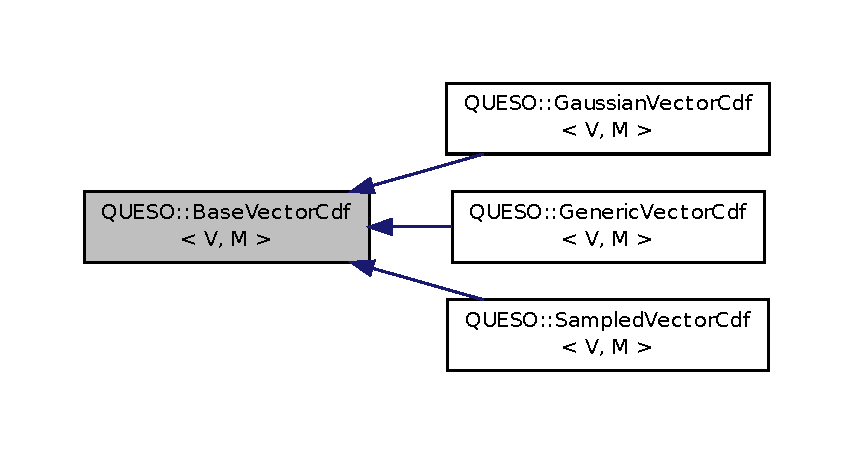
\includegraphics[width=350pt]{class_q_u_e_s_o_1_1_base_vector_cdf__inherit__graph}
\end{center}
\end{figure}


Collaboration diagram for Q\-U\-E\-S\-O\-:\-:Base\-Vector\-Cdf$<$ V, M $>$\-:
\nopagebreak
\begin{figure}[H]
\begin{center}
\leavevmode
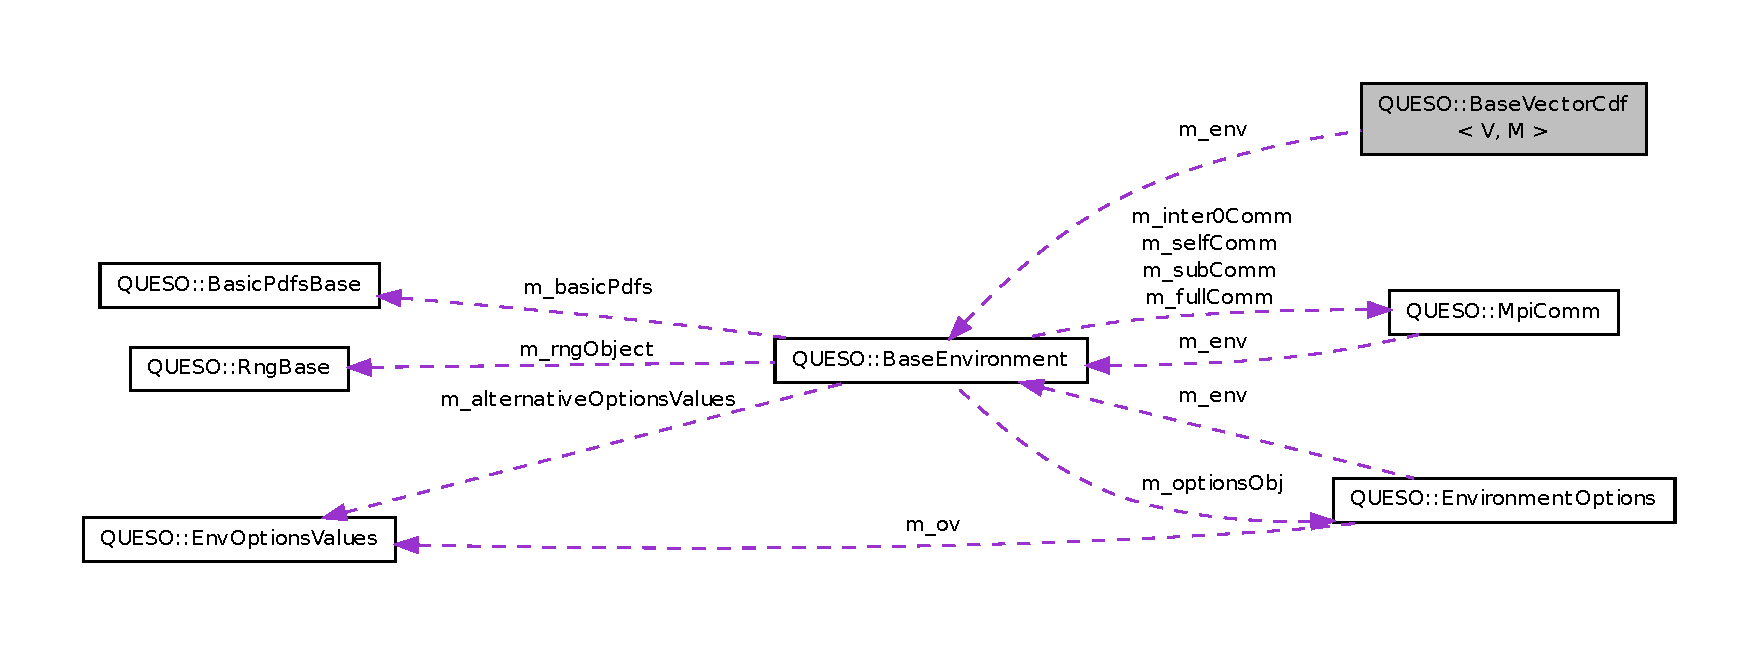
\includegraphics[width=350pt]{class_q_u_e_s_o_1_1_base_vector_cdf__coll__graph}
\end{center}
\end{figure}
\subsection*{Public Member Functions}
\begin{Indent}{\bf Constructor/\-Destructor methods}\par
\begin{DoxyCompactItemize}
\item 
\hyperlink{class_q_u_e_s_o_1_1_base_vector_cdf_ac7d0efcc78675e5ecc0ec684841c70e2}{Base\-Vector\-Cdf} (const char $\ast$prefix, const \hyperlink{class_q_u_e_s_o_1_1_vector_set}{Vector\-Set}$<$ V, M $>$ \&\hyperlink{class_q_u_e_s_o_1_1_base_vector_cdf_aaf5088d3994606a9d449ccd414509709}{pdf\-Support})
\begin{DoxyCompactList}\small\item\em Default constructor. \end{DoxyCompactList}\item 
virtual \hyperlink{class_q_u_e_s_o_1_1_base_vector_cdf_a0b3bcef9ed025de3184649c46c72cafb}{$\sim$\-Base\-Vector\-Cdf} ()
\begin{DoxyCompactList}\small\item\em Virtual destructor. \end{DoxyCompactList}\end{DoxyCompactItemize}
\end{Indent}
\begin{Indent}{\bf Mathematical methods}\par
\begin{DoxyCompactItemize}
\item 
const \hyperlink{class_q_u_e_s_o_1_1_vector_set}{Vector\-Set}$<$ V, M $>$ \& \hyperlink{class_q_u_e_s_o_1_1_base_vector_cdf_aaf5088d3994606a9d449ccd414509709}{pdf\-Support} () const 
\begin{DoxyCompactList}\small\item\em Returns the image set (support) of the P\-D\-F; access to protected attribute {\ttfamily m\-\_\-pdf\-Support}. \end{DoxyCompactList}\item 
virtual void \hyperlink{class_q_u_e_s_o_1_1_base_vector_cdf_a30b15bde5a206071b4e4db26141ce179}{values} (const V \&param\-Values, V \&cdf\-Vec) const =0
\begin{DoxyCompactList}\small\item\em Finds the value of the vector C\-D\-F at each element of {\ttfamily param\-Value}, and saves it in {\ttfamily cdf\-Vec}. See template specialization. \end{DoxyCompactList}\item 
virtual const \hyperlink{class_q_u_e_s_o_1_1_base_scalar_cdf}{Base\-Scalar\-Cdf}\\*
$<$ double $>$ \& \hyperlink{class_q_u_e_s_o_1_1_base_vector_cdf_aac430df67c3f278eb14b1691b9fedbb2}{cdf} (unsigned int row\-Id) const =0
\end{DoxyCompactItemize}
\end{Indent}
\subsection*{Protected Attributes}
\begin{DoxyCompactItemize}
\item 
const \hyperlink{class_q_u_e_s_o_1_1_base_environment}{Base\-Environment} \& \hyperlink{class_q_u_e_s_o_1_1_base_vector_cdf_aa1effe370ac016f1fc7eaf538c5751a6}{m\-\_\-env}
\item 
std\-::string \hyperlink{class_q_u_e_s_o_1_1_base_vector_cdf_ac88b657f25153ab6c03bd65b64cada52}{m\-\_\-prefix}
\item 
const \hyperlink{class_q_u_e_s_o_1_1_vector_set}{Vector\-Set}$<$ V, M $>$ \& \hyperlink{class_q_u_e_s_o_1_1_base_vector_cdf_a4e083383c98725fa83c5c8c133dcfea4}{m\-\_\-pdf\-Support}
\end{DoxyCompactItemize}
\subsection*{I/\-O methods}
\begin{DoxyCompactItemize}
\item 
virtual void \hyperlink{class_q_u_e_s_o_1_1_base_vector_cdf_a1ab6a49295542017bae6c5853398223f}{print} (std\-::ostream \&os) const =0
\begin{DoxyCompactList}\small\item\em Prints the vector C\-D\-F. See template specialization. \end{DoxyCompactList}\item 
virtual void \hyperlink{class_q_u_e_s_o_1_1_base_vector_cdf_acd85c96edf9454b64fe31d6750164dfc}{sub\-Write\-Contents} (const std\-::string \&var\-Name\-Prefix, const std\-::string \&file\-Name, const std\-::string \&file\-Type, const std\-::set$<$ unsigned int $>$ \&allowed\-Sub\-Env\-Ids) const 
\begin{DoxyCompactList}\small\item\em Writes the C\-D\-F of an allowed sub-\/environment to a file. \end{DoxyCompactList}\item 
std\-::ostream \& \hyperlink{class_q_u_e_s_o_1_1_base_vector_cdf_a6da489fb178ea7354d91d756b06a0cfb}{operator$<$$<$} (std\-::ostream \&os, const \hyperlink{class_q_u_e_s_o_1_1_base_vector_cdf}{Base\-Vector\-Cdf}$<$ V, M $>$ \&obj)
\end{DoxyCompactItemize}


\subsection{Detailed Description}
\subsubsection*{template$<$class V, class M$>$class Q\-U\-E\-S\-O\-::\-Base\-Vector\-Cdf$<$ V, M $>$}

A templated (base) class for handling C\-D\-Fs of vector functions. 

In many applications is necessary to consider the properties of two or more R\-Vs simultaneously (represented within \hyperlink{namespace_q_u_e_s_o}{Q\-U\-E\-S\-O} as Random Vectors, via \hyperlink{class_q_u_e_s_o_1_1_base_vector_r_v}{Base\-Vector\-R\-V} and derived classes). When dealing simultaneously with more than one R\-V, ie, a vector R\-V, the joint cumulative distribution function must also be defined. This class handles the C\-D\-Fs of vector R\-V, which are referred to as multivariate/vector/joint C\-D\-Fs. 

Definition at line 56 of file Vector\-Cdf.\-h.



\subsection{Constructor \& Destructor Documentation}
\hypertarget{class_q_u_e_s_o_1_1_base_vector_cdf_ac7d0efcc78675e5ecc0ec684841c70e2}{\index{Q\-U\-E\-S\-O\-::\-Base\-Vector\-Cdf@{Q\-U\-E\-S\-O\-::\-Base\-Vector\-Cdf}!Base\-Vector\-Cdf@{Base\-Vector\-Cdf}}
\index{Base\-Vector\-Cdf@{Base\-Vector\-Cdf}!QUESO::BaseVectorCdf@{Q\-U\-E\-S\-O\-::\-Base\-Vector\-Cdf}}
\subsubsection[{Base\-Vector\-Cdf}]{\setlength{\rightskip}{0pt plus 5cm}template$<$class V, class M$>$ {\bf Q\-U\-E\-S\-O\-::\-Base\-Vector\-Cdf}$<$ V, M $>$\-::{\bf Base\-Vector\-Cdf} (
\begin{DoxyParamCaption}
\item[{const char $\ast$}]{prefix, }
\item[{const {\bf Vector\-Set}$<$ V, M $>$ \&}]{pdf\-Support}
\end{DoxyParamCaption}
)}}\label{class_q_u_e_s_o_1_1_base_vector_cdf_ac7d0efcc78675e5ecc0ec684841c70e2}


Default constructor. 

Instantiates an object of the class given a prefix and the support (image set) of the P\-D\-F that is related to this C\-D\-F (recall that the C\-D\-F of a continuous R\-V is the integral of the P\-D\-F of that R\-V). 

Definition at line 31 of file Vector\-Cdf.\-C.



References Q\-U\-E\-S\-O\-::\-Base\-Environment\-::display\-Verbosity(), Q\-U\-E\-S\-O\-::\-Base\-Vector\-Cdf$<$ V, M $>$\-::m\-\_\-env, Q\-U\-E\-S\-O\-::\-Base\-Vector\-Cdf$<$ V, M $>$\-::m\-\_\-prefix, and Q\-U\-E\-S\-O\-::\-Base\-Environment\-::sub\-Display\-File().


\begin{DoxyCode}
34   :
35   \hyperlink{class_q_u_e_s_o_1_1_base_vector_cdf_aa1effe370ac016f1fc7eaf538c5751a6}{m\_env}       (\hyperlink{class_q_u_e_s_o_1_1_base_vector_cdf_aaf5088d3994606a9d449ccd414509709}{pdfSupport}.env()),
36   \hyperlink{class_q_u_e_s_o_1_1_base_vector_cdf_ac88b657f25153ab6c03bd65b64cada52}{m\_prefix}    ((std::string)(prefix)+\textcolor{stringliteral}{"Cdf\_"}),
37   \hyperlink{class_q_u_e_s_o_1_1_base_vector_cdf_a4e083383c98725fa83c5c8c133dcfea4}{m\_pdfSupport}(\hyperlink{class_q_u_e_s_o_1_1_base_vector_cdf_aaf5088d3994606a9d449ccd414509709}{pdfSupport})
38 \{
39   \textcolor{keywordflow}{if} ((\hyperlink{class_q_u_e_s_o_1_1_base_vector_cdf_aa1effe370ac016f1fc7eaf538c5751a6}{m\_env}.\hyperlink{class_q_u_e_s_o_1_1_base_environment_a8a0064746ae8dddfece4229b9ad374d6}{subDisplayFile}()) && (\hyperlink{class_q_u_e_s_o_1_1_base_vector_cdf_aa1effe370ac016f1fc7eaf538c5751a6}{m\_env}.
      \hyperlink{class_q_u_e_s_o_1_1_base_environment_a1fe5f244fc0316a0ab3e37463f108b96}{displayVerbosity}() >= 5)) \{
40     *\hyperlink{class_q_u_e_s_o_1_1_base_vector_cdf_aa1effe370ac016f1fc7eaf538c5751a6}{m\_env}.\hyperlink{class_q_u_e_s_o_1_1_base_environment_a8a0064746ae8dddfece4229b9ad374d6}{subDisplayFile}() << \textcolor{stringliteral}{"Entering BaseVectorCdf<V,M>::constructor()"}
41                            << \textcolor{stringliteral}{": prefix = "} << \hyperlink{class_q_u_e_s_o_1_1_base_vector_cdf_ac88b657f25153ab6c03bd65b64cada52}{m\_prefix}
42                            << std::endl;
43   \}
44 
45   \textcolor{keywordflow}{if} ((\hyperlink{class_q_u_e_s_o_1_1_base_vector_cdf_aa1effe370ac016f1fc7eaf538c5751a6}{m\_env}.\hyperlink{class_q_u_e_s_o_1_1_base_environment_a8a0064746ae8dddfece4229b9ad374d6}{subDisplayFile}()) && (\hyperlink{class_q_u_e_s_o_1_1_base_vector_cdf_aa1effe370ac016f1fc7eaf538c5751a6}{m\_env}.
      \hyperlink{class_q_u_e_s_o_1_1_base_environment_a1fe5f244fc0316a0ab3e37463f108b96}{displayVerbosity}() >= 5)) \{
46     *\hyperlink{class_q_u_e_s_o_1_1_base_vector_cdf_aa1effe370ac016f1fc7eaf538c5751a6}{m\_env}.\hyperlink{class_q_u_e_s_o_1_1_base_environment_a8a0064746ae8dddfece4229b9ad374d6}{subDisplayFile}() << \textcolor{stringliteral}{"Leaving BaseVectorCdf<V,M>::constructor()"}
47                            << \textcolor{stringliteral}{": prefix = "} << \hyperlink{class_q_u_e_s_o_1_1_base_vector_cdf_ac88b657f25153ab6c03bd65b64cada52}{m\_prefix}
48                            << std::endl;
49   \}
50 \}
\end{DoxyCode}
\hypertarget{class_q_u_e_s_o_1_1_base_vector_cdf_a0b3bcef9ed025de3184649c46c72cafb}{\index{Q\-U\-E\-S\-O\-::\-Base\-Vector\-Cdf@{Q\-U\-E\-S\-O\-::\-Base\-Vector\-Cdf}!$\sim$\-Base\-Vector\-Cdf@{$\sim$\-Base\-Vector\-Cdf}}
\index{$\sim$\-Base\-Vector\-Cdf@{$\sim$\-Base\-Vector\-Cdf}!QUESO::BaseVectorCdf@{Q\-U\-E\-S\-O\-::\-Base\-Vector\-Cdf}}
\subsubsection[{$\sim$\-Base\-Vector\-Cdf}]{\setlength{\rightskip}{0pt plus 5cm}template$<$class V , class M $>$ {\bf Q\-U\-E\-S\-O\-::\-Base\-Vector\-Cdf}$<$ V, M $>$\-::$\sim${\bf Base\-Vector\-Cdf} (
\begin{DoxyParamCaption}
{}
\end{DoxyParamCaption}
)\hspace{0.3cm}{\ttfamily [virtual]}}}\label{class_q_u_e_s_o_1_1_base_vector_cdf_a0b3bcef9ed025de3184649c46c72cafb}


Virtual destructor. 



Definition at line 53 of file Vector\-Cdf.\-C.


\begin{DoxyCode}
54 \{
55 \}
\end{DoxyCode}


\subsection{Member Function Documentation}
\hypertarget{class_q_u_e_s_o_1_1_base_vector_cdf_aac430df67c3f278eb14b1691b9fedbb2}{\index{Q\-U\-E\-S\-O\-::\-Base\-Vector\-Cdf@{Q\-U\-E\-S\-O\-::\-Base\-Vector\-Cdf}!cdf@{cdf}}
\index{cdf@{cdf}!QUESO::BaseVectorCdf@{Q\-U\-E\-S\-O\-::\-Base\-Vector\-Cdf}}
\subsubsection[{cdf}]{\setlength{\rightskip}{0pt plus 5cm}template$<$class V, class M$>$ virtual const {\bf Base\-Scalar\-Cdf}$<$double$>$\& {\bf Q\-U\-E\-S\-O\-::\-Base\-Vector\-Cdf}$<$ V, M $>$\-::cdf (
\begin{DoxyParamCaption}
\item[{unsigned int}]{row\-Id}
\end{DoxyParamCaption}
) const\hspace{0.3cm}{\ttfamily [pure virtual]}}}\label{class_q_u_e_s_o_1_1_base_vector_cdf_aac430df67c3f278eb14b1691b9fedbb2}


Implemented in \hyperlink{class_q_u_e_s_o_1_1_sampled_vector_cdf_a51ee2c218b4e36dfc0c02bd542205789}{Q\-U\-E\-S\-O\-::\-Sampled\-Vector\-Cdf$<$ V, M $>$}.



Referenced by Q\-U\-E\-S\-O\-::horizontal\-Distances().

\hypertarget{class_q_u_e_s_o_1_1_base_vector_cdf_aaf5088d3994606a9d449ccd414509709}{\index{Q\-U\-E\-S\-O\-::\-Base\-Vector\-Cdf@{Q\-U\-E\-S\-O\-::\-Base\-Vector\-Cdf}!pdf\-Support@{pdf\-Support}}
\index{pdf\-Support@{pdf\-Support}!QUESO::BaseVectorCdf@{Q\-U\-E\-S\-O\-::\-Base\-Vector\-Cdf}}
\subsubsection[{pdf\-Support}]{\setlength{\rightskip}{0pt plus 5cm}template$<$class V , class M $>$ const {\bf Vector\-Set}$<$ V, M $>$ \& {\bf Q\-U\-E\-S\-O\-::\-Base\-Vector\-Cdf}$<$ V, M $>$\-::pdf\-Support (
\begin{DoxyParamCaption}
{}
\end{DoxyParamCaption}
) const}}\label{class_q_u_e_s_o_1_1_base_vector_cdf_aaf5088d3994606a9d449ccd414509709}


Returns the image set (support) of the P\-D\-F; access to protected attribute {\ttfamily m\-\_\-pdf\-Support}. 



Definition at line 59 of file Vector\-Cdf.\-C.



Referenced by Q\-U\-E\-S\-O\-::horizontal\-Distances().


\begin{DoxyCode}
60 \{
61   \textcolor{keywordflow}{return} \hyperlink{class_q_u_e_s_o_1_1_base_vector_cdf_a4e083383c98725fa83c5c8c133dcfea4}{m\_pdfSupport};
62 \}
\end{DoxyCode}
\hypertarget{class_q_u_e_s_o_1_1_base_vector_cdf_a1ab6a49295542017bae6c5853398223f}{\index{Q\-U\-E\-S\-O\-::\-Base\-Vector\-Cdf@{Q\-U\-E\-S\-O\-::\-Base\-Vector\-Cdf}!print@{print}}
\index{print@{print}!QUESO::BaseVectorCdf@{Q\-U\-E\-S\-O\-::\-Base\-Vector\-Cdf}}
\subsubsection[{print}]{\setlength{\rightskip}{0pt plus 5cm}template$<$class V, class M$>$ virtual void {\bf Q\-U\-E\-S\-O\-::\-Base\-Vector\-Cdf}$<$ V, M $>$\-::print (
\begin{DoxyParamCaption}
\item[{std\-::ostream \&}]{os}
\end{DoxyParamCaption}
) const\hspace{0.3cm}{\ttfamily [pure virtual]}}}\label{class_q_u_e_s_o_1_1_base_vector_cdf_a1ab6a49295542017bae6c5853398223f}


Prints the vector C\-D\-F. See template specialization. 



Implemented in \hyperlink{class_q_u_e_s_o_1_1_gaussian_vector_cdf_a9afe1cc5333789fb73974a0d17e7fc0c}{Q\-U\-E\-S\-O\-::\-Gaussian\-Vector\-Cdf$<$ V, M $>$}, \hyperlink{class_q_u_e_s_o_1_1_sampled_vector_cdf_a9d62ca801a3d52b18188ae93b476c847}{Q\-U\-E\-S\-O\-::\-Sampled\-Vector\-Cdf$<$ V, M $>$}, and \hyperlink{class_q_u_e_s_o_1_1_generic_vector_cdf_a475687f4b66245980a79fcc825c76c7c}{Q\-U\-E\-S\-O\-::\-Generic\-Vector\-Cdf$<$ V, M $>$}.

\hypertarget{class_q_u_e_s_o_1_1_base_vector_cdf_acd85c96edf9454b64fe31d6750164dfc}{\index{Q\-U\-E\-S\-O\-::\-Base\-Vector\-Cdf@{Q\-U\-E\-S\-O\-::\-Base\-Vector\-Cdf}!sub\-Write\-Contents@{sub\-Write\-Contents}}
\index{sub\-Write\-Contents@{sub\-Write\-Contents}!QUESO::BaseVectorCdf@{Q\-U\-E\-S\-O\-::\-Base\-Vector\-Cdf}}
\subsubsection[{sub\-Write\-Contents}]{\setlength{\rightskip}{0pt plus 5cm}template$<$class V , class M $>$ void {\bf Q\-U\-E\-S\-O\-::\-Base\-Vector\-Cdf}$<$ V, M $>$\-::sub\-Write\-Contents (
\begin{DoxyParamCaption}
\item[{const std\-::string \&}]{var\-Name\-Prefix, }
\item[{const std\-::string \&}]{file\-Name, }
\item[{const std\-::string \&}]{file\-Type, }
\item[{const std\-::set$<$ unsigned int $>$ \&}]{allowed\-Sub\-Env\-Ids}
\end{DoxyParamCaption}
) const\hspace{0.3cm}{\ttfamily [virtual]}}}\label{class_q_u_e_s_o_1_1_base_vector_cdf_acd85c96edf9454b64fe31d6750164dfc}


Writes the C\-D\-F of an allowed sub-\/environment to a file. 

This function does nothing and should \par
 not be called by the user. 

Reimplemented in \hyperlink{class_q_u_e_s_o_1_1_sampled_vector_cdf_acae1453895e364bf726ef60f8fde1bd8}{Q\-U\-E\-S\-O\-::\-Sampled\-Vector\-Cdf$<$ V, M $>$}.



Definition at line 66 of file Vector\-Cdf.\-C.


\begin{DoxyCode}
71 \{
72   std::cerr << \textcolor{stringliteral}{"WARNING: BaseVectorCdf<V,M>::subWriteContents() being used..."}
73             << std::endl;
74 
75   \textcolor{keywordflow}{if} (&varNamePrefix)    \{\}; \textcolor{comment}{// just to remove compiler warning}
76   \textcolor{keywordflow}{if} (&fileName)         \{\}; \textcolor{comment}{// just to remove compiler warning}
77   \textcolor{keywordflow}{if} (&fileType)         \{\}; \textcolor{comment}{// just to remove compiler warning}
78   \textcolor{keywordflow}{if} (&allowedSubEnvIds) \{\}; \textcolor{comment}{// just to remove compiler warning}
79   \textcolor{keywordflow}{return};
80 \}
\end{DoxyCode}
\hypertarget{class_q_u_e_s_o_1_1_base_vector_cdf_a30b15bde5a206071b4e4db26141ce179}{\index{Q\-U\-E\-S\-O\-::\-Base\-Vector\-Cdf@{Q\-U\-E\-S\-O\-::\-Base\-Vector\-Cdf}!values@{values}}
\index{values@{values}!QUESO::BaseVectorCdf@{Q\-U\-E\-S\-O\-::\-Base\-Vector\-Cdf}}
\subsubsection[{values}]{\setlength{\rightskip}{0pt plus 5cm}template$<$class V, class M$>$ virtual void {\bf Q\-U\-E\-S\-O\-::\-Base\-Vector\-Cdf}$<$ V, M $>$\-::values (
\begin{DoxyParamCaption}
\item[{const V \&}]{param\-Values, }
\item[{V \&}]{cdf\-Vec}
\end{DoxyParamCaption}
) const\hspace{0.3cm}{\ttfamily [pure virtual]}}}\label{class_q_u_e_s_o_1_1_base_vector_cdf_a30b15bde5a206071b4e4db26141ce179}


Finds the value of the vector C\-D\-F at each element of {\ttfamily param\-Value}, and saves it in {\ttfamily cdf\-Vec}. See template specialization. 



Implemented in \hyperlink{class_q_u_e_s_o_1_1_gaussian_vector_cdf_a369ca9e3dea35ddb4799a89db47b12d6}{Q\-U\-E\-S\-O\-::\-Gaussian\-Vector\-Cdf$<$ V, M $>$}, \hyperlink{class_q_u_e_s_o_1_1_sampled_vector_cdf_a1d908923cf5b441a4cebf7ac3c7fd2d8}{Q\-U\-E\-S\-O\-::\-Sampled\-Vector\-Cdf$<$ V, M $>$}, and \hyperlink{class_q_u_e_s_o_1_1_generic_vector_cdf_aac56bdb8cbe36b161cf238db695eb454}{Q\-U\-E\-S\-O\-::\-Generic\-Vector\-Cdf$<$ V, M $>$}.



\subsection{Friends And Related Function Documentation}
\hypertarget{class_q_u_e_s_o_1_1_base_vector_cdf_a6da489fb178ea7354d91d756b06a0cfb}{\index{Q\-U\-E\-S\-O\-::\-Base\-Vector\-Cdf@{Q\-U\-E\-S\-O\-::\-Base\-Vector\-Cdf}!operator$<$$<$@{operator$<$$<$}}
\index{operator$<$$<$@{operator$<$$<$}!QUESO::BaseVectorCdf@{Q\-U\-E\-S\-O\-::\-Base\-Vector\-Cdf}}
\subsubsection[{operator$<$$<$}]{\setlength{\rightskip}{0pt plus 5cm}template$<$class V, class M$>$ std\-::ostream\& operator$<$$<$ (
\begin{DoxyParamCaption}
\item[{std\-::ostream \&}]{os, }
\item[{const {\bf Base\-Vector\-Cdf}$<$ V, M $>$ \&}]{obj}
\end{DoxyParamCaption}
)\hspace{0.3cm}{\ttfamily [friend]}}}\label{class_q_u_e_s_o_1_1_base_vector_cdf_a6da489fb178ea7354d91d756b06a0cfb}


Definition at line 86 of file Vector\-Cdf.\-h.


\begin{DoxyCode}
87                                      \{
88     obj.print(os);
89     \textcolor{keywordflow}{return} os;
90   \}
\end{DoxyCode}


\subsection{Member Data Documentation}
\hypertarget{class_q_u_e_s_o_1_1_base_vector_cdf_aa1effe370ac016f1fc7eaf538c5751a6}{\index{Q\-U\-E\-S\-O\-::\-Base\-Vector\-Cdf@{Q\-U\-E\-S\-O\-::\-Base\-Vector\-Cdf}!m\-\_\-env@{m\-\_\-env}}
\index{m\-\_\-env@{m\-\_\-env}!QUESO::BaseVectorCdf@{Q\-U\-E\-S\-O\-::\-Base\-Vector\-Cdf}}
\subsubsection[{m\-\_\-env}]{\setlength{\rightskip}{0pt plus 5cm}template$<$class V, class M$>$ const {\bf Base\-Environment}\& {\bf Q\-U\-E\-S\-O\-::\-Base\-Vector\-Cdf}$<$ V, M $>$\-::m\-\_\-env\hspace{0.3cm}{\ttfamily [protected]}}}\label{class_q_u_e_s_o_1_1_base_vector_cdf_aa1effe370ac016f1fc7eaf538c5751a6}


Definition at line 101 of file Vector\-Cdf.\-h.



Referenced by Q\-U\-E\-S\-O\-::\-Base\-Vector\-Cdf$<$ V, M $>$\-::\-Base\-Vector\-Cdf(), Q\-U\-E\-S\-O\-::\-Gaussian\-Vector\-Cdf$<$ V, M $>$\-::\-Gaussian\-Vector\-Cdf(), and Q\-U\-E\-S\-O\-::\-Sampled\-Vector\-Cdf$<$ V, M $>$\-::\-Sampled\-Vector\-Cdf().

\hypertarget{class_q_u_e_s_o_1_1_base_vector_cdf_a4e083383c98725fa83c5c8c133dcfea4}{\index{Q\-U\-E\-S\-O\-::\-Base\-Vector\-Cdf@{Q\-U\-E\-S\-O\-::\-Base\-Vector\-Cdf}!m\-\_\-pdf\-Support@{m\-\_\-pdf\-Support}}
\index{m\-\_\-pdf\-Support@{m\-\_\-pdf\-Support}!QUESO::BaseVectorCdf@{Q\-U\-E\-S\-O\-::\-Base\-Vector\-Cdf}}
\subsubsection[{m\-\_\-pdf\-Support}]{\setlength{\rightskip}{0pt plus 5cm}template$<$class V, class M$>$ const {\bf Vector\-Set}$<$V,M$>$\& {\bf Q\-U\-E\-S\-O\-::\-Base\-Vector\-Cdf}$<$ V, M $>$\-::m\-\_\-pdf\-Support\hspace{0.3cm}{\ttfamily [protected]}}}\label{class_q_u_e_s_o_1_1_base_vector_cdf_a4e083383c98725fa83c5c8c133dcfea4}


Definition at line 103 of file Vector\-Cdf.\-h.

\hypertarget{class_q_u_e_s_o_1_1_base_vector_cdf_ac88b657f25153ab6c03bd65b64cada52}{\index{Q\-U\-E\-S\-O\-::\-Base\-Vector\-Cdf@{Q\-U\-E\-S\-O\-::\-Base\-Vector\-Cdf}!m\-\_\-prefix@{m\-\_\-prefix}}
\index{m\-\_\-prefix@{m\-\_\-prefix}!QUESO::BaseVectorCdf@{Q\-U\-E\-S\-O\-::\-Base\-Vector\-Cdf}}
\subsubsection[{m\-\_\-prefix}]{\setlength{\rightskip}{0pt plus 5cm}template$<$class V, class M$>$ std\-::string {\bf Q\-U\-E\-S\-O\-::\-Base\-Vector\-Cdf}$<$ V, M $>$\-::m\-\_\-prefix\hspace{0.3cm}{\ttfamily [protected]}}}\label{class_q_u_e_s_o_1_1_base_vector_cdf_ac88b657f25153ab6c03bd65b64cada52}


Definition at line 102 of file Vector\-Cdf.\-h.



Referenced by Q\-U\-E\-S\-O\-::\-Base\-Vector\-Cdf$<$ V, M $>$\-::\-Base\-Vector\-Cdf(), Q\-U\-E\-S\-O\-::\-Gaussian\-Vector\-Cdf$<$ V, M $>$\-::\-Gaussian\-Vector\-Cdf(), Q\-U\-E\-S\-O\-::\-Sampled\-Vector\-Cdf$<$ V, M $>$\-::\-Sampled\-Vector\-Cdf(), and Q\-U\-E\-S\-O\-::\-Statistical\-Forward\-Problem$<$ P\-\_\-\-V, P\-\_\-\-M, Q\-\_\-\-V, Q\-\_\-\-M $>$\-::solve\-With\-Monte\-Carlo().



The documentation for this class was generated from the following files\-:\begin{DoxyCompactItemize}
\item 
src/stats/inc/\hyperlink{_vector_cdf_8h}{Vector\-Cdf.\-h}\item 
src/stats/src/\hyperlink{_vector_cdf_8_c}{Vector\-Cdf.\-C}\end{DoxyCompactItemize}

\hypertarget{class_q_u_e_s_o_1_1_base_vector_function}{\section{Q\-U\-E\-S\-O\-:\-:Base\-Vector\-Function$<$ P\-\_\-\-V, P\-\_\-\-M, Q\-\_\-\-V, Q\-\_\-\-M $>$ Class Template Reference}
\label{class_q_u_e_s_o_1_1_base_vector_function}\index{Q\-U\-E\-S\-O\-::\-Base\-Vector\-Function$<$ P\-\_\-\-V, P\-\_\-\-M, Q\-\_\-\-V, Q\-\_\-\-M $>$@{Q\-U\-E\-S\-O\-::\-Base\-Vector\-Function$<$ P\-\_\-\-V, P\-\_\-\-M, Q\-\_\-\-V, Q\-\_\-\-M $>$}}
}


A templated (base) class for handling vector functions.  




{\ttfamily \#include $<$Vector\-Function.\-h$>$}



Inheritance diagram for Q\-U\-E\-S\-O\-:\-:Base\-Vector\-Function$<$ P\-\_\-\-V, P\-\_\-\-M, Q\-\_\-\-V, Q\-\_\-\-M $>$\-:
\nopagebreak
\begin{figure}[H]
\begin{center}
\leavevmode
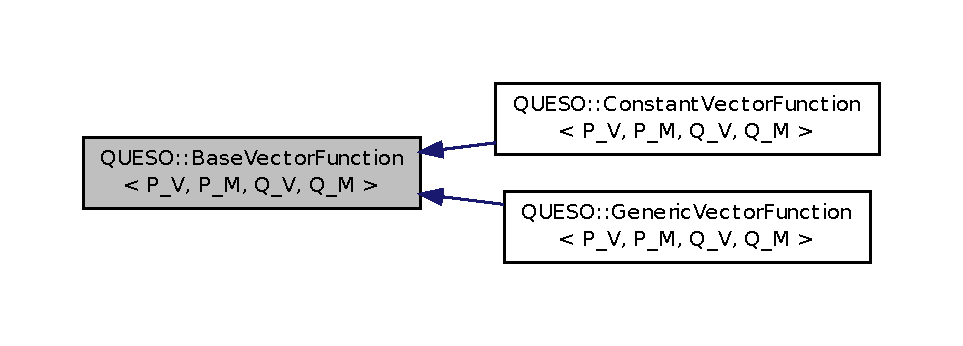
\includegraphics[width=350pt]{class_q_u_e_s_o_1_1_base_vector_function__inherit__graph}
\end{center}
\end{figure}


Collaboration diagram for Q\-U\-E\-S\-O\-:\-:Base\-Vector\-Function$<$ P\-\_\-\-V, P\-\_\-\-M, Q\-\_\-\-V, Q\-\_\-\-M $>$\-:
\nopagebreak
\begin{figure}[H]
\begin{center}
\leavevmode
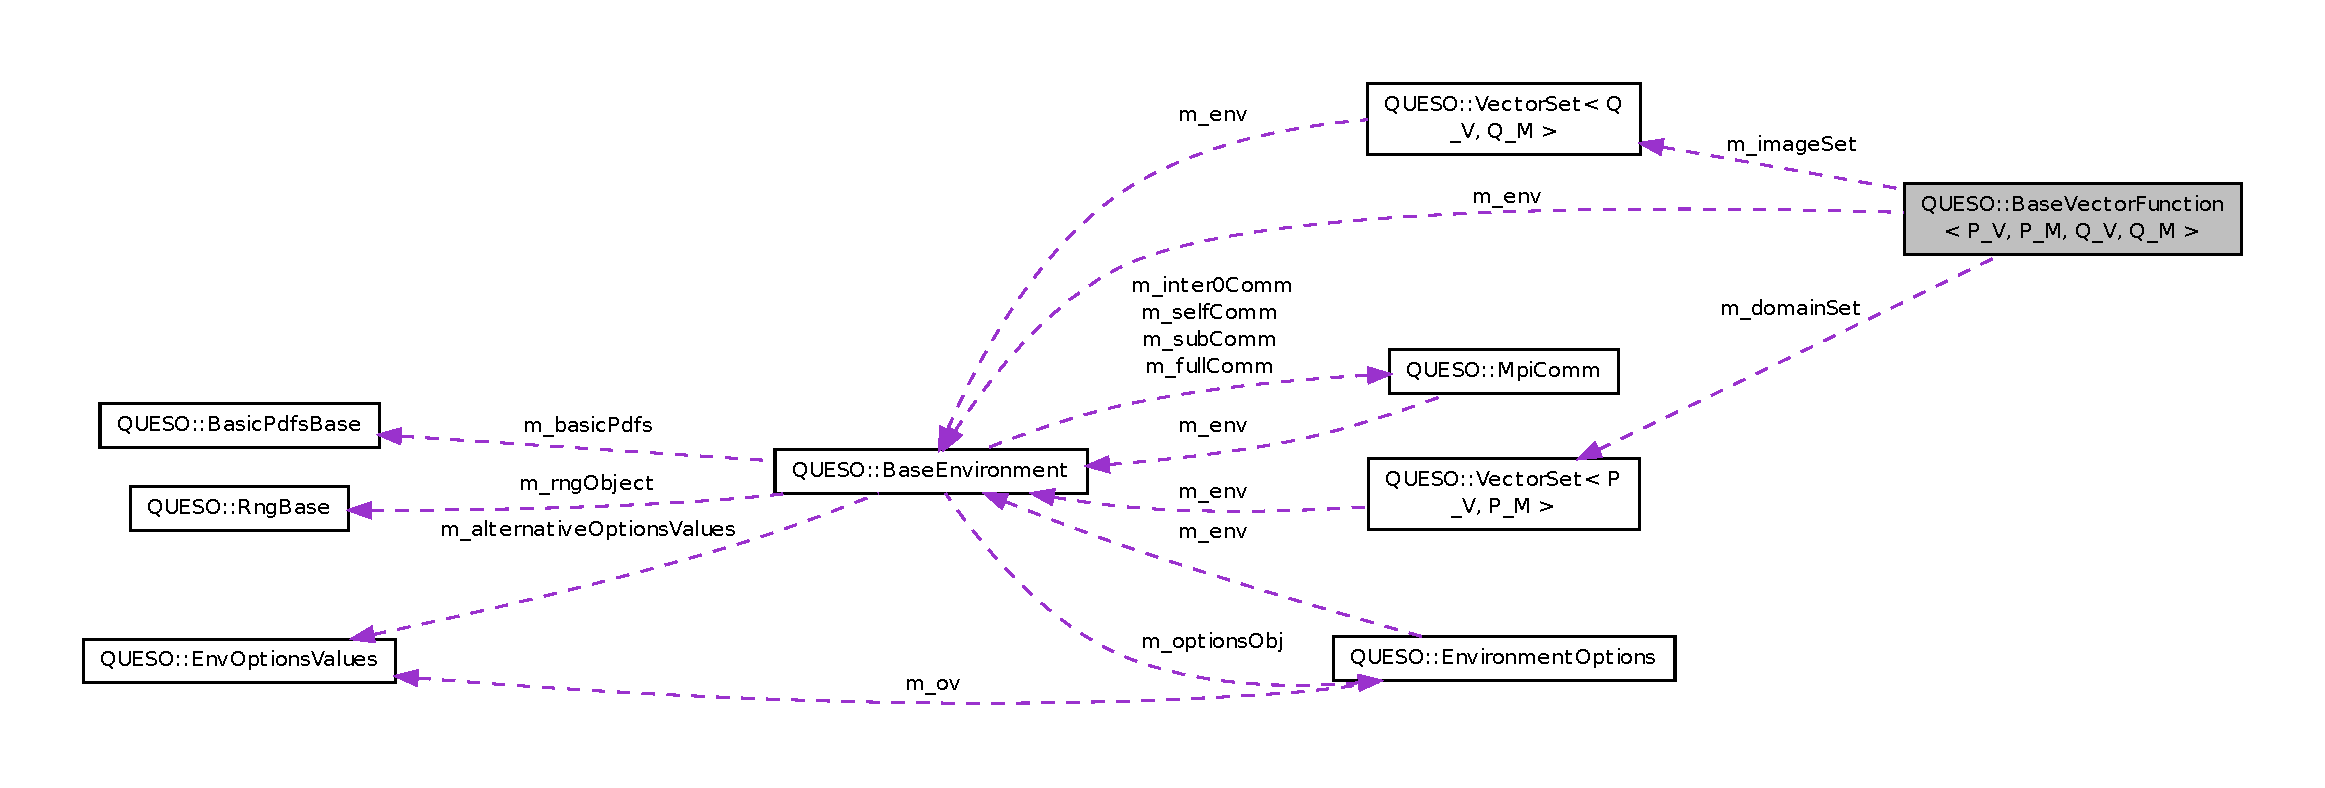
\includegraphics[width=350pt]{class_q_u_e_s_o_1_1_base_vector_function__coll__graph}
\end{center}
\end{figure}
\subsection*{Public Member Functions}
\begin{Indent}{\bf Constructor/\-Destructor methods.}\par
\begin{DoxyCompactItemize}
\item 
\hyperlink{class_q_u_e_s_o_1_1_base_vector_function_a6f819f1f9adcf13e9ed4a35542aeff20}{Base\-Vector\-Function} (const char $\ast$prefix, const \hyperlink{class_q_u_e_s_o_1_1_vector_set}{Vector\-Set}$<$ P\-\_\-\-V, P\-\_\-\-M $>$ \&\hyperlink{class_q_u_e_s_o_1_1_base_vector_function_af77b709d473f253e5c56aa620d5f3cb0}{domain\-Set}, const \hyperlink{class_q_u_e_s_o_1_1_vector_set}{Vector\-Set}$<$ Q\-\_\-\-V, Q\-\_\-\-M $>$ \&\hyperlink{class_q_u_e_s_o_1_1_base_vector_function_aa3a070a86f7099f53a669f1aab547619}{image\-Set})
\begin{DoxyCompactList}\small\item\em Default Constructor. \end{DoxyCompactList}\item 
virtual \hyperlink{class_q_u_e_s_o_1_1_base_vector_function_a25e2bf49649abce43b9390d7cfd04164}{$\sim$\-Base\-Vector\-Function} ()
\begin{DoxyCompactList}\small\item\em Destructor. \end{DoxyCompactList}\end{DoxyCompactItemize}
\end{Indent}
\begin{Indent}{\bf Mathematical methods.}\par
\begin{DoxyCompactItemize}
\item 
const \hyperlink{class_q_u_e_s_o_1_1_vector_set}{Vector\-Set}$<$ P\-\_\-\-V, P\-\_\-\-M $>$ \& \hyperlink{class_q_u_e_s_o_1_1_base_vector_function_af77b709d473f253e5c56aa620d5f3cb0}{domain\-Set} () const 
\begin{DoxyCompactList}\small\item\em Access to the protected attribute {\ttfamily m\-\_\-domain\-Set\-:} domain set of the vector function. It is an instance of the class \hyperlink{class_q_u_e_s_o_1_1_vector_set}{Vector\-Set}. \end{DoxyCompactList}\item 
const \hyperlink{class_q_u_e_s_o_1_1_vector_set}{Vector\-Set}$<$ Q\-\_\-\-V, Q\-\_\-\-M $>$ \& \hyperlink{class_q_u_e_s_o_1_1_base_vector_function_aa3a070a86f7099f53a669f1aab547619}{image\-Set} () const 
\begin{DoxyCompactList}\small\item\em Access to the protected attribute {\ttfamily m\-\_\-image\-Set\-:} image set of the vector function/ It is an instance of the class \hyperlink{class_q_u_e_s_o_1_1_vector_set}{Vector\-Set}. \end{DoxyCompactList}\item 
virtual void \hyperlink{class_q_u_e_s_o_1_1_base_vector_function_a7ecf6f9270dfd96812074c7ab4badd6e}{compute} (const P\-\_\-\-V \&domain\-Vector, const P\-\_\-\-V $\ast$domain\-Direction, Q\-\_\-\-V \&image\-Vector, \hyperlink{class_q_u_e_s_o_1_1_dist_array}{Dist\-Array}$<$ P\-\_\-\-V $\ast$ $>$ $\ast$grad\-Vectors, \hyperlink{class_q_u_e_s_o_1_1_dist_array}{Dist\-Array}$<$ P\-\_\-\-M $\ast$ $>$ $\ast$hessian\-Matrices, \hyperlink{class_q_u_e_s_o_1_1_dist_array}{Dist\-Array}$<$ P\-\_\-\-V $\ast$ $>$ $\ast$hessian\-Effects) const =0
\begin{DoxyCompactList}\small\item\em Computes the image vector. See template specialization. \end{DoxyCompactList}\end{DoxyCompactItemize}
\end{Indent}
\subsection*{Protected Attributes}
\begin{DoxyCompactItemize}
\item 
const \hyperlink{class_q_u_e_s_o_1_1_base_environment}{Base\-Environment} \& \hyperlink{class_q_u_e_s_o_1_1_base_vector_function_abb5487a1874515b698a3d5ee82490881}{m\-\_\-env}
\item 
std\-::string \hyperlink{class_q_u_e_s_o_1_1_base_vector_function_aacf92c70a9f6d0a951943aa708b7cfa6}{m\-\_\-prefix}
\item 
const \hyperlink{class_q_u_e_s_o_1_1_vector_set}{Vector\-Set}$<$ P\-\_\-\-V, P\-\_\-\-M $>$ \& \hyperlink{class_q_u_e_s_o_1_1_base_vector_function_a485d4d016534371775bb2b00b5a9f4d3}{m\-\_\-domain\-Set}
\begin{DoxyCompactList}\small\item\em Domain set of the vector function. \end{DoxyCompactList}\item 
const \hyperlink{class_q_u_e_s_o_1_1_vector_set}{Vector\-Set}$<$ Q\-\_\-\-V, Q\-\_\-\-M $>$ \& \hyperlink{class_q_u_e_s_o_1_1_base_vector_function_a442585224e86695e302757c0fad17913}{m\-\_\-image\-Set}
\begin{DoxyCompactList}\small\item\em Image set of the vector function. \end{DoxyCompactList}\end{DoxyCompactItemize}


\subsection{Detailed Description}
\subsubsection*{template$<$class P\-\_\-\-V, class P\-\_\-\-M, class Q\-\_\-\-V, class Q\-\_\-\-M$>$class Q\-U\-E\-S\-O\-::\-Base\-Vector\-Function$<$ P\-\_\-\-V, P\-\_\-\-M, Q\-\_\-\-V, Q\-\_\-\-M $>$}

A templated (base) class for handling vector functions. 

This class allows the mathematical definition of a vector function such as\-: $ \mathbf{q}: B \subset R^n \rightarrow R^m $. It requires the specification of the domain $ B $, which is a subset of the vector space (set) $ R^n $, (and have already been introduced by the class \hyperlink{class_q_u_e_s_o_1_1_vector_set}{Vector\-Set}) and of the image set $ R^m $. 

Definition at line 51 of file Vector\-Function.\-h.



\subsection{Constructor \& Destructor Documentation}
\hypertarget{class_q_u_e_s_o_1_1_base_vector_function_a6f819f1f9adcf13e9ed4a35542aeff20}{\index{Q\-U\-E\-S\-O\-::\-Base\-Vector\-Function@{Q\-U\-E\-S\-O\-::\-Base\-Vector\-Function}!Base\-Vector\-Function@{Base\-Vector\-Function}}
\index{Base\-Vector\-Function@{Base\-Vector\-Function}!QUESO::BaseVectorFunction@{Q\-U\-E\-S\-O\-::\-Base\-Vector\-Function}}
\subsubsection[{Base\-Vector\-Function}]{\setlength{\rightskip}{0pt plus 5cm}template$<$class P\-\_\-\-V , class P\-\_\-\-M , class Q\-\_\-\-V , class Q\-\_\-\-M $>$ {\bf Q\-U\-E\-S\-O\-::\-Base\-Vector\-Function}$<$ P\-\_\-\-V, P\-\_\-\-M, Q\-\_\-\-V, Q\-\_\-\-M $>$\-::{\bf Base\-Vector\-Function} (
\begin{DoxyParamCaption}
\item[{const char $\ast$}]{prefix, }
\item[{const {\bf Vector\-Set}$<$ P\-\_\-\-V, P\-\_\-\-M $>$ \&}]{domain\-Set, }
\item[{const {\bf Vector\-Set}$<$ Q\-\_\-\-V, Q\-\_\-\-M $>$ \&}]{image\-Set}
\end{DoxyParamCaption}
)}}\label{class_q_u_e_s_o_1_1_base_vector_function_a6f819f1f9adcf13e9ed4a35542aeff20}


Default Constructor. 

Instantiates an object of the class, i.\-e. a vector function, given a prefix, its domain and image. 

Definition at line 33 of file Vector\-Function.\-C.


\begin{DoxyCode}
37   :
38   \hyperlink{class_q_u_e_s_o_1_1_base_vector_function_abb5487a1874515b698a3d5ee82490881}{m\_env}      (domainSet.\hyperlink{class_q_u_e_s_o_1_1_vector_set_aa0ed80853d166754ba6ed83e63e737aa}{env}()),
39   \hyperlink{class_q_u_e_s_o_1_1_base_vector_function_aacf92c70a9f6d0a951943aa708b7cfa6}{m\_prefix}   ((std::string)(prefix)+\textcolor{stringliteral}{"func\_"}),
40   \hyperlink{class_q_u_e_s_o_1_1_base_vector_function_a485d4d016534371775bb2b00b5a9f4d3}{m\_domainSet}(domainSet),
41   \hyperlink{class_q_u_e_s_o_1_1_base_vector_function_a442585224e86695e302757c0fad17913}{m\_imageSet} (imageSet)
42 \{
43 \}
\end{DoxyCode}
\hypertarget{class_q_u_e_s_o_1_1_base_vector_function_a25e2bf49649abce43b9390d7cfd04164}{\index{Q\-U\-E\-S\-O\-::\-Base\-Vector\-Function@{Q\-U\-E\-S\-O\-::\-Base\-Vector\-Function}!$\sim$\-Base\-Vector\-Function@{$\sim$\-Base\-Vector\-Function}}
\index{$\sim$\-Base\-Vector\-Function@{$\sim$\-Base\-Vector\-Function}!QUESO::BaseVectorFunction@{Q\-U\-E\-S\-O\-::\-Base\-Vector\-Function}}
\subsubsection[{$\sim$\-Base\-Vector\-Function}]{\setlength{\rightskip}{0pt plus 5cm}template$<$class P\-\_\-\-V , class P\-\_\-\-M , class Q\-\_\-\-V , class Q\-\_\-\-M $>$ {\bf Q\-U\-E\-S\-O\-::\-Base\-Vector\-Function}$<$ P\-\_\-\-V, P\-\_\-\-M, Q\-\_\-\-V, Q\-\_\-\-M $>$\-::$\sim${\bf Base\-Vector\-Function} (
\begin{DoxyParamCaption}
{}
\end{DoxyParamCaption}
)\hspace{0.3cm}{\ttfamily [virtual]}}}\label{class_q_u_e_s_o_1_1_base_vector_function_a25e2bf49649abce43b9390d7cfd04164}


Destructor. 



Definition at line 47 of file Vector\-Function.\-C.


\begin{DoxyCode}
48 \{
49 \}
\end{DoxyCode}


\subsection{Member Function Documentation}
\hypertarget{class_q_u_e_s_o_1_1_base_vector_function_a7ecf6f9270dfd96812074c7ab4badd6e}{\index{Q\-U\-E\-S\-O\-::\-Base\-Vector\-Function@{Q\-U\-E\-S\-O\-::\-Base\-Vector\-Function}!compute@{compute}}
\index{compute@{compute}!QUESO::BaseVectorFunction@{Q\-U\-E\-S\-O\-::\-Base\-Vector\-Function}}
\subsubsection[{compute}]{\setlength{\rightskip}{0pt plus 5cm}template$<$class P\-\_\-\-V, class P\-\_\-\-M, class Q\-\_\-\-V, class Q\-\_\-\-M$>$ virtual void {\bf Q\-U\-E\-S\-O\-::\-Base\-Vector\-Function}$<$ P\-\_\-\-V, P\-\_\-\-M, Q\-\_\-\-V, Q\-\_\-\-M $>$\-::compute (
\begin{DoxyParamCaption}
\item[{const P\-\_\-\-V \&}]{domain\-Vector, }
\item[{const P\-\_\-\-V $\ast$}]{domain\-Direction, }
\item[{Q\-\_\-\-V \&}]{image\-Vector, }
\item[{{\bf Dist\-Array}$<$ P\-\_\-\-V $\ast$ $>$ $\ast$}]{grad\-Vectors, }
\item[{{\bf Dist\-Array}$<$ P\-\_\-\-M $\ast$ $>$ $\ast$}]{hessian\-Matrices, }
\item[{{\bf Dist\-Array}$<$ P\-\_\-\-V $\ast$ $>$ $\ast$}]{hessian\-Effects}
\end{DoxyParamCaption}
) const\hspace{0.3cm}{\ttfamily [pure virtual]}}}\label{class_q_u_e_s_o_1_1_base_vector_function_a7ecf6f9270dfd96812074c7ab4badd6e}


Computes the image vector. See template specialization. 



Implemented in \hyperlink{class_q_u_e_s_o_1_1_generic_vector_function_afcc099493262b90cdace65f24bb6b98d}{Q\-U\-E\-S\-O\-::\-Generic\-Vector\-Function$<$ P\-\_\-\-V, P\-\_\-\-M, Q\-\_\-\-V, Q\-\_\-\-M $>$}, and \hyperlink{class_q_u_e_s_o_1_1_constant_vector_function_a22d15ef82a6284e234364a9f5c176a89}{Q\-U\-E\-S\-O\-::\-Constant\-Vector\-Function$<$ P\-\_\-\-V, P\-\_\-\-M, Q\-\_\-\-V, Q\-\_\-\-M $>$}.

\hypertarget{class_q_u_e_s_o_1_1_base_vector_function_af77b709d473f253e5c56aa620d5f3cb0}{\index{Q\-U\-E\-S\-O\-::\-Base\-Vector\-Function@{Q\-U\-E\-S\-O\-::\-Base\-Vector\-Function}!domain\-Set@{domain\-Set}}
\index{domain\-Set@{domain\-Set}!QUESO::BaseVectorFunction@{Q\-U\-E\-S\-O\-::\-Base\-Vector\-Function}}
\subsubsection[{domain\-Set}]{\setlength{\rightskip}{0pt plus 5cm}template$<$class P\-\_\-\-V , class P\-\_\-\-M , class Q\-\_\-\-V , class Q\-\_\-\-M $>$ const {\bf Vector\-Set}$<$ P\-\_\-\-V, P\-\_\-\-M $>$ \& {\bf Q\-U\-E\-S\-O\-::\-Base\-Vector\-Function}$<$ P\-\_\-\-V, P\-\_\-\-M, Q\-\_\-\-V, Q\-\_\-\-M $>$\-::domain\-Set (
\begin{DoxyParamCaption}
{}
\end{DoxyParamCaption}
) const}}\label{class_q_u_e_s_o_1_1_base_vector_function_af77b709d473f253e5c56aa620d5f3cb0}


Access to the protected attribute {\ttfamily m\-\_\-domain\-Set\-:} domain set of the vector function. It is an instance of the class \hyperlink{class_q_u_e_s_o_1_1_vector_set}{Vector\-Set}. 

This is one example of the advantage of how \hyperlink{namespace_q_u_e_s_o}{Q\-U\-E\-S\-O} represents mathematical identities in a straightforward manner. 

Definition at line 54 of file Vector\-Function.\-C.


\begin{DoxyCode}
55 \{
56   \textcolor{keywordflow}{return} \hyperlink{class_q_u_e_s_o_1_1_base_vector_function_a485d4d016534371775bb2b00b5a9f4d3}{m\_domainSet};
57 \}
\end{DoxyCode}
\hypertarget{class_q_u_e_s_o_1_1_base_vector_function_aa3a070a86f7099f53a669f1aab547619}{\index{Q\-U\-E\-S\-O\-::\-Base\-Vector\-Function@{Q\-U\-E\-S\-O\-::\-Base\-Vector\-Function}!image\-Set@{image\-Set}}
\index{image\-Set@{image\-Set}!QUESO::BaseVectorFunction@{Q\-U\-E\-S\-O\-::\-Base\-Vector\-Function}}
\subsubsection[{image\-Set}]{\setlength{\rightskip}{0pt plus 5cm}template$<$class P\-\_\-\-V , class P\-\_\-\-M , class Q\-\_\-\-V , class Q\-\_\-\-M $>$ const {\bf Vector\-Set}$<$ Q\-\_\-\-V, Q\-\_\-\-M $>$ \& {\bf Q\-U\-E\-S\-O\-::\-Base\-Vector\-Function}$<$ P\-\_\-\-V, P\-\_\-\-M, Q\-\_\-\-V, Q\-\_\-\-M $>$\-::image\-Set (
\begin{DoxyParamCaption}
{}
\end{DoxyParamCaption}
) const}}\label{class_q_u_e_s_o_1_1_base_vector_function_aa3a070a86f7099f53a669f1aab547619}


Access to the protected attribute {\ttfamily m\-\_\-image\-Set\-:} image set of the vector function/ It is an instance of the class \hyperlink{class_q_u_e_s_o_1_1_vector_set}{Vector\-Set}. 



Definition at line 62 of file Vector\-Function.\-C.


\begin{DoxyCode}
63 \{
64   \textcolor{keywordflow}{return} \hyperlink{class_q_u_e_s_o_1_1_base_vector_function_a442585224e86695e302757c0fad17913}{m\_imageSet};
65 \}
\end{DoxyCode}


\subsection{Member Data Documentation}
\hypertarget{class_q_u_e_s_o_1_1_base_vector_function_a485d4d016534371775bb2b00b5a9f4d3}{\index{Q\-U\-E\-S\-O\-::\-Base\-Vector\-Function@{Q\-U\-E\-S\-O\-::\-Base\-Vector\-Function}!m\-\_\-domain\-Set@{m\-\_\-domain\-Set}}
\index{m\-\_\-domain\-Set@{m\-\_\-domain\-Set}!QUESO::BaseVectorFunction@{Q\-U\-E\-S\-O\-::\-Base\-Vector\-Function}}
\subsubsection[{m\-\_\-domain\-Set}]{\setlength{\rightskip}{0pt plus 5cm}template$<$class P\-\_\-\-V, class P\-\_\-\-M, class Q\-\_\-\-V, class Q\-\_\-\-M$>$ const {\bf Vector\-Set}$<$P\-\_\-\-V,P\-\_\-\-M$>$\& {\bf Q\-U\-E\-S\-O\-::\-Base\-Vector\-Function}$<$ P\-\_\-\-V, P\-\_\-\-M, Q\-\_\-\-V, Q\-\_\-\-M $>$\-::m\-\_\-domain\-Set\hspace{0.3cm}{\ttfamily [protected]}}}\label{class_q_u_e_s_o_1_1_base_vector_function_a485d4d016534371775bb2b00b5a9f4d3}


Domain set of the vector function. 



Definition at line 87 of file Vector\-Function.\-h.

\hypertarget{class_q_u_e_s_o_1_1_base_vector_function_abb5487a1874515b698a3d5ee82490881}{\index{Q\-U\-E\-S\-O\-::\-Base\-Vector\-Function@{Q\-U\-E\-S\-O\-::\-Base\-Vector\-Function}!m\-\_\-env@{m\-\_\-env}}
\index{m\-\_\-env@{m\-\_\-env}!QUESO::BaseVectorFunction@{Q\-U\-E\-S\-O\-::\-Base\-Vector\-Function}}
\subsubsection[{m\-\_\-env}]{\setlength{\rightskip}{0pt plus 5cm}template$<$class P\-\_\-\-V, class P\-\_\-\-M, class Q\-\_\-\-V, class Q\-\_\-\-M$>$ const {\bf Base\-Environment}\& {\bf Q\-U\-E\-S\-O\-::\-Base\-Vector\-Function}$<$ P\-\_\-\-V, P\-\_\-\-M, Q\-\_\-\-V, Q\-\_\-\-M $>$\-::m\-\_\-env\hspace{0.3cm}{\ttfamily [protected]}}}\label{class_q_u_e_s_o_1_1_base_vector_function_abb5487a1874515b698a3d5ee82490881}


Definition at line 83 of file Vector\-Function.\-h.

\hypertarget{class_q_u_e_s_o_1_1_base_vector_function_a442585224e86695e302757c0fad17913}{\index{Q\-U\-E\-S\-O\-::\-Base\-Vector\-Function@{Q\-U\-E\-S\-O\-::\-Base\-Vector\-Function}!m\-\_\-image\-Set@{m\-\_\-image\-Set}}
\index{m\-\_\-image\-Set@{m\-\_\-image\-Set}!QUESO::BaseVectorFunction@{Q\-U\-E\-S\-O\-::\-Base\-Vector\-Function}}
\subsubsection[{m\-\_\-image\-Set}]{\setlength{\rightskip}{0pt plus 5cm}template$<$class P\-\_\-\-V, class P\-\_\-\-M, class Q\-\_\-\-V, class Q\-\_\-\-M$>$ const {\bf Vector\-Set}$<$Q\-\_\-\-V,Q\-\_\-\-M$>$\& {\bf Q\-U\-E\-S\-O\-::\-Base\-Vector\-Function}$<$ P\-\_\-\-V, P\-\_\-\-M, Q\-\_\-\-V, Q\-\_\-\-M $>$\-::m\-\_\-image\-Set\hspace{0.3cm}{\ttfamily [protected]}}}\label{class_q_u_e_s_o_1_1_base_vector_function_a442585224e86695e302757c0fad17913}


Image set of the vector function. 



Definition at line 90 of file Vector\-Function.\-h.

\hypertarget{class_q_u_e_s_o_1_1_base_vector_function_aacf92c70a9f6d0a951943aa708b7cfa6}{\index{Q\-U\-E\-S\-O\-::\-Base\-Vector\-Function@{Q\-U\-E\-S\-O\-::\-Base\-Vector\-Function}!m\-\_\-prefix@{m\-\_\-prefix}}
\index{m\-\_\-prefix@{m\-\_\-prefix}!QUESO::BaseVectorFunction@{Q\-U\-E\-S\-O\-::\-Base\-Vector\-Function}}
\subsubsection[{m\-\_\-prefix}]{\setlength{\rightskip}{0pt plus 5cm}template$<$class P\-\_\-\-V, class P\-\_\-\-M, class Q\-\_\-\-V, class Q\-\_\-\-M$>$ std\-::string {\bf Q\-U\-E\-S\-O\-::\-Base\-Vector\-Function}$<$ P\-\_\-\-V, P\-\_\-\-M, Q\-\_\-\-V, Q\-\_\-\-M $>$\-::m\-\_\-prefix\hspace{0.3cm}{\ttfamily [protected]}}}\label{class_q_u_e_s_o_1_1_base_vector_function_aacf92c70a9f6d0a951943aa708b7cfa6}


Definition at line 84 of file Vector\-Function.\-h.



The documentation for this class was generated from the following files\-:\begin{DoxyCompactItemize}
\item 
src/basic/inc/\hyperlink{_vector_function_8h}{Vector\-Function.\-h}\item 
src/basic/src/\hyperlink{_vector_function_8_c}{Vector\-Function.\-C}\end{DoxyCompactItemize}

\hypertarget{class_q_u_e_s_o_1_1_base_vector_mdf}{\section{Q\-U\-E\-S\-O\-:\-:Base\-Vector\-Mdf$<$ V, M $>$ Class Template Reference}
\label{class_q_u_e_s_o_1_1_base_vector_mdf}\index{Q\-U\-E\-S\-O\-::\-Base\-Vector\-Mdf$<$ V, M $>$@{Q\-U\-E\-S\-O\-::\-Base\-Vector\-Mdf$<$ V, M $>$}}
}


A templated (base) class for handling M\-D\-Fs of vector functions.  




{\ttfamily \#include $<$Vector\-Mdf.\-h$>$}



Inheritance diagram for Q\-U\-E\-S\-O\-:\-:Base\-Vector\-Mdf$<$ V, M $>$\-:
\nopagebreak
\begin{figure}[H]
\begin{center}
\leavevmode
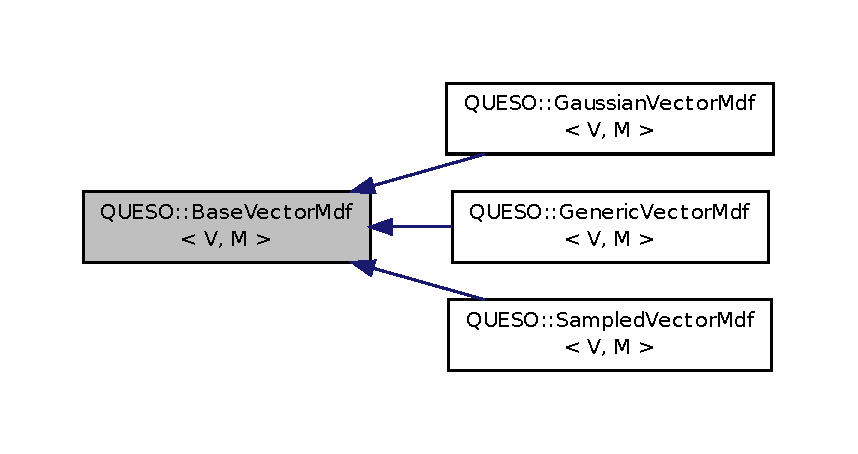
\includegraphics[width=350pt]{class_q_u_e_s_o_1_1_base_vector_mdf__inherit__graph}
\end{center}
\end{figure}


Collaboration diagram for Q\-U\-E\-S\-O\-:\-:Base\-Vector\-Mdf$<$ V, M $>$\-:
\nopagebreak
\begin{figure}[H]
\begin{center}
\leavevmode
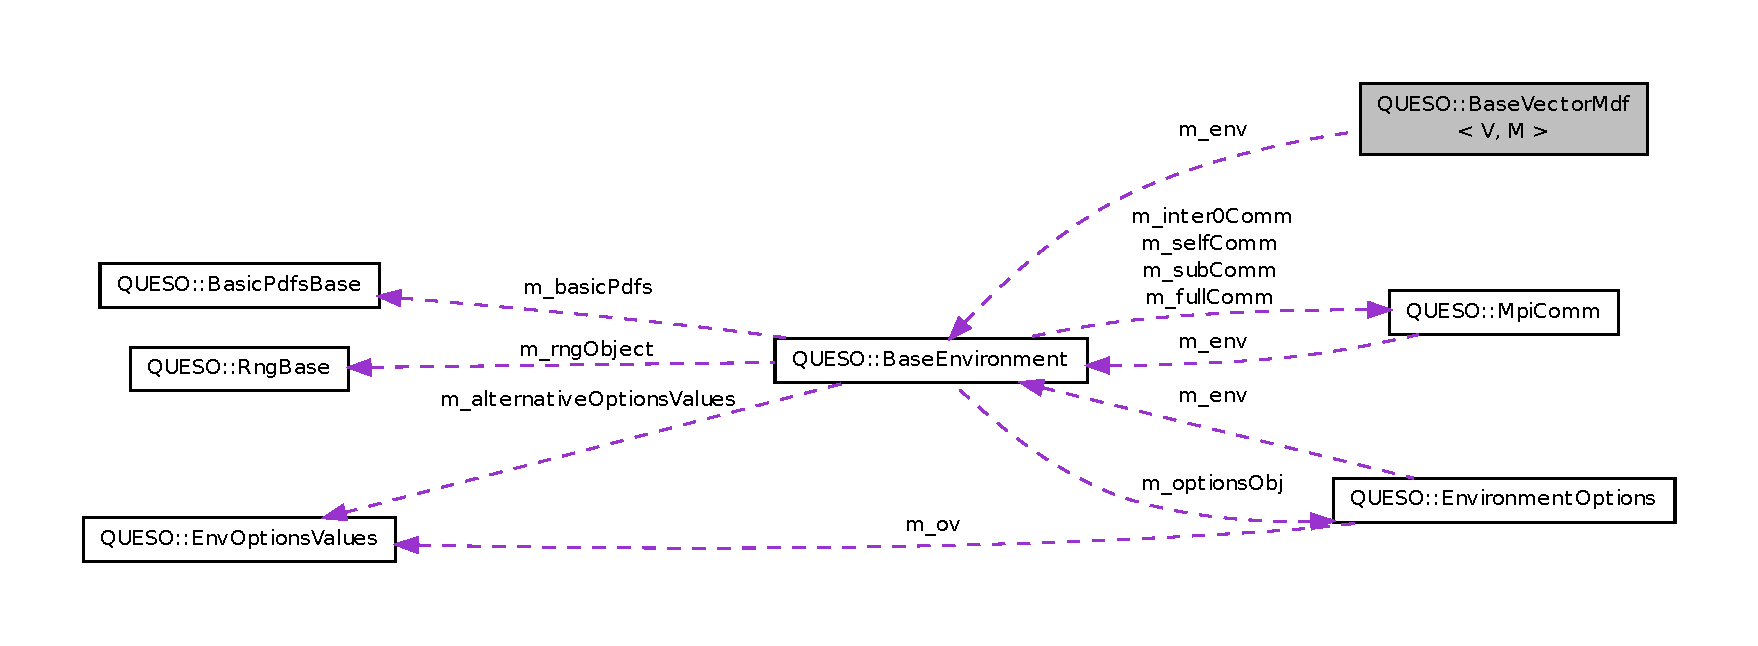
\includegraphics[width=350pt]{class_q_u_e_s_o_1_1_base_vector_mdf__coll__graph}
\end{center}
\end{figure}
\subsection*{Public Member Functions}
\begin{Indent}{\bf Constructor/\-Destructor methods}\par
\begin{DoxyCompactItemize}
\item 
\hyperlink{class_q_u_e_s_o_1_1_base_vector_mdf_a8f07d6a9201d20e195b8cabcaa35f8c5}{Base\-Vector\-Mdf} (const char $\ast$prefix, const \hyperlink{class_q_u_e_s_o_1_1_vector_set}{Vector\-Set}$<$ V, M $>$ \&\hyperlink{class_q_u_e_s_o_1_1_base_vector_mdf_ab060724f092b6623df50c0d0d725174c}{domain\-Set})
\begin{DoxyCompactList}\small\item\em Default constructor. \end{DoxyCompactList}\item 
virtual \hyperlink{class_q_u_e_s_o_1_1_base_vector_mdf_a91b8af0e2485cf6b16e0d9c6e6142899}{$\sim$\-Base\-Vector\-Mdf} ()
\begin{DoxyCompactList}\small\item\em Virtual destructor. \end{DoxyCompactList}\end{DoxyCompactItemize}
\end{Indent}
\begin{Indent}{\bf Mathematical methods}\par
\begin{DoxyCompactItemize}
\item 
const \hyperlink{class_q_u_e_s_o_1_1_vector_set}{Vector\-Set}$<$ V, M $>$ \& \hyperlink{class_q_u_e_s_o_1_1_base_vector_mdf_ab060724f092b6623df50c0d0d725174c}{domain\-Set} () const 
\begin{DoxyCompactList}\small\item\em Returns the domain set; access to protected attribute m\-\_\-domain\-Set. \end{DoxyCompactList}\item 
virtual void \hyperlink{class_q_u_e_s_o_1_1_base_vector_mdf_a8b7826a86f4034d8960ff92ebf79a32b}{values} (const V \&param\-Values, V \&mdf\-Vec) const =0
\begin{DoxyCompactList}\small\item\em Finds the value of the vector M\-D\-F at each element of {\ttfamily param\-Value}, and saves it in {\ttfamily mdf\-Vec}. See template specialization. \end{DoxyCompactList}\end{DoxyCompactItemize}
\end{Indent}
\begin{Indent}{\bf I/\-O methods}\par
\begin{DoxyCompactItemize}
\item 
virtual void \hyperlink{class_q_u_e_s_o_1_1_base_vector_mdf_a8c656209554341cb90f16f867ad9cb37}{print} (std\-::ostream \&os) const =0
\begin{DoxyCompactList}\small\item\em Prints the vector M\-D\-F. See template specialization. \end{DoxyCompactList}\end{DoxyCompactItemize}
\end{Indent}
\subsection*{Protected Attributes}
\begin{DoxyCompactItemize}
\item 
const \hyperlink{class_q_u_e_s_o_1_1_base_environment}{Base\-Environment} \& \hyperlink{class_q_u_e_s_o_1_1_base_vector_mdf_a39fbb4c9b12a0906a6d8c82535c837c7}{m\-\_\-env}
\item 
std\-::string \hyperlink{class_q_u_e_s_o_1_1_base_vector_mdf_ada097dfdcb97838d0bd71a25ed7a4193}{m\-\_\-prefix}
\item 
const \hyperlink{class_q_u_e_s_o_1_1_vector_set}{Vector\-Set}$<$ V, M $>$ \& \hyperlink{class_q_u_e_s_o_1_1_base_vector_mdf_a7f4804e5bb9d5947a4c7659605e8fa3b}{m\-\_\-domain\-Set}
\end{DoxyCompactItemize}


\subsection{Detailed Description}
\subsubsection*{template$<$class V, class M$>$class Q\-U\-E\-S\-O\-::\-Base\-Vector\-Mdf$<$ V, M $>$}

A templated (base) class for handling M\-D\-Fs of vector functions. 

To obtain the marginal distribution over a subset of multivariate (vector) R\-Vs, one only needs to drop the irrelevant variables (the variables that one wants to marginalize out). If {\bfseries X} is a Random \hyperlink{class_q_u_e_s_o_1_1_vector}{Vector} which contains the continuous random variables $ X_1, X_2, ..., X_n $. Then each $ X_i $ is a continuous random variable with its own Probability Distribution called the marginal distribution of $ X_i $. This class handles M\-D\-Fs of a vector R\-V. 

Definition at line 56 of file Vector\-Mdf.\-h.



\subsection{Constructor \& Destructor Documentation}
\hypertarget{class_q_u_e_s_o_1_1_base_vector_mdf_a8f07d6a9201d20e195b8cabcaa35f8c5}{\index{Q\-U\-E\-S\-O\-::\-Base\-Vector\-Mdf@{Q\-U\-E\-S\-O\-::\-Base\-Vector\-Mdf}!Base\-Vector\-Mdf@{Base\-Vector\-Mdf}}
\index{Base\-Vector\-Mdf@{Base\-Vector\-Mdf}!QUESO::BaseVectorMdf@{Q\-U\-E\-S\-O\-::\-Base\-Vector\-Mdf}}
\subsubsection[{Base\-Vector\-Mdf}]{\setlength{\rightskip}{0pt plus 5cm}template$<$class V, class M$>$ {\bf Q\-U\-E\-S\-O\-::\-Base\-Vector\-Mdf}$<$ V, M $>$\-::{\bf Base\-Vector\-Mdf} (
\begin{DoxyParamCaption}
\item[{const char $\ast$}]{prefix, }
\item[{const {\bf Vector\-Set}$<$ V, M $>$ \&}]{domain\-Set}
\end{DoxyParamCaption}
)}}\label{class_q_u_e_s_o_1_1_base_vector_mdf_a8f07d6a9201d20e195b8cabcaa35f8c5}


Default constructor. 

Instantiates an object of the class given a prefix and domain set of the M\-D\-F. 

Definition at line 31 of file Vector\-Mdf.\-C.



References Q\-U\-E\-S\-O\-::\-Base\-Environment\-::display\-Verbosity(), Q\-U\-E\-S\-O\-::\-Base\-Vector\-Mdf$<$ V, M $>$\-::m\-\_\-env, Q\-U\-E\-S\-O\-::\-Base\-Vector\-Mdf$<$ V, M $>$\-::m\-\_\-prefix, and Q\-U\-E\-S\-O\-::\-Base\-Environment\-::sub\-Display\-File().


\begin{DoxyCode}
34   :
35   \hyperlink{class_q_u_e_s_o_1_1_base_vector_mdf_a39fbb4c9b12a0906a6d8c82535c837c7}{m\_env}      (\hyperlink{class_q_u_e_s_o_1_1_base_vector_mdf_ab060724f092b6623df50c0d0d725174c}{domainSet}.env()),
36   \hyperlink{class_q_u_e_s_o_1_1_base_vector_mdf_ada097dfdcb97838d0bd71a25ed7a4193}{m\_prefix}   ((std::string)(prefix)+\textcolor{stringliteral}{"Mdf\_"}),
37   \hyperlink{class_q_u_e_s_o_1_1_base_vector_mdf_a7f4804e5bb9d5947a4c7659605e8fa3b}{m\_domainSet}(\hyperlink{class_q_u_e_s_o_1_1_base_vector_mdf_ab060724f092b6623df50c0d0d725174c}{domainSet})
38 \{
39   \textcolor{keywordflow}{if} ((\hyperlink{class_q_u_e_s_o_1_1_base_vector_mdf_a39fbb4c9b12a0906a6d8c82535c837c7}{m\_env}.\hyperlink{class_q_u_e_s_o_1_1_base_environment_a8a0064746ae8dddfece4229b9ad374d6}{subDisplayFile}()) && (\hyperlink{class_q_u_e_s_o_1_1_base_vector_mdf_a39fbb4c9b12a0906a6d8c82535c837c7}{m\_env}.
      \hyperlink{class_q_u_e_s_o_1_1_base_environment_a1fe5f244fc0316a0ab3e37463f108b96}{displayVerbosity}() >= 5)) \{
40     *\hyperlink{class_q_u_e_s_o_1_1_base_vector_mdf_a39fbb4c9b12a0906a6d8c82535c837c7}{m\_env}.\hyperlink{class_q_u_e_s_o_1_1_base_environment_a8a0064746ae8dddfece4229b9ad374d6}{subDisplayFile}() << \textcolor{stringliteral}{"Entering BaseVectorMdf<V,M>::constructor()"}
41                            << \textcolor{stringliteral}{": prefix = "} << \hyperlink{class_q_u_e_s_o_1_1_base_vector_mdf_ada097dfdcb97838d0bd71a25ed7a4193}{m\_prefix}
42                            << std::endl;
43   \}
44 
45   \textcolor{keywordflow}{if} ((\hyperlink{class_q_u_e_s_o_1_1_base_vector_mdf_a39fbb4c9b12a0906a6d8c82535c837c7}{m\_env}.\hyperlink{class_q_u_e_s_o_1_1_base_environment_a8a0064746ae8dddfece4229b9ad374d6}{subDisplayFile}()) && (\hyperlink{class_q_u_e_s_o_1_1_base_vector_mdf_a39fbb4c9b12a0906a6d8c82535c837c7}{m\_env}.
      \hyperlink{class_q_u_e_s_o_1_1_base_environment_a1fe5f244fc0316a0ab3e37463f108b96}{displayVerbosity}() >= 5)) \{
46     *\hyperlink{class_q_u_e_s_o_1_1_base_vector_mdf_a39fbb4c9b12a0906a6d8c82535c837c7}{m\_env}.\hyperlink{class_q_u_e_s_o_1_1_base_environment_a8a0064746ae8dddfece4229b9ad374d6}{subDisplayFile}() << \textcolor{stringliteral}{"Leaving BaseVectorMdf<V,M>::constructor()"}
47                            << \textcolor{stringliteral}{": prefix = "} << \hyperlink{class_q_u_e_s_o_1_1_base_vector_mdf_ada097dfdcb97838d0bd71a25ed7a4193}{m\_prefix}
48                            << std::endl;
49   \}
50 \}
\end{DoxyCode}
\hypertarget{class_q_u_e_s_o_1_1_base_vector_mdf_a91b8af0e2485cf6b16e0d9c6e6142899}{\index{Q\-U\-E\-S\-O\-::\-Base\-Vector\-Mdf@{Q\-U\-E\-S\-O\-::\-Base\-Vector\-Mdf}!$\sim$\-Base\-Vector\-Mdf@{$\sim$\-Base\-Vector\-Mdf}}
\index{$\sim$\-Base\-Vector\-Mdf@{$\sim$\-Base\-Vector\-Mdf}!QUESO::BaseVectorMdf@{Q\-U\-E\-S\-O\-::\-Base\-Vector\-Mdf}}
\subsubsection[{$\sim$\-Base\-Vector\-Mdf}]{\setlength{\rightskip}{0pt plus 5cm}template$<$class V , class M $>$ {\bf Q\-U\-E\-S\-O\-::\-Base\-Vector\-Mdf}$<$ V, M $>$\-::$\sim${\bf Base\-Vector\-Mdf} (
\begin{DoxyParamCaption}
{}
\end{DoxyParamCaption}
)\hspace{0.3cm}{\ttfamily [virtual]}}}\label{class_q_u_e_s_o_1_1_base_vector_mdf_a91b8af0e2485cf6b16e0d9c6e6142899}


Virtual destructor. 



Definition at line 53 of file Vector\-Mdf.\-C.


\begin{DoxyCode}
54 \{
55 \}
\end{DoxyCode}


\subsection{Member Function Documentation}
\hypertarget{class_q_u_e_s_o_1_1_base_vector_mdf_ab060724f092b6623df50c0d0d725174c}{\index{Q\-U\-E\-S\-O\-::\-Base\-Vector\-Mdf@{Q\-U\-E\-S\-O\-::\-Base\-Vector\-Mdf}!domain\-Set@{domain\-Set}}
\index{domain\-Set@{domain\-Set}!QUESO::BaseVectorMdf@{Q\-U\-E\-S\-O\-::\-Base\-Vector\-Mdf}}
\subsubsection[{domain\-Set}]{\setlength{\rightskip}{0pt plus 5cm}template$<$class V , class M $>$ const {\bf Vector\-Set}$<$ V, M $>$ \& {\bf Q\-U\-E\-S\-O\-::\-Base\-Vector\-Mdf}$<$ V, M $>$\-::domain\-Set (
\begin{DoxyParamCaption}
{}
\end{DoxyParamCaption}
) const}}\label{class_q_u_e_s_o_1_1_base_vector_mdf_ab060724f092b6623df50c0d0d725174c}


Returns the domain set; access to protected attribute m\-\_\-domain\-Set. 



Definition at line 59 of file Vector\-Mdf.\-C.


\begin{DoxyCode}
60 \{
61   \textcolor{keywordflow}{return} \hyperlink{class_q_u_e_s_o_1_1_base_vector_mdf_a7f4804e5bb9d5947a4c7659605e8fa3b}{m\_domainSet};
62 \}
\end{DoxyCode}
\hypertarget{class_q_u_e_s_o_1_1_base_vector_mdf_a8c656209554341cb90f16f867ad9cb37}{\index{Q\-U\-E\-S\-O\-::\-Base\-Vector\-Mdf@{Q\-U\-E\-S\-O\-::\-Base\-Vector\-Mdf}!print@{print}}
\index{print@{print}!QUESO::BaseVectorMdf@{Q\-U\-E\-S\-O\-::\-Base\-Vector\-Mdf}}
\subsubsection[{print}]{\setlength{\rightskip}{0pt plus 5cm}template$<$class V, class M$>$ virtual void {\bf Q\-U\-E\-S\-O\-::\-Base\-Vector\-Mdf}$<$ V, M $>$\-::print (
\begin{DoxyParamCaption}
\item[{std\-::ostream \&}]{os}
\end{DoxyParamCaption}
) const\hspace{0.3cm}{\ttfamily [pure virtual]}}}\label{class_q_u_e_s_o_1_1_base_vector_mdf_a8c656209554341cb90f16f867ad9cb37}


Prints the vector M\-D\-F. See template specialization. 



Implemented in \hyperlink{class_q_u_e_s_o_1_1_gaussian_vector_mdf_aae69a5b89169542b47de4b0dfa2e60e5}{Q\-U\-E\-S\-O\-::\-Gaussian\-Vector\-Mdf$<$ V, M $>$}, \hyperlink{class_q_u_e_s_o_1_1_sampled_vector_mdf_af4a617a8e579abb72bf9d91d7ddb17e0}{Q\-U\-E\-S\-O\-::\-Sampled\-Vector\-Mdf$<$ V, M $>$}, and \hyperlink{class_q_u_e_s_o_1_1_generic_vector_mdf_a69bc51a5e118670a573c5378ea1e634f}{Q\-U\-E\-S\-O\-::\-Generic\-Vector\-Mdf$<$ V, M $>$}.

\hypertarget{class_q_u_e_s_o_1_1_base_vector_mdf_a8b7826a86f4034d8960ff92ebf79a32b}{\index{Q\-U\-E\-S\-O\-::\-Base\-Vector\-Mdf@{Q\-U\-E\-S\-O\-::\-Base\-Vector\-Mdf}!values@{values}}
\index{values@{values}!QUESO::BaseVectorMdf@{Q\-U\-E\-S\-O\-::\-Base\-Vector\-Mdf}}
\subsubsection[{values}]{\setlength{\rightskip}{0pt plus 5cm}template$<$class V, class M$>$ virtual void {\bf Q\-U\-E\-S\-O\-::\-Base\-Vector\-Mdf}$<$ V, M $>$\-::values (
\begin{DoxyParamCaption}
\item[{const V \&}]{param\-Values, }
\item[{V \&}]{mdf\-Vec}
\end{DoxyParamCaption}
) const\hspace{0.3cm}{\ttfamily [pure virtual]}}}\label{class_q_u_e_s_o_1_1_base_vector_mdf_a8b7826a86f4034d8960ff92ebf79a32b}


Finds the value of the vector M\-D\-F at each element of {\ttfamily param\-Value}, and saves it in {\ttfamily mdf\-Vec}. See template specialization. 



Implemented in \hyperlink{class_q_u_e_s_o_1_1_gaussian_vector_mdf_a4b842d80858175ead566bd57aa334c0a}{Q\-U\-E\-S\-O\-::\-Gaussian\-Vector\-Mdf$<$ V, M $>$}, \hyperlink{class_q_u_e_s_o_1_1_sampled_vector_mdf_af4b8d3c492d7cfb94ac82da8df8779e9}{Q\-U\-E\-S\-O\-::\-Sampled\-Vector\-Mdf$<$ V, M $>$}, and \hyperlink{class_q_u_e_s_o_1_1_generic_vector_mdf_a0f414d8b4756eef7f28166752dc8d48d}{Q\-U\-E\-S\-O\-::\-Generic\-Vector\-Mdf$<$ V, M $>$}.



\subsection{Member Data Documentation}
\hypertarget{class_q_u_e_s_o_1_1_base_vector_mdf_a7f4804e5bb9d5947a4c7659605e8fa3b}{\index{Q\-U\-E\-S\-O\-::\-Base\-Vector\-Mdf@{Q\-U\-E\-S\-O\-::\-Base\-Vector\-Mdf}!m\-\_\-domain\-Set@{m\-\_\-domain\-Set}}
\index{m\-\_\-domain\-Set@{m\-\_\-domain\-Set}!QUESO::BaseVectorMdf@{Q\-U\-E\-S\-O\-::\-Base\-Vector\-Mdf}}
\subsubsection[{m\-\_\-domain\-Set}]{\setlength{\rightskip}{0pt plus 5cm}template$<$class V, class M$>$ const {\bf Vector\-Set}$<$V,M$>$\& {\bf Q\-U\-E\-S\-O\-::\-Base\-Vector\-Mdf}$<$ V, M $>$\-::m\-\_\-domain\-Set\hspace{0.3cm}{\ttfamily [protected]}}}\label{class_q_u_e_s_o_1_1_base_vector_mdf_a7f4804e5bb9d5947a4c7659605e8fa3b}


Definition at line 88 of file Vector\-Mdf.\-h.

\hypertarget{class_q_u_e_s_o_1_1_base_vector_mdf_a39fbb4c9b12a0906a6d8c82535c837c7}{\index{Q\-U\-E\-S\-O\-::\-Base\-Vector\-Mdf@{Q\-U\-E\-S\-O\-::\-Base\-Vector\-Mdf}!m\-\_\-env@{m\-\_\-env}}
\index{m\-\_\-env@{m\-\_\-env}!QUESO::BaseVectorMdf@{Q\-U\-E\-S\-O\-::\-Base\-Vector\-Mdf}}
\subsubsection[{m\-\_\-env}]{\setlength{\rightskip}{0pt plus 5cm}template$<$class V, class M$>$ const {\bf Base\-Environment}\& {\bf Q\-U\-E\-S\-O\-::\-Base\-Vector\-Mdf}$<$ V, M $>$\-::m\-\_\-env\hspace{0.3cm}{\ttfamily [protected]}}}\label{class_q_u_e_s_o_1_1_base_vector_mdf_a39fbb4c9b12a0906a6d8c82535c837c7}


Definition at line 86 of file Vector\-Mdf.\-h.



Referenced by Q\-U\-E\-S\-O\-::\-Base\-Vector\-Mdf$<$ V, M $>$\-::\-Base\-Vector\-Mdf(), Q\-U\-E\-S\-O\-::\-Gaussian\-Vector\-Mdf$<$ V, M $>$\-::\-Gaussian\-Vector\-Mdf(), and Q\-U\-E\-S\-O\-::\-Sampled\-Vector\-Mdf$<$ V, M $>$\-::\-Sampled\-Vector\-Mdf().

\hypertarget{class_q_u_e_s_o_1_1_base_vector_mdf_ada097dfdcb97838d0bd71a25ed7a4193}{\index{Q\-U\-E\-S\-O\-::\-Base\-Vector\-Mdf@{Q\-U\-E\-S\-O\-::\-Base\-Vector\-Mdf}!m\-\_\-prefix@{m\-\_\-prefix}}
\index{m\-\_\-prefix@{m\-\_\-prefix}!QUESO::BaseVectorMdf@{Q\-U\-E\-S\-O\-::\-Base\-Vector\-Mdf}}
\subsubsection[{m\-\_\-prefix}]{\setlength{\rightskip}{0pt plus 5cm}template$<$class V, class M$>$ std\-::string {\bf Q\-U\-E\-S\-O\-::\-Base\-Vector\-Mdf}$<$ V, M $>$\-::m\-\_\-prefix\hspace{0.3cm}{\ttfamily [protected]}}}\label{class_q_u_e_s_o_1_1_base_vector_mdf_ada097dfdcb97838d0bd71a25ed7a4193}


Definition at line 87 of file Vector\-Mdf.\-h.



Referenced by Q\-U\-E\-S\-O\-::\-Base\-Vector\-Mdf$<$ V, M $>$\-::\-Base\-Vector\-Mdf(), Q\-U\-E\-S\-O\-::\-Gaussian\-Vector\-Mdf$<$ V, M $>$\-::\-Gaussian\-Vector\-Mdf(), and Q\-U\-E\-S\-O\-::\-Sampled\-Vector\-Mdf$<$ V, M $>$\-::\-Sampled\-Vector\-Mdf().



The documentation for this class was generated from the following files\-:\begin{DoxyCompactItemize}
\item 
src/stats/inc/\hyperlink{_vector_mdf_8h}{Vector\-Mdf.\-h}\item 
src/stats/src/\hyperlink{_vector_mdf_8_c}{Vector\-Mdf.\-C}\end{DoxyCompactItemize}

\hypertarget{class_q_u_e_s_o_1_1_base_vector_realizer}{\section{Q\-U\-E\-S\-O\-:\-:Base\-Vector\-Realizer$<$ V, M $>$ Class Template Reference}
\label{class_q_u_e_s_o_1_1_base_vector_realizer}\index{Q\-U\-E\-S\-O\-::\-Base\-Vector\-Realizer$<$ V, M $>$@{Q\-U\-E\-S\-O\-::\-Base\-Vector\-Realizer$<$ V, M $>$}}
}


A templated (base) class for handling sampling from vector R\-Vs.  




{\ttfamily \#include $<$Vector\-Realizer.\-h$>$}



Inheritance diagram for Q\-U\-E\-S\-O\-:\-:Base\-Vector\-Realizer$<$ V, M $>$\-:
\nopagebreak
\begin{figure}[H]
\begin{center}
\leavevmode
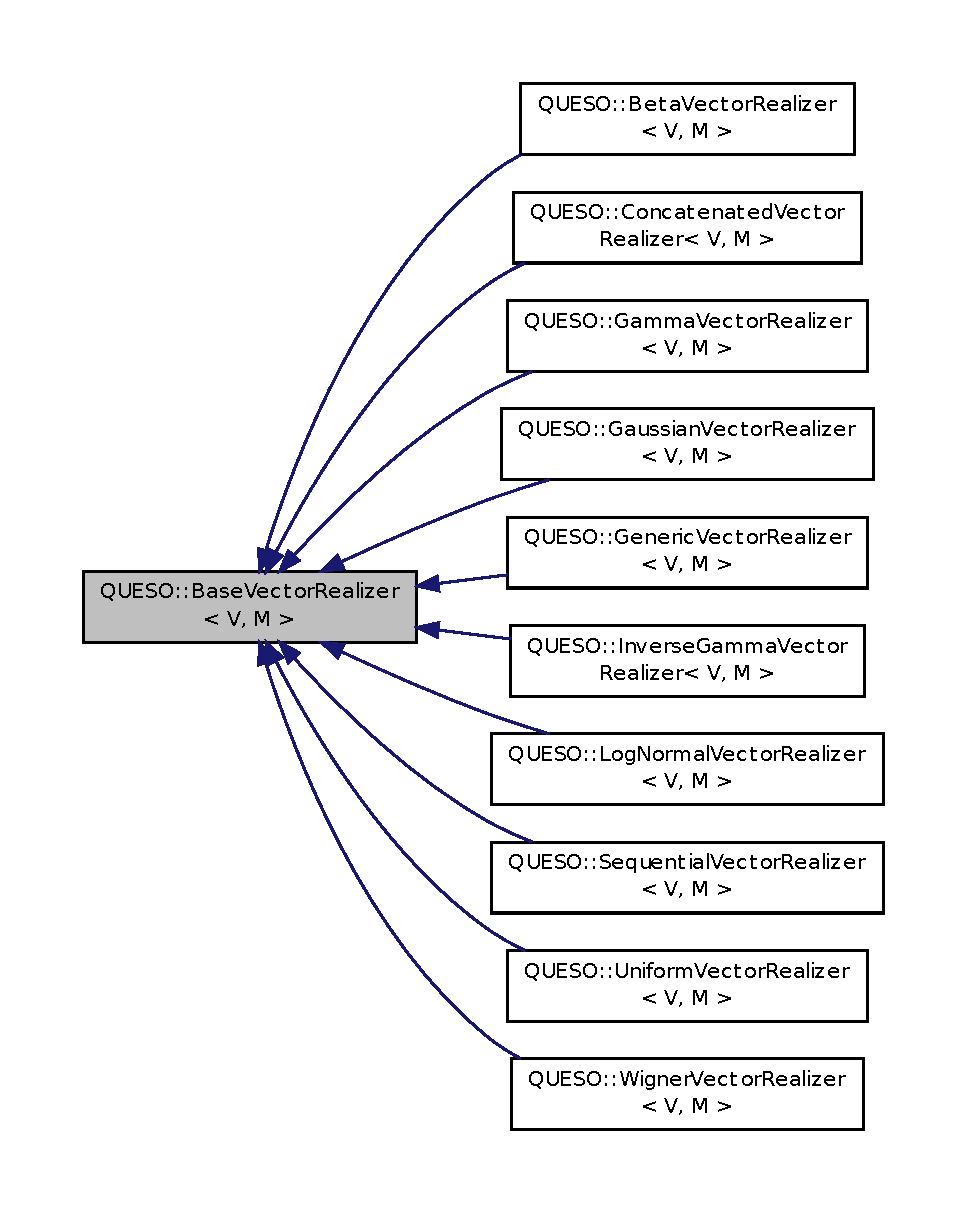
\includegraphics[width=350pt]{class_q_u_e_s_o_1_1_base_vector_realizer__inherit__graph}
\end{center}
\end{figure}


Collaboration diagram for Q\-U\-E\-S\-O\-:\-:Base\-Vector\-Realizer$<$ V, M $>$\-:
\nopagebreak
\begin{figure}[H]
\begin{center}
\leavevmode
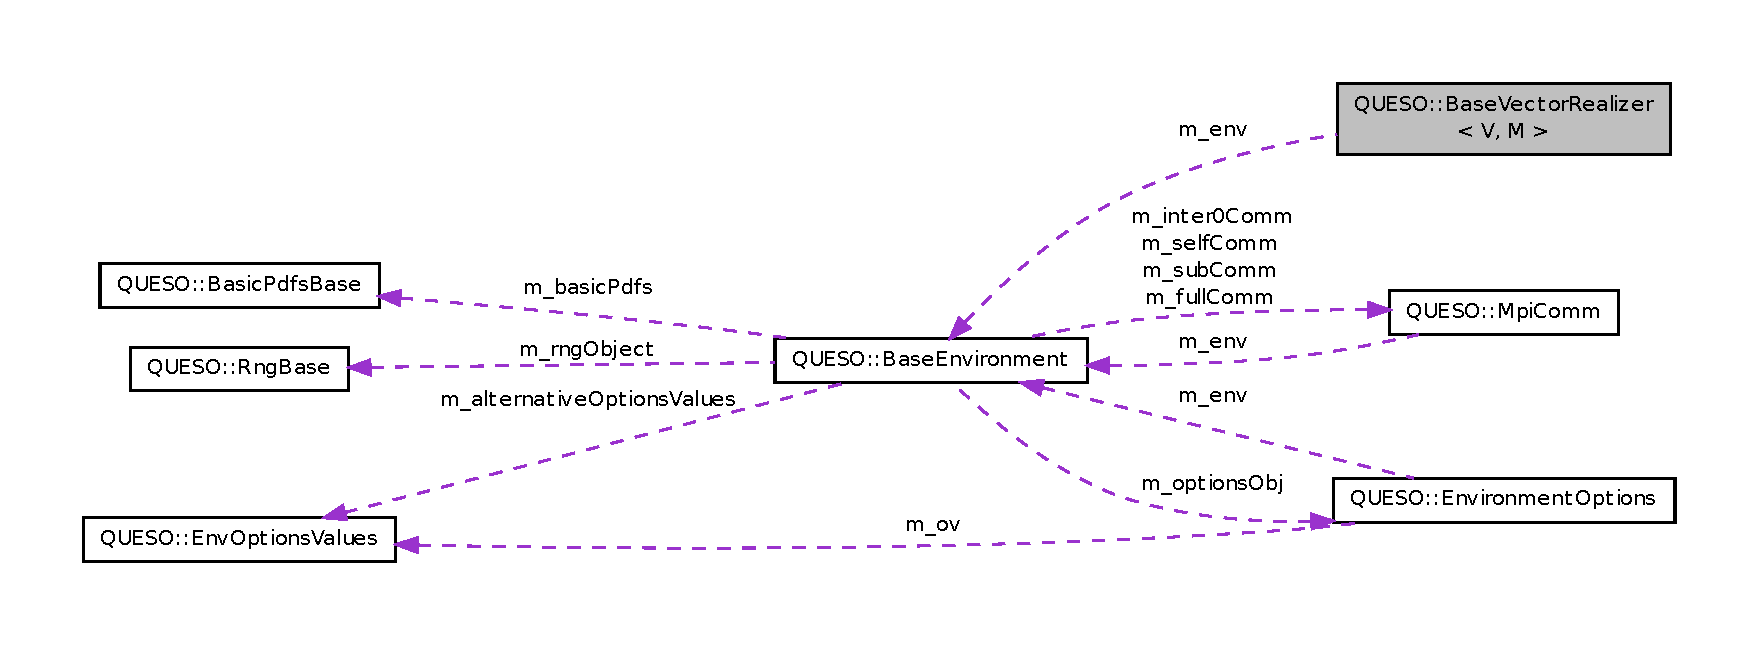
\includegraphics[width=350pt]{class_q_u_e_s_o_1_1_base_vector_realizer__coll__graph}
\end{center}
\end{figure}
\subsection*{Public Member Functions}
\begin{Indent}{\bf Constructor/\-Destructor methods}\par
\begin{DoxyCompactItemize}
\item 
\hyperlink{class_q_u_e_s_o_1_1_base_vector_realizer_ad77258f8737d87b5d0cd58b398939c70}{Base\-Vector\-Realizer} (const char $\ast$prefix, const \hyperlink{class_q_u_e_s_o_1_1_vector_set}{Vector\-Set}$<$ V, M $>$ \&\hyperlink{class_q_u_e_s_o_1_1_base_vector_realizer_ad958991bab8d6369e8a0d66b22a237d4}{unified\-Image\-Set}, unsigned int \hyperlink{class_q_u_e_s_o_1_1_base_vector_realizer_ad9fda59efacf5bd84c472c96dfa00613}{sub\-Period})
\begin{DoxyCompactList}\small\item\em Default constructor. \end{DoxyCompactList}\item 
virtual \hyperlink{class_q_u_e_s_o_1_1_base_vector_realizer_abc2eda9b3cea09c559c19e349c537b91}{$\sim$\-Base\-Vector\-Realizer} ()
\begin{DoxyCompactList}\small\item\em Virtual destructor. \end{DoxyCompactList}\end{DoxyCompactItemize}
\end{Indent}
\begin{Indent}{\bf Realization-\/related methods}\par
\begin{DoxyCompactItemize}
\item 
const \hyperlink{class_q_u_e_s_o_1_1_vector_set}{Vector\-Set}$<$ V, M $>$ \& \hyperlink{class_q_u_e_s_o_1_1_base_vector_realizer_ad958991bab8d6369e8a0d66b22a237d4}{unified\-Image\-Set} () const 
\begin{DoxyCompactList}\small\item\em Image set where the realizations lie. Access to protected attribute m\-\_\-unified\-Image\-Set. \end{DoxyCompactList}\item 
unsigned int \hyperlink{class_q_u_e_s_o_1_1_base_vector_realizer_ad9fda59efacf5bd84c472c96dfa00613}{sub\-Period} () const 
\begin{DoxyCompactList}\small\item\em Sub-\/period of the realization. Access to protected attribute m\-\_\-sub\-Period. \end{DoxyCompactList}\item 
virtual void \hyperlink{class_q_u_e_s_o_1_1_base_vector_realizer_a6845173dd79a80ae11c86cde26e55817}{realization} (V \&next\-Values) const =0
\begin{DoxyCompactList}\small\item\em Performs a realization (sample) from a probability density function. See template specialization. \end{DoxyCompactList}\end{DoxyCompactItemize}
\end{Indent}
\subsection*{Protected Attributes}
\begin{DoxyCompactItemize}
\item 
const \hyperlink{class_q_u_e_s_o_1_1_base_environment}{Base\-Environment} \& \hyperlink{class_q_u_e_s_o_1_1_base_vector_realizer_acde246c52f82d8ed687d91cfac14c29c}{m\-\_\-env}
\item 
std\-::string \hyperlink{class_q_u_e_s_o_1_1_base_vector_realizer_ac5559b6921816ccaed7afc2d342c2a32}{m\-\_\-prefix}
\item 
const \hyperlink{class_q_u_e_s_o_1_1_vector_set}{Vector\-Set}$<$ V, M $>$ \& \hyperlink{class_q_u_e_s_o_1_1_base_vector_realizer_a6c705235d28a3c12641da57cde948872}{m\-\_\-unified\-Image\-Set}
\item 
unsigned int \hyperlink{class_q_u_e_s_o_1_1_base_vector_realizer_aeddb6129f2810fef48b4e00daa5cea7b}{m\-\_\-sub\-Period}
\end{DoxyCompactItemize}


\subsection{Detailed Description}
\subsubsection*{template$<$class V, class M$>$class Q\-U\-E\-S\-O\-::\-Base\-Vector\-Realizer$<$ V, M $>$}

A templated (base) class for handling sampling from vector R\-Vs. 

A realizer is an object that, simply put, contains a \hyperlink{class_q_u_e_s_o_1_1_base_vector_realizer_a6845173dd79a80ae11c86cde26e55817}{realization()} operation that returns a sample of a vector R\-V. This is the base class. \hyperlink{namespace_q_u_e_s_o}{Q\-U\-E\-S\-O} also support uniform, Gaussian, Beta, Gamma, Inverse Gamma and Log\-Normal realizers, as described and implemented in the derived classes. 

Definition at line 53 of file Vector\-Realizer.\-h.



\subsection{Constructor \& Destructor Documentation}
\hypertarget{class_q_u_e_s_o_1_1_base_vector_realizer_ad77258f8737d87b5d0cd58b398939c70}{\index{Q\-U\-E\-S\-O\-::\-Base\-Vector\-Realizer@{Q\-U\-E\-S\-O\-::\-Base\-Vector\-Realizer}!Base\-Vector\-Realizer@{Base\-Vector\-Realizer}}
\index{Base\-Vector\-Realizer@{Base\-Vector\-Realizer}!QUESO::BaseVectorRealizer@{Q\-U\-E\-S\-O\-::\-Base\-Vector\-Realizer}}
\subsubsection[{Base\-Vector\-Realizer}]{\setlength{\rightskip}{0pt plus 5cm}template$<$class V, class M$>$ {\bf Q\-U\-E\-S\-O\-::\-Base\-Vector\-Realizer}$<$ V, M $>$\-::{\bf Base\-Vector\-Realizer} (
\begin{DoxyParamCaption}
\item[{const char $\ast$}]{prefix, }
\item[{const {\bf Vector\-Set}$<$ V, M $>$ \&}]{unified\-Image\-Set, }
\item[{unsigned int}]{sub\-Period}
\end{DoxyParamCaption}
)}}\label{class_q_u_e_s_o_1_1_base_vector_realizer_ad77258f8737d87b5d0cd58b398939c70}


Default constructor. 

Constructs a new object, given a prefix and the image set of the vector realizer. 

Definition at line 33 of file Vector\-Realizer.\-C.



References Q\-U\-E\-S\-O\-::\-Base\-Environment\-::display\-Verbosity(), Q\-U\-E\-S\-O\-::\-Base\-Vector\-Realizer$<$ V, M $>$\-::m\-\_\-env, Q\-U\-E\-S\-O\-::\-Base\-Vector\-Realizer$<$ V, M $>$\-::m\-\_\-prefix, and Q\-U\-E\-S\-O\-::\-Base\-Environment\-::sub\-Display\-File().


\begin{DoxyCode}
37   :
38   \hyperlink{class_q_u_e_s_o_1_1_base_vector_realizer_acde246c52f82d8ed687d91cfac14c29c}{m\_env}            (\hyperlink{class_q_u_e_s_o_1_1_base_vector_realizer_ad958991bab8d6369e8a0d66b22a237d4}{unifiedImageSet}.env()),
39   \hyperlink{class_q_u_e_s_o_1_1_base_vector_realizer_ac5559b6921816ccaed7afc2d342c2a32}{m\_prefix}         ((std::string)(prefix)+\textcolor{stringliteral}{"re\_"}),
40   \hyperlink{class_q_u_e_s_o_1_1_base_vector_realizer_a6c705235d28a3c12641da57cde948872}{m\_unifiedImageSet}(\hyperlink{class_q_u_e_s_o_1_1_base_vector_realizer_ad958991bab8d6369e8a0d66b22a237d4}{unifiedImageSet}),
41   \hyperlink{class_q_u_e_s_o_1_1_base_vector_realizer_aeddb6129f2810fef48b4e00daa5cea7b}{m\_subPeriod}      (\hyperlink{class_q_u_e_s_o_1_1_base_vector_realizer_ad9fda59efacf5bd84c472c96dfa00613}{subPeriod})
42 \{
43   \textcolor{keywordflow}{if} ((\hyperlink{class_q_u_e_s_o_1_1_base_vector_realizer_acde246c52f82d8ed687d91cfac14c29c}{m\_env}.\hyperlink{class_q_u_e_s_o_1_1_base_environment_a8a0064746ae8dddfece4229b9ad374d6}{subDisplayFile}()) && (\hyperlink{class_q_u_e_s_o_1_1_base_vector_realizer_acde246c52f82d8ed687d91cfac14c29c}{m\_env}.
      \hyperlink{class_q_u_e_s_o_1_1_base_environment_a1fe5f244fc0316a0ab3e37463f108b96}{displayVerbosity}() >= 5)) \{
44     *\hyperlink{class_q_u_e_s_o_1_1_base_vector_realizer_acde246c52f82d8ed687d91cfac14c29c}{m\_env}.\hyperlink{class_q_u_e_s_o_1_1_base_environment_a8a0064746ae8dddfece4229b9ad374d6}{subDisplayFile}() << \textcolor{stringliteral}{"Entering BaseVectorRealizer<V,M>::constructor() [4]"}
45                             << \textcolor{stringliteral}{": prefix = "} << \hyperlink{class_q_u_e_s_o_1_1_base_vector_realizer_ac5559b6921816ccaed7afc2d342c2a32}{m\_prefix}
46                             << std::endl;
47   \}
48 
49   \textcolor{keywordflow}{if} ((\hyperlink{class_q_u_e_s_o_1_1_base_vector_realizer_acde246c52f82d8ed687d91cfac14c29c}{m\_env}.\hyperlink{class_q_u_e_s_o_1_1_base_environment_a8a0064746ae8dddfece4229b9ad374d6}{subDisplayFile}()) && (\hyperlink{class_q_u_e_s_o_1_1_base_vector_realizer_acde246c52f82d8ed687d91cfac14c29c}{m\_env}.
      \hyperlink{class_q_u_e_s_o_1_1_base_environment_a1fe5f244fc0316a0ab3e37463f108b96}{displayVerbosity}() >= 5)) \{
50     *\hyperlink{class_q_u_e_s_o_1_1_base_vector_realizer_acde246c52f82d8ed687d91cfac14c29c}{m\_env}.\hyperlink{class_q_u_e_s_o_1_1_base_environment_a8a0064746ae8dddfece4229b9ad374d6}{subDisplayFile}() << \textcolor{stringliteral}{"Leaving BaseVectorRealizer<V,M>::constructor() [4]"}
51                             << \textcolor{stringliteral}{": prefix = "} << \hyperlink{class_q_u_e_s_o_1_1_base_vector_realizer_ac5559b6921816ccaed7afc2d342c2a32}{m\_prefix}
52                             << std::endl;
53   \}
54 \}
\end{DoxyCode}
\hypertarget{class_q_u_e_s_o_1_1_base_vector_realizer_abc2eda9b3cea09c559c19e349c537b91}{\index{Q\-U\-E\-S\-O\-::\-Base\-Vector\-Realizer@{Q\-U\-E\-S\-O\-::\-Base\-Vector\-Realizer}!$\sim$\-Base\-Vector\-Realizer@{$\sim$\-Base\-Vector\-Realizer}}
\index{$\sim$\-Base\-Vector\-Realizer@{$\sim$\-Base\-Vector\-Realizer}!QUESO::BaseVectorRealizer@{Q\-U\-E\-S\-O\-::\-Base\-Vector\-Realizer}}
\subsubsection[{$\sim$\-Base\-Vector\-Realizer}]{\setlength{\rightskip}{0pt plus 5cm}template$<$class V , class M $>$ {\bf Q\-U\-E\-S\-O\-::\-Base\-Vector\-Realizer}$<$ V, M $>$\-::$\sim${\bf Base\-Vector\-Realizer} (
\begin{DoxyParamCaption}
{}
\end{DoxyParamCaption}
)\hspace{0.3cm}{\ttfamily [virtual]}}}\label{class_q_u_e_s_o_1_1_base_vector_realizer_abc2eda9b3cea09c559c19e349c537b91}


Virtual destructor. 



Definition at line 57 of file Vector\-Realizer.\-C.


\begin{DoxyCode}
58 \{
59 \}
\end{DoxyCode}


\subsection{Member Function Documentation}
\hypertarget{class_q_u_e_s_o_1_1_base_vector_realizer_a6845173dd79a80ae11c86cde26e55817}{\index{Q\-U\-E\-S\-O\-::\-Base\-Vector\-Realizer@{Q\-U\-E\-S\-O\-::\-Base\-Vector\-Realizer}!realization@{realization}}
\index{realization@{realization}!QUESO::BaseVectorRealizer@{Q\-U\-E\-S\-O\-::\-Base\-Vector\-Realizer}}
\subsubsection[{realization}]{\setlength{\rightskip}{0pt plus 5cm}template$<$class V, class M$>$ virtual void {\bf Q\-U\-E\-S\-O\-::\-Base\-Vector\-Realizer}$<$ V, M $>$\-::realization (
\begin{DoxyParamCaption}
\item[{V \&}]{next\-Values}
\end{DoxyParamCaption}
) const\hspace{0.3cm}{\ttfamily [pure virtual]}}}\label{class_q_u_e_s_o_1_1_base_vector_realizer_a6845173dd79a80ae11c86cde26e55817}


Performs a realization (sample) from a probability density function. See template specialization. 



Implemented in \hyperlink{class_q_u_e_s_o_1_1_gaussian_vector_realizer_ad001b06fe7dab455507df0eb19494518}{Q\-U\-E\-S\-O\-::\-Gaussian\-Vector\-Realizer$<$ V, M $>$}, \hyperlink{class_q_u_e_s_o_1_1_log_normal_vector_realizer_a27d5cb6728ed1c78ba2ce6f1d1e5144a}{Q\-U\-E\-S\-O\-::\-Log\-Normal\-Vector\-Realizer$<$ V, M $>$}, \hyperlink{class_q_u_e_s_o_1_1_concatenated_vector_realizer_afa41c8065e84a5bbfd74a67436ecd889}{Q\-U\-E\-S\-O\-::\-Concatenated\-Vector\-Realizer$<$ V, M $>$}, \hyperlink{class_q_u_e_s_o_1_1_beta_vector_realizer_a75659aac16145ad3e770e852500ee7f2}{Q\-U\-E\-S\-O\-::\-Beta\-Vector\-Realizer$<$ V, M $>$}, \hyperlink{class_q_u_e_s_o_1_1_gamma_vector_realizer_ac2c9be536e210dd61614f96372df8c62}{Q\-U\-E\-S\-O\-::\-Gamma\-Vector\-Realizer$<$ V, M $>$}, \hyperlink{class_q_u_e_s_o_1_1_generic_vector_realizer_aeb79c966ab4e20b22f75acc6b7068925}{Q\-U\-E\-S\-O\-::\-Generic\-Vector\-Realizer$<$ V, M $>$}, \hyperlink{class_q_u_e_s_o_1_1_wigner_vector_realizer_a0d72232eb5843e78fc3d02a510ceb966}{Q\-U\-E\-S\-O\-::\-Wigner\-Vector\-Realizer$<$ V, M $>$}, \hyperlink{class_q_u_e_s_o_1_1_inverse_gamma_vector_realizer_a115670530398d012040f7183290251d3}{Q\-U\-E\-S\-O\-::\-Inverse\-Gamma\-Vector\-Realizer$<$ V, M $>$}, \hyperlink{class_q_u_e_s_o_1_1_sequential_vector_realizer_a67050d12ad38147f9f0743a0e53011b2}{Q\-U\-E\-S\-O\-::\-Sequential\-Vector\-Realizer$<$ V, M $>$}, and \hyperlink{class_q_u_e_s_o_1_1_uniform_vector_realizer_a59c9c5c848823a4c6b0992adc4f772e2}{Q\-U\-E\-S\-O\-::\-Uniform\-Vector\-Realizer$<$ V, M $>$}.



Referenced by Q\-U\-E\-S\-O\-::\-Monte\-Carlo\-S\-G$<$ P\-\_\-\-V, P\-\_\-\-M, Q\-\_\-\-V, Q\-\_\-\-M $>$\-::actual\-Generate\-Sequence(), Q\-U\-E\-S\-O\-::\-Monte\-Carlo\-S\-G$<$ P\-\_\-\-V, P\-\_\-\-M, Q\-\_\-\-V, Q\-\_\-\-M $>$\-::actual\-Read\-Sequence(), and Q\-U\-E\-S\-O\-::\-Compute\-Cov\-Corr\-Matrices\-Between\-Vector\-Rvs().

\hypertarget{class_q_u_e_s_o_1_1_base_vector_realizer_ad9fda59efacf5bd84c472c96dfa00613}{\index{Q\-U\-E\-S\-O\-::\-Base\-Vector\-Realizer@{Q\-U\-E\-S\-O\-::\-Base\-Vector\-Realizer}!sub\-Period@{sub\-Period}}
\index{sub\-Period@{sub\-Period}!QUESO::BaseVectorRealizer@{Q\-U\-E\-S\-O\-::\-Base\-Vector\-Realizer}}
\subsubsection[{sub\-Period}]{\setlength{\rightskip}{0pt plus 5cm}template$<$class V , class M $>$ unsigned int {\bf Q\-U\-E\-S\-O\-::\-Base\-Vector\-Realizer}$<$ V, M $>$\-::sub\-Period (
\begin{DoxyParamCaption}
{}
\end{DoxyParamCaption}
) const}}\label{class_q_u_e_s_o_1_1_base_vector_realizer_ad9fda59efacf5bd84c472c96dfa00613}


Sub-\/period of the realization. Access to protected attribute m\-\_\-sub\-Period. 



Definition at line 63 of file Vector\-Realizer.\-C.



Referenced by Q\-U\-E\-S\-O\-::\-Monte\-Carlo\-S\-G$<$ P\-\_\-\-V, P\-\_\-\-M, Q\-\_\-\-V, Q\-\_\-\-M $>$\-::intern\-Generate\-Sequence().


\begin{DoxyCode}
64 \{
65   \textcolor{keywordflow}{return} \hyperlink{class_q_u_e_s_o_1_1_base_vector_realizer_aeddb6129f2810fef48b4e00daa5cea7b}{m\_subPeriod};
66 \}
\end{DoxyCode}
\hypertarget{class_q_u_e_s_o_1_1_base_vector_realizer_ad958991bab8d6369e8a0d66b22a237d4}{\index{Q\-U\-E\-S\-O\-::\-Base\-Vector\-Realizer@{Q\-U\-E\-S\-O\-::\-Base\-Vector\-Realizer}!unified\-Image\-Set@{unified\-Image\-Set}}
\index{unified\-Image\-Set@{unified\-Image\-Set}!QUESO::BaseVectorRealizer@{Q\-U\-E\-S\-O\-::\-Base\-Vector\-Realizer}}
\subsubsection[{unified\-Image\-Set}]{\setlength{\rightskip}{0pt plus 5cm}template$<$class V , class M $>$ const {\bf Vector\-Set}$<$ V, M $>$ \& {\bf Q\-U\-E\-S\-O\-::\-Base\-Vector\-Realizer}$<$ V, M $>$\-::unified\-Image\-Set (
\begin{DoxyParamCaption}
{}
\end{DoxyParamCaption}
) const}}\label{class_q_u_e_s_o_1_1_base_vector_realizer_ad958991bab8d6369e8a0d66b22a237d4}


Image set where the realizations lie. Access to protected attribute m\-\_\-unified\-Image\-Set. 



Definition at line 70 of file Vector\-Realizer.\-C.


\begin{DoxyCode}
71 \{
72   \textcolor{keywordflow}{return} \hyperlink{class_q_u_e_s_o_1_1_base_vector_realizer_a6c705235d28a3c12641da57cde948872}{m\_unifiedImageSet};
73 \}
\end{DoxyCode}


\subsection{Member Data Documentation}
\hypertarget{class_q_u_e_s_o_1_1_base_vector_realizer_acde246c52f82d8ed687d91cfac14c29c}{\index{Q\-U\-E\-S\-O\-::\-Base\-Vector\-Realizer@{Q\-U\-E\-S\-O\-::\-Base\-Vector\-Realizer}!m\-\_\-env@{m\-\_\-env}}
\index{m\-\_\-env@{m\-\_\-env}!QUESO::BaseVectorRealizer@{Q\-U\-E\-S\-O\-::\-Base\-Vector\-Realizer}}
\subsubsection[{m\-\_\-env}]{\setlength{\rightskip}{0pt plus 5cm}template$<$class V, class M$>$ const {\bf Base\-Environment}\& {\bf Q\-U\-E\-S\-O\-::\-Base\-Vector\-Realizer}$<$ V, M $>$\-::m\-\_\-env\hspace{0.3cm}{\ttfamily [protected]}}}\label{class_q_u_e_s_o_1_1_base_vector_realizer_acde246c52f82d8ed687d91cfac14c29c}


Definition at line 81 of file Vector\-Realizer.\-h.



Referenced by Q\-U\-E\-S\-O\-::\-Base\-Vector\-Realizer$<$ V, M $>$\-::\-Base\-Vector\-Realizer(), Q\-U\-E\-S\-O\-::\-Beta\-Vector\-Realizer$<$ V, M $>$\-::\-Beta\-Vector\-Realizer(), Q\-U\-E\-S\-O\-::\-Concatenated\-Vector\-Realizer$<$ V, M $>$\-::\-Concatenated\-Vector\-Realizer(), Q\-U\-E\-S\-O\-::\-Gamma\-Vector\-Realizer$<$ V, M $>$\-::\-Gamma\-Vector\-Realizer(), Q\-U\-E\-S\-O\-::\-Gaussian\-Vector\-Realizer$<$ V, M $>$\-::\-Gaussian\-Vector\-Realizer(), Q\-U\-E\-S\-O\-::\-Generic\-Vector\-Realizer$<$ V, M $>$\-::\-Generic\-Vector\-Realizer(), Q\-U\-E\-S\-O\-::\-Inverse\-Gamma\-Vector\-Realizer$<$ V, M $>$\-::\-Inverse\-Gamma\-Vector\-Realizer(), Q\-U\-E\-S\-O\-::\-Log\-Normal\-Vector\-Realizer$<$ V, M $>$\-::\-Log\-Normal\-Vector\-Realizer(), Q\-U\-E\-S\-O\-::\-Sequential\-Vector\-Realizer$<$ V, M $>$\-::\-Sequential\-Vector\-Realizer(), Q\-U\-E\-S\-O\-::\-Uniform\-Vector\-Realizer$<$ V, M $>$\-::\-Uniform\-Vector\-Realizer(), and Q\-U\-E\-S\-O\-::\-Wigner\-Vector\-Realizer$<$ V, M $>$\-::\-Wigner\-Vector\-Realizer().

\hypertarget{class_q_u_e_s_o_1_1_base_vector_realizer_ac5559b6921816ccaed7afc2d342c2a32}{\index{Q\-U\-E\-S\-O\-::\-Base\-Vector\-Realizer@{Q\-U\-E\-S\-O\-::\-Base\-Vector\-Realizer}!m\-\_\-prefix@{m\-\_\-prefix}}
\index{m\-\_\-prefix@{m\-\_\-prefix}!QUESO::BaseVectorRealizer@{Q\-U\-E\-S\-O\-::\-Base\-Vector\-Realizer}}
\subsubsection[{m\-\_\-prefix}]{\setlength{\rightskip}{0pt plus 5cm}template$<$class V, class M$>$ std\-::string {\bf Q\-U\-E\-S\-O\-::\-Base\-Vector\-Realizer}$<$ V, M $>$\-::m\-\_\-prefix\hspace{0.3cm}{\ttfamily [protected]}}}\label{class_q_u_e_s_o_1_1_base_vector_realizer_ac5559b6921816ccaed7afc2d342c2a32}


Definition at line 82 of file Vector\-Realizer.\-h.



Referenced by Q\-U\-E\-S\-O\-::\-Base\-Vector\-Realizer$<$ V, M $>$\-::\-Base\-Vector\-Realizer(), Q\-U\-E\-S\-O\-::\-Beta\-Vector\-Realizer$<$ V, M $>$\-::\-Beta\-Vector\-Realizer(), Q\-U\-E\-S\-O\-::\-Concatenated\-Vector\-Realizer$<$ V, M $>$\-::\-Concatenated\-Vector\-Realizer(), Q\-U\-E\-S\-O\-::\-Gamma\-Vector\-Realizer$<$ V, M $>$\-::\-Gamma\-Vector\-Realizer(), Q\-U\-E\-S\-O\-::\-Gaussian\-Vector\-Realizer$<$ V, M $>$\-::\-Gaussian\-Vector\-Realizer(), Q\-U\-E\-S\-O\-::\-Generic\-Vector\-Realizer$<$ V, M $>$\-::\-Generic\-Vector\-Realizer(), Q\-U\-E\-S\-O\-::\-Inverse\-Gamma\-Vector\-Realizer$<$ V, M $>$\-::\-Inverse\-Gamma\-Vector\-Realizer(), Q\-U\-E\-S\-O\-::\-Log\-Normal\-Vector\-Realizer$<$ V, M $>$\-::\-Log\-Normal\-Vector\-Realizer(), Q\-U\-E\-S\-O\-::\-Uniform\-Vector\-Realizer$<$ V, M $>$\-::\-Uniform\-Vector\-Realizer(), and Q\-U\-E\-S\-O\-::\-Wigner\-Vector\-Realizer$<$ V, M $>$\-::\-Wigner\-Vector\-Realizer().

\hypertarget{class_q_u_e_s_o_1_1_base_vector_realizer_aeddb6129f2810fef48b4e00daa5cea7b}{\index{Q\-U\-E\-S\-O\-::\-Base\-Vector\-Realizer@{Q\-U\-E\-S\-O\-::\-Base\-Vector\-Realizer}!m\-\_\-sub\-Period@{m\-\_\-sub\-Period}}
\index{m\-\_\-sub\-Period@{m\-\_\-sub\-Period}!QUESO::BaseVectorRealizer@{Q\-U\-E\-S\-O\-::\-Base\-Vector\-Realizer}}
\subsubsection[{m\-\_\-sub\-Period}]{\setlength{\rightskip}{0pt plus 5cm}template$<$class V, class M$>$ unsigned int {\bf Q\-U\-E\-S\-O\-::\-Base\-Vector\-Realizer}$<$ V, M $>$\-::m\-\_\-sub\-Period\hspace{0.3cm}{\ttfamily [protected]}}}\label{class_q_u_e_s_o_1_1_base_vector_realizer_aeddb6129f2810fef48b4e00daa5cea7b}


Definition at line 84 of file Vector\-Realizer.\-h.

\hypertarget{class_q_u_e_s_o_1_1_base_vector_realizer_a6c705235d28a3c12641da57cde948872}{\index{Q\-U\-E\-S\-O\-::\-Base\-Vector\-Realizer@{Q\-U\-E\-S\-O\-::\-Base\-Vector\-Realizer}!m\-\_\-unified\-Image\-Set@{m\-\_\-unified\-Image\-Set}}
\index{m\-\_\-unified\-Image\-Set@{m\-\_\-unified\-Image\-Set}!QUESO::BaseVectorRealizer@{Q\-U\-E\-S\-O\-::\-Base\-Vector\-Realizer}}
\subsubsection[{m\-\_\-unified\-Image\-Set}]{\setlength{\rightskip}{0pt plus 5cm}template$<$class V, class M$>$ const {\bf Vector\-Set}$<$V,M$>$\& {\bf Q\-U\-E\-S\-O\-::\-Base\-Vector\-Realizer}$<$ V, M $>$\-::m\-\_\-unified\-Image\-Set\hspace{0.3cm}{\ttfamily [protected]}}}\label{class_q_u_e_s_o_1_1_base_vector_realizer_a6c705235d28a3c12641da57cde948872}


Definition at line 83 of file Vector\-Realizer.\-h.



The documentation for this class was generated from the following files\-:\begin{DoxyCompactItemize}
\item 
src/stats/inc/\hyperlink{_vector_realizer_8h}{Vector\-Realizer.\-h}\item 
src/stats/src/\hyperlink{_vector_realizer_8_c}{Vector\-Realizer.\-C}\end{DoxyCompactItemize}

\hypertarget{class_q_u_e_s_o_1_1_base_vector_r_v}{\section{Q\-U\-E\-S\-O\-:\-:Base\-Vector\-R\-V$<$ V, M $>$ Class Template Reference}
\label{class_q_u_e_s_o_1_1_base_vector_r_v}\index{Q\-U\-E\-S\-O\-::\-Base\-Vector\-R\-V$<$ V, M $>$@{Q\-U\-E\-S\-O\-::\-Base\-Vector\-R\-V$<$ V, M $>$}}
}


A templated base class for handling vector R\-V.  




{\ttfamily \#include $<$Vector\-R\-V.\-h$>$}



Inheritance diagram for Q\-U\-E\-S\-O\-:\-:Base\-Vector\-R\-V$<$ V, M $>$\-:
\nopagebreak
\begin{figure}[H]
\begin{center}
\leavevmode
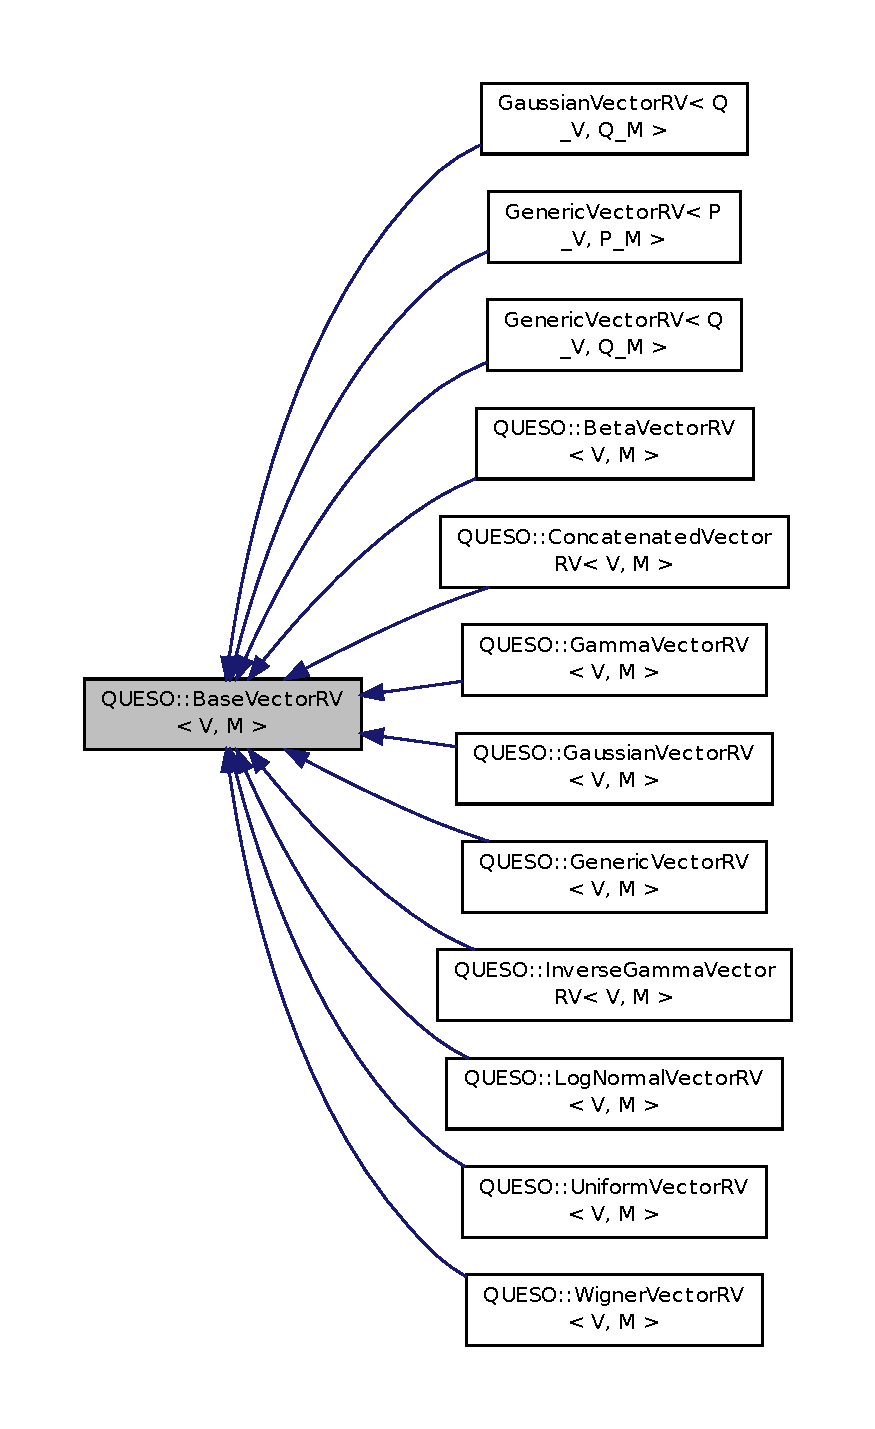
\includegraphics[height=550pt]{class_q_u_e_s_o_1_1_base_vector_r_v__inherit__graph}
\end{center}
\end{figure}


Collaboration diagram for Q\-U\-E\-S\-O\-:\-:Base\-Vector\-R\-V$<$ V, M $>$\-:
\nopagebreak
\begin{figure}[H]
\begin{center}
\leavevmode
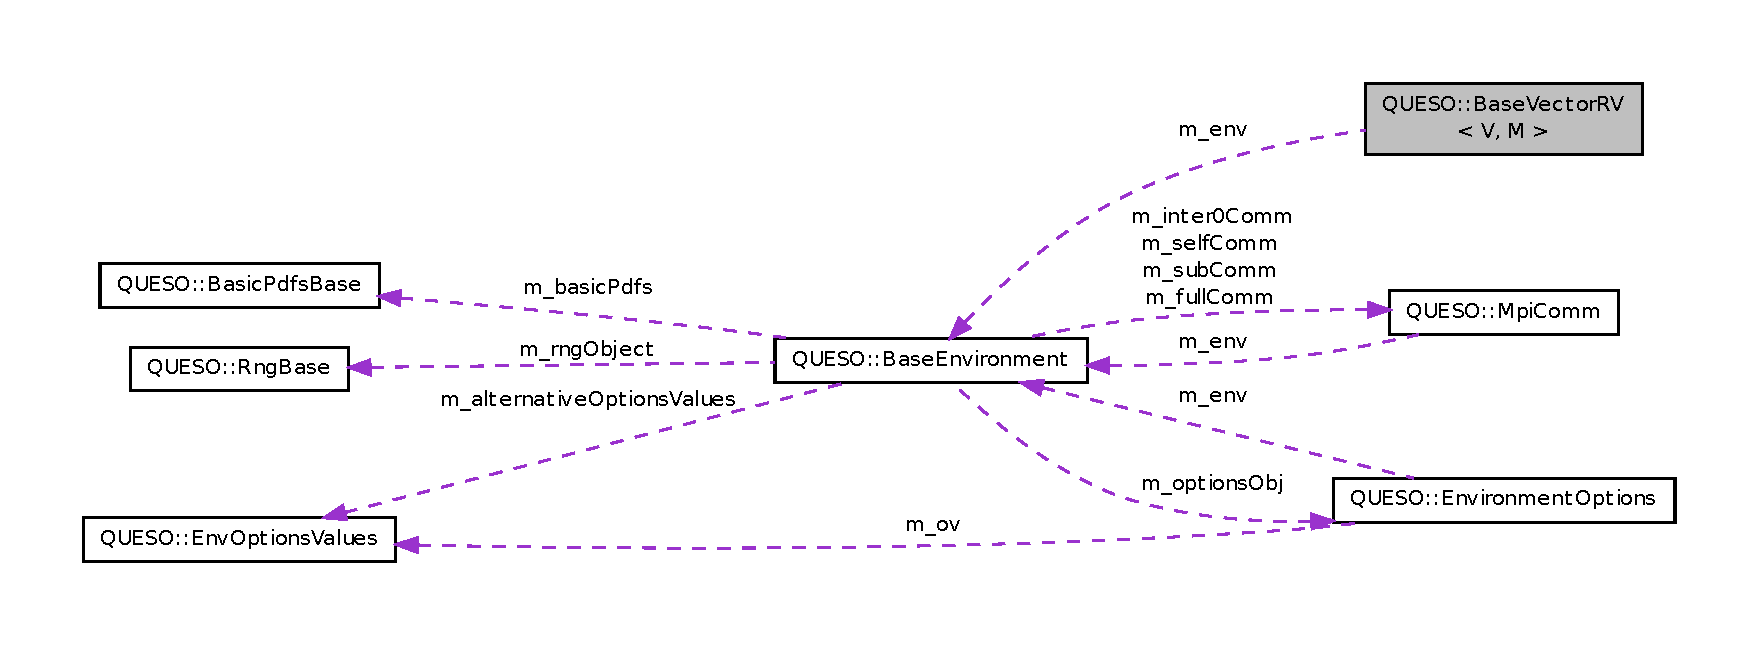
\includegraphics[width=350pt]{class_q_u_e_s_o_1_1_base_vector_r_v__coll__graph}
\end{center}
\end{figure}
\subsection*{Public Member Functions}
\begin{Indent}{\bf Constructor/\-Destructor methods}\par
\begin{DoxyCompactItemize}
\item 
\hyperlink{class_q_u_e_s_o_1_1_base_vector_r_v_a2254158741e63815277dd40541780015}{Base\-Vector\-R\-V} (const char $\ast$prefix, const \hyperlink{class_q_u_e_s_o_1_1_vector_set}{Vector\-Set}$<$ V, M $>$ \&\hyperlink{class_q_u_e_s_o_1_1_base_vector_r_v_aa4dd2f036228eac1f945bacc7147a922}{image\-Set})
\begin{DoxyCompactList}\small\item\em Constructor. \end{DoxyCompactList}\item 
virtual \hyperlink{class_q_u_e_s_o_1_1_base_vector_r_v_a4a57ee3ddec5b40ed0ad262f7482b0ae}{$\sim$\-Base\-Vector\-R\-V} ()
\begin{DoxyCompactList}\small\item\em Virtual destructor. \end{DoxyCompactList}\end{DoxyCompactItemize}
\end{Indent}
\begin{Indent}{\bf Random variable-\/handling methods}\par
\begin{DoxyCompactItemize}
\item 
const \hyperlink{class_q_u_e_s_o_1_1_base_environment}{Base\-Environment} \& \hyperlink{class_q_u_e_s_o_1_1_base_vector_r_v_ad5bf8486b3bacb46b9d4ecba513fd37b}{env} () const 
\begin{DoxyCompactList}\small\item\em \hyperlink{namespace_q_u_e_s_o}{Q\-U\-E\-S\-O} environment; access to private attribute m\-\_\-env. \end{DoxyCompactList}\item 
const \hyperlink{class_q_u_e_s_o_1_1_vector_set}{Vector\-Set}$<$ V, M $>$ \& \hyperlink{class_q_u_e_s_o_1_1_base_vector_r_v_aa4dd2f036228eac1f945bacc7147a922}{image\-Set} () const 
\begin{DoxyCompactList}\small\item\em Image set of the vector R\-V; access to private attribute m\-\_\-image\-Set. \end{DoxyCompactList}\item 
const \hyperlink{class_q_u_e_s_o_1_1_base_joint_pdf}{Base\-Joint\-Pdf}$<$ V, M $>$ \& \hyperlink{class_q_u_e_s_o_1_1_base_vector_r_v_a3206740e05e0c64a88273029e963b185}{pdf} () const 
\begin{DoxyCompactList}\small\item\em Posterior Density Function of the vector R\-V; access to private attribute m\-\_\-pdf. \end{DoxyCompactList}\item 
const \hyperlink{class_q_u_e_s_o_1_1_base_vector_realizer}{Base\-Vector\-Realizer}$<$ V, M $>$ \& \hyperlink{class_q_u_e_s_o_1_1_base_vector_r_v_aea4b01eef0baf36944d14459a7b9ccf4}{realizer} () const 
\begin{DoxyCompactList}\small\item\em Finds a realization (sample) of the P\-D\-F of this vector R\-V; access to private attribute m\-\_\-realizer. \end{DoxyCompactList}\item 
const \hyperlink{class_q_u_e_s_o_1_1_base_vector_cdf}{Base\-Vector\-Cdf}$<$ V, M $>$ \& \hyperlink{class_q_u_e_s_o_1_1_base_vector_r_v_a905586dc1529a3ae7dd7f04313ca9e8a}{sub\-Cdf} () const 
\begin{DoxyCompactList}\small\item\em Finds the Cumulative Distribution Function of this vector R\-V, considering only the sub-\/sequence of data; access to private attribute m\-\_\-sub\-Cdf. \end{DoxyCompactList}\item 
const \hyperlink{class_q_u_e_s_o_1_1_base_vector_cdf}{Base\-Vector\-Cdf}$<$ V, M $>$ \& \hyperlink{class_q_u_e_s_o_1_1_base_vector_r_v_a045a14e1ee948ac3162199a06606ce80}{unified\-Cdf} () const 
\begin{DoxyCompactList}\small\item\em Finds the Cumulative Distribution Function of this vector R\-V, considering the unified sequence of data; access to private attribute m\-\_\-unified\-Cdf. \end{DoxyCompactList}\item 
const \hyperlink{class_q_u_e_s_o_1_1_base_vector_mdf}{Base\-Vector\-Mdf}$<$ V, M $>$ \& \hyperlink{class_q_u_e_s_o_1_1_base_vector_r_v_a81f6ade1c28022b813d1276f2c217404}{mdf} () const 
\begin{DoxyCompactList}\small\item\em Finds the Mass Density Function of this vector R\-V; access to private attribute m\-\_\-mdf. \end{DoxyCompactList}\end{DoxyCompactItemize}
\end{Indent}
\subsection*{Protected Attributes}
\begin{DoxyCompactItemize}
\item 
const \hyperlink{class_q_u_e_s_o_1_1_base_environment}{Base\-Environment} \& \hyperlink{class_q_u_e_s_o_1_1_base_vector_r_v_a556761c50e2d171977ef5f19a63c8c73}{m\-\_\-env}
\item 
std\-::string \hyperlink{class_q_u_e_s_o_1_1_base_vector_r_v_a030ce3bc9873a9eaf6d8bf452c096ab3}{m\-\_\-prefix}
\item 
const \hyperlink{class_q_u_e_s_o_1_1_vector_set}{Vector\-Set}$<$ V, M $>$ \& \hyperlink{class_q_u_e_s_o_1_1_base_vector_r_v_ad31872bb4da22d47528cb9d691b3b7ff}{m\-\_\-image\-Set}
\item 
\hyperlink{class_q_u_e_s_o_1_1_base_joint_pdf}{Base\-Joint\-Pdf}$<$ V, M $>$ $\ast$ \hyperlink{class_q_u_e_s_o_1_1_base_vector_r_v_a0ca926bca6fbcc688be6fc7496449e8e}{m\-\_\-pdf}
\item 
\hyperlink{class_q_u_e_s_o_1_1_base_vector_realizer}{Base\-Vector\-Realizer}$<$ V, M $>$ $\ast$ \hyperlink{class_q_u_e_s_o_1_1_base_vector_r_v_ad99bc05293c0fd0a0accb3191fb7119e}{m\-\_\-realizer}
\item 
const \hyperlink{class_q_u_e_s_o_1_1_base_vector_cdf}{Base\-Vector\-Cdf}$<$ V, M $>$ $\ast$ \hyperlink{class_q_u_e_s_o_1_1_base_vector_r_v_a1a1117671c7fa2e572a9484463bee3a5}{m\-\_\-sub\-Cdf}
\item 
const \hyperlink{class_q_u_e_s_o_1_1_base_vector_cdf}{Base\-Vector\-Cdf}$<$ V, M $>$ $\ast$ \hyperlink{class_q_u_e_s_o_1_1_base_vector_r_v_a31a1d44bbb6a7c030ca31a9577904252}{m\-\_\-unified\-Cdf}
\item 
const \hyperlink{class_q_u_e_s_o_1_1_base_vector_mdf}{Base\-Vector\-Mdf}$<$ V, M $>$ $\ast$ \hyperlink{class_q_u_e_s_o_1_1_base_vector_r_v_a5a95d0107f66cf9b0ed3ad18a3d738df}{m\-\_\-mdf}
\end{DoxyCompactItemize}
\subsection*{I/\-O methods}
\begin{DoxyCompactItemize}
\item 
virtual void \hyperlink{class_q_u_e_s_o_1_1_base_vector_r_v_a5296b918534e12e5b62ac7cb5d20a1e8}{print} (std\-::ostream \&os) const =0
\begin{DoxyCompactList}\small\item\em T\-O\-D\-O\-: Prints the vector R\-V. \end{DoxyCompactList}\item 
std\-::ostream \& \hyperlink{class_q_u_e_s_o_1_1_base_vector_r_v_ad423b34d9e9d8865ff0688e24b82f245}{operator$<$$<$} (std\-::ostream \&os, const \hyperlink{class_q_u_e_s_o_1_1_base_vector_r_v}{Base\-Vector\-R\-V}$<$ V, M $>$ \&obj)
\end{DoxyCompactItemize}


\subsection{Detailed Description}
\subsubsection*{template$<$class V, class M$>$class Q\-U\-E\-S\-O\-::\-Base\-Vector\-R\-V$<$ V, M $>$}

A templated base class for handling vector R\-V. 

This class allows two basic but quite crucial functionalities\-: to compute the value of the P\-D\-F of a random variable (R\-V) at a point and to generate realizations (samples) from such P\-D\-F. 

Definition at line 69 of file Vector\-R\-V.\-h.



\subsection{Constructor \& Destructor Documentation}
\hypertarget{class_q_u_e_s_o_1_1_base_vector_r_v_a2254158741e63815277dd40541780015}{\index{Q\-U\-E\-S\-O\-::\-Base\-Vector\-R\-V@{Q\-U\-E\-S\-O\-::\-Base\-Vector\-R\-V}!Base\-Vector\-R\-V@{Base\-Vector\-R\-V}}
\index{Base\-Vector\-R\-V@{Base\-Vector\-R\-V}!QUESO::BaseVectorRV@{Q\-U\-E\-S\-O\-::\-Base\-Vector\-R\-V}}
\subsubsection[{Base\-Vector\-R\-V}]{\setlength{\rightskip}{0pt plus 5cm}template$<$class V, class M$>$ {\bf Q\-U\-E\-S\-O\-::\-Base\-Vector\-R\-V}$<$ V, M $>$\-::{\bf Base\-Vector\-R\-V} (
\begin{DoxyParamCaption}
\item[{const char $\ast$}]{prefix, }
\item[{const {\bf Vector\-Set}$<$ V, M $>$ \&}]{image\-Set}
\end{DoxyParamCaption}
)}}\label{class_q_u_e_s_o_1_1_base_vector_r_v_a2254158741e63815277dd40541780015}


Constructor. 

Constructs a new instance of \hyperlink{class_q_u_e_s_o_1_1_base_vector_r_v}{Base\-Vector\-R\-V}, given a prefix and the image set of the vector R\-V. 

Definition at line 33 of file Vector\-R\-V.\-C.



References Q\-U\-E\-S\-O\-::\-Base\-Environment\-::display\-Verbosity(), Q\-U\-E\-S\-O\-::\-Base\-Vector\-R\-V$<$ V, M $>$\-::m\-\_\-env, Q\-U\-E\-S\-O\-::\-Base\-Vector\-R\-V$<$ V, M $>$\-::m\-\_\-prefix, and Q\-U\-E\-S\-O\-::\-Base\-Environment\-::sub\-Display\-File().


\begin{DoxyCode}
36   :
37   \hyperlink{class_q_u_e_s_o_1_1_base_vector_r_v_a556761c50e2d171977ef5f19a63c8c73}{m\_env}       (\hyperlink{class_q_u_e_s_o_1_1_base_vector_r_v_aa4dd2f036228eac1f945bacc7147a922}{imageSet}.env()),
38   \hyperlink{class_q_u_e_s_o_1_1_base_vector_r_v_a030ce3bc9873a9eaf6d8bf452c096ab3}{m\_prefix}    ((std::string)(prefix)+\textcolor{stringliteral}{"rv\_"}),
39   \hyperlink{class_q_u_e_s_o_1_1_base_vector_r_v_ad31872bb4da22d47528cb9d691b3b7ff}{m\_imageSet}  (\hyperlink{class_q_u_e_s_o_1_1_base_vector_r_v_aa4dd2f036228eac1f945bacc7147a922}{imageSet}),
40   \hyperlink{class_q_u_e_s_o_1_1_base_vector_r_v_a0ca926bca6fbcc688be6fc7496449e8e}{m\_pdf}       (NULL),
41   \hyperlink{class_q_u_e_s_o_1_1_base_vector_r_v_ad99bc05293c0fd0a0accb3191fb7119e}{m\_realizer}  (NULL),
42   \hyperlink{class_q_u_e_s_o_1_1_base_vector_r_v_a1a1117671c7fa2e572a9484463bee3a5}{m\_subCdf}    (NULL),
43   \hyperlink{class_q_u_e_s_o_1_1_base_vector_r_v_a31a1d44bbb6a7c030ca31a9577904252}{m\_unifiedCdf}(NULL),
44   \hyperlink{class_q_u_e_s_o_1_1_base_vector_r_v_a5a95d0107f66cf9b0ed3ad18a3d738df}{m\_mdf}       (NULL)
45 \{
46   \textcolor{keywordflow}{if} ((\hyperlink{class_q_u_e_s_o_1_1_base_vector_r_v_a556761c50e2d171977ef5f19a63c8c73}{m\_env}.\hyperlink{class_q_u_e_s_o_1_1_base_environment_a8a0064746ae8dddfece4229b9ad374d6}{subDisplayFile}()) && (\hyperlink{class_q_u_e_s_o_1_1_base_vector_r_v_a556761c50e2d171977ef5f19a63c8c73}{m\_env}.
      \hyperlink{class_q_u_e_s_o_1_1_base_environment_a1fe5f244fc0316a0ab3e37463f108b96}{displayVerbosity}() >= 54)) \{
47     *\hyperlink{class_q_u_e_s_o_1_1_base_vector_r_v_a556761c50e2d171977ef5f19a63c8c73}{m\_env}.\hyperlink{class_q_u_e_s_o_1_1_base_environment_a8a0064746ae8dddfece4229b9ad374d6}{subDisplayFile}() << \textcolor{stringliteral}{"Entering BaseVectorRV<V,M>::constructor()"}
48                             << \textcolor{stringliteral}{": prefix = "} << \hyperlink{class_q_u_e_s_o_1_1_base_vector_r_v_a030ce3bc9873a9eaf6d8bf452c096ab3}{m\_prefix}
49                             << std::endl;
50   \}
51 
52   \textcolor{keywordflow}{if} ((\hyperlink{class_q_u_e_s_o_1_1_base_vector_r_v_a556761c50e2d171977ef5f19a63c8c73}{m\_env}.\hyperlink{class_q_u_e_s_o_1_1_base_environment_a8a0064746ae8dddfece4229b9ad374d6}{subDisplayFile}()) && (\hyperlink{class_q_u_e_s_o_1_1_base_vector_r_v_a556761c50e2d171977ef5f19a63c8c73}{m\_env}.
      \hyperlink{class_q_u_e_s_o_1_1_base_environment_a1fe5f244fc0316a0ab3e37463f108b96}{displayVerbosity}() >= 54)) \{
53     *\hyperlink{class_q_u_e_s_o_1_1_base_vector_r_v_a556761c50e2d171977ef5f19a63c8c73}{m\_env}.\hyperlink{class_q_u_e_s_o_1_1_base_environment_a8a0064746ae8dddfece4229b9ad374d6}{subDisplayFile}() << \textcolor{stringliteral}{"Leaving BaseVectorRV<V,M>::constructor()"}
54                             << \textcolor{stringliteral}{": prefix = "} << \hyperlink{class_q_u_e_s_o_1_1_base_vector_r_v_a030ce3bc9873a9eaf6d8bf452c096ab3}{m\_prefix}
55                             << std::endl;
56   \}
57 \}
\end{DoxyCode}
\hypertarget{class_q_u_e_s_o_1_1_base_vector_r_v_a4a57ee3ddec5b40ed0ad262f7482b0ae}{\index{Q\-U\-E\-S\-O\-::\-Base\-Vector\-R\-V@{Q\-U\-E\-S\-O\-::\-Base\-Vector\-R\-V}!$\sim$\-Base\-Vector\-R\-V@{$\sim$\-Base\-Vector\-R\-V}}
\index{$\sim$\-Base\-Vector\-R\-V@{$\sim$\-Base\-Vector\-R\-V}!QUESO::BaseVectorRV@{Q\-U\-E\-S\-O\-::\-Base\-Vector\-R\-V}}
\subsubsection[{$\sim$\-Base\-Vector\-R\-V}]{\setlength{\rightskip}{0pt plus 5cm}template$<$class V , class M $>$ {\bf Q\-U\-E\-S\-O\-::\-Base\-Vector\-R\-V}$<$ V, M $>$\-::$\sim${\bf Base\-Vector\-R\-V} (
\begin{DoxyParamCaption}
{}
\end{DoxyParamCaption}
)\hspace{0.3cm}{\ttfamily [virtual]}}}\label{class_q_u_e_s_o_1_1_base_vector_r_v_a4a57ee3ddec5b40ed0ad262f7482b0ae}


Virtual destructor. 



Definition at line 60 of file Vector\-R\-V.\-C.


\begin{DoxyCode}
61 \{
62   \textcolor{comment}{//if (m\_mdf       ) delete m\_mdf;}
63   \textcolor{comment}{//if (m\_subCdf    ) delete m\_subCdf;}
64   \textcolor{comment}{//if (m\_unifiedCdf) delete m\_unifiedCdf;}
65   \textcolor{comment}{//if (m\_realizer  ) delete m\_realizer;}
66   \textcolor{comment}{//if (m\_pdf       ) delete m\_pdf;}
67 \}
\end{DoxyCode}


\subsection{Member Function Documentation}
\hypertarget{class_q_u_e_s_o_1_1_base_vector_r_v_ad5bf8486b3bacb46b9d4ecba513fd37b}{\index{Q\-U\-E\-S\-O\-::\-Base\-Vector\-R\-V@{Q\-U\-E\-S\-O\-::\-Base\-Vector\-R\-V}!env@{env}}
\index{env@{env}!QUESO::BaseVectorRV@{Q\-U\-E\-S\-O\-::\-Base\-Vector\-R\-V}}
\subsubsection[{env}]{\setlength{\rightskip}{0pt plus 5cm}template$<$class V , class M $>$ const {\bf Base\-Environment} \& {\bf Q\-U\-E\-S\-O\-::\-Base\-Vector\-R\-V}$<$ V, M $>$\-::env (
\begin{DoxyParamCaption}
{}
\end{DoxyParamCaption}
) const}}\label{class_q_u_e_s_o_1_1_base_vector_r_v_ad5bf8486b3bacb46b9d4ecba513fd37b}


\hyperlink{namespace_q_u_e_s_o}{Q\-U\-E\-S\-O} environment; access to private attribute m\-\_\-env. 



Definition at line 72 of file Vector\-R\-V.\-C.



Referenced by Q\-U\-E\-S\-O\-::\-Compute\-Cov\-Corr\-Matrices\-Between\-Vector\-Rvs().


\begin{DoxyCode}
73 \{
74   \textcolor{keywordflow}{return} \hyperlink{class_q_u_e_s_o_1_1_base_vector_r_v_a556761c50e2d171977ef5f19a63c8c73}{m\_env};
75 \}
\end{DoxyCode}
\hypertarget{class_q_u_e_s_o_1_1_base_vector_r_v_aa4dd2f036228eac1f945bacc7147a922}{\index{Q\-U\-E\-S\-O\-::\-Base\-Vector\-R\-V@{Q\-U\-E\-S\-O\-::\-Base\-Vector\-R\-V}!image\-Set@{image\-Set}}
\index{image\-Set@{image\-Set}!QUESO::BaseVectorRV@{Q\-U\-E\-S\-O\-::\-Base\-Vector\-R\-V}}
\subsubsection[{image\-Set}]{\setlength{\rightskip}{0pt plus 5cm}template$<$class V , class M $>$ const {\bf Vector\-Set}$<$ V, M $>$ \& {\bf Q\-U\-E\-S\-O\-::\-Base\-Vector\-R\-V}$<$ V, M $>$\-::image\-Set (
\begin{DoxyParamCaption}
{}
\end{DoxyParamCaption}
) const}}\label{class_q_u_e_s_o_1_1_base_vector_r_v_aa4dd2f036228eac1f945bacc7147a922}


Image set of the vector R\-V; access to private attribute m\-\_\-image\-Set. 



Definition at line 79 of file Vector\-R\-V.\-C.



Referenced by Q\-U\-E\-S\-O\-::\-Beta\-Vector\-R\-V$<$ V, M $>$\-::\-Beta\-Vector\-R\-V(), Q\-U\-E\-S\-O\-::\-Compute\-Cov\-Corr\-Matrices\-Between\-Vector\-Rvs(), Q\-U\-E\-S\-O\-::\-Gamma\-Vector\-R\-V$<$ V, M $>$\-::\-Gamma\-Vector\-R\-V(), Q\-U\-E\-S\-O\-::\-Inverse\-Gamma\-Vector\-R\-V$<$ V, M $>$\-::\-Inverse\-Gamma\-Vector\-R\-V(), and Q\-U\-E\-S\-O\-::\-Log\-Normal\-Vector\-R\-V$<$ V, M $>$\-::\-Log\-Normal\-Vector\-R\-V().


\begin{DoxyCode}
80 \{
81   \textcolor{keywordflow}{return} \hyperlink{class_q_u_e_s_o_1_1_base_vector_r_v_ad31872bb4da22d47528cb9d691b3b7ff}{m\_imageSet};
82 \}
\end{DoxyCode}
\hypertarget{class_q_u_e_s_o_1_1_base_vector_r_v_a81f6ade1c28022b813d1276f2c217404}{\index{Q\-U\-E\-S\-O\-::\-Base\-Vector\-R\-V@{Q\-U\-E\-S\-O\-::\-Base\-Vector\-R\-V}!mdf@{mdf}}
\index{mdf@{mdf}!QUESO::BaseVectorRV@{Q\-U\-E\-S\-O\-::\-Base\-Vector\-R\-V}}
\subsubsection[{mdf}]{\setlength{\rightskip}{0pt plus 5cm}template$<$class V , class M $>$ const {\bf Base\-Vector\-Mdf}$<$ V, M $>$ \& {\bf Q\-U\-E\-S\-O\-::\-Base\-Vector\-R\-V}$<$ V, M $>$\-::mdf (
\begin{DoxyParamCaption}
{}
\end{DoxyParamCaption}
) const}}\label{class_q_u_e_s_o_1_1_base_vector_r_v_a81f6ade1c28022b813d1276f2c217404}


Finds the Mass Density Function of this vector R\-V; access to private attribute m\-\_\-mdf. 



Definition at line 134 of file Vector\-R\-V.\-C.



References U\-Q\-\_\-\-F\-A\-T\-A\-L\-\_\-\-T\-E\-S\-T\-\_\-\-M\-A\-C\-R\-O.



Referenced by Q\-U\-E\-S\-O\-::\-Generic\-Vector\-R\-V$<$ V, M $>$\-::\-Generic\-Vector\-R\-V().


\begin{DoxyCode}
135 \{
136   \hyperlink{_defines_8h_a56d63d18d0a6d45757de47fcc06f574d}{UQ\_FATAL\_TEST\_MACRO}(\hyperlink{class_q_u_e_s_o_1_1_base_vector_r_v_a5a95d0107f66cf9b0ed3ad18a3d738df}{m\_mdf} == NULL,
137                       \hyperlink{class_q_u_e_s_o_1_1_base_vector_r_v_a556761c50e2d171977ef5f19a63c8c73}{m\_env}.\hyperlink{class_q_u_e_s_o_1_1_base_environment_a78b57112bbd0e6dd0e8afec00b40ffa7}{worldRank}(),
138                       (std::string)(\textcolor{stringliteral}{"BaseVectorRV<V,M>::mdf(), prefix="})+
      \hyperlink{class_q_u_e_s_o_1_1_base_vector_r_v_a030ce3bc9873a9eaf6d8bf452c096ab3}{m\_prefix},
139                       \textcolor{stringliteral}{"m\_mdf is NULL"});
140 
141   \textcolor{keywordflow}{return} *\hyperlink{class_q_u_e_s_o_1_1_base_vector_r_v_a5a95d0107f66cf9b0ed3ad18a3d738df}{m\_mdf};
142 \}
\end{DoxyCode}
\hypertarget{class_q_u_e_s_o_1_1_base_vector_r_v_a3206740e05e0c64a88273029e963b185}{\index{Q\-U\-E\-S\-O\-::\-Base\-Vector\-R\-V@{Q\-U\-E\-S\-O\-::\-Base\-Vector\-R\-V}!pdf@{pdf}}
\index{pdf@{pdf}!QUESO::BaseVectorRV@{Q\-U\-E\-S\-O\-::\-Base\-Vector\-R\-V}}
\subsubsection[{pdf}]{\setlength{\rightskip}{0pt plus 5cm}template$<$class V , class M $>$ const {\bf Base\-Joint\-Pdf}$<$ V, M $>$ \& {\bf Q\-U\-E\-S\-O\-::\-Base\-Vector\-R\-V}$<$ V, M $>$\-::pdf (
\begin{DoxyParamCaption}
{}
\end{DoxyParamCaption}
) const}}\label{class_q_u_e_s_o_1_1_base_vector_r_v_a3206740e05e0c64a88273029e963b185}


Posterior Density Function of the vector R\-V; access to private attribute m\-\_\-pdf. 



Definition at line 86 of file Vector\-R\-V.\-C.



References U\-Q\-\_\-\-F\-A\-T\-A\-L\-\_\-\-T\-E\-S\-T\-\_\-\-M\-A\-C\-R\-O.



Referenced by Q\-U\-E\-S\-O\-::\-Generic\-Vector\-R\-V$<$ V, M $>$\-::\-Generic\-Vector\-R\-V().


\begin{DoxyCode}
87 \{
88   \hyperlink{_defines_8h_a56d63d18d0a6d45757de47fcc06f574d}{UQ\_FATAL\_TEST\_MACRO}(\hyperlink{class_q_u_e_s_o_1_1_base_vector_r_v_a0ca926bca6fbcc688be6fc7496449e8e}{m\_pdf} == NULL,
89                       \hyperlink{class_q_u_e_s_o_1_1_base_vector_r_v_a556761c50e2d171977ef5f19a63c8c73}{m\_env}.\hyperlink{class_q_u_e_s_o_1_1_base_environment_a78b57112bbd0e6dd0e8afec00b40ffa7}{worldRank}(),
90                       \textcolor{stringliteral}{"BaseVectorRV<V,M>::pdf()"},
91                       \textcolor{stringliteral}{"m\_pdf is NULL"});
92 
93   \textcolor{keywordflow}{return} *\hyperlink{class_q_u_e_s_o_1_1_base_vector_r_v_a0ca926bca6fbcc688be6fc7496449e8e}{m\_pdf};
94 \}
\end{DoxyCode}
\hypertarget{class_q_u_e_s_o_1_1_base_vector_r_v_a5296b918534e12e5b62ac7cb5d20a1e8}{\index{Q\-U\-E\-S\-O\-::\-Base\-Vector\-R\-V@{Q\-U\-E\-S\-O\-::\-Base\-Vector\-R\-V}!print@{print}}
\index{print@{print}!QUESO::BaseVectorRV@{Q\-U\-E\-S\-O\-::\-Base\-Vector\-R\-V}}
\subsubsection[{print}]{\setlength{\rightskip}{0pt plus 5cm}template$<$class V, class M$>$ virtual void {\bf Q\-U\-E\-S\-O\-::\-Base\-Vector\-R\-V}$<$ V, M $>$\-::print (
\begin{DoxyParamCaption}
\item[{std\-::ostream \&}]{os}
\end{DoxyParamCaption}
) const\hspace{0.3cm}{\ttfamily [pure virtual]}}}\label{class_q_u_e_s_o_1_1_base_vector_r_v_a5296b918534e12e5b62ac7cb5d20a1e8}


T\-O\-D\-O\-: Prints the vector R\-V. 

\begin{DoxyRefDesc}{Todo}
\item[\hyperlink{todo__todo000054}{Todo}]\-: implement me! \end{DoxyRefDesc}


Implemented in \hyperlink{class_q_u_e_s_o_1_1_gaussian_vector_r_v_a2c7bee2104f7e257ca31d185634c2910}{Q\-U\-E\-S\-O\-::\-Gaussian\-Vector\-R\-V$<$ V, M $>$}, \hyperlink{class_q_u_e_s_o_1_1_gaussian_vector_r_v_a2c7bee2104f7e257ca31d185634c2910}{Q\-U\-E\-S\-O\-::\-Gaussian\-Vector\-R\-V$<$ Q\-\_\-\-V, Q\-\_\-\-M $>$}, \hyperlink{class_q_u_e_s_o_1_1_generic_vector_r_v_a423908e3d0aec9a48122b17ebb0a5b57}{Q\-U\-E\-S\-O\-::\-Generic\-Vector\-R\-V$<$ V, M $>$}, \hyperlink{class_q_u_e_s_o_1_1_generic_vector_r_v_a423908e3d0aec9a48122b17ebb0a5b57}{Q\-U\-E\-S\-O\-::\-Generic\-Vector\-R\-V$<$ P\-\_\-\-V, P\-\_\-\-M $>$}, \hyperlink{class_q_u_e_s_o_1_1_generic_vector_r_v_a423908e3d0aec9a48122b17ebb0a5b57}{Q\-U\-E\-S\-O\-::\-Generic\-Vector\-R\-V$<$ Q\-\_\-\-V, Q\-\_\-\-M $>$}, \hyperlink{class_q_u_e_s_o_1_1_beta_vector_r_v_ae54ad1998b22aed2f5c8061cd1ad56e5}{Q\-U\-E\-S\-O\-::\-Beta\-Vector\-R\-V$<$ V, M $>$}, \hyperlink{class_q_u_e_s_o_1_1_gamma_vector_r_v_ae6b687ef1f325e3eea4dd63a1660110a}{Q\-U\-E\-S\-O\-::\-Gamma\-Vector\-R\-V$<$ V, M $>$}, \hyperlink{class_q_u_e_s_o_1_1_inverse_gamma_vector_r_v_a7c3326d0b39a69f1edd64219f286c7e7}{Q\-U\-E\-S\-O\-::\-Inverse\-Gamma\-Vector\-R\-V$<$ V, M $>$}, \hyperlink{class_q_u_e_s_o_1_1_concatenated_vector_r_v_ac479f33e7ef6ff9f17b930aef13fcd7c}{Q\-U\-E\-S\-O\-::\-Concatenated\-Vector\-R\-V$<$ V, M $>$}, \hyperlink{class_q_u_e_s_o_1_1_log_normal_vector_r_v_a150a212058169e2b708e82c8faff61eb}{Q\-U\-E\-S\-O\-::\-Log\-Normal\-Vector\-R\-V$<$ V, M $>$}, \hyperlink{class_q_u_e_s_o_1_1_wigner_vector_r_v_a6658542aa6a551c1b92de93558cb67fa}{Q\-U\-E\-S\-O\-::\-Wigner\-Vector\-R\-V$<$ V, M $>$}, and \hyperlink{class_q_u_e_s_o_1_1_uniform_vector_r_v_ab6dee885e568635b7b7e9675b4e66833}{Q\-U\-E\-S\-O\-::\-Uniform\-Vector\-R\-V$<$ V, M $>$}.

\hypertarget{class_q_u_e_s_o_1_1_base_vector_r_v_aea4b01eef0baf36944d14459a7b9ccf4}{\index{Q\-U\-E\-S\-O\-::\-Base\-Vector\-R\-V@{Q\-U\-E\-S\-O\-::\-Base\-Vector\-R\-V}!realizer@{realizer}}
\index{realizer@{realizer}!QUESO::BaseVectorRV@{Q\-U\-E\-S\-O\-::\-Base\-Vector\-R\-V}}
\subsubsection[{realizer}]{\setlength{\rightskip}{0pt plus 5cm}template$<$class V , class M $>$ const {\bf Base\-Vector\-Realizer}$<$ V, M $>$ \& {\bf Q\-U\-E\-S\-O\-::\-Base\-Vector\-R\-V}$<$ V, M $>$\-::realizer (
\begin{DoxyParamCaption}
{}
\end{DoxyParamCaption}
) const}}\label{class_q_u_e_s_o_1_1_base_vector_r_v_aea4b01eef0baf36944d14459a7b9ccf4}


Finds a realization (sample) of the P\-D\-F of this vector R\-V; access to private attribute m\-\_\-realizer. 



Definition at line 98 of file Vector\-R\-V.\-C.



References U\-Q\-\_\-\-F\-A\-T\-A\-L\-\_\-\-T\-E\-S\-T\-\_\-\-M\-A\-C\-R\-O.



Referenced by Q\-U\-E\-S\-O\-::\-Monte\-Carlo\-S\-G$<$ P\-\_\-\-V, P\-\_\-\-M, Q\-\_\-\-V, Q\-\_\-\-M $>$\-::actual\-Generate\-Sequence(), Q\-U\-E\-S\-O\-::\-Monte\-Carlo\-S\-G$<$ P\-\_\-\-V, P\-\_\-\-M, Q\-\_\-\-V, Q\-\_\-\-M $>$\-::actual\-Read\-Sequence(), Q\-U\-E\-S\-O\-::\-Compute\-Cov\-Corr\-Matrices\-Between\-Vector\-Rvs(), Q\-U\-E\-S\-O\-::\-Generic\-Vector\-R\-V$<$ V, M $>$\-::\-Generic\-Vector\-R\-V(), and Q\-U\-E\-S\-O\-::\-Monte\-Carlo\-S\-G$<$ P\-\_\-\-V, P\-\_\-\-M, Q\-\_\-\-V, Q\-\_\-\-M $>$\-::intern\-Generate\-Sequence().


\begin{DoxyCode}
99 \{
100   \hyperlink{_defines_8h_a56d63d18d0a6d45757de47fcc06f574d}{UQ\_FATAL\_TEST\_MACRO}(\hyperlink{class_q_u_e_s_o_1_1_base_vector_r_v_ad99bc05293c0fd0a0accb3191fb7119e}{m\_realizer} == NULL,
101                       \hyperlink{class_q_u_e_s_o_1_1_base_vector_r_v_a556761c50e2d171977ef5f19a63c8c73}{m\_env}.\hyperlink{class_q_u_e_s_o_1_1_base_environment_a78b57112bbd0e6dd0e8afec00b40ffa7}{worldRank}(),
102                       (std::string)(\textcolor{stringliteral}{"BaseVectorRV<V,M>::realizer(), prefix="})+
      \hyperlink{class_q_u_e_s_o_1_1_base_vector_r_v_a030ce3bc9873a9eaf6d8bf452c096ab3}{m\_prefix},
103                       \textcolor{stringliteral}{"m\_realizer is NULL"});
104 
105   \textcolor{keywordflow}{return} *\hyperlink{class_q_u_e_s_o_1_1_base_vector_r_v_ad99bc05293c0fd0a0accb3191fb7119e}{m\_realizer};
106 \}
\end{DoxyCode}
\hypertarget{class_q_u_e_s_o_1_1_base_vector_r_v_a905586dc1529a3ae7dd7f04313ca9e8a}{\index{Q\-U\-E\-S\-O\-::\-Base\-Vector\-R\-V@{Q\-U\-E\-S\-O\-::\-Base\-Vector\-R\-V}!sub\-Cdf@{sub\-Cdf}}
\index{sub\-Cdf@{sub\-Cdf}!QUESO::BaseVectorRV@{Q\-U\-E\-S\-O\-::\-Base\-Vector\-R\-V}}
\subsubsection[{sub\-Cdf}]{\setlength{\rightskip}{0pt plus 5cm}template$<$class V , class M $>$ const {\bf Base\-Vector\-Cdf}$<$ V, M $>$ \& {\bf Q\-U\-E\-S\-O\-::\-Base\-Vector\-R\-V}$<$ V, M $>$\-::sub\-Cdf (
\begin{DoxyParamCaption}
{}
\end{DoxyParamCaption}
) const}}\label{class_q_u_e_s_o_1_1_base_vector_r_v_a905586dc1529a3ae7dd7f04313ca9e8a}


Finds the Cumulative Distribution Function of this vector R\-V, considering only the sub-\/sequence of data; access to private attribute m\-\_\-sub\-Cdf. 



Definition at line 110 of file Vector\-R\-V.\-C.



References U\-Q\-\_\-\-F\-A\-T\-A\-L\-\_\-\-T\-E\-S\-T\-\_\-\-M\-A\-C\-R\-O.



Referenced by Q\-U\-E\-S\-O\-::\-Generic\-Vector\-R\-V$<$ V, M $>$\-::\-Generic\-Vector\-R\-V().


\begin{DoxyCode}
111 \{
112   \hyperlink{_defines_8h_a56d63d18d0a6d45757de47fcc06f574d}{UQ\_FATAL\_TEST\_MACRO}(\hyperlink{class_q_u_e_s_o_1_1_base_vector_r_v_a1a1117671c7fa2e572a9484463bee3a5}{m\_subCdf} == NULL,
113                       \hyperlink{class_q_u_e_s_o_1_1_base_vector_r_v_a556761c50e2d171977ef5f19a63c8c73}{m\_env}.\hyperlink{class_q_u_e_s_o_1_1_base_environment_a78b57112bbd0e6dd0e8afec00b40ffa7}{worldRank}(),
114                       (std::string)(\textcolor{stringliteral}{"BaseVectorRV<V,M>::subCdf(), prefix="})+
      \hyperlink{class_q_u_e_s_o_1_1_base_vector_r_v_a030ce3bc9873a9eaf6d8bf452c096ab3}{m\_prefix},
115                       \textcolor{stringliteral}{"m\_subCdf is NULL"});
116 
117   \textcolor{keywordflow}{return} *\hyperlink{class_q_u_e_s_o_1_1_base_vector_r_v_a1a1117671c7fa2e572a9484463bee3a5}{m\_subCdf};
118 \}
\end{DoxyCode}
\hypertarget{class_q_u_e_s_o_1_1_base_vector_r_v_a045a14e1ee948ac3162199a06606ce80}{\index{Q\-U\-E\-S\-O\-::\-Base\-Vector\-R\-V@{Q\-U\-E\-S\-O\-::\-Base\-Vector\-R\-V}!unified\-Cdf@{unified\-Cdf}}
\index{unified\-Cdf@{unified\-Cdf}!QUESO::BaseVectorRV@{Q\-U\-E\-S\-O\-::\-Base\-Vector\-R\-V}}
\subsubsection[{unified\-Cdf}]{\setlength{\rightskip}{0pt plus 5cm}template$<$class V , class M $>$ const {\bf Base\-Vector\-Cdf}$<$ V, M $>$ \& {\bf Q\-U\-E\-S\-O\-::\-Base\-Vector\-R\-V}$<$ V, M $>$\-::unified\-Cdf (
\begin{DoxyParamCaption}
{}
\end{DoxyParamCaption}
) const}}\label{class_q_u_e_s_o_1_1_base_vector_r_v_a045a14e1ee948ac3162199a06606ce80}


Finds the Cumulative Distribution Function of this vector R\-V, considering the unified sequence of data; access to private attribute m\-\_\-unified\-Cdf. 



Definition at line 122 of file Vector\-R\-V.\-C.



References U\-Q\-\_\-\-F\-A\-T\-A\-L\-\_\-\-T\-E\-S\-T\-\_\-\-M\-A\-C\-R\-O.



Referenced by Q\-U\-E\-S\-O\-::\-Generic\-Vector\-R\-V$<$ V, M $>$\-::\-Generic\-Vector\-R\-V().


\begin{DoxyCode}
123 \{
124   \hyperlink{_defines_8h_a56d63d18d0a6d45757de47fcc06f574d}{UQ\_FATAL\_TEST\_MACRO}(\hyperlink{class_q_u_e_s_o_1_1_base_vector_r_v_a31a1d44bbb6a7c030ca31a9577904252}{m\_unifiedCdf} == NULL,
125                       \hyperlink{class_q_u_e_s_o_1_1_base_vector_r_v_a556761c50e2d171977ef5f19a63c8c73}{m\_env}.\hyperlink{class_q_u_e_s_o_1_1_base_environment_a78b57112bbd0e6dd0e8afec00b40ffa7}{worldRank}(),
126                       (std::string)(\textcolor{stringliteral}{"BaseVectorRV<V,M>::unifiedCdf(), prefix="})+
      \hyperlink{class_q_u_e_s_o_1_1_base_vector_r_v_a030ce3bc9873a9eaf6d8bf452c096ab3}{m\_prefix},
127                       \textcolor{stringliteral}{"m\_unifiedCdf is NULL"});
128 
129   \textcolor{keywordflow}{return} *\hyperlink{class_q_u_e_s_o_1_1_base_vector_r_v_a31a1d44bbb6a7c030ca31a9577904252}{m\_unifiedCdf};
130 \}
\end{DoxyCode}


\subsection{Friends And Related Function Documentation}
\hypertarget{class_q_u_e_s_o_1_1_base_vector_r_v_ad423b34d9e9d8865ff0688e24b82f245}{\index{Q\-U\-E\-S\-O\-::\-Base\-Vector\-R\-V@{Q\-U\-E\-S\-O\-::\-Base\-Vector\-R\-V}!operator$<$$<$@{operator$<$$<$}}
\index{operator$<$$<$@{operator$<$$<$}!QUESO::BaseVectorRV@{Q\-U\-E\-S\-O\-::\-Base\-Vector\-R\-V}}
\subsubsection[{operator$<$$<$}]{\setlength{\rightskip}{0pt plus 5cm}template$<$class V, class M$>$ std\-::ostream\& operator$<$$<$ (
\begin{DoxyParamCaption}
\item[{std\-::ostream \&}]{os, }
\item[{const {\bf Base\-Vector\-R\-V}$<$ V, M $>$ \&}]{obj}
\end{DoxyParamCaption}
)\hspace{0.3cm}{\ttfamily [friend]}}}\label{class_q_u_e_s_o_1_1_base_vector_r_v_ad423b34d9e9d8865ff0688e24b82f245}


Definition at line 113 of file Vector\-R\-V.\-h.


\begin{DoxyCode}
114                                     \{
115     obj.print(os);
116     \textcolor{keywordflow}{return} os;
117   \}
\end{DoxyCode}


\subsection{Member Data Documentation}
\hypertarget{class_q_u_e_s_o_1_1_base_vector_r_v_a556761c50e2d171977ef5f19a63c8c73}{\index{Q\-U\-E\-S\-O\-::\-Base\-Vector\-R\-V@{Q\-U\-E\-S\-O\-::\-Base\-Vector\-R\-V}!m\-\_\-env@{m\-\_\-env}}
\index{m\-\_\-env@{m\-\_\-env}!QUESO::BaseVectorRV@{Q\-U\-E\-S\-O\-::\-Base\-Vector\-R\-V}}
\subsubsection[{m\-\_\-env}]{\setlength{\rightskip}{0pt plus 5cm}template$<$class V, class M$>$ const {\bf Base\-Environment}\& {\bf Q\-U\-E\-S\-O\-::\-Base\-Vector\-R\-V}$<$ V, M $>$\-::m\-\_\-env\hspace{0.3cm}{\ttfamily [protected]}}}\label{class_q_u_e_s_o_1_1_base_vector_r_v_a556761c50e2d171977ef5f19a63c8c73}


Definition at line 130 of file Vector\-R\-V.\-h.



Referenced by Q\-U\-E\-S\-O\-::\-Base\-Vector\-R\-V$<$ V, M $>$\-::\-Base\-Vector\-R\-V(), Q\-U\-E\-S\-O\-::\-Beta\-Vector\-R\-V$<$ V, M $>$\-::\-Beta\-Vector\-R\-V(), Q\-U\-E\-S\-O\-::\-Concatenated\-Vector\-R\-V$<$ V, M $>$\-::\-Concatenated\-Vector\-R\-V(), Q\-U\-E\-S\-O\-::\-Gamma\-Vector\-R\-V$<$ V, M $>$\-::\-Gamma\-Vector\-R\-V(), Q\-U\-E\-S\-O\-::\-Gaussian\-Vector\-R\-V$<$ V, M $>$\-::\-Gaussian\-Vector\-R\-V(), Q\-U\-E\-S\-O\-::\-Generic\-Vector\-R\-V$<$ V, M $>$\-::\-Generic\-Vector\-R\-V(), Q\-U\-E\-S\-O\-::\-Inverse\-Gamma\-Vector\-R\-V$<$ V, M $>$\-::\-Inverse\-Gamma\-Vector\-R\-V(), Q\-U\-E\-S\-O\-::\-Log\-Normal\-Vector\-R\-V$<$ V, M $>$\-::\-Log\-Normal\-Vector\-R\-V(), Q\-U\-E\-S\-O\-::\-Uniform\-Vector\-R\-V$<$ V, M $>$\-::\-Uniform\-Vector\-R\-V(), and Q\-U\-E\-S\-O\-::\-Wigner\-Vector\-R\-V$<$ V, M $>$\-::\-Wigner\-Vector\-R\-V().

\hypertarget{class_q_u_e_s_o_1_1_base_vector_r_v_ad31872bb4da22d47528cb9d691b3b7ff}{\index{Q\-U\-E\-S\-O\-::\-Base\-Vector\-R\-V@{Q\-U\-E\-S\-O\-::\-Base\-Vector\-R\-V}!m\-\_\-image\-Set@{m\-\_\-image\-Set}}
\index{m\-\_\-image\-Set@{m\-\_\-image\-Set}!QUESO::BaseVectorRV@{Q\-U\-E\-S\-O\-::\-Base\-Vector\-R\-V}}
\subsubsection[{m\-\_\-image\-Set}]{\setlength{\rightskip}{0pt plus 5cm}template$<$class V, class M$>$ const {\bf Vector\-Set}$<$V,M$>$\& {\bf Q\-U\-E\-S\-O\-::\-Base\-Vector\-R\-V}$<$ V, M $>$\-::m\-\_\-image\-Set\hspace{0.3cm}{\ttfamily [protected]}}}\label{class_q_u_e_s_o_1_1_base_vector_r_v_ad31872bb4da22d47528cb9d691b3b7ff}


Definition at line 132 of file Vector\-R\-V.\-h.



Referenced by Q\-U\-E\-S\-O\-::\-Beta\-Vector\-R\-V$<$ V, M $>$\-::\-Beta\-Vector\-R\-V(), Q\-U\-E\-S\-O\-::\-Concatenated\-Vector\-R\-V$<$ V, M $>$\-::\-Concatenated\-Vector\-R\-V(), Q\-U\-E\-S\-O\-::\-Gamma\-Vector\-R\-V$<$ V, M $>$\-::\-Gamma\-Vector\-R\-V(), Q\-U\-E\-S\-O\-::\-Gaussian\-Vector\-R\-V$<$ V, M $>$\-::\-Gaussian\-Vector\-R\-V(), Q\-U\-E\-S\-O\-::\-Inverse\-Gamma\-Vector\-R\-V$<$ V, M $>$\-::\-Inverse\-Gamma\-Vector\-R\-V(), Q\-U\-E\-S\-O\-::\-Log\-Normal\-Vector\-R\-V$<$ V, M $>$\-::\-Log\-Normal\-Vector\-R\-V(), Q\-U\-E\-S\-O\-::\-Uniform\-Vector\-R\-V$<$ V, M $>$\-::\-Uniform\-Vector\-R\-V(), and Q\-U\-E\-S\-O\-::\-Wigner\-Vector\-R\-V$<$ V, M $>$\-::\-Wigner\-Vector\-R\-V().

\hypertarget{class_q_u_e_s_o_1_1_base_vector_r_v_a5a95d0107f66cf9b0ed3ad18a3d738df}{\index{Q\-U\-E\-S\-O\-::\-Base\-Vector\-R\-V@{Q\-U\-E\-S\-O\-::\-Base\-Vector\-R\-V}!m\-\_\-mdf@{m\-\_\-mdf}}
\index{m\-\_\-mdf@{m\-\_\-mdf}!QUESO::BaseVectorRV@{Q\-U\-E\-S\-O\-::\-Base\-Vector\-R\-V}}
\subsubsection[{m\-\_\-mdf}]{\setlength{\rightskip}{0pt plus 5cm}template$<$class V, class M$>$ const {\bf Base\-Vector\-Mdf}$<$V,M$>$$\ast$ {\bf Q\-U\-E\-S\-O\-::\-Base\-Vector\-R\-V}$<$ V, M $>$\-::m\-\_\-mdf\hspace{0.3cm}{\ttfamily [protected]}}}\label{class_q_u_e_s_o_1_1_base_vector_r_v_a5a95d0107f66cf9b0ed3ad18a3d738df}


Definition at line 137 of file Vector\-R\-V.\-h.



Referenced by Q\-U\-E\-S\-O\-::\-Beta\-Vector\-R\-V$<$ V, M $>$\-::\-Beta\-Vector\-R\-V(), Q\-U\-E\-S\-O\-::\-Concatenated\-Vector\-R\-V$<$ V, M $>$\-::\-Concatenated\-Vector\-R\-V(), Q\-U\-E\-S\-O\-::\-Gamma\-Vector\-R\-V$<$ V, M $>$\-::\-Gamma\-Vector\-R\-V(), Q\-U\-E\-S\-O\-::\-Gaussian\-Vector\-R\-V$<$ V, M $>$\-::\-Gaussian\-Vector\-R\-V(), Q\-U\-E\-S\-O\-::\-Generic\-Vector\-R\-V$<$ V, M $>$\-::\-Generic\-Vector\-R\-V(), Q\-U\-E\-S\-O\-::\-Inverse\-Gamma\-Vector\-R\-V$<$ V, M $>$\-::\-Inverse\-Gamma\-Vector\-R\-V(), Q\-U\-E\-S\-O\-::\-Log\-Normal\-Vector\-R\-V$<$ V, M $>$\-::\-Log\-Normal\-Vector\-R\-V(), Q\-U\-E\-S\-O\-::\-Uniform\-Vector\-R\-V$<$ V, M $>$\-::\-Uniform\-Vector\-R\-V(), and Q\-U\-E\-S\-O\-::\-Wigner\-Vector\-R\-V$<$ V, M $>$\-::\-Wigner\-Vector\-R\-V().

\hypertarget{class_q_u_e_s_o_1_1_base_vector_r_v_a0ca926bca6fbcc688be6fc7496449e8e}{\index{Q\-U\-E\-S\-O\-::\-Base\-Vector\-R\-V@{Q\-U\-E\-S\-O\-::\-Base\-Vector\-R\-V}!m\-\_\-pdf@{m\-\_\-pdf}}
\index{m\-\_\-pdf@{m\-\_\-pdf}!QUESO::BaseVectorRV@{Q\-U\-E\-S\-O\-::\-Base\-Vector\-R\-V}}
\subsubsection[{m\-\_\-pdf}]{\setlength{\rightskip}{0pt plus 5cm}template$<$class V, class M$>$ {\bf Base\-Joint\-Pdf}$<$V,M$>$$\ast$ {\bf Q\-U\-E\-S\-O\-::\-Base\-Vector\-R\-V}$<$ V, M $>$\-::m\-\_\-pdf\hspace{0.3cm}{\ttfamily [protected]}}}\label{class_q_u_e_s_o_1_1_base_vector_r_v_a0ca926bca6fbcc688be6fc7496449e8e}


Definition at line 133 of file Vector\-R\-V.\-h.



Referenced by Q\-U\-E\-S\-O\-::\-Beta\-Vector\-R\-V$<$ V, M $>$\-::\-Beta\-Vector\-R\-V(), Q\-U\-E\-S\-O\-::\-Concatenated\-Vector\-R\-V$<$ V, M $>$\-::\-Concatenated\-Vector\-R\-V(), Q\-U\-E\-S\-O\-::\-Gamma\-Vector\-R\-V$<$ V, M $>$\-::\-Gamma\-Vector\-R\-V(), Q\-U\-E\-S\-O\-::\-Gaussian\-Vector\-R\-V$<$ V, M $>$\-::\-Gaussian\-Vector\-R\-V(), Q\-U\-E\-S\-O\-::\-Generic\-Vector\-R\-V$<$ V, M $>$\-::\-Generic\-Vector\-R\-V(), Q\-U\-E\-S\-O\-::\-Inverse\-Gamma\-Vector\-R\-V$<$ V, M $>$\-::\-Inverse\-Gamma\-Vector\-R\-V(), Q\-U\-E\-S\-O\-::\-Log\-Normal\-Vector\-R\-V$<$ V, M $>$\-::\-Log\-Normal\-Vector\-R\-V(), Q\-U\-E\-S\-O\-::\-Uniform\-Vector\-R\-V$<$ V, M $>$\-::\-Uniform\-Vector\-R\-V(), and Q\-U\-E\-S\-O\-::\-Wigner\-Vector\-R\-V$<$ V, M $>$\-::\-Wigner\-Vector\-R\-V().

\hypertarget{class_q_u_e_s_o_1_1_base_vector_r_v_a030ce3bc9873a9eaf6d8bf452c096ab3}{\index{Q\-U\-E\-S\-O\-::\-Base\-Vector\-R\-V@{Q\-U\-E\-S\-O\-::\-Base\-Vector\-R\-V}!m\-\_\-prefix@{m\-\_\-prefix}}
\index{m\-\_\-prefix@{m\-\_\-prefix}!QUESO::BaseVectorRV@{Q\-U\-E\-S\-O\-::\-Base\-Vector\-R\-V}}
\subsubsection[{m\-\_\-prefix}]{\setlength{\rightskip}{0pt plus 5cm}template$<$class V, class M$>$ std\-::string {\bf Q\-U\-E\-S\-O\-::\-Base\-Vector\-R\-V}$<$ V, M $>$\-::m\-\_\-prefix\hspace{0.3cm}{\ttfamily [protected]}}}\label{class_q_u_e_s_o_1_1_base_vector_r_v_a030ce3bc9873a9eaf6d8bf452c096ab3}


Definition at line 131 of file Vector\-R\-V.\-h.



Referenced by Q\-U\-E\-S\-O\-::\-Base\-Vector\-R\-V$<$ V, M $>$\-::\-Base\-Vector\-R\-V(), Q\-U\-E\-S\-O\-::\-Beta\-Vector\-R\-V$<$ V, M $>$\-::\-Beta\-Vector\-R\-V(), Q\-U\-E\-S\-O\-::\-Concatenated\-Vector\-R\-V$<$ V, M $>$\-::\-Concatenated\-Vector\-R\-V(), Q\-U\-E\-S\-O\-::\-Gamma\-Vector\-R\-V$<$ V, M $>$\-::\-Gamma\-Vector\-R\-V(), Q\-U\-E\-S\-O\-::\-Gaussian\-Vector\-R\-V$<$ V, M $>$\-::\-Gaussian\-Vector\-R\-V(), Q\-U\-E\-S\-O\-::\-Generic\-Vector\-R\-V$<$ V, M $>$\-::\-Generic\-Vector\-R\-V(), Q\-U\-E\-S\-O\-::\-Inverse\-Gamma\-Vector\-R\-V$<$ V, M $>$\-::\-Inverse\-Gamma\-Vector\-R\-V(), Q\-U\-E\-S\-O\-::\-Log\-Normal\-Vector\-R\-V$<$ V, M $>$\-::\-Log\-Normal\-Vector\-R\-V(), Q\-U\-E\-S\-O\-::\-Uniform\-Vector\-R\-V$<$ V, M $>$\-::\-Uniform\-Vector\-R\-V(), and Q\-U\-E\-S\-O\-::\-Wigner\-Vector\-R\-V$<$ V, M $>$\-::\-Wigner\-Vector\-R\-V().

\hypertarget{class_q_u_e_s_o_1_1_base_vector_r_v_ad99bc05293c0fd0a0accb3191fb7119e}{\index{Q\-U\-E\-S\-O\-::\-Base\-Vector\-R\-V@{Q\-U\-E\-S\-O\-::\-Base\-Vector\-R\-V}!m\-\_\-realizer@{m\-\_\-realizer}}
\index{m\-\_\-realizer@{m\-\_\-realizer}!QUESO::BaseVectorRV@{Q\-U\-E\-S\-O\-::\-Base\-Vector\-R\-V}}
\subsubsection[{m\-\_\-realizer}]{\setlength{\rightskip}{0pt plus 5cm}template$<$class V, class M$>$ {\bf Base\-Vector\-Realizer}$<$V,M$>$$\ast$ {\bf Q\-U\-E\-S\-O\-::\-Base\-Vector\-R\-V}$<$ V, M $>$\-::m\-\_\-realizer\hspace{0.3cm}{\ttfamily [protected]}}}\label{class_q_u_e_s_o_1_1_base_vector_r_v_ad99bc05293c0fd0a0accb3191fb7119e}


Definition at line 134 of file Vector\-R\-V.\-h.



Referenced by Q\-U\-E\-S\-O\-::\-Beta\-Vector\-R\-V$<$ V, M $>$\-::\-Beta\-Vector\-R\-V(), Q\-U\-E\-S\-O\-::\-Concatenated\-Vector\-R\-V$<$ V, M $>$\-::\-Concatenated\-Vector\-R\-V(), Q\-U\-E\-S\-O\-::\-Gamma\-Vector\-R\-V$<$ V, M $>$\-::\-Gamma\-Vector\-R\-V(), Q\-U\-E\-S\-O\-::\-Gaussian\-Vector\-R\-V$<$ V, M $>$\-::\-Gaussian\-Vector\-R\-V(), Q\-U\-E\-S\-O\-::\-Generic\-Vector\-R\-V$<$ V, M $>$\-::\-Generic\-Vector\-R\-V(), Q\-U\-E\-S\-O\-::\-Inverse\-Gamma\-Vector\-R\-V$<$ V, M $>$\-::\-Inverse\-Gamma\-Vector\-R\-V(), Q\-U\-E\-S\-O\-::\-Log\-Normal\-Vector\-R\-V$<$ V, M $>$\-::\-Log\-Normal\-Vector\-R\-V(), Q\-U\-E\-S\-O\-::\-Uniform\-Vector\-R\-V$<$ V, M $>$\-::\-Uniform\-Vector\-R\-V(), and Q\-U\-E\-S\-O\-::\-Wigner\-Vector\-R\-V$<$ V, M $>$\-::\-Wigner\-Vector\-R\-V().

\hypertarget{class_q_u_e_s_o_1_1_base_vector_r_v_a1a1117671c7fa2e572a9484463bee3a5}{\index{Q\-U\-E\-S\-O\-::\-Base\-Vector\-R\-V@{Q\-U\-E\-S\-O\-::\-Base\-Vector\-R\-V}!m\-\_\-sub\-Cdf@{m\-\_\-sub\-Cdf}}
\index{m\-\_\-sub\-Cdf@{m\-\_\-sub\-Cdf}!QUESO::BaseVectorRV@{Q\-U\-E\-S\-O\-::\-Base\-Vector\-R\-V}}
\subsubsection[{m\-\_\-sub\-Cdf}]{\setlength{\rightskip}{0pt plus 5cm}template$<$class V, class M$>$ const {\bf Base\-Vector\-Cdf}$<$V,M$>$$\ast$ {\bf Q\-U\-E\-S\-O\-::\-Base\-Vector\-R\-V}$<$ V, M $>$\-::m\-\_\-sub\-Cdf\hspace{0.3cm}{\ttfamily [protected]}}}\label{class_q_u_e_s_o_1_1_base_vector_r_v_a1a1117671c7fa2e572a9484463bee3a5}


Definition at line 135 of file Vector\-R\-V.\-h.



Referenced by Q\-U\-E\-S\-O\-::\-Beta\-Vector\-R\-V$<$ V, M $>$\-::\-Beta\-Vector\-R\-V(), Q\-U\-E\-S\-O\-::\-Concatenated\-Vector\-R\-V$<$ V, M $>$\-::\-Concatenated\-Vector\-R\-V(), Q\-U\-E\-S\-O\-::\-Gamma\-Vector\-R\-V$<$ V, M $>$\-::\-Gamma\-Vector\-R\-V(), Q\-U\-E\-S\-O\-::\-Gaussian\-Vector\-R\-V$<$ V, M $>$\-::\-Gaussian\-Vector\-R\-V(), Q\-U\-E\-S\-O\-::\-Generic\-Vector\-R\-V$<$ V, M $>$\-::\-Generic\-Vector\-R\-V(), Q\-U\-E\-S\-O\-::\-Inverse\-Gamma\-Vector\-R\-V$<$ V, M $>$\-::\-Inverse\-Gamma\-Vector\-R\-V(), Q\-U\-E\-S\-O\-::\-Log\-Normal\-Vector\-R\-V$<$ V, M $>$\-::\-Log\-Normal\-Vector\-R\-V(), Q\-U\-E\-S\-O\-::\-Uniform\-Vector\-R\-V$<$ V, M $>$\-::\-Uniform\-Vector\-R\-V(), and Q\-U\-E\-S\-O\-::\-Wigner\-Vector\-R\-V$<$ V, M $>$\-::\-Wigner\-Vector\-R\-V().

\hypertarget{class_q_u_e_s_o_1_1_base_vector_r_v_a31a1d44bbb6a7c030ca31a9577904252}{\index{Q\-U\-E\-S\-O\-::\-Base\-Vector\-R\-V@{Q\-U\-E\-S\-O\-::\-Base\-Vector\-R\-V}!m\-\_\-unified\-Cdf@{m\-\_\-unified\-Cdf}}
\index{m\-\_\-unified\-Cdf@{m\-\_\-unified\-Cdf}!QUESO::BaseVectorRV@{Q\-U\-E\-S\-O\-::\-Base\-Vector\-R\-V}}
\subsubsection[{m\-\_\-unified\-Cdf}]{\setlength{\rightskip}{0pt plus 5cm}template$<$class V, class M$>$ const {\bf Base\-Vector\-Cdf}$<$V,M$>$$\ast$ {\bf Q\-U\-E\-S\-O\-::\-Base\-Vector\-R\-V}$<$ V, M $>$\-::m\-\_\-unified\-Cdf\hspace{0.3cm}{\ttfamily [protected]}}}\label{class_q_u_e_s_o_1_1_base_vector_r_v_a31a1d44bbb6a7c030ca31a9577904252}


Definition at line 136 of file Vector\-R\-V.\-h.



Referenced by Q\-U\-E\-S\-O\-::\-Beta\-Vector\-R\-V$<$ V, M $>$\-::\-Beta\-Vector\-R\-V(), Q\-U\-E\-S\-O\-::\-Concatenated\-Vector\-R\-V$<$ V, M $>$\-::\-Concatenated\-Vector\-R\-V(), Q\-U\-E\-S\-O\-::\-Gamma\-Vector\-R\-V$<$ V, M $>$\-::\-Gamma\-Vector\-R\-V(), Q\-U\-E\-S\-O\-::\-Gaussian\-Vector\-R\-V$<$ V, M $>$\-::\-Gaussian\-Vector\-R\-V(), Q\-U\-E\-S\-O\-::\-Generic\-Vector\-R\-V$<$ V, M $>$\-::\-Generic\-Vector\-R\-V(), Q\-U\-E\-S\-O\-::\-Inverse\-Gamma\-Vector\-R\-V$<$ V, M $>$\-::\-Inverse\-Gamma\-Vector\-R\-V(), Q\-U\-E\-S\-O\-::\-Log\-Normal\-Vector\-R\-V$<$ V, M $>$\-::\-Log\-Normal\-Vector\-R\-V(), Q\-U\-E\-S\-O\-::\-Uniform\-Vector\-R\-V$<$ V, M $>$\-::\-Uniform\-Vector\-R\-V(), and Q\-U\-E\-S\-O\-::\-Wigner\-Vector\-R\-V$<$ V, M $>$\-::\-Wigner\-Vector\-R\-V().



The documentation for this class was generated from the following files\-:\begin{DoxyCompactItemize}
\item 
src/stats/inc/\hyperlink{_vector_r_v_8h}{Vector\-R\-V.\-h}\item 
src/stats/src/\hyperlink{_vector_r_v_8_c}{Vector\-R\-V.\-C}\end{DoxyCompactItemize}

\hypertarget{class_q_u_e_s_o_1_1_base_vector_sequence}{\section{Q\-U\-E\-S\-O\-:\-:Base\-Vector\-Sequence$<$ V, M $>$ Class Template Reference}
\label{class_q_u_e_s_o_1_1_base_vector_sequence}\index{Q\-U\-E\-S\-O\-::\-Base\-Vector\-Sequence$<$ V, M $>$@{Q\-U\-E\-S\-O\-::\-Base\-Vector\-Sequence$<$ V, M $>$}}
}


Base class for handling vector and array samples (sequence of vectors or arrays).  




{\ttfamily \#include $<$Vector\-Sequence.\-h$>$}



Inheritance diagram for Q\-U\-E\-S\-O\-:\-:Base\-Vector\-Sequence$<$ V, M $>$\-:
\nopagebreak
\begin{figure}[H]
\begin{center}
\leavevmode
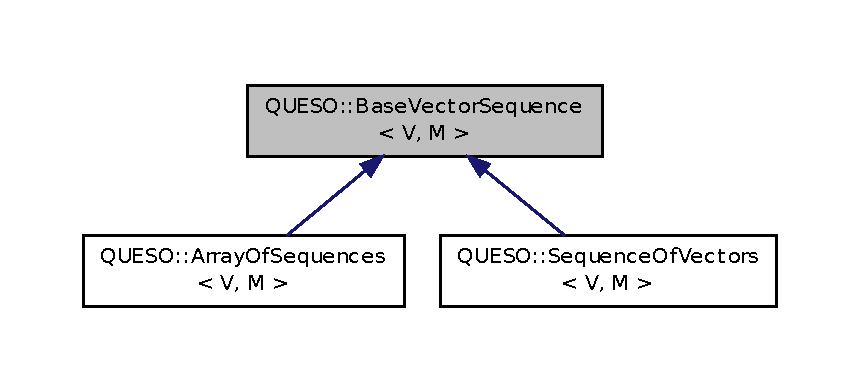
\includegraphics[width=350pt]{class_q_u_e_s_o_1_1_base_vector_sequence__inherit__graph}
\end{center}
\end{figure}


Collaboration diagram for Q\-U\-E\-S\-O\-:\-:Base\-Vector\-Sequence$<$ V, M $>$\-:
\nopagebreak
\begin{figure}[H]
\begin{center}
\leavevmode
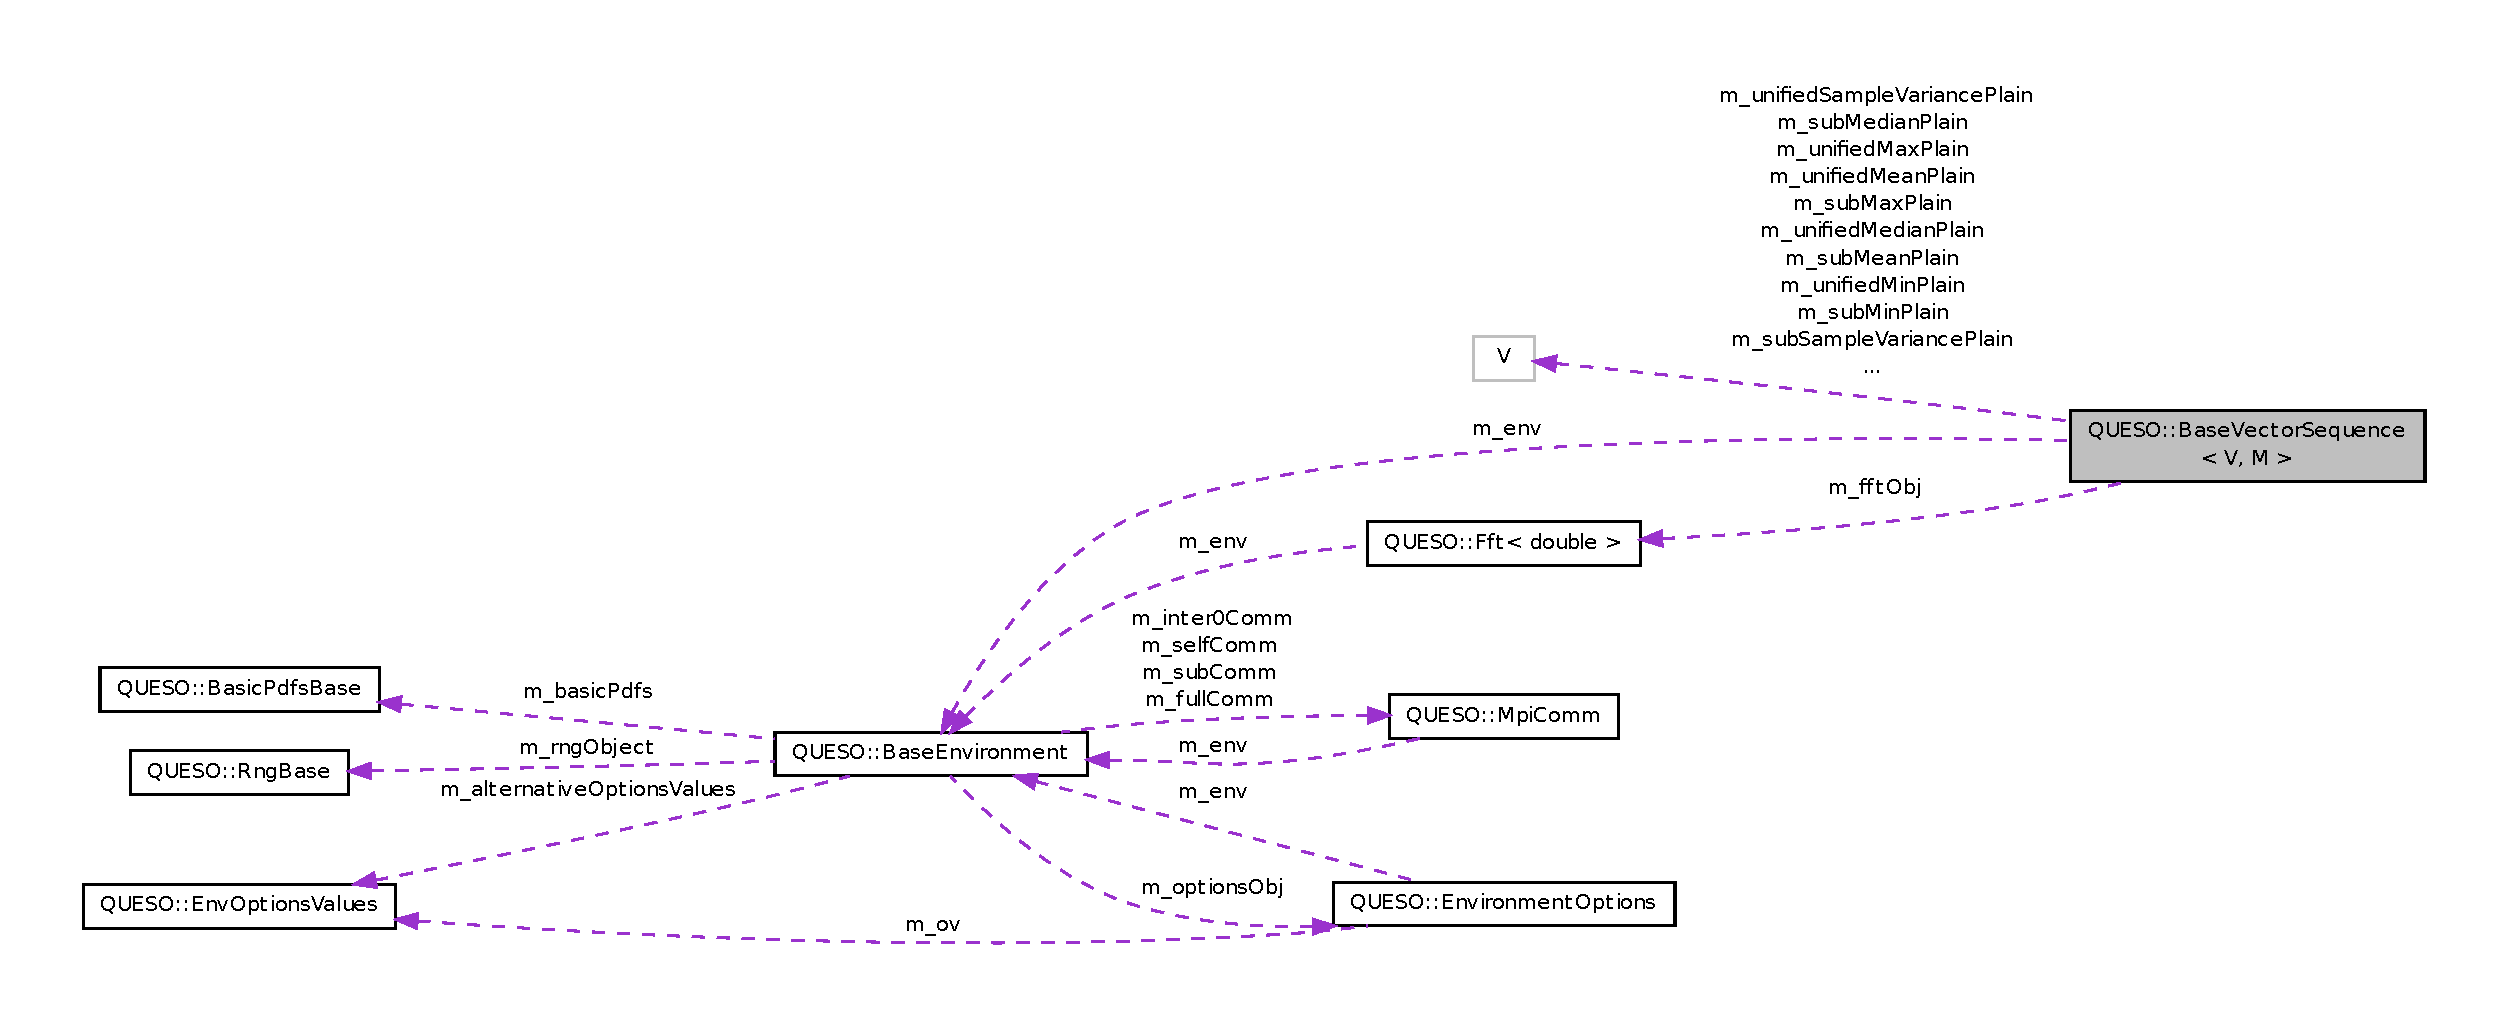
\includegraphics[width=350pt]{class_q_u_e_s_o_1_1_base_vector_sequence__coll__graph}
\end{center}
\end{figure}
\subsection*{Public Member Functions}
\begin{Indent}{\bf Constructor/\-Destructor methods}\par
\begin{DoxyCompactItemize}
\item 
\hyperlink{class_q_u_e_s_o_1_1_base_vector_sequence_a42a447ef253acf28ccb9a20706665b54}{Base\-Vector\-Sequence} (const \hyperlink{class_q_u_e_s_o_1_1_vector_space}{Vector\-Space}$<$ V, M $>$ \&\hyperlink{class_q_u_e_s_o_1_1_base_vector_sequence_af9a4dd979a2fa8dee85bb07793b59ba2}{vector\-Space}, unsigned int \hyperlink{class_q_u_e_s_o_1_1_base_vector_sequence_afd6278702d40bdf1044697bbd6ad1957}{sub\-Sequence\-Size}, const std\-::string \&\hyperlink{class_q_u_e_s_o_1_1_base_vector_sequence_a48f6fe02cf77f4233d3bcdfef3870f19}{name})
\begin{DoxyCompactList}\small\item\em Default constructor. \end{DoxyCompactList}\item 
virtual \hyperlink{class_q_u_e_s_o_1_1_base_vector_sequence_a2e86f2e6dc72338301fcc6898e6f87d4}{$\sim$\-Base\-Vector\-Sequence} ()
\begin{DoxyCompactList}\small\item\em Destructor. \end{DoxyCompactList}\end{DoxyCompactItemize}
\end{Indent}
\begin{Indent}{\bf Sequence methods}\par
\begin{DoxyCompactItemize}
\item 
virtual unsigned int \hyperlink{class_q_u_e_s_o_1_1_base_vector_sequence_afd6278702d40bdf1044697bbd6ad1957}{sub\-Sequence\-Size} () const =0
\begin{DoxyCompactList}\small\item\em Size of the sub-\/sequence of vectors. See template specialization. \end{DoxyCompactList}\item 
unsigned int \hyperlink{class_q_u_e_s_o_1_1_base_vector_sequence_a188dc4632db5b93c01e8bc69bf631f4a}{unified\-Sequence\-Size} () const 
\begin{DoxyCompactList}\small\item\em Calculates the size of the unified sequence of vectors. \end{DoxyCompactList}\item 
unsigned int \hyperlink{class_q_u_e_s_o_1_1_base_vector_sequence_a2fefedf9e5b90f22881103b3f92555f6}{vector\-Size\-Local} () const 
\begin{DoxyCompactList}\small\item\em Local dimension (size) of the vector space. \end{DoxyCompactList}\item 
unsigned int \hyperlink{class_q_u_e_s_o_1_1_base_vector_sequence_aac107ca7ba8ce666f8f994e8bbe922a8}{vector\-Size\-Global} () const 
\begin{DoxyCompactList}\small\item\em Global dimension (size) of the vector space. \end{DoxyCompactList}\item 
const \hyperlink{class_q_u_e_s_o_1_1_vector_space}{Vector\-Space}$<$ V, M $>$ \& \hyperlink{class_q_u_e_s_o_1_1_base_vector_sequence_af9a4dd979a2fa8dee85bb07793b59ba2}{vector\-Space} () const 
\begin{DoxyCompactList}\small\item\em \hyperlink{class_q_u_e_s_o_1_1_vector}{Vector} space; access to protected attribute Vector\-Space$<$\-V,\-M$>$\& m\-\_\-vector\-Space. \end{DoxyCompactList}\item 
const std\-::string \& \hyperlink{class_q_u_e_s_o_1_1_base_vector_sequence_a48f6fe02cf77f4233d3bcdfef3870f19}{name} () const 
\begin{DoxyCompactList}\small\item\em Access to protected attribute {\ttfamily m\-\_\-name\-:} name of the sequence of vectors. \end{DoxyCompactList}\item 
void \hyperlink{class_q_u_e_s_o_1_1_base_vector_sequence_a0a2f78cd12e0f136f7801f7d0175b849}{set\-Name} (const std\-::string \&new\-Name)
\begin{DoxyCompactList}\small\item\em Changes the name of the sequence of vectors. \end{DoxyCompactList}\item 
void \hyperlink{class_q_u_e_s_o_1_1_base_vector_sequence_aae0804eacc51b37e84b1bd329ce1711c}{clear} ()
\begin{DoxyCompactList}\small\item\em Reset the values and the size of the sequence of vectors. \end{DoxyCompactList}\item 
const V \& \hyperlink{class_q_u_e_s_o_1_1_base_vector_sequence_a1b2c4cb7623e0034e4cd66f6443f2fdd}{sub\-Min\-Plain} () const 
\begin{DoxyCompactList}\small\item\em Finds the minimum value of the sub-\/sequence. \end{DoxyCompactList}\item 
const V \& \hyperlink{class_q_u_e_s_o_1_1_base_vector_sequence_a5d330cec5b2c7d9d7eb8079bed4a07ea}{unified\-Min\-Plain} () const 
\begin{DoxyCompactList}\small\item\em Finds the minimum value of the unified sequence. \end{DoxyCompactList}\item 
const V \& \hyperlink{class_q_u_e_s_o_1_1_base_vector_sequence_a152da47e6633bcac5f32b588b98d6f4f}{sub\-Max\-Plain} () const 
\begin{DoxyCompactList}\small\item\em Finds the maximum value of the sub-\/sequence. \end{DoxyCompactList}\item 
const V \& \hyperlink{class_q_u_e_s_o_1_1_base_vector_sequence_a277e760600eb5aa64da9561634a19d63}{unified\-Max\-Plain} () const 
\begin{DoxyCompactList}\small\item\em Finds the maximum value of the unified sequence. \end{DoxyCompactList}\item 
const V \& \hyperlink{class_q_u_e_s_o_1_1_base_vector_sequence_aba7a42fcab55a24264ff80e12d7da2de}{sub\-Mean\-Plain} () const 
\begin{DoxyCompactList}\small\item\em Finds the mean value of the sub-\/sequence. \end{DoxyCompactList}\item 
const V \& \hyperlink{class_q_u_e_s_o_1_1_base_vector_sequence_a64ad551265df354e8c4ccff0d14cb883}{unified\-Mean\-Plain} () const 
\begin{DoxyCompactList}\small\item\em Finds the mean value of the unified sequence. \end{DoxyCompactList}\item 
const V \& \hyperlink{class_q_u_e_s_o_1_1_base_vector_sequence_a679cf7f46c588ed4ba75beeb8fe8ae2d}{sub\-Median\-Plain} () const 
\begin{DoxyCompactList}\small\item\em Finds the median value of the sub-\/sequence. \end{DoxyCompactList}\item 
const V \& \hyperlink{class_q_u_e_s_o_1_1_base_vector_sequence_acdb70319baecc3985e56b9e85502e3cf}{unified\-Median\-Plain} () const 
\begin{DoxyCompactList}\small\item\em Finds the median value of the unified sequence. \end{DoxyCompactList}\item 
const V \& \hyperlink{class_q_u_e_s_o_1_1_base_vector_sequence_a9de650586582d258eb977444d83286a6}{sub\-Sample\-Variance\-Plain} () const 
\begin{DoxyCompactList}\small\item\em Finds the variance of a sample of the sub-\/sequence. \end{DoxyCompactList}\item 
const V \& \hyperlink{class_q_u_e_s_o_1_1_base_vector_sequence_a34a8b31757c6b728feefcf396d62c12f}{unified\-Sample\-Variance\-Plain} () const 
\begin{DoxyCompactList}\small\item\em Finds the variance of a sample of the unified sequence. \end{DoxyCompactList}\item 
const \hyperlink{class_q_u_e_s_o_1_1_box_subset}{Box\-Subset}$<$ V, M $>$ \& \hyperlink{class_q_u_e_s_o_1_1_base_vector_sequence_a5c5ede038fbdb296e3913bc39142b7ff}{sub\-Box\-Plain} () const 
\begin{DoxyCompactList}\small\item\em Finds a box subset of the sub-\/sequence (given by its min and max values calculated via sub\-Min\-Plain and sub\-Max\-Plain). \end{DoxyCompactList}\item 
const \hyperlink{class_q_u_e_s_o_1_1_box_subset}{Box\-Subset}$<$ V, M $>$ \& \hyperlink{class_q_u_e_s_o_1_1_base_vector_sequence_a69757707519d6d10b454c36ee624fecc}{unified\-Box\-Plain} () const 
\begin{DoxyCompactList}\small\item\em Finds a box subset of the unified-\/sequence (given by the min and max values of the unified sequence calculated via unified\-Min\-Plain and unified\-Max\-Plain). \end{DoxyCompactList}\item 
void \hyperlink{class_q_u_e_s_o_1_1_base_vector_sequence_a5609e02046ba555f0eebe49c6c231faf}{delete\-Stored\-Vectors} ()
\begin{DoxyCompactList}\small\item\em Deletes all the stored vectors. \end{DoxyCompactList}\item 
void \hyperlink{class_q_u_e_s_o_1_1_base_vector_sequence_a50419477cd593478815aa52af58695a8}{append} (const \hyperlink{class_q_u_e_s_o_1_1_base_vector_sequence}{Base\-Vector\-Sequence}$<$ V, M $>$ \&src, unsigned int initial\-Pos, unsigned int num\-Pos)
\begin{DoxyCompactList}\small\item\em Appends the vector {\ttfamily src} to {\ttfamily this} vector. \end{DoxyCompactList}\item 
double \hyperlink{class_q_u_e_s_o_1_1_base_vector_sequence_a971e9e1a87e4eb47b4910348a6b437d5}{sub\-Positions\-Of\-Maximum} (const \hyperlink{class_q_u_e_s_o_1_1_scalar_sequence}{Scalar\-Sequence}$<$ double $>$ \&sub\-Corresponding\-Scalar\-Values, \hyperlink{class_q_u_e_s_o_1_1_base_vector_sequence}{Base\-Vector\-Sequence}$<$ V, M $>$ \&sub\-Positions\-Of\-Maximum)
\begin{DoxyCompactList}\small\item\em Finds the positions where the maximum element occurs in the sub-\/sequence. \end{DoxyCompactList}\item 
double \hyperlink{class_q_u_e_s_o_1_1_base_vector_sequence_a4269482101b2bcdb1975543f8191ab4c}{unified\-Positions\-Of\-Maximum} (const \hyperlink{class_q_u_e_s_o_1_1_scalar_sequence}{Scalar\-Sequence}$<$ double $>$ \&sub\-Corresponding\-Scalar\-Values, \hyperlink{class_q_u_e_s_o_1_1_base_vector_sequence}{Base\-Vector\-Sequence}$<$ V, M $>$ \&unified\-Positions\-Of\-Maximum)
\begin{DoxyCompactList}\small\item\em Finds the positions where the maximum element occurs in the unified sequence. \end{DoxyCompactList}\item 
virtual void \hyperlink{class_q_u_e_s_o_1_1_base_vector_sequence_adc238af7f6e8af2402ab791de7d60af5}{resize\-Sequence} (unsigned int new\-Sub\-Sequence\-Size)=0
\begin{DoxyCompactList}\small\item\em Resize the sequence. See template specialization. \end{DoxyCompactList}\item 
virtual void \hyperlink{class_q_u_e_s_o_1_1_base_vector_sequence_ab007ea121708b1b1a63553433b428413}{reset\-Values} (unsigned int initial\-Pos, unsigned int num\-Pos)=0
\begin{DoxyCompactList}\small\item\em Reset the values of the sequence. See template specialization. \end{DoxyCompactList}\item 
virtual void \hyperlink{class_q_u_e_s_o_1_1_base_vector_sequence_a2b41ed436f95a1816a811fc368adaf79}{erase\-Positions} (unsigned int initial\-Pos, unsigned int num\-Pos)=0
\begin{DoxyCompactList}\small\item\em Erase {\ttfamily num\-Pos} positions in the sequence, starting at position {\ttfamily initial\-Pos}. \end{DoxyCompactList}\item 
virtual void \hyperlink{class_q_u_e_s_o_1_1_base_vector_sequence_a656d47a18b401d6d914b0daf2dea88b0}{get\-Position\-Values} (unsigned int pos\-Id, V \&vec) const =0
\begin{DoxyCompactList}\small\item\em Gets the values of the sequence at position {\ttfamily pos\-Id} and stores them at {\ttfamily vec}. See template specialization. \end{DoxyCompactList}\item 
virtual void \hyperlink{class_q_u_e_s_o_1_1_base_vector_sequence_a5bcce98b68e0e24c05136e7a3bb50c12}{set\-Position\-Values} (unsigned int pos\-Id, const V \&vec)=0
\begin{DoxyCompactList}\small\item\em Set the values in {\ttfamily vec} at position {\ttfamily pos\-Id} of the sequence. See template specialization. \end{DoxyCompactList}\item 
void \hyperlink{class_q_u_e_s_o_1_1_base_vector_sequence_aa1081248d23a2b18307962993892eb4c}{set\-Gaussian} (const V \&mean\-Vec, const V \&std\-Dev\-Vec)
\begin{DoxyCompactList}\small\item\em Sets the values of the sequence as a Gaussian distribution of mean given by {\ttfamily mean\-Vec} and standard deviation by {\ttfamily std\-Dev\-Vec}. \end{DoxyCompactList}\item 
void \hyperlink{class_q_u_e_s_o_1_1_base_vector_sequence_a96d44e7dd53a077a4c7be73f008b351e}{set\-Uniform} (const V \&a\-Vec, const V \&b\-Vec)
\begin{DoxyCompactList}\small\item\em Sets the values of the sequence as a uniform distribution between the values given by vectors {\ttfamily a\-Vec} and {\ttfamily b\-Vec}. \end{DoxyCompactList}\item 
virtual void \hyperlink{class_q_u_e_s_o_1_1_base_vector_sequence_ab36f3e2511108259c272d8a148452505}{sub\-Mean\-Extra} (unsigned int initial\-Pos, unsigned int num\-Pos, V \&mean\-Vec) const =0
\begin{DoxyCompactList}\small\item\em Finds the mean value of the sub-\/sequence, considering {\ttfamily num\-Pos} positions starting at position {\ttfamily initial\-Pos}. See template specialization. \end{DoxyCompactList}\item 
virtual void \hyperlink{class_q_u_e_s_o_1_1_base_vector_sequence_a6ee252d07395644a9175aabf2bad7aed}{unified\-Mean\-Extra} (unsigned int initial\-Pos, unsigned int num\-Pos, V \&unified\-Mean\-Vec) const =0
\begin{DoxyCompactList}\small\item\em Finds the mean value of the unified sequence of {\ttfamily num\-Pos} positions starting at position {\ttfamily initial\-Pos}. See template specialization. \end{DoxyCompactList}\item 
virtual void \hyperlink{class_q_u_e_s_o_1_1_base_vector_sequence_a80caa77a7258c3ae44b6320846cfe29d}{sub\-Median\-Extra} (unsigned int initial\-Pos, unsigned int num\-Pos, V \&median\-Vec) const =0
\begin{DoxyCompactList}\small\item\em Finds the median value of the sub-\/sequence, considering {\ttfamily num\-Pos} positions starting at position {\ttfamily initial\-Pos}. See template specialization. \end{DoxyCompactList}\item 
virtual void \hyperlink{class_q_u_e_s_o_1_1_base_vector_sequence_ab3b300eb093fe8d726996db5726e59e4}{unified\-Median\-Extra} (unsigned int initial\-Pos, unsigned int local\-Num\-Pos, V \&unified\-Median\-Vec) const =0
\begin{DoxyCompactList}\small\item\em Finds the median value of the unified sequence, considering {\ttfamily num\-Pos} positions starting at position {\ttfamily initial\-Pos}. See template specialization. \end{DoxyCompactList}\item 
virtual void \hyperlink{class_q_u_e_s_o_1_1_base_vector_sequence_a6a786862951dfae45a9daebc9d81e676}{sub\-Sample\-Variance\-Extra} (unsigned int initial\-Pos, unsigned int num\-Pos, const V \&mean\-Vec, V \&sam\-Vec) const =0
\begin{DoxyCompactList}\small\item\em Finds the sample variance of the sub-\/sequence, considering {\ttfamily num\-Pos} positions starting at position {\ttfamily initial\-Pos} and of mean {\ttfamily mean\-Vec}. See template specialization. \end{DoxyCompactList}\item 
virtual void \hyperlink{class_q_u_e_s_o_1_1_base_vector_sequence_abc759076a4c5d9e1586a6d93629778ff}{unified\-Sample\-Variance\-Extra} (unsigned int initial\-Pos, unsigned int num\-Pos, const V \&unified\-Mean\-Vec, V \&unified\-Sam\-Vec) const =0
\begin{DoxyCompactList}\small\item\em Finds the sample variance of the unified sequence, considering {\ttfamily num\-Pos} positions starting at position {\ttfamily initial\-Pos} and of mean {\ttfamily mean\-Vec}. See template specialization. \end{DoxyCompactList}\item 
virtual void \hyperlink{class_q_u_e_s_o_1_1_base_vector_sequence_af21f1923841372684ae9e5812767832d}{sub\-Population\-Variance} (unsigned int initial\-Pos, unsigned int num\-Pos, const V \&mean\-Vec, V \&pop\-Vec) const =0
\begin{DoxyCompactList}\small\item\em Finds the population variance of the sub-\/sequence, considering {\ttfamily num\-Pos} positions starting at position {\ttfamily initial\-Pos} and of mean {\ttfamily mean\-Vec}. See template specialization. \end{DoxyCompactList}\item 
virtual void \hyperlink{class_q_u_e_s_o_1_1_base_vector_sequence_ad9e165f7a0d57e2fa45e7b3926dac1a2}{unified\-Population\-Variance} (unsigned int initial\-Pos, unsigned int num\-Pos, const V \&unified\-Mean\-Vec, V \&unified\-Pop\-Vec) const =0
\begin{DoxyCompactList}\small\item\em Finds the population variance of the unified-\/sequence, considering {\ttfamily num\-Pos} positions starting at position {\ttfamily initial\-Pos} and of mean {\ttfamily mean\-Vec}. See template specialization. \end{DoxyCompactList}\item 
virtual void \hyperlink{class_q_u_e_s_o_1_1_base_vector_sequence_a3a831c06c8ede53b84ce72fac3f018c0}{auto\-Covariance} (unsigned int initial\-Pos, unsigned int num\-Pos, const V \&mean\-Vec, unsigned int lag, V \&cov\-Vec) const =0
\begin{DoxyCompactList}\small\item\em Calculates the autocovariance. See template specialization. \end{DoxyCompactList}\item 
virtual void \hyperlink{class_q_u_e_s_o_1_1_base_vector_sequence_ab4d322b34c43ad47df9a76582a0693d0}{auto\-Corr\-Via\-Def} (unsigned int initial\-Pos, unsigned int num\-Pos, unsigned int lag, V \&corr\-Vec) const =0
\begin{DoxyCompactList}\small\item\em Calculates autocorrelation via definition. See template specialization. \end{DoxyCompactList}\item 
virtual void \hyperlink{class_q_u_e_s_o_1_1_base_vector_sequence_a709a63b678508c47bedd416ece5342ef}{auto\-Corr\-Via\-Fft} (unsigned int initial\-Pos, unsigned int num\-Pos, const std\-::vector$<$ unsigned int $>$ \&lags, std\-::vector$<$ V $\ast$ $>$ \&corr\-Vecs) const =0
\begin{DoxyCompactList}\small\item\em Calculates autocorrelation via Fast Fourier transforms (F\-F\-T). See template specialization. \end{DoxyCompactList}\item 
virtual void \hyperlink{class_q_u_e_s_o_1_1_base_vector_sequence_af9f2478ed4112aa615caef21bf26ab35}{auto\-Corr\-Via\-Fft} (unsigned int initial\-Pos, unsigned int num\-Pos, unsigned int num\-Sum, V \&auto\-Corrs\-Sum\-Vec) const =0
\begin{DoxyCompactList}\small\item\em Calculates autocorrelation via Fast Fourier transforms (F\-F\-T). See template specialization. \end{DoxyCompactList}\item 
virtual void \hyperlink{class_q_u_e_s_o_1_1_base_vector_sequence_a14fd8d5c3ff3fb2f7eb3f4b9e7131d0c}{sub\-Min\-Max\-Extra} (unsigned int initial\-Pos, unsigned int num\-Pos, V \&min\-Vec, V \&max\-Vec) const =0
\begin{DoxyCompactList}\small\item\em Finds the minimum and the maximum values of the sub-\/sequence, considering {\ttfamily num\-Pos} positions starting at position {\ttfamily initial\-Pos}. See template specialization. \end{DoxyCompactList}\item 
virtual void \hyperlink{class_q_u_e_s_o_1_1_base_vector_sequence_a2d6cd9b93580715762318b51edbd9463}{unified\-Min\-Max\-Extra} (unsigned int initial\-Pos, unsigned int num\-Pos, V \&unified\-Min\-Vec, V \&unified\-Max\-Vec) const =0
\begin{DoxyCompactList}\small\item\em Finds the minimum and the maximum values of the unified sequence, considering {\ttfamily num\-Pos} positions starting at position {\ttfamily initial\-Pos}. See template specialization. \end{DoxyCompactList}\item 
virtual void \hyperlink{class_q_u_e_s_o_1_1_base_vector_sequence_a66c6af1f9a509720264d121b408a45f3}{sub\-Histogram} (unsigned int initial\-Pos, const V \&min\-Vec, const V \&max\-Vec, std\-::vector$<$ V $\ast$ $>$ \&centers\-For\-All\-Bins, std\-::vector$<$ V $\ast$ $>$ \&quantts\-For\-All\-Bins) const =0
\begin{DoxyCompactList}\small\item\em Calculates the histogram of the sub-\/sequence. See template specialization. \end{DoxyCompactList}\item 
virtual void \hyperlink{class_q_u_e_s_o_1_1_base_vector_sequence_a04653bd3bd8b9c29ae6d03a2eb0b3779}{unified\-Histogram} (unsigned int initial\-Pos, const V \&unified\-Min\-Vec, const V \&unified\-Max\-Vec, std\-::vector$<$ V $\ast$ $>$ \&unified\-Centers\-For\-All\-Bins, std\-::vector$<$ V $\ast$ $>$ \&unified\-Quantts\-For\-All\-Bins) const =0
\begin{DoxyCompactList}\small\item\em Calculates the histogram of the unified sequence. See template specialization. \end{DoxyCompactList}\item 
virtual void \hyperlink{class_q_u_e_s_o_1_1_base_vector_sequence_a62cb96f153a8608ef1727265a734aacb}{sub\-Inter\-Quantile\-Range} (unsigned int initial\-Pos, V \&iqr\-Vec) const =0
\begin{DoxyCompactList}\small\item\em Returns the interquartile range of the values in the sub-\/sequence. See template specialization. \end{DoxyCompactList}\item 
virtual void \hyperlink{class_q_u_e_s_o_1_1_base_vector_sequence_a49b50dfef9bf3475eb681855268c050d}{unified\-Inter\-Quantile\-Range} (unsigned int initial\-Pos, V \&unified\-Iqr\-Vec) const =0
\begin{DoxyCompactList}\small\item\em Returns the interquartile range of the values in the unified sequence. See template specialization. \end{DoxyCompactList}\item 
virtual void \hyperlink{class_q_u_e_s_o_1_1_base_vector_sequence_af3210c9073cedfcd8dfe79ed323975a2}{sub\-Scales\-For\-Kde} (unsigned int initial\-Pos, const V \&iqr\-Vec, unsigned int kde\-Dimension, V \&scale\-Vec) const =0
\begin{DoxyCompactList}\small\item\em Selects the scales (bandwidth, {\ttfamily scale\-Vec}) for the kernel density estimation, considering only the sub-\/sequence. See template specialization. \end{DoxyCompactList}\item 
virtual void \hyperlink{class_q_u_e_s_o_1_1_base_vector_sequence_a68eae0b37fc934391ce7af2c370fd585}{unified\-Scales\-For\-Kde} (unsigned int initial\-Pos, const V \&unified\-Iqr\-Vec, unsigned int kde\-Dimension, V \&unified\-Scale\-Vec) const =0
\begin{DoxyCompactList}\small\item\em Selects the scales (bandwidth) for the kernel density estimation, considering the unified sequence. See template specialization. \end{DoxyCompactList}\item 
virtual void \hyperlink{class_q_u_e_s_o_1_1_base_vector_sequence_a0fec2746f326acad09b406ad8efe1cfc}{sub\-Gaussian1d\-Kde} (unsigned int initial\-Pos, const V \&scale\-Vec, const std\-::vector$<$ V $\ast$ $>$ \&evaluation\-Param\-Vecs, std\-::vector$<$ V $\ast$ $>$ \&density\-Vecs) const =0
\begin{DoxyCompactList}\small\item\em Gaussian kernel for the K\-D\-E estimate of the sub-\/sequence. See template specialization. \end{DoxyCompactList}\item 
virtual void \hyperlink{class_q_u_e_s_o_1_1_base_vector_sequence_aa799ae2fde5edc96939990925d7be9ac}{unified\-Gaussian1d\-Kde} (unsigned int initial\-Pos, const V \&unified\-Scale\-Vec, const std\-::vector$<$ V $\ast$ $>$ \&unified\-Evaluation\-Param\-Vecs, std\-::vector$<$ V $\ast$ $>$ \&unified\-Density\-Vecs) const =0
\begin{DoxyCompactList}\small\item\em Gaussian kernel for the K\-D\-E estimate of the unified sequence. See template specialization. \end{DoxyCompactList}\item 
virtual void \hyperlink{class_q_u_e_s_o_1_1_base_vector_sequence_aa59738c6df15b1b369b90f0d025fb6f2}{sub\-Write\-Contents} (unsigned int initial\-Pos, unsigned int num\-Pos, const std\-::string \&file\-Name, const std\-::string \&file\-Type, const std\-::set$<$ unsigned int $>$ \&allowed\-Sub\-Env\-Ids) const =0
\begin{DoxyCompactList}\small\item\em Writes info of the sub-\/sequence to a file. See template specialization. \end{DoxyCompactList}\item 
virtual void \hyperlink{class_q_u_e_s_o_1_1_base_vector_sequence_a7226d1093a7ab07792410414237f08da}{sub\-Write\-Contents} (unsigned int initial\-Pos, unsigned int num\-Pos, std\-::ofstream \&ofsvar, const std\-::string \&file\-Type) const =0
\begin{DoxyCompactList}\small\item\em Writes info of the sub-\/sequence to a file. See template specialization. \end{DoxyCompactList}\item 
virtual void \hyperlink{class_q_u_e_s_o_1_1_base_vector_sequence_a3987ee6d026842e4ddaeaf0bc850ef83}{unified\-Write\-Contents} (const std\-::string \&file\-Name, const std\-::string \&file\-Type) const =0
\begin{DoxyCompactList}\small\item\em Writes info of the unified sequence to a file. See template specialization. \end{DoxyCompactList}\item 
virtual void \hyperlink{class_q_u_e_s_o_1_1_base_vector_sequence_afcb5935b592ab2e7ee39d23b08bcce62}{unified\-Read\-Contents} (const std\-::string \&file\-Name, const std\-::string \&file\-Type, const unsigned int \hyperlink{class_q_u_e_s_o_1_1_base_vector_sequence_afd6278702d40bdf1044697bbd6ad1957}{sub\-Sequence\-Size})=0
\begin{DoxyCompactList}\small\item\em Reads info of the unified sequence from a file. See template specialization. \end{DoxyCompactList}\item 
virtual void \hyperlink{class_q_u_e_s_o_1_1_base_vector_sequence_a4ff00d9659c59653844b78410571f3fe}{select} (const std\-::vector$<$ unsigned int $>$ \&ids\-Of\-Unique\-Positions)=0
\begin{DoxyCompactList}\small\item\em Select positions in the sequence of vectors. See template specialization. \end{DoxyCompactList}\item 
virtual void \hyperlink{class_q_u_e_s_o_1_1_base_vector_sequence_adfb88fdbaa1c6b2b040ef888633619ef}{filter} (unsigned int initial\-Pos, unsigned int spacing)=0
\begin{DoxyCompactList}\small\item\em Filters positions in the sequence of vectors, starting at {\ttfamily initial\-Pos}, and with spacing given by {\ttfamily spacing}. See template specialization. \end{DoxyCompactList}\item 
void \hyperlink{class_q_u_e_s_o_1_1_base_vector_sequence_a8e34f6205e26eab1e9cbe457dbd376bc}{compute\-Filter\-Params} (std\-::ofstream $\ast$passed\-Ofs, unsigned int \&initial\-Pos, unsigned int \&spacing)
\begin{DoxyCompactList}\small\item\em Computes the filtering parameters {\ttfamily spacing} for the sequence of vectors. \end{DoxyCompactList}\item 
virtual double \hyperlink{class_q_u_e_s_o_1_1_base_vector_sequence_a7f70b1762b6ba91a8f619403453cf2b2}{estimate\-Conv\-Brooks\-Gelman} (unsigned int initial\-Pos, unsigned int num\-Pos) const =0
\begin{DoxyCompactList}\small\item\em Estimates convergence rate using Brooks \& Gelman method. See template specialization. \end{DoxyCompactList}\item 
virtual void \hyperlink{class_q_u_e_s_o_1_1_base_vector_sequence_a0ec0f2595d606723d0b069e1632cc348}{extract\-Scalar\-Seq} (unsigned int initial\-Pos, unsigned int spacing, unsigned int num\-Pos, unsigned int param\-Id, \hyperlink{class_q_u_e_s_o_1_1_scalar_sequence}{Scalar\-Sequence}$<$ double $>$ \&scalar\-Seq) const =0
\begin{DoxyCompactList}\small\item\em Extracts a sequence of scalars of size {\ttfamily num\-Pos}, starting at position {\ttfamily initial\-Pos}, given spacing {\ttfamily spacing}. See template specialization. \end{DoxyCompactList}\end{DoxyCompactItemize}
\end{Indent}
\subsection*{Protected Member Functions}
\begin{DoxyCompactItemize}
\item 
void \hyperlink{class_q_u_e_s_o_1_1_base_vector_sequence_a35629a6937e22752e3b252e84457e791}{copy} (const \hyperlink{class_q_u_e_s_o_1_1_base_vector_sequence}{Base\-Vector\-Sequence}$<$ V, M $>$ \&src)
\begin{DoxyCompactList}\small\item\em Copies vector sequence {\ttfamily src} to {\ttfamily this}. \end{DoxyCompactList}\item 
virtual void \hyperlink{class_q_u_e_s_o_1_1_base_vector_sequence_aae5259810d72d393328369d8d4087d5d}{extract\-Raw\-Data} (unsigned int initial\-Pos, unsigned int spacing, unsigned int num\-Pos, unsigned int param\-Id, std\-::vector$<$ double $>$ \&raw\-Data) const =0
\begin{DoxyCompactList}\small\item\em Extracts the raw data. See template specialization. \end{DoxyCompactList}\end{DoxyCompactItemize}
\subsection*{Protected Attributes}
\begin{DoxyCompactItemize}
\item 
const \hyperlink{class_q_u_e_s_o_1_1_base_environment}{Base\-Environment} \& \hyperlink{class_q_u_e_s_o_1_1_base_vector_sequence_a8e8824d2a63c5a43bcc6473e3a0491e8}{m\-\_\-env}
\item 
const \hyperlink{class_q_u_e_s_o_1_1_vector_space}{Vector\-Space}$<$ V, M $>$ \& \hyperlink{class_q_u_e_s_o_1_1_base_vector_sequence_a4bd171e39ed050ff105c808336f35198}{m\-\_\-vector\-Space}
\item 
std\-::string \hyperlink{class_q_u_e_s_o_1_1_base_vector_sequence_a3c379b2f7c20a2a1dd083ea43fca1494}{m\-\_\-name}
\item 
\hyperlink{class_q_u_e_s_o_1_1_fft}{Fft}$<$ double $>$ $\ast$ \hyperlink{class_q_u_e_s_o_1_1_base_vector_sequence_add593820ac53e4adccb3002ba0becfa7}{m\-\_\-fft\-Obj}
\item 
V $\ast$ \hyperlink{class_q_u_e_s_o_1_1_base_vector_sequence_ab4be9e46882547032a1b738b6fafc2f8}{m\-\_\-sub\-Min\-Plain}
\item 
V $\ast$ \hyperlink{class_q_u_e_s_o_1_1_base_vector_sequence_a8401f459127618bbdcb0826ddb69b550}{m\-\_\-unified\-Min\-Plain}
\item 
V $\ast$ \hyperlink{class_q_u_e_s_o_1_1_base_vector_sequence_a1f24826fd2ca206a6e2662ade55dc5cb}{m\-\_\-sub\-Max\-Plain}
\item 
V $\ast$ \hyperlink{class_q_u_e_s_o_1_1_base_vector_sequence_a5abbf8a1b56ffd00f00a065ff1af1e68}{m\-\_\-unified\-Max\-Plain}
\item 
V $\ast$ \hyperlink{class_q_u_e_s_o_1_1_base_vector_sequence_aea341eac0220157a44f373e1377e0ca0}{m\-\_\-sub\-Mean\-Plain}
\item 
V $\ast$ \hyperlink{class_q_u_e_s_o_1_1_base_vector_sequence_a0bb5f2fa3d8369412b8cf5f6795b95b4}{m\-\_\-unified\-Mean\-Plain}
\item 
V $\ast$ \hyperlink{class_q_u_e_s_o_1_1_base_vector_sequence_a99ab57b8cb62b14eedd606b9d2e75672}{m\-\_\-sub\-Median\-Plain}
\item 
V $\ast$ \hyperlink{class_q_u_e_s_o_1_1_base_vector_sequence_ac723ac11f629ba07915f7520b36e4138}{m\-\_\-unified\-Median\-Plain}
\item 
V $\ast$ \hyperlink{class_q_u_e_s_o_1_1_base_vector_sequence_a25dc9797633cb4b23b7330c5d3de9dd7}{m\-\_\-sub\-Sample\-Variance\-Plain}
\item 
V $\ast$ \hyperlink{class_q_u_e_s_o_1_1_base_vector_sequence_ab6fa4daa233c386ea96718cf6cac603b}{m\-\_\-unified\-Sample\-Variance\-Plain}
\item 
\hyperlink{class_q_u_e_s_o_1_1_box_subset}{Box\-Subset}$<$ V, M $>$ $\ast$ \hyperlink{class_q_u_e_s_o_1_1_base_vector_sequence_a8fa117289936a6b0cd83dd55aaf55047}{m\-\_\-sub\-Box\-Plain}
\item 
\hyperlink{class_q_u_e_s_o_1_1_box_subset}{Box\-Subset}$<$ V, M $>$ $\ast$ \hyperlink{class_q_u_e_s_o_1_1_base_vector_sequence_a13e15d877a0826605eb62fd65244761a}{m\-\_\-unified\-Box\-Plain}
\end{DoxyCompactItemize}


\subsection{Detailed Description}
\subsubsection*{template$<$class V, class M$>$class Q\-U\-E\-S\-O\-::\-Base\-Vector\-Sequence$<$ V, M $>$}

Base class for handling vector and array samples (sequence of vectors or arrays). 

This class handles either vector or array samples generated by an algorithm, as well as operations that can be carried over them, e.\-g., calculation of means, correlation and covariance matrices. 

Definition at line 54 of file Vector\-Sequence.\-h.



\subsection{Constructor \& Destructor Documentation}
\hypertarget{class_q_u_e_s_o_1_1_base_vector_sequence_a42a447ef253acf28ccb9a20706665b54}{\index{Q\-U\-E\-S\-O\-::\-Base\-Vector\-Sequence@{Q\-U\-E\-S\-O\-::\-Base\-Vector\-Sequence}!Base\-Vector\-Sequence@{Base\-Vector\-Sequence}}
\index{Base\-Vector\-Sequence@{Base\-Vector\-Sequence}!QUESO::BaseVectorSequence@{Q\-U\-E\-S\-O\-::\-Base\-Vector\-Sequence}}
\subsubsection[{Base\-Vector\-Sequence}]{\setlength{\rightskip}{0pt plus 5cm}template$<$class V, class M$>$ {\bf Q\-U\-E\-S\-O\-::\-Base\-Vector\-Sequence}$<$ V, M $>$\-::{\bf Base\-Vector\-Sequence} (
\begin{DoxyParamCaption}
\item[{const {\bf Vector\-Space}$<$ V, M $>$ \&}]{vector\-Space, }
\item[{unsigned int}]{sub\-Sequence\-Size, }
\item[{const std\-::string \&}]{name}
\end{DoxyParamCaption}
)}}\label{class_q_u_e_s_o_1_1_base_vector_sequence_a42a447ef253acf28ccb9a20706665b54}


Default constructor. 



Definition at line 34 of file Vector\-Sequence.\-C.


\begin{DoxyCode}
38   :
39   \hyperlink{class_q_u_e_s_o_1_1_base_vector_sequence_a8e8824d2a63c5a43bcc6473e3a0491e8}{m\_env}                       (\hyperlink{class_q_u_e_s_o_1_1_base_vector_sequence_af9a4dd979a2fa8dee85bb07793b59ba2}{vectorSpace}.env()),
40   \hyperlink{class_q_u_e_s_o_1_1_base_vector_sequence_a4bd171e39ed050ff105c808336f35198}{m\_vectorSpace}               (\hyperlink{class_q_u_e_s_o_1_1_base_vector_sequence_af9a4dd979a2fa8dee85bb07793b59ba2}{vectorSpace}),
41   \hyperlink{class_q_u_e_s_o_1_1_base_vector_sequence_a3c379b2f7c20a2a1dd083ea43fca1494}{m\_name}                      (\hyperlink{class_q_u_e_s_o_1_1_base_vector_sequence_a48f6fe02cf77f4233d3bcdfef3870f19}{name}),
42   \hyperlink{class_q_u_e_s_o_1_1_base_vector_sequence_add593820ac53e4adccb3002ba0becfa7}{m\_fftObj}                    (\textcolor{keyword}{new} Fft<double>(\hyperlink{class_q_u_e_s_o_1_1_base_vector_sequence_a8e8824d2a63c5a43bcc6473e3a0491e8}{m\_env})),
43   \hyperlink{class_q_u_e_s_o_1_1_base_vector_sequence_ab4be9e46882547032a1b738b6fafc2f8}{m\_subMinPlain}               (NULL),
44   \hyperlink{class_q_u_e_s_o_1_1_base_vector_sequence_a8401f459127618bbdcb0826ddb69b550}{m\_unifiedMinPlain}           (NULL),
45   \hyperlink{class_q_u_e_s_o_1_1_base_vector_sequence_a1f24826fd2ca206a6e2662ade55dc5cb}{m\_subMaxPlain}               (NULL),
46   \hyperlink{class_q_u_e_s_o_1_1_base_vector_sequence_a5abbf8a1b56ffd00f00a065ff1af1e68}{m\_unifiedMaxPlain}           (NULL),
47   \hyperlink{class_q_u_e_s_o_1_1_base_vector_sequence_aea341eac0220157a44f373e1377e0ca0}{m\_subMeanPlain}              (NULL),
48   \hyperlink{class_q_u_e_s_o_1_1_base_vector_sequence_a0bb5f2fa3d8369412b8cf5f6795b95b4}{m\_unifiedMeanPlain}          (NULL),
49   \hyperlink{class_q_u_e_s_o_1_1_base_vector_sequence_a99ab57b8cb62b14eedd606b9d2e75672}{m\_subMedianPlain}            (NULL),
50   \hyperlink{class_q_u_e_s_o_1_1_base_vector_sequence_ac723ac11f629ba07915f7520b36e4138}{m\_unifiedMedianPlain}        (NULL),
51   \hyperlink{class_q_u_e_s_o_1_1_base_vector_sequence_a25dc9797633cb4b23b7330c5d3de9dd7}{m\_subSampleVariancePlain}    (NULL),
52   \hyperlink{class_q_u_e_s_o_1_1_base_vector_sequence_ab6fa4daa233c386ea96718cf6cac603b}{m\_unifiedSampleVariancePlain}(NULL),
53   \hyperlink{class_q_u_e_s_o_1_1_base_vector_sequence_a8fa117289936a6b0cd83dd55aaf55047}{m\_subBoxPlain}               (NULL),
54   \hyperlink{class_q_u_e_s_o_1_1_base_vector_sequence_a13e15d877a0826605eb62fd65244761a}{m\_unifiedBoxPlain}           (NULL)
55 \{
56   \textcolor{keywordflow}{if} (\hyperlink{class_q_u_e_s_o_1_1_base_vector_sequence_afd6278702d40bdf1044697bbd6ad1957}{subSequenceSize}) \{\}; \textcolor{comment}{// just to avoid compiler warning}
57 \}
\end{DoxyCode}
\hypertarget{class_q_u_e_s_o_1_1_base_vector_sequence_a2e86f2e6dc72338301fcc6898e6f87d4}{\index{Q\-U\-E\-S\-O\-::\-Base\-Vector\-Sequence@{Q\-U\-E\-S\-O\-::\-Base\-Vector\-Sequence}!$\sim$\-Base\-Vector\-Sequence@{$\sim$\-Base\-Vector\-Sequence}}
\index{$\sim$\-Base\-Vector\-Sequence@{$\sim$\-Base\-Vector\-Sequence}!QUESO::BaseVectorSequence@{Q\-U\-E\-S\-O\-::\-Base\-Vector\-Sequence}}
\subsubsection[{$\sim$\-Base\-Vector\-Sequence}]{\setlength{\rightskip}{0pt plus 5cm}template$<$class V , class M $>$ {\bf Q\-U\-E\-S\-O\-::\-Base\-Vector\-Sequence}$<$ V, M $>$\-::$\sim${\bf Base\-Vector\-Sequence} (
\begin{DoxyParamCaption}
{}
\end{DoxyParamCaption}
)\hspace{0.3cm}{\ttfamily [virtual]}}}\label{class_q_u_e_s_o_1_1_base_vector_sequence_a2e86f2e6dc72338301fcc6898e6f87d4}


Destructor. 



Definition at line 60 of file Vector\-Sequence.\-C.


\begin{DoxyCode}
61 \{
62   \textcolor{comment}{//clear();}
63   this->\hyperlink{class_q_u_e_s_o_1_1_base_vector_sequence_a5609e02046ba555f0eebe49c6c231faf}{deleteStoredVectors}();
64   \textcolor{keywordflow}{if} (\hyperlink{class_q_u_e_s_o_1_1_base_vector_sequence_add593820ac53e4adccb3002ba0becfa7}{m\_fftObj} != NULL) \textcolor{keyword}{delete} \hyperlink{class_q_u_e_s_o_1_1_base_vector_sequence_add593820ac53e4adccb3002ba0becfa7}{m\_fftObj};
65 \}
\end{DoxyCode}


\subsection{Member Function Documentation}
\hypertarget{class_q_u_e_s_o_1_1_base_vector_sequence_a50419477cd593478815aa52af58695a8}{\index{Q\-U\-E\-S\-O\-::\-Base\-Vector\-Sequence@{Q\-U\-E\-S\-O\-::\-Base\-Vector\-Sequence}!append@{append}}
\index{append@{append}!QUESO::BaseVectorSequence@{Q\-U\-E\-S\-O\-::\-Base\-Vector\-Sequence}}
\subsubsection[{append}]{\setlength{\rightskip}{0pt plus 5cm}template$<$class V, class M$>$ void {\bf Q\-U\-E\-S\-O\-::\-Base\-Vector\-Sequence}$<$ V, M $>$\-::append (
\begin{DoxyParamCaption}
\item[{const {\bf Base\-Vector\-Sequence}$<$ V, M $>$ \&}]{src, }
\item[{unsigned int}]{initial\-Pos, }
\item[{unsigned int}]{num\-Pos}
\end{DoxyParamCaption}
)}}\label{class_q_u_e_s_o_1_1_base_vector_sequence_a50419477cd593478815aa52af58695a8}


Appends the vector {\ttfamily src} to {\ttfamily this} vector. 

This routine deletes all stored computed vectors 

Definition at line 357 of file Vector\-Sequence.\-C.



References Q\-U\-E\-S\-O\-::\-Base\-Vector\-Sequence$<$ V, M $>$\-::get\-Position\-Values(), Q\-U\-E\-S\-O\-::\-Base\-Vector\-Sequence$<$ V, M $>$\-::sub\-Sequence\-Size(), U\-Q\-\_\-\-F\-A\-T\-A\-L\-\_\-\-T\-E\-S\-T\-\_\-\-M\-A\-C\-R\-O, and Q\-U\-E\-S\-O\-::\-Base\-Vector\-Sequence$<$ V, M $>$\-::vector\-Space().



Referenced by Q\-U\-E\-S\-O\-::\-M\-L\-Sampling$<$ P\-\_\-\-V, P\-\_\-\-M $>$\-::generate\-Bal\-Linked\-Chains\-\_\-all(), and Q\-U\-E\-S\-O\-::\-M\-L\-Sampling$<$ P\-\_\-\-V, P\-\_\-\-M $>$\-::generate\-Unb\-Linked\-Chains\-\_\-all().


\begin{DoxyCode}
361 \{
362   \hyperlink{_defines_8h_a56d63d18d0a6d45757de47fcc06f574d}{UQ\_FATAL\_TEST\_MACRO}((src.subSequenceSize() < (initialPos+1)),
363                       \hyperlink{class_q_u_e_s_o_1_1_base_vector_sequence_a8e8824d2a63c5a43bcc6473e3a0491e8}{m\_env}.\hyperlink{class_q_u_e_s_o_1_1_base_environment_a78b57112bbd0e6dd0e8afec00b40ffa7}{worldRank}(),
364                       \textcolor{stringliteral}{"BaseVectorSequence<V,M>::append()"},
365                       \textcolor{stringliteral}{"initialPos is too big"});
366 
367   \hyperlink{_defines_8h_a56d63d18d0a6d45757de47fcc06f574d}{UQ\_FATAL\_TEST\_MACRO}((src.subSequenceSize() < (initialPos+numPos)),
368                       \hyperlink{class_q_u_e_s_o_1_1_base_vector_sequence_a8e8824d2a63c5a43bcc6473e3a0491e8}{m\_env}.\hyperlink{class_q_u_e_s_o_1_1_base_environment_a78b57112bbd0e6dd0e8afec00b40ffa7}{worldRank}(),
369                       \textcolor{stringliteral}{"BaseVectorSequence<V,M>::append()"},
370                       \textcolor{stringliteral}{"numPos is too big"});
371 
372   this->\hyperlink{class_q_u_e_s_o_1_1_base_vector_sequence_a5609e02046ba555f0eebe49c6c231faf}{deleteStoredVectors}();
373   \textcolor{keywordtype}{unsigned} \textcolor{keywordtype}{int} currentSize = this->\hyperlink{class_q_u_e_s_o_1_1_base_vector_sequence_afd6278702d40bdf1044697bbd6ad1957}{subSequenceSize}();
374   this->\hyperlink{class_q_u_e_s_o_1_1_base_vector_sequence_adc238af7f6e8af2402ab791de7d60af5}{resizeSequence}(currentSize+numPos);
375   V tmpVec(src.vectorSpace().zeroVector());
376   \textcolor{keywordflow}{for} (\textcolor{keywordtype}{unsigned} \textcolor{keywordtype}{int} i = 0; i < numPos; ++i) \{
377     src.getPositionValues(initialPos+i,tmpVec);
378     this->\hyperlink{class_q_u_e_s_o_1_1_base_vector_sequence_a5bcce98b68e0e24c05136e7a3bb50c12}{setPositionValues}(currentSize+i,tmpVec);
379   \}
380 
381   \textcolor{keywordflow}{return};
382 \}
\end{DoxyCode}
\hypertarget{class_q_u_e_s_o_1_1_base_vector_sequence_ab4d322b34c43ad47df9a76582a0693d0}{\index{Q\-U\-E\-S\-O\-::\-Base\-Vector\-Sequence@{Q\-U\-E\-S\-O\-::\-Base\-Vector\-Sequence}!auto\-Corr\-Via\-Def@{auto\-Corr\-Via\-Def}}
\index{auto\-Corr\-Via\-Def@{auto\-Corr\-Via\-Def}!QUESO::BaseVectorSequence@{Q\-U\-E\-S\-O\-::\-Base\-Vector\-Sequence}}
\subsubsection[{auto\-Corr\-Via\-Def}]{\setlength{\rightskip}{0pt plus 5cm}template$<$class V, class M$>$ virtual void {\bf Q\-U\-E\-S\-O\-::\-Base\-Vector\-Sequence}$<$ V, M $>$\-::auto\-Corr\-Via\-Def (
\begin{DoxyParamCaption}
\item[{unsigned int}]{initial\-Pos, }
\item[{unsigned int}]{num\-Pos, }
\item[{unsigned int}]{lag, }
\item[{V \&}]{corr\-Vec}
\end{DoxyParamCaption}
) const\hspace{0.3cm}{\ttfamily [pure virtual]}}}\label{class_q_u_e_s_o_1_1_base_vector_sequence_ab4d322b34c43ad47df9a76582a0693d0}


Calculates autocorrelation via definition. See template specialization. 



Implemented in \hyperlink{class_q_u_e_s_o_1_1_sequence_of_vectors_a5f49d2dcabf21016d3c210ffa5f12462}{Q\-U\-E\-S\-O\-::\-Sequence\-Of\-Vectors$<$ V, M $>$}, and \hyperlink{class_q_u_e_s_o_1_1_array_of_sequences_a057921bf605783c85def57f71cc2101e}{Q\-U\-E\-S\-O\-::\-Array\-Of\-Sequences$<$ V, M $>$}.

\hypertarget{class_q_u_e_s_o_1_1_base_vector_sequence_a709a63b678508c47bedd416ece5342ef}{\index{Q\-U\-E\-S\-O\-::\-Base\-Vector\-Sequence@{Q\-U\-E\-S\-O\-::\-Base\-Vector\-Sequence}!auto\-Corr\-Via\-Fft@{auto\-Corr\-Via\-Fft}}
\index{auto\-Corr\-Via\-Fft@{auto\-Corr\-Via\-Fft}!QUESO::BaseVectorSequence@{Q\-U\-E\-S\-O\-::\-Base\-Vector\-Sequence}}
\subsubsection[{auto\-Corr\-Via\-Fft}]{\setlength{\rightskip}{0pt plus 5cm}template$<$class V, class M$>$ virtual void {\bf Q\-U\-E\-S\-O\-::\-Base\-Vector\-Sequence}$<$ V, M $>$\-::auto\-Corr\-Via\-Fft (
\begin{DoxyParamCaption}
\item[{unsigned int}]{initial\-Pos, }
\item[{unsigned int}]{num\-Pos, }
\item[{const std\-::vector$<$ unsigned int $>$ \&}]{lags, }
\item[{std\-::vector$<$ V $\ast$ $>$ \&}]{corr\-Vecs}
\end{DoxyParamCaption}
) const\hspace{0.3cm}{\ttfamily [pure virtual]}}}\label{class_q_u_e_s_o_1_1_base_vector_sequence_a709a63b678508c47bedd416ece5342ef}


Calculates autocorrelation via Fast Fourier transforms (F\-F\-T). See template specialization. 



Implemented in \hyperlink{class_q_u_e_s_o_1_1_sequence_of_vectors_ac4f7e6626d4c18b89003e442e91281ea}{Q\-U\-E\-S\-O\-::\-Sequence\-Of\-Vectors$<$ V, M $>$}, and \hyperlink{class_q_u_e_s_o_1_1_array_of_sequences_aa0468a432b6ee77a810357d0ef3b8690}{Q\-U\-E\-S\-O\-::\-Array\-Of\-Sequences$<$ V, M $>$}.

\hypertarget{class_q_u_e_s_o_1_1_base_vector_sequence_af9f2478ed4112aa615caef21bf26ab35}{\index{Q\-U\-E\-S\-O\-::\-Base\-Vector\-Sequence@{Q\-U\-E\-S\-O\-::\-Base\-Vector\-Sequence}!auto\-Corr\-Via\-Fft@{auto\-Corr\-Via\-Fft}}
\index{auto\-Corr\-Via\-Fft@{auto\-Corr\-Via\-Fft}!QUESO::BaseVectorSequence@{Q\-U\-E\-S\-O\-::\-Base\-Vector\-Sequence}}
\subsubsection[{auto\-Corr\-Via\-Fft}]{\setlength{\rightskip}{0pt plus 5cm}template$<$class V, class M$>$ virtual void {\bf Q\-U\-E\-S\-O\-::\-Base\-Vector\-Sequence}$<$ V, M $>$\-::auto\-Corr\-Via\-Fft (
\begin{DoxyParamCaption}
\item[{unsigned int}]{initial\-Pos, }
\item[{unsigned int}]{num\-Pos, }
\item[{unsigned int}]{num\-Sum, }
\item[{V \&}]{auto\-Corrs\-Sum\-Vec}
\end{DoxyParamCaption}
) const\hspace{0.3cm}{\ttfamily [pure virtual]}}}\label{class_q_u_e_s_o_1_1_base_vector_sequence_af9f2478ed4112aa615caef21bf26ab35}


Calculates autocorrelation via Fast Fourier transforms (F\-F\-T). See template specialization. 



Implemented in \hyperlink{class_q_u_e_s_o_1_1_sequence_of_vectors_aea06bdd27167a184fb4bf80f85c8fcff}{Q\-U\-E\-S\-O\-::\-Sequence\-Of\-Vectors$<$ V, M $>$}, and \hyperlink{class_q_u_e_s_o_1_1_array_of_sequences_a078e43442f5b12f7a886ace29af0aec0}{Q\-U\-E\-S\-O\-::\-Array\-Of\-Sequences$<$ V, M $>$}.

\hypertarget{class_q_u_e_s_o_1_1_base_vector_sequence_a3a831c06c8ede53b84ce72fac3f018c0}{\index{Q\-U\-E\-S\-O\-::\-Base\-Vector\-Sequence@{Q\-U\-E\-S\-O\-::\-Base\-Vector\-Sequence}!auto\-Covariance@{auto\-Covariance}}
\index{auto\-Covariance@{auto\-Covariance}!QUESO::BaseVectorSequence@{Q\-U\-E\-S\-O\-::\-Base\-Vector\-Sequence}}
\subsubsection[{auto\-Covariance}]{\setlength{\rightskip}{0pt plus 5cm}template$<$class V, class M$>$ virtual void {\bf Q\-U\-E\-S\-O\-::\-Base\-Vector\-Sequence}$<$ V, M $>$\-::auto\-Covariance (
\begin{DoxyParamCaption}
\item[{unsigned int}]{initial\-Pos, }
\item[{unsigned int}]{num\-Pos, }
\item[{const V \&}]{mean\-Vec, }
\item[{unsigned int}]{lag, }
\item[{V \&}]{cov\-Vec}
\end{DoxyParamCaption}
) const\hspace{0.3cm}{\ttfamily [pure virtual]}}}\label{class_q_u_e_s_o_1_1_base_vector_sequence_a3a831c06c8ede53b84ce72fac3f018c0}


Calculates the autocovariance. See template specialization. 

The autocovariance is the covariance of a variable with itself at some other time. It is calculated over a sequence of vectors with initial position {\ttfamily initial\-Pos}, considering {\ttfamily num\-Pos} positions, a lag of {\ttfamily lag}, with mean given by {\ttfamily mean\-Vec}. The results are saved in the output vector {\ttfamily cov\-Vec/} 

Implemented in \hyperlink{class_q_u_e_s_o_1_1_sequence_of_vectors_a190622cf14733c11b48d153f98ee1525}{Q\-U\-E\-S\-O\-::\-Sequence\-Of\-Vectors$<$ V, M $>$}, and \hyperlink{class_q_u_e_s_o_1_1_array_of_sequences_ac6439fcb719bad4810cfe3c020f73486}{Q\-U\-E\-S\-O\-::\-Array\-Of\-Sequences$<$ V, M $>$}.

\hypertarget{class_q_u_e_s_o_1_1_base_vector_sequence_aae0804eacc51b37e84b1bd329ce1711c}{\index{Q\-U\-E\-S\-O\-::\-Base\-Vector\-Sequence@{Q\-U\-E\-S\-O\-::\-Base\-Vector\-Sequence}!clear@{clear}}
\index{clear@{clear}!QUESO::BaseVectorSequence@{Q\-U\-E\-S\-O\-::\-Base\-Vector\-Sequence}}
\subsubsection[{clear}]{\setlength{\rightskip}{0pt plus 5cm}template$<$class V , class M $>$ void {\bf Q\-U\-E\-S\-O\-::\-Base\-Vector\-Sequence}$<$ V, M $>$\-::clear (
\begin{DoxyParamCaption}
{}
\end{DoxyParamCaption}
)}}\label{class_q_u_e_s_o_1_1_base_vector_sequence_aae0804eacc51b37e84b1bd329ce1711c}


Reset the values and the size of the sequence of vectors. 



Definition at line 136 of file Vector\-Sequence.\-C.



Referenced by Q\-U\-E\-S\-O\-::\-M\-L\-Sampling$<$ P\-\_\-\-V, P\-\_\-\-M $>$\-::generate\-Sequence(), and Q\-U\-E\-S\-O\-::\-M\-L\-Sampling$<$ P\-\_\-\-V, P\-\_\-\-M $>$\-::generate\-Sequence\-\_\-\-Step02\-\_\-inter0().


\begin{DoxyCode}
137 \{
138   \textcolor{keywordtype}{unsigned} \textcolor{keywordtype}{int} numPos = this->\hyperlink{class_q_u_e_s_o_1_1_base_vector_sequence_afd6278702d40bdf1044697bbd6ad1957}{subSequenceSize}();
139   \textcolor{keywordflow}{if} (numPos) \{
140     this->\hyperlink{class_q_u_e_s_o_1_1_base_vector_sequence_ab007ea121708b1b1a63553433b428413}{resetValues}(0,numPos);
141     this->\hyperlink{class_q_u_e_s_o_1_1_base_vector_sequence_adc238af7f6e8af2402ab791de7d60af5}{resizeSequence}(0);
142   \}
143 
144   \textcolor{keywordflow}{return};
145 \}
\end{DoxyCode}
\hypertarget{class_q_u_e_s_o_1_1_base_vector_sequence_a8e34f6205e26eab1e9cbe457dbd376bc}{\index{Q\-U\-E\-S\-O\-::\-Base\-Vector\-Sequence@{Q\-U\-E\-S\-O\-::\-Base\-Vector\-Sequence}!compute\-Filter\-Params@{compute\-Filter\-Params}}
\index{compute\-Filter\-Params@{compute\-Filter\-Params}!QUESO::BaseVectorSequence@{Q\-U\-E\-S\-O\-::\-Base\-Vector\-Sequence}}
\subsubsection[{compute\-Filter\-Params}]{\setlength{\rightskip}{0pt plus 5cm}template$<$class V , class M $>$ void {\bf Q\-U\-E\-S\-O\-::\-Base\-Vector\-Sequence}$<$ V, M $>$\-::compute\-Filter\-Params (
\begin{DoxyParamCaption}
\item[{std\-::ofstream $\ast$}]{passed\-Ofs, }
\item[{unsigned int \&}]{initial\-Pos, }
\item[{unsigned int \&}]{spacing}
\end{DoxyParamCaption}
)}}\label{class_q_u_e_s_o_1_1_base_vector_sequence_a8e34f6205e26eab1e9cbe457dbd376bc}


Computes the filtering parameters {\ttfamily spacing} for the sequence of vectors. 



Definition at line 613 of file Vector\-Sequence.\-C.



References U\-Q\-\_\-\-F\-A\-T\-A\-L\-\_\-\-T\-E\-S\-T\-\_\-\-M\-A\-C\-R\-O.



Referenced by Q\-U\-E\-S\-O\-::\-M\-L\-Sampling$<$ P\-\_\-\-V, P\-\_\-\-M $>$\-::generate\-Sequence(), Q\-U\-E\-S\-O\-::\-Metropolis\-Hastings\-S\-G$<$ P\-\_\-\-V, P\-\_\-\-M $>$\-::generate\-Sequence(), and Q\-U\-E\-S\-O\-::\-M\-L\-Sampling$<$ P\-\_\-\-V, P\-\_\-\-M $>$\-::generate\-Sequence\-\_\-\-Step11\-\_\-inter0().


\begin{DoxyCode}
617 \{
618   \textcolor{keywordflow}{if} (\hyperlink{class_q_u_e_s_o_1_1_base_vector_sequence_a8e8824d2a63c5a43bcc6473e3a0491e8}{m\_env}.\hyperlink{class_q_u_e_s_o_1_1_base_environment_a8a0064746ae8dddfece4229b9ad374d6}{subDisplayFile}()) \{
619     *\hyperlink{class_q_u_e_s_o_1_1_base_vector_sequence_a8e8824d2a63c5a43bcc6473e3a0491e8}{m\_env}.\hyperlink{class_q_u_e_s_o_1_1_base_environment_a8a0064746ae8dddfece4229b9ad374d6}{subDisplayFile}() << \textcolor{stringliteral}{"\(\backslash\)n"}
620                             << \textcolor{stringliteral}{"\(\backslash\)n-----------------------------------------------------"}
621                             << \textcolor{stringliteral}{"\(\backslash\)n Computing filter parameters for chain '"} << 
      \hyperlink{class_q_u_e_s_o_1_1_base_vector_sequence_a3c379b2f7c20a2a1dd083ea43fca1494}{m\_name} << \textcolor{stringliteral}{"' ..."}
622                             << \textcolor{stringliteral}{"\(\backslash\)n-----------------------------------------------------"}
623                             << \textcolor{stringliteral}{"\(\backslash\)n"}
624                             << std::endl;
625   \}
626 
627   \textcolor{keywordtype}{bool} okSituation = ((passedOfs == NULL                            ) ||
628                       ((passedOfs != NULL) && (\hyperlink{class_q_u_e_s_o_1_1_base_vector_sequence_a8e8824d2a63c5a43bcc6473e3a0491e8}{m\_env}.\hyperlink{class_q_u_e_s_o_1_1_base_environment_a172d52f993f1322ed45aaddf71518dbb}{subRank}() >= 0)));
629   \hyperlink{_defines_8h_a56d63d18d0a6d45757de47fcc06f574d}{UQ\_FATAL\_TEST\_MACRO}(!okSituation,
630                       \hyperlink{class_q_u_e_s_o_1_1_base_vector_sequence_a8e8824d2a63c5a43bcc6473e3a0491e8}{m\_env}.\hyperlink{class_q_u_e_s_o_1_1_base_environment_a78b57112bbd0e6dd0e8afec00b40ffa7}{worldRank}(),
631                       \textcolor{stringliteral}{"BaseVectorSequence<V,M>::computeFilterParams()"},
632                       \textcolor{stringliteral}{"unexpected combination of file pointer and subRank"});
633 
634   \textcolor{comment}{//initialPos = 0;}
635   spacing    = 1;
636 
637   \textcolor{keywordflow}{if} (\hyperlink{class_q_u_e_s_o_1_1_base_vector_sequence_a8e8824d2a63c5a43bcc6473e3a0491e8}{m\_env}.\hyperlink{class_q_u_e_s_o_1_1_base_environment_a8a0064746ae8dddfece4229b9ad374d6}{subDisplayFile}()) \{
638     *\hyperlink{class_q_u_e_s_o_1_1_base_vector_sequence_a8e8824d2a63c5a43bcc6473e3a0491e8}{m\_env}.\hyperlink{class_q_u_e_s_o_1_1_base_environment_a8a0064746ae8dddfece4229b9ad374d6}{subDisplayFile}() << \textcolor{stringliteral}{"\(\backslash\)n-----------------------------------------------------"}
639                             << \textcolor{stringliteral}{"\(\backslash\)n Finished computing filter parameters for chain '"} << 
      \hyperlink{class_q_u_e_s_o_1_1_base_vector_sequence_a3c379b2f7c20a2a1dd083ea43fca1494}{m\_name} << \textcolor{stringliteral}{"'"}
640                             << \textcolor{stringliteral}{": initialPos = "} << initialPos
641                             << \textcolor{stringliteral}{", spacing = "}    << spacing
642                             << \textcolor{stringliteral}{"\(\backslash\)n-----------------------------------------------------"}
643                             << \textcolor{stringliteral}{"\(\backslash\)n"}
644                             << std::endl;
645   \}
646 
647   \textcolor{keywordflow}{return};
648 \}
\end{DoxyCode}
\hypertarget{class_q_u_e_s_o_1_1_base_vector_sequence_a35629a6937e22752e3b252e84457e791}{\index{Q\-U\-E\-S\-O\-::\-Base\-Vector\-Sequence@{Q\-U\-E\-S\-O\-::\-Base\-Vector\-Sequence}!copy@{copy}}
\index{copy@{copy}!QUESO::BaseVectorSequence@{Q\-U\-E\-S\-O\-::\-Base\-Vector\-Sequence}}
\subsubsection[{copy}]{\setlength{\rightskip}{0pt plus 5cm}template$<$class V, class M$>$ void {\bf Q\-U\-E\-S\-O\-::\-Base\-Vector\-Sequence}$<$ V, M $>$\-::copy (
\begin{DoxyParamCaption}
\item[{const {\bf Base\-Vector\-Sequence}$<$ V, M $>$ \&}]{src}
\end{DoxyParamCaption}
)\hspace{0.3cm}{\ttfamily [protected]}}}\label{class_q_u_e_s_o_1_1_base_vector_sequence_a35629a6937e22752e3b252e84457e791}


Copies vector sequence {\ttfamily src} to {\ttfamily this}. 

This routine deletes all stored computed vectors 

Definition at line 653 of file Vector\-Sequence.\-C.



References Q\-U\-E\-S\-O\-::\-Base\-Vector\-Sequence$<$ V, M $>$\-::m\-\_\-name, Q\-U\-E\-S\-O\-::\-Base\-Vector\-Sequence$<$ V, M $>$\-::m\-\_\-vector\-Space, and U\-Q\-\_\-\-F\-A\-T\-A\-L\-\_\-\-T\-E\-S\-T\-\_\-\-M\-A\-C\-R\-O.



Referenced by Q\-U\-E\-S\-O\-::\-Sequence\-Of\-Vectors$<$ V, M $>$\-::copy().


\begin{DoxyCode}
654 \{
655   \textcolor{comment}{// FIX ME: should check environments as well ???}
656 
657   \hyperlink{_defines_8h_a56d63d18d0a6d45757de47fcc06f574d}{UQ\_FATAL\_TEST\_MACRO}(\hyperlink{class_q_u_e_s_o_1_1_base_vector_sequence_a4bd171e39ed050ff105c808336f35198}{m\_vectorSpace}.dimLocal() != src.m\_vectorSpace.
      dimLocal(),
658                       \hyperlink{class_q_u_e_s_o_1_1_base_vector_sequence_a8e8824d2a63c5a43bcc6473e3a0491e8}{m\_env}.\hyperlink{class_q_u_e_s_o_1_1_base_environment_a78b57112bbd0e6dd0e8afec00b40ffa7}{worldRank}(),
659                       \textcolor{stringliteral}{"SequenceOfVectors<V,M>::copy()"},
660                       \textcolor{stringliteral}{"incompatible vector space dimensions"});
661 
662   \hyperlink{class_q_u_e_s_o_1_1_base_vector_sequence_a3c379b2f7c20a2a1dd083ea43fca1494}{m\_name} = src.m\_name;
663   this->\hyperlink{class_q_u_e_s_o_1_1_base_vector_sequence_a5609e02046ba555f0eebe49c6c231faf}{deleteStoredVectors}();
664 
665   \textcolor{keywordflow}{return};
666 \}
\end{DoxyCode}
\hypertarget{class_q_u_e_s_o_1_1_base_vector_sequence_a5609e02046ba555f0eebe49c6c231faf}{\index{Q\-U\-E\-S\-O\-::\-Base\-Vector\-Sequence@{Q\-U\-E\-S\-O\-::\-Base\-Vector\-Sequence}!delete\-Stored\-Vectors@{delete\-Stored\-Vectors}}
\index{delete\-Stored\-Vectors@{delete\-Stored\-Vectors}!QUESO::BaseVectorSequence@{Q\-U\-E\-S\-O\-::\-Base\-Vector\-Sequence}}
\subsubsection[{delete\-Stored\-Vectors}]{\setlength{\rightskip}{0pt plus 5cm}template$<$class V , class M $>$ void {\bf Q\-U\-E\-S\-O\-::\-Base\-Vector\-Sequence}$<$ V, M $>$\-::delete\-Stored\-Vectors (
\begin{DoxyParamCaption}
{}
\end{DoxyParamCaption}
)}}\label{class_q_u_e_s_o_1_1_base_vector_sequence_a5609e02046ba555f0eebe49c6c231faf}


Deletes all the stored vectors. 

It deletes all stored vectors and assigns N\-U\-L\-L value to the pointers\-: m\-\_\-sub\-Min\-Plain, m\-\_\-unified\-Min\-Plain, m\-\_\-sub\-Max\-Plain, m\-\_\-unified\-Max\-Plain, m\-\_\-sub\-Mean\-Plain, m\-\_\-unified\-Mean\-Plain, m\-\_\-sub\-Median\-Plain, m\-\_\-unified\-Median\-Plain, m\-\_\-sub\-Box\-Plain, m\-\_\-unified\-Box\-Plain, m\-\_\-sub\-Sample\-Variance\-Plain, m\-\_\-unified\-Sample\-Variance\-Plain. 

Definition at line 301 of file Vector\-Sequence.\-C.



Referenced by Q\-U\-E\-S\-O\-::\-Array\-Of\-Sequences$<$ V, M $>$\-::erase\-Positions(), Q\-U\-E\-S\-O\-::\-Sequence\-Of\-Vectors$<$ V, M $>$\-::erase\-Positions(), Q\-U\-E\-S\-O\-::\-Array\-Of\-Sequences$<$ V, M $>$\-::reset\-Values(), Q\-U\-E\-S\-O\-::\-Sequence\-Of\-Vectors$<$ V, M $>$\-::reset\-Values(), Q\-U\-E\-S\-O\-::\-Array\-Of\-Sequences$<$ V, M $>$\-::resize\-Sequence(), Q\-U\-E\-S\-O\-::\-Sequence\-Of\-Vectors$<$ V, M $>$\-::resize\-Sequence(), Q\-U\-E\-S\-O\-::\-Array\-Of\-Sequences$<$ V, M $>$\-::set\-Gaussian(), Q\-U\-E\-S\-O\-::\-Array\-Of\-Sequences$<$ V, M $>$\-::set\-Position\-Values(), Q\-U\-E\-S\-O\-::\-Sequence\-Of\-Vectors$<$ V, M $>$\-::set\-Position\-Values(), and Q\-U\-E\-S\-O\-::\-Array\-Of\-Sequences$<$ V, M $>$\-::set\-Uniform().


\begin{DoxyCode}
302 \{
303   \textcolor{keywordflow}{if} (\hyperlink{class_q_u_e_s_o_1_1_base_vector_sequence_ab4be9e46882547032a1b738b6fafc2f8}{m\_subMinPlain}) \{
304     \textcolor{keyword}{delete} \hyperlink{class_q_u_e_s_o_1_1_base_vector_sequence_ab4be9e46882547032a1b738b6fafc2f8}{m\_subMinPlain};
305     \hyperlink{class_q_u_e_s_o_1_1_base_vector_sequence_ab4be9e46882547032a1b738b6fafc2f8}{m\_subMinPlain}                = NULL;
306   \}
307   \textcolor{keywordflow}{if} (\hyperlink{class_q_u_e_s_o_1_1_base_vector_sequence_a8401f459127618bbdcb0826ddb69b550}{m\_unifiedMinPlain}) \{
308     \textcolor{keyword}{delete} \hyperlink{class_q_u_e_s_o_1_1_base_vector_sequence_a8401f459127618bbdcb0826ddb69b550}{m\_unifiedMinPlain};
309     \hyperlink{class_q_u_e_s_o_1_1_base_vector_sequence_a8401f459127618bbdcb0826ddb69b550}{m\_unifiedMinPlain}            = NULL;
310   \}
311   \textcolor{keywordflow}{if} (\hyperlink{class_q_u_e_s_o_1_1_base_vector_sequence_a1f24826fd2ca206a6e2662ade55dc5cb}{m\_subMaxPlain}) \{
312     \textcolor{keyword}{delete} \hyperlink{class_q_u_e_s_o_1_1_base_vector_sequence_a1f24826fd2ca206a6e2662ade55dc5cb}{m\_subMaxPlain};
313     \hyperlink{class_q_u_e_s_o_1_1_base_vector_sequence_a1f24826fd2ca206a6e2662ade55dc5cb}{m\_subMaxPlain}                = NULL;
314   \}
315   \textcolor{keywordflow}{if} (\hyperlink{class_q_u_e_s_o_1_1_base_vector_sequence_a5abbf8a1b56ffd00f00a065ff1af1e68}{m\_unifiedMaxPlain}) \{
316     \textcolor{keyword}{delete} \hyperlink{class_q_u_e_s_o_1_1_base_vector_sequence_a5abbf8a1b56ffd00f00a065ff1af1e68}{m\_unifiedMaxPlain};
317     \hyperlink{class_q_u_e_s_o_1_1_base_vector_sequence_a5abbf8a1b56ffd00f00a065ff1af1e68}{m\_unifiedMaxPlain}            = NULL;
318   \}
319   \textcolor{keywordflow}{if} (\hyperlink{class_q_u_e_s_o_1_1_base_vector_sequence_aea341eac0220157a44f373e1377e0ca0}{m\_subMeanPlain}) \{
320     \textcolor{keyword}{delete} \hyperlink{class_q_u_e_s_o_1_1_base_vector_sequence_aea341eac0220157a44f373e1377e0ca0}{m\_subMeanPlain};
321     \hyperlink{class_q_u_e_s_o_1_1_base_vector_sequence_aea341eac0220157a44f373e1377e0ca0}{m\_subMeanPlain}               = NULL;
322   \}
323   \textcolor{keywordflow}{if} (\hyperlink{class_q_u_e_s_o_1_1_base_vector_sequence_a0bb5f2fa3d8369412b8cf5f6795b95b4}{m\_unifiedMeanPlain}) \{
324     \textcolor{keyword}{delete} \hyperlink{class_q_u_e_s_o_1_1_base_vector_sequence_a0bb5f2fa3d8369412b8cf5f6795b95b4}{m\_unifiedMeanPlain};
325     \hyperlink{class_q_u_e_s_o_1_1_base_vector_sequence_a0bb5f2fa3d8369412b8cf5f6795b95b4}{m\_unifiedMeanPlain}           = NULL;
326   \}
327   \textcolor{keywordflow}{if} (\hyperlink{class_q_u_e_s_o_1_1_base_vector_sequence_a99ab57b8cb62b14eedd606b9d2e75672}{m\_subMedianPlain}) \{
328     \textcolor{keyword}{delete} \hyperlink{class_q_u_e_s_o_1_1_base_vector_sequence_a99ab57b8cb62b14eedd606b9d2e75672}{m\_subMedianPlain};
329     \hyperlink{class_q_u_e_s_o_1_1_base_vector_sequence_a99ab57b8cb62b14eedd606b9d2e75672}{m\_subMedianPlain}             = NULL;
330   \}
331   \textcolor{keywordflow}{if} (\hyperlink{class_q_u_e_s_o_1_1_base_vector_sequence_ac723ac11f629ba07915f7520b36e4138}{m\_unifiedMedianPlain}) \{
332     \textcolor{keyword}{delete} \hyperlink{class_q_u_e_s_o_1_1_base_vector_sequence_ac723ac11f629ba07915f7520b36e4138}{m\_unifiedMedianPlain};
333     \hyperlink{class_q_u_e_s_o_1_1_base_vector_sequence_ac723ac11f629ba07915f7520b36e4138}{m\_unifiedMedianPlain}         = NULL;
334   \}
335   \textcolor{keywordflow}{if} (\hyperlink{class_q_u_e_s_o_1_1_base_vector_sequence_a25dc9797633cb4b23b7330c5d3de9dd7}{m\_subSampleVariancePlain}) \{
336     \textcolor{keyword}{delete} \hyperlink{class_q_u_e_s_o_1_1_base_vector_sequence_a25dc9797633cb4b23b7330c5d3de9dd7}{m\_subSampleVariancePlain};
337     \hyperlink{class_q_u_e_s_o_1_1_base_vector_sequence_a25dc9797633cb4b23b7330c5d3de9dd7}{m\_subSampleVariancePlain}     = NULL;
338   \}
339   \textcolor{keywordflow}{if} (\hyperlink{class_q_u_e_s_o_1_1_base_vector_sequence_ab6fa4daa233c386ea96718cf6cac603b}{m\_unifiedSampleVariancePlain}) \{
340     \textcolor{keyword}{delete} \hyperlink{class_q_u_e_s_o_1_1_base_vector_sequence_ab6fa4daa233c386ea96718cf6cac603b}{m\_unifiedSampleVariancePlain};
341     \hyperlink{class_q_u_e_s_o_1_1_base_vector_sequence_ab6fa4daa233c386ea96718cf6cac603b}{m\_unifiedSampleVariancePlain} = NULL;
342   \}
343   \textcolor{keywordflow}{if} (\hyperlink{class_q_u_e_s_o_1_1_base_vector_sequence_a8fa117289936a6b0cd83dd55aaf55047}{m\_subBoxPlain}) \{
344     \textcolor{keyword}{delete} \hyperlink{class_q_u_e_s_o_1_1_base_vector_sequence_a8fa117289936a6b0cd83dd55aaf55047}{m\_subBoxPlain};
345     \hyperlink{class_q_u_e_s_o_1_1_base_vector_sequence_a8fa117289936a6b0cd83dd55aaf55047}{m\_subBoxPlain}     = NULL;
346   \}
347   \textcolor{keywordflow}{if} (\hyperlink{class_q_u_e_s_o_1_1_base_vector_sequence_a13e15d877a0826605eb62fd65244761a}{m\_unifiedBoxPlain}) \{
348     \textcolor{keyword}{delete} \hyperlink{class_q_u_e_s_o_1_1_base_vector_sequence_a13e15d877a0826605eb62fd65244761a}{m\_unifiedBoxPlain};
349     \hyperlink{class_q_u_e_s_o_1_1_base_vector_sequence_a13e15d877a0826605eb62fd65244761a}{m\_unifiedBoxPlain} = NULL;
350   \}
351 
352   \textcolor{keywordflow}{return};
353 \}
\end{DoxyCode}
\hypertarget{class_q_u_e_s_o_1_1_base_vector_sequence_a2b41ed436f95a1816a811fc368adaf79}{\index{Q\-U\-E\-S\-O\-::\-Base\-Vector\-Sequence@{Q\-U\-E\-S\-O\-::\-Base\-Vector\-Sequence}!erase\-Positions@{erase\-Positions}}
\index{erase\-Positions@{erase\-Positions}!QUESO::BaseVectorSequence@{Q\-U\-E\-S\-O\-::\-Base\-Vector\-Sequence}}
\subsubsection[{erase\-Positions}]{\setlength{\rightskip}{0pt plus 5cm}template$<$class V, class M$>$ virtual void {\bf Q\-U\-E\-S\-O\-::\-Base\-Vector\-Sequence}$<$ V, M $>$\-::erase\-Positions (
\begin{DoxyParamCaption}
\item[{unsigned int}]{initial\-Pos, }
\item[{unsigned int}]{num\-Pos}
\end{DoxyParamCaption}
)\hspace{0.3cm}{\ttfamily [pure virtual]}}}\label{class_q_u_e_s_o_1_1_base_vector_sequence_a2b41ed436f95a1816a811fc368adaf79}


Erase {\ttfamily num\-Pos} positions in the sequence, starting at position {\ttfamily initial\-Pos}. 

This routine deletes all stored computed vectors 

Implemented in \hyperlink{class_q_u_e_s_o_1_1_sequence_of_vectors_a1455ec3ab1b63006a8fe85a8c169c649}{Q\-U\-E\-S\-O\-::\-Sequence\-Of\-Vectors$<$ V, M $>$}, and \hyperlink{class_q_u_e_s_o_1_1_array_of_sequences_a81f3ee91830b977945fa152901d4cd8e}{Q\-U\-E\-S\-O\-::\-Array\-Of\-Sequences$<$ V, M $>$}.

\hypertarget{class_q_u_e_s_o_1_1_base_vector_sequence_a7f70b1762b6ba91a8f619403453cf2b2}{\index{Q\-U\-E\-S\-O\-::\-Base\-Vector\-Sequence@{Q\-U\-E\-S\-O\-::\-Base\-Vector\-Sequence}!estimate\-Conv\-Brooks\-Gelman@{estimate\-Conv\-Brooks\-Gelman}}
\index{estimate\-Conv\-Brooks\-Gelman@{estimate\-Conv\-Brooks\-Gelman}!QUESO::BaseVectorSequence@{Q\-U\-E\-S\-O\-::\-Base\-Vector\-Sequence}}
\subsubsection[{estimate\-Conv\-Brooks\-Gelman}]{\setlength{\rightskip}{0pt plus 5cm}template$<$class V, class M$>$ virtual double {\bf Q\-U\-E\-S\-O\-::\-Base\-Vector\-Sequence}$<$ V, M $>$\-::estimate\-Conv\-Brooks\-Gelman (
\begin{DoxyParamCaption}
\item[{unsigned int}]{initial\-Pos, }
\item[{unsigned int}]{num\-Pos}
\end{DoxyParamCaption}
) const\hspace{0.3cm}{\ttfamily [pure virtual]}}}\label{class_q_u_e_s_o_1_1_base_vector_sequence_a7f70b1762b6ba91a8f619403453cf2b2}


Estimates convergence rate using Brooks \& Gelman method. See template specialization. 



Implemented in \hyperlink{class_q_u_e_s_o_1_1_sequence_of_vectors_aac49d62310d6db805e2075dd886b417a}{Q\-U\-E\-S\-O\-::\-Sequence\-Of\-Vectors$<$ V, M $>$}.



Referenced by Q\-U\-E\-S\-O\-::\-Metropolis\-Hastings\-S\-G$<$ P\-\_\-\-V, P\-\_\-\-M $>$\-::generate\-Full\-Chain().

\hypertarget{class_q_u_e_s_o_1_1_base_vector_sequence_aae5259810d72d393328369d8d4087d5d}{\index{Q\-U\-E\-S\-O\-::\-Base\-Vector\-Sequence@{Q\-U\-E\-S\-O\-::\-Base\-Vector\-Sequence}!extract\-Raw\-Data@{extract\-Raw\-Data}}
\index{extract\-Raw\-Data@{extract\-Raw\-Data}!QUESO::BaseVectorSequence@{Q\-U\-E\-S\-O\-::\-Base\-Vector\-Sequence}}
\subsubsection[{extract\-Raw\-Data}]{\setlength{\rightskip}{0pt plus 5cm}template$<$class V, class M$>$ virtual void {\bf Q\-U\-E\-S\-O\-::\-Base\-Vector\-Sequence}$<$ V, M $>$\-::extract\-Raw\-Data (
\begin{DoxyParamCaption}
\item[{unsigned int}]{initial\-Pos, }
\item[{unsigned int}]{spacing, }
\item[{unsigned int}]{num\-Pos, }
\item[{unsigned int}]{param\-Id, }
\item[{std\-::vector$<$ double $>$ \&}]{raw\-Data}
\end{DoxyParamCaption}
) const\hspace{0.3cm}{\ttfamily [protected]}, {\ttfamily [pure virtual]}}}\label{class_q_u_e_s_o_1_1_base_vector_sequence_aae5259810d72d393328369d8d4087d5d}


Extracts the raw data. See template specialization. 



Implemented in \hyperlink{class_q_u_e_s_o_1_1_sequence_of_vectors_a217e1f9a9d1a6fe8117c25d37fcbae23}{Q\-U\-E\-S\-O\-::\-Sequence\-Of\-Vectors$<$ V, M $>$}, and \hyperlink{class_q_u_e_s_o_1_1_array_of_sequences_a615df4add2396b94f5a4be3a5eb971fb}{Q\-U\-E\-S\-O\-::\-Array\-Of\-Sequences$<$ V, M $>$}.

\hypertarget{class_q_u_e_s_o_1_1_base_vector_sequence_a0ec0f2595d606723d0b069e1632cc348}{\index{Q\-U\-E\-S\-O\-::\-Base\-Vector\-Sequence@{Q\-U\-E\-S\-O\-::\-Base\-Vector\-Sequence}!extract\-Scalar\-Seq@{extract\-Scalar\-Seq}}
\index{extract\-Scalar\-Seq@{extract\-Scalar\-Seq}!QUESO::BaseVectorSequence@{Q\-U\-E\-S\-O\-::\-Base\-Vector\-Sequence}}
\subsubsection[{extract\-Scalar\-Seq}]{\setlength{\rightskip}{0pt plus 5cm}template$<$class V, class M$>$ virtual void {\bf Q\-U\-E\-S\-O\-::\-Base\-Vector\-Sequence}$<$ V, M $>$\-::extract\-Scalar\-Seq (
\begin{DoxyParamCaption}
\item[{unsigned int}]{initial\-Pos, }
\item[{unsigned int}]{spacing, }
\item[{unsigned int}]{num\-Pos, }
\item[{unsigned int}]{param\-Id, }
\item[{{\bf Scalar\-Sequence}$<$ double $>$ \&}]{scalar\-Seq}
\end{DoxyParamCaption}
) const\hspace{0.3cm}{\ttfamily [pure virtual]}}}\label{class_q_u_e_s_o_1_1_base_vector_sequence_a0ec0f2595d606723d0b069e1632cc348}


Extracts a sequence of scalars of size {\ttfamily num\-Pos}, starting at position {\ttfamily initial\-Pos}, given spacing {\ttfamily spacing}. See template specialization. 



Implemented in \hyperlink{class_q_u_e_s_o_1_1_sequence_of_vectors_ac977b3b26a6af2ae727671f1246262fd}{Q\-U\-E\-S\-O\-::\-Sequence\-Of\-Vectors$<$ V, M $>$}, and \hyperlink{class_q_u_e_s_o_1_1_array_of_sequences_ab529b77aca8e169b1b769051e7de8c3d}{Q\-U\-E\-S\-O\-::\-Array\-Of\-Sequences$<$ V, M $>$}.

\hypertarget{class_q_u_e_s_o_1_1_base_vector_sequence_adfb88fdbaa1c6b2b040ef888633619ef}{\index{Q\-U\-E\-S\-O\-::\-Base\-Vector\-Sequence@{Q\-U\-E\-S\-O\-::\-Base\-Vector\-Sequence}!filter@{filter}}
\index{filter@{filter}!QUESO::BaseVectorSequence@{Q\-U\-E\-S\-O\-::\-Base\-Vector\-Sequence}}
\subsubsection[{filter}]{\setlength{\rightskip}{0pt plus 5cm}template$<$class V, class M$>$ virtual void {\bf Q\-U\-E\-S\-O\-::\-Base\-Vector\-Sequence}$<$ V, M $>$\-::filter (
\begin{DoxyParamCaption}
\item[{unsigned int}]{initial\-Pos, }
\item[{unsigned int}]{spacing}
\end{DoxyParamCaption}
)\hspace{0.3cm}{\ttfamily [pure virtual]}}}\label{class_q_u_e_s_o_1_1_base_vector_sequence_adfb88fdbaa1c6b2b040ef888633619ef}


Filters positions in the sequence of vectors, starting at {\ttfamily initial\-Pos}, and with spacing given by {\ttfamily spacing}. See template specialization. 



Implemented in \hyperlink{class_q_u_e_s_o_1_1_sequence_of_vectors_aa826dc4cbb2607d2bc54144998d9fa01}{Q\-U\-E\-S\-O\-::\-Sequence\-Of\-Vectors$<$ V, M $>$}, and \hyperlink{class_q_u_e_s_o_1_1_array_of_sequences_a7c95d24764af395fdff5c9d0c987e694}{Q\-U\-E\-S\-O\-::\-Array\-Of\-Sequences$<$ V, M $>$}.



Referenced by Q\-U\-E\-S\-O\-::\-Metropolis\-Hastings\-S\-G$<$ P\-\_\-\-V, P\-\_\-\-M $>$\-::generate\-Sequence().

\hypertarget{class_q_u_e_s_o_1_1_base_vector_sequence_a656d47a18b401d6d914b0daf2dea88b0}{\index{Q\-U\-E\-S\-O\-::\-Base\-Vector\-Sequence@{Q\-U\-E\-S\-O\-::\-Base\-Vector\-Sequence}!get\-Position\-Values@{get\-Position\-Values}}
\index{get\-Position\-Values@{get\-Position\-Values}!QUESO::BaseVectorSequence@{Q\-U\-E\-S\-O\-::\-Base\-Vector\-Sequence}}
\subsubsection[{get\-Position\-Values}]{\setlength{\rightskip}{0pt plus 5cm}template$<$class V, class M$>$ virtual void {\bf Q\-U\-E\-S\-O\-::\-Base\-Vector\-Sequence}$<$ V, M $>$\-::get\-Position\-Values (
\begin{DoxyParamCaption}
\item[{unsigned int}]{pos\-Id, }
\item[{V \&}]{vec}
\end{DoxyParamCaption}
) const\hspace{0.3cm}{\ttfamily [pure virtual]}}}\label{class_q_u_e_s_o_1_1_base_vector_sequence_a656d47a18b401d6d914b0daf2dea88b0}


Gets the values of the sequence at position {\ttfamily pos\-Id} and stores them at {\ttfamily vec}. See template specialization. 



Implemented in \hyperlink{class_q_u_e_s_o_1_1_sequence_of_vectors_a9c46159287cb508791ea29282cd488ff}{Q\-U\-E\-S\-O\-::\-Sequence\-Of\-Vectors$<$ V, M $>$}, and \hyperlink{class_q_u_e_s_o_1_1_array_of_sequences_ae75a2eedab5e8d3fc0638f578eba35ab}{Q\-U\-E\-S\-O\-::\-Array\-Of\-Sequences$<$ V, M $>$}.



Referenced by Q\-U\-E\-S\-O\-::\-Monte\-Carlo\-S\-G$<$ P\-\_\-\-V, P\-\_\-\-M, Q\-\_\-\-V, Q\-\_\-\-M $>$\-::actual\-Generate\-Sequence(), Q\-U\-E\-S\-O\-::\-Base\-Vector\-Sequence$<$ V, M $>$\-::append(), Q\-U\-E\-S\-O\-::\-Compute\-Cov\-Corr\-Matrices\-Between\-Vector\-Sequences(), Q\-U\-E\-S\-O\-::\-Metropolis\-Hastings\-S\-G$<$ P\-\_\-\-V, P\-\_\-\-M $>$\-::generate\-Full\-Chain(), Q\-U\-E\-S\-O\-::\-Base\-Vector\-Sequence$<$ V, M $>$\-::unified\-Positions\-Of\-Maximum(), and Q\-U\-E\-S\-O\-::\-Metropolis\-Hastings\-S\-G$<$ P\-\_\-\-V, P\-\_\-\-M $>$\-::update\-Adapted\-Cov\-Matrix().

\hypertarget{class_q_u_e_s_o_1_1_base_vector_sequence_a48f6fe02cf77f4233d3bcdfef3870f19}{\index{Q\-U\-E\-S\-O\-::\-Base\-Vector\-Sequence@{Q\-U\-E\-S\-O\-::\-Base\-Vector\-Sequence}!name@{name}}
\index{name@{name}!QUESO::BaseVectorSequence@{Q\-U\-E\-S\-O\-::\-Base\-Vector\-Sequence}}
\subsubsection[{name}]{\setlength{\rightskip}{0pt plus 5cm}template$<$class V , class M $>$ const std\-::string \& {\bf Q\-U\-E\-S\-O\-::\-Base\-Vector\-Sequence}$<$ V, M $>$\-::name (
\begin{DoxyParamCaption}
{}
\end{DoxyParamCaption}
) const}}\label{class_q_u_e_s_o_1_1_base_vector_sequence_a48f6fe02cf77f4233d3bcdfef3870f19}


Access to protected attribute {\ttfamily m\-\_\-name\-:} name of the sequence of vectors. 

This method is used, for instance, to recover the name of a sequence of vector samples, such as the 'raw\-Chain' for the raw chain of samples used in an Monte Carlo algorithm. 

Definition at line 121 of file Vector\-Sequence.\-C.



Referenced by Q\-U\-E\-S\-O\-::\-Monte\-Carlo\-S\-G$<$ P\-\_\-\-V, P\-\_\-\-M, Q\-\_\-\-V, Q\-\_\-\-M $>$\-::actual\-Generate\-Sequence(), Q\-U\-E\-S\-O\-::\-Metropolis\-Hastings\-S\-G$<$ P\-\_\-\-V, P\-\_\-\-M $>$\-::generate\-Full\-Chain(), Q\-U\-E\-S\-O\-::\-Metropolis\-Hastings\-S\-G$<$ P\-\_\-\-V, P\-\_\-\-M $>$\-::generate\-Sequence(), Q\-U\-E\-S\-O\-::\-Monte\-Carlo\-S\-G$<$ P\-\_\-\-V, P\-\_\-\-M, Q\-\_\-\-V, Q\-\_\-\-M $>$\-::intern\-Generate\-Sequence(), and Q\-U\-E\-S\-O\-::\-Metropolis\-Hastings\-S\-G$<$ P\-\_\-\-V, P\-\_\-\-M $>$\-::write\-Info().


\begin{DoxyCode}
122 \{
123   \textcolor{keywordflow}{return} \hyperlink{class_q_u_e_s_o_1_1_base_vector_sequence_a3c379b2f7c20a2a1dd083ea43fca1494}{m\_name};
124 \}
\end{DoxyCode}
\hypertarget{class_q_u_e_s_o_1_1_base_vector_sequence_ab007ea121708b1b1a63553433b428413}{\index{Q\-U\-E\-S\-O\-::\-Base\-Vector\-Sequence@{Q\-U\-E\-S\-O\-::\-Base\-Vector\-Sequence}!reset\-Values@{reset\-Values}}
\index{reset\-Values@{reset\-Values}!QUESO::BaseVectorSequence@{Q\-U\-E\-S\-O\-::\-Base\-Vector\-Sequence}}
\subsubsection[{reset\-Values}]{\setlength{\rightskip}{0pt plus 5cm}template$<$class V, class M$>$ virtual void {\bf Q\-U\-E\-S\-O\-::\-Base\-Vector\-Sequence}$<$ V, M $>$\-::reset\-Values (
\begin{DoxyParamCaption}
\item[{unsigned int}]{initial\-Pos, }
\item[{unsigned int}]{num\-Pos}
\end{DoxyParamCaption}
)\hspace{0.3cm}{\ttfamily [pure virtual]}}}\label{class_q_u_e_s_o_1_1_base_vector_sequence_ab007ea121708b1b1a63553433b428413}


Reset the values of the sequence. See template specialization. 

This routine deletes all stored computed vectors 

Implemented in \hyperlink{class_q_u_e_s_o_1_1_sequence_of_vectors_a75e0f11bb3abdf5cd691ba8769ca7222}{Q\-U\-E\-S\-O\-::\-Sequence\-Of\-Vectors$<$ V, M $>$}, and \hyperlink{class_q_u_e_s_o_1_1_array_of_sequences_a9267060ca0e57a124d9f8ba64e60027c}{Q\-U\-E\-S\-O\-::\-Array\-Of\-Sequences$<$ V, M $>$}.

\hypertarget{class_q_u_e_s_o_1_1_base_vector_sequence_adc238af7f6e8af2402ab791de7d60af5}{\index{Q\-U\-E\-S\-O\-::\-Base\-Vector\-Sequence@{Q\-U\-E\-S\-O\-::\-Base\-Vector\-Sequence}!resize\-Sequence@{resize\-Sequence}}
\index{resize\-Sequence@{resize\-Sequence}!QUESO::BaseVectorSequence@{Q\-U\-E\-S\-O\-::\-Base\-Vector\-Sequence}}
\subsubsection[{resize\-Sequence}]{\setlength{\rightskip}{0pt plus 5cm}template$<$class V, class M$>$ virtual void {\bf Q\-U\-E\-S\-O\-::\-Base\-Vector\-Sequence}$<$ V, M $>$\-::resize\-Sequence (
\begin{DoxyParamCaption}
\item[{unsigned int}]{new\-Sub\-Sequence\-Size}
\end{DoxyParamCaption}
)\hspace{0.3cm}{\ttfamily [pure virtual]}}}\label{class_q_u_e_s_o_1_1_base_vector_sequence_adc238af7f6e8af2402ab791de7d60af5}


Resize the sequence. See template specialization. 

This routine deletes all stored computed vectors 

Implemented in \hyperlink{class_q_u_e_s_o_1_1_sequence_of_vectors_a751e8d4c3791271c7100395312f37c7b}{Q\-U\-E\-S\-O\-::\-Sequence\-Of\-Vectors$<$ V, M $>$}, and \hyperlink{class_q_u_e_s_o_1_1_array_of_sequences_a3067aa6afb3a4fd6f30dc753bbceaf9e}{Q\-U\-E\-S\-O\-::\-Array\-Of\-Sequences$<$ V, M $>$}.



Referenced by Q\-U\-E\-S\-O\-::\-Monte\-Carlo\-S\-G$<$ P\-\_\-\-V, P\-\_\-\-M, Q\-\_\-\-V, Q\-\_\-\-M $>$\-::actual\-Generate\-Sequence(), Q\-U\-E\-S\-O\-::\-Monte\-Carlo\-S\-G$<$ P\-\_\-\-V, P\-\_\-\-M, Q\-\_\-\-V, Q\-\_\-\-M $>$\-::actual\-Read\-Sequence(), Q\-U\-E\-S\-O\-::\-Metropolis\-Hastings\-S\-G$<$ P\-\_\-\-V, P\-\_\-\-M $>$\-::generate\-Full\-Chain(), Q\-U\-E\-S\-O\-::\-M\-L\-Sampling$<$ P\-\_\-\-V, P\-\_\-\-M $>$\-::generate\-Sequence(), Q\-U\-E\-S\-O\-::\-Base\-Vector\-Sequence$<$ V, M $>$\-::sub\-Positions\-Of\-Maximum(), and Q\-U\-E\-S\-O\-::\-Base\-Vector\-Sequence$<$ V, M $>$\-::unified\-Positions\-Of\-Maximum().

\hypertarget{class_q_u_e_s_o_1_1_base_vector_sequence_a4ff00d9659c59653844b78410571f3fe}{\index{Q\-U\-E\-S\-O\-::\-Base\-Vector\-Sequence@{Q\-U\-E\-S\-O\-::\-Base\-Vector\-Sequence}!select@{select}}
\index{select@{select}!QUESO::BaseVectorSequence@{Q\-U\-E\-S\-O\-::\-Base\-Vector\-Sequence}}
\subsubsection[{select}]{\setlength{\rightskip}{0pt plus 5cm}template$<$class V, class M$>$ virtual void {\bf Q\-U\-E\-S\-O\-::\-Base\-Vector\-Sequence}$<$ V, M $>$\-::select (
\begin{DoxyParamCaption}
\item[{const std\-::vector$<$ unsigned int $>$ \&}]{ids\-Of\-Unique\-Positions}
\end{DoxyParamCaption}
)\hspace{0.3cm}{\ttfamily [pure virtual]}}}\label{class_q_u_e_s_o_1_1_base_vector_sequence_a4ff00d9659c59653844b78410571f3fe}


Select positions in the sequence of vectors. See template specialization. 



Implemented in \hyperlink{class_q_u_e_s_o_1_1_sequence_of_vectors_a8094ca3dd6addf572728a88a987168ab}{Q\-U\-E\-S\-O\-::\-Sequence\-Of\-Vectors$<$ V, M $>$}, and \hyperlink{class_q_u_e_s_o_1_1_array_of_sequences_a643996eaf9db7e40a423c06ae5cb881a}{Q\-U\-E\-S\-O\-::\-Array\-Of\-Sequences$<$ V, M $>$}.

\hypertarget{class_q_u_e_s_o_1_1_base_vector_sequence_aa1081248d23a2b18307962993892eb4c}{\index{Q\-U\-E\-S\-O\-::\-Base\-Vector\-Sequence@{Q\-U\-E\-S\-O\-::\-Base\-Vector\-Sequence}!set\-Gaussian@{set\-Gaussian}}
\index{set\-Gaussian@{set\-Gaussian}!QUESO::BaseVectorSequence@{Q\-U\-E\-S\-O\-::\-Base\-Vector\-Sequence}}
\subsubsection[{set\-Gaussian}]{\setlength{\rightskip}{0pt plus 5cm}template$<$class V, class M $>$ void {\bf Q\-U\-E\-S\-O\-::\-Base\-Vector\-Sequence}$<$ V, M $>$\-::set\-Gaussian (
\begin{DoxyParamCaption}
\item[{const V \&}]{mean\-Vec, }
\item[{const V \&}]{std\-Dev\-Vec}
\end{DoxyParamCaption}
)}}\label{class_q_u_e_s_o_1_1_base_vector_sequence_aa1081248d23a2b18307962993892eb4c}


Sets the values of the sequence as a Gaussian distribution of mean given by {\ttfamily mean\-Vec} and standard deviation by {\ttfamily std\-Dev\-Vec}. 

This routine deletes all stored computed vectors 

Definition at line 583 of file Vector\-Sequence.\-C.


\begin{DoxyCode}
584 \{
585   V gaussianVector(\hyperlink{class_q_u_e_s_o_1_1_base_vector_sequence_a4bd171e39ed050ff105c808336f35198}{m\_vectorSpace}.zeroVector());
586   \textcolor{keywordflow}{for} (\textcolor{keywordtype}{unsigned} \textcolor{keywordtype}{int} j = 0; j < this->\hyperlink{class_q_u_e_s_o_1_1_base_vector_sequence_afd6278702d40bdf1044697bbd6ad1957}{subSequenceSize}(); ++j) \{
587     gaussianVector.cwSetGaussian(meanVec,stdDevVec);
588     this->\hyperlink{class_q_u_e_s_o_1_1_base_vector_sequence_a5bcce98b68e0e24c05136e7a3bb50c12}{setPositionValues}(j,gaussianVector);
589   \}
590 
591   this->\hyperlink{class_q_u_e_s_o_1_1_base_vector_sequence_a5609e02046ba555f0eebe49c6c231faf}{deleteStoredVectors}();
592 
593   \textcolor{keywordflow}{return};
594 \}
\end{DoxyCode}
\hypertarget{class_q_u_e_s_o_1_1_base_vector_sequence_a0a2f78cd12e0f136f7801f7d0175b849}{\index{Q\-U\-E\-S\-O\-::\-Base\-Vector\-Sequence@{Q\-U\-E\-S\-O\-::\-Base\-Vector\-Sequence}!set\-Name@{set\-Name}}
\index{set\-Name@{set\-Name}!QUESO::BaseVectorSequence@{Q\-U\-E\-S\-O\-::\-Base\-Vector\-Sequence}}
\subsubsection[{set\-Name}]{\setlength{\rightskip}{0pt plus 5cm}template$<$class V , class M $>$ void {\bf Q\-U\-E\-S\-O\-::\-Base\-Vector\-Sequence}$<$ V, M $>$\-::set\-Name (
\begin{DoxyParamCaption}
\item[{const std\-::string \&}]{new\-Name}
\end{DoxyParamCaption}
)}}\label{class_q_u_e_s_o_1_1_base_vector_sequence_a0a2f78cd12e0f136f7801f7d0175b849}


Changes the name of the sequence of vectors. 



Definition at line 128 of file Vector\-Sequence.\-C.



Referenced by Q\-U\-E\-S\-O\-::\-M\-L\-Sampling$<$ P\-\_\-\-V, P\-\_\-\-M $>$\-::generate\-Sequence(), Q\-U\-E\-S\-O\-::\-Metropolis\-Hastings\-S\-G$<$ P\-\_\-\-V, P\-\_\-\-M $>$\-::generate\-Sequence(), Q\-U\-E\-S\-O\-::\-M\-L\-Sampling$<$ P\-\_\-\-V, P\-\_\-\-M $>$\-::generate\-Sequence\-\_\-\-Level0\-\_\-all(), Q\-U\-E\-S\-O\-::\-M\-L\-Sampling$<$ P\-\_\-\-V, P\-\_\-\-M $>$\-::generate\-Sequence\-\_\-\-Step02\-\_\-inter0(), Q\-U\-E\-S\-O\-::\-M\-L\-Sampling$<$ P\-\_\-\-V, P\-\_\-\-M $>$\-::generate\-Sequence\-\_\-\-Step11\-\_\-inter0(), and Q\-U\-E\-S\-O\-::\-Monte\-Carlo\-S\-G$<$ P\-\_\-\-V, P\-\_\-\-M, Q\-\_\-\-V, Q\-\_\-\-M $>$\-::intern\-Generate\-Sequence().


\begin{DoxyCode}
129 \{
130   \hyperlink{class_q_u_e_s_o_1_1_base_vector_sequence_a3c379b2f7c20a2a1dd083ea43fca1494}{m\_name} = newName;
131   \textcolor{keywordflow}{return};
132 \}
\end{DoxyCode}
\hypertarget{class_q_u_e_s_o_1_1_base_vector_sequence_a5bcce98b68e0e24c05136e7a3bb50c12}{\index{Q\-U\-E\-S\-O\-::\-Base\-Vector\-Sequence@{Q\-U\-E\-S\-O\-::\-Base\-Vector\-Sequence}!set\-Position\-Values@{set\-Position\-Values}}
\index{set\-Position\-Values@{set\-Position\-Values}!QUESO::BaseVectorSequence@{Q\-U\-E\-S\-O\-::\-Base\-Vector\-Sequence}}
\subsubsection[{set\-Position\-Values}]{\setlength{\rightskip}{0pt plus 5cm}template$<$class V, class M$>$ virtual void {\bf Q\-U\-E\-S\-O\-::\-Base\-Vector\-Sequence}$<$ V, M $>$\-::set\-Position\-Values (
\begin{DoxyParamCaption}
\item[{unsigned int}]{pos\-Id, }
\item[{const V \&}]{vec}
\end{DoxyParamCaption}
)\hspace{0.3cm}{\ttfamily [pure virtual]}}}\label{class_q_u_e_s_o_1_1_base_vector_sequence_a5bcce98b68e0e24c05136e7a3bb50c12}


Set the values in {\ttfamily vec} at position {\ttfamily pos\-Id} of the sequence. See template specialization. 

This routine deletes all stored computed vectors 

Implemented in \hyperlink{class_q_u_e_s_o_1_1_sequence_of_vectors_a822aecb4ddeb8da89683f6c3a1ce11c1}{Q\-U\-E\-S\-O\-::\-Sequence\-Of\-Vectors$<$ V, M $>$}, and \hyperlink{class_q_u_e_s_o_1_1_array_of_sequences_a20e1732527bc5c466abf79b827407d54}{Q\-U\-E\-S\-O\-::\-Array\-Of\-Sequences$<$ V, M $>$}.



Referenced by Q\-U\-E\-S\-O\-::\-Monte\-Carlo\-S\-G$<$ P\-\_\-\-V, P\-\_\-\-M, Q\-\_\-\-V, Q\-\_\-\-M $>$\-::actual\-Generate\-Sequence(), Q\-U\-E\-S\-O\-::\-Monte\-Carlo\-S\-G$<$ P\-\_\-\-V, P\-\_\-\-M, Q\-\_\-\-V, Q\-\_\-\-M $>$\-::actual\-Read\-Sequence(), Q\-U\-E\-S\-O\-::\-Metropolis\-Hastings\-S\-G$<$ P\-\_\-\-V, P\-\_\-\-M $>$\-::generate\-Full\-Chain(), Q\-U\-E\-S\-O\-::\-M\-L\-Sampling$<$ P\-\_\-\-V, P\-\_\-\-M $>$\-::generate\-Sequence(), Q\-U\-E\-S\-O\-::\-Base\-Vector\-Sequence$<$ V, M $>$\-::sub\-Positions\-Of\-Maximum(), and Q\-U\-E\-S\-O\-::\-Base\-Vector\-Sequence$<$ V, M $>$\-::unified\-Positions\-Of\-Maximum().

\hypertarget{class_q_u_e_s_o_1_1_base_vector_sequence_a96d44e7dd53a077a4c7be73f008b351e}{\index{Q\-U\-E\-S\-O\-::\-Base\-Vector\-Sequence@{Q\-U\-E\-S\-O\-::\-Base\-Vector\-Sequence}!set\-Uniform@{set\-Uniform}}
\index{set\-Uniform@{set\-Uniform}!QUESO::BaseVectorSequence@{Q\-U\-E\-S\-O\-::\-Base\-Vector\-Sequence}}
\subsubsection[{set\-Uniform}]{\setlength{\rightskip}{0pt plus 5cm}template$<$class V, class M $>$ void {\bf Q\-U\-E\-S\-O\-::\-Base\-Vector\-Sequence}$<$ V, M $>$\-::set\-Uniform (
\begin{DoxyParamCaption}
\item[{const V \&}]{a\-Vec, }
\item[{const V \&}]{b\-Vec}
\end{DoxyParamCaption}
)}}\label{class_q_u_e_s_o_1_1_base_vector_sequence_a96d44e7dd53a077a4c7be73f008b351e}


Sets the values of the sequence as a uniform distribution between the values given by vectors {\ttfamily a\-Vec} and {\ttfamily b\-Vec}. 

This routine deletes all stored computed vectors 

Definition at line 598 of file Vector\-Sequence.\-C.


\begin{DoxyCode}
599 \{
600   V uniformVector(\hyperlink{class_q_u_e_s_o_1_1_base_vector_sequence_a4bd171e39ed050ff105c808336f35198}{m\_vectorSpace}.zeroVector());
601   \textcolor{keywordflow}{for} (\textcolor{keywordtype}{unsigned} \textcolor{keywordtype}{int} j = 0; j < this->\hyperlink{class_q_u_e_s_o_1_1_base_vector_sequence_afd6278702d40bdf1044697bbd6ad1957}{subSequenceSize}(); ++j) \{
602     uniformVector.cwSetUniform(aVec,bVec);
603     this->\hyperlink{class_q_u_e_s_o_1_1_base_vector_sequence_a5bcce98b68e0e24c05136e7a3bb50c12}{setPositionValues}(j,uniformVector);
604   \}
605 
606   this->\hyperlink{class_q_u_e_s_o_1_1_base_vector_sequence_a5609e02046ba555f0eebe49c6c231faf}{deleteStoredVectors}();
607 
608   \textcolor{keywordflow}{return};
609 \}
\end{DoxyCode}
\hypertarget{class_q_u_e_s_o_1_1_base_vector_sequence_a5c5ede038fbdb296e3913bc39142b7ff}{\index{Q\-U\-E\-S\-O\-::\-Base\-Vector\-Sequence@{Q\-U\-E\-S\-O\-::\-Base\-Vector\-Sequence}!sub\-Box\-Plain@{sub\-Box\-Plain}}
\index{sub\-Box\-Plain@{sub\-Box\-Plain}!QUESO::BaseVectorSequence@{Q\-U\-E\-S\-O\-::\-Base\-Vector\-Sequence}}
\subsubsection[{sub\-Box\-Plain}]{\setlength{\rightskip}{0pt plus 5cm}template$<$class V , class M $>$ const {\bf Box\-Subset}$<$ V, M $>$ \& {\bf Q\-U\-E\-S\-O\-::\-Base\-Vector\-Sequence}$<$ V, M $>$\-::sub\-Box\-Plain (
\begin{DoxyParamCaption}
{}
\end{DoxyParamCaption}
) const}}\label{class_q_u_e_s_o_1_1_base_vector_sequence_a5c5ede038fbdb296e3913bc39142b7ff}


Finds a box subset of the sub-\/sequence (given by its min and max values calculated via sub\-Min\-Plain and sub\-Max\-Plain). 



Definition at line 273 of file Vector\-Sequence.\-C.


\begin{DoxyCode}
274 \{
275   \textcolor{keywordflow}{if} (\hyperlink{class_q_u_e_s_o_1_1_base_vector_sequence_a8fa117289936a6b0cd83dd55aaf55047}{m\_subBoxPlain} == NULL) \{
276     \hyperlink{class_q_u_e_s_o_1_1_base_vector_sequence_a8fa117289936a6b0cd83dd55aaf55047}{m\_subBoxPlain} = \textcolor{keyword}{new} BoxSubset<V,M>(\hyperlink{class_q_u_e_s_o_1_1_base_vector_sequence_a3c379b2f7c20a2a1dd083ea43fca1494}{m\_name}.c\_str(),
277                                               \hyperlink{class_q_u_e_s_o_1_1_base_vector_sequence_a4bd171e39ed050ff105c808336f35198}{m\_vectorSpace},
278                                               this->\hyperlink{class_q_u_e_s_o_1_1_base_vector_sequence_a1b2c4cb7623e0034e4cd66f6443f2fdd}{subMinPlain}(),
279                                               this->\hyperlink{class_q_u_e_s_o_1_1_base_vector_sequence_a152da47e6633bcac5f32b588b98d6f4f}{subMaxPlain}());
280   \}
281 
282   \textcolor{keywordflow}{return} *\hyperlink{class_q_u_e_s_o_1_1_base_vector_sequence_a8fa117289936a6b0cd83dd55aaf55047}{m\_subBoxPlain};
283 \}
\end{DoxyCode}
\hypertarget{class_q_u_e_s_o_1_1_base_vector_sequence_a0fec2746f326acad09b406ad8efe1cfc}{\index{Q\-U\-E\-S\-O\-::\-Base\-Vector\-Sequence@{Q\-U\-E\-S\-O\-::\-Base\-Vector\-Sequence}!sub\-Gaussian1d\-Kde@{sub\-Gaussian1d\-Kde}}
\index{sub\-Gaussian1d\-Kde@{sub\-Gaussian1d\-Kde}!QUESO::BaseVectorSequence@{Q\-U\-E\-S\-O\-::\-Base\-Vector\-Sequence}}
\subsubsection[{sub\-Gaussian1d\-Kde}]{\setlength{\rightskip}{0pt plus 5cm}template$<$class V, class M$>$ virtual void {\bf Q\-U\-E\-S\-O\-::\-Base\-Vector\-Sequence}$<$ V, M $>$\-::sub\-Gaussian1d\-Kde (
\begin{DoxyParamCaption}
\item[{unsigned int}]{initial\-Pos, }
\item[{const V \&}]{scale\-Vec, }
\item[{const std\-::vector$<$ V $\ast$ $>$ \&}]{evaluation\-Param\-Vecs, }
\item[{std\-::vector$<$ V $\ast$ $>$ \&}]{density\-Vecs}
\end{DoxyParamCaption}
) const\hspace{0.3cm}{\ttfamily [pure virtual]}}}\label{class_q_u_e_s_o_1_1_base_vector_sequence_a0fec2746f326acad09b406ad8efe1cfc}


Gaussian kernel for the K\-D\-E estimate of the sub-\/sequence. See template specialization. 

Computes a probability density estimate of the sample in {\ttfamily this} sub-\/sequence, starting at position {\ttfamily initial\-Pos}. {\ttfamily density\-Vecs} is the vector of density values evaluated at the points in {\ttfamily evaluation\-Param\-Vecs}. The estimate is based on Gaussian (normal) kernel function, using a window parameter ({\ttfamily scale\-Vec}). 

Implemented in \hyperlink{class_q_u_e_s_o_1_1_sequence_of_vectors_a71c2d67969c2992c3c8a532734ddfcce}{Q\-U\-E\-S\-O\-::\-Sequence\-Of\-Vectors$<$ V, M $>$}.

\hypertarget{class_q_u_e_s_o_1_1_base_vector_sequence_a66c6af1f9a509720264d121b408a45f3}{\index{Q\-U\-E\-S\-O\-::\-Base\-Vector\-Sequence@{Q\-U\-E\-S\-O\-::\-Base\-Vector\-Sequence}!sub\-Histogram@{sub\-Histogram}}
\index{sub\-Histogram@{sub\-Histogram}!QUESO::BaseVectorSequence@{Q\-U\-E\-S\-O\-::\-Base\-Vector\-Sequence}}
\subsubsection[{sub\-Histogram}]{\setlength{\rightskip}{0pt plus 5cm}template$<$class V, class M$>$ virtual void {\bf Q\-U\-E\-S\-O\-::\-Base\-Vector\-Sequence}$<$ V, M $>$\-::sub\-Histogram (
\begin{DoxyParamCaption}
\item[{unsigned int}]{initial\-Pos, }
\item[{const V \&}]{min\-Vec, }
\item[{const V \&}]{max\-Vec, }
\item[{std\-::vector$<$ V $\ast$ $>$ \&}]{centers\-For\-All\-Bins, }
\item[{std\-::vector$<$ V $\ast$ $>$ \&}]{quantts\-For\-All\-Bins}
\end{DoxyParamCaption}
) const\hspace{0.3cm}{\ttfamily [pure virtual]}}}\label{class_q_u_e_s_o_1_1_base_vector_sequence_a66c6af1f9a509720264d121b408a45f3}


Calculates the histogram of the sub-\/sequence. See template specialization. 

The I\-Q\-R is a robust estimate of the spread of the data, since changes in the upper and lower 25\% of the data do not affect it. If there are outliers in the data, then the I\-Q\-R is more representative than the standard deviation as an estimate of the spread of the body of the data. The I\-Q\-R is less efficient than the standard deviation as an estimate of the spread when the data is all from the normal distribution. (from Matlab) 

Implemented in \hyperlink{class_q_u_e_s_o_1_1_sequence_of_vectors_a175f159aae54514b666c0f845997d8b3}{Q\-U\-E\-S\-O\-::\-Sequence\-Of\-Vectors$<$ V, M $>$}.

\hypertarget{class_q_u_e_s_o_1_1_base_vector_sequence_a62cb96f153a8608ef1727265a734aacb}{\index{Q\-U\-E\-S\-O\-::\-Base\-Vector\-Sequence@{Q\-U\-E\-S\-O\-::\-Base\-Vector\-Sequence}!sub\-Inter\-Quantile\-Range@{sub\-Inter\-Quantile\-Range}}
\index{sub\-Inter\-Quantile\-Range@{sub\-Inter\-Quantile\-Range}!QUESO::BaseVectorSequence@{Q\-U\-E\-S\-O\-::\-Base\-Vector\-Sequence}}
\subsubsection[{sub\-Inter\-Quantile\-Range}]{\setlength{\rightskip}{0pt plus 5cm}template$<$class V, class M$>$ virtual void {\bf Q\-U\-E\-S\-O\-::\-Base\-Vector\-Sequence}$<$ V, M $>$\-::sub\-Inter\-Quantile\-Range (
\begin{DoxyParamCaption}
\item[{unsigned int}]{initial\-Pos, }
\item[{V \&}]{iqr\-Vec}
\end{DoxyParamCaption}
) const\hspace{0.3cm}{\ttfamily [pure virtual]}}}\label{class_q_u_e_s_o_1_1_base_vector_sequence_a62cb96f153a8608ef1727265a734aacb}


Returns the interquartile range of the values in the sub-\/sequence. See template specialization. 



Implemented in \hyperlink{class_q_u_e_s_o_1_1_sequence_of_vectors_a86985625ab899ea03ecf4bc56538ea49}{Q\-U\-E\-S\-O\-::\-Sequence\-Of\-Vectors$<$ V, M $>$}.

\hypertarget{class_q_u_e_s_o_1_1_base_vector_sequence_a152da47e6633bcac5f32b588b98d6f4f}{\index{Q\-U\-E\-S\-O\-::\-Base\-Vector\-Sequence@{Q\-U\-E\-S\-O\-::\-Base\-Vector\-Sequence}!sub\-Max\-Plain@{sub\-Max\-Plain}}
\index{sub\-Max\-Plain@{sub\-Max\-Plain}!QUESO::BaseVectorSequence@{Q\-U\-E\-S\-O\-::\-Base\-Vector\-Sequence}}
\subsubsection[{sub\-Max\-Plain}]{\setlength{\rightskip}{0pt plus 5cm}template$<$class V , class M $>$ const V \& {\bf Q\-U\-E\-S\-O\-::\-Base\-Vector\-Sequence}$<$ V, M $>$\-::sub\-Max\-Plain (
\begin{DoxyParamCaption}
{}
\end{DoxyParamCaption}
) const}}\label{class_q_u_e_s_o_1_1_base_vector_sequence_a152da47e6633bcac5f32b588b98d6f4f}


Finds the maximum value of the sub-\/sequence. 



Definition at line 175 of file Vector\-Sequence.\-C.


\begin{DoxyCode}
176 \{
177   \textcolor{keywordflow}{if} (\hyperlink{class_q_u_e_s_o_1_1_base_vector_sequence_a1f24826fd2ca206a6e2662ade55dc5cb}{m\_subMaxPlain} == NULL) \{
178     \textcolor{keywordflow}{if} (\hyperlink{class_q_u_e_s_o_1_1_base_vector_sequence_ab4be9e46882547032a1b738b6fafc2f8}{m\_subMinPlain} == NULL) \hyperlink{class_q_u_e_s_o_1_1_base_vector_sequence_ab4be9e46882547032a1b738b6fafc2f8}{m\_subMinPlain} = 
      \hyperlink{class_q_u_e_s_o_1_1_base_vector_sequence_a4bd171e39ed050ff105c808336f35198}{m\_vectorSpace}.newVector();
179     \hyperlink{class_q_u_e_s_o_1_1_base_vector_sequence_a1f24826fd2ca206a6e2662ade55dc5cb}{m\_subMaxPlain} = \hyperlink{class_q_u_e_s_o_1_1_base_vector_sequence_a4bd171e39ed050ff105c808336f35198}{m\_vectorSpace}.newVector();
180     \hyperlink{class_q_u_e_s_o_1_1_base_vector_sequence_a14fd8d5c3ff3fb2f7eb3f4b9e7131d0c}{subMinMaxExtra}(0,this->\hyperlink{class_q_u_e_s_o_1_1_base_vector_sequence_afd6278702d40bdf1044697bbd6ad1957}{subSequenceSize}(),*
      \hyperlink{class_q_u_e_s_o_1_1_base_vector_sequence_ab4be9e46882547032a1b738b6fafc2f8}{m\_subMinPlain},*\hyperlink{class_q_u_e_s_o_1_1_base_vector_sequence_a1f24826fd2ca206a6e2662ade55dc5cb}{m\_subMaxPlain});
181   \}
182 
183   \textcolor{keywordflow}{return} *\hyperlink{class_q_u_e_s_o_1_1_base_vector_sequence_a1f24826fd2ca206a6e2662ade55dc5cb}{m\_subMaxPlain};
184 \}
\end{DoxyCode}
\hypertarget{class_q_u_e_s_o_1_1_base_vector_sequence_ab36f3e2511108259c272d8a148452505}{\index{Q\-U\-E\-S\-O\-::\-Base\-Vector\-Sequence@{Q\-U\-E\-S\-O\-::\-Base\-Vector\-Sequence}!sub\-Mean\-Extra@{sub\-Mean\-Extra}}
\index{sub\-Mean\-Extra@{sub\-Mean\-Extra}!QUESO::BaseVectorSequence@{Q\-U\-E\-S\-O\-::\-Base\-Vector\-Sequence}}
\subsubsection[{sub\-Mean\-Extra}]{\setlength{\rightskip}{0pt plus 5cm}template$<$class V, class M$>$ virtual void {\bf Q\-U\-E\-S\-O\-::\-Base\-Vector\-Sequence}$<$ V, M $>$\-::sub\-Mean\-Extra (
\begin{DoxyParamCaption}
\item[{unsigned int}]{initial\-Pos, }
\item[{unsigned int}]{num\-Pos, }
\item[{V \&}]{mean\-Vec}
\end{DoxyParamCaption}
) const\hspace{0.3cm}{\ttfamily [pure virtual]}}}\label{class_q_u_e_s_o_1_1_base_vector_sequence_ab36f3e2511108259c272d8a148452505}


Finds the mean value of the sub-\/sequence, considering {\ttfamily num\-Pos} positions starting at position {\ttfamily initial\-Pos}. See template specialization. 



Implemented in \hyperlink{class_q_u_e_s_o_1_1_sequence_of_vectors_a422147ff61e955c29f62447bf0b4d29c}{Q\-U\-E\-S\-O\-::\-Sequence\-Of\-Vectors$<$ V, M $>$}.



Referenced by Q\-U\-E\-S\-O\-::\-Metropolis\-Hastings\-S\-G$<$ P\-\_\-\-V, P\-\_\-\-M $>$\-::update\-Adapted\-Cov\-Matrix().

\hypertarget{class_q_u_e_s_o_1_1_base_vector_sequence_aba7a42fcab55a24264ff80e12d7da2de}{\index{Q\-U\-E\-S\-O\-::\-Base\-Vector\-Sequence@{Q\-U\-E\-S\-O\-::\-Base\-Vector\-Sequence}!sub\-Mean\-Plain@{sub\-Mean\-Plain}}
\index{sub\-Mean\-Plain@{sub\-Mean\-Plain}!QUESO::BaseVectorSequence@{Q\-U\-E\-S\-O\-::\-Base\-Vector\-Sequence}}
\subsubsection[{sub\-Mean\-Plain}]{\setlength{\rightskip}{0pt plus 5cm}template$<$class V , class M $>$ const V \& {\bf Q\-U\-E\-S\-O\-::\-Base\-Vector\-Sequence}$<$ V, M $>$\-::sub\-Mean\-Plain (
\begin{DoxyParamCaption}
{}
\end{DoxyParamCaption}
) const}}\label{class_q_u_e_s_o_1_1_base_vector_sequence_aba7a42fcab55a24264ff80e12d7da2de}


Finds the mean value of the sub-\/sequence. 



Definition at line 201 of file Vector\-Sequence.\-C.



Referenced by Q\-U\-E\-S\-O\-::\-Metropolis\-Hastings\-S\-G$<$ P\-\_\-\-V, P\-\_\-\-M $>$\-::update\-Adapted\-Cov\-Matrix().


\begin{DoxyCode}
202 \{
203   \textcolor{keywordflow}{if} (\hyperlink{class_q_u_e_s_o_1_1_base_vector_sequence_aea341eac0220157a44f373e1377e0ca0}{m\_subMeanPlain} == NULL) \{
204     \hyperlink{class_q_u_e_s_o_1_1_base_vector_sequence_aea341eac0220157a44f373e1377e0ca0}{m\_subMeanPlain} = \hyperlink{class_q_u_e_s_o_1_1_base_vector_sequence_a4bd171e39ed050ff105c808336f35198}{m\_vectorSpace}.newVector();
205     \hyperlink{class_q_u_e_s_o_1_1_base_vector_sequence_ab36f3e2511108259c272d8a148452505}{subMeanExtra}(0,\hyperlink{class_q_u_e_s_o_1_1_base_vector_sequence_afd6278702d40bdf1044697bbd6ad1957}{subSequenceSize}(),*\hyperlink{class_q_u_e_s_o_1_1_base_vector_sequence_aea341eac0220157a44f373e1377e0ca0}{m\_subMeanPlain});
206   \}
207 
208   \textcolor{keywordflow}{return} *\hyperlink{class_q_u_e_s_o_1_1_base_vector_sequence_aea341eac0220157a44f373e1377e0ca0}{m\_subMeanPlain};
209 \}
\end{DoxyCode}
\hypertarget{class_q_u_e_s_o_1_1_base_vector_sequence_a80caa77a7258c3ae44b6320846cfe29d}{\index{Q\-U\-E\-S\-O\-::\-Base\-Vector\-Sequence@{Q\-U\-E\-S\-O\-::\-Base\-Vector\-Sequence}!sub\-Median\-Extra@{sub\-Median\-Extra}}
\index{sub\-Median\-Extra@{sub\-Median\-Extra}!QUESO::BaseVectorSequence@{Q\-U\-E\-S\-O\-::\-Base\-Vector\-Sequence}}
\subsubsection[{sub\-Median\-Extra}]{\setlength{\rightskip}{0pt plus 5cm}template$<$class V, class M$>$ virtual void {\bf Q\-U\-E\-S\-O\-::\-Base\-Vector\-Sequence}$<$ V, M $>$\-::sub\-Median\-Extra (
\begin{DoxyParamCaption}
\item[{unsigned int}]{initial\-Pos, }
\item[{unsigned int}]{num\-Pos, }
\item[{V \&}]{median\-Vec}
\end{DoxyParamCaption}
) const\hspace{0.3cm}{\ttfamily [pure virtual]}}}\label{class_q_u_e_s_o_1_1_base_vector_sequence_a80caa77a7258c3ae44b6320846cfe29d}


Finds the median value of the sub-\/sequence, considering {\ttfamily num\-Pos} positions starting at position {\ttfamily initial\-Pos}. See template specialization. 



Implemented in \hyperlink{class_q_u_e_s_o_1_1_sequence_of_vectors_ab2ebb58b191d40323da456b82fad2dc6}{Q\-U\-E\-S\-O\-::\-Sequence\-Of\-Vectors$<$ V, M $>$}.

\hypertarget{class_q_u_e_s_o_1_1_base_vector_sequence_a679cf7f46c588ed4ba75beeb8fe8ae2d}{\index{Q\-U\-E\-S\-O\-::\-Base\-Vector\-Sequence@{Q\-U\-E\-S\-O\-::\-Base\-Vector\-Sequence}!sub\-Median\-Plain@{sub\-Median\-Plain}}
\index{sub\-Median\-Plain@{sub\-Median\-Plain}!QUESO::BaseVectorSequence@{Q\-U\-E\-S\-O\-::\-Base\-Vector\-Sequence}}
\subsubsection[{sub\-Median\-Plain}]{\setlength{\rightskip}{0pt plus 5cm}template$<$class V , class M $>$ const V \& {\bf Q\-U\-E\-S\-O\-::\-Base\-Vector\-Sequence}$<$ V, M $>$\-::sub\-Median\-Plain (
\begin{DoxyParamCaption}
{}
\end{DoxyParamCaption}
) const}}\label{class_q_u_e_s_o_1_1_base_vector_sequence_a679cf7f46c588ed4ba75beeb8fe8ae2d}


Finds the median value of the sub-\/sequence. 



Definition at line 225 of file Vector\-Sequence.\-C.


\begin{DoxyCode}
226 \{
227   \textcolor{keywordflow}{if} (\hyperlink{class_q_u_e_s_o_1_1_base_vector_sequence_a99ab57b8cb62b14eedd606b9d2e75672}{m\_subMedianPlain} == NULL) \{
228     \hyperlink{class_q_u_e_s_o_1_1_base_vector_sequence_a99ab57b8cb62b14eedd606b9d2e75672}{m\_subMedianPlain} = \hyperlink{class_q_u_e_s_o_1_1_base_vector_sequence_a4bd171e39ed050ff105c808336f35198}{m\_vectorSpace}.newVector();
229     \hyperlink{class_q_u_e_s_o_1_1_base_vector_sequence_a80caa77a7258c3ae44b6320846cfe29d}{subMedianExtra}(0, \hyperlink{class_q_u_e_s_o_1_1_base_vector_sequence_afd6278702d40bdf1044697bbd6ad1957}{subSequenceSize}(), *
      \hyperlink{class_q_u_e_s_o_1_1_base_vector_sequence_a99ab57b8cb62b14eedd606b9d2e75672}{m\_subMedianPlain});
230   \}
231 
232   \textcolor{keywordflow}{return} *\hyperlink{class_q_u_e_s_o_1_1_base_vector_sequence_a99ab57b8cb62b14eedd606b9d2e75672}{m\_subMedianPlain};
233 \}
\end{DoxyCode}
\hypertarget{class_q_u_e_s_o_1_1_base_vector_sequence_a14fd8d5c3ff3fb2f7eb3f4b9e7131d0c}{\index{Q\-U\-E\-S\-O\-::\-Base\-Vector\-Sequence@{Q\-U\-E\-S\-O\-::\-Base\-Vector\-Sequence}!sub\-Min\-Max\-Extra@{sub\-Min\-Max\-Extra}}
\index{sub\-Min\-Max\-Extra@{sub\-Min\-Max\-Extra}!QUESO::BaseVectorSequence@{Q\-U\-E\-S\-O\-::\-Base\-Vector\-Sequence}}
\subsubsection[{sub\-Min\-Max\-Extra}]{\setlength{\rightskip}{0pt plus 5cm}template$<$class V, class M$>$ virtual void {\bf Q\-U\-E\-S\-O\-::\-Base\-Vector\-Sequence}$<$ V, M $>$\-::sub\-Min\-Max\-Extra (
\begin{DoxyParamCaption}
\item[{unsigned int}]{initial\-Pos, }
\item[{unsigned int}]{num\-Pos, }
\item[{V \&}]{min\-Vec, }
\item[{V \&}]{max\-Vec}
\end{DoxyParamCaption}
) const\hspace{0.3cm}{\ttfamily [pure virtual]}}}\label{class_q_u_e_s_o_1_1_base_vector_sequence_a14fd8d5c3ff3fb2f7eb3f4b9e7131d0c}


Finds the minimum and the maximum values of the sub-\/sequence, considering {\ttfamily num\-Pos} positions starting at position {\ttfamily initial\-Pos}. See template specialization. 



Implemented in \hyperlink{class_q_u_e_s_o_1_1_sequence_of_vectors_a00bb55607fc38bfd59d65bb53d31fe6f}{Q\-U\-E\-S\-O\-::\-Sequence\-Of\-Vectors$<$ V, M $>$}.

\hypertarget{class_q_u_e_s_o_1_1_base_vector_sequence_a1b2c4cb7623e0034e4cd66f6443f2fdd}{\index{Q\-U\-E\-S\-O\-::\-Base\-Vector\-Sequence@{Q\-U\-E\-S\-O\-::\-Base\-Vector\-Sequence}!sub\-Min\-Plain@{sub\-Min\-Plain}}
\index{sub\-Min\-Plain@{sub\-Min\-Plain}!QUESO::BaseVectorSequence@{Q\-U\-E\-S\-O\-::\-Base\-Vector\-Sequence}}
\subsubsection[{sub\-Min\-Plain}]{\setlength{\rightskip}{0pt plus 5cm}template$<$class V , class M $>$ const V \& {\bf Q\-U\-E\-S\-O\-::\-Base\-Vector\-Sequence}$<$ V, M $>$\-::sub\-Min\-Plain (
\begin{DoxyParamCaption}
{}
\end{DoxyParamCaption}
) const}}\label{class_q_u_e_s_o_1_1_base_vector_sequence_a1b2c4cb7623e0034e4cd66f6443f2fdd}


Finds the minimum value of the sub-\/sequence. 



Definition at line 149 of file Vector\-Sequence.\-C.


\begin{DoxyCode}
150 \{
151   \textcolor{keywordflow}{if} (\hyperlink{class_q_u_e_s_o_1_1_base_vector_sequence_ab4be9e46882547032a1b738b6fafc2f8}{m\_subMinPlain} == NULL) \{
152     \hyperlink{class_q_u_e_s_o_1_1_base_vector_sequence_ab4be9e46882547032a1b738b6fafc2f8}{m\_subMinPlain} = \hyperlink{class_q_u_e_s_o_1_1_base_vector_sequence_a4bd171e39ed050ff105c808336f35198}{m\_vectorSpace}.newVector();
153     \textcolor{keywordflow}{if} (\hyperlink{class_q_u_e_s_o_1_1_base_vector_sequence_a1f24826fd2ca206a6e2662ade55dc5cb}{m\_subMaxPlain} == NULL) \hyperlink{class_q_u_e_s_o_1_1_base_vector_sequence_a1f24826fd2ca206a6e2662ade55dc5cb}{m\_subMaxPlain} = 
      \hyperlink{class_q_u_e_s_o_1_1_base_vector_sequence_a4bd171e39ed050ff105c808336f35198}{m\_vectorSpace}.newVector();
154     \hyperlink{class_q_u_e_s_o_1_1_base_vector_sequence_a14fd8d5c3ff3fb2f7eb3f4b9e7131d0c}{subMinMaxExtra}(0,this->\hyperlink{class_q_u_e_s_o_1_1_base_vector_sequence_afd6278702d40bdf1044697bbd6ad1957}{subSequenceSize}(),*
      \hyperlink{class_q_u_e_s_o_1_1_base_vector_sequence_ab4be9e46882547032a1b738b6fafc2f8}{m\_subMinPlain},*\hyperlink{class_q_u_e_s_o_1_1_base_vector_sequence_a1f24826fd2ca206a6e2662ade55dc5cb}{m\_subMaxPlain});
155   \}
156 
157   \textcolor{keywordflow}{return} *\hyperlink{class_q_u_e_s_o_1_1_base_vector_sequence_ab4be9e46882547032a1b738b6fafc2f8}{m\_subMinPlain};
158 \}
\end{DoxyCode}
\hypertarget{class_q_u_e_s_o_1_1_base_vector_sequence_af21f1923841372684ae9e5812767832d}{\index{Q\-U\-E\-S\-O\-::\-Base\-Vector\-Sequence@{Q\-U\-E\-S\-O\-::\-Base\-Vector\-Sequence}!sub\-Population\-Variance@{sub\-Population\-Variance}}
\index{sub\-Population\-Variance@{sub\-Population\-Variance}!QUESO::BaseVectorSequence@{Q\-U\-E\-S\-O\-::\-Base\-Vector\-Sequence}}
\subsubsection[{sub\-Population\-Variance}]{\setlength{\rightskip}{0pt plus 5cm}template$<$class V, class M$>$ virtual void {\bf Q\-U\-E\-S\-O\-::\-Base\-Vector\-Sequence}$<$ V, M $>$\-::sub\-Population\-Variance (
\begin{DoxyParamCaption}
\item[{unsigned int}]{initial\-Pos, }
\item[{unsigned int}]{num\-Pos, }
\item[{const V \&}]{mean\-Vec, }
\item[{V \&}]{pop\-Vec}
\end{DoxyParamCaption}
) const\hspace{0.3cm}{\ttfamily [pure virtual]}}}\label{class_q_u_e_s_o_1_1_base_vector_sequence_af21f1923841372684ae9e5812767832d}


Finds the population variance of the sub-\/sequence, considering {\ttfamily num\-Pos} positions starting at position {\ttfamily initial\-Pos} and of mean {\ttfamily mean\-Vec}. See template specialization. 



Implemented in \hyperlink{class_q_u_e_s_o_1_1_sequence_of_vectors_ae6041aecbc1abb2f4e0981914dd5c0ca}{Q\-U\-E\-S\-O\-::\-Sequence\-Of\-Vectors$<$ V, M $>$}.

\hypertarget{class_q_u_e_s_o_1_1_base_vector_sequence_a971e9e1a87e4eb47b4910348a6b437d5}{\index{Q\-U\-E\-S\-O\-::\-Base\-Vector\-Sequence@{Q\-U\-E\-S\-O\-::\-Base\-Vector\-Sequence}!sub\-Positions\-Of\-Maximum@{sub\-Positions\-Of\-Maximum}}
\index{sub\-Positions\-Of\-Maximum@{sub\-Positions\-Of\-Maximum}!QUESO::BaseVectorSequence@{Q\-U\-E\-S\-O\-::\-Base\-Vector\-Sequence}}
\subsubsection[{sub\-Positions\-Of\-Maximum}]{\setlength{\rightskip}{0pt plus 5cm}template$<$class V, class M$>$ double {\bf Q\-U\-E\-S\-O\-::\-Base\-Vector\-Sequence}$<$ V, M $>$\-::sub\-Positions\-Of\-Maximum (
\begin{DoxyParamCaption}
\item[{const {\bf Scalar\-Sequence}$<$ double $>$ \&}]{sub\-Corresponding\-Scalar\-Values, }
\item[{{\bf Base\-Vector\-Sequence}$<$ V, M $>$ \&}]{sub\-Positions\-Of\-Maximum}
\end{DoxyParamCaption}
)}}\label{class_q_u_e_s_o_1_1_base_vector_sequence_a971e9e1a87e4eb47b4910348a6b437d5}


Finds the positions where the maximum element occurs in the sub-\/sequence. 



Definition at line 386 of file Vector\-Sequence.\-C.



References Q\-U\-E\-S\-O\-::\-Base\-Vector\-Sequence$<$ V, M $>$\-::resize\-Sequence(), Q\-U\-E\-S\-O\-::\-Base\-Vector\-Sequence$<$ V, M $>$\-::set\-Position\-Values(), Q\-U\-E\-S\-O\-::\-Scalar\-Sequence$<$ T $>$\-::sub\-Max\-Plain(), Q\-U\-E\-S\-O\-::\-Scalar\-Sequence$<$ T $>$\-::sub\-Sequence\-Size(), and U\-Q\-\_\-\-F\-A\-T\-A\-L\-\_\-\-T\-E\-S\-T\-\_\-\-M\-A\-C\-R\-O.



Referenced by Q\-U\-E\-S\-O\-::\-Metropolis\-Hastings\-S\-G$<$ P\-\_\-\-V, P\-\_\-\-M $>$\-::generate\-Sequence().


\begin{DoxyCode}
389 \{
390   \textcolor{keywordflow}{if} (\hyperlink{class_q_u_e_s_o_1_1_base_vector_sequence_a8e8824d2a63c5a43bcc6473e3a0491e8}{m\_env}.\hyperlink{class_q_u_e_s_o_1_1_base_environment_a8a0064746ae8dddfece4229b9ad374d6}{subDisplayFile}()) \{
391     *\hyperlink{class_q_u_e_s_o_1_1_base_vector_sequence_a8e8824d2a63c5a43bcc6473e3a0491e8}{m\_env}.\hyperlink{class_q_u_e_s_o_1_1_base_environment_a8a0064746ae8dddfece4229b9ad374d6}{subDisplayFile}() << \textcolor{stringliteral}{"Entering
       BaseVectorSequence<V,M>::subPositionsOfMaximum()"}
392                             << \textcolor{stringliteral}{": subCorrespondingScalarValues,subSequenceSize() = "} << 
      subCorrespondingScalarValues.\hyperlink{class_q_u_e_s_o_1_1_scalar_sequence_a0288ea295eedc216a1617b3286f6f3a0}{subSequenceSize}()
393                             << \textcolor{stringliteral}{", this->subSequenceSize = "} << this->
      \hyperlink{class_q_u_e_s_o_1_1_base_vector_sequence_afd6278702d40bdf1044697bbd6ad1957}{subSequenceSize}()
394                             << std::endl;
395   \}
396 
397   \hyperlink{_defines_8h_a56d63d18d0a6d45757de47fcc06f574d}{UQ\_FATAL\_TEST\_MACRO}(subCorrespondingScalarValues.
      \hyperlink{class_q_u_e_s_o_1_1_scalar_sequence_a0288ea295eedc216a1617b3286f6f3a0}{subSequenceSize}() != this->\hyperlink{class_q_u_e_s_o_1_1_base_vector_sequence_afd6278702d40bdf1044697bbd6ad1957}{subSequenceSize}(),
398                       \hyperlink{class_q_u_e_s_o_1_1_base_vector_sequence_a8e8824d2a63c5a43bcc6473e3a0491e8}{m\_env}.\hyperlink{class_q_u_e_s_o_1_1_base_environment_a78b57112bbd0e6dd0e8afec00b40ffa7}{worldRank}(),
399                       \textcolor{stringliteral}{"BaseVectorSequence<V,M>::subPositionsOfMaximum()"},
400                       \textcolor{stringliteral}{"invalid input"});
401 
402   \textcolor{keywordtype}{double} subMaxValue = subCorrespondingScalarValues.\hyperlink{class_q_u_e_s_o_1_1_scalar_sequence_ae4689059a4d99dffd386422f1c1aa4b9}{subMaxPlain}();
403   \textcolor{keywordtype}{unsigned} \textcolor{keywordtype}{int} iMax = subCorrespondingScalarValues.\hyperlink{class_q_u_e_s_o_1_1_scalar_sequence_a0288ea295eedc216a1617b3286f6f3a0}{subSequenceSize}();
404 
405   \textcolor{keywordtype}{unsigned} \textcolor{keywordtype}{int} subNumPos = 0;
406   \textcolor{keywordflow}{for} (\textcolor{keywordtype}{unsigned} \textcolor{keywordtype}{int} i = 0; i < iMax; ++i) \{
407     \textcolor{keywordflow}{if} (subCorrespondingScalarValues[i] == subMaxValue) \{
408       subNumPos++;
409     \}
410   \}
411 
412   V tmpVec(this->\hyperlink{class_q_u_e_s_o_1_1_base_vector_sequence_af9a4dd979a2fa8dee85bb07793b59ba2}{vectorSpace}().zeroVector());
413   \hyperlink{class_q_u_e_s_o_1_1_base_vector_sequence_a971e9e1a87e4eb47b4910348a6b437d5}{subPositionsOfMaximum}.resizeSequence(subNumPos);
414   \textcolor{keywordtype}{unsigned} \textcolor{keywordtype}{int} j = 0;
415   \textcolor{keywordflow}{for} (\textcolor{keywordtype}{unsigned} \textcolor{keywordtype}{int} i = 0; i < iMax; ++i) \{
416     \textcolor{keywordflow}{if} (subCorrespondingScalarValues[i] == subMaxValue) \{
417       this->\hyperlink{class_q_u_e_s_o_1_1_base_vector_sequence_a656d47a18b401d6d914b0daf2dea88b0}{getPositionValues}                (i,tmpVec);
418       \hyperlink{class_q_u_e_s_o_1_1_base_vector_sequence_a971e9e1a87e4eb47b4910348a6b437d5}{subPositionsOfMaximum}.setPositionValues(j,tmpVec);
419       j++;
420     \}
421   \}
422 
423   \textcolor{keywordflow}{if} (\hyperlink{class_q_u_e_s_o_1_1_base_vector_sequence_a8e8824d2a63c5a43bcc6473e3a0491e8}{m\_env}.\hyperlink{class_q_u_e_s_o_1_1_base_environment_a8a0064746ae8dddfece4229b9ad374d6}{subDisplayFile}()) \{
424     *\hyperlink{class_q_u_e_s_o_1_1_base_vector_sequence_a8e8824d2a63c5a43bcc6473e3a0491e8}{m\_env}.\hyperlink{class_q_u_e_s_o_1_1_base_environment_a8a0064746ae8dddfece4229b9ad374d6}{subDisplayFile}() << \textcolor{stringliteral}{"Leaving BaseVectorSequence<V,M>::subPositionsOfMaximum()
      "}
425                             << std::endl;
426   \}
427 
428   \textcolor{keywordflow}{return} subMaxValue;
429 \}
\end{DoxyCode}
\hypertarget{class_q_u_e_s_o_1_1_base_vector_sequence_a6a786862951dfae45a9daebc9d81e676}{\index{Q\-U\-E\-S\-O\-::\-Base\-Vector\-Sequence@{Q\-U\-E\-S\-O\-::\-Base\-Vector\-Sequence}!sub\-Sample\-Variance\-Extra@{sub\-Sample\-Variance\-Extra}}
\index{sub\-Sample\-Variance\-Extra@{sub\-Sample\-Variance\-Extra}!QUESO::BaseVectorSequence@{Q\-U\-E\-S\-O\-::\-Base\-Vector\-Sequence}}
\subsubsection[{sub\-Sample\-Variance\-Extra}]{\setlength{\rightskip}{0pt plus 5cm}template$<$class V, class M$>$ virtual void {\bf Q\-U\-E\-S\-O\-::\-Base\-Vector\-Sequence}$<$ V, M $>$\-::sub\-Sample\-Variance\-Extra (
\begin{DoxyParamCaption}
\item[{unsigned int}]{initial\-Pos, }
\item[{unsigned int}]{num\-Pos, }
\item[{const V \&}]{mean\-Vec, }
\item[{V \&}]{sam\-Vec}
\end{DoxyParamCaption}
) const\hspace{0.3cm}{\ttfamily [pure virtual]}}}\label{class_q_u_e_s_o_1_1_base_vector_sequence_a6a786862951dfae45a9daebc9d81e676}


Finds the sample variance of the sub-\/sequence, considering {\ttfamily num\-Pos} positions starting at position {\ttfamily initial\-Pos} and of mean {\ttfamily mean\-Vec}. See template specialization. 



Implemented in \hyperlink{class_q_u_e_s_o_1_1_sequence_of_vectors_ad21147b7594224e8de732f8b3b631fc3}{Q\-U\-E\-S\-O\-::\-Sequence\-Of\-Vectors$<$ V, M $>$}.

\hypertarget{class_q_u_e_s_o_1_1_base_vector_sequence_a9de650586582d258eb977444d83286a6}{\index{Q\-U\-E\-S\-O\-::\-Base\-Vector\-Sequence@{Q\-U\-E\-S\-O\-::\-Base\-Vector\-Sequence}!sub\-Sample\-Variance\-Plain@{sub\-Sample\-Variance\-Plain}}
\index{sub\-Sample\-Variance\-Plain@{sub\-Sample\-Variance\-Plain}!QUESO::BaseVectorSequence@{Q\-U\-E\-S\-O\-::\-Base\-Vector\-Sequence}}
\subsubsection[{sub\-Sample\-Variance\-Plain}]{\setlength{\rightskip}{0pt plus 5cm}template$<$class V , class M $>$ const V \& {\bf Q\-U\-E\-S\-O\-::\-Base\-Vector\-Sequence}$<$ V, M $>$\-::sub\-Sample\-Variance\-Plain (
\begin{DoxyParamCaption}
{}
\end{DoxyParamCaption}
) const}}\label{class_q_u_e_s_o_1_1_base_vector_sequence_a9de650586582d258eb977444d83286a6}


Finds the variance of a sample of the sub-\/sequence. 



Definition at line 249 of file Vector\-Sequence.\-C.


\begin{DoxyCode}
250 \{
251   \textcolor{keywordflow}{if} (\hyperlink{class_q_u_e_s_o_1_1_base_vector_sequence_a25dc9797633cb4b23b7330c5d3de9dd7}{m\_subSampleVariancePlain} == NULL) \{
252     \hyperlink{class_q_u_e_s_o_1_1_base_vector_sequence_a25dc9797633cb4b23b7330c5d3de9dd7}{m\_subSampleVariancePlain} = \hyperlink{class_q_u_e_s_o_1_1_base_vector_sequence_a4bd171e39ed050ff105c808336f35198}{m\_vectorSpace}.newVector();
253     \hyperlink{class_q_u_e_s_o_1_1_base_vector_sequence_a6a786862951dfae45a9daebc9d81e676}{subSampleVarianceExtra}(0,\hyperlink{class_q_u_e_s_o_1_1_base_vector_sequence_afd6278702d40bdf1044697bbd6ad1957}{subSequenceSize}(),
      \hyperlink{class_q_u_e_s_o_1_1_base_vector_sequence_aba7a42fcab55a24264ff80e12d7da2de}{subMeanPlain}(),*\hyperlink{class_q_u_e_s_o_1_1_base_vector_sequence_a25dc9797633cb4b23b7330c5d3de9dd7}{m\_subSampleVariancePlain});
254   \}
255 
256   \textcolor{keywordflow}{return} *\hyperlink{class_q_u_e_s_o_1_1_base_vector_sequence_a25dc9797633cb4b23b7330c5d3de9dd7}{m\_subSampleVariancePlain};
257 \}
\end{DoxyCode}
\hypertarget{class_q_u_e_s_o_1_1_base_vector_sequence_af3210c9073cedfcd8dfe79ed323975a2}{\index{Q\-U\-E\-S\-O\-::\-Base\-Vector\-Sequence@{Q\-U\-E\-S\-O\-::\-Base\-Vector\-Sequence}!sub\-Scales\-For\-Kde@{sub\-Scales\-For\-Kde}}
\index{sub\-Scales\-For\-Kde@{sub\-Scales\-For\-Kde}!QUESO::BaseVectorSequence@{Q\-U\-E\-S\-O\-::\-Base\-Vector\-Sequence}}
\subsubsection[{sub\-Scales\-For\-Kde}]{\setlength{\rightskip}{0pt plus 5cm}template$<$class V, class M$>$ virtual void {\bf Q\-U\-E\-S\-O\-::\-Base\-Vector\-Sequence}$<$ V, M $>$\-::sub\-Scales\-For\-Kde (
\begin{DoxyParamCaption}
\item[{unsigned int}]{initial\-Pos, }
\item[{const V \&}]{iqr\-Vec, }
\item[{unsigned int}]{kde\-Dimension, }
\item[{V \&}]{scale\-Vec}
\end{DoxyParamCaption}
) const\hspace{0.3cm}{\ttfamily [pure virtual]}}}\label{class_q_u_e_s_o_1_1_base_vector_sequence_af3210c9073cedfcd8dfe79ed323975a2}


Selects the scales (bandwidth, {\ttfamily scale\-Vec}) for the kernel density estimation, considering only the sub-\/sequence. See template specialization. 

The bandwidth of the kernel is a free parameter which exhibits a strong influence on the resulting estimate. Silverman (1986) suggests the following normal-\/based estimates\-: S1 = 1.\-06 × (standard deviation) × n$^\wedge$\{-\/1/5\} S2 = 0.\-79 × ({\ttfamily iqr\-Vec}) × n$^\wedge$\{-\/1/5\}, where {\ttfamily iqr\-Vec} is the interquartile range {\ttfamily scale\-Vec} = 0.\-90 × minimum(standard deviation, {\ttfamily iqr\-Vec} /1.34) × n$^\wedge$\{-\/1/5\}. These estimates are popular due to their simplicity, and are used in \hyperlink{namespace_q_u_e_s_o}{Q\-U\-E\-S\-O} with the adaptation of the exponent oven the sample size n (-\/1/5) with -\/1/(4 + {\ttfamily kde\-Dimension}) where {\ttfamily kde\-Dimension} is the K\-D\-E dimension. 

Implemented in \hyperlink{class_q_u_e_s_o_1_1_sequence_of_vectors_afd08d0c5c360636708f530dec8c67e38}{Q\-U\-E\-S\-O\-::\-Sequence\-Of\-Vectors$<$ V, M $>$}.

\hypertarget{class_q_u_e_s_o_1_1_base_vector_sequence_afd6278702d40bdf1044697bbd6ad1957}{\index{Q\-U\-E\-S\-O\-::\-Base\-Vector\-Sequence@{Q\-U\-E\-S\-O\-::\-Base\-Vector\-Sequence}!sub\-Sequence\-Size@{sub\-Sequence\-Size}}
\index{sub\-Sequence\-Size@{sub\-Sequence\-Size}!QUESO::BaseVectorSequence@{Q\-U\-E\-S\-O\-::\-Base\-Vector\-Sequence}}
\subsubsection[{sub\-Sequence\-Size}]{\setlength{\rightskip}{0pt plus 5cm}template$<$class V, class M$>$ virtual unsigned int {\bf Q\-U\-E\-S\-O\-::\-Base\-Vector\-Sequence}$<$ V, M $>$\-::sub\-Sequence\-Size (
\begin{DoxyParamCaption}
{}
\end{DoxyParamCaption}
) const\hspace{0.3cm}{\ttfamily [pure virtual]}}}\label{class_q_u_e_s_o_1_1_base_vector_sequence_afd6278702d40bdf1044697bbd6ad1957}


Size of the sub-\/sequence of vectors. See template specialization. 



Implemented in \hyperlink{class_q_u_e_s_o_1_1_sequence_of_vectors_a0224bd3e961d86af5d2886301c0c2b86}{Q\-U\-E\-S\-O\-::\-Sequence\-Of\-Vectors$<$ V, M $>$}, and \hyperlink{class_q_u_e_s_o_1_1_array_of_sequences_a007d00d2398007b9bac82ed23eedb1e2}{Q\-U\-E\-S\-O\-::\-Array\-Of\-Sequences$<$ V, M $>$}.



Referenced by Q\-U\-E\-S\-O\-::\-Monte\-Carlo\-S\-G$<$ P\-\_\-\-V, P\-\_\-\-M, Q\-\_\-\-V, Q\-\_\-\-M $>$\-::actual\-Generate\-Sequence(), Q\-U\-E\-S\-O\-::\-Base\-Vector\-Sequence$<$ V, M $>$\-::append(), Q\-U\-E\-S\-O\-::\-Compute\-Cov\-Corr\-Matrices\-Between\-Vector\-Sequences(), Q\-U\-E\-S\-O\-::\-Metropolis\-Hastings\-S\-G$<$ P\-\_\-\-V, P\-\_\-\-M $>$\-::generate\-Full\-Chain(), Q\-U\-E\-S\-O\-::\-M\-L\-Sampling$<$ P\-\_\-\-V, P\-\_\-\-M $>$\-::generate\-Sequence(), Q\-U\-E\-S\-O\-::\-Metropolis\-Hastings\-S\-G$<$ P\-\_\-\-V, P\-\_\-\-M $>$\-::generate\-Sequence(), Q\-U\-E\-S\-O\-::\-Monte\-Carlo\-S\-G$<$ P\-\_\-\-V, P\-\_\-\-M, Q\-\_\-\-V, Q\-\_\-\-M $>$\-::intern\-Generate\-Sequence(), Q\-U\-E\-S\-O\-::\-Metropolis\-Hastings\-S\-G$<$ P\-\_\-\-V, P\-\_\-\-M $>$\-::update\-Adapted\-Cov\-Matrix(), and Q\-U\-E\-S\-O\-::\-Metropolis\-Hastings\-S\-G$<$ P\-\_\-\-V, P\-\_\-\-M $>$\-::write\-Info().

\hypertarget{class_q_u_e_s_o_1_1_base_vector_sequence_aa59738c6df15b1b369b90f0d025fb6f2}{\index{Q\-U\-E\-S\-O\-::\-Base\-Vector\-Sequence@{Q\-U\-E\-S\-O\-::\-Base\-Vector\-Sequence}!sub\-Write\-Contents@{sub\-Write\-Contents}}
\index{sub\-Write\-Contents@{sub\-Write\-Contents}!QUESO::BaseVectorSequence@{Q\-U\-E\-S\-O\-::\-Base\-Vector\-Sequence}}
\subsubsection[{sub\-Write\-Contents}]{\setlength{\rightskip}{0pt plus 5cm}template$<$class V, class M$>$ virtual void {\bf Q\-U\-E\-S\-O\-::\-Base\-Vector\-Sequence}$<$ V, M $>$\-::sub\-Write\-Contents (
\begin{DoxyParamCaption}
\item[{unsigned int}]{initial\-Pos, }
\item[{unsigned int}]{num\-Pos, }
\item[{const std\-::string \&}]{file\-Name, }
\item[{const std\-::string \&}]{file\-Type, }
\item[{const std\-::set$<$ unsigned int $>$ \&}]{allowed\-Sub\-Env\-Ids}
\end{DoxyParamCaption}
) const\hspace{0.3cm}{\ttfamily [pure virtual]}}}\label{class_q_u_e_s_o_1_1_base_vector_sequence_aa59738c6df15b1b369b90f0d025fb6f2}


Writes info of the sub-\/sequence to a file. See template specialization. 



Implemented in \hyperlink{class_q_u_e_s_o_1_1_sequence_of_vectors_ab4342629e89ee72896cb844c54f821f3}{Q\-U\-E\-S\-O\-::\-Sequence\-Of\-Vectors$<$ V, M $>$}.



Referenced by Q\-U\-E\-S\-O\-::\-Monte\-Carlo\-S\-G$<$ P\-\_\-\-V, P\-\_\-\-M, Q\-\_\-\-V, Q\-\_\-\-M $>$\-::actual\-Generate\-Sequence(), Q\-U\-E\-S\-O\-::\-Metropolis\-Hastings\-S\-G$<$ P\-\_\-\-V, P\-\_\-\-M $>$\-::generate\-Full\-Chain(), Q\-U\-E\-S\-O\-::\-Metropolis\-Hastings\-S\-G$<$ P\-\_\-\-V, P\-\_\-\-M $>$\-::generate\-Sequence(), and Q\-U\-E\-S\-O\-::\-Monte\-Carlo\-S\-G$<$ P\-\_\-\-V, P\-\_\-\-M, Q\-\_\-\-V, Q\-\_\-\-M $>$\-::intern\-Generate\-Sequence().

\hypertarget{class_q_u_e_s_o_1_1_base_vector_sequence_a7226d1093a7ab07792410414237f08da}{\index{Q\-U\-E\-S\-O\-::\-Base\-Vector\-Sequence@{Q\-U\-E\-S\-O\-::\-Base\-Vector\-Sequence}!sub\-Write\-Contents@{sub\-Write\-Contents}}
\index{sub\-Write\-Contents@{sub\-Write\-Contents}!QUESO::BaseVectorSequence@{Q\-U\-E\-S\-O\-::\-Base\-Vector\-Sequence}}
\subsubsection[{sub\-Write\-Contents}]{\setlength{\rightskip}{0pt plus 5cm}template$<$class V, class M$>$ virtual void {\bf Q\-U\-E\-S\-O\-::\-Base\-Vector\-Sequence}$<$ V, M $>$\-::sub\-Write\-Contents (
\begin{DoxyParamCaption}
\item[{unsigned int}]{initial\-Pos, }
\item[{unsigned int}]{num\-Pos, }
\item[{std\-::ofstream \&}]{ofsvar, }
\item[{const std\-::string \&}]{file\-Type}
\end{DoxyParamCaption}
) const\hspace{0.3cm}{\ttfamily [pure virtual]}}}\label{class_q_u_e_s_o_1_1_base_vector_sequence_a7226d1093a7ab07792410414237f08da}


Writes info of the sub-\/sequence to a file. See template specialization. 



Implemented in \hyperlink{class_q_u_e_s_o_1_1_sequence_of_vectors_a589a4141ec53e032dd2ad2aa6e223f70}{Q\-U\-E\-S\-O\-::\-Sequence\-Of\-Vectors$<$ V, M $>$}.

\hypertarget{class_q_u_e_s_o_1_1_base_vector_sequence_a69757707519d6d10b454c36ee624fecc}{\index{Q\-U\-E\-S\-O\-::\-Base\-Vector\-Sequence@{Q\-U\-E\-S\-O\-::\-Base\-Vector\-Sequence}!unified\-Box\-Plain@{unified\-Box\-Plain}}
\index{unified\-Box\-Plain@{unified\-Box\-Plain}!QUESO::BaseVectorSequence@{Q\-U\-E\-S\-O\-::\-Base\-Vector\-Sequence}}
\subsubsection[{unified\-Box\-Plain}]{\setlength{\rightskip}{0pt plus 5cm}template$<$class V , class M $>$ const {\bf Box\-Subset}$<$ V, M $>$ \& {\bf Q\-U\-E\-S\-O\-::\-Base\-Vector\-Sequence}$<$ V, M $>$\-::unified\-Box\-Plain (
\begin{DoxyParamCaption}
{}
\end{DoxyParamCaption}
) const}}\label{class_q_u_e_s_o_1_1_base_vector_sequence_a69757707519d6d10b454c36ee624fecc}


Finds a box subset of the unified-\/sequence (given by the min and max values of the unified sequence calculated via unified\-Min\-Plain and unified\-Max\-Plain). 



Definition at line 287 of file Vector\-Sequence.\-C.


\begin{DoxyCode}
288 \{
289   \textcolor{keywordflow}{if} (\hyperlink{class_q_u_e_s_o_1_1_base_vector_sequence_a13e15d877a0826605eb62fd65244761a}{m\_unifiedBoxPlain} == NULL) \{
290     \hyperlink{class_q_u_e_s_o_1_1_base_vector_sequence_a13e15d877a0826605eb62fd65244761a}{m\_unifiedBoxPlain} = \textcolor{keyword}{new} BoxSubset<V,M>(\hyperlink{class_q_u_e_s_o_1_1_base_vector_sequence_a3c379b2f7c20a2a1dd083ea43fca1494}{m\_name}.c\_str(),
291                                                   \hyperlink{class_q_u_e_s_o_1_1_base_vector_sequence_a4bd171e39ed050ff105c808336f35198}{m\_vectorSpace},
292                                                   this->\hyperlink{class_q_u_e_s_o_1_1_base_vector_sequence_a5d330cec5b2c7d9d7eb8079bed4a07ea}{unifiedMinPlain}(),
293                                                   this->\hyperlink{class_q_u_e_s_o_1_1_base_vector_sequence_a277e760600eb5aa64da9561634a19d63}{unifiedMaxPlain}());
294   \}
295 
296   \textcolor{keywordflow}{return} *\hyperlink{class_q_u_e_s_o_1_1_base_vector_sequence_a13e15d877a0826605eb62fd65244761a}{m\_unifiedBoxPlain};
297 \}
\end{DoxyCode}
\hypertarget{class_q_u_e_s_o_1_1_base_vector_sequence_aa799ae2fde5edc96939990925d7be9ac}{\index{Q\-U\-E\-S\-O\-::\-Base\-Vector\-Sequence@{Q\-U\-E\-S\-O\-::\-Base\-Vector\-Sequence}!unified\-Gaussian1d\-Kde@{unified\-Gaussian1d\-Kde}}
\index{unified\-Gaussian1d\-Kde@{unified\-Gaussian1d\-Kde}!QUESO::BaseVectorSequence@{Q\-U\-E\-S\-O\-::\-Base\-Vector\-Sequence}}
\subsubsection[{unified\-Gaussian1d\-Kde}]{\setlength{\rightskip}{0pt plus 5cm}template$<$class V, class M$>$ virtual void {\bf Q\-U\-E\-S\-O\-::\-Base\-Vector\-Sequence}$<$ V, M $>$\-::unified\-Gaussian1d\-Kde (
\begin{DoxyParamCaption}
\item[{unsigned int}]{initial\-Pos, }
\item[{const V \&}]{unified\-Scale\-Vec, }
\item[{const std\-::vector$<$ V $\ast$ $>$ \&}]{unified\-Evaluation\-Param\-Vecs, }
\item[{std\-::vector$<$ V $\ast$ $>$ \&}]{unified\-Density\-Vecs}
\end{DoxyParamCaption}
) const\hspace{0.3cm}{\ttfamily [pure virtual]}}}\label{class_q_u_e_s_o_1_1_base_vector_sequence_aa799ae2fde5edc96939990925d7be9ac}


Gaussian kernel for the K\-D\-E estimate of the unified sequence. See template specialization. 



Implemented in \hyperlink{class_q_u_e_s_o_1_1_sequence_of_vectors_a5605b0c15ee53f7fb1bfc89e08cf1fa7}{Q\-U\-E\-S\-O\-::\-Sequence\-Of\-Vectors$<$ V, M $>$}.

\hypertarget{class_q_u_e_s_o_1_1_base_vector_sequence_a04653bd3bd8b9c29ae6d03a2eb0b3779}{\index{Q\-U\-E\-S\-O\-::\-Base\-Vector\-Sequence@{Q\-U\-E\-S\-O\-::\-Base\-Vector\-Sequence}!unified\-Histogram@{unified\-Histogram}}
\index{unified\-Histogram@{unified\-Histogram}!QUESO::BaseVectorSequence@{Q\-U\-E\-S\-O\-::\-Base\-Vector\-Sequence}}
\subsubsection[{unified\-Histogram}]{\setlength{\rightskip}{0pt plus 5cm}template$<$class V, class M$>$ virtual void {\bf Q\-U\-E\-S\-O\-::\-Base\-Vector\-Sequence}$<$ V, M $>$\-::unified\-Histogram (
\begin{DoxyParamCaption}
\item[{unsigned int}]{initial\-Pos, }
\item[{const V \&}]{unified\-Min\-Vec, }
\item[{const V \&}]{unified\-Max\-Vec, }
\item[{std\-::vector$<$ V $\ast$ $>$ \&}]{unified\-Centers\-For\-All\-Bins, }
\item[{std\-::vector$<$ V $\ast$ $>$ \&}]{unified\-Quantts\-For\-All\-Bins}
\end{DoxyParamCaption}
) const\hspace{0.3cm}{\ttfamily [pure virtual]}}}\label{class_q_u_e_s_o_1_1_base_vector_sequence_a04653bd3bd8b9c29ae6d03a2eb0b3779}


Calculates the histogram of the unified sequence. See template specialization. 



Implemented in \hyperlink{class_q_u_e_s_o_1_1_sequence_of_vectors_a8ef8ac8a2b2af3a24fa4c6d2b309b463}{Q\-U\-E\-S\-O\-::\-Sequence\-Of\-Vectors$<$ V, M $>$}.

\hypertarget{class_q_u_e_s_o_1_1_base_vector_sequence_a49b50dfef9bf3475eb681855268c050d}{\index{Q\-U\-E\-S\-O\-::\-Base\-Vector\-Sequence@{Q\-U\-E\-S\-O\-::\-Base\-Vector\-Sequence}!unified\-Inter\-Quantile\-Range@{unified\-Inter\-Quantile\-Range}}
\index{unified\-Inter\-Quantile\-Range@{unified\-Inter\-Quantile\-Range}!QUESO::BaseVectorSequence@{Q\-U\-E\-S\-O\-::\-Base\-Vector\-Sequence}}
\subsubsection[{unified\-Inter\-Quantile\-Range}]{\setlength{\rightskip}{0pt plus 5cm}template$<$class V, class M$>$ virtual void {\bf Q\-U\-E\-S\-O\-::\-Base\-Vector\-Sequence}$<$ V, M $>$\-::unified\-Inter\-Quantile\-Range (
\begin{DoxyParamCaption}
\item[{unsigned int}]{initial\-Pos, }
\item[{V \&}]{unified\-Iqr\-Vec}
\end{DoxyParamCaption}
) const\hspace{0.3cm}{\ttfamily [pure virtual]}}}\label{class_q_u_e_s_o_1_1_base_vector_sequence_a49b50dfef9bf3475eb681855268c050d}


Returns the interquartile range of the values in the unified sequence. See template specialization. 



Implemented in \hyperlink{class_q_u_e_s_o_1_1_sequence_of_vectors_ab4f95ccde1110f4138a9bfebb4eca822}{Q\-U\-E\-S\-O\-::\-Sequence\-Of\-Vectors$<$ V, M $>$}.

\hypertarget{class_q_u_e_s_o_1_1_base_vector_sequence_a277e760600eb5aa64da9561634a19d63}{\index{Q\-U\-E\-S\-O\-::\-Base\-Vector\-Sequence@{Q\-U\-E\-S\-O\-::\-Base\-Vector\-Sequence}!unified\-Max\-Plain@{unified\-Max\-Plain}}
\index{unified\-Max\-Plain@{unified\-Max\-Plain}!QUESO::BaseVectorSequence@{Q\-U\-E\-S\-O\-::\-Base\-Vector\-Sequence}}
\subsubsection[{unified\-Max\-Plain}]{\setlength{\rightskip}{0pt plus 5cm}template$<$class V , class M $>$ const V \& {\bf Q\-U\-E\-S\-O\-::\-Base\-Vector\-Sequence}$<$ V, M $>$\-::unified\-Max\-Plain (
\begin{DoxyParamCaption}
{}
\end{DoxyParamCaption}
) const}}\label{class_q_u_e_s_o_1_1_base_vector_sequence_a277e760600eb5aa64da9561634a19d63}


Finds the maximum value of the unified sequence. 



Definition at line 188 of file Vector\-Sequence.\-C.


\begin{DoxyCode}
189 \{
190   \textcolor{keywordflow}{if} (\hyperlink{class_q_u_e_s_o_1_1_base_vector_sequence_a5abbf8a1b56ffd00f00a065ff1af1e68}{m\_unifiedMaxPlain} == NULL) \{
191     \textcolor{keywordflow}{if} (\hyperlink{class_q_u_e_s_o_1_1_base_vector_sequence_a8401f459127618bbdcb0826ddb69b550}{m\_unifiedMinPlain} == NULL) \hyperlink{class_q_u_e_s_o_1_1_base_vector_sequence_a8401f459127618bbdcb0826ddb69b550}{m\_unifiedMinPlain} = 
      \hyperlink{class_q_u_e_s_o_1_1_base_vector_sequence_a4bd171e39ed050ff105c808336f35198}{m\_vectorSpace}.newVector();
192     \hyperlink{class_q_u_e_s_o_1_1_base_vector_sequence_a5abbf8a1b56ffd00f00a065ff1af1e68}{m\_unifiedMaxPlain} = \hyperlink{class_q_u_e_s_o_1_1_base_vector_sequence_a4bd171e39ed050ff105c808336f35198}{m\_vectorSpace}.newVector();
193     \hyperlink{class_q_u_e_s_o_1_1_base_vector_sequence_a2d6cd9b93580715762318b51edbd9463}{unifiedMinMaxExtra}(0,this->\hyperlink{class_q_u_e_s_o_1_1_base_vector_sequence_afd6278702d40bdf1044697bbd6ad1957}{subSequenceSize}(),*
      \hyperlink{class_q_u_e_s_o_1_1_base_vector_sequence_a8401f459127618bbdcb0826ddb69b550}{m\_unifiedMinPlain},*\hyperlink{class_q_u_e_s_o_1_1_base_vector_sequence_a5abbf8a1b56ffd00f00a065ff1af1e68}{m\_unifiedMaxPlain});
194   \}
195 
196   \textcolor{keywordflow}{return} *\hyperlink{class_q_u_e_s_o_1_1_base_vector_sequence_a5abbf8a1b56ffd00f00a065ff1af1e68}{m\_unifiedMaxPlain};
197 \}
\end{DoxyCode}
\hypertarget{class_q_u_e_s_o_1_1_base_vector_sequence_a6ee252d07395644a9175aabf2bad7aed}{\index{Q\-U\-E\-S\-O\-::\-Base\-Vector\-Sequence@{Q\-U\-E\-S\-O\-::\-Base\-Vector\-Sequence}!unified\-Mean\-Extra@{unified\-Mean\-Extra}}
\index{unified\-Mean\-Extra@{unified\-Mean\-Extra}!QUESO::BaseVectorSequence@{Q\-U\-E\-S\-O\-::\-Base\-Vector\-Sequence}}
\subsubsection[{unified\-Mean\-Extra}]{\setlength{\rightskip}{0pt plus 5cm}template$<$class V, class M$>$ virtual void {\bf Q\-U\-E\-S\-O\-::\-Base\-Vector\-Sequence}$<$ V, M $>$\-::unified\-Mean\-Extra (
\begin{DoxyParamCaption}
\item[{unsigned int}]{initial\-Pos, }
\item[{unsigned int}]{num\-Pos, }
\item[{V \&}]{unified\-Mean\-Vec}
\end{DoxyParamCaption}
) const\hspace{0.3cm}{\ttfamily [pure virtual]}}}\label{class_q_u_e_s_o_1_1_base_vector_sequence_a6ee252d07395644a9175aabf2bad7aed}


Finds the mean value of the unified sequence of {\ttfamily num\-Pos} positions starting at position {\ttfamily initial\-Pos}. See template specialization. 



Implemented in \hyperlink{class_q_u_e_s_o_1_1_sequence_of_vectors_aba06456dee4124f8a3b9de07e0ce2163}{Q\-U\-E\-S\-O\-::\-Sequence\-Of\-Vectors$<$ V, M $>$}.



Referenced by Q\-U\-E\-S\-O\-::\-Compute\-Cov\-Corr\-Matrices\-Between\-Vector\-Sequences().

\hypertarget{class_q_u_e_s_o_1_1_base_vector_sequence_a64ad551265df354e8c4ccff0d14cb883}{\index{Q\-U\-E\-S\-O\-::\-Base\-Vector\-Sequence@{Q\-U\-E\-S\-O\-::\-Base\-Vector\-Sequence}!unified\-Mean\-Plain@{unified\-Mean\-Plain}}
\index{unified\-Mean\-Plain@{unified\-Mean\-Plain}!QUESO::BaseVectorSequence@{Q\-U\-E\-S\-O\-::\-Base\-Vector\-Sequence}}
\subsubsection[{unified\-Mean\-Plain}]{\setlength{\rightskip}{0pt plus 5cm}template$<$class V , class M $>$ const V \& {\bf Q\-U\-E\-S\-O\-::\-Base\-Vector\-Sequence}$<$ V, M $>$\-::unified\-Mean\-Plain (
\begin{DoxyParamCaption}
{}
\end{DoxyParamCaption}
) const}}\label{class_q_u_e_s_o_1_1_base_vector_sequence_a64ad551265df354e8c4ccff0d14cb883}


Finds the mean value of the unified sequence. 



Definition at line 213 of file Vector\-Sequence.\-C.


\begin{DoxyCode}
214 \{
215   \textcolor{keywordflow}{if} (\hyperlink{class_q_u_e_s_o_1_1_base_vector_sequence_a0bb5f2fa3d8369412b8cf5f6795b95b4}{m\_unifiedMeanPlain} == NULL) \{
216     \hyperlink{class_q_u_e_s_o_1_1_base_vector_sequence_a0bb5f2fa3d8369412b8cf5f6795b95b4}{m\_unifiedMeanPlain} = \hyperlink{class_q_u_e_s_o_1_1_base_vector_sequence_a4bd171e39ed050ff105c808336f35198}{m\_vectorSpace}.newVector();
217     \hyperlink{class_q_u_e_s_o_1_1_base_vector_sequence_a6ee252d07395644a9175aabf2bad7aed}{unifiedMeanExtra}(0,\hyperlink{class_q_u_e_s_o_1_1_base_vector_sequence_afd6278702d40bdf1044697bbd6ad1957}{subSequenceSize}(),*
      \hyperlink{class_q_u_e_s_o_1_1_base_vector_sequence_a0bb5f2fa3d8369412b8cf5f6795b95b4}{m\_unifiedMeanPlain});
218   \}
219 
220   \textcolor{keywordflow}{return} *\hyperlink{class_q_u_e_s_o_1_1_base_vector_sequence_a0bb5f2fa3d8369412b8cf5f6795b95b4}{m\_unifiedMeanPlain};
221 \}
\end{DoxyCode}
\hypertarget{class_q_u_e_s_o_1_1_base_vector_sequence_ab3b300eb093fe8d726996db5726e59e4}{\index{Q\-U\-E\-S\-O\-::\-Base\-Vector\-Sequence@{Q\-U\-E\-S\-O\-::\-Base\-Vector\-Sequence}!unified\-Median\-Extra@{unified\-Median\-Extra}}
\index{unified\-Median\-Extra@{unified\-Median\-Extra}!QUESO::BaseVectorSequence@{Q\-U\-E\-S\-O\-::\-Base\-Vector\-Sequence}}
\subsubsection[{unified\-Median\-Extra}]{\setlength{\rightskip}{0pt plus 5cm}template$<$class V, class M$>$ virtual void {\bf Q\-U\-E\-S\-O\-::\-Base\-Vector\-Sequence}$<$ V, M $>$\-::unified\-Median\-Extra (
\begin{DoxyParamCaption}
\item[{unsigned int}]{initial\-Pos, }
\item[{unsigned int}]{local\-Num\-Pos, }
\item[{V \&}]{unified\-Median\-Vec}
\end{DoxyParamCaption}
) const\hspace{0.3cm}{\ttfamily [pure virtual]}}}\label{class_q_u_e_s_o_1_1_base_vector_sequence_ab3b300eb093fe8d726996db5726e59e4}


Finds the median value of the unified sequence, considering {\ttfamily num\-Pos} positions starting at position {\ttfamily initial\-Pos}. See template specialization. 



Implemented in \hyperlink{class_q_u_e_s_o_1_1_sequence_of_vectors_a98ea24cb28d79de06ce89c12dfbc3d61}{Q\-U\-E\-S\-O\-::\-Sequence\-Of\-Vectors$<$ V, M $>$}.

\hypertarget{class_q_u_e_s_o_1_1_base_vector_sequence_acdb70319baecc3985e56b9e85502e3cf}{\index{Q\-U\-E\-S\-O\-::\-Base\-Vector\-Sequence@{Q\-U\-E\-S\-O\-::\-Base\-Vector\-Sequence}!unified\-Median\-Plain@{unified\-Median\-Plain}}
\index{unified\-Median\-Plain@{unified\-Median\-Plain}!QUESO::BaseVectorSequence@{Q\-U\-E\-S\-O\-::\-Base\-Vector\-Sequence}}
\subsubsection[{unified\-Median\-Plain}]{\setlength{\rightskip}{0pt plus 5cm}template$<$class V , class M $>$ const V \& {\bf Q\-U\-E\-S\-O\-::\-Base\-Vector\-Sequence}$<$ V, M $>$\-::unified\-Median\-Plain (
\begin{DoxyParamCaption}
{}
\end{DoxyParamCaption}
) const}}\label{class_q_u_e_s_o_1_1_base_vector_sequence_acdb70319baecc3985e56b9e85502e3cf}


Finds the median value of the unified sequence. 



Definition at line 237 of file Vector\-Sequence.\-C.


\begin{DoxyCode}
238 \{
239   \textcolor{keywordflow}{if} (\hyperlink{class_q_u_e_s_o_1_1_base_vector_sequence_ac723ac11f629ba07915f7520b36e4138}{m\_unifiedMedianPlain} == NULL) \{
240     \hyperlink{class_q_u_e_s_o_1_1_base_vector_sequence_ac723ac11f629ba07915f7520b36e4138}{m\_unifiedMedianPlain} = \hyperlink{class_q_u_e_s_o_1_1_base_vector_sequence_a4bd171e39ed050ff105c808336f35198}{m\_vectorSpace}.newVector();
241     \hyperlink{class_q_u_e_s_o_1_1_base_vector_sequence_ab3b300eb093fe8d726996db5726e59e4}{unifiedMedianExtra}(0, \hyperlink{class_q_u_e_s_o_1_1_base_vector_sequence_afd6278702d40bdf1044697bbd6ad1957}{subSequenceSize}(), *
      \hyperlink{class_q_u_e_s_o_1_1_base_vector_sequence_ac723ac11f629ba07915f7520b36e4138}{m\_unifiedMedianPlain});
242   \}
243 
244   \textcolor{keywordflow}{return} *\hyperlink{class_q_u_e_s_o_1_1_base_vector_sequence_ac723ac11f629ba07915f7520b36e4138}{m\_unifiedMedianPlain};
245 \}
\end{DoxyCode}
\hypertarget{class_q_u_e_s_o_1_1_base_vector_sequence_a2d6cd9b93580715762318b51edbd9463}{\index{Q\-U\-E\-S\-O\-::\-Base\-Vector\-Sequence@{Q\-U\-E\-S\-O\-::\-Base\-Vector\-Sequence}!unified\-Min\-Max\-Extra@{unified\-Min\-Max\-Extra}}
\index{unified\-Min\-Max\-Extra@{unified\-Min\-Max\-Extra}!QUESO::BaseVectorSequence@{Q\-U\-E\-S\-O\-::\-Base\-Vector\-Sequence}}
\subsubsection[{unified\-Min\-Max\-Extra}]{\setlength{\rightskip}{0pt plus 5cm}template$<$class V, class M$>$ virtual void {\bf Q\-U\-E\-S\-O\-::\-Base\-Vector\-Sequence}$<$ V, M $>$\-::unified\-Min\-Max\-Extra (
\begin{DoxyParamCaption}
\item[{unsigned int}]{initial\-Pos, }
\item[{unsigned int}]{num\-Pos, }
\item[{V \&}]{unified\-Min\-Vec, }
\item[{V \&}]{unified\-Max\-Vec}
\end{DoxyParamCaption}
) const\hspace{0.3cm}{\ttfamily [pure virtual]}}}\label{class_q_u_e_s_o_1_1_base_vector_sequence_a2d6cd9b93580715762318b51edbd9463}


Finds the minimum and the maximum values of the unified sequence, considering {\ttfamily num\-Pos} positions starting at position {\ttfamily initial\-Pos}. See template specialization. 



Implemented in \hyperlink{class_q_u_e_s_o_1_1_sequence_of_vectors_ad7abbd1b4895135796d24206edff778d}{Q\-U\-E\-S\-O\-::\-Sequence\-Of\-Vectors$<$ V, M $>$}.

\hypertarget{class_q_u_e_s_o_1_1_base_vector_sequence_a5d330cec5b2c7d9d7eb8079bed4a07ea}{\index{Q\-U\-E\-S\-O\-::\-Base\-Vector\-Sequence@{Q\-U\-E\-S\-O\-::\-Base\-Vector\-Sequence}!unified\-Min\-Plain@{unified\-Min\-Plain}}
\index{unified\-Min\-Plain@{unified\-Min\-Plain}!QUESO::BaseVectorSequence@{Q\-U\-E\-S\-O\-::\-Base\-Vector\-Sequence}}
\subsubsection[{unified\-Min\-Plain}]{\setlength{\rightskip}{0pt plus 5cm}template$<$class V , class M $>$ const V \& {\bf Q\-U\-E\-S\-O\-::\-Base\-Vector\-Sequence}$<$ V, M $>$\-::unified\-Min\-Plain (
\begin{DoxyParamCaption}
{}
\end{DoxyParamCaption}
) const}}\label{class_q_u_e_s_o_1_1_base_vector_sequence_a5d330cec5b2c7d9d7eb8079bed4a07ea}


Finds the minimum value of the unified sequence. 



Definition at line 162 of file Vector\-Sequence.\-C.


\begin{DoxyCode}
163 \{
164   \textcolor{keywordflow}{if} (\hyperlink{class_q_u_e_s_o_1_1_base_vector_sequence_a8401f459127618bbdcb0826ddb69b550}{m\_unifiedMinPlain} == NULL) \{
165     \hyperlink{class_q_u_e_s_o_1_1_base_vector_sequence_a8401f459127618bbdcb0826ddb69b550}{m\_unifiedMinPlain} = \hyperlink{class_q_u_e_s_o_1_1_base_vector_sequence_a4bd171e39ed050ff105c808336f35198}{m\_vectorSpace}.newVector();
166     \textcolor{keywordflow}{if} (\hyperlink{class_q_u_e_s_o_1_1_base_vector_sequence_a5abbf8a1b56ffd00f00a065ff1af1e68}{m\_unifiedMaxPlain} == NULL) \hyperlink{class_q_u_e_s_o_1_1_base_vector_sequence_a5abbf8a1b56ffd00f00a065ff1af1e68}{m\_unifiedMaxPlain} = 
      \hyperlink{class_q_u_e_s_o_1_1_base_vector_sequence_a4bd171e39ed050ff105c808336f35198}{m\_vectorSpace}.newVector();
167     \hyperlink{class_q_u_e_s_o_1_1_base_vector_sequence_a2d6cd9b93580715762318b51edbd9463}{unifiedMinMaxExtra}(0,this->\hyperlink{class_q_u_e_s_o_1_1_base_vector_sequence_afd6278702d40bdf1044697bbd6ad1957}{subSequenceSize}(),*
      \hyperlink{class_q_u_e_s_o_1_1_base_vector_sequence_a8401f459127618bbdcb0826ddb69b550}{m\_unifiedMinPlain},*\hyperlink{class_q_u_e_s_o_1_1_base_vector_sequence_a5abbf8a1b56ffd00f00a065ff1af1e68}{m\_unifiedMaxPlain});
168   \}
169 
170   \textcolor{keywordflow}{return} *\hyperlink{class_q_u_e_s_o_1_1_base_vector_sequence_a8401f459127618bbdcb0826ddb69b550}{m\_unifiedMinPlain};
171 \}
\end{DoxyCode}
\hypertarget{class_q_u_e_s_o_1_1_base_vector_sequence_ad9e165f7a0d57e2fa45e7b3926dac1a2}{\index{Q\-U\-E\-S\-O\-::\-Base\-Vector\-Sequence@{Q\-U\-E\-S\-O\-::\-Base\-Vector\-Sequence}!unified\-Population\-Variance@{unified\-Population\-Variance}}
\index{unified\-Population\-Variance@{unified\-Population\-Variance}!QUESO::BaseVectorSequence@{Q\-U\-E\-S\-O\-::\-Base\-Vector\-Sequence}}
\subsubsection[{unified\-Population\-Variance}]{\setlength{\rightskip}{0pt plus 5cm}template$<$class V, class M$>$ virtual void {\bf Q\-U\-E\-S\-O\-::\-Base\-Vector\-Sequence}$<$ V, M $>$\-::unified\-Population\-Variance (
\begin{DoxyParamCaption}
\item[{unsigned int}]{initial\-Pos, }
\item[{unsigned int}]{num\-Pos, }
\item[{const V \&}]{unified\-Mean\-Vec, }
\item[{V \&}]{unified\-Pop\-Vec}
\end{DoxyParamCaption}
) const\hspace{0.3cm}{\ttfamily [pure virtual]}}}\label{class_q_u_e_s_o_1_1_base_vector_sequence_ad9e165f7a0d57e2fa45e7b3926dac1a2}


Finds the population variance of the unified-\/sequence, considering {\ttfamily num\-Pos} positions starting at position {\ttfamily initial\-Pos} and of mean {\ttfamily mean\-Vec}. See template specialization. 



Implemented in \hyperlink{class_q_u_e_s_o_1_1_sequence_of_vectors_a8d4648246e0c0f5df4b38a1eb8e90e04}{Q\-U\-E\-S\-O\-::\-Sequence\-Of\-Vectors$<$ V, M $>$}.

\hypertarget{class_q_u_e_s_o_1_1_base_vector_sequence_a4269482101b2bcdb1975543f8191ab4c}{\index{Q\-U\-E\-S\-O\-::\-Base\-Vector\-Sequence@{Q\-U\-E\-S\-O\-::\-Base\-Vector\-Sequence}!unified\-Positions\-Of\-Maximum@{unified\-Positions\-Of\-Maximum}}
\index{unified\-Positions\-Of\-Maximum@{unified\-Positions\-Of\-Maximum}!QUESO::BaseVectorSequence@{Q\-U\-E\-S\-O\-::\-Base\-Vector\-Sequence}}
\subsubsection[{unified\-Positions\-Of\-Maximum}]{\setlength{\rightskip}{0pt plus 5cm}template$<$class V, class M$>$ double {\bf Q\-U\-E\-S\-O\-::\-Base\-Vector\-Sequence}$<$ V, M $>$\-::unified\-Positions\-Of\-Maximum (
\begin{DoxyParamCaption}
\item[{const {\bf Scalar\-Sequence}$<$ double $>$ \&}]{sub\-Corresponding\-Scalar\-Values, }
\item[{{\bf Base\-Vector\-Sequence}$<$ V, M $>$ \&}]{unified\-Positions\-Of\-Maximum}
\end{DoxyParamCaption}
)}}\label{class_q_u_e_s_o_1_1_base_vector_sequence_a4269482101b2bcdb1975543f8191ab4c}


Finds the positions where the maximum element occurs in the unified sequence. 



Definition at line 433 of file Vector\-Sequence.\-C.



References Q\-U\-E\-S\-O\-::\-Base\-Vector\-Sequence$<$ V, M $>$\-::get\-Position\-Values(), Raw\-Value\-\_\-\-M\-P\-I\-\_\-\-D\-O\-U\-B\-L\-E, Raw\-Value\-\_\-\-M\-P\-I\-\_\-\-I\-N\-T, Raw\-Value\-\_\-\-M\-P\-I\-\_\-\-M\-A\-X, Raw\-Value\-\_\-\-M\-P\-I\-\_\-\-S\-U\-M, Q\-U\-E\-S\-O\-::\-Base\-Vector\-Sequence$<$ V, M $>$\-::resize\-Sequence(), Q\-U\-E\-S\-O\-::\-Base\-Vector\-Sequence$<$ V, M $>$\-::set\-Position\-Values(), Q\-U\-E\-S\-O\-::\-Scalar\-Sequence$<$ T $>$\-::sub\-Max\-Plain(), Q\-U\-E\-S\-O\-::\-Scalar\-Sequence$<$ T $>$\-::sub\-Sequence\-Size(), and U\-Q\-\_\-\-F\-A\-T\-A\-L\-\_\-\-T\-E\-S\-T\-\_\-\-M\-A\-C\-R\-O.



Referenced by Q\-U\-E\-S\-O\-::\-Metropolis\-Hastings\-S\-G$<$ P\-\_\-\-V, P\-\_\-\-M $>$\-::generate\-Sequence().


\begin{DoxyCode}
436 \{
437   \textcolor{keywordflow}{if} (\hyperlink{class_q_u_e_s_o_1_1_base_vector_sequence_a8e8824d2a63c5a43bcc6473e3a0491e8}{m\_env}.\hyperlink{class_q_u_e_s_o_1_1_base_environment_a8a0064746ae8dddfece4229b9ad374d6}{subDisplayFile}()) \{
438     *\hyperlink{class_q_u_e_s_o_1_1_base_vector_sequence_a8e8824d2a63c5a43bcc6473e3a0491e8}{m\_env}.\hyperlink{class_q_u_e_s_o_1_1_base_environment_a8a0064746ae8dddfece4229b9ad374d6}{subDisplayFile}() << \textcolor{stringliteral}{"Entering
       BaseVectorSequence<V,M>::unifiedPositionsOfMaximum()"}
439                             << \textcolor{stringliteral}{": subCorrespondingScalarValues,subSequenceSize() = "} << 
      subCorrespondingScalarValues.\hyperlink{class_q_u_e_s_o_1_1_scalar_sequence_a0288ea295eedc216a1617b3286f6f3a0}{subSequenceSize}()
440                             << \textcolor{stringliteral}{", this->subSequenceSize = "} << this->
      \hyperlink{class_q_u_e_s_o_1_1_base_vector_sequence_afd6278702d40bdf1044697bbd6ad1957}{subSequenceSize}()
441                             << std::endl;
442   \}
443 
444   \hyperlink{_defines_8h_a56d63d18d0a6d45757de47fcc06f574d}{UQ\_FATAL\_TEST\_MACRO}(subCorrespondingScalarValues.
      \hyperlink{class_q_u_e_s_o_1_1_scalar_sequence_a0288ea295eedc216a1617b3286f6f3a0}{subSequenceSize}() != this->\hyperlink{class_q_u_e_s_o_1_1_base_vector_sequence_afd6278702d40bdf1044697bbd6ad1957}{subSequenceSize}(),
445                       \hyperlink{class_q_u_e_s_o_1_1_base_vector_sequence_a8e8824d2a63c5a43bcc6473e3a0491e8}{m\_env}.\hyperlink{class_q_u_e_s_o_1_1_base_environment_a78b57112bbd0e6dd0e8afec00b40ffa7}{worldRank}(),
446                       \textcolor{stringliteral}{"BaseVectorSequence<V,M>::unifiedPositionsOfMaximum()"},
447                       \textcolor{stringliteral}{"invalid input"});
448 
449   \textcolor{keywordtype}{double} subMaxValue = subCorrespondingScalarValues.\hyperlink{class_q_u_e_s_o_1_1_scalar_sequence_ae4689059a4d99dffd386422f1c1aa4b9}{subMaxPlain}();
450 
451   \textcolor{comment}{//******************************************************************}
452   \textcolor{comment}{// Get overall max}
453   \textcolor{comment}{//******************************************************************}
454   \textcolor{keywordtype}{double} unifiedMaxValue;
455   std::vector<double> sendbufPos(1,0.);
456   \textcolor{keywordflow}{for} (\textcolor{keywordtype}{unsigned} \textcolor{keywordtype}{int} i = 0; i < sendbufPos.size(); ++i) \{
457     sendbufPos[i] = subMaxValue;
458   \}
459   \hyperlink{class_q_u_e_s_o_1_1_base_vector_sequence_a8e8824d2a63c5a43bcc6473e3a0491e8}{m\_env}.\hyperlink{class_q_u_e_s_o_1_1_base_environment_a689e4d140c74d495d97eb498714a4b82}{inter0Comm}().\hyperlink{class_q_u_e_s_o_1_1_mpi_comm_a72e137e60ef8060efb1ee5fc874fa4b8}{Allreduce}((\textcolor{keywordtype}{void} *) &sendbufPos[0], (\textcolor{keywordtype}{void} *) &unifiedMaxValue, 
      (\textcolor{keywordtype}{int}) sendbufPos.size(), \hyperlink{_mpi_comm_8h_ad0f503bd9fecfe4e570ca3d15aaf2518}{RawValue\_MPI\_DOUBLE}, \hyperlink{_mpi_comm_8h_a68f3ac7ff71a6504e236b0c95de78178}{RawValue\_MPI\_MAX},
460                                \textcolor{stringliteral}{"BaseVectorSequence<V,M>::unifiedPositionsOfMaximum()"},
461                                \textcolor{stringliteral}{"failed MPI.Allreduce() for max"});
462 
463   \textcolor{keywordtype}{unsigned} \textcolor{keywordtype}{int} iMax = subCorrespondingScalarValues.\hyperlink{class_q_u_e_s_o_1_1_scalar_sequence_a0288ea295eedc216a1617b3286f6f3a0}{subSequenceSize}();
464   \textcolor{keywordtype}{int} subNumPos = 0; \textcolor{comment}{// Yes, 'int', due to MPI to be used soon}
465   \textcolor{keywordflow}{for} (\textcolor{keywordtype}{unsigned} \textcolor{keywordtype}{int} i = 0; i < iMax; ++i) \{
466     \textcolor{keywordflow}{if} (subCorrespondingScalarValues[i] == unifiedMaxValue) \{
467       subNumPos++;
468     \}
469   \}
470 
471   V tmpVec(this->\hyperlink{class_q_u_e_s_o_1_1_base_vector_sequence_af9a4dd979a2fa8dee85bb07793b59ba2}{vectorSpace}().zeroVector());
472   \hyperlink{class_q_u_e_s_o_1_1_base_vector_sequence_a4269482101b2bcdb1975543f8191ab4c}{unifiedPositionsOfMaximum}.resizeSequence(subNumPos);
473   \textcolor{keywordtype}{unsigned} \textcolor{keywordtype}{int} j = 0;
474   \textcolor{keywordflow}{for} (\textcolor{keywordtype}{unsigned} \textcolor{keywordtype}{int} i = 0; i < iMax; ++i) \{
475     \textcolor{keywordflow}{if} (subCorrespondingScalarValues[i] == unifiedMaxValue) \{
476       this->\hyperlink{class_q_u_e_s_o_1_1_base_vector_sequence_a656d47a18b401d6d914b0daf2dea88b0}{getPositionValues}                    (i,tmpVec);
477       \hyperlink{class_q_u_e_s_o_1_1_base_vector_sequence_a4269482101b2bcdb1975543f8191ab4c}{unifiedPositionsOfMaximum}.setPositionValues(j,tmpVec);
478       j++;
479     \}
480   \}
481 
482   std::vector<int> auxBuf(1,0);
483   \textcolor{keywordtype}{int} unifiedNumPos = 0; \textcolor{comment}{// Yes, 'int', due to MPI to be used soon}
484   auxBuf[0] = subNumPos;
485   \hyperlink{class_q_u_e_s_o_1_1_base_vector_sequence_a8e8824d2a63c5a43bcc6473e3a0491e8}{m\_env}.\hyperlink{class_q_u_e_s_o_1_1_base_environment_a689e4d140c74d495d97eb498714a4b82}{inter0Comm}().\hyperlink{class_q_u_e_s_o_1_1_mpi_comm_a72e137e60ef8060efb1ee5fc874fa4b8}{Allreduce}((\textcolor{keywordtype}{void} *) &auxBuf[0], (\textcolor{keywordtype}{void} *) &unifiedNumPos, (\textcolor{keywordtype}{int}) 
      auxBuf.size(), \hyperlink{_mpi_comm_8h_a1f067da7be967aa1ff144738cadd3e57}{RawValue\_MPI\_INT}, \hyperlink{_mpi_comm_8h_afbf78d291c032aa7f512bc566cee2bd1}{RawValue\_MPI\_SUM},
486                                \textcolor{stringliteral}{"BaseVectorSequence<V,M>::unifiedPositionsOfMaximum()"},
487                                \textcolor{stringliteral}{"failed MPI.Allreduce() for sum"});
488   \hyperlink{class_q_u_e_s_o_1_1_base_vector_sequence_a4269482101b2bcdb1975543f8191ab4c}{unifiedPositionsOfMaximum}.resizeSequence(unifiedNumPos);
489 
490   \textcolor{comment}{//******************************************************************}
491   \textcolor{comment}{// Use MPI\_Gatherv for number of positions}
492   \textcolor{comment}{//******************************************************************}
493   \textcolor{keywordtype}{unsigned} \textcolor{keywordtype}{int} Np = (\textcolor{keywordtype}{unsigned} int) \hyperlink{class_q_u_e_s_o_1_1_base_vector_sequence_a8e8824d2a63c5a43bcc6473e3a0491e8}{m\_env}.\hyperlink{class_q_u_e_s_o_1_1_base_environment_a689e4d140c74d495d97eb498714a4b82}{inter0Comm}().\hyperlink{class_q_u_e_s_o_1_1_mpi_comm_aa780721ae0fdeabc5a15e04cb0cad964}{NumProc}();
494 
495   std::vector<int> recvcntsPos(Np,0); \textcolor{comment}{// '0' is NOT the correct value for recvcntsPos[0]}
496   \hyperlink{class_q_u_e_s_o_1_1_base_vector_sequence_a8e8824d2a63c5a43bcc6473e3a0491e8}{m\_env}.\hyperlink{class_q_u_e_s_o_1_1_base_environment_a689e4d140c74d495d97eb498714a4b82}{inter0Comm}().\hyperlink{class_q_u_e_s_o_1_1_mpi_comm_a184a5e411afcfb6dc41e99fca9435045}{Gather}((\textcolor{keywordtype}{void} *) &subNumPos, 1, 
      \hyperlink{_mpi_comm_8h_a1f067da7be967aa1ff144738cadd3e57}{RawValue\_MPI\_INT}, (\textcolor{keywordtype}{void} *) &recvcntsPos[0], (\textcolor{keywordtype}{int}) 1, 
      \hyperlink{_mpi_comm_8h_a1f067da7be967aa1ff144738cadd3e57}{RawValue\_MPI\_INT}, 0,
497                             \textcolor{stringliteral}{"BaseVectorSequence<V,M>::unifiedPositionsOfMaximum()"},
498                             \textcolor{stringliteral}{"failed MPI.Gatherv()"});
499   \textcolor{keywordflow}{if} (\hyperlink{class_q_u_e_s_o_1_1_base_vector_sequence_a8e8824d2a63c5a43bcc6473e3a0491e8}{m\_env}.\hyperlink{class_q_u_e_s_o_1_1_base_environment_ae106b5bb8a80b655b88b3a26b1e7c185}{inter0Rank}() == 0) \{
500     \hyperlink{_defines_8h_a56d63d18d0a6d45757de47fcc06f574d}{UQ\_FATAL\_TEST\_MACRO}(recvcntsPos[0] != (\textcolor{keywordtype}{int}) subNumPos,
501                         \hyperlink{class_q_u_e_s_o_1_1_base_vector_sequence_a8e8824d2a63c5a43bcc6473e3a0491e8}{m\_env}.\hyperlink{class_q_u_e_s_o_1_1_base_environment_a78b57112bbd0e6dd0e8afec00b40ffa7}{worldRank}(),
502                         \textcolor{stringliteral}{"BaseVectorSequence<V,M>::unifiedPositionsOfMaximum()"},
503                         \textcolor{stringliteral}{"failed MPI.Gather() result at proc 0 (recvcntsPos[0])"});
504   \}
505 
506   std::vector<int> displsPos(Np,0);
507   \textcolor{keywordflow}{for} (\textcolor{keywordtype}{unsigned} \textcolor{keywordtype}{int} nodeId = 1; nodeId < Np; ++nodeId) \{ \textcolor{comment}{// Yes, from '1' on}
508     displsPos[nodeId] = displsPos[nodeId-1] + recvcntsPos[nodeId-1];
509   \}
510   \textcolor{keywordflow}{if} (\hyperlink{class_q_u_e_s_o_1_1_base_vector_sequence_a8e8824d2a63c5a43bcc6473e3a0491e8}{m\_env}.\hyperlink{class_q_u_e_s_o_1_1_base_environment_ae106b5bb8a80b655b88b3a26b1e7c185}{inter0Rank}() == 0) \{
511     \hyperlink{_defines_8h_a56d63d18d0a6d45757de47fcc06f574d}{UQ\_FATAL\_TEST\_MACRO}(unifiedNumPos != (displsPos[Np - 1] + recvcntsPos[Np - 1]),
512                         \hyperlink{class_q_u_e_s_o_1_1_base_vector_sequence_a8e8824d2a63c5a43bcc6473e3a0491e8}{m\_env}.\hyperlink{class_q_u_e_s_o_1_1_base_environment_a78b57112bbd0e6dd0e8afec00b40ffa7}{worldRank}(),
513                         \textcolor{stringliteral}{"BaseVectorSequence<V,M>::unifiedPositionsOfMaximum()"},
514                         \textcolor{stringliteral}{"failed MPI.Gather() result at proc 0 (unifiedNumPos)"});
515   \}
516 
517   \textcolor{comment}{//******************************************************************}
518   \textcolor{comment}{// Use MPI\_Gatherv for number of doubles}
519   \textcolor{comment}{//******************************************************************}
520   \textcolor{keywordtype}{unsigned} \textcolor{keywordtype}{int} dimSize = \hyperlink{class_q_u_e_s_o_1_1_base_vector_sequence_a4bd171e39ed050ff105c808336f35198}{m\_vectorSpace}.dimLocal();
521   \textcolor{keywordtype}{int} subNumDbs = subNumPos * dimSize; \textcolor{comment}{// Yes, 'int', due to MPI to be used soon}
522   std::vector<int> recvcntsDbs(Np,0); \textcolor{comment}{// '0' is NOT the correct value for recvcntsDbs[0]}
523   \hyperlink{class_q_u_e_s_o_1_1_base_vector_sequence_a8e8824d2a63c5a43bcc6473e3a0491e8}{m\_env}.\hyperlink{class_q_u_e_s_o_1_1_base_environment_a689e4d140c74d495d97eb498714a4b82}{inter0Comm}().\hyperlink{class_q_u_e_s_o_1_1_mpi_comm_a184a5e411afcfb6dc41e99fca9435045}{Gather}((\textcolor{keywordtype}{void} *) &subNumDbs, 1, 
      \hyperlink{_mpi_comm_8h_a1f067da7be967aa1ff144738cadd3e57}{RawValue\_MPI\_INT}, (\textcolor{keywordtype}{void} *) &recvcntsDbs[0], (\textcolor{keywordtype}{int}) 1, 
      \hyperlink{_mpi_comm_8h_a1f067da7be967aa1ff144738cadd3e57}{RawValue\_MPI\_INT}, 0,
524                             \textcolor{stringliteral}{"BaseVectorSequence<V,M>::unifiedPositionsOfMaximum()"},
525                             \textcolor{stringliteral}{"failed MPI.Gatherv()"});
526   \textcolor{keywordflow}{if} (\hyperlink{class_q_u_e_s_o_1_1_base_vector_sequence_a8e8824d2a63c5a43bcc6473e3a0491e8}{m\_env}.\hyperlink{class_q_u_e_s_o_1_1_base_environment_ae106b5bb8a80b655b88b3a26b1e7c185}{inter0Rank}() == 0) \{
527     \hyperlink{_defines_8h_a56d63d18d0a6d45757de47fcc06f574d}{UQ\_FATAL\_TEST\_MACRO}(recvcntsDbs[0] != (\textcolor{keywordtype}{int}) subNumDbs,
528                         \hyperlink{class_q_u_e_s_o_1_1_base_vector_sequence_a8e8824d2a63c5a43bcc6473e3a0491e8}{m\_env}.\hyperlink{class_q_u_e_s_o_1_1_base_environment_a78b57112bbd0e6dd0e8afec00b40ffa7}{worldRank}(),
529                         \textcolor{stringliteral}{"BaseVectorSequence<V,M>::unifiedPositionsOfMaximum()"},
530                         \textcolor{stringliteral}{"failed MPI.Gather() result at proc 0 (recvcntsDbs[0])"});
531   \}
532 
533   std::vector<int> displsDbs(Np,0);
534   \textcolor{keywordflow}{for} (\textcolor{keywordtype}{unsigned} \textcolor{keywordtype}{int} nodeId = 1; nodeId < Np; ++nodeId) \{ \textcolor{comment}{// Yes, from '1' on}
535     displsDbs[nodeId] = displsDbs[nodeId-1] + recvcntsDbs[nodeId-1];
536   \}
537   \textcolor{keywordflow}{if} (\hyperlink{class_q_u_e_s_o_1_1_base_vector_sequence_a8e8824d2a63c5a43bcc6473e3a0491e8}{m\_env}.\hyperlink{class_q_u_e_s_o_1_1_base_environment_ae106b5bb8a80b655b88b3a26b1e7c185}{inter0Rank}() == 0) \{
538     \hyperlink{_defines_8h_a56d63d18d0a6d45757de47fcc06f574d}{UQ\_FATAL\_TEST\_MACRO}(((\textcolor{keywordtype}{int}) (unifiedNumPos*dimSize)) != (displsDbs[Np - 1] + 
      recvcntsDbs[Np - 1]),
539                         \hyperlink{class_q_u_e_s_o_1_1_base_vector_sequence_a8e8824d2a63c5a43bcc6473e3a0491e8}{m\_env}.\hyperlink{class_q_u_e_s_o_1_1_base_environment_a78b57112bbd0e6dd0e8afec00b40ffa7}{worldRank}(),
540                         \textcolor{stringliteral}{"BaseVectorSequence<V,M>::unifiedPositionsOfMaximum()"},
541                         \textcolor{stringliteral}{"failed MPI.Gather() result at proc 0 (unifiedNumPos*dimSize)"});
542   \}
543 
544   \textcolor{comment}{//******************************************************************}
545   \textcolor{comment}{// Prepare counters and buffers for gatherv of maximum positions}
546   \textcolor{comment}{//******************************************************************}
547   std::vector<double> sendbufDbs(subNumDbs,0.);
548   \textcolor{keywordflow}{for} (\textcolor{keywordtype}{unsigned} \textcolor{keywordtype}{int} i = 0; i < (\textcolor{keywordtype}{unsigned} int) subNumPos; ++i) \{
549     \hyperlink{class_q_u_e_s_o_1_1_base_vector_sequence_a4269482101b2bcdb1975543f8191ab4c}{unifiedPositionsOfMaximum}.getPositionValues(i,tmpVec);
550     \textcolor{keywordflow}{for} (\textcolor{keywordtype}{unsigned} \textcolor{keywordtype}{int} j = 0; j < dimSize; ++j) \{
551       sendbufDbs[i*dimSize + j] = tmpVec[j];
552     \}
553   \}
554 
555   std::vector<double> recvbufDbs(unifiedNumPos * dimSize);
556 
557   \hyperlink{class_q_u_e_s_o_1_1_base_vector_sequence_a8e8824d2a63c5a43bcc6473e3a0491e8}{m\_env}.\hyperlink{class_q_u_e_s_o_1_1_base_environment_a689e4d140c74d495d97eb498714a4b82}{inter0Comm}().\hyperlink{class_q_u_e_s_o_1_1_mpi_comm_a9313449240c1bb2289870309a5c711ed}{Gatherv}((\textcolor{keywordtype}{void} *) &sendbufDbs[0], (\textcolor{keywordtype}{int}) subNumDbs, 
      \hyperlink{_mpi_comm_8h_ad0f503bd9fecfe4e570ca3d15aaf2518}{RawValue\_MPI\_DOUBLE}, (\textcolor{keywordtype}{void} *) &recvbufDbs[0], (\textcolor{keywordtype}{int} *) &recvcntsDbs[0], (\textcolor{keywordtype}{int} *) &
      displsDbs[0], \hyperlink{_mpi_comm_8h_ad0f503bd9fecfe4e570ca3d15aaf2518}{RawValue\_MPI\_DOUBLE}, 0,
558                              \textcolor{stringliteral}{"BaseVectorSequence<V,M>::unifiedPositionsOfMaximum()"},
559                              \textcolor{stringliteral}{"failed MPI.Gatherv()"});
560 
561   \textcolor{comment}{//******************************************************************}
562   \textcolor{comment}{// Transfer data from 'recvbuf' to 'unifiedPositionsOfMaximum'}
563   \textcolor{comment}{//******************************************************************}
564   \textcolor{keywordflow}{if} (\hyperlink{class_q_u_e_s_o_1_1_base_vector_sequence_a8e8824d2a63c5a43bcc6473e3a0491e8}{m\_env}.\hyperlink{class_q_u_e_s_o_1_1_base_environment_ae106b5bb8a80b655b88b3a26b1e7c185}{inter0Rank}() == (int) 0) \{
565     \textcolor{keywordflow}{for} (\textcolor{keywordtype}{unsigned} \textcolor{keywordtype}{int} i = 0; i < (\textcolor{keywordtype}{unsigned} int) unifiedNumPos; ++i) \{
566       \textcolor{keywordflow}{for} (\textcolor{keywordtype}{unsigned} \textcolor{keywordtype}{int} j = 0; j < dimSize; ++j) \{
567         tmpVec[j] = recvbufDbs[i*dimSize + j];
568       \}
569       \hyperlink{class_q_u_e_s_o_1_1_base_vector_sequence_a4269482101b2bcdb1975543f8191ab4c}{unifiedPositionsOfMaximum}.setPositionValues(i,tmpVec);
570     \}
571   \}
572 
573   \textcolor{keywordflow}{if} (\hyperlink{class_q_u_e_s_o_1_1_base_vector_sequence_a8e8824d2a63c5a43bcc6473e3a0491e8}{m\_env}.\hyperlink{class_q_u_e_s_o_1_1_base_environment_a8a0064746ae8dddfece4229b9ad374d6}{subDisplayFile}()) \{
574     *\hyperlink{class_q_u_e_s_o_1_1_base_vector_sequence_a8e8824d2a63c5a43bcc6473e3a0491e8}{m\_env}.\hyperlink{class_q_u_e_s_o_1_1_base_environment_a8a0064746ae8dddfece4229b9ad374d6}{subDisplayFile}() << \textcolor{stringliteral}{"Leaving
       BaseVectorSequence<V,M>::unifiedPositionsOfMaximum()"}
575                             << std::endl;
576   \}
577 
578   \textcolor{keywordflow}{return} unifiedMaxValue;
579 \}
\end{DoxyCode}
\hypertarget{class_q_u_e_s_o_1_1_base_vector_sequence_afcb5935b592ab2e7ee39d23b08bcce62}{\index{Q\-U\-E\-S\-O\-::\-Base\-Vector\-Sequence@{Q\-U\-E\-S\-O\-::\-Base\-Vector\-Sequence}!unified\-Read\-Contents@{unified\-Read\-Contents}}
\index{unified\-Read\-Contents@{unified\-Read\-Contents}!QUESO::BaseVectorSequence@{Q\-U\-E\-S\-O\-::\-Base\-Vector\-Sequence}}
\subsubsection[{unified\-Read\-Contents}]{\setlength{\rightskip}{0pt plus 5cm}template$<$class V, class M$>$ virtual void {\bf Q\-U\-E\-S\-O\-::\-Base\-Vector\-Sequence}$<$ V, M $>$\-::unified\-Read\-Contents (
\begin{DoxyParamCaption}
\item[{const std\-::string \&}]{file\-Name, }
\item[{const std\-::string \&}]{file\-Type, }
\item[{const unsigned int}]{sub\-Sequence\-Size}
\end{DoxyParamCaption}
)\hspace{0.3cm}{\ttfamily [pure virtual]}}}\label{class_q_u_e_s_o_1_1_base_vector_sequence_afcb5935b592ab2e7ee39d23b08bcce62}


Reads info of the unified sequence from a file. See template specialization. 



Implemented in \hyperlink{class_q_u_e_s_o_1_1_sequence_of_vectors_af463a5a9b5cf846b73fb5c54f59d574b}{Q\-U\-E\-S\-O\-::\-Sequence\-Of\-Vectors$<$ V, M $>$}, and \hyperlink{class_q_u_e_s_o_1_1_array_of_sequences_a3fbe0f679fa8828e27dadb89a9fe3eaa}{Q\-U\-E\-S\-O\-::\-Array\-Of\-Sequences$<$ V, M $>$}.



Referenced by Q\-U\-E\-S\-O\-::\-Monte\-Carlo\-S\-G$<$ P\-\_\-\-V, P\-\_\-\-M, Q\-\_\-\-V, Q\-\_\-\-M $>$\-::actual\-Read\-Sequence(), and Q\-U\-E\-S\-O\-::\-Metropolis\-Hastings\-S\-G$<$ P\-\_\-\-V, P\-\_\-\-M $>$\-::read\-Full\-Chain().

\hypertarget{class_q_u_e_s_o_1_1_base_vector_sequence_abc759076a4c5d9e1586a6d93629778ff}{\index{Q\-U\-E\-S\-O\-::\-Base\-Vector\-Sequence@{Q\-U\-E\-S\-O\-::\-Base\-Vector\-Sequence}!unified\-Sample\-Variance\-Extra@{unified\-Sample\-Variance\-Extra}}
\index{unified\-Sample\-Variance\-Extra@{unified\-Sample\-Variance\-Extra}!QUESO::BaseVectorSequence@{Q\-U\-E\-S\-O\-::\-Base\-Vector\-Sequence}}
\subsubsection[{unified\-Sample\-Variance\-Extra}]{\setlength{\rightskip}{0pt plus 5cm}template$<$class V, class M$>$ virtual void {\bf Q\-U\-E\-S\-O\-::\-Base\-Vector\-Sequence}$<$ V, M $>$\-::unified\-Sample\-Variance\-Extra (
\begin{DoxyParamCaption}
\item[{unsigned int}]{initial\-Pos, }
\item[{unsigned int}]{num\-Pos, }
\item[{const V \&}]{unified\-Mean\-Vec, }
\item[{V \&}]{unified\-Sam\-Vec}
\end{DoxyParamCaption}
) const\hspace{0.3cm}{\ttfamily [pure virtual]}}}\label{class_q_u_e_s_o_1_1_base_vector_sequence_abc759076a4c5d9e1586a6d93629778ff}


Finds the sample variance of the unified sequence, considering {\ttfamily num\-Pos} positions starting at position {\ttfamily initial\-Pos} and of mean {\ttfamily mean\-Vec}. See template specialization. 



Implemented in \hyperlink{class_q_u_e_s_o_1_1_sequence_of_vectors_a10fe04c3cb095aca5c55e5a2d4400e44}{Q\-U\-E\-S\-O\-::\-Sequence\-Of\-Vectors$<$ V, M $>$}.



Referenced by Q\-U\-E\-S\-O\-::\-Compute\-Cov\-Corr\-Matrices\-Between\-Vector\-Sequences().

\hypertarget{class_q_u_e_s_o_1_1_base_vector_sequence_a34a8b31757c6b728feefcf396d62c12f}{\index{Q\-U\-E\-S\-O\-::\-Base\-Vector\-Sequence@{Q\-U\-E\-S\-O\-::\-Base\-Vector\-Sequence}!unified\-Sample\-Variance\-Plain@{unified\-Sample\-Variance\-Plain}}
\index{unified\-Sample\-Variance\-Plain@{unified\-Sample\-Variance\-Plain}!QUESO::BaseVectorSequence@{Q\-U\-E\-S\-O\-::\-Base\-Vector\-Sequence}}
\subsubsection[{unified\-Sample\-Variance\-Plain}]{\setlength{\rightskip}{0pt plus 5cm}template$<$class V , class M $>$ const V \& {\bf Q\-U\-E\-S\-O\-::\-Base\-Vector\-Sequence}$<$ V, M $>$\-::unified\-Sample\-Variance\-Plain (
\begin{DoxyParamCaption}
{}
\end{DoxyParamCaption}
) const}}\label{class_q_u_e_s_o_1_1_base_vector_sequence_a34a8b31757c6b728feefcf396d62c12f}


Finds the variance of a sample of the unified sequence. 



Definition at line 261 of file Vector\-Sequence.\-C.


\begin{DoxyCode}
262 \{
263   \textcolor{keywordflow}{if} (\hyperlink{class_q_u_e_s_o_1_1_base_vector_sequence_ab6fa4daa233c386ea96718cf6cac603b}{m\_unifiedSampleVariancePlain} == NULL) \{
264     \hyperlink{class_q_u_e_s_o_1_1_base_vector_sequence_ab6fa4daa233c386ea96718cf6cac603b}{m\_unifiedSampleVariancePlain} = \hyperlink{class_q_u_e_s_o_1_1_base_vector_sequence_a4bd171e39ed050ff105c808336f35198}{m\_vectorSpace}.newVector();
265     \hyperlink{class_q_u_e_s_o_1_1_base_vector_sequence_abc759076a4c5d9e1586a6d93629778ff}{unifiedSampleVarianceExtra}(0,\hyperlink{class_q_u_e_s_o_1_1_base_vector_sequence_afd6278702d40bdf1044697bbd6ad1957}{subSequenceSize}(),
      \hyperlink{class_q_u_e_s_o_1_1_base_vector_sequence_a64ad551265df354e8c4ccff0d14cb883}{unifiedMeanPlain}(),*\hyperlink{class_q_u_e_s_o_1_1_base_vector_sequence_ab6fa4daa233c386ea96718cf6cac603b}{m\_unifiedSampleVariancePlain});
266   \}
267 
268   \textcolor{keywordflow}{return} *\hyperlink{class_q_u_e_s_o_1_1_base_vector_sequence_ab6fa4daa233c386ea96718cf6cac603b}{m\_unifiedSampleVariancePlain};
269 \}
\end{DoxyCode}
\hypertarget{class_q_u_e_s_o_1_1_base_vector_sequence_a68eae0b37fc934391ce7af2c370fd585}{\index{Q\-U\-E\-S\-O\-::\-Base\-Vector\-Sequence@{Q\-U\-E\-S\-O\-::\-Base\-Vector\-Sequence}!unified\-Scales\-For\-Kde@{unified\-Scales\-For\-Kde}}
\index{unified\-Scales\-For\-Kde@{unified\-Scales\-For\-Kde}!QUESO::BaseVectorSequence@{Q\-U\-E\-S\-O\-::\-Base\-Vector\-Sequence}}
\subsubsection[{unified\-Scales\-For\-Kde}]{\setlength{\rightskip}{0pt plus 5cm}template$<$class V, class M$>$ virtual void {\bf Q\-U\-E\-S\-O\-::\-Base\-Vector\-Sequence}$<$ V, M $>$\-::unified\-Scales\-For\-Kde (
\begin{DoxyParamCaption}
\item[{unsigned int}]{initial\-Pos, }
\item[{const V \&}]{unified\-Iqr\-Vec, }
\item[{unsigned int}]{kde\-Dimension, }
\item[{V \&}]{unified\-Scale\-Vec}
\end{DoxyParamCaption}
) const\hspace{0.3cm}{\ttfamily [pure virtual]}}}\label{class_q_u_e_s_o_1_1_base_vector_sequence_a68eae0b37fc934391ce7af2c370fd585}


Selects the scales (bandwidth) for the kernel density estimation, considering the unified sequence. See template specialization. 



Implemented in \hyperlink{class_q_u_e_s_o_1_1_sequence_of_vectors_a88ac94235c0c7ab1858fcd54fd40d087}{Q\-U\-E\-S\-O\-::\-Sequence\-Of\-Vectors$<$ V, M $>$}.

\hypertarget{class_q_u_e_s_o_1_1_base_vector_sequence_a188dc4632db5b93c01e8bc69bf631f4a}{\index{Q\-U\-E\-S\-O\-::\-Base\-Vector\-Sequence@{Q\-U\-E\-S\-O\-::\-Base\-Vector\-Sequence}!unified\-Sequence\-Size@{unified\-Sequence\-Size}}
\index{unified\-Sequence\-Size@{unified\-Sequence\-Size}!QUESO::BaseVectorSequence@{Q\-U\-E\-S\-O\-::\-Base\-Vector\-Sequence}}
\subsubsection[{unified\-Sequence\-Size}]{\setlength{\rightskip}{0pt plus 5cm}template$<$class V , class M $>$ unsigned int {\bf Q\-U\-E\-S\-O\-::\-Base\-Vector\-Sequence}$<$ V, M $>$\-::unified\-Sequence\-Size (
\begin{DoxyParamCaption}
{}
\end{DoxyParamCaption}
) const}}\label{class_q_u_e_s_o_1_1_base_vector_sequence_a188dc4632db5b93c01e8bc69bf631f4a}


Calculates the size of the unified sequence of vectors. 

T\-O\-D\-O\-: this procedure does not support parallel vectors yet. 

Definition at line 70 of file Vector\-Sequence.\-C.



References Raw\-Value\-\_\-\-M\-P\-I\-\_\-\-S\-U\-M, Raw\-Value\-\_\-\-M\-P\-I\-\_\-\-U\-N\-S\-I\-G\-N\-E\-D, and U\-Q\-\_\-\-F\-A\-T\-A\-L\-\_\-\-T\-E\-S\-T\-\_\-\-M\-A\-C\-R\-O.



Referenced by Q\-U\-E\-S\-O\-::\-M\-L\-Sampling$<$ P\-\_\-\-V, P\-\_\-\-M $>$\-::checkpoint\-M\-L(), and Q\-U\-E\-S\-O\-::\-M\-L\-Sampling$<$ P\-\_\-\-V, P\-\_\-\-M $>$\-::generate\-Sequence\-\_\-\-Step02\-\_\-inter0().


\begin{DoxyCode}
71 \{
72   \textcolor{keywordtype}{unsigned} \textcolor{keywordtype}{int} unifiedNumSamples = 0;
73 
74   \textcolor{keywordtype}{bool} useOnlyInter0Comm = (\hyperlink{class_q_u_e_s_o_1_1_base_vector_sequence_a4bd171e39ed050ff105c808336f35198}{m\_vectorSpace}.numOfProcsForStorage() == 1);
75 
76   \textcolor{keywordflow}{if} (useOnlyInter0Comm) \{
77     \textcolor{keywordflow}{if} (\hyperlink{class_q_u_e_s_o_1_1_base_vector_sequence_a8e8824d2a63c5a43bcc6473e3a0491e8}{m\_env}.\hyperlink{class_q_u_e_s_o_1_1_base_environment_ae106b5bb8a80b655b88b3a26b1e7c185}{inter0Rank}() >= 0) \{
78       \textcolor{keywordtype}{unsigned} \textcolor{keywordtype}{int} subNumSamples = this->\hyperlink{class_q_u_e_s_o_1_1_base_vector_sequence_afd6278702d40bdf1044697bbd6ad1957}{subSequenceSize}();
79       \hyperlink{class_q_u_e_s_o_1_1_base_vector_sequence_a8e8824d2a63c5a43bcc6473e3a0491e8}{m\_env}.\hyperlink{class_q_u_e_s_o_1_1_base_environment_a689e4d140c74d495d97eb498714a4b82}{inter0Comm}().\hyperlink{class_q_u_e_s_o_1_1_mpi_comm_a72e137e60ef8060efb1ee5fc874fa4b8}{Allreduce}((\textcolor{keywordtype}{void} *) &subNumSamples, (\textcolor{keywordtype}{void} *) &
      unifiedNumSamples, (\textcolor{keywordtype}{int}) 1, \hyperlink{_mpi_comm_8h_a06cbfbc33436f6e0dc8a48ff3c49bdfc}{RawValue\_MPI\_UNSIGNED}, \hyperlink{_mpi_comm_8h_afbf78d291c032aa7f512bc566cee2bd1}{RawValue\_MPI\_SUM},
80                                    \textcolor{stringliteral}{"BaseVectorSequence<V,M>::unifiedSequenceSize()"},
81                                    \textcolor{stringliteral}{"failed MPI.Allreduce() for unifiedSequenceSize()"});
82     \}
83     \textcolor{keywordflow}{else} \{
84       \textcolor{comment}{// Node not in the 'inter0' communicator}
85       unifiedNumSamples = this->\hyperlink{class_q_u_e_s_o_1_1_base_vector_sequence_afd6278702d40bdf1044697bbd6ad1957}{subSequenceSize}();
86     \}
87   \}
88   \textcolor{keywordflow}{else} \{
89     \hyperlink{_defines_8h_a56d63d18d0a6d45757de47fcc06f574d}{UQ\_FATAL\_TEST\_MACRO}((useOnlyInter0Comm == \textcolor{keyword}{false}),
90                         \hyperlink{class_q_u_e_s_o_1_1_base_vector_sequence_a8e8824d2a63c5a43bcc6473e3a0491e8}{m\_env}.\hyperlink{class_q_u_e_s_o_1_1_base_environment_a78b57112bbd0e6dd0e8afec00b40ffa7}{worldRank}(),
91                         \textcolor{stringliteral}{"BaseVectorSequence<V,M>::unifiedSequenceSize()"},
92                         \textcolor{stringliteral}{"parallel vectors not supported yet"});
93   \}
94 
95   \textcolor{keywordflow}{return} unifiedNumSamples;
96 \}
\end{DoxyCode}
\hypertarget{class_q_u_e_s_o_1_1_base_vector_sequence_a3987ee6d026842e4ddaeaf0bc850ef83}{\index{Q\-U\-E\-S\-O\-::\-Base\-Vector\-Sequence@{Q\-U\-E\-S\-O\-::\-Base\-Vector\-Sequence}!unified\-Write\-Contents@{unified\-Write\-Contents}}
\index{unified\-Write\-Contents@{unified\-Write\-Contents}!QUESO::BaseVectorSequence@{Q\-U\-E\-S\-O\-::\-Base\-Vector\-Sequence}}
\subsubsection[{unified\-Write\-Contents}]{\setlength{\rightskip}{0pt plus 5cm}template$<$class V, class M$>$ virtual void {\bf Q\-U\-E\-S\-O\-::\-Base\-Vector\-Sequence}$<$ V, M $>$\-::unified\-Write\-Contents (
\begin{DoxyParamCaption}
\item[{const std\-::string \&}]{file\-Name, }
\item[{const std\-::string \&}]{file\-Type}
\end{DoxyParamCaption}
) const\hspace{0.3cm}{\ttfamily [pure virtual]}}}\label{class_q_u_e_s_o_1_1_base_vector_sequence_a3987ee6d026842e4ddaeaf0bc850ef83}


Writes info of the unified sequence to a file. See template specialization. 



Implemented in \hyperlink{class_q_u_e_s_o_1_1_sequence_of_vectors_a19f46ad2f88402913e7ed1357ae6b6a8}{Q\-U\-E\-S\-O\-::\-Sequence\-Of\-Vectors$<$ V, M $>$}, and \hyperlink{class_q_u_e_s_o_1_1_array_of_sequences_af4ab2f575230715be16fff5ae9bb4759}{Q\-U\-E\-S\-O\-::\-Array\-Of\-Sequences$<$ V, M $>$}.



Referenced by Q\-U\-E\-S\-O\-::\-Metropolis\-Hastings\-S\-G$<$ P\-\_\-\-V, P\-\_\-\-M $>$\-::generate\-Sequence(), and Q\-U\-E\-S\-O\-::\-Monte\-Carlo\-S\-G$<$ P\-\_\-\-V, P\-\_\-\-M, Q\-\_\-\-V, Q\-\_\-\-M $>$\-::intern\-Generate\-Sequence().

\hypertarget{class_q_u_e_s_o_1_1_base_vector_sequence_aac107ca7ba8ce666f8f994e8bbe922a8}{\index{Q\-U\-E\-S\-O\-::\-Base\-Vector\-Sequence@{Q\-U\-E\-S\-O\-::\-Base\-Vector\-Sequence}!vector\-Size\-Global@{vector\-Size\-Global}}
\index{vector\-Size\-Global@{vector\-Size\-Global}!QUESO::BaseVectorSequence@{Q\-U\-E\-S\-O\-::\-Base\-Vector\-Sequence}}
\subsubsection[{vector\-Size\-Global}]{\setlength{\rightskip}{0pt plus 5cm}template$<$class V , class M $>$ unsigned int {\bf Q\-U\-E\-S\-O\-::\-Base\-Vector\-Sequence}$<$ V, M $>$\-::vector\-Size\-Global (
\begin{DoxyParamCaption}
{}
\end{DoxyParamCaption}
) const}}\label{class_q_u_e_s_o_1_1_base_vector_sequence_aac107ca7ba8ce666f8f994e8bbe922a8}


Global dimension (size) of the vector space. 



Definition at line 107 of file Vector\-Sequence.\-C.


\begin{DoxyCode}
108 \{
109   \textcolor{keywordflow}{return} \hyperlink{class_q_u_e_s_o_1_1_base_vector_sequence_a4bd171e39ed050ff105c808336f35198}{m\_vectorSpace}.dimGlobal();
110 \}
\end{DoxyCode}
\hypertarget{class_q_u_e_s_o_1_1_base_vector_sequence_a2fefedf9e5b90f22881103b3f92555f6}{\index{Q\-U\-E\-S\-O\-::\-Base\-Vector\-Sequence@{Q\-U\-E\-S\-O\-::\-Base\-Vector\-Sequence}!vector\-Size\-Local@{vector\-Size\-Local}}
\index{vector\-Size\-Local@{vector\-Size\-Local}!QUESO::BaseVectorSequence@{Q\-U\-E\-S\-O\-::\-Base\-Vector\-Sequence}}
\subsubsection[{vector\-Size\-Local}]{\setlength{\rightskip}{0pt plus 5cm}template$<$class V , class M $>$ unsigned int {\bf Q\-U\-E\-S\-O\-::\-Base\-Vector\-Sequence}$<$ V, M $>$\-::vector\-Size\-Local (
\begin{DoxyParamCaption}
{}
\end{DoxyParamCaption}
) const}}\label{class_q_u_e_s_o_1_1_base_vector_sequence_a2fefedf9e5b90f22881103b3f92555f6}


Local dimension (size) of the vector space. 



Definition at line 100 of file Vector\-Sequence.\-C.



Referenced by Q\-U\-E\-S\-O\-::\-Monte\-Carlo\-S\-G$<$ P\-\_\-\-V, P\-\_\-\-M, Q\-\_\-\-V, Q\-\_\-\-M $>$\-::generate\-Sequence(), and Q\-U\-E\-S\-O\-::\-Metropolis\-Hastings\-S\-G$<$ P\-\_\-\-V, P\-\_\-\-M $>$\-::generate\-Sequence().


\begin{DoxyCode}
101 \{
102   \textcolor{keywordflow}{return} \hyperlink{class_q_u_e_s_o_1_1_base_vector_sequence_a4bd171e39ed050ff105c808336f35198}{m\_vectorSpace}.dimLocal();
103 \}
\end{DoxyCode}
\hypertarget{class_q_u_e_s_o_1_1_base_vector_sequence_af9a4dd979a2fa8dee85bb07793b59ba2}{\index{Q\-U\-E\-S\-O\-::\-Base\-Vector\-Sequence@{Q\-U\-E\-S\-O\-::\-Base\-Vector\-Sequence}!vector\-Space@{vector\-Space}}
\index{vector\-Space@{vector\-Space}!QUESO::BaseVectorSequence@{Q\-U\-E\-S\-O\-::\-Base\-Vector\-Sequence}}
\subsubsection[{vector\-Space}]{\setlength{\rightskip}{0pt plus 5cm}template$<$class V , class M $>$ const {\bf Vector\-Space}$<$ V, M $>$ \& {\bf Q\-U\-E\-S\-O\-::\-Base\-Vector\-Sequence}$<$ V, M $>$\-::vector\-Space (
\begin{DoxyParamCaption}
{}
\end{DoxyParamCaption}
) const}}\label{class_q_u_e_s_o_1_1_base_vector_sequence_af9a4dd979a2fa8dee85bb07793b59ba2}


\hyperlink{class_q_u_e_s_o_1_1_vector}{Vector} space; access to protected attribute Vector\-Space$<$\-V,\-M$>$\& m\-\_\-vector\-Space. 



Definition at line 114 of file Vector\-Sequence.\-C.



Referenced by Q\-U\-E\-S\-O\-::\-Base\-Vector\-Sequence$<$ V, M $>$\-::append(), and Q\-U\-E\-S\-O\-::\-Compute\-Cov\-Corr\-Matrices\-Between\-Vector\-Sequences().


\begin{DoxyCode}
115 \{
116   \textcolor{keywordflow}{return} \hyperlink{class_q_u_e_s_o_1_1_base_vector_sequence_a4bd171e39ed050ff105c808336f35198}{m\_vectorSpace};
117 \}
\end{DoxyCode}


\subsection{Member Data Documentation}
\hypertarget{class_q_u_e_s_o_1_1_base_vector_sequence_a8e8824d2a63c5a43bcc6473e3a0491e8}{\index{Q\-U\-E\-S\-O\-::\-Base\-Vector\-Sequence@{Q\-U\-E\-S\-O\-::\-Base\-Vector\-Sequence}!m\-\_\-env@{m\-\_\-env}}
\index{m\-\_\-env@{m\-\_\-env}!QUESO::BaseVectorSequence@{Q\-U\-E\-S\-O\-::\-Base\-Vector\-Sequence}}
\subsubsection[{m\-\_\-env}]{\setlength{\rightskip}{0pt plus 5cm}template$<$class V, class M$>$ const {\bf Base\-Environment}\& {\bf Q\-U\-E\-S\-O\-::\-Base\-Vector\-Sequence}$<$ V, M $>$\-::m\-\_\-env\hspace{0.3cm}{\ttfamily [protected]}}}\label{class_q_u_e_s_o_1_1_base_vector_sequence_a8e8824d2a63c5a43bcc6473e3a0491e8}


Definition at line 413 of file Vector\-Sequence.\-h.



Referenced by Q\-U\-E\-S\-O\-::\-Array\-Of\-Sequences$<$ V, M $>$\-::\-Array\-Of\-Sequences().

\hypertarget{class_q_u_e_s_o_1_1_base_vector_sequence_add593820ac53e4adccb3002ba0becfa7}{\index{Q\-U\-E\-S\-O\-::\-Base\-Vector\-Sequence@{Q\-U\-E\-S\-O\-::\-Base\-Vector\-Sequence}!m\-\_\-fft\-Obj@{m\-\_\-fft\-Obj}}
\index{m\-\_\-fft\-Obj@{m\-\_\-fft\-Obj}!QUESO::BaseVectorSequence@{Q\-U\-E\-S\-O\-::\-Base\-Vector\-Sequence}}
\subsubsection[{m\-\_\-fft\-Obj}]{\setlength{\rightskip}{0pt plus 5cm}template$<$class V, class M$>$ {\bf Fft}$<$double$>$$\ast$ {\bf Q\-U\-E\-S\-O\-::\-Base\-Vector\-Sequence}$<$ V, M $>$\-::m\-\_\-fft\-Obj\hspace{0.3cm}{\ttfamily [mutable]}, {\ttfamily [protected]}}}\label{class_q_u_e_s_o_1_1_base_vector_sequence_add593820ac53e4adccb3002ba0becfa7}


Definition at line 417 of file Vector\-Sequence.\-h.

\hypertarget{class_q_u_e_s_o_1_1_base_vector_sequence_a3c379b2f7c20a2a1dd083ea43fca1494}{\index{Q\-U\-E\-S\-O\-::\-Base\-Vector\-Sequence@{Q\-U\-E\-S\-O\-::\-Base\-Vector\-Sequence}!m\-\_\-name@{m\-\_\-name}}
\index{m\-\_\-name@{m\-\_\-name}!QUESO::BaseVectorSequence@{Q\-U\-E\-S\-O\-::\-Base\-Vector\-Sequence}}
\subsubsection[{m\-\_\-name}]{\setlength{\rightskip}{0pt plus 5cm}template$<$class V, class M$>$ std\-::string {\bf Q\-U\-E\-S\-O\-::\-Base\-Vector\-Sequence}$<$ V, M $>$\-::m\-\_\-name\hspace{0.3cm}{\ttfamily [protected]}}}\label{class_q_u_e_s_o_1_1_base_vector_sequence_a3c379b2f7c20a2a1dd083ea43fca1494}


Definition at line 415 of file Vector\-Sequence.\-h.



Referenced by Q\-U\-E\-S\-O\-::\-Base\-Vector\-Sequence$<$ V, M $>$\-::copy().

\hypertarget{class_q_u_e_s_o_1_1_base_vector_sequence_a8fa117289936a6b0cd83dd55aaf55047}{\index{Q\-U\-E\-S\-O\-::\-Base\-Vector\-Sequence@{Q\-U\-E\-S\-O\-::\-Base\-Vector\-Sequence}!m\-\_\-sub\-Box\-Plain@{m\-\_\-sub\-Box\-Plain}}
\index{m\-\_\-sub\-Box\-Plain@{m\-\_\-sub\-Box\-Plain}!QUESO::BaseVectorSequence@{Q\-U\-E\-S\-O\-::\-Base\-Vector\-Sequence}}
\subsubsection[{m\-\_\-sub\-Box\-Plain}]{\setlength{\rightskip}{0pt plus 5cm}template$<$class V, class M$>$ {\bf Box\-Subset}$<$V,M$>$$\ast$ {\bf Q\-U\-E\-S\-O\-::\-Base\-Vector\-Sequence}$<$ V, M $>$\-::m\-\_\-sub\-Box\-Plain\hspace{0.3cm}{\ttfamily [mutable]}, {\ttfamily [protected]}}}\label{class_q_u_e_s_o_1_1_base_vector_sequence_a8fa117289936a6b0cd83dd55aaf55047}


Definition at line 428 of file Vector\-Sequence.\-h.

\hypertarget{class_q_u_e_s_o_1_1_base_vector_sequence_a1f24826fd2ca206a6e2662ade55dc5cb}{\index{Q\-U\-E\-S\-O\-::\-Base\-Vector\-Sequence@{Q\-U\-E\-S\-O\-::\-Base\-Vector\-Sequence}!m\-\_\-sub\-Max\-Plain@{m\-\_\-sub\-Max\-Plain}}
\index{m\-\_\-sub\-Max\-Plain@{m\-\_\-sub\-Max\-Plain}!QUESO::BaseVectorSequence@{Q\-U\-E\-S\-O\-::\-Base\-Vector\-Sequence}}
\subsubsection[{m\-\_\-sub\-Max\-Plain}]{\setlength{\rightskip}{0pt plus 5cm}template$<$class V, class M$>$ V$\ast$ {\bf Q\-U\-E\-S\-O\-::\-Base\-Vector\-Sequence}$<$ V, M $>$\-::m\-\_\-sub\-Max\-Plain\hspace{0.3cm}{\ttfamily [mutable]}, {\ttfamily [protected]}}}\label{class_q_u_e_s_o_1_1_base_vector_sequence_a1f24826fd2ca206a6e2662ade55dc5cb}


Definition at line 420 of file Vector\-Sequence.\-h.

\hypertarget{class_q_u_e_s_o_1_1_base_vector_sequence_aea341eac0220157a44f373e1377e0ca0}{\index{Q\-U\-E\-S\-O\-::\-Base\-Vector\-Sequence@{Q\-U\-E\-S\-O\-::\-Base\-Vector\-Sequence}!m\-\_\-sub\-Mean\-Plain@{m\-\_\-sub\-Mean\-Plain}}
\index{m\-\_\-sub\-Mean\-Plain@{m\-\_\-sub\-Mean\-Plain}!QUESO::BaseVectorSequence@{Q\-U\-E\-S\-O\-::\-Base\-Vector\-Sequence}}
\subsubsection[{m\-\_\-sub\-Mean\-Plain}]{\setlength{\rightskip}{0pt plus 5cm}template$<$class V, class M$>$ V$\ast$ {\bf Q\-U\-E\-S\-O\-::\-Base\-Vector\-Sequence}$<$ V, M $>$\-::m\-\_\-sub\-Mean\-Plain\hspace{0.3cm}{\ttfamily [mutable]}, {\ttfamily [protected]}}}\label{class_q_u_e_s_o_1_1_base_vector_sequence_aea341eac0220157a44f373e1377e0ca0}


Definition at line 422 of file Vector\-Sequence.\-h.

\hypertarget{class_q_u_e_s_o_1_1_base_vector_sequence_a99ab57b8cb62b14eedd606b9d2e75672}{\index{Q\-U\-E\-S\-O\-::\-Base\-Vector\-Sequence@{Q\-U\-E\-S\-O\-::\-Base\-Vector\-Sequence}!m\-\_\-sub\-Median\-Plain@{m\-\_\-sub\-Median\-Plain}}
\index{m\-\_\-sub\-Median\-Plain@{m\-\_\-sub\-Median\-Plain}!QUESO::BaseVectorSequence@{Q\-U\-E\-S\-O\-::\-Base\-Vector\-Sequence}}
\subsubsection[{m\-\_\-sub\-Median\-Plain}]{\setlength{\rightskip}{0pt plus 5cm}template$<$class V, class M$>$ V$\ast$ {\bf Q\-U\-E\-S\-O\-::\-Base\-Vector\-Sequence}$<$ V, M $>$\-::m\-\_\-sub\-Median\-Plain\hspace{0.3cm}{\ttfamily [mutable]}, {\ttfamily [protected]}}}\label{class_q_u_e_s_o_1_1_base_vector_sequence_a99ab57b8cb62b14eedd606b9d2e75672}


Definition at line 424 of file Vector\-Sequence.\-h.

\hypertarget{class_q_u_e_s_o_1_1_base_vector_sequence_ab4be9e46882547032a1b738b6fafc2f8}{\index{Q\-U\-E\-S\-O\-::\-Base\-Vector\-Sequence@{Q\-U\-E\-S\-O\-::\-Base\-Vector\-Sequence}!m\-\_\-sub\-Min\-Plain@{m\-\_\-sub\-Min\-Plain}}
\index{m\-\_\-sub\-Min\-Plain@{m\-\_\-sub\-Min\-Plain}!QUESO::BaseVectorSequence@{Q\-U\-E\-S\-O\-::\-Base\-Vector\-Sequence}}
\subsubsection[{m\-\_\-sub\-Min\-Plain}]{\setlength{\rightskip}{0pt plus 5cm}template$<$class V, class M$>$ V$\ast$ {\bf Q\-U\-E\-S\-O\-::\-Base\-Vector\-Sequence}$<$ V, M $>$\-::m\-\_\-sub\-Min\-Plain\hspace{0.3cm}{\ttfamily [mutable]}, {\ttfamily [protected]}}}\label{class_q_u_e_s_o_1_1_base_vector_sequence_ab4be9e46882547032a1b738b6fafc2f8}


Definition at line 418 of file Vector\-Sequence.\-h.

\hypertarget{class_q_u_e_s_o_1_1_base_vector_sequence_a25dc9797633cb4b23b7330c5d3de9dd7}{\index{Q\-U\-E\-S\-O\-::\-Base\-Vector\-Sequence@{Q\-U\-E\-S\-O\-::\-Base\-Vector\-Sequence}!m\-\_\-sub\-Sample\-Variance\-Plain@{m\-\_\-sub\-Sample\-Variance\-Plain}}
\index{m\-\_\-sub\-Sample\-Variance\-Plain@{m\-\_\-sub\-Sample\-Variance\-Plain}!QUESO::BaseVectorSequence@{Q\-U\-E\-S\-O\-::\-Base\-Vector\-Sequence}}
\subsubsection[{m\-\_\-sub\-Sample\-Variance\-Plain}]{\setlength{\rightskip}{0pt plus 5cm}template$<$class V, class M$>$ V$\ast$ {\bf Q\-U\-E\-S\-O\-::\-Base\-Vector\-Sequence}$<$ V, M $>$\-::m\-\_\-sub\-Sample\-Variance\-Plain\hspace{0.3cm}{\ttfamily [mutable]}, {\ttfamily [protected]}}}\label{class_q_u_e_s_o_1_1_base_vector_sequence_a25dc9797633cb4b23b7330c5d3de9dd7}


Definition at line 426 of file Vector\-Sequence.\-h.

\hypertarget{class_q_u_e_s_o_1_1_base_vector_sequence_a13e15d877a0826605eb62fd65244761a}{\index{Q\-U\-E\-S\-O\-::\-Base\-Vector\-Sequence@{Q\-U\-E\-S\-O\-::\-Base\-Vector\-Sequence}!m\-\_\-unified\-Box\-Plain@{m\-\_\-unified\-Box\-Plain}}
\index{m\-\_\-unified\-Box\-Plain@{m\-\_\-unified\-Box\-Plain}!QUESO::BaseVectorSequence@{Q\-U\-E\-S\-O\-::\-Base\-Vector\-Sequence}}
\subsubsection[{m\-\_\-unified\-Box\-Plain}]{\setlength{\rightskip}{0pt plus 5cm}template$<$class V, class M$>$ {\bf Box\-Subset}$<$V,M$>$$\ast$ {\bf Q\-U\-E\-S\-O\-::\-Base\-Vector\-Sequence}$<$ V, M $>$\-::m\-\_\-unified\-Box\-Plain\hspace{0.3cm}{\ttfamily [mutable]}, {\ttfamily [protected]}}}\label{class_q_u_e_s_o_1_1_base_vector_sequence_a13e15d877a0826605eb62fd65244761a}


Definition at line 429 of file Vector\-Sequence.\-h.

\hypertarget{class_q_u_e_s_o_1_1_base_vector_sequence_a5abbf8a1b56ffd00f00a065ff1af1e68}{\index{Q\-U\-E\-S\-O\-::\-Base\-Vector\-Sequence@{Q\-U\-E\-S\-O\-::\-Base\-Vector\-Sequence}!m\-\_\-unified\-Max\-Plain@{m\-\_\-unified\-Max\-Plain}}
\index{m\-\_\-unified\-Max\-Plain@{m\-\_\-unified\-Max\-Plain}!QUESO::BaseVectorSequence@{Q\-U\-E\-S\-O\-::\-Base\-Vector\-Sequence}}
\subsubsection[{m\-\_\-unified\-Max\-Plain}]{\setlength{\rightskip}{0pt plus 5cm}template$<$class V, class M$>$ V$\ast$ {\bf Q\-U\-E\-S\-O\-::\-Base\-Vector\-Sequence}$<$ V, M $>$\-::m\-\_\-unified\-Max\-Plain\hspace{0.3cm}{\ttfamily [mutable]}, {\ttfamily [protected]}}}\label{class_q_u_e_s_o_1_1_base_vector_sequence_a5abbf8a1b56ffd00f00a065ff1af1e68}


Definition at line 421 of file Vector\-Sequence.\-h.

\hypertarget{class_q_u_e_s_o_1_1_base_vector_sequence_a0bb5f2fa3d8369412b8cf5f6795b95b4}{\index{Q\-U\-E\-S\-O\-::\-Base\-Vector\-Sequence@{Q\-U\-E\-S\-O\-::\-Base\-Vector\-Sequence}!m\-\_\-unified\-Mean\-Plain@{m\-\_\-unified\-Mean\-Plain}}
\index{m\-\_\-unified\-Mean\-Plain@{m\-\_\-unified\-Mean\-Plain}!QUESO::BaseVectorSequence@{Q\-U\-E\-S\-O\-::\-Base\-Vector\-Sequence}}
\subsubsection[{m\-\_\-unified\-Mean\-Plain}]{\setlength{\rightskip}{0pt plus 5cm}template$<$class V, class M$>$ V$\ast$ {\bf Q\-U\-E\-S\-O\-::\-Base\-Vector\-Sequence}$<$ V, M $>$\-::m\-\_\-unified\-Mean\-Plain\hspace{0.3cm}{\ttfamily [mutable]}, {\ttfamily [protected]}}}\label{class_q_u_e_s_o_1_1_base_vector_sequence_a0bb5f2fa3d8369412b8cf5f6795b95b4}


Definition at line 423 of file Vector\-Sequence.\-h.

\hypertarget{class_q_u_e_s_o_1_1_base_vector_sequence_ac723ac11f629ba07915f7520b36e4138}{\index{Q\-U\-E\-S\-O\-::\-Base\-Vector\-Sequence@{Q\-U\-E\-S\-O\-::\-Base\-Vector\-Sequence}!m\-\_\-unified\-Median\-Plain@{m\-\_\-unified\-Median\-Plain}}
\index{m\-\_\-unified\-Median\-Plain@{m\-\_\-unified\-Median\-Plain}!QUESO::BaseVectorSequence@{Q\-U\-E\-S\-O\-::\-Base\-Vector\-Sequence}}
\subsubsection[{m\-\_\-unified\-Median\-Plain}]{\setlength{\rightskip}{0pt plus 5cm}template$<$class V, class M$>$ V$\ast$ {\bf Q\-U\-E\-S\-O\-::\-Base\-Vector\-Sequence}$<$ V, M $>$\-::m\-\_\-unified\-Median\-Plain\hspace{0.3cm}{\ttfamily [mutable]}, {\ttfamily [protected]}}}\label{class_q_u_e_s_o_1_1_base_vector_sequence_ac723ac11f629ba07915f7520b36e4138}


Definition at line 425 of file Vector\-Sequence.\-h.

\hypertarget{class_q_u_e_s_o_1_1_base_vector_sequence_a8401f459127618bbdcb0826ddb69b550}{\index{Q\-U\-E\-S\-O\-::\-Base\-Vector\-Sequence@{Q\-U\-E\-S\-O\-::\-Base\-Vector\-Sequence}!m\-\_\-unified\-Min\-Plain@{m\-\_\-unified\-Min\-Plain}}
\index{m\-\_\-unified\-Min\-Plain@{m\-\_\-unified\-Min\-Plain}!QUESO::BaseVectorSequence@{Q\-U\-E\-S\-O\-::\-Base\-Vector\-Sequence}}
\subsubsection[{m\-\_\-unified\-Min\-Plain}]{\setlength{\rightskip}{0pt plus 5cm}template$<$class V, class M$>$ V$\ast$ {\bf Q\-U\-E\-S\-O\-::\-Base\-Vector\-Sequence}$<$ V, M $>$\-::m\-\_\-unified\-Min\-Plain\hspace{0.3cm}{\ttfamily [mutable]}, {\ttfamily [protected]}}}\label{class_q_u_e_s_o_1_1_base_vector_sequence_a8401f459127618bbdcb0826ddb69b550}


Definition at line 419 of file Vector\-Sequence.\-h.

\hypertarget{class_q_u_e_s_o_1_1_base_vector_sequence_ab6fa4daa233c386ea96718cf6cac603b}{\index{Q\-U\-E\-S\-O\-::\-Base\-Vector\-Sequence@{Q\-U\-E\-S\-O\-::\-Base\-Vector\-Sequence}!m\-\_\-unified\-Sample\-Variance\-Plain@{m\-\_\-unified\-Sample\-Variance\-Plain}}
\index{m\-\_\-unified\-Sample\-Variance\-Plain@{m\-\_\-unified\-Sample\-Variance\-Plain}!QUESO::BaseVectorSequence@{Q\-U\-E\-S\-O\-::\-Base\-Vector\-Sequence}}
\subsubsection[{m\-\_\-unified\-Sample\-Variance\-Plain}]{\setlength{\rightskip}{0pt plus 5cm}template$<$class V, class M$>$ V$\ast$ {\bf Q\-U\-E\-S\-O\-::\-Base\-Vector\-Sequence}$<$ V, M $>$\-::m\-\_\-unified\-Sample\-Variance\-Plain\hspace{0.3cm}{\ttfamily [mutable]}, {\ttfamily [protected]}}}\label{class_q_u_e_s_o_1_1_base_vector_sequence_ab6fa4daa233c386ea96718cf6cac603b}


Definition at line 427 of file Vector\-Sequence.\-h.

\hypertarget{class_q_u_e_s_o_1_1_base_vector_sequence_a4bd171e39ed050ff105c808336f35198}{\index{Q\-U\-E\-S\-O\-::\-Base\-Vector\-Sequence@{Q\-U\-E\-S\-O\-::\-Base\-Vector\-Sequence}!m\-\_\-vector\-Space@{m\-\_\-vector\-Space}}
\index{m\-\_\-vector\-Space@{m\-\_\-vector\-Space}!QUESO::BaseVectorSequence@{Q\-U\-E\-S\-O\-::\-Base\-Vector\-Sequence}}
\subsubsection[{m\-\_\-vector\-Space}]{\setlength{\rightskip}{0pt plus 5cm}template$<$class V, class M$>$ const {\bf Vector\-Space}$<$V,M$>$\& {\bf Q\-U\-E\-S\-O\-::\-Base\-Vector\-Sequence}$<$ V, M $>$\-::m\-\_\-vector\-Space\hspace{0.3cm}{\ttfamily [protected]}}}\label{class_q_u_e_s_o_1_1_base_vector_sequence_a4bd171e39ed050ff105c808336f35198}


Definition at line 414 of file Vector\-Sequence.\-h.



Referenced by Q\-U\-E\-S\-O\-::\-Base\-Vector\-Sequence$<$ V, M $>$\-::copy().



The documentation for this class was generated from the following files\-:\begin{DoxyCompactItemize}
\item 
src/basic/inc/\hyperlink{_vector_sequence_8h}{Vector\-Sequence.\-h}\item 
src/basic/src/\hyperlink{_vector_sequence_8_c}{Vector\-Sequence.\-C}\end{DoxyCompactItemize}

\hypertarget{class_q_u_e_s_o_1_1_basic_pdfs_base}{\section{Q\-U\-E\-S\-O\-:\-:Basic\-Pdfs\-Base Class Reference}
\label{class_q_u_e_s_o_1_1_basic_pdfs_base}\index{Q\-U\-E\-S\-O\-::\-Basic\-Pdfs\-Base@{Q\-U\-E\-S\-O\-::\-Basic\-Pdfs\-Base}}
}


T\-O\-D\-O\-: Base class for basic P\-D\-Fs (via either G\-S\-L or Boost).  




{\ttfamily \#include $<$Basic\-Pdfs\-Base.\-h$>$}



Inheritance diagram for Q\-U\-E\-S\-O\-:\-:Basic\-Pdfs\-Base\-:
\nopagebreak
\begin{figure}[H]
\begin{center}
\leavevmode
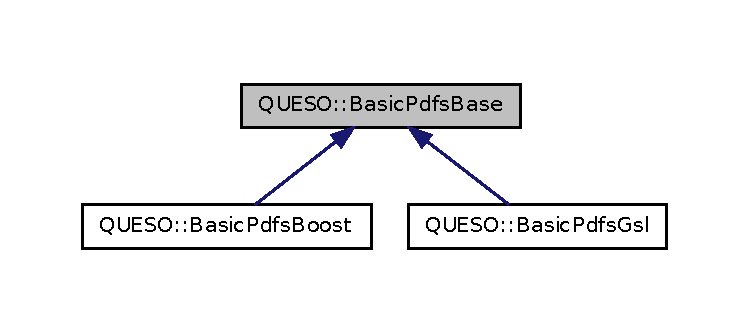
\includegraphics[width=350pt]{class_q_u_e_s_o_1_1_basic_pdfs_base__inherit__graph}
\end{center}
\end{figure}
\subsection*{Public Member Functions}
\begin{Indent}{\bf Constructor/\-Destructor methods}\par
\begin{DoxyCompactItemize}
\item 
\hyperlink{class_q_u_e_s_o_1_1_basic_pdfs_base_a2ca589bc1e025d7e84a0b029b4c610a1}{Basic\-Pdfs\-Base} ()
\begin{DoxyCompactList}\small\item\em Default constructor. \end{DoxyCompactList}\item 
\hyperlink{class_q_u_e_s_o_1_1_basic_pdfs_base_acf3bfe40802cd488d9d01077a7d15e55}{Basic\-Pdfs\-Base} (int world\-Rank)
\begin{DoxyCompactList}\small\item\em Constructor. \end{DoxyCompactList}\item 
virtual \hyperlink{class_q_u_e_s_o_1_1_basic_pdfs_base_a4e0421cd14da7b04d4242318c7de5ece}{$\sim$\-Basic\-Pdfs\-Base} ()
\begin{DoxyCompactList}\small\item\em Virtual destructor. \end{DoxyCompactList}\end{DoxyCompactItemize}
\end{Indent}
\begin{Indent}{\bf Mathematical methods}\par
\begin{DoxyCompactItemize}
\item 
virtual double \hyperlink{class_q_u_e_s_o_1_1_basic_pdfs_base_a7a4df6a4b2147eeca4efb22db0ae1b8b}{beta\-Pdf\-Actual\-Value} (double x, double alpha, double beta) const =0
\begin{DoxyCompactList}\small\item\em T\-O\-D\-O\-: Actual value of the Beta P\-D\-F (calculated via either Boost or G\-S\-L libraries). See template specialization. \end{DoxyCompactList}\item 
virtual double \hyperlink{class_q_u_e_s_o_1_1_basic_pdfs_base_ae5c0c0a14b0f5b89f64e0cd9c0a1b9fd}{gamma\-Pdf\-Actual\-Value} (double x, double a, double b) const =0
\begin{DoxyCompactList}\small\item\em T\-O\-D\-O\-: Actual value of the Gamma P\-D\-F (calculated via either Boost or G\-S\-L libraries). See template specialization. \end{DoxyCompactList}\end{DoxyCompactItemize}
\end{Indent}
\subsection*{Protected Attributes}
\begin{DoxyCompactItemize}
\item 
int \hyperlink{class_q_u_e_s_o_1_1_basic_pdfs_base_a67e06f7bb30579581db1a7b9b3507d1c}{m\-\_\-world\-Rank}
\end{DoxyCompactItemize}


\subsection{Detailed Description}
T\-O\-D\-O\-: Base class for basic P\-D\-Fs (via either G\-S\-L or Boost). 

\begin{DoxyRefDesc}{Todo}
\item[\hyperlink{todo__todo000001}{Todo}]This class {\bfseries will} acommodate the definition of a Joint P\-D\-F using either G\-S\-L or Boost distributions. It will ultimately be called by \hyperlink{class_q_u_e_s_o_1_1_base_joint_pdf}{Base\-Joint\-Pdf} and/or its derived classes (via m\-\_\-env.\-basic\-Pdfs()) during the construction of Joint P\-D\-Fs. \end{DoxyRefDesc}


Definition at line 44 of file Basic\-Pdfs\-Base.\-h.



\subsection{Constructor \& Destructor Documentation}
\hypertarget{class_q_u_e_s_o_1_1_basic_pdfs_base_a2ca589bc1e025d7e84a0b029b4c610a1}{\index{Q\-U\-E\-S\-O\-::\-Basic\-Pdfs\-Base@{Q\-U\-E\-S\-O\-::\-Basic\-Pdfs\-Base}!Basic\-Pdfs\-Base@{Basic\-Pdfs\-Base}}
\index{Basic\-Pdfs\-Base@{Basic\-Pdfs\-Base}!QUESO::BasicPdfsBase@{Q\-U\-E\-S\-O\-::\-Basic\-Pdfs\-Base}}
\subsubsection[{Basic\-Pdfs\-Base}]{\setlength{\rightskip}{0pt plus 5cm}Q\-U\-E\-S\-O\-::\-Basic\-Pdfs\-Base\-::\-Basic\-Pdfs\-Base (
\begin{DoxyParamCaption}
{}
\end{DoxyParamCaption}
)}}\label{class_q_u_e_s_o_1_1_basic_pdfs_base_a2ca589bc1e025d7e84a0b029b4c610a1}


Default constructor. 



Definition at line 30 of file Basic\-Pdfs\-Base.\-C.



References m\-\_\-world\-Rank, and U\-Q\-\_\-\-F\-A\-T\-A\-L\-\_\-\-T\-E\-S\-T\-\_\-\-M\-A\-C\-R\-O.


\begin{DoxyCode}
31   :
32   \hyperlink{class_q_u_e_s_o_1_1_basic_pdfs_base_a67e06f7bb30579581db1a7b9b3507d1c}{m\_worldRank}(\hyperlink{namespace_q_u_e_s_o_a7d4679800a430ae8e473c1c7bc0bfb21}{UQ\_UNAVAILABLE\_RANK})
33 \{
34   \hyperlink{_defines_8h_a56d63d18d0a6d45757de47fcc06f574d}{UQ\_FATAL\_TEST\_MACRO}(\textcolor{keyword}{true},
35                       \hyperlink{class_q_u_e_s_o_1_1_basic_pdfs_base_a67e06f7bb30579581db1a7b9b3507d1c}{m\_worldRank},
36                       \textcolor{stringliteral}{"BasicPdfsBase::constructor(), default"},
37                       \textcolor{stringliteral}{"should not be used by user"});
38 \}
\end{DoxyCode}
\hypertarget{class_q_u_e_s_o_1_1_basic_pdfs_base_acf3bfe40802cd488d9d01077a7d15e55}{\index{Q\-U\-E\-S\-O\-::\-Basic\-Pdfs\-Base@{Q\-U\-E\-S\-O\-::\-Basic\-Pdfs\-Base}!Basic\-Pdfs\-Base@{Basic\-Pdfs\-Base}}
\index{Basic\-Pdfs\-Base@{Basic\-Pdfs\-Base}!QUESO::BasicPdfsBase@{Q\-U\-E\-S\-O\-::\-Basic\-Pdfs\-Base}}
\subsubsection[{Basic\-Pdfs\-Base}]{\setlength{\rightskip}{0pt plus 5cm}Q\-U\-E\-S\-O\-::\-Basic\-Pdfs\-Base\-::\-Basic\-Pdfs\-Base (
\begin{DoxyParamCaption}
\item[{int}]{world\-Rank}
\end{DoxyParamCaption}
)}}\label{class_q_u_e_s_o_1_1_basic_pdfs_base_acf3bfe40802cd488d9d01077a7d15e55}


Constructor. 



Definition at line 40 of file Basic\-Pdfs\-Base.\-C.


\begin{DoxyCode}
41   :
42   \hyperlink{class_q_u_e_s_o_1_1_basic_pdfs_base_a67e06f7bb30579581db1a7b9b3507d1c}{m\_worldRank}(worldRank)
43 \{
44 \}
\end{DoxyCode}
\hypertarget{class_q_u_e_s_o_1_1_basic_pdfs_base_a4e0421cd14da7b04d4242318c7de5ece}{\index{Q\-U\-E\-S\-O\-::\-Basic\-Pdfs\-Base@{Q\-U\-E\-S\-O\-::\-Basic\-Pdfs\-Base}!$\sim$\-Basic\-Pdfs\-Base@{$\sim$\-Basic\-Pdfs\-Base}}
\index{$\sim$\-Basic\-Pdfs\-Base@{$\sim$\-Basic\-Pdfs\-Base}!QUESO::BasicPdfsBase@{Q\-U\-E\-S\-O\-::\-Basic\-Pdfs\-Base}}
\subsubsection[{$\sim$\-Basic\-Pdfs\-Base}]{\setlength{\rightskip}{0pt plus 5cm}Q\-U\-E\-S\-O\-::\-Basic\-Pdfs\-Base\-::$\sim$\-Basic\-Pdfs\-Base (
\begin{DoxyParamCaption}
{}
\end{DoxyParamCaption}
)\hspace{0.3cm}{\ttfamily [virtual]}}}\label{class_q_u_e_s_o_1_1_basic_pdfs_base_a4e0421cd14da7b04d4242318c7de5ece}


Virtual destructor. 



Definition at line 46 of file Basic\-Pdfs\-Base.\-C.


\begin{DoxyCode}
47 \{
48 \}
\end{DoxyCode}


\subsection{Member Function Documentation}
\hypertarget{class_q_u_e_s_o_1_1_basic_pdfs_base_a7a4df6a4b2147eeca4efb22db0ae1b8b}{\index{Q\-U\-E\-S\-O\-::\-Basic\-Pdfs\-Base@{Q\-U\-E\-S\-O\-::\-Basic\-Pdfs\-Base}!beta\-Pdf\-Actual\-Value@{beta\-Pdf\-Actual\-Value}}
\index{beta\-Pdf\-Actual\-Value@{beta\-Pdf\-Actual\-Value}!QUESO::BasicPdfsBase@{Q\-U\-E\-S\-O\-::\-Basic\-Pdfs\-Base}}
\subsubsection[{beta\-Pdf\-Actual\-Value}]{\setlength{\rightskip}{0pt plus 5cm}virtual double Q\-U\-E\-S\-O\-::\-Basic\-Pdfs\-Base\-::beta\-Pdf\-Actual\-Value (
\begin{DoxyParamCaption}
\item[{double}]{x, }
\item[{double}]{alpha, }
\item[{double}]{beta}
\end{DoxyParamCaption}
) const\hspace{0.3cm}{\ttfamily [pure virtual]}}}\label{class_q_u_e_s_o_1_1_basic_pdfs_base_a7a4df6a4b2147eeca4efb22db0ae1b8b}


T\-O\-D\-O\-: Actual value of the Beta P\-D\-F (calculated via either Boost or G\-S\-L libraries). See template specialization. 



Implemented in \hyperlink{class_q_u_e_s_o_1_1_basic_pdfs_boost_a1fb018d87021cb4af85289102c7fddcb}{Q\-U\-E\-S\-O\-::\-Basic\-Pdfs\-Boost}, and \hyperlink{class_q_u_e_s_o_1_1_basic_pdfs_gsl_aaae1aaf761e7129c7f158a06e3ecdfc1}{Q\-U\-E\-S\-O\-::\-Basic\-Pdfs\-Gsl}.

\hypertarget{class_q_u_e_s_o_1_1_basic_pdfs_base_ae5c0c0a14b0f5b89f64e0cd9c0a1b9fd}{\index{Q\-U\-E\-S\-O\-::\-Basic\-Pdfs\-Base@{Q\-U\-E\-S\-O\-::\-Basic\-Pdfs\-Base}!gamma\-Pdf\-Actual\-Value@{gamma\-Pdf\-Actual\-Value}}
\index{gamma\-Pdf\-Actual\-Value@{gamma\-Pdf\-Actual\-Value}!QUESO::BasicPdfsBase@{Q\-U\-E\-S\-O\-::\-Basic\-Pdfs\-Base}}
\subsubsection[{gamma\-Pdf\-Actual\-Value}]{\setlength{\rightskip}{0pt plus 5cm}virtual double Q\-U\-E\-S\-O\-::\-Basic\-Pdfs\-Base\-::gamma\-Pdf\-Actual\-Value (
\begin{DoxyParamCaption}
\item[{double}]{x, }
\item[{double}]{a, }
\item[{double}]{b}
\end{DoxyParamCaption}
) const\hspace{0.3cm}{\ttfamily [pure virtual]}}}\label{class_q_u_e_s_o_1_1_basic_pdfs_base_ae5c0c0a14b0f5b89f64e0cd9c0a1b9fd}


T\-O\-D\-O\-: Actual value of the Gamma P\-D\-F (calculated via either Boost or G\-S\-L libraries). See template specialization. 



Implemented in \hyperlink{class_q_u_e_s_o_1_1_basic_pdfs_boost_aabf856ea8be88e4fda2b378e91eee922}{Q\-U\-E\-S\-O\-::\-Basic\-Pdfs\-Boost}, and \hyperlink{class_q_u_e_s_o_1_1_basic_pdfs_gsl_a6bb250677b5c8c94bd3f690a58efaade}{Q\-U\-E\-S\-O\-::\-Basic\-Pdfs\-Gsl}.



\subsection{Member Data Documentation}
\hypertarget{class_q_u_e_s_o_1_1_basic_pdfs_base_a67e06f7bb30579581db1a7b9b3507d1c}{\index{Q\-U\-E\-S\-O\-::\-Basic\-Pdfs\-Base@{Q\-U\-E\-S\-O\-::\-Basic\-Pdfs\-Base}!m\-\_\-world\-Rank@{m\-\_\-world\-Rank}}
\index{m\-\_\-world\-Rank@{m\-\_\-world\-Rank}!QUESO::BasicPdfsBase@{Q\-U\-E\-S\-O\-::\-Basic\-Pdfs\-Base}}
\subsubsection[{m\-\_\-world\-Rank}]{\setlength{\rightskip}{0pt plus 5cm}int Q\-U\-E\-S\-O\-::\-Basic\-Pdfs\-Base\-::m\-\_\-world\-Rank\hspace{0.3cm}{\ttfamily [protected]}}}\label{class_q_u_e_s_o_1_1_basic_pdfs_base_a67e06f7bb30579581db1a7b9b3507d1c}


Definition at line 68 of file Basic\-Pdfs\-Base.\-h.



Referenced by Basic\-Pdfs\-Base(), Q\-U\-E\-S\-O\-::\-Basic\-Pdfs\-Boost\-::\-Basic\-Pdfs\-Boost(), Q\-U\-E\-S\-O\-::\-Basic\-Pdfs\-Gsl\-::\-Basic\-Pdfs\-Gsl(), Q\-U\-E\-S\-O\-::\-Basic\-Pdfs\-Boost\-::beta\-Pdf\-Actual\-Value(), and Q\-U\-E\-S\-O\-::\-Basic\-Pdfs\-Boost\-::gamma\-Pdf\-Actual\-Value().



The documentation for this class was generated from the following files\-:\begin{DoxyCompactItemize}
\item 
src/core/inc/\hyperlink{_basic_pdfs_base_8h}{Basic\-Pdfs\-Base.\-h}\item 
src/core/src/\hyperlink{_basic_pdfs_base_8_c}{Basic\-Pdfs\-Base.\-C}\end{DoxyCompactItemize}

\hypertarget{class_q_u_e_s_o_1_1_basic_pdfs_boost}{\section{Q\-U\-E\-S\-O\-:\-:Basic\-Pdfs\-Boost Class Reference}
\label{class_q_u_e_s_o_1_1_basic_pdfs_boost}\index{Q\-U\-E\-S\-O\-::\-Basic\-Pdfs\-Boost@{Q\-U\-E\-S\-O\-::\-Basic\-Pdfs\-Boost}}
}


T\-O\-D\-O\-: Base class for basic P\-D\-Fs using Boost library.  




{\ttfamily \#include $<$Basic\-Pdfs\-Boost.\-h$>$}



Inheritance diagram for Q\-U\-E\-S\-O\-:\-:Basic\-Pdfs\-Boost\-:
\nopagebreak
\begin{figure}[H]
\begin{center}
\leavevmode
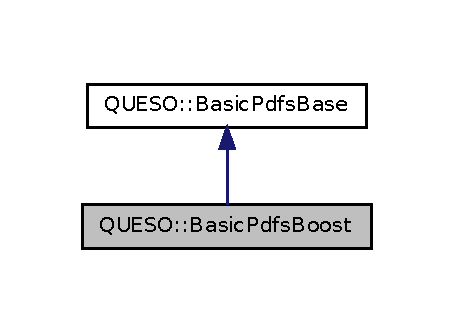
\includegraphics[width=218pt]{class_q_u_e_s_o_1_1_basic_pdfs_boost__inherit__graph}
\end{center}
\end{figure}


Collaboration diagram for Q\-U\-E\-S\-O\-:\-:Basic\-Pdfs\-Boost\-:
\nopagebreak
\begin{figure}[H]
\begin{center}
\leavevmode
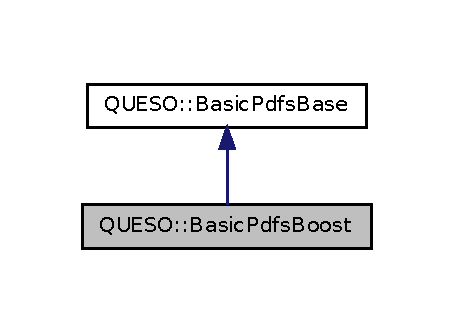
\includegraphics[width=218pt]{class_q_u_e_s_o_1_1_basic_pdfs_boost__coll__graph}
\end{center}
\end{figure}
\subsection*{Public Member Functions}
\begin{Indent}{\bf Constructor/\-Destructor methods}\par
\begin{DoxyCompactItemize}
\item 
\hyperlink{class_q_u_e_s_o_1_1_basic_pdfs_boost_a7ba56f194cdce87c7ef247457a5ed4a6}{Basic\-Pdfs\-Boost} ()
\begin{DoxyCompactList}\small\item\em Default constructor. \end{DoxyCompactList}\item 
\hyperlink{class_q_u_e_s_o_1_1_basic_pdfs_boost_a6409e117dda8033c960db50f8293a385}{Basic\-Pdfs\-Boost} (int world\-Rank)
\begin{DoxyCompactList}\small\item\em Constructor. \end{DoxyCompactList}\item 
\hyperlink{class_q_u_e_s_o_1_1_basic_pdfs_boost_a0d1bc5ab5bdffb0870031746ebe37a94}{$\sim$\-Basic\-Pdfs\-Boost} ()
\begin{DoxyCompactList}\small\item\em Destructor. \end{DoxyCompactList}\end{DoxyCompactItemize}
\end{Indent}
\begin{Indent}{\bf Mathematical methods}\par
\begin{DoxyCompactItemize}
\item 
double \hyperlink{class_q_u_e_s_o_1_1_basic_pdfs_boost_a1fb018d87021cb4af85289102c7fddcb}{beta\-Pdf\-Actual\-Value} (double x, double alpha, double beta) const 
\begin{DoxyCompactList}\small\item\em T\-O\-D\-O\-: Actual value of the Beta P\-D\-F. \end{DoxyCompactList}\item 
double \hyperlink{class_q_u_e_s_o_1_1_basic_pdfs_boost_aabf856ea8be88e4fda2b378e91eee922}{gamma\-Pdf\-Actual\-Value} (double x, double a, double b) const 
\begin{DoxyCompactList}\small\item\em T\-O\-D\-O\-: Actual value of the Gamma P\-D\-F. \end{DoxyCompactList}\end{DoxyCompactItemize}
\end{Indent}
\subsection*{Additional Inherited Members}


\subsection{Detailed Description}
T\-O\-D\-O\-: Base class for basic P\-D\-Fs using Boost library. 

\begin{DoxyRefDesc}{Todo}
\item[\hyperlink{todo__todo000002}{Todo}]This class {\bfseries will} acommodate the definition of a Joint P\-D\-F using distributions available in the Boost library. It will ultimately be called by \hyperlink{class_q_u_e_s_o_1_1_base_joint_pdf}{Base\-Joint\-Pdf} and/or its derived classes (via m\-\_\-env.\-basic\-Pdfs()) during the construction of Joint P\-D\-Fs. \end{DoxyRefDesc}


Definition at line 45 of file Basic\-Pdfs\-Boost.\-h.



\subsection{Constructor \& Destructor Documentation}
\hypertarget{class_q_u_e_s_o_1_1_basic_pdfs_boost_a7ba56f194cdce87c7ef247457a5ed4a6}{\index{Q\-U\-E\-S\-O\-::\-Basic\-Pdfs\-Boost@{Q\-U\-E\-S\-O\-::\-Basic\-Pdfs\-Boost}!Basic\-Pdfs\-Boost@{Basic\-Pdfs\-Boost}}
\index{Basic\-Pdfs\-Boost@{Basic\-Pdfs\-Boost}!QUESO::BasicPdfsBoost@{Q\-U\-E\-S\-O\-::\-Basic\-Pdfs\-Boost}}
\subsubsection[{Basic\-Pdfs\-Boost}]{\setlength{\rightskip}{0pt plus 5cm}Q\-U\-E\-S\-O\-::\-Basic\-Pdfs\-Boost\-::\-Basic\-Pdfs\-Boost (
\begin{DoxyParamCaption}
{}
\end{DoxyParamCaption}
)}}\label{class_q_u_e_s_o_1_1_basic_pdfs_boost_a7ba56f194cdce87c7ef247457a5ed4a6}


Default constructor. 



Definition at line 31 of file Basic\-Pdfs\-Boost.\-C.



References Q\-U\-E\-S\-O\-::\-Basic\-Pdfs\-Base\-::m\-\_\-world\-Rank, and U\-Q\-\_\-\-F\-A\-T\-A\-L\-\_\-\-T\-E\-S\-T\-\_\-\-M\-A\-C\-R\-O.


\begin{DoxyCode}
32   :
33   \hyperlink{class_q_u_e_s_o_1_1_basic_pdfs_base_a2ca589bc1e025d7e84a0b029b4c610a1}{BasicPdfsBase}()
34 \{
35   \hyperlink{_defines_8h_a56d63d18d0a6d45757de47fcc06f574d}{UQ\_FATAL\_TEST\_MACRO}(\textcolor{keyword}{true},
36                       \hyperlink{class_q_u_e_s_o_1_1_basic_pdfs_base_a67e06f7bb30579581db1a7b9b3507d1c}{m\_worldRank},
37                       \textcolor{stringliteral}{"BasicPdfsBoost::constructor(), default"},
38                       \textcolor{stringliteral}{"should not be used by user"});
39 \}
\end{DoxyCode}
\hypertarget{class_q_u_e_s_o_1_1_basic_pdfs_boost_a6409e117dda8033c960db50f8293a385}{\index{Q\-U\-E\-S\-O\-::\-Basic\-Pdfs\-Boost@{Q\-U\-E\-S\-O\-::\-Basic\-Pdfs\-Boost}!Basic\-Pdfs\-Boost@{Basic\-Pdfs\-Boost}}
\index{Basic\-Pdfs\-Boost@{Basic\-Pdfs\-Boost}!QUESO::BasicPdfsBoost@{Q\-U\-E\-S\-O\-::\-Basic\-Pdfs\-Boost}}
\subsubsection[{Basic\-Pdfs\-Boost}]{\setlength{\rightskip}{0pt plus 5cm}Q\-U\-E\-S\-O\-::\-Basic\-Pdfs\-Boost\-::\-Basic\-Pdfs\-Boost (
\begin{DoxyParamCaption}
\item[{int}]{world\-Rank}
\end{DoxyParamCaption}
)}}\label{class_q_u_e_s_o_1_1_basic_pdfs_boost_a6409e117dda8033c960db50f8293a385}


Constructor. 

Constructor -\/-\/-\/-\/-\/-\/-\/-\/-\/-\/-\/-\/-\/-\/-\/-\/-\/-\/-\/-\/-\/-\/-\/-\/---. 

Definition at line 42 of file Basic\-Pdfs\-Boost.\-C.


\begin{DoxyCode}
43   :
44   \hyperlink{class_q_u_e_s_o_1_1_basic_pdfs_base_a2ca589bc1e025d7e84a0b029b4c610a1}{BasicPdfsBase}(worldRank)
45 \{
46 \}
\end{DoxyCode}
\hypertarget{class_q_u_e_s_o_1_1_basic_pdfs_boost_a0d1bc5ab5bdffb0870031746ebe37a94}{\index{Q\-U\-E\-S\-O\-::\-Basic\-Pdfs\-Boost@{Q\-U\-E\-S\-O\-::\-Basic\-Pdfs\-Boost}!$\sim$\-Basic\-Pdfs\-Boost@{$\sim$\-Basic\-Pdfs\-Boost}}
\index{$\sim$\-Basic\-Pdfs\-Boost@{$\sim$\-Basic\-Pdfs\-Boost}!QUESO::BasicPdfsBoost@{Q\-U\-E\-S\-O\-::\-Basic\-Pdfs\-Boost}}
\subsubsection[{$\sim$\-Basic\-Pdfs\-Boost}]{\setlength{\rightskip}{0pt plus 5cm}Q\-U\-E\-S\-O\-::\-Basic\-Pdfs\-Boost\-::$\sim$\-Basic\-Pdfs\-Boost (
\begin{DoxyParamCaption}
{}
\end{DoxyParamCaption}
)}}\label{class_q_u_e_s_o_1_1_basic_pdfs_boost_a0d1bc5ab5bdffb0870031746ebe37a94}


Destructor. 



Definition at line 49 of file Basic\-Pdfs\-Boost.\-C.


\begin{DoxyCode}
50 \{
51   \textcolor{comment}{//this function does nothing}
52 \}
\end{DoxyCode}


\subsection{Member Function Documentation}
\hypertarget{class_q_u_e_s_o_1_1_basic_pdfs_boost_a1fb018d87021cb4af85289102c7fddcb}{\index{Q\-U\-E\-S\-O\-::\-Basic\-Pdfs\-Boost@{Q\-U\-E\-S\-O\-::\-Basic\-Pdfs\-Boost}!beta\-Pdf\-Actual\-Value@{beta\-Pdf\-Actual\-Value}}
\index{beta\-Pdf\-Actual\-Value@{beta\-Pdf\-Actual\-Value}!QUESO::BasicPdfsBoost@{Q\-U\-E\-S\-O\-::\-Basic\-Pdfs\-Boost}}
\subsubsection[{beta\-Pdf\-Actual\-Value}]{\setlength{\rightskip}{0pt plus 5cm}double Q\-U\-E\-S\-O\-::\-Basic\-Pdfs\-Boost\-::beta\-Pdf\-Actual\-Value (
\begin{DoxyParamCaption}
\item[{double}]{x, }
\item[{double}]{alpha, }
\item[{double}]{beta}
\end{DoxyParamCaption}
) const\hspace{0.3cm}{\ttfamily [virtual]}}}\label{class_q_u_e_s_o_1_1_basic_pdfs_boost_a1fb018d87021cb4af85289102c7fddcb}


T\-O\-D\-O\-: Actual value of the Beta P\-D\-F. 



Implements \hyperlink{class_q_u_e_s_o_1_1_basic_pdfs_base_a7a4df6a4b2147eeca4efb22db0ae1b8b}{Q\-U\-E\-S\-O\-::\-Basic\-Pdfs\-Base}.



Definition at line 56 of file Basic\-Pdfs\-Boost.\-C.



References Q\-U\-E\-S\-O\-::\-Basic\-Pdfs\-Base\-::m\-\_\-world\-Rank, and U\-Q\-\_\-\-F\-A\-T\-A\-L\-\_\-\-T\-E\-S\-T\-\_\-\-M\-A\-C\-R\-O.


\begin{DoxyCode}
57 \{
58   \hyperlink{_defines_8h_a56d63d18d0a6d45757de47fcc06f574d}{UQ\_FATAL\_TEST\_MACRO}(\textcolor{keyword}{true},
59                       \hyperlink{class_q_u_e_s_o_1_1_basic_pdfs_base_a67e06f7bb30579581db1a7b9b3507d1c}{m\_worldRank},
60                       \textcolor{stringliteral}{"BasicPdfsBoost::betaPdfActualValue()"},
61                       \textcolor{stringliteral}{"code incomplete yet"});
62   \textcolor{keywordflow}{return} 0.;
63 \}
\end{DoxyCode}
\hypertarget{class_q_u_e_s_o_1_1_basic_pdfs_boost_aabf856ea8be88e4fda2b378e91eee922}{\index{Q\-U\-E\-S\-O\-::\-Basic\-Pdfs\-Boost@{Q\-U\-E\-S\-O\-::\-Basic\-Pdfs\-Boost}!gamma\-Pdf\-Actual\-Value@{gamma\-Pdf\-Actual\-Value}}
\index{gamma\-Pdf\-Actual\-Value@{gamma\-Pdf\-Actual\-Value}!QUESO::BasicPdfsBoost@{Q\-U\-E\-S\-O\-::\-Basic\-Pdfs\-Boost}}
\subsubsection[{gamma\-Pdf\-Actual\-Value}]{\setlength{\rightskip}{0pt plus 5cm}double Q\-U\-E\-S\-O\-::\-Basic\-Pdfs\-Boost\-::gamma\-Pdf\-Actual\-Value (
\begin{DoxyParamCaption}
\item[{double}]{x, }
\item[{double}]{a, }
\item[{double}]{b}
\end{DoxyParamCaption}
) const\hspace{0.3cm}{\ttfamily [virtual]}}}\label{class_q_u_e_s_o_1_1_basic_pdfs_boost_aabf856ea8be88e4fda2b378e91eee922}


T\-O\-D\-O\-: Actual value of the Gamma P\-D\-F. 



Implements \hyperlink{class_q_u_e_s_o_1_1_basic_pdfs_base_ae5c0c0a14b0f5b89f64e0cd9c0a1b9fd}{Q\-U\-E\-S\-O\-::\-Basic\-Pdfs\-Base}.



Definition at line 67 of file Basic\-Pdfs\-Boost.\-C.



References Q\-U\-E\-S\-O\-::\-Basic\-Pdfs\-Base\-::m\-\_\-world\-Rank, and U\-Q\-\_\-\-F\-A\-T\-A\-L\-\_\-\-T\-E\-S\-T\-\_\-\-M\-A\-C\-R\-O.


\begin{DoxyCode}
68 \{
69   \hyperlink{_defines_8h_a56d63d18d0a6d45757de47fcc06f574d}{UQ\_FATAL\_TEST\_MACRO}(\textcolor{keyword}{true},
70                       \hyperlink{class_q_u_e_s_o_1_1_basic_pdfs_base_a67e06f7bb30579581db1a7b9b3507d1c}{m\_worldRank},
71                       \textcolor{stringliteral}{"BasicPdfsBoost::gammaPdfActualValue()"},
72                       \textcolor{stringliteral}{"code incomplete yet"});
73   \textcolor{keywordflow}{return} 0.;
74 \}
\end{DoxyCode}


The documentation for this class was generated from the following files\-:\begin{DoxyCompactItemize}
\item 
src/core/inc/\hyperlink{_basic_pdfs_boost_8h}{Basic\-Pdfs\-Boost.\-h}\item 
src/core/src/\hyperlink{_basic_pdfs_boost_8_c}{Basic\-Pdfs\-Boost.\-C}\end{DoxyCompactItemize}

\hypertarget{class_q_u_e_s_o_1_1_basic_pdfs_gsl}{\section{Q\-U\-E\-S\-O\-:\-:Basic\-Pdfs\-Gsl Class Reference}
\label{class_q_u_e_s_o_1_1_basic_pdfs_gsl}\index{Q\-U\-E\-S\-O\-::\-Basic\-Pdfs\-Gsl@{Q\-U\-E\-S\-O\-::\-Basic\-Pdfs\-Gsl}}
}


T\-O\-D\-O\-: Base class for basic P\-D\-Fs using Gsl library.  




{\ttfamily \#include $<$Basic\-Pdfs\-Gsl.\-h$>$}



Inheritance diagram for Q\-U\-E\-S\-O\-:\-:Basic\-Pdfs\-Gsl\-:
\nopagebreak
\begin{figure}[H]
\begin{center}
\leavevmode
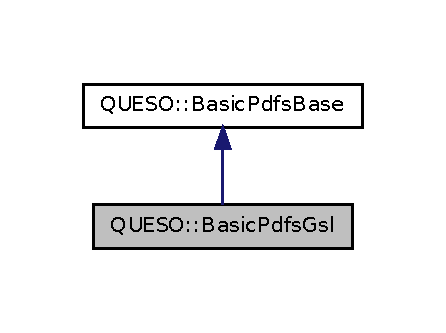
\includegraphics[width=214pt]{class_q_u_e_s_o_1_1_basic_pdfs_gsl__inherit__graph}
\end{center}
\end{figure}


Collaboration diagram for Q\-U\-E\-S\-O\-:\-:Basic\-Pdfs\-Gsl\-:
\nopagebreak
\begin{figure}[H]
\begin{center}
\leavevmode
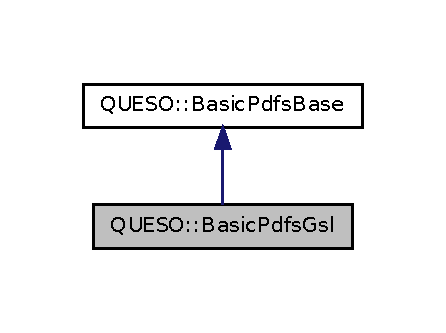
\includegraphics[width=214pt]{class_q_u_e_s_o_1_1_basic_pdfs_gsl__coll__graph}
\end{center}
\end{figure}
\subsection*{Public Member Functions}
\begin{Indent}{\bf Constructor/\-Destructor methods}\par
\begin{DoxyCompactItemize}
\item 
\hyperlink{class_q_u_e_s_o_1_1_basic_pdfs_gsl_a3df72eb1474638a1bb364524ff397c4d}{Basic\-Pdfs\-Gsl} ()
\begin{DoxyCompactList}\small\item\em Default constructor. \end{DoxyCompactList}\item 
\hyperlink{class_q_u_e_s_o_1_1_basic_pdfs_gsl_acfb4ea894ec318fe99c6afa5fe86b8fe}{Basic\-Pdfs\-Gsl} (int world\-Rank)
\begin{DoxyCompactList}\small\item\em Constructor. \end{DoxyCompactList}\item 
\hyperlink{class_q_u_e_s_o_1_1_basic_pdfs_gsl_a477e6898a9ed8204f5d9d36dc0b6bf3a}{$\sim$\-Basic\-Pdfs\-Gsl} ()
\begin{DoxyCompactList}\small\item\em Destructor. \end{DoxyCompactList}\end{DoxyCompactItemize}
\end{Indent}
\begin{Indent}{\bf Mathematical methods}\par
\begin{DoxyCompactItemize}
\item 
double \hyperlink{class_q_u_e_s_o_1_1_basic_pdfs_gsl_aaae1aaf761e7129c7f158a06e3ecdfc1}{beta\-Pdf\-Actual\-Value} (double x, double alpha, double beta) const 
\begin{DoxyCompactList}\small\item\em T\-O\-D\-O\-: Actual value of the Beta P\-D\-F. \end{DoxyCompactList}\item 
double \hyperlink{class_q_u_e_s_o_1_1_basic_pdfs_gsl_a6bb250677b5c8c94bd3f690a58efaade}{gamma\-Pdf\-Actual\-Value} (double x, double a, double b) const 
\begin{DoxyCompactList}\small\item\em T\-O\-D\-O\-: Actual value of the Gamma P\-D\-F. \end{DoxyCompactList}\end{DoxyCompactItemize}
\end{Indent}
\subsection*{Additional Inherited Members}


\subsection{Detailed Description}
T\-O\-D\-O\-: Base class for basic P\-D\-Fs using Gsl library. 

\begin{DoxyRefDesc}{Todo}
\item[\hyperlink{todo__todo000003}{Todo}]This class {\bfseries will} acommodate the definition of a Joint P\-D\-F using distributions available in the Gsl library. It will ultimately be called by \hyperlink{class_q_u_e_s_o_1_1_base_joint_pdf}{Base\-Joint\-Pdf} and/or its derived classes (via m\-\_\-env.\-basic\-Pdfs()) during the construction of Joint P\-D\-Fs. \end{DoxyRefDesc}


Definition at line 43 of file Basic\-Pdfs\-Gsl.\-h.



\subsection{Constructor \& Destructor Documentation}
\hypertarget{class_q_u_e_s_o_1_1_basic_pdfs_gsl_a3df72eb1474638a1bb364524ff397c4d}{\index{Q\-U\-E\-S\-O\-::\-Basic\-Pdfs\-Gsl@{Q\-U\-E\-S\-O\-::\-Basic\-Pdfs\-Gsl}!Basic\-Pdfs\-Gsl@{Basic\-Pdfs\-Gsl}}
\index{Basic\-Pdfs\-Gsl@{Basic\-Pdfs\-Gsl}!QUESO::BasicPdfsGsl@{Q\-U\-E\-S\-O\-::\-Basic\-Pdfs\-Gsl}}
\subsubsection[{Basic\-Pdfs\-Gsl}]{\setlength{\rightskip}{0pt plus 5cm}Q\-U\-E\-S\-O\-::\-Basic\-Pdfs\-Gsl\-::\-Basic\-Pdfs\-Gsl (
\begin{DoxyParamCaption}
{}
\end{DoxyParamCaption}
)}}\label{class_q_u_e_s_o_1_1_basic_pdfs_gsl_a3df72eb1474638a1bb364524ff397c4d}


Default constructor. 



Definition at line 33 of file Basic\-Pdfs\-Gsl.\-C.



References Q\-U\-E\-S\-O\-::\-Basic\-Pdfs\-Base\-::m\-\_\-world\-Rank, and U\-Q\-\_\-\-F\-A\-T\-A\-L\-\_\-\-T\-E\-S\-T\-\_\-\-M\-A\-C\-R\-O.


\begin{DoxyCode}
34   :
35   \hyperlink{class_q_u_e_s_o_1_1_basic_pdfs_base_a2ca589bc1e025d7e84a0b029b4c610a1}{BasicPdfsBase}()
36 \{
37   \hyperlink{_defines_8h_a56d63d18d0a6d45757de47fcc06f574d}{UQ\_FATAL\_TEST\_MACRO}(\textcolor{keyword}{true},
38                       \hyperlink{class_q_u_e_s_o_1_1_basic_pdfs_base_a67e06f7bb30579581db1a7b9b3507d1c}{m\_worldRank},
39                       \textcolor{stringliteral}{"BasicPdfsGsl::constructor(), default"},
40                       \textcolor{stringliteral}{"should not be used by user"});
41 \}
\end{DoxyCode}
\hypertarget{class_q_u_e_s_o_1_1_basic_pdfs_gsl_acfb4ea894ec318fe99c6afa5fe86b8fe}{\index{Q\-U\-E\-S\-O\-::\-Basic\-Pdfs\-Gsl@{Q\-U\-E\-S\-O\-::\-Basic\-Pdfs\-Gsl}!Basic\-Pdfs\-Gsl@{Basic\-Pdfs\-Gsl}}
\index{Basic\-Pdfs\-Gsl@{Basic\-Pdfs\-Gsl}!QUESO::BasicPdfsGsl@{Q\-U\-E\-S\-O\-::\-Basic\-Pdfs\-Gsl}}
\subsubsection[{Basic\-Pdfs\-Gsl}]{\setlength{\rightskip}{0pt plus 5cm}Q\-U\-E\-S\-O\-::\-Basic\-Pdfs\-Gsl\-::\-Basic\-Pdfs\-Gsl (
\begin{DoxyParamCaption}
\item[{int}]{world\-Rank}
\end{DoxyParamCaption}
)}}\label{class_q_u_e_s_o_1_1_basic_pdfs_gsl_acfb4ea894ec318fe99c6afa5fe86b8fe}


Constructor. 

Constructor -\/-\/-\/-\/-\/-\/-\/-\/-\/-\/-\/-\/-\/-\/-\/-\/-\/-\/-\/-\/-\/-\/-\/-\/---. 

Definition at line 44 of file Basic\-Pdfs\-Gsl.\-C.


\begin{DoxyCode}
45   :
46   \hyperlink{class_q_u_e_s_o_1_1_basic_pdfs_base_a2ca589bc1e025d7e84a0b029b4c610a1}{BasicPdfsBase}(worldRank)
47 \{
48 \}
\end{DoxyCode}
\hypertarget{class_q_u_e_s_o_1_1_basic_pdfs_gsl_a477e6898a9ed8204f5d9d36dc0b6bf3a}{\index{Q\-U\-E\-S\-O\-::\-Basic\-Pdfs\-Gsl@{Q\-U\-E\-S\-O\-::\-Basic\-Pdfs\-Gsl}!$\sim$\-Basic\-Pdfs\-Gsl@{$\sim$\-Basic\-Pdfs\-Gsl}}
\index{$\sim$\-Basic\-Pdfs\-Gsl@{$\sim$\-Basic\-Pdfs\-Gsl}!QUESO::BasicPdfsGsl@{Q\-U\-E\-S\-O\-::\-Basic\-Pdfs\-Gsl}}
\subsubsection[{$\sim$\-Basic\-Pdfs\-Gsl}]{\setlength{\rightskip}{0pt plus 5cm}Q\-U\-E\-S\-O\-::\-Basic\-Pdfs\-Gsl\-::$\sim$\-Basic\-Pdfs\-Gsl (
\begin{DoxyParamCaption}
{}
\end{DoxyParamCaption}
)}}\label{class_q_u_e_s_o_1_1_basic_pdfs_gsl_a477e6898a9ed8204f5d9d36dc0b6bf3a}


Destructor. 



Definition at line 51 of file Basic\-Pdfs\-Gsl.\-C.


\begin{DoxyCode}
52 \{
53 \}
\end{DoxyCode}


\subsection{Member Function Documentation}
\hypertarget{class_q_u_e_s_o_1_1_basic_pdfs_gsl_aaae1aaf761e7129c7f158a06e3ecdfc1}{\index{Q\-U\-E\-S\-O\-::\-Basic\-Pdfs\-Gsl@{Q\-U\-E\-S\-O\-::\-Basic\-Pdfs\-Gsl}!beta\-Pdf\-Actual\-Value@{beta\-Pdf\-Actual\-Value}}
\index{beta\-Pdf\-Actual\-Value@{beta\-Pdf\-Actual\-Value}!QUESO::BasicPdfsGsl@{Q\-U\-E\-S\-O\-::\-Basic\-Pdfs\-Gsl}}
\subsubsection[{beta\-Pdf\-Actual\-Value}]{\setlength{\rightskip}{0pt plus 5cm}double Q\-U\-E\-S\-O\-::\-Basic\-Pdfs\-Gsl\-::beta\-Pdf\-Actual\-Value (
\begin{DoxyParamCaption}
\item[{double}]{x, }
\item[{double}]{alpha, }
\item[{double}]{beta}
\end{DoxyParamCaption}
) const\hspace{0.3cm}{\ttfamily [virtual]}}}\label{class_q_u_e_s_o_1_1_basic_pdfs_gsl_aaae1aaf761e7129c7f158a06e3ecdfc1}


T\-O\-D\-O\-: Actual value of the Beta P\-D\-F. 



Implements \hyperlink{class_q_u_e_s_o_1_1_basic_pdfs_base_a7a4df6a4b2147eeca4efb22db0ae1b8b}{Q\-U\-E\-S\-O\-::\-Basic\-Pdfs\-Base}.



Definition at line 57 of file Basic\-Pdfs\-Gsl.\-C.


\begin{DoxyCode}
58 \{
59   \textcolor{keywordtype}{double} result = gsl\_ran\_beta\_pdf(x,alpha,beta);
60   \textcolor{keywordflow}{if} (isinf(result)) \{ \textcolor{comment}{// CSRI - 2013-aug-06, with Laura}
61     std::cerr << \textcolor{stringliteral}{"In BasicPdfsGsl::betaPdfActualValue(): hitting inf"}
62               << \textcolor{stringliteral}{", x = "}     << x
63               << \textcolor{stringliteral}{", alpha = "} << alpha
64               << \textcolor{stringliteral}{", beta = "}  << beta
65               << std::endl;
66     \textcolor{comment}{//result = gsl\_ran\_beta\_pdf(x,alpha,beta);}
67     result = 0.;
68   \}
69   \textcolor{keywordflow}{return} result; 
70 \}
\end{DoxyCode}
\hypertarget{class_q_u_e_s_o_1_1_basic_pdfs_gsl_a6bb250677b5c8c94bd3f690a58efaade}{\index{Q\-U\-E\-S\-O\-::\-Basic\-Pdfs\-Gsl@{Q\-U\-E\-S\-O\-::\-Basic\-Pdfs\-Gsl}!gamma\-Pdf\-Actual\-Value@{gamma\-Pdf\-Actual\-Value}}
\index{gamma\-Pdf\-Actual\-Value@{gamma\-Pdf\-Actual\-Value}!QUESO::BasicPdfsGsl@{Q\-U\-E\-S\-O\-::\-Basic\-Pdfs\-Gsl}}
\subsubsection[{gamma\-Pdf\-Actual\-Value}]{\setlength{\rightskip}{0pt plus 5cm}double Q\-U\-E\-S\-O\-::\-Basic\-Pdfs\-Gsl\-::gamma\-Pdf\-Actual\-Value (
\begin{DoxyParamCaption}
\item[{double}]{x, }
\item[{double}]{a, }
\item[{double}]{b}
\end{DoxyParamCaption}
) const\hspace{0.3cm}{\ttfamily [virtual]}}}\label{class_q_u_e_s_o_1_1_basic_pdfs_gsl_a6bb250677b5c8c94bd3f690a58efaade}


T\-O\-D\-O\-: Actual value of the Gamma P\-D\-F. 



Implements \hyperlink{class_q_u_e_s_o_1_1_basic_pdfs_base_ae5c0c0a14b0f5b89f64e0cd9c0a1b9fd}{Q\-U\-E\-S\-O\-::\-Basic\-Pdfs\-Base}.



Definition at line 74 of file Basic\-Pdfs\-Gsl.\-C.


\begin{DoxyCode}
75 \{
76   \textcolor{keywordflow}{return} gsl\_ran\_gamma\_pdf(x,a,b);
77 \}
\end{DoxyCode}


The documentation for this class was generated from the following files\-:\begin{DoxyCompactItemize}
\item 
src/core/inc/\hyperlink{_basic_pdfs_gsl_8h}{Basic\-Pdfs\-Gsl.\-h}\item 
src/core/src/\hyperlink{_basic_pdfs_gsl_8_c}{Basic\-Pdfs\-Gsl.\-C}\end{DoxyCompactItemize}

\hypertarget{class_q_u_e_s_o_1_1_bayesian_joint_pdf}{\section{Q\-U\-E\-S\-O\-:\-:Bayesian\-Joint\-Pdf$<$ V, M $>$ Class Template Reference}
\label{class_q_u_e_s_o_1_1_bayesian_joint_pdf}\index{Q\-U\-E\-S\-O\-::\-Bayesian\-Joint\-Pdf$<$ V, M $>$@{Q\-U\-E\-S\-O\-::\-Bayesian\-Joint\-Pdf$<$ V, M $>$}}
}


A class for handling Bayesian joint P\-D\-Fs.  




{\ttfamily \#include $<$Bayesian\-Joint\-Pdf.\-h$>$}



Inheritance diagram for Q\-U\-E\-S\-O\-:\-:Bayesian\-Joint\-Pdf$<$ V, M $>$\-:
\nopagebreak
\begin{figure}[H]
\begin{center}
\leavevmode
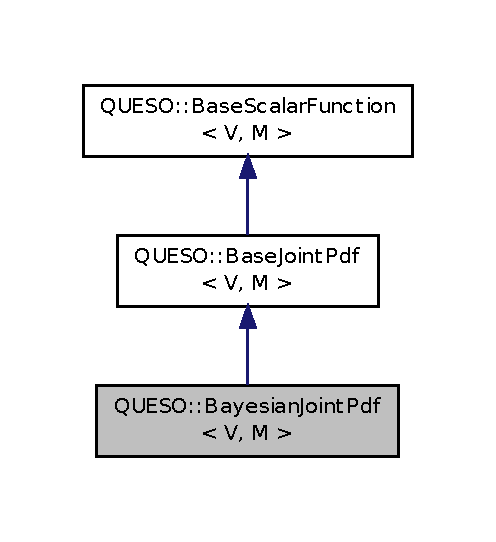
\includegraphics[width=238pt]{class_q_u_e_s_o_1_1_bayesian_joint_pdf__inherit__graph}
\end{center}
\end{figure}


Collaboration diagram for Q\-U\-E\-S\-O\-:\-:Bayesian\-Joint\-Pdf$<$ V, M $>$\-:
\nopagebreak
\begin{figure}[H]
\begin{center}
\leavevmode
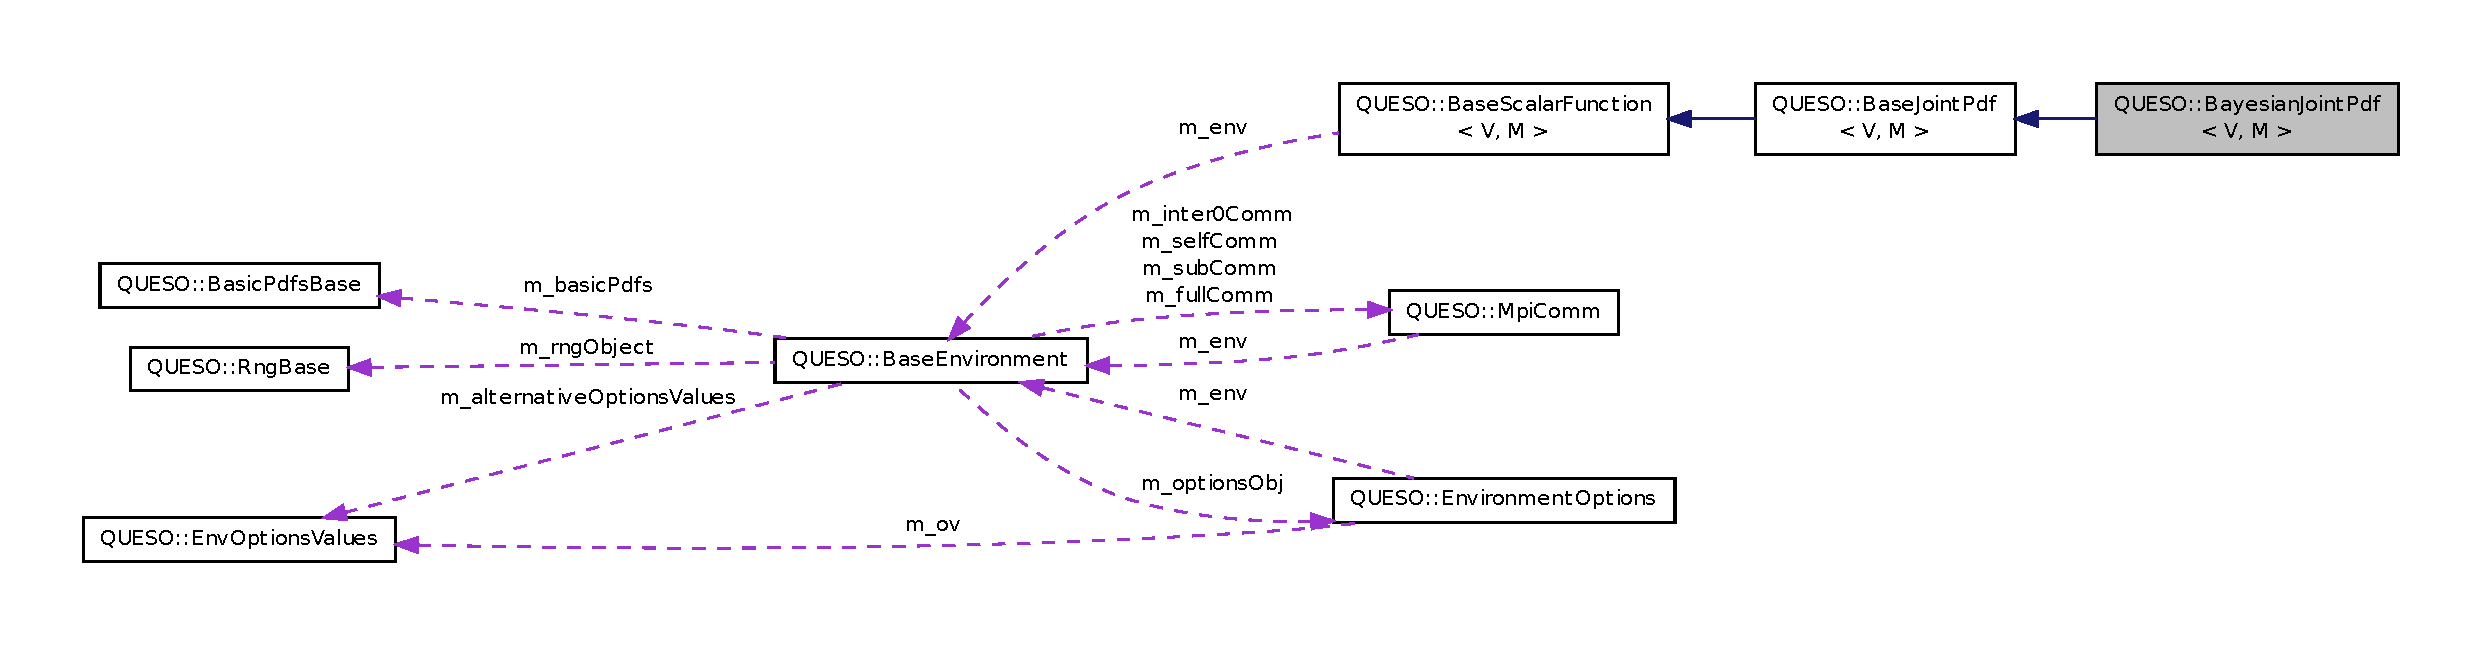
\includegraphics[width=350pt]{class_q_u_e_s_o_1_1_bayesian_joint_pdf__coll__graph}
\end{center}
\end{figure}
\subsection*{Public Member Functions}
\begin{Indent}{\bf Constructor/\-Destructor methods}\par
\begin{DoxyCompactItemize}
\item 
\hyperlink{class_q_u_e_s_o_1_1_bayesian_joint_pdf_a035122f1015976118ba96c9cd37edda0}{Bayesian\-Joint\-Pdf} (const char $\ast$prefix, const \hyperlink{class_q_u_e_s_o_1_1_base_joint_pdf}{Base\-Joint\-Pdf}$<$ V, M $>$ \&prior\-Density, const \hyperlink{class_q_u_e_s_o_1_1_base_scalar_function}{Base\-Scalar\-Function}$<$ V, M $>$ \&likelihood\-Function, double likelihood\-Exponent, const \hyperlink{class_q_u_e_s_o_1_1_vector_set}{Vector\-Set}$<$ V, M $>$ \&intersection\-Domain)
\begin{DoxyCompactList}\small\item\em Default constructor. \end{DoxyCompactList}\item 
\hyperlink{class_q_u_e_s_o_1_1_bayesian_joint_pdf_a060c1d9fcfd092dbc5501afaa9b362db}{$\sim$\-Bayesian\-Joint\-Pdf} ()
\begin{DoxyCompactList}\small\item\em Destructor. \end{DoxyCompactList}\end{DoxyCompactItemize}
\end{Indent}
\begin{Indent}{\bf Math methods}\par
\begin{DoxyCompactItemize}
\item 
double \hyperlink{class_q_u_e_s_o_1_1_bayesian_joint_pdf_ad67362b4ab48a722db976430cf03165e}{actual\-Value} (const V \&domain\-Vector, const V $\ast$domain\-Direction, V $\ast$grad\-Vector, M $\ast$hessian\-Matrix, V $\ast$hessian\-Effect) const 
\begin{DoxyCompactList}\small\item\em Actual value of the P\-D\-F (scalar function). \end{DoxyCompactList}\item 
double \hyperlink{class_q_u_e_s_o_1_1_bayesian_joint_pdf_a98e54ee24452e2477469a0c84eecbfca}{ln\-Value} (const V \&domain\-Vector, const V $\ast$domain\-Direction, V $\ast$grad\-Vector, M $\ast$hessian\-Matrix, V $\ast$hessian\-Effect) const 
\begin{DoxyCompactList}\small\item\em Computes the logarithm of the value of the function. \end{DoxyCompactList}\item 
double \hyperlink{class_q_u_e_s_o_1_1_bayesian_joint_pdf_a7e00d685068bcf34253e5a101b539261}{compute\-Log\-Of\-Normalization\-Factor} (unsigned int num\-Samples, bool update\-Factor\-Internally) const 
\begin{DoxyCompactList}\small\item\em T\-O\-D\-O\-: Computes the logarithm of the normalization factor. \end{DoxyCompactList}\item 
void \hyperlink{class_q_u_e_s_o_1_1_bayesian_joint_pdf_aa23751ede9ec9f2e7bdd81c5326f47d5}{set\-Normalization\-Style} (unsigned int value) const 
\begin{DoxyCompactList}\small\item\em Sets a value to be used in the normalization style of the prior density P\-D\-F (ie, protected attribute m\-\_\-prior\-Density). \end{DoxyCompactList}\item 
double \hyperlink{class_q_u_e_s_o_1_1_bayesian_joint_pdf_aaae16348ff3b0ab3c1c64605fbc1d493}{last\-Computed\-Log\-Prior} () const 
\begin{DoxyCompactList}\small\item\em Returns the logarithm of the last computed Prior value. Access to protected attribute m\-\_\-last\-Computed\-Log\-Prior. \end{DoxyCompactList}\item 
double \hyperlink{class_q_u_e_s_o_1_1_bayesian_joint_pdf_a500cbccdedf8dbc7c1f9652c262a160a}{last\-Computed\-Log\-Likelihood} () const 
\begin{DoxyCompactList}\small\item\em Returns the logarithm of the last computed likelihood value. Access to protected attribute m\-\_\-last\-Computed\-Log\-Likelihood. \end{DoxyCompactList}\end{DoxyCompactItemize}
\end{Indent}
\subsection*{Protected Attributes}
\begin{DoxyCompactItemize}
\item 
const \hyperlink{class_q_u_e_s_o_1_1_base_joint_pdf}{Base\-Joint\-Pdf}$<$ V, M $>$ \& \hyperlink{class_q_u_e_s_o_1_1_bayesian_joint_pdf_a3cafafe8c5ea2353eedaecee156f609a}{m\-\_\-prior\-Density}
\item 
const \hyperlink{class_q_u_e_s_o_1_1_base_scalar_function}{Base\-Scalar\-Function}$<$ V, M $>$ \& \hyperlink{class_q_u_e_s_o_1_1_bayesian_joint_pdf_a8e2506801de447f8acd187f8edfa330d}{m\-\_\-likelihood\-Function}
\item 
double \hyperlink{class_q_u_e_s_o_1_1_bayesian_joint_pdf_a511b1e403ebcab436177491ea8f21c07}{m\-\_\-likelihood\-Exponent}
\item 
double \hyperlink{class_q_u_e_s_o_1_1_bayesian_joint_pdf_a2b1c5582be60a876a6dd08766e7e31ed}{m\-\_\-last\-Computed\-Log\-Prior}
\item 
double \hyperlink{class_q_u_e_s_o_1_1_bayesian_joint_pdf_af97f3ff0d65154366e31d14fd88ccb38}{m\-\_\-last\-Computed\-Log\-Likelihood}
\item 
V \hyperlink{class_q_u_e_s_o_1_1_bayesian_joint_pdf_af4252d2628298423a60335eef72136c6}{m\-\_\-tmp\-Vector1}
\item 
V \hyperlink{class_q_u_e_s_o_1_1_bayesian_joint_pdf_a2c81721bddf0ffd5547751f1a8221a5d}{m\-\_\-tmp\-Vector2}
\item 
M $\ast$ \hyperlink{class_q_u_e_s_o_1_1_bayesian_joint_pdf_a686da1b57929c8b506a5e8fe8974603d}{m\-\_\-tmp\-Matrix}
\end{DoxyCompactItemize}
\subsection*{Additional Inherited Members}


\subsection{Detailed Description}
\subsubsection*{template$<$class V, class M$>$class Q\-U\-E\-S\-O\-::\-Bayesian\-Joint\-Pdf$<$ V, M $>$}

A class for handling Bayesian joint P\-D\-Fs. 

This class allows the mathematical definition of a Bayesian Joint P\-D\-F. 

Definition at line 49 of file Bayesian\-Joint\-Pdf.\-h.



\subsection{Constructor \& Destructor Documentation}
\hypertarget{class_q_u_e_s_o_1_1_bayesian_joint_pdf_a035122f1015976118ba96c9cd37edda0}{\index{Q\-U\-E\-S\-O\-::\-Bayesian\-Joint\-Pdf@{Q\-U\-E\-S\-O\-::\-Bayesian\-Joint\-Pdf}!Bayesian\-Joint\-Pdf@{Bayesian\-Joint\-Pdf}}
\index{Bayesian\-Joint\-Pdf@{Bayesian\-Joint\-Pdf}!QUESO::BayesianJointPdf@{Q\-U\-E\-S\-O\-::\-Bayesian\-Joint\-Pdf}}
\subsubsection[{Bayesian\-Joint\-Pdf}]{\setlength{\rightskip}{0pt plus 5cm}template$<$class V, class M$>$ {\bf Q\-U\-E\-S\-O\-::\-Bayesian\-Joint\-Pdf}$<$ V, M $>$\-::{\bf Bayesian\-Joint\-Pdf} (
\begin{DoxyParamCaption}
\item[{const char $\ast$}]{prefix, }
\item[{const {\bf Base\-Joint\-Pdf}$<$ V, M $>$ \&}]{prior\-Density, }
\item[{const {\bf Base\-Scalar\-Function}$<$ V, M $>$ \&}]{likelihood\-Function, }
\item[{double}]{likelihood\-Exponent, }
\item[{const {\bf Vector\-Set}$<$ V, M $>$ \&}]{intersection\-Domain}
\end{DoxyParamCaption}
)}}\label{class_q_u_e_s_o_1_1_bayesian_joint_pdf_a035122f1015976118ba96c9cd37edda0}


Default constructor. 

Instantiates an object of this class given a prefix and a scalar function. The domain of the scalar function is assigned to the protected attribute m\-\_\-domain\-Set, and the scalar fiction is also itself copied to the protected attribute m\-\_\-scalar\-Function. 

Definition at line 33 of file Bayesian\-Joint\-Pdf.\-C.


\begin{DoxyCode}
39   :
40   BaseJointPdf<V,M>(((std::string)(prefix)+\textcolor{stringliteral}{"bay"}).c\_str(),intersectionDomain),
41   \hyperlink{class_q_u_e_s_o_1_1_bayesian_joint_pdf_a3cafafe8c5ea2353eedaecee156f609a}{m\_priorDensity}             (priorDensity),
42   \hyperlink{class_q_u_e_s_o_1_1_bayesian_joint_pdf_a8e2506801de447f8acd187f8edfa330d}{m\_likelihoodFunction}       (likelihoodFunction),
43   \hyperlink{class_q_u_e_s_o_1_1_bayesian_joint_pdf_a511b1e403ebcab436177491ea8f21c07}{m\_likelihoodExponent}       (likelihoodExponent),
44   \hyperlink{class_q_u_e_s_o_1_1_bayesian_joint_pdf_a2b1c5582be60a876a6dd08766e7e31ed}{m\_lastComputedLogPrior}     (0.),
45   \hyperlink{class_q_u_e_s_o_1_1_bayesian_joint_pdf_af97f3ff0d65154366e31d14fd88ccb38}{m\_lastComputedLogLikelihood}(0.),
46   \hyperlink{class_q_u_e_s_o_1_1_bayesian_joint_pdf_af4252d2628298423a60335eef72136c6}{m\_tmpVector1}               (\hyperlink{class_q_u_e_s_o_1_1_base_scalar_function_a67696e86211197938c72cd11863f5cf8}{m\_domainSet}.vectorSpace().zeroVector()),
47   \hyperlink{class_q_u_e_s_o_1_1_bayesian_joint_pdf_a2c81721bddf0ffd5547751f1a8221a5d}{m\_tmpVector2}               (\hyperlink{class_q_u_e_s_o_1_1_base_scalar_function_a67696e86211197938c72cd11863f5cf8}{m\_domainSet}.vectorSpace().zeroVector()),
48   \hyperlink{class_q_u_e_s_o_1_1_bayesian_joint_pdf_a686da1b57929c8b506a5e8fe8974603d}{m\_tmpMatrix}                (\hyperlink{class_q_u_e_s_o_1_1_base_scalar_function_a67696e86211197938c72cd11863f5cf8}{m\_domainSet}.vectorSpace().newMatrix())
49 \{
50 \}
\end{DoxyCode}
\hypertarget{class_q_u_e_s_o_1_1_bayesian_joint_pdf_a060c1d9fcfd092dbc5501afaa9b362db}{\index{Q\-U\-E\-S\-O\-::\-Bayesian\-Joint\-Pdf@{Q\-U\-E\-S\-O\-::\-Bayesian\-Joint\-Pdf}!$\sim$\-Bayesian\-Joint\-Pdf@{$\sim$\-Bayesian\-Joint\-Pdf}}
\index{$\sim$\-Bayesian\-Joint\-Pdf@{$\sim$\-Bayesian\-Joint\-Pdf}!QUESO::BayesianJointPdf@{Q\-U\-E\-S\-O\-::\-Bayesian\-Joint\-Pdf}}
\subsubsection[{$\sim$\-Bayesian\-Joint\-Pdf}]{\setlength{\rightskip}{0pt plus 5cm}template$<$class V , class M $>$ {\bf Q\-U\-E\-S\-O\-::\-Bayesian\-Joint\-Pdf}$<$ V, M $>$\-::$\sim${\bf Bayesian\-Joint\-Pdf} (
\begin{DoxyParamCaption}
{}
\end{DoxyParamCaption}
)}}\label{class_q_u_e_s_o_1_1_bayesian_joint_pdf_a060c1d9fcfd092dbc5501afaa9b362db}


Destructor. 



Definition at line 53 of file Bayesian\-Joint\-Pdf.\-C.


\begin{DoxyCode}
54 \{
55   \textcolor{keyword}{delete} \hyperlink{class_q_u_e_s_o_1_1_bayesian_joint_pdf_a686da1b57929c8b506a5e8fe8974603d}{m\_tmpMatrix};
56 \}
\end{DoxyCode}


\subsection{Member Function Documentation}
\hypertarget{class_q_u_e_s_o_1_1_bayesian_joint_pdf_ad67362b4ab48a722db976430cf03165e}{\index{Q\-U\-E\-S\-O\-::\-Bayesian\-Joint\-Pdf@{Q\-U\-E\-S\-O\-::\-Bayesian\-Joint\-Pdf}!actual\-Value@{actual\-Value}}
\index{actual\-Value@{actual\-Value}!QUESO::BayesianJointPdf@{Q\-U\-E\-S\-O\-::\-Bayesian\-Joint\-Pdf}}
\subsubsection[{actual\-Value}]{\setlength{\rightskip}{0pt plus 5cm}template$<$class V, class M$>$ double {\bf Q\-U\-E\-S\-O\-::\-Bayesian\-Joint\-Pdf}$<$ V, M $>$\-::actual\-Value (
\begin{DoxyParamCaption}
\item[{const V \&}]{domain\-Vector, }
\item[{const V $\ast$}]{domain\-Direction, }
\item[{V $\ast$}]{grad\-Vector, }
\item[{M $\ast$}]{hessian\-Matrix, }
\item[{V $\ast$}]{hessian\-Effect}
\end{DoxyParamCaption}
) const\hspace{0.3cm}{\ttfamily [virtual]}}}\label{class_q_u_e_s_o_1_1_bayesian_joint_pdf_ad67362b4ab48a722db976430cf03165e}


Actual value of the P\-D\-F (scalar function). 

If the exponent of the likelihood function (likelihood\-Exponent) is zero, i.\-e. the likelihood is constant and unitary, then the actual value is the value of the prior P\-D\-F; otherwise, the actual value is scaled (multiplied) by a power of the value of the likelihood function. 

Implements \hyperlink{class_q_u_e_s_o_1_1_base_joint_pdf_a3c367a0cc3fb707a136c5df47dd414c1}{Q\-U\-E\-S\-O\-::\-Base\-Joint\-Pdf$<$ V, M $>$}.



Definition at line 82 of file Bayesian\-Joint\-Pdf.\-C.



References U\-Q\-\_\-\-F\-A\-T\-A\-L\-\_\-\-T\-E\-S\-T\-\_\-\-M\-A\-C\-R\-O.


\begin{DoxyCode}
88 \{
89   \textcolor{keywordflow}{if} ((\hyperlink{class_q_u_e_s_o_1_1_base_scalar_function_adf44141aeb765d97613286f88f235f04}{m\_env}.\hyperlink{class_q_u_e_s_o_1_1_base_environment_a8a0064746ae8dddfece4229b9ad374d6}{subDisplayFile}()) && (\hyperlink{class_q_u_e_s_o_1_1_base_scalar_function_adf44141aeb765d97613286f88f235f04}{m\_env}.
      \hyperlink{class_q_u_e_s_o_1_1_base_environment_a1fe5f244fc0316a0ab3e37463f108b96}{displayVerbosity}() >= 54)) \{
90     *\hyperlink{class_q_u_e_s_o_1_1_base_scalar_function_adf44141aeb765d97613286f88f235f04}{m\_env}.\hyperlink{class_q_u_e_s_o_1_1_base_environment_a8a0064746ae8dddfece4229b9ad374d6}{subDisplayFile}() << \textcolor{stringliteral}{"Entering BayesianJointPdf<V,M>::actualValue()"}
91                             << \textcolor{stringliteral}{": domainVector = "} << domainVector
92                             << std::endl;
93   \}
94 
95   \hyperlink{_defines_8h_a56d63d18d0a6d45757de47fcc06f574d}{UQ\_FATAL\_TEST\_MACRO}(domainVector.sizeLocal() != this->
      \hyperlink{class_q_u_e_s_o_1_1_base_scalar_function_a67696e86211197938c72cd11863f5cf8}{m\_domainSet}.vectorSpace().dimLocal(),
96                       \hyperlink{class_q_u_e_s_o_1_1_base_scalar_function_adf44141aeb765d97613286f88f235f04}{m\_env}.\hyperlink{class_q_u_e_s_o_1_1_base_environment_a78b57112bbd0e6dd0e8afec00b40ffa7}{worldRank}(),
97                       \textcolor{stringliteral}{"BayesianJointPdf<V,M>::actualValue()"},
98                       \textcolor{stringliteral}{"invalid input"});
99 
100   V* gradVLike = NULL;
101   \textcolor{keywordflow}{if} (gradVector) gradVLike = &\hyperlink{class_q_u_e_s_o_1_1_bayesian_joint_pdf_af4252d2628298423a60335eef72136c6}{m\_tmpVector1};
102 
103   M* hessianMLike = NULL;
104   \textcolor{keywordflow}{if} (hessianMatrix) hessianMLike = \hyperlink{class_q_u_e_s_o_1_1_bayesian_joint_pdf_a686da1b57929c8b506a5e8fe8974603d}{m\_tmpMatrix};
105 
106   V* hessianELike = NULL;
107   \textcolor{keywordflow}{if} (hessianEffect) hessianELike = &\hyperlink{class_q_u_e_s_o_1_1_bayesian_joint_pdf_a2c81721bddf0ffd5547751f1a8221a5d}{m\_tmpVector2};
108 
109   \textcolor{keywordtype}{double} value1 = \hyperlink{class_q_u_e_s_o_1_1_bayesian_joint_pdf_a3cafafe8c5ea2353eedaecee156f609a}{m\_priorDensity}.actualValue (domainVector,domainDirection,gradVector,
      hessianMatrix,hessianEffect);
110   \textcolor{keywordtype}{double} value2 = 1.;
111   \textcolor{keywordflow}{if} (\hyperlink{class_q_u_e_s_o_1_1_bayesian_joint_pdf_a511b1e403ebcab436177491ea8f21c07}{m\_likelihoodExponent} != 0.) \{
112     value2 = \hyperlink{class_q_u_e_s_o_1_1_bayesian_joint_pdf_a8e2506801de447f8acd187f8edfa330d}{m\_likelihoodFunction}.actualValue(domainVector,domainDirection,gradVLike ,
      hessianMLike ,hessianELike );
113   \}
114 
115   \hyperlink{_defines_8h_a56d63d18d0a6d45757de47fcc06f574d}{UQ\_FATAL\_TEST\_MACRO}((gradVector || hessianMatrix || hessianEffect),
116                       \hyperlink{class_q_u_e_s_o_1_1_base_scalar_function_adf44141aeb765d97613286f88f235f04}{m\_env}.\hyperlink{class_q_u_e_s_o_1_1_base_environment_a78b57112bbd0e6dd0e8afec00b40ffa7}{worldRank}(),
117                       \textcolor{stringliteral}{"BayesianJointPdf<V,M>::actualValue()"},
118                       \textcolor{stringliteral}{"incomplete code for gradVector, hessianMatrix and hessianEffect calculations"});
119 
120   \textcolor{keywordtype}{double} returnValue = value1;
121   \textcolor{keywordflow}{if} (\hyperlink{class_q_u_e_s_o_1_1_bayesian_joint_pdf_a511b1e403ebcab436177491ea8f21c07}{m\_likelihoodExponent} == 0.) \{
122     \textcolor{comment}{// Do nothing}
123   \}
124   \textcolor{keywordflow}{else} \textcolor{keywordflow}{if} (\hyperlink{class_q_u_e_s_o_1_1_bayesian_joint_pdf_a511b1e403ebcab436177491ea8f21c07}{m\_likelihoodExponent} == 1.) \{
125     returnValue *= value2;
126   \}
127   \textcolor{keywordflow}{else} \{
128     returnValue *= pow(value2,\hyperlink{class_q_u_e_s_o_1_1_bayesian_joint_pdf_a511b1e403ebcab436177491ea8f21c07}{m\_likelihoodExponent});
129   \}
130   returnValue *= exp(\hyperlink{class_q_u_e_s_o_1_1_base_joint_pdf_ae82d4191f17af8c7a26226d127bc7850}{m\_logOfNormalizationFactor}); \textcolor{comment}{// [PDF-02] ???}
131 
132   \hyperlink{class_q_u_e_s_o_1_1_bayesian_joint_pdf_a2b1c5582be60a876a6dd08766e7e31ed}{m\_lastComputedLogPrior}      = log(value1);
133   \hyperlink{class_q_u_e_s_o_1_1_bayesian_joint_pdf_af97f3ff0d65154366e31d14fd88ccb38}{m\_lastComputedLogLikelihood} = \hyperlink{class_q_u_e_s_o_1_1_bayesian_joint_pdf_a511b1e403ebcab436177491ea8f21c07}{m\_likelihoodExponent}*log(
      value2);
134 
135   \textcolor{keywordflow}{if} ((\hyperlink{class_q_u_e_s_o_1_1_base_scalar_function_adf44141aeb765d97613286f88f235f04}{m\_env}.\hyperlink{class_q_u_e_s_o_1_1_base_environment_a8a0064746ae8dddfece4229b9ad374d6}{subDisplayFile}()) && (\hyperlink{class_q_u_e_s_o_1_1_base_scalar_function_adf44141aeb765d97613286f88f235f04}{m\_env}.
      \hyperlink{class_q_u_e_s_o_1_1_base_environment_a1fe5f244fc0316a0ab3e37463f108b96}{displayVerbosity}() >= 54)) \{
136     *\hyperlink{class_q_u_e_s_o_1_1_base_scalar_function_adf44141aeb765d97613286f88f235f04}{m\_env}.\hyperlink{class_q_u_e_s_o_1_1_base_environment_a8a0064746ae8dddfece4229b9ad374d6}{subDisplayFile}() << \textcolor{stringliteral}{"Leaving BayesianJointPdf<V,M>::actualValue()"}
137                             << \textcolor{stringliteral}{": domainVector = "} << domainVector
138                             << \textcolor{stringliteral}{", returnValue = "}  << returnValue
139                             << std::endl;
140   \}
141 
142   \textcolor{keywordflow}{return} returnValue;
143 \}
\end{DoxyCode}
\hypertarget{class_q_u_e_s_o_1_1_bayesian_joint_pdf_a7e00d685068bcf34253e5a101b539261}{\index{Q\-U\-E\-S\-O\-::\-Bayesian\-Joint\-Pdf@{Q\-U\-E\-S\-O\-::\-Bayesian\-Joint\-Pdf}!compute\-Log\-Of\-Normalization\-Factor@{compute\-Log\-Of\-Normalization\-Factor}}
\index{compute\-Log\-Of\-Normalization\-Factor@{compute\-Log\-Of\-Normalization\-Factor}!QUESO::BayesianJointPdf@{Q\-U\-E\-S\-O\-::\-Bayesian\-Joint\-Pdf}}
\subsubsection[{compute\-Log\-Of\-Normalization\-Factor}]{\setlength{\rightskip}{0pt plus 5cm}template$<$class V , class M $>$ double {\bf Q\-U\-E\-S\-O\-::\-Bayesian\-Joint\-Pdf}$<$ V, M $>$\-::compute\-Log\-Of\-Normalization\-Factor (
\begin{DoxyParamCaption}
\item[{unsigned int}]{num\-Samples, }
\item[{bool}]{update\-Factor\-Internally}
\end{DoxyParamCaption}
) const\hspace{0.3cm}{\ttfamily [virtual]}}}\label{class_q_u_e_s_o_1_1_bayesian_joint_pdf_a7e00d685068bcf34253e5a101b539261}


T\-O\-D\-O\-: Computes the logarithm of the normalization factor. 

\begin{DoxyRefDesc}{Todo}
\item[\hyperlink{todo__todo000014}{Todo}]\-: implement me! \end{DoxyRefDesc}


Implements \hyperlink{class_q_u_e_s_o_1_1_base_joint_pdf_a99d8ab490b093abffd6068b6ea5263bb}{Q\-U\-E\-S\-O\-::\-Base\-Joint\-Pdf$<$ V, M $>$}.



Definition at line 257 of file Bayesian\-Joint\-Pdf.\-C.



References U\-Q\-\_\-\-F\-A\-T\-A\-L\-\_\-\-T\-E\-S\-T\-\_\-\-M\-A\-C\-R\-O.


\begin{DoxyCode}
258 \{
259   \textcolor{keywordtype}{double} value = 0.;
260 
261   \textcolor{keywordtype}{double} volume = \hyperlink{class_q_u_e_s_o_1_1_base_scalar_function_a67696e86211197938c72cd11863f5cf8}{m\_domainSet}.volume();
262   \textcolor{keywordflow}{if} (((boost::math::isnan)(volume)) ||
263       (volume == -INFINITY         ) ||
264       (volume ==  INFINITY         ) ||
265       (volume <= 0.                )) \{
266     \textcolor{comment}{// Do nothing}
267   \}
268   \textcolor{keywordflow}{else} \{
269     \hyperlink{_defines_8h_a56d63d18d0a6d45757de47fcc06f574d}{UQ\_FATAL\_TEST\_MACRO}(\textcolor{keyword}{true},
270                         \hyperlink{class_q_u_e_s_o_1_1_base_scalar_function_adf44141aeb765d97613286f88f235f04}{m\_env}.\hyperlink{class_q_u_e_s_o_1_1_base_environment_a78b57112bbd0e6dd0e8afec00b40ffa7}{worldRank}(),
271                         \textcolor{stringliteral}{"BayesianJointPdf<V,M>::lnValue()"},
272                         \textcolor{stringliteral}{"incomplete code for computeLogOfNormalizationFactor()"});
273   \}
274 
275   \textcolor{keywordflow}{return} value;
276 \}
\end{DoxyCode}
\hypertarget{class_q_u_e_s_o_1_1_bayesian_joint_pdf_a500cbccdedf8dbc7c1f9652c262a160a}{\index{Q\-U\-E\-S\-O\-::\-Bayesian\-Joint\-Pdf@{Q\-U\-E\-S\-O\-::\-Bayesian\-Joint\-Pdf}!last\-Computed\-Log\-Likelihood@{last\-Computed\-Log\-Likelihood}}
\index{last\-Computed\-Log\-Likelihood@{last\-Computed\-Log\-Likelihood}!QUESO::BayesianJointPdf@{Q\-U\-E\-S\-O\-::\-Bayesian\-Joint\-Pdf}}
\subsubsection[{last\-Computed\-Log\-Likelihood}]{\setlength{\rightskip}{0pt plus 5cm}template$<$class V , class M $>$ double {\bf Q\-U\-E\-S\-O\-::\-Bayesian\-Joint\-Pdf}$<$ V, M $>$\-::last\-Computed\-Log\-Likelihood (
\begin{DoxyParamCaption}
{}
\end{DoxyParamCaption}
) const}}\label{class_q_u_e_s_o_1_1_bayesian_joint_pdf_a500cbccdedf8dbc7c1f9652c262a160a}


Returns the logarithm of the last computed likelihood value. Access to protected attribute m\-\_\-last\-Computed\-Log\-Likelihood. 



Definition at line 75 of file Bayesian\-Joint\-Pdf.\-C.


\begin{DoxyCode}
76 \{
77   \textcolor{keywordflow}{return} \hyperlink{class_q_u_e_s_o_1_1_bayesian_joint_pdf_af97f3ff0d65154366e31d14fd88ccb38}{m\_lastComputedLogLikelihood};
78 \}
\end{DoxyCode}
\hypertarget{class_q_u_e_s_o_1_1_bayesian_joint_pdf_aaae16348ff3b0ab3c1c64605fbc1d493}{\index{Q\-U\-E\-S\-O\-::\-Bayesian\-Joint\-Pdf@{Q\-U\-E\-S\-O\-::\-Bayesian\-Joint\-Pdf}!last\-Computed\-Log\-Prior@{last\-Computed\-Log\-Prior}}
\index{last\-Computed\-Log\-Prior@{last\-Computed\-Log\-Prior}!QUESO::BayesianJointPdf@{Q\-U\-E\-S\-O\-::\-Bayesian\-Joint\-Pdf}}
\subsubsection[{last\-Computed\-Log\-Prior}]{\setlength{\rightskip}{0pt plus 5cm}template$<$class V , class M $>$ double {\bf Q\-U\-E\-S\-O\-::\-Bayesian\-Joint\-Pdf}$<$ V, M $>$\-::last\-Computed\-Log\-Prior (
\begin{DoxyParamCaption}
{}
\end{DoxyParamCaption}
) const}}\label{class_q_u_e_s_o_1_1_bayesian_joint_pdf_aaae16348ff3b0ab3c1c64605fbc1d493}


Returns the logarithm of the last computed Prior value. Access to protected attribute m\-\_\-last\-Computed\-Log\-Prior. 



Definition at line 68 of file Bayesian\-Joint\-Pdf.\-C.


\begin{DoxyCode}
69 \{
70   \textcolor{keywordflow}{return} \hyperlink{class_q_u_e_s_o_1_1_bayesian_joint_pdf_a2b1c5582be60a876a6dd08766e7e31ed}{m\_lastComputedLogPrior};
71 \}
\end{DoxyCode}
\hypertarget{class_q_u_e_s_o_1_1_bayesian_joint_pdf_a98e54ee24452e2477469a0c84eecbfca}{\index{Q\-U\-E\-S\-O\-::\-Bayesian\-Joint\-Pdf@{Q\-U\-E\-S\-O\-::\-Bayesian\-Joint\-Pdf}!ln\-Value@{ln\-Value}}
\index{ln\-Value@{ln\-Value}!QUESO::BayesianJointPdf@{Q\-U\-E\-S\-O\-::\-Bayesian\-Joint\-Pdf}}
\subsubsection[{ln\-Value}]{\setlength{\rightskip}{0pt plus 5cm}template$<$class V, class M$>$ double {\bf Q\-U\-E\-S\-O\-::\-Bayesian\-Joint\-Pdf}$<$ V, M $>$\-::ln\-Value (
\begin{DoxyParamCaption}
\item[{const V \&}]{domain\-Vector, }
\item[{const V $\ast$}]{domain\-Direction, }
\item[{V $\ast$}]{grad\-Vector, }
\item[{M $\ast$}]{hessian\-Matrix, }
\item[{V $\ast$}]{hessian\-Effect}
\end{DoxyParamCaption}
) const\hspace{0.3cm}{\ttfamily [virtual]}}}\label{class_q_u_e_s_o_1_1_bayesian_joint_pdf_a98e54ee24452e2477469a0c84eecbfca}


Computes the logarithm of the value of the function. 

Analogously to the method \hyperlink{class_q_u_e_s_o_1_1_bayesian_joint_pdf_ad67362b4ab48a722db976430cf03165e}{actual\-Value()}, if the exponent of the likelihood function (likelihood\-Exponent) is zero then the Logarithm of the value of the function is the logarithm of the value of the prior P\-D\-F; otherwise, the value is scaled (added) by a power of the value of the likelihood function. 

Implements \hyperlink{class_q_u_e_s_o_1_1_base_joint_pdf_aaeb1d91fd791399a502f451b07bb1bfe}{Q\-U\-E\-S\-O\-::\-Base\-Joint\-Pdf$<$ V, M $>$}.



Definition at line 147 of file Bayesian\-Joint\-Pdf.\-C.


\begin{DoxyCode}
153 \{
154   \textcolor{keywordflow}{if} ((\hyperlink{class_q_u_e_s_o_1_1_base_scalar_function_adf44141aeb765d97613286f88f235f04}{m\_env}.\hyperlink{class_q_u_e_s_o_1_1_base_environment_a8a0064746ae8dddfece4229b9ad374d6}{subDisplayFile}()) && (\hyperlink{class_q_u_e_s_o_1_1_base_scalar_function_adf44141aeb765d97613286f88f235f04}{m\_env}.
      \hyperlink{class_q_u_e_s_o_1_1_base_environment_a1fe5f244fc0316a0ab3e37463f108b96}{displayVerbosity}() >= 54)) \{
155     *\hyperlink{class_q_u_e_s_o_1_1_base_scalar_function_adf44141aeb765d97613286f88f235f04}{m\_env}.\hyperlink{class_q_u_e_s_o_1_1_base_environment_a8a0064746ae8dddfece4229b9ad374d6}{subDisplayFile}() << \textcolor{stringliteral}{"Entering BayesianJointPdf<V,M>::lnValue()"}
156                             << \textcolor{stringliteral}{": domainVector = "} << domainVector
157                             << std::endl;
158   \}
159 
160   V* gradVLike = NULL;
161   \textcolor{keywordflow}{if} (gradVector) gradVLike = &\hyperlink{class_q_u_e_s_o_1_1_bayesian_joint_pdf_af4252d2628298423a60335eef72136c6}{m\_tmpVector1};
162 
163   M* hessianMLike = NULL;
164   \textcolor{keywordflow}{if} (hessianMatrix) hessianMLike = \hyperlink{class_q_u_e_s_o_1_1_bayesian_joint_pdf_a686da1b57929c8b506a5e8fe8974603d}{m\_tmpMatrix};
165 
166   V* hessianELike = NULL;
167   \textcolor{keywordflow}{if} (hessianEffect) hessianELike = &\hyperlink{class_q_u_e_s_o_1_1_bayesian_joint_pdf_a2c81721bddf0ffd5547751f1a8221a5d}{m\_tmpVector2};
168 
169   \textcolor{keywordflow}{if} ((\hyperlink{class_q_u_e_s_o_1_1_base_scalar_function_adf44141aeb765d97613286f88f235f04}{m\_env}.\hyperlink{class_q_u_e_s_o_1_1_base_environment_a8a0064746ae8dddfece4229b9ad374d6}{subDisplayFile}()) && (\hyperlink{class_q_u_e_s_o_1_1_base_scalar_function_adf44141aeb765d97613286f88f235f04}{m\_env}.
      \hyperlink{class_q_u_e_s_o_1_1_base_environment_a1fe5f244fc0316a0ab3e37463f108b96}{displayVerbosity}() >= 54)) \{
170     *\hyperlink{class_q_u_e_s_o_1_1_base_scalar_function_adf44141aeb765d97613286f88f235f04}{m\_env}.\hyperlink{class_q_u_e_s_o_1_1_base_environment_a8a0064746ae8dddfece4229b9ad374d6}{subDisplayFile}() << \textcolor{stringliteral}{"In BayesianJointPdf<V,M>::lnValue()"}
171                             << \textcolor{stringliteral}{", domainVector = "} << domainVector
172                             << \textcolor{stringliteral}{": about to call prior()"}
173                             << std::endl;
174   \}
175 
176   \textcolor{keywordtype}{double} value1 = \hyperlink{class_q_u_e_s_o_1_1_bayesian_joint_pdf_a3cafafe8c5ea2353eedaecee156f609a}{m\_priorDensity}.lnValue(domainVector,domainDirection,gradVector,
      hessianMatrix,hessianEffect);
177 
178   \textcolor{keywordflow}{if} ((\hyperlink{class_q_u_e_s_o_1_1_base_scalar_function_adf44141aeb765d97613286f88f235f04}{m\_env}.\hyperlink{class_q_u_e_s_o_1_1_base_environment_a8a0064746ae8dddfece4229b9ad374d6}{subDisplayFile}()) && (\hyperlink{class_q_u_e_s_o_1_1_base_scalar_function_adf44141aeb765d97613286f88f235f04}{m\_env}.
      \hyperlink{class_q_u_e_s_o_1_1_base_environment_a1fe5f244fc0316a0ab3e37463f108b96}{displayVerbosity}() >= 54)) \{
179     *\hyperlink{class_q_u_e_s_o_1_1_base_scalar_function_adf44141aeb765d97613286f88f235f04}{m\_env}.\hyperlink{class_q_u_e_s_o_1_1_base_environment_a8a0064746ae8dddfece4229b9ad374d6}{subDisplayFile}() << \textcolor{stringliteral}{"In BayesianJointPdf<V,M>::lnValue()"}
180                             << \textcolor{stringliteral}{", domainVector = "} << domainVector
181                             << \textcolor{stringliteral}{": lnPrior = "} << value1
182                             << std::endl;
183   \}
184 
185   \textcolor{keywordflow}{if} ((\hyperlink{class_q_u_e_s_o_1_1_base_scalar_function_adf44141aeb765d97613286f88f235f04}{m\_env}.\hyperlink{class_q_u_e_s_o_1_1_base_environment_a8a0064746ae8dddfece4229b9ad374d6}{subDisplayFile}()) && (\hyperlink{class_q_u_e_s_o_1_1_base_scalar_function_adf44141aeb765d97613286f88f235f04}{m\_env}.
      \hyperlink{class_q_u_e_s_o_1_1_base_environment_a1fe5f244fc0316a0ab3e37463f108b96}{displayVerbosity}() >= 54)) \{
186     *\hyperlink{class_q_u_e_s_o_1_1_base_scalar_function_adf44141aeb765d97613286f88f235f04}{m\_env}.\hyperlink{class_q_u_e_s_o_1_1_base_environment_a8a0064746ae8dddfece4229b9ad374d6}{subDisplayFile}() << \textcolor{stringliteral}{"In BayesianJointPdf<V,M>::lnValue()"}
187                             << \textcolor{stringliteral}{", domainVector = "} << domainVector
188                             << \textcolor{stringliteral}{": about to call likelihood()"}
189                             << std::endl;
190   \}
191 
192   \textcolor{keywordtype}{double} value2 = 0.;
193   \textcolor{keywordflow}{if} (\hyperlink{class_q_u_e_s_o_1_1_bayesian_joint_pdf_a511b1e403ebcab436177491ea8f21c07}{m\_likelihoodExponent} != 0.) \{
194     value2 = \hyperlink{class_q_u_e_s_o_1_1_bayesian_joint_pdf_a8e2506801de447f8acd187f8edfa330d}{m\_likelihoodFunction}.lnValue(domainVector,domainDirection,gradVLike, 
      hessianMLike, hessianELike );
195   \}
196 
197   \textcolor{keywordflow}{if} ((\hyperlink{class_q_u_e_s_o_1_1_base_scalar_function_adf44141aeb765d97613286f88f235f04}{m\_env}.\hyperlink{class_q_u_e_s_o_1_1_base_environment_a8a0064746ae8dddfece4229b9ad374d6}{subDisplayFile}()) && (\hyperlink{class_q_u_e_s_o_1_1_base_scalar_function_adf44141aeb765d97613286f88f235f04}{m\_env}.
      \hyperlink{class_q_u_e_s_o_1_1_base_environment_a1fe5f244fc0316a0ab3e37463f108b96}{displayVerbosity}() >= 54)) \{
198     *\hyperlink{class_q_u_e_s_o_1_1_base_scalar_function_adf44141aeb765d97613286f88f235f04}{m\_env}.\hyperlink{class_q_u_e_s_o_1_1_base_environment_a8a0064746ae8dddfece4229b9ad374d6}{subDisplayFile}() << \textcolor{stringliteral}{"In BayesianJointPdf<V,M>::lnValue()"}
199                             << \textcolor{stringliteral}{", domainVector = "} << domainVector
200                             << \textcolor{stringliteral}{": value1 = "}       << value1
201                             << \textcolor{stringliteral}{", value2 = "}       << value2
202                             << std::endl;
203     \textcolor{keywordflow}{if} (gradVector) \{
204       *\hyperlink{class_q_u_e_s_o_1_1_base_scalar_function_adf44141aeb765d97613286f88f235f04}{m\_env}.\hyperlink{class_q_u_e_s_o_1_1_base_environment_a8a0064746ae8dddfece4229b9ad374d6}{subDisplayFile}() << \textcolor{stringliteral}{"In BayesianJointPdf<V,M>::lnValue()"}
205                               << \textcolor{stringliteral}{", domainVector = "} << domainVector
206                               << \textcolor{stringliteral}{": gradVector = "}   << *gradVector
207                               << \textcolor{stringliteral}{", gradVLike = "}    << *gradVLike
208                               << std::endl;
209     \}
210     \textcolor{keywordflow}{if} (hessianMatrix) \{
211       *\hyperlink{class_q_u_e_s_o_1_1_base_scalar_function_adf44141aeb765d97613286f88f235f04}{m\_env}.\hyperlink{class_q_u_e_s_o_1_1_base_environment_a8a0064746ae8dddfece4229b9ad374d6}{subDisplayFile}() << \textcolor{stringliteral}{"In BayesianJointPdf<V,M>::lnValue()"}
212                               << \textcolor{stringliteral}{", domainVector = "}  << domainVector
213                               << \textcolor{stringliteral}{": hessianMatrix = "} << *hessianMatrix
214                               << \textcolor{stringliteral}{", hessianMLike = "}  << *hessianMLike
215                               << std::endl;
216     \}
217     \textcolor{keywordflow}{if} (hessianEffect) \{
218       *\hyperlink{class_q_u_e_s_o_1_1_base_scalar_function_adf44141aeb765d97613286f88f235f04}{m\_env}.\hyperlink{class_q_u_e_s_o_1_1_base_environment_a8a0064746ae8dddfece4229b9ad374d6}{subDisplayFile}() << \textcolor{stringliteral}{"In BayesianJointPdf<V,M>::lnValue()"}
219                               << \textcolor{stringliteral}{", domainVector = "}  << domainVector
220                               << \textcolor{stringliteral}{": hessianEffect = "} << *hessianEffect
221                               << \textcolor{stringliteral}{", hessianELike = "}  << *hessianELike
222                               << std::endl;
223     \}
224   \}
225 
226   \textcolor{keywordflow}{if} (gradVector   ) *gradVector    += *gradVLike;
227   \textcolor{keywordflow}{if} (hessianMatrix) *hessianMatrix += *hessianMLike;
228   \textcolor{keywordflow}{if} (hessianEffect) *hessianEffect += *hessianELike;
229 
230   \textcolor{keywordtype}{double} returnValue = value1;
231   \textcolor{keywordflow}{if} (\hyperlink{class_q_u_e_s_o_1_1_bayesian_joint_pdf_a511b1e403ebcab436177491ea8f21c07}{m\_likelihoodExponent} == 0.) \{
232     \textcolor{comment}{// Do nothing}
233   \}
234   \textcolor{keywordflow}{else} \textcolor{keywordflow}{if} (\hyperlink{class_q_u_e_s_o_1_1_bayesian_joint_pdf_a511b1e403ebcab436177491ea8f21c07}{m\_likelihoodExponent} == 1.) \{
235     returnValue += value2;
236   \}
237   \textcolor{keywordflow}{else} \{
238     returnValue += value2*\hyperlink{class_q_u_e_s_o_1_1_bayesian_joint_pdf_a511b1e403ebcab436177491ea8f21c07}{m\_likelihoodExponent};
239   \} \textcolor{comment}{// prudenci 2010/03/05}
240   returnValue += \hyperlink{class_q_u_e_s_o_1_1_base_joint_pdf_ae82d4191f17af8c7a26226d127bc7850}{m\_logOfNormalizationFactor}; \textcolor{comment}{// [PDF-02] ???}
241 
242   \hyperlink{class_q_u_e_s_o_1_1_bayesian_joint_pdf_a2b1c5582be60a876a6dd08766e7e31ed}{m\_lastComputedLogPrior}      = value1;
243   \hyperlink{class_q_u_e_s_o_1_1_bayesian_joint_pdf_af97f3ff0d65154366e31d14fd88ccb38}{m\_lastComputedLogLikelihood} = \hyperlink{class_q_u_e_s_o_1_1_bayesian_joint_pdf_a511b1e403ebcab436177491ea8f21c07}{m\_likelihoodExponent}*value2;
244 
245   \textcolor{keywordflow}{if} ((\hyperlink{class_q_u_e_s_o_1_1_base_scalar_function_adf44141aeb765d97613286f88f235f04}{m\_env}.\hyperlink{class_q_u_e_s_o_1_1_base_environment_a8a0064746ae8dddfece4229b9ad374d6}{subDisplayFile}()) && (\hyperlink{class_q_u_e_s_o_1_1_base_scalar_function_adf44141aeb765d97613286f88f235f04}{m\_env}.
      \hyperlink{class_q_u_e_s_o_1_1_base_environment_a1fe5f244fc0316a0ab3e37463f108b96}{displayVerbosity}() >= 54)) \{
246     *\hyperlink{class_q_u_e_s_o_1_1_base_scalar_function_adf44141aeb765d97613286f88f235f04}{m\_env}.\hyperlink{class_q_u_e_s_o_1_1_base_environment_a8a0064746ae8dddfece4229b9ad374d6}{subDisplayFile}() << \textcolor{stringliteral}{"Leaving BayesianJointPdf<V,M>::lnValue()"}
247                             << \textcolor{stringliteral}{": domainVector = "} << domainVector
248                             << \textcolor{stringliteral}{", returnValue = "}  << returnValue
249                             << std::endl;
250   \}
251 
252   \textcolor{keywordflow}{return} returnValue;
253 \}
\end{DoxyCode}
\hypertarget{class_q_u_e_s_o_1_1_bayesian_joint_pdf_aa23751ede9ec9f2e7bdd81c5326f47d5}{\index{Q\-U\-E\-S\-O\-::\-Bayesian\-Joint\-Pdf@{Q\-U\-E\-S\-O\-::\-Bayesian\-Joint\-Pdf}!set\-Normalization\-Style@{set\-Normalization\-Style}}
\index{set\-Normalization\-Style@{set\-Normalization\-Style}!QUESO::BayesianJointPdf@{Q\-U\-E\-S\-O\-::\-Bayesian\-Joint\-Pdf}}
\subsubsection[{set\-Normalization\-Style}]{\setlength{\rightskip}{0pt plus 5cm}template$<$class V , class M $>$ void {\bf Q\-U\-E\-S\-O\-::\-Bayesian\-Joint\-Pdf}$<$ V, M $>$\-::set\-Normalization\-Style (
\begin{DoxyParamCaption}
\item[{unsigned int}]{value}
\end{DoxyParamCaption}
) const\hspace{0.3cm}{\ttfamily [virtual]}}}\label{class_q_u_e_s_o_1_1_bayesian_joint_pdf_aa23751ede9ec9f2e7bdd81c5326f47d5}


Sets a value to be used in the normalization style of the prior density P\-D\-F (ie, protected attribute m\-\_\-prior\-Density). 



Reimplemented from \hyperlink{class_q_u_e_s_o_1_1_base_joint_pdf_ab11f1d096f82cc7857cefe1b92f6b28e}{Q\-U\-E\-S\-O\-::\-Base\-Joint\-Pdf$<$ V, M $>$}.



Definition at line 60 of file Bayesian\-Joint\-Pdf.\-C.


\begin{DoxyCode}
61 \{
62   \hyperlink{class_q_u_e_s_o_1_1_bayesian_joint_pdf_a3cafafe8c5ea2353eedaecee156f609a}{m\_priorDensity}.setNormalizationStyle(value);
63   \textcolor{keywordflow}{return};
64 \}
\end{DoxyCode}


\subsection{Member Data Documentation}
\hypertarget{class_q_u_e_s_o_1_1_bayesian_joint_pdf_af97f3ff0d65154366e31d14fd88ccb38}{\index{Q\-U\-E\-S\-O\-::\-Bayesian\-Joint\-Pdf@{Q\-U\-E\-S\-O\-::\-Bayesian\-Joint\-Pdf}!m\-\_\-last\-Computed\-Log\-Likelihood@{m\-\_\-last\-Computed\-Log\-Likelihood}}
\index{m\-\_\-last\-Computed\-Log\-Likelihood@{m\-\_\-last\-Computed\-Log\-Likelihood}!QUESO::BayesianJointPdf@{Q\-U\-E\-S\-O\-::\-Bayesian\-Joint\-Pdf}}
\subsubsection[{m\-\_\-last\-Computed\-Log\-Likelihood}]{\setlength{\rightskip}{0pt plus 5cm}template$<$class V, class M$>$ double {\bf Q\-U\-E\-S\-O\-::\-Bayesian\-Joint\-Pdf}$<$ V, M $>$\-::m\-\_\-last\-Computed\-Log\-Likelihood\hspace{0.3cm}{\ttfamily [mutable]}, {\ttfamily [protected]}}}\label{class_q_u_e_s_o_1_1_bayesian_joint_pdf_af97f3ff0d65154366e31d14fd88ccb38}


Definition at line 107 of file Bayesian\-Joint\-Pdf.\-h.

\hypertarget{class_q_u_e_s_o_1_1_bayesian_joint_pdf_a2b1c5582be60a876a6dd08766e7e31ed}{\index{Q\-U\-E\-S\-O\-::\-Bayesian\-Joint\-Pdf@{Q\-U\-E\-S\-O\-::\-Bayesian\-Joint\-Pdf}!m\-\_\-last\-Computed\-Log\-Prior@{m\-\_\-last\-Computed\-Log\-Prior}}
\index{m\-\_\-last\-Computed\-Log\-Prior@{m\-\_\-last\-Computed\-Log\-Prior}!QUESO::BayesianJointPdf@{Q\-U\-E\-S\-O\-::\-Bayesian\-Joint\-Pdf}}
\subsubsection[{m\-\_\-last\-Computed\-Log\-Prior}]{\setlength{\rightskip}{0pt plus 5cm}template$<$class V, class M$>$ double {\bf Q\-U\-E\-S\-O\-::\-Bayesian\-Joint\-Pdf}$<$ V, M $>$\-::m\-\_\-last\-Computed\-Log\-Prior\hspace{0.3cm}{\ttfamily [mutable]}, {\ttfamily [protected]}}}\label{class_q_u_e_s_o_1_1_bayesian_joint_pdf_a2b1c5582be60a876a6dd08766e7e31ed}


Definition at line 106 of file Bayesian\-Joint\-Pdf.\-h.

\hypertarget{class_q_u_e_s_o_1_1_bayesian_joint_pdf_a511b1e403ebcab436177491ea8f21c07}{\index{Q\-U\-E\-S\-O\-::\-Bayesian\-Joint\-Pdf@{Q\-U\-E\-S\-O\-::\-Bayesian\-Joint\-Pdf}!m\-\_\-likelihood\-Exponent@{m\-\_\-likelihood\-Exponent}}
\index{m\-\_\-likelihood\-Exponent@{m\-\_\-likelihood\-Exponent}!QUESO::BayesianJointPdf@{Q\-U\-E\-S\-O\-::\-Bayesian\-Joint\-Pdf}}
\subsubsection[{m\-\_\-likelihood\-Exponent}]{\setlength{\rightskip}{0pt plus 5cm}template$<$class V, class M$>$ double {\bf Q\-U\-E\-S\-O\-::\-Bayesian\-Joint\-Pdf}$<$ V, M $>$\-::m\-\_\-likelihood\-Exponent\hspace{0.3cm}{\ttfamily [protected]}}}\label{class_q_u_e_s_o_1_1_bayesian_joint_pdf_a511b1e403ebcab436177491ea8f21c07}


Definition at line 105 of file Bayesian\-Joint\-Pdf.\-h.

\hypertarget{class_q_u_e_s_o_1_1_bayesian_joint_pdf_a8e2506801de447f8acd187f8edfa330d}{\index{Q\-U\-E\-S\-O\-::\-Bayesian\-Joint\-Pdf@{Q\-U\-E\-S\-O\-::\-Bayesian\-Joint\-Pdf}!m\-\_\-likelihood\-Function@{m\-\_\-likelihood\-Function}}
\index{m\-\_\-likelihood\-Function@{m\-\_\-likelihood\-Function}!QUESO::BayesianJointPdf@{Q\-U\-E\-S\-O\-::\-Bayesian\-Joint\-Pdf}}
\subsubsection[{m\-\_\-likelihood\-Function}]{\setlength{\rightskip}{0pt plus 5cm}template$<$class V, class M$>$ const {\bf Base\-Scalar\-Function}$<$V,M$>$\& {\bf Q\-U\-E\-S\-O\-::\-Bayesian\-Joint\-Pdf}$<$ V, M $>$\-::m\-\_\-likelihood\-Function\hspace{0.3cm}{\ttfamily [protected]}}}\label{class_q_u_e_s_o_1_1_bayesian_joint_pdf_a8e2506801de447f8acd187f8edfa330d}


Definition at line 104 of file Bayesian\-Joint\-Pdf.\-h.

\hypertarget{class_q_u_e_s_o_1_1_bayesian_joint_pdf_a3cafafe8c5ea2353eedaecee156f609a}{\index{Q\-U\-E\-S\-O\-::\-Bayesian\-Joint\-Pdf@{Q\-U\-E\-S\-O\-::\-Bayesian\-Joint\-Pdf}!m\-\_\-prior\-Density@{m\-\_\-prior\-Density}}
\index{m\-\_\-prior\-Density@{m\-\_\-prior\-Density}!QUESO::BayesianJointPdf@{Q\-U\-E\-S\-O\-::\-Bayesian\-Joint\-Pdf}}
\subsubsection[{m\-\_\-prior\-Density}]{\setlength{\rightskip}{0pt plus 5cm}template$<$class V, class M$>$ const {\bf Base\-Joint\-Pdf}$<$V,M$>$\& {\bf Q\-U\-E\-S\-O\-::\-Bayesian\-Joint\-Pdf}$<$ V, M $>$\-::m\-\_\-prior\-Density\hspace{0.3cm}{\ttfamily [protected]}}}\label{class_q_u_e_s_o_1_1_bayesian_joint_pdf_a3cafafe8c5ea2353eedaecee156f609a}


Definition at line 103 of file Bayesian\-Joint\-Pdf.\-h.

\hypertarget{class_q_u_e_s_o_1_1_bayesian_joint_pdf_a686da1b57929c8b506a5e8fe8974603d}{\index{Q\-U\-E\-S\-O\-::\-Bayesian\-Joint\-Pdf@{Q\-U\-E\-S\-O\-::\-Bayesian\-Joint\-Pdf}!m\-\_\-tmp\-Matrix@{m\-\_\-tmp\-Matrix}}
\index{m\-\_\-tmp\-Matrix@{m\-\_\-tmp\-Matrix}!QUESO::BayesianJointPdf@{Q\-U\-E\-S\-O\-::\-Bayesian\-Joint\-Pdf}}
\subsubsection[{m\-\_\-tmp\-Matrix}]{\setlength{\rightskip}{0pt plus 5cm}template$<$class V, class M$>$ M$\ast$ {\bf Q\-U\-E\-S\-O\-::\-Bayesian\-Joint\-Pdf}$<$ V, M $>$\-::m\-\_\-tmp\-Matrix\hspace{0.3cm}{\ttfamily [mutable]}, {\ttfamily [protected]}}}\label{class_q_u_e_s_o_1_1_bayesian_joint_pdf_a686da1b57929c8b506a5e8fe8974603d}


Definition at line 111 of file Bayesian\-Joint\-Pdf.\-h.

\hypertarget{class_q_u_e_s_o_1_1_bayesian_joint_pdf_af4252d2628298423a60335eef72136c6}{\index{Q\-U\-E\-S\-O\-::\-Bayesian\-Joint\-Pdf@{Q\-U\-E\-S\-O\-::\-Bayesian\-Joint\-Pdf}!m\-\_\-tmp\-Vector1@{m\-\_\-tmp\-Vector1}}
\index{m\-\_\-tmp\-Vector1@{m\-\_\-tmp\-Vector1}!QUESO::BayesianJointPdf@{Q\-U\-E\-S\-O\-::\-Bayesian\-Joint\-Pdf}}
\subsubsection[{m\-\_\-tmp\-Vector1}]{\setlength{\rightskip}{0pt plus 5cm}template$<$class V, class M$>$ V {\bf Q\-U\-E\-S\-O\-::\-Bayesian\-Joint\-Pdf}$<$ V, M $>$\-::m\-\_\-tmp\-Vector1\hspace{0.3cm}{\ttfamily [mutable]}, {\ttfamily [protected]}}}\label{class_q_u_e_s_o_1_1_bayesian_joint_pdf_af4252d2628298423a60335eef72136c6}


Definition at line 109 of file Bayesian\-Joint\-Pdf.\-h.

\hypertarget{class_q_u_e_s_o_1_1_bayesian_joint_pdf_a2c81721bddf0ffd5547751f1a8221a5d}{\index{Q\-U\-E\-S\-O\-::\-Bayesian\-Joint\-Pdf@{Q\-U\-E\-S\-O\-::\-Bayesian\-Joint\-Pdf}!m\-\_\-tmp\-Vector2@{m\-\_\-tmp\-Vector2}}
\index{m\-\_\-tmp\-Vector2@{m\-\_\-tmp\-Vector2}!QUESO::BayesianJointPdf@{Q\-U\-E\-S\-O\-::\-Bayesian\-Joint\-Pdf}}
\subsubsection[{m\-\_\-tmp\-Vector2}]{\setlength{\rightskip}{0pt plus 5cm}template$<$class V, class M$>$ V {\bf Q\-U\-E\-S\-O\-::\-Bayesian\-Joint\-Pdf}$<$ V, M $>$\-::m\-\_\-tmp\-Vector2\hspace{0.3cm}{\ttfamily [mutable]}, {\ttfamily [protected]}}}\label{class_q_u_e_s_o_1_1_bayesian_joint_pdf_a2c81721bddf0ffd5547751f1a8221a5d}


Definition at line 110 of file Bayesian\-Joint\-Pdf.\-h.



The documentation for this class was generated from the following files\-:\begin{DoxyCompactItemize}
\item 
src/stats/inc/\hyperlink{_bayesian_joint_pdf_8h}{Bayesian\-Joint\-Pdf.\-h}\item 
src/stats/src/\hyperlink{_bayesian_joint_pdf_8_c}{Bayesian\-Joint\-Pdf.\-C}\end{DoxyCompactItemize}

\hypertarget{class_q_u_e_s_o_1_1_beta_joint_pdf}{\section{Q\-U\-E\-S\-O\-:\-:Beta\-Joint\-Pdf$<$ V, M $>$ Class Template Reference}
\label{class_q_u_e_s_o_1_1_beta_joint_pdf}\index{Q\-U\-E\-S\-O\-::\-Beta\-Joint\-Pdf$<$ V, M $>$@{Q\-U\-E\-S\-O\-::\-Beta\-Joint\-Pdf$<$ V, M $>$}}
}


A class for handling Beta joint P\-D\-Fs.  




{\ttfamily \#include $<$Beta\-Joint\-Pdf.\-h$>$}



Inheritance diagram for Q\-U\-E\-S\-O\-:\-:Beta\-Joint\-Pdf$<$ V, M $>$\-:
\nopagebreak
\begin{figure}[H]
\begin{center}
\leavevmode
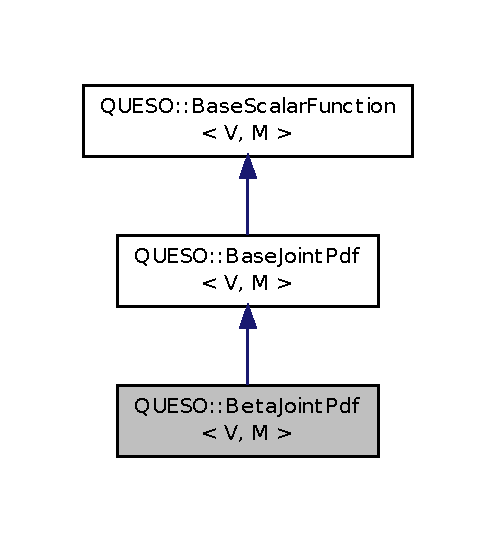
\includegraphics[width=238pt]{class_q_u_e_s_o_1_1_beta_joint_pdf__inherit__graph}
\end{center}
\end{figure}


Collaboration diagram for Q\-U\-E\-S\-O\-:\-:Beta\-Joint\-Pdf$<$ V, M $>$\-:
\nopagebreak
\begin{figure}[H]
\begin{center}
\leavevmode
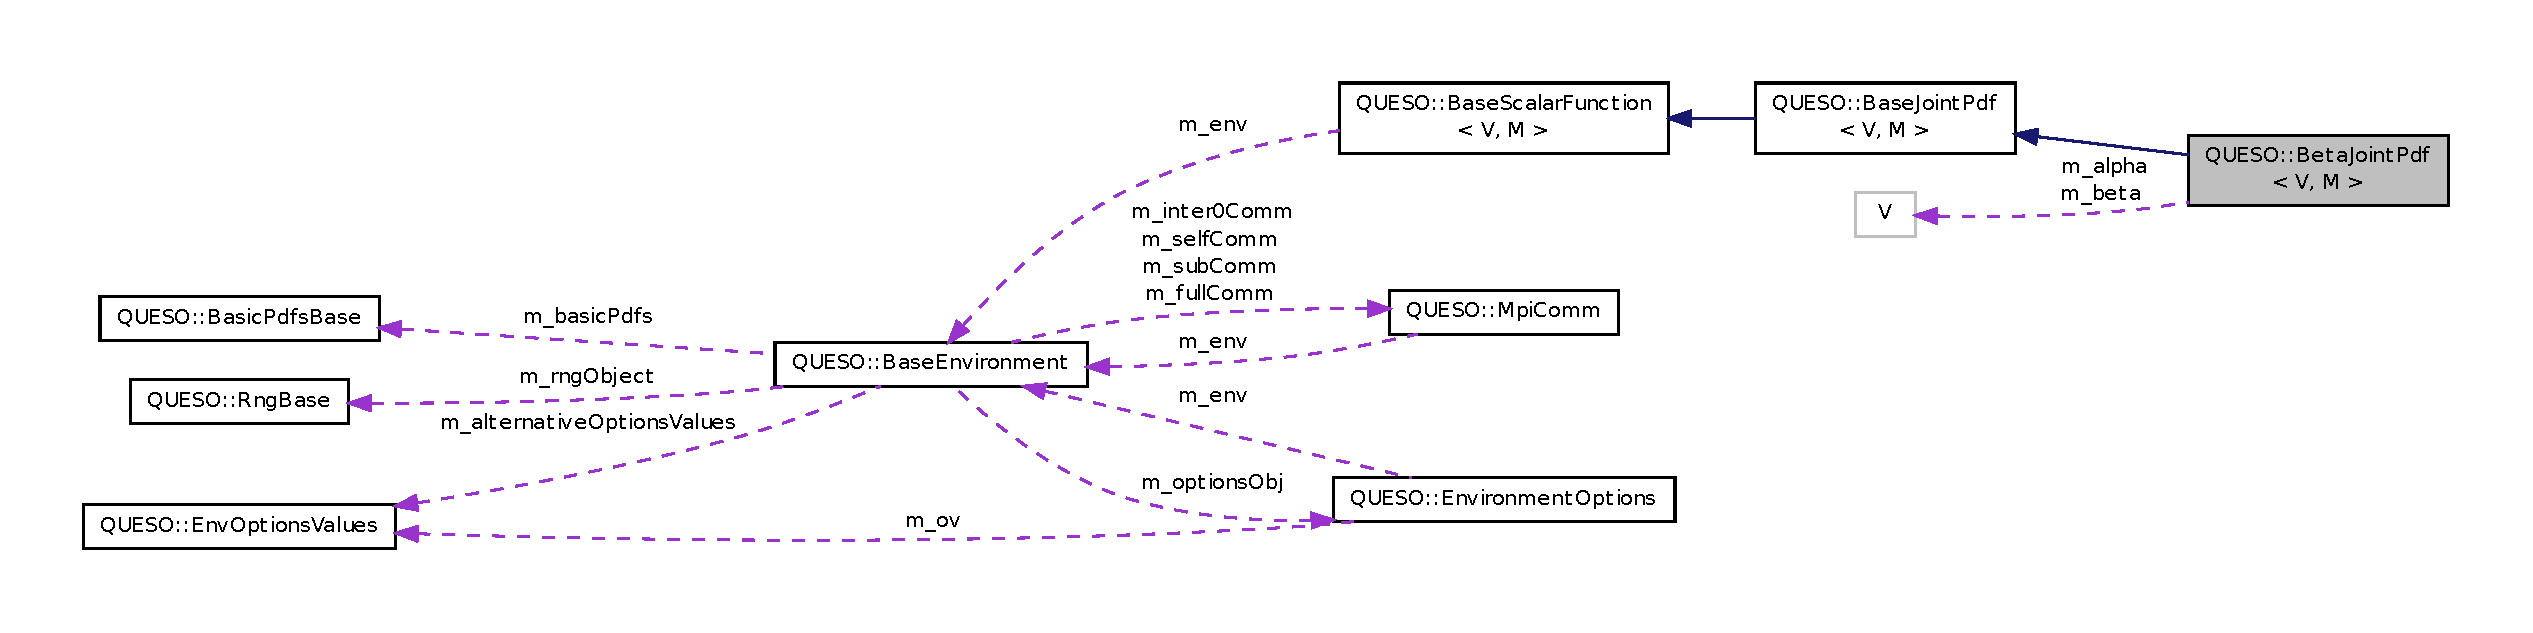
\includegraphics[width=350pt]{class_q_u_e_s_o_1_1_beta_joint_pdf__coll__graph}
\end{center}
\end{figure}
\subsection*{Public Member Functions}
\begin{Indent}{\bf Constructor/\-Destructor methods}\par
\begin{DoxyCompactItemize}
\item 
\hyperlink{class_q_u_e_s_o_1_1_beta_joint_pdf_a82b8baf377f485ac028207983a73618e}{Beta\-Joint\-Pdf} (const char $\ast$prefix, const \hyperlink{class_q_u_e_s_o_1_1_vector_set}{Vector\-Set}$<$ V, M $>$ \&\hyperlink{class_q_u_e_s_o_1_1_base_scalar_function_ad0937628825249dd36ded3ce0c7959ac}{domain\-Set}, const V \&alpha, const V \&beta)
\begin{DoxyCompactList}\small\item\em Constructor. \end{DoxyCompactList}\item 
\hyperlink{class_q_u_e_s_o_1_1_beta_joint_pdf_aaa4264f75e61e066b44ab545a3d1ae39}{$\sim$\-Beta\-Joint\-Pdf} ()
\begin{DoxyCompactList}\small\item\em Destructor. \end{DoxyCompactList}\end{DoxyCompactItemize}
\end{Indent}
\begin{Indent}{\bf Math methods}\par
\begin{DoxyCompactItemize}
\item 
double \hyperlink{class_q_u_e_s_o_1_1_beta_joint_pdf_a14909bee55e4d764be71e7a313716d9b}{actual\-Value} (const V \&domain\-Vector, const V $\ast$domain\-Direction, V $\ast$grad\-Vector, M $\ast$hessian\-Matrix, V $\ast$hessian\-Effect) const 
\begin{DoxyCompactList}\small\item\em Actual value of the Beta P\-D\-F. \end{DoxyCompactList}\item 
double \hyperlink{class_q_u_e_s_o_1_1_beta_joint_pdf_a713d655107dd51eac9d1c19630359a06}{ln\-Value} (const V \&domain\-Vector, const V $\ast$domain\-Direction, V $\ast$grad\-Vector, M $\ast$hessian\-Matrix, V $\ast$hessian\-Effect) const 
\begin{DoxyCompactList}\small\item\em Logarithm of the value of the Beta P\-D\-F. \end{DoxyCompactList}\item 
double \hyperlink{class_q_u_e_s_o_1_1_beta_joint_pdf_aaa67d058285caffa8dcb0235fbaf7726}{compute\-Log\-Of\-Normalization\-Factor} (unsigned int num\-Samples, bool update\-Factor\-Internally) const 
\begin{DoxyCompactList}\small\item\em Computes the logarithm of the normalization factor. \end{DoxyCompactList}\end{DoxyCompactItemize}
\end{Indent}
\subsection*{Protected Attributes}
\begin{DoxyCompactItemize}
\item 
V \hyperlink{class_q_u_e_s_o_1_1_beta_joint_pdf_aaed2224330514a2b04d0b2924b7f9f49}{m\-\_\-alpha}
\item 
V \hyperlink{class_q_u_e_s_o_1_1_beta_joint_pdf_a71e4c9d34bc0732044efd7b30dea2841}{m\-\_\-beta}
\end{DoxyCompactItemize}
\subsection*{Additional Inherited Members}


\subsection{Detailed Description}
\subsubsection*{template$<$class V, class M$>$class Q\-U\-E\-S\-O\-::\-Beta\-Joint\-Pdf$<$ V, M $>$}

A class for handling Beta joint P\-D\-Fs. 

This class allows the mathematical definition of a Beta Joint P\-D\-F. 

Definition at line 49 of file Beta\-Joint\-Pdf.\-h.



\subsection{Constructor \& Destructor Documentation}
\hypertarget{class_q_u_e_s_o_1_1_beta_joint_pdf_a82b8baf377f485ac028207983a73618e}{\index{Q\-U\-E\-S\-O\-::\-Beta\-Joint\-Pdf@{Q\-U\-E\-S\-O\-::\-Beta\-Joint\-Pdf}!Beta\-Joint\-Pdf@{Beta\-Joint\-Pdf}}
\index{Beta\-Joint\-Pdf@{Beta\-Joint\-Pdf}!QUESO::BetaJointPdf@{Q\-U\-E\-S\-O\-::\-Beta\-Joint\-Pdf}}
\subsubsection[{Beta\-Joint\-Pdf}]{\setlength{\rightskip}{0pt plus 5cm}template$<$class V , class M $>$ {\bf Q\-U\-E\-S\-O\-::\-Beta\-Joint\-Pdf}$<$ V, M $>$\-::{\bf Beta\-Joint\-Pdf} (
\begin{DoxyParamCaption}
\item[{const char $\ast$}]{prefix, }
\item[{const {\bf Vector\-Set}$<$ V, M $>$ \&}]{domain\-Set, }
\item[{const V \&}]{alpha, }
\item[{const V \&}]{beta}
\end{DoxyParamCaption}
)}}\label{class_q_u_e_s_o_1_1_beta_joint_pdf_a82b8baf377f485ac028207983a73618e}


Constructor. 

Constructs a new object of the class, given a prefix, the domain set, and the parameters {\ttfamily alpha} and {\ttfamily beta} of the Beta P\-D\-F. 

Definition at line 33 of file Beta\-Joint\-Pdf.\-C.



References Q\-U\-E\-S\-O\-::\-Base\-Environment\-::display\-Verbosity(), Q\-U\-E\-S\-O\-::\-Base\-Scalar\-Function$<$ V, M $>$\-::m\-\_\-env, Q\-U\-E\-S\-O\-::\-Base\-Scalar\-Function$<$ V, M $>$\-::m\-\_\-prefix, and Q\-U\-E\-S\-O\-::\-Base\-Environment\-::sub\-Display\-File().


\begin{DoxyCode}
38   :
39   BaseJointPdf<V,M>(((std::string)(prefix)+\textcolor{stringliteral}{"uni"}).c\_str(),\hyperlink{class_q_u_e_s_o_1_1_base_scalar_function_ad0937628825249dd36ded3ce0c7959ac}{domainSet}),
40   \hyperlink{class_q_u_e_s_o_1_1_beta_joint_pdf_aaed2224330514a2b04d0b2924b7f9f49}{m\_alpha}(alpha),
41   \hyperlink{class_q_u_e_s_o_1_1_beta_joint_pdf_a71e4c9d34bc0732044efd7b30dea2841}{m\_beta} (beta)
42 \{
43   \textcolor{keywordflow}{if} ((\hyperlink{class_q_u_e_s_o_1_1_base_scalar_function_adf44141aeb765d97613286f88f235f04}{m\_env}.\hyperlink{class_q_u_e_s_o_1_1_base_environment_a8a0064746ae8dddfece4229b9ad374d6}{subDisplayFile}()) && (\hyperlink{class_q_u_e_s_o_1_1_base_scalar_function_adf44141aeb765d97613286f88f235f04}{m\_env}.
      \hyperlink{class_q_u_e_s_o_1_1_base_environment_a1fe5f244fc0316a0ab3e37463f108b96}{displayVerbosity}() >= 54)) \{
44     *\hyperlink{class_q_u_e_s_o_1_1_base_scalar_function_adf44141aeb765d97613286f88f235f04}{m\_env}.\hyperlink{class_q_u_e_s_o_1_1_base_environment_a8a0064746ae8dddfece4229b9ad374d6}{subDisplayFile}() << \textcolor{stringliteral}{"Entering BetaJointPdf<V,M>::constructor()"}
45                             << \textcolor{stringliteral}{": prefix = "} << \hyperlink{class_q_u_e_s_o_1_1_base_scalar_function_a6e81dc902aca6a546877da99b2f4a169}{m\_prefix}
46                             << std::endl;
47   \}
48 
49   \textcolor{keywordflow}{if} ((\hyperlink{class_q_u_e_s_o_1_1_base_scalar_function_adf44141aeb765d97613286f88f235f04}{m\_env}.\hyperlink{class_q_u_e_s_o_1_1_base_environment_a8a0064746ae8dddfece4229b9ad374d6}{subDisplayFile}()) && (\hyperlink{class_q_u_e_s_o_1_1_base_scalar_function_adf44141aeb765d97613286f88f235f04}{m\_env}.
      \hyperlink{class_q_u_e_s_o_1_1_base_environment_a1fe5f244fc0316a0ab3e37463f108b96}{displayVerbosity}() >= 54)) \{
50     *\hyperlink{class_q_u_e_s_o_1_1_base_scalar_function_adf44141aeb765d97613286f88f235f04}{m\_env}.\hyperlink{class_q_u_e_s_o_1_1_base_environment_a8a0064746ae8dddfece4229b9ad374d6}{subDisplayFile}() << \textcolor{stringliteral}{"Leaving BetaJointPdf<V,M>::constructor()"}
51                             << \textcolor{stringliteral}{": prefix = "} << \hyperlink{class_q_u_e_s_o_1_1_base_scalar_function_a6e81dc902aca6a546877da99b2f4a169}{m\_prefix}
52                             << std::endl;
53   \}
54 \}
\end{DoxyCode}
\hypertarget{class_q_u_e_s_o_1_1_beta_joint_pdf_aaa4264f75e61e066b44ab545a3d1ae39}{\index{Q\-U\-E\-S\-O\-::\-Beta\-Joint\-Pdf@{Q\-U\-E\-S\-O\-::\-Beta\-Joint\-Pdf}!$\sim$\-Beta\-Joint\-Pdf@{$\sim$\-Beta\-Joint\-Pdf}}
\index{$\sim$\-Beta\-Joint\-Pdf@{$\sim$\-Beta\-Joint\-Pdf}!QUESO::BetaJointPdf@{Q\-U\-E\-S\-O\-::\-Beta\-Joint\-Pdf}}
\subsubsection[{$\sim$\-Beta\-Joint\-Pdf}]{\setlength{\rightskip}{0pt plus 5cm}template$<$class V , class M $>$ {\bf Q\-U\-E\-S\-O\-::\-Beta\-Joint\-Pdf}$<$ V, M $>$\-::$\sim${\bf Beta\-Joint\-Pdf} (
\begin{DoxyParamCaption}
{}
\end{DoxyParamCaption}
)}}\label{class_q_u_e_s_o_1_1_beta_joint_pdf_aaa4264f75e61e066b44ab545a3d1ae39}


Destructor. 



Definition at line 57 of file Beta\-Joint\-Pdf.\-C.


\begin{DoxyCode}
58 \{
59 \}
\end{DoxyCode}


\subsection{Member Function Documentation}
\hypertarget{class_q_u_e_s_o_1_1_beta_joint_pdf_a14909bee55e4d764be71e7a313716d9b}{\index{Q\-U\-E\-S\-O\-::\-Beta\-Joint\-Pdf@{Q\-U\-E\-S\-O\-::\-Beta\-Joint\-Pdf}!actual\-Value@{actual\-Value}}
\index{actual\-Value@{actual\-Value}!QUESO::BetaJointPdf@{Q\-U\-E\-S\-O\-::\-Beta\-Joint\-Pdf}}
\subsubsection[{actual\-Value}]{\setlength{\rightskip}{0pt plus 5cm}template$<$class V , class M $>$ double {\bf Q\-U\-E\-S\-O\-::\-Beta\-Joint\-Pdf}$<$ V, M $>$\-::actual\-Value (
\begin{DoxyParamCaption}
\item[{const V \&}]{domain\-Vector, }
\item[{const V $\ast$}]{domain\-Direction, }
\item[{V $\ast$}]{grad\-Vector, }
\item[{M $\ast$}]{hessian\-Matrix, }
\item[{V $\ast$}]{hessian\-Effect}
\end{DoxyParamCaption}
) const\hspace{0.3cm}{\ttfamily [virtual]}}}\label{class_q_u_e_s_o_1_1_beta_joint_pdf_a14909bee55e4d764be71e7a313716d9b}


Actual value of the Beta P\-D\-F. 

This routine calls method \hyperlink{class_q_u_e_s_o_1_1_beta_joint_pdf_a713d655107dd51eac9d1c19630359a06}{ln\-Value()} and returns the exponent of the returning value of such method. 

Implements \hyperlink{class_q_u_e_s_o_1_1_base_joint_pdf_a3c367a0cc3fb707a136c5df47dd414c1}{Q\-U\-E\-S\-O\-::\-Base\-Joint\-Pdf$<$ V, M $>$}.



Definition at line 63 of file Beta\-Joint\-Pdf.\-C.



References U\-Q\-\_\-\-F\-A\-T\-A\-L\-\_\-\-T\-E\-S\-T\-\_\-\-M\-A\-C\-R\-O.


\begin{DoxyCode}
69 \{
70   \hyperlink{_defines_8h_a56d63d18d0a6d45757de47fcc06f574d}{UQ\_FATAL\_TEST\_MACRO}(domainVector.sizeLocal() != this->
      \hyperlink{class_q_u_e_s_o_1_1_base_scalar_function_a67696e86211197938c72cd11863f5cf8}{m\_domainSet}.vectorSpace().dimLocal(),
71                       \hyperlink{class_q_u_e_s_o_1_1_base_scalar_function_adf44141aeb765d97613286f88f235f04}{m\_env}.\hyperlink{class_q_u_e_s_o_1_1_base_environment_a78b57112bbd0e6dd0e8afec00b40ffa7}{worldRank}(),
72                       \textcolor{stringliteral}{"BetaJointPdf<V,M>::actualValue()"},
73                       \textcolor{stringliteral}{"invalid input"});
74 
75   \hyperlink{_defines_8h_a56d63d18d0a6d45757de47fcc06f574d}{UQ\_FATAL\_TEST\_MACRO}((domainDirection || gradVector || hessianMatrix || hessianEffect),
76                       \hyperlink{class_q_u_e_s_o_1_1_base_scalar_function_adf44141aeb765d97613286f88f235f04}{m\_env}.\hyperlink{class_q_u_e_s_o_1_1_base_environment_a78b57112bbd0e6dd0e8afec00b40ffa7}{worldRank}(),
77                       \textcolor{stringliteral}{"BetaJointPdf<V,M>::actualValue()"},
78                       \textcolor{stringliteral}{"incomplete code for gradVector, hessianMatrix and hessianEffect calculations"});
79 
80   \textcolor{comment}{// No need to multiply by exp(m\_logOfNormalizationFactor) because 'lnValue()' is called [PDF-05]}
81   \textcolor{keywordflow}{return} exp(this->\hyperlink{class_q_u_e_s_o_1_1_beta_joint_pdf_a713d655107dd51eac9d1c19630359a06}{lnValue}(domainVector,domainDirection,gradVector,hessianMatrix,hessianEffect));
82 \}
\end{DoxyCode}
\hypertarget{class_q_u_e_s_o_1_1_beta_joint_pdf_aaa67d058285caffa8dcb0235fbaf7726}{\index{Q\-U\-E\-S\-O\-::\-Beta\-Joint\-Pdf@{Q\-U\-E\-S\-O\-::\-Beta\-Joint\-Pdf}!compute\-Log\-Of\-Normalization\-Factor@{compute\-Log\-Of\-Normalization\-Factor}}
\index{compute\-Log\-Of\-Normalization\-Factor@{compute\-Log\-Of\-Normalization\-Factor}!QUESO::BetaJointPdf@{Q\-U\-E\-S\-O\-::\-Beta\-Joint\-Pdf}}
\subsubsection[{compute\-Log\-Of\-Normalization\-Factor}]{\setlength{\rightskip}{0pt plus 5cm}template$<$class V , class M $>$ double {\bf Q\-U\-E\-S\-O\-::\-Beta\-Joint\-Pdf}$<$ V, M $>$\-::compute\-Log\-Of\-Normalization\-Factor (
\begin{DoxyParamCaption}
\item[{unsigned int}]{num\-Samples, }
\item[{bool}]{update\-Factor\-Internally}
\end{DoxyParamCaption}
) const\hspace{0.3cm}{\ttfamily [virtual]}}}\label{class_q_u_e_s_o_1_1_beta_joint_pdf_aaa67d058285caffa8dcb0235fbaf7726}


Computes the logarithm of the normalization factor. 

This routine calls \hyperlink{class_q_u_e_s_o_1_1_base_joint_pdf_a7b7bdd13d2de51198bf75d522e02545b}{Base\-Joint\-Pdf\-::common\-Compute\-Log\-Of\-Normalization\-Factor()}. 

Implements \hyperlink{class_q_u_e_s_o_1_1_base_joint_pdf_a99d8ab490b093abffd6068b6ea5263bb}{Q\-U\-E\-S\-O\-::\-Base\-Joint\-Pdf$<$ V, M $>$}.



Definition at line 126 of file Beta\-Joint\-Pdf.\-C.



References Q\-U\-E\-S\-O\-::\-Base\-Joint\-Pdf$<$ V, M $>$\-::common\-Compute\-Log\-Of\-Normalization\-Factor().


\begin{DoxyCode}
127 \{
128   \textcolor{keywordtype}{double} value = 0.;
129 
130   \textcolor{keywordflow}{if} ((\hyperlink{class_q_u_e_s_o_1_1_base_scalar_function_adf44141aeb765d97613286f88f235f04}{m\_env}.\hyperlink{class_q_u_e_s_o_1_1_base_environment_a8a0064746ae8dddfece4229b9ad374d6}{subDisplayFile}()) && (\hyperlink{class_q_u_e_s_o_1_1_base_scalar_function_adf44141aeb765d97613286f88f235f04}{m\_env}.
      \hyperlink{class_q_u_e_s_o_1_1_base_environment_a1fe5f244fc0316a0ab3e37463f108b96}{displayVerbosity}() >= 2)) \{
131     *\hyperlink{class_q_u_e_s_o_1_1_base_scalar_function_adf44141aeb765d97613286f88f235f04}{m\_env}.\hyperlink{class_q_u_e_s_o_1_1_base_environment_a8a0064746ae8dddfece4229b9ad374d6}{subDisplayFile}() << \textcolor{stringliteral}{"Entering
       BetaJointPdf<V,M>::computeLogOfNormalizationFactor()"}
132                             << std::endl;
133   \}
134   value = \hyperlink{class_q_u_e_s_o_1_1_base_joint_pdf_a7b7bdd13d2de51198bf75d522e02545b}{BaseJointPdf<V,M>::commonComputeLogOfNormalizationFactor}
      (numSamples, updateFactorInternally);
135   \textcolor{keywordflow}{if} ((\hyperlink{class_q_u_e_s_o_1_1_base_scalar_function_adf44141aeb765d97613286f88f235f04}{m\_env}.\hyperlink{class_q_u_e_s_o_1_1_base_environment_a8a0064746ae8dddfece4229b9ad374d6}{subDisplayFile}()) && (\hyperlink{class_q_u_e_s_o_1_1_base_scalar_function_adf44141aeb765d97613286f88f235f04}{m\_env}.
      \hyperlink{class_q_u_e_s_o_1_1_base_environment_a1fe5f244fc0316a0ab3e37463f108b96}{displayVerbosity}() >= 2)) \{
136     *\hyperlink{class_q_u_e_s_o_1_1_base_scalar_function_adf44141aeb765d97613286f88f235f04}{m\_env}.\hyperlink{class_q_u_e_s_o_1_1_base_environment_a8a0064746ae8dddfece4229b9ad374d6}{subDisplayFile}() << \textcolor{stringliteral}{"Leaving
       BetaJointPdf<V,M>::computeLogOfNormalizationFactor()"}
137                             << \textcolor{stringliteral}{", m\_logOfNormalizationFactor = "} << 
      \hyperlink{class_q_u_e_s_o_1_1_base_joint_pdf_ae82d4191f17af8c7a26226d127bc7850}{m\_logOfNormalizationFactor}
138                             << std::endl;
139   \}
140 
141   \textcolor{keywordflow}{return} value;
142 \}
\end{DoxyCode}
\hypertarget{class_q_u_e_s_o_1_1_beta_joint_pdf_a713d655107dd51eac9d1c19630359a06}{\index{Q\-U\-E\-S\-O\-::\-Beta\-Joint\-Pdf@{Q\-U\-E\-S\-O\-::\-Beta\-Joint\-Pdf}!ln\-Value@{ln\-Value}}
\index{ln\-Value@{ln\-Value}!QUESO::BetaJointPdf@{Q\-U\-E\-S\-O\-::\-Beta\-Joint\-Pdf}}
\subsubsection[{ln\-Value}]{\setlength{\rightskip}{0pt plus 5cm}template$<$class V , class M $>$ double {\bf Q\-U\-E\-S\-O\-::\-Beta\-Joint\-Pdf}$<$ V, M $>$\-::ln\-Value (
\begin{DoxyParamCaption}
\item[{const V \&}]{domain\-Vector, }
\item[{const V $\ast$}]{domain\-Direction, }
\item[{V $\ast$}]{grad\-Vector, }
\item[{M $\ast$}]{hessian\-Matrix, }
\item[{V $\ast$}]{hessian\-Effect}
\end{DoxyParamCaption}
) const\hspace{0.3cm}{\ttfamily [virtual]}}}\label{class_q_u_e_s_o_1_1_beta_joint_pdf_a713d655107dd51eac9d1c19630359a06}


Logarithm of the value of the Beta P\-D\-F. 

If the normalization style (m\-\_\-normalization\-Style) is zero, then this routine calls a environment method which handles basic P\-D\-Fs, e.\-g. basic\-Pdfs()-\/$>$beta\-Pdf\-Actual\-Value() and adds the log of the normalization factor (m\-\_\-log\-Of\-Normalization\-Factor) to it; otherwise the method uses the formula\-: $ lnValue = \sum[ (alpha_i-1)*log(domainVector_i) + (beta_i-1)*log(1-domainVector_i)] + m_logOfNormalizationFactor $. 

Implements \hyperlink{class_q_u_e_s_o_1_1_base_joint_pdf_aaeb1d91fd791399a502f451b07bb1bfe}{Q\-U\-E\-S\-O\-::\-Base\-Joint\-Pdf$<$ V, M $>$}.



Definition at line 86 of file Beta\-Joint\-Pdf.\-C.



References U\-Q\-\_\-\-F\-A\-T\-A\-L\-\_\-\-T\-E\-S\-T\-\_\-\-M\-A\-C\-R\-O.


\begin{DoxyCode}
92 \{
93   \hyperlink{_defines_8h_a56d63d18d0a6d45757de47fcc06f574d}{UQ\_FATAL\_TEST\_MACRO}((domainDirection || gradVector || hessianMatrix || hessianEffect),
94                       \hyperlink{class_q_u_e_s_o_1_1_base_scalar_function_adf44141aeb765d97613286f88f235f04}{m\_env}.\hyperlink{class_q_u_e_s_o_1_1_base_environment_a78b57112bbd0e6dd0e8afec00b40ffa7}{worldRank}(),
95                       \textcolor{stringliteral}{"BetaJointPdf<V,M>::lnValue()"},
96                       \textcolor{stringliteral}{"incomplete code for gradVector, hessianMatrix and hessianEffect calculations"});
97 
98   \textcolor{keywordtype}{double} aux = 0.;
99   \textcolor{keywordtype}{double} result = 0.;
100   \textcolor{keywordflow}{for} (\textcolor{keywordtype}{unsigned} \textcolor{keywordtype}{int} i = 0; i < domainVector.sizeLocal(); ++i) \{
101     \textcolor{keywordflow}{if} (\hyperlink{class_q_u_e_s_o_1_1_base_joint_pdf_a138c99bcef7a67077d9612bddfdcb896}{m\_normalizationStyle} == 0) \{
102       \textcolor{comment}{//aux = log(gsl\_ran\_beta\_pdf(domainVector[i],m\_alpha[i],m\_beta[i]));}
103       aux = log(\hyperlink{class_q_u_e_s_o_1_1_base_scalar_function_adf44141aeb765d97613286f88f235f04}{m\_env}.\hyperlink{class_q_u_e_s_o_1_1_base_environment_af106da59f188ba0dbf4f93da3fcd8ca5}{basicPdfs}()->\hyperlink{class_q_u_e_s_o_1_1_basic_pdfs_base_a7a4df6a4b2147eeca4efb22db0ae1b8b}{betaPdfActualValue}(domainVector[i],
      \hyperlink{class_q_u_e_s_o_1_1_beta_joint_pdf_aaed2224330514a2b04d0b2924b7f9f49}{m\_alpha}[i],\hyperlink{class_q_u_e_s_o_1_1_beta_joint_pdf_a71e4c9d34bc0732044efd7b30dea2841}{m\_beta}[i]));
104     \}
105     \textcolor{keywordflow}{else} \{
106       aux = (\hyperlink{class_q_u_e_s_o_1_1_beta_joint_pdf_aaed2224330514a2b04d0b2924b7f9f49}{m\_alpha}[i]-1.)*log(domainVector[i]) + (\hyperlink{class_q_u_e_s_o_1_1_beta_joint_pdf_a71e4c9d34bc0732044efd7b30dea2841}{m\_beta}[i]-1.)*log(1.-domainVector[i]);
107     \}
108     \textcolor{keywordflow}{if} ((\hyperlink{class_q_u_e_s_o_1_1_base_scalar_function_adf44141aeb765d97613286f88f235f04}{m\_env}.\hyperlink{class_q_u_e_s_o_1_1_base_environment_a8a0064746ae8dddfece4229b9ad374d6}{subDisplayFile}()) && (\hyperlink{class_q_u_e_s_o_1_1_base_scalar_function_adf44141aeb765d97613286f88f235f04}{m\_env}.
      \hyperlink{class_q_u_e_s_o_1_1_base_environment_a1fe5f244fc0316a0ab3e37463f108b96}{displayVerbosity}() >= 99)) \{
109       *\hyperlink{class_q_u_e_s_o_1_1_base_scalar_function_adf44141aeb765d97613286f88f235f04}{m\_env}.\hyperlink{class_q_u_e_s_o_1_1_base_environment_a8a0064746ae8dddfece4229b9ad374d6}{subDisplayFile}() << \textcolor{stringliteral}{"In BetaJointPdf<V,M>::lnValue()"}
110                               << \textcolor{stringliteral}{", m\_normalizationStyle = "}      << 
      \hyperlink{class_q_u_e_s_o_1_1_base_joint_pdf_a138c99bcef7a67077d9612bddfdcb896}{m\_normalizationStyle}
111                               << \textcolor{stringliteral}{": domainVector["} << i << \textcolor{stringliteral}{"] = "} << domainVector[i]
112                               << \textcolor{stringliteral}{", m\_alpha["} << i << \textcolor{stringliteral}{"] = "}      << \hyperlink{class_q_u_e_s_o_1_1_beta_joint_pdf_aaed2224330514a2b04d0b2924b7f9f49}{m\_alpha}[i]
113                               << \textcolor{stringliteral}{", m\_beta["} << i << \textcolor{stringliteral}{"] = "}       << \hyperlink{class_q_u_e_s_o_1_1_beta_joint_pdf_a71e4c9d34bc0732044efd7b30dea2841}{m\_beta}[i]
114                               << \textcolor{stringliteral}{", log(pdf)= "}                   << aux
115                               << std::endl;
116     \}
117     result += aux;
118   \}
119   result += \hyperlink{class_q_u_e_s_o_1_1_base_joint_pdf_ae82d4191f17af8c7a26226d127bc7850}{m\_logOfNormalizationFactor}; \textcolor{comment}{// [PDF-05]}
120 
121   \textcolor{keywordflow}{return} result;
122 \}
\end{DoxyCode}


\subsection{Member Data Documentation}
\hypertarget{class_q_u_e_s_o_1_1_beta_joint_pdf_aaed2224330514a2b04d0b2924b7f9f49}{\index{Q\-U\-E\-S\-O\-::\-Beta\-Joint\-Pdf@{Q\-U\-E\-S\-O\-::\-Beta\-Joint\-Pdf}!m\-\_\-alpha@{m\-\_\-alpha}}
\index{m\-\_\-alpha@{m\-\_\-alpha}!QUESO::BetaJointPdf@{Q\-U\-E\-S\-O\-::\-Beta\-Joint\-Pdf}}
\subsubsection[{m\-\_\-alpha}]{\setlength{\rightskip}{0pt plus 5cm}template$<$class V, class M$>$ V {\bf Q\-U\-E\-S\-O\-::\-Beta\-Joint\-Pdf}$<$ V, M $>$\-::m\-\_\-alpha\hspace{0.3cm}{\ttfamily [protected]}}}\label{class_q_u_e_s_o_1_1_beta_joint_pdf_aaed2224330514a2b04d0b2924b7f9f49}


Definition at line 88 of file Beta\-Joint\-Pdf.\-h.

\hypertarget{class_q_u_e_s_o_1_1_beta_joint_pdf_a71e4c9d34bc0732044efd7b30dea2841}{\index{Q\-U\-E\-S\-O\-::\-Beta\-Joint\-Pdf@{Q\-U\-E\-S\-O\-::\-Beta\-Joint\-Pdf}!m\-\_\-beta@{m\-\_\-beta}}
\index{m\-\_\-beta@{m\-\_\-beta}!QUESO::BetaJointPdf@{Q\-U\-E\-S\-O\-::\-Beta\-Joint\-Pdf}}
\subsubsection[{m\-\_\-beta}]{\setlength{\rightskip}{0pt plus 5cm}template$<$class V, class M$>$ V {\bf Q\-U\-E\-S\-O\-::\-Beta\-Joint\-Pdf}$<$ V, M $>$\-::m\-\_\-beta\hspace{0.3cm}{\ttfamily [protected]}}}\label{class_q_u_e_s_o_1_1_beta_joint_pdf_a71e4c9d34bc0732044efd7b30dea2841}


Definition at line 89 of file Beta\-Joint\-Pdf.\-h.



The documentation for this class was generated from the following files\-:\begin{DoxyCompactItemize}
\item 
src/stats/inc/\hyperlink{_beta_joint_pdf_8h}{Beta\-Joint\-Pdf.\-h}\item 
src/stats/src/\hyperlink{_beta_joint_pdf_8_c}{Beta\-Joint\-Pdf.\-C}\end{DoxyCompactItemize}

\hypertarget{class_q_u_e_s_o_1_1_beta_vector_realizer}{\section{Q\-U\-E\-S\-O\-:\-:Beta\-Vector\-Realizer$<$ V, M $>$ Class Template Reference}
\label{class_q_u_e_s_o_1_1_beta_vector_realizer}\index{Q\-U\-E\-S\-O\-::\-Beta\-Vector\-Realizer$<$ V, M $>$@{Q\-U\-E\-S\-O\-::\-Beta\-Vector\-Realizer$<$ V, M $>$}}
}


A class for handling sampling from a Beta probability density distribution.  




{\ttfamily \#include $<$Beta\-Vector\-Realizer.\-h$>$}



Inheritance diagram for Q\-U\-E\-S\-O\-:\-:Beta\-Vector\-Realizer$<$ V, M $>$\-:
\nopagebreak
\begin{figure}[H]
\begin{center}
\leavevmode
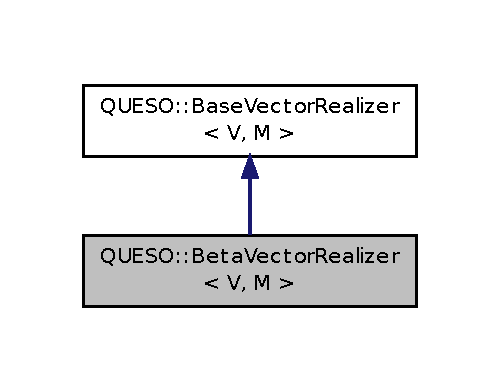
\includegraphics[width=240pt]{class_q_u_e_s_o_1_1_beta_vector_realizer__inherit__graph}
\end{center}
\end{figure}


Collaboration diagram for Q\-U\-E\-S\-O\-:\-:Beta\-Vector\-Realizer$<$ V, M $>$\-:
\nopagebreak
\begin{figure}[H]
\begin{center}
\leavevmode
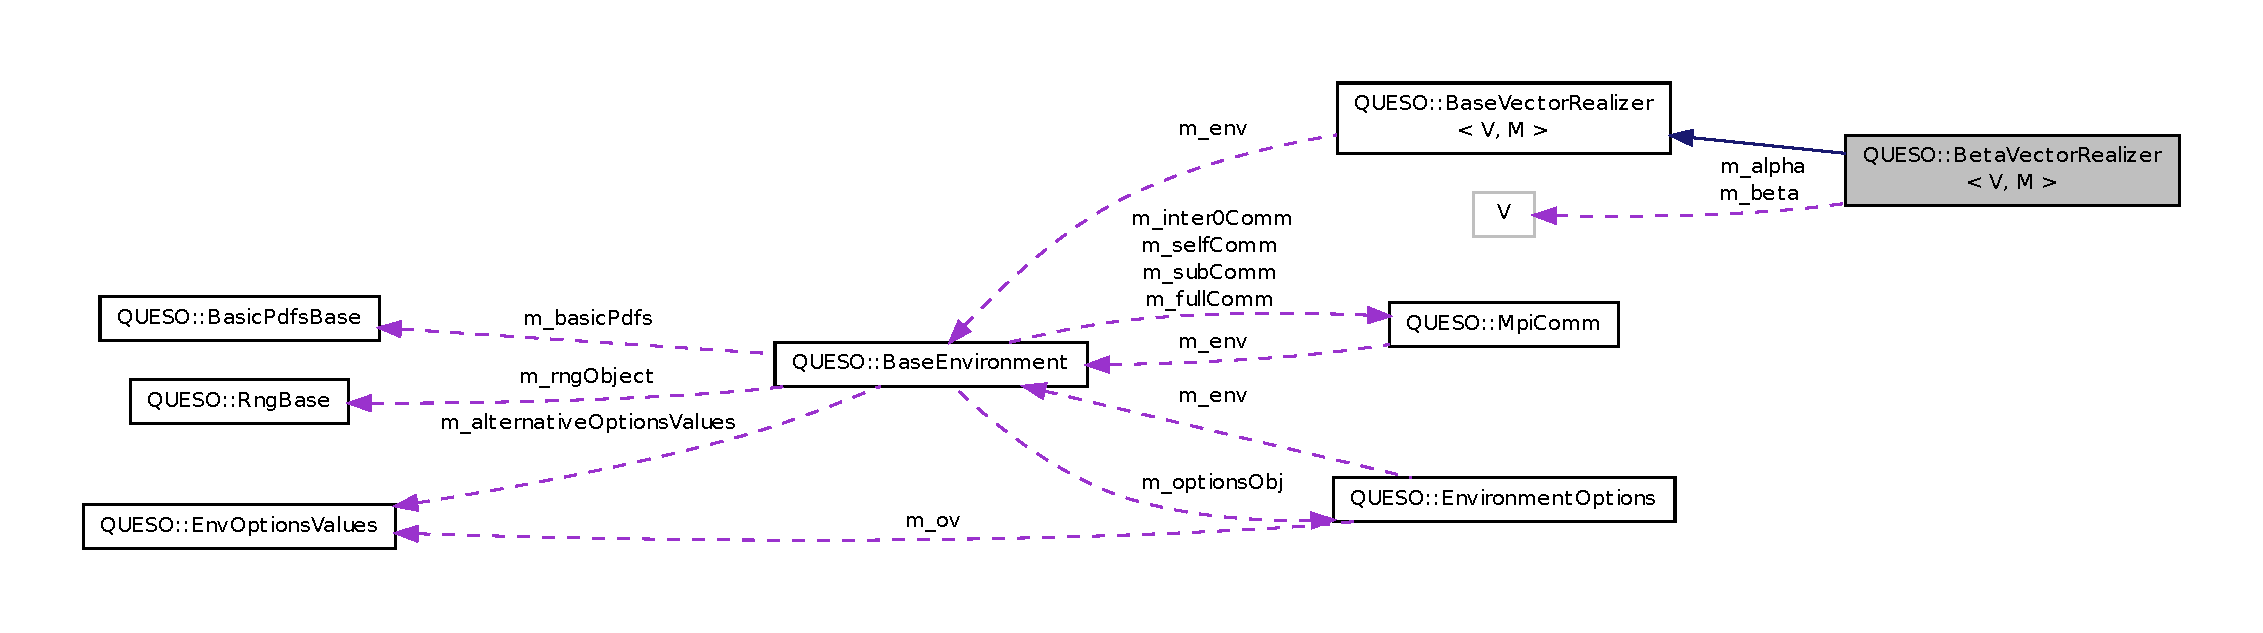
\includegraphics[width=350pt]{class_q_u_e_s_o_1_1_beta_vector_realizer__coll__graph}
\end{center}
\end{figure}
\subsection*{Public Member Functions}
\begin{Indent}{\bf Constructor/\-Destructor methods}\par
\begin{DoxyCompactItemize}
\item 
\hyperlink{class_q_u_e_s_o_1_1_beta_vector_realizer_a476e76c89f2f6706989943596d9158ae}{Beta\-Vector\-Realizer} (const char $\ast$prefix, const \hyperlink{class_q_u_e_s_o_1_1_vector_set}{Vector\-Set}$<$ V, M $>$ \&\hyperlink{class_q_u_e_s_o_1_1_base_vector_realizer_ad958991bab8d6369e8a0d66b22a237d4}{unified\-Image\-Set}, const V \&alpha, const V \&beta)
\begin{DoxyCompactList}\small\item\em Constructor. \end{DoxyCompactList}\item 
\hyperlink{class_q_u_e_s_o_1_1_beta_vector_realizer_aaa4a00655b79a138fa28cea29a91a91f}{$\sim$\-Beta\-Vector\-Realizer} ()
\begin{DoxyCompactList}\small\item\em Destructor. \end{DoxyCompactList}\end{DoxyCompactItemize}
\end{Indent}
\begin{Indent}{\bf Realization-\/related methods}\par
\begin{DoxyCompactItemize}
\item 
void \hyperlink{class_q_u_e_s_o_1_1_beta_vector_realizer_a75659aac16145ad3e770e852500ee7f2}{realization} (V \&next\-Values) const 
\begin{DoxyCompactList}\small\item\em Draws a realization. \end{DoxyCompactList}\end{DoxyCompactItemize}
\end{Indent}
\subsection*{Private Attributes}
\begin{DoxyCompactItemize}
\item 
V \hyperlink{class_q_u_e_s_o_1_1_beta_vector_realizer_a9a1570ec745b892fafe325605a2dcb57}{m\-\_\-alpha}
\item 
V \hyperlink{class_q_u_e_s_o_1_1_beta_vector_realizer_a0f2c801dbb06b1a5e41817fb66d3d952}{m\-\_\-beta}
\end{DoxyCompactItemize}
\subsection*{Additional Inherited Members}


\subsection{Detailed Description}
\subsubsection*{template$<$class V, class M$>$class Q\-U\-E\-S\-O\-::\-Beta\-Vector\-Realizer$<$ V, M $>$}

A class for handling sampling from a Beta probability density distribution. 

This class handles sampling from a Beta probability density distribution, of parameters {\ttfamily alpha} and {\ttfamily beta}. 

Definition at line 46 of file Beta\-Vector\-Realizer.\-h.



\subsection{Constructor \& Destructor Documentation}
\hypertarget{class_q_u_e_s_o_1_1_beta_vector_realizer_a476e76c89f2f6706989943596d9158ae}{\index{Q\-U\-E\-S\-O\-::\-Beta\-Vector\-Realizer@{Q\-U\-E\-S\-O\-::\-Beta\-Vector\-Realizer}!Beta\-Vector\-Realizer@{Beta\-Vector\-Realizer}}
\index{Beta\-Vector\-Realizer@{Beta\-Vector\-Realizer}!QUESO::BetaVectorRealizer@{Q\-U\-E\-S\-O\-::\-Beta\-Vector\-Realizer}}
\subsubsection[{Beta\-Vector\-Realizer}]{\setlength{\rightskip}{0pt plus 5cm}template$<$class V , class M $>$ {\bf Q\-U\-E\-S\-O\-::\-Beta\-Vector\-Realizer}$<$ V, M $>$\-::{\bf Beta\-Vector\-Realizer} (
\begin{DoxyParamCaption}
\item[{const char $\ast$}]{prefix, }
\item[{const {\bf Vector\-Set}$<$ V, M $>$ \&}]{unified\-Image\-Set, }
\item[{const V \&}]{alpha, }
\item[{const V \&}]{beta}
\end{DoxyParamCaption}
)}}\label{class_q_u_e_s_o_1_1_beta_vector_realizer_a476e76c89f2f6706989943596d9158ae}


Constructor. 

Constructs a new object, given a prefix, the image set of the vector realizer, and the Beta distribution parameters {\ttfamily alpha} and {\ttfamily beta}, which are assigned to private attributes m\-\_\-alpha and m\-\_\-beta. 

Definition at line 33 of file Beta\-Vector\-Realizer.\-C.



References Q\-U\-E\-S\-O\-::\-Base\-Environment\-::display\-Verbosity(), Q\-U\-E\-S\-O\-::\-Base\-Vector\-Realizer$<$ V, M $>$\-::m\-\_\-env, Q\-U\-E\-S\-O\-::\-Base\-Vector\-Realizer$<$ V, M $>$\-::m\-\_\-prefix, and Q\-U\-E\-S\-O\-::\-Base\-Environment\-::sub\-Display\-File().


\begin{DoxyCode}
38   :
39   BaseVectorRealizer<V,M>(((std::string)(prefix)+\textcolor{stringliteral}{"gen"}).c\_str(),\hyperlink{class_q_u_e_s_o_1_1_base_vector_realizer_ad958991bab8d6369e8a0d66b22a237d4}{unifiedImageSet},
      std::numeric\_limits<unsigned int>::max()),
40   \hyperlink{class_q_u_e_s_o_1_1_beta_vector_realizer_a9a1570ec745b892fafe325605a2dcb57}{m\_alpha}(alpha),
41   \hyperlink{class_q_u_e_s_o_1_1_beta_vector_realizer_a0f2c801dbb06b1a5e41817fb66d3d952}{m\_beta} (beta)
42 \{
43   \textcolor{keywordflow}{if} ((\hyperlink{class_q_u_e_s_o_1_1_base_vector_realizer_acde246c52f82d8ed687d91cfac14c29c}{m\_env}.\hyperlink{class_q_u_e_s_o_1_1_base_environment_a8a0064746ae8dddfece4229b9ad374d6}{subDisplayFile}()) && (\hyperlink{class_q_u_e_s_o_1_1_base_vector_realizer_acde246c52f82d8ed687d91cfac14c29c}{m\_env}.
      \hyperlink{class_q_u_e_s_o_1_1_base_environment_a1fe5f244fc0316a0ab3e37463f108b96}{displayVerbosity}() >= 5)) \{
44     *\hyperlink{class_q_u_e_s_o_1_1_base_vector_realizer_acde246c52f82d8ed687d91cfac14c29c}{m\_env}.\hyperlink{class_q_u_e_s_o_1_1_base_environment_a8a0064746ae8dddfece4229b9ad374d6}{subDisplayFile}() << \textcolor{stringliteral}{"Entering BetaVectorRealizer<V,M>::constructor()"}
45                             << \textcolor{stringliteral}{": prefix = "} << \hyperlink{class_q_u_e_s_o_1_1_base_vector_realizer_ac5559b6921816ccaed7afc2d342c2a32}{m\_prefix}
46                             << std::endl;
47   \}
48 
49   \textcolor{keywordflow}{if} ((\hyperlink{class_q_u_e_s_o_1_1_base_vector_realizer_acde246c52f82d8ed687d91cfac14c29c}{m\_env}.\hyperlink{class_q_u_e_s_o_1_1_base_environment_a8a0064746ae8dddfece4229b9ad374d6}{subDisplayFile}()) && (\hyperlink{class_q_u_e_s_o_1_1_base_vector_realizer_acde246c52f82d8ed687d91cfac14c29c}{m\_env}.
      \hyperlink{class_q_u_e_s_o_1_1_base_environment_a1fe5f244fc0316a0ab3e37463f108b96}{displayVerbosity}() >= 5)) \{
50     *\hyperlink{class_q_u_e_s_o_1_1_base_vector_realizer_acde246c52f82d8ed687d91cfac14c29c}{m\_env}.\hyperlink{class_q_u_e_s_o_1_1_base_environment_a8a0064746ae8dddfece4229b9ad374d6}{subDisplayFile}() << \textcolor{stringliteral}{"Leaving BetaVectorRealizer<V,M>::constructor()"}
51                             << \textcolor{stringliteral}{": prefix = "} << \hyperlink{class_q_u_e_s_o_1_1_base_vector_realizer_ac5559b6921816ccaed7afc2d342c2a32}{m\_prefix}
52                             << std::endl;
53   \}
54 \}
\end{DoxyCode}
\hypertarget{class_q_u_e_s_o_1_1_beta_vector_realizer_aaa4a00655b79a138fa28cea29a91a91f}{\index{Q\-U\-E\-S\-O\-::\-Beta\-Vector\-Realizer@{Q\-U\-E\-S\-O\-::\-Beta\-Vector\-Realizer}!$\sim$\-Beta\-Vector\-Realizer@{$\sim$\-Beta\-Vector\-Realizer}}
\index{$\sim$\-Beta\-Vector\-Realizer@{$\sim$\-Beta\-Vector\-Realizer}!QUESO::BetaVectorRealizer@{Q\-U\-E\-S\-O\-::\-Beta\-Vector\-Realizer}}
\subsubsection[{$\sim$\-Beta\-Vector\-Realizer}]{\setlength{\rightskip}{0pt plus 5cm}template$<$class V , class M $>$ {\bf Q\-U\-E\-S\-O\-::\-Beta\-Vector\-Realizer}$<$ V, M $>$\-::$\sim${\bf Beta\-Vector\-Realizer} (
\begin{DoxyParamCaption}
{}
\end{DoxyParamCaption}
)}}\label{class_q_u_e_s_o_1_1_beta_vector_realizer_aaa4a00655b79a138fa28cea29a91a91f}


Destructor. 



Definition at line 57 of file Beta\-Vector\-Realizer.\-C.


\begin{DoxyCode}
58 \{
59 \}
\end{DoxyCode}


\subsection{Member Function Documentation}
\hypertarget{class_q_u_e_s_o_1_1_beta_vector_realizer_a75659aac16145ad3e770e852500ee7f2}{\index{Q\-U\-E\-S\-O\-::\-Beta\-Vector\-Realizer@{Q\-U\-E\-S\-O\-::\-Beta\-Vector\-Realizer}!realization@{realization}}
\index{realization@{realization}!QUESO::BetaVectorRealizer@{Q\-U\-E\-S\-O\-::\-Beta\-Vector\-Realizer}}
\subsubsection[{realization}]{\setlength{\rightskip}{0pt plus 5cm}template$<$class V , class M $>$ void {\bf Q\-U\-E\-S\-O\-::\-Beta\-Vector\-Realizer}$<$ V, M $>$\-::realization (
\begin{DoxyParamCaption}
\item[{V \&}]{next\-Values}
\end{DoxyParamCaption}
) const\hspace{0.3cm}{\ttfamily [virtual]}}}\label{class_q_u_e_s_o_1_1_beta_vector_realizer_a75659aac16145ad3e770e852500ee7f2}


Draws a realization. 

This function draws a realization of a Beta distribution and saves it in {\ttfamily next\-Values}. It internally checks whether the image set, where the realization should be drawn, belongs to the interval (0, 1\mbox{]} -\/ which is the range where Beta distribution is defined over. 

Implements \hyperlink{class_q_u_e_s_o_1_1_base_vector_realizer_a6845173dd79a80ae11c86cde26e55817}{Q\-U\-E\-S\-O\-::\-Base\-Vector\-Realizer$<$ V, M $>$}.



Definition at line 63 of file Beta\-Vector\-Realizer.\-C.


\begin{DoxyCode}
64 \{
65   nextValues.cwSetBeta(\hyperlink{class_q_u_e_s_o_1_1_beta_vector_realizer_a9a1570ec745b892fafe325605a2dcb57}{m\_alpha},\hyperlink{class_q_u_e_s_o_1_1_beta_vector_realizer_a0f2c801dbb06b1a5e41817fb66d3d952}{m\_beta});
66   \textcolor{keywordflow}{return};
67 \}
\end{DoxyCode}


\subsection{Member Data Documentation}
\hypertarget{class_q_u_e_s_o_1_1_beta_vector_realizer_a9a1570ec745b892fafe325605a2dcb57}{\index{Q\-U\-E\-S\-O\-::\-Beta\-Vector\-Realizer@{Q\-U\-E\-S\-O\-::\-Beta\-Vector\-Realizer}!m\-\_\-alpha@{m\-\_\-alpha}}
\index{m\-\_\-alpha@{m\-\_\-alpha}!QUESO::BetaVectorRealizer@{Q\-U\-E\-S\-O\-::\-Beta\-Vector\-Realizer}}
\subsubsection[{m\-\_\-alpha}]{\setlength{\rightskip}{0pt plus 5cm}template$<$class V, class M$>$ V {\bf Q\-U\-E\-S\-O\-::\-Beta\-Vector\-Realizer}$<$ V, M $>$\-::m\-\_\-alpha\hspace{0.3cm}{\ttfamily [private]}}}\label{class_q_u_e_s_o_1_1_beta_vector_realizer_a9a1570ec745b892fafe325605a2dcb57}


Definition at line 78 of file Beta\-Vector\-Realizer.\-h.

\hypertarget{class_q_u_e_s_o_1_1_beta_vector_realizer_a0f2c801dbb06b1a5e41817fb66d3d952}{\index{Q\-U\-E\-S\-O\-::\-Beta\-Vector\-Realizer@{Q\-U\-E\-S\-O\-::\-Beta\-Vector\-Realizer}!m\-\_\-beta@{m\-\_\-beta}}
\index{m\-\_\-beta@{m\-\_\-beta}!QUESO::BetaVectorRealizer@{Q\-U\-E\-S\-O\-::\-Beta\-Vector\-Realizer}}
\subsubsection[{m\-\_\-beta}]{\setlength{\rightskip}{0pt plus 5cm}template$<$class V, class M$>$ V {\bf Q\-U\-E\-S\-O\-::\-Beta\-Vector\-Realizer}$<$ V, M $>$\-::m\-\_\-beta\hspace{0.3cm}{\ttfamily [private]}}}\label{class_q_u_e_s_o_1_1_beta_vector_realizer_a0f2c801dbb06b1a5e41817fb66d3d952}


Definition at line 79 of file Beta\-Vector\-Realizer.\-h.



The documentation for this class was generated from the following files\-:\begin{DoxyCompactItemize}
\item 
src/stats/inc/\hyperlink{_beta_vector_realizer_8h}{Beta\-Vector\-Realizer.\-h}\item 
src/stats/src/\hyperlink{_beta_vector_realizer_8_c}{Beta\-Vector\-Realizer.\-C}\end{DoxyCompactItemize}

\hypertarget{class_q_u_e_s_o_1_1_beta_vector_r_v}{\section{Q\-U\-E\-S\-O\-:\-:Beta\-Vector\-R\-V$<$ V, M $>$ Class Template Reference}
\label{class_q_u_e_s_o_1_1_beta_vector_r_v}\index{Q\-U\-E\-S\-O\-::\-Beta\-Vector\-R\-V$<$ V, M $>$@{Q\-U\-E\-S\-O\-::\-Beta\-Vector\-R\-V$<$ V, M $>$}}
}


A class representing a vector R\-V constructed via Beta distribution.  




{\ttfamily \#include $<$Beta\-Vector\-R\-V.\-h$>$}



Inheritance diagram for Q\-U\-E\-S\-O\-:\-:Beta\-Vector\-R\-V$<$ V, M $>$\-:
\nopagebreak
\begin{figure}[H]
\begin{center}
\leavevmode
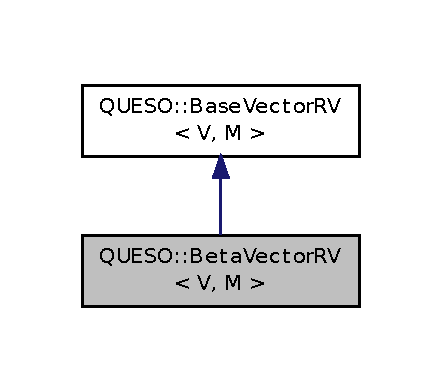
\includegraphics[width=212pt]{class_q_u_e_s_o_1_1_beta_vector_r_v__inherit__graph}
\end{center}
\end{figure}


Collaboration diagram for Q\-U\-E\-S\-O\-:\-:Beta\-Vector\-R\-V$<$ V, M $>$\-:
\nopagebreak
\begin{figure}[H]
\begin{center}
\leavevmode
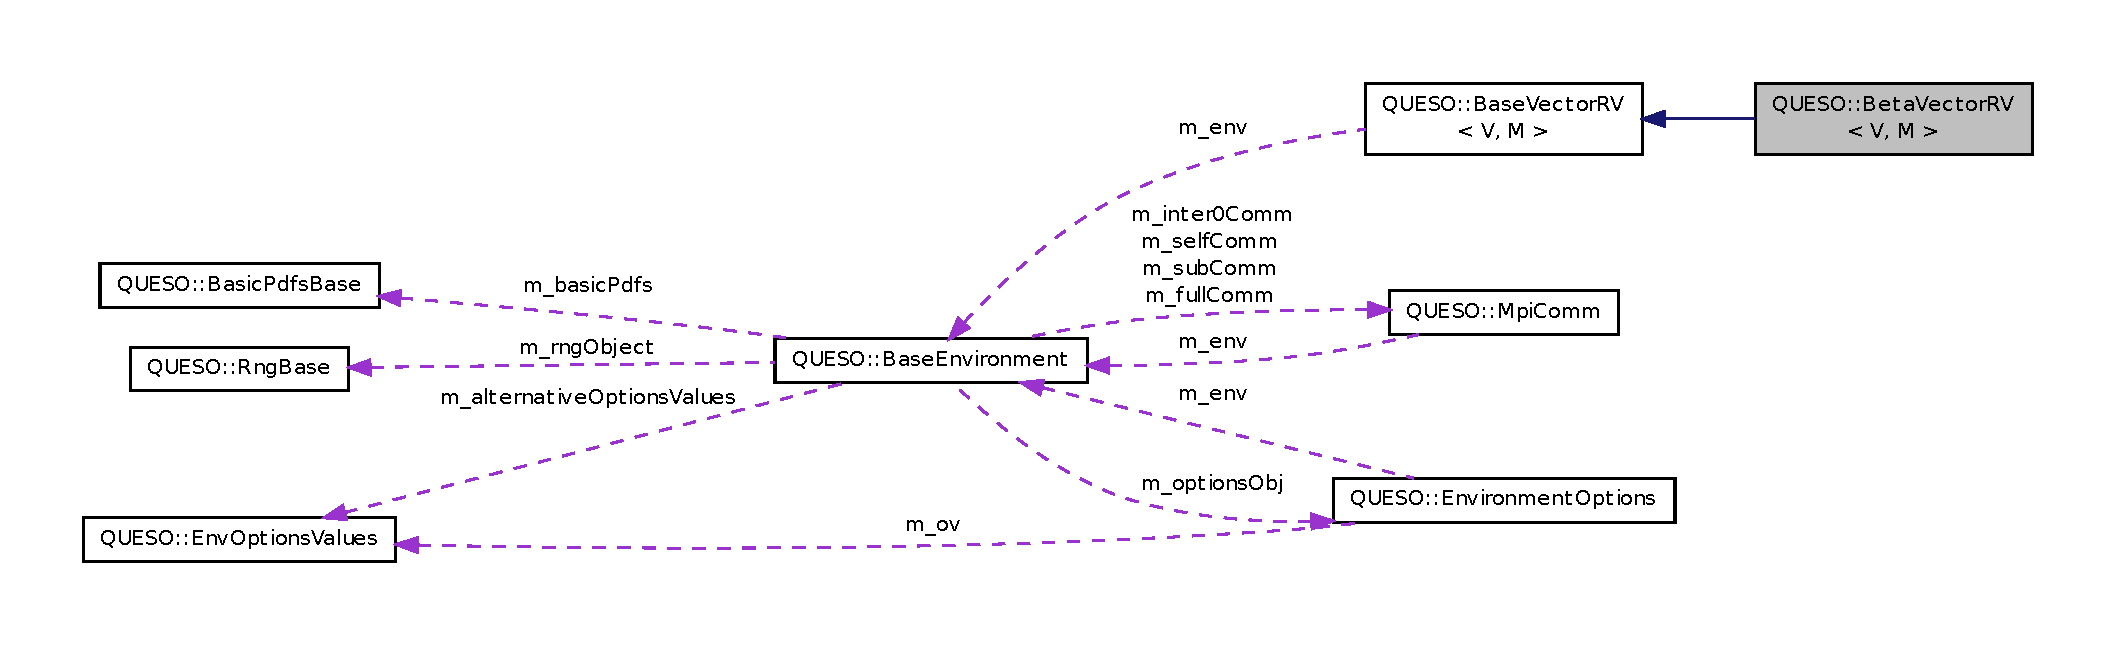
\includegraphics[width=350pt]{class_q_u_e_s_o_1_1_beta_vector_r_v__coll__graph}
\end{center}
\end{figure}
\subsection*{Public Member Functions}
\begin{Indent}{\bf Constructor/\-Destructor methods}\par
\begin{DoxyCompactItemize}
\item 
\hyperlink{class_q_u_e_s_o_1_1_beta_vector_r_v_a090eae9c454f4f68d536c2237e4bff03}{Beta\-Vector\-R\-V} (const char $\ast$prefix, const \hyperlink{class_q_u_e_s_o_1_1_vector_set}{Vector\-Set}$<$ V, M $>$ \&\hyperlink{class_q_u_e_s_o_1_1_base_vector_r_v_aa4dd2f036228eac1f945bacc7147a922}{image\-Set}, const V \&alpha, const V \&beta)
\begin{DoxyCompactList}\small\item\em Default Constructor. \end{DoxyCompactList}\item 
virtual \hyperlink{class_q_u_e_s_o_1_1_beta_vector_r_v_a24d791770f3518157c00a36a3c421649}{$\sim$\-Beta\-Vector\-R\-V} ()
\begin{DoxyCompactList}\small\item\em Virtual destructor. \end{DoxyCompactList}\end{DoxyCompactItemize}
\end{Indent}
\begin{Indent}{\bf I/\-O methods}\par
\begin{DoxyCompactItemize}
\item 
void \hyperlink{class_q_u_e_s_o_1_1_beta_vector_r_v_ae54ad1998b22aed2f5c8061cd1ad56e5}{print} (std\-::ostream \&os) const 
\begin{DoxyCompactList}\small\item\em T\-O\-D\-O\-: Prints the vector R\-V. \end{DoxyCompactList}\end{DoxyCompactItemize}
\end{Indent}
\subsection*{Additional Inherited Members}


\subsection{Detailed Description}
\subsubsection*{template$<$class V, class M$>$class Q\-U\-E\-S\-O\-::\-Beta\-Vector\-R\-V$<$ V, M $>$}

A class representing a vector R\-V constructed via Beta distribution. 

This class allows the user to compute the value of a Beta P\-D\-F and to generate realizations (samples) from it.\par
 The beta probability density function for a given value x and given pair of parameters {\bfseries a} and {\bfseries b} is\-: \[ y=f(x|a,b)= \frac{1}{B(a,b)} x^{a-1}(1-x)^{b-1}, \] where {\bfseries B(·)} is the Beta function\-: \[ B(a,b)=\frac{\Gamma(a)\Gamma(b)}{\Gamma(a+b)}=\frac{(a-1)!(b-1)!}{(a+b-1)!}.\] The parameters {\bfseries a} and {\bfseries b} must all be positive, and the values {\ttfamily x} must lie on the interval \mbox{[}0, 1\mbox{]}. 

Definition at line 61 of file Beta\-Vector\-R\-V.\-h.



\subsection{Constructor \& Destructor Documentation}
\hypertarget{class_q_u_e_s_o_1_1_beta_vector_r_v_a090eae9c454f4f68d536c2237e4bff03}{\index{Q\-U\-E\-S\-O\-::\-Beta\-Vector\-R\-V@{Q\-U\-E\-S\-O\-::\-Beta\-Vector\-R\-V}!Beta\-Vector\-R\-V@{Beta\-Vector\-R\-V}}
\index{Beta\-Vector\-R\-V@{Beta\-Vector\-R\-V}!QUESO::BetaVectorRV@{Q\-U\-E\-S\-O\-::\-Beta\-Vector\-R\-V}}
\subsubsection[{Beta\-Vector\-R\-V}]{\setlength{\rightskip}{0pt plus 5cm}template$<$class V , class M $>$ {\bf Q\-U\-E\-S\-O\-::\-Beta\-Vector\-R\-V}$<$ V, M $>$\-::{\bf Beta\-Vector\-R\-V} (
\begin{DoxyParamCaption}
\item[{const char $\ast$}]{prefix, }
\item[{const {\bf Vector\-Set}$<$ V, M $>$ \&}]{image\-Set, }
\item[{const V \&}]{alpha, }
\item[{const V \&}]{beta}
\end{DoxyParamCaption}
)}}\label{class_q_u_e_s_o_1_1_beta_vector_r_v_a090eae9c454f4f68d536c2237e4bff03}


Default Constructor. 

Construct a Beta vector R\-V with parameters {\ttfamily a$>$0} and {\ttfamily b$>$0}, whose variates live in {\ttfamily image\-Set}. The constructor will check whether or not the data provided via {\ttfamily image\-Set} belongs to \mbox{[}0,1\mbox{]}, which is a requirement imposed by the Beta distribution. If this condition is not satisfied, an error message will be displayed and the program will exit. 

Definition at line 33 of file Beta\-Vector\-R\-V.\-C.



References Q\-U\-E\-S\-O\-::\-Base\-Environment\-::display\-Verbosity(), Q\-U\-E\-S\-O\-::\-Base\-Vector\-R\-V$<$ V, M $>$\-::image\-Set(), Q\-U\-E\-S\-O\-::\-Base\-Vector\-R\-V$<$ V, M $>$\-::m\-\_\-env, Q\-U\-E\-S\-O\-::\-Base\-Vector\-R\-V$<$ V, M $>$\-::m\-\_\-image\-Set, Q\-U\-E\-S\-O\-::\-Base\-Vector\-R\-V$<$ V, M $>$\-::m\-\_\-mdf, Q\-U\-E\-S\-O\-::\-Base\-Vector\-R\-V$<$ V, M $>$\-::m\-\_\-pdf, Q\-U\-E\-S\-O\-::\-Base\-Vector\-R\-V$<$ V, M $>$\-::m\-\_\-prefix, Q\-U\-E\-S\-O\-::\-Base\-Vector\-R\-V$<$ V, M $>$\-::m\-\_\-realizer, Q\-U\-E\-S\-O\-::\-Base\-Vector\-R\-V$<$ V, M $>$\-::m\-\_\-sub\-Cdf, Q\-U\-E\-S\-O\-::\-Base\-Vector\-R\-V$<$ V, M $>$\-::m\-\_\-unified\-Cdf, Q\-U\-E\-S\-O\-::\-Box\-Subset$<$ V, M $>$\-::max\-Values(), Q\-U\-E\-S\-O\-::\-Box\-Subset$<$ V, M $>$\-::min\-Values(), Q\-U\-E\-S\-O\-::\-Base\-Environment\-::sub\-Display\-File(), U\-Q\-\_\-\-F\-A\-T\-A\-L\-\_\-\-T\-E\-S\-T\-\_\-\-M\-A\-C\-R\-O, and Q\-U\-E\-S\-O\-::\-Base\-Environment\-::world\-Rank().


\begin{DoxyCode}
38   :
39   BaseVectorRV<V,M>(((std::string)(prefix)+\textcolor{stringliteral}{"uni"}).c\_str(),\hyperlink{class_q_u_e_s_o_1_1_base_vector_r_v_aa4dd2f036228eac1f945bacc7147a922}{imageSet})
40 \{
41   \textcolor{keywordflow}{if} ((\hyperlink{class_q_u_e_s_o_1_1_base_vector_r_v_a556761c50e2d171977ef5f19a63c8c73}{m\_env}.\hyperlink{class_q_u_e_s_o_1_1_base_environment_a8a0064746ae8dddfece4229b9ad374d6}{subDisplayFile}()) && (\hyperlink{class_q_u_e_s_o_1_1_base_vector_r_v_a556761c50e2d171977ef5f19a63c8c73}{m\_env}.
      \hyperlink{class_q_u_e_s_o_1_1_base_environment_a1fe5f244fc0316a0ab3e37463f108b96}{displayVerbosity}() >= 54)) \{
42     *\hyperlink{class_q_u_e_s_o_1_1_base_vector_r_v_a556761c50e2d171977ef5f19a63c8c73}{m\_env}.\hyperlink{class_q_u_e_s_o_1_1_base_environment_a8a0064746ae8dddfece4229b9ad374d6}{subDisplayFile}() << \textcolor{stringliteral}{"Entering BetaVectorRV<V,M>::constructor()"}
43                             << \textcolor{stringliteral}{": prefix = "} << \hyperlink{class_q_u_e_s_o_1_1_base_vector_r_v_a030ce3bc9873a9eaf6d8bf452c096ab3}{m\_prefix}
44                             << std::endl;
45   \}
46 
47 \textcolor{comment}{// begin kemelli 2013-April-22 : --------------------------}
48 
49   \textcolor{keyword}{const} BoxSubset<V,M>* imageBox = \textcolor{keyword}{dynamic\_cast<}\textcolor{keyword}{const }BoxSubset<V,M>* \textcolor{keyword}{>}(&
      \hyperlink{class_q_u_e_s_o_1_1_base_vector_r_v_aa4dd2f036228eac1f945bacc7147a922}{imageSet});
50 
51   \textcolor{keywordtype}{double} smallerOfMaxValues = imageBox->maxValues().getMinValue();      
52   \textcolor{keywordtype}{double} biggerOfMaxValues = imageBox->maxValues().getMaxValue();       
53   \textcolor{keywordtype}{double} smallerOfMinValues = imageBox->minValues().getMinValue();
54   \textcolor{keywordtype}{double} biggerOfMinValues = imageBox->minValues().getMaxValue();       
55   
56  \textcolor{comment}{// Beta dist is defined only in [0,1]          }
57  \textcolor{keywordflow}{if}( (smallerOfMinValues < 0) || ( biggerOfMaxValues > 1 ) ) 
58  \{              
59    std::cerr << \textcolor{stringliteral}{"In BetaVectorRV<V,M>::constructor()\(\backslash\)n"} 
60        << \textcolor{stringliteral}{"Beta distribution is defined only in [0, 1].\(\backslash\)n"}
61        << \textcolor{stringliteral}{"The data provided is: \(\backslash\)n"}
62        << *imageBox 
63          << \textcolor{stringliteral}{"Sampling will not cover all interval.\(\backslash\)n"}   
64          << std::endl;
65 
66  \textcolor{comment}{// if at least one of the min values > 1 then exit}
67     \hyperlink{_defines_8h_a56d63d18d0a6d45757de47fcc06f574d}{UQ\_FATAL\_TEST\_MACRO}(biggerOfMinValues > 1,
68                       \hyperlink{class_q_u_e_s_o_1_1_base_vector_r_v_a556761c50e2d171977ef5f19a63c8c73}{m\_env}.\hyperlink{class_q_u_e_s_o_1_1_base_environment_a78b57112bbd0e6dd0e8afec00b40ffa7}{worldRank}(),
69                       \textcolor{stringliteral}{"In BetaVectorRV<V,M>::constructor()"},
70                       \textcolor{stringliteral}{"invalid input: Beta distribution is only defined in [0, 1], and max(m\_minValues)>1"})
      ;  
71  \textcolor{comment}{// if at least one of the max values < 0 then exit                      }
72     \hyperlink{_defines_8h_a56d63d18d0a6d45757de47fcc06f574d}{UQ\_FATAL\_TEST\_MACRO}(smallerOfMaxValues < 0, \textcolor{comment}{//biggerOfMaxValues}
73                       \hyperlink{class_q_u_e_s_o_1_1_base_vector_r_v_a556761c50e2d171977ef5f19a63c8c73}{m\_env}.\hyperlink{class_q_u_e_s_o_1_1_base_environment_a78b57112bbd0e6dd0e8afec00b40ffa7}{worldRank}(),
74                       \textcolor{stringliteral}{"In BetaVectorRV<V,M>::constructor()"},
75                       \textcolor{stringliteral}{"invalid input: Beta distribution is only defined in [0, 1], and min(m\_maxValues)<0"})
      ;                
76  \}      
77   \textcolor{comment}{// end kemelli 2013-April-22 --------------------------}
78   
79   \hyperlink{class_q_u_e_s_o_1_1_base_vector_r_v_a0ca926bca6fbcc688be6fc7496449e8e}{m\_pdf}        = \textcolor{keyword}{new} BetaJointPdf<V,M>(\hyperlink{class_q_u_e_s_o_1_1_base_vector_r_v_a030ce3bc9873a9eaf6d8bf452c096ab3}{m\_prefix}.c\_str(),
80                                               \hyperlink{class_q_u_e_s_o_1_1_base_vector_r_v_ad31872bb4da22d47528cb9d691b3b7ff}{m\_imageSet},
81                                               alpha,
82                                               beta);
83   \hyperlink{class_q_u_e_s_o_1_1_base_vector_r_v_ad99bc05293c0fd0a0accb3191fb7119e}{m\_realizer}   = \textcolor{keyword}{new} BetaVectorRealizer<V,M>(\hyperlink{class_q_u_e_s_o_1_1_base_vector_r_v_a030ce3bc9873a9eaf6d8bf452c096ab3}{m\_prefix}.c\_str(),
84                                                     \hyperlink{class_q_u_e_s_o_1_1_base_vector_r_v_ad31872bb4da22d47528cb9d691b3b7ff}{m\_imageSet},
85                                                     alpha,
86                                                     beta);
87   \hyperlink{class_q_u_e_s_o_1_1_base_vector_r_v_a1a1117671c7fa2e572a9484463bee3a5}{m\_subCdf}     = NULL; \textcolor{comment}{// FIX ME: complete code}
88   \hyperlink{class_q_u_e_s_o_1_1_base_vector_r_v_a31a1d44bbb6a7c030ca31a9577904252}{m\_unifiedCdf} = NULL; \textcolor{comment}{// FIX ME: complete code}
89   \hyperlink{class_q_u_e_s_o_1_1_base_vector_r_v_a5a95d0107f66cf9b0ed3ad18a3d738df}{m\_mdf}        = NULL; \textcolor{comment}{// FIX ME: complete code}
90 
91   \textcolor{keywordflow}{if} ((\hyperlink{class_q_u_e_s_o_1_1_base_vector_r_v_a556761c50e2d171977ef5f19a63c8c73}{m\_env}.\hyperlink{class_q_u_e_s_o_1_1_base_environment_a8a0064746ae8dddfece4229b9ad374d6}{subDisplayFile}()) && (\hyperlink{class_q_u_e_s_o_1_1_base_vector_r_v_a556761c50e2d171977ef5f19a63c8c73}{m\_env}.
      \hyperlink{class_q_u_e_s_o_1_1_base_environment_a1fe5f244fc0316a0ab3e37463f108b96}{displayVerbosity}() >= 54)) \{
92     *\hyperlink{class_q_u_e_s_o_1_1_base_vector_r_v_a556761c50e2d171977ef5f19a63c8c73}{m\_env}.\hyperlink{class_q_u_e_s_o_1_1_base_environment_a8a0064746ae8dddfece4229b9ad374d6}{subDisplayFile}() << \textcolor{stringliteral}{"Leaving BetaVectorRV<V,M>::constructor()"}
93                             << \textcolor{stringliteral}{": prefix = "} << \hyperlink{class_q_u_e_s_o_1_1_base_vector_r_v_a030ce3bc9873a9eaf6d8bf452c096ab3}{m\_prefix}
94                             << std::endl;
95   \}
96 \}
\end{DoxyCode}
\hypertarget{class_q_u_e_s_o_1_1_beta_vector_r_v_a24d791770f3518157c00a36a3c421649}{\index{Q\-U\-E\-S\-O\-::\-Beta\-Vector\-R\-V@{Q\-U\-E\-S\-O\-::\-Beta\-Vector\-R\-V}!$\sim$\-Beta\-Vector\-R\-V@{$\sim$\-Beta\-Vector\-R\-V}}
\index{$\sim$\-Beta\-Vector\-R\-V@{$\sim$\-Beta\-Vector\-R\-V}!QUESO::BetaVectorRV@{Q\-U\-E\-S\-O\-::\-Beta\-Vector\-R\-V}}
\subsubsection[{$\sim$\-Beta\-Vector\-R\-V}]{\setlength{\rightskip}{0pt plus 5cm}template$<$class V , class M $>$ {\bf Q\-U\-E\-S\-O\-::\-Beta\-Vector\-R\-V}$<$ V, M $>$\-::$\sim${\bf Beta\-Vector\-R\-V} (
\begin{DoxyParamCaption}
{}
\end{DoxyParamCaption}
)\hspace{0.3cm}{\ttfamily [virtual]}}}\label{class_q_u_e_s_o_1_1_beta_vector_r_v_a24d791770f3518157c00a36a3c421649}


Virtual destructor. 



Definition at line 99 of file Beta\-Vector\-R\-V.\-C.


\begin{DoxyCode}
100 \{
101   \textcolor{keyword}{delete} \hyperlink{class_q_u_e_s_o_1_1_base_vector_r_v_a5a95d0107f66cf9b0ed3ad18a3d738df}{m\_mdf};
102   \textcolor{keyword}{delete} \hyperlink{class_q_u_e_s_o_1_1_base_vector_r_v_a31a1d44bbb6a7c030ca31a9577904252}{m\_unifiedCdf};
103   \textcolor{keyword}{delete} \hyperlink{class_q_u_e_s_o_1_1_base_vector_r_v_a1a1117671c7fa2e572a9484463bee3a5}{m\_subCdf};
104   \textcolor{keyword}{delete} \hyperlink{class_q_u_e_s_o_1_1_base_vector_r_v_ad99bc05293c0fd0a0accb3191fb7119e}{m\_realizer};
105   \textcolor{keyword}{delete} \hyperlink{class_q_u_e_s_o_1_1_base_vector_r_v_a0ca926bca6fbcc688be6fc7496449e8e}{m\_pdf};
106 \}
\end{DoxyCode}


\subsection{Member Function Documentation}
\hypertarget{class_q_u_e_s_o_1_1_beta_vector_r_v_ae54ad1998b22aed2f5c8061cd1ad56e5}{\index{Q\-U\-E\-S\-O\-::\-Beta\-Vector\-R\-V@{Q\-U\-E\-S\-O\-::\-Beta\-Vector\-R\-V}!print@{print}}
\index{print@{print}!QUESO::BetaVectorRV@{Q\-U\-E\-S\-O\-::\-Beta\-Vector\-R\-V}}
\subsubsection[{print}]{\setlength{\rightskip}{0pt plus 5cm}template$<$class V , class M $>$ void {\bf Q\-U\-E\-S\-O\-::\-Beta\-Vector\-R\-V}$<$ V, M $>$\-::print (
\begin{DoxyParamCaption}
\item[{std\-::ostream \&}]{os}
\end{DoxyParamCaption}
) const\hspace{0.3cm}{\ttfamily [virtual]}}}\label{class_q_u_e_s_o_1_1_beta_vector_r_v_ae54ad1998b22aed2f5c8061cd1ad56e5}


T\-O\-D\-O\-: Prints the vector R\-V. 

\begin{DoxyRefDesc}{Todo}
\item[\hyperlink{todo__todo000015}{Todo}]\-: implement me! \end{DoxyRefDesc}


Implements \hyperlink{class_q_u_e_s_o_1_1_base_vector_r_v_a5296b918534e12e5b62ac7cb5d20a1e8}{Q\-U\-E\-S\-O\-::\-Base\-Vector\-R\-V$<$ V, M $>$}.



Definition at line 110 of file Beta\-Vector\-R\-V.\-C.


\begin{DoxyCode}
111 \{
112   os << \textcolor{stringliteral}{"BetaVectorRV<V,M>::print() says, 'Please implement me.'"} << std::endl;
113   \textcolor{keywordflow}{return};
114 \}
\end{DoxyCode}


The documentation for this class was generated from the following files\-:\begin{DoxyCompactItemize}
\item 
src/stats/inc/\hyperlink{_beta_vector_r_v_8h}{Beta\-Vector\-R\-V.\-h}\item 
src/stats/src/\hyperlink{_beta_vector_r_v_8_c}{Beta\-Vector\-R\-V.\-C}\end{DoxyCompactItemize}

\hypertarget{class_q_u_e_s_o_1_1_box_subset}{\section{Q\-U\-E\-S\-O\-:\-:Box\-Subset$<$ V, M $>$ Class Template Reference}
\label{class_q_u_e_s_o_1_1_box_subset}\index{Q\-U\-E\-S\-O\-::\-Box\-Subset$<$ V, M $>$@{Q\-U\-E\-S\-O\-::\-Box\-Subset$<$ V, M $>$}}
}


Class representing a subset of a vector space shaped like a hypercube.  




{\ttfamily \#include $<$Box\-Subset.\-h$>$}



Inheritance diagram for Q\-U\-E\-S\-O\-:\-:Box\-Subset$<$ V, M $>$\-:
\nopagebreak
\begin{figure}[H]
\begin{center}
\leavevmode
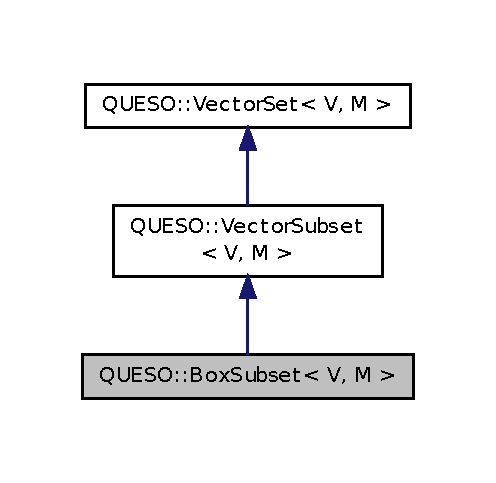
\includegraphics[width=238pt]{class_q_u_e_s_o_1_1_box_subset__inherit__graph}
\end{center}
\end{figure}


Collaboration diagram for Q\-U\-E\-S\-O\-:\-:Box\-Subset$<$ V, M $>$\-:
\nopagebreak
\begin{figure}[H]
\begin{center}
\leavevmode
\includegraphics[width=350pt]{class_q_u_e_s_o_1_1_box_subset__coll__graph}
\end{center}
\end{figure}
\subsection*{Public Member Functions}
\begin{DoxyCompactItemize}
\item 
void \hyperlink{class_q_u_e_s_o_1_1_box_subset_ae5490757cf0504fbe31681bf0b291e93}{print} (std\-::ostream \&os) const 
\begin{DoxyCompactList}\small\item\em Prints the volume, the minimum and the maximum values of {\ttfamily this}. \end{DoxyCompactList}\end{DoxyCompactItemize}
\begin{Indent}{\bf Constructor/\-Destructor methods}\par
\begin{DoxyCompactItemize}
\item 
\hyperlink{class_q_u_e_s_o_1_1_box_subset_a87bd3b29193a18a68a7be3b9469491c0}{Box\-Subset} (const char $\ast$\hyperlink{class_q_u_e_s_o_1_1_vector_set_aedcd4b0f502af4c6e6df863c13cddfec}{prefix}, const \hyperlink{class_q_u_e_s_o_1_1_vector_space}{Vector\-Space}$<$ V, M $>$ \&\hyperlink{class_q_u_e_s_o_1_1_vector_subset_afc859b5206bc056c66893c854c191959}{vector\-Space}, const V \&\hyperlink{class_q_u_e_s_o_1_1_box_subset_a57d3ba7df60a38abc4c161ff78f4a567}{min\-Values}, const V \&\hyperlink{class_q_u_e_s_o_1_1_box_subset_a47616371623019a8c6399d5b3661d25b}{max\-Values})
\begin{DoxyCompactList}\small\item\em Shaped, default constructor. \end{DoxyCompactList}\item 
\hyperlink{class_q_u_e_s_o_1_1_box_subset_a9e78b65ed80f2d11d1161a2fcfbb543d}{$\sim$\-Box\-Subset} ()
\begin{DoxyCompactList}\small\item\em Destructor. \end{DoxyCompactList}\end{DoxyCompactItemize}
\end{Indent}
\begin{Indent}{\bf Mathematical methods.}\par
\begin{DoxyCompactItemize}
\item 
bool \hyperlink{class_q_u_e_s_o_1_1_box_subset_a16fff2b1f133ddd750008680c6831dd0}{contains} (const V \&vec) const 
\begin{DoxyCompactList}\small\item\em Checks whether this box subset contains vector {\ttfamily vec}. \end{DoxyCompactList}\item 
const V \& \hyperlink{class_q_u_e_s_o_1_1_box_subset_a57d3ba7df60a38abc4c161ff78f4a567}{min\-Values} () const 
\begin{DoxyCompactList}\small\item\em \hyperlink{class_q_u_e_s_o_1_1_vector}{Vector} of the minimum values of the box subset. \end{DoxyCompactList}\item 
const V \& \hyperlink{class_q_u_e_s_o_1_1_box_subset_a47616371623019a8c6399d5b3661d25b}{max\-Values} () const 
\begin{DoxyCompactList}\small\item\em \hyperlink{class_q_u_e_s_o_1_1_vector}{Vector} of the maximum values of the box subset. \end{DoxyCompactList}\end{DoxyCompactItemize}
\end{Indent}
\subsection*{Protected Attributes}
\begin{DoxyCompactItemize}
\item 
V \hyperlink{class_q_u_e_s_o_1_1_box_subset_a633a4fbfa03590b38e4d2b192f3cc2b5}{m\-\_\-min\-Values}
\begin{DoxyCompactList}\small\item\em \hyperlink{class_q_u_e_s_o_1_1_vector}{Vector} of templated type {\ttfamily V} to store the minimum values of the box subset class. \end{DoxyCompactList}\item 
V \hyperlink{class_q_u_e_s_o_1_1_box_subset_ad234b8d38a236fb5c0d1353302c3e2f5}{m\-\_\-max\-Values}
\begin{DoxyCompactList}\small\item\em \hyperlink{class_q_u_e_s_o_1_1_vector}{Vector} of templated type {\ttfamily V} to store the maximum values of the box subset class. \end{DoxyCompactList}\end{DoxyCompactItemize}


\subsection{Detailed Description}
\subsubsection*{template$<$class V, class M$>$class Q\-U\-E\-S\-O\-::\-Box\-Subset$<$ V, M $>$}

Class representing a subset of a vector space shaped like a hypercube. 

This class is determined by a collection of upper and lower limits of the hypercube. (line segment in $ R $, rectangle in $ R^2 $, and so on). 

Definition at line 41 of file Box\-Subset.\-h.



\subsection{Constructor \& Destructor Documentation}
\hypertarget{class_q_u_e_s_o_1_1_box_subset_a87bd3b29193a18a68a7be3b9469491c0}{\index{Q\-U\-E\-S\-O\-::\-Box\-Subset@{Q\-U\-E\-S\-O\-::\-Box\-Subset}!Box\-Subset@{Box\-Subset}}
\index{Box\-Subset@{Box\-Subset}!QUESO::BoxSubset@{Q\-U\-E\-S\-O\-::\-Box\-Subset}}
\subsubsection[{Box\-Subset}]{\setlength{\rightskip}{0pt plus 5cm}template$<$class V, class M$>$ {\bf Q\-U\-E\-S\-O\-::\-Box\-Subset}$<$ V, M $>$\-::{\bf Box\-Subset} (
\begin{DoxyParamCaption}
\item[{const char $\ast$}]{prefix, }
\item[{const {\bf Vector\-Space}$<$ V, M $>$ \&}]{vector\-Space, }
\item[{const V \&}]{min\-Values, }
\item[{const V \&}]{max\-Values}
\end{DoxyParamCaption}
)}}\label{class_q_u_e_s_o_1_1_box_subset_a87bd3b29193a18a68a7be3b9469491c0}


Shaped, default constructor. 

Construct a subspace of {\ttfamily vector\-Space}, with min and max values given by the vectors {\ttfamily min\-Values} and {\ttfamily max\-Values}, respectively. It checks for possible inconsistencies between the values stored in {\ttfamily min\-Values} and {\ttfamily max\-Values}, and calculates the volume of the box subset, assigning it to m\-\_\-volume. 

Definition at line 34 of file Box\-Subset.\-C.



References Q\-U\-E\-S\-O\-::\-Vector\-Space$<$ V, M $>$\-::dim\-Local(), Q\-U\-E\-S\-O\-::\-Vector\-Set$<$ V, M $>$\-::m\-\_\-env, Q\-U\-E\-S\-O\-::\-Box\-Subset$<$ V, M $>$\-::m\-\_\-max\-Values, Q\-U\-E\-S\-O\-::\-Box\-Subset$<$ V, M $>$\-::m\-\_\-min\-Values, Q\-U\-E\-S\-O\-::\-Vector\-Subset$<$ V, M $>$\-::m\-\_\-vector\-Space, Q\-U\-E\-S\-O\-::\-Vector\-Set$<$ V, M $>$\-::m\-\_\-volume, U\-Q\-\_\-\-F\-A\-T\-A\-L\-\_\-\-T\-E\-S\-T\-\_\-\-M\-A\-C\-R\-O, and Q\-U\-E\-S\-O\-::\-Base\-Environment\-::world\-Rank().


\begin{DoxyCode}
38   : VectorSubset<V,M>(\hyperlink{class_q_u_e_s_o_1_1_vector_set_aedcd4b0f502af4c6e6df863c13cddfec}{prefix},\hyperlink{class_q_u_e_s_o_1_1_vector_subset_afc859b5206bc056c66893c854c191959}{vectorSpace},0.),
39     \hyperlink{class_q_u_e_s_o_1_1_box_subset_a633a4fbfa03590b38e4d2b192f3cc2b5}{m\_minValues}(\hyperlink{class_q_u_e_s_o_1_1_box_subset_a57d3ba7df60a38abc4c161ff78f4a567}{minValues}),
40     \hyperlink{class_q_u_e_s_o_1_1_box_subset_ad234b8d38a236fb5c0d1353302c3e2f5}{m\_maxValues}(\hyperlink{class_q_u_e_s_o_1_1_box_subset_a47616371623019a8c6399d5b3661d25b}{maxValues})
41 \{
42   \hyperlink{_defines_8h_a56d63d18d0a6d45757de47fcc06f574d}{UQ\_FATAL\_TEST\_MACRO}(\hyperlink{class_q_u_e_s_o_1_1_box_subset_a57d3ba7df60a38abc4c161ff78f4a567}{minValues}.sizeLocal() != 
      \hyperlink{class_q_u_e_s_o_1_1_box_subset_a47616371623019a8c6399d5b3661d25b}{maxValues}.sizeLocal(),
43                       \hyperlink{class_q_u_e_s_o_1_1_vector_set_a77f3b57109bc1d89b4111f47458df770}{m\_env}.\hyperlink{class_q_u_e_s_o_1_1_base_environment_a78b57112bbd0e6dd0e8afec00b40ffa7}{worldRank}(),
44                       \textcolor{stringliteral}{"BoxSubset<V,M>::BoxSubset()"},
45                       \textcolor{stringliteral}{"vectors 'minValues' and 'maxValues' should have the same size"});
46   \hyperlink{_defines_8h_a56d63d18d0a6d45757de47fcc06f574d}{UQ\_FATAL\_TEST\_MACRO}(\hyperlink{class_q_u_e_s_o_1_1_box_subset_a57d3ba7df60a38abc4c161ff78f4a567}{minValues}.sizeLocal() != 
      \hyperlink{class_q_u_e_s_o_1_1_vector_subset_afc859b5206bc056c66893c854c191959}{vectorSpace}.dimLocal(),
47                       \hyperlink{class_q_u_e_s_o_1_1_vector_set_a77f3b57109bc1d89b4111f47458df770}{m\_env}.\hyperlink{class_q_u_e_s_o_1_1_base_environment_a78b57112bbd0e6dd0e8afec00b40ffa7}{worldRank}(),
48                       \textcolor{stringliteral}{"BoxSubset<V,M>::BoxSubset()"},
49                       \textcolor{stringliteral}{"sizes of vectors 'minValues' and 'maxValues' should be equal to dimension of the
       vector space"});
50   \textcolor{keywordflow}{for} (\textcolor{keywordtype}{unsigned} \textcolor{keywordtype}{int} i = 0; i < \hyperlink{class_q_u_e_s_o_1_1_vector_subset_a8d1bfbac8c601b407c0a6a7af0904e2f}{m\_vectorSpace}->dimLocal(); ++i) \{
51     \hyperlink{_defines_8h_a56d63d18d0a6d45757de47fcc06f574d}{UQ\_FATAL\_TEST\_MACRO}(\hyperlink{class_q_u_e_s_o_1_1_box_subset_a57d3ba7df60a38abc4c161ff78f4a567}{minValues}[i] > \hyperlink{class_q_u_e_s_o_1_1_box_subset_a47616371623019a8c6399d5b3661d25b}{maxValues}[i],
52                         \hyperlink{class_q_u_e_s_o_1_1_vector_set_a77f3b57109bc1d89b4111f47458df770}{m\_env}.\hyperlink{class_q_u_e_s_o_1_1_base_environment_a78b57112bbd0e6dd0e8afec00b40ffa7}{worldRank}(),
53                         \textcolor{stringliteral}{"BoxSubset<V,M>::BoxSubset()"},
54                         \textcolor{stringliteral}{"it should happen minValue <= maxValue for all dimensions"});
55   \}
56 
57   \hyperlink{class_q_u_e_s_o_1_1_vector_set_acd5cdcdbcbbce29daec684437f511e9f}{m\_volume} = 1.;
58   \textcolor{keywordflow}{for} (\textcolor{keywordtype}{unsigned} \textcolor{keywordtype}{int} i = 0; i < \hyperlink{class_q_u_e_s_o_1_1_vector_subset_a8d1bfbac8c601b407c0a6a7af0904e2f}{m\_vectorSpace}->dimLocal(); ++i) \{
59     \hyperlink{class_q_u_e_s_o_1_1_vector_set_acd5cdcdbcbbce29daec684437f511e9f}{m\_volume} *= (\hyperlink{class_q_u_e_s_o_1_1_box_subset_ad234b8d38a236fb5c0d1353302c3e2f5}{m\_maxValues}[i] - \hyperlink{class_q_u_e_s_o_1_1_box_subset_a633a4fbfa03590b38e4d2b192f3cc2b5}{m\_minValues}[i]);
60   \}
61 \}
\end{DoxyCode}
\hypertarget{class_q_u_e_s_o_1_1_box_subset_a9e78b65ed80f2d11d1161a2fcfbb543d}{\index{Q\-U\-E\-S\-O\-::\-Box\-Subset@{Q\-U\-E\-S\-O\-::\-Box\-Subset}!$\sim$\-Box\-Subset@{$\sim$\-Box\-Subset}}
\index{$\sim$\-Box\-Subset@{$\sim$\-Box\-Subset}!QUESO::BoxSubset@{Q\-U\-E\-S\-O\-::\-Box\-Subset}}
\subsubsection[{$\sim$\-Box\-Subset}]{\setlength{\rightskip}{0pt plus 5cm}template$<$class V , class M $>$ {\bf Q\-U\-E\-S\-O\-::\-Box\-Subset}$<$ V, M $>$\-::$\sim${\bf Box\-Subset} (
\begin{DoxyParamCaption}
{}
\end{DoxyParamCaption}
)}}\label{class_q_u_e_s_o_1_1_box_subset_a9e78b65ed80f2d11d1161a2fcfbb543d}


Destructor. 



Definition at line 65 of file Box\-Subset.\-C.


\begin{DoxyCode}
66 \{
67 \}
\end{DoxyCode}


\subsection{Member Function Documentation}
\hypertarget{class_q_u_e_s_o_1_1_box_subset_a16fff2b1f133ddd750008680c6831dd0}{\index{Q\-U\-E\-S\-O\-::\-Box\-Subset@{Q\-U\-E\-S\-O\-::\-Box\-Subset}!contains@{contains}}
\index{contains@{contains}!QUESO::BoxSubset@{Q\-U\-E\-S\-O\-::\-Box\-Subset}}
\subsubsection[{contains}]{\setlength{\rightskip}{0pt plus 5cm}template$<$class V, class M $>$ bool {\bf Q\-U\-E\-S\-O\-::\-Box\-Subset}$<$ V, M $>$\-::contains (
\begin{DoxyParamCaption}
\item[{const V \&}]{vec}
\end{DoxyParamCaption}
) const\hspace{0.3cm}{\ttfamily [virtual]}}}\label{class_q_u_e_s_o_1_1_box_subset_a16fff2b1f133ddd750008680c6831dd0}


Checks whether this box subset contains vector {\ttfamily vec}. 

It checks if both statements are true\-: 1) all components in {\ttfamily vec} are larger than m\-\_\-min\-Values, and 2) all all components in {\ttfamily vec} are smaller than m\-\_\-max\-Values. 

Implements \hyperlink{class_q_u_e_s_o_1_1_vector_subset_aa3f018d2afdf73dbe5fa7041dee47e0d}{Q\-U\-E\-S\-O\-::\-Vector\-Subset$<$ V, M $>$}.



Definition at line 71 of file Box\-Subset.\-C.


\begin{DoxyCode}
72 \{
73   \textcolor{comment}{// prudenci, 2012-09-26: allow boundary values because of 'beta' realizer, which can generate a sample
       with boundary value '1'}
74   \textcolor{comment}{//return (!vec.atLeastOneComponentSmallerOrEqualThan(m\_minValues) &&}
75   \textcolor{comment}{//        !vec.atLeastOneComponentBiggerOrEqualThan (m\_maxValues));}
76   \textcolor{keywordflow}{return} (!vec.atLeastOneComponentSmallerThan(\hyperlink{class_q_u_e_s_o_1_1_box_subset_a633a4fbfa03590b38e4d2b192f3cc2b5}{m\_minValues}) &&
77           !vec.atLeastOneComponentBiggerThan (\hyperlink{class_q_u_e_s_o_1_1_box_subset_ad234b8d38a236fb5c0d1353302c3e2f5}{m\_maxValues}));
78 \}
\end{DoxyCode}
\hypertarget{class_q_u_e_s_o_1_1_box_subset_a47616371623019a8c6399d5b3661d25b}{\index{Q\-U\-E\-S\-O\-::\-Box\-Subset@{Q\-U\-E\-S\-O\-::\-Box\-Subset}!max\-Values@{max\-Values}}
\index{max\-Values@{max\-Values}!QUESO::BoxSubset@{Q\-U\-E\-S\-O\-::\-Box\-Subset}}
\subsubsection[{max\-Values}]{\setlength{\rightskip}{0pt plus 5cm}template$<$class V , class M $>$ const V \& {\bf Q\-U\-E\-S\-O\-::\-Box\-Subset}$<$ V, M $>$\-::max\-Values (
\begin{DoxyParamCaption}
{}
\end{DoxyParamCaption}
) const}}\label{class_q_u_e_s_o_1_1_box_subset_a47616371623019a8c6399d5b3661d25b}


\hyperlink{class_q_u_e_s_o_1_1_vector}{Vector} of the maximum values of the box subset. 



Definition at line 88 of file Box\-Subset.\-C.



Referenced by Q\-U\-E\-S\-O\-::\-Beta\-Vector\-R\-V$<$ V, M $>$\-::\-Beta\-Vector\-R\-V(), Q\-U\-E\-S\-O\-::\-Base\-Joint\-Pdf$<$ V, M $>$\-::common\-Compute\-Log\-Of\-Normalization\-Factor(), Q\-U\-E\-S\-O\-::\-Gamma\-Vector\-R\-V$<$ V, M $>$\-::\-Gamma\-Vector\-R\-V(), Q\-U\-E\-S\-O\-::\-Instantiate\-Intersection(), Q\-U\-E\-S\-O\-::\-Inverse\-Gamma\-Vector\-R\-V$<$ V, M $>$\-::\-Inverse\-Gamma\-Vector\-R\-V(), Q\-U\-E\-S\-O\-::\-Log\-Normal\-Vector\-R\-V$<$ V, M $>$\-::\-Log\-Normal\-Vector\-R\-V(), Q\-U\-E\-S\-O\-::\-Uniform\-Vector\-Realizer$<$ V, M $>$\-::realization(), and Q\-U\-E\-S\-O\-::\-Gamma\-Vector\-Realizer$<$ V, M $>$\-::realization().


\begin{DoxyCode}
89 \{
90   \textcolor{keywordflow}{return} \hyperlink{class_q_u_e_s_o_1_1_box_subset_ad234b8d38a236fb5c0d1353302c3e2f5}{m\_maxValues};
91 \}
\end{DoxyCode}
\hypertarget{class_q_u_e_s_o_1_1_box_subset_a57d3ba7df60a38abc4c161ff78f4a567}{\index{Q\-U\-E\-S\-O\-::\-Box\-Subset@{Q\-U\-E\-S\-O\-::\-Box\-Subset}!min\-Values@{min\-Values}}
\index{min\-Values@{min\-Values}!QUESO::BoxSubset@{Q\-U\-E\-S\-O\-::\-Box\-Subset}}
\subsubsection[{min\-Values}]{\setlength{\rightskip}{0pt plus 5cm}template$<$class V , class M $>$ const V \& {\bf Q\-U\-E\-S\-O\-::\-Box\-Subset}$<$ V, M $>$\-::min\-Values (
\begin{DoxyParamCaption}
{}
\end{DoxyParamCaption}
) const}}\label{class_q_u_e_s_o_1_1_box_subset_a57d3ba7df60a38abc4c161ff78f4a567}


\hyperlink{class_q_u_e_s_o_1_1_vector}{Vector} of the minimum values of the box subset. 



Definition at line 82 of file Box\-Subset.\-C.



Referenced by Q\-U\-E\-S\-O\-::\-Beta\-Vector\-R\-V$<$ V, M $>$\-::\-Beta\-Vector\-R\-V(), Q\-U\-E\-S\-O\-::\-Base\-Joint\-Pdf$<$ V, M $>$\-::common\-Compute\-Log\-Of\-Normalization\-Factor(), Q\-U\-E\-S\-O\-::\-Gamma\-Vector\-R\-V$<$ V, M $>$\-::\-Gamma\-Vector\-R\-V(), Q\-U\-E\-S\-O\-::\-Instantiate\-Intersection(), Q\-U\-E\-S\-O\-::\-Inverse\-Gamma\-Vector\-R\-V$<$ V, M $>$\-::\-Inverse\-Gamma\-Vector\-R\-V(), Q\-U\-E\-S\-O\-::\-Log\-Normal\-Vector\-R\-V$<$ V, M $>$\-::\-Log\-Normal\-Vector\-R\-V(), Q\-U\-E\-S\-O\-::\-Uniform\-Vector\-Realizer$<$ V, M $>$\-::realization(), and Q\-U\-E\-S\-O\-::\-Gamma\-Vector\-Realizer$<$ V, M $>$\-::realization().


\begin{DoxyCode}
83 \{
84   \textcolor{keywordflow}{return} \hyperlink{class_q_u_e_s_o_1_1_box_subset_a633a4fbfa03590b38e4d2b192f3cc2b5}{m\_minValues};
85 \}
\end{DoxyCode}
\hypertarget{class_q_u_e_s_o_1_1_box_subset_ae5490757cf0504fbe31681bf0b291e93}{\index{Q\-U\-E\-S\-O\-::\-Box\-Subset@{Q\-U\-E\-S\-O\-::\-Box\-Subset}!print@{print}}
\index{print@{print}!QUESO::BoxSubset@{Q\-U\-E\-S\-O\-::\-Box\-Subset}}
\subsubsection[{print}]{\setlength{\rightskip}{0pt plus 5cm}template$<$class V , class M $>$ void {\bf Q\-U\-E\-S\-O\-::\-Box\-Subset}$<$ V, M $>$\-::print (
\begin{DoxyParamCaption}
\item[{std\-::ostream \&}]{os}
\end{DoxyParamCaption}
) const\hspace{0.3cm}{\ttfamily [virtual]}}}\label{class_q_u_e_s_o_1_1_box_subset_ae5490757cf0504fbe31681bf0b291e93}


Prints the volume, the minimum and the maximum values of {\ttfamily this}. 



Reimplemented from \hyperlink{class_q_u_e_s_o_1_1_vector_subset_a62ba8816790e495f7d2302afeaecb436}{Q\-U\-E\-S\-O\-::\-Vector\-Subset$<$ V, M $>$}.



Definition at line 95 of file Box\-Subset.\-C.


\begin{DoxyCode}
96 \{
97   os << \textcolor{stringliteral}{"In BoxSubset<V,M>::print()"}
98      << \textcolor{stringliteral}{": m\_minValues = "} << \hyperlink{class_q_u_e_s_o_1_1_box_subset_a633a4fbfa03590b38e4d2b192f3cc2b5}{m\_minValues}
99      << \textcolor{stringliteral}{", m\_maxValues = "} << \hyperlink{class_q_u_e_s_o_1_1_box_subset_ad234b8d38a236fb5c0d1353302c3e2f5}{m\_maxValues}
100      << \textcolor{stringliteral}{", m\_volume = "}    << \hyperlink{class_q_u_e_s_o_1_1_vector_set_acd5cdcdbcbbce29daec684437f511e9f}{m\_volume}
101      << std::endl;
102 
103   \textcolor{keywordflow}{return};
104 \}
\end{DoxyCode}


\subsection{Member Data Documentation}
\hypertarget{class_q_u_e_s_o_1_1_box_subset_ad234b8d38a236fb5c0d1353302c3e2f5}{\index{Q\-U\-E\-S\-O\-::\-Box\-Subset@{Q\-U\-E\-S\-O\-::\-Box\-Subset}!m\-\_\-max\-Values@{m\-\_\-max\-Values}}
\index{m\-\_\-max\-Values@{m\-\_\-max\-Values}!QUESO::BoxSubset@{Q\-U\-E\-S\-O\-::\-Box\-Subset}}
\subsubsection[{m\-\_\-max\-Values}]{\setlength{\rightskip}{0pt plus 5cm}template$<$class V, class M$>$ V {\bf Q\-U\-E\-S\-O\-::\-Box\-Subset}$<$ V, M $>$\-::m\-\_\-max\-Values\hspace{0.3cm}{\ttfamily [protected]}}}\label{class_q_u_e_s_o_1_1_box_subset_ad234b8d38a236fb5c0d1353302c3e2f5}


\hyperlink{class_q_u_e_s_o_1_1_vector}{Vector} of templated type {\ttfamily V} to store the maximum values of the box subset class. 



Definition at line 86 of file Box\-Subset.\-h.



Referenced by Q\-U\-E\-S\-O\-::\-Box\-Subset$<$ V, M $>$\-::\-Box\-Subset().

\hypertarget{class_q_u_e_s_o_1_1_box_subset_a633a4fbfa03590b38e4d2b192f3cc2b5}{\index{Q\-U\-E\-S\-O\-::\-Box\-Subset@{Q\-U\-E\-S\-O\-::\-Box\-Subset}!m\-\_\-min\-Values@{m\-\_\-min\-Values}}
\index{m\-\_\-min\-Values@{m\-\_\-min\-Values}!QUESO::BoxSubset@{Q\-U\-E\-S\-O\-::\-Box\-Subset}}
\subsubsection[{m\-\_\-min\-Values}]{\setlength{\rightskip}{0pt plus 5cm}template$<$class V, class M$>$ V {\bf Q\-U\-E\-S\-O\-::\-Box\-Subset}$<$ V, M $>$\-::m\-\_\-min\-Values\hspace{0.3cm}{\ttfamily [protected]}}}\label{class_q_u_e_s_o_1_1_box_subset_a633a4fbfa03590b38e4d2b192f3cc2b5}


\hyperlink{class_q_u_e_s_o_1_1_vector}{Vector} of templated type {\ttfamily V} to store the minimum values of the box subset class. 



Definition at line 83 of file Box\-Subset.\-h.



Referenced by Q\-U\-E\-S\-O\-::\-Box\-Subset$<$ V, M $>$\-::\-Box\-Subset().



The documentation for this class was generated from the following files\-:\begin{DoxyCompactItemize}
\item 
src/basic/inc/\hyperlink{_box_subset_8h}{Box\-Subset.\-h}\item 
src/basic/src/\hyperlink{_box_subset_8_c}{Box\-Subset.\-C}\end{DoxyCompactItemize}

\hypertarget{class_q_u_e_s_o_1_1_concatenated_joint_pdf}{\section{Q\-U\-E\-S\-O\-:\-:Concatenated\-Joint\-Pdf$<$ V, M $>$ Class Template Reference}
\label{class_q_u_e_s_o_1_1_concatenated_joint_pdf}\index{Q\-U\-E\-S\-O\-::\-Concatenated\-Joint\-Pdf$<$ V, M $>$@{Q\-U\-E\-S\-O\-::\-Concatenated\-Joint\-Pdf$<$ V, M $>$}}
}


A class for handling concatenated P\-D\-Fs.  




{\ttfamily \#include $<$Concatenated\-Joint\-Pdf.\-h$>$}



Inheritance diagram for Q\-U\-E\-S\-O\-:\-:Concatenated\-Joint\-Pdf$<$ V, M $>$\-:
\nopagebreak
\begin{figure}[H]
\begin{center}
\leavevmode
\includegraphics[width=238pt]{class_q_u_e_s_o_1_1_concatenated_joint_pdf__inherit__graph}
\end{center}
\end{figure}


Collaboration diagram for Q\-U\-E\-S\-O\-:\-:Concatenated\-Joint\-Pdf$<$ V, M $>$\-:
\nopagebreak
\begin{figure}[H]
\begin{center}
\leavevmode
\includegraphics[width=350pt]{class_q_u_e_s_o_1_1_concatenated_joint_pdf__coll__graph}
\end{center}
\end{figure}
\subsection*{Public Member Functions}
\begin{Indent}{\bf Constructor/\-Destructor methods}\par
\begin{DoxyCompactItemize}
\item 
\hyperlink{class_q_u_e_s_o_1_1_concatenated_joint_pdf_aff646f6aafe63e66dca291925bad6ca1}{Concatenated\-Joint\-Pdf} (const char $\ast$prefix, const \hyperlink{class_q_u_e_s_o_1_1_base_joint_pdf}{Base\-Joint\-Pdf}$<$ V, M $>$ \&density1, const \hyperlink{class_q_u_e_s_o_1_1_base_joint_pdf}{Base\-Joint\-Pdf}$<$ V, M $>$ \&density2, const \hyperlink{class_q_u_e_s_o_1_1_vector_set}{Vector\-Set}$<$ V, M $>$ \&concatenated\-Domain)
\begin{DoxyCompactList}\small\item\em Constructor. \end{DoxyCompactList}\item 
\hyperlink{class_q_u_e_s_o_1_1_concatenated_joint_pdf_a96f8908c3ee9d975919624b37eea20bb}{Concatenated\-Joint\-Pdf} (const char $\ast$prefix, const std\-::vector$<$ const \hyperlink{class_q_u_e_s_o_1_1_base_joint_pdf}{Base\-Joint\-Pdf}$<$ V, M $>$ $\ast$ $>$ \&densities, const \hyperlink{class_q_u_e_s_o_1_1_vector_set}{Vector\-Set}$<$ V, M $>$ \&concatenated\-Domain)
\begin{DoxyCompactList}\small\item\em Constructor. \end{DoxyCompactList}\item 
\hyperlink{class_q_u_e_s_o_1_1_concatenated_joint_pdf_a9b4a0c33fa7dc23034be19455de61bcd}{$\sim$\-Concatenated\-Joint\-Pdf} ()
\begin{DoxyCompactList}\small\item\em Destructor. \end{DoxyCompactList}\end{DoxyCompactItemize}
\end{Indent}
\begin{Indent}{\bf Math methods}\par
\begin{DoxyCompactItemize}
\item 
double \hyperlink{class_q_u_e_s_o_1_1_concatenated_joint_pdf_a7a3bbf8dab211968e9691a620fee0e4d}{actual\-Value} (const V \&domain\-Vector, const V $\ast$domain\-Direction, V $\ast$grad\-Vector, M $\ast$hessian\-Matrix, V $\ast$hessian\-Effect) const 
\begin{DoxyCompactList}\small\item\em Calculates the actual values of each density. \end{DoxyCompactList}\item 
double \hyperlink{class_q_u_e_s_o_1_1_concatenated_joint_pdf_aca499666e5c3d3d26c562492a15ab112}{ln\-Value} (const V \&domain\-Vector, const V $\ast$domain\-Direction, V $\ast$grad\-Vector, M $\ast$hessian\-Matrix, V $\ast$hessian\-Effect) const 
\begin{DoxyCompactList}\small\item\em Calculates the logarithm of the values of each density. \end{DoxyCompactList}\item 
void \hyperlink{class_q_u_e_s_o_1_1_concatenated_joint_pdf_a686ff513ae812f26f9a71705dd2082ad}{set\-Normalization\-Style} (unsigned int value) const 
\begin{DoxyCompactList}\small\item\em Sets the normalization style of all densities to {\ttfamily value}. \end{DoxyCompactList}\item 
double \hyperlink{class_q_u_e_s_o_1_1_concatenated_joint_pdf_ad960a39a781a7a891df0ae0ee4670199}{compute\-Log\-Of\-Normalization\-Factor} (unsigned int num\-Samples, bool update\-Factor\-Internally) const 
\begin{DoxyCompactList}\small\item\em Computes the logarithm of the normalization factor. \end{DoxyCompactList}\end{DoxyCompactItemize}
\end{Indent}
\subsection*{Protected Attributes}
\begin{DoxyCompactItemize}
\item 
std\-::vector$<$ const \\*
\hyperlink{class_q_u_e_s_o_1_1_base_joint_pdf}{Base\-Joint\-Pdf}$<$ V, M $>$ $\ast$ $>$ \hyperlink{class_q_u_e_s_o_1_1_concatenated_joint_pdf_a42ee130daadf7ceb0d1745011f5b1169}{m\-\_\-densities}
\end{DoxyCompactItemize}
\subsection*{Additional Inherited Members}


\subsection{Detailed Description}
\subsubsection*{template$<$class V, class M$>$class Q\-U\-E\-S\-O\-::\-Concatenated\-Joint\-Pdf$<$ V, M $>$}

A class for handling concatenated P\-D\-Fs. 

This class allows the user to defines concatenated probability density distributions, i.\-e, two or more distinct P\-D\-Fs can be concatenated into one single P\-D\-F. This class used, for instance, to concatenate priors from two or more R\-Vs, where one of them has a uniform distribution whereas the other one(s) has a Gaussian distribution. 

Definition at line 52 of file Concatenated\-Joint\-Pdf.\-h.



\subsection{Constructor \& Destructor Documentation}
\hypertarget{class_q_u_e_s_o_1_1_concatenated_joint_pdf_aff646f6aafe63e66dca291925bad6ca1}{\index{Q\-U\-E\-S\-O\-::\-Concatenated\-Joint\-Pdf@{Q\-U\-E\-S\-O\-::\-Concatenated\-Joint\-Pdf}!Concatenated\-Joint\-Pdf@{Concatenated\-Joint\-Pdf}}
\index{Concatenated\-Joint\-Pdf@{Concatenated\-Joint\-Pdf}!QUESO::ConcatenatedJointPdf@{Q\-U\-E\-S\-O\-::\-Concatenated\-Joint\-Pdf}}
\subsubsection[{Concatenated\-Joint\-Pdf}]{\setlength{\rightskip}{0pt plus 5cm}template$<$class V , class M $>$ {\bf Q\-U\-E\-S\-O\-::\-Concatenated\-Joint\-Pdf}$<$ V, M $>$\-::{\bf Concatenated\-Joint\-Pdf} (
\begin{DoxyParamCaption}
\item[{const char $\ast$}]{prefix, }
\item[{const {\bf Base\-Joint\-Pdf}$<$ V, M $>$ \&}]{density1, }
\item[{const {\bf Base\-Joint\-Pdf}$<$ V, M $>$ \&}]{density2, }
\item[{const {\bf Vector\-Set}$<$ V, M $>$ \&}]{concatenated\-Domain}
\end{DoxyParamCaption}
)}}\label{class_q_u_e_s_o_1_1_concatenated_joint_pdf_aff646f6aafe63e66dca291925bad6ca1}


Constructor. 

Concatenates two P\-D\-Fs\-: {\ttfamily density1} and {\ttfamily density2} into one vector P\-D\-F, given a prefix and the concatenated domain of such P\-D\-Fs. 

Definition at line 33 of file Concatenated\-Joint\-Pdf.\-C.



References Q\-U\-E\-S\-O\-::\-Concatenated\-Joint\-Pdf$<$ V, M $>$\-::m\-\_\-densities, Q\-U\-E\-S\-O\-::\-Base\-Scalar\-Function$<$ V, M $>$\-::m\-\_\-env, U\-Q\-\_\-\-F\-A\-T\-A\-L\-\_\-\-T\-E\-S\-T\-\_\-\-M\-A\-C\-R\-O, Q\-U\-E\-S\-O\-::\-Vector\-Set$<$ V, M $>$\-::vector\-Space(), and Q\-U\-E\-S\-O\-::\-Base\-Environment\-::world\-Rank().


\begin{DoxyCode}
38   :
39   BaseJointPdf<V,M>(((std::string)(prefix)+\textcolor{stringliteral}{"concat"}).c\_str(),concatenatedDomain),
40   \hyperlink{class_q_u_e_s_o_1_1_concatenated_joint_pdf_a42ee130daadf7ceb0d1745011f5b1169}{m\_densities}             (2,(\textcolor{keyword}{const} BaseJointPdf<V,M>*) NULL)
41 \{
42   \hyperlink{class_q_u_e_s_o_1_1_concatenated_joint_pdf_a42ee130daadf7ceb0d1745011f5b1169}{m\_densities}[0] = &density1;
43   \hyperlink{class_q_u_e_s_o_1_1_concatenated_joint_pdf_a42ee130daadf7ceb0d1745011f5b1169}{m\_densities}[1] = &density2;
44 
45   \textcolor{keywordtype}{unsigned} \textcolor{keywordtype}{int} size1 = \hyperlink{class_q_u_e_s_o_1_1_concatenated_joint_pdf_a42ee130daadf7ceb0d1745011f5b1169}{m\_densities}[0]->domainSet().vectorSpace().dimLocal();
46   \textcolor{keywordtype}{unsigned} \textcolor{keywordtype}{int} size2 = \hyperlink{class_q_u_e_s_o_1_1_concatenated_joint_pdf_a42ee130daadf7ceb0d1745011f5b1169}{m\_densities}[1]->domainSet().vectorSpace().dimLocal();
47   \textcolor{keywordtype}{unsigned} \textcolor{keywordtype}{int} size  = concatenatedDomain.vectorSpace().dimLocal();
48 
49   \hyperlink{_defines_8h_a56d63d18d0a6d45757de47fcc06f574d}{UQ\_FATAL\_TEST\_MACRO}((size1+size2) != size,
50                       \hyperlink{class_q_u_e_s_o_1_1_base_scalar_function_adf44141aeb765d97613286f88f235f04}{m\_env}.\hyperlink{class_q_u_e_s_o_1_1_base_environment_a78b57112bbd0e6dd0e8afec00b40ffa7}{worldRank}(),
51                       \textcolor{stringliteral}{"ConcatenatedJointPdf<V,M>::constructor(1)"},
52                       \textcolor{stringliteral}{"incompatible dimensions"});
53 \}
\end{DoxyCode}
\hypertarget{class_q_u_e_s_o_1_1_concatenated_joint_pdf_a96f8908c3ee9d975919624b37eea20bb}{\index{Q\-U\-E\-S\-O\-::\-Concatenated\-Joint\-Pdf@{Q\-U\-E\-S\-O\-::\-Concatenated\-Joint\-Pdf}!Concatenated\-Joint\-Pdf@{Concatenated\-Joint\-Pdf}}
\index{Concatenated\-Joint\-Pdf@{Concatenated\-Joint\-Pdf}!QUESO::ConcatenatedJointPdf@{Q\-U\-E\-S\-O\-::\-Concatenated\-Joint\-Pdf}}
\subsubsection[{Concatenated\-Joint\-Pdf}]{\setlength{\rightskip}{0pt plus 5cm}template$<$class V , class M $>$ {\bf Q\-U\-E\-S\-O\-::\-Concatenated\-Joint\-Pdf}$<$ V, M $>$\-::{\bf Concatenated\-Joint\-Pdf} (
\begin{DoxyParamCaption}
\item[{const char $\ast$}]{prefix, }
\item[{const std\-::vector$<$ const {\bf Base\-Joint\-Pdf}$<$ V, M $>$ $\ast$ $>$ \&}]{densities, }
\item[{const {\bf Vector\-Set}$<$ V, M $>$ \&}]{concatenated\-Domain}
\end{DoxyParamCaption}
)}}\label{class_q_u_e_s_o_1_1_concatenated_joint_pdf_a96f8908c3ee9d975919624b37eea20bb}


Constructor. 

Concatenates a sequence of P\-D\-Fs, given by\-: {\ttfamily  std\-::vector$<$const Base\-Joint\-Pdf$<$\-V,\-M$>$$\ast$ $>$\& densities } into one single P\-D\-F, given a prefix and the concatenated domain of such P\-D\-Fs. 

Definition at line 56 of file Concatenated\-Joint\-Pdf.\-C.



References Q\-U\-E\-S\-O\-::\-Concatenated\-Joint\-Pdf$<$ V, M $>$\-::m\-\_\-densities, Q\-U\-E\-S\-O\-::\-Base\-Scalar\-Function$<$ V, M $>$\-::m\-\_\-env, U\-Q\-\_\-\-F\-A\-T\-A\-L\-\_\-\-T\-E\-S\-T\-\_\-\-M\-A\-C\-R\-O, Q\-U\-E\-S\-O\-::\-Vector\-Set$<$ V, M $>$\-::vector\-Space(), and Q\-U\-E\-S\-O\-::\-Base\-Environment\-::world\-Rank().


\begin{DoxyCode}
60   :
61   BaseJointPdf<V,M>(((std::string)(prefix)+\textcolor{stringliteral}{"concat"}).c\_str(),concatenatedDomain),
62   \hyperlink{class_q_u_e_s_o_1_1_concatenated_joint_pdf_a42ee130daadf7ceb0d1745011f5b1169}{m\_densities}             (densities.size(),(\textcolor{keyword}{const} BaseJointPdf<V,M>*) NULL)
63 \{
64   \textcolor{keywordtype}{unsigned} \textcolor{keywordtype}{int} sumSizes = 0;
65   \textcolor{keywordflow}{for} (\textcolor{keywordtype}{unsigned} i = 0; i < \hyperlink{class_q_u_e_s_o_1_1_concatenated_joint_pdf_a42ee130daadf7ceb0d1745011f5b1169}{m\_densities}.size(); ++i) \{
66     \hyperlink{class_q_u_e_s_o_1_1_concatenated_joint_pdf_a42ee130daadf7ceb0d1745011f5b1169}{m\_densities}[i] = densities[i];
67     sumSizes += \hyperlink{class_q_u_e_s_o_1_1_concatenated_joint_pdf_a42ee130daadf7ceb0d1745011f5b1169}{m\_densities}[i]->domainSet().vectorSpace().dimLocal();
68   \}
69 
70   \textcolor{keywordtype}{unsigned} \textcolor{keywordtype}{int} size  = concatenatedDomain.vectorSpace().dimLocal();
71 
72   \hyperlink{_defines_8h_a56d63d18d0a6d45757de47fcc06f574d}{UQ\_FATAL\_TEST\_MACRO}(sumSizes != size,
73                       \hyperlink{class_q_u_e_s_o_1_1_base_scalar_function_adf44141aeb765d97613286f88f235f04}{m\_env}.\hyperlink{class_q_u_e_s_o_1_1_base_environment_a78b57112bbd0e6dd0e8afec00b40ffa7}{worldRank}(),
74                       \textcolor{stringliteral}{"ConcatenatedJointPdf<V,M>::constructor(2)"},
75                       \textcolor{stringliteral}{"incompatible dimensions"});
76 \}
\end{DoxyCode}
\hypertarget{class_q_u_e_s_o_1_1_concatenated_joint_pdf_a9b4a0c33fa7dc23034be19455de61bcd}{\index{Q\-U\-E\-S\-O\-::\-Concatenated\-Joint\-Pdf@{Q\-U\-E\-S\-O\-::\-Concatenated\-Joint\-Pdf}!$\sim$\-Concatenated\-Joint\-Pdf@{$\sim$\-Concatenated\-Joint\-Pdf}}
\index{$\sim$\-Concatenated\-Joint\-Pdf@{$\sim$\-Concatenated\-Joint\-Pdf}!QUESO::ConcatenatedJointPdf@{Q\-U\-E\-S\-O\-::\-Concatenated\-Joint\-Pdf}}
\subsubsection[{$\sim$\-Concatenated\-Joint\-Pdf}]{\setlength{\rightskip}{0pt plus 5cm}template$<$class V , class M $>$ {\bf Q\-U\-E\-S\-O\-::\-Concatenated\-Joint\-Pdf}$<$ V, M $>$\-::$\sim${\bf Concatenated\-Joint\-Pdf} (
\begin{DoxyParamCaption}
{}
\end{DoxyParamCaption}
)}}\label{class_q_u_e_s_o_1_1_concatenated_joint_pdf_a9b4a0c33fa7dc23034be19455de61bcd}


Destructor. 



Definition at line 79 of file Concatenated\-Joint\-Pdf.\-C.


\begin{DoxyCode}
80 \{
81 \}
\end{DoxyCode}


\subsection{Member Function Documentation}
\hypertarget{class_q_u_e_s_o_1_1_concatenated_joint_pdf_a7a3bbf8dab211968e9691a620fee0e4d}{\index{Q\-U\-E\-S\-O\-::\-Concatenated\-Joint\-Pdf@{Q\-U\-E\-S\-O\-::\-Concatenated\-Joint\-Pdf}!actual\-Value@{actual\-Value}}
\index{actual\-Value@{actual\-Value}!QUESO::ConcatenatedJointPdf@{Q\-U\-E\-S\-O\-::\-Concatenated\-Joint\-Pdf}}
\subsubsection[{actual\-Value}]{\setlength{\rightskip}{0pt plus 5cm}template$<$class V , class M $>$ double {\bf Q\-U\-E\-S\-O\-::\-Concatenated\-Joint\-Pdf}$<$ V, M $>$\-::actual\-Value (
\begin{DoxyParamCaption}
\item[{const V \&}]{domain\-Vector, }
\item[{const V $\ast$}]{domain\-Direction, }
\item[{V $\ast$}]{grad\-Vector, }
\item[{M $\ast$}]{hessian\-Matrix, }
\item[{V $\ast$}]{hessian\-Effect}
\end{DoxyParamCaption}
) const\hspace{0.3cm}{\ttfamily [virtual]}}}\label{class_q_u_e_s_o_1_1_concatenated_joint_pdf_a7a3bbf8dab211968e9691a620fee0e4d}


Calculates the actual values of each density. 

The final actual value is the multiplication of all values calculated. 

Implements \hyperlink{class_q_u_e_s_o_1_1_base_joint_pdf_a3c367a0cc3fb707a136c5df47dd414c1}{Q\-U\-E\-S\-O\-::\-Base\-Joint\-Pdf$<$ V, M $>$}.



Definition at line 95 of file Concatenated\-Joint\-Pdf.\-C.



References U\-Q\-\_\-\-F\-A\-T\-A\-L\-\_\-\-T\-E\-S\-T\-\_\-\-M\-A\-C\-R\-O.


\begin{DoxyCode}
101 \{
102   \textcolor{keywordflow}{if} ((\hyperlink{class_q_u_e_s_o_1_1_base_scalar_function_adf44141aeb765d97613286f88f235f04}{m\_env}.\hyperlink{class_q_u_e_s_o_1_1_base_environment_a8a0064746ae8dddfece4229b9ad374d6}{subDisplayFile}()) && (\hyperlink{class_q_u_e_s_o_1_1_base_scalar_function_adf44141aeb765d97613286f88f235f04}{m\_env}.
      \hyperlink{class_q_u_e_s_o_1_1_base_environment_a1fe5f244fc0316a0ab3e37463f108b96}{displayVerbosity}() >= 54)) \{
103     *\hyperlink{class_q_u_e_s_o_1_1_base_scalar_function_adf44141aeb765d97613286f88f235f04}{m\_env}.\hyperlink{class_q_u_e_s_o_1_1_base_environment_a8a0064746ae8dddfece4229b9ad374d6}{subDisplayFile}() << \textcolor{stringliteral}{"Entering ConcatenatedJointPdf<V,M>::actualValue()"}
104                             << \textcolor{stringliteral}{": domainVector = "} << domainVector
105                             << std::endl;
106   \}
107 
108   \hyperlink{_defines_8h_a56d63d18d0a6d45757de47fcc06f574d}{UQ\_FATAL\_TEST\_MACRO}(domainVector.sizeLocal() != this->
      \hyperlink{class_q_u_e_s_o_1_1_base_scalar_function_a67696e86211197938c72cd11863f5cf8}{m\_domainSet}.vectorSpace().dimLocal(),
109                       \hyperlink{class_q_u_e_s_o_1_1_base_scalar_function_adf44141aeb765d97613286f88f235f04}{m\_env}.\hyperlink{class_q_u_e_s_o_1_1_base_environment_a78b57112bbd0e6dd0e8afec00b40ffa7}{worldRank}(),
110                       \textcolor{stringliteral}{"ConcatenatedJointPdf<V,M>::actualValue()"},
111                       \textcolor{stringliteral}{"invalid input"});
112 
113   \hyperlink{_defines_8h_a56d63d18d0a6d45757de47fcc06f574d}{UQ\_FATAL\_TEST\_MACRO}((domainDirection || gradVector || hessianMatrix || hessianEffect),
114                       \hyperlink{class_q_u_e_s_o_1_1_base_scalar_function_adf44141aeb765d97613286f88f235f04}{m\_env}.\hyperlink{class_q_u_e_s_o_1_1_base_environment_a78b57112bbd0e6dd0e8afec00b40ffa7}{worldRank}(),
115                       \textcolor{stringliteral}{"ConcatenatedJointPdf<V,M>::actualValue()"},
116                       \textcolor{stringliteral}{"incomplete code for gradVector, hessianMatrix and hessianEffect calculations"});
117 
118   std::vector<V*> vecs(\hyperlink{class_q_u_e_s_o_1_1_concatenated_joint_pdf_a42ee130daadf7ceb0d1745011f5b1169}{m\_densities}.size(),(V*) NULL);
119   std::vector<double> values(\hyperlink{class_q_u_e_s_o_1_1_concatenated_joint_pdf_a42ee130daadf7ceb0d1745011f5b1169}{m\_densities}.size(),0.);
120   \textcolor{keywordtype}{double} returnValue = 1.;
121   \textcolor{keywordtype}{unsigned} \textcolor{keywordtype}{int} cummulativeSize = 0;
122   \textcolor{keywordflow}{for} (\textcolor{keywordtype}{unsigned} \textcolor{keywordtype}{int} i = 0; i < vecs.size(); ++i) \{
123     vecs[i] = \textcolor{keyword}{new} V(\hyperlink{class_q_u_e_s_o_1_1_concatenated_joint_pdf_a42ee130daadf7ceb0d1745011f5b1169}{m\_densities}[i]->\hyperlink{class_q_u_e_s_o_1_1_base_scalar_function_ad0937628825249dd36ded3ce0c7959ac}{domainSet}().vectorSpace().zeroVector());
124     domainVector.cwExtract(cummulativeSize,*(vecs[i]));
125     values[i] = \hyperlink{class_q_u_e_s_o_1_1_concatenated_joint_pdf_a42ee130daadf7ceb0d1745011f5b1169}{m\_densities}[i]->actualValue(*(vecs[i]),NULL,NULL,NULL,NULL);
126     returnValue *= values[i];
127     \textcolor{keywordflow}{if} ((\hyperlink{class_q_u_e_s_o_1_1_base_scalar_function_adf44141aeb765d97613286f88f235f04}{m\_env}.\hyperlink{class_q_u_e_s_o_1_1_base_environment_a8a0064746ae8dddfece4229b9ad374d6}{subDisplayFile}()) && (\hyperlink{class_q_u_e_s_o_1_1_base_scalar_function_adf44141aeb765d97613286f88f235f04}{m\_env}.
      \hyperlink{class_q_u_e_s_o_1_1_base_environment_a1fe5f244fc0316a0ab3e37463f108b96}{displayVerbosity}() >= 99)) \{
128       *\hyperlink{class_q_u_e_s_o_1_1_base_scalar_function_adf44141aeb765d97613286f88f235f04}{m\_env}.\hyperlink{class_q_u_e_s_o_1_1_base_environment_a8a0064746ae8dddfece4229b9ad374d6}{subDisplayFile}() << \textcolor{stringliteral}{"In ConcatenatedJointPdf<V,M>::actualValue()"}
129                               << \textcolor{stringliteral}{", *(vecs["} << i << \textcolor{stringliteral}{"]) = "}       << *(vecs[i])
130                               << \textcolor{stringliteral}{": values["} << i << \textcolor{stringliteral}{"] = "}        << values[i]
131                               << \textcolor{stringliteral}{", temporary cumulative value = "} << returnValue
132                               << std::endl;
133     \}
134     cummulativeSize += vecs[i]->sizeLocal();
135     \textcolor{keyword}{delete} vecs[i];
136   \}
137   \textcolor{comment}{//returnValue *= exp(m\_logOfNormalizationFactor); // No need, because each PDF should be already
       normalized [PDF-11]}
138 
139   \textcolor{keywordflow}{if} ((\hyperlink{class_q_u_e_s_o_1_1_base_scalar_function_adf44141aeb765d97613286f88f235f04}{m\_env}.\hyperlink{class_q_u_e_s_o_1_1_base_environment_a8a0064746ae8dddfece4229b9ad374d6}{subDisplayFile}()) && (\hyperlink{class_q_u_e_s_o_1_1_base_scalar_function_adf44141aeb765d97613286f88f235f04}{m\_env}.
      \hyperlink{class_q_u_e_s_o_1_1_base_environment_a1fe5f244fc0316a0ab3e37463f108b96}{displayVerbosity}() >= 54)) \{
140     *\hyperlink{class_q_u_e_s_o_1_1_base_scalar_function_adf44141aeb765d97613286f88f235f04}{m\_env}.\hyperlink{class_q_u_e_s_o_1_1_base_environment_a8a0064746ae8dddfece4229b9ad374d6}{subDisplayFile}() << \textcolor{stringliteral}{"Leaving ConcatenatedJointPdf<V,M>::actualValue()"}
141                             << \textcolor{stringliteral}{": domainVector = "} << domainVector
142                             << \textcolor{stringliteral}{", returnValue = "}  << returnValue
143                             << std::endl;
144   \}
145 
146   \textcolor{keywordflow}{return} returnValue;
147 \}
\end{DoxyCode}
\hypertarget{class_q_u_e_s_o_1_1_concatenated_joint_pdf_ad960a39a781a7a891df0ae0ee4670199}{\index{Q\-U\-E\-S\-O\-::\-Concatenated\-Joint\-Pdf@{Q\-U\-E\-S\-O\-::\-Concatenated\-Joint\-Pdf}!compute\-Log\-Of\-Normalization\-Factor@{compute\-Log\-Of\-Normalization\-Factor}}
\index{compute\-Log\-Of\-Normalization\-Factor@{compute\-Log\-Of\-Normalization\-Factor}!QUESO::ConcatenatedJointPdf@{Q\-U\-E\-S\-O\-::\-Concatenated\-Joint\-Pdf}}
\subsubsection[{compute\-Log\-Of\-Normalization\-Factor}]{\setlength{\rightskip}{0pt plus 5cm}template$<$class V , class M $>$ double {\bf Q\-U\-E\-S\-O\-::\-Concatenated\-Joint\-Pdf}$<$ V, M $>$\-::compute\-Log\-Of\-Normalization\-Factor (
\begin{DoxyParamCaption}
\item[{unsigned int}]{num\-Samples, }
\item[{bool}]{update\-Factor\-Internally}
\end{DoxyParamCaption}
) const\hspace{0.3cm}{\ttfamily [virtual]}}}\label{class_q_u_e_s_o_1_1_concatenated_joint_pdf_ad960a39a781a7a891df0ae0ee4670199}


Computes the logarithm of the normalization factor. 

This method calls the \hyperlink{class_q_u_e_s_o_1_1_concatenated_joint_pdf_ad960a39a781a7a891df0ae0ee4670199}{compute\-Log\-Of\-Normalization\-Factor()} for each one of the densities that have been concatenated. 

Implements \hyperlink{class_q_u_e_s_o_1_1_base_joint_pdf_a99d8ab490b093abffd6068b6ea5263bb}{Q\-U\-E\-S\-O\-::\-Base\-Joint\-Pdf$<$ V, M $>$}.



Definition at line 202 of file Concatenated\-Joint\-Pdf.\-C.


\begin{DoxyCode}
203 \{
204   \textcolor{keywordtype}{double} value = 0.;
205 
206   \textcolor{keywordflow}{if} ((\hyperlink{class_q_u_e_s_o_1_1_base_scalar_function_adf44141aeb765d97613286f88f235f04}{m\_env}.\hyperlink{class_q_u_e_s_o_1_1_base_environment_a8a0064746ae8dddfece4229b9ad374d6}{subDisplayFile}()) && (\hyperlink{class_q_u_e_s_o_1_1_base_scalar_function_adf44141aeb765d97613286f88f235f04}{m\_env}.
      \hyperlink{class_q_u_e_s_o_1_1_base_environment_a1fe5f244fc0316a0ab3e37463f108b96}{displayVerbosity}() >= 2)) \{
207     *\hyperlink{class_q_u_e_s_o_1_1_base_scalar_function_adf44141aeb765d97613286f88f235f04}{m\_env}.\hyperlink{class_q_u_e_s_o_1_1_base_environment_a8a0064746ae8dddfece4229b9ad374d6}{subDisplayFile}() << \textcolor{stringliteral}{"Entering
       ConcatenatedJointPdf<V,M>::computeLogOfNormalizationFactor()"}
208                             << std::endl;
209   \}
210   \textcolor{keywordtype}{double} volume = \hyperlink{class_q_u_e_s_o_1_1_base_scalar_function_a67696e86211197938c72cd11863f5cf8}{m\_domainSet}.volume();
211   \textcolor{keywordflow}{if} (((boost::math::isnan)(volume)) ||
212       (volume == -INFINITY         ) ||
213       (volume ==  INFINITY         ) ||
214       (volume <= 0.                )) \{
215     \textcolor{comment}{// Do nothing}
216   \}
217   \textcolor{keywordflow}{else} \{
218     \textcolor{keywordflow}{for} (\textcolor{keywordtype}{unsigned} \textcolor{keywordtype}{int} i = 0; i < \hyperlink{class_q_u_e_s_o_1_1_concatenated_joint_pdf_a42ee130daadf7ceb0d1745011f5b1169}{m\_densities}.size(); ++i) \{
219       \hyperlink{class_q_u_e_s_o_1_1_concatenated_joint_pdf_a42ee130daadf7ceb0d1745011f5b1169}{m\_densities}[i]->computeLogOfNormalizationFactor(numSamples, updateFactorInternally);
220     \}
221   \}
222   \textcolor{keywordflow}{if} ((\hyperlink{class_q_u_e_s_o_1_1_base_scalar_function_adf44141aeb765d97613286f88f235f04}{m\_env}.\hyperlink{class_q_u_e_s_o_1_1_base_environment_a8a0064746ae8dddfece4229b9ad374d6}{subDisplayFile}()) && (\hyperlink{class_q_u_e_s_o_1_1_base_scalar_function_adf44141aeb765d97613286f88f235f04}{m\_env}.
      \hyperlink{class_q_u_e_s_o_1_1_base_environment_a1fe5f244fc0316a0ab3e37463f108b96}{displayVerbosity}() >= 2)) \{
223     *\hyperlink{class_q_u_e_s_o_1_1_base_scalar_function_adf44141aeb765d97613286f88f235f04}{m\_env}.\hyperlink{class_q_u_e_s_o_1_1_base_environment_a8a0064746ae8dddfece4229b9ad374d6}{subDisplayFile}() << \textcolor{stringliteral}{"Leaving
       ConcatenatedJointPdf<V,M>::computeLogOfNormalizationFactor()"}
224                             << \textcolor{stringliteral}{", m\_logOfNormalizationFactor = "} << 
      \hyperlink{class_q_u_e_s_o_1_1_base_joint_pdf_ae82d4191f17af8c7a26226d127bc7850}{m\_logOfNormalizationFactor}
225                             << std::endl;
226   \}
227 
228   \textcolor{keywordflow}{return} value;
229 \}
\end{DoxyCode}
\hypertarget{class_q_u_e_s_o_1_1_concatenated_joint_pdf_aca499666e5c3d3d26c562492a15ab112}{\index{Q\-U\-E\-S\-O\-::\-Concatenated\-Joint\-Pdf@{Q\-U\-E\-S\-O\-::\-Concatenated\-Joint\-Pdf}!ln\-Value@{ln\-Value}}
\index{ln\-Value@{ln\-Value}!QUESO::ConcatenatedJointPdf@{Q\-U\-E\-S\-O\-::\-Concatenated\-Joint\-Pdf}}
\subsubsection[{ln\-Value}]{\setlength{\rightskip}{0pt plus 5cm}template$<$class V , class M $>$ double {\bf Q\-U\-E\-S\-O\-::\-Concatenated\-Joint\-Pdf}$<$ V, M $>$\-::ln\-Value (
\begin{DoxyParamCaption}
\item[{const V \&}]{domain\-Vector, }
\item[{const V $\ast$}]{domain\-Direction, }
\item[{V $\ast$}]{grad\-Vector, }
\item[{M $\ast$}]{hessian\-Matrix, }
\item[{V $\ast$}]{hessian\-Effect}
\end{DoxyParamCaption}
) const\hspace{0.3cm}{\ttfamily [virtual]}}}\label{class_q_u_e_s_o_1_1_concatenated_joint_pdf_aca499666e5c3d3d26c562492a15ab112}


Calculates the logarithm of the values of each density. 

The final logarithm value is the addition of all values calculated. 

Implements \hyperlink{class_q_u_e_s_o_1_1_base_joint_pdf_aaeb1d91fd791399a502f451b07bb1bfe}{Q\-U\-E\-S\-O\-::\-Base\-Joint\-Pdf$<$ V, M $>$}.



Definition at line 151 of file Concatenated\-Joint\-Pdf.\-C.



References U\-Q\-\_\-\-F\-A\-T\-A\-L\-\_\-\-T\-E\-S\-T\-\_\-\-M\-A\-C\-R\-O.


\begin{DoxyCode}
157 \{
158   \textcolor{keywordflow}{if} ((\hyperlink{class_q_u_e_s_o_1_1_base_scalar_function_adf44141aeb765d97613286f88f235f04}{m\_env}.\hyperlink{class_q_u_e_s_o_1_1_base_environment_a8a0064746ae8dddfece4229b9ad374d6}{subDisplayFile}()) && (\hyperlink{class_q_u_e_s_o_1_1_base_scalar_function_adf44141aeb765d97613286f88f235f04}{m\_env}.
      \hyperlink{class_q_u_e_s_o_1_1_base_environment_a1fe5f244fc0316a0ab3e37463f108b96}{displayVerbosity}() >= 54)) \{
159     *\hyperlink{class_q_u_e_s_o_1_1_base_scalar_function_adf44141aeb765d97613286f88f235f04}{m\_env}.\hyperlink{class_q_u_e_s_o_1_1_base_environment_a8a0064746ae8dddfece4229b9ad374d6}{subDisplayFile}() << \textcolor{stringliteral}{"Entering ConcatenatedJointPdf<V,M>::lnValue()"}
160                             << \textcolor{stringliteral}{": domainVector = "} << domainVector
161                             << std::endl;
162   \}
163 
164   \hyperlink{_defines_8h_a56d63d18d0a6d45757de47fcc06f574d}{UQ\_FATAL\_TEST\_MACRO}((domainDirection || gradVector || hessianMatrix || hessianEffect),
165                       \hyperlink{class_q_u_e_s_o_1_1_base_scalar_function_adf44141aeb765d97613286f88f235f04}{m\_env}.\hyperlink{class_q_u_e_s_o_1_1_base_environment_a78b57112bbd0e6dd0e8afec00b40ffa7}{worldRank}(),
166                       \textcolor{stringliteral}{"ConcatenatedJointPdf<V,M>::lnValue()"},
167                       \textcolor{stringliteral}{"incomplete code for gradVector, hessianMatrix and hessianEffect calculations"});
168 
169   std::vector<V*> vecs(\hyperlink{class_q_u_e_s_o_1_1_concatenated_joint_pdf_a42ee130daadf7ceb0d1745011f5b1169}{m\_densities}.size(),(V*) NULL);
170   std::vector<double> values(\hyperlink{class_q_u_e_s_o_1_1_concatenated_joint_pdf_a42ee130daadf7ceb0d1745011f5b1169}{m\_densities}.size(),0.);
171   \textcolor{keywordtype}{double} returnValue = 0.;
172   \textcolor{keywordtype}{unsigned} \textcolor{keywordtype}{int} cummulativeSize = 0;
173   \textcolor{keywordflow}{for} (\textcolor{keywordtype}{unsigned} \textcolor{keywordtype}{int} i = 0; i < vecs.size(); ++i) \{
174     vecs[i] = \textcolor{keyword}{new} V(\hyperlink{class_q_u_e_s_o_1_1_concatenated_joint_pdf_a42ee130daadf7ceb0d1745011f5b1169}{m\_densities}[i]->\hyperlink{class_q_u_e_s_o_1_1_base_scalar_function_ad0937628825249dd36ded3ce0c7959ac}{domainSet}().vectorSpace().zeroVector());
175     domainVector.cwExtract(cummulativeSize,*(vecs[i]));
176     values[i] = \hyperlink{class_q_u_e_s_o_1_1_concatenated_joint_pdf_a42ee130daadf7ceb0d1745011f5b1169}{m\_densities}[i]->lnValue(*(vecs[i]),NULL,NULL,NULL,NULL);
177     returnValue += values[i];
178     \textcolor{keywordflow}{if} ((\hyperlink{class_q_u_e_s_o_1_1_base_scalar_function_adf44141aeb765d97613286f88f235f04}{m\_env}.\hyperlink{class_q_u_e_s_o_1_1_base_environment_a8a0064746ae8dddfece4229b9ad374d6}{subDisplayFile}()) && (\hyperlink{class_q_u_e_s_o_1_1_base_scalar_function_adf44141aeb765d97613286f88f235f04}{m\_env}.
      \hyperlink{class_q_u_e_s_o_1_1_base_environment_a1fe5f244fc0316a0ab3e37463f108b96}{displayVerbosity}() >= 99)) \{  \textcolor{comment}{// gpmsa}
179       *\hyperlink{class_q_u_e_s_o_1_1_base_scalar_function_adf44141aeb765d97613286f88f235f04}{m\_env}.\hyperlink{class_q_u_e_s_o_1_1_base_environment_a8a0064746ae8dddfece4229b9ad374d6}{subDisplayFile}() << \textcolor{stringliteral}{"In ConcatenatedJointPdf<V,M>::lnValue()"}
180                               << \textcolor{stringliteral}{", *(vecs["} << i << \textcolor{stringliteral}{"]) = "}       << *(vecs[i])
181                               << \textcolor{stringliteral}{": values["} << i << \textcolor{stringliteral}{"] = "}        << values[i]
182                               << \textcolor{stringliteral}{", temporary cumulative value = "} << returnValue
183                               << std::endl;
184     \}
185     cummulativeSize += vecs[i]->sizeLocal();
186     \textcolor{keyword}{delete} vecs[i];
187   \}
188   \textcolor{comment}{//returnValue += m\_logOfNormalizationFactor; // No need, because each PDF should be already normalized
       [PDF-11]}
189 
190   \textcolor{keywordflow}{if} ((\hyperlink{class_q_u_e_s_o_1_1_base_scalar_function_adf44141aeb765d97613286f88f235f04}{m\_env}.\hyperlink{class_q_u_e_s_o_1_1_base_environment_a8a0064746ae8dddfece4229b9ad374d6}{subDisplayFile}()) && (\hyperlink{class_q_u_e_s_o_1_1_base_scalar_function_adf44141aeb765d97613286f88f235f04}{m\_env}.
      \hyperlink{class_q_u_e_s_o_1_1_base_environment_a1fe5f244fc0316a0ab3e37463f108b96}{displayVerbosity}() >= 54)) \{
191     *\hyperlink{class_q_u_e_s_o_1_1_base_scalar_function_adf44141aeb765d97613286f88f235f04}{m\_env}.\hyperlink{class_q_u_e_s_o_1_1_base_environment_a8a0064746ae8dddfece4229b9ad374d6}{subDisplayFile}() << \textcolor{stringliteral}{"Leaving ConcatenatedJointPdf<V,M>::lnValue()"}
192                             << \textcolor{stringliteral}{": domainVector = "} << domainVector
193                             << \textcolor{stringliteral}{", returnValue = "}  << returnValue
194                             << std::endl;
195   \}
196 
197   \textcolor{keywordflow}{return} returnValue;
198 \}
\end{DoxyCode}
\hypertarget{class_q_u_e_s_o_1_1_concatenated_joint_pdf_a686ff513ae812f26f9a71705dd2082ad}{\index{Q\-U\-E\-S\-O\-::\-Concatenated\-Joint\-Pdf@{Q\-U\-E\-S\-O\-::\-Concatenated\-Joint\-Pdf}!set\-Normalization\-Style@{set\-Normalization\-Style}}
\index{set\-Normalization\-Style@{set\-Normalization\-Style}!QUESO::ConcatenatedJointPdf@{Q\-U\-E\-S\-O\-::\-Concatenated\-Joint\-Pdf}}
\subsubsection[{set\-Normalization\-Style}]{\setlength{\rightskip}{0pt plus 5cm}template$<$class V , class M $>$ void {\bf Q\-U\-E\-S\-O\-::\-Concatenated\-Joint\-Pdf}$<$ V, M $>$\-::set\-Normalization\-Style (
\begin{DoxyParamCaption}
\item[{unsigned int}]{value}
\end{DoxyParamCaption}
) const\hspace{0.3cm}{\ttfamily [virtual]}}}\label{class_q_u_e_s_o_1_1_concatenated_joint_pdf_a686ff513ae812f26f9a71705dd2082ad}


Sets the normalization style of all densities to {\ttfamily value}. 



Reimplemented from \hyperlink{class_q_u_e_s_o_1_1_base_joint_pdf_ab11f1d096f82cc7857cefe1b92f6b28e}{Q\-U\-E\-S\-O\-::\-Base\-Joint\-Pdf$<$ V, M $>$}.



Definition at line 85 of file Concatenated\-Joint\-Pdf.\-C.


\begin{DoxyCode}
86 \{
87   \textcolor{keywordflow}{for} (\textcolor{keywordtype}{unsigned} i = 0; i < \hyperlink{class_q_u_e_s_o_1_1_concatenated_joint_pdf_a42ee130daadf7ceb0d1745011f5b1169}{m\_densities}.size(); ++i) \{
88     \hyperlink{class_q_u_e_s_o_1_1_concatenated_joint_pdf_a42ee130daadf7ceb0d1745011f5b1169}{m\_densities}[i]->setNormalizationStyle(value);
89   \}
90   \textcolor{keywordflow}{return};
91 \}
\end{DoxyCode}


\subsection{Member Data Documentation}
\hypertarget{class_q_u_e_s_o_1_1_concatenated_joint_pdf_a42ee130daadf7ceb0d1745011f5b1169}{\index{Q\-U\-E\-S\-O\-::\-Concatenated\-Joint\-Pdf@{Q\-U\-E\-S\-O\-::\-Concatenated\-Joint\-Pdf}!m\-\_\-densities@{m\-\_\-densities}}
\index{m\-\_\-densities@{m\-\_\-densities}!QUESO::ConcatenatedJointPdf@{Q\-U\-E\-S\-O\-::\-Concatenated\-Joint\-Pdf}}
\subsubsection[{m\-\_\-densities}]{\setlength{\rightskip}{0pt plus 5cm}template$<$class V, class M$>$ std\-::vector$<$const {\bf Base\-Joint\-Pdf}$<$V,M$>$$\ast$ $>$ {\bf Q\-U\-E\-S\-O\-::\-Concatenated\-Joint\-Pdf}$<$ V, M $>$\-::m\-\_\-densities\hspace{0.3cm}{\ttfamily [protected]}}}\label{class_q_u_e_s_o_1_1_concatenated_joint_pdf_a42ee130daadf7ceb0d1745011f5b1169}


Definition at line 100 of file Concatenated\-Joint\-Pdf.\-h.



Referenced by Q\-U\-E\-S\-O\-::\-Concatenated\-Joint\-Pdf$<$ V, M $>$\-::\-Concatenated\-Joint\-Pdf().



The documentation for this class was generated from the following files\-:\begin{DoxyCompactItemize}
\item 
src/stats/inc/\hyperlink{_concatenated_joint_pdf_8h}{Concatenated\-Joint\-Pdf.\-h}\item 
src/stats/src/\hyperlink{_concatenated_joint_pdf_8_c}{Concatenated\-Joint\-Pdf.\-C}\end{DoxyCompactItemize}

\hypertarget{class_q_u_e_s_o_1_1_concatenated_vector_realizer}{\section{Q\-U\-E\-S\-O\-:\-:Concatenated\-Vector\-Realizer$<$ V, M $>$ Class Template Reference}
\label{class_q_u_e_s_o_1_1_concatenated_vector_realizer}\index{Q\-U\-E\-S\-O\-::\-Concatenated\-Vector\-Realizer$<$ V, M $>$@{Q\-U\-E\-S\-O\-::\-Concatenated\-Vector\-Realizer$<$ V, M $>$}}
}


A class for handling sampling from concatenated probability density distributions.  




{\ttfamily \#include $<$Concatenated\-Vector\-Realizer.\-h$>$}



Inheritance diagram for Q\-U\-E\-S\-O\-:\-:Concatenated\-Vector\-Realizer$<$ V, M $>$\-:
\nopagebreak
\begin{figure}[H]
\begin{center}
\leavevmode
\includegraphics[width=246pt]{class_q_u_e_s_o_1_1_concatenated_vector_realizer__inherit__graph}
\end{center}
\end{figure}


Collaboration diagram for Q\-U\-E\-S\-O\-:\-:Concatenated\-Vector\-Realizer$<$ V, M $>$\-:
\nopagebreak
\begin{figure}[H]
\begin{center}
\leavevmode
\includegraphics[width=350pt]{class_q_u_e_s_o_1_1_concatenated_vector_realizer__coll__graph}
\end{center}
\end{figure}
\subsection*{Public Member Functions}
\begin{Indent}{\bf Constructor/\-Destructor methods}\par
\begin{DoxyCompactItemize}
\item 
\hyperlink{class_q_u_e_s_o_1_1_concatenated_vector_realizer_a8a97c764739721d97851285e69b9739a}{Concatenated\-Vector\-Realizer} (const char $\ast$prefix, const \hyperlink{class_q_u_e_s_o_1_1_base_vector_realizer}{Base\-Vector\-Realizer}$<$ V, M $>$ \&realizer1, const \hyperlink{class_q_u_e_s_o_1_1_base_vector_realizer}{Base\-Vector\-Realizer}$<$ V, M $>$ \&realizer2, const \hyperlink{class_q_u_e_s_o_1_1_vector_set}{Vector\-Set}$<$ V, M $>$ \&\hyperlink{class_q_u_e_s_o_1_1_base_vector_realizer_ad958991bab8d6369e8a0d66b22a237d4}{unified\-Image\-Set})
\begin{DoxyCompactList}\small\item\em Constructor. \end{DoxyCompactList}\item 
\hyperlink{class_q_u_e_s_o_1_1_concatenated_vector_realizer_afc7fe7165243f12a2da43f78ee67ef5c}{Concatenated\-Vector\-Realizer} (const char $\ast$prefix, const std\-::vector$<$ const \hyperlink{class_q_u_e_s_o_1_1_base_vector_realizer}{Base\-Vector\-Realizer}$<$ V, M $>$ $\ast$ $>$ \&realizers, unsigned int min\-Period, const \hyperlink{class_q_u_e_s_o_1_1_vector_set}{Vector\-Set}$<$ V, M $>$ \&\hyperlink{class_q_u_e_s_o_1_1_base_vector_realizer_ad958991bab8d6369e8a0d66b22a237d4}{unified\-Image\-Set})
\begin{DoxyCompactList}\small\item\em Constructor. \end{DoxyCompactList}\item 
\hyperlink{class_q_u_e_s_o_1_1_concatenated_vector_realizer_a661c37a3cd05a88d98ba95cc2780bb81}{$\sim$\-Concatenated\-Vector\-Realizer} ()
\begin{DoxyCompactList}\small\item\em Destructor. \end{DoxyCompactList}\end{DoxyCompactItemize}
\end{Indent}
\begin{Indent}{\bf Realization-\/related methods}\par
\begin{DoxyCompactItemize}
\item 
void \hyperlink{class_q_u_e_s_o_1_1_concatenated_vector_realizer_afa41c8065e84a5bbfd74a67436ecd889}{realization} (V \&next\-Values) const 
\begin{DoxyCompactList}\small\item\em Performs a realization (sample) from a probability density function. See template specialization. \end{DoxyCompactList}\end{DoxyCompactItemize}
\end{Indent}
\subsection*{Private Attributes}
\begin{DoxyCompactItemize}
\item 
std\-::vector$<$ const \\*
\hyperlink{class_q_u_e_s_o_1_1_base_vector_realizer}{Base\-Vector\-Realizer}$<$ V, M $>$ $\ast$ $>$ \hyperlink{class_q_u_e_s_o_1_1_concatenated_vector_realizer_a1be059d72ef9d1296928d345774e89c7}{m\-\_\-realizers}
\end{DoxyCompactItemize}
\subsection*{Additional Inherited Members}


\subsection{Detailed Description}
\subsubsection*{template$<$class V, class M$>$class Q\-U\-E\-S\-O\-::\-Concatenated\-Vector\-Realizer$<$ V, M $>$}

A class for handling sampling from concatenated probability density distributions. 

This class allows the user draw samples from concatenated probability density distributions (two or more distinct probability distributions has(ve) been concatenated into one single vector R\-V). This class used, for instance, to draw realization of concatenate priors from two or more R\-Vs, where one of them has a uniform distribution whereas the other one(s) has a Gaussian distribution. 

Definition at line 48 of file Concatenated\-Vector\-Realizer.\-h.



\subsection{Constructor \& Destructor Documentation}
\hypertarget{class_q_u_e_s_o_1_1_concatenated_vector_realizer_a8a97c764739721d97851285e69b9739a}{\index{Q\-U\-E\-S\-O\-::\-Concatenated\-Vector\-Realizer@{Q\-U\-E\-S\-O\-::\-Concatenated\-Vector\-Realizer}!Concatenated\-Vector\-Realizer@{Concatenated\-Vector\-Realizer}}
\index{Concatenated\-Vector\-Realizer@{Concatenated\-Vector\-Realizer}!QUESO::ConcatenatedVectorRealizer@{Q\-U\-E\-S\-O\-::\-Concatenated\-Vector\-Realizer}}
\subsubsection[{Concatenated\-Vector\-Realizer}]{\setlength{\rightskip}{0pt plus 5cm}template$<$class V , class M $>$ {\bf Q\-U\-E\-S\-O\-::\-Concatenated\-Vector\-Realizer}$<$ V, M $>$\-::{\bf Concatenated\-Vector\-Realizer} (
\begin{DoxyParamCaption}
\item[{const char $\ast$}]{prefix, }
\item[{const {\bf Base\-Vector\-Realizer}$<$ V, M $>$ \&}]{realizer1, }
\item[{const {\bf Base\-Vector\-Realizer}$<$ V, M $>$ \&}]{realizer2, }
\item[{const {\bf Vector\-Set}$<$ V, M $>$ \&}]{unified\-Image\-Set}
\end{DoxyParamCaption}
)}}\label{class_q_u_e_s_o_1_1_concatenated_vector_realizer_a8a97c764739721d97851285e69b9739a}


Constructor. 

Concatenates two R\-Vs\-: {\ttfamily rv1} and {\ttfamily rv2} into one vector R\-V, given a prefix and the image set of the vector R\-V. 

Definition at line 33 of file Concatenated\-Vector\-Realizer.\-C.



References Q\-U\-E\-S\-O\-::\-Base\-Environment\-::display\-Verbosity(), Q\-U\-E\-S\-O\-::\-Base\-Vector\-Realizer$<$ V, M $>$\-::m\-\_\-env, Q\-U\-E\-S\-O\-::\-Base\-Vector\-Realizer$<$ V, M $>$\-::m\-\_\-prefix, Q\-U\-E\-S\-O\-::\-Concatenated\-Vector\-Realizer$<$ V, M $>$\-::m\-\_\-realizers, and Q\-U\-E\-S\-O\-::\-Base\-Environment\-::sub\-Display\-File().


\begin{DoxyCode}
38   :
39   BaseVectorRealizer<V,M>( ((std::string)(prefix)+\textcolor{stringliteral}{"gen"}).c\_str(),\hyperlink{class_q_u_e_s_o_1_1_base_vector_realizer_ad958991bab8d6369e8a0d66b22a237d4}{unifiedImageSet},std::min(
      realizer1.subPeriod(),realizer2.subPeriod()) ), \textcolor{comment}{// 2011/Oct/02}
40   \hyperlink{class_q_u_e_s_o_1_1_concatenated_vector_realizer_a1be059d72ef9d1296928d345774e89c7}{m\_realizers}(2,(\textcolor{keyword}{const} BaseVectorRealizer<V,M>*) NULL)
41 \{
42   \textcolor{keywordflow}{if} ((\hyperlink{class_q_u_e_s_o_1_1_base_vector_realizer_acde246c52f82d8ed687d91cfac14c29c}{m\_env}.\hyperlink{class_q_u_e_s_o_1_1_base_environment_a8a0064746ae8dddfece4229b9ad374d6}{subDisplayFile}()) && (\hyperlink{class_q_u_e_s_o_1_1_base_vector_realizer_acde246c52f82d8ed687d91cfac14c29c}{m\_env}.
      \hyperlink{class_q_u_e_s_o_1_1_base_environment_a1fe5f244fc0316a0ab3e37463f108b96}{displayVerbosity}() >= 5)) \{
43     *\hyperlink{class_q_u_e_s_o_1_1_base_vector_realizer_acde246c52f82d8ed687d91cfac14c29c}{m\_env}.\hyperlink{class_q_u_e_s_o_1_1_base_environment_a8a0064746ae8dddfece4229b9ad374d6}{subDisplayFile}() << \textcolor{stringliteral}{"Entering ConcatenatedVectorRealizer<V,M>::constructor()"}
44                             << \textcolor{stringliteral}{": prefix = "} << \hyperlink{class_q_u_e_s_o_1_1_base_vector_realizer_ac5559b6921816ccaed7afc2d342c2a32}{m\_prefix}
45                             << std::endl;
46   \}
47 
48   \hyperlink{class_q_u_e_s_o_1_1_concatenated_vector_realizer_a1be059d72ef9d1296928d345774e89c7}{m\_realizers}[0] = &realizer1;
49   \hyperlink{class_q_u_e_s_o_1_1_concatenated_vector_realizer_a1be059d72ef9d1296928d345774e89c7}{m\_realizers}[1] = &realizer2;
50 
51   \textcolor{keywordflow}{if} ((\hyperlink{class_q_u_e_s_o_1_1_base_vector_realizer_acde246c52f82d8ed687d91cfac14c29c}{m\_env}.\hyperlink{class_q_u_e_s_o_1_1_base_environment_a8a0064746ae8dddfece4229b9ad374d6}{subDisplayFile}()) && (\hyperlink{class_q_u_e_s_o_1_1_base_vector_realizer_acde246c52f82d8ed687d91cfac14c29c}{m\_env}.
      \hyperlink{class_q_u_e_s_o_1_1_base_environment_a1fe5f244fc0316a0ab3e37463f108b96}{displayVerbosity}() >= 5)) \{
52     *\hyperlink{class_q_u_e_s_o_1_1_base_vector_realizer_acde246c52f82d8ed687d91cfac14c29c}{m\_env}.\hyperlink{class_q_u_e_s_o_1_1_base_environment_a8a0064746ae8dddfece4229b9ad374d6}{subDisplayFile}() << \textcolor{stringliteral}{"Leaving ConcatenatedVectorRealizer<V,M>::constructor()"}
53                             << \textcolor{stringliteral}{": prefix = "} << \hyperlink{class_q_u_e_s_o_1_1_base_vector_realizer_ac5559b6921816ccaed7afc2d342c2a32}{m\_prefix}
54                             << std::endl;
55   \}
56 \}
\end{DoxyCode}
\hypertarget{class_q_u_e_s_o_1_1_concatenated_vector_realizer_afc7fe7165243f12a2da43f78ee67ef5c}{\index{Q\-U\-E\-S\-O\-::\-Concatenated\-Vector\-Realizer@{Q\-U\-E\-S\-O\-::\-Concatenated\-Vector\-Realizer}!Concatenated\-Vector\-Realizer@{Concatenated\-Vector\-Realizer}}
\index{Concatenated\-Vector\-Realizer@{Concatenated\-Vector\-Realizer}!QUESO::ConcatenatedVectorRealizer@{Q\-U\-E\-S\-O\-::\-Concatenated\-Vector\-Realizer}}
\subsubsection[{Concatenated\-Vector\-Realizer}]{\setlength{\rightskip}{0pt plus 5cm}template$<$class V , class M $>$ {\bf Q\-U\-E\-S\-O\-::\-Concatenated\-Vector\-Realizer}$<$ V, M $>$\-::{\bf Concatenated\-Vector\-Realizer} (
\begin{DoxyParamCaption}
\item[{const char $\ast$}]{prefix, }
\item[{const std\-::vector$<$ const {\bf Base\-Vector\-Realizer}$<$ V, M $>$ $\ast$ $>$ \&}]{realizers, }
\item[{unsigned int}]{min\-Period, }
\item[{const {\bf Vector\-Set}$<$ V, M $>$ \&}]{unified\-Image\-Set}
\end{DoxyParamCaption}
)}}\label{class_q_u_e_s_o_1_1_concatenated_vector_realizer_afc7fe7165243f12a2da43f78ee67ef5c}


Constructor. 

Concatenates a sequence of R\-Vs, given by\-: {\ttfamily  std\-::vector$<$const Base\-Vector\-R\-V$<$\-V,\-M$>$$\ast$ $>$\& rvs } into one single vector R\-V, given a prefix and the image set of the resulting vector R\-V. 

Definition at line 59 of file Concatenated\-Vector\-Realizer.\-C.



References Q\-U\-E\-S\-O\-::\-Concatenated\-Vector\-Realizer$<$ V, M $>$\-::m\-\_\-realizers.


\begin{DoxyCode}
64   :
65   BaseVectorRealizer<V,M>( ((std::string)(prefix)+\textcolor{stringliteral}{"gen"}).c\_str(),\hyperlink{class_q_u_e_s_o_1_1_base_vector_realizer_ad958991bab8d6369e8a0d66b22a237d4}{unifiedImageSet},minPeriod),
66   \hyperlink{class_q_u_e_s_o_1_1_concatenated_vector_realizer_a1be059d72ef9d1296928d345774e89c7}{m\_realizers}(realizers.size(),(\textcolor{keyword}{const} BaseVectorRealizer<V,M>*) NULL)
67 \{
68   \textcolor{keywordflow}{for} (\textcolor{keywordtype}{unsigned} \textcolor{keywordtype}{int} i = 0; i < \hyperlink{class_q_u_e_s_o_1_1_concatenated_vector_realizer_a1be059d72ef9d1296928d345774e89c7}{m\_realizers}.size(); ++i) \{
69     \hyperlink{class_q_u_e_s_o_1_1_concatenated_vector_realizer_a1be059d72ef9d1296928d345774e89c7}{m\_realizers}[i] = realizers[i];
70   \}
71 \}
\end{DoxyCode}
\hypertarget{class_q_u_e_s_o_1_1_concatenated_vector_realizer_a661c37a3cd05a88d98ba95cc2780bb81}{\index{Q\-U\-E\-S\-O\-::\-Concatenated\-Vector\-Realizer@{Q\-U\-E\-S\-O\-::\-Concatenated\-Vector\-Realizer}!$\sim$\-Concatenated\-Vector\-Realizer@{$\sim$\-Concatenated\-Vector\-Realizer}}
\index{$\sim$\-Concatenated\-Vector\-Realizer@{$\sim$\-Concatenated\-Vector\-Realizer}!QUESO::ConcatenatedVectorRealizer@{Q\-U\-E\-S\-O\-::\-Concatenated\-Vector\-Realizer}}
\subsubsection[{$\sim$\-Concatenated\-Vector\-Realizer}]{\setlength{\rightskip}{0pt plus 5cm}template$<$class V , class M $>$ {\bf Q\-U\-E\-S\-O\-::\-Concatenated\-Vector\-Realizer}$<$ V, M $>$\-::$\sim${\bf Concatenated\-Vector\-Realizer} (
\begin{DoxyParamCaption}
{}
\end{DoxyParamCaption}
)}}\label{class_q_u_e_s_o_1_1_concatenated_vector_realizer_a661c37a3cd05a88d98ba95cc2780bb81}


Destructor. 



Definition at line 74 of file Concatenated\-Vector\-Realizer.\-C.


\begin{DoxyCode}
75 \{
76 \}
\end{DoxyCode}


\subsection{Member Function Documentation}
\hypertarget{class_q_u_e_s_o_1_1_concatenated_vector_realizer_afa41c8065e84a5bbfd74a67436ecd889}{\index{Q\-U\-E\-S\-O\-::\-Concatenated\-Vector\-Realizer@{Q\-U\-E\-S\-O\-::\-Concatenated\-Vector\-Realizer}!realization@{realization}}
\index{realization@{realization}!QUESO::ConcatenatedVectorRealizer@{Q\-U\-E\-S\-O\-::\-Concatenated\-Vector\-Realizer}}
\subsubsection[{realization}]{\setlength{\rightskip}{0pt plus 5cm}template$<$class V , class M $>$ void {\bf Q\-U\-E\-S\-O\-::\-Concatenated\-Vector\-Realizer}$<$ V, M $>$\-::realization (
\begin{DoxyParamCaption}
\item[{V \&}]{next\-Values}
\end{DoxyParamCaption}
) const\hspace{0.3cm}{\ttfamily [virtual]}}}\label{class_q_u_e_s_o_1_1_concatenated_vector_realizer_afa41c8065e84a5bbfd74a67436ecd889}


Performs a realization (sample) from a probability density function. See template specialization. 



Implements \hyperlink{class_q_u_e_s_o_1_1_base_vector_realizer_a6845173dd79a80ae11c86cde26e55817}{Q\-U\-E\-S\-O\-::\-Base\-Vector\-Realizer$<$ V, M $>$}.



Definition at line 80 of file Concatenated\-Vector\-Realizer.\-C.


\begin{DoxyCode}
81 \{
82   std::vector<V*> vecs(\hyperlink{class_q_u_e_s_o_1_1_concatenated_vector_realizer_a1be059d72ef9d1296928d345774e89c7}{m\_realizers}.size(),(V*)NULL);
83   \textcolor{keywordflow}{for} (\textcolor{keywordtype}{unsigned} \textcolor{keywordtype}{int} i = 0; i < vecs.size(); ++i) \{
84     vecs[i] = \textcolor{keyword}{new} V(\hyperlink{class_q_u_e_s_o_1_1_concatenated_vector_realizer_a1be059d72ef9d1296928d345774e89c7}{m\_realizers}[i]->\hyperlink{class_q_u_e_s_o_1_1_base_vector_realizer_ad958991bab8d6369e8a0d66b22a237d4}{unifiedImageSet}().vectorSpace().zeroVector())
      ;
85     \textcolor{comment}{//std::cout << "In ConcatenatedVectorRealizer<V,M>::realization: v[i]->sizeLocal() = " <<
       v[i]->sizeLocal() << std::endl;}
86     \hyperlink{class_q_u_e_s_o_1_1_concatenated_vector_realizer_a1be059d72ef9d1296928d345774e89c7}{m\_realizers}[i]->realization(*(vecs[i]));
87   \}
88 
89   \textcolor{comment}{//std::cout << "In ConcatenatedVectorRealizer<V,M>::realization: nextValues.sizeLocal() = " <<
       nextValues.sizeLocal() << std::endl;}
90   std::vector<const V*> constVecs(\hyperlink{class_q_u_e_s_o_1_1_concatenated_vector_realizer_a1be059d72ef9d1296928d345774e89c7}{m\_realizers}.size(),(V*)NULL);
91   \textcolor{keywordflow}{for} (\textcolor{keywordtype}{unsigned} \textcolor{keywordtype}{int} i = 0; i < vecs.size(); ++i) \{
92     constVecs[i] = vecs[i];
93   \}
94   nextValues.cwSetConcatenated(constVecs);
95   \textcolor{comment}{//std::cout << "In ConcatenatedVectorRealizer<V,M>::realization: succeeded" << std::endl;}
96 
97   \textcolor{keywordflow}{for} (\textcolor{keywordtype}{unsigned} \textcolor{keywordtype}{int} i = 0; i < vecs.size(); ++i) \{
98     \textcolor{keyword}{delete} vecs[i];
99   \}
100 
101   \textcolor{keywordflow}{return};
102 \}
\end{DoxyCode}


\subsection{Member Data Documentation}
\hypertarget{class_q_u_e_s_o_1_1_concatenated_vector_realizer_a1be059d72ef9d1296928d345774e89c7}{\index{Q\-U\-E\-S\-O\-::\-Concatenated\-Vector\-Realizer@{Q\-U\-E\-S\-O\-::\-Concatenated\-Vector\-Realizer}!m\-\_\-realizers@{m\-\_\-realizers}}
\index{m\-\_\-realizers@{m\-\_\-realizers}!QUESO::ConcatenatedVectorRealizer@{Q\-U\-E\-S\-O\-::\-Concatenated\-Vector\-Realizer}}
\subsubsection[{m\-\_\-realizers}]{\setlength{\rightskip}{0pt plus 5cm}template$<$class V, class M$>$ std\-::vector$<$const {\bf Base\-Vector\-Realizer}$<$V,M$>$$\ast$ $>$ {\bf Q\-U\-E\-S\-O\-::\-Concatenated\-Vector\-Realizer}$<$ V, M $>$\-::m\-\_\-realizers\hspace{0.3cm}{\ttfamily [private]}}}\label{class_q_u_e_s_o_1_1_concatenated_vector_realizer_a1be059d72ef9d1296928d345774e89c7}


Definition at line 81 of file Concatenated\-Vector\-Realizer.\-h.



Referenced by Q\-U\-E\-S\-O\-::\-Concatenated\-Vector\-Realizer$<$ V, M $>$\-::\-Concatenated\-Vector\-Realizer().



The documentation for this class was generated from the following files\-:\begin{DoxyCompactItemize}
\item 
src/stats/inc/\hyperlink{_concatenated_vector_realizer_8h}{Concatenated\-Vector\-Realizer.\-h}\item 
src/stats/src/\hyperlink{_concatenated_vector_realizer_8_c}{Concatenated\-Vector\-Realizer.\-C}\end{DoxyCompactItemize}

\hypertarget{class_q_u_e_s_o_1_1_concatenated_vector_r_v}{\section{Q\-U\-E\-S\-O\-:\-:Concatenated\-Vector\-R\-V$<$ V, M $>$ Class Template Reference}
\label{class_q_u_e_s_o_1_1_concatenated_vector_r_v}\index{Q\-U\-E\-S\-O\-::\-Concatenated\-Vector\-R\-V$<$ V, M $>$@{Q\-U\-E\-S\-O\-::\-Concatenated\-Vector\-R\-V$<$ V, M $>$}}
}


A class representing concatenated vector R\-Vs.  




{\ttfamily \#include $<$Concatenated\-Vector\-R\-V.\-h$>$}



Inheritance diagram for Q\-U\-E\-S\-O\-:\-:Concatenated\-Vector\-R\-V$<$ V, M $>$\-:
\nopagebreak
\begin{figure}[H]
\begin{center}
\leavevmode
\includegraphics[width=246pt]{class_q_u_e_s_o_1_1_concatenated_vector_r_v__inherit__graph}
\end{center}
\end{figure}


Collaboration diagram for Q\-U\-E\-S\-O\-:\-:Concatenated\-Vector\-R\-V$<$ V, M $>$\-:
\nopagebreak
\begin{figure}[H]
\begin{center}
\leavevmode
\includegraphics[width=350pt]{class_q_u_e_s_o_1_1_concatenated_vector_r_v__coll__graph}
\end{center}
\end{figure}
\subsection*{Public Member Functions}
\begin{Indent}{\bf Constructor/\-Destructor methods}\par
\begin{DoxyCompactItemize}
\item 
\hyperlink{class_q_u_e_s_o_1_1_concatenated_vector_r_v_a72032f6b6104335f66b6c0e3d4c541b2}{Concatenated\-Vector\-R\-V} (const char $\ast$prefix, const \hyperlink{class_q_u_e_s_o_1_1_base_vector_r_v}{Base\-Vector\-R\-V}$<$ V, M $>$ \&rv1, const \hyperlink{class_q_u_e_s_o_1_1_base_vector_r_v}{Base\-Vector\-R\-V}$<$ V, M $>$ \&rv2, const \hyperlink{class_q_u_e_s_o_1_1_vector_set}{Vector\-Set}$<$ V, M $>$ \&\hyperlink{class_q_u_e_s_o_1_1_base_vector_r_v_aa4dd2f036228eac1f945bacc7147a922}{image\-Set})
\begin{DoxyCompactList}\small\item\em Constructor. \end{DoxyCompactList}\item 
\hyperlink{class_q_u_e_s_o_1_1_concatenated_vector_r_v_a213dad6314572cae365b86968afd83ba}{Concatenated\-Vector\-R\-V} (const char $\ast$prefix, const std\-::vector$<$ const \hyperlink{class_q_u_e_s_o_1_1_base_vector_r_v}{Base\-Vector\-R\-V}$<$ V, M $>$ $\ast$ $>$ \&rvs, const \hyperlink{class_q_u_e_s_o_1_1_vector_set}{Vector\-Set}$<$ V, M $>$ \&\hyperlink{class_q_u_e_s_o_1_1_base_vector_r_v_aa4dd2f036228eac1f945bacc7147a922}{image\-Set})
\begin{DoxyCompactList}\small\item\em Constructor. \end{DoxyCompactList}\item 
virtual \hyperlink{class_q_u_e_s_o_1_1_concatenated_vector_r_v_a04abc805feb3662610a8b14d4d087865}{$\sim$\-Concatenated\-Vector\-R\-V} ()
\begin{DoxyCompactList}\small\item\em Virtual destructor. \end{DoxyCompactList}\end{DoxyCompactItemize}
\end{Indent}
\begin{Indent}{\bf I/\-O methods}\par
\begin{DoxyCompactItemize}
\item 
void \hyperlink{class_q_u_e_s_o_1_1_concatenated_vector_r_v_ac479f33e7ef6ff9f17b930aef13fcd7c}{print} (std\-::ostream \&os) const 
\begin{DoxyCompactList}\small\item\em T\-O\-D\-O\-: Prints the vector R\-V. \end{DoxyCompactList}\end{DoxyCompactItemize}
\end{Indent}
\subsection*{Private Attributes}
\begin{DoxyCompactItemize}
\item 
std\-::vector$<$ const \\*
\hyperlink{class_q_u_e_s_o_1_1_base_vector_r_v}{Base\-Vector\-R\-V}$<$ V, M $>$ $\ast$ $>$ \hyperlink{class_q_u_e_s_o_1_1_concatenated_vector_r_v_a5b69ebda44adae11e7d45987dac4b0a6}{m\-\_\-rvs}
\item 
std\-::vector$<$ const \\*
\hyperlink{class_q_u_e_s_o_1_1_base_joint_pdf}{Base\-Joint\-Pdf}$<$ V, M $>$ $\ast$ $>$ \hyperlink{class_q_u_e_s_o_1_1_concatenated_vector_r_v_afbe85f9e6091d0086511d911929c2348}{m\-\_\-pdfs}
\item 
std\-::vector$<$ const \\*
\hyperlink{class_q_u_e_s_o_1_1_base_vector_realizer}{Base\-Vector\-Realizer}$<$ V, M $>$ $\ast$ $>$ \hyperlink{class_q_u_e_s_o_1_1_concatenated_vector_r_v_af5481dcec21a16d9b3d00a35d161d34f}{m\-\_\-realizers}
\end{DoxyCompactItemize}
\subsection*{Additional Inherited Members}


\subsection{Detailed Description}
\subsubsection*{template$<$class V, class M$>$class Q\-U\-E\-S\-O\-::\-Concatenated\-Vector\-R\-V$<$ V, M $>$}

A class representing concatenated vector R\-Vs. 

This class allows the user to concatenate two vector R\-V of different types and to generate realizations (samples) from this concatenated vector R\-V. It is used, for instance, to concatenate priors from two or more R\-Vs, where one of them has a uniform distribution whereas the other one(s) has a Gaussian distribution. 

Definition at line 52 of file Concatenated\-Vector\-R\-V.\-h.



\subsection{Constructor \& Destructor Documentation}
\hypertarget{class_q_u_e_s_o_1_1_concatenated_vector_r_v_a72032f6b6104335f66b6c0e3d4c541b2}{\index{Q\-U\-E\-S\-O\-::\-Concatenated\-Vector\-R\-V@{Q\-U\-E\-S\-O\-::\-Concatenated\-Vector\-R\-V}!Concatenated\-Vector\-R\-V@{Concatenated\-Vector\-R\-V}}
\index{Concatenated\-Vector\-R\-V@{Concatenated\-Vector\-R\-V}!QUESO::ConcatenatedVectorRV@{Q\-U\-E\-S\-O\-::\-Concatenated\-Vector\-R\-V}}
\subsubsection[{Concatenated\-Vector\-R\-V}]{\setlength{\rightskip}{0pt plus 5cm}template$<$class V , class M $>$ {\bf Q\-U\-E\-S\-O\-::\-Concatenated\-Vector\-R\-V}$<$ V, M $>$\-::{\bf Concatenated\-Vector\-R\-V} (
\begin{DoxyParamCaption}
\item[{const char $\ast$}]{prefix, }
\item[{const {\bf Base\-Vector\-R\-V}$<$ V, M $>$ \&}]{rv1, }
\item[{const {\bf Base\-Vector\-R\-V}$<$ V, M $>$ \&}]{rv2, }
\item[{const {\bf Vector\-Set}$<$ V, M $>$ \&}]{image\-Set}
\end{DoxyParamCaption}
)}}\label{class_q_u_e_s_o_1_1_concatenated_vector_r_v_a72032f6b6104335f66b6c0e3d4c541b2}


Constructor. 

Concatenates two R\-Vs\-: {\ttfamily rv1} and {\ttfamily rv2} into one vector R\-V, given a prefix and the image set of the vector R\-V. 

Definition at line 33 of file Concatenated\-Vector\-R\-V.\-C.



References Q\-U\-E\-S\-O\-::\-Base\-Environment\-::display\-Verbosity(), Q\-U\-E\-S\-O\-::\-Base\-Vector\-R\-V$<$ V, M $>$\-::m\-\_\-env, Q\-U\-E\-S\-O\-::\-Base\-Vector\-R\-V$<$ V, M $>$\-::m\-\_\-image\-Set, Q\-U\-E\-S\-O\-::\-Base\-Vector\-R\-V$<$ V, M $>$\-::m\-\_\-mdf, Q\-U\-E\-S\-O\-::\-Base\-Vector\-R\-V$<$ V, M $>$\-::m\-\_\-pdf, Q\-U\-E\-S\-O\-::\-Concatenated\-Vector\-R\-V$<$ V, M $>$\-::m\-\_\-pdfs, Q\-U\-E\-S\-O\-::\-Base\-Vector\-R\-V$<$ V, M $>$\-::m\-\_\-prefix, Q\-U\-E\-S\-O\-::\-Base\-Vector\-R\-V$<$ V, M $>$\-::m\-\_\-realizer, Q\-U\-E\-S\-O\-::\-Concatenated\-Vector\-R\-V$<$ V, M $>$\-::m\-\_\-realizers, Q\-U\-E\-S\-O\-::\-Concatenated\-Vector\-R\-V$<$ V, M $>$\-::m\-\_\-rvs, Q\-U\-E\-S\-O\-::\-Base\-Vector\-R\-V$<$ V, M $>$\-::m\-\_\-sub\-Cdf, Q\-U\-E\-S\-O\-::\-Base\-Vector\-R\-V$<$ V, M $>$\-::m\-\_\-unified\-Cdf, and Q\-U\-E\-S\-O\-::\-Base\-Environment\-::sub\-Display\-File().


\begin{DoxyCode}
38   :
39   BaseVectorRV<V,M>(((std::string)(prefix)+\textcolor{stringliteral}{"concat"}).c\_str(),\hyperlink{class_q_u_e_s_o_1_1_base_vector_r_v_aa4dd2f036228eac1f945bacc7147a922}{imageSet}),
40   \hyperlink{class_q_u_e_s_o_1_1_concatenated_vector_r_v_a5b69ebda44adae11e7d45987dac4b0a6}{m\_rvs}                   (2,(\textcolor{keyword}{const} BaseVectorRV      <V,M>*) NULL),
41   \hyperlink{class_q_u_e_s_o_1_1_concatenated_vector_r_v_afbe85f9e6091d0086511d911929c2348}{m\_pdfs}                  (2,(const BaseJointPdf      <V,M>*) NULL),
42   \hyperlink{class_q_u_e_s_o_1_1_concatenated_vector_r_v_af5481dcec21a16d9b3d00a35d161d34f}{m\_realizers}             (2,(const BaseVectorRealizer<V,M>*) NULL)
43 \{
44   \textcolor{keywordflow}{if} ((\hyperlink{class_q_u_e_s_o_1_1_base_vector_r_v_a556761c50e2d171977ef5f19a63c8c73}{m\_env}.\hyperlink{class_q_u_e_s_o_1_1_base_environment_a8a0064746ae8dddfece4229b9ad374d6}{subDisplayFile}()) && (\hyperlink{class_q_u_e_s_o_1_1_base_vector_r_v_a556761c50e2d171977ef5f19a63c8c73}{m\_env}.
      \hyperlink{class_q_u_e_s_o_1_1_base_environment_a1fe5f244fc0316a0ab3e37463f108b96}{displayVerbosity}() >= 54)) \{
45     *\hyperlink{class_q_u_e_s_o_1_1_base_vector_r_v_a556761c50e2d171977ef5f19a63c8c73}{m\_env}.\hyperlink{class_q_u_e_s_o_1_1_base_environment_a8a0064746ae8dddfece4229b9ad374d6}{subDisplayFile}() << \textcolor{stringliteral}{"Entering ConcatenatedVectorRV<V,M>::constructor(1)"}
46                             << \textcolor{stringliteral}{": prefix = "} << \hyperlink{class_q_u_e_s_o_1_1_base_vector_r_v_a030ce3bc9873a9eaf6d8bf452c096ab3}{m\_prefix}
47                             << std::endl;
48   \}
49 
50   \hyperlink{class_q_u_e_s_o_1_1_concatenated_vector_r_v_a5b69ebda44adae11e7d45987dac4b0a6}{m\_rvs}[0]       = &rv1;
51   \hyperlink{class_q_u_e_s_o_1_1_concatenated_vector_r_v_a5b69ebda44adae11e7d45987dac4b0a6}{m\_rvs}[1]       = &rv2;
52   \hyperlink{class_q_u_e_s_o_1_1_concatenated_vector_r_v_afbe85f9e6091d0086511d911929c2348}{m\_pdfs}[0]      = &(\hyperlink{class_q_u_e_s_o_1_1_concatenated_vector_r_v_a5b69ebda44adae11e7d45987dac4b0a6}{m\_rvs}[0]->pdf());
53   \hyperlink{class_q_u_e_s_o_1_1_concatenated_vector_r_v_afbe85f9e6091d0086511d911929c2348}{m\_pdfs}[1]      = &(\hyperlink{class_q_u_e_s_o_1_1_concatenated_vector_r_v_a5b69ebda44adae11e7d45987dac4b0a6}{m\_rvs}[1]->pdf());
54   m\_realizers[0] = &(\hyperlink{class_q_u_e_s_o_1_1_concatenated_vector_r_v_a5b69ebda44adae11e7d45987dac4b0a6}{m\_rvs}[0]->realizer());
55   m\_realizers[1] = &(\hyperlink{class_q_u_e_s_o_1_1_concatenated_vector_r_v_a5b69ebda44adae11e7d45987dac4b0a6}{m\_rvs}[1]->realizer());
56 
57   \hyperlink{class_q_u_e_s_o_1_1_base_vector_r_v_a0ca926bca6fbcc688be6fc7496449e8e}{m\_pdf}          = \textcolor{keyword}{new} ConcatenatedJointPdf<V,M>(\hyperlink{class_q_u_e_s_o_1_1_base_vector_r_v_a030ce3bc9873a9eaf6d8bf452c096ab3}{m\_prefix}.c\_str(),
58                                                         *(\hyperlink{class_q_u_e_s_o_1_1_concatenated_vector_r_v_afbe85f9e6091d0086511d911929c2348}{m\_pdfs}[0]),
59                                                         *(\hyperlink{class_q_u_e_s_o_1_1_concatenated_vector_r_v_afbe85f9e6091d0086511d911929c2348}{m\_pdfs}[1]),
60                                                         \hyperlink{class_q_u_e_s_o_1_1_base_vector_r_v_ad31872bb4da22d47528cb9d691b3b7ff}{m\_imageSet});
61 
62   \hyperlink{class_q_u_e_s_o_1_1_base_vector_r_v_ad99bc05293c0fd0a0accb3191fb7119e}{m\_realizer}     = \textcolor{keyword}{new} ConcatenatedVectorRealizer<V,M>(\hyperlink{class_q_u_e_s_o_1_1_base_vector_r_v_a030ce3bc9873a9eaf6d8bf452c096ab3}{m\_prefix}.c\_str(),
63                                                               *(m\_realizers[0]),
64                                                               *(m\_realizers[1]),
65                                                               \hyperlink{class_q_u_e_s_o_1_1_base_vector_r_v_ad31872bb4da22d47528cb9d691b3b7ff}{m\_imageSet});
66   \hyperlink{class_q_u_e_s_o_1_1_base_vector_r_v_a1a1117671c7fa2e572a9484463bee3a5}{m\_subCdf}     = NULL; \textcolor{comment}{// FIX ME: complete code}
67   \hyperlink{class_q_u_e_s_o_1_1_base_vector_r_v_a31a1d44bbb6a7c030ca31a9577904252}{m\_unifiedCdf} = NULL; \textcolor{comment}{// FIX ME: complete code}
68   \hyperlink{class_q_u_e_s_o_1_1_base_vector_r_v_a5a95d0107f66cf9b0ed3ad18a3d738df}{m\_mdf}        = NULL; \textcolor{comment}{// FIX ME: complete code}
69 
70   \textcolor{keywordflow}{if} ((\hyperlink{class_q_u_e_s_o_1_1_base_vector_r_v_a556761c50e2d171977ef5f19a63c8c73}{m\_env}.\hyperlink{class_q_u_e_s_o_1_1_base_environment_a8a0064746ae8dddfece4229b9ad374d6}{subDisplayFile}()) && (\hyperlink{class_q_u_e_s_o_1_1_base_vector_r_v_a556761c50e2d171977ef5f19a63c8c73}{m\_env}.
      \hyperlink{class_q_u_e_s_o_1_1_base_environment_a1fe5f244fc0316a0ab3e37463f108b96}{displayVerbosity}() >= 54)) \{
71     *\hyperlink{class_q_u_e_s_o_1_1_base_vector_r_v_a556761c50e2d171977ef5f19a63c8c73}{m\_env}.\hyperlink{class_q_u_e_s_o_1_1_base_environment_a8a0064746ae8dddfece4229b9ad374d6}{subDisplayFile}() << \textcolor{stringliteral}{"Leaving ConcatenatedVectorRV<V,M>::constructor(1)"}
72                             << \textcolor{stringliteral}{": prefix = "} << \hyperlink{class_q_u_e_s_o_1_1_base_vector_r_v_a030ce3bc9873a9eaf6d8bf452c096ab3}{m\_prefix}
73                             << std::endl;
74   \}
75 \}
\end{DoxyCode}
\hypertarget{class_q_u_e_s_o_1_1_concatenated_vector_r_v_a213dad6314572cae365b86968afd83ba}{\index{Q\-U\-E\-S\-O\-::\-Concatenated\-Vector\-R\-V@{Q\-U\-E\-S\-O\-::\-Concatenated\-Vector\-R\-V}!Concatenated\-Vector\-R\-V@{Concatenated\-Vector\-R\-V}}
\index{Concatenated\-Vector\-R\-V@{Concatenated\-Vector\-R\-V}!QUESO::ConcatenatedVectorRV@{Q\-U\-E\-S\-O\-::\-Concatenated\-Vector\-R\-V}}
\subsubsection[{Concatenated\-Vector\-R\-V}]{\setlength{\rightskip}{0pt plus 5cm}template$<$class V , class M $>$ {\bf Q\-U\-E\-S\-O\-::\-Concatenated\-Vector\-R\-V}$<$ V, M $>$\-::{\bf Concatenated\-Vector\-R\-V} (
\begin{DoxyParamCaption}
\item[{const char $\ast$}]{prefix, }
\item[{const std\-::vector$<$ const {\bf Base\-Vector\-R\-V}$<$ V, M $>$ $\ast$ $>$ \&}]{rvs, }
\item[{const {\bf Vector\-Set}$<$ V, M $>$ \&}]{image\-Set}
\end{DoxyParamCaption}
)}}\label{class_q_u_e_s_o_1_1_concatenated_vector_r_v_a213dad6314572cae365b86968afd83ba}


Constructor. 

Concatenates a sequence of R\-Vs, given by\-: {\ttfamily  std\-::vector$<$const Base\-Vector\-R\-V$<$\-V,\-M$>$$\ast$ $>$\& rvs } into one single vector R\-V, given a prefix and the image set of the resulting vector R\-V. 

Definition at line 78 of file Concatenated\-Vector\-R\-V.\-C.



References Q\-U\-E\-S\-O\-::\-Base\-Environment\-::display\-Verbosity(), Q\-U\-E\-S\-O\-::\-Base\-Vector\-R\-V$<$ V, M $>$\-::m\-\_\-env, Q\-U\-E\-S\-O\-::\-Base\-Vector\-R\-V$<$ V, M $>$\-::m\-\_\-image\-Set, Q\-U\-E\-S\-O\-::\-Base\-Vector\-R\-V$<$ V, M $>$\-::m\-\_\-mdf, Q\-U\-E\-S\-O\-::\-Base\-Vector\-R\-V$<$ V, M $>$\-::m\-\_\-pdf, Q\-U\-E\-S\-O\-::\-Concatenated\-Vector\-R\-V$<$ V, M $>$\-::m\-\_\-pdfs, Q\-U\-E\-S\-O\-::\-Base\-Vector\-R\-V$<$ V, M $>$\-::m\-\_\-prefix, Q\-U\-E\-S\-O\-::\-Base\-Vector\-R\-V$<$ V, M $>$\-::m\-\_\-realizer, Q\-U\-E\-S\-O\-::\-Concatenated\-Vector\-R\-V$<$ V, M $>$\-::m\-\_\-realizers, Q\-U\-E\-S\-O\-::\-Concatenated\-Vector\-R\-V$<$ V, M $>$\-::m\-\_\-rvs, Q\-U\-E\-S\-O\-::\-Base\-Vector\-R\-V$<$ V, M $>$\-::m\-\_\-sub\-Cdf, Q\-U\-E\-S\-O\-::\-Base\-Vector\-R\-V$<$ V, M $>$\-::m\-\_\-unified\-Cdf, and Q\-U\-E\-S\-O\-::\-Base\-Environment\-::sub\-Display\-File().


\begin{DoxyCode}
82   :
83   BaseVectorRV<V,M>(((std::string)(prefix)+\textcolor{stringliteral}{"concat"}).c\_str(),\hyperlink{class_q_u_e_s_o_1_1_base_vector_r_v_aa4dd2f036228eac1f945bacc7147a922}{imageSet}),
84   \hyperlink{class_q_u_e_s_o_1_1_concatenated_vector_r_v_a5b69ebda44adae11e7d45987dac4b0a6}{m\_rvs}                   (rvs.size(),(\textcolor{keyword}{const} BaseVectorRV      <V,M>*) NULL),
85   \hyperlink{class_q_u_e_s_o_1_1_concatenated_vector_r_v_afbe85f9e6091d0086511d911929c2348}{m\_pdfs}                  (rvs.size(),(\textcolor{keyword}{const} BaseJointPdf      <V,M>*) NULL),
86   \hyperlink{class_q_u_e_s_o_1_1_concatenated_vector_r_v_af5481dcec21a16d9b3d00a35d161d34f}{m\_realizers}             (rvs.size(),(\textcolor{keyword}{const} BaseVectorRealizer<V,M>*) NULL)
87 \{
88   \textcolor{keywordflow}{if} ((\hyperlink{class_q_u_e_s_o_1_1_base_vector_r_v_a556761c50e2d171977ef5f19a63c8c73}{m\_env}.\hyperlink{class_q_u_e_s_o_1_1_base_environment_a8a0064746ae8dddfece4229b9ad374d6}{subDisplayFile}()) && (\hyperlink{class_q_u_e_s_o_1_1_base_vector_r_v_a556761c50e2d171977ef5f19a63c8c73}{m\_env}.
      \hyperlink{class_q_u_e_s_o_1_1_base_environment_a1fe5f244fc0316a0ab3e37463f108b96}{displayVerbosity}() >= 54)) \{
89     *\hyperlink{class_q_u_e_s_o_1_1_base_vector_r_v_a556761c50e2d171977ef5f19a63c8c73}{m\_env}.\hyperlink{class_q_u_e_s_o_1_1_base_environment_a8a0064746ae8dddfece4229b9ad374d6}{subDisplayFile}() << \textcolor{stringliteral}{"Entering ConcatenatedVectorRV<V,M>::constructor(2)"}
90                             << \textcolor{stringliteral}{": prefix = "} << \hyperlink{class_q_u_e_s_o_1_1_base_vector_r_v_a030ce3bc9873a9eaf6d8bf452c096ab3}{m\_prefix}
91                             << std::endl;
92   \}
93 
94   \textcolor{keywordflow}{for} (\textcolor{keywordtype}{unsigned} \textcolor{keywordtype}{int} i = 0; i < \hyperlink{class_q_u_e_s_o_1_1_concatenated_vector_r_v_a5b69ebda44adae11e7d45987dac4b0a6}{m\_rvs}.size(); ++i) \{
95     \hyperlink{class_q_u_e_s_o_1_1_concatenated_vector_r_v_a5b69ebda44adae11e7d45987dac4b0a6}{m\_rvs} [i]      = rvs[i];
96     \hyperlink{class_q_u_e_s_o_1_1_concatenated_vector_r_v_afbe85f9e6091d0086511d911929c2348}{m\_pdfs}[i]      = &(\hyperlink{class_q_u_e_s_o_1_1_concatenated_vector_r_v_a5b69ebda44adae11e7d45987dac4b0a6}{m\_rvs}[i]->pdf());
97     \hyperlink{class_q_u_e_s_o_1_1_concatenated_vector_r_v_af5481dcec21a16d9b3d00a35d161d34f}{m\_realizers}[i] = &(\hyperlink{class_q_u_e_s_o_1_1_concatenated_vector_r_v_a5b69ebda44adae11e7d45987dac4b0a6}{m\_rvs}[i]->realizer());
98   \}
99 
100   \hyperlink{class_q_u_e_s_o_1_1_base_vector_r_v_a0ca926bca6fbcc688be6fc7496449e8e}{m\_pdf}        = \textcolor{keyword}{new} ConcatenatedJointPdf<V,M>(\hyperlink{class_q_u_e_s_o_1_1_base_vector_r_v_a030ce3bc9873a9eaf6d8bf452c096ab3}{m\_prefix}.c\_str(),
101                                                       \hyperlink{class_q_u_e_s_o_1_1_concatenated_vector_r_v_afbe85f9e6091d0086511d911929c2348}{m\_pdfs},
102                                                       \hyperlink{class_q_u_e_s_o_1_1_base_vector_r_v_ad31872bb4da22d47528cb9d691b3b7ff}{m\_imageSet});
103 
104   \textcolor{keywordtype}{unsigned} \textcolor{keywordtype}{int} minPeriod = \hyperlink{class_q_u_e_s_o_1_1_concatenated_vector_r_v_af5481dcec21a16d9b3d00a35d161d34f}{m\_realizers}[0]->subPeriod();
105   \textcolor{keywordflow}{for} (\textcolor{keywordtype}{unsigned} \textcolor{keywordtype}{int} i = 0; i < \hyperlink{class_q_u_e_s_o_1_1_concatenated_vector_r_v_af5481dcec21a16d9b3d00a35d161d34f}{m\_realizers}.size(); ++i) \{
106     \textcolor{keywordflow}{if} (minPeriod > \hyperlink{class_q_u_e_s_o_1_1_concatenated_vector_r_v_af5481dcec21a16d9b3d00a35d161d34f}{m\_realizers}[i]->subPeriod()) \{
107       minPeriod = \hyperlink{class_q_u_e_s_o_1_1_concatenated_vector_r_v_af5481dcec21a16d9b3d00a35d161d34f}{m\_realizers}[i]->subPeriod();
108     \}
109   \}
110 
111   \hyperlink{class_q_u_e_s_o_1_1_base_vector_r_v_ad99bc05293c0fd0a0accb3191fb7119e}{m\_realizer}   = \textcolor{keyword}{new} ConcatenatedVectorRealizer<V,M>(\hyperlink{class_q_u_e_s_o_1_1_base_vector_r_v_a030ce3bc9873a9eaf6d8bf452c096ab3}{m\_prefix}.c\_str(),
112                                                             \hyperlink{class_q_u_e_s_o_1_1_concatenated_vector_r_v_af5481dcec21a16d9b3d00a35d161d34f}{m\_realizers},
113                                                             minPeriod,
114                                                             \hyperlink{class_q_u_e_s_o_1_1_base_vector_r_v_ad31872bb4da22d47528cb9d691b3b7ff}{m\_imageSet});
115   \hyperlink{class_q_u_e_s_o_1_1_base_vector_r_v_a1a1117671c7fa2e572a9484463bee3a5}{m\_subCdf}     = NULL; \textcolor{comment}{// FIX ME: complete code}
116   \hyperlink{class_q_u_e_s_o_1_1_base_vector_r_v_a31a1d44bbb6a7c030ca31a9577904252}{m\_unifiedCdf} = NULL; \textcolor{comment}{// FIX ME: complete code}
117   \hyperlink{class_q_u_e_s_o_1_1_base_vector_r_v_a5a95d0107f66cf9b0ed3ad18a3d738df}{m\_mdf}        = NULL; \textcolor{comment}{// FIX ME: complete code}
118 
119   \textcolor{keywordflow}{if} ((\hyperlink{class_q_u_e_s_o_1_1_base_vector_r_v_a556761c50e2d171977ef5f19a63c8c73}{m\_env}.\hyperlink{class_q_u_e_s_o_1_1_base_environment_a8a0064746ae8dddfece4229b9ad374d6}{subDisplayFile}()) && (\hyperlink{class_q_u_e_s_o_1_1_base_vector_r_v_a556761c50e2d171977ef5f19a63c8c73}{m\_env}.
      \hyperlink{class_q_u_e_s_o_1_1_base_environment_a1fe5f244fc0316a0ab3e37463f108b96}{displayVerbosity}() >= 54)) \{
120     *\hyperlink{class_q_u_e_s_o_1_1_base_vector_r_v_a556761c50e2d171977ef5f19a63c8c73}{m\_env}.\hyperlink{class_q_u_e_s_o_1_1_base_environment_a8a0064746ae8dddfece4229b9ad374d6}{subDisplayFile}() << \textcolor{stringliteral}{"Leaving ConcatenatedVectorRV<V,M>::constructor(2)"}
121                             << \textcolor{stringliteral}{": prefix = "} << \hyperlink{class_q_u_e_s_o_1_1_base_vector_r_v_a030ce3bc9873a9eaf6d8bf452c096ab3}{m\_prefix}
122                             << std::endl;
123   \}
124 \}
\end{DoxyCode}
\hypertarget{class_q_u_e_s_o_1_1_concatenated_vector_r_v_a04abc805feb3662610a8b14d4d087865}{\index{Q\-U\-E\-S\-O\-::\-Concatenated\-Vector\-R\-V@{Q\-U\-E\-S\-O\-::\-Concatenated\-Vector\-R\-V}!$\sim$\-Concatenated\-Vector\-R\-V@{$\sim$\-Concatenated\-Vector\-R\-V}}
\index{$\sim$\-Concatenated\-Vector\-R\-V@{$\sim$\-Concatenated\-Vector\-R\-V}!QUESO::ConcatenatedVectorRV@{Q\-U\-E\-S\-O\-::\-Concatenated\-Vector\-R\-V}}
\subsubsection[{$\sim$\-Concatenated\-Vector\-R\-V}]{\setlength{\rightskip}{0pt plus 5cm}template$<$class V , class M $>$ {\bf Q\-U\-E\-S\-O\-::\-Concatenated\-Vector\-R\-V}$<$ V, M $>$\-::$\sim${\bf Concatenated\-Vector\-R\-V} (
\begin{DoxyParamCaption}
{}
\end{DoxyParamCaption}
)\hspace{0.3cm}{\ttfamily [virtual]}}}\label{class_q_u_e_s_o_1_1_concatenated_vector_r_v_a04abc805feb3662610a8b14d4d087865}


Virtual destructor. 



Definition at line 127 of file Concatenated\-Vector\-R\-V.\-C.


\begin{DoxyCode}
128 \{
129   \textcolor{keyword}{delete} \hyperlink{class_q_u_e_s_o_1_1_base_vector_r_v_a5a95d0107f66cf9b0ed3ad18a3d738df}{m\_mdf};
130   \textcolor{keyword}{delete} \hyperlink{class_q_u_e_s_o_1_1_base_vector_r_v_a31a1d44bbb6a7c030ca31a9577904252}{m\_unifiedCdf};
131   \textcolor{keyword}{delete} \hyperlink{class_q_u_e_s_o_1_1_base_vector_r_v_a1a1117671c7fa2e572a9484463bee3a5}{m\_subCdf};
132   \textcolor{keyword}{delete} \hyperlink{class_q_u_e_s_o_1_1_base_vector_r_v_ad99bc05293c0fd0a0accb3191fb7119e}{m\_realizer};
133   \textcolor{keyword}{delete} \hyperlink{class_q_u_e_s_o_1_1_base_vector_r_v_a0ca926bca6fbcc688be6fc7496449e8e}{m\_pdf};
134 \}
\end{DoxyCode}


\subsection{Member Function Documentation}
\hypertarget{class_q_u_e_s_o_1_1_concatenated_vector_r_v_ac479f33e7ef6ff9f17b930aef13fcd7c}{\index{Q\-U\-E\-S\-O\-::\-Concatenated\-Vector\-R\-V@{Q\-U\-E\-S\-O\-::\-Concatenated\-Vector\-R\-V}!print@{print}}
\index{print@{print}!QUESO::ConcatenatedVectorRV@{Q\-U\-E\-S\-O\-::\-Concatenated\-Vector\-R\-V}}
\subsubsection[{print}]{\setlength{\rightskip}{0pt plus 5cm}template$<$class V , class M $>$ void {\bf Q\-U\-E\-S\-O\-::\-Concatenated\-Vector\-R\-V}$<$ V, M $>$\-::print (
\begin{DoxyParamCaption}
\item[{std\-::ostream \&}]{os}
\end{DoxyParamCaption}
) const\hspace{0.3cm}{\ttfamily [virtual]}}}\label{class_q_u_e_s_o_1_1_concatenated_vector_r_v_ac479f33e7ef6ff9f17b930aef13fcd7c}


T\-O\-D\-O\-: Prints the vector R\-V. 

\begin{DoxyRefDesc}{Todo}
\item[\hyperlink{todo__todo000016}{Todo}]\-: implement me! \end{DoxyRefDesc}


Implements \hyperlink{class_q_u_e_s_o_1_1_base_vector_r_v_a5296b918534e12e5b62ac7cb5d20a1e8}{Q\-U\-E\-S\-O\-::\-Base\-Vector\-R\-V$<$ V, M $>$}.



Definition at line 138 of file Concatenated\-Vector\-R\-V.\-C.


\begin{DoxyCode}
139 \{
140   os << \textcolor{stringliteral}{"ConcatenatedVectorRV<V,M>::print() says, 'Please implement me.'"} << std::endl;
141   \textcolor{keywordflow}{return};
142 \}
\end{DoxyCode}


\subsection{Member Data Documentation}
\hypertarget{class_q_u_e_s_o_1_1_concatenated_vector_r_v_afbe85f9e6091d0086511d911929c2348}{\index{Q\-U\-E\-S\-O\-::\-Concatenated\-Vector\-R\-V@{Q\-U\-E\-S\-O\-::\-Concatenated\-Vector\-R\-V}!m\-\_\-pdfs@{m\-\_\-pdfs}}
\index{m\-\_\-pdfs@{m\-\_\-pdfs}!QUESO::ConcatenatedVectorRV@{Q\-U\-E\-S\-O\-::\-Concatenated\-Vector\-R\-V}}
\subsubsection[{m\-\_\-pdfs}]{\setlength{\rightskip}{0pt plus 5cm}template$<$class V , class M $>$ std\-::vector$<$const {\bf Base\-Joint\-Pdf} $<$V,M$>$$\ast$ $>$ {\bf Q\-U\-E\-S\-O\-::\-Concatenated\-Vector\-R\-V}$<$ V, M $>$\-::m\-\_\-pdfs\hspace{0.3cm}{\ttfamily [private]}}}\label{class_q_u_e_s_o_1_1_concatenated_vector_r_v_afbe85f9e6091d0086511d911929c2348}


Definition at line 93 of file Concatenated\-Vector\-R\-V.\-h.



Referenced by Q\-U\-E\-S\-O\-::\-Concatenated\-Vector\-R\-V$<$ V, M $>$\-::\-Concatenated\-Vector\-R\-V().

\hypertarget{class_q_u_e_s_o_1_1_concatenated_vector_r_v_af5481dcec21a16d9b3d00a35d161d34f}{\index{Q\-U\-E\-S\-O\-::\-Concatenated\-Vector\-R\-V@{Q\-U\-E\-S\-O\-::\-Concatenated\-Vector\-R\-V}!m\-\_\-realizers@{m\-\_\-realizers}}
\index{m\-\_\-realizers@{m\-\_\-realizers}!QUESO::ConcatenatedVectorRV@{Q\-U\-E\-S\-O\-::\-Concatenated\-Vector\-R\-V}}
\subsubsection[{m\-\_\-realizers}]{\setlength{\rightskip}{0pt plus 5cm}template$<$class V , class M $>$ std\-::vector$<$const {\bf Base\-Vector\-Realizer}$<$V,M$>$$\ast$ $>$ {\bf Q\-U\-E\-S\-O\-::\-Concatenated\-Vector\-R\-V}$<$ V, M $>$\-::m\-\_\-realizers\hspace{0.3cm}{\ttfamily [private]}}}\label{class_q_u_e_s_o_1_1_concatenated_vector_r_v_af5481dcec21a16d9b3d00a35d161d34f}


Definition at line 94 of file Concatenated\-Vector\-R\-V.\-h.



Referenced by Q\-U\-E\-S\-O\-::\-Concatenated\-Vector\-R\-V$<$ V, M $>$\-::\-Concatenated\-Vector\-R\-V().

\hypertarget{class_q_u_e_s_o_1_1_concatenated_vector_r_v_a5b69ebda44adae11e7d45987dac4b0a6}{\index{Q\-U\-E\-S\-O\-::\-Concatenated\-Vector\-R\-V@{Q\-U\-E\-S\-O\-::\-Concatenated\-Vector\-R\-V}!m\-\_\-rvs@{m\-\_\-rvs}}
\index{m\-\_\-rvs@{m\-\_\-rvs}!QUESO::ConcatenatedVectorRV@{Q\-U\-E\-S\-O\-::\-Concatenated\-Vector\-R\-V}}
\subsubsection[{m\-\_\-rvs}]{\setlength{\rightskip}{0pt plus 5cm}template$<$class V , class M $>$ std\-::vector$<$const {\bf Base\-Vector\-R\-V} $<$V,M$>$$\ast$ $>$ {\bf Q\-U\-E\-S\-O\-::\-Concatenated\-Vector\-R\-V}$<$ V, M $>$\-::m\-\_\-rvs\hspace{0.3cm}{\ttfamily [private]}}}\label{class_q_u_e_s_o_1_1_concatenated_vector_r_v_a5b69ebda44adae11e7d45987dac4b0a6}


Definition at line 92 of file Concatenated\-Vector\-R\-V.\-h.



Referenced by Q\-U\-E\-S\-O\-::\-Concatenated\-Vector\-R\-V$<$ V, M $>$\-::\-Concatenated\-Vector\-R\-V().



The documentation for this class was generated from the following files\-:\begin{DoxyCompactItemize}
\item 
src/stats/inc/\hyperlink{_concatenated_vector_r_v_8h}{Concatenated\-Vector\-R\-V.\-h}\item 
src/stats/src/\hyperlink{_concatenated_vector_r_v_8_c}{Concatenated\-Vector\-R\-V.\-C}\end{DoxyCompactItemize}

\hypertarget{class_q_u_e_s_o_1_1_concatenation_subset}{\section{Q\-U\-E\-S\-O\-:\-:Concatenation\-Subset$<$ V, M $>$ Class Template Reference}
\label{class_q_u_e_s_o_1_1_concatenation_subset}\index{Q\-U\-E\-S\-O\-::\-Concatenation\-Subset$<$ V, M $>$@{Q\-U\-E\-S\-O\-::\-Concatenation\-Subset$<$ V, M $>$}}
}


A templated class representing the concatenation of two vector subsets.  




{\ttfamily \#include $<$Concatenation\-Subset.\-h$>$}



Inheritance diagram for Q\-U\-E\-S\-O\-:\-:Concatenation\-Subset$<$ V, M $>$\-:
\nopagebreak
\begin{figure}[H]
\begin{center}
\leavevmode
\includegraphics[width=250pt]{class_q_u_e_s_o_1_1_concatenation_subset__inherit__graph}
\end{center}
\end{figure}


Collaboration diagram for Q\-U\-E\-S\-O\-:\-:Concatenation\-Subset$<$ V, M $>$\-:
\nopagebreak
\begin{figure}[H]
\begin{center}
\leavevmode
\includegraphics[width=350pt]{class_q_u_e_s_o_1_1_concatenation_subset__coll__graph}
\end{center}
\end{figure}
\subsection*{Public Member Functions}
\begin{Indent}{\bf Constructor/\-Destructor methods.}\par
\begin{DoxyCompactItemize}
\item 
\hyperlink{class_q_u_e_s_o_1_1_concatenation_subset_a40e562bd1f4f050b46316751ed2fd068}{Concatenation\-Subset} (const char $\ast$\hyperlink{class_q_u_e_s_o_1_1_vector_set_aedcd4b0f502af4c6e6df863c13cddfec}{prefix}, const \hyperlink{class_q_u_e_s_o_1_1_vector_space}{Vector\-Space}$<$ V, M $>$ \&\hyperlink{class_q_u_e_s_o_1_1_vector_subset_afc859b5206bc056c66893c854c191959}{vector\-Space}, const \hyperlink{class_q_u_e_s_o_1_1_vector_set}{Vector\-Set}$<$ V, M $>$ \&set1, const \hyperlink{class_q_u_e_s_o_1_1_vector_set}{Vector\-Set}$<$ V, M $>$ \&set2)
\begin{DoxyCompactList}\small\item\em Constructor -\/ two sets only. \end{DoxyCompactList}\item 
\hyperlink{class_q_u_e_s_o_1_1_concatenation_subset_a102c4976236346467b86ea632bb0f658}{Concatenation\-Subset} (const char $\ast$\hyperlink{class_q_u_e_s_o_1_1_vector_set_aedcd4b0f502af4c6e6df863c13cddfec}{prefix}, const \hyperlink{class_q_u_e_s_o_1_1_vector_space}{Vector\-Space}$<$ V, M $>$ \&\hyperlink{class_q_u_e_s_o_1_1_vector_subset_afc859b5206bc056c66893c854c191959}{vector\-Space}, double \hyperlink{class_q_u_e_s_o_1_1_vector_set_a3266f16e2672f5f3c929f22df085e545}{volume}, const std\-::vector$<$ const \hyperlink{class_q_u_e_s_o_1_1_vector_set}{Vector\-Set}$<$ V, M $>$ $\ast$ $>$ \&sets)
\begin{DoxyCompactList}\small\item\em Constructor -\/ collection of sets. \end{DoxyCompactList}\item 
\hyperlink{class_q_u_e_s_o_1_1_concatenation_subset_acfed3d69fbce44b59e6f3f0c7c9ad93e}{$\sim$\-Concatenation\-Subset} ()
\begin{DoxyCompactList}\small\item\em Destructor. \end{DoxyCompactList}\end{DoxyCompactItemize}
\end{Indent}
\begin{Indent}{\bf Mathematical methods.}\par
\begin{DoxyCompactItemize}
\item 
bool \hyperlink{class_q_u_e_s_o_1_1_concatenation_subset_a6d69cad4ff5b5a622357bb27ac5678a0}{contains} (const V \&vec) const 
\begin{DoxyCompactList}\small\item\em Determines whether each one of the subsets m\-\_\-sets (class' private attributes) contains vector {\ttfamily vec}. \end{DoxyCompactList}\end{DoxyCompactItemize}
\end{Indent}
\begin{Indent}{\bf I/\-O methods.}\par
\begin{DoxyCompactItemize}
\item 
void \hyperlink{class_q_u_e_s_o_1_1_concatenation_subset_ae574a1733853d2a0df31ca83dd083061}{print} (std\-::ostream \&os) const 
\begin{DoxyCompactList}\small\item\em Prints the subsets (via protected attribute m\-\_\-sets). \end{DoxyCompactList}\end{DoxyCompactItemize}
\end{Indent}
\subsection*{Protected Attributes}
\begin{DoxyCompactItemize}
\item 
std\-::vector$<$ const \hyperlink{class_q_u_e_s_o_1_1_vector_set}{Vector\-Set}\\*
$<$ V, M $>$ $\ast$ $>$ \hyperlink{class_q_u_e_s_o_1_1_concatenation_subset_ab318a754dbb4b2a8be6f5d94a6e4c2dd}{m\-\_\-sets}
\end{DoxyCompactItemize}


\subsection{Detailed Description}
\subsubsection*{template$<$class V, class M$>$class Q\-U\-E\-S\-O\-::\-Concatenation\-Subset$<$ V, M $>$}

A templated class representing the concatenation of two vector subsets. 

This class is used to represent the concatenation of two subsets. It allows concatenation of both two subsets as well as a collection of subsets into one. 

Definition at line 40 of file Concatenation\-Subset.\-h.



\subsection{Constructor \& Destructor Documentation}
\hypertarget{class_q_u_e_s_o_1_1_concatenation_subset_a40e562bd1f4f050b46316751ed2fd068}{\index{Q\-U\-E\-S\-O\-::\-Concatenation\-Subset@{Q\-U\-E\-S\-O\-::\-Concatenation\-Subset}!Concatenation\-Subset@{Concatenation\-Subset}}
\index{Concatenation\-Subset@{Concatenation\-Subset}!QUESO::ConcatenationSubset@{Q\-U\-E\-S\-O\-::\-Concatenation\-Subset}}
\subsubsection[{Concatenation\-Subset}]{\setlength{\rightskip}{0pt plus 5cm}template$<$class V , class M $>$ {\bf Q\-U\-E\-S\-O\-::\-Concatenation\-Subset}$<$ V, M $>$\-::{\bf Concatenation\-Subset} (
\begin{DoxyParamCaption}
\item[{const char $\ast$}]{prefix, }
\item[{const {\bf Vector\-Space}$<$ V, M $>$ \&}]{vector\-Space, }
\item[{const {\bf Vector\-Set}$<$ V, M $>$ \&}]{set1, }
\item[{const {\bf Vector\-Set}$<$ V, M $>$ \&}]{set2}
\end{DoxyParamCaption}
)}}\label{class_q_u_e_s_o_1_1_concatenation_subset_a40e562bd1f4f050b46316751ed2fd068}


Constructor -\/ two sets only. 

It concatenates set1 and set2 into a new set, m\-\_\-set, of volume given by set1.\-volume()$\ast$set2.\hyperlink{class_q_u_e_s_o_1_1_vector_set_a3266f16e2672f5f3c929f22df085e545}{volume()}. 

Definition at line 35 of file Concatenation\-Subset.\-C.



References Q\-U\-E\-S\-O\-::\-Concatenation\-Subset$<$ V, M $>$\-::m\-\_\-sets.


\begin{DoxyCode}
39   : VectorSubset<V,M>(\hyperlink{class_q_u_e_s_o_1_1_vector_set_aedcd4b0f502af4c6e6df863c13cddfec}{prefix}, \hyperlink{class_q_u_e_s_o_1_1_vector_subset_afc859b5206bc056c66893c854c191959}{vectorSpace}, set1.volume()*set2.volume()),
40     \hyperlink{class_q_u_e_s_o_1_1_concatenation_subset_ab318a754dbb4b2a8be6f5d94a6e4c2dd}{m\_sets}(2, (\textcolor{keyword}{const} VectorSet<V,M>*) NULL)
41 \{
42   \hyperlink{class_q_u_e_s_o_1_1_concatenation_subset_ab318a754dbb4b2a8be6f5d94a6e4c2dd}{m\_sets}[0] = &set1;
43   \hyperlink{class_q_u_e_s_o_1_1_concatenation_subset_ab318a754dbb4b2a8be6f5d94a6e4c2dd}{m\_sets}[1] = &set2;
44 \}
\end{DoxyCode}
\hypertarget{class_q_u_e_s_o_1_1_concatenation_subset_a102c4976236346467b86ea632bb0f658}{\index{Q\-U\-E\-S\-O\-::\-Concatenation\-Subset@{Q\-U\-E\-S\-O\-::\-Concatenation\-Subset}!Concatenation\-Subset@{Concatenation\-Subset}}
\index{Concatenation\-Subset@{Concatenation\-Subset}!QUESO::ConcatenationSubset@{Q\-U\-E\-S\-O\-::\-Concatenation\-Subset}}
\subsubsection[{Concatenation\-Subset}]{\setlength{\rightskip}{0pt plus 5cm}template$<$class V , class M $>$ {\bf Q\-U\-E\-S\-O\-::\-Concatenation\-Subset}$<$ V, M $>$\-::{\bf Concatenation\-Subset} (
\begin{DoxyParamCaption}
\item[{const char $\ast$}]{prefix, }
\item[{const {\bf Vector\-Space}$<$ V, M $>$ \&}]{vector\-Space, }
\item[{double}]{volume, }
\item[{const std\-::vector$<$ const {\bf Vector\-Set}$<$ V, M $>$ $\ast$ $>$ \&}]{sets}
\end{DoxyParamCaption}
)}}\label{class_q_u_e_s_o_1_1_concatenation_subset_a102c4976236346467b86ea632bb0f658}


Constructor -\/ collection of sets. 

It concatenates a collection of n subsets (using the std\-::vector to represent such collection) into a new set, m\-\_\-set, of volume given by sets\mbox{[}0\mbox{]}.\hyperlink{class_q_u_e_s_o_1_1_vector_set_a3266f16e2672f5f3c929f22df085e545}{volume()}$\ast$sets\mbox{[}1\mbox{]}.\hyperlink{class_q_u_e_s_o_1_1_vector_set_a3266f16e2672f5f3c929f22df085e545}{volume()}$\ast$...$\ast$sets\mbox{[}n-\/1\mbox{]}.\hyperlink{class_q_u_e_s_o_1_1_vector_set_a3266f16e2672f5f3c929f22df085e545}{volume()}. 

Definition at line 48 of file Concatenation\-Subset.\-C.



References Q\-U\-E\-S\-O\-::\-Concatenation\-Subset$<$ V, M $>$\-::m\-\_\-sets.


\begin{DoxyCode}
52   : VectorSubset<V,M>(\hyperlink{class_q_u_e_s_o_1_1_vector_set_aedcd4b0f502af4c6e6df863c13cddfec}{prefix}, \hyperlink{class_q_u_e_s_o_1_1_vector_subset_afc859b5206bc056c66893c854c191959}{vectorSpace}, \hyperlink{class_q_u_e_s_o_1_1_vector_set_a3266f16e2672f5f3c929f22df085e545}{volume}),
53     \hyperlink{class_q_u_e_s_o_1_1_concatenation_subset_ab318a754dbb4b2a8be6f5d94a6e4c2dd}{m\_sets}(sets.size(), (\textcolor{keyword}{const} VectorSet<V,M>*) NULL)
54 \{
55   \textcolor{keywordflow}{for} (\textcolor{keywordtype}{unsigned} \textcolor{keywordtype}{int} i = 0; i < \hyperlink{class_q_u_e_s_o_1_1_concatenation_subset_ab318a754dbb4b2a8be6f5d94a6e4c2dd}{m\_sets}.size(); ++i) \{
56     \hyperlink{class_q_u_e_s_o_1_1_concatenation_subset_ab318a754dbb4b2a8be6f5d94a6e4c2dd}{m\_sets}[i] = sets[i];
57   \}
58 \}
\end{DoxyCode}
\hypertarget{class_q_u_e_s_o_1_1_concatenation_subset_acfed3d69fbce44b59e6f3f0c7c9ad93e}{\index{Q\-U\-E\-S\-O\-::\-Concatenation\-Subset@{Q\-U\-E\-S\-O\-::\-Concatenation\-Subset}!$\sim$\-Concatenation\-Subset@{$\sim$\-Concatenation\-Subset}}
\index{$\sim$\-Concatenation\-Subset@{$\sim$\-Concatenation\-Subset}!QUESO::ConcatenationSubset@{Q\-U\-E\-S\-O\-::\-Concatenation\-Subset}}
\subsubsection[{$\sim$\-Concatenation\-Subset}]{\setlength{\rightskip}{0pt plus 5cm}template$<$class V , class M $>$ {\bf Q\-U\-E\-S\-O\-::\-Concatenation\-Subset}$<$ V, M $>$\-::$\sim${\bf Concatenation\-Subset} (
\begin{DoxyParamCaption}
{}
\end{DoxyParamCaption}
)}}\label{class_q_u_e_s_o_1_1_concatenation_subset_acfed3d69fbce44b59e6f3f0c7c9ad93e}


Destructor. 



Definition at line 62 of file Concatenation\-Subset.\-C.


\begin{DoxyCode}
63 \{
64 \}
\end{DoxyCode}


\subsection{Member Function Documentation}
\hypertarget{class_q_u_e_s_o_1_1_concatenation_subset_a6d69cad4ff5b5a622357bb27ac5678a0}{\index{Q\-U\-E\-S\-O\-::\-Concatenation\-Subset@{Q\-U\-E\-S\-O\-::\-Concatenation\-Subset}!contains@{contains}}
\index{contains@{contains}!QUESO::ConcatenationSubset@{Q\-U\-E\-S\-O\-::\-Concatenation\-Subset}}
\subsubsection[{contains}]{\setlength{\rightskip}{0pt plus 5cm}template$<$class V , class M $>$ bool {\bf Q\-U\-E\-S\-O\-::\-Concatenation\-Subset}$<$ V, M $>$\-::contains (
\begin{DoxyParamCaption}
\item[{const V \&}]{vec}
\end{DoxyParamCaption}
) const\hspace{0.3cm}{\ttfamily [virtual]}}}\label{class_q_u_e_s_o_1_1_concatenation_subset_a6d69cad4ff5b5a622357bb27ac5678a0}


Determines whether each one of the subsets m\-\_\-sets (class' private attributes) contains vector {\ttfamily vec}. 



Implements \hyperlink{class_q_u_e_s_o_1_1_vector_subset_aa3f018d2afdf73dbe5fa7041dee47e0d}{Q\-U\-E\-S\-O\-::\-Vector\-Subset$<$ V, M $>$}.



Definition at line 68 of file Concatenation\-Subset.\-C.



References U\-Q\-\_\-\-F\-A\-T\-A\-L\-\_\-\-T\-E\-S\-T\-\_\-\-M\-A\-C\-R\-O.


\begin{DoxyCode}
69 \{
70   \textcolor{keywordtype}{bool} result = \textcolor{keyword}{true};
71 
72   std::vector<V*> vecs(\hyperlink{class_q_u_e_s_o_1_1_concatenation_subset_ab318a754dbb4b2a8be6f5d94a6e4c2dd}{m\_sets}.size(),(V*) NULL);
73   \textcolor{keywordflow}{for} (\textcolor{keywordtype}{unsigned} \textcolor{keywordtype}{int} i = 0; i < vecs.size(); ++i) \{
74     vecs[i] = \textcolor{keyword}{new} V(\hyperlink{class_q_u_e_s_o_1_1_concatenation_subset_ab318a754dbb4b2a8be6f5d94a6e4c2dd}{m\_sets}[i]->\hyperlink{class_q_u_e_s_o_1_1_vector_subset_afc859b5206bc056c66893c854c191959}{vectorSpace}().zeroVector());
75   \}
76 
77   \textcolor{keywordtype}{unsigned} \textcolor{keywordtype}{int} cummulativeSize = 0;
78   \textcolor{keywordflow}{for} (\textcolor{keywordtype}{unsigned} \textcolor{keywordtype}{int} i = 0; i < vecs.size(); ++i) \{
79     vec.cwExtract(cummulativeSize,*(vecs[i]));
80     cummulativeSize += vecs[i]->sizeLocal();
81   \}
82 
83   \hyperlink{_defines_8h_a56d63d18d0a6d45757de47fcc06f574d}{UQ\_FATAL\_TEST\_MACRO}(vec.sizeLocal() != cummulativeSize,
84                       \hyperlink{class_q_u_e_s_o_1_1_vector_set_a77f3b57109bc1d89b4111f47458df770}{m\_env}.\hyperlink{class_q_u_e_s_o_1_1_base_environment_a78b57112bbd0e6dd0e8afec00b40ffa7}{worldRank}(),
85                       \textcolor{stringliteral}{"ConcatenationSubset<V,M>::contains()"},
86                       \textcolor{stringliteral}{"incompatible vector sizes"});
87 
88   \textcolor{keywordflow}{for} (\textcolor{keywordtype}{unsigned} \textcolor{keywordtype}{int} i = 0; i < \hyperlink{class_q_u_e_s_o_1_1_concatenation_subset_ab318a754dbb4b2a8be6f5d94a6e4c2dd}{m\_sets}.size(); ++i) \{
89     result = result && \hyperlink{class_q_u_e_s_o_1_1_concatenation_subset_ab318a754dbb4b2a8be6f5d94a6e4c2dd}{m\_sets}[i]->contains(*(vecs[i]));
90   \}
91   \textcolor{keywordflow}{for} (\textcolor{keywordtype}{unsigned} \textcolor{keywordtype}{int} i = 0; i < vecs.size(); ++i) \{
92     \textcolor{keyword}{delete} vecs[i];
93   \}
94 
95   \textcolor{keywordflow}{return} (result);
96 \}
\end{DoxyCode}
\hypertarget{class_q_u_e_s_o_1_1_concatenation_subset_ae574a1733853d2a0df31ca83dd083061}{\index{Q\-U\-E\-S\-O\-::\-Concatenation\-Subset@{Q\-U\-E\-S\-O\-::\-Concatenation\-Subset}!print@{print}}
\index{print@{print}!QUESO::ConcatenationSubset@{Q\-U\-E\-S\-O\-::\-Concatenation\-Subset}}
\subsubsection[{print}]{\setlength{\rightskip}{0pt plus 5cm}template$<$class V , class M $>$ void {\bf Q\-U\-E\-S\-O\-::\-Concatenation\-Subset}$<$ V, M $>$\-::print (
\begin{DoxyParamCaption}
\item[{std\-::ostream \&}]{os}
\end{DoxyParamCaption}
) const\hspace{0.3cm}{\ttfamily [virtual]}}}\label{class_q_u_e_s_o_1_1_concatenation_subset_ae574a1733853d2a0df31ca83dd083061}


Prints the subsets (via protected attribute m\-\_\-sets). 



Reimplemented from \hyperlink{class_q_u_e_s_o_1_1_vector_subset_a62ba8816790e495f7d2302afeaecb436}{Q\-U\-E\-S\-O\-::\-Vector\-Subset$<$ V, M $>$}.



Definition at line 100 of file Concatenation\-Subset.\-C.


\begin{DoxyCode}
101 \{
102   os << \textcolor{stringliteral}{"In ConcatenationSubset<V,M>::print()"}
103      << \textcolor{stringliteral}{": m\_sets.size() = "} << \hyperlink{class_q_u_e_s_o_1_1_concatenation_subset_ab318a754dbb4b2a8be6f5d94a6e4c2dd}{m\_sets}.size()
104      << std::endl;
105   \textcolor{keywordflow}{for} (\textcolor{keywordtype}{unsigned} \textcolor{keywordtype}{int} i = 0; i < \hyperlink{class_q_u_e_s_o_1_1_concatenation_subset_ab318a754dbb4b2a8be6f5d94a6e4c2dd}{m\_sets}.size(); ++i) \{
106     os << \textcolor{stringliteral}{"m\_sets["} << i << \textcolor{stringliteral}{"] = "} << *(\hyperlink{class_q_u_e_s_o_1_1_concatenation_subset_ab318a754dbb4b2a8be6f5d94a6e4c2dd}{m\_sets}[i]);
107     \textcolor{keywordflow}{if} (i < (\hyperlink{class_q_u_e_s_o_1_1_concatenation_subset_ab318a754dbb4b2a8be6f5d94a6e4c2dd}{m\_sets}.size()-1)) \{
108       os << \textcolor{stringliteral}{", "};
109     \}
110   \}
111   os << std::endl;
112 
113   \textcolor{keywordflow}{return};
114 \}
\end{DoxyCode}


\subsection{Member Data Documentation}
\hypertarget{class_q_u_e_s_o_1_1_concatenation_subset_ab318a754dbb4b2a8be6f5d94a6e4c2dd}{\index{Q\-U\-E\-S\-O\-::\-Concatenation\-Subset@{Q\-U\-E\-S\-O\-::\-Concatenation\-Subset}!m\-\_\-sets@{m\-\_\-sets}}
\index{m\-\_\-sets@{m\-\_\-sets}!QUESO::ConcatenationSubset@{Q\-U\-E\-S\-O\-::\-Concatenation\-Subset}}
\subsubsection[{m\-\_\-sets}]{\setlength{\rightskip}{0pt plus 5cm}template$<$class V , class M $>$ std\-::vector$<$const {\bf Vector\-Set}$<$V,M$>$$\ast$ $>$ {\bf Q\-U\-E\-S\-O\-::\-Concatenation\-Subset}$<$ V, M $>$\-::m\-\_\-sets\hspace{0.3cm}{\ttfamily [protected]}}}\label{class_q_u_e_s_o_1_1_concatenation_subset_ab318a754dbb4b2a8be6f5d94a6e4c2dd}


Definition at line 80 of file Concatenation\-Subset.\-h.



Referenced by Q\-U\-E\-S\-O\-::\-Concatenation\-Subset$<$ V, M $>$\-::\-Concatenation\-Subset().



The documentation for this class was generated from the following files\-:\begin{DoxyCompactItemize}
\item 
src/basic/inc/\hyperlink{_concatenation_subset_8h}{Concatenation\-Subset.\-h}\item 
src/basic/src/\hyperlink{_concatenation_subset_8_c}{Concatenation\-Subset.\-C}\end{DoxyCompactItemize}

\hypertarget{class_q_u_e_s_o_1_1_constant1_d1_d_function}{\section{Q\-U\-E\-S\-O\-:\-:Constant1\-D1\-D\-Function Class Reference}
\label{class_q_u_e_s_o_1_1_constant1_d1_d_function}\index{Q\-U\-E\-S\-O\-::\-Constant1\-D1\-D\-Function@{Q\-U\-E\-S\-O\-::\-Constant1\-D1\-D\-Function}}
}


Class for constant one-\/dimensional functions.  




{\ttfamily \#include $<$1\-D1\-D\-Function.\-h$>$}



Inheritance diagram for Q\-U\-E\-S\-O\-:\-:Constant1\-D1\-D\-Function\-:
\nopagebreak
\begin{figure}[H]
\begin{center}
\leavevmode
\includegraphics[width=258pt]{class_q_u_e_s_o_1_1_constant1_d1_d_function__inherit__graph}
\end{center}
\end{figure}


Collaboration diagram for Q\-U\-E\-S\-O\-:\-:Constant1\-D1\-D\-Function\-:
\nopagebreak
\begin{figure}[H]
\begin{center}
\leavevmode
\includegraphics[width=258pt]{class_q_u_e_s_o_1_1_constant1_d1_d_function__coll__graph}
\end{center}
\end{figure}
\subsection*{Public Member Functions}
\begin{Indent}{\bf Constructor/\-Destructor methods}\par
\begin{DoxyCompactItemize}
\item 
\hyperlink{class_q_u_e_s_o_1_1_constant1_d1_d_function_ae506584ba937dfb2f706e56229c4d9fe}{Constant1\-D1\-D\-Function} (double \hyperlink{class_q_u_e_s_o_1_1_base1_d1_d_function_a4c110e621ef1ac557bbcc60d41f5a3c2}{min\-Domain\-Value}, double \hyperlink{class_q_u_e_s_o_1_1_base1_d1_d_function_ad2b80d0c52c0cb56c89f70f30b3bb19e}{max\-Domain\-Value}, double constant\-Value)
\begin{DoxyCompactList}\small\item\em Default constructor. \end{DoxyCompactList}\item 
\hyperlink{class_q_u_e_s_o_1_1_constant1_d1_d_function_afcc6e7dfa001ebc7e3ef374424404eae}{$\sim$\-Constant1\-D1\-D\-Function} ()
\begin{DoxyCompactList}\small\item\em Destructor. \end{DoxyCompactList}\end{DoxyCompactItemize}
\end{Indent}
\begin{Indent}{\bf Mathematical methods}\par
\begin{DoxyCompactItemize}
\item 
double \hyperlink{class_q_u_e_s_o_1_1_constant1_d1_d_function_aa80d085d1b5744396df97ec74055cf1f}{value} (double domain\-Value) const 
\begin{DoxyCompactList}\small\item\em Returns the value of the constant function at point {\ttfamily domain\-Value}. \end{DoxyCompactList}\item 
double \hyperlink{class_q_u_e_s_o_1_1_constant1_d1_d_function_af8f16be24483611f20246f67047e330b}{deriv} (double domain\-Value) const 
\begin{DoxyCompactList}\small\item\em Returns the value of the derivative of the constant function at point {\ttfamily domain\-Value}. \end{DoxyCompactList}\end{DoxyCompactItemize}
\end{Indent}
\subsection*{Protected Attributes}
\begin{DoxyCompactItemize}
\item 
double \hyperlink{class_q_u_e_s_o_1_1_constant1_d1_d_function_aa5aa0e15e78cc350f49894279f896cf6}{m\-\_\-constant\-Value}
\end{DoxyCompactItemize}


\subsection{Detailed Description}
Class for constant one-\/dimensional functions. 

This class implements constant one-\/dimensional functions. 

Definition at line 140 of file 1\-D1\-D\-Function.\-h.



\subsection{Constructor \& Destructor Documentation}
\hypertarget{class_q_u_e_s_o_1_1_constant1_d1_d_function_ae506584ba937dfb2f706e56229c4d9fe}{\index{Q\-U\-E\-S\-O\-::\-Constant1\-D1\-D\-Function@{Q\-U\-E\-S\-O\-::\-Constant1\-D1\-D\-Function}!Constant1\-D1\-D\-Function@{Constant1\-D1\-D\-Function}}
\index{Constant1\-D1\-D\-Function@{Constant1\-D1\-D\-Function}!QUESO::Constant1D1DFunction@{Q\-U\-E\-S\-O\-::\-Constant1\-D1\-D\-Function}}
\subsubsection[{Constant1\-D1\-D\-Function}]{\setlength{\rightskip}{0pt plus 5cm}Q\-U\-E\-S\-O\-::\-Constant1\-D1\-D\-Function\-::\-Constant1\-D1\-D\-Function (
\begin{DoxyParamCaption}
\item[{double}]{min\-Domain\-Value, }
\item[{double}]{max\-Domain\-Value, }
\item[{double}]{constant\-Value}
\end{DoxyParamCaption}
)}}\label{class_q_u_e_s_o_1_1_constant1_d1_d_function_ae506584ba937dfb2f706e56229c4d9fe}


Default constructor. 



Definition at line 143 of file 1\-D1\-D\-Function.\-C.


\begin{DoxyCode}
147   :
148   \hyperlink{class_q_u_e_s_o_1_1_base1_d1_d_function_a8e8c0f8d500675e4acfd4d7043000791}{Base1D1DFunction}(\hyperlink{class_q_u_e_s_o_1_1_base1_d1_d_function_a4c110e621ef1ac557bbcc60d41f5a3c2}{minDomainValue},\hyperlink{class_q_u_e_s_o_1_1_base1_d1_d_function_ad2b80d0c52c0cb56c89f70f30b3bb19e}{maxDomainValue}),
149   \hyperlink{class_q_u_e_s_o_1_1_constant1_d1_d_function_aa5aa0e15e78cc350f49894279f896cf6}{m\_constantValue}        (constantValue)
150 \{
151 \}
\end{DoxyCode}
\hypertarget{class_q_u_e_s_o_1_1_constant1_d1_d_function_afcc6e7dfa001ebc7e3ef374424404eae}{\index{Q\-U\-E\-S\-O\-::\-Constant1\-D1\-D\-Function@{Q\-U\-E\-S\-O\-::\-Constant1\-D1\-D\-Function}!$\sim$\-Constant1\-D1\-D\-Function@{$\sim$\-Constant1\-D1\-D\-Function}}
\index{$\sim$\-Constant1\-D1\-D\-Function@{$\sim$\-Constant1\-D1\-D\-Function}!QUESO::Constant1D1DFunction@{Q\-U\-E\-S\-O\-::\-Constant1\-D1\-D\-Function}}
\subsubsection[{$\sim$\-Constant1\-D1\-D\-Function}]{\setlength{\rightskip}{0pt plus 5cm}Q\-U\-E\-S\-O\-::\-Constant1\-D1\-D\-Function\-::$\sim$\-Constant1\-D1\-D\-Function (
\begin{DoxyParamCaption}
{}
\end{DoxyParamCaption}
)}}\label{class_q_u_e_s_o_1_1_constant1_d1_d_function_afcc6e7dfa001ebc7e3ef374424404eae}


Destructor. 



Definition at line 153 of file 1\-D1\-D\-Function.\-C.


\begin{DoxyCode}
154 \{
155 \}
\end{DoxyCode}


\subsection{Member Function Documentation}
\hypertarget{class_q_u_e_s_o_1_1_constant1_d1_d_function_af8f16be24483611f20246f67047e330b}{\index{Q\-U\-E\-S\-O\-::\-Constant1\-D1\-D\-Function@{Q\-U\-E\-S\-O\-::\-Constant1\-D1\-D\-Function}!deriv@{deriv}}
\index{deriv@{deriv}!QUESO::Constant1D1DFunction@{Q\-U\-E\-S\-O\-::\-Constant1\-D1\-D\-Function}}
\subsubsection[{deriv}]{\setlength{\rightskip}{0pt plus 5cm}double Q\-U\-E\-S\-O\-::\-Constant1\-D1\-D\-Function\-::deriv (
\begin{DoxyParamCaption}
\item[{double}]{domain\-Value}
\end{DoxyParamCaption}
) const\hspace{0.3cm}{\ttfamily [virtual]}}}\label{class_q_u_e_s_o_1_1_constant1_d1_d_function_af8f16be24483611f20246f67047e330b}


Returns the value of the derivative of the constant function at point {\ttfamily domain\-Value}. 

This function checks if point {\ttfamily domain\-Value} belongs to the domain of {\ttfamily this} function, and in affirmative case, it returns 0 (derivative of a constant function. 

Implements \hyperlink{class_q_u_e_s_o_1_1_base1_d1_d_function_a6b8de03f2099f31735dcaf15c24bca32}{Q\-U\-E\-S\-O\-::\-Base1\-D1\-D\-Function}.



Definition at line 178 of file 1\-D1\-D\-Function.\-C.



References Q\-U\-E\-S\-O\-::\-Base1\-D1\-D\-Function\-::m\-\_\-max\-Domain\-Value, Q\-U\-E\-S\-O\-::\-Base1\-D1\-D\-Function\-::m\-\_\-min\-Domain\-Value, U\-Q\-\_\-\-F\-A\-T\-A\-L\-\_\-\-T\-E\-S\-T\-\_\-\-M\-A\-C\-R\-O, and Q\-U\-E\-S\-O\-::\-U\-Q\-\_\-\-U\-N\-A\-V\-A\-I\-L\-A\-B\-L\-E\-\_\-\-R\-A\-N\-K.


\begin{DoxyCode}
179 \{
180   \textcolor{keywordflow}{if} ((domainValue < \hyperlink{class_q_u_e_s_o_1_1_base1_d1_d_function_a7b18b3854ee74ef5befbc67b75ebbdc5}{m\_minDomainValue}) || (domainValue > 
      \hyperlink{class_q_u_e_s_o_1_1_base1_d1_d_function_aa0025999ccab2145cd46c0a81e260e8f}{m\_maxDomainValue})) \{
181     std::cerr << \textcolor{stringliteral}{"In Constant1D1DFunction::deriv()"}
182               << \textcolor{stringliteral}{": requested x ("}            << domainValue
183               << \textcolor{stringliteral}{") is out of the interval ("} << \hyperlink{class_q_u_e_s_o_1_1_base1_d1_d_function_a7b18b3854ee74ef5befbc67b75ebbdc5}{m\_minDomainValue}
184               << \textcolor{stringliteral}{", "}                         << \hyperlink{class_q_u_e_s_o_1_1_base1_d1_d_function_aa0025999ccab2145cd46c0a81e260e8f}{m\_maxDomainValue}
185               << \textcolor{stringliteral}{")"}
186               << std::endl;
187   \}
188 
189   \hyperlink{_defines_8h_a56d63d18d0a6d45757de47fcc06f574d}{UQ\_FATAL\_TEST\_MACRO}(((domainValue < \hyperlink{class_q_u_e_s_o_1_1_base1_d1_d_function_a7b18b3854ee74ef5befbc67b75ebbdc5}{m\_minDomainValue}) || (domainValue 
      > \hyperlink{class_q_u_e_s_o_1_1_base1_d1_d_function_aa0025999ccab2145cd46c0a81e260e8f}{m\_maxDomainValue})),
190                       \hyperlink{namespace_q_u_e_s_o_a7d4679800a430ae8e473c1c7bc0bfb21}{UQ\_UNAVAILABLE\_RANK},
191                       \textcolor{stringliteral}{"Constant1D1DFunction::deriv()"},
192                       \textcolor{stringliteral}{"x out of range"});
193 
194   \textcolor{keywordflow}{return} 0.;
195 \}
\end{DoxyCode}
\hypertarget{class_q_u_e_s_o_1_1_constant1_d1_d_function_aa80d085d1b5744396df97ec74055cf1f}{\index{Q\-U\-E\-S\-O\-::\-Constant1\-D1\-D\-Function@{Q\-U\-E\-S\-O\-::\-Constant1\-D1\-D\-Function}!value@{value}}
\index{value@{value}!QUESO::Constant1D1DFunction@{Q\-U\-E\-S\-O\-::\-Constant1\-D1\-D\-Function}}
\subsubsection[{value}]{\setlength{\rightskip}{0pt plus 5cm}double Q\-U\-E\-S\-O\-::\-Constant1\-D1\-D\-Function\-::value (
\begin{DoxyParamCaption}
\item[{double}]{domain\-Value}
\end{DoxyParamCaption}
) const\hspace{0.3cm}{\ttfamily [virtual]}}}\label{class_q_u_e_s_o_1_1_constant1_d1_d_function_aa80d085d1b5744396df97ec74055cf1f}


Returns the value of the constant function at point {\ttfamily domain\-Value}. 

This function checks if point {\ttfamily domain\-Value} belongs to the domain of {\ttfamily this} function, and in affirmative case, it evaluates the function at such point, which is the constant value {\ttfamily constant\-Value} passed to the constructor of this class. 

Implements \hyperlink{class_q_u_e_s_o_1_1_base1_d1_d_function_a1042dfd930c30a35d6dbf70f94e8dfe5}{Q\-U\-E\-S\-O\-::\-Base1\-D1\-D\-Function}.



Definition at line 158 of file 1\-D1\-D\-Function.\-C.



References m\-\_\-constant\-Value, Q\-U\-E\-S\-O\-::\-Base1\-D1\-D\-Function\-::m\-\_\-max\-Domain\-Value, Q\-U\-E\-S\-O\-::\-Base1\-D1\-D\-Function\-::m\-\_\-min\-Domain\-Value, U\-Q\-\_\-\-F\-A\-T\-A\-L\-\_\-\-T\-E\-S\-T\-\_\-\-M\-A\-C\-R\-O, and Q\-U\-E\-S\-O\-::\-U\-Q\-\_\-\-U\-N\-A\-V\-A\-I\-L\-A\-B\-L\-E\-\_\-\-R\-A\-N\-K.


\begin{DoxyCode}
159 \{
160   \textcolor{keywordflow}{if} ((domainValue < \hyperlink{class_q_u_e_s_o_1_1_base1_d1_d_function_a7b18b3854ee74ef5befbc67b75ebbdc5}{m\_minDomainValue}) || (domainValue > 
      \hyperlink{class_q_u_e_s_o_1_1_base1_d1_d_function_aa0025999ccab2145cd46c0a81e260e8f}{m\_maxDomainValue})) \{
161     std::cerr << \textcolor{stringliteral}{"In Constant1D1DFunction::value()"}
162               << \textcolor{stringliteral}{": requested x ("}            << domainValue
163               << \textcolor{stringliteral}{") is out of the interval ("} << \hyperlink{class_q_u_e_s_o_1_1_base1_d1_d_function_a7b18b3854ee74ef5befbc67b75ebbdc5}{m\_minDomainValue}
164               << \textcolor{stringliteral}{", "}                         << \hyperlink{class_q_u_e_s_o_1_1_base1_d1_d_function_aa0025999ccab2145cd46c0a81e260e8f}{m\_maxDomainValue}
165               << \textcolor{stringliteral}{")"}
166               << std::endl;
167   \}
168 
169   \hyperlink{_defines_8h_a56d63d18d0a6d45757de47fcc06f574d}{UQ\_FATAL\_TEST\_MACRO}(((domainValue < \hyperlink{class_q_u_e_s_o_1_1_base1_d1_d_function_a7b18b3854ee74ef5befbc67b75ebbdc5}{m\_minDomainValue}) || (domainValue 
      > \hyperlink{class_q_u_e_s_o_1_1_base1_d1_d_function_aa0025999ccab2145cd46c0a81e260e8f}{m\_maxDomainValue})),
170                       \hyperlink{namespace_q_u_e_s_o_a7d4679800a430ae8e473c1c7bc0bfb21}{UQ\_UNAVAILABLE\_RANK},
171                       \textcolor{stringliteral}{"Constant1D1DFunction::value()"},
172                       \textcolor{stringliteral}{"x out of range"});
173 
174   \textcolor{keywordflow}{return} \hyperlink{class_q_u_e_s_o_1_1_constant1_d1_d_function_aa5aa0e15e78cc350f49894279f896cf6}{m\_constantValue};
175 \}
\end{DoxyCode}


\subsection{Member Data Documentation}
\hypertarget{class_q_u_e_s_o_1_1_constant1_d1_d_function_aa5aa0e15e78cc350f49894279f896cf6}{\index{Q\-U\-E\-S\-O\-::\-Constant1\-D1\-D\-Function@{Q\-U\-E\-S\-O\-::\-Constant1\-D1\-D\-Function}!m\-\_\-constant\-Value@{m\-\_\-constant\-Value}}
\index{m\-\_\-constant\-Value@{m\-\_\-constant\-Value}!QUESO::Constant1D1DFunction@{Q\-U\-E\-S\-O\-::\-Constant1\-D1\-D\-Function}}
\subsubsection[{m\-\_\-constant\-Value}]{\setlength{\rightskip}{0pt plus 5cm}double Q\-U\-E\-S\-O\-::\-Constant1\-D1\-D\-Function\-::m\-\_\-constant\-Value\hspace{0.3cm}{\ttfamily [protected]}}}\label{class_q_u_e_s_o_1_1_constant1_d1_d_function_aa5aa0e15e78cc350f49894279f896cf6}


Definition at line 169 of file 1\-D1\-D\-Function.\-h.



Referenced by value().



The documentation for this class was generated from the following files\-:\begin{DoxyCompactItemize}
\item 
src/misc/inc/\hyperlink{1_d1_d_function_8h}{1\-D1\-D\-Function.\-h}\item 
src/misc/src/\hyperlink{1_d1_d_function_8_c}{1\-D1\-D\-Function.\-C}\end{DoxyCompactItemize}

\hypertarget{class_q_u_e_s_o_1_1_constant_scalar_function}{\section{Q\-U\-E\-S\-O\-:\-:Constant\-Scalar\-Function$<$ V, M $>$ Class Template Reference}
\label{class_q_u_e_s_o_1_1_constant_scalar_function}\index{Q\-U\-E\-S\-O\-::\-Constant\-Scalar\-Function$<$ V, M $>$@{Q\-U\-E\-S\-O\-::\-Constant\-Scalar\-Function$<$ V, M $>$}}
}


A class for handling scalar functions which image is a constant (real number).  




{\ttfamily \#include $<$Constant\-Scalar\-Function.\-h$>$}



Inheritance diagram for Q\-U\-E\-S\-O\-:\-:Constant\-Scalar\-Function$<$ V, M $>$\-:
\nopagebreak
\begin{figure}[H]
\begin{center}
\leavevmode
\includegraphics[width=260pt]{class_q_u_e_s_o_1_1_constant_scalar_function__inherit__graph}
\end{center}
\end{figure}


Collaboration diagram for Q\-U\-E\-S\-O\-:\-:Constant\-Scalar\-Function$<$ V, M $>$\-:
\nopagebreak
\begin{figure}[H]
\begin{center}
\leavevmode
\includegraphics[width=350pt]{class_q_u_e_s_o_1_1_constant_scalar_function__coll__graph}
\end{center}
\end{figure}
\subsection*{Public Member Functions}
\begin{Indent}{\bf Constructor/\-Destructor methods}\par
\begin{DoxyCompactItemize}
\item 
\hyperlink{class_q_u_e_s_o_1_1_constant_scalar_function_a678cb62f30857415abcb1f0a18ad9a9b}{Constant\-Scalar\-Function} (const char $\ast$prefix, const \hyperlink{class_q_u_e_s_o_1_1_vector_set}{Vector\-Set}$<$ V, M $>$ \&\hyperlink{class_q_u_e_s_o_1_1_base_scalar_function_ad0937628825249dd36ded3ce0c7959ac}{domain\-Set}, double constant\-Value)
\begin{DoxyCompactList}\small\item\em Default constructor. \end{DoxyCompactList}\item 
virtual \hyperlink{class_q_u_e_s_o_1_1_constant_scalar_function_ab64b8406ba428ac948013bd5458d6410}{$\sim$\-Constant\-Scalar\-Function} ()
\begin{DoxyCompactList}\small\item\em Virtual destructor. \end{DoxyCompactList}\end{DoxyCompactItemize}
\end{Indent}
\begin{Indent}{\bf Mathematical method}\par
\begin{DoxyCompactItemize}
\item 
double \hyperlink{class_q_u_e_s_o_1_1_constant_scalar_function_a36f58555d9d88c4785297bf72fb5a9f1}{actual\-Value} (const V \&domain\-Vector, const V $\ast$domain\-Direction, V $\ast$grad\-Vector, M $\ast$hessian\-Matrix, V $\ast$hessian\-Effect) const 
\begin{DoxyCompactList}\small\item\em Calculates the actual value of this scalar function. \end{DoxyCompactList}\item 
double \hyperlink{class_q_u_e_s_o_1_1_constant_scalar_function_acf0fb2fe0c7dbe30bec6782c94e2a9e3}{ln\-Value} (const V \&domain\-Vector, const V $\ast$domain\-Direction, V $\ast$grad\-Vector, M $\ast$hessian\-Matrix, V $\ast$hessian\-Effect) const 
\begin{DoxyCompactList}\small\item\em Calculates the logarithm of the value of this scalar function (which is zero). \end{DoxyCompactList}\end{DoxyCompactItemize}
\end{Indent}
\subsection*{Protected Attributes}
\begin{DoxyCompactItemize}
\item 
double \hyperlink{class_q_u_e_s_o_1_1_constant_scalar_function_a97eaa01d6fadadbe6f8e6c484b2f5f28}{m\-\_\-constant\-Value}
\begin{DoxyCompactList}\small\item\em Constant value is the image set of this scalar function. \end{DoxyCompactList}\end{DoxyCompactItemize}


\subsection{Detailed Description}
\subsubsection*{template$<$class V, class M$>$class Q\-U\-E\-S\-O\-::\-Constant\-Scalar\-Function$<$ V, M $>$}

A class for handling scalar functions which image is a constant (real number). 

This class allows the mathematical definition of a scalar function which image set is a constant (real number). 

Definition at line 43 of file Constant\-Scalar\-Function.\-h.



\subsection{Constructor \& Destructor Documentation}
\hypertarget{class_q_u_e_s_o_1_1_constant_scalar_function_a678cb62f30857415abcb1f0a18ad9a9b}{\index{Q\-U\-E\-S\-O\-::\-Constant\-Scalar\-Function@{Q\-U\-E\-S\-O\-::\-Constant\-Scalar\-Function}!Constant\-Scalar\-Function@{Constant\-Scalar\-Function}}
\index{Constant\-Scalar\-Function@{Constant\-Scalar\-Function}!QUESO::ConstantScalarFunction@{Q\-U\-E\-S\-O\-::\-Constant\-Scalar\-Function}}
\subsubsection[{Constant\-Scalar\-Function}]{\setlength{\rightskip}{0pt plus 5cm}template$<$class V , class M $>$ {\bf Q\-U\-E\-S\-O\-::\-Constant\-Scalar\-Function}$<$ V, M $>$\-::{\bf Constant\-Scalar\-Function} (
\begin{DoxyParamCaption}
\item[{const char $\ast$}]{prefix, }
\item[{const {\bf Vector\-Set}$<$ V, M $>$ \&}]{domain\-Set, }
\item[{double}]{constant\-Value}
\end{DoxyParamCaption}
)}}\label{class_q_u_e_s_o_1_1_constant_scalar_function_a678cb62f30857415abcb1f0a18ad9a9b}


Default constructor. 

Instantiates an object of the class, i.\-e. a scalar function, given a prefix, its domain and constant-\/valued image. 

Definition at line 35 of file Constant\-Scalar\-Function.\-C.


\begin{DoxyCode}
38   : BaseScalarFunction<V,M>(((std::string)(prefix)+\textcolor{stringliteral}{"gen"}).c\_str(), \hyperlink{class_q_u_e_s_o_1_1_base_scalar_function_ad0937628825249dd36ded3ce0c7959ac}{domainSet}),
39     \hyperlink{class_q_u_e_s_o_1_1_constant_scalar_function_a97eaa01d6fadadbe6f8e6c484b2f5f28}{m\_constantValue}(constantValue)
40 \{
41 \}
\end{DoxyCode}
\hypertarget{class_q_u_e_s_o_1_1_constant_scalar_function_ab64b8406ba428ac948013bd5458d6410}{\index{Q\-U\-E\-S\-O\-::\-Constant\-Scalar\-Function@{Q\-U\-E\-S\-O\-::\-Constant\-Scalar\-Function}!$\sim$\-Constant\-Scalar\-Function@{$\sim$\-Constant\-Scalar\-Function}}
\index{$\sim$\-Constant\-Scalar\-Function@{$\sim$\-Constant\-Scalar\-Function}!QUESO::ConstantScalarFunction@{Q\-U\-E\-S\-O\-::\-Constant\-Scalar\-Function}}
\subsubsection[{$\sim$\-Constant\-Scalar\-Function}]{\setlength{\rightskip}{0pt plus 5cm}template$<$class V , class M $>$ {\bf Q\-U\-E\-S\-O\-::\-Constant\-Scalar\-Function}$<$ V, M $>$\-::$\sim${\bf Constant\-Scalar\-Function} (
\begin{DoxyParamCaption}
{}
\end{DoxyParamCaption}
)\hspace{0.3cm}{\ttfamily [virtual]}}}\label{class_q_u_e_s_o_1_1_constant_scalar_function_ab64b8406ba428ac948013bd5458d6410}


Virtual destructor. 



Definition at line 45 of file Constant\-Scalar\-Function.\-C.


\begin{DoxyCode}
46 \{
47 \}
\end{DoxyCode}


\subsection{Member Function Documentation}
\hypertarget{class_q_u_e_s_o_1_1_constant_scalar_function_a36f58555d9d88c4785297bf72fb5a9f1}{\index{Q\-U\-E\-S\-O\-::\-Constant\-Scalar\-Function@{Q\-U\-E\-S\-O\-::\-Constant\-Scalar\-Function}!actual\-Value@{actual\-Value}}
\index{actual\-Value@{actual\-Value}!QUESO::ConstantScalarFunction@{Q\-U\-E\-S\-O\-::\-Constant\-Scalar\-Function}}
\subsubsection[{actual\-Value}]{\setlength{\rightskip}{0pt plus 5cm}template$<$class V , class M $>$ double {\bf Q\-U\-E\-S\-O\-::\-Constant\-Scalar\-Function}$<$ V, M $>$\-::actual\-Value (
\begin{DoxyParamCaption}
\item[{const V \&}]{domain\-Vector, }
\item[{const V $\ast$}]{domain\-Direction, }
\item[{V $\ast$}]{grad\-Vector, }
\item[{M $\ast$}]{hessian\-Matrix, }
\item[{V $\ast$}]{hessian\-Effect}
\end{DoxyParamCaption}
) const\hspace{0.3cm}{\ttfamily [virtual]}}}\label{class_q_u_e_s_o_1_1_constant_scalar_function_a36f58555d9d88c4785297bf72fb5a9f1}


Calculates the actual value of this scalar function. 



Implements \hyperlink{class_q_u_e_s_o_1_1_base_scalar_function_aad8957ecbc4e155cbc4c40a1c21135d7}{Q\-U\-E\-S\-O\-::\-Base\-Scalar\-Function$<$ V, M $>$}.



Definition at line 51 of file Constant\-Scalar\-Function.\-C.


\begin{DoxyCode}
56 \{
57   \textcolor{keywordflow}{return} \hyperlink{class_q_u_e_s_o_1_1_constant_scalar_function_a97eaa01d6fadadbe6f8e6c484b2f5f28}{m\_constantValue};
58 \}
\end{DoxyCode}
\hypertarget{class_q_u_e_s_o_1_1_constant_scalar_function_acf0fb2fe0c7dbe30bec6782c94e2a9e3}{\index{Q\-U\-E\-S\-O\-::\-Constant\-Scalar\-Function@{Q\-U\-E\-S\-O\-::\-Constant\-Scalar\-Function}!ln\-Value@{ln\-Value}}
\index{ln\-Value@{ln\-Value}!QUESO::ConstantScalarFunction@{Q\-U\-E\-S\-O\-::\-Constant\-Scalar\-Function}}
\subsubsection[{ln\-Value}]{\setlength{\rightskip}{0pt plus 5cm}template$<$class V , class M $>$ double {\bf Q\-U\-E\-S\-O\-::\-Constant\-Scalar\-Function}$<$ V, M $>$\-::ln\-Value (
\begin{DoxyParamCaption}
\item[{const V \&}]{domain\-Vector, }
\item[{const V $\ast$}]{domain\-Direction, }
\item[{V $\ast$}]{grad\-Vector, }
\item[{M $\ast$}]{hessian\-Matrix, }
\item[{V $\ast$}]{hessian\-Effect}
\end{DoxyParamCaption}
) const\hspace{0.3cm}{\ttfamily [virtual]}}}\label{class_q_u_e_s_o_1_1_constant_scalar_function_acf0fb2fe0c7dbe30bec6782c94e2a9e3}


Calculates the logarithm of the value of this scalar function (which is zero). 



Implements \hyperlink{class_q_u_e_s_o_1_1_base_scalar_function_acf2f92adac2df2a0d750dc62cd3a4d0a}{Q\-U\-E\-S\-O\-::\-Base\-Scalar\-Function$<$ V, M $>$}.



Definition at line 62 of file Constant\-Scalar\-Function.\-C.


\begin{DoxyCode}
67 \{
68   \textcolor{keywordflow}{return} 0.;
69 \}
\end{DoxyCode}


\subsection{Member Data Documentation}
\hypertarget{class_q_u_e_s_o_1_1_constant_scalar_function_a97eaa01d6fadadbe6f8e6c484b2f5f28}{\index{Q\-U\-E\-S\-O\-::\-Constant\-Scalar\-Function@{Q\-U\-E\-S\-O\-::\-Constant\-Scalar\-Function}!m\-\_\-constant\-Value@{m\-\_\-constant\-Value}}
\index{m\-\_\-constant\-Value@{m\-\_\-constant\-Value}!QUESO::ConstantScalarFunction@{Q\-U\-E\-S\-O\-::\-Constant\-Scalar\-Function}}
\subsubsection[{m\-\_\-constant\-Value}]{\setlength{\rightskip}{0pt plus 5cm}template$<$class V , class M $>$ double {\bf Q\-U\-E\-S\-O\-::\-Constant\-Scalar\-Function}$<$ V, M $>$\-::m\-\_\-constant\-Value\hspace{0.3cm}{\ttfamily [protected]}}}\label{class_q_u_e_s_o_1_1_constant_scalar_function_a97eaa01d6fadadbe6f8e6c484b2f5f28}


Constant value is the image set of this scalar function. 



Definition at line 69 of file Constant\-Scalar\-Function.\-h.



The documentation for this class was generated from the following files\-:\begin{DoxyCompactItemize}
\item 
src/basic/inc/\hyperlink{_constant_scalar_function_8h}{Constant\-Scalar\-Function.\-h}\item 
src/basic/src/\hyperlink{_constant_scalar_function_8_c}{Constant\-Scalar\-Function.\-C}\end{DoxyCompactItemize}

\hypertarget{class_q_u_e_s_o_1_1_constant_vector_function}{\section{Q\-U\-E\-S\-O\-:\-:Constant\-Vector\-Function$<$ P\-\_\-\-V, P\-\_\-\-M, Q\-\_\-\-V, Q\-\_\-\-M $>$ Class Template Reference}
\label{class_q_u_e_s_o_1_1_constant_vector_function}\index{Q\-U\-E\-S\-O\-::\-Constant\-Vector\-Function$<$ P\-\_\-\-V, P\-\_\-\-M, Q\-\_\-\-V, Q\-\_\-\-M $>$@{Q\-U\-E\-S\-O\-::\-Constant\-Vector\-Function$<$ P\-\_\-\-V, P\-\_\-\-M, Q\-\_\-\-V, Q\-\_\-\-M $>$}}
}


A class for handling vector functions which image is constant.  




{\ttfamily \#include $<$Constant\-Vector\-Function.\-h$>$}



Inheritance diagram for Q\-U\-E\-S\-O\-:\-:Constant\-Vector\-Function$<$ P\-\_\-\-V, P\-\_\-\-M, Q\-\_\-\-V, Q\-\_\-\-M $>$\-:
\nopagebreak
\begin{figure}[H]
\begin{center}
\leavevmode
\includegraphics[width=264pt]{class_q_u_e_s_o_1_1_constant_vector_function__inherit__graph}
\end{center}
\end{figure}


Collaboration diagram for Q\-U\-E\-S\-O\-:\-:Constant\-Vector\-Function$<$ P\-\_\-\-V, P\-\_\-\-M, Q\-\_\-\-V, Q\-\_\-\-M $>$\-:
\nopagebreak
\begin{figure}[H]
\begin{center}
\leavevmode
\includegraphics[width=350pt]{class_q_u_e_s_o_1_1_constant_vector_function__coll__graph}
\end{center}
\end{figure}
\subsection*{Public Member Functions}
\begin{Indent}{\bf Constructor/\-Destructor methods}\par
\begin{DoxyCompactItemize}
\item 
\hyperlink{class_q_u_e_s_o_1_1_constant_vector_function_a71f9a54dfabba7ae9b8c0f5f90b3d528}{Constant\-Vector\-Function} (const char $\ast$prefix, const \hyperlink{class_q_u_e_s_o_1_1_vector_set}{Vector\-Set}$<$ P\-\_\-\-V, P\-\_\-\-M $>$ \&\hyperlink{class_q_u_e_s_o_1_1_base_vector_function_af77b709d473f253e5c56aa620d5f3cb0}{domain\-Set}, const \hyperlink{class_q_u_e_s_o_1_1_vector_set}{Vector\-Set}$<$ Q\-\_\-\-V, Q\-\_\-\-M $>$ \&\hyperlink{class_q_u_e_s_o_1_1_base_vector_function_aa3a070a86f7099f53a669f1aab547619}{image\-Set}, const Q\-\_\-\-V \&constant\-Image\-Vector)
\begin{DoxyCompactList}\small\item\em Default Constructor. \end{DoxyCompactList}\item 
virtual \hyperlink{class_q_u_e_s_o_1_1_constant_vector_function_a3be303448d27a3a98910f575a8a9876c}{$\sim$\-Constant\-Vector\-Function} ()
\begin{DoxyCompactList}\small\item\em Destructor. \end{DoxyCompactList}\end{DoxyCompactItemize}
\end{Indent}
\begin{Indent}{\bf Mathematical method}\par
\begin{DoxyCompactItemize}
\item 
void \hyperlink{class_q_u_e_s_o_1_1_constant_vector_function_a22d15ef82a6284e234364a9f5c176a89}{compute} (const P\-\_\-\-V \&domain\-Vector, const P\-\_\-\-V $\ast$domain\-Direction, Q\-\_\-\-V \&image\-Vector, \hyperlink{class_q_u_e_s_o_1_1_dist_array}{Dist\-Array}$<$ P\-\_\-\-V $\ast$ $>$ $\ast$grad\-Vectors, \hyperlink{class_q_u_e_s_o_1_1_dist_array}{Dist\-Array}$<$ P\-\_\-\-M $\ast$ $>$ $\ast$hessian\-Matrices, \hyperlink{class_q_u_e_s_o_1_1_dist_array}{Dist\-Array}$<$ P\-\_\-\-V $\ast$ $>$ $\ast$hessian\-Effects) const 
\begin{DoxyCompactList}\small\item\em Calculates the image vector\-: assigns to the protected attribute {\ttfamily m\-\_\-constant\-Image\-Vector} the value of the constant vector {\ttfamily image\-Vector}. \end{DoxyCompactList}\end{DoxyCompactItemize}
\end{Indent}
\subsection*{Protected Attributes}
\begin{DoxyCompactItemize}
\item 
const Q\-\_\-\-V $\ast$ \hyperlink{class_q_u_e_s_o_1_1_constant_vector_function_a7d2befbf254e81916fc1e39ffaebd756}{m\-\_\-constant\-Image\-Vector}
\end{DoxyCompactItemize}


\subsection{Detailed Description}
\subsubsection*{template$<$class P\-\_\-\-V, class P\-\_\-\-M, class Q\-\_\-\-V, class Q\-\_\-\-M$>$class Q\-U\-E\-S\-O\-::\-Constant\-Vector\-Function$<$ P\-\_\-\-V, P\-\_\-\-M, Q\-\_\-\-V, Q\-\_\-\-M $>$}

A class for handling vector functions which image is constant. 

This class allows the mathematical definition of a vector-\/valued function which image set is constant vector. 

Definition at line 46 of file Constant\-Vector\-Function.\-h.



\subsection{Constructor \& Destructor Documentation}
\hypertarget{class_q_u_e_s_o_1_1_constant_vector_function_a71f9a54dfabba7ae9b8c0f5f90b3d528}{\index{Q\-U\-E\-S\-O\-::\-Constant\-Vector\-Function@{Q\-U\-E\-S\-O\-::\-Constant\-Vector\-Function}!Constant\-Vector\-Function@{Constant\-Vector\-Function}}
\index{Constant\-Vector\-Function@{Constant\-Vector\-Function}!QUESO::ConstantVectorFunction@{Q\-U\-E\-S\-O\-::\-Constant\-Vector\-Function}}
\subsubsection[{Constant\-Vector\-Function}]{\setlength{\rightskip}{0pt plus 5cm}template$<$class P\-\_\-\-V , class P\-\_\-\-M , class Q\-\_\-\-V , class Q\-\_\-\-M $>$ {\bf Q\-U\-E\-S\-O\-::\-Constant\-Vector\-Function}$<$ P\-\_\-\-V, P\-\_\-\-M, Q\-\_\-\-V, Q\-\_\-\-M $>$\-::{\bf Constant\-Vector\-Function} (
\begin{DoxyParamCaption}
\item[{const char $\ast$}]{prefix, }
\item[{const {\bf Vector\-Set}$<$ P\-\_\-\-V, P\-\_\-\-M $>$ \&}]{domain\-Set, }
\item[{const {\bf Vector\-Set}$<$ Q\-\_\-\-V, Q\-\_\-\-M $>$ \&}]{image\-Set, }
\item[{const Q\-\_\-\-V \&}]{constant\-Image\-Vector}
\end{DoxyParamCaption}
)}}\label{class_q_u_e_s_o_1_1_constant_vector_function_a71f9a54dfabba7ae9b8c0f5f90b3d528}


Default Constructor. 

Instantiates an object of the class, i.\-e. a vector function, given a prefix, its domain and constant image. 

Definition at line 33 of file Constant\-Vector\-Function.\-C.



References Q\-U\-E\-S\-O\-::\-Constant\-Vector\-Function$<$ P\-\_\-\-V, P\-\_\-\-M, Q\-\_\-\-V, Q\-\_\-\-M $>$\-::m\-\_\-constant\-Image\-Vector.


\begin{DoxyCode}
38   :
39   BaseVectorFunction<P\_V,P\_M,Q\_V,Q\_M>(((std::string)(prefix)+\textcolor{stringliteral}{"gen"}).c\_str(),
40                                              \hyperlink{class_q_u_e_s_o_1_1_base_vector_function_af77b709d473f253e5c56aa620d5f3cb0}{domainSet},
41                                              \hyperlink{class_q_u_e_s_o_1_1_base_vector_function_aa3a070a86f7099f53a669f1aab547619}{imageSet}),
42   \hyperlink{class_q_u_e_s_o_1_1_constant_vector_function_a7d2befbf254e81916fc1e39ffaebd756}{m\_constantImageVector}(NULL)
43 \{
44   \hyperlink{class_q_u_e_s_o_1_1_constant_vector_function_a7d2befbf254e81916fc1e39ffaebd756}{m\_constantImageVector} = \textcolor{keyword}{new} Q\_V(constantImageVector);
45 \}
\end{DoxyCode}
\hypertarget{class_q_u_e_s_o_1_1_constant_vector_function_a3be303448d27a3a98910f575a8a9876c}{\index{Q\-U\-E\-S\-O\-::\-Constant\-Vector\-Function@{Q\-U\-E\-S\-O\-::\-Constant\-Vector\-Function}!$\sim$\-Constant\-Vector\-Function@{$\sim$\-Constant\-Vector\-Function}}
\index{$\sim$\-Constant\-Vector\-Function@{$\sim$\-Constant\-Vector\-Function}!QUESO::ConstantVectorFunction@{Q\-U\-E\-S\-O\-::\-Constant\-Vector\-Function}}
\subsubsection[{$\sim$\-Constant\-Vector\-Function}]{\setlength{\rightskip}{0pt plus 5cm}template$<$class P\-\_\-\-V , class P\-\_\-\-M , class Q\-\_\-\-V , class Q\-\_\-\-M $>$ {\bf Q\-U\-E\-S\-O\-::\-Constant\-Vector\-Function}$<$ P\-\_\-\-V, P\-\_\-\-M, Q\-\_\-\-V, Q\-\_\-\-M $>$\-::$\sim${\bf Constant\-Vector\-Function} (
\begin{DoxyParamCaption}
{}
\end{DoxyParamCaption}
)\hspace{0.3cm}{\ttfamily [virtual]}}}\label{class_q_u_e_s_o_1_1_constant_vector_function_a3be303448d27a3a98910f575a8a9876c}


Destructor. 



Definition at line 49 of file Constant\-Vector\-Function.\-C.


\begin{DoxyCode}
50 \{
51   \textcolor{keyword}{delete} \hyperlink{class_q_u_e_s_o_1_1_constant_vector_function_a7d2befbf254e81916fc1e39ffaebd756}{m\_constantImageVector};
52 \}
\end{DoxyCode}


\subsection{Member Function Documentation}
\hypertarget{class_q_u_e_s_o_1_1_constant_vector_function_a22d15ef82a6284e234364a9f5c176a89}{\index{Q\-U\-E\-S\-O\-::\-Constant\-Vector\-Function@{Q\-U\-E\-S\-O\-::\-Constant\-Vector\-Function}!compute@{compute}}
\index{compute@{compute}!QUESO::ConstantVectorFunction@{Q\-U\-E\-S\-O\-::\-Constant\-Vector\-Function}}
\subsubsection[{compute}]{\setlength{\rightskip}{0pt plus 5cm}template$<$class P\-\_\-\-V , class P\-\_\-\-M , class Q\-\_\-\-V , class Q\-\_\-\-M $>$ void {\bf Q\-U\-E\-S\-O\-::\-Constant\-Vector\-Function}$<$ P\-\_\-\-V, P\-\_\-\-M, Q\-\_\-\-V, Q\-\_\-\-M $>$\-::compute (
\begin{DoxyParamCaption}
\item[{const P\-\_\-\-V \&}]{domain\-Vector, }
\item[{const P\-\_\-\-V $\ast$}]{domain\-Direction, }
\item[{Q\-\_\-\-V \&}]{image\-Vector, }
\item[{{\bf Dist\-Array}$<$ P\-\_\-\-V $\ast$ $>$ $\ast$}]{grad\-Vectors, }
\item[{{\bf Dist\-Array}$<$ P\-\_\-\-M $\ast$ $>$ $\ast$}]{hessian\-Matrices, }
\item[{{\bf Dist\-Array}$<$ P\-\_\-\-V $\ast$ $>$ $\ast$}]{hessian\-Effects}
\end{DoxyParamCaption}
) const\hspace{0.3cm}{\ttfamily [virtual]}}}\label{class_q_u_e_s_o_1_1_constant_vector_function_a22d15ef82a6284e234364a9f5c176a89}


Calculates the image vector\-: assigns to the protected attribute {\ttfamily m\-\_\-constant\-Image\-Vector} the value of the constant vector {\ttfamily image\-Vector}. 



Implements \hyperlink{class_q_u_e_s_o_1_1_base_vector_function_a7ecf6f9270dfd96812074c7ab4badd6e}{Q\-U\-E\-S\-O\-::\-Base\-Vector\-Function$<$ P\-\_\-\-V, P\-\_\-\-M, Q\-\_\-\-V, Q\-\_\-\-M $>$}.



Definition at line 57 of file Constant\-Vector\-Function.\-C.



References U\-Q\-\_\-\-F\-A\-T\-A\-L\-\_\-\-T\-E\-S\-T\-\_\-\-M\-A\-C\-R\-O.


\begin{DoxyCode}
64 \{
65   \hyperlink{_defines_8h_a56d63d18d0a6d45757de47fcc06f574d}{UQ\_FATAL\_TEST\_MACRO}(\hyperlink{class_q_u_e_s_o_1_1_constant_vector_function_a7d2befbf254e81916fc1e39ffaebd756}{m\_constantImageVector} == NULL,
66                       domainVector.env().worldRank(),
67                       \textcolor{stringliteral}{"ConstantVectorFunction<P\_V,P\_M,Q\_V,Q\_M>::compute()"},
68                       \textcolor{stringliteral}{"m\_constantImageVector is NULL"});
69 
70   imageVector = *\hyperlink{class_q_u_e_s_o_1_1_constant_vector_function_a7d2befbf254e81916fc1e39ffaebd756}{m\_constantImageVector};
71 
72   \textcolor{keywordflow}{return};
73 \}
\end{DoxyCode}


\subsection{Member Data Documentation}
\hypertarget{class_q_u_e_s_o_1_1_constant_vector_function_a7d2befbf254e81916fc1e39ffaebd756}{\index{Q\-U\-E\-S\-O\-::\-Constant\-Vector\-Function@{Q\-U\-E\-S\-O\-::\-Constant\-Vector\-Function}!m\-\_\-constant\-Image\-Vector@{m\-\_\-constant\-Image\-Vector}}
\index{m\-\_\-constant\-Image\-Vector@{m\-\_\-constant\-Image\-Vector}!QUESO::ConstantVectorFunction@{Q\-U\-E\-S\-O\-::\-Constant\-Vector\-Function}}
\subsubsection[{m\-\_\-constant\-Image\-Vector}]{\setlength{\rightskip}{0pt plus 5cm}template$<$class P\-\_\-\-V , class P\-\_\-\-M , class Q\-\_\-\-V , class Q\-\_\-\-M $>$ const Q\-\_\-\-V$\ast$ {\bf Q\-U\-E\-S\-O\-::\-Constant\-Vector\-Function}$<$ P\-\_\-\-V, P\-\_\-\-M, Q\-\_\-\-V, Q\-\_\-\-M $>$\-::m\-\_\-constant\-Image\-Vector\hspace{0.3cm}{\ttfamily [protected]}}}\label{class_q_u_e_s_o_1_1_constant_vector_function_a7d2befbf254e81916fc1e39ffaebd756}


Definition at line 71 of file Constant\-Vector\-Function.\-h.



Referenced by Q\-U\-E\-S\-O\-::\-Constant\-Vector\-Function$<$ P\-\_\-\-V, P\-\_\-\-M, Q\-\_\-\-V, Q\-\_\-\-M $>$\-::\-Constant\-Vector\-Function().



The documentation for this class was generated from the following files\-:\begin{DoxyCompactItemize}
\item 
src/basic/inc/\hyperlink{_constant_vector_function_8h}{Constant\-Vector\-Function.\-h}\item 
src/basic/src/\hyperlink{_constant_vector_function_8_c}{Constant\-Vector\-Function.\-C}\end{DoxyCompactItemize}

\hypertarget{class_q_u_e_s_o_1_1_discrete_subset}{\section{Q\-U\-E\-S\-O\-:\-:Discrete\-Subset$<$ V, M $>$ Class Template Reference}
\label{class_q_u_e_s_o_1_1_discrete_subset}\index{Q\-U\-E\-S\-O\-::\-Discrete\-Subset$<$ V, M $>$@{Q\-U\-E\-S\-O\-::\-Discrete\-Subset$<$ V, M $>$}}
}


A templated class representing the discrete vector subsets.  




{\ttfamily \#include $<$Discrete\-Subset.\-h$>$}



Inheritance diagram for Q\-U\-E\-S\-O\-:\-:Discrete\-Subset$<$ V, M $>$\-:
\nopagebreak
\begin{figure}[H]
\begin{center}
\leavevmode
\includegraphics[width=236pt]{class_q_u_e_s_o_1_1_discrete_subset__inherit__graph}
\end{center}
\end{figure}


Collaboration diagram for Q\-U\-E\-S\-O\-:\-:Discrete\-Subset$<$ V, M $>$\-:
\nopagebreak
\begin{figure}[H]
\begin{center}
\leavevmode
\includegraphics[width=350pt]{class_q_u_e_s_o_1_1_discrete_subset__coll__graph}
\end{center}
\end{figure}
\subsection*{Public Member Functions}
\begin{Indent}{\bf Constructor/\-Destructor methods.}\par
\begin{DoxyCompactItemize}
\item 
\hyperlink{class_q_u_e_s_o_1_1_discrete_subset_a4fa2c637451907495db05227d0a03be3}{Discrete\-Subset} (const char $\ast$\hyperlink{class_q_u_e_s_o_1_1_vector_set_aedcd4b0f502af4c6e6df863c13cddfec}{prefix}, const \hyperlink{class_q_u_e_s_o_1_1_vector_space}{Vector\-Space}$<$ V, M $>$ \&\hyperlink{class_q_u_e_s_o_1_1_vector_subset_afc859b5206bc056c66893c854c191959}{vector\-Space}, const std\-::vector$<$ V $\ast$ $>$ \&elements)
\begin{DoxyCompactList}\small\item\em Default Constructor. \end{DoxyCompactList}\item 
\hyperlink{class_q_u_e_s_o_1_1_discrete_subset_a25e1e72e0dccf88a12d3a736957a1f75}{$\sim$\-Discrete\-Subset} ()
\begin{DoxyCompactList}\small\item\em Destructor. \end{DoxyCompactList}\end{DoxyCompactItemize}
\end{Indent}
\begin{Indent}{\bf Mathematical methods.}\par
\begin{DoxyCompactItemize}
\item 
bool \hyperlink{class_q_u_e_s_o_1_1_discrete_subset_a08781b67f177ffd3e64b25df12a51958}{contains} (const V \&vec) const 
\begin{DoxyCompactList}\small\item\em Checks whether this discrete subset contains vector {\ttfamily vec}. T\-O\-D\-O\-: incomplete code. \end{DoxyCompactList}\end{DoxyCompactItemize}
\end{Indent}
\begin{Indent}{\bf I/\-O methods.}\par
\begin{DoxyCompactItemize}
\item 
void \hyperlink{class_q_u_e_s_o_1_1_discrete_subset_ae4ead967806ac7c1a7502f4a07f3e05a}{print} (std\-::ostream \&os) const 
\begin{DoxyCompactList}\small\item\em Prints nothing. \end{DoxyCompactList}\end{DoxyCompactItemize}
\end{Indent}
\subsection*{Protected Attributes}
\begin{DoxyCompactItemize}
\item 
std\-::vector$<$ V $\ast$ $>$ \hyperlink{class_q_u_e_s_o_1_1_discrete_subset_a6ef373d25c4813c2eb85b3b2ee50e705}{m\-\_\-elements}
\begin{DoxyCompactList}\small\item\em Number of elements in the discrete vector subset. \end{DoxyCompactList}\end{DoxyCompactItemize}


\subsection{Detailed Description}
\subsubsection*{template$<$class V, class M$>$class Q\-U\-E\-S\-O\-::\-Discrete\-Subset$<$ V, M $>$}

A templated class representing the discrete vector subsets. 

This class is used to represent the a discrete vector subset. Here the notion of volume does not apply, instead there is the total number of elements (vectors) that belongs to the subset. 

Definition at line 42 of file Discrete\-Subset.\-h.



\subsection{Constructor \& Destructor Documentation}
\hypertarget{class_q_u_e_s_o_1_1_discrete_subset_a4fa2c637451907495db05227d0a03be3}{\index{Q\-U\-E\-S\-O\-::\-Discrete\-Subset@{Q\-U\-E\-S\-O\-::\-Discrete\-Subset}!Discrete\-Subset@{Discrete\-Subset}}
\index{Discrete\-Subset@{Discrete\-Subset}!QUESO::DiscreteSubset@{Q\-U\-E\-S\-O\-::\-Discrete\-Subset}}
\subsubsection[{Discrete\-Subset}]{\setlength{\rightskip}{0pt plus 5cm}template$<$class V , class M $>$ {\bf Q\-U\-E\-S\-O\-::\-Discrete\-Subset}$<$ V, M $>$\-::{\bf Discrete\-Subset} (
\begin{DoxyParamCaption}
\item[{const char $\ast$}]{prefix, }
\item[{const {\bf Vector\-Space}$<$ V, M $>$ \&}]{vector\-Space, }
\item[{const std\-::vector$<$ V $\ast$ $>$ \&}]{elements}
\end{DoxyParamCaption}
)}}\label{class_q_u_e_s_o_1_1_discrete_subset_a4fa2c637451907495db05227d0a03be3}


Default Constructor. 

It constructs a class object given the prefix, vector space to which it belongs and its number of elements. 

Definition at line 32 of file Discrete\-Subset.\-C.



References Q\-U\-E\-S\-O\-::\-Vector\-Set$<$ V, M $>$\-::m\-\_\-env, Q\-U\-E\-S\-O\-::\-Vector\-Set$<$ V, M $>$\-::m\-\_\-volume, U\-Q\-\_\-\-F\-A\-T\-A\-L\-\_\-\-T\-E\-S\-T\-\_\-\-M\-A\-C\-R\-O, and Q\-U\-E\-S\-O\-::\-Base\-Environment\-::world\-Rank().


\begin{DoxyCode}
35   : VectorSubset<V,M>(\hyperlink{class_q_u_e_s_o_1_1_vector_set_aedcd4b0f502af4c6e6df863c13cddfec}{prefix}, \hyperlink{class_q_u_e_s_o_1_1_vector_subset_afc859b5206bc056c66893c854c191959}{vectorSpace}, 0.),
36     \hyperlink{class_q_u_e_s_o_1_1_discrete_subset_a6ef373d25c4813c2eb85b3b2ee50e705}{m\_elements}(elements.size(),NULL)
37 \{
38   \hyperlink{class_q_u_e_s_o_1_1_vector_set_acd5cdcdbcbbce29daec684437f511e9f}{m\_volume} = 0.;
39   \hyperlink{_defines_8h_a56d63d18d0a6d45757de47fcc06f574d}{UQ\_FATAL\_TEST\_MACRO}(\textcolor{keyword}{true},
40                       \hyperlink{class_q_u_e_s_o_1_1_vector_set_a77f3b57109bc1d89b4111f47458df770}{m\_env}.\hyperlink{class_q_u_e_s_o_1_1_base_environment_a78b57112bbd0e6dd0e8afec00b40ffa7}{worldRank}(),
41                       \textcolor{stringliteral}{"DiscreteSubset<V,M>::contains()"},
42                       \textcolor{stringliteral}{"incomplete code"});
43 \}
\end{DoxyCode}
\hypertarget{class_q_u_e_s_o_1_1_discrete_subset_a25e1e72e0dccf88a12d3a736957a1f75}{\index{Q\-U\-E\-S\-O\-::\-Discrete\-Subset@{Q\-U\-E\-S\-O\-::\-Discrete\-Subset}!$\sim$\-Discrete\-Subset@{$\sim$\-Discrete\-Subset}}
\index{$\sim$\-Discrete\-Subset@{$\sim$\-Discrete\-Subset}!QUESO::DiscreteSubset@{Q\-U\-E\-S\-O\-::\-Discrete\-Subset}}
\subsubsection[{$\sim$\-Discrete\-Subset}]{\setlength{\rightskip}{0pt plus 5cm}template$<$class V , class M $>$ {\bf Q\-U\-E\-S\-O\-::\-Discrete\-Subset}$<$ V, M $>$\-::$\sim${\bf Discrete\-Subset} (
\begin{DoxyParamCaption}
{}
\end{DoxyParamCaption}
)}}\label{class_q_u_e_s_o_1_1_discrete_subset_a25e1e72e0dccf88a12d3a736957a1f75}


Destructor. 



Definition at line 47 of file Discrete\-Subset.\-C.


\begin{DoxyCode}
48 \{
49 \}
\end{DoxyCode}


\subsection{Member Function Documentation}
\hypertarget{class_q_u_e_s_o_1_1_discrete_subset_a08781b67f177ffd3e64b25df12a51958}{\index{Q\-U\-E\-S\-O\-::\-Discrete\-Subset@{Q\-U\-E\-S\-O\-::\-Discrete\-Subset}!contains@{contains}}
\index{contains@{contains}!QUESO::DiscreteSubset@{Q\-U\-E\-S\-O\-::\-Discrete\-Subset}}
\subsubsection[{contains}]{\setlength{\rightskip}{0pt plus 5cm}template$<$class V , class M $>$ bool {\bf Q\-U\-E\-S\-O\-::\-Discrete\-Subset}$<$ V, M $>$\-::contains (
\begin{DoxyParamCaption}
\item[{const V \&}]{vec}
\end{DoxyParamCaption}
) const\hspace{0.3cm}{\ttfamily [virtual]}}}\label{class_q_u_e_s_o_1_1_discrete_subset_a08781b67f177ffd3e64b25df12a51958}


Checks whether this discrete subset contains vector {\ttfamily vec}. T\-O\-D\-O\-: incomplete code. 



Implements \hyperlink{class_q_u_e_s_o_1_1_vector_subset_aa3f018d2afdf73dbe5fa7041dee47e0d}{Q\-U\-E\-S\-O\-::\-Vector\-Subset$<$ V, M $>$}.



Definition at line 53 of file Discrete\-Subset.\-C.



References U\-Q\-\_\-\-F\-A\-T\-A\-L\-\_\-\-T\-E\-S\-T\-\_\-\-M\-A\-C\-R\-O.


\begin{DoxyCode}
54 \{
55   \hyperlink{_defines_8h_a56d63d18d0a6d45757de47fcc06f574d}{UQ\_FATAL\_TEST\_MACRO}(\textcolor{keyword}{true},
56                       \hyperlink{class_q_u_e_s_o_1_1_vector_set_a77f3b57109bc1d89b4111f47458df770}{m\_env}.\hyperlink{class_q_u_e_s_o_1_1_base_environment_a78b57112bbd0e6dd0e8afec00b40ffa7}{worldRank}(),
57                       \textcolor{stringliteral}{"DiscreteSubset<V,M>::contains()"},
58                       \textcolor{stringliteral}{"incomplete code"});
59 
60   \textcolor{keywordflow}{return} \textcolor{keyword}{false};
61 \}
\end{DoxyCode}
\hypertarget{class_q_u_e_s_o_1_1_discrete_subset_ae4ead967806ac7c1a7502f4a07f3e05a}{\index{Q\-U\-E\-S\-O\-::\-Discrete\-Subset@{Q\-U\-E\-S\-O\-::\-Discrete\-Subset}!print@{print}}
\index{print@{print}!QUESO::DiscreteSubset@{Q\-U\-E\-S\-O\-::\-Discrete\-Subset}}
\subsubsection[{print}]{\setlength{\rightskip}{0pt plus 5cm}template$<$class V , class M $>$ void {\bf Q\-U\-E\-S\-O\-::\-Discrete\-Subset}$<$ V, M $>$\-::print (
\begin{DoxyParamCaption}
\item[{std\-::ostream \&}]{os}
\end{DoxyParamCaption}
) const\hspace{0.3cm}{\ttfamily [virtual]}}}\label{class_q_u_e_s_o_1_1_discrete_subset_ae4ead967806ac7c1a7502f4a07f3e05a}


Prints nothing. 



Reimplemented from \hyperlink{class_q_u_e_s_o_1_1_vector_subset_a62ba8816790e495f7d2302afeaecb436}{Q\-U\-E\-S\-O\-::\-Vector\-Subset$<$ V, M $>$}.



Definition at line 65 of file Discrete\-Subset.\-C.


\begin{DoxyCode}
66 \{
67   os << \textcolor{stringliteral}{"In DiscreteSubset<V,M>::print()"}
68      << \textcolor{stringliteral}{": nothing to print"}
69      << std::endl;
70 
71   \textcolor{keywordflow}{return};
72 \}
\end{DoxyCode}


\subsection{Member Data Documentation}
\hypertarget{class_q_u_e_s_o_1_1_discrete_subset_a6ef373d25c4813c2eb85b3b2ee50e705}{\index{Q\-U\-E\-S\-O\-::\-Discrete\-Subset@{Q\-U\-E\-S\-O\-::\-Discrete\-Subset}!m\-\_\-elements@{m\-\_\-elements}}
\index{m\-\_\-elements@{m\-\_\-elements}!QUESO::DiscreteSubset@{Q\-U\-E\-S\-O\-::\-Discrete\-Subset}}
\subsubsection[{m\-\_\-elements}]{\setlength{\rightskip}{0pt plus 5cm}template$<$class V , class M $>$ std\-::vector$<$V$\ast$$>$ {\bf Q\-U\-E\-S\-O\-::\-Discrete\-Subset}$<$ V, M $>$\-::m\-\_\-elements\hspace{0.3cm}{\ttfamily [protected]}}}\label{class_q_u_e_s_o_1_1_discrete_subset_a6ef373d25c4813c2eb85b3b2ee50e705}


Number of elements in the discrete vector subset. 



Definition at line 74 of file Discrete\-Subset.\-h.



The documentation for this class was generated from the following files\-:\begin{DoxyCompactItemize}
\item 
src/basic/inc/\hyperlink{_discrete_subset_8h}{Discrete\-Subset.\-h}\item 
src/basic/src/\hyperlink{_discrete_subset_8_c}{Discrete\-Subset.\-C}\end{DoxyCompactItemize}

\hypertarget{class_q_u_e_s_o_1_1_dist_array}{\section{Q\-U\-E\-S\-O\-:\-:Dist\-Array$<$ T $>$ Class Template Reference}
\label{class_q_u_e_s_o_1_1_dist_array}\index{Q\-U\-E\-S\-O\-::\-Dist\-Array$<$ T $>$@{Q\-U\-E\-S\-O\-::\-Dist\-Array$<$ T $>$}}
}


A class for partitioning vectors and matrices.  




{\ttfamily \#include $<$Dist\-Array.\-h$>$}



Collaboration diagram for Q\-U\-E\-S\-O\-:\-:Dist\-Array$<$ T $>$\-:
\nopagebreak
\begin{figure}[H]
\begin{center}
\leavevmode
\includegraphics[width=350pt]{class_q_u_e_s_o_1_1_dist_array__coll__graph}
\end{center}
\end{figure}
\subsection*{Public Member Functions}
\begin{Indent}{\bf Constructor/\-Destructor methods}\par
\begin{DoxyCompactItemize}
\item 
\hyperlink{class_q_u_e_s_o_1_1_dist_array_a54e6413babda861c8bf5213888c9b9f0}{Dist\-Array} ()
\begin{DoxyCompactList}\small\item\em Default constructor. Do not call this directly. \end{DoxyCompactList}\item 
\hyperlink{class_q_u_e_s_o_1_1_dist_array_a408055a81ec9f83f4eb9b71f1951451c}{Dist\-Array} (const \hyperlink{class_q_u_e_s_o_1_1_map}{Map} \&input\-Map, const int input\-Row\-Size)
\begin{DoxyCompactList}\small\item\em Constructor for a given input\-Map and input\-Row\-Size. \end{DoxyCompactList}\item 
\hyperlink{class_q_u_e_s_o_1_1_dist_array_a0e4de6b524fed444be71ee26349a907b}{Dist\-Array} (const \hyperlink{class_q_u_e_s_o_1_1_dist_array}{Dist\-Array}$<$ T $>$ \&src)
\begin{DoxyCompactList}\small\item\em Copy constructor. \end{DoxyCompactList}\item 
\hyperlink{class_q_u_e_s_o_1_1_dist_array_a8091b856529984e5c307e37e5438bfa4}{$\sim$\-Dist\-Array} ()
\begin{DoxyCompactList}\small\item\em Destructor. \end{DoxyCompactList}\end{DoxyCompactItemize}
\end{Indent}
\begin{Indent}{\bf Set methods}\par
\begin{DoxyCompactItemize}
\item 
\hyperlink{class_q_u_e_s_o_1_1_dist_array}{Dist\-Array}$<$ T $>$ \& \hyperlink{class_q_u_e_s_o_1_1_dist_array_a6ec9bfcdf00351c8fb9b18dfeab59026}{operator=} (const \hyperlink{class_q_u_e_s_o_1_1_dist_array}{Dist\-Array}$<$ T $>$ \&rhs)
\begin{DoxyCompactList}\small\item\em Assignment operator. \end{DoxyCompactList}\end{DoxyCompactItemize}
\end{Indent}
\begin{Indent}{\bf Query methods}\par
\begin{DoxyCompactItemize}
\item 
T \& \hyperlink{class_q_u_e_s_o_1_1_dist_array_a910410bb8104a49f71a8a14700d4681a}{operator()} (int local\-Element\-Id, int col\-Id)
\begin{DoxyCompactList}\small\item\em Returns a reference to the col\-Id column component of the local\-Element\-Id local element. \end{DoxyCompactList}\item 
const T \& \hyperlink{class_q_u_e_s_o_1_1_dist_array_a44dad0d61e798227cf34528969c2096a}{operator()} (int local\-Element\-Id, int col\-Id) const 
\begin{DoxyCompactList}\small\item\em Returns a reference to the col\-Id column component of the local\-Element\-Id local element.(const) \end{DoxyCompactList}\item 
int \hyperlink{class_q_u_e_s_o_1_1_dist_array_a74e491ed573af8b81f701e2ca136206e}{Global\-Length} () const 
\begin{DoxyCompactList}\small\item\em Returns the global length of the array. \end{DoxyCompactList}\item 
int \hyperlink{class_q_u_e_s_o_1_1_dist_array_af4a798f5defa6a37dfc82175c7f92f83}{My\-Length} () const 
\begin{DoxyCompactList}\small\item\em Returns the length of the locally owned array. \end{DoxyCompactList}\item 
int \hyperlink{class_q_u_e_s_o_1_1_dist_array_ac20dd88a7b36e19948c39b8f1a1ab805}{Row\-Size} () const 
\begin{DoxyCompactList}\small\item\em Returns the row size, that is, the amount of data associated with each element. \end{DoxyCompactList}\end{DoxyCompactItemize}
\end{Indent}
\subsection*{Private Member Functions}
\begin{DoxyCompactItemize}
\item 
void \hyperlink{class_q_u_e_s_o_1_1_dist_array_a415ab5d9ac5074d71497e1ab4c9460f8}{copy} (const \hyperlink{class_q_u_e_s_o_1_1_dist_array}{Dist\-Array}$<$ T $>$ \&src)
\begin{DoxyCompactList}\small\item\em Copies the array. \end{DoxyCompactList}\end{DoxyCompactItemize}
\subsection*{Private Attributes}
\begin{DoxyCompactItemize}
\item 
\hyperlink{class_q_u_e_s_o_1_1_map}{Map} \hyperlink{class_q_u_e_s_o_1_1_dist_array_aeb1c8299dc302d01ae2fbdafb82b7b37}{m\-\_\-\-Map}
\item 
unsigned int \hyperlink{class_q_u_e_s_o_1_1_dist_array_a663f89dc740471dafcf8b526c255d385}{m\-\_\-row\-Size}
\item 
std\-::vector$<$ std\-::vector$<$ T $>$ $>$ \hyperlink{class_q_u_e_s_o_1_1_dist_array_af1cfbc37cbe9b608d2c2174811e1987c}{m\-\_\-elements}
\end{DoxyCompactItemize}
\subsection*{I/\-O methods}
\begin{DoxyCompactItemize}
\item 
void \hyperlink{class_q_u_e_s_o_1_1_dist_array_ad9d1da6bb1947b03a01cf1fd43bc5780}{print} (std\-::ostream \&os) const 
\item 
std\-::ostream \& \hyperlink{class_q_u_e_s_o_1_1_dist_array_ae1dba6a1558a662e92cb3a823f379fda}{operator$<$$<$} (std\-::ostream \&os, const \hyperlink{class_q_u_e_s_o_1_1_dist_array}{Dist\-Array}$<$ T $>$ \&obj)
\end{DoxyCompactItemize}


\subsection{Detailed Description}
\subsubsection*{template$<$typename T$>$class Q\-U\-E\-S\-O\-::\-Dist\-Array$<$ T $>$}

A class for partitioning vectors and matrices. 

Class \hyperlink{class_q_u_e_s_o_1_1_dist_array}{Dist\-Array} allows the construction and usage of multi-\/vectors. These vectors contain element of type T, and the storage is row-\/oriented (instead of and not column-\/oriented; thus his class should be used as a container for data, on which no B\-L\-A\-S-\/like operations are performed).

\hyperlink{class_q_u_e_s_o_1_1_dist_array}{Dist\-Array} objects are identified by an \hyperlink{class_q_u_e_s_o_1_1_map}{Map} and a Row\-Size. The map specifies the distribution of the elements across the processors and therefore the number of local elements, while the Row\-Size gives the total number of data assigned to each node. Row\-Size is constant for all elements. 

Definition at line 56 of file Dist\-Array.\-h.



\subsection{Constructor \& Destructor Documentation}
\hypertarget{class_q_u_e_s_o_1_1_dist_array_a54e6413babda861c8bf5213888c9b9f0}{\index{Q\-U\-E\-S\-O\-::\-Dist\-Array@{Q\-U\-E\-S\-O\-::\-Dist\-Array}!Dist\-Array@{Dist\-Array}}
\index{Dist\-Array@{Dist\-Array}!QUESO::DistArray@{Q\-U\-E\-S\-O\-::\-Dist\-Array}}
\subsubsection[{Dist\-Array}]{\setlength{\rightskip}{0pt plus 5cm}template$<$typename T $>$ {\bf Q\-U\-E\-S\-O\-::\-Dist\-Array}$<$ T $>$\-::{\bf Dist\-Array} (
\begin{DoxyParamCaption}
{}
\end{DoxyParamCaption}
)}}\label{class_q_u_e_s_o_1_1_dist_array_a54e6413babda861c8bf5213888c9b9f0}


Default constructor. Do not call this directly. 



Definition at line 36 of file Dist\-Array.\-C.



References U\-Q\-\_\-\-F\-A\-T\-A\-L\-\_\-\-T\-E\-S\-T\-\_\-\-M\-A\-C\-R\-O, and Q\-U\-E\-S\-O\-::\-U\-Q\-\_\-\-U\-N\-A\-V\-A\-I\-L\-A\-B\-L\-E\-\_\-\-R\-A\-N\-K.


\begin{DoxyCode}
37   : \hyperlink{class_q_u_e_s_o_1_1_dist_array_aeb1c8299dc302d01ae2fbdafb82b7b37}{m\_Map}()
38 \{
39   \hyperlink{_defines_8h_a56d63d18d0a6d45757de47fcc06f574d}{UQ\_FATAL\_TEST\_MACRO}(\textcolor{keyword}{true},
40                       \hyperlink{namespace_q_u_e_s_o_a7d4679800a430ae8e473c1c7bc0bfb21}{UQ\_UNAVAILABLE\_RANK},
41                       \textcolor{stringliteral}{"DistArray<T>::constructor()"},
42                       \textcolor{stringliteral}{"should not be called"});
43 \}
\end{DoxyCode}
\hypertarget{class_q_u_e_s_o_1_1_dist_array_a408055a81ec9f83f4eb9b71f1951451c}{\index{Q\-U\-E\-S\-O\-::\-Dist\-Array@{Q\-U\-E\-S\-O\-::\-Dist\-Array}!Dist\-Array@{Dist\-Array}}
\index{Dist\-Array@{Dist\-Array}!QUESO::DistArray@{Q\-U\-E\-S\-O\-::\-Dist\-Array}}
\subsubsection[{Dist\-Array}]{\setlength{\rightskip}{0pt plus 5cm}template$<$typename T $>$ {\bf Q\-U\-E\-S\-O\-::\-Dist\-Array}$<$ T $>$\-::{\bf Dist\-Array} (
\begin{DoxyParamCaption}
\item[{const {\bf Map} \&}]{input\-Map, }
\item[{const int}]{input\-Row\-Size}
\end{DoxyParamCaption}
)}}\label{class_q_u_e_s_o_1_1_dist_array_a408055a81ec9f83f4eb9b71f1951451c}


Constructor for a given input\-Map and input\-Row\-Size. 



Definition at line 47 of file Dist\-Array.\-C.



References Q\-U\-E\-S\-O\-::\-Dist\-Array$<$ T $>$\-::m\-\_\-elements, Q\-U\-E\-S\-O\-::\-Dist\-Array$<$ T $>$\-::m\-\_\-\-Map, Q\-U\-E\-S\-O\-::\-Dist\-Array$<$ T $>$\-::m\-\_\-row\-Size, and Q\-U\-E\-S\-O\-::\-Map\-::\-Num\-Global\-Elements().


\begin{DoxyCode}
48   : \hyperlink{class_q_u_e_s_o_1_1_dist_array_aeb1c8299dc302d01ae2fbdafb82b7b37}{m\_Map}(inputMap),
49 \textcolor{preprocessor}{#ifdef QUESO\_HAS\_TRILINOS}
50 \textcolor{preprocessor}{}  m\_epetraDistArray(\textcolor{keyword}{new} EpetraExt::DistArray<T>(inputMap.epetraMap(),inputRowSize))
51 \textcolor{preprocessor}{#else}
52 \textcolor{preprocessor}{}  \hyperlink{class_q_u_e_s_o_1_1_dist_array_a663f89dc740471dafcf8b526c255d385}{m\_rowSize}(inputRowSize)
53 \textcolor{preprocessor}{#endif}
54 \textcolor{preprocessor}{}\{
55 \textcolor{preprocessor}{#ifdef QUESO\_HAS\_TRILINOS}
56 \textcolor{preprocessor}{}\textcolor{preprocessor}{#else}
57 \textcolor{preprocessor}{}  \hyperlink{class_q_u_e_s_o_1_1_dist_array_af1cfbc37cbe9b608d2c2174811e1987c}{m\_elements}.resize(\hyperlink{class_q_u_e_s_o_1_1_dist_array_aeb1c8299dc302d01ae2fbdafb82b7b37}{m\_Map}.\hyperlink{class_q_u_e_s_o_1_1_map_ac67907266dcd7108ffe5a0cbef908781}{NumGlobalElements}());
58   \textcolor{keywordflow}{for} (\textcolor{keywordtype}{int} i = 0; i < \hyperlink{class_q_u_e_s_o_1_1_dist_array_aeb1c8299dc302d01ae2fbdafb82b7b37}{m\_Map}.\hyperlink{class_q_u_e_s_o_1_1_map_ac67907266dcd7108ffe5a0cbef908781}{NumGlobalElements}(); ++i) \{
59     \hyperlink{class_q_u_e_s_o_1_1_dist_array_af1cfbc37cbe9b608d2c2174811e1987c}{m\_elements}[i].resize(\hyperlink{class_q_u_e_s_o_1_1_dist_array_a663f89dc740471dafcf8b526c255d385}{m\_rowSize});
60   \}
61 \textcolor{preprocessor}{#endif}
62 \textcolor{preprocessor}{}\}
\end{DoxyCode}
\hypertarget{class_q_u_e_s_o_1_1_dist_array_a0e4de6b524fed444be71ee26349a907b}{\index{Q\-U\-E\-S\-O\-::\-Dist\-Array@{Q\-U\-E\-S\-O\-::\-Dist\-Array}!Dist\-Array@{Dist\-Array}}
\index{Dist\-Array@{Dist\-Array}!QUESO::DistArray@{Q\-U\-E\-S\-O\-::\-Dist\-Array}}
\subsubsection[{Dist\-Array}]{\setlength{\rightskip}{0pt plus 5cm}template$<$typename T$>$ {\bf Q\-U\-E\-S\-O\-::\-Dist\-Array}$<$ T $>$\-::{\bf Dist\-Array} (
\begin{DoxyParamCaption}
\item[{const {\bf Dist\-Array}$<$ T $>$ \&}]{src}
\end{DoxyParamCaption}
)}}\label{class_q_u_e_s_o_1_1_dist_array_a0e4de6b524fed444be71ee26349a907b}


Copy constructor. 



Definition at line 66 of file Dist\-Array.\-C.



References Q\-U\-E\-S\-O\-::\-Dist\-Array$<$ T $>$\-::copy(), and Q\-U\-E\-S\-O\-::\-Dist\-Array$<$ T $>$\-::m\-\_\-elements.


\begin{DoxyCode}
67   : \hyperlink{class_q_u_e_s_o_1_1_dist_array_aeb1c8299dc302d01ae2fbdafb82b7b37}{m\_Map}(src.m\_Map)
68 \textcolor{preprocessor}{#ifdef QUESO\_HAS\_TRILINOS}
69 \textcolor{preprocessor}{}  ,
70   m\_epetraDistArray(NULL)
71 \textcolor{preprocessor}{#endif}
72 \textcolor{preprocessor}{}\{
73 \textcolor{preprocessor}{#ifdef QUESO\_HAS\_TRILINOS}
74 \textcolor{preprocessor}{}\textcolor{preprocessor}{#else}
75 \textcolor{preprocessor}{}  \hyperlink{class_q_u_e_s_o_1_1_dist_array_af1cfbc37cbe9b608d2c2174811e1987c}{m\_elements}.clear();
76 \textcolor{preprocessor}{#endif}
77 \textcolor{preprocessor}{}  this->\hyperlink{class_q_u_e_s_o_1_1_dist_array_a415ab5d9ac5074d71497e1ab4c9460f8}{copy}(src);
78 \}
\end{DoxyCode}
\hypertarget{class_q_u_e_s_o_1_1_dist_array_a8091b856529984e5c307e37e5438bfa4}{\index{Q\-U\-E\-S\-O\-::\-Dist\-Array@{Q\-U\-E\-S\-O\-::\-Dist\-Array}!$\sim$\-Dist\-Array@{$\sim$\-Dist\-Array}}
\index{$\sim$\-Dist\-Array@{$\sim$\-Dist\-Array}!QUESO::DistArray@{Q\-U\-E\-S\-O\-::\-Dist\-Array}}
\subsubsection[{$\sim$\-Dist\-Array}]{\setlength{\rightskip}{0pt plus 5cm}template$<$typename T $>$ {\bf Q\-U\-E\-S\-O\-::\-Dist\-Array}$<$ T $>$\-::$\sim${\bf Dist\-Array} (
\begin{DoxyParamCaption}
{}
\end{DoxyParamCaption}
)}}\label{class_q_u_e_s_o_1_1_dist_array_a8091b856529984e5c307e37e5438bfa4}


Destructor. 



Definition at line 82 of file Dist\-Array.\-C.


\begin{DoxyCode}
83 \{
84 \textcolor{preprocessor}{#ifdef QUESO\_HAS\_TRILINOS}
85 \textcolor{preprocessor}{}  \textcolor{keyword}{delete} m\_epetraDistArray;
86   m\_epetraDistArray = NULL;
87 \textcolor{preprocessor}{#else}
88 \textcolor{preprocessor}{}  \textcolor{keywordflow}{for} (\textcolor{keywordtype}{int} i = 0; i < \hyperlink{class_q_u_e_s_o_1_1_dist_array_aeb1c8299dc302d01ae2fbdafb82b7b37}{m\_Map}.\hyperlink{class_q_u_e_s_o_1_1_map_ac67907266dcd7108ffe5a0cbef908781}{NumGlobalElements}(); ++i) \{
89     \hyperlink{class_q_u_e_s_o_1_1_dist_array_af1cfbc37cbe9b608d2c2174811e1987c}{m\_elements}[i].clear();
90   \}
91   \hyperlink{class_q_u_e_s_o_1_1_dist_array_af1cfbc37cbe9b608d2c2174811e1987c}{m\_elements}.clear();
92 \textcolor{preprocessor}{#endif}
93 \textcolor{preprocessor}{}\}
\end{DoxyCode}


\subsection{Member Function Documentation}
\hypertarget{class_q_u_e_s_o_1_1_dist_array_a415ab5d9ac5074d71497e1ab4c9460f8}{\index{Q\-U\-E\-S\-O\-::\-Dist\-Array@{Q\-U\-E\-S\-O\-::\-Dist\-Array}!copy@{copy}}
\index{copy@{copy}!QUESO::DistArray@{Q\-U\-E\-S\-O\-::\-Dist\-Array}}
\subsubsection[{copy}]{\setlength{\rightskip}{0pt plus 5cm}template$<$typename T$>$ void {\bf Q\-U\-E\-S\-O\-::\-Dist\-Array}$<$ T $>$\-::copy (
\begin{DoxyParamCaption}
\item[{const {\bf Dist\-Array}$<$ T $>$ \&}]{src}
\end{DoxyParamCaption}
)\hspace{0.3cm}{\ttfamily [private]}}}\label{class_q_u_e_s_o_1_1_dist_array_a415ab5d9ac5074d71497e1ab4c9460f8}


Copies the array. 



Definition at line 170 of file Dist\-Array.\-C.



References queso\-\_\-not\-\_\-implemented.



Referenced by Q\-U\-E\-S\-O\-::\-Dist\-Array$<$ T $>$\-::\-Dist\-Array().


\begin{DoxyCode}
171 \{
172   \hyperlink{asserts_8h_a7cd5266c96c8870c5d1c1e13073afb87}{queso\_not\_implemented}();
173 \}
\end{DoxyCode}
\hypertarget{class_q_u_e_s_o_1_1_dist_array_a74e491ed573af8b81f701e2ca136206e}{\index{Q\-U\-E\-S\-O\-::\-Dist\-Array@{Q\-U\-E\-S\-O\-::\-Dist\-Array}!Global\-Length@{Global\-Length}}
\index{Global\-Length@{Global\-Length}!QUESO::DistArray@{Q\-U\-E\-S\-O\-::\-Dist\-Array}}
\subsubsection[{Global\-Length}]{\setlength{\rightskip}{0pt plus 5cm}template$<$typename T $>$ int {\bf Q\-U\-E\-S\-O\-::\-Dist\-Array}$<$ T $>$\-::Global\-Length (
\begin{DoxyParamCaption}
{}
\end{DoxyParamCaption}
) const}}\label{class_q_u_e_s_o_1_1_dist_array_a74e491ed573af8b81f701e2ca136206e}


Returns the global length of the array. 



Definition at line 136 of file Dist\-Array.\-C.


\begin{DoxyCode}
137 \{
138 \textcolor{preprocessor}{#ifdef QUESO\_HAS\_TRILINOS}
139 \textcolor{preprocessor}{}  \textcolor{keywordflow}{return} m\_epetraDistArray->GlobalLength();
140 \textcolor{preprocessor}{#else}
141 \textcolor{preprocessor}{}  \textcolor{keywordflow}{return} \hyperlink{class_q_u_e_s_o_1_1_dist_array_aeb1c8299dc302d01ae2fbdafb82b7b37}{m\_Map}.\hyperlink{class_q_u_e_s_o_1_1_map_ac67907266dcd7108ffe5a0cbef908781}{NumGlobalElements}();
142 \textcolor{preprocessor}{#endif}
143 \textcolor{preprocessor}{}\}
\end{DoxyCode}
\hypertarget{class_q_u_e_s_o_1_1_dist_array_af4a798f5defa6a37dfc82175c7f92f83}{\index{Q\-U\-E\-S\-O\-::\-Dist\-Array@{Q\-U\-E\-S\-O\-::\-Dist\-Array}!My\-Length@{My\-Length}}
\index{My\-Length@{My\-Length}!QUESO::DistArray@{Q\-U\-E\-S\-O\-::\-Dist\-Array}}
\subsubsection[{My\-Length}]{\setlength{\rightskip}{0pt plus 5cm}template$<$typename T $>$ int {\bf Q\-U\-E\-S\-O\-::\-Dist\-Array}$<$ T $>$\-::My\-Length (
\begin{DoxyParamCaption}
{}
\end{DoxyParamCaption}
) const}}\label{class_q_u_e_s_o_1_1_dist_array_af4a798f5defa6a37dfc82175c7f92f83}


Returns the length of the locally owned array. 



Definition at line 147 of file Dist\-Array.\-C.



Referenced by Q\-U\-E\-S\-O\-::\-Array\-Of\-One\-D\-Tables$<$ V, M $>$\-::\-Array\-Of\-One\-D\-Tables().


\begin{DoxyCode}
148 \{
149 \textcolor{preprocessor}{#ifdef QUESO\_HAS\_TRILINOS}
150 \textcolor{preprocessor}{}  \textcolor{keywordflow}{return} m\_epetraDistArray->MyLength();
151 \textcolor{preprocessor}{#else}
152 \textcolor{preprocessor}{}  \textcolor{keywordflow}{return} \hyperlink{class_q_u_e_s_o_1_1_dist_array_aeb1c8299dc302d01ae2fbdafb82b7b37}{m\_Map}.\hyperlink{class_q_u_e_s_o_1_1_map_a6407f6d6a6df8a0a40923c8dc524b021}{NumMyElements}();
153 \textcolor{preprocessor}{#endif}
154 \textcolor{preprocessor}{}\}
\end{DoxyCode}
\hypertarget{class_q_u_e_s_o_1_1_dist_array_a910410bb8104a49f71a8a14700d4681a}{\index{Q\-U\-E\-S\-O\-::\-Dist\-Array@{Q\-U\-E\-S\-O\-::\-Dist\-Array}!operator()@{operator()}}
\index{operator()@{operator()}!QUESO::DistArray@{Q\-U\-E\-S\-O\-::\-Dist\-Array}}
\subsubsection[{operator()}]{\setlength{\rightskip}{0pt plus 5cm}template$<$typename T $>$ T \& {\bf Q\-U\-E\-S\-O\-::\-Dist\-Array}$<$ T $>$\-::operator() (
\begin{DoxyParamCaption}
\item[{int}]{local\-Element\-Id, }
\item[{int}]{col\-Id}
\end{DoxyParamCaption}
)}}\label{class_q_u_e_s_o_1_1_dist_array_a910410bb8104a49f71a8a14700d4681a}


Returns a reference to the col\-Id column component of the local\-Element\-Id local element. 



Definition at line 114 of file Dist\-Array.\-C.


\begin{DoxyCode}
115 \{
116 \textcolor{preprocessor}{#ifdef QUESO\_HAS\_TRILINOS}
117 \textcolor{preprocessor}{}  \textcolor{keywordflow}{return} (*m\_epetraDistArray)(localElementId,colId);
118 \textcolor{preprocessor}{#else}
119 \textcolor{preprocessor}{}  \textcolor{keywordflow}{return} \hyperlink{class_q_u_e_s_o_1_1_dist_array_af1cfbc37cbe9b608d2c2174811e1987c}{m\_elements}[localElementId][colId];
120 \textcolor{preprocessor}{#endif}
121 \textcolor{preprocessor}{}\}
\end{DoxyCode}
\hypertarget{class_q_u_e_s_o_1_1_dist_array_a44dad0d61e798227cf34528969c2096a}{\index{Q\-U\-E\-S\-O\-::\-Dist\-Array@{Q\-U\-E\-S\-O\-::\-Dist\-Array}!operator()@{operator()}}
\index{operator()@{operator()}!QUESO::DistArray@{Q\-U\-E\-S\-O\-::\-Dist\-Array}}
\subsubsection[{operator()}]{\setlength{\rightskip}{0pt plus 5cm}template$<$typename T $>$ const T \& {\bf Q\-U\-E\-S\-O\-::\-Dist\-Array}$<$ T $>$\-::operator() (
\begin{DoxyParamCaption}
\item[{int}]{local\-Element\-Id, }
\item[{int}]{col\-Id}
\end{DoxyParamCaption}
) const}}\label{class_q_u_e_s_o_1_1_dist_array_a44dad0d61e798227cf34528969c2096a}


Returns a reference to the col\-Id column component of the local\-Element\-Id local element.(const) 



Definition at line 125 of file Dist\-Array.\-C.


\begin{DoxyCode}
126 \{
127 \textcolor{preprocessor}{#ifdef QUESO\_HAS\_TRILINOS}
128 \textcolor{preprocessor}{}  \textcolor{keywordflow}{return} (*m\_epetraDistArray)(localElementId,colId);
129 \textcolor{preprocessor}{#else}
130 \textcolor{preprocessor}{}  \textcolor{keywordflow}{return} \hyperlink{class_q_u_e_s_o_1_1_dist_array_af1cfbc37cbe9b608d2c2174811e1987c}{m\_elements}[localElementId][colId];
131 \textcolor{preprocessor}{#endif}
132 \textcolor{preprocessor}{}\}
\end{DoxyCode}
\hypertarget{class_q_u_e_s_o_1_1_dist_array_a6ec9bfcdf00351c8fb9b18dfeab59026}{\index{Q\-U\-E\-S\-O\-::\-Dist\-Array@{Q\-U\-E\-S\-O\-::\-Dist\-Array}!operator=@{operator=}}
\index{operator=@{operator=}!QUESO::DistArray@{Q\-U\-E\-S\-O\-::\-Dist\-Array}}
\subsubsection[{operator=}]{\setlength{\rightskip}{0pt plus 5cm}template$<$typename T$>$ {\bf Dist\-Array}$<$ T $>$ \& {\bf Q\-U\-E\-S\-O\-::\-Dist\-Array}$<$ T $>$\-::operator= (
\begin{DoxyParamCaption}
\item[{const {\bf Dist\-Array}$<$ T $>$ \&}]{rhs}
\end{DoxyParamCaption}
)}}\label{class_q_u_e_s_o_1_1_dist_array_a6ec9bfcdf00351c8fb9b18dfeab59026}


Assignment operator. 



Definition at line 98 of file Dist\-Array.\-C.


\begin{DoxyCode}
99 \{
100 \textcolor{preprocessor}{#ifdef QUESO\_HAS\_TRILINOS}
101 \textcolor{preprocessor}{}\textcolor{preprocessor}{#else}
102 \textcolor{preprocessor}{}  \textcolor{keywordflow}{for} (\textcolor{keywordtype}{int} i = 0; i < \hyperlink{class_q_u_e_s_o_1_1_dist_array_aeb1c8299dc302d01ae2fbdafb82b7b37}{m\_Map}.\hyperlink{class_q_u_e_s_o_1_1_map_ac67907266dcd7108ffe5a0cbef908781}{NumGlobalElements}(); ++i) \{
103     \hyperlink{class_q_u_e_s_o_1_1_dist_array_af1cfbc37cbe9b608d2c2174811e1987c}{m\_elements}[i].clear();
104   \}
105   \hyperlink{class_q_u_e_s_o_1_1_dist_array_af1cfbc37cbe9b608d2c2174811e1987c}{m\_elements}.clear();
106 \textcolor{preprocessor}{#endif}
107 \textcolor{preprocessor}{}  this->\hyperlink{class_q_u_e_s_o_1_1_dist_array_a415ab5d9ac5074d71497e1ab4c9460f8}{copy}(rhs);
108   \textcolor{keywordflow}{return} *\textcolor{keyword}{this};
109 \}
\end{DoxyCode}
\hypertarget{class_q_u_e_s_o_1_1_dist_array_ad9d1da6bb1947b03a01cf1fd43bc5780}{\index{Q\-U\-E\-S\-O\-::\-Dist\-Array@{Q\-U\-E\-S\-O\-::\-Dist\-Array}!print@{print}}
\index{print@{print}!QUESO::DistArray@{Q\-U\-E\-S\-O\-::\-Dist\-Array}}
\subsubsection[{print}]{\setlength{\rightskip}{0pt plus 5cm}template$<$typename T $>$ void {\bf Q\-U\-E\-S\-O\-::\-Dist\-Array}$<$ T $>$\-::print (
\begin{DoxyParamCaption}
\item[{std\-::ostream \&}]{os}
\end{DoxyParamCaption}
) const}}\label{class_q_u_e_s_o_1_1_dist_array_ad9d1da6bb1947b03a01cf1fd43bc5780}


Definition at line 178 of file Dist\-Array.\-C.


\begin{DoxyCode}
179 \{
180 \textcolor{preprocessor}{#ifdef QUESO\_HAS\_TRILINOS}
181 \textcolor{preprocessor}{}  os << *m\_epetraDistArray;
182 \textcolor{preprocessor}{#else}
183 \textcolor{preprocessor}{}  os << \textcolor{stringliteral}{"m\_rowSize = "}           << \hyperlink{class_q_u_e_s_o_1_1_dist_array_a663f89dc740471dafcf8b526c255d385}{m\_rowSize}
184      << \textcolor{stringliteral}{", m\_elements.size() = "} << \hyperlink{class_q_u_e_s_o_1_1_dist_array_af1cfbc37cbe9b608d2c2174811e1987c}{m\_elements}.size()
185      << std::endl;
186 \textcolor{preprocessor}{#endif}
187 \textcolor{preprocessor}{}
188   \textcolor{keywordflow}{return};
189 \}
\end{DoxyCode}
\hypertarget{class_q_u_e_s_o_1_1_dist_array_ac20dd88a7b36e19948c39b8f1a1ab805}{\index{Q\-U\-E\-S\-O\-::\-Dist\-Array@{Q\-U\-E\-S\-O\-::\-Dist\-Array}!Row\-Size@{Row\-Size}}
\index{Row\-Size@{Row\-Size}!QUESO::DistArray@{Q\-U\-E\-S\-O\-::\-Dist\-Array}}
\subsubsection[{Row\-Size}]{\setlength{\rightskip}{0pt plus 5cm}template$<$typename T $>$ int {\bf Q\-U\-E\-S\-O\-::\-Dist\-Array}$<$ T $>$\-::Row\-Size (
\begin{DoxyParamCaption}
{}
\end{DoxyParamCaption}
) const}}\label{class_q_u_e_s_o_1_1_dist_array_ac20dd88a7b36e19948c39b8f1a1ab805}


Returns the row size, that is, the amount of data associated with each element. 



Definition at line 158 of file Dist\-Array.\-C.


\begin{DoxyCode}
159 \{
160 \textcolor{preprocessor}{#ifdef QUESO\_HAS\_TRILINOS}
161 \textcolor{preprocessor}{}  \textcolor{keywordflow}{return} m\_epetraDistArray->RowSize();
162 \textcolor{preprocessor}{#else}
163 \textcolor{preprocessor}{}  \textcolor{keywordflow}{return} \hyperlink{class_q_u_e_s_o_1_1_dist_array_a663f89dc740471dafcf8b526c255d385}{m\_rowSize};
164 \textcolor{preprocessor}{#endif}
165 \textcolor{preprocessor}{}\}
\end{DoxyCode}


\subsection{Friends And Related Function Documentation}
\hypertarget{class_q_u_e_s_o_1_1_dist_array_ae1dba6a1558a662e92cb3a823f379fda}{\index{Q\-U\-E\-S\-O\-::\-Dist\-Array@{Q\-U\-E\-S\-O\-::\-Dist\-Array}!operator$<$$<$@{operator$<$$<$}}
\index{operator$<$$<$@{operator$<$$<$}!QUESO::DistArray@{Q\-U\-E\-S\-O\-::\-Dist\-Array}}
\subsubsection[{operator$<$$<$}]{\setlength{\rightskip}{0pt plus 5cm}template$<$typename T$>$ std\-::ostream\& operator$<$$<$ (
\begin{DoxyParamCaption}
\item[{std\-::ostream \&}]{os, }
\item[{const {\bf Dist\-Array}$<$ T $>$ \&}]{obj}
\end{DoxyParamCaption}
)\hspace{0.3cm}{\ttfamily [friend]}}}\label{class_q_u_e_s_o_1_1_dist_array_ae1dba6a1558a662e92cb3a823f379fda}


Definition at line 106 of file Dist\-Array.\-h.


\begin{DoxyCode}
107   \{
108     obj.print(os);
109 
110     \textcolor{keywordflow}{return} os;
111   \}
\end{DoxyCode}


\subsection{Member Data Documentation}
\hypertarget{class_q_u_e_s_o_1_1_dist_array_af1cfbc37cbe9b608d2c2174811e1987c}{\index{Q\-U\-E\-S\-O\-::\-Dist\-Array@{Q\-U\-E\-S\-O\-::\-Dist\-Array}!m\-\_\-elements@{m\-\_\-elements}}
\index{m\-\_\-elements@{m\-\_\-elements}!QUESO::DistArray@{Q\-U\-E\-S\-O\-::\-Dist\-Array}}
\subsubsection[{m\-\_\-elements}]{\setlength{\rightskip}{0pt plus 5cm}template$<$typename T$>$ std\-::vector$<$std\-::vector$<$T$>$ $>$ {\bf Q\-U\-E\-S\-O\-::\-Dist\-Array}$<$ T $>$\-::m\-\_\-elements\hspace{0.3cm}{\ttfamily [private]}}}\label{class_q_u_e_s_o_1_1_dist_array_af1cfbc37cbe9b608d2c2174811e1987c}


Definition at line 124 of file Dist\-Array.\-h.



Referenced by Q\-U\-E\-S\-O\-::\-Dist\-Array$<$ T $>$\-::\-Dist\-Array().

\hypertarget{class_q_u_e_s_o_1_1_dist_array_aeb1c8299dc302d01ae2fbdafb82b7b37}{\index{Q\-U\-E\-S\-O\-::\-Dist\-Array@{Q\-U\-E\-S\-O\-::\-Dist\-Array}!m\-\_\-\-Map@{m\-\_\-\-Map}}
\index{m\-\_\-\-Map@{m\-\_\-\-Map}!QUESO::DistArray@{Q\-U\-E\-S\-O\-::\-Dist\-Array}}
\subsubsection[{m\-\_\-\-Map}]{\setlength{\rightskip}{0pt plus 5cm}template$<$typename T$>$ {\bf Map} {\bf Q\-U\-E\-S\-O\-::\-Dist\-Array}$<$ T $>$\-::m\-\_\-\-Map\hspace{0.3cm}{\ttfamily [private]}}}\label{class_q_u_e_s_o_1_1_dist_array_aeb1c8299dc302d01ae2fbdafb82b7b37}


Definition at line 119 of file Dist\-Array.\-h.



Referenced by Q\-U\-E\-S\-O\-::\-Dist\-Array$<$ T $>$\-::\-Dist\-Array().

\hypertarget{class_q_u_e_s_o_1_1_dist_array_a663f89dc740471dafcf8b526c255d385}{\index{Q\-U\-E\-S\-O\-::\-Dist\-Array@{Q\-U\-E\-S\-O\-::\-Dist\-Array}!m\-\_\-row\-Size@{m\-\_\-row\-Size}}
\index{m\-\_\-row\-Size@{m\-\_\-row\-Size}!QUESO::DistArray@{Q\-U\-E\-S\-O\-::\-Dist\-Array}}
\subsubsection[{m\-\_\-row\-Size}]{\setlength{\rightskip}{0pt plus 5cm}template$<$typename T$>$ unsigned int {\bf Q\-U\-E\-S\-O\-::\-Dist\-Array}$<$ T $>$\-::m\-\_\-row\-Size\hspace{0.3cm}{\ttfamily [private]}}}\label{class_q_u_e_s_o_1_1_dist_array_a663f89dc740471dafcf8b526c255d385}


Definition at line 123 of file Dist\-Array.\-h.



Referenced by Q\-U\-E\-S\-O\-::\-Dist\-Array$<$ T $>$\-::\-Dist\-Array().



The documentation for this class was generated from the following files\-:\begin{DoxyCompactItemize}
\item 
src/core/inc/\hyperlink{_dist_array_8h}{Dist\-Array.\-h}\item 
src/core/src/\hyperlink{_dist_array_8_c}{Dist\-Array.\-C}\end{DoxyCompactItemize}

\hypertarget{class_q_u_e_s_o_1_1_empty_environment}{\section{Q\-U\-E\-S\-O\-:\-:Empty\-Environment Class Reference}
\label{class_q_u_e_s_o_1_1_empty_environment}\index{Q\-U\-E\-S\-O\-::\-Empty\-Environment@{Q\-U\-E\-S\-O\-::\-Empty\-Environment}}
}


This class sets up the environment underlying the use of the \hyperlink{namespace_q_u_e_s_o}{Q\-U\-E\-S\-O} library by an executable.  




{\ttfamily \#include $<$Environment.\-h$>$}



Inheritance diagram for Q\-U\-E\-S\-O\-:\-:Empty\-Environment\-:
\nopagebreak
\begin{figure}[H]
\begin{center}
\leavevmode
\includegraphics[width=238pt]{class_q_u_e_s_o_1_1_empty_environment__inherit__graph}
\end{center}
\end{figure}


Collaboration diagram for Q\-U\-E\-S\-O\-:\-:Empty\-Environment\-:
\nopagebreak
\begin{figure}[H]
\begin{center}
\leavevmode
\includegraphics[width=350pt]{class_q_u_e_s_o_1_1_empty_environment__coll__graph}
\end{center}
\end{figure}
\subsection*{Public Member Functions}
\begin{DoxyCompactItemize}
\item 
void \hyperlink{class_q_u_e_s_o_1_1_empty_environment_ad0288468a86fe8c57dad077b0370c7c2}{print} (std\-::ostream \&os) const 
\end{DoxyCompactItemize}
\begin{Indent}{\bf Constructor/\-Destructor methods}\par
\begin{DoxyCompactItemize}
\item 
\hyperlink{class_q_u_e_s_o_1_1_empty_environment_af8857bb000f93307e2dbfbca222c9849}{Empty\-Environment} ()
\begin{DoxyCompactList}\small\item\em Default constructor. Does nothing. \end{DoxyCompactList}\item 
\hyperlink{class_q_u_e_s_o_1_1_empty_environment_a542ab8f5d7c744da1655fb8024a8835d}{$\sim$\-Empty\-Environment} ()
\begin{DoxyCompactList}\small\item\em Destructor. \end{DoxyCompactList}\end{DoxyCompactItemize}
\end{Indent}
\subsection*{Additional Inherited Members}


\subsection{Detailed Description}
This class sets up the environment underlying the use of the \hyperlink{namespace_q_u_e_s_o}{Q\-U\-E\-S\-O} library by an executable. 

Definition at line 396 of file Environment.\-h.



\subsection{Constructor \& Destructor Documentation}
\hypertarget{class_q_u_e_s_o_1_1_empty_environment_af8857bb000f93307e2dbfbca222c9849}{\index{Q\-U\-E\-S\-O\-::\-Empty\-Environment@{Q\-U\-E\-S\-O\-::\-Empty\-Environment}!Empty\-Environment@{Empty\-Environment}}
\index{Empty\-Environment@{Empty\-Environment}!QUESO::EmptyEnvironment@{Q\-U\-E\-S\-O\-::\-Empty\-Environment}}
\subsubsection[{Empty\-Environment}]{\setlength{\rightskip}{0pt plus 5cm}Q\-U\-E\-S\-O\-::\-Empty\-Environment\-::\-Empty\-Environment (
\begin{DoxyParamCaption}
{}
\end{DoxyParamCaption}
)}}\label{class_q_u_e_s_o_1_1_empty_environment_af8857bb000f93307e2dbfbca222c9849}


Default constructor. Does nothing. 

It initialized \hyperlink{class_q_u_e_s_o_1_1_base_environment}{Base\-Environment} with no input file and a N\-U\-L\-L pointer for the alternative\-Options\-Values. 

Definition at line 1187 of file Environment.\-C.


\begin{DoxyCode}
1188   :
1189   \hyperlink{class_q_u_e_s_o_1_1_base_environment_a8261e797e696fdf379b0532a930db499}{BaseEnvironment}(\textcolor{stringliteral}{""},NULL)
1190 \{
1191 \}
\end{DoxyCode}
\hypertarget{class_q_u_e_s_o_1_1_empty_environment_a542ab8f5d7c744da1655fb8024a8835d}{\index{Q\-U\-E\-S\-O\-::\-Empty\-Environment@{Q\-U\-E\-S\-O\-::\-Empty\-Environment}!$\sim$\-Empty\-Environment@{$\sim$\-Empty\-Environment}}
\index{$\sim$\-Empty\-Environment@{$\sim$\-Empty\-Environment}!QUESO::EmptyEnvironment@{Q\-U\-E\-S\-O\-::\-Empty\-Environment}}
\subsubsection[{$\sim$\-Empty\-Environment}]{\setlength{\rightskip}{0pt plus 5cm}Q\-U\-E\-S\-O\-::\-Empty\-Environment\-::$\sim$\-Empty\-Environment (
\begin{DoxyParamCaption}
{}
\end{DoxyParamCaption}
)}}\label{class_q_u_e_s_o_1_1_empty_environment_a542ab8f5d7c744da1655fb8024a8835d}


Destructor. 



Definition at line 1193 of file Environment.\-C.


\begin{DoxyCode}
1194 \{
1195 \}
\end{DoxyCode}


\subsection{Member Function Documentation}
\hypertarget{class_q_u_e_s_o_1_1_empty_environment_ad0288468a86fe8c57dad077b0370c7c2}{\index{Q\-U\-E\-S\-O\-::\-Empty\-Environment@{Q\-U\-E\-S\-O\-::\-Empty\-Environment}!print@{print}}
\index{print@{print}!QUESO::EmptyEnvironment@{Q\-U\-E\-S\-O\-::\-Empty\-Environment}}
\subsubsection[{print}]{\setlength{\rightskip}{0pt plus 5cm}void Q\-U\-E\-S\-O\-::\-Empty\-Environment\-::print (
\begin{DoxyParamCaption}
\item[{std\-::ostream \&}]{os}
\end{DoxyParamCaption}
) const\hspace{0.3cm}{\ttfamily [virtual]}}}\label{class_q_u_e_s_o_1_1_empty_environment_ad0288468a86fe8c57dad077b0370c7c2}


Implements \hyperlink{class_q_u_e_s_o_1_1_base_environment_adba5fa84e671bb56eb001ec596729a4e}{Q\-U\-E\-S\-O\-::\-Base\-Environment}.



Definition at line 1198 of file Environment.\-C.


\begin{DoxyCode}
1199 \{
1200   os.flush(); \textcolor{comment}{// just to avoid icpc warnings}
1201   \textcolor{keywordflow}{return};
1202 \}
\end{DoxyCode}


The documentation for this class was generated from the following files\-:\begin{DoxyCompactItemize}
\item 
src/core/inc/\hyperlink{_environment_8h}{Environment.\-h}\item 
src/core/src/\hyperlink{_environment_8_c}{Environment.\-C}\end{DoxyCompactItemize}

\hypertarget{class_q_u_e_s_o_1_1_environment_options}{\section{Q\-U\-E\-S\-O\-:\-:Environment\-Options Class Reference}
\label{class_q_u_e_s_o_1_1_environment_options}\index{Q\-U\-E\-S\-O\-::\-Environment\-Options@{Q\-U\-E\-S\-O\-::\-Environment\-Options}}
}


This class reads options one can pass to a \hyperlink{namespace_q_u_e_s_o}{Q\-U\-E\-S\-O} environment through an input file.  




{\ttfamily \#include $<$Environment\-Options.\-h$>$}



Collaboration diagram for Q\-U\-E\-S\-O\-:\-:Environment\-Options\-:
\nopagebreak
\begin{figure}[H]
\begin{center}
\leavevmode
\includegraphics[width=350pt]{class_q_u_e_s_o_1_1_environment_options__coll__graph}
\end{center}
\end{figure}
\subsection*{Public Member Functions}
\begin{Indent}{\bf Constructor/\-Destructor methods}\par
\begin{DoxyCompactItemize}
\item 
\hyperlink{class_q_u_e_s_o_1_1_environment_options_a95407566e0b300fe1160713ba67d8291}{Environment\-Options} (const \hyperlink{class_q_u_e_s_o_1_1_base_environment}{Base\-Environment} \&env, const char $\ast$prefix)
\begin{DoxyCompactList}\small\item\em Default constructor. \end{DoxyCompactList}\item 
\hyperlink{class_q_u_e_s_o_1_1_environment_options_a9dbc6e4ec7bf564d81554782858bd53d}{Environment\-Options} (const \hyperlink{class_q_u_e_s_o_1_1_base_environment}{Base\-Environment} \&env, const char $\ast$prefix, const \hyperlink{class_q_u_e_s_o_1_1_env_options_values}{Env\-Options\-Values} \&alternative\-Options\-Values)
\begin{DoxyCompactList}\small\item\em Constructor with alternative options values. \end{DoxyCompactList}\item 
\hyperlink{class_q_u_e_s_o_1_1_environment_options_ac24ba491b4136c675b1ed26ab2ef06e0}{$\sim$\-Environment\-Options} ()
\begin{DoxyCompactList}\small\item\em Destructor. \end{DoxyCompactList}\end{DoxyCompactItemize}
\end{Indent}
\begin{Indent}{\bf I/\-O methods}\par
\begin{DoxyCompactItemize}
\item 
void \hyperlink{class_q_u_e_s_o_1_1_environment_options_a0748c6bd893d2ac90cd68d50b5abe211}{scan\-Options\-Values} ()
\begin{DoxyCompactList}\small\item\em Scans option values from input file. \end{DoxyCompactList}\item 
void \hyperlink{class_q_u_e_s_o_1_1_environment_options_aeb14f206c9bae6f9f0a5c0a46e306ec6}{print} (std\-::ostream \&os) const 
\begin{DoxyCompactList}\small\item\em Print values of the options chosen. \end{DoxyCompactList}\end{DoxyCompactItemize}
\end{Indent}
\subsection*{Public Attributes}
\begin{DoxyCompactItemize}
\item 
\hyperlink{class_q_u_e_s_o_1_1_env_options_values}{Env\-Options\-Values} \hyperlink{class_q_u_e_s_o_1_1_environment_options_a97de0e8029b2d567643ab2b1b6ba2b9c}{m\-\_\-ov}
\begin{DoxyCompactList}\small\item\em Instance of \hyperlink{class_q_u_e_s_o_1_1_env_options_values}{Env\-Options\-Values}, a class with default values for \hyperlink{namespace_q_u_e_s_o}{Q\-U\-E\-S\-O} environment. \end{DoxyCompactList}\end{DoxyCompactItemize}
\subsection*{Private Member Functions}
\begin{DoxyCompactItemize}
\item 
void \hyperlink{class_q_u_e_s_o_1_1_environment_options_a6a23693c53621a33328191ffbe638e9a}{define\-My\-Options} (po\-::options\-\_\-description \&options\-Desc) const 
\begin{DoxyCompactList}\small\item\em Define my environment options as the default options. \end{DoxyCompactList}\item 
void \hyperlink{class_q_u_e_s_o_1_1_environment_options_af566b38203f16e418bd82942071aa639}{get\-My\-Option\-Values} (po\-::options\-\_\-description \&options\-Desc)
\begin{DoxyCompactList}\small\item\em Gets the option values of the environment. \end{DoxyCompactList}\end{DoxyCompactItemize}
\subsection*{Private Attributes}
\begin{DoxyCompactItemize}
\item 
const \hyperlink{class_q_u_e_s_o_1_1_base_environment}{Base\-Environment} \& \hyperlink{class_q_u_e_s_o_1_1_environment_options_afe57e2cd6bb9e71df65fe6d133371478}{m\-\_\-env}
\begin{DoxyCompactList}\small\item\em Environment. \end{DoxyCompactList}\item 
std\-::string \hyperlink{class_q_u_e_s_o_1_1_environment_options_aca57a4ae24af2c2d1437f6a4d51de6a6}{m\-\_\-prefix}
\begin{DoxyCompactList}\small\item\em Options prefix. \end{DoxyCompactList}\item 
po\-::options\-\_\-description $\ast$ \hyperlink{class_q_u_e_s_o_1_1_environment_options_aa1089e3d1ddc5a9c90fe14c96d668b16}{m\-\_\-options\-Desc}
\begin{DoxyCompactList}\small\item\em Environment options description. \end{DoxyCompactList}\item 
std\-::string \hyperlink{class_q_u_e_s_o_1_1_environment_options_a5db2dbd99ef52563cb42c348ee53ea47}{m\-\_\-option\-\_\-help}
\item 
std\-::string \hyperlink{class_q_u_e_s_o_1_1_environment_options_a681529984ebb07b3a2b6684cd3416917}{m\-\_\-option\-\_\-num\-Sub\-Environments}
\begin{DoxyCompactList}\small\item\em My number of sub-\/environments. \end{DoxyCompactList}\item 
std\-::string \hyperlink{class_q_u_e_s_o_1_1_environment_options_a500c18cec1f5a1f5d89fec2705ef9106}{m\-\_\-option\-\_\-sub\-Display\-File\-Name}
\begin{DoxyCompactList}\small\item\em My output filename for sub-\/screen writing. \end{DoxyCompactList}\item 
std\-::string \hyperlink{class_q_u_e_s_o_1_1_environment_options_a3ebc67b0780a7c5632461154099ea54b}{m\-\_\-option\-\_\-sub\-Display\-Allow\-All}
\begin{DoxyCompactList}\small\item\em Allows (or not) all sub-\/environments to write to output file. \end{DoxyCompactList}\item 
std\-::string \hyperlink{class_q_u_e_s_o_1_1_environment_options_acf680dfdb7d9d91d0154a65d973359a8}{m\-\_\-option\-\_\-sub\-Display\-Allow\-Inter0}
\begin{DoxyCompactList}\small\item\em Allows (or not) all inter0 nodes to write to output file. \end{DoxyCompactList}\item 
std\-::string \hyperlink{class_q_u_e_s_o_1_1_environment_options_aaf46a8974310e00a7569c004736a0f2b}{m\-\_\-option\-\_\-sub\-Display\-Allowed\-Set}
\begin{DoxyCompactList}\small\item\em Sub-\/environments that will write to output. \end{DoxyCompactList}\item 
std\-::string \hyperlink{class_q_u_e_s_o_1_1_environment_options_a4f89e406c541712444f057a871a9c721}{m\-\_\-option\-\_\-display\-Verbosity}
\begin{DoxyCompactList}\small\item\em Verbosity. \end{DoxyCompactList}\item 
std\-::string \hyperlink{class_q_u_e_s_o_1_1_environment_options_a009eab8a08fe215cd9a6efe81010037d}{m\-\_\-option\-\_\-sync\-Verbosity}
\begin{DoxyCompactList}\small\item\em Synchronized verbosity. \end{DoxyCompactList}\item 
std\-::string \hyperlink{class_q_u_e_s_o_1_1_environment_options_acd9571003814792e4214aab6969cc397}{m\-\_\-option\-\_\-checking\-Level}
\begin{DoxyCompactList}\small\item\em Checking level. \end{DoxyCompactList}\item 
std\-::string \hyperlink{class_q_u_e_s_o_1_1_environment_options_afe9a3368caa5bcc6466bb958a43221bc}{m\-\_\-option\-\_\-rng\-Type}
\begin{DoxyCompactList}\small\item\em Type of the random number generator. \end{DoxyCompactList}\item 
std\-::string \hyperlink{class_q_u_e_s_o_1_1_environment_options_af5e8b8eee6336e047956e262a42e9996}{m\-\_\-option\-\_\-seed}
\begin{DoxyCompactList}\small\item\em Seed of the random number generator. \end{DoxyCompactList}\item 
std\-::string \hyperlink{class_q_u_e_s_o_1_1_environment_options_a7f53c8be62f5b0b32d01f412f6e1f24d}{m\-\_\-option\-\_\-platform\-Name}
\begin{DoxyCompactList}\small\item\em Platform name. \end{DoxyCompactList}\item 
std\-::string \hyperlink{class_q_u_e_s_o_1_1_environment_options_a20ec38c1f5b7f1b288c7a0151c646e1b}{m\-\_\-option\-\_\-identifying\-String}
\begin{DoxyCompactList}\small\item\em Identifying string. \end{DoxyCompactList}\end{DoxyCompactItemize}


\subsection{Detailed Description}
This class reads options one can pass to a \hyperlink{namespace_q_u_e_s_o}{Q\-U\-E\-S\-O} environment through an input file. 

\hyperlink{namespace_q_u_e_s_o}{Q\-U\-E\-S\-O} expects the user to provide an input file with environment options for the library variables. This class reads the input options for \hyperlink{namespace_q_u_e_s_o}{Q\-U\-E\-S\-O} environment variables. 

Definition at line 61 of file Environment\-Options.\-h.



\subsection{Constructor \& Destructor Documentation}
\hypertarget{class_q_u_e_s_o_1_1_environment_options_a95407566e0b300fe1160713ba67d8291}{\index{Q\-U\-E\-S\-O\-::\-Environment\-Options@{Q\-U\-E\-S\-O\-::\-Environment\-Options}!Environment\-Options@{Environment\-Options}}
\index{Environment\-Options@{Environment\-Options}!QUESO::EnvironmentOptions@{Q\-U\-E\-S\-O\-::\-Environment\-Options}}
\subsubsection[{Environment\-Options}]{\setlength{\rightskip}{0pt plus 5cm}Q\-U\-E\-S\-O\-::\-Environment\-Options\-::\-Environment\-Options (
\begin{DoxyParamCaption}
\item[{const {\bf Base\-Environment} \&}]{env, }
\item[{const char $\ast$}]{prefix}
\end{DoxyParamCaption}
)}}\label{class_q_u_e_s_o_1_1_environment_options_a95407566e0b300fe1160713ba67d8291}


Default constructor. 

Assigns the default suite of options to the environment. 

Definition at line 101 of file Environment\-Options.\-C.



References m\-\_\-env, Q\-U\-E\-S\-O\-::\-Base\-Environment\-::options\-Input\-File\-Name(), U\-Q\-\_\-\-F\-A\-T\-A\-L\-\_\-\-T\-E\-S\-T\-\_\-\-M\-A\-C\-R\-O, and Q\-U\-E\-S\-O\-::\-Base\-Environment\-::world\-Rank().


\begin{DoxyCode}
104   :
105   \hyperlink{class_q_u_e_s_o_1_1_environment_options_a97de0e8029b2d567643ab2b1b6ba2b9c}{m\_ov}                          (),
106   \hyperlink{class_q_u_e_s_o_1_1_environment_options_afe57e2cd6bb9e71df65fe6d133371478}{m\_env}                         (env),
107   \hyperlink{class_q_u_e_s_o_1_1_environment_options_aca57a4ae24af2c2d1437f6a4d51de6a6}{m\_prefix}                      ((std::string)(prefix) + \textcolor{stringliteral}{"env\_"}),
108   \hyperlink{class_q_u_e_s_o_1_1_environment_options_aa1089e3d1ddc5a9c90fe14c96d668b16}{m\_optionsDesc}                 (\textcolor{keyword}{new} po::options\_description(\textcolor{stringliteral}{"Environment options"})),
109   \hyperlink{class_q_u_e_s_o_1_1_environment_options_a5db2dbd99ef52563cb42c348ee53ea47}{m\_option\_help}                 (\hyperlink{class_q_u_e_s_o_1_1_environment_options_aca57a4ae24af2c2d1437f6a4d51de6a6}{m\_prefix} + \textcolor{stringliteral}{"help"}                 ),
110   \hyperlink{class_q_u_e_s_o_1_1_environment_options_a681529984ebb07b3a2b6684cd3416917}{m\_option\_numSubEnvironments}   (\hyperlink{class_q_u_e_s_o_1_1_environment_options_aca57a4ae24af2c2d1437f6a4d51de6a6}{m\_prefix} + \textcolor{stringliteral}{"numSubEnvironments"}   ),
111   \hyperlink{class_q_u_e_s_o_1_1_environment_options_a500c18cec1f5a1f5d89fec2705ef9106}{m\_option\_subDisplayFileName}   (\hyperlink{class_q_u_e_s_o_1_1_environment_options_aca57a4ae24af2c2d1437f6a4d51de6a6}{m\_prefix} + \textcolor{stringliteral}{"subDisplayFileName"}   ),
112   \hyperlink{class_q_u_e_s_o_1_1_environment_options_a3ebc67b0780a7c5632461154099ea54b}{m\_option\_subDisplayAllowAll}   (\hyperlink{class_q_u_e_s_o_1_1_environment_options_aca57a4ae24af2c2d1437f6a4d51de6a6}{m\_prefix} + \textcolor{stringliteral}{"subDisplayAllowAll"}   ),
113   \hyperlink{class_q_u_e_s_o_1_1_environment_options_acf680dfdb7d9d91d0154a65d973359a8}{m\_option\_subDisplayAllowInter0}(\hyperlink{class_q_u_e_s_o_1_1_environment_options_aca57a4ae24af2c2d1437f6a4d51de6a6}{m\_prefix} + \textcolor{stringliteral}{"subDisplayAllowInter0"}),
114   \hyperlink{class_q_u_e_s_o_1_1_environment_options_aaf46a8974310e00a7569c004736a0f2b}{m\_option\_subDisplayAllowedSet} (\hyperlink{class_q_u_e_s_o_1_1_environment_options_aca57a4ae24af2c2d1437f6a4d51de6a6}{m\_prefix} + \textcolor{stringliteral}{"subDisplayAllowedSet"} ),
115   \hyperlink{class_q_u_e_s_o_1_1_environment_options_a4f89e406c541712444f057a871a9c721}{m\_option\_displayVerbosity}     (\hyperlink{class_q_u_e_s_o_1_1_environment_options_aca57a4ae24af2c2d1437f6a4d51de6a6}{m\_prefix} + \textcolor{stringliteral}{"displayVerbosity"}     ),
116   \hyperlink{class_q_u_e_s_o_1_1_environment_options_a009eab8a08fe215cd9a6efe81010037d}{m\_option\_syncVerbosity}        (\hyperlink{class_q_u_e_s_o_1_1_environment_options_aca57a4ae24af2c2d1437f6a4d51de6a6}{m\_prefix} + \textcolor{stringliteral}{"syncVerbosity"}        ),
117   \hyperlink{class_q_u_e_s_o_1_1_environment_options_acd9571003814792e4214aab6969cc397}{m\_option\_checkingLevel}        (\hyperlink{class_q_u_e_s_o_1_1_environment_options_aca57a4ae24af2c2d1437f6a4d51de6a6}{m\_prefix} + \textcolor{stringliteral}{"checkingLevel"}        ),
118   \hyperlink{class_q_u_e_s_o_1_1_environment_options_afe9a3368caa5bcc6466bb958a43221bc}{m\_option\_rngType}              (\hyperlink{class_q_u_e_s_o_1_1_environment_options_aca57a4ae24af2c2d1437f6a4d51de6a6}{m\_prefix} + \textcolor{stringliteral}{"rngType"}              ),
119   \hyperlink{class_q_u_e_s_o_1_1_environment_options_af5e8b8eee6336e047956e262a42e9996}{m\_option\_seed}                 (\hyperlink{class_q_u_e_s_o_1_1_environment_options_aca57a4ae24af2c2d1437f6a4d51de6a6}{m\_prefix} + \textcolor{stringliteral}{"seed"}                 ),
120   \hyperlink{class_q_u_e_s_o_1_1_environment_options_a7f53c8be62f5b0b32d01f412f6e1f24d}{m\_option\_platformName}         (\hyperlink{class_q_u_e_s_o_1_1_environment_options_aca57a4ae24af2c2d1437f6a4d51de6a6}{m\_prefix} + \textcolor{stringliteral}{"platformName"}         ),
121   \hyperlink{class_q_u_e_s_o_1_1_environment_options_a20ec38c1f5b7f1b288c7a0151c646e1b}{m\_option\_identifyingString}    (\hyperlink{class_q_u_e_s_o_1_1_environment_options_aca57a4ae24af2c2d1437f6a4d51de6a6}{m\_prefix} + \textcolor{stringliteral}{"identifyingString"}    )
122 \{
123   \hyperlink{_defines_8h_a56d63d18d0a6d45757de47fcc06f574d}{UQ\_FATAL\_TEST\_MACRO}(\hyperlink{class_q_u_e_s_o_1_1_environment_options_afe57e2cd6bb9e71df65fe6d133371478}{m\_env}.\hyperlink{class_q_u_e_s_o_1_1_base_environment_aa0e3ccfe00e6f51dbe6dd6b9b6f65183}{optionsInputFileName}() == \textcolor{stringliteral}{""},
124                       \hyperlink{class_q_u_e_s_o_1_1_environment_options_afe57e2cd6bb9e71df65fe6d133371478}{m\_env}.\hyperlink{class_q_u_e_s_o_1_1_base_environment_a78b57112bbd0e6dd0e8afec00b40ffa7}{worldRank}(),
125                       \textcolor{stringliteral}{"EnvironmentOptions::constructor(1)"},
126                       \textcolor{stringliteral}{"this constructor is incompatible with the abscense of an options input file"});
127 \}
\end{DoxyCode}
\hypertarget{class_q_u_e_s_o_1_1_environment_options_a9dbc6e4ec7bf564d81554782858bd53d}{\index{Q\-U\-E\-S\-O\-::\-Environment\-Options@{Q\-U\-E\-S\-O\-::\-Environment\-Options}!Environment\-Options@{Environment\-Options}}
\index{Environment\-Options@{Environment\-Options}!QUESO::EnvironmentOptions@{Q\-U\-E\-S\-O\-::\-Environment\-Options}}
\subsubsection[{Environment\-Options}]{\setlength{\rightskip}{0pt plus 5cm}Q\-U\-E\-S\-O\-::\-Environment\-Options\-::\-Environment\-Options (
\begin{DoxyParamCaption}
\item[{const {\bf Base\-Environment} \&}]{env, }
\item[{const char $\ast$}]{prefix, }
\item[{const {\bf Env\-Options\-Values} \&}]{alternative\-Options\-Values}
\end{DoxyParamCaption}
)}}\label{class_q_u_e_s_o_1_1_environment_options_a9dbc6e4ec7bf564d81554782858bd53d}


Constructor with alternative options values. 



Definition at line 129 of file Environment\-Options.\-C.



References m\-\_\-env, m\-\_\-prefix, Q\-U\-E\-S\-O\-::\-Base\-Environment\-::options\-Input\-File\-Name(), Q\-U\-E\-S\-O\-::\-Base\-Environment\-::sub\-Display\-File(), U\-Q\-\_\-\-F\-A\-T\-A\-L\-\_\-\-T\-E\-S\-T\-\_\-\-M\-A\-C\-R\-O, and Q\-U\-E\-S\-O\-::\-Base\-Environment\-::world\-Rank().


\begin{DoxyCode}
133   :
134   \hyperlink{class_q_u_e_s_o_1_1_environment_options_a97de0e8029b2d567643ab2b1b6ba2b9c}{m\_ov}                          (alternativeOptionsValues),
135   \hyperlink{class_q_u_e_s_o_1_1_environment_options_afe57e2cd6bb9e71df65fe6d133371478}{m\_env}                         (env),
136   \hyperlink{class_q_u_e_s_o_1_1_environment_options_aca57a4ae24af2c2d1437f6a4d51de6a6}{m\_prefix}                      ((std::string)(prefix) + \textcolor{stringliteral}{"env\_"}),
137   \hyperlink{class_q_u_e_s_o_1_1_environment_options_aa1089e3d1ddc5a9c90fe14c96d668b16}{m\_optionsDesc}                 (NULL),
138   \hyperlink{class_q_u_e_s_o_1_1_environment_options_a5db2dbd99ef52563cb42c348ee53ea47}{m\_option\_help}                 (\hyperlink{class_q_u_e_s_o_1_1_environment_options_aca57a4ae24af2c2d1437f6a4d51de6a6}{m\_prefix} + \textcolor{stringliteral}{"help"}                 ),
139   \hyperlink{class_q_u_e_s_o_1_1_environment_options_a681529984ebb07b3a2b6684cd3416917}{m\_option\_numSubEnvironments}   (\hyperlink{class_q_u_e_s_o_1_1_environment_options_aca57a4ae24af2c2d1437f6a4d51de6a6}{m\_prefix} + \textcolor{stringliteral}{"numSubEnvironments"}   ),
140   \hyperlink{class_q_u_e_s_o_1_1_environment_options_a500c18cec1f5a1f5d89fec2705ef9106}{m\_option\_subDisplayFileName}   (\hyperlink{class_q_u_e_s_o_1_1_environment_options_aca57a4ae24af2c2d1437f6a4d51de6a6}{m\_prefix} + \textcolor{stringliteral}{"subDisplayFileName"}   ),
141   \hyperlink{class_q_u_e_s_o_1_1_environment_options_a3ebc67b0780a7c5632461154099ea54b}{m\_option\_subDisplayAllowAll}   (\hyperlink{class_q_u_e_s_o_1_1_environment_options_aca57a4ae24af2c2d1437f6a4d51de6a6}{m\_prefix} + \textcolor{stringliteral}{"subDisplayAllowAll"}   ),
142   \hyperlink{class_q_u_e_s_o_1_1_environment_options_acf680dfdb7d9d91d0154a65d973359a8}{m\_option\_subDisplayAllowInter0}(\hyperlink{class_q_u_e_s_o_1_1_environment_options_aca57a4ae24af2c2d1437f6a4d51de6a6}{m\_prefix} + \textcolor{stringliteral}{"subDisplayAllowInter0"}),
143   \hyperlink{class_q_u_e_s_o_1_1_environment_options_aaf46a8974310e00a7569c004736a0f2b}{m\_option\_subDisplayAllowedSet} (\hyperlink{class_q_u_e_s_o_1_1_environment_options_aca57a4ae24af2c2d1437f6a4d51de6a6}{m\_prefix} + \textcolor{stringliteral}{"subDisplayAllowedSet"} ),
144   \hyperlink{class_q_u_e_s_o_1_1_environment_options_a4f89e406c541712444f057a871a9c721}{m\_option\_displayVerbosity}     (\hyperlink{class_q_u_e_s_o_1_1_environment_options_aca57a4ae24af2c2d1437f6a4d51de6a6}{m\_prefix} + \textcolor{stringliteral}{"displayVerbosity"}     ),
145   \hyperlink{class_q_u_e_s_o_1_1_environment_options_a009eab8a08fe215cd9a6efe81010037d}{m\_option\_syncVerbosity}        (\hyperlink{class_q_u_e_s_o_1_1_environment_options_aca57a4ae24af2c2d1437f6a4d51de6a6}{m\_prefix} + \textcolor{stringliteral}{"syncVerbosity"}        ),
146   \hyperlink{class_q_u_e_s_o_1_1_environment_options_acd9571003814792e4214aab6969cc397}{m\_option\_checkingLevel}        (\hyperlink{class_q_u_e_s_o_1_1_environment_options_aca57a4ae24af2c2d1437f6a4d51de6a6}{m\_prefix} + \textcolor{stringliteral}{"checkingLevel"}        ),
147   \hyperlink{class_q_u_e_s_o_1_1_environment_options_afe9a3368caa5bcc6466bb958a43221bc}{m\_option\_rngType}              (\hyperlink{class_q_u_e_s_o_1_1_environment_options_aca57a4ae24af2c2d1437f6a4d51de6a6}{m\_prefix} + \textcolor{stringliteral}{"rngType"}              ),
148   \hyperlink{class_q_u_e_s_o_1_1_environment_options_af5e8b8eee6336e047956e262a42e9996}{m\_option\_seed}                 (\hyperlink{class_q_u_e_s_o_1_1_environment_options_aca57a4ae24af2c2d1437f6a4d51de6a6}{m\_prefix} + \textcolor{stringliteral}{"seed"}                 ),
149   \hyperlink{class_q_u_e_s_o_1_1_environment_options_a7f53c8be62f5b0b32d01f412f6e1f24d}{m\_option\_platformName}         (\hyperlink{class_q_u_e_s_o_1_1_environment_options_aca57a4ae24af2c2d1437f6a4d51de6a6}{m\_prefix} + \textcolor{stringliteral}{"platformName"}         ),
150   \hyperlink{class_q_u_e_s_o_1_1_environment_options_a20ec38c1f5b7f1b288c7a0151c646e1b}{m\_option\_identifyingString}    (\hyperlink{class_q_u_e_s_o_1_1_environment_options_aca57a4ae24af2c2d1437f6a4d51de6a6}{m\_prefix} + \textcolor{stringliteral}{"identifyingString"}    )
151 \{
152   \hyperlink{_defines_8h_a56d63d18d0a6d45757de47fcc06f574d}{UQ\_FATAL\_TEST\_MACRO}(\hyperlink{class_q_u_e_s_o_1_1_environment_options_afe57e2cd6bb9e71df65fe6d133371478}{m\_env}.\hyperlink{class_q_u_e_s_o_1_1_base_environment_aa0e3ccfe00e6f51dbe6dd6b9b6f65183}{optionsInputFileName}() != \textcolor{stringliteral}{""},
153                       \hyperlink{class_q_u_e_s_o_1_1_environment_options_afe57e2cd6bb9e71df65fe6d133371478}{m\_env}.\hyperlink{class_q_u_e_s_o_1_1_base_environment_a78b57112bbd0e6dd0e8afec00b40ffa7}{worldRank}(),
154                       \textcolor{stringliteral}{"EnvironmentOptions::constructor(2)"},
155                       \textcolor{stringliteral}{"this constructor is incompatible with the existence of an options input file"});
156 
157   \textcolor{keywordflow}{if} (\hyperlink{class_q_u_e_s_o_1_1_environment_options_afe57e2cd6bb9e71df65fe6d133371478}{m\_env}.\hyperlink{class_q_u_e_s_o_1_1_base_environment_a8a0064746ae8dddfece4229b9ad374d6}{subDisplayFile}() != NULL) \{
158     *\hyperlink{class_q_u_e_s_o_1_1_environment_options_afe57e2cd6bb9e71df65fe6d133371478}{m\_env}.\hyperlink{class_q_u_e_s_o_1_1_base_environment_a8a0064746ae8dddfece4229b9ad374d6}{subDisplayFile}() << \textcolor{stringliteral}{"In EnvironmentOptions::constructor(2)"}
159                             << \textcolor{stringliteral}{": after setting values of options with prefix '"} << 
      \hyperlink{class_q_u_e_s_o_1_1_environment_options_aca57a4ae24af2c2d1437f6a4d51de6a6}{m\_prefix}
160                             << \textcolor{stringliteral}{"', state of object is:"}
161                             << \textcolor{stringliteral}{"\(\backslash\)n"} << *\textcolor{keyword}{this}
162                             << std::endl;
163   \}
164 \}
\end{DoxyCode}
\hypertarget{class_q_u_e_s_o_1_1_environment_options_ac24ba491b4136c675b1ed26ab2ef06e0}{\index{Q\-U\-E\-S\-O\-::\-Environment\-Options@{Q\-U\-E\-S\-O\-::\-Environment\-Options}!$\sim$\-Environment\-Options@{$\sim$\-Environment\-Options}}
\index{$\sim$\-Environment\-Options@{$\sim$\-Environment\-Options}!QUESO::EnvironmentOptions@{Q\-U\-E\-S\-O\-::\-Environment\-Options}}
\subsubsection[{$\sim$\-Environment\-Options}]{\setlength{\rightskip}{0pt plus 5cm}Q\-U\-E\-S\-O\-::\-Environment\-Options\-::$\sim$\-Environment\-Options (
\begin{DoxyParamCaption}
{}
\end{DoxyParamCaption}
)}}\label{class_q_u_e_s_o_1_1_environment_options_ac24ba491b4136c675b1ed26ab2ef06e0}


Destructor. 



Definition at line 166 of file Environment\-Options.\-C.



References m\-\_\-options\-Desc.


\begin{DoxyCode}
167 \{
168   \textcolor{keywordflow}{if} (\hyperlink{class_q_u_e_s_o_1_1_environment_options_aa1089e3d1ddc5a9c90fe14c96d668b16}{m\_optionsDesc}) \textcolor{keyword}{delete} \hyperlink{class_q_u_e_s_o_1_1_environment_options_aa1089e3d1ddc5a9c90fe14c96d668b16}{m\_optionsDesc};
169 \}
\end{DoxyCode}


\subsection{Member Function Documentation}
\hypertarget{class_q_u_e_s_o_1_1_environment_options_a6a23693c53621a33328191ffbe638e9a}{\index{Q\-U\-E\-S\-O\-::\-Environment\-Options@{Q\-U\-E\-S\-O\-::\-Environment\-Options}!define\-My\-Options@{define\-My\-Options}}
\index{define\-My\-Options@{define\-My\-Options}!QUESO::EnvironmentOptions@{Q\-U\-E\-S\-O\-::\-Environment\-Options}}
\subsubsection[{define\-My\-Options}]{\setlength{\rightskip}{0pt plus 5cm}void Q\-U\-E\-S\-O\-::\-Environment\-Options\-::define\-My\-Options (
\begin{DoxyParamCaption}
\item[{po\-::options\-\_\-description \&}]{options\-Desc}
\end{DoxyParamCaption}
) const\hspace{0.3cm}{\ttfamily [private]}}}\label{class_q_u_e_s_o_1_1_environment_options_a6a23693c53621a33328191ffbe638e9a}


Define my environment options as the default options. 



Definition at line 222 of file Environment\-Options.\-C.



References m\-\_\-option\-\_\-checking\-Level, m\-\_\-option\-\_\-display\-Verbosity, m\-\_\-option\-\_\-help, m\-\_\-option\-\_\-identifying\-String, m\-\_\-option\-\_\-num\-Sub\-Environments, m\-\_\-option\-\_\-platform\-Name, m\-\_\-option\-\_\-rng\-Type, m\-\_\-option\-\_\-seed, m\-\_\-option\-\_\-sub\-Display\-Allow\-All, m\-\_\-option\-\_\-sub\-Display\-Allowed\-Set, m\-\_\-option\-\_\-sub\-Display\-Allow\-Inter0, m\-\_\-option\-\_\-sub\-Display\-File\-Name, m\-\_\-option\-\_\-sync\-Verbosity, U\-Q\-\_\-\-E\-N\-V\-\_\-\-C\-H\-E\-C\-K\-I\-N\-G\-\_\-\-L\-E\-V\-E\-L\-\_\-\-O\-D\-V, U\-Q\-\_\-\-E\-N\-V\-\_\-\-D\-I\-S\-P\-L\-A\-Y\-\_\-\-V\-E\-R\-B\-O\-S\-I\-T\-Y\-\_\-\-O\-D\-V, U\-Q\-\_\-\-E\-N\-V\-\_\-\-I\-D\-E\-N\-T\-I\-F\-Y\-I\-N\-G\-\_\-\-S\-T\-R\-I\-N\-G\-\_\-\-O\-D\-V, U\-Q\-\_\-\-E\-N\-V\-\_\-\-N\-U\-M\-\_\-\-S\-U\-B\-\_\-\-E\-N\-V\-I\-R\-O\-N\-M\-E\-N\-T\-S\-\_\-\-O\-D\-V, U\-Q\-\_\-\-E\-N\-V\-\_\-\-P\-L\-A\-T\-F\-O\-R\-M\-\_\-\-N\-A\-M\-E\-\_\-\-O\-D\-V, U\-Q\-\_\-\-E\-N\-V\-\_\-\-R\-N\-G\-\_\-\-T\-Y\-P\-E\-\_\-\-O\-D\-V, U\-Q\-\_\-\-E\-N\-V\-\_\-\-S\-E\-E\-D\-\_\-\-O\-D\-V, U\-Q\-\_\-\-E\-N\-V\-\_\-\-S\-U\-B\-\_\-\-D\-I\-S\-P\-L\-A\-Y\-\_\-\-A\-L\-L\-O\-W\-\_\-\-A\-L\-L\-\_\-\-O\-D\-V, U\-Q\-\_\-\-E\-N\-V\-\_\-\-S\-U\-B\-\_\-\-D\-I\-S\-P\-L\-A\-Y\-\_\-\-A\-L\-L\-O\-W\-\_\-\-I\-N\-T\-E\-R0\-\_\-\-O\-D\-V, U\-Q\-\_\-\-E\-N\-V\-\_\-\-S\-U\-B\-\_\-\-D\-I\-S\-P\-L\-A\-Y\-\_\-\-A\-L\-L\-O\-W\-E\-D\-\_\-\-S\-E\-T\-\_\-\-O\-D\-V, U\-Q\-\_\-\-E\-N\-V\-\_\-\-S\-U\-B\-\_\-\-D\-I\-S\-P\-L\-A\-Y\-\_\-\-F\-I\-L\-E\-\_\-\-N\-A\-M\-E\-\_\-\-O\-D\-V, and U\-Q\-\_\-\-E\-N\-V\-\_\-\-S\-Y\-N\-C\-\_\-\-V\-E\-R\-B\-O\-S\-I\-T\-Y\-\_\-\-O\-D\-V.



Referenced by scan\-Options\-Values().


\begin{DoxyCode}
223 \{
224 \textcolor{preprocessor}{#ifdef QUESO\_MEMORY\_DEBUGGING}
225 \textcolor{preprocessor}{}  std::cout << \textcolor{stringliteral}{"In EnvOptions::defineMyOptions(), before add\_options()"} << std::endl;
226 \textcolor{preprocessor}{#endif}
227 \textcolor{preprocessor}{}  optionsDesc.add\_options()
228     (\hyperlink{class_q_u_e_s_o_1_1_environment_options_a5db2dbd99ef52563cb42c348ee53ea47}{m\_option\_help}.c\_str(),                                                                   
                                    \textcolor{stringliteral}{"produce help message for  environment"}       )
229     (\hyperlink{class_q_u_e_s_o_1_1_environment_options_a681529984ebb07b3a2b6684cd3416917}{m\_option\_numSubEnvironments}.c\_str(),    po::value<unsigned int>()->
      default\_value(\hyperlink{_environment_options_8h_aa218bd19c1b15600e9fc4aea92000417}{UQ\_ENV\_NUM\_SUB\_ENVIRONMENTS\_ODV}),     \textcolor{stringliteral}{"number of subEnvironments"}      
                     )
230     (\hyperlink{class_q_u_e_s_o_1_1_environment_options_a500c18cec1f5a1f5d89fec2705ef9106}{m\_option\_subDisplayFileName}.c\_str(),    po::value<std::string >()->
      default\_value(\hyperlink{_environment_options_8h_adb73e22ce84a516af0ad8860409588c5}{UQ\_ENV\_SUB\_DISPLAY\_FILE\_NAME\_ODV}),    \textcolor{stringliteral}{"output filename for subscreen
       writing"}         )
231     (\hyperlink{class_q_u_e_s_o_1_1_environment_options_a3ebc67b0780a7c5632461154099ea54b}{m\_option\_subDisplayAllowAll}.c\_str(),    po::value<bool        >()->
      default\_value(\hyperlink{_environment_options_8h_ac435da3ea28649fbfb1f79e08c5e9a45}{UQ\_ENV\_SUB\_DISPLAY\_ALLOW\_ALL\_ODV}),    \textcolor{stringliteral}{"Allow all processors to write
       to output file"}  )
232     (\hyperlink{class_q_u_e_s_o_1_1_environment_options_acf680dfdb7d9d91d0154a65d973359a8}{m\_option\_subDisplayAllowInter0}.c\_str(), po::value<bool        >()->
      default\_value(\hyperlink{_environment_options_8h_a848e049bac92957c3bf2b4897d70557f}{UQ\_ENV\_SUB\_DISPLAY\_ALLOW\_INTER0\_ODV}), \textcolor{stringliteral}{"Allow all inter0 nodes to
       write to output file"})
233     (\hyperlink{class_q_u_e_s_o_1_1_environment_options_aaf46a8974310e00a7569c004736a0f2b}{m\_option\_subDisplayAllowedSet}.c\_str(),  po::value<std::string >()->
      default\_value(\hyperlink{_environment_options_8h_a7a7226f5e2f79219b66071c97099fcb4}{UQ\_ENV\_SUB\_DISPLAY\_ALLOWED\_SET\_ODV}),  \textcolor{stringliteral}{"subEnvs that will write to
       output file"}        )
234     (\hyperlink{class_q_u_e_s_o_1_1_environment_options_a4f89e406c541712444f057a871a9c721}{m\_option\_displayVerbosity}.c\_str(),      po::value<unsigned int>()->
      default\_value(\hyperlink{_environment_options_8h_aa0aed60fbfac9147a8f4d02f5e57fc3c}{UQ\_ENV\_DISPLAY\_VERBOSITY\_ODV}),        \textcolor{stringliteral}{"set verbosity"}                       
                )
235     (\hyperlink{class_q_u_e_s_o_1_1_environment_options_a009eab8a08fe215cd9a6efe81010037d}{m\_option\_syncVerbosity}.c\_str(),         po::value<unsigned int>()->default\_value
      (\hyperlink{_environment_options_8h_a4388bca2484d2787f65db58c924e4663}{UQ\_ENV\_SYNC\_VERBOSITY\_ODV}),           \textcolor{stringliteral}{"set sync verbosity"}                        
          )
236     (\hyperlink{class_q_u_e_s_o_1_1_environment_options_acd9571003814792e4214aab6969cc397}{m\_option\_checkingLevel}.c\_str(),         po::value<unsigned int>()->default\_value
      (\hyperlink{_environment_options_8h_af34c1c6676f7044beafb32dab1a1301a}{UQ\_ENV\_CHECKING\_LEVEL\_ODV}),           \textcolor{stringliteral}{"set checking level"}                        
          )
237     (\hyperlink{class_q_u_e_s_o_1_1_environment_options_afe9a3368caa5bcc6466bb958a43221bc}{m\_option\_rngType}.c\_str(),               po::value<std::string >()->default\_value(
      \hyperlink{_environment_options_8h_a706f5da95b8e726b803ef2b7e3dcb7c9}{UQ\_ENV\_RNG\_TYPE\_ODV}),                 \textcolor{stringliteral}{"set rngType"}                                   )
238     (\hyperlink{class_q_u_e_s_o_1_1_environment_options_af5e8b8eee6336e047956e262a42e9996}{m\_option\_seed}.c\_str(),                  po::value<int         >()->default\_value(
      \hyperlink{_environment_options_8h_a46ccfdca1dd926bb77e0a35061f7b8e2}{UQ\_ENV\_SEED\_ODV}),                     \textcolor{stringliteral}{"set seed"}                                      )
239     (\hyperlink{class_q_u_e_s_o_1_1_environment_options_a7f53c8be62f5b0b32d01f412f6e1f24d}{m\_option\_platformName}.c\_str(),          po::value<std::string >()->default\_value(
      \hyperlink{_environment_options_8h_af3bd1899c8b9dd8693709bfde2380b54}{UQ\_ENV\_PLATFORM\_NAME\_ODV}),            \textcolor{stringliteral}{"platform name"}                              
         )
240     (\hyperlink{class_q_u_e_s_o_1_1_environment_options_a20ec38c1f5b7f1b288c7a0151c646e1b}{m\_option\_identifyingString}.c\_str(),     po::value<std::string >()->
      default\_value(\hyperlink{_environment_options_8h_acd20b252766664d5f0d557b1b99ae9cd}{UQ\_ENV\_IDENTIFYING\_STRING\_ODV}),       \textcolor{stringliteral}{"identifying string"}                
                  )
241   \textcolor{comment}{//(m\_option\_numDebugParams.c\_str(),        po::value<unsigned
       int>()->default\_value(UQ\_ENV\_NUM\_DEBUG\_PARAMS\_ODV),         "set number of debug parameters"                )}
242   ;
243 \textcolor{preprocessor}{#ifdef QUESO\_MEMORY\_DEBUGGING}
244 \textcolor{preprocessor}{}  std::cout << \textcolor{stringliteral}{"In EnvOptions::defineMyOptions(), after add\_options()"} << std::endl;
245 \textcolor{preprocessor}{#endif}
246 \textcolor{preprocessor}{}
247   \textcolor{keywordflow}{return};
248 \}
\end{DoxyCode}
\hypertarget{class_q_u_e_s_o_1_1_environment_options_af566b38203f16e418bd82942071aa639}{\index{Q\-U\-E\-S\-O\-::\-Environment\-Options@{Q\-U\-E\-S\-O\-::\-Environment\-Options}!get\-My\-Option\-Values@{get\-My\-Option\-Values}}
\index{get\-My\-Option\-Values@{get\-My\-Option\-Values}!QUESO::EnvironmentOptions@{Q\-U\-E\-S\-O\-::\-Environment\-Options}}
\subsubsection[{get\-My\-Option\-Values}]{\setlength{\rightskip}{0pt plus 5cm}void Q\-U\-E\-S\-O\-::\-Environment\-Options\-::get\-My\-Option\-Values (
\begin{DoxyParamCaption}
\item[{po\-::options\-\_\-description \&}]{options\-Desc}
\end{DoxyParamCaption}
)\hspace{0.3cm}{\ttfamily [private]}}}\label{class_q_u_e_s_o_1_1_environment_options_af566b38203f16e418bd82942071aa639}


Gets the option values of the environment. 



Definition at line 251 of file Environment\-Options.\-C.



References Q\-U\-E\-S\-O\-::\-Base\-Environment\-::all\-Options\-Map(), Q\-U\-E\-S\-O\-::\-Base\-Environment\-::full\-Comm(), Q\-U\-E\-S\-O\-::\-Base\-Environment\-::full\-Rank(), Q\-U\-E\-S\-O\-::\-Env\-Options\-Values\-::m\-\_\-checking\-Level, Q\-U\-E\-S\-O\-::\-Env\-Options\-Values\-::m\-\_\-display\-Verbosity, m\-\_\-env, Q\-U\-E\-S\-O\-::\-Env\-Options\-Values\-::m\-\_\-identifying\-String, Q\-U\-E\-S\-O\-::\-Env\-Options\-Values\-::m\-\_\-num\-Sub\-Environments, m\-\_\-option\-\_\-checking\-Level, m\-\_\-option\-\_\-display\-Verbosity, m\-\_\-option\-\_\-help, m\-\_\-option\-\_\-identifying\-String, m\-\_\-option\-\_\-num\-Sub\-Environments, m\-\_\-option\-\_\-platform\-Name, m\-\_\-option\-\_\-rng\-Type, m\-\_\-option\-\_\-seed, m\-\_\-option\-\_\-sub\-Display\-Allow\-All, m\-\_\-option\-\_\-sub\-Display\-Allowed\-Set, m\-\_\-option\-\_\-sub\-Display\-Allow\-Inter0, m\-\_\-option\-\_\-sub\-Display\-File\-Name, m\-\_\-option\-\_\-sync\-Verbosity, m\-\_\-ov, Q\-U\-E\-S\-O\-::\-Env\-Options\-Values\-::m\-\_\-platform\-Name, Q\-U\-E\-S\-O\-::\-Env\-Options\-Values\-::m\-\_\-rng\-Type, Q\-U\-E\-S\-O\-::\-Env\-Options\-Values\-::m\-\_\-seed, Q\-U\-E\-S\-O\-::\-Env\-Options\-Values\-::m\-\_\-sub\-Display\-Allow\-All, Q\-U\-E\-S\-O\-::\-Env\-Options\-Values\-::m\-\_\-sub\-Display\-Allowed\-Set, Q\-U\-E\-S\-O\-::\-Env\-Options\-Values\-::m\-\_\-sub\-Display\-Allow\-Inter0, Q\-U\-E\-S\-O\-::\-Env\-Options\-Values\-::m\-\_\-sub\-Display\-File\-Name, Q\-U\-E\-S\-O\-::\-Env\-Options\-Values\-::m\-\_\-sync\-Verbosity, Q\-U\-E\-S\-O\-::\-Misc\-Read\-Doubles\-From\-String(), Q\-U\-E\-S\-O\-::\-Mpi\-Comm\-::\-Num\-Proc(), U\-Q\-\_\-\-F\-A\-T\-A\-L\-\_\-\-T\-E\-S\-T\-\_\-\-M\-A\-C\-R\-O, and Q\-U\-E\-S\-O\-::\-Base\-Environment\-::world\-Rank().



Referenced by scan\-Options\-Values().


\begin{DoxyCode}
252 \{
253 \textcolor{preprocessor}{#ifdef QUESO\_MEMORY\_DEBUGGING}
254 \textcolor{preprocessor}{}  std::cout << \textcolor{stringliteral}{"Entering EnvOptions::getMyOptionsValues()"} << std::endl;
255 \textcolor{preprocessor}{#endif}
256 \textcolor{preprocessor}{}  \textcolor{keywordflow}{if} (\hyperlink{class_q_u_e_s_o_1_1_environment_options_afe57e2cd6bb9e71df65fe6d133371478}{m\_env}.\hyperlink{class_q_u_e_s_o_1_1_base_environment_ae7cee155956e0e70112f45e2ad1f02c8}{allOptionsMap}().count(\hyperlink{class_q_u_e_s_o_1_1_environment_options_a5db2dbd99ef52563cb42c348ee53ea47}{m\_option\_help}.c\_str())) \{
257     \textcolor{comment}{// 'm\_subDisplayOutputFile' is still not available at this moment. Use 'std::cout'}
258     \textcolor{keywordflow}{if} (\hyperlink{class_q_u_e_s_o_1_1_environment_options_afe57e2cd6bb9e71df65fe6d133371478}{m\_env}.\hyperlink{class_q_u_e_s_o_1_1_base_environment_a84a239e42ae443cf71db6e03e8159620}{fullRank}() == 0) std::cout << optionsDesc
259                                          << std::endl;
260   \}
261 
262   \textcolor{keywordflow}{if} (\hyperlink{class_q_u_e_s_o_1_1_environment_options_afe57e2cd6bb9e71df65fe6d133371478}{m\_env}.\hyperlink{class_q_u_e_s_o_1_1_base_environment_ae7cee155956e0e70112f45e2ad1f02c8}{allOptionsMap}().count(\hyperlink{class_q_u_e_s_o_1_1_environment_options_a681529984ebb07b3a2b6684cd3416917}{m\_option\_numSubEnvironments}.
      c\_str())) \{
263     \hyperlink{class_q_u_e_s_o_1_1_environment_options_a97de0e8029b2d567643ab2b1b6ba2b9c}{m\_ov}.\hyperlink{class_q_u_e_s_o_1_1_env_options_values_a0a53bbc1544a519eb50faddcfae0cedd}{m\_numSubEnvironments} = \hyperlink{class_q_u_e_s_o_1_1_environment_options_afe57e2cd6bb9e71df65fe6d133371478}{m\_env}.\hyperlink{class_q_u_e_s_o_1_1_base_environment_ae7cee155956e0e70112f45e2ad1f02c8}{allOptionsMap}()[
      \hyperlink{class_q_u_e_s_o_1_1_environment_options_a681529984ebb07b3a2b6684cd3416917}{m\_option\_numSubEnvironments}].as<\textcolor{keywordtype}{unsigned} \textcolor{keywordtype}{int}>();
264   \}
265   \textcolor{keywordflow}{if} ((\hyperlink{class_q_u_e_s_o_1_1_environment_options_afe57e2cd6bb9e71df65fe6d133371478}{m\_env}.\hyperlink{class_q_u_e_s_o_1_1_base_environment_a0b0779b41ff304058856e97e1d16b4d4}{fullComm}().\hyperlink{class_q_u_e_s_o_1_1_mpi_comm_aa780721ae0fdeabc5a15e04cb0cad964}{NumProc}()%\hyperlink{class_q_u_e_s_o_1_1_environment_options_a97de0e8029b2d567643ab2b1b6ba2b9c}{m\_ov}.
      \hyperlink{class_q_u_e_s_o_1_1_env_options_values_a0a53bbc1544a519eb50faddcfae0cedd}{m\_numSubEnvironments}) != 0) \{
266     std::cerr << \textcolor{stringliteral}{"In BaseEnvironment::getMyOptionValues()"}
267               << \textcolor{stringliteral}{": m\_env.fullComm().NumProc() = "} << \hyperlink{class_q_u_e_s_o_1_1_environment_options_afe57e2cd6bb9e71df65fe6d133371478}{m\_env}.\hyperlink{class_q_u_e_s_o_1_1_base_environment_a0b0779b41ff304058856e97e1d16b4d4}{fullComm}().
      \hyperlink{class_q_u_e_s_o_1_1_mpi_comm_aa780721ae0fdeabc5a15e04cb0cad964}{NumProc}()
268               << \textcolor{stringliteral}{", m\_numSubEnvironments = "}       << \hyperlink{class_q_u_e_s_o_1_1_environment_options_a97de0e8029b2d567643ab2b1b6ba2b9c}{m\_ov}.
      \hyperlink{class_q_u_e_s_o_1_1_env_options_values_a0a53bbc1544a519eb50faddcfae0cedd}{m\_numSubEnvironments}
269               << std::endl;
270   \}
271   \hyperlink{_defines_8h_a56d63d18d0a6d45757de47fcc06f574d}{UQ\_FATAL\_TEST\_MACRO}((\hyperlink{class_q_u_e_s_o_1_1_environment_options_afe57e2cd6bb9e71df65fe6d133371478}{m\_env}.\hyperlink{class_q_u_e_s_o_1_1_base_environment_a0b0779b41ff304058856e97e1d16b4d4}{fullComm}().\hyperlink{class_q_u_e_s_o_1_1_mpi_comm_aa780721ae0fdeabc5a15e04cb0cad964}{NumProc}()%
      \hyperlink{class_q_u_e_s_o_1_1_environment_options_a97de0e8029b2d567643ab2b1b6ba2b9c}{m\_ov}.\hyperlink{class_q_u_e_s_o_1_1_env_options_values_a0a53bbc1544a519eb50faddcfae0cedd}{m\_numSubEnvironments}) != 0,
272                       \hyperlink{class_q_u_e_s_o_1_1_environment_options_afe57e2cd6bb9e71df65fe6d133371478}{m\_env}.\hyperlink{class_q_u_e_s_o_1_1_base_environment_a78b57112bbd0e6dd0e8afec00b40ffa7}{worldRank}(),
273                       \textcolor{stringliteral}{"BaseEnvironment::getMyOptionValues()"},
274                       \textcolor{stringliteral}{"total number of processors in environment must be multiple of the specified number
       of subEnvironments"});
275 
276   \textcolor{keywordflow}{if} (\hyperlink{class_q_u_e_s_o_1_1_environment_options_afe57e2cd6bb9e71df65fe6d133371478}{m\_env}.\hyperlink{class_q_u_e_s_o_1_1_base_environment_ae7cee155956e0e70112f45e2ad1f02c8}{allOptionsMap}().count(\hyperlink{class_q_u_e_s_o_1_1_environment_options_a500c18cec1f5a1f5d89fec2705ef9106}{m\_option\_subDisplayFileName}.
      c\_str())) \{
277     \hyperlink{class_q_u_e_s_o_1_1_environment_options_a97de0e8029b2d567643ab2b1b6ba2b9c}{m\_ov}.\hyperlink{class_q_u_e_s_o_1_1_env_options_values_ae92ff6d68751d90fd6fbb7de98e66ef2}{m\_subDisplayFileName} = \hyperlink{class_q_u_e_s_o_1_1_environment_options_afe57e2cd6bb9e71df65fe6d133371478}{m\_env}.\hyperlink{class_q_u_e_s_o_1_1_base_environment_ae7cee155956e0e70112f45e2ad1f02c8}{allOptionsMap}()[
      \hyperlink{class_q_u_e_s_o_1_1_environment_options_a500c18cec1f5a1f5d89fec2705ef9106}{m\_option\_subDisplayFileName}].as<std::string>();
278   \}
279 
280   \textcolor{keywordflow}{if} (\hyperlink{class_q_u_e_s_o_1_1_environment_options_afe57e2cd6bb9e71df65fe6d133371478}{m\_env}.\hyperlink{class_q_u_e_s_o_1_1_base_environment_ae7cee155956e0e70112f45e2ad1f02c8}{allOptionsMap}().count(\hyperlink{class_q_u_e_s_o_1_1_environment_options_a3ebc67b0780a7c5632461154099ea54b}{m\_option\_subDisplayAllowAll}.
      c\_str())) \{
281     \hyperlink{class_q_u_e_s_o_1_1_environment_options_a97de0e8029b2d567643ab2b1b6ba2b9c}{m\_ov}.\hyperlink{class_q_u_e_s_o_1_1_env_options_values_a942d62cb804c174e1de76cc776368924}{m\_subDisplayAllowAll} = \hyperlink{class_q_u_e_s_o_1_1_environment_options_afe57e2cd6bb9e71df65fe6d133371478}{m\_env}.\hyperlink{class_q_u_e_s_o_1_1_base_environment_ae7cee155956e0e70112f45e2ad1f02c8}{allOptionsMap}()[
      \hyperlink{class_q_u_e_s_o_1_1_environment_options_a3ebc67b0780a7c5632461154099ea54b}{m\_option\_subDisplayAllowAll}].as<\textcolor{keywordtype}{bool}>();
282   \}
283 
284   \textcolor{keywordflow}{if} (\hyperlink{class_q_u_e_s_o_1_1_environment_options_afe57e2cd6bb9e71df65fe6d133371478}{m\_env}.\hyperlink{class_q_u_e_s_o_1_1_base_environment_ae7cee155956e0e70112f45e2ad1f02c8}{allOptionsMap}().count(
      \hyperlink{class_q_u_e_s_o_1_1_environment_options_acf680dfdb7d9d91d0154a65d973359a8}{m\_option\_subDisplayAllowInter0}.c\_str())) \{
285     \hyperlink{class_q_u_e_s_o_1_1_environment_options_a97de0e8029b2d567643ab2b1b6ba2b9c}{m\_ov}.\hyperlink{class_q_u_e_s_o_1_1_env_options_values_ae7b34ee974716034ae21a2c39891b8c3}{m\_subDisplayAllowInter0} = \hyperlink{class_q_u_e_s_o_1_1_environment_options_afe57e2cd6bb9e71df65fe6d133371478}{m\_env}.
      \hyperlink{class_q_u_e_s_o_1_1_base_environment_ae7cee155956e0e70112f45e2ad1f02c8}{allOptionsMap}()[\hyperlink{class_q_u_e_s_o_1_1_environment_options_acf680dfdb7d9d91d0154a65d973359a8}{m\_option\_subDisplayAllowInter0}].as<\textcolor{keywordtype}{bool}>();
286   \}
287 
288   \textcolor{keywordflow}{if} (\hyperlink{class_q_u_e_s_o_1_1_environment_options_a97de0e8029b2d567643ab2b1b6ba2b9c}{m\_ov}.\hyperlink{class_q_u_e_s_o_1_1_env_options_values_a942d62cb804c174e1de76cc776368924}{m\_subDisplayAllowAll}) \{
289     \hyperlink{class_q_u_e_s_o_1_1_environment_options_a97de0e8029b2d567643ab2b1b6ba2b9c}{m\_ov}.\hyperlink{class_q_u_e_s_o_1_1_env_options_values_afd2f167d8f568df84b3efe5df4430ee3}{m\_subDisplayAllowedSet}.clear();
290     \textcolor{comment}{// The line below is commented because 'm\_subId' is not set at this point yet}
291     \textcolor{comment}{//m\_subDisplayAllowedSet.insert((unsigned int) m\_subId);}
292   \}
293   \textcolor{keywordflow}{else} \textcolor{keywordflow}{if} (\hyperlink{class_q_u_e_s_o_1_1_environment_options_a97de0e8029b2d567643ab2b1b6ba2b9c}{m\_ov}.\hyperlink{class_q_u_e_s_o_1_1_env_options_values_ae7b34ee974716034ae21a2c39891b8c3}{m\_subDisplayAllowInter0}) \{
294     \hyperlink{class_q_u_e_s_o_1_1_environment_options_a97de0e8029b2d567643ab2b1b6ba2b9c}{m\_ov}.\hyperlink{class_q_u_e_s_o_1_1_env_options_values_afd2f167d8f568df84b3efe5df4430ee3}{m\_subDisplayAllowedSet}.clear();
295   \}
296   \textcolor{keywordflow}{else} \textcolor{keywordflow}{if} (\hyperlink{class_q_u_e_s_o_1_1_environment_options_afe57e2cd6bb9e71df65fe6d133371478}{m\_env}.\hyperlink{class_q_u_e_s_o_1_1_base_environment_ae7cee155956e0e70112f45e2ad1f02c8}{allOptionsMap}().count(
      \hyperlink{class_q_u_e_s_o_1_1_environment_options_aaf46a8974310e00a7569c004736a0f2b}{m\_option\_subDisplayAllowedSet}.c\_str())) \{
297     \hyperlink{class_q_u_e_s_o_1_1_environment_options_a97de0e8029b2d567643ab2b1b6ba2b9c}{m\_ov}.\hyperlink{class_q_u_e_s_o_1_1_env_options_values_afd2f167d8f568df84b3efe5df4430ee3}{m\_subDisplayAllowedSet}.clear();
298     std::vector<double> tmpAllow(0,0.);
299     std::string inputString = \hyperlink{class_q_u_e_s_o_1_1_environment_options_afe57e2cd6bb9e71df65fe6d133371478}{m\_env}.\hyperlink{class_q_u_e_s_o_1_1_base_environment_ae7cee155956e0e70112f45e2ad1f02c8}{allOptionsMap}()[
      \hyperlink{class_q_u_e_s_o_1_1_environment_options_aaf46a8974310e00a7569c004736a0f2b}{m\_option\_subDisplayAllowedSet}].as<std::string>();
300     \hyperlink{namespace_q_u_e_s_o_ac3fab438679d1dc864f8d629881dad2e}{MiscReadDoublesFromString}(inputString,tmpAllow);
301     \textcolor{comment}{//if (m\_subDisplayOutputFile) \{}
302     \textcolor{comment}{//  *m\_subDisplayOutputFile << "In EnvironmentOptions::getMyOptionValues(): allow = ";}
303     \textcolor{comment}{//  for (unsigned int i = 0; i < tmpAllow.size(); ++i) \{}
304     \textcolor{comment}{//    *m\_subDisplayOutputFile << " " << tmpAllow[i];}
305     \textcolor{comment}{//  \}}
306     \textcolor{comment}{//  *m\_subDisplayOutputFile << std::endl;}
307     \textcolor{comment}{//\}}
308 
309     \textcolor{keywordflow}{if} (tmpAllow.size() > 0) \{
310       \textcolor{keywordflow}{for} (\textcolor{keywordtype}{unsigned} \textcolor{keywordtype}{int} i = 0; i < tmpAllow.size(); ++i) \{
311         \hyperlink{class_q_u_e_s_o_1_1_environment_options_a97de0e8029b2d567643ab2b1b6ba2b9c}{m\_ov}.\hyperlink{class_q_u_e_s_o_1_1_env_options_values_afd2f167d8f568df84b3efe5df4430ee3}{m\_subDisplayAllowedSet}.insert((\textcolor{keywordtype}{unsigned} \textcolor{keywordtype}{int}) tmpAllow[i]);
312       \}
313     \}
314   \}
315 
316   \textcolor{keywordflow}{if} (\hyperlink{class_q_u_e_s_o_1_1_environment_options_afe57e2cd6bb9e71df65fe6d133371478}{m\_env}.\hyperlink{class_q_u_e_s_o_1_1_base_environment_ae7cee155956e0e70112f45e2ad1f02c8}{allOptionsMap}().count(\hyperlink{class_q_u_e_s_o_1_1_environment_options_a4f89e406c541712444f057a871a9c721}{m\_option\_displayVerbosity}.
      c\_str())) \{
317     \hyperlink{class_q_u_e_s_o_1_1_environment_options_a97de0e8029b2d567643ab2b1b6ba2b9c}{m\_ov}.\hyperlink{class_q_u_e_s_o_1_1_env_options_values_aacf4ef43ac39a6118ca3e9bb7f0f8414}{m\_displayVerbosity} = \hyperlink{class_q_u_e_s_o_1_1_environment_options_afe57e2cd6bb9e71df65fe6d133371478}{m\_env}.\hyperlink{class_q_u_e_s_o_1_1_base_environment_ae7cee155956e0e70112f45e2ad1f02c8}{allOptionsMap}()[
      \hyperlink{class_q_u_e_s_o_1_1_environment_options_a4f89e406c541712444f057a871a9c721}{m\_option\_displayVerbosity}].as<\textcolor{keywordtype}{unsigned} \textcolor{keywordtype}{int}>();
318   \}
319 
320   \textcolor{keywordflow}{if} (\hyperlink{class_q_u_e_s_o_1_1_environment_options_afe57e2cd6bb9e71df65fe6d133371478}{m\_env}.\hyperlink{class_q_u_e_s_o_1_1_base_environment_ae7cee155956e0e70112f45e2ad1f02c8}{allOptionsMap}().count(\hyperlink{class_q_u_e_s_o_1_1_environment_options_a009eab8a08fe215cd9a6efe81010037d}{m\_option\_syncVerbosity}.c\_str())) 
      \{
321     \hyperlink{class_q_u_e_s_o_1_1_environment_options_a97de0e8029b2d567643ab2b1b6ba2b9c}{m\_ov}.\hyperlink{class_q_u_e_s_o_1_1_env_options_values_a572ccae8dda30e5161c427d94d83fe34}{m\_syncVerbosity} = \hyperlink{class_q_u_e_s_o_1_1_environment_options_afe57e2cd6bb9e71df65fe6d133371478}{m\_env}.\hyperlink{class_q_u_e_s_o_1_1_base_environment_ae7cee155956e0e70112f45e2ad1f02c8}{allOptionsMap}()[
      \hyperlink{class_q_u_e_s_o_1_1_environment_options_a009eab8a08fe215cd9a6efe81010037d}{m\_option\_syncVerbosity}].as<\textcolor{keywordtype}{unsigned} \textcolor{keywordtype}{int}>();
322   \}
323 
324   \textcolor{keywordflow}{if} (\hyperlink{class_q_u_e_s_o_1_1_environment_options_afe57e2cd6bb9e71df65fe6d133371478}{m\_env}.\hyperlink{class_q_u_e_s_o_1_1_base_environment_ae7cee155956e0e70112f45e2ad1f02c8}{allOptionsMap}().count(\hyperlink{class_q_u_e_s_o_1_1_environment_options_acd9571003814792e4214aab6969cc397}{m\_option\_checkingLevel}.c\_str())) 
      \{
325     \hyperlink{class_q_u_e_s_o_1_1_environment_options_a97de0e8029b2d567643ab2b1b6ba2b9c}{m\_ov}.\hyperlink{class_q_u_e_s_o_1_1_env_options_values_a8c6ef31adcc7909b75a83cf30e698b7d}{m\_checkingLevel} = \hyperlink{class_q_u_e_s_o_1_1_environment_options_afe57e2cd6bb9e71df65fe6d133371478}{m\_env}.\hyperlink{class_q_u_e_s_o_1_1_base_environment_ae7cee155956e0e70112f45e2ad1f02c8}{allOptionsMap}()[
      \hyperlink{class_q_u_e_s_o_1_1_environment_options_acd9571003814792e4214aab6969cc397}{m\_option\_checkingLevel}].as<\textcolor{keywordtype}{unsigned} \textcolor{keywordtype}{int}>();
326   \}
327 
328   \textcolor{keywordflow}{if} (\hyperlink{class_q_u_e_s_o_1_1_environment_options_afe57e2cd6bb9e71df65fe6d133371478}{m\_env}.\hyperlink{class_q_u_e_s_o_1_1_base_environment_ae7cee155956e0e70112f45e2ad1f02c8}{allOptionsMap}().count(\hyperlink{class_q_u_e_s_o_1_1_environment_options_afe9a3368caa5bcc6466bb958a43221bc}{m\_option\_rngType}.c\_str())) \{
329     \hyperlink{class_q_u_e_s_o_1_1_environment_options_a97de0e8029b2d567643ab2b1b6ba2b9c}{m\_ov}.\hyperlink{class_q_u_e_s_o_1_1_env_options_values_a01502ec46080bf43c99d55646e6a1b7f}{m\_rngType} = \hyperlink{class_q_u_e_s_o_1_1_environment_options_afe57e2cd6bb9e71df65fe6d133371478}{m\_env}.\hyperlink{class_q_u_e_s_o_1_1_base_environment_ae7cee155956e0e70112f45e2ad1f02c8}{allOptionsMap}()[
      \hyperlink{class_q_u_e_s_o_1_1_environment_options_afe9a3368caa5bcc6466bb958a43221bc}{m\_option\_rngType}].as<std::string>();
330   \}
331 
332   \textcolor{keywordflow}{if} (\hyperlink{class_q_u_e_s_o_1_1_environment_options_afe57e2cd6bb9e71df65fe6d133371478}{m\_env}.\hyperlink{class_q_u_e_s_o_1_1_base_environment_ae7cee155956e0e70112f45e2ad1f02c8}{allOptionsMap}().count(\hyperlink{class_q_u_e_s_o_1_1_environment_options_af5e8b8eee6336e047956e262a42e9996}{m\_option\_seed}.c\_str())) \{
333     \hyperlink{class_q_u_e_s_o_1_1_environment_options_a97de0e8029b2d567643ab2b1b6ba2b9c}{m\_ov}.\hyperlink{class_q_u_e_s_o_1_1_env_options_values_adf0629a19e30b4f907b2e5fc90c9830a}{m\_seed} = \hyperlink{class_q_u_e_s_o_1_1_environment_options_afe57e2cd6bb9e71df65fe6d133371478}{m\_env}.\hyperlink{class_q_u_e_s_o_1_1_base_environment_ae7cee155956e0e70112f45e2ad1f02c8}{allOptionsMap}()[
      \hyperlink{class_q_u_e_s_o_1_1_environment_options_af5e8b8eee6336e047956e262a42e9996}{m\_option\_seed}].as<\textcolor{keywordtype}{int}>();
334   \}
335 
336   \textcolor{keywordflow}{if} (\hyperlink{class_q_u_e_s_o_1_1_environment_options_afe57e2cd6bb9e71df65fe6d133371478}{m\_env}.\hyperlink{class_q_u_e_s_o_1_1_base_environment_ae7cee155956e0e70112f45e2ad1f02c8}{allOptionsMap}().count(\hyperlink{class_q_u_e_s_o_1_1_environment_options_a7f53c8be62f5b0b32d01f412f6e1f24d}{m\_option\_platformName}.c\_str())) \{
337     \hyperlink{class_q_u_e_s_o_1_1_environment_options_a97de0e8029b2d567643ab2b1b6ba2b9c}{m\_ov}.\hyperlink{class_q_u_e_s_o_1_1_env_options_values_aaecd649e9d424572e66db71533af1913}{m\_platformName} = \hyperlink{class_q_u_e_s_o_1_1_environment_options_afe57e2cd6bb9e71df65fe6d133371478}{m\_env}.\hyperlink{class_q_u_e_s_o_1_1_base_environment_ae7cee155956e0e70112f45e2ad1f02c8}{allOptionsMap}()[
      \hyperlink{class_q_u_e_s_o_1_1_environment_options_a7f53c8be62f5b0b32d01f412f6e1f24d}{m\_option\_platformName}].as<std::string>();
338   \}
339 
340   \textcolor{keywordflow}{if} (\hyperlink{class_q_u_e_s_o_1_1_environment_options_afe57e2cd6bb9e71df65fe6d133371478}{m\_env}.\hyperlink{class_q_u_e_s_o_1_1_base_environment_ae7cee155956e0e70112f45e2ad1f02c8}{allOptionsMap}().count(\hyperlink{class_q_u_e_s_o_1_1_environment_options_a20ec38c1f5b7f1b288c7a0151c646e1b}{m\_option\_identifyingString}.
      c\_str())) \{
341     \hyperlink{class_q_u_e_s_o_1_1_environment_options_a97de0e8029b2d567643ab2b1b6ba2b9c}{m\_ov}.\hyperlink{class_q_u_e_s_o_1_1_env_options_values_a4d704b461389c12e658e1e5e811ccb18}{m\_identifyingString} = \hyperlink{class_q_u_e_s_o_1_1_environment_options_afe57e2cd6bb9e71df65fe6d133371478}{m\_env}.\hyperlink{class_q_u_e_s_o_1_1_base_environment_ae7cee155956e0e70112f45e2ad1f02c8}{allOptionsMap}()[
      \hyperlink{class_q_u_e_s_o_1_1_environment_options_a20ec38c1f5b7f1b288c7a0151c646e1b}{m\_option\_identifyingString}].as<std::string>();
342   \}
343 
344   \textcolor{comment}{//if (m\_env.allOptionsMap().count(m\_option\_numDebugParams.c\_str())) \{}
345   \textcolor{comment}{//  m\_numDebugParams = m\_env.allOptionsMap()[m\_option\_numDebugParams].as<unsigned int>();}
346   \textcolor{comment}{//\}}
347 
348 \textcolor{preprocessor}{#ifdef QUESO\_MEMORY\_DEBUGGING}
349 \textcolor{preprocessor}{}  std::cout << \textcolor{stringliteral}{"Leaving EnvOptions::getMyOptionsValues()"} << std::endl;
350 \textcolor{preprocessor}{#endif}
351 \textcolor{preprocessor}{}
352   \textcolor{keywordflow}{return};
353 \}
\end{DoxyCode}
\hypertarget{class_q_u_e_s_o_1_1_environment_options_aeb14f206c9bae6f9f0a5c0a46e306ec6}{\index{Q\-U\-E\-S\-O\-::\-Environment\-Options@{Q\-U\-E\-S\-O\-::\-Environment\-Options}!print@{print}}
\index{print@{print}!QUESO::EnvironmentOptions@{Q\-U\-E\-S\-O\-::\-Environment\-Options}}
\subsubsection[{print}]{\setlength{\rightskip}{0pt plus 5cm}void Q\-U\-E\-S\-O\-::\-Environment\-Options\-::print (
\begin{DoxyParamCaption}
\item[{std\-::ostream \&}]{os}
\end{DoxyParamCaption}
) const}}\label{class_q_u_e_s_o_1_1_environment_options_aeb14f206c9bae6f9f0a5c0a46e306ec6}


Print values of the options chosen. 



Definition at line 198 of file Environment\-Options.\-C.



References Q\-U\-E\-S\-O\-::\-Env\-Options\-Values\-::m\-\_\-checking\-Level, Q\-U\-E\-S\-O\-::\-Env\-Options\-Values\-::m\-\_\-display\-Verbosity, Q\-U\-E\-S\-O\-::\-Env\-Options\-Values\-::m\-\_\-identifying\-String, Q\-U\-E\-S\-O\-::\-Env\-Options\-Values\-::m\-\_\-num\-Sub\-Environments, m\-\_\-option\-\_\-checking\-Level, m\-\_\-option\-\_\-display\-Verbosity, m\-\_\-option\-\_\-identifying\-String, m\-\_\-option\-\_\-num\-Sub\-Environments, m\-\_\-option\-\_\-platform\-Name, m\-\_\-option\-\_\-rng\-Type, m\-\_\-option\-\_\-seed, m\-\_\-option\-\_\-sub\-Display\-Allow\-All, m\-\_\-option\-\_\-sub\-Display\-Allowed\-Set, m\-\_\-option\-\_\-sub\-Display\-File\-Name, m\-\_\-option\-\_\-sync\-Verbosity, m\-\_\-ov, Q\-U\-E\-S\-O\-::\-Env\-Options\-Values\-::m\-\_\-platform\-Name, Q\-U\-E\-S\-O\-::\-Env\-Options\-Values\-::m\-\_\-rng\-Type, Q\-U\-E\-S\-O\-::\-Env\-Options\-Values\-::m\-\_\-seed, Q\-U\-E\-S\-O\-::\-Env\-Options\-Values\-::m\-\_\-sub\-Display\-Allow\-All, Q\-U\-E\-S\-O\-::\-Env\-Options\-Values\-::m\-\_\-sub\-Display\-Allowed\-Set, Q\-U\-E\-S\-O\-::\-Env\-Options\-Values\-::m\-\_\-sub\-Display\-File\-Name, and Q\-U\-E\-S\-O\-::\-Env\-Options\-Values\-::m\-\_\-sync\-Verbosity.



Referenced by Q\-U\-E\-S\-O\-::operator$<$$<$().


\begin{DoxyCode}
199 \{
200   os <<         \hyperlink{class_q_u_e_s_o_1_1_environment_options_a681529984ebb07b3a2b6684cd3416917}{m\_option\_numSubEnvironments}    << \textcolor{stringliteral}{" = "} << 
      \hyperlink{class_q_u_e_s_o_1_1_environment_options_a97de0e8029b2d567643ab2b1b6ba2b9c}{m\_ov}.\hyperlink{class_q_u_e_s_o_1_1_env_options_values_a0a53bbc1544a519eb50faddcfae0cedd}{m\_numSubEnvironments}
201      << \textcolor{stringliteral}{"\(\backslash\)n"} << \hyperlink{class_q_u_e_s_o_1_1_environment_options_a500c18cec1f5a1f5d89fec2705ef9106}{m\_option\_subDisplayFileName}    << \textcolor{stringliteral}{" = "} << 
      \hyperlink{class_q_u_e_s_o_1_1_environment_options_a97de0e8029b2d567643ab2b1b6ba2b9c}{m\_ov}.\hyperlink{class_q_u_e_s_o_1_1_env_options_values_ae92ff6d68751d90fd6fbb7de98e66ef2}{m\_subDisplayFileName}
202      << \textcolor{stringliteral}{"\(\backslash\)n"} << \hyperlink{class_q_u_e_s_o_1_1_environment_options_a3ebc67b0780a7c5632461154099ea54b}{m\_option\_subDisplayAllowAll}    << \textcolor{stringliteral}{" = "} << 
      \hyperlink{class_q_u_e_s_o_1_1_environment_options_a97de0e8029b2d567643ab2b1b6ba2b9c}{m\_ov}.\hyperlink{class_q_u_e_s_o_1_1_env_options_values_a942d62cb804c174e1de76cc776368924}{m\_subDisplayAllowAll}
203    \textcolor{comment}{//<< "\(\backslash\)n" << m\_option\_subDisplayAllowInter0 << " = " << m\_ov.m\_subDisplayAllowInter0}
204      << \textcolor{stringliteral}{"\(\backslash\)n"} << \hyperlink{class_q_u_e_s_o_1_1_environment_options_aaf46a8974310e00a7569c004736a0f2b}{m\_option\_subDisplayAllowedSet}  << \textcolor{stringliteral}{" = "};
205   \textcolor{keywordflow}{for} (std::set<unsigned int>::iterator setIt = \hyperlink{class_q_u_e_s_o_1_1_environment_options_a97de0e8029b2d567643ab2b1b6ba2b9c}{m\_ov}.\hyperlink{class_q_u_e_s_o_1_1_env_options_values_afd2f167d8f568df84b3efe5df4430ee3}{m\_subDisplayAllowedSet}.begin
      (); setIt != \hyperlink{class_q_u_e_s_o_1_1_environment_options_a97de0e8029b2d567643ab2b1b6ba2b9c}{m\_ov}.\hyperlink{class_q_u_e_s_o_1_1_env_options_values_afd2f167d8f568df84b3efe5df4430ee3}{m\_subDisplayAllowedSet}.end(); ++setIt) \{
206     os << *setIt << \textcolor{stringliteral}{" "};
207   \}
208   os << \textcolor{stringliteral}{"\(\backslash\)n"} << \hyperlink{class_q_u_e_s_o_1_1_environment_options_a4f89e406c541712444f057a871a9c721}{m\_option\_displayVerbosity}  << \textcolor{stringliteral}{" = "} << 
      \hyperlink{class_q_u_e_s_o_1_1_environment_options_a97de0e8029b2d567643ab2b1b6ba2b9c}{m\_ov}.\hyperlink{class_q_u_e_s_o_1_1_env_options_values_aacf4ef43ac39a6118ca3e9bb7f0f8414}{m\_displayVerbosity}
209      << \textcolor{stringliteral}{"\(\backslash\)n"} << \hyperlink{class_q_u_e_s_o_1_1_environment_options_a009eab8a08fe215cd9a6efe81010037d}{m\_option\_syncVerbosity}     << \textcolor{stringliteral}{" = "} << 
      \hyperlink{class_q_u_e_s_o_1_1_environment_options_a97de0e8029b2d567643ab2b1b6ba2b9c}{m\_ov}.\hyperlink{class_q_u_e_s_o_1_1_env_options_values_a572ccae8dda30e5161c427d94d83fe34}{m\_syncVerbosity}
210      << \textcolor{stringliteral}{"\(\backslash\)n"} << \hyperlink{class_q_u_e_s_o_1_1_environment_options_acd9571003814792e4214aab6969cc397}{m\_option\_checkingLevel}     << \textcolor{stringliteral}{" = "} << 
      \hyperlink{class_q_u_e_s_o_1_1_environment_options_a97de0e8029b2d567643ab2b1b6ba2b9c}{m\_ov}.\hyperlink{class_q_u_e_s_o_1_1_env_options_values_a8c6ef31adcc7909b75a83cf30e698b7d}{m\_checkingLevel}
211      << \textcolor{stringliteral}{"\(\backslash\)n"} << \hyperlink{class_q_u_e_s_o_1_1_environment_options_afe9a3368caa5bcc6466bb958a43221bc}{m\_option\_rngType}           << \textcolor{stringliteral}{" = "} << \hyperlink{class_q_u_e_s_o_1_1_environment_options_a97de0e8029b2d567643ab2b1b6ba2b9c}{m\_ov}.
      \hyperlink{class_q_u_e_s_o_1_1_env_options_values_a01502ec46080bf43c99d55646e6a1b7f}{m\_rngType}
212      << \textcolor{stringliteral}{"\(\backslash\)n"} << \hyperlink{class_q_u_e_s_o_1_1_environment_options_af5e8b8eee6336e047956e262a42e9996}{m\_option\_seed}              << \textcolor{stringliteral}{" = "} << \hyperlink{class_q_u_e_s_o_1_1_environment_options_a97de0e8029b2d567643ab2b1b6ba2b9c}{m\_ov}.
      \hyperlink{class_q_u_e_s_o_1_1_env_options_values_adf0629a19e30b4f907b2e5fc90c9830a}{m\_seed}
213      << \textcolor{stringliteral}{"\(\backslash\)n"} << \hyperlink{class_q_u_e_s_o_1_1_environment_options_a7f53c8be62f5b0b32d01f412f6e1f24d}{m\_option\_platformName}      << \textcolor{stringliteral}{" = "} << \hyperlink{class_q_u_e_s_o_1_1_environment_options_a97de0e8029b2d567643ab2b1b6ba2b9c}{m\_ov}.
      \hyperlink{class_q_u_e_s_o_1_1_env_options_values_aaecd649e9d424572e66db71533af1913}{m\_platformName}
214      << \textcolor{stringliteral}{"\(\backslash\)n"} << \hyperlink{class_q_u_e_s_o_1_1_environment_options_a20ec38c1f5b7f1b288c7a0151c646e1b}{m\_option\_identifyingString} << \textcolor{stringliteral}{" = "} << 
      \hyperlink{class_q_u_e_s_o_1_1_environment_options_a97de0e8029b2d567643ab2b1b6ba2b9c}{m\_ov}.\hyperlink{class_q_u_e_s_o_1_1_env_options_values_a4d704b461389c12e658e1e5e811ccb18}{m\_identifyingString}
215    \textcolor{comment}{//<< "\(\backslash\)n" << m\_option\_numDebugParams    << " = " << m\_ov.m\_numDebugParams}
216      << std::endl;
217   \textcolor{keywordflow}{return};
218 \}
\end{DoxyCode}
\hypertarget{class_q_u_e_s_o_1_1_environment_options_a0748c6bd893d2ac90cd68d50b5abe211}{\index{Q\-U\-E\-S\-O\-::\-Environment\-Options@{Q\-U\-E\-S\-O\-::\-Environment\-Options}!scan\-Options\-Values@{scan\-Options\-Values}}
\index{scan\-Options\-Values@{scan\-Options\-Values}!QUESO::EnvironmentOptions@{Q\-U\-E\-S\-O\-::\-Environment\-Options}}
\subsubsection[{scan\-Options\-Values}]{\setlength{\rightskip}{0pt plus 5cm}void Q\-U\-E\-S\-O\-::\-Environment\-Options\-::scan\-Options\-Values (
\begin{DoxyParamCaption}
{}
\end{DoxyParamCaption}
)}}\label{class_q_u_e_s_o_1_1_environment_options_a0748c6bd893d2ac90cd68d50b5abe211}


Scans option values from input file. 



Definition at line 173 of file Environment\-Options.\-C.



References define\-My\-Options(), Q\-U\-E\-S\-O\-::\-Base\-Environment\-::display\-Verbosity(), Q\-U\-E\-S\-O\-::\-Base\-Environment\-::full\-Rank(), get\-My\-Option\-Values(), m\-\_\-env, m\-\_\-options\-Desc, m\-\_\-prefix, Q\-U\-E\-S\-O\-::\-Base\-Environment\-::scan\-Input\-File\-For\-My\-Options(), U\-Q\-\_\-\-F\-A\-T\-A\-L\-\_\-\-T\-E\-S\-T\-\_\-\-M\-A\-C\-R\-O, and Q\-U\-E\-S\-O\-::\-Base\-Environment\-::world\-Rank().



Referenced by Q\-U\-E\-S\-O\-::\-Full\-Environment\-::\-Full\-Environment().


\begin{DoxyCode}
174 \{
175   \hyperlink{_defines_8h_a56d63d18d0a6d45757de47fcc06f574d}{UQ\_FATAL\_TEST\_MACRO}(\hyperlink{class_q_u_e_s_o_1_1_environment_options_aa1089e3d1ddc5a9c90fe14c96d668b16}{m\_optionsDesc} == NULL,
176                       \hyperlink{class_q_u_e_s_o_1_1_environment_options_afe57e2cd6bb9e71df65fe6d133371478}{m\_env}.\hyperlink{class_q_u_e_s_o_1_1_base_environment_a78b57112bbd0e6dd0e8afec00b40ffa7}{worldRank}(),
177                       \textcolor{stringliteral}{"EnvironmentOptions::scanOptionsValues()"},
178                       \textcolor{stringliteral}{"m\_optionsDesc variable is NULL"});
179   \hyperlink{class_q_u_e_s_o_1_1_environment_options_a6a23693c53621a33328191ffbe638e9a}{defineMyOptions}                (*\hyperlink{class_q_u_e_s_o_1_1_environment_options_aa1089e3d1ddc5a9c90fe14c96d668b16}{m\_optionsDesc});
180   \hyperlink{class_q_u_e_s_o_1_1_environment_options_afe57e2cd6bb9e71df65fe6d133371478}{m\_env}.\hyperlink{class_q_u_e_s_o_1_1_base_environment_ae3e118fc38e17537107b347d6b421927}{scanInputFileForMyOptions}(*\hyperlink{class_q_u_e_s_o_1_1_environment_options_aa1089e3d1ddc5a9c90fe14c96d668b16}{m\_optionsDesc});
181   \hyperlink{class_q_u_e_s_o_1_1_environment_options_af566b38203f16e418bd82942071aa639}{getMyOptionValues}              (*\hyperlink{class_q_u_e_s_o_1_1_environment_options_aa1089e3d1ddc5a9c90fe14c96d668b16}{m\_optionsDesc});
182 
183   \textcolor{comment}{// 'm\_subDisplayOutputFile' is still not available at this moment. Use 'std::cout'}
184   \textcolor{comment}{//if (m\_env.subScreenFile() != NULL) \{}
185   \textcolor{comment}{//  *m\_env.subScreenFile()}
186   \textcolor{keywordflow}{if} ((\hyperlink{class_q_u_e_s_o_1_1_environment_options_afe57e2cd6bb9e71df65fe6d133371478}{m\_env}.\hyperlink{class_q_u_e_s_o_1_1_base_environment_a84a239e42ae443cf71db6e03e8159620}{fullRank}() == 0) && (\hyperlink{class_q_u_e_s_o_1_1_environment_options_afe57e2cd6bb9e71df65fe6d133371478}{m\_env}.\hyperlink{class_q_u_e_s_o_1_1_base_environment_a1fe5f244fc0316a0ab3e37463f108b96}{displayVerbosity}() >= 3)) \{
187     std::cout << \textcolor{stringliteral}{"In EnvironmentOptions::scanOptionsValues()"}
188               << \textcolor{stringliteral}{": after reading values of options with prefix '"} << \hyperlink{class_q_u_e_s_o_1_1_environment_options_aca57a4ae24af2c2d1437f6a4d51de6a6}{m\_prefix}
189               << \textcolor{stringliteral}{"', state of object is:"}
190               << \textcolor{stringliteral}{"\(\backslash\)n"} << *\textcolor{keyword}{this}
191               << std::endl;
192   \}
193 
194   \textcolor{keywordflow}{return};
195 \}
\end{DoxyCode}


\subsection{Member Data Documentation}
\hypertarget{class_q_u_e_s_o_1_1_environment_options_afe57e2cd6bb9e71df65fe6d133371478}{\index{Q\-U\-E\-S\-O\-::\-Environment\-Options@{Q\-U\-E\-S\-O\-::\-Environment\-Options}!m\-\_\-env@{m\-\_\-env}}
\index{m\-\_\-env@{m\-\_\-env}!QUESO::EnvironmentOptions@{Q\-U\-E\-S\-O\-::\-Environment\-Options}}
\subsubsection[{m\-\_\-env}]{\setlength{\rightskip}{0pt plus 5cm}const {\bf Base\-Environment}\& Q\-U\-E\-S\-O\-::\-Environment\-Options\-::m\-\_\-env\hspace{0.3cm}{\ttfamily [private]}}}\label{class_q_u_e_s_o_1_1_environment_options_afe57e2cd6bb9e71df65fe6d133371478}


Environment. 



Definition at line 98 of file Environment\-Options.\-h.



Referenced by Environment\-Options(), get\-My\-Option\-Values(), and scan\-Options\-Values().

\hypertarget{class_q_u_e_s_o_1_1_environment_options_acd9571003814792e4214aab6969cc397}{\index{Q\-U\-E\-S\-O\-::\-Environment\-Options@{Q\-U\-E\-S\-O\-::\-Environment\-Options}!m\-\_\-option\-\_\-checking\-Level@{m\-\_\-option\-\_\-checking\-Level}}
\index{m\-\_\-option\-\_\-checking\-Level@{m\-\_\-option\-\_\-checking\-Level}!QUESO::EnvironmentOptions@{Q\-U\-E\-S\-O\-::\-Environment\-Options}}
\subsubsection[{m\-\_\-option\-\_\-checking\-Level}]{\setlength{\rightskip}{0pt plus 5cm}std\-::string Q\-U\-E\-S\-O\-::\-Environment\-Options\-::m\-\_\-option\-\_\-checking\-Level\hspace{0.3cm}{\ttfamily [private]}}}\label{class_q_u_e_s_o_1_1_environment_options_acd9571003814792e4214aab6969cc397}


Checking level. 



Definition at line 133 of file Environment\-Options.\-h.



Referenced by define\-My\-Options(), get\-My\-Option\-Values(), and print().

\hypertarget{class_q_u_e_s_o_1_1_environment_options_a4f89e406c541712444f057a871a9c721}{\index{Q\-U\-E\-S\-O\-::\-Environment\-Options@{Q\-U\-E\-S\-O\-::\-Environment\-Options}!m\-\_\-option\-\_\-display\-Verbosity@{m\-\_\-option\-\_\-display\-Verbosity}}
\index{m\-\_\-option\-\_\-display\-Verbosity@{m\-\_\-option\-\_\-display\-Verbosity}!QUESO::EnvironmentOptions@{Q\-U\-E\-S\-O\-::\-Environment\-Options}}
\subsubsection[{m\-\_\-option\-\_\-display\-Verbosity}]{\setlength{\rightskip}{0pt plus 5cm}std\-::string Q\-U\-E\-S\-O\-::\-Environment\-Options\-::m\-\_\-option\-\_\-display\-Verbosity\hspace{0.3cm}{\ttfamily [private]}}}\label{class_q_u_e_s_o_1_1_environment_options_a4f89e406c541712444f057a871a9c721}


Verbosity. 



Definition at line 127 of file Environment\-Options.\-h.



Referenced by define\-My\-Options(), get\-My\-Option\-Values(), and print().

\hypertarget{class_q_u_e_s_o_1_1_environment_options_a5db2dbd99ef52563cb42c348ee53ea47}{\index{Q\-U\-E\-S\-O\-::\-Environment\-Options@{Q\-U\-E\-S\-O\-::\-Environment\-Options}!m\-\_\-option\-\_\-help@{m\-\_\-option\-\_\-help}}
\index{m\-\_\-option\-\_\-help@{m\-\_\-option\-\_\-help}!QUESO::EnvironmentOptions@{Q\-U\-E\-S\-O\-::\-Environment\-Options}}
\subsubsection[{m\-\_\-option\-\_\-help}]{\setlength{\rightskip}{0pt plus 5cm}std\-::string Q\-U\-E\-S\-O\-::\-Environment\-Options\-::m\-\_\-option\-\_\-help\hspace{0.3cm}{\ttfamily [private]}}}\label{class_q_u_e_s_o_1_1_environment_options_a5db2dbd99ef52563cb42c348ee53ea47}


Definition at line 109 of file Environment\-Options.\-h.



Referenced by define\-My\-Options(), and get\-My\-Option\-Values().

\hypertarget{class_q_u_e_s_o_1_1_environment_options_a20ec38c1f5b7f1b288c7a0151c646e1b}{\index{Q\-U\-E\-S\-O\-::\-Environment\-Options@{Q\-U\-E\-S\-O\-::\-Environment\-Options}!m\-\_\-option\-\_\-identifying\-String@{m\-\_\-option\-\_\-identifying\-String}}
\index{m\-\_\-option\-\_\-identifying\-String@{m\-\_\-option\-\_\-identifying\-String}!QUESO::EnvironmentOptions@{Q\-U\-E\-S\-O\-::\-Environment\-Options}}
\subsubsection[{m\-\_\-option\-\_\-identifying\-String}]{\setlength{\rightskip}{0pt plus 5cm}std\-::string Q\-U\-E\-S\-O\-::\-Environment\-Options\-::m\-\_\-option\-\_\-identifying\-String\hspace{0.3cm}{\ttfamily [private]}}}\label{class_q_u_e_s_o_1_1_environment_options_a20ec38c1f5b7f1b288c7a0151c646e1b}


Identifying string. 



Definition at line 147 of file Environment\-Options.\-h.



Referenced by define\-My\-Options(), get\-My\-Option\-Values(), and print().

\hypertarget{class_q_u_e_s_o_1_1_environment_options_a681529984ebb07b3a2b6684cd3416917}{\index{Q\-U\-E\-S\-O\-::\-Environment\-Options@{Q\-U\-E\-S\-O\-::\-Environment\-Options}!m\-\_\-option\-\_\-num\-Sub\-Environments@{m\-\_\-option\-\_\-num\-Sub\-Environments}}
\index{m\-\_\-option\-\_\-num\-Sub\-Environments@{m\-\_\-option\-\_\-num\-Sub\-Environments}!QUESO::EnvironmentOptions@{Q\-U\-E\-S\-O\-::\-Environment\-Options}}
\subsubsection[{m\-\_\-option\-\_\-num\-Sub\-Environments}]{\setlength{\rightskip}{0pt plus 5cm}std\-::string Q\-U\-E\-S\-O\-::\-Environment\-Options\-::m\-\_\-option\-\_\-num\-Sub\-Environments\hspace{0.3cm}{\ttfamily [private]}}}\label{class_q_u_e_s_o_1_1_environment_options_a681529984ebb07b3a2b6684cd3416917}


My number of sub-\/environments. 



Definition at line 112 of file Environment\-Options.\-h.



Referenced by define\-My\-Options(), get\-My\-Option\-Values(), and print().

\hypertarget{class_q_u_e_s_o_1_1_environment_options_a7f53c8be62f5b0b32d01f412f6e1f24d}{\index{Q\-U\-E\-S\-O\-::\-Environment\-Options@{Q\-U\-E\-S\-O\-::\-Environment\-Options}!m\-\_\-option\-\_\-platform\-Name@{m\-\_\-option\-\_\-platform\-Name}}
\index{m\-\_\-option\-\_\-platform\-Name@{m\-\_\-option\-\_\-platform\-Name}!QUESO::EnvironmentOptions@{Q\-U\-E\-S\-O\-::\-Environment\-Options}}
\subsubsection[{m\-\_\-option\-\_\-platform\-Name}]{\setlength{\rightskip}{0pt plus 5cm}std\-::string Q\-U\-E\-S\-O\-::\-Environment\-Options\-::m\-\_\-option\-\_\-platform\-Name\hspace{0.3cm}{\ttfamily [private]}}}\label{class_q_u_e_s_o_1_1_environment_options_a7f53c8be62f5b0b32d01f412f6e1f24d}


Platform name. 



Definition at line 144 of file Environment\-Options.\-h.



Referenced by define\-My\-Options(), get\-My\-Option\-Values(), and print().

\hypertarget{class_q_u_e_s_o_1_1_environment_options_afe9a3368caa5bcc6466bb958a43221bc}{\index{Q\-U\-E\-S\-O\-::\-Environment\-Options@{Q\-U\-E\-S\-O\-::\-Environment\-Options}!m\-\_\-option\-\_\-rng\-Type@{m\-\_\-option\-\_\-rng\-Type}}
\index{m\-\_\-option\-\_\-rng\-Type@{m\-\_\-option\-\_\-rng\-Type}!QUESO::EnvironmentOptions@{Q\-U\-E\-S\-O\-::\-Environment\-Options}}
\subsubsection[{m\-\_\-option\-\_\-rng\-Type}]{\setlength{\rightskip}{0pt plus 5cm}std\-::string Q\-U\-E\-S\-O\-::\-Environment\-Options\-::m\-\_\-option\-\_\-rng\-Type\hspace{0.3cm}{\ttfamily [private]}}}\label{class_q_u_e_s_o_1_1_environment_options_afe9a3368caa5bcc6466bb958a43221bc}


Type of the random number generator. 



Definition at line 136 of file Environment\-Options.\-h.



Referenced by define\-My\-Options(), get\-My\-Option\-Values(), and print().

\hypertarget{class_q_u_e_s_o_1_1_environment_options_af5e8b8eee6336e047956e262a42e9996}{\index{Q\-U\-E\-S\-O\-::\-Environment\-Options@{Q\-U\-E\-S\-O\-::\-Environment\-Options}!m\-\_\-option\-\_\-seed@{m\-\_\-option\-\_\-seed}}
\index{m\-\_\-option\-\_\-seed@{m\-\_\-option\-\_\-seed}!QUESO::EnvironmentOptions@{Q\-U\-E\-S\-O\-::\-Environment\-Options}}
\subsubsection[{m\-\_\-option\-\_\-seed}]{\setlength{\rightskip}{0pt plus 5cm}std\-::string Q\-U\-E\-S\-O\-::\-Environment\-Options\-::m\-\_\-option\-\_\-seed\hspace{0.3cm}{\ttfamily [private]}}}\label{class_q_u_e_s_o_1_1_environment_options_af5e8b8eee6336e047956e262a42e9996}


Seed of the random number generator. 

If env\-\_\-seed = -\/z, with z$>$=1, then each processor sets the seed to value M\-P\-I\-\_\-\-R\-A\-N\-K + z. It is crucial that +env\-\_\-seed+ takes a \{negative\} value, otherwise all chain samples are going to be the same. 

Definition at line 141 of file Environment\-Options.\-h.



Referenced by define\-My\-Options(), get\-My\-Option\-Values(), and print().

\hypertarget{class_q_u_e_s_o_1_1_environment_options_a3ebc67b0780a7c5632461154099ea54b}{\index{Q\-U\-E\-S\-O\-::\-Environment\-Options@{Q\-U\-E\-S\-O\-::\-Environment\-Options}!m\-\_\-option\-\_\-sub\-Display\-Allow\-All@{m\-\_\-option\-\_\-sub\-Display\-Allow\-All}}
\index{m\-\_\-option\-\_\-sub\-Display\-Allow\-All@{m\-\_\-option\-\_\-sub\-Display\-Allow\-All}!QUESO::EnvironmentOptions@{Q\-U\-E\-S\-O\-::\-Environment\-Options}}
\subsubsection[{m\-\_\-option\-\_\-sub\-Display\-Allow\-All}]{\setlength{\rightskip}{0pt plus 5cm}std\-::string Q\-U\-E\-S\-O\-::\-Environment\-Options\-::m\-\_\-option\-\_\-sub\-Display\-Allow\-All\hspace{0.3cm}{\ttfamily [private]}}}\label{class_q_u_e_s_o_1_1_environment_options_a3ebc67b0780a7c5632461154099ea54b}


Allows (or not) all sub-\/environments to write to output file. 



Definition at line 118 of file Environment\-Options.\-h.



Referenced by define\-My\-Options(), get\-My\-Option\-Values(), and print().

\hypertarget{class_q_u_e_s_o_1_1_environment_options_aaf46a8974310e00a7569c004736a0f2b}{\index{Q\-U\-E\-S\-O\-::\-Environment\-Options@{Q\-U\-E\-S\-O\-::\-Environment\-Options}!m\-\_\-option\-\_\-sub\-Display\-Allowed\-Set@{m\-\_\-option\-\_\-sub\-Display\-Allowed\-Set}}
\index{m\-\_\-option\-\_\-sub\-Display\-Allowed\-Set@{m\-\_\-option\-\_\-sub\-Display\-Allowed\-Set}!QUESO::EnvironmentOptions@{Q\-U\-E\-S\-O\-::\-Environment\-Options}}
\subsubsection[{m\-\_\-option\-\_\-sub\-Display\-Allowed\-Set}]{\setlength{\rightskip}{0pt plus 5cm}std\-::string Q\-U\-E\-S\-O\-::\-Environment\-Options\-::m\-\_\-option\-\_\-sub\-Display\-Allowed\-Set\hspace{0.3cm}{\ttfamily [private]}}}\label{class_q_u_e_s_o_1_1_environment_options_aaf46a8974310e00a7569c004736a0f2b}


Sub-\/environments that will write to output. 



Definition at line 124 of file Environment\-Options.\-h.



Referenced by define\-My\-Options(), get\-My\-Option\-Values(), and print().

\hypertarget{class_q_u_e_s_o_1_1_environment_options_acf680dfdb7d9d91d0154a65d973359a8}{\index{Q\-U\-E\-S\-O\-::\-Environment\-Options@{Q\-U\-E\-S\-O\-::\-Environment\-Options}!m\-\_\-option\-\_\-sub\-Display\-Allow\-Inter0@{m\-\_\-option\-\_\-sub\-Display\-Allow\-Inter0}}
\index{m\-\_\-option\-\_\-sub\-Display\-Allow\-Inter0@{m\-\_\-option\-\_\-sub\-Display\-Allow\-Inter0}!QUESO::EnvironmentOptions@{Q\-U\-E\-S\-O\-::\-Environment\-Options}}
\subsubsection[{m\-\_\-option\-\_\-sub\-Display\-Allow\-Inter0}]{\setlength{\rightskip}{0pt plus 5cm}std\-::string Q\-U\-E\-S\-O\-::\-Environment\-Options\-::m\-\_\-option\-\_\-sub\-Display\-Allow\-Inter0\hspace{0.3cm}{\ttfamily [private]}}}\label{class_q_u_e_s_o_1_1_environment_options_acf680dfdb7d9d91d0154a65d973359a8}


Allows (or not) all inter0 nodes to write to output file. 



Definition at line 121 of file Environment\-Options.\-h.



Referenced by define\-My\-Options(), and get\-My\-Option\-Values().

\hypertarget{class_q_u_e_s_o_1_1_environment_options_a500c18cec1f5a1f5d89fec2705ef9106}{\index{Q\-U\-E\-S\-O\-::\-Environment\-Options@{Q\-U\-E\-S\-O\-::\-Environment\-Options}!m\-\_\-option\-\_\-sub\-Display\-File\-Name@{m\-\_\-option\-\_\-sub\-Display\-File\-Name}}
\index{m\-\_\-option\-\_\-sub\-Display\-File\-Name@{m\-\_\-option\-\_\-sub\-Display\-File\-Name}!QUESO::EnvironmentOptions@{Q\-U\-E\-S\-O\-::\-Environment\-Options}}
\subsubsection[{m\-\_\-option\-\_\-sub\-Display\-File\-Name}]{\setlength{\rightskip}{0pt plus 5cm}std\-::string Q\-U\-E\-S\-O\-::\-Environment\-Options\-::m\-\_\-option\-\_\-sub\-Display\-File\-Name\hspace{0.3cm}{\ttfamily [private]}}}\label{class_q_u_e_s_o_1_1_environment_options_a500c18cec1f5a1f5d89fec2705ef9106}


My output filename for sub-\/screen writing. 



Definition at line 115 of file Environment\-Options.\-h.



Referenced by define\-My\-Options(), get\-My\-Option\-Values(), and print().

\hypertarget{class_q_u_e_s_o_1_1_environment_options_a009eab8a08fe215cd9a6efe81010037d}{\index{Q\-U\-E\-S\-O\-::\-Environment\-Options@{Q\-U\-E\-S\-O\-::\-Environment\-Options}!m\-\_\-option\-\_\-sync\-Verbosity@{m\-\_\-option\-\_\-sync\-Verbosity}}
\index{m\-\_\-option\-\_\-sync\-Verbosity@{m\-\_\-option\-\_\-sync\-Verbosity}!QUESO::EnvironmentOptions@{Q\-U\-E\-S\-O\-::\-Environment\-Options}}
\subsubsection[{m\-\_\-option\-\_\-sync\-Verbosity}]{\setlength{\rightskip}{0pt plus 5cm}std\-::string Q\-U\-E\-S\-O\-::\-Environment\-Options\-::m\-\_\-option\-\_\-sync\-Verbosity\hspace{0.3cm}{\ttfamily [private]}}}\label{class_q_u_e_s_o_1_1_environment_options_a009eab8a08fe215cd9a6efe81010037d}


Synchronized verbosity. 



Definition at line 130 of file Environment\-Options.\-h.



Referenced by define\-My\-Options(), get\-My\-Option\-Values(), and print().

\hypertarget{class_q_u_e_s_o_1_1_environment_options_aa1089e3d1ddc5a9c90fe14c96d668b16}{\index{Q\-U\-E\-S\-O\-::\-Environment\-Options@{Q\-U\-E\-S\-O\-::\-Environment\-Options}!m\-\_\-options\-Desc@{m\-\_\-options\-Desc}}
\index{m\-\_\-options\-Desc@{m\-\_\-options\-Desc}!QUESO::EnvironmentOptions@{Q\-U\-E\-S\-O\-::\-Environment\-Options}}
\subsubsection[{m\-\_\-options\-Desc}]{\setlength{\rightskip}{0pt plus 5cm}po\-::options\-\_\-description$\ast$ Q\-U\-E\-S\-O\-::\-Environment\-Options\-::m\-\_\-options\-Desc\hspace{0.3cm}{\ttfamily [private]}}}\label{class_q_u_e_s_o_1_1_environment_options_aa1089e3d1ddc5a9c90fe14c96d668b16}


Environment options description. 

Uses boost\-::program\-\_\-options\-::options\-\_\-description. A set of option descriptions. This provides convenient interface for adding new option method, and facilities to search for options by name. 

Definition at line 107 of file Environment\-Options.\-h.



Referenced by scan\-Options\-Values(), and $\sim$\-Environment\-Options().

\hypertarget{class_q_u_e_s_o_1_1_environment_options_a97de0e8029b2d567643ab2b1b6ba2b9c}{\index{Q\-U\-E\-S\-O\-::\-Environment\-Options@{Q\-U\-E\-S\-O\-::\-Environment\-Options}!m\-\_\-ov@{m\-\_\-ov}}
\index{m\-\_\-ov@{m\-\_\-ov}!QUESO::EnvironmentOptions@{Q\-U\-E\-S\-O\-::\-Environment\-Options}}
\subsubsection[{m\-\_\-ov}]{\setlength{\rightskip}{0pt plus 5cm}{\bf Env\-Options\-Values} Q\-U\-E\-S\-O\-::\-Environment\-Options\-::m\-\_\-ov}}\label{class_q_u_e_s_o_1_1_environment_options_a97de0e8029b2d567643ab2b1b6ba2b9c}


Instance of \hyperlink{class_q_u_e_s_o_1_1_env_options_values}{Env\-Options\-Values}, a class with default values for \hyperlink{namespace_q_u_e_s_o}{Q\-U\-E\-S\-O} environment. 



Definition at line 88 of file Environment\-Options.\-h.



Referenced by Q\-U\-E\-S\-O\-::\-Base\-Environment\-::checking\-Level(), Q\-U\-E\-S\-O\-::\-Base\-Environment\-::display\-Verbosity(), Q\-U\-E\-S\-O\-::\-Full\-Environment\-::\-Full\-Environment(), get\-My\-Option\-Values(), Q\-U\-E\-S\-O\-::\-Base\-Environment\-::identifying\-String(), Q\-U\-E\-S\-O\-::\-Base\-Environment\-::num\-Sub\-Environments(), Q\-U\-E\-S\-O\-::\-Base\-Environment\-::platform\-Name(), print(), Q\-U\-E\-S\-O\-::\-Base\-Environment\-::sub\-Display\-File\-Name(), and Q\-U\-E\-S\-O\-::\-Base\-Environment\-::sync\-Verbosity().

\hypertarget{class_q_u_e_s_o_1_1_environment_options_aca57a4ae24af2c2d1437f6a4d51de6a6}{\index{Q\-U\-E\-S\-O\-::\-Environment\-Options@{Q\-U\-E\-S\-O\-::\-Environment\-Options}!m\-\_\-prefix@{m\-\_\-prefix}}
\index{m\-\_\-prefix@{m\-\_\-prefix}!QUESO::EnvironmentOptions@{Q\-U\-E\-S\-O\-::\-Environment\-Options}}
\subsubsection[{m\-\_\-prefix}]{\setlength{\rightskip}{0pt plus 5cm}std\-::string Q\-U\-E\-S\-O\-::\-Environment\-Options\-::m\-\_\-prefix\hspace{0.3cm}{\ttfamily [private]}}}\label{class_q_u_e_s_o_1_1_environment_options_aca57a4ae24af2c2d1437f6a4d51de6a6}


Options prefix. 



Definition at line 101 of file Environment\-Options.\-h.



Referenced by Environment\-Options(), and scan\-Options\-Values().



The documentation for this class was generated from the following files\-:\begin{DoxyCompactItemize}
\item 
src/core/inc/\hyperlink{_environment_options_8h}{Environment\-Options.\-h}\item 
src/core/src/\hyperlink{_environment_options_8_c}{Environment\-Options.\-C}\end{DoxyCompactItemize}

\hypertarget{class_q_u_e_s_o_1_1_env_options_values}{\section{Q\-U\-E\-S\-O\-:\-:Env\-Options\-Values Class Reference}
\label{class_q_u_e_s_o_1_1_env_options_values}\index{Q\-U\-E\-S\-O\-::\-Env\-Options\-Values@{Q\-U\-E\-S\-O\-::\-Env\-Options\-Values}}
}


This class provides a suite options one can pass to a \hyperlink{namespace_q_u_e_s_o}{Q\-U\-E\-S\-O} environment.  




{\ttfamily \#include $<$Defines.\-h$>$}

\subsection*{Public Member Functions}
\begin{Indent}{\bf Constructor/\-Destructor methods}\par
\begin{DoxyCompactItemize}
\item 
\hyperlink{class_q_u_e_s_o_1_1_env_options_values_a8abe66cfbf369f75ae702e3e12bd55e2}{Env\-Options\-Values} ()
\begin{DoxyCompactList}\small\item\em Default constructor. \end{DoxyCompactList}\item 
\hyperlink{class_q_u_e_s_o_1_1_env_options_values_a1b3fefd17eeb624dd8ffab50e3d7852e}{Env\-Options\-Values} (const \hyperlink{class_q_u_e_s_o_1_1_env_options_values}{Env\-Options\-Values} \&src)
\begin{DoxyCompactList}\small\item\em Copy constructor. \end{DoxyCompactList}\item 
\hyperlink{class_q_u_e_s_o_1_1_env_options_values_a0cbafe6611bafbaf169772088f8652c3}{$\sim$\-Env\-Options\-Values} ()
\begin{DoxyCompactList}\small\item\em Destructor. \end{DoxyCompactList}\end{DoxyCompactItemize}
\end{Indent}
\begin{Indent}{\bf Set methods}\par
\begin{DoxyCompactItemize}
\item 
\hyperlink{class_q_u_e_s_o_1_1_env_options_values}{Env\-Options\-Values} \& \hyperlink{class_q_u_e_s_o_1_1_env_options_values_a46925c34598844234c1a59f15165b141}{operator=} (const \hyperlink{class_q_u_e_s_o_1_1_env_options_values}{Env\-Options\-Values} \&rhs)
\begin{DoxyCompactList}\small\item\em Operator for copying the options of an environment. \end{DoxyCompactList}\end{DoxyCompactItemize}
\end{Indent}
\subsection*{Public Attributes}
\begin{Indent}{\bf Attributes}\par
\begin{DoxyCompactItemize}
\item 
unsigned int \hyperlink{class_q_u_e_s_o_1_1_env_options_values_a0a53bbc1544a519eb50faddcfae0cedd}{m\-\_\-num\-Sub\-Environments}
\begin{DoxyCompactList}\small\item\em Number of sub-\/environments. \end{DoxyCompactList}\item 
std\-::string \hyperlink{class_q_u_e_s_o_1_1_env_options_values_ae92ff6d68751d90fd6fbb7de98e66ef2}{m\-\_\-sub\-Display\-File\-Name}
\begin{DoxyCompactList}\small\item\em Output filename for sub-\/screen writing. \end{DoxyCompactList}\item 
bool \hyperlink{class_q_u_e_s_o_1_1_env_options_values_a942d62cb804c174e1de76cc776368924}{m\-\_\-sub\-Display\-Allow\-All}
\begin{DoxyCompactList}\small\item\em Allows (or not) all sub-\/environments to write to output file. \end{DoxyCompactList}\item 
bool \hyperlink{class_q_u_e_s_o_1_1_env_options_values_ae7b34ee974716034ae21a2c39891b8c3}{m\-\_\-sub\-Display\-Allow\-Inter0}
\begin{DoxyCompactList}\small\item\em Allows (or not) all inter0 nodes to write to output file. \end{DoxyCompactList}\item 
std\-::set$<$ unsigned int $>$ \hyperlink{class_q_u_e_s_o_1_1_env_options_values_afd2f167d8f568df84b3efe5df4430ee3}{m\-\_\-sub\-Display\-Allowed\-Set}
\begin{DoxyCompactList}\small\item\em Sub-\/environments that will write to output. \end{DoxyCompactList}\item 
unsigned int \hyperlink{class_q_u_e_s_o_1_1_env_options_values_aacf4ef43ac39a6118ca3e9bb7f0f8414}{m\-\_\-display\-Verbosity}
\begin{DoxyCompactList}\small\item\em Verbosity. \end{DoxyCompactList}\item 
unsigned int \hyperlink{class_q_u_e_s_o_1_1_env_options_values_a572ccae8dda30e5161c427d94d83fe34}{m\-\_\-sync\-Verbosity}
\begin{DoxyCompactList}\small\item\em Synchronized verbosity. \end{DoxyCompactList}\item 
unsigned int \hyperlink{class_q_u_e_s_o_1_1_env_options_values_a8c6ef31adcc7909b75a83cf30e698b7d}{m\-\_\-checking\-Level}
\begin{DoxyCompactList}\small\item\em Checking level. \end{DoxyCompactList}\item 
std\-::string \hyperlink{class_q_u_e_s_o_1_1_env_options_values_a01502ec46080bf43c99d55646e6a1b7f}{m\-\_\-rng\-Type}
\begin{DoxyCompactList}\small\item\em Type of the random number generator. \end{DoxyCompactList}\item 
int \hyperlink{class_q_u_e_s_o_1_1_env_options_values_adf0629a19e30b4f907b2e5fc90c9830a}{m\-\_\-seed}
\begin{DoxyCompactList}\small\item\em Seed of the random number generator. \end{DoxyCompactList}\item 
std\-::string \hyperlink{class_q_u_e_s_o_1_1_env_options_values_aaecd649e9d424572e66db71533af1913}{m\-\_\-platform\-Name}
\begin{DoxyCompactList}\small\item\em Platform name. \end{DoxyCompactList}\item 
std\-::string \hyperlink{class_q_u_e_s_o_1_1_env_options_values_a4d704b461389c12e658e1e5e811ccb18}{m\-\_\-identifying\-String}
\begin{DoxyCompactList}\small\item\em Identifying string. \end{DoxyCompactList}\item 
unsigned int \hyperlink{class_q_u_e_s_o_1_1_env_options_values_ab03e99e270e681196428683a3ad0de63}{m\-\_\-num\-Debug\-Params}
\begin{DoxyCompactList}\small\item\em Number of debug parameters. \end{DoxyCompactList}\item 
std\-::vector$<$ double $>$ \hyperlink{class_q_u_e_s_o_1_1_env_options_values_aef18abb5a1cf76c527b03342e2c2e8b1}{m\-\_\-debug\-Params}
\begin{DoxyCompactList}\small\item\em Debug parameters. \end{DoxyCompactList}\end{DoxyCompactItemize}
\end{Indent}
\subsection*{Private Member Functions}
\begin{DoxyCompactItemize}
\item 
void \hyperlink{class_q_u_e_s_o_1_1_env_options_values_a894118967a4d4a7e8d649124df853f25}{copy} (const \hyperlink{class_q_u_e_s_o_1_1_env_options_values}{Env\-Options\-Values} \&src)
\begin{DoxyCompactList}\small\item\em Makes an exact copy of an existing \hyperlink{class_q_u_e_s_o_1_1_env_options_values}{Env\-Options\-Values} instance. \end{DoxyCompactList}\end{DoxyCompactItemize}


\subsection{Detailed Description}
This class provides a suite options one can pass to a \hyperlink{namespace_q_u_e_s_o}{Q\-U\-E\-S\-O} environment. 

\hyperlink{namespace_q_u_e_s_o}{Q\-U\-E\-S\-O} expects the user to provide an input file with environment options for the library variables. If no input file, a collection of default values is assigned to some of the variables. The class \hyperlink{class_q_u_e_s_o_1_1_env_options_values}{Env\-Options\-Values} is responsible for this task. 

Definition at line 104 of file Defines.\-h.



\subsection{Constructor \& Destructor Documentation}
\hypertarget{class_q_u_e_s_o_1_1_env_options_values_a8abe66cfbf369f75ae702e3e12bd55e2}{\index{Q\-U\-E\-S\-O\-::\-Env\-Options\-Values@{Q\-U\-E\-S\-O\-::\-Env\-Options\-Values}!Env\-Options\-Values@{Env\-Options\-Values}}
\index{Env\-Options\-Values@{Env\-Options\-Values}!QUESO::EnvOptionsValues@{Q\-U\-E\-S\-O\-::\-Env\-Options\-Values}}
\subsubsection[{Env\-Options\-Values}]{\setlength{\rightskip}{0pt plus 5cm}Q\-U\-E\-S\-O\-::\-Env\-Options\-Values\-::\-Env\-Options\-Values (
\begin{DoxyParamCaption}
{}
\end{DoxyParamCaption}
)}}\label{class_q_u_e_s_o_1_1_env_options_values_a8abe66cfbf369f75ae702e3e12bd55e2}


Default constructor. 



Definition at line 37 of file Environment\-Options.\-C.


\begin{DoxyCode}
38   :
39   \hyperlink{class_q_u_e_s_o_1_1_env_options_values_a0a53bbc1544a519eb50faddcfae0cedd}{m\_numSubEnvironments}   (\hyperlink{_environment_options_8h_aa218bd19c1b15600e9fc4aea92000417}{UQ\_ENV\_NUM\_SUB\_ENVIRONMENTS\_ODV}
      ),
40   \hyperlink{class_q_u_e_s_o_1_1_env_options_values_ae92ff6d68751d90fd6fbb7de98e66ef2}{m\_subDisplayFileName}   (\hyperlink{_environment_options_8h_adb73e22ce84a516af0ad8860409588c5}{UQ\_ENV\_SUB\_DISPLAY\_FILE\_NAME\_ODV}
      ),
41   \hyperlink{class_q_u_e_s_o_1_1_env_options_values_a942d62cb804c174e1de76cc776368924}{m\_subDisplayAllowAll}   (\hyperlink{_environment_options_8h_ac435da3ea28649fbfb1f79e08c5e9a45}{UQ\_ENV\_SUB\_DISPLAY\_ALLOW\_ALL\_ODV}
      ),
42   \hyperlink{class_q_u_e_s_o_1_1_env_options_values_ae7b34ee974716034ae21a2c39891b8c3}{m\_subDisplayAllowInter0}(
      \hyperlink{_environment_options_8h_a848e049bac92957c3bf2b4897d70557f}{UQ\_ENV\_SUB\_DISPLAY\_ALLOW\_INTER0\_ODV}),
43 \textcolor{comment}{//m\_subDisplayAllowedSet (),}
44   \hyperlink{class_q_u_e_s_o_1_1_env_options_values_aacf4ef43ac39a6118ca3e9bb7f0f8414}{m\_displayVerbosity}     (\hyperlink{_environment_options_8h_aa0aed60fbfac9147a8f4d02f5e57fc3c}{UQ\_ENV\_DISPLAY\_VERBOSITY\_ODV}),
45   \hyperlink{class_q_u_e_s_o_1_1_env_options_values_a572ccae8dda30e5161c427d94d83fe34}{m\_syncVerbosity}        (\hyperlink{_environment_options_8h_a4388bca2484d2787f65db58c924e4663}{UQ\_ENV\_SYNC\_VERBOSITY\_ODV}),
46   \hyperlink{class_q_u_e_s_o_1_1_env_options_values_a8c6ef31adcc7909b75a83cf30e698b7d}{m\_checkingLevel}        (\hyperlink{_environment_options_8h_af34c1c6676f7044beafb32dab1a1301a}{UQ\_ENV\_CHECKING\_LEVEL\_ODV}),
47   \hyperlink{class_q_u_e_s_o_1_1_env_options_values_a01502ec46080bf43c99d55646e6a1b7f}{m\_rngType}              (\hyperlink{_environment_options_8h_a706f5da95b8e726b803ef2b7e3dcb7c9}{UQ\_ENV\_RNG\_TYPE\_ODV}),
48   \hyperlink{class_q_u_e_s_o_1_1_env_options_values_adf0629a19e30b4f907b2e5fc90c9830a}{m\_seed}                 (\hyperlink{_environment_options_8h_a46ccfdca1dd926bb77e0a35061f7b8e2}{UQ\_ENV\_SEED\_ODV}),
49   \hyperlink{class_q_u_e_s_o_1_1_env_options_values_aaecd649e9d424572e66db71533af1913}{m\_platformName}         (\hyperlink{_environment_options_8h_af3bd1899c8b9dd8693709bfde2380b54}{UQ\_ENV\_PLATFORM\_NAME\_ODV}),
50   \hyperlink{class_q_u_e_s_o_1_1_env_options_values_a4d704b461389c12e658e1e5e811ccb18}{m\_identifyingString}    (\hyperlink{_environment_options_8h_acd20b252766664d5f0d557b1b99ae9cd}{UQ\_ENV\_IDENTIFYING\_STRING\_ODV}),
51   \hyperlink{class_q_u_e_s_o_1_1_env_options_values_ab03e99e270e681196428683a3ad0de63}{m\_numDebugParams}       (\hyperlink{_environment_options_8h_afc461b58cef6f59de0d02dd6ee425f88}{UQ\_ENV\_NUM\_DEBUG\_PARAMS\_ODV}),
52   \hyperlink{class_q_u_e_s_o_1_1_env_options_values_aef18abb5a1cf76c527b03342e2c2e8b1}{m\_debugParams}          (\hyperlink{class_q_u_e_s_o_1_1_env_options_values_ab03e99e270e681196428683a3ad0de63}{m\_numDebugParams},0.)
53 \{
54 \}
\end{DoxyCode}
\hypertarget{class_q_u_e_s_o_1_1_env_options_values_a1b3fefd17eeb624dd8ffab50e3d7852e}{\index{Q\-U\-E\-S\-O\-::\-Env\-Options\-Values@{Q\-U\-E\-S\-O\-::\-Env\-Options\-Values}!Env\-Options\-Values@{Env\-Options\-Values}}
\index{Env\-Options\-Values@{Env\-Options\-Values}!QUESO::EnvOptionsValues@{Q\-U\-E\-S\-O\-::\-Env\-Options\-Values}}
\subsubsection[{Env\-Options\-Values}]{\setlength{\rightskip}{0pt plus 5cm}Q\-U\-E\-S\-O\-::\-Env\-Options\-Values\-::\-Env\-Options\-Values (
\begin{DoxyParamCaption}
\item[{const {\bf Env\-Options\-Values} \&}]{src}
\end{DoxyParamCaption}
)}}\label{class_q_u_e_s_o_1_1_env_options_values_a1b3fefd17eeb624dd8ffab50e3d7852e}


Copy constructor. 



Definition at line 57 of file Environment\-Options.\-C.



References copy().


\begin{DoxyCode}
58 \{
59   this->\hyperlink{class_q_u_e_s_o_1_1_env_options_values_a894118967a4d4a7e8d649124df853f25}{copy}(src);
60 \}
\end{DoxyCode}
\hypertarget{class_q_u_e_s_o_1_1_env_options_values_a0cbafe6611bafbaf169772088f8652c3}{\index{Q\-U\-E\-S\-O\-::\-Env\-Options\-Values@{Q\-U\-E\-S\-O\-::\-Env\-Options\-Values}!$\sim$\-Env\-Options\-Values@{$\sim$\-Env\-Options\-Values}}
\index{$\sim$\-Env\-Options\-Values@{$\sim$\-Env\-Options\-Values}!QUESO::EnvOptionsValues@{Q\-U\-E\-S\-O\-::\-Env\-Options\-Values}}
\subsubsection[{$\sim$\-Env\-Options\-Values}]{\setlength{\rightskip}{0pt plus 5cm}Q\-U\-E\-S\-O\-::\-Env\-Options\-Values\-::$\sim$\-Env\-Options\-Values (
\begin{DoxyParamCaption}
{}
\end{DoxyParamCaption}
)}}\label{class_q_u_e_s_o_1_1_env_options_values_a0cbafe6611bafbaf169772088f8652c3}


Destructor. 



Definition at line 63 of file Environment\-Options.\-C.


\begin{DoxyCode}
64 \{
65 \}
\end{DoxyCode}


\subsection{Member Function Documentation}
\hypertarget{class_q_u_e_s_o_1_1_env_options_values_a894118967a4d4a7e8d649124df853f25}{\index{Q\-U\-E\-S\-O\-::\-Env\-Options\-Values@{Q\-U\-E\-S\-O\-::\-Env\-Options\-Values}!copy@{copy}}
\index{copy@{copy}!QUESO::EnvOptionsValues@{Q\-U\-E\-S\-O\-::\-Env\-Options\-Values}}
\subsubsection[{copy}]{\setlength{\rightskip}{0pt plus 5cm}void Q\-U\-E\-S\-O\-::\-Env\-Options\-Values\-::copy (
\begin{DoxyParamCaption}
\item[{const {\bf Env\-Options\-Values} \&}]{src}
\end{DoxyParamCaption}
)\hspace{0.3cm}{\ttfamily [private]}}}\label{class_q_u_e_s_o_1_1_env_options_values_a894118967a4d4a7e8d649124df853f25}


Makes an exact copy of an existing \hyperlink{class_q_u_e_s_o_1_1_env_options_values}{Env\-Options\-Values} instance. 



Definition at line 76 of file Environment\-Options.\-C.



References m\-\_\-checking\-Level, m\-\_\-debug\-Params, m\-\_\-display\-Verbosity, m\-\_\-identifying\-String, m\-\_\-num\-Debug\-Params, m\-\_\-num\-Sub\-Environments, m\-\_\-platform\-Name, m\-\_\-rng\-Type, m\-\_\-seed, m\-\_\-sub\-Display\-Allow\-All, m\-\_\-sub\-Display\-Allowed\-Set, m\-\_\-sub\-Display\-Allow\-Inter0, m\-\_\-sub\-Display\-File\-Name, and m\-\_\-sync\-Verbosity.



Referenced by Env\-Options\-Values(), and operator=().


\begin{DoxyCode}
77 \{
78   \hyperlink{class_q_u_e_s_o_1_1_env_options_values_a0a53bbc1544a519eb50faddcfae0cedd}{m\_numSubEnvironments}    = src.m\_numSubEnvironments;
79   \hyperlink{class_q_u_e_s_o_1_1_env_options_values_ae92ff6d68751d90fd6fbb7de98e66ef2}{m\_subDisplayFileName}    = src.m\_subDisplayFileName;
80   \hyperlink{class_q_u_e_s_o_1_1_env_options_values_a942d62cb804c174e1de76cc776368924}{m\_subDisplayAllowAll}    = src.m\_subDisplayAllowAll;
81   \hyperlink{class_q_u_e_s_o_1_1_env_options_values_ae7b34ee974716034ae21a2c39891b8c3}{m\_subDisplayAllowInter0} = src.m\_subDisplayAllowInter0;
82   \hyperlink{class_q_u_e_s_o_1_1_env_options_values_afd2f167d8f568df84b3efe5df4430ee3}{m\_subDisplayAllowedSet}  = src.m\_subDisplayAllowedSet;
83   \hyperlink{class_q_u_e_s_o_1_1_env_options_values_aacf4ef43ac39a6118ca3e9bb7f0f8414}{m\_displayVerbosity}      = src.m\_displayVerbosity;
84   \hyperlink{class_q_u_e_s_o_1_1_env_options_values_a572ccae8dda30e5161c427d94d83fe34}{m\_syncVerbosity}         = src.m\_syncVerbosity;
85   \hyperlink{class_q_u_e_s_o_1_1_env_options_values_a8c6ef31adcc7909b75a83cf30e698b7d}{m\_checkingLevel}         = src.m\_checkingLevel;
86   \hyperlink{class_q_u_e_s_o_1_1_env_options_values_a01502ec46080bf43c99d55646e6a1b7f}{m\_rngType}               = src.m\_rngType;
87   \hyperlink{class_q_u_e_s_o_1_1_env_options_values_adf0629a19e30b4f907b2e5fc90c9830a}{m\_seed}                  = src.m\_seed;
88   \hyperlink{class_q_u_e_s_o_1_1_env_options_values_aaecd649e9d424572e66db71533af1913}{m\_platformName}          = src.m\_platformName;
89   \hyperlink{class_q_u_e_s_o_1_1_env_options_values_a4d704b461389c12e658e1e5e811ccb18}{m\_identifyingString}     = src.m\_identifyingString;
90   \hyperlink{class_q_u_e_s_o_1_1_env_options_values_ab03e99e270e681196428683a3ad0de63}{m\_numDebugParams}        = src.m\_numDebugParams;
91   \hyperlink{class_q_u_e_s_o_1_1_env_options_values_aef18abb5a1cf76c527b03342e2c2e8b1}{m\_debugParams}           = src.m\_debugParams;
92 
93   \textcolor{keywordflow}{return};
94 \}
\end{DoxyCode}
\hypertarget{class_q_u_e_s_o_1_1_env_options_values_a46925c34598844234c1a59f15165b141}{\index{Q\-U\-E\-S\-O\-::\-Env\-Options\-Values@{Q\-U\-E\-S\-O\-::\-Env\-Options\-Values}!operator=@{operator=}}
\index{operator=@{operator=}!QUESO::EnvOptionsValues@{Q\-U\-E\-S\-O\-::\-Env\-Options\-Values}}
\subsubsection[{operator=}]{\setlength{\rightskip}{0pt plus 5cm}{\bf Env\-Options\-Values} \& Q\-U\-E\-S\-O\-::\-Env\-Options\-Values\-::operator= (
\begin{DoxyParamCaption}
\item[{const {\bf Env\-Options\-Values} \&}]{rhs}
\end{DoxyParamCaption}
)}}\label{class_q_u_e_s_o_1_1_env_options_values_a46925c34598844234c1a59f15165b141}


Operator for copying the options of an environment. 



Definition at line 69 of file Environment\-Options.\-C.



References copy().


\begin{DoxyCode}
70 \{
71   this->\hyperlink{class_q_u_e_s_o_1_1_env_options_values_a894118967a4d4a7e8d649124df853f25}{copy}(rhs);
72   \textcolor{keywordflow}{return} *\textcolor{keyword}{this};
73 \}
\end{DoxyCode}


\subsection{Member Data Documentation}
\hypertarget{class_q_u_e_s_o_1_1_env_options_values_a8c6ef31adcc7909b75a83cf30e698b7d}{\index{Q\-U\-E\-S\-O\-::\-Env\-Options\-Values@{Q\-U\-E\-S\-O\-::\-Env\-Options\-Values}!m\-\_\-checking\-Level@{m\-\_\-checking\-Level}}
\index{m\-\_\-checking\-Level@{m\-\_\-checking\-Level}!QUESO::EnvOptionsValues@{Q\-U\-E\-S\-O\-::\-Env\-Options\-Values}}
\subsubsection[{m\-\_\-checking\-Level}]{\setlength{\rightskip}{0pt plus 5cm}unsigned int Q\-U\-E\-S\-O\-::\-Env\-Options\-Values\-::m\-\_\-checking\-Level}}\label{class_q_u_e_s_o_1_1_env_options_values_a8c6ef31adcc7909b75a83cf30e698b7d}


Checking level. 



Definition at line 148 of file Defines.\-h.



Referenced by Q\-U\-E\-S\-O\-::\-Base\-Environment\-::checking\-Level(), copy(), Q\-U\-E\-S\-O\-::\-Environment\-Options\-::get\-My\-Option\-Values(), and Q\-U\-E\-S\-O\-::\-Environment\-Options\-::print().

\hypertarget{class_q_u_e_s_o_1_1_env_options_values_aef18abb5a1cf76c527b03342e2c2e8b1}{\index{Q\-U\-E\-S\-O\-::\-Env\-Options\-Values@{Q\-U\-E\-S\-O\-::\-Env\-Options\-Values}!m\-\_\-debug\-Params@{m\-\_\-debug\-Params}}
\index{m\-\_\-debug\-Params@{m\-\_\-debug\-Params}!QUESO::EnvOptionsValues@{Q\-U\-E\-S\-O\-::\-Env\-Options\-Values}}
\subsubsection[{m\-\_\-debug\-Params}]{\setlength{\rightskip}{0pt plus 5cm}std\-::vector$<$double$>$ Q\-U\-E\-S\-O\-::\-Env\-Options\-Values\-::m\-\_\-debug\-Params}}\label{class_q_u_e_s_o_1_1_env_options_values_aef18abb5a1cf76c527b03342e2c2e8b1}


Debug parameters. 



Definition at line 168 of file Defines.\-h.



Referenced by copy().

\hypertarget{class_q_u_e_s_o_1_1_env_options_values_aacf4ef43ac39a6118ca3e9bb7f0f8414}{\index{Q\-U\-E\-S\-O\-::\-Env\-Options\-Values@{Q\-U\-E\-S\-O\-::\-Env\-Options\-Values}!m\-\_\-display\-Verbosity@{m\-\_\-display\-Verbosity}}
\index{m\-\_\-display\-Verbosity@{m\-\_\-display\-Verbosity}!QUESO::EnvOptionsValues@{Q\-U\-E\-S\-O\-::\-Env\-Options\-Values}}
\subsubsection[{m\-\_\-display\-Verbosity}]{\setlength{\rightskip}{0pt plus 5cm}unsigned int Q\-U\-E\-S\-O\-::\-Env\-Options\-Values\-::m\-\_\-display\-Verbosity}}\label{class_q_u_e_s_o_1_1_env_options_values_aacf4ef43ac39a6118ca3e9bb7f0f8414}


Verbosity. 



Definition at line 142 of file Defines.\-h.



Referenced by copy(), Q\-U\-E\-S\-O\-::\-Base\-Environment\-::display\-Verbosity(), Q\-U\-E\-S\-O\-::\-Environment\-Options\-::get\-My\-Option\-Values(), and Q\-U\-E\-S\-O\-::\-Environment\-Options\-::print().

\hypertarget{class_q_u_e_s_o_1_1_env_options_values_a4d704b461389c12e658e1e5e811ccb18}{\index{Q\-U\-E\-S\-O\-::\-Env\-Options\-Values@{Q\-U\-E\-S\-O\-::\-Env\-Options\-Values}!m\-\_\-identifying\-String@{m\-\_\-identifying\-String}}
\index{m\-\_\-identifying\-String@{m\-\_\-identifying\-String}!QUESO::EnvOptionsValues@{Q\-U\-E\-S\-O\-::\-Env\-Options\-Values}}
\subsubsection[{m\-\_\-identifying\-String}]{\setlength{\rightskip}{0pt plus 5cm}std\-::string Q\-U\-E\-S\-O\-::\-Env\-Options\-Values\-::m\-\_\-identifying\-String}}\label{class_q_u_e_s_o_1_1_env_options_values_a4d704b461389c12e658e1e5e811ccb18}


Identifying string. 



Definition at line 162 of file Defines.\-h.



Referenced by copy(), Q\-U\-E\-S\-O\-::\-Environment\-Options\-::get\-My\-Option\-Values(), Q\-U\-E\-S\-O\-::\-Base\-Environment\-::identifying\-String(), and Q\-U\-E\-S\-O\-::\-Environment\-Options\-::print().

\hypertarget{class_q_u_e_s_o_1_1_env_options_values_ab03e99e270e681196428683a3ad0de63}{\index{Q\-U\-E\-S\-O\-::\-Env\-Options\-Values@{Q\-U\-E\-S\-O\-::\-Env\-Options\-Values}!m\-\_\-num\-Debug\-Params@{m\-\_\-num\-Debug\-Params}}
\index{m\-\_\-num\-Debug\-Params@{m\-\_\-num\-Debug\-Params}!QUESO::EnvOptionsValues@{Q\-U\-E\-S\-O\-::\-Env\-Options\-Values}}
\subsubsection[{m\-\_\-num\-Debug\-Params}]{\setlength{\rightskip}{0pt plus 5cm}unsigned int Q\-U\-E\-S\-O\-::\-Env\-Options\-Values\-::m\-\_\-num\-Debug\-Params}}\label{class_q_u_e_s_o_1_1_env_options_values_ab03e99e270e681196428683a3ad0de63}


Number of debug parameters. 



Definition at line 165 of file Defines.\-h.



Referenced by copy().

\hypertarget{class_q_u_e_s_o_1_1_env_options_values_a0a53bbc1544a519eb50faddcfae0cedd}{\index{Q\-U\-E\-S\-O\-::\-Env\-Options\-Values@{Q\-U\-E\-S\-O\-::\-Env\-Options\-Values}!m\-\_\-num\-Sub\-Environments@{m\-\_\-num\-Sub\-Environments}}
\index{m\-\_\-num\-Sub\-Environments@{m\-\_\-num\-Sub\-Environments}!QUESO::EnvOptionsValues@{Q\-U\-E\-S\-O\-::\-Env\-Options\-Values}}
\subsubsection[{m\-\_\-num\-Sub\-Environments}]{\setlength{\rightskip}{0pt plus 5cm}unsigned int Q\-U\-E\-S\-O\-::\-Env\-Options\-Values\-::m\-\_\-num\-Sub\-Environments}}\label{class_q_u_e_s_o_1_1_env_options_values_a0a53bbc1544a519eb50faddcfae0cedd}


Number of sub-\/environments. 



Definition at line 127 of file Defines.\-h.



Referenced by copy(), Q\-U\-E\-S\-O\-::\-Full\-Environment\-::\-Full\-Environment(), Q\-U\-E\-S\-O\-::\-Environment\-Options\-::get\-My\-Option\-Values(), Q\-U\-E\-S\-O\-::\-Base\-Environment\-::num\-Sub\-Environments(), and Q\-U\-E\-S\-O\-::\-Environment\-Options\-::print().

\hypertarget{class_q_u_e_s_o_1_1_env_options_values_aaecd649e9d424572e66db71533af1913}{\index{Q\-U\-E\-S\-O\-::\-Env\-Options\-Values@{Q\-U\-E\-S\-O\-::\-Env\-Options\-Values}!m\-\_\-platform\-Name@{m\-\_\-platform\-Name}}
\index{m\-\_\-platform\-Name@{m\-\_\-platform\-Name}!QUESO::EnvOptionsValues@{Q\-U\-E\-S\-O\-::\-Env\-Options\-Values}}
\subsubsection[{m\-\_\-platform\-Name}]{\setlength{\rightskip}{0pt plus 5cm}std\-::string Q\-U\-E\-S\-O\-::\-Env\-Options\-Values\-::m\-\_\-platform\-Name}}\label{class_q_u_e_s_o_1_1_env_options_values_aaecd649e9d424572e66db71533af1913}


Platform name. 



Definition at line 159 of file Defines.\-h.



Referenced by copy(), Q\-U\-E\-S\-O\-::\-Environment\-Options\-::get\-My\-Option\-Values(), Q\-U\-E\-S\-O\-::\-Base\-Environment\-::platform\-Name(), and Q\-U\-E\-S\-O\-::\-Environment\-Options\-::print().

\hypertarget{class_q_u_e_s_o_1_1_env_options_values_a01502ec46080bf43c99d55646e6a1b7f}{\index{Q\-U\-E\-S\-O\-::\-Env\-Options\-Values@{Q\-U\-E\-S\-O\-::\-Env\-Options\-Values}!m\-\_\-rng\-Type@{m\-\_\-rng\-Type}}
\index{m\-\_\-rng\-Type@{m\-\_\-rng\-Type}!QUESO::EnvOptionsValues@{Q\-U\-E\-S\-O\-::\-Env\-Options\-Values}}
\subsubsection[{m\-\_\-rng\-Type}]{\setlength{\rightskip}{0pt plus 5cm}std\-::string Q\-U\-E\-S\-O\-::\-Env\-Options\-Values\-::m\-\_\-rng\-Type}}\label{class_q_u_e_s_o_1_1_env_options_values_a01502ec46080bf43c99d55646e6a1b7f}


Type of the random number generator. 



Definition at line 151 of file Defines.\-h.



Referenced by copy(), Q\-U\-E\-S\-O\-::\-Full\-Environment\-::\-Full\-Environment(), Q\-U\-E\-S\-O\-::\-Environment\-Options\-::get\-My\-Option\-Values(), and Q\-U\-E\-S\-O\-::\-Environment\-Options\-::print().

\hypertarget{class_q_u_e_s_o_1_1_env_options_values_adf0629a19e30b4f907b2e5fc90c9830a}{\index{Q\-U\-E\-S\-O\-::\-Env\-Options\-Values@{Q\-U\-E\-S\-O\-::\-Env\-Options\-Values}!m\-\_\-seed@{m\-\_\-seed}}
\index{m\-\_\-seed@{m\-\_\-seed}!QUESO::EnvOptionsValues@{Q\-U\-E\-S\-O\-::\-Env\-Options\-Values}}
\subsubsection[{m\-\_\-seed}]{\setlength{\rightskip}{0pt plus 5cm}int Q\-U\-E\-S\-O\-::\-Env\-Options\-Values\-::m\-\_\-seed}}\label{class_q_u_e_s_o_1_1_env_options_values_adf0629a19e30b4f907b2e5fc90c9830a}


Seed of the random number generator. 

If env\-\_\-seed = -\/z, with z$>$=1, then each processor sets the seed to value M\-P\-I\-\_\-\-R\-A\-N\-K + z. It is crucial that +env\-\_\-seed+ takes a \{negative\} value, otherwise all chain samples are going to be the same. 

Definition at line 156 of file Defines.\-h.



Referenced by copy(), Q\-U\-E\-S\-O\-::\-Full\-Environment\-::\-Full\-Environment(), Q\-U\-E\-S\-O\-::\-Environment\-Options\-::get\-My\-Option\-Values(), and Q\-U\-E\-S\-O\-::\-Environment\-Options\-::print().

\hypertarget{class_q_u_e_s_o_1_1_env_options_values_a942d62cb804c174e1de76cc776368924}{\index{Q\-U\-E\-S\-O\-::\-Env\-Options\-Values@{Q\-U\-E\-S\-O\-::\-Env\-Options\-Values}!m\-\_\-sub\-Display\-Allow\-All@{m\-\_\-sub\-Display\-Allow\-All}}
\index{m\-\_\-sub\-Display\-Allow\-All@{m\-\_\-sub\-Display\-Allow\-All}!QUESO::EnvOptionsValues@{Q\-U\-E\-S\-O\-::\-Env\-Options\-Values}}
\subsubsection[{m\-\_\-sub\-Display\-Allow\-All}]{\setlength{\rightskip}{0pt plus 5cm}bool Q\-U\-E\-S\-O\-::\-Env\-Options\-Values\-::m\-\_\-sub\-Display\-Allow\-All}}\label{class_q_u_e_s_o_1_1_env_options_values_a942d62cb804c174e1de76cc776368924}


Allows (or not) all sub-\/environments to write to output file. 



Definition at line 133 of file Defines.\-h.



Referenced by copy(), Q\-U\-E\-S\-O\-::\-Full\-Environment\-::\-Full\-Environment(), Q\-U\-E\-S\-O\-::\-Environment\-Options\-::get\-My\-Option\-Values(), and Q\-U\-E\-S\-O\-::\-Environment\-Options\-::print().

\hypertarget{class_q_u_e_s_o_1_1_env_options_values_afd2f167d8f568df84b3efe5df4430ee3}{\index{Q\-U\-E\-S\-O\-::\-Env\-Options\-Values@{Q\-U\-E\-S\-O\-::\-Env\-Options\-Values}!m\-\_\-sub\-Display\-Allowed\-Set@{m\-\_\-sub\-Display\-Allowed\-Set}}
\index{m\-\_\-sub\-Display\-Allowed\-Set@{m\-\_\-sub\-Display\-Allowed\-Set}!QUESO::EnvOptionsValues@{Q\-U\-E\-S\-O\-::\-Env\-Options\-Values}}
\subsubsection[{m\-\_\-sub\-Display\-Allowed\-Set}]{\setlength{\rightskip}{0pt plus 5cm}std\-::set$<$unsigned int$>$ Q\-U\-E\-S\-O\-::\-Env\-Options\-Values\-::m\-\_\-sub\-Display\-Allowed\-Set}}\label{class_q_u_e_s_o_1_1_env_options_values_afd2f167d8f568df84b3efe5df4430ee3}


Sub-\/environments that will write to output. 



Definition at line 139 of file Defines.\-h.



Referenced by copy(), Q\-U\-E\-S\-O\-::\-Full\-Environment\-::\-Full\-Environment(), Q\-U\-E\-S\-O\-::\-Environment\-Options\-::get\-My\-Option\-Values(), and Q\-U\-E\-S\-O\-::\-Environment\-Options\-::print().

\hypertarget{class_q_u_e_s_o_1_1_env_options_values_ae7b34ee974716034ae21a2c39891b8c3}{\index{Q\-U\-E\-S\-O\-::\-Env\-Options\-Values@{Q\-U\-E\-S\-O\-::\-Env\-Options\-Values}!m\-\_\-sub\-Display\-Allow\-Inter0@{m\-\_\-sub\-Display\-Allow\-Inter0}}
\index{m\-\_\-sub\-Display\-Allow\-Inter0@{m\-\_\-sub\-Display\-Allow\-Inter0}!QUESO::EnvOptionsValues@{Q\-U\-E\-S\-O\-::\-Env\-Options\-Values}}
\subsubsection[{m\-\_\-sub\-Display\-Allow\-Inter0}]{\setlength{\rightskip}{0pt plus 5cm}bool Q\-U\-E\-S\-O\-::\-Env\-Options\-Values\-::m\-\_\-sub\-Display\-Allow\-Inter0}}\label{class_q_u_e_s_o_1_1_env_options_values_ae7b34ee974716034ae21a2c39891b8c3}


Allows (or not) all inter0 nodes to write to output file. 



Definition at line 136 of file Defines.\-h.



Referenced by copy(), Q\-U\-E\-S\-O\-::\-Full\-Environment\-::\-Full\-Environment(), and Q\-U\-E\-S\-O\-::\-Environment\-Options\-::get\-My\-Option\-Values().

\hypertarget{class_q_u_e_s_o_1_1_env_options_values_ae92ff6d68751d90fd6fbb7de98e66ef2}{\index{Q\-U\-E\-S\-O\-::\-Env\-Options\-Values@{Q\-U\-E\-S\-O\-::\-Env\-Options\-Values}!m\-\_\-sub\-Display\-File\-Name@{m\-\_\-sub\-Display\-File\-Name}}
\index{m\-\_\-sub\-Display\-File\-Name@{m\-\_\-sub\-Display\-File\-Name}!QUESO::EnvOptionsValues@{Q\-U\-E\-S\-O\-::\-Env\-Options\-Values}}
\subsubsection[{m\-\_\-sub\-Display\-File\-Name}]{\setlength{\rightskip}{0pt plus 5cm}std\-::string Q\-U\-E\-S\-O\-::\-Env\-Options\-Values\-::m\-\_\-sub\-Display\-File\-Name}}\label{class_q_u_e_s_o_1_1_env_options_values_ae92ff6d68751d90fd6fbb7de98e66ef2}


Output filename for sub-\/screen writing. 



Definition at line 130 of file Defines.\-h.



Referenced by copy(), Q\-U\-E\-S\-O\-::\-Full\-Environment\-::\-Full\-Environment(), Q\-U\-E\-S\-O\-::\-Environment\-Options\-::get\-My\-Option\-Values(), Q\-U\-E\-S\-O\-::\-Environment\-Options\-::print(), and Q\-U\-E\-S\-O\-::\-Base\-Environment\-::sub\-Display\-File\-Name().

\hypertarget{class_q_u_e_s_o_1_1_env_options_values_a572ccae8dda30e5161c427d94d83fe34}{\index{Q\-U\-E\-S\-O\-::\-Env\-Options\-Values@{Q\-U\-E\-S\-O\-::\-Env\-Options\-Values}!m\-\_\-sync\-Verbosity@{m\-\_\-sync\-Verbosity}}
\index{m\-\_\-sync\-Verbosity@{m\-\_\-sync\-Verbosity}!QUESO::EnvOptionsValues@{Q\-U\-E\-S\-O\-::\-Env\-Options\-Values}}
\subsubsection[{m\-\_\-sync\-Verbosity}]{\setlength{\rightskip}{0pt plus 5cm}unsigned int Q\-U\-E\-S\-O\-::\-Env\-Options\-Values\-::m\-\_\-sync\-Verbosity}}\label{class_q_u_e_s_o_1_1_env_options_values_a572ccae8dda30e5161c427d94d83fe34}


Synchronized verbosity. 



Definition at line 145 of file Defines.\-h.



Referenced by copy(), Q\-U\-E\-S\-O\-::\-Environment\-Options\-::get\-My\-Option\-Values(), Q\-U\-E\-S\-O\-::\-Environment\-Options\-::print(), and Q\-U\-E\-S\-O\-::\-Base\-Environment\-::sync\-Verbosity().



The documentation for this class was generated from the following files\-:\begin{DoxyCompactItemize}
\item 
src/core/inc/\hyperlink{_defines_8h}{Defines.\-h}\item 
src/core/src/\hyperlink{_environment_options_8_c}{Environment\-Options.\-C}\end{DoxyCompactItemize}

\hypertarget{struct_q_u_e_s_o_1_1_exchange_info_struct}{\section{Q\-U\-E\-S\-O\-:\-:Exchange\-Info\-Struct Struct Reference}
\label{struct_q_u_e_s_o_1_1_exchange_info_struct}\index{Q\-U\-E\-S\-O\-::\-Exchange\-Info\-Struct@{Q\-U\-E\-S\-O\-::\-Exchange\-Info\-Struct}}
}


{\ttfamily \#include $<$M\-L\-Sampling.\-h$>$}

\subsection*{Public Attributes}
\begin{DoxyCompactItemize}
\item 
int \hyperlink{struct_q_u_e_s_o_1_1_exchange_info_struct_a34d90724820b54a6e1ae0991b0ae987c}{original\-Node\-Of\-Initial\-Position}
\item 
unsigned int \hyperlink{struct_q_u_e_s_o_1_1_exchange_info_struct_a0ee7553d2094320561b274bc1fe4e546}{original\-Index\-Of\-Initial\-Position}
\item 
int \hyperlink{struct_q_u_e_s_o_1_1_exchange_info_struct_abb09fedcd6cccdc7b4ce5e331e736165}{final\-Node\-Of\-Initial\-Position}
\item 
unsigned int \hyperlink{struct_q_u_e_s_o_1_1_exchange_info_struct_a4f2b2dace4f5ef2c7f9cf047150b31f1}{number\-Of\-Positions}
\end{DoxyCompactItemize}


\subsection{Detailed Description}


Definition at line 64 of file M\-L\-Sampling.\-h.



\subsection{Member Data Documentation}
\hypertarget{struct_q_u_e_s_o_1_1_exchange_info_struct_abb09fedcd6cccdc7b4ce5e331e736165}{\index{Q\-U\-E\-S\-O\-::\-Exchange\-Info\-Struct@{Q\-U\-E\-S\-O\-::\-Exchange\-Info\-Struct}!final\-Node\-Of\-Initial\-Position@{final\-Node\-Of\-Initial\-Position}}
\index{final\-Node\-Of\-Initial\-Position@{final\-Node\-Of\-Initial\-Position}!QUESO::ExchangeInfoStruct@{Q\-U\-E\-S\-O\-::\-Exchange\-Info\-Struct}}
\subsubsection[{final\-Node\-Of\-Initial\-Position}]{\setlength{\rightskip}{0pt plus 5cm}int Q\-U\-E\-S\-O\-::\-Exchange\-Info\-Struct\-::final\-Node\-Of\-Initial\-Position}}\label{struct_q_u_e_s_o_1_1_exchange_info_struct_abb09fedcd6cccdc7b4ce5e331e736165}


Definition at line 68 of file M\-L\-Sampling.\-h.



Referenced by Q\-U\-E\-S\-O\-::\-M\-L\-Sampling$<$ P\-\_\-\-V, P\-\_\-\-M $>$\-::decide\-On\-Balanced\-Chains\-\_\-all().

\hypertarget{struct_q_u_e_s_o_1_1_exchange_info_struct_a4f2b2dace4f5ef2c7f9cf047150b31f1}{\index{Q\-U\-E\-S\-O\-::\-Exchange\-Info\-Struct@{Q\-U\-E\-S\-O\-::\-Exchange\-Info\-Struct}!number\-Of\-Positions@{number\-Of\-Positions}}
\index{number\-Of\-Positions@{number\-Of\-Positions}!QUESO::ExchangeInfoStruct@{Q\-U\-E\-S\-O\-::\-Exchange\-Info\-Struct}}
\subsubsection[{number\-Of\-Positions}]{\setlength{\rightskip}{0pt plus 5cm}unsigned int Q\-U\-E\-S\-O\-::\-Exchange\-Info\-Struct\-::number\-Of\-Positions}}\label{struct_q_u_e_s_o_1_1_exchange_info_struct_a4f2b2dace4f5ef2c7f9cf047150b31f1}


Definition at line 69 of file M\-L\-Sampling.\-h.



Referenced by Q\-U\-E\-S\-O\-::\-M\-L\-Sampling$<$ P\-\_\-\-V, P\-\_\-\-M $>$\-::decide\-On\-Balanced\-Chains\-\_\-all().

\hypertarget{struct_q_u_e_s_o_1_1_exchange_info_struct_a0ee7553d2094320561b274bc1fe4e546}{\index{Q\-U\-E\-S\-O\-::\-Exchange\-Info\-Struct@{Q\-U\-E\-S\-O\-::\-Exchange\-Info\-Struct}!original\-Index\-Of\-Initial\-Position@{original\-Index\-Of\-Initial\-Position}}
\index{original\-Index\-Of\-Initial\-Position@{original\-Index\-Of\-Initial\-Position}!QUESO::ExchangeInfoStruct@{Q\-U\-E\-S\-O\-::\-Exchange\-Info\-Struct}}
\subsubsection[{original\-Index\-Of\-Initial\-Position}]{\setlength{\rightskip}{0pt plus 5cm}unsigned int Q\-U\-E\-S\-O\-::\-Exchange\-Info\-Struct\-::original\-Index\-Of\-Initial\-Position}}\label{struct_q_u_e_s_o_1_1_exchange_info_struct_a0ee7553d2094320561b274bc1fe4e546}


Definition at line 67 of file M\-L\-Sampling.\-h.



Referenced by Q\-U\-E\-S\-O\-::\-M\-L\-Sampling$<$ P\-\_\-\-V, P\-\_\-\-M $>$\-::decide\-On\-Balanced\-Chains\-\_\-all().

\hypertarget{struct_q_u_e_s_o_1_1_exchange_info_struct_a34d90724820b54a6e1ae0991b0ae987c}{\index{Q\-U\-E\-S\-O\-::\-Exchange\-Info\-Struct@{Q\-U\-E\-S\-O\-::\-Exchange\-Info\-Struct}!original\-Node\-Of\-Initial\-Position@{original\-Node\-Of\-Initial\-Position}}
\index{original\-Node\-Of\-Initial\-Position@{original\-Node\-Of\-Initial\-Position}!QUESO::ExchangeInfoStruct@{Q\-U\-E\-S\-O\-::\-Exchange\-Info\-Struct}}
\subsubsection[{original\-Node\-Of\-Initial\-Position}]{\setlength{\rightskip}{0pt plus 5cm}int Q\-U\-E\-S\-O\-::\-Exchange\-Info\-Struct\-::original\-Node\-Of\-Initial\-Position}}\label{struct_q_u_e_s_o_1_1_exchange_info_struct_a34d90724820b54a6e1ae0991b0ae987c}


Definition at line 66 of file M\-L\-Sampling.\-h.



Referenced by Q\-U\-E\-S\-O\-::\-M\-L\-Sampling$<$ P\-\_\-\-V, P\-\_\-\-M $>$\-::decide\-On\-Balanced\-Chains\-\_\-all().



The documentation for this struct was generated from the following file\-:\begin{DoxyCompactItemize}
\item 
src/stats/inc/\hyperlink{_m_l_sampling_8h}{M\-L\-Sampling.\-h}\end{DoxyCompactItemize}

\hypertarget{class_q_u_e_s_o_1_1_exponential_matrix_covariance_function}{\section{Q\-U\-E\-S\-O\-:\-:Exponential\-Matrix\-Covariance\-Function$<$ P\-\_\-\-V, P\-\_\-\-M, Q\-\_\-\-V, Q\-\_\-\-M $>$ Class Template Reference}
\label{class_q_u_e_s_o_1_1_exponential_matrix_covariance_function}\index{Q\-U\-E\-S\-O\-::\-Exponential\-Matrix\-Covariance\-Function$<$ P\-\_\-\-V, P\-\_\-\-M, Q\-\_\-\-V, Q\-\_\-\-M $>$@{Q\-U\-E\-S\-O\-::\-Exponential\-Matrix\-Covariance\-Function$<$ P\-\_\-\-V, P\-\_\-\-M, Q\-\_\-\-V, Q\-\_\-\-M $>$}}
}


A class for exponential covariance matrices.  




{\ttfamily \#include $<$Exponential\-Matrix\-Covariance\-Function.\-h$>$}



Inheritance diagram for Q\-U\-E\-S\-O\-:\-:Exponential\-Matrix\-Covariance\-Function$<$ P\-\_\-\-V, P\-\_\-\-M, Q\-\_\-\-V, Q\-\_\-\-M $>$\-:
\nopagebreak
\begin{figure}[H]
\begin{center}
\leavevmode
\includegraphics[width=262pt]{class_q_u_e_s_o_1_1_exponential_matrix_covariance_function__inherit__graph}
\end{center}
\end{figure}


Collaboration diagram for Q\-U\-E\-S\-O\-:\-:Exponential\-Matrix\-Covariance\-Function$<$ P\-\_\-\-V, P\-\_\-\-M, Q\-\_\-\-V, Q\-\_\-\-M $>$\-:
\nopagebreak
\begin{figure}[H]
\begin{center}
\leavevmode
\includegraphics[width=350pt]{class_q_u_e_s_o_1_1_exponential_matrix_covariance_function__coll__graph}
\end{center}
\end{figure}
\subsection*{Public Member Functions}
\begin{Indent}{\bf Constructor/\-Destructor methods}\par
\begin{DoxyCompactItemize}
\item 
\hyperlink{class_q_u_e_s_o_1_1_exponential_matrix_covariance_function_a15ab626ab0e3ee4adcdc4460d79a8cb7}{Exponential\-Matrix\-Covariance\-Function} (const char $\ast$prefix, const \hyperlink{class_q_u_e_s_o_1_1_vector_set}{Vector\-Set}$<$ P\-\_\-\-V, P\-\_\-\-M $>$ \&\hyperlink{class_q_u_e_s_o_1_1_base_matrix_covariance_function_a6ce876e4dae5ab4b165ac100e310dd45}{basic\-Domain\-Set}, const \hyperlink{class_q_u_e_s_o_1_1_vector_set}{Vector\-Set}$<$ Q\-\_\-\-V, Q\-\_\-\-M $>$ \&image\-Set, const Q\-\_\-\-M \&sigmas, const Q\-\_\-\-M \&as)
\begin{DoxyCompactList}\small\item\em Default constructor. \end{DoxyCompactList}\item 
virtual \hyperlink{class_q_u_e_s_o_1_1_exponential_matrix_covariance_function_aa3141a3558de01ca06ca39698e872396}{$\sim$\-Exponential\-Matrix\-Covariance\-Function} ()
\begin{DoxyCompactList}\small\item\em Virtual destructor. \end{DoxyCompactList}\end{DoxyCompactItemize}
\end{Indent}
\begin{Indent}{\bf Math methods}\par
{\em @ }\begin{DoxyCompactItemize}
\item 
void \hyperlink{class_q_u_e_s_o_1_1_exponential_matrix_covariance_function_a039c72a29ea453320cbdb2a6e54a360a}{cov\-Matrix} (const P\-\_\-\-V \&domain\-Vector1, const P\-\_\-\-V \&domain\-Vector2, Q\-\_\-\-M \&image\-Matrix) const 
\begin{DoxyCompactList}\small\item\em Calculates the covariance matrix, given two parameter domains. \end{DoxyCompactList}\end{DoxyCompactItemize}
\end{Indent}
\subsection*{Protected Attributes}
\begin{DoxyCompactItemize}
\item 
Q\-\_\-\-M $\ast$ \hyperlink{class_q_u_e_s_o_1_1_exponential_matrix_covariance_function_a4da6af8ffd336294a3d7a89c5258099e}{m\-\_\-sigmas}
\item 
Q\-\_\-\-M $\ast$ \hyperlink{class_q_u_e_s_o_1_1_exponential_matrix_covariance_function_a63e36890c98437a802ba59be08fb166b}{m\-\_\-as}
\end{DoxyCompactItemize}


\subsection{Detailed Description}
\subsubsection*{template$<$class P\-\_\-\-V, class P\-\_\-\-M, class Q\-\_\-\-V, class Q\-\_\-\-M$>$class Q\-U\-E\-S\-O\-::\-Exponential\-Matrix\-Covariance\-Function$<$ P\-\_\-\-V, P\-\_\-\-M, Q\-\_\-\-V, Q\-\_\-\-M $>$}

A class for exponential covariance matrices. 

This class implements squared exponential covariance matrices of the form\-: \[ cov = a \exp{(-d^2/\sigma^2)}\], where $ d=d(x,y) $ is the distance between two vectors, $ \sigma^2 $ is the variance matrix and $ a $ is the length scale (). 

Definition at line 47 of file Exponential\-Matrix\-Covariance\-Function.\-h.



\subsection{Constructor \& Destructor Documentation}
\hypertarget{class_q_u_e_s_o_1_1_exponential_matrix_covariance_function_a15ab626ab0e3ee4adcdc4460d79a8cb7}{\index{Q\-U\-E\-S\-O\-::\-Exponential\-Matrix\-Covariance\-Function@{Q\-U\-E\-S\-O\-::\-Exponential\-Matrix\-Covariance\-Function}!Exponential\-Matrix\-Covariance\-Function@{Exponential\-Matrix\-Covariance\-Function}}
\index{Exponential\-Matrix\-Covariance\-Function@{Exponential\-Matrix\-Covariance\-Function}!QUESO::ExponentialMatrixCovarianceFunction@{Q\-U\-E\-S\-O\-::\-Exponential\-Matrix\-Covariance\-Function}}
\subsubsection[{Exponential\-Matrix\-Covariance\-Function}]{\setlength{\rightskip}{0pt plus 5cm}template$<$class P\-\_\-\-V , class P\-\_\-\-M , class Q\-\_\-\-V , class Q\-\_\-\-M $>$ {\bf Q\-U\-E\-S\-O\-::\-Exponential\-Matrix\-Covariance\-Function}$<$ P\-\_\-\-V, P\-\_\-\-M, Q\-\_\-\-V, Q\-\_\-\-M $>$\-::{\bf Exponential\-Matrix\-Covariance\-Function} (
\begin{DoxyParamCaption}
\item[{const char $\ast$}]{prefix, }
\item[{const {\bf Vector\-Set}$<$ P\-\_\-\-V, P\-\_\-\-M $>$ \&}]{basic\-Domain\-Set, }
\item[{const {\bf Vector\-Set}$<$ Q\-\_\-\-V, Q\-\_\-\-M $>$ \&}]{image\-Set, }
\item[{const Q\-\_\-\-M \&}]{sigmas, }
\item[{const Q\-\_\-\-M \&}]{as}
\end{DoxyParamCaption}
)}}\label{class_q_u_e_s_o_1_1_exponential_matrix_covariance_function_a15ab626ab0e3ee4adcdc4460d79a8cb7}


Default constructor. 

Instantiates an object of the class given a prefix, the domain and image sets, the variances scale factors. 

Definition at line 31 of file Exponential\-Matrix\-Covariance\-Function.\-C.



References Q\-U\-E\-S\-O\-::\-Vector\-Space$<$ V, M $>$\-::dim\-Local(), Q\-U\-E\-S\-O\-::\-Base\-Environment\-::display\-Verbosity(), Q\-U\-E\-S\-O\-::\-Exponential\-Matrix\-Covariance\-Function$<$ P\-\_\-\-V, P\-\_\-\-M, Q\-\_\-\-V, Q\-\_\-\-M $>$\-::m\-\_\-as, Q\-U\-E\-S\-O\-::\-Base\-Matrix\-Covariance\-Function$<$ P\-\_\-\-V, P\-\_\-\-M, Q\-\_\-\-V, Q\-\_\-\-M $>$\-::m\-\_\-env, Q\-U\-E\-S\-O\-::\-Base\-Matrix\-Covariance\-Function$<$ P\-\_\-\-V, P\-\_\-\-M, Q\-\_\-\-V, Q\-\_\-\-M $>$\-::m\-\_\-image\-Set, Q\-U\-E\-S\-O\-::\-Base\-Matrix\-Covariance\-Function$<$ P\-\_\-\-V, P\-\_\-\-M, Q\-\_\-\-V, Q\-\_\-\-M $>$\-::m\-\_\-prefix, Q\-U\-E\-S\-O\-::\-Exponential\-Matrix\-Covariance\-Function$<$ P\-\_\-\-V, P\-\_\-\-M, Q\-\_\-\-V, Q\-\_\-\-M $>$\-::m\-\_\-sigmas, Q\-U\-E\-S\-O\-::\-Base\-Environment\-::sub\-Display\-File(), U\-Q\-\_\-\-F\-A\-T\-A\-L\-\_\-\-T\-E\-S\-T\-\_\-\-M\-A\-C\-R\-O, Q\-U\-E\-S\-O\-::\-Vector\-Set$<$ V, M $>$\-::vector\-Space(), and Q\-U\-E\-S\-O\-::\-Base\-Environment\-::world\-Rank().


\begin{DoxyCode}
37   : 
38   BaseMatrixCovarianceFunction<P\_V,P\_M,Q\_V,Q\_M>(prefix,\hyperlink{class_q_u_e_s_o_1_1_base_matrix_covariance_function_a6ce876e4dae5ab4b165ac100e310dd45}{basicDomainSet},imageSet),
39   \hyperlink{class_q_u_e_s_o_1_1_exponential_matrix_covariance_function_a4da6af8ffd336294a3d7a89c5258099e}{m\_sigmas}(NULL),
40   \hyperlink{class_q_u_e_s_o_1_1_exponential_matrix_covariance_function_a63e36890c98437a802ba59be08fb166b}{m\_as}    (NULL)
41 \{
42   \textcolor{keywordflow}{if} ((\hyperlink{class_q_u_e_s_o_1_1_base_matrix_covariance_function_a2bf98f6576db775109e240a2d828c578}{m\_env}.\hyperlink{class_q_u_e_s_o_1_1_base_environment_a8a0064746ae8dddfece4229b9ad374d6}{subDisplayFile}()) && (\hyperlink{class_q_u_e_s_o_1_1_base_matrix_covariance_function_a2bf98f6576db775109e240a2d828c578}{m\_env}.
      \hyperlink{class_q_u_e_s_o_1_1_base_environment_a1fe5f244fc0316a0ab3e37463f108b96}{displayVerbosity}() >= 54)) \{
43     *\hyperlink{class_q_u_e_s_o_1_1_base_matrix_covariance_function_a2bf98f6576db775109e240a2d828c578}{m\_env}.\hyperlink{class_q_u_e_s_o_1_1_base_environment_a8a0064746ae8dddfece4229b9ad374d6}{subDisplayFile}() << \textcolor{stringliteral}{"Entering
       ExponentialMatrixCovarianceFunction<P\_V,P\_M,Q\_V,Q\_M>::constructor()"}
44                             << \textcolor{stringliteral}{": prefix = "} << \hyperlink{class_q_u_e_s_o_1_1_base_matrix_covariance_function_a05865387f77ce48e71ab2448982c5616}{m\_prefix}
45                             << std::endl;
46   \}
47 
48   \hyperlink{class_q_u_e_s_o_1_1_exponential_matrix_covariance_function_a4da6af8ffd336294a3d7a89c5258099e}{m\_sigmas} = \textcolor{keyword}{new} Q\_M(sigmas);
49   \hyperlink{class_q_u_e_s_o_1_1_exponential_matrix_covariance_function_a63e36890c98437a802ba59be08fb166b}{m\_as}     = \textcolor{keyword}{new} Q\_M(as);
50 
51   \textcolor{keywordtype}{unsigned} \textcolor{keywordtype}{int} matrixOrder = \hyperlink{class_q_u_e_s_o_1_1_base_matrix_covariance_function_aa6e05a29048771a3a327b82cea09d480}{m\_imageSet}.\hyperlink{class_q_u_e_s_o_1_1_vector_set_a923421590baf5bf93cf066e528f927dc}{vectorSpace}().
      \hyperlink{class_q_u_e_s_o_1_1_vector_space_a5829a1f4f996f8307c840b705144d666}{dimLocal}();
52 
53   \hyperlink{_defines_8h_a56d63d18d0a6d45757de47fcc06f574d}{UQ\_FATAL\_TEST\_MACRO}(\hyperlink{class_q_u_e_s_o_1_1_exponential_matrix_covariance_function_a4da6af8ffd336294a3d7a89c5258099e}{m\_sigmas}->numRowsLocal() != matrixOrder,
54                       \hyperlink{class_q_u_e_s_o_1_1_base_matrix_covariance_function_a2bf98f6576db775109e240a2d828c578}{m\_env}.\hyperlink{class_q_u_e_s_o_1_1_base_environment_a78b57112bbd0e6dd0e8afec00b40ffa7}{worldRank}(),
55                       \textcolor{stringliteral}{"ExponentialMatrixCovarianceFunction<P\_V,P\_M,Q\_V,Q\_M>::Constructor()"},
56                       \textcolor{stringliteral}{"m\_sigmas has invalid number of rows"});
57 
58   \hyperlink{_defines_8h_a56d63d18d0a6d45757de47fcc06f574d}{UQ\_FATAL\_TEST\_MACRO}(\hyperlink{class_q_u_e_s_o_1_1_exponential_matrix_covariance_function_a4da6af8ffd336294a3d7a89c5258099e}{m\_sigmas}->numCols() != matrixOrder,
59                       \hyperlink{class_q_u_e_s_o_1_1_base_matrix_covariance_function_a2bf98f6576db775109e240a2d828c578}{m\_env}.\hyperlink{class_q_u_e_s_o_1_1_base_environment_a78b57112bbd0e6dd0e8afec00b40ffa7}{worldRank}(),
60                       \textcolor{stringliteral}{"ExponentialMatrixCovarianceFunction<P\_V,P\_M,Q\_V,Q\_M>::Constructor()"},
61                       \textcolor{stringliteral}{"m\_sigmas has invalid number of columns"});
62 
63   \hyperlink{_defines_8h_a56d63d18d0a6d45757de47fcc06f574d}{UQ\_FATAL\_TEST\_MACRO}(\hyperlink{class_q_u_e_s_o_1_1_exponential_matrix_covariance_function_a63e36890c98437a802ba59be08fb166b}{m\_as}->numRowsLocal() != matrixOrder,
64                       \hyperlink{class_q_u_e_s_o_1_1_base_matrix_covariance_function_a2bf98f6576db775109e240a2d828c578}{m\_env}.\hyperlink{class_q_u_e_s_o_1_1_base_environment_a78b57112bbd0e6dd0e8afec00b40ffa7}{worldRank}(),
65                       \textcolor{stringliteral}{"ExponentialMatrixCovarianceFunction<P\_V,P\_M,Q\_V,Q\_M>::Constructor()"},
66                       \textcolor{stringliteral}{"m\_as has invalid number of rows"});
67 
68   \hyperlink{_defines_8h_a56d63d18d0a6d45757de47fcc06f574d}{UQ\_FATAL\_TEST\_MACRO}(\hyperlink{class_q_u_e_s_o_1_1_exponential_matrix_covariance_function_a63e36890c98437a802ba59be08fb166b}{m\_as}->numCols() != matrixOrder,
69                       \hyperlink{class_q_u_e_s_o_1_1_base_matrix_covariance_function_a2bf98f6576db775109e240a2d828c578}{m\_env}.\hyperlink{class_q_u_e_s_o_1_1_base_environment_a78b57112bbd0e6dd0e8afec00b40ffa7}{worldRank}(),
70                       \textcolor{stringliteral}{"ExponentialMatrixCovarianceFunction<P\_V,P\_M,Q\_V,Q\_M>::Constructor()"},
71                       \textcolor{stringliteral}{"m\_as has invalid number of columns"});
72 
73   \textcolor{keywordflow}{if} ((\hyperlink{class_q_u_e_s_o_1_1_base_matrix_covariance_function_a2bf98f6576db775109e240a2d828c578}{m\_env}.\hyperlink{class_q_u_e_s_o_1_1_base_environment_a8a0064746ae8dddfece4229b9ad374d6}{subDisplayFile}()) && (\hyperlink{class_q_u_e_s_o_1_1_base_matrix_covariance_function_a2bf98f6576db775109e240a2d828c578}{m\_env}.
      \hyperlink{class_q_u_e_s_o_1_1_base_environment_a1fe5f244fc0316a0ab3e37463f108b96}{displayVerbosity}() >= 54)) \{
74     *\hyperlink{class_q_u_e_s_o_1_1_base_matrix_covariance_function_a2bf98f6576db775109e240a2d828c578}{m\_env}.\hyperlink{class_q_u_e_s_o_1_1_base_environment_a8a0064746ae8dddfece4229b9ad374d6}{subDisplayFile}() << \textcolor{stringliteral}{"Leaving
       ExponentialMatrixCovarianceFunction<P\_V,P\_M,Q\_V,Q\_M>::constructor()"}
75                             << \textcolor{stringliteral}{": prefix = "} << \hyperlink{class_q_u_e_s_o_1_1_base_matrix_covariance_function_a05865387f77ce48e71ab2448982c5616}{m\_prefix}
76                             << std::endl;
77   \}
78 \}
\end{DoxyCode}
\hypertarget{class_q_u_e_s_o_1_1_exponential_matrix_covariance_function_aa3141a3558de01ca06ca39698e872396}{\index{Q\-U\-E\-S\-O\-::\-Exponential\-Matrix\-Covariance\-Function@{Q\-U\-E\-S\-O\-::\-Exponential\-Matrix\-Covariance\-Function}!$\sim$\-Exponential\-Matrix\-Covariance\-Function@{$\sim$\-Exponential\-Matrix\-Covariance\-Function}}
\index{$\sim$\-Exponential\-Matrix\-Covariance\-Function@{$\sim$\-Exponential\-Matrix\-Covariance\-Function}!QUESO::ExponentialMatrixCovarianceFunction@{Q\-U\-E\-S\-O\-::\-Exponential\-Matrix\-Covariance\-Function}}
\subsubsection[{$\sim$\-Exponential\-Matrix\-Covariance\-Function}]{\setlength{\rightskip}{0pt plus 5cm}template$<$class P\-\_\-\-V , class P\-\_\-\-M , class Q\-\_\-\-V , class Q\-\_\-\-M $>$ {\bf Q\-U\-E\-S\-O\-::\-Exponential\-Matrix\-Covariance\-Function}$<$ P\-\_\-\-V, P\-\_\-\-M, Q\-\_\-\-V, Q\-\_\-\-M $>$\-::$\sim${\bf Exponential\-Matrix\-Covariance\-Function} (
\begin{DoxyParamCaption}
{}
\end{DoxyParamCaption}
)\hspace{0.3cm}{\ttfamily [virtual]}}}\label{class_q_u_e_s_o_1_1_exponential_matrix_covariance_function_aa3141a3558de01ca06ca39698e872396}


Virtual destructor. 



Definition at line 81 of file Exponential\-Matrix\-Covariance\-Function.\-C.


\begin{DoxyCode}
82 \{
83   \textcolor{keywordflow}{if} ((\hyperlink{class_q_u_e_s_o_1_1_base_matrix_covariance_function_a2bf98f6576db775109e240a2d828c578}{m\_env}.\hyperlink{class_q_u_e_s_o_1_1_base_environment_a8a0064746ae8dddfece4229b9ad374d6}{subDisplayFile}()) && (\hyperlink{class_q_u_e_s_o_1_1_base_matrix_covariance_function_a2bf98f6576db775109e240a2d828c578}{m\_env}.
      \hyperlink{class_q_u_e_s_o_1_1_base_environment_a1fe5f244fc0316a0ab3e37463f108b96}{displayVerbosity}() >= 54)) \{
84     *\hyperlink{class_q_u_e_s_o_1_1_base_matrix_covariance_function_a2bf98f6576db775109e240a2d828c578}{m\_env}.\hyperlink{class_q_u_e_s_o_1_1_base_environment_a8a0064746ae8dddfece4229b9ad374d6}{subDisplayFile}() << \textcolor{stringliteral}{"Entering
       ExponentialMatrixCovarianceFunction<P\_V,P\_M,Q\_V,Q\_M>::destructor()"}
85                             << \textcolor{stringliteral}{": prefix = "} << \hyperlink{class_q_u_e_s_o_1_1_base_matrix_covariance_function_a05865387f77ce48e71ab2448982c5616}{m\_prefix}
86                             << std::endl;
87   \}
88 
89   \textcolor{keyword}{delete} \hyperlink{class_q_u_e_s_o_1_1_exponential_matrix_covariance_function_a63e36890c98437a802ba59be08fb166b}{m\_as};
90   \textcolor{keyword}{delete} \hyperlink{class_q_u_e_s_o_1_1_exponential_matrix_covariance_function_a4da6af8ffd336294a3d7a89c5258099e}{m\_sigmas};
91 
92   \textcolor{keywordflow}{if} ((\hyperlink{class_q_u_e_s_o_1_1_base_matrix_covariance_function_a2bf98f6576db775109e240a2d828c578}{m\_env}.\hyperlink{class_q_u_e_s_o_1_1_base_environment_a8a0064746ae8dddfece4229b9ad374d6}{subDisplayFile}()) && (\hyperlink{class_q_u_e_s_o_1_1_base_matrix_covariance_function_a2bf98f6576db775109e240a2d828c578}{m\_env}.
      \hyperlink{class_q_u_e_s_o_1_1_base_environment_a1fe5f244fc0316a0ab3e37463f108b96}{displayVerbosity}() >= 54)) \{
93     *\hyperlink{class_q_u_e_s_o_1_1_base_matrix_covariance_function_a2bf98f6576db775109e240a2d828c578}{m\_env}.\hyperlink{class_q_u_e_s_o_1_1_base_environment_a8a0064746ae8dddfece4229b9ad374d6}{subDisplayFile}() << \textcolor{stringliteral}{"Leaving
       ExponentialMatrixCovarianceFunction<P\_V,P\_M,Q\_V,Q\_M>::destructor()"}
94                             << \textcolor{stringliteral}{": prefix = "} << \hyperlink{class_q_u_e_s_o_1_1_base_matrix_covariance_function_a05865387f77ce48e71ab2448982c5616}{m\_prefix}
95                             << std::endl;
96   \}
97 \}
\end{DoxyCode}


\subsection{Member Function Documentation}
\hypertarget{class_q_u_e_s_o_1_1_exponential_matrix_covariance_function_a039c72a29ea453320cbdb2a6e54a360a}{\index{Q\-U\-E\-S\-O\-::\-Exponential\-Matrix\-Covariance\-Function@{Q\-U\-E\-S\-O\-::\-Exponential\-Matrix\-Covariance\-Function}!cov\-Matrix@{cov\-Matrix}}
\index{cov\-Matrix@{cov\-Matrix}!QUESO::ExponentialMatrixCovarianceFunction@{Q\-U\-E\-S\-O\-::\-Exponential\-Matrix\-Covariance\-Function}}
\subsubsection[{cov\-Matrix}]{\setlength{\rightskip}{0pt plus 5cm}template$<$class P\-\_\-\-V , class P\-\_\-\-M , class Q\-\_\-\-V , class Q\-\_\-\-M $>$ void {\bf Q\-U\-E\-S\-O\-::\-Exponential\-Matrix\-Covariance\-Function}$<$ P\-\_\-\-V, P\-\_\-\-M, Q\-\_\-\-V, Q\-\_\-\-M $>$\-::cov\-Matrix (
\begin{DoxyParamCaption}
\item[{const P\-\_\-\-V \&}]{domain\-Vector1, }
\item[{const P\-\_\-\-V \&}]{domain\-Vector2, }
\item[{Q\-\_\-\-M \&}]{image\-Matrix}
\end{DoxyParamCaption}
) const\hspace{0.3cm}{\ttfamily [virtual]}}}\label{class_q_u_e_s_o_1_1_exponential_matrix_covariance_function_a039c72a29ea453320cbdb2a6e54a360a}


Calculates the covariance matrix, given two parameter domains. 



Implements \hyperlink{class_q_u_e_s_o_1_1_base_matrix_covariance_function_af1ae061b09f7b4187d2ba8920ced6074}{Q\-U\-E\-S\-O\-::\-Base\-Matrix\-Covariance\-Function$<$ P\-\_\-\-V, P\-\_\-\-M, Q\-\_\-\-V, Q\-\_\-\-M $>$}.



Definition at line 101 of file Exponential\-Matrix\-Covariance\-Function.\-C.



References U\-Q\-\_\-\-F\-A\-T\-A\-L\-\_\-\-T\-E\-S\-T\-\_\-\-M\-A\-C\-R\-O.


\begin{DoxyCode}
102 \{
103   \textcolor{keywordflow}{if} ((\hyperlink{class_q_u_e_s_o_1_1_base_matrix_covariance_function_a2bf98f6576db775109e240a2d828c578}{m\_env}.\hyperlink{class_q_u_e_s_o_1_1_base_environment_a8a0064746ae8dddfece4229b9ad374d6}{subDisplayFile}()) && (\hyperlink{class_q_u_e_s_o_1_1_base_matrix_covariance_function_a2bf98f6576db775109e240a2d828c578}{m\_env}.
      \hyperlink{class_q_u_e_s_o_1_1_base_environment_a1fe5f244fc0316a0ab3e37463f108b96}{displayVerbosity}() >= 54)) \{
104     *\hyperlink{class_q_u_e_s_o_1_1_base_matrix_covariance_function_a2bf98f6576db775109e240a2d828c578}{m\_env}.\hyperlink{class_q_u_e_s_o_1_1_base_environment_a8a0064746ae8dddfece4229b9ad374d6}{subDisplayFile}() << \textcolor{stringliteral}{"Entering
       ExponentialMatrixCovarianceFunction<P\_V,P\_M,Q\_V,Q\_M>::covMatrix()"}
105                           << std::endl;
106   \}
107 
108   \textcolor{keywordtype}{unsigned} \textcolor{keywordtype}{int} matrixOrder = \hyperlink{class_q_u_e_s_o_1_1_base_matrix_covariance_function_aa6e05a29048771a3a327b82cea09d480}{m\_imageSet}.\hyperlink{class_q_u_e_s_o_1_1_vector_set_a923421590baf5bf93cf066e528f927dc}{vectorSpace}().
      \hyperlink{class_q_u_e_s_o_1_1_vector_space_a5829a1f4f996f8307c840b705144d666}{dimLocal}();
109 
110   \hyperlink{_defines_8h_a56d63d18d0a6d45757de47fcc06f574d}{UQ\_FATAL\_TEST\_MACRO}(imageMatrix.numRowsLocal() != matrixOrder,
111                       \hyperlink{class_q_u_e_s_o_1_1_base_matrix_covariance_function_a2bf98f6576db775109e240a2d828c578}{m\_env}.\hyperlink{class_q_u_e_s_o_1_1_base_environment_a78b57112bbd0e6dd0e8afec00b40ffa7}{worldRank}(),
112                       \textcolor{stringliteral}{"ExponentialMatrixCovarianceFunction<P\_V,P\_M,Q\_V,Q\_M>::covMatrix()"},
113                       \textcolor{stringliteral}{"imageMatrix has invalid number of rows"});
114 
115   \hyperlink{_defines_8h_a56d63d18d0a6d45757de47fcc06f574d}{UQ\_FATAL\_TEST\_MACRO}(imageMatrix.numCols() != matrixOrder,
116                       \hyperlink{class_q_u_e_s_o_1_1_base_matrix_covariance_function_a2bf98f6576db775109e240a2d828c578}{m\_env}.\hyperlink{class_q_u_e_s_o_1_1_base_environment_a78b57112bbd0e6dd0e8afec00b40ffa7}{worldRank}(),
117                       \textcolor{stringliteral}{"ExponentialMatrixCovarianceFunction<P\_V,P\_M,Q\_V,Q\_M>::covMatrix()"},
118                       \textcolor{stringliteral}{"imageMatrix has invalid number of columns"});
119 
120   \textcolor{keywordtype}{double} tmpSq = -(domainVector1 - domainVector2).norm2Sq();
121 
122   \textcolor{keywordflow}{for} (\textcolor{keywordtype}{unsigned} \textcolor{keywordtype}{int} i = 0; i < matrixOrder; ++i) \{
123     \textcolor{keywordflow}{for} (\textcolor{keywordtype}{unsigned} \textcolor{keywordtype}{int} j = 0; j < matrixOrder; ++j) \{
124       \textcolor{keywordtype}{double} tmp = tmpSq/( (*m\_sigmas)(i,j) * (*\hyperlink{class_q_u_e_s_o_1_1_exponential_matrix_covariance_function_a4da6af8ffd336294a3d7a89c5258099e}{m\_sigmas})(i,j) );
125       imageMatrix(i,j) = (*m\_as)(i,j) * std::exp(tmp);
126     \}
127   \}
128 
129   \textcolor{keywordflow}{if} ((\hyperlink{class_q_u_e_s_o_1_1_base_matrix_covariance_function_a2bf98f6576db775109e240a2d828c578}{m\_env}.\hyperlink{class_q_u_e_s_o_1_1_base_environment_a8a0064746ae8dddfece4229b9ad374d6}{subDisplayFile}()) && (\hyperlink{class_q_u_e_s_o_1_1_base_matrix_covariance_function_a2bf98f6576db775109e240a2d828c578}{m\_env}.
      \hyperlink{class_q_u_e_s_o_1_1_base_environment_a1fe5f244fc0316a0ab3e37463f108b96}{displayVerbosity}() >= 54)) \{
130     *\hyperlink{class_q_u_e_s_o_1_1_base_matrix_covariance_function_a2bf98f6576db775109e240a2d828c578}{m\_env}.\hyperlink{class_q_u_e_s_o_1_1_base_environment_a8a0064746ae8dddfece4229b9ad374d6}{subDisplayFile}() << \textcolor{stringliteral}{"Leaving
       ExponentialMatrixCovarianceFunction<P\_V,P\_M,Q\_V,Q\_M>::covMatrix()"}
131                           << std::endl;
132   \}
133 
134   \textcolor{keywordflow}{return};
135 \}
\end{DoxyCode}


\subsection{Member Data Documentation}
\hypertarget{class_q_u_e_s_o_1_1_exponential_matrix_covariance_function_a63e36890c98437a802ba59be08fb166b}{\index{Q\-U\-E\-S\-O\-::\-Exponential\-Matrix\-Covariance\-Function@{Q\-U\-E\-S\-O\-::\-Exponential\-Matrix\-Covariance\-Function}!m\-\_\-as@{m\-\_\-as}}
\index{m\-\_\-as@{m\-\_\-as}!QUESO::ExponentialMatrixCovarianceFunction@{Q\-U\-E\-S\-O\-::\-Exponential\-Matrix\-Covariance\-Function}}
\subsubsection[{m\-\_\-as}]{\setlength{\rightskip}{0pt plus 5cm}template$<$class P\-\_\-\-V , class P\-\_\-\-M , class Q\-\_\-\-V , class Q\-\_\-\-M $>$ Q\-\_\-\-M$\ast$ {\bf Q\-U\-E\-S\-O\-::\-Exponential\-Matrix\-Covariance\-Function}$<$ P\-\_\-\-V, P\-\_\-\-M, Q\-\_\-\-V, Q\-\_\-\-M $>$\-::m\-\_\-as\hspace{0.3cm}{\ttfamily [protected]}}}\label{class_q_u_e_s_o_1_1_exponential_matrix_covariance_function_a63e36890c98437a802ba59be08fb166b}


Definition at line 76 of file Exponential\-Matrix\-Covariance\-Function.\-h.



Referenced by Q\-U\-E\-S\-O\-::\-Exponential\-Matrix\-Covariance\-Function$<$ P\-\_\-\-V, P\-\_\-\-M, Q\-\_\-\-V, Q\-\_\-\-M $>$\-::\-Exponential\-Matrix\-Covariance\-Function().

\hypertarget{class_q_u_e_s_o_1_1_exponential_matrix_covariance_function_a4da6af8ffd336294a3d7a89c5258099e}{\index{Q\-U\-E\-S\-O\-::\-Exponential\-Matrix\-Covariance\-Function@{Q\-U\-E\-S\-O\-::\-Exponential\-Matrix\-Covariance\-Function}!m\-\_\-sigmas@{m\-\_\-sigmas}}
\index{m\-\_\-sigmas@{m\-\_\-sigmas}!QUESO::ExponentialMatrixCovarianceFunction@{Q\-U\-E\-S\-O\-::\-Exponential\-Matrix\-Covariance\-Function}}
\subsubsection[{m\-\_\-sigmas}]{\setlength{\rightskip}{0pt plus 5cm}template$<$class P\-\_\-\-V , class P\-\_\-\-M , class Q\-\_\-\-V , class Q\-\_\-\-M $>$ Q\-\_\-\-M$\ast$ {\bf Q\-U\-E\-S\-O\-::\-Exponential\-Matrix\-Covariance\-Function}$<$ P\-\_\-\-V, P\-\_\-\-M, Q\-\_\-\-V, Q\-\_\-\-M $>$\-::m\-\_\-sigmas\hspace{0.3cm}{\ttfamily [protected]}}}\label{class_q_u_e_s_o_1_1_exponential_matrix_covariance_function_a4da6af8ffd336294a3d7a89c5258099e}


Definition at line 75 of file Exponential\-Matrix\-Covariance\-Function.\-h.



Referenced by Q\-U\-E\-S\-O\-::\-Exponential\-Matrix\-Covariance\-Function$<$ P\-\_\-\-V, P\-\_\-\-M, Q\-\_\-\-V, Q\-\_\-\-M $>$\-::\-Exponential\-Matrix\-Covariance\-Function().



The documentation for this class was generated from the following files\-:\begin{DoxyCompactItemize}
\item 
src/stats/inc/\hyperlink{_exponential_matrix_covariance_function_8h}{Exponential\-Matrix\-Covariance\-Function.\-h}\item 
src/stats/src/\hyperlink{_exponential_matrix_covariance_function_8_c}{Exponential\-Matrix\-Covariance\-Function.\-C}\end{DoxyCompactItemize}

\hypertarget{class_q_u_e_s_o_1_1_exponential_scalar_covariance_function}{\section{Q\-U\-E\-S\-O\-:\-:Exponential\-Scalar\-Covariance\-Function$<$ V, M $>$ Class Template Reference}
\label{class_q_u_e_s_o_1_1_exponential_scalar_covariance_function}\index{Q\-U\-E\-S\-O\-::\-Exponential\-Scalar\-Covariance\-Function$<$ V, M $>$@{Q\-U\-E\-S\-O\-::\-Exponential\-Scalar\-Covariance\-Function$<$ V, M $>$}}
}


A class for exponential covariances.  




{\ttfamily \#include $<$Exponential\-Scalar\-Covariance\-Function.\-h$>$}



Inheritance diagram for Q\-U\-E\-S\-O\-:\-:Exponential\-Scalar\-Covariance\-Function$<$ V, M $>$\-:
\nopagebreak
\begin{figure}[H]
\begin{center}
\leavevmode
\includegraphics[width=252pt]{class_q_u_e_s_o_1_1_exponential_scalar_covariance_function__inherit__graph}
\end{center}
\end{figure}


Collaboration diagram for Q\-U\-E\-S\-O\-:\-:Exponential\-Scalar\-Covariance\-Function$<$ V, M $>$\-:
\nopagebreak
\begin{figure}[H]
\begin{center}
\leavevmode
\includegraphics[width=350pt]{class_q_u_e_s_o_1_1_exponential_scalar_covariance_function__coll__graph}
\end{center}
\end{figure}
\subsection*{Public Member Functions}
\begin{Indent}{\bf Constructor/\-Destructor methods}\par
\begin{DoxyCompactItemize}
\item 
\hyperlink{class_q_u_e_s_o_1_1_exponential_scalar_covariance_function_a2b0393d92cd21365c2d76d250007ea9a}{Exponential\-Scalar\-Covariance\-Function} (const char $\ast$prefix, const \hyperlink{class_q_u_e_s_o_1_1_vector_set}{Vector\-Set}$<$ V, M $>$ \&\hyperlink{class_q_u_e_s_o_1_1_base_scalar_covariance_function_a703aa6a8e475adaface0ec514b48a5bc}{basic\-Domain\-Set}, double sigma, double a)
\begin{DoxyCompactList}\small\item\em Default constructor. \end{DoxyCompactList}\item 
virtual \hyperlink{class_q_u_e_s_o_1_1_exponential_scalar_covariance_function_ac3eb24d0980491bd3e5bc718d304789c}{$\sim$\-Exponential\-Scalar\-Covariance\-Function} ()
\begin{DoxyCompactList}\small\item\em Virtual destructor. \end{DoxyCompactList}\end{DoxyCompactItemize}
\end{Indent}
\begin{Indent}{\bf Math methods}\par
\begin{DoxyCompactItemize}
\item 
double \hyperlink{class_q_u_e_s_o_1_1_exponential_scalar_covariance_function_ad65cfe1440c9045718bc57827d6fb551}{value} (const V \&domain\-Vector1, const V \&domain\-Vector2) const 
\begin{DoxyCompactList}\small\item\em Calculates the value of the exponential covariance function. \end{DoxyCompactList}\end{DoxyCompactItemize}
\end{Indent}
\subsection*{Protected Attributes}
\begin{DoxyCompactItemize}
\item 
double \hyperlink{class_q_u_e_s_o_1_1_exponential_scalar_covariance_function_aece243cd9fbe9bdd7720b422c2f7513a}{m\-\_\-sigma}
\item 
double \hyperlink{class_q_u_e_s_o_1_1_exponential_scalar_covariance_function_a16940568b7c22abb6caf31ccfb505c16}{m\-\_\-a}
\end{DoxyCompactItemize}


\subsection{Detailed Description}
\subsubsection*{template$<$class V, class M$>$class Q\-U\-E\-S\-O\-::\-Exponential\-Scalar\-Covariance\-Function$<$ V, M $>$}

A class for exponential covariances. 

This class implements squared exponential covariance functions of the form\-: \[ cov = a \exp{(-d^2/\sigma^2)}\], where $ d=d(x,y) $ is the distance between two points, $ \sigma^2 $ is the variance and $ a $ is the length scale. This is a stationary covariance function with smooth sample paths. Exponential covariance functions are largely employed in Gaussian processes. 

Definition at line 49 of file Exponential\-Scalar\-Covariance\-Function.\-h.



\subsection{Constructor \& Destructor Documentation}
\hypertarget{class_q_u_e_s_o_1_1_exponential_scalar_covariance_function_a2b0393d92cd21365c2d76d250007ea9a}{\index{Q\-U\-E\-S\-O\-::\-Exponential\-Scalar\-Covariance\-Function@{Q\-U\-E\-S\-O\-::\-Exponential\-Scalar\-Covariance\-Function}!Exponential\-Scalar\-Covariance\-Function@{Exponential\-Scalar\-Covariance\-Function}}
\index{Exponential\-Scalar\-Covariance\-Function@{Exponential\-Scalar\-Covariance\-Function}!QUESO::ExponentialScalarCovarianceFunction@{Q\-U\-E\-S\-O\-::\-Exponential\-Scalar\-Covariance\-Function}}
\subsubsection[{Exponential\-Scalar\-Covariance\-Function}]{\setlength{\rightskip}{0pt plus 5cm}template$<$class V , class M $>$ {\bf Q\-U\-E\-S\-O\-::\-Exponential\-Scalar\-Covariance\-Function}$<$ V, M $>$\-::{\bf Exponential\-Scalar\-Covariance\-Function} (
\begin{DoxyParamCaption}
\item[{const char $\ast$}]{prefix, }
\item[{const {\bf Vector\-Set}$<$ V, M $>$ \&}]{basic\-Domain\-Set, }
\item[{double}]{sigma, }
\item[{double}]{a}
\end{DoxyParamCaption}
)}}\label{class_q_u_e_s_o_1_1_exponential_scalar_covariance_function_a2b0393d92cd21365c2d76d250007ea9a}


Default constructor. 

Instantiates an object of the class given a prefix, the domain set, the variance and a scale factor. 

Definition at line 31 of file Exponential\-Scalar\-Covariance\-Function.\-C.



References Q\-U\-E\-S\-O\-::\-Base\-Environment\-::display\-Verbosity(), Q\-U\-E\-S\-O\-::\-Base\-Scalar\-Covariance\-Function$<$ V, M $>$\-::m\-\_\-env, Q\-U\-E\-S\-O\-::\-Base\-Scalar\-Covariance\-Function$<$ V, M $>$\-::m\-\_\-prefix, and Q\-U\-E\-S\-O\-::\-Base\-Environment\-::sub\-Display\-File().


\begin{DoxyCode}
36   : 
37   BaseScalarCovarianceFunction<V,M>(prefix,\hyperlink{class_q_u_e_s_o_1_1_base_scalar_covariance_function_a703aa6a8e475adaface0ec514b48a5bc}{basicDomainSet}),
38   \hyperlink{class_q_u_e_s_o_1_1_exponential_scalar_covariance_function_aece243cd9fbe9bdd7720b422c2f7513a}{m\_sigma}(sigma),
39   \hyperlink{class_q_u_e_s_o_1_1_exponential_scalar_covariance_function_a16940568b7c22abb6caf31ccfb505c16}{m\_a}    (a)
40 \{
41   \textcolor{keywordflow}{if} ((\hyperlink{class_q_u_e_s_o_1_1_base_scalar_covariance_function_a2a100016b480c498b5219fb937d62543}{m\_env}.\hyperlink{class_q_u_e_s_o_1_1_base_environment_a8a0064746ae8dddfece4229b9ad374d6}{subDisplayFile}()) && (\hyperlink{class_q_u_e_s_o_1_1_base_scalar_covariance_function_a2a100016b480c498b5219fb937d62543}{m\_env}.
      \hyperlink{class_q_u_e_s_o_1_1_base_environment_a1fe5f244fc0316a0ab3e37463f108b96}{displayVerbosity}() >= 54)) \{
42     *\hyperlink{class_q_u_e_s_o_1_1_base_scalar_covariance_function_a2a100016b480c498b5219fb937d62543}{m\_env}.\hyperlink{class_q_u_e_s_o_1_1_base_environment_a8a0064746ae8dddfece4229b9ad374d6}{subDisplayFile}() << \textcolor{stringliteral}{"Entering
       ExponentialScalarCovarianceFunction<V,M>::constructor()"}
43                             << \textcolor{stringliteral}{": prefix = "} << \hyperlink{class_q_u_e_s_o_1_1_base_scalar_covariance_function_a21636873436b88cb77075c6edbd61c71}{m\_prefix}
44                             << std::endl;
45   \}
46 
47   \textcolor{keywordflow}{if} ((\hyperlink{class_q_u_e_s_o_1_1_base_scalar_covariance_function_a2a100016b480c498b5219fb937d62543}{m\_env}.\hyperlink{class_q_u_e_s_o_1_1_base_environment_a8a0064746ae8dddfece4229b9ad374d6}{subDisplayFile}()) && (\hyperlink{class_q_u_e_s_o_1_1_base_scalar_covariance_function_a2a100016b480c498b5219fb937d62543}{m\_env}.
      \hyperlink{class_q_u_e_s_o_1_1_base_environment_a1fe5f244fc0316a0ab3e37463f108b96}{displayVerbosity}() >= 54)) \{
48     *\hyperlink{class_q_u_e_s_o_1_1_base_scalar_covariance_function_a2a100016b480c498b5219fb937d62543}{m\_env}.\hyperlink{class_q_u_e_s_o_1_1_base_environment_a8a0064746ae8dddfece4229b9ad374d6}{subDisplayFile}() << \textcolor{stringliteral}{"Leaving
       ExponentialScalarCovarianceFunction<V,M>::constructor()"}
49                             << \textcolor{stringliteral}{": prefix = "} << \hyperlink{class_q_u_e_s_o_1_1_base_scalar_covariance_function_a21636873436b88cb77075c6edbd61c71}{m\_prefix}
50                             << std::endl;
51   \}
52 \}
\end{DoxyCode}
\hypertarget{class_q_u_e_s_o_1_1_exponential_scalar_covariance_function_ac3eb24d0980491bd3e5bc718d304789c}{\index{Q\-U\-E\-S\-O\-::\-Exponential\-Scalar\-Covariance\-Function@{Q\-U\-E\-S\-O\-::\-Exponential\-Scalar\-Covariance\-Function}!$\sim$\-Exponential\-Scalar\-Covariance\-Function@{$\sim$\-Exponential\-Scalar\-Covariance\-Function}}
\index{$\sim$\-Exponential\-Scalar\-Covariance\-Function@{$\sim$\-Exponential\-Scalar\-Covariance\-Function}!QUESO::ExponentialScalarCovarianceFunction@{Q\-U\-E\-S\-O\-::\-Exponential\-Scalar\-Covariance\-Function}}
\subsubsection[{$\sim$\-Exponential\-Scalar\-Covariance\-Function}]{\setlength{\rightskip}{0pt plus 5cm}template$<$class V , class M $>$ {\bf Q\-U\-E\-S\-O\-::\-Exponential\-Scalar\-Covariance\-Function}$<$ V, M $>$\-::$\sim${\bf Exponential\-Scalar\-Covariance\-Function} (
\begin{DoxyParamCaption}
{}
\end{DoxyParamCaption}
)\hspace{0.3cm}{\ttfamily [virtual]}}}\label{class_q_u_e_s_o_1_1_exponential_scalar_covariance_function_ac3eb24d0980491bd3e5bc718d304789c}


Virtual destructor. 



Definition at line 55 of file Exponential\-Scalar\-Covariance\-Function.\-C.


\begin{DoxyCode}
56 \{
57   \textcolor{keywordflow}{if} ((\hyperlink{class_q_u_e_s_o_1_1_base_scalar_covariance_function_a2a100016b480c498b5219fb937d62543}{m\_env}.\hyperlink{class_q_u_e_s_o_1_1_base_environment_a8a0064746ae8dddfece4229b9ad374d6}{subDisplayFile}()) && (\hyperlink{class_q_u_e_s_o_1_1_base_scalar_covariance_function_a2a100016b480c498b5219fb937d62543}{m\_env}.
      \hyperlink{class_q_u_e_s_o_1_1_base_environment_a1fe5f244fc0316a0ab3e37463f108b96}{displayVerbosity}() >= 54)) \{
58     *\hyperlink{class_q_u_e_s_o_1_1_base_scalar_covariance_function_a2a100016b480c498b5219fb937d62543}{m\_env}.\hyperlink{class_q_u_e_s_o_1_1_base_environment_a8a0064746ae8dddfece4229b9ad374d6}{subDisplayFile}() << \textcolor{stringliteral}{"Entering
       ExponentialScalarCovarianceFunction<V,M>::destructor()"}
59                             << \textcolor{stringliteral}{": prefix = "} << \hyperlink{class_q_u_e_s_o_1_1_base_scalar_covariance_function_a21636873436b88cb77075c6edbd61c71}{m\_prefix}
60                             << std::endl;
61   \}
62 
63   \textcolor{keywordflow}{if} ((\hyperlink{class_q_u_e_s_o_1_1_base_scalar_covariance_function_a2a100016b480c498b5219fb937d62543}{m\_env}.\hyperlink{class_q_u_e_s_o_1_1_base_environment_a8a0064746ae8dddfece4229b9ad374d6}{subDisplayFile}()) && (\hyperlink{class_q_u_e_s_o_1_1_base_scalar_covariance_function_a2a100016b480c498b5219fb937d62543}{m\_env}.
      \hyperlink{class_q_u_e_s_o_1_1_base_environment_a1fe5f244fc0316a0ab3e37463f108b96}{displayVerbosity}() >= 54)) \{
64     *\hyperlink{class_q_u_e_s_o_1_1_base_scalar_covariance_function_a2a100016b480c498b5219fb937d62543}{m\_env}.\hyperlink{class_q_u_e_s_o_1_1_base_environment_a8a0064746ae8dddfece4229b9ad374d6}{subDisplayFile}() << \textcolor{stringliteral}{"Leaving
       ExponentialScalarCovarianceFunction<V,M>::destructor()"}
65                             << \textcolor{stringliteral}{": prefix = "} << \hyperlink{class_q_u_e_s_o_1_1_base_scalar_covariance_function_a21636873436b88cb77075c6edbd61c71}{m\_prefix}
66                             << std::endl;
67   \}
68 \}
\end{DoxyCode}


\subsection{Member Function Documentation}
\hypertarget{class_q_u_e_s_o_1_1_exponential_scalar_covariance_function_ad65cfe1440c9045718bc57827d6fb551}{\index{Q\-U\-E\-S\-O\-::\-Exponential\-Scalar\-Covariance\-Function@{Q\-U\-E\-S\-O\-::\-Exponential\-Scalar\-Covariance\-Function}!value@{value}}
\index{value@{value}!QUESO::ExponentialScalarCovarianceFunction@{Q\-U\-E\-S\-O\-::\-Exponential\-Scalar\-Covariance\-Function}}
\subsubsection[{value}]{\setlength{\rightskip}{0pt plus 5cm}template$<$class V , class M $>$ double {\bf Q\-U\-E\-S\-O\-::\-Exponential\-Scalar\-Covariance\-Function}$<$ V, M $>$\-::value (
\begin{DoxyParamCaption}
\item[{const V \&}]{domain\-Vector1, }
\item[{const V \&}]{domain\-Vector2}
\end{DoxyParamCaption}
) const\hspace{0.3cm}{\ttfamily [virtual]}}}\label{class_q_u_e_s_o_1_1_exponential_scalar_covariance_function_ad65cfe1440c9045718bc57827d6fb551}


Calculates the value of the exponential covariance function. 

The value of the exponential covariance function is\-: $ cov= a exp (-d^2/sigma)$, with $ d= \sqrt{(domainVector1 - domainVector1)^2} $ 

Implements \hyperlink{class_q_u_e_s_o_1_1_base_scalar_covariance_function_a93a35146e106c7fb28913c604a918acb}{Q\-U\-E\-S\-O\-::\-Base\-Scalar\-Covariance\-Function$<$ V, M $>$}.



Definition at line 72 of file Exponential\-Scalar\-Covariance\-Function.\-C.


\begin{DoxyCode}
73 \{
74   \textcolor{keywordflow}{if} ((\hyperlink{class_q_u_e_s_o_1_1_base_scalar_covariance_function_a2a100016b480c498b5219fb937d62543}{m\_env}.\hyperlink{class_q_u_e_s_o_1_1_base_environment_a8a0064746ae8dddfece4229b9ad374d6}{subDisplayFile}()) && (\hyperlink{class_q_u_e_s_o_1_1_base_scalar_covariance_function_a2a100016b480c498b5219fb937d62543}{m\_env}.
      \hyperlink{class_q_u_e_s_o_1_1_base_environment_a1fe5f244fc0316a0ab3e37463f108b96}{displayVerbosity}() >= 54)) \{
75     *\hyperlink{class_q_u_e_s_o_1_1_base_scalar_covariance_function_a2a100016b480c498b5219fb937d62543}{m\_env}.\hyperlink{class_q_u_e_s_o_1_1_base_environment_a8a0064746ae8dddfece4229b9ad374d6}{subDisplayFile}() << \textcolor{stringliteral}{"Entering
       ExponentialScalarCovarianceFunction<V,M>::value()"}
76                           << std::endl;
77   \}
78 
79   \textcolor{keywordtype}{double} result = 0.;
80 
81   \textcolor{keywordtype}{double} exponent = -(domainVector1 - domainVector2).norm2Sq()/(\hyperlink{class_q_u_e_s_o_1_1_exponential_scalar_covariance_function_aece243cd9fbe9bdd7720b422c2f7513a}{m\_sigma}*
      \hyperlink{class_q_u_e_s_o_1_1_exponential_scalar_covariance_function_aece243cd9fbe9bdd7720b422c2f7513a}{m\_sigma});
82 
83   result = \hyperlink{class_q_u_e_s_o_1_1_exponential_scalar_covariance_function_a16940568b7c22abb6caf31ccfb505c16}{m\_a}*std::exp(exponent);
84 
85   \textcolor{keywordflow}{if} ((\hyperlink{class_q_u_e_s_o_1_1_base_scalar_covariance_function_a2a100016b480c498b5219fb937d62543}{m\_env}.\hyperlink{class_q_u_e_s_o_1_1_base_environment_a8a0064746ae8dddfece4229b9ad374d6}{subDisplayFile}()) && (\hyperlink{class_q_u_e_s_o_1_1_base_scalar_covariance_function_a2a100016b480c498b5219fb937d62543}{m\_env}.
      \hyperlink{class_q_u_e_s_o_1_1_base_environment_a1fe5f244fc0316a0ab3e37463f108b96}{displayVerbosity}() >= 54)) \{
86     *\hyperlink{class_q_u_e_s_o_1_1_base_scalar_covariance_function_a2a100016b480c498b5219fb937d62543}{m\_env}.\hyperlink{class_q_u_e_s_o_1_1_base_environment_a8a0064746ae8dddfece4229b9ad374d6}{subDisplayFile}() << \textcolor{stringliteral}{"Leaving
       ExponentialScalarCovarianceFunction<V,M>::value()"}
87                           << std::endl;
88   \}
89 
90   \textcolor{keywordflow}{return} result;
91 \}
\end{DoxyCode}


\subsection{Member Data Documentation}
\hypertarget{class_q_u_e_s_o_1_1_exponential_scalar_covariance_function_a16940568b7c22abb6caf31ccfb505c16}{\index{Q\-U\-E\-S\-O\-::\-Exponential\-Scalar\-Covariance\-Function@{Q\-U\-E\-S\-O\-::\-Exponential\-Scalar\-Covariance\-Function}!m\-\_\-a@{m\-\_\-a}}
\index{m\-\_\-a@{m\-\_\-a}!QUESO::ExponentialScalarCovarianceFunction@{Q\-U\-E\-S\-O\-::\-Exponential\-Scalar\-Covariance\-Function}}
\subsubsection[{m\-\_\-a}]{\setlength{\rightskip}{0pt plus 5cm}template$<$class V , class M $>$ double {\bf Q\-U\-E\-S\-O\-::\-Exponential\-Scalar\-Covariance\-Function}$<$ V, M $>$\-::m\-\_\-a\hspace{0.3cm}{\ttfamily [protected]}}}\label{class_q_u_e_s_o_1_1_exponential_scalar_covariance_function_a16940568b7c22abb6caf31ccfb505c16}


Definition at line 77 of file Exponential\-Scalar\-Covariance\-Function.\-h.

\hypertarget{class_q_u_e_s_o_1_1_exponential_scalar_covariance_function_aece243cd9fbe9bdd7720b422c2f7513a}{\index{Q\-U\-E\-S\-O\-::\-Exponential\-Scalar\-Covariance\-Function@{Q\-U\-E\-S\-O\-::\-Exponential\-Scalar\-Covariance\-Function}!m\-\_\-sigma@{m\-\_\-sigma}}
\index{m\-\_\-sigma@{m\-\_\-sigma}!QUESO::ExponentialScalarCovarianceFunction@{Q\-U\-E\-S\-O\-::\-Exponential\-Scalar\-Covariance\-Function}}
\subsubsection[{m\-\_\-sigma}]{\setlength{\rightskip}{0pt plus 5cm}template$<$class V , class M $>$ double {\bf Q\-U\-E\-S\-O\-::\-Exponential\-Scalar\-Covariance\-Function}$<$ V, M $>$\-::m\-\_\-sigma\hspace{0.3cm}{\ttfamily [protected]}}}\label{class_q_u_e_s_o_1_1_exponential_scalar_covariance_function_aece243cd9fbe9bdd7720b422c2f7513a}


Definition at line 76 of file Exponential\-Scalar\-Covariance\-Function.\-h.



The documentation for this class was generated from the following files\-:\begin{DoxyCompactItemize}
\item 
src/stats/inc/\hyperlink{_exponential_scalar_covariance_function_8h}{Exponential\-Scalar\-Covariance\-Function.\-h}\item 
src/stats/src/\hyperlink{_exponential_scalar_covariance_function_8_c}{Exponential\-Scalar\-Covariance\-Function.\-C}\end{DoxyCompactItemize}

\hypertarget{class_q_u_e_s_o_1_1_fft}{\section{Q\-U\-E\-S\-O\-:\-:Fft$<$ T $>$ Class Template Reference}
\label{class_q_u_e_s_o_1_1_fft}\index{Q\-U\-E\-S\-O\-::\-Fft$<$ T $>$@{Q\-U\-E\-S\-O\-::\-Fft$<$ T $>$}}
}


Class for a Fast Fourier Transform (F\-F\-T) algorithm.  




{\ttfamily \#include $<$Fft.\-h$>$}



Collaboration diagram for Q\-U\-E\-S\-O\-:\-:Fft$<$ T $>$\-:
\nopagebreak
\begin{figure}[H]
\begin{center}
\leavevmode
\includegraphics[width=350pt]{class_q_u_e_s_o_1_1_fft__coll__graph}
\end{center}
\end{figure}
\subsection*{Public Member Functions}
\begin{DoxyCompactItemize}
\item 
{\footnotesize template$<$$>$ }\\void \hyperlink{class_q_u_e_s_o_1_1_fft_a749f7de2d358417a63e6060b96c5233b}{forward} (const std\-::vector$<$ std\-::complex$<$ double $>$ $>$ \&data, unsigned int fft\-Size, std\-::vector$<$ std\-::complex$<$ double $>$ $>$ \&forward\-Result)
\item 
{\footnotesize template$<$$>$ }\\void \hyperlink{class_q_u_e_s_o_1_1_fft_ab7147b1d0ec73019152c149e602172f1}{inverse} (const std\-::vector$<$ std\-::complex$<$ double $>$ $>$ \&data, unsigned int fft\-Size, std\-::vector$<$ std\-::complex$<$ double $>$ $>$ \&inverse\-Result)
\item 
{\footnotesize template$<$$>$ }\\void \hyperlink{class_q_u_e_s_o_1_1_fft_ab31ecb8b49b52d107f152fa07a59628d}{forward} (const std\-::vector$<$ double $>$ \&data, unsigned int fft\-Size, std\-::vector$<$ std\-::complex$<$ double $>$ $>$ \&forward\-Result)
\item 
{\footnotesize template$<$$>$ }\\void \hyperlink{class_q_u_e_s_o_1_1_fft_aed1cacf899ad52ae979c475130411719}{inverse} (const std\-::vector$<$ double $>$ \&data, unsigned int fft\-Size, std\-::vector$<$ std\-::complex$<$ double $>$ $>$ \&inverse\-Result)
\end{DoxyCompactItemize}
\begin{Indent}{\bf Constructor/\-Destructor methods}\par
\begin{DoxyCompactItemize}
\item 
\hyperlink{class_q_u_e_s_o_1_1_fft_a04fa27a65066c50e029c842fa1e3fe78}{Fft} (const \hyperlink{class_q_u_e_s_o_1_1_base_environment}{Base\-Environment} \&env)
\begin{DoxyCompactList}\small\item\em Default Constructor. \end{DoxyCompactList}\item 
\hyperlink{class_q_u_e_s_o_1_1_fft_a3dac972e69f606d201dee17db1e9216b}{$\sim$\-Fft} ()
\begin{DoxyCompactList}\small\item\em Destructor. \end{DoxyCompactList}\end{DoxyCompactItemize}
\end{Indent}
\begin{Indent}{\bf Mathematical methods}\par
\begin{DoxyCompactItemize}
\item 
void \hyperlink{class_q_u_e_s_o_1_1_fft_a416c250a17337415b02e6545ed622476}{forward} (const std\-::vector$<$ T $>$ \&data, unsigned int fft\-Size, std\-::vector$<$ std\-::complex$<$ double $>$ $>$ \&result)
\begin{DoxyCompactList}\small\item\em Calculates the forward Fourier transform (for real data. T\-O\-D\-O\-: complex data). \end{DoxyCompactList}\item 
void \hyperlink{class_q_u_e_s_o_1_1_fft_a2e1faedd41887115b032b0b45d1f8f58}{inverse} (const std\-::vector$<$ T $>$ \&data, unsigned int fft\-Size, std\-::vector$<$ std\-::complex$<$ double $>$ $>$ \&result)
\begin{DoxyCompactList}\small\item\em Calculates the inverse Fourier transform for real and complex data. \end{DoxyCompactList}\end{DoxyCompactItemize}
\end{Indent}
\subsection*{Private Attributes}
\begin{DoxyCompactItemize}
\item 
const \hyperlink{class_q_u_e_s_o_1_1_base_environment}{Base\-Environment} \& \hyperlink{class_q_u_e_s_o_1_1_fft_a47bda8b9417d43d94b14d0721b6189e2}{m\-\_\-env}
\end{DoxyCompactItemize}


\subsection{Detailed Description}
\subsubsection*{template$<$class T$>$class Q\-U\-E\-S\-O\-::\-Fft$<$ T $>$}

Class for a Fast Fourier Transform (F\-F\-T) algorithm. 

This class implements a Fast Fourier Transform (F\-F\-T) algorithm. Fast Fourier Transforms are efficient algorithms for calculating the discrete Fourier transform (D\-F\-T), \[ x_j = \sum_{k=0}^{N-1} z_k \exp(-2\pi i j k / N) \] and its inverse. The D\-F\-T usually arises as an approximation to the continuous Fourier transform when functions are sampled at discrete intervals in space or time. The naive evaluation of the discrete Fourier transform is a matrix-\/vector multiplication $ Ab $. A general matrix-\/vector multiplication takes $ O(N^2)$ operations for $ N $ data-\/points. Fast Fourier transform algorithms use a divide-\/and-\/conquer strategy to factorize the matrix $ A $ into smaller sub-\/matrices, corresponding to the integer factors of the length $ N $. If $ N $ can be factorized into a product of integers $ f_1 f_2 ... f_n $ then the D\-F\-T can be computed in $ O(N \sum f_i) $ operations. For a radix-\/2 F\-F\-T this gives an operation count of $ O(N \log_2 N)$.

\begin{DoxyRefDesc}{Todo}
\item[\hyperlink{todo__todo000012}{Todo}]\-: Implement Forward Fourier Transform for Complex data.\end{DoxyRefDesc}


Definition at line 66 of file Fft.\-h.



\subsection{Constructor \& Destructor Documentation}
\hypertarget{class_q_u_e_s_o_1_1_fft_a04fa27a65066c50e029c842fa1e3fe78}{\index{Q\-U\-E\-S\-O\-::\-Fft@{Q\-U\-E\-S\-O\-::\-Fft}!Fft@{Fft}}
\index{Fft@{Fft}!QUESO::Fft@{Q\-U\-E\-S\-O\-::\-Fft}}
\subsubsection[{Fft}]{\setlength{\rightskip}{0pt plus 5cm}template$<$class T $>$ {\bf Q\-U\-E\-S\-O\-::\-Fft}$<$ T $>$\-::{\bf Fft} (
\begin{DoxyParamCaption}
\item[{const {\bf Base\-Environment} \&}]{env}
\end{DoxyParamCaption}
)}}\label{class_q_u_e_s_o_1_1_fft_a04fa27a65066c50e029c842fa1e3fe78}


Default Constructor. 



Definition at line 31 of file Fft.\-C.


\begin{DoxyCode}
32   :
33   \hyperlink{class_q_u_e_s_o_1_1_fft_a47bda8b9417d43d94b14d0721b6189e2}{m\_env}(env)
34 \{
35 \}
\end{DoxyCode}
\hypertarget{class_q_u_e_s_o_1_1_fft_a3dac972e69f606d201dee17db1e9216b}{\index{Q\-U\-E\-S\-O\-::\-Fft@{Q\-U\-E\-S\-O\-::\-Fft}!$\sim$\-Fft@{$\sim$\-Fft}}
\index{$\sim$\-Fft@{$\sim$\-Fft}!QUESO::Fft@{Q\-U\-E\-S\-O\-::\-Fft}}
\subsubsection[{$\sim$\-Fft}]{\setlength{\rightskip}{0pt plus 5cm}template$<$class T $>$ {\bf Q\-U\-E\-S\-O\-::\-Fft}$<$ T $>$\-::$\sim${\bf Fft} (
\begin{DoxyParamCaption}
{}
\end{DoxyParamCaption}
)}}\label{class_q_u_e_s_o_1_1_fft_a3dac972e69f606d201dee17db1e9216b}


Destructor. 



Definition at line 38 of file Fft.\-C.


\begin{DoxyCode}
39 \{
40 \}
\end{DoxyCode}


\subsection{Member Function Documentation}
\hypertarget{class_q_u_e_s_o_1_1_fft_a749f7de2d358417a63e6060b96c5233b}{\index{Q\-U\-E\-S\-O\-::\-Fft@{Q\-U\-E\-S\-O\-::\-Fft}!forward@{forward}}
\index{forward@{forward}!QUESO::Fft@{Q\-U\-E\-S\-O\-::\-Fft}}
\subsubsection[{forward}]{\setlength{\rightskip}{0pt plus 5cm}template$<$$>$ void {\bf Q\-U\-E\-S\-O\-::\-Fft}$<$ std\-::complex$<$ double $>$ $>$\-::forward (
\begin{DoxyParamCaption}
\item[{const std\-::vector$<$ std\-::complex$<$ double $>$ $>$ \&}]{data, }
\item[{unsigned int}]{fft\-Size, }
\item[{std\-::vector$<$ std\-::complex$<$ double $>$ $>$ \&}]{forward\-Result}
\end{DoxyParamCaption}
)}}\label{class_q_u_e_s_o_1_1_fft_a749f7de2d358417a63e6060b96c5233b}


Definition at line 32 of file Complex\-Fft.\-C.



References U\-Q\-\_\-\-F\-A\-T\-A\-L\-\_\-\-T\-E\-S\-T\-\_\-\-M\-A\-C\-R\-O, and Q\-U\-E\-S\-O\-::\-U\-Q\-\_\-\-U\-N\-A\-V\-A\-I\-L\-A\-B\-L\-E\-\_\-\-R\-A\-N\-K.


\begin{DoxyCode}
36 \{
37   \hyperlink{_defines_8h_a56d63d18d0a6d45757de47fcc06f574d}{UQ\_FATAL\_TEST\_MACRO}(\textcolor{keyword}{true},
38                       \hyperlink{namespace_q_u_e_s_o_a7d4679800a430ae8e473c1c7bc0bfb21}{UQ\_UNAVAILABLE\_RANK},
39                       \textcolor{stringliteral}{"Fft<complex>::forward()"},
40                       \textcolor{stringliteral}{"not implemented yet"});
41 
42   std::complex<double> z = data[0]; z += 0.; \textcolor{comment}{// just to avoid icpc warnings}
43   \textcolor{keywordtype}{unsigned} \textcolor{keywordtype}{int}         f = fftSize; f += 1;  \textcolor{comment}{// just to avoid icpc warnings}
44   forwardResult[0] = 0.;                     \textcolor{comment}{// just to avoid icpc warnings}
45 \textcolor{preprocessor}{#if 0}
46 \textcolor{preprocessor}{}  \textcolor{keywordflow}{if} (forwardResult.size() != fftSize) \{
47     forwardResult.resize(fftSize,std::complex<double>(0.,0.));
48     std::vector<std::complex<double> >(forwardResult).swap(forwardResult);
49   \}
50 
51   std::vector<double> internalData(fftSize,0.);
52   \textcolor{keywordtype}{unsigned} \textcolor{keywordtype}{int} minSize = std::min((\textcolor{keywordtype}{unsigned} \textcolor{keywordtype}{int}) data.size(),fftSize);
53   \textcolor{keywordflow}{for} (\textcolor{keywordtype}{unsigned} \textcolor{keywordtype}{int} j = 0; j < minSize; ++j) \{
54     internalData[j] = data[j];
55   \}
56 
57   gsl\_fft\_real\_workspace* realWkSpace = gsl\_fft\_real\_workspace\_alloc(fftSize);
58   gsl\_fft\_real\_wavetable* realWvTable = gsl\_fft\_real\_wavetable\_alloc(fftSize);
59 
60   gsl\_fft\_real\_transform(&internalData[0],
61                          1,
62                          fftSize,
63                          realWvTable,
64                          realWkSpace);
65 
66   gsl\_fft\_real\_wavetable\_free(realWvTable);
67   gsl\_fft\_real\_workspace\_free(realWkSpace);
68 
69   \textcolor{keywordtype}{unsigned} \textcolor{keywordtype}{int} halfFFTSize = fftSize/2;
70   \textcolor{keywordtype}{double} realPartOfFFT = 0.;
71   \textcolor{keywordtype}{double} imagPartOfFFT = 0.;
72   \textcolor{keywordflow}{for} (\textcolor{keywordtype}{unsigned} \textcolor{keywordtype}{int} j = 0; j < internalData.size(); ++j) \{
73     \textcolor{keywordflow}{if} (j == 0) \{
74       realPartOfFFT = internalData[j];
75       imagPartOfFFT = 0.;
76     \}
77     \textcolor{keywordflow}{else} \textcolor{keywordflow}{if} (j < halfFFTSize) \{
78       realPartOfFFT = internalData[2*j-1];
79       imagPartOfFFT = internalData[2*j  ];
80     \}
81     \textcolor{keywordflow}{else} \textcolor{keywordflow}{if} (j == halfFFTSize) \{
82       realPartOfFFT = internalData[2*j-1];
83       imagPartOfFFT = 0.;
84     \}
85     \textcolor{keywordflow}{else} \{
86       realPartOfFFT =  internalData[2*(fftSize-j)-1];
87       imagPartOfFFT = -internalData[2*(fftSize-j)  ];
88     \}
89     forwardResult[j] = std::complex<double>(realPartOfFFT,imagPartOfFFT);
90   \}
91 \textcolor{preprocessor}{#endif}
92 \textcolor{preprocessor}{}  \textcolor{keywordflow}{return};
93 \}
\end{DoxyCode}
\hypertarget{class_q_u_e_s_o_1_1_fft_ab31ecb8b49b52d107f152fa07a59628d}{\index{Q\-U\-E\-S\-O\-::\-Fft@{Q\-U\-E\-S\-O\-::\-Fft}!forward@{forward}}
\index{forward@{forward}!QUESO::Fft@{Q\-U\-E\-S\-O\-::\-Fft}}
\subsubsection[{forward}]{\setlength{\rightskip}{0pt plus 5cm}template$<$$>$ void {\bf Q\-U\-E\-S\-O\-::\-Fft}$<$ double $>$\-::forward (
\begin{DoxyParamCaption}
\item[{const std\-::vector$<$ double $>$ \&}]{data, }
\item[{unsigned int}]{fft\-Size, }
\item[{std\-::vector$<$ std\-::complex$<$ double $>$ $>$ \&}]{forward\-Result}
\end{DoxyParamCaption}
)}}\label{class_q_u_e_s_o_1_1_fft_ab31ecb8b49b52d107f152fa07a59628d}


Definition at line 34 of file Real\-Fft.\-C.


\begin{DoxyCode}
38 \{
39   \textcolor{keywordflow}{if} (forwardResult.size() != fftSize) \{
40     forwardResult.resize(fftSize,std::complex<double>(0.,0.));
41     std::vector<std::complex<double> >(forwardResult).swap(forwardResult);
42   \}
43 
44   std::vector<double> internalData(fftSize,0.);
45   \textcolor{keywordtype}{unsigned} \textcolor{keywordtype}{int} minSize = std::min((\textcolor{keywordtype}{unsigned} \textcolor{keywordtype}{int}) data.size(),fftSize);
46   \textcolor{keywordflow}{for} (\textcolor{keywordtype}{unsigned} \textcolor{keywordtype}{int} j = 0; j < minSize; ++j) \{
47     internalData[j] = data[j];
48   \}
49 
50   \textcolor{comment}{//double sumOfAllTerms = 0.;}
51   \textcolor{comment}{//for (unsigned int j = 0; j < fftSize; ++j) \{}
52   \textcolor{comment}{//  sumOfAllTerms += internalData[j];}
53   \textcolor{comment}{//\}}
54 
55   \textcolor{comment}{//allocTables(fftSize);}
56   gsl\_fft\_real\_workspace* realWkSpace = gsl\_fft\_real\_workspace\_alloc(fftSize);
57   gsl\_fft\_real\_wavetable* realWvTable = gsl\_fft\_real\_wavetable\_alloc(fftSize);
58 
59   gsl\_fft\_real\_transform(&internalData[0],
60                          1,
61                          fftSize,
62                          realWvTable,
63                          realWkSpace);
64 
65   gsl\_fft\_real\_wavetable\_free(realWvTable);
66   gsl\_fft\_real\_workspace\_free(realWkSpace);
67   \textcolor{comment}{//freeTables();}
68 
69   \textcolor{comment}{//std::cout << "After FFT"}
70   \textcolor{comment}{//          << ", sumOfAllTerms = "          << sumOfAllTerms}
71   \textcolor{comment}{//          << ", sumOfAllTerms - dft[0] = " << sumOfAllTerms - internalData[0]}
72   \textcolor{comment}{//          << std::endl;}
73 
74   \textcolor{keywordtype}{unsigned} \textcolor{keywordtype}{int} halfFFTSize = fftSize/2;
75   \textcolor{keywordtype}{double} realPartOfFFT = 0.;
76   \textcolor{keywordtype}{double} imagPartOfFFT = 0.;
77   \textcolor{keywordflow}{for} (\textcolor{keywordtype}{unsigned} \textcolor{keywordtype}{int} j = 0; j < internalData.size(); ++j) \{
78     \textcolor{keywordflow}{if} (j == 0) \{
79       realPartOfFFT = internalData[j];
80       imagPartOfFFT = 0.;
81     \}
82     \textcolor{keywordflow}{else} \textcolor{keywordflow}{if} (j < halfFFTSize) \{
83       realPartOfFFT = internalData[2*j-1];
84       imagPartOfFFT = internalData[2*j  ];
85     \}
86     \textcolor{keywordflow}{else} \textcolor{keywordflow}{if} (j == halfFFTSize) \{
87       realPartOfFFT = internalData[2*j-1];
88       imagPartOfFFT = 0.;
89     \}
90     \textcolor{keywordflow}{else} \{
91       realPartOfFFT =  internalData[2*(fftSize-j)-1];
92       imagPartOfFFT = -internalData[2*(fftSize-j)  ];
93     \}
94     forwardResult[j] = std::complex<double>(realPartOfFFT,imagPartOfFFT);
95   \}
96 
97   \textcolor{keywordflow}{return};
98 \}
\end{DoxyCode}
\hypertarget{class_q_u_e_s_o_1_1_fft_a416c250a17337415b02e6545ed622476}{\index{Q\-U\-E\-S\-O\-::\-Fft@{Q\-U\-E\-S\-O\-::\-Fft}!forward@{forward}}
\index{forward@{forward}!QUESO::Fft@{Q\-U\-E\-S\-O\-::\-Fft}}
\subsubsection[{forward}]{\setlength{\rightskip}{0pt plus 5cm}template$<$class T$>$ void {\bf Q\-U\-E\-S\-O\-::\-Fft}$<$ T $>$\-::forward (
\begin{DoxyParamCaption}
\item[{const std\-::vector$<$ T $>$ \&}]{data, }
\item[{unsigned int}]{fft\-Size, }
\item[{std\-::vector$<$ std\-::complex$<$ double $>$ $>$ \&}]{result}
\end{DoxyParamCaption}
)}}\label{class_q_u_e_s_o_1_1_fft_a416c250a17337415b02e6545ed622476}


Calculates the forward Fourier transform (for real data. T\-O\-D\-O\-: complex data). 

This function uses G\-S\-L function 'gsl\-\_\-fft\-\_\-real\-\_\-transform' to compute the F\-F\-T of {\ttfamily data}, a real array (of time-\/ordered real data) of length {\ttfamily fft\-Size}, using a mixed radix decimation-\/in-\/frequency algorithm. There is no restriction on the length {\ttfamily fft\-Size}. Efficient modules are provided for subtransforms of length 2, 3, 4 and 5. Any remaining factors are computed with a slow, $ O(\c fftSize ^2) $, general-\/ {\ttfamily fft\-Size} module. The caller must supply a wavetable containing trigonometric lookup tables and a workspace work.\par
 The definition of the forward Fourier transform, $ x = FFT(z) $ of size $ N $ is\-: \[ x_j = \sum_{k=0}^{N-1} z_k \exp(-2\pi i j k / N). \] 

Referenced by Q\-U\-E\-S\-O\-::\-Scalar\-Sequence$<$ T $>$\-::auto\-Corr\-Via\-Fft().

\hypertarget{class_q_u_e_s_o_1_1_fft_ab7147b1d0ec73019152c149e602172f1}{\index{Q\-U\-E\-S\-O\-::\-Fft@{Q\-U\-E\-S\-O\-::\-Fft}!inverse@{inverse}}
\index{inverse@{inverse}!QUESO::Fft@{Q\-U\-E\-S\-O\-::\-Fft}}
\subsubsection[{inverse}]{\setlength{\rightskip}{0pt plus 5cm}template$<$$>$ void {\bf Q\-U\-E\-S\-O\-::\-Fft}$<$ std\-::complex$<$ double $>$ $>$\-::inverse (
\begin{DoxyParamCaption}
\item[{const std\-::vector$<$ std\-::complex$<$ double $>$ $>$ \&}]{data, }
\item[{unsigned int}]{fft\-Size, }
\item[{std\-::vector$<$ std\-::complex$<$ double $>$ $>$ \&}]{inverse\-Result}
\end{DoxyParamCaption}
)}}\label{class_q_u_e_s_o_1_1_fft_ab7147b1d0ec73019152c149e602172f1}


Definition at line 97 of file Complex\-Fft.\-C.


\begin{DoxyCode}
101 \{
102   \textcolor{keywordflow}{if} (inverseResult.size() != fftSize) \{
103     inverseResult.resize(fftSize,std::complex<double>(0.,0.));
104     std::vector<std::complex<double> >(inverseResult).swap(inverseResult);
105   \}
106 
107   std::vector<double> internalData(2*fftSize,0.);                          \textcolor{comment}{// Yes, twice the fftSize}
108   \textcolor{keywordtype}{unsigned} \textcolor{keywordtype}{int} minSize = 2 * std::min((\textcolor{keywordtype}{unsigned} \textcolor{keywordtype}{int}) data.size(),fftSize); \textcolor{comment}{// Yes, 2*}
109   \textcolor{keywordflow}{for} (\textcolor{keywordtype}{unsigned} \textcolor{keywordtype}{int} j = 0; j < minSize; ++j) \{
110     internalData[2*j  ] = data[j].real();
111     internalData[2*j+1] = data[j].imag();
112   \}
113 
114   gsl\_fft\_complex\_workspace* complexWkSpace = gsl\_fft\_complex\_workspace\_alloc(fftSize);
115   gsl\_fft\_complex\_wavetable* complexWvTable = gsl\_fft\_complex\_wavetable\_alloc(fftSize);
116 
117   gsl\_fft\_complex\_inverse(&internalData[0],
118                           1,
119                           fftSize,
120                           complexWvTable,
121                           complexWkSpace);
122 
123   gsl\_fft\_complex\_wavetable\_free(complexWvTable);
124   gsl\_fft\_complex\_workspace\_free(complexWkSpace);
125 
126   \textcolor{keywordflow}{for} (\textcolor{keywordtype}{unsigned} \textcolor{keywordtype}{int} j = 0; j < fftSize; ++j) \{
127     inverseResult[j] = std::complex<double>(internalData[2*j],internalData[2*j+1]);
128   \}
129 
130   \textcolor{keywordflow}{return};
131 \}
\end{DoxyCode}
\hypertarget{class_q_u_e_s_o_1_1_fft_aed1cacf899ad52ae979c475130411719}{\index{Q\-U\-E\-S\-O\-::\-Fft@{Q\-U\-E\-S\-O\-::\-Fft}!inverse@{inverse}}
\index{inverse@{inverse}!QUESO::Fft@{Q\-U\-E\-S\-O\-::\-Fft}}
\subsubsection[{inverse}]{\setlength{\rightskip}{0pt plus 5cm}template$<$$>$ void {\bf Q\-U\-E\-S\-O\-::\-Fft}$<$ double $>$\-::inverse (
\begin{DoxyParamCaption}
\item[{const std\-::vector$<$ double $>$ \&}]{data, }
\item[{unsigned int}]{fft\-Size, }
\item[{std\-::vector$<$ std\-::complex$<$ double $>$ $>$ \&}]{inverse\-Result}
\end{DoxyParamCaption}
)}}\label{class_q_u_e_s_o_1_1_fft_aed1cacf899ad52ae979c475130411719}


Definition at line 102 of file Real\-Fft.\-C.


\begin{DoxyCode}
106 \{
107   \textcolor{keywordflow}{if} (inverseResult.size() != fftSize) \{
108     inverseResult.resize(fftSize,std::complex<double>(0.,0.));
109     std::vector<std::complex<double> >(inverseResult).swap(inverseResult);
110   \}
111 
112   std::vector<double> internalData(2*fftSize,0.); \textcolor{comment}{// Yes, twice the fftSize}
113   \textcolor{keywordtype}{unsigned} \textcolor{keywordtype}{int} minSize = std::min((\textcolor{keywordtype}{unsigned} \textcolor{keywordtype}{int}) data.size(),fftSize);
114   \textcolor{keywordflow}{for} (\textcolor{keywordtype}{unsigned} \textcolor{keywordtype}{int} j = 0; j < minSize; ++j) \{
115     internalData[2*j] = data[j];
116   \}
117 
118   \textcolor{comment}{//if (m\_subDisplayFile()) \{}
119   \textcolor{comment}{//  *m\_subDisplayFile() << "In Fft<double>::inverse()"}
120   \textcolor{comment}{//                     << ": about to call gsl\_fft\_complex\_inverse()"}
121   \textcolor{comment}{//                     << " with fftSize = "         << fftSize}
122   \textcolor{comment}{//                     << "; internalData.size() = " << internalData.size()}
123   \textcolor{comment}{//                     << std::endl;}
124   \textcolor{comment}{//\}}
125 
126   gsl\_fft\_complex\_workspace* complexWkSpace = gsl\_fft\_complex\_workspace\_alloc(fftSize);
127   gsl\_fft\_complex\_wavetable* complexWvTable = gsl\_fft\_complex\_wavetable\_alloc(fftSize);
128 
129   gsl\_fft\_complex\_inverse(&internalData[0],
130                           1,
131                           fftSize,
132                           complexWvTable,
133                           complexWkSpace);
134 
135   gsl\_fft\_complex\_wavetable\_free(complexWvTable);
136   gsl\_fft\_complex\_workspace\_free(complexWkSpace);
137 
138   \textcolor{comment}{//if (m\_subDisplayFile()) \{}
139   \textcolor{comment}{//  *m\_subDisplayFile() << "In Fft<double>::inverse()"}
140   \textcolor{comment}{//                     << ": returned from gsl\_fft\_complex\_inverse()"}
141   \textcolor{comment}{//                     << " with fftSize = "          << fftSize}
142   \textcolor{comment}{//                     << "; inverseResult.size() = " << inverseResult.size()}
143   \textcolor{comment}{//                     << std::endl;}
144   \textcolor{comment}{//\}}
145 
146   \textcolor{keywordflow}{for} (\textcolor{keywordtype}{unsigned} \textcolor{keywordtype}{int} j = 0; j < fftSize; ++j) \{
147     inverseResult[j] = std::complex<double>(internalData[2*j],internalData[2*j+1]);
148   \}
149 
150   \textcolor{keywordflow}{return};
151 \}
\end{DoxyCode}
\hypertarget{class_q_u_e_s_o_1_1_fft_a2e1faedd41887115b032b0b45d1f8f58}{\index{Q\-U\-E\-S\-O\-::\-Fft@{Q\-U\-E\-S\-O\-::\-Fft}!inverse@{inverse}}
\index{inverse@{inverse}!QUESO::Fft@{Q\-U\-E\-S\-O\-::\-Fft}}
\subsubsection[{inverse}]{\setlength{\rightskip}{0pt plus 5cm}template$<$class T$>$ void {\bf Q\-U\-E\-S\-O\-::\-Fft}$<$ T $>$\-::inverse (
\begin{DoxyParamCaption}
\item[{const std\-::vector$<$ T $>$ \&}]{data, }
\item[{unsigned int}]{fft\-Size, }
\item[{std\-::vector$<$ std\-::complex$<$ double $>$ $>$ \&}]{result}
\end{DoxyParamCaption}
)}}\label{class_q_u_e_s_o_1_1_fft_a2e1faedd41887115b032b0b45d1f8f58}


Calculates the inverse Fourier transform for real and complex data. 

This function uses G\-S\-L function 'gsl\-\_\-fft\-\_\-complex\-\_\-inverse' to compute the F\-F\-T of {\ttfamily data}, a real array (of time-\/ordered real data) of length {\ttfamily fft\-Size}, using a mixed radix decimation-\/in-\/frequency algorithm. There is no restriction on the length {\ttfamily fft\-Size}. Efficient modules are provided for subtransforms of length 2, 3, 4 and 5. Any remaining factors are computed with a slow, $ O(fftSize^2) $, general-\/ {\ttfamily fft\-Size} module. The caller must supply a wavetable containing trigonometric lookup tables and a workspace work.\par
 The definition of the inverse Fourier transform, $ x = IFFT(z)$ of size $ N $ is\-: \[ z_j = {1 \over N} \sum_{k=0}^{N-1} x_k \exp(2\pi i j k / N).\] The factor of $ 1/N $ makes this a true inverse. 

Referenced by Q\-U\-E\-S\-O\-::\-Scalar\-Sequence$<$ T $>$\-::auto\-Corr\-Via\-Fft().



\subsection{Member Data Documentation}
\hypertarget{class_q_u_e_s_o_1_1_fft_a47bda8b9417d43d94b14d0721b6189e2}{\index{Q\-U\-E\-S\-O\-::\-Fft@{Q\-U\-E\-S\-O\-::\-Fft}!m\-\_\-env@{m\-\_\-env}}
\index{m\-\_\-env@{m\-\_\-env}!QUESO::Fft@{Q\-U\-E\-S\-O\-::\-Fft}}
\subsubsection[{m\-\_\-env}]{\setlength{\rightskip}{0pt plus 5cm}template$<$class T$>$ const {\bf Base\-Environment}\& {\bf Q\-U\-E\-S\-O\-::\-Fft}$<$ T $>$\-::m\-\_\-env\hspace{0.3cm}{\ttfamily [private]}}}\label{class_q_u_e_s_o_1_1_fft_a47bda8b9417d43d94b14d0721b6189e2}


Definition at line 113 of file Fft.\-h.



The documentation for this class was generated from the following files\-:\begin{DoxyCompactItemize}
\item 
src/misc/inc/\hyperlink{_fft_8h}{Fft.\-h}\item 
src/misc/src/\hyperlink{_fft_8_c}{Fft.\-C}\end{DoxyCompactItemize}

\hypertarget{class_q_u_e_s_o_1_1_file_error}{\section{Q\-U\-E\-S\-O\-:\-:File\-Error Class Reference}
\label{class_q_u_e_s_o_1_1_file_error}\index{Q\-U\-E\-S\-O\-::\-File\-Error@{Q\-U\-E\-S\-O\-::\-File\-Error}}
}


{\ttfamily \#include $<$exceptions.\-h$>$}



Inheritance diagram for Q\-U\-E\-S\-O\-:\-:File\-Error\-:
\nopagebreak
\begin{figure}[H]
\begin{center}
\leavevmode
\includegraphics[width=190pt]{class_q_u_e_s_o_1_1_file_error__inherit__graph}
\end{center}
\end{figure}


Collaboration diagram for Q\-U\-E\-S\-O\-:\-:File\-Error\-:
\nopagebreak
\begin{figure}[H]
\begin{center}
\leavevmode
\includegraphics[width=190pt]{class_q_u_e_s_o_1_1_file_error__coll__graph}
\end{center}
\end{figure}
\subsection*{Public Member Functions}
\begin{DoxyCompactItemize}
\item 
\hyperlink{class_q_u_e_s_o_1_1_file_error_a3832f21b43e99c46bc29ee904e8dedfc}{File\-Error} (const std\-::string \&filename)
\end{DoxyCompactItemize}


\subsection{Detailed Description}
A class representing a failed attempt by the library to open a file (or construct an fstream, etc), to be thrown by \char`\"{}queso\-\_\-file\-\_\-error(filename);\char`\"{} For ease of debugging, \char`\"{}filename\char`\"{} should include any (absolute or relative or implicit) pathname that was part of the failed open. 

Definition at line 65 of file exceptions.\-h.



\subsection{Constructor \& Destructor Documentation}
\hypertarget{class_q_u_e_s_o_1_1_file_error_a3832f21b43e99c46bc29ee904e8dedfc}{\index{Q\-U\-E\-S\-O\-::\-File\-Error@{Q\-U\-E\-S\-O\-::\-File\-Error}!File\-Error@{File\-Error}}
\index{File\-Error@{File\-Error}!QUESO::FileError@{Q\-U\-E\-S\-O\-::\-File\-Error}}
\subsubsection[{File\-Error}]{\setlength{\rightskip}{0pt plus 5cm}Q\-U\-E\-S\-O\-::\-File\-Error\-::\-File\-Error (
\begin{DoxyParamCaption}
\item[{const std\-::string \&}]{filename}
\end{DoxyParamCaption}
)\hspace{0.3cm}{\ttfamily [inline]}}}\label{class_q_u_e_s_o_1_1_file_error_a3832f21b43e99c46bc29ee904e8dedfc}


Definition at line 68 of file exceptions.\-h.


\begin{DoxyCode}
68 : std::runtime\_error( \textcolor{stringliteral}{"Error accessing file: "} + filename ) \{\}
\end{DoxyCode}


The documentation for this class was generated from the following file\-:\begin{DoxyCompactItemize}
\item 
src/core/inc/\hyperlink{exceptions_8h}{exceptions.\-h}\end{DoxyCompactItemize}

\hypertarget{struct_q_u_e_s_o_1_1_file_ptr_set_struct}{\section{Q\-U\-E\-S\-O\-:\-:File\-Ptr\-Set\-Struct Struct Reference}
\label{struct_q_u_e_s_o_1_1_file_ptr_set_struct}\index{Q\-U\-E\-S\-O\-::\-File\-Ptr\-Set\-Struct@{Q\-U\-E\-S\-O\-::\-File\-Ptr\-Set\-Struct}}
}


Struct for handling data input and output from files.  




{\ttfamily \#include $<$Environment.\-h$>$}

\subsection*{Public Member Functions}
\begin{DoxyCompactItemize}
\item 
\hyperlink{struct_q_u_e_s_o_1_1_file_ptr_set_struct_a2f8c1b44d5958fcc6716aecde4cad403}{File\-Ptr\-Set\-Struct} ()
\begin{DoxyCompactList}\small\item\em Struct constructor. \end{DoxyCompactList}\item 
\hyperlink{struct_q_u_e_s_o_1_1_file_ptr_set_struct_a61639fac9716c69ceebe1750aeebe786}{$\sim$\-File\-Ptr\-Set\-Struct} ()
\begin{DoxyCompactList}\small\item\em Destructor. \end{DoxyCompactList}\end{DoxyCompactItemize}
\subsection*{Public Attributes}
\begin{DoxyCompactItemize}
\item 
std\-::ofstream $\ast$ \hyperlink{struct_q_u_e_s_o_1_1_file_ptr_set_struct_a354cb0a6659254aa38ba38986ccf5c8a}{ofs\-Var}
\begin{DoxyCompactList}\small\item\em Provides a stream interface to write data to files. \end{DoxyCompactList}\item 
std\-::ifstream $\ast$ \hyperlink{struct_q_u_e_s_o_1_1_file_ptr_set_struct_a1faa6ed0771368358c29a492edf764ee}{ifs\-Var}
\begin{DoxyCompactList}\small\item\em Provides a stream interface to read data from files. \end{DoxyCompactList}\end{DoxyCompactItemize}


\subsection{Detailed Description}
Struct for handling data input and output from files. 

This struct deals with data input and output from files. It encapsulates the input/output stream class std\-:\-: fstream. 

Definition at line 66 of file Environment.\-h.



\subsection{Constructor \& Destructor Documentation}
\hypertarget{struct_q_u_e_s_o_1_1_file_ptr_set_struct_a2f8c1b44d5958fcc6716aecde4cad403}{\index{Q\-U\-E\-S\-O\-::\-File\-Ptr\-Set\-Struct@{Q\-U\-E\-S\-O\-::\-File\-Ptr\-Set\-Struct}!File\-Ptr\-Set\-Struct@{File\-Ptr\-Set\-Struct}}
\index{File\-Ptr\-Set\-Struct@{File\-Ptr\-Set\-Struct}!QUESO::FilePtrSetStruct@{Q\-U\-E\-S\-O\-::\-File\-Ptr\-Set\-Struct}}
\subsubsection[{File\-Ptr\-Set\-Struct}]{\setlength{\rightskip}{0pt plus 5cm}Q\-U\-E\-S\-O\-::\-File\-Ptr\-Set\-Struct\-::\-File\-Ptr\-Set\-Struct (
\begin{DoxyParamCaption}
{}
\end{DoxyParamCaption}
)}}\label{struct_q_u_e_s_o_1_1_file_ptr_set_struct_a2f8c1b44d5958fcc6716aecde4cad403}


Struct constructor. 



Definition at line 109 of file Environment.\-C.


\begin{DoxyCode}
110   :
111   \hyperlink{struct_q_u_e_s_o_1_1_file_ptr_set_struct_a354cb0a6659254aa38ba38986ccf5c8a}{ofsVar}(NULL),
112   \hyperlink{struct_q_u_e_s_o_1_1_file_ptr_set_struct_a1faa6ed0771368358c29a492edf764ee}{ifsVar}(NULL)
113 \{
114 \}
\end{DoxyCode}
\hypertarget{struct_q_u_e_s_o_1_1_file_ptr_set_struct_a61639fac9716c69ceebe1750aeebe786}{\index{Q\-U\-E\-S\-O\-::\-File\-Ptr\-Set\-Struct@{Q\-U\-E\-S\-O\-::\-File\-Ptr\-Set\-Struct}!$\sim$\-File\-Ptr\-Set\-Struct@{$\sim$\-File\-Ptr\-Set\-Struct}}
\index{$\sim$\-File\-Ptr\-Set\-Struct@{$\sim$\-File\-Ptr\-Set\-Struct}!QUESO::FilePtrSetStruct@{Q\-U\-E\-S\-O\-::\-File\-Ptr\-Set\-Struct}}
\subsubsection[{$\sim$\-File\-Ptr\-Set\-Struct}]{\setlength{\rightskip}{0pt plus 5cm}Q\-U\-E\-S\-O\-::\-File\-Ptr\-Set\-Struct\-::$\sim$\-File\-Ptr\-Set\-Struct (
\begin{DoxyParamCaption}
{}
\end{DoxyParamCaption}
)}}\label{struct_q_u_e_s_o_1_1_file_ptr_set_struct_a61639fac9716c69ceebe1750aeebe786}


Destructor. 



Definition at line 116 of file Environment.\-C.


\begin{DoxyCode}
117 \{
118 \}
\end{DoxyCode}


\subsection{Member Data Documentation}
\hypertarget{struct_q_u_e_s_o_1_1_file_ptr_set_struct_a1faa6ed0771368358c29a492edf764ee}{\index{Q\-U\-E\-S\-O\-::\-File\-Ptr\-Set\-Struct@{Q\-U\-E\-S\-O\-::\-File\-Ptr\-Set\-Struct}!ifs\-Var@{ifs\-Var}}
\index{ifs\-Var@{ifs\-Var}!QUESO::FilePtrSetStruct@{Q\-U\-E\-S\-O\-::\-File\-Ptr\-Set\-Struct}}
\subsubsection[{ifs\-Var}]{\setlength{\rightskip}{0pt plus 5cm}std\-::ifstream$\ast$ Q\-U\-E\-S\-O\-::\-File\-Ptr\-Set\-Struct\-::ifs\-Var}}\label{struct_q_u_e_s_o_1_1_file_ptr_set_struct_a1faa6ed0771368358c29a492edf764ee}


Provides a stream interface to read data from files. 



Definition at line 78 of file Environment.\-h.



Referenced by Q\-U\-E\-S\-O\-::\-Base\-Environment\-::close\-File(), Q\-U\-E\-S\-O\-::\-Base\-Environment\-::open\-Input\-File(), Q\-U\-E\-S\-O\-::\-Base\-Environment\-::open\-Unified\-Input\-File(), Q\-U\-E\-S\-O\-::\-Sequence\-Of\-Vectors$<$ V, M $>$\-::unified\-Read\-Contents(), and Q\-U\-E\-S\-O\-::\-Scalar\-Sequence$<$ T $>$\-::unified\-Read\-Contents().

\hypertarget{struct_q_u_e_s_o_1_1_file_ptr_set_struct_a354cb0a6659254aa38ba38986ccf5c8a}{\index{Q\-U\-E\-S\-O\-::\-File\-Ptr\-Set\-Struct@{Q\-U\-E\-S\-O\-::\-File\-Ptr\-Set\-Struct}!ofs\-Var@{ofs\-Var}}
\index{ofs\-Var@{ofs\-Var}!QUESO::FilePtrSetStruct@{Q\-U\-E\-S\-O\-::\-File\-Ptr\-Set\-Struct}}
\subsubsection[{ofs\-Var}]{\setlength{\rightskip}{0pt plus 5cm}std\-::ofstream$\ast$ Q\-U\-E\-S\-O\-::\-File\-Ptr\-Set\-Struct\-::ofs\-Var}}\label{struct_q_u_e_s_o_1_1_file_ptr_set_struct_a354cb0a6659254aa38ba38986ccf5c8a}


Provides a stream interface to write data to files. 



Definition at line 75 of file Environment.\-h.



Referenced by Q\-U\-E\-S\-O\-::\-Base\-Environment\-::close\-File(), Q\-U\-E\-S\-O\-::\-M\-L\-Sampling$<$ P\-\_\-\-V, P\-\_\-\-M $>$\-::generate\-Sequence(), Q\-U\-E\-S\-O\-::\-Metropolis\-Hastings\-S\-G$<$ P\-\_\-\-V, P\-\_\-\-M $>$\-::generate\-Sequence(), Q\-U\-E\-S\-O\-::\-M\-L\-Sampling$<$ P\-\_\-\-V, P\-\_\-\-M $>$\-::generate\-Sequence\-\_\-\-Level0\-\_\-all(), Q\-U\-E\-S\-O\-::\-M\-L\-Sampling$<$ P\-\_\-\-V, P\-\_\-\-M $>$\-::generate\-Sequence\-\_\-\-Step11\-\_\-inter0(), Q\-U\-E\-S\-O\-::\-Monte\-Carlo\-S\-G$<$ P\-\_\-\-V, P\-\_\-\-M, Q\-\_\-\-V, Q\-\_\-\-M $>$\-::intern\-Generate\-Sequence(), Q\-U\-E\-S\-O\-::\-Base\-Environment\-::open\-Output\-File(), Q\-U\-E\-S\-O\-::\-Base\-Environment\-::open\-Unified\-Output\-File(), Q\-U\-E\-S\-O\-::\-Statistical\-Forward\-Problem$<$ P\-\_\-\-V, P\-\_\-\-M, Q\-\_\-\-V, Q\-\_\-\-M $>$\-::solve\-With\-Monte\-Carlo(), Q\-U\-E\-S\-O\-::\-Sampled\-Scalar\-Cdf$<$ T $>$\-::sub\-Write\-Contents(), Q\-U\-E\-S\-O\-::\-Gsl\-Vector\-::sub\-Write\-Contents(), Q\-U\-E\-S\-O\-::\-Sequence\-Of\-Vectors$<$ V, M $>$\-::unified\-Write\-Contents(), and Q\-U\-E\-S\-O\-::\-Scalar\-Sequence$<$ T $>$\-::unified\-Write\-Contents().



The documentation for this struct was generated from the following files\-:\begin{DoxyCompactItemize}
\item 
src/core/inc/\hyperlink{_environment_8h}{Environment.\-h}\item 
src/core/src/\hyperlink{_environment_8_c}{Environment.\-C}\end{DoxyCompactItemize}

\hypertarget{class_q_u_e_s_o_1_1_finite_distribution}{\section{Q\-U\-E\-S\-O\-:\-:Finite\-Distribution Class Reference}
\label{class_q_u_e_s_o_1_1_finite_distribution}\index{Q\-U\-E\-S\-O\-::\-Finite\-Distribution@{Q\-U\-E\-S\-O\-::\-Finite\-Distribution}}
}


A templated class for a finite distribution.  




{\ttfamily \#include $<$Finite\-Distribution.\-h$>$}



Collaboration diagram for Q\-U\-E\-S\-O\-:\-:Finite\-Distribution\-:
\nopagebreak
\begin{figure}[H]
\begin{center}
\leavevmode
\includegraphics[width=350pt]{class_q_u_e_s_o_1_1_finite_distribution__coll__graph}
\end{center}
\end{figure}
\subsection*{Public Member Functions}
\begin{Indent}{\bf Constructor/\-Destructor methods}\par
\begin{DoxyCompactItemize}
\item 
\hyperlink{class_q_u_e_s_o_1_1_finite_distribution_a4aacd4bec1089ae18cb5026012b5f636}{Finite\-Distribution} (const \hyperlink{class_q_u_e_s_o_1_1_base_environment}{Base\-Environment} \&\hyperlink{class_q_u_e_s_o_1_1_finite_distribution_a9ebc6c7cea43a32f794c55650bee5a95}{env}, const char $\ast$prefix, const std\-::vector$<$ double $>$ \&inp\-Weights)
\begin{DoxyCompactList}\small\item\em Constructor. \end{DoxyCompactList}\item 
virtual \hyperlink{class_q_u_e_s_o_1_1_finite_distribution_a963dca0b57a4abdab775f92aa0a80a8d}{$\sim$\-Finite\-Distribution} ()
\begin{DoxyCompactList}\small\item\em Virtual destructor. \end{DoxyCompactList}\end{DoxyCompactItemize}
\end{Indent}
\begin{Indent}{\bf Misc methods}\par
\begin{DoxyCompactItemize}
\item 
const \hyperlink{class_q_u_e_s_o_1_1_base_environment}{Base\-Environment} \& \hyperlink{class_q_u_e_s_o_1_1_finite_distribution_a9ebc6c7cea43a32f794c55650bee5a95}{env} () const 
\begin{DoxyCompactList}\small\item\em Environment; access to protected attribute m\-\_\-env. \end{DoxyCompactList}\end{DoxyCompactItemize}
\end{Indent}
\begin{Indent}{\bf Statistical methods}\par
\begin{DoxyCompactItemize}
\item 
const std\-::vector$<$ double $>$ \& \hyperlink{class_q_u_e_s_o_1_1_finite_distribution_af226db41d7abbb8403d87d56159e7b71}{weights} () const 
\begin{DoxyCompactList}\small\item\em Weights. \end{DoxyCompactList}\item 
unsigned int \hyperlink{class_q_u_e_s_o_1_1_finite_distribution_afe4d105b0ffa6c629118239dcc35eb49}{sample} () const 
\begin{DoxyCompactList}\small\item\em Samples. \end{DoxyCompactList}\end{DoxyCompactItemize}
\end{Indent}
\subsection*{Protected Attributes}
\begin{DoxyCompactItemize}
\item 
const \hyperlink{class_q_u_e_s_o_1_1_base_environment}{Base\-Environment} \& \hyperlink{class_q_u_e_s_o_1_1_finite_distribution_a1e3d075444dbb96d4d31b51a7eafed41}{m\-\_\-env}
\item 
std\-::string \hyperlink{class_q_u_e_s_o_1_1_finite_distribution_a0e437054e07abf8fbc80d5a5bb14c27d}{m\-\_\-prefix}
\item 
std\-::vector$<$ double $>$ \hyperlink{class_q_u_e_s_o_1_1_finite_distribution_a37ce51dce9fa6b755277281d6dd7c052}{m\-\_\-weights}
\item 
std\-::map$<$ double, unsigned int $>$ \hyperlink{class_q_u_e_s_o_1_1_finite_distribution_a7b0ba94a9f10793519056eaf612cbeb1}{m\-\_\-map}
\end{DoxyCompactItemize}


\subsection{Detailed Description}
A templated class for a finite distribution. 

Unordered, discrete distribution, whose weights must be nonnegative, and are treated as unnormalized probabilities.\par
 T\-O\-D\-O\-: Describe me better! 

Definition at line 43 of file Finite\-Distribution.\-h.



\subsection{Constructor \& Destructor Documentation}
\hypertarget{class_q_u_e_s_o_1_1_finite_distribution_a4aacd4bec1089ae18cb5026012b5f636}{\index{Q\-U\-E\-S\-O\-::\-Finite\-Distribution@{Q\-U\-E\-S\-O\-::\-Finite\-Distribution}!Finite\-Distribution@{Finite\-Distribution}}
\index{Finite\-Distribution@{Finite\-Distribution}!QUESO::FiniteDistribution@{Q\-U\-E\-S\-O\-::\-Finite\-Distribution}}
\subsubsection[{Finite\-Distribution}]{\setlength{\rightskip}{0pt plus 5cm}Q\-U\-E\-S\-O\-::\-Finite\-Distribution\-::\-Finite\-Distribution (
\begin{DoxyParamCaption}
\item[{const {\bf Base\-Environment} \&}]{env, }
\item[{const char $\ast$}]{prefix, }
\item[{const std\-::vector$<$ double $>$ \&}]{inp\-Weights}
\end{DoxyParamCaption}
)}}\label{class_q_u_e_s_o_1_1_finite_distribution_a4aacd4bec1089ae18cb5026012b5f636}


Constructor. 



Definition at line 30 of file Finite\-Distribution.\-C.



References Q\-U\-E\-S\-O\-::\-Base\-Environment\-::display\-Verbosity(), m\-\_\-env, m\-\_\-map, m\-\_\-prefix, m\-\_\-weights, Q\-U\-E\-S\-O\-::\-Base\-Environment\-::sub\-Display\-File(), U\-Q\-\_\-\-F\-A\-T\-A\-L\-\_\-\-T\-E\-S\-T\-\_\-\-M\-A\-C\-R\-O, and Q\-U\-E\-S\-O\-::\-Base\-Environment\-::world\-Rank().


\begin{DoxyCode}
34   :
35   \hyperlink{class_q_u_e_s_o_1_1_finite_distribution_a1e3d075444dbb96d4d31b51a7eafed41}{m\_env}    (\hyperlink{class_q_u_e_s_o_1_1_finite_distribution_a9ebc6c7cea43a32f794c55650bee5a95}{env}),
36   \hyperlink{class_q_u_e_s_o_1_1_finite_distribution_a0e437054e07abf8fbc80d5a5bb14c27d}{m\_prefix} ((std::string)(prefix)+\textcolor{stringliteral}{"fd\_"}),
37   \hyperlink{class_q_u_e_s_o_1_1_finite_distribution_a37ce51dce9fa6b755277281d6dd7c052}{m\_weights}(inpWeights.size(),0.)
38 \{
39   \textcolor{keywordflow}{if} ((\hyperlink{class_q_u_e_s_o_1_1_finite_distribution_a1e3d075444dbb96d4d31b51a7eafed41}{m\_env}.\hyperlink{class_q_u_e_s_o_1_1_base_environment_a8a0064746ae8dddfece4229b9ad374d6}{subDisplayFile}()) && (\hyperlink{class_q_u_e_s_o_1_1_finite_distribution_a1e3d075444dbb96d4d31b51a7eafed41}{m\_env}.
      \hyperlink{class_q_u_e_s_o_1_1_base_environment_a1fe5f244fc0316a0ab3e37463f108b96}{displayVerbosity}() >= 5)) \{
40     *\hyperlink{class_q_u_e_s_o_1_1_finite_distribution_a1e3d075444dbb96d4d31b51a7eafed41}{m\_env}.\hyperlink{class_q_u_e_s_o_1_1_base_environment_a8a0064746ae8dddfece4229b9ad374d6}{subDisplayFile}() << \textcolor{stringliteral}{"Entering FiniteDistribution::constructor()"}
41                             << \textcolor{stringliteral}{": prefix = "} << \hyperlink{class_q_u_e_s_o_1_1_finite_distribution_a0e437054e07abf8fbc80d5a5bb14c27d}{m\_prefix}
42                             << \textcolor{stringliteral}{", inpWeights.size() = "} << inpWeights.size()
43                             << std::endl;
44   \}
45 
46   \textcolor{keywordtype}{unsigned} \textcolor{keywordtype}{int} numOfZeroWeights = 0;
47   \textcolor{keywordtype}{unsigned} \textcolor{keywordtype}{int} numRareCases = 0;
48   \textcolor{keywordtype}{double} sumCheck = 0.;
49   \textcolor{keywordtype}{unsigned} \textcolor{keywordtype}{int} j = 0;
50   \hyperlink{class_q_u_e_s_o_1_1_finite_distribution_a7b0ba94a9f10793519056eaf612cbeb1}{m\_map}.empty(); \textcolor{comment}{// prudenci 2010-08-11}
51   \textcolor{keywordflow}{for} (\textcolor{keywordtype}{unsigned} \textcolor{keywordtype}{int} i = 0; i < inpWeights.size(); ++i) \{
52     \textcolor{keywordtype}{double} previousSum = sumCheck;
53     sumCheck += inpWeights[i];
54     \textcolor{keywordflow}{if} (sumCheck == previousSum) \{
55       numOfZeroWeights++;
56     \}
57     \textcolor{keywordflow}{else} \{
58       \textcolor{keywordflow}{if} ((sumCheck - 1) > 1.e-8) \{
59         std::cerr << \textcolor{stringliteral}{"In FiniteDistribution::constructor()"}
60                   << \textcolor{stringliteral}{": sumCheck - 1 = "} << sumCheck - 1.
61                   << std::endl;
62       \}
63       \hyperlink{_defines_8h_a56d63d18d0a6d45757de47fcc06f574d}{UQ\_FATAL\_TEST\_MACRO}((sumCheck - 1) > 1.e-8,
64                           \hyperlink{class_q_u_e_s_o_1_1_finite_distribution_a1e3d075444dbb96d4d31b51a7eafed41}{m\_env}.\hyperlink{class_q_u_e_s_o_1_1_base_environment_a78b57112bbd0e6dd0e8afec00b40ffa7}{worldRank}(),
65                           \textcolor{stringliteral}{"FiniteDistribution::constructor()"},
66                           \textcolor{stringliteral}{"weights sum is too bigger than 1."});
67 
68       \textcolor{keywordflow}{if} (sumCheck > 1.) sumCheck = 1.;
69       \hyperlink{class_q_u_e_s_o_1_1_finite_distribution_a37ce51dce9fa6b755277281d6dd7c052}{m\_weights}[j] = inpWeights[i];
70       std::pair<std::map<double,unsigned int>::iterator,\textcolor{keywordtype}{bool}> ret;
71       ret = \hyperlink{class_q_u_e_s_o_1_1_finite_distribution_a7b0ba94a9f10793519056eaf612cbeb1}{m\_map}.insert(std::map<double,unsigned int>::value\_type(sumCheck,i));
72       \textcolor{keywordflow}{if} (ret.second == \textcolor{keyword}{true}) \{
73         j++;
74       \}
75       \textcolor{keywordflow}{else} \{
76         numRareCases++;
77         \textcolor{keywordflow}{if} ((\hyperlink{class_q_u_e_s_o_1_1_finite_distribution_a1e3d075444dbb96d4d31b51a7eafed41}{m\_env}.\hyperlink{class_q_u_e_s_o_1_1_base_environment_a8a0064746ae8dddfece4229b9ad374d6}{subDisplayFile}()) && (\hyperlink{class_q_u_e_s_o_1_1_finite_distribution_a1e3d075444dbb96d4d31b51a7eafed41}{m\_env}.
      \hyperlink{class_q_u_e_s_o_1_1_base_environment_a1fe5f244fc0316a0ab3e37463f108b96}{displayVerbosity}() >= 2)) \{
78            *\hyperlink{class_q_u_e_s_o_1_1_finite_distribution_a1e3d075444dbb96d4d31b51a7eafed41}{m\_env}.\hyperlink{class_q_u_e_s_o_1_1_base_environment_a8a0064746ae8dddfece4229b9ad374d6}{subDisplayFile}() << \textcolor{stringliteral}{"In FiniteDistribution::constructor()"}
79                                    << \textcolor{stringliteral}{": WARNING, map insertion failed"}
80                                    << std::endl;
81         \}
82       \}
83     \}
84   \}
85   \hyperlink{class_q_u_e_s_o_1_1_finite_distribution_a37ce51dce9fa6b755277281d6dd7c052}{m\_weights}.resize(j,0.);
86 
87   \textcolor{keywordflow}{if} ((1 - sumCheck) > 1.e-8) \{
88     std::cerr << \textcolor{stringliteral}{"In FiniteDistribution::constructor()"}
89               << \textcolor{stringliteral}{": 1 - sumCheck = "} << 1. - sumCheck
90               << std::endl;
91   \}
92   \hyperlink{_defines_8h_a56d63d18d0a6d45757de47fcc06f574d}{UQ\_FATAL\_TEST\_MACRO}((1 - sumCheck) > 1.e-8,
93                       \hyperlink{class_q_u_e_s_o_1_1_finite_distribution_a1e3d075444dbb96d4d31b51a7eafed41}{m\_env}.\hyperlink{class_q_u_e_s_o_1_1_base_environment_a78b57112bbd0e6dd0e8afec00b40ffa7}{worldRank}(),
94                       \textcolor{stringliteral}{"FiniteDistribution::constructor()"},
95                       \textcolor{stringliteral}{"weights sum is too smaller than 1."});
96 
97 
98   \textcolor{keywordflow}{if} ((\hyperlink{class_q_u_e_s_o_1_1_finite_distribution_a1e3d075444dbb96d4d31b51a7eafed41}{m\_env}.\hyperlink{class_q_u_e_s_o_1_1_base_environment_a8a0064746ae8dddfece4229b9ad374d6}{subDisplayFile}()) && (\hyperlink{class_q_u_e_s_o_1_1_finite_distribution_a1e3d075444dbb96d4d31b51a7eafed41}{m\_env}.
      \hyperlink{class_q_u_e_s_o_1_1_base_environment_a1fe5f244fc0316a0ab3e37463f108b96}{displayVerbosity}() >= 3)) \{
99     *\hyperlink{class_q_u_e_s_o_1_1_finite_distribution_a1e3d075444dbb96d4d31b51a7eafed41}{m\_env}.\hyperlink{class_q_u_e_s_o_1_1_base_environment_a8a0064746ae8dddfece4229b9ad374d6}{subDisplayFile}() << \textcolor{stringliteral}{"In FiniteDistribution::constructor()"}
100                             << \textcolor{stringliteral}{": inpWeights.size() = "} << inpWeights.size()
101                             << \textcolor{stringliteral}{", numOfZeroWeights = "}  << numOfZeroWeights
102                             << \textcolor{stringliteral}{", numRareCases = "}      << numRareCases
103                             << \textcolor{stringliteral}{", m\_map.size() = "}      << \hyperlink{class_q_u_e_s_o_1_1_finite_distribution_a7b0ba94a9f10793519056eaf612cbeb1}{m\_map}.size()
104                             << \textcolor{stringliteral}{", m\_weights.size() = "}  << \hyperlink{class_q_u_e_s_o_1_1_finite_distribution_a37ce51dce9fa6b755277281d6dd7c052}{m\_weights}.size()
105                             << std::endl;
106   \}
107 
108   \hyperlink{_defines_8h_a56d63d18d0a6d45757de47fcc06f574d}{UQ\_FATAL\_TEST\_MACRO}((inpWeights.size() != (\hyperlink{class_q_u_e_s_o_1_1_finite_distribution_a37ce51dce9fa6b755277281d6dd7c052}{m\_weights}.size()+numOfZeroWeights+
      numRareCases)),
109                       \hyperlink{class_q_u_e_s_o_1_1_finite_distribution_a1e3d075444dbb96d4d31b51a7eafed41}{m\_env}.\hyperlink{class_q_u_e_s_o_1_1_base_environment_a78b57112bbd0e6dd0e8afec00b40ffa7}{worldRank}(),
110                       \textcolor{stringliteral}{"FiniteDistribution::constructor()"},
111                       \textcolor{stringliteral}{"number of input weights was not conserved"});
112 
113   \hyperlink{_defines_8h_a56d63d18d0a6d45757de47fcc06f574d}{UQ\_FATAL\_TEST\_MACRO}((\hyperlink{class_q_u_e_s_o_1_1_finite_distribution_a7b0ba94a9f10793519056eaf612cbeb1}{m\_map}.size() != \hyperlink{class_q_u_e_s_o_1_1_finite_distribution_a37ce51dce9fa6b755277281d6dd7c052}{m\_weights}.size()),
114                       \hyperlink{class_q_u_e_s_o_1_1_finite_distribution_a1e3d075444dbb96d4d31b51a7eafed41}{m\_env}.\hyperlink{class_q_u_e_s_o_1_1_base_environment_a78b57112bbd0e6dd0e8afec00b40ffa7}{worldRank}(),
115                       \textcolor{stringliteral}{"FiniteDistribution::constructor()"},
116                       \textcolor{stringliteral}{"map and inpWeights have different sizes"});
117 
118   \textcolor{keywordflow}{if} ((\hyperlink{class_q_u_e_s_o_1_1_finite_distribution_a1e3d075444dbb96d4d31b51a7eafed41}{m\_env}.\hyperlink{class_q_u_e_s_o_1_1_base_environment_a8a0064746ae8dddfece4229b9ad374d6}{subDisplayFile}()) && (\hyperlink{class_q_u_e_s_o_1_1_finite_distribution_a1e3d075444dbb96d4d31b51a7eafed41}{m\_env}.
      \hyperlink{class_q_u_e_s_o_1_1_base_environment_a1fe5f244fc0316a0ab3e37463f108b96}{displayVerbosity}() >= 5)) \{
119     *\hyperlink{class_q_u_e_s_o_1_1_finite_distribution_a1e3d075444dbb96d4d31b51a7eafed41}{m\_env}.\hyperlink{class_q_u_e_s_o_1_1_base_environment_a8a0064746ae8dddfece4229b9ad374d6}{subDisplayFile}() << \textcolor{stringliteral}{"Leaving FiniteDistribution::constructor()"}
120                             << \textcolor{stringliteral}{": prefix = "} << \hyperlink{class_q_u_e_s_o_1_1_finite_distribution_a0e437054e07abf8fbc80d5a5bb14c27d}{m\_prefix}
121                             << std::endl;
122   \}
123 \}
\end{DoxyCode}
\hypertarget{class_q_u_e_s_o_1_1_finite_distribution_a963dca0b57a4abdab775f92aa0a80a8d}{\index{Q\-U\-E\-S\-O\-::\-Finite\-Distribution@{Q\-U\-E\-S\-O\-::\-Finite\-Distribution}!$\sim$\-Finite\-Distribution@{$\sim$\-Finite\-Distribution}}
\index{$\sim$\-Finite\-Distribution@{$\sim$\-Finite\-Distribution}!QUESO::FiniteDistribution@{Q\-U\-E\-S\-O\-::\-Finite\-Distribution}}
\subsubsection[{$\sim$\-Finite\-Distribution}]{\setlength{\rightskip}{0pt plus 5cm}Q\-U\-E\-S\-O\-::\-Finite\-Distribution\-::$\sim$\-Finite\-Distribution (
\begin{DoxyParamCaption}
{}
\end{DoxyParamCaption}
)\hspace{0.3cm}{\ttfamily [virtual]}}}\label{class_q_u_e_s_o_1_1_finite_distribution_a963dca0b57a4abdab775f92aa0a80a8d}


Virtual destructor. 



Definition at line 125 of file Finite\-Distribution.\-C.



References m\-\_\-map, and m\-\_\-weights.


\begin{DoxyCode}
126 \{
127   \hyperlink{class_q_u_e_s_o_1_1_finite_distribution_a7b0ba94a9f10793519056eaf612cbeb1}{m\_map}.empty();
128   \hyperlink{class_q_u_e_s_o_1_1_finite_distribution_a37ce51dce9fa6b755277281d6dd7c052}{m\_weights}.clear();
129 \}
\end{DoxyCode}


\subsection{Member Function Documentation}
\hypertarget{class_q_u_e_s_o_1_1_finite_distribution_a9ebc6c7cea43a32f794c55650bee5a95}{\index{Q\-U\-E\-S\-O\-::\-Finite\-Distribution@{Q\-U\-E\-S\-O\-::\-Finite\-Distribution}!env@{env}}
\index{env@{env}!QUESO::FiniteDistribution@{Q\-U\-E\-S\-O\-::\-Finite\-Distribution}}
\subsubsection[{env}]{\setlength{\rightskip}{0pt plus 5cm}const {\bf Base\-Environment} \& Q\-U\-E\-S\-O\-::\-Finite\-Distribution\-::env (
\begin{DoxyParamCaption}
{}
\end{DoxyParamCaption}
) const}}\label{class_q_u_e_s_o_1_1_finite_distribution_a9ebc6c7cea43a32f794c55650bee5a95}


Environment; access to protected attribute m\-\_\-env. 



Definition at line 132 of file Finite\-Distribution.\-C.



References m\-\_\-env.


\begin{DoxyCode}
133 \{
134   \textcolor{keywordflow}{return} \hyperlink{class_q_u_e_s_o_1_1_finite_distribution_a1e3d075444dbb96d4d31b51a7eafed41}{m\_env};
135 \}
\end{DoxyCode}
\hypertarget{class_q_u_e_s_o_1_1_finite_distribution_afe4d105b0ffa6c629118239dcc35eb49}{\index{Q\-U\-E\-S\-O\-::\-Finite\-Distribution@{Q\-U\-E\-S\-O\-::\-Finite\-Distribution}!sample@{sample}}
\index{sample@{sample}!QUESO::FiniteDistribution@{Q\-U\-E\-S\-O\-::\-Finite\-Distribution}}
\subsubsection[{sample}]{\setlength{\rightskip}{0pt plus 5cm}unsigned int Q\-U\-E\-S\-O\-::\-Finite\-Distribution\-::sample (
\begin{DoxyParamCaption}
{}
\end{DoxyParamCaption}
) const}}\label{class_q_u_e_s_o_1_1_finite_distribution_afe4d105b0ffa6c629118239dcc35eb49}


Samples. 



Definition at line 144 of file Finite\-Distribution.\-C.



References m\-\_\-env, m\-\_\-map, Q\-U\-E\-S\-O\-::\-Base\-Environment\-::rng\-Object(), Q\-U\-E\-S\-O\-::\-Rng\-Base\-::uniform\-Sample(), U\-Q\-\_\-\-F\-A\-T\-A\-L\-\_\-\-T\-E\-S\-T\-\_\-\-M\-A\-C\-R\-O, and Q\-U\-E\-S\-O\-::\-Base\-Environment\-::world\-Rank().



Referenced by Q\-U\-E\-S\-O\-::\-M\-L\-Sampling$<$ P\-\_\-\-V, P\-\_\-\-M $>$\-::sample\-Indexes\-\_\-proc0().


\begin{DoxyCode}
145 \{
146   \textcolor{keywordtype}{unsigned} \textcolor{keywordtype}{int} result = 0;
147 
148   \textcolor{keywordtype}{double} aux = \hyperlink{class_q_u_e_s_o_1_1_finite_distribution_a1e3d075444dbb96d4d31b51a7eafed41}{m\_env}.\hyperlink{class_q_u_e_s_o_1_1_base_environment_afc1f1258b770ac8e27cf308bbcd6a296}{rngObject}()->\hyperlink{class_q_u_e_s_o_1_1_rng_base_aed8342f0c8a4ac0a311cce9cac2b67e5}{uniformSample}();
149   \hyperlink{_defines_8h_a56d63d18d0a6d45757de47fcc06f574d}{UQ\_FATAL\_TEST\_MACRO}((aux < 0) || (aux > 1.),
150                       \hyperlink{class_q_u_e_s_o_1_1_finite_distribution_a1e3d075444dbb96d4d31b51a7eafed41}{m\_env}.\hyperlink{class_q_u_e_s_o_1_1_base_environment_a78b57112bbd0e6dd0e8afec00b40ffa7}{worldRank}(),
151                       \textcolor{stringliteral}{"FiniteDistribution::sample()"},
152                       \textcolor{stringliteral}{"invalid uniform"});
153 
154   \textcolor{keywordflow}{if} (aux == 0.) \{
155     result = 0;
156   \}
157   \textcolor{keywordflow}{else} \textcolor{keywordflow}{if} (aux == 1.) \{
158     result = \hyperlink{class_q_u_e_s_o_1_1_finite_distribution_a7b0ba94a9f10793519056eaf612cbeb1}{m\_map}.find(aux)->second;
159   \}
160   \textcolor{keywordflow}{else} \{
161     result = \hyperlink{class_q_u_e_s_o_1_1_finite_distribution_a7b0ba94a9f10793519056eaf612cbeb1}{m\_map}.upper\_bound(aux)->second;
162     \textcolor{comment}{//if (m\_map.upper\_bound(aux)->second == 0) \{}
163     \textcolor{comment}{//  result = 0;}
164     \textcolor{comment}{//\}}
165     \textcolor{comment}{//else \{}
166     \textcolor{comment}{//  result = m\_map.upper\_bound(aux)->second-1;}
167     \textcolor{comment}{//\}}
168   \}
169 \textcolor{preprocessor}{#if 0 // WE insert 'i' in map, not 'j'. So, the tests below don't make sense}
170 \textcolor{preprocessor}{}  \textcolor{keywordflow}{if} (result >= \hyperlink{class_q_u_e_s_o_1_1_finite_distribution_a7b0ba94a9f10793519056eaf612cbeb1}{m\_map}.size()) \{
171     std::cerr << \textcolor{stringliteral}{"In FiniteDistribution::sample()"}
172               << \textcolor{stringliteral}{": aux = "}          << aux
173               << \textcolor{stringliteral}{", m\_map.size() = "} << \hyperlink{class_q_u_e_s_o_1_1_finite_distribution_a7b0ba94a9f10793519056eaf612cbeb1}{m\_map}.size()
174               << \textcolor{stringliteral}{", result = "}       << result
175               << std::endl;
176   \}
177   \hyperlink{_defines_8h_a56d63d18d0a6d45757de47fcc06f574d}{UQ\_FATAL\_TEST\_MACRO}((result >= \hyperlink{class_q_u_e_s_o_1_1_finite_distribution_a7b0ba94a9f10793519056eaf612cbeb1}{m\_map}.size()),
178                       \hyperlink{class_q_u_e_s_o_1_1_finite_distribution_a1e3d075444dbb96d4d31b51a7eafed41}{m\_env}.\hyperlink{class_q_u_e_s_o_1_1_base_environment_a78b57112bbd0e6dd0e8afec00b40ffa7}{worldRank}(),
179                       \textcolor{stringliteral}{"FiniteDistribution::sample()"},
180                       \textcolor{stringliteral}{"invalid result"});
181 \textcolor{preprocessor}{#endif}
182 \textcolor{preprocessor}{}
183   \textcolor{keywordflow}{return} result;
184 \}
\end{DoxyCode}
\hypertarget{class_q_u_e_s_o_1_1_finite_distribution_af226db41d7abbb8403d87d56159e7b71}{\index{Q\-U\-E\-S\-O\-::\-Finite\-Distribution@{Q\-U\-E\-S\-O\-::\-Finite\-Distribution}!weights@{weights}}
\index{weights@{weights}!QUESO::FiniteDistribution@{Q\-U\-E\-S\-O\-::\-Finite\-Distribution}}
\subsubsection[{weights}]{\setlength{\rightskip}{0pt plus 5cm}const std\-::vector$<$ double $>$ \& Q\-U\-E\-S\-O\-::\-Finite\-Distribution\-::weights (
\begin{DoxyParamCaption}
{}
\end{DoxyParamCaption}
) const}}\label{class_q_u_e_s_o_1_1_finite_distribution_af226db41d7abbb8403d87d56159e7b71}


Weights. 



Definition at line 138 of file Finite\-Distribution.\-C.



References m\-\_\-weights.


\begin{DoxyCode}
139 \{
140   \textcolor{keywordflow}{return} \hyperlink{class_q_u_e_s_o_1_1_finite_distribution_a37ce51dce9fa6b755277281d6dd7c052}{m\_weights};
141 \}
\end{DoxyCode}


\subsection{Member Data Documentation}
\hypertarget{class_q_u_e_s_o_1_1_finite_distribution_a1e3d075444dbb96d4d31b51a7eafed41}{\index{Q\-U\-E\-S\-O\-::\-Finite\-Distribution@{Q\-U\-E\-S\-O\-::\-Finite\-Distribution}!m\-\_\-env@{m\-\_\-env}}
\index{m\-\_\-env@{m\-\_\-env}!QUESO::FiniteDistribution@{Q\-U\-E\-S\-O\-::\-Finite\-Distribution}}
\subsubsection[{m\-\_\-env}]{\setlength{\rightskip}{0pt plus 5cm}const {\bf Base\-Environment}\& Q\-U\-E\-S\-O\-::\-Finite\-Distribution\-::m\-\_\-env\hspace{0.3cm}{\ttfamily [protected]}}}\label{class_q_u_e_s_o_1_1_finite_distribution_a1e3d075444dbb96d4d31b51a7eafed41}


Definition at line 71 of file Finite\-Distribution.\-h.



Referenced by env(), Finite\-Distribution(), and sample().

\hypertarget{class_q_u_e_s_o_1_1_finite_distribution_a7b0ba94a9f10793519056eaf612cbeb1}{\index{Q\-U\-E\-S\-O\-::\-Finite\-Distribution@{Q\-U\-E\-S\-O\-::\-Finite\-Distribution}!m\-\_\-map@{m\-\_\-map}}
\index{m\-\_\-map@{m\-\_\-map}!QUESO::FiniteDistribution@{Q\-U\-E\-S\-O\-::\-Finite\-Distribution}}
\subsubsection[{m\-\_\-map}]{\setlength{\rightskip}{0pt plus 5cm}std\-::map$<$double,unsigned int$>$ Q\-U\-E\-S\-O\-::\-Finite\-Distribution\-::m\-\_\-map\hspace{0.3cm}{\ttfamily [protected]}}}\label{class_q_u_e_s_o_1_1_finite_distribution_a7b0ba94a9f10793519056eaf612cbeb1}


Definition at line 75 of file Finite\-Distribution.\-h.



Referenced by Finite\-Distribution(), sample(), and $\sim$\-Finite\-Distribution().

\hypertarget{class_q_u_e_s_o_1_1_finite_distribution_a0e437054e07abf8fbc80d5a5bb14c27d}{\index{Q\-U\-E\-S\-O\-::\-Finite\-Distribution@{Q\-U\-E\-S\-O\-::\-Finite\-Distribution}!m\-\_\-prefix@{m\-\_\-prefix}}
\index{m\-\_\-prefix@{m\-\_\-prefix}!QUESO::FiniteDistribution@{Q\-U\-E\-S\-O\-::\-Finite\-Distribution}}
\subsubsection[{m\-\_\-prefix}]{\setlength{\rightskip}{0pt plus 5cm}std\-::string Q\-U\-E\-S\-O\-::\-Finite\-Distribution\-::m\-\_\-prefix\hspace{0.3cm}{\ttfamily [protected]}}}\label{class_q_u_e_s_o_1_1_finite_distribution_a0e437054e07abf8fbc80d5a5bb14c27d}


Definition at line 72 of file Finite\-Distribution.\-h.



Referenced by Finite\-Distribution().

\hypertarget{class_q_u_e_s_o_1_1_finite_distribution_a37ce51dce9fa6b755277281d6dd7c052}{\index{Q\-U\-E\-S\-O\-::\-Finite\-Distribution@{Q\-U\-E\-S\-O\-::\-Finite\-Distribution}!m\-\_\-weights@{m\-\_\-weights}}
\index{m\-\_\-weights@{m\-\_\-weights}!QUESO::FiniteDistribution@{Q\-U\-E\-S\-O\-::\-Finite\-Distribution}}
\subsubsection[{m\-\_\-weights}]{\setlength{\rightskip}{0pt plus 5cm}std\-::vector$<$double$>$ Q\-U\-E\-S\-O\-::\-Finite\-Distribution\-::m\-\_\-weights\hspace{0.3cm}{\ttfamily [protected]}}}\label{class_q_u_e_s_o_1_1_finite_distribution_a37ce51dce9fa6b755277281d6dd7c052}


Definition at line 73 of file Finite\-Distribution.\-h.



Referenced by Finite\-Distribution(), weights(), and $\sim$\-Finite\-Distribution().



The documentation for this class was generated from the following files\-:\begin{DoxyCompactItemize}
\item 
src/stats/inc/\hyperlink{_finite_distribution_8h}{Finite\-Distribution.\-h}\item 
src/stats/src/\hyperlink{_finite_distribution_8_c}{Finite\-Distribution.\-C}\end{DoxyCompactItemize}

\hypertarget{class_q_u_e_s_o_1_1_full_environment}{\section{Q\-U\-E\-S\-O\-:\-:Full\-Environment Class Reference}
\label{class_q_u_e_s_o_1_1_full_environment}\index{Q\-U\-E\-S\-O\-::\-Full\-Environment@{Q\-U\-E\-S\-O\-::\-Full\-Environment}}
}


This class sets up the full environment underlying the use of the \hyperlink{namespace_q_u_e_s_o}{Q\-U\-E\-S\-O} library by an executable.  




{\ttfamily \#include $<$Environment.\-h$>$}



Inheritance diagram for Q\-U\-E\-S\-O\-:\-:Full\-Environment\-:
\nopagebreak
\begin{figure}[H]
\begin{center}
\leavevmode
\includegraphics[width=230pt]{class_q_u_e_s_o_1_1_full_environment__inherit__graph}
\end{center}
\end{figure}


Collaboration diagram for Q\-U\-E\-S\-O\-:\-:Full\-Environment\-:
\nopagebreak
\begin{figure}[H]
\begin{center}
\leavevmode
\includegraphics[width=350pt]{class_q_u_e_s_o_1_1_full_environment__coll__graph}
\end{center}
\end{figure}
\subsection*{Public Member Functions}
\begin{Indent}{\bf Constructor/\-Destructor methods}\par
\begin{DoxyCompactItemize}
\item 
\hyperlink{class_q_u_e_s_o_1_1_full_environment_a4d4f12be6e7dd34ce5f1f5e5931526eb}{Full\-Environment} (\hyperlink{namespace_q_u_e_s_o_af48741a7e6d7897e9e96e0f5bb26cfd7}{Raw\-Type\-\_\-\-M\-P\-I\-\_\-\-Comm} input\-Comm, const char $\ast$passed\-Options\-Input\-File\-Name, const char $\ast$prefix, const \hyperlink{class_q_u_e_s_o_1_1_env_options_values}{Env\-Options\-Values} $\ast$alternative\-Options\-Values)
\begin{DoxyCompactList}\small\item\em Default constructor. \end{DoxyCompactList}\item 
\hyperlink{class_q_u_e_s_o_1_1_full_environment_a664220a7e2b32242f3d58bfe51d316d1}{$\sim$\-Full\-Environment} ()
\begin{DoxyCompactList}\small\item\em Destructor. \end{DoxyCompactList}\end{DoxyCompactItemize}
\end{Indent}
\begin{Indent}{\bf I/\-O methods}\par
\begin{DoxyCompactItemize}
\item 
void \hyperlink{class_q_u_e_s_o_1_1_full_environment_a3433b6293fc094095aca2e5ebce5a099}{print} (std\-::ostream \&os) const 
\begin{DoxyCompactList}\small\item\em Sends the environment options to the stream. \end{DoxyCompactList}\end{DoxyCompactItemize}
\end{Indent}
\subsection*{Private Member Functions}
\begin{DoxyCompactItemize}
\item 
void \hyperlink{class_q_u_e_s_o_1_1_full_environment_a41eadd931012db5a422f5ec13adb7816}{read\-Options\-Input\-File} ()
\begin{DoxyCompactList}\small\item\em Checks the options input file and reads the options. \end{DoxyCompactList}\end{DoxyCompactItemize}
\subsection*{Additional Inherited Members}


\subsection{Detailed Description}
This class sets up the full environment underlying the use of the \hyperlink{namespace_q_u_e_s_o}{Q\-U\-E\-S\-O} library by an executable. 

This is the class that is actually used during a Q\-U\-E\-S\-O+application run. 

Definition at line 420 of file Environment.\-h.



\subsection{Constructor \& Destructor Documentation}
\hypertarget{class_q_u_e_s_o_1_1_full_environment_a4d4f12be6e7dd34ce5f1f5e5931526eb}{\index{Q\-U\-E\-S\-O\-::\-Full\-Environment@{Q\-U\-E\-S\-O\-::\-Full\-Environment}!Full\-Environment@{Full\-Environment}}
\index{Full\-Environment@{Full\-Environment}!QUESO::FullEnvironment@{Q\-U\-E\-S\-O\-::\-Full\-Environment}}
\subsubsection[{Full\-Environment}]{\setlength{\rightskip}{0pt plus 5cm}Q\-U\-E\-S\-O\-::\-Full\-Environment\-::\-Full\-Environment (
\begin{DoxyParamCaption}
\item[{{\bf Raw\-Type\-\_\-\-M\-P\-I\-\_\-\-Comm}}]{input\-Comm, }
\item[{const char $\ast$}]{passed\-Options\-Input\-File\-Name, }
\item[{const char $\ast$}]{prefix, }
\item[{const {\bf Env\-Options\-Values} $\ast$}]{alternative\-Options\-Values}
\end{DoxyParamCaption}
)}}\label{class_q_u_e_s_o_1_1_full_environment_a4d4f12be6e7dd34ce5f1f5e5931526eb}


Default constructor. 

It initializes the full communicator, reads the options, deals with multiple sub-\/environments, e.\-g. dealing with sub/self/inter0-\/communicators, handles path for output files. 

Definition at line 1207 of file Environment.\-C.



References Q\-U\-E\-S\-O\-::\-Mpi\-Comm\-::\-Barrier(), Q\-U\-E\-S\-O\-::\-Check\-File\-Path(), Q\-U\-E\-S\-O\-::\-Mpi\-Comm\-::\-Comm(), Q\-U\-E\-S\-O\-::\-Base\-Environment\-::display\-Verbosity(), Q\-U\-E\-S\-O\-::\-Base\-Environment\-::m\-\_\-all\-Options\-Desc, Q\-U\-E\-S\-O\-::\-Base\-Environment\-::m\-\_\-all\-Options\-Map, Q\-U\-E\-S\-O\-::\-Base\-Environment\-::m\-\_\-alternative\-Options\-Values, Q\-U\-E\-S\-O\-::\-Base\-Environment\-::m\-\_\-basic\-Pdfs, Q\-U\-E\-S\-O\-::\-Base\-Environment\-::m\-\_\-full\-Comm, Q\-U\-E\-S\-O\-::\-Base\-Environment\-::m\-\_\-full\-Comm\-Size, Q\-U\-E\-S\-O\-::\-Base\-Environment\-::m\-\_\-full\-Env\-Is\-Ready, Q\-U\-E\-S\-O\-::\-Base\-Environment\-::m\-\_\-full\-Group, Q\-U\-E\-S\-O\-::\-Base\-Environment\-::m\-\_\-full\-Rank, Q\-U\-E\-S\-O\-::\-Base\-Environment\-::m\-\_\-inter0\-Comm, Q\-U\-E\-S\-O\-::\-Base\-Environment\-::m\-\_\-inter0\-Comm\-Size, Q\-U\-E\-S\-O\-::\-Base\-Environment\-::m\-\_\-inter0\-Group, Q\-U\-E\-S\-O\-::\-Base\-Environment\-::m\-\_\-inter0\-Rank, Q\-U\-E\-S\-O\-::\-Env\-Options\-Values\-::m\-\_\-num\-Sub\-Environments, Q\-U\-E\-S\-O\-::\-Base\-Environment\-::m\-\_\-options\-Input\-File\-Name, Q\-U\-E\-S\-O\-::\-Base\-Environment\-::m\-\_\-options\-Obj, Q\-U\-E\-S\-O\-::\-Environment\-Options\-::m\-\_\-ov, Q\-U\-E\-S\-O\-::\-Base\-Environment\-::m\-\_\-rng\-Object, Q\-U\-E\-S\-O\-::\-Env\-Options\-Values\-::m\-\_\-rng\-Type, Q\-U\-E\-S\-O\-::\-Env\-Options\-Values\-::m\-\_\-seed, Q\-U\-E\-S\-O\-::\-Base\-Environment\-::m\-\_\-self\-Comm, Q\-U\-E\-S\-O\-::\-Base\-Environment\-::m\-\_\-sub\-Comm, Q\-U\-E\-S\-O\-::\-Base\-Environment\-::m\-\_\-sub\-Comm\-Size, Q\-U\-E\-S\-O\-::\-Env\-Options\-Values\-::m\-\_\-sub\-Display\-Allow\-All, Q\-U\-E\-S\-O\-::\-Env\-Options\-Values\-::m\-\_\-sub\-Display\-Allowed\-Set, Q\-U\-E\-S\-O\-::\-Env\-Options\-Values\-::m\-\_\-sub\-Display\-Allow\-Inter0, Q\-U\-E\-S\-O\-::\-Base\-Environment\-::m\-\_\-sub\-Display\-File, Q\-U\-E\-S\-O\-::\-Env\-Options\-Values\-::m\-\_\-sub\-Display\-File\-Name, Q\-U\-E\-S\-O\-::\-Base\-Environment\-::m\-\_\-sub\-Group, Q\-U\-E\-S\-O\-::\-Base\-Environment\-::m\-\_\-sub\-Id, Q\-U\-E\-S\-O\-::\-Base\-Environment\-::m\-\_\-sub\-Id\-String, Q\-U\-E\-S\-O\-::\-Base\-Environment\-::m\-\_\-sub\-Rank, Q\-U\-E\-S\-O\-::\-Base\-Environment\-::m\-\_\-timeval\-Begin, Q\-U\-E\-S\-O\-::\-Base\-Environment\-::m\-\_\-world\-Rank, Q\-U\-E\-S\-O\-::\-Mpi\-Comm\-::\-My\-P\-I\-D(), Q\-U\-E\-S\-O\-::\-Mpi\-Comm\-::\-Num\-Proc(), Q\-U\-E\-S\-O\-::old\-\_\-terminate\-\_\-handler, Q\-U\-E\-S\-O\-::queso\-\_\-terminate\-\_\-handler(), Q\-U\-E\-S\-O\-::\-Q\-U\-E\-S\-O\-\_\-version\-\_\-print(), Raw\-Value\-\_\-\-M\-P\-I\-\_\-\-C\-O\-M\-M\-\_\-\-S\-E\-L\-F, read\-Options\-Input\-File(), Q\-U\-E\-S\-O\-::\-Environment\-Options\-::scan\-Options\-Values(), U\-Q\-\_\-\-E\-N\-V\-\_\-\-F\-I\-L\-E\-N\-A\-M\-E\-\_\-\-F\-O\-R\-\_\-\-N\-O\-\_\-\-O\-U\-T\-P\-U\-T\-\_\-\-F\-I\-L\-E, U\-Q\-\_\-\-F\-A\-T\-A\-L\-\_\-\-T\-E\-S\-T\-\_\-\-M\-A\-C\-R\-O, and Q\-U\-E\-S\-O\-::\-U\-Q\-\_\-\-U\-N\-A\-V\-A\-I\-L\-A\-B\-L\-E\-\_\-\-R\-A\-N\-K.


\begin{DoxyCode}
1212   :
1213   \hyperlink{class_q_u_e_s_o_1_1_base_environment_a8261e797e696fdf379b0532a930db499}{BaseEnvironment}(passedOptionsInputFileName,alternativeOptionsValues)
1214 \{
1215 \textcolor{preprocessor}{#ifdef QUESO\_MEMORY\_DEBUGGING}
1216 \textcolor{preprocessor}{}  std::cout << \textcolor{stringliteral}{"Entering FullEnv"} << std::endl;
1217 \textcolor{preprocessor}{#endif}
1218 \textcolor{preprocessor}{}
1220   \textcolor{comment}{// Initialize "full" communicator -- Not necessarily MPI\_COMM\_WORLD}
1222 \textcolor{comment}{}  \textcolor{keywordtype}{int} mpiRC = MPI\_Comm\_rank(inputComm,&\hyperlink{class_q_u_e_s_o_1_1_base_environment_a464cab923ada0e14c6e3a4000c2ea385}{m\_worldRank});
1223   \hyperlink{_defines_8h_a56d63d18d0a6d45757de47fcc06f574d}{UQ\_FATAL\_TEST\_MACRO}(mpiRC != MPI\_SUCCESS,
1224                       \hyperlink{namespace_q_u_e_s_o_a7d4679800a430ae8e473c1c7bc0bfb21}{UQ\_UNAVAILABLE\_RANK},
1225                       \textcolor{stringliteral}{"FullEnvironment::commonConstructor()"},
1226                       \textcolor{stringliteral}{"failed to get world fullRank()"});
1227 
1228   \hyperlink{class_q_u_e_s_o_1_1_base_environment_a8e80c9067b0875c419f1b9ecccbdb46d}{m\_fullComm} = \textcolor{keyword}{new} MpiComm(*\textcolor{keyword}{this},inputComm);
1229   \hyperlink{class_q_u_e_s_o_1_1_base_environment_a0bfa53f6bdaec0a6aa3dc00ee2c0101f}{m\_fullRank}     = \hyperlink{class_q_u_e_s_o_1_1_base_environment_a8e80c9067b0875c419f1b9ecccbdb46d}{m\_fullComm}->\hyperlink{class_q_u_e_s_o_1_1_mpi_comm_ab806f80f206210723fcb4df8185a55a8}{MyPID}();
1230   \hyperlink{class_q_u_e_s_o_1_1_base_environment_ad5be3e52676db90de1321bc94233c15d}{m\_fullCommSize} = \hyperlink{class_q_u_e_s_o_1_1_base_environment_a8e80c9067b0875c419f1b9ecccbdb46d}{m\_fullComm}->\hyperlink{class_q_u_e_s_o_1_1_mpi_comm_aa780721ae0fdeabc5a15e04cb0cad964}{NumProc}();
1231 
1232   mpiRC = MPI\_Comm\_group(\hyperlink{class_q_u_e_s_o_1_1_base_environment_a8e80c9067b0875c419f1b9ecccbdb46d}{m\_fullComm}->\hyperlink{class_q_u_e_s_o_1_1_mpi_comm_a29d53c01c5ac7ba1bb3a33911d89b6b8}{Comm}(), &\hyperlink{class_q_u_e_s_o_1_1_base_environment_ad455ca08c81b8d953e9a8d2bb14d03c3}{m\_fullGroup});
1233   \hyperlink{_defines_8h_a56d63d18d0a6d45757de47fcc06f574d}{UQ\_FATAL\_TEST\_MACRO}(mpiRC != MPI\_SUCCESS,
1234                       \hyperlink{class_q_u_e_s_o_1_1_base_environment_a464cab923ada0e14c6e3a4000c2ea385}{m\_worldRank},
1235                       \textcolor{stringliteral}{"FullEnvironment::commonConstructor()"},
1236                       \textcolor{stringliteral}{"failed MPI\_Comm\_group()"});
1237 
1238   \textcolor{comment}{// saving old uncaught exception handler, invoking queso\_terminate}
1239   \hyperlink{namespace_q_u_e_s_o_ac54b755ffb94b8896563c43fec9a6a4c}{old\_terminate\_handler} = std::set\_terminate(
      \hyperlink{namespace_q_u_e_s_o_a97e263e01a0ff9fad14de6a8840b007e}{queso\_terminate\_handler});
1240 
1241 \textcolor{preprocessor}{#ifdef QUESO\_MEMORY\_DEBUGGING}
1242 \textcolor{preprocessor}{}  std::cout << \textcolor{stringliteral}{"In FullEnv, finished dealing with MPI initially"} << std::endl;
1243 \textcolor{preprocessor}{#endif}
1244 \textcolor{preprocessor}{}
1246   \textcolor{comment}{// Read options}
1248 \textcolor{comment}{}  \textcolor{keywordflow}{if} (\hyperlink{class_q_u_e_s_o_1_1_base_environment_a37195909442a817980e1cf8392b9e63d}{m\_optionsInputFileName} == \textcolor{stringliteral}{""}) \{
1249     \hyperlink{class_q_u_e_s_o_1_1_base_environment_aa91c7ac0ab11472bafb0ae4ac36d2194}{m\_optionsObj} = \textcolor{keyword}{new} EnvironmentOptions(*\textcolor{keyword}{this},prefix,
      \hyperlink{class_q_u_e_s_o_1_1_base_environment_a38f945c0c2e4d90a550b06a341cc2c7d}{m\_alternativeOptionsValues});
1250   \}
1251   \textcolor{keywordflow}{else} \{
1252     \hyperlink{class_q_u_e_s_o_1_1_base_environment_a2d8e668313b18f57e4607c3bec1ecda2}{m\_allOptionsMap}  = \textcolor{keyword}{new} po::variables\_map();
1253     \hyperlink{class_q_u_e_s_o_1_1_base_environment_aac5465b02be108536bda1b5627456c97}{m\_allOptionsDesc} = \textcolor{keyword}{new} po::options\_description(\textcolor{stringliteral}{"Allowed options"});
1254     \hyperlink{class_q_u_e_s_o_1_1_base_environment_aa91c7ac0ab11472bafb0ae4ac36d2194}{m\_optionsObj} = \textcolor{keyword}{new} EnvironmentOptions(*\textcolor{keyword}{this},prefix);
1255 
1256     \hyperlink{class_q_u_e_s_o_1_1_full_environment_a41eadd931012db5a422f5ec13adb7816}{readOptionsInputFile}();
1257 
1258     \hyperlink{class_q_u_e_s_o_1_1_base_environment_aa91c7ac0ab11472bafb0ae4ac36d2194}{m\_optionsObj}->\hyperlink{class_q_u_e_s_o_1_1_environment_options_a0748c6bd893d2ac90cd68d50b5abe211}{scanOptionsValues}();
1259   \}
1260 
1261 \textcolor{preprocessor}{#ifdef QUESO\_MEMORY\_DEBUGGING}
1262 \textcolor{preprocessor}{}  std::cout << \textcolor{stringliteral}{"In FullEnv, finished scanning options"} << std::endl;
1263 \textcolor{preprocessor}{#endif}
1264 \textcolor{preprocessor}{}
1265   \textcolor{comment}{// Only display these messages if the user wants them}
1266   \textcolor{comment}{// NOTE: This got moved below the Read Options section}
1267   \textcolor{comment}{// because we need the options to be read to know what}
1268   \textcolor{comment}{// the verbosity level is.}
1269   \textcolor{keywordflow}{if} (this->\hyperlink{class_q_u_e_s_o_1_1_base_environment_a1fe5f244fc0316a0ab3e37463f108b96}{displayVerbosity}() > 0) \{
1271     \textcolor{comment}{// Display main initial messages}
1272     \textcolor{comment}{// 'std::cout' is for: main trace messages + synchronized trace messages + error messages prior to
       'exit()' or 'abort()'}
1274 \textcolor{comment}{}    \textcolor{comment}{/*int iRC = 0;*/}
1275     \textcolor{comment}{/*iRC = */}gettimeofday(&\hyperlink{class_q_u_e_s_o_1_1_base_environment_a7b2842a4eb78bcae522cf4f9a5634279}{m\_timevalBegin}, NULL);
1276       
1277     \textcolor{keywordflow}{if} (\hyperlink{class_q_u_e_s_o_1_1_base_environment_a0bfa53f6bdaec0a6aa3dc00ee2c0101f}{m\_fullRank} == 0) \{
1278       \hyperlink{namespace_q_u_e_s_o_ae2e4805bfcc226b2ceb17c8a8dbb1297}{QUESO\_version\_print}(std::cout);
1279     \}
1280       
1281     \textcolor{keywordflow}{if} (\hyperlink{class_q_u_e_s_o_1_1_base_environment_a0bfa53f6bdaec0a6aa3dc00ee2c0101f}{m\_fullRank} == 0) \{
1282       std::cout << \textcolor{stringliteral}{"Beginning run at "} << ctime(&\hyperlink{class_q_u_e_s_o_1_1_base_environment_a7b2842a4eb78bcae522cf4f9a5634279}{m\_timevalBegin}.tv\_sec)
1283                 << std::endl;
1284     \}
1285   \}
1286 
1288   \textcolor{comment}{// Deal with multiple subEnvironments: create the sub communicators, one for each subEnvironment}
1290 \textcolor{comment}{}  \textcolor{keywordtype}{unsigned} \textcolor{keywordtype}{int} numRanksPerSubEnvironment = \hyperlink{class_q_u_e_s_o_1_1_base_environment_ad5be3e52676db90de1321bc94233c15d}{m\_fullCommSize}/
      \hyperlink{class_q_u_e_s_o_1_1_base_environment_aa91c7ac0ab11472bafb0ae4ac36d2194}{m\_optionsObj}->\hyperlink{class_q_u_e_s_o_1_1_environment_options_a97de0e8029b2d567643ab2b1b6ba2b9c}{m\_ov}.\hyperlink{class_q_u_e_s_o_1_1_env_options_values_a0a53bbc1544a519eb50faddcfae0cedd}{m\_numSubEnvironments};
1291 
1292   \hyperlink{class_q_u_e_s_o_1_1_base_environment_a2aea4a26ea39e72300f7c32594c26012}{m\_subId} = \hyperlink{class_q_u_e_s_o_1_1_base_environment_a0bfa53f6bdaec0a6aa3dc00ee2c0101f}{m\_fullRank}/numRanksPerSubEnvironment;
1293   \textcolor{keywordtype}{char} tmpSubId[16];
1294   sprintf(tmpSubId,\textcolor{stringliteral}{"%u"},\hyperlink{class_q_u_e_s_o_1_1_base_environment_a2aea4a26ea39e72300f7c32594c26012}{m\_subId});
1295   \hyperlink{class_q_u_e_s_o_1_1_base_environment_a19243150a58181cbdaf58b1bacd90009}{m\_subIdString} = tmpSubId;
1296 
1297   \textcolor{keywordflow}{if} (\hyperlink{class_q_u_e_s_o_1_1_base_environment_aa91c7ac0ab11472bafb0ae4ac36d2194}{m\_optionsObj}->\hyperlink{class_q_u_e_s_o_1_1_environment_options_a97de0e8029b2d567643ab2b1b6ba2b9c}{m\_ov}.\hyperlink{class_q_u_e_s_o_1_1_env_options_values_a942d62cb804c174e1de76cc776368924}{m\_subDisplayAllowAll}) \{
1298     \hyperlink{class_q_u_e_s_o_1_1_base_environment_aa91c7ac0ab11472bafb0ae4ac36d2194}{m\_optionsObj}->\hyperlink{class_q_u_e_s_o_1_1_environment_options_a97de0e8029b2d567643ab2b1b6ba2b9c}{m\_ov}.\hyperlink{class_q_u_e_s_o_1_1_env_options_values_afd2f167d8f568df84b3efe5df4430ee3}{m\_subDisplayAllowedSet}.insert((\textcolor{keywordtype}{unsigned} \textcolor{keywordtype}{int}) 
      \hyperlink{class_q_u_e_s_o_1_1_base_environment_a2aea4a26ea39e72300f7c32594c26012}{m\_subId});
1299   \}
1300 
1301   std::vector<int> fullRanksOfMySubEnvironment(numRanksPerSubEnvironment,0);
1302   \textcolor{keywordflow}{for} (\textcolor{keywordtype}{unsigned} \textcolor{keywordtype}{int} i = 0; i < numRanksPerSubEnvironment; ++i) \{
1303     fullRanksOfMySubEnvironment[i] = \hyperlink{class_q_u_e_s_o_1_1_base_environment_a2aea4a26ea39e72300f7c32594c26012}{m\_subId} * numRanksPerSubEnvironment + i;
1304   \}
1305 
1306   mpiRC = MPI\_Group\_incl(\hyperlink{class_q_u_e_s_o_1_1_base_environment_ad455ca08c81b8d953e9a8d2bb14d03c3}{m\_fullGroup}, (\textcolor{keywordtype}{int}) numRanksPerSubEnvironment, &
      fullRanksOfMySubEnvironment[0], &\hyperlink{class_q_u_e_s_o_1_1_base_environment_a6669dac8fb884d4eb3278625f0e8d661}{m\_subGroup});
1307   \hyperlink{_defines_8h_a56d63d18d0a6d45757de47fcc06f574d}{UQ\_FATAL\_TEST\_MACRO}(mpiRC != MPI\_SUCCESS,
1308                       \hyperlink{class_q_u_e_s_o_1_1_base_environment_a464cab923ada0e14c6e3a4000c2ea385}{m\_worldRank},
1309                       \textcolor{stringliteral}{"FullEnvironment::commonConstructor()"},
1310                       \textcolor{stringliteral}{"failed MPI\_Group\_incl() for a subEnvironment"});
1311 
1312   \hyperlink{namespace_q_u_e_s_o_af48741a7e6d7897e9e96e0f5bb26cfd7}{RawType\_MPI\_Comm} subRawComm;
1313   mpiRC = MPI\_Comm\_create(\hyperlink{class_q_u_e_s_o_1_1_base_environment_a8e80c9067b0875c419f1b9ecccbdb46d}{m\_fullComm}->\hyperlink{class_q_u_e_s_o_1_1_mpi_comm_a29d53c01c5ac7ba1bb3a33911d89b6b8}{Comm}(), \hyperlink{class_q_u_e_s_o_1_1_base_environment_a6669dac8fb884d4eb3278625f0e8d661}{m\_subGroup}, &subRawComm);
1314   \hyperlink{_defines_8h_a56d63d18d0a6d45757de47fcc06f574d}{UQ\_FATAL\_TEST\_MACRO}(mpiRC != MPI\_SUCCESS,
1315                       \hyperlink{class_q_u_e_s_o_1_1_base_environment_a464cab923ada0e14c6e3a4000c2ea385}{m\_worldRank},
1316                       \textcolor{stringliteral}{"FullEnvironment::commonConstructor()"},
1317                       \textcolor{stringliteral}{"failed MPI\_Comm\_group() for a subEnvironment"});
1318   \hyperlink{class_q_u_e_s_o_1_1_base_environment_ac8d7b6062d9a58ef1a36eb95753498b4}{m\_subComm} = \textcolor{keyword}{new} MpiComm(*\textcolor{keyword}{this},subRawComm);
1319   \hyperlink{class_q_u_e_s_o_1_1_base_environment_acecae0962d56bae97b6476c7514b428f}{m\_subRank}     = \hyperlink{class_q_u_e_s_o_1_1_base_environment_ac8d7b6062d9a58ef1a36eb95753498b4}{m\_subComm}->\hyperlink{class_q_u_e_s_o_1_1_mpi_comm_ab806f80f206210723fcb4df8185a55a8}{MyPID}();
1320   \hyperlink{class_q_u_e_s_o_1_1_base_environment_a4c7b8104e4bb3f1456aa2d85b4dc9a03}{m\_subCommSize} = \hyperlink{class_q_u_e_s_o_1_1_base_environment_ac8d7b6062d9a58ef1a36eb95753498b4}{m\_subComm}->\hyperlink{class_q_u_e_s_o_1_1_mpi_comm_aa780721ae0fdeabc5a15e04cb0cad964}{NumProc}();
1321 
1323   \textcolor{comment}{// Deal with multiple subEnvironments: create the self communicator}
1325 \textcolor{comment}{}  \hyperlink{class_q_u_e_s_o_1_1_base_environment_a8f1159427c10aa4dfee51936d46103da}{m\_selfComm} = \textcolor{keyword}{new} MpiComm(*\textcolor{keyword}{this},\hyperlink{_mpi_comm_8h_a30f232216ea0c6b51721e662e02668f4}{RawValue\_MPI\_COMM\_SELF});
1326 
1328   \textcolor{comment}{// Deal with multiple subEnvironments: create the inter0 communicator}
1330 \textcolor{comment}{}  std::vector<int> fullRanksOfInter0(\hyperlink{class_q_u_e_s_o_1_1_base_environment_aa91c7ac0ab11472bafb0ae4ac36d2194}{m\_optionsObj}->\hyperlink{class_q_u_e_s_o_1_1_environment_options_a97de0e8029b2d567643ab2b1b6ba2b9c}{m\_ov}.
      \hyperlink{class_q_u_e_s_o_1_1_env_options_values_a0a53bbc1544a519eb50faddcfae0cedd}{m\_numSubEnvironments},0);
1331   \textcolor{keywordflow}{for} (\textcolor{keywordtype}{unsigned} \textcolor{keywordtype}{int} i = 0; i < \hyperlink{class_q_u_e_s_o_1_1_base_environment_aa91c7ac0ab11472bafb0ae4ac36d2194}{m\_optionsObj}->\hyperlink{class_q_u_e_s_o_1_1_environment_options_a97de0e8029b2d567643ab2b1b6ba2b9c}{m\_ov}.
      \hyperlink{class_q_u_e_s_o_1_1_env_options_values_a0a53bbc1544a519eb50faddcfae0cedd}{m\_numSubEnvironments}; ++i) \{
1332     fullRanksOfInter0[i] = i * numRanksPerSubEnvironment;
1333   \}
1334   mpiRC = MPI\_Group\_incl(\hyperlink{class_q_u_e_s_o_1_1_base_environment_ad455ca08c81b8d953e9a8d2bb14d03c3}{m\_fullGroup}, (\textcolor{keywordtype}{int}) \hyperlink{class_q_u_e_s_o_1_1_base_environment_aa91c7ac0ab11472bafb0ae4ac36d2194}{m\_optionsObj}->
      \hyperlink{class_q_u_e_s_o_1_1_environment_options_a97de0e8029b2d567643ab2b1b6ba2b9c}{m\_ov}.\hyperlink{class_q_u_e_s_o_1_1_env_options_values_a0a53bbc1544a519eb50faddcfae0cedd}{m\_numSubEnvironments}, &fullRanksOfInter0[0], &
      \hyperlink{class_q_u_e_s_o_1_1_base_environment_aed2620ad6e42a86f2a5057a5cdcf99f5}{m\_inter0Group});
1335   \hyperlink{_defines_8h_a56d63d18d0a6d45757de47fcc06f574d}{UQ\_FATAL\_TEST\_MACRO}(mpiRC != MPI\_SUCCESS,
1336                       \hyperlink{class_q_u_e_s_o_1_1_base_environment_a464cab923ada0e14c6e3a4000c2ea385}{m\_worldRank},
1337                       \textcolor{stringliteral}{"FullEnvironment::commonConstructor()"},
1338                       \textcolor{stringliteral}{"failed MPI\_Group\_incl() for inter0"});
1339   \hyperlink{namespace_q_u_e_s_o_af48741a7e6d7897e9e96e0f5bb26cfd7}{RawType\_MPI\_Comm} inter0RawComm;
1340   mpiRC = MPI\_Comm\_create(\hyperlink{class_q_u_e_s_o_1_1_base_environment_a8e80c9067b0875c419f1b9ecccbdb46d}{m\_fullComm}->\hyperlink{class_q_u_e_s_o_1_1_mpi_comm_a29d53c01c5ac7ba1bb3a33911d89b6b8}{Comm}(), \hyperlink{class_q_u_e_s_o_1_1_base_environment_aed2620ad6e42a86f2a5057a5cdcf99f5}{m\_inter0Group}, &inter0RawComm);
1341   \hyperlink{_defines_8h_a56d63d18d0a6d45757de47fcc06f574d}{UQ\_FATAL\_TEST\_MACRO}(mpiRC != MPI\_SUCCESS,
1342                       \hyperlink{class_q_u_e_s_o_1_1_base_environment_a464cab923ada0e14c6e3a4000c2ea385}{m\_worldRank},
1343                       \textcolor{stringliteral}{"FullEnvironment::commonConstructor()"},
1344                       \textcolor{stringliteral}{"failed MPI\_Comm\_group() for inter0"});
1345   \textcolor{keywordflow}{if} (\hyperlink{class_q_u_e_s_o_1_1_base_environment_a0bfa53f6bdaec0a6aa3dc00ee2c0101f}{m\_fullRank}%numRanksPerSubEnvironment == 0) \{
1346     \hyperlink{class_q_u_e_s_o_1_1_base_environment_a5107d456b4267a20f3f48222e52f0c7b}{m\_inter0Comm} = \textcolor{keyword}{new} MpiComm(*\textcolor{keyword}{this},inter0RawComm);
1347     \hyperlink{class_q_u_e_s_o_1_1_base_environment_a1feb61fba41bc96f4913892df85e6853}{m\_inter0Rank}     = \hyperlink{class_q_u_e_s_o_1_1_base_environment_a5107d456b4267a20f3f48222e52f0c7b}{m\_inter0Comm}->\hyperlink{class_q_u_e_s_o_1_1_mpi_comm_ab806f80f206210723fcb4df8185a55a8}{MyPID}();
1348     \hyperlink{class_q_u_e_s_o_1_1_base_environment_ad7a98e45d9c0379a78ee7937f83f3ec1}{m\_inter0CommSize} = \hyperlink{class_q_u_e_s_o_1_1_base_environment_a5107d456b4267a20f3f48222e52f0c7b}{m\_inter0Comm}->\hyperlink{class_q_u_e_s_o_1_1_mpi_comm_aa780721ae0fdeabc5a15e04cb0cad964}{NumProc}();
1349   \}
1350 
1351   \textcolor{keywordflow}{if} (\hyperlink{class_q_u_e_s_o_1_1_base_environment_aa91c7ac0ab11472bafb0ae4ac36d2194}{m\_optionsObj}->\hyperlink{class_q_u_e_s_o_1_1_environment_options_a97de0e8029b2d567643ab2b1b6ba2b9c}{m\_ov}.\hyperlink{class_q_u_e_s_o_1_1_env_options_values_a942d62cb804c174e1de76cc776368924}{m\_subDisplayAllowAll}) \{
1352     \textcolor{comment}{// This situation has been already taken care of above}
1353   \}
1354   \textcolor{keywordflow}{else} \textcolor{keywordflow}{if} (\hyperlink{class_q_u_e_s_o_1_1_base_environment_aa91c7ac0ab11472bafb0ae4ac36d2194}{m\_optionsObj}->\hyperlink{class_q_u_e_s_o_1_1_environment_options_a97de0e8029b2d567643ab2b1b6ba2b9c}{m\_ov}.\hyperlink{class_q_u_e_s_o_1_1_env_options_values_ae7b34ee974716034ae21a2c39891b8c3}{m\_subDisplayAllowInter0}) \{
1355     \textcolor{keywordflow}{if} (\hyperlink{class_q_u_e_s_o_1_1_base_environment_a1feb61fba41bc96f4913892df85e6853}{m\_inter0Rank} >= 0) \{
1356       \hyperlink{class_q_u_e_s_o_1_1_base_environment_aa91c7ac0ab11472bafb0ae4ac36d2194}{m\_optionsObj}->\hyperlink{class_q_u_e_s_o_1_1_environment_options_a97de0e8029b2d567643ab2b1b6ba2b9c}{m\_ov}.\hyperlink{class_q_u_e_s_o_1_1_env_options_values_afd2f167d8f568df84b3efe5df4430ee3}{m\_subDisplayAllowedSet}.insert((\textcolor{keywordtype}{unsigned} \textcolor{keywordtype}{int})
       \hyperlink{class_q_u_e_s_o_1_1_base_environment_a2aea4a26ea39e72300f7c32594c26012}{m\_subId});
1357     \}
1358   \}
1359 
1360 
1362   \textcolor{comment}{// Open "screen" file}
1364 \textcolor{comment}{}  \textcolor{keywordtype}{bool} openFile = \textcolor{keyword}{false};
1365   \textcolor{keywordflow}{if} ((\hyperlink{class_q_u_e_s_o_1_1_base_environment_acecae0962d56bae97b6476c7514b428f}{m\_subRank}                                               == 0                               
                     ) &&
1366       (\hyperlink{class_q_u_e_s_o_1_1_base_environment_aa91c7ac0ab11472bafb0ae4ac36d2194}{m\_optionsObj}->\hyperlink{class_q_u_e_s_o_1_1_environment_options_a97de0e8029b2d567643ab2b1b6ba2b9c}{m\_ov}.\hyperlink{class_q_u_e_s_o_1_1_env_options_values_ae92ff6d68751d90fd6fbb7de98e66ef2}{m\_subDisplayFileName}                 != 
      \hyperlink{_environment_options_8h_a0b152a87af300fefc74156efb1526e67}{UQ\_ENV\_FILENAME\_FOR\_NO\_OUTPUT\_FILE}             ) &&
1367       (\hyperlink{class_q_u_e_s_o_1_1_base_environment_aa91c7ac0ab11472bafb0ae4ac36d2194}{m\_optionsObj}->\hyperlink{class_q_u_e_s_o_1_1_environment_options_a97de0e8029b2d567643ab2b1b6ba2b9c}{m\_ov}.\hyperlink{class_q_u_e_s_o_1_1_env_options_values_afd2f167d8f568df84b3efe5df4430ee3}{m\_subDisplayAllowedSet}.find(
      \hyperlink{class_q_u_e_s_o_1_1_base_environment_a2aea4a26ea39e72300f7c32594c26012}{m\_subId}) != \hyperlink{class_q_u_e_s_o_1_1_base_environment_aa91c7ac0ab11472bafb0ae4ac36d2194}{m\_optionsObj}->\hyperlink{class_q_u_e_s_o_1_1_environment_options_a97de0e8029b2d567643ab2b1b6ba2b9c}{m\_ov}.\hyperlink{class_q_u_e_s_o_1_1_env_options_values_afd2f167d8f568df84b3efe5df4430ee3}{m\_subDisplayAllowedSet}.end())) 
      \{
1368     openFile = \textcolor{keyword}{true};
1369   \}
1370 
1371   \textcolor{keywordflow}{if} (openFile && \hyperlink{class_q_u_e_s_o_1_1_base_environment_a464cab923ada0e14c6e3a4000c2ea385}{m\_worldRank} == 0) \{
1373     \textcolor{comment}{// Verify parent directory exists (for cases when a user}
1374     \textcolor{comment}{// specifies a relative path for the desired output file).}
1376 \textcolor{comment}{}    \textcolor{keywordtype}{int} irtrn = \hyperlink{namespace_q_u_e_s_o_abc55c11f68bb99c4eba88030f1164764}{CheckFilePath}((\hyperlink{class_q_u_e_s_o_1_1_base_environment_aa91c7ac0ab11472bafb0ae4ac36d2194}{m\_optionsObj}->\hyperlink{class_q_u_e_s_o_1_1_environment_options_a97de0e8029b2d567643ab2b1b6ba2b9c}{m\_ov}.
      \hyperlink{class_q_u_e_s_o_1_1_env_options_values_ae92ff6d68751d90fd6fbb7de98e66ef2}{m\_subDisplayFileName}+\textcolor{stringliteral}{"\_sub"}+\hyperlink{class_q_u_e_s_o_1_1_base_environment_a19243150a58181cbdaf58b1bacd90009}{m\_subIdString}+\textcolor{stringliteral}{".txt"}).c\_str());
1377     \hyperlink{_defines_8h_a56d63d18d0a6d45757de47fcc06f574d}{UQ\_FATAL\_TEST\_MACRO}(irtrn < 0,
1378                         \hyperlink{class_q_u_e_s_o_1_1_base_environment_a464cab923ada0e14c6e3a4000c2ea385}{m\_worldRank},
1379                         \textcolor{stringliteral}{"Environment::constructor()"},
1380                         \textcolor{stringliteral}{"unable to verify output path"});
1381   \}
1382 
1384   \textcolor{comment}{// Ensure that rank 0 has created path, if necessary, before other tasks use it}
1386 \textcolor{comment}{}  \hyperlink{class_q_u_e_s_o_1_1_base_environment_a8e80c9067b0875c419f1b9ecccbdb46d}{m\_fullComm}->\hyperlink{class_q_u_e_s_o_1_1_mpi_comm_a4059971c30e023b272fccaa6aa00c426}{Barrier}(); 
1387 
1388   \textcolor{keywordflow}{if} (openFile) \{
1390     \textcolor{comment}{// Always write over an eventual pre-existing file}
1392 \textcolor{comment}{}    \hyperlink{class_q_u_e_s_o_1_1_base_environment_a52b4275aa8ee85994dd304d9fe95c9c5}{m\_subDisplayFile} = \textcolor{keyword}{new} std::ofstream((\hyperlink{class_q_u_e_s_o_1_1_base_environment_aa91c7ac0ab11472bafb0ae4ac36d2194}{m\_optionsObj}->
      \hyperlink{class_q_u_e_s_o_1_1_environment_options_a97de0e8029b2d567643ab2b1b6ba2b9c}{m\_ov}.\hyperlink{class_q_u_e_s_o_1_1_env_options_values_ae92ff6d68751d90fd6fbb7de98e66ef2}{m\_subDisplayFileName}+\textcolor{stringliteral}{"\_sub"}+\hyperlink{class_q_u_e_s_o_1_1_base_environment_a19243150a58181cbdaf58b1bacd90009}{m\_subIdString}+\textcolor{stringliteral}{".txt"}).c\_str(),
1393                                          std::ofstream::out | std::ofstream::trunc);
1394     \hyperlink{_defines_8h_a56d63d18d0a6d45757de47fcc06f574d}{UQ\_FATAL\_TEST\_MACRO}((\hyperlink{class_q_u_e_s_o_1_1_base_environment_a52b4275aa8ee85994dd304d9fe95c9c5}{m\_subDisplayFile} && 
      \hyperlink{class_q_u_e_s_o_1_1_base_environment_a52b4275aa8ee85994dd304d9fe95c9c5}{m\_subDisplayFile}->is\_open()) == \textcolor{keyword}{false},
1395                         \hyperlink{class_q_u_e_s_o_1_1_base_environment_a464cab923ada0e14c6e3a4000c2ea385}{m\_worldRank},
1396                         \textcolor{stringliteral}{"Environment::constructor()"},
1397                         \textcolor{stringliteral}{"failed to open sub screen file"});
1398 
1399     \hyperlink{namespace_q_u_e_s_o_ae2e4805bfcc226b2ceb17c8a8dbb1297}{QUESO\_version\_print}(*\hyperlink{class_q_u_e_s_o_1_1_base_environment_a52b4275aa8ee85994dd304d9fe95c9c5}{m\_subDisplayFile});
1400 
1401     *\hyperlink{class_q_u_e_s_o_1_1_base_environment_a52b4275aa8ee85994dd304d9fe95c9c5}{m\_subDisplayFile} << \textcolor{stringliteral}{"Beginning run at "} << ctime(&
      \hyperlink{class_q_u_e_s_o_1_1_base_environment_a7b2842a4eb78bcae522cf4f9a5634279}{m\_timevalBegin}.tv\_sec)
1402                       << std::endl;
1403   \}
1404 
1406   \textcolor{comment}{// Debug message related to subEnvironments}
1408 \textcolor{comment}{}  \textcolor{keywordflow}{if} (this->\hyperlink{class_q_u_e_s_o_1_1_base_environment_a1fe5f244fc0316a0ab3e37463f108b96}{displayVerbosity}() >= 2) \{
1409     \textcolor{keywordflow}{for} (\textcolor{keywordtype}{int} i = 0; i < \hyperlink{class_q_u_e_s_o_1_1_base_environment_ad5be3e52676db90de1321bc94233c15d}{m\_fullCommSize}; ++i) \{
1410       \textcolor{keywordflow}{if} (i == \hyperlink{class_q_u_e_s_o_1_1_base_environment_a0bfa53f6bdaec0a6aa3dc00ee2c0101f}{m\_fullRank}) \{
1411         \textcolor{comment}{//std::cout << "In FullEnvironment::commonConstructor()"}
1412         std::cout << \textcolor{stringliteral}{"MPI node of worldRank "}             << \hyperlink{class_q_u_e_s_o_1_1_base_environment_a464cab923ada0e14c6e3a4000c2ea385}{m\_worldRank}
1413                   << \textcolor{stringliteral}{" has fullRank "}                     << \hyperlink{class_q_u_e_s_o_1_1_base_environment_a0bfa53f6bdaec0a6aa3dc00ee2c0101f}{m\_fullRank}
1414                   << \textcolor{stringliteral}{", belongs to subEnvironment of id "} << \hyperlink{class_q_u_e_s_o_1_1_base_environment_a2aea4a26ea39e72300f7c32594c26012}{m\_subId}
1415                   << \textcolor{stringliteral}{", and has subRank "}                 << \hyperlink{class_q_u_e_s_o_1_1_base_environment_acecae0962d56bae97b6476c7514b428f}{m\_subRank}
1416                   << std::endl;
1417 
1418         std::cout << \textcolor{stringliteral}{"MPI node of worldRank "} << \hyperlink{class_q_u_e_s_o_1_1_base_environment_a464cab923ada0e14c6e3a4000c2ea385}{m\_worldRank}
1419                   << \textcolor{stringliteral}{" belongs to sub communicator with full ranks"};
1420         \textcolor{keywordflow}{for} (\textcolor{keywordtype}{unsigned} \textcolor{keywordtype}{int} j = 0; j < fullRanksOfMySubEnvironment.size(); ++j) \{
1421           std::cout << \textcolor{stringliteral}{" "} << fullRanksOfMySubEnvironment[j];
1422         \}
1423         std::cout << \textcolor{stringliteral}{"\(\backslash\)n"};
1424 
1425         \textcolor{keywordflow}{if} (\hyperlink{class_q_u_e_s_o_1_1_base_environment_a5107d456b4267a20f3f48222e52f0c7b}{m\_inter0Comm}) \{
1426           std::cout << \textcolor{stringliteral}{"MPI node of worldRank "} << m\_worldRank
1427                     << \textcolor{stringliteral}{" also belongs to inter0 communicator with full ranks"};
1428           \textcolor{keywordflow}{for} (\textcolor{keywordtype}{unsigned} \textcolor{keywordtype}{int} j = 0; j < fullRanksOfInter0.size(); ++j) \{
1429             std::cout << \textcolor{stringliteral}{" "} << fullRanksOfInter0[j];
1430           \}
1431           std::cout << \textcolor{stringliteral}{", and has inter0Rank "} << \hyperlink{class_q_u_e_s_o_1_1_base_environment_a1feb61fba41bc96f4913892df85e6853}{m\_inter0Rank};
1432         \}
1433         std::cout << \textcolor{stringliteral}{"\(\backslash\)n"};
1434 
1435         std::cout << std::endl;
1436       \}
1437       \hyperlink{class_q_u_e_s_o_1_1_base_environment_a8e80c9067b0875c419f1b9ecccbdb46d}{m\_fullComm}->\hyperlink{class_q_u_e_s_o_1_1_mpi_comm_a4059971c30e023b272fccaa6aa00c426}{Barrier}();
1438     \}
1439     \textcolor{comment}{//if (this->fullRank() == 0) std::cout << "Sleeping 3 seconds..."}
1440     \textcolor{comment}{//                                     << std::endl;}
1441     \textcolor{comment}{//sleep(3);}
1442   \}
1443 
1445   \textcolor{comment}{// Deal with seed}
1447 \textcolor{comment}{}  \textcolor{keywordflow}{if} (\hyperlink{class_q_u_e_s_o_1_1_base_environment_aa91c7ac0ab11472bafb0ae4ac36d2194}{m\_optionsObj}->\hyperlink{class_q_u_e_s_o_1_1_environment_options_a97de0e8029b2d567643ab2b1b6ba2b9c}{m\_ov}.\hyperlink{class_q_u_e_s_o_1_1_env_options_values_a01502ec46080bf43c99d55646e6a1b7f}{m\_rngType} == \textcolor{stringliteral}{"gsl"}) \{
1448     \hyperlink{class_q_u_e_s_o_1_1_base_environment_a5e80f48ab043b532ee9d4864cd363574}{m\_rngObject} = \textcolor{keyword}{new} \hyperlink{class_rng_gsl}{RngGsl}(\hyperlink{class_q_u_e_s_o_1_1_base_environment_aa91c7ac0ab11472bafb0ae4ac36d2194}{m\_optionsObj}->\hyperlink{class_q_u_e_s_o_1_1_environment_options_a97de0e8029b2d567643ab2b1b6ba2b9c}{m\_ov}.
      \hyperlink{class_q_u_e_s_o_1_1_env_options_values_adf0629a19e30b4f907b2e5fc90c9830a}{m\_seed},m\_worldRank);
1449     \hyperlink{class_q_u_e_s_o_1_1_base_environment_a43b3045235a87236f0adc7df3427adc0}{m\_basicPdfs} = \textcolor{keyword}{new} BasicPdfsGsl(m\_worldRank);
1450   \}
1451   \textcolor{keywordflow}{else} \textcolor{keywordflow}{if} (\hyperlink{class_q_u_e_s_o_1_1_base_environment_aa91c7ac0ab11472bafb0ae4ac36d2194}{m\_optionsObj}->\hyperlink{class_q_u_e_s_o_1_1_environment_options_a97de0e8029b2d567643ab2b1b6ba2b9c}{m\_ov}.\hyperlink{class_q_u_e_s_o_1_1_env_options_values_a01502ec46080bf43c99d55646e6a1b7f}{m\_rngType} == \textcolor{stringliteral}{"boost"}) \{
1452     \hyperlink{class_q_u_e_s_o_1_1_base_environment_a5e80f48ab043b532ee9d4864cd363574}{m\_rngObject} = \textcolor{keyword}{new} \hyperlink{class_rng_boost}{RngBoost}(\hyperlink{class_q_u_e_s_o_1_1_base_environment_aa91c7ac0ab11472bafb0ae4ac36d2194}{m\_optionsObj}->\hyperlink{class_q_u_e_s_o_1_1_environment_options_a97de0e8029b2d567643ab2b1b6ba2b9c}{m\_ov}.
      \hyperlink{class_q_u_e_s_o_1_1_env_options_values_adf0629a19e30b4f907b2e5fc90c9830a}{m\_seed},m\_worldRank);
1453     \hyperlink{class_q_u_e_s_o_1_1_base_environment_a43b3045235a87236f0adc7df3427adc0}{m\_basicPdfs} = \textcolor{keyword}{new} BasicPdfsBoost(m\_worldRank);
1454   \}
1455   \textcolor{keywordflow}{else} \{
1456     std::cerr << \textcolor{stringliteral}{"In Environment::constructor()"}
1457               << \textcolor{stringliteral}{": rngType = "} << \hyperlink{class_q_u_e_s_o_1_1_base_environment_aa91c7ac0ab11472bafb0ae4ac36d2194}{m\_optionsObj}->\hyperlink{class_q_u_e_s_o_1_1_environment_options_a97de0e8029b2d567643ab2b1b6ba2b9c}{m\_ov}.\hyperlink{class_q_u_e_s_o_1_1_env_options_values_a01502ec46080bf43c99d55646e6a1b7f}{m\_rngType}
1458               << std::endl;
1459     \hyperlink{_defines_8h_a56d63d18d0a6d45757de47fcc06f574d}{UQ\_FATAL\_TEST\_MACRO}(\textcolor{keyword}{true},
1460                         m\_worldRank,
1461                         \textcolor{stringliteral}{"Environment::constructor()"},
1462                         \textcolor{stringliteral}{"the requested 'rngType' is not supported yet"});
1463   \}
1464 
1466   \textcolor{comment}{// Leave commonConstructor()}
1468 \textcolor{comment}{}  \hyperlink{class_q_u_e_s_o_1_1_base_environment_a8e80c9067b0875c419f1b9ecccbdb46d}{m\_fullComm}->\hyperlink{class_q_u_e_s_o_1_1_mpi_comm_a4059971c30e023b272fccaa6aa00c426}{Barrier}();
1469   \hyperlink{class_q_u_e_s_o_1_1_base_environment_a62020b48a3506aa067d1c94c461cb11e}{m\_fullEnvIsReady} = \textcolor{keyword}{true};
1470 
1471   \textcolor{keywordflow}{if} ((\hyperlink{class_q_u_e_s_o_1_1_base_environment_a52b4275aa8ee85994dd304d9fe95c9c5}{m\_subDisplayFile}) && (this->\hyperlink{class_q_u_e_s_o_1_1_base_environment_a1fe5f244fc0316a0ab3e37463f108b96}{displayVerbosity}() >= 5)) \{
1472     *\hyperlink{class_q_u_e_s_o_1_1_base_environment_a52b4275aa8ee85994dd304d9fe95c9c5}{m\_subDisplayFile} << \textcolor{stringliteral}{"Done with initializations at FullEnvironment::commonConstructor()
      "}
1473                       << std::endl;
1474   \}
1475 
1476   \textcolor{keywordflow}{return};
1477 \}
\end{DoxyCode}
\hypertarget{class_q_u_e_s_o_1_1_full_environment_a664220a7e2b32242f3d58bfe51d316d1}{\index{Q\-U\-E\-S\-O\-::\-Full\-Environment@{Q\-U\-E\-S\-O\-::\-Full\-Environment}!$\sim$\-Full\-Environment@{$\sim$\-Full\-Environment}}
\index{$\sim$\-Full\-Environment@{$\sim$\-Full\-Environment}!QUESO::FullEnvironment@{Q\-U\-E\-S\-O\-::\-Full\-Environment}}
\subsubsection[{$\sim$\-Full\-Environment}]{\setlength{\rightskip}{0pt plus 5cm}Q\-U\-E\-S\-O\-::\-Full\-Environment\-::$\sim$\-Full\-Environment (
\begin{DoxyParamCaption}
{}
\end{DoxyParamCaption}
)}}\label{class_q_u_e_s_o_1_1_full_environment_a664220a7e2b32242f3d58bfe51d316d1}


Destructor. 



Definition at line 1479 of file Environment.\-C.


\begin{DoxyCode}
1480 \{
1481 \}
\end{DoxyCode}


\subsection{Member Function Documentation}
\hypertarget{class_q_u_e_s_o_1_1_full_environment_a3433b6293fc094095aca2e5ebce5a099}{\index{Q\-U\-E\-S\-O\-::\-Full\-Environment@{Q\-U\-E\-S\-O\-::\-Full\-Environment}!print@{print}}
\index{print@{print}!QUESO::FullEnvironment@{Q\-U\-E\-S\-O\-::\-Full\-Environment}}
\subsubsection[{print}]{\setlength{\rightskip}{0pt plus 5cm}void Q\-U\-E\-S\-O\-::\-Full\-Environment\-::print (
\begin{DoxyParamCaption}
\item[{std\-::ostream \&}]{os}
\end{DoxyParamCaption}
) const\hspace{0.3cm}{\ttfamily [virtual]}}}\label{class_q_u_e_s_o_1_1_full_environment_a3433b6293fc094095aca2e5ebce5a099}


Sends the environment options to the stream. 



Implements \hyperlink{class_q_u_e_s_o_1_1_base_environment_adba5fa84e671bb56eb001ec596729a4e}{Q\-U\-E\-S\-O\-::\-Base\-Environment}.



Definition at line 1484 of file Environment.\-C.


\begin{DoxyCode}
1485 \{
1486   os.flush(); \textcolor{comment}{// just to avoid icpc warnings}
1487   \textcolor{keywordflow}{return};
1488 \}
\end{DoxyCode}
\hypertarget{class_q_u_e_s_o_1_1_full_environment_a41eadd931012db5a422f5ec13adb7816}{\index{Q\-U\-E\-S\-O\-::\-Full\-Environment@{Q\-U\-E\-S\-O\-::\-Full\-Environment}!read\-Options\-Input\-File@{read\-Options\-Input\-File}}
\index{read\-Options\-Input\-File@{read\-Options\-Input\-File}!QUESO::FullEnvironment@{Q\-U\-E\-S\-O\-::\-Full\-Environment}}
\subsubsection[{read\-Options\-Input\-File}]{\setlength{\rightskip}{0pt plus 5cm}void Q\-U\-E\-S\-O\-::\-Full\-Environment\-::read\-Options\-Input\-File (
\begin{DoxyParamCaption}
{}
\end{DoxyParamCaption}
)\hspace{0.3cm}{\ttfamily [private]}}}\label{class_q_u_e_s_o_1_1_full_environment_a41eadd931012db5a422f5ec13adb7816}


Checks the options input file and reads the options. 



Definition at line 1513 of file Environment.\-C.



References Q\-U\-E\-S\-O\-::\-Base\-Environment\-::m\-\_\-full\-Rank, Q\-U\-E\-S\-O\-::\-Base\-Environment\-::m\-\_\-options\-Input\-File\-Name, and queso\-\_\-error.



Referenced by Full\-Environment().


\begin{DoxyCode}
1514 \{
1515   std::ifstream* ifs = \textcolor{keyword}{new} std::ifstream(\hyperlink{class_q_u_e_s_o_1_1_base_environment_a37195909442a817980e1cf8392b9e63d}{m\_optionsInputFileName}.c\_str());
1516   \textcolor{keywordflow}{if} (ifs->is\_open()) \{
1517     \textcolor{comment}{//ifs->close();}
1518     \textcolor{keyword}{delete} ifs;
1519   \}
1520   \textcolor{keywordflow}{else} \{
1521     \textcolor{keywordflow}{if} (\hyperlink{class_q_u_e_s_o_1_1_base_environment_a0bfa53f6bdaec0a6aa3dc00ee2c0101f}{m\_fullRank} == 0) std::cout << \textcolor{stringliteral}{"An invalid input file has been passed to the 'environment'
       class constructor!"}
1522                                    << \textcolor{stringliteral}{": name of file is '"} << 
      \hyperlink{class_q_u_e_s_o_1_1_base_environment_a37195909442a817980e1cf8392b9e63d}{m\_optionsInputFileName}.c\_str() << \textcolor{stringliteral}{"'"}
1523                                    << std::endl;
1524 
1525     \textcolor{keywordflow}{if} (\hyperlink{class_q_u_e_s_o_1_1_base_environment_a0bfa53f6bdaec0a6aa3dc00ee2c0101f}{m\_fullRank} == 0) std::cout << \textcolor{stringliteral}{"\(\backslash\)nThis is a help message of the QUESO library."}
1526                                    << \textcolor{stringliteral}{"\(\backslash\)nAn application using the QUESO library shall be executed by typing
      "}
1527                                    << \textcolor{stringliteral}{"\(\backslash\)n  '<eventual mpi commands and options> <Application> <InputFile>'"}
1528                                    << \textcolor{stringliteral}{"\(\backslash\)nin the command line."}
1529                                    << \textcolor{stringliteral}{"\(\backslash\)n"}
1530                                    << std::endl;
1531     \hyperlink{asserts_8h_a0af4fa8de607265fa3e7413ba0475a18}{queso\_error}();
1532   \}
1533 
1534   \textcolor{keywordflow}{return};
1535 \}
\end{DoxyCode}


The documentation for this class was generated from the following files\-:\begin{DoxyCompactItemize}
\item 
src/core/inc/\hyperlink{_environment_8h}{Environment.\-h}\item 
src/core/src/\hyperlink{_environment_8_c}{Environment.\-C}\end{DoxyCompactItemize}

\hypertarget{class_q_u_e_s_o_1_1_func_plus_func1_d1_d_function}{\section{Q\-U\-E\-S\-O\-:\-:Func\-Plus\-Func1\-D1\-D\-Function Class Reference}
\label{class_q_u_e_s_o_1_1_func_plus_func1_d1_d_function}\index{Q\-U\-E\-S\-O\-::\-Func\-Plus\-Func1\-D1\-D\-Function@{Q\-U\-E\-S\-O\-::\-Func\-Plus\-Func1\-D1\-D\-Function}}
}


Class for addition of a one-\/dimensional function with another.  




{\ttfamily \#include $<$1\-D1\-D\-Function.\-h$>$}



Inheritance diagram for Q\-U\-E\-S\-O\-:\-:Func\-Plus\-Func1\-D1\-D\-Function\-:
\nopagebreak
\begin{figure}[H]
\begin{center}
\leavevmode
\includegraphics[width=278pt]{class_q_u_e_s_o_1_1_func_plus_func1_d1_d_function__inherit__graph}
\end{center}
\end{figure}


Collaboration diagram for Q\-U\-E\-S\-O\-:\-:Func\-Plus\-Func1\-D1\-D\-Function\-:
\nopagebreak
\begin{figure}[H]
\begin{center}
\leavevmode
\includegraphics[width=278pt]{class_q_u_e_s_o_1_1_func_plus_func1_d1_d_function__coll__graph}
\end{center}
\end{figure}
\subsection*{Public Member Functions}
\begin{Indent}{\bf Constructor/\-Destructor methods}\par
\begin{DoxyCompactItemize}
\item 
\hyperlink{class_q_u_e_s_o_1_1_func_plus_func1_d1_d_function_a4a94be2216d37b20604485b4bb19bd0a}{Func\-Plus\-Func1\-D1\-D\-Function} (const \hyperlink{class_q_u_e_s_o_1_1_base1_d1_d_function}{Base1\-D1\-D\-Function} \&func1, const \hyperlink{class_q_u_e_s_o_1_1_base1_d1_d_function}{Base1\-D1\-D\-Function} \&func2)
\begin{DoxyCompactList}\small\item\em Default constructor. \end{DoxyCompactList}\item 
\hyperlink{class_q_u_e_s_o_1_1_func_plus_func1_d1_d_function_a86c5c243f2c16da8582c55b597e55823}{$\sim$\-Func\-Plus\-Func1\-D1\-D\-Function} ()
\begin{DoxyCompactList}\small\item\em Destructor. \end{DoxyCompactList}\end{DoxyCompactItemize}
\end{Indent}
\begin{Indent}{\bf Mathematical methods}\par
\begin{DoxyCompactItemize}
\item 
double \hyperlink{class_q_u_e_s_o_1_1_func_plus_func1_d1_d_function_a9e7a69d195d586fa982c6088ff6a7007}{value} (double domain\-Value) const 
\begin{DoxyCompactList}\small\item\em Returns the value of the addition of function {\ttfamily func1} and {\ttfamily func2} evaluated at the point {\ttfamily domain\-Value}, i.\-e. return\-Value = {\ttfamily func1(domain\-Value)+func2(domain\-Value) }. \end{DoxyCompactList}\item 
double \hyperlink{class_q_u_e_s_o_1_1_func_plus_func1_d1_d_function_a37e3b0d0b5655b555cde6674e382a36e}{deriv} (double domain\-Value) const 
\begin{DoxyCompactList}\small\item\em T\-O\-D\-O\-: Returns the value of the derivative of the addition of two functions. \end{DoxyCompactList}\end{DoxyCompactItemize}
\end{Indent}
\subsection*{Protected Attributes}
\begin{DoxyCompactItemize}
\item 
const \hyperlink{class_q_u_e_s_o_1_1_base1_d1_d_function}{Base1\-D1\-D\-Function} \& \hyperlink{class_q_u_e_s_o_1_1_func_plus_func1_d1_d_function_ab74636433f4ce2bb8ca93cf7c1c1d72e}{m\-\_\-func1}
\item 
const \hyperlink{class_q_u_e_s_o_1_1_base1_d1_d_function}{Base1\-D1\-D\-Function} \& \hyperlink{class_q_u_e_s_o_1_1_func_plus_func1_d1_d_function_a82867f82d1b09ae165d5b2e730a49bdd}{m\-\_\-func2}
\end{DoxyCompactItemize}


\subsection{Detailed Description}
Class for addition of a one-\/dimensional function with another. 

This class implements the addition of two generic one-\/dimensional functions (both functions may be of any type of functions derived from \hyperlink{class_q_u_e_s_o_1_1_base1_d1_d_function}{Base1\-D1\-D\-Function}). 

Definition at line 504 of file 1\-D1\-D\-Function.\-h.



\subsection{Constructor \& Destructor Documentation}
\hypertarget{class_q_u_e_s_o_1_1_func_plus_func1_d1_d_function_a4a94be2216d37b20604485b4bb19bd0a}{\index{Q\-U\-E\-S\-O\-::\-Func\-Plus\-Func1\-D1\-D\-Function@{Q\-U\-E\-S\-O\-::\-Func\-Plus\-Func1\-D1\-D\-Function}!Func\-Plus\-Func1\-D1\-D\-Function@{Func\-Plus\-Func1\-D1\-D\-Function}}
\index{Func\-Plus\-Func1\-D1\-D\-Function@{Func\-Plus\-Func1\-D1\-D\-Function}!QUESO::FuncPlusFunc1D1DFunction@{Q\-U\-E\-S\-O\-::\-Func\-Plus\-Func1\-D1\-D\-Function}}
\subsubsection[{Func\-Plus\-Func1\-D1\-D\-Function}]{\setlength{\rightskip}{0pt plus 5cm}Q\-U\-E\-S\-O\-::\-Func\-Plus\-Func1\-D1\-D\-Function\-::\-Func\-Plus\-Func1\-D1\-D\-Function (
\begin{DoxyParamCaption}
\item[{const {\bf Base1\-D1\-D\-Function} \&}]{func1, }
\item[{const {\bf Base1\-D1\-D\-Function} \&}]{func2}
\end{DoxyParamCaption}
)}}\label{class_q_u_e_s_o_1_1_func_plus_func1_d1_d_function_a4a94be2216d37b20604485b4bb19bd0a}


Default constructor. 



Definition at line 773 of file 1\-D1\-D\-Function.\-C.


\begin{DoxyCode}
776   :
777   \hyperlink{class_q_u_e_s_o_1_1_base1_d1_d_function_a8e8c0f8d500675e4acfd4d7043000791}{Base1D1DFunction}(std::max(func1.minDomainValue(),func2.minDomainValue()),std::min(func1.
      maxDomainValue(),func2.maxDomainValue())),
778   \hyperlink{class_q_u_e_s_o_1_1_func_plus_func1_d1_d_function_ab74636433f4ce2bb8ca93cf7c1c1d72e}{m\_func1}(func1),
779   \hyperlink{class_q_u_e_s_o_1_1_func_plus_func1_d1_d_function_a82867f82d1b09ae165d5b2e730a49bdd}{m\_func2}(func2)
780 \{
781 \}
\end{DoxyCode}
\hypertarget{class_q_u_e_s_o_1_1_func_plus_func1_d1_d_function_a86c5c243f2c16da8582c55b597e55823}{\index{Q\-U\-E\-S\-O\-::\-Func\-Plus\-Func1\-D1\-D\-Function@{Q\-U\-E\-S\-O\-::\-Func\-Plus\-Func1\-D1\-D\-Function}!$\sim$\-Func\-Plus\-Func1\-D1\-D\-Function@{$\sim$\-Func\-Plus\-Func1\-D1\-D\-Function}}
\index{$\sim$\-Func\-Plus\-Func1\-D1\-D\-Function@{$\sim$\-Func\-Plus\-Func1\-D1\-D\-Function}!QUESO::FuncPlusFunc1D1DFunction@{Q\-U\-E\-S\-O\-::\-Func\-Plus\-Func1\-D1\-D\-Function}}
\subsubsection[{$\sim$\-Func\-Plus\-Func1\-D1\-D\-Function}]{\setlength{\rightskip}{0pt plus 5cm}Q\-U\-E\-S\-O\-::\-Func\-Plus\-Func1\-D1\-D\-Function\-::$\sim$\-Func\-Plus\-Func1\-D1\-D\-Function (
\begin{DoxyParamCaption}
{}
\end{DoxyParamCaption}
)}}\label{class_q_u_e_s_o_1_1_func_plus_func1_d1_d_function_a86c5c243f2c16da8582c55b597e55823}


Destructor. 



Definition at line 783 of file 1\-D1\-D\-Function.\-C.


\begin{DoxyCode}
784 \{
785 \}
\end{DoxyCode}


\subsection{Member Function Documentation}
\hypertarget{class_q_u_e_s_o_1_1_func_plus_func1_d1_d_function_a37e3b0d0b5655b555cde6674e382a36e}{\index{Q\-U\-E\-S\-O\-::\-Func\-Plus\-Func1\-D1\-D\-Function@{Q\-U\-E\-S\-O\-::\-Func\-Plus\-Func1\-D1\-D\-Function}!deriv@{deriv}}
\index{deriv@{deriv}!QUESO::FuncPlusFunc1D1DFunction@{Q\-U\-E\-S\-O\-::\-Func\-Plus\-Func1\-D1\-D\-Function}}
\subsubsection[{deriv}]{\setlength{\rightskip}{0pt plus 5cm}double Q\-U\-E\-S\-O\-::\-Func\-Plus\-Func1\-D1\-D\-Function\-::deriv (
\begin{DoxyParamCaption}
\item[{double}]{domain\-Value}
\end{DoxyParamCaption}
) const\hspace{0.3cm}{\ttfamily [virtual]}}}\label{class_q_u_e_s_o_1_1_func_plus_func1_d1_d_function_a37e3b0d0b5655b555cde6674e382a36e}


T\-O\-D\-O\-: Returns the value of the derivative of the addition of two functions. 

\begin{DoxyRefDesc}{Todo}
\item[\hyperlink{todo__todo000007}{Todo}]Please, implement me! \par
 \end{DoxyRefDesc}


Implements \hyperlink{class_q_u_e_s_o_1_1_base1_d1_d_function_a6b8de03f2099f31735dcaf15c24bca32}{Q\-U\-E\-S\-O\-::\-Base1\-D1\-D\-Function}.



Definition at line 798 of file 1\-D1\-D\-Function.\-C.



References Q\-U\-E\-S\-O\-::\-Base1\-D1\-D\-Function\-::m\-\_\-max\-Domain\-Value, Q\-U\-E\-S\-O\-::\-Base1\-D1\-D\-Function\-::m\-\_\-min\-Domain\-Value, U\-Q\-\_\-\-F\-A\-T\-A\-L\-\_\-\-T\-E\-S\-T\-\_\-\-M\-A\-C\-R\-O, Q\-U\-E\-S\-O\-::\-U\-Q\-\_\-\-U\-N\-A\-V\-A\-I\-L\-A\-B\-L\-E\-\_\-\-R\-A\-N\-K, and value().


\begin{DoxyCode}
799 \{
800   \textcolor{keywordtype}{double} \hyperlink{class_q_u_e_s_o_1_1_func_plus_func1_d1_d_function_a9e7a69d195d586fa982c6088ff6a7007}{value} = 0.;
801 
802   \textcolor{keywordflow}{if} ((domainValue < \hyperlink{class_q_u_e_s_o_1_1_base1_d1_d_function_a7b18b3854ee74ef5befbc67b75ebbdc5}{m\_minDomainValue}) || (domainValue > 
      \hyperlink{class_q_u_e_s_o_1_1_base1_d1_d_function_aa0025999ccab2145cd46c0a81e260e8f}{m\_maxDomainValue})) \{
803     std::cerr << \textcolor{stringliteral}{"In FuncPlus1D1DFunction::deriv()"}
804               << \textcolor{stringliteral}{": requested x ("}            << domainValue
805               << \textcolor{stringliteral}{") is out of the interval ("} << \hyperlink{class_q_u_e_s_o_1_1_base1_d1_d_function_a7b18b3854ee74ef5befbc67b75ebbdc5}{m\_minDomainValue}
806               << \textcolor{stringliteral}{", "}                         << \hyperlink{class_q_u_e_s_o_1_1_base1_d1_d_function_aa0025999ccab2145cd46c0a81e260e8f}{m\_maxDomainValue}
807               << \textcolor{stringliteral}{")"}
808               << std::endl;
809   \}
810 
811   \hyperlink{_defines_8h_a56d63d18d0a6d45757de47fcc06f574d}{UQ\_FATAL\_TEST\_MACRO}(((domainValue < \hyperlink{class_q_u_e_s_o_1_1_base1_d1_d_function_a7b18b3854ee74ef5befbc67b75ebbdc5}{m\_minDomainValue}) || (domainValue 
      > \hyperlink{class_q_u_e_s_o_1_1_base1_d1_d_function_aa0025999ccab2145cd46c0a81e260e8f}{m\_maxDomainValue})),
812                       \hyperlink{namespace_q_u_e_s_o_a7d4679800a430ae8e473c1c7bc0bfb21}{UQ\_UNAVAILABLE\_RANK},
813                       \textcolor{stringliteral}{"FuncPlus1D1DFunction::deriv()"},
814                       \textcolor{stringliteral}{"x out of range"});
815 
816   \hyperlink{_defines_8h_a56d63d18d0a6d45757de47fcc06f574d}{UQ\_FATAL\_TEST\_MACRO}(\textcolor{keyword}{true},
817                       \hyperlink{namespace_q_u_e_s_o_a7d4679800a430ae8e473c1c7bc0bfb21}{UQ\_UNAVAILABLE\_RANK},
818                       \textcolor{stringliteral}{"FuncPlusFunc1D1DFunction::deriv()"},
819                       \textcolor{stringliteral}{"not implemented yet"});
820 
821   \textcolor{keywordflow}{return} \hyperlink{class_q_u_e_s_o_1_1_func_plus_func1_d1_d_function_a9e7a69d195d586fa982c6088ff6a7007}{value};
822 \}
\end{DoxyCode}
\hypertarget{class_q_u_e_s_o_1_1_func_plus_func1_d1_d_function_a9e7a69d195d586fa982c6088ff6a7007}{\index{Q\-U\-E\-S\-O\-::\-Func\-Plus\-Func1\-D1\-D\-Function@{Q\-U\-E\-S\-O\-::\-Func\-Plus\-Func1\-D1\-D\-Function}!value@{value}}
\index{value@{value}!QUESO::FuncPlusFunc1D1DFunction@{Q\-U\-E\-S\-O\-::\-Func\-Plus\-Func1\-D1\-D\-Function}}
\subsubsection[{value}]{\setlength{\rightskip}{0pt plus 5cm}double Q\-U\-E\-S\-O\-::\-Func\-Plus\-Func1\-D1\-D\-Function\-::value (
\begin{DoxyParamCaption}
\item[{double}]{domain\-Value}
\end{DoxyParamCaption}
) const\hspace{0.3cm}{\ttfamily [virtual]}}}\label{class_q_u_e_s_o_1_1_func_plus_func1_d1_d_function_a9e7a69d195d586fa982c6088ff6a7007}


Returns the value of the addition of function {\ttfamily func1} and {\ttfamily func2} evaluated at the point {\ttfamily domain\-Value}, i.\-e. return\-Value = {\ttfamily func1(domain\-Value)+func2(domain\-Value) }. 

This function calls the \hyperlink{class_q_u_e_s_o_1_1_func_plus_func1_d1_d_function_a9e7a69d195d586fa982c6088ff6a7007}{value()} method of the both functions and adds their return value with one another. 

Implements \hyperlink{class_q_u_e_s_o_1_1_base1_d1_d_function_a1042dfd930c30a35d6dbf70f94e8dfe5}{Q\-U\-E\-S\-O\-::\-Base1\-D1\-D\-Function}.



Definition at line 788 of file 1\-D1\-D\-Function.\-C.



References m\-\_\-func1, m\-\_\-func2, and Q\-U\-E\-S\-O\-::\-Base1\-D1\-D\-Function\-::value().



Referenced by deriv().


\begin{DoxyCode}
789 \{
790   \textcolor{keywordtype}{double} \hyperlink{class_q_u_e_s_o_1_1_func_plus_func1_d1_d_function_a9e7a69d195d586fa982c6088ff6a7007}{value} = 0.;
791 
792   value += \hyperlink{class_q_u_e_s_o_1_1_func_plus_func1_d1_d_function_ab74636433f4ce2bb8ca93cf7c1c1d72e}{m\_func1}.\hyperlink{class_q_u_e_s_o_1_1_base1_d1_d_function_a1042dfd930c30a35d6dbf70f94e8dfe5}{value}(domainValue) + \hyperlink{class_q_u_e_s_o_1_1_func_plus_func1_d1_d_function_a82867f82d1b09ae165d5b2e730a49bdd}{m\_func2}.\hyperlink{class_q_u_e_s_o_1_1_base1_d1_d_function_a1042dfd930c30a35d6dbf70f94e8dfe5}{value}(domainValue);
793 
794   \textcolor{keywordflow}{return} \hyperlink{class_q_u_e_s_o_1_1_func_plus_func1_d1_d_function_a9e7a69d195d586fa982c6088ff6a7007}{value};
795 \}
\end{DoxyCode}


\subsection{Member Data Documentation}
\hypertarget{class_q_u_e_s_o_1_1_func_plus_func1_d1_d_function_ab74636433f4ce2bb8ca93cf7c1c1d72e}{\index{Q\-U\-E\-S\-O\-::\-Func\-Plus\-Func1\-D1\-D\-Function@{Q\-U\-E\-S\-O\-::\-Func\-Plus\-Func1\-D1\-D\-Function}!m\-\_\-func1@{m\-\_\-func1}}
\index{m\-\_\-func1@{m\-\_\-func1}!QUESO::FuncPlusFunc1D1DFunction@{Q\-U\-E\-S\-O\-::\-Func\-Plus\-Func1\-D1\-D\-Function}}
\subsubsection[{m\-\_\-func1}]{\setlength{\rightskip}{0pt plus 5cm}const {\bf Base1\-D1\-D\-Function}\& Q\-U\-E\-S\-O\-::\-Func\-Plus\-Func1\-D1\-D\-Function\-::m\-\_\-func1\hspace{0.3cm}{\ttfamily [protected]}}}\label{class_q_u_e_s_o_1_1_func_plus_func1_d1_d_function_ab74636433f4ce2bb8ca93cf7c1c1d72e}


Definition at line 531 of file 1\-D1\-D\-Function.\-h.



Referenced by value().

\hypertarget{class_q_u_e_s_o_1_1_func_plus_func1_d1_d_function_a82867f82d1b09ae165d5b2e730a49bdd}{\index{Q\-U\-E\-S\-O\-::\-Func\-Plus\-Func1\-D1\-D\-Function@{Q\-U\-E\-S\-O\-::\-Func\-Plus\-Func1\-D1\-D\-Function}!m\-\_\-func2@{m\-\_\-func2}}
\index{m\-\_\-func2@{m\-\_\-func2}!QUESO::FuncPlusFunc1D1DFunction@{Q\-U\-E\-S\-O\-::\-Func\-Plus\-Func1\-D1\-D\-Function}}
\subsubsection[{m\-\_\-func2}]{\setlength{\rightskip}{0pt plus 5cm}const {\bf Base1\-D1\-D\-Function}\& Q\-U\-E\-S\-O\-::\-Func\-Plus\-Func1\-D1\-D\-Function\-::m\-\_\-func2\hspace{0.3cm}{\ttfamily [protected]}}}\label{class_q_u_e_s_o_1_1_func_plus_func1_d1_d_function_a82867f82d1b09ae165d5b2e730a49bdd}


Definition at line 532 of file 1\-D1\-D\-Function.\-h.



Referenced by value().



The documentation for this class was generated from the following files\-:\begin{DoxyCompactItemize}
\item 
src/misc/inc/\hyperlink{1_d1_d_function_8h}{1\-D1\-D\-Function.\-h}\item 
src/misc/src/\hyperlink{1_d1_d_function_8_c}{1\-D1\-D\-Function.\-C}\end{DoxyCompactItemize}

\hypertarget{class_q_u_e_s_o_1_1_func_times_func1_d1_d_function}{\section{Q\-U\-E\-S\-O\-:\-:Func\-Times\-Func1\-D1\-D\-Function Class Reference}
\label{class_q_u_e_s_o_1_1_func_times_func1_d1_d_function}\index{Q\-U\-E\-S\-O\-::\-Func\-Times\-Func1\-D1\-D\-Function@{Q\-U\-E\-S\-O\-::\-Func\-Times\-Func1\-D1\-D\-Function}}
}


Class for multiplication of a one-\/dimensional function by another.  




{\ttfamily \#include $<$1\-D1\-D\-Function.\-h$>$}



Inheritance diagram for Q\-U\-E\-S\-O\-:\-:Func\-Times\-Func1\-D1\-D\-Function\-:
\nopagebreak
\begin{figure}[H]
\begin{center}
\leavevmode
\includegraphics[width=288pt]{class_q_u_e_s_o_1_1_func_times_func1_d1_d_function__inherit__graph}
\end{center}
\end{figure}


Collaboration diagram for Q\-U\-E\-S\-O\-:\-:Func\-Times\-Func1\-D1\-D\-Function\-:
\nopagebreak
\begin{figure}[H]
\begin{center}
\leavevmode
\includegraphics[width=288pt]{class_q_u_e_s_o_1_1_func_times_func1_d1_d_function__coll__graph}
\end{center}
\end{figure}
\subsection*{Public Member Functions}
\begin{Indent}{\bf Constructor/\-Destructor methods}\par
\begin{DoxyCompactItemize}
\item 
\hyperlink{class_q_u_e_s_o_1_1_func_times_func1_d1_d_function_a7177db0aae0494fa706966bdd25799d4}{Func\-Times\-Func1\-D1\-D\-Function} (const \hyperlink{class_q_u_e_s_o_1_1_base1_d1_d_function}{Base1\-D1\-D\-Function} \&func1, const \hyperlink{class_q_u_e_s_o_1_1_base1_d1_d_function}{Base1\-D1\-D\-Function} \&func2)
\begin{DoxyCompactList}\small\item\em Default constructor. \end{DoxyCompactList}\item 
\hyperlink{class_q_u_e_s_o_1_1_func_times_func1_d1_d_function_ae89986fdbccb311f3f5d946937df4248}{$\sim$\-Func\-Times\-Func1\-D1\-D\-Function} ()
\begin{DoxyCompactList}\small\item\em Destructor. \end{DoxyCompactList}\end{DoxyCompactItemize}
\end{Indent}
\begin{Indent}{\bf Mathematical methods}\par
\begin{DoxyCompactItemize}
\item 
double \hyperlink{class_q_u_e_s_o_1_1_func_times_func1_d1_d_function_adebec22c4730abfe9d5000785a77d000}{value} (double domain\-Value) const 
\begin{DoxyCompactList}\small\item\em Returns the value of the multiplication of a function {\ttfamily func1} by another function {\ttfamily func2} at the point {\ttfamily domain\-Value}, i.\-e. return\-Value = {\ttfamily func1(domain\-Value)$\ast$func2(domain\-Value) }. \end{DoxyCompactList}\item 
double \hyperlink{class_q_u_e_s_o_1_1_func_times_func1_d1_d_function_aac7e1e05101253947079615bf7b5ce6b}{deriv} (double domain\-Value) const 
\begin{DoxyCompactList}\small\item\em T\-O\-D\-O\-: Returns the value of the derivative of the function {\ttfamily func1} by another function {\ttfamily func2} at the point {\ttfamily domain\-Value}. \end{DoxyCompactList}\end{DoxyCompactItemize}
\end{Indent}
\subsection*{Protected Attributes}
\begin{DoxyCompactItemize}
\item 
const \hyperlink{class_q_u_e_s_o_1_1_base1_d1_d_function}{Base1\-D1\-D\-Function} \& \hyperlink{class_q_u_e_s_o_1_1_func_times_func1_d1_d_function_aaed9e10d4e9b28cbc56fc486847d3dc1}{m\-\_\-func1}
\item 
const \hyperlink{class_q_u_e_s_o_1_1_base1_d1_d_function}{Base1\-D1\-D\-Function} \& \hyperlink{class_q_u_e_s_o_1_1_func_times_func1_d1_d_function_a20c159912d7fbea580b10ff8f6ec7365}{m\-\_\-func2}
\end{DoxyCompactItemize}


\subsection{Detailed Description}
Class for multiplication of a one-\/dimensional function by another. 

This class implements the multiplication of a generic one-\/dimensional function by another (both functions may be of any type of functions derived from \hyperlink{class_q_u_e_s_o_1_1_base1_d1_d_function}{Base1\-D1\-D\-Function}). 

Definition at line 462 of file 1\-D1\-D\-Function.\-h.



\subsection{Constructor \& Destructor Documentation}
\hypertarget{class_q_u_e_s_o_1_1_func_times_func1_d1_d_function_a7177db0aae0494fa706966bdd25799d4}{\index{Q\-U\-E\-S\-O\-::\-Func\-Times\-Func1\-D1\-D\-Function@{Q\-U\-E\-S\-O\-::\-Func\-Times\-Func1\-D1\-D\-Function}!Func\-Times\-Func1\-D1\-D\-Function@{Func\-Times\-Func1\-D1\-D\-Function}}
\index{Func\-Times\-Func1\-D1\-D\-Function@{Func\-Times\-Func1\-D1\-D\-Function}!QUESO::FuncTimesFunc1D1DFunction@{Q\-U\-E\-S\-O\-::\-Func\-Times\-Func1\-D1\-D\-Function}}
\subsubsection[{Func\-Times\-Func1\-D1\-D\-Function}]{\setlength{\rightskip}{0pt plus 5cm}Q\-U\-E\-S\-O\-::\-Func\-Times\-Func1\-D1\-D\-Function\-::\-Func\-Times\-Func1\-D1\-D\-Function (
\begin{DoxyParamCaption}
\item[{const {\bf Base1\-D1\-D\-Function} \&}]{func1, }
\item[{const {\bf Base1\-D1\-D\-Function} \&}]{func2}
\end{DoxyParamCaption}
)}}\label{class_q_u_e_s_o_1_1_func_times_func1_d1_d_function_a7177db0aae0494fa706966bdd25799d4}


Default constructor. 



Definition at line 719 of file 1\-D1\-D\-Function.\-C.


\begin{DoxyCode}
722   :
723   \hyperlink{class_q_u_e_s_o_1_1_base1_d1_d_function_a8e8c0f8d500675e4acfd4d7043000791}{Base1D1DFunction}(std::max(func1.minDomainValue(),func2.minDomainValue()),std::min(func1.
      maxDomainValue(),func2.maxDomainValue())),
724   \hyperlink{class_q_u_e_s_o_1_1_func_times_func1_d1_d_function_aaed9e10d4e9b28cbc56fc486847d3dc1}{m\_func1}(func1),
725   \hyperlink{class_q_u_e_s_o_1_1_func_times_func1_d1_d_function_a20c159912d7fbea580b10ff8f6ec7365}{m\_func2}(func2)
726 \{
727 \}
\end{DoxyCode}
\hypertarget{class_q_u_e_s_o_1_1_func_times_func1_d1_d_function_ae89986fdbccb311f3f5d946937df4248}{\index{Q\-U\-E\-S\-O\-::\-Func\-Times\-Func1\-D1\-D\-Function@{Q\-U\-E\-S\-O\-::\-Func\-Times\-Func1\-D1\-D\-Function}!$\sim$\-Func\-Times\-Func1\-D1\-D\-Function@{$\sim$\-Func\-Times\-Func1\-D1\-D\-Function}}
\index{$\sim$\-Func\-Times\-Func1\-D1\-D\-Function@{$\sim$\-Func\-Times\-Func1\-D1\-D\-Function}!QUESO::FuncTimesFunc1D1DFunction@{Q\-U\-E\-S\-O\-::\-Func\-Times\-Func1\-D1\-D\-Function}}
\subsubsection[{$\sim$\-Func\-Times\-Func1\-D1\-D\-Function}]{\setlength{\rightskip}{0pt plus 5cm}Q\-U\-E\-S\-O\-::\-Func\-Times\-Func1\-D1\-D\-Function\-::$\sim$\-Func\-Times\-Func1\-D1\-D\-Function (
\begin{DoxyParamCaption}
{}
\end{DoxyParamCaption}
)}}\label{class_q_u_e_s_o_1_1_func_times_func1_d1_d_function_ae89986fdbccb311f3f5d946937df4248}


Destructor. 



Definition at line 729 of file 1\-D1\-D\-Function.\-C.


\begin{DoxyCode}
730 \{
731 \}
\end{DoxyCode}


\subsection{Member Function Documentation}
\hypertarget{class_q_u_e_s_o_1_1_func_times_func1_d1_d_function_aac7e1e05101253947079615bf7b5ce6b}{\index{Q\-U\-E\-S\-O\-::\-Func\-Times\-Func1\-D1\-D\-Function@{Q\-U\-E\-S\-O\-::\-Func\-Times\-Func1\-D1\-D\-Function}!deriv@{deriv}}
\index{deriv@{deriv}!QUESO::FuncTimesFunc1D1DFunction@{Q\-U\-E\-S\-O\-::\-Func\-Times\-Func1\-D1\-D\-Function}}
\subsubsection[{deriv}]{\setlength{\rightskip}{0pt plus 5cm}double Q\-U\-E\-S\-O\-::\-Func\-Times\-Func1\-D1\-D\-Function\-::deriv (
\begin{DoxyParamCaption}
\item[{double}]{domain\-Value}
\end{DoxyParamCaption}
) const\hspace{0.3cm}{\ttfamily [virtual]}}}\label{class_q_u_e_s_o_1_1_func_times_func1_d1_d_function_aac7e1e05101253947079615bf7b5ce6b}


T\-O\-D\-O\-: Returns the value of the derivative of the function {\ttfamily func1} by another function {\ttfamily func2} at the point {\ttfamily domain\-Value}. 

\begin{DoxyRefDesc}{Todo}
\item[\hyperlink{todo__todo000006}{Todo}]Please, implement me! \par
This method objective requires clarification\-: are we calculating either (func1$\ast$func2)' or func1'$\ast$func2'? \end{DoxyRefDesc}


Implements \hyperlink{class_q_u_e_s_o_1_1_base1_d1_d_function_a6b8de03f2099f31735dcaf15c24bca32}{Q\-U\-E\-S\-O\-::\-Base1\-D1\-D\-Function}.



Definition at line 744 of file 1\-D1\-D\-Function.\-C.



References Q\-U\-E\-S\-O\-::\-Base1\-D1\-D\-Function\-::m\-\_\-max\-Domain\-Value, Q\-U\-E\-S\-O\-::\-Base1\-D1\-D\-Function\-::m\-\_\-min\-Domain\-Value, U\-Q\-\_\-\-F\-A\-T\-A\-L\-\_\-\-T\-E\-S\-T\-\_\-\-M\-A\-C\-R\-O, Q\-U\-E\-S\-O\-::\-U\-Q\-\_\-\-U\-N\-A\-V\-A\-I\-L\-A\-B\-L\-E\-\_\-\-R\-A\-N\-K, and value().


\begin{DoxyCode}
745 \{
746   \textcolor{keywordtype}{double} \hyperlink{class_q_u_e_s_o_1_1_func_times_func1_d1_d_function_adebec22c4730abfe9d5000785a77d000}{value} = 0.;
747 
748   \textcolor{keywordflow}{if} ((domainValue < \hyperlink{class_q_u_e_s_o_1_1_base1_d1_d_function_a7b18b3854ee74ef5befbc67b75ebbdc5}{m\_minDomainValue}) || (domainValue > 
      \hyperlink{class_q_u_e_s_o_1_1_base1_d1_d_function_aa0025999ccab2145cd46c0a81e260e8f}{m\_maxDomainValue})) \{
749     std::cerr << \textcolor{stringliteral}{"In FuncTimes1D1DFunction::deriv()"}
750               << \textcolor{stringliteral}{": requested x ("}            << domainValue
751               << \textcolor{stringliteral}{") is out of the interval ("} << \hyperlink{class_q_u_e_s_o_1_1_base1_d1_d_function_a7b18b3854ee74ef5befbc67b75ebbdc5}{m\_minDomainValue}
752               << \textcolor{stringliteral}{", "}                         << \hyperlink{class_q_u_e_s_o_1_1_base1_d1_d_function_aa0025999ccab2145cd46c0a81e260e8f}{m\_maxDomainValue}
753               << \textcolor{stringliteral}{")"}
754               << std::endl;
755   \}
756 
757   \hyperlink{_defines_8h_a56d63d18d0a6d45757de47fcc06f574d}{UQ\_FATAL\_TEST\_MACRO}(((domainValue < \hyperlink{class_q_u_e_s_o_1_1_base1_d1_d_function_a7b18b3854ee74ef5befbc67b75ebbdc5}{m\_minDomainValue}) || (domainValue 
      > \hyperlink{class_q_u_e_s_o_1_1_base1_d1_d_function_aa0025999ccab2145cd46c0a81e260e8f}{m\_maxDomainValue})),
758                       \hyperlink{namespace_q_u_e_s_o_a7d4679800a430ae8e473c1c7bc0bfb21}{UQ\_UNAVAILABLE\_RANK},
759                       \textcolor{stringliteral}{"FuncTimes1D1DFunction::deriv()"},
760                       \textcolor{stringliteral}{"x out of range"});
761 
762   \hyperlink{_defines_8h_a56d63d18d0a6d45757de47fcc06f574d}{UQ\_FATAL\_TEST\_MACRO}(\textcolor{keyword}{true},
763                       \hyperlink{namespace_q_u_e_s_o_a7d4679800a430ae8e473c1c7bc0bfb21}{UQ\_UNAVAILABLE\_RANK},
764                       \textcolor{stringliteral}{"FuncTimesFunc1D1DFunction::deriv()"},
765                       \textcolor{stringliteral}{"not implemented yet"});
766 
767   \textcolor{keywordflow}{return} \hyperlink{class_q_u_e_s_o_1_1_func_times_func1_d1_d_function_adebec22c4730abfe9d5000785a77d000}{value};
768 \}
\end{DoxyCode}
\hypertarget{class_q_u_e_s_o_1_1_func_times_func1_d1_d_function_adebec22c4730abfe9d5000785a77d000}{\index{Q\-U\-E\-S\-O\-::\-Func\-Times\-Func1\-D1\-D\-Function@{Q\-U\-E\-S\-O\-::\-Func\-Times\-Func1\-D1\-D\-Function}!value@{value}}
\index{value@{value}!QUESO::FuncTimesFunc1D1DFunction@{Q\-U\-E\-S\-O\-::\-Func\-Times\-Func1\-D1\-D\-Function}}
\subsubsection[{value}]{\setlength{\rightskip}{0pt plus 5cm}double Q\-U\-E\-S\-O\-::\-Func\-Times\-Func1\-D1\-D\-Function\-::value (
\begin{DoxyParamCaption}
\item[{double}]{domain\-Value}
\end{DoxyParamCaption}
) const\hspace{0.3cm}{\ttfamily [virtual]}}}\label{class_q_u_e_s_o_1_1_func_times_func1_d1_d_function_adebec22c4730abfe9d5000785a77d000}


Returns the value of the multiplication of a function {\ttfamily func1} by another function {\ttfamily func2} at the point {\ttfamily domain\-Value}, i.\-e. return\-Value = {\ttfamily func1(domain\-Value)$\ast$func2(domain\-Value) }. 

This function calls the \hyperlink{class_q_u_e_s_o_1_1_func_times_func1_d1_d_function_adebec22c4730abfe9d5000785a77d000}{value()} method of the both functions and multiplies their return value with one another. 

Implements \hyperlink{class_q_u_e_s_o_1_1_base1_d1_d_function_a1042dfd930c30a35d6dbf70f94e8dfe5}{Q\-U\-E\-S\-O\-::\-Base1\-D1\-D\-Function}.



Definition at line 734 of file 1\-D1\-D\-Function.\-C.



References m\-\_\-func1, m\-\_\-func2, and Q\-U\-E\-S\-O\-::\-Base1\-D1\-D\-Function\-::value().



Referenced by deriv().


\begin{DoxyCode}
735 \{
736   \textcolor{keywordtype}{double} \hyperlink{class_q_u_e_s_o_1_1_func_times_func1_d1_d_function_adebec22c4730abfe9d5000785a77d000}{value} = 0.;
737 
738   value += \hyperlink{class_q_u_e_s_o_1_1_func_times_func1_d1_d_function_aaed9e10d4e9b28cbc56fc486847d3dc1}{m\_func1}.\hyperlink{class_q_u_e_s_o_1_1_base1_d1_d_function_a1042dfd930c30a35d6dbf70f94e8dfe5}{value}(domainValue)*\hyperlink{class_q_u_e_s_o_1_1_func_times_func1_d1_d_function_a20c159912d7fbea580b10ff8f6ec7365}{m\_func2}.\hyperlink{class_q_u_e_s_o_1_1_base1_d1_d_function_a1042dfd930c30a35d6dbf70f94e8dfe5}{value}(domainValue);
739 
740   \textcolor{keywordflow}{return} \hyperlink{class_q_u_e_s_o_1_1_func_times_func1_d1_d_function_adebec22c4730abfe9d5000785a77d000}{value};
741 \}
\end{DoxyCode}


\subsection{Member Data Documentation}
\hypertarget{class_q_u_e_s_o_1_1_func_times_func1_d1_d_function_aaed9e10d4e9b28cbc56fc486847d3dc1}{\index{Q\-U\-E\-S\-O\-::\-Func\-Times\-Func1\-D1\-D\-Function@{Q\-U\-E\-S\-O\-::\-Func\-Times\-Func1\-D1\-D\-Function}!m\-\_\-func1@{m\-\_\-func1}}
\index{m\-\_\-func1@{m\-\_\-func1}!QUESO::FuncTimesFunc1D1DFunction@{Q\-U\-E\-S\-O\-::\-Func\-Times\-Func1\-D1\-D\-Function}}
\subsubsection[{m\-\_\-func1}]{\setlength{\rightskip}{0pt plus 5cm}const {\bf Base1\-D1\-D\-Function}\& Q\-U\-E\-S\-O\-::\-Func\-Times\-Func1\-D1\-D\-Function\-::m\-\_\-func1\hspace{0.3cm}{\ttfamily [protected]}}}\label{class_q_u_e_s_o_1_1_func_times_func1_d1_d_function_aaed9e10d4e9b28cbc56fc486847d3dc1}


Definition at line 491 of file 1\-D1\-D\-Function.\-h.



Referenced by value().

\hypertarget{class_q_u_e_s_o_1_1_func_times_func1_d1_d_function_a20c159912d7fbea580b10ff8f6ec7365}{\index{Q\-U\-E\-S\-O\-::\-Func\-Times\-Func1\-D1\-D\-Function@{Q\-U\-E\-S\-O\-::\-Func\-Times\-Func1\-D1\-D\-Function}!m\-\_\-func2@{m\-\_\-func2}}
\index{m\-\_\-func2@{m\-\_\-func2}!QUESO::FuncTimesFunc1D1DFunction@{Q\-U\-E\-S\-O\-::\-Func\-Times\-Func1\-D1\-D\-Function}}
\subsubsection[{m\-\_\-func2}]{\setlength{\rightskip}{0pt plus 5cm}const {\bf Base1\-D1\-D\-Function}\& Q\-U\-E\-S\-O\-::\-Func\-Times\-Func1\-D1\-D\-Function\-::m\-\_\-func2\hspace{0.3cm}{\ttfamily [protected]}}}\label{class_q_u_e_s_o_1_1_func_times_func1_d1_d_function_a20c159912d7fbea580b10ff8f6ec7365}


Definition at line 492 of file 1\-D1\-D\-Function.\-h.



Referenced by value().



The documentation for this class was generated from the following files\-:\begin{DoxyCompactItemize}
\item 
src/misc/inc/\hyperlink{1_d1_d_function_8h}{1\-D1\-D\-Function.\-h}\item 
src/misc/src/\hyperlink{1_d1_d_function_8_c}{1\-D1\-D\-Function.\-C}\end{DoxyCompactItemize}

\hypertarget{class_q_u_e_s_o_1_1_function_base}{\section{Q\-U\-E\-S\-O\-:\-:Function\-Base Class Reference}
\label{class_q_u_e_s_o_1_1_function_base}\index{Q\-U\-E\-S\-O\-::\-Function\-Base@{Q\-U\-E\-S\-O\-::\-Function\-Base}}
}


Abstract base class for function objects.  




{\ttfamily \#include $<$Function\-Base.\-h$>$}

\subsection*{Public Member Functions}
\begin{DoxyCompactItemize}
\item 
virtual void \hyperlink{class_q_u_e_s_o_1_1_function_base_a0a6135d94fa022bd3775d712fc23e32b}{add} (double \hyperlink{class_q_u_e_s_o_1_1_function_base_a542ed1bd28072fd53fcd7a49d8f2f77b}{scale}, const \hyperlink{class_q_u_e_s_o_1_1_function_base}{Function\-Base} \&rhs)=0
\begin{DoxyCompactList}\small\item\em Execute {\ttfamily this} += {\ttfamily scale} $\ast$ {\ttfamily rhs}. \end{DoxyCompactList}\item 
virtual void \hyperlink{class_q_u_e_s_o_1_1_function_base_af3ccfeaae0a8e918d9ce422b9c18c7ca}{pointwise\-\_\-mult} (const \hyperlink{class_q_u_e_s_o_1_1_function_base}{Function\-Base} \&f1, const \hyperlink{class_q_u_e_s_o_1_1_function_base}{Function\-Base} \&f2)=0
\begin{DoxyCompactList}\small\item\em Pointwise multiply {\ttfamily f1} and {\ttfamily f2} and store the result in {\ttfamily $\ast$this}. \end{DoxyCompactList}\item 
virtual void \hyperlink{class_q_u_e_s_o_1_1_function_base_a542ed1bd28072fd53fcd7a49d8f2f77b}{scale} (double scale)=0
\begin{DoxyCompactList}\small\item\em Execute {\ttfamily this} $\ast$= {\ttfamily scale}. \end{DoxyCompactList}\item 
virtual void \hyperlink{class_q_u_e_s_o_1_1_function_base_a9b07ff14bb5e2511afb555dcbcbfe83b}{zero} ()=0
\begin{DoxyCompactList}\small\item\em Set {\ttfamily this} to zero everywhere. \end{DoxyCompactList}\item 
virtual double \hyperlink{class_q_u_e_s_o_1_1_function_base_a0aaac902156559c64708cd41497bff2d}{L2\-\_\-norm} () const =0
\begin{DoxyCompactList}\small\item\em Return the L2-\/norm of {\ttfamily this}. \end{DoxyCompactList}\item 
virtual boost\-::shared\-\_\-ptr\\*
$<$ \hyperlink{class_q_u_e_s_o_1_1_function_base}{Function\-Base} $>$ \hyperlink{class_q_u_e_s_o_1_1_function_base_a238b9b8fc5cd901cac7e8df3018bd170}{zero\-\_\-clone} () const =0
\begin{DoxyCompactList}\small\item\em Create a zero function copy of {\ttfamily this} and return pointer to it. \end{DoxyCompactList}\item 
virtual void \hyperlink{class_q_u_e_s_o_1_1_function_base_aa7e4f6011f7787ad9e01fab3260fa798}{save\-\_\-function} (const std\-::string \&filename, double time) const =0
\begin{DoxyCompactList}\small\item\em Save the current function to an Exodus file called {\ttfamily filename}. {\ttfamily time} is the time to attach to the function and is usually the iteration number. \end{DoxyCompactList}\end{DoxyCompactItemize}
\begin{Indent}{\bf Constructor/\-Destructor methods}\par
\begin{DoxyCompactItemize}
\item 
\hyperlink{class_q_u_e_s_o_1_1_function_base_adf2e807076f9630fe281485527e443f3}{Function\-Base} ()
\begin{DoxyCompactList}\small\item\em Constructor. \end{DoxyCompactList}\item 
virtual \hyperlink{class_q_u_e_s_o_1_1_function_base_a387bb45998e02219a06a1d3a8280f7ad}{$\sim$\-Function\-Base} ()
\begin{DoxyCompactList}\small\item\em Destructor. \end{DoxyCompactList}\end{DoxyCompactItemize}
\end{Indent}


\subsection{Detailed Description}
Abstract base class for function objects. 

One needs to sublclass this abstract class to implement their own functions using a backend not supported by \hyperlink{namespace_q_u_e_s_o}{Q\-U\-E\-S\-O}. If \hyperlink{namespace_q_u_e_s_o}{Q\-U\-E\-S\-O} is linked against lib\-Mesh (and lib\-Mesh was compiled with S\-L\-E\-Pc), you may use Lib\-Mesh\-Function. 

Definition at line 46 of file Function\-Base.\-h.



\subsection{Constructor \& Destructor Documentation}
\hypertarget{class_q_u_e_s_o_1_1_function_base_adf2e807076f9630fe281485527e443f3}{\index{Q\-U\-E\-S\-O\-::\-Function\-Base@{Q\-U\-E\-S\-O\-::\-Function\-Base}!Function\-Base@{Function\-Base}}
\index{Function\-Base@{Function\-Base}!QUESO::FunctionBase@{Q\-U\-E\-S\-O\-::\-Function\-Base}}
\subsubsection[{Function\-Base}]{\setlength{\rightskip}{0pt plus 5cm}Q\-U\-E\-S\-O\-::\-Function\-Base\-::\-Function\-Base (
\begin{DoxyParamCaption}
{}
\end{DoxyParamCaption}
)}}\label{class_q_u_e_s_o_1_1_function_base_adf2e807076f9630fe281485527e443f3}


Constructor. 



Definition at line 30 of file Function\-Base.\-C.


\begin{DoxyCode}
31 \{
32 \}
\end{DoxyCode}
\hypertarget{class_q_u_e_s_o_1_1_function_base_a387bb45998e02219a06a1d3a8280f7ad}{\index{Q\-U\-E\-S\-O\-::\-Function\-Base@{Q\-U\-E\-S\-O\-::\-Function\-Base}!$\sim$\-Function\-Base@{$\sim$\-Function\-Base}}
\index{$\sim$\-Function\-Base@{$\sim$\-Function\-Base}!QUESO::FunctionBase@{Q\-U\-E\-S\-O\-::\-Function\-Base}}
\subsubsection[{$\sim$\-Function\-Base}]{\setlength{\rightskip}{0pt plus 5cm}Q\-U\-E\-S\-O\-::\-Function\-Base\-::$\sim$\-Function\-Base (
\begin{DoxyParamCaption}
{}
\end{DoxyParamCaption}
)\hspace{0.3cm}{\ttfamily [virtual]}}}\label{class_q_u_e_s_o_1_1_function_base_a387bb45998e02219a06a1d3a8280f7ad}


Destructor. 



Definition at line 34 of file Function\-Base.\-C.


\begin{DoxyCode}
35 \{
36 \}
\end{DoxyCode}


\subsection{Member Function Documentation}
\hypertarget{class_q_u_e_s_o_1_1_function_base_a0a6135d94fa022bd3775d712fc23e32b}{\index{Q\-U\-E\-S\-O\-::\-Function\-Base@{Q\-U\-E\-S\-O\-::\-Function\-Base}!add@{add}}
\index{add@{add}!QUESO::FunctionBase@{Q\-U\-E\-S\-O\-::\-Function\-Base}}
\subsubsection[{add}]{\setlength{\rightskip}{0pt plus 5cm}virtual void Q\-U\-E\-S\-O\-::\-Function\-Base\-::add (
\begin{DoxyParamCaption}
\item[{double}]{scale, }
\item[{const {\bf Function\-Base} \&}]{rhs}
\end{DoxyParamCaption}
)\hspace{0.3cm}{\ttfamily [pure virtual]}}}\label{class_q_u_e_s_o_1_1_function_base_a0a6135d94fa022bd3775d712fc23e32b}


Execute {\ttfamily this} += {\ttfamily scale} $\ast$ {\ttfamily rhs}. 

\hypertarget{class_q_u_e_s_o_1_1_function_base_a0aaac902156559c64708cd41497bff2d}{\index{Q\-U\-E\-S\-O\-::\-Function\-Base@{Q\-U\-E\-S\-O\-::\-Function\-Base}!L2\-\_\-norm@{L2\-\_\-norm}}
\index{L2\-\_\-norm@{L2\-\_\-norm}!QUESO::FunctionBase@{Q\-U\-E\-S\-O\-::\-Function\-Base}}
\subsubsection[{L2\-\_\-norm}]{\setlength{\rightskip}{0pt plus 5cm}virtual double Q\-U\-E\-S\-O\-::\-Function\-Base\-::\-L2\-\_\-norm (
\begin{DoxyParamCaption}
{}
\end{DoxyParamCaption}
) const\hspace{0.3cm}{\ttfamily [pure virtual]}}}\label{class_q_u_e_s_o_1_1_function_base_a0aaac902156559c64708cd41497bff2d}


Return the L2-\/norm of {\ttfamily this}. 

\hypertarget{class_q_u_e_s_o_1_1_function_base_af3ccfeaae0a8e918d9ce422b9c18c7ca}{\index{Q\-U\-E\-S\-O\-::\-Function\-Base@{Q\-U\-E\-S\-O\-::\-Function\-Base}!pointwise\-\_\-mult@{pointwise\-\_\-mult}}
\index{pointwise\-\_\-mult@{pointwise\-\_\-mult}!QUESO::FunctionBase@{Q\-U\-E\-S\-O\-::\-Function\-Base}}
\subsubsection[{pointwise\-\_\-mult}]{\setlength{\rightskip}{0pt plus 5cm}virtual void Q\-U\-E\-S\-O\-::\-Function\-Base\-::pointwise\-\_\-mult (
\begin{DoxyParamCaption}
\item[{const {\bf Function\-Base} \&}]{f1, }
\item[{const {\bf Function\-Base} \&}]{f2}
\end{DoxyParamCaption}
)\hspace{0.3cm}{\ttfamily [pure virtual]}}}\label{class_q_u_e_s_o_1_1_function_base_af3ccfeaae0a8e918d9ce422b9c18c7ca}


Pointwise multiply {\ttfamily f1} and {\ttfamily f2} and store the result in {\ttfamily $\ast$this}. 

\hypertarget{class_q_u_e_s_o_1_1_function_base_aa7e4f6011f7787ad9e01fab3260fa798}{\index{Q\-U\-E\-S\-O\-::\-Function\-Base@{Q\-U\-E\-S\-O\-::\-Function\-Base}!save\-\_\-function@{save\-\_\-function}}
\index{save\-\_\-function@{save\-\_\-function}!QUESO::FunctionBase@{Q\-U\-E\-S\-O\-::\-Function\-Base}}
\subsubsection[{save\-\_\-function}]{\setlength{\rightskip}{0pt plus 5cm}virtual void Q\-U\-E\-S\-O\-::\-Function\-Base\-::save\-\_\-function (
\begin{DoxyParamCaption}
\item[{const std\-::string \&}]{filename, }
\item[{double}]{time}
\end{DoxyParamCaption}
) const\hspace{0.3cm}{\ttfamily [pure virtual]}}}\label{class_q_u_e_s_o_1_1_function_base_aa7e4f6011f7787ad9e01fab3260fa798}


Save the current function to an Exodus file called {\ttfamily filename}. {\ttfamily time} is the time to attach to the function and is usually the iteration number. 

\hypertarget{class_q_u_e_s_o_1_1_function_base_a542ed1bd28072fd53fcd7a49d8f2f77b}{\index{Q\-U\-E\-S\-O\-::\-Function\-Base@{Q\-U\-E\-S\-O\-::\-Function\-Base}!scale@{scale}}
\index{scale@{scale}!QUESO::FunctionBase@{Q\-U\-E\-S\-O\-::\-Function\-Base}}
\subsubsection[{scale}]{\setlength{\rightskip}{0pt plus 5cm}virtual void Q\-U\-E\-S\-O\-::\-Function\-Base\-::scale (
\begin{DoxyParamCaption}
\item[{double}]{scale}
\end{DoxyParamCaption}
)\hspace{0.3cm}{\ttfamily [pure virtual]}}}\label{class_q_u_e_s_o_1_1_function_base_a542ed1bd28072fd53fcd7a49d8f2f77b}


Execute {\ttfamily this} $\ast$= {\ttfamily scale}. 

\hypertarget{class_q_u_e_s_o_1_1_function_base_a9b07ff14bb5e2511afb555dcbcbfe83b}{\index{Q\-U\-E\-S\-O\-::\-Function\-Base@{Q\-U\-E\-S\-O\-::\-Function\-Base}!zero@{zero}}
\index{zero@{zero}!QUESO::FunctionBase@{Q\-U\-E\-S\-O\-::\-Function\-Base}}
\subsubsection[{zero}]{\setlength{\rightskip}{0pt plus 5cm}virtual void Q\-U\-E\-S\-O\-::\-Function\-Base\-::zero (
\begin{DoxyParamCaption}
{}
\end{DoxyParamCaption}
)\hspace{0.3cm}{\ttfamily [pure virtual]}}}\label{class_q_u_e_s_o_1_1_function_base_a9b07ff14bb5e2511afb555dcbcbfe83b}


Set {\ttfamily this} to zero everywhere. 

\hypertarget{class_q_u_e_s_o_1_1_function_base_a238b9b8fc5cd901cac7e8df3018bd170}{\index{Q\-U\-E\-S\-O\-::\-Function\-Base@{Q\-U\-E\-S\-O\-::\-Function\-Base}!zero\-\_\-clone@{zero\-\_\-clone}}
\index{zero\-\_\-clone@{zero\-\_\-clone}!QUESO::FunctionBase@{Q\-U\-E\-S\-O\-::\-Function\-Base}}
\subsubsection[{zero\-\_\-clone}]{\setlength{\rightskip}{0pt plus 5cm}virtual boost\-::shared\-\_\-ptr$<${\bf Function\-Base}$>$ Q\-U\-E\-S\-O\-::\-Function\-Base\-::zero\-\_\-clone (
\begin{DoxyParamCaption}
{}
\end{DoxyParamCaption}
) const\hspace{0.3cm}{\ttfamily [pure virtual]}}}\label{class_q_u_e_s_o_1_1_function_base_a238b9b8fc5cd901cac7e8df3018bd170}


Create a zero function copy of {\ttfamily this} and return pointer to it. 

Create a new instance of \hyperlink{class_q_u_e_s_o_1_1_function_base}{Function\-Base} representing the function that is identically zero (by copying {\ttfamily this}) everywhere and return a boost shared pointer to it 

The documentation for this class was generated from the following files\-:\begin{DoxyCompactItemize}
\item 
src/core/inc/\hyperlink{_function_base_8h}{Function\-Base.\-h}\item 
src/core/src/\hyperlink{_function_base_8_c}{Function\-Base.\-C}\end{DoxyCompactItemize}

\hypertarget{class_q_u_e_s_o_1_1_function_operator_builder}{\section{Q\-U\-E\-S\-O\-:\-:Function\-Operator\-Builder Class Reference}
\label{class_q_u_e_s_o_1_1_function_operator_builder}\index{Q\-U\-E\-S\-O\-::\-Function\-Operator\-Builder@{Q\-U\-E\-S\-O\-::\-Function\-Operator\-Builder}}
}


{\ttfamily \#include $<$Function\-Operator\-Builder.\-h$>$}

\subsection*{Public Member Functions}
\begin{Indent}{\bf Constructor/\-Destructor methods}\par
\begin{DoxyCompactItemize}
\item 
\hyperlink{class_q_u_e_s_o_1_1_function_operator_builder_a3db017ee660ec6640e599b43271821c6}{Function\-Operator\-Builder} ()
\begin{DoxyCompactList}\small\item\em Default constructor. Does nothing. \end{DoxyCompactList}\item 
\hyperlink{class_q_u_e_s_o_1_1_function_operator_builder_a4b9df10fdd2ea3ee094075866641b008}{$\sim$\-Function\-Operator\-Builder} ()
\begin{DoxyCompactList}\small\item\em Destructor. Does nothing. \end{DoxyCompactList}\end{DoxyCompactItemize}
\end{Indent}
\subsection*{Public Attributes}
\begin{DoxyCompactItemize}
\item 
std\-::string \hyperlink{class_q_u_e_s_o_1_1_function_operator_builder_a577f6065af0aefd7aa74595c6b00ef38}{family}
\begin{DoxyCompactList}\small\item\em String to store the polynomial family to use. Default is \char`\"{}\-L\-A\-G\-R\-A\-N\-G\-E\char`\"{}. \end{DoxyCompactList}\item 
std\-::string \hyperlink{class_q_u_e_s_o_1_1_function_operator_builder_a433752867d11bca3f3bd7015e1a23e93}{order}
\begin{DoxyCompactList}\small\item\em String to store the polynomial order to use. Default is \char`\"{}\-F\-I\-R\-S\-T\char`\"{}. \end{DoxyCompactList}\item 
unsigned int \hyperlink{class_q_u_e_s_o_1_1_function_operator_builder_a41ced477ecceabab7828ead4bd3e75aa}{num\-\_\-req\-\_\-eigenpairs}
\begin{DoxyCompactList}\small\item\em Number of eigenpairs to request when building an operator. Default is 0. \end{DoxyCompactList}\end{DoxyCompactItemize}


\subsection{Detailed Description}


Definition at line 39 of file Function\-Operator\-Builder.\-h.



\subsection{Constructor \& Destructor Documentation}
\hypertarget{class_q_u_e_s_o_1_1_function_operator_builder_a3db017ee660ec6640e599b43271821c6}{\index{Q\-U\-E\-S\-O\-::\-Function\-Operator\-Builder@{Q\-U\-E\-S\-O\-::\-Function\-Operator\-Builder}!Function\-Operator\-Builder@{Function\-Operator\-Builder}}
\index{Function\-Operator\-Builder@{Function\-Operator\-Builder}!QUESO::FunctionOperatorBuilder@{Q\-U\-E\-S\-O\-::\-Function\-Operator\-Builder}}
\subsubsection[{Function\-Operator\-Builder}]{\setlength{\rightskip}{0pt plus 5cm}Q\-U\-E\-S\-O\-::\-Function\-Operator\-Builder\-::\-Function\-Operator\-Builder (
\begin{DoxyParamCaption}
{}
\end{DoxyParamCaption}
)}}\label{class_q_u_e_s_o_1_1_function_operator_builder_a3db017ee660ec6640e599b43271821c6}


Default constructor. Does nothing. 



Definition at line 30 of file Function\-Operator\-Builder.\-C.


\begin{DoxyCode}
31   : \hyperlink{class_q_u_e_s_o_1_1_function_operator_builder_a577f6065af0aefd7aa74595c6b00ef38}{family}(\textcolor{stringliteral}{"LAGRANGE"}),
32     \hyperlink{class_q_u_e_s_o_1_1_function_operator_builder_a433752867d11bca3f3bd7015e1a23e93}{order}(\textcolor{stringliteral}{"FIRST"}),
33     \hyperlink{class_q_u_e_s_o_1_1_function_operator_builder_a41ced477ecceabab7828ead4bd3e75aa}{num\_req\_eigenpairs}(0)
34 \{
35 \}
\end{DoxyCode}
\hypertarget{class_q_u_e_s_o_1_1_function_operator_builder_a4b9df10fdd2ea3ee094075866641b008}{\index{Q\-U\-E\-S\-O\-::\-Function\-Operator\-Builder@{Q\-U\-E\-S\-O\-::\-Function\-Operator\-Builder}!$\sim$\-Function\-Operator\-Builder@{$\sim$\-Function\-Operator\-Builder}}
\index{$\sim$\-Function\-Operator\-Builder@{$\sim$\-Function\-Operator\-Builder}!QUESO::FunctionOperatorBuilder@{Q\-U\-E\-S\-O\-::\-Function\-Operator\-Builder}}
\subsubsection[{$\sim$\-Function\-Operator\-Builder}]{\setlength{\rightskip}{0pt plus 5cm}Q\-U\-E\-S\-O\-::\-Function\-Operator\-Builder\-::$\sim$\-Function\-Operator\-Builder (
\begin{DoxyParamCaption}
{}
\end{DoxyParamCaption}
)}}\label{class_q_u_e_s_o_1_1_function_operator_builder_a4b9df10fdd2ea3ee094075866641b008}


Destructor. Does nothing. 



Definition at line 37 of file Function\-Operator\-Builder.\-C.


\begin{DoxyCode}
38 \{
39 \}
\end{DoxyCode}


\subsection{Member Data Documentation}
\hypertarget{class_q_u_e_s_o_1_1_function_operator_builder_a577f6065af0aefd7aa74595c6b00ef38}{\index{Q\-U\-E\-S\-O\-::\-Function\-Operator\-Builder@{Q\-U\-E\-S\-O\-::\-Function\-Operator\-Builder}!family@{family}}
\index{family@{family}!QUESO::FunctionOperatorBuilder@{Q\-U\-E\-S\-O\-::\-Function\-Operator\-Builder}}
\subsubsection[{family}]{\setlength{\rightskip}{0pt plus 5cm}std\-::string Q\-U\-E\-S\-O\-::\-Function\-Operator\-Builder\-::family}}\label{class_q_u_e_s_o_1_1_function_operator_builder_a577f6065af0aefd7aa74595c6b00ef38}


String to store the polynomial family to use. Default is \char`\"{}\-L\-A\-G\-R\-A\-N\-G\-E\char`\"{}. 



Definition at line 51 of file Function\-Operator\-Builder.\-h.

\hypertarget{class_q_u_e_s_o_1_1_function_operator_builder_a41ced477ecceabab7828ead4bd3e75aa}{\index{Q\-U\-E\-S\-O\-::\-Function\-Operator\-Builder@{Q\-U\-E\-S\-O\-::\-Function\-Operator\-Builder}!num\-\_\-req\-\_\-eigenpairs@{num\-\_\-req\-\_\-eigenpairs}}
\index{num\-\_\-req\-\_\-eigenpairs@{num\-\_\-req\-\_\-eigenpairs}!QUESO::FunctionOperatorBuilder@{Q\-U\-E\-S\-O\-::\-Function\-Operator\-Builder}}
\subsubsection[{num\-\_\-req\-\_\-eigenpairs}]{\setlength{\rightskip}{0pt plus 5cm}unsigned int Q\-U\-E\-S\-O\-::\-Function\-Operator\-Builder\-::num\-\_\-req\-\_\-eigenpairs}}\label{class_q_u_e_s_o_1_1_function_operator_builder_a41ced477ecceabab7828ead4bd3e75aa}


Number of eigenpairs to request when building an operator. Default is 0. 



Definition at line 57 of file Function\-Operator\-Builder.\-h.

\hypertarget{class_q_u_e_s_o_1_1_function_operator_builder_a433752867d11bca3f3bd7015e1a23e93}{\index{Q\-U\-E\-S\-O\-::\-Function\-Operator\-Builder@{Q\-U\-E\-S\-O\-::\-Function\-Operator\-Builder}!order@{order}}
\index{order@{order}!QUESO::FunctionOperatorBuilder@{Q\-U\-E\-S\-O\-::\-Function\-Operator\-Builder}}
\subsubsection[{order}]{\setlength{\rightskip}{0pt plus 5cm}std\-::string Q\-U\-E\-S\-O\-::\-Function\-Operator\-Builder\-::order}}\label{class_q_u_e_s_o_1_1_function_operator_builder_a433752867d11bca3f3bd7015e1a23e93}


String to store the polynomial order to use. Default is \char`\"{}\-F\-I\-R\-S\-T\char`\"{}. 



Definition at line 54 of file Function\-Operator\-Builder.\-h.



The documentation for this class was generated from the following files\-:\begin{DoxyCompactItemize}
\item 
src/core/inc/\hyperlink{_function_operator_builder_8h}{Function\-Operator\-Builder.\-h}\item 
src/core/src/\hyperlink{_function_operator_builder_8_c}{Function\-Operator\-Builder.\-C}\end{DoxyCompactItemize}

\hypertarget{class_q_u_e_s_o_1_1_gamma_joint_pdf}{\section{Q\-U\-E\-S\-O\-:\-:Gamma\-Joint\-Pdf$<$ V, M $>$ Class Template Reference}
\label{class_q_u_e_s_o_1_1_gamma_joint_pdf}\index{Q\-U\-E\-S\-O\-::\-Gamma\-Joint\-Pdf$<$ V, M $>$@{Q\-U\-E\-S\-O\-::\-Gamma\-Joint\-Pdf$<$ V, M $>$}}
}


A class for handling Gamma joint P\-D\-Fs.  




{\ttfamily \#include $<$Gamma\-Joint\-Pdf.\-h$>$}



Inheritance diagram for Q\-U\-E\-S\-O\-:\-:Gamma\-Joint\-Pdf$<$ V, M $>$\-:
\nopagebreak
\begin{figure}[H]
\begin{center}
\leavevmode
\includegraphics[width=238pt]{class_q_u_e_s_o_1_1_gamma_joint_pdf__inherit__graph}
\end{center}
\end{figure}


Collaboration diagram for Q\-U\-E\-S\-O\-:\-:Gamma\-Joint\-Pdf$<$ V, M $>$\-:
\nopagebreak
\begin{figure}[H]
\begin{center}
\leavevmode
\includegraphics[width=350pt]{class_q_u_e_s_o_1_1_gamma_joint_pdf__coll__graph}
\end{center}
\end{figure}
\subsection*{Public Member Functions}
\begin{Indent}{\bf Constructor/\-Destructor methods}\par
\begin{DoxyCompactItemize}
\item 
\hyperlink{class_q_u_e_s_o_1_1_gamma_joint_pdf_aae9aa55f730ccefa107e1163bdb8e91a}{Gamma\-Joint\-Pdf} (const char $\ast$prefix, const \hyperlink{class_q_u_e_s_o_1_1_vector_set}{Vector\-Set}$<$ V, M $>$ \&\hyperlink{class_q_u_e_s_o_1_1_base_scalar_function_ad0937628825249dd36ded3ce0c7959ac}{domain\-Set}, const V \&a, const V \&b)
\begin{DoxyCompactList}\small\item\em Constructor. \end{DoxyCompactList}\item 
\hyperlink{class_q_u_e_s_o_1_1_gamma_joint_pdf_a457ae0ae5485dce6e68d03fc8153c2ff}{$\sim$\-Gamma\-Joint\-Pdf} ()
\begin{DoxyCompactList}\small\item\em Destructor. \end{DoxyCompactList}\end{DoxyCompactItemize}
\end{Indent}
\begin{Indent}{\bf Math methods}\par
\begin{DoxyCompactItemize}
\item 
double \hyperlink{class_q_u_e_s_o_1_1_gamma_joint_pdf_a4907d38d266d271d34cce9be333a95df}{actual\-Value} (const V \&domain\-Vector, const V $\ast$domain\-Direction, V $\ast$grad\-Vector, M $\ast$hessian\-Matrix, V $\ast$hessian\-Effect) const 
\begin{DoxyCompactList}\small\item\em Actual value of the Gamma P\-D\-F. \end{DoxyCompactList}\item 
double \hyperlink{class_q_u_e_s_o_1_1_gamma_joint_pdf_a990337e7c25a4214b15fd71cb6deb384}{ln\-Value} (const V \&domain\-Vector, const V $\ast$domain\-Direction, V $\ast$grad\-Vector, M $\ast$hessian\-Matrix, V $\ast$hessian\-Effect) const 
\begin{DoxyCompactList}\small\item\em Logarithm of the value of the Gamma P\-D\-F. \end{DoxyCompactList}\item 
double \hyperlink{class_q_u_e_s_o_1_1_gamma_joint_pdf_a5fb1d17a267c8110442689721e74c8d4}{compute\-Log\-Of\-Normalization\-Factor} (unsigned int num\-Samples, bool update\-Factor\-Internally) const 
\begin{DoxyCompactList}\small\item\em Computes the logarithm of the normalization factor. \end{DoxyCompactList}\end{DoxyCompactItemize}
\end{Indent}
\subsection*{Protected Attributes}
\begin{DoxyCompactItemize}
\item 
V \hyperlink{class_q_u_e_s_o_1_1_gamma_joint_pdf_ab7120940a19b96f70ffde24ddc22cf20}{m\-\_\-a}
\item 
V \hyperlink{class_q_u_e_s_o_1_1_gamma_joint_pdf_ad651745cadab6db31b6458ad8f72c570}{m\-\_\-b}
\end{DoxyCompactItemize}
\subsection*{Additional Inherited Members}


\subsection{Detailed Description}
\subsubsection*{template$<$class V, class M$>$class Q\-U\-E\-S\-O\-::\-Gamma\-Joint\-Pdf$<$ V, M $>$}

A class for handling Gamma joint P\-D\-Fs. 

This class allows the mathematical definition of a Gamma Joint P\-D\-F. 

Definition at line 49 of file Gamma\-Joint\-Pdf.\-h.



\subsection{Constructor \& Destructor Documentation}
\hypertarget{class_q_u_e_s_o_1_1_gamma_joint_pdf_aae9aa55f730ccefa107e1163bdb8e91a}{\index{Q\-U\-E\-S\-O\-::\-Gamma\-Joint\-Pdf@{Q\-U\-E\-S\-O\-::\-Gamma\-Joint\-Pdf}!Gamma\-Joint\-Pdf@{Gamma\-Joint\-Pdf}}
\index{Gamma\-Joint\-Pdf@{Gamma\-Joint\-Pdf}!QUESO::GammaJointPdf@{Q\-U\-E\-S\-O\-::\-Gamma\-Joint\-Pdf}}
\subsubsection[{Gamma\-Joint\-Pdf}]{\setlength{\rightskip}{0pt plus 5cm}template$<$class V , class M $>$ {\bf Q\-U\-E\-S\-O\-::\-Gamma\-Joint\-Pdf}$<$ V, M $>$\-::{\bf Gamma\-Joint\-Pdf} (
\begin{DoxyParamCaption}
\item[{const char $\ast$}]{prefix, }
\item[{const {\bf Vector\-Set}$<$ V, M $>$ \&}]{domain\-Set, }
\item[{const V \&}]{a, }
\item[{const V \&}]{b}
\end{DoxyParamCaption}
)}}\label{class_q_u_e_s_o_1_1_gamma_joint_pdf_aae9aa55f730ccefa107e1163bdb8e91a}


Constructor. 

Constructs a new object of the class, given a prefix, the domain set, and the parameters {\ttfamily a} and {\ttfamily b} of the Gamma P\-D\-F. 

Definition at line 33 of file Gamma\-Joint\-Pdf.\-C.



References Q\-U\-E\-S\-O\-::\-Base\-Environment\-::display\-Verbosity(), Q\-U\-E\-S\-O\-::\-Base\-Scalar\-Function$<$ V, M $>$\-::m\-\_\-env, Q\-U\-E\-S\-O\-::\-Base\-Scalar\-Function$<$ V, M $>$\-::m\-\_\-prefix, and Q\-U\-E\-S\-O\-::\-Base\-Environment\-::sub\-Display\-File().


\begin{DoxyCode}
38   :
39   BaseJointPdf<V,M>(((std::string)(prefix)+\textcolor{stringliteral}{"uni"}).c\_str(),\hyperlink{class_q_u_e_s_o_1_1_base_scalar_function_ad0937628825249dd36ded3ce0c7959ac}{domainSet}),
40   \hyperlink{class_q_u_e_s_o_1_1_gamma_joint_pdf_ab7120940a19b96f70ffde24ddc22cf20}{m\_a}(a),
41   \hyperlink{class_q_u_e_s_o_1_1_gamma_joint_pdf_ad651745cadab6db31b6458ad8f72c570}{m\_b}(b)
42 \{
43   \textcolor{keywordflow}{if} ((\hyperlink{class_q_u_e_s_o_1_1_base_scalar_function_adf44141aeb765d97613286f88f235f04}{m\_env}.\hyperlink{class_q_u_e_s_o_1_1_base_environment_a8a0064746ae8dddfece4229b9ad374d6}{subDisplayFile}()) && (\hyperlink{class_q_u_e_s_o_1_1_base_scalar_function_adf44141aeb765d97613286f88f235f04}{m\_env}.
      \hyperlink{class_q_u_e_s_o_1_1_base_environment_a1fe5f244fc0316a0ab3e37463f108b96}{displayVerbosity}() >= 54)) \{
44     *\hyperlink{class_q_u_e_s_o_1_1_base_scalar_function_adf44141aeb765d97613286f88f235f04}{m\_env}.\hyperlink{class_q_u_e_s_o_1_1_base_environment_a8a0064746ae8dddfece4229b9ad374d6}{subDisplayFile}() << \textcolor{stringliteral}{"Entering GammaJointPdf<V,M>::constructor()"}
45                             << \textcolor{stringliteral}{": prefix = "} << \hyperlink{class_q_u_e_s_o_1_1_base_scalar_function_a6e81dc902aca6a546877da99b2f4a169}{m\_prefix}
46                             << std::endl;
47   \}
48 
49   \textcolor{keywordflow}{if} ((\hyperlink{class_q_u_e_s_o_1_1_base_scalar_function_adf44141aeb765d97613286f88f235f04}{m\_env}.\hyperlink{class_q_u_e_s_o_1_1_base_environment_a8a0064746ae8dddfece4229b9ad374d6}{subDisplayFile}()) && (\hyperlink{class_q_u_e_s_o_1_1_base_scalar_function_adf44141aeb765d97613286f88f235f04}{m\_env}.
      \hyperlink{class_q_u_e_s_o_1_1_base_environment_a1fe5f244fc0316a0ab3e37463f108b96}{displayVerbosity}() >= 54)) \{
50     *\hyperlink{class_q_u_e_s_o_1_1_base_scalar_function_adf44141aeb765d97613286f88f235f04}{m\_env}.\hyperlink{class_q_u_e_s_o_1_1_base_environment_a8a0064746ae8dddfece4229b9ad374d6}{subDisplayFile}() << \textcolor{stringliteral}{"Leaving GammaJointPdf<V,M>::constructor()"}
51                             << \textcolor{stringliteral}{": prefix = "} << \hyperlink{class_q_u_e_s_o_1_1_base_scalar_function_a6e81dc902aca6a546877da99b2f4a169}{m\_prefix}
52                             << std::endl;
53   \}
54 \}
\end{DoxyCode}
\hypertarget{class_q_u_e_s_o_1_1_gamma_joint_pdf_a457ae0ae5485dce6e68d03fc8153c2ff}{\index{Q\-U\-E\-S\-O\-::\-Gamma\-Joint\-Pdf@{Q\-U\-E\-S\-O\-::\-Gamma\-Joint\-Pdf}!$\sim$\-Gamma\-Joint\-Pdf@{$\sim$\-Gamma\-Joint\-Pdf}}
\index{$\sim$\-Gamma\-Joint\-Pdf@{$\sim$\-Gamma\-Joint\-Pdf}!QUESO::GammaJointPdf@{Q\-U\-E\-S\-O\-::\-Gamma\-Joint\-Pdf}}
\subsubsection[{$\sim$\-Gamma\-Joint\-Pdf}]{\setlength{\rightskip}{0pt plus 5cm}template$<$class V , class M $>$ {\bf Q\-U\-E\-S\-O\-::\-Gamma\-Joint\-Pdf}$<$ V, M $>$\-::$\sim${\bf Gamma\-Joint\-Pdf} (
\begin{DoxyParamCaption}
{}
\end{DoxyParamCaption}
)}}\label{class_q_u_e_s_o_1_1_gamma_joint_pdf_a457ae0ae5485dce6e68d03fc8153c2ff}


Destructor. 



Definition at line 57 of file Gamma\-Joint\-Pdf.\-C.


\begin{DoxyCode}
58 \{
59 \}
\end{DoxyCode}


\subsection{Member Function Documentation}
\hypertarget{class_q_u_e_s_o_1_1_gamma_joint_pdf_a4907d38d266d271d34cce9be333a95df}{\index{Q\-U\-E\-S\-O\-::\-Gamma\-Joint\-Pdf@{Q\-U\-E\-S\-O\-::\-Gamma\-Joint\-Pdf}!actual\-Value@{actual\-Value}}
\index{actual\-Value@{actual\-Value}!QUESO::GammaJointPdf@{Q\-U\-E\-S\-O\-::\-Gamma\-Joint\-Pdf}}
\subsubsection[{actual\-Value}]{\setlength{\rightskip}{0pt plus 5cm}template$<$class V , class M $>$ double {\bf Q\-U\-E\-S\-O\-::\-Gamma\-Joint\-Pdf}$<$ V, M $>$\-::actual\-Value (
\begin{DoxyParamCaption}
\item[{const V \&}]{domain\-Vector, }
\item[{const V $\ast$}]{domain\-Direction, }
\item[{V $\ast$}]{grad\-Vector, }
\item[{M $\ast$}]{hessian\-Matrix, }
\item[{V $\ast$}]{hessian\-Effect}
\end{DoxyParamCaption}
) const\hspace{0.3cm}{\ttfamily [virtual]}}}\label{class_q_u_e_s_o_1_1_gamma_joint_pdf_a4907d38d266d271d34cce9be333a95df}


Actual value of the Gamma P\-D\-F. 

This routine calls method \hyperlink{class_q_u_e_s_o_1_1_gamma_joint_pdf_a990337e7c25a4214b15fd71cb6deb384}{ln\-Value()} and returns the exponent of the returning value of such method. 

Implements \hyperlink{class_q_u_e_s_o_1_1_base_joint_pdf_a3c367a0cc3fb707a136c5df47dd414c1}{Q\-U\-E\-S\-O\-::\-Base\-Joint\-Pdf$<$ V, M $>$}.



Definition at line 63 of file Gamma\-Joint\-Pdf.\-C.



References U\-Q\-\_\-\-F\-A\-T\-A\-L\-\_\-\-T\-E\-S\-T\-\_\-\-M\-A\-C\-R\-O.


\begin{DoxyCode}
69 \{
70   \hyperlink{_defines_8h_a56d63d18d0a6d45757de47fcc06f574d}{UQ\_FATAL\_TEST\_MACRO}(domainVector.sizeLocal() != this->
      \hyperlink{class_q_u_e_s_o_1_1_base_scalar_function_a67696e86211197938c72cd11863f5cf8}{m\_domainSet}.vectorSpace().dimLocal(),
71                       \hyperlink{class_q_u_e_s_o_1_1_base_scalar_function_adf44141aeb765d97613286f88f235f04}{m\_env}.\hyperlink{class_q_u_e_s_o_1_1_base_environment_a78b57112bbd0e6dd0e8afec00b40ffa7}{worldRank}(),
72                       \textcolor{stringliteral}{"GammaJointPdf<V,M>::actualValue()"},
73                       \textcolor{stringliteral}{"invalid input"});
74 
75   \hyperlink{_defines_8h_a56d63d18d0a6d45757de47fcc06f574d}{UQ\_FATAL\_TEST\_MACRO}((domainDirection || gradVector || hessianMatrix || hessianEffect),
76                       \hyperlink{class_q_u_e_s_o_1_1_base_scalar_function_adf44141aeb765d97613286f88f235f04}{m\_env}.\hyperlink{class_q_u_e_s_o_1_1_base_environment_a78b57112bbd0e6dd0e8afec00b40ffa7}{worldRank}(),
77                       \textcolor{stringliteral}{"GammaJointPdf<V,M>::actualValue()"},
78                       \textcolor{stringliteral}{"incomplete code for gradVector, hessianMatrix and hessianEffect calculations"});
79 
80   \textcolor{comment}{// No need to multiply by exp(m\_logOfNormalizationFactor) because 'lnValue()' is called [PDF-06]}
81   \textcolor{keywordflow}{return} exp(this->\hyperlink{class_q_u_e_s_o_1_1_gamma_joint_pdf_a990337e7c25a4214b15fd71cb6deb384}{lnValue}(domainVector,domainDirection,gradVector,hessianMatrix,hessianEffect));
82 \}
\end{DoxyCode}
\hypertarget{class_q_u_e_s_o_1_1_gamma_joint_pdf_a5fb1d17a267c8110442689721e74c8d4}{\index{Q\-U\-E\-S\-O\-::\-Gamma\-Joint\-Pdf@{Q\-U\-E\-S\-O\-::\-Gamma\-Joint\-Pdf}!compute\-Log\-Of\-Normalization\-Factor@{compute\-Log\-Of\-Normalization\-Factor}}
\index{compute\-Log\-Of\-Normalization\-Factor@{compute\-Log\-Of\-Normalization\-Factor}!QUESO::GammaJointPdf@{Q\-U\-E\-S\-O\-::\-Gamma\-Joint\-Pdf}}
\subsubsection[{compute\-Log\-Of\-Normalization\-Factor}]{\setlength{\rightskip}{0pt plus 5cm}template$<$class V , class M $>$ double {\bf Q\-U\-E\-S\-O\-::\-Gamma\-Joint\-Pdf}$<$ V, M $>$\-::compute\-Log\-Of\-Normalization\-Factor (
\begin{DoxyParamCaption}
\item[{unsigned int}]{num\-Samples, }
\item[{bool}]{update\-Factor\-Internally}
\end{DoxyParamCaption}
) const\hspace{0.3cm}{\ttfamily [virtual]}}}\label{class_q_u_e_s_o_1_1_gamma_joint_pdf_a5fb1d17a267c8110442689721e74c8d4}


Computes the logarithm of the normalization factor. 

This routine calls \hyperlink{class_q_u_e_s_o_1_1_base_joint_pdf_a7b7bdd13d2de51198bf75d522e02545b}{Base\-Joint\-Pdf\-::common\-Compute\-Log\-Of\-Normalization\-Factor()}. 

Implements \hyperlink{class_q_u_e_s_o_1_1_base_joint_pdf_a99d8ab490b093abffd6068b6ea5263bb}{Q\-U\-E\-S\-O\-::\-Base\-Joint\-Pdf$<$ V, M $>$}.



Definition at line 126 of file Gamma\-Joint\-Pdf.\-C.



References Q\-U\-E\-S\-O\-::\-Base\-Joint\-Pdf$<$ V, M $>$\-::common\-Compute\-Log\-Of\-Normalization\-Factor().


\begin{DoxyCode}
127 \{
128   \textcolor{keywordtype}{double} value = 0.;
129 
130   \textcolor{keywordflow}{if} ((\hyperlink{class_q_u_e_s_o_1_1_base_scalar_function_adf44141aeb765d97613286f88f235f04}{m\_env}.\hyperlink{class_q_u_e_s_o_1_1_base_environment_a8a0064746ae8dddfece4229b9ad374d6}{subDisplayFile}()) && (\hyperlink{class_q_u_e_s_o_1_1_base_scalar_function_adf44141aeb765d97613286f88f235f04}{m\_env}.
      \hyperlink{class_q_u_e_s_o_1_1_base_environment_a1fe5f244fc0316a0ab3e37463f108b96}{displayVerbosity}() >= 2)) \{
131     *\hyperlink{class_q_u_e_s_o_1_1_base_scalar_function_adf44141aeb765d97613286f88f235f04}{m\_env}.\hyperlink{class_q_u_e_s_o_1_1_base_environment_a8a0064746ae8dddfece4229b9ad374d6}{subDisplayFile}() << \textcolor{stringliteral}{"Entering
       GammaJointPdf<V,M>::computeLogOfNormalizationFactor()"}
132                             << std::endl;
133   \}
134   value = \hyperlink{class_q_u_e_s_o_1_1_base_joint_pdf_a7b7bdd13d2de51198bf75d522e02545b}{BaseJointPdf<V,M>::commonComputeLogOfNormalizationFactor}
      (numSamples, updateFactorInternally);
135   \textcolor{keywordflow}{if} ((\hyperlink{class_q_u_e_s_o_1_1_base_scalar_function_adf44141aeb765d97613286f88f235f04}{m\_env}.\hyperlink{class_q_u_e_s_o_1_1_base_environment_a8a0064746ae8dddfece4229b9ad374d6}{subDisplayFile}()) && (\hyperlink{class_q_u_e_s_o_1_1_base_scalar_function_adf44141aeb765d97613286f88f235f04}{m\_env}.
      \hyperlink{class_q_u_e_s_o_1_1_base_environment_a1fe5f244fc0316a0ab3e37463f108b96}{displayVerbosity}() >= 2)) \{
136     *\hyperlink{class_q_u_e_s_o_1_1_base_scalar_function_adf44141aeb765d97613286f88f235f04}{m\_env}.\hyperlink{class_q_u_e_s_o_1_1_base_environment_a8a0064746ae8dddfece4229b9ad374d6}{subDisplayFile}() << \textcolor{stringliteral}{"Leaving
       GammaJointPdf<V,M>::computeLogOfNormalizationFactor()"}
137                             << \textcolor{stringliteral}{", m\_logOfNormalizationFactor = "} << 
      \hyperlink{class_q_u_e_s_o_1_1_base_joint_pdf_ae82d4191f17af8c7a26226d127bc7850}{m\_logOfNormalizationFactor}
138                             << std::endl;
139   \}
140 
141   \textcolor{keywordflow}{return} value;
142 \}
\end{DoxyCode}
\hypertarget{class_q_u_e_s_o_1_1_gamma_joint_pdf_a990337e7c25a4214b15fd71cb6deb384}{\index{Q\-U\-E\-S\-O\-::\-Gamma\-Joint\-Pdf@{Q\-U\-E\-S\-O\-::\-Gamma\-Joint\-Pdf}!ln\-Value@{ln\-Value}}
\index{ln\-Value@{ln\-Value}!QUESO::GammaJointPdf@{Q\-U\-E\-S\-O\-::\-Gamma\-Joint\-Pdf}}
\subsubsection[{ln\-Value}]{\setlength{\rightskip}{0pt plus 5cm}template$<$class V , class M $>$ double {\bf Q\-U\-E\-S\-O\-::\-Gamma\-Joint\-Pdf}$<$ V, M $>$\-::ln\-Value (
\begin{DoxyParamCaption}
\item[{const V \&}]{domain\-Vector, }
\item[{const V $\ast$}]{domain\-Direction, }
\item[{V $\ast$}]{grad\-Vector, }
\item[{M $\ast$}]{hessian\-Matrix, }
\item[{V $\ast$}]{hessian\-Effect}
\end{DoxyParamCaption}
) const\hspace{0.3cm}{\ttfamily [virtual]}}}\label{class_q_u_e_s_o_1_1_gamma_joint_pdf_a990337e7c25a4214b15fd71cb6deb384}


Logarithm of the value of the Gamma P\-D\-F. 

If the normalization style (m\-\_\-normalization\-Style) is zero, then this routine calls a environment method which handles basic P\-D\-Fs, e.\-g. basic\-Pdfs()-\/$>$gamma\-Pdf\-Actual\-Value() and adds the log of the normalization factor (m\-\_\-log\-Of\-Normalization\-Factor) to it; otherwise the method uses the formula\-: $ lnValue = \sum[ (a_i-1)*log(domainVector_i) -domainVector_i/b_i + m_logOfNormalizationFactor $, where a and b are the parameters of the Gamma P\-D\-F. 

Implements \hyperlink{class_q_u_e_s_o_1_1_base_joint_pdf_aaeb1d91fd791399a502f451b07bb1bfe}{Q\-U\-E\-S\-O\-::\-Base\-Joint\-Pdf$<$ V, M $>$}.



Definition at line 86 of file Gamma\-Joint\-Pdf.\-C.



References U\-Q\-\_\-\-F\-A\-T\-A\-L\-\_\-\-T\-E\-S\-T\-\_\-\-M\-A\-C\-R\-O.


\begin{DoxyCode}
92 \{
93   \hyperlink{_defines_8h_a56d63d18d0a6d45757de47fcc06f574d}{UQ\_FATAL\_TEST\_MACRO}((domainDirection || gradVector || hessianMatrix || hessianEffect),
94                       \hyperlink{class_q_u_e_s_o_1_1_base_scalar_function_adf44141aeb765d97613286f88f235f04}{m\_env}.\hyperlink{class_q_u_e_s_o_1_1_base_environment_a78b57112bbd0e6dd0e8afec00b40ffa7}{worldRank}(),
95                       \textcolor{stringliteral}{"GammaJointPdf<V,M>::lnValue()"},
96                       \textcolor{stringliteral}{"incomplete code for gradVector, hessianMatrix and hessianEffect calculations"});
97 
98   \textcolor{keywordtype}{double} aux = 0.;
99   \textcolor{keywordtype}{double} result = 0.;
100   \textcolor{keywordflow}{for} (\textcolor{keywordtype}{unsigned} \textcolor{keywordtype}{int} i = 0; i < domainVector.sizeLocal(); ++i) \{
101     \textcolor{keywordflow}{if} (\hyperlink{class_q_u_e_s_o_1_1_base_joint_pdf_a138c99bcef7a67077d9612bddfdcb896}{m\_normalizationStyle} == 0) \{
102       \textcolor{comment}{//aux = log(gsl\_ran\_gamma\_pdf(domainVector[i],m\_a[i],m\_b[i]));}
103       aux = log(\hyperlink{class_q_u_e_s_o_1_1_base_scalar_function_adf44141aeb765d97613286f88f235f04}{m\_env}.\hyperlink{class_q_u_e_s_o_1_1_base_environment_af106da59f188ba0dbf4f93da3fcd8ca5}{basicPdfs}()->\hyperlink{class_q_u_e_s_o_1_1_basic_pdfs_base_ae5c0c0a14b0f5b89f64e0cd9c0a1b9fd}{gammaPdfActualValue}(domainVector[i],
      \hyperlink{class_q_u_e_s_o_1_1_gamma_joint_pdf_ab7120940a19b96f70ffde24ddc22cf20}{m\_a}[i],\hyperlink{class_q_u_e_s_o_1_1_gamma_joint_pdf_ad651745cadab6db31b6458ad8f72c570}{m\_b}[i]));
104     \}
105     \textcolor{keywordflow}{else} \{
106       aux = (\hyperlink{class_q_u_e_s_o_1_1_gamma_joint_pdf_ab7120940a19b96f70ffde24ddc22cf20}{m\_a}[i]-1.)*log(domainVector[i]) - domainVector[i]/\hyperlink{class_q_u_e_s_o_1_1_gamma_joint_pdf_ad651745cadab6db31b6458ad8f72c570}{m\_b}[i];
107     \}
108     \textcolor{keywordflow}{if} ((\hyperlink{class_q_u_e_s_o_1_1_base_scalar_function_adf44141aeb765d97613286f88f235f04}{m\_env}.\hyperlink{class_q_u_e_s_o_1_1_base_environment_a8a0064746ae8dddfece4229b9ad374d6}{subDisplayFile}()) && (\hyperlink{class_q_u_e_s_o_1_1_base_scalar_function_adf44141aeb765d97613286f88f235f04}{m\_env}.
      \hyperlink{class_q_u_e_s_o_1_1_base_environment_a1fe5f244fc0316a0ab3e37463f108b96}{displayVerbosity}() >= 99)) \{
109       *\hyperlink{class_q_u_e_s_o_1_1_base_scalar_function_adf44141aeb765d97613286f88f235f04}{m\_env}.\hyperlink{class_q_u_e_s_o_1_1_base_environment_a8a0064746ae8dddfece4229b9ad374d6}{subDisplayFile}() << \textcolor{stringliteral}{"In GammaJointPdf<V,M>::lnValue()"}
110                               << \textcolor{stringliteral}{", m\_normalizationStyle = "}      << 
      \hyperlink{class_q_u_e_s_o_1_1_base_joint_pdf_a138c99bcef7a67077d9612bddfdcb896}{m\_normalizationStyle}
111                               << \textcolor{stringliteral}{": domainVector["} << i << \textcolor{stringliteral}{"] = "} << domainVector[i]
112                               << \textcolor{stringliteral}{", m\_a["} << i << \textcolor{stringliteral}{"] = "}          << \hyperlink{class_q_u_e_s_o_1_1_gamma_joint_pdf_ab7120940a19b96f70ffde24ddc22cf20}{m\_a}[i]
113                               << \textcolor{stringliteral}{", m\_b["} << i << \textcolor{stringliteral}{"] = "}          << \hyperlink{class_q_u_e_s_o_1_1_gamma_joint_pdf_ad651745cadab6db31b6458ad8f72c570}{m\_b}[i]
114                               << \textcolor{stringliteral}{", log(pdf)= "}                   << aux
115                               << std::endl;
116     \}
117     result += aux;
118   \}
119   result += \hyperlink{class_q_u_e_s_o_1_1_base_joint_pdf_ae82d4191f17af8c7a26226d127bc7850}{m\_logOfNormalizationFactor}; \textcolor{comment}{// [PDF-06]}
120 
121   \textcolor{keywordflow}{return} result;
122 \}
\end{DoxyCode}


\subsection{Member Data Documentation}
\hypertarget{class_q_u_e_s_o_1_1_gamma_joint_pdf_ab7120940a19b96f70ffde24ddc22cf20}{\index{Q\-U\-E\-S\-O\-::\-Gamma\-Joint\-Pdf@{Q\-U\-E\-S\-O\-::\-Gamma\-Joint\-Pdf}!m\-\_\-a@{m\-\_\-a}}
\index{m\-\_\-a@{m\-\_\-a}!QUESO::GammaJointPdf@{Q\-U\-E\-S\-O\-::\-Gamma\-Joint\-Pdf}}
\subsubsection[{m\-\_\-a}]{\setlength{\rightskip}{0pt plus 5cm}template$<$class V, class M$>$ V {\bf Q\-U\-E\-S\-O\-::\-Gamma\-Joint\-Pdf}$<$ V, M $>$\-::m\-\_\-a\hspace{0.3cm}{\ttfamily [protected]}}}\label{class_q_u_e_s_o_1_1_gamma_joint_pdf_ab7120940a19b96f70ffde24ddc22cf20}


Definition at line 89 of file Gamma\-Joint\-Pdf.\-h.

\hypertarget{class_q_u_e_s_o_1_1_gamma_joint_pdf_ad651745cadab6db31b6458ad8f72c570}{\index{Q\-U\-E\-S\-O\-::\-Gamma\-Joint\-Pdf@{Q\-U\-E\-S\-O\-::\-Gamma\-Joint\-Pdf}!m\-\_\-b@{m\-\_\-b}}
\index{m\-\_\-b@{m\-\_\-b}!QUESO::GammaJointPdf@{Q\-U\-E\-S\-O\-::\-Gamma\-Joint\-Pdf}}
\subsubsection[{m\-\_\-b}]{\setlength{\rightskip}{0pt plus 5cm}template$<$class V, class M$>$ V {\bf Q\-U\-E\-S\-O\-::\-Gamma\-Joint\-Pdf}$<$ V, M $>$\-::m\-\_\-b\hspace{0.3cm}{\ttfamily [protected]}}}\label{class_q_u_e_s_o_1_1_gamma_joint_pdf_ad651745cadab6db31b6458ad8f72c570}


Definition at line 90 of file Gamma\-Joint\-Pdf.\-h.



The documentation for this class was generated from the following files\-:\begin{DoxyCompactItemize}
\item 
src/stats/inc/\hyperlink{_gamma_joint_pdf_8h}{Gamma\-Joint\-Pdf.\-h}\item 
src/stats/src/\hyperlink{_gamma_joint_pdf_8_c}{Gamma\-Joint\-Pdf.\-C}\end{DoxyCompactItemize}

\hypertarget{class_q_u_e_s_o_1_1_gamma_vector_realizer}{\section{Q\-U\-E\-S\-O\-:\-:Gamma\-Vector\-Realizer$<$ V, M $>$ Class Template Reference}
\label{class_q_u_e_s_o_1_1_gamma_vector_realizer}\index{Q\-U\-E\-S\-O\-::\-Gamma\-Vector\-Realizer$<$ V, M $>$@{Q\-U\-E\-S\-O\-::\-Gamma\-Vector\-Realizer$<$ V, M $>$}}
}


A class for handling sampling from a Gamma probability density distribution.  




{\ttfamily \#include $<$Gamma\-Vector\-Realizer.\-h$>$}



Inheritance diagram for Q\-U\-E\-S\-O\-:\-:Gamma\-Vector\-Realizer$<$ V, M $>$\-:
\nopagebreak
\begin{figure}[H]
\begin{center}
\leavevmode
\includegraphics[width=252pt]{class_q_u_e_s_o_1_1_gamma_vector_realizer__inherit__graph}
\end{center}
\end{figure}


Collaboration diagram for Q\-U\-E\-S\-O\-:\-:Gamma\-Vector\-Realizer$<$ V, M $>$\-:
\nopagebreak
\begin{figure}[H]
\begin{center}
\leavevmode
\includegraphics[width=350pt]{class_q_u_e_s_o_1_1_gamma_vector_realizer__coll__graph}
\end{center}
\end{figure}
\subsection*{Public Member Functions}
\begin{Indent}{\bf Constructor/\-Destructor methods}\par
\begin{DoxyCompactItemize}
\item 
\hyperlink{class_q_u_e_s_o_1_1_gamma_vector_realizer_ae6ec0099314ff9d89101c168abfcc9c3}{Gamma\-Vector\-Realizer} (const char $\ast$prefix, const \hyperlink{class_q_u_e_s_o_1_1_vector_set}{Vector\-Set}$<$ V, M $>$ \&\hyperlink{class_q_u_e_s_o_1_1_base_vector_realizer_ad958991bab8d6369e8a0d66b22a237d4}{unified\-Image\-Set}, const V \&a, const V \&b)
\begin{DoxyCompactList}\small\item\em Constructor. \end{DoxyCompactList}\item 
\hyperlink{class_q_u_e_s_o_1_1_gamma_vector_realizer_ac75db6b81ad76b17b1ffccfdd87594d2}{$\sim$\-Gamma\-Vector\-Realizer} ()
\begin{DoxyCompactList}\small\item\em Destructor. \end{DoxyCompactList}\end{DoxyCompactItemize}
\end{Indent}
\subsection*{Realization-\/related methods}
\begin{DoxyCompactItemize}
\item 
V \hyperlink{class_q_u_e_s_o_1_1_gamma_vector_realizer_a536756e884d641240015451f2f7a759c}{m\-\_\-a}
\item 
V \hyperlink{class_q_u_e_s_o_1_1_gamma_vector_realizer_a55e4d4fe511a6d63eaa98d6d6a7aaac5}{m\-\_\-b}
\item 
void \hyperlink{class_q_u_e_s_o_1_1_gamma_vector_realizer_ac2c9be536e210dd61614f96372df8c62}{realization} (V \&next\-Values) const 
\begin{DoxyCompactList}\small\item\em Draws a realization. \end{DoxyCompactList}\end{DoxyCompactItemize}
\subsection*{Additional Inherited Members}


\subsection{Detailed Description}
\subsubsection*{template$<$class V, class M$>$class Q\-U\-E\-S\-O\-::\-Gamma\-Vector\-Realizer$<$ V, M $>$}

A class for handling sampling from a Gamma probability density distribution. 

This class handles sampling from a Gamma probability density distribution, of parameters {\ttfamily a} and {\ttfamily b}. 

Definition at line 45 of file Gamma\-Vector\-Realizer.\-h.



\subsection{Constructor \& Destructor Documentation}
\hypertarget{class_q_u_e_s_o_1_1_gamma_vector_realizer_ae6ec0099314ff9d89101c168abfcc9c3}{\index{Q\-U\-E\-S\-O\-::\-Gamma\-Vector\-Realizer@{Q\-U\-E\-S\-O\-::\-Gamma\-Vector\-Realizer}!Gamma\-Vector\-Realizer@{Gamma\-Vector\-Realizer}}
\index{Gamma\-Vector\-Realizer@{Gamma\-Vector\-Realizer}!QUESO::GammaVectorRealizer@{Q\-U\-E\-S\-O\-::\-Gamma\-Vector\-Realizer}}
\subsubsection[{Gamma\-Vector\-Realizer}]{\setlength{\rightskip}{0pt plus 5cm}template$<$class V , class M $>$ {\bf Q\-U\-E\-S\-O\-::\-Gamma\-Vector\-Realizer}$<$ V, M $>$\-::{\bf Gamma\-Vector\-Realizer} (
\begin{DoxyParamCaption}
\item[{const char $\ast$}]{prefix, }
\item[{const {\bf Vector\-Set}$<$ V, M $>$ \&}]{unified\-Image\-Set, }
\item[{const V \&}]{a, }
\item[{const V \&}]{b}
\end{DoxyParamCaption}
)}}\label{class_q_u_e_s_o_1_1_gamma_vector_realizer_ae6ec0099314ff9d89101c168abfcc9c3}


Constructor. 

Constructs a new object, given a prefix, the image set of the vector realizer, and the Gamma distribution parameters {\ttfamily a} and {\ttfamily b}, which are assigned to private attributes m\-\_\-alpha and m\-\_\-beta. 

Definition at line 33 of file Gamma\-Vector\-Realizer.\-C.



References Q\-U\-E\-S\-O\-::\-Base\-Environment\-::display\-Verbosity(), Q\-U\-E\-S\-O\-::\-Base\-Vector\-Realizer$<$ V, M $>$\-::m\-\_\-env, Q\-U\-E\-S\-O\-::\-Base\-Vector\-Realizer$<$ V, M $>$\-::m\-\_\-prefix, and Q\-U\-E\-S\-O\-::\-Base\-Environment\-::sub\-Display\-File().


\begin{DoxyCode}
38   :
39   BaseVectorRealizer<V,M>(((std::string)(prefix)+\textcolor{stringliteral}{"gen"}).c\_str(),\hyperlink{class_q_u_e_s_o_1_1_base_vector_realizer_ad958991bab8d6369e8a0d66b22a237d4}{unifiedImageSet},
      std::numeric\_limits<unsigned int>::max()),
40   \hyperlink{class_q_u_e_s_o_1_1_gamma_vector_realizer_a536756e884d641240015451f2f7a759c}{m\_a}(a),
41   \hyperlink{class_q_u_e_s_o_1_1_gamma_vector_realizer_a55e4d4fe511a6d63eaa98d6d6a7aaac5}{m\_b}(b)
42 \{
43   \textcolor{keywordflow}{if} ((\hyperlink{class_q_u_e_s_o_1_1_base_vector_realizer_acde246c52f82d8ed687d91cfac14c29c}{m\_env}.\hyperlink{class_q_u_e_s_o_1_1_base_environment_a8a0064746ae8dddfece4229b9ad374d6}{subDisplayFile}()) && (\hyperlink{class_q_u_e_s_o_1_1_base_vector_realizer_acde246c52f82d8ed687d91cfac14c29c}{m\_env}.
      \hyperlink{class_q_u_e_s_o_1_1_base_environment_a1fe5f244fc0316a0ab3e37463f108b96}{displayVerbosity}() >= 5)) \{
44     *\hyperlink{class_q_u_e_s_o_1_1_base_vector_realizer_acde246c52f82d8ed687d91cfac14c29c}{m\_env}.\hyperlink{class_q_u_e_s_o_1_1_base_environment_a8a0064746ae8dddfece4229b9ad374d6}{subDisplayFile}() << \textcolor{stringliteral}{"Entering GammaVectorRealizer<V,M>::constructor()"}
45                             << \textcolor{stringliteral}{": prefix = "} << \hyperlink{class_q_u_e_s_o_1_1_base_vector_realizer_ac5559b6921816ccaed7afc2d342c2a32}{m\_prefix}
46                             << std::endl;
47   \}
48 
49   \textcolor{keywordflow}{if} ((\hyperlink{class_q_u_e_s_o_1_1_base_vector_realizer_acde246c52f82d8ed687d91cfac14c29c}{m\_env}.\hyperlink{class_q_u_e_s_o_1_1_base_environment_a8a0064746ae8dddfece4229b9ad374d6}{subDisplayFile}()) && (\hyperlink{class_q_u_e_s_o_1_1_base_vector_realizer_acde246c52f82d8ed687d91cfac14c29c}{m\_env}.
      \hyperlink{class_q_u_e_s_o_1_1_base_environment_a1fe5f244fc0316a0ab3e37463f108b96}{displayVerbosity}() >= 5)) \{
50     *\hyperlink{class_q_u_e_s_o_1_1_base_vector_realizer_acde246c52f82d8ed687d91cfac14c29c}{m\_env}.\hyperlink{class_q_u_e_s_o_1_1_base_environment_a8a0064746ae8dddfece4229b9ad374d6}{subDisplayFile}() << \textcolor{stringliteral}{"Leaving GammaVectorRealizer<V,M>::constructor()"}
51                             << \textcolor{stringliteral}{": prefix = "} << \hyperlink{class_q_u_e_s_o_1_1_base_vector_realizer_ac5559b6921816ccaed7afc2d342c2a32}{m\_prefix}
52                             << std::endl;
53   \}
54 \}
\end{DoxyCode}
\hypertarget{class_q_u_e_s_o_1_1_gamma_vector_realizer_ac75db6b81ad76b17b1ffccfdd87594d2}{\index{Q\-U\-E\-S\-O\-::\-Gamma\-Vector\-Realizer@{Q\-U\-E\-S\-O\-::\-Gamma\-Vector\-Realizer}!$\sim$\-Gamma\-Vector\-Realizer@{$\sim$\-Gamma\-Vector\-Realizer}}
\index{$\sim$\-Gamma\-Vector\-Realizer@{$\sim$\-Gamma\-Vector\-Realizer}!QUESO::GammaVectorRealizer@{Q\-U\-E\-S\-O\-::\-Gamma\-Vector\-Realizer}}
\subsubsection[{$\sim$\-Gamma\-Vector\-Realizer}]{\setlength{\rightskip}{0pt plus 5cm}template$<$class V , class M $>$ {\bf Q\-U\-E\-S\-O\-::\-Gamma\-Vector\-Realizer}$<$ V, M $>$\-::$\sim${\bf Gamma\-Vector\-Realizer} (
\begin{DoxyParamCaption}
{}
\end{DoxyParamCaption}
)}}\label{class_q_u_e_s_o_1_1_gamma_vector_realizer_ac75db6b81ad76b17b1ffccfdd87594d2}


Destructor. 



Definition at line 57 of file Gamma\-Vector\-Realizer.\-C.


\begin{DoxyCode}
58 \{
59 \}
\end{DoxyCode}


\subsection{Member Function Documentation}
\hypertarget{class_q_u_e_s_o_1_1_gamma_vector_realizer_ac2c9be536e210dd61614f96372df8c62}{\index{Q\-U\-E\-S\-O\-::\-Gamma\-Vector\-Realizer@{Q\-U\-E\-S\-O\-::\-Gamma\-Vector\-Realizer}!realization@{realization}}
\index{realization@{realization}!QUESO::GammaVectorRealizer@{Q\-U\-E\-S\-O\-::\-Gamma\-Vector\-Realizer}}
\subsubsection[{realization}]{\setlength{\rightskip}{0pt plus 5cm}template$<$class V , class M $>$ void {\bf Q\-U\-E\-S\-O\-::\-Gamma\-Vector\-Realizer}$<$ V, M $>$\-::realization (
\begin{DoxyParamCaption}
\item[{V \&}]{next\-Values}
\end{DoxyParamCaption}
) const\hspace{0.3cm}{\ttfamily [virtual]}}}\label{class_q_u_e_s_o_1_1_gamma_vector_realizer_ac2c9be536e210dd61614f96372df8c62}


Draws a realization. 

This function draws a realization of a Gamma distribution and saves it in {\ttfamily next\-Values}. It internally checks whether the image set, where the realization should be drawn, belongs to the interval (0, infinity) -\/ which is the range where Gamma distribution is defined over. 

Implements \hyperlink{class_q_u_e_s_o_1_1_base_vector_realizer_a6845173dd79a80ae11c86cde26e55817}{Q\-U\-E\-S\-O\-::\-Base\-Vector\-Realizer$<$ V, M $>$}.



Definition at line 63 of file Gamma\-Vector\-Realizer.\-C.



References Q\-U\-E\-S\-O\-::\-Box\-Subset$<$ V, M $>$\-::max\-Values(), Q\-U\-E\-S\-O\-::\-Box\-Subset$<$ V, M $>$\-::min\-Values(), and U\-Q\-\_\-\-F\-A\-T\-A\-L\-\_\-\-T\-E\-S\-T\-\_\-\-M\-A\-C\-R\-O.


\begin{DoxyCode}
64 \{
65   \textcolor{comment}{// nextValues.cwSetGamma(m\_a,m\_b);}
66 
67 \textcolor{comment}{// begin kemelli 2013-April-22 :}
68   \textcolor{keyword}{const} BoxSubset<V,M>* imageBox = \textcolor{keyword}{dynamic\_cast<}\textcolor{keyword}{const }BoxSubset<V,M>* \textcolor{keyword}{>}(&this->
      \hyperlink{class_q_u_e_s_o_1_1_base_vector_realizer_a6c705235d28a3c12641da57cde948872}{m\_unifiedImageSet});
69 \textcolor{comment}{//  double biggerOfMaxValues = imageBox->maxValues().getMaxValue();}
70   \textcolor{keywordtype}{double} smallerOfMaxValues = imageBox->maxValues().getMinValue();      
71   \textcolor{keywordtype}{double} smallerOfMinValues = imageBox->minValues().getMinValue();
72   
73  \textcolor{comment}{// Gamma dist belongs to (0,inf)               }
74  \textcolor{keywordflow}{if}( smallerOfMinValues < 0 ) \textcolor{comment}{//(biggerOfMinValues < 0) || }
75  \{              
76    std::cerr << \textcolor{stringliteral}{"In GammaVectorRealizer<V,M>::realization()\(\backslash\)n"} 
77        << \textcolor{stringliteral}{"Gamma distribution is only defined in (0, infinity).\(\backslash\)n"}
78        << \textcolor{stringliteral}{"The data provided is: \(\backslash\)n"}
79        << *imageBox 
80          << \textcolor{stringliteral}{"Sampling will not cover all interval.\(\backslash\)n"}   
81          << std::endl;
82 
83 
84     \hyperlink{_defines_8h_a56d63d18d0a6d45757de47fcc06f574d}{UQ\_FATAL\_TEST\_MACRO}(smallerOfMaxValues < 0,
85                       \hyperlink{class_q_u_e_s_o_1_1_base_vector_realizer_acde246c52f82d8ed687d91cfac14c29c}{m\_env}.\hyperlink{class_q_u_e_s_o_1_1_base_environment_a78b57112bbd0e6dd0e8afec00b40ffa7}{worldRank}(),
86                       \textcolor{stringliteral}{"GammaVectorRealizer<V,M>::realization()"},
87                       \textcolor{stringliteral}{"invalid input: Gamma distribution is only defined in (0, infinity), and
       min(m\_maxValues)<0. "});      
88                       
89  \textcolor{comment}{//  UQ\_FATAL\_TEST\_MACRO(biggerOfMaxValues < 0,}
90  \textcolor{comment}{//                     m\_env.worldRank(),}
91  \textcolor{comment}{//                     "GammaVectorRealizer<V,M>::realization()",}
92  \textcolor{comment}{//                     "invalid input: Gamma distribution is only defined in (0, infinity). ");           
       }
93               
94  \}      
95 
96   \textcolor{comment}{// end kemelli 2013-April-22 }
97   
98   \textcolor{comment}{// begin kemelli 2013-April-18 : }
99   \textcolor{keywordtype}{bool} outOfSupport = \textcolor{keyword}{true};
100   \textcolor{keywordflow}{do} \{
101 
102   nextValues.cwSetGamma(\hyperlink{class_q_u_e_s_o_1_1_gamma_vector_realizer_a536756e884d641240015451f2f7a759c}{m\_a},\hyperlink{class_q_u_e_s_o_1_1_gamma_vector_realizer_a55e4d4fe511a6d63eaa98d6d6a7aaac5}{m\_b});
103   outOfSupport = !(this->\hyperlink{class_q_u_e_s_o_1_1_base_vector_realizer_a6c705235d28a3c12641da57cde948872}{m\_unifiedImageSet}.contains(nextValues));
104 
105   \} \textcolor{keywordflow}{while} (outOfSupport); 
106 
107   \textcolor{comment}{// end kemelli 2013-April-18 :}
108   
109   \textcolor{keywordflow}{return};
110 \}
\end{DoxyCode}


\subsection{Member Data Documentation}
\hypertarget{class_q_u_e_s_o_1_1_gamma_vector_realizer_a536756e884d641240015451f2f7a759c}{\index{Q\-U\-E\-S\-O\-::\-Gamma\-Vector\-Realizer@{Q\-U\-E\-S\-O\-::\-Gamma\-Vector\-Realizer}!m\-\_\-a@{m\-\_\-a}}
\index{m\-\_\-a@{m\-\_\-a}!QUESO::GammaVectorRealizer@{Q\-U\-E\-S\-O\-::\-Gamma\-Vector\-Realizer}}
\subsubsection[{m\-\_\-a}]{\setlength{\rightskip}{0pt plus 5cm}template$<$class V, class M$>$ V {\bf Q\-U\-E\-S\-O\-::\-Gamma\-Vector\-Realizer}$<$ V, M $>$\-::m\-\_\-a\hspace{0.3cm}{\ttfamily [private]}}}\label{class_q_u_e_s_o_1_1_gamma_vector_realizer_a536756e884d641240015451f2f7a759c}


Definition at line 77 of file Gamma\-Vector\-Realizer.\-h.

\hypertarget{class_q_u_e_s_o_1_1_gamma_vector_realizer_a55e4d4fe511a6d63eaa98d6d6a7aaac5}{\index{Q\-U\-E\-S\-O\-::\-Gamma\-Vector\-Realizer@{Q\-U\-E\-S\-O\-::\-Gamma\-Vector\-Realizer}!m\-\_\-b@{m\-\_\-b}}
\index{m\-\_\-b@{m\-\_\-b}!QUESO::GammaVectorRealizer@{Q\-U\-E\-S\-O\-::\-Gamma\-Vector\-Realizer}}
\subsubsection[{m\-\_\-b}]{\setlength{\rightskip}{0pt plus 5cm}template$<$class V, class M$>$ V {\bf Q\-U\-E\-S\-O\-::\-Gamma\-Vector\-Realizer}$<$ V, M $>$\-::m\-\_\-b\hspace{0.3cm}{\ttfamily [private]}}}\label{class_q_u_e_s_o_1_1_gamma_vector_realizer_a55e4d4fe511a6d63eaa98d6d6a7aaac5}


Definition at line 78 of file Gamma\-Vector\-Realizer.\-h.



The documentation for this class was generated from the following files\-:\begin{DoxyCompactItemize}
\item 
src/stats/inc/\hyperlink{_gamma_vector_realizer_8h}{Gamma\-Vector\-Realizer.\-h}\item 
src/stats/src/\hyperlink{_gamma_vector_realizer_8_c}{Gamma\-Vector\-Realizer.\-C}\end{DoxyCompactItemize}

\hypertarget{class_q_u_e_s_o_1_1_gamma_vector_r_v}{\section{Q\-U\-E\-S\-O\-:\-:Gamma\-Vector\-R\-V$<$ V, M $>$ Class Template Reference}
\label{class_q_u_e_s_o_1_1_gamma_vector_r_v}\index{Q\-U\-E\-S\-O\-::\-Gamma\-Vector\-R\-V$<$ V, M $>$@{Q\-U\-E\-S\-O\-::\-Gamma\-Vector\-R\-V$<$ V, M $>$}}
}


A class representing a vector R\-V constructed via Gamma distribution.  




{\ttfamily \#include $<$Gamma\-Vector\-R\-V.\-h$>$}



Inheritance diagram for Q\-U\-E\-S\-O\-:\-:Gamma\-Vector\-R\-V$<$ V, M $>$\-:
\nopagebreak
\begin{figure}[H]
\begin{center}
\leavevmode
\includegraphics[width=226pt]{class_q_u_e_s_o_1_1_gamma_vector_r_v__inherit__graph}
\end{center}
\end{figure}


Collaboration diagram for Q\-U\-E\-S\-O\-:\-:Gamma\-Vector\-R\-V$<$ V, M $>$\-:
\nopagebreak
\begin{figure}[H]
\begin{center}
\leavevmode
\includegraphics[width=350pt]{class_q_u_e_s_o_1_1_gamma_vector_r_v__coll__graph}
\end{center}
\end{figure}
\subsection*{Public Member Functions}
\begin{Indent}{\bf Constructor/\-Destructor methods}\par
\begin{DoxyCompactItemize}
\item 
\hyperlink{class_q_u_e_s_o_1_1_gamma_vector_r_v_ad1c46c32498c41976adf7f5c560eb930}{Gamma\-Vector\-R\-V} (const char $\ast$prefix, const \hyperlink{class_q_u_e_s_o_1_1_vector_set}{Vector\-Set}$<$ V, M $>$ \&\hyperlink{class_q_u_e_s_o_1_1_base_vector_r_v_aa4dd2f036228eac1f945bacc7147a922}{image\-Set}, const V \&a, const V \&b)
\begin{DoxyCompactList}\small\item\em Default Constructor. \end{DoxyCompactList}\item 
virtual \hyperlink{class_q_u_e_s_o_1_1_gamma_vector_r_v_aa1221113458fa26f8a79a8447ff0c341}{$\sim$\-Gamma\-Vector\-R\-V} ()
\begin{DoxyCompactList}\small\item\em Virtual destructor. \end{DoxyCompactList}\end{DoxyCompactItemize}
\end{Indent}
\begin{Indent}{\bf I/\-O methods}\par
\begin{DoxyCompactItemize}
\item 
void \hyperlink{class_q_u_e_s_o_1_1_gamma_vector_r_v_ae6b687ef1f325e3eea4dd63a1660110a}{print} (std\-::ostream \&os) const 
\begin{DoxyCompactList}\small\item\em T\-O\-D\-O\-: Prints the vector R\-V. \end{DoxyCompactList}\end{DoxyCompactItemize}
\end{Indent}
\subsection*{Additional Inherited Members}


\subsection{Detailed Description}
\subsubsection*{template$<$class V, class M$>$class Q\-U\-E\-S\-O\-::\-Gamma\-Vector\-R\-V$<$ V, M $>$}

A class representing a vector R\-V constructed via Gamma distribution. 

This class allows the user to compute the value of a Gamma P\-D\-F and to generate realizations (samples) from it.\par
 The gamma probability density function for a given value x and given pair of parameters {\bfseries a} and {\bfseries b} is\-: \[ y=f(x|a,b)= \frac{1}{b^{a}\Gamma(a)} x^{a-1} e^{\frac{x}{b}}, \] where $ \Gamma(.) $ is the Gamma function\-: \[ B(a,b)=\frac{\Gamma(a)\Gamma(b)}{\Gamma(a+b)}=\frac{(a-1)!(b-1)!}{(a+b-1)!}.\] The parameters {\bfseries a} and {\bfseries b} must all be positive, and the values {\ttfamily x} must lie on the interval $ (0, \infty)$. 

Definition at line 59 of file Gamma\-Vector\-R\-V.\-h.



\subsection{Constructor \& Destructor Documentation}
\hypertarget{class_q_u_e_s_o_1_1_gamma_vector_r_v_ad1c46c32498c41976adf7f5c560eb930}{\index{Q\-U\-E\-S\-O\-::\-Gamma\-Vector\-R\-V@{Q\-U\-E\-S\-O\-::\-Gamma\-Vector\-R\-V}!Gamma\-Vector\-R\-V@{Gamma\-Vector\-R\-V}}
\index{Gamma\-Vector\-R\-V@{Gamma\-Vector\-R\-V}!QUESO::GammaVectorRV@{Q\-U\-E\-S\-O\-::\-Gamma\-Vector\-R\-V}}
\subsubsection[{Gamma\-Vector\-R\-V}]{\setlength{\rightskip}{0pt plus 5cm}template$<$class V , class M $>$ {\bf Q\-U\-E\-S\-O\-::\-Gamma\-Vector\-R\-V}$<$ V, M $>$\-::{\bf Gamma\-Vector\-R\-V} (
\begin{DoxyParamCaption}
\item[{const char $\ast$}]{prefix, }
\item[{const {\bf Vector\-Set}$<$ V, M $>$ \&}]{image\-Set, }
\item[{const V \&}]{a, }
\item[{const V \&}]{b}
\end{DoxyParamCaption}
)}}\label{class_q_u_e_s_o_1_1_gamma_vector_r_v_ad1c46c32498c41976adf7f5c560eb930}


Default Constructor. 

Construct a Gamma vector R\-V with parameters {\ttfamily a$>$0} and {\ttfamily b$>$0}, whose variates live in {\ttfamily image\-Set}. The constructor will check whether or not the data provided via {\ttfamily image\-Set} belongs to $ (0, \infty)$, which is a requirement imposed by the Gamma distribution. If this condition is not satisfied, an error message will be displayed and the program will exit. 

Definition at line 34 of file Gamma\-Vector\-R\-V.\-C.



References Q\-U\-E\-S\-O\-::\-Base\-Environment\-::display\-Verbosity(), Q\-U\-E\-S\-O\-::\-Base\-Vector\-R\-V$<$ V, M $>$\-::image\-Set(), Q\-U\-E\-S\-O\-::\-Base\-Vector\-R\-V$<$ V, M $>$\-::m\-\_\-env, Q\-U\-E\-S\-O\-::\-Base\-Vector\-R\-V$<$ V, M $>$\-::m\-\_\-image\-Set, Q\-U\-E\-S\-O\-::\-Base\-Vector\-R\-V$<$ V, M $>$\-::m\-\_\-mdf, Q\-U\-E\-S\-O\-::\-Base\-Vector\-R\-V$<$ V, M $>$\-::m\-\_\-pdf, Q\-U\-E\-S\-O\-::\-Base\-Vector\-R\-V$<$ V, M $>$\-::m\-\_\-prefix, Q\-U\-E\-S\-O\-::\-Base\-Vector\-R\-V$<$ V, M $>$\-::m\-\_\-realizer, Q\-U\-E\-S\-O\-::\-Base\-Vector\-R\-V$<$ V, M $>$\-::m\-\_\-sub\-Cdf, Q\-U\-E\-S\-O\-::\-Base\-Vector\-R\-V$<$ V, M $>$\-::m\-\_\-unified\-Cdf, Q\-U\-E\-S\-O\-::\-Box\-Subset$<$ V, M $>$\-::max\-Values(), Q\-U\-E\-S\-O\-::\-Box\-Subset$<$ V, M $>$\-::min\-Values(), Q\-U\-E\-S\-O\-::\-Base\-Environment\-::sub\-Display\-File(), U\-Q\-\_\-\-F\-A\-T\-A\-L\-\_\-\-T\-E\-S\-T\-\_\-\-M\-A\-C\-R\-O, and Q\-U\-E\-S\-O\-::\-Base\-Environment\-::world\-Rank().


\begin{DoxyCode}
39   :
40   BaseVectorRV<V,M>(((std::string)(prefix)+\textcolor{stringliteral}{"uni"}).c\_str(),\hyperlink{class_q_u_e_s_o_1_1_base_vector_r_v_aa4dd2f036228eac1f945bacc7147a922}{imageSet})
41 \{
42   \textcolor{keywordflow}{if} ((\hyperlink{class_q_u_e_s_o_1_1_base_vector_r_v_a556761c50e2d171977ef5f19a63c8c73}{m\_env}.\hyperlink{class_q_u_e_s_o_1_1_base_environment_a8a0064746ae8dddfece4229b9ad374d6}{subDisplayFile}()) && (\hyperlink{class_q_u_e_s_o_1_1_base_vector_r_v_a556761c50e2d171977ef5f19a63c8c73}{m\_env}.
      \hyperlink{class_q_u_e_s_o_1_1_base_environment_a1fe5f244fc0316a0ab3e37463f108b96}{displayVerbosity}() >= 54)) \{
43     *\hyperlink{class_q_u_e_s_o_1_1_base_vector_r_v_a556761c50e2d171977ef5f19a63c8c73}{m\_env}.\hyperlink{class_q_u_e_s_o_1_1_base_environment_a8a0064746ae8dddfece4229b9ad374d6}{subDisplayFile}() << \textcolor{stringliteral}{"Entering GammaVectorRV<V,M>::constructor()"}
44                             << \textcolor{stringliteral}{": prefix = "} << \hyperlink{class_q_u_e_s_o_1_1_base_vector_r_v_a030ce3bc9873a9eaf6d8bf452c096ab3}{m\_prefix}
45                             << std::endl;
46   \}
47  
48 \textcolor{comment}{// begin kemelli 2013-April-22 -------------------------- }
49 \textcolor{comment}{// better to check for the parameter values in the constructor, }
50 \textcolor{comment}{// rather than in GammaVectorRealizer<V,M>::realization}
51 
52   \textcolor{keyword}{const} BoxSubset<V,M>* imageBox = \textcolor{keyword}{dynamic\_cast<}\textcolor{keyword}{const }BoxSubset<V,M>* \textcolor{keyword}{>}(&
      \hyperlink{class_q_u_e_s_o_1_1_base_vector_r_v_aa4dd2f036228eac1f945bacc7147a922}{imageSet});
53   \textcolor{keywordtype}{double} smallerOfMaxValues = imageBox->maxValues().getMinValue();      
54   \textcolor{keywordtype}{double} smallerOfMinValues = imageBox->minValues().getMinValue();
55   
56  \textcolor{comment}{// Gamma dist is defined only in (0,inf)               }
57  \textcolor{keywordflow}{if}( smallerOfMinValues < 0 ) 
58  \{              
59    std::cerr << \textcolor{stringliteral}{"In GammaVectorRV<V,M>::constructor()\(\backslash\)n"} 
60        << \textcolor{stringliteral}{"Gamma distribution is only defined in (0, infinity).\(\backslash\)n"}
61        << \textcolor{stringliteral}{"The data provided is: \(\backslash\)n"}
62        << *imageBox 
63          << \textcolor{stringliteral}{"Sampling will not cover all interval.\(\backslash\)n"}   
64          << std::endl;
65 
66     \hyperlink{_defines_8h_a56d63d18d0a6d45757de47fcc06f574d}{UQ\_FATAL\_TEST\_MACRO}(smallerOfMaxValues < 0,
67                       \hyperlink{class_q_u_e_s_o_1_1_base_vector_r_v_a556761c50e2d171977ef5f19a63c8c73}{m\_env}.\hyperlink{class_q_u_e_s_o_1_1_base_environment_a78b57112bbd0e6dd0e8afec00b40ffa7}{worldRank}(),
68                       \textcolor{stringliteral}{"GammaVectorRealizer<V,M>::constructor()"},
69                       \textcolor{stringliteral}{"invalid input: Gamma distribution is only defined in (0, infinity), and
       min(m\_maxValues)<0"});      
70  \}      
71 \textcolor{comment}{// end kemelli 2013-April-22 --------------------------}
72 
73   \hyperlink{class_q_u_e_s_o_1_1_base_vector_r_v_a0ca926bca6fbcc688be6fc7496449e8e}{m\_pdf}        = \textcolor{keyword}{new} GammaJointPdf<V,M>(\hyperlink{class_q_u_e_s_o_1_1_base_vector_r_v_a030ce3bc9873a9eaf6d8bf452c096ab3}{m\_prefix}.c\_str(),
74                                                \hyperlink{class_q_u_e_s_o_1_1_base_vector_r_v_ad31872bb4da22d47528cb9d691b3b7ff}{m\_imageSet},
75                                                a,
76                                                b);
77   \hyperlink{class_q_u_e_s_o_1_1_base_vector_r_v_ad99bc05293c0fd0a0accb3191fb7119e}{m\_realizer}   = \textcolor{keyword}{new} GammaVectorRealizer<V,M>(\hyperlink{class_q_u_e_s_o_1_1_base_vector_r_v_a030ce3bc9873a9eaf6d8bf452c096ab3}{m\_prefix}.c\_str(),
78                                                      \hyperlink{class_q_u_e_s_o_1_1_base_vector_r_v_ad31872bb4da22d47528cb9d691b3b7ff}{m\_imageSet},
79                                                      a,
80                                                      b);
81 
82   \hyperlink{class_q_u_e_s_o_1_1_base_vector_r_v_a1a1117671c7fa2e572a9484463bee3a5}{m\_subCdf}     = NULL; \textcolor{comment}{// FIX ME: complete code}
83   \hyperlink{class_q_u_e_s_o_1_1_base_vector_r_v_a31a1d44bbb6a7c030ca31a9577904252}{m\_unifiedCdf} = NULL; \textcolor{comment}{// FIX ME: complete code}
84   \hyperlink{class_q_u_e_s_o_1_1_base_vector_r_v_a5a95d0107f66cf9b0ed3ad18a3d738df}{m\_mdf}        = NULL; \textcolor{comment}{// FIX ME: complete code}
85 
86   \textcolor{keywordflow}{if} ((\hyperlink{class_q_u_e_s_o_1_1_base_vector_r_v_a556761c50e2d171977ef5f19a63c8c73}{m\_env}.\hyperlink{class_q_u_e_s_o_1_1_base_environment_a8a0064746ae8dddfece4229b9ad374d6}{subDisplayFile}()) && (\hyperlink{class_q_u_e_s_o_1_1_base_vector_r_v_a556761c50e2d171977ef5f19a63c8c73}{m\_env}.
      \hyperlink{class_q_u_e_s_o_1_1_base_environment_a1fe5f244fc0316a0ab3e37463f108b96}{displayVerbosity}() >= 54)) \{
87     *\hyperlink{class_q_u_e_s_o_1_1_base_vector_r_v_a556761c50e2d171977ef5f19a63c8c73}{m\_env}.\hyperlink{class_q_u_e_s_o_1_1_base_environment_a8a0064746ae8dddfece4229b9ad374d6}{subDisplayFile}() << \textcolor{stringliteral}{"Leaving GammaVectorRV<V,M>::constructor()"}
88                             << \textcolor{stringliteral}{": prefix = "} << \hyperlink{class_q_u_e_s_o_1_1_base_vector_r_v_a030ce3bc9873a9eaf6d8bf452c096ab3}{m\_prefix}
89                             << std::endl;
90   \}
91 \}
\end{DoxyCode}
\hypertarget{class_q_u_e_s_o_1_1_gamma_vector_r_v_aa1221113458fa26f8a79a8447ff0c341}{\index{Q\-U\-E\-S\-O\-::\-Gamma\-Vector\-R\-V@{Q\-U\-E\-S\-O\-::\-Gamma\-Vector\-R\-V}!$\sim$\-Gamma\-Vector\-R\-V@{$\sim$\-Gamma\-Vector\-R\-V}}
\index{$\sim$\-Gamma\-Vector\-R\-V@{$\sim$\-Gamma\-Vector\-R\-V}!QUESO::GammaVectorRV@{Q\-U\-E\-S\-O\-::\-Gamma\-Vector\-R\-V}}
\subsubsection[{$\sim$\-Gamma\-Vector\-R\-V}]{\setlength{\rightskip}{0pt plus 5cm}template$<$class V , class M $>$ {\bf Q\-U\-E\-S\-O\-::\-Gamma\-Vector\-R\-V}$<$ V, M $>$\-::$\sim${\bf Gamma\-Vector\-R\-V} (
\begin{DoxyParamCaption}
{}
\end{DoxyParamCaption}
)\hspace{0.3cm}{\ttfamily [virtual]}}}\label{class_q_u_e_s_o_1_1_gamma_vector_r_v_aa1221113458fa26f8a79a8447ff0c341}


Virtual destructor. 



Definition at line 94 of file Gamma\-Vector\-R\-V.\-C.


\begin{DoxyCode}
95 \{
96   \textcolor{keyword}{delete} \hyperlink{class_q_u_e_s_o_1_1_base_vector_r_v_a5a95d0107f66cf9b0ed3ad18a3d738df}{m\_mdf};
97   \textcolor{keyword}{delete} \hyperlink{class_q_u_e_s_o_1_1_base_vector_r_v_a31a1d44bbb6a7c030ca31a9577904252}{m\_unifiedCdf};
98   \textcolor{keyword}{delete} \hyperlink{class_q_u_e_s_o_1_1_base_vector_r_v_a1a1117671c7fa2e572a9484463bee3a5}{m\_subCdf};
99   \textcolor{keyword}{delete} \hyperlink{class_q_u_e_s_o_1_1_base_vector_r_v_ad99bc05293c0fd0a0accb3191fb7119e}{m\_realizer};
100   \textcolor{keyword}{delete} \hyperlink{class_q_u_e_s_o_1_1_base_vector_r_v_a0ca926bca6fbcc688be6fc7496449e8e}{m\_pdf};
101 \}
\end{DoxyCode}


\subsection{Member Function Documentation}
\hypertarget{class_q_u_e_s_o_1_1_gamma_vector_r_v_ae6b687ef1f325e3eea4dd63a1660110a}{\index{Q\-U\-E\-S\-O\-::\-Gamma\-Vector\-R\-V@{Q\-U\-E\-S\-O\-::\-Gamma\-Vector\-R\-V}!print@{print}}
\index{print@{print}!QUESO::GammaVectorRV@{Q\-U\-E\-S\-O\-::\-Gamma\-Vector\-R\-V}}
\subsubsection[{print}]{\setlength{\rightskip}{0pt plus 5cm}template$<$class V , class M $>$ void {\bf Q\-U\-E\-S\-O\-::\-Gamma\-Vector\-R\-V}$<$ V, M $>$\-::print (
\begin{DoxyParamCaption}
\item[{std\-::ostream \&}]{os}
\end{DoxyParamCaption}
) const\hspace{0.3cm}{\ttfamily [virtual]}}}\label{class_q_u_e_s_o_1_1_gamma_vector_r_v_ae6b687ef1f325e3eea4dd63a1660110a}


T\-O\-D\-O\-: Prints the vector R\-V. 

\begin{DoxyRefDesc}{Todo}
\item[\hyperlink{todo__todo000017}{Todo}]\-: implement me! \end{DoxyRefDesc}


Implements \hyperlink{class_q_u_e_s_o_1_1_base_vector_r_v_a5296b918534e12e5b62ac7cb5d20a1e8}{Q\-U\-E\-S\-O\-::\-Base\-Vector\-R\-V$<$ V, M $>$}.



Definition at line 105 of file Gamma\-Vector\-R\-V.\-C.


\begin{DoxyCode}
106 \{
107   os << \textcolor{stringliteral}{"GammaVectorRV<V,M>::print() says, 'Please implement me.'"} << std::endl;
108   \textcolor{keywordflow}{return};
109 \}
\end{DoxyCode}


The documentation for this class was generated from the following files\-:\begin{DoxyCompactItemize}
\item 
src/stats/inc/\hyperlink{_gamma_vector_r_v_8h}{Gamma\-Vector\-R\-V.\-h}\item 
src/stats/src/\hyperlink{_gamma_vector_r_v_8_c}{Gamma\-Vector\-R\-V.\-C}\end{DoxyCompactItemize}

\hypertarget{class_q_u_e_s_o_1_1_gaussian_hermite1_d_quadrature}{\section{Q\-U\-E\-S\-O\-:\-:Gaussian\-Hermite1\-D\-Quadrature Class Reference}
\label{class_q_u_e_s_o_1_1_gaussian_hermite1_d_quadrature}\index{Q\-U\-E\-S\-O\-::\-Gaussian\-Hermite1\-D\-Quadrature@{Q\-U\-E\-S\-O\-::\-Gaussian\-Hermite1\-D\-Quadrature}}
}


Class for Hermite-\/\-Gauss quadrature rule for one-\/dimensional functions.  




{\ttfamily \#include $<$1\-D\-Quadrature.\-h$>$}



Inheritance diagram for Q\-U\-E\-S\-O\-:\-:Gaussian\-Hermite1\-D\-Quadrature\-:
\nopagebreak
\begin{figure}[H]
\begin{center}
\leavevmode
\includegraphics[width=298pt]{class_q_u_e_s_o_1_1_gaussian_hermite1_d_quadrature__inherit__graph}
\end{center}
\end{figure}


Collaboration diagram for Q\-U\-E\-S\-O\-:\-:Gaussian\-Hermite1\-D\-Quadrature\-:
\nopagebreak
\begin{figure}[H]
\begin{center}
\leavevmode
\includegraphics[width=298pt]{class_q_u_e_s_o_1_1_gaussian_hermite1_d_quadrature__coll__graph}
\end{center}
\end{figure}
\subsection*{Public Member Functions}
\begin{Indent}{\bf Constructor/\-Destructor methods}\par
\begin{DoxyCompactItemize}
\item 
\hyperlink{class_q_u_e_s_o_1_1_gaussian_hermite1_d_quadrature_a93622cfcdf05cb9a7961c76b4d749b55}{Gaussian\-Hermite1\-D\-Quadrature} (double mean, double stddev, unsigned int \hyperlink{class_q_u_e_s_o_1_1_base1_d_quadrature_a07713b5e8df24bbc8e3e9d13b707e5d0}{order})
\begin{DoxyCompactList}\small\item\em Default constructor. \end{DoxyCompactList}\item 
\hyperlink{class_q_u_e_s_o_1_1_gaussian_hermite1_d_quadrature_af8139b48716bd162dab8050e4b693784}{$\sim$\-Gaussian\-Hermite1\-D\-Quadrature} ()
\begin{DoxyCompactList}\small\item\em Destructor. \end{DoxyCompactList}\end{DoxyCompactItemize}
\end{Indent}
\begin{Indent}{\bf Mathematical methods}\par
\begin{DoxyCompactItemize}
\item 
void \hyperlink{class_q_u_e_s_o_1_1_gaussian_hermite1_d_quadrature_ae622aec1b3ed4d5b1630825819322090}{dumb\-Routine} () const 
\begin{DoxyCompactList}\small\item\em A bogus method. \end{DoxyCompactList}\end{DoxyCompactItemize}
\end{Indent}
\subsection*{Protected Attributes}
\begin{DoxyCompactItemize}
\item 
double \hyperlink{class_q_u_e_s_o_1_1_gaussian_hermite1_d_quadrature_a75f2f70f516506c0c93c64f1074cbe8f}{m\-\_\-mean}
\item 
double \hyperlink{class_q_u_e_s_o_1_1_gaussian_hermite1_d_quadrature_ad3114fcc967725e7cabcbba4b09a8bb7}{m\-\_\-stddev}
\end{DoxyCompactItemize}


\subsection{Detailed Description}
Class for Hermite-\/\-Gauss quadrature rule for one-\/dimensional functions. 

Hermite-\/\-Gauss quadrature, also called Hermite quadrature, is a Gaussian quadrature over the interval $(-\infty,\infty)$ with weighting function $ W(x)=e^{-x^2}$.\par
 The abscissas for quadrature order $ n $ are given by the roots $ x_i $ of the Hermite polynomials $ H_n(x)$, which occur symmetrically about 0.\par
 The abscissas and weights can be computed analytically for small $ n $\-:

\begin{TabularC}{3}
\hline
\rowcolor{lightgray}{\bf $ n $}&{\bf $ x_i $}&{\bf $ w_i $  }\\\cline{1-3}
2 &$\pm \frac{1}{2}\sqrt{2} $ &$ \frac{1}{2}\sqrt{\pi} $  \\\cline{1-3}
3 &$ 0 $ &$ \frac{2}{3}\sqrt{\pi} $  \\\cline{1-3}
&$\pm \frac{1}{2}\sqrt{6} $ &$ \frac{1}{6}\sqrt{\pi} $  \\\cline{1-3}
4 &$\pm \sqrt{\frac{3-\sqrt{6}}{2}} $ &$ \frac{\sqrt{\pi}}{4(3-\sqrt{6})} $  \\\cline{1-3}
&$\pm \sqrt{\frac{3-\sqrt{6}}{2}} $ &$ \frac{\sqrt{\pi}}{4(3+\sqrt{6})} $  \\\cline{1-3}
\end{TabularC}
\begin{DoxySeeAlso}{See Also}
Weisstein, Eric W. \char`\"{}\-Hermite-\/\-Gauss Quadrature.\char`\"{} From Math\-World--A Wolfram Web Resource. \href{http://mathworld.wolfram.com/Hermite-GaussQuadrature.html}{\tt http\-://mathworld.\-wolfram.\-com/\-Hermite-\/\-Gauss\-Quadrature.\-html}. 
\end{DoxySeeAlso}


Definition at line 219 of file 1\-D\-Quadrature.\-h.



\subsection{Constructor \& Destructor Documentation}
\hypertarget{class_q_u_e_s_o_1_1_gaussian_hermite1_d_quadrature_a93622cfcdf05cb9a7961c76b4d749b55}{\index{Q\-U\-E\-S\-O\-::\-Gaussian\-Hermite1\-D\-Quadrature@{Q\-U\-E\-S\-O\-::\-Gaussian\-Hermite1\-D\-Quadrature}!Gaussian\-Hermite1\-D\-Quadrature@{Gaussian\-Hermite1\-D\-Quadrature}}
\index{Gaussian\-Hermite1\-D\-Quadrature@{Gaussian\-Hermite1\-D\-Quadrature}!QUESO::GaussianHermite1DQuadrature@{Q\-U\-E\-S\-O\-::\-Gaussian\-Hermite1\-D\-Quadrature}}
\subsubsection[{Gaussian\-Hermite1\-D\-Quadrature}]{\setlength{\rightskip}{0pt plus 5cm}Q\-U\-E\-S\-O\-::\-Gaussian\-Hermite1\-D\-Quadrature\-::\-Gaussian\-Hermite1\-D\-Quadrature (
\begin{DoxyParamCaption}
\item[{double}]{mean, }
\item[{double}]{stddev, }
\item[{unsigned int}]{order}
\end{DoxyParamCaption}
)}}\label{class_q_u_e_s_o_1_1_gaussian_hermite1_d_quadrature_a93622cfcdf05cb9a7961c76b4d749b55}


Default constructor. 

Constructs a Gaussian-\/\-Hermite quadrature of order {\ttfamily order}. Valid values for the order of the quadrature rule are\-: 1-\/9, 19. \begin{DoxyRefDesc}{Todo}
\item[\hyperlink{todo__todo000010}{Todo}]\-: Prepare the code to include both parameters {\ttfamily mean} and {\ttfamily stddev}. \end{DoxyRefDesc}


Definition at line 446 of file 1\-D\-Quadrature.\-C.



References Q\-U\-E\-S\-O\-::\-Base1\-D\-Quadrature\-::m\-\_\-order, Q\-U\-E\-S\-O\-::\-Base1\-D\-Quadrature\-::m\-\_\-positions, Q\-U\-E\-S\-O\-::\-Base1\-D\-Quadrature\-::m\-\_\-weights, U\-Q\-\_\-\-F\-A\-T\-A\-L\-\_\-\-T\-E\-S\-T\-\_\-\-M\-A\-C\-R\-O, and Q\-U\-E\-S\-O\-::\-U\-Q\-\_\-\-U\-N\-A\-V\-A\-I\-L\-A\-B\-L\-E\-\_\-\-R\-A\-N\-K.


\begin{DoxyCode}
450   :
451   \hyperlink{class_q_u_e_s_o_1_1_base1_d_quadrature_a78007aa675ab263a24d86774e8b98c28}{Base1DQuadrature}(-INFINITY,INFINITY,\hyperlink{class_q_u_e_s_o_1_1_base1_d_quadrature_a07713b5e8df24bbc8e3e9d13b707e5d0}{order}),
452   \hyperlink{class_q_u_e_s_o_1_1_gaussian_hermite1_d_quadrature_a75f2f70f516506c0c93c64f1074cbe8f}{m\_mean}  (mean),
453   \hyperlink{class_q_u_e_s_o_1_1_gaussian_hermite1_d_quadrature_ad3114fcc967725e7cabcbba4b09a8bb7}{m\_stddev}(stddev)
454 \{
455   \textcolor{comment}{// FIX ME: prepare code for mean != 0 and stddev != 1}
456   \hyperlink{class_q_u_e_s_o_1_1_base1_d_quadrature_aeda387c028c3ba89ea0f9637a2234212}{m\_positions}.resize(\hyperlink{class_q_u_e_s_o_1_1_base1_d_quadrature_a78ba0750b7220b302e4cd1415c7d4c48}{m\_order}+1,0.); \textcolor{comment}{// Yes, '+1'}
457   \hyperlink{class_q_u_e_s_o_1_1_base1_d_quadrature_a7117fec020a8098d1c22b604268bad93}{m\_weights}.resize  (\hyperlink{class_q_u_e_s_o_1_1_base1_d_quadrature_a78ba0750b7220b302e4cd1415c7d4c48}{m\_order}+1,0.); \textcolor{comment}{// Yes, '+1'}
458 
459   \textcolor{comment}{// http://www.efunda.com/math/num\_integration/findgausshermite.cfm}
460   \textcolor{keywordflow}{switch} (\hyperlink{class_q_u_e_s_o_1_1_base1_d_quadrature_a78ba0750b7220b302e4cd1415c7d4c48}{m\_order}) \{ \textcolor{comment}{// eep2011}
461     \textcolor{keywordflow}{case} 1:
462       \hyperlink{class_q_u_e_s_o_1_1_base1_d_quadrature_a7117fec020a8098d1c22b604268bad93}{m\_weights}  [0] =  sqrt(M\_PI)/2.;
463       \hyperlink{class_q_u_e_s_o_1_1_base1_d_quadrature_a7117fec020a8098d1c22b604268bad93}{m\_weights}  [1] =  sqrt(M\_PI)/2.;
464 
465       \hyperlink{class_q_u_e_s_o_1_1_base1_d_quadrature_aeda387c028c3ba89ea0f9637a2234212}{m\_positions}[0] = -1./sqrt(2.);
466       \hyperlink{class_q_u_e_s_o_1_1_base1_d_quadrature_aeda387c028c3ba89ea0f9637a2234212}{m\_positions}[1] =  1./sqrt(2.);
467     \textcolor{keywordflow}{break};
468 
469     \textcolor{keywordflow}{case} 2:
470       \hyperlink{class_q_u_e_s_o_1_1_base1_d_quadrature_a7117fec020a8098d1c22b604268bad93}{m\_weights}  [0] =  sqrt(M\_PI)/6.;
471       \hyperlink{class_q_u_e_s_o_1_1_base1_d_quadrature_a7117fec020a8098d1c22b604268bad93}{m\_weights}  [1] =  2.*sqrt(M\_PI)/3.;
472       \hyperlink{class_q_u_e_s_o_1_1_base1_d_quadrature_a7117fec020a8098d1c22b604268bad93}{m\_weights}  [2] =  sqrt(M\_PI)/6.;
473 
474       \hyperlink{class_q_u_e_s_o_1_1_base1_d_quadrature_aeda387c028c3ba89ea0f9637a2234212}{m\_positions}[0] = -sqrt(1.5);
475       \hyperlink{class_q_u_e_s_o_1_1_base1_d_quadrature_aeda387c028c3ba89ea0f9637a2234212}{m\_positions}[1] =  0.;
476       \hyperlink{class_q_u_e_s_o_1_1_base1_d_quadrature_aeda387c028c3ba89ea0f9637a2234212}{m\_positions}[2] =  sqrt(1.5);
477     \textcolor{keywordflow}{break};
478 
479     \textcolor{keywordflow}{case} 3:
480       \hyperlink{class_q_u_e_s_o_1_1_base1_d_quadrature_a7117fec020a8098d1c22b604268bad93}{m\_weights}  [0] =  sqrt(M\_PI)/4./(3.-sqrt(6.));
481       \hyperlink{class_q_u_e_s_o_1_1_base1_d_quadrature_a7117fec020a8098d1c22b604268bad93}{m\_weights}  [1] =  sqrt(M\_PI)/4./(3.+sqrt(6.));
482       \hyperlink{class_q_u_e_s_o_1_1_base1_d_quadrature_a7117fec020a8098d1c22b604268bad93}{m\_weights}  [2] =  sqrt(M\_PI)/4./(3.+sqrt(6.));
483       \hyperlink{class_q_u_e_s_o_1_1_base1_d_quadrature_a7117fec020a8098d1c22b604268bad93}{m\_weights}  [3] =  sqrt(M\_PI)/4./(3.-sqrt(6.));
484 
485       \hyperlink{class_q_u_e_s_o_1_1_base1_d_quadrature_aeda387c028c3ba89ea0f9637a2234212}{m\_positions}[0] = -sqrt(1.5+sqrt(1.5));
486       \hyperlink{class_q_u_e_s_o_1_1_base1_d_quadrature_aeda387c028c3ba89ea0f9637a2234212}{m\_positions}[1] = -sqrt(1.5-sqrt(1.5));
487       \hyperlink{class_q_u_e_s_o_1_1_base1_d_quadrature_aeda387c028c3ba89ea0f9637a2234212}{m\_positions}[2] =  sqrt(1.5-sqrt(1.5));
488       \hyperlink{class_q_u_e_s_o_1_1_base1_d_quadrature_aeda387c028c3ba89ea0f9637a2234212}{m\_positions}[3] =  sqrt(1.5+sqrt(1.5));
489     \textcolor{keywordflow}{break};
490 
491     \textcolor{keywordflow}{case} 4:
492       \hyperlink{class_q_u_e_s_o_1_1_base1_d_quadrature_a7117fec020a8098d1c22b604268bad93}{m\_weights}  [0] =  0.019953242049;
493       \hyperlink{class_q_u_e_s_o_1_1_base1_d_quadrature_a7117fec020a8098d1c22b604268bad93}{m\_weights}  [1] =  0.393619323152;
494       \hyperlink{class_q_u_e_s_o_1_1_base1_d_quadrature_a7117fec020a8098d1c22b604268bad93}{m\_weights}  [2] =  0.945308720483;
495       \hyperlink{class_q_u_e_s_o_1_1_base1_d_quadrature_a7117fec020a8098d1c22b604268bad93}{m\_weights}  [3] =  0.393619323152;
496       \hyperlink{class_q_u_e_s_o_1_1_base1_d_quadrature_a7117fec020a8098d1c22b604268bad93}{m\_weights}  [4] =  0.019953242059;
497 
498       \hyperlink{class_q_u_e_s_o_1_1_base1_d_quadrature_aeda387c028c3ba89ea0f9637a2234212}{m\_positions}[0] = -sqrt(2.5+sqrt(2.5));
499       \hyperlink{class_q_u_e_s_o_1_1_base1_d_quadrature_aeda387c028c3ba89ea0f9637a2234212}{m\_positions}[1] = -sqrt(2.5-sqrt(2.5));
500       \hyperlink{class_q_u_e_s_o_1_1_base1_d_quadrature_aeda387c028c3ba89ea0f9637a2234212}{m\_positions}[2] =  0.;
501       \hyperlink{class_q_u_e_s_o_1_1_base1_d_quadrature_aeda387c028c3ba89ea0f9637a2234212}{m\_positions}[3] =  sqrt(2.5-sqrt(2.5));
502       \hyperlink{class_q_u_e_s_o_1_1_base1_d_quadrature_aeda387c028c3ba89ea0f9637a2234212}{m\_positions}[4] =  sqrt(2.5+sqrt(2.5));
503     \textcolor{keywordflow}{break};
504 
505     \textcolor{keywordflow}{case} 5:
506       \hyperlink{class_q_u_e_s_o_1_1_base1_d_quadrature_a7117fec020a8098d1c22b604268bad93}{m\_weights}   [0] = 0.00453000990551;
507       \hyperlink{class_q_u_e_s_o_1_1_base1_d_quadrature_a7117fec020a8098d1c22b604268bad93}{m\_weights}   [1] = 0.157067320323;
508       \hyperlink{class_q_u_e_s_o_1_1_base1_d_quadrature_a7117fec020a8098d1c22b604268bad93}{m\_weights}   [2] = 0.724629595224;
509       \hyperlink{class_q_u_e_s_o_1_1_base1_d_quadrature_a7117fec020a8098d1c22b604268bad93}{m\_weights}   [3] = 0.724629595224;
510       \hyperlink{class_q_u_e_s_o_1_1_base1_d_quadrature_a7117fec020a8098d1c22b604268bad93}{m\_weights}   [4] = 0.157067320323;
511       \hyperlink{class_q_u_e_s_o_1_1_base1_d_quadrature_a7117fec020a8098d1c22b604268bad93}{m\_weights}   [5] = 0.00453000990551;
512 
513       \hyperlink{class_q_u_e_s_o_1_1_base1_d_quadrature_aeda387c028c3ba89ea0f9637a2234212}{m\_positions} [0] = -2.35060497367;
514       \hyperlink{class_q_u_e_s_o_1_1_base1_d_quadrature_aeda387c028c3ba89ea0f9637a2234212}{m\_positions} [1] = -1.33584907401;
515       \hyperlink{class_q_u_e_s_o_1_1_base1_d_quadrature_aeda387c028c3ba89ea0f9637a2234212}{m\_positions} [2] = -0.436077411928;
516       \hyperlink{class_q_u_e_s_o_1_1_base1_d_quadrature_aeda387c028c3ba89ea0f9637a2234212}{m\_positions} [3] =  0.436077411928;
517       \hyperlink{class_q_u_e_s_o_1_1_base1_d_quadrature_aeda387c028c3ba89ea0f9637a2234212}{m\_positions} [4] =  1.33584907401;
518       \hyperlink{class_q_u_e_s_o_1_1_base1_d_quadrature_aeda387c028c3ba89ea0f9637a2234212}{m\_positions} [5] =  2.35060497367;
519     \textcolor{keywordflow}{break};
520 
521     \textcolor{keywordflow}{case} 6:
522       \hyperlink{class_q_u_e_s_o_1_1_base1_d_quadrature_a7117fec020a8098d1c22b604268bad93}{m\_weights}   [0] = 0.0009717812451;
523       \hyperlink{class_q_u_e_s_o_1_1_base1_d_quadrature_a7117fec020a8098d1c22b604268bad93}{m\_weights}   [1] = 0.0545155828191;
524       \hyperlink{class_q_u_e_s_o_1_1_base1_d_quadrature_a7117fec020a8098d1c22b604268bad93}{m\_weights}   [2] = 0.42560725261;
525       \hyperlink{class_q_u_e_s_o_1_1_base1_d_quadrature_a7117fec020a8098d1c22b604268bad93}{m\_weights}   [3] = 0.810264617557;
526       \hyperlink{class_q_u_e_s_o_1_1_base1_d_quadrature_a7117fec020a8098d1c22b604268bad93}{m\_weights}   [4] = 0.42560725261;
527       \hyperlink{class_q_u_e_s_o_1_1_base1_d_quadrature_a7117fec020a8098d1c22b604268bad93}{m\_weights}   [5] = 0.0545155828191;
528       \hyperlink{class_q_u_e_s_o_1_1_base1_d_quadrature_a7117fec020a8098d1c22b604268bad93}{m\_weights}   [6] = 0.0009717812451;
529 
530       \hyperlink{class_q_u_e_s_o_1_1_base1_d_quadrature_aeda387c028c3ba89ea0f9637a2234212}{m\_positions} [0] = -2.65196135684;
531       \hyperlink{class_q_u_e_s_o_1_1_base1_d_quadrature_aeda387c028c3ba89ea0f9637a2234212}{m\_positions} [1] = -1.67355162877;
532       \hyperlink{class_q_u_e_s_o_1_1_base1_d_quadrature_aeda387c028c3ba89ea0f9637a2234212}{m\_positions} [2] = -0.816287882859;
533       \hyperlink{class_q_u_e_s_o_1_1_base1_d_quadrature_aeda387c028c3ba89ea0f9637a2234212}{m\_positions} [3] =  0.;
534       \hyperlink{class_q_u_e_s_o_1_1_base1_d_quadrature_aeda387c028c3ba89ea0f9637a2234212}{m\_positions} [4] =  0.816287882859;
535       \hyperlink{class_q_u_e_s_o_1_1_base1_d_quadrature_aeda387c028c3ba89ea0f9637a2234212}{m\_positions} [5] =  1.67355162877;
536       \hyperlink{class_q_u_e_s_o_1_1_base1_d_quadrature_aeda387c028c3ba89ea0f9637a2234212}{m\_positions} [6] =  2.65196135684;
537     \textcolor{keywordflow}{break};
538 
539     \textcolor{keywordflow}{case} 7:
540       \hyperlink{class_q_u_e_s_o_1_1_base1_d_quadrature_a7117fec020a8098d1c22b604268bad93}{m\_weights}   [0] = 0.000199604072211;
541       \hyperlink{class_q_u_e_s_o_1_1_base1_d_quadrature_a7117fec020a8098d1c22b604268bad93}{m\_weights}   [1] = 0.0170779830074;
542       \hyperlink{class_q_u_e_s_o_1_1_base1_d_quadrature_a7117fec020a8098d1c22b604268bad93}{m\_weights}   [2] = 0.207802325815;
543       \hyperlink{class_q_u_e_s_o_1_1_base1_d_quadrature_a7117fec020a8098d1c22b604268bad93}{m\_weights}   [3] = 0.661147012558;
544       \hyperlink{class_q_u_e_s_o_1_1_base1_d_quadrature_a7117fec020a8098d1c22b604268bad93}{m\_weights}   [4] = 0.661147012558;
545       \hyperlink{class_q_u_e_s_o_1_1_base1_d_quadrature_a7117fec020a8098d1c22b604268bad93}{m\_weights}   [5] = 0.207802325815;
546       \hyperlink{class_q_u_e_s_o_1_1_base1_d_quadrature_a7117fec020a8098d1c22b604268bad93}{m\_weights}   [6] = 0.0170779830074;
547       \hyperlink{class_q_u_e_s_o_1_1_base1_d_quadrature_a7117fec020a8098d1c22b604268bad93}{m\_weights}   [7] = 0.000199604072211;
548 
549       \hyperlink{class_q_u_e_s_o_1_1_base1_d_quadrature_aeda387c028c3ba89ea0f9637a2234212}{m\_positions} [0] = -2.93063742026;
550       \hyperlink{class_q_u_e_s_o_1_1_base1_d_quadrature_aeda387c028c3ba89ea0f9637a2234212}{m\_positions} [1] = -1.9816567567;
551       \hyperlink{class_q_u_e_s_o_1_1_base1_d_quadrature_aeda387c028c3ba89ea0f9637a2234212}{m\_positions} [2] = -1.15719371245;
552       \hyperlink{class_q_u_e_s_o_1_1_base1_d_quadrature_aeda387c028c3ba89ea0f9637a2234212}{m\_positions} [3] = -0.381186990207;
553       \hyperlink{class_q_u_e_s_o_1_1_base1_d_quadrature_aeda387c028c3ba89ea0f9637a2234212}{m\_positions} [4] =  0.381186990207;
554       \hyperlink{class_q_u_e_s_o_1_1_base1_d_quadrature_aeda387c028c3ba89ea0f9637a2234212}{m\_positions} [5] =  1.15719371245;
555       \hyperlink{class_q_u_e_s_o_1_1_base1_d_quadrature_aeda387c028c3ba89ea0f9637a2234212}{m\_positions} [6] =  1.9816567567;
556       \hyperlink{class_q_u_e_s_o_1_1_base1_d_quadrature_aeda387c028c3ba89ea0f9637a2234212}{m\_positions} [7] =  2.93063742026;
557     \textcolor{keywordflow}{break};
558 
559     \textcolor{keywordflow}{case} 8:
560       \hyperlink{class_q_u_e_s_o_1_1_base1_d_quadrature_a7117fec020a8098d1c22b604268bad93}{m\_weights}   [0] = 3.96069772633e-5;
561       \hyperlink{class_q_u_e_s_o_1_1_base1_d_quadrature_a7117fec020a8098d1c22b604268bad93}{m\_weights}   [1] = 0.00494362427554;
562       \hyperlink{class_q_u_e_s_o_1_1_base1_d_quadrature_a7117fec020a8098d1c22b604268bad93}{m\_weights}   [2] = 0.0884745273944;
563       \hyperlink{class_q_u_e_s_o_1_1_base1_d_quadrature_a7117fec020a8098d1c22b604268bad93}{m\_weights}   [3] = 0.432651559003;
564       \hyperlink{class_q_u_e_s_o_1_1_base1_d_quadrature_a7117fec020a8098d1c22b604268bad93}{m\_weights}   [4] = 0.720235215606;
565       \hyperlink{class_q_u_e_s_o_1_1_base1_d_quadrature_a7117fec020a8098d1c22b604268bad93}{m\_weights}   [5] = 0.432651559003;
566       \hyperlink{class_q_u_e_s_o_1_1_base1_d_quadrature_a7117fec020a8098d1c22b604268bad93}{m\_weights}   [6] = 0.0884745273944;
567       \hyperlink{class_q_u_e_s_o_1_1_base1_d_quadrature_a7117fec020a8098d1c22b604268bad93}{m\_weights}   [7] = 0.00494362427554;
568       \hyperlink{class_q_u_e_s_o_1_1_base1_d_quadrature_a7117fec020a8098d1c22b604268bad93}{m\_weights}   [8] = 3.96069772633e-5;
569 
570       \hyperlink{class_q_u_e_s_o_1_1_base1_d_quadrature_aeda387c028c3ba89ea0f9637a2234212}{m\_positions} [0] = -3.19099320178;
571       \hyperlink{class_q_u_e_s_o_1_1_base1_d_quadrature_aeda387c028c3ba89ea0f9637a2234212}{m\_positions} [1] = -2.26658058453;
572       \hyperlink{class_q_u_e_s_o_1_1_base1_d_quadrature_aeda387c028c3ba89ea0f9637a2234212}{m\_positions} [2] = -1.46855328922;
573       \hyperlink{class_q_u_e_s_o_1_1_base1_d_quadrature_aeda387c028c3ba89ea0f9637a2234212}{m\_positions} [3] = -0.723551018753;
574       \hyperlink{class_q_u_e_s_o_1_1_base1_d_quadrature_aeda387c028c3ba89ea0f9637a2234212}{m\_positions} [4] =  0.;
575       \hyperlink{class_q_u_e_s_o_1_1_base1_d_quadrature_aeda387c028c3ba89ea0f9637a2234212}{m\_positions} [5] =  0.723551018753;
576       \hyperlink{class_q_u_e_s_o_1_1_base1_d_quadrature_aeda387c028c3ba89ea0f9637a2234212}{m\_positions} [6] =  1.46855328922;
577       \hyperlink{class_q_u_e_s_o_1_1_base1_d_quadrature_aeda387c028c3ba89ea0f9637a2234212}{m\_positions} [7] =  2.26658058453;
578       \hyperlink{class_q_u_e_s_o_1_1_base1_d_quadrature_aeda387c028c3ba89ea0f9637a2234212}{m\_positions} [8] =  3.19099320178;
579     \textcolor{keywordflow}{break};
580 
581     \textcolor{keywordflow}{case} 9:
582       \hyperlink{class_q_u_e_s_o_1_1_base1_d_quadrature_a7117fec020a8098d1c22b604268bad93}{m\_weights}   [0] = 7.64043285523e-6;
583       \hyperlink{class_q_u_e_s_o_1_1_base1_d_quadrature_a7117fec020a8098d1c22b604268bad93}{m\_weights}   [1] = 0.00134364574678; 
584       \hyperlink{class_q_u_e_s_o_1_1_base1_d_quadrature_a7117fec020a8098d1c22b604268bad93}{m\_weights}   [2] = 0.0338743944555; 
585       \hyperlink{class_q_u_e_s_o_1_1_base1_d_quadrature_a7117fec020a8098d1c22b604268bad93}{m\_weights}   [3] = 0.240138611082; 
586       \hyperlink{class_q_u_e_s_o_1_1_base1_d_quadrature_a7117fec020a8098d1c22b604268bad93}{m\_weights}   [4] = 0.610862633735; 
587       \hyperlink{class_q_u_e_s_o_1_1_base1_d_quadrature_a7117fec020a8098d1c22b604268bad93}{m\_weights}   [5] = 0.610862633735; 
588       \hyperlink{class_q_u_e_s_o_1_1_base1_d_quadrature_a7117fec020a8098d1c22b604268bad93}{m\_weights}   [6] = 0.240138611082; 
589       \hyperlink{class_q_u_e_s_o_1_1_base1_d_quadrature_a7117fec020a8098d1c22b604268bad93}{m\_weights}   [7] = 0.0338743944555; 
590       \hyperlink{class_q_u_e_s_o_1_1_base1_d_quadrature_a7117fec020a8098d1c22b604268bad93}{m\_weights}   [8] = 0.00134364574678; 
591       \hyperlink{class_q_u_e_s_o_1_1_base1_d_quadrature_a7117fec020a8098d1c22b604268bad93}{m\_weights}   [9] = 7.64043285523e-6;
592 
593       \hyperlink{class_q_u_e_s_o_1_1_base1_d_quadrature_aeda387c028c3ba89ea0f9637a2234212}{m\_positions} [0] = -3.43615911884;
594       \hyperlink{class_q_u_e_s_o_1_1_base1_d_quadrature_aeda387c028c3ba89ea0f9637a2234212}{m\_positions} [1] = -2.53273167423; 
595       \hyperlink{class_q_u_e_s_o_1_1_base1_d_quadrature_aeda387c028c3ba89ea0f9637a2234212}{m\_positions} [2] = -1.7566836493; 
596       \hyperlink{class_q_u_e_s_o_1_1_base1_d_quadrature_aeda387c028c3ba89ea0f9637a2234212}{m\_positions} [3] = -1.03661082979; 
597       \hyperlink{class_q_u_e_s_o_1_1_base1_d_quadrature_aeda387c028c3ba89ea0f9637a2234212}{m\_positions} [4] = -0.342901327224; 
598       \hyperlink{class_q_u_e_s_o_1_1_base1_d_quadrature_aeda387c028c3ba89ea0f9637a2234212}{m\_positions} [5] =  0.342901327224; 
599       \hyperlink{class_q_u_e_s_o_1_1_base1_d_quadrature_aeda387c028c3ba89ea0f9637a2234212}{m\_positions} [6] =  1.03661082979; 
600       \hyperlink{class_q_u_e_s_o_1_1_base1_d_quadrature_aeda387c028c3ba89ea0f9637a2234212}{m\_positions} [7] =  1.7566836493; 
601       \hyperlink{class_q_u_e_s_o_1_1_base1_d_quadrature_aeda387c028c3ba89ea0f9637a2234212}{m\_positions} [8] =  2.53273167423; 
602       \hyperlink{class_q_u_e_s_o_1_1_base1_d_quadrature_aeda387c028c3ba89ea0f9637a2234212}{m\_positions} [9] =  3.43615911884;
603     \textcolor{keywordflow}{break};
604 
605     \textcolor{keywordflow}{case} 19:
606       \hyperlink{class_q_u_e_s_o_1_1_base1_d_quadrature_a7117fec020a8098d1c22b604268bad93}{m\_weights}   [0] =  2.22939364554e-13;
607       \hyperlink{class_q_u_e_s_o_1_1_base1_d_quadrature_a7117fec020a8098d1c22b604268bad93}{m\_weights}   [1] =  4.39934099226e-10;
608       \hyperlink{class_q_u_e_s_o_1_1_base1_d_quadrature_a7117fec020a8098d1c22b604268bad93}{m\_weights}   [2] =  1.08606937077e-7;
609       \hyperlink{class_q_u_e_s_o_1_1_base1_d_quadrature_a7117fec020a8098d1c22b604268bad93}{m\_weights}   [3] =  7.8025564785e-6;
610       \hyperlink{class_q_u_e_s_o_1_1_base1_d_quadrature_a7117fec020a8098d1c22b604268bad93}{m\_weights}   [4] =  0.000228338636017;
611       \hyperlink{class_q_u_e_s_o_1_1_base1_d_quadrature_a7117fec020a8098d1c22b604268bad93}{m\_weights}   [5] =  0.00324377334224;
612       \hyperlink{class_q_u_e_s_o_1_1_base1_d_quadrature_a7117fec020a8098d1c22b604268bad93}{m\_weights}   [6] =  0.0248105208875;
613       \hyperlink{class_q_u_e_s_o_1_1_base1_d_quadrature_a7117fec020a8098d1c22b604268bad93}{m\_weights}   [7] =  0.10901720602;
614       \hyperlink{class_q_u_e_s_o_1_1_base1_d_quadrature_a7117fec020a8098d1c22b604268bad93}{m\_weights}   [8] =  0.286675505363;
615       \hyperlink{class_q_u_e_s_o_1_1_base1_d_quadrature_a7117fec020a8098d1c22b604268bad93}{m\_weights}   [9] =  0.462243669601;
616       \hyperlink{class_q_u_e_s_o_1_1_base1_d_quadrature_a7117fec020a8098d1c22b604268bad93}{m\_weights}  [10] =  0.462243669601;
617       \hyperlink{class_q_u_e_s_o_1_1_base1_d_quadrature_a7117fec020a8098d1c22b604268bad93}{m\_weights}  [11] =  0.286675505363;
618       \hyperlink{class_q_u_e_s_o_1_1_base1_d_quadrature_a7117fec020a8098d1c22b604268bad93}{m\_weights}  [12] =  0.10901720602;
619       \hyperlink{class_q_u_e_s_o_1_1_base1_d_quadrature_a7117fec020a8098d1c22b604268bad93}{m\_weights}  [13] =  0.0248105208875;
620       \hyperlink{class_q_u_e_s_o_1_1_base1_d_quadrature_a7117fec020a8098d1c22b604268bad93}{m\_weights}  [14] =  0.00324377334224;
621       \hyperlink{class_q_u_e_s_o_1_1_base1_d_quadrature_a7117fec020a8098d1c22b604268bad93}{m\_weights}  [15] =  0.000228338636017;
622       \hyperlink{class_q_u_e_s_o_1_1_base1_d_quadrature_a7117fec020a8098d1c22b604268bad93}{m\_weights}  [16] =  7.8025564785e-6;
623       \hyperlink{class_q_u_e_s_o_1_1_base1_d_quadrature_a7117fec020a8098d1c22b604268bad93}{m\_weights}  [17] =  1.08606937077e-7;
624       \hyperlink{class_q_u_e_s_o_1_1_base1_d_quadrature_a7117fec020a8098d1c22b604268bad93}{m\_weights}  [18] =  4.39934099226e-10;
625       \hyperlink{class_q_u_e_s_o_1_1_base1_d_quadrature_a7117fec020a8098d1c22b604268bad93}{m\_weights}  [19] =  2.22939364554e-13;
626 
627       \hyperlink{class_q_u_e_s_o_1_1_base1_d_quadrature_aeda387c028c3ba89ea0f9637a2234212}{m\_positions} [0] = -5.38748089001;
628       \hyperlink{class_q_u_e_s_o_1_1_base1_d_quadrature_aeda387c028c3ba89ea0f9637a2234212}{m\_positions} [1] = -4.60368244955;
629       \hyperlink{class_q_u_e_s_o_1_1_base1_d_quadrature_aeda387c028c3ba89ea0f9637a2234212}{m\_positions} [2] = -3.94476404012;
630       \hyperlink{class_q_u_e_s_o_1_1_base1_d_quadrature_aeda387c028c3ba89ea0f9637a2234212}{m\_positions} [3] = -3.34785456738;
631       \hyperlink{class_q_u_e_s_o_1_1_base1_d_quadrature_aeda387c028c3ba89ea0f9637a2234212}{m\_positions} [4] = -2.78880605843;
632       \hyperlink{class_q_u_e_s_o_1_1_base1_d_quadrature_aeda387c028c3ba89ea0f9637a2234212}{m\_positions} [5] = -2.25497400209;
633       \hyperlink{class_q_u_e_s_o_1_1_base1_d_quadrature_aeda387c028c3ba89ea0f9637a2234212}{m\_positions} [6] = -1.73853771212;
634       \hyperlink{class_q_u_e_s_o_1_1_base1_d_quadrature_aeda387c028c3ba89ea0f9637a2234212}{m\_positions} [7] = -1.2340762154;
635       \hyperlink{class_q_u_e_s_o_1_1_base1_d_quadrature_aeda387c028c3ba89ea0f9637a2234212}{m\_positions} [8] = -0.737473728545;
636       \hyperlink{class_q_u_e_s_o_1_1_base1_d_quadrature_aeda387c028c3ba89ea0f9637a2234212}{m\_positions} [9] = -0.245340708301;
637       \hyperlink{class_q_u_e_s_o_1_1_base1_d_quadrature_aeda387c028c3ba89ea0f9637a2234212}{m\_positions}[10] =  0.245340708301;
638       \hyperlink{class_q_u_e_s_o_1_1_base1_d_quadrature_aeda387c028c3ba89ea0f9637a2234212}{m\_positions}[11] =  0.737473728545;
639       \hyperlink{class_q_u_e_s_o_1_1_base1_d_quadrature_aeda387c028c3ba89ea0f9637a2234212}{m\_positions}[12] =  1.2340762154;
640       \hyperlink{class_q_u_e_s_o_1_1_base1_d_quadrature_aeda387c028c3ba89ea0f9637a2234212}{m\_positions}[13] =  1.73853771212;
641       \hyperlink{class_q_u_e_s_o_1_1_base1_d_quadrature_aeda387c028c3ba89ea0f9637a2234212}{m\_positions}[14] =  2.25497400209;
642       \hyperlink{class_q_u_e_s_o_1_1_base1_d_quadrature_aeda387c028c3ba89ea0f9637a2234212}{m\_positions}[15] =  2.78880605843;
643       \hyperlink{class_q_u_e_s_o_1_1_base1_d_quadrature_aeda387c028c3ba89ea0f9637a2234212}{m\_positions}[16] =  3.34785456738;
644       \hyperlink{class_q_u_e_s_o_1_1_base1_d_quadrature_aeda387c028c3ba89ea0f9637a2234212}{m\_positions}[17] =  3.94476404012;
645       \hyperlink{class_q_u_e_s_o_1_1_base1_d_quadrature_aeda387c028c3ba89ea0f9637a2234212}{m\_positions}[18] =  4.60368244955;
646       \hyperlink{class_q_u_e_s_o_1_1_base1_d_quadrature_aeda387c028c3ba89ea0f9637a2234212}{m\_positions}[19] =  5.38748089001;
647     \textcolor{keywordflow}{break};
648 
649     \textcolor{keywordflow}{default}:
650       std::cerr << \textcolor{stringliteral}{"In GaussianHermite1DQuadrature::constructor()"}
651                 << \textcolor{stringliteral}{": m\_order = "} << \hyperlink{class_q_u_e_s_o_1_1_base1_d_quadrature_a78ba0750b7220b302e4cd1415c7d4c48}{m\_order}
652                 << std::endl;
653       \hyperlink{_defines_8h_a56d63d18d0a6d45757de47fcc06f574d}{UQ\_FATAL\_TEST\_MACRO}(\textcolor{keyword}{true},
654                           \hyperlink{namespace_q_u_e_s_o_a7d4679800a430ae8e473c1c7bc0bfb21}{UQ\_UNAVAILABLE\_RANK},
655                           \textcolor{stringliteral}{"GaussianHermite1DQuadrature::constructor()"},
656                           \textcolor{stringliteral}{"order not supported"});
657     \textcolor{keywordflow}{break};
658   \}
659   \textcolor{keywordflow}{for} (\textcolor{keywordtype}{unsigned} \textcolor{keywordtype}{int} j = 0; j < (\hyperlink{class_q_u_e_s_o_1_1_base1_d_quadrature_a78ba0750b7220b302e4cd1415c7d4c48}{m\_order}+1); ++j) \{
660     \hyperlink{class_q_u_e_s_o_1_1_base1_d_quadrature_a7117fec020a8098d1c22b604268bad93}{m\_weights}  [j] *= sqrt(2.);
661     \hyperlink{class_q_u_e_s_o_1_1_base1_d_quadrature_aeda387c028c3ba89ea0f9637a2234212}{m\_positions}[j] *= sqrt(2.);
662   \}
663 \}
\end{DoxyCode}
\hypertarget{class_q_u_e_s_o_1_1_gaussian_hermite1_d_quadrature_af8139b48716bd162dab8050e4b693784}{\index{Q\-U\-E\-S\-O\-::\-Gaussian\-Hermite1\-D\-Quadrature@{Q\-U\-E\-S\-O\-::\-Gaussian\-Hermite1\-D\-Quadrature}!$\sim$\-Gaussian\-Hermite1\-D\-Quadrature@{$\sim$\-Gaussian\-Hermite1\-D\-Quadrature}}
\index{$\sim$\-Gaussian\-Hermite1\-D\-Quadrature@{$\sim$\-Gaussian\-Hermite1\-D\-Quadrature}!QUESO::GaussianHermite1DQuadrature@{Q\-U\-E\-S\-O\-::\-Gaussian\-Hermite1\-D\-Quadrature}}
\subsubsection[{$\sim$\-Gaussian\-Hermite1\-D\-Quadrature}]{\setlength{\rightskip}{0pt plus 5cm}Q\-U\-E\-S\-O\-::\-Gaussian\-Hermite1\-D\-Quadrature\-::$\sim$\-Gaussian\-Hermite1\-D\-Quadrature (
\begin{DoxyParamCaption}
{}
\end{DoxyParamCaption}
)}}\label{class_q_u_e_s_o_1_1_gaussian_hermite1_d_quadrature_af8139b48716bd162dab8050e4b693784}


Destructor. 



Definition at line 665 of file 1\-D\-Quadrature.\-C.


\begin{DoxyCode}
666 \{
667 \}
\end{DoxyCode}


\subsection{Member Function Documentation}
\hypertarget{class_q_u_e_s_o_1_1_gaussian_hermite1_d_quadrature_ae622aec1b3ed4d5b1630825819322090}{\index{Q\-U\-E\-S\-O\-::\-Gaussian\-Hermite1\-D\-Quadrature@{Q\-U\-E\-S\-O\-::\-Gaussian\-Hermite1\-D\-Quadrature}!dumb\-Routine@{dumb\-Routine}}
\index{dumb\-Routine@{dumb\-Routine}!QUESO::GaussianHermite1DQuadrature@{Q\-U\-E\-S\-O\-::\-Gaussian\-Hermite1\-D\-Quadrature}}
\subsubsection[{dumb\-Routine}]{\setlength{\rightskip}{0pt plus 5cm}void Q\-U\-E\-S\-O\-::\-Gaussian\-Hermite1\-D\-Quadrature\-::dumb\-Routine (
\begin{DoxyParamCaption}
{}
\end{DoxyParamCaption}
) const\hspace{0.3cm}{\ttfamily [virtual]}}}\label{class_q_u_e_s_o_1_1_gaussian_hermite1_d_quadrature_ae622aec1b3ed4d5b1630825819322090}


A bogus method. 



Implements \hyperlink{class_q_u_e_s_o_1_1_base1_d_quadrature_a37bdd63ba8b986e02d47b05fc8795332}{Q\-U\-E\-S\-O\-::\-Base1\-D\-Quadrature}.



Definition at line 670 of file 1\-D\-Quadrature.\-C.


\begin{DoxyCode}
671 \{
672   \textcolor{keywordflow}{return};
673 \}
\end{DoxyCode}


\subsection{Member Data Documentation}
\hypertarget{class_q_u_e_s_o_1_1_gaussian_hermite1_d_quadrature_a75f2f70f516506c0c93c64f1074cbe8f}{\index{Q\-U\-E\-S\-O\-::\-Gaussian\-Hermite1\-D\-Quadrature@{Q\-U\-E\-S\-O\-::\-Gaussian\-Hermite1\-D\-Quadrature}!m\-\_\-mean@{m\-\_\-mean}}
\index{m\-\_\-mean@{m\-\_\-mean}!QUESO::GaussianHermite1DQuadrature@{Q\-U\-E\-S\-O\-::\-Gaussian\-Hermite1\-D\-Quadrature}}
\subsubsection[{m\-\_\-mean}]{\setlength{\rightskip}{0pt plus 5cm}double Q\-U\-E\-S\-O\-::\-Gaussian\-Hermite1\-D\-Quadrature\-::m\-\_\-mean\hspace{0.3cm}{\ttfamily [protected]}}}\label{class_q_u_e_s_o_1_1_gaussian_hermite1_d_quadrature_a75f2f70f516506c0c93c64f1074cbe8f}


Definition at line 246 of file 1\-D\-Quadrature.\-h.

\hypertarget{class_q_u_e_s_o_1_1_gaussian_hermite1_d_quadrature_ad3114fcc967725e7cabcbba4b09a8bb7}{\index{Q\-U\-E\-S\-O\-::\-Gaussian\-Hermite1\-D\-Quadrature@{Q\-U\-E\-S\-O\-::\-Gaussian\-Hermite1\-D\-Quadrature}!m\-\_\-stddev@{m\-\_\-stddev}}
\index{m\-\_\-stddev@{m\-\_\-stddev}!QUESO::GaussianHermite1DQuadrature@{Q\-U\-E\-S\-O\-::\-Gaussian\-Hermite1\-D\-Quadrature}}
\subsubsection[{m\-\_\-stddev}]{\setlength{\rightskip}{0pt plus 5cm}double Q\-U\-E\-S\-O\-::\-Gaussian\-Hermite1\-D\-Quadrature\-::m\-\_\-stddev\hspace{0.3cm}{\ttfamily [protected]}}}\label{class_q_u_e_s_o_1_1_gaussian_hermite1_d_quadrature_ad3114fcc967725e7cabcbba4b09a8bb7}


Definition at line 247 of file 1\-D\-Quadrature.\-h.



The documentation for this class was generated from the following files\-:\begin{DoxyCompactItemize}
\item 
src/misc/inc/\hyperlink{1_d_quadrature_8h}{1\-D\-Quadrature.\-h}\item 
src/misc/src/\hyperlink{1_d_quadrature_8_c}{1\-D\-Quadrature.\-C}\end{DoxyCompactItemize}

\hypertarget{class_q_u_e_s_o_1_1_gaussian_joint_pdf}{\section{Q\-U\-E\-S\-O\-:\-:Gaussian\-Joint\-Pdf$<$ V, M $>$ Class Template Reference}
\label{class_q_u_e_s_o_1_1_gaussian_joint_pdf}\index{Q\-U\-E\-S\-O\-::\-Gaussian\-Joint\-Pdf$<$ V, M $>$@{Q\-U\-E\-S\-O\-::\-Gaussian\-Joint\-Pdf$<$ V, M $>$}}
}


A class for handling Gaussian joint P\-D\-Fs.  




{\ttfamily \#include $<$Gaussian\-Joint\-Pdf.\-h$>$}



Inheritance diagram for Q\-U\-E\-S\-O\-:\-:Gaussian\-Joint\-Pdf$<$ V, M $>$\-:
\nopagebreak
\begin{figure}[H]
\begin{center}
\leavevmode
\includegraphics[width=238pt]{class_q_u_e_s_o_1_1_gaussian_joint_pdf__inherit__graph}
\end{center}
\end{figure}


Collaboration diagram for Q\-U\-E\-S\-O\-:\-:Gaussian\-Joint\-Pdf$<$ V, M $>$\-:
\nopagebreak
\begin{figure}[H]
\begin{center}
\leavevmode
\includegraphics[width=350pt]{class_q_u_e_s_o_1_1_gaussian_joint_pdf__coll__graph}
\end{center}
\end{figure}
\subsection*{Public Member Functions}
\begin{Indent}{\bf Constructor/\-Destructor methods}\par
\begin{DoxyCompactItemize}
\item 
\hyperlink{class_q_u_e_s_o_1_1_gaussian_joint_pdf_aefd24b17e6fe06c181ed01195da2df02}{Gaussian\-Joint\-Pdf} (const char $\ast$prefix, const \hyperlink{class_q_u_e_s_o_1_1_vector_set}{Vector\-Set}$<$ V, M $>$ \&\hyperlink{class_q_u_e_s_o_1_1_base_scalar_function_ad0937628825249dd36ded3ce0c7959ac}{domain\-Set}, const V \&\hyperlink{class_q_u_e_s_o_1_1_gaussian_joint_pdf_a927c7abde2026d17586013a04a0a053e}{law\-Exp\-Vector}, const V \&\hyperlink{class_q_u_e_s_o_1_1_gaussian_joint_pdf_ae7af4530bc9394393f3383b6321bc839}{law\-Var\-Vector})
\begin{DoxyCompactList}\small\item\em Constructor. \end{DoxyCompactList}\item 
\hyperlink{class_q_u_e_s_o_1_1_gaussian_joint_pdf_a8b89c4a2052624e85a9e1b680c2eb7f0}{Gaussian\-Joint\-Pdf} (const char $\ast$prefix, const \hyperlink{class_q_u_e_s_o_1_1_vector_set}{Vector\-Set}$<$ V, M $>$ \&\hyperlink{class_q_u_e_s_o_1_1_base_scalar_function_ad0937628825249dd36ded3ce0c7959ac}{domain\-Set}, const V \&\hyperlink{class_q_u_e_s_o_1_1_gaussian_joint_pdf_a927c7abde2026d17586013a04a0a053e}{law\-Exp\-Vector}, const M \&\hyperlink{class_q_u_e_s_o_1_1_gaussian_joint_pdf_a7f687f734404afd0e8b7e92b3d26e8bb}{law\-Cov\-Matrix})
\begin{DoxyCompactList}\small\item\em Constructor. \end{DoxyCompactList}\item 
\hyperlink{class_q_u_e_s_o_1_1_gaussian_joint_pdf_a9ccde39f230ce5fad138da5d289119bd}{$\sim$\-Gaussian\-Joint\-Pdf} ()
\begin{DoxyCompactList}\small\item\em Destructor. \end{DoxyCompactList}\end{DoxyCompactItemize}
\end{Indent}
\begin{Indent}{\bf Math methods}\par
\begin{DoxyCompactItemize}
\item 
double \hyperlink{class_q_u_e_s_o_1_1_gaussian_joint_pdf_ae576dae6a972dd7350ca261569f056da}{actual\-Value} (const V \&domain\-Vector, const V $\ast$domain\-Direction, V $\ast$grad\-Vector, M $\ast$hessian\-Matrix, V $\ast$hessian\-Effect) const 
\begin{DoxyCompactList}\small\item\em Actual value of the Gaussian P\-D\-F\-: \end{DoxyCompactList}\item 
double \hyperlink{class_q_u_e_s_o_1_1_gaussian_joint_pdf_a14207045679234c5112974be5445b30d}{ln\-Value} (const V \&domain\-Vector, const V $\ast$domain\-Direction, V $\ast$grad\-Vector, M $\ast$hessian\-Matrix, V $\ast$hessian\-Effect) const 
\begin{DoxyCompactList}\small\item\em Logarithm of the value of the Gaussian P\-D\-F (scalar function). \end{DoxyCompactList}\item 
double \hyperlink{class_q_u_e_s_o_1_1_gaussian_joint_pdf_af5cfad4df319c6f535c0a9b739d0c398}{compute\-Log\-Of\-Normalization\-Factor} (unsigned int num\-Samples, bool update\-Factor\-Internally) const 
\begin{DoxyCompactList}\small\item\em Computes the logarithm of the normalization factor. \end{DoxyCompactList}\item 
void \hyperlink{class_q_u_e_s_o_1_1_gaussian_joint_pdf_ab523fc855a49dfd3dbeab93d01506ffc}{update\-Law\-Exp\-Vector} (const V \&new\-Law\-Exp\-Vector)
\begin{DoxyCompactList}\small\item\em Updates the mean with the new value {\ttfamily new\-Law\-Exp\-Vector}. \end{DoxyCompactList}\item 
void \hyperlink{class_q_u_e_s_o_1_1_gaussian_joint_pdf_a49d6451f8a54c12715f7ef22fdbc3314}{update\-Law\-Cov\-Matrix} (const M \&new\-Law\-Cov\-Matrix)
\begin{DoxyCompactList}\small\item\em Updates the lower triangular matrix from Cholesky decomposition of the covariance matrix to the new value {\ttfamily new\-Lower\-Chol\-Law\-Cov\-Matrix}. \end{DoxyCompactList}\item 
const M \& \hyperlink{class_q_u_e_s_o_1_1_gaussian_joint_pdf_a7f687f734404afd0e8b7e92b3d26e8bb}{law\-Cov\-Matrix} () const 
\begin{DoxyCompactList}\small\item\em Returns the covariance matrix; access to protected attribute m\-\_\-law\-Cov\-Matrix. \end{DoxyCompactList}\item 
const V \& \hyperlink{class_q_u_e_s_o_1_1_gaussian_joint_pdf_a927c7abde2026d17586013a04a0a053e}{law\-Exp\-Vector} () const 
\begin{DoxyCompactList}\small\item\em Access to the vector of mean values and private attribute\-: m\-\_\-law\-Exp\-Vector. \end{DoxyCompactList}\item 
const V \& \hyperlink{class_q_u_e_s_o_1_1_gaussian_joint_pdf_ae7af4530bc9394393f3383b6321bc839}{law\-Var\-Vector} () const 
\begin{DoxyCompactList}\small\item\em Access to the vector of variance values and private attribute\-: m\-\_\-law\-Var\-Vector. \end{DoxyCompactList}\end{DoxyCompactItemize}
\end{Indent}
\subsection*{Protected Attributes}
\begin{DoxyCompactItemize}
\item 
V $\ast$ \hyperlink{class_q_u_e_s_o_1_1_gaussian_joint_pdf_a8ef2407f5234ce5e0ed0d05a21f183e5}{m\-\_\-law\-Exp\-Vector}
\item 
V $\ast$ \hyperlink{class_q_u_e_s_o_1_1_gaussian_joint_pdf_a35008ff77d5f572a7ee58fef4bfc536d}{m\-\_\-law\-Var\-Vector}
\item 
bool \hyperlink{class_q_u_e_s_o_1_1_gaussian_joint_pdf_a7e18c86c60bd7dc4ceaadaab618c3241}{m\-\_\-diagonal\-Cov\-Matrix}
\item 
const M $\ast$ \hyperlink{class_q_u_e_s_o_1_1_gaussian_joint_pdf_af13b72027783d8db03721951a71087d8}{m\-\_\-law\-Cov\-Matrix}
\end{DoxyCompactItemize}
\subsection*{Additional Inherited Members}


\subsection{Detailed Description}
\subsubsection*{template$<$class V, class M$>$class Q\-U\-E\-S\-O\-::\-Gaussian\-Joint\-Pdf$<$ V, M $>$}

A class for handling Gaussian joint P\-D\-Fs. 

This class allows the mathematical definition of a Gaussian Joint P\-D\-F. 

Definition at line 49 of file Gaussian\-Joint\-Pdf.\-h.



\subsection{Constructor \& Destructor Documentation}
\hypertarget{class_q_u_e_s_o_1_1_gaussian_joint_pdf_aefd24b17e6fe06c181ed01195da2df02}{\index{Q\-U\-E\-S\-O\-::\-Gaussian\-Joint\-Pdf@{Q\-U\-E\-S\-O\-::\-Gaussian\-Joint\-Pdf}!Gaussian\-Joint\-Pdf@{Gaussian\-Joint\-Pdf}}
\index{Gaussian\-Joint\-Pdf@{Gaussian\-Joint\-Pdf}!QUESO::GaussianJointPdf@{Q\-U\-E\-S\-O\-::\-Gaussian\-Joint\-Pdf}}
\subsubsection[{Gaussian\-Joint\-Pdf}]{\setlength{\rightskip}{0pt plus 5cm}template$<$class V , class M $>$ {\bf Q\-U\-E\-S\-O\-::\-Gaussian\-Joint\-Pdf}$<$ V, M $>$\-::{\bf Gaussian\-Joint\-Pdf} (
\begin{DoxyParamCaption}
\item[{const char $\ast$}]{prefix, }
\item[{const {\bf Vector\-Set}$<$ V, M $>$ \&}]{domain\-Set, }
\item[{const V \&}]{law\-Exp\-Vector, }
\item[{const V \&}]{law\-Var\-Vector}
\end{DoxyParamCaption}
)}}\label{class_q_u_e_s_o_1_1_gaussian_joint_pdf_aefd24b17e6fe06c181ed01195da2df02}


Constructor. 

Constructs a new object, given a prefix and the domain of the P\-D\-F, a vector of mean values, {\ttfamily law\-Exp\-Vector}, and a vector of covariance values {\ttfamily law\-Var\-Vector} (an alternative representation for a diagonal covariance matrix). 

Definition at line 33 of file Gaussian\-Joint\-Pdf.\-C.



References Q\-U\-E\-S\-O\-::\-Base\-Environment\-::display\-Verbosity(), Q\-U\-E\-S\-O\-::\-Gaussian\-Joint\-Pdf$<$ V, M $>$\-::law\-Exp\-Vector(), Q\-U\-E\-S\-O\-::\-Gaussian\-Joint\-Pdf$<$ V, M $>$\-::law\-Var\-Vector(), Q\-U\-E\-S\-O\-::\-Base\-Scalar\-Function$<$ V, M $>$\-::m\-\_\-env, Q\-U\-E\-S\-O\-::\-Base\-Scalar\-Function$<$ V, M $>$\-::m\-\_\-prefix, and Q\-U\-E\-S\-O\-::\-Base\-Environment\-::sub\-Display\-File().


\begin{DoxyCode}
38   :
39   BaseJointPdf<V,M>(((std::string)(prefix)+\textcolor{stringliteral}{"gau"}).c\_str(),\hyperlink{class_q_u_e_s_o_1_1_base_scalar_function_ad0937628825249dd36ded3ce0c7959ac}{domainSet}),
40   \hyperlink{class_q_u_e_s_o_1_1_gaussian_joint_pdf_a8ef2407f5234ce5e0ed0d05a21f183e5}{m\_lawExpVector}     (\textcolor{keyword}{new} V(\hyperlink{class_q_u_e_s_o_1_1_gaussian_joint_pdf_a927c7abde2026d17586013a04a0a053e}{lawExpVector})),
41   \hyperlink{class_q_u_e_s_o_1_1_gaussian_joint_pdf_a35008ff77d5f572a7ee58fef4bfc536d}{m\_lawVarVector}     (\textcolor{keyword}{new} V(\hyperlink{class_q_u_e_s_o_1_1_gaussian_joint_pdf_ae7af4530bc9394393f3383b6321bc839}{lawVarVector})),
42   \hyperlink{class_q_u_e_s_o_1_1_gaussian_joint_pdf_a7e18c86c60bd7dc4ceaadaab618c3241}{m\_diagonalCovMatrix}(\textcolor{keyword}{true}),
43   \hyperlink{class_q_u_e_s_o_1_1_gaussian_joint_pdf_af13b72027783d8db03721951a71087d8}{m\_lawCovMatrix}     (\hyperlink{class_q_u_e_s_o_1_1_base_scalar_function_a67696e86211197938c72cd11863f5cf8}{m\_domainSet}.vectorSpace().newDiagMatrix(
      \hyperlink{class_q_u_e_s_o_1_1_gaussian_joint_pdf_ae7af4530bc9394393f3383b6321bc839}{lawVarVector}))
44 \{
45 
46   \textcolor{keywordflow}{if} ((\hyperlink{class_q_u_e_s_o_1_1_base_scalar_function_adf44141aeb765d97613286f88f235f04}{m\_env}.\hyperlink{class_q_u_e_s_o_1_1_base_environment_a8a0064746ae8dddfece4229b9ad374d6}{subDisplayFile}()) && (\hyperlink{class_q_u_e_s_o_1_1_base_scalar_function_adf44141aeb765d97613286f88f235f04}{m\_env}.
      \hyperlink{class_q_u_e_s_o_1_1_base_environment_a1fe5f244fc0316a0ab3e37463f108b96}{displayVerbosity}() >= 54)) \{
47     *\hyperlink{class_q_u_e_s_o_1_1_base_scalar_function_adf44141aeb765d97613286f88f235f04}{m\_env}.\hyperlink{class_q_u_e_s_o_1_1_base_environment_a8a0064746ae8dddfece4229b9ad374d6}{subDisplayFile}() << \textcolor{stringliteral}{"Entering GaussianJointPdf<V,M>::constructor() [1]"}
48                             << \textcolor{stringliteral}{": prefix = "} << \hyperlink{class_q_u_e_s_o_1_1_base_scalar_function_a6e81dc902aca6a546877da99b2f4a169}{m\_prefix}
49                             << std::endl;
50   \}
51 
52   \textcolor{keywordflow}{if} ((\hyperlink{class_q_u_e_s_o_1_1_base_scalar_function_adf44141aeb765d97613286f88f235f04}{m\_env}.\hyperlink{class_q_u_e_s_o_1_1_base_environment_a8a0064746ae8dddfece4229b9ad374d6}{subDisplayFile}()) && (\hyperlink{class_q_u_e_s_o_1_1_base_scalar_function_adf44141aeb765d97613286f88f235f04}{m\_env}.
      \hyperlink{class_q_u_e_s_o_1_1_base_environment_a1fe5f244fc0316a0ab3e37463f108b96}{displayVerbosity}() >= 55)) \{
53     *\hyperlink{class_q_u_e_s_o_1_1_base_scalar_function_adf44141aeb765d97613286f88f235f04}{m\_env}.\hyperlink{class_q_u_e_s_o_1_1_base_environment_a8a0064746ae8dddfece4229b9ad374d6}{subDisplayFile}() << \textcolor{stringliteral}{"In GaussianJointPdf<V,M>::constructor()"}
54                           \textcolor{comment}{//<< ", prefix = "     << m\_prefix}
55                             << \textcolor{stringliteral}{": meanVector = "} << this->\hyperlink{class_q_u_e_s_o_1_1_gaussian_joint_pdf_a927c7abde2026d17586013a04a0a053e}{lawExpVector}()
56                       << \textcolor{stringliteral}{", Variances = "}  << this->\hyperlink{class_q_u_e_s_o_1_1_gaussian_joint_pdf_ae7af4530bc9394393f3383b6321bc839}{lawVarVector}()
57                             << std::endl;
58   \}
59 
60   \textcolor{keywordflow}{if} ((\hyperlink{class_q_u_e_s_o_1_1_base_scalar_function_adf44141aeb765d97613286f88f235f04}{m\_env}.\hyperlink{class_q_u_e_s_o_1_1_base_environment_a8a0064746ae8dddfece4229b9ad374d6}{subDisplayFile}()) && (\hyperlink{class_q_u_e_s_o_1_1_base_scalar_function_adf44141aeb765d97613286f88f235f04}{m\_env}.
      \hyperlink{class_q_u_e_s_o_1_1_base_environment_a1fe5f244fc0316a0ab3e37463f108b96}{displayVerbosity}() >= 54)) \{
61     *\hyperlink{class_q_u_e_s_o_1_1_base_scalar_function_adf44141aeb765d97613286f88f235f04}{m\_env}.\hyperlink{class_q_u_e_s_o_1_1_base_environment_a8a0064746ae8dddfece4229b9ad374d6}{subDisplayFile}() << \textcolor{stringliteral}{"Leaving GaussianJointPdf<V,M>::constructor() [1]"}
62                             << \textcolor{stringliteral}{": prefix = "} << \hyperlink{class_q_u_e_s_o_1_1_base_scalar_function_a6e81dc902aca6a546877da99b2f4a169}{m\_prefix}
63                             << std::endl;
64   \}
65 \}
\end{DoxyCode}
\hypertarget{class_q_u_e_s_o_1_1_gaussian_joint_pdf_a8b89c4a2052624e85a9e1b680c2eb7f0}{\index{Q\-U\-E\-S\-O\-::\-Gaussian\-Joint\-Pdf@{Q\-U\-E\-S\-O\-::\-Gaussian\-Joint\-Pdf}!Gaussian\-Joint\-Pdf@{Gaussian\-Joint\-Pdf}}
\index{Gaussian\-Joint\-Pdf@{Gaussian\-Joint\-Pdf}!QUESO::GaussianJointPdf@{Q\-U\-E\-S\-O\-::\-Gaussian\-Joint\-Pdf}}
\subsubsection[{Gaussian\-Joint\-Pdf}]{\setlength{\rightskip}{0pt plus 5cm}template$<$class V , class M $>$ {\bf Q\-U\-E\-S\-O\-::\-Gaussian\-Joint\-Pdf}$<$ V, M $>$\-::{\bf Gaussian\-Joint\-Pdf} (
\begin{DoxyParamCaption}
\item[{const char $\ast$}]{prefix, }
\item[{const {\bf Vector\-Set}$<$ V, M $>$ \&}]{domain\-Set, }
\item[{const V \&}]{law\-Exp\-Vector, }
\item[{const M \&}]{law\-Cov\-Matrix}
\end{DoxyParamCaption}
)}}\label{class_q_u_e_s_o_1_1_gaussian_joint_pdf_a8b89c4a2052624e85a9e1b680c2eb7f0}


Constructor. 

Constructs a new object, given a prefix and the image set of the vector realizer, a vector of mean values, {\ttfamily law\-Exp\-Vector}, and a covariance matrix, {\ttfamily law\-Cov\-Matrix}. 

Definition at line 68 of file Gaussian\-Joint\-Pdf.\-C.



References Q\-U\-E\-S\-O\-::\-Base\-Environment\-::display\-Verbosity(), Q\-U\-E\-S\-O\-::\-Gaussian\-Joint\-Pdf$<$ V, M $>$\-::law\-Exp\-Vector(), Q\-U\-E\-S\-O\-::\-Base\-Scalar\-Function$<$ V, M $>$\-::m\-\_\-env, Q\-U\-E\-S\-O\-::\-Base\-Scalar\-Function$<$ V, M $>$\-::m\-\_\-prefix, and Q\-U\-E\-S\-O\-::\-Base\-Environment\-::sub\-Display\-File().


\begin{DoxyCode}
73   :
74   BaseJointPdf<V,M>(((std::string)(prefix)+\textcolor{stringliteral}{"gau"}).c\_str(),\hyperlink{class_q_u_e_s_o_1_1_base_scalar_function_ad0937628825249dd36ded3ce0c7959ac}{domainSet}),
75   \hyperlink{class_q_u_e_s_o_1_1_gaussian_joint_pdf_a8ef2407f5234ce5e0ed0d05a21f183e5}{m\_lawExpVector}     (\textcolor{keyword}{new} V(\hyperlink{class_q_u_e_s_o_1_1_gaussian_joint_pdf_a927c7abde2026d17586013a04a0a053e}{lawExpVector})),
76   \hyperlink{class_q_u_e_s_o_1_1_gaussian_joint_pdf_a35008ff77d5f572a7ee58fef4bfc536d}{m\_lawVarVector}     (\hyperlink{class_q_u_e_s_o_1_1_base_scalar_function_ad0937628825249dd36ded3ce0c7959ac}{domainSet}.vectorSpace().newVector(INFINITY)), \textcolor{comment}{// FIX ME}
77   \hyperlink{class_q_u_e_s_o_1_1_gaussian_joint_pdf_a7e18c86c60bd7dc4ceaadaab618c3241}{m\_diagonalCovMatrix}(\textcolor{keyword}{false}),
78   \hyperlink{class_q_u_e_s_o_1_1_gaussian_joint_pdf_af13b72027783d8db03721951a71087d8}{m\_lawCovMatrix}     (\textcolor{keyword}{new} M(\hyperlink{class_q_u_e_s_o_1_1_gaussian_joint_pdf_a7f687f734404afd0e8b7e92b3d26e8bb}{lawCovMatrix}))
79 \{
80   \textcolor{keywordflow}{if} ((\hyperlink{class_q_u_e_s_o_1_1_base_scalar_function_adf44141aeb765d97613286f88f235f04}{m\_env}.\hyperlink{class_q_u_e_s_o_1_1_base_environment_a8a0064746ae8dddfece4229b9ad374d6}{subDisplayFile}()) && (\hyperlink{class_q_u_e_s_o_1_1_base_scalar_function_adf44141aeb765d97613286f88f235f04}{m\_env}.
      \hyperlink{class_q_u_e_s_o_1_1_base_environment_a1fe5f244fc0316a0ab3e37463f108b96}{displayVerbosity}() >= 54)) \{
81     *\hyperlink{class_q_u_e_s_o_1_1_base_scalar_function_adf44141aeb765d97613286f88f235f04}{m\_env}.\hyperlink{class_q_u_e_s_o_1_1_base_environment_a8a0064746ae8dddfece4229b9ad374d6}{subDisplayFile}() << \textcolor{stringliteral}{"Entering GaussianJointPdf<V,M>::constructor() [2]"}
82                             << \textcolor{stringliteral}{": prefix = "} << \hyperlink{class_q_u_e_s_o_1_1_base_scalar_function_a6e81dc902aca6a546877da99b2f4a169}{m\_prefix}
83                             << std::endl;
84   \}
85 
86   \textcolor{keywordflow}{if} ((\hyperlink{class_q_u_e_s_o_1_1_base_scalar_function_adf44141aeb765d97613286f88f235f04}{m\_env}.\hyperlink{class_q_u_e_s_o_1_1_base_environment_a8a0064746ae8dddfece4229b9ad374d6}{subDisplayFile}()) && (\hyperlink{class_q_u_e_s_o_1_1_base_scalar_function_adf44141aeb765d97613286f88f235f04}{m\_env}.
      \hyperlink{class_q_u_e_s_o_1_1_base_environment_a1fe5f244fc0316a0ab3e37463f108b96}{displayVerbosity}() >= 55)) \{
87     *\hyperlink{class_q_u_e_s_o_1_1_base_scalar_function_adf44141aeb765d97613286f88f235f04}{m\_env}.\hyperlink{class_q_u_e_s_o_1_1_base_environment_a8a0064746ae8dddfece4229b9ad374d6}{subDisplayFile}() << \textcolor{stringliteral}{"In GaussianJointPdf<V,M>::constructor()"}
88                           \textcolor{comment}{//<< ", prefix = "            << m\_prefix}
89                             << \textcolor{stringliteral}{": meanVector = "}        << this->\hyperlink{class_q_u_e_s_o_1_1_gaussian_joint_pdf_a927c7abde2026d17586013a04a0a053e}{lawExpVector}()
90                       << \textcolor{stringliteral}{", Covariance Matrix = "} << \hyperlink{class_q_u_e_s_o_1_1_gaussian_joint_pdf_a7f687f734404afd0e8b7e92b3d26e8bb}{lawCovMatrix}
91                             << std::endl;
92   \}
93 
94   \textcolor{keywordflow}{if} ((\hyperlink{class_q_u_e_s_o_1_1_base_scalar_function_adf44141aeb765d97613286f88f235f04}{m\_env}.\hyperlink{class_q_u_e_s_o_1_1_base_environment_a8a0064746ae8dddfece4229b9ad374d6}{subDisplayFile}()) && (\hyperlink{class_q_u_e_s_o_1_1_base_scalar_function_adf44141aeb765d97613286f88f235f04}{m\_env}.
      \hyperlink{class_q_u_e_s_o_1_1_base_environment_a1fe5f244fc0316a0ab3e37463f108b96}{displayVerbosity}() >= 54)) \{
95     *\hyperlink{class_q_u_e_s_o_1_1_base_scalar_function_adf44141aeb765d97613286f88f235f04}{m\_env}.\hyperlink{class_q_u_e_s_o_1_1_base_environment_a8a0064746ae8dddfece4229b9ad374d6}{subDisplayFile}() << \textcolor{stringliteral}{"Leaving GaussianJointPdf<V,M>::constructor() [2]"}
96                             << \textcolor{stringliteral}{": prefix = "} << \hyperlink{class_q_u_e_s_o_1_1_base_scalar_function_a6e81dc902aca6a546877da99b2f4a169}{m\_prefix}
97                             << std::endl;
98   \}
99 \}
\end{DoxyCode}
\hypertarget{class_q_u_e_s_o_1_1_gaussian_joint_pdf_a9ccde39f230ce5fad138da5d289119bd}{\index{Q\-U\-E\-S\-O\-::\-Gaussian\-Joint\-Pdf@{Q\-U\-E\-S\-O\-::\-Gaussian\-Joint\-Pdf}!$\sim$\-Gaussian\-Joint\-Pdf@{$\sim$\-Gaussian\-Joint\-Pdf}}
\index{$\sim$\-Gaussian\-Joint\-Pdf@{$\sim$\-Gaussian\-Joint\-Pdf}!QUESO::GaussianJointPdf@{Q\-U\-E\-S\-O\-::\-Gaussian\-Joint\-Pdf}}
\subsubsection[{$\sim$\-Gaussian\-Joint\-Pdf}]{\setlength{\rightskip}{0pt plus 5cm}template$<$class V , class M $>$ {\bf Q\-U\-E\-S\-O\-::\-Gaussian\-Joint\-Pdf}$<$ V, M $>$\-::$\sim${\bf Gaussian\-Joint\-Pdf} (
\begin{DoxyParamCaption}
{}
\end{DoxyParamCaption}
)}}\label{class_q_u_e_s_o_1_1_gaussian_joint_pdf_a9ccde39f230ce5fad138da5d289119bd}


Destructor. 



Definition at line 102 of file Gaussian\-Joint\-Pdf.\-C.


\begin{DoxyCode}
103 \{
104   \textcolor{keyword}{delete} \hyperlink{class_q_u_e_s_o_1_1_gaussian_joint_pdf_af13b72027783d8db03721951a71087d8}{m\_lawCovMatrix};
105   \textcolor{keyword}{delete} \hyperlink{class_q_u_e_s_o_1_1_gaussian_joint_pdf_a35008ff77d5f572a7ee58fef4bfc536d}{m\_lawVarVector};
106   \textcolor{keyword}{delete} \hyperlink{class_q_u_e_s_o_1_1_gaussian_joint_pdf_a8ef2407f5234ce5e0ed0d05a21f183e5}{m\_lawExpVector};
107 \}
\end{DoxyCode}


\subsection{Member Function Documentation}
\hypertarget{class_q_u_e_s_o_1_1_gaussian_joint_pdf_ae576dae6a972dd7350ca261569f056da}{\index{Q\-U\-E\-S\-O\-::\-Gaussian\-Joint\-Pdf@{Q\-U\-E\-S\-O\-::\-Gaussian\-Joint\-Pdf}!actual\-Value@{actual\-Value}}
\index{actual\-Value@{actual\-Value}!QUESO::GaussianJointPdf@{Q\-U\-E\-S\-O\-::\-Gaussian\-Joint\-Pdf}}
\subsubsection[{actual\-Value}]{\setlength{\rightskip}{0pt plus 5cm}template$<$class V , class M $>$ double {\bf Q\-U\-E\-S\-O\-::\-Gaussian\-Joint\-Pdf}$<$ V, M $>$\-::actual\-Value (
\begin{DoxyParamCaption}
\item[{const V \&}]{domain\-Vector, }
\item[{const V $\ast$}]{domain\-Direction, }
\item[{V $\ast$}]{grad\-Vector, }
\item[{M $\ast$}]{hessian\-Matrix, }
\item[{V $\ast$}]{hessian\-Effect}
\end{DoxyParamCaption}
) const\hspace{0.3cm}{\ttfamily [virtual]}}}\label{class_q_u_e_s_o_1_1_gaussian_joint_pdf_ae576dae6a972dd7350ca261569f056da}


Actual value of the Gaussian P\-D\-F\-: 

This method calls \hyperlink{class_q_u_e_s_o_1_1_gaussian_joint_pdf_a14207045679234c5112974be5445b30d}{ln\-Value()} and applies the exponential to it. 

Implements \hyperlink{class_q_u_e_s_o_1_1_base_joint_pdf_a3c367a0cc3fb707a136c5df47dd414c1}{Q\-U\-E\-S\-O\-::\-Base\-Joint\-Pdf$<$ V, M $>$}.



Definition at line 125 of file Gaussian\-Joint\-Pdf.\-C.



References U\-Q\-\_\-\-F\-A\-T\-A\-L\-\_\-\-T\-E\-S\-T\-\_\-\-M\-A\-C\-R\-O.


\begin{DoxyCode}
131 \{
132   \textcolor{keywordflow}{if} ((\hyperlink{class_q_u_e_s_o_1_1_base_scalar_function_adf44141aeb765d97613286f88f235f04}{m\_env}.\hyperlink{class_q_u_e_s_o_1_1_base_environment_a8a0064746ae8dddfece4229b9ad374d6}{subDisplayFile}()) && (\hyperlink{class_q_u_e_s_o_1_1_base_scalar_function_adf44141aeb765d97613286f88f235f04}{m\_env}.
      \hyperlink{class_q_u_e_s_o_1_1_base_environment_a1fe5f244fc0316a0ab3e37463f108b96}{displayVerbosity}() >= 55)) \{
133     *\hyperlink{class_q_u_e_s_o_1_1_base_scalar_function_adf44141aeb765d97613286f88f235f04}{m\_env}.\hyperlink{class_q_u_e_s_o_1_1_base_environment_a8a0064746ae8dddfece4229b9ad374d6}{subDisplayFile}() << \textcolor{stringliteral}{"Entering GaussianJointPdf<V,M>::actualValue()"}
134                             << \textcolor{stringliteral}{", meanVector = "}   << *\hyperlink{class_q_u_e_s_o_1_1_gaussian_joint_pdf_a8ef2407f5234ce5e0ed0d05a21f183e5}{m\_lawExpVector}
135                       << \textcolor{stringliteral}{", lawCovMatrix = "} << *\hyperlink{class_q_u_e_s_o_1_1_gaussian_joint_pdf_af13b72027783d8db03721951a71087d8}{m\_lawCovMatrix}
136                             << \textcolor{stringliteral}{": domainVector = "} << domainVector
137                             << std::endl;
138   \}
139 
140   \hyperlink{_defines_8h_a56d63d18d0a6d45757de47fcc06f574d}{UQ\_FATAL\_TEST\_MACRO}(domainVector.sizeLocal() != this->
      \hyperlink{class_q_u_e_s_o_1_1_base_scalar_function_a67696e86211197938c72cd11863f5cf8}{m\_domainSet}.vectorSpace().dimLocal(),
141                       \hyperlink{class_q_u_e_s_o_1_1_base_scalar_function_adf44141aeb765d97613286f88f235f04}{m\_env}.\hyperlink{class_q_u_e_s_o_1_1_base_environment_a78b57112bbd0e6dd0e8afec00b40ffa7}{worldRank}(),
142                       \textcolor{stringliteral}{"GaussianJointPdf<V,M>::actualValue()"},
143                       \textcolor{stringliteral}{"invalid input"});
144 
145   \hyperlink{_defines_8h_a56d63d18d0a6d45757de47fcc06f574d}{UQ\_FATAL\_TEST\_MACRO}((gradVector || hessianMatrix || hessianEffect),
146                       \hyperlink{class_q_u_e_s_o_1_1_base_scalar_function_adf44141aeb765d97613286f88f235f04}{m\_env}.\hyperlink{class_q_u_e_s_o_1_1_base_environment_a78b57112bbd0e6dd0e8afec00b40ffa7}{worldRank}(),
147                       \textcolor{stringliteral}{"GaussianJointPdf<V,M>::actualValue()"},
148                       \textcolor{stringliteral}{"incomplete code for gradVector, hessianMatrix and hessianEffect calculations"});
149 
150   \textcolor{keywordtype}{double} returnValue = 0.;
151 
152   \textcolor{keywordflow}{if} (this->\hyperlink{class_q_u_e_s_o_1_1_base_scalar_function_a67696e86211197938c72cd11863f5cf8}{m\_domainSet}.contains(domainVector) == \textcolor{keyword}{false}) \{ \textcolor{comment}{// prudenci 2011-Oct-04}
153     returnValue = 0.;
154   \}
155   \textcolor{keywordflow}{else} \{
156     returnValue = std::exp(this->\hyperlink{class_q_u_e_s_o_1_1_gaussian_joint_pdf_a14207045679234c5112974be5445b30d}{lnValue}(domainVector,domainDirection,gradVector,hessianMatrix,
      hessianEffect));
157   \}
158   \textcolor{comment}{//returnValue *= exp(m\_logOfNormalizationFactor); // No need, because 'lnValue()' is called right above
       [PDF-03]}
159 
160   \textcolor{keywordflow}{if} ((\hyperlink{class_q_u_e_s_o_1_1_base_scalar_function_adf44141aeb765d97613286f88f235f04}{m\_env}.\hyperlink{class_q_u_e_s_o_1_1_base_environment_a8a0064746ae8dddfece4229b9ad374d6}{subDisplayFile}()) && (\hyperlink{class_q_u_e_s_o_1_1_base_scalar_function_adf44141aeb765d97613286f88f235f04}{m\_env}.
      \hyperlink{class_q_u_e_s_o_1_1_base_environment_a1fe5f244fc0316a0ab3e37463f108b96}{displayVerbosity}() >= 55)) \{
161     *\hyperlink{class_q_u_e_s_o_1_1_base_scalar_function_adf44141aeb765d97613286f88f235f04}{m\_env}.\hyperlink{class_q_u_e_s_o_1_1_base_environment_a8a0064746ae8dddfece4229b9ad374d6}{subDisplayFile}() << \textcolor{stringliteral}{"Leaving GaussianJointPdf<V,M>::actualValue()"}
162                             << \textcolor{stringliteral}{", meanVector = "}   << *\hyperlink{class_q_u_e_s_o_1_1_gaussian_joint_pdf_a8ef2407f5234ce5e0ed0d05a21f183e5}{m\_lawExpVector}
163                       << \textcolor{stringliteral}{", lawCovMatrix = "} << *\hyperlink{class_q_u_e_s_o_1_1_gaussian_joint_pdf_af13b72027783d8db03721951a71087d8}{m\_lawCovMatrix}
164                             << \textcolor{stringliteral}{": domainVector = "} << domainVector
165                             << \textcolor{stringliteral}{", returnValue = "}  << returnValue
166                             << std::endl;
167   \}
168 
169   \textcolor{keywordflow}{return} returnValue;
170 \}
\end{DoxyCode}
\hypertarget{class_q_u_e_s_o_1_1_gaussian_joint_pdf_af5cfad4df319c6f535c0a9b739d0c398}{\index{Q\-U\-E\-S\-O\-::\-Gaussian\-Joint\-Pdf@{Q\-U\-E\-S\-O\-::\-Gaussian\-Joint\-Pdf}!compute\-Log\-Of\-Normalization\-Factor@{compute\-Log\-Of\-Normalization\-Factor}}
\index{compute\-Log\-Of\-Normalization\-Factor@{compute\-Log\-Of\-Normalization\-Factor}!QUESO::GaussianJointPdf@{Q\-U\-E\-S\-O\-::\-Gaussian\-Joint\-Pdf}}
\subsubsection[{compute\-Log\-Of\-Normalization\-Factor}]{\setlength{\rightskip}{0pt plus 5cm}template$<$class V , class M $>$ double {\bf Q\-U\-E\-S\-O\-::\-Gaussian\-Joint\-Pdf}$<$ V, M $>$\-::compute\-Log\-Of\-Normalization\-Factor (
\begin{DoxyParamCaption}
\item[{unsigned int}]{num\-Samples, }
\item[{bool}]{update\-Factor\-Internally}
\end{DoxyParamCaption}
) const\hspace{0.3cm}{\ttfamily [virtual]}}}\label{class_q_u_e_s_o_1_1_gaussian_joint_pdf_af5cfad4df319c6f535c0a9b739d0c398}


Computes the logarithm of the normalization factor. 

This routine calls \hyperlink{class_q_u_e_s_o_1_1_base_joint_pdf_a7b7bdd13d2de51198bf75d522e02545b}{Base\-Joint\-Pdf\-::common\-Compute\-Log\-Of\-Normalization\-Factor()}. 

Implements \hyperlink{class_q_u_e_s_o_1_1_base_joint_pdf_a99d8ab490b093abffd6068b6ea5263bb}{Q\-U\-E\-S\-O\-::\-Base\-Joint\-Pdf$<$ V, M $>$}.



Definition at line 246 of file Gaussian\-Joint\-Pdf.\-C.



References Q\-U\-E\-S\-O\-::\-Base\-Joint\-Pdf$<$ V, M $>$\-::common\-Compute\-Log\-Of\-Normalization\-Factor().


\begin{DoxyCode}
247 \{
248   \textcolor{keywordtype}{double} value = 0.;
249 
250   \textcolor{keywordflow}{if} ((\hyperlink{class_q_u_e_s_o_1_1_base_scalar_function_adf44141aeb765d97613286f88f235f04}{m\_env}.\hyperlink{class_q_u_e_s_o_1_1_base_environment_a8a0064746ae8dddfece4229b9ad374d6}{subDisplayFile}()) && (\hyperlink{class_q_u_e_s_o_1_1_base_scalar_function_adf44141aeb765d97613286f88f235f04}{m\_env}.
      \hyperlink{class_q_u_e_s_o_1_1_base_environment_a1fe5f244fc0316a0ab3e37463f108b96}{displayVerbosity}() >= 2)) \{
251     *\hyperlink{class_q_u_e_s_o_1_1_base_scalar_function_adf44141aeb765d97613286f88f235f04}{m\_env}.\hyperlink{class_q_u_e_s_o_1_1_base_environment_a8a0064746ae8dddfece4229b9ad374d6}{subDisplayFile}() << \textcolor{stringliteral}{"Entering
       GaussianJointPdf<V,M>::computeLogOfNormalizationFactor()"}
252                             << std::endl;
253   \}
254   value = \hyperlink{class_q_u_e_s_o_1_1_base_joint_pdf_a7b7bdd13d2de51198bf75d522e02545b}{BaseJointPdf<V,M>::commonComputeLogOfNormalizationFactor}
      (numSamples, updateFactorInternally);
255   \textcolor{keywordflow}{if} ((\hyperlink{class_q_u_e_s_o_1_1_base_scalar_function_adf44141aeb765d97613286f88f235f04}{m\_env}.\hyperlink{class_q_u_e_s_o_1_1_base_environment_a8a0064746ae8dddfece4229b9ad374d6}{subDisplayFile}()) && (\hyperlink{class_q_u_e_s_o_1_1_base_scalar_function_adf44141aeb765d97613286f88f235f04}{m\_env}.
      \hyperlink{class_q_u_e_s_o_1_1_base_environment_a1fe5f244fc0316a0ab3e37463f108b96}{displayVerbosity}() >= 2)) \{
256     *\hyperlink{class_q_u_e_s_o_1_1_base_scalar_function_adf44141aeb765d97613286f88f235f04}{m\_env}.\hyperlink{class_q_u_e_s_o_1_1_base_environment_a8a0064746ae8dddfece4229b9ad374d6}{subDisplayFile}() << \textcolor{stringliteral}{"Leaving
       GaussianJointPdf<V,M>::computeLogOfNormalizationFactor()"}
257                             << \textcolor{stringliteral}{", m\_logOfNormalizationFactor = "} << 
      \hyperlink{class_q_u_e_s_o_1_1_base_joint_pdf_ae82d4191f17af8c7a26226d127bc7850}{m\_logOfNormalizationFactor}
258                             << std::endl;
259   \}
260 
261   \textcolor{keywordflow}{return} value;
262 \}
\end{DoxyCode}
\hypertarget{class_q_u_e_s_o_1_1_gaussian_joint_pdf_a7f687f734404afd0e8b7e92b3d26e8bb}{\index{Q\-U\-E\-S\-O\-::\-Gaussian\-Joint\-Pdf@{Q\-U\-E\-S\-O\-::\-Gaussian\-Joint\-Pdf}!law\-Cov\-Matrix@{law\-Cov\-Matrix}}
\index{law\-Cov\-Matrix@{law\-Cov\-Matrix}!QUESO::GaussianJointPdf@{Q\-U\-E\-S\-O\-::\-Gaussian\-Joint\-Pdf}}
\subsubsection[{law\-Cov\-Matrix}]{\setlength{\rightskip}{0pt plus 5cm}template$<$class V , class M $>$ const M \& {\bf Q\-U\-E\-S\-O\-::\-Gaussian\-Joint\-Pdf}$<$ V, M $>$\-::law\-Cov\-Matrix (
\begin{DoxyParamCaption}
{}
\end{DoxyParamCaption}
) const}}\label{class_q_u_e_s_o_1_1_gaussian_joint_pdf_a7f687f734404afd0e8b7e92b3d26e8bb}


Returns the covariance matrix; access to protected attribute m\-\_\-law\-Cov\-Matrix. 



Definition at line 286 of file Gaussian\-Joint\-Pdf.\-C.



Referenced by Q\-U\-E\-S\-O\-::\-Metropolis\-Hastings\-S\-G$<$ P\-\_\-\-V, P\-\_\-\-M $>$\-::alpha(), and Q\-U\-E\-S\-O\-::\-Scaled\-Cov\-Matrix\-T\-K\-Group$<$ V, M $>$\-::set\-Pre\-Computing\-Position().


\begin{DoxyCode}
287 \{
288   \textcolor{keywordflow}{return} *\hyperlink{class_q_u_e_s_o_1_1_gaussian_joint_pdf_af13b72027783d8db03721951a71087d8}{m\_lawCovMatrix};
289 \}
\end{DoxyCode}
\hypertarget{class_q_u_e_s_o_1_1_gaussian_joint_pdf_a927c7abde2026d17586013a04a0a053e}{\index{Q\-U\-E\-S\-O\-::\-Gaussian\-Joint\-Pdf@{Q\-U\-E\-S\-O\-::\-Gaussian\-Joint\-Pdf}!law\-Exp\-Vector@{law\-Exp\-Vector}}
\index{law\-Exp\-Vector@{law\-Exp\-Vector}!QUESO::GaussianJointPdf@{Q\-U\-E\-S\-O\-::\-Gaussian\-Joint\-Pdf}}
\subsubsection[{law\-Exp\-Vector}]{\setlength{\rightskip}{0pt plus 5cm}template$<$class V , class M $>$ const V \& {\bf Q\-U\-E\-S\-O\-::\-Gaussian\-Joint\-Pdf}$<$ V, M $>$\-::law\-Exp\-Vector (
\begin{DoxyParamCaption}
{}
\end{DoxyParamCaption}
) const}}\label{class_q_u_e_s_o_1_1_gaussian_joint_pdf_a927c7abde2026d17586013a04a0a053e}


Access to the vector of mean values and private attribute\-: m\-\_\-law\-Exp\-Vector. 



Definition at line 111 of file Gaussian\-Joint\-Pdf.\-C.



Referenced by Q\-U\-E\-S\-O\-::\-Metropolis\-Hastings\-S\-G$<$ P\-\_\-\-V, P\-\_\-\-M $>$\-::alpha(), and Q\-U\-E\-S\-O\-::\-Gaussian\-Joint\-Pdf$<$ V, M $>$\-::\-Gaussian\-Joint\-Pdf().


\begin{DoxyCode}
112 \{
113   \textcolor{keywordflow}{return} *\hyperlink{class_q_u_e_s_o_1_1_gaussian_joint_pdf_a8ef2407f5234ce5e0ed0d05a21f183e5}{m\_lawExpVector};
114 \}
\end{DoxyCode}
\hypertarget{class_q_u_e_s_o_1_1_gaussian_joint_pdf_ae7af4530bc9394393f3383b6321bc839}{\index{Q\-U\-E\-S\-O\-::\-Gaussian\-Joint\-Pdf@{Q\-U\-E\-S\-O\-::\-Gaussian\-Joint\-Pdf}!law\-Var\-Vector@{law\-Var\-Vector}}
\index{law\-Var\-Vector@{law\-Var\-Vector}!QUESO::GaussianJointPdf@{Q\-U\-E\-S\-O\-::\-Gaussian\-Joint\-Pdf}}
\subsubsection[{law\-Var\-Vector}]{\setlength{\rightskip}{0pt plus 5cm}template$<$class V , class M $>$ const V \& {\bf Q\-U\-E\-S\-O\-::\-Gaussian\-Joint\-Pdf}$<$ V, M $>$\-::law\-Var\-Vector (
\begin{DoxyParamCaption}
{}
\end{DoxyParamCaption}
) const}}\label{class_q_u_e_s_o_1_1_gaussian_joint_pdf_ae7af4530bc9394393f3383b6321bc839}


Access to the vector of variance values and private attribute\-: m\-\_\-law\-Var\-Vector. 



Definition at line 118 of file Gaussian\-Joint\-Pdf.\-C.



Referenced by Q\-U\-E\-S\-O\-::\-Metropolis\-Hastings\-S\-G$<$ P\-\_\-\-V, P\-\_\-\-M $>$\-::alpha(), and Q\-U\-E\-S\-O\-::\-Gaussian\-Joint\-Pdf$<$ V, M $>$\-::\-Gaussian\-Joint\-Pdf().


\begin{DoxyCode}
119 \{
120   \textcolor{keywordflow}{return} *\hyperlink{class_q_u_e_s_o_1_1_gaussian_joint_pdf_a35008ff77d5f572a7ee58fef4bfc536d}{m\_lawVarVector};
121 \}
\end{DoxyCode}
\hypertarget{class_q_u_e_s_o_1_1_gaussian_joint_pdf_a14207045679234c5112974be5445b30d}{\index{Q\-U\-E\-S\-O\-::\-Gaussian\-Joint\-Pdf@{Q\-U\-E\-S\-O\-::\-Gaussian\-Joint\-Pdf}!ln\-Value@{ln\-Value}}
\index{ln\-Value@{ln\-Value}!QUESO::GaussianJointPdf@{Q\-U\-E\-S\-O\-::\-Gaussian\-Joint\-Pdf}}
\subsubsection[{ln\-Value}]{\setlength{\rightskip}{0pt plus 5cm}template$<$class V , class M $>$ double {\bf Q\-U\-E\-S\-O\-::\-Gaussian\-Joint\-Pdf}$<$ V, M $>$\-::ln\-Value (
\begin{DoxyParamCaption}
\item[{const V \&}]{domain\-Vector, }
\item[{const V $\ast$}]{domain\-Direction, }
\item[{V $\ast$}]{grad\-Vector, }
\item[{M $\ast$}]{hessian\-Matrix, }
\item[{V $\ast$}]{hessian\-Effect}
\end{DoxyParamCaption}
) const\hspace{0.3cm}{\ttfamily [virtual]}}}\label{class_q_u_e_s_o_1_1_gaussian_joint_pdf_a14207045679234c5112974be5445b30d}


Logarithm of the value of the Gaussian P\-D\-F (scalar function). 

The ln(value) comes from a summation of the Gaussian density\-: \[ lnValue =- \sum_i \frac{1}{\sqrt{|covMatrix|} \sqrt{2 \pi}} exp(-\frac{(domainVector_i - lawExpVector_i)* covMatrix^{-1}* (domainVector_i - lawExpVector_i) }{2}, \] where the $ covMatrix $ may recovered via {\ttfamily this-\/$>$\hyperlink{class_q_u_e_s_o_1_1_gaussian_joint_pdf_ae7af4530bc9394393f3383b6321bc839}{law\-Var\-Vector()}}, in case of diagonal matrices or via {\ttfamily this-\/$>$m\-\_\-law\-Cov\-Matrix}, otherwise. 

Implements \hyperlink{class_q_u_e_s_o_1_1_base_joint_pdf_aaeb1d91fd791399a502f451b07bb1bfe}{Q\-U\-E\-S\-O\-::\-Base\-Joint\-Pdf$<$ V, M $>$}.



Definition at line 174 of file Gaussian\-Joint\-Pdf.\-C.



References U\-Q\-\_\-\-F\-A\-T\-A\-L\-\_\-\-T\-E\-S\-T\-\_\-\-M\-A\-C\-R\-O.


\begin{DoxyCode}
180 \{
181   \textcolor{keywordflow}{if} ((\hyperlink{class_q_u_e_s_o_1_1_base_scalar_function_adf44141aeb765d97613286f88f235f04}{m\_env}.\hyperlink{class_q_u_e_s_o_1_1_base_environment_a8a0064746ae8dddfece4229b9ad374d6}{subDisplayFile}()) && (\hyperlink{class_q_u_e_s_o_1_1_base_scalar_function_adf44141aeb765d97613286f88f235f04}{m\_env}.
      \hyperlink{class_q_u_e_s_o_1_1_base_environment_a1fe5f244fc0316a0ab3e37463f108b96}{displayVerbosity}() >= 55)) \{
182     *\hyperlink{class_q_u_e_s_o_1_1_base_scalar_function_adf44141aeb765d97613286f88f235f04}{m\_env}.\hyperlink{class_q_u_e_s_o_1_1_base_environment_a8a0064746ae8dddfece4229b9ad374d6}{subDisplayFile}() << \textcolor{stringliteral}{"Entering GaussianJointPdf<V,M>::lnValue()"}
183                             << \textcolor{stringliteral}{", meanVector = "}   << *\hyperlink{class_q_u_e_s_o_1_1_gaussian_joint_pdf_a8ef2407f5234ce5e0ed0d05a21f183e5}{m\_lawExpVector}
184                       << \textcolor{stringliteral}{", lawCovMatrix = "} << *\hyperlink{class_q_u_e_s_o_1_1_gaussian_joint_pdf_af13b72027783d8db03721951a71087d8}{m\_lawCovMatrix}
185                             << \textcolor{stringliteral}{": domainVector = "} << domainVector
186                             << std::endl;
187   \}
188 
189   \hyperlink{_defines_8h_a56d63d18d0a6d45757de47fcc06f574d}{UQ\_FATAL\_TEST\_MACRO}((gradVector || hessianMatrix || hessianEffect),
190                       \hyperlink{class_q_u_e_s_o_1_1_base_scalar_function_adf44141aeb765d97613286f88f235f04}{m\_env}.\hyperlink{class_q_u_e_s_o_1_1_base_environment_a78b57112bbd0e6dd0e8afec00b40ffa7}{worldRank}(),
191                       \textcolor{stringliteral}{"GaussianJointPdf<V,M>::lnValue()"},
192                       \textcolor{stringliteral}{"incomplete code for gradVector, hessianMatrix and hessianEffect calculations"});
193 
194   \textcolor{keywordflow}{if} (domainDirection) \{\}; \textcolor{comment}{// just to remove compiler warning}
195 
196   \textcolor{keywordtype}{double} returnValue = 0.;
197 
198   \textcolor{keywordtype}{double} lnDeterminant = 0.;
199   \textcolor{keywordflow}{if} (this->\hyperlink{class_q_u_e_s_o_1_1_base_scalar_function_a67696e86211197938c72cd11863f5cf8}{m\_domainSet}.contains(domainVector) == \textcolor{keyword}{false}) \{ \textcolor{comment}{// prudenci 2011-Oct-04}
200     returnValue = -INFINITY;
201   \}
202   \textcolor{keywordflow}{else} \{
203     V diffVec(domainVector - this->\hyperlink{class_q_u_e_s_o_1_1_gaussian_joint_pdf_a927c7abde2026d17586013a04a0a053e}{lawExpVector}());
204     \textcolor{keywordflow}{if} (\hyperlink{class_q_u_e_s_o_1_1_gaussian_joint_pdf_a7e18c86c60bd7dc4ceaadaab618c3241}{m\_diagonalCovMatrix}) \{
205       returnValue = ((diffVec*diffVec)/this->\hyperlink{class_q_u_e_s_o_1_1_gaussian_joint_pdf_ae7af4530bc9394393f3383b6321bc839}{lawVarVector}()).sumOfComponents();
206       \textcolor{keywordflow}{if} (\hyperlink{class_q_u_e_s_o_1_1_base_joint_pdf_a138c99bcef7a67077d9612bddfdcb896}{m\_normalizationStyle} == 0) \{
207         \textcolor{keywordtype}{unsigned} \textcolor{keywordtype}{int} iMax = this->\hyperlink{class_q_u_e_s_o_1_1_gaussian_joint_pdf_ae7af4530bc9394393f3383b6321bc839}{lawVarVector}().sizeLocal();
208         \textcolor{keywordflow}{for} (\textcolor{keywordtype}{unsigned} \textcolor{keywordtype}{int} i = 0; i < iMax; ++i) \{
209           lnDeterminant += log(this->\hyperlink{class_q_u_e_s_o_1_1_gaussian_joint_pdf_ae7af4530bc9394393f3383b6321bc839}{lawVarVector}()[i]);
210         \}
211       \}
212     \}
213     \textcolor{keywordflow}{else} \{
214       V tmpVec = this->\hyperlink{class_q_u_e_s_o_1_1_gaussian_joint_pdf_af13b72027783d8db03721951a71087d8}{m\_lawCovMatrix}->invertMultiply(diffVec);
215       returnValue = (diffVec*tmpVec).sumOfComponents();
216       \textcolor{keywordflow}{if} (\hyperlink{class_q_u_e_s_o_1_1_base_joint_pdf_a138c99bcef7a67077d9612bddfdcb896}{m\_normalizationStyle} == 0) \{
217         lnDeterminant = this->\hyperlink{class_q_u_e_s_o_1_1_gaussian_joint_pdf_af13b72027783d8db03721951a71087d8}{m\_lawCovMatrix}->lnDeterminant();
218       \}
219     \}
220     \textcolor{keywordflow}{if} (\hyperlink{class_q_u_e_s_o_1_1_base_joint_pdf_a138c99bcef7a67077d9612bddfdcb896}{m\_normalizationStyle} == 0) \{
221       returnValue += ((double) this->\hyperlink{class_q_u_e_s_o_1_1_gaussian_joint_pdf_ae7af4530bc9394393f3383b6321bc839}{lawVarVector}().sizeLocal()) * log(2*M\_PI);   \textcolor{comment}{//
       normalization of pdf}
222       returnValue += lnDeterminant; \textcolor{comment}{// normalization of pdf}
223     \}
224     returnValue *= -0.5;
225   \}
226   returnValue += \hyperlink{class_q_u_e_s_o_1_1_base_joint_pdf_ae82d4191f17af8c7a26226d127bc7850}{m\_logOfNormalizationFactor}; \textcolor{comment}{// [PDF-03]}
227 
228   \textcolor{keywordflow}{if} ((\hyperlink{class_q_u_e_s_o_1_1_base_scalar_function_adf44141aeb765d97613286f88f235f04}{m\_env}.\hyperlink{class_q_u_e_s_o_1_1_base_environment_a8a0064746ae8dddfece4229b9ad374d6}{subDisplayFile}()) && (\hyperlink{class_q_u_e_s_o_1_1_base_scalar_function_adf44141aeb765d97613286f88f235f04}{m\_env}.
      \hyperlink{class_q_u_e_s_o_1_1_base_environment_a1fe5f244fc0316a0ab3e37463f108b96}{displayVerbosity}() >= 99)) \{
229     *\hyperlink{class_q_u_e_s_o_1_1_base_scalar_function_adf44141aeb765d97613286f88f235f04}{m\_env}.\hyperlink{class_q_u_e_s_o_1_1_base_environment_a8a0064746ae8dddfece4229b9ad374d6}{subDisplayFile}() << \textcolor{stringliteral}{"Leaving GaussianJointPdf<V,M>::lnValue()"}
230                             << \textcolor{stringliteral}{", m\_normalizationStyle = "} << 
      \hyperlink{class_q_u_e_s_o_1_1_base_joint_pdf_a138c99bcef7a67077d9612bddfdcb896}{m\_normalizationStyle}
231                             << \textcolor{stringliteral}{", m\_diagonalCovMatrix = "} << \hyperlink{class_q_u_e_s_o_1_1_gaussian_joint_pdf_a7e18c86c60bd7dc4ceaadaab618c3241}{m\_diagonalCovMatrix}
232                             << \textcolor{stringliteral}{", m\_logOfNormalizationFactor = "} << 
      \hyperlink{class_q_u_e_s_o_1_1_base_joint_pdf_ae82d4191f17af8c7a26226d127bc7850}{m\_logOfNormalizationFactor}
233                             << \textcolor{stringliteral}{", lnDeterminant = "} << lnDeterminant
234                             << \textcolor{stringliteral}{", meanVector = "}           << *\hyperlink{class_q_u_e_s_o_1_1_gaussian_joint_pdf_a8ef2407f5234ce5e0ed0d05a21f183e5}{m\_lawExpVector}
235                             << \textcolor{stringliteral}{", lawCovMatrix = "}         << *\hyperlink{class_q_u_e_s_o_1_1_gaussian_joint_pdf_af13b72027783d8db03721951a71087d8}{m\_lawCovMatrix}
236                             << \textcolor{stringliteral}{": domainVector = "}         << domainVector
237                             << \textcolor{stringliteral}{", returnValue = "}          << returnValue
238                             << std::endl;
239   \}
240 
241   \textcolor{keywordflow}{return} returnValue;
242 \}
\end{DoxyCode}
\hypertarget{class_q_u_e_s_o_1_1_gaussian_joint_pdf_a49d6451f8a54c12715f7ef22fdbc3314}{\index{Q\-U\-E\-S\-O\-::\-Gaussian\-Joint\-Pdf@{Q\-U\-E\-S\-O\-::\-Gaussian\-Joint\-Pdf}!update\-Law\-Cov\-Matrix@{update\-Law\-Cov\-Matrix}}
\index{update\-Law\-Cov\-Matrix@{update\-Law\-Cov\-Matrix}!QUESO::GaussianJointPdf@{Q\-U\-E\-S\-O\-::\-Gaussian\-Joint\-Pdf}}
\subsubsection[{update\-Law\-Cov\-Matrix}]{\setlength{\rightskip}{0pt plus 5cm}template$<$class V , class M $>$ void {\bf Q\-U\-E\-S\-O\-::\-Gaussian\-Joint\-Pdf}$<$ V, M $>$\-::update\-Law\-Cov\-Matrix (
\begin{DoxyParamCaption}
\item[{const M \&}]{new\-Law\-Cov\-Matrix}
\end{DoxyParamCaption}
)}}\label{class_q_u_e_s_o_1_1_gaussian_joint_pdf_a49d6451f8a54c12715f7ef22fdbc3314}


Updates the lower triangular matrix from Cholesky decomposition of the covariance matrix to the new value {\ttfamily new\-Lower\-Chol\-Law\-Cov\-Matrix}. 

This method deletes old expected values (allocated at construction or last call to this method). 

Definition at line 276 of file Gaussian\-Joint\-Pdf.\-C.


\begin{DoxyCode}
277 \{
278   \textcolor{comment}{// delete old expected values (allocated at construction or last call to this function)}
279   \textcolor{keyword}{delete} \hyperlink{class_q_u_e_s_o_1_1_gaussian_joint_pdf_af13b72027783d8db03721951a71087d8}{m\_lawCovMatrix};
280   \hyperlink{class_q_u_e_s_o_1_1_gaussian_joint_pdf_af13b72027783d8db03721951a71087d8}{m\_lawCovMatrix} = \textcolor{keyword}{new} M(newLawCovMatrix);
281   \textcolor{keywordflow}{return};
282 \}
\end{DoxyCode}
\hypertarget{class_q_u_e_s_o_1_1_gaussian_joint_pdf_ab523fc855a49dfd3dbeab93d01506ffc}{\index{Q\-U\-E\-S\-O\-::\-Gaussian\-Joint\-Pdf@{Q\-U\-E\-S\-O\-::\-Gaussian\-Joint\-Pdf}!update\-Law\-Exp\-Vector@{update\-Law\-Exp\-Vector}}
\index{update\-Law\-Exp\-Vector@{update\-Law\-Exp\-Vector}!QUESO::GaussianJointPdf@{Q\-U\-E\-S\-O\-::\-Gaussian\-Joint\-Pdf}}
\subsubsection[{update\-Law\-Exp\-Vector}]{\setlength{\rightskip}{0pt plus 5cm}template$<$class V , class M $>$ void {\bf Q\-U\-E\-S\-O\-::\-Gaussian\-Joint\-Pdf}$<$ V, M $>$\-::update\-Law\-Exp\-Vector (
\begin{DoxyParamCaption}
\item[{const V \&}]{new\-Law\-Exp\-Vector}
\end{DoxyParamCaption}
)}}\label{class_q_u_e_s_o_1_1_gaussian_joint_pdf_ab523fc855a49dfd3dbeab93d01506ffc}


Updates the mean with the new value {\ttfamily new\-Law\-Exp\-Vector}. 

This method deletes old expected values (allocated at construction or last call to this method). 

Definition at line 266 of file Gaussian\-Joint\-Pdf.\-C.


\begin{DoxyCode}
267 \{
268   \textcolor{comment}{// delete old expected values (allocated at construction or last call to this function)}
269   \textcolor{keyword}{delete} \hyperlink{class_q_u_e_s_o_1_1_gaussian_joint_pdf_a8ef2407f5234ce5e0ed0d05a21f183e5}{m\_lawExpVector};
270   \hyperlink{class_q_u_e_s_o_1_1_gaussian_joint_pdf_a8ef2407f5234ce5e0ed0d05a21f183e5}{m\_lawExpVector} = \textcolor{keyword}{new} V(newLawExpVector);
271   \textcolor{keywordflow}{return};
272 \}
\end{DoxyCode}


\subsection{Member Data Documentation}
\hypertarget{class_q_u_e_s_o_1_1_gaussian_joint_pdf_a7e18c86c60bd7dc4ceaadaab618c3241}{\index{Q\-U\-E\-S\-O\-::\-Gaussian\-Joint\-Pdf@{Q\-U\-E\-S\-O\-::\-Gaussian\-Joint\-Pdf}!m\-\_\-diagonal\-Cov\-Matrix@{m\-\_\-diagonal\-Cov\-Matrix}}
\index{m\-\_\-diagonal\-Cov\-Matrix@{m\-\_\-diagonal\-Cov\-Matrix}!QUESO::GaussianJointPdf@{Q\-U\-E\-S\-O\-::\-Gaussian\-Joint\-Pdf}}
\subsubsection[{m\-\_\-diagonal\-Cov\-Matrix}]{\setlength{\rightskip}{0pt plus 5cm}template$<$class V, class M$>$ bool {\bf Q\-U\-E\-S\-O\-::\-Gaussian\-Joint\-Pdf}$<$ V, M $>$\-::m\-\_\-diagonal\-Cov\-Matrix\hspace{0.3cm}{\ttfamily [protected]}}}\label{class_q_u_e_s_o_1_1_gaussian_joint_pdf_a7e18c86c60bd7dc4ceaadaab618c3241}


Definition at line 115 of file Gaussian\-Joint\-Pdf.\-h.

\hypertarget{class_q_u_e_s_o_1_1_gaussian_joint_pdf_af13b72027783d8db03721951a71087d8}{\index{Q\-U\-E\-S\-O\-::\-Gaussian\-Joint\-Pdf@{Q\-U\-E\-S\-O\-::\-Gaussian\-Joint\-Pdf}!m\-\_\-law\-Cov\-Matrix@{m\-\_\-law\-Cov\-Matrix}}
\index{m\-\_\-law\-Cov\-Matrix@{m\-\_\-law\-Cov\-Matrix}!QUESO::GaussianJointPdf@{Q\-U\-E\-S\-O\-::\-Gaussian\-Joint\-Pdf}}
\subsubsection[{m\-\_\-law\-Cov\-Matrix}]{\setlength{\rightskip}{0pt plus 5cm}template$<$class V, class M$>$ const M$\ast$ {\bf Q\-U\-E\-S\-O\-::\-Gaussian\-Joint\-Pdf}$<$ V, M $>$\-::m\-\_\-law\-Cov\-Matrix\hspace{0.3cm}{\ttfamily [protected]}}}\label{class_q_u_e_s_o_1_1_gaussian_joint_pdf_af13b72027783d8db03721951a71087d8}


Definition at line 116 of file Gaussian\-Joint\-Pdf.\-h.

\hypertarget{class_q_u_e_s_o_1_1_gaussian_joint_pdf_a8ef2407f5234ce5e0ed0d05a21f183e5}{\index{Q\-U\-E\-S\-O\-::\-Gaussian\-Joint\-Pdf@{Q\-U\-E\-S\-O\-::\-Gaussian\-Joint\-Pdf}!m\-\_\-law\-Exp\-Vector@{m\-\_\-law\-Exp\-Vector}}
\index{m\-\_\-law\-Exp\-Vector@{m\-\_\-law\-Exp\-Vector}!QUESO::GaussianJointPdf@{Q\-U\-E\-S\-O\-::\-Gaussian\-Joint\-Pdf}}
\subsubsection[{m\-\_\-law\-Exp\-Vector}]{\setlength{\rightskip}{0pt plus 5cm}template$<$class V, class M$>$ V$\ast$ {\bf Q\-U\-E\-S\-O\-::\-Gaussian\-Joint\-Pdf}$<$ V, M $>$\-::m\-\_\-law\-Exp\-Vector\hspace{0.3cm}{\ttfamily [protected]}}}\label{class_q_u_e_s_o_1_1_gaussian_joint_pdf_a8ef2407f5234ce5e0ed0d05a21f183e5}


Definition at line 113 of file Gaussian\-Joint\-Pdf.\-h.

\hypertarget{class_q_u_e_s_o_1_1_gaussian_joint_pdf_a35008ff77d5f572a7ee58fef4bfc536d}{\index{Q\-U\-E\-S\-O\-::\-Gaussian\-Joint\-Pdf@{Q\-U\-E\-S\-O\-::\-Gaussian\-Joint\-Pdf}!m\-\_\-law\-Var\-Vector@{m\-\_\-law\-Var\-Vector}}
\index{m\-\_\-law\-Var\-Vector@{m\-\_\-law\-Var\-Vector}!QUESO::GaussianJointPdf@{Q\-U\-E\-S\-O\-::\-Gaussian\-Joint\-Pdf}}
\subsubsection[{m\-\_\-law\-Var\-Vector}]{\setlength{\rightskip}{0pt plus 5cm}template$<$class V, class M$>$ V$\ast$ {\bf Q\-U\-E\-S\-O\-::\-Gaussian\-Joint\-Pdf}$<$ V, M $>$\-::m\-\_\-law\-Var\-Vector\hspace{0.3cm}{\ttfamily [protected]}}}\label{class_q_u_e_s_o_1_1_gaussian_joint_pdf_a35008ff77d5f572a7ee58fef4bfc536d}


Definition at line 114 of file Gaussian\-Joint\-Pdf.\-h.



The documentation for this class was generated from the following files\-:\begin{DoxyCompactItemize}
\item 
src/stats/inc/\hyperlink{_gaussian_joint_pdf_8h}{Gaussian\-Joint\-Pdf.\-h}\item 
src/stats/src/\hyperlink{_gaussian_joint_pdf_8_c}{Gaussian\-Joint\-Pdf.\-C}\end{DoxyCompactItemize}

\hypertarget{class_q_u_e_s_o_1_1_gaussian_vector_cdf}{\section{Q\-U\-E\-S\-O\-:\-:Gaussian\-Vector\-Cdf$<$ V, M $>$ Class Template Reference}
\label{class_q_u_e_s_o_1_1_gaussian_vector_cdf}\index{Q\-U\-E\-S\-O\-::\-Gaussian\-Vector\-Cdf$<$ V, M $>$@{Q\-U\-E\-S\-O\-::\-Gaussian\-Vector\-Cdf$<$ V, M $>$}}
}


T\-O\-D\-O\-: A class for handling Gaussian C\-D\-Fs.  




{\ttfamily \#include $<$Gaussian\-Vector\-Cdf.\-h$>$}



Inheritance diagram for Q\-U\-E\-S\-O\-:\-:Gaussian\-Vector\-Cdf$<$ V, M $>$\-:
\nopagebreak
\begin{figure}[H]
\begin{center}
\leavevmode
\includegraphics[width=234pt]{class_q_u_e_s_o_1_1_gaussian_vector_cdf__inherit__graph}
\end{center}
\end{figure}


Collaboration diagram for Q\-U\-E\-S\-O\-:\-:Gaussian\-Vector\-Cdf$<$ V, M $>$\-:
\nopagebreak
\begin{figure}[H]
\begin{center}
\leavevmode
\includegraphics[width=350pt]{class_q_u_e_s_o_1_1_gaussian_vector_cdf__coll__graph}
\end{center}
\end{figure}
\subsection*{Public Member Functions}
\begin{Indent}{\bf Constructor/\-Destructor methods}\par
\begin{DoxyCompactItemize}
\item 
\hyperlink{class_q_u_e_s_o_1_1_gaussian_vector_cdf_aeb3e7d0cc777d58fb93d046a9da12071}{Gaussian\-Vector\-Cdf} (const char $\ast$prefix, const \hyperlink{class_q_u_e_s_o_1_1_vector_set}{Vector\-Set}$<$ V, M $>$ \&\hyperlink{class_q_u_e_s_o_1_1_base_vector_cdf_aaf5088d3994606a9d449ccd414509709}{pdf\-Support}, const V \&domain\-Expected\-Values, const V \&domain\-Variance\-Values)
\begin{DoxyCompactList}\small\item\em T\-O\-D\-O\-: Constructor. \end{DoxyCompactList}\item 
\hyperlink{class_q_u_e_s_o_1_1_gaussian_vector_cdf_a2f0d23a52c90f82877363de1155b788f}{Gaussian\-Vector\-Cdf} (const char $\ast$prefix, const \hyperlink{class_q_u_e_s_o_1_1_vector_set}{Vector\-Set}$<$ V, M $>$ \&\hyperlink{class_q_u_e_s_o_1_1_base_vector_cdf_aaf5088d3994606a9d449ccd414509709}{pdf\-Support}, const V \&domain\-Expected\-Values, const M \&cov\-Matrix)
\begin{DoxyCompactList}\small\item\em T\-O\-D\-O\-: Constructor. \end{DoxyCompactList}\item 
\hyperlink{class_q_u_e_s_o_1_1_gaussian_vector_cdf_a086e92beba8cffc2d0c4822aad49dfac}{$\sim$\-Gaussian\-Vector\-Cdf} ()
\end{DoxyCompactItemize}
\end{Indent}
\begin{Indent}{\bf Mathematical method}\par
\begin{DoxyCompactItemize}
\item 
void \hyperlink{class_q_u_e_s_o_1_1_gaussian_vector_cdf_a369ca9e3dea35ddb4799a89db47b12d6}{values} (const V \&param\-Values, V \&cdf\-Vec) const 
\begin{DoxyCompactList}\small\item\em T\-O\-D\-O\-: Returns the values of the vector C\-D\-F at each element of {\ttfamily param\-Values}. \end{DoxyCompactList}\end{DoxyCompactItemize}
\end{Indent}
\begin{Indent}{\bf I/\-O method}\par
\begin{DoxyCompactItemize}
\item 
void \hyperlink{class_q_u_e_s_o_1_1_gaussian_vector_cdf_a9afe1cc5333789fb73974a0d17e7fc0c}{print} (std\-::ostream \&os) const 
\begin{DoxyCompactList}\small\item\em T\-O\-D\-O\-: Prints the vector C\-D\-F. \end{DoxyCompactList}\end{DoxyCompactItemize}
\end{Indent}
\subsection*{Protected Member Functions}
\begin{DoxyCompactItemize}
\item 
void \hyperlink{class_q_u_e_s_o_1_1_gaussian_vector_cdf_a82118210a9047b9e9f393159d53d5a20}{common\-Constructor} ()
\begin{DoxyCompactList}\small\item\em A common constructor to be used both class constructors. \end{DoxyCompactList}\end{DoxyCompactItemize}
\subsection*{Protected Attributes}
\begin{DoxyCompactItemize}
\item 
const M $\ast$ \hyperlink{class_q_u_e_s_o_1_1_gaussian_vector_cdf_a0b00fdc02b3e15cd81d215d5c01bbd1f}{m\-\_\-cov\-Matrix}
\end{DoxyCompactItemize}


\subsection{Detailed Description}
\subsubsection*{template$<$class V, class M$>$class Q\-U\-E\-S\-O\-::\-Gaussian\-Vector\-Cdf$<$ V, M $>$}

T\-O\-D\-O\-: A class for handling Gaussian C\-D\-Fs. 

This class {\bfseries will} implement a Gaussian vector cumulative distribution function (C\-D\-F). \begin{DoxyRefDesc}{Todo}
\item[\hyperlink{todo__todo000018}{Todo}]\-: Implement me! \end{DoxyRefDesc}


Definition at line 48 of file Gaussian\-Vector\-Cdf.\-h.



\subsection{Constructor \& Destructor Documentation}
\hypertarget{class_q_u_e_s_o_1_1_gaussian_vector_cdf_aeb3e7d0cc777d58fb93d046a9da12071}{\index{Q\-U\-E\-S\-O\-::\-Gaussian\-Vector\-Cdf@{Q\-U\-E\-S\-O\-::\-Gaussian\-Vector\-Cdf}!Gaussian\-Vector\-Cdf@{Gaussian\-Vector\-Cdf}}
\index{Gaussian\-Vector\-Cdf@{Gaussian\-Vector\-Cdf}!QUESO::GaussianVectorCdf@{Q\-U\-E\-S\-O\-::\-Gaussian\-Vector\-Cdf}}
\subsubsection[{Gaussian\-Vector\-Cdf}]{\setlength{\rightskip}{0pt plus 5cm}template$<$class V , class M $>$ {\bf Q\-U\-E\-S\-O\-::\-Gaussian\-Vector\-Cdf}$<$ V, M $>$\-::{\bf Gaussian\-Vector\-Cdf} (
\begin{DoxyParamCaption}
\item[{const char $\ast$}]{prefix, }
\item[{const {\bf Vector\-Set}$<$ V, M $>$ \&}]{pdf\-Support, }
\item[{const V \&}]{domain\-Expected\-Values, }
\item[{const V \&}]{domain\-Variance\-Values}
\end{DoxyParamCaption}
)}}\label{class_q_u_e_s_o_1_1_gaussian_vector_cdf_aeb3e7d0cc777d58fb93d046a9da12071}


T\-O\-D\-O\-: Constructor. 

\begin{DoxyRefDesc}{Todo}
\item[\hyperlink{todo__todo000019}{Todo}]\-: implement me! This method calls \hyperlink{class_q_u_e_s_o_1_1_gaussian_vector_cdf_a82118210a9047b9e9f393159d53d5a20}{common\-Constructor()} which is not yet implemented. Instantiates an object of the class given a prefix, the support of the related-\/\-P\-D\-F, and the domain mean and expected values. \end{DoxyRefDesc}


Definition at line 31 of file Gaussian\-Vector\-Cdf.\-C.



References Q\-U\-E\-S\-O\-::\-Gaussian\-Vector\-Cdf$<$ V, M $>$\-::common\-Constructor(), Q\-U\-E\-S\-O\-::\-Base\-Environment\-::display\-Verbosity(), Q\-U\-E\-S\-O\-::\-Base\-Vector\-Cdf$<$ V, M $>$\-::m\-\_\-env, Q\-U\-E\-S\-O\-::\-Base\-Vector\-Cdf$<$ V, M $>$\-::m\-\_\-prefix, and Q\-U\-E\-S\-O\-::\-Base\-Environment\-::sub\-Display\-File().


\begin{DoxyCode}
36   :
37   BaseVectorCdf<V,M>(prefix,\hyperlink{class_q_u_e_s_o_1_1_base_vector_cdf_aaf5088d3994606a9d449ccd414509709}{pdfSupport}),
38   \hyperlink{class_q_u_e_s_o_1_1_gaussian_vector_cdf_a0b00fdc02b3e15cd81d215d5c01bbd1f}{m\_covMatrix}              (\hyperlink{class_q_u_e_s_o_1_1_base_vector_cdf_a4e083383c98725fa83c5c8c133dcfea4}{m\_pdfSupport}.newDiagMatrix(domainVarianceValues*
      domainVarianceValues))
39 \{
40   \textcolor{keywordflow}{if} ((\hyperlink{class_q_u_e_s_o_1_1_base_vector_cdf_aa1effe370ac016f1fc7eaf538c5751a6}{m\_env}.\hyperlink{class_q_u_e_s_o_1_1_base_environment_a8a0064746ae8dddfece4229b9ad374d6}{subDisplayFile}()) && (\hyperlink{class_q_u_e_s_o_1_1_base_vector_cdf_aa1effe370ac016f1fc7eaf538c5751a6}{m\_env}.
      \hyperlink{class_q_u_e_s_o_1_1_base_environment_a1fe5f244fc0316a0ab3e37463f108b96}{displayVerbosity}() >= 5)) \{
41     *\hyperlink{class_q_u_e_s_o_1_1_base_vector_cdf_aa1effe370ac016f1fc7eaf538c5751a6}{m\_env}.\hyperlink{class_q_u_e_s_o_1_1_base_environment_a8a0064746ae8dddfece4229b9ad374d6}{subDisplayFile}() << \textcolor{stringliteral}{"Entering GaussianVectorCdf<V,M>::constructor() [1]"}
42                            << \textcolor{stringliteral}{": prefix = "} << \hyperlink{class_q_u_e_s_o_1_1_base_vector_cdf_ac88b657f25153ab6c03bd65b64cada52}{m\_prefix}
43                            << std::endl;
44   \}
45 
46   \hyperlink{class_q_u_e_s_o_1_1_gaussian_vector_cdf_a82118210a9047b9e9f393159d53d5a20}{commonConstructor}();
47 
48   \textcolor{keywordflow}{if} ((\hyperlink{class_q_u_e_s_o_1_1_base_vector_cdf_aa1effe370ac016f1fc7eaf538c5751a6}{m\_env}.\hyperlink{class_q_u_e_s_o_1_1_base_environment_a8a0064746ae8dddfece4229b9ad374d6}{subDisplayFile}()) && (\hyperlink{class_q_u_e_s_o_1_1_base_vector_cdf_aa1effe370ac016f1fc7eaf538c5751a6}{m\_env}.
      \hyperlink{class_q_u_e_s_o_1_1_base_environment_a1fe5f244fc0316a0ab3e37463f108b96}{displayVerbosity}() >= 5)) \{
49     *\hyperlink{class_q_u_e_s_o_1_1_base_vector_cdf_aa1effe370ac016f1fc7eaf538c5751a6}{m\_env}.\hyperlink{class_q_u_e_s_o_1_1_base_environment_a8a0064746ae8dddfece4229b9ad374d6}{subDisplayFile}() << \textcolor{stringliteral}{"Leaving GaussianVectorCdf<V,M>::constructor() [1]"}
50                            << \textcolor{stringliteral}{": prefix = "} << \hyperlink{class_q_u_e_s_o_1_1_base_vector_cdf_ac88b657f25153ab6c03bd65b64cada52}{m\_prefix}
51                            << std::endl;
52   \}
53 \}
\end{DoxyCode}
\hypertarget{class_q_u_e_s_o_1_1_gaussian_vector_cdf_a2f0d23a52c90f82877363de1155b788f}{\index{Q\-U\-E\-S\-O\-::\-Gaussian\-Vector\-Cdf@{Q\-U\-E\-S\-O\-::\-Gaussian\-Vector\-Cdf}!Gaussian\-Vector\-Cdf@{Gaussian\-Vector\-Cdf}}
\index{Gaussian\-Vector\-Cdf@{Gaussian\-Vector\-Cdf}!QUESO::GaussianVectorCdf@{Q\-U\-E\-S\-O\-::\-Gaussian\-Vector\-Cdf}}
\subsubsection[{Gaussian\-Vector\-Cdf}]{\setlength{\rightskip}{0pt plus 5cm}template$<$class V , class M $>$ {\bf Q\-U\-E\-S\-O\-::\-Gaussian\-Vector\-Cdf}$<$ V, M $>$\-::{\bf Gaussian\-Vector\-Cdf} (
\begin{DoxyParamCaption}
\item[{const char $\ast$}]{prefix, }
\item[{const {\bf Vector\-Set}$<$ V, M $>$ \&}]{pdf\-Support, }
\item[{const V \&}]{domain\-Expected\-Values, }
\item[{const M \&}]{cov\-Matrix}
\end{DoxyParamCaption}
)}}\label{class_q_u_e_s_o_1_1_gaussian_vector_cdf_a2f0d23a52c90f82877363de1155b788f}


T\-O\-D\-O\-: Constructor. 

\begin{DoxyRefDesc}{Todo}
\item[\hyperlink{todo__todo000020}{Todo}]\-: implement me! This method calls \hyperlink{class_q_u_e_s_o_1_1_gaussian_vector_cdf_a82118210a9047b9e9f393159d53d5a20}{common\-Constructor()} which is not yet implemented. Instantiates an object of the class given a prefix, the support of the related-\/\-P\-D\-F, and the domain mean values and covariance matrix. \end{DoxyRefDesc}


Definition at line 56 of file Gaussian\-Vector\-Cdf.\-C.



References Q\-U\-E\-S\-O\-::\-Gaussian\-Vector\-Cdf$<$ V, M $>$\-::common\-Constructor(), Q\-U\-E\-S\-O\-::\-Base\-Environment\-::display\-Verbosity(), Q\-U\-E\-S\-O\-::\-Base\-Vector\-Cdf$<$ V, M $>$\-::m\-\_\-env, Q\-U\-E\-S\-O\-::\-Base\-Vector\-Cdf$<$ V, M $>$\-::m\-\_\-prefix, and Q\-U\-E\-S\-O\-::\-Base\-Environment\-::sub\-Display\-File().


\begin{DoxyCode}
61   :
62   BaseVectorCdf<V,M>(prefix,\hyperlink{class_q_u_e_s_o_1_1_base_vector_cdf_aaf5088d3994606a9d449ccd414509709}{pdfSupport}),
63   \hyperlink{class_q_u_e_s_o_1_1_gaussian_vector_cdf_a0b00fdc02b3e15cd81d215d5c01bbd1f}{m\_covMatrix}              (\textcolor{keyword}{new} M(covMatrix))
64 \{
65   \textcolor{keywordflow}{if} ((\hyperlink{class_q_u_e_s_o_1_1_base_vector_cdf_aa1effe370ac016f1fc7eaf538c5751a6}{m\_env}.\hyperlink{class_q_u_e_s_o_1_1_base_environment_a8a0064746ae8dddfece4229b9ad374d6}{subDisplayFile}()) && (\hyperlink{class_q_u_e_s_o_1_1_base_vector_cdf_aa1effe370ac016f1fc7eaf538c5751a6}{m\_env}.
      \hyperlink{class_q_u_e_s_o_1_1_base_environment_a1fe5f244fc0316a0ab3e37463f108b96}{displayVerbosity}() >= 5)) \{
66     *\hyperlink{class_q_u_e_s_o_1_1_base_vector_cdf_aa1effe370ac016f1fc7eaf538c5751a6}{m\_env}.\hyperlink{class_q_u_e_s_o_1_1_base_environment_a8a0064746ae8dddfece4229b9ad374d6}{subDisplayFile}() << \textcolor{stringliteral}{"Entering GaussianVectorCdf<V,M>::constructor() [2]"}
67                            << \textcolor{stringliteral}{": prefix = "} << \hyperlink{class_q_u_e_s_o_1_1_base_vector_cdf_ac88b657f25153ab6c03bd65b64cada52}{m\_prefix}
68                            << std::endl;
69   \}
70 
71   \hyperlink{class_q_u_e_s_o_1_1_gaussian_vector_cdf_a82118210a9047b9e9f393159d53d5a20}{commonConstructor}();
72 
73   \textcolor{keywordflow}{if} ((\hyperlink{class_q_u_e_s_o_1_1_base_vector_cdf_aa1effe370ac016f1fc7eaf538c5751a6}{m\_env}.\hyperlink{class_q_u_e_s_o_1_1_base_environment_a8a0064746ae8dddfece4229b9ad374d6}{subDisplayFile}()) && (\hyperlink{class_q_u_e_s_o_1_1_base_vector_cdf_aa1effe370ac016f1fc7eaf538c5751a6}{m\_env}.
      \hyperlink{class_q_u_e_s_o_1_1_base_environment_a1fe5f244fc0316a0ab3e37463f108b96}{displayVerbosity}() >= 5)) \{
74     *\hyperlink{class_q_u_e_s_o_1_1_base_vector_cdf_aa1effe370ac016f1fc7eaf538c5751a6}{m\_env}.\hyperlink{class_q_u_e_s_o_1_1_base_environment_a8a0064746ae8dddfece4229b9ad374d6}{subDisplayFile}() << \textcolor{stringliteral}{"Leaving GaussianVectorCdf<V,M>::constructor() [2]"}
75                            << \textcolor{stringliteral}{": prefix = "} << \hyperlink{class_q_u_e_s_o_1_1_base_vector_cdf_ac88b657f25153ab6c03bd65b64cada52}{m\_prefix}
76                            << std::endl;
77   \}
78 \}
\end{DoxyCode}
\hypertarget{class_q_u_e_s_o_1_1_gaussian_vector_cdf_a086e92beba8cffc2d0c4822aad49dfac}{\index{Q\-U\-E\-S\-O\-::\-Gaussian\-Vector\-Cdf@{Q\-U\-E\-S\-O\-::\-Gaussian\-Vector\-Cdf}!$\sim$\-Gaussian\-Vector\-Cdf@{$\sim$\-Gaussian\-Vector\-Cdf}}
\index{$\sim$\-Gaussian\-Vector\-Cdf@{$\sim$\-Gaussian\-Vector\-Cdf}!QUESO::GaussianVectorCdf@{Q\-U\-E\-S\-O\-::\-Gaussian\-Vector\-Cdf}}
\subsubsection[{$\sim$\-Gaussian\-Vector\-Cdf}]{\setlength{\rightskip}{0pt plus 5cm}template$<$class V , class M $>$ {\bf Q\-U\-E\-S\-O\-::\-Gaussian\-Vector\-Cdf}$<$ V, M $>$\-::$\sim${\bf Gaussian\-Vector\-Cdf} (
\begin{DoxyParamCaption}
{}
\end{DoxyParamCaption}
)}}\label{class_q_u_e_s_o_1_1_gaussian_vector_cdf_a086e92beba8cffc2d0c4822aad49dfac}


Definition at line 81 of file Gaussian\-Vector\-Cdf.\-C.


\begin{DoxyCode}
82 \{
83   \textcolor{keyword}{delete} \hyperlink{class_q_u_e_s_o_1_1_gaussian_vector_cdf_a0b00fdc02b3e15cd81d215d5c01bbd1f}{m\_covMatrix};
84 \}
\end{DoxyCode}


\subsection{Member Function Documentation}
\hypertarget{class_q_u_e_s_o_1_1_gaussian_vector_cdf_a82118210a9047b9e9f393159d53d5a20}{\index{Q\-U\-E\-S\-O\-::\-Gaussian\-Vector\-Cdf@{Q\-U\-E\-S\-O\-::\-Gaussian\-Vector\-Cdf}!common\-Constructor@{common\-Constructor}}
\index{common\-Constructor@{common\-Constructor}!QUESO::GaussianVectorCdf@{Q\-U\-E\-S\-O\-::\-Gaussian\-Vector\-Cdf}}
\subsubsection[{common\-Constructor}]{\setlength{\rightskip}{0pt plus 5cm}template$<$class V , class M $>$ void {\bf Q\-U\-E\-S\-O\-::\-Gaussian\-Vector\-Cdf}$<$ V, M $>$\-::common\-Constructor (
\begin{DoxyParamCaption}
{}
\end{DoxyParamCaption}
)\hspace{0.3cm}{\ttfamily [protected]}}}\label{class_q_u_e_s_o_1_1_gaussian_vector_cdf_a82118210a9047b9e9f393159d53d5a20}


A common constructor to be used both class constructors. 



Definition at line 109 of file Gaussian\-Vector\-Cdf.\-C.



References U\-Q\-\_\-\-F\-A\-T\-A\-L\-\_\-\-T\-E\-S\-T\-\_\-\-M\-A\-C\-R\-O.



Referenced by Q\-U\-E\-S\-O\-::\-Gaussian\-Vector\-Cdf$<$ V, M $>$\-::\-Gaussian\-Vector\-Cdf().


\begin{DoxyCode}
110 \{
111   \hyperlink{_defines_8h_a56d63d18d0a6d45757de47fcc06f574d}{UQ\_FATAL\_TEST\_MACRO}(\textcolor{keyword}{true},
112                       \hyperlink{class_q_u_e_s_o_1_1_base_vector_cdf_aa1effe370ac016f1fc7eaf538c5751a6}{m\_env}.\hyperlink{class_q_u_e_s_o_1_1_base_environment_a78b57112bbd0e6dd0e8afec00b40ffa7}{worldRank}(),
113                       \textcolor{stringliteral}{"GaussianVectorCdf<V,M>::commonConstructor()"},
114                       \textcolor{stringliteral}{"incomplete code"});
115   \textcolor{keywordflow}{return};
116 \}
\end{DoxyCode}
\hypertarget{class_q_u_e_s_o_1_1_gaussian_vector_cdf_a9afe1cc5333789fb73974a0d17e7fc0c}{\index{Q\-U\-E\-S\-O\-::\-Gaussian\-Vector\-Cdf@{Q\-U\-E\-S\-O\-::\-Gaussian\-Vector\-Cdf}!print@{print}}
\index{print@{print}!QUESO::GaussianVectorCdf@{Q\-U\-E\-S\-O\-::\-Gaussian\-Vector\-Cdf}}
\subsubsection[{print}]{\setlength{\rightskip}{0pt plus 5cm}template$<$class V , class M $>$ void {\bf Q\-U\-E\-S\-O\-::\-Gaussian\-Vector\-Cdf}$<$ V, M $>$\-::print (
\begin{DoxyParamCaption}
\item[{std\-::ostream \&}]{os}
\end{DoxyParamCaption}
) const\hspace{0.3cm}{\ttfamily [virtual]}}}\label{class_q_u_e_s_o_1_1_gaussian_vector_cdf_a9afe1cc5333789fb73974a0d17e7fc0c}


T\-O\-D\-O\-: Prints the vector C\-D\-F. 

\begin{DoxyRefDesc}{Todo}
\item[\hyperlink{todo__todo000022}{Todo}]\-: implement me! \end{DoxyRefDesc}


Implements \hyperlink{class_q_u_e_s_o_1_1_base_vector_cdf_a1ab6a49295542017bae6c5853398223f}{Q\-U\-E\-S\-O\-::\-Base\-Vector\-Cdf$<$ V, M $>$}.



Definition at line 101 of file Gaussian\-Vector\-Cdf.\-C.


\begin{DoxyCode}
102 \{
103   \textcolor{keywordflow}{return};
104 \}
\end{DoxyCode}
\hypertarget{class_q_u_e_s_o_1_1_gaussian_vector_cdf_a369ca9e3dea35ddb4799a89db47b12d6}{\index{Q\-U\-E\-S\-O\-::\-Gaussian\-Vector\-Cdf@{Q\-U\-E\-S\-O\-::\-Gaussian\-Vector\-Cdf}!values@{values}}
\index{values@{values}!QUESO::GaussianVectorCdf@{Q\-U\-E\-S\-O\-::\-Gaussian\-Vector\-Cdf}}
\subsubsection[{values}]{\setlength{\rightskip}{0pt plus 5cm}template$<$class V , class M $>$ void {\bf Q\-U\-E\-S\-O\-::\-Gaussian\-Vector\-Cdf}$<$ V, M $>$\-::values (
\begin{DoxyParamCaption}
\item[{const V \&}]{param\-Values, }
\item[{V \&}]{cdf\-Vec}
\end{DoxyParamCaption}
) const\hspace{0.3cm}{\ttfamily [virtual]}}}\label{class_q_u_e_s_o_1_1_gaussian_vector_cdf_a369ca9e3dea35ddb4799a89db47b12d6}


T\-O\-D\-O\-: Returns the values of the vector C\-D\-F at each element of {\ttfamily param\-Values}. 

\begin{DoxyRefDesc}{Todo}
\item[\hyperlink{todo__todo000021}{Todo}]\-: implement me! \end{DoxyRefDesc}


Implements \hyperlink{class_q_u_e_s_o_1_1_base_vector_cdf_a30b15bde5a206071b4e4db26141ce179}{Q\-U\-E\-S\-O\-::\-Base\-Vector\-Cdf$<$ V, M $>$}.



Definition at line 88 of file Gaussian\-Vector\-Cdf.\-C.



References U\-Q\-\_\-\-F\-A\-T\-A\-L\-\_\-\-T\-E\-S\-T\-\_\-\-M\-A\-C\-R\-O.


\begin{DoxyCode}
91 \{
92   \hyperlink{_defines_8h_a56d63d18d0a6d45757de47fcc06f574d}{UQ\_FATAL\_TEST\_MACRO}(\textcolor{keyword}{true},
93                       \hyperlink{class_q_u_e_s_o_1_1_base_vector_cdf_aa1effe370ac016f1fc7eaf538c5751a6}{m\_env}.\hyperlink{class_q_u_e_s_o_1_1_base_environment_a78b57112bbd0e6dd0e8afec00b40ffa7}{worldRank}(),
94                       \textcolor{stringliteral}{"GaussianVectorCdf<V,M>::cdfVec()"},
95                       \textcolor{stringliteral}{"incomplete code"});
96   \textcolor{keywordflow}{return};
97 \}
\end{DoxyCode}


\subsection{Member Data Documentation}
\hypertarget{class_q_u_e_s_o_1_1_gaussian_vector_cdf_a0b00fdc02b3e15cd81d215d5c01bbd1f}{\index{Q\-U\-E\-S\-O\-::\-Gaussian\-Vector\-Cdf@{Q\-U\-E\-S\-O\-::\-Gaussian\-Vector\-Cdf}!m\-\_\-cov\-Matrix@{m\-\_\-cov\-Matrix}}
\index{m\-\_\-cov\-Matrix@{m\-\_\-cov\-Matrix}!QUESO::GaussianVectorCdf@{Q\-U\-E\-S\-O\-::\-Gaussian\-Vector\-Cdf}}
\subsubsection[{m\-\_\-cov\-Matrix}]{\setlength{\rightskip}{0pt plus 5cm}template$<$class V , class M $>$ const M$\ast$ {\bf Q\-U\-E\-S\-O\-::\-Gaussian\-Vector\-Cdf}$<$ V, M $>$\-::m\-\_\-cov\-Matrix\hspace{0.3cm}{\ttfamily [protected]}}}\label{class_q_u_e_s_o_1_1_gaussian_vector_cdf_a0b00fdc02b3e15cd81d215d5c01bbd1f}


Definition at line 88 of file Gaussian\-Vector\-Cdf.\-h.



The documentation for this class was generated from the following files\-:\begin{DoxyCompactItemize}
\item 
src/stats/inc/\hyperlink{_gaussian_vector_cdf_8h}{Gaussian\-Vector\-Cdf.\-h}\item 
src/stats/src/\hyperlink{_gaussian_vector_cdf_8_c}{Gaussian\-Vector\-Cdf.\-C}\end{DoxyCompactItemize}

\hypertarget{class_q_u_e_s_o_1_1_gaussian_vector_mdf}{\section{Q\-U\-E\-S\-O\-:\-:Gaussian\-Vector\-Mdf$<$ V, M $>$ Class Template Reference}
\label{class_q_u_e_s_o_1_1_gaussian_vector_mdf}\index{Q\-U\-E\-S\-O\-::\-Gaussian\-Vector\-Mdf$<$ V, M $>$@{Q\-U\-E\-S\-O\-::\-Gaussian\-Vector\-Mdf$<$ V, M $>$}}
}


T\-O\-D\-O\-: A class for handling Gaussian M\-D\-Fs.  




{\ttfamily \#include $<$Gaussian\-Vector\-Mdf.\-h$>$}



Inheritance diagram for Q\-U\-E\-S\-O\-:\-:Gaussian\-Vector\-Mdf$<$ V, M $>$\-:
\nopagebreak
\begin{figure}[H]
\begin{center}
\leavevmode
\includegraphics[width=236pt]{class_q_u_e_s_o_1_1_gaussian_vector_mdf__inherit__graph}
\end{center}
\end{figure}


Collaboration diagram for Q\-U\-E\-S\-O\-:\-:Gaussian\-Vector\-Mdf$<$ V, M $>$\-:
\nopagebreak
\begin{figure}[H]
\begin{center}
\leavevmode
\includegraphics[width=350pt]{class_q_u_e_s_o_1_1_gaussian_vector_mdf__coll__graph}
\end{center}
\end{figure}
\subsection*{Public Member Functions}
\begin{Indent}{\bf Constructor/\-Destructor methods}\par
\begin{DoxyCompactItemize}
\item 
\hyperlink{class_q_u_e_s_o_1_1_gaussian_vector_mdf_a015d3be8f9b52f811cd643294b6f1239}{Gaussian\-Vector\-Mdf} (const char $\ast$prefix, const \hyperlink{class_q_u_e_s_o_1_1_vector_set}{Vector\-Set}$<$ V, M $>$ \&\hyperlink{class_q_u_e_s_o_1_1_base_vector_mdf_ab060724f092b6623df50c0d0d725174c}{domain\-Set}, const V \&domain\-Expected\-Values, const V \&domain\-Variance\-Values)
\begin{DoxyCompactList}\small\item\em T\-O\-D\-O\-: Constructor. \end{DoxyCompactList}\item 
\hyperlink{class_q_u_e_s_o_1_1_gaussian_vector_mdf_ae378d6cb9cf8db82e72744ca38f385e5}{Gaussian\-Vector\-Mdf} (const char $\ast$prefix, const \hyperlink{class_q_u_e_s_o_1_1_vector_set}{Vector\-Set}$<$ V, M $>$ \&\hyperlink{class_q_u_e_s_o_1_1_base_vector_mdf_ab060724f092b6623df50c0d0d725174c}{domain\-Set}, const V \&domain\-Expected\-Values, const M \&cov\-Matrix)
\begin{DoxyCompactList}\small\item\em T\-O\-D\-O\-: Constructor. \end{DoxyCompactList}\item 
\hyperlink{class_q_u_e_s_o_1_1_gaussian_vector_mdf_afe3ec2c44fa9c133e825cecd29c1664c}{$\sim$\-Gaussian\-Vector\-Mdf} ()
\begin{DoxyCompactList}\small\item\em Destructor. \end{DoxyCompactList}\end{DoxyCompactItemize}
\end{Indent}
\begin{Indent}{\bf Mathematical method}\par
\begin{DoxyCompactItemize}
\item 
void \hyperlink{class_q_u_e_s_o_1_1_gaussian_vector_mdf_a4b842d80858175ead566bd57aa334c0a}{values} (const V \&param\-Values, V \&mdf\-Vec) const 
\begin{DoxyCompactList}\small\item\em T\-O\-D\-O\-: Returns the values of the vector C\-D\-F at each element of {\ttfamily param\-Values}. \end{DoxyCompactList}\end{DoxyCompactItemize}
\end{Indent}
\begin{Indent}{\bf I/\-O method}\par
\begin{DoxyCompactItemize}
\item 
void \hyperlink{class_q_u_e_s_o_1_1_gaussian_vector_mdf_aae69a5b89169542b47de4b0dfa2e60e5}{print} (std\-::ostream \&os) const 
\begin{DoxyCompactList}\small\item\em T\-O\-D\-O\-: Prints the vector C\-D\-F. \end{DoxyCompactList}\end{DoxyCompactItemize}
\end{Indent}
\subsection*{Protected Member Functions}
\begin{DoxyCompactItemize}
\item 
void \hyperlink{class_q_u_e_s_o_1_1_gaussian_vector_mdf_ab1f0a239a1e16282909db1e02e8fb1cb}{common\-Constructor} ()
\end{DoxyCompactItemize}
\subsection*{Protected Attributes}
\begin{DoxyCompactItemize}
\item 
const M $\ast$ \hyperlink{class_q_u_e_s_o_1_1_gaussian_vector_mdf_ad87107b4a431d4bb7b8a2c1409b71e14}{m\-\_\-cov\-Matrix}
\end{DoxyCompactItemize}


\subsection{Detailed Description}
\subsubsection*{template$<$class V, class M$>$class Q\-U\-E\-S\-O\-::\-Gaussian\-Vector\-Mdf$<$ V, M $>$}

T\-O\-D\-O\-: A class for handling Gaussian M\-D\-Fs. 

This class {\bfseries will} implement a Gaussian vector marginal density function function (M\-D\-F). \begin{DoxyRefDesc}{Todo}
\item[\hyperlink{todo__todo000023}{Todo}]\-: Implement me! \end{DoxyRefDesc}


Definition at line 47 of file Gaussian\-Vector\-Mdf.\-h.



\subsection{Constructor \& Destructor Documentation}
\hypertarget{class_q_u_e_s_o_1_1_gaussian_vector_mdf_a015d3be8f9b52f811cd643294b6f1239}{\index{Q\-U\-E\-S\-O\-::\-Gaussian\-Vector\-Mdf@{Q\-U\-E\-S\-O\-::\-Gaussian\-Vector\-Mdf}!Gaussian\-Vector\-Mdf@{Gaussian\-Vector\-Mdf}}
\index{Gaussian\-Vector\-Mdf@{Gaussian\-Vector\-Mdf}!QUESO::GaussianVectorMdf@{Q\-U\-E\-S\-O\-::\-Gaussian\-Vector\-Mdf}}
\subsubsection[{Gaussian\-Vector\-Mdf}]{\setlength{\rightskip}{0pt plus 5cm}template$<$class V , class M $>$ {\bf Q\-U\-E\-S\-O\-::\-Gaussian\-Vector\-Mdf}$<$ V, M $>$\-::{\bf Gaussian\-Vector\-Mdf} (
\begin{DoxyParamCaption}
\item[{const char $\ast$}]{prefix, }
\item[{const {\bf Vector\-Set}$<$ V, M $>$ \&}]{domain\-Set, }
\item[{const V \&}]{domain\-Expected\-Values, }
\item[{const V \&}]{domain\-Variance\-Values}
\end{DoxyParamCaption}
)}}\label{class_q_u_e_s_o_1_1_gaussian_vector_mdf_a015d3be8f9b52f811cd643294b6f1239}


T\-O\-D\-O\-: Constructor. 

\begin{DoxyRefDesc}{Todo}
\item[\hyperlink{todo__todo000024}{Todo}]\-: implement me! This method calls \hyperlink{class_q_u_e_s_o_1_1_gaussian_vector_mdf_ab1f0a239a1e16282909db1e02e8fb1cb}{common\-Constructor()} which is not yet implemented. Instantiates an object of the class given a prefix, the domain set, and the domain mean and expected values. \end{DoxyRefDesc}


Definition at line 31 of file Gaussian\-Vector\-Mdf.\-C.



References Q\-U\-E\-S\-O\-::\-Gaussian\-Vector\-Mdf$<$ V, M $>$\-::common\-Constructor(), Q\-U\-E\-S\-O\-::\-Base\-Environment\-::display\-Verbosity(), Q\-U\-E\-S\-O\-::\-Base\-Vector\-Mdf$<$ V, M $>$\-::m\-\_\-env, Q\-U\-E\-S\-O\-::\-Base\-Vector\-Mdf$<$ V, M $>$\-::m\-\_\-prefix, and Q\-U\-E\-S\-O\-::\-Base\-Environment\-::sub\-Display\-File().


\begin{DoxyCode}
36   :
37   BaseVectorMdf<V,M>(prefix,\hyperlink{class_q_u_e_s_o_1_1_base_vector_mdf_ab060724f092b6623df50c0d0d725174c}{domainSet}),
38   \hyperlink{class_q_u_e_s_o_1_1_gaussian_vector_mdf_ad87107b4a431d4bb7b8a2c1409b71e14}{m\_covMatrix}              (\hyperlink{class_q_u_e_s_o_1_1_base_vector_mdf_a7f4804e5bb9d5947a4c7659605e8fa3b}{m\_domainSet}.newDiagMatrix(domainVarianceValues*
      domainVarianceValues))
39 \{
40   \textcolor{keywordflow}{if} ((\hyperlink{class_q_u_e_s_o_1_1_base_vector_mdf_a39fbb4c9b12a0906a6d8c82535c837c7}{m\_env}.\hyperlink{class_q_u_e_s_o_1_1_base_environment_a8a0064746ae8dddfece4229b9ad374d6}{subDisplayFile}()) && (\hyperlink{class_q_u_e_s_o_1_1_base_vector_mdf_a39fbb4c9b12a0906a6d8c82535c837c7}{m\_env}.
      \hyperlink{class_q_u_e_s_o_1_1_base_environment_a1fe5f244fc0316a0ab3e37463f108b96}{displayVerbosity}() >= 5)) \{
41     *\hyperlink{class_q_u_e_s_o_1_1_base_vector_mdf_a39fbb4c9b12a0906a6d8c82535c837c7}{m\_env}.\hyperlink{class_q_u_e_s_o_1_1_base_environment_a8a0064746ae8dddfece4229b9ad374d6}{subDisplayFile}() << \textcolor{stringliteral}{"Entering GaussianVectorMdf<V,M>::constructor() [1]"}
42                            << \textcolor{stringliteral}{": prefix = "} << \hyperlink{class_q_u_e_s_o_1_1_base_vector_mdf_ada097dfdcb97838d0bd71a25ed7a4193}{m\_prefix}
43                            << std::endl;
44   \}
45 
46   \hyperlink{class_q_u_e_s_o_1_1_gaussian_vector_mdf_ab1f0a239a1e16282909db1e02e8fb1cb}{commonConstructor}();
47 
48   \textcolor{keywordflow}{if} ((\hyperlink{class_q_u_e_s_o_1_1_base_vector_mdf_a39fbb4c9b12a0906a6d8c82535c837c7}{m\_env}.\hyperlink{class_q_u_e_s_o_1_1_base_environment_a8a0064746ae8dddfece4229b9ad374d6}{subDisplayFile}()) && (\hyperlink{class_q_u_e_s_o_1_1_base_vector_mdf_a39fbb4c9b12a0906a6d8c82535c837c7}{m\_env}.
      \hyperlink{class_q_u_e_s_o_1_1_base_environment_a1fe5f244fc0316a0ab3e37463f108b96}{displayVerbosity}() >= 5)) \{
49     *\hyperlink{class_q_u_e_s_o_1_1_base_vector_mdf_a39fbb4c9b12a0906a6d8c82535c837c7}{m\_env}.\hyperlink{class_q_u_e_s_o_1_1_base_environment_a8a0064746ae8dddfece4229b9ad374d6}{subDisplayFile}() << \textcolor{stringliteral}{"Leaving GaussianVectorMdf<V,M>::constructor() [1]"}
50                            << \textcolor{stringliteral}{": prefix = "} << \hyperlink{class_q_u_e_s_o_1_1_base_vector_mdf_ada097dfdcb97838d0bd71a25ed7a4193}{m\_prefix}
51                            << std::endl;
52   \}
53 \}
\end{DoxyCode}
\hypertarget{class_q_u_e_s_o_1_1_gaussian_vector_mdf_ae378d6cb9cf8db82e72744ca38f385e5}{\index{Q\-U\-E\-S\-O\-::\-Gaussian\-Vector\-Mdf@{Q\-U\-E\-S\-O\-::\-Gaussian\-Vector\-Mdf}!Gaussian\-Vector\-Mdf@{Gaussian\-Vector\-Mdf}}
\index{Gaussian\-Vector\-Mdf@{Gaussian\-Vector\-Mdf}!QUESO::GaussianVectorMdf@{Q\-U\-E\-S\-O\-::\-Gaussian\-Vector\-Mdf}}
\subsubsection[{Gaussian\-Vector\-Mdf}]{\setlength{\rightskip}{0pt plus 5cm}template$<$class V , class M $>$ {\bf Q\-U\-E\-S\-O\-::\-Gaussian\-Vector\-Mdf}$<$ V, M $>$\-::{\bf Gaussian\-Vector\-Mdf} (
\begin{DoxyParamCaption}
\item[{const char $\ast$}]{prefix, }
\item[{const {\bf Vector\-Set}$<$ V, M $>$ \&}]{domain\-Set, }
\item[{const V \&}]{domain\-Expected\-Values, }
\item[{const M \&}]{cov\-Matrix}
\end{DoxyParamCaption}
)}}\label{class_q_u_e_s_o_1_1_gaussian_vector_mdf_ae378d6cb9cf8db82e72744ca38f385e5}


T\-O\-D\-O\-: Constructor. 

\begin{DoxyRefDesc}{Todo}
\item[\hyperlink{todo__todo000025}{Todo}]\-: implement me! This method calls \hyperlink{class_q_u_e_s_o_1_1_gaussian_vector_mdf_ab1f0a239a1e16282909db1e02e8fb1cb}{common\-Constructor()} which is not yet implemented. Instantiates an object of the class given a prefix, the domain set, and the domain mean and covariance matrix. \end{DoxyRefDesc}


Definition at line 56 of file Gaussian\-Vector\-Mdf.\-C.



References Q\-U\-E\-S\-O\-::\-Gaussian\-Vector\-Mdf$<$ V, M $>$\-::common\-Constructor(), Q\-U\-E\-S\-O\-::\-Base\-Environment\-::display\-Verbosity(), Q\-U\-E\-S\-O\-::\-Base\-Vector\-Mdf$<$ V, M $>$\-::m\-\_\-env, Q\-U\-E\-S\-O\-::\-Base\-Vector\-Mdf$<$ V, M $>$\-::m\-\_\-prefix, and Q\-U\-E\-S\-O\-::\-Base\-Environment\-::sub\-Display\-File().


\begin{DoxyCode}
61   :
62   BaseVectorMdf<V,M>(prefix,\hyperlink{class_q_u_e_s_o_1_1_base_vector_mdf_ab060724f092b6623df50c0d0d725174c}{domainSet}),
63   \hyperlink{class_q_u_e_s_o_1_1_gaussian_vector_mdf_ad87107b4a431d4bb7b8a2c1409b71e14}{m\_covMatrix}              (\textcolor{keyword}{new} M(covMatrix))
64 \{
65   \textcolor{keywordflow}{if} ((\hyperlink{class_q_u_e_s_o_1_1_base_vector_mdf_a39fbb4c9b12a0906a6d8c82535c837c7}{m\_env}.\hyperlink{class_q_u_e_s_o_1_1_base_environment_a8a0064746ae8dddfece4229b9ad374d6}{subDisplayFile}()) && (\hyperlink{class_q_u_e_s_o_1_1_base_vector_mdf_a39fbb4c9b12a0906a6d8c82535c837c7}{m\_env}.
      \hyperlink{class_q_u_e_s_o_1_1_base_environment_a1fe5f244fc0316a0ab3e37463f108b96}{displayVerbosity}() >= 5)) \{
66     *\hyperlink{class_q_u_e_s_o_1_1_base_vector_mdf_a39fbb4c9b12a0906a6d8c82535c837c7}{m\_env}.\hyperlink{class_q_u_e_s_o_1_1_base_environment_a8a0064746ae8dddfece4229b9ad374d6}{subDisplayFile}() << \textcolor{stringliteral}{"Entering GaussianVectorMdf<V,M>::constructor() [2]"}
67                            << \textcolor{stringliteral}{": prefix = "} << \hyperlink{class_q_u_e_s_o_1_1_base_vector_mdf_ada097dfdcb97838d0bd71a25ed7a4193}{m\_prefix}
68                            << std::endl;
69   \}
70 
71   \hyperlink{class_q_u_e_s_o_1_1_gaussian_vector_mdf_ab1f0a239a1e16282909db1e02e8fb1cb}{commonConstructor}();
72 
73   \textcolor{keywordflow}{if} ((\hyperlink{class_q_u_e_s_o_1_1_base_vector_mdf_a39fbb4c9b12a0906a6d8c82535c837c7}{m\_env}.\hyperlink{class_q_u_e_s_o_1_1_base_environment_a8a0064746ae8dddfece4229b9ad374d6}{subDisplayFile}()) && (\hyperlink{class_q_u_e_s_o_1_1_base_vector_mdf_a39fbb4c9b12a0906a6d8c82535c837c7}{m\_env}.
      \hyperlink{class_q_u_e_s_o_1_1_base_environment_a1fe5f244fc0316a0ab3e37463f108b96}{displayVerbosity}() >= 5)) \{
74     *\hyperlink{class_q_u_e_s_o_1_1_base_vector_mdf_a39fbb4c9b12a0906a6d8c82535c837c7}{m\_env}.\hyperlink{class_q_u_e_s_o_1_1_base_environment_a8a0064746ae8dddfece4229b9ad374d6}{subDisplayFile}() << \textcolor{stringliteral}{"Leaving GaussianVectorMdf<V,M>::constructor() [2]"}
75                            << \textcolor{stringliteral}{": prefix = "} << \hyperlink{class_q_u_e_s_o_1_1_base_vector_mdf_ada097dfdcb97838d0bd71a25ed7a4193}{m\_prefix}
76                            << std::endl;
77   \}
78 \}
\end{DoxyCode}
\hypertarget{class_q_u_e_s_o_1_1_gaussian_vector_mdf_afe3ec2c44fa9c133e825cecd29c1664c}{\index{Q\-U\-E\-S\-O\-::\-Gaussian\-Vector\-Mdf@{Q\-U\-E\-S\-O\-::\-Gaussian\-Vector\-Mdf}!$\sim$\-Gaussian\-Vector\-Mdf@{$\sim$\-Gaussian\-Vector\-Mdf}}
\index{$\sim$\-Gaussian\-Vector\-Mdf@{$\sim$\-Gaussian\-Vector\-Mdf}!QUESO::GaussianVectorMdf@{Q\-U\-E\-S\-O\-::\-Gaussian\-Vector\-Mdf}}
\subsubsection[{$\sim$\-Gaussian\-Vector\-Mdf}]{\setlength{\rightskip}{0pt plus 5cm}template$<$class V , class M $>$ {\bf Q\-U\-E\-S\-O\-::\-Gaussian\-Vector\-Mdf}$<$ V, M $>$\-::$\sim${\bf Gaussian\-Vector\-Mdf} (
\begin{DoxyParamCaption}
{}
\end{DoxyParamCaption}
)}}\label{class_q_u_e_s_o_1_1_gaussian_vector_mdf_afe3ec2c44fa9c133e825cecd29c1664c}


Destructor. 



Definition at line 81 of file Gaussian\-Vector\-Mdf.\-C.


\begin{DoxyCode}
82 \{
83   \textcolor{keyword}{delete} \hyperlink{class_q_u_e_s_o_1_1_gaussian_vector_mdf_ad87107b4a431d4bb7b8a2c1409b71e14}{m\_covMatrix};
84 \}
\end{DoxyCode}


\subsection{Member Function Documentation}
\hypertarget{class_q_u_e_s_o_1_1_gaussian_vector_mdf_ab1f0a239a1e16282909db1e02e8fb1cb}{\index{Q\-U\-E\-S\-O\-::\-Gaussian\-Vector\-Mdf@{Q\-U\-E\-S\-O\-::\-Gaussian\-Vector\-Mdf}!common\-Constructor@{common\-Constructor}}
\index{common\-Constructor@{common\-Constructor}!QUESO::GaussianVectorMdf@{Q\-U\-E\-S\-O\-::\-Gaussian\-Vector\-Mdf}}
\subsubsection[{common\-Constructor}]{\setlength{\rightskip}{0pt plus 5cm}template$<$class V , class M $>$ void {\bf Q\-U\-E\-S\-O\-::\-Gaussian\-Vector\-Mdf}$<$ V, M $>$\-::common\-Constructor (
\begin{DoxyParamCaption}
{}
\end{DoxyParamCaption}
)\hspace{0.3cm}{\ttfamily [protected]}}}\label{class_q_u_e_s_o_1_1_gaussian_vector_mdf_ab1f0a239a1e16282909db1e02e8fb1cb}


Definition at line 108 of file Gaussian\-Vector\-Mdf.\-C.



References U\-Q\-\_\-\-F\-A\-T\-A\-L\-\_\-\-T\-E\-S\-T\-\_\-\-M\-A\-C\-R\-O.



Referenced by Q\-U\-E\-S\-O\-::\-Gaussian\-Vector\-Mdf$<$ V, M $>$\-::\-Gaussian\-Vector\-Mdf().


\begin{DoxyCode}
109 \{
110   \hyperlink{_defines_8h_a56d63d18d0a6d45757de47fcc06f574d}{UQ\_FATAL\_TEST\_MACRO}(\textcolor{keyword}{true},
111                       \hyperlink{class_q_u_e_s_o_1_1_base_vector_mdf_a39fbb4c9b12a0906a6d8c82535c837c7}{m\_env}.\hyperlink{class_q_u_e_s_o_1_1_base_environment_a78b57112bbd0e6dd0e8afec00b40ffa7}{worldRank}(),
112                       \textcolor{stringliteral}{"GaussianVectorMdf<V,M>::commonConstructor()"},
113                       \textcolor{stringliteral}{"incomplete code"});
114   \textcolor{keywordflow}{return};
115 \}
\end{DoxyCode}
\hypertarget{class_q_u_e_s_o_1_1_gaussian_vector_mdf_aae69a5b89169542b47de4b0dfa2e60e5}{\index{Q\-U\-E\-S\-O\-::\-Gaussian\-Vector\-Mdf@{Q\-U\-E\-S\-O\-::\-Gaussian\-Vector\-Mdf}!print@{print}}
\index{print@{print}!QUESO::GaussianVectorMdf@{Q\-U\-E\-S\-O\-::\-Gaussian\-Vector\-Mdf}}
\subsubsection[{print}]{\setlength{\rightskip}{0pt plus 5cm}template$<$class V , class M $>$ void {\bf Q\-U\-E\-S\-O\-::\-Gaussian\-Vector\-Mdf}$<$ V, M $>$\-::print (
\begin{DoxyParamCaption}
\item[{std\-::ostream \&}]{os}
\end{DoxyParamCaption}
) const\hspace{0.3cm}{\ttfamily [virtual]}}}\label{class_q_u_e_s_o_1_1_gaussian_vector_mdf_aae69a5b89169542b47de4b0dfa2e60e5}


T\-O\-D\-O\-: Prints the vector C\-D\-F. 

\begin{DoxyRefDesc}{Todo}
\item[\hyperlink{todo__todo000027}{Todo}]\-: implement me! \end{DoxyRefDesc}


Implements \hyperlink{class_q_u_e_s_o_1_1_base_vector_mdf_a8c656209554341cb90f16f867ad9cb37}{Q\-U\-E\-S\-O\-::\-Base\-Vector\-Mdf$<$ V, M $>$}.



Definition at line 101 of file Gaussian\-Vector\-Mdf.\-C.


\begin{DoxyCode}
102 \{
103   \textcolor{keywordflow}{return};
104 \}
\end{DoxyCode}
\hypertarget{class_q_u_e_s_o_1_1_gaussian_vector_mdf_a4b842d80858175ead566bd57aa334c0a}{\index{Q\-U\-E\-S\-O\-::\-Gaussian\-Vector\-Mdf@{Q\-U\-E\-S\-O\-::\-Gaussian\-Vector\-Mdf}!values@{values}}
\index{values@{values}!QUESO::GaussianVectorMdf@{Q\-U\-E\-S\-O\-::\-Gaussian\-Vector\-Mdf}}
\subsubsection[{values}]{\setlength{\rightskip}{0pt plus 5cm}template$<$class V , class M $>$ void {\bf Q\-U\-E\-S\-O\-::\-Gaussian\-Vector\-Mdf}$<$ V, M $>$\-::values (
\begin{DoxyParamCaption}
\item[{const V \&}]{param\-Values, }
\item[{V \&}]{mdf\-Vec}
\end{DoxyParamCaption}
) const\hspace{0.3cm}{\ttfamily [virtual]}}}\label{class_q_u_e_s_o_1_1_gaussian_vector_mdf_a4b842d80858175ead566bd57aa334c0a}


T\-O\-D\-O\-: Returns the values of the vector C\-D\-F at each element of {\ttfamily param\-Values}. 

\begin{DoxyRefDesc}{Todo}
\item[\hyperlink{todo__todo000026}{Todo}]\-: implement me! \end{DoxyRefDesc}


Implements \hyperlink{class_q_u_e_s_o_1_1_base_vector_mdf_a8b7826a86f4034d8960ff92ebf79a32b}{Q\-U\-E\-S\-O\-::\-Base\-Vector\-Mdf$<$ V, M $>$}.



Definition at line 88 of file Gaussian\-Vector\-Mdf.\-C.



References U\-Q\-\_\-\-F\-A\-T\-A\-L\-\_\-\-T\-E\-S\-T\-\_\-\-M\-A\-C\-R\-O.


\begin{DoxyCode}
91 \{
92   \hyperlink{_defines_8h_a56d63d18d0a6d45757de47fcc06f574d}{UQ\_FATAL\_TEST\_MACRO}(\textcolor{keyword}{true},
93                       \hyperlink{class_q_u_e_s_o_1_1_base_vector_mdf_a39fbb4c9b12a0906a6d8c82535c837c7}{m\_env}.\hyperlink{class_q_u_e_s_o_1_1_base_environment_a78b57112bbd0e6dd0e8afec00b40ffa7}{worldRank}(),
94                       \textcolor{stringliteral}{"GaussianVectorMdf<V,M>::mdfVec()"},
95                       \textcolor{stringliteral}{"incomplete code"});
96   \textcolor{keywordflow}{return};
97 \}
\end{DoxyCode}


\subsection{Member Data Documentation}
\hypertarget{class_q_u_e_s_o_1_1_gaussian_vector_mdf_ad87107b4a431d4bb7b8a2c1409b71e14}{\index{Q\-U\-E\-S\-O\-::\-Gaussian\-Vector\-Mdf@{Q\-U\-E\-S\-O\-::\-Gaussian\-Vector\-Mdf}!m\-\_\-cov\-Matrix@{m\-\_\-cov\-Matrix}}
\index{m\-\_\-cov\-Matrix@{m\-\_\-cov\-Matrix}!QUESO::GaussianVectorMdf@{Q\-U\-E\-S\-O\-::\-Gaussian\-Vector\-Mdf}}
\subsubsection[{m\-\_\-cov\-Matrix}]{\setlength{\rightskip}{0pt plus 5cm}template$<$class V , class M $>$ const M$\ast$ {\bf Q\-U\-E\-S\-O\-::\-Gaussian\-Vector\-Mdf}$<$ V, M $>$\-::m\-\_\-cov\-Matrix\hspace{0.3cm}{\ttfamily [protected]}}}\label{class_q_u_e_s_o_1_1_gaussian_vector_mdf_ad87107b4a431d4bb7b8a2c1409b71e14}


Definition at line 86 of file Gaussian\-Vector\-Mdf.\-h.



The documentation for this class was generated from the following files\-:\begin{DoxyCompactItemize}
\item 
src/stats/inc/\hyperlink{_gaussian_vector_mdf_8h}{Gaussian\-Vector\-Mdf.\-h}\item 
src/stats/src/\hyperlink{_gaussian_vector_mdf_8_c}{Gaussian\-Vector\-Mdf.\-C}\end{DoxyCompactItemize}

\hypertarget{class_q_u_e_s_o_1_1_gaussian_vector_realizer}{\section{Q\-U\-E\-S\-O\-:\-:Gaussian\-Vector\-Realizer$<$ V, M $>$ Class Template Reference}
\label{class_q_u_e_s_o_1_1_gaussian_vector_realizer}\index{Q\-U\-E\-S\-O\-::\-Gaussian\-Vector\-Realizer$<$ V, M $>$@{Q\-U\-E\-S\-O\-::\-Gaussian\-Vector\-Realizer$<$ V, M $>$}}
}


A class for handling sampling from Gaussian probability density distributions.  




{\ttfamily \#include $<$Gaussian\-Vector\-Realizer.\-h$>$}



Inheritance diagram for Q\-U\-E\-S\-O\-:\-:Gaussian\-Vector\-Realizer$<$ V, M $>$\-:
\nopagebreak
\begin{figure}[H]
\begin{center}
\leavevmode
\includegraphics[width=258pt]{class_q_u_e_s_o_1_1_gaussian_vector_realizer__inherit__graph}
\end{center}
\end{figure}


Collaboration diagram for Q\-U\-E\-S\-O\-:\-:Gaussian\-Vector\-Realizer$<$ V, M $>$\-:
\nopagebreak
\begin{figure}[H]
\begin{center}
\leavevmode
\includegraphics[width=350pt]{class_q_u_e_s_o_1_1_gaussian_vector_realizer__coll__graph}
\end{center}
\end{figure}
\subsection*{Public Member Functions}
\begin{Indent}{\bf Constructor/\-Destructor methods}\par
\begin{DoxyCompactItemize}
\item 
\hyperlink{class_q_u_e_s_o_1_1_gaussian_vector_realizer_a853058669a791085bf60362042820601}{Gaussian\-Vector\-Realizer} (const char $\ast$prefix, const \hyperlink{class_q_u_e_s_o_1_1_vector_set}{Vector\-Set}$<$ V, M $>$ \&\hyperlink{class_q_u_e_s_o_1_1_base_vector_realizer_ad958991bab8d6369e8a0d66b22a237d4}{unified\-Image\-Set}, const V \&law\-Exp\-Vector, const M \&lower\-Chol\-Law\-Cov\-Matrix)
\begin{DoxyCompactList}\small\item\em Constructor. \end{DoxyCompactList}\item 
\hyperlink{class_q_u_e_s_o_1_1_gaussian_vector_realizer_afea143de20a365e82a846ccb208b841b}{Gaussian\-Vector\-Realizer} (const char $\ast$prefix, const \hyperlink{class_q_u_e_s_o_1_1_vector_set}{Vector\-Set}$<$ V, M $>$ \&\hyperlink{class_q_u_e_s_o_1_1_base_vector_realizer_ad958991bab8d6369e8a0d66b22a237d4}{unified\-Image\-Set}, const V \&law\-Exp\-Vector, const M \&mat\-U, const V \&vec\-Ssqrt, const M \&mat\-Vt)
\begin{DoxyCompactList}\small\item\em Constructor. \end{DoxyCompactList}\item 
\hyperlink{class_q_u_e_s_o_1_1_gaussian_vector_realizer_a06b3de43f945bb00c51fa289313f5fe4}{$\sim$\-Gaussian\-Vector\-Realizer} ()
\begin{DoxyCompactList}\small\item\em Destructor. \end{DoxyCompactList}\end{DoxyCompactItemize}
\end{Indent}
\begin{Indent}{\bf Realization-\/related methods}\par
\begin{DoxyCompactItemize}
\item 
const V \& \hyperlink{class_q_u_e_s_o_1_1_gaussian_vector_realizer_aed5160b9059056ed699a43d02b52718f}{unified\-Law\-Exp\-Vector} () const 
\begin{DoxyCompactList}\small\item\em Access to the vector of mean values and private attribute\-: m\-\_\-unified\-Law\-Exp\-Vector. \end{DoxyCompactList}\item 
const V \& \hyperlink{class_q_u_e_s_o_1_1_gaussian_vector_realizer_a4e42eda8fa9a5f23eb2cb6963df4eddc}{unified\-Law\-Var\-Vector} () const 
\begin{DoxyCompactList}\small\item\em Access to the vector of variance values and private attribute\-: m\-\_\-unified\-Law\-Var\-Vector. \end{DoxyCompactList}\item 
void \hyperlink{class_q_u_e_s_o_1_1_gaussian_vector_realizer_ad001b06fe7dab455507df0eb19494518}{realization} (V \&next\-Values) const 
\begin{DoxyCompactList}\small\item\em Draws a realization. \end{DoxyCompactList}\item 
void \hyperlink{class_q_u_e_s_o_1_1_gaussian_vector_realizer_a04b1533c8f182d0705e5bb3309f3bb74}{update\-Law\-Exp\-Vector} (const V \&new\-Law\-Exp\-Vector)
\begin{DoxyCompactList}\small\item\em Updates the mean with the new value {\ttfamily new\-Law\-Exp\-Vector}. \end{DoxyCompactList}\item 
void \hyperlink{class_q_u_e_s_o_1_1_gaussian_vector_realizer_a560a5c29ea7dfe62c55615e0c619711b}{update\-Lower\-Chol\-Law\-Cov\-Matrix} (const M \&new\-Lower\-Chol\-Law\-Cov\-Matrix)
\begin{DoxyCompactList}\small\item\em Updates the lower triangular matrix from Cholesky decomposition of the covariance matrix to the new value {\ttfamily new\-Lower\-Chol\-Law\-Cov\-Matrix}. \end{DoxyCompactList}\item 
void \hyperlink{class_q_u_e_s_o_1_1_gaussian_vector_realizer_aa3605290dd302f4444881796c303bb42}{update\-Lower\-Chol\-Law\-Cov\-Matrix} (const M \&mat\-U, const V \&vec\-Ssqrt, const M \&mat\-Vt)
\begin{DoxyCompactList}\small\item\em Updates the S\-V\-D matrices from S\-V\-D decomposition of the covariance matrix to the new values\-: {\ttfamily mat\-U}, {\ttfamily vec\-Ssqrt}, and {\ttfamily mat\-Vt}. \end{DoxyCompactList}\end{DoxyCompactItemize}
\end{Indent}
\subsection*{Private Attributes}
\begin{DoxyCompactItemize}
\item 
V $\ast$ \hyperlink{class_q_u_e_s_o_1_1_gaussian_vector_realizer_ae1e6e0b9c268ced4a2192a9bcbd37668}{m\-\_\-unified\-Law\-Exp\-Vector}
\item 
V $\ast$ \hyperlink{class_q_u_e_s_o_1_1_gaussian_vector_realizer_a80276355d3e24953ed7be0749a554d85}{m\-\_\-unified\-Law\-Var\-Vector}
\item 
M $\ast$ \hyperlink{class_q_u_e_s_o_1_1_gaussian_vector_realizer_ac5cc90b95dddd02a987f45af652f4495}{m\-\_\-lower\-Chol\-Law\-Cov\-Matrix}
\item 
M $\ast$ \hyperlink{class_q_u_e_s_o_1_1_gaussian_vector_realizer_a62aebd74fe00824ceed9724b8c41cfa7}{m\-\_\-mat\-U}
\item 
V $\ast$ \hyperlink{class_q_u_e_s_o_1_1_gaussian_vector_realizer_a473a7c1e61dd0b311bb7da6c244cb53d}{m\-\_\-vec\-Ssqrt}
\item 
M $\ast$ \hyperlink{class_q_u_e_s_o_1_1_gaussian_vector_realizer_aa121afe8cf67cea2a52552b4d12d57b8}{m\-\_\-mat\-Vt}
\end{DoxyCompactItemize}
\subsection*{Additional Inherited Members}


\subsection{Detailed Description}
\subsubsection*{template$<$class V, class M$>$class Q\-U\-E\-S\-O\-::\-Gaussian\-Vector\-Realizer$<$ V, M $>$}

A class for handling sampling from Gaussian probability density distributions. 

This class handles sampling from a Gaussian probability density distribution. 

Definition at line 45 of file Gaussian\-Vector\-Realizer.\-h.



\subsection{Constructor \& Destructor Documentation}
\hypertarget{class_q_u_e_s_o_1_1_gaussian_vector_realizer_a853058669a791085bf60362042820601}{\index{Q\-U\-E\-S\-O\-::\-Gaussian\-Vector\-Realizer@{Q\-U\-E\-S\-O\-::\-Gaussian\-Vector\-Realizer}!Gaussian\-Vector\-Realizer@{Gaussian\-Vector\-Realizer}}
\index{Gaussian\-Vector\-Realizer@{Gaussian\-Vector\-Realizer}!QUESO::GaussianVectorRealizer@{Q\-U\-E\-S\-O\-::\-Gaussian\-Vector\-Realizer}}
\subsubsection[{Gaussian\-Vector\-Realizer}]{\setlength{\rightskip}{0pt plus 5cm}template$<$class V , class M $>$ {\bf Q\-U\-E\-S\-O\-::\-Gaussian\-Vector\-Realizer}$<$ V, M $>$\-::{\bf Gaussian\-Vector\-Realizer} (
\begin{DoxyParamCaption}
\item[{const char $\ast$}]{prefix, }
\item[{const {\bf Vector\-Set}$<$ V, M $>$ \&}]{unified\-Image\-Set, }
\item[{const V \&}]{law\-Exp\-Vector, }
\item[{const M \&}]{lower\-Chol\-Law\-Cov\-Matrix}
\end{DoxyParamCaption}
)}}\label{class_q_u_e_s_o_1_1_gaussian_vector_realizer_a853058669a791085bf60362042820601}


Constructor. 

Constructs a new object, given a prefix and the image set of the vector realizer, a vector of mean values, {\ttfamily law\-Exp\-Vector}, and a lower triangular matrix resulting from Cholesky decomposition of the covariance matrix, {\ttfamily lower\-Chol\-Law\-Cov\-Matrix}. 

Definition at line 33 of file Gaussian\-Vector\-Realizer.\-C.



References Q\-U\-E\-S\-O\-::\-Base\-Environment\-::display\-Verbosity(), Q\-U\-E\-S\-O\-::\-Base\-Vector\-Realizer$<$ V, M $>$\-::m\-\_\-env, Q\-U\-E\-S\-O\-::\-Base\-Vector\-Realizer$<$ V, M $>$\-::m\-\_\-prefix, Q\-U\-E\-S\-O\-::\-Gaussian\-Vector\-Realizer$<$ V, M $>$\-::m\-\_\-unified\-Law\-Exp\-Vector, and Q\-U\-E\-S\-O\-::\-Base\-Environment\-::sub\-Display\-File().


\begin{DoxyCode}
37   :
38   BaseVectorRealizer<V,M>( ((std::string)(prefix)+\textcolor{stringliteral}{"gau"}).c\_str(), 
      \hyperlink{class_q_u_e_s_o_1_1_base_vector_realizer_ad958991bab8d6369e8a0d66b22a237d4}{unifiedImageSet}, std::numeric\_limits<unsigned int>::max()), \textcolor{comment}{// 2011/Oct/02 - Correction
       thanks to Corey}
39   \hyperlink{class_q_u_e_s_o_1_1_gaussian_vector_realizer_ae1e6e0b9c268ced4a2192a9bcbd37668}{m\_unifiedLawExpVector}  (\textcolor{keyword}{new} V(lawExpVector)),
40   \hyperlink{class_q_u_e_s_o_1_1_gaussian_vector_realizer_a80276355d3e24953ed7be0749a554d85}{m\_unifiedLawVarVector}  (\hyperlink{class_q_u_e_s_o_1_1_base_vector_realizer_ad958991bab8d6369e8a0d66b22a237d4}{unifiedImageSet}.vectorSpace().newVector( 
      INFINITY)), \textcolor{comment}{// FIX ME}
41   \hyperlink{class_q_u_e_s_o_1_1_gaussian_vector_realizer_ac5cc90b95dddd02a987f45af652f4495}{m\_lowerCholLawCovMatrix}(\textcolor{keyword}{new} M(lowerCholLawCovMatrix)),
42   \hyperlink{class_q_u_e_s_o_1_1_gaussian_vector_realizer_a62aebd74fe00824ceed9724b8c41cfa7}{m\_matU}                 (NULL),
43   \hyperlink{class_q_u_e_s_o_1_1_gaussian_vector_realizer_a473a7c1e61dd0b311bb7da6c244cb53d}{m\_vecSsqrt}             (NULL),
44   \hyperlink{class_q_u_e_s_o_1_1_gaussian_vector_realizer_aa121afe8cf67cea2a52552b4d12d57b8}{m\_matVt}                (NULL)
45 \{
46   \textcolor{keywordflow}{if} ((\hyperlink{class_q_u_e_s_o_1_1_base_vector_realizer_acde246c52f82d8ed687d91cfac14c29c}{m\_env}.\hyperlink{class_q_u_e_s_o_1_1_base_environment_a8a0064746ae8dddfece4229b9ad374d6}{subDisplayFile}()) && (\hyperlink{class_q_u_e_s_o_1_1_base_vector_realizer_acde246c52f82d8ed687d91cfac14c29c}{m\_env}.
      \hyperlink{class_q_u_e_s_o_1_1_base_environment_a1fe5f244fc0316a0ab3e37463f108b96}{displayVerbosity}() >= 5)) \{
47     *\hyperlink{class_q_u_e_s_o_1_1_base_vector_realizer_acde246c52f82d8ed687d91cfac14c29c}{m\_env}.\hyperlink{class_q_u_e_s_o_1_1_base_environment_a8a0064746ae8dddfece4229b9ad374d6}{subDisplayFile}() << \textcolor{stringliteral}{"Entering GaussianVectorRealizer<V,M>::constructor() [1]"}
48                             << \textcolor{stringliteral}{": prefix = "} << \hyperlink{class_q_u_e_s_o_1_1_base_vector_realizer_ac5559b6921816ccaed7afc2d342c2a32}{m\_prefix}
49                             << std::endl;
50   \}
51 
52   *\hyperlink{class_q_u_e_s_o_1_1_gaussian_vector_realizer_ae1e6e0b9c268ced4a2192a9bcbd37668}{m\_unifiedLawExpVector} = lawExpVector; \textcolor{comment}{// ????}
53 
54   \textcolor{keywordflow}{if} ((\hyperlink{class_q_u_e_s_o_1_1_base_vector_realizer_acde246c52f82d8ed687d91cfac14c29c}{m\_env}.\hyperlink{class_q_u_e_s_o_1_1_base_environment_a8a0064746ae8dddfece4229b9ad374d6}{subDisplayFile}()) && (\hyperlink{class_q_u_e_s_o_1_1_base_vector_realizer_acde246c52f82d8ed687d91cfac14c29c}{m\_env}.
      \hyperlink{class_q_u_e_s_o_1_1_base_environment_a1fe5f244fc0316a0ab3e37463f108b96}{displayVerbosity}() >= 5)) \{
55     *\hyperlink{class_q_u_e_s_o_1_1_base_vector_realizer_acde246c52f82d8ed687d91cfac14c29c}{m\_env}.\hyperlink{class_q_u_e_s_o_1_1_base_environment_a8a0064746ae8dddfece4229b9ad374d6}{subDisplayFile}() << \textcolor{stringliteral}{"Leaving GaussianVectorRealizer<V,M>::constructor() [1]"}
56                             << \textcolor{stringliteral}{": prefix = "} << \hyperlink{class_q_u_e_s_o_1_1_base_vector_realizer_ac5559b6921816ccaed7afc2d342c2a32}{m\_prefix}
57                             << std::endl;
58   \}
59 \}
\end{DoxyCode}
\hypertarget{class_q_u_e_s_o_1_1_gaussian_vector_realizer_afea143de20a365e82a846ccb208b841b}{\index{Q\-U\-E\-S\-O\-::\-Gaussian\-Vector\-Realizer@{Q\-U\-E\-S\-O\-::\-Gaussian\-Vector\-Realizer}!Gaussian\-Vector\-Realizer@{Gaussian\-Vector\-Realizer}}
\index{Gaussian\-Vector\-Realizer@{Gaussian\-Vector\-Realizer}!QUESO::GaussianVectorRealizer@{Q\-U\-E\-S\-O\-::\-Gaussian\-Vector\-Realizer}}
\subsubsection[{Gaussian\-Vector\-Realizer}]{\setlength{\rightskip}{0pt plus 5cm}template$<$class V , class M $>$ {\bf Q\-U\-E\-S\-O\-::\-Gaussian\-Vector\-Realizer}$<$ V, M $>$\-::{\bf Gaussian\-Vector\-Realizer} (
\begin{DoxyParamCaption}
\item[{const char $\ast$}]{prefix, }
\item[{const {\bf Vector\-Set}$<$ V, M $>$ \&}]{unified\-Image\-Set, }
\item[{const V \&}]{law\-Exp\-Vector, }
\item[{const M \&}]{mat\-U, }
\item[{const V \&}]{vec\-Ssqrt, }
\item[{const M \&}]{mat\-Vt}
\end{DoxyParamCaption}
)}}\label{class_q_u_e_s_o_1_1_gaussian_vector_realizer_afea143de20a365e82a846ccb208b841b}


Constructor. 

Constructs a new object, given a prefix and the image set of the vector realizer, a vector of mean values, {\ttfamily law\-Exp\-Vector}, and a set of two matrices and one vector resulting from the Single Value Decomposition of the covariance matrix, {\ttfamily mat\-U}, {\ttfamily vec\-Ssqrt} and {\ttfamily mat\-Vt}. 

Definition at line 62 of file Gaussian\-Vector\-Realizer.\-C.



References Q\-U\-E\-S\-O\-::\-Base\-Environment\-::display\-Verbosity(), Q\-U\-E\-S\-O\-::\-Base\-Vector\-Realizer$<$ V, M $>$\-::m\-\_\-env, Q\-U\-E\-S\-O\-::\-Base\-Vector\-Realizer$<$ V, M $>$\-::m\-\_\-prefix, Q\-U\-E\-S\-O\-::\-Gaussian\-Vector\-Realizer$<$ V, M $>$\-::m\-\_\-unified\-Law\-Exp\-Vector, and Q\-U\-E\-S\-O\-::\-Base\-Environment\-::sub\-Display\-File().


\begin{DoxyCode}
68   :
69   BaseVectorRealizer<V,M>( ((std::string)(prefix)+\textcolor{stringliteral}{"gau"}).c\_str(), 
      \hyperlink{class_q_u_e_s_o_1_1_base_vector_realizer_ad958991bab8d6369e8a0d66b22a237d4}{unifiedImageSet}, std::numeric\_limits<unsigned int>::max()), \textcolor{comment}{// 2011/Oct/02 - Correction
       thanks to Corey}
70   \hyperlink{class_q_u_e_s_o_1_1_gaussian_vector_realizer_ae1e6e0b9c268ced4a2192a9bcbd37668}{m\_unifiedLawExpVector}  (\textcolor{keyword}{new} V(lawExpVector)),
71   \hyperlink{class_q_u_e_s_o_1_1_gaussian_vector_realizer_a80276355d3e24953ed7be0749a554d85}{m\_unifiedLawVarVector}  (\hyperlink{class_q_u_e_s_o_1_1_base_vector_realizer_ad958991bab8d6369e8a0d66b22a237d4}{unifiedImageSet}.vectorSpace().newVector( 
      INFINITY)), \textcolor{comment}{// FIX ME}
72   \hyperlink{class_q_u_e_s_o_1_1_gaussian_vector_realizer_ac5cc90b95dddd02a987f45af652f4495}{m\_lowerCholLawCovMatrix}(NULL),
73   \hyperlink{class_q_u_e_s_o_1_1_gaussian_vector_realizer_a62aebd74fe00824ceed9724b8c41cfa7}{m\_matU}                 (\textcolor{keyword}{new} M(matU)),
74   \hyperlink{class_q_u_e_s_o_1_1_gaussian_vector_realizer_a473a7c1e61dd0b311bb7da6c244cb53d}{m\_vecSsqrt}             (\textcolor{keyword}{new} V(vecSsqrt)),
75   \hyperlink{class_q_u_e_s_o_1_1_gaussian_vector_realizer_aa121afe8cf67cea2a52552b4d12d57b8}{m\_matVt}                (\textcolor{keyword}{new} M(matVt))
76 \{
77   \textcolor{keywordflow}{if} ((\hyperlink{class_q_u_e_s_o_1_1_base_vector_realizer_acde246c52f82d8ed687d91cfac14c29c}{m\_env}.\hyperlink{class_q_u_e_s_o_1_1_base_environment_a8a0064746ae8dddfece4229b9ad374d6}{subDisplayFile}()) && (\hyperlink{class_q_u_e_s_o_1_1_base_vector_realizer_acde246c52f82d8ed687d91cfac14c29c}{m\_env}.
      \hyperlink{class_q_u_e_s_o_1_1_base_environment_a1fe5f244fc0316a0ab3e37463f108b96}{displayVerbosity}() >= 5)) \{
78     *\hyperlink{class_q_u_e_s_o_1_1_base_vector_realizer_acde246c52f82d8ed687d91cfac14c29c}{m\_env}.\hyperlink{class_q_u_e_s_o_1_1_base_environment_a8a0064746ae8dddfece4229b9ad374d6}{subDisplayFile}() << \textcolor{stringliteral}{"Entering GaussianVectorRealizer<V,M>::constructor() [2]"}
79                             << \textcolor{stringliteral}{": prefix = "} << \hyperlink{class_q_u_e_s_o_1_1_base_vector_realizer_ac5559b6921816ccaed7afc2d342c2a32}{m\_prefix}
80                             << std::endl;
81   \}
82 
83   *\hyperlink{class_q_u_e_s_o_1_1_gaussian_vector_realizer_ae1e6e0b9c268ced4a2192a9bcbd37668}{m\_unifiedLawExpVector} = lawExpVector; \textcolor{comment}{// ????}
84 
85   \textcolor{keywordflow}{if} ((\hyperlink{class_q_u_e_s_o_1_1_base_vector_realizer_acde246c52f82d8ed687d91cfac14c29c}{m\_env}.\hyperlink{class_q_u_e_s_o_1_1_base_environment_a8a0064746ae8dddfece4229b9ad374d6}{subDisplayFile}()) && (\hyperlink{class_q_u_e_s_o_1_1_base_vector_realizer_acde246c52f82d8ed687d91cfac14c29c}{m\_env}.
      \hyperlink{class_q_u_e_s_o_1_1_base_environment_a1fe5f244fc0316a0ab3e37463f108b96}{displayVerbosity}() >= 5)) \{
86     *\hyperlink{class_q_u_e_s_o_1_1_base_vector_realizer_acde246c52f82d8ed687d91cfac14c29c}{m\_env}.\hyperlink{class_q_u_e_s_o_1_1_base_environment_a8a0064746ae8dddfece4229b9ad374d6}{subDisplayFile}() << \textcolor{stringliteral}{"Leaving GaussianVectorRealizer<V,M>::constructor() [2]"}
87                             << \textcolor{stringliteral}{": prefix = "} << \hyperlink{class_q_u_e_s_o_1_1_base_vector_realizer_ac5559b6921816ccaed7afc2d342c2a32}{m\_prefix}
88                             << std::endl;
89   \}
90 \}
\end{DoxyCode}
\hypertarget{class_q_u_e_s_o_1_1_gaussian_vector_realizer_a06b3de43f945bb00c51fa289313f5fe4}{\index{Q\-U\-E\-S\-O\-::\-Gaussian\-Vector\-Realizer@{Q\-U\-E\-S\-O\-::\-Gaussian\-Vector\-Realizer}!$\sim$\-Gaussian\-Vector\-Realizer@{$\sim$\-Gaussian\-Vector\-Realizer}}
\index{$\sim$\-Gaussian\-Vector\-Realizer@{$\sim$\-Gaussian\-Vector\-Realizer}!QUESO::GaussianVectorRealizer@{Q\-U\-E\-S\-O\-::\-Gaussian\-Vector\-Realizer}}
\subsubsection[{$\sim$\-Gaussian\-Vector\-Realizer}]{\setlength{\rightskip}{0pt plus 5cm}template$<$class V , class M $>$ {\bf Q\-U\-E\-S\-O\-::\-Gaussian\-Vector\-Realizer}$<$ V, M $>$\-::$\sim${\bf Gaussian\-Vector\-Realizer} (
\begin{DoxyParamCaption}
{}
\end{DoxyParamCaption}
)}}\label{class_q_u_e_s_o_1_1_gaussian_vector_realizer_a06b3de43f945bb00c51fa289313f5fe4}


Destructor. 



Definition at line 93 of file Gaussian\-Vector\-Realizer.\-C.


\begin{DoxyCode}
94 \{
95   \textcolor{keyword}{delete} \hyperlink{class_q_u_e_s_o_1_1_gaussian_vector_realizer_aa121afe8cf67cea2a52552b4d12d57b8}{m\_matVt};
96   \textcolor{keyword}{delete} \hyperlink{class_q_u_e_s_o_1_1_gaussian_vector_realizer_a473a7c1e61dd0b311bb7da6c244cb53d}{m\_vecSsqrt};
97   \textcolor{keyword}{delete} \hyperlink{class_q_u_e_s_o_1_1_gaussian_vector_realizer_a62aebd74fe00824ceed9724b8c41cfa7}{m\_matU};
98   \textcolor{keyword}{delete} \hyperlink{class_q_u_e_s_o_1_1_gaussian_vector_realizer_ac5cc90b95dddd02a987f45af652f4495}{m\_lowerCholLawCovMatrix};
99   \textcolor{keyword}{delete} \hyperlink{class_q_u_e_s_o_1_1_gaussian_vector_realizer_a80276355d3e24953ed7be0749a554d85}{m\_unifiedLawVarVector};
100   \textcolor{keyword}{delete} \hyperlink{class_q_u_e_s_o_1_1_gaussian_vector_realizer_ae1e6e0b9c268ced4a2192a9bcbd37668}{m\_unifiedLawExpVector};
101 \}
\end{DoxyCode}


\subsection{Member Function Documentation}
\hypertarget{class_q_u_e_s_o_1_1_gaussian_vector_realizer_ad001b06fe7dab455507df0eb19494518}{\index{Q\-U\-E\-S\-O\-::\-Gaussian\-Vector\-Realizer@{Q\-U\-E\-S\-O\-::\-Gaussian\-Vector\-Realizer}!realization@{realization}}
\index{realization@{realization}!QUESO::GaussianVectorRealizer@{Q\-U\-E\-S\-O\-::\-Gaussian\-Vector\-Realizer}}
\subsubsection[{realization}]{\setlength{\rightskip}{0pt plus 5cm}template$<$class V , class M $>$ void {\bf Q\-U\-E\-S\-O\-::\-Gaussian\-Vector\-Realizer}$<$ V, M $>$\-::realization (
\begin{DoxyParamCaption}
\item[{V \&}]{next\-Values}
\end{DoxyParamCaption}
) const\hspace{0.3cm}{\ttfamily [virtual]}}}\label{class_q_u_e_s_o_1_1_gaussian_vector_realizer_ad001b06fe7dab455507df0eb19494518}


Draws a realization. 

This function draws a realization of a Gaussian distribution of mean {\ttfamily m\-\_\-unified\-Law\-Exp\-Vector} and variance {\ttfamily m\-\_\-unified\-Law\-Var\-Vector} and saves it in {\ttfamily next\-Values}. 

Implements \hyperlink{class_q_u_e_s_o_1_1_base_vector_realizer_a6845173dd79a80ae11c86cde26e55817}{Q\-U\-E\-S\-O\-::\-Base\-Vector\-Realizer$<$ V, M $>$}.



Definition at line 119 of file Gaussian\-Vector\-Realizer.\-C.



References U\-Q\-\_\-\-F\-A\-T\-A\-L\-\_\-\-T\-E\-S\-T\-\_\-\-M\-A\-C\-R\-O.


\begin{DoxyCode}
120 \{
121   V iidGaussianVector(\hyperlink{class_q_u_e_s_o_1_1_base_vector_realizer_a6c705235d28a3c12641da57cde948872}{m\_unifiedImageSet}.vectorSpace().zeroVector());
122 
123   \textcolor{keywordtype}{bool} outOfSupport = \textcolor{keyword}{true};
124   \textcolor{keywordflow}{do} \{
125     iidGaussianVector.cwSetGaussian(0.0, 1.0);
126 
127     \textcolor{keywordflow}{if} (\hyperlink{class_q_u_e_s_o_1_1_gaussian_vector_realizer_ac5cc90b95dddd02a987f45af652f4495}{m\_lowerCholLawCovMatrix}) \{
128       nextValues = (*m\_unifiedLawExpVector) + (*m\_lowerCholLawCovMatrix)*iidGaussianVector;
129     \}
130     \textcolor{keywordflow}{else} \textcolor{keywordflow}{if} (\hyperlink{class_q_u_e_s_o_1_1_gaussian_vector_realizer_a62aebd74fe00824ceed9724b8c41cfa7}{m\_matU} && \hyperlink{class_q_u_e_s_o_1_1_gaussian_vector_realizer_a473a7c1e61dd0b311bb7da6c244cb53d}{m\_vecSsqrt} && \hyperlink{class_q_u_e_s_o_1_1_gaussian_vector_realizer_aa121afe8cf67cea2a52552b4d12d57b8}{m\_matVt}) \{
131       nextValues = (*m\_unifiedLawExpVector) + (*m\_matU)*( (*m\_vecSsqrt) * ((*m\_matVt)*iidGaussianVector) );
132     \}
133     \textcolor{keywordflow}{else} \{
134       \hyperlink{_defines_8h_a56d63d18d0a6d45757de47fcc06f574d}{UQ\_FATAL\_TEST\_MACRO}(\textcolor{keyword}{true},
135                           \hyperlink{class_q_u_e_s_o_1_1_base_vector_realizer_acde246c52f82d8ed687d91cfac14c29c}{m\_env}.\hyperlink{class_q_u_e_s_o_1_1_base_environment_a78b57112bbd0e6dd0e8afec00b40ffa7}{worldRank}(),
136                           \textcolor{stringliteral}{"GaussianVectorRealizer<V,M>::realization()"},
137                           \textcolor{stringliteral}{"inconsistent internal state"});
138     \}
139 
140     outOfSupport = !(this->\hyperlink{class_q_u_e_s_o_1_1_base_vector_realizer_a6c705235d28a3c12641da57cde948872}{m\_unifiedImageSet}.contains(nextValues));
141   \} \textcolor{keywordflow}{while} (outOfSupport); \textcolor{comment}{// prudenci 2011-Oct-04}
142 
143   \textcolor{keywordflow}{return};
144 \}
\end{DoxyCode}
\hypertarget{class_q_u_e_s_o_1_1_gaussian_vector_realizer_aed5160b9059056ed699a43d02b52718f}{\index{Q\-U\-E\-S\-O\-::\-Gaussian\-Vector\-Realizer@{Q\-U\-E\-S\-O\-::\-Gaussian\-Vector\-Realizer}!unified\-Law\-Exp\-Vector@{unified\-Law\-Exp\-Vector}}
\index{unified\-Law\-Exp\-Vector@{unified\-Law\-Exp\-Vector}!QUESO::GaussianVectorRealizer@{Q\-U\-E\-S\-O\-::\-Gaussian\-Vector\-Realizer}}
\subsubsection[{unified\-Law\-Exp\-Vector}]{\setlength{\rightskip}{0pt plus 5cm}template$<$class V , class M $>$ const V \& {\bf Q\-U\-E\-S\-O\-::\-Gaussian\-Vector\-Realizer}$<$ V, M $>$\-::unified\-Law\-Exp\-Vector (
\begin{DoxyParamCaption}
{}
\end{DoxyParamCaption}
) const}}\label{class_q_u_e_s_o_1_1_gaussian_vector_realizer_aed5160b9059056ed699a43d02b52718f}


Access to the vector of mean values and private attribute\-: m\-\_\-unified\-Law\-Exp\-Vector. 



Definition at line 105 of file Gaussian\-Vector\-Realizer.\-C.


\begin{DoxyCode}
106 \{
107   \textcolor{keywordflow}{return} *\hyperlink{class_q_u_e_s_o_1_1_gaussian_vector_realizer_ae1e6e0b9c268ced4a2192a9bcbd37668}{m\_unifiedLawExpVector};
108 \}
\end{DoxyCode}
\hypertarget{class_q_u_e_s_o_1_1_gaussian_vector_realizer_a4e42eda8fa9a5f23eb2cb6963df4eddc}{\index{Q\-U\-E\-S\-O\-::\-Gaussian\-Vector\-Realizer@{Q\-U\-E\-S\-O\-::\-Gaussian\-Vector\-Realizer}!unified\-Law\-Var\-Vector@{unified\-Law\-Var\-Vector}}
\index{unified\-Law\-Var\-Vector@{unified\-Law\-Var\-Vector}!QUESO::GaussianVectorRealizer@{Q\-U\-E\-S\-O\-::\-Gaussian\-Vector\-Realizer}}
\subsubsection[{unified\-Law\-Var\-Vector}]{\setlength{\rightskip}{0pt plus 5cm}template$<$class V , class M $>$ const V \& {\bf Q\-U\-E\-S\-O\-::\-Gaussian\-Vector\-Realizer}$<$ V, M $>$\-::unified\-Law\-Var\-Vector (
\begin{DoxyParamCaption}
{}
\end{DoxyParamCaption}
) const}}\label{class_q_u_e_s_o_1_1_gaussian_vector_realizer_a4e42eda8fa9a5f23eb2cb6963df4eddc}


Access to the vector of variance values and private attribute\-: m\-\_\-unified\-Law\-Var\-Vector. 



Definition at line 112 of file Gaussian\-Vector\-Realizer.\-C.


\begin{DoxyCode}
113 \{
114   \textcolor{keywordflow}{return} *\hyperlink{class_q_u_e_s_o_1_1_gaussian_vector_realizer_a80276355d3e24953ed7be0749a554d85}{m\_unifiedLawVarVector};
115 \}
\end{DoxyCode}
\hypertarget{class_q_u_e_s_o_1_1_gaussian_vector_realizer_a04b1533c8f182d0705e5bb3309f3bb74}{\index{Q\-U\-E\-S\-O\-::\-Gaussian\-Vector\-Realizer@{Q\-U\-E\-S\-O\-::\-Gaussian\-Vector\-Realizer}!update\-Law\-Exp\-Vector@{update\-Law\-Exp\-Vector}}
\index{update\-Law\-Exp\-Vector@{update\-Law\-Exp\-Vector}!QUESO::GaussianVectorRealizer@{Q\-U\-E\-S\-O\-::\-Gaussian\-Vector\-Realizer}}
\subsubsection[{update\-Law\-Exp\-Vector}]{\setlength{\rightskip}{0pt plus 5cm}template$<$class V , class M $>$ void {\bf Q\-U\-E\-S\-O\-::\-Gaussian\-Vector\-Realizer}$<$ V, M $>$\-::update\-Law\-Exp\-Vector (
\begin{DoxyParamCaption}
\item[{const V \&}]{new\-Law\-Exp\-Vector}
\end{DoxyParamCaption}
)}}\label{class_q_u_e_s_o_1_1_gaussian_vector_realizer_a04b1533c8f182d0705e5bb3309f3bb74}


Updates the mean with the new value {\ttfamily new\-Law\-Exp\-Vector}. 



Definition at line 148 of file Gaussian\-Vector\-Realizer.\-C.


\begin{DoxyCode}
149 \{
150   \textcolor{comment}{// delete old expected values (allocated at construction or last call to this function)}
151   \textcolor{keyword}{delete} \hyperlink{class_q_u_e_s_o_1_1_gaussian_vector_realizer_ae1e6e0b9c268ced4a2192a9bcbd37668}{m\_unifiedLawExpVector};
152 
153   \hyperlink{class_q_u_e_s_o_1_1_gaussian_vector_realizer_ae1e6e0b9c268ced4a2192a9bcbd37668}{m\_unifiedLawExpVector} = \textcolor{keyword}{new} V(newLawExpVector);
154  
155   \textcolor{keywordflow}{return};
156 \}
\end{DoxyCode}
\hypertarget{class_q_u_e_s_o_1_1_gaussian_vector_realizer_a560a5c29ea7dfe62c55615e0c619711b}{\index{Q\-U\-E\-S\-O\-::\-Gaussian\-Vector\-Realizer@{Q\-U\-E\-S\-O\-::\-Gaussian\-Vector\-Realizer}!update\-Lower\-Chol\-Law\-Cov\-Matrix@{update\-Lower\-Chol\-Law\-Cov\-Matrix}}
\index{update\-Lower\-Chol\-Law\-Cov\-Matrix@{update\-Lower\-Chol\-Law\-Cov\-Matrix}!QUESO::GaussianVectorRealizer@{Q\-U\-E\-S\-O\-::\-Gaussian\-Vector\-Realizer}}
\subsubsection[{update\-Lower\-Chol\-Law\-Cov\-Matrix}]{\setlength{\rightskip}{0pt plus 5cm}template$<$class V , class M $>$ void {\bf Q\-U\-E\-S\-O\-::\-Gaussian\-Vector\-Realizer}$<$ V, M $>$\-::update\-Lower\-Chol\-Law\-Cov\-Matrix (
\begin{DoxyParamCaption}
\item[{const M \&}]{new\-Lower\-Chol\-Law\-Cov\-Matrix}
\end{DoxyParamCaption}
)}}\label{class_q_u_e_s_o_1_1_gaussian_vector_realizer_a560a5c29ea7dfe62c55615e0c619711b}


Updates the lower triangular matrix from Cholesky decomposition of the covariance matrix to the new value {\ttfamily new\-Lower\-Chol\-Law\-Cov\-Matrix}. 

The lower triangular matrix results resulting from a Cholesky decomposition of the covariance matrix. This routine deletes old expected values\-: m\-\_\-lower\-Chol\-Law\-Cov\-Matrix; m\-\_\-mat\-U, m\-\_\-vec\-Ssqrt, m\-\_\-mat\-Vt. 

Definition at line 160 of file Gaussian\-Vector\-Realizer.\-C.


\begin{DoxyCode}
161 \{
162   \textcolor{comment}{// delete old expected values (allocated at construction or last call to this function)}
163   \textcolor{keyword}{delete} \hyperlink{class_q_u_e_s_o_1_1_gaussian_vector_realizer_ac5cc90b95dddd02a987f45af652f4495}{m\_lowerCholLawCovMatrix};
164   \textcolor{keyword}{delete} \hyperlink{class_q_u_e_s_o_1_1_gaussian_vector_realizer_a62aebd74fe00824ceed9724b8c41cfa7}{m\_matU};
165   \textcolor{keyword}{delete} \hyperlink{class_q_u_e_s_o_1_1_gaussian_vector_realizer_a473a7c1e61dd0b311bb7da6c244cb53d}{m\_vecSsqrt};
166   \textcolor{keyword}{delete} \hyperlink{class_q_u_e_s_o_1_1_gaussian_vector_realizer_aa121afe8cf67cea2a52552b4d12d57b8}{m\_matVt};
167 
168   \hyperlink{class_q_u_e_s_o_1_1_gaussian_vector_realizer_ac5cc90b95dddd02a987f45af652f4495}{m\_lowerCholLawCovMatrix} = \textcolor{keyword}{new} M(newLowerCholLawCovMatrix);
169   \hyperlink{class_q_u_e_s_o_1_1_gaussian_vector_realizer_a62aebd74fe00824ceed9724b8c41cfa7}{m\_matU}                  = NULL;
170   \hyperlink{class_q_u_e_s_o_1_1_gaussian_vector_realizer_a473a7c1e61dd0b311bb7da6c244cb53d}{m\_vecSsqrt}              = NULL;
171   \hyperlink{class_q_u_e_s_o_1_1_gaussian_vector_realizer_aa121afe8cf67cea2a52552b4d12d57b8}{m\_matVt}                 = NULL;
172 
173   \textcolor{keywordflow}{return};
174 \}
\end{DoxyCode}
\hypertarget{class_q_u_e_s_o_1_1_gaussian_vector_realizer_aa3605290dd302f4444881796c303bb42}{\index{Q\-U\-E\-S\-O\-::\-Gaussian\-Vector\-Realizer@{Q\-U\-E\-S\-O\-::\-Gaussian\-Vector\-Realizer}!update\-Lower\-Chol\-Law\-Cov\-Matrix@{update\-Lower\-Chol\-Law\-Cov\-Matrix}}
\index{update\-Lower\-Chol\-Law\-Cov\-Matrix@{update\-Lower\-Chol\-Law\-Cov\-Matrix}!QUESO::GaussianVectorRealizer@{Q\-U\-E\-S\-O\-::\-Gaussian\-Vector\-Realizer}}
\subsubsection[{update\-Lower\-Chol\-Law\-Cov\-Matrix}]{\setlength{\rightskip}{0pt plus 5cm}template$<$class V , class M $>$ void {\bf Q\-U\-E\-S\-O\-::\-Gaussian\-Vector\-Realizer}$<$ V, M $>$\-::update\-Lower\-Chol\-Law\-Cov\-Matrix (
\begin{DoxyParamCaption}
\item[{const M \&}]{mat\-U, }
\item[{const V \&}]{vec\-Ssqrt, }
\item[{const M \&}]{mat\-Vt}
\end{DoxyParamCaption}
)}}\label{class_q_u_e_s_o_1_1_gaussian_vector_realizer_aa3605290dd302f4444881796c303bb42}


Updates the S\-V\-D matrices from S\-V\-D decomposition of the covariance matrix to the new values\-: {\ttfamily mat\-U}, {\ttfamily vec\-Ssqrt}, and {\ttfamily mat\-Vt}. 

The lower triangular matrix results resulting from a Cholesky decomposition of the covariance matrix. This routine deletes old expected values\-: m\-\_\-lower\-Chol\-Law\-Cov\-Matrix; m\-\_\-mat\-U, m\-\_\-vec\-Ssqrt, m\-\_\-mat\-Vt. 

Definition at line 178 of file Gaussian\-Vector\-Realizer.\-C.


\begin{DoxyCode}
182 \{
183   \textcolor{comment}{// delete old expected values (allocated at construction or last call to this function)}
184   \textcolor{keyword}{delete} \hyperlink{class_q_u_e_s_o_1_1_gaussian_vector_realizer_ac5cc90b95dddd02a987f45af652f4495}{m\_lowerCholLawCovMatrix};
185   \textcolor{keyword}{delete} \hyperlink{class_q_u_e_s_o_1_1_gaussian_vector_realizer_a62aebd74fe00824ceed9724b8c41cfa7}{m\_matU};
186   \textcolor{keyword}{delete} \hyperlink{class_q_u_e_s_o_1_1_gaussian_vector_realizer_a473a7c1e61dd0b311bb7da6c244cb53d}{m\_vecSsqrt};
187   \textcolor{keyword}{delete} \hyperlink{class_q_u_e_s_o_1_1_gaussian_vector_realizer_aa121afe8cf67cea2a52552b4d12d57b8}{m\_matVt};
188 
189   \hyperlink{class_q_u_e_s_o_1_1_gaussian_vector_realizer_ac5cc90b95dddd02a987f45af652f4495}{m\_lowerCholLawCovMatrix} = NULL;
190   \hyperlink{class_q_u_e_s_o_1_1_gaussian_vector_realizer_a62aebd74fe00824ceed9724b8c41cfa7}{m\_matU}                  = \textcolor{keyword}{new} M(matU);
191   \hyperlink{class_q_u_e_s_o_1_1_gaussian_vector_realizer_a473a7c1e61dd0b311bb7da6c244cb53d}{m\_vecSsqrt}              = \textcolor{keyword}{new} V(vecSsqrt);
192   \hyperlink{class_q_u_e_s_o_1_1_gaussian_vector_realizer_aa121afe8cf67cea2a52552b4d12d57b8}{m\_matVt}                 = \textcolor{keyword}{new} M(matVt);
193 
194   \textcolor{keywordflow}{return};
195 \}
\end{DoxyCode}


\subsection{Member Data Documentation}
\hypertarget{class_q_u_e_s_o_1_1_gaussian_vector_realizer_ac5cc90b95dddd02a987f45af652f4495}{\index{Q\-U\-E\-S\-O\-::\-Gaussian\-Vector\-Realizer@{Q\-U\-E\-S\-O\-::\-Gaussian\-Vector\-Realizer}!m\-\_\-lower\-Chol\-Law\-Cov\-Matrix@{m\-\_\-lower\-Chol\-Law\-Cov\-Matrix}}
\index{m\-\_\-lower\-Chol\-Law\-Cov\-Matrix@{m\-\_\-lower\-Chol\-Law\-Cov\-Matrix}!QUESO::GaussianVectorRealizer@{Q\-U\-E\-S\-O\-::\-Gaussian\-Vector\-Realizer}}
\subsubsection[{m\-\_\-lower\-Chol\-Law\-Cov\-Matrix}]{\setlength{\rightskip}{0pt plus 5cm}template$<$class V, class M$>$ M$\ast$ {\bf Q\-U\-E\-S\-O\-::\-Gaussian\-Vector\-Realizer}$<$ V, M $>$\-::m\-\_\-lower\-Chol\-Law\-Cov\-Matrix\hspace{0.3cm}{\ttfamily [private]}}}\label{class_q_u_e_s_o_1_1_gaussian_vector_realizer_ac5cc90b95dddd02a987f45af652f4495}


Definition at line 108 of file Gaussian\-Vector\-Realizer.\-h.

\hypertarget{class_q_u_e_s_o_1_1_gaussian_vector_realizer_a62aebd74fe00824ceed9724b8c41cfa7}{\index{Q\-U\-E\-S\-O\-::\-Gaussian\-Vector\-Realizer@{Q\-U\-E\-S\-O\-::\-Gaussian\-Vector\-Realizer}!m\-\_\-mat\-U@{m\-\_\-mat\-U}}
\index{m\-\_\-mat\-U@{m\-\_\-mat\-U}!QUESO::GaussianVectorRealizer@{Q\-U\-E\-S\-O\-::\-Gaussian\-Vector\-Realizer}}
\subsubsection[{m\-\_\-mat\-U}]{\setlength{\rightskip}{0pt plus 5cm}template$<$class V, class M$>$ M$\ast$ {\bf Q\-U\-E\-S\-O\-::\-Gaussian\-Vector\-Realizer}$<$ V, M $>$\-::m\-\_\-mat\-U\hspace{0.3cm}{\ttfamily [private]}}}\label{class_q_u_e_s_o_1_1_gaussian_vector_realizer_a62aebd74fe00824ceed9724b8c41cfa7}


Definition at line 109 of file Gaussian\-Vector\-Realizer.\-h.

\hypertarget{class_q_u_e_s_o_1_1_gaussian_vector_realizer_aa121afe8cf67cea2a52552b4d12d57b8}{\index{Q\-U\-E\-S\-O\-::\-Gaussian\-Vector\-Realizer@{Q\-U\-E\-S\-O\-::\-Gaussian\-Vector\-Realizer}!m\-\_\-mat\-Vt@{m\-\_\-mat\-Vt}}
\index{m\-\_\-mat\-Vt@{m\-\_\-mat\-Vt}!QUESO::GaussianVectorRealizer@{Q\-U\-E\-S\-O\-::\-Gaussian\-Vector\-Realizer}}
\subsubsection[{m\-\_\-mat\-Vt}]{\setlength{\rightskip}{0pt plus 5cm}template$<$class V, class M$>$ M$\ast$ {\bf Q\-U\-E\-S\-O\-::\-Gaussian\-Vector\-Realizer}$<$ V, M $>$\-::m\-\_\-mat\-Vt\hspace{0.3cm}{\ttfamily [private]}}}\label{class_q_u_e_s_o_1_1_gaussian_vector_realizer_aa121afe8cf67cea2a52552b4d12d57b8}


Definition at line 111 of file Gaussian\-Vector\-Realizer.\-h.

\hypertarget{class_q_u_e_s_o_1_1_gaussian_vector_realizer_ae1e6e0b9c268ced4a2192a9bcbd37668}{\index{Q\-U\-E\-S\-O\-::\-Gaussian\-Vector\-Realizer@{Q\-U\-E\-S\-O\-::\-Gaussian\-Vector\-Realizer}!m\-\_\-unified\-Law\-Exp\-Vector@{m\-\_\-unified\-Law\-Exp\-Vector}}
\index{m\-\_\-unified\-Law\-Exp\-Vector@{m\-\_\-unified\-Law\-Exp\-Vector}!QUESO::GaussianVectorRealizer@{Q\-U\-E\-S\-O\-::\-Gaussian\-Vector\-Realizer}}
\subsubsection[{m\-\_\-unified\-Law\-Exp\-Vector}]{\setlength{\rightskip}{0pt plus 5cm}template$<$class V, class M$>$ V$\ast$ {\bf Q\-U\-E\-S\-O\-::\-Gaussian\-Vector\-Realizer}$<$ V, M $>$\-::m\-\_\-unified\-Law\-Exp\-Vector\hspace{0.3cm}{\ttfamily [private]}}}\label{class_q_u_e_s_o_1_1_gaussian_vector_realizer_ae1e6e0b9c268ced4a2192a9bcbd37668}


Definition at line 106 of file Gaussian\-Vector\-Realizer.\-h.



Referenced by Q\-U\-E\-S\-O\-::\-Gaussian\-Vector\-Realizer$<$ V, M $>$\-::\-Gaussian\-Vector\-Realizer().

\hypertarget{class_q_u_e_s_o_1_1_gaussian_vector_realizer_a80276355d3e24953ed7be0749a554d85}{\index{Q\-U\-E\-S\-O\-::\-Gaussian\-Vector\-Realizer@{Q\-U\-E\-S\-O\-::\-Gaussian\-Vector\-Realizer}!m\-\_\-unified\-Law\-Var\-Vector@{m\-\_\-unified\-Law\-Var\-Vector}}
\index{m\-\_\-unified\-Law\-Var\-Vector@{m\-\_\-unified\-Law\-Var\-Vector}!QUESO::GaussianVectorRealizer@{Q\-U\-E\-S\-O\-::\-Gaussian\-Vector\-Realizer}}
\subsubsection[{m\-\_\-unified\-Law\-Var\-Vector}]{\setlength{\rightskip}{0pt plus 5cm}template$<$class V, class M$>$ V$\ast$ {\bf Q\-U\-E\-S\-O\-::\-Gaussian\-Vector\-Realizer}$<$ V, M $>$\-::m\-\_\-unified\-Law\-Var\-Vector\hspace{0.3cm}{\ttfamily [private]}}}\label{class_q_u_e_s_o_1_1_gaussian_vector_realizer_a80276355d3e24953ed7be0749a554d85}


Definition at line 107 of file Gaussian\-Vector\-Realizer.\-h.

\hypertarget{class_q_u_e_s_o_1_1_gaussian_vector_realizer_a473a7c1e61dd0b311bb7da6c244cb53d}{\index{Q\-U\-E\-S\-O\-::\-Gaussian\-Vector\-Realizer@{Q\-U\-E\-S\-O\-::\-Gaussian\-Vector\-Realizer}!m\-\_\-vec\-Ssqrt@{m\-\_\-vec\-Ssqrt}}
\index{m\-\_\-vec\-Ssqrt@{m\-\_\-vec\-Ssqrt}!QUESO::GaussianVectorRealizer@{Q\-U\-E\-S\-O\-::\-Gaussian\-Vector\-Realizer}}
\subsubsection[{m\-\_\-vec\-Ssqrt}]{\setlength{\rightskip}{0pt plus 5cm}template$<$class V, class M$>$ V$\ast$ {\bf Q\-U\-E\-S\-O\-::\-Gaussian\-Vector\-Realizer}$<$ V, M $>$\-::m\-\_\-vec\-Ssqrt\hspace{0.3cm}{\ttfamily [private]}}}\label{class_q_u_e_s_o_1_1_gaussian_vector_realizer_a473a7c1e61dd0b311bb7da6c244cb53d}


Definition at line 110 of file Gaussian\-Vector\-Realizer.\-h.



The documentation for this class was generated from the following files\-:\begin{DoxyCompactItemize}
\item 
src/stats/inc/\hyperlink{_gaussian_vector_realizer_8h}{Gaussian\-Vector\-Realizer.\-h}\item 
src/stats/src/\hyperlink{_gaussian_vector_realizer_8_c}{Gaussian\-Vector\-Realizer.\-C}\end{DoxyCompactItemize}

\hypertarget{class_q_u_e_s_o_1_1_gaussian_vector_r_v}{\section{Q\-U\-E\-S\-O\-:\-:Gaussian\-Vector\-R\-V$<$ V, M $>$ Class Template Reference}
\label{class_q_u_e_s_o_1_1_gaussian_vector_r_v}\index{Q\-U\-E\-S\-O\-::\-Gaussian\-Vector\-R\-V$<$ V, M $>$@{Q\-U\-E\-S\-O\-::\-Gaussian\-Vector\-R\-V$<$ V, M $>$}}
}


A class representing a Gaussian vector R\-V.  




{\ttfamily \#include $<$Gaussian\-Vector\-R\-V.\-h$>$}



Inheritance diagram for Q\-U\-E\-S\-O\-:\-:Gaussian\-Vector\-R\-V$<$ V, M $>$\-:
\nopagebreak
\begin{figure}[H]
\begin{center}
\leavevmode
\includegraphics[width=232pt]{class_q_u_e_s_o_1_1_gaussian_vector_r_v__inherit__graph}
\end{center}
\end{figure}


Collaboration diagram for Q\-U\-E\-S\-O\-:\-:Gaussian\-Vector\-R\-V$<$ V, M $>$\-:
\nopagebreak
\begin{figure}[H]
\begin{center}
\leavevmode
\includegraphics[width=350pt]{class_q_u_e_s_o_1_1_gaussian_vector_r_v__coll__graph}
\end{center}
\end{figure}
\subsection*{Public Member Functions}
\begin{Indent}{\bf Constructor/\-Destructor methods}\par
\begin{DoxyCompactItemize}
\item 
\hyperlink{class_q_u_e_s_o_1_1_gaussian_vector_r_v_a20f697c49ff5cf6dc0e6813606c8b454}{Gaussian\-Vector\-R\-V} (const char $\ast$prefix, const \hyperlink{class_q_u_e_s_o_1_1_vector_set}{Vector\-Set}$<$ V, M $>$ \&\hyperlink{class_q_u_e_s_o_1_1_base_vector_r_v_aa4dd2f036228eac1f945bacc7147a922}{image\-Set}, const V \&law\-Exp\-Vector, const V \&law\-Var\-Vector)
\begin{DoxyCompactList}\small\item\em Constructor. \end{DoxyCompactList}\item 
\hyperlink{class_q_u_e_s_o_1_1_gaussian_vector_r_v_a5527b8a27d7eb6dc25e46b5d1bfedf3d}{Gaussian\-Vector\-R\-V} (const char $\ast$prefix, const \hyperlink{class_q_u_e_s_o_1_1_vector_set}{Vector\-Set}$<$ V, M $>$ \&\hyperlink{class_q_u_e_s_o_1_1_base_vector_r_v_aa4dd2f036228eac1f945bacc7147a922}{image\-Set}, const V \&law\-Exp\-Vector, const M \&law\-Cov\-Matrix)
\begin{DoxyCompactList}\small\item\em Constructor. \end{DoxyCompactList}\item 
virtual \hyperlink{class_q_u_e_s_o_1_1_gaussian_vector_r_v_a40cc393946f60513ce087f7fdd0dfb9f}{$\sim$\-Gaussian\-Vector\-R\-V} ()
\begin{DoxyCompactList}\small\item\em Virtual destructor. \end{DoxyCompactList}\end{DoxyCompactItemize}
\end{Indent}
\begin{Indent}{\bf Statistical methods}\par
\begin{DoxyCompactItemize}
\item 
void \hyperlink{class_q_u_e_s_o_1_1_gaussian_vector_r_v_aa8ff6b66ce8ad7b53d3f3f721229334d}{update\-Law\-Exp\-Vector} (const V \&new\-Law\-Exp\-Vector)
\begin{DoxyCompactList}\small\item\em Updates the vector that contains the mean values. \end{DoxyCompactList}\item 
void \hyperlink{class_q_u_e_s_o_1_1_gaussian_vector_r_v_a055c3ac22133d87cde4ea3e476b2d001}{update\-Law\-Cov\-Matrix} (const M \&new\-Law\-Cov\-Matrix)
\begin{DoxyCompactList}\small\item\em Updates the covariance matrix. \end{DoxyCompactList}\end{DoxyCompactItemize}
\end{Indent}
\begin{Indent}{\bf I/\-O methods}\par
\begin{DoxyCompactItemize}
\item 
void \hyperlink{class_q_u_e_s_o_1_1_gaussian_vector_r_v_a2c7bee2104f7e257ca31d185634c2910}{print} (std\-::ostream \&os) const 
\begin{DoxyCompactList}\small\item\em T\-O\-D\-O\-: Prints the vector R\-V. \end{DoxyCompactList}\end{DoxyCompactItemize}
\end{Indent}
\subsection*{Additional Inherited Members}


\subsection{Detailed Description}
\subsubsection*{template$<$class V, class M$>$class Q\-U\-E\-S\-O\-::\-Gaussian\-Vector\-R\-V$<$ V, M $>$}

A class representing a Gaussian vector R\-V. 

This class allows the user to compute the value of a Gaussian P\-D\-F and to generate realizations (samples) from it.

In probability theory, the normal (or Gaussian) distribution is a continuous probability distribution, defined by the formula\-: \[ f(x| \mu,\sigma) = \frac{1}{\sigma\sqrt{2\pi}} e^{ -\frac{(x-\mu)^2}{2\sigma^2} }. \]

The parameter $ \mu $ in this formula is the mean or expectation of the distribution (and also its median and mode). The parameter $ \sigma $ is its standard deviation; its variance is therefore $ \sigma^2 $ . 

Definition at line 60 of file Gaussian\-Vector\-R\-V.\-h.



\subsection{Constructor \& Destructor Documentation}
\hypertarget{class_q_u_e_s_o_1_1_gaussian_vector_r_v_a20f697c49ff5cf6dc0e6813606c8b454}{\index{Q\-U\-E\-S\-O\-::\-Gaussian\-Vector\-R\-V@{Q\-U\-E\-S\-O\-::\-Gaussian\-Vector\-R\-V}!Gaussian\-Vector\-R\-V@{Gaussian\-Vector\-R\-V}}
\index{Gaussian\-Vector\-R\-V@{Gaussian\-Vector\-R\-V}!QUESO::GaussianVectorRV@{Q\-U\-E\-S\-O\-::\-Gaussian\-Vector\-R\-V}}
\subsubsection[{Gaussian\-Vector\-R\-V}]{\setlength{\rightskip}{0pt plus 5cm}template$<$class V, class M$>$ {\bf Q\-U\-E\-S\-O\-::\-Gaussian\-Vector\-R\-V}$<$ V, M $>$\-::{\bf Gaussian\-Vector\-R\-V} (
\begin{DoxyParamCaption}
\item[{const char $\ast$}]{prefix, }
\item[{const {\bf Vector\-Set}$<$ V, M $>$ \&}]{image\-Set, }
\item[{const V \&}]{law\-Exp\-Vector, }
\item[{const V \&}]{law\-Var\-Vector}
\end{DoxyParamCaption}
)}}\label{class_q_u_e_s_o_1_1_gaussian_vector_r_v_a20f697c49ff5cf6dc0e6813606c8b454}


Constructor. 

Construct a Gaussian vector R\-V with mean {\ttfamily law\-Exp\-Vector} and diagonal covariance matrix {\ttfamily law\-Var\-Vector} whose variates live in {\ttfamily image\-Set}. 

Definition at line 33 of file Gaussian\-Vector\-R\-V.\-C.



References Q\-U\-E\-S\-O\-::\-Base\-Environment\-::display\-Verbosity(), Q\-U\-E\-S\-O\-::\-Base\-Vector\-R\-V$<$ V, M $>$\-::m\-\_\-env, Q\-U\-E\-S\-O\-::\-Base\-Vector\-R\-V$<$ V, M $>$\-::m\-\_\-image\-Set, Q\-U\-E\-S\-O\-::\-Base\-Vector\-R\-V$<$ V, M $>$\-::m\-\_\-mdf, Q\-U\-E\-S\-O\-::\-Base\-Vector\-R\-V$<$ V, M $>$\-::m\-\_\-pdf, Q\-U\-E\-S\-O\-::\-Base\-Vector\-R\-V$<$ V, M $>$\-::m\-\_\-prefix, Q\-U\-E\-S\-O\-::\-Base\-Vector\-R\-V$<$ V, M $>$\-::m\-\_\-realizer, Q\-U\-E\-S\-O\-::\-Base\-Vector\-R\-V$<$ V, M $>$\-::m\-\_\-sub\-Cdf, Q\-U\-E\-S\-O\-::\-Base\-Vector\-R\-V$<$ V, M $>$\-::m\-\_\-unified\-Cdf, Q\-U\-E\-S\-O\-::\-Base\-Environment\-::sub\-Display\-File(), U\-Q\-\_\-\-F\-A\-T\-A\-L\-\_\-\-T\-E\-S\-T\-\_\-\-M\-A\-C\-R\-O, and Q\-U\-E\-S\-O\-::\-Base\-Environment\-::world\-Rank().


\begin{DoxyCode}
38   :
39   BaseVectorRV<V,M>(((std::string)(prefix)+\textcolor{stringliteral}{"gau"}).c\_str(),\hyperlink{class_q_u_e_s_o_1_1_base_vector_r_v_aa4dd2f036228eac1f945bacc7147a922}{imageSet})
40 \{
41   \textcolor{keywordflow}{if} ((\hyperlink{class_q_u_e_s_o_1_1_base_vector_r_v_a556761c50e2d171977ef5f19a63c8c73}{m\_env}.\hyperlink{class_q_u_e_s_o_1_1_base_environment_a8a0064746ae8dddfece4229b9ad374d6}{subDisplayFile}()) && (\hyperlink{class_q_u_e_s_o_1_1_base_vector_r_v_a556761c50e2d171977ef5f19a63c8c73}{m\_env}.
      \hyperlink{class_q_u_e_s_o_1_1_base_environment_a1fe5f244fc0316a0ab3e37463f108b96}{displayVerbosity}() >= 54)) \{
42     *\hyperlink{class_q_u_e_s_o_1_1_base_vector_r_v_a556761c50e2d171977ef5f19a63c8c73}{m\_env}.\hyperlink{class_q_u_e_s_o_1_1_base_environment_a8a0064746ae8dddfece4229b9ad374d6}{subDisplayFile}() << \textcolor{stringliteral}{"Entering GaussianVectorRV<V,M>::constructor() [1]"}
43                             << \textcolor{stringliteral}{": prefix = "} << \hyperlink{class_q_u_e_s_o_1_1_base_vector_r_v_a030ce3bc9873a9eaf6d8bf452c096ab3}{m\_prefix}
44                             << std::endl;
45   \}
46 
47   \hyperlink{_defines_8h_a56d63d18d0a6d45757de47fcc06f574d}{UQ\_FATAL\_TEST\_MACRO}((lawVarVector.getMinValue() <= 0.0),
48                       \hyperlink{class_q_u_e_s_o_1_1_base_vector_r_v_a556761c50e2d171977ef5f19a63c8c73}{m\_env}.\hyperlink{class_q_u_e_s_o_1_1_base_environment_a78b57112bbd0e6dd0e8afec00b40ffa7}{worldRank}(),
49                       \textcolor{stringliteral}{"GaussianVectorRV<V,M>::constructor() [1]"},
50                       \textcolor{stringliteral}{"Covariance matrix is not symmetric positive definite."});
51 
52   \hyperlink{class_q_u_e_s_o_1_1_base_vector_r_v_a0ca926bca6fbcc688be6fc7496449e8e}{m\_pdf} = \textcolor{keyword}{new} GaussianJointPdf<V,M>(\hyperlink{class_q_u_e_s_o_1_1_base_vector_r_v_a030ce3bc9873a9eaf6d8bf452c096ab3}{m\_prefix}.c\_str(),
53                                             \hyperlink{class_q_u_e_s_o_1_1_base_vector_r_v_ad31872bb4da22d47528cb9d691b3b7ff}{m\_imageSet},
54                                             lawExpVector,
55                                             lawVarVector);
56 
57   V cholDiag(lawVarVector);
58   cholDiag.cwSqrt();
59   M lowerCholLawCovMatrix(cholDiag);
60   lowerCholLawCovMatrix.zeroUpper(\textcolor{keyword}{false});
61 
62   \hyperlink{class_q_u_e_s_o_1_1_base_vector_r_v_ad99bc05293c0fd0a0accb3191fb7119e}{m\_realizer} = \textcolor{keyword}{new} GaussianVectorRealizer<V,M>(\hyperlink{class_q_u_e_s_o_1_1_base_vector_r_v_a030ce3bc9873a9eaf6d8bf452c096ab3}{m\_prefix}.c\_str(),
63                                                       \hyperlink{class_q_u_e_s_o_1_1_base_vector_r_v_ad31872bb4da22d47528cb9d691b3b7ff}{m\_imageSet},
64                                                       lawExpVector,
65                                                       lowerCholLawCovMatrix);
66 
67   \hyperlink{class_q_u_e_s_o_1_1_base_vector_r_v_a1a1117671c7fa2e572a9484463bee3a5}{m\_subCdf}     = NULL; \textcolor{comment}{// FIX ME: complete code}
68   \hyperlink{class_q_u_e_s_o_1_1_base_vector_r_v_a31a1d44bbb6a7c030ca31a9577904252}{m\_unifiedCdf} = NULL; \textcolor{comment}{// FIX ME: complete code}
69   \hyperlink{class_q_u_e_s_o_1_1_base_vector_r_v_a5a95d0107f66cf9b0ed3ad18a3d738df}{m\_mdf}        = NULL; \textcolor{comment}{// FIX ME: complete code}
70 
71   \textcolor{keywordflow}{if} ((\hyperlink{class_q_u_e_s_o_1_1_base_vector_r_v_a556761c50e2d171977ef5f19a63c8c73}{m\_env}.\hyperlink{class_q_u_e_s_o_1_1_base_environment_a8a0064746ae8dddfece4229b9ad374d6}{subDisplayFile}()) && (\hyperlink{class_q_u_e_s_o_1_1_base_vector_r_v_a556761c50e2d171977ef5f19a63c8c73}{m\_env}.
      \hyperlink{class_q_u_e_s_o_1_1_base_environment_a1fe5f244fc0316a0ab3e37463f108b96}{displayVerbosity}() >= 54)) \{
72     *\hyperlink{class_q_u_e_s_o_1_1_base_vector_r_v_a556761c50e2d171977ef5f19a63c8c73}{m\_env}.\hyperlink{class_q_u_e_s_o_1_1_base_environment_a8a0064746ae8dddfece4229b9ad374d6}{subDisplayFile}() << \textcolor{stringliteral}{"Leaving GaussianVectorRV<V,M>::constructor() [1]"}
73                             << \textcolor{stringliteral}{": prefix = "} << \hyperlink{class_q_u_e_s_o_1_1_base_vector_r_v_a030ce3bc9873a9eaf6d8bf452c096ab3}{m\_prefix}
74                             << std::endl;
75   \}
76 \}
\end{DoxyCode}
\hypertarget{class_q_u_e_s_o_1_1_gaussian_vector_r_v_a5527b8a27d7eb6dc25e46b5d1bfedf3d}{\index{Q\-U\-E\-S\-O\-::\-Gaussian\-Vector\-R\-V@{Q\-U\-E\-S\-O\-::\-Gaussian\-Vector\-R\-V}!Gaussian\-Vector\-R\-V@{Gaussian\-Vector\-R\-V}}
\index{Gaussian\-Vector\-R\-V@{Gaussian\-Vector\-R\-V}!QUESO::GaussianVectorRV@{Q\-U\-E\-S\-O\-::\-Gaussian\-Vector\-R\-V}}
\subsubsection[{Gaussian\-Vector\-R\-V}]{\setlength{\rightskip}{0pt plus 5cm}template$<$class V, class M$>$ {\bf Q\-U\-E\-S\-O\-::\-Gaussian\-Vector\-R\-V}$<$ V, M $>$\-::{\bf Gaussian\-Vector\-R\-V} (
\begin{DoxyParamCaption}
\item[{const char $\ast$}]{prefix, }
\item[{const {\bf Vector\-Set}$<$ V, M $>$ \&}]{image\-Set, }
\item[{const V \&}]{law\-Exp\-Vector, }
\item[{const M \&}]{law\-Cov\-Matrix}
\end{DoxyParamCaption}
)}}\label{class_q_u_e_s_o_1_1_gaussian_vector_r_v_a5527b8a27d7eb6dc25e46b5d1bfedf3d}


Constructor. 

Construct a Gaussian vector R\-V with mean {\ttfamily law\-Exp\-Vector} and covariance matrix {\ttfamily law\-Cov\-Matrix} whose variates live in {\ttfamily image\-Set}. 

Definition at line 79 of file Gaussian\-Vector\-R\-V.\-C.



References Q\-U\-E\-S\-O\-::\-Base\-Environment\-::display\-Verbosity(), Q\-U\-E\-S\-O\-::\-Base\-Vector\-R\-V$<$ V, M $>$\-::m\-\_\-env, Q\-U\-E\-S\-O\-::\-Base\-Vector\-R\-V$<$ V, M $>$\-::m\-\_\-image\-Set, Q\-U\-E\-S\-O\-::\-Base\-Vector\-R\-V$<$ V, M $>$\-::m\-\_\-mdf, Q\-U\-E\-S\-O\-::\-Base\-Vector\-R\-V$<$ V, M $>$\-::m\-\_\-pdf, Q\-U\-E\-S\-O\-::\-Base\-Vector\-R\-V$<$ V, M $>$\-::m\-\_\-prefix, Q\-U\-E\-S\-O\-::\-Base\-Vector\-R\-V$<$ V, M $>$\-::m\-\_\-realizer, Q\-U\-E\-S\-O\-::\-Base\-Vector\-R\-V$<$ V, M $>$\-::m\-\_\-sub\-Cdf, Q\-U\-E\-S\-O\-::\-Base\-Vector\-R\-V$<$ V, M $>$\-::m\-\_\-unified\-Cdf, Q\-U\-E\-S\-O\-::\-Base\-Environment\-::sub\-Display\-File(), U\-Q\-\_\-\-F\-A\-T\-A\-L\-\_\-\-T\-E\-S\-T\-\_\-\-M\-A\-C\-R\-O, and Q\-U\-E\-S\-O\-::\-Base\-Environment\-::world\-Rank().


\begin{DoxyCode}
84   :
85   BaseVectorRV<V,M>(((std::string)(prefix)+\textcolor{stringliteral}{"gau"}).c\_str(),\hyperlink{class_q_u_e_s_o_1_1_base_vector_r_v_aa4dd2f036228eac1f945bacc7147a922}{imageSet})
86 \{
87   \textcolor{keywordflow}{if} ((\hyperlink{class_q_u_e_s_o_1_1_base_vector_r_v_a556761c50e2d171977ef5f19a63c8c73}{m\_env}.\hyperlink{class_q_u_e_s_o_1_1_base_environment_a8a0064746ae8dddfece4229b9ad374d6}{subDisplayFile}()) && (\hyperlink{class_q_u_e_s_o_1_1_base_vector_r_v_a556761c50e2d171977ef5f19a63c8c73}{m\_env}.
      \hyperlink{class_q_u_e_s_o_1_1_base_environment_a1fe5f244fc0316a0ab3e37463f108b96}{displayVerbosity}() >= 54)) \{
88     *\hyperlink{class_q_u_e_s_o_1_1_base_vector_r_v_a556761c50e2d171977ef5f19a63c8c73}{m\_env}.\hyperlink{class_q_u_e_s_o_1_1_base_environment_a8a0064746ae8dddfece4229b9ad374d6}{subDisplayFile}() << \textcolor{stringliteral}{"Entering GaussianVectorRV<V,M>::constructor() [2]"}
89                             << \textcolor{stringliteral}{": prefix = "} << \hyperlink{class_q_u_e_s_o_1_1_base_vector_r_v_a030ce3bc9873a9eaf6d8bf452c096ab3}{m\_prefix}
90                             << std::endl;
91   \}
92 
93   \hyperlink{class_q_u_e_s_o_1_1_base_vector_r_v_a0ca926bca6fbcc688be6fc7496449e8e}{m\_pdf} = \textcolor{keyword}{new} GaussianJointPdf<V,M>(\hyperlink{class_q_u_e_s_o_1_1_base_vector_r_v_a030ce3bc9873a9eaf6d8bf452c096ab3}{m\_prefix}.c\_str(),
94                                            \hyperlink{class_q_u_e_s_o_1_1_base_vector_r_v_ad31872bb4da22d47528cb9d691b3b7ff}{m\_imageSet},
95                                            lawExpVector,
96                                            lawCovMatrix);
97 
98   M lowerCholLawCovMatrix(lawCovMatrix);
99   \textcolor{keywordtype}{int} iRC = lowerCholLawCovMatrix.chol();
100   lowerCholLawCovMatrix.zeroUpper(\textcolor{keyword}{false});
101   \textcolor{keywordflow}{if} (iRC) \{
102     std::cerr << \textcolor{stringliteral}{"In GaussianVectorRV<V,M>::constructor() [2]: chol failed, will use svd\(\backslash\)n"};
103     \textcolor{keywordflow}{if} (\hyperlink{class_q_u_e_s_o_1_1_base_vector_r_v_a556761c50e2d171977ef5f19a63c8c73}{m\_env}.\hyperlink{class_q_u_e_s_o_1_1_base_environment_a8a0064746ae8dddfece4229b9ad374d6}{subDisplayFile}()) \{
104       *\hyperlink{class_q_u_e_s_o_1_1_base_vector_r_v_a556761c50e2d171977ef5f19a63c8c73}{m\_env}.\hyperlink{class_q_u_e_s_o_1_1_base_environment_a8a0064746ae8dddfece4229b9ad374d6}{subDisplayFile}() << \textcolor{stringliteral}{"In GaussianVectorRV<V,M>::constructor() [2]: chol
       failed; will use svd; lawCovMatrix contents are\(\backslash\)n"};
105       *\hyperlink{class_q_u_e_s_o_1_1_base_vector_r_v_a556761c50e2d171977ef5f19a63c8c73}{m\_env}.\hyperlink{class_q_u_e_s_o_1_1_base_environment_a8a0064746ae8dddfece4229b9ad374d6}{subDisplayFile}() << lawCovMatrix; \textcolor{comment}{// FIX ME: might demand parallelism}
106       *\hyperlink{class_q_u_e_s_o_1_1_base_vector_r_v_a556761c50e2d171977ef5f19a63c8c73}{m\_env}.\hyperlink{class_q_u_e_s_o_1_1_base_environment_a8a0064746ae8dddfece4229b9ad374d6}{subDisplayFile}() << std::endl;
107     \}
108     M matU (lawCovMatrix);
109     M matVt(\hyperlink{class_q_u_e_s_o_1_1_base_vector_r_v_ad31872bb4da22d47528cb9d691b3b7ff}{m\_imageSet}.vectorSpace().zeroVector());
110     V vecS (\hyperlink{class_q_u_e_s_o_1_1_base_vector_r_v_ad31872bb4da22d47528cb9d691b3b7ff}{m\_imageSet}.vectorSpace().zeroVector());
111     iRC = lawCovMatrix.svd(matU,vecS,matVt);
112     \hyperlink{_defines_8h_a56d63d18d0a6d45757de47fcc06f574d}{UQ\_FATAL\_TEST\_MACRO}(iRC,
113                         \hyperlink{class_q_u_e_s_o_1_1_base_vector_r_v_a556761c50e2d171977ef5f19a63c8c73}{m\_env}.\hyperlink{class_q_u_e_s_o_1_1_base_environment_a78b57112bbd0e6dd0e8afec00b40ffa7}{worldRank}(),
114                         \textcolor{stringliteral}{"GaussianVectorRV<V,M>::constructor() [2]"},
115             \textcolor{stringliteral}{"Cholesky decomposition of covariance matrix failed."});
116 
117     vecS.cwSqrt();
118     \hyperlink{class_q_u_e_s_o_1_1_base_vector_r_v_ad99bc05293c0fd0a0accb3191fb7119e}{m\_realizer} = \textcolor{keyword}{new} GaussianVectorRealizer<V,M>(\hyperlink{class_q_u_e_s_o_1_1_base_vector_r_v_a030ce3bc9873a9eaf6d8bf452c096ab3}{m\_prefix}.c\_str(),
119                                                         \hyperlink{class_q_u_e_s_o_1_1_base_vector_r_v_ad31872bb4da22d47528cb9d691b3b7ff}{m\_imageSet},
120                                                         lawExpVector,
121                                                         matU,
122                                                         vecS, \textcolor{comment}{// already square rooted}
123                                                         matVt);
124   \}
125   \textcolor{keywordflow}{else} \{
126     \hyperlink{class_q_u_e_s_o_1_1_base_vector_r_v_ad99bc05293c0fd0a0accb3191fb7119e}{m\_realizer} = \textcolor{keyword}{new} GaussianVectorRealizer<V,M>(\hyperlink{class_q_u_e_s_o_1_1_base_vector_r_v_a030ce3bc9873a9eaf6d8bf452c096ab3}{m\_prefix}.c\_str(),
127                                                         \hyperlink{class_q_u_e_s_o_1_1_base_vector_r_v_ad31872bb4da22d47528cb9d691b3b7ff}{m\_imageSet},
128                                                         lawExpVector,
129                                                         lowerCholLawCovMatrix);
130   \}
131 
132   \hyperlink{class_q_u_e_s_o_1_1_base_vector_r_v_a1a1117671c7fa2e572a9484463bee3a5}{m\_subCdf}     = NULL; \textcolor{comment}{// FIX ME: complete code}
133   \hyperlink{class_q_u_e_s_o_1_1_base_vector_r_v_a31a1d44bbb6a7c030ca31a9577904252}{m\_unifiedCdf} = NULL; \textcolor{comment}{// FIX ME: complete code}
134   \hyperlink{class_q_u_e_s_o_1_1_base_vector_r_v_a5a95d0107f66cf9b0ed3ad18a3d738df}{m\_mdf}        = NULL; \textcolor{comment}{// FIX ME: complete code}
135 
136   \textcolor{keywordflow}{if} ((\hyperlink{class_q_u_e_s_o_1_1_base_vector_r_v_a556761c50e2d171977ef5f19a63c8c73}{m\_env}.\hyperlink{class_q_u_e_s_o_1_1_base_environment_a8a0064746ae8dddfece4229b9ad374d6}{subDisplayFile}()) && (\hyperlink{class_q_u_e_s_o_1_1_base_vector_r_v_a556761c50e2d171977ef5f19a63c8c73}{m\_env}.
      \hyperlink{class_q_u_e_s_o_1_1_base_environment_a1fe5f244fc0316a0ab3e37463f108b96}{displayVerbosity}() >= 54)) \{
137     *\hyperlink{class_q_u_e_s_o_1_1_base_vector_r_v_a556761c50e2d171977ef5f19a63c8c73}{m\_env}.\hyperlink{class_q_u_e_s_o_1_1_base_environment_a8a0064746ae8dddfece4229b9ad374d6}{subDisplayFile}() << \textcolor{stringliteral}{"Leaving GaussianVectorRV<V,M>::constructor() [2]"}
138                             << \textcolor{stringliteral}{": prefix = "} << \hyperlink{class_q_u_e_s_o_1_1_base_vector_r_v_a030ce3bc9873a9eaf6d8bf452c096ab3}{m\_prefix}
139                             << std::endl;
140   \}
141 \}
\end{DoxyCode}
\hypertarget{class_q_u_e_s_o_1_1_gaussian_vector_r_v_a40cc393946f60513ce087f7fdd0dfb9f}{\index{Q\-U\-E\-S\-O\-::\-Gaussian\-Vector\-R\-V@{Q\-U\-E\-S\-O\-::\-Gaussian\-Vector\-R\-V}!$\sim$\-Gaussian\-Vector\-R\-V@{$\sim$\-Gaussian\-Vector\-R\-V}}
\index{$\sim$\-Gaussian\-Vector\-R\-V@{$\sim$\-Gaussian\-Vector\-R\-V}!QUESO::GaussianVectorRV@{Q\-U\-E\-S\-O\-::\-Gaussian\-Vector\-R\-V}}
\subsubsection[{$\sim$\-Gaussian\-Vector\-R\-V}]{\setlength{\rightskip}{0pt plus 5cm}template$<$class V , class M $>$ {\bf Q\-U\-E\-S\-O\-::\-Gaussian\-Vector\-R\-V}$<$ V, M $>$\-::$\sim${\bf Gaussian\-Vector\-R\-V} (
\begin{DoxyParamCaption}
{}
\end{DoxyParamCaption}
)\hspace{0.3cm}{\ttfamily [virtual]}}}\label{class_q_u_e_s_o_1_1_gaussian_vector_r_v_a40cc393946f60513ce087f7fdd0dfb9f}


Virtual destructor. 



Definition at line 144 of file Gaussian\-Vector\-R\-V.\-C.


\begin{DoxyCode}
145 \{
146   \textcolor{keyword}{delete} \hyperlink{class_q_u_e_s_o_1_1_base_vector_r_v_a5a95d0107f66cf9b0ed3ad18a3d738df}{m\_mdf};
147   \textcolor{keyword}{delete} \hyperlink{class_q_u_e_s_o_1_1_base_vector_r_v_a31a1d44bbb6a7c030ca31a9577904252}{m\_unifiedCdf};
148   \textcolor{keyword}{delete} \hyperlink{class_q_u_e_s_o_1_1_base_vector_r_v_a1a1117671c7fa2e572a9484463bee3a5}{m\_subCdf};
149   \textcolor{keyword}{delete} \hyperlink{class_q_u_e_s_o_1_1_base_vector_r_v_ad99bc05293c0fd0a0accb3191fb7119e}{m\_realizer};
150   \textcolor{keyword}{delete} \hyperlink{class_q_u_e_s_o_1_1_base_vector_r_v_a0ca926bca6fbcc688be6fc7496449e8e}{m\_pdf};
151 \}
\end{DoxyCode}


\subsection{Member Function Documentation}
\hypertarget{class_q_u_e_s_o_1_1_gaussian_vector_r_v_a2c7bee2104f7e257ca31d185634c2910}{\index{Q\-U\-E\-S\-O\-::\-Gaussian\-Vector\-R\-V@{Q\-U\-E\-S\-O\-::\-Gaussian\-Vector\-R\-V}!print@{print}}
\index{print@{print}!QUESO::GaussianVectorRV@{Q\-U\-E\-S\-O\-::\-Gaussian\-Vector\-R\-V}}
\subsubsection[{print}]{\setlength{\rightskip}{0pt plus 5cm}template$<$class V , class M $>$ void {\bf Q\-U\-E\-S\-O\-::\-Gaussian\-Vector\-R\-V}$<$ V, M $>$\-::print (
\begin{DoxyParamCaption}
\item[{std\-::ostream \&}]{os}
\end{DoxyParamCaption}
) const\hspace{0.3cm}{\ttfamily [virtual]}}}\label{class_q_u_e_s_o_1_1_gaussian_vector_r_v_a2c7bee2104f7e257ca31d185634c2910}


T\-O\-D\-O\-: Prints the vector R\-V. 

\begin{DoxyRefDesc}{Todo}
\item[\hyperlink{todo__todo000028}{Todo}]\-: implement me! \end{DoxyRefDesc}


Implements \hyperlink{class_q_u_e_s_o_1_1_base_vector_r_v_a5296b918534e12e5b62ac7cb5d20a1e8}{Q\-U\-E\-S\-O\-::\-Base\-Vector\-R\-V$<$ V, M $>$}.



Definition at line 202 of file Gaussian\-Vector\-R\-V.\-C.


\begin{DoxyCode}
203 \{
204   os << \textcolor{stringliteral}{"GaussianVectorRV<V,M>::print() says, 'Please implement me.'"} << std::endl;
205   \textcolor{keywordflow}{return};
206 \}
\end{DoxyCode}
\hypertarget{class_q_u_e_s_o_1_1_gaussian_vector_r_v_a055c3ac22133d87cde4ea3e476b2d001}{\index{Q\-U\-E\-S\-O\-::\-Gaussian\-Vector\-R\-V@{Q\-U\-E\-S\-O\-::\-Gaussian\-Vector\-R\-V}!update\-Law\-Cov\-Matrix@{update\-Law\-Cov\-Matrix}}
\index{update\-Law\-Cov\-Matrix@{update\-Law\-Cov\-Matrix}!QUESO::GaussianVectorRV@{Q\-U\-E\-S\-O\-::\-Gaussian\-Vector\-R\-V}}
\subsubsection[{update\-Law\-Cov\-Matrix}]{\setlength{\rightskip}{0pt plus 5cm}template$<$class V , class M$>$ void {\bf Q\-U\-E\-S\-O\-::\-Gaussian\-Vector\-R\-V}$<$ V, M $>$\-::update\-Law\-Cov\-Matrix (
\begin{DoxyParamCaption}
\item[{const M \&}]{new\-Law\-Cov\-Matrix}
\end{DoxyParamCaption}
)}}\label{class_q_u_e_s_o_1_1_gaussian_vector_r_v_a055c3ac22133d87cde4ea3e476b2d001}


Updates the covariance matrix. 

This method tries to use Cholesky decomposition; and if it fails, the method then calls a S\-V\-D decomposition. 

Definition at line 165 of file Gaussian\-Vector\-R\-V.\-C.



References U\-Q\-\_\-\-F\-A\-T\-A\-L\-\_\-\-T\-E\-S\-T\-\_\-\-M\-A\-C\-R\-O.


\begin{DoxyCode}
166 \{
167   \textcolor{comment}{// We are sure that m\_pdf (and m\_realizer, etc) point to associated Gaussian classes, so all is well}
168   ( \textcolor{keyword}{dynamic\_cast<} GaussianJointPdf<V,M>* \textcolor{keyword}{>}(\hyperlink{class_q_u_e_s_o_1_1_base_vector_r_v_a0ca926bca6fbcc688be6fc7496449e8e}{m\_pdf}) )->updateLawCovMatrix(newLawCovMatrix);
169 
170   M newLowerCholLawCovMatrix(newLawCovMatrix);
171   \textcolor{keywordtype}{int} iRC = newLowerCholLawCovMatrix.chol();
172   newLowerCholLawCovMatrix.zeroUpper(\textcolor{keyword}{false});
173   \textcolor{keywordflow}{if} (iRC) \{
174     std::cerr << \textcolor{stringliteral}{"In GaussianVectorRV<V,M>::updateLawCovMatrix(): chol failed, will use svd\(\backslash\)n"};
175     \textcolor{keywordflow}{if} (\hyperlink{class_q_u_e_s_o_1_1_base_vector_r_v_a556761c50e2d171977ef5f19a63c8c73}{m\_env}.\hyperlink{class_q_u_e_s_o_1_1_base_environment_a8a0064746ae8dddfece4229b9ad374d6}{subDisplayFile}()) \{
176       *\hyperlink{class_q_u_e_s_o_1_1_base_vector_r_v_a556761c50e2d171977ef5f19a63c8c73}{m\_env}.\hyperlink{class_q_u_e_s_o_1_1_base_environment_a8a0064746ae8dddfece4229b9ad374d6}{subDisplayFile}() << \textcolor{stringliteral}{"In GaussianVectorRV<V,M>::updateLawCovMatrix(): chol
       failed; will use svd; newLawCovMatrix contents are\(\backslash\)n"};
177       *\hyperlink{class_q_u_e_s_o_1_1_base_vector_r_v_a556761c50e2d171977ef5f19a63c8c73}{m\_env}.\hyperlink{class_q_u_e_s_o_1_1_base_environment_a8a0064746ae8dddfece4229b9ad374d6}{subDisplayFile}() << newLawCovMatrix; \textcolor{comment}{// FIX ME: might demand parallelism}
178       *\hyperlink{class_q_u_e_s_o_1_1_base_vector_r_v_a556761c50e2d171977ef5f19a63c8c73}{m\_env}.\hyperlink{class_q_u_e_s_o_1_1_base_environment_a8a0064746ae8dddfece4229b9ad374d6}{subDisplayFile}() << std::endl;
179     \}
180     M matU (newLawCovMatrix);
181     M matVt(\hyperlink{class_q_u_e_s_o_1_1_base_vector_r_v_ad31872bb4da22d47528cb9d691b3b7ff}{m\_imageSet}.vectorSpace().zeroVector());
182     V vecS (\hyperlink{class_q_u_e_s_o_1_1_base_vector_r_v_ad31872bb4da22d47528cb9d691b3b7ff}{m\_imageSet}.vectorSpace().zeroVector());
183     iRC = newLawCovMatrix.svd(matU,vecS,matVt);
184     \hyperlink{_defines_8h_a56d63d18d0a6d45757de47fcc06f574d}{UQ\_FATAL\_TEST\_MACRO}(iRC,
185                         \hyperlink{class_q_u_e_s_o_1_1_base_vector_r_v_a556761c50e2d171977ef5f19a63c8c73}{m\_env}.\hyperlink{class_q_u_e_s_o_1_1_base_environment_a78b57112bbd0e6dd0e8afec00b40ffa7}{worldRank}(),
186                         \textcolor{stringliteral}{"GaussianVectorRV<V,M>::updateLawCovMatrix()"},
187                         \textcolor{stringliteral}{"Cholesky decomposition of covariance matrix failed."});
188 
189     vecS.cwSqrt();
190     ( \textcolor{keyword}{dynamic\_cast<} GaussianVectorRealizer<V,M>* \textcolor{keyword}{>}(\hyperlink{class_q_u_e_s_o_1_1_base_vector_r_v_ad99bc05293c0fd0a0accb3191fb7119e}{m\_realizer}) )->updateLowerCholLawCovMatrix(
      matU,
191                                                                                                      vecS, \textcolor{comment}{
      // already square rooted}
192                                                                                                      matVt)
      ;
193   \}
194   \textcolor{keywordflow}{else} \{
195     ( \textcolor{keyword}{dynamic\_cast<} GaussianVectorRealizer<V,M>* \textcolor{keyword}{>}(\hyperlink{class_q_u_e_s_o_1_1_base_vector_r_v_ad99bc05293c0fd0a0accb3191fb7119e}{m\_realizer}) )->updateLowerCholLawCovMatrix(
      newLowerCholLawCovMatrix);
196   \}
197   \textcolor{keywordflow}{return};
198 \}
\end{DoxyCode}
\hypertarget{class_q_u_e_s_o_1_1_gaussian_vector_r_v_aa8ff6b66ce8ad7b53d3f3f721229334d}{\index{Q\-U\-E\-S\-O\-::\-Gaussian\-Vector\-R\-V@{Q\-U\-E\-S\-O\-::\-Gaussian\-Vector\-R\-V}!update\-Law\-Exp\-Vector@{update\-Law\-Exp\-Vector}}
\index{update\-Law\-Exp\-Vector@{update\-Law\-Exp\-Vector}!QUESO::GaussianVectorRV@{Q\-U\-E\-S\-O\-::\-Gaussian\-Vector\-R\-V}}
\subsubsection[{update\-Law\-Exp\-Vector}]{\setlength{\rightskip}{0pt plus 5cm}template$<$class V, class M $>$ void {\bf Q\-U\-E\-S\-O\-::\-Gaussian\-Vector\-R\-V}$<$ V, M $>$\-::update\-Law\-Exp\-Vector (
\begin{DoxyParamCaption}
\item[{const V \&}]{new\-Law\-Exp\-Vector}
\end{DoxyParamCaption}
)}}\label{class_q_u_e_s_o_1_1_gaussian_vector_r_v_aa8ff6b66ce8ad7b53d3f3f721229334d}


Updates the vector that contains the mean values. 



Definition at line 155 of file Gaussian\-Vector\-R\-V.\-C.


\begin{DoxyCode}
156 \{
157   \textcolor{comment}{// We are sure that m\_pdf (and m\_realizer, etc) point to associated Gaussian classes, so all is well}
158   ( \textcolor{keyword}{dynamic\_cast<} GaussianJointPdf      <V,M>* \textcolor{keyword}{>}(\hyperlink{class_q_u_e_s_o_1_1_base_vector_r_v_a0ca926bca6fbcc688be6fc7496449e8e}{m\_pdf}     ) )->updateLawExpVector(newLawExpVector);
159   ( \textcolor{keyword}{dynamic\_cast<} GaussianVectorRealizer<V,M>* \textcolor{keyword}{>}(\hyperlink{class_q_u_e_s_o_1_1_base_vector_r_v_ad99bc05293c0fd0a0accb3191fb7119e}{m\_realizer}) )->updateLawExpVector(
      newLawExpVector);
160   \textcolor{keywordflow}{return};
161 \}
\end{DoxyCode}


The documentation for this class was generated from the following files\-:\begin{DoxyCompactItemize}
\item 
src/stats/inc/\hyperlink{_gaussian_vector_r_v_8h}{Gaussian\-Vector\-R\-V.\-h}\item 
src/stats/src/\hyperlink{_gaussian_vector_r_v_8_c}{Gaussian\-Vector\-R\-V.\-C}\end{DoxyCompactItemize}

\hypertarget{class_q_u_e_s_o_1_1_generic1_d1_d_function}{\section{Q\-U\-E\-S\-O\-:\-:Generic1\-D1\-D\-Function Class Reference}
\label{class_q_u_e_s_o_1_1_generic1_d1_d_function}\index{Q\-U\-E\-S\-O\-::\-Generic1\-D1\-D\-Function@{Q\-U\-E\-S\-O\-::\-Generic1\-D1\-D\-Function}}
}


Class for generic one-\/dimensional functions.  




{\ttfamily \#include $<$1\-D1\-D\-Function.\-h$>$}



Inheritance diagram for Q\-U\-E\-S\-O\-:\-:Generic1\-D1\-D\-Function\-:
\nopagebreak
\begin{figure}[H]
\begin{center}
\leavevmode
\includegraphics[width=250pt]{class_q_u_e_s_o_1_1_generic1_d1_d_function__inherit__graph}
\end{center}
\end{figure}


Collaboration diagram for Q\-U\-E\-S\-O\-:\-:Generic1\-D1\-D\-Function\-:
\nopagebreak
\begin{figure}[H]
\begin{center}
\leavevmode
\includegraphics[width=250pt]{class_q_u_e_s_o_1_1_generic1_d1_d_function__coll__graph}
\end{center}
\end{figure}
\subsection*{Public Member Functions}
\begin{Indent}{\bf Constructor/\-Destructor methods}\par
\begin{DoxyCompactItemize}
\item 
\hyperlink{class_q_u_e_s_o_1_1_generic1_d1_d_function_a0b699f452c09656b05f535a92adcbdc3}{Generic1\-D1\-D\-Function} (double \hyperlink{class_q_u_e_s_o_1_1_base1_d1_d_function_a4c110e621ef1ac557bbcc60d41f5a3c2}{min\-Domain\-Value}, double \hyperlink{class_q_u_e_s_o_1_1_base1_d1_d_function_ad2b80d0c52c0cb56c89f70f30b3bb19e}{max\-Domain\-Value}, double($\ast$value\-Routine\-Ptr)(double domain\-Value, const void $\ast$routines\-Data\-Ptr), double($\ast$deriv\-Routine\-Ptr)(double domain\-Value, const void $\ast$routines\-Data\-Ptr), const void $\ast$routines\-Data\-Ptr)
\begin{DoxyCompactList}\small\item\em Default constructor. \end{DoxyCompactList}\item 
\hyperlink{class_q_u_e_s_o_1_1_generic1_d1_d_function_adf1a10563a2aa11928d63c44ce9c9fd2}{$\sim$\-Generic1\-D1\-D\-Function} ()
\begin{DoxyCompactList}\small\item\em Destructor. \end{DoxyCompactList}\end{DoxyCompactItemize}
\end{Indent}
\begin{Indent}{\bf Mathematical methods}\par
\begin{DoxyCompactItemize}
\item 
double \hyperlink{class_q_u_e_s_o_1_1_generic1_d1_d_function_a4ed092b36144d91ac573e871062cca16}{value} (double domain\-Value) const 
\begin{DoxyCompactList}\small\item\em Returns the value of the (one-\/dimensional) function at point {\ttfamily domain\-Value}. \end{DoxyCompactList}\item 
double \hyperlink{class_q_u_e_s_o_1_1_generic1_d1_d_function_a6e7f189c2cf7f0a88573a23a88229566}{deriv} (double domain\-Value) const 
\begin{DoxyCompactList}\small\item\em Returns the value of the derivative of the function at point {\ttfamily domain\-Value}. \end{DoxyCompactList}\end{DoxyCompactItemize}
\end{Indent}
\subsection*{Protected Attributes}
\begin{DoxyCompactItemize}
\item 
double($\ast$ \hyperlink{class_q_u_e_s_o_1_1_generic1_d1_d_function_a7b3fcf1c3e06132c5c7e5c3e1a87134c}{m\-\_\-value\-Routine\-Ptr} )(double domain\-Value, const void $\ast$routines\-Data\-Ptr)
\item 
double($\ast$ \hyperlink{class_q_u_e_s_o_1_1_generic1_d1_d_function_ac87c844759657a4a9537ea2bfe2132db}{m\-\_\-deriv\-Routine\-Ptr} )(double domain\-Value, const void $\ast$routines\-Data\-Ptr)
\item 
const void $\ast$ \hyperlink{class_q_u_e_s_o_1_1_generic1_d1_d_function_a57e54587cb5511615131144485513ab6}{m\-\_\-routines\-Data\-Ptr}
\end{DoxyCompactItemize}


\subsection{Detailed Description}
Class for generic one-\/dimensional functions. 

This class implements generic one-\/dimensional functions. 

Definition at line 97 of file 1\-D1\-D\-Function.\-h.



\subsection{Constructor \& Destructor Documentation}
\hypertarget{class_q_u_e_s_o_1_1_generic1_d1_d_function_a0b699f452c09656b05f535a92adcbdc3}{\index{Q\-U\-E\-S\-O\-::\-Generic1\-D1\-D\-Function@{Q\-U\-E\-S\-O\-::\-Generic1\-D1\-D\-Function}!Generic1\-D1\-D\-Function@{Generic1\-D1\-D\-Function}}
\index{Generic1\-D1\-D\-Function@{Generic1\-D1\-D\-Function}!QUESO::Generic1D1DFunction@{Q\-U\-E\-S\-O\-::\-Generic1\-D1\-D\-Function}}
\subsubsection[{Generic1\-D1\-D\-Function}]{\setlength{\rightskip}{0pt plus 5cm}Q\-U\-E\-S\-O\-::\-Generic1\-D1\-D\-Function\-::\-Generic1\-D1\-D\-Function (
\begin{DoxyParamCaption}
\item[{double}]{min\-Domain\-Value, }
\item[{double}]{max\-Domain\-Value, }
\item[{double($\ast$)(double domain\-Value, const void $\ast$routines\-Data\-Ptr)}]{value\-Routine\-Ptr, }
\item[{double($\ast$)(double domain\-Value, const void $\ast$routines\-Data\-Ptr)}]{deriv\-Routine\-Ptr, }
\item[{const void $\ast$}]{routines\-Data\-Ptr}
\end{DoxyParamCaption}
)}}\label{class_q_u_e_s_o_1_1_generic1_d1_d_function_a0b699f452c09656b05f535a92adcbdc3}


Default constructor. 



Definition at line 82 of file 1\-D1\-D\-Function.\-C.


\begin{DoxyCode}
88   :
89   \hyperlink{class_q_u_e_s_o_1_1_base1_d1_d_function_a8e8c0f8d500675e4acfd4d7043000791}{Base1D1DFunction}(\hyperlink{class_q_u_e_s_o_1_1_base1_d1_d_function_a4c110e621ef1ac557bbcc60d41f5a3c2}{minDomainValue},\hyperlink{class_q_u_e_s_o_1_1_base1_d1_d_function_ad2b80d0c52c0cb56c89f70f30b3bb19e}{maxDomainValue}),
90   \hyperlink{class_q_u_e_s_o_1_1_generic1_d1_d_function_a7b3fcf1c3e06132c5c7e5c3e1a87134c}{m\_valueRoutinePtr}      (valueRoutinePtr),
91   \hyperlink{class_q_u_e_s_o_1_1_generic1_d1_d_function_ac87c844759657a4a9537ea2bfe2132db}{m\_derivRoutinePtr}      (derivRoutinePtr),
92   \hyperlink{class_q_u_e_s_o_1_1_generic1_d1_d_function_a57e54587cb5511615131144485513ab6}{m\_routinesDataPtr}      (routinesDataPtr)
93 \{
94 \}
\end{DoxyCode}
\hypertarget{class_q_u_e_s_o_1_1_generic1_d1_d_function_adf1a10563a2aa11928d63c44ce9c9fd2}{\index{Q\-U\-E\-S\-O\-::\-Generic1\-D1\-D\-Function@{Q\-U\-E\-S\-O\-::\-Generic1\-D1\-D\-Function}!$\sim$\-Generic1\-D1\-D\-Function@{$\sim$\-Generic1\-D1\-D\-Function}}
\index{$\sim$\-Generic1\-D1\-D\-Function@{$\sim$\-Generic1\-D1\-D\-Function}!QUESO::Generic1D1DFunction@{Q\-U\-E\-S\-O\-::\-Generic1\-D1\-D\-Function}}
\subsubsection[{$\sim$\-Generic1\-D1\-D\-Function}]{\setlength{\rightskip}{0pt plus 5cm}Q\-U\-E\-S\-O\-::\-Generic1\-D1\-D\-Function\-::$\sim$\-Generic1\-D1\-D\-Function (
\begin{DoxyParamCaption}
{}
\end{DoxyParamCaption}
)}}\label{class_q_u_e_s_o_1_1_generic1_d1_d_function_adf1a10563a2aa11928d63c44ce9c9fd2}


Destructor. 



Definition at line 96 of file 1\-D1\-D\-Function.\-C.


\begin{DoxyCode}
97 \{
98 \}
\end{DoxyCode}


\subsection{Member Function Documentation}
\hypertarget{class_q_u_e_s_o_1_1_generic1_d1_d_function_a6e7f189c2cf7f0a88573a23a88229566}{\index{Q\-U\-E\-S\-O\-::\-Generic1\-D1\-D\-Function@{Q\-U\-E\-S\-O\-::\-Generic1\-D1\-D\-Function}!deriv@{deriv}}
\index{deriv@{deriv}!QUESO::Generic1D1DFunction@{Q\-U\-E\-S\-O\-::\-Generic1\-D1\-D\-Function}}
\subsubsection[{deriv}]{\setlength{\rightskip}{0pt plus 5cm}double Q\-U\-E\-S\-O\-::\-Generic1\-D1\-D\-Function\-::deriv (
\begin{DoxyParamCaption}
\item[{double}]{domain\-Value}
\end{DoxyParamCaption}
) const\hspace{0.3cm}{\ttfamily [virtual]}}}\label{class_q_u_e_s_o_1_1_generic1_d1_d_function_a6e7f189c2cf7f0a88573a23a88229566}


Returns the value of the derivative of the function at point {\ttfamily domain\-Value}. 

This function checks if point {\ttfamily domain\-Value} belongs to the domain of {\ttfamily this} function, and in affirmative case, it returns the value of the derivative at such point. 

Implements \hyperlink{class_q_u_e_s_o_1_1_base1_d1_d_function_a6b8de03f2099f31735dcaf15c24bca32}{Q\-U\-E\-S\-O\-::\-Base1\-D1\-D\-Function}.



Definition at line 121 of file 1\-D1\-D\-Function.\-C.



References m\-\_\-deriv\-Routine\-Ptr, Q\-U\-E\-S\-O\-::\-Base1\-D1\-D\-Function\-::m\-\_\-max\-Domain\-Value, Q\-U\-E\-S\-O\-::\-Base1\-D1\-D\-Function\-::m\-\_\-min\-Domain\-Value, m\-\_\-routines\-Data\-Ptr, U\-Q\-\_\-\-F\-A\-T\-A\-L\-\_\-\-T\-E\-S\-T\-\_\-\-M\-A\-C\-R\-O, and Q\-U\-E\-S\-O\-::\-U\-Q\-\_\-\-U\-N\-A\-V\-A\-I\-L\-A\-B\-L\-E\-\_\-\-R\-A\-N\-K.


\begin{DoxyCode}
122 \{
123   \textcolor{keywordflow}{if} ((domainValue < \hyperlink{class_q_u_e_s_o_1_1_base1_d1_d_function_a7b18b3854ee74ef5befbc67b75ebbdc5}{m\_minDomainValue}) || (domainValue > 
      \hyperlink{class_q_u_e_s_o_1_1_base1_d1_d_function_aa0025999ccab2145cd46c0a81e260e8f}{m\_maxDomainValue})) \{
124     std::cerr << \textcolor{stringliteral}{"In Generic1D1DFunction::deriv()"}
125               << \textcolor{stringliteral}{": requested x ("}            << domainValue
126               << \textcolor{stringliteral}{") is out of the interval ("} << \hyperlink{class_q_u_e_s_o_1_1_base1_d1_d_function_a7b18b3854ee74ef5befbc67b75ebbdc5}{m\_minDomainValue}
127               << \textcolor{stringliteral}{", "}                         << \hyperlink{class_q_u_e_s_o_1_1_base1_d1_d_function_aa0025999ccab2145cd46c0a81e260e8f}{m\_maxDomainValue}
128               << \textcolor{stringliteral}{")"}
129               << std::endl;
130   \}
131 
132   \hyperlink{_defines_8h_a56d63d18d0a6d45757de47fcc06f574d}{UQ\_FATAL\_TEST\_MACRO}(((domainValue < \hyperlink{class_q_u_e_s_o_1_1_base1_d1_d_function_a7b18b3854ee74ef5befbc67b75ebbdc5}{m\_minDomainValue}) || (domainValue 
      > \hyperlink{class_q_u_e_s_o_1_1_base1_d1_d_function_aa0025999ccab2145cd46c0a81e260e8f}{m\_maxDomainValue})),
133                       \hyperlink{namespace_q_u_e_s_o_a7d4679800a430ae8e473c1c7bc0bfb21}{UQ\_UNAVAILABLE\_RANK},
134                       \textcolor{stringliteral}{"Generic1D1DFunction::deriv()"},
135                       \textcolor{stringliteral}{"x out of range"});
136 
137   \textcolor{keywordflow}{return} (*\hyperlink{class_q_u_e_s_o_1_1_generic1_d1_d_function_ac87c844759657a4a9537ea2bfe2132db}{m\_derivRoutinePtr})(domainValue,\hyperlink{class_q_u_e_s_o_1_1_generic1_d1_d_function_a57e54587cb5511615131144485513ab6}{m\_routinesDataPtr});
138 \}
\end{DoxyCode}
\hypertarget{class_q_u_e_s_o_1_1_generic1_d1_d_function_a4ed092b36144d91ac573e871062cca16}{\index{Q\-U\-E\-S\-O\-::\-Generic1\-D1\-D\-Function@{Q\-U\-E\-S\-O\-::\-Generic1\-D1\-D\-Function}!value@{value}}
\index{value@{value}!QUESO::Generic1D1DFunction@{Q\-U\-E\-S\-O\-::\-Generic1\-D1\-D\-Function}}
\subsubsection[{value}]{\setlength{\rightskip}{0pt plus 5cm}double Q\-U\-E\-S\-O\-::\-Generic1\-D1\-D\-Function\-::value (
\begin{DoxyParamCaption}
\item[{double}]{domain\-Value}
\end{DoxyParamCaption}
) const\hspace{0.3cm}{\ttfamily [virtual]}}}\label{class_q_u_e_s_o_1_1_generic1_d1_d_function_a4ed092b36144d91ac573e871062cca16}


Returns the value of the (one-\/dimensional) function at point {\ttfamily domain\-Value}. 

This function checks if point {\ttfamily domain\-Value} belongs to the domain of {\ttfamily this} function, and in affirmative case, it evaluates the function at such point. 

Implements \hyperlink{class_q_u_e_s_o_1_1_base1_d1_d_function_a1042dfd930c30a35d6dbf70f94e8dfe5}{Q\-U\-E\-S\-O\-::\-Base1\-D1\-D\-Function}.



Definition at line 101 of file 1\-D1\-D\-Function.\-C.



References Q\-U\-E\-S\-O\-::\-Base1\-D1\-D\-Function\-::m\-\_\-max\-Domain\-Value, Q\-U\-E\-S\-O\-::\-Base1\-D1\-D\-Function\-::m\-\_\-min\-Domain\-Value, m\-\_\-routines\-Data\-Ptr, m\-\_\-value\-Routine\-Ptr, U\-Q\-\_\-\-F\-A\-T\-A\-L\-\_\-\-T\-E\-S\-T\-\_\-\-M\-A\-C\-R\-O, and Q\-U\-E\-S\-O\-::\-U\-Q\-\_\-\-U\-N\-A\-V\-A\-I\-L\-A\-B\-L\-E\-\_\-\-R\-A\-N\-K.


\begin{DoxyCode}
102 \{
103   \textcolor{keywordflow}{if} ((domainValue < \hyperlink{class_q_u_e_s_o_1_1_base1_d1_d_function_a7b18b3854ee74ef5befbc67b75ebbdc5}{m\_minDomainValue}) || (domainValue > 
      \hyperlink{class_q_u_e_s_o_1_1_base1_d1_d_function_aa0025999ccab2145cd46c0a81e260e8f}{m\_maxDomainValue})) \{
104     std::cerr << \textcolor{stringliteral}{"In Generic1D1DFunction::value()"}
105               << \textcolor{stringliteral}{": requested x ("}            << domainValue
106               << \textcolor{stringliteral}{") is out of the interval ("} << \hyperlink{class_q_u_e_s_o_1_1_base1_d1_d_function_a7b18b3854ee74ef5befbc67b75ebbdc5}{m\_minDomainValue}
107               << \textcolor{stringliteral}{", "}                         << \hyperlink{class_q_u_e_s_o_1_1_base1_d1_d_function_aa0025999ccab2145cd46c0a81e260e8f}{m\_maxDomainValue}
108               << \textcolor{stringliteral}{")"}
109               << std::endl;
110   \}
111 
112   \hyperlink{_defines_8h_a56d63d18d0a6d45757de47fcc06f574d}{UQ\_FATAL\_TEST\_MACRO}(((domainValue < \hyperlink{class_q_u_e_s_o_1_1_base1_d1_d_function_a7b18b3854ee74ef5befbc67b75ebbdc5}{m\_minDomainValue}) || (domainValue 
      > \hyperlink{class_q_u_e_s_o_1_1_base1_d1_d_function_aa0025999ccab2145cd46c0a81e260e8f}{m\_maxDomainValue})),
113                       \hyperlink{namespace_q_u_e_s_o_a7d4679800a430ae8e473c1c7bc0bfb21}{UQ\_UNAVAILABLE\_RANK},
114                       \textcolor{stringliteral}{"Generic1D1DFunction::value()"},
115                       \textcolor{stringliteral}{"x out of range"});
116 
117   \textcolor{keywordflow}{return} (*\hyperlink{class_q_u_e_s_o_1_1_generic1_d1_d_function_a7b3fcf1c3e06132c5c7e5c3e1a87134c}{m\_valueRoutinePtr})(domainValue,\hyperlink{class_q_u_e_s_o_1_1_generic1_d1_d_function_a57e54587cb5511615131144485513ab6}{m\_routinesDataPtr});
118 \}
\end{DoxyCode}


\subsection{Member Data Documentation}
\hypertarget{class_q_u_e_s_o_1_1_generic1_d1_d_function_ac87c844759657a4a9537ea2bfe2132db}{\index{Q\-U\-E\-S\-O\-::\-Generic1\-D1\-D\-Function@{Q\-U\-E\-S\-O\-::\-Generic1\-D1\-D\-Function}!m\-\_\-deriv\-Routine\-Ptr@{m\-\_\-deriv\-Routine\-Ptr}}
\index{m\-\_\-deriv\-Routine\-Ptr@{m\-\_\-deriv\-Routine\-Ptr}!QUESO::Generic1D1DFunction@{Q\-U\-E\-S\-O\-::\-Generic1\-D1\-D\-Function}}
\subsubsection[{m\-\_\-deriv\-Routine\-Ptr}]{\setlength{\rightskip}{0pt plus 5cm}double($\ast$ Q\-U\-E\-S\-O\-::\-Generic1\-D1\-D\-Function\-::m\-\_\-deriv\-Routine\-Ptr)(double domain\-Value, const void $\ast$routines\-Data\-Ptr)\hspace{0.3cm}{\ttfamily [protected]}}}\label{class_q_u_e_s_o_1_1_generic1_d1_d_function_ac87c844759657a4a9537ea2bfe2132db}


Definition at line 128 of file 1\-D1\-D\-Function.\-h.



Referenced by deriv().

\hypertarget{class_q_u_e_s_o_1_1_generic1_d1_d_function_a57e54587cb5511615131144485513ab6}{\index{Q\-U\-E\-S\-O\-::\-Generic1\-D1\-D\-Function@{Q\-U\-E\-S\-O\-::\-Generic1\-D1\-D\-Function}!m\-\_\-routines\-Data\-Ptr@{m\-\_\-routines\-Data\-Ptr}}
\index{m\-\_\-routines\-Data\-Ptr@{m\-\_\-routines\-Data\-Ptr}!QUESO::Generic1D1DFunction@{Q\-U\-E\-S\-O\-::\-Generic1\-D1\-D\-Function}}
\subsubsection[{m\-\_\-routines\-Data\-Ptr}]{\setlength{\rightskip}{0pt plus 5cm}const void$\ast$ Q\-U\-E\-S\-O\-::\-Generic1\-D1\-D\-Function\-::m\-\_\-routines\-Data\-Ptr\hspace{0.3cm}{\ttfamily [protected]}}}\label{class_q_u_e_s_o_1_1_generic1_d1_d_function_a57e54587cb5511615131144485513ab6}


Definition at line 129 of file 1\-D1\-D\-Function.\-h.



Referenced by deriv(), and value().

\hypertarget{class_q_u_e_s_o_1_1_generic1_d1_d_function_a7b3fcf1c3e06132c5c7e5c3e1a87134c}{\index{Q\-U\-E\-S\-O\-::\-Generic1\-D1\-D\-Function@{Q\-U\-E\-S\-O\-::\-Generic1\-D1\-D\-Function}!m\-\_\-value\-Routine\-Ptr@{m\-\_\-value\-Routine\-Ptr}}
\index{m\-\_\-value\-Routine\-Ptr@{m\-\_\-value\-Routine\-Ptr}!QUESO::Generic1D1DFunction@{Q\-U\-E\-S\-O\-::\-Generic1\-D1\-D\-Function}}
\subsubsection[{m\-\_\-value\-Routine\-Ptr}]{\setlength{\rightskip}{0pt plus 5cm}double($\ast$ Q\-U\-E\-S\-O\-::\-Generic1\-D1\-D\-Function\-::m\-\_\-value\-Routine\-Ptr)(double domain\-Value, const void $\ast$routines\-Data\-Ptr)\hspace{0.3cm}{\ttfamily [protected]}}}\label{class_q_u_e_s_o_1_1_generic1_d1_d_function_a7b3fcf1c3e06132c5c7e5c3e1a87134c}


Definition at line 127 of file 1\-D1\-D\-Function.\-h.



Referenced by value().



The documentation for this class was generated from the following files\-:\begin{DoxyCompactItemize}
\item 
src/misc/inc/\hyperlink{1_d1_d_function_8h}{1\-D1\-D\-Function.\-h}\item 
src/misc/src/\hyperlink{1_d1_d_function_8_c}{1\-D1\-D\-Function.\-C}\end{DoxyCompactItemize}

\hypertarget{class_q_u_e_s_o_1_1_generic1_d_quadrature}{\section{Q\-U\-E\-S\-O\-:\-:Generic1\-D\-Quadrature Class Reference}
\label{class_q_u_e_s_o_1_1_generic1_d_quadrature}\index{Q\-U\-E\-S\-O\-::\-Generic1\-D\-Quadrature@{Q\-U\-E\-S\-O\-::\-Generic1\-D\-Quadrature}}
}


Class for one-\/dimensional generic quadrature rules (numerical integration of functions).  




{\ttfamily \#include $<$1\-D\-Quadrature.\-h$>$}



Inheritance diagram for Q\-U\-E\-S\-O\-:\-:Generic1\-D\-Quadrature\-:
\nopagebreak
\begin{figure}[H]
\begin{center}
\leavevmode
\includegraphics[width=250pt]{class_q_u_e_s_o_1_1_generic1_d_quadrature__inherit__graph}
\end{center}
\end{figure}


Collaboration diagram for Q\-U\-E\-S\-O\-:\-:Generic1\-D\-Quadrature\-:
\nopagebreak
\begin{figure}[H]
\begin{center}
\leavevmode
\includegraphics[width=250pt]{class_q_u_e_s_o_1_1_generic1_d_quadrature__coll__graph}
\end{center}
\end{figure}
\subsection*{Public Member Functions}
\begin{Indent}{\bf Constructor/\-Destructor methods}\par
\begin{DoxyCompactItemize}
\item 
\hyperlink{class_q_u_e_s_o_1_1_generic1_d_quadrature_a423e55f9b2f5b136cddae91a774f9cb3}{Generic1\-D\-Quadrature} (double \hyperlink{class_q_u_e_s_o_1_1_base1_d_quadrature_a938187458b0069e7b3779bc3739a1cc0}{min\-Domain\-Value}, double \hyperlink{class_q_u_e_s_o_1_1_base1_d_quadrature_af3d09abe6716a23f9061b8b657524547}{max\-Domain\-Value}, const std\-::vector$<$ double $>$ \&\hyperlink{class_q_u_e_s_o_1_1_base1_d_quadrature_a9f5d9b6e20b5105e2c17b7da1b71c259}{positions}, const std\-::vector$<$ double $>$ \&\hyperlink{class_q_u_e_s_o_1_1_base1_d_quadrature_a5780ce2b5ef26ce0f5183e8e32358cee}{weights})
\begin{DoxyCompactList}\small\item\em Default constructor. \end{DoxyCompactList}\item 
\hyperlink{class_q_u_e_s_o_1_1_generic1_d_quadrature_a5b2308f1d8cb6e94f0b5955b7f8ddb69}{$\sim$\-Generic1\-D\-Quadrature} ()
\begin{DoxyCompactList}\small\item\em Destructor. \end{DoxyCompactList}\end{DoxyCompactItemize}
\end{Indent}
\begin{Indent}{\bf Mathematical methods}\par
\begin{DoxyCompactItemize}
\item 
void \hyperlink{class_q_u_e_s_o_1_1_generic1_d_quadrature_a365701bda9fba17fdf5498436722cdde}{dumb\-Routine} () const 
\begin{DoxyCompactList}\small\item\em Bogus routine. \end{DoxyCompactList}\end{DoxyCompactItemize}
\end{Indent}
\subsection*{Additional Inherited Members}


\subsection{Detailed Description}
Class for one-\/dimensional generic quadrature rules (numerical integration of functions). 

Class for generic quadrature rules for numerical integration of one-\/dimensional functions. 

Definition at line 97 of file 1\-D\-Quadrature.\-h.



\subsection{Constructor \& Destructor Documentation}
\hypertarget{class_q_u_e_s_o_1_1_generic1_d_quadrature_a423e55f9b2f5b136cddae91a774f9cb3}{\index{Q\-U\-E\-S\-O\-::\-Generic1\-D\-Quadrature@{Q\-U\-E\-S\-O\-::\-Generic1\-D\-Quadrature}!Generic1\-D\-Quadrature@{Generic1\-D\-Quadrature}}
\index{Generic1\-D\-Quadrature@{Generic1\-D\-Quadrature}!QUESO::Generic1DQuadrature@{Q\-U\-E\-S\-O\-::\-Generic1\-D\-Quadrature}}
\subsubsection[{Generic1\-D\-Quadrature}]{\setlength{\rightskip}{0pt plus 5cm}Q\-U\-E\-S\-O\-::\-Generic1\-D\-Quadrature\-::\-Generic1\-D\-Quadrature (
\begin{DoxyParamCaption}
\item[{double}]{min\-Domain\-Value, }
\item[{double}]{max\-Domain\-Value, }
\item[{const std\-::vector$<$ double $>$ \&}]{positions, }
\item[{const std\-::vector$<$ double $>$ \&}]{weights}
\end{DoxyParamCaption}
)}}\label{class_q_u_e_s_o_1_1_generic1_d_quadrature_a423e55f9b2f5b136cddae91a774f9cb3}


Default constructor. 



Definition at line 98 of file 1\-D\-Quadrature.\-C.



References Q\-U\-E\-S\-O\-::\-Base1\-D\-Quadrature\-::m\-\_\-positions, Q\-U\-E\-S\-O\-::\-Base1\-D\-Quadrature\-::m\-\_\-weights, Q\-U\-E\-S\-O\-::\-Base1\-D\-Quadrature\-::positions(), U\-Q\-\_\-\-F\-A\-T\-A\-L\-\_\-\-T\-E\-S\-T\-\_\-\-M\-A\-C\-R\-O, Q\-U\-E\-S\-O\-::\-U\-Q\-\_\-\-U\-N\-A\-V\-A\-I\-L\-A\-B\-L\-E\-\_\-\-R\-A\-N\-K, and Q\-U\-E\-S\-O\-::\-Base1\-D\-Quadrature\-::weights().


\begin{DoxyCode}
103   :
104   \hyperlink{class_q_u_e_s_o_1_1_base1_d_quadrature_a78007aa675ab263a24d86774e8b98c28}{Base1DQuadrature}(\hyperlink{class_q_u_e_s_o_1_1_base1_d_quadrature_a938187458b0069e7b3779bc3739a1cc0}{minDomainValue},\hyperlink{class_q_u_e_s_o_1_1_base1_d_quadrature_af3d09abe6716a23f9061b8b657524547}{maxDomainValue},
      \hyperlink{class_q_u_e_s_o_1_1_base1_d_quadrature_a9f5d9b6e20b5105e2c17b7da1b71c259}{positions}.size()-1)
105 \{
106   \hyperlink{class_q_u_e_s_o_1_1_base1_d_quadrature_aeda387c028c3ba89ea0f9637a2234212}{m\_positions} = \hyperlink{class_q_u_e_s_o_1_1_base1_d_quadrature_a9f5d9b6e20b5105e2c17b7da1b71c259}{positions};
107   \hyperlink{class_q_u_e_s_o_1_1_base1_d_quadrature_a7117fec020a8098d1c22b604268bad93}{m\_weights}   = \hyperlink{class_q_u_e_s_o_1_1_base1_d_quadrature_a5780ce2b5ef26ce0f5183e8e32358cee}{weights};
108 
109   \hyperlink{_defines_8h_a56d63d18d0a6d45757de47fcc06f574d}{UQ\_FATAL\_TEST\_MACRO}(\hyperlink{class_q_u_e_s_o_1_1_base1_d_quadrature_aeda387c028c3ba89ea0f9637a2234212}{m\_positions}.size() == 0,
110                       \hyperlink{namespace_q_u_e_s_o_a7d4679800a430ae8e473c1c7bc0bfb21}{UQ\_UNAVAILABLE\_RANK},
111                       \textcolor{stringliteral}{"Generic1DQuadrature::constructor()"},
112                       \textcolor{stringliteral}{"invalid positions"});
113 
114   \hyperlink{_defines_8h_a56d63d18d0a6d45757de47fcc06f574d}{UQ\_FATAL\_TEST\_MACRO}(\hyperlink{class_q_u_e_s_o_1_1_base1_d_quadrature_aeda387c028c3ba89ea0f9637a2234212}{m\_positions}.size() != 
      \hyperlink{class_q_u_e_s_o_1_1_base1_d_quadrature_a7117fec020a8098d1c22b604268bad93}{m\_weights}.size(),
115                       \hyperlink{namespace_q_u_e_s_o_a7d4679800a430ae8e473c1c7bc0bfb21}{UQ\_UNAVAILABLE\_RANK},
116                       \textcolor{stringliteral}{"Generic1DQuadrature::constructor()"},
117                       \textcolor{stringliteral}{"inconsistent positions and weight"});
118 \}
\end{DoxyCode}
\hypertarget{class_q_u_e_s_o_1_1_generic1_d_quadrature_a5b2308f1d8cb6e94f0b5955b7f8ddb69}{\index{Q\-U\-E\-S\-O\-::\-Generic1\-D\-Quadrature@{Q\-U\-E\-S\-O\-::\-Generic1\-D\-Quadrature}!$\sim$\-Generic1\-D\-Quadrature@{$\sim$\-Generic1\-D\-Quadrature}}
\index{$\sim$\-Generic1\-D\-Quadrature@{$\sim$\-Generic1\-D\-Quadrature}!QUESO::Generic1DQuadrature@{Q\-U\-E\-S\-O\-::\-Generic1\-D\-Quadrature}}
\subsubsection[{$\sim$\-Generic1\-D\-Quadrature}]{\setlength{\rightskip}{0pt plus 5cm}Q\-U\-E\-S\-O\-::\-Generic1\-D\-Quadrature\-::$\sim$\-Generic1\-D\-Quadrature (
\begin{DoxyParamCaption}
{}
\end{DoxyParamCaption}
)}}\label{class_q_u_e_s_o_1_1_generic1_d_quadrature_a5b2308f1d8cb6e94f0b5955b7f8ddb69}


Destructor. 



Definition at line 120 of file 1\-D\-Quadrature.\-C.


\begin{DoxyCode}
121 \{
122 \}
\end{DoxyCode}


\subsection{Member Function Documentation}
\hypertarget{class_q_u_e_s_o_1_1_generic1_d_quadrature_a365701bda9fba17fdf5498436722cdde}{\index{Q\-U\-E\-S\-O\-::\-Generic1\-D\-Quadrature@{Q\-U\-E\-S\-O\-::\-Generic1\-D\-Quadrature}!dumb\-Routine@{dumb\-Routine}}
\index{dumb\-Routine@{dumb\-Routine}!QUESO::Generic1DQuadrature@{Q\-U\-E\-S\-O\-::\-Generic1\-D\-Quadrature}}
\subsubsection[{dumb\-Routine}]{\setlength{\rightskip}{0pt plus 5cm}void Q\-U\-E\-S\-O\-::\-Generic1\-D\-Quadrature\-::dumb\-Routine (
\begin{DoxyParamCaption}
{}
\end{DoxyParamCaption}
) const\hspace{0.3cm}{\ttfamily [virtual]}}}\label{class_q_u_e_s_o_1_1_generic1_d_quadrature_a365701bda9fba17fdf5498436722cdde}


Bogus routine. 



Implements \hyperlink{class_q_u_e_s_o_1_1_base1_d_quadrature_a37bdd63ba8b986e02d47b05fc8795332}{Q\-U\-E\-S\-O\-::\-Base1\-D\-Quadrature}.



Definition at line 125 of file 1\-D\-Quadrature.\-C.


\begin{DoxyCode}
126 \{
127   \textcolor{keywordflow}{return};
128 \}
\end{DoxyCode}


The documentation for this class was generated from the following files\-:\begin{DoxyCompactItemize}
\item 
src/misc/inc/\hyperlink{1_d_quadrature_8h}{1\-D\-Quadrature.\-h}\item 
src/misc/src/\hyperlink{1_d_quadrature_8_c}{1\-D\-Quadrature.\-C}\end{DoxyCompactItemize}

\hypertarget{class_q_u_e_s_o_1_1_generic_joint_pdf}{\section{Q\-U\-E\-S\-O\-:\-:Generic\-Joint\-Pdf$<$ V, M $>$ Class Template Reference}
\label{class_q_u_e_s_o_1_1_generic_joint_pdf}\index{Q\-U\-E\-S\-O\-::\-Generic\-Joint\-Pdf$<$ V, M $>$@{Q\-U\-E\-S\-O\-::\-Generic\-Joint\-Pdf$<$ V, M $>$}}
}


A class for handling generic joint P\-D\-Fs.  




{\ttfamily \#include $<$Generic\-Joint\-Pdf.\-h$>$}



Inheritance diagram for Q\-U\-E\-S\-O\-:\-:Generic\-Joint\-Pdf$<$ V, M $>$\-:
\nopagebreak
\begin{figure}[H]
\begin{center}
\leavevmode
\includegraphics[width=238pt]{class_q_u_e_s_o_1_1_generic_joint_pdf__inherit__graph}
\end{center}
\end{figure}


Collaboration diagram for Q\-U\-E\-S\-O\-:\-:Generic\-Joint\-Pdf$<$ V, M $>$\-:
\nopagebreak
\begin{figure}[H]
\begin{center}
\leavevmode
\includegraphics[width=350pt]{class_q_u_e_s_o_1_1_generic_joint_pdf__coll__graph}
\end{center}
\end{figure}
\subsection*{Public Member Functions}
\begin{Indent}{\bf Constructor/\-Destructor methods}\par
\begin{DoxyCompactItemize}
\item 
\hyperlink{class_q_u_e_s_o_1_1_generic_joint_pdf_a580b11a250bfcf29176ca3c94547ed20}{Generic\-Joint\-Pdf} (const char $\ast$prefix, const \hyperlink{class_q_u_e_s_o_1_1_base_scalar_function}{Base\-Scalar\-Function}$<$ V, M $>$ \&scalar\-Function)
\begin{DoxyCompactList}\small\item\em Default constructor. \end{DoxyCompactList}\item 
\hyperlink{class_q_u_e_s_o_1_1_generic_joint_pdf_a5668d8d87960dc04dbde2821339b09f8}{$\sim$\-Generic\-Joint\-Pdf} ()
\begin{DoxyCompactList}\small\item\em Destructor. \end{DoxyCompactList}\end{DoxyCompactItemize}
\end{Indent}
\begin{Indent}{\bf Math methods}\par
\begin{DoxyCompactItemize}
\item 
double \hyperlink{class_q_u_e_s_o_1_1_generic_joint_pdf_a7bddaaf1d4087ca8e35fcb83c0df72d2}{actual\-Value} (const V \&domain\-Vector, const V $\ast$domain\-Direction, V $\ast$grad\-Vector, M $\ast$hessian\-Matrix, V $\ast$hessian\-Effect) const 
\begin{DoxyCompactList}\small\item\em Actual value of the P\-D\-F (scalar function). \end{DoxyCompactList}\item 
double \hyperlink{class_q_u_e_s_o_1_1_generic_joint_pdf_a566150d033ce9c09a22c6f271a7155a8}{ln\-Value} (const V \&domain\-Vector, const V $\ast$domain\-Direction, V $\ast$grad\-Vector, M $\ast$hessian\-Matrix, V $\ast$hessian\-Effect) const 
\begin{DoxyCompactList}\small\item\em Logarithm of the value of the function. \end{DoxyCompactList}\item 
double \hyperlink{class_q_u_e_s_o_1_1_generic_joint_pdf_a282b1db04e25086938f3b8969ba484a9}{compute\-Log\-Of\-Normalization\-Factor} (unsigned int num\-Samples, bool update\-Factor\-Internally) const 
\begin{DoxyCompactList}\small\item\em Computes the logarithm of the normalization factor. See template specialization. \end{DoxyCompactList}\end{DoxyCompactItemize}
\end{Indent}
\subsection*{Protected Attributes}
\begin{DoxyCompactItemize}
\item 
const \hyperlink{class_q_u_e_s_o_1_1_base_scalar_function}{Base\-Scalar\-Function}$<$ V, M $>$ \& \hyperlink{class_q_u_e_s_o_1_1_generic_joint_pdf_a26902b8f386e73c0d6bb39554ae4ba29}{m\-\_\-scalar\-Function}
\end{DoxyCompactItemize}
\subsection*{Additional Inherited Members}


\subsection{Detailed Description}
\subsubsection*{template$<$class V, class M$>$class Q\-U\-E\-S\-O\-::\-Generic\-Joint\-Pdf$<$ V, M $>$}

A class for handling generic joint P\-D\-Fs. 

This class allows the mathematical definition of a generic Joint P\-D\-F, such as the posterior P\-D\-F. 

Definition at line 49 of file Generic\-Joint\-Pdf.\-h.



\subsection{Constructor \& Destructor Documentation}
\hypertarget{class_q_u_e_s_o_1_1_generic_joint_pdf_a580b11a250bfcf29176ca3c94547ed20}{\index{Q\-U\-E\-S\-O\-::\-Generic\-Joint\-Pdf@{Q\-U\-E\-S\-O\-::\-Generic\-Joint\-Pdf}!Generic\-Joint\-Pdf@{Generic\-Joint\-Pdf}}
\index{Generic\-Joint\-Pdf@{Generic\-Joint\-Pdf}!QUESO::GenericJointPdf@{Q\-U\-E\-S\-O\-::\-Generic\-Joint\-Pdf}}
\subsubsection[{Generic\-Joint\-Pdf}]{\setlength{\rightskip}{0pt plus 5cm}template$<$class V , class M $>$ {\bf Q\-U\-E\-S\-O\-::\-Generic\-Joint\-Pdf}$<$ V, M $>$\-::{\bf Generic\-Joint\-Pdf} (
\begin{DoxyParamCaption}
\item[{const char $\ast$}]{prefix, }
\item[{const {\bf Base\-Scalar\-Function}$<$ V, M $>$ \&}]{scalar\-Function}
\end{DoxyParamCaption}
)}}\label{class_q_u_e_s_o_1_1_generic_joint_pdf_a580b11a250bfcf29176ca3c94547ed20}


Default constructor. 

Instantiates an object of this class given a prefix and a scalar function. The domain of the scalar function is assigned to the protected attribute m\-\_\-domain\-Set, and the scalar function is also itself copied to the protected attribute m\-\_\-scalar\-Function. 

Definition at line 33 of file Generic\-Joint\-Pdf.\-C.


\begin{DoxyCode}
36   :
37   BaseJointPdf<V,M>(((std::string)(prefix)+\textcolor{stringliteral}{"gen"}).c\_str(),scalarFunction.domainSet()),
38   \hyperlink{class_q_u_e_s_o_1_1_generic_joint_pdf_a26902b8f386e73c0d6bb39554ae4ba29}{m\_scalarFunction}(scalarFunction)
39 \{
40 \}
\end{DoxyCode}
\hypertarget{class_q_u_e_s_o_1_1_generic_joint_pdf_a5668d8d87960dc04dbde2821339b09f8}{\index{Q\-U\-E\-S\-O\-::\-Generic\-Joint\-Pdf@{Q\-U\-E\-S\-O\-::\-Generic\-Joint\-Pdf}!$\sim$\-Generic\-Joint\-Pdf@{$\sim$\-Generic\-Joint\-Pdf}}
\index{$\sim$\-Generic\-Joint\-Pdf@{$\sim$\-Generic\-Joint\-Pdf}!QUESO::GenericJointPdf@{Q\-U\-E\-S\-O\-::\-Generic\-Joint\-Pdf}}
\subsubsection[{$\sim$\-Generic\-Joint\-Pdf}]{\setlength{\rightskip}{0pt plus 5cm}template$<$class V , class M $>$ {\bf Q\-U\-E\-S\-O\-::\-Generic\-Joint\-Pdf}$<$ V, M $>$\-::$\sim${\bf Generic\-Joint\-Pdf} (
\begin{DoxyParamCaption}
{}
\end{DoxyParamCaption}
)}}\label{class_q_u_e_s_o_1_1_generic_joint_pdf_a5668d8d87960dc04dbde2821339b09f8}


Destructor. 



Definition at line 43 of file Generic\-Joint\-Pdf.\-C.


\begin{DoxyCode}
44 \{
45 \}
\end{DoxyCode}


\subsection{Member Function Documentation}
\hypertarget{class_q_u_e_s_o_1_1_generic_joint_pdf_a7bddaaf1d4087ca8e35fcb83c0df72d2}{\index{Q\-U\-E\-S\-O\-::\-Generic\-Joint\-Pdf@{Q\-U\-E\-S\-O\-::\-Generic\-Joint\-Pdf}!actual\-Value@{actual\-Value}}
\index{actual\-Value@{actual\-Value}!QUESO::GenericJointPdf@{Q\-U\-E\-S\-O\-::\-Generic\-Joint\-Pdf}}
\subsubsection[{actual\-Value}]{\setlength{\rightskip}{0pt plus 5cm}template$<$class V , class M $>$ double {\bf Q\-U\-E\-S\-O\-::\-Generic\-Joint\-Pdf}$<$ V, M $>$\-::actual\-Value (
\begin{DoxyParamCaption}
\item[{const V \&}]{domain\-Vector, }
\item[{const V $\ast$}]{domain\-Direction, }
\item[{V $\ast$}]{grad\-Vector, }
\item[{M $\ast$}]{hessian\-Matrix, }
\item[{V $\ast$}]{hessian\-Effect}
\end{DoxyParamCaption}
) const\hspace{0.3cm}{\ttfamily [virtual]}}}\label{class_q_u_e_s_o_1_1_generic_joint_pdf_a7bddaaf1d4087ca8e35fcb83c0df72d2}


Actual value of the P\-D\-F (scalar function). 



Implements \hyperlink{class_q_u_e_s_o_1_1_base_joint_pdf_a3c367a0cc3fb707a136c5df47dd414c1}{Q\-U\-E\-S\-O\-::\-Base\-Joint\-Pdf$<$ V, M $>$}.



Definition at line 49 of file Generic\-Joint\-Pdf.\-C.


\begin{DoxyCode}
55 \{
56   \textcolor{keywordflow}{return} ((exp(\hyperlink{class_q_u_e_s_o_1_1_base_joint_pdf_ae82d4191f17af8c7a26226d127bc7850}{m\_logOfNormalizationFactor}))*
      \hyperlink{class_q_u_e_s_o_1_1_generic_joint_pdf_a26902b8f386e73c0d6bb39554ae4ba29}{m\_scalarFunction}.actualValue(domainVector,domainDirection,gradVector,hessianMatrix,
      hessianEffect)); \textcolor{comment}{// [PDF-01]}
57 \}
\end{DoxyCode}
\hypertarget{class_q_u_e_s_o_1_1_generic_joint_pdf_a282b1db04e25086938f3b8969ba484a9}{\index{Q\-U\-E\-S\-O\-::\-Generic\-Joint\-Pdf@{Q\-U\-E\-S\-O\-::\-Generic\-Joint\-Pdf}!compute\-Log\-Of\-Normalization\-Factor@{compute\-Log\-Of\-Normalization\-Factor}}
\index{compute\-Log\-Of\-Normalization\-Factor@{compute\-Log\-Of\-Normalization\-Factor}!QUESO::GenericJointPdf@{Q\-U\-E\-S\-O\-::\-Generic\-Joint\-Pdf}}
\subsubsection[{compute\-Log\-Of\-Normalization\-Factor}]{\setlength{\rightskip}{0pt plus 5cm}template$<$class V , class M $>$ double {\bf Q\-U\-E\-S\-O\-::\-Generic\-Joint\-Pdf}$<$ V, M $>$\-::compute\-Log\-Of\-Normalization\-Factor (
\begin{DoxyParamCaption}
\item[{unsigned int}]{num\-Samples, }
\item[{bool}]{m\-\_\-log\-Of\-Normalization\-Factor}
\end{DoxyParamCaption}
) const\hspace{0.3cm}{\ttfamily [virtual]}}}\label{class_q_u_e_s_o_1_1_generic_joint_pdf_a282b1db04e25086938f3b8969ba484a9}


Computes the logarithm of the normalization factor. See template specialization. 



Implements \hyperlink{class_q_u_e_s_o_1_1_base_joint_pdf_a99d8ab490b093abffd6068b6ea5263bb}{Q\-U\-E\-S\-O\-::\-Base\-Joint\-Pdf$<$ V, M $>$}.



Definition at line 73 of file Generic\-Joint\-Pdf.\-C.



References Q\-U\-E\-S\-O\-::\-Base\-Joint\-Pdf$<$ V, M $>$\-::common\-Compute\-Log\-Of\-Normalization\-Factor().


\begin{DoxyCode}
74 \{
75   \textcolor{keywordtype}{double} value = 0.;
76 
77   \textcolor{keywordflow}{if} ((\hyperlink{class_q_u_e_s_o_1_1_base_scalar_function_adf44141aeb765d97613286f88f235f04}{m\_env}.\hyperlink{class_q_u_e_s_o_1_1_base_environment_a8a0064746ae8dddfece4229b9ad374d6}{subDisplayFile}()) && (\hyperlink{class_q_u_e_s_o_1_1_base_scalar_function_adf44141aeb765d97613286f88f235f04}{m\_env}.
      \hyperlink{class_q_u_e_s_o_1_1_base_environment_a1fe5f244fc0316a0ab3e37463f108b96}{displayVerbosity}() >= 2)) \{
78     *\hyperlink{class_q_u_e_s_o_1_1_base_scalar_function_adf44141aeb765d97613286f88f235f04}{m\_env}.\hyperlink{class_q_u_e_s_o_1_1_base_environment_a8a0064746ae8dddfece4229b9ad374d6}{subDisplayFile}() << \textcolor{stringliteral}{"Entering
       GenericJointPdf<V,M>::computeLogOfNormalizationFactor()"}
79                             << std::endl;
80   \}
81   value = \hyperlink{class_q_u_e_s_o_1_1_base_joint_pdf_a7b7bdd13d2de51198bf75d522e02545b}{BaseJointPdf<V,M>::commonComputeLogOfNormalizationFactor}
      (numSamples, updateFactorInternally);
82   \textcolor{keywordflow}{if} ((\hyperlink{class_q_u_e_s_o_1_1_base_scalar_function_adf44141aeb765d97613286f88f235f04}{m\_env}.\hyperlink{class_q_u_e_s_o_1_1_base_environment_a8a0064746ae8dddfece4229b9ad374d6}{subDisplayFile}()) && (\hyperlink{class_q_u_e_s_o_1_1_base_scalar_function_adf44141aeb765d97613286f88f235f04}{m\_env}.
      \hyperlink{class_q_u_e_s_o_1_1_base_environment_a1fe5f244fc0316a0ab3e37463f108b96}{displayVerbosity}() >= 2)) \{
83     *\hyperlink{class_q_u_e_s_o_1_1_base_scalar_function_adf44141aeb765d97613286f88f235f04}{m\_env}.\hyperlink{class_q_u_e_s_o_1_1_base_environment_a8a0064746ae8dddfece4229b9ad374d6}{subDisplayFile}() << \textcolor{stringliteral}{"Leaving
       GenericJointPdf<V,M>::computeLogOfNormalizationFactor()"}
84                             << \textcolor{stringliteral}{", m\_logOfNormalizationFactor = "} << 
      \hyperlink{class_q_u_e_s_o_1_1_base_joint_pdf_ae82d4191f17af8c7a26226d127bc7850}{m\_logOfNormalizationFactor}
85                             << std::endl;
86   \}
87 
88   \textcolor{keywordflow}{return} value;
89 \}
\end{DoxyCode}
\hypertarget{class_q_u_e_s_o_1_1_generic_joint_pdf_a566150d033ce9c09a22c6f271a7155a8}{\index{Q\-U\-E\-S\-O\-::\-Generic\-Joint\-Pdf@{Q\-U\-E\-S\-O\-::\-Generic\-Joint\-Pdf}!ln\-Value@{ln\-Value}}
\index{ln\-Value@{ln\-Value}!QUESO::GenericJointPdf@{Q\-U\-E\-S\-O\-::\-Generic\-Joint\-Pdf}}
\subsubsection[{ln\-Value}]{\setlength{\rightskip}{0pt plus 5cm}template$<$class V , class M $>$ double {\bf Q\-U\-E\-S\-O\-::\-Generic\-Joint\-Pdf}$<$ V, M $>$\-::ln\-Value (
\begin{DoxyParamCaption}
\item[{const V \&}]{domain\-Vector, }
\item[{const V $\ast$}]{domain\-Direction, }
\item[{V $\ast$}]{grad\-Vector, }
\item[{M $\ast$}]{hessian\-Matrix, }
\item[{V $\ast$}]{hessian\-Effect}
\end{DoxyParamCaption}
) const\hspace{0.3cm}{\ttfamily [virtual]}}}\label{class_q_u_e_s_o_1_1_generic_joint_pdf_a566150d033ce9c09a22c6f271a7155a8}


Logarithm of the value of the function. 



Implements \hyperlink{class_q_u_e_s_o_1_1_base_joint_pdf_aaeb1d91fd791399a502f451b07bb1bfe}{Q\-U\-E\-S\-O\-::\-Base\-Joint\-Pdf$<$ V, M $>$}.



Definition at line 61 of file Generic\-Joint\-Pdf.\-C.


\begin{DoxyCode}
67 \{
68   \textcolor{keywordflow}{return} (\hyperlink{class_q_u_e_s_o_1_1_base_joint_pdf_ae82d4191f17af8c7a26226d127bc7850}{m\_logOfNormalizationFactor} + 
      \hyperlink{class_q_u_e_s_o_1_1_generic_joint_pdf_a26902b8f386e73c0d6bb39554ae4ba29}{m\_scalarFunction}.lnValue(domainVector,domainDirection,gradVector,hessianMatrix,
      hessianEffect)); \textcolor{comment}{// [PDF-01]}
69 \}
\end{DoxyCode}


\subsection{Member Data Documentation}
\hypertarget{class_q_u_e_s_o_1_1_generic_joint_pdf_a26902b8f386e73c0d6bb39554ae4ba29}{\index{Q\-U\-E\-S\-O\-::\-Generic\-Joint\-Pdf@{Q\-U\-E\-S\-O\-::\-Generic\-Joint\-Pdf}!m\-\_\-scalar\-Function@{m\-\_\-scalar\-Function}}
\index{m\-\_\-scalar\-Function@{m\-\_\-scalar\-Function}!QUESO::GenericJointPdf@{Q\-U\-E\-S\-O\-::\-Generic\-Joint\-Pdf}}
\subsubsection[{m\-\_\-scalar\-Function}]{\setlength{\rightskip}{0pt plus 5cm}template$<$class V , class M $>$ const {\bf Base\-Scalar\-Function}$<$V,M$>$\& {\bf Q\-U\-E\-S\-O\-::\-Generic\-Joint\-Pdf}$<$ V, M $>$\-::m\-\_\-scalar\-Function\hspace{0.3cm}{\ttfamily [protected]}}}\label{class_q_u_e_s_o_1_1_generic_joint_pdf_a26902b8f386e73c0d6bb39554ae4ba29}


Definition at line 77 of file Generic\-Joint\-Pdf.\-h.



The documentation for this class was generated from the following files\-:\begin{DoxyCompactItemize}
\item 
src/stats/inc/\hyperlink{_generic_joint_pdf_8h}{Generic\-Joint\-Pdf.\-h}\item 
src/stats/src/\hyperlink{_generic_joint_pdf_8_c}{Generic\-Joint\-Pdf.\-C}\end{DoxyCompactItemize}

\hypertarget{class_q_u_e_s_o_1_1_generic_matrix_covariance_function}{\section{Q\-U\-E\-S\-O\-:\-:Generic\-Matrix\-Covariance\-Function$<$ P\-\_\-\-V, P\-\_\-\-M, Q\-\_\-\-V, Q\-\_\-\-M $>$ Class Template Reference}
\label{class_q_u_e_s_o_1_1_generic_matrix_covariance_function}\index{Q\-U\-E\-S\-O\-::\-Generic\-Matrix\-Covariance\-Function$<$ P\-\_\-\-V, P\-\_\-\-M, Q\-\_\-\-V, Q\-\_\-\-M $>$@{Q\-U\-E\-S\-O\-::\-Generic\-Matrix\-Covariance\-Function$<$ P\-\_\-\-V, P\-\_\-\-M, Q\-\_\-\-V, Q\-\_\-\-M $>$}}
}


A class for generic covariance matrices.  




{\ttfamily \#include $<$Generic\-Matrix\-Covariance\-Function.\-h$>$}



Inheritance diagram for Q\-U\-E\-S\-O\-:\-:Generic\-Matrix\-Covariance\-Function$<$ P\-\_\-\-V, P\-\_\-\-M, Q\-\_\-\-V, Q\-\_\-\-M $>$\-:
\nopagebreak
\begin{figure}[H]
\begin{center}
\leavevmode
\includegraphics[width=268pt]{class_q_u_e_s_o_1_1_generic_matrix_covariance_function__inherit__graph}
\end{center}
\end{figure}


Collaboration diagram for Q\-U\-E\-S\-O\-:\-:Generic\-Matrix\-Covariance\-Function$<$ P\-\_\-\-V, P\-\_\-\-M, Q\-\_\-\-V, Q\-\_\-\-M $>$\-:
\nopagebreak
\begin{figure}[H]
\begin{center}
\leavevmode
\includegraphics[width=350pt]{class_q_u_e_s_o_1_1_generic_matrix_covariance_function__coll__graph}
\end{center}
\end{figure}
\subsection*{Public Member Functions}
\begin{Indent}{\bf Constructor/\-Destructor methods}\par
\begin{DoxyCompactItemize}
\item 
\hyperlink{class_q_u_e_s_o_1_1_generic_matrix_covariance_function_ade7c8ddfe0c9cfbf1ac3d3233249e0f7}{Generic\-Matrix\-Covariance\-Function} (const char $\ast$prefix, const \hyperlink{class_q_u_e_s_o_1_1_vector_set}{Vector\-Set}$<$ P\-\_\-\-V, P\-\_\-\-M $>$ \&\hyperlink{class_q_u_e_s_o_1_1_base_matrix_covariance_function_a6ce876e4dae5ab4b165ac100e310dd45}{basic\-Domain\-Set}, const \hyperlink{class_q_u_e_s_o_1_1_vector_set}{Vector\-Set}$<$ Q\-\_\-\-V, Q\-\_\-\-M $>$ \&image\-Set, void($\ast$cov\-Routine\-Ptr)(const P\-\_\-\-V \&position\-Vector1, const P\-\_\-\-V \&position\-Vector2, const void $\ast$routine\-Data\-Ptr, Q\-\_\-\-M \&image\-Matrix), const void $\ast$routines\-Data\-Ptr)
\begin{DoxyCompactList}\small\item\em Default constructor. \end{DoxyCompactList}\item 
virtual \hyperlink{class_q_u_e_s_o_1_1_generic_matrix_covariance_function_a148ab4380b8d299c5418b333a80c5039}{$\sim$\-Generic\-Matrix\-Covariance\-Function} ()
\begin{DoxyCompactList}\small\item\em Virtual destructor. \end{DoxyCompactList}\end{DoxyCompactItemize}
\end{Indent}
\subsection*{Math methods}
\begin{DoxyCompactItemize}
\item 
void($\ast$ \hyperlink{class_q_u_e_s_o_1_1_generic_matrix_covariance_function_a6841d2f9abbc3c31e0809c18d790777c}{m\-\_\-cov\-Routine\-Ptr} )(const P\-\_\-\-V \&position\-Vector1, const P\-\_\-\-V \&position\-Vector2, const void $\ast$routine\-Data\-Ptr, Q\-\_\-\-M \&image\-Matrix)
\item 
const void $\ast$ \hyperlink{class_q_u_e_s_o_1_1_generic_matrix_covariance_function_a54dbb7157e6a1be651d6467a00d6a8cd}{m\-\_\-routine\-Data\-Ptr}
\item 
void \hyperlink{class_q_u_e_s_o_1_1_generic_matrix_covariance_function_ad1dc99df94d6fb77aa658fda06fd832d}{cov\-Matrix} (const P\-\_\-\-V \&position\-Vector1, const P\-\_\-\-V \&position\-Vector2, Q\-\_\-\-M \&image\-Matrix) const 
\begin{DoxyCompactList}\small\item\em Calculates the value of the generic covariance matrix. \end{DoxyCompactList}\end{DoxyCompactItemize}
\subsection*{Additional Inherited Members}


\subsection{Detailed Description}
\subsubsection*{template$<$class P\-\_\-\-V, class P\-\_\-\-M, class Q\-\_\-\-V, class Q\-\_\-\-M$>$class Q\-U\-E\-S\-O\-::\-Generic\-Matrix\-Covariance\-Function$<$ P\-\_\-\-V, P\-\_\-\-M, Q\-\_\-\-V, Q\-\_\-\-M $>$}

A class for generic covariance matrices. 

This class implements a generic covariance matrices by calling a routine (via pointer). 

Definition at line 45 of file Generic\-Matrix\-Covariance\-Function.\-h.



\subsection{Constructor \& Destructor Documentation}
\hypertarget{class_q_u_e_s_o_1_1_generic_matrix_covariance_function_ade7c8ddfe0c9cfbf1ac3d3233249e0f7}{\index{Q\-U\-E\-S\-O\-::\-Generic\-Matrix\-Covariance\-Function@{Q\-U\-E\-S\-O\-::\-Generic\-Matrix\-Covariance\-Function}!Generic\-Matrix\-Covariance\-Function@{Generic\-Matrix\-Covariance\-Function}}
\index{Generic\-Matrix\-Covariance\-Function@{Generic\-Matrix\-Covariance\-Function}!QUESO::GenericMatrixCovarianceFunction@{Q\-U\-E\-S\-O\-::\-Generic\-Matrix\-Covariance\-Function}}
\subsubsection[{Generic\-Matrix\-Covariance\-Function}]{\setlength{\rightskip}{0pt plus 5cm}template$<$class P\-\_\-\-V , class P\-\_\-\-M , class Q\-\_\-\-V , class Q\-\_\-\-M $>$ {\bf Q\-U\-E\-S\-O\-::\-Generic\-Matrix\-Covariance\-Function}$<$ P\-\_\-\-V, P\-\_\-\-M, Q\-\_\-\-V, Q\-\_\-\-M $>$\-::{\bf Generic\-Matrix\-Covariance\-Function} (
\begin{DoxyParamCaption}
\item[{const char $\ast$}]{prefix, }
\item[{const {\bf Vector\-Set}$<$ P\-\_\-\-V, P\-\_\-\-M $>$ \&}]{basic\-Domain\-Set, }
\item[{const {\bf Vector\-Set}$<$ Q\-\_\-\-V, Q\-\_\-\-M $>$ \&}]{image\-Set, }
\item[{void($\ast$)(const P\-\_\-\-V \&position\-Vector1, const P\-\_\-\-V \&position\-Vector2, const void $\ast$routine\-Data\-Ptr, Q\-\_\-\-M \&image\-Matrix)}]{cov\-Routine\-Ptr, }
\item[{const void $\ast$}]{routines\-Data\-Ptr}
\end{DoxyParamCaption}
)}}\label{class_q_u_e_s_o_1_1_generic_matrix_covariance_function_ade7c8ddfe0c9cfbf1ac3d3233249e0f7}


Default constructor. 

Instantiates an object of the class given a prefix, the domain set, the pointer to the routine. 

Definition at line 32 of file Generic\-Matrix\-Covariance\-Function.\-C.



References Q\-U\-E\-S\-O\-::\-Base\-Environment\-::display\-Verbosity(), Q\-U\-E\-S\-O\-::\-Base\-Matrix\-Covariance\-Function$<$ P\-\_\-\-V, P\-\_\-\-M, Q\-\_\-\-V, Q\-\_\-\-M $>$\-::m\-\_\-env, Q\-U\-E\-S\-O\-::\-Base\-Matrix\-Covariance\-Function$<$ P\-\_\-\-V, P\-\_\-\-M, Q\-\_\-\-V, Q\-\_\-\-M $>$\-::m\-\_\-prefix, and Q\-U\-E\-S\-O\-::\-Base\-Environment\-::sub\-Display\-File().


\begin{DoxyCode}
38   : 
39   BaseMatrixCovarianceFunction<P\_V,P\_M,Q\_V,Q\_M>(prefix,\hyperlink{class_q_u_e_s_o_1_1_base_matrix_covariance_function_a6ce876e4dae5ab4b165ac100e310dd45}{basicDomainSet},imageSet),
40   \hyperlink{class_q_u_e_s_o_1_1_generic_matrix_covariance_function_a6841d2f9abbc3c31e0809c18d790777c}{m\_covRoutinePtr}                                     (covRoutinePtr),
41   \hyperlink{class_q_u_e_s_o_1_1_generic_matrix_covariance_function_a54dbb7157e6a1be651d6467a00d6a8cd}{m\_routineDataPtr}                                    (routinesDataPtr)
42 \{
43   \textcolor{keywordflow}{if} ((\hyperlink{class_q_u_e_s_o_1_1_base_matrix_covariance_function_a2bf98f6576db775109e240a2d828c578}{m\_env}.\hyperlink{class_q_u_e_s_o_1_1_base_environment_a8a0064746ae8dddfece4229b9ad374d6}{subDisplayFile}()) && (\hyperlink{class_q_u_e_s_o_1_1_base_matrix_covariance_function_a2bf98f6576db775109e240a2d828c578}{m\_env}.
      \hyperlink{class_q_u_e_s_o_1_1_base_environment_a1fe5f244fc0316a0ab3e37463f108b96}{displayVerbosity}() >= 54)) \{
44     *\hyperlink{class_q_u_e_s_o_1_1_base_matrix_covariance_function_a2bf98f6576db775109e240a2d828c578}{m\_env}.\hyperlink{class_q_u_e_s_o_1_1_base_environment_a8a0064746ae8dddfece4229b9ad374d6}{subDisplayFile}() << \textcolor{stringliteral}{"Entering
       GenericMatrixCovarianceFunction<P\_V,P\_M,Q\_V,Q\_M>::constructor()"}
45                             << \textcolor{stringliteral}{": prefix = "} << \hyperlink{class_q_u_e_s_o_1_1_base_matrix_covariance_function_a05865387f77ce48e71ab2448982c5616}{m\_prefix}
46                             << std::endl;
47   \}
48 
49   \textcolor{keywordflow}{if} ((\hyperlink{class_q_u_e_s_o_1_1_base_matrix_covariance_function_a2bf98f6576db775109e240a2d828c578}{m\_env}.\hyperlink{class_q_u_e_s_o_1_1_base_environment_a8a0064746ae8dddfece4229b9ad374d6}{subDisplayFile}()) && (\hyperlink{class_q_u_e_s_o_1_1_base_matrix_covariance_function_a2bf98f6576db775109e240a2d828c578}{m\_env}.
      \hyperlink{class_q_u_e_s_o_1_1_base_environment_a1fe5f244fc0316a0ab3e37463f108b96}{displayVerbosity}() >= 54)) \{
50     *\hyperlink{class_q_u_e_s_o_1_1_base_matrix_covariance_function_a2bf98f6576db775109e240a2d828c578}{m\_env}.\hyperlink{class_q_u_e_s_o_1_1_base_environment_a8a0064746ae8dddfece4229b9ad374d6}{subDisplayFile}() << \textcolor{stringliteral}{"Leaving
       GenericMatrixCovarianceFunction<P\_V,P\_M,Q\_V,Q\_M>::constructor()"}
51                             << \textcolor{stringliteral}{": prefix = "} << \hyperlink{class_q_u_e_s_o_1_1_base_matrix_covariance_function_a05865387f77ce48e71ab2448982c5616}{m\_prefix}
52                             << std::endl;
53   \}
54 \}
\end{DoxyCode}
\hypertarget{class_q_u_e_s_o_1_1_generic_matrix_covariance_function_a148ab4380b8d299c5418b333a80c5039}{\index{Q\-U\-E\-S\-O\-::\-Generic\-Matrix\-Covariance\-Function@{Q\-U\-E\-S\-O\-::\-Generic\-Matrix\-Covariance\-Function}!$\sim$\-Generic\-Matrix\-Covariance\-Function@{$\sim$\-Generic\-Matrix\-Covariance\-Function}}
\index{$\sim$\-Generic\-Matrix\-Covariance\-Function@{$\sim$\-Generic\-Matrix\-Covariance\-Function}!QUESO::GenericMatrixCovarianceFunction@{Q\-U\-E\-S\-O\-::\-Generic\-Matrix\-Covariance\-Function}}
\subsubsection[{$\sim$\-Generic\-Matrix\-Covariance\-Function}]{\setlength{\rightskip}{0pt plus 5cm}template$<$class P\-\_\-\-V , class P\-\_\-\-M , class Q\-\_\-\-V , class Q\-\_\-\-M $>$ {\bf Q\-U\-E\-S\-O\-::\-Generic\-Matrix\-Covariance\-Function}$<$ P\-\_\-\-V, P\-\_\-\-M, Q\-\_\-\-V, Q\-\_\-\-M $>$\-::$\sim${\bf Generic\-Matrix\-Covariance\-Function} (
\begin{DoxyParamCaption}
{}
\end{DoxyParamCaption}
)\hspace{0.3cm}{\ttfamily [virtual]}}}\label{class_q_u_e_s_o_1_1_generic_matrix_covariance_function_a148ab4380b8d299c5418b333a80c5039}


Virtual destructor. 



Definition at line 57 of file Generic\-Matrix\-Covariance\-Function.\-C.


\begin{DoxyCode}
58 \{
59   \textcolor{keywordflow}{if} ((\hyperlink{class_q_u_e_s_o_1_1_base_matrix_covariance_function_a2bf98f6576db775109e240a2d828c578}{m\_env}.\hyperlink{class_q_u_e_s_o_1_1_base_environment_a8a0064746ae8dddfece4229b9ad374d6}{subDisplayFile}()) && (\hyperlink{class_q_u_e_s_o_1_1_base_matrix_covariance_function_a2bf98f6576db775109e240a2d828c578}{m\_env}.
      \hyperlink{class_q_u_e_s_o_1_1_base_environment_a1fe5f244fc0316a0ab3e37463f108b96}{displayVerbosity}() >= 54)) \{
60     *\hyperlink{class_q_u_e_s_o_1_1_base_matrix_covariance_function_a2bf98f6576db775109e240a2d828c578}{m\_env}.\hyperlink{class_q_u_e_s_o_1_1_base_environment_a8a0064746ae8dddfece4229b9ad374d6}{subDisplayFile}() << \textcolor{stringliteral}{"Entering
       GenericMatrixCovarianceFunction<P\_V,P\_M,Q\_V,Q\_M>::destructor()"}
61                             << \textcolor{stringliteral}{": prefix = "} << \hyperlink{class_q_u_e_s_o_1_1_base_matrix_covariance_function_a05865387f77ce48e71ab2448982c5616}{m\_prefix}
62                             << std::endl;
63   \}
64 
65   \textcolor{keywordflow}{if} ((\hyperlink{class_q_u_e_s_o_1_1_base_matrix_covariance_function_a2bf98f6576db775109e240a2d828c578}{m\_env}.\hyperlink{class_q_u_e_s_o_1_1_base_environment_a8a0064746ae8dddfece4229b9ad374d6}{subDisplayFile}()) && (\hyperlink{class_q_u_e_s_o_1_1_base_matrix_covariance_function_a2bf98f6576db775109e240a2d828c578}{m\_env}.
      \hyperlink{class_q_u_e_s_o_1_1_base_environment_a1fe5f244fc0316a0ab3e37463f108b96}{displayVerbosity}() >= 54)) \{
66     *\hyperlink{class_q_u_e_s_o_1_1_base_matrix_covariance_function_a2bf98f6576db775109e240a2d828c578}{m\_env}.\hyperlink{class_q_u_e_s_o_1_1_base_environment_a8a0064746ae8dddfece4229b9ad374d6}{subDisplayFile}() << \textcolor{stringliteral}{"Leaving
       GenericMatrixCovarianceFunction<P\_V,P\_M,Q\_V,Q\_M>::destructor()"}
67                             << \textcolor{stringliteral}{": prefix = "} << \hyperlink{class_q_u_e_s_o_1_1_base_matrix_covariance_function_a05865387f77ce48e71ab2448982c5616}{m\_prefix}
68                             << std::endl;
69   \}
70 \}
\end{DoxyCode}


\subsection{Member Function Documentation}
\hypertarget{class_q_u_e_s_o_1_1_generic_matrix_covariance_function_ad1dc99df94d6fb77aa658fda06fd832d}{\index{Q\-U\-E\-S\-O\-::\-Generic\-Matrix\-Covariance\-Function@{Q\-U\-E\-S\-O\-::\-Generic\-Matrix\-Covariance\-Function}!cov\-Matrix@{cov\-Matrix}}
\index{cov\-Matrix@{cov\-Matrix}!QUESO::GenericMatrixCovarianceFunction@{Q\-U\-E\-S\-O\-::\-Generic\-Matrix\-Covariance\-Function}}
\subsubsection[{cov\-Matrix}]{\setlength{\rightskip}{0pt plus 5cm}template$<$class P\-\_\-\-V , class P\-\_\-\-M , class Q\-\_\-\-V , class Q\-\_\-\-M $>$ void {\bf Q\-U\-E\-S\-O\-::\-Generic\-Matrix\-Covariance\-Function}$<$ P\-\_\-\-V, P\-\_\-\-M, Q\-\_\-\-V, Q\-\_\-\-M $>$\-::cov\-Matrix (
\begin{DoxyParamCaption}
\item[{const P\-\_\-\-V \&}]{position\-Vector1, }
\item[{const P\-\_\-\-V \&}]{position\-Vector2, }
\item[{Q\-\_\-\-M \&}]{image\-Matrix}
\end{DoxyParamCaption}
) const\hspace{0.3cm}{\ttfamily [virtual]}}}\label{class_q_u_e_s_o_1_1_generic_matrix_covariance_function_ad1dc99df94d6fb77aa658fda06fd832d}


Calculates the value of the generic covariance matrix. 

This function accesses the routine that calculates the covariance function. 

Implements \hyperlink{class_q_u_e_s_o_1_1_base_matrix_covariance_function_af1ae061b09f7b4187d2ba8920ced6074}{Q\-U\-E\-S\-O\-::\-Base\-Matrix\-Covariance\-Function$<$ P\-\_\-\-V, P\-\_\-\-M, Q\-\_\-\-V, Q\-\_\-\-M $>$}.



Definition at line 74 of file Generic\-Matrix\-Covariance\-Function.\-C.



References U\-Q\-\_\-\-F\-A\-T\-A\-L\-\_\-\-T\-E\-S\-T\-\_\-\-M\-A\-C\-R\-O.


\begin{DoxyCode}
75 \{
76   \textcolor{keywordflow}{if} ((\hyperlink{class_q_u_e_s_o_1_1_base_matrix_covariance_function_a2bf98f6576db775109e240a2d828c578}{m\_env}.\hyperlink{class_q_u_e_s_o_1_1_base_environment_a8a0064746ae8dddfece4229b9ad374d6}{subDisplayFile}()) && (\hyperlink{class_q_u_e_s_o_1_1_base_matrix_covariance_function_a2bf98f6576db775109e240a2d828c578}{m\_env}.
      \hyperlink{class_q_u_e_s_o_1_1_base_environment_a1fe5f244fc0316a0ab3e37463f108b96}{displayVerbosity}() >= 54)) \{
77     *\hyperlink{class_q_u_e_s_o_1_1_base_matrix_covariance_function_a2bf98f6576db775109e240a2d828c578}{m\_env}.\hyperlink{class_q_u_e_s_o_1_1_base_environment_a8a0064746ae8dddfece4229b9ad374d6}{subDisplayFile}() << \textcolor{stringliteral}{"Entering
       GenericMatrixCovarianceFunction<P\_V,P\_M,Q\_V,Q\_M>::covMatrix()"}
78                             << std::endl;
79   \}
80 
81   \textcolor{keywordtype}{unsigned} \textcolor{keywordtype}{int} matrixOrder = \hyperlink{class_q_u_e_s_o_1_1_base_matrix_covariance_function_aa6e05a29048771a3a327b82cea09d480}{m\_imageSet}.\hyperlink{class_q_u_e_s_o_1_1_vector_set_a923421590baf5bf93cf066e528f927dc}{vectorSpace}().
      \hyperlink{class_q_u_e_s_o_1_1_vector_space_a5829a1f4f996f8307c840b705144d666}{dimLocal}();
82 
83   \hyperlink{_defines_8h_a56d63d18d0a6d45757de47fcc06f574d}{UQ\_FATAL\_TEST\_MACRO}(imageMatrix.numRowsLocal() != matrixOrder,
84                       \hyperlink{class_q_u_e_s_o_1_1_base_matrix_covariance_function_a2bf98f6576db775109e240a2d828c578}{m\_env}.\hyperlink{class_q_u_e_s_o_1_1_base_environment_a78b57112bbd0e6dd0e8afec00b40ffa7}{worldRank}(),
85                       \textcolor{stringliteral}{"GenericMatrixCovarianceFunction<P\_V,P\_M,Q\_V,Q\_M>::covMatrix()"},
86                       \textcolor{stringliteral}{"imageMatrix has invalid number of rows"});
87 
88   \hyperlink{_defines_8h_a56d63d18d0a6d45757de47fcc06f574d}{UQ\_FATAL\_TEST\_MACRO}(imageMatrix.numCols() != matrixOrder,
89                       \hyperlink{class_q_u_e_s_o_1_1_base_matrix_covariance_function_a2bf98f6576db775109e240a2d828c578}{m\_env}.\hyperlink{class_q_u_e_s_o_1_1_base_environment_a78b57112bbd0e6dd0e8afec00b40ffa7}{worldRank}(),
90                       \textcolor{stringliteral}{"GenericMatrixCovarianceFunction<P\_V,P\_M,Q\_V,Q\_M>::covMatrix()"},
91                       \textcolor{stringliteral}{"imageMatrix has invalid number of columns"});
92 
93   \hyperlink{_defines_8h_a56d63d18d0a6d45757de47fcc06f574d}{UQ\_FATAL\_TEST\_MACRO}(\hyperlink{class_q_u_e_s_o_1_1_generic_matrix_covariance_function_a6841d2f9abbc3c31e0809c18d790777c}{m\_covRoutinePtr} == NULL,
94                       \hyperlink{class_q_u_e_s_o_1_1_base_matrix_covariance_function_a2bf98f6576db775109e240a2d828c578}{m\_env}.\hyperlink{class_q_u_e_s_o_1_1_base_environment_a78b57112bbd0e6dd0e8afec00b40ffa7}{worldRank}(),
95                       \textcolor{stringliteral}{"GenericMatrixCovarianceFunction<P\_V,P\_M,Q\_V,Q\_M>::covMatrix()"},
96                       \textcolor{stringliteral}{"m\_covRoutinePtr = NULL"});
97 
98   \hyperlink{class_q_u_e_s_o_1_1_generic_matrix_covariance_function_a6841d2f9abbc3c31e0809c18d790777c}{m\_covRoutinePtr}(positionVector1, positionVector2, 
      \hyperlink{class_q_u_e_s_o_1_1_generic_matrix_covariance_function_a54dbb7157e6a1be651d6467a00d6a8cd}{m\_routineDataPtr}, imageMatrix);
99 
100   \textcolor{keywordflow}{if} ((\hyperlink{class_q_u_e_s_o_1_1_base_matrix_covariance_function_a2bf98f6576db775109e240a2d828c578}{m\_env}.\hyperlink{class_q_u_e_s_o_1_1_base_environment_a8a0064746ae8dddfece4229b9ad374d6}{subDisplayFile}()) && (\hyperlink{class_q_u_e_s_o_1_1_base_matrix_covariance_function_a2bf98f6576db775109e240a2d828c578}{m\_env}.
      \hyperlink{class_q_u_e_s_o_1_1_base_environment_a1fe5f244fc0316a0ab3e37463f108b96}{displayVerbosity}() >= 54)) \{
101     *\hyperlink{class_q_u_e_s_o_1_1_base_matrix_covariance_function_a2bf98f6576db775109e240a2d828c578}{m\_env}.\hyperlink{class_q_u_e_s_o_1_1_base_environment_a8a0064746ae8dddfece4229b9ad374d6}{subDisplayFile}() << \textcolor{stringliteral}{"Leaving
       GenericMatrixCovarianceFunction<P\_V,P\_M,Q\_V,Q\_M>::covMatrix()"}
102                             << std::endl;
103   \}
104 
105   \textcolor{keywordflow}{return};
106 \}
\end{DoxyCode}


\subsection{Member Data Documentation}
\hypertarget{class_q_u_e_s_o_1_1_generic_matrix_covariance_function_a6841d2f9abbc3c31e0809c18d790777c}{\index{Q\-U\-E\-S\-O\-::\-Generic\-Matrix\-Covariance\-Function@{Q\-U\-E\-S\-O\-::\-Generic\-Matrix\-Covariance\-Function}!m\-\_\-cov\-Routine\-Ptr@{m\-\_\-cov\-Routine\-Ptr}}
\index{m\-\_\-cov\-Routine\-Ptr@{m\-\_\-cov\-Routine\-Ptr}!QUESO::GenericMatrixCovarianceFunction@{Q\-U\-E\-S\-O\-::\-Generic\-Matrix\-Covariance\-Function}}
\subsubsection[{m\-\_\-cov\-Routine\-Ptr}]{\setlength{\rightskip}{0pt plus 5cm}template$<$class P\-\_\-\-V , class P\-\_\-\-M , class Q\-\_\-\-V , class Q\-\_\-\-M $>$ void($\ast$ {\bf Q\-U\-E\-S\-O\-::\-Generic\-Matrix\-Covariance\-Function}$<$ P\-\_\-\-V, P\-\_\-\-M, Q\-\_\-\-V, Q\-\_\-\-M $>$\-::m\-\_\-cov\-Routine\-Ptr)(const P\-\_\-\-V \&position\-Vector1, const P\-\_\-\-V \&position\-Vector2, const void $\ast$routine\-Data\-Ptr, Q\-\_\-\-M \&image\-Matrix)\hspace{0.3cm}{\ttfamily [protected]}}}\label{class_q_u_e_s_o_1_1_generic_matrix_covariance_function_a6841d2f9abbc3c31e0809c18d790777c}


Definition at line 72 of file Generic\-Matrix\-Covariance\-Function.\-h.

\hypertarget{class_q_u_e_s_o_1_1_generic_matrix_covariance_function_a54dbb7157e6a1be651d6467a00d6a8cd}{\index{Q\-U\-E\-S\-O\-::\-Generic\-Matrix\-Covariance\-Function@{Q\-U\-E\-S\-O\-::\-Generic\-Matrix\-Covariance\-Function}!m\-\_\-routine\-Data\-Ptr@{m\-\_\-routine\-Data\-Ptr}}
\index{m\-\_\-routine\-Data\-Ptr@{m\-\_\-routine\-Data\-Ptr}!QUESO::GenericMatrixCovarianceFunction@{Q\-U\-E\-S\-O\-::\-Generic\-Matrix\-Covariance\-Function}}
\subsubsection[{m\-\_\-routine\-Data\-Ptr}]{\setlength{\rightskip}{0pt plus 5cm}template$<$class P\-\_\-\-V , class P\-\_\-\-M , class Q\-\_\-\-V , class Q\-\_\-\-M $>$ const void$\ast$ {\bf Q\-U\-E\-S\-O\-::\-Generic\-Matrix\-Covariance\-Function}$<$ P\-\_\-\-V, P\-\_\-\-M, Q\-\_\-\-V, Q\-\_\-\-M $>$\-::m\-\_\-routine\-Data\-Ptr\hspace{0.3cm}{\ttfamily [protected]}}}\label{class_q_u_e_s_o_1_1_generic_matrix_covariance_function_a54dbb7157e6a1be651d6467a00d6a8cd}


Definition at line 73 of file Generic\-Matrix\-Covariance\-Function.\-h.



The documentation for this class was generated from the following files\-:\begin{DoxyCompactItemize}
\item 
src/stats/inc/\hyperlink{_generic_matrix_covariance_function_8h}{Generic\-Matrix\-Covariance\-Function.\-h}\item 
src/stats/src/\hyperlink{_generic_matrix_covariance_function_8_c}{Generic\-Matrix\-Covariance\-Function.\-C}\end{DoxyCompactItemize}

\hypertarget{class_q_u_e_s_o_1_1_generic_scalar_covariance_function}{\section{Q\-U\-E\-S\-O\-:\-:Generic\-Scalar\-Covariance\-Function$<$ V, M $>$ Class Template Reference}
\label{class_q_u_e_s_o_1_1_generic_scalar_covariance_function}\index{Q\-U\-E\-S\-O\-::\-Generic\-Scalar\-Covariance\-Function$<$ V, M $>$@{Q\-U\-E\-S\-O\-::\-Generic\-Scalar\-Covariance\-Function$<$ V, M $>$}}
}


A class for generic covariances.  




{\ttfamily \#include $<$Generic\-Scalar\-Covariance\-Function.\-h$>$}



Inheritance diagram for Q\-U\-E\-S\-O\-:\-:Generic\-Scalar\-Covariance\-Function$<$ V, M $>$\-:
\nopagebreak
\begin{figure}[H]
\begin{center}
\leavevmode
\includegraphics[width=264pt]{class_q_u_e_s_o_1_1_generic_scalar_covariance_function__inherit__graph}
\end{center}
\end{figure}


Collaboration diagram for Q\-U\-E\-S\-O\-:\-:Generic\-Scalar\-Covariance\-Function$<$ V, M $>$\-:
\nopagebreak
\begin{figure}[H]
\begin{center}
\leavevmode
\includegraphics[width=350pt]{class_q_u_e_s_o_1_1_generic_scalar_covariance_function__coll__graph}
\end{center}
\end{figure}
\subsection*{Public Member Functions}
\begin{Indent}{\bf Constructor/\-Destructor methods}\par
\begin{DoxyCompactItemize}
\item 
\hyperlink{class_q_u_e_s_o_1_1_generic_scalar_covariance_function_a33edf41b7bcff2d5b519d9a0a6fee314}{Generic\-Scalar\-Covariance\-Function} (const char $\ast$prefix, const \hyperlink{class_q_u_e_s_o_1_1_vector_set}{Vector\-Set}$<$ V, M $>$ \&domain\-Set, double($\ast$cov\-Routine\-Ptr)(const V \&position\-Vector1, const V \&position\-Vector2, const void $\ast$routine\-Data\-Ptr), const void $\ast$routines\-Data\-Ptr)
\begin{DoxyCompactList}\small\item\em Default constructor. \end{DoxyCompactList}\item 
virtual \hyperlink{class_q_u_e_s_o_1_1_generic_scalar_covariance_function_a8138a46b55498cf9b2f14aa51776d437}{$\sim$\-Generic\-Scalar\-Covariance\-Function} ()
\begin{DoxyCompactList}\small\item\em Virtual destructor. \end{DoxyCompactList}\end{DoxyCompactItemize}
\end{Indent}
\subsection*{Math methods}
\begin{DoxyCompactItemize}
\item 
double($\ast$ \hyperlink{class_q_u_e_s_o_1_1_generic_scalar_covariance_function_a5ab019180d841614bc6c6c957be91f93}{m\-\_\-cov\-Routine\-Ptr} )(const V \&position\-Vector1, const V \&position\-Vector2, const void $\ast$routine\-Data\-Ptr)
\item 
const void $\ast$ \hyperlink{class_q_u_e_s_o_1_1_generic_scalar_covariance_function_ac09d3c5de0ca3e00e2ee16f7654c8da6}{m\-\_\-routine\-Data\-Ptr}
\item 
double \hyperlink{class_q_u_e_s_o_1_1_generic_scalar_covariance_function_ab02d90f973034672b84888c941230a8c}{value} (const V \&position\-Vector1, const V \&position\-Vector2) const 
\begin{DoxyCompactList}\small\item\em Calculates the value of the generic covariance function. \end{DoxyCompactList}\end{DoxyCompactItemize}
\subsection*{Additional Inherited Members}


\subsection{Detailed Description}
\subsubsection*{template$<$class V, class M$>$class Q\-U\-E\-S\-O\-::\-Generic\-Scalar\-Covariance\-Function$<$ V, M $>$}

A class for generic covariances. 

This class implements a generic covariance functions, by calling a routine (via pointer). 

Definition at line 45 of file Generic\-Scalar\-Covariance\-Function.\-h.



\subsection{Constructor \& Destructor Documentation}
\hypertarget{class_q_u_e_s_o_1_1_generic_scalar_covariance_function_a33edf41b7bcff2d5b519d9a0a6fee314}{\index{Q\-U\-E\-S\-O\-::\-Generic\-Scalar\-Covariance\-Function@{Q\-U\-E\-S\-O\-::\-Generic\-Scalar\-Covariance\-Function}!Generic\-Scalar\-Covariance\-Function@{Generic\-Scalar\-Covariance\-Function}}
\index{Generic\-Scalar\-Covariance\-Function@{Generic\-Scalar\-Covariance\-Function}!QUESO::GenericScalarCovarianceFunction@{Q\-U\-E\-S\-O\-::\-Generic\-Scalar\-Covariance\-Function}}
\subsubsection[{Generic\-Scalar\-Covariance\-Function}]{\setlength{\rightskip}{0pt plus 5cm}template$<$class V , class M $>$ {\bf Q\-U\-E\-S\-O\-::\-Generic\-Scalar\-Covariance\-Function}$<$ V, M $>$\-::{\bf Generic\-Scalar\-Covariance\-Function} (
\begin{DoxyParamCaption}
\item[{const char $\ast$}]{prefix, }
\item[{const {\bf Vector\-Set}$<$ V, M $>$ \&}]{domain\-Set, }
\item[{double($\ast$)(const V \&position\-Vector1, const V \&position\-Vector2, const void $\ast$routine\-Data\-Ptr)}]{cov\-Routine\-Ptr, }
\item[{const void $\ast$}]{routines\-Data\-Ptr}
\end{DoxyParamCaption}
)}}\label{class_q_u_e_s_o_1_1_generic_scalar_covariance_function_a33edf41b7bcff2d5b519d9a0a6fee314}


Default constructor. 

Instantiates an object of the class given a prefix, the domain set, the pointer to the routine. 

Definition at line 31 of file Generic\-Scalar\-Covariance\-Function.\-C.



References Q\-U\-E\-S\-O\-::\-Base\-Environment\-::display\-Verbosity(), Q\-U\-E\-S\-O\-::\-Base\-Scalar\-Covariance\-Function$<$ V, M $>$\-::m\-\_\-env, Q\-U\-E\-S\-O\-::\-Base\-Scalar\-Covariance\-Function$<$ V, M $>$\-::m\-\_\-prefix, and Q\-U\-E\-S\-O\-::\-Base\-Environment\-::sub\-Display\-File().


\begin{DoxyCode}
36   : 
37   BaseScalarCovarianceFunction<V,M>(prefix,domainSet),
38   \hyperlink{class_q_u_e_s_o_1_1_generic_scalar_covariance_function_a5ab019180d841614bc6c6c957be91f93}{m\_covRoutinePtr}                         (covRoutinePtr),
39   \hyperlink{class_q_u_e_s_o_1_1_generic_scalar_covariance_function_ac09d3c5de0ca3e00e2ee16f7654c8da6}{m\_routineDataPtr}                        (routinesDataPtr)
40 \{
41   \textcolor{keywordflow}{if} ((\hyperlink{class_q_u_e_s_o_1_1_base_scalar_covariance_function_a2a100016b480c498b5219fb937d62543}{m\_env}.\hyperlink{class_q_u_e_s_o_1_1_base_environment_a8a0064746ae8dddfece4229b9ad374d6}{subDisplayFile}()) && (\hyperlink{class_q_u_e_s_o_1_1_base_scalar_covariance_function_a2a100016b480c498b5219fb937d62543}{m\_env}.
      \hyperlink{class_q_u_e_s_o_1_1_base_environment_a1fe5f244fc0316a0ab3e37463f108b96}{displayVerbosity}() >= 54)) \{
42     *\hyperlink{class_q_u_e_s_o_1_1_base_scalar_covariance_function_a2a100016b480c498b5219fb937d62543}{m\_env}.\hyperlink{class_q_u_e_s_o_1_1_base_environment_a8a0064746ae8dddfece4229b9ad374d6}{subDisplayFile}() << \textcolor{stringliteral}{"Entering
       GenericScalarCovarianceFunction<V,M>::constructor()"}
43                             << \textcolor{stringliteral}{": prefix = "} << \hyperlink{class_q_u_e_s_o_1_1_base_scalar_covariance_function_a21636873436b88cb77075c6edbd61c71}{m\_prefix}
44                             << std::endl;
45   \}
46 
47   \textcolor{keywordflow}{if} ((\hyperlink{class_q_u_e_s_o_1_1_base_scalar_covariance_function_a2a100016b480c498b5219fb937d62543}{m\_env}.\hyperlink{class_q_u_e_s_o_1_1_base_environment_a8a0064746ae8dddfece4229b9ad374d6}{subDisplayFile}()) && (\hyperlink{class_q_u_e_s_o_1_1_base_scalar_covariance_function_a2a100016b480c498b5219fb937d62543}{m\_env}.
      \hyperlink{class_q_u_e_s_o_1_1_base_environment_a1fe5f244fc0316a0ab3e37463f108b96}{displayVerbosity}() >= 54)) \{
48     *\hyperlink{class_q_u_e_s_o_1_1_base_scalar_covariance_function_a2a100016b480c498b5219fb937d62543}{m\_env}.\hyperlink{class_q_u_e_s_o_1_1_base_environment_a8a0064746ae8dddfece4229b9ad374d6}{subDisplayFile}() << \textcolor{stringliteral}{"Leaving
       GenericScalarCovarianceFunction<V,M>::constructor()"}
49                             << \textcolor{stringliteral}{": prefix = "} << \hyperlink{class_q_u_e_s_o_1_1_base_scalar_covariance_function_a21636873436b88cb77075c6edbd61c71}{m\_prefix}
50                             << std::endl;
51   \}
52 \}
\end{DoxyCode}
\hypertarget{class_q_u_e_s_o_1_1_generic_scalar_covariance_function_a8138a46b55498cf9b2f14aa51776d437}{\index{Q\-U\-E\-S\-O\-::\-Generic\-Scalar\-Covariance\-Function@{Q\-U\-E\-S\-O\-::\-Generic\-Scalar\-Covariance\-Function}!$\sim$\-Generic\-Scalar\-Covariance\-Function@{$\sim$\-Generic\-Scalar\-Covariance\-Function}}
\index{$\sim$\-Generic\-Scalar\-Covariance\-Function@{$\sim$\-Generic\-Scalar\-Covariance\-Function}!QUESO::GenericScalarCovarianceFunction@{Q\-U\-E\-S\-O\-::\-Generic\-Scalar\-Covariance\-Function}}
\subsubsection[{$\sim$\-Generic\-Scalar\-Covariance\-Function}]{\setlength{\rightskip}{0pt plus 5cm}template$<$class V , class M $>$ {\bf Q\-U\-E\-S\-O\-::\-Generic\-Scalar\-Covariance\-Function}$<$ V, M $>$\-::$\sim${\bf Generic\-Scalar\-Covariance\-Function} (
\begin{DoxyParamCaption}
{}
\end{DoxyParamCaption}
)\hspace{0.3cm}{\ttfamily [virtual]}}}\label{class_q_u_e_s_o_1_1_generic_scalar_covariance_function_a8138a46b55498cf9b2f14aa51776d437}


Virtual destructor. 



Definition at line 55 of file Generic\-Scalar\-Covariance\-Function.\-C.


\begin{DoxyCode}
56 \{
57   \textcolor{keywordflow}{if} ((\hyperlink{class_q_u_e_s_o_1_1_base_scalar_covariance_function_a2a100016b480c498b5219fb937d62543}{m\_env}.\hyperlink{class_q_u_e_s_o_1_1_base_environment_a8a0064746ae8dddfece4229b9ad374d6}{subDisplayFile}()) && (\hyperlink{class_q_u_e_s_o_1_1_base_scalar_covariance_function_a2a100016b480c498b5219fb937d62543}{m\_env}.
      \hyperlink{class_q_u_e_s_o_1_1_base_environment_a1fe5f244fc0316a0ab3e37463f108b96}{displayVerbosity}() >= 54)) \{
58     *\hyperlink{class_q_u_e_s_o_1_1_base_scalar_covariance_function_a2a100016b480c498b5219fb937d62543}{m\_env}.\hyperlink{class_q_u_e_s_o_1_1_base_environment_a8a0064746ae8dddfece4229b9ad374d6}{subDisplayFile}() << \textcolor{stringliteral}{"Entering
       GenericScalarCovarianceFunction<V,M>::destructor()"}
59                             << \textcolor{stringliteral}{": prefix = "} << \hyperlink{class_q_u_e_s_o_1_1_base_scalar_covariance_function_a21636873436b88cb77075c6edbd61c71}{m\_prefix}
60                             << std::endl;
61   \}
62 
63   \textcolor{keywordflow}{if} ((\hyperlink{class_q_u_e_s_o_1_1_base_scalar_covariance_function_a2a100016b480c498b5219fb937d62543}{m\_env}.\hyperlink{class_q_u_e_s_o_1_1_base_environment_a8a0064746ae8dddfece4229b9ad374d6}{subDisplayFile}()) && (\hyperlink{class_q_u_e_s_o_1_1_base_scalar_covariance_function_a2a100016b480c498b5219fb937d62543}{m\_env}.
      \hyperlink{class_q_u_e_s_o_1_1_base_environment_a1fe5f244fc0316a0ab3e37463f108b96}{displayVerbosity}() >= 54)) \{
64     *\hyperlink{class_q_u_e_s_o_1_1_base_scalar_covariance_function_a2a100016b480c498b5219fb937d62543}{m\_env}.\hyperlink{class_q_u_e_s_o_1_1_base_environment_a8a0064746ae8dddfece4229b9ad374d6}{subDisplayFile}() << \textcolor{stringliteral}{"Leaving
       GenericScalarCovarianceFunction<V,M>::destructor()"}
65                             << \textcolor{stringliteral}{": prefix = "} << \hyperlink{class_q_u_e_s_o_1_1_base_scalar_covariance_function_a21636873436b88cb77075c6edbd61c71}{m\_prefix}
66                             << std::endl;
67   \}
68 \}
\end{DoxyCode}


\subsection{Member Function Documentation}
\hypertarget{class_q_u_e_s_o_1_1_generic_scalar_covariance_function_ab02d90f973034672b84888c941230a8c}{\index{Q\-U\-E\-S\-O\-::\-Generic\-Scalar\-Covariance\-Function@{Q\-U\-E\-S\-O\-::\-Generic\-Scalar\-Covariance\-Function}!value@{value}}
\index{value@{value}!QUESO::GenericScalarCovarianceFunction@{Q\-U\-E\-S\-O\-::\-Generic\-Scalar\-Covariance\-Function}}
\subsubsection[{value}]{\setlength{\rightskip}{0pt plus 5cm}template$<$class V , class M $>$ double {\bf Q\-U\-E\-S\-O\-::\-Generic\-Scalar\-Covariance\-Function}$<$ V, M $>$\-::value (
\begin{DoxyParamCaption}
\item[{const V \&}]{position\-Vector1, }
\item[{const V \&}]{position\-Vector2}
\end{DoxyParamCaption}
) const\hspace{0.3cm}{\ttfamily [virtual]}}}\label{class_q_u_e_s_o_1_1_generic_scalar_covariance_function_ab02d90f973034672b84888c941230a8c}


Calculates the value of the generic covariance function. 

This function accesses the routine that calculates the covariance function. 

Implements \hyperlink{class_q_u_e_s_o_1_1_base_scalar_covariance_function_a93a35146e106c7fb28913c604a918acb}{Q\-U\-E\-S\-O\-::\-Base\-Scalar\-Covariance\-Function$<$ V, M $>$}.



Definition at line 72 of file Generic\-Scalar\-Covariance\-Function.\-C.



References U\-Q\-\_\-\-F\-A\-T\-A\-L\-\_\-\-T\-E\-S\-T\-\_\-\-M\-A\-C\-R\-O.


\begin{DoxyCode}
73 \{
74   \textcolor{keywordflow}{if} ((\hyperlink{class_q_u_e_s_o_1_1_base_scalar_covariance_function_a2a100016b480c498b5219fb937d62543}{m\_env}.\hyperlink{class_q_u_e_s_o_1_1_base_environment_a8a0064746ae8dddfece4229b9ad374d6}{subDisplayFile}()) && (\hyperlink{class_q_u_e_s_o_1_1_base_scalar_covariance_function_a2a100016b480c498b5219fb937d62543}{m\_env}.
      \hyperlink{class_q_u_e_s_o_1_1_base_environment_a1fe5f244fc0316a0ab3e37463f108b96}{displayVerbosity}() >= 54)) \{
75     *\hyperlink{class_q_u_e_s_o_1_1_base_scalar_covariance_function_a2a100016b480c498b5219fb937d62543}{m\_env}.\hyperlink{class_q_u_e_s_o_1_1_base_environment_a8a0064746ae8dddfece4229b9ad374d6}{subDisplayFile}() << \textcolor{stringliteral}{"Entering GenericScalarCovarianceFunction<V,M>::value()"}
76                             << std::endl;
77   \}
78 
79   \hyperlink{_defines_8h_a56d63d18d0a6d45757de47fcc06f574d}{UQ\_FATAL\_TEST\_MACRO}(\hyperlink{class_q_u_e_s_o_1_1_generic_scalar_covariance_function_a5ab019180d841614bc6c6c957be91f93}{m\_covRoutinePtr} == NULL,
80                       \hyperlink{class_q_u_e_s_o_1_1_base_scalar_covariance_function_a2a100016b480c498b5219fb937d62543}{m\_env}.\hyperlink{class_q_u_e_s_o_1_1_base_environment_a78b57112bbd0e6dd0e8afec00b40ffa7}{worldRank}(),
81                       \textcolor{stringliteral}{"GenericScalarCovarianceFunction<V,M>::value()"},
82                       \textcolor{stringliteral}{"m\_covRoutinePtr = NULL"});
83 
84   \textcolor{keywordtype}{double} result = \hyperlink{class_q_u_e_s_o_1_1_generic_scalar_covariance_function_a5ab019180d841614bc6c6c957be91f93}{m\_covRoutinePtr}(positionVector1, positionVector2, 
      \hyperlink{class_q_u_e_s_o_1_1_generic_scalar_covariance_function_ac09d3c5de0ca3e00e2ee16f7654c8da6}{m\_routineDataPtr});
85 
86   \textcolor{keywordflow}{if} ((\hyperlink{class_q_u_e_s_o_1_1_base_scalar_covariance_function_a2a100016b480c498b5219fb937d62543}{m\_env}.\hyperlink{class_q_u_e_s_o_1_1_base_environment_a8a0064746ae8dddfece4229b9ad374d6}{subDisplayFile}()) && (\hyperlink{class_q_u_e_s_o_1_1_base_scalar_covariance_function_a2a100016b480c498b5219fb937d62543}{m\_env}.
      \hyperlink{class_q_u_e_s_o_1_1_base_environment_a1fe5f244fc0316a0ab3e37463f108b96}{displayVerbosity}() >= 54)) \{
87     *\hyperlink{class_q_u_e_s_o_1_1_base_scalar_covariance_function_a2a100016b480c498b5219fb937d62543}{m\_env}.\hyperlink{class_q_u_e_s_o_1_1_base_environment_a8a0064746ae8dddfece4229b9ad374d6}{subDisplayFile}() << \textcolor{stringliteral}{"Leaving GenericScalarCovarianceFunction<V,M>::value()"}
88                             << std::endl;
89   \}
90 
91   \textcolor{keywordflow}{return} result;
92 \}
\end{DoxyCode}


\subsection{Member Data Documentation}
\hypertarget{class_q_u_e_s_o_1_1_generic_scalar_covariance_function_a5ab019180d841614bc6c6c957be91f93}{\index{Q\-U\-E\-S\-O\-::\-Generic\-Scalar\-Covariance\-Function@{Q\-U\-E\-S\-O\-::\-Generic\-Scalar\-Covariance\-Function}!m\-\_\-cov\-Routine\-Ptr@{m\-\_\-cov\-Routine\-Ptr}}
\index{m\-\_\-cov\-Routine\-Ptr@{m\-\_\-cov\-Routine\-Ptr}!QUESO::GenericScalarCovarianceFunction@{Q\-U\-E\-S\-O\-::\-Generic\-Scalar\-Covariance\-Function}}
\subsubsection[{m\-\_\-cov\-Routine\-Ptr}]{\setlength{\rightskip}{0pt plus 5cm}template$<$class V , class M $>$ double($\ast$ {\bf Q\-U\-E\-S\-O\-::\-Generic\-Scalar\-Covariance\-Function}$<$ V, M $>$\-::m\-\_\-cov\-Routine\-Ptr)(const V \&position\-Vector1, const V \&position\-Vector2, const void $\ast$routine\-Data\-Ptr)\hspace{0.3cm}{\ttfamily [protected]}}}\label{class_q_u_e_s_o_1_1_generic_scalar_covariance_function_a5ab019180d841614bc6c6c957be91f93}


Definition at line 70 of file Generic\-Scalar\-Covariance\-Function.\-h.

\hypertarget{class_q_u_e_s_o_1_1_generic_scalar_covariance_function_ac09d3c5de0ca3e00e2ee16f7654c8da6}{\index{Q\-U\-E\-S\-O\-::\-Generic\-Scalar\-Covariance\-Function@{Q\-U\-E\-S\-O\-::\-Generic\-Scalar\-Covariance\-Function}!m\-\_\-routine\-Data\-Ptr@{m\-\_\-routine\-Data\-Ptr}}
\index{m\-\_\-routine\-Data\-Ptr@{m\-\_\-routine\-Data\-Ptr}!QUESO::GenericScalarCovarianceFunction@{Q\-U\-E\-S\-O\-::\-Generic\-Scalar\-Covariance\-Function}}
\subsubsection[{m\-\_\-routine\-Data\-Ptr}]{\setlength{\rightskip}{0pt plus 5cm}template$<$class V , class M $>$ const void$\ast$ {\bf Q\-U\-E\-S\-O\-::\-Generic\-Scalar\-Covariance\-Function}$<$ V, M $>$\-::m\-\_\-routine\-Data\-Ptr\hspace{0.3cm}{\ttfamily [protected]}}}\label{class_q_u_e_s_o_1_1_generic_scalar_covariance_function_ac09d3c5de0ca3e00e2ee16f7654c8da6}


Definition at line 71 of file Generic\-Scalar\-Covariance\-Function.\-h.



The documentation for this class was generated from the following files\-:\begin{DoxyCompactItemize}
\item 
src/stats/inc/\hyperlink{_generic_scalar_covariance_function_8h}{Generic\-Scalar\-Covariance\-Function.\-h}\item 
src/stats/src/\hyperlink{_generic_scalar_covariance_function_8_c}{Generic\-Scalar\-Covariance\-Function.\-C}\end{DoxyCompactItemize}

\hypertarget{class_q_u_e_s_o_1_1_generic_scalar_function}{\section{Q\-U\-E\-S\-O\-:\-:Generic\-Scalar\-Function$<$ V, M $>$ Class Template Reference}
\label{class_q_u_e_s_o_1_1_generic_scalar_function}\index{Q\-U\-E\-S\-O\-::\-Generic\-Scalar\-Function$<$ V, M $>$@{Q\-U\-E\-S\-O\-::\-Generic\-Scalar\-Function$<$ V, M $>$}}
}


A class for handling generic scalar functions.  




{\ttfamily \#include $<$Generic\-Scalar\-Function.\-h$>$}



Inheritance diagram for Q\-U\-E\-S\-O\-:\-:Generic\-Scalar\-Function$<$ V, M $>$\-:
\nopagebreak
\begin{figure}[H]
\begin{center}
\leavevmode
\includegraphics[width=252pt]{class_q_u_e_s_o_1_1_generic_scalar_function__inherit__graph}
\end{center}
\end{figure}


Collaboration diagram for Q\-U\-E\-S\-O\-:\-:Generic\-Scalar\-Function$<$ V, M $>$\-:
\nopagebreak
\begin{figure}[H]
\begin{center}
\leavevmode
\includegraphics[width=350pt]{class_q_u_e_s_o_1_1_generic_scalar_function__coll__graph}
\end{center}
\end{figure}
\subsection*{Public Member Functions}
\begin{Indent}{\bf Constructor/\-Destructor methods}\par
\begin{DoxyCompactItemize}
\item 
\hyperlink{class_q_u_e_s_o_1_1_generic_scalar_function_a4619abc294e9703b564b4c034211f078}{Generic\-Scalar\-Function} (const char $\ast$prefix, const \hyperlink{class_q_u_e_s_o_1_1_vector_set}{Vector\-Set}$<$ V, M $>$ \&\hyperlink{class_q_u_e_s_o_1_1_base_scalar_function_ad0937628825249dd36ded3ce0c7959ac}{domain\-Set}, double($\ast$value\-Routine\-Ptr)(const V \&domain\-Vector, const V $\ast$domain\-Direction, const void $\ast$routines\-Data\-Ptr, V $\ast$grad\-Vector, M $\ast$hessian\-Matrix, V $\ast$hessian\-Effect), const void $\ast$routines\-Data\-Ptr, bool routine\-Is\-For\-Ln)
\begin{DoxyCompactList}\small\item\em Default constructor. \end{DoxyCompactList}\item 
virtual \hyperlink{class_q_u_e_s_o_1_1_generic_scalar_function_ae88df82626c01d80179d6380c5c3dcf0}{$\sim$\-Generic\-Scalar\-Function} ()
\begin{DoxyCompactList}\small\item\em Virtual destructor. \end{DoxyCompactList}\end{DoxyCompactItemize}
\end{Indent}
\begin{Indent}{\bf Mathematical method}\par
\begin{DoxyCompactItemize}
\item 
double \hyperlink{class_q_u_e_s_o_1_1_generic_scalar_function_a8629ec7c184b58254b147294e52e8c4c}{actual\-Value} (const V \&domain\-Vector, const V $\ast$domain\-Direction, V $\ast$grad\-Vector, M $\ast$hessian\-Matrix, V $\ast$hessian\-Effect) const 
\begin{DoxyCompactList}\small\item\em Calculates the actual value of this scalar function. \end{DoxyCompactList}\item 
double \hyperlink{class_q_u_e_s_o_1_1_generic_scalar_function_a0e93bae1ceb42049353e798a8866fd77}{ln\-Value} (const V \&domain\-Vector, const V $\ast$domain\-Direction, V $\ast$grad\-Vector, M $\ast$hessian\-Matrix, V $\ast$hessian\-Effect) const 
\begin{DoxyCompactList}\small\item\em Calculates the logarithm of value of this scalar function. \end{DoxyCompactList}\end{DoxyCompactItemize}
\end{Indent}
\subsection*{Protected Attributes}
\begin{DoxyCompactItemize}
\item 
double($\ast$ \hyperlink{class_q_u_e_s_o_1_1_generic_scalar_function_a9feaa5ee6ceb321fde56c5dd4dc48f2f}{m\-\_\-value\-Routine\-Ptr} )(const V \&domain\-Vector, const V $\ast$domain\-Direction, const void $\ast$routines\-Data\-Ptr, V $\ast$grad\-Vector, M $\ast$hessian\-Matrix, V $\ast$hessian\-Effect)
\begin{DoxyCompactList}\small\item\em Routine defining a scalar function. \end{DoxyCompactList}\item 
const void $\ast$ \hyperlink{class_q_u_e_s_o_1_1_generic_scalar_function_a46b2964caebcd2e22f913f86798bdf36}{m\-\_\-routines\-Data\-Ptr}
\item 
bool \hyperlink{class_q_u_e_s_o_1_1_generic_scalar_function_a22e044d791d578453734356587bd7e65}{m\-\_\-routine\-Is\-For\-Ln}
\end{DoxyCompactItemize}


\subsection{Detailed Description}
\subsubsection*{template$<$class V, class M$>$class Q\-U\-E\-S\-O\-::\-Generic\-Scalar\-Function$<$ V, M $>$}

A class for handling generic scalar functions. 

This class allows the mathematical definition of a scalar function such as\-: $ f: B \subset R \rightarrow R $. It is derived from \hyperlink{class_q_u_e_s_o_1_1_base_scalar_function}{Base\-Scalar\-Function}. 

Definition at line 43 of file Generic\-Scalar\-Function.\-h.



\subsection{Constructor \& Destructor Documentation}
\hypertarget{class_q_u_e_s_o_1_1_generic_scalar_function_a4619abc294e9703b564b4c034211f078}{\index{Q\-U\-E\-S\-O\-::\-Generic\-Scalar\-Function@{Q\-U\-E\-S\-O\-::\-Generic\-Scalar\-Function}!Generic\-Scalar\-Function@{Generic\-Scalar\-Function}}
\index{Generic\-Scalar\-Function@{Generic\-Scalar\-Function}!QUESO::GenericScalarFunction@{Q\-U\-E\-S\-O\-::\-Generic\-Scalar\-Function}}
\subsubsection[{Generic\-Scalar\-Function}]{\setlength{\rightskip}{0pt plus 5cm}template$<$class V , class M $>$ {\bf Q\-U\-E\-S\-O\-::\-Generic\-Scalar\-Function}$<$ V, M $>$\-::{\bf Generic\-Scalar\-Function} (
\begin{DoxyParamCaption}
\item[{const char $\ast$}]{prefix, }
\item[{const {\bf Vector\-Set}$<$ V, M $>$ \&}]{domain\-Set, }
\item[{double($\ast$)(const V \&domain\-Vector, const V $\ast$domain\-Direction, const void $\ast$routines\-Data\-Ptr, V $\ast$grad\-Vector, M $\ast$hessian\-Matrix, V $\ast$hessian\-Effect)}]{value\-Routine\-Ptr, }
\item[{const void $\ast$}]{routines\-Data\-Ptr, }
\item[{bool}]{routine\-Is\-For\-Ln}
\end{DoxyParamCaption}
)}}\label{class_q_u_e_s_o_1_1_generic_scalar_function_a4619abc294e9703b564b4c034211f078}


Default constructor. 

Instantiates an object of {\ttfamily this} class given its prefix, domain set and a pointer to a routine. This routine plays the role of a scalar math function, and it is useful, for instance, to calculate the likelihood (and its image set). 

Definition at line 39 of file Generic\-Scalar\-Function.\-C.


\begin{DoxyCode}
44   : BaseScalarFunction<V,M>(((std::string)(prefix)+\textcolor{stringliteral}{"gen"}).c\_str(), \hyperlink{class_q_u_e_s_o_1_1_base_scalar_function_ad0937628825249dd36ded3ce0c7959ac}{domainSet}),
45     \hyperlink{class_q_u_e_s_o_1_1_generic_scalar_function_a9feaa5ee6ceb321fde56c5dd4dc48f2f}{m\_valueRoutinePtr}             (valueRoutinePtr),
46     \hyperlink{class_q_u_e_s_o_1_1_generic_scalar_function_a46b2964caebcd2e22f913f86798bdf36}{m\_routinesDataPtr}             (routinesDataPtr),
47     \hyperlink{class_q_u_e_s_o_1_1_generic_scalar_function_a22e044d791d578453734356587bd7e65}{m\_routineIsForLn}              (routineIsForLn)
48 \{
49 \}
\end{DoxyCode}
\hypertarget{class_q_u_e_s_o_1_1_generic_scalar_function_ae88df82626c01d80179d6380c5c3dcf0}{\index{Q\-U\-E\-S\-O\-::\-Generic\-Scalar\-Function@{Q\-U\-E\-S\-O\-::\-Generic\-Scalar\-Function}!$\sim$\-Generic\-Scalar\-Function@{$\sim$\-Generic\-Scalar\-Function}}
\index{$\sim$\-Generic\-Scalar\-Function@{$\sim$\-Generic\-Scalar\-Function}!QUESO::GenericScalarFunction@{Q\-U\-E\-S\-O\-::\-Generic\-Scalar\-Function}}
\subsubsection[{$\sim$\-Generic\-Scalar\-Function}]{\setlength{\rightskip}{0pt plus 5cm}template$<$class V , class M $>$ {\bf Q\-U\-E\-S\-O\-::\-Generic\-Scalar\-Function}$<$ V, M $>$\-::$\sim${\bf Generic\-Scalar\-Function} (
\begin{DoxyParamCaption}
{}
\end{DoxyParamCaption}
)\hspace{0.3cm}{\ttfamily [virtual]}}}\label{class_q_u_e_s_o_1_1_generic_scalar_function_ae88df82626c01d80179d6380c5c3dcf0}


Virtual destructor. 



Definition at line 53 of file Generic\-Scalar\-Function.\-C.


\begin{DoxyCode}
54 \{
55 \}
\end{DoxyCode}


\subsection{Member Function Documentation}
\hypertarget{class_q_u_e_s_o_1_1_generic_scalar_function_a8629ec7c184b58254b147294e52e8c4c}{\index{Q\-U\-E\-S\-O\-::\-Generic\-Scalar\-Function@{Q\-U\-E\-S\-O\-::\-Generic\-Scalar\-Function}!actual\-Value@{actual\-Value}}
\index{actual\-Value@{actual\-Value}!QUESO::GenericScalarFunction@{Q\-U\-E\-S\-O\-::\-Generic\-Scalar\-Function}}
\subsubsection[{actual\-Value}]{\setlength{\rightskip}{0pt plus 5cm}template$<$class V , class M $>$ double {\bf Q\-U\-E\-S\-O\-::\-Generic\-Scalar\-Function}$<$ V, M $>$\-::actual\-Value (
\begin{DoxyParamCaption}
\item[{const V \&}]{domain\-Vector, }
\item[{const V $\ast$}]{domain\-Direction, }
\item[{V $\ast$}]{grad\-Vector, }
\item[{M $\ast$}]{hessian\-Matrix, }
\item[{V $\ast$}]{hessian\-Effect}
\end{DoxyParamCaption}
) const\hspace{0.3cm}{\ttfamily [virtual]}}}\label{class_q_u_e_s_o_1_1_generic_scalar_function_a8629ec7c184b58254b147294e52e8c4c}


Calculates the actual value of this scalar function. 



Implements \hyperlink{class_q_u_e_s_o_1_1_base_scalar_function_aad8957ecbc4e155cbc4c40a1c21135d7}{Q\-U\-E\-S\-O\-::\-Base\-Scalar\-Function$<$ V, M $>$}.



Definition at line 59 of file Generic\-Scalar\-Function.\-C.



References U\-Q\-\_\-\-F\-A\-T\-A\-L\-\_\-\-T\-E\-S\-T\-\_\-\-M\-A\-C\-R\-O.


\begin{DoxyCode}
64 \{
65   \hyperlink{_defines_8h_a56d63d18d0a6d45757de47fcc06f574d}{UQ\_FATAL\_TEST\_MACRO}(\hyperlink{class_q_u_e_s_o_1_1_generic_scalar_function_a9feaa5ee6ceb321fde56c5dd4dc48f2f}{m\_valueRoutinePtr} == NULL,
66                       \hyperlink{class_q_u_e_s_o_1_1_base_scalar_function_adf44141aeb765d97613286f88f235f04}{m\_env}.\hyperlink{class_q_u_e_s_o_1_1_base_environment_a78b57112bbd0e6dd0e8afec00b40ffa7}{worldRank}(),
67                       \textcolor{stringliteral}{"GenericScalarFunction<V,M>::actualValue()"},
68                       \textcolor{stringliteral}{"m\_valueRoutinePtr = NULL"});
69 
70   \textcolor{keywordtype}{double} value = \hyperlink{class_q_u_e_s_o_1_1_generic_scalar_function_a9feaa5ee6ceb321fde56c5dd4dc48f2f}{m\_valueRoutinePtr}(domainVector, domainDirection, 
      \hyperlink{class_q_u_e_s_o_1_1_generic_scalar_function_a46b2964caebcd2e22f913f86798bdf36}{m\_routinesDataPtr}, gradVector, hessianMatrix, hessianEffect);
71   \textcolor{keywordflow}{if} (\hyperlink{class_q_u_e_s_o_1_1_generic_scalar_function_a22e044d791d578453734356587bd7e65}{m\_routineIsForLn}) \{
72 \textcolor{preprocessor}{#ifdef QUESO\_EXPECTS\_LN\_LIKELIHOOD\_INSTEAD\_OF\_MINUS\_2\_LN}
73 \textcolor{preprocessor}{}    value = std::exp(value);
74 \textcolor{preprocessor}{#else}
75 \textcolor{preprocessor}{}    value = std::exp(-.5*value);
76 \textcolor{preprocessor}{#endif}
77 \textcolor{preprocessor}{}    \hyperlink{_defines_8h_a56d63d18d0a6d45757de47fcc06f574d}{UQ\_FATAL\_TEST\_MACRO}((domainDirection != NULL) ||
78                         (gradVector      != NULL) ||
79                         (hessianMatrix   != NULL) ||
80                         (hessianEffect   != NULL),
81                         \hyperlink{class_q_u_e_s_o_1_1_base_scalar_function_adf44141aeb765d97613286f88f235f04}{m\_env}.\hyperlink{class_q_u_e_s_o_1_1_base_environment_a78b57112bbd0e6dd0e8afec00b40ffa7}{worldRank}(),
82                         \textcolor{stringliteral}{"GenericScalarFunction<V,M>::gradOfActual()"},
83                         \textcolor{stringliteral}{"INCOMPLETE CODE"});
84   \}
85   \textcolor{keywordflow}{return} value;
86 \}
\end{DoxyCode}
\hypertarget{class_q_u_e_s_o_1_1_generic_scalar_function_a0e93bae1ceb42049353e798a8866fd77}{\index{Q\-U\-E\-S\-O\-::\-Generic\-Scalar\-Function@{Q\-U\-E\-S\-O\-::\-Generic\-Scalar\-Function}!ln\-Value@{ln\-Value}}
\index{ln\-Value@{ln\-Value}!QUESO::GenericScalarFunction@{Q\-U\-E\-S\-O\-::\-Generic\-Scalar\-Function}}
\subsubsection[{ln\-Value}]{\setlength{\rightskip}{0pt plus 5cm}template$<$class V , class M $>$ double {\bf Q\-U\-E\-S\-O\-::\-Generic\-Scalar\-Function}$<$ V, M $>$\-::ln\-Value (
\begin{DoxyParamCaption}
\item[{const V \&}]{domain\-Vector, }
\item[{const V $\ast$}]{domain\-Direction, }
\item[{V $\ast$}]{grad\-Vector, }
\item[{M $\ast$}]{hessian\-Matrix, }
\item[{V $\ast$}]{hessian\-Effect}
\end{DoxyParamCaption}
) const\hspace{0.3cm}{\ttfamily [virtual]}}}\label{class_q_u_e_s_o_1_1_generic_scalar_function_a0e93bae1ceb42049353e798a8866fd77}


Calculates the logarithm of value of this scalar function. 

It is used in routines that calculate the likelihood and expect the logarithm of value. 

Implements \hyperlink{class_q_u_e_s_o_1_1_base_scalar_function_acf2f92adac2df2a0d750dc62cd3a4d0a}{Q\-U\-E\-S\-O\-::\-Base\-Scalar\-Function$<$ V, M $>$}.



Definition at line 90 of file Generic\-Scalar\-Function.\-C.



References U\-Q\-\_\-\-F\-A\-T\-A\-L\-\_\-\-T\-E\-S\-T\-\_\-\-M\-A\-C\-R\-O.


\begin{DoxyCode}
95 \{
96   \hyperlink{_defines_8h_a56d63d18d0a6d45757de47fcc06f574d}{UQ\_FATAL\_TEST\_MACRO}(\hyperlink{class_q_u_e_s_o_1_1_generic_scalar_function_a9feaa5ee6ceb321fde56c5dd4dc48f2f}{m\_valueRoutinePtr} == NULL,
97                       \hyperlink{class_q_u_e_s_o_1_1_base_scalar_function_adf44141aeb765d97613286f88f235f04}{m\_env}.\hyperlink{class_q_u_e_s_o_1_1_base_environment_a78b57112bbd0e6dd0e8afec00b40ffa7}{worldRank}(),
98                       \textcolor{stringliteral}{"GenericScalarFunction<V,M>::lnValue()"},
99                       \textcolor{stringliteral}{"m\_valueRoutinePtr = NULL"});
100 
101   \textcolor{keywordtype}{double} value = \hyperlink{class_q_u_e_s_o_1_1_generic_scalar_function_a9feaa5ee6ceb321fde56c5dd4dc48f2f}{m\_valueRoutinePtr}(domainVector, domainDirection, 
      \hyperlink{class_q_u_e_s_o_1_1_generic_scalar_function_a46b2964caebcd2e22f913f86798bdf36}{m\_routinesDataPtr}, gradVector, hessianMatrix, hessianEffect);
102   \textcolor{keywordflow}{if} (\hyperlink{class_q_u_e_s_o_1_1_generic_scalar_function_a22e044d791d578453734356587bd7e65}{m\_routineIsForLn} == \textcolor{keyword}{false}) \{
103 \textcolor{preprocessor}{#ifdef QUESO\_EXPECTS\_LN\_LIKELIHOOD\_INSTEAD\_OF\_MINUS\_2\_LN}
104 \textcolor{preprocessor}{}    value = log(value);
105 \textcolor{preprocessor}{#else}
106 \textcolor{preprocessor}{}    value = -2.*log(value);
107 \textcolor{preprocessor}{#endif}
108 \textcolor{preprocessor}{}    \hyperlink{_defines_8h_a56d63d18d0a6d45757de47fcc06f574d}{UQ\_FATAL\_TEST\_MACRO}((domainDirection != NULL) ||
109                         (gradVector      != NULL) ||
110                         (hessianMatrix   != NULL) ||
111                         (hessianEffect   != NULL),
112                         \hyperlink{class_q_u_e_s_o_1_1_base_scalar_function_adf44141aeb765d97613286f88f235f04}{m\_env}.\hyperlink{class_q_u_e_s_o_1_1_base_environment_a78b57112bbd0e6dd0e8afec00b40ffa7}{worldRank}(),
113                         \textcolor{stringliteral}{"GenericScalarFunction<V,M>::gradOfLn()"},
114                         \textcolor{stringliteral}{"INCOMPLETE CODE"});
115   \}
116   \textcolor{keywordflow}{return} value;
117 \}
\end{DoxyCode}


\subsection{Member Data Documentation}
\hypertarget{class_q_u_e_s_o_1_1_generic_scalar_function_a22e044d791d578453734356587bd7e65}{\index{Q\-U\-E\-S\-O\-::\-Generic\-Scalar\-Function@{Q\-U\-E\-S\-O\-::\-Generic\-Scalar\-Function}!m\-\_\-routine\-Is\-For\-Ln@{m\-\_\-routine\-Is\-For\-Ln}}
\index{m\-\_\-routine\-Is\-For\-Ln@{m\-\_\-routine\-Is\-For\-Ln}!QUESO::GenericScalarFunction@{Q\-U\-E\-S\-O\-::\-Generic\-Scalar\-Function}}
\subsubsection[{m\-\_\-routine\-Is\-For\-Ln}]{\setlength{\rightskip}{0pt plus 5cm}template$<$class V , class M $>$ bool {\bf Q\-U\-E\-S\-O\-::\-Generic\-Scalar\-Function}$<$ V, M $>$\-::m\-\_\-routine\-Is\-For\-Ln\hspace{0.3cm}{\ttfamily [protected]}}}\label{class_q_u_e_s_o_1_1_generic_scalar_function_a22e044d791d578453734356587bd7e65}


Definition at line 80 of file Generic\-Scalar\-Function.\-h.

\hypertarget{class_q_u_e_s_o_1_1_generic_scalar_function_a46b2964caebcd2e22f913f86798bdf36}{\index{Q\-U\-E\-S\-O\-::\-Generic\-Scalar\-Function@{Q\-U\-E\-S\-O\-::\-Generic\-Scalar\-Function}!m\-\_\-routines\-Data\-Ptr@{m\-\_\-routines\-Data\-Ptr}}
\index{m\-\_\-routines\-Data\-Ptr@{m\-\_\-routines\-Data\-Ptr}!QUESO::GenericScalarFunction@{Q\-U\-E\-S\-O\-::\-Generic\-Scalar\-Function}}
\subsubsection[{m\-\_\-routines\-Data\-Ptr}]{\setlength{\rightskip}{0pt plus 5cm}template$<$class V , class M $>$ const void$\ast$ {\bf Q\-U\-E\-S\-O\-::\-Generic\-Scalar\-Function}$<$ V, M $>$\-::m\-\_\-routines\-Data\-Ptr\hspace{0.3cm}{\ttfamily [protected]}}}\label{class_q_u_e_s_o_1_1_generic_scalar_function_a46b2964caebcd2e22f913f86798bdf36}


Definition at line 79 of file Generic\-Scalar\-Function.\-h.

\hypertarget{class_q_u_e_s_o_1_1_generic_scalar_function_a9feaa5ee6ceb321fde56c5dd4dc48f2f}{\index{Q\-U\-E\-S\-O\-::\-Generic\-Scalar\-Function@{Q\-U\-E\-S\-O\-::\-Generic\-Scalar\-Function}!m\-\_\-value\-Routine\-Ptr@{m\-\_\-value\-Routine\-Ptr}}
\index{m\-\_\-value\-Routine\-Ptr@{m\-\_\-value\-Routine\-Ptr}!QUESO::GenericScalarFunction@{Q\-U\-E\-S\-O\-::\-Generic\-Scalar\-Function}}
\subsubsection[{m\-\_\-value\-Routine\-Ptr}]{\setlength{\rightskip}{0pt plus 5cm}template$<$class V , class M $>$ double($\ast$ {\bf Q\-U\-E\-S\-O\-::\-Generic\-Scalar\-Function}$<$ V, M $>$\-::m\-\_\-value\-Routine\-Ptr)(const V \&domain\-Vector, const V $\ast$domain\-Direction, const void $\ast$routines\-Data\-Ptr, V $\ast$grad\-Vector, M $\ast$hessian\-Matrix, V $\ast$hessian\-Effect)\hspace{0.3cm}{\ttfamily [protected]}}}\label{class_q_u_e_s_o_1_1_generic_scalar_function_a9feaa5ee6ceb321fde56c5dd4dc48f2f}


Routine defining a scalar function. 

The presence of the parameters {\ttfamily grad\-Vectors}, {\ttfamily hessian\-Matrices} and {\ttfamily hessian\-Effects} allows the user to calculate gradient vectors, Hessian matrices and Hessian effects; which can hold important information about her/his statistical application. Used, for instance to define the likelihood. 

Definition at line 78 of file Generic\-Scalar\-Function.\-h.



The documentation for this class was generated from the following files\-:\begin{DoxyCompactItemize}
\item 
src/basic/inc/\hyperlink{_generic_scalar_function_8h}{Generic\-Scalar\-Function.\-h}\item 
src/basic/src/\hyperlink{_generic_scalar_function_8_c}{Generic\-Scalar\-Function.\-C}\end{DoxyCompactItemize}

\hypertarget{class_q_u_e_s_o_1_1_generic_vector_cdf}{\section{Q\-U\-E\-S\-O\-:\-:Generic\-Vector\-Cdf$<$ V, M $>$ Class Template Reference}
\label{class_q_u_e_s_o_1_1_generic_vector_cdf}\index{Q\-U\-E\-S\-O\-::\-Generic\-Vector\-Cdf$<$ V, M $>$@{Q\-U\-E\-S\-O\-::\-Generic\-Vector\-Cdf$<$ V, M $>$}}
}


A class for handling generic vector C\-D\-Fs.  




{\ttfamily \#include $<$Generic\-Vector\-Cdf.\-h$>$}



Inheritance diagram for Q\-U\-E\-S\-O\-:\-:Generic\-Vector\-Cdf$<$ V, M $>$\-:
\nopagebreak
\begin{figure}[H]
\begin{center}
\leavevmode
\includegraphics[width=230pt]{class_q_u_e_s_o_1_1_generic_vector_cdf__inherit__graph}
\end{center}
\end{figure}


Collaboration diagram for Q\-U\-E\-S\-O\-:\-:Generic\-Vector\-Cdf$<$ V, M $>$\-:
\nopagebreak
\begin{figure}[H]
\begin{center}
\leavevmode
\includegraphics[width=350pt]{class_q_u_e_s_o_1_1_generic_vector_cdf__coll__graph}
\end{center}
\end{figure}
\subsection*{Public Member Functions}
\begin{Indent}{\bf Constructor/\-Destructor methods}\par
\begin{DoxyCompactItemize}
\item 
\hyperlink{class_q_u_e_s_o_1_1_generic_vector_cdf_a76cb484b4bb7fb3450bd64777108b1a7}{Generic\-Vector\-Cdf} (const char $\ast$prefix, const \hyperlink{class_q_u_e_s_o_1_1_vector_set}{Vector\-Set}$<$ V, M $>$ \&\hyperlink{class_q_u_e_s_o_1_1_base_vector_cdf_aaf5088d3994606a9d449ccd414509709}{pdf\-Support}, double($\ast$routine\-Ptr)(const V \&param\-Values, const void $\ast$routine\-Data\-Ptr, V \&cdf\-Vec), const void $\ast$routine\-Data\-Ptr)
\begin{DoxyCompactList}\small\item\em Constructor. \end{DoxyCompactList}\item 
\hyperlink{class_q_u_e_s_o_1_1_generic_vector_cdf_a4a8e94de6837482e7ac90cd993c4431a}{$\sim$\-Generic\-Vector\-Cdf} ()
\begin{DoxyCompactList}\small\item\em Destructor. \end{DoxyCompactList}\end{DoxyCompactItemize}
\end{Indent}
\begin{Indent}{\bf Mathematical method}\par
\begin{DoxyCompactItemize}
\item 
void \hyperlink{class_q_u_e_s_o_1_1_generic_vector_cdf_aac56bdb8cbe36b161cf238db695eb454}{values} (const V \&param\-Values, V \&cdf\-Vec) const 
\begin{DoxyCompactList}\small\item\em T\-O\-D\-O\-: Returns the values of the vector C\-D\-F at each element of {\ttfamily param\-Values}, by calling {\ttfamily m\-\_\-routine\-Ptr}. \end{DoxyCompactList}\end{DoxyCompactItemize}
\end{Indent}
\begin{Indent}{\bf I/\-O method}\par
\begin{DoxyCompactItemize}
\item 
void \hyperlink{class_q_u_e_s_o_1_1_generic_vector_cdf_a475687f4b66245980a79fcc825c76c7c}{print} (std\-::ostream \&os) const 
\begin{DoxyCompactList}\small\item\em T\-O\-D\-O\-: Prints the vector C\-D\-F. \end{DoxyCompactList}\end{DoxyCompactItemize}
\end{Indent}
\subsection*{Protected Attributes}
\begin{DoxyCompactItemize}
\item 
double($\ast$ \hyperlink{class_q_u_e_s_o_1_1_generic_vector_cdf_a6ae0cb85626ec0d713ba4fbea621ffef}{m\-\_\-routine\-Ptr} )(const V \&param\-Values, const void $\ast$routine\-Data\-Ptr, V \&cdf\-Vec)
\item 
const void $\ast$ \hyperlink{class_q_u_e_s_o_1_1_generic_vector_cdf_adfdd6840459650b1f52fec7e42c5f8e6}{m\-\_\-routine\-Data\-Ptr}
\end{DoxyCompactItemize}


\subsection{Detailed Description}
\subsubsection*{template$<$class V, class M$>$class Q\-U\-E\-S\-O\-::\-Generic\-Vector\-Cdf$<$ V, M $>$}

A class for handling generic vector C\-D\-Fs. 

This class {\bfseries will} implement a generic vector cumulative distribution function (C\-D\-F). 

Definition at line 47 of file Generic\-Vector\-Cdf.\-h.



\subsection{Constructor \& Destructor Documentation}
\hypertarget{class_q_u_e_s_o_1_1_generic_vector_cdf_a76cb484b4bb7fb3450bd64777108b1a7}{\index{Q\-U\-E\-S\-O\-::\-Generic\-Vector\-Cdf@{Q\-U\-E\-S\-O\-::\-Generic\-Vector\-Cdf}!Generic\-Vector\-Cdf@{Generic\-Vector\-Cdf}}
\index{Generic\-Vector\-Cdf@{Generic\-Vector\-Cdf}!QUESO::GenericVectorCdf@{Q\-U\-E\-S\-O\-::\-Generic\-Vector\-Cdf}}
\subsubsection[{Generic\-Vector\-Cdf}]{\setlength{\rightskip}{0pt plus 5cm}template$<$class V , class M $>$ {\bf Q\-U\-E\-S\-O\-::\-Generic\-Vector\-Cdf}$<$ V, M $>$\-::{\bf Generic\-Vector\-Cdf} (
\begin{DoxyParamCaption}
\item[{const char $\ast$}]{prefix, }
\item[{const {\bf Vector\-Set}$<$ V, M $>$ \&}]{pdf\-Support, }
\item[{double($\ast$)(const V \&param\-Values, const void $\ast$routine\-Data\-Ptr, V \&cdf\-Vec)}]{routine\-Ptr, }
\item[{const void $\ast$}]{routine\-Data\-Ptr}
\end{DoxyParamCaption}
)}}\label{class_q_u_e_s_o_1_1_generic_vector_cdf_a76cb484b4bb7fb3450bd64777108b1a7}


Constructor. 

Instantiates an object of the class given a prefix, the support of the related-\/\-P\-D\-F, and a routine that calculates data (like a math function). 

Definition at line 31 of file Generic\-Vector\-Cdf.\-C.


\begin{DoxyCode}
36   :
37   BaseVectorCdf<V,M>(prefix,\hyperlink{class_q_u_e_s_o_1_1_base_vector_cdf_aaf5088d3994606a9d449ccd414509709}{pdfSupport}),
38   \hyperlink{class_q_u_e_s_o_1_1_generic_vector_cdf_a6ae0cb85626ec0d713ba4fbea621ffef}{m\_routinePtr}    (routinePtr),
39   \hyperlink{class_q_u_e_s_o_1_1_generic_vector_cdf_adfdd6840459650b1f52fec7e42c5f8e6}{m\_routineDataPtr}(routineDataPtr)
40 \{
41 \}
\end{DoxyCode}
\hypertarget{class_q_u_e_s_o_1_1_generic_vector_cdf_a4a8e94de6837482e7ac90cd993c4431a}{\index{Q\-U\-E\-S\-O\-::\-Generic\-Vector\-Cdf@{Q\-U\-E\-S\-O\-::\-Generic\-Vector\-Cdf}!$\sim$\-Generic\-Vector\-Cdf@{$\sim$\-Generic\-Vector\-Cdf}}
\index{$\sim$\-Generic\-Vector\-Cdf@{$\sim$\-Generic\-Vector\-Cdf}!QUESO::GenericVectorCdf@{Q\-U\-E\-S\-O\-::\-Generic\-Vector\-Cdf}}
\subsubsection[{$\sim$\-Generic\-Vector\-Cdf}]{\setlength{\rightskip}{0pt plus 5cm}template$<$class V , class M $>$ {\bf Q\-U\-E\-S\-O\-::\-Generic\-Vector\-Cdf}$<$ V, M $>$\-::$\sim${\bf Generic\-Vector\-Cdf} (
\begin{DoxyParamCaption}
{}
\end{DoxyParamCaption}
)}}\label{class_q_u_e_s_o_1_1_generic_vector_cdf_a4a8e94de6837482e7ac90cd993c4431a}


Destructor. 



Definition at line 44 of file Generic\-Vector\-Cdf.\-C.


\begin{DoxyCode}
45 \{
46 \}
\end{DoxyCode}


\subsection{Member Function Documentation}
\hypertarget{class_q_u_e_s_o_1_1_generic_vector_cdf_a475687f4b66245980a79fcc825c76c7c}{\index{Q\-U\-E\-S\-O\-::\-Generic\-Vector\-Cdf@{Q\-U\-E\-S\-O\-::\-Generic\-Vector\-Cdf}!print@{print}}
\index{print@{print}!QUESO::GenericVectorCdf@{Q\-U\-E\-S\-O\-::\-Generic\-Vector\-Cdf}}
\subsubsection[{print}]{\setlength{\rightskip}{0pt plus 5cm}template$<$class V , class M $>$ void {\bf Q\-U\-E\-S\-O\-::\-Generic\-Vector\-Cdf}$<$ V, M $>$\-::print (
\begin{DoxyParamCaption}
\item[{std\-::ostream \&}]{os}
\end{DoxyParamCaption}
) const\hspace{0.3cm}{\ttfamily [virtual]}}}\label{class_q_u_e_s_o_1_1_generic_vector_cdf_a475687f4b66245980a79fcc825c76c7c}


T\-O\-D\-O\-: Prints the vector C\-D\-F. 

\begin{DoxyRefDesc}{Todo}
\item[\hyperlink{todo__todo000029}{Todo}]\-: implement me! \end{DoxyRefDesc}


Implements \hyperlink{class_q_u_e_s_o_1_1_base_vector_cdf_a1ab6a49295542017bae6c5853398223f}{Q\-U\-E\-S\-O\-::\-Base\-Vector\-Cdf$<$ V, M $>$}.



Definition at line 60 of file Generic\-Vector\-Cdf.\-C.


\begin{DoxyCode}
61 \{
62   \textcolor{keywordflow}{return};
63 \}
\end{DoxyCode}
\hypertarget{class_q_u_e_s_o_1_1_generic_vector_cdf_aac56bdb8cbe36b161cf238db695eb454}{\index{Q\-U\-E\-S\-O\-::\-Generic\-Vector\-Cdf@{Q\-U\-E\-S\-O\-::\-Generic\-Vector\-Cdf}!values@{values}}
\index{values@{values}!QUESO::GenericVectorCdf@{Q\-U\-E\-S\-O\-::\-Generic\-Vector\-Cdf}}
\subsubsection[{values}]{\setlength{\rightskip}{0pt plus 5cm}template$<$class V , class M $>$ void {\bf Q\-U\-E\-S\-O\-::\-Generic\-Vector\-Cdf}$<$ V, M $>$\-::values (
\begin{DoxyParamCaption}
\item[{const V \&}]{param\-Values, }
\item[{V \&}]{cdf\-Vec}
\end{DoxyParamCaption}
) const\hspace{0.3cm}{\ttfamily [virtual]}}}\label{class_q_u_e_s_o_1_1_generic_vector_cdf_aac56bdb8cbe36b161cf238db695eb454}


T\-O\-D\-O\-: Returns the values of the vector C\-D\-F at each element of {\ttfamily param\-Values}, by calling {\ttfamily m\-\_\-routine\-Ptr}. 



Implements \hyperlink{class_q_u_e_s_o_1_1_base_vector_cdf_a30b15bde5a206071b4e4db26141ce179}{Q\-U\-E\-S\-O\-::\-Base\-Vector\-Cdf$<$ V, M $>$}.



Definition at line 50 of file Generic\-Vector\-Cdf.\-C.


\begin{DoxyCode}
53 \{
54   \hyperlink{class_q_u_e_s_o_1_1_generic_vector_cdf_a6ae0cb85626ec0d713ba4fbea621ffef}{m\_routinePtr}(paramValues, \hyperlink{class_q_u_e_s_o_1_1_generic_vector_cdf_adfdd6840459650b1f52fec7e42c5f8e6}{m\_routineDataPtr}, cdfVec);
55   \textcolor{keywordflow}{return};
56 \}
\end{DoxyCode}


\subsection{Member Data Documentation}
\hypertarget{class_q_u_e_s_o_1_1_generic_vector_cdf_adfdd6840459650b1f52fec7e42c5f8e6}{\index{Q\-U\-E\-S\-O\-::\-Generic\-Vector\-Cdf@{Q\-U\-E\-S\-O\-::\-Generic\-Vector\-Cdf}!m\-\_\-routine\-Data\-Ptr@{m\-\_\-routine\-Data\-Ptr}}
\index{m\-\_\-routine\-Data\-Ptr@{m\-\_\-routine\-Data\-Ptr}!QUESO::GenericVectorCdf@{Q\-U\-E\-S\-O\-::\-Generic\-Vector\-Cdf}}
\subsubsection[{m\-\_\-routine\-Data\-Ptr}]{\setlength{\rightskip}{0pt plus 5cm}template$<$class V , class M $>$ const void$\ast$ {\bf Q\-U\-E\-S\-O\-::\-Generic\-Vector\-Cdf}$<$ V, M $>$\-::m\-\_\-routine\-Data\-Ptr\hspace{0.3cm}{\ttfamily [protected]}}}\label{class_q_u_e_s_o_1_1_generic_vector_cdf_adfdd6840459650b1f52fec7e42c5f8e6}


Definition at line 77 of file Generic\-Vector\-Cdf.\-h.

\hypertarget{class_q_u_e_s_o_1_1_generic_vector_cdf_a6ae0cb85626ec0d713ba4fbea621ffef}{\index{Q\-U\-E\-S\-O\-::\-Generic\-Vector\-Cdf@{Q\-U\-E\-S\-O\-::\-Generic\-Vector\-Cdf}!m\-\_\-routine\-Ptr@{m\-\_\-routine\-Ptr}}
\index{m\-\_\-routine\-Ptr@{m\-\_\-routine\-Ptr}!QUESO::GenericVectorCdf@{Q\-U\-E\-S\-O\-::\-Generic\-Vector\-Cdf}}
\subsubsection[{m\-\_\-routine\-Ptr}]{\setlength{\rightskip}{0pt plus 5cm}template$<$class V , class M $>$ double($\ast$ {\bf Q\-U\-E\-S\-O\-::\-Generic\-Vector\-Cdf}$<$ V, M $>$\-::m\-\_\-routine\-Ptr)(const V \&param\-Values, const void $\ast$routine\-Data\-Ptr, V \&cdf\-Vec)\hspace{0.3cm}{\ttfamily [protected]}}}\label{class_q_u_e_s_o_1_1_generic_vector_cdf_a6ae0cb85626ec0d713ba4fbea621ffef}


Definition at line 76 of file Generic\-Vector\-Cdf.\-h.



The documentation for this class was generated from the following files\-:\begin{DoxyCompactItemize}
\item 
src/stats/inc/\hyperlink{_generic_vector_cdf_8h}{Generic\-Vector\-Cdf.\-h}\item 
src/stats/src/\hyperlink{_generic_vector_cdf_8_c}{Generic\-Vector\-Cdf.\-C}\end{DoxyCompactItemize}

\hypertarget{class_q_u_e_s_o_1_1_generic_vector_function}{\section{Q\-U\-E\-S\-O\-:\-:Generic\-Vector\-Function$<$ P\-\_\-\-V, P\-\_\-\-M, Q\-\_\-\-V, Q\-\_\-\-M $>$ Class Template Reference}
\label{class_q_u_e_s_o_1_1_generic_vector_function}\index{Q\-U\-E\-S\-O\-::\-Generic\-Vector\-Function$<$ P\-\_\-\-V, P\-\_\-\-M, Q\-\_\-\-V, Q\-\_\-\-M $>$@{Q\-U\-E\-S\-O\-::\-Generic\-Vector\-Function$<$ P\-\_\-\-V, P\-\_\-\-M, Q\-\_\-\-V, Q\-\_\-\-M $>$}}
}


A class for handling generic vector functions.  




{\ttfamily \#include $<$Generic\-Vector\-Function.\-h$>$}



Inheritance diagram for Q\-U\-E\-S\-O\-:\-:Generic\-Vector\-Function$<$ P\-\_\-\-V, P\-\_\-\-M, Q\-\_\-\-V, Q\-\_\-\-M $>$\-:
\nopagebreak
\begin{figure}[H]
\begin{center}
\leavevmode
\includegraphics[width=256pt]{class_q_u_e_s_o_1_1_generic_vector_function__inherit__graph}
\end{center}
\end{figure}


Collaboration diagram for Q\-U\-E\-S\-O\-:\-:Generic\-Vector\-Function$<$ P\-\_\-\-V, P\-\_\-\-M, Q\-\_\-\-V, Q\-\_\-\-M $>$\-:
\nopagebreak
\begin{figure}[H]
\begin{center}
\leavevmode
\includegraphics[width=350pt]{class_q_u_e_s_o_1_1_generic_vector_function__coll__graph}
\end{center}
\end{figure}
\subsection*{Public Member Functions}
\begin{Indent}{\bf Constructor/\-Destructor methods}\par
\begin{DoxyCompactItemize}
\item 
\hyperlink{class_q_u_e_s_o_1_1_generic_vector_function_a7225557182bd694de55618dff4322d3a}{Generic\-Vector\-Function} (const char $\ast$prefix, const \hyperlink{class_q_u_e_s_o_1_1_vector_set}{Vector\-Set}$<$ P\-\_\-\-V, P\-\_\-\-M $>$ \&\hyperlink{class_q_u_e_s_o_1_1_base_vector_function_af77b709d473f253e5c56aa620d5f3cb0}{domain\-Set}, const \hyperlink{class_q_u_e_s_o_1_1_vector_set}{Vector\-Set}$<$ Q\-\_\-\-V, Q\-\_\-\-M $>$ \&\hyperlink{class_q_u_e_s_o_1_1_base_vector_function_aa3a070a86f7099f53a669f1aab547619}{image\-Set}, void($\ast$routine\-Ptr)(const P\-\_\-\-V \&domain\-Vector, const P\-\_\-\-V $\ast$domain\-Direction, const void $\ast$function\-Data\-Ptr, Q\-\_\-\-V \&image\-Vector, \hyperlink{class_q_u_e_s_o_1_1_dist_array}{Dist\-Array}$<$ P\-\_\-\-V $\ast$ $>$ $\ast$grad\-Vectors, \hyperlink{class_q_u_e_s_o_1_1_dist_array}{Dist\-Array}$<$ P\-\_\-\-M $\ast$ $>$ $\ast$hessian\-Matrices, \hyperlink{class_q_u_e_s_o_1_1_dist_array}{Dist\-Array}$<$ P\-\_\-\-V $\ast$ $>$ $\ast$hessian\-Effects), const void $\ast$function\-Data\-Ptr)
\begin{DoxyCompactList}\small\item\em Default constructor. \end{DoxyCompactList}\item 
virtual \hyperlink{class_q_u_e_s_o_1_1_generic_vector_function_ab125a1b6d18f7912e70d19bd80f72175}{$\sim$\-Generic\-Vector\-Function} ()
\begin{DoxyCompactList}\small\item\em Virtual destructor. \end{DoxyCompactList}\end{DoxyCompactItemize}
\end{Indent}
\begin{Indent}{\bf Mathematical method}\par
\begin{DoxyCompactItemize}
\item 
void \hyperlink{class_q_u_e_s_o_1_1_generic_vector_function_afcc099493262b90cdace65f24bb6b98d}{compute} (const P\-\_\-\-V \&domain\-Vector, const P\-\_\-\-V $\ast$domain\-Direction, Q\-\_\-\-V \&image\-Vector, \hyperlink{class_q_u_e_s_o_1_1_dist_array}{Dist\-Array}$<$ P\-\_\-\-V $\ast$ $>$ $\ast$grad\-Vectors, \hyperlink{class_q_u_e_s_o_1_1_dist_array}{Dist\-Array}$<$ P\-\_\-\-M $\ast$ $>$ $\ast$hessian\-Matrices, \hyperlink{class_q_u_e_s_o_1_1_dist_array}{Dist\-Array}$<$ P\-\_\-\-V $\ast$ $>$ $\ast$hessian\-Effects) const 
\begin{DoxyCompactList}\small\item\em Calls the protected member {\ttfamily $\ast$m\-\_\-routine\-Ptr}(), in order to calculate the image vector {\ttfamily image\-Vector}. \end{DoxyCompactList}\end{DoxyCompactItemize}
\end{Indent}
\subsection*{Protected Attributes}
\begin{DoxyCompactItemize}
\item 
void($\ast$ \hyperlink{class_q_u_e_s_o_1_1_generic_vector_function_a1671b1c8c0d4eed14d203823af685a09}{m\-\_\-routine\-Ptr} )(const P\-\_\-\-V \&domain\-Vector, const P\-\_\-\-V $\ast$domain\-Direction, const void $\ast$function\-Data\-Ptr, Q\-\_\-\-V \&image\-Vector, \hyperlink{class_q_u_e_s_o_1_1_dist_array}{Dist\-Array}$<$ P\-\_\-\-V $\ast$ $>$ $\ast$grad\-Vectors, \hyperlink{class_q_u_e_s_o_1_1_dist_array}{Dist\-Array}$<$ P\-\_\-\-M $\ast$ $>$ $\ast$hessian\-Matrices, \hyperlink{class_q_u_e_s_o_1_1_dist_array}{Dist\-Array}$<$ P\-\_\-\-V $\ast$ $>$ $\ast$hessian\-Effects)
\begin{DoxyCompactList}\small\item\em Routine defining a vector-\/valued function. \end{DoxyCompactList}\item 
const void $\ast$ \hyperlink{class_q_u_e_s_o_1_1_generic_vector_function_a85df3216795107b164913ad339f0f813}{m\-\_\-routine\-Data\-Ptr}
\end{DoxyCompactItemize}


\subsection{Detailed Description}
\subsubsection*{template$<$class P\-\_\-\-V, class P\-\_\-\-M, class Q\-\_\-\-V, class Q\-\_\-\-M$>$class Q\-U\-E\-S\-O\-::\-Generic\-Vector\-Function$<$ P\-\_\-\-V, P\-\_\-\-M, Q\-\_\-\-V, Q\-\_\-\-M $>$}

A class for handling generic vector functions. 

This class allows the mathematical definition of a vector function such as\-: $ \mathbf{q}: B \subset R^n \rightarrow R^m $. It is derived from \hyperlink{class_q_u_e_s_o_1_1_base_vector_function}{Base\-Vector\-Function}. 

Definition at line 48 of file Generic\-Vector\-Function.\-h.



\subsection{Constructor \& Destructor Documentation}
\hypertarget{class_q_u_e_s_o_1_1_generic_vector_function_a7225557182bd694de55618dff4322d3a}{\index{Q\-U\-E\-S\-O\-::\-Generic\-Vector\-Function@{Q\-U\-E\-S\-O\-::\-Generic\-Vector\-Function}!Generic\-Vector\-Function@{Generic\-Vector\-Function}}
\index{Generic\-Vector\-Function@{Generic\-Vector\-Function}!QUESO::GenericVectorFunction@{Q\-U\-E\-S\-O\-::\-Generic\-Vector\-Function}}
\subsubsection[{Generic\-Vector\-Function}]{\setlength{\rightskip}{0pt plus 5cm}template$<$class P\-\_\-\-V , class P\-\_\-\-M , class Q\-\_\-\-V , class Q\-\_\-\-M $>$ {\bf Q\-U\-E\-S\-O\-::\-Generic\-Vector\-Function}$<$ P\-\_\-\-V, P\-\_\-\-M, Q\-\_\-\-V, Q\-\_\-\-M $>$\-::{\bf Generic\-Vector\-Function} (
\begin{DoxyParamCaption}
\item[{const char $\ast$}]{prefix, }
\item[{const {\bf Vector\-Set}$<$ P\-\_\-\-V, P\-\_\-\-M $>$ \&}]{domain\-Set, }
\item[{const {\bf Vector\-Set}$<$ Q\-\_\-\-V, Q\-\_\-\-M $>$ \&}]{image\-Set, }
\item[{void($\ast$)(const P\-\_\-\-V \&domain\-Vector, const P\-\_\-\-V $\ast$domain\-Direction, const void $\ast$function\-Data\-Ptr, Q\-\_\-\-V \&image\-Vector, {\bf Dist\-Array}$<$ P\-\_\-\-V $\ast$ $>$ $\ast$grad\-Vectors, {\bf Dist\-Array}$<$ P\-\_\-\-M $\ast$ $>$ $\ast$hessian\-Matrices, {\bf Dist\-Array}$<$ P\-\_\-\-V $\ast$ $>$ $\ast$hessian\-Effects)}]{routine\-Ptr, }
\item[{const void $\ast$}]{function\-Data\-Ptr}
\end{DoxyParamCaption}
)}}\label{class_q_u_e_s_o_1_1_generic_vector_function_a7225557182bd694de55618dff4322d3a}


Default constructor. 

Instantiates an object of {\ttfamily this} class given its prefix, domain and a pointer to a routine. This routine plays the role of a vector-\/valued function, and it is useful, for instance, to calculate the likelihood (and its image set). 

Definition at line 33 of file Generic\-Vector\-Function.\-C.


\begin{DoxyCode}
45   :
46   BaseVectorFunction<P\_V,P\_M,Q\_V,Q\_M>(((std::string)(prefix)+\textcolor{stringliteral}{"gen"}).c\_str(),
47                                              \hyperlink{class_q_u_e_s_o_1_1_base_vector_function_af77b709d473f253e5c56aa620d5f3cb0}{domainSet},
48                                              \hyperlink{class_q_u_e_s_o_1_1_base_vector_function_aa3a070a86f7099f53a669f1aab547619}{imageSet}),
49   \hyperlink{class_q_u_e_s_o_1_1_generic_vector_function_a1671b1c8c0d4eed14d203823af685a09}{m\_routinePtr}    (routinePtr),
50   \hyperlink{class_q_u_e_s_o_1_1_generic_vector_function_a85df3216795107b164913ad339f0f813}{m\_routineDataPtr}(functionDataPtr)
51 \{
52 \}
\end{DoxyCode}
\hypertarget{class_q_u_e_s_o_1_1_generic_vector_function_ab125a1b6d18f7912e70d19bd80f72175}{\index{Q\-U\-E\-S\-O\-::\-Generic\-Vector\-Function@{Q\-U\-E\-S\-O\-::\-Generic\-Vector\-Function}!$\sim$\-Generic\-Vector\-Function@{$\sim$\-Generic\-Vector\-Function}}
\index{$\sim$\-Generic\-Vector\-Function@{$\sim$\-Generic\-Vector\-Function}!QUESO::GenericVectorFunction@{Q\-U\-E\-S\-O\-::\-Generic\-Vector\-Function}}
\subsubsection[{$\sim$\-Generic\-Vector\-Function}]{\setlength{\rightskip}{0pt plus 5cm}template$<$class P\-\_\-\-V , class P\-\_\-\-M , class Q\-\_\-\-V , class Q\-\_\-\-M $>$ {\bf Q\-U\-E\-S\-O\-::\-Generic\-Vector\-Function}$<$ P\-\_\-\-V, P\-\_\-\-M, Q\-\_\-\-V, Q\-\_\-\-M $>$\-::$\sim${\bf Generic\-Vector\-Function} (
\begin{DoxyParamCaption}
{}
\end{DoxyParamCaption}
)\hspace{0.3cm}{\ttfamily [virtual]}}}\label{class_q_u_e_s_o_1_1_generic_vector_function_ab125a1b6d18f7912e70d19bd80f72175}


Virtual destructor. 



Definition at line 56 of file Generic\-Vector\-Function.\-C.


\begin{DoxyCode}
57 \{
58 \}
\end{DoxyCode}


\subsection{Member Function Documentation}
\hypertarget{class_q_u_e_s_o_1_1_generic_vector_function_afcc099493262b90cdace65f24bb6b98d}{\index{Q\-U\-E\-S\-O\-::\-Generic\-Vector\-Function@{Q\-U\-E\-S\-O\-::\-Generic\-Vector\-Function}!compute@{compute}}
\index{compute@{compute}!QUESO::GenericVectorFunction@{Q\-U\-E\-S\-O\-::\-Generic\-Vector\-Function}}
\subsubsection[{compute}]{\setlength{\rightskip}{0pt plus 5cm}template$<$class P\-\_\-\-V , class P\-\_\-\-M , class Q\-\_\-\-V , class Q\-\_\-\-M $>$ void {\bf Q\-U\-E\-S\-O\-::\-Generic\-Vector\-Function}$<$ P\-\_\-\-V, P\-\_\-\-M, Q\-\_\-\-V, Q\-\_\-\-M $>$\-::compute (
\begin{DoxyParamCaption}
\item[{const P\-\_\-\-V \&}]{domain\-Vector, }
\item[{const P\-\_\-\-V $\ast$}]{domain\-Direction, }
\item[{Q\-\_\-\-V \&}]{image\-Vector, }
\item[{{\bf Dist\-Array}$<$ P\-\_\-\-V $\ast$ $>$ $\ast$}]{grad\-Vectors, }
\item[{{\bf Dist\-Array}$<$ P\-\_\-\-M $\ast$ $>$ $\ast$}]{hessian\-Matrices, }
\item[{{\bf Dist\-Array}$<$ P\-\_\-\-V $\ast$ $>$ $\ast$}]{hessian\-Effects}
\end{DoxyParamCaption}
) const\hspace{0.3cm}{\ttfamily [virtual]}}}\label{class_q_u_e_s_o_1_1_generic_vector_function_afcc099493262b90cdace65f24bb6b98d}


Calls the protected member {\ttfamily $\ast$m\-\_\-routine\-Ptr}(), in order to calculate the image vector {\ttfamily image\-Vector}. 



Implements \hyperlink{class_q_u_e_s_o_1_1_base_vector_function_a7ecf6f9270dfd96812074c7ab4badd6e}{Q\-U\-E\-S\-O\-::\-Base\-Vector\-Function$<$ P\-\_\-\-V, P\-\_\-\-M, Q\-\_\-\-V, Q\-\_\-\-M $>$}.



Definition at line 63 of file Generic\-Vector\-Function.\-C.


\begin{DoxyCode}
70 \{
71   \textcolor{comment}{//UQ\_FATAL\_TEST\_MACRO(false,}
72   \textcolor{comment}{//                    domainVector.env().worldRank(),}
73   \textcolor{comment}{//                    "GenericVectorFunction<P\_V,P\_M,Q\_V,Q\_M>::compute()",}
74   \textcolor{comment}{//                    "this method should not be called in the case of this class");}
75 
76   \hyperlink{class_q_u_e_s_o_1_1_generic_vector_function_a1671b1c8c0d4eed14d203823af685a09}{m\_routinePtr}(domainVector, domainDirection, \hyperlink{class_q_u_e_s_o_1_1_generic_vector_function_a85df3216795107b164913ad339f0f813}{m\_routineDataPtr}, imageVector, 
      gradVectors, hessianMatrices, hessianEffects);
77 
78   \textcolor{keywordflow}{return};
79 \}
\end{DoxyCode}


\subsection{Member Data Documentation}
\hypertarget{class_q_u_e_s_o_1_1_generic_vector_function_a85df3216795107b164913ad339f0f813}{\index{Q\-U\-E\-S\-O\-::\-Generic\-Vector\-Function@{Q\-U\-E\-S\-O\-::\-Generic\-Vector\-Function}!m\-\_\-routine\-Data\-Ptr@{m\-\_\-routine\-Data\-Ptr}}
\index{m\-\_\-routine\-Data\-Ptr@{m\-\_\-routine\-Data\-Ptr}!QUESO::GenericVectorFunction@{Q\-U\-E\-S\-O\-::\-Generic\-Vector\-Function}}
\subsubsection[{m\-\_\-routine\-Data\-Ptr}]{\setlength{\rightskip}{0pt plus 5cm}template$<$class P\-\_\-\-V, class P\-\_\-\-M, class Q\-\_\-\-V, class Q\-\_\-\-M$>$ const void$\ast$ {\bf Q\-U\-E\-S\-O\-::\-Generic\-Vector\-Function}$<$ P\-\_\-\-V, P\-\_\-\-M, Q\-\_\-\-V, Q\-\_\-\-M $>$\-::m\-\_\-routine\-Data\-Ptr\hspace{0.3cm}{\ttfamily [protected]}}}\label{class_q_u_e_s_o_1_1_generic_vector_function_a85df3216795107b164913ad339f0f813}


Definition at line 96 of file Generic\-Vector\-Function.\-h.

\hypertarget{class_q_u_e_s_o_1_1_generic_vector_function_a1671b1c8c0d4eed14d203823af685a09}{\index{Q\-U\-E\-S\-O\-::\-Generic\-Vector\-Function@{Q\-U\-E\-S\-O\-::\-Generic\-Vector\-Function}!m\-\_\-routine\-Ptr@{m\-\_\-routine\-Ptr}}
\index{m\-\_\-routine\-Ptr@{m\-\_\-routine\-Ptr}!QUESO::GenericVectorFunction@{Q\-U\-E\-S\-O\-::\-Generic\-Vector\-Function}}
\subsubsection[{m\-\_\-routine\-Ptr}]{\setlength{\rightskip}{0pt plus 5cm}template$<$class P\-\_\-\-V, class P\-\_\-\-M, class Q\-\_\-\-V, class Q\-\_\-\-M$>$ void($\ast$ {\bf Q\-U\-E\-S\-O\-::\-Generic\-Vector\-Function}$<$ P\-\_\-\-V, P\-\_\-\-M, Q\-\_\-\-V, Q\-\_\-\-M $>$\-::m\-\_\-routine\-Ptr)(const P\-\_\-\-V \&domain\-Vector, const P\-\_\-\-V $\ast$domain\-Direction, const void $\ast$function\-Data\-Ptr, Q\-\_\-\-V \&image\-Vector, {\bf Dist\-Array}$<$ P\-\_\-\-V $\ast$ $>$ $\ast$grad\-Vectors, {\bf Dist\-Array}$<$ P\-\_\-\-M $\ast$ $>$ $\ast$hessian\-Matrices, {\bf Dist\-Array}$<$ P\-\_\-\-V $\ast$ $>$ $\ast$hessian\-Effects)\hspace{0.3cm}{\ttfamily [protected]}}}\label{class_q_u_e_s_o_1_1_generic_vector_function_a1671b1c8c0d4eed14d203823af685a09}


Routine defining a vector-\/valued function. 

The presence of the parameters {\ttfamily grad\-Vectors}, {\ttfamily hessian\-Matrices} and {\ttfamily hessian\-Effects} allows the user to calculate gradient vectors, Hessian matrices and Hessian effects; which can hold important information about her/his statistical application. Used, for instance to define the likelihood. 

Definition at line 89 of file Generic\-Vector\-Function.\-h.



The documentation for this class was generated from the following files\-:\begin{DoxyCompactItemize}
\item 
src/basic/inc/\hyperlink{_generic_vector_function_8h}{Generic\-Vector\-Function.\-h}\item 
src/basic/src/\hyperlink{_generic_vector_function_8_c}{Generic\-Vector\-Function.\-C}\end{DoxyCompactItemize}

\hypertarget{class_q_u_e_s_o_1_1_generic_vector_mdf}{\section{Q\-U\-E\-S\-O\-:\-:Generic\-Vector\-Mdf$<$ V, M $>$ Class Template Reference}
\label{class_q_u_e_s_o_1_1_generic_vector_mdf}\index{Q\-U\-E\-S\-O\-::\-Generic\-Vector\-Mdf$<$ V, M $>$@{Q\-U\-E\-S\-O\-::\-Generic\-Vector\-Mdf$<$ V, M $>$}}
}


A class for handling generic M\-D\-Fs of vector functions.  




{\ttfamily \#include $<$Generic\-Vector\-Mdf.\-h$>$}



Inheritance diagram for Q\-U\-E\-S\-O\-:\-:Generic\-Vector\-Mdf$<$ V, M $>$\-:
\nopagebreak
\begin{figure}[H]
\begin{center}
\leavevmode
\includegraphics[width=232pt]{class_q_u_e_s_o_1_1_generic_vector_mdf__inherit__graph}
\end{center}
\end{figure}


Collaboration diagram for Q\-U\-E\-S\-O\-:\-:Generic\-Vector\-Mdf$<$ V, M $>$\-:
\nopagebreak
\begin{figure}[H]
\begin{center}
\leavevmode
\includegraphics[width=350pt]{class_q_u_e_s_o_1_1_generic_vector_mdf__coll__graph}
\end{center}
\end{figure}
\subsection*{Public Member Functions}
\begin{Indent}{\bf Constructor/\-Destructor methods}\par
\begin{DoxyCompactItemize}
\item 
\hyperlink{class_q_u_e_s_o_1_1_generic_vector_mdf_abb32a5acd62865f3a765aee34cb5b432}{Generic\-Vector\-Mdf} (const char $\ast$prefix, const \hyperlink{class_q_u_e_s_o_1_1_vector_set}{Vector\-Set}$<$ V, M $>$ \&\hyperlink{class_q_u_e_s_o_1_1_base_vector_mdf_ab060724f092b6623df50c0d0d725174c}{domain\-Set}, double($\ast$routine\-Ptr)(const V \&param\-Values, const void $\ast$routine\-Data\-Ptr, V \&mdf\-Vec), const void $\ast$routine\-Data\-Ptr)
\begin{DoxyCompactList}\small\item\em Constructor. \end{DoxyCompactList}\item 
\hyperlink{class_q_u_e_s_o_1_1_generic_vector_mdf_a4074117044028eb153e63797c2b130fd}{$\sim$\-Generic\-Vector\-Mdf} ()
\begin{DoxyCompactList}\small\item\em Destructor. \end{DoxyCompactList}\end{DoxyCompactItemize}
\end{Indent}
\begin{Indent}{\bf Mathematical method}\par
\begin{DoxyCompactItemize}
\item 
void \hyperlink{class_q_u_e_s_o_1_1_generic_vector_mdf_a0f414d8b4756eef7f28166752dc8d48d}{values} (const V \&param\-Values, V \&mdf\-Vec) const 
\begin{DoxyCompactList}\small\item\em Finds the values of the vector M\-D\-F at each element of {\ttfamily param\-Values}, by calling {\ttfamily m\-\_\-routine\-Ptr}, and saves it at {\ttfamily mdf\-Values}. \end{DoxyCompactList}\end{DoxyCompactItemize}
\end{Indent}
\begin{Indent}{\bf I/\-O method}\par
\begin{DoxyCompactItemize}
\item 
void \hyperlink{class_q_u_e_s_o_1_1_generic_vector_mdf_a69bc51a5e118670a573c5378ea1e634f}{print} (std\-::ostream \&os) const 
\begin{DoxyCompactList}\small\item\em T\-O\-D\-O\-: Prints the vector M\-D\-F. \end{DoxyCompactList}\end{DoxyCompactItemize}
\end{Indent}
\subsection*{Protected Attributes}
\begin{DoxyCompactItemize}
\item 
double($\ast$ \hyperlink{class_q_u_e_s_o_1_1_generic_vector_mdf_ae8a3da0e7389c6ba3f6448374e8792d6}{m\-\_\-routine\-Ptr} )(const V \&param\-Values, const void $\ast$routine\-Data\-Ptr, V \&mdf\-Vec)
\item 
const void $\ast$ \hyperlink{class_q_u_e_s_o_1_1_generic_vector_mdf_a3c60ffbbf54b329b9c70344cbe8138be}{m\-\_\-routine\-Data\-Ptr}
\end{DoxyCompactItemize}


\subsection{Detailed Description}
\subsubsection*{template$<$class V, class M$>$class Q\-U\-E\-S\-O\-::\-Generic\-Vector\-Mdf$<$ V, M $>$}

A class for handling generic M\-D\-Fs of vector functions. 

Definition at line 43 of file Generic\-Vector\-Mdf.\-h.



\subsection{Constructor \& Destructor Documentation}
\hypertarget{class_q_u_e_s_o_1_1_generic_vector_mdf_abb32a5acd62865f3a765aee34cb5b432}{\index{Q\-U\-E\-S\-O\-::\-Generic\-Vector\-Mdf@{Q\-U\-E\-S\-O\-::\-Generic\-Vector\-Mdf}!Generic\-Vector\-Mdf@{Generic\-Vector\-Mdf}}
\index{Generic\-Vector\-Mdf@{Generic\-Vector\-Mdf}!QUESO::GenericVectorMdf@{Q\-U\-E\-S\-O\-::\-Generic\-Vector\-Mdf}}
\subsubsection[{Generic\-Vector\-Mdf}]{\setlength{\rightskip}{0pt plus 5cm}template$<$class V , class M $>$ {\bf Q\-U\-E\-S\-O\-::\-Generic\-Vector\-Mdf}$<$ V, M $>$\-::{\bf Generic\-Vector\-Mdf} (
\begin{DoxyParamCaption}
\item[{const char $\ast$}]{prefix, }
\item[{const {\bf Vector\-Set}$<$ V, M $>$ \&}]{domain\-Set, }
\item[{double($\ast$)(const V \&param\-Values, const void $\ast$routine\-Data\-Ptr, V \&mdf\-Vec)}]{routine\-Ptr, }
\item[{const void $\ast$}]{routine\-Data\-Ptr}
\end{DoxyParamCaption}
)}}\label{class_q_u_e_s_o_1_1_generic_vector_mdf_abb32a5acd62865f3a765aee34cb5b432}


Constructor. 

Instantiates an object of the class given a prefix, the domain set, and a routine (acting as a math function). 

Definition at line 31 of file Generic\-Vector\-Mdf.\-C.


\begin{DoxyCode}
36   :
37   BaseVectorMdf<V,M>(prefix,\hyperlink{class_q_u_e_s_o_1_1_base_vector_mdf_ab060724f092b6623df50c0d0d725174c}{domainSet}),
38   \hyperlink{class_q_u_e_s_o_1_1_generic_vector_mdf_ae8a3da0e7389c6ba3f6448374e8792d6}{m\_routinePtr}    (routinePtr),
39   \hyperlink{class_q_u_e_s_o_1_1_generic_vector_mdf_a3c60ffbbf54b329b9c70344cbe8138be}{m\_routineDataPtr}(routineDataPtr)
40 \{
41 \}
\end{DoxyCode}
\hypertarget{class_q_u_e_s_o_1_1_generic_vector_mdf_a4074117044028eb153e63797c2b130fd}{\index{Q\-U\-E\-S\-O\-::\-Generic\-Vector\-Mdf@{Q\-U\-E\-S\-O\-::\-Generic\-Vector\-Mdf}!$\sim$\-Generic\-Vector\-Mdf@{$\sim$\-Generic\-Vector\-Mdf}}
\index{$\sim$\-Generic\-Vector\-Mdf@{$\sim$\-Generic\-Vector\-Mdf}!QUESO::GenericVectorMdf@{Q\-U\-E\-S\-O\-::\-Generic\-Vector\-Mdf}}
\subsubsection[{$\sim$\-Generic\-Vector\-Mdf}]{\setlength{\rightskip}{0pt plus 5cm}template$<$class V , class M $>$ {\bf Q\-U\-E\-S\-O\-::\-Generic\-Vector\-Mdf}$<$ V, M $>$\-::$\sim${\bf Generic\-Vector\-Mdf} (
\begin{DoxyParamCaption}
{}
\end{DoxyParamCaption}
)}}\label{class_q_u_e_s_o_1_1_generic_vector_mdf_a4074117044028eb153e63797c2b130fd}


Destructor. 



Definition at line 44 of file Generic\-Vector\-Mdf.\-C.


\begin{DoxyCode}
45 \{
46 \}
\end{DoxyCode}


\subsection{Member Function Documentation}
\hypertarget{class_q_u_e_s_o_1_1_generic_vector_mdf_a69bc51a5e118670a573c5378ea1e634f}{\index{Q\-U\-E\-S\-O\-::\-Generic\-Vector\-Mdf@{Q\-U\-E\-S\-O\-::\-Generic\-Vector\-Mdf}!print@{print}}
\index{print@{print}!QUESO::GenericVectorMdf@{Q\-U\-E\-S\-O\-::\-Generic\-Vector\-Mdf}}
\subsubsection[{print}]{\setlength{\rightskip}{0pt plus 5cm}template$<$class V , class M $>$ void {\bf Q\-U\-E\-S\-O\-::\-Generic\-Vector\-Mdf}$<$ V, M $>$\-::print (
\begin{DoxyParamCaption}
\item[{std\-::ostream \&}]{os}
\end{DoxyParamCaption}
) const\hspace{0.3cm}{\ttfamily [virtual]}}}\label{class_q_u_e_s_o_1_1_generic_vector_mdf_a69bc51a5e118670a573c5378ea1e634f}


T\-O\-D\-O\-: Prints the vector M\-D\-F. 

\begin{DoxyRefDesc}{Todo}
\item[\hyperlink{todo__todo000030}{Todo}]\-: implement me! \end{DoxyRefDesc}


Implements \hyperlink{class_q_u_e_s_o_1_1_base_vector_mdf_a8c656209554341cb90f16f867ad9cb37}{Q\-U\-E\-S\-O\-::\-Base\-Vector\-Mdf$<$ V, M $>$}.



Definition at line 60 of file Generic\-Vector\-Mdf.\-C.


\begin{DoxyCode}
61 \{
62   \textcolor{keywordflow}{return};
63 \}
\end{DoxyCode}
\hypertarget{class_q_u_e_s_o_1_1_generic_vector_mdf_a0f414d8b4756eef7f28166752dc8d48d}{\index{Q\-U\-E\-S\-O\-::\-Generic\-Vector\-Mdf@{Q\-U\-E\-S\-O\-::\-Generic\-Vector\-Mdf}!values@{values}}
\index{values@{values}!QUESO::GenericVectorMdf@{Q\-U\-E\-S\-O\-::\-Generic\-Vector\-Mdf}}
\subsubsection[{values}]{\setlength{\rightskip}{0pt plus 5cm}template$<$class V , class M $>$ void {\bf Q\-U\-E\-S\-O\-::\-Generic\-Vector\-Mdf}$<$ V, M $>$\-::values (
\begin{DoxyParamCaption}
\item[{const V \&}]{param\-Values, }
\item[{V \&}]{mdf\-Vec}
\end{DoxyParamCaption}
) const\hspace{0.3cm}{\ttfamily [virtual]}}}\label{class_q_u_e_s_o_1_1_generic_vector_mdf_a0f414d8b4756eef7f28166752dc8d48d}


Finds the values of the vector M\-D\-F at each element of {\ttfamily param\-Values}, by calling {\ttfamily m\-\_\-routine\-Ptr}, and saves it at {\ttfamily mdf\-Values}. 



Implements \hyperlink{class_q_u_e_s_o_1_1_base_vector_mdf_a8b7826a86f4034d8960ff92ebf79a32b}{Q\-U\-E\-S\-O\-::\-Base\-Vector\-Mdf$<$ V, M $>$}.



Definition at line 50 of file Generic\-Vector\-Mdf.\-C.


\begin{DoxyCode}
53 \{
54   \hyperlink{class_q_u_e_s_o_1_1_generic_vector_mdf_ae8a3da0e7389c6ba3f6448374e8792d6}{m\_routinePtr}(paramValues, \hyperlink{class_q_u_e_s_o_1_1_generic_vector_mdf_a3c60ffbbf54b329b9c70344cbe8138be}{m\_routineDataPtr}, mdfVec);
55   \textcolor{keywordflow}{return};
56 \}
\end{DoxyCode}


\subsection{Member Data Documentation}
\hypertarget{class_q_u_e_s_o_1_1_generic_vector_mdf_a3c60ffbbf54b329b9c70344cbe8138be}{\index{Q\-U\-E\-S\-O\-::\-Generic\-Vector\-Mdf@{Q\-U\-E\-S\-O\-::\-Generic\-Vector\-Mdf}!m\-\_\-routine\-Data\-Ptr@{m\-\_\-routine\-Data\-Ptr}}
\index{m\-\_\-routine\-Data\-Ptr@{m\-\_\-routine\-Data\-Ptr}!QUESO::GenericVectorMdf@{Q\-U\-E\-S\-O\-::\-Generic\-Vector\-Mdf}}
\subsubsection[{m\-\_\-routine\-Data\-Ptr}]{\setlength{\rightskip}{0pt plus 5cm}template$<$class V , class M $>$ const void$\ast$ {\bf Q\-U\-E\-S\-O\-::\-Generic\-Vector\-Mdf}$<$ V, M $>$\-::m\-\_\-routine\-Data\-Ptr\hspace{0.3cm}{\ttfamily [protected]}}}\label{class_q_u_e_s_o_1_1_generic_vector_mdf_a3c60ffbbf54b329b9c70344cbe8138be}


Definition at line 73 of file Generic\-Vector\-Mdf.\-h.

\hypertarget{class_q_u_e_s_o_1_1_generic_vector_mdf_ae8a3da0e7389c6ba3f6448374e8792d6}{\index{Q\-U\-E\-S\-O\-::\-Generic\-Vector\-Mdf@{Q\-U\-E\-S\-O\-::\-Generic\-Vector\-Mdf}!m\-\_\-routine\-Ptr@{m\-\_\-routine\-Ptr}}
\index{m\-\_\-routine\-Ptr@{m\-\_\-routine\-Ptr}!QUESO::GenericVectorMdf@{Q\-U\-E\-S\-O\-::\-Generic\-Vector\-Mdf}}
\subsubsection[{m\-\_\-routine\-Ptr}]{\setlength{\rightskip}{0pt plus 5cm}template$<$class V , class M $>$ double($\ast$ {\bf Q\-U\-E\-S\-O\-::\-Generic\-Vector\-Mdf}$<$ V, M $>$\-::m\-\_\-routine\-Ptr)(const V \&param\-Values, const void $\ast$routine\-Data\-Ptr, V \&mdf\-Vec)\hspace{0.3cm}{\ttfamily [protected]}}}\label{class_q_u_e_s_o_1_1_generic_vector_mdf_ae8a3da0e7389c6ba3f6448374e8792d6}


Definition at line 72 of file Generic\-Vector\-Mdf.\-h.



The documentation for this class was generated from the following files\-:\begin{DoxyCompactItemize}
\item 
src/stats/inc/\hyperlink{_generic_vector_mdf_8h}{Generic\-Vector\-Mdf.\-h}\item 
src/stats/src/\hyperlink{_generic_vector_mdf_8_c}{Generic\-Vector\-Mdf.\-C}\end{DoxyCompactItemize}

\hypertarget{class_q_u_e_s_o_1_1_generic_vector_realizer}{\section{Q\-U\-E\-S\-O\-:\-:Generic\-Vector\-Realizer$<$ V, M $>$ Class Template Reference}
\label{class_q_u_e_s_o_1_1_generic_vector_realizer}\index{Q\-U\-E\-S\-O\-::\-Generic\-Vector\-Realizer$<$ V, M $>$@{Q\-U\-E\-S\-O\-::\-Generic\-Vector\-Realizer$<$ V, M $>$}}
}


A class for handling sampling from generic probability density distributions.  




{\ttfamily \#include $<$Generic\-Vector\-Realizer.\-h$>$}



Inheritance diagram for Q\-U\-E\-S\-O\-:\-:Generic\-Vector\-Realizer$<$ V, M $>$\-:
\nopagebreak
\begin{figure}[H]
\begin{center}
\leavevmode
\includegraphics[width=252pt]{class_q_u_e_s_o_1_1_generic_vector_realizer__inherit__graph}
\end{center}
\end{figure}


Collaboration diagram for Q\-U\-E\-S\-O\-:\-:Generic\-Vector\-Realizer$<$ V, M $>$\-:
\nopagebreak
\begin{figure}[H]
\begin{center}
\leavevmode
\includegraphics[width=350pt]{class_q_u_e_s_o_1_1_generic_vector_realizer__coll__graph}
\end{center}
\end{figure}
\subsection*{Public Member Functions}
\begin{Indent}{\bf Constructor/\-Destructor methods}\par
\begin{DoxyCompactItemize}
\item 
\hyperlink{class_q_u_e_s_o_1_1_generic_vector_realizer_add5488cecf1f1f0779d056012ada18d8}{Generic\-Vector\-Realizer} (const char $\ast$prefix, const \hyperlink{class_q_u_e_s_o_1_1_vector_set}{Vector\-Set}$<$ V, M $>$ \&\hyperlink{class_q_u_e_s_o_1_1_base_vector_realizer_ad958991bab8d6369e8a0d66b22a237d4}{unified\-Image\-Set}, unsigned int \hyperlink{class_q_u_e_s_o_1_1_base_vector_realizer_ad9fda59efacf5bd84c472c96dfa00613}{sub\-Period}, double($\ast$routine\-Ptr)(const void $\ast$routine\-Data\-Ptr, V \&next\-Param\-Values), const void $\ast$routine\-Data\-Ptr)
\begin{DoxyCompactList}\small\item\em Default constructor. \end{DoxyCompactList}\item 
\hyperlink{class_q_u_e_s_o_1_1_generic_vector_realizer_a0daa8ba5bde1dc77da5c9f784bd76cd1}{$\sim$\-Generic\-Vector\-Realizer} ()
\begin{DoxyCompactList}\small\item\em Destructor. \end{DoxyCompactList}\end{DoxyCompactItemize}
\end{Indent}
\begin{Indent}{\bf Realization-\/related methods}\par
{\em Draws a realization. }\begin{DoxyCompactItemize}
\item 
void \hyperlink{class_q_u_e_s_o_1_1_generic_vector_realizer_aeb79c966ab4e20b22f75acc6b7068925}{realization} (V \&next\-Values) const 
\end{DoxyCompactItemize}
\end{Indent}
\subsection*{Private Attributes}
\begin{DoxyCompactItemize}
\item 
double($\ast$ \hyperlink{class_q_u_e_s_o_1_1_generic_vector_realizer_a913da22606696da4831afc3ef47a3a76}{m\-\_\-routine\-Ptr} )(const void $\ast$routine\-Data\-Ptr, V \&next\-Param\-Values)
\item 
const void $\ast$ \hyperlink{class_q_u_e_s_o_1_1_generic_vector_realizer_ad2c00300197c0a97bc43b55ea25c16cd}{m\-\_\-routine\-Data\-Ptr}
\end{DoxyCompactItemize}
\subsection*{Additional Inherited Members}


\subsection{Detailed Description}
\subsubsection*{template$<$class V, class M$>$class Q\-U\-E\-S\-O\-::\-Generic\-Vector\-Realizer$<$ V, M $>$}

A class for handling sampling from generic probability density distributions. 

A realizer is an object that, simply put, contains a \hyperlink{class_q_u_e_s_o_1_1_generic_vector_realizer_aeb79c966ab4e20b22f75acc6b7068925}{realization()} operation that returns a sample of a vector R\-V, or, particularly, a generic probability density distribution. This is the class that handles generic sampling, used, for example, to sample, posterior P\-D\-Fs (the solution of a Bayesian problem). 

Definition at line 48 of file Generic\-Vector\-Realizer.\-h.



\subsection{Constructor \& Destructor Documentation}
\hypertarget{class_q_u_e_s_o_1_1_generic_vector_realizer_add5488cecf1f1f0779d056012ada18d8}{\index{Q\-U\-E\-S\-O\-::\-Generic\-Vector\-Realizer@{Q\-U\-E\-S\-O\-::\-Generic\-Vector\-Realizer}!Generic\-Vector\-Realizer@{Generic\-Vector\-Realizer}}
\index{Generic\-Vector\-Realizer@{Generic\-Vector\-Realizer}!QUESO::GenericVectorRealizer@{Q\-U\-E\-S\-O\-::\-Generic\-Vector\-Realizer}}
\subsubsection[{Generic\-Vector\-Realizer}]{\setlength{\rightskip}{0pt plus 5cm}template$<$class V , class M $>$ {\bf Q\-U\-E\-S\-O\-::\-Generic\-Vector\-Realizer}$<$ V, M $>$\-::{\bf Generic\-Vector\-Realizer} (
\begin{DoxyParamCaption}
\item[{const char $\ast$}]{prefix, }
\item[{const {\bf Vector\-Set}$<$ V, M $>$ \&}]{unified\-Image\-Set, }
\item[{unsigned int}]{sub\-Period, }
\item[{double($\ast$)(const void $\ast$routine\-Data\-Ptr, V \&next\-Param\-Values)}]{routine\-Ptr, }
\item[{const void $\ast$}]{routine\-Data\-Ptr}
\end{DoxyParamCaption}
)}}\label{class_q_u_e_s_o_1_1_generic_vector_realizer_add5488cecf1f1f0779d056012ada18d8}


Default constructor. 

Constructs a new object, given a prefix and the image set of the vector realizer, the sub period for the realizations and a pointer to a generic routine. 

Definition at line 33 of file Generic\-Vector\-Realizer.\-C.



References Q\-U\-E\-S\-O\-::\-Base\-Environment\-::display\-Verbosity(), Q\-U\-E\-S\-O\-::\-Base\-Vector\-Realizer$<$ V, M $>$\-::m\-\_\-env, Q\-U\-E\-S\-O\-::\-Base\-Vector\-Realizer$<$ V, M $>$\-::m\-\_\-prefix, and Q\-U\-E\-S\-O\-::\-Base\-Environment\-::sub\-Display\-File().


\begin{DoxyCode}
39   :
40   BaseVectorRealizer<V,M>(((std::string)(prefix)+\textcolor{stringliteral}{"gen"}).c\_str(),\hyperlink{class_q_u_e_s_o_1_1_base_vector_realizer_ad958991bab8d6369e8a0d66b22a237d4}{unifiedImageSet},
      \hyperlink{class_q_u_e_s_o_1_1_base_vector_realizer_ad9fda59efacf5bd84c472c96dfa00613}{subPeriod}),
41   \hyperlink{class_q_u_e_s_o_1_1_generic_vector_realizer_a913da22606696da4831afc3ef47a3a76}{m\_routinePtr}    (routinePtr),
42   \hyperlink{class_q_u_e_s_o_1_1_generic_vector_realizer_ad2c00300197c0a97bc43b55ea25c16cd}{m\_routineDataPtr}(routineDataPtr)
43 \{
44   \textcolor{keywordflow}{if} ((\hyperlink{class_q_u_e_s_o_1_1_base_vector_realizer_acde246c52f82d8ed687d91cfac14c29c}{m\_env}.\hyperlink{class_q_u_e_s_o_1_1_base_environment_a8a0064746ae8dddfece4229b9ad374d6}{subDisplayFile}()) && (\hyperlink{class_q_u_e_s_o_1_1_base_vector_realizer_acde246c52f82d8ed687d91cfac14c29c}{m\_env}.
      \hyperlink{class_q_u_e_s_o_1_1_base_environment_a1fe5f244fc0316a0ab3e37463f108b96}{displayVerbosity}() >= 5)) \{
45     *\hyperlink{class_q_u_e_s_o_1_1_base_vector_realizer_acde246c52f82d8ed687d91cfac14c29c}{m\_env}.\hyperlink{class_q_u_e_s_o_1_1_base_environment_a8a0064746ae8dddfece4229b9ad374d6}{subDisplayFile}() << \textcolor{stringliteral}{"Entering GenericVectorRealizer<V,M>::constructor()"}
46                             << \textcolor{stringliteral}{": prefix = "} << \hyperlink{class_q_u_e_s_o_1_1_base_vector_realizer_ac5559b6921816ccaed7afc2d342c2a32}{m\_prefix}
47                             << std::endl;
48   \}
49 
50   \textcolor{keywordflow}{if} ((\hyperlink{class_q_u_e_s_o_1_1_base_vector_realizer_acde246c52f82d8ed687d91cfac14c29c}{m\_env}.\hyperlink{class_q_u_e_s_o_1_1_base_environment_a8a0064746ae8dddfece4229b9ad374d6}{subDisplayFile}()) && (\hyperlink{class_q_u_e_s_o_1_1_base_vector_realizer_acde246c52f82d8ed687d91cfac14c29c}{m\_env}.
      \hyperlink{class_q_u_e_s_o_1_1_base_environment_a1fe5f244fc0316a0ab3e37463f108b96}{displayVerbosity}() >= 5)) \{
51     *\hyperlink{class_q_u_e_s_o_1_1_base_vector_realizer_acde246c52f82d8ed687d91cfac14c29c}{m\_env}.\hyperlink{class_q_u_e_s_o_1_1_base_environment_a8a0064746ae8dddfece4229b9ad374d6}{subDisplayFile}() << \textcolor{stringliteral}{"Leaving GenericVectorRealizer<V,M>::constructor()"}
52                             << \textcolor{stringliteral}{": prefix = "} << \hyperlink{class_q_u_e_s_o_1_1_base_vector_realizer_ac5559b6921816ccaed7afc2d342c2a32}{m\_prefix}
53                             << std::endl;
54   \}
55 \}
\end{DoxyCode}
\hypertarget{class_q_u_e_s_o_1_1_generic_vector_realizer_a0daa8ba5bde1dc77da5c9f784bd76cd1}{\index{Q\-U\-E\-S\-O\-::\-Generic\-Vector\-Realizer@{Q\-U\-E\-S\-O\-::\-Generic\-Vector\-Realizer}!$\sim$\-Generic\-Vector\-Realizer@{$\sim$\-Generic\-Vector\-Realizer}}
\index{$\sim$\-Generic\-Vector\-Realizer@{$\sim$\-Generic\-Vector\-Realizer}!QUESO::GenericVectorRealizer@{Q\-U\-E\-S\-O\-::\-Generic\-Vector\-Realizer}}
\subsubsection[{$\sim$\-Generic\-Vector\-Realizer}]{\setlength{\rightskip}{0pt plus 5cm}template$<$class V , class M $>$ {\bf Q\-U\-E\-S\-O\-::\-Generic\-Vector\-Realizer}$<$ V, M $>$\-::$\sim${\bf Generic\-Vector\-Realizer} (
\begin{DoxyParamCaption}
{}
\end{DoxyParamCaption}
)}}\label{class_q_u_e_s_o_1_1_generic_vector_realizer_a0daa8ba5bde1dc77da5c9f784bd76cd1}


Destructor. 



Definition at line 58 of file Generic\-Vector\-Realizer.\-C.


\begin{DoxyCode}
59 \{
60 \}
\end{DoxyCode}


\subsection{Member Function Documentation}
\hypertarget{class_q_u_e_s_o_1_1_generic_vector_realizer_aeb79c966ab4e20b22f75acc6b7068925}{\index{Q\-U\-E\-S\-O\-::\-Generic\-Vector\-Realizer@{Q\-U\-E\-S\-O\-::\-Generic\-Vector\-Realizer}!realization@{realization}}
\index{realization@{realization}!QUESO::GenericVectorRealizer@{Q\-U\-E\-S\-O\-::\-Generic\-Vector\-Realizer}}
\subsubsection[{realization}]{\setlength{\rightskip}{0pt plus 5cm}template$<$class V , class M $>$ void {\bf Q\-U\-E\-S\-O\-::\-Generic\-Vector\-Realizer}$<$ V, M $>$\-::realization (
\begin{DoxyParamCaption}
\item[{V \&}]{next\-Values}
\end{DoxyParamCaption}
) const\hspace{0.3cm}{\ttfamily [virtual]}}}\label{class_q_u_e_s_o_1_1_generic_vector_realizer_aeb79c966ab4e20b22f75acc6b7068925}
This function draws a realization of {\ttfamily this} considering the generic routine {\ttfamily m\-\_\-routine\-Ptr} and saves it in {\ttfamily next\-Values}. 

Implements \hyperlink{class_q_u_e_s_o_1_1_base_vector_realizer_a6845173dd79a80ae11c86cde26e55817}{Q\-U\-E\-S\-O\-::\-Base\-Vector\-Realizer$<$ V, M $>$}.



Definition at line 64 of file Generic\-Vector\-Realizer.\-C.


\begin{DoxyCode}
65 \{
66   \hyperlink{class_q_u_e_s_o_1_1_generic_vector_realizer_a913da22606696da4831afc3ef47a3a76}{m\_routinePtr}(\hyperlink{class_q_u_e_s_o_1_1_generic_vector_realizer_ad2c00300197c0a97bc43b55ea25c16cd}{m\_routineDataPtr},nextValues);
67   \textcolor{keywordflow}{return};
68 \}
\end{DoxyCode}


\subsection{Member Data Documentation}
\hypertarget{class_q_u_e_s_o_1_1_generic_vector_realizer_ad2c00300197c0a97bc43b55ea25c16cd}{\index{Q\-U\-E\-S\-O\-::\-Generic\-Vector\-Realizer@{Q\-U\-E\-S\-O\-::\-Generic\-Vector\-Realizer}!m\-\_\-routine\-Data\-Ptr@{m\-\_\-routine\-Data\-Ptr}}
\index{m\-\_\-routine\-Data\-Ptr@{m\-\_\-routine\-Data\-Ptr}!QUESO::GenericVectorRealizer@{Q\-U\-E\-S\-O\-::\-Generic\-Vector\-Realizer}}
\subsubsection[{m\-\_\-routine\-Data\-Ptr}]{\setlength{\rightskip}{0pt plus 5cm}template$<$class V , class M $>$ const void$\ast$ {\bf Q\-U\-E\-S\-O\-::\-Generic\-Vector\-Realizer}$<$ V, M $>$\-::m\-\_\-routine\-Data\-Ptr\hspace{0.3cm}{\ttfamily [private]}}}\label{class_q_u_e_s_o_1_1_generic_vector_realizer_ad2c00300197c0a97bc43b55ea25c16cd}


Definition at line 74 of file Generic\-Vector\-Realizer.\-h.

\hypertarget{class_q_u_e_s_o_1_1_generic_vector_realizer_a913da22606696da4831afc3ef47a3a76}{\index{Q\-U\-E\-S\-O\-::\-Generic\-Vector\-Realizer@{Q\-U\-E\-S\-O\-::\-Generic\-Vector\-Realizer}!m\-\_\-routine\-Ptr@{m\-\_\-routine\-Ptr}}
\index{m\-\_\-routine\-Ptr@{m\-\_\-routine\-Ptr}!QUESO::GenericVectorRealizer@{Q\-U\-E\-S\-O\-::\-Generic\-Vector\-Realizer}}
\subsubsection[{m\-\_\-routine\-Ptr}]{\setlength{\rightskip}{0pt plus 5cm}template$<$class V , class M $>$ double($\ast$ {\bf Q\-U\-E\-S\-O\-::\-Generic\-Vector\-Realizer}$<$ V, M $>$\-::m\-\_\-routine\-Ptr)(const void $\ast$routine\-Data\-Ptr, V \&next\-Param\-Values)\hspace{0.3cm}{\ttfamily [private]}}}\label{class_q_u_e_s_o_1_1_generic_vector_realizer_a913da22606696da4831afc3ef47a3a76}


Definition at line 73 of file Generic\-Vector\-Realizer.\-h.



The documentation for this class was generated from the following files\-:\begin{DoxyCompactItemize}
\item 
src/stats/inc/\hyperlink{_generic_vector_realizer_8h}{Generic\-Vector\-Realizer.\-h}\item 
src/stats/src/\hyperlink{_generic_vector_realizer_8_c}{Generic\-Vector\-Realizer.\-C}\end{DoxyCompactItemize}

\hypertarget{class_q_u_e_s_o_1_1_generic_vector_r_v}{\section{Q\-U\-E\-S\-O\-:\-:Generic\-Vector\-R\-V$<$ V, M $>$ Class Template Reference}
\label{class_q_u_e_s_o_1_1_generic_vector_r_v}\index{Q\-U\-E\-S\-O\-::\-Generic\-Vector\-R\-V$<$ V, M $>$@{Q\-U\-E\-S\-O\-::\-Generic\-Vector\-R\-V$<$ V, M $>$}}
}


A templated class for handling generic vector R\-Vs.  




{\ttfamily \#include $<$Generic\-Vector\-R\-V.\-h$>$}



Inheritance diagram for Q\-U\-E\-S\-O\-:\-:Generic\-Vector\-R\-V$<$ V, M $>$\-:
\nopagebreak
\begin{figure}[H]
\begin{center}
\leavevmode
\includegraphics[width=226pt]{class_q_u_e_s_o_1_1_generic_vector_r_v__inherit__graph}
\end{center}
\end{figure}


Collaboration diagram for Q\-U\-E\-S\-O\-:\-:Generic\-Vector\-R\-V$<$ V, M $>$\-:
\nopagebreak
\begin{figure}[H]
\begin{center}
\leavevmode
\includegraphics[width=350pt]{class_q_u_e_s_o_1_1_generic_vector_r_v__coll__graph}
\end{center}
\end{figure}
\subsection*{Public Member Functions}
\begin{Indent}{\bf Constructor/\-Destructor methods}\par
\begin{DoxyCompactItemize}
\item 
\hyperlink{class_q_u_e_s_o_1_1_generic_vector_r_v_a2590066cf4f18479ad7639478a991ecb}{Generic\-Vector\-R\-V} (const char $\ast$prefix, const \hyperlink{class_q_u_e_s_o_1_1_vector_set}{Vector\-Set}$<$ V, M $>$ \&\hyperlink{class_q_u_e_s_o_1_1_base_vector_r_v_aa4dd2f036228eac1f945bacc7147a922}{image\-Set})
\begin{DoxyCompactList}\small\item\em Default constructor. \end{DoxyCompactList}\item 
\hyperlink{class_q_u_e_s_o_1_1_generic_vector_r_v_ae7d3b5d67bcb07406aa65a39e9be25df}{Generic\-Vector\-R\-V} (const char $\ast$prefix, const \hyperlink{class_q_u_e_s_o_1_1_vector_set}{Vector\-Set}$<$ V, M $>$ \&\hyperlink{class_q_u_e_s_o_1_1_base_vector_r_v_aa4dd2f036228eac1f945bacc7147a922}{image\-Set}, \hyperlink{class_q_u_e_s_o_1_1_base_joint_pdf}{Base\-Joint\-Pdf}$<$ V, M $>$ \&\hyperlink{class_q_u_e_s_o_1_1_base_vector_r_v_a3206740e05e0c64a88273029e963b185}{pdf}, \hyperlink{class_q_u_e_s_o_1_1_base_vector_realizer}{Base\-Vector\-Realizer}$<$ V, M $>$ \&\hyperlink{class_q_u_e_s_o_1_1_base_vector_r_v_aea4b01eef0baf36944d14459a7b9ccf4}{realizer}, const \hyperlink{class_q_u_e_s_o_1_1_base_vector_cdf}{Base\-Vector\-Cdf}$<$ V, M $>$ \&\hyperlink{class_q_u_e_s_o_1_1_base_vector_r_v_a905586dc1529a3ae7dd7f04313ca9e8a}{sub\-Cdf}, const \hyperlink{class_q_u_e_s_o_1_1_base_vector_cdf}{Base\-Vector\-Cdf}$<$ V, M $>$ \&\hyperlink{class_q_u_e_s_o_1_1_base_vector_r_v_a045a14e1ee948ac3162199a06606ce80}{unified\-Cdf}, const \hyperlink{class_q_u_e_s_o_1_1_base_vector_mdf}{Base\-Vector\-Mdf}$<$ V, M $>$ \&\hyperlink{class_q_u_e_s_o_1_1_base_vector_r_v_a81f6ade1c28022b813d1276f2c217404}{mdf})
\begin{DoxyCompactList}\small\item\em Constructor. \end{DoxyCompactList}\item 
virtual \hyperlink{class_q_u_e_s_o_1_1_generic_vector_r_v_a5d897ccef62540e85395eb89af657f05}{$\sim$\-Generic\-Vector\-R\-V} ()
\begin{DoxyCompactList}\small\item\em Virtual destructor. \end{DoxyCompactList}\end{DoxyCompactItemize}
\end{Indent}
\begin{Indent}{\bf Random variable-\/handling methods}\par
\begin{DoxyCompactItemize}
\item 
void \hyperlink{class_q_u_e_s_o_1_1_generic_vector_r_v_a1645a2db9e84b44df65faefda9921277}{set\-Pdf} (\hyperlink{class_q_u_e_s_o_1_1_base_joint_pdf}{Base\-Joint\-Pdf}$<$ V, M $>$ \&\hyperlink{class_q_u_e_s_o_1_1_base_vector_r_v_a3206740e05e0c64a88273029e963b185}{pdf})
\begin{DoxyCompactList}\small\item\em Sets the P\-D\-F of {\ttfamily this} vector R\-V to {\ttfamily pdf}. \end{DoxyCompactList}\item 
void \hyperlink{class_q_u_e_s_o_1_1_generic_vector_r_v_a79509d97d93176da2113930c7225b0fd}{set\-Realizer} (\hyperlink{class_q_u_e_s_o_1_1_base_vector_realizer}{Base\-Vector\-Realizer}$<$ V, M $>$ \&\hyperlink{class_q_u_e_s_o_1_1_base_vector_r_v_aea4b01eef0baf36944d14459a7b9ccf4}{realizer})
\begin{DoxyCompactList}\small\item\em Sets the realizer of {\ttfamily this} vector R\-V to {\ttfamily realizer}. \end{DoxyCompactList}\item 
void \hyperlink{class_q_u_e_s_o_1_1_generic_vector_r_v_ab4d13e93cf8b2bf9d61c6fcf6306858e}{set\-Sub\-Cdf} (\hyperlink{class_q_u_e_s_o_1_1_base_vector_cdf}{Base\-Vector\-Cdf}$<$ V, M $>$ \&\hyperlink{class_q_u_e_s_o_1_1_base_vector_r_v_a905586dc1529a3ae7dd7f04313ca9e8a}{sub\-Cdf})
\begin{DoxyCompactList}\small\item\em Sets the C\-D\-F of the sub-\/sequence of {\ttfamily this} vector R\-V to {\ttfamily sub\-Cdf}. \end{DoxyCompactList}\item 
void \hyperlink{class_q_u_e_s_o_1_1_generic_vector_r_v_aa92eb9b8bff6cf9d82e32c98b4b7b0c9}{set\-Unified\-Cdf} (\hyperlink{class_q_u_e_s_o_1_1_base_vector_cdf}{Base\-Vector\-Cdf}$<$ V, M $>$ \&\hyperlink{class_q_u_e_s_o_1_1_base_vector_r_v_a045a14e1ee948ac3162199a06606ce80}{unified\-Cdf})
\begin{DoxyCompactList}\small\item\em Sets the C\-D\-F of the unified sequence of {\ttfamily this} vector R\-V to {\ttfamily unified\-Cdf}. \end{DoxyCompactList}\item 
void \hyperlink{class_q_u_e_s_o_1_1_generic_vector_r_v_a26904c9c8cff4f901e28c067e4b71110}{set\-Mdf} (\hyperlink{class_q_u_e_s_o_1_1_base_vector_mdf}{Base\-Vector\-Mdf}$<$ V, M $>$ \&\hyperlink{class_q_u_e_s_o_1_1_base_vector_r_v_a81f6ade1c28022b813d1276f2c217404}{mdf})
\begin{DoxyCompactList}\small\item\em Sets the M\-D\-F of {\ttfamily this} vector R\-V to {\ttfamily Mdf}. \end{DoxyCompactList}\end{DoxyCompactItemize}
\end{Indent}
\begin{Indent}{\bf I/\-O methods}\par
\begin{DoxyCompactItemize}
\item 
void \hyperlink{class_q_u_e_s_o_1_1_generic_vector_r_v_a423908e3d0aec9a48122b17ebb0a5b57}{print} (std\-::ostream \&os) const 
\begin{DoxyCompactList}\small\item\em T\-O\-D\-O\-: Prints the vector R\-V. \end{DoxyCompactList}\end{DoxyCompactItemize}
\end{Indent}
\subsection*{Additional Inherited Members}


\subsection{Detailed Description}
\subsubsection*{template$<$class V, class M$>$class Q\-U\-E\-S\-O\-::\-Generic\-Vector\-R\-V$<$ V, M $>$}

A templated class for handling generic vector R\-Vs. 

This class allows the user to compute the value of the P\-D\-F of a generic random variable (R\-V) and to generate realizations (samples) from such P\-D\-F. This is the class used by \hyperlink{namespace_q_u_e_s_o}{Q\-U\-E\-S\-O} to store the solution of an statistical inverse problem. 

Definition at line 51 of file Generic\-Vector\-R\-V.\-h.



\subsection{Constructor \& Destructor Documentation}
\hypertarget{class_q_u_e_s_o_1_1_generic_vector_r_v_a2590066cf4f18479ad7639478a991ecb}{\index{Q\-U\-E\-S\-O\-::\-Generic\-Vector\-R\-V@{Q\-U\-E\-S\-O\-::\-Generic\-Vector\-R\-V}!Generic\-Vector\-R\-V@{Generic\-Vector\-R\-V}}
\index{Generic\-Vector\-R\-V@{Generic\-Vector\-R\-V}!QUESO::GenericVectorRV@{Q\-U\-E\-S\-O\-::\-Generic\-Vector\-R\-V}}
\subsubsection[{Generic\-Vector\-R\-V}]{\setlength{\rightskip}{0pt plus 5cm}template$<$class V, class M$>$ {\bf Q\-U\-E\-S\-O\-::\-Generic\-Vector\-R\-V}$<$ V, M $>$\-::{\bf Generic\-Vector\-R\-V} (
\begin{DoxyParamCaption}
\item[{const char $\ast$}]{prefix, }
\item[{const {\bf Vector\-Set}$<$ V, M $>$ \&}]{image\-Set}
\end{DoxyParamCaption}
)}}\label{class_q_u_e_s_o_1_1_generic_vector_r_v_a2590066cf4f18479ad7639478a991ecb}


Default constructor. 

Constructs a new instance, given a prefix and the image set of the vector R\-V. 

Definition at line 33 of file Generic\-Vector\-R\-V.\-C.



References Q\-U\-E\-S\-O\-::\-Base\-Environment\-::display\-Verbosity(), Q\-U\-E\-S\-O\-::\-Base\-Vector\-R\-V$<$ V, M $>$\-::m\-\_\-env, Q\-U\-E\-S\-O\-::\-Base\-Vector\-R\-V$<$ V, M $>$\-::m\-\_\-prefix, and Q\-U\-E\-S\-O\-::\-Base\-Environment\-::sub\-Display\-File().


\begin{DoxyCode}
36   :
37   BaseVectorRV<V,M>(((std::string)(prefix)+\textcolor{stringliteral}{"gen"}).c\_str(),\hyperlink{class_q_u_e_s_o_1_1_base_vector_r_v_aa4dd2f036228eac1f945bacc7147a922}{imageSet})
38 \{
39   \textcolor{keywordflow}{if} ((\hyperlink{class_q_u_e_s_o_1_1_base_vector_r_v_a556761c50e2d171977ef5f19a63c8c73}{m\_env}.\hyperlink{class_q_u_e_s_o_1_1_base_environment_a8a0064746ae8dddfece4229b9ad374d6}{subDisplayFile}()) && (\hyperlink{class_q_u_e_s_o_1_1_base_vector_r_v_a556761c50e2d171977ef5f19a63c8c73}{m\_env}.
      \hyperlink{class_q_u_e_s_o_1_1_base_environment_a1fe5f244fc0316a0ab3e37463f108b96}{displayVerbosity}() >= 54)) \{
40     *\hyperlink{class_q_u_e_s_o_1_1_base_vector_r_v_a556761c50e2d171977ef5f19a63c8c73}{m\_env}.\hyperlink{class_q_u_e_s_o_1_1_base_environment_a8a0064746ae8dddfece4229b9ad374d6}{subDisplayFile}() << \textcolor{stringliteral}{"Entering GenericVectorRV<V,M>::constructor() [1]"}
41                             << \textcolor{stringliteral}{": prefix = "} << \hyperlink{class_q_u_e_s_o_1_1_base_vector_r_v_a030ce3bc9873a9eaf6d8bf452c096ab3}{m\_prefix}
42                             << std::endl;
43   \}
44 
45   \textcolor{keywordflow}{if} ((\hyperlink{class_q_u_e_s_o_1_1_base_vector_r_v_a556761c50e2d171977ef5f19a63c8c73}{m\_env}.\hyperlink{class_q_u_e_s_o_1_1_base_environment_a8a0064746ae8dddfece4229b9ad374d6}{subDisplayFile}()) && (\hyperlink{class_q_u_e_s_o_1_1_base_vector_r_v_a556761c50e2d171977ef5f19a63c8c73}{m\_env}.
      \hyperlink{class_q_u_e_s_o_1_1_base_environment_a1fe5f244fc0316a0ab3e37463f108b96}{displayVerbosity}() >= 54)) \{
46     *\hyperlink{class_q_u_e_s_o_1_1_base_vector_r_v_a556761c50e2d171977ef5f19a63c8c73}{m\_env}.\hyperlink{class_q_u_e_s_o_1_1_base_environment_a8a0064746ae8dddfece4229b9ad374d6}{subDisplayFile}() << \textcolor{stringliteral}{"Leaving GenericVectorRV<V,M>::constructor() [1]"}
47                             << \textcolor{stringliteral}{": prefix = "} << \hyperlink{class_q_u_e_s_o_1_1_base_vector_r_v_a030ce3bc9873a9eaf6d8bf452c096ab3}{m\_prefix}
48                             << std::endl;
49   \}
50 \}
\end{DoxyCode}
\hypertarget{class_q_u_e_s_o_1_1_generic_vector_r_v_ae7d3b5d67bcb07406aa65a39e9be25df}{\index{Q\-U\-E\-S\-O\-::\-Generic\-Vector\-R\-V@{Q\-U\-E\-S\-O\-::\-Generic\-Vector\-R\-V}!Generic\-Vector\-R\-V@{Generic\-Vector\-R\-V}}
\index{Generic\-Vector\-R\-V@{Generic\-Vector\-R\-V}!QUESO::GenericVectorRV@{Q\-U\-E\-S\-O\-::\-Generic\-Vector\-R\-V}}
\subsubsection[{Generic\-Vector\-R\-V}]{\setlength{\rightskip}{0pt plus 5cm}template$<$class V, class M$>$ {\bf Q\-U\-E\-S\-O\-::\-Generic\-Vector\-R\-V}$<$ V, M $>$\-::{\bf Generic\-Vector\-R\-V} (
\begin{DoxyParamCaption}
\item[{const char $\ast$}]{prefix, }
\item[{const {\bf Vector\-Set}$<$ V, M $>$ \&}]{image\-Set, }
\item[{{\bf Base\-Joint\-Pdf}$<$ V, M $>$ \&}]{pdf, }
\item[{{\bf Base\-Vector\-Realizer}$<$ V, M $>$ \&}]{realizer, }
\item[{const {\bf Base\-Vector\-Cdf}$<$ V, M $>$ \&}]{sub\-Cdf, }
\item[{const {\bf Base\-Vector\-Cdf}$<$ V, M $>$ \&}]{unified\-Cdf, }
\item[{const {\bf Base\-Vector\-Mdf}$<$ V, M $>$ \&}]{mdf}
\end{DoxyParamCaption}
)}}\label{class_q_u_e_s_o_1_1_generic_vector_r_v_ae7d3b5d67bcb07406aa65a39e9be25df}


Constructor. 

Constructs a new instance, given all the attributes that characterize the vector R\-V\-: prefix, image set, pdf, etc. 

Definition at line 53 of file Generic\-Vector\-R\-V.\-C.



References Q\-U\-E\-S\-O\-::\-Base\-Environment\-::display\-Verbosity(), Q\-U\-E\-S\-O\-::\-Base\-Vector\-R\-V$<$ V, M $>$\-::m\-\_\-env, Q\-U\-E\-S\-O\-::\-Base\-Vector\-R\-V$<$ V, M $>$\-::m\-\_\-mdf, Q\-U\-E\-S\-O\-::\-Base\-Vector\-R\-V$<$ V, M $>$\-::m\-\_\-pdf, Q\-U\-E\-S\-O\-::\-Base\-Vector\-R\-V$<$ V, M $>$\-::m\-\_\-prefix, Q\-U\-E\-S\-O\-::\-Base\-Vector\-R\-V$<$ V, M $>$\-::m\-\_\-realizer, Q\-U\-E\-S\-O\-::\-Base\-Vector\-R\-V$<$ V, M $>$\-::m\-\_\-sub\-Cdf, Q\-U\-E\-S\-O\-::\-Base\-Vector\-R\-V$<$ V, M $>$\-::m\-\_\-unified\-Cdf, Q\-U\-E\-S\-O\-::\-Base\-Vector\-R\-V$<$ V, M $>$\-::mdf(), Q\-U\-E\-S\-O\-::\-Base\-Vector\-R\-V$<$ V, M $>$\-::pdf(), Q\-U\-E\-S\-O\-::\-Base\-Vector\-R\-V$<$ V, M $>$\-::realizer(), Q\-U\-E\-S\-O\-::\-Base\-Vector\-R\-V$<$ V, M $>$\-::sub\-Cdf(), Q\-U\-E\-S\-O\-::\-Base\-Environment\-::sub\-Display\-File(), and Q\-U\-E\-S\-O\-::\-Base\-Vector\-R\-V$<$ V, M $>$\-::unified\-Cdf().


\begin{DoxyCode}
61   :
62   BaseVectorRV<V,M>(((std::string)(prefix)+\textcolor{stringliteral}{"gen"}).c\_str(),\hyperlink{class_q_u_e_s_o_1_1_base_vector_r_v_aa4dd2f036228eac1f945bacc7147a922}{imageSet})
63 \{
64   \textcolor{keywordflow}{if} ((\hyperlink{class_q_u_e_s_o_1_1_base_vector_r_v_a556761c50e2d171977ef5f19a63c8c73}{m\_env}.\hyperlink{class_q_u_e_s_o_1_1_base_environment_a8a0064746ae8dddfece4229b9ad374d6}{subDisplayFile}()) && (\hyperlink{class_q_u_e_s_o_1_1_base_vector_r_v_a556761c50e2d171977ef5f19a63c8c73}{m\_env}.
      \hyperlink{class_q_u_e_s_o_1_1_base_environment_a1fe5f244fc0316a0ab3e37463f108b96}{displayVerbosity}() >= 54)) \{
65     *\hyperlink{class_q_u_e_s_o_1_1_base_vector_r_v_a556761c50e2d171977ef5f19a63c8c73}{m\_env}.\hyperlink{class_q_u_e_s_o_1_1_base_environment_a8a0064746ae8dddfece4229b9ad374d6}{subDisplayFile}() << \textcolor{stringliteral}{"Entering GenericVectorRV<V,M>::constructor() [2]"}
66                             << \textcolor{stringliteral}{": prefix = "} << \hyperlink{class_q_u_e_s_o_1_1_base_vector_r_v_a030ce3bc9873a9eaf6d8bf452c096ab3}{m\_prefix}
67                             << std::endl;
68   \}
69 
70   \hyperlink{class_q_u_e_s_o_1_1_base_vector_r_v_a0ca926bca6fbcc688be6fc7496449e8e}{m\_pdf}        = &\hyperlink{class_q_u_e_s_o_1_1_base_vector_r_v_a3206740e05e0c64a88273029e963b185}{pdf};
71   \hyperlink{class_q_u_e_s_o_1_1_base_vector_r_v_ad99bc05293c0fd0a0accb3191fb7119e}{m\_realizer}   = &\hyperlink{class_q_u_e_s_o_1_1_base_vector_r_v_aea4b01eef0baf36944d14459a7b9ccf4}{realizer};
72   \hyperlink{class_q_u_e_s_o_1_1_base_vector_r_v_a1a1117671c7fa2e572a9484463bee3a5}{m\_subCdf}     = &\hyperlink{class_q_u_e_s_o_1_1_base_vector_r_v_a905586dc1529a3ae7dd7f04313ca9e8a}{subCdf};
73   \hyperlink{class_q_u_e_s_o_1_1_base_vector_r_v_a31a1d44bbb6a7c030ca31a9577904252}{m\_unifiedCdf} = &\hyperlink{class_q_u_e_s_o_1_1_base_vector_r_v_a045a14e1ee948ac3162199a06606ce80}{unifiedCdf};
74   \hyperlink{class_q_u_e_s_o_1_1_base_vector_r_v_a5a95d0107f66cf9b0ed3ad18a3d738df}{m\_mdf}        = &\hyperlink{class_q_u_e_s_o_1_1_base_vector_r_v_a81f6ade1c28022b813d1276f2c217404}{mdf};
75 
76   \textcolor{keywordflow}{if} ((\hyperlink{class_q_u_e_s_o_1_1_base_vector_r_v_a556761c50e2d171977ef5f19a63c8c73}{m\_env}.\hyperlink{class_q_u_e_s_o_1_1_base_environment_a8a0064746ae8dddfece4229b9ad374d6}{subDisplayFile}()) && (\hyperlink{class_q_u_e_s_o_1_1_base_vector_r_v_a556761c50e2d171977ef5f19a63c8c73}{m\_env}.
      \hyperlink{class_q_u_e_s_o_1_1_base_environment_a1fe5f244fc0316a0ab3e37463f108b96}{displayVerbosity}() >= 54)) \{
77     *\hyperlink{class_q_u_e_s_o_1_1_base_vector_r_v_a556761c50e2d171977ef5f19a63c8c73}{m\_env}.\hyperlink{class_q_u_e_s_o_1_1_base_environment_a8a0064746ae8dddfece4229b9ad374d6}{subDisplayFile}() << \textcolor{stringliteral}{"Leaving GenericVectorRV<V,M>::constructor() [2]"}
78                             << \textcolor{stringliteral}{": prefix = "} << \hyperlink{class_q_u_e_s_o_1_1_base_vector_r_v_a030ce3bc9873a9eaf6d8bf452c096ab3}{m\_prefix}
79                             << std::endl;
80   \}
81 \}
\end{DoxyCode}
\hypertarget{class_q_u_e_s_o_1_1_generic_vector_r_v_a5d897ccef62540e85395eb89af657f05}{\index{Q\-U\-E\-S\-O\-::\-Generic\-Vector\-R\-V@{Q\-U\-E\-S\-O\-::\-Generic\-Vector\-R\-V}!$\sim$\-Generic\-Vector\-R\-V@{$\sim$\-Generic\-Vector\-R\-V}}
\index{$\sim$\-Generic\-Vector\-R\-V@{$\sim$\-Generic\-Vector\-R\-V}!QUESO::GenericVectorRV@{Q\-U\-E\-S\-O\-::\-Generic\-Vector\-R\-V}}
\subsubsection[{$\sim$\-Generic\-Vector\-R\-V}]{\setlength{\rightskip}{0pt plus 5cm}template$<$class V , class M $>$ {\bf Q\-U\-E\-S\-O\-::\-Generic\-Vector\-R\-V}$<$ V, M $>$\-::$\sim${\bf Generic\-Vector\-R\-V} (
\begin{DoxyParamCaption}
{}
\end{DoxyParamCaption}
)\hspace{0.3cm}{\ttfamily [virtual]}}}\label{class_q_u_e_s_o_1_1_generic_vector_r_v_a5d897ccef62540e85395eb89af657f05}


Virtual destructor. 



Definition at line 84 of file Generic\-Vector\-R\-V.\-C.


\begin{DoxyCode}
85 \{
86 \}
\end{DoxyCode}


\subsection{Member Function Documentation}
\hypertarget{class_q_u_e_s_o_1_1_generic_vector_r_v_a423908e3d0aec9a48122b17ebb0a5b57}{\index{Q\-U\-E\-S\-O\-::\-Generic\-Vector\-R\-V@{Q\-U\-E\-S\-O\-::\-Generic\-Vector\-R\-V}!print@{print}}
\index{print@{print}!QUESO::GenericVectorRV@{Q\-U\-E\-S\-O\-::\-Generic\-Vector\-R\-V}}
\subsubsection[{print}]{\setlength{\rightskip}{0pt plus 5cm}template$<$class V , class M $>$ void {\bf Q\-U\-E\-S\-O\-::\-Generic\-Vector\-R\-V}$<$ V, M $>$\-::print (
\begin{DoxyParamCaption}
\item[{std\-::ostream \&}]{os}
\end{DoxyParamCaption}
) const\hspace{0.3cm}{\ttfamily [virtual]}}}\label{class_q_u_e_s_o_1_1_generic_vector_r_v_a423908e3d0aec9a48122b17ebb0a5b57}


T\-O\-D\-O\-: Prints the vector R\-V. 

\begin{DoxyRefDesc}{Todo}
\item[\hyperlink{todo__todo000031}{Todo}]\-: implement me! \end{DoxyRefDesc}


Implements \hyperlink{class_q_u_e_s_o_1_1_base_vector_r_v_a5296b918534e12e5b62ac7cb5d20a1e8}{Q\-U\-E\-S\-O\-::\-Base\-Vector\-R\-V$<$ V, M $>$}.



Definition at line 130 of file Generic\-Vector\-R\-V.\-C.


\begin{DoxyCode}
131 \{
132   os << \textcolor{stringliteral}{"GenericVectorRV<V,M>::print() says, 'Please implement me.'"} << std::endl;
133   \textcolor{keywordflow}{return};
134 \}
\end{DoxyCode}
\hypertarget{class_q_u_e_s_o_1_1_generic_vector_r_v_a26904c9c8cff4f901e28c067e4b71110}{\index{Q\-U\-E\-S\-O\-::\-Generic\-Vector\-R\-V@{Q\-U\-E\-S\-O\-::\-Generic\-Vector\-R\-V}!set\-Mdf@{set\-Mdf}}
\index{set\-Mdf@{set\-Mdf}!QUESO::GenericVectorRV@{Q\-U\-E\-S\-O\-::\-Generic\-Vector\-R\-V}}
\subsubsection[{set\-Mdf}]{\setlength{\rightskip}{0pt plus 5cm}template$<$class V, class M$>$ void {\bf Q\-U\-E\-S\-O\-::\-Generic\-Vector\-R\-V}$<$ V, M $>$\-::set\-Mdf (
\begin{DoxyParamCaption}
\item[{{\bf Base\-Vector\-Mdf}$<$ V, M $>$ \&}]{mdf}
\end{DoxyParamCaption}
)}}\label{class_q_u_e_s_o_1_1_generic_vector_r_v_a26904c9c8cff4f901e28c067e4b71110}


Sets the M\-D\-F of {\ttfamily this} vector R\-V to {\ttfamily Mdf}. 



Definition at line 122 of file Generic\-Vector\-R\-V.\-C.


\begin{DoxyCode}
123 \{
124   \hyperlink{class_q_u_e_s_o_1_1_base_vector_r_v_a5a95d0107f66cf9b0ed3ad18a3d738df}{m\_mdf} = &\hyperlink{class_q_u_e_s_o_1_1_base_vector_r_v_a81f6ade1c28022b813d1276f2c217404}{mdf};
125   \textcolor{keywordflow}{return};
126 \}
\end{DoxyCode}
\hypertarget{class_q_u_e_s_o_1_1_generic_vector_r_v_a1645a2db9e84b44df65faefda9921277}{\index{Q\-U\-E\-S\-O\-::\-Generic\-Vector\-R\-V@{Q\-U\-E\-S\-O\-::\-Generic\-Vector\-R\-V}!set\-Pdf@{set\-Pdf}}
\index{set\-Pdf@{set\-Pdf}!QUESO::GenericVectorRV@{Q\-U\-E\-S\-O\-::\-Generic\-Vector\-R\-V}}
\subsubsection[{set\-Pdf}]{\setlength{\rightskip}{0pt plus 5cm}template$<$class V, class M$>$ void {\bf Q\-U\-E\-S\-O\-::\-Generic\-Vector\-R\-V}$<$ V, M $>$\-::set\-Pdf (
\begin{DoxyParamCaption}
\item[{{\bf Base\-Joint\-Pdf}$<$ V, M $>$ \&}]{pdf}
\end{DoxyParamCaption}
)}}\label{class_q_u_e_s_o_1_1_generic_vector_r_v_a1645a2db9e84b44df65faefda9921277}


Sets the P\-D\-F of {\ttfamily this} vector R\-V to {\ttfamily pdf}. 



Definition at line 90 of file Generic\-Vector\-R\-V.\-C.



Referenced by Q\-U\-E\-S\-O\-::\-M\-L\-Sampling$<$ P\-\_\-\-V, P\-\_\-\-M $>$\-::generate\-Sequence\-\_\-\-Step08\-\_\-all().


\begin{DoxyCode}
91 \{
92   \hyperlink{class_q_u_e_s_o_1_1_base_vector_r_v_a0ca926bca6fbcc688be6fc7496449e8e}{m\_pdf} = &\hyperlink{class_q_u_e_s_o_1_1_base_vector_r_v_a3206740e05e0c64a88273029e963b185}{pdf};
93   \textcolor{keywordflow}{return};
94 \}
\end{DoxyCode}
\hypertarget{class_q_u_e_s_o_1_1_generic_vector_r_v_a79509d97d93176da2113930c7225b0fd}{\index{Q\-U\-E\-S\-O\-::\-Generic\-Vector\-R\-V@{Q\-U\-E\-S\-O\-::\-Generic\-Vector\-R\-V}!set\-Realizer@{set\-Realizer}}
\index{set\-Realizer@{set\-Realizer}!QUESO::GenericVectorRV@{Q\-U\-E\-S\-O\-::\-Generic\-Vector\-R\-V}}
\subsubsection[{set\-Realizer}]{\setlength{\rightskip}{0pt plus 5cm}template$<$class V, class M$>$ void {\bf Q\-U\-E\-S\-O\-::\-Generic\-Vector\-R\-V}$<$ V, M $>$\-::set\-Realizer (
\begin{DoxyParamCaption}
\item[{{\bf Base\-Vector\-Realizer}$<$ V, M $>$ \&}]{realizer}
\end{DoxyParamCaption}
)}}\label{class_q_u_e_s_o_1_1_generic_vector_r_v_a79509d97d93176da2113930c7225b0fd}


Sets the realizer of {\ttfamily this} vector R\-V to {\ttfamily realizer}. 



Definition at line 98 of file Generic\-Vector\-R\-V.\-C.


\begin{DoxyCode}
99 \{
100   \hyperlink{class_q_u_e_s_o_1_1_base_vector_r_v_ad99bc05293c0fd0a0accb3191fb7119e}{m\_realizer} = &\hyperlink{class_q_u_e_s_o_1_1_base_vector_r_v_aea4b01eef0baf36944d14459a7b9ccf4}{realizer};
101   \textcolor{keywordflow}{return};
102 \}
\end{DoxyCode}
\hypertarget{class_q_u_e_s_o_1_1_generic_vector_r_v_ab4d13e93cf8b2bf9d61c6fcf6306858e}{\index{Q\-U\-E\-S\-O\-::\-Generic\-Vector\-R\-V@{Q\-U\-E\-S\-O\-::\-Generic\-Vector\-R\-V}!set\-Sub\-Cdf@{set\-Sub\-Cdf}}
\index{set\-Sub\-Cdf@{set\-Sub\-Cdf}!QUESO::GenericVectorRV@{Q\-U\-E\-S\-O\-::\-Generic\-Vector\-R\-V}}
\subsubsection[{set\-Sub\-Cdf}]{\setlength{\rightskip}{0pt plus 5cm}template$<$class V, class M$>$ void {\bf Q\-U\-E\-S\-O\-::\-Generic\-Vector\-R\-V}$<$ V, M $>$\-::set\-Sub\-Cdf (
\begin{DoxyParamCaption}
\item[{{\bf Base\-Vector\-Cdf}$<$ V, M $>$ \&}]{sub\-Cdf}
\end{DoxyParamCaption}
)}}\label{class_q_u_e_s_o_1_1_generic_vector_r_v_ab4d13e93cf8b2bf9d61c6fcf6306858e}


Sets the C\-D\-F of the sub-\/sequence of {\ttfamily this} vector R\-V to {\ttfamily sub\-Cdf}. 



Definition at line 106 of file Generic\-Vector\-R\-V.\-C.


\begin{DoxyCode}
107 \{
108   \hyperlink{class_q_u_e_s_o_1_1_base_vector_r_v_a1a1117671c7fa2e572a9484463bee3a5}{m\_subCdf} = &\hyperlink{class_q_u_e_s_o_1_1_base_vector_r_v_a905586dc1529a3ae7dd7f04313ca9e8a}{subCdf};
109   \textcolor{keywordflow}{return};
110 \}
\end{DoxyCode}
\hypertarget{class_q_u_e_s_o_1_1_generic_vector_r_v_aa92eb9b8bff6cf9d82e32c98b4b7b0c9}{\index{Q\-U\-E\-S\-O\-::\-Generic\-Vector\-R\-V@{Q\-U\-E\-S\-O\-::\-Generic\-Vector\-R\-V}!set\-Unified\-Cdf@{set\-Unified\-Cdf}}
\index{set\-Unified\-Cdf@{set\-Unified\-Cdf}!QUESO::GenericVectorRV@{Q\-U\-E\-S\-O\-::\-Generic\-Vector\-R\-V}}
\subsubsection[{set\-Unified\-Cdf}]{\setlength{\rightskip}{0pt plus 5cm}template$<$class V, class M$>$ void {\bf Q\-U\-E\-S\-O\-::\-Generic\-Vector\-R\-V}$<$ V, M $>$\-::set\-Unified\-Cdf (
\begin{DoxyParamCaption}
\item[{{\bf Base\-Vector\-Cdf}$<$ V, M $>$ \&}]{unified\-Cdf}
\end{DoxyParamCaption}
)}}\label{class_q_u_e_s_o_1_1_generic_vector_r_v_aa92eb9b8bff6cf9d82e32c98b4b7b0c9}


Sets the C\-D\-F of the unified sequence of {\ttfamily this} vector R\-V to {\ttfamily unified\-Cdf}. 



Definition at line 114 of file Generic\-Vector\-R\-V.\-C.


\begin{DoxyCode}
115 \{
116   \hyperlink{class_q_u_e_s_o_1_1_base_vector_r_v_a31a1d44bbb6a7c030ca31a9577904252}{m\_unifiedCdf} = &\hyperlink{class_q_u_e_s_o_1_1_base_vector_r_v_a045a14e1ee948ac3162199a06606ce80}{unifiedCdf};
117   \textcolor{keywordflow}{return};
118 \}
\end{DoxyCode}


The documentation for this class was generated from the following files\-:\begin{DoxyCompactItemize}
\item 
src/stats/inc/\hyperlink{_generic_vector_r_v_8h}{Generic\-Vector\-R\-V.\-h}\item 
src/stats/src/\hyperlink{_generic_vector_r_v_8_c}{Generic\-Vector\-R\-V.\-C}\end{DoxyCompactItemize}

\hypertarget{class_q_u_e_s_o_1_1_gsl_matrix}{\section{Q\-U\-E\-S\-O\-:\-:Gsl\-Matrix Class Reference}
\label{class_q_u_e_s_o_1_1_gsl_matrix}\index{Q\-U\-E\-S\-O\-::\-Gsl\-Matrix@{Q\-U\-E\-S\-O\-::\-Gsl\-Matrix}}
}


Class for matrix operations using G\-S\-L library.  




{\ttfamily \#include $<$Gsl\-Matrix.\-h$>$}



Inheritance diagram for Q\-U\-E\-S\-O\-:\-:Gsl\-Matrix\-:
\nopagebreak
\begin{figure}[H]
\begin{center}
\leavevmode
\includegraphics[width=186pt]{class_q_u_e_s_o_1_1_gsl_matrix__inherit__graph}
\end{center}
\end{figure}


Collaboration diagram for Q\-U\-E\-S\-O\-:\-:Gsl\-Matrix\-:
\nopagebreak
\begin{figure}[H]
\begin{center}
\leavevmode
\includegraphics[width=350pt]{class_q_u_e_s_o_1_1_gsl_matrix__coll__graph}
\end{center}
\end{figure}
\subsection*{Public Member Functions}
\begin{Indent}{\bf Constructor/\-Destructor methods}\par
\begin{DoxyCompactItemize}
\item 
\hyperlink{class_q_u_e_s_o_1_1_gsl_matrix_af84a9a1a8ff36c5000831f5348551b1a}{Gsl\-Matrix} ()
\begin{DoxyCompactList}\small\item\em Default Constructor. \end{DoxyCompactList}\item 
\hyperlink{class_q_u_e_s_o_1_1_gsl_matrix_a393780d154e02c6ff2ae8e6282335cbf}{Gsl\-Matrix} (const \hyperlink{class_q_u_e_s_o_1_1_base_environment}{Base\-Environment} \&\hyperlink{class_q_u_e_s_o_1_1_matrix_a1eefeca9f35200e8275fb0fdfa0c8684}{env}, const \hyperlink{class_q_u_e_s_o_1_1_map}{Map} \&\hyperlink{class_q_u_e_s_o_1_1_matrix_ae01c72255466cd95201bb4c7f07e1b83}{map}, unsigned int \hyperlink{class_q_u_e_s_o_1_1_gsl_matrix_ad5005f168fe030468e834776afb1859b}{num\-Cols})
\begin{DoxyCompactList}\small\item\em Shaped Constructor\-: creates a shaped matrix with {\ttfamily num\-Cols} columns. \end{DoxyCompactList}\item 
\hyperlink{class_q_u_e_s_o_1_1_gsl_matrix_a6fd94d46f9c241bac85829eb74079104}{Gsl\-Matrix} (const \hyperlink{class_q_u_e_s_o_1_1_base_environment}{Base\-Environment} \&\hyperlink{class_q_u_e_s_o_1_1_matrix_a1eefeca9f35200e8275fb0fdfa0c8684}{env}, const \hyperlink{class_q_u_e_s_o_1_1_map}{Map} \&\hyperlink{class_q_u_e_s_o_1_1_matrix_ae01c72255466cd95201bb4c7f07e1b83}{map}, double diag\-Value)
\begin{DoxyCompactList}\small\item\em Shaped Constructor\-: creates a square matrix with size {\ttfamily map.\-Num\-Global\-Elements()} and diagonal values all equal to {\ttfamily diag\-Value}. \end{DoxyCompactList}\item 
\hyperlink{class_q_u_e_s_o_1_1_gsl_matrix_aada96f50a59a8f9058a1842b0037b510}{Gsl\-Matrix} (const \hyperlink{class_q_u_e_s_o_1_1_gsl_vector}{Gsl\-Vector} \&v, double diag\-Value)
\begin{DoxyCompactList}\small\item\em Shaped Constructor\-: creates a square matrix with size {\ttfamily v.\-size\-Local()} and diagonal values all equal to {\ttfamily diag\-Value}. \end{DoxyCompactList}\item 
\hyperlink{class_q_u_e_s_o_1_1_gsl_matrix_a786b09f19e4b2a2f8b43d3e5351eb692}{Gsl\-Matrix} (const \hyperlink{class_q_u_e_s_o_1_1_gsl_vector}{Gsl\-Vector} \&v)
\begin{DoxyCompactList}\small\item\em Shaped Constructor\-: creates a square matrix with size {\ttfamily v.\-size\-Local()}. \end{DoxyCompactList}\item 
\hyperlink{class_q_u_e_s_o_1_1_gsl_matrix_ad588205a8bb02d4285abec2088f46d54}{Gsl\-Matrix} (const \hyperlink{class_q_u_e_s_o_1_1_gsl_matrix}{Gsl\-Matrix} \&B)
\begin{DoxyCompactList}\small\item\em Shaped Constructor\-: creates a matrix with {\ttfamily B.\-num\-Cols()} columns and {\ttfamily B.\-num\-Rows\-Local()} rows. \end{DoxyCompactList}\item 
\hyperlink{class_q_u_e_s_o_1_1_gsl_matrix_a37ff1a0ad9e84629c1d1cda4df1dcae5}{$\sim$\-Gsl\-Matrix} ()
\begin{DoxyCompactList}\small\item\em Destructor. \end{DoxyCompactList}\end{DoxyCompactItemize}
\end{Indent}
\begin{Indent}{\bf Set methods}\par
\begin{DoxyCompactItemize}
\item 
\hyperlink{class_q_u_e_s_o_1_1_gsl_matrix}{Gsl\-Matrix} \& \hyperlink{class_q_u_e_s_o_1_1_gsl_matrix_a5763769cb3844db2b1c00da0541f02ce}{operator=} (const \hyperlink{class_q_u_e_s_o_1_1_gsl_matrix}{Gsl\-Matrix} \&rhs)
\begin{DoxyCompactList}\small\item\em Copies values from matrix {\ttfamily rhs} to {\ttfamily this}. \end{DoxyCompactList}\item 
\hyperlink{class_q_u_e_s_o_1_1_gsl_matrix}{Gsl\-Matrix} \& \hyperlink{class_q_u_e_s_o_1_1_gsl_matrix_a50d643ef1b66a9ae881a1324db819c7f}{operator$\ast$=} (double a)
\begin{DoxyCompactList}\small\item\em Stores in {\ttfamily this} the coordinate-\/wise multiplication of {\ttfamily this} and {\ttfamily a}. \end{DoxyCompactList}\item 
\hyperlink{class_q_u_e_s_o_1_1_gsl_matrix}{Gsl\-Matrix} \& \hyperlink{class_q_u_e_s_o_1_1_gsl_matrix_a877138bc19abbfa1a7e34483390a6b01}{operator/=} (double a)
\begin{DoxyCompactList}\small\item\em Stores in {\ttfamily this} the coordinate-\/wise division of {\ttfamily this} by {\ttfamily a}. \end{DoxyCompactList}\item 
\hyperlink{class_q_u_e_s_o_1_1_gsl_matrix}{Gsl\-Matrix} \& \hyperlink{class_q_u_e_s_o_1_1_gsl_matrix_a1b7b1c34495dc6bdcac9e77b95c0bfe0}{operator+=} (const \hyperlink{class_q_u_e_s_o_1_1_gsl_matrix}{Gsl\-Matrix} \&rhs)
\begin{DoxyCompactList}\small\item\em Stores in {\ttfamily this} the coordinate-\/wise addition of {\ttfamily this} and {\ttfamily rhs}. \end{DoxyCompactList}\item 
\hyperlink{class_q_u_e_s_o_1_1_gsl_matrix}{Gsl\-Matrix} \& \hyperlink{class_q_u_e_s_o_1_1_gsl_matrix_a31fb35bf5eeafc45c0dfd7ec447f3a71}{operator-\/=} (const \hyperlink{class_q_u_e_s_o_1_1_gsl_matrix}{Gsl\-Matrix} \&rhs)
\begin{DoxyCompactList}\small\item\em Stores in {\ttfamily this} the coordinate-\/wise subtraction of {\ttfamily this} by {\ttfamily rhs}. \end{DoxyCompactList}\end{DoxyCompactItemize}
\end{Indent}
\begin{Indent}{\bf Accessor methods}\par
\begin{DoxyCompactItemize}
\item 
double \& \hyperlink{class_q_u_e_s_o_1_1_gsl_matrix_a586cc2a821944a87a95878e14150a924}{operator()} (unsigned int i, unsigned int j)
\begin{DoxyCompactList}\small\item\em Element access method (non-\/const). \end{DoxyCompactList}\item 
const double \& \hyperlink{class_q_u_e_s_o_1_1_gsl_matrix_a4afb522876a52b8ad83413bf14a595ef}{operator()} (unsigned int i, unsigned int j) const 
\begin{DoxyCompactList}\small\item\em Element access method (const). \end{DoxyCompactList}\end{DoxyCompactItemize}
\end{Indent}
\begin{Indent}{\bf Attribute methods}\par
\begin{DoxyCompactItemize}
\item 
unsigned int \hyperlink{class_q_u_e_s_o_1_1_gsl_matrix_ab5ec937a9fd439eef1a87e12c0dbccb4}{num\-Rows\-Local} () const 
\begin{DoxyCompactList}\small\item\em Returns the local row dimension of {\ttfamily this} matrix. \end{DoxyCompactList}\item 
unsigned int \hyperlink{class_q_u_e_s_o_1_1_gsl_matrix_ac97f38374fae17c60dd508f0a246496a}{num\-Rows\-Global} () const 
\begin{DoxyCompactList}\small\item\em Returns the global row dimension of {\ttfamily this} matrix. \end{DoxyCompactList}\item 
unsigned int \hyperlink{class_q_u_e_s_o_1_1_gsl_matrix_ad5005f168fe030468e834776afb1859b}{num\-Cols} () const 
\begin{DoxyCompactList}\small\item\em Returns the column dimension of {\ttfamily this} matrix. \end{DoxyCompactList}\item 
double \hyperlink{class_q_u_e_s_o_1_1_gsl_matrix_a3ba4b92584badaac17274ce9aadb2651}{max} () const 
\begin{DoxyCompactList}\small\item\em Returns the maximum element value of the matrix. \end{DoxyCompactList}\item 
unsigned int \hyperlink{class_q_u_e_s_o_1_1_gsl_matrix_a244f52561496792a9fb564d5a4f0f7b0}{rank} (double absolute\-Zero\-Threshold, double relative\-Zero\-Threshold) const 
\begin{DoxyCompactList}\small\item\em This function returns the number of singular values of {\ttfamily this} matrix (rank). \end{DoxyCompactList}\item 
\hyperlink{class_q_u_e_s_o_1_1_gsl_matrix}{Gsl\-Matrix} \hyperlink{class_q_u_e_s_o_1_1_gsl_matrix_af5507bf0618d3bcc57abc13110c2630d}{transpose} () const 
\begin{DoxyCompactList}\small\item\em This function calculated the transpose of {\ttfamily this} matrix (square). \end{DoxyCompactList}\item 
\hyperlink{class_q_u_e_s_o_1_1_gsl_matrix}{Gsl\-Matrix} \hyperlink{class_q_u_e_s_o_1_1_gsl_matrix_a275b4bec91c45ffce825d59c4db444de}{inverse} () const 
\begin{DoxyCompactList}\small\item\em This function calculated the inverse of {\ttfamily this} matrix (square). \end{DoxyCompactList}\item 
double \hyperlink{class_q_u_e_s_o_1_1_gsl_matrix_ae2bc9b0563ea232d7ccd06be45047517}{determinant} () const 
\begin{DoxyCompactList}\small\item\em Calculates the determinant of {\ttfamily this} matrix. \end{DoxyCompactList}\item 
double \hyperlink{class_q_u_e_s_o_1_1_gsl_matrix_afe7d8716005fb950cd4c2bf16e0cee93}{ln\-Determinant} () const 
\begin{DoxyCompactList}\small\item\em Calculates the ln(determinant) of {\ttfamily this} matrix. \end{DoxyCompactList}\end{DoxyCompactItemize}
\end{Indent}
\begin{Indent}{\bf Norm methods}\par
\begin{DoxyCompactItemize}
\item 
double \hyperlink{class_q_u_e_s_o_1_1_gsl_matrix_a3bf3826b5a8d5a9b8b8f43e34de4465a}{norm\-Frob} () const 
\begin{DoxyCompactList}\small\item\em Returns the Frobenius norm of {\ttfamily this} matrix. \end{DoxyCompactList}\item 
double \hyperlink{class_q_u_e_s_o_1_1_gsl_matrix_a048b3dd7324555448cebd7225fc179c6}{norm\-Max} () const 
\begin{DoxyCompactList}\small\item\em Returns the Frobenius norm of {\ttfamily this} matrix. \end{DoxyCompactList}\end{DoxyCompactItemize}
\end{Indent}
\begin{Indent}{\bf Mathematical methods}\par
\begin{DoxyCompactItemize}
\item 
int \hyperlink{class_q_u_e_s_o_1_1_gsl_matrix_a6b623c4d564b327adf2a51138ad91372}{chol} ()
\begin{DoxyCompactList}\small\item\em Computes Cholesky factorization of a real symmetric positive definite matrix {\ttfamily this}. \end{DoxyCompactList}\item 
int \hyperlink{class_q_u_e_s_o_1_1_gsl_matrix_a969f83e4d889e7d627055dae52968573}{svd} (\hyperlink{class_q_u_e_s_o_1_1_gsl_matrix}{Gsl\-Matrix} \&mat\-U, \hyperlink{class_q_u_e_s_o_1_1_gsl_vector}{Gsl\-Vector} \&vec\-S, \hyperlink{class_q_u_e_s_o_1_1_gsl_matrix}{Gsl\-Matrix} \&mat\-Vt) const 
\begin{DoxyCompactList}\small\item\em Checks for the dimension of {\ttfamily this} matrix, {\ttfamily mat\-U}, {\ttfamily Vec\-S} and {\ttfamily mat\-Vt}, and calls the protected routine {\ttfamily internal\-Svd} to compute the singular values of {\ttfamily this}. \end{DoxyCompactList}\item 
const \hyperlink{class_q_u_e_s_o_1_1_gsl_matrix}{Gsl\-Matrix} \& \hyperlink{class_q_u_e_s_o_1_1_gsl_matrix_a9a568cbcdc9e69b05e1b76941b9eeb2b}{svd\-Mat\-U} () const 
\begin{DoxyCompactList}\small\item\em This function calls private member \hyperlink{class_q_u_e_s_o_1_1_gsl_matrix_a971c0fcee50b741419f4f2322329647f}{Gsl\-Matrix\-::internal\-Svd()} to set a M-\/by-\/\-N orthogonal matrix U of the singular value decomposition (svd) of a general rectangular M-\/by-\/\-N matrix A. \end{DoxyCompactList}\item 
const \hyperlink{class_q_u_e_s_o_1_1_gsl_matrix}{Gsl\-Matrix} \& \hyperlink{class_q_u_e_s_o_1_1_gsl_matrix_a5d0b3ae61abb3fb09a4e653983514d8b}{svd\-Mat\-V} () const 
\begin{DoxyCompactList}\small\item\em This function calls private member \hyperlink{class_q_u_e_s_o_1_1_gsl_matrix_a971c0fcee50b741419f4f2322329647f}{Gsl\-Matrix\-::internal\-Svd()} to set a N-\/by-\/\-N orthogonal square matrix V of the singular value decomposition (svd) of a general rectangular M-\/by-\/\-N matrix A. \end{DoxyCompactList}\item 
int \hyperlink{class_q_u_e_s_o_1_1_gsl_matrix_ad4e17207209e41e4c91eefd31af4733c}{svd\-Solve} (const \hyperlink{class_q_u_e_s_o_1_1_gsl_vector}{Gsl\-Vector} \&rhs\-Vec, \hyperlink{class_q_u_e_s_o_1_1_gsl_vector}{Gsl\-Vector} \&sol\-Vec) const 
\begin{DoxyCompactList}\small\item\em This function solves the system A x = b using the singular value decomposition (U, S, V) of A which must have been computed previously with \hyperlink{class_q_u_e_s_o_1_1_gsl_matrix_a969f83e4d889e7d627055dae52968573}{Gsl\-Matrix\-::svd} (x=sol\-Vec, b=rhs\-Vec). \end{DoxyCompactList}\item 
int \hyperlink{class_q_u_e_s_o_1_1_gsl_matrix_a8aac01c8c24ce3c0701d3b3504b37107}{svd\-Solve} (const \hyperlink{class_q_u_e_s_o_1_1_gsl_matrix}{Gsl\-Matrix} \&rhs\-Mat, \hyperlink{class_q_u_e_s_o_1_1_gsl_matrix}{Gsl\-Matrix} \&sol\-Mat) const 
\begin{DoxyCompactList}\small\item\em This function solves the system A x = b using the singular value decomposition (U, S, V) of A which must have been computed previously with \hyperlink{class_q_u_e_s_o_1_1_gsl_matrix_a969f83e4d889e7d627055dae52968573}{Gsl\-Matrix\-::svd} (x=sol\-Mat, b=rhs\-Mat). \end{DoxyCompactList}\item 
\hyperlink{class_q_u_e_s_o_1_1_gsl_vector}{Gsl\-Vector} \hyperlink{class_q_u_e_s_o_1_1_gsl_matrix_a842b097716372288ef1dc0616bde9bec}{multiply} (const \hyperlink{class_q_u_e_s_o_1_1_gsl_vector}{Gsl\-Vector} \&x) const 
\begin{DoxyCompactList}\small\item\em This function multiplies {\ttfamily this} matrix by vector {\ttfamily x} and returns the resulting vector. \end{DoxyCompactList}\item 
\hyperlink{class_q_u_e_s_o_1_1_gsl_vector}{Gsl\-Vector} \hyperlink{class_q_u_e_s_o_1_1_gsl_matrix_a2eea3056f561ffeaee754b71cfcfa27e}{invert\-Multiply} (const \hyperlink{class_q_u_e_s_o_1_1_gsl_vector}{Gsl\-Vector} \&b) const 
\begin{DoxyCompactList}\small\item\em This function calculates the inverse of {\ttfamily this} matrix and multiplies it with vector {\ttfamily b}. \end{DoxyCompactList}\item 
void \hyperlink{class_q_u_e_s_o_1_1_gsl_matrix_ac70cff611af683b8a5079c6bfe0474ef}{invert\-Multiply} (const \hyperlink{class_q_u_e_s_o_1_1_gsl_vector}{Gsl\-Vector} \&b, \hyperlink{class_q_u_e_s_o_1_1_gsl_vector}{Gsl\-Vector} \&x) const 
\begin{DoxyCompactList}\small\item\em This function calculates the inverse of {\ttfamily this} matrix, multiplies it with vector {\ttfamily b} and stores the result in vector {\ttfamily x}. \end{DoxyCompactList}\item 
\hyperlink{class_q_u_e_s_o_1_1_gsl_matrix}{Gsl\-Matrix} \hyperlink{class_q_u_e_s_o_1_1_gsl_matrix_acf38c265edb9aa769c997e39dc2a0fc6}{invert\-Multiply} (const \hyperlink{class_q_u_e_s_o_1_1_gsl_matrix}{Gsl\-Matrix} \&B) const 
\begin{DoxyCompactList}\small\item\em This function calculates the inverse of {\ttfamily this} matrix and multiplies it with matrix {\ttfamily B}. \end{DoxyCompactList}\item 
void \hyperlink{class_q_u_e_s_o_1_1_gsl_matrix_a9ab3664d29cdb20ff46ba05b9f993e4f}{invert\-Multiply} (const \hyperlink{class_q_u_e_s_o_1_1_gsl_matrix}{Gsl\-Matrix} \&B, \hyperlink{class_q_u_e_s_o_1_1_gsl_matrix}{Gsl\-Matrix} \&X) const 
\begin{DoxyCompactList}\small\item\em This function calculates the inverse of {\ttfamily this} matrix, multiplies it with matrix {\ttfamily B} and stores the result in matrix {\ttfamily X}. \end{DoxyCompactList}\item 
\hyperlink{class_q_u_e_s_o_1_1_gsl_vector}{Gsl\-Vector} \hyperlink{class_q_u_e_s_o_1_1_gsl_matrix_a1d2137ffe34ee2261d970db896d10ebd}{invert\-Multiply\-Force\-L\-U} (const \hyperlink{class_q_u_e_s_o_1_1_gsl_vector}{Gsl\-Vector} \&b) const 
\begin{DoxyCompactList}\small\item\em This function calculates the inverse of {\ttfamily this} matrix and multiplies it with vector {\ttfamily b}. \end{DoxyCompactList}\item 
void \hyperlink{class_q_u_e_s_o_1_1_gsl_matrix_a3e454b9f2e3d7852cefccd6e84b4d9f2}{invert\-Multiply\-Force\-L\-U} (const \hyperlink{class_q_u_e_s_o_1_1_gsl_vector}{Gsl\-Vector} \&b, \hyperlink{class_q_u_e_s_o_1_1_gsl_vector}{Gsl\-Vector} \&x) const 
\begin{DoxyCompactList}\small\item\em This function calculates the inverse of {\ttfamily this} matrix, multiplies it with vector {\ttfamily b} and stores the result in vector {\ttfamily x}. \end{DoxyCompactList}\item 
void \hyperlink{class_q_u_e_s_o_1_1_gsl_matrix_a66db756823b03b5a66814c6868317669}{get\-Column} (const unsigned int column\-\_\-num, \hyperlink{class_q_u_e_s_o_1_1_gsl_vector}{Gsl\-Vector} \&column) const 
\begin{DoxyCompactList}\small\item\em This function gets the column\-\_\-num-\/th column of {\ttfamily this} matrix and stores it into vector {\ttfamily column}. \end{DoxyCompactList}\item 
\hyperlink{class_q_u_e_s_o_1_1_gsl_vector}{Gsl\-Vector} \hyperlink{class_q_u_e_s_o_1_1_gsl_matrix_a75ab1a16a4e40491f764eb95da2318ef}{get\-Column} (const unsigned int column\-\_\-num) const 
\begin{DoxyCompactList}\small\item\em This function gets the column\-\_\-num-\/th column of {\ttfamily this} matrix. \end{DoxyCompactList}\item 
void \hyperlink{class_q_u_e_s_o_1_1_gsl_matrix_acec53efb5d0e70233a5acc326734493e}{set\-Column} (const unsigned int column\-\_\-num, const \hyperlink{class_q_u_e_s_o_1_1_gsl_vector}{Gsl\-Vector} \&column)
\begin{DoxyCompactList}\small\item\em This function copies vector {\ttfamily column} into the column\-\_\-num-\/th column of {\ttfamily this} matrix. \end{DoxyCompactList}\item 
void \hyperlink{class_q_u_e_s_o_1_1_gsl_matrix_a94d2c6ffbc17b02403dd407600aed9fe}{get\-Row} (const unsigned int row\-\_\-num, \hyperlink{class_q_u_e_s_o_1_1_gsl_vector}{Gsl\-Vector} \&row) const 
\begin{DoxyCompactList}\small\item\em This function gets the row\-\_\-num-\/th column of {\ttfamily this} matrix and stores it into vector {\ttfamily row}. \end{DoxyCompactList}\item 
\hyperlink{class_q_u_e_s_o_1_1_gsl_vector}{Gsl\-Vector} \hyperlink{class_q_u_e_s_o_1_1_gsl_matrix_a0fdd155a0c71945fa6592f6b02876ea6}{get\-Row} (const unsigned int row\-\_\-num) const 
\begin{DoxyCompactList}\small\item\em This function gets the row\-\_\-num-\/th column of {\ttfamily this} matrix. \end{DoxyCompactList}\item 
void \hyperlink{class_q_u_e_s_o_1_1_gsl_matrix_acc28c25e1d3c43809be718d5b0c01d29}{set\-Row} (const unsigned int row\-\_\-num, const \hyperlink{class_q_u_e_s_o_1_1_gsl_vector}{Gsl\-Vector} \&row)
\begin{DoxyCompactList}\small\item\em This function copies vector {\ttfamily row} into the row\-\_\-num-\/th column of {\ttfamily this} matrix. \end{DoxyCompactList}\item 
void \hyperlink{class_q_u_e_s_o_1_1_gsl_matrix_a70dda1ec31c9cc876f7e4bb43e33555b}{eigen} (\hyperlink{class_q_u_e_s_o_1_1_gsl_vector}{Gsl\-Vector} \&eigen\-Values, \hyperlink{class_q_u_e_s_o_1_1_gsl_matrix}{Gsl\-Matrix} $\ast$eigen\-Vectors) const 
\begin{DoxyCompactList}\small\item\em This function computes the eigenvalues of a real symmetric matrix. \end{DoxyCompactList}\item 
void \hyperlink{class_q_u_e_s_o_1_1_gsl_matrix_adebe56d583e87e7298a0a9a374b19818}{largest\-Eigen} (double \&eigen\-Value, \hyperlink{class_q_u_e_s_o_1_1_gsl_vector}{Gsl\-Vector} \&eigen\-Vector) const 
\begin{DoxyCompactList}\small\item\em This function finds largest eigenvalue, namely {\ttfamily eigen\-Value}, of {\ttfamily this} matrix and its corresponding eigenvector, namely {\ttfamily eigen\-Vector}. \end{DoxyCompactList}\item 
void \hyperlink{class_q_u_e_s_o_1_1_gsl_matrix_a0b0e65021705e04772259a91071af5d5}{smallest\-Eigen} (double \&eigen\-Value, \hyperlink{class_q_u_e_s_o_1_1_gsl_vector}{Gsl\-Vector} \&eigen\-Vector) const 
\begin{DoxyCompactList}\small\item\em This function finds smallest eigenvalue, namely {\ttfamily eigen\-Value}, of {\ttfamily this} matrix and its corresponding eigenvector, namely {\ttfamily eigen\-Vector}. \end{DoxyCompactList}\end{DoxyCompactItemize}
\end{Indent}
\begin{Indent}{\bf Get/\-Set methods}\par
\begin{DoxyCompactItemize}
\item 
void \hyperlink{class_q_u_e_s_o_1_1_gsl_matrix_a0456a2b3d53081597d51cc5668c4336d}{cw\-Set} (double value)
\begin{DoxyCompactList}\small\item\em Component-\/wise set all values to {\ttfamily this} with value. \end{DoxyCompactList}\item 
void \hyperlink{class_q_u_e_s_o_1_1_gsl_matrix_a820e4d7c9022bf1daacb3ce1d1c1e9f5}{cw\-Set} (unsigned int row\-Id, unsigned int col\-Id, const \hyperlink{class_q_u_e_s_o_1_1_gsl_matrix}{Gsl\-Matrix} \&mat)
\begin{DoxyCompactList}\small\item\em Set the components of {\ttfamily which} positions are greater than (row\-Id,col\-Id) with the value of mat(row\-Id,col\-Id). \end{DoxyCompactList}\item 
void \hyperlink{class_q_u_e_s_o_1_1_gsl_matrix_ab02526ac204bf3d996151f7268404f0c}{cw\-Extract} (unsigned int row\-Id, unsigned int col\-Id, \hyperlink{class_q_u_e_s_o_1_1_gsl_matrix}{Gsl\-Matrix} \&mat) const 
\item 
void \hyperlink{class_q_u_e_s_o_1_1_gsl_matrix_a16df37ab8ed83c20524bc846307af3da}{zero\-Lower} (bool include\-Diagonal=false)
\begin{DoxyCompactList}\small\item\em This function sets all the entries bellow the main diagonal of {\ttfamily this} matrix to zero. \end{DoxyCompactList}\item 
void \hyperlink{class_q_u_e_s_o_1_1_gsl_matrix_a339544c96dcdc176cc629fc326762832}{zero\-Upper} (bool include\-Diagonal=false)
\begin{DoxyCompactList}\small\item\em This function sets all the entries above the main diagonal of {\ttfamily this} matrix to zero. \end{DoxyCompactList}\item 
void \hyperlink{class_q_u_e_s_o_1_1_gsl_matrix_af2bb35fbe48b5313002e472f8d1dbe03}{filter\-Small\-Values} (double threshold\-Value)
\begin{DoxyCompactList}\small\item\em This function sets to zero (filters) all entries of {\ttfamily this} matrix which are smaller than {\ttfamily threshold\-Value}. \end{DoxyCompactList}\item 
void \hyperlink{class_q_u_e_s_o_1_1_gsl_matrix_a49966d9d3c41d7f5b4ea8b3d9150e96f}{filter\-Large\-Values} (double threshold\-Value)
\begin{DoxyCompactList}\small\item\em This function sets to zero (filters) all entries of {\ttfamily this} matrix which are greater than {\ttfamily threshold\-Value}. \end{DoxyCompactList}\item 
void \hyperlink{class_q_u_e_s_o_1_1_gsl_matrix_ae1ab7bd92040d7b65b67a33958f00ad1}{fill\-With\-Transpose} (unsigned int row\-Id, unsigned int col\-Id, const \hyperlink{class_q_u_e_s_o_1_1_gsl_matrix}{Gsl\-Matrix} \&mat, bool check\-For\-Exact\-Num\-Rows\-Matching, bool check\-For\-Exact\-Num\-Cols\-Matching)
\begin{DoxyCompactList}\small\item\em This function stores the transpose of {\ttfamily this} matrix into {\ttfamily this} matrix. \end{DoxyCompactList}\item 
void \hyperlink{class_q_u_e_s_o_1_1_gsl_matrix_a9c182fc0a4ed7a6f6c41bf6b1460bf59}{fill\-With\-Blocks\-Diagonally} (unsigned int row\-Id, unsigned int col\-Id, const std\-::vector$<$ const \hyperlink{class_q_u_e_s_o_1_1_gsl_matrix}{Gsl\-Matrix} $\ast$ $>$ \&matrices, bool check\-For\-Exact\-Num\-Rows\-Matching, bool check\-For\-Exact\-Num\-Cols\-Matching)
\begin{DoxyCompactList}\small\item\em This function fills {\ttfamily this} matrix diagonally with const block matrices. \end{DoxyCompactList}\item 
void \hyperlink{class_q_u_e_s_o_1_1_gsl_matrix_a0f37abb7334bc739f509d8ff6fc382f1}{fill\-With\-Blocks\-Diagonally} (unsigned int row\-Id, unsigned int col\-Id, const std\-::vector$<$ \hyperlink{class_q_u_e_s_o_1_1_gsl_matrix}{Gsl\-Matrix} $\ast$ $>$ \&matrices, bool check\-For\-Exact\-Num\-Rows\-Matching, bool check\-For\-Exact\-Num\-Cols\-Matching)
\begin{DoxyCompactList}\small\item\em This function fills {\ttfamily this} matrix diagonally with block matrices. \end{DoxyCompactList}\item 
void \hyperlink{class_q_u_e_s_o_1_1_gsl_matrix_a66a9da48f05e3ef4ce386cedcc25fa39}{fill\-With\-Blocks\-Horizontally} (unsigned int row\-Id, unsigned int col\-Id, const std\-::vector$<$ const \hyperlink{class_q_u_e_s_o_1_1_gsl_matrix}{Gsl\-Matrix} $\ast$ $>$ \&matrices, bool check\-For\-Exact\-Num\-Rows\-Matching, bool check\-For\-Exact\-Num\-Cols\-Matching)
\begin{DoxyCompactList}\small\item\em This function fills {\ttfamily this} matrix horizontally with const block matrices. \end{DoxyCompactList}\item 
void \hyperlink{class_q_u_e_s_o_1_1_gsl_matrix_ab08b0373565e9c5ffdf7f3b97d2a05c0}{fill\-With\-Blocks\-Horizontally} (unsigned int row\-Id, unsigned int col\-Id, const std\-::vector$<$ \hyperlink{class_q_u_e_s_o_1_1_gsl_matrix}{Gsl\-Matrix} $\ast$ $>$ \&matrices, bool check\-For\-Exact\-Num\-Rows\-Matching, bool check\-For\-Exact\-Num\-Cols\-Matching)
\begin{DoxyCompactList}\small\item\em This function fills {\ttfamily this} matrix horizontally with const block. \end{DoxyCompactList}\item 
void \hyperlink{class_q_u_e_s_o_1_1_gsl_matrix_a872a7a51e6efe08c64eee627572e2505}{fill\-With\-Blocks\-Vertically} (unsigned int row\-Id, unsigned int col\-Id, const std\-::vector$<$ const \hyperlink{class_q_u_e_s_o_1_1_gsl_matrix}{Gsl\-Matrix} $\ast$ $>$ \&matrices, bool check\-For\-Exact\-Num\-Rows\-Matching, bool check\-For\-Exact\-Num\-Cols\-Matching)
\begin{DoxyCompactList}\small\item\em This function fills {\ttfamily this} matrix vertically with const block matrices. \end{DoxyCompactList}\item 
void \hyperlink{class_q_u_e_s_o_1_1_gsl_matrix_adc6102e609373e99b699a666bc3c0aae}{fill\-With\-Blocks\-Vertically} (unsigned int row\-Id, unsigned int col\-Id, const std\-::vector$<$ \hyperlink{class_q_u_e_s_o_1_1_gsl_matrix}{Gsl\-Matrix} $\ast$ $>$ \&matrices, bool check\-For\-Exact\-Num\-Rows\-Matching, bool check\-For\-Exact\-Num\-Cols\-Matching)
\begin{DoxyCompactList}\small\item\em This function fills {\ttfamily this} matrix vertically with block matrices. \end{DoxyCompactList}\item 
void \hyperlink{class_q_u_e_s_o_1_1_gsl_matrix_a41705955dad11afcf59b9cf0c38c14c6}{fill\-With\-Tensor\-Product} (unsigned int row\-Id, unsigned int col\-Id, const \hyperlink{class_q_u_e_s_o_1_1_gsl_matrix}{Gsl\-Matrix} \&mat1, const \hyperlink{class_q_u_e_s_o_1_1_gsl_matrix}{Gsl\-Matrix} \&mat2, bool check\-For\-Exact\-Num\-Rows\-Matching, bool check\-For\-Exact\-Num\-Cols\-Matching)
\begin{DoxyCompactList}\small\item\em This function calculates the tensor product of matrices {\ttfamily mat1} and {\ttfamily mat2} and stores it in {\ttfamily this} matrix. \end{DoxyCompactList}\item 
void \hyperlink{class_q_u_e_s_o_1_1_gsl_matrix_ace504579eee66b2b65adeb1506468bb9}{fill\-With\-Tensor\-Product} (unsigned int row\-Id, unsigned int col\-Id, const \hyperlink{class_q_u_e_s_o_1_1_gsl_matrix}{Gsl\-Matrix} \&mat1, const \hyperlink{class_q_u_e_s_o_1_1_gsl_vector}{Gsl\-Vector} \&vec2, bool check\-For\-Exact\-Num\-Rows\-Matching, bool check\-For\-Exact\-Num\-Cols\-Matching)
\begin{DoxyCompactList}\small\item\em This function calculates the tensor product of matrix {\ttfamily mat1} and vector {\ttfamily vec2} and stores it in {\ttfamily this} matrix. \end{DoxyCompactList}\end{DoxyCompactItemize}
\end{Indent}
\begin{Indent}{\bf Miscellaneous methods}\par
\begin{DoxyCompactItemize}
\item 
gsl\-\_\-matrix $\ast$ \hyperlink{class_q_u_e_s_o_1_1_gsl_matrix_a4457fa070f872987233806347c61e6bd}{data} ()
\begin{DoxyCompactList}\small\item\em Returns {\ttfamily this} matrix. \end{DoxyCompactList}\item 
void \hyperlink{class_q_u_e_s_o_1_1_gsl_matrix_a9f310ef75cc6d10127f76ea066f58a4d}{mpi\-Sum} (const \hyperlink{class_q_u_e_s_o_1_1_mpi_comm}{Mpi\-Comm} \&comm, \hyperlink{class_q_u_e_s_o_1_1_gsl_matrix}{Gsl\-Matrix} \&M\-\_\-global) const 
\item 
void \hyperlink{class_q_u_e_s_o_1_1_gsl_matrix_a640bd42b08a74ce6e7cd662133cbcb60}{matlab\-Linear\-Interp\-Extrap} (const \hyperlink{class_q_u_e_s_o_1_1_gsl_vector}{Gsl\-Vector} \&x1\-Vec, const \hyperlink{class_q_u_e_s_o_1_1_gsl_matrix}{Gsl\-Matrix} \&y1\-Mat, const \hyperlink{class_q_u_e_s_o_1_1_gsl_vector}{Gsl\-Vector} \&x2\-Vec)
\end{DoxyCompactItemize}
\end{Indent}
\begin{Indent}{\bf I/\-O methods}\par
\begin{DoxyCompactItemize}
\item 
void \hyperlink{class_q_u_e_s_o_1_1_gsl_matrix_a4f5f3689f1c013fa9042ea0177d8b020}{print} (std\-::ostream \&os) const 
\begin{DoxyCompactList}\small\item\em Print method. Defines the behavior of the ostream $<$$<$ operator inherited from the Object class. \end{DoxyCompactList}\item 
void \hyperlink{class_q_u_e_s_o_1_1_gsl_matrix_a14c2e7e069603e6906046063d1e6ad13}{sub\-Write\-Contents} (const std\-::string \&var\-Name\-Prefix, const std\-::string \&file\-Name, const std\-::string \&file\-Type, const std\-::set$<$ unsigned int $>$ \&allowed\-Sub\-Env\-Ids) const 
\begin{DoxyCompactList}\small\item\em Write contents of subenvironment in file {\ttfamily file\-Name}. \end{DoxyCompactList}\item 
void \hyperlink{class_q_u_e_s_o_1_1_gsl_matrix_a6a042dc6a13fab4b1929a5222ac700f8}{sub\-Read\-Contents} (const std\-::string \&file\-Name, const std\-::string \&file\-Type, const std\-::set$<$ unsigned int $>$ \&allowed\-Sub\-Env\-Ids)
\begin{DoxyCompactList}\small\item\em Read contents of subenvironment from file {\ttfamily file\-Name}. \end{DoxyCompactList}\end{DoxyCompactItemize}
\end{Indent}
\subsection*{Private Member Functions}
\begin{DoxyCompactItemize}
\item 
void \hyperlink{class_q_u_e_s_o_1_1_gsl_matrix_a63a17ab71da636c9177cd1c3a04faf61}{copy} (const \hyperlink{class_q_u_e_s_o_1_1_gsl_matrix}{Gsl\-Matrix} \&src)
\begin{DoxyCompactList}\small\item\em In this function {\ttfamily this} matrix receives a copy of matrix {\ttfamily src}. \end{DoxyCompactList}\item 
void \hyperlink{class_q_u_e_s_o_1_1_gsl_matrix_ab55ec308530e4135a719181a6351840c}{reset\-L\-U} ()
\begin{DoxyCompactList}\small\item\em In this function resets the L\-U decomposition of {\ttfamily this} matrix, as well as deletes the private member pointers, if existing. \end{DoxyCompactList}\item 
void \hyperlink{class_q_u_e_s_o_1_1_gsl_matrix_acbf8b79dce54e51cc699810305ae7964}{multiply} (const \hyperlink{class_q_u_e_s_o_1_1_gsl_vector}{Gsl\-Vector} \&x, \hyperlink{class_q_u_e_s_o_1_1_gsl_vector}{Gsl\-Vector} \&y) const 
\begin{DoxyCompactList}\small\item\em This function multiplies {\ttfamily this} matrix by vector {\ttfamily x} and stores the resulting vector in {\ttfamily y}. \end{DoxyCompactList}\item 
int \hyperlink{class_q_u_e_s_o_1_1_gsl_matrix_a971c0fcee50b741419f4f2322329647f}{internal\-Svd} () const 
\begin{DoxyCompactList}\small\item\em This function factorizes the M-\/by-\/\-N matrix A into the singular value decomposition A = U S V$^\wedge$\-T for M $>$= N. On output the matrix A is replaced by U. \end{DoxyCompactList}\end{DoxyCompactItemize}
\subsection*{Private Attributes}
\begin{DoxyCompactItemize}
\item 
gsl\-\_\-matrix $\ast$ \hyperlink{class_q_u_e_s_o_1_1_gsl_matrix_a2cac0bd065e280a06445f944d5f3e3b3}{m\-\_\-mat}
\begin{DoxyCompactList}\small\item\em G\-S\-L matrix, also referred to as {\ttfamily this} matrix. \end{DoxyCompactList}\item 
gsl\-\_\-matrix $\ast$ \hyperlink{class_q_u_e_s_o_1_1_gsl_matrix_ada9c659bda4c71273af34e79eba4ec81}{m\-\_\-\-L\-U}
\begin{DoxyCompactList}\small\item\em G\-S\-L matrix for the L\-U decomposition of m\-\_\-mat. \end{DoxyCompactList}\item 
\hyperlink{class_q_u_e_s_o_1_1_gsl_matrix}{Gsl\-Matrix} $\ast$ \hyperlink{class_q_u_e_s_o_1_1_gsl_matrix_a153dc687fc0ce5f5ff1a5600df6ba914}{m\-\_\-inverse}
\begin{DoxyCompactList}\small\item\em Inverse matrix of {\ttfamily this}. \end{DoxyCompactList}\item 
\hyperlink{class_q_u_e_s_o_1_1_map}{Map} $\ast$ \hyperlink{class_q_u_e_s_o_1_1_gsl_matrix_a0457658d209ab7ac93fd82171e96afa9}{m\-\_\-svd\-Col\-Map}
\begin{DoxyCompactList}\small\item\em Mapping for matrices involved in the singular value decomposition (svd) routine. \end{DoxyCompactList}\item 
\hyperlink{class_q_u_e_s_o_1_1_gsl_matrix}{Gsl\-Matrix} $\ast$ \hyperlink{class_q_u_e_s_o_1_1_gsl_matrix_a764128029cce1c35d7371c6a7faf4161}{m\-\_\-svd\-Umat}
\begin{DoxyCompactList}\small\item\em m\-\_\-svd\-Umat stores the M-\/by-\/\-N orthogonal matrix U after the singular value decomposition of a matrix. \end{DoxyCompactList}\item 
\hyperlink{class_q_u_e_s_o_1_1_gsl_vector}{Gsl\-Vector} $\ast$ \hyperlink{class_q_u_e_s_o_1_1_gsl_matrix_a9c2d46159d01da442aba68fbeecb2dfc}{m\-\_\-svd\-Svec}
\begin{DoxyCompactList}\small\item\em m\-\_\-svd\-Svec stores the diagonal of the N-\/by-\/\-N diagonal matrix of singular values S after the singular value decomposition of a matrix. \end{DoxyCompactList}\item 
\hyperlink{class_q_u_e_s_o_1_1_gsl_matrix}{Gsl\-Matrix} $\ast$ \hyperlink{class_q_u_e_s_o_1_1_gsl_matrix_a13355e2467b03cf8ff514659802794e0}{m\-\_\-svd\-Vmat}
\begin{DoxyCompactList}\small\item\em m\-\_\-svd\-Vmat stores the N-\/by-\/\-N orthogonal square matrix V after the singular value decomposition of a matrix. \end{DoxyCompactList}\item 
\hyperlink{class_q_u_e_s_o_1_1_gsl_matrix}{Gsl\-Matrix} $\ast$ \hyperlink{class_q_u_e_s_o_1_1_gsl_matrix_a5aca6b693035268ddcd679affc465d47}{m\-\_\-svd\-V\-Tmat}
\begin{DoxyCompactList}\small\item\em m\-\_\-svd\-Vmat\-T stores the transpose of N-\/by-\/\-N orthogonal square matrix V, namely V$^\wedge$\-T, after the singular value decomposition of a matrix. \end{DoxyCompactList}\item 
double \hyperlink{class_q_u_e_s_o_1_1_gsl_matrix_a8be32859eb361fe9865d6df3a31aa579}{m\-\_\-determinant}
\begin{DoxyCompactList}\small\item\em The determinant of {\ttfamily this} matrix. \end{DoxyCompactList}\item 
double \hyperlink{class_q_u_e_s_o_1_1_gsl_matrix_a22b386a1106b9a583edea11bccf15cb9}{m\-\_\-ln\-Determinant}
\begin{DoxyCompactList}\small\item\em The natural logarithm of the determinant of {\ttfamily this} matrix. \end{DoxyCompactList}\item 
gsl\-\_\-permutation $\ast$ \hyperlink{class_q_u_e_s_o_1_1_gsl_matrix_a673277a250dca216e0e414110f63a9af}{m\-\_\-permutation}
\begin{DoxyCompactList}\small\item\em The permutation matrix of a L\-U decomposition. \end{DoxyCompactList}\item 
int \hyperlink{class_q_u_e_s_o_1_1_gsl_matrix_a591c6afd472ae02dd79e3a109ded4d51}{m\-\_\-signum}
\begin{DoxyCompactList}\small\item\em m\-\_\-signum stores the sign of the permutation of the L\-U decomposition P\-A = L\-U. \end{DoxyCompactList}\item 
bool \hyperlink{class_q_u_e_s_o_1_1_gsl_matrix_aa83274d327bb4e668bdeec51e2466c4e}{m\-\_\-is\-Singular}
\begin{DoxyCompactList}\small\item\em Indicates whether or not {\ttfamily this} matrix is singular. \end{DoxyCompactList}\end{DoxyCompactItemize}
\subsection*{Additional Inherited Members}


\subsection{Detailed Description}
Class for matrix operations using G\-S\-L library. 

This class creates and provides basic support for matrices of templated type as a specialization of \hyperlink{class_q_u_e_s_o_1_1_matrix}{Matrix} using G\-S\-L matrices, which are defined by an encapsulated gsl\-\_\-matrix structure. 

Definition at line 47 of file Gsl\-Matrix.\-h.



\subsection{Constructor \& Destructor Documentation}
\hypertarget{class_q_u_e_s_o_1_1_gsl_matrix_af84a9a1a8ff36c5000831f5348551b1a}{\index{Q\-U\-E\-S\-O\-::\-Gsl\-Matrix@{Q\-U\-E\-S\-O\-::\-Gsl\-Matrix}!Gsl\-Matrix@{Gsl\-Matrix}}
\index{Gsl\-Matrix@{Gsl\-Matrix}!QUESO::GslMatrix@{Q\-U\-E\-S\-O\-::\-Gsl\-Matrix}}
\subsubsection[{Gsl\-Matrix}]{\setlength{\rightskip}{0pt plus 5cm}Q\-U\-E\-S\-O\-::\-Gsl\-Matrix\-::\-Gsl\-Matrix (
\begin{DoxyParamCaption}
{}
\end{DoxyParamCaption}
)}}\label{class_q_u_e_s_o_1_1_gsl_matrix_af84a9a1a8ff36c5000831f5348551b1a}


Default Constructor. 

Creates an empty matrix vector of no dimension. It should not be used by user. 

Definition at line 36 of file Gsl\-Matrix.\-C.



References Q\-U\-E\-S\-O\-::\-Matrix\-::m\-\_\-env, U\-Q\-\_\-\-F\-A\-T\-A\-L\-\_\-\-T\-E\-S\-T\-\_\-\-M\-A\-C\-R\-O, and Q\-U\-E\-S\-O\-::\-Base\-Environment\-::world\-Rank().



Referenced by internal\-Svd(), and inverse().


\begin{DoxyCode}
37   :
38   \hyperlink{class_q_u_e_s_o_1_1_matrix_a2e0493d6ef72c190a7026e1a505488a6}{Matrix}()
39 \{
40   \hyperlink{_defines_8h_a56d63d18d0a6d45757de47fcc06f574d}{UQ\_FATAL\_TEST\_MACRO}(\textcolor{keyword}{true},
41                       \hyperlink{class_q_u_e_s_o_1_1_matrix_a247fb0fc0b87fecdee054bb4660b68e8}{m\_env}.\hyperlink{class_q_u_e_s_o_1_1_base_environment_a78b57112bbd0e6dd0e8afec00b40ffa7}{worldRank}(),
42                       \textcolor{stringliteral}{"GslMatrix::constructor(), default"},
43                       \textcolor{stringliteral}{"should not be used by user"});
44 \}
\end{DoxyCode}
\hypertarget{class_q_u_e_s_o_1_1_gsl_matrix_a393780d154e02c6ff2ae8e6282335cbf}{\index{Q\-U\-E\-S\-O\-::\-Gsl\-Matrix@{Q\-U\-E\-S\-O\-::\-Gsl\-Matrix}!Gsl\-Matrix@{Gsl\-Matrix}}
\index{Gsl\-Matrix@{Gsl\-Matrix}!QUESO::GslMatrix@{Q\-U\-E\-S\-O\-::\-Gsl\-Matrix}}
\subsubsection[{Gsl\-Matrix}]{\setlength{\rightskip}{0pt plus 5cm}Q\-U\-E\-S\-O\-::\-Gsl\-Matrix\-::\-Gsl\-Matrix (
\begin{DoxyParamCaption}
\item[{const {\bf Base\-Environment} \&}]{env, }
\item[{const {\bf Map} \&}]{map, }
\item[{unsigned int}]{num\-Cols}
\end{DoxyParamCaption}
)}}\label{class_q_u_e_s_o_1_1_gsl_matrix_a393780d154e02c6ff2ae8e6282335cbf}


Shaped Constructor\-: creates a shaped matrix with {\ttfamily num\-Cols} columns. 



Definition at line 46 of file Gsl\-Matrix.\-C.



References Q\-U\-E\-S\-O\-::\-Matrix\-::m\-\_\-env, m\-\_\-mat, U\-Q\-\_\-\-F\-A\-T\-A\-L\-\_\-\-T\-E\-S\-T\-\_\-\-M\-A\-C\-R\-O, and Q\-U\-E\-S\-O\-::\-Base\-Environment\-::world\-Rank().


\begin{DoxyCode}
50   :
51   \hyperlink{class_q_u_e_s_o_1_1_matrix_a2e0493d6ef72c190a7026e1a505488a6}{Matrix}  (\hyperlink{class_q_u_e_s_o_1_1_matrix_a1eefeca9f35200e8275fb0fdfa0c8684}{env},\hyperlink{class_q_u_e_s_o_1_1_matrix_ae01c72255466cd95201bb4c7f07e1b83}{map}),
52   \hyperlink{class_q_u_e_s_o_1_1_gsl_matrix_a2cac0bd065e280a06445f944d5f3e3b3}{m\_mat}          (gsl\_matrix\_calloc(\hyperlink{class_q_u_e_s_o_1_1_matrix_ae01c72255466cd95201bb4c7f07e1b83}{map}.\hyperlink{class_q_u_e_s_o_1_1_map_ac67907266dcd7108ffe5a0cbef908781}{NumGlobalElements}(),nCols)),
53   \hyperlink{class_q_u_e_s_o_1_1_gsl_matrix_ada9c659bda4c71273af34e79eba4ec81}{m\_LU}           (NULL),
54   \hyperlink{class_q_u_e_s_o_1_1_gsl_matrix_a153dc687fc0ce5f5ff1a5600df6ba914}{m\_inverse}      (NULL),
55   \hyperlink{class_q_u_e_s_o_1_1_gsl_matrix_a0457658d209ab7ac93fd82171e96afa9}{m\_svdColMap}    (NULL),
56   \hyperlink{class_q_u_e_s_o_1_1_gsl_matrix_a764128029cce1c35d7371c6a7faf4161}{m\_svdUmat}      (NULL),
57   \hyperlink{class_q_u_e_s_o_1_1_gsl_matrix_a9c2d46159d01da442aba68fbeecb2dfc}{m\_svdSvec}      (NULL),
58   \hyperlink{class_q_u_e_s_o_1_1_gsl_matrix_a13355e2467b03cf8ff514659802794e0}{m\_svdVmat}      (NULL),
59   \hyperlink{class_q_u_e_s_o_1_1_gsl_matrix_a5aca6b693035268ddcd679affc465d47}{m\_svdVTmat}     (NULL),
60   \hyperlink{class_q_u_e_s_o_1_1_gsl_matrix_a8be32859eb361fe9865d6df3a31aa579}{m\_determinant}  (-INFINITY),
61   \hyperlink{class_q_u_e_s_o_1_1_gsl_matrix_a22b386a1106b9a583edea11bccf15cb9}{m\_lnDeterminant}(-INFINITY),
62   \hyperlink{class_q_u_e_s_o_1_1_gsl_matrix_a673277a250dca216e0e414110f63a9af}{m\_permutation}  (NULL),
63   \hyperlink{class_q_u_e_s_o_1_1_gsl_matrix_a591c6afd472ae02dd79e3a109ded4d51}{m\_signum}       (0),
64   \hyperlink{class_q_u_e_s_o_1_1_gsl_matrix_aa83274d327bb4e668bdeec51e2466c4e}{m\_isSingular}   (\textcolor{keyword}{false})
65 \{
66   \hyperlink{_defines_8h_a56d63d18d0a6d45757de47fcc06f574d}{UQ\_FATAL\_TEST\_MACRO}((\hyperlink{class_q_u_e_s_o_1_1_gsl_matrix_a2cac0bd065e280a06445f944d5f3e3b3}{m\_mat} == NULL),
67                       \hyperlink{class_q_u_e_s_o_1_1_matrix_a247fb0fc0b87fecdee054bb4660b68e8}{m\_env}.\hyperlink{class_q_u_e_s_o_1_1_base_environment_a78b57112bbd0e6dd0e8afec00b40ffa7}{worldRank}(),
68                       \textcolor{stringliteral}{"GslMatrix::constructor()"},
69                       \textcolor{stringliteral}{"null matrix generated"});
70 \}
\end{DoxyCode}
\hypertarget{class_q_u_e_s_o_1_1_gsl_matrix_a6fd94d46f9c241bac85829eb74079104}{\index{Q\-U\-E\-S\-O\-::\-Gsl\-Matrix@{Q\-U\-E\-S\-O\-::\-Gsl\-Matrix}!Gsl\-Matrix@{Gsl\-Matrix}}
\index{Gsl\-Matrix@{Gsl\-Matrix}!QUESO::GslMatrix@{Q\-U\-E\-S\-O\-::\-Gsl\-Matrix}}
\subsubsection[{Gsl\-Matrix}]{\setlength{\rightskip}{0pt plus 5cm}Q\-U\-E\-S\-O\-::\-Gsl\-Matrix\-::\-Gsl\-Matrix (
\begin{DoxyParamCaption}
\item[{const {\bf Base\-Environment} \&}]{env, }
\item[{const {\bf Map} \&}]{map, }
\item[{double}]{diag\-Value}
\end{DoxyParamCaption}
)}}\label{class_q_u_e_s_o_1_1_gsl_matrix_a6fd94d46f9c241bac85829eb74079104}


Shaped Constructor\-: creates a square matrix with size {\ttfamily map.\-Num\-Global\-Elements()} and diagonal values all equal to {\ttfamily diag\-Value}. 



Definition at line 73 of file Gsl\-Matrix.\-C.



References Q\-U\-E\-S\-O\-::\-Matrix\-::m\-\_\-env, m\-\_\-mat, U\-Q\-\_\-\-F\-A\-T\-A\-L\-\_\-\-T\-E\-S\-T\-\_\-\-M\-A\-C\-R\-O, and Q\-U\-E\-S\-O\-::\-Base\-Environment\-::world\-Rank().


\begin{DoxyCode}
77   :
78   \hyperlink{class_q_u_e_s_o_1_1_matrix_a2e0493d6ef72c190a7026e1a505488a6}{Matrix}  (\hyperlink{class_q_u_e_s_o_1_1_matrix_a1eefeca9f35200e8275fb0fdfa0c8684}{env},\hyperlink{class_q_u_e_s_o_1_1_matrix_ae01c72255466cd95201bb4c7f07e1b83}{map}),
79   \hyperlink{class_q_u_e_s_o_1_1_gsl_matrix_a2cac0bd065e280a06445f944d5f3e3b3}{m\_mat}          (gsl\_matrix\_calloc(\hyperlink{class_q_u_e_s_o_1_1_matrix_ae01c72255466cd95201bb4c7f07e1b83}{map}.\hyperlink{class_q_u_e_s_o_1_1_map_ac67907266dcd7108ffe5a0cbef908781}{NumGlobalElements}(),
      \hyperlink{class_q_u_e_s_o_1_1_matrix_ae01c72255466cd95201bb4c7f07e1b83}{map}.\hyperlink{class_q_u_e_s_o_1_1_map_ac67907266dcd7108ffe5a0cbef908781}{NumGlobalElements}())),
80   \hyperlink{class_q_u_e_s_o_1_1_gsl_matrix_ada9c659bda4c71273af34e79eba4ec81}{m\_LU}           (NULL),
81   \hyperlink{class_q_u_e_s_o_1_1_gsl_matrix_a153dc687fc0ce5f5ff1a5600df6ba914}{m\_inverse}      (NULL),
82   \hyperlink{class_q_u_e_s_o_1_1_gsl_matrix_a0457658d209ab7ac93fd82171e96afa9}{m\_svdColMap}    (NULL),
83   \hyperlink{class_q_u_e_s_o_1_1_gsl_matrix_a764128029cce1c35d7371c6a7faf4161}{m\_svdUmat}      (NULL),
84   \hyperlink{class_q_u_e_s_o_1_1_gsl_matrix_a9c2d46159d01da442aba68fbeecb2dfc}{m\_svdSvec}      (NULL),
85   \hyperlink{class_q_u_e_s_o_1_1_gsl_matrix_a13355e2467b03cf8ff514659802794e0}{m\_svdVmat}      (NULL),
86   \hyperlink{class_q_u_e_s_o_1_1_gsl_matrix_a5aca6b693035268ddcd679affc465d47}{m\_svdVTmat}     (NULL),
87   \hyperlink{class_q_u_e_s_o_1_1_gsl_matrix_a8be32859eb361fe9865d6df3a31aa579}{m\_determinant}  (-INFINITY),
88   \hyperlink{class_q_u_e_s_o_1_1_gsl_matrix_a22b386a1106b9a583edea11bccf15cb9}{m\_lnDeterminant}(-INFINITY),
89   \hyperlink{class_q_u_e_s_o_1_1_gsl_matrix_a673277a250dca216e0e414110f63a9af}{m\_permutation}  (NULL),
90   \hyperlink{class_q_u_e_s_o_1_1_gsl_matrix_a591c6afd472ae02dd79e3a109ded4d51}{m\_signum}       (0),
91   \hyperlink{class_q_u_e_s_o_1_1_gsl_matrix_aa83274d327bb4e668bdeec51e2466c4e}{m\_isSingular}   (\textcolor{keyword}{false})
92 \{
93   \hyperlink{_defines_8h_a56d63d18d0a6d45757de47fcc06f574d}{UQ\_FATAL\_TEST\_MACRO}((\hyperlink{class_q_u_e_s_o_1_1_gsl_matrix_a2cac0bd065e280a06445f944d5f3e3b3}{m\_mat} == NULL),
94                       \hyperlink{class_q_u_e_s_o_1_1_matrix_a247fb0fc0b87fecdee054bb4660b68e8}{m\_env}.\hyperlink{class_q_u_e_s_o_1_1_base_environment_a78b57112bbd0e6dd0e8afec00b40ffa7}{worldRank}(),
95                       \textcolor{stringliteral}{"GslMatrix::constructor(), eye"},
96                       \textcolor{stringliteral}{"null matrix generated"});
97 
98   \textcolor{keywordflow}{for} (\textcolor{keywordtype}{unsigned} \textcolor{keywordtype}{int} i = 0; i < \hyperlink{class_q_u_e_s_o_1_1_gsl_matrix_a2cac0bd065e280a06445f944d5f3e3b3}{m\_mat}->size1; ++i) \{
99     (*this)(i,i) = diagValue;
100   \}
101 \}
\end{DoxyCode}
\hypertarget{class_q_u_e_s_o_1_1_gsl_matrix_aada96f50a59a8f9058a1842b0037b510}{\index{Q\-U\-E\-S\-O\-::\-Gsl\-Matrix@{Q\-U\-E\-S\-O\-::\-Gsl\-Matrix}!Gsl\-Matrix@{Gsl\-Matrix}}
\index{Gsl\-Matrix@{Gsl\-Matrix}!QUESO::GslMatrix@{Q\-U\-E\-S\-O\-::\-Gsl\-Matrix}}
\subsubsection[{Gsl\-Matrix}]{\setlength{\rightskip}{0pt plus 5cm}Q\-U\-E\-S\-O\-::\-Gsl\-Matrix\-::\-Gsl\-Matrix (
\begin{DoxyParamCaption}
\item[{const {\bf Gsl\-Vector} \&}]{v, }
\item[{double}]{diag\-Value}
\end{DoxyParamCaption}
)}}\label{class_q_u_e_s_o_1_1_gsl_matrix_aada96f50a59a8f9058a1842b0037b510}


Shaped Constructor\-: creates a square matrix with size {\ttfamily v.\-size\-Local()} and diagonal values all equal to {\ttfamily diag\-Value}. 



Definition at line 103 of file Gsl\-Matrix.\-C.



References Q\-U\-E\-S\-O\-::\-Matrix\-::m\-\_\-env, m\-\_\-mat, U\-Q\-\_\-\-F\-A\-T\-A\-L\-\_\-\-T\-E\-S\-T\-\_\-\-M\-A\-C\-R\-O, and Q\-U\-E\-S\-O\-::\-Base\-Environment\-::world\-Rank().


\begin{DoxyCode}
106   :
107   \hyperlink{class_q_u_e_s_o_1_1_matrix_a2e0493d6ef72c190a7026e1a505488a6}{Matrix}  (v.env(),v.map()),
108   \hyperlink{class_q_u_e_s_o_1_1_gsl_matrix_a2cac0bd065e280a06445f944d5f3e3b3}{m\_mat}          (gsl\_matrix\_calloc(v.sizeLocal(),v.sizeLocal())),
109   \hyperlink{class_q_u_e_s_o_1_1_gsl_matrix_ada9c659bda4c71273af34e79eba4ec81}{m\_LU}           (NULL),
110   \hyperlink{class_q_u_e_s_o_1_1_gsl_matrix_a153dc687fc0ce5f5ff1a5600df6ba914}{m\_inverse}      (NULL),
111   \hyperlink{class_q_u_e_s_o_1_1_gsl_matrix_a0457658d209ab7ac93fd82171e96afa9}{m\_svdColMap}    (NULL),
112   \hyperlink{class_q_u_e_s_o_1_1_gsl_matrix_a764128029cce1c35d7371c6a7faf4161}{m\_svdUmat}      (NULL),
113   \hyperlink{class_q_u_e_s_o_1_1_gsl_matrix_a9c2d46159d01da442aba68fbeecb2dfc}{m\_svdSvec}      (NULL),
114   \hyperlink{class_q_u_e_s_o_1_1_gsl_matrix_a13355e2467b03cf8ff514659802794e0}{m\_svdVmat}      (NULL),
115   \hyperlink{class_q_u_e_s_o_1_1_gsl_matrix_a5aca6b693035268ddcd679affc465d47}{m\_svdVTmat}     (NULL),
116   \hyperlink{class_q_u_e_s_o_1_1_gsl_matrix_a8be32859eb361fe9865d6df3a31aa579}{m\_determinant}  (-INFINITY),
117   \hyperlink{class_q_u_e_s_o_1_1_gsl_matrix_a22b386a1106b9a583edea11bccf15cb9}{m\_lnDeterminant}(-INFINITY),
118   \hyperlink{class_q_u_e_s_o_1_1_gsl_matrix_a673277a250dca216e0e414110f63a9af}{m\_permutation}  (NULL),
119   \hyperlink{class_q_u_e_s_o_1_1_gsl_matrix_a591c6afd472ae02dd79e3a109ded4d51}{m\_signum}       (0),
120   \hyperlink{class_q_u_e_s_o_1_1_gsl_matrix_aa83274d327bb4e668bdeec51e2466c4e}{m\_isSingular}   (\textcolor{keyword}{false})
121 \{
122   \hyperlink{_defines_8h_a56d63d18d0a6d45757de47fcc06f574d}{UQ\_FATAL\_TEST\_MACRO}((\hyperlink{class_q_u_e_s_o_1_1_gsl_matrix_a2cac0bd065e280a06445f944d5f3e3b3}{m\_mat} == NULL),
123                       \hyperlink{class_q_u_e_s_o_1_1_matrix_a247fb0fc0b87fecdee054bb4660b68e8}{m\_env}.\hyperlink{class_q_u_e_s_o_1_1_base_environment_a78b57112bbd0e6dd0e8afec00b40ffa7}{worldRank}(),
124                       \textcolor{stringliteral}{"GslMatrix::constructor(), eye"},
125                       \textcolor{stringliteral}{"null matrix generated"});
126 
127   \textcolor{keywordflow}{for} (\textcolor{keywordtype}{unsigned} \textcolor{keywordtype}{int} i = 0; i < \hyperlink{class_q_u_e_s_o_1_1_gsl_matrix_a2cac0bd065e280a06445f944d5f3e3b3}{m\_mat}->size1; ++i) \{
128     (*this)(i,i) = diagValue;
129   \}
130 \}
\end{DoxyCode}
\hypertarget{class_q_u_e_s_o_1_1_gsl_matrix_a786b09f19e4b2a2f8b43d3e5351eb692}{\index{Q\-U\-E\-S\-O\-::\-Gsl\-Matrix@{Q\-U\-E\-S\-O\-::\-Gsl\-Matrix}!Gsl\-Matrix@{Gsl\-Matrix}}
\index{Gsl\-Matrix@{Gsl\-Matrix}!QUESO::GslMatrix@{Q\-U\-E\-S\-O\-::\-Gsl\-Matrix}}
\subsubsection[{Gsl\-Matrix}]{\setlength{\rightskip}{0pt plus 5cm}Q\-U\-E\-S\-O\-::\-Gsl\-Matrix\-::\-Gsl\-Matrix (
\begin{DoxyParamCaption}
\item[{const {\bf Gsl\-Vector} \&}]{v}
\end{DoxyParamCaption}
)}}\label{class_q_u_e_s_o_1_1_gsl_matrix_a786b09f19e4b2a2f8b43d3e5351eb692}


Shaped Constructor\-: creates a square matrix with size {\ttfamily v.\-size\-Local()}. 

The diagonal values of this matrix are the elements in vector {\ttfamily v}. 

Definition at line 132 of file Gsl\-Matrix.\-C.



References Q\-U\-E\-S\-O\-::\-Matrix\-::m\-\_\-env, m\-\_\-mat, Q\-U\-E\-S\-O\-::\-Gsl\-Vector\-::size\-Local(), U\-Q\-\_\-\-F\-A\-T\-A\-L\-\_\-\-T\-E\-S\-T\-\_\-\-M\-A\-C\-R\-O, and Q\-U\-E\-S\-O\-::\-Base\-Environment\-::world\-Rank().


\begin{DoxyCode}
133   :
134   \hyperlink{class_q_u_e_s_o_1_1_matrix_a2e0493d6ef72c190a7026e1a505488a6}{Matrix}  (v.env(),v.map()),
135   \hyperlink{class_q_u_e_s_o_1_1_gsl_matrix_a2cac0bd065e280a06445f944d5f3e3b3}{m\_mat}          (gsl\_matrix\_calloc(v.sizeLocal(),v.sizeLocal())),
136   \hyperlink{class_q_u_e_s_o_1_1_gsl_matrix_ada9c659bda4c71273af34e79eba4ec81}{m\_LU}           (NULL),
137   \hyperlink{class_q_u_e_s_o_1_1_gsl_matrix_a153dc687fc0ce5f5ff1a5600df6ba914}{m\_inverse}      (NULL),
138   \hyperlink{class_q_u_e_s_o_1_1_gsl_matrix_a0457658d209ab7ac93fd82171e96afa9}{m\_svdColMap}    (NULL),
139   \hyperlink{class_q_u_e_s_o_1_1_gsl_matrix_a764128029cce1c35d7371c6a7faf4161}{m\_svdUmat}      (NULL),
140   \hyperlink{class_q_u_e_s_o_1_1_gsl_matrix_a9c2d46159d01da442aba68fbeecb2dfc}{m\_svdSvec}      (NULL),
141   \hyperlink{class_q_u_e_s_o_1_1_gsl_matrix_a13355e2467b03cf8ff514659802794e0}{m\_svdVmat}      (NULL),
142   \hyperlink{class_q_u_e_s_o_1_1_gsl_matrix_a5aca6b693035268ddcd679affc465d47}{m\_svdVTmat}     (NULL),
143   \hyperlink{class_q_u_e_s_o_1_1_gsl_matrix_a8be32859eb361fe9865d6df3a31aa579}{m\_determinant}  (-INFINITY),
144   \hyperlink{class_q_u_e_s_o_1_1_gsl_matrix_a22b386a1106b9a583edea11bccf15cb9}{m\_lnDeterminant}(-INFINITY),
145   \hyperlink{class_q_u_e_s_o_1_1_gsl_matrix_a673277a250dca216e0e414110f63a9af}{m\_permutation}  (NULL),
146   \hyperlink{class_q_u_e_s_o_1_1_gsl_matrix_a591c6afd472ae02dd79e3a109ded4d51}{m\_signum}       (0),
147   \hyperlink{class_q_u_e_s_o_1_1_gsl_matrix_aa83274d327bb4e668bdeec51e2466c4e}{m\_isSingular}   (\textcolor{keyword}{false})
148 \{
149   \hyperlink{_defines_8h_a56d63d18d0a6d45757de47fcc06f574d}{UQ\_FATAL\_TEST\_MACRO}((\hyperlink{class_q_u_e_s_o_1_1_gsl_matrix_a2cac0bd065e280a06445f944d5f3e3b3}{m\_mat} == NULL),
150                       \hyperlink{class_q_u_e_s_o_1_1_matrix_a247fb0fc0b87fecdee054bb4660b68e8}{m\_env}.\hyperlink{class_q_u_e_s_o_1_1_base_environment_a78b57112bbd0e6dd0e8afec00b40ffa7}{worldRank}(),
151                       \textcolor{stringliteral}{"GslMatrix::constructor(), from vector"},
152                       \textcolor{stringliteral}{"null matrix generated"});
153 
154   \textcolor{keywordtype}{unsigned} \textcolor{keywordtype}{int} dim = v.sizeLocal();
155   \textcolor{keywordflow}{for} (\textcolor{keywordtype}{unsigned} \textcolor{keywordtype}{int} i = 0; i < dim; ++i) \{
156     (*this)(i,i) = v[i];
157   \}
158 \}
\end{DoxyCode}
\hypertarget{class_q_u_e_s_o_1_1_gsl_matrix_ad588205a8bb02d4285abec2088f46d54}{\index{Q\-U\-E\-S\-O\-::\-Gsl\-Matrix@{Q\-U\-E\-S\-O\-::\-Gsl\-Matrix}!Gsl\-Matrix@{Gsl\-Matrix}}
\index{Gsl\-Matrix@{Gsl\-Matrix}!QUESO::GslMatrix@{Q\-U\-E\-S\-O\-::\-Gsl\-Matrix}}
\subsubsection[{Gsl\-Matrix}]{\setlength{\rightskip}{0pt plus 5cm}Q\-U\-E\-S\-O\-::\-Gsl\-Matrix\-::\-Gsl\-Matrix (
\begin{DoxyParamCaption}
\item[{const {\bf Gsl\-Matrix} \&}]{B}
\end{DoxyParamCaption}
)}}\label{class_q_u_e_s_o_1_1_gsl_matrix_ad588205a8bb02d4285abec2088f46d54}


Shaped Constructor\-: creates a matrix with {\ttfamily B.\-num\-Cols()} columns and {\ttfamily B.\-num\-Rows\-Local()} rows. 

{\ttfamily This} matrix is a copy of matrix {\ttfamily B}. 

Definition at line 161 of file Gsl\-Matrix.\-C.



References Q\-U\-E\-S\-O\-::\-Matrix\-::copy(), copy(), Q\-U\-E\-S\-O\-::\-Matrix\-::m\-\_\-env, m\-\_\-mat, U\-Q\-\_\-\-F\-A\-T\-A\-L\-\_\-\-T\-E\-S\-T\-\_\-\-M\-A\-C\-R\-O, and Q\-U\-E\-S\-O\-::\-Base\-Environment\-::world\-Rank().


\begin{DoxyCode}
162   :
163   \hyperlink{class_q_u_e_s_o_1_1_matrix_a2e0493d6ef72c190a7026e1a505488a6}{Matrix}  (B.env(),B.map()),
164   \hyperlink{class_q_u_e_s_o_1_1_gsl_matrix_a2cac0bd065e280a06445f944d5f3e3b3}{m\_mat}          (gsl\_matrix\_calloc(B.numRowsLocal(),B.numCols())),
165   \hyperlink{class_q_u_e_s_o_1_1_gsl_matrix_ada9c659bda4c71273af34e79eba4ec81}{m\_LU}           (NULL),
166   \hyperlink{class_q_u_e_s_o_1_1_gsl_matrix_a153dc687fc0ce5f5ff1a5600df6ba914}{m\_inverse}      (NULL),
167   \hyperlink{class_q_u_e_s_o_1_1_gsl_matrix_a0457658d209ab7ac93fd82171e96afa9}{m\_svdColMap}    (NULL),
168   \hyperlink{class_q_u_e_s_o_1_1_gsl_matrix_a764128029cce1c35d7371c6a7faf4161}{m\_svdUmat}      (NULL),
169   \hyperlink{class_q_u_e_s_o_1_1_gsl_matrix_a9c2d46159d01da442aba68fbeecb2dfc}{m\_svdSvec}      (NULL),
170   \hyperlink{class_q_u_e_s_o_1_1_gsl_matrix_a13355e2467b03cf8ff514659802794e0}{m\_svdVmat}      (NULL),
171   \hyperlink{class_q_u_e_s_o_1_1_gsl_matrix_a5aca6b693035268ddcd679affc465d47}{m\_svdVTmat}     (NULL),
172   \hyperlink{class_q_u_e_s_o_1_1_gsl_matrix_a8be32859eb361fe9865d6df3a31aa579}{m\_determinant}  (-INFINITY),
173   \hyperlink{class_q_u_e_s_o_1_1_gsl_matrix_a22b386a1106b9a583edea11bccf15cb9}{m\_lnDeterminant}(-INFINITY),
174   \hyperlink{class_q_u_e_s_o_1_1_gsl_matrix_a673277a250dca216e0e414110f63a9af}{m\_permutation}  (NULL),
175   \hyperlink{class_q_u_e_s_o_1_1_gsl_matrix_a591c6afd472ae02dd79e3a109ded4d51}{m\_signum}       (0),
176   \hyperlink{class_q_u_e_s_o_1_1_gsl_matrix_aa83274d327bb4e668bdeec51e2466c4e}{m\_isSingular}   (\textcolor{keyword}{false})
177 \{
178   \hyperlink{_defines_8h_a56d63d18d0a6d45757de47fcc06f574d}{UQ\_FATAL\_TEST\_MACRO}((\hyperlink{class_q_u_e_s_o_1_1_gsl_matrix_a2cac0bd065e280a06445f944d5f3e3b3}{m\_mat} == NULL),
179                       \hyperlink{class_q_u_e_s_o_1_1_matrix_a247fb0fc0b87fecdee054bb4660b68e8}{m\_env}.\hyperlink{class_q_u_e_s_o_1_1_base_environment_a78b57112bbd0e6dd0e8afec00b40ffa7}{worldRank}(),
180                       \textcolor{stringliteral}{"GslMatrix::constructor(), copy"},
181                       \textcolor{stringliteral}{"null vector generated"});
182   this->\hyperlink{class_q_u_e_s_o_1_1_matrix_ad2be7e0868ead79c99d18b8f23360bcb}{Matrix::copy}(B);
183   this->\hyperlink{class_q_u_e_s_o_1_1_gsl_matrix_a63a17ab71da636c9177cd1c3a04faf61}{copy}(B);
184 \}
\end{DoxyCode}
\hypertarget{class_q_u_e_s_o_1_1_gsl_matrix_a37ff1a0ad9e84629c1d1cda4df1dcae5}{\index{Q\-U\-E\-S\-O\-::\-Gsl\-Matrix@{Q\-U\-E\-S\-O\-::\-Gsl\-Matrix}!$\sim$\-Gsl\-Matrix@{$\sim$\-Gsl\-Matrix}}
\index{$\sim$\-Gsl\-Matrix@{$\sim$\-Gsl\-Matrix}!QUESO::GslMatrix@{Q\-U\-E\-S\-O\-::\-Gsl\-Matrix}}
\subsubsection[{$\sim$\-Gsl\-Matrix}]{\setlength{\rightskip}{0pt plus 5cm}Q\-U\-E\-S\-O\-::\-Gsl\-Matrix\-::$\sim$\-Gsl\-Matrix (
\begin{DoxyParamCaption}
{}
\end{DoxyParamCaption}
)}}\label{class_q_u_e_s_o_1_1_gsl_matrix_a37ff1a0ad9e84629c1d1cda4df1dcae5}


Destructor. 



Definition at line 187 of file Gsl\-Matrix.\-C.



References m\-\_\-mat, and reset\-L\-U().


\begin{DoxyCode}
188 \{
189   this->\hyperlink{class_q_u_e_s_o_1_1_gsl_matrix_ab55ec308530e4135a719181a6351840c}{resetLU}();
190   \textcolor{keywordflow}{if} (\hyperlink{class_q_u_e_s_o_1_1_gsl_matrix_a2cac0bd065e280a06445f944d5f3e3b3}{m\_mat}) gsl\_matrix\_free(\hyperlink{class_q_u_e_s_o_1_1_gsl_matrix_a2cac0bd065e280a06445f944d5f3e3b3}{m\_mat});
191 \}
\end{DoxyCode}


\subsection{Member Function Documentation}
\hypertarget{class_q_u_e_s_o_1_1_gsl_matrix_a6b623c4d564b327adf2a51138ad91372}{\index{Q\-U\-E\-S\-O\-::\-Gsl\-Matrix@{Q\-U\-E\-S\-O\-::\-Gsl\-Matrix}!chol@{chol}}
\index{chol@{chol}!QUESO::GslMatrix@{Q\-U\-E\-S\-O\-::\-Gsl\-Matrix}}
\subsubsection[{chol}]{\setlength{\rightskip}{0pt plus 5cm}int Q\-U\-E\-S\-O\-::\-Gsl\-Matrix\-::chol (
\begin{DoxyParamCaption}
{}
\end{DoxyParamCaption}
)\hspace{0.3cm}{\ttfamily [virtual]}}}\label{class_q_u_e_s_o_1_1_gsl_matrix_a6b623c4d564b327adf2a51138ad91372}


Computes Cholesky factorization of a real symmetric positive definite matrix {\ttfamily this}. 

In case  fails to be symmetric and positive definite, an error will be returned. 

Implements \hyperlink{class_q_u_e_s_o_1_1_matrix_a23f2bee051f28ed10bf9b0b72d701f2e}{Q\-U\-E\-S\-O\-::\-Matrix}.



Definition at line 506 of file Gsl\-Matrix.\-C.



References Q\-U\-E\-S\-O\-::\-Matrix\-::m\-\_\-env, m\-\_\-mat, Q\-U\-E\-S\-O\-::\-U\-Q\-\_\-\-M\-A\-T\-R\-I\-X\-\_\-\-I\-S\-\_\-\-N\-O\-T\-\_\-\-P\-O\-S\-\_\-\-D\-E\-F\-I\-N\-I\-T\-E\-\_\-\-R\-C, U\-Q\-\_\-\-R\-C\-\_\-\-M\-A\-C\-R\-O, and Q\-U\-E\-S\-O\-::\-Base\-Environment\-::world\-Rank().


\begin{DoxyCode}
507 \{
508   \textcolor{keywordtype}{int} iRC;
509   \textcolor{comment}{//std::cout << "Calling gsl\_linalg\_cholesky\_decomp()..." << std::endl;}
510   gsl\_error\_handler\_t* oldHandler;
511   oldHandler = gsl\_set\_error\_handler\_off();
512   iRC = gsl\_linalg\_cholesky\_decomp(\hyperlink{class_q_u_e_s_o_1_1_gsl_matrix_a2cac0bd065e280a06445f944d5f3e3b3}{m\_mat});
513   \textcolor{keywordflow}{if} (iRC != 0) \{
514     std::cerr << \textcolor{stringliteral}{"In GslMatrix::chol()"}
515               << \textcolor{stringliteral}{": iRC = "} << iRC
516               << \textcolor{stringliteral}{", gsl error message = "} << gsl\_strerror(iRC)
517               << std::endl;
518   \}
519   gsl\_set\_error\_handler(oldHandler);
520   \textcolor{comment}{//std::cout << "Returned from gsl\_linalg\_cholesky\_decomp() with iRC = " << iRC << std::endl;}
521   \hyperlink{_defines_8h_aa3b4d42ed2bf66c8c4433d314439f0be}{UQ\_RC\_MACRO}(iRC, \textcolor{comment}{// Yes, *not* a fatal check on RC}
522               \hyperlink{class_q_u_e_s_o_1_1_matrix_a247fb0fc0b87fecdee054bb4660b68e8}{m\_env}.\hyperlink{class_q_u_e_s_o_1_1_base_environment_a78b57112bbd0e6dd0e8afec00b40ffa7}{worldRank}(),
523               \textcolor{stringliteral}{"GslMatrix::chol()"},
524               \textcolor{stringliteral}{"matrix is not positive definite"},
525               \hyperlink{namespace_q_u_e_s_o_a677863cd32092584175760250f39e8bb}{UQ\_MATRIX\_IS\_NOT\_POS\_DEFINITE\_RC});
526 
527   \textcolor{keywordflow}{return} iRC;
528 \}
\end{DoxyCode}
\hypertarget{class_q_u_e_s_o_1_1_gsl_matrix_a63a17ab71da636c9177cd1c3a04faf61}{\index{Q\-U\-E\-S\-O\-::\-Gsl\-Matrix@{Q\-U\-E\-S\-O\-::\-Gsl\-Matrix}!copy@{copy}}
\index{copy@{copy}!QUESO::GslMatrix@{Q\-U\-E\-S\-O\-::\-Gsl\-Matrix}}
\subsubsection[{copy}]{\setlength{\rightskip}{0pt plus 5cm}void Q\-U\-E\-S\-O\-::\-Gsl\-Matrix\-::copy (
\begin{DoxyParamCaption}
\item[{const {\bf Gsl\-Matrix} \&}]{src}
\end{DoxyParamCaption}
)\hspace{0.3cm}{\ttfamily [private]}}}\label{class_q_u_e_s_o_1_1_gsl_matrix_a63a17ab71da636c9177cd1c3a04faf61}


In this function {\ttfamily this} matrix receives a copy of matrix {\ttfamily src}. 



Definition at line 292 of file Gsl\-Matrix.\-C.



References Q\-U\-E\-S\-O\-::\-Matrix\-::m\-\_\-env, m\-\_\-mat, reset\-L\-U(), U\-Q\-\_\-\-F\-A\-T\-A\-L\-\_\-\-R\-C\-\_\-\-M\-A\-C\-R\-O, and Q\-U\-E\-S\-O\-::\-Base\-Environment\-::world\-Rank().



Referenced by Gsl\-Matrix(), and operator=().


\begin{DoxyCode}
293 \{
294   this->\hyperlink{class_q_u_e_s_o_1_1_gsl_matrix_ab55ec308530e4135a719181a6351840c}{resetLU}();
295   \textcolor{keywordtype}{int} iRC;
296   iRC = gsl\_matrix\_memcpy(this->\hyperlink{class_q_u_e_s_o_1_1_gsl_matrix_a2cac0bd065e280a06445f944d5f3e3b3}{m\_mat}, src.m\_mat);
297   \hyperlink{_defines_8h_aa9107e1a9a5197371a412db3fa349988}{UQ\_FATAL\_RC\_MACRO}(iRC,
298                     \hyperlink{class_q_u_e_s_o_1_1_matrix_a247fb0fc0b87fecdee054bb4660b68e8}{m\_env}.\hyperlink{class_q_u_e_s_o_1_1_base_environment_a78b57112bbd0e6dd0e8afec00b40ffa7}{worldRank}(),
299                     \textcolor{stringliteral}{"GslMatrix::copy()"},
300                     \textcolor{stringliteral}{"failed"});
301 
302   \textcolor{keywordflow}{return};
303 \}
\end{DoxyCode}
\hypertarget{class_q_u_e_s_o_1_1_gsl_matrix_ab02526ac204bf3d996151f7268404f0c}{\index{Q\-U\-E\-S\-O\-::\-Gsl\-Matrix@{Q\-U\-E\-S\-O\-::\-Gsl\-Matrix}!cw\-Extract@{cw\-Extract}}
\index{cw\-Extract@{cw\-Extract}!QUESO::GslMatrix@{Q\-U\-E\-S\-O\-::\-Gsl\-Matrix}}
\subsubsection[{cw\-Extract}]{\setlength{\rightskip}{0pt plus 5cm}void Q\-U\-E\-S\-O\-::\-Gsl\-Matrix\-::cw\-Extract (
\begin{DoxyParamCaption}
\item[{unsigned int}]{row\-Id, }
\item[{unsigned int}]{col\-Id, }
\item[{{\bf Gsl\-Matrix} \&}]{mat}
\end{DoxyParamCaption}
) const}}\label{class_q_u_e_s_o_1_1_gsl_matrix_ab02526ac204bf3d996151f7268404f0c}


Definition at line 471 of file Gsl\-Matrix.\-C.



References Q\-U\-E\-S\-O\-::\-Matrix\-::m\-\_\-env, num\-Cols(), num\-Rows\-Local(), U\-Q\-\_\-\-F\-A\-T\-A\-L\-\_\-\-T\-E\-S\-T\-\_\-\-M\-A\-C\-R\-O, and Q\-U\-E\-S\-O\-::\-Base\-Environment\-::world\-Rank().


\begin{DoxyCode}
475 \{
476   \hyperlink{_defines_8h_a56d63d18d0a6d45757de47fcc06f574d}{UQ\_FATAL\_TEST\_MACRO}(initialTargetRowId >= this->
      \hyperlink{class_q_u_e_s_o_1_1_gsl_matrix_ab5ec937a9fd439eef1a87e12c0dbccb4}{numRowsLocal}(),
477                       \hyperlink{class_q_u_e_s_o_1_1_matrix_a247fb0fc0b87fecdee054bb4660b68e8}{m\_env}.\hyperlink{class_q_u_e_s_o_1_1_base_environment_a78b57112bbd0e6dd0e8afec00b40ffa7}{worldRank}(),
478                       \textcolor{stringliteral}{"GslMatrix::cwExtract()"},
479                       \textcolor{stringliteral}{"invalid initialTargetRowId"});
480 
481   \hyperlink{_defines_8h_a56d63d18d0a6d45757de47fcc06f574d}{UQ\_FATAL\_TEST\_MACRO}((initialTargetRowId + mat.numRowsLocal()) > this->
      \hyperlink{class_q_u_e_s_o_1_1_gsl_matrix_ab5ec937a9fd439eef1a87e12c0dbccb4}{numRowsLocal}(),
482                       \hyperlink{class_q_u_e_s_o_1_1_matrix_a247fb0fc0b87fecdee054bb4660b68e8}{m\_env}.\hyperlink{class_q_u_e_s_o_1_1_base_environment_a78b57112bbd0e6dd0e8afec00b40ffa7}{worldRank}(),
483                       \textcolor{stringliteral}{"GslMatrix::cwExtract()"},
484                       \textcolor{stringliteral}{"invalid vec.numRowsLocal()"});
485 
486   \hyperlink{_defines_8h_a56d63d18d0a6d45757de47fcc06f574d}{UQ\_FATAL\_TEST\_MACRO}(initialTargetColId >= this->\hyperlink{class_q_u_e_s_o_1_1_gsl_matrix_ad5005f168fe030468e834776afb1859b}{numCols}(),
487                       \hyperlink{class_q_u_e_s_o_1_1_matrix_a247fb0fc0b87fecdee054bb4660b68e8}{m\_env}.\hyperlink{class_q_u_e_s_o_1_1_base_environment_a78b57112bbd0e6dd0e8afec00b40ffa7}{worldRank}(),
488                       \textcolor{stringliteral}{"GslMatrix::cwExtract()"},
489                       \textcolor{stringliteral}{"invalid initialTargetColId"});
490 
491   \hyperlink{_defines_8h_a56d63d18d0a6d45757de47fcc06f574d}{UQ\_FATAL\_TEST\_MACRO}((initialTargetColId + mat.numCols()) > this->
      \hyperlink{class_q_u_e_s_o_1_1_gsl_matrix_ad5005f168fe030468e834776afb1859b}{numCols}(),
492                       \hyperlink{class_q_u_e_s_o_1_1_matrix_a247fb0fc0b87fecdee054bb4660b68e8}{m\_env}.\hyperlink{class_q_u_e_s_o_1_1_base_environment_a78b57112bbd0e6dd0e8afec00b40ffa7}{worldRank}(),
493                       \textcolor{stringliteral}{"GslMatrix::cwExtract()"},
494                       \textcolor{stringliteral}{"invalid vec.numCols()"});
495 
496   \textcolor{keywordflow}{for} (\textcolor{keywordtype}{unsigned} \textcolor{keywordtype}{int} i = 0; i < mat.numRowsLocal(); ++i) \{
497     \textcolor{keywordflow}{for} (\textcolor{keywordtype}{unsigned} \textcolor{keywordtype}{int} j = 0; j < mat.numCols(); ++j) \{
498       mat(i,j) = (*this)(initialTargetRowId+i,initialTargetColId+j) ;
499     \}
500   \}
501 
502   \textcolor{keywordflow}{return};
503 \}
\end{DoxyCode}
\hypertarget{class_q_u_e_s_o_1_1_gsl_matrix_a0456a2b3d53081597d51cc5668c4336d}{\index{Q\-U\-E\-S\-O\-::\-Gsl\-Matrix@{Q\-U\-E\-S\-O\-::\-Gsl\-Matrix}!cw\-Set@{cw\-Set}}
\index{cw\-Set@{cw\-Set}!QUESO::GslMatrix@{Q\-U\-E\-S\-O\-::\-Gsl\-Matrix}}
\subsubsection[{cw\-Set}]{\setlength{\rightskip}{0pt plus 5cm}void Q\-U\-E\-S\-O\-::\-Gsl\-Matrix\-::cw\-Set (
\begin{DoxyParamCaption}
\item[{double}]{value}
\end{DoxyParamCaption}
)}}\label{class_q_u_e_s_o_1_1_gsl_matrix_a0456a2b3d53081597d51cc5668c4336d}


Component-\/wise set all values to {\ttfamily this} with value. 



Definition at line 421 of file Gsl\-Matrix.\-C.



References m\-\_\-mat, num\-Cols(), and num\-Rows\-Local().


\begin{DoxyCode}
422 \{
423   \textcolor{keywordtype}{unsigned} \textcolor{keywordtype}{int} nRows = this->\hyperlink{class_q_u_e_s_o_1_1_gsl_matrix_ab5ec937a9fd439eef1a87e12c0dbccb4}{numRowsLocal}();
424   \textcolor{keywordtype}{unsigned} \textcolor{keywordtype}{int} nCols = this->\hyperlink{class_q_u_e_s_o_1_1_gsl_matrix_ad5005f168fe030468e834776afb1859b}{numCols}();
425 
426   \textcolor{keywordflow}{for} (\textcolor{keywordtype}{unsigned} \textcolor{keywordtype}{int} row = 0; row < nRows; ++row) \{
427     \textcolor{keywordflow}{for} (\textcolor{keywordtype}{unsigned} \textcolor{keywordtype}{int} col = 0; col < nCols; ++col) \{
428       *gsl\_matrix\_ptr(\hyperlink{class_q_u_e_s_o_1_1_gsl_matrix_a2cac0bd065e280a06445f944d5f3e3b3}{m\_mat},row,col) = value;
429     \}
430   \}
431 
432   \textcolor{keywordflow}{return};
433 \}
\end{DoxyCode}
\hypertarget{class_q_u_e_s_o_1_1_gsl_matrix_a820e4d7c9022bf1daacb3ce1d1c1e9f5}{\index{Q\-U\-E\-S\-O\-::\-Gsl\-Matrix@{Q\-U\-E\-S\-O\-::\-Gsl\-Matrix}!cw\-Set@{cw\-Set}}
\index{cw\-Set@{cw\-Set}!QUESO::GslMatrix@{Q\-U\-E\-S\-O\-::\-Gsl\-Matrix}}
\subsubsection[{cw\-Set}]{\setlength{\rightskip}{0pt plus 5cm}void Q\-U\-E\-S\-O\-::\-Gsl\-Matrix\-::cw\-Set (
\begin{DoxyParamCaption}
\item[{unsigned int}]{row\-Id, }
\item[{unsigned int}]{col\-Id, }
\item[{const {\bf Gsl\-Matrix} \&}]{mat}
\end{DoxyParamCaption}
)}}\label{class_q_u_e_s_o_1_1_gsl_matrix_a820e4d7c9022bf1daacb3ce1d1c1e9f5}


Set the components of {\ttfamily which} positions are greater than (row\-Id,col\-Id) with the value of mat(row\-Id,col\-Id). 



Definition at line 436 of file Gsl\-Matrix.\-C.



References Q\-U\-E\-S\-O\-::\-Matrix\-::m\-\_\-env, num\-Cols(), num\-Rows\-Local(), U\-Q\-\_\-\-F\-A\-T\-A\-L\-\_\-\-T\-E\-S\-T\-\_\-\-M\-A\-C\-R\-O, and Q\-U\-E\-S\-O\-::\-Base\-Environment\-::world\-Rank().


\begin{DoxyCode}
440 \{
441   \hyperlink{_defines_8h_a56d63d18d0a6d45757de47fcc06f574d}{UQ\_FATAL\_TEST\_MACRO}(initialTargetRowId >= this->
      \hyperlink{class_q_u_e_s_o_1_1_gsl_matrix_ab5ec937a9fd439eef1a87e12c0dbccb4}{numRowsLocal}(),
442                       \hyperlink{class_q_u_e_s_o_1_1_matrix_a247fb0fc0b87fecdee054bb4660b68e8}{m\_env}.\hyperlink{class_q_u_e_s_o_1_1_base_environment_a78b57112bbd0e6dd0e8afec00b40ffa7}{worldRank}(),
443                       \textcolor{stringliteral}{"GslMatrix::cwSet()"},
444                       \textcolor{stringliteral}{"invalid initialTargetRowId"});
445 
446   \hyperlink{_defines_8h_a56d63d18d0a6d45757de47fcc06f574d}{UQ\_FATAL\_TEST\_MACRO}((initialTargetRowId + mat.numRowsLocal()) > this->
      \hyperlink{class_q_u_e_s_o_1_1_gsl_matrix_ab5ec937a9fd439eef1a87e12c0dbccb4}{numRowsLocal}(),
447                       \hyperlink{class_q_u_e_s_o_1_1_matrix_a247fb0fc0b87fecdee054bb4660b68e8}{m\_env}.\hyperlink{class_q_u_e_s_o_1_1_base_environment_a78b57112bbd0e6dd0e8afec00b40ffa7}{worldRank}(),
448                       \textcolor{stringliteral}{"GslMatrix::cwSet()"},
449                       \textcolor{stringliteral}{"invalid vec.numRowsLocal()"});
450 
451   \hyperlink{_defines_8h_a56d63d18d0a6d45757de47fcc06f574d}{UQ\_FATAL\_TEST\_MACRO}(initialTargetColId >= this->\hyperlink{class_q_u_e_s_o_1_1_gsl_matrix_ad5005f168fe030468e834776afb1859b}{numCols}(),
452                       \hyperlink{class_q_u_e_s_o_1_1_matrix_a247fb0fc0b87fecdee054bb4660b68e8}{m\_env}.\hyperlink{class_q_u_e_s_o_1_1_base_environment_a78b57112bbd0e6dd0e8afec00b40ffa7}{worldRank}(),
453                       \textcolor{stringliteral}{"GslMatrix::cwSet()"},
454                       \textcolor{stringliteral}{"invalid initialTargetColId"});
455 
456   \hyperlink{_defines_8h_a56d63d18d0a6d45757de47fcc06f574d}{UQ\_FATAL\_TEST\_MACRO}((initialTargetColId + mat.numCols()) > this->
      \hyperlink{class_q_u_e_s_o_1_1_gsl_matrix_ad5005f168fe030468e834776afb1859b}{numCols}(),
457                       \hyperlink{class_q_u_e_s_o_1_1_matrix_a247fb0fc0b87fecdee054bb4660b68e8}{m\_env}.\hyperlink{class_q_u_e_s_o_1_1_base_environment_a78b57112bbd0e6dd0e8afec00b40ffa7}{worldRank}(),
458                       \textcolor{stringliteral}{"GslMatrix::cwSet()"},
459                       \textcolor{stringliteral}{"invalid vec.numCols()"});
460 
461   \textcolor{keywordflow}{for} (\textcolor{keywordtype}{unsigned} \textcolor{keywordtype}{int} i = 0; i < mat.numRowsLocal(); ++i) \{
462     \textcolor{keywordflow}{for} (\textcolor{keywordtype}{unsigned} \textcolor{keywordtype}{int} j = 0; j < mat.numCols(); ++j) \{
463       (*this)(initialTargetRowId+i,initialTargetColId+j) = mat(i,j);
464     \}
465   \}
466 
467   \textcolor{keywordflow}{return};
468 \}
\end{DoxyCode}
\hypertarget{class_q_u_e_s_o_1_1_gsl_matrix_a4457fa070f872987233806347c61e6bd}{\index{Q\-U\-E\-S\-O\-::\-Gsl\-Matrix@{Q\-U\-E\-S\-O\-::\-Gsl\-Matrix}!data@{data}}
\index{data@{data}!QUESO::GslMatrix@{Q\-U\-E\-S\-O\-::\-Gsl\-Matrix}}
\subsubsection[{data}]{\setlength{\rightskip}{0pt plus 5cm}gsl\-\_\-matrix $\ast$ Q\-U\-E\-S\-O\-::\-Gsl\-Matrix\-::data (
\begin{DoxyParamCaption}
{}
\end{DoxyParamCaption}
)}}\label{class_q_u_e_s_o_1_1_gsl_matrix_a4457fa070f872987233806347c61e6bd}


Returns {\ttfamily this} matrix. 



Definition at line 2106 of file Gsl\-Matrix.\-C.



References m\-\_\-mat.



Referenced by internal\-Svd(), and svd\-Solve().


\begin{DoxyCode}
2107 \{
2108   \textcolor{keywordflow}{return} \hyperlink{class_q_u_e_s_o_1_1_gsl_matrix_a2cac0bd065e280a06445f944d5f3e3b3}{m\_mat};
2109 \}
\end{DoxyCode}
\hypertarget{class_q_u_e_s_o_1_1_gsl_matrix_ae2bc9b0563ea232d7ccd06be45047517}{\index{Q\-U\-E\-S\-O\-::\-Gsl\-Matrix@{Q\-U\-E\-S\-O\-::\-Gsl\-Matrix}!determinant@{determinant}}
\index{determinant@{determinant}!QUESO::GslMatrix@{Q\-U\-E\-S\-O\-::\-Gsl\-Matrix}}
\subsubsection[{determinant}]{\setlength{\rightskip}{0pt plus 5cm}double Q\-U\-E\-S\-O\-::\-Gsl\-Matrix\-::determinant (
\begin{DoxyParamCaption}
{}
\end{DoxyParamCaption}
) const}}\label{class_q_u_e_s_o_1_1_gsl_matrix_ae2bc9b0563ea232d7ccd06be45047517}


Calculates the determinant of {\ttfamily this} matrix. 



Definition at line 1279 of file Gsl\-Matrix.\-C.



References Q\-U\-E\-S\-O\-::\-Base\-Environment\-::display\-Verbosity(), invert\-Multiply(), m\-\_\-determinant, Q\-U\-E\-S\-O\-::\-Matrix\-::m\-\_\-env, m\-\_\-ln\-Determinant, m\-\_\-\-L\-U, Q\-U\-E\-S\-O\-::\-Matrix\-::m\-\_\-map, m\-\_\-signum, and Q\-U\-E\-S\-O\-::\-Base\-Environment\-::sub\-Display\-File().


\begin{DoxyCode}
1280 \{
1281   \textcolor{keywordflow}{if} (\hyperlink{class_q_u_e_s_o_1_1_gsl_matrix_a8be32859eb361fe9865d6df3a31aa579}{m\_determinant} == -INFINITY) \{
1282     \textcolor{keywordflow}{if} (\hyperlink{class_q_u_e_s_o_1_1_gsl_matrix_ada9c659bda4c71273af34e79eba4ec81}{m\_LU} == NULL) \{
1283       GslVector tmpB(\hyperlink{class_q_u_e_s_o_1_1_matrix_a247fb0fc0b87fecdee054bb4660b68e8}{m\_env},\hyperlink{class_q_u_e_s_o_1_1_matrix_adb42d344c0b2859c3b4a4f5a3dd7875f}{m\_map});
1284       GslVector tmpX(\hyperlink{class_q_u_e_s_o_1_1_matrix_a247fb0fc0b87fecdee054bb4660b68e8}{m\_env},\hyperlink{class_q_u_e_s_o_1_1_matrix_adb42d344c0b2859c3b4a4f5a3dd7875f}{m\_map});
1285       \textcolor{keywordflow}{if} ((\hyperlink{class_q_u_e_s_o_1_1_matrix_a247fb0fc0b87fecdee054bb4660b68e8}{m\_env}.\hyperlink{class_q_u_e_s_o_1_1_base_environment_a8a0064746ae8dddfece4229b9ad374d6}{subDisplayFile}()) && (\hyperlink{class_q_u_e_s_o_1_1_matrix_a247fb0fc0b87fecdee054bb4660b68e8}{m\_env}.
      \hyperlink{class_q_u_e_s_o_1_1_base_environment_a1fe5f244fc0316a0ab3e37463f108b96}{displayVerbosity}() >= 99)) \{
1286         *\hyperlink{class_q_u_e_s_o_1_1_matrix_a247fb0fc0b87fecdee054bb4660b68e8}{m\_env}.\hyperlink{class_q_u_e_s_o_1_1_base_environment_a8a0064746ae8dddfece4229b9ad374d6}{subDisplayFile}() << \textcolor{stringliteral}{"In GslMatrix::determinant()"}
1287                                 << \textcolor{stringliteral}{": before 'this->invertMultiply()'"}
1288                                 << std::endl;
1289       \}
1290       this->\hyperlink{class_q_u_e_s_o_1_1_gsl_matrix_a2eea3056f561ffeaee754b71cfcfa27e}{invertMultiply}(tmpB,tmpX);
1291       \textcolor{keywordflow}{if} ((\hyperlink{class_q_u_e_s_o_1_1_matrix_a247fb0fc0b87fecdee054bb4660b68e8}{m\_env}.\hyperlink{class_q_u_e_s_o_1_1_base_environment_a8a0064746ae8dddfece4229b9ad374d6}{subDisplayFile}()) && (\hyperlink{class_q_u_e_s_o_1_1_matrix_a247fb0fc0b87fecdee054bb4660b68e8}{m\_env}.
      \hyperlink{class_q_u_e_s_o_1_1_base_environment_a1fe5f244fc0316a0ab3e37463f108b96}{displayVerbosity}() >= 99)) \{
1292         *\hyperlink{class_q_u_e_s_o_1_1_matrix_a247fb0fc0b87fecdee054bb4660b68e8}{m\_env}.\hyperlink{class_q_u_e_s_o_1_1_base_environment_a8a0064746ae8dddfece4229b9ad374d6}{subDisplayFile}() << \textcolor{stringliteral}{"In GslMatrix::determinant()"}
1293                                 << \textcolor{stringliteral}{": after 'this->invertMultiply()'"}
1294                                 << std::endl;
1295       \}
1296     \}
1297     \textcolor{keywordflow}{if} ((\hyperlink{class_q_u_e_s_o_1_1_matrix_a247fb0fc0b87fecdee054bb4660b68e8}{m\_env}.\hyperlink{class_q_u_e_s_o_1_1_base_environment_a8a0064746ae8dddfece4229b9ad374d6}{subDisplayFile}()) && (\hyperlink{class_q_u_e_s_o_1_1_matrix_a247fb0fc0b87fecdee054bb4660b68e8}{m\_env}.
      \hyperlink{class_q_u_e_s_o_1_1_base_environment_a1fe5f244fc0316a0ab3e37463f108b96}{displayVerbosity}() >= 99)) \{
1298       *\hyperlink{class_q_u_e_s_o_1_1_matrix_a247fb0fc0b87fecdee054bb4660b68e8}{m\_env}.\hyperlink{class_q_u_e_s_o_1_1_base_environment_a8a0064746ae8dddfece4229b9ad374d6}{subDisplayFile}() << \textcolor{stringliteral}{"In GslMatrix::determinant()"}
1299                               << \textcolor{stringliteral}{": before 'gsl\_linalg\_LU\_det()'"}
1300                               << std::endl;
1301     \}
1302     \hyperlink{class_q_u_e_s_o_1_1_gsl_matrix_a8be32859eb361fe9865d6df3a31aa579}{m\_determinant}   = gsl\_linalg\_LU\_det(\hyperlink{class_q_u_e_s_o_1_1_gsl_matrix_ada9c659bda4c71273af34e79eba4ec81}{m\_LU},\hyperlink{class_q_u_e_s_o_1_1_gsl_matrix_a591c6afd472ae02dd79e3a109ded4d51}{m\_signum}); 
1303     \textcolor{keywordflow}{if} ((\hyperlink{class_q_u_e_s_o_1_1_matrix_a247fb0fc0b87fecdee054bb4660b68e8}{m\_env}.\hyperlink{class_q_u_e_s_o_1_1_base_environment_a8a0064746ae8dddfece4229b9ad374d6}{subDisplayFile}()) && (\hyperlink{class_q_u_e_s_o_1_1_matrix_a247fb0fc0b87fecdee054bb4660b68e8}{m\_env}.
      \hyperlink{class_q_u_e_s_o_1_1_base_environment_a1fe5f244fc0316a0ab3e37463f108b96}{displayVerbosity}() >= 99)) \{
1304       *\hyperlink{class_q_u_e_s_o_1_1_matrix_a247fb0fc0b87fecdee054bb4660b68e8}{m\_env}.\hyperlink{class_q_u_e_s_o_1_1_base_environment_a8a0064746ae8dddfece4229b9ad374d6}{subDisplayFile}() << \textcolor{stringliteral}{"In GslMatrix::determinant()"}
1305                               << \textcolor{stringliteral}{": after 'gsl\_linalg\_LU\_det()'"}
1306                               << std::endl;
1307     \}
1308     \hyperlink{class_q_u_e_s_o_1_1_gsl_matrix_a22b386a1106b9a583edea11bccf15cb9}{m\_lnDeterminant} = gsl\_linalg\_LU\_lndet(\hyperlink{class_q_u_e_s_o_1_1_gsl_matrix_ada9c659bda4c71273af34e79eba4ec81}{m\_LU});
1309     \textcolor{keywordflow}{if} ((\hyperlink{class_q_u_e_s_o_1_1_matrix_a247fb0fc0b87fecdee054bb4660b68e8}{m\_env}.\hyperlink{class_q_u_e_s_o_1_1_base_environment_a8a0064746ae8dddfece4229b9ad374d6}{subDisplayFile}()) && (\hyperlink{class_q_u_e_s_o_1_1_matrix_a247fb0fc0b87fecdee054bb4660b68e8}{m\_env}.
      \hyperlink{class_q_u_e_s_o_1_1_base_environment_a1fe5f244fc0316a0ab3e37463f108b96}{displayVerbosity}() >= 99)) \{
1310       *\hyperlink{class_q_u_e_s_o_1_1_matrix_a247fb0fc0b87fecdee054bb4660b68e8}{m\_env}.\hyperlink{class_q_u_e_s_o_1_1_base_environment_a8a0064746ae8dddfece4229b9ad374d6}{subDisplayFile}() << \textcolor{stringliteral}{"In GslMatrix::determinant()"}
1311                               << \textcolor{stringliteral}{": after 'gsl\_linalg\_LU\_lndet()'"}
1312                               << std::endl;
1313     \}
1314   \}
1315 
1316   \textcolor{keywordflow}{return} \hyperlink{class_q_u_e_s_o_1_1_gsl_matrix_a8be32859eb361fe9865d6df3a31aa579}{m\_determinant};
1317 \}
\end{DoxyCode}
\hypertarget{class_q_u_e_s_o_1_1_gsl_matrix_a70dda1ec31c9cc876f7e4bb43e33555b}{\index{Q\-U\-E\-S\-O\-::\-Gsl\-Matrix@{Q\-U\-E\-S\-O\-::\-Gsl\-Matrix}!eigen@{eigen}}
\index{eigen@{eigen}!QUESO::GslMatrix@{Q\-U\-E\-S\-O\-::\-Gsl\-Matrix}}
\subsubsection[{eigen}]{\setlength{\rightskip}{0pt plus 5cm}void Q\-U\-E\-S\-O\-::\-Gsl\-Matrix\-::eigen (
\begin{DoxyParamCaption}
\item[{{\bf Gsl\-Vector} \&}]{eigen\-Values, }
\item[{{\bf Gsl\-Matrix} $\ast$}]{eigen\-Vectors}
\end{DoxyParamCaption}
) const}}\label{class_q_u_e_s_o_1_1_gsl_matrix_a70dda1ec31c9cc876f7e4bb43e33555b}


This function computes the eigenvalues of a real symmetric matrix. 



Definition at line 1694 of file Gsl\-Matrix.\-C.



References Q\-U\-E\-S\-O\-::\-Gsl\-Vector\-::data(), Q\-U\-E\-S\-O\-::\-Matrix\-::env(), Q\-U\-E\-S\-O\-::\-Base\-Environment\-::full\-Rank(), m\-\_\-mat, num\-Rows\-Local(), Q\-U\-E\-S\-O\-::\-Gsl\-Vector\-::size\-Local(), and U\-Q\-\_\-\-F\-A\-T\-A\-L\-\_\-\-T\-E\-S\-T\-\_\-\-M\-A\-C\-R\-O.


\begin{DoxyCode}
1695 \{
1696   \textcolor{keywordtype}{unsigned} \textcolor{keywordtype}{int} n = eigenValues.sizeLocal();
1697 
1698   \hyperlink{_defines_8h_a56d63d18d0a6d45757de47fcc06f574d}{UQ\_FATAL\_TEST\_MACRO}((n == 0),
1699                       \hyperlink{class_q_u_e_s_o_1_1_matrix_a1eefeca9f35200e8275fb0fdfa0c8684}{env}().fullRank(),
1700                       \textcolor{stringliteral}{"GslMatrix::eigen()"},
1701                       \textcolor{stringliteral}{"invalid input vector size"});
1702 
1703   \textcolor{keywordflow}{if} (eigenVectors) \{
1704     \hyperlink{_defines_8h_a56d63d18d0a6d45757de47fcc06f574d}{UQ\_FATAL\_TEST\_MACRO}((eigenValues.sizeLocal() != eigenVectors->numRowsLocal()),
1705                         \hyperlink{class_q_u_e_s_o_1_1_matrix_a1eefeca9f35200e8275fb0fdfa0c8684}{env}().\hyperlink{class_q_u_e_s_o_1_1_base_environment_a84a239e42ae443cf71db6e03e8159620}{fullRank}(),
1706                         \textcolor{stringliteral}{"GslVector::eigen()"},
1707                         \textcolor{stringliteral}{"different input vector sizes"});
1708   \}
1709 
1710   \textcolor{keywordflow}{if} (eigenVectors == NULL) \{
1711     gsl\_eigen\_symm\_workspace* w = gsl\_eigen\_symm\_alloc((\textcolor{keywordtype}{size\_t}) n);
1712     gsl\_eigen\_symm(\hyperlink{class_q_u_e_s_o_1_1_gsl_matrix_a2cac0bd065e280a06445f944d5f3e3b3}{m\_mat},eigenValues.data(),w);
1713     gsl\_eigen\_symm\_free(w);
1714   \}
1715   \textcolor{keywordflow}{else} \{
1716     gsl\_eigen\_symmv\_workspace* w = gsl\_eigen\_symmv\_alloc((\textcolor{keywordtype}{size\_t}) n);
1717     gsl\_eigen\_symmv(\hyperlink{class_q_u_e_s_o_1_1_gsl_matrix_a2cac0bd065e280a06445f944d5f3e3b3}{m\_mat},eigenValues.data(),eigenVectors->m\_mat,w);
1718     gsl\_eigen\_symmv\_sort(eigenValues.data(),eigenVectors->m\_mat,GSL\_EIGEN\_SORT\_VAL\_ASC);
1719     gsl\_eigen\_symmv\_free(w);
1720   \}
1721 
1722   \textcolor{keywordflow}{return};
1723 \}
\end{DoxyCode}
\hypertarget{class_q_u_e_s_o_1_1_gsl_matrix_a9c182fc0a4ed7a6f6c41bf6b1460bf59}{\index{Q\-U\-E\-S\-O\-::\-Gsl\-Matrix@{Q\-U\-E\-S\-O\-::\-Gsl\-Matrix}!fill\-With\-Blocks\-Diagonally@{fill\-With\-Blocks\-Diagonally}}
\index{fill\-With\-Blocks\-Diagonally@{fill\-With\-Blocks\-Diagonally}!QUESO::GslMatrix@{Q\-U\-E\-S\-O\-::\-Gsl\-Matrix}}
\subsubsection[{fill\-With\-Blocks\-Diagonally}]{\setlength{\rightskip}{0pt plus 5cm}void Q\-U\-E\-S\-O\-::\-Gsl\-Matrix\-::fill\-With\-Blocks\-Diagonally (
\begin{DoxyParamCaption}
\item[{unsigned int}]{row\-Id, }
\item[{unsigned int}]{col\-Id, }
\item[{const std\-::vector$<$ const {\bf Gsl\-Matrix} $\ast$ $>$ \&}]{matrices, }
\item[{bool}]{check\-For\-Exact\-Num\-Rows\-Matching, }
\item[{bool}]{check\-For\-Exact\-Num\-Cols\-Matching}
\end{DoxyParamCaption}
)}}\label{class_q_u_e_s_o_1_1_gsl_matrix_a9c182fc0a4ed7a6f6c41bf6b1460bf59}


This function fills {\ttfamily this} matrix diagonally with const block matrices. 



Definition at line 886 of file Gsl\-Matrix.\-C.



References Q\-U\-E\-S\-O\-::\-Matrix\-::m\-\_\-env, num\-Cols(), num\-Rows\-Local(), U\-Q\-\_\-\-F\-A\-T\-A\-L\-\_\-\-T\-E\-S\-T\-\_\-\-M\-A\-C\-R\-O, and Q\-U\-E\-S\-O\-::\-Base\-Environment\-::world\-Rank().


\begin{DoxyCode}
892 \{
893   \textcolor{keywordtype}{unsigned} \textcolor{keywordtype}{int} sumNumRowsLocals = 0;
894   \textcolor{keywordtype}{unsigned} \textcolor{keywordtype}{int} sumNumCols       = 0;
895   \textcolor{keywordflow}{for} (\textcolor{keywordtype}{unsigned} \textcolor{keywordtype}{int} i = 0; i < matrices.size(); ++i) \{
896     sumNumRowsLocals += matrices[i]->numRowsLocal();
897     sumNumCols       += matrices[i]->numCols();
898   \}
899   \hyperlink{_defines_8h_a56d63d18d0a6d45757de47fcc06f574d}{UQ\_FATAL\_TEST\_MACRO}(this->\hyperlink{class_q_u_e_s_o_1_1_gsl_matrix_ab5ec937a9fd439eef1a87e12c0dbccb4}{numRowsLocal}() < (initialTargetRowId + 
      sumNumRowsLocals),
900                       \hyperlink{class_q_u_e_s_o_1_1_matrix_a247fb0fc0b87fecdee054bb4660b68e8}{m\_env}.\hyperlink{class_q_u_e_s_o_1_1_base_environment_a78b57112bbd0e6dd0e8afec00b40ffa7}{worldRank}(),
901                       \textcolor{stringliteral}{"GslMatrix::fillWithBlocksDiagonally(const)"},
902                       \textcolor{stringliteral}{"too big number of rows"});
903   \hyperlink{_defines_8h_a56d63d18d0a6d45757de47fcc06f574d}{UQ\_FATAL\_TEST\_MACRO}(checkForExactNumRowsMatching && (this->
      \hyperlink{class_q_u_e_s_o_1_1_gsl_matrix_ab5ec937a9fd439eef1a87e12c0dbccb4}{numRowsLocal}() != (initialTargetRowId + sumNumRowsLocals)),
904                       \hyperlink{class_q_u_e_s_o_1_1_matrix_a247fb0fc0b87fecdee054bb4660b68e8}{m\_env}.\hyperlink{class_q_u_e_s_o_1_1_base_environment_a78b57112bbd0e6dd0e8afec00b40ffa7}{worldRank}(),
905                       \textcolor{stringliteral}{"GslMatrix::fillWithBlocksDiagonally(const)"},
906                       \textcolor{stringliteral}{"inconsistent number of rows"});
907   \hyperlink{_defines_8h_a56d63d18d0a6d45757de47fcc06f574d}{UQ\_FATAL\_TEST\_MACRO}(this->\hyperlink{class_q_u_e_s_o_1_1_gsl_matrix_ad5005f168fe030468e834776afb1859b}{numCols}() < (initialTargetColId + sumNumCols),
908                       \hyperlink{class_q_u_e_s_o_1_1_matrix_a247fb0fc0b87fecdee054bb4660b68e8}{m\_env}.\hyperlink{class_q_u_e_s_o_1_1_base_environment_a78b57112bbd0e6dd0e8afec00b40ffa7}{worldRank}(),
909                       \textcolor{stringliteral}{"GslMatrix::fillWithBlocksDiagonally(const)"},
910                       \textcolor{stringliteral}{"too big number of cols"});
911   \hyperlink{_defines_8h_a56d63d18d0a6d45757de47fcc06f574d}{UQ\_FATAL\_TEST\_MACRO}(checkForExactNumColsMatching && (this->
      \hyperlink{class_q_u_e_s_o_1_1_gsl_matrix_ad5005f168fe030468e834776afb1859b}{numCols}() != (initialTargetColId + sumNumCols)),
912                       \hyperlink{class_q_u_e_s_o_1_1_matrix_a247fb0fc0b87fecdee054bb4660b68e8}{m\_env}.\hyperlink{class_q_u_e_s_o_1_1_base_environment_a78b57112bbd0e6dd0e8afec00b40ffa7}{worldRank}(),
913                       \textcolor{stringliteral}{"GslMatrix::fillWithBlocksDiagonally(const)"},
914                       \textcolor{stringliteral}{"inconsistent number of cols"});
915 
916   \textcolor{keywordtype}{unsigned} \textcolor{keywordtype}{int} cumulativeRowId = 0;
917   \textcolor{keywordtype}{unsigned} \textcolor{keywordtype}{int} cumulativeColId = 0;
918   \textcolor{keywordflow}{for} (\textcolor{keywordtype}{unsigned} \textcolor{keywordtype}{int} i = 0; i < matrices.size(); ++i) \{
919     \textcolor{keywordtype}{unsigned} \textcolor{keywordtype}{int} nRows = matrices[i]->numRowsLocal();
920     \textcolor{keywordtype}{unsigned} \textcolor{keywordtype}{int} nCols = matrices[i]->numCols();
921     \textcolor{keywordflow}{for} (\textcolor{keywordtype}{unsigned} \textcolor{keywordtype}{int} rowId = 0; rowId < nRows; ++rowId) \{
922       \textcolor{keywordflow}{for} (\textcolor{keywordtype}{unsigned} \textcolor{keywordtype}{int} colId = 0; colId < nCols; ++colId) \{
923         (*this)(initialTargetRowId + cumulativeRowId + rowId, initialTargetColId + cumulativeColId + colId)
       = (*(matrices[i]))(rowId,colId);
924       \}
925     \}
926     cumulativeRowId += nRows;
927     cumulativeColId += nCols;
928   \}
929 
930   \textcolor{keywordflow}{return};
931 \}
\end{DoxyCode}
\hypertarget{class_q_u_e_s_o_1_1_gsl_matrix_a0f37abb7334bc739f509d8ff6fc382f1}{\index{Q\-U\-E\-S\-O\-::\-Gsl\-Matrix@{Q\-U\-E\-S\-O\-::\-Gsl\-Matrix}!fill\-With\-Blocks\-Diagonally@{fill\-With\-Blocks\-Diagonally}}
\index{fill\-With\-Blocks\-Diagonally@{fill\-With\-Blocks\-Diagonally}!QUESO::GslMatrix@{Q\-U\-E\-S\-O\-::\-Gsl\-Matrix}}
\subsubsection[{fill\-With\-Blocks\-Diagonally}]{\setlength{\rightskip}{0pt plus 5cm}void Q\-U\-E\-S\-O\-::\-Gsl\-Matrix\-::fill\-With\-Blocks\-Diagonally (
\begin{DoxyParamCaption}
\item[{unsigned int}]{row\-Id, }
\item[{unsigned int}]{col\-Id, }
\item[{const std\-::vector$<$ {\bf Gsl\-Matrix} $\ast$ $>$ \&}]{matrices, }
\item[{bool}]{check\-For\-Exact\-Num\-Rows\-Matching, }
\item[{bool}]{check\-For\-Exact\-Num\-Cols\-Matching}
\end{DoxyParamCaption}
)}}\label{class_q_u_e_s_o_1_1_gsl_matrix_a0f37abb7334bc739f509d8ff6fc382f1}


This function fills {\ttfamily this} matrix diagonally with block matrices. 



Definition at line 934 of file Gsl\-Matrix.\-C.



References Q\-U\-E\-S\-O\-::\-Matrix\-::m\-\_\-env, num\-Cols(), num\-Rows\-Local(), U\-Q\-\_\-\-F\-A\-T\-A\-L\-\_\-\-T\-E\-S\-T\-\_\-\-M\-A\-C\-R\-O, and Q\-U\-E\-S\-O\-::\-Base\-Environment\-::world\-Rank().


\begin{DoxyCode}
940 \{
941   \textcolor{keywordtype}{unsigned} \textcolor{keywordtype}{int} sumNumRowsLocals = 0;
942   \textcolor{keywordtype}{unsigned} \textcolor{keywordtype}{int} sumNumCols       = 0;
943   \textcolor{keywordflow}{for} (\textcolor{keywordtype}{unsigned} \textcolor{keywordtype}{int} i = 0; i < matrices.size(); ++i) \{
944     sumNumRowsLocals += matrices[i]->numRowsLocal();
945     sumNumCols       += matrices[i]->numCols();
946   \}
947   \hyperlink{_defines_8h_a56d63d18d0a6d45757de47fcc06f574d}{UQ\_FATAL\_TEST\_MACRO}(this->\hyperlink{class_q_u_e_s_o_1_1_gsl_matrix_ab5ec937a9fd439eef1a87e12c0dbccb4}{numRowsLocal}() < (initialTargetRowId + 
      sumNumRowsLocals),
948                       \hyperlink{class_q_u_e_s_o_1_1_matrix_a247fb0fc0b87fecdee054bb4660b68e8}{m\_env}.\hyperlink{class_q_u_e_s_o_1_1_base_environment_a78b57112bbd0e6dd0e8afec00b40ffa7}{worldRank}(),
949                       \textcolor{stringliteral}{"GslMatrix::fillWithBlocksDiagonally()"},
950                       \textcolor{stringliteral}{"too big number of rows"});
951   \hyperlink{_defines_8h_a56d63d18d0a6d45757de47fcc06f574d}{UQ\_FATAL\_TEST\_MACRO}(checkForExactNumRowsMatching && (this->
      \hyperlink{class_q_u_e_s_o_1_1_gsl_matrix_ab5ec937a9fd439eef1a87e12c0dbccb4}{numRowsLocal}() != (initialTargetRowId + sumNumRowsLocals)),
952                       \hyperlink{class_q_u_e_s_o_1_1_matrix_a247fb0fc0b87fecdee054bb4660b68e8}{m\_env}.\hyperlink{class_q_u_e_s_o_1_1_base_environment_a78b57112bbd0e6dd0e8afec00b40ffa7}{worldRank}(),
953                       \textcolor{stringliteral}{"GslMatrix::fillWithBlocksDiagonally()"},
954                       \textcolor{stringliteral}{"inconsistent number of rows"});
955   \hyperlink{_defines_8h_a56d63d18d0a6d45757de47fcc06f574d}{UQ\_FATAL\_TEST\_MACRO}(this->\hyperlink{class_q_u_e_s_o_1_1_gsl_matrix_ad5005f168fe030468e834776afb1859b}{numCols}() < (initialTargetColId + sumNumCols),
956                       \hyperlink{class_q_u_e_s_o_1_1_matrix_a247fb0fc0b87fecdee054bb4660b68e8}{m\_env}.\hyperlink{class_q_u_e_s_o_1_1_base_environment_a78b57112bbd0e6dd0e8afec00b40ffa7}{worldRank}(),
957                       \textcolor{stringliteral}{"GslMatrix::fillWithBlocksDiagonally()"},
958                       \textcolor{stringliteral}{"too big number of cols"});
959   \hyperlink{_defines_8h_a56d63d18d0a6d45757de47fcc06f574d}{UQ\_FATAL\_TEST\_MACRO}(checkForExactNumColsMatching && (this->
      \hyperlink{class_q_u_e_s_o_1_1_gsl_matrix_ad5005f168fe030468e834776afb1859b}{numCols}() != (initialTargetColId + sumNumCols)),
960                       \hyperlink{class_q_u_e_s_o_1_1_matrix_a247fb0fc0b87fecdee054bb4660b68e8}{m\_env}.\hyperlink{class_q_u_e_s_o_1_1_base_environment_a78b57112bbd0e6dd0e8afec00b40ffa7}{worldRank}(),
961                       \textcolor{stringliteral}{"GslMatrix::fillWithBlocksDiagonally()"},
962                       \textcolor{stringliteral}{"inconsistent number of cols"});
963 
964   \textcolor{keywordtype}{unsigned} \textcolor{keywordtype}{int} cumulativeRowId = 0;
965   \textcolor{keywordtype}{unsigned} \textcolor{keywordtype}{int} cumulativeColId = 0;
966   \textcolor{keywordflow}{for} (\textcolor{keywordtype}{unsigned} \textcolor{keywordtype}{int} i = 0; i < matrices.size(); ++i) \{
967     \textcolor{keywordtype}{unsigned} \textcolor{keywordtype}{int} nRows = matrices[i]->numRowsLocal();
968     \textcolor{keywordtype}{unsigned} \textcolor{keywordtype}{int} nCols = matrices[i]->numCols();
969     \textcolor{keywordflow}{for} (\textcolor{keywordtype}{unsigned} \textcolor{keywordtype}{int} rowId = 0; rowId < nRows; ++rowId) \{
970       \textcolor{keywordflow}{for} (\textcolor{keywordtype}{unsigned} \textcolor{keywordtype}{int} colId = 0; colId < nCols; ++colId) \{
971         (*this)(initialTargetRowId + cumulativeRowId + rowId, initialTargetColId + cumulativeColId + colId)
       = (*(matrices[i]))(rowId,colId);
972       \}
973     \} 
974     cumulativeRowId += nRows;
975     cumulativeColId += nCols;
976   \}
977 
978   \textcolor{keywordflow}{return};
979 \}
\end{DoxyCode}
\hypertarget{class_q_u_e_s_o_1_1_gsl_matrix_a66a9da48f05e3ef4ce386cedcc25fa39}{\index{Q\-U\-E\-S\-O\-::\-Gsl\-Matrix@{Q\-U\-E\-S\-O\-::\-Gsl\-Matrix}!fill\-With\-Blocks\-Horizontally@{fill\-With\-Blocks\-Horizontally}}
\index{fill\-With\-Blocks\-Horizontally@{fill\-With\-Blocks\-Horizontally}!QUESO::GslMatrix@{Q\-U\-E\-S\-O\-::\-Gsl\-Matrix}}
\subsubsection[{fill\-With\-Blocks\-Horizontally}]{\setlength{\rightskip}{0pt plus 5cm}void Q\-U\-E\-S\-O\-::\-Gsl\-Matrix\-::fill\-With\-Blocks\-Horizontally (
\begin{DoxyParamCaption}
\item[{unsigned int}]{row\-Id, }
\item[{unsigned int}]{col\-Id, }
\item[{const std\-::vector$<$ const {\bf Gsl\-Matrix} $\ast$ $>$ \&}]{matrices, }
\item[{bool}]{check\-For\-Exact\-Num\-Rows\-Matching, }
\item[{bool}]{check\-For\-Exact\-Num\-Cols\-Matching}
\end{DoxyParamCaption}
)}}\label{class_q_u_e_s_o_1_1_gsl_matrix_a66a9da48f05e3ef4ce386cedcc25fa39}


This function fills {\ttfamily this} matrix horizontally with const block matrices. 



Definition at line 982 of file Gsl\-Matrix.\-C.



References Q\-U\-E\-S\-O\-::\-Matrix\-::m\-\_\-env, num\-Cols(), num\-Rows\-Local(), U\-Q\-\_\-\-F\-A\-T\-A\-L\-\_\-\-T\-E\-S\-T\-\_\-\-M\-A\-C\-R\-O, and Q\-U\-E\-S\-O\-::\-Base\-Environment\-::world\-Rank().


\begin{DoxyCode}
988 \{
989   \textcolor{keywordtype}{unsigned} \textcolor{keywordtype}{int} sumNumCols = 0;
990   \textcolor{keywordflow}{for} (\textcolor{keywordtype}{unsigned} \textcolor{keywordtype}{int} i = 0; i < matrices.size(); ++i) \{
991     \hyperlink{_defines_8h_a56d63d18d0a6d45757de47fcc06f574d}{UQ\_FATAL\_TEST\_MACRO}(this->\hyperlink{class_q_u_e_s_o_1_1_gsl_matrix_ab5ec937a9fd439eef1a87e12c0dbccb4}{numRowsLocal}() < (initialTargetRowId + 
      matrices[i]->\hyperlink{class_q_u_e_s_o_1_1_gsl_matrix_ab5ec937a9fd439eef1a87e12c0dbccb4}{numRowsLocal}()),
992                         \hyperlink{class_q_u_e_s_o_1_1_matrix_a247fb0fc0b87fecdee054bb4660b68e8}{m\_env}.\hyperlink{class_q_u_e_s_o_1_1_base_environment_a78b57112bbd0e6dd0e8afec00b40ffa7}{worldRank}(),
993                         \textcolor{stringliteral}{"GslMatrix::fillWithBlocksHorizontally(const)"},
994                         \textcolor{stringliteral}{"too big number of rows"});
995     \hyperlink{_defines_8h_a56d63d18d0a6d45757de47fcc06f574d}{UQ\_FATAL\_TEST\_MACRO}(checkForExactNumRowsMatching && (this->
      \hyperlink{class_q_u_e_s_o_1_1_gsl_matrix_ab5ec937a9fd439eef1a87e12c0dbccb4}{numRowsLocal}() != (initialTargetRowId + matrices[i]->\hyperlink{class_q_u_e_s_o_1_1_gsl_matrix_ab5ec937a9fd439eef1a87e12c0dbccb4}{numRowsLocal}())),
996                         \hyperlink{class_q_u_e_s_o_1_1_matrix_a247fb0fc0b87fecdee054bb4660b68e8}{m\_env}.\hyperlink{class_q_u_e_s_o_1_1_base_environment_a78b57112bbd0e6dd0e8afec00b40ffa7}{worldRank}(),
997                         \textcolor{stringliteral}{"GslMatrix::fillWithBlocksHorizontally(const)"},
998                         \textcolor{stringliteral}{"inconsistent number of rows"});
999     sumNumCols += matrices[i]->numCols();
1000   \}
1001   \hyperlink{_defines_8h_a56d63d18d0a6d45757de47fcc06f574d}{UQ\_FATAL\_TEST\_MACRO}(this->\hyperlink{class_q_u_e_s_o_1_1_gsl_matrix_ad5005f168fe030468e834776afb1859b}{numCols}() < (initialTargetColId + sumNumCols),
1002                       \hyperlink{class_q_u_e_s_o_1_1_matrix_a247fb0fc0b87fecdee054bb4660b68e8}{m\_env}.\hyperlink{class_q_u_e_s_o_1_1_base_environment_a78b57112bbd0e6dd0e8afec00b40ffa7}{worldRank}(),
1003                       \textcolor{stringliteral}{"GslMatrix::fillWithBlocksHorizontally(const)"},
1004                       \textcolor{stringliteral}{"too big number of cols"});
1005   \hyperlink{_defines_8h_a56d63d18d0a6d45757de47fcc06f574d}{UQ\_FATAL\_TEST\_MACRO}(checkForExactNumColsMatching && (this->
      \hyperlink{class_q_u_e_s_o_1_1_gsl_matrix_ad5005f168fe030468e834776afb1859b}{numCols}() != (initialTargetColId + sumNumCols)),
1006                       \hyperlink{class_q_u_e_s_o_1_1_matrix_a247fb0fc0b87fecdee054bb4660b68e8}{m\_env}.\hyperlink{class_q_u_e_s_o_1_1_base_environment_a78b57112bbd0e6dd0e8afec00b40ffa7}{worldRank}(),
1007                       \textcolor{stringliteral}{"GslMatrix::fillWithBlocksHorizontally(const)"},
1008                       \textcolor{stringliteral}{"inconsistent number of cols"});
1009 
1010   \textcolor{keywordtype}{unsigned} \textcolor{keywordtype}{int} cumulativeColId = 0;
1011   \textcolor{keywordflow}{for} (\textcolor{keywordtype}{unsigned} \textcolor{keywordtype}{int} i = 0; i < matrices.size(); ++i) \{
1012     \textcolor{keywordtype}{unsigned} \textcolor{keywordtype}{int} nRows = matrices[i]->numRowsLocal();
1013     \textcolor{keywordtype}{unsigned} \textcolor{keywordtype}{int} nCols = matrices[i]->numCols();
1014     \textcolor{keywordflow}{for} (\textcolor{keywordtype}{unsigned} \textcolor{keywordtype}{int} rowId = 0; rowId < nRows; ++rowId) \{
1015       \textcolor{keywordflow}{for} (\textcolor{keywordtype}{unsigned} \textcolor{keywordtype}{int} colId = 0; colId < nCols; ++colId) \{
1016         (*this)(initialTargetRowId + rowId, initialTargetColId + cumulativeColId + colId) = (*(matrices[i])
      )(rowId,colId);
1017       \}
1018     \}
1019     cumulativeColId += nCols;
1020   \}
1021 
1022   \textcolor{keywordflow}{return};
1023 \}
\end{DoxyCode}
\hypertarget{class_q_u_e_s_o_1_1_gsl_matrix_ab08b0373565e9c5ffdf7f3b97d2a05c0}{\index{Q\-U\-E\-S\-O\-::\-Gsl\-Matrix@{Q\-U\-E\-S\-O\-::\-Gsl\-Matrix}!fill\-With\-Blocks\-Horizontally@{fill\-With\-Blocks\-Horizontally}}
\index{fill\-With\-Blocks\-Horizontally@{fill\-With\-Blocks\-Horizontally}!QUESO::GslMatrix@{Q\-U\-E\-S\-O\-::\-Gsl\-Matrix}}
\subsubsection[{fill\-With\-Blocks\-Horizontally}]{\setlength{\rightskip}{0pt plus 5cm}void Q\-U\-E\-S\-O\-::\-Gsl\-Matrix\-::fill\-With\-Blocks\-Horizontally (
\begin{DoxyParamCaption}
\item[{unsigned int}]{row\-Id, }
\item[{unsigned int}]{col\-Id, }
\item[{const std\-::vector$<$ {\bf Gsl\-Matrix} $\ast$ $>$ \&}]{matrices, }
\item[{bool}]{check\-For\-Exact\-Num\-Rows\-Matching, }
\item[{bool}]{check\-For\-Exact\-Num\-Cols\-Matching}
\end{DoxyParamCaption}
)}}\label{class_q_u_e_s_o_1_1_gsl_matrix_ab08b0373565e9c5ffdf7f3b97d2a05c0}


This function fills {\ttfamily this} matrix horizontally with const block. 



Definition at line 1026 of file Gsl\-Matrix.\-C.



References Q\-U\-E\-S\-O\-::\-Matrix\-::m\-\_\-env, num\-Cols(), num\-Rows\-Local(), U\-Q\-\_\-\-F\-A\-T\-A\-L\-\_\-\-T\-E\-S\-T\-\_\-\-M\-A\-C\-R\-O, and Q\-U\-E\-S\-O\-::\-Base\-Environment\-::world\-Rank().


\begin{DoxyCode}
1032 \{
1033   \textcolor{keywordtype}{unsigned} \textcolor{keywordtype}{int} sumNumCols = 0;
1034   \textcolor{keywordflow}{for} (\textcolor{keywordtype}{unsigned} \textcolor{keywordtype}{int} i = 0; i < matrices.size(); ++i) \{
1035     \hyperlink{_defines_8h_a56d63d18d0a6d45757de47fcc06f574d}{UQ\_FATAL\_TEST\_MACRO}(this->\hyperlink{class_q_u_e_s_o_1_1_gsl_matrix_ab5ec937a9fd439eef1a87e12c0dbccb4}{numRowsLocal}() < (initialTargetRowId + 
      matrices[i]->\hyperlink{class_q_u_e_s_o_1_1_gsl_matrix_ab5ec937a9fd439eef1a87e12c0dbccb4}{numRowsLocal}()),
1036                         \hyperlink{class_q_u_e_s_o_1_1_matrix_a247fb0fc0b87fecdee054bb4660b68e8}{m\_env}.\hyperlink{class_q_u_e_s_o_1_1_base_environment_a78b57112bbd0e6dd0e8afec00b40ffa7}{worldRank}(),
1037                         \textcolor{stringliteral}{"GslMatrix::fillWithBlocksHorizontally()"},
1038                         \textcolor{stringliteral}{"too big number of rows"});
1039     \hyperlink{_defines_8h_a56d63d18d0a6d45757de47fcc06f574d}{UQ\_FATAL\_TEST\_MACRO}(checkForExactNumRowsMatching && (this->
      \hyperlink{class_q_u_e_s_o_1_1_gsl_matrix_ab5ec937a9fd439eef1a87e12c0dbccb4}{numRowsLocal}() != (initialTargetRowId + matrices[i]->\hyperlink{class_q_u_e_s_o_1_1_gsl_matrix_ab5ec937a9fd439eef1a87e12c0dbccb4}{numRowsLocal}())),
1040                         \hyperlink{class_q_u_e_s_o_1_1_matrix_a247fb0fc0b87fecdee054bb4660b68e8}{m\_env}.\hyperlink{class_q_u_e_s_o_1_1_base_environment_a78b57112bbd0e6dd0e8afec00b40ffa7}{worldRank}(),
1041                         \textcolor{stringliteral}{"GslMatrix::fillWithBlocksHorizontally()"},
1042                         \textcolor{stringliteral}{"inconsistent number of rows"});
1043     sumNumCols += matrices[i]->numCols();
1044   \}
1045   \hyperlink{_defines_8h_a56d63d18d0a6d45757de47fcc06f574d}{UQ\_FATAL\_TEST\_MACRO}(this->\hyperlink{class_q_u_e_s_o_1_1_gsl_matrix_ad5005f168fe030468e834776afb1859b}{numCols}() < (initialTargetColId + sumNumCols),
1046                       \hyperlink{class_q_u_e_s_o_1_1_matrix_a247fb0fc0b87fecdee054bb4660b68e8}{m\_env}.\hyperlink{class_q_u_e_s_o_1_1_base_environment_a78b57112bbd0e6dd0e8afec00b40ffa7}{worldRank}(),
1047                       \textcolor{stringliteral}{"GslMatrix::fillWithBlocksHorizontally()"},
1048                       \textcolor{stringliteral}{"too big number of cols"});
1049   \hyperlink{_defines_8h_a56d63d18d0a6d45757de47fcc06f574d}{UQ\_FATAL\_TEST\_MACRO}(checkForExactNumColsMatching && (this->
      \hyperlink{class_q_u_e_s_o_1_1_gsl_matrix_ad5005f168fe030468e834776afb1859b}{numCols}() != (initialTargetColId + sumNumCols)),
1050                       \hyperlink{class_q_u_e_s_o_1_1_matrix_a247fb0fc0b87fecdee054bb4660b68e8}{m\_env}.\hyperlink{class_q_u_e_s_o_1_1_base_environment_a78b57112bbd0e6dd0e8afec00b40ffa7}{worldRank}(),
1051                       \textcolor{stringliteral}{"GslMatrix::fillWithBlocksHorizontally()"},
1052                       \textcolor{stringliteral}{"inconsistent number of cols"});
1053 
1054   \textcolor{keywordtype}{unsigned} \textcolor{keywordtype}{int} cumulativeColId = 0;
1055   \textcolor{keywordflow}{for} (\textcolor{keywordtype}{unsigned} \textcolor{keywordtype}{int} i = 0; i < matrices.size(); ++i) \{
1056     \textcolor{keywordtype}{unsigned} \textcolor{keywordtype}{int} nRows = matrices[i]->numRowsLocal();
1057     \textcolor{keywordtype}{unsigned} \textcolor{keywordtype}{int} nCols = matrices[i]->numCols();
1058     \textcolor{keywordflow}{for} (\textcolor{keywordtype}{unsigned} \textcolor{keywordtype}{int} rowId = 0; rowId < nRows; ++rowId) \{
1059       \textcolor{keywordflow}{for} (\textcolor{keywordtype}{unsigned} \textcolor{keywordtype}{int} colId = 0; colId < nCols; ++colId) \{
1060         (*this)(initialTargetRowId + rowId, initialTargetColId + cumulativeColId + colId) = (*(matrices[i])
      )(rowId,colId);
1061       \}
1062     \}
1063     cumulativeColId += nCols;
1064   \}
1065 
1066   \textcolor{keywordflow}{return};
1067 \}
\end{DoxyCode}
\hypertarget{class_q_u_e_s_o_1_1_gsl_matrix_a872a7a51e6efe08c64eee627572e2505}{\index{Q\-U\-E\-S\-O\-::\-Gsl\-Matrix@{Q\-U\-E\-S\-O\-::\-Gsl\-Matrix}!fill\-With\-Blocks\-Vertically@{fill\-With\-Blocks\-Vertically}}
\index{fill\-With\-Blocks\-Vertically@{fill\-With\-Blocks\-Vertically}!QUESO::GslMatrix@{Q\-U\-E\-S\-O\-::\-Gsl\-Matrix}}
\subsubsection[{fill\-With\-Blocks\-Vertically}]{\setlength{\rightskip}{0pt plus 5cm}void Q\-U\-E\-S\-O\-::\-Gsl\-Matrix\-::fill\-With\-Blocks\-Vertically (
\begin{DoxyParamCaption}
\item[{unsigned int}]{row\-Id, }
\item[{unsigned int}]{col\-Id, }
\item[{const std\-::vector$<$ const {\bf Gsl\-Matrix} $\ast$ $>$ \&}]{matrices, }
\item[{bool}]{check\-For\-Exact\-Num\-Rows\-Matching, }
\item[{bool}]{check\-For\-Exact\-Num\-Cols\-Matching}
\end{DoxyParamCaption}
)}}\label{class_q_u_e_s_o_1_1_gsl_matrix_a872a7a51e6efe08c64eee627572e2505}


This function fills {\ttfamily this} matrix vertically with const block matrices. 



Definition at line 1070 of file Gsl\-Matrix.\-C.



References Q\-U\-E\-S\-O\-::\-Matrix\-::m\-\_\-env, num\-Cols(), num\-Rows\-Local(), U\-Q\-\_\-\-F\-A\-T\-A\-L\-\_\-\-T\-E\-S\-T\-\_\-\-M\-A\-C\-R\-O, and Q\-U\-E\-S\-O\-::\-Base\-Environment\-::world\-Rank().


\begin{DoxyCode}
1076 \{
1077   \textcolor{keywordtype}{unsigned} \textcolor{keywordtype}{int} sumNumRows = 0;
1078   \textcolor{keywordflow}{for} (\textcolor{keywordtype}{unsigned} \textcolor{keywordtype}{int} i = 0; i < matrices.size(); ++i) \{
1079     \hyperlink{_defines_8h_a56d63d18d0a6d45757de47fcc06f574d}{UQ\_FATAL\_TEST\_MACRO}(this->\hyperlink{class_q_u_e_s_o_1_1_gsl_matrix_ad5005f168fe030468e834776afb1859b}{numCols}() < (initialTargetColId + matrices[i]->
      \hyperlink{class_q_u_e_s_o_1_1_gsl_matrix_ad5005f168fe030468e834776afb1859b}{numCols}()),
1080                         \hyperlink{class_q_u_e_s_o_1_1_matrix_a247fb0fc0b87fecdee054bb4660b68e8}{m\_env}.\hyperlink{class_q_u_e_s_o_1_1_base_environment_a78b57112bbd0e6dd0e8afec00b40ffa7}{worldRank}(),
1081                         \textcolor{stringliteral}{"GslMatrix::fillWithBlocksVertically(const)"},
1082                         \textcolor{stringliteral}{"too big number of cols"});
1083     \hyperlink{_defines_8h_a56d63d18d0a6d45757de47fcc06f574d}{UQ\_FATAL\_TEST\_MACRO}(checkForExactNumColsMatching && (this->
      \hyperlink{class_q_u_e_s_o_1_1_gsl_matrix_ad5005f168fe030468e834776afb1859b}{numCols}() != (initialTargetColId + matrices[i]->\hyperlink{class_q_u_e_s_o_1_1_gsl_matrix_ad5005f168fe030468e834776afb1859b}{numCols}())),
1084                         \hyperlink{class_q_u_e_s_o_1_1_matrix_a247fb0fc0b87fecdee054bb4660b68e8}{m\_env}.\hyperlink{class_q_u_e_s_o_1_1_base_environment_a78b57112bbd0e6dd0e8afec00b40ffa7}{worldRank}(),
1085                         \textcolor{stringliteral}{"GslMatrix::fillWithBlocksVertically(const)"},
1086                         \textcolor{stringliteral}{"inconsistent number of cols"});
1087     sumNumRows += matrices[i]->numRowsLocal();
1088   \}
1089   \hyperlink{_defines_8h_a56d63d18d0a6d45757de47fcc06f574d}{UQ\_FATAL\_TEST\_MACRO}(this->\hyperlink{class_q_u_e_s_o_1_1_gsl_matrix_ab5ec937a9fd439eef1a87e12c0dbccb4}{numRowsLocal}() < (initialTargetRowId + 
      sumNumRows),
1090                       \hyperlink{class_q_u_e_s_o_1_1_matrix_a247fb0fc0b87fecdee054bb4660b68e8}{m\_env}.\hyperlink{class_q_u_e_s_o_1_1_base_environment_a78b57112bbd0e6dd0e8afec00b40ffa7}{worldRank}(),
1091                       \textcolor{stringliteral}{"GslMatrix::fillWithBlocksVertically(const)"},
1092                       \textcolor{stringliteral}{"too big number of rows"});
1093   \hyperlink{_defines_8h_a56d63d18d0a6d45757de47fcc06f574d}{UQ\_FATAL\_TEST\_MACRO}(checkForExactNumRowsMatching && (this->
      \hyperlink{class_q_u_e_s_o_1_1_gsl_matrix_ab5ec937a9fd439eef1a87e12c0dbccb4}{numRowsLocal}() != (initialTargetRowId + sumNumRows)),
1094                       \hyperlink{class_q_u_e_s_o_1_1_matrix_a247fb0fc0b87fecdee054bb4660b68e8}{m\_env}.\hyperlink{class_q_u_e_s_o_1_1_base_environment_a78b57112bbd0e6dd0e8afec00b40ffa7}{worldRank}(),
1095                       \textcolor{stringliteral}{"GslMatrix::fillWithBlocksVertically(const)"},
1096                       \textcolor{stringliteral}{"inconsistent number of rows"});
1097 
1098   \textcolor{keywordtype}{unsigned} \textcolor{keywordtype}{int} cumulativeRowId = 0;
1099   \textcolor{keywordflow}{for} (\textcolor{keywordtype}{unsigned} \textcolor{keywordtype}{int} i = 0; i < matrices.size(); ++i) \{
1100     \textcolor{keywordtype}{unsigned} \textcolor{keywordtype}{int} nRows = matrices[i]->numRowsLocal();
1101     \textcolor{keywordtype}{unsigned} \textcolor{keywordtype}{int} nCols = matrices[i]->numCols();
1102     \textcolor{keywordflow}{for} (\textcolor{keywordtype}{unsigned} \textcolor{keywordtype}{int} rowId = 0; rowId < nRows; ++rowId) \{
1103       \textcolor{keywordflow}{for} (\textcolor{keywordtype}{unsigned} \textcolor{keywordtype}{int} colId = 0; colId < nCols; ++colId) \{
1104         (*this)(initialTargetRowId + cumulativeRowId + rowId, initialTargetColId + colId) = (*(matrices[i])
      )(rowId,colId);
1105       \}
1106     \}
1107     cumulativeRowId += nRows;
1108   \}
1109 
1110   \textcolor{keywordflow}{return};
1111 \}
\end{DoxyCode}
\hypertarget{class_q_u_e_s_o_1_1_gsl_matrix_adc6102e609373e99b699a666bc3c0aae}{\index{Q\-U\-E\-S\-O\-::\-Gsl\-Matrix@{Q\-U\-E\-S\-O\-::\-Gsl\-Matrix}!fill\-With\-Blocks\-Vertically@{fill\-With\-Blocks\-Vertically}}
\index{fill\-With\-Blocks\-Vertically@{fill\-With\-Blocks\-Vertically}!QUESO::GslMatrix@{Q\-U\-E\-S\-O\-::\-Gsl\-Matrix}}
\subsubsection[{fill\-With\-Blocks\-Vertically}]{\setlength{\rightskip}{0pt plus 5cm}void Q\-U\-E\-S\-O\-::\-Gsl\-Matrix\-::fill\-With\-Blocks\-Vertically (
\begin{DoxyParamCaption}
\item[{unsigned int}]{row\-Id, }
\item[{unsigned int}]{col\-Id, }
\item[{const std\-::vector$<$ {\bf Gsl\-Matrix} $\ast$ $>$ \&}]{matrices, }
\item[{bool}]{check\-For\-Exact\-Num\-Rows\-Matching, }
\item[{bool}]{check\-For\-Exact\-Num\-Cols\-Matching}
\end{DoxyParamCaption}
)}}\label{class_q_u_e_s_o_1_1_gsl_matrix_adc6102e609373e99b699a666bc3c0aae}


This function fills {\ttfamily this} matrix vertically with block matrices. 



Definition at line 1114 of file Gsl\-Matrix.\-C.



References Q\-U\-E\-S\-O\-::\-Matrix\-::m\-\_\-env, num\-Cols(), num\-Rows\-Local(), U\-Q\-\_\-\-F\-A\-T\-A\-L\-\_\-\-T\-E\-S\-T\-\_\-\-M\-A\-C\-R\-O, and Q\-U\-E\-S\-O\-::\-Base\-Environment\-::world\-Rank().


\begin{DoxyCode}
1120 \{
1121   \textcolor{keywordtype}{unsigned} \textcolor{keywordtype}{int} sumNumRows = 0;
1122   \textcolor{keywordflow}{for} (\textcolor{keywordtype}{unsigned} \textcolor{keywordtype}{int} i = 0; i < matrices.size(); ++i) \{
1123     \hyperlink{_defines_8h_a56d63d18d0a6d45757de47fcc06f574d}{UQ\_FATAL\_TEST\_MACRO}(this->\hyperlink{class_q_u_e_s_o_1_1_gsl_matrix_ad5005f168fe030468e834776afb1859b}{numCols}() < (initialTargetColId + matrices[i]->
      \hyperlink{class_q_u_e_s_o_1_1_gsl_matrix_ad5005f168fe030468e834776afb1859b}{numCols}()),
1124                         \hyperlink{class_q_u_e_s_o_1_1_matrix_a247fb0fc0b87fecdee054bb4660b68e8}{m\_env}.\hyperlink{class_q_u_e_s_o_1_1_base_environment_a78b57112bbd0e6dd0e8afec00b40ffa7}{worldRank}(),
1125                         \textcolor{stringliteral}{"GslMatrix::fillWithBlocksVertically()"},
1126                         \textcolor{stringliteral}{"too big number of cols"});
1127     \hyperlink{_defines_8h_a56d63d18d0a6d45757de47fcc06f574d}{UQ\_FATAL\_TEST\_MACRO}(checkForExactNumColsMatching && (this->
      \hyperlink{class_q_u_e_s_o_1_1_gsl_matrix_ad5005f168fe030468e834776afb1859b}{numCols}() != (initialTargetColId + matrices[i]->\hyperlink{class_q_u_e_s_o_1_1_gsl_matrix_ad5005f168fe030468e834776afb1859b}{numCols}())),
1128                         \hyperlink{class_q_u_e_s_o_1_1_matrix_a247fb0fc0b87fecdee054bb4660b68e8}{m\_env}.\hyperlink{class_q_u_e_s_o_1_1_base_environment_a78b57112bbd0e6dd0e8afec00b40ffa7}{worldRank}(),
1129                         \textcolor{stringliteral}{"GslMatrix::fillWithBlocksVertically()"},
1130                         \textcolor{stringliteral}{"inconsistent number of cols"});
1131     sumNumRows += matrices[i]->numRowsLocal();
1132   \}
1133   \hyperlink{_defines_8h_a56d63d18d0a6d45757de47fcc06f574d}{UQ\_FATAL\_TEST\_MACRO}(this->\hyperlink{class_q_u_e_s_o_1_1_gsl_matrix_ab5ec937a9fd439eef1a87e12c0dbccb4}{numRowsLocal}() < (initialTargetRowId + 
      sumNumRows),
1134                       \hyperlink{class_q_u_e_s_o_1_1_matrix_a247fb0fc0b87fecdee054bb4660b68e8}{m\_env}.\hyperlink{class_q_u_e_s_o_1_1_base_environment_a78b57112bbd0e6dd0e8afec00b40ffa7}{worldRank}(),
1135                       \textcolor{stringliteral}{"GslMatrix::fillWithBlocksVertically()"},
1136                       \textcolor{stringliteral}{"too big number of rows"});
1137   \hyperlink{_defines_8h_a56d63d18d0a6d45757de47fcc06f574d}{UQ\_FATAL\_TEST\_MACRO}(checkForExactNumRowsMatching && (this->
      \hyperlink{class_q_u_e_s_o_1_1_gsl_matrix_ab5ec937a9fd439eef1a87e12c0dbccb4}{numRowsLocal}() != (initialTargetRowId + sumNumRows)),
1138                       \hyperlink{class_q_u_e_s_o_1_1_matrix_a247fb0fc0b87fecdee054bb4660b68e8}{m\_env}.\hyperlink{class_q_u_e_s_o_1_1_base_environment_a78b57112bbd0e6dd0e8afec00b40ffa7}{worldRank}(),
1139                       \textcolor{stringliteral}{"GslMatrix::fillWithBlocksVertically()"},
1140                       \textcolor{stringliteral}{"inconsistent number of rows"});
1141 
1142   \textcolor{keywordtype}{unsigned} \textcolor{keywordtype}{int} cumulativeRowId = 0;
1143   \textcolor{keywordflow}{for} (\textcolor{keywordtype}{unsigned} \textcolor{keywordtype}{int} i = 0; i < matrices.size(); ++i) \{
1144     \textcolor{keywordtype}{unsigned} \textcolor{keywordtype}{int} nRows = matrices[i]->numRowsLocal();
1145     \textcolor{keywordtype}{unsigned} \textcolor{keywordtype}{int} nCols = matrices[i]->numCols();
1146     \textcolor{keywordflow}{for} (\textcolor{keywordtype}{unsigned} \textcolor{keywordtype}{int} rowId = 0; rowId < nRows; ++rowId) \{
1147       \textcolor{keywordflow}{for} (\textcolor{keywordtype}{unsigned} \textcolor{keywordtype}{int} colId = 0; colId < nCols; ++colId) \{
1148         (*this)(initialTargetRowId + cumulativeRowId + rowId, initialTargetColId + colId) = (*(matrices[i])
      )(rowId,colId);
1149       \}
1150     \}
1151     cumulativeRowId += nRows;
1152   \}
1153 
1154   \textcolor{keywordflow}{return};
1155 \}
\end{DoxyCode}
\hypertarget{class_q_u_e_s_o_1_1_gsl_matrix_a41705955dad11afcf59b9cf0c38c14c6}{\index{Q\-U\-E\-S\-O\-::\-Gsl\-Matrix@{Q\-U\-E\-S\-O\-::\-Gsl\-Matrix}!fill\-With\-Tensor\-Product@{fill\-With\-Tensor\-Product}}
\index{fill\-With\-Tensor\-Product@{fill\-With\-Tensor\-Product}!QUESO::GslMatrix@{Q\-U\-E\-S\-O\-::\-Gsl\-Matrix}}
\subsubsection[{fill\-With\-Tensor\-Product}]{\setlength{\rightskip}{0pt plus 5cm}void Q\-U\-E\-S\-O\-::\-Gsl\-Matrix\-::fill\-With\-Tensor\-Product (
\begin{DoxyParamCaption}
\item[{unsigned int}]{row\-Id, }
\item[{unsigned int}]{col\-Id, }
\item[{const {\bf Gsl\-Matrix} \&}]{mat1, }
\item[{const {\bf Gsl\-Matrix} \&}]{mat2, }
\item[{bool}]{check\-For\-Exact\-Num\-Rows\-Matching, }
\item[{bool}]{check\-For\-Exact\-Num\-Cols\-Matching}
\end{DoxyParamCaption}
)}}\label{class_q_u_e_s_o_1_1_gsl_matrix_a41705955dad11afcf59b9cf0c38c14c6}


This function calculates the tensor product of matrices {\ttfamily mat1} and {\ttfamily mat2} and stores it in {\ttfamily this} matrix. 



Definition at line 1158 of file Gsl\-Matrix.\-C.



References Q\-U\-E\-S\-O\-::\-Matrix\-::m\-\_\-env, num\-Cols(), num\-Rows\-Local(), U\-Q\-\_\-\-F\-A\-T\-A\-L\-\_\-\-T\-E\-S\-T\-\_\-\-M\-A\-C\-R\-O, and Q\-U\-E\-S\-O\-::\-Base\-Environment\-::world\-Rank().


\begin{DoxyCode}
1165 \{
1166   \hyperlink{_defines_8h_a56d63d18d0a6d45757de47fcc06f574d}{UQ\_FATAL\_TEST\_MACRO}(this->\hyperlink{class_q_u_e_s_o_1_1_gsl_matrix_ab5ec937a9fd439eef1a87e12c0dbccb4}{numRowsLocal}() < (initialTargetRowId + (mat1.
      numRowsLocal() * mat2.numRowsLocal())),
1167                       \hyperlink{class_q_u_e_s_o_1_1_matrix_a247fb0fc0b87fecdee054bb4660b68e8}{m\_env}.\hyperlink{class_q_u_e_s_o_1_1_base_environment_a78b57112bbd0e6dd0e8afec00b40ffa7}{worldRank}(),
1168                       \textcolor{stringliteral}{"GslMatrix::fillTensorProduct(mat and mat)"},
1169                       \textcolor{stringliteral}{"too big number of rows"});
1170   \hyperlink{_defines_8h_a56d63d18d0a6d45757de47fcc06f574d}{UQ\_FATAL\_TEST\_MACRO}(checkForExactNumRowsMatching && (this->
      \hyperlink{class_q_u_e_s_o_1_1_gsl_matrix_ab5ec937a9fd439eef1a87e12c0dbccb4}{numRowsLocal}() != (initialTargetRowId + (mat1.numRowsLocal() * mat2.numRowsLocal()))),
1171                       \hyperlink{class_q_u_e_s_o_1_1_matrix_a247fb0fc0b87fecdee054bb4660b68e8}{m\_env}.\hyperlink{class_q_u_e_s_o_1_1_base_environment_a78b57112bbd0e6dd0e8afec00b40ffa7}{worldRank}(),
1172                       \textcolor{stringliteral}{"GslMatrix::fillTensorProduct(mat and mat)"},
1173                       \textcolor{stringliteral}{"inconsistent number of rows"});
1174   \hyperlink{_defines_8h_a56d63d18d0a6d45757de47fcc06f574d}{UQ\_FATAL\_TEST\_MACRO}(this->\hyperlink{class_q_u_e_s_o_1_1_gsl_matrix_ad5005f168fe030468e834776afb1859b}{numCols}() < (initialTargetColId + (mat1.numCols() * 
      mat2.numCols())),
1175                       \hyperlink{class_q_u_e_s_o_1_1_matrix_a247fb0fc0b87fecdee054bb4660b68e8}{m\_env}.\hyperlink{class_q_u_e_s_o_1_1_base_environment_a78b57112bbd0e6dd0e8afec00b40ffa7}{worldRank}(),
1176                       \textcolor{stringliteral}{"GslMatrix::fillTensorProduct(mat and mat)"},
1177                       \textcolor{stringliteral}{"too big number of columns"});
1178   \hyperlink{_defines_8h_a56d63d18d0a6d45757de47fcc06f574d}{UQ\_FATAL\_TEST\_MACRO}(checkForExactNumColsMatching && (this->
      \hyperlink{class_q_u_e_s_o_1_1_gsl_matrix_ad5005f168fe030468e834776afb1859b}{numCols}() != (initialTargetColId + (mat1.numCols() * mat2.numCols()))),
1179                       \hyperlink{class_q_u_e_s_o_1_1_matrix_a247fb0fc0b87fecdee054bb4660b68e8}{m\_env}.\hyperlink{class_q_u_e_s_o_1_1_base_environment_a78b57112bbd0e6dd0e8afec00b40ffa7}{worldRank}(),
1180                       \textcolor{stringliteral}{"GslMatrix::fillTensorProduct(mat and mat)"},
1181                       \textcolor{stringliteral}{"inconsistent number of columns"});
1182 
1183   \textcolor{keywordflow}{for} (\textcolor{keywordtype}{unsigned} \textcolor{keywordtype}{int} rowId1 = 0; rowId1 < mat1.numRowsLocal(); ++rowId1) \{
1184     \textcolor{keywordflow}{for} (\textcolor{keywordtype}{unsigned} \textcolor{keywordtype}{int} colId1 = 0; colId1 < mat1.numCols(); ++colId1) \{
1185       \textcolor{keywordtype}{double} multiplicativeFactor = mat1(rowId1,colId1);
1186       \textcolor{keywordtype}{unsigned} \textcolor{keywordtype}{int} targetRowId = rowId1 * mat2.numRowsLocal();
1187       \textcolor{keywordtype}{unsigned} \textcolor{keywordtype}{int} targetColId = colId1 * mat2.numCols();
1188       \textcolor{keywordflow}{for} (\textcolor{keywordtype}{unsigned} \textcolor{keywordtype}{int} rowId2 = 0; rowId2 < mat2.numRowsLocal(); ++rowId2) \{
1189         \textcolor{keywordflow}{for} (\textcolor{keywordtype}{unsigned} \textcolor{keywordtype}{int} colId2 = 0; colId2 < mat2.numCols(); ++colId2) \{
1190           (*this)(initialTargetRowId + targetRowId + rowId2, initialTargetColId + targetColId + colId2) = 
      multiplicativeFactor * mat2(rowId2,colId2);
1191         \}
1192       \}
1193     \}
1194   \} 
1195 
1196   \textcolor{keywordflow}{return};
1197 \}
\end{DoxyCode}
\hypertarget{class_q_u_e_s_o_1_1_gsl_matrix_ace504579eee66b2b65adeb1506468bb9}{\index{Q\-U\-E\-S\-O\-::\-Gsl\-Matrix@{Q\-U\-E\-S\-O\-::\-Gsl\-Matrix}!fill\-With\-Tensor\-Product@{fill\-With\-Tensor\-Product}}
\index{fill\-With\-Tensor\-Product@{fill\-With\-Tensor\-Product}!QUESO::GslMatrix@{Q\-U\-E\-S\-O\-::\-Gsl\-Matrix}}
\subsubsection[{fill\-With\-Tensor\-Product}]{\setlength{\rightskip}{0pt plus 5cm}void Q\-U\-E\-S\-O\-::\-Gsl\-Matrix\-::fill\-With\-Tensor\-Product (
\begin{DoxyParamCaption}
\item[{unsigned int}]{row\-Id, }
\item[{unsigned int}]{col\-Id, }
\item[{const {\bf Gsl\-Matrix} \&}]{mat1, }
\item[{const {\bf Gsl\-Vector} \&}]{vec2, }
\item[{bool}]{check\-For\-Exact\-Num\-Rows\-Matching, }
\item[{bool}]{check\-For\-Exact\-Num\-Cols\-Matching}
\end{DoxyParamCaption}
)}}\label{class_q_u_e_s_o_1_1_gsl_matrix_ace504579eee66b2b65adeb1506468bb9}


This function calculates the tensor product of matrix {\ttfamily mat1} and vector {\ttfamily vec2} and stores it in {\ttfamily this} matrix. 



Definition at line 1200 of file Gsl\-Matrix.\-C.



References Q\-U\-E\-S\-O\-::\-Matrix\-::m\-\_\-env, num\-Cols(), num\-Rows\-Local(), Q\-U\-E\-S\-O\-::\-Gsl\-Vector\-::size\-Local(), U\-Q\-\_\-\-F\-A\-T\-A\-L\-\_\-\-T\-E\-S\-T\-\_\-\-M\-A\-C\-R\-O, and Q\-U\-E\-S\-O\-::\-Base\-Environment\-::world\-Rank().


\begin{DoxyCode}
1207 \{
1208   \hyperlink{_defines_8h_a56d63d18d0a6d45757de47fcc06f574d}{UQ\_FATAL\_TEST\_MACRO}(this->\hyperlink{class_q_u_e_s_o_1_1_gsl_matrix_ab5ec937a9fd439eef1a87e12c0dbccb4}{numRowsLocal}() < (initialTargetRowId + (mat1.
      numRowsLocal() * vec2.sizeLocal())),
1209                       \hyperlink{class_q_u_e_s_o_1_1_matrix_a247fb0fc0b87fecdee054bb4660b68e8}{m\_env}.\hyperlink{class_q_u_e_s_o_1_1_base_environment_a78b57112bbd0e6dd0e8afec00b40ffa7}{worldRank}(),
1210                       \textcolor{stringliteral}{"GslMatrix::fillTensorProduct(mat and vec)"},
1211                       \textcolor{stringliteral}{"too big number of rows"});
1212   \hyperlink{_defines_8h_a56d63d18d0a6d45757de47fcc06f574d}{UQ\_FATAL\_TEST\_MACRO}(checkForExactNumRowsMatching && (this->
      \hyperlink{class_q_u_e_s_o_1_1_gsl_matrix_ab5ec937a9fd439eef1a87e12c0dbccb4}{numRowsLocal}() != (initialTargetRowId + (mat1.numRowsLocal() * vec2.sizeLocal()))),
1213                       \hyperlink{class_q_u_e_s_o_1_1_matrix_a247fb0fc0b87fecdee054bb4660b68e8}{m\_env}.\hyperlink{class_q_u_e_s_o_1_1_base_environment_a78b57112bbd0e6dd0e8afec00b40ffa7}{worldRank}(),
1214                       \textcolor{stringliteral}{"GslMatrix::fillTensorProduct(mat and vec)"},
1215                       \textcolor{stringliteral}{"inconsistent number of rows"});
1216   \hyperlink{_defines_8h_a56d63d18d0a6d45757de47fcc06f574d}{UQ\_FATAL\_TEST\_MACRO}(this->\hyperlink{class_q_u_e_s_o_1_1_gsl_matrix_ad5005f168fe030468e834776afb1859b}{numCols}() < (initialTargetColId + (mat1.numCols() * 1
      )),
1217                       \hyperlink{class_q_u_e_s_o_1_1_matrix_a247fb0fc0b87fecdee054bb4660b68e8}{m\_env}.\hyperlink{class_q_u_e_s_o_1_1_base_environment_a78b57112bbd0e6dd0e8afec00b40ffa7}{worldRank}(),
1218                       \textcolor{stringliteral}{"GslMatrix::fillTensorProduct(mat and vec)"},
1219                       \textcolor{stringliteral}{"too big number of columns"});
1220   \hyperlink{_defines_8h_a56d63d18d0a6d45757de47fcc06f574d}{UQ\_FATAL\_TEST\_MACRO}(checkForExactNumColsMatching && (this->
      \hyperlink{class_q_u_e_s_o_1_1_gsl_matrix_ad5005f168fe030468e834776afb1859b}{numCols}() != (initialTargetColId + (mat1.numCols() * 1))),
1221                       \hyperlink{class_q_u_e_s_o_1_1_matrix_a247fb0fc0b87fecdee054bb4660b68e8}{m\_env}.\hyperlink{class_q_u_e_s_o_1_1_base_environment_a78b57112bbd0e6dd0e8afec00b40ffa7}{worldRank}(),
1222                       \textcolor{stringliteral}{"GslMatrix::fillTensorProduct(mat and vec)"},
1223                       \textcolor{stringliteral}{"inconsistent number of columns"});
1224 
1225   \textcolor{keywordflow}{for} (\textcolor{keywordtype}{unsigned} \textcolor{keywordtype}{int} rowId1 = 0; rowId1 < mat1.numRowsLocal(); ++rowId1) \{
1226     \textcolor{keywordflow}{for} (\textcolor{keywordtype}{unsigned} \textcolor{keywordtype}{int} colId1 = 0; colId1 < mat1.numCols(); ++colId1) \{
1227       \textcolor{keywordtype}{double} multiplicativeFactor = mat1(rowId1,colId1);
1228       \textcolor{keywordtype}{unsigned} \textcolor{keywordtype}{int} targetRowId = rowId1 * vec2.sizeLocal();
1229       \textcolor{keywordtype}{unsigned} \textcolor{keywordtype}{int} targetColId = colId1 * 1;
1230       \textcolor{keywordflow}{for} (\textcolor{keywordtype}{unsigned} \textcolor{keywordtype}{int} rowId2 = 0; rowId2 < vec2.sizeLocal(); ++rowId2) \{
1231         \textcolor{keywordflow}{for} (\textcolor{keywordtype}{unsigned} \textcolor{keywordtype}{int} colId2 = 0; colId2 < 1; ++colId2) \{
1232           (*this)(initialTargetRowId + targetRowId + rowId2, initialTargetColId + targetColId + colId2) = 
      multiplicativeFactor * vec2[rowId2];
1233         \}
1234       \}
1235     \}
1236   \} 
1237 
1238 
1239   \textcolor{keywordflow}{return};
1240 \}
\end{DoxyCode}
\hypertarget{class_q_u_e_s_o_1_1_gsl_matrix_ae1ab7bd92040d7b65b67a33958f00ad1}{\index{Q\-U\-E\-S\-O\-::\-Gsl\-Matrix@{Q\-U\-E\-S\-O\-::\-Gsl\-Matrix}!fill\-With\-Transpose@{fill\-With\-Transpose}}
\index{fill\-With\-Transpose@{fill\-With\-Transpose}!QUESO::GslMatrix@{Q\-U\-E\-S\-O\-::\-Gsl\-Matrix}}
\subsubsection[{fill\-With\-Transpose}]{\setlength{\rightskip}{0pt plus 5cm}void Q\-U\-E\-S\-O\-::\-Gsl\-Matrix\-::fill\-With\-Transpose (
\begin{DoxyParamCaption}
\item[{unsigned int}]{row\-Id, }
\item[{unsigned int}]{col\-Id, }
\item[{const {\bf Gsl\-Matrix} \&}]{mat, }
\item[{bool}]{check\-For\-Exact\-Num\-Rows\-Matching, }
\item[{bool}]{check\-For\-Exact\-Num\-Cols\-Matching}
\end{DoxyParamCaption}
)}}\label{class_q_u_e_s_o_1_1_gsl_matrix_ae1ab7bd92040d7b65b67a33958f00ad1}


This function stores the transpose of {\ttfamily this} matrix into {\ttfamily this} matrix. 



Definition at line 1243 of file Gsl\-Matrix.\-C.



References Q\-U\-E\-S\-O\-::\-Matrix\-::m\-\_\-env, num\-Cols(), num\-Rows\-Local(), U\-Q\-\_\-\-F\-A\-T\-A\-L\-\_\-\-T\-E\-S\-T\-\_\-\-M\-A\-C\-R\-O, and Q\-U\-E\-S\-O\-::\-Base\-Environment\-::world\-Rank().


\begin{DoxyCode}
1249 \{
1250   \textcolor{keywordtype}{unsigned} \textcolor{keywordtype}{int} nRows = mat.numRowsLocal();
1251   \textcolor{keywordtype}{unsigned} \textcolor{keywordtype}{int} nCols = mat.numCols();
1252   \hyperlink{_defines_8h_a56d63d18d0a6d45757de47fcc06f574d}{UQ\_FATAL\_TEST\_MACRO}(this->\hyperlink{class_q_u_e_s_o_1_1_gsl_matrix_ab5ec937a9fd439eef1a87e12c0dbccb4}{numRowsLocal}() < (initialTargetRowId + nCols),
1253                       \hyperlink{class_q_u_e_s_o_1_1_matrix_a247fb0fc0b87fecdee054bb4660b68e8}{m\_env}.\hyperlink{class_q_u_e_s_o_1_1_base_environment_a78b57112bbd0e6dd0e8afec00b40ffa7}{worldRank}(),
1254                       \textcolor{stringliteral}{"GslMatrix::fillWithTranspose()"},
1255                       \textcolor{stringliteral}{"too big number of rows"});
1256   \hyperlink{_defines_8h_a56d63d18d0a6d45757de47fcc06f574d}{UQ\_FATAL\_TEST\_MACRO}(checkForExactNumRowsMatching && (this->
      \hyperlink{class_q_u_e_s_o_1_1_gsl_matrix_ab5ec937a9fd439eef1a87e12c0dbccb4}{numRowsLocal}() != (initialTargetRowId + nCols)),
1257                       \hyperlink{class_q_u_e_s_o_1_1_matrix_a247fb0fc0b87fecdee054bb4660b68e8}{m\_env}.\hyperlink{class_q_u_e_s_o_1_1_base_environment_a78b57112bbd0e6dd0e8afec00b40ffa7}{worldRank}(),
1258                       \textcolor{stringliteral}{"GslMatrix::fillWithTranspose()"},
1259                       \textcolor{stringliteral}{"inconsistent number of rows"});
1260   \hyperlink{_defines_8h_a56d63d18d0a6d45757de47fcc06f574d}{UQ\_FATAL\_TEST\_MACRO}(this->\hyperlink{class_q_u_e_s_o_1_1_gsl_matrix_ad5005f168fe030468e834776afb1859b}{numCols}() < (initialTargetColId + nRows),
1261                       \hyperlink{class_q_u_e_s_o_1_1_matrix_a247fb0fc0b87fecdee054bb4660b68e8}{m\_env}.\hyperlink{class_q_u_e_s_o_1_1_base_environment_a78b57112bbd0e6dd0e8afec00b40ffa7}{worldRank}(),
1262                       \textcolor{stringliteral}{"GslMatrix::fillWithTranspose()"},
1263                       \textcolor{stringliteral}{"too big number of cols"});
1264   \hyperlink{_defines_8h_a56d63d18d0a6d45757de47fcc06f574d}{UQ\_FATAL\_TEST\_MACRO}(checkForExactNumColsMatching && (this->
      \hyperlink{class_q_u_e_s_o_1_1_gsl_matrix_ad5005f168fe030468e834776afb1859b}{numCols}() != (initialTargetColId + nRows)),
1265                       \hyperlink{class_q_u_e_s_o_1_1_matrix_a247fb0fc0b87fecdee054bb4660b68e8}{m\_env}.\hyperlink{class_q_u_e_s_o_1_1_base_environment_a78b57112bbd0e6dd0e8afec00b40ffa7}{worldRank}(),
1266                       \textcolor{stringliteral}{"GslMatrix::fillWithTranspose()"},
1267                       \textcolor{stringliteral}{"inconsistent number of cols"});
1268 
1269   \textcolor{keywordflow}{for} (\textcolor{keywordtype}{unsigned} \textcolor{keywordtype}{int} row = 0; row < nRows; ++row) \{
1270     \textcolor{keywordflow}{for} (\textcolor{keywordtype}{unsigned} \textcolor{keywordtype}{int} col = 0; col < nCols; ++col) \{
1271       (*this)(initialTargetRowId + col, initialTargetColId + row) = mat(row,col);
1272     \}
1273   \}
1274 
1275   \textcolor{keywordflow}{return};
1276 \}
\end{DoxyCode}
\hypertarget{class_q_u_e_s_o_1_1_gsl_matrix_a49966d9d3c41d7f5b4ea8b3d9150e96f}{\index{Q\-U\-E\-S\-O\-::\-Gsl\-Matrix@{Q\-U\-E\-S\-O\-::\-Gsl\-Matrix}!filter\-Large\-Values@{filter\-Large\-Values}}
\index{filter\-Large\-Values@{filter\-Large\-Values}!QUESO::GslMatrix@{Q\-U\-E\-S\-O\-::\-Gsl\-Matrix}}
\subsubsection[{filter\-Large\-Values}]{\setlength{\rightskip}{0pt plus 5cm}void Q\-U\-E\-S\-O\-::\-Gsl\-Matrix\-::filter\-Large\-Values (
\begin{DoxyParamCaption}
\item[{double}]{threshold\-Value}
\end{DoxyParamCaption}
)}}\label{class_q_u_e_s_o_1_1_gsl_matrix_a49966d9d3c41d7f5b4ea8b3d9150e96f}


This function sets to zero (filters) all entries of {\ttfamily this} matrix which are greater than {\ttfamily threshold\-Value}. 

If {\ttfamily threshold\-Value} $<$ 0 then no values will be filtered. 

Definition at line 799 of file Gsl\-Matrix.\-C.



References num\-Cols(), and num\-Rows\-Local().


\begin{DoxyCode}
800 \{
801   \textcolor{keywordtype}{unsigned} \textcolor{keywordtype}{int} nRows = this->\hyperlink{class_q_u_e_s_o_1_1_gsl_matrix_ab5ec937a9fd439eef1a87e12c0dbccb4}{numRowsLocal}();
802   \textcolor{keywordtype}{unsigned} \textcolor{keywordtype}{int} nCols = this->\hyperlink{class_q_u_e_s_o_1_1_gsl_matrix_ad5005f168fe030468e834776afb1859b}{numCols}();
803   \textcolor{keywordflow}{for} (\textcolor{keywordtype}{unsigned} \textcolor{keywordtype}{int} i = 0; i < nRows; ++i) \{
804     \textcolor{keywordflow}{for} (\textcolor{keywordtype}{unsigned} \textcolor{keywordtype}{int} j = 0; j < nCols; ++j) \{
805       \textcolor{keywordtype}{double} aux = (*this)(i,j);
806       \textcolor{comment}{// If 'thresholdValue' is negative, no values will be filtered}
807       \textcolor{keywordflow}{if} ((aux             < 0. ) &&
808           (-thresholdValue > aux)) \{
809         (*this)(i,j) = 0.;
810       \}      
811       \textcolor{keywordflow}{if} ((aux            > 0. ) &&
812           (thresholdValue < aux)) \{
813         (*this)(i,j) = 0.;
814       \}      
815     \}
816   \}
817 
818   \textcolor{keywordflow}{return};
819 \}
\end{DoxyCode}
\hypertarget{class_q_u_e_s_o_1_1_gsl_matrix_af2bb35fbe48b5313002e472f8d1dbe03}{\index{Q\-U\-E\-S\-O\-::\-Gsl\-Matrix@{Q\-U\-E\-S\-O\-::\-Gsl\-Matrix}!filter\-Small\-Values@{filter\-Small\-Values}}
\index{filter\-Small\-Values@{filter\-Small\-Values}!QUESO::GslMatrix@{Q\-U\-E\-S\-O\-::\-Gsl\-Matrix}}
\subsubsection[{filter\-Small\-Values}]{\setlength{\rightskip}{0pt plus 5cm}void Q\-U\-E\-S\-O\-::\-Gsl\-Matrix\-::filter\-Small\-Values (
\begin{DoxyParamCaption}
\item[{double}]{threshold\-Value}
\end{DoxyParamCaption}
)}}\label{class_q_u_e_s_o_1_1_gsl_matrix_af2bb35fbe48b5313002e472f8d1dbe03}


This function sets to zero (filters) all entries of {\ttfamily this} matrix which are smaller than {\ttfamily threshold\-Value}. 

If {\ttfamily threshold\-Value} $<$ 0 then no values will be filtered. 

Definition at line 776 of file Gsl\-Matrix.\-C.



References num\-Cols(), and num\-Rows\-Local().


\begin{DoxyCode}
777 \{
778   \textcolor{keywordtype}{unsigned} \textcolor{keywordtype}{int} nRows = this->\hyperlink{class_q_u_e_s_o_1_1_gsl_matrix_ab5ec937a9fd439eef1a87e12c0dbccb4}{numRowsLocal}();
779   \textcolor{keywordtype}{unsigned} \textcolor{keywordtype}{int} nCols = this->\hyperlink{class_q_u_e_s_o_1_1_gsl_matrix_ad5005f168fe030468e834776afb1859b}{numCols}();
780   \textcolor{keywordflow}{for} (\textcolor{keywordtype}{unsigned} \textcolor{keywordtype}{int} i = 0; i < nRows; ++i) \{
781     \textcolor{keywordflow}{for} (\textcolor{keywordtype}{unsigned} \textcolor{keywordtype}{int} j = 0; j < nCols; ++j) \{
782       \textcolor{keywordtype}{double} aux = (*this)(i,j);
783       \textcolor{comment}{// If 'thresholdValue' is negative, no values will be filtered}
784       \textcolor{keywordflow}{if} ((aux             < 0. ) &&
785           (-thresholdValue < aux)) \{
786         (*this)(i,j) = 0.;
787       \}      
788       \textcolor{keywordflow}{if} ((aux            > 0. ) &&
789           (thresholdValue > aux)) \{
790         (*this)(i,j) = 0.;
791       \}      
792     \}
793   \}
794 
795   \textcolor{keywordflow}{return};
796 \}
\end{DoxyCode}
\hypertarget{class_q_u_e_s_o_1_1_gsl_matrix_a66db756823b03b5a66814c6868317669}{\index{Q\-U\-E\-S\-O\-::\-Gsl\-Matrix@{Q\-U\-E\-S\-O\-::\-Gsl\-Matrix}!get\-Column@{get\-Column}}
\index{get\-Column@{get\-Column}!QUESO::GslMatrix@{Q\-U\-E\-S\-O\-::\-Gsl\-Matrix}}
\subsubsection[{get\-Column}]{\setlength{\rightskip}{0pt plus 5cm}void Q\-U\-E\-S\-O\-::\-Gsl\-Matrix\-::get\-Column (
\begin{DoxyParamCaption}
\item[{const unsigned int}]{column\-\_\-num, }
\item[{{\bf Gsl\-Vector} \&}]{column}
\end{DoxyParamCaption}
) const}}\label{class_q_u_e_s_o_1_1_gsl_matrix_a66db756823b03b5a66814c6868317669}


This function gets the column\-\_\-num-\/th column of {\ttfamily this} matrix and stores it into vector {\ttfamily column}. 



Definition at line 1878 of file Gsl\-Matrix.\-C.



References Q\-U\-E\-S\-O\-::\-Matrix\-::env(), Q\-U\-E\-S\-O\-::\-Base\-Environment\-::full\-Rank(), m\-\_\-mat, num\-Cols(), num\-Rows\-Local(), Q\-U\-E\-S\-O\-::\-Gsl\-Vector\-::size\-Local(), U\-Q\-\_\-\-F\-A\-T\-A\-L\-\_\-\-R\-C\-\_\-\-M\-A\-C\-R\-O, and U\-Q\-\_\-\-F\-A\-T\-A\-L\-\_\-\-T\-E\-S\-T\-\_\-\-M\-A\-C\-R\-O.



Referenced by get\-Column(), invert\-Multiply(), matlab\-Linear\-Interp\-Extrap(), and svd\-Solve().


\begin{DoxyCode}
1879 \{
1880   \textcolor{comment}{// Sanity checks}
1881   \hyperlink{_defines_8h_a56d63d18d0a6d45757de47fcc06f574d}{UQ\_FATAL\_TEST\_MACRO}(column\_num >= this->\hyperlink{class_q_u_e_s_o_1_1_gsl_matrix_ad5005f168fe030468e834776afb1859b}{numCols}(),
1882                       \hyperlink{class_q_u_e_s_o_1_1_matrix_a1eefeca9f35200e8275fb0fdfa0c8684}{env}().fullRank(),
1883                       \textcolor{stringliteral}{"GslMatrix::getColumn"},
1884                       \textcolor{stringliteral}{"Specified row number not within range"});
1885 
1886   \hyperlink{_defines_8h_a56d63d18d0a6d45757de47fcc06f574d}{UQ\_FATAL\_TEST\_MACRO}((column.sizeLocal() != this->
      \hyperlink{class_q_u_e_s_o_1_1_gsl_matrix_ab5ec937a9fd439eef1a87e12c0dbccb4}{numRowsLocal}()),
1887                       \hyperlink{class_q_u_e_s_o_1_1_matrix_a1eefeca9f35200e8275fb0fdfa0c8684}{env}().\hyperlink{class_q_u_e_s_o_1_1_base_environment_a84a239e42ae443cf71db6e03e8159620}{fullRank}(),
1888                       \textcolor{stringliteral}{"GslMatrix::getColumn"},
1889                       \textcolor{stringliteral}{"column vector not same size as this matrix"});
1890 
1891   \textcolor{comment}{// Temporary working vector}
1892   gsl\_vector* gsl\_column = gsl\_vector\_alloc( column.sizeLocal() );
1893 
1894   \textcolor{keywordtype}{int} error\_code = gsl\_matrix\_get\_col( gsl\_column, \hyperlink{class_q_u_e_s_o_1_1_gsl_matrix_a2cac0bd065e280a06445f944d5f3e3b3}{m\_mat}, column\_num );
1895   \hyperlink{_defines_8h_aa9107e1a9a5197371a412db3fa349988}{UQ\_FATAL\_RC\_MACRO}( (error\_code != 0),
1896                      \hyperlink{class_q_u_e_s_o_1_1_matrix_a1eefeca9f35200e8275fb0fdfa0c8684}{env}().fullRank(),
1897                      \textcolor{stringliteral}{"GslMatrix::getColumn()"},
1898                      \textcolor{stringliteral}{"gsl\_matrix\_get\_col failed"});
1899 
1900   \textcolor{comment}{// Copy column from gsl matrix into our GslVector object}
1901   \textcolor{keywordflow}{for}( \textcolor{keywordtype}{unsigned} \textcolor{keywordtype}{int} i = 0; i < column.sizeLocal(); ++i )
1902     \{
1903       column[i] = gsl\_vector\_get( gsl\_column, i );
1904     \}
1905 
1906   \textcolor{comment}{// Clean up gsl temporaries}
1907   gsl\_vector\_free( gsl\_column );
1908 
1909   \textcolor{keywordflow}{return};
1910 \}
\end{DoxyCode}
\hypertarget{class_q_u_e_s_o_1_1_gsl_matrix_a75ab1a16a4e40491f764eb95da2318ef}{\index{Q\-U\-E\-S\-O\-::\-Gsl\-Matrix@{Q\-U\-E\-S\-O\-::\-Gsl\-Matrix}!get\-Column@{get\-Column}}
\index{get\-Column@{get\-Column}!QUESO::GslMatrix@{Q\-U\-E\-S\-O\-::\-Gsl\-Matrix}}
\subsubsection[{get\-Column}]{\setlength{\rightskip}{0pt plus 5cm}{\bf Gsl\-Vector} Q\-U\-E\-S\-O\-::\-Gsl\-Matrix\-::get\-Column (
\begin{DoxyParamCaption}
\item[{const unsigned int}]{column\-\_\-num}
\end{DoxyParamCaption}
) const}}\label{class_q_u_e_s_o_1_1_gsl_matrix_a75ab1a16a4e40491f764eb95da2318ef}


This function gets the column\-\_\-num-\/th column of {\ttfamily this} matrix. 



Definition at line 1961 of file Gsl\-Matrix.\-C.



References get\-Column(), Q\-U\-E\-S\-O\-::\-Matrix\-::m\-\_\-env, and Q\-U\-E\-S\-O\-::\-Matrix\-::m\-\_\-map.


\begin{DoxyCode}
1962 \{
1963   \textcolor{comment}{// We rely on the void getRow's to do sanity checks}
1964   \textcolor{comment}{// So we don't do them here.}
1965 
1966   GslVector column(\hyperlink{class_q_u_e_s_o_1_1_matrix_a247fb0fc0b87fecdee054bb4660b68e8}{m\_env}, \hyperlink{class_q_u_e_s_o_1_1_matrix_adb42d344c0b2859c3b4a4f5a3dd7875f}{m\_map});
1967 
1968   this->\hyperlink{class_q_u_e_s_o_1_1_gsl_matrix_a66db756823b03b5a66814c6868317669}{getColumn}( column\_num, column );
1969   
1970   \textcolor{keywordflow}{return} column;
1971 \}
\end{DoxyCode}
\hypertarget{class_q_u_e_s_o_1_1_gsl_matrix_a94d2c6ffbc17b02403dd407600aed9fe}{\index{Q\-U\-E\-S\-O\-::\-Gsl\-Matrix@{Q\-U\-E\-S\-O\-::\-Gsl\-Matrix}!get\-Row@{get\-Row}}
\index{get\-Row@{get\-Row}!QUESO::GslMatrix@{Q\-U\-E\-S\-O\-::\-Gsl\-Matrix}}
\subsubsection[{get\-Row}]{\setlength{\rightskip}{0pt plus 5cm}void Q\-U\-E\-S\-O\-::\-Gsl\-Matrix\-::get\-Row (
\begin{DoxyParamCaption}
\item[{const unsigned int}]{row\-\_\-num, }
\item[{{\bf Gsl\-Vector} \&}]{row}
\end{DoxyParamCaption}
) const}}\label{class_q_u_e_s_o_1_1_gsl_matrix_a94d2c6ffbc17b02403dd407600aed9fe}


This function gets the row\-\_\-num-\/th column of {\ttfamily this} matrix and stores it into vector {\ttfamily row}. 



Definition at line 1913 of file Gsl\-Matrix.\-C.



References Q\-U\-E\-S\-O\-::\-Matrix\-::env(), Q\-U\-E\-S\-O\-::\-Base\-Environment\-::full\-Rank(), m\-\_\-mat, num\-Cols(), num\-Rows\-Local(), Q\-U\-E\-S\-O\-::\-Gsl\-Vector\-::size\-Local(), U\-Q\-\_\-\-F\-A\-T\-A\-L\-\_\-\-R\-C\-\_\-\-M\-A\-C\-R\-O, and U\-Q\-\_\-\-F\-A\-T\-A\-L\-\_\-\-T\-E\-S\-T\-\_\-\-M\-A\-C\-R\-O.



Referenced by get\-Row().


\begin{DoxyCode}
1914 \{
1915   \textcolor{comment}{// Sanity checks}
1916   \hyperlink{_defines_8h_a56d63d18d0a6d45757de47fcc06f574d}{UQ\_FATAL\_TEST\_MACRO}(row\_num >= this->\hyperlink{class_q_u_e_s_o_1_1_gsl_matrix_ab5ec937a9fd439eef1a87e12c0dbccb4}{numRowsLocal}(),
1917                       \hyperlink{class_q_u_e_s_o_1_1_matrix_a1eefeca9f35200e8275fb0fdfa0c8684}{env}().fullRank(),
1918                       \textcolor{stringliteral}{"GslMatrix::getRow"},
1919                       \textcolor{stringliteral}{"Specified row number not within range"});
1920 
1921   \hyperlink{_defines_8h_a56d63d18d0a6d45757de47fcc06f574d}{UQ\_FATAL\_TEST\_MACRO}((row.sizeLocal() != this->\hyperlink{class_q_u_e_s_o_1_1_gsl_matrix_ad5005f168fe030468e834776afb1859b}{numCols}()),
1922                       \hyperlink{class_q_u_e_s_o_1_1_matrix_a1eefeca9f35200e8275fb0fdfa0c8684}{env}().\hyperlink{class_q_u_e_s_o_1_1_base_environment_a84a239e42ae443cf71db6e03e8159620}{fullRank}(),
1923                       \textcolor{stringliteral}{"GslMatrix::getRow"},
1924                       \textcolor{stringliteral}{"row vector not same size as this matrix"});
1925 
1926   \textcolor{comment}{// Temporary working vector}
1927   gsl\_vector* gsl\_row = gsl\_vector\_alloc( row.sizeLocal() );
1928 
1929   \textcolor{keywordtype}{int} error\_code = gsl\_matrix\_get\_row( gsl\_row, \hyperlink{class_q_u_e_s_o_1_1_gsl_matrix_a2cac0bd065e280a06445f944d5f3e3b3}{m\_mat}, row\_num );
1930   \hyperlink{_defines_8h_aa9107e1a9a5197371a412db3fa349988}{UQ\_FATAL\_RC\_MACRO}( (error\_code != 0),
1931                      \hyperlink{class_q_u_e_s_o_1_1_matrix_a1eefeca9f35200e8275fb0fdfa0c8684}{env}().fullRank(),
1932                      \textcolor{stringliteral}{"GslMatrix::getRow()"},
1933                      \textcolor{stringliteral}{"gsl\_matrix\_get\_row failed"});
1934 
1935   \textcolor{comment}{// Copy row from gsl matrix into our GslVector object}
1936   \textcolor{keywordflow}{for}( \textcolor{keywordtype}{unsigned} \textcolor{keywordtype}{int} i = 0; i < row.sizeLocal(); ++i )
1937     \{
1938       row[i] = gsl\_vector\_get( gsl\_row, i );
1939     \}
1940 
1941   \textcolor{comment}{// Clean up gsl temporaries}
1942   gsl\_vector\_free( gsl\_row );
1943 
1944   \textcolor{keywordflow}{return};
1945 \}
\end{DoxyCode}
\hypertarget{class_q_u_e_s_o_1_1_gsl_matrix_a0fdd155a0c71945fa6592f6b02876ea6}{\index{Q\-U\-E\-S\-O\-::\-Gsl\-Matrix@{Q\-U\-E\-S\-O\-::\-Gsl\-Matrix}!get\-Row@{get\-Row}}
\index{get\-Row@{get\-Row}!QUESO::GslMatrix@{Q\-U\-E\-S\-O\-::\-Gsl\-Matrix}}
\subsubsection[{get\-Row}]{\setlength{\rightskip}{0pt plus 5cm}{\bf Gsl\-Vector} Q\-U\-E\-S\-O\-::\-Gsl\-Matrix\-::get\-Row (
\begin{DoxyParamCaption}
\item[{const unsigned int}]{row\-\_\-num}
\end{DoxyParamCaption}
) const}}\label{class_q_u_e_s_o_1_1_gsl_matrix_a0fdd155a0c71945fa6592f6b02876ea6}


This function gets the row\-\_\-num-\/th column of {\ttfamily this} matrix. 



Definition at line 1948 of file Gsl\-Matrix.\-C.



References get\-Row(), Q\-U\-E\-S\-O\-::\-Matrix\-::m\-\_\-env, and Q\-U\-E\-S\-O\-::\-Matrix\-::m\-\_\-map.


\begin{DoxyCode}
1949 \{
1950   \textcolor{comment}{// We rely on the void getRow's to do sanity checks}
1951   \textcolor{comment}{// So we don't do them here.}
1952 
1953   GslVector row(\hyperlink{class_q_u_e_s_o_1_1_matrix_a247fb0fc0b87fecdee054bb4660b68e8}{m\_env}, \hyperlink{class_q_u_e_s_o_1_1_matrix_adb42d344c0b2859c3b4a4f5a3dd7875f}{m\_map});
1954 
1955   this->\hyperlink{class_q_u_e_s_o_1_1_gsl_matrix_a94d2c6ffbc17b02403dd407600aed9fe}{getRow}( row\_num, row );
1956   
1957   \textcolor{keywordflow}{return} row;
1958 \}
\end{DoxyCode}
\hypertarget{class_q_u_e_s_o_1_1_gsl_matrix_a971c0fcee50b741419f4f2322329647f}{\index{Q\-U\-E\-S\-O\-::\-Gsl\-Matrix@{Q\-U\-E\-S\-O\-::\-Gsl\-Matrix}!internal\-Svd@{internal\-Svd}}
\index{internal\-Svd@{internal\-Svd}!QUESO::GslMatrix@{Q\-U\-E\-S\-O\-::\-Gsl\-Matrix}}
\subsubsection[{internal\-Svd}]{\setlength{\rightskip}{0pt plus 5cm}int Q\-U\-E\-S\-O\-::\-Gsl\-Matrix\-::internal\-Svd (
\begin{DoxyParamCaption}
{}
\end{DoxyParamCaption}
) const\hspace{0.3cm}{\ttfamily [private]}}}\label{class_q_u_e_s_o_1_1_gsl_matrix_a971c0fcee50b741419f4f2322329647f}


This function factorizes the M-\/by-\/\-N matrix A into the singular value decomposition A = U S V$^\wedge$\-T for M $>$= N. On output the matrix A is replaced by U. 



Definition at line 652 of file Gsl\-Matrix.\-C.



References Q\-U\-E\-S\-O\-::\-Gsl\-Vector\-::data(), data(), Gsl\-Matrix(), Q\-U\-E\-S\-O\-::\-Matrix\-::m\-\_\-env, m\-\_\-svd\-Col\-Map, m\-\_\-svd\-Svec, m\-\_\-svd\-Umat, m\-\_\-svd\-Vmat, m\-\_\-svd\-V\-Tmat, Q\-U\-E\-S\-O\-::\-Matrix\-::map(), num\-Cols(), num\-Rows\-Local(), transpose(), U\-Q\-\_\-\-F\-A\-T\-A\-L\-\_\-\-T\-E\-S\-T\-\_\-\-M\-A\-C\-R\-O, Q\-U\-E\-S\-O\-::\-U\-Q\-\_\-\-M\-A\-T\-R\-I\-X\-\_\-\-S\-V\-D\-\_\-\-F\-A\-I\-L\-E\-D\-\_\-\-R\-C, U\-Q\-\_\-\-R\-C\-\_\-\-M\-A\-C\-R\-O, and Q\-U\-E\-S\-O\-::\-Base\-Environment\-::world\-Rank().



Referenced by rank(), svd(), svd\-Mat\-U(), svd\-Mat\-V(), and svd\-Solve().


\begin{DoxyCode}
653 \{
654   \textcolor{keywordtype}{int} iRC = 0;
655 
656   \textcolor{keywordflow}{if} (\hyperlink{class_q_u_e_s_o_1_1_gsl_matrix_a0457658d209ab7ac93fd82171e96afa9}{m\_svdColMap} == NULL) \{
657     \textcolor{keywordtype}{unsigned} \textcolor{keywordtype}{int} nRows = this->\hyperlink{class_q_u_e_s_o_1_1_gsl_matrix_ab5ec937a9fd439eef1a87e12c0dbccb4}{numRowsLocal}();
658     \textcolor{keywordtype}{unsigned} \textcolor{keywordtype}{int} nCols = this->\hyperlink{class_q_u_e_s_o_1_1_gsl_matrix_ad5005f168fe030468e834776afb1859b}{numCols}();
659     \hyperlink{_defines_8h_a56d63d18d0a6d45757de47fcc06f574d}{UQ\_FATAL\_TEST\_MACRO}(nRows < nCols,
660                         \hyperlink{class_q_u_e_s_o_1_1_matrix_a247fb0fc0b87fecdee054bb4660b68e8}{m\_env}.\hyperlink{class_q_u_e_s_o_1_1_base_environment_a78b57112bbd0e6dd0e8afec00b40ffa7}{worldRank}(),
661                         \textcolor{stringliteral}{"GslMatrix::internalSvd()"},
662                         \textcolor{stringliteral}{"GSL only supports cases where nRows >= nCols"});
663 
664     \hyperlink{class_q_u_e_s_o_1_1_gsl_matrix_a0457658d209ab7ac93fd82171e96afa9}{m\_svdColMap} = \textcolor{keyword}{new} Map(this->\hyperlink{class_q_u_e_s_o_1_1_gsl_matrix_ad5005f168fe030468e834776afb1859b}{numCols}(),0,this->\hyperlink{class_q_u_e_s_o_1_1_matrix_ae01c72255466cd95201bb4c7f07e1b83}{map}().Comm()); \textcolor{comment}{// see
       'VectorSpace<.,.>::newMap()' in src/basic/src/GslVectorSpace.C}
665     \hyperlink{class_q_u_e_s_o_1_1_gsl_matrix_a764128029cce1c35d7371c6a7faf4161}{m\_svdUmat}   = \textcolor{keyword}{new} \hyperlink{class_q_u_e_s_o_1_1_gsl_matrix_af84a9a1a8ff36c5000831f5348551b1a}{GslMatrix}(*\textcolor{keyword}{this}); \textcolor{comment}{// Yes, 'this'}
666     \hyperlink{class_q_u_e_s_o_1_1_gsl_matrix_a9c2d46159d01da442aba68fbeecb2dfc}{m\_svdSvec}   = \textcolor{keyword}{new} GslVector(\hyperlink{class_q_u_e_s_o_1_1_matrix_a247fb0fc0b87fecdee054bb4660b68e8}{m\_env},*m\_svdColMap);
667     \hyperlink{class_q_u_e_s_o_1_1_gsl_matrix_a13355e2467b03cf8ff514659802794e0}{m\_svdVmat}   = \textcolor{keyword}{new} \hyperlink{class_q_u_e_s_o_1_1_gsl_matrix_af84a9a1a8ff36c5000831f5348551b1a}{GslMatrix}(*\hyperlink{class_q_u_e_s_o_1_1_gsl_matrix_a9c2d46159d01da442aba68fbeecb2dfc}{m\_svdSvec});
668     \hyperlink{class_q_u_e_s_o_1_1_gsl_matrix_a5aca6b693035268ddcd679affc465d47}{m\_svdVTmat}  = \textcolor{keyword}{new} \hyperlink{class_q_u_e_s_o_1_1_gsl_matrix_af84a9a1a8ff36c5000831f5348551b1a}{GslMatrix}(*\hyperlink{class_q_u_e_s_o_1_1_gsl_matrix_a9c2d46159d01da442aba68fbeecb2dfc}{m\_svdSvec});
669     
670     \textcolor{comment}{//std::cout << "In GslMatrix::internalSvd()"}
671     \textcolor{comment}{//          << ", calling gsl\_linalg\_SV\_decomp\_jacobi()..."}
672     \textcolor{comment}{//          << ": nRows = " << nRows}
673     \textcolor{comment}{//          << ", nCols = " << nCols}
674     \textcolor{comment}{//          << std::endl;}
675     \textcolor{keyword}{struct }timeval timevalBegin;
676     gettimeofday(&timevalBegin, NULL);
677     gsl\_error\_handler\_t* oldHandler;
678     oldHandler = gsl\_set\_error\_handler\_off();
679 \textcolor{preprocessor}{#if 1}
680 \textcolor{preprocessor}{}    iRC = gsl\_linalg\_SV\_decomp\_jacobi(\hyperlink{class_q_u_e_s_o_1_1_gsl_matrix_a764128029cce1c35d7371c6a7faf4161}{m\_svdUmat}->\hyperlink{class_q_u_e_s_o_1_1_gsl_matrix_a4457fa070f872987233806347c61e6bd}{data}(), \hyperlink{class_q_u_e_s_o_1_1_gsl_matrix_a13355e2467b03cf8ff514659802794e0}{m\_svdVmat}->
      \hyperlink{class_q_u_e_s_o_1_1_gsl_matrix_a4457fa070f872987233806347c61e6bd}{data}(), \hyperlink{class_q_u_e_s_o_1_1_gsl_matrix_a9c2d46159d01da442aba68fbeecb2dfc}{m\_svdSvec}->\hyperlink{class_q_u_e_s_o_1_1_gsl_vector_a6a668d6e6cdf69e3004e07742d066036}{data}());
681 \textcolor{preprocessor}{#else}
682 \textcolor{preprocessor}{}    GslVector vecWork(*\hyperlink{class_q_u_e_s_o_1_1_gsl_matrix_a9c2d46159d01da442aba68fbeecb2dfc}{m\_svdSvec} );
683     iRC = gsl\_linalg\_SV\_decomp(\hyperlink{class_q_u_e_s_o_1_1_gsl_matrix_a764128029cce1c35d7371c6a7faf4161}{m\_svdUmat}->\hyperlink{class_q_u_e_s_o_1_1_gsl_matrix_a4457fa070f872987233806347c61e6bd}{data}(), \hyperlink{class_q_u_e_s_o_1_1_gsl_matrix_a13355e2467b03cf8ff514659802794e0}{m\_svdVmat}->
      \hyperlink{class_q_u_e_s_o_1_1_gsl_matrix_a4457fa070f872987233806347c61e6bd}{data}(), \hyperlink{class_q_u_e_s_o_1_1_gsl_matrix_a9c2d46159d01da442aba68fbeecb2dfc}{m\_svdSvec}->\hyperlink{class_q_u_e_s_o_1_1_gsl_vector_a6a668d6e6cdf69e3004e07742d066036}{data}(), vecWork.data());
684 \textcolor{preprocessor}{#endif}
685 \textcolor{preprocessor}{}    \textcolor{keywordflow}{if} (iRC != 0) \{
686       std::cerr << \textcolor{stringliteral}{"In GslMatrix::internalSvd()"}
687                 << \textcolor{stringliteral}{": iRC = "} << iRC
688                 << \textcolor{stringliteral}{", gsl error message = "} << gsl\_strerror(iRC)
689                 << std::endl;
690     \}
691     gsl\_set\_error\_handler(oldHandler);
692 
693     \textcolor{keyword}{struct }timeval timevalNow;
694     gettimeofday(&timevalNow, NULL);
695     \textcolor{comment}{//std::cout << "In GslMatrix::internalSvd()"}
696     \textcolor{comment}{//          << ": returned from gsl\_linalg\_SV\_decomp\_jacobi() with iRC = " << iRC}
697     \textcolor{comment}{//          << " after " << timevalNow.tv\_sec - timevalBegin.tv\_sec}
698     \textcolor{comment}{//          << " seconds"}
699     \textcolor{comment}{//          << std::endl;}
700     \hyperlink{_defines_8h_aa3b4d42ed2bf66c8c4433d314439f0be}{UQ\_RC\_MACRO}(iRC, \textcolor{comment}{// Yes, *not* a fatal check on RC}
701                 \hyperlink{class_q_u_e_s_o_1_1_matrix_a247fb0fc0b87fecdee054bb4660b68e8}{m\_env}.\hyperlink{class_q_u_e_s_o_1_1_base_environment_a78b57112bbd0e6dd0e8afec00b40ffa7}{worldRank}(),
702                 \textcolor{stringliteral}{"GslMatrix::internalSvd()"},
703                 \textcolor{stringliteral}{"matrix svd failed"},
704                 \hyperlink{namespace_q_u_e_s_o_a7502f36b36f6ba457d2cf5004f7a7c69}{UQ\_MATRIX\_SVD\_FAILED\_RC});
705     *\hyperlink{class_q_u_e_s_o_1_1_gsl_matrix_a5aca6b693035268ddcd679affc465d47}{m\_svdVTmat} = \hyperlink{class_q_u_e_s_o_1_1_gsl_matrix_a13355e2467b03cf8ff514659802794e0}{m\_svdVmat}->\hyperlink{class_q_u_e_s_o_1_1_gsl_matrix_af5507bf0618d3bcc57abc13110c2630d}{transpose}();
706   \}
707 
708   \textcolor{keywordflow}{return} iRC;
709 \}
\end{DoxyCode}
\hypertarget{class_q_u_e_s_o_1_1_gsl_matrix_a275b4bec91c45ffce825d59c4db444de}{\index{Q\-U\-E\-S\-O\-::\-Gsl\-Matrix@{Q\-U\-E\-S\-O\-::\-Gsl\-Matrix}!inverse@{inverse}}
\index{inverse@{inverse}!QUESO::GslMatrix@{Q\-U\-E\-S\-O\-::\-Gsl\-Matrix}}
\subsubsection[{inverse}]{\setlength{\rightskip}{0pt plus 5cm}{\bf Gsl\-Matrix} Q\-U\-E\-S\-O\-::\-Gsl\-Matrix\-::inverse (
\begin{DoxyParamCaption}
{}
\end{DoxyParamCaption}
) const}}\label{class_q_u_e_s_o_1_1_gsl_matrix_a275b4bec91c45ffce825d59c4db444de}


This function calculated the inverse of {\ttfamily this} matrix (square). 



Definition at line 843 of file Gsl\-Matrix.\-C.



References Q\-U\-E\-S\-O\-::\-Base\-Environment\-::checking\-Level(), Q\-U\-E\-S\-O\-::\-Gsl\-Vector\-::cw\-Set(), Q\-U\-E\-S\-O\-::\-Base\-Environment\-::display\-Verbosity(), Gsl\-Matrix(), invert\-Multiply(), ln\-Determinant(), Q\-U\-E\-S\-O\-::\-Matrix\-::m\-\_\-env, m\-\_\-inverse, Q\-U\-E\-S\-O\-::\-Matrix\-::m\-\_\-map, num\-Cols(), num\-Rows\-Local(), Q\-U\-E\-S\-O\-::\-Base\-Environment\-::sub\-Display\-File(), U\-Q\-\_\-\-F\-A\-T\-A\-L\-\_\-\-T\-E\-S\-T\-\_\-\-M\-A\-C\-R\-O, and Q\-U\-E\-S\-O\-::\-Base\-Environment\-::world\-Rank().


\begin{DoxyCode}
844 \{
845   \textcolor{keywordtype}{unsigned} \textcolor{keywordtype}{int} nRows = this->\hyperlink{class_q_u_e_s_o_1_1_gsl_matrix_ab5ec937a9fd439eef1a87e12c0dbccb4}{numRowsLocal}();
846   \textcolor{keywordtype}{unsigned} \textcolor{keywordtype}{int} nCols = this->\hyperlink{class_q_u_e_s_o_1_1_gsl_matrix_ad5005f168fe030468e834776afb1859b}{numCols}();
847 
848   \hyperlink{_defines_8h_a56d63d18d0a6d45757de47fcc06f574d}{UQ\_FATAL\_TEST\_MACRO}((nRows != nCols),
849                       \hyperlink{class_q_u_e_s_o_1_1_matrix_a247fb0fc0b87fecdee054bb4660b68e8}{m\_env}.\hyperlink{class_q_u_e_s_o_1_1_base_environment_a78b57112bbd0e6dd0e8afec00b40ffa7}{worldRank}(),
850                       \textcolor{stringliteral}{"GslMatrix::inverse()"},
851                       \textcolor{stringliteral}{"matrix is not square"});
852 
853   \textcolor{keywordflow}{if} (\hyperlink{class_q_u_e_s_o_1_1_gsl_matrix_a153dc687fc0ce5f5ff1a5600df6ba914}{m\_inverse} == NULL) \{
854     \hyperlink{class_q_u_e_s_o_1_1_gsl_matrix_a153dc687fc0ce5f5ff1a5600df6ba914}{m\_inverse} = \textcolor{keyword}{new} \hyperlink{class_q_u_e_s_o_1_1_gsl_matrix_af84a9a1a8ff36c5000831f5348551b1a}{GslMatrix}(\hyperlink{class_q_u_e_s_o_1_1_matrix_a247fb0fc0b87fecdee054bb4660b68e8}{m\_env},\hyperlink{class_q_u_e_s_o_1_1_matrix_adb42d344c0b2859c3b4a4f5a3dd7875f}{m\_map},nCols);
855     GslVector unitVector(\hyperlink{class_q_u_e_s_o_1_1_matrix_a247fb0fc0b87fecdee054bb4660b68e8}{m\_env},\hyperlink{class_q_u_e_s_o_1_1_matrix_adb42d344c0b2859c3b4a4f5a3dd7875f}{m\_map});
856     unitVector.cwSet(0.);
857     GslVector multVector(\hyperlink{class_q_u_e_s_o_1_1_matrix_a247fb0fc0b87fecdee054bb4660b68e8}{m\_env},\hyperlink{class_q_u_e_s_o_1_1_matrix_adb42d344c0b2859c3b4a4f5a3dd7875f}{m\_map});
858     \textcolor{keywordflow}{for} (\textcolor{keywordtype}{unsigned} \textcolor{keywordtype}{int} j = 0; j < nCols; ++j) \{
859       \textcolor{keywordflow}{if} (j > 0) unitVector[j-1] = 0.;
860       unitVector[j] = 1.;
861       this->\hyperlink{class_q_u_e_s_o_1_1_gsl_matrix_a2eea3056f561ffeaee754b71cfcfa27e}{invertMultiply}(unitVector, multVector);
862       \textcolor{keywordflow}{for} (\textcolor{keywordtype}{unsigned} \textcolor{keywordtype}{int} i = 0; i < nRows; ++i) \{
863         (*m\_inverse)(i,j) = multVector[i];
864       \}
865     \}
866   \}
867   \textcolor{keywordflow}{if} (\hyperlink{class_q_u_e_s_o_1_1_matrix_a247fb0fc0b87fecdee054bb4660b68e8}{m\_env}.\hyperlink{class_q_u_e_s_o_1_1_base_environment_a83c1c036f81651792a74975f2da23ae1}{checkingLevel}() >= 1) \{
868     *\hyperlink{class_q_u_e_s_o_1_1_matrix_a247fb0fc0b87fecdee054bb4660b68e8}{m\_env}.\hyperlink{class_q_u_e_s_o_1_1_base_environment_a8a0064746ae8dddfece4229b9ad374d6}{subDisplayFile}() << \textcolor{stringliteral}{"CHECKING In GslMatrix::inverse()"}
869                             << \textcolor{stringliteral}{": M.lnDet = "}      << this->\hyperlink{class_q_u_e_s_o_1_1_gsl_matrix_afe7d8716005fb950cd4c2bf16e0cee93}{lnDeterminant}()
870                             << \textcolor{stringliteral}{", M^\{-1\}.lnDet = "} << \hyperlink{class_q_u_e_s_o_1_1_gsl_matrix_a153dc687fc0ce5f5ff1a5600df6ba914}{m\_inverse}->
      \hyperlink{class_q_u_e_s_o_1_1_gsl_matrix_afe7d8716005fb950cd4c2bf16e0cee93}{lnDeterminant}()
871                             << std::endl;
872   \}
873   \textcolor{keywordflow}{if} ((\hyperlink{class_q_u_e_s_o_1_1_matrix_a247fb0fc0b87fecdee054bb4660b68e8}{m\_env}.\hyperlink{class_q_u_e_s_o_1_1_base_environment_a8a0064746ae8dddfece4229b9ad374d6}{subDisplayFile}()) && (\hyperlink{class_q_u_e_s_o_1_1_matrix_a247fb0fc0b87fecdee054bb4660b68e8}{m\_env}.
      \hyperlink{class_q_u_e_s_o_1_1_base_environment_a1fe5f244fc0316a0ab3e37463f108b96}{displayVerbosity}() >= 5)) \{
874     *\hyperlink{class_q_u_e_s_o_1_1_matrix_a247fb0fc0b87fecdee054bb4660b68e8}{m\_env}.\hyperlink{class_q_u_e_s_o_1_1_base_environment_a8a0064746ae8dddfece4229b9ad374d6}{subDisplayFile}() << \textcolor{stringliteral}{"In GslMatrix::inverse():"}
875                             << \textcolor{stringliteral}{"\(\backslash\)n M = "}        << *\textcolor{keyword}{this}
876                             << \textcolor{stringliteral}{"\(\backslash\)n M^\{-1\} = "}   << *\hyperlink{class_q_u_e_s_o_1_1_gsl_matrix_a153dc687fc0ce5f5ff1a5600df6ba914}{m\_inverse}
877                             << \textcolor{stringliteral}{"\(\backslash\)n M*M^\{-1\} = "} << (*this)*(*m\_inverse)
878                             << \textcolor{stringliteral}{"\(\backslash\)n M^\{-1\}*M = "} << (*m\_inverse)*(*this)
879                             << std::endl;
880   \}
881 
882   \textcolor{keywordflow}{return} *\hyperlink{class_q_u_e_s_o_1_1_gsl_matrix_a153dc687fc0ce5f5ff1a5600df6ba914}{m\_inverse};
883 \}
\end{DoxyCode}
\hypertarget{class_q_u_e_s_o_1_1_gsl_matrix_a2eea3056f561ffeaee754b71cfcfa27e}{\index{Q\-U\-E\-S\-O\-::\-Gsl\-Matrix@{Q\-U\-E\-S\-O\-::\-Gsl\-Matrix}!invert\-Multiply@{invert\-Multiply}}
\index{invert\-Multiply@{invert\-Multiply}!QUESO::GslMatrix@{Q\-U\-E\-S\-O\-::\-Gsl\-Matrix}}
\subsubsection[{invert\-Multiply}]{\setlength{\rightskip}{0pt plus 5cm}{\bf Gsl\-Vector} Q\-U\-E\-S\-O\-::\-Gsl\-Matrix\-::invert\-Multiply (
\begin{DoxyParamCaption}
\item[{const {\bf Gsl\-Vector} \&}]{b}
\end{DoxyParamCaption}
) const}}\label{class_q_u_e_s_o_1_1_gsl_matrix_a2eea3056f561ffeaee754b71cfcfa27e}


This function calculates the inverse of {\ttfamily this} matrix and multiplies it with vector {\ttfamily b}. 

It calls void Gsl\-Matrix\-::invert\-Multiply(const Gsl\-Vector\& b, Gsl\-Vector\& x) internally. 

Definition at line 1439 of file Gsl\-Matrix.\-C.



References Q\-U\-E\-S\-O\-::\-Matrix\-::m\-\_\-env, Q\-U\-E\-S\-O\-::\-Matrix\-::m\-\_\-map, num\-Cols(), Q\-U\-E\-S\-O\-::\-Gsl\-Vector\-::size\-Local(), U\-Q\-\_\-\-F\-A\-T\-A\-L\-\_\-\-T\-E\-S\-T\-\_\-\-M\-A\-C\-R\-O, and Q\-U\-E\-S\-O\-::\-Base\-Environment\-::world\-Rank().



Referenced by determinant(), inverse(), invert\-Multiply(), and ln\-Determinant().


\begin{DoxyCode}
1441 \{
1442   \hyperlink{_defines_8h_a56d63d18d0a6d45757de47fcc06f574d}{UQ\_FATAL\_TEST\_MACRO}((this->\hyperlink{class_q_u_e_s_o_1_1_gsl_matrix_ad5005f168fe030468e834776afb1859b}{numCols}() != b.sizeLocal()),
1443                       \hyperlink{class_q_u_e_s_o_1_1_matrix_a247fb0fc0b87fecdee054bb4660b68e8}{m\_env}.\hyperlink{class_q_u_e_s_o_1_1_base_environment_a78b57112bbd0e6dd0e8afec00b40ffa7}{worldRank}(),
1444                       \textcolor{stringliteral}{"GslMatrix::invertMultiply(), return vector"},
1445                       \textcolor{stringliteral}{"matrix and rhs have incompatible sizes"});
1446 
1447   GslVector x(\hyperlink{class_q_u_e_s_o_1_1_matrix_a247fb0fc0b87fecdee054bb4660b68e8}{m\_env},\hyperlink{class_q_u_e_s_o_1_1_matrix_adb42d344c0b2859c3b4a4f5a3dd7875f}{m\_map});
1448   this->\hyperlink{class_q_u_e_s_o_1_1_gsl_matrix_a2eea3056f561ffeaee754b71cfcfa27e}{invertMultiply}(b,x);
1449 
1450   \textcolor{keywordflow}{return} x;
1451 \}
\end{DoxyCode}
\hypertarget{class_q_u_e_s_o_1_1_gsl_matrix_ac70cff611af683b8a5079c6bfe0474ef}{\index{Q\-U\-E\-S\-O\-::\-Gsl\-Matrix@{Q\-U\-E\-S\-O\-::\-Gsl\-Matrix}!invert\-Multiply@{invert\-Multiply}}
\index{invert\-Multiply@{invert\-Multiply}!QUESO::GslMatrix@{Q\-U\-E\-S\-O\-::\-Gsl\-Matrix}}
\subsubsection[{invert\-Multiply}]{\setlength{\rightskip}{0pt plus 5cm}void Q\-U\-E\-S\-O\-::\-Gsl\-Matrix\-::invert\-Multiply (
\begin{DoxyParamCaption}
\item[{const {\bf Gsl\-Vector} \&}]{b, }
\item[{{\bf Gsl\-Vector} \&}]{x}
\end{DoxyParamCaption}
) const}}\label{class_q_u_e_s_o_1_1_gsl_matrix_ac70cff611af683b8a5079c6bfe0474ef}


This function calculates the inverse of {\ttfamily this} matrix, multiplies it with vector {\ttfamily b} and stores the result in vector {\ttfamily x}. 

It checks for a previous L\-U decomposition of {\ttfamily this} matrix and does not recompute it if m\-\_\-\-M\-U != N\-U\-L\-L . 

Definition at line 1454 of file Gsl\-Matrix.\-C.



References Q\-U\-E\-S\-O\-::\-Gsl\-Vector\-::data(), Q\-U\-E\-S\-O\-::\-Base\-Environment\-::display\-Verbosity(), Q\-U\-E\-S\-O\-::\-Matrix\-::m\-\_\-env, Q\-U\-E\-S\-O\-::\-Matrix\-::m\-\_\-in\-Debug\-Mode, m\-\_\-is\-Singular, m\-\_\-\-L\-U, m\-\_\-mat, m\-\_\-permutation, m\-\_\-signum, Q\-U\-E\-S\-O\-::\-Gsl\-Vector\-::norm2(), num\-Cols(), num\-Rows\-Local(), Q\-U\-E\-S\-O\-::\-Gsl\-Vector\-::size\-Local(), Q\-U\-E\-S\-O\-::\-Base\-Environment\-::sub\-Display\-File(), U\-Q\-\_\-\-F\-A\-T\-A\-L\-\_\-\-R\-C\-\_\-\-M\-A\-C\-R\-O, U\-Q\-\_\-\-F\-A\-T\-A\-L\-\_\-\-T\-E\-S\-T\-\_\-\-M\-A\-C\-R\-O, and Q\-U\-E\-S\-O\-::\-Base\-Environment\-::world\-Rank().


\begin{DoxyCode}
1457 \{
1458   \hyperlink{_defines_8h_a56d63d18d0a6d45757de47fcc06f574d}{UQ\_FATAL\_TEST\_MACRO}((this->\hyperlink{class_q_u_e_s_o_1_1_gsl_matrix_ad5005f168fe030468e834776afb1859b}{numCols}() != b.sizeLocal()),
1459                       \hyperlink{class_q_u_e_s_o_1_1_matrix_a247fb0fc0b87fecdee054bb4660b68e8}{m\_env}.\hyperlink{class_q_u_e_s_o_1_1_base_environment_a78b57112bbd0e6dd0e8afec00b40ffa7}{worldRank}(),
1460                       \textcolor{stringliteral}{"GslMatrix::invertMultiply(), return void"},
1461                       \textcolor{stringliteral}{"matrix and rhs have incompatible sizes"});
1462 
1463   \hyperlink{_defines_8h_a56d63d18d0a6d45757de47fcc06f574d}{UQ\_FATAL\_TEST\_MACRO}((x.sizeLocal() != b.sizeLocal()),
1464                       \hyperlink{class_q_u_e_s_o_1_1_matrix_a247fb0fc0b87fecdee054bb4660b68e8}{m\_env}.\hyperlink{class_q_u_e_s_o_1_1_base_environment_a78b57112bbd0e6dd0e8afec00b40ffa7}{worldRank}(),
1465                       \textcolor{stringliteral}{"GslMatrix::invertMultiply(), return void"},
1466                       \textcolor{stringliteral}{"solution and rhs have incompatible sizes"});
1467 
1468   \textcolor{keywordtype}{int} iRC;
1469   \textcolor{keywordflow}{if} (\hyperlink{class_q_u_e_s_o_1_1_gsl_matrix_ada9c659bda4c71273af34e79eba4ec81}{m\_LU} == NULL) \{
1470     \hyperlink{_defines_8h_a56d63d18d0a6d45757de47fcc06f574d}{UQ\_FATAL\_TEST\_MACRO}((\hyperlink{class_q_u_e_s_o_1_1_gsl_matrix_a673277a250dca216e0e414110f63a9af}{m\_permutation} != NULL),
1471                         \hyperlink{class_q_u_e_s_o_1_1_matrix_a247fb0fc0b87fecdee054bb4660b68e8}{m\_env}.\hyperlink{class_q_u_e_s_o_1_1_base_environment_a78b57112bbd0e6dd0e8afec00b40ffa7}{worldRank}(),
1472                         \textcolor{stringliteral}{"GslMatrix::invertMultiply()"},
1473                         \textcolor{stringliteral}{"m\_permutation should be NULL"});
1474 
1475     \hyperlink{class_q_u_e_s_o_1_1_gsl_matrix_ada9c659bda4c71273af34e79eba4ec81}{m\_LU} = gsl\_matrix\_calloc(this->\hyperlink{class_q_u_e_s_o_1_1_gsl_matrix_ab5ec937a9fd439eef1a87e12c0dbccb4}{numRowsLocal}(),this->\hyperlink{class_q_u_e_s_o_1_1_gsl_matrix_ad5005f168fe030468e834776afb1859b}{numCols}());
1476     \hyperlink{_defines_8h_a56d63d18d0a6d45757de47fcc06f574d}{UQ\_FATAL\_TEST\_MACRO}((m\_LU == NULL),
1477                         \hyperlink{class_q_u_e_s_o_1_1_matrix_a247fb0fc0b87fecdee054bb4660b68e8}{m\_env}.\hyperlink{class_q_u_e_s_o_1_1_base_environment_a78b57112bbd0e6dd0e8afec00b40ffa7}{worldRank}(),
1478                         \textcolor{stringliteral}{"GslMatrix::invertMultiply()"},
1479                         \textcolor{stringliteral}{"gsl\_matrix\_calloc() failed"});
1480 
1481     iRC = gsl\_matrix\_memcpy(m\_LU, \hyperlink{class_q_u_e_s_o_1_1_gsl_matrix_a2cac0bd065e280a06445f944d5f3e3b3}{m\_mat});
1482     \hyperlink{_defines_8h_aa9107e1a9a5197371a412db3fa349988}{UQ\_FATAL\_RC\_MACRO}(iRC,
1483                       \hyperlink{class_q_u_e_s_o_1_1_matrix_a247fb0fc0b87fecdee054bb4660b68e8}{m\_env}.\hyperlink{class_q_u_e_s_o_1_1_base_environment_a78b57112bbd0e6dd0e8afec00b40ffa7}{worldRank}(),
1484                       \textcolor{stringliteral}{"GslMatrix::invertMultiply()"},
1485                       \textcolor{stringliteral}{"gsl\_matrix\_memcpy() failed"});
1486 
1487     \hyperlink{class_q_u_e_s_o_1_1_gsl_matrix_a673277a250dca216e0e414110f63a9af}{m\_permutation} = gsl\_permutation\_calloc(\hyperlink{class_q_u_e_s_o_1_1_gsl_matrix_ad5005f168fe030468e834776afb1859b}{numCols}());
1488     \hyperlink{_defines_8h_a56d63d18d0a6d45757de47fcc06f574d}{UQ\_FATAL\_TEST\_MACRO}((m\_permutation == NULL),
1489                         \hyperlink{class_q_u_e_s_o_1_1_matrix_a247fb0fc0b87fecdee054bb4660b68e8}{m\_env}.\hyperlink{class_q_u_e_s_o_1_1_base_environment_a78b57112bbd0e6dd0e8afec00b40ffa7}{worldRank}(),
1490                         \textcolor{stringliteral}{"GslMatrix::invertMultiply()"},
1491                         \textcolor{stringliteral}{"gsl\_permutation\_calloc() failed"});
1492 
1493     \textcolor{keywordflow}{if} (\hyperlink{class_q_u_e_s_o_1_1_matrix_a3384d3fc1a1058fce9191b0d74653911}{m\_inDebugMode}) \{
1494       std::cout << \textcolor{stringliteral}{"In GslMatrix::invertMultiply()"}
1495                 << \textcolor{stringliteral}{": before LU decomposition, m\_LU = "};
1496       gsl\_matrix\_fprintf(stdout, m\_LU, \textcolor{stringliteral}{"%f"});
1497       std::cout << std::endl;
1498     \}
1499 
1500     gsl\_error\_handler\_t* oldHandler;
1501     oldHandler = gsl\_set\_error\_handler\_off();
1502     \textcolor{keywordflow}{if} ((\hyperlink{class_q_u_e_s_o_1_1_matrix_a247fb0fc0b87fecdee054bb4660b68e8}{m\_env}.\hyperlink{class_q_u_e_s_o_1_1_base_environment_a8a0064746ae8dddfece4229b9ad374d6}{subDisplayFile}()) && (\hyperlink{class_q_u_e_s_o_1_1_matrix_a247fb0fc0b87fecdee054bb4660b68e8}{m\_env}.
      \hyperlink{class_q_u_e_s_o_1_1_base_environment_a1fe5f244fc0316a0ab3e37463f108b96}{displayVerbosity}() >= 99)) \{
1503       *\hyperlink{class_q_u_e_s_o_1_1_matrix_a247fb0fc0b87fecdee054bb4660b68e8}{m\_env}.\hyperlink{class_q_u_e_s_o_1_1_base_environment_a8a0064746ae8dddfece4229b9ad374d6}{subDisplayFile}() << \textcolor{stringliteral}{"In GslMatrix::invertMultiply()"}
1504                               << \textcolor{stringliteral}{": before 'gsl\_linalg\_LU\_decomp()'"}
1505                               << std::endl;
1506     \}
1507     iRC = gsl\_linalg\_LU\_decomp(m\_LU,m\_permutation,&\hyperlink{class_q_u_e_s_o_1_1_gsl_matrix_a591c6afd472ae02dd79e3a109ded4d51}{m\_signum}); 
1508     \textcolor{keywordflow}{if} (iRC != 0) \{
1509       std::cerr << \textcolor{stringliteral}{"In GslMatrix::invertMultiply()"}
1510                 << \textcolor{stringliteral}{", after gsl\_linalg\_LU\_decomp()"}
1511                 << \textcolor{stringliteral}{": iRC = "} << iRC
1512                 << \textcolor{stringliteral}{", gsl error message = "} << gsl\_strerror(iRC)
1513                 << std::endl;
1514     \} 
1515     gsl\_set\_error\_handler(oldHandler);
1516     \textcolor{keywordflow}{if} ((\hyperlink{class_q_u_e_s_o_1_1_matrix_a247fb0fc0b87fecdee054bb4660b68e8}{m\_env}.\hyperlink{class_q_u_e_s_o_1_1_base_environment_a8a0064746ae8dddfece4229b9ad374d6}{subDisplayFile}()) && (\hyperlink{class_q_u_e_s_o_1_1_matrix_a247fb0fc0b87fecdee054bb4660b68e8}{m\_env}.
      \hyperlink{class_q_u_e_s_o_1_1_base_environment_a1fe5f244fc0316a0ab3e37463f108b96}{displayVerbosity}() >= 99)) \{
1517       *\hyperlink{class_q_u_e_s_o_1_1_matrix_a247fb0fc0b87fecdee054bb4660b68e8}{m\_env}.\hyperlink{class_q_u_e_s_o_1_1_base_environment_a8a0064746ae8dddfece4229b9ad374d6}{subDisplayFile}() << \textcolor{stringliteral}{"In GslMatrix::invertMultiply()"}
1518                               << \textcolor{stringliteral}{": after 'gsl\_linalg\_LU\_decomp()'"}
1519                               << \textcolor{stringliteral}{", IRC = "} << iRC
1520                               << std::endl;
1521     \}
1522     \hyperlink{_defines_8h_aa9107e1a9a5197371a412db3fa349988}{UQ\_FATAL\_RC\_MACRO}(iRC,
1523                       \hyperlink{class_q_u_e_s_o_1_1_matrix_a247fb0fc0b87fecdee054bb4660b68e8}{m\_env}.\hyperlink{class_q_u_e_s_o_1_1_base_environment_a78b57112bbd0e6dd0e8afec00b40ffa7}{worldRank}(),
1524                       \textcolor{stringliteral}{"GslMatrix::invertMultiply()"},
1525                       \textcolor{stringliteral}{"gsl\_linalg\_LU\_decomp() failed"});
1526 
1527     \textcolor{keywordflow}{if} (\hyperlink{class_q_u_e_s_o_1_1_matrix_a3384d3fc1a1058fce9191b0d74653911}{m\_inDebugMode}) \{
1528       std::cout << \textcolor{stringliteral}{"In GslMatrix::invertMultiply()"}
1529                 << \textcolor{stringliteral}{": after LU decomposition, m\_LU = "};
1530       gsl\_matrix\_fprintf(stdout, m\_LU, \textcolor{stringliteral}{"%f"});
1531       std::cout << std::endl;
1532     \}
1533   \}
1534 
1535   gsl\_error\_handler\_t* oldHandler;
1536   oldHandler = gsl\_set\_error\_handler\_off();
1537   \textcolor{keywordflow}{if} ((\hyperlink{class_q_u_e_s_o_1_1_matrix_a247fb0fc0b87fecdee054bb4660b68e8}{m\_env}.\hyperlink{class_q_u_e_s_o_1_1_base_environment_a8a0064746ae8dddfece4229b9ad374d6}{subDisplayFile}()) && (\hyperlink{class_q_u_e_s_o_1_1_matrix_a247fb0fc0b87fecdee054bb4660b68e8}{m\_env}.
      \hyperlink{class_q_u_e_s_o_1_1_base_environment_a1fe5f244fc0316a0ab3e37463f108b96}{displayVerbosity}() >= 99)) \{
1538     *\hyperlink{class_q_u_e_s_o_1_1_matrix_a247fb0fc0b87fecdee054bb4660b68e8}{m\_env}.\hyperlink{class_q_u_e_s_o_1_1_base_environment_a8a0064746ae8dddfece4229b9ad374d6}{subDisplayFile}() << \textcolor{stringliteral}{"In GslMatrix::invertMultiply()"}
1539                             << \textcolor{stringliteral}{": before 'gsl\_linalg\_LU\_solve()'"}
1540                             << std::endl;
1541   \}
1542   iRC = gsl\_linalg\_LU\_solve(m\_LU,m\_permutation,b.data(),x.data()); 
1543   \textcolor{keywordflow}{if} (iRC != 0) \{
1544     \hyperlink{class_q_u_e_s_o_1_1_gsl_matrix_aa83274d327bb4e668bdeec51e2466c4e}{m\_isSingular} = \textcolor{keyword}{true};
1545     std::cerr << \textcolor{stringliteral}{"In GslMatrix::invertMultiply()"}
1546               << \textcolor{stringliteral}{", after gsl\_linalg\_LU\_solve()"}
1547               << \textcolor{stringliteral}{": iRC = "} << iRC
1548               << \textcolor{stringliteral}{", gsl error message = "} << gsl\_strerror(iRC)
1549               << std::endl;
1550   \} 
1551   gsl\_set\_error\_handler(oldHandler);
1552   \textcolor{keywordflow}{if} ((\hyperlink{class_q_u_e_s_o_1_1_matrix_a247fb0fc0b87fecdee054bb4660b68e8}{m\_env}.\hyperlink{class_q_u_e_s_o_1_1_base_environment_a8a0064746ae8dddfece4229b9ad374d6}{subDisplayFile}()) && (\hyperlink{class_q_u_e_s_o_1_1_matrix_a247fb0fc0b87fecdee054bb4660b68e8}{m\_env}.
      \hyperlink{class_q_u_e_s_o_1_1_base_environment_a1fe5f244fc0316a0ab3e37463f108b96}{displayVerbosity}() >= 99)) \{
1553     *\hyperlink{class_q_u_e_s_o_1_1_matrix_a247fb0fc0b87fecdee054bb4660b68e8}{m\_env}.\hyperlink{class_q_u_e_s_o_1_1_base_environment_a8a0064746ae8dddfece4229b9ad374d6}{subDisplayFile}() << \textcolor{stringliteral}{"In GslMatrix::invertMultiply()"}
1554                             << \textcolor{stringliteral}{": after 'gsl\_linalg\_LU\_solve()'"}
1555                             << \textcolor{stringliteral}{", IRC = "} << iRC
1556                             << std::endl;
1557   \}
1558   \textcolor{comment}{// prudenci, 2012-09-26: commented the 'UQ\_FATAL\_RC\_MACRO' below}
1559   \textcolor{comment}{//UQ\_FATAL\_RC\_MACRO(iRC,}
1560   \textcolor{comment}{//                  m\_env.worldRank(),}
1561   \textcolor{comment}{//                  "GslMatrix::invertMultiply()",}
1562   \textcolor{comment}{//                  "gsl\_linalg\_LU\_solve() failed");}
1563 
1564   \textcolor{keywordflow}{if} (\hyperlink{class_q_u_e_s_o_1_1_matrix_a3384d3fc1a1058fce9191b0d74653911}{m\_inDebugMode}) \{
1565     GslVector tmpVec(b - (*\textcolor{keyword}{this})*x);
1566     std::cout << \textcolor{stringliteral}{"In GslMatrix::invertMultiply()"}
1567               << \textcolor{stringliteral}{": ||b - Ax||\_2 = "}         << tmpVec.norm2()
1568               << \textcolor{stringliteral}{": ||b - Ax||\_2/||b||\_2 = "} << tmpVec.norm2()/b.norm2()
1569               << std::endl;
1570   \}
1571 
1572   \textcolor{keywordflow}{return};
1573 \}
\end{DoxyCode}
\hypertarget{class_q_u_e_s_o_1_1_gsl_matrix_acf38c265edb9aa769c997e39dc2a0fc6}{\index{Q\-U\-E\-S\-O\-::\-Gsl\-Matrix@{Q\-U\-E\-S\-O\-::\-Gsl\-Matrix}!invert\-Multiply@{invert\-Multiply}}
\index{invert\-Multiply@{invert\-Multiply}!QUESO::GslMatrix@{Q\-U\-E\-S\-O\-::\-Gsl\-Matrix}}
\subsubsection[{invert\-Multiply}]{\setlength{\rightskip}{0pt plus 5cm}{\bf Gsl\-Matrix} Q\-U\-E\-S\-O\-::\-Gsl\-Matrix\-::invert\-Multiply (
\begin{DoxyParamCaption}
\item[{const {\bf Gsl\-Matrix} \&}]{B}
\end{DoxyParamCaption}
) const}}\label{class_q_u_e_s_o_1_1_gsl_matrix_acf38c265edb9aa769c997e39dc2a0fc6}


This function calculates the inverse of {\ttfamily this} matrix and multiplies it with matrix {\ttfamily B}. 

It calls void \hyperlink{class_q_u_e_s_o_1_1_gsl_matrix_a9ab3664d29cdb20ff46ba05b9f993e4f}{Gsl\-Matrix\-::invert\-Multiply(const Gsl\-Matrix\& B, Gsl\-Matrix\& X) const }internally. 

Definition at line 1576 of file Gsl\-Matrix.\-C.



References invert\-Multiply(), Q\-U\-E\-S\-O\-::\-Matrix\-::m\-\_\-env, Q\-U\-E\-S\-O\-::\-Matrix\-::m\-\_\-map, and num\-Cols().


\begin{DoxyCode}
1577 \{
1578   \hyperlink{class_q_u_e_s_o_1_1_gsl_matrix_af84a9a1a8ff36c5000831f5348551b1a}{GslMatrix} X(\hyperlink{class_q_u_e_s_o_1_1_matrix_a247fb0fc0b87fecdee054bb4660b68e8}{m\_env},\hyperlink{class_q_u_e_s_o_1_1_matrix_adb42d344c0b2859c3b4a4f5a3dd7875f}{m\_map},B.numCols());
1579   this->\hyperlink{class_q_u_e_s_o_1_1_gsl_matrix_a2eea3056f561ffeaee754b71cfcfa27e}{invertMultiply}(B,X);
1580 
1581   \textcolor{keywordflow}{return} X;
1582 \}
\end{DoxyCode}
\hypertarget{class_q_u_e_s_o_1_1_gsl_matrix_a9ab3664d29cdb20ff46ba05b9f993e4f}{\index{Q\-U\-E\-S\-O\-::\-Gsl\-Matrix@{Q\-U\-E\-S\-O\-::\-Gsl\-Matrix}!invert\-Multiply@{invert\-Multiply}}
\index{invert\-Multiply@{invert\-Multiply}!QUESO::GslMatrix@{Q\-U\-E\-S\-O\-::\-Gsl\-Matrix}}
\subsubsection[{invert\-Multiply}]{\setlength{\rightskip}{0pt plus 5cm}void Q\-U\-E\-S\-O\-::\-Gsl\-Matrix\-::invert\-Multiply (
\begin{DoxyParamCaption}
\item[{const {\bf Gsl\-Matrix} \&}]{B, }
\item[{{\bf Gsl\-Matrix} \&}]{X}
\end{DoxyParamCaption}
) const}}\label{class_q_u_e_s_o_1_1_gsl_matrix_a9ab3664d29cdb20ff46ba05b9f993e4f}


This function calculates the inverse of {\ttfamily this} matrix, multiplies it with matrix {\ttfamily B} and stores the result in matrix {\ttfamily X}. 

It checks for a previous L\-U decomposition of {\ttfamily this} matrix and does not recompute it if m\-\_\-\-M\-U != N\-U\-L\-L . 

Definition at line 1585 of file Gsl\-Matrix.\-C.



References get\-Column(), invert\-Multiply(), Q\-U\-E\-S\-O\-::\-Matrix\-::m\-\_\-env, Q\-U\-E\-S\-O\-::\-Matrix\-::m\-\_\-map, num\-Cols(), num\-Rows\-Local(), set\-Column(), U\-Q\-\_\-\-F\-A\-T\-A\-L\-\_\-\-R\-C\-\_\-\-M\-A\-C\-R\-O, and Q\-U\-E\-S\-O\-::\-Base\-Environment\-::world\-Rank().


\begin{DoxyCode}
1586 \{
1587   
1588   \textcolor{comment}{// Sanity Checks}
1589   \hyperlink{_defines_8h_aa9107e1a9a5197371a412db3fa349988}{UQ\_FATAL\_RC\_MACRO}(((B.numRowsLocal() != X.numRowsLocal()) ||
1590                      (B.numCols()      != X.numCols()     )),
1591                     \hyperlink{class_q_u_e_s_o_1_1_matrix_a247fb0fc0b87fecdee054bb4660b68e8}{m\_env}.\hyperlink{class_q_u_e_s_o_1_1_base_environment_a78b57112bbd0e6dd0e8afec00b40ffa7}{worldRank}(),
1592                     \textcolor{stringliteral}{"GslMatrix::invertMultiply()"},
1593                     \textcolor{stringliteral}{"Matrices B and X are incompatible"});
1594 
1595   
1596   \hyperlink{_defines_8h_aa9107e1a9a5197371a412db3fa349988}{UQ\_FATAL\_RC\_MACRO}((this->\hyperlink{class_q_u_e_s_o_1_1_gsl_matrix_ab5ec937a9fd439eef1a87e12c0dbccb4}{numRowsLocal}() != X.numRowsLocal()),
1597                     \hyperlink{class_q_u_e_s_o_1_1_matrix_a247fb0fc0b87fecdee054bb4660b68e8}{m\_env}.\hyperlink{class_q_u_e_s_o_1_1_base_environment_a78b57112bbd0e6dd0e8afec00b40ffa7}{worldRank}(),
1598                     \textcolor{stringliteral}{"GslMatrix::invertMultiply()"},
1599                     \textcolor{stringliteral}{"This and X matrices are incompatible"});
1600 
1601   \textcolor{comment}{// Some local variables used within the loop.}
1602   GslVector b(\hyperlink{class_q_u_e_s_o_1_1_matrix_a247fb0fc0b87fecdee054bb4660b68e8}{m\_env}, \hyperlink{class_q_u_e_s_o_1_1_matrix_adb42d344c0b2859c3b4a4f5a3dd7875f}{m\_map});
1603   GslVector x(\hyperlink{class_q_u_e_s_o_1_1_matrix_a247fb0fc0b87fecdee054bb4660b68e8}{m\_env}, \hyperlink{class_q_u_e_s_o_1_1_matrix_adb42d344c0b2859c3b4a4f5a3dd7875f}{m\_map});
1604 
1605   \textcolor{keywordflow}{for}( \textcolor{keywordtype}{unsigned} \textcolor{keywordtype}{int} j = 0; j < B.numCols(); ++j )
1606     \{
1607       b = B.getColumn( j );
1608 
1609       \textcolor{comment}{//invertMultiply will only do the LU once and store it. So we don't}
1610       \textcolor{comment}{//need to worry about it doing LU multiple times.}
1611       x = this->\hyperlink{class_q_u_e_s_o_1_1_gsl_matrix_a2eea3056f561ffeaee754b71cfcfa27e}{invertMultiply}( b );
1612 
1613       X.setColumn( j, x );
1614     \}
1615 
1616   \textcolor{keywordflow}{return};
1617 \}
\end{DoxyCode}
\hypertarget{class_q_u_e_s_o_1_1_gsl_matrix_a1d2137ffe34ee2261d970db896d10ebd}{\index{Q\-U\-E\-S\-O\-::\-Gsl\-Matrix@{Q\-U\-E\-S\-O\-::\-Gsl\-Matrix}!invert\-Multiply\-Force\-L\-U@{invert\-Multiply\-Force\-L\-U}}
\index{invert\-Multiply\-Force\-L\-U@{invert\-Multiply\-Force\-L\-U}!QUESO::GslMatrix@{Q\-U\-E\-S\-O\-::\-Gsl\-Matrix}}
\subsubsection[{invert\-Multiply\-Force\-L\-U}]{\setlength{\rightskip}{0pt plus 5cm}{\bf Gsl\-Vector} Q\-U\-E\-S\-O\-::\-Gsl\-Matrix\-::invert\-Multiply\-Force\-L\-U (
\begin{DoxyParamCaption}
\item[{const {\bf Gsl\-Vector} \&}]{b}
\end{DoxyParamCaption}
) const}}\label{class_q_u_e_s_o_1_1_gsl_matrix_a1d2137ffe34ee2261d970db896d10ebd}


This function calculates the inverse of {\ttfamily this} matrix and multiplies it with vector {\ttfamily b}. 

\begin{DoxyVerb}  It calls void GslMatrix::InvertMultiplyForceLU(const GslVector& b, GslVector& x) const;(const GslVector& b,
\end{DoxyVerb}
 \hyperlink{class_q_u_e_s_o_1_1_gsl_vector}{Gsl\-Vector}\& x) internally. 

Definition at line 1620 of file Gsl\-Matrix.\-C.



References Q\-U\-E\-S\-O\-::\-Matrix\-::m\-\_\-env, Q\-U\-E\-S\-O\-::\-Matrix\-::m\-\_\-map, num\-Cols(), Q\-U\-E\-S\-O\-::\-Gsl\-Vector\-::size\-Local(), U\-Q\-\_\-\-F\-A\-T\-A\-L\-\_\-\-T\-E\-S\-T\-\_\-\-M\-A\-C\-R\-O, and Q\-U\-E\-S\-O\-::\-Base\-Environment\-::world\-Rank().


\begin{DoxyCode}
1622 \{
1623   \hyperlink{_defines_8h_a56d63d18d0a6d45757de47fcc06f574d}{UQ\_FATAL\_TEST\_MACRO}((this->\hyperlink{class_q_u_e_s_o_1_1_gsl_matrix_ad5005f168fe030468e834776afb1859b}{numCols}() != b.sizeLocal()),
1624                       \hyperlink{class_q_u_e_s_o_1_1_matrix_a247fb0fc0b87fecdee054bb4660b68e8}{m\_env}.\hyperlink{class_q_u_e_s_o_1_1_base_environment_a78b57112bbd0e6dd0e8afec00b40ffa7}{worldRank}(),
1625                       \textcolor{stringliteral}{"GslMatrix::invertMultiply(), return vector"},
1626                       \textcolor{stringliteral}{"matrix and rhs have incompatible sizes"});
1627 
1628   GslVector x(\hyperlink{class_q_u_e_s_o_1_1_matrix_a247fb0fc0b87fecdee054bb4660b68e8}{m\_env},\hyperlink{class_q_u_e_s_o_1_1_matrix_adb42d344c0b2859c3b4a4f5a3dd7875f}{m\_map});
1629   this->\hyperlink{class_q_u_e_s_o_1_1_gsl_matrix_a1d2137ffe34ee2261d970db896d10ebd}{invertMultiplyForceLU}(b,x);
1630 
1631   \textcolor{keywordflow}{return} x;
1632 \}
\end{DoxyCode}
\hypertarget{class_q_u_e_s_o_1_1_gsl_matrix_a3e454b9f2e3d7852cefccd6e84b4d9f2}{\index{Q\-U\-E\-S\-O\-::\-Gsl\-Matrix@{Q\-U\-E\-S\-O\-::\-Gsl\-Matrix}!invert\-Multiply\-Force\-L\-U@{invert\-Multiply\-Force\-L\-U}}
\index{invert\-Multiply\-Force\-L\-U@{invert\-Multiply\-Force\-L\-U}!QUESO::GslMatrix@{Q\-U\-E\-S\-O\-::\-Gsl\-Matrix}}
\subsubsection[{invert\-Multiply\-Force\-L\-U}]{\setlength{\rightskip}{0pt plus 5cm}void Q\-U\-E\-S\-O\-::\-Gsl\-Matrix\-::invert\-Multiply\-Force\-L\-U (
\begin{DoxyParamCaption}
\item[{const {\bf Gsl\-Vector} \&}]{b, }
\item[{{\bf Gsl\-Vector} \&}]{x}
\end{DoxyParamCaption}
) const}}\label{class_q_u_e_s_o_1_1_gsl_matrix_a3e454b9f2e3d7852cefccd6e84b4d9f2}


This function calculates the inverse of {\ttfamily this} matrix, multiplies it with vector {\ttfamily b} and stores the result in vector {\ttfamily x}. 

It recalculates the L\-U decomposition of {\ttfamily this} matrix. 

Definition at line 1635 of file Gsl\-Matrix.\-C.



References Q\-U\-E\-S\-O\-::\-Gsl\-Vector\-::data(), Q\-U\-E\-S\-O\-::\-Matrix\-::m\-\_\-env, m\-\_\-is\-Singular, m\-\_\-\-L\-U, m\-\_\-mat, m\-\_\-permutation, m\-\_\-signum, num\-Cols(), num\-Rows\-Local(), Q\-U\-E\-S\-O\-::\-Gsl\-Vector\-::size\-Local(), U\-Q\-\_\-\-F\-A\-T\-A\-L\-\_\-\-R\-C\-\_\-\-M\-A\-C\-R\-O, U\-Q\-\_\-\-F\-A\-T\-A\-L\-\_\-\-T\-E\-S\-T\-\_\-\-M\-A\-C\-R\-O, and Q\-U\-E\-S\-O\-::\-Base\-Environment\-::world\-Rank().


\begin{DoxyCode}
1638 \{
1639   \hyperlink{_defines_8h_a56d63d18d0a6d45757de47fcc06f574d}{UQ\_FATAL\_TEST\_MACRO}((this->\hyperlink{class_q_u_e_s_o_1_1_gsl_matrix_ad5005f168fe030468e834776afb1859b}{numCols}() != b.sizeLocal()),
1640                       \hyperlink{class_q_u_e_s_o_1_1_matrix_a247fb0fc0b87fecdee054bb4660b68e8}{m\_env}.\hyperlink{class_q_u_e_s_o_1_1_base_environment_a78b57112bbd0e6dd0e8afec00b40ffa7}{worldRank}(),
1641                       \textcolor{stringliteral}{"GslMatrix::invertMultiplyForceLU(), return void"},
1642                       \textcolor{stringliteral}{"matrix and rhs have incompatible sizes"});
1643 
1644   \hyperlink{_defines_8h_a56d63d18d0a6d45757de47fcc06f574d}{UQ\_FATAL\_TEST\_MACRO}((x.sizeLocal() != b.sizeLocal()),
1645                       \hyperlink{class_q_u_e_s_o_1_1_matrix_a247fb0fc0b87fecdee054bb4660b68e8}{m\_env}.\hyperlink{class_q_u_e_s_o_1_1_base_environment_a78b57112bbd0e6dd0e8afec00b40ffa7}{worldRank}(),
1646                       \textcolor{stringliteral}{"GslMatrix::invertMultiplyForceLU(), return void"},
1647                       \textcolor{stringliteral}{"solution and rhs have incompatible sizes"});
1648 
1649   \textcolor{keywordtype}{int} iRC;
1650 
1651   \textcolor{keywordflow}{if} ( \hyperlink{class_q_u_e_s_o_1_1_gsl_matrix_ada9c659bda4c71273af34e79eba4ec81}{m\_LU} == NULL ) \{
1652     \hyperlink{_defines_8h_a56d63d18d0a6d45757de47fcc06f574d}{UQ\_FATAL\_TEST\_MACRO}((\hyperlink{class_q_u_e_s_o_1_1_gsl_matrix_a673277a250dca216e0e414110f63a9af}{m\_permutation} != NULL),
1653                         \hyperlink{class_q_u_e_s_o_1_1_matrix_a247fb0fc0b87fecdee054bb4660b68e8}{m\_env}.\hyperlink{class_q_u_e_s_o_1_1_base_environment_a78b57112bbd0e6dd0e8afec00b40ffa7}{worldRank}(),
1654                         \textcolor{stringliteral}{"GslMatrix::invertMultiplyForceLU()"},
1655                         \textcolor{stringliteral}{"m\_permutation should be NULL"});
1656     \hyperlink{class_q_u_e_s_o_1_1_gsl_matrix_ada9c659bda4c71273af34e79eba4ec81}{m\_LU} = gsl\_matrix\_calloc(this->\hyperlink{class_q_u_e_s_o_1_1_gsl_matrix_ab5ec937a9fd439eef1a87e12c0dbccb4}{numRowsLocal}(),this->\hyperlink{class_q_u_e_s_o_1_1_gsl_matrix_ad5005f168fe030468e834776afb1859b}{numCols}());
1657   \}
1658   \hyperlink{_defines_8h_a56d63d18d0a6d45757de47fcc06f574d}{UQ\_FATAL\_TEST\_MACRO}((m\_LU == NULL),
1659                       \hyperlink{class_q_u_e_s_o_1_1_matrix_a247fb0fc0b87fecdee054bb4660b68e8}{m\_env}.\hyperlink{class_q_u_e_s_o_1_1_base_environment_a78b57112bbd0e6dd0e8afec00b40ffa7}{worldRank}(),
1660                       \textcolor{stringliteral}{"GslMatrix::invertMultiplyForceLU()"},
1661                       \textcolor{stringliteral}{"gsl\_matrix\_calloc() failed"});
1662   
1663   iRC = gsl\_matrix\_memcpy(m\_LU, \hyperlink{class_q_u_e_s_o_1_1_gsl_matrix_a2cac0bd065e280a06445f944d5f3e3b3}{m\_mat});
1664   \hyperlink{_defines_8h_aa9107e1a9a5197371a412db3fa349988}{UQ\_FATAL\_RC\_MACRO}(iRC,
1665                     \hyperlink{class_q_u_e_s_o_1_1_matrix_a247fb0fc0b87fecdee054bb4660b68e8}{m\_env}.\hyperlink{class_q_u_e_s_o_1_1_base_environment_a78b57112bbd0e6dd0e8afec00b40ffa7}{worldRank}(),
1666                     \textcolor{stringliteral}{"GslMatrix::invertMultiplyForceLU()"},
1667                     \textcolor{stringliteral}{"gsl\_matrix\_memcpy() failed"});
1668   
1669   \textcolor{keywordflow}{if}( \hyperlink{class_q_u_e_s_o_1_1_gsl_matrix_a673277a250dca216e0e414110f63a9af}{m\_permutation} == NULL ) \hyperlink{class_q_u_e_s_o_1_1_gsl_matrix_a673277a250dca216e0e414110f63a9af}{m\_permutation} = gsl\_permutation\_calloc(
      \hyperlink{class_q_u_e_s_o_1_1_gsl_matrix_ad5005f168fe030468e834776afb1859b}{numCols}());
1670   \hyperlink{_defines_8h_a56d63d18d0a6d45757de47fcc06f574d}{UQ\_FATAL\_TEST\_MACRO}((\hyperlink{class_q_u_e_s_o_1_1_gsl_matrix_a673277a250dca216e0e414110f63a9af}{m\_permutation} == NULL),
1671                       \hyperlink{class_q_u_e_s_o_1_1_matrix_a247fb0fc0b87fecdee054bb4660b68e8}{m\_env}.\hyperlink{class_q_u_e_s_o_1_1_base_environment_a78b57112bbd0e6dd0e8afec00b40ffa7}{worldRank}(),
1672                       \textcolor{stringliteral}{"GslMatrix::invertMultiplyForceLU()"},
1673                       \textcolor{stringliteral}{"gsl\_permutation\_calloc() failed"});
1674   
1675   iRC = gsl\_linalg\_LU\_decomp(m\_LU,\hyperlink{class_q_u_e_s_o_1_1_gsl_matrix_a673277a250dca216e0e414110f63a9af}{m\_permutation},&\hyperlink{class_q_u_e_s_o_1_1_gsl_matrix_a591c6afd472ae02dd79e3a109ded4d51}{m\_signum}); 
1676   \hyperlink{_defines_8h_aa9107e1a9a5197371a412db3fa349988}{UQ\_FATAL\_RC\_MACRO}(iRC,
1677                     \hyperlink{class_q_u_e_s_o_1_1_matrix_a247fb0fc0b87fecdee054bb4660b68e8}{m\_env}.\hyperlink{class_q_u_e_s_o_1_1_base_environment_a78b57112bbd0e6dd0e8afec00b40ffa7}{worldRank}(),
1678                     \textcolor{stringliteral}{"GslMatrix::invertMultiplyForceLU()"},
1679                     \textcolor{stringliteral}{"gsl\_linalg\_LU\_decomp() failed"});
1680 
1681   iRC = gsl\_linalg\_LU\_solve(m\_LU,\hyperlink{class_q_u_e_s_o_1_1_gsl_matrix_a673277a250dca216e0e414110f63a9af}{m\_permutation},b.data(),x.data()); 
1682   \textcolor{keywordflow}{if} (iRC != 0) \{
1683     \hyperlink{class_q_u_e_s_o_1_1_gsl_matrix_aa83274d327bb4e668bdeec51e2466c4e}{m\_isSingular} = \textcolor{keyword}{true};
1684   \}
1685   \hyperlink{_defines_8h_aa9107e1a9a5197371a412db3fa349988}{UQ\_FATAL\_RC\_MACRO}(iRC,
1686                     \hyperlink{class_q_u_e_s_o_1_1_matrix_a247fb0fc0b87fecdee054bb4660b68e8}{m\_env}.\hyperlink{class_q_u_e_s_o_1_1_base_environment_a78b57112bbd0e6dd0e8afec00b40ffa7}{worldRank}(),
1687                     \textcolor{stringliteral}{"GslMatrix::invertMultiplyForceLU()"},
1688                     \textcolor{stringliteral}{"gsl\_linalg\_LU\_solve() failed"});
1689 
1690   \textcolor{keywordflow}{return};
1691 \}
\end{DoxyCode}
\hypertarget{class_q_u_e_s_o_1_1_gsl_matrix_adebe56d583e87e7298a0a9a374b19818}{\index{Q\-U\-E\-S\-O\-::\-Gsl\-Matrix@{Q\-U\-E\-S\-O\-::\-Gsl\-Matrix}!largest\-Eigen@{largest\-Eigen}}
\index{largest\-Eigen@{largest\-Eigen}!QUESO::GslMatrix@{Q\-U\-E\-S\-O\-::\-Gsl\-Matrix}}
\subsubsection[{largest\-Eigen}]{\setlength{\rightskip}{0pt plus 5cm}void Q\-U\-E\-S\-O\-::\-Gsl\-Matrix\-::largest\-Eigen (
\begin{DoxyParamCaption}
\item[{double \&}]{eigen\-Value, }
\item[{{\bf Gsl\-Vector} \&}]{eigen\-Vector}
\end{DoxyParamCaption}
) const}}\label{class_q_u_e_s_o_1_1_gsl_matrix_adebe56d583e87e7298a0a9a374b19818}


This function finds largest eigenvalue, namely {\ttfamily eigen\-Value}, of {\ttfamily this} matrix and its corresponding eigenvector, namely {\ttfamily eigen\-Vector}. 



Definition at line 1726 of file Gsl\-Matrix.\-C.



References Q\-U\-E\-S\-O\-::\-Gsl\-Vector\-::abs(), Q\-U\-E\-S\-O\-::\-Matrix\-::env(), Q\-U\-E\-S\-O\-::\-Matrix\-::m\-\_\-env, Q\-U\-E\-S\-O\-::\-Matrix\-::m\-\_\-map, Q\-U\-E\-S\-O\-::\-Gsl\-Vector\-::size\-Local(), and U\-Q\-\_\-\-F\-A\-T\-A\-L\-\_\-\-T\-E\-S\-T\-\_\-\-M\-A\-C\-R\-O.


\begin{DoxyCode}
1727 \{
1728 
1729   \textcolor{comment}{// Sanity Checks}
1730   \textcolor{keywordtype}{unsigned} \textcolor{keywordtype}{int} n = eigenVector.sizeLocal();
1731 
1732   \hyperlink{_defines_8h_a56d63d18d0a6d45757de47fcc06f574d}{UQ\_FATAL\_TEST\_MACRO}((n == 0),
1733                       \hyperlink{class_q_u_e_s_o_1_1_matrix_a1eefeca9f35200e8275fb0fdfa0c8684}{env}().fullRank(),
1734                       \textcolor{stringliteral}{"GslMatrix::largestEigen()"},
1735                       \textcolor{stringliteral}{"invalid input vector size"});
1736 
1737   \textcolor{comment}{/* The following notation is used:}
1738 \textcolor{comment}{     z = vector used in iteration that ends up being the eigenvector corresponding to the}
1739 \textcolor{comment}{         largest eigenvalue}
1740 \textcolor{comment}{     w = vector used in iteration that we extract the largest eigenvalue from.  */}
1741 
1742   \textcolor{comment}{// Some parameters associated with the algorithm}
1743   \textcolor{comment}{// TODO: Do we want to add the ability to have these set by the user?}
1744   \textcolor{keyword}{const} \textcolor{keywordtype}{unsigned} \textcolor{keywordtype}{int} max\_num\_iterations = 10000;
1745   \textcolor{keyword}{const} \textcolor{keywordtype}{double} tolerance = 1.0e-13;
1746 
1747   \textcolor{comment}{// Create temporary working vectors.}
1748   \textcolor{comment}{// TODO: We shouldn't have to use these - we ought to be able to work directly}
1749   \textcolor{comment}{// TODO: with eigenValue and eigenVector. Optimize this once we have regression}
1750   \textcolor{comment}{// TODO: tests.}
1751   GslVector z(\hyperlink{class_q_u_e_s_o_1_1_matrix_a247fb0fc0b87fecdee054bb4660b68e8}{m\_env}, \hyperlink{class_q_u_e_s_o_1_1_matrix_adb42d344c0b2859c3b4a4f5a3dd7875f}{m\_map}, 1.0 ); \textcolor{comment}{// Needs to be initialized to 1.0}
1752   GslVector w(\hyperlink{class_q_u_e_s_o_1_1_matrix_a247fb0fc0b87fecdee054bb4660b68e8}{m\_env}, \hyperlink{class_q_u_e_s_o_1_1_matrix_adb42d344c0b2859c3b4a4f5a3dd7875f}{m\_map});
1753 
1754   \textcolor{comment}{// Some variables we use inside the loop.}
1755   \textcolor{keywordtype}{int} index;
1756   \textcolor{keywordtype}{double} residual;
1757   \textcolor{keywordtype}{double} lambda;
1758 
1759   \textcolor{keywordflow}{for}( \textcolor{keywordtype}{unsigned} \textcolor{keywordtype}{int} k = 0; k < max\_num\_iterations; ++k )
1760     \{
1761       w = (*this) * z;
1762 
1763       \textcolor{comment}{// For this algorithm, it's crucial to get the maximum in}
1764       \textcolor{comment}{// absolute value, but then to normalize by the actual value}
1765       \textcolor{comment}{// and *not* the absolute value.}
1766       index = (w.abs()).getMaxValueIndex();
1767 
1768       lambda = w[index];
1769 
1770       z = (1.0/lambda) * w;
1771 
1772       \textcolor{comment}{// Here we use the norm of the residual as our convergence check:}
1773       \textcolor{comment}{// norm( A*x - \(\backslash\)lambda*x )}
1774       residual = ( (*this)*z - lambda*z ).norm2();
1775       
1776       \textcolor{keywordflow}{if}( residual < tolerance )
1777         \{
1778           eigenValue = lambda;
1779 
1780           \textcolor{comment}{// TODO: Do we want to normalize this so eigenVector.norm2() = 1?}
1781           eigenVector = z;
1782           \textcolor{keywordflow}{return};
1783         \}
1784         
1785     \}
1786 
1787   \textcolor{comment}{// If we reach this point, then we didn't converge. Print error message}
1788   \textcolor{comment}{// to this effect.}
1789   \textcolor{comment}{// TODO: We know we failed at this point - need a way to not need a test}
1790   \textcolor{comment}{// TODO: Just specify the error.}
1791   \hyperlink{_defines_8h_a56d63d18d0a6d45757de47fcc06f574d}{UQ\_FATAL\_TEST\_MACRO}((residual >= tolerance),
1792                       \hyperlink{class_q_u_e_s_o_1_1_matrix_a1eefeca9f35200e8275fb0fdfa0c8684}{env}().fullRank(),
1793                       \textcolor{stringliteral}{"GslMatrix::largestEigen()"},
1794                       \textcolor{stringliteral}{"Maximum num iterations exceeded"});
1795 
1796   
1797   \textcolor{keywordflow}{return};
1798 \}
\end{DoxyCode}
\hypertarget{class_q_u_e_s_o_1_1_gsl_matrix_afe7d8716005fb950cd4c2bf16e0cee93}{\index{Q\-U\-E\-S\-O\-::\-Gsl\-Matrix@{Q\-U\-E\-S\-O\-::\-Gsl\-Matrix}!ln\-Determinant@{ln\-Determinant}}
\index{ln\-Determinant@{ln\-Determinant}!QUESO::GslMatrix@{Q\-U\-E\-S\-O\-::\-Gsl\-Matrix}}
\subsubsection[{ln\-Determinant}]{\setlength{\rightskip}{0pt plus 5cm}double Q\-U\-E\-S\-O\-::\-Gsl\-Matrix\-::ln\-Determinant (
\begin{DoxyParamCaption}
{}
\end{DoxyParamCaption}
) const}}\label{class_q_u_e_s_o_1_1_gsl_matrix_afe7d8716005fb950cd4c2bf16e0cee93}


Calculates the ln(determinant) of {\ttfamily this} matrix. 



Definition at line 1320 of file Gsl\-Matrix.\-C.



References Q\-U\-E\-S\-O\-::\-Base\-Environment\-::display\-Verbosity(), invert\-Multiply(), m\-\_\-determinant, Q\-U\-E\-S\-O\-::\-Matrix\-::m\-\_\-env, m\-\_\-ln\-Determinant, m\-\_\-\-L\-U, Q\-U\-E\-S\-O\-::\-Matrix\-::m\-\_\-map, m\-\_\-signum, and Q\-U\-E\-S\-O\-::\-Base\-Environment\-::sub\-Display\-File().



Referenced by inverse().


\begin{DoxyCode}
1321 \{
1322   \textcolor{keywordflow}{if} (\hyperlink{class_q_u_e_s_o_1_1_gsl_matrix_a22b386a1106b9a583edea11bccf15cb9}{m\_lnDeterminant} == -INFINITY) \{
1323     \textcolor{keywordflow}{if} (\hyperlink{class_q_u_e_s_o_1_1_gsl_matrix_ada9c659bda4c71273af34e79eba4ec81}{m\_LU} == NULL) \{
1324       GslVector tmpB(\hyperlink{class_q_u_e_s_o_1_1_matrix_a247fb0fc0b87fecdee054bb4660b68e8}{m\_env},\hyperlink{class_q_u_e_s_o_1_1_matrix_adb42d344c0b2859c3b4a4f5a3dd7875f}{m\_map});
1325       GslVector tmpX(\hyperlink{class_q_u_e_s_o_1_1_matrix_a247fb0fc0b87fecdee054bb4660b68e8}{m\_env},\hyperlink{class_q_u_e_s_o_1_1_matrix_adb42d344c0b2859c3b4a4f5a3dd7875f}{m\_map});
1326       \textcolor{keywordflow}{if} ((\hyperlink{class_q_u_e_s_o_1_1_matrix_a247fb0fc0b87fecdee054bb4660b68e8}{m\_env}.\hyperlink{class_q_u_e_s_o_1_1_base_environment_a8a0064746ae8dddfece4229b9ad374d6}{subDisplayFile}()) && (\hyperlink{class_q_u_e_s_o_1_1_matrix_a247fb0fc0b87fecdee054bb4660b68e8}{m\_env}.
      \hyperlink{class_q_u_e_s_o_1_1_base_environment_a1fe5f244fc0316a0ab3e37463f108b96}{displayVerbosity}() >= 99)) \{
1327         *\hyperlink{class_q_u_e_s_o_1_1_matrix_a247fb0fc0b87fecdee054bb4660b68e8}{m\_env}.\hyperlink{class_q_u_e_s_o_1_1_base_environment_a8a0064746ae8dddfece4229b9ad374d6}{subDisplayFile}() << \textcolor{stringliteral}{"In GslMatrix::lnDeterminant()"}
1328                                 << \textcolor{stringliteral}{": before 'this->invertMultiply()'"}
1329                                 << std::endl;
1330       \}
1331       this->\hyperlink{class_q_u_e_s_o_1_1_gsl_matrix_a2eea3056f561ffeaee754b71cfcfa27e}{invertMultiply}(tmpB,tmpX);
1332       \textcolor{keywordflow}{if} ((\hyperlink{class_q_u_e_s_o_1_1_matrix_a247fb0fc0b87fecdee054bb4660b68e8}{m\_env}.\hyperlink{class_q_u_e_s_o_1_1_base_environment_a8a0064746ae8dddfece4229b9ad374d6}{subDisplayFile}()) && (\hyperlink{class_q_u_e_s_o_1_1_matrix_a247fb0fc0b87fecdee054bb4660b68e8}{m\_env}.
      \hyperlink{class_q_u_e_s_o_1_1_base_environment_a1fe5f244fc0316a0ab3e37463f108b96}{displayVerbosity}() >= 99)) \{
1333         *\hyperlink{class_q_u_e_s_o_1_1_matrix_a247fb0fc0b87fecdee054bb4660b68e8}{m\_env}.\hyperlink{class_q_u_e_s_o_1_1_base_environment_a8a0064746ae8dddfece4229b9ad374d6}{subDisplayFile}() << \textcolor{stringliteral}{"In GslMatrix::lnDeterminant()"}
1334                                 << \textcolor{stringliteral}{": after 'this->invertMultiply()'"}
1335                                 << std::endl;
1336       \}
1337     \}
1338     \textcolor{keywordflow}{if} ((\hyperlink{class_q_u_e_s_o_1_1_matrix_a247fb0fc0b87fecdee054bb4660b68e8}{m\_env}.\hyperlink{class_q_u_e_s_o_1_1_base_environment_a8a0064746ae8dddfece4229b9ad374d6}{subDisplayFile}()) && (\hyperlink{class_q_u_e_s_o_1_1_matrix_a247fb0fc0b87fecdee054bb4660b68e8}{m\_env}.
      \hyperlink{class_q_u_e_s_o_1_1_base_environment_a1fe5f244fc0316a0ab3e37463f108b96}{displayVerbosity}() >= 99)) \{
1339       *\hyperlink{class_q_u_e_s_o_1_1_matrix_a247fb0fc0b87fecdee054bb4660b68e8}{m\_env}.\hyperlink{class_q_u_e_s_o_1_1_base_environment_a8a0064746ae8dddfece4229b9ad374d6}{subDisplayFile}() << \textcolor{stringliteral}{"In GslMatrix::lnDeterminant()"}
1340                               << \textcolor{stringliteral}{": before 'gsl\_linalg\_LU\_det()'"}
1341                               << std::endl;
1342     \}
1343     \hyperlink{class_q_u_e_s_o_1_1_gsl_matrix_a8be32859eb361fe9865d6df3a31aa579}{m\_determinant}   = gsl\_linalg\_LU\_det(\hyperlink{class_q_u_e_s_o_1_1_gsl_matrix_ada9c659bda4c71273af34e79eba4ec81}{m\_LU},\hyperlink{class_q_u_e_s_o_1_1_gsl_matrix_a591c6afd472ae02dd79e3a109ded4d51}{m\_signum}); 
1344     \textcolor{keywordflow}{if} ((\hyperlink{class_q_u_e_s_o_1_1_matrix_a247fb0fc0b87fecdee054bb4660b68e8}{m\_env}.\hyperlink{class_q_u_e_s_o_1_1_base_environment_a8a0064746ae8dddfece4229b9ad374d6}{subDisplayFile}()) && (\hyperlink{class_q_u_e_s_o_1_1_matrix_a247fb0fc0b87fecdee054bb4660b68e8}{m\_env}.
      \hyperlink{class_q_u_e_s_o_1_1_base_environment_a1fe5f244fc0316a0ab3e37463f108b96}{displayVerbosity}() >= 99)) \{
1345       *\hyperlink{class_q_u_e_s_o_1_1_matrix_a247fb0fc0b87fecdee054bb4660b68e8}{m\_env}.\hyperlink{class_q_u_e_s_o_1_1_base_environment_a8a0064746ae8dddfece4229b9ad374d6}{subDisplayFile}() << \textcolor{stringliteral}{"In GslMatrix::lnDeterminant()"}
1346                               << \textcolor{stringliteral}{": after 'gsl\_linalg\_LU\_det()'"}
1347                               << std::endl;
1348     \}
1349     \hyperlink{class_q_u_e_s_o_1_1_gsl_matrix_a22b386a1106b9a583edea11bccf15cb9}{m\_lnDeterminant} = gsl\_linalg\_LU\_lndet(\hyperlink{class_q_u_e_s_o_1_1_gsl_matrix_ada9c659bda4c71273af34e79eba4ec81}{m\_LU});
1350     \textcolor{keywordflow}{if} ((\hyperlink{class_q_u_e_s_o_1_1_matrix_a247fb0fc0b87fecdee054bb4660b68e8}{m\_env}.\hyperlink{class_q_u_e_s_o_1_1_base_environment_a8a0064746ae8dddfece4229b9ad374d6}{subDisplayFile}()) && (\hyperlink{class_q_u_e_s_o_1_1_matrix_a247fb0fc0b87fecdee054bb4660b68e8}{m\_env}.
      \hyperlink{class_q_u_e_s_o_1_1_base_environment_a1fe5f244fc0316a0ab3e37463f108b96}{displayVerbosity}() >= 99)) \{
1351       *\hyperlink{class_q_u_e_s_o_1_1_matrix_a247fb0fc0b87fecdee054bb4660b68e8}{m\_env}.\hyperlink{class_q_u_e_s_o_1_1_base_environment_a8a0064746ae8dddfece4229b9ad374d6}{subDisplayFile}() << \textcolor{stringliteral}{"In GslMatrix::lnDeterminant()"}
1352                               << \textcolor{stringliteral}{": before 'gsl\_linalg\_LU\_lndet()'"}
1353                               << std::endl;
1354     \}
1355   \}
1356 
1357   \textcolor{keywordflow}{return} \hyperlink{class_q_u_e_s_o_1_1_gsl_matrix_a22b386a1106b9a583edea11bccf15cb9}{m\_lnDeterminant};
1358 \}
\end{DoxyCode}
\hypertarget{class_q_u_e_s_o_1_1_gsl_matrix_a640bd42b08a74ce6e7cd662133cbcb60}{\index{Q\-U\-E\-S\-O\-::\-Gsl\-Matrix@{Q\-U\-E\-S\-O\-::\-Gsl\-Matrix}!matlab\-Linear\-Interp\-Extrap@{matlab\-Linear\-Interp\-Extrap}}
\index{matlab\-Linear\-Interp\-Extrap@{matlab\-Linear\-Interp\-Extrap}!QUESO::GslMatrix@{Q\-U\-E\-S\-O\-::\-Gsl\-Matrix}}
\subsubsection[{matlab\-Linear\-Interp\-Extrap}]{\setlength{\rightskip}{0pt plus 5cm}void Q\-U\-E\-S\-O\-::\-Gsl\-Matrix\-::matlab\-Linear\-Interp\-Extrap (
\begin{DoxyParamCaption}
\item[{const {\bf Gsl\-Vector} \&}]{x1\-Vec, }
\item[{const {\bf Gsl\-Matrix} \&}]{y1\-Mat, }
\item[{const {\bf Gsl\-Vector} \&}]{x2\-Vec}
\end{DoxyParamCaption}
)}}\label{class_q_u_e_s_o_1_1_gsl_matrix_a640bd42b08a74ce6e7cd662133cbcb60}


Definition at line 2069 of file Gsl\-Matrix.\-C.



References get\-Column(), Q\-U\-E\-S\-O\-::\-Matrix\-::m\-\_\-env, Q\-U\-E\-S\-O\-::\-Gsl\-Vector\-::matlab\-Linear\-Interp\-Extrap(), num\-Cols(), num\-Rows\-Local(), set\-Column(), Q\-U\-E\-S\-O\-::\-Gsl\-Vector\-::size\-Local(), U\-Q\-\_\-\-F\-A\-T\-A\-L\-\_\-\-T\-E\-S\-T\-\_\-\-M\-A\-C\-R\-O, and Q\-U\-E\-S\-O\-::\-Base\-Environment\-::world\-Rank().


\begin{DoxyCode}
2073 \{
2074   \hyperlink{_defines_8h_a56d63d18d0a6d45757de47fcc06f574d}{UQ\_FATAL\_TEST\_MACRO}(x1Vec.sizeLocal() <= 1,
2075                       \hyperlink{class_q_u_e_s_o_1_1_matrix_a247fb0fc0b87fecdee054bb4660b68e8}{m\_env}.\hyperlink{class_q_u_e_s_o_1_1_base_environment_a78b57112bbd0e6dd0e8afec00b40ffa7}{worldRank}(),
2076                       \textcolor{stringliteral}{"GslMatrix::matlabLinearInterpExtrap()"},
2077                       \textcolor{stringliteral}{"invalid 'x1' size"});
2078 
2079   \hyperlink{_defines_8h_a56d63d18d0a6d45757de47fcc06f574d}{UQ\_FATAL\_TEST\_MACRO}(x1Vec.sizeLocal() != y1Mat.numRowsLocal(),
2080                       \hyperlink{class_q_u_e_s_o_1_1_matrix_a247fb0fc0b87fecdee054bb4660b68e8}{m\_env}.\hyperlink{class_q_u_e_s_o_1_1_base_environment_a78b57112bbd0e6dd0e8afec00b40ffa7}{worldRank}(),
2081                       \textcolor{stringliteral}{"GslMatrix::matlabLinearInterpExtrap()"},
2082                       \textcolor{stringliteral}{"invalid 'x1' and 'y1' sizes"});
2083 
2084   \hyperlink{_defines_8h_a56d63d18d0a6d45757de47fcc06f574d}{UQ\_FATAL\_TEST\_MACRO}(x2Vec.sizeLocal() != this->\hyperlink{class_q_u_e_s_o_1_1_gsl_matrix_ab5ec937a9fd439eef1a87e12c0dbccb4}{numRowsLocal}(),
2085                       \hyperlink{class_q_u_e_s_o_1_1_matrix_a247fb0fc0b87fecdee054bb4660b68e8}{m\_env}.\hyperlink{class_q_u_e_s_o_1_1_base_environment_a78b57112bbd0e6dd0e8afec00b40ffa7}{worldRank}(),
2086                       \textcolor{stringliteral}{"GslMatrix::matlabLinearInterpExtrap()"},
2087                       \textcolor{stringliteral}{"invalid 'x2' and 'this' sizes"});
2088 
2089   \hyperlink{_defines_8h_a56d63d18d0a6d45757de47fcc06f574d}{UQ\_FATAL\_TEST\_MACRO}(y1Mat.numCols() != this->\hyperlink{class_q_u_e_s_o_1_1_gsl_matrix_ad5005f168fe030468e834776afb1859b}{numCols}(),
2090                       \hyperlink{class_q_u_e_s_o_1_1_matrix_a247fb0fc0b87fecdee054bb4660b68e8}{m\_env}.\hyperlink{class_q_u_e_s_o_1_1_base_environment_a78b57112bbd0e6dd0e8afec00b40ffa7}{worldRank}(),
2091                       \textcolor{stringliteral}{"GslMatrix::matlabLinearInterpExtrap()"},
2092                       \textcolor{stringliteral}{"invalid 'y1' and 'this' sizes"});
2093 
2094   GslVector y1Vec(x1Vec);
2095   GslVector y2Vec(x2Vec);
2096   \textcolor{keywordflow}{for} (\textcolor{keywordtype}{unsigned} \textcolor{keywordtype}{int} colId = 0; colId < y1Mat.numCols(); ++colId) \{
2097     y1Mat.getColumn(colId,y1Vec);
2098     y2Vec.matlabLinearInterpExtrap(x1Vec,y1Vec,x2Vec);
2099     this->\hyperlink{class_q_u_e_s_o_1_1_gsl_matrix_acec53efb5d0e70233a5acc326734493e}{setColumn}(colId,y2Vec);
2100   \}
2101 
2102   \textcolor{keywordflow}{return};
2103 \}
\end{DoxyCode}
\hypertarget{class_q_u_e_s_o_1_1_gsl_matrix_a3ba4b92584badaac17274ce9aadb2651}{\index{Q\-U\-E\-S\-O\-::\-Gsl\-Matrix@{Q\-U\-E\-S\-O\-::\-Gsl\-Matrix}!max@{max}}
\index{max@{max}!QUESO::GslMatrix@{Q\-U\-E\-S\-O\-::\-Gsl\-Matrix}}
\subsubsection[{max}]{\setlength{\rightskip}{0pt plus 5cm}double Q\-U\-E\-S\-O\-::\-Gsl\-Matrix\-::max (
\begin{DoxyParamCaption}
{}
\end{DoxyParamCaption}
) const}}\label{class_q_u_e_s_o_1_1_gsl_matrix_a3ba4b92584badaac17274ce9aadb2651}


Returns the maximum element value of the matrix. 



Definition at line 403 of file Gsl\-Matrix.\-C.



References num\-Cols(), and num\-Rows\-Local().


\begin{DoxyCode}
404 \{
405   \textcolor{keywordtype}{double} value = -INFINITY;
406 
407   \textcolor{keywordtype}{unsigned} \textcolor{keywordtype}{int} nRows = this->\hyperlink{class_q_u_e_s_o_1_1_gsl_matrix_ab5ec937a9fd439eef1a87e12c0dbccb4}{numRowsLocal}();
408   \textcolor{keywordtype}{unsigned} \textcolor{keywordtype}{int} nCols = this->\hyperlink{class_q_u_e_s_o_1_1_gsl_matrix_ad5005f168fe030468e834776afb1859b}{numCols}();
409   \textcolor{keywordtype}{double} aux = 0.;
410   \textcolor{keywordflow}{for} (\textcolor{keywordtype}{unsigned} \textcolor{keywordtype}{int} i = 0; i < nRows; i++) \{
411     \textcolor{keywordflow}{for} (\textcolor{keywordtype}{unsigned} \textcolor{keywordtype}{int} j = 0; j < nCols; j++) \{
412       aux = (*this)(i,j);
413       \textcolor{keywordflow}{if} (aux > value) value = aux;
414     \}
415   \}
416 
417   \textcolor{keywordflow}{return} value;
418 \}
\end{DoxyCode}
\hypertarget{class_q_u_e_s_o_1_1_gsl_matrix_a9f310ef75cc6d10127f76ea066f58a4d}{\index{Q\-U\-E\-S\-O\-::\-Gsl\-Matrix@{Q\-U\-E\-S\-O\-::\-Gsl\-Matrix}!mpi\-Sum@{mpi\-Sum}}
\index{mpi\-Sum@{mpi\-Sum}!QUESO::GslMatrix@{Q\-U\-E\-S\-O\-::\-Gsl\-Matrix}}
\subsubsection[{mpi\-Sum}]{\setlength{\rightskip}{0pt plus 5cm}void Q\-U\-E\-S\-O\-::\-Gsl\-Matrix\-::mpi\-Sum (
\begin{DoxyParamCaption}
\item[{const {\bf Mpi\-Comm} \&}]{comm, }
\item[{{\bf Gsl\-Matrix} \&}]{M\-\_\-global}
\end{DoxyParamCaption}
) const}}\label{class_q_u_e_s_o_1_1_gsl_matrix_a9f310ef75cc6d10127f76ea066f58a4d}


Definition at line 2026 of file Gsl\-Matrix.\-C.



References Q\-U\-E\-S\-O\-::\-Mpi\-Comm\-::\-Allreduce(), Q\-U\-E\-S\-O\-::\-Matrix\-::env(), Q\-U\-E\-S\-O\-::\-Base\-Environment\-::full\-Rank(), num\-Cols(), num\-Rows\-Local(), Raw\-Value\-\_\-\-M\-P\-I\-\_\-\-D\-O\-U\-B\-L\-E, Raw\-Value\-\_\-\-M\-P\-I\-\_\-\-S\-U\-M, and U\-Q\-\_\-\-F\-A\-T\-A\-L\-\_\-\-R\-C\-\_\-\-M\-A\-C\-R\-O.


\begin{DoxyCode}
2027 \{
2028   \textcolor{comment}{// Sanity Checks}
2029   \hyperlink{_defines_8h_aa9107e1a9a5197371a412db3fa349988}{UQ\_FATAL\_RC\_MACRO}(((this->\hyperlink{class_q_u_e_s_o_1_1_gsl_matrix_ab5ec937a9fd439eef1a87e12c0dbccb4}{numRowsLocal}() != M\_global.numRowsLocal()) ||
2030                      (this->\hyperlink{class_q_u_e_s_o_1_1_gsl_matrix_ad5005f168fe030468e834776afb1859b}{numCols}()      != M\_global.numCols()     )),
2031                     \hyperlink{class_q_u_e_s_o_1_1_matrix_a1eefeca9f35200e8275fb0fdfa0c8684}{env}().\hyperlink{class_q_u_e_s_o_1_1_base_environment_a84a239e42ae443cf71db6e03e8159620}{fullRank}(),
2032                     \textcolor{stringliteral}{"GslMatrix::mpiSum()"},
2033                     \textcolor{stringliteral}{"local and global matrices incompatible"});
2034 
2035   \textcolor{comment}{/* TODO: Probably a better way to handle this unpacking/packing of data */}
2036   \textcolor{keywordtype}{int} size = M\_global.numRowsLocal()*M\_global.numCols();
2037   std::vector<double> local( size, 0.0 );
2038   std::vector<double> global( size, 0.0 );
2039 
2040   \textcolor{keywordtype}{int} k;
2041   \textcolor{keywordflow}{for}( \textcolor{keywordtype}{unsigned} \textcolor{keywordtype}{int} i = 0; i < this->\hyperlink{class_q_u_e_s_o_1_1_gsl_matrix_ab5ec937a9fd439eef1a87e12c0dbccb4}{numRowsLocal}(); i++ )
2042     \{
2043       \textcolor{keywordflow}{for}( \textcolor{keywordtype}{unsigned} \textcolor{keywordtype}{int} j = 0; j < this->\hyperlink{class_q_u_e_s_o_1_1_gsl_matrix_ad5005f168fe030468e834776afb1859b}{numCols}(); j++ )
2044         \{
2045           k = i + j*M\_global.numCols();
2046           
2047           local[k] = (*this)(i,j);
2048         \}
2049     \}
2050 
2051   comm.Allreduce((\textcolor{keywordtype}{void}*) &local[0], (\textcolor{keywordtype}{void}*) &global[0], size, 
      \hyperlink{_mpi_comm_8h_ad0f503bd9fecfe4e570ca3d15aaf2518}{RawValue\_MPI\_DOUBLE}, \hyperlink{_mpi_comm_8h_afbf78d291c032aa7f512bc566cee2bd1}{RawValue\_MPI\_SUM},
2052                  \textcolor{stringliteral}{"GslMatrix::mpiSum()"},
2053                  \textcolor{stringliteral}{"failed MPI.Allreduce()"});
2054 
2055   \textcolor{keywordflow}{for}( \textcolor{keywordtype}{unsigned} \textcolor{keywordtype}{int} i = 0; i < this->\hyperlink{class_q_u_e_s_o_1_1_gsl_matrix_ab5ec937a9fd439eef1a87e12c0dbccb4}{numRowsLocal}(); i++ )
2056     \{
2057       \textcolor{keywordflow}{for}( \textcolor{keywordtype}{unsigned} \textcolor{keywordtype}{int} j = 0; j < this->\hyperlink{class_q_u_e_s_o_1_1_gsl_matrix_ad5005f168fe030468e834776afb1859b}{numCols}(); j++ )
2058         \{
2059           k = i + j*M\_global.numCols();
2060           
2061           M\_global(i,j) = global[k];
2062         \}
2063     \}
2064 
2065   \textcolor{keywordflow}{return};
2066 \}
\end{DoxyCode}
\hypertarget{class_q_u_e_s_o_1_1_gsl_matrix_a842b097716372288ef1dc0616bde9bec}{\index{Q\-U\-E\-S\-O\-::\-Gsl\-Matrix@{Q\-U\-E\-S\-O\-::\-Gsl\-Matrix}!multiply@{multiply}}
\index{multiply@{multiply}!QUESO::GslMatrix@{Q\-U\-E\-S\-O\-::\-Gsl\-Matrix}}
\subsubsection[{multiply}]{\setlength{\rightskip}{0pt plus 5cm}{\bf Gsl\-Vector} Q\-U\-E\-S\-O\-::\-Gsl\-Matrix\-::multiply (
\begin{DoxyParamCaption}
\item[{const {\bf Gsl\-Vector} \&}]{x}
\end{DoxyParamCaption}
) const}}\label{class_q_u_e_s_o_1_1_gsl_matrix_a842b097716372288ef1dc0616bde9bec}


This function multiplies {\ttfamily this} matrix by vector {\ttfamily x} and returns the resulting vector. 



Definition at line 1396 of file Gsl\-Matrix.\-C.



References Q\-U\-E\-S\-O\-::\-Matrix\-::m\-\_\-env, Q\-U\-E\-S\-O\-::\-Matrix\-::m\-\_\-map, num\-Cols(), Q\-U\-E\-S\-O\-::\-Gsl\-Vector\-::size\-Local(), U\-Q\-\_\-\-F\-A\-T\-A\-L\-\_\-\-T\-E\-S\-T\-\_\-\-M\-A\-C\-R\-O, and Q\-U\-E\-S\-O\-::\-Base\-Environment\-::world\-Rank().



Referenced by Q\-U\-E\-S\-O\-::operator$\ast$().


\begin{DoxyCode}
1398 \{
1399   \hyperlink{_defines_8h_a56d63d18d0a6d45757de47fcc06f574d}{UQ\_FATAL\_TEST\_MACRO}((this->\hyperlink{class_q_u_e_s_o_1_1_gsl_matrix_ad5005f168fe030468e834776afb1859b}{numCols}() != x.sizeLocal()),
1400                       \hyperlink{class_q_u_e_s_o_1_1_matrix_a247fb0fc0b87fecdee054bb4660b68e8}{m\_env}.\hyperlink{class_q_u_e_s_o_1_1_base_environment_a78b57112bbd0e6dd0e8afec00b40ffa7}{worldRank}(),
1401                       \textcolor{stringliteral}{"GslMatrix::multiply(), return vector"},
1402                       \textcolor{stringliteral}{"matrix and vector have incompatible sizes"});
1403 
1404   GslVector y(\hyperlink{class_q_u_e_s_o_1_1_matrix_a247fb0fc0b87fecdee054bb4660b68e8}{m\_env},\hyperlink{class_q_u_e_s_o_1_1_matrix_adb42d344c0b2859c3b4a4f5a3dd7875f}{m\_map});
1405   this->\hyperlink{class_q_u_e_s_o_1_1_gsl_matrix_a842b097716372288ef1dc0616bde9bec}{multiply}(x,y);
1406 
1407   \textcolor{keywordflow}{return} y;
1408 \}
\end{DoxyCode}
\hypertarget{class_q_u_e_s_o_1_1_gsl_matrix_acbf8b79dce54e51cc699810305ae7964}{\index{Q\-U\-E\-S\-O\-::\-Gsl\-Matrix@{Q\-U\-E\-S\-O\-::\-Gsl\-Matrix}!multiply@{multiply}}
\index{multiply@{multiply}!QUESO::GslMatrix@{Q\-U\-E\-S\-O\-::\-Gsl\-Matrix}}
\subsubsection[{multiply}]{\setlength{\rightskip}{0pt plus 5cm}void Q\-U\-E\-S\-O\-::\-Gsl\-Matrix\-::multiply (
\begin{DoxyParamCaption}
\item[{const {\bf Gsl\-Vector} \&}]{x, }
\item[{{\bf Gsl\-Vector} \&}]{y}
\end{DoxyParamCaption}
) const\hspace{0.3cm}{\ttfamily [private]}}}\label{class_q_u_e_s_o_1_1_gsl_matrix_acbf8b79dce54e51cc699810305ae7964}


This function multiplies {\ttfamily this} matrix by vector {\ttfamily x} and stores the resulting vector in {\ttfamily y}. 



Definition at line 1411 of file Gsl\-Matrix.\-C.



References Q\-U\-E\-S\-O\-::\-Matrix\-::m\-\_\-env, num\-Cols(), num\-Rows\-Local(), Q\-U\-E\-S\-O\-::\-Gsl\-Vector\-::size\-Local(), U\-Q\-\_\-\-F\-A\-T\-A\-L\-\_\-\-T\-E\-S\-T\-\_\-\-M\-A\-C\-R\-O, and Q\-U\-E\-S\-O\-::\-Base\-Environment\-::world\-Rank().


\begin{DoxyCode}
1414 \{
1415   \hyperlink{_defines_8h_a56d63d18d0a6d45757de47fcc06f574d}{UQ\_FATAL\_TEST\_MACRO}((this->\hyperlink{class_q_u_e_s_o_1_1_gsl_matrix_ad5005f168fe030468e834776afb1859b}{numCols}() != x.sizeLocal()),
1416                       \hyperlink{class_q_u_e_s_o_1_1_matrix_a247fb0fc0b87fecdee054bb4660b68e8}{m\_env}.\hyperlink{class_q_u_e_s_o_1_1_base_environment_a78b57112bbd0e6dd0e8afec00b40ffa7}{worldRank}(),
1417                       \textcolor{stringliteral}{"GslMatrix::multiply(), vector return void"},
1418                       \textcolor{stringliteral}{"matrix and x have incompatible sizes"});
1419 
1420   \hyperlink{_defines_8h_a56d63d18d0a6d45757de47fcc06f574d}{UQ\_FATAL\_TEST\_MACRO}((this->\hyperlink{class_q_u_e_s_o_1_1_gsl_matrix_ab5ec937a9fd439eef1a87e12c0dbccb4}{numRowsLocal}() != y.sizeLocal()),
1421                       \hyperlink{class_q_u_e_s_o_1_1_matrix_a247fb0fc0b87fecdee054bb4660b68e8}{m\_env}.\hyperlink{class_q_u_e_s_o_1_1_base_environment_a78b57112bbd0e6dd0e8afec00b40ffa7}{worldRank}(),
1422                       \textcolor{stringliteral}{"GslMatrix::multiply(), vector return void"},
1423                       \textcolor{stringliteral}{"matrix and y have incompatible sizes"});
1424 
1425   \textcolor{keywordtype}{unsigned} \textcolor{keywordtype}{int} sizeX = this->\hyperlink{class_q_u_e_s_o_1_1_gsl_matrix_ad5005f168fe030468e834776afb1859b}{numCols}();
1426   \textcolor{keywordtype}{unsigned} \textcolor{keywordtype}{int} sizeY = this->\hyperlink{class_q_u_e_s_o_1_1_gsl_matrix_ab5ec937a9fd439eef1a87e12c0dbccb4}{numRowsLocal}();
1427   \textcolor{keywordflow}{for} (\textcolor{keywordtype}{unsigned} \textcolor{keywordtype}{int} i = 0; i < sizeY; ++i) \{
1428     \textcolor{keywordtype}{double} value = 0.;
1429     \textcolor{keywordflow}{for} (\textcolor{keywordtype}{unsigned} \textcolor{keywordtype}{int} j = 0; j < sizeX; ++j) \{
1430       value += (*this)(i,j)*x[j];
1431     \}
1432     y[i] = value;
1433   \}
1434 
1435   \textcolor{keywordflow}{return};
1436 \}
\end{DoxyCode}
\hypertarget{class_q_u_e_s_o_1_1_gsl_matrix_a3bf3826b5a8d5a9b8b8f43e34de4465a}{\index{Q\-U\-E\-S\-O\-::\-Gsl\-Matrix@{Q\-U\-E\-S\-O\-::\-Gsl\-Matrix}!norm\-Frob@{norm\-Frob}}
\index{norm\-Frob@{norm\-Frob}!QUESO::GslMatrix@{Q\-U\-E\-S\-O\-::\-Gsl\-Matrix}}
\subsubsection[{norm\-Frob}]{\setlength{\rightskip}{0pt plus 5cm}double Q\-U\-E\-S\-O\-::\-Gsl\-Matrix\-::norm\-Frob (
\begin{DoxyParamCaption}
{}
\end{DoxyParamCaption}
) const}}\label{class_q_u_e_s_o_1_1_gsl_matrix_a3bf3826b5a8d5a9b8b8f43e34de4465a}


Returns the Frobenius norm of {\ttfamily this} matrix. 



Definition at line 367 of file Gsl\-Matrix.\-C.



References num\-Cols(), and num\-Rows\-Local().


\begin{DoxyCode}
368 \{
369   \textcolor{keywordtype}{double} value = 0.;
370 
371   \textcolor{keywordtype}{unsigned} \textcolor{keywordtype}{int} nRows = this->\hyperlink{class_q_u_e_s_o_1_1_gsl_matrix_ab5ec937a9fd439eef1a87e12c0dbccb4}{numRowsLocal}();
372   \textcolor{keywordtype}{unsigned} \textcolor{keywordtype}{int} nCols = this->\hyperlink{class_q_u_e_s_o_1_1_gsl_matrix_ad5005f168fe030468e834776afb1859b}{numCols}();
373   \textcolor{keywordtype}{double} aux = 0.;
374   \textcolor{keywordflow}{for} (\textcolor{keywordtype}{unsigned} \textcolor{keywordtype}{int} i = 0; i < nRows; i++) \{
375     \textcolor{keywordflow}{for} (\textcolor{keywordtype}{unsigned} \textcolor{keywordtype}{int} j = 0; j < nCols; j++) \{
376       aux = (*this)(i,j);
377       value += aux*aux;
378     \}
379   \}
380 
381   \textcolor{keywordflow}{return} sqrt(value);
382 \}
\end{DoxyCode}
\hypertarget{class_q_u_e_s_o_1_1_gsl_matrix_a048b3dd7324555448cebd7225fc179c6}{\index{Q\-U\-E\-S\-O\-::\-Gsl\-Matrix@{Q\-U\-E\-S\-O\-::\-Gsl\-Matrix}!norm\-Max@{norm\-Max}}
\index{norm\-Max@{norm\-Max}!QUESO::GslMatrix@{Q\-U\-E\-S\-O\-::\-Gsl\-Matrix}}
\subsubsection[{norm\-Max}]{\setlength{\rightskip}{0pt plus 5cm}double Q\-U\-E\-S\-O\-::\-Gsl\-Matrix\-::norm\-Max (
\begin{DoxyParamCaption}
{}
\end{DoxyParamCaption}
) const}}\label{class_q_u_e_s_o_1_1_gsl_matrix_a048b3dd7324555448cebd7225fc179c6}


Returns the Frobenius norm of {\ttfamily this} matrix. 



Definition at line 385 of file Gsl\-Matrix.\-C.



References num\-Cols(), and num\-Rows\-Local().


\begin{DoxyCode}
386 \{
387   \textcolor{keywordtype}{double} value = 0.;
388 
389   \textcolor{keywordtype}{unsigned} \textcolor{keywordtype}{int} nRows = this->\hyperlink{class_q_u_e_s_o_1_1_gsl_matrix_ab5ec937a9fd439eef1a87e12c0dbccb4}{numRowsLocal}();
390   \textcolor{keywordtype}{unsigned} \textcolor{keywordtype}{int} nCols = this->\hyperlink{class_q_u_e_s_o_1_1_gsl_matrix_ad5005f168fe030468e834776afb1859b}{numCols}();
391   \textcolor{keywordtype}{double} aux = 0.;
392   \textcolor{keywordflow}{for} (\textcolor{keywordtype}{unsigned} \textcolor{keywordtype}{int} i = 0; i < nRows; i++) \{
393     \textcolor{keywordflow}{for} (\textcolor{keywordtype}{unsigned} \textcolor{keywordtype}{int} j = 0; j < nCols; j++) \{
394       aux = fabs((*\textcolor{keyword}{this})(i,j));
395       \textcolor{keywordflow}{if} (aux > value) value = aux;
396     \}
397   \}
398 
399   \textcolor{keywordflow}{return} value;
400 \}
\end{DoxyCode}
\hypertarget{class_q_u_e_s_o_1_1_gsl_matrix_ad5005f168fe030468e834776afb1859b}{\index{Q\-U\-E\-S\-O\-::\-Gsl\-Matrix@{Q\-U\-E\-S\-O\-::\-Gsl\-Matrix}!num\-Cols@{num\-Cols}}
\index{num\-Cols@{num\-Cols}!QUESO::GslMatrix@{Q\-U\-E\-S\-O\-::\-Gsl\-Matrix}}
\subsubsection[{num\-Cols}]{\setlength{\rightskip}{0pt plus 5cm}unsigned int Q\-U\-E\-S\-O\-::\-Gsl\-Matrix\-::num\-Cols (
\begin{DoxyParamCaption}
{}
\end{DoxyParamCaption}
) const\hspace{0.3cm}{\ttfamily [virtual]}}}\label{class_q_u_e_s_o_1_1_gsl_matrix_ad5005f168fe030468e834776afb1859b}


Returns the column dimension of {\ttfamily this} matrix. 



Implements \hyperlink{class_q_u_e_s_o_1_1_matrix_ae3fadd056ae487979e8748844269497b}{Q\-U\-E\-S\-O\-::\-Matrix}.



Definition at line 361 of file Gsl\-Matrix.\-C.



References m\-\_\-mat.



Referenced by cw\-Extract(), cw\-Set(), fill\-With\-Blocks\-Diagonally(), fill\-With\-Blocks\-Horizontally(), fill\-With\-Blocks\-Vertically(), fill\-With\-Tensor\-Product(), fill\-With\-Transpose(), filter\-Large\-Values(), filter\-Small\-Values(), get\-Column(), get\-Row(), internal\-Svd(), inverse(), invert\-Multiply(), invert\-Multiply\-Force\-L\-U(), Q\-U\-E\-S\-O\-::left\-Diag\-Scaling(), matlab\-Linear\-Interp\-Extrap(), max(), mpi\-Sum(), multiply(), norm\-Frob(), norm\-Max(), Q\-U\-E\-S\-O\-::operator$\ast$(), print(), rank(), Q\-U\-E\-S\-O\-::right\-Diag\-Scaling(), set\-Column(), set\-Row(), sub\-Read\-Contents(), sub\-Write\-Contents(), svd(), svd\-Solve(), transpose(), zero\-Lower(), and zero\-Upper().


\begin{DoxyCode}
362 \{
363   \textcolor{keywordflow}{return} \hyperlink{class_q_u_e_s_o_1_1_gsl_matrix_a2cac0bd065e280a06445f944d5f3e3b3}{m\_mat}->size2;
364 \}
\end{DoxyCode}
\hypertarget{class_q_u_e_s_o_1_1_gsl_matrix_ac97f38374fae17c60dd508f0a246496a}{\index{Q\-U\-E\-S\-O\-::\-Gsl\-Matrix@{Q\-U\-E\-S\-O\-::\-Gsl\-Matrix}!num\-Rows\-Global@{num\-Rows\-Global}}
\index{num\-Rows\-Global@{num\-Rows\-Global}!QUESO::GslMatrix@{Q\-U\-E\-S\-O\-::\-Gsl\-Matrix}}
\subsubsection[{num\-Rows\-Global}]{\setlength{\rightskip}{0pt plus 5cm}unsigned int Q\-U\-E\-S\-O\-::\-Gsl\-Matrix\-::num\-Rows\-Global (
\begin{DoxyParamCaption}
{}
\end{DoxyParamCaption}
) const\hspace{0.3cm}{\ttfamily [virtual]}}}\label{class_q_u_e_s_o_1_1_gsl_matrix_ac97f38374fae17c60dd508f0a246496a}


Returns the global row dimension of {\ttfamily this} matrix. 



Implements \hyperlink{class_q_u_e_s_o_1_1_matrix_acda1fae13ff41264a11510f633d972be}{Q\-U\-E\-S\-O\-::\-Matrix}.



Definition at line 355 of file Gsl\-Matrix.\-C.



References m\-\_\-mat.


\begin{DoxyCode}
356 \{
357   \textcolor{keywordflow}{return} \hyperlink{class_q_u_e_s_o_1_1_gsl_matrix_a2cac0bd065e280a06445f944d5f3e3b3}{m\_mat}->size1;
358 \}
\end{DoxyCode}
\hypertarget{class_q_u_e_s_o_1_1_gsl_matrix_ab5ec937a9fd439eef1a87e12c0dbccb4}{\index{Q\-U\-E\-S\-O\-::\-Gsl\-Matrix@{Q\-U\-E\-S\-O\-::\-Gsl\-Matrix}!num\-Rows\-Local@{num\-Rows\-Local}}
\index{num\-Rows\-Local@{num\-Rows\-Local}!QUESO::GslMatrix@{Q\-U\-E\-S\-O\-::\-Gsl\-Matrix}}
\subsubsection[{num\-Rows\-Local}]{\setlength{\rightskip}{0pt plus 5cm}unsigned int Q\-U\-E\-S\-O\-::\-Gsl\-Matrix\-::num\-Rows\-Local (
\begin{DoxyParamCaption}
{}
\end{DoxyParamCaption}
) const\hspace{0.3cm}{\ttfamily [virtual]}}}\label{class_q_u_e_s_o_1_1_gsl_matrix_ab5ec937a9fd439eef1a87e12c0dbccb4}


Returns the local row dimension of {\ttfamily this} matrix. 



Implements \hyperlink{class_q_u_e_s_o_1_1_matrix_ac5b08947e3a1830180ab32739f236d0c}{Q\-U\-E\-S\-O\-::\-Matrix}.



Definition at line 349 of file Gsl\-Matrix.\-C.



References m\-\_\-mat.



Referenced by cw\-Extract(), cw\-Set(), eigen(), fill\-With\-Blocks\-Diagonally(), fill\-With\-Blocks\-Horizontally(), fill\-With\-Blocks\-Vertically(), fill\-With\-Tensor\-Product(), fill\-With\-Transpose(), filter\-Large\-Values(), filter\-Small\-Values(), get\-Column(), get\-Row(), internal\-Svd(), inverse(), invert\-Multiply(), invert\-Multiply\-Force\-L\-U(), Q\-U\-E\-S\-O\-::left\-Diag\-Scaling(), matlab\-Linear\-Interp\-Extrap(), max(), mpi\-Sum(), multiply(), norm\-Frob(), norm\-Max(), Q\-U\-E\-S\-O\-::operator$\ast$(), print(), rank(), Q\-U\-E\-S\-O\-::right\-Diag\-Scaling(), set\-Column(), set\-Row(), sub\-Read\-Contents(), sub\-Write\-Contents(), svd(), svd\-Solve(), transpose(), zero\-Lower(), and zero\-Upper().


\begin{DoxyCode}
350 \{
351   \textcolor{keywordflow}{return} \hyperlink{class_q_u_e_s_o_1_1_gsl_matrix_a2cac0bd065e280a06445f944d5f3e3b3}{m\_mat}->size1;
352 \}
\end{DoxyCode}
\hypertarget{class_q_u_e_s_o_1_1_gsl_matrix_a586cc2a821944a87a95878e14150a924}{\index{Q\-U\-E\-S\-O\-::\-Gsl\-Matrix@{Q\-U\-E\-S\-O\-::\-Gsl\-Matrix}!operator()@{operator()}}
\index{operator()@{operator()}!QUESO::GslMatrix@{Q\-U\-E\-S\-O\-::\-Gsl\-Matrix}}
\subsubsection[{operator()}]{\setlength{\rightskip}{0pt plus 5cm}double \& Q\-U\-E\-S\-O\-::\-Gsl\-Matrix\-::operator() (
\begin{DoxyParamCaption}
\item[{unsigned int}]{i, }
\item[{unsigned int}]{j}
\end{DoxyParamCaption}
)}}\label{class_q_u_e_s_o_1_1_gsl_matrix_a586cc2a821944a87a95878e14150a924}


Element access method (non-\/const). 



Definition at line 254 of file Gsl\-Matrix.\-C.



References Q\-U\-E\-S\-O\-::\-Matrix\-::m\-\_\-env, m\-\_\-mat, reset\-L\-U(), U\-Q\-\_\-\-F\-A\-T\-A\-L\-\_\-\-T\-E\-S\-T\-\_\-\-M\-A\-C\-R\-O, and Q\-U\-E\-S\-O\-::\-Base\-Environment\-::world\-Rank().


\begin{DoxyCode}
255 \{
256   this->\hyperlink{class_q_u_e_s_o_1_1_gsl_matrix_ab55ec308530e4135a719181a6351840c}{resetLU}();
257   \textcolor{keywordflow}{if} ((i >= \hyperlink{class_q_u_e_s_o_1_1_gsl_matrix_a2cac0bd065e280a06445f944d5f3e3b3}{m\_mat}->size1) ||
258       (j >= \hyperlink{class_q_u_e_s_o_1_1_gsl_matrix_a2cac0bd065e280a06445f944d5f3e3b3}{m\_mat}->size2)) \{
259     std::cerr << \textcolor{stringliteral}{"In GslMatrix::operator(i,j)"}
260               << \textcolor{stringliteral}{": i = "} << i
261               << \textcolor{stringliteral}{", j = "} << j
262               << \textcolor{stringliteral}{", m\_mat->size1 = "} << \hyperlink{class_q_u_e_s_o_1_1_gsl_matrix_a2cac0bd065e280a06445f944d5f3e3b3}{m\_mat}->size1
263               << \textcolor{stringliteral}{", m\_mat->size2 = "} << \hyperlink{class_q_u_e_s_o_1_1_gsl_matrix_a2cac0bd065e280a06445f944d5f3e3b3}{m\_mat}->size2
264               << std::endl;
265     \hyperlink{_defines_8h_a56d63d18d0a6d45757de47fcc06f574d}{UQ\_FATAL\_TEST\_MACRO}(i >= \hyperlink{class_q_u_e_s_o_1_1_gsl_matrix_a2cac0bd065e280a06445f944d5f3e3b3}{m\_mat}->size1,
266                         \hyperlink{class_q_u_e_s_o_1_1_matrix_a247fb0fc0b87fecdee054bb4660b68e8}{m\_env}.\hyperlink{class_q_u_e_s_o_1_1_base_environment_a78b57112bbd0e6dd0e8afec00b40ffa7}{worldRank}(),
267                         \textcolor{stringliteral}{"GslMatrix::operator(i,j)"},
268                         \textcolor{stringliteral}{"i is too large"});
269     \hyperlink{_defines_8h_a56d63d18d0a6d45757de47fcc06f574d}{UQ\_FATAL\_TEST\_MACRO}(j >= \hyperlink{class_q_u_e_s_o_1_1_gsl_matrix_a2cac0bd065e280a06445f944d5f3e3b3}{m\_mat}->size2,
270                         \hyperlink{class_q_u_e_s_o_1_1_matrix_a247fb0fc0b87fecdee054bb4660b68e8}{m\_env}.\hyperlink{class_q_u_e_s_o_1_1_base_environment_a78b57112bbd0e6dd0e8afec00b40ffa7}{worldRank}(),
271                         \textcolor{stringliteral}{"GslMatrix::operator(i,j)"},
272                         \textcolor{stringliteral}{"j is too large"});
273   \}
274   \textcolor{keywordflow}{return} *gsl\_matrix\_ptr(\hyperlink{class_q_u_e_s_o_1_1_gsl_matrix_a2cac0bd065e280a06445f944d5f3e3b3}{m\_mat},i,j);
275 \}
\end{DoxyCode}
\hypertarget{class_q_u_e_s_o_1_1_gsl_matrix_a4afb522876a52b8ad83413bf14a595ef}{\index{Q\-U\-E\-S\-O\-::\-Gsl\-Matrix@{Q\-U\-E\-S\-O\-::\-Gsl\-Matrix}!operator()@{operator()}}
\index{operator()@{operator()}!QUESO::GslMatrix@{Q\-U\-E\-S\-O\-::\-Gsl\-Matrix}}
\subsubsection[{operator()}]{\setlength{\rightskip}{0pt plus 5cm}const double \& Q\-U\-E\-S\-O\-::\-Gsl\-Matrix\-::operator() (
\begin{DoxyParamCaption}
\item[{unsigned int}]{i, }
\item[{unsigned int}]{j}
\end{DoxyParamCaption}
) const}}\label{class_q_u_e_s_o_1_1_gsl_matrix_a4afb522876a52b8ad83413bf14a595ef}


Element access method (const). 



Definition at line 278 of file Gsl\-Matrix.\-C.



References Q\-U\-E\-S\-O\-::\-Matrix\-::m\-\_\-env, m\-\_\-mat, U\-Q\-\_\-\-F\-A\-T\-A\-L\-\_\-\-T\-E\-S\-T\-\_\-\-M\-A\-C\-R\-O, and Q\-U\-E\-S\-O\-::\-Base\-Environment\-::world\-Rank().


\begin{DoxyCode}
279 \{
280   \hyperlink{_defines_8h_a56d63d18d0a6d45757de47fcc06f574d}{UQ\_FATAL\_TEST\_MACRO}(i >= \hyperlink{class_q_u_e_s_o_1_1_gsl_matrix_a2cac0bd065e280a06445f944d5f3e3b3}{m\_mat}->size1,
281                       \hyperlink{class_q_u_e_s_o_1_1_matrix_a247fb0fc0b87fecdee054bb4660b68e8}{m\_env}.\hyperlink{class_q_u_e_s_o_1_1_base_environment_a78b57112bbd0e6dd0e8afec00b40ffa7}{worldRank}(),
282                       \textcolor{stringliteral}{"GslMatrix::operator(i,j) const"},
283                       \textcolor{stringliteral}{"i is too large"});
284   \hyperlink{_defines_8h_a56d63d18d0a6d45757de47fcc06f574d}{UQ\_FATAL\_TEST\_MACRO}(j >= \hyperlink{class_q_u_e_s_o_1_1_gsl_matrix_a2cac0bd065e280a06445f944d5f3e3b3}{m\_mat}->size2,
285                       \hyperlink{class_q_u_e_s_o_1_1_matrix_a247fb0fc0b87fecdee054bb4660b68e8}{m\_env}.\hyperlink{class_q_u_e_s_o_1_1_base_environment_a78b57112bbd0e6dd0e8afec00b40ffa7}{worldRank}(),
286                       \textcolor{stringliteral}{"GslMatrix::operator(i,j) const"},
287                       \textcolor{stringliteral}{"j is too large"});
288   \textcolor{keywordflow}{return} *gsl\_matrix\_const\_ptr(\hyperlink{class_q_u_e_s_o_1_1_gsl_matrix_a2cac0bd065e280a06445f944d5f3e3b3}{m\_mat},i,j);
289 \}
\end{DoxyCode}
\hypertarget{class_q_u_e_s_o_1_1_gsl_matrix_a50d643ef1b66a9ae881a1324db819c7f}{\index{Q\-U\-E\-S\-O\-::\-Gsl\-Matrix@{Q\-U\-E\-S\-O\-::\-Gsl\-Matrix}!operator$\ast$=@{operator$\ast$=}}
\index{operator$\ast$=@{operator$\ast$=}!QUESO::GslMatrix@{Q\-U\-E\-S\-O\-::\-Gsl\-Matrix}}
\subsubsection[{operator$\ast$=}]{\setlength{\rightskip}{0pt plus 5cm}{\bf Gsl\-Matrix} \& Q\-U\-E\-S\-O\-::\-Gsl\-Matrix\-::operator$\ast$= (
\begin{DoxyParamCaption}
\item[{double}]{a}
\end{DoxyParamCaption}
)}}\label{class_q_u_e_s_o_1_1_gsl_matrix_a50d643ef1b66a9ae881a1324db819c7f}


Stores in {\ttfamily this} the coordinate-\/wise multiplication of {\ttfamily this} and {\ttfamily a}. 



Definition at line 203 of file Gsl\-Matrix.\-C.



References Q\-U\-E\-S\-O\-::\-Matrix\-::m\-\_\-env, m\-\_\-mat, reset\-L\-U(), U\-Q\-\_\-\-F\-A\-T\-A\-L\-\_\-\-R\-C\-\_\-\-M\-A\-C\-R\-O, and Q\-U\-E\-S\-O\-::\-Base\-Environment\-::world\-Rank().


\begin{DoxyCode}
204 \{
205   this->\hyperlink{class_q_u_e_s_o_1_1_gsl_matrix_ab55ec308530e4135a719181a6351840c}{resetLU}();
206   \textcolor{keywordtype}{int} iRC;
207   iRC = gsl\_matrix\_scale(\hyperlink{class_q_u_e_s_o_1_1_gsl_matrix_a2cac0bd065e280a06445f944d5f3e3b3}{m\_mat},a);
208   \hyperlink{_defines_8h_aa9107e1a9a5197371a412db3fa349988}{UQ\_FATAL\_RC\_MACRO}(iRC,
209                     \hyperlink{class_q_u_e_s_o_1_1_matrix_a247fb0fc0b87fecdee054bb4660b68e8}{m\_env}.\hyperlink{class_q_u_e_s_o_1_1_base_environment_a78b57112bbd0e6dd0e8afec00b40ffa7}{worldRank}(),
210                     \textcolor{stringliteral}{"GslMatrix::operator*=()"},
211                     \textcolor{stringliteral}{"scaling failed"});
212   \textcolor{keywordflow}{return} *\textcolor{keyword}{this};
213 \}
\end{DoxyCode}
\hypertarget{class_q_u_e_s_o_1_1_gsl_matrix_a1b7b1c34495dc6bdcac9e77b95c0bfe0}{\index{Q\-U\-E\-S\-O\-::\-Gsl\-Matrix@{Q\-U\-E\-S\-O\-::\-Gsl\-Matrix}!operator+=@{operator+=}}
\index{operator+=@{operator+=}!QUESO::GslMatrix@{Q\-U\-E\-S\-O\-::\-Gsl\-Matrix}}
\subsubsection[{operator+=}]{\setlength{\rightskip}{0pt plus 5cm}{\bf Gsl\-Matrix} \& Q\-U\-E\-S\-O\-::\-Gsl\-Matrix\-::operator+= (
\begin{DoxyParamCaption}
\item[{const {\bf Gsl\-Matrix} \&}]{rhs}
\end{DoxyParamCaption}
)}}\label{class_q_u_e_s_o_1_1_gsl_matrix_a1b7b1c34495dc6bdcac9e77b95c0bfe0}


Stores in {\ttfamily this} the coordinate-\/wise addition of {\ttfamily this} and {\ttfamily rhs}. 



Definition at line 225 of file Gsl\-Matrix.\-C.



References Q\-U\-E\-S\-O\-::\-Matrix\-::m\-\_\-env, m\-\_\-mat, reset\-L\-U(), U\-Q\-\_\-\-F\-A\-T\-A\-L\-\_\-\-R\-C\-\_\-\-M\-A\-C\-R\-O, and Q\-U\-E\-S\-O\-::\-Base\-Environment\-::world\-Rank().


\begin{DoxyCode}
226 \{
227   this->\hyperlink{class_q_u_e_s_o_1_1_gsl_matrix_ab55ec308530e4135a719181a6351840c}{resetLU}();
228   \textcolor{keywordtype}{int} iRC;
229   iRC = gsl\_matrix\_add(\hyperlink{class_q_u_e_s_o_1_1_gsl_matrix_a2cac0bd065e280a06445f944d5f3e3b3}{m\_mat},rhs.m\_mat);
230   \hyperlink{_defines_8h_aa9107e1a9a5197371a412db3fa349988}{UQ\_FATAL\_RC\_MACRO}(iRC,
231                     \hyperlink{class_q_u_e_s_o_1_1_matrix_a247fb0fc0b87fecdee054bb4660b68e8}{m\_env}.\hyperlink{class_q_u_e_s_o_1_1_base_environment_a78b57112bbd0e6dd0e8afec00b40ffa7}{worldRank}(),
232                     \textcolor{stringliteral}{"GslMatrix::operator+=()"},
233                     \textcolor{stringliteral}{"failed"});
234 
235   \textcolor{keywordflow}{return} *\textcolor{keyword}{this};
236 \}
\end{DoxyCode}
\hypertarget{class_q_u_e_s_o_1_1_gsl_matrix_a31fb35bf5eeafc45c0dfd7ec447f3a71}{\index{Q\-U\-E\-S\-O\-::\-Gsl\-Matrix@{Q\-U\-E\-S\-O\-::\-Gsl\-Matrix}!operator-\/=@{operator-\/=}}
\index{operator-\/=@{operator-\/=}!QUESO::GslMatrix@{Q\-U\-E\-S\-O\-::\-Gsl\-Matrix}}
\subsubsection[{operator-\/=}]{\setlength{\rightskip}{0pt plus 5cm}{\bf Gsl\-Matrix} \& Q\-U\-E\-S\-O\-::\-Gsl\-Matrix\-::operator-\/= (
\begin{DoxyParamCaption}
\item[{const {\bf Gsl\-Matrix} \&}]{rhs}
\end{DoxyParamCaption}
)}}\label{class_q_u_e_s_o_1_1_gsl_matrix_a31fb35bf5eeafc45c0dfd7ec447f3a71}


Stores in {\ttfamily this} the coordinate-\/wise subtraction of {\ttfamily this} by {\ttfamily rhs}. 



Definition at line 239 of file Gsl\-Matrix.\-C.



References Q\-U\-E\-S\-O\-::\-Matrix\-::m\-\_\-env, m\-\_\-mat, reset\-L\-U(), U\-Q\-\_\-\-F\-A\-T\-A\-L\-\_\-\-R\-C\-\_\-\-M\-A\-C\-R\-O, and Q\-U\-E\-S\-O\-::\-Base\-Environment\-::world\-Rank().


\begin{DoxyCode}
240 \{
241   this->\hyperlink{class_q_u_e_s_o_1_1_gsl_matrix_ab55ec308530e4135a719181a6351840c}{resetLU}();
242   \textcolor{keywordtype}{int} iRC;
243   iRC = gsl\_matrix\_sub(\hyperlink{class_q_u_e_s_o_1_1_gsl_matrix_a2cac0bd065e280a06445f944d5f3e3b3}{m\_mat},rhs.m\_mat);
244   \hyperlink{_defines_8h_aa9107e1a9a5197371a412db3fa349988}{UQ\_FATAL\_RC\_MACRO}(iRC,
245                     \hyperlink{class_q_u_e_s_o_1_1_matrix_a247fb0fc0b87fecdee054bb4660b68e8}{m\_env}.\hyperlink{class_q_u_e_s_o_1_1_base_environment_a78b57112bbd0e6dd0e8afec00b40ffa7}{worldRank}(),
246                     \textcolor{stringliteral}{"GslMatrix::operator-=()"},
247                     \textcolor{stringliteral}{"failed"});
248 
249   \textcolor{keywordflow}{return} *\textcolor{keyword}{this};
250 \}
\end{DoxyCode}
\hypertarget{class_q_u_e_s_o_1_1_gsl_matrix_a877138bc19abbfa1a7e34483390a6b01}{\index{Q\-U\-E\-S\-O\-::\-Gsl\-Matrix@{Q\-U\-E\-S\-O\-::\-Gsl\-Matrix}!operator/=@{operator/=}}
\index{operator/=@{operator/=}!QUESO::GslMatrix@{Q\-U\-E\-S\-O\-::\-Gsl\-Matrix}}
\subsubsection[{operator/=}]{\setlength{\rightskip}{0pt plus 5cm}{\bf Gsl\-Matrix} \& Q\-U\-E\-S\-O\-::\-Gsl\-Matrix\-::operator/= (
\begin{DoxyParamCaption}
\item[{double}]{a}
\end{DoxyParamCaption}
)}}\label{class_q_u_e_s_o_1_1_gsl_matrix_a877138bc19abbfa1a7e34483390a6b01}


Stores in {\ttfamily this} the coordinate-\/wise division of {\ttfamily this} by {\ttfamily a}. 



Definition at line 216 of file Gsl\-Matrix.\-C.



References reset\-L\-U().


\begin{DoxyCode}
217 \{
218   this->\hyperlink{class_q_u_e_s_o_1_1_gsl_matrix_ab55ec308530e4135a719181a6351840c}{resetLU}();
219   *\textcolor{keyword}{this} *= (1./a);
220 
221   \textcolor{keywordflow}{return} *\textcolor{keyword}{this};
222 \}
\end{DoxyCode}
\hypertarget{class_q_u_e_s_o_1_1_gsl_matrix_a5763769cb3844db2b1c00da0541f02ce}{\index{Q\-U\-E\-S\-O\-::\-Gsl\-Matrix@{Q\-U\-E\-S\-O\-::\-Gsl\-Matrix}!operator=@{operator=}}
\index{operator=@{operator=}!QUESO::GslMatrix@{Q\-U\-E\-S\-O\-::\-Gsl\-Matrix}}
\subsubsection[{operator=}]{\setlength{\rightskip}{0pt plus 5cm}{\bf Gsl\-Matrix} \& Q\-U\-E\-S\-O\-::\-Gsl\-Matrix\-::operator= (
\begin{DoxyParamCaption}
\item[{const {\bf Gsl\-Matrix} \&}]{rhs}
\end{DoxyParamCaption}
)}}\label{class_q_u_e_s_o_1_1_gsl_matrix_a5763769cb3844db2b1c00da0541f02ce}


Copies values from matrix {\ttfamily rhs} to {\ttfamily this}. 



Definition at line 195 of file Gsl\-Matrix.\-C.



References copy(), and reset\-L\-U().


\begin{DoxyCode}
196 \{
197   this->\hyperlink{class_q_u_e_s_o_1_1_gsl_matrix_ab55ec308530e4135a719181a6351840c}{resetLU}();
198   this->\hyperlink{class_q_u_e_s_o_1_1_gsl_matrix_a63a17ab71da636c9177cd1c3a04faf61}{copy}(obj);
199   \textcolor{keywordflow}{return} *\textcolor{keyword}{this};
200 \}
\end{DoxyCode}
\hypertarget{class_q_u_e_s_o_1_1_gsl_matrix_a4f5f3689f1c013fa9042ea0177d8b020}{\index{Q\-U\-E\-S\-O\-::\-Gsl\-Matrix@{Q\-U\-E\-S\-O\-::\-Gsl\-Matrix}!print@{print}}
\index{print@{print}!QUESO::GslMatrix@{Q\-U\-E\-S\-O\-::\-Gsl\-Matrix}}
\subsubsection[{print}]{\setlength{\rightskip}{0pt plus 5cm}void Q\-U\-E\-S\-O\-::\-Gsl\-Matrix\-::print (
\begin{DoxyParamCaption}
\item[{std\-::ostream \&}]{os}
\end{DoxyParamCaption}
) const\hspace{0.3cm}{\ttfamily [virtual]}}}\label{class_q_u_e_s_o_1_1_gsl_matrix_a4f5f3689f1c013fa9042ea0177d8b020}


Print method. Defines the behavior of the ostream $<$$<$ operator inherited from the Object class. 



Implements \hyperlink{class_q_u_e_s_o_1_1_matrix_ae2a1ec7b27cc8ae0ffb7a5c91bfec8fc}{Q\-U\-E\-S\-O\-::\-Matrix}.



Definition at line 2112 of file Gsl\-Matrix.\-C.



References Q\-U\-E\-S\-O\-::\-Matrix\-::m\-\_\-print\-Horizontally, num\-Cols(), and num\-Rows\-Local().



Referenced by Q\-U\-E\-S\-O\-::operator$<$$<$().


\begin{DoxyCode}
2113 \{
2114   \textcolor{keywordtype}{unsigned} \textcolor{keywordtype}{int} nRows = this->\hyperlink{class_q_u_e_s_o_1_1_gsl_matrix_ab5ec937a9fd439eef1a87e12c0dbccb4}{numRowsLocal}();
2115   \textcolor{keywordtype}{unsigned} \textcolor{keywordtype}{int} nCols = this->\hyperlink{class_q_u_e_s_o_1_1_gsl_matrix_ad5005f168fe030468e834776afb1859b}{numCols}();
2116 
2117   \textcolor{keywordflow}{if} (\hyperlink{class_q_u_e_s_o_1_1_matrix_aebf5e44b149cf1454b2e12995d9f8b6b}{m\_printHorizontally}) \{
2118     \textcolor{keywordflow}{for} (\textcolor{keywordtype}{unsigned} \textcolor{keywordtype}{int} i = 0; i < nRows; ++i) \{
2119       \textcolor{keywordflow}{for} (\textcolor{keywordtype}{unsigned} \textcolor{keywordtype}{int} j = 0; j < nCols; ++j) \{
2120         os << (*this)(i,j)
2121            << \textcolor{stringliteral}{" "};
2122       \}
2123       \textcolor{keywordflow}{if} (i != (nRows-1)) os << \textcolor{stringliteral}{"; "};
2124     \}
2125     \textcolor{comment}{//os << std::endl;}
2126   \}
2127   \textcolor{keywordflow}{else} \{
2128     \textcolor{keywordflow}{for} (\textcolor{keywordtype}{unsigned} \textcolor{keywordtype}{int} i = 0; i < nRows; ++i) \{
2129       \textcolor{keywordflow}{for} (\textcolor{keywordtype}{unsigned} \textcolor{keywordtype}{int} j = 0; j < nCols; ++j) \{
2130         os << (*this)(i,j)
2131            << \textcolor{stringliteral}{" "};
2132       \}
2133       os << std::endl;
2134     \}
2135   \}
2136 
2137   \textcolor{keywordflow}{return};
2138 \}
\end{DoxyCode}
\hypertarget{class_q_u_e_s_o_1_1_gsl_matrix_a244f52561496792a9fb564d5a4f0f7b0}{\index{Q\-U\-E\-S\-O\-::\-Gsl\-Matrix@{Q\-U\-E\-S\-O\-::\-Gsl\-Matrix}!rank@{rank}}
\index{rank@{rank}!QUESO::GslMatrix@{Q\-U\-E\-S\-O\-::\-Gsl\-Matrix}}
\subsubsection[{rank}]{\setlength{\rightskip}{0pt plus 5cm}unsigned int Q\-U\-E\-S\-O\-::\-Gsl\-Matrix\-::rank (
\begin{DoxyParamCaption}
\item[{double}]{absolute\-Zero\-Threshold, }
\item[{double}]{relative\-Zero\-Threshold}
\end{DoxyParamCaption}
) const}}\label{class_q_u_e_s_o_1_1_gsl_matrix_a244f52561496792a9fb564d5a4f0f7b0}


This function returns the number of singular values of {\ttfamily this} matrix (rank). 

The rank function provides an estimate of the number of linearly independent rows or columns of a full matrix. 

Definition at line 1361 of file Gsl\-Matrix.\-C.



References Q\-U\-E\-S\-O\-::\-Base\-Environment\-::display\-Verbosity(), internal\-Svd(), Q\-U\-E\-S\-O\-::\-Matrix\-::m\-\_\-env, m\-\_\-svd\-Svec, num\-Cols(), num\-Rows\-Local(), Q\-U\-E\-S\-O\-::\-Gsl\-Vector\-::size\-Local(), and Q\-U\-E\-S\-O\-::\-Base\-Environment\-::sub\-Display\-File().


\begin{DoxyCode}
1362 \{
1363   \textcolor{keywordtype}{int} iRC = 0;
1364   iRC = \hyperlink{class_q_u_e_s_o_1_1_gsl_matrix_a971c0fcee50b741419f4f2322329647f}{internalSvd}();
1365   \textcolor{keywordflow}{if} (iRC) \{\}; \textcolor{comment}{// just to remove compiler warning}
1366 
1367   GslVector relativeVec(*\hyperlink{class_q_u_e_s_o_1_1_gsl_matrix_a9c2d46159d01da442aba68fbeecb2dfc}{m\_svdSvec});
1368   \textcolor{keywordflow}{if} (relativeVec[0] > 0.) \{
1369     relativeVec = (1./relativeVec[0])*relativeVec;
1370   \}
1371 
1372   \textcolor{keywordtype}{unsigned} \textcolor{keywordtype}{int} rankValue = 0;
1373   \textcolor{keywordflow}{for} (\textcolor{keywordtype}{unsigned} \textcolor{keywordtype}{int} i = 0; i < relativeVec.sizeLocal(); ++i) \{
1374     \textcolor{keywordflow}{if} (( (*\hyperlink{class_q_u_e_s_o_1_1_gsl_matrix_a9c2d46159d01da442aba68fbeecb2dfc}{m\_svdSvec})[i] >= absoluteZeroThreshold ) &&
1375         ( relativeVec [i] >= relativeZeroThreshold )) \{
1376        rankValue += 1;
1377     \}
1378   \}
1379 
1380   \textcolor{keywordflow}{if} ((\hyperlink{class_q_u_e_s_o_1_1_matrix_a247fb0fc0b87fecdee054bb4660b68e8}{m\_env}.\hyperlink{class_q_u_e_s_o_1_1_base_environment_a8a0064746ae8dddfece4229b9ad374d6}{subDisplayFile}()) && (\hyperlink{class_q_u_e_s_o_1_1_matrix_a247fb0fc0b87fecdee054bb4660b68e8}{m\_env}.
      \hyperlink{class_q_u_e_s_o_1_1_base_environment_a1fe5f244fc0316a0ab3e37463f108b96}{displayVerbosity}() >= 3)) \{
1381     *\hyperlink{class_q_u_e_s_o_1_1_matrix_a247fb0fc0b87fecdee054bb4660b68e8}{m\_env}.\hyperlink{class_q_u_e_s_o_1_1_base_environment_a8a0064746ae8dddfece4229b9ad374d6}{subDisplayFile}() << \textcolor{stringliteral}{"In GslMatrix::rank()"}
1382                             << \textcolor{stringliteral}{": this->numRowsLocal() = "}  << this->
      \hyperlink{class_q_u_e_s_o_1_1_gsl_matrix_ab5ec937a9fd439eef1a87e12c0dbccb4}{numRowsLocal}()
1383                             << \textcolor{stringliteral}{", this->numCols() = "}       << this->\hyperlink{class_q_u_e_s_o_1_1_gsl_matrix_ad5005f168fe030468e834776afb1859b}{numCols}()
1384                             << \textcolor{stringliteral}{", absoluteZeroThreshold = "} << absoluteZeroThreshold
1385                             << \textcolor{stringliteral}{", relativeZeroThreshold = "} << relativeZeroThreshold
1386                             << \textcolor{stringliteral}{", rankValue = "}             << rankValue
1387                             << \textcolor{stringliteral}{", m\_svdSvec = "}             << *\hyperlink{class_q_u_e_s_o_1_1_gsl_matrix_a9c2d46159d01da442aba68fbeecb2dfc}{m\_svdSvec}
1388                             << \textcolor{stringliteral}{", relativeVec = "}           << relativeVec
1389                             << std::endl;
1390   \}
1391 
1392   \textcolor{keywordflow}{return} rankValue;
1393 \}
\end{DoxyCode}
\hypertarget{class_q_u_e_s_o_1_1_gsl_matrix_ab55ec308530e4135a719181a6351840c}{\index{Q\-U\-E\-S\-O\-::\-Gsl\-Matrix@{Q\-U\-E\-S\-O\-::\-Gsl\-Matrix}!reset\-L\-U@{reset\-L\-U}}
\index{reset\-L\-U@{reset\-L\-U}!QUESO::GslMatrix@{Q\-U\-E\-S\-O\-::\-Gsl\-Matrix}}
\subsubsection[{reset\-L\-U}]{\setlength{\rightskip}{0pt plus 5cm}void Q\-U\-E\-S\-O\-::\-Gsl\-Matrix\-::reset\-L\-U (
\begin{DoxyParamCaption}
{}
\end{DoxyParamCaption}
)\hspace{0.3cm}{\ttfamily [private]}}}\label{class_q_u_e_s_o_1_1_gsl_matrix_ab55ec308530e4135a719181a6351840c}


In this function resets the L\-U decomposition of {\ttfamily this} matrix, as well as deletes the private member pointers, if existing. 



Definition at line 306 of file Gsl\-Matrix.\-C.



References m\-\_\-determinant, m\-\_\-inverse, m\-\_\-is\-Singular, m\-\_\-ln\-Determinant, m\-\_\-\-L\-U, m\-\_\-permutation, m\-\_\-signum, m\-\_\-svd\-Col\-Map, m\-\_\-svd\-Svec, m\-\_\-svd\-Umat, m\-\_\-svd\-Vmat, and m\-\_\-svd\-V\-Tmat.



Referenced by copy(), operator()(), operator$\ast$=(), operator+=(), operator-\/=(), operator/=(), operator=(), set\-Column(), set\-Row(), zero\-Lower(), zero\-Upper(), and $\sim$\-Gsl\-Matrix().


\begin{DoxyCode}
307 \{
308   \textcolor{keywordflow}{if} (\hyperlink{class_q_u_e_s_o_1_1_gsl_matrix_ada9c659bda4c71273af34e79eba4ec81}{m\_LU}) \{
309     gsl\_matrix\_free(\hyperlink{class_q_u_e_s_o_1_1_gsl_matrix_ada9c659bda4c71273af34e79eba4ec81}{m\_LU});
310     \hyperlink{class_q_u_e_s_o_1_1_gsl_matrix_ada9c659bda4c71273af34e79eba4ec81}{m\_LU} = NULL;
311   \}
312   \textcolor{keywordflow}{if} (\hyperlink{class_q_u_e_s_o_1_1_gsl_matrix_a153dc687fc0ce5f5ff1a5600df6ba914}{m\_inverse}) \{
313     \textcolor{keyword}{delete} \hyperlink{class_q_u_e_s_o_1_1_gsl_matrix_a153dc687fc0ce5f5ff1a5600df6ba914}{m\_inverse};
314     \hyperlink{class_q_u_e_s_o_1_1_gsl_matrix_a153dc687fc0ce5f5ff1a5600df6ba914}{m\_inverse} = NULL;
315   \}
316   \textcolor{keywordflow}{if} (\hyperlink{class_q_u_e_s_o_1_1_gsl_matrix_a0457658d209ab7ac93fd82171e96afa9}{m\_svdColMap}) \{
317     \textcolor{keyword}{delete} \hyperlink{class_q_u_e_s_o_1_1_gsl_matrix_a0457658d209ab7ac93fd82171e96afa9}{m\_svdColMap};
318     \hyperlink{class_q_u_e_s_o_1_1_gsl_matrix_a0457658d209ab7ac93fd82171e96afa9}{m\_svdColMap} = NULL;
319   \}
320   \textcolor{keywordflow}{if} (\hyperlink{class_q_u_e_s_o_1_1_gsl_matrix_a764128029cce1c35d7371c6a7faf4161}{m\_svdUmat}) \{
321     \textcolor{keyword}{delete} \hyperlink{class_q_u_e_s_o_1_1_gsl_matrix_a764128029cce1c35d7371c6a7faf4161}{m\_svdUmat};
322     \hyperlink{class_q_u_e_s_o_1_1_gsl_matrix_a764128029cce1c35d7371c6a7faf4161}{m\_svdUmat} = NULL;
323   \}
324   \textcolor{keywordflow}{if} (\hyperlink{class_q_u_e_s_o_1_1_gsl_matrix_a9c2d46159d01da442aba68fbeecb2dfc}{m\_svdSvec}) \{
325     \textcolor{keyword}{delete} \hyperlink{class_q_u_e_s_o_1_1_gsl_matrix_a9c2d46159d01da442aba68fbeecb2dfc}{m\_svdSvec};
326     \hyperlink{class_q_u_e_s_o_1_1_gsl_matrix_a9c2d46159d01da442aba68fbeecb2dfc}{m\_svdSvec} = NULL;
327   \}
328   \textcolor{keywordflow}{if} (\hyperlink{class_q_u_e_s_o_1_1_gsl_matrix_a13355e2467b03cf8ff514659802794e0}{m\_svdVmat}) \{
329     \textcolor{keyword}{delete} \hyperlink{class_q_u_e_s_o_1_1_gsl_matrix_a13355e2467b03cf8ff514659802794e0}{m\_svdVmat};
330     \hyperlink{class_q_u_e_s_o_1_1_gsl_matrix_a13355e2467b03cf8ff514659802794e0}{m\_svdVmat} = NULL;
331   \}
332   \textcolor{keywordflow}{if} (\hyperlink{class_q_u_e_s_o_1_1_gsl_matrix_a5aca6b693035268ddcd679affc465d47}{m\_svdVTmat}) \{
333     \textcolor{keyword}{delete} \hyperlink{class_q_u_e_s_o_1_1_gsl_matrix_a5aca6b693035268ddcd679affc465d47}{m\_svdVTmat};
334     \hyperlink{class_q_u_e_s_o_1_1_gsl_matrix_a5aca6b693035268ddcd679affc465d47}{m\_svdVTmat} = NULL;
335   \}
336   \hyperlink{class_q_u_e_s_o_1_1_gsl_matrix_a8be32859eb361fe9865d6df3a31aa579}{m\_determinant}   = -INFINITY;
337   \hyperlink{class_q_u_e_s_o_1_1_gsl_matrix_a22b386a1106b9a583edea11bccf15cb9}{m\_lnDeterminant} = -INFINITY;
338   \textcolor{keywordflow}{if} (\hyperlink{class_q_u_e_s_o_1_1_gsl_matrix_a673277a250dca216e0e414110f63a9af}{m\_permutation}) \{
339     gsl\_permutation\_free(\hyperlink{class_q_u_e_s_o_1_1_gsl_matrix_a673277a250dca216e0e414110f63a9af}{m\_permutation});
340     \hyperlink{class_q_u_e_s_o_1_1_gsl_matrix_a673277a250dca216e0e414110f63a9af}{m\_permutation} = NULL;
341   \}
342   \hyperlink{class_q_u_e_s_o_1_1_gsl_matrix_a591c6afd472ae02dd79e3a109ded4d51}{m\_signum} = 0;
343   \hyperlink{class_q_u_e_s_o_1_1_gsl_matrix_aa83274d327bb4e668bdeec51e2466c4e}{m\_isSingular} = \textcolor{keyword}{false};
344 
345   \textcolor{keywordflow}{return};
346 \}
\end{DoxyCode}
\hypertarget{class_q_u_e_s_o_1_1_gsl_matrix_acec53efb5d0e70233a5acc326734493e}{\index{Q\-U\-E\-S\-O\-::\-Gsl\-Matrix@{Q\-U\-E\-S\-O\-::\-Gsl\-Matrix}!set\-Column@{set\-Column}}
\index{set\-Column@{set\-Column}!QUESO::GslMatrix@{Q\-U\-E\-S\-O\-::\-Gsl\-Matrix}}
\subsubsection[{set\-Column}]{\setlength{\rightskip}{0pt plus 5cm}void Q\-U\-E\-S\-O\-::\-Gsl\-Matrix\-::set\-Column (
\begin{DoxyParamCaption}
\item[{const unsigned int}]{column\-\_\-num, }
\item[{const {\bf Gsl\-Vector} \&}]{column}
\end{DoxyParamCaption}
)}}\label{class_q_u_e_s_o_1_1_gsl_matrix_acec53efb5d0e70233a5acc326734493e}


This function copies vector {\ttfamily column} into the column\-\_\-num-\/th column of {\ttfamily this} matrix. 



Definition at line 2000 of file Gsl\-Matrix.\-C.



References Q\-U\-E\-S\-O\-::\-Gsl\-Vector\-::data(), Q\-U\-E\-S\-O\-::\-Matrix\-::env(), Q\-U\-E\-S\-O\-::\-Base\-Environment\-::full\-Rank(), m\-\_\-mat, num\-Cols(), num\-Rows\-Local(), reset\-L\-U(), Q\-U\-E\-S\-O\-::\-Gsl\-Vector\-::size\-Local(), U\-Q\-\_\-\-F\-A\-T\-A\-L\-\_\-\-R\-C\-\_\-\-M\-A\-C\-R\-O, and U\-Q\-\_\-\-F\-A\-T\-A\-L\-\_\-\-T\-E\-S\-T\-\_\-\-M\-A\-C\-R\-O.



Referenced by invert\-Multiply(), matlab\-Linear\-Interp\-Extrap(), and svd\-Solve().


\begin{DoxyCode}
2001 \{
2002   this->\hyperlink{class_q_u_e_s_o_1_1_gsl_matrix_ab55ec308530e4135a719181a6351840c}{resetLU}();
2003   \textcolor{comment}{// Sanity checks}
2004   \hyperlink{_defines_8h_a56d63d18d0a6d45757de47fcc06f574d}{UQ\_FATAL\_TEST\_MACRO}(column\_num >= this->\hyperlink{class_q_u_e_s_o_1_1_gsl_matrix_ad5005f168fe030468e834776afb1859b}{numCols}(),
2005                       \hyperlink{class_q_u_e_s_o_1_1_matrix_a1eefeca9f35200e8275fb0fdfa0c8684}{env}().fullRank(),
2006                       \textcolor{stringliteral}{"GslMatrix::setColumn"},
2007                       \textcolor{stringliteral}{"Specified column number not within range"});
2008 
2009   \hyperlink{_defines_8h_a56d63d18d0a6d45757de47fcc06f574d}{UQ\_FATAL\_TEST\_MACRO}((column.sizeLocal() != this->
      \hyperlink{class_q_u_e_s_o_1_1_gsl_matrix_ab5ec937a9fd439eef1a87e12c0dbccb4}{numRowsLocal}()),
2010                       \hyperlink{class_q_u_e_s_o_1_1_matrix_a1eefeca9f35200e8275fb0fdfa0c8684}{env}().\hyperlink{class_q_u_e_s_o_1_1_base_environment_a84a239e42ae443cf71db6e03e8159620}{fullRank}(),
2011                       \textcolor{stringliteral}{"GslMatrix::setColumn"},
2012                       \textcolor{stringliteral}{"column vector not same size as this matrix"});
2013 
2014   gsl\_vector* gsl\_column = column.data();
2015 
2016   \textcolor{keywordtype}{int} error\_code = gsl\_matrix\_set\_col( \hyperlink{class_q_u_e_s_o_1_1_gsl_matrix_a2cac0bd065e280a06445f944d5f3e3b3}{m\_mat}, column\_num, gsl\_column );
2017   \hyperlink{_defines_8h_aa9107e1a9a5197371a412db3fa349988}{UQ\_FATAL\_RC\_MACRO}( (error\_code != 0),
2018                      \hyperlink{class_q_u_e_s_o_1_1_matrix_a1eefeca9f35200e8275fb0fdfa0c8684}{env}().fullRank(),
2019                      \textcolor{stringliteral}{"GslMatrix::setColumn()"},
2020                      \textcolor{stringliteral}{"gsl\_matrix\_set\_col failed"});
2021 
2022   \textcolor{keywordflow}{return};
2023 \}
\end{DoxyCode}
\hypertarget{class_q_u_e_s_o_1_1_gsl_matrix_acc28c25e1d3c43809be718d5b0c01d29}{\index{Q\-U\-E\-S\-O\-::\-Gsl\-Matrix@{Q\-U\-E\-S\-O\-::\-Gsl\-Matrix}!set\-Row@{set\-Row}}
\index{set\-Row@{set\-Row}!QUESO::GslMatrix@{Q\-U\-E\-S\-O\-::\-Gsl\-Matrix}}
\subsubsection[{set\-Row}]{\setlength{\rightskip}{0pt plus 5cm}void Q\-U\-E\-S\-O\-::\-Gsl\-Matrix\-::set\-Row (
\begin{DoxyParamCaption}
\item[{const unsigned int}]{row\-\_\-num, }
\item[{const {\bf Gsl\-Vector} \&}]{row}
\end{DoxyParamCaption}
)}}\label{class_q_u_e_s_o_1_1_gsl_matrix_acc28c25e1d3c43809be718d5b0c01d29}


This function copies vector {\ttfamily row} into the row\-\_\-num-\/th column of {\ttfamily this} matrix. 



Definition at line 1974 of file Gsl\-Matrix.\-C.



References Q\-U\-E\-S\-O\-::\-Gsl\-Vector\-::data(), Q\-U\-E\-S\-O\-::\-Matrix\-::env(), Q\-U\-E\-S\-O\-::\-Base\-Environment\-::full\-Rank(), m\-\_\-mat, num\-Cols(), num\-Rows\-Local(), reset\-L\-U(), Q\-U\-E\-S\-O\-::\-Gsl\-Vector\-::size\-Local(), U\-Q\-\_\-\-F\-A\-T\-A\-L\-\_\-\-R\-C\-\_\-\-M\-A\-C\-R\-O, and U\-Q\-\_\-\-F\-A\-T\-A\-L\-\_\-\-T\-E\-S\-T\-\_\-\-M\-A\-C\-R\-O.


\begin{DoxyCode}
1975 \{
1976   this->\hyperlink{class_q_u_e_s_o_1_1_gsl_matrix_ab55ec308530e4135a719181a6351840c}{resetLU}();
1977   \textcolor{comment}{// Sanity checks}
1978   \hyperlink{_defines_8h_a56d63d18d0a6d45757de47fcc06f574d}{UQ\_FATAL\_TEST\_MACRO}(row\_num >= this->\hyperlink{class_q_u_e_s_o_1_1_gsl_matrix_ab5ec937a9fd439eef1a87e12c0dbccb4}{numRowsLocal}(),
1979                       \hyperlink{class_q_u_e_s_o_1_1_matrix_a1eefeca9f35200e8275fb0fdfa0c8684}{env}().fullRank(),
1980                       \textcolor{stringliteral}{"GslMatrix::setRow"},
1981                       \textcolor{stringliteral}{"Specified row number not within range"});
1982 
1983   \hyperlink{_defines_8h_a56d63d18d0a6d45757de47fcc06f574d}{UQ\_FATAL\_TEST\_MACRO}((row.sizeLocal() != this->\hyperlink{class_q_u_e_s_o_1_1_gsl_matrix_ad5005f168fe030468e834776afb1859b}{numCols}()),
1984                       \hyperlink{class_q_u_e_s_o_1_1_matrix_a1eefeca9f35200e8275fb0fdfa0c8684}{env}().\hyperlink{class_q_u_e_s_o_1_1_base_environment_a84a239e42ae443cf71db6e03e8159620}{fullRank}(),
1985                       \textcolor{stringliteral}{"GslMatrix::setRow"},
1986                       \textcolor{stringliteral}{"row vector not same size as this matrix"});
1987 
1988   gsl\_vector* gsl\_row = row.data();
1989 
1990   \textcolor{keywordtype}{int} error\_code = gsl\_matrix\_set\_row( \hyperlink{class_q_u_e_s_o_1_1_gsl_matrix_a2cac0bd065e280a06445f944d5f3e3b3}{m\_mat}, row\_num, gsl\_row );
1991   \hyperlink{_defines_8h_aa9107e1a9a5197371a412db3fa349988}{UQ\_FATAL\_RC\_MACRO}( (error\_code != 0),
1992                      \hyperlink{class_q_u_e_s_o_1_1_matrix_a1eefeca9f35200e8275fb0fdfa0c8684}{env}().fullRank(),
1993                      \textcolor{stringliteral}{"GslMatrix::setRow()"},
1994                      \textcolor{stringliteral}{"gsl\_matrix\_set\_row failed"});
1995 
1996   \textcolor{keywordflow}{return};
1997 \}
\end{DoxyCode}
\hypertarget{class_q_u_e_s_o_1_1_gsl_matrix_a0b0e65021705e04772259a91071af5d5}{\index{Q\-U\-E\-S\-O\-::\-Gsl\-Matrix@{Q\-U\-E\-S\-O\-::\-Gsl\-Matrix}!smallest\-Eigen@{smallest\-Eigen}}
\index{smallest\-Eigen@{smallest\-Eigen}!QUESO::GslMatrix@{Q\-U\-E\-S\-O\-::\-Gsl\-Matrix}}
\subsubsection[{smallest\-Eigen}]{\setlength{\rightskip}{0pt plus 5cm}void Q\-U\-E\-S\-O\-::\-Gsl\-Matrix\-::smallest\-Eigen (
\begin{DoxyParamCaption}
\item[{double \&}]{eigen\-Value, }
\item[{{\bf Gsl\-Vector} \&}]{eigen\-Vector}
\end{DoxyParamCaption}
) const}}\label{class_q_u_e_s_o_1_1_gsl_matrix_a0b0e65021705e04772259a91071af5d5}


This function finds smallest eigenvalue, namely {\ttfamily eigen\-Value}, of {\ttfamily this} matrix and its corresponding eigenvector, namely {\ttfamily eigen\-Vector}. 



Definition at line 1801 of file Gsl\-Matrix.\-C.



References Q\-U\-E\-S\-O\-::\-Gsl\-Vector\-::abs(), Q\-U\-E\-S\-O\-::\-Matrix\-::env(), Q\-U\-E\-S\-O\-::\-Matrix\-::m\-\_\-env, Q\-U\-E\-S\-O\-::\-Matrix\-::m\-\_\-map, Q\-U\-E\-S\-O\-::\-Gsl\-Vector\-::size\-Local(), and U\-Q\-\_\-\-F\-A\-T\-A\-L\-\_\-\-T\-E\-S\-T\-\_\-\-M\-A\-C\-R\-O.


\begin{DoxyCode}
1802 \{
1803   \textcolor{comment}{// Sanity Checks}
1804   \textcolor{keywordtype}{unsigned} \textcolor{keywordtype}{int} n = eigenVector.sizeLocal();
1805 
1806   \hyperlink{_defines_8h_a56d63d18d0a6d45757de47fcc06f574d}{UQ\_FATAL\_TEST\_MACRO}((n == 0),
1807                       \hyperlink{class_q_u_e_s_o_1_1_matrix_a1eefeca9f35200e8275fb0fdfa0c8684}{env}().fullRank(),
1808                       \textcolor{stringliteral}{"GslMatrix::smallestEigen()"},
1809                       \textcolor{stringliteral}{"invalid input vector size"});
1810 
1811   \textcolor{comment}{/* The following notation is used:}
1812 \textcolor{comment}{     z = vector used in iteration that ends up being the eigenvector corresponding to the}
1813 \textcolor{comment}{         largest eigenvalue}
1814 \textcolor{comment}{     w = vector used in iteration that we extract the largest eigenvalue from.  */}
1815 
1816   \textcolor{comment}{// Some parameters associated with the algorithm}
1817   \textcolor{comment}{// TODO: Do we want to add the ability to have these set by the user?}
1818   \textcolor{keyword}{const} \textcolor{keywordtype}{unsigned} \textcolor{keywordtype}{int} max\_num\_iterations = 1000;
1819   \textcolor{keyword}{const} \textcolor{keywordtype}{double} tolerance = 1.0e-13;
1820 
1821   \textcolor{comment}{// Create temporary working vectors.}
1822   \textcolor{comment}{// TODO: We shouldn't have to use these - we ought to be able to work directly}
1823   \textcolor{comment}{// TODO: with eigenValue and eigenVector. Optimize this once we have regression}
1824   \textcolor{comment}{// TODO: tests.}
1825   GslVector z(\hyperlink{class_q_u_e_s_o_1_1_matrix_a247fb0fc0b87fecdee054bb4660b68e8}{m\_env}, \hyperlink{class_q_u_e_s_o_1_1_matrix_adb42d344c0b2859c3b4a4f5a3dd7875f}{m\_map}, 1.0 ); \textcolor{comment}{// Needs to be initialized to 1.0}
1826   GslVector w(\hyperlink{class_q_u_e_s_o_1_1_matrix_a247fb0fc0b87fecdee054bb4660b68e8}{m\_env}, \hyperlink{class_q_u_e_s_o_1_1_matrix_adb42d344c0b2859c3b4a4f5a3dd7875f}{m\_map});
1827 
1828   \textcolor{comment}{// Some variables we use inside the loop.}
1829   \textcolor{keywordtype}{int} index;
1830   \textcolor{keywordtype}{double} residual;
1831   \textcolor{keywordtype}{double} one\_over\_lambda;
1832   \textcolor{keywordtype}{double} lambda;
1833 
1834   \textcolor{keywordflow}{for}( \textcolor{keywordtype}{unsigned} \textcolor{keywordtype}{int} k = 0; k < max\_num\_iterations; ++k )
1835     \{
1836       w = (*this).invertMultiplyForceLU( z );
1837 
1838       \textcolor{comment}{// For this algorithm, it's crucial to get the maximum in}
1839       \textcolor{comment}{// absolute value, but then to normalize by the actual value}
1840       \textcolor{comment}{// and *not* the absolute value.}
1841       index = (w.abs()).getMaxValueIndex();
1842 
1843       \textcolor{comment}{// Remember: Inverse power method solves for max 1/lambda ==> lambda smallest}
1844       one\_over\_lambda = w[index];
1845 
1846       lambda = 1.0/one\_over\_lambda;
1847       
1848       z = lambda * w;
1849 
1850       \textcolor{comment}{// Here we use the norm of the residual as our convergence check:}
1851       \textcolor{comment}{// norm( A*x - \(\backslash\)lambda*x )}
1852       residual = ( (*this)*z - lambda*z ).norm2();
1853       
1854       \textcolor{keywordflow}{if}( residual < tolerance )
1855         \{
1856           eigenValue = lambda;
1857 
1858           \textcolor{comment}{// TODO: Do we want to normalize this so eigenVector.norm2() = 1?}
1859           eigenVector = z;
1860           \textcolor{keywordflow}{return};
1861         \}
1862         
1863     \}
1864 
1865   \textcolor{comment}{// If we reach this point, then we didn't converge. Print error message}
1866   \textcolor{comment}{// to this effect.}
1867   \textcolor{comment}{// TODO: We know we failed at this point - need a way to not need a test}
1868   \textcolor{comment}{// TODO: Just specify the error.}
1869   \hyperlink{_defines_8h_a56d63d18d0a6d45757de47fcc06f574d}{UQ\_FATAL\_TEST\_MACRO}((residual >= tolerance),
1870                       \hyperlink{class_q_u_e_s_o_1_1_matrix_a1eefeca9f35200e8275fb0fdfa0c8684}{env}().fullRank(),
1871                       \textcolor{stringliteral}{"GslMatrix::smallestEigen()"},
1872                       \textcolor{stringliteral}{"Maximum num iterations exceeded"});
1873 
1874   \textcolor{keywordflow}{return};
1875 \}
\end{DoxyCode}
\hypertarget{class_q_u_e_s_o_1_1_gsl_matrix_a6a042dc6a13fab4b1929a5222ac700f8}{\index{Q\-U\-E\-S\-O\-::\-Gsl\-Matrix@{Q\-U\-E\-S\-O\-::\-Gsl\-Matrix}!sub\-Read\-Contents@{sub\-Read\-Contents}}
\index{sub\-Read\-Contents@{sub\-Read\-Contents}!QUESO::GslMatrix@{Q\-U\-E\-S\-O\-::\-Gsl\-Matrix}}
\subsubsection[{sub\-Read\-Contents}]{\setlength{\rightskip}{0pt plus 5cm}void Q\-U\-E\-S\-O\-::\-Gsl\-Matrix\-::sub\-Read\-Contents (
\begin{DoxyParamCaption}
\item[{const std\-::string \&}]{file\-Name, }
\item[{const std\-::string \&}]{file\-Type, }
\item[{const std\-::set$<$ unsigned int $>$ \&}]{allowed\-Sub\-Env\-Ids}
\end{DoxyParamCaption}
)}}\label{class_q_u_e_s_o_1_1_gsl_matrix_a6a042dc6a13fab4b1929a5222ac700f8}


Read contents of subenvironment from file {\ttfamily file\-Name}. 



Definition at line 2187 of file Gsl\-Matrix.\-C.



References Q\-U\-E\-S\-O\-::\-Base\-Environment\-::close\-File(), Q\-U\-E\-S\-O\-::\-Base\-Environment\-::full\-Rank(), Q\-U\-E\-S\-O\-::\-Matrix\-::m\-\_\-env, num\-Cols(), Q\-U\-E\-S\-O\-::\-Matrix\-::num\-Of\-Procs\-For\-Storage(), num\-Rows\-Local(), Q\-U\-E\-S\-O\-::\-Base\-Environment\-::open\-Input\-File(), Q\-U\-E\-S\-O\-::\-Base\-Environment\-::sub\-Display\-File(), Q\-U\-E\-S\-O\-::\-Base\-Environment\-::sub\-Rank(), U\-Q\-\_\-\-F\-A\-T\-A\-L\-\_\-\-T\-E\-S\-T\-\_\-\-M\-A\-C\-R\-O, and Q\-U\-E\-S\-O\-::\-Base\-Environment\-::world\-Rank().


\begin{DoxyCode}
2191 \{
2192   \hyperlink{_defines_8h_a56d63d18d0a6d45757de47fcc06f574d}{UQ\_FATAL\_TEST\_MACRO}(\hyperlink{class_q_u_e_s_o_1_1_matrix_a247fb0fc0b87fecdee054bb4660b68e8}{m\_env}.\hyperlink{class_q_u_e_s_o_1_1_base_environment_a172d52f993f1322ed45aaddf71518dbb}{subRank}() < 0,
2193                       \hyperlink{class_q_u_e_s_o_1_1_matrix_a247fb0fc0b87fecdee054bb4660b68e8}{m\_env}.\hyperlink{class_q_u_e_s_o_1_1_base_environment_a78b57112bbd0e6dd0e8afec00b40ffa7}{worldRank}(),
2194                       \textcolor{stringliteral}{"GslMatrix::subReadContents()"},
2195                       \textcolor{stringliteral}{"unexpected subRank"});
2196 
2197   \hyperlink{_defines_8h_a56d63d18d0a6d45757de47fcc06f574d}{UQ\_FATAL\_TEST\_MACRO}(this->\hyperlink{class_q_u_e_s_o_1_1_matrix_a7d7310149ecf33ca68c5ef7a815093db}{numOfProcsForStorage}() > 1,
2198                       \hyperlink{class_q_u_e_s_o_1_1_matrix_a247fb0fc0b87fecdee054bb4660b68e8}{m\_env}.\hyperlink{class_q_u_e_s_o_1_1_base_environment_a78b57112bbd0e6dd0e8afec00b40ffa7}{worldRank}(),
2199                       \textcolor{stringliteral}{"GslMatrix::subReadContents()"},
2200                       \textcolor{stringliteral}{"implemented just for sequential vectors for now"});
2201 
2202   FilePtrSetStruct filePtrSet;
2203   \textcolor{keywordflow}{if} (\hyperlink{class_q_u_e_s_o_1_1_matrix_a247fb0fc0b87fecdee054bb4660b68e8}{m\_env}.\hyperlink{class_q_u_e_s_o_1_1_base_environment_a8a3f76733a31991a1ed9a942feb2dc3c}{openInputFile}(fileName,
2204                           fileType, \textcolor{comment}{// "m or hdf"}
2205                           allowedSubEnvIds,
2206                           filePtrSet)) \{
2207 
2208     \textcolor{comment}{// palms}
2209     \textcolor{keywordtype}{unsigned} \textcolor{keywordtype}{int} nRowsLocal = this->\hyperlink{class_q_u_e_s_o_1_1_gsl_matrix_ab5ec937a9fd439eef1a87e12c0dbccb4}{numRowsLocal}();
2210 
2211     \textcolor{comment}{// In the logic below, the id of a line' begins with value 0 (zero)}
2212     \textcolor{keywordtype}{unsigned} \textcolor{keywordtype}{int} idOfMyFirstLine = 1;
2213     \textcolor{keywordtype}{unsigned} \textcolor{keywordtype}{int} idOfMyLastLine = nRowsLocal;
2214     \textcolor{keywordtype}{unsigned} \textcolor{keywordtype}{int} nCols = this->\hyperlink{class_q_u_e_s_o_1_1_gsl_matrix_ad5005f168fe030468e834776afb1859b}{numCols}();
2215 
2216     \textcolor{comment}{// Read number of matrix rows in the file by taking care of the first line,}
2217     \textcolor{comment}{// which resembles something like 'variable\_name = zeros(n\_rows,n\_cols);'}
2218     std::string tmpString;
2219 
2220     \textcolor{comment}{// Read 'variable name' string}
2221     *filePtrSet.ifsVar >> tmpString;
2222     \textcolor{comment}{//std::cout << "Just read '" << tmpString << "'" << std::endl;}
2223 
2224     \textcolor{comment}{// Read '=' sign}
2225     *filePtrSet.ifsVar >> tmpString;
2226     \textcolor{comment}{//std::cout << "Just read '" << tmpString << "'" << std::endl;}
2227     \hyperlink{_defines_8h_a56d63d18d0a6d45757de47fcc06f574d}{UQ\_FATAL\_TEST\_MACRO}(tmpString != \textcolor{stringliteral}{"="},
2228                         \hyperlink{class_q_u_e_s_o_1_1_matrix_a247fb0fc0b87fecdee054bb4660b68e8}{m\_env}.\hyperlink{class_q_u_e_s_o_1_1_base_environment_a78b57112bbd0e6dd0e8afec00b40ffa7}{worldRank}(),
2229                         \textcolor{stringliteral}{"GslMatrix::subReadContents()"},
2230                         \textcolor{stringliteral}{"string should be the '=' sign"});
2231 
2232     \textcolor{comment}{// Read 'zeros(n\_rows,n\_cols)' string}
2233     *filePtrSet.ifsVar >> tmpString;
2234     \textcolor{comment}{//std::cout << "Just read '" << tmpString << "'" << std::endl;}
2235     \textcolor{keywordtype}{unsigned} \textcolor{keywordtype}{int} posInTmpString = 6;
2236 
2237     \textcolor{comment}{// Isolate 'n\_rows' in a string}
2238     \textcolor{keywordtype}{char} nRowsString[tmpString.size()-posInTmpString+1];
2239     \textcolor{keywordtype}{unsigned} \textcolor{keywordtype}{int} posInRowsString = 0;
2240     \textcolor{keywordflow}{do} \{
2241       \hyperlink{_defines_8h_a56d63d18d0a6d45757de47fcc06f574d}{UQ\_FATAL\_TEST\_MACRO}(posInTmpString >= tmpString.size(),
2242                           \hyperlink{class_q_u_e_s_o_1_1_matrix_a247fb0fc0b87fecdee054bb4660b68e8}{m\_env}.\hyperlink{class_q_u_e_s_o_1_1_base_environment_a78b57112bbd0e6dd0e8afec00b40ffa7}{worldRank}(),
2243                           \textcolor{stringliteral}{"GslMatrix::subReadContents()"},
2244                           \textcolor{stringliteral}{"symbol ',' not found in first line of file"});
2245       nRowsString[posInRowsString++] = tmpString[posInTmpString++];
2246     \} \textcolor{keywordflow}{while} (tmpString[posInTmpString] != \textcolor{charliteral}{','});
2247     nRowsString[posInRowsString] = \textcolor{charliteral}{'\(\backslash\)0'};
2248 
2249     \textcolor{comment}{// Isolate 'n\_cols' in a string}
2250     posInTmpString++; \textcolor{comment}{// Avoid reading ',' char}
2251     \textcolor{keywordtype}{char} nColsString[tmpString.size()-posInTmpString+1];
2252     \textcolor{keywordtype}{unsigned} \textcolor{keywordtype}{int} posInColsString = 0;
2253     \textcolor{keywordflow}{do} \{
2254       \hyperlink{_defines_8h_a56d63d18d0a6d45757de47fcc06f574d}{UQ\_FATAL\_TEST\_MACRO}(posInTmpString >= tmpString.size(),
2255                           \hyperlink{class_q_u_e_s_o_1_1_matrix_a247fb0fc0b87fecdee054bb4660b68e8}{m\_env}.\hyperlink{class_q_u_e_s_o_1_1_base_environment_a78b57112bbd0e6dd0e8afec00b40ffa7}{worldRank}(),
2256                           \textcolor{stringliteral}{"GslMatrix::subReadContents()"},
2257                           \textcolor{stringliteral}{"symbol ')' not found in first line of file"});
2258       nColsString[posInColsString++] = tmpString[posInTmpString++];
2259     \} \textcolor{keywordflow}{while} (tmpString[posInTmpString] != \textcolor{charliteral}{')'});
2260     nColsString[posInColsString] = \textcolor{charliteral}{'\(\backslash\)0'};
2261 
2262     \textcolor{comment}{// Convert 'n\_rows' and 'n\_cols' strings to numbers}
2263     \textcolor{keywordtype}{unsigned} \textcolor{keywordtype}{int} numRowsInFile = (\textcolor{keywordtype}{unsigned} int) strtod(nRowsString,NULL);
2264     \textcolor{keywordtype}{unsigned} \textcolor{keywordtype}{int} numColsInFile = (\textcolor{keywordtype}{unsigned} int) strtod(nColsString,NULL);
2265     \textcolor{keywordflow}{if} (\hyperlink{class_q_u_e_s_o_1_1_matrix_a247fb0fc0b87fecdee054bb4660b68e8}{m\_env}.\hyperlink{class_q_u_e_s_o_1_1_base_environment_a8a0064746ae8dddfece4229b9ad374d6}{subDisplayFile}()) \{
2266       *\hyperlink{class_q_u_e_s_o_1_1_matrix_a247fb0fc0b87fecdee054bb4660b68e8}{m\_env}.\hyperlink{class_q_u_e_s_o_1_1_base_environment_a8a0064746ae8dddfece4229b9ad374d6}{subDisplayFile}() << \textcolor{stringliteral}{"In GslMatrix::subReadContents()"}
2267                               << \textcolor{stringliteral}{": fullRank "}        << \hyperlink{class_q_u_e_s_o_1_1_matrix_a247fb0fc0b87fecdee054bb4660b68e8}{m\_env}.\hyperlink{class_q_u_e_s_o_1_1_base_environment_a84a239e42ae443cf71db6e03e8159620}{fullRank}()
2268                               << \textcolor{stringliteral}{", numRowsInFile = "} << numRowsInFile
2269                               << \textcolor{stringliteral}{", numColsInFile = "} << numColsInFile
2270                               << \textcolor{stringliteral}{", nRowsLocal = "}    << nRowsLocal
2271                               << \textcolor{stringliteral}{", nCols = "}         << nCols
2272                               << std::endl;
2273     \}
2274 
2275     \textcolor{comment}{// Check if [num of rows in file] == [requested matrix row size]}
2276     \hyperlink{_defines_8h_a56d63d18d0a6d45757de47fcc06f574d}{UQ\_FATAL\_TEST\_MACRO}(numRowsInFile != nRowsLocal,
2277                         \hyperlink{class_q_u_e_s_o_1_1_matrix_a247fb0fc0b87fecdee054bb4660b68e8}{m\_env}.\hyperlink{class_q_u_e_s_o_1_1_base_environment_a78b57112bbd0e6dd0e8afec00b40ffa7}{worldRank}(),
2278                         \textcolor{stringliteral}{"GslMatrix::subReadContents()"},
2279                         \textcolor{stringliteral}{"size of vec in file is not big enough"});
2280 
2281     \textcolor{comment}{// Check if [num of cols in file] == [num cols in current matrix]}
2282     \hyperlink{_defines_8h_a56d63d18d0a6d45757de47fcc06f574d}{UQ\_FATAL\_TEST\_MACRO}(numColsInFile != nCols,
2283                         \hyperlink{class_q_u_e_s_o_1_1_matrix_a247fb0fc0b87fecdee054bb4660b68e8}{m\_env}.\hyperlink{class_q_u_e_s_o_1_1_base_environment_a78b57112bbd0e6dd0e8afec00b40ffa7}{worldRank}(),
2284                         \textcolor{stringliteral}{"GslMatrix::subReadContents()"},
2285                         \textcolor{stringliteral}{"number of parameters of vec in file is different than number of parameters in this
       vec object"});
2286 
2287     \textcolor{comment}{// Code common to any core in a communicator}
2288     \textcolor{keywordtype}{unsigned} \textcolor{keywordtype}{int} maxCharsPerLine = 64*nCols; \textcolor{comment}{// Up to about 60 characters to represent each parameter value}
2289 
2290     \textcolor{keywordtype}{unsigned} \textcolor{keywordtype}{int} lineId = 0;
2291     \textcolor{keywordflow}{while} (lineId < idOfMyFirstLine) \{
2292       filePtrSet.ifsVar->ignore(maxCharsPerLine,\textcolor{charliteral}{'\(\backslash\)n'});
2293       lineId++;
2294     \};
2295 
2296     \textcolor{keywordflow}{if} (\hyperlink{class_q_u_e_s_o_1_1_matrix_a247fb0fc0b87fecdee054bb4660b68e8}{m\_env}.\hyperlink{class_q_u_e_s_o_1_1_base_environment_a8a0064746ae8dddfece4229b9ad374d6}{subDisplayFile}()) \{
2297       *\hyperlink{class_q_u_e_s_o_1_1_matrix_a247fb0fc0b87fecdee054bb4660b68e8}{m\_env}.\hyperlink{class_q_u_e_s_o_1_1_base_environment_a8a0064746ae8dddfece4229b9ad374d6}{subDisplayFile}() << \textcolor{stringliteral}{"In GslMatrix::subReadContents()"}
2298                               << \textcolor{stringliteral}{": beginning to read input actual data"}
2299                               << std::endl;
2300     \}
2301 
2302     \textcolor{comment}{// Take care of initial part of the first data line,}
2303     \textcolor{comment}{// which resembles something like 'variable\_name = [value1 value2 ...'}
2304     \textcolor{comment}{// Read 'variable name' string}
2305     *filePtrSet.ifsVar >> tmpString;
2306     \textcolor{comment}{//std::cout << "Core 0 just read '" << tmpString << "'" << std::endl;}
2307 
2308     \textcolor{comment}{// Read '=' sign}
2309     *filePtrSet.ifsVar >> tmpString;
2310     \textcolor{comment}{//std::cout << "Core 0 just read '" << tmpString << "'" << std::endl;}
2311     \hyperlink{_defines_8h_a56d63d18d0a6d45757de47fcc06f574d}{UQ\_FATAL\_TEST\_MACRO}(tmpString != \textcolor{stringliteral}{"="},
2312                         \hyperlink{class_q_u_e_s_o_1_1_matrix_a247fb0fc0b87fecdee054bb4660b68e8}{m\_env}.\hyperlink{class_q_u_e_s_o_1_1_base_environment_a78b57112bbd0e6dd0e8afec00b40ffa7}{worldRank}(),
2313                         \textcolor{stringliteral}{"GslMatrix::subReadContents()"},
2314                         \textcolor{stringliteral}{"in core 0, string should be the '=' sign"});
2315 
2316     \textcolor{comment}{// Take into account the ' [' portion}
2317     std::streampos tmpPos = filePtrSet.ifsVar->tellg();
2318     filePtrSet.ifsVar->seekg(tmpPos+(std::streampos)2);
2319 
2320     \textcolor{keywordflow}{if} (\hyperlink{class_q_u_e_s_o_1_1_matrix_a247fb0fc0b87fecdee054bb4660b68e8}{m\_env}.\hyperlink{class_q_u_e_s_o_1_1_base_environment_a8a0064746ae8dddfece4229b9ad374d6}{subDisplayFile}()) \{
2321       *\hyperlink{class_q_u_e_s_o_1_1_matrix_a247fb0fc0b87fecdee054bb4660b68e8}{m\_env}.\hyperlink{class_q_u_e_s_o_1_1_base_environment_a8a0064746ae8dddfece4229b9ad374d6}{subDisplayFile}() << \textcolor{stringliteral}{"In GslMatrix::subReadContents()"}
2322                               << \textcolor{stringliteral}{": beginning to read lines with numbers only"}
2323                               << \textcolor{stringliteral}{", lineId = "}          << lineId
2324                               << \textcolor{stringliteral}{", idOfMyFirstLine = "} << idOfMyFirstLine
2325                               << \textcolor{stringliteral}{", idOfMyLastLine = "}  << idOfMyLastLine
2326                               << std::endl;
2327     \}
2328 
2329     \textcolor{keywordtype}{double} tmpRead;
2330     \textcolor{keywordflow}{while} (lineId <= idOfMyLastLine) \{
2331       \textcolor{keywordflow}{for} (\textcolor{keywordtype}{unsigned} \textcolor{keywordtype}{int} j = 0; j < nCols; ++j) \{
2332         *filePtrSet.ifsVar >> tmpRead;
2333         (*this)(lineId-idOfMyFirstLine,j) = tmpRead;
2334       \}
2335       lineId++;
2336     \};
2337 
2338     \hyperlink{class_q_u_e_s_o_1_1_matrix_a247fb0fc0b87fecdee054bb4660b68e8}{m\_env}.\hyperlink{class_q_u_e_s_o_1_1_base_environment_ab712bff194ddd91459d4ea8715c77e8b}{closeFile}(filePtrSet,fileType);
2339   \}
2340 
2341   \textcolor{keywordflow}{return};
2342 \}
\end{DoxyCode}
\hypertarget{class_q_u_e_s_o_1_1_gsl_matrix_a14c2e7e069603e6906046063d1e6ad13}{\index{Q\-U\-E\-S\-O\-::\-Gsl\-Matrix@{Q\-U\-E\-S\-O\-::\-Gsl\-Matrix}!sub\-Write\-Contents@{sub\-Write\-Contents}}
\index{sub\-Write\-Contents@{sub\-Write\-Contents}!QUESO::GslMatrix@{Q\-U\-E\-S\-O\-::\-Gsl\-Matrix}}
\subsubsection[{sub\-Write\-Contents}]{\setlength{\rightskip}{0pt plus 5cm}void Q\-U\-E\-S\-O\-::\-Gsl\-Matrix\-::sub\-Write\-Contents (
\begin{DoxyParamCaption}
\item[{const std\-::string \&}]{var\-Name\-Prefix, }
\item[{const std\-::string \&}]{file\-Name, }
\item[{const std\-::string \&}]{file\-Type, }
\item[{const std\-::set$<$ unsigned int $>$ \&}]{allowed\-Sub\-Env\-Ids}
\end{DoxyParamCaption}
) const}}\label{class_q_u_e_s_o_1_1_gsl_matrix_a14c2e7e069603e6906046063d1e6ad13}


Write contents of subenvironment in file {\ttfamily file\-Name}. 



Definition at line 2141 of file Gsl\-Matrix.\-C.



References Q\-U\-E\-S\-O\-::\-Base\-Environment\-::close\-File(), Q\-U\-E\-S\-O\-::\-Matrix\-::m\-\_\-env, num\-Cols(), Q\-U\-E\-S\-O\-::\-Matrix\-::num\-Of\-Procs\-For\-Storage(), num\-Rows\-Local(), Q\-U\-E\-S\-O\-::\-Base\-Environment\-::open\-Output\-File(), Q\-U\-E\-S\-O\-::\-Base\-Environment\-::sub\-Id\-String(), Q\-U\-E\-S\-O\-::\-Base\-Environment\-::sub\-Rank(), U\-Q\-\_\-\-F\-A\-T\-A\-L\-\_\-\-T\-E\-S\-T\-\_\-\-M\-A\-C\-R\-O, and Q\-U\-E\-S\-O\-::\-Base\-Environment\-::world\-Rank().


\begin{DoxyCode}
2146 \{
2147   \hyperlink{_defines_8h_a56d63d18d0a6d45757de47fcc06f574d}{UQ\_FATAL\_TEST\_MACRO}(\hyperlink{class_q_u_e_s_o_1_1_matrix_a247fb0fc0b87fecdee054bb4660b68e8}{m\_env}.\hyperlink{class_q_u_e_s_o_1_1_base_environment_a172d52f993f1322ed45aaddf71518dbb}{subRank}() < 0,
2148                       \hyperlink{class_q_u_e_s_o_1_1_matrix_a247fb0fc0b87fecdee054bb4660b68e8}{m\_env}.\hyperlink{class_q_u_e_s_o_1_1_base_environment_a78b57112bbd0e6dd0e8afec00b40ffa7}{worldRank}(),
2149                       \textcolor{stringliteral}{"GslMatrix::subWriteContents()"},
2150                       \textcolor{stringliteral}{"unexpected subRank"});
2151 
2152   \hyperlink{_defines_8h_a56d63d18d0a6d45757de47fcc06f574d}{UQ\_FATAL\_TEST\_MACRO}(this->\hyperlink{class_q_u_e_s_o_1_1_matrix_a7d7310149ecf33ca68c5ef7a815093db}{numOfProcsForStorage}() > 1,
2153                       \hyperlink{class_q_u_e_s_o_1_1_matrix_a247fb0fc0b87fecdee054bb4660b68e8}{m\_env}.\hyperlink{class_q_u_e_s_o_1_1_base_environment_a78b57112bbd0e6dd0e8afec00b40ffa7}{worldRank}(),
2154                       \textcolor{stringliteral}{"GslMatrix::subWriteContents()"},
2155                       \textcolor{stringliteral}{"implemented just for sequential vectors for now"});
2156 
2157   FilePtrSetStruct filePtrSet;
2158   \textcolor{keywordflow}{if} (\hyperlink{class_q_u_e_s_o_1_1_matrix_a247fb0fc0b87fecdee054bb4660b68e8}{m\_env}.\hyperlink{class_q_u_e_s_o_1_1_base_environment_ab8fe853074f12ea34e18724119a2fc75}{openOutputFile}(fileName,
2159                            fileType, \textcolor{comment}{// "m or hdf"}
2160                            allowedSubEnvIds,
2161                            \textcolor{keyword}{false},
2162                            filePtrSet)) \{
2163     \textcolor{keywordtype}{unsigned} \textcolor{keywordtype}{int} nRows = this->\hyperlink{class_q_u_e_s_o_1_1_gsl_matrix_ab5ec937a9fd439eef1a87e12c0dbccb4}{numRowsLocal}();
2164     \textcolor{keywordtype}{unsigned} \textcolor{keywordtype}{int} nCols = this->\hyperlink{class_q_u_e_s_o_1_1_gsl_matrix_ad5005f168fe030468e834776afb1859b}{numCols}();
2165     *filePtrSet.ofsVar << varNamePrefix << \textcolor{stringliteral}{"\_sub"} << \hyperlink{class_q_u_e_s_o_1_1_matrix_a247fb0fc0b87fecdee054bb4660b68e8}{m\_env}.\hyperlink{class_q_u_e_s_o_1_1_base_environment_a73f7849acdd5d5ba15a3094fe18f258f}{subIdString}() << \textcolor{stringliteral}{" = zeros("} << 
      nRows
2166                        << \textcolor{stringliteral}{","}                                                           << nCols
2167                        << \textcolor{stringliteral}{");"}
2168                        << std::endl;
2169     *filePtrSet.ofsVar << varNamePrefix << \textcolor{stringliteral}{"\_sub"} << \hyperlink{class_q_u_e_s_o_1_1_matrix_a247fb0fc0b87fecdee054bb4660b68e8}{m\_env}.\hyperlink{class_q_u_e_s_o_1_1_base_environment_a73f7849acdd5d5ba15a3094fe18f258f}{subIdString}() << \textcolor{stringliteral}{" = ["};
2170 
2171     \textcolor{keywordflow}{for} (\textcolor{keywordtype}{unsigned} \textcolor{keywordtype}{int} i = 0; i < nRows; ++i) \{
2172       \textcolor{keywordflow}{for} (\textcolor{keywordtype}{unsigned} \textcolor{keywordtype}{int} j = 0; j < nCols; ++j) \{
2173         *filePtrSet.ofsVar << (*this)(i,j)
2174                 << \textcolor{stringliteral}{" "};
2175       \}
2176       *filePtrSet.ofsVar << \textcolor{stringliteral}{"\(\backslash\)n"};
2177     \}
2178     *filePtrSet.ofsVar << \textcolor{stringliteral}{"];\(\backslash\)n"};
2179 
2180     \hyperlink{class_q_u_e_s_o_1_1_matrix_a247fb0fc0b87fecdee054bb4660b68e8}{m\_env}.\hyperlink{class_q_u_e_s_o_1_1_base_environment_ab712bff194ddd91459d4ea8715c77e8b}{closeFile}(filePtrSet,fileType);
2181   \}
2182 
2183   \textcolor{keywordflow}{return};
2184 \}
\end{DoxyCode}
\hypertarget{class_q_u_e_s_o_1_1_gsl_matrix_a969f83e4d889e7d627055dae52968573}{\index{Q\-U\-E\-S\-O\-::\-Gsl\-Matrix@{Q\-U\-E\-S\-O\-::\-Gsl\-Matrix}!svd@{svd}}
\index{svd@{svd}!QUESO::GslMatrix@{Q\-U\-E\-S\-O\-::\-Gsl\-Matrix}}
\subsubsection[{svd}]{\setlength{\rightskip}{0pt plus 5cm}int Q\-U\-E\-S\-O\-::\-Gsl\-Matrix\-::svd (
\begin{DoxyParamCaption}
\item[{{\bf Gsl\-Matrix} \&}]{mat\-U, }
\item[{{\bf Gsl\-Vector} \&}]{vec\-S, }
\item[{{\bf Gsl\-Matrix} \&}]{mat\-Vt}
\end{DoxyParamCaption}
) const}}\label{class_q_u_e_s_o_1_1_gsl_matrix_a969f83e4d889e7d627055dae52968573}


Checks for the dimension of {\ttfamily this} matrix, {\ttfamily mat\-U}, {\ttfamily Vec\-S} and {\ttfamily mat\-Vt}, and calls the protected routine {\ttfamily internal\-Svd} to compute the singular values of {\ttfamily this}. 



Definition at line 531 of file Gsl\-Matrix.\-C.



References internal\-Svd(), Q\-U\-E\-S\-O\-::\-Matrix\-::m\-\_\-env, m\-\_\-svd\-Svec, m\-\_\-svd\-Umat, m\-\_\-svd\-V\-Tmat, num\-Cols(), num\-Rows\-Local(), Q\-U\-E\-S\-O\-::\-Gsl\-Vector\-::size\-Local(), U\-Q\-\_\-\-F\-A\-T\-A\-L\-\_\-\-T\-E\-S\-T\-\_\-\-M\-A\-C\-R\-O, and Q\-U\-E\-S\-O\-::\-Base\-Environment\-::world\-Rank().


\begin{DoxyCode}
532 \{
533   \textcolor{keywordtype}{unsigned} \textcolor{keywordtype}{int} nRows = this->\hyperlink{class_q_u_e_s_o_1_1_gsl_matrix_ab5ec937a9fd439eef1a87e12c0dbccb4}{numRowsLocal}();
534   \textcolor{keywordtype}{unsigned} \textcolor{keywordtype}{int} nCols = this->\hyperlink{class_q_u_e_s_o_1_1_gsl_matrix_ad5005f168fe030468e834776afb1859b}{numCols}();
535 
536   \hyperlink{_defines_8h_a56d63d18d0a6d45757de47fcc06f574d}{UQ\_FATAL\_TEST\_MACRO}((matU.numRowsLocal() != nRows) || (matU.numCols() != nCols),
537                       \hyperlink{class_q_u_e_s_o_1_1_matrix_a247fb0fc0b87fecdee054bb4660b68e8}{m\_env}.\hyperlink{class_q_u_e_s_o_1_1_base_environment_a78b57112bbd0e6dd0e8afec00b40ffa7}{worldRank}(),
538                       \textcolor{stringliteral}{"GslMatrix::svd()"},
539                       \textcolor{stringliteral}{"invalid matU"});
540 
541   \hyperlink{_defines_8h_a56d63d18d0a6d45757de47fcc06f574d}{UQ\_FATAL\_TEST\_MACRO}((vecS.sizeLocal() != nCols), \textcolor{comment}{//std::min(nRows,nRows)),}
542                       \hyperlink{class_q_u_e_s_o_1_1_matrix_a247fb0fc0b87fecdee054bb4660b68e8}{m\_env}.\hyperlink{class_q_u_e_s_o_1_1_base_environment_a78b57112bbd0e6dd0e8afec00b40ffa7}{worldRank}(),
543                       \textcolor{stringliteral}{"GslMatrix::svd()"},
544                       \textcolor{stringliteral}{"invalid vecS"});
545 
546   \hyperlink{_defines_8h_a56d63d18d0a6d45757de47fcc06f574d}{UQ\_FATAL\_TEST\_MACRO}((matVt.numRowsLocal() != nCols) || (matVt.numCols() != nCols),
547                       \hyperlink{class_q_u_e_s_o_1_1_matrix_a247fb0fc0b87fecdee054bb4660b68e8}{m\_env}.\hyperlink{class_q_u_e_s_o_1_1_base_environment_a78b57112bbd0e6dd0e8afec00b40ffa7}{worldRank}(),
548                       \textcolor{stringliteral}{"GslMatrix::svd()"},
549                       \textcolor{stringliteral}{"invalid matVt"});
550 
551   \textcolor{keywordtype}{int} iRC = \hyperlink{class_q_u_e_s_o_1_1_gsl_matrix_a971c0fcee50b741419f4f2322329647f}{internalSvd}();
552 
553   matU  = *\hyperlink{class_q_u_e_s_o_1_1_gsl_matrix_a764128029cce1c35d7371c6a7faf4161}{m\_svdUmat};
554   vecS  = *\hyperlink{class_q_u_e_s_o_1_1_gsl_matrix_a9c2d46159d01da442aba68fbeecb2dfc}{m\_svdSvec};
555   matVt = *\hyperlink{class_q_u_e_s_o_1_1_gsl_matrix_a5aca6b693035268ddcd679affc465d47}{m\_svdVTmat};
556 
557   \textcolor{keywordflow}{return} iRC;
558 \}
\end{DoxyCode}
\hypertarget{class_q_u_e_s_o_1_1_gsl_matrix_a9a568cbcdc9e69b05e1b76941b9eeb2b}{\index{Q\-U\-E\-S\-O\-::\-Gsl\-Matrix@{Q\-U\-E\-S\-O\-::\-Gsl\-Matrix}!svd\-Mat\-U@{svd\-Mat\-U}}
\index{svd\-Mat\-U@{svd\-Mat\-U}!QUESO::GslMatrix@{Q\-U\-E\-S\-O\-::\-Gsl\-Matrix}}
\subsubsection[{svd\-Mat\-U}]{\setlength{\rightskip}{0pt plus 5cm}const {\bf Gsl\-Matrix} \& Q\-U\-E\-S\-O\-::\-Gsl\-Matrix\-::svd\-Mat\-U (
\begin{DoxyParamCaption}
{}
\end{DoxyParamCaption}
) const}}\label{class_q_u_e_s_o_1_1_gsl_matrix_a9a568cbcdc9e69b05e1b76941b9eeb2b}


This function calls private member \hyperlink{class_q_u_e_s_o_1_1_gsl_matrix_a971c0fcee50b741419f4f2322329647f}{Gsl\-Matrix\-::internal\-Svd()} to set a M-\/by-\/\-N orthogonal matrix U of the singular value decomposition (svd) of a general rectangular M-\/by-\/\-N matrix A. 

A general rectangular M-\/by-\/\-N matrix A has a singular value decomposition (svd) into the product of an M-\/by-\/\-N orthogonal matrix U, an N-\/by-\/\-N diagonal matrix of singular values S and the transpose of an N-\/by-\/\-N orthogonal square matrix V, A = U S V$^\wedge$\-T. 

Definition at line 632 of file Gsl\-Matrix.\-C.



References internal\-Svd(), and m\-\_\-svd\-Umat.


\begin{DoxyCode}
633 \{
634   \textcolor{keywordtype}{int} iRC = 0;
635   iRC = \hyperlink{class_q_u_e_s_o_1_1_gsl_matrix_a971c0fcee50b741419f4f2322329647f}{internalSvd}();
636   \textcolor{keywordflow}{if} (iRC) \{\}; \textcolor{comment}{// just to remove compiler warning}
637 
638   \textcolor{keywordflow}{return} *\hyperlink{class_q_u_e_s_o_1_1_gsl_matrix_a764128029cce1c35d7371c6a7faf4161}{m\_svdUmat};
639 \}
\end{DoxyCode}
\hypertarget{class_q_u_e_s_o_1_1_gsl_matrix_a5d0b3ae61abb3fb09a4e653983514d8b}{\index{Q\-U\-E\-S\-O\-::\-Gsl\-Matrix@{Q\-U\-E\-S\-O\-::\-Gsl\-Matrix}!svd\-Mat\-V@{svd\-Mat\-V}}
\index{svd\-Mat\-V@{svd\-Mat\-V}!QUESO::GslMatrix@{Q\-U\-E\-S\-O\-::\-Gsl\-Matrix}}
\subsubsection[{svd\-Mat\-V}]{\setlength{\rightskip}{0pt plus 5cm}const {\bf Gsl\-Matrix} \& Q\-U\-E\-S\-O\-::\-Gsl\-Matrix\-::svd\-Mat\-V (
\begin{DoxyParamCaption}
{}
\end{DoxyParamCaption}
) const}}\label{class_q_u_e_s_o_1_1_gsl_matrix_a5d0b3ae61abb3fb09a4e653983514d8b}


This function calls private member \hyperlink{class_q_u_e_s_o_1_1_gsl_matrix_a971c0fcee50b741419f4f2322329647f}{Gsl\-Matrix\-::internal\-Svd()} to set a N-\/by-\/\-N orthogonal square matrix V of the singular value decomposition (svd) of a general rectangular M-\/by-\/\-N matrix A. 

A general rectangular M-\/by-\/\-N matrix A has a singular value decomposition (svd) into the product of an M-\/by-\/\-N orthogonal matrix U, an N-\/by-\/\-N diagonal matrix of singular values S and the transpose of an N-\/by-\/\-N orthogonal square matrix V, A = U S V$^\wedge$\-T. 

Definition at line 642 of file Gsl\-Matrix.\-C.



References internal\-Svd(), and m\-\_\-svd\-Vmat.


\begin{DoxyCode}
643 \{
644   \textcolor{keywordtype}{int} iRC = 0;
645   iRC = \hyperlink{class_q_u_e_s_o_1_1_gsl_matrix_a971c0fcee50b741419f4f2322329647f}{internalSvd}();
646   \textcolor{keywordflow}{if} (iRC) \{\}; \textcolor{comment}{// just to remove compiler warning}
647 
648   \textcolor{keywordflow}{return} *\hyperlink{class_q_u_e_s_o_1_1_gsl_matrix_a13355e2467b03cf8ff514659802794e0}{m\_svdVmat};
649 \}
\end{DoxyCode}
\hypertarget{class_q_u_e_s_o_1_1_gsl_matrix_ad4e17207209e41e4c91eefd31af4733c}{\index{Q\-U\-E\-S\-O\-::\-Gsl\-Matrix@{Q\-U\-E\-S\-O\-::\-Gsl\-Matrix}!svd\-Solve@{svd\-Solve}}
\index{svd\-Solve@{svd\-Solve}!QUESO::GslMatrix@{Q\-U\-E\-S\-O\-::\-Gsl\-Matrix}}
\subsubsection[{svd\-Solve}]{\setlength{\rightskip}{0pt plus 5cm}int Q\-U\-E\-S\-O\-::\-Gsl\-Matrix\-::svd\-Solve (
\begin{DoxyParamCaption}
\item[{const {\bf Gsl\-Vector} \&}]{rhs\-Vec, }
\item[{{\bf Gsl\-Vector} \&}]{sol\-Vec}
\end{DoxyParamCaption}
) const}}\label{class_q_u_e_s_o_1_1_gsl_matrix_ad4e17207209e41e4c91eefd31af4733c}


This function solves the system A x = b using the singular value decomposition (U, S, V) of A which must have been computed previously with \hyperlink{class_q_u_e_s_o_1_1_gsl_matrix_a969f83e4d889e7d627055dae52968573}{Gsl\-Matrix\-::svd} (x=sol\-Vec, b=rhs\-Vec). 



Definition at line 561 of file Gsl\-Matrix.\-C.



References Q\-U\-E\-S\-O\-::\-Gsl\-Vector\-::data(), data(), Q\-U\-E\-S\-O\-::\-Base\-Environment\-::display\-Verbosity(), internal\-Svd(), Q\-U\-E\-S\-O\-::\-Matrix\-::m\-\_\-env, m\-\_\-svd\-Svec, m\-\_\-svd\-Umat, m\-\_\-svd\-Vmat, num\-Cols(), num\-Rows\-Local(), Q\-U\-E\-S\-O\-::\-Gsl\-Vector\-::size\-Local(), Q\-U\-E\-S\-O\-::\-Base\-Environment\-::sub\-Display\-File(), U\-Q\-\_\-\-F\-A\-T\-A\-L\-\_\-\-T\-E\-S\-T\-\_\-\-M\-A\-C\-R\-O, and Q\-U\-E\-S\-O\-::\-Base\-Environment\-::world\-Rank().



Referenced by svd\-Solve().


\begin{DoxyCode}
562 \{
563   \textcolor{keywordtype}{unsigned} \textcolor{keywordtype}{int} nRows = this->\hyperlink{class_q_u_e_s_o_1_1_gsl_matrix_ab5ec937a9fd439eef1a87e12c0dbccb4}{numRowsLocal}();
564   \textcolor{keywordtype}{unsigned} \textcolor{keywordtype}{int} nCols = this->\hyperlink{class_q_u_e_s_o_1_1_gsl_matrix_ad5005f168fe030468e834776afb1859b}{numCols}();
565 
566   \hyperlink{_defines_8h_a56d63d18d0a6d45757de47fcc06f574d}{UQ\_FATAL\_TEST\_MACRO}((rhsVec.sizeLocal() != nRows),
567                       \hyperlink{class_q_u_e_s_o_1_1_matrix_a247fb0fc0b87fecdee054bb4660b68e8}{m\_env}.\hyperlink{class_q_u_e_s_o_1_1_base_environment_a78b57112bbd0e6dd0e8afec00b40ffa7}{worldRank}(),
568                       \textcolor{stringliteral}{"GslMatrix::svdSolve()"},
569                       \textcolor{stringliteral}{"invalid rhsVec"});
570 
571   \hyperlink{_defines_8h_a56d63d18d0a6d45757de47fcc06f574d}{UQ\_FATAL\_TEST\_MACRO}((solVec.sizeLocal() != nCols),
572                       \hyperlink{class_q_u_e_s_o_1_1_matrix_a247fb0fc0b87fecdee054bb4660b68e8}{m\_env}.\hyperlink{class_q_u_e_s_o_1_1_base_environment_a78b57112bbd0e6dd0e8afec00b40ffa7}{worldRank}(),
573                       \textcolor{stringliteral}{"GslMatrix::svdSolve()"},
574                       \textcolor{stringliteral}{"invalid solVec"});
575 
576   \textcolor{keywordtype}{int} iRC = \hyperlink{class_q_u_e_s_o_1_1_gsl_matrix_a971c0fcee50b741419f4f2322329647f}{internalSvd}();
577 
578   \textcolor{keywordflow}{if} ((\hyperlink{class_q_u_e_s_o_1_1_matrix_a247fb0fc0b87fecdee054bb4660b68e8}{m\_env}.\hyperlink{class_q_u_e_s_o_1_1_base_environment_a8a0064746ae8dddfece4229b9ad374d6}{subDisplayFile}()) && (\hyperlink{class_q_u_e_s_o_1_1_matrix_a247fb0fc0b87fecdee054bb4660b68e8}{m\_env}.
      \hyperlink{class_q_u_e_s_o_1_1_base_environment_a1fe5f244fc0316a0ab3e37463f108b96}{displayVerbosity}() >= 5)) \{
579     *\hyperlink{class_q_u_e_s_o_1_1_matrix_a247fb0fc0b87fecdee054bb4660b68e8}{m\_env}.\hyperlink{class_q_u_e_s_o_1_1_base_environment_a8a0064746ae8dddfece4229b9ad374d6}{subDisplayFile}() << \textcolor{stringliteral}{"In GslMatrix::svdSolve():"}
580                             << \textcolor{stringliteral}{"\(\backslash\)n this->numRowsLocal()      = "} << this->
      \hyperlink{class_q_u_e_s_o_1_1_gsl_matrix_ab5ec937a9fd439eef1a87e12c0dbccb4}{numRowsLocal}()
581                             << \textcolor{stringliteral}{", this->numCols()      = "}       << this->
      \hyperlink{class_q_u_e_s_o_1_1_gsl_matrix_ad5005f168fe030468e834776afb1859b}{numCols}()
582                             << \textcolor{stringliteral}{"\(\backslash\)n m\_svdUmat->numRowsLocal() = "} << \hyperlink{class_q_u_e_s_o_1_1_gsl_matrix_a764128029cce1c35d7371c6a7faf4161}{m\_svdUmat}->
      \hyperlink{class_q_u_e_s_o_1_1_gsl_matrix_ab5ec937a9fd439eef1a87e12c0dbccb4}{numRowsLocal}()
583                             << \textcolor{stringliteral}{", m\_svdUmat->numCols() = "}       << \hyperlink{class_q_u_e_s_o_1_1_gsl_matrix_a764128029cce1c35d7371c6a7faf4161}{m\_svdUmat}->
      \hyperlink{class_q_u_e_s_o_1_1_gsl_matrix_ad5005f168fe030468e834776afb1859b}{numCols}()
584                             << \textcolor{stringliteral}{"\(\backslash\)n m\_svdVmat->numRowsLocal() = "} << \hyperlink{class_q_u_e_s_o_1_1_gsl_matrix_a13355e2467b03cf8ff514659802794e0}{m\_svdVmat}->
      \hyperlink{class_q_u_e_s_o_1_1_gsl_matrix_ab5ec937a9fd439eef1a87e12c0dbccb4}{numRowsLocal}()
585                             << \textcolor{stringliteral}{", m\_svdVmat->numCols() = "}       << \hyperlink{class_q_u_e_s_o_1_1_gsl_matrix_a13355e2467b03cf8ff514659802794e0}{m\_svdVmat}->
      \hyperlink{class_q_u_e_s_o_1_1_gsl_matrix_ad5005f168fe030468e834776afb1859b}{numCols}()
586                             << \textcolor{stringliteral}{"\(\backslash\)n m\_svdSvec->sizeLocal()    = "} << \hyperlink{class_q_u_e_s_o_1_1_gsl_matrix_a9c2d46159d01da442aba68fbeecb2dfc}{m\_svdSvec}->
      \hyperlink{class_q_u_e_s_o_1_1_gsl_vector_ace6fb1739b7cf6456b3dcde84c766fb3}{sizeLocal}()
587                             << \textcolor{stringliteral}{"\(\backslash\)n rhsVec.sizeLocal()        = "} << rhsVec.sizeLocal()
588                             << \textcolor{stringliteral}{"\(\backslash\)n solVec.sizeLocal()        = "} << solVec.sizeLocal()
589                             << std::endl;
590   \}
591 
592   \textcolor{keywordflow}{if} (iRC == 0) iRC = gsl\_linalg\_SV\_solve(\hyperlink{class_q_u_e_s_o_1_1_gsl_matrix_a764128029cce1c35d7371c6a7faf4161}{m\_svdUmat}->\hyperlink{class_q_u_e_s_o_1_1_gsl_matrix_a4457fa070f872987233806347c61e6bd}{data}(), 
      \hyperlink{class_q_u_e_s_o_1_1_gsl_matrix_a13355e2467b03cf8ff514659802794e0}{m\_svdVmat}->\hyperlink{class_q_u_e_s_o_1_1_gsl_matrix_a4457fa070f872987233806347c61e6bd}{data}(), \hyperlink{class_q_u_e_s_o_1_1_gsl_matrix_a9c2d46159d01da442aba68fbeecb2dfc}{m\_svdSvec}->\hyperlink{class_q_u_e_s_o_1_1_gsl_vector_a6a668d6e6cdf69e3004e07742d066036}{data}(), rhsVec.data(), solVec.data());
593 
594   \textcolor{keywordflow}{return} iRC;
595 \}
\end{DoxyCode}
\hypertarget{class_q_u_e_s_o_1_1_gsl_matrix_a8aac01c8c24ce3c0701d3b3504b37107}{\index{Q\-U\-E\-S\-O\-::\-Gsl\-Matrix@{Q\-U\-E\-S\-O\-::\-Gsl\-Matrix}!svd\-Solve@{svd\-Solve}}
\index{svd\-Solve@{svd\-Solve}!QUESO::GslMatrix@{Q\-U\-E\-S\-O\-::\-Gsl\-Matrix}}
\subsubsection[{svd\-Solve}]{\setlength{\rightskip}{0pt plus 5cm}int Q\-U\-E\-S\-O\-::\-Gsl\-Matrix\-::svd\-Solve (
\begin{DoxyParamCaption}
\item[{const {\bf Gsl\-Matrix} \&}]{rhs\-Mat, }
\item[{{\bf Gsl\-Matrix} \&}]{sol\-Mat}
\end{DoxyParamCaption}
) const}}\label{class_q_u_e_s_o_1_1_gsl_matrix_a8aac01c8c24ce3c0701d3b3504b37107}


This function solves the system A x = b using the singular value decomposition (U, S, V) of A which must have been computed previously with \hyperlink{class_q_u_e_s_o_1_1_gsl_matrix_a969f83e4d889e7d627055dae52968573}{Gsl\-Matrix\-::svd} (x=sol\-Mat, b=rhs\-Mat). 



Definition at line 598 of file Gsl\-Matrix.\-C.



References get\-Column(), Q\-U\-E\-S\-O\-::\-Matrix\-::m\-\_\-env, Q\-U\-E\-S\-O\-::\-Matrix\-::map(), num\-Cols(), num\-Rows\-Local(), set\-Column(), svd\-Solve(), U\-Q\-\_\-\-F\-A\-T\-A\-L\-\_\-\-T\-E\-S\-T\-\_\-\-M\-A\-C\-R\-O, and Q\-U\-E\-S\-O\-::\-Base\-Environment\-::world\-Rank().


\begin{DoxyCode}
599 \{
600   \textcolor{keywordtype}{unsigned} \textcolor{keywordtype}{int} nRows = this->\hyperlink{class_q_u_e_s_o_1_1_gsl_matrix_ab5ec937a9fd439eef1a87e12c0dbccb4}{numRowsLocal}();
601   \textcolor{keywordtype}{unsigned} \textcolor{keywordtype}{int} nCols = this->\hyperlink{class_q_u_e_s_o_1_1_gsl_matrix_ad5005f168fe030468e834776afb1859b}{numCols}();
602 
603   \hyperlink{_defines_8h_a56d63d18d0a6d45757de47fcc06f574d}{UQ\_FATAL\_TEST\_MACRO}((rhsMat.numRowsLocal() != nRows),
604                       \hyperlink{class_q_u_e_s_o_1_1_matrix_a247fb0fc0b87fecdee054bb4660b68e8}{m\_env}.\hyperlink{class_q_u_e_s_o_1_1_base_environment_a78b57112bbd0e6dd0e8afec00b40ffa7}{worldRank}(),
605                       \textcolor{stringliteral}{"GslMatrix::svdSolve()"},
606                       \textcolor{stringliteral}{"invalid rhsMat"});
607 
608   \hyperlink{_defines_8h_a56d63d18d0a6d45757de47fcc06f574d}{UQ\_FATAL\_TEST\_MACRO}((solMat.numRowsLocal() != nCols),
609                       \hyperlink{class_q_u_e_s_o_1_1_matrix_a247fb0fc0b87fecdee054bb4660b68e8}{m\_env}.\hyperlink{class_q_u_e_s_o_1_1_base_environment_a78b57112bbd0e6dd0e8afec00b40ffa7}{worldRank}(),
610                       \textcolor{stringliteral}{"GslMatrix::svdSolve()"},
611                       \textcolor{stringliteral}{"invalid solMat"});
612 
613   \hyperlink{_defines_8h_a56d63d18d0a6d45757de47fcc06f574d}{UQ\_FATAL\_TEST\_MACRO}((rhsMat.numCols() != solMat.numCols()),
614                       \hyperlink{class_q_u_e_s_o_1_1_matrix_a247fb0fc0b87fecdee054bb4660b68e8}{m\_env}.\hyperlink{class_q_u_e_s_o_1_1_base_environment_a78b57112bbd0e6dd0e8afec00b40ffa7}{worldRank}(),
615                       \textcolor{stringliteral}{"GslMatrix::svdSolve()"},
616                       \textcolor{stringliteral}{"rhsMat and solMat are not compatible"});
617 
618   GslVector rhsVec(\hyperlink{class_q_u_e_s_o_1_1_matrix_a247fb0fc0b87fecdee054bb4660b68e8}{m\_env},rhsMat.map());
619   GslVector solVec(\hyperlink{class_q_u_e_s_o_1_1_matrix_a247fb0fc0b87fecdee054bb4660b68e8}{m\_env},solMat.map());
620   \textcolor{keywordtype}{int} iRC = 0;
621   \textcolor{keywordflow}{for} (\textcolor{keywordtype}{unsigned} \textcolor{keywordtype}{int} j = 0; j < rhsMat.numCols(); ++j) \{
622     rhsVec = rhsMat.getColumn(j);
623     iRC = this->\hyperlink{class_q_u_e_s_o_1_1_gsl_matrix_ad4e17207209e41e4c91eefd31af4733c}{svdSolve}(rhsVec, solVec);
624     \textcolor{keywordflow}{if} (iRC) \textcolor{keywordflow}{break};
625     solMat.setColumn(j,solVec);
626   \}
627 
628   \textcolor{keywordflow}{return} iRC;
629 \}
\end{DoxyCode}
\hypertarget{class_q_u_e_s_o_1_1_gsl_matrix_af5507bf0618d3bcc57abc13110c2630d}{\index{Q\-U\-E\-S\-O\-::\-Gsl\-Matrix@{Q\-U\-E\-S\-O\-::\-Gsl\-Matrix}!transpose@{transpose}}
\index{transpose@{transpose}!QUESO::GslMatrix@{Q\-U\-E\-S\-O\-::\-Gsl\-Matrix}}
\subsubsection[{transpose}]{\setlength{\rightskip}{0pt plus 5cm}{\bf Gsl\-Matrix} Q\-U\-E\-S\-O\-::\-Gsl\-Matrix\-::transpose (
\begin{DoxyParamCaption}
{}
\end{DoxyParamCaption}
) const}}\label{class_q_u_e_s_o_1_1_gsl_matrix_af5507bf0618d3bcc57abc13110c2630d}


This function calculated the transpose of {\ttfamily this} matrix (square). 



Definition at line 822 of file Gsl\-Matrix.\-C.



References Q\-U\-E\-S\-O\-::\-Matrix\-::m\-\_\-env, Q\-U\-E\-S\-O\-::\-Matrix\-::m\-\_\-map, num\-Cols(), num\-Rows\-Local(), U\-Q\-\_\-\-F\-A\-T\-A\-L\-\_\-\-T\-E\-S\-T\-\_\-\-M\-A\-C\-R\-O, and Q\-U\-E\-S\-O\-::\-Base\-Environment\-::world\-Rank().



Referenced by internal\-Svd().


\begin{DoxyCode}
823 \{
824   \textcolor{keywordtype}{unsigned} \textcolor{keywordtype}{int} nRows = this->\hyperlink{class_q_u_e_s_o_1_1_gsl_matrix_ab5ec937a9fd439eef1a87e12c0dbccb4}{numRowsLocal}();
825   \textcolor{keywordtype}{unsigned} \textcolor{keywordtype}{int} nCols = this->\hyperlink{class_q_u_e_s_o_1_1_gsl_matrix_ad5005f168fe030468e834776afb1859b}{numCols}();
826 
827   \hyperlink{_defines_8h_a56d63d18d0a6d45757de47fcc06f574d}{UQ\_FATAL\_TEST\_MACRO}((nRows != nCols),
828                       \hyperlink{class_q_u_e_s_o_1_1_matrix_a247fb0fc0b87fecdee054bb4660b68e8}{m\_env}.\hyperlink{class_q_u_e_s_o_1_1_base_environment_a78b57112bbd0e6dd0e8afec00b40ffa7}{worldRank}(),
829                       \textcolor{stringliteral}{"GslMatrix::transpose()"},
830                       \textcolor{stringliteral}{"routine works only for square matrices"});
831 
832   \hyperlink{class_q_u_e_s_o_1_1_gsl_matrix_af84a9a1a8ff36c5000831f5348551b1a}{GslMatrix} mat(\hyperlink{class_q_u_e_s_o_1_1_matrix_a247fb0fc0b87fecdee054bb4660b68e8}{m\_env},\hyperlink{class_q_u_e_s_o_1_1_matrix_adb42d344c0b2859c3b4a4f5a3dd7875f}{m\_map},nCols);
833   \textcolor{keywordflow}{for} (\textcolor{keywordtype}{unsigned} \textcolor{keywordtype}{int} row = 0; row < nRows; ++row) \{
834     \textcolor{keywordflow}{for} (\textcolor{keywordtype}{unsigned} \textcolor{keywordtype}{int} col = 0; col < nCols; ++col) \{
835       mat(row,col) = (*this)(col,row);
836     \}
837   \}
838 
839   \textcolor{keywordflow}{return} mat;
840 \}
\end{DoxyCode}
\hypertarget{class_q_u_e_s_o_1_1_gsl_matrix_a16df37ab8ed83c20524bc846307af3da}{\index{Q\-U\-E\-S\-O\-::\-Gsl\-Matrix@{Q\-U\-E\-S\-O\-::\-Gsl\-Matrix}!zero\-Lower@{zero\-Lower}}
\index{zero\-Lower@{zero\-Lower}!QUESO::GslMatrix@{Q\-U\-E\-S\-O\-::\-Gsl\-Matrix}}
\subsubsection[{zero\-Lower}]{\setlength{\rightskip}{0pt plus 5cm}void Q\-U\-E\-S\-O\-::\-Gsl\-Matrix\-::zero\-Lower (
\begin{DoxyParamCaption}
\item[{bool}]{include\-Diagonal = {\ttfamily false}}
\end{DoxyParamCaption}
)\hspace{0.3cm}{\ttfamily [virtual]}}}\label{class_q_u_e_s_o_1_1_gsl_matrix_a16df37ab8ed83c20524bc846307af3da}


This function sets all the entries bellow the main diagonal of {\ttfamily this} matrix to zero. 

\begin{DoxyVerb}If \c includeDiagonal = false, then only the entries bellow the main diagonal are set to zero; 
\end{DoxyVerb}
 if {\ttfamily include\-Diagonal} = true, then the elements of the matrix diagonal are also set to zero. 

Implements \hyperlink{class_q_u_e_s_o_1_1_matrix_a11cb54db37379985df41e44e410e857f}{Q\-U\-E\-S\-O\-::\-Matrix}.



Definition at line 714 of file Gsl\-Matrix.\-C.



References Q\-U\-E\-S\-O\-::\-Matrix\-::m\-\_\-env, num\-Cols(), num\-Rows\-Local(), reset\-L\-U(), U\-Q\-\_\-\-F\-A\-T\-A\-L\-\_\-\-T\-E\-S\-T\-\_\-\-M\-A\-C\-R\-O, and Q\-U\-E\-S\-O\-::\-Base\-Environment\-::world\-Rank().


\begin{DoxyCode}
715 \{
716   \textcolor{keywordtype}{unsigned} \textcolor{keywordtype}{int} nRows = this->\hyperlink{class_q_u_e_s_o_1_1_gsl_matrix_ab5ec937a9fd439eef1a87e12c0dbccb4}{numRowsLocal}();
717   \textcolor{keywordtype}{unsigned} \textcolor{keywordtype}{int} nCols = this->\hyperlink{class_q_u_e_s_o_1_1_gsl_matrix_ad5005f168fe030468e834776afb1859b}{numCols}();
718 
719   \hyperlink{_defines_8h_a56d63d18d0a6d45757de47fcc06f574d}{UQ\_FATAL\_TEST\_MACRO}((nRows != nCols),
720                       \hyperlink{class_q_u_e_s_o_1_1_matrix_a247fb0fc0b87fecdee054bb4660b68e8}{m\_env}.\hyperlink{class_q_u_e_s_o_1_1_base_environment_a78b57112bbd0e6dd0e8afec00b40ffa7}{worldRank}(),
721                       \textcolor{stringliteral}{"GslMatrix::zeroLower()"},
722                       \textcolor{stringliteral}{"routine works only for square matrices"});
723 
724   this->\hyperlink{class_q_u_e_s_o_1_1_gsl_matrix_ab55ec308530e4135a719181a6351840c}{resetLU}();
725 
726   \textcolor{keywordflow}{if} (includeDiagonal) \{
727     \textcolor{keywordflow}{for} (\textcolor{keywordtype}{unsigned} \textcolor{keywordtype}{int} i = 0; i < nRows; i++) \{
728       \textcolor{keywordflow}{for} (\textcolor{keywordtype}{unsigned} \textcolor{keywordtype}{int} j = 0; j <= i; j++) \{
729         (*this)(i,j) = 0.;
730       \}
731     \}
732   \}
733   \textcolor{keywordflow}{else} \{
734     \textcolor{keywordflow}{for} (\textcolor{keywordtype}{unsigned} \textcolor{keywordtype}{int} i = 0; i < nRows; i++) \{
735       \textcolor{keywordflow}{for} (\textcolor{keywordtype}{unsigned} \textcolor{keywordtype}{int} j = 0; j < i; j++) \{
736         (*this)(i,j) = 0.;
737       \}
738     \}
739   \}
740 
741   \textcolor{keywordflow}{return};
742 \}
\end{DoxyCode}
\hypertarget{class_q_u_e_s_o_1_1_gsl_matrix_a339544c96dcdc176cc629fc326762832}{\index{Q\-U\-E\-S\-O\-::\-Gsl\-Matrix@{Q\-U\-E\-S\-O\-::\-Gsl\-Matrix}!zero\-Upper@{zero\-Upper}}
\index{zero\-Upper@{zero\-Upper}!QUESO::GslMatrix@{Q\-U\-E\-S\-O\-::\-Gsl\-Matrix}}
\subsubsection[{zero\-Upper}]{\setlength{\rightskip}{0pt plus 5cm}void Q\-U\-E\-S\-O\-::\-Gsl\-Matrix\-::zero\-Upper (
\begin{DoxyParamCaption}
\item[{bool}]{include\-Diagonal = {\ttfamily false}}
\end{DoxyParamCaption}
)\hspace{0.3cm}{\ttfamily [virtual]}}}\label{class_q_u_e_s_o_1_1_gsl_matrix_a339544c96dcdc176cc629fc326762832}


This function sets all the entries above the main diagonal of {\ttfamily this} matrix to zero. 

\begin{DoxyVerb}If \c includeDiagonal = false, then only the entries above the main diagonal are set to zero; 
\end{DoxyVerb}
 if {\ttfamily include\-Diagonal} = true, then the elements of the matrix diagonal are also set to zero. 

Implements \hyperlink{class_q_u_e_s_o_1_1_matrix_a0c2624bc26684a9a119252fcc0401871}{Q\-U\-E\-S\-O\-::\-Matrix}.



Definition at line 745 of file Gsl\-Matrix.\-C.



References Q\-U\-E\-S\-O\-::\-Matrix\-::m\-\_\-env, num\-Cols(), num\-Rows\-Local(), reset\-L\-U(), U\-Q\-\_\-\-F\-A\-T\-A\-L\-\_\-\-T\-E\-S\-T\-\_\-\-M\-A\-C\-R\-O, and Q\-U\-E\-S\-O\-::\-Base\-Environment\-::world\-Rank().


\begin{DoxyCode}
746 \{
747   \textcolor{keywordtype}{unsigned} \textcolor{keywordtype}{int} nRows = this->\hyperlink{class_q_u_e_s_o_1_1_gsl_matrix_ab5ec937a9fd439eef1a87e12c0dbccb4}{numRowsLocal}();
748   \textcolor{keywordtype}{unsigned} \textcolor{keywordtype}{int} nCols = this->\hyperlink{class_q_u_e_s_o_1_1_gsl_matrix_ad5005f168fe030468e834776afb1859b}{numCols}();
749 
750   \hyperlink{_defines_8h_a56d63d18d0a6d45757de47fcc06f574d}{UQ\_FATAL\_TEST\_MACRO}((nRows != nCols),
751                       \hyperlink{class_q_u_e_s_o_1_1_matrix_a247fb0fc0b87fecdee054bb4660b68e8}{m\_env}.\hyperlink{class_q_u_e_s_o_1_1_base_environment_a78b57112bbd0e6dd0e8afec00b40ffa7}{worldRank}(),
752                       \textcolor{stringliteral}{"GslMatrix::zeroUpper()"},
753                       \textcolor{stringliteral}{"routine works only for square matrices"});
754 
755   this->\hyperlink{class_q_u_e_s_o_1_1_gsl_matrix_ab55ec308530e4135a719181a6351840c}{resetLU}();
756 
757   \textcolor{keywordflow}{if} (includeDiagonal) \{
758     \textcolor{keywordflow}{for} (\textcolor{keywordtype}{unsigned} \textcolor{keywordtype}{int} i = 0; i < nRows; i++) \{
759       \textcolor{keywordflow}{for} (\textcolor{keywordtype}{unsigned} \textcolor{keywordtype}{int} j = i; j < nCols; j++) \{
760         (*this)(i,j) = 0.;
761       \}
762     \}
763   \}
764   \textcolor{keywordflow}{else} \{
765     \textcolor{keywordflow}{for} (\textcolor{keywordtype}{unsigned} \textcolor{keywordtype}{int} i = 0; i < nRows; i++) \{
766       \textcolor{keywordflow}{for} (\textcolor{keywordtype}{unsigned} \textcolor{keywordtype}{int} j = (i+1); j < nCols; j++) \{
767         (*this)(i,j) = 0.;
768       \}
769     \}
770   \}
771 
772   \textcolor{keywordflow}{return};
773 \}
\end{DoxyCode}


\subsection{Member Data Documentation}
\hypertarget{class_q_u_e_s_o_1_1_gsl_matrix_a8be32859eb361fe9865d6df3a31aa579}{\index{Q\-U\-E\-S\-O\-::\-Gsl\-Matrix@{Q\-U\-E\-S\-O\-::\-Gsl\-Matrix}!m\-\_\-determinant@{m\-\_\-determinant}}
\index{m\-\_\-determinant@{m\-\_\-determinant}!QUESO::GslMatrix@{Q\-U\-E\-S\-O\-::\-Gsl\-Matrix}}
\subsubsection[{m\-\_\-determinant}]{\setlength{\rightskip}{0pt plus 5cm}double Q\-U\-E\-S\-O\-::\-Gsl\-Matrix\-::m\-\_\-determinant\hspace{0.3cm}{\ttfamily [mutable]}, {\ttfamily [private]}}}\label{class_q_u_e_s_o_1_1_gsl_matrix_a8be32859eb361fe9865d6df3a31aa579}


The determinant of {\ttfamily this} matrix. 



Definition at line 423 of file Gsl\-Matrix.\-h.



Referenced by determinant(), ln\-Determinant(), and reset\-L\-U().

\hypertarget{class_q_u_e_s_o_1_1_gsl_matrix_a153dc687fc0ce5f5ff1a5600df6ba914}{\index{Q\-U\-E\-S\-O\-::\-Gsl\-Matrix@{Q\-U\-E\-S\-O\-::\-Gsl\-Matrix}!m\-\_\-inverse@{m\-\_\-inverse}}
\index{m\-\_\-inverse@{m\-\_\-inverse}!QUESO::GslMatrix@{Q\-U\-E\-S\-O\-::\-Gsl\-Matrix}}
\subsubsection[{m\-\_\-inverse}]{\setlength{\rightskip}{0pt plus 5cm}{\bf Gsl\-Matrix}$\ast$ Q\-U\-E\-S\-O\-::\-Gsl\-Matrix\-::m\-\_\-inverse\hspace{0.3cm}{\ttfamily [mutable]}, {\ttfamily [private]}}}\label{class_q_u_e_s_o_1_1_gsl_matrix_a153dc687fc0ce5f5ff1a5600df6ba914}


Inverse matrix of {\ttfamily this}. 



Definition at line 392 of file Gsl\-Matrix.\-h.



Referenced by inverse(), and reset\-L\-U().

\hypertarget{class_q_u_e_s_o_1_1_gsl_matrix_aa83274d327bb4e668bdeec51e2466c4e}{\index{Q\-U\-E\-S\-O\-::\-Gsl\-Matrix@{Q\-U\-E\-S\-O\-::\-Gsl\-Matrix}!m\-\_\-is\-Singular@{m\-\_\-is\-Singular}}
\index{m\-\_\-is\-Singular@{m\-\_\-is\-Singular}!QUESO::GslMatrix@{Q\-U\-E\-S\-O\-::\-Gsl\-Matrix}}
\subsubsection[{m\-\_\-is\-Singular}]{\setlength{\rightskip}{0pt plus 5cm}bool Q\-U\-E\-S\-O\-::\-Gsl\-Matrix\-::m\-\_\-is\-Singular\hspace{0.3cm}{\ttfamily [mutable]}, {\ttfamily [private]}}}\label{class_q_u_e_s_o_1_1_gsl_matrix_aa83274d327bb4e668bdeec51e2466c4e}


Indicates whether or not {\ttfamily this} matrix is singular. 



Definition at line 441 of file Gsl\-Matrix.\-h.



Referenced by invert\-Multiply(), invert\-Multiply\-Force\-L\-U(), and reset\-L\-U().

\hypertarget{class_q_u_e_s_o_1_1_gsl_matrix_a22b386a1106b9a583edea11bccf15cb9}{\index{Q\-U\-E\-S\-O\-::\-Gsl\-Matrix@{Q\-U\-E\-S\-O\-::\-Gsl\-Matrix}!m\-\_\-ln\-Determinant@{m\-\_\-ln\-Determinant}}
\index{m\-\_\-ln\-Determinant@{m\-\_\-ln\-Determinant}!QUESO::GslMatrix@{Q\-U\-E\-S\-O\-::\-Gsl\-Matrix}}
\subsubsection[{m\-\_\-ln\-Determinant}]{\setlength{\rightskip}{0pt plus 5cm}double Q\-U\-E\-S\-O\-::\-Gsl\-Matrix\-::m\-\_\-ln\-Determinant\hspace{0.3cm}{\ttfamily [mutable]}, {\ttfamily [private]}}}\label{class_q_u_e_s_o_1_1_gsl_matrix_a22b386a1106b9a583edea11bccf15cb9}


The natural logarithm of the determinant of {\ttfamily this} matrix. 



Definition at line 426 of file Gsl\-Matrix.\-h.



Referenced by determinant(), ln\-Determinant(), and reset\-L\-U().

\hypertarget{class_q_u_e_s_o_1_1_gsl_matrix_ada9c659bda4c71273af34e79eba4ec81}{\index{Q\-U\-E\-S\-O\-::\-Gsl\-Matrix@{Q\-U\-E\-S\-O\-::\-Gsl\-Matrix}!m\-\_\-\-L\-U@{m\-\_\-\-L\-U}}
\index{m\-\_\-\-L\-U@{m\-\_\-\-L\-U}!QUESO::GslMatrix@{Q\-U\-E\-S\-O\-::\-Gsl\-Matrix}}
\subsubsection[{m\-\_\-\-L\-U}]{\setlength{\rightskip}{0pt plus 5cm}gsl\-\_\-matrix$\ast$ Q\-U\-E\-S\-O\-::\-Gsl\-Matrix\-::m\-\_\-\-L\-U\hspace{0.3cm}{\ttfamily [mutable]}, {\ttfamily [private]}}}\label{class_q_u_e_s_o_1_1_gsl_matrix_ada9c659bda4c71273af34e79eba4ec81}


G\-S\-L matrix for the L\-U decomposition of m\-\_\-mat. 



Definition at line 389 of file Gsl\-Matrix.\-h.



Referenced by determinant(), invert\-Multiply(), invert\-Multiply\-Force\-L\-U(), ln\-Determinant(), and reset\-L\-U().

\hypertarget{class_q_u_e_s_o_1_1_gsl_matrix_a2cac0bd065e280a06445f944d5f3e3b3}{\index{Q\-U\-E\-S\-O\-::\-Gsl\-Matrix@{Q\-U\-E\-S\-O\-::\-Gsl\-Matrix}!m\-\_\-mat@{m\-\_\-mat}}
\index{m\-\_\-mat@{m\-\_\-mat}!QUESO::GslMatrix@{Q\-U\-E\-S\-O\-::\-Gsl\-Matrix}}
\subsubsection[{m\-\_\-mat}]{\setlength{\rightskip}{0pt plus 5cm}gsl\-\_\-matrix$\ast$ Q\-U\-E\-S\-O\-::\-Gsl\-Matrix\-::m\-\_\-mat\hspace{0.3cm}{\ttfamily [private]}}}\label{class_q_u_e_s_o_1_1_gsl_matrix_a2cac0bd065e280a06445f944d5f3e3b3}


G\-S\-L matrix, also referred to as {\ttfamily this} matrix. 



Definition at line 386 of file Gsl\-Matrix.\-h.



Referenced by chol(), copy(), cw\-Set(), data(), eigen(), get\-Column(), get\-Row(), Gsl\-Matrix(), invert\-Multiply(), invert\-Multiply\-Force\-L\-U(), num\-Cols(), num\-Rows\-Global(), num\-Rows\-Local(), operator()(), operator$\ast$=(), operator+=(), operator-\/=(), set\-Column(), set\-Row(), and $\sim$\-Gsl\-Matrix().

\hypertarget{class_q_u_e_s_o_1_1_gsl_matrix_a673277a250dca216e0e414110f63a9af}{\index{Q\-U\-E\-S\-O\-::\-Gsl\-Matrix@{Q\-U\-E\-S\-O\-::\-Gsl\-Matrix}!m\-\_\-permutation@{m\-\_\-permutation}}
\index{m\-\_\-permutation@{m\-\_\-permutation}!QUESO::GslMatrix@{Q\-U\-E\-S\-O\-::\-Gsl\-Matrix}}
\subsubsection[{m\-\_\-permutation}]{\setlength{\rightskip}{0pt plus 5cm}gsl\-\_\-permutation$\ast$ Q\-U\-E\-S\-O\-::\-Gsl\-Matrix\-::m\-\_\-permutation\hspace{0.3cm}{\ttfamily [mutable]}, {\ttfamily [private]}}}\label{class_q_u_e_s_o_1_1_gsl_matrix_a673277a250dca216e0e414110f63a9af}


The permutation matrix of a L\-U decomposition. 

In the L\-U decomposition P\-A = L\-U, the j-\/th column of the matrix P is given by the k-\/th column of the identity matrix, where k = p\-\_\-j the j-\/th element of the permutation vector. A is the square matrix of interest and P is the permutation matrix. 

Definition at line 432 of file Gsl\-Matrix.\-h.



Referenced by invert\-Multiply(), invert\-Multiply\-Force\-L\-U(), and reset\-L\-U().

\hypertarget{class_q_u_e_s_o_1_1_gsl_matrix_a591c6afd472ae02dd79e3a109ded4d51}{\index{Q\-U\-E\-S\-O\-::\-Gsl\-Matrix@{Q\-U\-E\-S\-O\-::\-Gsl\-Matrix}!m\-\_\-signum@{m\-\_\-signum}}
\index{m\-\_\-signum@{m\-\_\-signum}!QUESO::GslMatrix@{Q\-U\-E\-S\-O\-::\-Gsl\-Matrix}}
\subsubsection[{m\-\_\-signum}]{\setlength{\rightskip}{0pt plus 5cm}int Q\-U\-E\-S\-O\-::\-Gsl\-Matrix\-::m\-\_\-signum\hspace{0.3cm}{\ttfamily [mutable]}, {\ttfamily [private]}}}\label{class_q_u_e_s_o_1_1_gsl_matrix_a591c6afd472ae02dd79e3a109ded4d51}


m\-\_\-signum stores the sign of the permutation of the L\-U decomposition P\-A = L\-U. 

In the L\-U decomposition P\-A = L\-U, where A is the square matrix of interest and P is the permutation matrix, m\-\_\-signum has the value (-\/1)$^\wedge$n, where n is the number of interchanges in the permutation. 

Definition at line 438 of file Gsl\-Matrix.\-h.



Referenced by determinant(), invert\-Multiply(), invert\-Multiply\-Force\-L\-U(), ln\-Determinant(), and reset\-L\-U().

\hypertarget{class_q_u_e_s_o_1_1_gsl_matrix_a0457658d209ab7ac93fd82171e96afa9}{\index{Q\-U\-E\-S\-O\-::\-Gsl\-Matrix@{Q\-U\-E\-S\-O\-::\-Gsl\-Matrix}!m\-\_\-svd\-Col\-Map@{m\-\_\-svd\-Col\-Map}}
\index{m\-\_\-svd\-Col\-Map@{m\-\_\-svd\-Col\-Map}!QUESO::GslMatrix@{Q\-U\-E\-S\-O\-::\-Gsl\-Matrix}}
\subsubsection[{m\-\_\-svd\-Col\-Map}]{\setlength{\rightskip}{0pt plus 5cm}{\bf Map}$\ast$ Q\-U\-E\-S\-O\-::\-Gsl\-Matrix\-::m\-\_\-svd\-Col\-Map\hspace{0.3cm}{\ttfamily [mutable]}, {\ttfamily [private]}}}\label{class_q_u_e_s_o_1_1_gsl_matrix_a0457658d209ab7ac93fd82171e96afa9}


Mapping for matrices involved in the singular value decomposition (svd) routine. 



Definition at line 395 of file Gsl\-Matrix.\-h.



Referenced by internal\-Svd(), and reset\-L\-U().

\hypertarget{class_q_u_e_s_o_1_1_gsl_matrix_a9c2d46159d01da442aba68fbeecb2dfc}{\index{Q\-U\-E\-S\-O\-::\-Gsl\-Matrix@{Q\-U\-E\-S\-O\-::\-Gsl\-Matrix}!m\-\_\-svd\-Svec@{m\-\_\-svd\-Svec}}
\index{m\-\_\-svd\-Svec@{m\-\_\-svd\-Svec}!QUESO::GslMatrix@{Q\-U\-E\-S\-O\-::\-Gsl\-Matrix}}
\subsubsection[{m\-\_\-svd\-Svec}]{\setlength{\rightskip}{0pt plus 5cm}{\bf Gsl\-Vector}$\ast$ Q\-U\-E\-S\-O\-::\-Gsl\-Matrix\-::m\-\_\-svd\-Svec\hspace{0.3cm}{\ttfamily [mutable]}, {\ttfamily [private]}}}\label{class_q_u_e_s_o_1_1_gsl_matrix_a9c2d46159d01da442aba68fbeecb2dfc}


m\-\_\-svd\-Svec stores the diagonal of the N-\/by-\/\-N diagonal matrix of singular values S after the singular value decomposition of a matrix. 

A general rectangular M-\/by-\/\-N matrix A has a singular value decomposition (svd) into the product of an M-\/by-\/\-N orthogonal matrix U, an N-\/by-\/\-N diagonal matrix of singular values S and the transpose of an N-\/by-\/\-N orthogonal square matrix V, A = U S V$^\wedge$\-T. 

Definition at line 408 of file Gsl\-Matrix.\-h.



Referenced by internal\-Svd(), rank(), reset\-L\-U(), svd(), and svd\-Solve().

\hypertarget{class_q_u_e_s_o_1_1_gsl_matrix_a764128029cce1c35d7371c6a7faf4161}{\index{Q\-U\-E\-S\-O\-::\-Gsl\-Matrix@{Q\-U\-E\-S\-O\-::\-Gsl\-Matrix}!m\-\_\-svd\-Umat@{m\-\_\-svd\-Umat}}
\index{m\-\_\-svd\-Umat@{m\-\_\-svd\-Umat}!QUESO::GslMatrix@{Q\-U\-E\-S\-O\-::\-Gsl\-Matrix}}
\subsubsection[{m\-\_\-svd\-Umat}]{\setlength{\rightskip}{0pt plus 5cm}{\bf Gsl\-Matrix}$\ast$ Q\-U\-E\-S\-O\-::\-Gsl\-Matrix\-::m\-\_\-svd\-Umat\hspace{0.3cm}{\ttfamily [mutable]}, {\ttfamily [private]}}}\label{class_q_u_e_s_o_1_1_gsl_matrix_a764128029cce1c35d7371c6a7faf4161}


m\-\_\-svd\-Umat stores the M-\/by-\/\-N orthogonal matrix U after the singular value decomposition of a matrix. 

A general rectangular M-\/by-\/\-N matrix A has a singular value decomposition (svd) into the product of an M-\/by-\/\-N orthogonal matrix U, an N-\/by-\/\-N diagonal matrix of singular values S and the transpose of an N-\/by-\/\-N orthogonal square matrix V, A = U S V$^\wedge$\-T. 

Definition at line 401 of file Gsl\-Matrix.\-h.



Referenced by internal\-Svd(), reset\-L\-U(), svd(), svd\-Mat\-U(), and svd\-Solve().

\hypertarget{class_q_u_e_s_o_1_1_gsl_matrix_a13355e2467b03cf8ff514659802794e0}{\index{Q\-U\-E\-S\-O\-::\-Gsl\-Matrix@{Q\-U\-E\-S\-O\-::\-Gsl\-Matrix}!m\-\_\-svd\-Vmat@{m\-\_\-svd\-Vmat}}
\index{m\-\_\-svd\-Vmat@{m\-\_\-svd\-Vmat}!QUESO::GslMatrix@{Q\-U\-E\-S\-O\-::\-Gsl\-Matrix}}
\subsubsection[{m\-\_\-svd\-Vmat}]{\setlength{\rightskip}{0pt plus 5cm}{\bf Gsl\-Matrix}$\ast$ Q\-U\-E\-S\-O\-::\-Gsl\-Matrix\-::m\-\_\-svd\-Vmat\hspace{0.3cm}{\ttfamily [mutable]}, {\ttfamily [private]}}}\label{class_q_u_e_s_o_1_1_gsl_matrix_a13355e2467b03cf8ff514659802794e0}


m\-\_\-svd\-Vmat stores the N-\/by-\/\-N orthogonal square matrix V after the singular value decomposition of a matrix. 

A general rectangular M-\/by-\/\-N matrix A has a singular value decomposition (svd) into the product of an M-\/by-\/\-N orthogonal matrix U, an N-\/by-\/\-N diagonal matrix of singular values S and the transpose of an N-\/by-\/\-N orthogonal square matrix V, A = U S V$^\wedge$\-T. 

Definition at line 414 of file Gsl\-Matrix.\-h.



Referenced by internal\-Svd(), reset\-L\-U(), svd\-Mat\-V(), and svd\-Solve().

\hypertarget{class_q_u_e_s_o_1_1_gsl_matrix_a5aca6b693035268ddcd679affc465d47}{\index{Q\-U\-E\-S\-O\-::\-Gsl\-Matrix@{Q\-U\-E\-S\-O\-::\-Gsl\-Matrix}!m\-\_\-svd\-V\-Tmat@{m\-\_\-svd\-V\-Tmat}}
\index{m\-\_\-svd\-V\-Tmat@{m\-\_\-svd\-V\-Tmat}!QUESO::GslMatrix@{Q\-U\-E\-S\-O\-::\-Gsl\-Matrix}}
\subsubsection[{m\-\_\-svd\-V\-Tmat}]{\setlength{\rightskip}{0pt plus 5cm}{\bf Gsl\-Matrix}$\ast$ Q\-U\-E\-S\-O\-::\-Gsl\-Matrix\-::m\-\_\-svd\-V\-Tmat\hspace{0.3cm}{\ttfamily [mutable]}, {\ttfamily [private]}}}\label{class_q_u_e_s_o_1_1_gsl_matrix_a5aca6b693035268ddcd679affc465d47}


m\-\_\-svd\-Vmat\-T stores the transpose of N-\/by-\/\-N orthogonal square matrix V, namely V$^\wedge$\-T, after the singular value decomposition of a matrix. 

A general rectangular M-\/by-\/\-N matrix A has a singular value decomposition (svd) into the product of an M-\/by-\/\-N orthogonal matrix U, an N-\/by-\/\-N diagonal matrix of singular values S and the transpose of an N-\/by-\/\-N orthogonal square matrix V, A = U S V$^\wedge$\-T. 

Definition at line 420 of file Gsl\-Matrix.\-h.



Referenced by internal\-Svd(), reset\-L\-U(), and svd().



The documentation for this class was generated from the following files\-:\begin{DoxyCompactItemize}
\item 
src/core/inc/\hyperlink{_gsl_matrix_8h}{Gsl\-Matrix.\-h}\item 
src/core/src/\hyperlink{_gsl_matrix_8_c}{Gsl\-Matrix.\-C}\end{DoxyCompactItemize}

\hypertarget{class_q_u_e_s_o_1_1_gsl_vector}{\section{Q\-U\-E\-S\-O\-:\-:Gsl\-Vector Class Reference}
\label{class_q_u_e_s_o_1_1_gsl_vector}\index{Q\-U\-E\-S\-O\-::\-Gsl\-Vector@{Q\-U\-E\-S\-O\-::\-Gsl\-Vector}}
}


Class for vector operations using G\-S\-L library.  




{\ttfamily \#include $<$Gsl\-Vector.\-h$>$}



Inheritance diagram for Q\-U\-E\-S\-O\-:\-:Gsl\-Vector\-:
\nopagebreak
\begin{figure}[H]
\begin{center}
\leavevmode
\includegraphics[width=188pt]{class_q_u_e_s_o_1_1_gsl_vector__inherit__graph}
\end{center}
\end{figure}


Collaboration diagram for Q\-U\-E\-S\-O\-:\-:Gsl\-Vector\-:
\nopagebreak
\begin{figure}[H]
\begin{center}
\leavevmode
\includegraphics[width=350pt]{class_q_u_e_s_o_1_1_gsl_vector__coll__graph}
\end{center}
\end{figure}
\subsection*{Public Member Functions}
\begin{DoxyCompactItemize}
\item 
void \hyperlink{class_q_u_e_s_o_1_1_gsl_vector_ad4d0487806dd59f44a828ee228ba17b3}{sort} ()
\begin{DoxyCompactList}\small\item\em This function sorts the elements of the vector {\ttfamily this} in ascending numerical order. \end{DoxyCompactList}\item 
void \hyperlink{class_q_u_e_s_o_1_1_gsl_vector_aa4f5280c13c99ef028e7838887818c79}{matlab\-Diff} (unsigned int first\-Position\-To\-Store\-Diff, double value\-For\-Remainder\-Position, \hyperlink{class_q_u_e_s_o_1_1_gsl_vector}{Gsl\-Vector} \&output\-Vec) const 
\item 
void \hyperlink{class_q_u_e_s_o_1_1_gsl_vector_a6f463b2409b210989f45bb7c17cee3f7}{matlab\-Linear\-Interp\-Extrap} (const \hyperlink{class_q_u_e_s_o_1_1_gsl_vector}{Gsl\-Vector} \&x1\-Vec, const \hyperlink{class_q_u_e_s_o_1_1_gsl_vector}{Gsl\-Vector} \&y1\-Vec, const \hyperlink{class_q_u_e_s_o_1_1_gsl_vector}{Gsl\-Vector} \&x2\-Vec)
\item 
void \hyperlink{class_q_u_e_s_o_1_1_gsl_vector_aaa5bdbc03ef0ab86bad4b86b556a48d3}{mpi\-Bcast} (int src\-Rank, const \hyperlink{class_q_u_e_s_o_1_1_mpi_comm}{Mpi\-Comm} \&bcast\-Comm)
\item 
void \hyperlink{class_q_u_e_s_o_1_1_gsl_vector_acfd7f057bdb82b601086e6b56281659d}{mpi\-All\-Reduce} (\hyperlink{namespace_q_u_e_s_o_ab6a4008f3ba2b0196dae9e41971a9c18}{Raw\-Type\-\_\-\-M\-P\-I\-\_\-\-Op} mpi\-Operation, const \hyperlink{class_q_u_e_s_o_1_1_mpi_comm}{Mpi\-Comm} \&op\-Comm, \hyperlink{class_q_u_e_s_o_1_1_gsl_vector}{Gsl\-Vector} \&result\-Vec) const 
\item 
void \hyperlink{class_q_u_e_s_o_1_1_gsl_vector_a9c12f5d34643aa5d46f59570955339ab}{mpi\-All\-Quantile} (double probability, const \hyperlink{class_q_u_e_s_o_1_1_mpi_comm}{Mpi\-Comm} \&op\-Comm, \hyperlink{class_q_u_e_s_o_1_1_gsl_vector}{Gsl\-Vector} \&result\-Vec) const 
\item 
void \hyperlink{class_q_u_e_s_o_1_1_gsl_vector_ab222530a760b07f6c22eafe92585d8c5}{sub\-Write\-Contents} (const std\-::string \&var\-Name\-Prefix, const std\-::string \&file\-Name, const std\-::string \&file\-Type, const std\-::set$<$ unsigned int $>$ \&allowed\-Sub\-Env\-Ids) const 
\item 
void \hyperlink{class_q_u_e_s_o_1_1_gsl_vector_ae0047a01f01b4aaf3c67b716f4408932}{sub\-Read\-Contents} (const std\-::string \&file\-Name, const std\-::string \&file\-Type, const std\-::set$<$ unsigned int $>$ \&allowed\-Sub\-Env\-Ids)
\item 
gsl\-\_\-vector $\ast$ \hyperlink{class_q_u_e_s_o_1_1_gsl_vector_a6a668d6e6cdf69e3004e07742d066036}{data} () const 
\end{DoxyCompactItemize}
\begin{Indent}{\bf Constructor/\-Destructor methods.}\par
\begin{DoxyCompactItemize}
\item 
\hyperlink{class_q_u_e_s_o_1_1_gsl_vector_a692a46459578174996732d16dd089067}{Gsl\-Vector} ()
\begin{DoxyCompactList}\small\item\em Default Constructor. \end{DoxyCompactList}\item 
\hyperlink{class_q_u_e_s_o_1_1_gsl_vector_a0319d261c759e8f85c3f76e2ce66d350}{Gsl\-Vector} (const \hyperlink{class_q_u_e_s_o_1_1_base_environment}{Base\-Environment} \&\hyperlink{class_q_u_e_s_o_1_1_vector_a2e2952dab0554fedd8dc9a2543715745}{env}, const \hyperlink{class_q_u_e_s_o_1_1_map}{Map} \&\hyperlink{class_q_u_e_s_o_1_1_vector_a0cbedc1f6e24c0ad3b688d201fd649a4}{map})
\item 
\hyperlink{class_q_u_e_s_o_1_1_gsl_vector_a80d9652ddfbd1ef87fd4ec4ab4e32231}{Gsl\-Vector} (const \hyperlink{class_q_u_e_s_o_1_1_base_environment}{Base\-Environment} \&\hyperlink{class_q_u_e_s_o_1_1_vector_a2e2952dab0554fedd8dc9a2543715745}{env}, const \hyperlink{class_q_u_e_s_o_1_1_map}{Map} \&\hyperlink{class_q_u_e_s_o_1_1_vector_a0cbedc1f6e24c0ad3b688d201fd649a4}{map}, double value)
\item 
\hyperlink{class_q_u_e_s_o_1_1_gsl_vector_a982952f763dc79ad6405d9897ca76697}{Gsl\-Vector} (const \hyperlink{class_q_u_e_s_o_1_1_base_environment}{Base\-Environment} \&\hyperlink{class_q_u_e_s_o_1_1_vector_a2e2952dab0554fedd8dc9a2543715745}{env}, double d1, double d2, const \hyperlink{class_q_u_e_s_o_1_1_map}{Map} \&\hyperlink{class_q_u_e_s_o_1_1_vector_a0cbedc1f6e24c0ad3b688d201fd649a4}{map})
\item 
\hyperlink{class_q_u_e_s_o_1_1_gsl_vector_ae60c02165e940629b14910cf9dd43d86}{Gsl\-Vector} (const \hyperlink{class_q_u_e_s_o_1_1_gsl_vector}{Gsl\-Vector} \&v, double start, double end)
\begin{DoxyCompactList}\small\item\em Construct a vector, with length the same as {\ttfamily v}, with evenly spaced numbers from {\ttfamily start} to {\ttfamily end}, inclusive. \end{DoxyCompactList}\item 
\hyperlink{class_q_u_e_s_o_1_1_gsl_vector_a6c5eb0ce11a314a4b8af2ed75fc75b30}{Gsl\-Vector} (const \hyperlink{class_q_u_e_s_o_1_1_gsl_vector}{Gsl\-Vector} \&y)
\item 
\hyperlink{class_q_u_e_s_o_1_1_gsl_vector_a0bc3734631b7dc54adbfa1ec967f2463}{$\sim$\-Gsl\-Vector} ()
\begin{DoxyCompactList}\small\item\em Destructor. \end{DoxyCompactList}\end{DoxyCompactItemize}
\end{Indent}
\begin{Indent}{\bf Set methods.}\par
\begin{DoxyCompactItemize}
\item 
\hyperlink{class_q_u_e_s_o_1_1_gsl_vector}{Gsl\-Vector} \& \hyperlink{class_q_u_e_s_o_1_1_gsl_vector_aec9896bae67226f0f0d030d0de603956}{operator=} (const \hyperlink{class_q_u_e_s_o_1_1_gsl_vector}{Gsl\-Vector} \&rhs)
\begin{DoxyCompactList}\small\item\em Copies values from vector rhs to {\ttfamily this}. \end{DoxyCompactList}\item 
\hyperlink{class_q_u_e_s_o_1_1_gsl_vector}{Gsl\-Vector} \& \hyperlink{class_q_u_e_s_o_1_1_gsl_vector_abc5068be9af5256983cb2c5ecdcf8229}{operator$\ast$=} (double a)
\begin{DoxyCompactList}\small\item\em Stores in {\ttfamily this} the coordinate-\/wise multiplication of {\ttfamily this} and a. \end{DoxyCompactList}\item 
\hyperlink{class_q_u_e_s_o_1_1_gsl_vector}{Gsl\-Vector} \& \hyperlink{class_q_u_e_s_o_1_1_gsl_vector_a254b8ce11020280e7af0eea9b7626b4e}{operator/=} (double a)
\begin{DoxyCompactList}\small\item\em Stores in {\ttfamily this} the coordinate-\/wise division of {\ttfamily this} by a. \end{DoxyCompactList}\item 
\hyperlink{class_q_u_e_s_o_1_1_gsl_vector}{Gsl\-Vector} \& \hyperlink{class_q_u_e_s_o_1_1_gsl_vector_ac0046d85fddd8e9dbbebd19d1b61a9bd}{operator$\ast$=} (const \hyperlink{class_q_u_e_s_o_1_1_gsl_vector}{Gsl\-Vector} \&rhs)
\begin{DoxyCompactList}\small\item\em Stores in {\ttfamily this} the coordinate-\/wise multiplication of {\ttfamily this} with rhs. \end{DoxyCompactList}\item 
\hyperlink{class_q_u_e_s_o_1_1_gsl_vector}{Gsl\-Vector} \& \hyperlink{class_q_u_e_s_o_1_1_gsl_vector_a53644e0b71d5bff6117c5634bba66fe1}{operator/=} (const \hyperlink{class_q_u_e_s_o_1_1_gsl_vector}{Gsl\-Vector} \&rhs)
\begin{DoxyCompactList}\small\item\em Stores in {\ttfamily this} the coordinate-\/wise division of {\ttfamily this} by rhs. \end{DoxyCompactList}\item 
\hyperlink{class_q_u_e_s_o_1_1_gsl_vector}{Gsl\-Vector} \& \hyperlink{class_q_u_e_s_o_1_1_gsl_vector_ae736e2bfbeb9f14a78f33cbbaa6acb19}{operator+=} (const \hyperlink{class_q_u_e_s_o_1_1_gsl_vector}{Gsl\-Vector} \&rhs)
\begin{DoxyCompactList}\small\item\em Stores in {\ttfamily this} the coordinate-\/wise addition of {\ttfamily this} and rhs. \end{DoxyCompactList}\item 
\hyperlink{class_q_u_e_s_o_1_1_gsl_vector}{Gsl\-Vector} \& \hyperlink{class_q_u_e_s_o_1_1_gsl_vector_ac1df668b8aa9a5e1a482ab85a1b0692d}{operator-\/=} (const \hyperlink{class_q_u_e_s_o_1_1_gsl_vector}{Gsl\-Vector} \&rhs)
\begin{DoxyCompactList}\small\item\em Stores in {\ttfamily this} the coordinate-\/wise subtraction of {\ttfamily this} by rhs. \end{DoxyCompactList}\item 
void \hyperlink{class_q_u_e_s_o_1_1_gsl_vector_a706d70a875a0e0c0f091e794c8baece5}{cw\-Set} (double value)
\begin{DoxyCompactList}\small\item\em Component-\/wise sets all values to {\ttfamily this} with value. \end{DoxyCompactList}\item 
void \hyperlink{class_q_u_e_s_o_1_1_gsl_vector_a10ad46b42ea27ee0085d89b4e09b075f}{cw\-Set\-Gaussian} (double mean, double std\-Dev)
\begin{DoxyCompactList}\small\item\em This function sets component-\/wise Gaussian random variates, with mean mean and standard deviation std\-Dev. \end{DoxyCompactList}\item 
void \hyperlink{class_q_u_e_s_o_1_1_gsl_vector_a1f13ee9d573dbab8f8efdba30fe840f2}{cw\-Set\-Gaussian} (const \hyperlink{class_q_u_e_s_o_1_1_gsl_vector}{Gsl\-Vector} \&mean\-Vec, const \hyperlink{class_q_u_e_s_o_1_1_gsl_vector}{Gsl\-Vector} \&std\-Dev\-Vec)
\begin{DoxyCompactList}\small\item\em This function sets component-\/wise Gaussian random variates, with vectors for mean and standard deviation. \end{DoxyCompactList}\item 
void \hyperlink{class_q_u_e_s_o_1_1_gsl_vector_a020583cdb101420d2ac34d8cd5c4c270}{cw\-Set\-Uniform} (const \hyperlink{class_q_u_e_s_o_1_1_gsl_vector}{Gsl\-Vector} \&a\-Vec, const \hyperlink{class_q_u_e_s_o_1_1_gsl_vector}{Gsl\-Vector} \&b\-Vec)
\begin{DoxyCompactList}\small\item\em This function sets component-\/wise a number uniformly distributed in the range of elements of \mbox{[}a\-Vec,b\-Vec\mbox{]}. \end{DoxyCompactList}\item 
void \hyperlink{class_q_u_e_s_o_1_1_gsl_vector_aa04f6e813bb7533f50b85eba3da269d5}{cw\-Set\-Beta} (const \hyperlink{class_q_u_e_s_o_1_1_gsl_vector}{Gsl\-Vector} \&alpha, const \hyperlink{class_q_u_e_s_o_1_1_gsl_vector}{Gsl\-Vector} \&beta)
\begin{DoxyCompactList}\small\item\em This function returns a random variate from the beta distribution, with vector parameters alpha and beta. \end{DoxyCompactList}\item 
void \hyperlink{class_q_u_e_s_o_1_1_gsl_vector_ac8f6033638a8d99aa28e68cfe8ead8d3}{cw\-Set\-Gamma} (const \hyperlink{class_q_u_e_s_o_1_1_gsl_vector}{Gsl\-Vector} \&a, const \hyperlink{class_q_u_e_s_o_1_1_gsl_vector}{Gsl\-Vector} \&b)
\begin{DoxyCompactList}\small\item\em This function returns a random variate from the gamma distribution with vector parameters a and b. \end{DoxyCompactList}\item 
void \hyperlink{class_q_u_e_s_o_1_1_gsl_vector_a7609032ec133374fefeeb3aad12df093}{cw\-Set\-Inverse\-Gamma} (const \hyperlink{class_q_u_e_s_o_1_1_gsl_vector}{Gsl\-Vector} \&alpha, const \hyperlink{class_q_u_e_s_o_1_1_gsl_vector}{Gsl\-Vector} \&beta)
\begin{DoxyCompactList}\small\item\em This function returns a random variate from the inverse gamma distribution with vector parameters alpha and beta. \end{DoxyCompactList}\item 
void \hyperlink{class_q_u_e_s_o_1_1_gsl_vector_a6bd9c99a7de9a9203f9f12d36c1e24b6}{cw\-Set\-Concatenated} (const \hyperlink{class_q_u_e_s_o_1_1_gsl_vector}{Gsl\-Vector} \&v1, const \hyperlink{class_q_u_e_s_o_1_1_gsl_vector}{Gsl\-Vector} \&v2)
\begin{DoxyCompactList}\small\item\em This function concatenates \hyperlink{class_q_u_e_s_o_1_1_gsl_vector}{Gsl\-Vector} v1 and \hyperlink{class_q_u_e_s_o_1_1_gsl_vector}{Gsl\-Vector} v2 into {\ttfamily this}. \end{DoxyCompactList}\item 
void \hyperlink{class_q_u_e_s_o_1_1_gsl_vector_a498269f6ee2cfa975ebf4082ea5ad1a8}{cw\-Set\-Concatenated} (const std\-::vector$<$ const \hyperlink{class_q_u_e_s_o_1_1_gsl_vector}{Gsl\-Vector} $\ast$ $>$ \&vecs)
\begin{DoxyCompactList}\small\item\em This function concatenates vectors {\ttfamily v1} and {\ttfamily v2} into {\ttfamily this} vector. \end{DoxyCompactList}\item 
void \hyperlink{class_q_u_e_s_o_1_1_gsl_vector_ab41a8babfcfd0589e23155979ad90ecb}{cw\-Set} (unsigned int initial\-Pos, const \hyperlink{class_q_u_e_s_o_1_1_gsl_vector}{Gsl\-Vector} \&vec)
\begin{DoxyCompactList}\small\item\em This function sets the vector vec into {\ttfamily this} starting at position initial\-Pos. \end{DoxyCompactList}\item 
void \hyperlink{class_q_u_e_s_o_1_1_gsl_vector_abddb8cf9c1a8e596b1c7f02fbad26464}{cw\-Extract} (unsigned int initial\-Pos, \hyperlink{class_q_u_e_s_o_1_1_gsl_vector}{Gsl\-Vector} \&vec) const 
\begin{DoxyCompactList}\small\item\em This function sets the values of this starting at position initial\-Pos ans saves them in vector vec. \end{DoxyCompactList}\item 
void \hyperlink{class_q_u_e_s_o_1_1_gsl_vector_a55254ab9351f6ef2217aa167bb9dcbd4}{cw\-Invert} ()
\begin{DoxyCompactList}\small\item\em This function inverts component-\/wise the element values of {\ttfamily this}. \end{DoxyCompactList}\item 
void \hyperlink{class_q_u_e_s_o_1_1_gsl_vector_a6b820b96b5b7e8a1af21c4f260a0dade}{cw\-Sqrt} ()
\begin{DoxyCompactList}\small\item\em This function returns component-\/wise the square-\/root of {\ttfamily this}. \end{DoxyCompactList}\end{DoxyCompactItemize}
\end{Indent}
\begin{Indent}{\bf Accessor methods.}\par
\begin{DoxyCompactItemize}
\item 
double \& \hyperlink{class_q_u_e_s_o_1_1_gsl_vector_a5fa9fb9a84749ea69919e6bc4a5ee9f9}{operator\mbox{[}$\,$\mbox{]}} (unsigned int i)
\begin{DoxyCompactList}\small\item\em Element access method (non-\/const). \end{DoxyCompactList}\item 
const double \& \hyperlink{class_q_u_e_s_o_1_1_gsl_vector_a10150c873dc75f642bda5d3dd09140f1}{operator\mbox{[}$\,$\mbox{]}} (unsigned int i) const 
\begin{DoxyCompactList}\small\item\em Element access method (const). \end{DoxyCompactList}\end{DoxyCompactItemize}
\end{Indent}
\begin{Indent}{\bf Attribute methods.}\par
\begin{DoxyCompactItemize}
\item 
unsigned int \hyperlink{class_q_u_e_s_o_1_1_gsl_vector_ace6fb1739b7cf6456b3dcde84c766fb3}{size\-Local} () const 
\begin{DoxyCompactList}\small\item\em Returns the length of this vector. \end{DoxyCompactList}\item 
unsigned int \hyperlink{class_q_u_e_s_o_1_1_gsl_vector_aaaf58e9e980ce006ea4d2b7f69eb6111}{size\-Global} () const 
\begin{DoxyCompactList}\small\item\em Returns the global length of this vector. \end{DoxyCompactList}\item 
double \hyperlink{class_q_u_e_s_o_1_1_gsl_vector_ad25b83a4bbb41d40a38b674df03e5d37}{get\-Max\-Value} () const 
\begin{DoxyCompactList}\small\item\em Returns the maximum value in the vector {\ttfamily this}. \end{DoxyCompactList}\item 
double \hyperlink{class_q_u_e_s_o_1_1_gsl_vector_a77a9a42edfc1e1500ed8a31373245b9d}{get\-Min\-Value} () const 
\begin{DoxyCompactList}\small\item\em Returns minimum value in the vector {\ttfamily this}. \end{DoxyCompactList}\item 
int \hyperlink{class_q_u_e_s_o_1_1_gsl_vector_af27edfee48c38ffcead1bded550da0fc}{get\-Max\-Value\-Index} () const 
\begin{DoxyCompactList}\small\item\em This function returns the index of the maximum value in the vector {\ttfamily this}. \end{DoxyCompactList}\item 
int \hyperlink{class_q_u_e_s_o_1_1_gsl_vector_acb36ad4f7a2185a7abadf6b2261d1ab4}{get\-Min\-Value\-Index} () const 
\begin{DoxyCompactList}\small\item\em This function returns the index of the minimum value in the vector {\ttfamily this}. \end{DoxyCompactList}\item 
void \hyperlink{class_q_u_e_s_o_1_1_gsl_vector_ae77a2147d9185b1fd9b55b836cba7496}{get\-Max\-Value\-And\-Index} (double \&value, int \&index)
\begin{DoxyCompactList}\small\item\em This function returns maximum value in the vector {\ttfamily this} and its the index. \end{DoxyCompactList}\item 
void \hyperlink{class_q_u_e_s_o_1_1_gsl_vector_a22094d1f67f612646f280a700f85c542}{get\-Min\-Value\-And\-Index} (double \&value, int \&index)
\begin{DoxyCompactList}\small\item\em This function returns minimum value in the vector {\ttfamily this} and its the index. \end{DoxyCompactList}\item 
\hyperlink{class_q_u_e_s_o_1_1_gsl_vector}{Gsl\-Vector} \hyperlink{class_q_u_e_s_o_1_1_gsl_vector_a2e1d40289945c31fdf688fef8e9ea726}{abs} () const 
\begin{DoxyCompactList}\small\item\em This function returns absolute value of elements in {\ttfamily this}. \end{DoxyCompactList}\end{DoxyCompactItemize}
\end{Indent}
\begin{Indent}{\bf Mathematical methods.}\par
\begin{DoxyCompactItemize}
\item 
double \hyperlink{class_q_u_e_s_o_1_1_gsl_vector_a185bf2c6caa7da0b3418e0c8d1014fdf}{norm2\-Sq} () const 
\begin{DoxyCompactList}\small\item\em Returns the norm of the vector, as the square root of 2-\/norm of this vector. \end{DoxyCompactList}\item 
double \hyperlink{class_q_u_e_s_o_1_1_gsl_vector_a3634fbeeda1a009cf14e3da4e56fc663}{norm2} () const 
\begin{DoxyCompactList}\small\item\em Returns the 2-\/norm (Euclidean norm) of the vector. \end{DoxyCompactList}\item 
double \hyperlink{class_q_u_e_s_o_1_1_gsl_vector_a53702fecb316dbf31a3f9b156111d500}{norm1} () const 
\begin{DoxyCompactList}\small\item\em Returns the 1-\/norm of the vector. \end{DoxyCompactList}\item 
double \hyperlink{class_q_u_e_s_o_1_1_gsl_vector_a46a3eabd6732f12ae8326764e3ef9921}{norm\-Inf} () const 
\begin{DoxyCompactList}\small\item\em Returns the infinity-\/norm (maximum norm) of the vector. \end{DoxyCompactList}\item 
double \hyperlink{class_q_u_e_s_o_1_1_gsl_vector_ad3fc6178cfa5c590e8bb241b791014f5}{sum\-Of\-Components} () const 
\begin{DoxyCompactList}\small\item\em Returns the sum of the components of the vector. \end{DoxyCompactList}\end{DoxyCompactItemize}
\end{Indent}
\begin{Indent}{\bf I/\-O methods.}\par
\begin{DoxyCompactItemize}
\item 
void \hyperlink{class_q_u_e_s_o_1_1_gsl_vector_ae0998a793ae43c6ac83fdc92c826f4b2}{print} (std\-::ostream \&os) const 
\begin{DoxyCompactList}\small\item\em Print method. Defines the behavior of the std\-::ostream $<$$<$ operator inherited from the Object class. \end{DoxyCompactList}\end{DoxyCompactItemize}
\end{Indent}
\begin{Indent}{\bf Comparison methods.}\par
\begin{DoxyCompactItemize}
\item 
bool \hyperlink{class_q_u_e_s_o_1_1_gsl_vector_a5b08e4ba8665bb5849da74ac42928741}{at\-Least\-One\-Component\-Smaller\-Than} (const \hyperlink{class_q_u_e_s_o_1_1_gsl_vector}{Gsl\-Vector} \&rhs) const 
\begin{DoxyCompactList}\small\item\em This function returns true if at least one component of {\ttfamily this} is smaller than the respective component of rhs. \end{DoxyCompactList}\item 
bool \hyperlink{class_q_u_e_s_o_1_1_gsl_vector_ad98d06b7c03175741c8208cfe62d8224}{at\-Least\-One\-Component\-Bigger\-Than} (const \hyperlink{class_q_u_e_s_o_1_1_gsl_vector}{Gsl\-Vector} \&rhs) const 
\begin{DoxyCompactList}\small\item\em This function returns true if at least one component of {\ttfamily this} is bigger than the respective component of rhs. \end{DoxyCompactList}\item 
bool \hyperlink{class_q_u_e_s_o_1_1_gsl_vector_a944fb91bd7f91f3987d9cfbfa3f58cfb}{at\-Least\-One\-Component\-Smaller\-Or\-Equal\-Than} (const \hyperlink{class_q_u_e_s_o_1_1_gsl_vector}{Gsl\-Vector} \&rhs) const 
\begin{DoxyCompactList}\small\item\em This function returns true if at least one component of {\ttfamily this} is smaller than or equal to the respective component of rhs. \end{DoxyCompactList}\item 
bool \hyperlink{class_q_u_e_s_o_1_1_gsl_vector_ac8e9dacbea49e0ee56462af34aaeeed8}{at\-Least\-One\-Component\-Bigger\-Or\-Equal\-Than} (const \hyperlink{class_q_u_e_s_o_1_1_gsl_vector}{Gsl\-Vector} \&rhs) const 
\begin{DoxyCompactList}\small\item\em This function returns true if at least one component of {\ttfamily this} is bigger than or equal to the respective component of rhs. \end{DoxyCompactList}\end{DoxyCompactItemize}
\end{Indent}
\subsection*{Private Member Functions}
\begin{DoxyCompactItemize}
\item 
void \hyperlink{class_q_u_e_s_o_1_1_gsl_vector_a95d78ab4f5b1c7f16ff453d770a955fb}{copy} (const \hyperlink{class_q_u_e_s_o_1_1_gsl_vector}{Gsl\-Vector} \&src)
\begin{DoxyCompactList}\small\item\em This function copies the elements of the vector src into {\ttfamily this}. \end{DoxyCompactList}\end{DoxyCompactItemize}
\subsection*{Private Attributes}
\begin{DoxyCompactItemize}
\item 
gsl\-\_\-vector $\ast$ \hyperlink{class_q_u_e_s_o_1_1_gsl_vector_a503dd126017b7ac587ff511e8d0d833b}{m\-\_\-vec}
\begin{DoxyCompactList}\small\item\em G\-S\-L vector. \end{DoxyCompactList}\end{DoxyCompactItemize}
\subsection*{Additional Inherited Members}


\subsection{Detailed Description}
Class for vector operations using G\-S\-L library. 

This class creates and provides basic support for vectors of templated type as a specialization of \hyperlink{class_q_u_e_s_o_1_1_vector}{Vector} using G\-S\-L vectors, which are defined by an encapsulated gsl\-\_\-vector structure. 

Definition at line 48 of file Gsl\-Vector.\-h.



\subsection{Constructor \& Destructor Documentation}
\hypertarget{class_q_u_e_s_o_1_1_gsl_vector_a692a46459578174996732d16dd089067}{\index{Q\-U\-E\-S\-O\-::\-Gsl\-Vector@{Q\-U\-E\-S\-O\-::\-Gsl\-Vector}!Gsl\-Vector@{Gsl\-Vector}}
\index{Gsl\-Vector@{Gsl\-Vector}!QUESO::GslVector@{Q\-U\-E\-S\-O\-::\-Gsl\-Vector}}
\subsubsection[{Gsl\-Vector}]{\setlength{\rightskip}{0pt plus 5cm}Q\-U\-E\-S\-O\-::\-Gsl\-Vector\-::\-Gsl\-Vector (
\begin{DoxyParamCaption}
{}
\end{DoxyParamCaption}
)}}\label{class_q_u_e_s_o_1_1_gsl_vector_a692a46459578174996732d16dd089067}


Default Constructor. 

Creates an empty vector of no length. 

Definition at line 32 of file Gsl\-Vector.\-C.



References Q\-U\-E\-S\-O\-::\-Vector\-::m\-\_\-env, U\-Q\-\_\-\-F\-A\-T\-A\-L\-\_\-\-T\-E\-S\-T\-\_\-\-M\-A\-C\-R\-O, and Q\-U\-E\-S\-O\-::\-Base\-Environment\-::world\-Rank().


\begin{DoxyCode}
33   :
34   \hyperlink{class_q_u_e_s_o_1_1_vector_aff103391923777d30d67f3d89706278b}{Vector}()
35 \{
36   \hyperlink{_defines_8h_a56d63d18d0a6d45757de47fcc06f574d}{UQ\_FATAL\_TEST\_MACRO}(\textcolor{keyword}{true},
37                       \hyperlink{class_q_u_e_s_o_1_1_vector_ae7615172bb1e54339151d3f3d71a0344}{m\_env}.\hyperlink{class_q_u_e_s_o_1_1_base_environment_a78b57112bbd0e6dd0e8afec00b40ffa7}{worldRank}(),
38                       \textcolor{stringliteral}{"GslVector::constructor(), default"},
39                       \textcolor{stringliteral}{"should not be used by user"});
40 \}
\end{DoxyCode}
\hypertarget{class_q_u_e_s_o_1_1_gsl_vector_a0319d261c759e8f85c3f76e2ce66d350}{\index{Q\-U\-E\-S\-O\-::\-Gsl\-Vector@{Q\-U\-E\-S\-O\-::\-Gsl\-Vector}!Gsl\-Vector@{Gsl\-Vector}}
\index{Gsl\-Vector@{Gsl\-Vector}!QUESO::GslVector@{Q\-U\-E\-S\-O\-::\-Gsl\-Vector}}
\subsubsection[{Gsl\-Vector}]{\setlength{\rightskip}{0pt plus 5cm}Q\-U\-E\-S\-O\-::\-Gsl\-Vector\-::\-Gsl\-Vector (
\begin{DoxyParamCaption}
\item[{const {\bf Base\-Environment} \&}]{env, }
\item[{const {\bf Map} \&}]{map}
\end{DoxyParamCaption}
)}}\label{class_q_u_e_s_o_1_1_gsl_vector_a0319d261c759e8f85c3f76e2ce66d350}


Definition at line 42 of file Gsl\-Vector.\-C.



References Q\-U\-E\-S\-O\-::\-Vector\-::m\-\_\-env, Q\-U\-E\-S\-O\-::\-Vector\-::m\-\_\-map, m\-\_\-vec, Q\-U\-E\-S\-O\-::\-Map\-::\-Num\-Global\-Elements(), Q\-U\-E\-S\-O\-::\-Map\-::\-Num\-My\-Elements(), U\-Q\-\_\-\-F\-A\-T\-A\-L\-\_\-\-T\-E\-S\-T\-\_\-\-M\-A\-C\-R\-O, and Q\-U\-E\-S\-O\-::\-Base\-Environment\-::world\-Rank().


\begin{DoxyCode}
43   :
44   \hyperlink{class_q_u_e_s_o_1_1_vector_aff103391923777d30d67f3d89706278b}{Vector}(\hyperlink{class_q_u_e_s_o_1_1_vector_a2e2952dab0554fedd8dc9a2543715745}{env},\hyperlink{class_q_u_e_s_o_1_1_vector_a0cbedc1f6e24c0ad3b688d201fd649a4}{map}),
45   \hyperlink{class_q_u_e_s_o_1_1_gsl_vector_a503dd126017b7ac587ff511e8d0d833b}{m\_vec}        (gsl\_vector\_calloc(\hyperlink{class_q_u_e_s_o_1_1_vector_a0cbedc1f6e24c0ad3b688d201fd649a4}{map}.\hyperlink{class_q_u_e_s_o_1_1_map_ac67907266dcd7108ffe5a0cbef908781}{NumGlobalElements}()))
46 \{
47   \textcolor{comment}{//std::cout << "Entering GslVector::constructor(1)" << std::endl;}
48 
49   \hyperlink{_defines_8h_a56d63d18d0a6d45757de47fcc06f574d}{UQ\_FATAL\_TEST\_MACRO}((\hyperlink{class_q_u_e_s_o_1_1_gsl_vector_a503dd126017b7ac587ff511e8d0d833b}{m\_vec} == NULL),
50                       \hyperlink{class_q_u_e_s_o_1_1_vector_ae7615172bb1e54339151d3f3d71a0344}{m\_env}.\hyperlink{class_q_u_e_s_o_1_1_base_environment_a78b57112bbd0e6dd0e8afec00b40ffa7}{worldRank}(),
51                       \textcolor{stringliteral}{"GslVector::constructor(1)"},
52                       \textcolor{stringliteral}{"null vector generated"});
53 
54   \hyperlink{_defines_8h_a56d63d18d0a6d45757de47fcc06f574d}{UQ\_FATAL\_TEST\_MACRO}(\hyperlink{class_q_u_e_s_o_1_1_gsl_vector_a503dd126017b7ac587ff511e8d0d833b}{m\_vec}->size != (\textcolor{keywordtype}{unsigned} \textcolor{keywordtype}{int}) \hyperlink{class_q_u_e_s_o_1_1_vector_a0cbedc1f6e24c0ad3b688d201fd649a4}{map}.
      \hyperlink{class_q_u_e_s_o_1_1_map_a6407f6d6a6df8a0a40923c8dc524b021}{NumMyElements}(),
55                       \hyperlink{class_q_u_e_s_o_1_1_vector_ae7615172bb1e54339151d3f3d71a0344}{m\_env}.\hyperlink{class_q_u_e_s_o_1_1_base_environment_a78b57112bbd0e6dd0e8afec00b40ffa7}{worldRank}(),
56                       \textcolor{stringliteral}{"GslVector::constructor(1)"},
57                       \textcolor{stringliteral}{"incompatible local vec size"});
58 
59   \hyperlink{_defines_8h_a56d63d18d0a6d45757de47fcc06f574d}{UQ\_FATAL\_TEST\_MACRO}(\hyperlink{class_q_u_e_s_o_1_1_gsl_vector_a503dd126017b7ac587ff511e8d0d833b}{m\_vec}->size != (\textcolor{keywordtype}{unsigned} \textcolor{keywordtype}{int}) \hyperlink{class_q_u_e_s_o_1_1_vector_a0cbedc1f6e24c0ad3b688d201fd649a4}{map}.
      \hyperlink{class_q_u_e_s_o_1_1_map_ac67907266dcd7108ffe5a0cbef908781}{NumGlobalElements}(),
60                       \hyperlink{class_q_u_e_s_o_1_1_vector_ae7615172bb1e54339151d3f3d71a0344}{m\_env}.\hyperlink{class_q_u_e_s_o_1_1_base_environment_a78b57112bbd0e6dd0e8afec00b40ffa7}{worldRank}(),
61                       \textcolor{stringliteral}{"GslVector::constructor(1)"},
62                       \textcolor{stringliteral}{"incompatible global vec size"});
63 
64   \hyperlink{_defines_8h_a56d63d18d0a6d45757de47fcc06f574d}{UQ\_FATAL\_TEST\_MACRO}(\hyperlink{class_q_u_e_s_o_1_1_gsl_vector_a503dd126017b7ac587ff511e8d0d833b}{m\_vec}->size != (\textcolor{keywordtype}{unsigned} \textcolor{keywordtype}{int}) 
      \hyperlink{class_q_u_e_s_o_1_1_vector_aa99c771bc8d1aafff7277ed8f7fbd157}{m\_map}.\hyperlink{class_q_u_e_s_o_1_1_map_a6407f6d6a6df8a0a40923c8dc524b021}{NumMyElements}(),
65                       \hyperlink{class_q_u_e_s_o_1_1_vector_ae7615172bb1e54339151d3f3d71a0344}{m\_env}.\hyperlink{class_q_u_e_s_o_1_1_base_environment_a78b57112bbd0e6dd0e8afec00b40ffa7}{worldRank}(),
66                       \textcolor{stringliteral}{"GslVector::constructor(1)"},
67                       \textcolor{stringliteral}{"incompatible own vec size"});
68 
69   \textcolor{comment}{//std::cout << "In GslVector::constructor(env,map)"}
70   \textcolor{comment}{//          << "\(\backslash\)n  m\_vec->size             = " << m\_vec->size}
71   \textcolor{comment}{//          << "\(\backslash\)n  map.NumGlobalElements() = " << map.NumGlobalElements()}
72   \textcolor{comment}{//          << "\(\backslash\)n  map.NumMyElements()     = " << map.NumMyElements()}
73   \textcolor{comment}{//          << std::endl;}
74 
75   \textcolor{comment}{//std::cout << "Leaving GslVector::constructor(1)" << std::endl;}
76 \}
\end{DoxyCode}
\hypertarget{class_q_u_e_s_o_1_1_gsl_vector_a80d9652ddfbd1ef87fd4ec4ab4e32231}{\index{Q\-U\-E\-S\-O\-::\-Gsl\-Vector@{Q\-U\-E\-S\-O\-::\-Gsl\-Vector}!Gsl\-Vector@{Gsl\-Vector}}
\index{Gsl\-Vector@{Gsl\-Vector}!QUESO::GslVector@{Q\-U\-E\-S\-O\-::\-Gsl\-Vector}}
\subsubsection[{Gsl\-Vector}]{\setlength{\rightskip}{0pt plus 5cm}Q\-U\-E\-S\-O\-::\-Gsl\-Vector\-::\-Gsl\-Vector (
\begin{DoxyParamCaption}
\item[{const {\bf Base\-Environment} \&}]{env, }
\item[{const {\bf Map} \&}]{map, }
\item[{double}]{value}
\end{DoxyParamCaption}
)}}\label{class_q_u_e_s_o_1_1_gsl_vector_a80d9652ddfbd1ef87fd4ec4ab4e32231}


Definition at line 78 of file Gsl\-Vector.\-C.



References cw\-Set(), Q\-U\-E\-S\-O\-::\-Vector\-::m\-\_\-env, Q\-U\-E\-S\-O\-::\-Vector\-::m\-\_\-map, m\-\_\-vec, Q\-U\-E\-S\-O\-::\-Map\-::\-Num\-Global\-Elements(), Q\-U\-E\-S\-O\-::\-Map\-::\-Num\-My\-Elements(), U\-Q\-\_\-\-F\-A\-T\-A\-L\-\_\-\-T\-E\-S\-T\-\_\-\-M\-A\-C\-R\-O, and Q\-U\-E\-S\-O\-::\-Base\-Environment\-::world\-Rank().


\begin{DoxyCode}
79   :
80   \hyperlink{class_q_u_e_s_o_1_1_vector_aff103391923777d30d67f3d89706278b}{Vector}(\hyperlink{class_q_u_e_s_o_1_1_vector_a2e2952dab0554fedd8dc9a2543715745}{env},\hyperlink{class_q_u_e_s_o_1_1_vector_a0cbedc1f6e24c0ad3b688d201fd649a4}{map}),
81   \hyperlink{class_q_u_e_s_o_1_1_gsl_vector_a503dd126017b7ac587ff511e8d0d833b}{m\_vec}        (gsl\_vector\_calloc(\hyperlink{class_q_u_e_s_o_1_1_vector_a0cbedc1f6e24c0ad3b688d201fd649a4}{map}.\hyperlink{class_q_u_e_s_o_1_1_map_ac67907266dcd7108ffe5a0cbef908781}{NumGlobalElements}()))
82 \{
83   \textcolor{comment}{//std::cout << "Entering GslVector::constructor(2)" << std::endl;}
84 
85   \hyperlink{_defines_8h_a56d63d18d0a6d45757de47fcc06f574d}{UQ\_FATAL\_TEST\_MACRO}((\hyperlink{class_q_u_e_s_o_1_1_gsl_vector_a503dd126017b7ac587ff511e8d0d833b}{m\_vec} == NULL),
86                       \hyperlink{class_q_u_e_s_o_1_1_vector_ae7615172bb1e54339151d3f3d71a0344}{m\_env}.\hyperlink{class_q_u_e_s_o_1_1_base_environment_a78b57112bbd0e6dd0e8afec00b40ffa7}{worldRank}(),
87                       \textcolor{stringliteral}{"GslVector::constructor(2)"},
88                       \textcolor{stringliteral}{"null vector generated"});
89 
90   \hyperlink{_defines_8h_a56d63d18d0a6d45757de47fcc06f574d}{UQ\_FATAL\_TEST\_MACRO}(\hyperlink{class_q_u_e_s_o_1_1_gsl_vector_a503dd126017b7ac587ff511e8d0d833b}{m\_vec}->size != (\textcolor{keywordtype}{unsigned} \textcolor{keywordtype}{int}) \hyperlink{class_q_u_e_s_o_1_1_vector_a0cbedc1f6e24c0ad3b688d201fd649a4}{map}.
      \hyperlink{class_q_u_e_s_o_1_1_map_a6407f6d6a6df8a0a40923c8dc524b021}{NumMyElements}(),
91                       \hyperlink{class_q_u_e_s_o_1_1_vector_ae7615172bb1e54339151d3f3d71a0344}{m\_env}.\hyperlink{class_q_u_e_s_o_1_1_base_environment_a78b57112bbd0e6dd0e8afec00b40ffa7}{worldRank}(),
92                       \textcolor{stringliteral}{"GslVector::constructor(2)"},
93                       \textcolor{stringliteral}{"incompatible local vec size"});
94 
95   \hyperlink{_defines_8h_a56d63d18d0a6d45757de47fcc06f574d}{UQ\_FATAL\_TEST\_MACRO}(\hyperlink{class_q_u_e_s_o_1_1_gsl_vector_a503dd126017b7ac587ff511e8d0d833b}{m\_vec}->size != (\textcolor{keywordtype}{unsigned} \textcolor{keywordtype}{int}) \hyperlink{class_q_u_e_s_o_1_1_vector_a0cbedc1f6e24c0ad3b688d201fd649a4}{map}.
      \hyperlink{class_q_u_e_s_o_1_1_map_ac67907266dcd7108ffe5a0cbef908781}{NumGlobalElements}(),
96                       \hyperlink{class_q_u_e_s_o_1_1_vector_ae7615172bb1e54339151d3f3d71a0344}{m\_env}.\hyperlink{class_q_u_e_s_o_1_1_base_environment_a78b57112bbd0e6dd0e8afec00b40ffa7}{worldRank}(),
97                       \textcolor{stringliteral}{"GslVector::constructor(2)"},
98                       \textcolor{stringliteral}{"incompatible global vec size"});
99 
100   this->\hyperlink{class_q_u_e_s_o_1_1_gsl_vector_a706d70a875a0e0c0f091e794c8baece5}{cwSet}(value);
101 
102   \hyperlink{_defines_8h_a56d63d18d0a6d45757de47fcc06f574d}{UQ\_FATAL\_TEST\_MACRO}(\hyperlink{class_q_u_e_s_o_1_1_gsl_vector_a503dd126017b7ac587ff511e8d0d833b}{m\_vec}->size != (\textcolor{keywordtype}{unsigned} \textcolor{keywordtype}{int}) 
      \hyperlink{class_q_u_e_s_o_1_1_vector_aa99c771bc8d1aafff7277ed8f7fbd157}{m\_map}.\hyperlink{class_q_u_e_s_o_1_1_map_a6407f6d6a6df8a0a40923c8dc524b021}{NumMyElements}(),
103                       \hyperlink{class_q_u_e_s_o_1_1_vector_ae7615172bb1e54339151d3f3d71a0344}{m\_env}.\hyperlink{class_q_u_e_s_o_1_1_base_environment_a78b57112bbd0e6dd0e8afec00b40ffa7}{worldRank}(),
104                       \textcolor{stringliteral}{"GslVector::constructor(2)"},
105                       \textcolor{stringliteral}{"incompatible own vec size"});
106 
107   \textcolor{comment}{//std::cout << "Leaving GslVector::constructor(2)" << std::endl;}
108 \}
\end{DoxyCode}
\hypertarget{class_q_u_e_s_o_1_1_gsl_vector_a982952f763dc79ad6405d9897ca76697}{\index{Q\-U\-E\-S\-O\-::\-Gsl\-Vector@{Q\-U\-E\-S\-O\-::\-Gsl\-Vector}!Gsl\-Vector@{Gsl\-Vector}}
\index{Gsl\-Vector@{Gsl\-Vector}!QUESO::GslVector@{Q\-U\-E\-S\-O\-::\-Gsl\-Vector}}
\subsubsection[{Gsl\-Vector}]{\setlength{\rightskip}{0pt plus 5cm}Q\-U\-E\-S\-O\-::\-Gsl\-Vector\-::\-Gsl\-Vector (
\begin{DoxyParamCaption}
\item[{const {\bf Base\-Environment} \&}]{env, }
\item[{double}]{d1, }
\item[{double}]{d2, }
\item[{const {\bf Map} \&}]{map}
\end{DoxyParamCaption}
)}}\label{class_q_u_e_s_o_1_1_gsl_vector_a982952f763dc79ad6405d9897ca76697}


Definition at line 110 of file Gsl\-Vector.\-C.



References Q\-U\-E\-S\-O\-::\-Vector\-::m\-\_\-env, Q\-U\-E\-S\-O\-::\-Vector\-::m\-\_\-map, m\-\_\-vec, Q\-U\-E\-S\-O\-::\-Map\-::\-Num\-Global\-Elements(), Q\-U\-E\-S\-O\-::\-Map\-::\-Num\-My\-Elements(), U\-Q\-\_\-\-F\-A\-T\-A\-L\-\_\-\-T\-E\-S\-T\-\_\-\-M\-A\-C\-R\-O, and Q\-U\-E\-S\-O\-::\-Base\-Environment\-::world\-Rank().


\begin{DoxyCode}
111   :
112   \hyperlink{class_q_u_e_s_o_1_1_vector_aff103391923777d30d67f3d89706278b}{Vector}(\hyperlink{class_q_u_e_s_o_1_1_vector_a2e2952dab0554fedd8dc9a2543715745}{env},\hyperlink{class_q_u_e_s_o_1_1_vector_a0cbedc1f6e24c0ad3b688d201fd649a4}{map}),
113   \hyperlink{class_q_u_e_s_o_1_1_gsl_vector_a503dd126017b7ac587ff511e8d0d833b}{m\_vec}        (gsl\_vector\_calloc(\hyperlink{class_q_u_e_s_o_1_1_vector_a0cbedc1f6e24c0ad3b688d201fd649a4}{map}.\hyperlink{class_q_u_e_s_o_1_1_map_ac67907266dcd7108ffe5a0cbef908781}{NumGlobalElements}()))
114 \{
115   \textcolor{comment}{//std::cout << "Entering GslVector::constructor(3)" << std::endl;}
116 
117   \hyperlink{_defines_8h_a56d63d18d0a6d45757de47fcc06f574d}{UQ\_FATAL\_TEST\_MACRO}((\hyperlink{class_q_u_e_s_o_1_1_gsl_vector_a503dd126017b7ac587ff511e8d0d833b}{m\_vec} == NULL),
118                       \hyperlink{class_q_u_e_s_o_1_1_vector_ae7615172bb1e54339151d3f3d71a0344}{m\_env}.\hyperlink{class_q_u_e_s_o_1_1_base_environment_a78b57112bbd0e6dd0e8afec00b40ffa7}{worldRank}(),
119                       \textcolor{stringliteral}{"GslVector::constructor(3), linspace"},
120                       \textcolor{stringliteral}{"null vector generated"});
121 
122   \hyperlink{_defines_8h_a56d63d18d0a6d45757de47fcc06f574d}{UQ\_FATAL\_TEST\_MACRO}(\hyperlink{class_q_u_e_s_o_1_1_gsl_vector_a503dd126017b7ac587ff511e8d0d833b}{m\_vec}->size != (\textcolor{keywordtype}{unsigned} \textcolor{keywordtype}{int}) \hyperlink{class_q_u_e_s_o_1_1_vector_a0cbedc1f6e24c0ad3b688d201fd649a4}{map}.
      \hyperlink{class_q_u_e_s_o_1_1_map_a6407f6d6a6df8a0a40923c8dc524b021}{NumMyElements}(),
123                       \hyperlink{class_q_u_e_s_o_1_1_vector_ae7615172bb1e54339151d3f3d71a0344}{m\_env}.\hyperlink{class_q_u_e_s_o_1_1_base_environment_a78b57112bbd0e6dd0e8afec00b40ffa7}{worldRank}(),
124                       \textcolor{stringliteral}{"GslVector::constructor(3)"},
125                       \textcolor{stringliteral}{"incompatible local vec size"});
126 
127   \hyperlink{_defines_8h_a56d63d18d0a6d45757de47fcc06f574d}{UQ\_FATAL\_TEST\_MACRO}(\hyperlink{class_q_u_e_s_o_1_1_gsl_vector_a503dd126017b7ac587ff511e8d0d833b}{m\_vec}->size != (\textcolor{keywordtype}{unsigned} \textcolor{keywordtype}{int}) \hyperlink{class_q_u_e_s_o_1_1_vector_a0cbedc1f6e24c0ad3b688d201fd649a4}{map}.
      \hyperlink{class_q_u_e_s_o_1_1_map_ac67907266dcd7108ffe5a0cbef908781}{NumGlobalElements}(),
128                       \hyperlink{class_q_u_e_s_o_1_1_vector_ae7615172bb1e54339151d3f3d71a0344}{m\_env}.\hyperlink{class_q_u_e_s_o_1_1_base_environment_a78b57112bbd0e6dd0e8afec00b40ffa7}{worldRank}(),
129                       \textcolor{stringliteral}{"GslVector::constructor(3)"},
130                       \textcolor{stringliteral}{"incompatible global vec size"});
131 
132   \textcolor{keywordflow}{for} (\textcolor{keywordtype}{unsigned} \textcolor{keywordtype}{int} i = 0; i < \hyperlink{class_q_u_e_s_o_1_1_gsl_vector_a503dd126017b7ac587ff511e8d0d833b}{m\_vec}->size; ++i) \{
133     \textcolor{keywordtype}{double} alpha = (double) i / ((\textcolor{keywordtype}{double}) \hyperlink{class_q_u_e_s_o_1_1_gsl_vector_a503dd126017b7ac587ff511e8d0d833b}{m\_vec}->size - 1.);
134     (*this)[i] = (1.-alpha)*d1 + alpha*d2;
135   \}
136 
137   \hyperlink{_defines_8h_a56d63d18d0a6d45757de47fcc06f574d}{UQ\_FATAL\_TEST\_MACRO}(\hyperlink{class_q_u_e_s_o_1_1_gsl_vector_a503dd126017b7ac587ff511e8d0d833b}{m\_vec}->size != (\textcolor{keywordtype}{unsigned} \textcolor{keywordtype}{int}) 
      \hyperlink{class_q_u_e_s_o_1_1_vector_aa99c771bc8d1aafff7277ed8f7fbd157}{m\_map}.\hyperlink{class_q_u_e_s_o_1_1_map_a6407f6d6a6df8a0a40923c8dc524b021}{NumMyElements}(),
138                       \hyperlink{class_q_u_e_s_o_1_1_vector_ae7615172bb1e54339151d3f3d71a0344}{m\_env}.\hyperlink{class_q_u_e_s_o_1_1_base_environment_a78b57112bbd0e6dd0e8afec00b40ffa7}{worldRank}(),
139                       \textcolor{stringliteral}{"GslVector::constructor(3)"},
140                       \textcolor{stringliteral}{"incompatible own vec size"});
141 
142   \textcolor{comment}{//std::cout << "Leaving GslVector::constructor(3)" << std::endl;}
143 \}
\end{DoxyCode}
\hypertarget{class_q_u_e_s_o_1_1_gsl_vector_ae60c02165e940629b14910cf9dd43d86}{\index{Q\-U\-E\-S\-O\-::\-Gsl\-Vector@{Q\-U\-E\-S\-O\-::\-Gsl\-Vector}!Gsl\-Vector@{Gsl\-Vector}}
\index{Gsl\-Vector@{Gsl\-Vector}!QUESO::GslVector@{Q\-U\-E\-S\-O\-::\-Gsl\-Vector}}
\subsubsection[{Gsl\-Vector}]{\setlength{\rightskip}{0pt plus 5cm}Q\-U\-E\-S\-O\-::\-Gsl\-Vector\-::\-Gsl\-Vector (
\begin{DoxyParamCaption}
\item[{const {\bf Gsl\-Vector} \&}]{v, }
\item[{double}]{start, }
\item[{double}]{end}
\end{DoxyParamCaption}
)}}\label{class_q_u_e_s_o_1_1_gsl_vector_ae60c02165e940629b14910cf9dd43d86}


Construct a vector, with length the same as {\ttfamily v}, with evenly spaced numbers from {\ttfamily start} to {\ttfamily end}, inclusive. 



Definition at line 145 of file Gsl\-Vector.\-C.



References Q\-U\-E\-S\-O\-::\-Vector\-::m\-\_\-env, Q\-U\-E\-S\-O\-::\-Vector\-::m\-\_\-map, m\-\_\-vec, Q\-U\-E\-S\-O\-::\-Vector\-::map(), Q\-U\-E\-S\-O\-::\-Map\-::\-Num\-Global\-Elements(), Q\-U\-E\-S\-O\-::\-Map\-::\-Num\-My\-Elements(), U\-Q\-\_\-\-F\-A\-T\-A\-L\-\_\-\-T\-E\-S\-T\-\_\-\-M\-A\-C\-R\-O, and Q\-U\-E\-S\-O\-::\-Base\-Environment\-::world\-Rank().


\begin{DoxyCode}
146   :
147   \hyperlink{class_q_u_e_s_o_1_1_vector_aff103391923777d30d67f3d89706278b}{Vector}(v.env(),v.map()),
148   \hyperlink{class_q_u_e_s_o_1_1_gsl_vector_a503dd126017b7ac587ff511e8d0d833b}{m\_vec}        (gsl\_vector\_calloc(v.sizeLocal()))
149 \{
150   \textcolor{comment}{//std::cout << "Entering GslVector::constructor(4)" << std::endl;}
151 
152   \hyperlink{_defines_8h_a56d63d18d0a6d45757de47fcc06f574d}{UQ\_FATAL\_TEST\_MACRO}((\hyperlink{class_q_u_e_s_o_1_1_gsl_vector_a503dd126017b7ac587ff511e8d0d833b}{m\_vec} == NULL),
153                       \hyperlink{class_q_u_e_s_o_1_1_vector_ae7615172bb1e54339151d3f3d71a0344}{m\_env}.\hyperlink{class_q_u_e_s_o_1_1_base_environment_a78b57112bbd0e6dd0e8afec00b40ffa7}{worldRank}(),
154                       \textcolor{stringliteral}{"GslVector::constructor(4), linspace"},
155                       \textcolor{stringliteral}{"null vector generated"});
156 
157   \hyperlink{_defines_8h_a56d63d18d0a6d45757de47fcc06f574d}{UQ\_FATAL\_TEST\_MACRO}(\hyperlink{class_q_u_e_s_o_1_1_gsl_vector_a503dd126017b7ac587ff511e8d0d833b}{m\_vec}->size != (\textcolor{keywordtype}{unsigned} \textcolor{keywordtype}{int}) v.map().NumMyElements(),
158                       \hyperlink{class_q_u_e_s_o_1_1_vector_ae7615172bb1e54339151d3f3d71a0344}{m\_env}.\hyperlink{class_q_u_e_s_o_1_1_base_environment_a78b57112bbd0e6dd0e8afec00b40ffa7}{worldRank}(),
159                       \textcolor{stringliteral}{"GslVector::constructor(4)"},
160                       \textcolor{stringliteral}{"incompatible local vec size"});
161 
162   \hyperlink{_defines_8h_a56d63d18d0a6d45757de47fcc06f574d}{UQ\_FATAL\_TEST\_MACRO}(\hyperlink{class_q_u_e_s_o_1_1_gsl_vector_a503dd126017b7ac587ff511e8d0d833b}{m\_vec}->size != (\textcolor{keywordtype}{unsigned} \textcolor{keywordtype}{int}) v.map().NumGlobalElements(),
163                       \hyperlink{class_q_u_e_s_o_1_1_vector_ae7615172bb1e54339151d3f3d71a0344}{m\_env}.\hyperlink{class_q_u_e_s_o_1_1_base_environment_a78b57112bbd0e6dd0e8afec00b40ffa7}{worldRank}(),
164                       \textcolor{stringliteral}{"GslVector::constructor(4)"},
165                       \textcolor{stringliteral}{"incompatible global vec size"});
166 
167   \textcolor{keywordflow}{for} (\textcolor{keywordtype}{unsigned} \textcolor{keywordtype}{int} i = 0; i < \hyperlink{class_q_u_e_s_o_1_1_gsl_vector_a503dd126017b7ac587ff511e8d0d833b}{m\_vec}->size; ++i) \{
168     \textcolor{keywordtype}{double} alpha = (double) i / ((\textcolor{keywordtype}{double}) \hyperlink{class_q_u_e_s_o_1_1_gsl_vector_a503dd126017b7ac587ff511e8d0d833b}{m\_vec}->size - 1.);
169     (*this)[i] = (1. - alpha) * start + alpha * end;
170   \}
171 
172   \hyperlink{_defines_8h_a56d63d18d0a6d45757de47fcc06f574d}{UQ\_FATAL\_TEST\_MACRO}(\hyperlink{class_q_u_e_s_o_1_1_gsl_vector_a503dd126017b7ac587ff511e8d0d833b}{m\_vec}->size != (\textcolor{keywordtype}{unsigned} \textcolor{keywordtype}{int}) 
      \hyperlink{class_q_u_e_s_o_1_1_vector_aa99c771bc8d1aafff7277ed8f7fbd157}{m\_map}.\hyperlink{class_q_u_e_s_o_1_1_map_a6407f6d6a6df8a0a40923c8dc524b021}{NumMyElements}(),
173                       \hyperlink{class_q_u_e_s_o_1_1_vector_ae7615172bb1e54339151d3f3d71a0344}{m\_env}.\hyperlink{class_q_u_e_s_o_1_1_base_environment_a78b57112bbd0e6dd0e8afec00b40ffa7}{worldRank}(),
174                       \textcolor{stringliteral}{"GslVector::constructor(4)"},
175                       \textcolor{stringliteral}{"incompatible own vec size"});
176 
177   \textcolor{comment}{//std::cout << "Leaving GslVector::constructor(4)" << std::endl;}
178 \}
\end{DoxyCode}
\hypertarget{class_q_u_e_s_o_1_1_gsl_vector_a6c5eb0ce11a314a4b8af2ed75fc75b30}{\index{Q\-U\-E\-S\-O\-::\-Gsl\-Vector@{Q\-U\-E\-S\-O\-::\-Gsl\-Vector}!Gsl\-Vector@{Gsl\-Vector}}
\index{Gsl\-Vector@{Gsl\-Vector}!QUESO::GslVector@{Q\-U\-E\-S\-O\-::\-Gsl\-Vector}}
\subsubsection[{Gsl\-Vector}]{\setlength{\rightskip}{0pt plus 5cm}Q\-U\-E\-S\-O\-::\-Gsl\-Vector\-::\-Gsl\-Vector (
\begin{DoxyParamCaption}
\item[{const {\bf Gsl\-Vector} \&}]{y}
\end{DoxyParamCaption}
)}}\label{class_q_u_e_s_o_1_1_gsl_vector_a6c5eb0ce11a314a4b8af2ed75fc75b30}


Definition at line 180 of file Gsl\-Vector.\-C.



References copy(), Q\-U\-E\-S\-O\-::\-Vector\-::m\-\_\-env, Q\-U\-E\-S\-O\-::\-Vector\-::m\-\_\-map, m\-\_\-vec, Q\-U\-E\-S\-O\-::\-Vector\-::map(), Q\-U\-E\-S\-O\-::\-Map\-::\-Num\-Global\-Elements(), Q\-U\-E\-S\-O\-::\-Map\-::\-Num\-My\-Elements(), U\-Q\-\_\-\-F\-A\-T\-A\-L\-\_\-\-T\-E\-S\-T\-\_\-\-M\-A\-C\-R\-O, and Q\-U\-E\-S\-O\-::\-Base\-Environment\-::world\-Rank().


\begin{DoxyCode}
181   :
182   \hyperlink{class_q_u_e_s_o_1_1_vector_aff103391923777d30d67f3d89706278b}{Vector}(v.env(),v.map()),
183   \hyperlink{class_q_u_e_s_o_1_1_gsl_vector_a503dd126017b7ac587ff511e8d0d833b}{m\_vec}        (gsl\_vector\_calloc(v.sizeLocal()))
184 \{
185   \textcolor{comment}{//std::cout << "Entering GslVector::constructor(5)" << std::endl;}
186 
187   \textcolor{comment}{// prudenci 2010-06-17 mox}
188   \hyperlink{_defines_8h_a56d63d18d0a6d45757de47fcc06f574d}{UQ\_FATAL\_TEST\_MACRO}((\hyperlink{class_q_u_e_s_o_1_1_gsl_vector_a503dd126017b7ac587ff511e8d0d833b}{m\_vec} == NULL),
189                       \hyperlink{class_q_u_e_s_o_1_1_vector_ae7615172bb1e54339151d3f3d71a0344}{m\_env}.\hyperlink{class_q_u_e_s_o_1_1_base_environment_a78b57112bbd0e6dd0e8afec00b40ffa7}{worldRank}(),
190                       \textcolor{stringliteral}{"GslVector::constructor(5), copy"},
191                       \textcolor{stringliteral}{"null vector generated"});
192 
193   \hyperlink{_defines_8h_a56d63d18d0a6d45757de47fcc06f574d}{UQ\_FATAL\_TEST\_MACRO}(\hyperlink{class_q_u_e_s_o_1_1_gsl_vector_a503dd126017b7ac587ff511e8d0d833b}{m\_vec}->size != (\textcolor{keywordtype}{unsigned} \textcolor{keywordtype}{int}) v.map().NumMyElements(),
194                       \hyperlink{class_q_u_e_s_o_1_1_vector_ae7615172bb1e54339151d3f3d71a0344}{m\_env}.\hyperlink{class_q_u_e_s_o_1_1_base_environment_a78b57112bbd0e6dd0e8afec00b40ffa7}{worldRank}(),
195                       \textcolor{stringliteral}{"GslVector::constructor(5)"},
196                       \textcolor{stringliteral}{"incompatible local vec size"});
197 
198   \hyperlink{_defines_8h_a56d63d18d0a6d45757de47fcc06f574d}{UQ\_FATAL\_TEST\_MACRO}(\hyperlink{class_q_u_e_s_o_1_1_gsl_vector_a503dd126017b7ac587ff511e8d0d833b}{m\_vec}->size != (\textcolor{keywordtype}{unsigned} \textcolor{keywordtype}{int}) v.map().NumGlobalElements(),
199                       \hyperlink{class_q_u_e_s_o_1_1_vector_ae7615172bb1e54339151d3f3d71a0344}{m\_env}.\hyperlink{class_q_u_e_s_o_1_1_base_environment_a78b57112bbd0e6dd0e8afec00b40ffa7}{worldRank}(),
200                       \textcolor{stringliteral}{"GslVector::constructor(5)"},
201                       \textcolor{stringliteral}{"incompatible global vec size"});
202 
203   this->\hyperlink{class_q_u_e_s_o_1_1_gsl_vector_a95d78ab4f5b1c7f16ff453d770a955fb}{copy}(v);
204 
205   \hyperlink{_defines_8h_a56d63d18d0a6d45757de47fcc06f574d}{UQ\_FATAL\_TEST\_MACRO}(\hyperlink{class_q_u_e_s_o_1_1_gsl_vector_a503dd126017b7ac587ff511e8d0d833b}{m\_vec}->size != (\textcolor{keywordtype}{unsigned} \textcolor{keywordtype}{int}) 
      \hyperlink{class_q_u_e_s_o_1_1_vector_aa99c771bc8d1aafff7277ed8f7fbd157}{m\_map}.\hyperlink{class_q_u_e_s_o_1_1_map_a6407f6d6a6df8a0a40923c8dc524b021}{NumMyElements}(),
206                       \hyperlink{class_q_u_e_s_o_1_1_vector_ae7615172bb1e54339151d3f3d71a0344}{m\_env}.\hyperlink{class_q_u_e_s_o_1_1_base_environment_a78b57112bbd0e6dd0e8afec00b40ffa7}{worldRank}(),
207                       \textcolor{stringliteral}{"GslVector::constructor(5)"},
208                       \textcolor{stringliteral}{"incompatible own vec size"});
209 
210   \textcolor{comment}{//std::cout << "Leaving GslVector::constructor(5)" << std::endl;}
211 \}
\end{DoxyCode}
\hypertarget{class_q_u_e_s_o_1_1_gsl_vector_a0bc3734631b7dc54adbfa1ec967f2463}{\index{Q\-U\-E\-S\-O\-::\-Gsl\-Vector@{Q\-U\-E\-S\-O\-::\-Gsl\-Vector}!$\sim$\-Gsl\-Vector@{$\sim$\-Gsl\-Vector}}
\index{$\sim$\-Gsl\-Vector@{$\sim$\-Gsl\-Vector}!QUESO::GslVector@{Q\-U\-E\-S\-O\-::\-Gsl\-Vector}}
\subsubsection[{$\sim$\-Gsl\-Vector}]{\setlength{\rightskip}{0pt plus 5cm}Q\-U\-E\-S\-O\-::\-Gsl\-Vector\-::$\sim$\-Gsl\-Vector (
\begin{DoxyParamCaption}
{}
\end{DoxyParamCaption}
)}}\label{class_q_u_e_s_o_1_1_gsl_vector_a0bc3734631b7dc54adbfa1ec967f2463}


Destructor. 



Definition at line 213 of file Gsl\-Vector.\-C.



References m\-\_\-vec.


\begin{DoxyCode}
214 \{
215   \textcolor{keywordflow}{if} (\hyperlink{class_q_u_e_s_o_1_1_gsl_vector_a503dd126017b7ac587ff511e8d0d833b}{m\_vec}) gsl\_vector\_free(\hyperlink{class_q_u_e_s_o_1_1_gsl_vector_a503dd126017b7ac587ff511e8d0d833b}{m\_vec});
216 \}
\end{DoxyCode}


\subsection{Member Function Documentation}
\hypertarget{class_q_u_e_s_o_1_1_gsl_vector_a2e1d40289945c31fdf688fef8e9ea726}{\index{Q\-U\-E\-S\-O\-::\-Gsl\-Vector@{Q\-U\-E\-S\-O\-::\-Gsl\-Vector}!abs@{abs}}
\index{abs@{abs}!QUESO::GslVector@{Q\-U\-E\-S\-O\-::\-Gsl\-Vector}}
\subsubsection[{abs}]{\setlength{\rightskip}{0pt plus 5cm}{\bf Gsl\-Vector} Q\-U\-E\-S\-O\-::\-Gsl\-Vector\-::abs (
\begin{DoxyParamCaption}
{}
\end{DoxyParamCaption}
) const}}\label{class_q_u_e_s_o_1_1_gsl_vector_a2e1d40289945c31fdf688fef8e9ea726}


This function returns absolute value of elements in {\ttfamily this}. 



Definition at line 1304 of file Gsl\-Vector.\-C.



References size\-Local().



Referenced by Q\-U\-E\-S\-O\-::\-Gsl\-Matrix\-::largest\-Eigen(), and Q\-U\-E\-S\-O\-::\-Gsl\-Matrix\-::smallest\-Eigen().


\begin{DoxyCode}
1305 \{
1306   \hyperlink{class_q_u_e_s_o_1_1_gsl_vector_a692a46459578174996732d16dd089067}{GslVector} abs\_of\_this\_vec( *\textcolor{keyword}{this} );
1307 
1308   \textcolor{keywordtype}{unsigned} \textcolor{keywordtype}{int} size = abs\_of\_this\_vec.sizeLocal();
1309 
1310   \textcolor{keywordflow}{for}( \textcolor{keywordtype}{unsigned} \textcolor{keywordtype}{int} i = 0; i < size; ++i )
1311     \{
1312       abs\_of\_this\_vec[i] = std::fabs( (*\textcolor{keyword}{this})[i] );
1313     \}
1314 
1315   \textcolor{keywordflow}{return} abs\_of\_this\_vec;
1316 
1317 \}
\end{DoxyCode}
\hypertarget{class_q_u_e_s_o_1_1_gsl_vector_ac8e9dacbea49e0ee56462af34aaeeed8}{\index{Q\-U\-E\-S\-O\-::\-Gsl\-Vector@{Q\-U\-E\-S\-O\-::\-Gsl\-Vector}!at\-Least\-One\-Component\-Bigger\-Or\-Equal\-Than@{at\-Least\-One\-Component\-Bigger\-Or\-Equal\-Than}}
\index{at\-Least\-One\-Component\-Bigger\-Or\-Equal\-Than@{at\-Least\-One\-Component\-Bigger\-Or\-Equal\-Than}!QUESO::GslVector@{Q\-U\-E\-S\-O\-::\-Gsl\-Vector}}
\subsubsection[{at\-Least\-One\-Component\-Bigger\-Or\-Equal\-Than}]{\setlength{\rightskip}{0pt plus 5cm}bool Q\-U\-E\-S\-O\-::\-Gsl\-Vector\-::at\-Least\-One\-Component\-Bigger\-Or\-Equal\-Than (
\begin{DoxyParamCaption}
\item[{const {\bf Gsl\-Vector} \&}]{rhs}
\end{DoxyParamCaption}
) const}}\label{class_q_u_e_s_o_1_1_gsl_vector_ac8e9dacbea49e0ee56462af34aaeeed8}


This function returns true if at least one component of {\ttfamily this} is bigger than or equal to the respective component of rhs. 



Definition at line 1243 of file Gsl\-Vector.\-C.



References Q\-U\-E\-S\-O\-::\-Vector\-::m\-\_\-env, size\-Local(), U\-Q\-\_\-\-F\-A\-T\-A\-L\-\_\-\-T\-E\-S\-T\-\_\-\-M\-A\-C\-R\-O, and Q\-U\-E\-S\-O\-::\-Base\-Environment\-::world\-Rank().


\begin{DoxyCode}
1244 \{
1245   \hyperlink{_defines_8h_a56d63d18d0a6d45757de47fcc06f574d}{UQ\_FATAL\_TEST\_MACRO}((this->\hyperlink{class_q_u_e_s_o_1_1_gsl_vector_ace6fb1739b7cf6456b3dcde84c766fb3}{sizeLocal}() != rhs.sizeLocal()),
1246                       \hyperlink{class_q_u_e_s_o_1_1_vector_ae7615172bb1e54339151d3f3d71a0344}{m\_env}.\hyperlink{class_q_u_e_s_o_1_1_base_environment_a78b57112bbd0e6dd0e8afec00b40ffa7}{worldRank}(),
1247                       \textcolor{stringliteral}{"GslVector::atLeastOneComponentBiggerOrEqualThan()"},
1248                       \textcolor{stringliteral}{"vectors have different sizes"});
1249 
1250   \textcolor{keywordtype}{bool} result = \textcolor{keyword}{false};
1251   \textcolor{keywordtype}{unsigned} \textcolor{keywordtype}{int} i = 0;
1252   \textcolor{keywordtype}{unsigned} \textcolor{keywordtype}{int} size = this->\hyperlink{class_q_u_e_s_o_1_1_gsl_vector_ace6fb1739b7cf6456b3dcde84c766fb3}{sizeLocal}();
1253   \textcolor{keywordflow}{while} ((i < size) && (result == \textcolor{keyword}{false})) \{
1254     result = ( (*this)[i] >= rhs[i] ); \textcolor{comment}{// prudencio 2012-02-06}
1255     i++;
1256   \};
1257 
1258   \textcolor{keywordflow}{return} result;
1259 \}
\end{DoxyCode}
\hypertarget{class_q_u_e_s_o_1_1_gsl_vector_ad98d06b7c03175741c8208cfe62d8224}{\index{Q\-U\-E\-S\-O\-::\-Gsl\-Vector@{Q\-U\-E\-S\-O\-::\-Gsl\-Vector}!at\-Least\-One\-Component\-Bigger\-Than@{at\-Least\-One\-Component\-Bigger\-Than}}
\index{at\-Least\-One\-Component\-Bigger\-Than@{at\-Least\-One\-Component\-Bigger\-Than}!QUESO::GslVector@{Q\-U\-E\-S\-O\-::\-Gsl\-Vector}}
\subsubsection[{at\-Least\-One\-Component\-Bigger\-Than}]{\setlength{\rightskip}{0pt plus 5cm}bool Q\-U\-E\-S\-O\-::\-Gsl\-Vector\-::at\-Least\-One\-Component\-Bigger\-Than (
\begin{DoxyParamCaption}
\item[{const {\bf Gsl\-Vector} \&}]{rhs}
\end{DoxyParamCaption}
) const}}\label{class_q_u_e_s_o_1_1_gsl_vector_ad98d06b7c03175741c8208cfe62d8224}


This function returns true if at least one component of {\ttfamily this} is bigger than the respective component of rhs. 



Definition at line 1205 of file Gsl\-Vector.\-C.



References Q\-U\-E\-S\-O\-::\-Vector\-::m\-\_\-env, size\-Local(), U\-Q\-\_\-\-F\-A\-T\-A\-L\-\_\-\-T\-E\-S\-T\-\_\-\-M\-A\-C\-R\-O, and Q\-U\-E\-S\-O\-::\-Base\-Environment\-::world\-Rank().


\begin{DoxyCode}
1206 \{
1207   \hyperlink{_defines_8h_a56d63d18d0a6d45757de47fcc06f574d}{UQ\_FATAL\_TEST\_MACRO}((this->\hyperlink{class_q_u_e_s_o_1_1_gsl_vector_ace6fb1739b7cf6456b3dcde84c766fb3}{sizeLocal}() != rhs.sizeLocal()),
1208                       \hyperlink{class_q_u_e_s_o_1_1_vector_ae7615172bb1e54339151d3f3d71a0344}{m\_env}.\hyperlink{class_q_u_e_s_o_1_1_base_environment_a78b57112bbd0e6dd0e8afec00b40ffa7}{worldRank}(),
1209                       \textcolor{stringliteral}{"GslVector::atLeastOneComponentBiggerThan()"},
1210                       \textcolor{stringliteral}{"vectors have different sizes"});
1211 
1212   \textcolor{keywordtype}{bool} result = \textcolor{keyword}{false};
1213   \textcolor{keywordtype}{unsigned} \textcolor{keywordtype}{int} i = 0;
1214   \textcolor{keywordtype}{unsigned} \textcolor{keywordtype}{int} size = this->\hyperlink{class_q_u_e_s_o_1_1_gsl_vector_ace6fb1739b7cf6456b3dcde84c766fb3}{sizeLocal}();
1215   \textcolor{keywordflow}{while} ((i < size) && (result == \textcolor{keyword}{false})) \{
1216     result = ( (*this)[i] > rhs[i] );
1217     i++;
1218   \};
1219 
1220   \textcolor{keywordflow}{return} result;
1221 \}
\end{DoxyCode}
\hypertarget{class_q_u_e_s_o_1_1_gsl_vector_a944fb91bd7f91f3987d9cfbfa3f58cfb}{\index{Q\-U\-E\-S\-O\-::\-Gsl\-Vector@{Q\-U\-E\-S\-O\-::\-Gsl\-Vector}!at\-Least\-One\-Component\-Smaller\-Or\-Equal\-Than@{at\-Least\-One\-Component\-Smaller\-Or\-Equal\-Than}}
\index{at\-Least\-One\-Component\-Smaller\-Or\-Equal\-Than@{at\-Least\-One\-Component\-Smaller\-Or\-Equal\-Than}!QUESO::GslVector@{Q\-U\-E\-S\-O\-::\-Gsl\-Vector}}
\subsubsection[{at\-Least\-One\-Component\-Smaller\-Or\-Equal\-Than}]{\setlength{\rightskip}{0pt plus 5cm}bool Q\-U\-E\-S\-O\-::\-Gsl\-Vector\-::at\-Least\-One\-Component\-Smaller\-Or\-Equal\-Than (
\begin{DoxyParamCaption}
\item[{const {\bf Gsl\-Vector} \&}]{rhs}
\end{DoxyParamCaption}
) const}}\label{class_q_u_e_s_o_1_1_gsl_vector_a944fb91bd7f91f3987d9cfbfa3f58cfb}


This function returns true if at least one component of {\ttfamily this} is smaller than or equal to the respective component of rhs. 



Definition at line 1224 of file Gsl\-Vector.\-C.



References Q\-U\-E\-S\-O\-::\-Vector\-::m\-\_\-env, size\-Local(), U\-Q\-\_\-\-F\-A\-T\-A\-L\-\_\-\-T\-E\-S\-T\-\_\-\-M\-A\-C\-R\-O, and Q\-U\-E\-S\-O\-::\-Base\-Environment\-::world\-Rank().


\begin{DoxyCode}
1225 \{
1226   \hyperlink{_defines_8h_a56d63d18d0a6d45757de47fcc06f574d}{UQ\_FATAL\_TEST\_MACRO}((this->\hyperlink{class_q_u_e_s_o_1_1_gsl_vector_ace6fb1739b7cf6456b3dcde84c766fb3}{sizeLocal}() != rhs.sizeLocal()),
1227                       \hyperlink{class_q_u_e_s_o_1_1_vector_ae7615172bb1e54339151d3f3d71a0344}{m\_env}.\hyperlink{class_q_u_e_s_o_1_1_base_environment_a78b57112bbd0e6dd0e8afec00b40ffa7}{worldRank}(),
1228                       \textcolor{stringliteral}{"GslVector::atLeastOneComponentSmallerOrEqualThan()"},
1229                       \textcolor{stringliteral}{"vectors have different sizes"});
1230 
1231   \textcolor{keywordtype}{bool} result = \textcolor{keyword}{false};
1232   \textcolor{keywordtype}{unsigned} \textcolor{keywordtype}{int} i = 0;
1233   \textcolor{keywordtype}{unsigned} \textcolor{keywordtype}{int} size = this->\hyperlink{class_q_u_e_s_o_1_1_gsl_vector_ace6fb1739b7cf6456b3dcde84c766fb3}{sizeLocal}();
1234   \textcolor{keywordflow}{while} ((i < size) && (result == \textcolor{keyword}{false})) \{
1235     result = ( (*this)[i] <= rhs[i] ); \textcolor{comment}{// prudencio 2012-02-06}
1236     i++;
1237   \};
1238 
1239   \textcolor{keywordflow}{return} result;
1240 \}
\end{DoxyCode}
\hypertarget{class_q_u_e_s_o_1_1_gsl_vector_a5b08e4ba8665bb5849da74ac42928741}{\index{Q\-U\-E\-S\-O\-::\-Gsl\-Vector@{Q\-U\-E\-S\-O\-::\-Gsl\-Vector}!at\-Least\-One\-Component\-Smaller\-Than@{at\-Least\-One\-Component\-Smaller\-Than}}
\index{at\-Least\-One\-Component\-Smaller\-Than@{at\-Least\-One\-Component\-Smaller\-Than}!QUESO::GslVector@{Q\-U\-E\-S\-O\-::\-Gsl\-Vector}}
\subsubsection[{at\-Least\-One\-Component\-Smaller\-Than}]{\setlength{\rightskip}{0pt plus 5cm}bool Q\-U\-E\-S\-O\-::\-Gsl\-Vector\-::at\-Least\-One\-Component\-Smaller\-Than (
\begin{DoxyParamCaption}
\item[{const {\bf Gsl\-Vector} \&}]{rhs}
\end{DoxyParamCaption}
) const}}\label{class_q_u_e_s_o_1_1_gsl_vector_a5b08e4ba8665bb5849da74ac42928741}


This function returns true if at least one component of {\ttfamily this} is smaller than the respective component of rhs. 



Definition at line 1186 of file Gsl\-Vector.\-C.



References Q\-U\-E\-S\-O\-::\-Vector\-::m\-\_\-env, size\-Local(), U\-Q\-\_\-\-F\-A\-T\-A\-L\-\_\-\-T\-E\-S\-T\-\_\-\-M\-A\-C\-R\-O, and Q\-U\-E\-S\-O\-::\-Base\-Environment\-::world\-Rank().


\begin{DoxyCode}
1187 \{
1188   \hyperlink{_defines_8h_a56d63d18d0a6d45757de47fcc06f574d}{UQ\_FATAL\_TEST\_MACRO}((this->\hyperlink{class_q_u_e_s_o_1_1_gsl_vector_ace6fb1739b7cf6456b3dcde84c766fb3}{sizeLocal}() != rhs.sizeLocal()),
1189                       \hyperlink{class_q_u_e_s_o_1_1_vector_ae7615172bb1e54339151d3f3d71a0344}{m\_env}.\hyperlink{class_q_u_e_s_o_1_1_base_environment_a78b57112bbd0e6dd0e8afec00b40ffa7}{worldRank}(),
1190                       \textcolor{stringliteral}{"GslVector::atLeastOneComponentSmallerThan()"},
1191                       \textcolor{stringliteral}{"vectors have different sizes"});
1192 
1193   \textcolor{keywordtype}{bool} result = \textcolor{keyword}{false};
1194   \textcolor{keywordtype}{unsigned} \textcolor{keywordtype}{int} i = 0;
1195   \textcolor{keywordtype}{unsigned} \textcolor{keywordtype}{int} size = this->\hyperlink{class_q_u_e_s_o_1_1_gsl_vector_ace6fb1739b7cf6456b3dcde84c766fb3}{sizeLocal}();
1196   \textcolor{keywordflow}{while} ((i < size) && (result == \textcolor{keyword}{false})) \{
1197     result = ( (*this)[i] < rhs[i] );
1198     i++;
1199   \};
1200 
1201   \textcolor{keywordflow}{return} result;
1202 \}
\end{DoxyCode}
\hypertarget{class_q_u_e_s_o_1_1_gsl_vector_a95d78ab4f5b1c7f16ff453d770a955fb}{\index{Q\-U\-E\-S\-O\-::\-Gsl\-Vector@{Q\-U\-E\-S\-O\-::\-Gsl\-Vector}!copy@{copy}}
\index{copy@{copy}!QUESO::GslVector@{Q\-U\-E\-S\-O\-::\-Gsl\-Vector}}
\subsubsection[{copy}]{\setlength{\rightskip}{0pt plus 5cm}void Q\-U\-E\-S\-O\-::\-Gsl\-Vector\-::copy (
\begin{DoxyParamCaption}
\item[{const {\bf Gsl\-Vector} \&}]{src}
\end{DoxyParamCaption}
)\hspace{0.3cm}{\ttfamily [private]}}}\label{class_q_u_e_s_o_1_1_gsl_vector_a95d78ab4f5b1c7f16ff453d770a955fb}


This function copies the elements of the vector src into {\ttfamily this}. 



Definition at line 329 of file Gsl\-Vector.\-C.



References Q\-U\-E\-S\-O\-::\-Vector\-::copy(), Q\-U\-E\-S\-O\-::\-Vector\-::m\-\_\-env, m\-\_\-vec, U\-Q\-\_\-\-F\-A\-T\-A\-L\-\_\-\-R\-C\-\_\-\-M\-A\-C\-R\-O, and Q\-U\-E\-S\-O\-::\-Base\-Environment\-::world\-Rank().



Referenced by Gsl\-Vector(), and operator=().


\begin{DoxyCode}
330 \{
331   this->\hyperlink{class_q_u_e_s_o_1_1_vector_a6f4d3aa282b2f2e1b191a17257a33c56}{Vector::copy}(src); \textcolor{comment}{// prudenci 2010-06-17 mox}
332   \textcolor{keywordtype}{int} iRC;
333   iRC = gsl\_vector\_memcpy(this->\hyperlink{class_q_u_e_s_o_1_1_gsl_vector_a503dd126017b7ac587ff511e8d0d833b}{m\_vec}, src.m\_vec);
334   \hyperlink{_defines_8h_aa9107e1a9a5197371a412db3fa349988}{UQ\_FATAL\_RC\_MACRO}(iRC,
335                     \hyperlink{class_q_u_e_s_o_1_1_vector_ae7615172bb1e54339151d3f3d71a0344}{m\_env}.\hyperlink{class_q_u_e_s_o_1_1_base_environment_a78b57112bbd0e6dd0e8afec00b40ffa7}{worldRank}(),
336                     \textcolor{stringliteral}{"GslVector::copy()"},
337                     \textcolor{stringliteral}{"failed"});
338 
339   \textcolor{keywordflow}{return};
340 \}
\end{DoxyCode}
\hypertarget{class_q_u_e_s_o_1_1_gsl_vector_abddb8cf9c1a8e596b1c7f02fbad26464}{\index{Q\-U\-E\-S\-O\-::\-Gsl\-Vector@{Q\-U\-E\-S\-O\-::\-Gsl\-Vector}!cw\-Extract@{cw\-Extract}}
\index{cw\-Extract@{cw\-Extract}!QUESO::GslVector@{Q\-U\-E\-S\-O\-::\-Gsl\-Vector}}
\subsubsection[{cw\-Extract}]{\setlength{\rightskip}{0pt plus 5cm}void Q\-U\-E\-S\-O\-::\-Gsl\-Vector\-::cw\-Extract (
\begin{DoxyParamCaption}
\item[{unsigned int}]{initial\-Pos, }
\item[{{\bf Gsl\-Vector} \&}]{vec}
\end{DoxyParamCaption}
) const}}\label{class_q_u_e_s_o_1_1_gsl_vector_abddb8cf9c1a8e596b1c7f02fbad26464}


This function sets the values of this starting at position initial\-Pos ans saves them in vector vec. 



Definition at line 634 of file Gsl\-Vector.\-C.



References Q\-U\-E\-S\-O\-::\-Vector\-::m\-\_\-env, size\-Local(), U\-Q\-\_\-\-F\-A\-T\-A\-L\-\_\-\-T\-E\-S\-T\-\_\-\-M\-A\-C\-R\-O, and Q\-U\-E\-S\-O\-::\-Base\-Environment\-::world\-Rank().


\begin{DoxyCode}
635 \{
636   \hyperlink{_defines_8h_a56d63d18d0a6d45757de47fcc06f574d}{UQ\_FATAL\_TEST\_MACRO}(initialPos >= this->\hyperlink{class_q_u_e_s_o_1_1_gsl_vector_ace6fb1739b7cf6456b3dcde84c766fb3}{sizeLocal}(),
637                       \hyperlink{class_q_u_e_s_o_1_1_vector_ae7615172bb1e54339151d3f3d71a0344}{m\_env}.\hyperlink{class_q_u_e_s_o_1_1_base_environment_a78b57112bbd0e6dd0e8afec00b40ffa7}{worldRank}(),
638                       \textcolor{stringliteral}{"GslVector::cwExtract()"},
639                       \textcolor{stringliteral}{"invalid initialPos"});
640 
641   \hyperlink{_defines_8h_a56d63d18d0a6d45757de47fcc06f574d}{UQ\_FATAL\_TEST\_MACRO}((initialPos +vec.sizeLocal()) > this->
      \hyperlink{class_q_u_e_s_o_1_1_gsl_vector_ace6fb1739b7cf6456b3dcde84c766fb3}{sizeLocal}(),
642                       \hyperlink{class_q_u_e_s_o_1_1_vector_ae7615172bb1e54339151d3f3d71a0344}{m\_env}.\hyperlink{class_q_u_e_s_o_1_1_base_environment_a78b57112bbd0e6dd0e8afec00b40ffa7}{worldRank}(),
643                       \textcolor{stringliteral}{"GslVector::cwExtract()"},
644                       \textcolor{stringliteral}{"invalid vec.sizeLocal()"});
645 
646   \textcolor{keywordflow}{for} (\textcolor{keywordtype}{unsigned} \textcolor{keywordtype}{int} i = 0; i < vec.sizeLocal(); ++i) \{
647     vec[i] = (*this)[initialPos+i];
648   \}
649 
650   \textcolor{keywordflow}{return};
651 \}
\end{DoxyCode}
\hypertarget{class_q_u_e_s_o_1_1_gsl_vector_a55254ab9351f6ef2217aa167bb9dcbd4}{\index{Q\-U\-E\-S\-O\-::\-Gsl\-Vector@{Q\-U\-E\-S\-O\-::\-Gsl\-Vector}!cw\-Invert@{cw\-Invert}}
\index{cw\-Invert@{cw\-Invert}!QUESO::GslVector@{Q\-U\-E\-S\-O\-::\-Gsl\-Vector}}
\subsubsection[{cw\-Invert}]{\setlength{\rightskip}{0pt plus 5cm}void Q\-U\-E\-S\-O\-::\-Gsl\-Vector\-::cw\-Invert (
\begin{DoxyParamCaption}
{}
\end{DoxyParamCaption}
)\hspace{0.3cm}{\ttfamily [virtual]}}}\label{class_q_u_e_s_o_1_1_gsl_vector_a55254ab9351f6ef2217aa167bb9dcbd4}


This function inverts component-\/wise the element values of {\ttfamily this}. 



Implements \hyperlink{class_q_u_e_s_o_1_1_vector_a3d0d2998b1c2655e0df586e01fc622e8}{Q\-U\-E\-S\-O\-::\-Vector}.



Definition at line 654 of file Gsl\-Vector.\-C.



References size\-Local().



Referenced by Q\-U\-E\-S\-O\-::operator/().


\begin{DoxyCode}
655 \{
656   \textcolor{keywordtype}{unsigned} \textcolor{keywordtype}{int} size = this->\hyperlink{class_q_u_e_s_o_1_1_gsl_vector_ace6fb1739b7cf6456b3dcde84c766fb3}{sizeLocal}();
657   \textcolor{keywordflow}{for} (\textcolor{keywordtype}{unsigned} \textcolor{keywordtype}{int} i = 0; i < size; ++i) \{
658     (*this)[i] = 1./(*this)[i];
659   \}
660 
661   \textcolor{keywordflow}{return};
662 \}
\end{DoxyCode}
\hypertarget{class_q_u_e_s_o_1_1_gsl_vector_a706d70a875a0e0c0f091e794c8baece5}{\index{Q\-U\-E\-S\-O\-::\-Gsl\-Vector@{Q\-U\-E\-S\-O\-::\-Gsl\-Vector}!cw\-Set@{cw\-Set}}
\index{cw\-Set@{cw\-Set}!QUESO::GslVector@{Q\-U\-E\-S\-O\-::\-Gsl\-Vector}}
\subsubsection[{cw\-Set}]{\setlength{\rightskip}{0pt plus 5cm}void Q\-U\-E\-S\-O\-::\-Gsl\-Vector\-::cw\-Set (
\begin{DoxyParamCaption}
\item[{double}]{value}
\end{DoxyParamCaption}
)\hspace{0.3cm}{\ttfamily [virtual]}}}\label{class_q_u_e_s_o_1_1_gsl_vector_a706d70a875a0e0c0f091e794c8baece5}


Component-\/wise sets all values to {\ttfamily this} with value. 



Implements \hyperlink{class_q_u_e_s_o_1_1_vector_a6ba2d1451b70dbae76802181025df159}{Q\-U\-E\-S\-O\-::\-Vector}.



Definition at line 435 of file Gsl\-Vector.\-C.



References size\-Local().



Referenced by Gsl\-Vector(), and Q\-U\-E\-S\-O\-::\-Gsl\-Matrix\-::inverse().


\begin{DoxyCode}
436 \{
437   \textcolor{keywordtype}{unsigned} \textcolor{keywordtype}{int} size = this->\hyperlink{class_q_u_e_s_o_1_1_gsl_vector_ace6fb1739b7cf6456b3dcde84c766fb3}{sizeLocal}();
438   \textcolor{keywordflow}{for} (\textcolor{keywordtype}{unsigned} \textcolor{keywordtype}{int} i = 0; i < size; ++i) \{
439     (*this)[i] = value;
440   \}
441 
442   \textcolor{keywordflow}{return};
443 \}
\end{DoxyCode}
\hypertarget{class_q_u_e_s_o_1_1_gsl_vector_ab41a8babfcfd0589e23155979ad90ecb}{\index{Q\-U\-E\-S\-O\-::\-Gsl\-Vector@{Q\-U\-E\-S\-O\-::\-Gsl\-Vector}!cw\-Set@{cw\-Set}}
\index{cw\-Set@{cw\-Set}!QUESO::GslVector@{Q\-U\-E\-S\-O\-::\-Gsl\-Vector}}
\subsubsection[{cw\-Set}]{\setlength{\rightskip}{0pt plus 5cm}void Q\-U\-E\-S\-O\-::\-Gsl\-Vector\-::cw\-Set (
\begin{DoxyParamCaption}
\item[{unsigned int}]{initial\-Pos, }
\item[{const {\bf Gsl\-Vector} \&}]{vec}
\end{DoxyParamCaption}
)}}\label{class_q_u_e_s_o_1_1_gsl_vector_ab41a8babfcfd0589e23155979ad90ecb}


This function sets the vector vec into {\ttfamily this} starting at position initial\-Pos. 



Definition at line 614 of file Gsl\-Vector.\-C.



References Q\-U\-E\-S\-O\-::\-Vector\-::m\-\_\-env, size\-Local(), U\-Q\-\_\-\-F\-A\-T\-A\-L\-\_\-\-T\-E\-S\-T\-\_\-\-M\-A\-C\-R\-O, and Q\-U\-E\-S\-O\-::\-Base\-Environment\-::world\-Rank().


\begin{DoxyCode}
615 \{
616   \hyperlink{_defines_8h_a56d63d18d0a6d45757de47fcc06f574d}{UQ\_FATAL\_TEST\_MACRO}(initialPos >= this->\hyperlink{class_q_u_e_s_o_1_1_gsl_vector_ace6fb1739b7cf6456b3dcde84c766fb3}{sizeLocal}(),
617                       \hyperlink{class_q_u_e_s_o_1_1_vector_ae7615172bb1e54339151d3f3d71a0344}{m\_env}.\hyperlink{class_q_u_e_s_o_1_1_base_environment_a78b57112bbd0e6dd0e8afec00b40ffa7}{worldRank}(),
618                       \textcolor{stringliteral}{"GslVector::cwSet()"},
619                       \textcolor{stringliteral}{"invalid initialPos"});
620 
621   \hyperlink{_defines_8h_a56d63d18d0a6d45757de47fcc06f574d}{UQ\_FATAL\_TEST\_MACRO}((initialPos +vec.sizeLocal()) > this->
      \hyperlink{class_q_u_e_s_o_1_1_gsl_vector_ace6fb1739b7cf6456b3dcde84c766fb3}{sizeLocal}(),
622                       \hyperlink{class_q_u_e_s_o_1_1_vector_ae7615172bb1e54339151d3f3d71a0344}{m\_env}.\hyperlink{class_q_u_e_s_o_1_1_base_environment_a78b57112bbd0e6dd0e8afec00b40ffa7}{worldRank}(),
623                       \textcolor{stringliteral}{"GslVector::cwSet()"},
624                       \textcolor{stringliteral}{"invalid vec.sizeLocal()"});
625 
626   \textcolor{keywordflow}{for} (\textcolor{keywordtype}{unsigned} \textcolor{keywordtype}{int} i = 0; i < vec.sizeLocal(); ++i) \{
627     (*this)[initialPos+i] = vec[i];
628   \}
629 
630   \textcolor{keywordflow}{return};
631 \}
\end{DoxyCode}
\hypertarget{class_q_u_e_s_o_1_1_gsl_vector_aa04f6e813bb7533f50b85eba3da269d5}{\index{Q\-U\-E\-S\-O\-::\-Gsl\-Vector@{Q\-U\-E\-S\-O\-::\-Gsl\-Vector}!cw\-Set\-Beta@{cw\-Set\-Beta}}
\index{cw\-Set\-Beta@{cw\-Set\-Beta}!QUESO::GslVector@{Q\-U\-E\-S\-O\-::\-Gsl\-Vector}}
\subsubsection[{cw\-Set\-Beta}]{\setlength{\rightskip}{0pt plus 5cm}void Q\-U\-E\-S\-O\-::\-Gsl\-Vector\-::cw\-Set\-Beta (
\begin{DoxyParamCaption}
\item[{const {\bf Gsl\-Vector} \&}]{alpha, }
\item[{const {\bf Gsl\-Vector} \&}]{beta}
\end{DoxyParamCaption}
)}}\label{class_q_u_e_s_o_1_1_gsl_vector_aa04f6e813bb7533f50b85eba3da269d5}


This function returns a random variate from the beta distribution, with vector parameters alpha and beta. 



Definition at line 474 of file Gsl\-Vector.\-C.



References Q\-U\-E\-S\-O\-::\-Rng\-Base\-::beta\-Sample(), Q\-U\-E\-S\-O\-::\-Base\-Environment\-::display\-Verbosity(), Q\-U\-E\-S\-O\-::\-Base\-Environment\-::full\-Rank(), Q\-U\-E\-S\-O\-::\-Vector\-::m\-\_\-env, Q\-U\-E\-S\-O\-::\-Base\-Environment\-::rng\-Object(), size\-Local(), Q\-U\-E\-S\-O\-::\-Base\-Environment\-::sub\-Display\-File(), U\-Q\-\_\-\-F\-A\-T\-A\-L\-\_\-\-T\-E\-S\-T\-\_\-\-M\-A\-C\-R\-O, and Q\-U\-E\-S\-O\-::\-Base\-Environment\-::world\-Rank().


\begin{DoxyCode}
475 \{
476   \hyperlink{_defines_8h_a56d63d18d0a6d45757de47fcc06f574d}{UQ\_FATAL\_TEST\_MACRO}(this->\hyperlink{class_q_u_e_s_o_1_1_gsl_vector_ace6fb1739b7cf6456b3dcde84c766fb3}{sizeLocal}() != alpha.sizeLocal(),
477                       \hyperlink{class_q_u_e_s_o_1_1_vector_ae7615172bb1e54339151d3f3d71a0344}{m\_env}.\hyperlink{class_q_u_e_s_o_1_1_base_environment_a78b57112bbd0e6dd0e8afec00b40ffa7}{worldRank}(),
478                       \textcolor{stringliteral}{"GslVector::cwSetBeta()"},
479                       \textcolor{stringliteral}{"incompatible alpha size"});
480 
481   \hyperlink{_defines_8h_a56d63d18d0a6d45757de47fcc06f574d}{UQ\_FATAL\_TEST\_MACRO}(this->\hyperlink{class_q_u_e_s_o_1_1_gsl_vector_ace6fb1739b7cf6456b3dcde84c766fb3}{sizeLocal}() != beta.sizeLocal(),
482                       \hyperlink{class_q_u_e_s_o_1_1_vector_ae7615172bb1e54339151d3f3d71a0344}{m\_env}.\hyperlink{class_q_u_e_s_o_1_1_base_environment_a78b57112bbd0e6dd0e8afec00b40ffa7}{worldRank}(),
483                       \textcolor{stringliteral}{"GslVector::cwSetBeta()"},
484                       \textcolor{stringliteral}{"incompatible beta size"});
485 
486   \textcolor{keywordtype}{double} tmpSample = 0.;
487   \textcolor{keywordflow}{for} (\textcolor{keywordtype}{unsigned} \textcolor{keywordtype}{int} i = 0; i < this->\hyperlink{class_q_u_e_s_o_1_1_gsl_vector_ace6fb1739b7cf6456b3dcde84c766fb3}{sizeLocal}(); ++i) \{
488     tmpSample = \hyperlink{class_q_u_e_s_o_1_1_vector_ae7615172bb1e54339151d3f3d71a0344}{m\_env}.\hyperlink{class_q_u_e_s_o_1_1_base_environment_afc1f1258b770ac8e27cf308bbcd6a296}{rngObject}()->\hyperlink{class_q_u_e_s_o_1_1_rng_base_a098089a93e29db4ad9ac106c8b5de583}{betaSample}(alpha[i],beta[i]);
489     \textcolor{keywordflow}{if} ((\hyperlink{class_q_u_e_s_o_1_1_vector_ae7615172bb1e54339151d3f3d71a0344}{m\_env}.\hyperlink{class_q_u_e_s_o_1_1_base_environment_a8a0064746ae8dddfece4229b9ad374d6}{subDisplayFile}()) && (\hyperlink{class_q_u_e_s_o_1_1_vector_ae7615172bb1e54339151d3f3d71a0344}{m\_env}.
      \hyperlink{class_q_u_e_s_o_1_1_base_environment_a1fe5f244fc0316a0ab3e37463f108b96}{displayVerbosity}() >= 99)) \{
490       *\hyperlink{class_q_u_e_s_o_1_1_vector_ae7615172bb1e54339151d3f3d71a0344}{m\_env}.\hyperlink{class_q_u_e_s_o_1_1_base_environment_a8a0064746ae8dddfece4229b9ad374d6}{subDisplayFile}() << \textcolor{stringliteral}{"In GslVector::cwSetBeta()"}
491                               << \textcolor{stringliteral}{": fullRank "}   << \hyperlink{class_q_u_e_s_o_1_1_vector_ae7615172bb1e54339151d3f3d71a0344}{m\_env}.\hyperlink{class_q_u_e_s_o_1_1_base_environment_a84a239e42ae443cf71db6e03e8159620}{fullRank}()
492                               << \textcolor{stringliteral}{", i = "}        << i
493                               << \textcolor{stringliteral}{", alpha[i] = "} << alpha[i]
494                               << \textcolor{stringliteral}{", beta[i] = "}  << beta[i]
495                               << \textcolor{stringliteral}{", sample = "}   << tmpSample
496                               << std::endl;
497     \}
498     \textcolor{keywordflow}{if} ((alpha[i] == 1. ) &&
499         (beta [i] == 0.1)) \{
500       \textcolor{keywordflow}{if} (tmpSample == 1.) \{
501         \textcolor{keywordflow}{if} ((\hyperlink{class_q_u_e_s_o_1_1_vector_ae7615172bb1e54339151d3f3d71a0344}{m\_env}.\hyperlink{class_q_u_e_s_o_1_1_base_environment_a8a0064746ae8dddfece4229b9ad374d6}{subDisplayFile}()) && (\hyperlink{class_q_u_e_s_o_1_1_vector_ae7615172bb1e54339151d3f3d71a0344}{m\_env}.
      \hyperlink{class_q_u_e_s_o_1_1_base_environment_a1fe5f244fc0316a0ab3e37463f108b96}{displayVerbosity}() >= 99)) \{
502           *\hyperlink{class_q_u_e_s_o_1_1_vector_ae7615172bb1e54339151d3f3d71a0344}{m\_env}.\hyperlink{class_q_u_e_s_o_1_1_base_environment_a8a0064746ae8dddfece4229b9ad374d6}{subDisplayFile}() << \textcolor{stringliteral}{"Hitting 'sampe = 1' in GslVector::cwSetBeta()"}
503                                   << \textcolor{stringliteral}{": fullRank "}   << \hyperlink{class_q_u_e_s_o_1_1_vector_ae7615172bb1e54339151d3f3d71a0344}{m\_env}.\hyperlink{class_q_u_e_s_o_1_1_base_environment_a84a239e42ae443cf71db6e03e8159620}{fullRank}()
504                                   << \textcolor{stringliteral}{", i = "}        << i
505                                   << \textcolor{stringliteral}{", alpha[i] = "} << alpha[i]
506                                   << \textcolor{stringliteral}{", beta[i] = "}  << beta[i]
507                                   << \textcolor{stringliteral}{", sample = "}   << tmpSample
508                                   << std::endl;
509         \}
510 \textcolor{preprocessor}{#if 1}
511 \textcolor{preprocessor}{}        std::cerr << \textcolor{stringliteral}{"Hitting 'sample = 1' in GslVector::cwSetBeta()"}
512                   << \textcolor{stringliteral}{": fullRank "}   << \hyperlink{class_q_u_e_s_o_1_1_vector_ae7615172bb1e54339151d3f3d71a0344}{m\_env}.\hyperlink{class_q_u_e_s_o_1_1_base_environment_a84a239e42ae443cf71db6e03e8159620}{fullRank}()
513                   << \textcolor{stringliteral}{", i = "}        << i
514                   << \textcolor{stringliteral}{", alpha[i] = "} << alpha[i]
515                   << \textcolor{stringliteral}{", beta[i] = "}  << beta[i]
516                   << \textcolor{stringliteral}{", sample = "}   << tmpSample
517                   << std::endl;
518         \textcolor{keywordflow}{do} \{
519           tmpSample = \hyperlink{class_q_u_e_s_o_1_1_vector_ae7615172bb1e54339151d3f3d71a0344}{m\_env}.\hyperlink{class_q_u_e_s_o_1_1_base_environment_afc1f1258b770ac8e27cf308bbcd6a296}{rngObject}()->\hyperlink{class_q_u_e_s_o_1_1_rng_base_a098089a93e29db4ad9ac106c8b5de583}{betaSample}(alpha[i],beta[i]);
520         \} \textcolor{keywordflow}{while} (tmpSample == 1.);
521         std::cerr << \textcolor{stringliteral}{"Code was able to get 'sample != 1' in GslVector::cwSetBeta()"}
522                   << \textcolor{stringliteral}{": fullRank "}   << \hyperlink{class_q_u_e_s_o_1_1_vector_ae7615172bb1e54339151d3f3d71a0344}{m\_env}.\hyperlink{class_q_u_e_s_o_1_1_base_environment_a84a239e42ae443cf71db6e03e8159620}{fullRank}()
523                   << \textcolor{stringliteral}{", i = "}        << i
524                   << \textcolor{stringliteral}{", alpha[i] = "} << alpha[i]
525                   << \textcolor{stringliteral}{", beta[i] = "}  << beta[i]
526                   << \textcolor{stringliteral}{", sample = "}   << tmpSample
527                   << std::endl;
528       \}
529 \textcolor{preprocessor}{#endif}
530 \textcolor{preprocessor}{}    \}
531     (*this)[i] = tmpSample;
532   \}
533   \textcolor{keywordflow}{return};
534 \}
\end{DoxyCode}
\hypertarget{class_q_u_e_s_o_1_1_gsl_vector_a6bd9c99a7de9a9203f9f12d36c1e24b6}{\index{Q\-U\-E\-S\-O\-::\-Gsl\-Vector@{Q\-U\-E\-S\-O\-::\-Gsl\-Vector}!cw\-Set\-Concatenated@{cw\-Set\-Concatenated}}
\index{cw\-Set\-Concatenated@{cw\-Set\-Concatenated}!QUESO::GslVector@{Q\-U\-E\-S\-O\-::\-Gsl\-Vector}}
\subsubsection[{cw\-Set\-Concatenated}]{\setlength{\rightskip}{0pt plus 5cm}void Q\-U\-E\-S\-O\-::\-Gsl\-Vector\-::cw\-Set\-Concatenated (
\begin{DoxyParamCaption}
\item[{const {\bf Gsl\-Vector} \&}]{v1, }
\item[{const {\bf Gsl\-Vector} \&}]{v2}
\end{DoxyParamCaption}
)}}\label{class_q_u_e_s_o_1_1_gsl_vector_a6bd9c99a7de9a9203f9f12d36c1e24b6}


This function concatenates \hyperlink{class_q_u_e_s_o_1_1_gsl_vector}{Gsl\-Vector} v1 and \hyperlink{class_q_u_e_s_o_1_1_gsl_vector}{Gsl\-Vector} v2 into {\ttfamily this}. 



Definition at line 575 of file Gsl\-Vector.\-C.



References Q\-U\-E\-S\-O\-::\-Vector\-::m\-\_\-env, size\-Local(), U\-Q\-\_\-\-F\-A\-T\-A\-L\-\_\-\-T\-E\-S\-T\-\_\-\-M\-A\-C\-R\-O, and Q\-U\-E\-S\-O\-::\-Base\-Environment\-::world\-Rank().


\begin{DoxyCode}
576 \{
577   \hyperlink{_defines_8h_a56d63d18d0a6d45757de47fcc06f574d}{UQ\_FATAL\_TEST\_MACRO}(this->\hyperlink{class_q_u_e_s_o_1_1_gsl_vector_ace6fb1739b7cf6456b3dcde84c766fb3}{sizeLocal}() != v1.sizeLocal() + v2.sizeLocal(),
578                       \hyperlink{class_q_u_e_s_o_1_1_vector_ae7615172bb1e54339151d3f3d71a0344}{m\_env}.\hyperlink{class_q_u_e_s_o_1_1_base_environment_a78b57112bbd0e6dd0e8afec00b40ffa7}{worldRank}(),
579                       \textcolor{stringliteral}{"GslVector::cwSetConcatenated(1)"},
580                       \textcolor{stringliteral}{"incompatible vector sizes"});
581 
582   \textcolor{keywordflow}{for} (\textcolor{keywordtype}{unsigned} \textcolor{keywordtype}{int} i = 0; i < v1.sizeLocal(); ++i) \{
583     (*this)[i] = v1[i];
584   \}
585 
586   \textcolor{keywordflow}{for} (\textcolor{keywordtype}{unsigned} \textcolor{keywordtype}{int} i = 0; i < v2.sizeLocal(); ++i) \{
587     (*this)[v1.sizeLocal()+i] = v2[i];
588   \}
589 
590   \textcolor{keywordflow}{return};
591 \}
\end{DoxyCode}
\hypertarget{class_q_u_e_s_o_1_1_gsl_vector_a498269f6ee2cfa975ebf4082ea5ad1a8}{\index{Q\-U\-E\-S\-O\-::\-Gsl\-Vector@{Q\-U\-E\-S\-O\-::\-Gsl\-Vector}!cw\-Set\-Concatenated@{cw\-Set\-Concatenated}}
\index{cw\-Set\-Concatenated@{cw\-Set\-Concatenated}!QUESO::GslVector@{Q\-U\-E\-S\-O\-::\-Gsl\-Vector}}
\subsubsection[{cw\-Set\-Concatenated}]{\setlength{\rightskip}{0pt plus 5cm}void Q\-U\-E\-S\-O\-::\-Gsl\-Vector\-::cw\-Set\-Concatenated (
\begin{DoxyParamCaption}
\item[{const std\-::vector$<$ const {\bf Gsl\-Vector} $\ast$ $>$ \&}]{vecs}
\end{DoxyParamCaption}
)}}\label{class_q_u_e_s_o_1_1_gsl_vector_a498269f6ee2cfa975ebf4082ea5ad1a8}


This function concatenates vectors {\ttfamily v1} and {\ttfamily v2} into {\ttfamily this} vector. 



Definition at line 594 of file Gsl\-Vector.\-C.



References Q\-U\-E\-S\-O\-::\-Vector\-::m\-\_\-env, size\-Local(), U\-Q\-\_\-\-F\-A\-T\-A\-L\-\_\-\-T\-E\-S\-T\-\_\-\-M\-A\-C\-R\-O, and Q\-U\-E\-S\-O\-::\-Base\-Environment\-::world\-Rank().


\begin{DoxyCode}
595 \{
596   \textcolor{keywordtype}{unsigned} \textcolor{keywordtype}{int} cummulativeSize = 0;
597   \textcolor{keywordflow}{for} (\textcolor{keywordtype}{unsigned} \textcolor{keywordtype}{int} i = 0; i < vecs.size(); ++i) \{
598     \hyperlink{class_q_u_e_s_o_1_1_gsl_vector_a692a46459578174996732d16dd089067}{GslVector} tmpVec(*(vecs[i]));
599     \textcolor{keywordflow}{for} (\textcolor{keywordtype}{unsigned} \textcolor{keywordtype}{int} j = 0; j < vecs[i]->sizeLocal(); ++j) \{
600       (*this)[cummulativeSize+j] = tmpVec[j];
601     \}
602     cummulativeSize += vecs[i]->sizeLocal();
603   \}
604 
605   \hyperlink{_defines_8h_a56d63d18d0a6d45757de47fcc06f574d}{UQ\_FATAL\_TEST\_MACRO}(this->\hyperlink{class_q_u_e_s_o_1_1_gsl_vector_ace6fb1739b7cf6456b3dcde84c766fb3}{sizeLocal}() != cummulativeSize,
606                       \hyperlink{class_q_u_e_s_o_1_1_vector_ae7615172bb1e54339151d3f3d71a0344}{m\_env}.\hyperlink{class_q_u_e_s_o_1_1_base_environment_a78b57112bbd0e6dd0e8afec00b40ffa7}{worldRank}(),
607                       \textcolor{stringliteral}{"GslVector::cwSetConcatenated(1)"},
608                       \textcolor{stringliteral}{"incompatible vector sizes"});
609   \textcolor{keywordflow}{return};
610 \}
\end{DoxyCode}
\hypertarget{class_q_u_e_s_o_1_1_gsl_vector_ac8f6033638a8d99aa28e68cfe8ead8d3}{\index{Q\-U\-E\-S\-O\-::\-Gsl\-Vector@{Q\-U\-E\-S\-O\-::\-Gsl\-Vector}!cw\-Set\-Gamma@{cw\-Set\-Gamma}}
\index{cw\-Set\-Gamma@{cw\-Set\-Gamma}!QUESO::GslVector@{Q\-U\-E\-S\-O\-::\-Gsl\-Vector}}
\subsubsection[{cw\-Set\-Gamma}]{\setlength{\rightskip}{0pt plus 5cm}void Q\-U\-E\-S\-O\-::\-Gsl\-Vector\-::cw\-Set\-Gamma (
\begin{DoxyParamCaption}
\item[{const {\bf Gsl\-Vector} \&}]{a, }
\item[{const {\bf Gsl\-Vector} \&}]{b}
\end{DoxyParamCaption}
)}}\label{class_q_u_e_s_o_1_1_gsl_vector_ac8f6033638a8d99aa28e68cfe8ead8d3}


This function returns a random variate from the gamma distribution with vector parameters a and b. 



Definition at line 537 of file Gsl\-Vector.\-C.



References Q\-U\-E\-S\-O\-::\-Rng\-Base\-::gamma\-Sample(), Q\-U\-E\-S\-O\-::\-Vector\-::m\-\_\-env, Q\-U\-E\-S\-O\-::\-Base\-Environment\-::rng\-Object(), size\-Local(), U\-Q\-\_\-\-F\-A\-T\-A\-L\-\_\-\-T\-E\-S\-T\-\_\-\-M\-A\-C\-R\-O, and Q\-U\-E\-S\-O\-::\-Base\-Environment\-::world\-Rank().


\begin{DoxyCode}
538 \{
539   \hyperlink{_defines_8h_a56d63d18d0a6d45757de47fcc06f574d}{UQ\_FATAL\_TEST\_MACRO}(this->\hyperlink{class_q_u_e_s_o_1_1_gsl_vector_ace6fb1739b7cf6456b3dcde84c766fb3}{sizeLocal}() != a.sizeLocal(),
540                       \hyperlink{class_q_u_e_s_o_1_1_vector_ae7615172bb1e54339151d3f3d71a0344}{m\_env}.\hyperlink{class_q_u_e_s_o_1_1_base_environment_a78b57112bbd0e6dd0e8afec00b40ffa7}{worldRank}(),
541                       \textcolor{stringliteral}{"GslVector::cwSetGamma()"},
542                       \textcolor{stringliteral}{"incompatible a size"});
543 
544   \hyperlink{_defines_8h_a56d63d18d0a6d45757de47fcc06f574d}{UQ\_FATAL\_TEST\_MACRO}(this->\hyperlink{class_q_u_e_s_o_1_1_gsl_vector_ace6fb1739b7cf6456b3dcde84c766fb3}{sizeLocal}() != b.sizeLocal(),
545                       \hyperlink{class_q_u_e_s_o_1_1_vector_ae7615172bb1e54339151d3f3d71a0344}{m\_env}.\hyperlink{class_q_u_e_s_o_1_1_base_environment_a78b57112bbd0e6dd0e8afec00b40ffa7}{worldRank}(),
546                       \textcolor{stringliteral}{"GslVector::cwSetGamma()"},
547                       \textcolor{stringliteral}{"incompatible b size"});
548 
549   \textcolor{keywordflow}{for} (\textcolor{keywordtype}{unsigned} \textcolor{keywordtype}{int} i = 0; i < this->\hyperlink{class_q_u_e_s_o_1_1_gsl_vector_ace6fb1739b7cf6456b3dcde84c766fb3}{sizeLocal}(); ++i) \{
550     (*this)[i] = \hyperlink{class_q_u_e_s_o_1_1_vector_ae7615172bb1e54339151d3f3d71a0344}{m\_env}.\hyperlink{class_q_u_e_s_o_1_1_base_environment_afc1f1258b770ac8e27cf308bbcd6a296}{rngObject}()->\hyperlink{class_q_u_e_s_o_1_1_rng_base_abd9abcf42426b568d4f13f5c3f3dc997}{gammaSample}(a[i],b[i]);
551   \}
552   \textcolor{keywordflow}{return};
553 \}
\end{DoxyCode}
\hypertarget{class_q_u_e_s_o_1_1_gsl_vector_a10ad46b42ea27ee0085d89b4e09b075f}{\index{Q\-U\-E\-S\-O\-::\-Gsl\-Vector@{Q\-U\-E\-S\-O\-::\-Gsl\-Vector}!cw\-Set\-Gaussian@{cw\-Set\-Gaussian}}
\index{cw\-Set\-Gaussian@{cw\-Set\-Gaussian}!QUESO::GslVector@{Q\-U\-E\-S\-O\-::\-Gsl\-Vector}}
\subsubsection[{cw\-Set\-Gaussian}]{\setlength{\rightskip}{0pt plus 5cm}void Q\-U\-E\-S\-O\-::\-Gsl\-Vector\-::cw\-Set\-Gaussian (
\begin{DoxyParamCaption}
\item[{double}]{mean, }
\item[{double}]{std\-Dev}
\end{DoxyParamCaption}
)\hspace{0.3cm}{\ttfamily [virtual]}}}\label{class_q_u_e_s_o_1_1_gsl_vector_a10ad46b42ea27ee0085d89b4e09b075f}


This function sets component-\/wise Gaussian random variates, with mean mean and standard deviation std\-Dev. 



Implements \hyperlink{class_q_u_e_s_o_1_1_vector_a44643b7d736001a7e0d0032ed8a7cef0}{Q\-U\-E\-S\-O\-::\-Vector}.



Definition at line 446 of file Gsl\-Vector.\-C.



References Q\-U\-E\-S\-O\-::\-Rng\-Base\-::gaussian\-Sample(), Q\-U\-E\-S\-O\-::\-Vector\-::m\-\_\-env, Q\-U\-E\-S\-O\-::\-Base\-Environment\-::rng\-Object(), and size\-Local().


\begin{DoxyCode}
447 \{
448   \textcolor{keywordflow}{for} (\textcolor{keywordtype}{unsigned} \textcolor{keywordtype}{int} i = 0; i < this->\hyperlink{class_q_u_e_s_o_1_1_gsl_vector_ace6fb1739b7cf6456b3dcde84c766fb3}{sizeLocal}(); ++i) \{
449     (*this)[i] = mean + \hyperlink{class_q_u_e_s_o_1_1_vector_ae7615172bb1e54339151d3f3d71a0344}{m\_env}.\hyperlink{class_q_u_e_s_o_1_1_base_environment_afc1f1258b770ac8e27cf308bbcd6a296}{rngObject}()->\hyperlink{class_q_u_e_s_o_1_1_rng_base_a7be9cf40cc50b973ed8c2f594f402584}{gaussianSample}(stdDev);
450   \}
451 
452   \textcolor{keywordflow}{return};
453 \}
\end{DoxyCode}
\hypertarget{class_q_u_e_s_o_1_1_gsl_vector_a1f13ee9d573dbab8f8efdba30fe840f2}{\index{Q\-U\-E\-S\-O\-::\-Gsl\-Vector@{Q\-U\-E\-S\-O\-::\-Gsl\-Vector}!cw\-Set\-Gaussian@{cw\-Set\-Gaussian}}
\index{cw\-Set\-Gaussian@{cw\-Set\-Gaussian}!QUESO::GslVector@{Q\-U\-E\-S\-O\-::\-Gsl\-Vector}}
\subsubsection[{cw\-Set\-Gaussian}]{\setlength{\rightskip}{0pt plus 5cm}void Q\-U\-E\-S\-O\-::\-Gsl\-Vector\-::cw\-Set\-Gaussian (
\begin{DoxyParamCaption}
\item[{const {\bf Gsl\-Vector} \&}]{mean\-Vec, }
\item[{const {\bf Gsl\-Vector} \&}]{std\-Dev\-Vec}
\end{DoxyParamCaption}
)}}\label{class_q_u_e_s_o_1_1_gsl_vector_a1f13ee9d573dbab8f8efdba30fe840f2}


This function sets component-\/wise Gaussian random variates, with vectors for mean and standard deviation. 



Definition at line 456 of file Gsl\-Vector.\-C.



References Q\-U\-E\-S\-O\-::\-Rng\-Base\-::gaussian\-Sample(), Q\-U\-E\-S\-O\-::\-Vector\-::m\-\_\-env, Q\-U\-E\-S\-O\-::\-Base\-Environment\-::rng\-Object(), and size\-Local().


\begin{DoxyCode}
457 \{
458   \textcolor{keywordflow}{for} (\textcolor{keywordtype}{unsigned} \textcolor{keywordtype}{int} i = 0; i < this->\hyperlink{class_q_u_e_s_o_1_1_gsl_vector_ace6fb1739b7cf6456b3dcde84c766fb3}{sizeLocal}(); ++i) \{
459     (*this)[i] = meanVec[i] + \hyperlink{class_q_u_e_s_o_1_1_vector_ae7615172bb1e54339151d3f3d71a0344}{m\_env}.\hyperlink{class_q_u_e_s_o_1_1_base_environment_afc1f1258b770ac8e27cf308bbcd6a296}{rngObject}()->\hyperlink{class_q_u_e_s_o_1_1_rng_base_a7be9cf40cc50b973ed8c2f594f402584}{gaussianSample}(stdDevVec[i]);
460   \}
461   \textcolor{keywordflow}{return};
462 \}
\end{DoxyCode}
\hypertarget{class_q_u_e_s_o_1_1_gsl_vector_a7609032ec133374fefeeb3aad12df093}{\index{Q\-U\-E\-S\-O\-::\-Gsl\-Vector@{Q\-U\-E\-S\-O\-::\-Gsl\-Vector}!cw\-Set\-Inverse\-Gamma@{cw\-Set\-Inverse\-Gamma}}
\index{cw\-Set\-Inverse\-Gamma@{cw\-Set\-Inverse\-Gamma}!QUESO::GslVector@{Q\-U\-E\-S\-O\-::\-Gsl\-Vector}}
\subsubsection[{cw\-Set\-Inverse\-Gamma}]{\setlength{\rightskip}{0pt plus 5cm}void Q\-U\-E\-S\-O\-::\-Gsl\-Vector\-::cw\-Set\-Inverse\-Gamma (
\begin{DoxyParamCaption}
\item[{const {\bf Gsl\-Vector} \&}]{alpha, }
\item[{const {\bf Gsl\-Vector} \&}]{beta}
\end{DoxyParamCaption}
)}}\label{class_q_u_e_s_o_1_1_gsl_vector_a7609032ec133374fefeeb3aad12df093}


This function returns a random variate from the inverse gamma distribution with vector parameters alpha and beta. 



Definition at line 556 of file Gsl\-Vector.\-C.



References Q\-U\-E\-S\-O\-::\-Rng\-Base\-::gamma\-Sample(), Q\-U\-E\-S\-O\-::\-Vector\-::m\-\_\-env, Q\-U\-E\-S\-O\-::\-Base\-Environment\-::rng\-Object(), size\-Local(), U\-Q\-\_\-\-F\-A\-T\-A\-L\-\_\-\-T\-E\-S\-T\-\_\-\-M\-A\-C\-R\-O, and Q\-U\-E\-S\-O\-::\-Base\-Environment\-::world\-Rank().


\begin{DoxyCode}
557 \{
558   \hyperlink{_defines_8h_a56d63d18d0a6d45757de47fcc06f574d}{UQ\_FATAL\_TEST\_MACRO}(this->\hyperlink{class_q_u_e_s_o_1_1_gsl_vector_ace6fb1739b7cf6456b3dcde84c766fb3}{sizeLocal}() != alpha.sizeLocal(),
559                       \hyperlink{class_q_u_e_s_o_1_1_vector_ae7615172bb1e54339151d3f3d71a0344}{m\_env}.\hyperlink{class_q_u_e_s_o_1_1_base_environment_a78b57112bbd0e6dd0e8afec00b40ffa7}{worldRank}(),
560                       \textcolor{stringliteral}{"GslVector::cwSetInverseGamma()"},
561                       \textcolor{stringliteral}{"incompatible alpha size"});
562 
563   \hyperlink{_defines_8h_a56d63d18d0a6d45757de47fcc06f574d}{UQ\_FATAL\_TEST\_MACRO}(this->\hyperlink{class_q_u_e_s_o_1_1_gsl_vector_ace6fb1739b7cf6456b3dcde84c766fb3}{sizeLocal}() != beta.sizeLocal(),
564                       \hyperlink{class_q_u_e_s_o_1_1_vector_ae7615172bb1e54339151d3f3d71a0344}{m\_env}.\hyperlink{class_q_u_e_s_o_1_1_base_environment_a78b57112bbd0e6dd0e8afec00b40ffa7}{worldRank}(),
565                       \textcolor{stringliteral}{"GslVector::cwSetInverseGamma()"},
566                       \textcolor{stringliteral}{"incompatible beta size"});
567 
568   \textcolor{keywordflow}{for} (\textcolor{keywordtype}{unsigned} \textcolor{keywordtype}{int} i = 0; i < this->\hyperlink{class_q_u_e_s_o_1_1_gsl_vector_ace6fb1739b7cf6456b3dcde84c766fb3}{sizeLocal}(); ++i) \{
569     (*this)[i] = 1./\hyperlink{class_q_u_e_s_o_1_1_vector_ae7615172bb1e54339151d3f3d71a0344}{m\_env}.\hyperlink{class_q_u_e_s_o_1_1_base_environment_afc1f1258b770ac8e27cf308bbcd6a296}{rngObject}()->\hyperlink{class_q_u_e_s_o_1_1_rng_base_abd9abcf42426b568d4f13f5c3f3dc997}{gammaSample}(alpha[i],1./beta[i]);
570   \}
571   \textcolor{keywordflow}{return};
572 \}
\end{DoxyCode}
\hypertarget{class_q_u_e_s_o_1_1_gsl_vector_a020583cdb101420d2ac34d8cd5c4c270}{\index{Q\-U\-E\-S\-O\-::\-Gsl\-Vector@{Q\-U\-E\-S\-O\-::\-Gsl\-Vector}!cw\-Set\-Uniform@{cw\-Set\-Uniform}}
\index{cw\-Set\-Uniform@{cw\-Set\-Uniform}!QUESO::GslVector@{Q\-U\-E\-S\-O\-::\-Gsl\-Vector}}
\subsubsection[{cw\-Set\-Uniform}]{\setlength{\rightskip}{0pt plus 5cm}void Q\-U\-E\-S\-O\-::\-Gsl\-Vector\-::cw\-Set\-Uniform (
\begin{DoxyParamCaption}
\item[{const {\bf Gsl\-Vector} \&}]{a\-Vec, }
\item[{const {\bf Gsl\-Vector} \&}]{b\-Vec}
\end{DoxyParamCaption}
)}}\label{class_q_u_e_s_o_1_1_gsl_vector_a020583cdb101420d2ac34d8cd5c4c270}


This function sets component-\/wise a number uniformly distributed in the range of elements of \mbox{[}a\-Vec,b\-Vec\mbox{]}. 



Definition at line 465 of file Gsl\-Vector.\-C.



References Q\-U\-E\-S\-O\-::\-Vector\-::m\-\_\-env, Q\-U\-E\-S\-O\-::\-Base\-Environment\-::rng\-Object(), size\-Local(), and Q\-U\-E\-S\-O\-::\-Rng\-Base\-::uniform\-Sample().


\begin{DoxyCode}
466 \{
467   \textcolor{keywordflow}{for} (\textcolor{keywordtype}{unsigned} \textcolor{keywordtype}{int} i = 0; i < this->\hyperlink{class_q_u_e_s_o_1_1_gsl_vector_ace6fb1739b7cf6456b3dcde84c766fb3}{sizeLocal}(); ++i) \{
468     (*this)[i] = aVec[i] + (bVec[i]-aVec[i])*\hyperlink{class_q_u_e_s_o_1_1_vector_ae7615172bb1e54339151d3f3d71a0344}{m\_env}.\hyperlink{class_q_u_e_s_o_1_1_base_environment_afc1f1258b770ac8e27cf308bbcd6a296}{rngObject}()->
      \hyperlink{class_q_u_e_s_o_1_1_rng_base_aed8342f0c8a4ac0a311cce9cac2b67e5}{uniformSample}();
469   \}
470   \textcolor{keywordflow}{return};
471 \}
\end{DoxyCode}
\hypertarget{class_q_u_e_s_o_1_1_gsl_vector_a6b820b96b5b7e8a1af21c4f260a0dade}{\index{Q\-U\-E\-S\-O\-::\-Gsl\-Vector@{Q\-U\-E\-S\-O\-::\-Gsl\-Vector}!cw\-Sqrt@{cw\-Sqrt}}
\index{cw\-Sqrt@{cw\-Sqrt}!QUESO::GslVector@{Q\-U\-E\-S\-O\-::\-Gsl\-Vector}}
\subsubsection[{cw\-Sqrt}]{\setlength{\rightskip}{0pt plus 5cm}void Q\-U\-E\-S\-O\-::\-Gsl\-Vector\-::cw\-Sqrt (
\begin{DoxyParamCaption}
{}
\end{DoxyParamCaption}
)}}\label{class_q_u_e_s_o_1_1_gsl_vector_a6b820b96b5b7e8a1af21c4f260a0dade}


This function returns component-\/wise the square-\/root of {\ttfamily this}. 



Definition at line 665 of file Gsl\-Vector.\-C.



References size\-Local().


\begin{DoxyCode}
666 \{
667   \textcolor{keywordtype}{unsigned} \textcolor{keywordtype}{int} size = this->\hyperlink{class_q_u_e_s_o_1_1_gsl_vector_ace6fb1739b7cf6456b3dcde84c766fb3}{sizeLocal}();
668   \textcolor{keywordflow}{for} (\textcolor{keywordtype}{unsigned} \textcolor{keywordtype}{int} i = 0; i < size; ++i) \{
669     (*this)[i] = sqrt((*\textcolor{keyword}{this})[i]);
670   \}
671 
672   \textcolor{keywordflow}{return};
673 \}
\end{DoxyCode}
\hypertarget{class_q_u_e_s_o_1_1_gsl_vector_a6a668d6e6cdf69e3004e07742d066036}{\index{Q\-U\-E\-S\-O\-::\-Gsl\-Vector@{Q\-U\-E\-S\-O\-::\-Gsl\-Vector}!data@{data}}
\index{data@{data}!QUESO::GslVector@{Q\-U\-E\-S\-O\-::\-Gsl\-Vector}}
\subsubsection[{data}]{\setlength{\rightskip}{0pt plus 5cm}gsl\-\_\-vector $\ast$ Q\-U\-E\-S\-O\-::\-Gsl\-Vector\-::data (
\begin{DoxyParamCaption}
{}
\end{DoxyParamCaption}
) const}}\label{class_q_u_e_s_o_1_1_gsl_vector_a6a668d6e6cdf69e3004e07742d066036}


Definition at line 1180 of file Gsl\-Vector.\-C.



References m\-\_\-vec.



Referenced by Q\-U\-E\-S\-O\-::\-Gsl\-Matrix\-::eigen(), Q\-U\-E\-S\-O\-::\-Gsl\-Matrix\-::internal\-Svd(), Q\-U\-E\-S\-O\-::\-Gsl\-Matrix\-::invert\-Multiply(), Q\-U\-E\-S\-O\-::\-Gsl\-Matrix\-::invert\-Multiply\-Force\-L\-U(), Q\-U\-E\-S\-O\-::\-Gsl\-Matrix\-::set\-Column(), Q\-U\-E\-S\-O\-::\-Gsl\-Matrix\-::set\-Row(), and Q\-U\-E\-S\-O\-::\-Gsl\-Matrix\-::svd\-Solve().


\begin{DoxyCode}
1181 \{
1182   \textcolor{keywordflow}{return} \hyperlink{class_q_u_e_s_o_1_1_gsl_vector_a503dd126017b7ac587ff511e8d0d833b}{m\_vec};
1183 \}
\end{DoxyCode}
\hypertarget{class_q_u_e_s_o_1_1_gsl_vector_ad25b83a4bbb41d40a38b674df03e5d37}{\index{Q\-U\-E\-S\-O\-::\-Gsl\-Vector@{Q\-U\-E\-S\-O\-::\-Gsl\-Vector}!get\-Max\-Value@{get\-Max\-Value}}
\index{get\-Max\-Value@{get\-Max\-Value}!QUESO::GslVector@{Q\-U\-E\-S\-O\-::\-Gsl\-Vector}}
\subsubsection[{get\-Max\-Value}]{\setlength{\rightskip}{0pt plus 5cm}double Q\-U\-E\-S\-O\-::\-Gsl\-Vector\-::get\-Max\-Value (
\begin{DoxyParamCaption}
{}
\end{DoxyParamCaption}
) const}}\label{class_q_u_e_s_o_1_1_gsl_vector_ad25b83a4bbb41d40a38b674df03e5d37}


Returns the maximum value in the vector {\ttfamily this}. 



Definition at line 1262 of file Gsl\-Vector.\-C.



References m\-\_\-vec.



Referenced by get\-Max\-Value\-And\-Index().


\begin{DoxyCode}
1263 \{
1264   \textcolor{keywordflow}{return} gsl\_vector\_max( \hyperlink{class_q_u_e_s_o_1_1_gsl_vector_a503dd126017b7ac587ff511e8d0d833b}{m\_vec} );
1265 \}
\end{DoxyCode}
\hypertarget{class_q_u_e_s_o_1_1_gsl_vector_ae77a2147d9185b1fd9b55b836cba7496}{\index{Q\-U\-E\-S\-O\-::\-Gsl\-Vector@{Q\-U\-E\-S\-O\-::\-Gsl\-Vector}!get\-Max\-Value\-And\-Index@{get\-Max\-Value\-And\-Index}}
\index{get\-Max\-Value\-And\-Index@{get\-Max\-Value\-And\-Index}!QUESO::GslVector@{Q\-U\-E\-S\-O\-::\-Gsl\-Vector}}
\subsubsection[{get\-Max\-Value\-And\-Index}]{\setlength{\rightskip}{0pt plus 5cm}void Q\-U\-E\-S\-O\-::\-Gsl\-Vector\-::get\-Max\-Value\-And\-Index (
\begin{DoxyParamCaption}
\item[{double \&}]{value, }
\item[{int \&}]{index}
\end{DoxyParamCaption}
)}}\label{class_q_u_e_s_o_1_1_gsl_vector_ae77a2147d9185b1fd9b55b836cba7496}


This function returns maximum value in the vector {\ttfamily this} and its the index. 



Definition at line 1286 of file Gsl\-Vector.\-C.



References get\-Max\-Value(), and get\-Max\-Value\-Index().


\begin{DoxyCode}
1287 \{
1288   max\_value = this->\hyperlink{class_q_u_e_s_o_1_1_gsl_vector_ad25b83a4bbb41d40a38b674df03e5d37}{getMaxValue}();
1289   max\_value\_index = this->\hyperlink{class_q_u_e_s_o_1_1_gsl_vector_af27edfee48c38ffcead1bded550da0fc}{getMaxValueIndex}();
1290 
1291   \textcolor{keywordflow}{return};
1292 \}
\end{DoxyCode}
\hypertarget{class_q_u_e_s_o_1_1_gsl_vector_af27edfee48c38ffcead1bded550da0fc}{\index{Q\-U\-E\-S\-O\-::\-Gsl\-Vector@{Q\-U\-E\-S\-O\-::\-Gsl\-Vector}!get\-Max\-Value\-Index@{get\-Max\-Value\-Index}}
\index{get\-Max\-Value\-Index@{get\-Max\-Value\-Index}!QUESO::GslVector@{Q\-U\-E\-S\-O\-::\-Gsl\-Vector}}
\subsubsection[{get\-Max\-Value\-Index}]{\setlength{\rightskip}{0pt plus 5cm}int Q\-U\-E\-S\-O\-::\-Gsl\-Vector\-::get\-Max\-Value\-Index (
\begin{DoxyParamCaption}
{}
\end{DoxyParamCaption}
) const}}\label{class_q_u_e_s_o_1_1_gsl_vector_af27edfee48c38ffcead1bded550da0fc}


This function returns the index of the maximum value in the vector {\ttfamily this}. 



Definition at line 1274 of file Gsl\-Vector.\-C.



References m\-\_\-vec.



Referenced by get\-Max\-Value\-And\-Index().


\begin{DoxyCode}
1275 \{
1276   \textcolor{keywordflow}{return} gsl\_vector\_max\_index( \hyperlink{class_q_u_e_s_o_1_1_gsl_vector_a503dd126017b7ac587ff511e8d0d833b}{m\_vec} );
1277 \}
\end{DoxyCode}
\hypertarget{class_q_u_e_s_o_1_1_gsl_vector_a77a9a42edfc1e1500ed8a31373245b9d}{\index{Q\-U\-E\-S\-O\-::\-Gsl\-Vector@{Q\-U\-E\-S\-O\-::\-Gsl\-Vector}!get\-Min\-Value@{get\-Min\-Value}}
\index{get\-Min\-Value@{get\-Min\-Value}!QUESO::GslVector@{Q\-U\-E\-S\-O\-::\-Gsl\-Vector}}
\subsubsection[{get\-Min\-Value}]{\setlength{\rightskip}{0pt plus 5cm}double Q\-U\-E\-S\-O\-::\-Gsl\-Vector\-::get\-Min\-Value (
\begin{DoxyParamCaption}
{}
\end{DoxyParamCaption}
) const}}\label{class_q_u_e_s_o_1_1_gsl_vector_a77a9a42edfc1e1500ed8a31373245b9d}


Returns minimum value in the vector {\ttfamily this}. 



Definition at line 1268 of file Gsl\-Vector.\-C.



References m\-\_\-vec.



Referenced by get\-Min\-Value\-And\-Index().


\begin{DoxyCode}
1269 \{
1270   \textcolor{keywordflow}{return} gsl\_vector\_min( \hyperlink{class_q_u_e_s_o_1_1_gsl_vector_a503dd126017b7ac587ff511e8d0d833b}{m\_vec} );
1271 \}
\end{DoxyCode}
\hypertarget{class_q_u_e_s_o_1_1_gsl_vector_a22094d1f67f612646f280a700f85c542}{\index{Q\-U\-E\-S\-O\-::\-Gsl\-Vector@{Q\-U\-E\-S\-O\-::\-Gsl\-Vector}!get\-Min\-Value\-And\-Index@{get\-Min\-Value\-And\-Index}}
\index{get\-Min\-Value\-And\-Index@{get\-Min\-Value\-And\-Index}!QUESO::GslVector@{Q\-U\-E\-S\-O\-::\-Gsl\-Vector}}
\subsubsection[{get\-Min\-Value\-And\-Index}]{\setlength{\rightskip}{0pt plus 5cm}void Q\-U\-E\-S\-O\-::\-Gsl\-Vector\-::get\-Min\-Value\-And\-Index (
\begin{DoxyParamCaption}
\item[{double \&}]{value, }
\item[{int \&}]{index}
\end{DoxyParamCaption}
)}}\label{class_q_u_e_s_o_1_1_gsl_vector_a22094d1f67f612646f280a700f85c542}


This function returns minimum value in the vector {\ttfamily this} and its the index. 



Definition at line 1295 of file Gsl\-Vector.\-C.



References get\-Min\-Value(), and get\-Min\-Value\-Index().


\begin{DoxyCode}
1296 \{
1297   min\_value = this->\hyperlink{class_q_u_e_s_o_1_1_gsl_vector_a77a9a42edfc1e1500ed8a31373245b9d}{getMinValue}();
1298   min\_value\_index = this->\hyperlink{class_q_u_e_s_o_1_1_gsl_vector_acb36ad4f7a2185a7abadf6b2261d1ab4}{getMinValueIndex}();
1299 
1300   \textcolor{keywordflow}{return};
1301 \}
\end{DoxyCode}
\hypertarget{class_q_u_e_s_o_1_1_gsl_vector_acb36ad4f7a2185a7abadf6b2261d1ab4}{\index{Q\-U\-E\-S\-O\-::\-Gsl\-Vector@{Q\-U\-E\-S\-O\-::\-Gsl\-Vector}!get\-Min\-Value\-Index@{get\-Min\-Value\-Index}}
\index{get\-Min\-Value\-Index@{get\-Min\-Value\-Index}!QUESO::GslVector@{Q\-U\-E\-S\-O\-::\-Gsl\-Vector}}
\subsubsection[{get\-Min\-Value\-Index}]{\setlength{\rightskip}{0pt plus 5cm}int Q\-U\-E\-S\-O\-::\-Gsl\-Vector\-::get\-Min\-Value\-Index (
\begin{DoxyParamCaption}
{}
\end{DoxyParamCaption}
) const}}\label{class_q_u_e_s_o_1_1_gsl_vector_acb36ad4f7a2185a7abadf6b2261d1ab4}


This function returns the index of the minimum value in the vector {\ttfamily this}. 



Definition at line 1280 of file Gsl\-Vector.\-C.



References m\-\_\-vec.



Referenced by get\-Min\-Value\-And\-Index().


\begin{DoxyCode}
1281 \{
1282   \textcolor{keywordflow}{return} gsl\_vector\_min\_index( \hyperlink{class_q_u_e_s_o_1_1_gsl_vector_a503dd126017b7ac587ff511e8d0d833b}{m\_vec} );
1283 \}
\end{DoxyCode}
\hypertarget{class_q_u_e_s_o_1_1_gsl_vector_aa4f5280c13c99ef028e7838887818c79}{\index{Q\-U\-E\-S\-O\-::\-Gsl\-Vector@{Q\-U\-E\-S\-O\-::\-Gsl\-Vector}!matlab\-Diff@{matlab\-Diff}}
\index{matlab\-Diff@{matlab\-Diff}!QUESO::GslVector@{Q\-U\-E\-S\-O\-::\-Gsl\-Vector}}
\subsubsection[{matlab\-Diff}]{\setlength{\rightskip}{0pt plus 5cm}void Q\-U\-E\-S\-O\-::\-Gsl\-Vector\-::matlab\-Diff (
\begin{DoxyParamCaption}
\item[{unsigned int}]{first\-Position\-To\-Store\-Diff, }
\item[{double}]{value\-For\-Remainder\-Position, }
\item[{{\bf Gsl\-Vector} \&}]{output\-Vec}
\end{DoxyParamCaption}
) const}}\label{class_q_u_e_s_o_1_1_gsl_vector_aa4f5280c13c99ef028e7838887818c79}


Definition at line 676 of file Gsl\-Vector.\-C.



References Q\-U\-E\-S\-O\-::\-Vector\-::m\-\_\-env, size\-Local(), U\-Q\-\_\-\-F\-A\-T\-A\-L\-\_\-\-T\-E\-S\-T\-\_\-\-M\-A\-C\-R\-O, and Q\-U\-E\-S\-O\-::\-Base\-Environment\-::world\-Rank().


\begin{DoxyCode}
680 \{
681   \textcolor{keywordtype}{unsigned} \textcolor{keywordtype}{int} size = this->\hyperlink{class_q_u_e_s_o_1_1_gsl_vector_ace6fb1739b7cf6456b3dcde84c766fb3}{sizeLocal}();
682 
683   \hyperlink{_defines_8h_a56d63d18d0a6d45757de47fcc06f574d}{UQ\_FATAL\_TEST\_MACRO}(firstPositionToStoreDiff > 1,
684                       \hyperlink{class_q_u_e_s_o_1_1_vector_ae7615172bb1e54339151d3f3d71a0344}{m\_env}.\hyperlink{class_q_u_e_s_o_1_1_base_environment_a78b57112bbd0e6dd0e8afec00b40ffa7}{worldRank}(),
685                       \textcolor{stringliteral}{"GslVector::matlabDiff()"},
686                       \textcolor{stringliteral}{"invalid firstPositionToStoreDiff"});
687 
688   \hyperlink{_defines_8h_a56d63d18d0a6d45757de47fcc06f574d}{UQ\_FATAL\_TEST\_MACRO}(size != outputVec.sizeLocal(),
689                       \hyperlink{class_q_u_e_s_o_1_1_vector_ae7615172bb1e54339151d3f3d71a0344}{m\_env}.\hyperlink{class_q_u_e_s_o_1_1_base_environment_a78b57112bbd0e6dd0e8afec00b40ffa7}{worldRank}(),
690                       \textcolor{stringliteral}{"GslVector::matlabDiff()"},
691                       \textcolor{stringliteral}{"invalid size of outputVecs"});
692 
693   \textcolor{keywordflow}{for} (\textcolor{keywordtype}{unsigned} \textcolor{keywordtype}{int} i = 0; i < (size-1); ++i) \{
694     outputVec[firstPositionToStoreDiff+i] = (*this)[i+1]-(*this)[i];
695   \}
696   \textcolor{keywordflow}{if} (firstPositionToStoreDiff == 0) \{
697     outputVec[size-1] = valueForRemainderPosition;
698   \}
699   \textcolor{keywordflow}{else} \{
700     outputVec[0] = valueForRemainderPosition;
701   \}
702 
703   \textcolor{keywordflow}{return};
704 \}
\end{DoxyCode}
\hypertarget{class_q_u_e_s_o_1_1_gsl_vector_a6f463b2409b210989f45bb7c17cee3f7}{\index{Q\-U\-E\-S\-O\-::\-Gsl\-Vector@{Q\-U\-E\-S\-O\-::\-Gsl\-Vector}!matlab\-Linear\-Interp\-Extrap@{matlab\-Linear\-Interp\-Extrap}}
\index{matlab\-Linear\-Interp\-Extrap@{matlab\-Linear\-Interp\-Extrap}!QUESO::GslVector@{Q\-U\-E\-S\-O\-::\-Gsl\-Vector}}
\subsubsection[{matlab\-Linear\-Interp\-Extrap}]{\setlength{\rightskip}{0pt plus 5cm}void Q\-U\-E\-S\-O\-::\-Gsl\-Vector\-::matlab\-Linear\-Interp\-Extrap (
\begin{DoxyParamCaption}
\item[{const {\bf Gsl\-Vector} \&}]{x1\-Vec, }
\item[{const {\bf Gsl\-Vector} \&}]{y1\-Vec, }
\item[{const {\bf Gsl\-Vector} \&}]{x2\-Vec}
\end{DoxyParamCaption}
)}}\label{class_q_u_e_s_o_1_1_gsl_vector_a6f463b2409b210989f45bb7c17cee3f7}


Definition at line 707 of file Gsl\-Vector.\-C.



References Q\-U\-E\-S\-O\-::\-Vector\-::m\-\_\-env, size\-Local(), U\-Q\-\_\-\-F\-A\-T\-A\-L\-\_\-\-T\-E\-S\-T\-\_\-\-M\-A\-C\-R\-O, and Q\-U\-E\-S\-O\-::\-Base\-Environment\-::world\-Rank().



Referenced by Q\-U\-E\-S\-O\-::\-Gsl\-Matrix\-::matlab\-Linear\-Interp\-Extrap().


\begin{DoxyCode}
711 \{
712   \hyperlink{_defines_8h_a56d63d18d0a6d45757de47fcc06f574d}{UQ\_FATAL\_TEST\_MACRO}(x1Vec.sizeLocal() <= 1,
713                       \hyperlink{class_q_u_e_s_o_1_1_vector_ae7615172bb1e54339151d3f3d71a0344}{m\_env}.\hyperlink{class_q_u_e_s_o_1_1_base_environment_a78b57112bbd0e6dd0e8afec00b40ffa7}{worldRank}(),
714                       \textcolor{stringliteral}{"GslVector::matlabLinearInterpExtrap()"},
715                       \textcolor{stringliteral}{"invalid 'x1' size"});
716 
717   \hyperlink{_defines_8h_a56d63d18d0a6d45757de47fcc06f574d}{UQ\_FATAL\_TEST\_MACRO}(x1Vec.sizeLocal() != y1Vec.sizeLocal(),
718                       \hyperlink{class_q_u_e_s_o_1_1_vector_ae7615172bb1e54339151d3f3d71a0344}{m\_env}.\hyperlink{class_q_u_e_s_o_1_1_base_environment_a78b57112bbd0e6dd0e8afec00b40ffa7}{worldRank}(),
719                       \textcolor{stringliteral}{"GslVector::matlabLinearInterpExtrap()"},
720                       \textcolor{stringliteral}{"invalid 'x1' and 'y1' sizes"});
721 
722   \hyperlink{_defines_8h_a56d63d18d0a6d45757de47fcc06f574d}{UQ\_FATAL\_TEST\_MACRO}(x2Vec.sizeLocal() != this->\hyperlink{class_q_u_e_s_o_1_1_gsl_vector_ace6fb1739b7cf6456b3dcde84c766fb3}{sizeLocal}(),
723                       \hyperlink{class_q_u_e_s_o_1_1_vector_ae7615172bb1e54339151d3f3d71a0344}{m\_env}.\hyperlink{class_q_u_e_s_o_1_1_base_environment_a78b57112bbd0e6dd0e8afec00b40ffa7}{worldRank}(),
724                       \textcolor{stringliteral}{"GslVector::matlabLinearInterpExtrap()"},
725                       \textcolor{stringliteral}{"invalid 'x2' and 'this' sizes"});
726 
727   \textcolor{keywordflow}{for} (\textcolor{keywordtype}{unsigned} \textcolor{keywordtype}{int} i = 1; i < x1Vec.sizeLocal(); ++i) \{ \textcolor{comment}{// Yes, '1'}
728     \hyperlink{_defines_8h_a56d63d18d0a6d45757de47fcc06f574d}{UQ\_FATAL\_TEST\_MACRO}(x1Vec[i] <= x1Vec[i-1],
729                         \hyperlink{class_q_u_e_s_o_1_1_vector_ae7615172bb1e54339151d3f3d71a0344}{m\_env}.\hyperlink{class_q_u_e_s_o_1_1_base_environment_a78b57112bbd0e6dd0e8afec00b40ffa7}{worldRank}(),
730                         \textcolor{stringliteral}{"GslVector::matlabLinearInterpExtrap()"},
731                         \textcolor{stringliteral}{"invalid 'x1' values"});
732   \}
733 
734   \textcolor{keywordflow}{for} (\textcolor{keywordtype}{unsigned} \textcolor{keywordtype}{int} id2 = 0; id2 < x2Vec.sizeLocal(); ++id2) \{
735     \textcolor{keywordtype}{double} x2 = x2Vec[id2];
736     \textcolor{keywordtype}{unsigned} \textcolor{keywordtype}{int} id1 = 0;
737     \textcolor{keywordtype}{bool} found1 = \textcolor{keyword}{false};
738     \textcolor{keywordflow}{for} (id1 = 0; id1 < x1Vec.sizeLocal(); ++id1) \{
739       \textcolor{keywordflow}{if} (x2 <= x1Vec[id1]) \{
740         found1 = \textcolor{keyword}{true};
741         \textcolor{keywordflow}{break};
742       \}
743     \}
744     \textcolor{keywordtype}{bool} makeLinearModel = \textcolor{keyword}{false};
745     \textcolor{keywordtype}{double} xa = 0.;
746     \textcolor{keywordtype}{double} xb = 0.;
747     \textcolor{keywordtype}{double} ya = 0.;
748     \textcolor{keywordtype}{double} yb = 0.;
749     \textcolor{keywordflow}{if} (x2 == x1Vec[id1]) \{
750       (*this)[id2] = y1Vec[id1];
751     \}
752     \textcolor{keywordflow}{else} \textcolor{keywordflow}{if} (x2 < x1Vec[0]) \{
753       \textcolor{comment}{// Extrapolation case}
754       makeLinearModel = \textcolor{keyword}{true};
755       xa = x1Vec[0];
756       xb = x1Vec[1];
757       ya = y1Vec[0];
758       yb = y1Vec[1];
759     \}
760     \textcolor{keywordflow}{else} \textcolor{keywordflow}{if} (found1 == \textcolor{keyword}{true}) \{
761       \textcolor{comment}{// Interpolation case}
762       makeLinearModel = \textcolor{keyword}{true};
763       xa = x1Vec[id1-1];
764       xb = x1Vec[id1];
765       ya = y1Vec[id1-1];
766       yb = y1Vec[id1];
767     \}
768     \textcolor{keywordflow}{else} \{
769       \textcolor{comment}{// Extrapolation case}
770       makeLinearModel = \textcolor{keyword}{true};
771       xa = x1Vec[x1Vec.sizeLocal()-2];
772       xb = x1Vec[x1Vec.sizeLocal()-1];
773       ya = y1Vec[x1Vec.sizeLocal()-2];
774       yb = y1Vec[x1Vec.sizeLocal()-1];
775     \}
776 
777     \textcolor{keywordflow}{if} (makeLinearModel) \{
778       \textcolor{keywordtype}{double} rate = (yb-ya)/(xb-xa);
779       (*this)[id2] = ya + (x2-xa)*rate;
780     \}
781   \}
782 
783 
784 
785   \textcolor{keywordflow}{return};
786 \}
\end{DoxyCode}
\hypertarget{class_q_u_e_s_o_1_1_gsl_vector_a9c12f5d34643aa5d46f59570955339ab}{\index{Q\-U\-E\-S\-O\-::\-Gsl\-Vector@{Q\-U\-E\-S\-O\-::\-Gsl\-Vector}!mpi\-All\-Quantile@{mpi\-All\-Quantile}}
\index{mpi\-All\-Quantile@{mpi\-All\-Quantile}!QUESO::GslVector@{Q\-U\-E\-S\-O\-::\-Gsl\-Vector}}
\subsubsection[{mpi\-All\-Quantile}]{\setlength{\rightskip}{0pt plus 5cm}void Q\-U\-E\-S\-O\-::\-Gsl\-Vector\-::mpi\-All\-Quantile (
\begin{DoxyParamCaption}
\item[{double}]{probability, }
\item[{const {\bf Mpi\-Comm} \&}]{op\-Comm, }
\item[{{\bf Gsl\-Vector} \&}]{result\-Vec}
\end{DoxyParamCaption}
) const}}\label{class_q_u_e_s_o_1_1_gsl_vector_a9c12f5d34643aa5d46f59570955339ab}


Definition at line 885 of file Gsl\-Vector.\-C.



References Q\-U\-E\-S\-O\-::\-Mpi\-Comm\-::\-Bcast(), Q\-U\-E\-S\-O\-::\-Mpi\-Comm\-::\-Gather(), Q\-U\-E\-S\-O\-::\-Vector\-::m\-\_\-env, Q\-U\-E\-S\-O\-::\-Mpi\-Comm\-::\-My\-P\-I\-D(), Q\-U\-E\-S\-O\-::\-Mpi\-Comm\-::\-Num\-Proc(), Raw\-Value\-\_\-\-M\-P\-I\-\_\-\-D\-O\-U\-B\-L\-E, size\-Local(), U\-Q\-\_\-\-F\-A\-T\-A\-L\-\_\-\-T\-E\-S\-T\-\_\-\-M\-A\-C\-R\-O, and Q\-U\-E\-S\-O\-::\-Base\-Environment\-::world\-Rank().


\begin{DoxyCode}
886 \{
887   \textcolor{comment}{// Filter out those nodes that should not participate}
888   \textcolor{keywordflow}{if} (opComm.MyPID() < 0) \textcolor{keywordflow}{return};
889 
890   \hyperlink{_defines_8h_a56d63d18d0a6d45757de47fcc06f574d}{UQ\_FATAL\_TEST\_MACRO}((probability < 0.) || (1. < probability),
891                       \hyperlink{class_q_u_e_s_o_1_1_vector_ae7615172bb1e54339151d3f3d71a0344}{m\_env}.\hyperlink{class_q_u_e_s_o_1_1_base_environment_a78b57112bbd0e6dd0e8afec00b40ffa7}{worldRank}(),
892                       \textcolor{stringliteral}{"GslVector::mpiAllQuantile()"},
893                       \textcolor{stringliteral}{"invalid input"});
894 
895   \textcolor{keywordtype}{unsigned} \textcolor{keywordtype}{int} size = this->\hyperlink{class_q_u_e_s_o_1_1_gsl_vector_ace6fb1739b7cf6456b3dcde84c766fb3}{sizeLocal}();
896   \hyperlink{_defines_8h_a56d63d18d0a6d45757de47fcc06f574d}{UQ\_FATAL\_TEST\_MACRO}(size != resultVec.sizeLocal(),
897                       \hyperlink{class_q_u_e_s_o_1_1_vector_ae7615172bb1e54339151d3f3d71a0344}{m\_env}.\hyperlink{class_q_u_e_s_o_1_1_base_environment_a78b57112bbd0e6dd0e8afec00b40ffa7}{worldRank}(),
898                       \textcolor{stringliteral}{"GslVector::mpiAllQuantile()"},
899                       \textcolor{stringliteral}{"different vector sizes"});
900 
901   \textcolor{keywordflow}{for} (\textcolor{keywordtype}{unsigned} \textcolor{keywordtype}{int} i = 0; i < size; ++i) \{
902     \textcolor{keywordtype}{double} auxDouble = (int) (*\textcolor{keyword}{this})[i];
903     std::vector<double> vecOfDoubles(opComm.NumProc(),0.);
904     opComm.Gather((\textcolor{keywordtype}{void} *) &auxDouble, 1, \hyperlink{_mpi_comm_8h_ad0f503bd9fecfe4e570ca3d15aaf2518}{RawValue\_MPI\_DOUBLE}, (\textcolor{keywordtype}{void} *) &vecOfDoubles[0]
      , (\textcolor{keywordtype}{int}) 1, \hyperlink{_mpi_comm_8h_ad0f503bd9fecfe4e570ca3d15aaf2518}{RawValue\_MPI\_DOUBLE}, 0,
905                   \textcolor{stringliteral}{"GslVector::mpiAllQuantile()"},
906                   \textcolor{stringliteral}{"failed MPI.Gather()"});
907 
908     std::sort(vecOfDoubles.begin(), vecOfDoubles.end());
909 
910     \textcolor{keywordtype}{double} result = vecOfDoubles[(\textcolor{keywordtype}{unsigned} int)( probability*((\textcolor{keywordtype}{double})(vecOfDoubles.size()-1)) )];
911 
912     opComm.Bcast((\textcolor{keywordtype}{void} *) &result, (\textcolor{keywordtype}{int}) 1, \hyperlink{_mpi_comm_8h_ad0f503bd9fecfe4e570ca3d15aaf2518}{RawValue\_MPI\_DOUBLE}, 0,
913                  \textcolor{stringliteral}{"GslVector::mpiAllQuantile()"},
914                  \textcolor{stringliteral}{"failed MPI.Bcast()"});
915 
916     resultVec[i] = result;
917   \}
918 
919   \textcolor{keywordflow}{return};
920 \}
\end{DoxyCode}
\hypertarget{class_q_u_e_s_o_1_1_gsl_vector_acfd7f057bdb82b601086e6b56281659d}{\index{Q\-U\-E\-S\-O\-::\-Gsl\-Vector@{Q\-U\-E\-S\-O\-::\-Gsl\-Vector}!mpi\-All\-Reduce@{mpi\-All\-Reduce}}
\index{mpi\-All\-Reduce@{mpi\-All\-Reduce}!QUESO::GslVector@{Q\-U\-E\-S\-O\-::\-Gsl\-Vector}}
\subsubsection[{mpi\-All\-Reduce}]{\setlength{\rightskip}{0pt plus 5cm}void Q\-U\-E\-S\-O\-::\-Gsl\-Vector\-::mpi\-All\-Reduce (
\begin{DoxyParamCaption}
\item[{{\bf Raw\-Type\-\_\-\-M\-P\-I\-\_\-\-Op}}]{mpi\-Operation, }
\item[{const {\bf Mpi\-Comm} \&}]{op\-Comm, }
\item[{{\bf Gsl\-Vector} \&}]{result\-Vec}
\end{DoxyParamCaption}
) const}}\label{class_q_u_e_s_o_1_1_gsl_vector_acfd7f057bdb82b601086e6b56281659d}


Definition at line 861 of file Gsl\-Vector.\-C.



References Q\-U\-E\-S\-O\-::\-Mpi\-Comm\-::\-Allreduce(), Q\-U\-E\-S\-O\-::\-Vector\-::m\-\_\-env, Q\-U\-E\-S\-O\-::\-Mpi\-Comm\-::\-My\-P\-I\-D(), Raw\-Value\-\_\-\-M\-P\-I\-\_\-\-D\-O\-U\-B\-L\-E, size\-Local(), U\-Q\-\_\-\-F\-A\-T\-A\-L\-\_\-\-T\-E\-S\-T\-\_\-\-M\-A\-C\-R\-O, and Q\-U\-E\-S\-O\-::\-Base\-Environment\-::world\-Rank().


\begin{DoxyCode}
862 \{
863   \textcolor{comment}{// Filter out those nodes that should not participate}
864   \textcolor{keywordflow}{if} (opComm.MyPID() < 0) \textcolor{keywordflow}{return};
865 
866   \textcolor{keywordtype}{unsigned} \textcolor{keywordtype}{int} size = this->\hyperlink{class_q_u_e_s_o_1_1_gsl_vector_ace6fb1739b7cf6456b3dcde84c766fb3}{sizeLocal}();
867   \hyperlink{_defines_8h_a56d63d18d0a6d45757de47fcc06f574d}{UQ\_FATAL\_TEST\_MACRO}(size != resultVec.sizeLocal(),
868                       \hyperlink{class_q_u_e_s_o_1_1_vector_ae7615172bb1e54339151d3f3d71a0344}{m\_env}.\hyperlink{class_q_u_e_s_o_1_1_base_environment_a78b57112bbd0e6dd0e8afec00b40ffa7}{worldRank}(),
869                       \textcolor{stringliteral}{"GslVector::mpiAllReduce()"},
870                       \textcolor{stringliteral}{"different vector sizes"});
871 
872   \textcolor{keywordflow}{for} (\textcolor{keywordtype}{unsigned} \textcolor{keywordtype}{int} i = 0; i < size; ++i) \{
873     \textcolor{keywordtype}{double} srcValue = (*this)[i];
874     \textcolor{keywordtype}{double} resultValue = 0.;
875     opComm.Allreduce((\textcolor{keywordtype}{void} *) &srcValue, (\textcolor{keywordtype}{void} *) &resultValue, (\textcolor{keywordtype}{int}) 1, 
      \hyperlink{_mpi_comm_8h_ad0f503bd9fecfe4e570ca3d15aaf2518}{RawValue\_MPI\_DOUBLE}, mpiOperation,
876                      \textcolor{stringliteral}{"GslVector::mpiAllReduce()"},
877                      \textcolor{stringliteral}{"failed MPI.Allreduce()"});
878     resultVec[i] = resultValue;
879   \}
880 
881   \textcolor{keywordflow}{return};
882 \}
\end{DoxyCode}
\hypertarget{class_q_u_e_s_o_1_1_gsl_vector_aaa5bdbc03ef0ab86bad4b86b556a48d3}{\index{Q\-U\-E\-S\-O\-::\-Gsl\-Vector@{Q\-U\-E\-S\-O\-::\-Gsl\-Vector}!mpi\-Bcast@{mpi\-Bcast}}
\index{mpi\-Bcast@{mpi\-Bcast}!QUESO::GslVector@{Q\-U\-E\-S\-O\-::\-Gsl\-Vector}}
\subsubsection[{mpi\-Bcast}]{\setlength{\rightskip}{0pt plus 5cm}void Q\-U\-E\-S\-O\-::\-Gsl\-Vector\-::mpi\-Bcast (
\begin{DoxyParamCaption}
\item[{int}]{src\-Rank, }
\item[{const {\bf Mpi\-Comm} \&}]{bcast\-Comm}
\end{DoxyParamCaption}
)}}\label{class_q_u_e_s_o_1_1_gsl_vector_aaa5bdbc03ef0ab86bad4b86b556a48d3}


Definition at line 797 of file Gsl\-Vector.\-C.



References Q\-U\-E\-S\-O\-::\-Mpi\-Comm\-::\-Allreduce(), Q\-U\-E\-S\-O\-::\-Mpi\-Comm\-::\-Barrier(), Q\-U\-E\-S\-O\-::\-Mpi\-Comm\-::\-Bcast(), Q\-U\-E\-S\-O\-::\-Vector\-::m\-\_\-env, Q\-U\-E\-S\-O\-::\-Mpi\-Comm\-::\-My\-P\-I\-D(), Q\-U\-E\-S\-O\-::\-Mpi\-Comm\-::\-Num\-Proc(), Raw\-Value\-\_\-\-M\-P\-I\-\_\-\-D\-O\-U\-B\-L\-E, Raw\-Value\-\_\-\-M\-P\-I\-\_\-\-S\-U\-M, size\-Local(), U\-Q\-\_\-\-F\-A\-T\-A\-L\-\_\-\-T\-E\-S\-T\-\_\-\-M\-A\-C\-R\-O, and Q\-U\-E\-S\-O\-::\-Base\-Environment\-::world\-Rank().


\begin{DoxyCode}
798 \{
799   \textcolor{comment}{// Filter out those nodes that should not participate}
800   \textcolor{keywordflow}{if} (bcastComm.MyPID() < 0) \textcolor{keywordflow}{return};
801 
802   \textcolor{comment}{// Check 'srcRank'}
803   \hyperlink{_defines_8h_a56d63d18d0a6d45757de47fcc06f574d}{UQ\_FATAL\_TEST\_MACRO}((srcRank < 0) || (srcRank >= bcastComm.NumProc()),
804                       \hyperlink{class_q_u_e_s_o_1_1_vector_ae7615172bb1e54339151d3f3d71a0344}{m\_env}.\hyperlink{class_q_u_e_s_o_1_1_base_environment_a78b57112bbd0e6dd0e8afec00b40ffa7}{worldRank}(),
805                       \textcolor{stringliteral}{"GslVector::mpiBcast()"},
806                       \textcolor{stringliteral}{"invalud srcRank"});
807 
808   \textcolor{comment}{// Check number of participant nodes}
809   \textcolor{keywordtype}{double} localNumNodes = 1.;
810   \textcolor{keywordtype}{double} totalNumNodes = 0.;
811   bcastComm.Allreduce((\textcolor{keywordtype}{void} *) &localNumNodes, (\textcolor{keywordtype}{void} *) &totalNumNodes, (\textcolor{keywordtype}{int}) 1, 
      \hyperlink{_mpi_comm_8h_ad0f503bd9fecfe4e570ca3d15aaf2518}{RawValue\_MPI\_DOUBLE}, \hyperlink{_mpi_comm_8h_afbf78d291c032aa7f512bc566cee2bd1}{RawValue\_MPI\_SUM},
812                       \textcolor{stringliteral}{"GslVector::mpiBcast()"},
813                       \textcolor{stringliteral}{"failed MPI.Allreduce() for numNodes"});
814   \hyperlink{_defines_8h_a56d63d18d0a6d45757de47fcc06f574d}{UQ\_FATAL\_TEST\_MACRO}(((\textcolor{keywordtype}{int}) totalNumNodes) != bcastComm.NumProc(),
815                       \hyperlink{class_q_u_e_s_o_1_1_vector_ae7615172bb1e54339151d3f3d71a0344}{m\_env}.\hyperlink{class_q_u_e_s_o_1_1_base_environment_a78b57112bbd0e6dd0e8afec00b40ffa7}{worldRank}(),
816                       \textcolor{stringliteral}{"GslVector::mpiBcast()"},
817                       \textcolor{stringliteral}{"inconsistent numNodes"});
818 
819   \textcolor{comment}{// Check that all participant nodes have the same vector size}
820   \textcolor{keywordtype}{double} localVectorSize  = this->\hyperlink{class_q_u_e_s_o_1_1_gsl_vector_ace6fb1739b7cf6456b3dcde84c766fb3}{sizeLocal}();
821   \textcolor{keywordtype}{double} sumOfVectorSizes = 0.; 
822   bcastComm.Allreduce((\textcolor{keywordtype}{void} *) &localVectorSize, (\textcolor{keywordtype}{void} *) &sumOfVectorSizes, (\textcolor{keywordtype}{int}) 1, 
      \hyperlink{_mpi_comm_8h_ad0f503bd9fecfe4e570ca3d15aaf2518}{RawValue\_MPI\_DOUBLE}, \hyperlink{_mpi_comm_8h_afbf78d291c032aa7f512bc566cee2bd1}{RawValue\_MPI\_SUM},
823                       \textcolor{stringliteral}{"GslVector::mpiBcast()"},
824                       \textcolor{stringliteral}{"failed MPI.Allreduce() for vectorSize"});
825 
826   \textcolor{keywordflow}{if} ( ((\textcolor{keywordtype}{unsigned} \textcolor{keywordtype}{int}) sumOfVectorSizes) != ((\textcolor{keywordtype}{unsigned} \textcolor{keywordtype}{int})(totalNumNodes*localVectorSize)) ) \{
827     std::cerr << \textcolor{stringliteral}{"rank "}                 << bcastComm.MyPID()
828               << \textcolor{stringliteral}{": sumOfVectorSizes = "} << sumOfVectorSizes
829               << \textcolor{stringliteral}{", totalNumNodes = "}    << totalNumNodes
830               << \textcolor{stringliteral}{", localVectorSize = "}  << localVectorSize
831               << std::endl;
832   \}
833   bcastComm.Barrier();
834   \hyperlink{_defines_8h_a56d63d18d0a6d45757de47fcc06f574d}{UQ\_FATAL\_TEST\_MACRO}(((\textcolor{keywordtype}{unsigned} \textcolor{keywordtype}{int}) sumOfVectorSizes) != ((\textcolor{keywordtype}{unsigned} \textcolor{keywordtype}{int})(totalNumNodes
      *localVectorSize)),
835                       \hyperlink{class_q_u_e_s_o_1_1_vector_ae7615172bb1e54339151d3f3d71a0344}{m\_env}.\hyperlink{class_q_u_e_s_o_1_1_base_environment_a78b57112bbd0e6dd0e8afec00b40ffa7}{worldRank}(),
836                       \textcolor{stringliteral}{"GslVector::mpiBcast()"},
837                       \textcolor{stringliteral}{"inconsistent vectorSize"});
838 
839   \textcolor{comment}{// Ok, bcast data}
840   std::vector<double> dataBuffer((\textcolor{keywordtype}{unsigned} \textcolor{keywordtype}{int}) localVectorSize, 0.);
841   \textcolor{keywordflow}{if} (bcastComm.MyPID() == srcRank) \{
842     \textcolor{keywordflow}{for} (\textcolor{keywordtype}{unsigned} \textcolor{keywordtype}{int} i = 0; i < dataBuffer.size(); ++i) \{
843       dataBuffer[i] = (*this)[i];
844     \}
845   \}
846 
847   bcastComm.Bcast((\textcolor{keywordtype}{void} *) &dataBuffer[0], (\textcolor{keywordtype}{int}) localVectorSize, 
      \hyperlink{_mpi_comm_8h_ad0f503bd9fecfe4e570ca3d15aaf2518}{RawValue\_MPI\_DOUBLE}, srcRank,
848                   \textcolor{stringliteral}{"GslVector::mpiBcast()"},
849                   \textcolor{stringliteral}{"failed MPI.Bcast()"});
850 
851   \textcolor{keywordflow}{if} (bcastComm.MyPID() != srcRank) \{
852     \textcolor{keywordflow}{for} (\textcolor{keywordtype}{unsigned} \textcolor{keywordtype}{int} i = 0; i < dataBuffer.size(); ++i) \{
853       (*this)[i] = dataBuffer[i];
854     \}
855   \}
856 
857   \textcolor{keywordflow}{return};
858 \}
\end{DoxyCode}
\hypertarget{class_q_u_e_s_o_1_1_gsl_vector_a53702fecb316dbf31a3f9b156111d500}{\index{Q\-U\-E\-S\-O\-::\-Gsl\-Vector@{Q\-U\-E\-S\-O\-::\-Gsl\-Vector}!norm1@{norm1}}
\index{norm1@{norm1}!QUESO::GslVector@{Q\-U\-E\-S\-O\-::\-Gsl\-Vector}}
\subsubsection[{norm1}]{\setlength{\rightskip}{0pt plus 5cm}double Q\-U\-E\-S\-O\-::\-Gsl\-Vector\-::norm1 (
\begin{DoxyParamCaption}
{}
\end{DoxyParamCaption}
) const}}\label{class_q_u_e_s_o_1_1_gsl_vector_a53702fecb316dbf31a3f9b156111d500}


Returns the 1-\/norm of the vector. 



Definition at line 395 of file Gsl\-Vector.\-C.



References size\-Local().


\begin{DoxyCode}
396 \{
397   \textcolor{keywordtype}{double} result = 0.;
398 
399   \textcolor{keywordtype}{unsigned} \textcolor{keywordtype}{int} size = this->\hyperlink{class_q_u_e_s_o_1_1_gsl_vector_ace6fb1739b7cf6456b3dcde84c766fb3}{sizeLocal}();
400   \textcolor{keywordflow}{for} (\textcolor{keywordtype}{unsigned} \textcolor{keywordtype}{int} i = 0; i < size; ++i) \{
401     result += fabs((*\textcolor{keyword}{this})[i]);
402   \}
403 
404   \textcolor{keywordflow}{return} result;
405 \}
\end{DoxyCode}
\hypertarget{class_q_u_e_s_o_1_1_gsl_vector_a3634fbeeda1a009cf14e3da4e56fc663}{\index{Q\-U\-E\-S\-O\-::\-Gsl\-Vector@{Q\-U\-E\-S\-O\-::\-Gsl\-Vector}!norm2@{norm2}}
\index{norm2@{norm2}!QUESO::GslVector@{Q\-U\-E\-S\-O\-::\-Gsl\-Vector}}
\subsubsection[{norm2}]{\setlength{\rightskip}{0pt plus 5cm}double Q\-U\-E\-S\-O\-::\-Gsl\-Vector\-::norm2 (
\begin{DoxyParamCaption}
{}
\end{DoxyParamCaption}
) const}}\label{class_q_u_e_s_o_1_1_gsl_vector_a3634fbeeda1a009cf14e3da4e56fc663}


Returns the 2-\/norm (Euclidean norm) of the vector. 



Definition at line 389 of file Gsl\-Vector.\-C.



References norm2\-Sq().



Referenced by Q\-U\-E\-S\-O\-::\-Gsl\-Matrix\-::invert\-Multiply().


\begin{DoxyCode}
390 \{
391   \textcolor{keywordflow}{return} std::sqrt(this->\hyperlink{class_q_u_e_s_o_1_1_gsl_vector_a185bf2c6caa7da0b3418e0c8d1014fdf}{norm2Sq}());
392 \}
\end{DoxyCode}
\hypertarget{class_q_u_e_s_o_1_1_gsl_vector_a185bf2c6caa7da0b3418e0c8d1014fdf}{\index{Q\-U\-E\-S\-O\-::\-Gsl\-Vector@{Q\-U\-E\-S\-O\-::\-Gsl\-Vector}!norm2\-Sq@{norm2\-Sq}}
\index{norm2\-Sq@{norm2\-Sq}!QUESO::GslVector@{Q\-U\-E\-S\-O\-::\-Gsl\-Vector}}
\subsubsection[{norm2\-Sq}]{\setlength{\rightskip}{0pt plus 5cm}double Q\-U\-E\-S\-O\-::\-Gsl\-Vector\-::norm2\-Sq (
\begin{DoxyParamCaption}
{}
\end{DoxyParamCaption}
) const}}\label{class_q_u_e_s_o_1_1_gsl_vector_a185bf2c6caa7da0b3418e0c8d1014fdf}


Returns the norm of the vector, as the square root of 2-\/norm of this vector. 



Definition at line 383 of file Gsl\-Vector.\-C.



References Q\-U\-E\-S\-O\-::scalar\-Product().



Referenced by norm2().


\begin{DoxyCode}
384 \{
385   \textcolor{keywordflow}{return} \hyperlink{namespace_q_u_e_s_o_a159769395a413f58b974587d5f43bbc7}{scalarProduct}(*\textcolor{keyword}{this},*\textcolor{keyword}{this});
386 \}
\end{DoxyCode}
\hypertarget{class_q_u_e_s_o_1_1_gsl_vector_a46a3eabd6732f12ae8326764e3ef9921}{\index{Q\-U\-E\-S\-O\-::\-Gsl\-Vector@{Q\-U\-E\-S\-O\-::\-Gsl\-Vector}!norm\-Inf@{norm\-Inf}}
\index{norm\-Inf@{norm\-Inf}!QUESO::GslVector@{Q\-U\-E\-S\-O\-::\-Gsl\-Vector}}
\subsubsection[{norm\-Inf}]{\setlength{\rightskip}{0pt plus 5cm}double Q\-U\-E\-S\-O\-::\-Gsl\-Vector\-::norm\-Inf (
\begin{DoxyParamCaption}
{}
\end{DoxyParamCaption}
) const}}\label{class_q_u_e_s_o_1_1_gsl_vector_a46a3eabd6732f12ae8326764e3ef9921}


Returns the infinity-\/norm (maximum norm) of the vector. 



Definition at line 408 of file Gsl\-Vector.\-C.



References size\-Local().


\begin{DoxyCode}
409 \{
410   \textcolor{keywordtype}{double} result = 0.;
411 
412   \textcolor{keywordtype}{unsigned} \textcolor{keywordtype}{int} size = this->\hyperlink{class_q_u_e_s_o_1_1_gsl_vector_ace6fb1739b7cf6456b3dcde84c766fb3}{sizeLocal}();
413   \textcolor{keywordtype}{double} aux = 0.;
414   \textcolor{keywordflow}{for} (\textcolor{keywordtype}{unsigned} \textcolor{keywordtype}{int} i = 0; i < size; ++i) \{
415     aux = fabs((*\textcolor{keyword}{this})[i]);
416     \textcolor{keywordflow}{if} (aux > result) result = aux;
417   \}
418 
419   \textcolor{keywordflow}{return} result;
420 \}
\end{DoxyCode}
\hypertarget{class_q_u_e_s_o_1_1_gsl_vector_abc5068be9af5256983cb2c5ecdcf8229}{\index{Q\-U\-E\-S\-O\-::\-Gsl\-Vector@{Q\-U\-E\-S\-O\-::\-Gsl\-Vector}!operator$\ast$=@{operator$\ast$=}}
\index{operator$\ast$=@{operator$\ast$=}!QUESO::GslVector@{Q\-U\-E\-S\-O\-::\-Gsl\-Vector}}
\subsubsection[{operator$\ast$=}]{\setlength{\rightskip}{0pt plus 5cm}{\bf Gsl\-Vector} \& Q\-U\-E\-S\-O\-::\-Gsl\-Vector\-::operator$\ast$= (
\begin{DoxyParamCaption}
\item[{double}]{a}
\end{DoxyParamCaption}
)}}\label{class_q_u_e_s_o_1_1_gsl_vector_abc5068be9af5256983cb2c5ecdcf8229}


Stores in {\ttfamily this} the coordinate-\/wise multiplication of {\ttfamily this} and a. 



Definition at line 238 of file Gsl\-Vector.\-C.



References Q\-U\-E\-S\-O\-::\-Vector\-::m\-\_\-env, m\-\_\-vec, U\-Q\-\_\-\-F\-A\-T\-A\-L\-\_\-\-R\-C\-\_\-\-M\-A\-C\-R\-O, and Q\-U\-E\-S\-O\-::\-Base\-Environment\-::world\-Rank().


\begin{DoxyCode}
239 \{
240   \textcolor{keywordtype}{int} iRC;
241   iRC = gsl\_vector\_scale(\hyperlink{class_q_u_e_s_o_1_1_gsl_vector_a503dd126017b7ac587ff511e8d0d833b}{m\_vec},a);
242   \hyperlink{_defines_8h_aa9107e1a9a5197371a412db3fa349988}{UQ\_FATAL\_RC\_MACRO}(iRC,
243                     \hyperlink{class_q_u_e_s_o_1_1_vector_ae7615172bb1e54339151d3f3d71a0344}{m\_env}.\hyperlink{class_q_u_e_s_o_1_1_base_environment_a78b57112bbd0e6dd0e8afec00b40ffa7}{worldRank}(),
244                     \textcolor{stringliteral}{"GslVector::operator*=()"},
245                     \textcolor{stringliteral}{"failed"});
246   \textcolor{keywordflow}{return} *\textcolor{keyword}{this};
247 \}
\end{DoxyCode}
\hypertarget{class_q_u_e_s_o_1_1_gsl_vector_ac0046d85fddd8e9dbbebd19d1b61a9bd}{\index{Q\-U\-E\-S\-O\-::\-Gsl\-Vector@{Q\-U\-E\-S\-O\-::\-Gsl\-Vector}!operator$\ast$=@{operator$\ast$=}}
\index{operator$\ast$=@{operator$\ast$=}!QUESO::GslVector@{Q\-U\-E\-S\-O\-::\-Gsl\-Vector}}
\subsubsection[{operator$\ast$=}]{\setlength{\rightskip}{0pt plus 5cm}{\bf Gsl\-Vector} \& Q\-U\-E\-S\-O\-::\-Gsl\-Vector\-::operator$\ast$= (
\begin{DoxyParamCaption}
\item[{const {\bf Gsl\-Vector} \&}]{rhs}
\end{DoxyParamCaption}
)}}\label{class_q_u_e_s_o_1_1_gsl_vector_ac0046d85fddd8e9dbbebd19d1b61a9bd}


Stores in {\ttfamily this} the coordinate-\/wise multiplication of {\ttfamily this} with rhs. 



Definition at line 258 of file Gsl\-Vector.\-C.



References Q\-U\-E\-S\-O\-::\-Vector\-::m\-\_\-env, size\-Local(), U\-Q\-\_\-\-F\-A\-T\-A\-L\-\_\-\-T\-E\-S\-T\-\_\-\-M\-A\-C\-R\-O, and Q\-U\-E\-S\-O\-::\-Base\-Environment\-::world\-Rank().


\begin{DoxyCode}
259 \{
260   \textcolor{keywordtype}{unsigned} \textcolor{keywordtype}{int} size1 = this->\hyperlink{class_q_u_e_s_o_1_1_gsl_vector_ace6fb1739b7cf6456b3dcde84c766fb3}{sizeLocal}();
261   \textcolor{keywordtype}{unsigned} \textcolor{keywordtype}{int} size2 = rhs.sizeLocal();
262   \hyperlink{_defines_8h_a56d63d18d0a6d45757de47fcc06f574d}{UQ\_FATAL\_TEST\_MACRO}((size1 != size2),
263                       \hyperlink{class_q_u_e_s_o_1_1_vector_ae7615172bb1e54339151d3f3d71a0344}{m\_env}.\hyperlink{class_q_u_e_s_o_1_1_base_environment_a78b57112bbd0e6dd0e8afec00b40ffa7}{worldRank}(),
264                       \textcolor{stringliteral}{"GslVector::operator*=()"},
265                       \textcolor{stringliteral}{"different sizes of this and rhs"});
266 
267   \textcolor{keywordflow}{for} (\textcolor{keywordtype}{unsigned} \textcolor{keywordtype}{int} i = 0; i < size1; ++i) \{
268     (*this)[i] *= rhs[i];
269   \}
270 
271   \textcolor{keywordflow}{return} *\textcolor{keyword}{this};
272 \}
\end{DoxyCode}
\hypertarget{class_q_u_e_s_o_1_1_gsl_vector_ae736e2bfbeb9f14a78f33cbbaa6acb19}{\index{Q\-U\-E\-S\-O\-::\-Gsl\-Vector@{Q\-U\-E\-S\-O\-::\-Gsl\-Vector}!operator+=@{operator+=}}
\index{operator+=@{operator+=}!QUESO::GslVector@{Q\-U\-E\-S\-O\-::\-Gsl\-Vector}}
\subsubsection[{operator+=}]{\setlength{\rightskip}{0pt plus 5cm}{\bf Gsl\-Vector} \& Q\-U\-E\-S\-O\-::\-Gsl\-Vector\-::operator+= (
\begin{DoxyParamCaption}
\item[{const {\bf Gsl\-Vector} \&}]{rhs}
\end{DoxyParamCaption}
)}}\label{class_q_u_e_s_o_1_1_gsl_vector_ae736e2bfbeb9f14a78f33cbbaa6acb19}


Stores in {\ttfamily this} the coordinate-\/wise addition of {\ttfamily this} and rhs. 



Definition at line 292 of file Gsl\-Vector.\-C.



References Q\-U\-E\-S\-O\-::\-Vector\-::m\-\_\-env, m\-\_\-vec, U\-Q\-\_\-\-F\-A\-T\-A\-L\-\_\-\-R\-C\-\_\-\-M\-A\-C\-R\-O, and Q\-U\-E\-S\-O\-::\-Base\-Environment\-::world\-Rank().


\begin{DoxyCode}
293 \{
294   \textcolor{keywordtype}{int} iRC;
295   iRC = gsl\_vector\_add(\hyperlink{class_q_u_e_s_o_1_1_gsl_vector_a503dd126017b7ac587ff511e8d0d833b}{m\_vec},rhs.m\_vec);
296   \hyperlink{_defines_8h_aa9107e1a9a5197371a412db3fa349988}{UQ\_FATAL\_RC\_MACRO}(iRC,
297                     \hyperlink{class_q_u_e_s_o_1_1_vector_ae7615172bb1e54339151d3f3d71a0344}{m\_env}.\hyperlink{class_q_u_e_s_o_1_1_base_environment_a78b57112bbd0e6dd0e8afec00b40ffa7}{worldRank}(),
298                     \textcolor{stringliteral}{"GslVector::operator+=()"},
299                     \textcolor{stringliteral}{"failed"});
300   \textcolor{keywordflow}{return} *\textcolor{keyword}{this};
301 \}
\end{DoxyCode}
\hypertarget{class_q_u_e_s_o_1_1_gsl_vector_ac1df668b8aa9a5e1a482ab85a1b0692d}{\index{Q\-U\-E\-S\-O\-::\-Gsl\-Vector@{Q\-U\-E\-S\-O\-::\-Gsl\-Vector}!operator-\/=@{operator-\/=}}
\index{operator-\/=@{operator-\/=}!QUESO::GslVector@{Q\-U\-E\-S\-O\-::\-Gsl\-Vector}}
\subsubsection[{operator-\/=}]{\setlength{\rightskip}{0pt plus 5cm}{\bf Gsl\-Vector} \& Q\-U\-E\-S\-O\-::\-Gsl\-Vector\-::operator-\/= (
\begin{DoxyParamCaption}
\item[{const {\bf Gsl\-Vector} \&}]{rhs}
\end{DoxyParamCaption}
)}}\label{class_q_u_e_s_o_1_1_gsl_vector_ac1df668b8aa9a5e1a482ab85a1b0692d}


Stores in {\ttfamily this} the coordinate-\/wise subtraction of {\ttfamily this} by rhs. 



Definition at line 304 of file Gsl\-Vector.\-C.



References Q\-U\-E\-S\-O\-::\-Vector\-::m\-\_\-env, m\-\_\-vec, U\-Q\-\_\-\-F\-A\-T\-A\-L\-\_\-\-R\-C\-\_\-\-M\-A\-C\-R\-O, and Q\-U\-E\-S\-O\-::\-Base\-Environment\-::world\-Rank().


\begin{DoxyCode}
305 \{
306   \textcolor{keywordtype}{int} iRC;
307   iRC = gsl\_vector\_sub(\hyperlink{class_q_u_e_s_o_1_1_gsl_vector_a503dd126017b7ac587ff511e8d0d833b}{m\_vec},rhs.m\_vec);
308   \hyperlink{_defines_8h_aa9107e1a9a5197371a412db3fa349988}{UQ\_FATAL\_RC\_MACRO}(iRC,
309                     \hyperlink{class_q_u_e_s_o_1_1_vector_ae7615172bb1e54339151d3f3d71a0344}{m\_env}.\hyperlink{class_q_u_e_s_o_1_1_base_environment_a78b57112bbd0e6dd0e8afec00b40ffa7}{worldRank}(),
310                     \textcolor{stringliteral}{"GslVector::operator-=()"},
311                     \textcolor{stringliteral}{"failed"});
312 
313   \textcolor{keywordflow}{return} *\textcolor{keyword}{this};
314 \}
\end{DoxyCode}
\hypertarget{class_q_u_e_s_o_1_1_gsl_vector_a254b8ce11020280e7af0eea9b7626b4e}{\index{Q\-U\-E\-S\-O\-::\-Gsl\-Vector@{Q\-U\-E\-S\-O\-::\-Gsl\-Vector}!operator/=@{operator/=}}
\index{operator/=@{operator/=}!QUESO::GslVector@{Q\-U\-E\-S\-O\-::\-Gsl\-Vector}}
\subsubsection[{operator/=}]{\setlength{\rightskip}{0pt plus 5cm}{\bf Gsl\-Vector} \& Q\-U\-E\-S\-O\-::\-Gsl\-Vector\-::operator/= (
\begin{DoxyParamCaption}
\item[{double}]{a}
\end{DoxyParamCaption}
)}}\label{class_q_u_e_s_o_1_1_gsl_vector_a254b8ce11020280e7af0eea9b7626b4e}


Stores in {\ttfamily this} the coordinate-\/wise division of {\ttfamily this} by a. 



Definition at line 250 of file Gsl\-Vector.\-C.


\begin{DoxyCode}
251 \{
252   *\textcolor{keyword}{this} *= (1./a);
253 
254   \textcolor{keywordflow}{return} *\textcolor{keyword}{this};
255 \}
\end{DoxyCode}
\hypertarget{class_q_u_e_s_o_1_1_gsl_vector_a53644e0b71d5bff6117c5634bba66fe1}{\index{Q\-U\-E\-S\-O\-::\-Gsl\-Vector@{Q\-U\-E\-S\-O\-::\-Gsl\-Vector}!operator/=@{operator/=}}
\index{operator/=@{operator/=}!QUESO::GslVector@{Q\-U\-E\-S\-O\-::\-Gsl\-Vector}}
\subsubsection[{operator/=}]{\setlength{\rightskip}{0pt plus 5cm}{\bf Gsl\-Vector} \& Q\-U\-E\-S\-O\-::\-Gsl\-Vector\-::operator/= (
\begin{DoxyParamCaption}
\item[{const {\bf Gsl\-Vector} \&}]{rhs}
\end{DoxyParamCaption}
)}}\label{class_q_u_e_s_o_1_1_gsl_vector_a53644e0b71d5bff6117c5634bba66fe1}


Stores in {\ttfamily this} the coordinate-\/wise division of {\ttfamily this} by rhs. 



Definition at line 275 of file Gsl\-Vector.\-C.



References Q\-U\-E\-S\-O\-::\-Vector\-::m\-\_\-env, size\-Local(), U\-Q\-\_\-\-F\-A\-T\-A\-L\-\_\-\-T\-E\-S\-T\-\_\-\-M\-A\-C\-R\-O, and Q\-U\-E\-S\-O\-::\-Base\-Environment\-::world\-Rank().


\begin{DoxyCode}
276 \{
277   \textcolor{keywordtype}{unsigned} \textcolor{keywordtype}{int} size1 = this->\hyperlink{class_q_u_e_s_o_1_1_gsl_vector_ace6fb1739b7cf6456b3dcde84c766fb3}{sizeLocal}();
278   \textcolor{keywordtype}{unsigned} \textcolor{keywordtype}{int} size2 = rhs.sizeLocal();
279   \hyperlink{_defines_8h_a56d63d18d0a6d45757de47fcc06f574d}{UQ\_FATAL\_TEST\_MACRO}((size1 != size2),
280                       \hyperlink{class_q_u_e_s_o_1_1_vector_ae7615172bb1e54339151d3f3d71a0344}{m\_env}.\hyperlink{class_q_u_e_s_o_1_1_base_environment_a78b57112bbd0e6dd0e8afec00b40ffa7}{worldRank}(),
281                       \textcolor{stringliteral}{"GslVector::operator/=()"},
282                       \textcolor{stringliteral}{"different sizes of this and rhs"});
283 
284   \textcolor{keywordflow}{for} (\textcolor{keywordtype}{unsigned} \textcolor{keywordtype}{int} i = 0; i < size1; ++i) \{
285     (*this)[i] /= rhs[i];
286   \}
287 
288   \textcolor{keywordflow}{return} *\textcolor{keyword}{this};
289 \}
\end{DoxyCode}
\hypertarget{class_q_u_e_s_o_1_1_gsl_vector_aec9896bae67226f0f0d030d0de603956}{\index{Q\-U\-E\-S\-O\-::\-Gsl\-Vector@{Q\-U\-E\-S\-O\-::\-Gsl\-Vector}!operator=@{operator=}}
\index{operator=@{operator=}!QUESO::GslVector@{Q\-U\-E\-S\-O\-::\-Gsl\-Vector}}
\subsubsection[{operator=}]{\setlength{\rightskip}{0pt plus 5cm}{\bf Gsl\-Vector} \& Q\-U\-E\-S\-O\-::\-Gsl\-Vector\-::operator= (
\begin{DoxyParamCaption}
\item[{const {\bf Gsl\-Vector} \&}]{rhs}
\end{DoxyParamCaption}
)}}\label{class_q_u_e_s_o_1_1_gsl_vector_aec9896bae67226f0f0d030d0de603956}


Copies values from vector rhs to {\ttfamily this}. 



Definition at line 219 of file Gsl\-Vector.\-C.



References copy(), Q\-U\-E\-S\-O\-::\-Vector\-::m\-\_\-env, size\-Local(), U\-Q\-\_\-\-F\-A\-T\-A\-L\-\_\-\-T\-E\-S\-T\-\_\-\-M\-A\-C\-R\-O, and Q\-U\-E\-S\-O\-::\-Base\-Environment\-::world\-Rank().


\begin{DoxyCode}
220 \{
221   \textcolor{comment}{//std::cout << "In GslVector::operator=()" // mox}
222   \textcolor{comment}{//          << ": setting size1"}
223   \textcolor{comment}{//          << std::endl;}
224   \textcolor{keywordtype}{unsigned} \textcolor{keywordtype}{int} size1 = this->\hyperlink{class_q_u_e_s_o_1_1_gsl_vector_ace6fb1739b7cf6456b3dcde84c766fb3}{sizeLocal}();
225   \textcolor{comment}{//std::cout << "In GslVector::operator=()" // mox}
226   \textcolor{comment}{//          << ": setting size2"}
227   \textcolor{comment}{//          << std::endl;}
228   \textcolor{keywordtype}{unsigned} \textcolor{keywordtype}{int} size2 = rhs.sizeLocal();
229   \hyperlink{_defines_8h_a56d63d18d0a6d45757de47fcc06f574d}{UQ\_FATAL\_TEST\_MACRO}(size1 != size2, \textcolor{comment}{// mox}
230                       \hyperlink{class_q_u_e_s_o_1_1_vector_ae7615172bb1e54339151d3f3d71a0344}{m\_env}.\hyperlink{class_q_u_e_s_o_1_1_base_environment_a78b57112bbd0e6dd0e8afec00b40ffa7}{worldRank}(),
231                       \textcolor{stringliteral}{"GslVector::operator=()"},
232                       \textcolor{stringliteral}{"sizes are not compatible"});
233   this->\hyperlink{class_q_u_e_s_o_1_1_gsl_vector_a95d78ab4f5b1c7f16ff453d770a955fb}{copy}(rhs);
234   \textcolor{keywordflow}{return} *\textcolor{keyword}{this};
235 \}
\end{DoxyCode}
\hypertarget{class_q_u_e_s_o_1_1_gsl_vector_a5fa9fb9a84749ea69919e6bc4a5ee9f9}{\index{Q\-U\-E\-S\-O\-::\-Gsl\-Vector@{Q\-U\-E\-S\-O\-::\-Gsl\-Vector}!operator\mbox{[}$\,$\mbox{]}@{operator[]}}
\index{operator\mbox{[}$\,$\mbox{]}@{operator[]}!QUESO::GslVector@{Q\-U\-E\-S\-O\-::\-Gsl\-Vector}}
\subsubsection[{operator[]}]{\setlength{\rightskip}{0pt plus 5cm}double \& Q\-U\-E\-S\-O\-::\-Gsl\-Vector\-::operator\mbox{[}$\,$\mbox{]} (
\begin{DoxyParamCaption}
\item[{unsigned int}]{i}
\end{DoxyParamCaption}
)}}\label{class_q_u_e_s_o_1_1_gsl_vector_a5fa9fb9a84749ea69919e6bc4a5ee9f9}


Element access method (non-\/const). 

Returns the i-\/th element if x\mbox{[}i\mbox{]} is specified, the expression x(i) will return the same element. 

Definition at line 317 of file Gsl\-Vector.\-C.



References m\-\_\-vec.


\begin{DoxyCode}
318 \{
319   \textcolor{keywordflow}{return} *gsl\_vector\_ptr(\hyperlink{class_q_u_e_s_o_1_1_gsl_vector_a503dd126017b7ac587ff511e8d0d833b}{m\_vec},i);
320 \}
\end{DoxyCode}
\hypertarget{class_q_u_e_s_o_1_1_gsl_vector_a10150c873dc75f642bda5d3dd09140f1}{\index{Q\-U\-E\-S\-O\-::\-Gsl\-Vector@{Q\-U\-E\-S\-O\-::\-Gsl\-Vector}!operator\mbox{[}$\,$\mbox{]}@{operator[]}}
\index{operator\mbox{[}$\,$\mbox{]}@{operator[]}!QUESO::GslVector@{Q\-U\-E\-S\-O\-::\-Gsl\-Vector}}
\subsubsection[{operator[]}]{\setlength{\rightskip}{0pt plus 5cm}const double \& Q\-U\-E\-S\-O\-::\-Gsl\-Vector\-::operator\mbox{[}$\,$\mbox{]} (
\begin{DoxyParamCaption}
\item[{unsigned int}]{i}
\end{DoxyParamCaption}
) const}}\label{class_q_u_e_s_o_1_1_gsl_vector_a10150c873dc75f642bda5d3dd09140f1}


Element access method (const). 

Returns the i-\/th element if x\mbox{[}i\mbox{]} is specified, the expression x(i) will return the same element. 

Definition at line 323 of file Gsl\-Vector.\-C.



References m\-\_\-vec.


\begin{DoxyCode}
324 \{
325   \textcolor{keywordflow}{return} *gsl\_vector\_const\_ptr(\hyperlink{class_q_u_e_s_o_1_1_gsl_vector_a503dd126017b7ac587ff511e8d0d833b}{m\_vec},i);
326 \}
\end{DoxyCode}
\hypertarget{class_q_u_e_s_o_1_1_gsl_vector_ae0998a793ae43c6ac83fdc92c826f4b2}{\index{Q\-U\-E\-S\-O\-::\-Gsl\-Vector@{Q\-U\-E\-S\-O\-::\-Gsl\-Vector}!print@{print}}
\index{print@{print}!QUESO::GslVector@{Q\-U\-E\-S\-O\-::\-Gsl\-Vector}}
\subsubsection[{print}]{\setlength{\rightskip}{0pt plus 5cm}void Q\-U\-E\-S\-O\-::\-Gsl\-Vector\-::print (
\begin{DoxyParamCaption}
\item[{std\-::ostream \&}]{os}
\end{DoxyParamCaption}
) const\hspace{0.3cm}{\ttfamily [virtual]}}}\label{class_q_u_e_s_o_1_1_gsl_vector_ae0998a793ae43c6ac83fdc92c826f4b2}


Print method. Defines the behavior of the std\-::ostream $<$$<$ operator inherited from the Object class. 



Implements \hyperlink{class_q_u_e_s_o_1_1_vector_a7bd70a5181fbc2f20aaac46b0a9e3c72}{Q\-U\-E\-S\-O\-::\-Vector}.



Definition at line 923 of file Gsl\-Vector.\-C.



References Q\-U\-E\-S\-O\-::\-Vector\-::m\-\_\-print\-Horizontally, Q\-U\-E\-S\-O\-::\-Vector\-::m\-\_\-print\-Scientific, and size\-Local().



Referenced by Q\-U\-E\-S\-O\-::operator$<$$<$().


\begin{DoxyCode}
924 \{
925   \textcolor{comment}{//std::cout << "In GslVector::print(): before sizelocal()"}
926   \textcolor{comment}{//          << std::endl;}
927   \textcolor{keywordtype}{unsigned} \textcolor{keywordtype}{int} size = this->\hyperlink{class_q_u_e_s_o_1_1_gsl_vector_ace6fb1739b7cf6456b3dcde84c766fb3}{sizeLocal}();
928   \textcolor{comment}{//std::cout << "In GslVector::print(): after sizelocal()"}
929   \textcolor{comment}{//          << std::endl;}
930 
931   \textcolor{comment}{//std::cout << "In GslVector::print(): before os.flags()"}
932   \textcolor{comment}{//          << std::endl;}
933   std::ostream::fmtflags curr\_fmt = os.flags();
934   \textcolor{comment}{//std::cout << "In GslVector::print(): after os.flags()"}
935   \textcolor{comment}{//          << std::endl;}
936 
937   \textcolor{keywordflow}{if} (\hyperlink{class_q_u_e_s_o_1_1_vector_a55d8e946571a9491a028ecb9a8a992a4}{m\_printScientific}) \{
938     \textcolor{keywordtype}{unsigned} \textcolor{keywordtype}{int} savedPrecision = os.precision();
939     os.precision(16);
940 
941     \textcolor{keywordflow}{if} (\hyperlink{class_q_u_e_s_o_1_1_vector_a6bc4326d0e4f44f015bf2e30c7ee620d}{m\_printHorizontally}) \{
942       \textcolor{keywordflow}{for} (\textcolor{keywordtype}{unsigned} \textcolor{keywordtype}{int} i = 0; i < size; ++i) \{
943         os << std::scientific << (*this)[i]
944            << \textcolor{stringliteral}{" "};
945       \}
946     \}
947     \textcolor{keywordflow}{else} \{
948       \textcolor{keywordflow}{for} (\textcolor{keywordtype}{unsigned} \textcolor{keywordtype}{int} i = 0; i < size; ++i) \{
949         os << std::scientific << (*this)[i]
950            << std::endl;
951       \}
952     \}
953 
954     os.precision(savedPrecision);
955   \}
956   \textcolor{keywordflow}{else} \{
957     \textcolor{keywordflow}{if} (\hyperlink{class_q_u_e_s_o_1_1_vector_a6bc4326d0e4f44f015bf2e30c7ee620d}{m\_printHorizontally}) \{
958       \textcolor{comment}{//std::cout << "In GslVector::print(): where expected"}
959       \textcolor{comment}{//          << std::endl;}
960       \textcolor{keywordflow}{for} (\textcolor{keywordtype}{unsigned} \textcolor{keywordtype}{int} i = 0; i < size; ++i) \{
961         os << std::dec << (*this)[i]
962            << \textcolor{stringliteral}{" "};
963       \}
964     \}
965     \textcolor{keywordflow}{else} \{
966       \textcolor{keywordflow}{for} (\textcolor{keywordtype}{unsigned} \textcolor{keywordtype}{int} i = 0; i < size; ++i) \{
967         os << std::dec << (*this)[i]
968            << std::endl;
969       \}
970     \}
971   \}
972 
973   \textcolor{comment}{//std::cout << "In GslVector::print(): before os.flags(curr\_fmt)"}
974   \textcolor{comment}{//          << std::endl;}
975   os.flags(curr\_fmt);
976   \textcolor{comment}{//std::cout << "In GslVector::print(): after os.flags(curr\_fmt)"}
977   \textcolor{comment}{//          << std::endl;}
978 
979   \textcolor{keywordflow}{return};
980 \}
\end{DoxyCode}
\hypertarget{class_q_u_e_s_o_1_1_gsl_vector_aaaf58e9e980ce006ea4d2b7f69eb6111}{\index{Q\-U\-E\-S\-O\-::\-Gsl\-Vector@{Q\-U\-E\-S\-O\-::\-Gsl\-Vector}!size\-Global@{size\-Global}}
\index{size\-Global@{size\-Global}!QUESO::GslVector@{Q\-U\-E\-S\-O\-::\-Gsl\-Vector}}
\subsubsection[{size\-Global}]{\setlength{\rightskip}{0pt plus 5cm}unsigned int Q\-U\-E\-S\-O\-::\-Gsl\-Vector\-::size\-Global (
\begin{DoxyParamCaption}
{}
\end{DoxyParamCaption}
) const\hspace{0.3cm}{\ttfamily [virtual]}}}\label{class_q_u_e_s_o_1_1_gsl_vector_aaaf58e9e980ce006ea4d2b7f69eb6111}


Returns the global length of this vector. 



Implements \hyperlink{class_q_u_e_s_o_1_1_vector_ae22a3f92ec2dfcec49b4def6c7d0b306}{Q\-U\-E\-S\-O\-::\-Vector}.



Definition at line 372 of file Gsl\-Vector.\-C.



References Q\-U\-E\-S\-O\-::\-Vector\-::m\-\_\-env, Q\-U\-E\-S\-O\-::\-Vector\-::m\-\_\-map, m\-\_\-vec, Q\-U\-E\-S\-O\-::\-Map\-::\-Num\-Global\-Elements(), U\-Q\-\_\-\-F\-A\-T\-A\-L\-\_\-\-T\-E\-S\-T\-\_\-\-M\-A\-C\-R\-O, and Q\-U\-E\-S\-O\-::\-Base\-Environment\-::world\-Rank().


\begin{DoxyCode}
373 \{
374   \hyperlink{_defines_8h_a56d63d18d0a6d45757de47fcc06f574d}{UQ\_FATAL\_TEST\_MACRO}(\hyperlink{class_q_u_e_s_o_1_1_gsl_vector_a503dd126017b7ac587ff511e8d0d833b}{m\_vec}->size != (\textcolor{keywordtype}{unsigned} \textcolor{keywordtype}{int}) 
      \hyperlink{class_q_u_e_s_o_1_1_vector_aa99c771bc8d1aafff7277ed8f7fbd157}{m\_map}.\hyperlink{class_q_u_e_s_o_1_1_map_ac67907266dcd7108ffe5a0cbef908781}{NumGlobalElements}(),
375                       \hyperlink{class_q_u_e_s_o_1_1_vector_ae7615172bb1e54339151d3f3d71a0344}{m\_env}.\hyperlink{class_q_u_e_s_o_1_1_base_environment_a78b57112bbd0e6dd0e8afec00b40ffa7}{worldRank}(),
376                       \textcolor{stringliteral}{"GslVector::sizeGlobal()"},
377                       \textcolor{stringliteral}{"incompatible vec size"});
378 
379   \textcolor{keywordflow}{return} \hyperlink{class_q_u_e_s_o_1_1_gsl_vector_a503dd126017b7ac587ff511e8d0d833b}{m\_vec}->size;
380 \}
\end{DoxyCode}
\hypertarget{class_q_u_e_s_o_1_1_gsl_vector_ace6fb1739b7cf6456b3dcde84c766fb3}{\index{Q\-U\-E\-S\-O\-::\-Gsl\-Vector@{Q\-U\-E\-S\-O\-::\-Gsl\-Vector}!size\-Local@{size\-Local}}
\index{size\-Local@{size\-Local}!QUESO::GslVector@{Q\-U\-E\-S\-O\-::\-Gsl\-Vector}}
\subsubsection[{size\-Local}]{\setlength{\rightskip}{0pt plus 5cm}unsigned int Q\-U\-E\-S\-O\-::\-Gsl\-Vector\-::size\-Local (
\begin{DoxyParamCaption}
{}
\end{DoxyParamCaption}
) const\hspace{0.3cm}{\ttfamily [virtual]}}}\label{class_q_u_e_s_o_1_1_gsl_vector_ace6fb1739b7cf6456b3dcde84c766fb3}


Returns the length of this vector. 



Implements \hyperlink{class_q_u_e_s_o_1_1_vector_adf48150d839ad2b6ca24221df6aaa3ef}{Q\-U\-E\-S\-O\-::\-Vector}.



Definition at line 343 of file Gsl\-Vector.\-C.



References Q\-U\-E\-S\-O\-::\-Vector\-::m\-\_\-env, Q\-U\-E\-S\-O\-::\-Vector\-::m\-\_\-map, m\-\_\-vec, Q\-U\-E\-S\-O\-::\-Map\-::\-Num\-My\-Elements(), U\-Q\-\_\-\-F\-A\-T\-A\-L\-\_\-\-T\-E\-S\-T\-\_\-\-M\-A\-C\-R\-O, and Q\-U\-E\-S\-O\-::\-Base\-Environment\-::world\-Rank().



Referenced by abs(), at\-Least\-One\-Component\-Bigger\-Or\-Equal\-Than(), at\-Least\-One\-Component\-Bigger\-Than(), at\-Least\-One\-Component\-Smaller\-Or\-Equal\-Than(), at\-Least\-One\-Component\-Smaller\-Than(), cw\-Extract(), cw\-Invert(), cw\-Set(), cw\-Set\-Beta(), cw\-Set\-Concatenated(), cw\-Set\-Gamma(), cw\-Set\-Gaussian(), cw\-Set\-Inverse\-Gamma(), cw\-Set\-Uniform(), cw\-Sqrt(), Q\-U\-E\-S\-O\-::\-Gsl\-Matrix\-::eigen(), Q\-U\-E\-S\-O\-::\-Gsl\-Matrix\-::fill\-With\-Tensor\-Product(), Q\-U\-E\-S\-O\-::\-Gsl\-Matrix\-::get\-Column(), Q\-U\-E\-S\-O\-::\-Gsl\-Matrix\-::get\-Row(), Q\-U\-E\-S\-O\-::\-Gsl\-Matrix\-::\-Gsl\-Matrix(), Q\-U\-E\-S\-O\-::\-Gsl\-Matrix\-::invert\-Multiply(), Q\-U\-E\-S\-O\-::\-Gsl\-Matrix\-::invert\-Multiply\-Force\-L\-U(), Q\-U\-E\-S\-O\-::\-Gsl\-Matrix\-::largest\-Eigen(), Q\-U\-E\-S\-O\-::left\-Diag\-Scaling(), matlab\-Diff(), matlab\-Linear\-Interp\-Extrap(), Q\-U\-E\-S\-O\-::\-Gsl\-Matrix\-::matlab\-Linear\-Interp\-Extrap(), Q\-U\-E\-S\-O\-::matrix\-Product(), mpi\-All\-Quantile(), mpi\-All\-Reduce(), mpi\-Bcast(), Q\-U\-E\-S\-O\-::\-Gsl\-Matrix\-::multiply(), norm1(), norm\-Inf(), operator$\ast$=(), operator/=(), operator=(), Q\-U\-E\-S\-O\-::operator==(), print(), Q\-U\-E\-S\-O\-::\-Gsl\-Matrix\-::rank(), Q\-U\-E\-S\-O\-::right\-Diag\-Scaling(), Q\-U\-E\-S\-O\-::scalar\-Product(), Q\-U\-E\-S\-O\-::\-Gsl\-Matrix\-::set\-Column(), Q\-U\-E\-S\-O\-::\-Gsl\-Matrix\-::set\-Row(), Q\-U\-E\-S\-O\-::\-Gsl\-Matrix\-::smallest\-Eigen(), sub\-Read\-Contents(), sub\-Write\-Contents(), sum\-Of\-Components(), Q\-U\-E\-S\-O\-::\-Gsl\-Matrix\-::svd(), and Q\-U\-E\-S\-O\-::\-Gsl\-Matrix\-::svd\-Solve().


\begin{DoxyCode}
344 \{
345   \textcolor{comment}{// mox}
346   \textcolor{comment}{//std::cout << "Entering GslVector::sizeLocal()"}
347   \textcolor{comment}{//          << ": &m\_map = "                << &m\_map}
348   \textcolor{comment}{//          << std::endl;}
349   \textcolor{comment}{//std::cout << ", m\_map.NumMyElements() = " << m\_map.NumMyElements()}
350   \textcolor{comment}{//          << std::endl;}
351   \textcolor{comment}{//std::cout << ", m\_vec = "                 << m\_vec}
352   \textcolor{comment}{//          << std::endl;}
353   \textcolor{comment}{//std::cout << ", m\_vec->size = "           << m\_vec->size}
354   \textcolor{comment}{//          << std::endl;}
355 
356   \hyperlink{_defines_8h_a56d63d18d0a6d45757de47fcc06f574d}{UQ\_FATAL\_TEST\_MACRO}(\hyperlink{class_q_u_e_s_o_1_1_gsl_vector_a503dd126017b7ac587ff511e8d0d833b}{m\_vec}->size != (\textcolor{keywordtype}{unsigned} \textcolor{keywordtype}{int}) 
      \hyperlink{class_q_u_e_s_o_1_1_vector_aa99c771bc8d1aafff7277ed8f7fbd157}{m\_map}.\hyperlink{class_q_u_e_s_o_1_1_map_a6407f6d6a6df8a0a40923c8dc524b021}{NumMyElements}(),
357                       \hyperlink{class_q_u_e_s_o_1_1_vector_ae7615172bb1e54339151d3f3d71a0344}{m\_env}.\hyperlink{class_q_u_e_s_o_1_1_base_environment_a78b57112bbd0e6dd0e8afec00b40ffa7}{worldRank}(),
358                       \textcolor{stringliteral}{"GslVector::sizeLocal()"},
359                       \textcolor{stringliteral}{"incompatible vec size"});
360 
361   \textcolor{comment}{//std::cout << "Leaving GslVector::sizeLocal()"}
362   \textcolor{comment}{//          << ": m\_vec = " << m\_vec}
363   \textcolor{comment}{//          << ", m\_vec->size = " << m\_vec->size}
364   \textcolor{comment}{//          << ", &m\_map = " << &m\_map}
365   \textcolor{comment}{//          << ", m\_map.NumMyElements() = " << m\_map.NumMyElements()}
366   \textcolor{comment}{//          << std::endl;}
367 
368   \textcolor{keywordflow}{return} \hyperlink{class_q_u_e_s_o_1_1_gsl_vector_a503dd126017b7ac587ff511e8d0d833b}{m\_vec}->size;
369 \}
\end{DoxyCode}
\hypertarget{class_q_u_e_s_o_1_1_gsl_vector_ad4d0487806dd59f44a828ee228ba17b3}{\index{Q\-U\-E\-S\-O\-::\-Gsl\-Vector@{Q\-U\-E\-S\-O\-::\-Gsl\-Vector}!sort@{sort}}
\index{sort@{sort}!QUESO::GslVector@{Q\-U\-E\-S\-O\-::\-Gsl\-Vector}}
\subsubsection[{sort}]{\setlength{\rightskip}{0pt plus 5cm}void Q\-U\-E\-S\-O\-::\-Gsl\-Vector\-::sort (
\begin{DoxyParamCaption}
{}
\end{DoxyParamCaption}
)\hspace{0.3cm}{\ttfamily [virtual]}}}\label{class_q_u_e_s_o_1_1_gsl_vector_ad4d0487806dd59f44a828ee228ba17b3}


This function sorts the elements of the vector {\ttfamily this} in ascending numerical order. 



Implements \hyperlink{class_q_u_e_s_o_1_1_vector_a57bec5bd73b41e301b9602c849f0e75f}{Q\-U\-E\-S\-O\-::\-Vector}.



Definition at line 789 of file Gsl\-Vector.\-C.



References m\-\_\-vec.


\begin{DoxyCode}
790 \{
791   gsl\_sort\_vector(\hyperlink{class_q_u_e_s_o_1_1_gsl_vector_a503dd126017b7ac587ff511e8d0d833b}{m\_vec});
792 
793   \textcolor{keywordflow}{return};
794 \}
\end{DoxyCode}
\hypertarget{class_q_u_e_s_o_1_1_gsl_vector_ae0047a01f01b4aaf3c67b716f4408932}{\index{Q\-U\-E\-S\-O\-::\-Gsl\-Vector@{Q\-U\-E\-S\-O\-::\-Gsl\-Vector}!sub\-Read\-Contents@{sub\-Read\-Contents}}
\index{sub\-Read\-Contents@{sub\-Read\-Contents}!QUESO::GslVector@{Q\-U\-E\-S\-O\-::\-Gsl\-Vector}}
\subsubsection[{sub\-Read\-Contents}]{\setlength{\rightskip}{0pt plus 5cm}void Q\-U\-E\-S\-O\-::\-Gsl\-Vector\-::sub\-Read\-Contents (
\begin{DoxyParamCaption}
\item[{const std\-::string \&}]{file\-Name, }
\item[{const std\-::string \&}]{file\-Type, }
\item[{const std\-::set$<$ unsigned int $>$ \&}]{allowed\-Sub\-Env\-Ids}
\end{DoxyParamCaption}
)}}\label{class_q_u_e_s_o_1_1_gsl_vector_ae0047a01f01b4aaf3c67b716f4408932}


Definition at line 1029 of file Gsl\-Vector.\-C.



References Q\-U\-E\-S\-O\-::\-Base\-Environment\-::close\-File(), Q\-U\-E\-S\-O\-::\-Base\-Environment\-::full\-Rank(), Q\-U\-E\-S\-O\-::\-Vector\-::m\-\_\-env, Q\-U\-E\-S\-O\-::\-Vector\-::num\-Of\-Procs\-For\-Storage(), Q\-U\-E\-S\-O\-::\-Base\-Environment\-::open\-Input\-File(), size\-Local(), Q\-U\-E\-S\-O\-::\-Base\-Environment\-::sub\-Display\-File(), Q\-U\-E\-S\-O\-::\-Base\-Environment\-::sub\-Rank(), U\-Q\-\_\-\-F\-A\-T\-A\-L\-\_\-\-T\-E\-S\-T\-\_\-\-M\-A\-C\-R\-O, and Q\-U\-E\-S\-O\-::\-Base\-Environment\-::world\-Rank().


\begin{DoxyCode}
1033 \{
1034   \hyperlink{_defines_8h_a56d63d18d0a6d45757de47fcc06f574d}{UQ\_FATAL\_TEST\_MACRO}(\hyperlink{class_q_u_e_s_o_1_1_vector_ae7615172bb1e54339151d3f3d71a0344}{m\_env}.\hyperlink{class_q_u_e_s_o_1_1_base_environment_a172d52f993f1322ed45aaddf71518dbb}{subRank}() < 0,
1035                       \hyperlink{class_q_u_e_s_o_1_1_vector_ae7615172bb1e54339151d3f3d71a0344}{m\_env}.\hyperlink{class_q_u_e_s_o_1_1_base_environment_a78b57112bbd0e6dd0e8afec00b40ffa7}{worldRank}(),
1036                       \textcolor{stringliteral}{"GslVector::subReadContents()"},
1037                       \textcolor{stringliteral}{"unexpected subRank"});
1038 
1039   \hyperlink{_defines_8h_a56d63d18d0a6d45757de47fcc06f574d}{UQ\_FATAL\_TEST\_MACRO}(this->\hyperlink{class_q_u_e_s_o_1_1_vector_a4dab068a8b5cedef00b8520c4e106a2b}{numOfProcsForStorage}() > 1,
1040                       \hyperlink{class_q_u_e_s_o_1_1_vector_ae7615172bb1e54339151d3f3d71a0344}{m\_env}.\hyperlink{class_q_u_e_s_o_1_1_base_environment_a78b57112bbd0e6dd0e8afec00b40ffa7}{worldRank}(),
1041                       \textcolor{stringliteral}{"GslVector::subReadContents()"},
1042                       \textcolor{stringliteral}{"implemented just for sequential vectors for now"});
1043 
1044   FilePtrSetStruct filePtrSet;
1045   \textcolor{keywordflow}{if} (\hyperlink{class_q_u_e_s_o_1_1_vector_ae7615172bb1e54339151d3f3d71a0344}{m\_env}.\hyperlink{class_q_u_e_s_o_1_1_base_environment_a8a3f76733a31991a1ed9a942feb2dc3c}{openInputFile}(fileName,
1046                           fileType, \textcolor{comment}{// "m or hdf"}
1047                           allowedSubEnvIds,
1048                           filePtrSet)) \{
1049     \textcolor{keywordtype}{double} subReadSize = this->\hyperlink{class_q_u_e_s_o_1_1_gsl_vector_ace6fb1739b7cf6456b3dcde84c766fb3}{sizeLocal}();
1050 
1051     \textcolor{comment}{// In the logic below, the id of a line' begins with value 0 (zero)}
1052     \textcolor{keywordtype}{unsigned} \textcolor{keywordtype}{int} idOfMyFirstLine = 1;
1053     \textcolor{keywordtype}{unsigned} \textcolor{keywordtype}{int} idOfMyLastLine = this->\hyperlink{class_q_u_e_s_o_1_1_gsl_vector_ace6fb1739b7cf6456b3dcde84c766fb3}{sizeLocal}();
1054     \textcolor{keywordtype}{unsigned} \textcolor{keywordtype}{int} numParams = 1; \textcolor{comment}{// Yes, just '1'}
1055 
1056     \textcolor{comment}{// Read number of chain positions in the file by taking care of the first line,}
1057     \textcolor{comment}{// which resembles something like 'variable\_name = zeros(n\_positions,m\_params);'}
1058     std::string tmpString;
1059 
1060     \textcolor{comment}{// Read 'variable name' string}
1061     *filePtrSet.ifsVar >> tmpString;
1062     \textcolor{comment}{//std::cout << "Just read '" << tmpString << "'" << std::endl;}
1063 
1064     \textcolor{comment}{// Read '=' sign}
1065     *filePtrSet.ifsVar >> tmpString;
1066     \textcolor{comment}{//std::cout << "Just read '" << tmpString << "'" << std::endl;}
1067     \hyperlink{_defines_8h_a56d63d18d0a6d45757de47fcc06f574d}{UQ\_FATAL\_TEST\_MACRO}(tmpString != \textcolor{stringliteral}{"="},
1068                         \hyperlink{class_q_u_e_s_o_1_1_vector_ae7615172bb1e54339151d3f3d71a0344}{m\_env}.\hyperlink{class_q_u_e_s_o_1_1_base_environment_a78b57112bbd0e6dd0e8afec00b40ffa7}{worldRank}(),
1069                         \textcolor{stringliteral}{"GslVector::subReadContents()"},
1070                         \textcolor{stringliteral}{"string should be the '=' sign"});
1071 
1072     \textcolor{comment}{// Read 'zeros(n\_positions,n\_params)' string}
1073     *filePtrSet.ifsVar >> tmpString;
1074     \textcolor{comment}{//std::cout << "Just read '" << tmpString << "'" << std::endl;}
1075     \textcolor{keywordtype}{unsigned} \textcolor{keywordtype}{int} posInTmpString = 6;
1076 
1077     \textcolor{comment}{// Isolate 'n\_positions' in a string}
1078     \textcolor{keywordtype}{char} nPositionsString[tmpString.size()-posInTmpString+1];
1079     \textcolor{keywordtype}{unsigned} \textcolor{keywordtype}{int} posInPositionsString = 0;
1080     \textcolor{keywordflow}{do} \{
1081       \hyperlink{_defines_8h_a56d63d18d0a6d45757de47fcc06f574d}{UQ\_FATAL\_TEST\_MACRO}(posInTmpString >= tmpString.size(),
1082                           \hyperlink{class_q_u_e_s_o_1_1_vector_ae7615172bb1e54339151d3f3d71a0344}{m\_env}.\hyperlink{class_q_u_e_s_o_1_1_base_environment_a78b57112bbd0e6dd0e8afec00b40ffa7}{worldRank}(),
1083                           \textcolor{stringliteral}{"GslVector::subReadContents()"},
1084                           \textcolor{stringliteral}{"symbol ',' not found in first line of file"});
1085       nPositionsString[posInPositionsString++] = tmpString[posInTmpString++];
1086     \} \textcolor{keywordflow}{while} (tmpString[posInTmpString] != \textcolor{charliteral}{','});
1087     nPositionsString[posInPositionsString] = \textcolor{charliteral}{'\(\backslash\)0'};
1088 
1089     \textcolor{comment}{// Isolate 'n\_params' in a string}
1090     posInTmpString++; \textcolor{comment}{// Avoid reading ',' char}
1091     \textcolor{keywordtype}{char} nParamsString[tmpString.size()-posInTmpString+1];
1092     \textcolor{keywordtype}{unsigned} \textcolor{keywordtype}{int} posInParamsString = 0;
1093     \textcolor{keywordflow}{do} \{
1094       \hyperlink{_defines_8h_a56d63d18d0a6d45757de47fcc06f574d}{UQ\_FATAL\_TEST\_MACRO}(posInTmpString >= tmpString.size(),
1095                           \hyperlink{class_q_u_e_s_o_1_1_vector_ae7615172bb1e54339151d3f3d71a0344}{m\_env}.\hyperlink{class_q_u_e_s_o_1_1_base_environment_a78b57112bbd0e6dd0e8afec00b40ffa7}{worldRank}(),
1096                           \textcolor{stringliteral}{"GslVector::subReadContents()"},
1097                           \textcolor{stringliteral}{"symbol ')' not found in first line of file"});
1098       nParamsString[posInParamsString++] = tmpString[posInTmpString++];
1099     \} \textcolor{keywordflow}{while} (tmpString[posInTmpString] != \textcolor{charliteral}{')'});
1100     nParamsString[posInParamsString] = \textcolor{charliteral}{'\(\backslash\)0'};
1101 
1102     \textcolor{comment}{// Convert 'n\_positions' and 'n\_params' strings to numbers}
1103     \textcolor{keywordtype}{unsigned} \textcolor{keywordtype}{int} sizeOfVecInFile = (\textcolor{keywordtype}{unsigned} int) strtod(nPositionsString,NULL);
1104     \textcolor{keywordtype}{unsigned} \textcolor{keywordtype}{int} numParamsInFile = (\textcolor{keywordtype}{unsigned} int) strtod(nParamsString,   NULL);
1105     \textcolor{keywordflow}{if} (\hyperlink{class_q_u_e_s_o_1_1_vector_ae7615172bb1e54339151d3f3d71a0344}{m\_env}.\hyperlink{class_q_u_e_s_o_1_1_base_environment_a8a0064746ae8dddfece4229b9ad374d6}{subDisplayFile}()) \{
1106       *\hyperlink{class_q_u_e_s_o_1_1_vector_ae7615172bb1e54339151d3f3d71a0344}{m\_env}.\hyperlink{class_q_u_e_s_o_1_1_base_environment_a8a0064746ae8dddfece4229b9ad374d6}{subDisplayFile}() << \textcolor{stringliteral}{"In GslVector::subReadContents()"}
1107                               << \textcolor{stringliteral}{": fullRank "}            << \hyperlink{class_q_u_e_s_o_1_1_vector_ae7615172bb1e54339151d3f3d71a0344}{m\_env}.\hyperlink{class_q_u_e_s_o_1_1_base_environment_a84a239e42ae443cf71db6e03e8159620}{fullRank}()
1108                               << \textcolor{stringliteral}{", sizeOfVecInFile = "}   << sizeOfVecInFile
1109                               << \textcolor{stringliteral}{", numParamsInFile = "}   << numParamsInFile
1110                               << \textcolor{stringliteral}{", this->sizeLocal() = "} << this->\hyperlink{class_q_u_e_s_o_1_1_gsl_vector_ace6fb1739b7cf6456b3dcde84c766fb3}{sizeLocal}()
1111                               << std::endl;
1112     \}
1113 
1114     \textcolor{comment}{// Check if [size of vec in file] >= [requested sub vec size]}
1115     \hyperlink{_defines_8h_a56d63d18d0a6d45757de47fcc06f574d}{UQ\_FATAL\_TEST\_MACRO}(sizeOfVecInFile < subReadSize,
1116                         \hyperlink{class_q_u_e_s_o_1_1_vector_ae7615172bb1e54339151d3f3d71a0344}{m\_env}.\hyperlink{class_q_u_e_s_o_1_1_base_environment_a78b57112bbd0e6dd0e8afec00b40ffa7}{worldRank}(),
1117                         \textcolor{stringliteral}{"GslVector::subReadContents()"},
1118                         \textcolor{stringliteral}{"size of vec in file is not big enough"});
1119 
1120     \textcolor{comment}{// Check if [num params in file] == [num params in current vec]}
1121     \hyperlink{_defines_8h_a56d63d18d0a6d45757de47fcc06f574d}{UQ\_FATAL\_TEST\_MACRO}(numParamsInFile != numParams,
1122                         \hyperlink{class_q_u_e_s_o_1_1_vector_ae7615172bb1e54339151d3f3d71a0344}{m\_env}.\hyperlink{class_q_u_e_s_o_1_1_base_environment_a78b57112bbd0e6dd0e8afec00b40ffa7}{worldRank}(),
1123                         \textcolor{stringliteral}{"GslVector::subReadContents()"},
1124                         \textcolor{stringliteral}{"number of parameters of vec in file is different than number of parameters in this
       vec object"});
1125 
1126     \textcolor{comment}{// Code common to any core in a communicator}
1127     \textcolor{keywordtype}{unsigned} \textcolor{keywordtype}{int} maxCharsPerLine = 64*numParams; \textcolor{comment}{// Up to about 60 characters to represent each parameter
       value}
1128 
1129     \textcolor{keywordtype}{unsigned} \textcolor{keywordtype}{int} lineId = 0;
1130     \textcolor{keywordflow}{while} (lineId < idOfMyFirstLine) \{
1131       filePtrSet.ifsVar->ignore(maxCharsPerLine,\textcolor{charliteral}{'\(\backslash\)n'});
1132       lineId++;
1133     \};
1134 
1135     \textcolor{keywordflow}{if} (\hyperlink{class_q_u_e_s_o_1_1_vector_ae7615172bb1e54339151d3f3d71a0344}{m\_env}.\hyperlink{class_q_u_e_s_o_1_1_base_environment_a8a0064746ae8dddfece4229b9ad374d6}{subDisplayFile}()) \{
1136       *\hyperlink{class_q_u_e_s_o_1_1_vector_ae7615172bb1e54339151d3f3d71a0344}{m\_env}.\hyperlink{class_q_u_e_s_o_1_1_base_environment_a8a0064746ae8dddfece4229b9ad374d6}{subDisplayFile}() << \textcolor{stringliteral}{"In GslVector::subReadContents()"}
1137                               << \textcolor{stringliteral}{": beginning to read input actual data"}
1138                               << std::endl;
1139     \}
1140 
1141     \textcolor{comment}{// Take care of initial part of the first data line,}
1142     \textcolor{comment}{// which resembles something like 'variable\_name = [value1 value2 ...'}
1143     \textcolor{comment}{// Read 'variable name' string}
1144     *filePtrSet.ifsVar >> tmpString;
1145     \textcolor{comment}{//std::cout << "Core 0 just read '" << tmpString << "'" << std::endl;}
1146 
1147     \textcolor{comment}{// Read '=' sign}
1148     *filePtrSet.ifsVar >> tmpString;
1149     \textcolor{comment}{//std::cout << "Core 0 just read '" << tmpString << "'" << std::endl;}
1150     \hyperlink{_defines_8h_a56d63d18d0a6d45757de47fcc06f574d}{UQ\_FATAL\_TEST\_MACRO}(tmpString != \textcolor{stringliteral}{"="},
1151                         \hyperlink{class_q_u_e_s_o_1_1_vector_ae7615172bb1e54339151d3f3d71a0344}{m\_env}.\hyperlink{class_q_u_e_s_o_1_1_base_environment_a78b57112bbd0e6dd0e8afec00b40ffa7}{worldRank}(),
1152                         \textcolor{stringliteral}{"GslVector::subReadContents()"},
1153                         \textcolor{stringliteral}{"in core 0, string should be the '=' sign"});
1154 
1155     \textcolor{comment}{// Take into account the ' [' portion}
1156     std::streampos tmpPos = filePtrSet.ifsVar->tellg();
1157     filePtrSet.ifsVar->seekg(tmpPos+(std::streampos)2);
1158 
1159     \textcolor{keywordflow}{if} (\hyperlink{class_q_u_e_s_o_1_1_vector_ae7615172bb1e54339151d3f3d71a0344}{m\_env}.\hyperlink{class_q_u_e_s_o_1_1_base_environment_a8a0064746ae8dddfece4229b9ad374d6}{subDisplayFile}()) \{
1160       *\hyperlink{class_q_u_e_s_o_1_1_vector_ae7615172bb1e54339151d3f3d71a0344}{m\_env}.\hyperlink{class_q_u_e_s_o_1_1_base_environment_a8a0064746ae8dddfece4229b9ad374d6}{subDisplayFile}() << \textcolor{stringliteral}{"In GslVector::subReadContents()"}
1161                               << \textcolor{stringliteral}{": beginning to read lines with numbers only"}
1162                               << \textcolor{stringliteral}{", lineId = "} << lineId
1163                               << \textcolor{stringliteral}{", idOfMyFirstLine = "} << idOfMyFirstLine
1164                               << \textcolor{stringliteral}{", idOfMyLastLine = "} << idOfMyLastLine
1165                               << std::endl;
1166     \}
1167 
1168     \textcolor{keywordflow}{while} (lineId <= idOfMyLastLine) \{
1169       *filePtrSet.ifsVar >> (*this)[lineId - idOfMyFirstLine];
1170       lineId++;
1171     \};
1172 
1173     \hyperlink{class_q_u_e_s_o_1_1_vector_ae7615172bb1e54339151d3f3d71a0344}{m\_env}.\hyperlink{class_q_u_e_s_o_1_1_base_environment_ab712bff194ddd91459d4ea8715c77e8b}{closeFile}(filePtrSet,fileType);
1174   \}
1175 
1176   \textcolor{keywordflow}{return};
1177 \}
\end{DoxyCode}
\hypertarget{class_q_u_e_s_o_1_1_gsl_vector_ab222530a760b07f6c22eafe92585d8c5}{\index{Q\-U\-E\-S\-O\-::\-Gsl\-Vector@{Q\-U\-E\-S\-O\-::\-Gsl\-Vector}!sub\-Write\-Contents@{sub\-Write\-Contents}}
\index{sub\-Write\-Contents@{sub\-Write\-Contents}!QUESO::GslVector@{Q\-U\-E\-S\-O\-::\-Gsl\-Vector}}
\subsubsection[{sub\-Write\-Contents}]{\setlength{\rightskip}{0pt plus 5cm}void Q\-U\-E\-S\-O\-::\-Gsl\-Vector\-::sub\-Write\-Contents (
\begin{DoxyParamCaption}
\item[{const std\-::string \&}]{var\-Name\-Prefix, }
\item[{const std\-::string \&}]{file\-Name, }
\item[{const std\-::string \&}]{file\-Type, }
\item[{const std\-::set$<$ unsigned int $>$ \&}]{allowed\-Sub\-Env\-Ids}
\end{DoxyParamCaption}
) const}}\label{class_q_u_e_s_o_1_1_gsl_vector_ab222530a760b07f6c22eafe92585d8c5}


Definition at line 983 of file Gsl\-Vector.\-C.



References Q\-U\-E\-S\-O\-::\-Base\-Environment\-::close\-File(), Q\-U\-E\-S\-O\-::\-Vector\-::get\-Print\-Horizontally(), Q\-U\-E\-S\-O\-::\-Vector\-::get\-Print\-Scientific(), Q\-U\-E\-S\-O\-::\-Vector\-::m\-\_\-env, Q\-U\-E\-S\-O\-::\-Vector\-::num\-Of\-Procs\-For\-Storage(), Q\-U\-E\-S\-O\-::\-File\-Ptr\-Set\-Struct\-::ofs\-Var, Q\-U\-E\-S\-O\-::\-Base\-Environment\-::open\-Output\-File(), Q\-U\-E\-S\-O\-::\-Vector\-::set\-Print\-Horizontally(), Q\-U\-E\-S\-O\-::\-Vector\-::set\-Print\-Scientific(), size\-Local(), Q\-U\-E\-S\-O\-::\-Base\-Environment\-::sub\-Id\-String(), Q\-U\-E\-S\-O\-::\-Base\-Environment\-::sub\-Rank(), U\-Q\-\_\-\-F\-A\-T\-A\-L\-\_\-\-T\-E\-S\-T\-\_\-\-M\-A\-C\-R\-O, and Q\-U\-E\-S\-O\-::\-Base\-Environment\-::world\-Rank().


\begin{DoxyCode}
988 \{
989   \hyperlink{_defines_8h_a56d63d18d0a6d45757de47fcc06f574d}{UQ\_FATAL\_TEST\_MACRO}(\hyperlink{class_q_u_e_s_o_1_1_vector_ae7615172bb1e54339151d3f3d71a0344}{m\_env}.\hyperlink{class_q_u_e_s_o_1_1_base_environment_a172d52f993f1322ed45aaddf71518dbb}{subRank}() < 0,
990                       \hyperlink{class_q_u_e_s_o_1_1_vector_ae7615172bb1e54339151d3f3d71a0344}{m\_env}.\hyperlink{class_q_u_e_s_o_1_1_base_environment_a78b57112bbd0e6dd0e8afec00b40ffa7}{worldRank}(),
991                       \textcolor{stringliteral}{"GslVector::subWriteContents()"},
992                       \textcolor{stringliteral}{"unexpected subRank"});
993 
994   \hyperlink{_defines_8h_a56d63d18d0a6d45757de47fcc06f574d}{UQ\_FATAL\_TEST\_MACRO}(this->\hyperlink{class_q_u_e_s_o_1_1_vector_a4dab068a8b5cedef00b8520c4e106a2b}{numOfProcsForStorage}() > 1,
995                       \hyperlink{class_q_u_e_s_o_1_1_vector_ae7615172bb1e54339151d3f3d71a0344}{m\_env}.\hyperlink{class_q_u_e_s_o_1_1_base_environment_a78b57112bbd0e6dd0e8afec00b40ffa7}{worldRank}(),
996                       \textcolor{stringliteral}{"GslVector::subWriteContents()"},
997                       \textcolor{stringliteral}{"implemented just for sequential vectors for now"});
998 
999   FilePtrSetStruct filePtrSet;
1000   \textcolor{keywordflow}{if} (\hyperlink{class_q_u_e_s_o_1_1_vector_ae7615172bb1e54339151d3f3d71a0344}{m\_env}.\hyperlink{class_q_u_e_s_o_1_1_base_environment_ab8fe853074f12ea34e18724119a2fc75}{openOutputFile}(fileName,
1001                            fileType, \textcolor{comment}{// "m or hdf"}
1002                            allowedSubEnvIds,
1003                            \textcolor{keyword}{false},
1004                            filePtrSet)) \{
1005     *filePtrSet.ofsVar << varNamePrefix << \textcolor{stringliteral}{"\_sub"} << \hyperlink{class_q_u_e_s_o_1_1_vector_ae7615172bb1e54339151d3f3d71a0344}{m\_env}.\hyperlink{class_q_u_e_s_o_1_1_base_environment_a73f7849acdd5d5ba15a3094fe18f258f}{subIdString}() << \textcolor{stringliteral}{" = zeros("} << 
      this->\hyperlink{class_q_u_e_s_o_1_1_gsl_vector_ace6fb1739b7cf6456b3dcde84c766fb3}{sizeLocal}()
1006                        << \textcolor{stringliteral}{","}                                                           << 1
1007                        << \textcolor{stringliteral}{");"}
1008                        << std::endl;
1009     *filePtrSet.ofsVar << varNamePrefix << \textcolor{stringliteral}{"\_sub"} << \hyperlink{class_q_u_e_s_o_1_1_vector_ae7615172bb1e54339151d3f3d71a0344}{m\_env}.\hyperlink{class_q_u_e_s_o_1_1_base_environment_a73f7849acdd5d5ba15a3094fe18f258f}{subIdString}() << \textcolor{stringliteral}{" = ["};
1010 
1011     \textcolor{keywordtype}{bool} savedVectorPrintScientific   = this->\hyperlink{class_q_u_e_s_o_1_1_vector_a22b34a6d1ca3acce56054b5145bd83fe}{getPrintScientific}();
1012     \textcolor{keywordtype}{bool} savedVectorPrintHorizontally = this->\hyperlink{class_q_u_e_s_o_1_1_vector_abd1a972dac88eb02a6de8ec36d04a3ea}{getPrintHorizontally}();
1013     this->\hyperlink{class_q_u_e_s_o_1_1_vector_a7ac1d907a63659233d0fe24b3abafe68}{setPrintScientific}  (\textcolor{keyword}{true});
1014     this->\hyperlink{class_q_u_e_s_o_1_1_vector_a993054e464a2626c35667c7c97bc9051}{setPrintHorizontally}(\textcolor{keyword}{false});
1015     *filePtrSet.ofsVar << *\textcolor{keyword}{this};
1016                      \textcolor{comment}{//<< std::endl; // No need for 'endl' because horizontally = 'false'}
1017     this->\hyperlink{class_q_u_e_s_o_1_1_vector_a993054e464a2626c35667c7c97bc9051}{setPrintHorizontally}(savedVectorPrintHorizontally);
1018     this->\hyperlink{class_q_u_e_s_o_1_1_vector_a7ac1d907a63659233d0fe24b3abafe68}{setPrintScientific}  (savedVectorPrintScientific);
1019 
1020     *filePtrSet.ofsVar << \textcolor{stringliteral}{"];\(\backslash\)n"};
1021 
1022     \hyperlink{class_q_u_e_s_o_1_1_vector_ae7615172bb1e54339151d3f3d71a0344}{m\_env}.\hyperlink{class_q_u_e_s_o_1_1_base_environment_ab712bff194ddd91459d4ea8715c77e8b}{closeFile}(filePtrSet,fileType);
1023   \}
1024 
1025   \textcolor{keywordflow}{return};
1026 \}
\end{DoxyCode}
\hypertarget{class_q_u_e_s_o_1_1_gsl_vector_ad3fc6178cfa5c590e8bb241b791014f5}{\index{Q\-U\-E\-S\-O\-::\-Gsl\-Vector@{Q\-U\-E\-S\-O\-::\-Gsl\-Vector}!sum\-Of\-Components@{sum\-Of\-Components}}
\index{sum\-Of\-Components@{sum\-Of\-Components}!QUESO::GslVector@{Q\-U\-E\-S\-O\-::\-Gsl\-Vector}}
\subsubsection[{sum\-Of\-Components}]{\setlength{\rightskip}{0pt plus 5cm}double Q\-U\-E\-S\-O\-::\-Gsl\-Vector\-::sum\-Of\-Components (
\begin{DoxyParamCaption}
{}
\end{DoxyParamCaption}
) const}}\label{class_q_u_e_s_o_1_1_gsl_vector_ad3fc6178cfa5c590e8bb241b791014f5}


Returns the sum of the components of the vector. 



Definition at line 423 of file Gsl\-Vector.\-C.



References size\-Local().


\begin{DoxyCode}
424 \{
425   \textcolor{keywordtype}{double} result = 0.;
426   \textcolor{keywordtype}{unsigned} \textcolor{keywordtype}{int} size = this->\hyperlink{class_q_u_e_s_o_1_1_gsl_vector_ace6fb1739b7cf6456b3dcde84c766fb3}{sizeLocal}();
427   \textcolor{keywordflow}{for} (\textcolor{keywordtype}{unsigned} \textcolor{keywordtype}{int} i = 0; i < size; ++i) \{
428     result += (*this)[i];
429   \}
430 
431   \textcolor{keywordflow}{return} result;
432 \}
\end{DoxyCode}


\subsection{Member Data Documentation}
\hypertarget{class_q_u_e_s_o_1_1_gsl_vector_a503dd126017b7ac587ff511e8d0d833b}{\index{Q\-U\-E\-S\-O\-::\-Gsl\-Vector@{Q\-U\-E\-S\-O\-::\-Gsl\-Vector}!m\-\_\-vec@{m\-\_\-vec}}
\index{m\-\_\-vec@{m\-\_\-vec}!QUESO::GslVector@{Q\-U\-E\-S\-O\-::\-Gsl\-Vector}}
\subsubsection[{m\-\_\-vec}]{\setlength{\rightskip}{0pt plus 5cm}gsl\-\_\-vector$\ast$ Q\-U\-E\-S\-O\-::\-Gsl\-Vector\-::m\-\_\-vec\hspace{0.3cm}{\ttfamily [private]}}}\label{class_q_u_e_s_o_1_1_gsl_vector_a503dd126017b7ac587ff511e8d0d833b}


G\-S\-L vector. 



Definition at line 245 of file Gsl\-Vector.\-h.



Referenced by copy(), data(), get\-Max\-Value(), get\-Max\-Value\-Index(), get\-Min\-Value(), get\-Min\-Value\-Index(), Gsl\-Vector(), operator$\ast$=(), operator+=(), operator-\/=(), operator\mbox{[}$\,$\mbox{]}(), size\-Global(), size\-Local(), sort(), and $\sim$\-Gsl\-Vector().



The documentation for this class was generated from the following files\-:\begin{DoxyCompactItemize}
\item 
src/core/inc/\hyperlink{_gsl_vector_8h}{Gsl\-Vector.\-h}\item 
src/core/src/\hyperlink{_gsl_vector_8_c}{Gsl\-Vector.\-C}\end{DoxyCompactItemize}

\hypertarget{class_q_u_e_s_o_1_1_hessian_cov_matrices_t_k_group}{\section{Q\-U\-E\-S\-O\-:\-:Hessian\-Cov\-Matrices\-T\-K\-Group$<$ V, M $>$ Class Template Reference}
\label{class_q_u_e_s_o_1_1_hessian_cov_matrices_t_k_group}\index{Q\-U\-E\-S\-O\-::\-Hessian\-Cov\-Matrices\-T\-K\-Group$<$ V, M $>$@{Q\-U\-E\-S\-O\-::\-Hessian\-Cov\-Matrices\-T\-K\-Group$<$ V, M $>$}}
}


This class allows the representation of a transition kernel with Hessians.  




{\ttfamily \#include $<$Hessian\-Cov\-Matrices\-T\-K\-Group.\-h$>$}



Inheritance diagram for Q\-U\-E\-S\-O\-:\-:Hessian\-Cov\-Matrices\-T\-K\-Group$<$ V, M $>$\-:
\nopagebreak
\begin{figure}[H]
\begin{center}
\leavevmode
\includegraphics[width=242pt]{class_q_u_e_s_o_1_1_hessian_cov_matrices_t_k_group__inherit__graph}
\end{center}
\end{figure}


Collaboration diagram for Q\-U\-E\-S\-O\-:\-:Hessian\-Cov\-Matrices\-T\-K\-Group$<$ V, M $>$\-:
\nopagebreak
\begin{figure}[H]
\begin{center}
\leavevmode
\includegraphics[width=350pt]{class_q_u_e_s_o_1_1_hessian_cov_matrices_t_k_group__coll__graph}
\end{center}
\end{figure}
\subsection*{Public Member Functions}
\begin{Indent}{\bf Constructor/\-Destructor methods}\par
\begin{DoxyCompactItemize}
\item 
\hyperlink{class_q_u_e_s_o_1_1_hessian_cov_matrices_t_k_group_a130c5c8e70e348350a12bd8d8a207fd4}{Hessian\-Cov\-Matrices\-T\-K\-Group} (const char $\ast$prefix, const \hyperlink{class_q_u_e_s_o_1_1_vector_space}{Vector\-Space}$<$ V, M $>$ \&vector\-Space, const std\-::vector$<$ double $>$ \&scales, const \hyperlink{class_q_u_e_s_o_1_1_scalar_function_synchronizer}{Scalar\-Function\-Synchronizer}$<$ V, M $>$ \&target\-Pdf\-Synchronizer)
\begin{DoxyCompactList}\small\item\em Default constructor. \end{DoxyCompactList}\item 
\hyperlink{class_q_u_e_s_o_1_1_hessian_cov_matrices_t_k_group_a7d5732bbedaebfc7b63ccbb11ea2c1b6}{$\sim$\-Hessian\-Cov\-Matrices\-T\-K\-Group} ()
\begin{DoxyCompactList}\small\item\em Destructor. \end{DoxyCompactList}\end{DoxyCompactItemize}
\end{Indent}
\begin{Indent}{\bf Statistical/\-Mathematical methods}\par
\begin{DoxyCompactItemize}
\item 
bool \hyperlink{class_q_u_e_s_o_1_1_hessian_cov_matrices_t_k_group_abf0f6a04543c18b2f95e615b09191c2b}{symmetric} () const 
\begin{DoxyCompactList}\small\item\em Whether or not the matrix is symmetric. Always 'false'. \end{DoxyCompactList}\item 
const \hyperlink{class_q_u_e_s_o_1_1_gaussian_vector_r_v}{Gaussian\-Vector\-R\-V}$<$ V, M $>$ \& \hyperlink{class_q_u_e_s_o_1_1_hessian_cov_matrices_t_k_group_a7a9a6fabad72d063438733436704ff2b}{rv} (unsigned int stage\-Id)
\begin{DoxyCompactList}\small\item\em Gaussian increment property to construct a transition kernel. \end{DoxyCompactList}\item 
const \hyperlink{class_q_u_e_s_o_1_1_gaussian_vector_r_v}{Gaussian\-Vector\-R\-V}$<$ V, M $>$ \& \hyperlink{class_q_u_e_s_o_1_1_hessian_cov_matrices_t_k_group_a658ecfbd10f11f4951649986ad65ae76}{rv} (const std\-::vector$<$ unsigned int $>$ \&stage\-Ids)
\begin{DoxyCompactList}\small\item\em Gaussian increment property to construct a transition kernel. \end{DoxyCompactList}\end{DoxyCompactItemize}
\end{Indent}
\begin{Indent}{\bf Misc methods}\par
\begin{DoxyCompactItemize}
\item 
bool \hyperlink{class_q_u_e_s_o_1_1_hessian_cov_matrices_t_k_group_a935cca86e22544d5a478e05862a4a200}{set\-Pre\-Computing\-Position} (const V \&position, unsigned int stage\-Id)
\begin{DoxyCompactList}\small\item\em Sets the pre-\/computing positions {\ttfamily m\-\_\-pre\-Computing\-Positions}\mbox{[}stage\-Id\mbox{]} with a new vector of size {\ttfamily position}. \end{DoxyCompactList}\item 
void \hyperlink{class_q_u_e_s_o_1_1_hessian_cov_matrices_t_k_group_af5ca7d6d8464e444607bb3da6cd39be8}{clear\-Pre\-Computing\-Positions} ()
\begin{DoxyCompactList}\small\item\em Clears the pre-\/computing positions {\ttfamily m\-\_\-pre\-Computing\-Positions}\mbox{[}stage\-Id\mbox{]}. \end{DoxyCompactList}\end{DoxyCompactItemize}
\end{Indent}
\begin{Indent}{\bf I/\-O methods}\par
\begin{DoxyCompactItemize}
\item 
void \hyperlink{class_q_u_e_s_o_1_1_hessian_cov_matrices_t_k_group_aa780d91ffdf133df50d5d9a3a0edaa95}{print} (std\-::ostream \&os) const 
\begin{DoxyCompactList}\small\item\em T\-O\-D\-O\-: Prints the transition kernel. \end{DoxyCompactList}\end{DoxyCompactItemize}
\end{Indent}
\subsection*{Private Attributes}
\begin{DoxyCompactItemize}
\item 
const \\*
\hyperlink{class_q_u_e_s_o_1_1_scalar_function_synchronizer}{Scalar\-Function\-Synchronizer}$<$ V, \\*
M $>$ \& \hyperlink{class_q_u_e_s_o_1_1_hessian_cov_matrices_t_k_group_a22daa22c22e5d9800c3817f6912ca122}{m\-\_\-target\-Pdf\-Synchronizer}
\item 
std\-::vector$<$ V $\ast$ $>$ \hyperlink{class_q_u_e_s_o_1_1_hessian_cov_matrices_t_k_group_a4c0fe3171a35cdd453a4e23e1438ddf9}{m\-\_\-original\-Newton\-Steps}
\item 
std\-::vector$<$ M $\ast$ $>$ \hyperlink{class_q_u_e_s_o_1_1_hessian_cov_matrices_t_k_group_acc7219917faf933e77694894856fa646}{m\-\_\-original\-Cov\-Matrices}
\end{DoxyCompactItemize}
\subsection*{Additional Inherited Members}


\subsection{Detailed Description}
\subsubsection*{template$<$class V, class M$>$class Q\-U\-E\-S\-O\-::\-Hessian\-Cov\-Matrices\-T\-K\-Group$<$ V, M $>$}

This class allows the representation of a transition kernel with Hessians. 

Definition at line 41 of file Hessian\-Cov\-Matrices\-T\-K\-Group.\-h.



\subsection{Constructor \& Destructor Documentation}
\hypertarget{class_q_u_e_s_o_1_1_hessian_cov_matrices_t_k_group_a130c5c8e70e348350a12bd8d8a207fd4}{\index{Q\-U\-E\-S\-O\-::\-Hessian\-Cov\-Matrices\-T\-K\-Group@{Q\-U\-E\-S\-O\-::\-Hessian\-Cov\-Matrices\-T\-K\-Group}!Hessian\-Cov\-Matrices\-T\-K\-Group@{Hessian\-Cov\-Matrices\-T\-K\-Group}}
\index{Hessian\-Cov\-Matrices\-T\-K\-Group@{Hessian\-Cov\-Matrices\-T\-K\-Group}!QUESO::HessianCovMatricesTKGroup@{Q\-U\-E\-S\-O\-::\-Hessian\-Cov\-Matrices\-T\-K\-Group}}
\subsubsection[{Hessian\-Cov\-Matrices\-T\-K\-Group}]{\setlength{\rightskip}{0pt plus 5cm}template$<$class V , class M $>$ {\bf Q\-U\-E\-S\-O\-::\-Hessian\-Cov\-Matrices\-T\-K\-Group}$<$ V, M $>$\-::{\bf Hessian\-Cov\-Matrices\-T\-K\-Group} (
\begin{DoxyParamCaption}
\item[{const char $\ast$}]{prefix, }
\item[{const {\bf Vector\-Space}$<$ V, M $>$ \&}]{vector\-Space, }
\item[{const std\-::vector$<$ double $>$ \&}]{scales, }
\item[{const {\bf Scalar\-Function\-Synchronizer}$<$ V, M $>$ \&}]{target\-Pdf\-Synchronizer}
\end{DoxyParamCaption}
)}}\label{class_q_u_e_s_o_1_1_hessian_cov_matrices_t_k_group_a130c5c8e70e348350a12bd8d8a207fd4}


Default constructor. 



Definition at line 33 of file Hessian\-Cov\-Matrices\-T\-K\-Group.\-C.



References Q\-U\-E\-S\-O\-::\-Base\-Environment\-::display\-Verbosity(), Q\-U\-E\-S\-O\-::\-Base\-T\-K\-Group$<$ V, M $>$\-::m\-\_\-env, Q\-U\-E\-S\-O\-::\-Hessian\-Cov\-Matrices\-T\-K\-Group$<$ V, M $>$\-::m\-\_\-original\-Cov\-Matrices, Q\-U\-E\-S\-O\-::\-Hessian\-Cov\-Matrices\-T\-K\-Group$<$ V, M $>$\-::m\-\_\-original\-Newton\-Steps, Q\-U\-E\-S\-O\-::\-Base\-T\-K\-Group$<$ V, M $>$\-::m\-\_\-pre\-Computing\-Positions, Q\-U\-E\-S\-O\-::\-Base\-T\-K\-Group$<$ V, M $>$\-::m\-\_\-rvs, Q\-U\-E\-S\-O\-::\-Base\-T\-K\-Group$<$ V, M $>$\-::m\-\_\-scales, and Q\-U\-E\-S\-O\-::\-Base\-Environment\-::sub\-Display\-File().


\begin{DoxyCode}
38   :
39   BaseTKGroup<V,M>(prefix,vectorSpace,scales),
40   \hyperlink{class_q_u_e_s_o_1_1_hessian_cov_matrices_t_k_group_a22daa22c22e5d9800c3817f6912ca122}{m\_targetPdfSynchronizer}(targetPdfSynchronizer),
41   \hyperlink{class_q_u_e_s_o_1_1_hessian_cov_matrices_t_k_group_a4c0fe3171a35cdd453a4e23e1438ddf9}{m\_originalNewtonSteps}  (scales.size()+1,NULL), \textcolor{comment}{// Yes, +1}
42   \hyperlink{class_q_u_e_s_o_1_1_hessian_cov_matrices_t_k_group_acc7219917faf933e77694894856fa646}{m\_originalCovMatrices}  (scales.size()+1,NULL)  \textcolor{comment}{// Yes, +1}
43 \{
44   \textcolor{keywordflow}{if} ((\hyperlink{class_q_u_e_s_o_1_1_base_t_k_group_a2bce5e8aa5c844d4332a0e73cf00a1f9}{m\_env}.\hyperlink{class_q_u_e_s_o_1_1_base_environment_a8a0064746ae8dddfece4229b9ad374d6}{subDisplayFile}()) && (\hyperlink{class_q_u_e_s_o_1_1_base_t_k_group_a2bce5e8aa5c844d4332a0e73cf00a1f9}{m\_env}.
      \hyperlink{class_q_u_e_s_o_1_1_base_environment_a1fe5f244fc0316a0ab3e37463f108b96}{displayVerbosity}() >= 5)) \{
45     *\hyperlink{class_q_u_e_s_o_1_1_base_t_k_group_a2bce5e8aa5c844d4332a0e73cf00a1f9}{m\_env}.\hyperlink{class_q_u_e_s_o_1_1_base_environment_a8a0064746ae8dddfece4229b9ad374d6}{subDisplayFile}() << \textcolor{stringliteral}{"Entering HessianCovMatricesTKGroup<V,M>::constructor()"}
46                            << std::endl;
47   \}
48 
49   \hyperlink{class_q_u_e_s_o_1_1_base_t_k_group_a87c6b02ea45ab3de634c22afa58f53a5}{m\_rvs}.resize(scales.size()+1,NULL); \textcolor{comment}{// Yes, +1 (IMPORTANT: overwrite initialization done by
       BaseTKGroup<V,M>)}
50 
51   \textcolor{keywordflow}{if} ((\hyperlink{class_q_u_e_s_o_1_1_base_t_k_group_a2bce5e8aa5c844d4332a0e73cf00a1f9}{m\_env}.\hyperlink{class_q_u_e_s_o_1_1_base_environment_a8a0064746ae8dddfece4229b9ad374d6}{subDisplayFile}()) && (\hyperlink{class_q_u_e_s_o_1_1_base_t_k_group_a2bce5e8aa5c844d4332a0e73cf00a1f9}{m\_env}.
      \hyperlink{class_q_u_e_s_o_1_1_base_environment_a1fe5f244fc0316a0ab3e37463f108b96}{displayVerbosity}() >= 5)) \{
52     *\hyperlink{class_q_u_e_s_o_1_1_base_t_k_group_a2bce5e8aa5c844d4332a0e73cf00a1f9}{m\_env}.\hyperlink{class_q_u_e_s_o_1_1_base_environment_a8a0064746ae8dddfece4229b9ad374d6}{subDisplayFile}() << \textcolor{stringliteral}{"In HessianCovMatricesTKGroup<V,M>::constructor()"}
53                            << \textcolor{stringliteral}{": m\_scales.size() = "}                   << 
      \hyperlink{class_q_u_e_s_o_1_1_base_t_k_group_ad36d4dc6f4812e3e10d8090f0dbb9e40}{m\_scales}.size()
54                            << \textcolor{stringliteral}{", m\_preComputingPositions.size() = "}    << 
      \hyperlink{class_q_u_e_s_o_1_1_base_t_k_group_a93d7fe55e30a7c6f209b01cb8a67e322}{m\_preComputingPositions}.size()
55                            << \textcolor{stringliteral}{", m\_rvs.size() = "}                      << \hyperlink{class_q_u_e_s_o_1_1_base_t_k_group_a87c6b02ea45ab3de634c22afa58f53a5}{m\_rvs}.size()
56                            << \textcolor{stringliteral}{", m\_originalNewtonSteps.size() = "}      << 
      \hyperlink{class_q_u_e_s_o_1_1_hessian_cov_matrices_t_k_group_a4c0fe3171a35cdd453a4e23e1438ddf9}{m\_originalNewtonSteps}.size()
57                            << \textcolor{stringliteral}{", m\_originalCovMatrices.size() = "}      << 
      \hyperlink{class_q_u_e_s_o_1_1_hessian_cov_matrices_t_k_group_acc7219917faf933e77694894856fa646}{m\_originalCovMatrices}.size()
58                            << std::endl;
59   \}
60 
61   \textcolor{keywordflow}{if} ((\hyperlink{class_q_u_e_s_o_1_1_base_t_k_group_a2bce5e8aa5c844d4332a0e73cf00a1f9}{m\_env}.\hyperlink{class_q_u_e_s_o_1_1_base_environment_a8a0064746ae8dddfece4229b9ad374d6}{subDisplayFile}()) && (\hyperlink{class_q_u_e_s_o_1_1_base_t_k_group_a2bce5e8aa5c844d4332a0e73cf00a1f9}{m\_env}.
      \hyperlink{class_q_u_e_s_o_1_1_base_environment_a1fe5f244fc0316a0ab3e37463f108b96}{displayVerbosity}() >= 5)) \{
62     *\hyperlink{class_q_u_e_s_o_1_1_base_t_k_group_a2bce5e8aa5c844d4332a0e73cf00a1f9}{m\_env}.\hyperlink{class_q_u_e_s_o_1_1_base_environment_a8a0064746ae8dddfece4229b9ad374d6}{subDisplayFile}() << \textcolor{stringliteral}{"Leaving HessianCovMatricesTKGroup<V,M>::constructor()"}
63                            << std::endl;
64   \}
65 \}
\end{DoxyCode}
\hypertarget{class_q_u_e_s_o_1_1_hessian_cov_matrices_t_k_group_a7d5732bbedaebfc7b63ccbb11ea2c1b6}{\index{Q\-U\-E\-S\-O\-::\-Hessian\-Cov\-Matrices\-T\-K\-Group@{Q\-U\-E\-S\-O\-::\-Hessian\-Cov\-Matrices\-T\-K\-Group}!$\sim$\-Hessian\-Cov\-Matrices\-T\-K\-Group@{$\sim$\-Hessian\-Cov\-Matrices\-T\-K\-Group}}
\index{$\sim$\-Hessian\-Cov\-Matrices\-T\-K\-Group@{$\sim$\-Hessian\-Cov\-Matrices\-T\-K\-Group}!QUESO::HessianCovMatricesTKGroup@{Q\-U\-E\-S\-O\-::\-Hessian\-Cov\-Matrices\-T\-K\-Group}}
\subsubsection[{$\sim$\-Hessian\-Cov\-Matrices\-T\-K\-Group}]{\setlength{\rightskip}{0pt plus 5cm}template$<$class V , class M $>$ {\bf Q\-U\-E\-S\-O\-::\-Hessian\-Cov\-Matrices\-T\-K\-Group}$<$ V, M $>$\-::$\sim${\bf Hessian\-Cov\-Matrices\-T\-K\-Group} (
\begin{DoxyParamCaption}
{}
\end{DoxyParamCaption}
)}}\label{class_q_u_e_s_o_1_1_hessian_cov_matrices_t_k_group_a7d5732bbedaebfc7b63ccbb11ea2c1b6}


Destructor. 



Definition at line 68 of file Hessian\-Cov\-Matrices\-T\-K\-Group.\-C.


\begin{DoxyCode}
69 \{
70 \}
\end{DoxyCode}


\subsection{Member Function Documentation}
\hypertarget{class_q_u_e_s_o_1_1_hessian_cov_matrices_t_k_group_af5ca7d6d8464e444607bb3da6cd39be8}{\index{Q\-U\-E\-S\-O\-::\-Hessian\-Cov\-Matrices\-T\-K\-Group@{Q\-U\-E\-S\-O\-::\-Hessian\-Cov\-Matrices\-T\-K\-Group}!clear\-Pre\-Computing\-Positions@{clear\-Pre\-Computing\-Positions}}
\index{clear\-Pre\-Computing\-Positions@{clear\-Pre\-Computing\-Positions}!QUESO::HessianCovMatricesTKGroup@{Q\-U\-E\-S\-O\-::\-Hessian\-Cov\-Matrices\-T\-K\-Group}}
\subsubsection[{clear\-Pre\-Computing\-Positions}]{\setlength{\rightskip}{0pt plus 5cm}template$<$class V , class M $>$ void {\bf Q\-U\-E\-S\-O\-::\-Hessian\-Cov\-Matrices\-T\-K\-Group}$<$ V, M $>$\-::clear\-Pre\-Computing\-Positions (
\begin{DoxyParamCaption}
{}
\end{DoxyParamCaption}
)\hspace{0.3cm}{\ttfamily [virtual]}}}\label{class_q_u_e_s_o_1_1_hessian_cov_matrices_t_k_group_af5ca7d6d8464e444607bb3da6cd39be8}


Clears the pre-\/computing positions {\ttfamily m\-\_\-pre\-Computing\-Positions}\mbox{[}stage\-Id\mbox{]}. 



Reimplemented from \hyperlink{class_q_u_e_s_o_1_1_base_t_k_group_adb4decb4e8f01dce2ae4d5a3333c74f8}{Q\-U\-E\-S\-O\-::\-Base\-T\-K\-Group$<$ V, M $>$}.



Definition at line 361 of file Hessian\-Cov\-Matrices\-T\-K\-Group.\-C.



References Q\-U\-E\-S\-O\-::\-Base\-T\-K\-Group$<$ V, M $>$\-::clear\-Pre\-Computing\-Positions(), and U\-Q\-\_\-\-F\-A\-T\-A\-L\-\_\-\-T\-E\-S\-T\-\_\-\-M\-A\-C\-R\-O.


\begin{DoxyCode}
362 \{
363   \hyperlink{_defines_8h_a56d63d18d0a6d45757de47fcc06f574d}{UQ\_FATAL\_TEST\_MACRO}(\hyperlink{class_q_u_e_s_o_1_1_base_t_k_group_a93d7fe55e30a7c6f209b01cb8a67e322}{m\_preComputingPositions}.size() != 
      \hyperlink{class_q_u_e_s_o_1_1_hessian_cov_matrices_t_k_group_a4c0fe3171a35cdd453a4e23e1438ddf9}{m\_originalNewtonSteps}.size(),
364                       \hyperlink{class_q_u_e_s_o_1_1_base_t_k_group_a2bce5e8aa5c844d4332a0e73cf00a1f9}{m\_env}.\hyperlink{class_q_u_e_s_o_1_1_base_environment_a78b57112bbd0e6dd0e8afec00b40ffa7}{worldRank}(),
365                       \textcolor{stringliteral}{"HessianCovMatricesTKGroup<V,M>::clearPreComputingPositions()"},
366                       \textcolor{stringliteral}{"m\_preComputingPositions.size() != m\_originalNewtonSteps.size()"});
367 
368   \hyperlink{_defines_8h_a56d63d18d0a6d45757de47fcc06f574d}{UQ\_FATAL\_TEST\_MACRO}(\hyperlink{class_q_u_e_s_o_1_1_base_t_k_group_a93d7fe55e30a7c6f209b01cb8a67e322}{m\_preComputingPositions}.size() != 
      \hyperlink{class_q_u_e_s_o_1_1_hessian_cov_matrices_t_k_group_acc7219917faf933e77694894856fa646}{m\_originalCovMatrices}.size(),
369                       \hyperlink{class_q_u_e_s_o_1_1_base_t_k_group_a2bce5e8aa5c844d4332a0e73cf00a1f9}{m\_env}.\hyperlink{class_q_u_e_s_o_1_1_base_environment_a78b57112bbd0e6dd0e8afec00b40ffa7}{worldRank}(),
370                       \textcolor{stringliteral}{"HessianCovMatricesTKGroup<V,M>::clearPreComputingPositions()"},
371                       \textcolor{stringliteral}{"m\_preComputingPositions.size() != m\_originalCovMatrices.size()"});
372 
373   \hyperlink{class_q_u_e_s_o_1_1_base_t_k_group_adb4decb4e8f01dce2ae4d5a3333c74f8}{BaseTKGroup<V,M>::clearPreComputingPositions}();
374 
375   \textcolor{comment}{// RVs are not deleted in base class because the cov matrices are constant in the case of scaledTK class}
376   \textcolor{keywordflow}{for} (\textcolor{keywordtype}{unsigned} \textcolor{keywordtype}{int} i = 0; i < \hyperlink{class_q_u_e_s_o_1_1_base_t_k_group_a87c6b02ea45ab3de634c22afa58f53a5}{m\_rvs}.size(); ++i) \{
377     \textcolor{keywordflow}{if} (\hyperlink{class_q_u_e_s_o_1_1_base_t_k_group_a87c6b02ea45ab3de634c22afa58f53a5}{m\_rvs}[i]) \{
378       \textcolor{keyword}{delete} \hyperlink{class_q_u_e_s_o_1_1_base_t_k_group_a87c6b02ea45ab3de634c22afa58f53a5}{m\_rvs}[i];
379       \hyperlink{class_q_u_e_s_o_1_1_base_t_k_group_a87c6b02ea45ab3de634c22afa58f53a5}{m\_rvs}[i] = NULL;
380     \}
381   \}
382 
383   \textcolor{keywordflow}{for} (\textcolor{keywordtype}{unsigned} \textcolor{keywordtype}{int} i = 0; i < \hyperlink{class_q_u_e_s_o_1_1_hessian_cov_matrices_t_k_group_a4c0fe3171a35cdd453a4e23e1438ddf9}{m\_originalNewtonSteps}.size(); ++i) \{
384     \textcolor{keywordflow}{if} (\hyperlink{class_q_u_e_s_o_1_1_hessian_cov_matrices_t_k_group_a4c0fe3171a35cdd453a4e23e1438ddf9}{m\_originalNewtonSteps}[i]) \{
385       \textcolor{keyword}{delete} \hyperlink{class_q_u_e_s_o_1_1_hessian_cov_matrices_t_k_group_a4c0fe3171a35cdd453a4e23e1438ddf9}{m\_originalNewtonSteps}[i];
386       \hyperlink{class_q_u_e_s_o_1_1_hessian_cov_matrices_t_k_group_a4c0fe3171a35cdd453a4e23e1438ddf9}{m\_originalNewtonSteps}[i] = NULL;
387     \}
388   \}
389 
390   \textcolor{keywordflow}{for} (\textcolor{keywordtype}{unsigned} \textcolor{keywordtype}{int} i = 0; i < \hyperlink{class_q_u_e_s_o_1_1_hessian_cov_matrices_t_k_group_acc7219917faf933e77694894856fa646}{m\_originalCovMatrices}.size(); ++i) \{
391     \textcolor{keywordflow}{if} (\hyperlink{class_q_u_e_s_o_1_1_hessian_cov_matrices_t_k_group_acc7219917faf933e77694894856fa646}{m\_originalCovMatrices}[i]) \{
392       \textcolor{keyword}{delete} \hyperlink{class_q_u_e_s_o_1_1_hessian_cov_matrices_t_k_group_acc7219917faf933e77694894856fa646}{m\_originalCovMatrices}[i];
393       \hyperlink{class_q_u_e_s_o_1_1_hessian_cov_matrices_t_k_group_acc7219917faf933e77694894856fa646}{m\_originalCovMatrices}[i] = NULL;
394     \}
395   \}
396 
397   \textcolor{keywordflow}{return};
398 \}
\end{DoxyCode}
\hypertarget{class_q_u_e_s_o_1_1_hessian_cov_matrices_t_k_group_aa780d91ffdf133df50d5d9a3a0edaa95}{\index{Q\-U\-E\-S\-O\-::\-Hessian\-Cov\-Matrices\-T\-K\-Group@{Q\-U\-E\-S\-O\-::\-Hessian\-Cov\-Matrices\-T\-K\-Group}!print@{print}}
\index{print@{print}!QUESO::HessianCovMatricesTKGroup@{Q\-U\-E\-S\-O\-::\-Hessian\-Cov\-Matrices\-T\-K\-Group}}
\subsubsection[{print}]{\setlength{\rightskip}{0pt plus 5cm}template$<$class V , class M $>$ void {\bf Q\-U\-E\-S\-O\-::\-Hessian\-Cov\-Matrices\-T\-K\-Group}$<$ V, M $>$\-::print (
\begin{DoxyParamCaption}
\item[{std\-::ostream \&}]{os}
\end{DoxyParamCaption}
) const\hspace{0.3cm}{\ttfamily [virtual]}}}\label{class_q_u_e_s_o_1_1_hessian_cov_matrices_t_k_group_aa780d91ffdf133df50d5d9a3a0edaa95}


T\-O\-D\-O\-: Prints the transition kernel. 

\begin{DoxyRefDesc}{Todo}
\item[\hyperlink{todo__todo000033}{Todo}]\-: implement me! \end{DoxyRefDesc}


Reimplemented from \hyperlink{class_q_u_e_s_o_1_1_base_t_k_group_ad6f7aa1ed1f75476b46333847e5086ba}{Q\-U\-E\-S\-O\-::\-Base\-T\-K\-Group$<$ V, M $>$}.



Definition at line 402 of file Hessian\-Cov\-Matrices\-T\-K\-Group.\-C.



References Q\-U\-E\-S\-O\-::\-Base\-T\-K\-Group$<$ V, M $>$\-::print().


\begin{DoxyCode}
403 \{
404   \hyperlink{class_q_u_e_s_o_1_1_base_t_k_group_ad6f7aa1ed1f75476b46333847e5086ba}{BaseTKGroup<V,M>::print}(os);
405   \textcolor{keywordflow}{return};
406 \}
\end{DoxyCode}
\hypertarget{class_q_u_e_s_o_1_1_hessian_cov_matrices_t_k_group_a7a9a6fabad72d063438733436704ff2b}{\index{Q\-U\-E\-S\-O\-::\-Hessian\-Cov\-Matrices\-T\-K\-Group@{Q\-U\-E\-S\-O\-::\-Hessian\-Cov\-Matrices\-T\-K\-Group}!rv@{rv}}
\index{rv@{rv}!QUESO::HessianCovMatricesTKGroup@{Q\-U\-E\-S\-O\-::\-Hessian\-Cov\-Matrices\-T\-K\-Group}}
\subsubsection[{rv}]{\setlength{\rightskip}{0pt plus 5cm}template$<$class V , class M $>$ const {\bf Gaussian\-Vector\-R\-V}$<$ V, M $>$ \& {\bf Q\-U\-E\-S\-O\-::\-Hessian\-Cov\-Matrices\-T\-K\-Group}$<$ V, M $>$\-::rv (
\begin{DoxyParamCaption}
\item[{unsigned int}]{stage\-Id}
\end{DoxyParamCaption}
)\hspace{0.3cm}{\ttfamily [virtual]}}}\label{class_q_u_e_s_o_1_1_hessian_cov_matrices_t_k_group_a7a9a6fabad72d063438733436704ff2b}


Gaussian increment property to construct a transition kernel. 



Implements \hyperlink{class_q_u_e_s_o_1_1_base_t_k_group_a6bd8e0bec0105471aad8801cbf1a0851}{Q\-U\-E\-S\-O\-::\-Base\-T\-K\-Group$<$ V, M $>$}.



Definition at line 81 of file Hessian\-Cov\-Matrices\-T\-K\-Group.\-C.



References U\-Q\-\_\-\-F\-A\-T\-A\-L\-\_\-\-T\-E\-S\-T\-\_\-\-M\-A\-C\-R\-O.


\begin{DoxyCode}
82 \{
83   \hyperlink{_defines_8h_a56d63d18d0a6d45757de47fcc06f574d}{UQ\_FATAL\_TEST\_MACRO}(\hyperlink{class_q_u_e_s_o_1_1_base_t_k_group_a87c6b02ea45ab3de634c22afa58f53a5}{m\_rvs}.size() <= stageId,
84                       \hyperlink{class_q_u_e_s_o_1_1_base_t_k_group_a2bce5e8aa5c844d4332a0e73cf00a1f9}{m\_env}.\hyperlink{class_q_u_e_s_o_1_1_base_environment_a78b57112bbd0e6dd0e8afec00b40ffa7}{worldRank}(),
85                       \textcolor{stringliteral}{"HessianCovMatricesTKGroup<V,M>::rv1()"},
86                       \textcolor{stringliteral}{"m\_rvs.size() <= stageId"});
87 
88   \hyperlink{_defines_8h_a56d63d18d0a6d45757de47fcc06f574d}{UQ\_FATAL\_TEST\_MACRO}(\hyperlink{class_q_u_e_s_o_1_1_base_t_k_group_a87c6b02ea45ab3de634c22afa58f53a5}{m\_rvs}[stageId] == NULL,
89                       \hyperlink{class_q_u_e_s_o_1_1_base_t_k_group_a2bce5e8aa5c844d4332a0e73cf00a1f9}{m\_env}.\hyperlink{class_q_u_e_s_o_1_1_base_environment_a78b57112bbd0e6dd0e8afec00b40ffa7}{worldRank}(),
90                       \textcolor{stringliteral}{"HessianCovMatricesTKGroup<V,M>::rv1()"},
91                       \textcolor{stringliteral}{"m\_rvs[stageId] == NULL"});
92 
93   \hyperlink{_defines_8h_a56d63d18d0a6d45757de47fcc06f574d}{UQ\_FATAL\_TEST\_MACRO}(\hyperlink{class_q_u_e_s_o_1_1_base_t_k_group_a93d7fe55e30a7c6f209b01cb8a67e322}{m\_preComputingPositions}.size() <= stageId,
94                       \hyperlink{class_q_u_e_s_o_1_1_base_t_k_group_a2bce5e8aa5c844d4332a0e73cf00a1f9}{m\_env}.\hyperlink{class_q_u_e_s_o_1_1_base_environment_a78b57112bbd0e6dd0e8afec00b40ffa7}{worldRank}(),
95                       \textcolor{stringliteral}{"HessianCovMatricesTKGroup<V,M>::rv1()"},
96                       \textcolor{stringliteral}{"m\_preComputingPositions.size() <= stageId"});
97 
98   \hyperlink{_defines_8h_a56d63d18d0a6d45757de47fcc06f574d}{UQ\_FATAL\_TEST\_MACRO}(\hyperlink{class_q_u_e_s_o_1_1_base_t_k_group_a93d7fe55e30a7c6f209b01cb8a67e322}{m\_preComputingPositions}[stageId] == NULL,
99                       \hyperlink{class_q_u_e_s_o_1_1_base_t_k_group_a2bce5e8aa5c844d4332a0e73cf00a1f9}{m\_env}.\hyperlink{class_q_u_e_s_o_1_1_base_environment_a78b57112bbd0e6dd0e8afec00b40ffa7}{worldRank}(),
100                       \textcolor{stringliteral}{"HessianCovMatricesTKGroup<V,M>::rv1()"},
101                       \textcolor{stringliteral}{"m\_preComputingPositions[stageId] == NULL"});
102 
103   \hyperlink{class_q_u_e_s_o_1_1_base_t_k_group_a87c6b02ea45ab3de634c22afa58f53a5}{m\_rvs}[stageId]->updateLawExpVector(*\hyperlink{class_q_u_e_s_o_1_1_base_t_k_group_a93d7fe55e30a7c6f209b01cb8a67e322}{m\_preComputingPositions}[stageId] + *
      \hyperlink{class_q_u_e_s_o_1_1_hessian_cov_matrices_t_k_group_a4c0fe3171a35cdd453a4e23e1438ddf9}{m\_originalNewtonSteps}[stageId]);
104   \textcolor{keywordflow}{if} ((\hyperlink{class_q_u_e_s_o_1_1_base_t_k_group_a2bce5e8aa5c844d4332a0e73cf00a1f9}{m\_env}.\hyperlink{class_q_u_e_s_o_1_1_base_environment_a8a0064746ae8dddfece4229b9ad374d6}{subDisplayFile}()        ) &&
105       (\hyperlink{class_q_u_e_s_o_1_1_base_t_k_group_a2bce5e8aa5c844d4332a0e73cf00a1f9}{m\_env}.\hyperlink{class_q_u_e_s_o_1_1_base_environment_a1fe5f244fc0316a0ab3e37463f108b96}{displayVerbosity}() >= 10)) \{
106     *\hyperlink{class_q_u_e_s_o_1_1_base_t_k_group_a2bce5e8aa5c844d4332a0e73cf00a1f9}{m\_env}.\hyperlink{class_q_u_e_s_o_1_1_base_environment_a8a0064746ae8dddfece4229b9ad374d6}{subDisplayFile}() << \textcolor{stringliteral}{"In HessianCovMatrixTKGroup<V,M>::rv1()"}
107                             << \textcolor{stringliteral}{", stageId = "} << stageId
108                             << \textcolor{stringliteral}{": about to call m\_rvs[stageId]->updateLawCovMatrix()"}
109                             << \textcolor{stringliteral}{", covMatrix = \(\backslash\)n"} << *\hyperlink{class_q_u_e_s_o_1_1_hessian_cov_matrices_t_k_group_acc7219917faf933e77694894856fa646}{m\_originalCovMatrices}[stageId] \textcolor{comment}{
      // FIX ME: might demand parallelism}
110                             << std::endl;
111   \}
112   \hyperlink{class_q_u_e_s_o_1_1_base_t_k_group_a87c6b02ea45ab3de634c22afa58f53a5}{m\_rvs}[stageId]->updateLawCovMatrix(*\hyperlink{class_q_u_e_s_o_1_1_hessian_cov_matrices_t_k_group_acc7219917faf933e77694894856fa646}{m\_originalCovMatrices}[stageId]);
113 
114   \textcolor{keywordflow}{return} *\hyperlink{class_q_u_e_s_o_1_1_base_t_k_group_a87c6b02ea45ab3de634c22afa58f53a5}{m\_rvs}[stageId];
115 \}
\end{DoxyCode}
\hypertarget{class_q_u_e_s_o_1_1_hessian_cov_matrices_t_k_group_a658ecfbd10f11f4951649986ad65ae76}{\index{Q\-U\-E\-S\-O\-::\-Hessian\-Cov\-Matrices\-T\-K\-Group@{Q\-U\-E\-S\-O\-::\-Hessian\-Cov\-Matrices\-T\-K\-Group}!rv@{rv}}
\index{rv@{rv}!QUESO::HessianCovMatricesTKGroup@{Q\-U\-E\-S\-O\-::\-Hessian\-Cov\-Matrices\-T\-K\-Group}}
\subsubsection[{rv}]{\setlength{\rightskip}{0pt plus 5cm}template$<$class V , class M $>$ const {\bf Gaussian\-Vector\-R\-V}$<$ V, M $>$ \& {\bf Q\-U\-E\-S\-O\-::\-Hessian\-Cov\-Matrices\-T\-K\-Group}$<$ V, M $>$\-::rv (
\begin{DoxyParamCaption}
\item[{const std\-::vector$<$ unsigned int $>$ \&}]{stage\-Ids}
\end{DoxyParamCaption}
)\hspace{0.3cm}{\ttfamily [virtual]}}}\label{class_q_u_e_s_o_1_1_hessian_cov_matrices_t_k_group_a658ecfbd10f11f4951649986ad65ae76}


Gaussian increment property to construct a transition kernel. 



Implements \hyperlink{class_q_u_e_s_o_1_1_base_t_k_group_a35eaf213217ec41a9d85b957db01a9ff}{Q\-U\-E\-S\-O\-::\-Base\-T\-K\-Group$<$ V, M $>$}.



Definition at line 119 of file Hessian\-Cov\-Matrices\-T\-K\-Group.\-C.



References U\-Q\-\_\-\-F\-A\-T\-A\-L\-\_\-\-T\-E\-S\-T\-\_\-\-M\-A\-C\-R\-O.


\begin{DoxyCode}
120 \{
121   \hyperlink{_defines_8h_a56d63d18d0a6d45757de47fcc06f574d}{UQ\_FATAL\_TEST\_MACRO}(\hyperlink{class_q_u_e_s_o_1_1_base_t_k_group_a87c6b02ea45ab3de634c22afa58f53a5}{m\_rvs}.size() <= stageIds[0],
122                       \hyperlink{class_q_u_e_s_o_1_1_base_t_k_group_a2bce5e8aa5c844d4332a0e73cf00a1f9}{m\_env}.\hyperlink{class_q_u_e_s_o_1_1_base_environment_a78b57112bbd0e6dd0e8afec00b40ffa7}{worldRank}(),
123                       \textcolor{stringliteral}{"HessianCovMatricesTKGroup<V,M>::rv2()"},
124                       \textcolor{stringliteral}{"m\_rvs.size() <= stageIds[0]"});
125 
126   \hyperlink{_defines_8h_a56d63d18d0a6d45757de47fcc06f574d}{UQ\_FATAL\_TEST\_MACRO}(\hyperlink{class_q_u_e_s_o_1_1_base_t_k_group_a87c6b02ea45ab3de634c22afa58f53a5}{m\_rvs}[stageIds[0]] == NULL,
127                       \hyperlink{class_q_u_e_s_o_1_1_base_t_k_group_a2bce5e8aa5c844d4332a0e73cf00a1f9}{m\_env}.\hyperlink{class_q_u_e_s_o_1_1_base_environment_a78b57112bbd0e6dd0e8afec00b40ffa7}{worldRank}(),
128                       \textcolor{stringliteral}{"HessianCovMatricesTKGroup<V,M>::rv2()"},
129                       \textcolor{stringliteral}{"m\_rvs[stageIds[0]] == NULL"});
130 
131   \hyperlink{_defines_8h_a56d63d18d0a6d45757de47fcc06f574d}{UQ\_FATAL\_TEST\_MACRO}(\hyperlink{class_q_u_e_s_o_1_1_base_t_k_group_a93d7fe55e30a7c6f209b01cb8a67e322}{m\_preComputingPositions}.size() <= stageIds[
      0],
132                       \hyperlink{class_q_u_e_s_o_1_1_base_t_k_group_a2bce5e8aa5c844d4332a0e73cf00a1f9}{m\_env}.\hyperlink{class_q_u_e_s_o_1_1_base_environment_a78b57112bbd0e6dd0e8afec00b40ffa7}{worldRank}(),
133                       \textcolor{stringliteral}{"HessianCovMatricesTKGroup<V,M>::rv2()"},
134                       \textcolor{stringliteral}{"m\_preComputingPositions.size() <= stageIds[0]"});
135 
136   \hyperlink{_defines_8h_a56d63d18d0a6d45757de47fcc06f574d}{UQ\_FATAL\_TEST\_MACRO}(\hyperlink{class_q_u_e_s_o_1_1_base_t_k_group_a93d7fe55e30a7c6f209b01cb8a67e322}{m\_preComputingPositions}[stageIds[0]] == 
      NULL,
137                       \hyperlink{class_q_u_e_s_o_1_1_base_t_k_group_a2bce5e8aa5c844d4332a0e73cf00a1f9}{m\_env}.\hyperlink{class_q_u_e_s_o_1_1_base_environment_a78b57112bbd0e6dd0e8afec00b40ffa7}{worldRank}(),
138                       \textcolor{stringliteral}{"HessianCovMatricesTKGroup<V,M>::rv2()"},
139                       \textcolor{stringliteral}{"m\_preComputingPositions[stageIds[0]] == NULL"});
140 
141   \textcolor{keywordtype}{double} factor = 1./\hyperlink{class_q_u_e_s_o_1_1_base_t_k_group_ad36d4dc6f4812e3e10d8090f0dbb9e40}{m\_scales}[stageIds.size()-1]/\hyperlink{class_q_u_e_s_o_1_1_base_t_k_group_ad36d4dc6f4812e3e10d8090f0dbb9e40}{m\_scales}[stageIds.size()-1];
142 
143   \hyperlink{class_q_u_e_s_o_1_1_base_t_k_group_a87c6b02ea45ab3de634c22afa58f53a5}{m\_rvs}[stageIds[0]]->updateLawExpVector(*\hyperlink{class_q_u_e_s_o_1_1_base_t_k_group_a93d7fe55e30a7c6f209b01cb8a67e322}{m\_preComputingPositions}[stageIds[0]] 
      + factor*(*\hyperlink{class_q_u_e_s_o_1_1_hessian_cov_matrices_t_k_group_a4c0fe3171a35cdd453a4e23e1438ddf9}{m\_originalNewtonSteps}[stageIds[0]]));
144   \textcolor{keywordflow}{if} ((\hyperlink{class_q_u_e_s_o_1_1_base_t_k_group_a2bce5e8aa5c844d4332a0e73cf00a1f9}{m\_env}.\hyperlink{class_q_u_e_s_o_1_1_base_environment_a8a0064746ae8dddfece4229b9ad374d6}{subDisplayFile}()        ) &&
145       (\hyperlink{class_q_u_e_s_o_1_1_base_t_k_group_a2bce5e8aa5c844d4332a0e73cf00a1f9}{m\_env}.\hyperlink{class_q_u_e_s_o_1_1_base_environment_a1fe5f244fc0316a0ab3e37463f108b96}{displayVerbosity}() >= 10)) \{
146     *\hyperlink{class_q_u_e_s_o_1_1_base_t_k_group_a2bce5e8aa5c844d4332a0e73cf00a1f9}{m\_env}.\hyperlink{class_q_u_e_s_o_1_1_base_environment_a8a0064746ae8dddfece4229b9ad374d6}{subDisplayFile}() << \textcolor{stringliteral}{"In HessianCovMatrixTKGroup<V,M>::rv2()"}
147                             << \textcolor{stringliteral}{", stageIds.size() = "} << stageIds.size()
148                             << \textcolor{stringliteral}{", stageIds[0] = "}     << stageIds[0]
149                             << \textcolor{stringliteral}{", factor = "}          << factor
150                             << \textcolor{stringliteral}{": about to call m\_rvs[stageIds[0]]->updateLawCovVector()"}
151                             << \textcolor{stringliteral}{", covMatrix = \(\backslash\)n"} << factor*(*
      \hyperlink{class_q_u_e_s_o_1_1_hessian_cov_matrices_t_k_group_acc7219917faf933e77694894856fa646}{m\_originalCovMatrices}[stageIds[0]]) \textcolor{comment}{// FIX ME: might demand parallelism}
152                             << std::endl;
153   \}
154   \hyperlink{class_q_u_e_s_o_1_1_base_t_k_group_a87c6b02ea45ab3de634c22afa58f53a5}{m\_rvs}[stageIds[0]]->updateLawCovMatrix(factor*(*\hyperlink{class_q_u_e_s_o_1_1_hessian_cov_matrices_t_k_group_acc7219917faf933e77694894856fa646}{m\_originalCovMatrices}[stageIds[
      0]]));
155 
156   \textcolor{keywordflow}{return} *\hyperlink{class_q_u_e_s_o_1_1_base_t_k_group_a87c6b02ea45ab3de634c22afa58f53a5}{m\_rvs}[stageIds[0]];
157 \}
\end{DoxyCode}
\hypertarget{class_q_u_e_s_o_1_1_hessian_cov_matrices_t_k_group_a935cca86e22544d5a478e05862a4a200}{\index{Q\-U\-E\-S\-O\-::\-Hessian\-Cov\-Matrices\-T\-K\-Group@{Q\-U\-E\-S\-O\-::\-Hessian\-Cov\-Matrices\-T\-K\-Group}!set\-Pre\-Computing\-Position@{set\-Pre\-Computing\-Position}}
\index{set\-Pre\-Computing\-Position@{set\-Pre\-Computing\-Position}!QUESO::HessianCovMatricesTKGroup@{Q\-U\-E\-S\-O\-::\-Hessian\-Cov\-Matrices\-T\-K\-Group}}
\subsubsection[{set\-Pre\-Computing\-Position}]{\setlength{\rightskip}{0pt plus 5cm}template$<$class V , class M $>$ bool {\bf Q\-U\-E\-S\-O\-::\-Hessian\-Cov\-Matrices\-T\-K\-Group}$<$ V, M $>$\-::set\-Pre\-Computing\-Position (
\begin{DoxyParamCaption}
\item[{const V \&}]{position, }
\item[{unsigned int}]{stage\-Id}
\end{DoxyParamCaption}
)\hspace{0.3cm}{\ttfamily [virtual]}}}\label{class_q_u_e_s_o_1_1_hessian_cov_matrices_t_k_group_a935cca86e22544d5a478e05862a4a200}


Sets the pre-\/computing positions {\ttfamily m\-\_\-pre\-Computing\-Positions}\mbox{[}stage\-Id\mbox{]} with a new vector of size {\ttfamily position}. 



Reimplemented from \hyperlink{class_q_u_e_s_o_1_1_base_t_k_group_acd1efb5b2ae3eb4f1130fa37201545d8}{Q\-U\-E\-S\-O\-::\-Base\-T\-K\-Group$<$ V, M $>$}.



Definition at line 161 of file Hessian\-Cov\-Matrices\-T\-K\-Group.\-C.



References Q\-U\-E\-S\-O\-::\-Base\-T\-K\-Group$<$ V, M $>$\-::set\-Pre\-Computing\-Position(), and U\-Q\-\_\-\-F\-A\-T\-A\-L\-\_\-\-T\-E\-S\-T\-\_\-\-M\-A\-C\-R\-O.


\begin{DoxyCode}
162 \{
163   \textcolor{keywordflow}{if} ((\hyperlink{class_q_u_e_s_o_1_1_base_t_k_group_a2bce5e8aa5c844d4332a0e73cf00a1f9}{m\_env}.\hyperlink{class_q_u_e_s_o_1_1_base_environment_a8a0064746ae8dddfece4229b9ad374d6}{subDisplayFile}()) && (\hyperlink{class_q_u_e_s_o_1_1_base_t_k_group_a2bce5e8aa5c844d4332a0e73cf00a1f9}{m\_env}.
      \hyperlink{class_q_u_e_s_o_1_1_base_environment_a1fe5f244fc0316a0ab3e37463f108b96}{displayVerbosity}() >= 5)) \{
164     *\hyperlink{class_q_u_e_s_o_1_1_base_t_k_group_a2bce5e8aa5c844d4332a0e73cf00a1f9}{m\_env}.\hyperlink{class_q_u_e_s_o_1_1_base_environment_a8a0064746ae8dddfece4229b9ad374d6}{subDisplayFile}() << \textcolor{stringliteral}{"Entering
       HessianCovMatricesTKGroup<V,M>::setPreComputingPosition()"}
165                            << \textcolor{stringliteral}{": position = "} << position
166                            << \textcolor{stringliteral}{", stageId = "}  << stageId
167                            << std::endl;
168   \}
169 
170   \textcolor{keywordtype}{bool} validPreComputingPosition = \textcolor{keyword}{true};
171 
172   \textcolor{comment}{// Verify consistency of sizes}
173   \hyperlink{_defines_8h_a56d63d18d0a6d45757de47fcc06f574d}{UQ\_FATAL\_TEST\_MACRO}(\hyperlink{class_q_u_e_s_o_1_1_base_t_k_group_a93d7fe55e30a7c6f209b01cb8a67e322}{m\_preComputingPositions}.size() <= stageId,
174                       \hyperlink{class_q_u_e_s_o_1_1_base_t_k_group_a2bce5e8aa5c844d4332a0e73cf00a1f9}{m\_env}.\hyperlink{class_q_u_e_s_o_1_1_base_environment_a78b57112bbd0e6dd0e8afec00b40ffa7}{worldRank}(),
175                       \textcolor{stringliteral}{"HessianCovMatricesTKGroup<V,M>::setPreComputingPosition()"},
176                       \textcolor{stringliteral}{"m\_preComputingPositions.size() <= stageId"});
177 
178   \hyperlink{_defines_8h_a56d63d18d0a6d45757de47fcc06f574d}{UQ\_FATAL\_TEST\_MACRO}(\hyperlink{class_q_u_e_s_o_1_1_base_t_k_group_a93d7fe55e30a7c6f209b01cb8a67e322}{m\_preComputingPositions}.size() != 
      \hyperlink{class_q_u_e_s_o_1_1_base_t_k_group_a87c6b02ea45ab3de634c22afa58f53a5}{m\_rvs}.size(),
179                       \hyperlink{class_q_u_e_s_o_1_1_base_t_k_group_a2bce5e8aa5c844d4332a0e73cf00a1f9}{m\_env}.\hyperlink{class_q_u_e_s_o_1_1_base_environment_a78b57112bbd0e6dd0e8afec00b40ffa7}{worldRank}(),
180                       \textcolor{stringliteral}{"HessianCovMatricesTKGroup<V,M>::setPreComputingPosition()"},
181                       \textcolor{stringliteral}{"m\_preComputingPositions.size() != m\_rvs.size()"});
182 
183   \hyperlink{_defines_8h_a56d63d18d0a6d45757de47fcc06f574d}{UQ\_FATAL\_TEST\_MACRO}(\hyperlink{class_q_u_e_s_o_1_1_base_t_k_group_a93d7fe55e30a7c6f209b01cb8a67e322}{m\_preComputingPositions}.size() != 
      \hyperlink{class_q_u_e_s_o_1_1_hessian_cov_matrices_t_k_group_a4c0fe3171a35cdd453a4e23e1438ddf9}{m\_originalNewtonSteps}.size(),
184                       \hyperlink{class_q_u_e_s_o_1_1_base_t_k_group_a2bce5e8aa5c844d4332a0e73cf00a1f9}{m\_env}.\hyperlink{class_q_u_e_s_o_1_1_base_environment_a78b57112bbd0e6dd0e8afec00b40ffa7}{worldRank}(),
185                       \textcolor{stringliteral}{"HessianCovMatricesTKGroup<V,M>::setPreComputingPosition()"},
186                       \textcolor{stringliteral}{"m\_preComputingPositions.size() != m\_originalNewtonSteps.size()"});
187 
188   \hyperlink{_defines_8h_a56d63d18d0a6d45757de47fcc06f574d}{UQ\_FATAL\_TEST\_MACRO}(\hyperlink{class_q_u_e_s_o_1_1_base_t_k_group_a93d7fe55e30a7c6f209b01cb8a67e322}{m\_preComputingPositions}.size() != 
      \hyperlink{class_q_u_e_s_o_1_1_hessian_cov_matrices_t_k_group_acc7219917faf933e77694894856fa646}{m\_originalCovMatrices}.size(),
189                       \hyperlink{class_q_u_e_s_o_1_1_base_t_k_group_a2bce5e8aa5c844d4332a0e73cf00a1f9}{m\_env}.\hyperlink{class_q_u_e_s_o_1_1_base_environment_a78b57112bbd0e6dd0e8afec00b40ffa7}{worldRank}(),
190                       \textcolor{stringliteral}{"HessianCovMatricesTKGroup<V,M>::setPreComputingPosition()"},
191                       \textcolor{stringliteral}{"m\_preComputingPositions.size() != m\_originalCovMatrices.size()"});
192 
193   \textcolor{comment}{// Verify data is not null}
194   \hyperlink{_defines_8h_a56d63d18d0a6d45757de47fcc06f574d}{UQ\_FATAL\_TEST\_MACRO}(\hyperlink{class_q_u_e_s_o_1_1_base_t_k_group_a93d7fe55e30a7c6f209b01cb8a67e322}{m\_preComputingPositions}[stageId] != NULL,
195                       \hyperlink{class_q_u_e_s_o_1_1_base_t_k_group_a2bce5e8aa5c844d4332a0e73cf00a1f9}{m\_env}.\hyperlink{class_q_u_e_s_o_1_1_base_environment_a78b57112bbd0e6dd0e8afec00b40ffa7}{worldRank}(),
196                       \textcolor{stringliteral}{"HessianCovMatricesTKGroup<V,M>::setPreComputingPosition()"},
197                       \textcolor{stringliteral}{"m\_preComputingPositions[stageId] != NULL"});
198 
199   \hyperlink{_defines_8h_a56d63d18d0a6d45757de47fcc06f574d}{UQ\_FATAL\_TEST\_MACRO}(\hyperlink{class_q_u_e_s_o_1_1_base_t_k_group_a87c6b02ea45ab3de634c22afa58f53a5}{m\_rvs}[stageId] != NULL,
200                       \hyperlink{class_q_u_e_s_o_1_1_base_t_k_group_a2bce5e8aa5c844d4332a0e73cf00a1f9}{m\_env}.\hyperlink{class_q_u_e_s_o_1_1_base_environment_a78b57112bbd0e6dd0e8afec00b40ffa7}{worldRank}(),
201                       \textcolor{stringliteral}{"HessianCovMatricesTKGroup<V,M>::setPreComputingPosition()"},
202                       \textcolor{stringliteral}{"m\_rvs[stageId] != NULL"});
203 
204   \hyperlink{_defines_8h_a56d63d18d0a6d45757de47fcc06f574d}{UQ\_FATAL\_TEST\_MACRO}(\hyperlink{class_q_u_e_s_o_1_1_hessian_cov_matrices_t_k_group_a4c0fe3171a35cdd453a4e23e1438ddf9}{m\_originalNewtonSteps}[stageId] != NULL,
205                       \hyperlink{class_q_u_e_s_o_1_1_base_t_k_group_a2bce5e8aa5c844d4332a0e73cf00a1f9}{m\_env}.\hyperlink{class_q_u_e_s_o_1_1_base_environment_a78b57112bbd0e6dd0e8afec00b40ffa7}{worldRank}(),
206                       \textcolor{stringliteral}{"HessianCovMatricesTKGroup<V,M>::setPreComputingPosition()"},
207                       \textcolor{stringliteral}{"m\_originalNewtonSteps[stageId] != NULL"});
208 
209   \hyperlink{_defines_8h_a56d63d18d0a6d45757de47fcc06f574d}{UQ\_FATAL\_TEST\_MACRO}(\hyperlink{class_q_u_e_s_o_1_1_hessian_cov_matrices_t_k_group_acc7219917faf933e77694894856fa646}{m\_originalCovMatrices}[stageId] != NULL,
210                       \hyperlink{class_q_u_e_s_o_1_1_base_t_k_group_a2bce5e8aa5c844d4332a0e73cf00a1f9}{m\_env}.\hyperlink{class_q_u_e_s_o_1_1_base_environment_a78b57112bbd0e6dd0e8afec00b40ffa7}{worldRank}(),
211                       \textcolor{stringliteral}{"HessianCovMatricesTKGroup<V,M>::setPreComputingPosition()"},
212                       \textcolor{stringliteral}{"m\_originalCovMatrices[stageId] != NULL"});
213 
214   \hyperlink{class_q_u_e_s_o_1_1_base_t_k_group_acd1efb5b2ae3eb4f1130fa37201545d8}{BaseTKGroup<V,M>::setPreComputingPosition}(position,stageId);
215 
216   \textcolor{keywordflow}{if} ((\hyperlink{class_q_u_e_s_o_1_1_base_t_k_group_a2bce5e8aa5c844d4332a0e73cf00a1f9}{m\_env}.\hyperlink{class_q_u_e_s_o_1_1_base_environment_a8a0064746ae8dddfece4229b9ad374d6}{subDisplayFile}()) && (\hyperlink{class_q_u_e_s_o_1_1_base_t_k_group_a2bce5e8aa5c844d4332a0e73cf00a1f9}{m\_env}.
      \hyperlink{class_q_u_e_s_o_1_1_base_environment_a1fe5f244fc0316a0ab3e37463f108b96}{displayVerbosity}() >= 5)) \{
217     *\hyperlink{class_q_u_e_s_o_1_1_base_t_k_group_a2bce5e8aa5c844d4332a0e73cf00a1f9}{m\_env}.\hyperlink{class_q_u_e_s_o_1_1_base_environment_a8a0064746ae8dddfece4229b9ad374d6}{subDisplayFile}() << \textcolor{stringliteral}{"In
       HessianCovMatricesTKGroup<V,M>::setPreComputingPosition()"}
218                            << \textcolor{stringliteral}{", position = "}                          << position
219                            << \textcolor{stringliteral}{", stageId = "}                           << stageId
220                            << \textcolor{stringliteral}{": m\_originalNewtonSteps.size() = "}      << 
      \hyperlink{class_q_u_e_s_o_1_1_hessian_cov_matrices_t_k_group_a4c0fe3171a35cdd453a4e23e1438ddf9}{m\_originalNewtonSteps}.size()
221                            << \textcolor{stringliteral}{", m\_originalCovMatrices.size() = "}      << 
      \hyperlink{class_q_u_e_s_o_1_1_hessian_cov_matrices_t_k_group_acc7219917faf933e77694894856fa646}{m\_originalCovMatrices}.size()
222                            << \textcolor{stringliteral}{", m\_preComputingPositions.size() = "}    << 
      \hyperlink{class_q_u_e_s_o_1_1_base_t_k_group_a93d7fe55e30a7c6f209b01cb8a67e322}{m\_preComputingPositions}.size()
223                            << \textcolor{stringliteral}{", m\_rvs.size() = "}                      << \hyperlink{class_q_u_e_s_o_1_1_base_t_k_group_a87c6b02ea45ab3de634c22afa58f53a5}{m\_rvs}.size()
224                            << std::endl;
225   \}
226 
227   \textcolor{keywordflow}{if} (\hyperlink{class_q_u_e_s_o_1_1_hessian_cov_matrices_t_k_group_a22daa22c22e5d9800c3817f6912ca122}{m\_targetPdfSynchronizer}.domainSet().contains(position)) \{
228     M* tmpHessian = \hyperlink{class_q_u_e_s_o_1_1_base_t_k_group_a9930bbda0f3d9368653fb0577b89ec33}{m\_vectorSpace}->newMatrix();
229     M* tmpCovMat  = \hyperlink{class_q_u_e_s_o_1_1_base_t_k_group_a9930bbda0f3d9368653fb0577b89ec33}{m\_vectorSpace}->newMatrix();
230     V* tmpGrad    = \hyperlink{class_q_u_e_s_o_1_1_base_t_k_group_a9930bbda0f3d9368653fb0577b89ec33}{m\_vectorSpace}->newVector();
231 
232     \textcolor{keywordtype}{double} logPrior = 0.;
233     \textcolor{keywordtype}{double} logLikelihood = 0.;
234     \textcolor{keywordtype}{double} logTarget = 0.;
235     logTarget = \hyperlink{class_q_u_e_s_o_1_1_hessian_cov_matrices_t_k_group_a22daa22c22e5d9800c3817f6912ca122}{m\_targetPdfSynchronizer}.callFunction(&position, \textcolor{comment}{// Might demand
       parallel environment}
236                                                      NULL,
237                                                      tmpGrad,
238                                                      tmpHessian,
239                                                      NULL,
240                                                      &logPrior,
241                                                      &logLikelihood);
242     \textcolor{keywordflow}{if} (logTarget) \{\}; \textcolor{comment}{// just to remove compiler warning}
243 
244     \textcolor{comment}{// IMPORTANT: covariance matrix = (Hessian)^\{-1\} !!!}
245     V unitVector(\hyperlink{class_q_u_e_s_o_1_1_base_t_k_group_a9930bbda0f3d9368653fb0577b89ec33}{m\_vectorSpace}->zeroVector());
246     V multVector(\hyperlink{class_q_u_e_s_o_1_1_base_t_k_group_a9930bbda0f3d9368653fb0577b89ec33}{m\_vectorSpace}->zeroVector());
247     \textcolor{keywordflow}{for} (\textcolor{keywordtype}{unsigned} \textcolor{keywordtype}{int} j = 0; j < tmpHessian->numCols(); ++j) \{
248       \textcolor{keywordflow}{if} (j > 0) unitVector[j-1] = 0.;
249       unitVector[j] = 1.;
250       tmpHessian->invertMultiply(unitVector, multVector);
251       \textcolor{keywordflow}{for} (\textcolor{keywordtype}{unsigned} \textcolor{keywordtype}{int} i = 0; i < tmpHessian->numRowsLocal(); ++i) \{
252         (*tmpCovMat)(i,j) = multVector[i];
253       \}
254     \}
255     \textcolor{keywordflow}{if} ((\hyperlink{class_q_u_e_s_o_1_1_base_t_k_group_a2bce5e8aa5c844d4332a0e73cf00a1f9}{m\_env}.\hyperlink{class_q_u_e_s_o_1_1_base_environment_a8a0064746ae8dddfece4229b9ad374d6}{subDisplayFile}()) && (\hyperlink{class_q_u_e_s_o_1_1_base_t_k_group_a2bce5e8aa5c844d4332a0e73cf00a1f9}{m\_env}.
      \hyperlink{class_q_u_e_s_o_1_1_base_environment_a1fe5f244fc0316a0ab3e37463f108b96}{displayVerbosity}() >= 5)) \{
256       *\hyperlink{class_q_u_e_s_o_1_1_base_t_k_group_a2bce5e8aa5c844d4332a0e73cf00a1f9}{m\_env}.\hyperlink{class_q_u_e_s_o_1_1_base_environment_a8a0064746ae8dddfece4229b9ad374d6}{subDisplayFile}() << \textcolor{stringliteral}{"In
       HessianCovMatricesTKGroup<V,M>::setPreComputingPosition()"}
257                              << \textcolor{stringliteral}{", position = "}  << position
258                              << \textcolor{stringliteral}{", stageId = "}   << stageId
259                              << \textcolor{stringliteral}{":\(\backslash\)n H = "}       << *tmpHessian
260                              << \textcolor{stringliteral}{"\(\backslash\)n H^\{-1\} = "}   << *tmpCovMat
261                              << \textcolor{stringliteral}{"\(\backslash\)n H*H^\{-1\} = "} << (*tmpHessian)*(*tmpCovMat)
262                              << \textcolor{stringliteral}{"\(\backslash\)n H^\{-1\}*H = "} << (*tmpCovMat)*(*tmpHessian)
263                              << std::endl;
264     \}
265 
266     \textcolor{comment}{// Force covariance matrix to be symmetric, as the Hessian (supposedly) is}
267     *tmpCovMat = .5*((*tmpCovMat) + tmpCovMat->transpose());
268 
269     \textcolor{comment}{// Test if covariance matrix is positive definite}
270     M lowerChol(*tmpCovMat);
271     \textcolor{keywordflow}{if} ((\hyperlink{class_q_u_e_s_o_1_1_base_t_k_group_a2bce5e8aa5c844d4332a0e73cf00a1f9}{m\_env}.\hyperlink{class_q_u_e_s_o_1_1_base_environment_a8a0064746ae8dddfece4229b9ad374d6}{subDisplayFile}()        ) &&
272         (\hyperlink{class_q_u_e_s_o_1_1_base_t_k_group_a2bce5e8aa5c844d4332a0e73cf00a1f9}{m\_env}.\hyperlink{class_q_u_e_s_o_1_1_base_environment_a1fe5f244fc0316a0ab3e37463f108b96}{displayVerbosity}() >= 10)) \{
273       *\hyperlink{class_q_u_e_s_o_1_1_base_t_k_group_a2bce5e8aa5c844d4332a0e73cf00a1f9}{m\_env}.\hyperlink{class_q_u_e_s_o_1_1_base_environment_a8a0064746ae8dddfece4229b9ad374d6}{subDisplayFile}() << \textcolor{stringliteral}{"In
       HessianCovMatricesTKGroup<V,M>::setPreComputingPosition()"}
274                               << \textcolor{stringliteral}{", position = "}  << position
275                               << \textcolor{stringliteral}{", stageId = "}   << stageId
276                               << \textcolor{stringliteral}{": calling lowerChol.chol()"}
277                               << \textcolor{stringliteral}{", lowerChol = "} << lowerChol
278                               << std::endl;
279     \}
280     \textcolor{keywordtype}{int} iRC = lowerChol.chol();
281     \textcolor{keywordflow}{if} (iRC) \{
282       std::cerr << \textcolor{stringliteral}{"In HessianCovMatricesTKGroup<V,M>::setPreComputingPosition(): chol failed\(\backslash\)n"};
283     \}
284     \textcolor{keywordflow}{if} ((\hyperlink{class_q_u_e_s_o_1_1_base_t_k_group_a2bce5e8aa5c844d4332a0e73cf00a1f9}{m\_env}.\hyperlink{class_q_u_e_s_o_1_1_base_environment_a8a0064746ae8dddfece4229b9ad374d6}{subDisplayFile}()        ) &&
285         (\hyperlink{class_q_u_e_s_o_1_1_base_t_k_group_a2bce5e8aa5c844d4332a0e73cf00a1f9}{m\_env}.\hyperlink{class_q_u_e_s_o_1_1_base_environment_a1fe5f244fc0316a0ab3e37463f108b96}{displayVerbosity}() >= 10)) \{
286       *\hyperlink{class_q_u_e_s_o_1_1_base_t_k_group_a2bce5e8aa5c844d4332a0e73cf00a1f9}{m\_env}.\hyperlink{class_q_u_e_s_o_1_1_base_environment_a8a0064746ae8dddfece4229b9ad374d6}{subDisplayFile}() << \textcolor{stringliteral}{"In
       HessianCovMatricesTKGroup<V,M>::setPreComputingPosition()"}
287                               << \textcolor{stringliteral}{", position = "}  << position
288                               << \textcolor{stringliteral}{", stageId = "}   << stageId
289                               << \textcolor{stringliteral}{": got lowerChol.chol() with iRC = "} << iRC
290                               << std::endl;
291     \}
292 
293     \textcolor{keywordtype}{bool} covIsPositiveDefinite = !iRC;
294 
295     \textcolor{keywordflow}{if} (covIsPositiveDefinite) \{
296       \textcolor{comment}{//UQ\_FATAL\_TEST\_MACRO(stageId >= m\_scales.size(),}
297       \textcolor{comment}{//                    m\_env.worldRank(),}
298       \textcolor{comment}{//                    "HessianCovMatricesTKGroup<V,M>::setPreComputingPosition()",}
299       \textcolor{comment}{//                    "stageId is too large for m\_scales");}
300       \textcolor{comment}{//double factor = 1./m\_scales[stageId]/m\_scales[stageId];}
301       \textcolor{comment}{//*tmpCovMat *= factor;}
302 
303       \hyperlink{class_q_u_e_s_o_1_1_hessian_cov_matrices_t_k_group_a4c0fe3171a35cdd453a4e23e1438ddf9}{m\_originalNewtonSteps}[stageId] = \textcolor{keyword}{new} V(-1.*(*tmpCovMat)*(*tmpGrad));
304       \hyperlink{class_q_u_e_s_o_1_1_hessian_cov_matrices_t_k_group_acc7219917faf933e77694894856fa646}{m\_originalCovMatrices}[stageId] = \textcolor{keyword}{new} M(*tmpCovMat);
305 
306       \textcolor{keywordflow}{if} ((\hyperlink{class_q_u_e_s_o_1_1_base_t_k_group_a2bce5e8aa5c844d4332a0e73cf00a1f9}{m\_env}.\hyperlink{class_q_u_e_s_o_1_1_base_environment_a8a0064746ae8dddfece4229b9ad374d6}{subDisplayFile}()) && (\hyperlink{class_q_u_e_s_o_1_1_base_t_k_group_a2bce5e8aa5c844d4332a0e73cf00a1f9}{m\_env}.
      \hyperlink{class_q_u_e_s_o_1_1_base_environment_a1fe5f244fc0316a0ab3e37463f108b96}{displayVerbosity}() >= 5)) \{
307         *\hyperlink{class_q_u_e_s_o_1_1_base_t_k_group_a2bce5e8aa5c844d4332a0e73cf00a1f9}{m\_env}.\hyperlink{class_q_u_e_s_o_1_1_base_environment_a8a0064746ae8dddfece4229b9ad374d6}{subDisplayFile}() << \textcolor{stringliteral}{"In
       HessianCovMatricesTKGroup<V,M>::setPreComputingPosition()"}
308                                << \textcolor{stringliteral}{", position = "}        << position
309                                << \textcolor{stringliteral}{", stageId = "}         << stageId
310                                << \textcolor{stringliteral}{", about to instantiate a Gaussian RV"}
311                                << \textcolor{stringliteral}{": tmpHessian = "}      << *tmpHessian
312                                << \textcolor{stringliteral}{", preComputingPos = "} << *
      \hyperlink{class_q_u_e_s_o_1_1_base_t_k_group_a93d7fe55e30a7c6f209b01cb8a67e322}{m\_preComputingPositions}[stageId]
313                                << \textcolor{stringliteral}{", tmpCovMat = "}       << *tmpCovMat
314                                << \textcolor{stringliteral}{", tmpGrad = "}         << *tmpGrad
315                                << \textcolor{stringliteral}{", preComputedPos = "}  << *
      \hyperlink{class_q_u_e_s_o_1_1_base_t_k_group_a93d7fe55e30a7c6f209b01cb8a67e322}{m\_preComputingPositions}[stageId] + *\hyperlink{class_q_u_e_s_o_1_1_hessian_cov_matrices_t_k_group_a4c0fe3171a35cdd453a4e23e1438ddf9}{m\_originalNewtonSteps}[
      stageId]
316                              \textcolor{comment}{//<< ", factor = "          << factor}
317                              \textcolor{comment}{//<< ", rvCov = "           << factor*(*tmpCovMat)}
318                                << std::endl;
319       \}
320       \hyperlink{class_q_u_e_s_o_1_1_base_t_k_group_a87c6b02ea45ab3de634c22afa58f53a5}{m\_rvs}[stageId] = \textcolor{keyword}{new} GaussianVectorRV<V,M>(\hyperlink{class_q_u_e_s_o_1_1_base_t_k_group_a7c77e4969de60624dba1049cf44a1ab6}{m\_prefix}.c\_str(),
321                                                         *\hyperlink{class_q_u_e_s_o_1_1_base_t_k_group_a9930bbda0f3d9368653fb0577b89ec33}{m\_vectorSpace},
322                                                         *\hyperlink{class_q_u_e_s_o_1_1_base_t_k_group_a93d7fe55e30a7c6f209b01cb8a67e322}{m\_preComputingPositions}[
      stageId] + *\hyperlink{class_q_u_e_s_o_1_1_hessian_cov_matrices_t_k_group_a4c0fe3171a35cdd453a4e23e1438ddf9}{m\_originalNewtonSteps}[stageId],
323                                                         *\hyperlink{class_q_u_e_s_o_1_1_hessian_cov_matrices_t_k_group_acc7219917faf933e77694894856fa646}{m\_originalCovMatrices}[stageId
      ]);
324     \}
325     \textcolor{keywordflow}{else} \{
326       validPreComputingPosition = \textcolor{keyword}{false};
327     \}
328 
329     \textcolor{keyword}{delete} tmpGrad;
330     \textcolor{keyword}{delete} tmpCovMat;
331     \textcolor{keyword}{delete} tmpHessian;
332   \}
333   \textcolor{keywordflow}{else} \{
334     validPreComputingPosition = \textcolor{keyword}{false};
335   \}
336 
337   \textcolor{keywordflow}{if} (validPreComputingPosition == \textcolor{keyword}{false}) \{
338     \textcolor{comment}{// Put "default" values on variables}
339     V tmpGrad  (\hyperlink{class_q_u_e_s_o_1_1_base_t_k_group_a9930bbda0f3d9368653fb0577b89ec33}{m\_vectorSpace}->zeroVector());
340     M tmpCovMat(tmpGrad,1.); \textcolor{comment}{// = identity matrix}
341     \hyperlink{class_q_u_e_s_o_1_1_hessian_cov_matrices_t_k_group_a4c0fe3171a35cdd453a4e23e1438ddf9}{m\_originalNewtonSteps}[stageId] = \textcolor{keyword}{new} V(-1.*tmpCovMat*tmpGrad);
342     \hyperlink{class_q_u_e_s_o_1_1_hessian_cov_matrices_t_k_group_acc7219917faf933e77694894856fa646}{m\_originalCovMatrices}[stageId] = \textcolor{keyword}{new} M(tmpCovMat);
343     \hyperlink{class_q_u_e_s_o_1_1_base_t_k_group_a87c6b02ea45ab3de634c22afa58f53a5}{m\_rvs}[stageId] = \textcolor{keyword}{new} GaussianVectorRV<V,M>(\hyperlink{class_q_u_e_s_o_1_1_base_t_k_group_a7c77e4969de60624dba1049cf44a1ab6}{m\_prefix}.c\_str(),
344                                                       *\hyperlink{class_q_u_e_s_o_1_1_base_t_k_group_a9930bbda0f3d9368653fb0577b89ec33}{m\_vectorSpace},
345                                                       *\hyperlink{class_q_u_e_s_o_1_1_base_t_k_group_a93d7fe55e30a7c6f209b01cb8a67e322}{m\_preComputingPositions}[
      stageId],
346                                                       tmpCovMat);
347   \}
348 
349   \textcolor{keywordflow}{if} ((\hyperlink{class_q_u_e_s_o_1_1_base_t_k_group_a2bce5e8aa5c844d4332a0e73cf00a1f9}{m\_env}.\hyperlink{class_q_u_e_s_o_1_1_base_environment_a8a0064746ae8dddfece4229b9ad374d6}{subDisplayFile}()) && (\hyperlink{class_q_u_e_s_o_1_1_base_t_k_group_a2bce5e8aa5c844d4332a0e73cf00a1f9}{m\_env}.
      \hyperlink{class_q_u_e_s_o_1_1_base_environment_a1fe5f244fc0316a0ab3e37463f108b96}{displayVerbosity}() >= 5)) \{
350     *\hyperlink{class_q_u_e_s_o_1_1_base_t_k_group_a2bce5e8aa5c844d4332a0e73cf00a1f9}{m\_env}.\hyperlink{class_q_u_e_s_o_1_1_base_environment_a8a0064746ae8dddfece4229b9ad374d6}{subDisplayFile}() << \textcolor{stringliteral}{"Leaving
       HessianCovMatricesTKGroup<V,M>::setPreComputingPosition()"}
351                            << \textcolor{stringliteral}{": position = "} << position
352                            << \textcolor{stringliteral}{", stageId = "}  << stageId
353                            << std::endl;
354   \}
355 
356   \textcolor{keywordflow}{return} validPreComputingPosition;
357 \}
\end{DoxyCode}
\hypertarget{class_q_u_e_s_o_1_1_hessian_cov_matrices_t_k_group_abf0f6a04543c18b2f95e615b09191c2b}{\index{Q\-U\-E\-S\-O\-::\-Hessian\-Cov\-Matrices\-T\-K\-Group@{Q\-U\-E\-S\-O\-::\-Hessian\-Cov\-Matrices\-T\-K\-Group}!symmetric@{symmetric}}
\index{symmetric@{symmetric}!QUESO::HessianCovMatricesTKGroup@{Q\-U\-E\-S\-O\-::\-Hessian\-Cov\-Matrices\-T\-K\-Group}}
\subsubsection[{symmetric}]{\setlength{\rightskip}{0pt plus 5cm}template$<$class V , class M $>$ bool {\bf Q\-U\-E\-S\-O\-::\-Hessian\-Cov\-Matrices\-T\-K\-Group}$<$ V, M $>$\-::symmetric (
\begin{DoxyParamCaption}
{}
\end{DoxyParamCaption}
) const\hspace{0.3cm}{\ttfamily [virtual]}}}\label{class_q_u_e_s_o_1_1_hessian_cov_matrices_t_k_group_abf0f6a04543c18b2f95e615b09191c2b}


Whether or not the matrix is symmetric. Always 'false'. 

\begin{DoxyRefDesc}{Todo}
\item[\hyperlink{todo__todo000032}{Todo}]\-: It only returns 'false', thus a test for its symmetricity must be included. \end{DoxyRefDesc}


Implements \hyperlink{class_q_u_e_s_o_1_1_base_t_k_group_ad0130349060d50b985c83b6bb1abc58e}{Q\-U\-E\-S\-O\-::\-Base\-T\-K\-Group$<$ V, M $>$}.



Definition at line 74 of file Hessian\-Cov\-Matrices\-T\-K\-Group.\-C.


\begin{DoxyCode}
75 \{
76   \textcolor{keywordflow}{return} \textcolor{keyword}{false};
77 \}
\end{DoxyCode}


\subsection{Member Data Documentation}
\hypertarget{class_q_u_e_s_o_1_1_hessian_cov_matrices_t_k_group_acc7219917faf933e77694894856fa646}{\index{Q\-U\-E\-S\-O\-::\-Hessian\-Cov\-Matrices\-T\-K\-Group@{Q\-U\-E\-S\-O\-::\-Hessian\-Cov\-Matrices\-T\-K\-Group}!m\-\_\-original\-Cov\-Matrices@{m\-\_\-original\-Cov\-Matrices}}
\index{m\-\_\-original\-Cov\-Matrices@{m\-\_\-original\-Cov\-Matrices}!QUESO::HessianCovMatricesTKGroup@{Q\-U\-E\-S\-O\-::\-Hessian\-Cov\-Matrices\-T\-K\-Group}}
\subsubsection[{m\-\_\-original\-Cov\-Matrices}]{\setlength{\rightskip}{0pt plus 5cm}template$<$class V , class M $>$ std\-::vector$<$M$\ast$$>$ {\bf Q\-U\-E\-S\-O\-::\-Hessian\-Cov\-Matrices\-T\-K\-Group}$<$ V, M $>$\-::m\-\_\-original\-Cov\-Matrices\hspace{0.3cm}{\ttfamily [private]}}}\label{class_q_u_e_s_o_1_1_hessian_cov_matrices_t_k_group_acc7219917faf933e77694894856fa646}


Definition at line 93 of file Hessian\-Cov\-Matrices\-T\-K\-Group.\-h.



Referenced by Q\-U\-E\-S\-O\-::\-Hessian\-Cov\-Matrices\-T\-K\-Group$<$ V, M $>$\-::\-Hessian\-Cov\-Matrices\-T\-K\-Group().

\hypertarget{class_q_u_e_s_o_1_1_hessian_cov_matrices_t_k_group_a4c0fe3171a35cdd453a4e23e1438ddf9}{\index{Q\-U\-E\-S\-O\-::\-Hessian\-Cov\-Matrices\-T\-K\-Group@{Q\-U\-E\-S\-O\-::\-Hessian\-Cov\-Matrices\-T\-K\-Group}!m\-\_\-original\-Newton\-Steps@{m\-\_\-original\-Newton\-Steps}}
\index{m\-\_\-original\-Newton\-Steps@{m\-\_\-original\-Newton\-Steps}!QUESO::HessianCovMatricesTKGroup@{Q\-U\-E\-S\-O\-::\-Hessian\-Cov\-Matrices\-T\-K\-Group}}
\subsubsection[{m\-\_\-original\-Newton\-Steps}]{\setlength{\rightskip}{0pt plus 5cm}template$<$class V , class M $>$ std\-::vector$<$V$\ast$$>$ {\bf Q\-U\-E\-S\-O\-::\-Hessian\-Cov\-Matrices\-T\-K\-Group}$<$ V, M $>$\-::m\-\_\-original\-Newton\-Steps\hspace{0.3cm}{\ttfamily [private]}}}\label{class_q_u_e_s_o_1_1_hessian_cov_matrices_t_k_group_a4c0fe3171a35cdd453a4e23e1438ddf9}


Definition at line 92 of file Hessian\-Cov\-Matrices\-T\-K\-Group.\-h.



Referenced by Q\-U\-E\-S\-O\-::\-Hessian\-Cov\-Matrices\-T\-K\-Group$<$ V, M $>$\-::\-Hessian\-Cov\-Matrices\-T\-K\-Group().

\hypertarget{class_q_u_e_s_o_1_1_hessian_cov_matrices_t_k_group_a22daa22c22e5d9800c3817f6912ca122}{\index{Q\-U\-E\-S\-O\-::\-Hessian\-Cov\-Matrices\-T\-K\-Group@{Q\-U\-E\-S\-O\-::\-Hessian\-Cov\-Matrices\-T\-K\-Group}!m\-\_\-target\-Pdf\-Synchronizer@{m\-\_\-target\-Pdf\-Synchronizer}}
\index{m\-\_\-target\-Pdf\-Synchronizer@{m\-\_\-target\-Pdf\-Synchronizer}!QUESO::HessianCovMatricesTKGroup@{Q\-U\-E\-S\-O\-::\-Hessian\-Cov\-Matrices\-T\-K\-Group}}
\subsubsection[{m\-\_\-target\-Pdf\-Synchronizer}]{\setlength{\rightskip}{0pt plus 5cm}template$<$class V , class M $>$ const {\bf Scalar\-Function\-Synchronizer}$<$V,M$>$\& {\bf Q\-U\-E\-S\-O\-::\-Hessian\-Cov\-Matrices\-T\-K\-Group}$<$ V, M $>$\-::m\-\_\-target\-Pdf\-Synchronizer\hspace{0.3cm}{\ttfamily [private]}}}\label{class_q_u_e_s_o_1_1_hessian_cov_matrices_t_k_group_a22daa22c22e5d9800c3817f6912ca122}


Definition at line 91 of file Hessian\-Cov\-Matrices\-T\-K\-Group.\-h.



The documentation for this class was generated from the following files\-:\begin{DoxyCompactItemize}
\item 
src/stats/inc/\hyperlink{_hessian_cov_matrices_t_k_group_8h}{Hessian\-Cov\-Matrices\-T\-K\-Group.\-h}\item 
src/stats/src/\hyperlink{_hessian_cov_matrices_t_k_group_8_c}{Hessian\-Cov\-Matrices\-T\-K\-Group.\-C}\end{DoxyCompactItemize}

\hypertarget{class_q_u_e_s_o_1_1_infinite_dimensional_gaussian}{\section{Q\-U\-E\-S\-O\-:\-:Infinite\-Dimensional\-Gaussian Class Reference}
\label{class_q_u_e_s_o_1_1_infinite_dimensional_gaussian}\index{Q\-U\-E\-S\-O\-::\-Infinite\-Dimensional\-Gaussian@{Q\-U\-E\-S\-O\-::\-Infinite\-Dimensional\-Gaussian}}
}


Class defining infinite dimensional Gaussian measures.  




{\ttfamily \#include $<$Infinite\-Dimensional\-Gaussian.\-h$>$}



Inheritance diagram for Q\-U\-E\-S\-O\-:\-:Infinite\-Dimensional\-Gaussian\-:
\nopagebreak
\begin{figure}[H]
\begin{center}
\leavevmode
\includegraphics[width=236pt]{class_q_u_e_s_o_1_1_infinite_dimensional_gaussian__inherit__graph}
\end{center}
\end{figure}


Collaboration diagram for Q\-U\-E\-S\-O\-:\-:Infinite\-Dimensional\-Gaussian\-:
\nopagebreak
\begin{figure}[H]
\begin{center}
\leavevmode
\includegraphics[width=350pt]{class_q_u_e_s_o_1_1_infinite_dimensional_gaussian__coll__graph}
\end{center}
\end{figure}
\subsection*{Public Member Functions}
\begin{DoxyCompactItemize}
\item 
virtual boost\-::shared\-\_\-ptr\\*
$<$ \hyperlink{class_q_u_e_s_o_1_1_function_base}{Function\-Base} $>$ \hyperlink{class_q_u_e_s_o_1_1_infinite_dimensional_gaussian_aa052d66b96ae5bc7f2fae2da9ecf1b2e}{draw} ()
\begin{DoxyCompactList}\small\item\em Draw from the measure, and then return a shared pointer to the draw. \end{DoxyCompactList}\item 
virtual double \hyperlink{class_q_u_e_s_o_1_1_infinite_dimensional_gaussian_a07eac1a9245e12bd3bc73ea65aac5ecf}{get\-\_\-kl\-\_\-coefficient} (unsigned int i) const 
\begin{DoxyCompactList}\small\item\em Return coefficient {\ttfamily i} of the K\-L expansion of the current draw. Must be called after \hyperlink{class_q_u_e_s_o_1_1_infinite_dimensional_gaussian_aa052d66b96ae5bc7f2fae2da9ecf1b2e}{draw()} \end{DoxyCompactList}\end{DoxyCompactItemize}
\begin{Indent}{\bf Constructor/\-Destructor methods}\par
\begin{DoxyCompactItemize}
\item 
\hyperlink{class_q_u_e_s_o_1_1_infinite_dimensional_gaussian_a3dbfc9028e821ebdee212bf60bf1cf35}{Infinite\-Dimensional\-Gaussian} (const \hyperlink{class_q_u_e_s_o_1_1_full_environment}{Full\-Environment} \&\hyperlink{class_q_u_e_s_o_1_1_infinite_dimensional_gaussian_a16bf46c24315506ddca4739b05579b92}{env}, const \hyperlink{class_q_u_e_s_o_1_1_function_base}{Function\-Base} \&\hyperlink{class_q_u_e_s_o_1_1_infinite_dimensional_gaussian_a9d12c4e80eca7d797381c734d6d3476e}{mean}, const \hyperlink{class_q_u_e_s_o_1_1_operator_base}{Operator\-Base} \&\hyperlink{class_q_u_e_s_o_1_1_infinite_dimensional_gaussian_af08c847ce01c948b60f72be309c60b37}{precision}, double \hyperlink{class_q_u_e_s_o_1_1_infinite_dimensional_gaussian_ab3d6cf41482750591ccd8bbe2426a98d}{alpha}, double \hyperlink{class_q_u_e_s_o_1_1_infinite_dimensional_gaussian_a36618403cf2767efbde981a43b900a91}{beta})
\begin{DoxyCompactList}\small\item\em Construct a Gaussian with mean {\ttfamily mean}, precision operator {\ttfamily precision}. {\ttfamily alpha} controls regularity of draws and {\ttfamily beta$^\wedge$2} is a multiplicative coefficient of {\ttfamily precision}. \end{DoxyCompactList}\item 
\hyperlink{class_q_u_e_s_o_1_1_infinite_dimensional_gaussian_aeb80c76a7c9540756a4e5c23e8b9a836}{$\sim$\-Infinite\-Dimensional\-Gaussian} ()
\begin{DoxyCompactList}\small\item\em Destructor. \end{DoxyCompactList}\end{DoxyCompactItemize}
\end{Indent}
\subsection*{Private Attributes}
\begin{DoxyCompactItemize}
\item 
const \hyperlink{class_q_u_e_s_o_1_1_function_base}{Function\-Base} \& \hyperlink{class_q_u_e_s_o_1_1_infinite_dimensional_gaussian_a9d12c4e80eca7d797381c734d6d3476e}{mean}
\item 
const \hyperlink{class_q_u_e_s_o_1_1_operator_base}{Operator\-Base} \& \hyperlink{class_q_u_e_s_o_1_1_infinite_dimensional_gaussian_af08c847ce01c948b60f72be309c60b37}{precision}
\item 
const \hyperlink{class_q_u_e_s_o_1_1_full_environment}{Full\-Environment} \& \hyperlink{class_q_u_e_s_o_1_1_infinite_dimensional_gaussian_a16bf46c24315506ddca4739b05579b92}{env}
\item 
double \hyperlink{class_q_u_e_s_o_1_1_infinite_dimensional_gaussian_ab3d6cf41482750591ccd8bbe2426a98d}{alpha}
\item 
double \hyperlink{class_q_u_e_s_o_1_1_infinite_dimensional_gaussian_a36618403cf2767efbde981a43b900a91}{beta}
\item 
std\-::vector$<$ double $>$ \hyperlink{class_q_u_e_s_o_1_1_infinite_dimensional_gaussian_abf9b3d144b4804414f328fa3ccca924a}{coeffs}
\end{DoxyCompactItemize}


\subsection{Detailed Description}
Class defining infinite dimensional Gaussian measures. 

Definition at line 50 of file Infinite\-Dimensional\-Gaussian.\-h.



\subsection{Constructor \& Destructor Documentation}
\hypertarget{class_q_u_e_s_o_1_1_infinite_dimensional_gaussian_a3dbfc9028e821ebdee212bf60bf1cf35}{\index{Q\-U\-E\-S\-O\-::\-Infinite\-Dimensional\-Gaussian@{Q\-U\-E\-S\-O\-::\-Infinite\-Dimensional\-Gaussian}!Infinite\-Dimensional\-Gaussian@{Infinite\-Dimensional\-Gaussian}}
\index{Infinite\-Dimensional\-Gaussian@{Infinite\-Dimensional\-Gaussian}!QUESO::InfiniteDimensionalGaussian@{Q\-U\-E\-S\-O\-::\-Infinite\-Dimensional\-Gaussian}}
\subsubsection[{Infinite\-Dimensional\-Gaussian}]{\setlength{\rightskip}{0pt plus 5cm}Q\-U\-E\-S\-O\-::\-Infinite\-Dimensional\-Gaussian\-::\-Infinite\-Dimensional\-Gaussian (
\begin{DoxyParamCaption}
\item[{const {\bf Full\-Environment} \&}]{env, }
\item[{const {\bf Function\-Base} \&}]{mean, }
\item[{const {\bf Operator\-Base} \&}]{precision, }
\item[{double}]{alpha, }
\item[{double}]{beta}
\end{DoxyParamCaption}
)}}\label{class_q_u_e_s_o_1_1_infinite_dimensional_gaussian_a3dbfc9028e821ebdee212bf60bf1cf35}


Construct a Gaussian with mean {\ttfamily mean}, precision operator {\ttfamily precision}. {\ttfamily alpha} controls regularity of draws and {\ttfamily beta$^\wedge$2} is a multiplicative coefficient of {\ttfamily precision}. 

The argument {\ttfamily alpha} refers to the power to which the {\ttfamily precision} will be taken. And {\ttfamily beta} is the multiplicative coefficient of {\ttfamily preicision}. The complete measure is therefore\-:

N({\ttfamily mean}, {\ttfamily beta$^\wedge$2} $\ast$ {\ttfamily pow}({\ttfamily precision}, {\ttfamily alpha}))

It is expected that {\ttfamily mean} and {\ttfamily precision} will live longer than {\ttfamily this} 

Definition at line 38 of file Infinite\-Dimensional\-Gaussian.\-C.



References coeffs, and Q\-U\-E\-S\-O\-::\-Operator\-Base\-::get\-\_\-num\-\_\-converged().


\begin{DoxyCode}
44   : \hyperlink{class_q_u_e_s_o_1_1_infinite_dimensional_measure_base_a663782b71522112a0584b27205ac262f}{InfiniteDimensionalMeasureBase}(),
45     \hyperlink{class_q_u_e_s_o_1_1_infinite_dimensional_gaussian_a9d12c4e80eca7d797381c734d6d3476e}{mean}(\hyperlink{class_q_u_e_s_o_1_1_infinite_dimensional_gaussian_a9d12c4e80eca7d797381c734d6d3476e}{mean}),
46     \hyperlink{class_q_u_e_s_o_1_1_infinite_dimensional_gaussian_af08c847ce01c948b60f72be309c60b37}{precision}(\hyperlink{class_q_u_e_s_o_1_1_infinite_dimensional_gaussian_af08c847ce01c948b60f72be309c60b37}{precision}),
47     \hyperlink{class_q_u_e_s_o_1_1_infinite_dimensional_gaussian_a16bf46c24315506ddca4739b05579b92}{env}(\hyperlink{class_q_u_e_s_o_1_1_infinite_dimensional_gaussian_a16bf46c24315506ddca4739b05579b92}{env}),
48     \hyperlink{class_q_u_e_s_o_1_1_infinite_dimensional_gaussian_ab3d6cf41482750591ccd8bbe2426a98d}{alpha}(\hyperlink{class_q_u_e_s_o_1_1_infinite_dimensional_gaussian_ab3d6cf41482750591ccd8bbe2426a98d}{alpha}),
49     \hyperlink{class_q_u_e_s_o_1_1_infinite_dimensional_gaussian_a36618403cf2767efbde981a43b900a91}{beta}(\hyperlink{class_q_u_e_s_o_1_1_infinite_dimensional_gaussian_a36618403cf2767efbde981a43b900a91}{beta})
50 \{
51   this->\hyperlink{class_q_u_e_s_o_1_1_infinite_dimensional_gaussian_abf9b3d144b4804414f328fa3ccca924a}{coeffs}.resize(this->\hyperlink{class_q_u_e_s_o_1_1_infinite_dimensional_gaussian_af08c847ce01c948b60f72be309c60b37}{precision}.\hyperlink{class_q_u_e_s_o_1_1_operator_base_a610fc538c34726a001d49c138a17817e}{get\_num\_converged}(), 0.0);
52 \}
\end{DoxyCode}
\hypertarget{class_q_u_e_s_o_1_1_infinite_dimensional_gaussian_aeb80c76a7c9540756a4e5c23e8b9a836}{\index{Q\-U\-E\-S\-O\-::\-Infinite\-Dimensional\-Gaussian@{Q\-U\-E\-S\-O\-::\-Infinite\-Dimensional\-Gaussian}!$\sim$\-Infinite\-Dimensional\-Gaussian@{$\sim$\-Infinite\-Dimensional\-Gaussian}}
\index{$\sim$\-Infinite\-Dimensional\-Gaussian@{$\sim$\-Infinite\-Dimensional\-Gaussian}!QUESO::InfiniteDimensionalGaussian@{Q\-U\-E\-S\-O\-::\-Infinite\-Dimensional\-Gaussian}}
\subsubsection[{$\sim$\-Infinite\-Dimensional\-Gaussian}]{\setlength{\rightskip}{0pt plus 5cm}Q\-U\-E\-S\-O\-::\-Infinite\-Dimensional\-Gaussian\-::$\sim$\-Infinite\-Dimensional\-Gaussian (
\begin{DoxyParamCaption}
{}
\end{DoxyParamCaption}
)}}\label{class_q_u_e_s_o_1_1_infinite_dimensional_gaussian_aeb80c76a7c9540756a4e5c23e8b9a836}


Destructor. 



Definition at line 54 of file Infinite\-Dimensional\-Gaussian.\-C.


\begin{DoxyCode}
55 \{
56 \}
\end{DoxyCode}


\subsection{Member Function Documentation}
\hypertarget{class_q_u_e_s_o_1_1_infinite_dimensional_gaussian_aa052d66b96ae5bc7f2fae2da9ecf1b2e}{\index{Q\-U\-E\-S\-O\-::\-Infinite\-Dimensional\-Gaussian@{Q\-U\-E\-S\-O\-::\-Infinite\-Dimensional\-Gaussian}!draw@{draw}}
\index{draw@{draw}!QUESO::InfiniteDimensionalGaussian@{Q\-U\-E\-S\-O\-::\-Infinite\-Dimensional\-Gaussian}}
\subsubsection[{draw}]{\setlength{\rightskip}{0pt plus 5cm}boost\-::shared\-\_\-ptr$<$ {\bf Function\-Base} $>$ Q\-U\-E\-S\-O\-::\-Infinite\-Dimensional\-Gaussian\-::draw (
\begin{DoxyParamCaption}
{}
\end{DoxyParamCaption}
)\hspace{0.3cm}{\ttfamily [virtual]}}}\label{class_q_u_e_s_o_1_1_infinite_dimensional_gaussian_aa052d66b96ae5bc7f2fae2da9ecf1b2e}


Draw from the measure, and then return a shared pointer to the draw. 



Implements \hyperlink{class_q_u_e_s_o_1_1_infinite_dimensional_measure_base_a6357b505c9d50f9a5c30583bdf361d7e}{Q\-U\-E\-S\-O\-::\-Infinite\-Dimensional\-Measure\-Base}.



Definition at line 58 of file Infinite\-Dimensional\-Gaussian.\-C.



References beta, coeffs, env, Q\-U\-E\-S\-O\-::\-Rng\-Base\-::gaussian\-Sample(), Q\-U\-E\-S\-O\-::\-Operator\-Base\-::get\-\_\-num\-\_\-converged(), Q\-U\-E\-S\-O\-::\-Operator\-Base\-::inverse\-\_\-kl\-\_\-transform(), precision, and Q\-U\-E\-S\-O\-::\-Base\-Environment\-::rng\-Object().


\begin{DoxyCode}
59 \{
60   \textcolor{keywordtype}{unsigned} \textcolor{keywordtype}{int} i;
61 
62   \textcolor{keywordflow}{for} (i = 0; i < this->\hyperlink{class_q_u_e_s_o_1_1_infinite_dimensional_gaussian_af08c847ce01c948b60f72be309c60b37}{precision}.\hyperlink{class_q_u_e_s_o_1_1_operator_base_a610fc538c34726a001d49c138a17817e}{get\_num\_converged}(); i++) \{
63     (this->\hyperlink{class_q_u_e_s_o_1_1_infinite_dimensional_gaussian_abf9b3d144b4804414f328fa3ccca924a}{coeffs})[i] = \hyperlink{class_q_u_e_s_o_1_1_infinite_dimensional_gaussian_a16bf46c24315506ddca4739b05579b92}{env}.\hyperlink{class_q_u_e_s_o_1_1_base_environment_afc1f1258b770ac8e27cf308bbcd6a296}{rngObject}()->\hyperlink{class_q_u_e_s_o_1_1_rng_base_a7be9cf40cc50b973ed8c2f594f402584}{gaussianSample}(this->
      \hyperlink{class_q_u_e_s_o_1_1_infinite_dimensional_gaussian_a36618403cf2767efbde981a43b900a91}{beta});
64   \}
65 
66   boost::shared\_ptr<FunctionBase> f(this->\hyperlink{class_q_u_e_s_o_1_1_infinite_dimensional_gaussian_af08c847ce01c948b60f72be309c60b37}{precision}.
      \hyperlink{class_q_u_e_s_o_1_1_operator_base_adb765561b8de30f081fe23c53b1a03fb}{inverse\_kl\_transform}(this->coeffs, this->alpha));
67   \textcolor{keywordflow}{return} f;
68 \}
\end{DoxyCode}
\hypertarget{class_q_u_e_s_o_1_1_infinite_dimensional_gaussian_a07eac1a9245e12bd3bc73ea65aac5ecf}{\index{Q\-U\-E\-S\-O\-::\-Infinite\-Dimensional\-Gaussian@{Q\-U\-E\-S\-O\-::\-Infinite\-Dimensional\-Gaussian}!get\-\_\-kl\-\_\-coefficient@{get\-\_\-kl\-\_\-coefficient}}
\index{get\-\_\-kl\-\_\-coefficient@{get\-\_\-kl\-\_\-coefficient}!QUESO::InfiniteDimensionalGaussian@{Q\-U\-E\-S\-O\-::\-Infinite\-Dimensional\-Gaussian}}
\subsubsection[{get\-\_\-kl\-\_\-coefficient}]{\setlength{\rightskip}{0pt plus 5cm}double Q\-U\-E\-S\-O\-::\-Infinite\-Dimensional\-Gaussian\-::get\-\_\-kl\-\_\-coefficient (
\begin{DoxyParamCaption}
\item[{unsigned int}]{i}
\end{DoxyParamCaption}
) const\hspace{0.3cm}{\ttfamily [virtual]}}}\label{class_q_u_e_s_o_1_1_infinite_dimensional_gaussian_a07eac1a9245e12bd3bc73ea65aac5ecf}


Return coefficient {\ttfamily i} of the K\-L expansion of the current draw. Must be called after \hyperlink{class_q_u_e_s_o_1_1_infinite_dimensional_gaussian_aa052d66b96ae5bc7f2fae2da9ecf1b2e}{draw()} 



Implements \hyperlink{class_q_u_e_s_o_1_1_infinite_dimensional_measure_base_a85c57f9eb7cfec24122f8fb856066d25}{Q\-U\-E\-S\-O\-::\-Infinite\-Dimensional\-Measure\-Base}.



Definition at line 70 of file Infinite\-Dimensional\-Gaussian.\-C.



References alpha, coeffs, Q\-U\-E\-S\-O\-::\-Operator\-Base\-::get\-\_\-eigenvalue(), and precision.


\begin{DoxyCode}
71 \{
72   \textcolor{comment}{// This is code repetition, but I'm not quite sure this belongs}
73   \textcolor{comment}{// in the operator class, because it's useful in the measure}
74   \textcolor{keywordflow}{return} (this->\hyperlink{class_q_u_e_s_o_1_1_infinite_dimensional_gaussian_abf9b3d144b4804414f328fa3ccca924a}{coeffs})[i] / pow(this->\hyperlink{class_q_u_e_s_o_1_1_infinite_dimensional_gaussian_af08c847ce01c948b60f72be309c60b37}{precision}.\hyperlink{class_q_u_e_s_o_1_1_operator_base_ae16245b5e46e01ff81121cca14190e7f}{get\_eigenvalue}(i), this->
      \hyperlink{class_q_u_e_s_o_1_1_infinite_dimensional_gaussian_ab3d6cf41482750591ccd8bbe2426a98d}{alpha} / 2.0);
75 \}
\end{DoxyCode}


\subsection{Member Data Documentation}
\hypertarget{class_q_u_e_s_o_1_1_infinite_dimensional_gaussian_ab3d6cf41482750591ccd8bbe2426a98d}{\index{Q\-U\-E\-S\-O\-::\-Infinite\-Dimensional\-Gaussian@{Q\-U\-E\-S\-O\-::\-Infinite\-Dimensional\-Gaussian}!alpha@{alpha}}
\index{alpha@{alpha}!QUESO::InfiniteDimensionalGaussian@{Q\-U\-E\-S\-O\-::\-Infinite\-Dimensional\-Gaussian}}
\subsubsection[{alpha}]{\setlength{\rightskip}{0pt plus 5cm}double Q\-U\-E\-S\-O\-::\-Infinite\-Dimensional\-Gaussian\-::alpha\hspace{0.3cm}{\ttfamily [private]}}}\label{class_q_u_e_s_o_1_1_infinite_dimensional_gaussian_ab3d6cf41482750591ccd8bbe2426a98d}


Definition at line 89 of file Infinite\-Dimensional\-Gaussian.\-h.



Referenced by get\-\_\-kl\-\_\-coefficient().

\hypertarget{class_q_u_e_s_o_1_1_infinite_dimensional_gaussian_a36618403cf2767efbde981a43b900a91}{\index{Q\-U\-E\-S\-O\-::\-Infinite\-Dimensional\-Gaussian@{Q\-U\-E\-S\-O\-::\-Infinite\-Dimensional\-Gaussian}!beta@{beta}}
\index{beta@{beta}!QUESO::InfiniteDimensionalGaussian@{Q\-U\-E\-S\-O\-::\-Infinite\-Dimensional\-Gaussian}}
\subsubsection[{beta}]{\setlength{\rightskip}{0pt plus 5cm}double Q\-U\-E\-S\-O\-::\-Infinite\-Dimensional\-Gaussian\-::beta\hspace{0.3cm}{\ttfamily [private]}}}\label{class_q_u_e_s_o_1_1_infinite_dimensional_gaussian_a36618403cf2767efbde981a43b900a91}


Definition at line 92 of file Infinite\-Dimensional\-Gaussian.\-h.



Referenced by draw().

\hypertarget{class_q_u_e_s_o_1_1_infinite_dimensional_gaussian_abf9b3d144b4804414f328fa3ccca924a}{\index{Q\-U\-E\-S\-O\-::\-Infinite\-Dimensional\-Gaussian@{Q\-U\-E\-S\-O\-::\-Infinite\-Dimensional\-Gaussian}!coeffs@{coeffs}}
\index{coeffs@{coeffs}!QUESO::InfiniteDimensionalGaussian@{Q\-U\-E\-S\-O\-::\-Infinite\-Dimensional\-Gaussian}}
\subsubsection[{coeffs}]{\setlength{\rightskip}{0pt plus 5cm}std\-::vector$<$double$>$ Q\-U\-E\-S\-O\-::\-Infinite\-Dimensional\-Gaussian\-::coeffs\hspace{0.3cm}{\ttfamily [private]}}}\label{class_q_u_e_s_o_1_1_infinite_dimensional_gaussian_abf9b3d144b4804414f328fa3ccca924a}


Definition at line 96 of file Infinite\-Dimensional\-Gaussian.\-h.



Referenced by draw(), get\-\_\-kl\-\_\-coefficient(), and Infinite\-Dimensional\-Gaussian().

\hypertarget{class_q_u_e_s_o_1_1_infinite_dimensional_gaussian_a16bf46c24315506ddca4739b05579b92}{\index{Q\-U\-E\-S\-O\-::\-Infinite\-Dimensional\-Gaussian@{Q\-U\-E\-S\-O\-::\-Infinite\-Dimensional\-Gaussian}!env@{env}}
\index{env@{env}!QUESO::InfiniteDimensionalGaussian@{Q\-U\-E\-S\-O\-::\-Infinite\-Dimensional\-Gaussian}}
\subsubsection[{env}]{\setlength{\rightskip}{0pt plus 5cm}const {\bf Full\-Environment}\& Q\-U\-E\-S\-O\-::\-Infinite\-Dimensional\-Gaussian\-::env\hspace{0.3cm}{\ttfamily [private]}}}\label{class_q_u_e_s_o_1_1_infinite_dimensional_gaussian_a16bf46c24315506ddca4739b05579b92}


Definition at line 86 of file Infinite\-Dimensional\-Gaussian.\-h.



Referenced by draw().

\hypertarget{class_q_u_e_s_o_1_1_infinite_dimensional_gaussian_a9d12c4e80eca7d797381c734d6d3476e}{\index{Q\-U\-E\-S\-O\-::\-Infinite\-Dimensional\-Gaussian@{Q\-U\-E\-S\-O\-::\-Infinite\-Dimensional\-Gaussian}!mean@{mean}}
\index{mean@{mean}!QUESO::InfiniteDimensionalGaussian@{Q\-U\-E\-S\-O\-::\-Infinite\-Dimensional\-Gaussian}}
\subsubsection[{mean}]{\setlength{\rightskip}{0pt plus 5cm}const {\bf Function\-Base}\& Q\-U\-E\-S\-O\-::\-Infinite\-Dimensional\-Gaussian\-::mean\hspace{0.3cm}{\ttfamily [private]}}}\label{class_q_u_e_s_o_1_1_infinite_dimensional_gaussian_a9d12c4e80eca7d797381c734d6d3476e}


Definition at line 80 of file Infinite\-Dimensional\-Gaussian.\-h.

\hypertarget{class_q_u_e_s_o_1_1_infinite_dimensional_gaussian_af08c847ce01c948b60f72be309c60b37}{\index{Q\-U\-E\-S\-O\-::\-Infinite\-Dimensional\-Gaussian@{Q\-U\-E\-S\-O\-::\-Infinite\-Dimensional\-Gaussian}!precision@{precision}}
\index{precision@{precision}!QUESO::InfiniteDimensionalGaussian@{Q\-U\-E\-S\-O\-::\-Infinite\-Dimensional\-Gaussian}}
\subsubsection[{precision}]{\setlength{\rightskip}{0pt plus 5cm}const {\bf Operator\-Base}\& Q\-U\-E\-S\-O\-::\-Infinite\-Dimensional\-Gaussian\-::precision\hspace{0.3cm}{\ttfamily [private]}}}\label{class_q_u_e_s_o_1_1_infinite_dimensional_gaussian_af08c847ce01c948b60f72be309c60b37}


Definition at line 83 of file Infinite\-Dimensional\-Gaussian.\-h.



Referenced by draw(), and get\-\_\-kl\-\_\-coefficient().



The documentation for this class was generated from the following files\-:\begin{DoxyCompactItemize}
\item 
src/core/inc/\hyperlink{_infinite_dimensional_gaussian_8h}{Infinite\-Dimensional\-Gaussian.\-h}\item 
src/core/src/\hyperlink{_infinite_dimensional_gaussian_8_c}{Infinite\-Dimensional\-Gaussian.\-C}\end{DoxyCompactItemize}

\hypertarget{class_q_u_e_s_o_1_1_infinite_dimensional_likelihood_base}{\section{Q\-U\-E\-S\-O\-:\-:Infinite\-Dimensional\-Likelihood\-Base Class Reference}
\label{class_q_u_e_s_o_1_1_infinite_dimensional_likelihood_base}\index{Q\-U\-E\-S\-O\-::\-Infinite\-Dimensional\-Likelihood\-Base@{Q\-U\-E\-S\-O\-::\-Infinite\-Dimensional\-Likelihood\-Base}}
}


Abstract class representing the likelihood. Users must subclass this.  




{\ttfamily \#include $<$Infinite\-Dimensional\-Likelihood\-Base.\-h$>$}

\subsection*{Public Member Functions}
\begin{DoxyCompactItemize}
\item 
\hyperlink{class_q_u_e_s_o_1_1_infinite_dimensional_likelihood_base_a6f1c2bc9c09977be76b19e98d949a031}{Infinite\-Dimensional\-Likelihood\-Base} (double \hyperlink{class_q_u_e_s_o_1_1_infinite_dimensional_likelihood_base_a99c973f23406360fee6aad332eade3c1}{obs\-\_\-stddev})
\begin{DoxyCompactList}\small\item\em Construct a likelihood functional with {\ttfamily obs\-\_\-stddev} as the observational error standard deviation. \end{DoxyCompactList}\item 
virtual \hyperlink{class_q_u_e_s_o_1_1_infinite_dimensional_likelihood_base_ac27b56bd19349fc4a44caa9ee3e10af5}{$\sim$\-Infinite\-Dimensional\-Likelihood\-Base} ()
\begin{DoxyCompactList}\small\item\em Destructor. \end{DoxyCompactList}\item 
virtual void \hyperlink{class_q_u_e_s_o_1_1_infinite_dimensional_likelihood_base_a54a923baa674e9ee7282d145a53d1823}{set\-\_\-obs\-\_\-stddev} (double stddev)
\begin{DoxyCompactList}\small\item\em Set the observation standard deviation. \end{DoxyCompactList}\item 
virtual double \hyperlink{class_q_u_e_s_o_1_1_infinite_dimensional_likelihood_base_a99c973f23406360fee6aad332eade3c1}{obs\-\_\-stddev} () const 
\begin{DoxyCompactList}\small\item\em Return the observation standard deviation. \end{DoxyCompactList}\item 
virtual double \hyperlink{class_q_u_e_s_o_1_1_infinite_dimensional_likelihood_base_aa93ddb8c6ccc2f357d5046ffb142be14}{evaluate} (\hyperlink{class_q_u_e_s_o_1_1_function_base}{Function\-Base} \&flow)=0
\begin{DoxyCompactList}\small\item\em Evaluate the likelihood functional at {\ttfamily flow}. Subclasses must implement this method. \end{DoxyCompactList}\end{DoxyCompactItemize}
\subsection*{Private Attributes}
\begin{DoxyCompactItemize}
\item 
double \hyperlink{class_q_u_e_s_o_1_1_infinite_dimensional_likelihood_base_aa98ee3e521c8ab194c091f64257e7423}{\-\_\-obs\-\_\-stddev}
\end{DoxyCompactItemize}


\subsection{Detailed Description}
Abstract class representing the likelihood. Users must subclass this. 

This is the class you must subclass to evaluate your forward problem. The evaluation should be implemented in the \hyperlink{class_q_u_e_s_o_1_1_infinite_dimensional_likelihood_base_aa93ddb8c6ccc2f357d5046ffb142be14}{evaluate()} method. 

Definition at line 42 of file Infinite\-Dimensional\-Likelihood\-Base.\-h.



\subsection{Constructor \& Destructor Documentation}
\hypertarget{class_q_u_e_s_o_1_1_infinite_dimensional_likelihood_base_a6f1c2bc9c09977be76b19e98d949a031}{\index{Q\-U\-E\-S\-O\-::\-Infinite\-Dimensional\-Likelihood\-Base@{Q\-U\-E\-S\-O\-::\-Infinite\-Dimensional\-Likelihood\-Base}!Infinite\-Dimensional\-Likelihood\-Base@{Infinite\-Dimensional\-Likelihood\-Base}}
\index{Infinite\-Dimensional\-Likelihood\-Base@{Infinite\-Dimensional\-Likelihood\-Base}!QUESO::InfiniteDimensionalLikelihoodBase@{Q\-U\-E\-S\-O\-::\-Infinite\-Dimensional\-Likelihood\-Base}}
\subsubsection[{Infinite\-Dimensional\-Likelihood\-Base}]{\setlength{\rightskip}{0pt plus 5cm}Q\-U\-E\-S\-O\-::\-Infinite\-Dimensional\-Likelihood\-Base\-::\-Infinite\-Dimensional\-Likelihood\-Base (
\begin{DoxyParamCaption}
\item[{double}]{obs\-\_\-stddev}
\end{DoxyParamCaption}
)}}\label{class_q_u_e_s_o_1_1_infinite_dimensional_likelihood_base_a6f1c2bc9c09977be76b19e98d949a031}


Construct a likelihood functional with {\ttfamily obs\-\_\-stddev} as the observational error standard deviation. 



Definition at line 28 of file Infinite\-Dimensional\-Likelihood\-Base.\-C.


\begin{DoxyCode}
30   : \hyperlink{class_q_u_e_s_o_1_1_infinite_dimensional_likelihood_base_aa98ee3e521c8ab194c091f64257e7423}{\_obs\_stddev}(\hyperlink{class_q_u_e_s_o_1_1_infinite_dimensional_likelihood_base_a99c973f23406360fee6aad332eade3c1}{obs\_stddev})
31 \{
32 \}
\end{DoxyCode}
\hypertarget{class_q_u_e_s_o_1_1_infinite_dimensional_likelihood_base_ac27b56bd19349fc4a44caa9ee3e10af5}{\index{Q\-U\-E\-S\-O\-::\-Infinite\-Dimensional\-Likelihood\-Base@{Q\-U\-E\-S\-O\-::\-Infinite\-Dimensional\-Likelihood\-Base}!$\sim$\-Infinite\-Dimensional\-Likelihood\-Base@{$\sim$\-Infinite\-Dimensional\-Likelihood\-Base}}
\index{$\sim$\-Infinite\-Dimensional\-Likelihood\-Base@{$\sim$\-Infinite\-Dimensional\-Likelihood\-Base}!QUESO::InfiniteDimensionalLikelihoodBase@{Q\-U\-E\-S\-O\-::\-Infinite\-Dimensional\-Likelihood\-Base}}
\subsubsection[{$\sim$\-Infinite\-Dimensional\-Likelihood\-Base}]{\setlength{\rightskip}{0pt plus 5cm}Q\-U\-E\-S\-O\-::\-Infinite\-Dimensional\-Likelihood\-Base\-::$\sim$\-Infinite\-Dimensional\-Likelihood\-Base (
\begin{DoxyParamCaption}
{}
\end{DoxyParamCaption}
)\hspace{0.3cm}{\ttfamily [virtual]}}}\label{class_q_u_e_s_o_1_1_infinite_dimensional_likelihood_base_ac27b56bd19349fc4a44caa9ee3e10af5}


Destructor. 



Definition at line 34 of file Infinite\-Dimensional\-Likelihood\-Base.\-C.


\begin{DoxyCode}
35 \{
36 \}
\end{DoxyCode}


\subsection{Member Function Documentation}
\hypertarget{class_q_u_e_s_o_1_1_infinite_dimensional_likelihood_base_aa93ddb8c6ccc2f357d5046ffb142be14}{\index{Q\-U\-E\-S\-O\-::\-Infinite\-Dimensional\-Likelihood\-Base@{Q\-U\-E\-S\-O\-::\-Infinite\-Dimensional\-Likelihood\-Base}!evaluate@{evaluate}}
\index{evaluate@{evaluate}!QUESO::InfiniteDimensionalLikelihoodBase@{Q\-U\-E\-S\-O\-::\-Infinite\-Dimensional\-Likelihood\-Base}}
\subsubsection[{evaluate}]{\setlength{\rightskip}{0pt plus 5cm}virtual double Q\-U\-E\-S\-O\-::\-Infinite\-Dimensional\-Likelihood\-Base\-::evaluate (
\begin{DoxyParamCaption}
\item[{{\bf Function\-Base} \&}]{flow}
\end{DoxyParamCaption}
)\hspace{0.3cm}{\ttfamily [pure virtual]}}}\label{class_q_u_e_s_o_1_1_infinite_dimensional_likelihood_base_aa93ddb8c6ccc2f357d5046ffb142be14}


Evaluate the likelihood functional at {\ttfamily flow}. Subclasses must implement this method. 

\hypertarget{class_q_u_e_s_o_1_1_infinite_dimensional_likelihood_base_a99c973f23406360fee6aad332eade3c1}{\index{Q\-U\-E\-S\-O\-::\-Infinite\-Dimensional\-Likelihood\-Base@{Q\-U\-E\-S\-O\-::\-Infinite\-Dimensional\-Likelihood\-Base}!obs\-\_\-stddev@{obs\-\_\-stddev}}
\index{obs\-\_\-stddev@{obs\-\_\-stddev}!QUESO::InfiniteDimensionalLikelihoodBase@{Q\-U\-E\-S\-O\-::\-Infinite\-Dimensional\-Likelihood\-Base}}
\subsubsection[{obs\-\_\-stddev}]{\setlength{\rightskip}{0pt plus 5cm}double Q\-U\-E\-S\-O\-::\-Infinite\-Dimensional\-Likelihood\-Base\-::obs\-\_\-stddev (
\begin{DoxyParamCaption}
{}
\end{DoxyParamCaption}
) const\hspace{0.3cm}{\ttfamily [virtual]}}}\label{class_q_u_e_s_o_1_1_infinite_dimensional_likelihood_base_a99c973f23406360fee6aad332eade3c1}


Return the observation standard deviation. 



Definition at line 43 of file Infinite\-Dimensional\-Likelihood\-Base.\-C.



References \-\_\-obs\-\_\-stddev.


\begin{DoxyCode}
44 \{
45   \textcolor{keywordflow}{return} this->\hyperlink{class_q_u_e_s_o_1_1_infinite_dimensional_likelihood_base_aa98ee3e521c8ab194c091f64257e7423}{\_obs\_stddev};
46 \}
\end{DoxyCode}
\hypertarget{class_q_u_e_s_o_1_1_infinite_dimensional_likelihood_base_a54a923baa674e9ee7282d145a53d1823}{\index{Q\-U\-E\-S\-O\-::\-Infinite\-Dimensional\-Likelihood\-Base@{Q\-U\-E\-S\-O\-::\-Infinite\-Dimensional\-Likelihood\-Base}!set\-\_\-obs\-\_\-stddev@{set\-\_\-obs\-\_\-stddev}}
\index{set\-\_\-obs\-\_\-stddev@{set\-\_\-obs\-\_\-stddev}!QUESO::InfiniteDimensionalLikelihoodBase@{Q\-U\-E\-S\-O\-::\-Infinite\-Dimensional\-Likelihood\-Base}}
\subsubsection[{set\-\_\-obs\-\_\-stddev}]{\setlength{\rightskip}{0pt plus 5cm}void Q\-U\-E\-S\-O\-::\-Infinite\-Dimensional\-Likelihood\-Base\-::set\-\_\-obs\-\_\-stddev (
\begin{DoxyParamCaption}
\item[{double}]{stddev}
\end{DoxyParamCaption}
)\hspace{0.3cm}{\ttfamily [virtual]}}}\label{class_q_u_e_s_o_1_1_infinite_dimensional_likelihood_base_a54a923baa674e9ee7282d145a53d1823}


Set the observation standard deviation. 



Definition at line 38 of file Infinite\-Dimensional\-Likelihood\-Base.\-C.



References \-\_\-obs\-\_\-stddev.


\begin{DoxyCode}
39 \{
40   this->\hyperlink{class_q_u_e_s_o_1_1_infinite_dimensional_likelihood_base_aa98ee3e521c8ab194c091f64257e7423}{\_obs\_stddev} = stddev;
41 \}
\end{DoxyCode}


\subsection{Member Data Documentation}
\hypertarget{class_q_u_e_s_o_1_1_infinite_dimensional_likelihood_base_aa98ee3e521c8ab194c091f64257e7423}{\index{Q\-U\-E\-S\-O\-::\-Infinite\-Dimensional\-Likelihood\-Base@{Q\-U\-E\-S\-O\-::\-Infinite\-Dimensional\-Likelihood\-Base}!\-\_\-obs\-\_\-stddev@{\-\_\-obs\-\_\-stddev}}
\index{\-\_\-obs\-\_\-stddev@{\-\_\-obs\-\_\-stddev}!QUESO::InfiniteDimensionalLikelihoodBase@{Q\-U\-E\-S\-O\-::\-Infinite\-Dimensional\-Likelihood\-Base}}
\subsubsection[{\-\_\-obs\-\_\-stddev}]{\setlength{\rightskip}{0pt plus 5cm}double Q\-U\-E\-S\-O\-::\-Infinite\-Dimensional\-Likelihood\-Base\-::\-\_\-obs\-\_\-stddev\hspace{0.3cm}{\ttfamily [private]}}}\label{class_q_u_e_s_o_1_1_infinite_dimensional_likelihood_base_aa98ee3e521c8ab194c091f64257e7423}


Definition at line 61 of file Infinite\-Dimensional\-Likelihood\-Base.\-h.



Referenced by obs\-\_\-stddev(), and set\-\_\-obs\-\_\-stddev().



The documentation for this class was generated from the following files\-:\begin{DoxyCompactItemize}
\item 
src/core/inc/\hyperlink{_infinite_dimensional_likelihood_base_8h}{Infinite\-Dimensional\-Likelihood\-Base.\-h}\item 
src/core/src/\hyperlink{_infinite_dimensional_likelihood_base_8_c}{Infinite\-Dimensional\-Likelihood\-Base.\-C}\end{DoxyCompactItemize}

\hypertarget{class_q_u_e_s_o_1_1_infinite_dimensional_m_c_m_c_sampler_options}{\section{Q\-U\-E\-S\-O\-:\-:Infinite\-Dimensional\-M\-C\-M\-C\-Sampler\-Options Class Reference}
\label{class_q_u_e_s_o_1_1_infinite_dimensional_m_c_m_c_sampler_options}\index{Q\-U\-E\-S\-O\-::\-Infinite\-Dimensional\-M\-C\-M\-C\-Sampler\-Options@{Q\-U\-E\-S\-O\-::\-Infinite\-Dimensional\-M\-C\-M\-C\-Sampler\-Options}}
}


This class defines the options that specify the behaviour of the M\-C\-M\-C sampler.  




{\ttfamily \#include $<$Infinite\-Dimensional\-M\-C\-M\-C\-Sampler\-Options.\-h$>$}



Collaboration diagram for Q\-U\-E\-S\-O\-:\-:Infinite\-Dimensional\-M\-C\-M\-C\-Sampler\-Options\-:
\nopagebreak
\begin{figure}[H]
\begin{center}
\leavevmode
\includegraphics[width=350pt]{class_q_u_e_s_o_1_1_infinite_dimensional_m_c_m_c_sampler_options__coll__graph}
\end{center}
\end{figure}
\subsection*{Public Member Functions}
\begin{DoxyCompactItemize}
\item 
\hyperlink{class_q_u_e_s_o_1_1_infinite_dimensional_m_c_m_c_sampler_options_a75b8f9ff8efcdf810ed966a5e56fdae0}{Infinite\-Dimensional\-M\-C\-M\-C\-Sampler\-Options} (const \hyperlink{class_q_u_e_s_o_1_1_base_environment}{Base\-Environment} \&\hyperlink{class_q_u_e_s_o_1_1_infinite_dimensional_m_c_m_c_sampler_options_aa5828e5c03f12f69edb597cfaf2448ce}{env}, const char $\ast$prefix)
\begin{DoxyCompactList}\small\item\em Given prefix, read the input file for parameters named prefix\-\_\-$\ast$. \end{DoxyCompactList}\item 
\hyperlink{class_q_u_e_s_o_1_1_infinite_dimensional_m_c_m_c_sampler_options_a872f635f05e17901ff245b2c231f8e27}{$\sim$\-Infinite\-Dimensional\-M\-C\-M\-C\-Sampler\-Options} ()
\begin{DoxyCompactList}\small\item\em Destructor. \end{DoxyCompactList}\item 
void \hyperlink{class_q_u_e_s_o_1_1_infinite_dimensional_m_c_m_c_sampler_options_abc90ff7faaa869f71034fafccf35f434}{scan\-Options\-Values} ()
\begin{DoxyCompactList}\small\item\em Scans the input file for options prefixed with {\ttfamily prefix}. \end{DoxyCompactList}\item 
void \hyperlink{class_q_u_e_s_o_1_1_infinite_dimensional_m_c_m_c_sampler_options_adf83c39335cefacc35c33770bd020657}{print} (std\-::ostream \&os) const 
\begin{DoxyCompactList}\small\item\em Prints {\ttfamily this} to {\ttfamily os}. \end{DoxyCompactList}\item 
const \hyperlink{class_q_u_e_s_o_1_1_base_environment}{Base\-Environment} \& \hyperlink{class_q_u_e_s_o_1_1_infinite_dimensional_m_c_m_c_sampler_options_aa5828e5c03f12f69edb597cfaf2448ce}{env} () const 
\begin{DoxyCompactList}\small\item\em Returns the \hyperlink{namespace_q_u_e_s_o}{Q\-U\-E\-S\-O} environment. \end{DoxyCompactList}\end{DoxyCompactItemize}
\subsection*{Public Attributes}
\begin{DoxyCompactItemize}
\item 
std\-::string \hyperlink{class_q_u_e_s_o_1_1_infinite_dimensional_m_c_m_c_sampler_options_a6cb95c7e8adbc6ead99b2cf3fb3aed56}{m\-\_\-prefix}
\begin{DoxyCompactList}\small\item\em The prefix to look for in the input file. \end{DoxyCompactList}\item 
std\-::string \hyperlink{class_q_u_e_s_o_1_1_infinite_dimensional_m_c_m_c_sampler_options_a224d09b8aa3f31aa2134338ae2a60018}{m\-\_\-data\-Output\-Dir\-Name}
\begin{DoxyCompactList}\small\item\em Name of the output dir to save infinite dimensional output files to. \end{DoxyCompactList}\item 
std\-::string \hyperlink{class_q_u_e_s_o_1_1_infinite_dimensional_m_c_m_c_sampler_options_a2146a3f4d0f276081484743bf3c5b5aa}{m\-\_\-data\-Output\-File\-Name}
\begin{DoxyCompactList}\small\item\em Name of the H\-D\-F5 output file to store chain statistics. \end{DoxyCompactList}\item 
unsigned int \hyperlink{class_q_u_e_s_o_1_1_infinite_dimensional_m_c_m_c_sampler_options_a65fbd7c98f6e3820206382da50a0133e}{m\-\_\-num\-\_\-iters}
\begin{DoxyCompactList}\small\item\em The total number of iterations to do. \end{DoxyCompactList}\item 
unsigned int \hyperlink{class_q_u_e_s_o_1_1_infinite_dimensional_m_c_m_c_sampler_options_aa477dfa39894194aecbc064e2d11af56}{m\-\_\-save\-\_\-freq}
\begin{DoxyCompactList}\small\item\em The frequency at which to save the state of the chain. \end{DoxyCompactList}\item 
double \hyperlink{class_q_u_e_s_o_1_1_infinite_dimensional_m_c_m_c_sampler_options_a08b73ed8aa86a07c5ed02394380d0434}{m\-\_\-rwmh\-\_\-step}
\begin{DoxyCompactList}\small\item\em The proposal step size. \end{DoxyCompactList}\end{DoxyCompactItemize}
\subsection*{Private Member Functions}
\begin{DoxyCompactItemize}
\item 
void \hyperlink{class_q_u_e_s_o_1_1_infinite_dimensional_m_c_m_c_sampler_options_a1feb71de843cebe5e1d7b6e49224986b}{define\-My\-Options} (po\-::options\-\_\-description \&options\-Desc) const 
\item 
void \hyperlink{class_q_u_e_s_o_1_1_infinite_dimensional_m_c_m_c_sampler_options_ace4a24a8b00672e231ea18e860875c53}{get\-My\-Option\-Values} (po\-::options\-\_\-description \&options\-Desc)
\end{DoxyCompactItemize}
\subsection*{Private Attributes}
\begin{DoxyCompactItemize}
\item 
const \hyperlink{class_q_u_e_s_o_1_1_base_environment}{Base\-Environment} \& \hyperlink{class_q_u_e_s_o_1_1_infinite_dimensional_m_c_m_c_sampler_options_a798627198e7d75723bd48d123835503c}{m\-\_\-env}
\item 
po\-::options\-\_\-description $\ast$ \hyperlink{class_q_u_e_s_o_1_1_infinite_dimensional_m_c_m_c_sampler_options_af3c175cdb1ed25be98ccee045b011b1f}{m\-\_\-options\-Desc}
\item 
std\-::string \hyperlink{class_q_u_e_s_o_1_1_infinite_dimensional_m_c_m_c_sampler_options_a897fdd1438ecdd2cd9efe5b1abad55ba}{m\-\_\-option\-\_\-help}
\item 
std\-::string \hyperlink{class_q_u_e_s_o_1_1_infinite_dimensional_m_c_m_c_sampler_options_a75dac93b87f4e93ffef95b35c7382ad2}{m\-\_\-option\-\_\-data\-Output\-Dir\-Name}
\item 
std\-::string \hyperlink{class_q_u_e_s_o_1_1_infinite_dimensional_m_c_m_c_sampler_options_a4c405def589baa661b5e76f0ca0ef280}{m\-\_\-option\-\_\-data\-Output\-File\-Name}
\item 
std\-::string \hyperlink{class_q_u_e_s_o_1_1_infinite_dimensional_m_c_m_c_sampler_options_ab27e1a612339e516eb32b326e1dd6ed5}{m\-\_\-option\-\_\-num\-\_\-iters}
\item 
std\-::string \hyperlink{class_q_u_e_s_o_1_1_infinite_dimensional_m_c_m_c_sampler_options_ac2ebcd1aff902c0b01fec2366fe775b6}{m\-\_\-option\-\_\-save\-\_\-freq}
\item 
std\-::string \hyperlink{class_q_u_e_s_o_1_1_infinite_dimensional_m_c_m_c_sampler_options_aa76584eb25581942458195d26e032578}{m\-\_\-option\-\_\-rwmh\-\_\-step}
\end{DoxyCompactItemize}


\subsection{Detailed Description}
This class defines the options that specify the behaviour of the M\-C\-M\-C sampler. 

Definition at line 39 of file Infinite\-Dimensional\-M\-C\-M\-C\-Sampler\-Options.\-h.



\subsection{Constructor \& Destructor Documentation}
\hypertarget{class_q_u_e_s_o_1_1_infinite_dimensional_m_c_m_c_sampler_options_a75b8f9ff8efcdf810ed966a5e56fdae0}{\index{Q\-U\-E\-S\-O\-::\-Infinite\-Dimensional\-M\-C\-M\-C\-Sampler\-Options@{Q\-U\-E\-S\-O\-::\-Infinite\-Dimensional\-M\-C\-M\-C\-Sampler\-Options}!Infinite\-Dimensional\-M\-C\-M\-C\-Sampler\-Options@{Infinite\-Dimensional\-M\-C\-M\-C\-Sampler\-Options}}
\index{Infinite\-Dimensional\-M\-C\-M\-C\-Sampler\-Options@{Infinite\-Dimensional\-M\-C\-M\-C\-Sampler\-Options}!QUESO::InfiniteDimensionalMCMCSamplerOptions@{Q\-U\-E\-S\-O\-::\-Infinite\-Dimensional\-M\-C\-M\-C\-Sampler\-Options}}
\subsubsection[{Infinite\-Dimensional\-M\-C\-M\-C\-Sampler\-Options}]{\setlength{\rightskip}{0pt plus 5cm}Q\-U\-E\-S\-O\-::\-Infinite\-Dimensional\-M\-C\-M\-C\-Sampler\-Options\-::\-Infinite\-Dimensional\-M\-C\-M\-C\-Sampler\-Options (
\begin{DoxyParamCaption}
\item[{const {\bf Base\-Environment} \&}]{env, }
\item[{const char $\ast$}]{prefix}
\end{DoxyParamCaption}
)}}\label{class_q_u_e_s_o_1_1_infinite_dimensional_m_c_m_c_sampler_options_a75b8f9ff8efcdf810ed966a5e56fdae0}


Given prefix, read the input file for parameters named prefix\-\_\-$\ast$. 



Definition at line 35 of file Infinite\-Dimensional\-M\-C\-M\-C\-Sampler\-Options.\-C.



References m\-\_\-env, Q\-U\-E\-S\-O\-::\-Base\-Environment\-::options\-Input\-File\-Name(), U\-Q\-\_\-\-F\-A\-T\-A\-L\-\_\-\-T\-E\-S\-T\-\_\-\-M\-A\-C\-R\-O, and Q\-U\-E\-S\-O\-::\-Base\-Environment\-::world\-Rank().


\begin{DoxyCode}
38   : \hyperlink{class_q_u_e_s_o_1_1_infinite_dimensional_m_c_m_c_sampler_options_a6cb95c7e8adbc6ead99b2cf3fb3aed56}{m\_prefix}((std::string)(prefix) + \textcolor{stringliteral}{"infmcmc\_"}),
39     \hyperlink{class_q_u_e_s_o_1_1_infinite_dimensional_m_c_m_c_sampler_options_a798627198e7d75723bd48d123835503c}{m\_env}(\hyperlink{class_q_u_e_s_o_1_1_infinite_dimensional_m_c_m_c_sampler_options_aa5828e5c03f12f69edb597cfaf2448ce}{env}),
40     \hyperlink{class_q_u_e_s_o_1_1_infinite_dimensional_m_c_m_c_sampler_options_af3c175cdb1ed25be98ccee045b011b1f}{m\_optionsDesc}(\textcolor{keyword}{new} po::options\_description(\textcolor{stringliteral}{"Infinite Dimensional MCMC Sampler options"})),
41     \hyperlink{class_q_u_e_s_o_1_1_infinite_dimensional_m_c_m_c_sampler_options_a897fdd1438ecdd2cd9efe5b1abad55ba}{m\_option\_help}(\hyperlink{class_q_u_e_s_o_1_1_infinite_dimensional_m_c_m_c_sampler_options_a6cb95c7e8adbc6ead99b2cf3fb3aed56}{m\_prefix} + \textcolor{stringliteral}{"help"}),
42     \hyperlink{class_q_u_e_s_o_1_1_infinite_dimensional_m_c_m_c_sampler_options_a75dac93b87f4e93ffef95b35c7382ad2}{m\_option\_dataOutputDirName}(\hyperlink{class_q_u_e_s_o_1_1_infinite_dimensional_m_c_m_c_sampler_options_a6cb95c7e8adbc6ead99b2cf3fb3aed56}{m\_prefix} + \textcolor{stringliteral}{"dataOutputDirName"}),
43     \hyperlink{class_q_u_e_s_o_1_1_infinite_dimensional_m_c_m_c_sampler_options_a4c405def589baa661b5e76f0ca0ef280}{m\_option\_dataOutputFileName}(\hyperlink{class_q_u_e_s_o_1_1_infinite_dimensional_m_c_m_c_sampler_options_a6cb95c7e8adbc6ead99b2cf3fb3aed56}{m\_prefix} + \textcolor{stringliteral}{"dataOutputFileName"}),
44     \hyperlink{class_q_u_e_s_o_1_1_infinite_dimensional_m_c_m_c_sampler_options_ab27e1a612339e516eb32b326e1dd6ed5}{m\_option\_num\_iters}(\hyperlink{class_q_u_e_s_o_1_1_infinite_dimensional_m_c_m_c_sampler_options_a6cb95c7e8adbc6ead99b2cf3fb3aed56}{m\_prefix} + \textcolor{stringliteral}{"num\_iters"}),
45     \hyperlink{class_q_u_e_s_o_1_1_infinite_dimensional_m_c_m_c_sampler_options_ac2ebcd1aff902c0b01fec2366fe775b6}{m\_option\_save\_freq}(\hyperlink{class_q_u_e_s_o_1_1_infinite_dimensional_m_c_m_c_sampler_options_a6cb95c7e8adbc6ead99b2cf3fb3aed56}{m\_prefix} + \textcolor{stringliteral}{"save\_freq"}),
46     \hyperlink{class_q_u_e_s_o_1_1_infinite_dimensional_m_c_m_c_sampler_options_aa76584eb25581942458195d26e032578}{m\_option\_rwmh\_step}(\hyperlink{class_q_u_e_s_o_1_1_infinite_dimensional_m_c_m_c_sampler_options_a6cb95c7e8adbc6ead99b2cf3fb3aed56}{m\_prefix} + \textcolor{stringliteral}{"rwmh\_step"})
47 \{
48   \hyperlink{_defines_8h_a56d63d18d0a6d45757de47fcc06f574d}{UQ\_FATAL\_TEST\_MACRO}(\hyperlink{class_q_u_e_s_o_1_1_infinite_dimensional_m_c_m_c_sampler_options_a798627198e7d75723bd48d123835503c}{m\_env}.\hyperlink{class_q_u_e_s_o_1_1_base_environment_aa0e3ccfe00e6f51dbe6dd6b9b6f65183}{optionsInputFileName}() == \textcolor{stringliteral}{""},
49       \hyperlink{class_q_u_e_s_o_1_1_infinite_dimensional_m_c_m_c_sampler_options_a798627198e7d75723bd48d123835503c}{m\_env}.\hyperlink{class_q_u_e_s_o_1_1_base_environment_a78b57112bbd0e6dd0e8afec00b40ffa7}{worldRank}(),
50       \textcolor{stringliteral}{"InfiniteDimensionalMCMCSamplerOptions::constructor(1)"},
51       \textcolor{stringliteral}{"this constructor is incompatible with the abscense of an options input file"});
52 \}
\end{DoxyCode}
\hypertarget{class_q_u_e_s_o_1_1_infinite_dimensional_m_c_m_c_sampler_options_a872f635f05e17901ff245b2c231f8e27}{\index{Q\-U\-E\-S\-O\-::\-Infinite\-Dimensional\-M\-C\-M\-C\-Sampler\-Options@{Q\-U\-E\-S\-O\-::\-Infinite\-Dimensional\-M\-C\-M\-C\-Sampler\-Options}!$\sim$\-Infinite\-Dimensional\-M\-C\-M\-C\-Sampler\-Options@{$\sim$\-Infinite\-Dimensional\-M\-C\-M\-C\-Sampler\-Options}}
\index{$\sim$\-Infinite\-Dimensional\-M\-C\-M\-C\-Sampler\-Options@{$\sim$\-Infinite\-Dimensional\-M\-C\-M\-C\-Sampler\-Options}!QUESO::InfiniteDimensionalMCMCSamplerOptions@{Q\-U\-E\-S\-O\-::\-Infinite\-Dimensional\-M\-C\-M\-C\-Sampler\-Options}}
\subsubsection[{$\sim$\-Infinite\-Dimensional\-M\-C\-M\-C\-Sampler\-Options}]{\setlength{\rightskip}{0pt plus 5cm}Q\-U\-E\-S\-O\-::\-Infinite\-Dimensional\-M\-C\-M\-C\-Sampler\-Options\-::$\sim$\-Infinite\-Dimensional\-M\-C\-M\-C\-Sampler\-Options (
\begin{DoxyParamCaption}
{}
\end{DoxyParamCaption}
)}}\label{class_q_u_e_s_o_1_1_infinite_dimensional_m_c_m_c_sampler_options_a872f635f05e17901ff245b2c231f8e27}


Destructor. 



Definition at line 54 of file Infinite\-Dimensional\-M\-C\-M\-C\-Sampler\-Options.\-C.



References m\-\_\-options\-Desc.


\begin{DoxyCode}
55 \{
56   \textcolor{keywordflow}{if} (\hyperlink{class_q_u_e_s_o_1_1_infinite_dimensional_m_c_m_c_sampler_options_af3c175cdb1ed25be98ccee045b011b1f}{m\_optionsDesc}) \{
57     \textcolor{keyword}{delete} \hyperlink{class_q_u_e_s_o_1_1_infinite_dimensional_m_c_m_c_sampler_options_af3c175cdb1ed25be98ccee045b011b1f}{m\_optionsDesc};
58   \}
59 \} 
\end{DoxyCode}


\subsection{Member Function Documentation}
\hypertarget{class_q_u_e_s_o_1_1_infinite_dimensional_m_c_m_c_sampler_options_a1feb71de843cebe5e1d7b6e49224986b}{\index{Q\-U\-E\-S\-O\-::\-Infinite\-Dimensional\-M\-C\-M\-C\-Sampler\-Options@{Q\-U\-E\-S\-O\-::\-Infinite\-Dimensional\-M\-C\-M\-C\-Sampler\-Options}!define\-My\-Options@{define\-My\-Options}}
\index{define\-My\-Options@{define\-My\-Options}!QUESO::InfiniteDimensionalMCMCSamplerOptions@{Q\-U\-E\-S\-O\-::\-Infinite\-Dimensional\-M\-C\-M\-C\-Sampler\-Options}}
\subsubsection[{define\-My\-Options}]{\setlength{\rightskip}{0pt plus 5cm}void Q\-U\-E\-S\-O\-::\-Infinite\-Dimensional\-M\-C\-M\-C\-Sampler\-Options\-::define\-My\-Options (
\begin{DoxyParamCaption}
\item[{po\-::options\-\_\-description \&}]{options\-Desc}
\end{DoxyParamCaption}
) const\hspace{0.3cm}{\ttfamily [private]}}}\label{class_q_u_e_s_o_1_1_infinite_dimensional_m_c_m_c_sampler_options_a1feb71de843cebe5e1d7b6e49224986b}


Definition at line 82 of file Infinite\-Dimensional\-M\-C\-M\-C\-Sampler\-Options.\-C.



References m\-\_\-option\-\_\-data\-Output\-Dir\-Name, m\-\_\-option\-\_\-data\-Output\-File\-Name, m\-\_\-option\-\_\-help, m\-\_\-option\-\_\-num\-\_\-iters, m\-\_\-option\-\_\-rwmh\-\_\-step, m\-\_\-option\-\_\-save\-\_\-freq, U\-Q\-\_\-\-I\-N\-F\-\_\-\-D\-A\-T\-A\-\_\-\-O\-U\-T\-P\-U\-T\-\_\-\-D\-I\-R\-\_\-\-N\-A\-M\-E\-\_\-\-O\-D\-V, U\-Q\-\_\-\-I\-N\-F\-\_\-\-D\-A\-T\-A\-\_\-\-O\-U\-T\-P\-U\-T\-\_\-\-F\-I\-L\-E\-\_\-\-N\-A\-M\-E\-\_\-\-O\-D\-V, U\-Q\-\_\-\-I\-N\-F\-\_\-\-N\-U\-M\-\_\-\-I\-T\-E\-R\-S\-\_\-\-O\-D\-V, U\-Q\-\_\-\-I\-N\-F\-\_\-\-R\-W\-M\-H\-\_\-\-S\-T\-E\-P\-\_\-\-O\-D\-V, and U\-Q\-\_\-\-I\-N\-F\-\_\-\-S\-A\-V\-E\-\_\-\-F\-R\-E\-Q\-\_\-\-O\-D\-V.



Referenced by scan\-Options\-Values().


\begin{DoxyCode}
84 \{
85   optionsDesc.add\_options()
86     (\hyperlink{class_q_u_e_s_o_1_1_infinite_dimensional_m_c_m_c_sampler_options_a897fdd1438ecdd2cd9efe5b1abad55ba}{m\_option\_help}.c\_str(), \textcolor{stringliteral}{"produce help message for infinite dimensional sampler"})
87     (\hyperlink{class_q_u_e_s_o_1_1_infinite_dimensional_m_c_m_c_sampler_options_a75dac93b87f4e93ffef95b35c7382ad2}{m\_option\_dataOutputDirName}.c\_str(), po::value<std::string>()->default\_value(
      \hyperlink{_infinite_dimensional_m_c_m_c_sampler_options_8_c_aec1cc3af00e966ad1f72d4991db506f9}{UQ\_INF\_DATA\_OUTPUT\_DIR\_NAME\_ODV}), \textcolor{stringliteral}{"name of data output dir"})
88     (\hyperlink{class_q_u_e_s_o_1_1_infinite_dimensional_m_c_m_c_sampler_options_a4c405def589baa661b5e76f0ca0ef280}{m\_option\_dataOutputFileName}.c\_str(), po::value<std::string>()->
      default\_value(\hyperlink{_infinite_dimensional_m_c_m_c_sampler_options_8_c_a94a16132b1d2694fe1ba4602594e7bc7}{UQ\_INF\_DATA\_OUTPUT\_FILE\_NAME\_ODV}), \textcolor{stringliteral}{"name of data output file (HDF5)"})
89     (\hyperlink{class_q_u_e_s_o_1_1_infinite_dimensional_m_c_m_c_sampler_options_ab27e1a612339e516eb32b326e1dd6ed5}{m\_option\_num\_iters}.c\_str(), po::value<int>()->default\_value(
      \hyperlink{_infinite_dimensional_m_c_m_c_sampler_options_8_c_a09baf502e91d02389a48a0eb808826f3}{UQ\_INF\_NUM\_ITERS\_ODV}), \textcolor{stringliteral}{"number of mcmc iterations to do"})
90     (\hyperlink{class_q_u_e_s_o_1_1_infinite_dimensional_m_c_m_c_sampler_options_ac2ebcd1aff902c0b01fec2366fe775b6}{m\_option\_save\_freq}.c\_str(), po::value<int>()->default\_value(
      \hyperlink{_infinite_dimensional_m_c_m_c_sampler_options_8_c_ab6e147540aa260f27861a36a39443878}{UQ\_INF\_SAVE\_FREQ\_ODV}), \textcolor{stringliteral}{"the frequency at which to save the chain state"})
91     (\hyperlink{class_q_u_e_s_o_1_1_infinite_dimensional_m_c_m_c_sampler_options_aa76584eb25581942458195d26e032578}{m\_option\_rwmh\_step}.c\_str(), po::value<double>()->default\_value(
      \hyperlink{_infinite_dimensional_m_c_m_c_sampler_options_8_c_ab6dfe19abe6e2708a3bb7e50c07ee8da}{UQ\_INF\_RWMH\_STEP\_ODV}), \textcolor{stringliteral}{"the step-size in the random-walk Metropolis proposal"});
92   \textcolor{keywordflow}{return};
93 \}
\end{DoxyCode}
\hypertarget{class_q_u_e_s_o_1_1_infinite_dimensional_m_c_m_c_sampler_options_aa5828e5c03f12f69edb597cfaf2448ce}{\index{Q\-U\-E\-S\-O\-::\-Infinite\-Dimensional\-M\-C\-M\-C\-Sampler\-Options@{Q\-U\-E\-S\-O\-::\-Infinite\-Dimensional\-M\-C\-M\-C\-Sampler\-Options}!env@{env}}
\index{env@{env}!QUESO::InfiniteDimensionalMCMCSamplerOptions@{Q\-U\-E\-S\-O\-::\-Infinite\-Dimensional\-M\-C\-M\-C\-Sampler\-Options}}
\subsubsection[{env}]{\setlength{\rightskip}{0pt plus 5cm}const {\bf Base\-Environment} \& Q\-U\-E\-S\-O\-::\-Infinite\-Dimensional\-M\-C\-M\-C\-Sampler\-Options\-::env (
\begin{DoxyParamCaption}
{}
\end{DoxyParamCaption}
) const}}\label{class_q_u_e_s_o_1_1_infinite_dimensional_m_c_m_c_sampler_options_aa5828e5c03f12f69edb597cfaf2448ce}


Returns the \hyperlink{namespace_q_u_e_s_o}{Q\-U\-E\-S\-O} environment. 



Definition at line 147 of file Infinite\-Dimensional\-M\-C\-M\-C\-Sampler\-Options.\-C.



References m\-\_\-env.


\begin{DoxyCode}
148 \{
149   \textcolor{keywordflow}{return} this->\hyperlink{class_q_u_e_s_o_1_1_infinite_dimensional_m_c_m_c_sampler_options_a798627198e7d75723bd48d123835503c}{m\_env};
150 \}
\end{DoxyCode}
\hypertarget{class_q_u_e_s_o_1_1_infinite_dimensional_m_c_m_c_sampler_options_ace4a24a8b00672e231ea18e860875c53}{\index{Q\-U\-E\-S\-O\-::\-Infinite\-Dimensional\-M\-C\-M\-C\-Sampler\-Options@{Q\-U\-E\-S\-O\-::\-Infinite\-Dimensional\-M\-C\-M\-C\-Sampler\-Options}!get\-My\-Option\-Values@{get\-My\-Option\-Values}}
\index{get\-My\-Option\-Values@{get\-My\-Option\-Values}!QUESO::InfiniteDimensionalMCMCSamplerOptions@{Q\-U\-E\-S\-O\-::\-Infinite\-Dimensional\-M\-C\-M\-C\-Sampler\-Options}}
\subsubsection[{get\-My\-Option\-Values}]{\setlength{\rightskip}{0pt plus 5cm}void Q\-U\-E\-S\-O\-::\-Infinite\-Dimensional\-M\-C\-M\-C\-Sampler\-Options\-::get\-My\-Option\-Values (
\begin{DoxyParamCaption}
\item[{po\-::options\-\_\-description \&}]{options\-Desc}
\end{DoxyParamCaption}
)\hspace{0.3cm}{\ttfamily [private]}}}\label{class_q_u_e_s_o_1_1_infinite_dimensional_m_c_m_c_sampler_options_ace4a24a8b00672e231ea18e860875c53}


Definition at line 95 of file Infinite\-Dimensional\-M\-C\-M\-C\-Sampler\-Options.\-C.



References Q\-U\-E\-S\-O\-::\-Base\-Environment\-::all\-Options\-Map(), m\-\_\-data\-Output\-Dir\-Name, m\-\_\-data\-Output\-File\-Name, m\-\_\-env, m\-\_\-num\-\_\-iters, m\-\_\-option\-\_\-data\-Output\-Dir\-Name, m\-\_\-option\-\_\-data\-Output\-File\-Name, m\-\_\-option\-\_\-help, m\-\_\-option\-\_\-num\-\_\-iters, m\-\_\-option\-\_\-rwmh\-\_\-step, m\-\_\-option\-\_\-save\-\_\-freq, m\-\_\-rwmh\-\_\-step, m\-\_\-save\-\_\-freq, and Q\-U\-E\-S\-O\-::\-Base\-Environment\-::sub\-Display\-File().



Referenced by scan\-Options\-Values().


\begin{DoxyCode}
97 \{
98   \textcolor{keywordflow}{if} (\hyperlink{class_q_u_e_s_o_1_1_infinite_dimensional_m_c_m_c_sampler_options_a798627198e7d75723bd48d123835503c}{m\_env}.\hyperlink{class_q_u_e_s_o_1_1_base_environment_ae7cee155956e0e70112f45e2ad1f02c8}{allOptionsMap}().count(\hyperlink{class_q_u_e_s_o_1_1_infinite_dimensional_m_c_m_c_sampler_options_a897fdd1438ecdd2cd9efe5b1abad55ba}{m\_option\_help})) \{
99     \textcolor{keywordflow}{if} (\hyperlink{class_q_u_e_s_o_1_1_infinite_dimensional_m_c_m_c_sampler_options_a798627198e7d75723bd48d123835503c}{m\_env}.\hyperlink{class_q_u_e_s_o_1_1_base_environment_a8a0064746ae8dddfece4229b9ad374d6}{subDisplayFile}()) \{
100       *\hyperlink{class_q_u_e_s_o_1_1_infinite_dimensional_m_c_m_c_sampler_options_a798627198e7d75723bd48d123835503c}{m\_env}.\hyperlink{class_q_u_e_s_o_1_1_base_environment_a8a0064746ae8dddfece4229b9ad374d6}{subDisplayFile}() << optionsDesc
101                               << std::endl;
102     \}
103   \}
104 
105   \textcolor{keywordflow}{if} (\hyperlink{class_q_u_e_s_o_1_1_infinite_dimensional_m_c_m_c_sampler_options_a798627198e7d75723bd48d123835503c}{m\_env}.\hyperlink{class_q_u_e_s_o_1_1_base_environment_ae7cee155956e0e70112f45e2ad1f02c8}{allOptionsMap}().count(\hyperlink{class_q_u_e_s_o_1_1_infinite_dimensional_m_c_m_c_sampler_options_a75dac93b87f4e93ffef95b35c7382ad2}{m\_option\_dataOutputDirName})) 
      \{
106     this->\hyperlink{class_q_u_e_s_o_1_1_infinite_dimensional_m_c_m_c_sampler_options_a224d09b8aa3f31aa2134338ae2a60018}{m\_dataOutputDirName} = ((\textcolor{keyword}{const} po::variable\_value&) 
      \hyperlink{class_q_u_e_s_o_1_1_infinite_dimensional_m_c_m_c_sampler_options_a798627198e7d75723bd48d123835503c}{m\_env}.\hyperlink{class_q_u_e_s_o_1_1_base_environment_ae7cee155956e0e70112f45e2ad1f02c8}{allOptionsMap}()[\hyperlink{class_q_u_e_s_o_1_1_infinite_dimensional_m_c_m_c_sampler_options_a75dac93b87f4e93ffef95b35c7382ad2}{m\_option\_dataOutputDirName}]).
      as<std::string>();
107   \}
108 
109   \textcolor{keywordflow}{if} (\hyperlink{class_q_u_e_s_o_1_1_infinite_dimensional_m_c_m_c_sampler_options_a798627198e7d75723bd48d123835503c}{m\_env}.\hyperlink{class_q_u_e_s_o_1_1_base_environment_ae7cee155956e0e70112f45e2ad1f02c8}{allOptionsMap}().count(\hyperlink{class_q_u_e_s_o_1_1_infinite_dimensional_m_c_m_c_sampler_options_a4c405def589baa661b5e76f0ca0ef280}{m\_option\_dataOutputFileName})
      ) \{
110     this->\hyperlink{class_q_u_e_s_o_1_1_infinite_dimensional_m_c_m_c_sampler_options_a2146a3f4d0f276081484743bf3c5b5aa}{m\_dataOutputFileName} = ((\textcolor{keyword}{const} po::variable\_value&) 
      \hyperlink{class_q_u_e_s_o_1_1_infinite_dimensional_m_c_m_c_sampler_options_a798627198e7d75723bd48d123835503c}{m\_env}.\hyperlink{class_q_u_e_s_o_1_1_base_environment_ae7cee155956e0e70112f45e2ad1f02c8}{allOptionsMap}()[\hyperlink{class_q_u_e_s_o_1_1_infinite_dimensional_m_c_m_c_sampler_options_a4c405def589baa661b5e76f0ca0ef280}{m\_option\_dataOutputFileName}]).
      as<std::string>();
111   \}
112 
113   \textcolor{keywordflow}{if} (\hyperlink{class_q_u_e_s_o_1_1_infinite_dimensional_m_c_m_c_sampler_options_a798627198e7d75723bd48d123835503c}{m\_env}.\hyperlink{class_q_u_e_s_o_1_1_base_environment_ae7cee155956e0e70112f45e2ad1f02c8}{allOptionsMap}().count(\hyperlink{class_q_u_e_s_o_1_1_infinite_dimensional_m_c_m_c_sampler_options_ab27e1a612339e516eb32b326e1dd6ed5}{m\_option\_num\_iters})) \{
114     this->\hyperlink{class_q_u_e_s_o_1_1_infinite_dimensional_m_c_m_c_sampler_options_a65fbd7c98f6e3820206382da50a0133e}{m\_num\_iters} = ((\textcolor{keyword}{const} po::variable\_value&) \hyperlink{class_q_u_e_s_o_1_1_infinite_dimensional_m_c_m_c_sampler_options_a798627198e7d75723bd48d123835503c}{m\_env}.
      \hyperlink{class_q_u_e_s_o_1_1_base_environment_ae7cee155956e0e70112f45e2ad1f02c8}{allOptionsMap}()[\hyperlink{class_q_u_e_s_o_1_1_infinite_dimensional_m_c_m_c_sampler_options_ab27e1a612339e516eb32b326e1dd6ed5}{m\_option\_num\_iters}]).as<int>();
115   \}
116 
117   \textcolor{keywordflow}{if} (\hyperlink{class_q_u_e_s_o_1_1_infinite_dimensional_m_c_m_c_sampler_options_a798627198e7d75723bd48d123835503c}{m\_env}.\hyperlink{class_q_u_e_s_o_1_1_base_environment_ae7cee155956e0e70112f45e2ad1f02c8}{allOptionsMap}().count(\hyperlink{class_q_u_e_s_o_1_1_infinite_dimensional_m_c_m_c_sampler_options_ac2ebcd1aff902c0b01fec2366fe775b6}{m\_option\_save\_freq})) \{
118     this->\hyperlink{class_q_u_e_s_o_1_1_infinite_dimensional_m_c_m_c_sampler_options_aa477dfa39894194aecbc064e2d11af56}{m\_save\_freq} = ((\textcolor{keyword}{const} po::variable\_value&) \hyperlink{class_q_u_e_s_o_1_1_infinite_dimensional_m_c_m_c_sampler_options_a798627198e7d75723bd48d123835503c}{m\_env}.
      \hyperlink{class_q_u_e_s_o_1_1_base_environment_ae7cee155956e0e70112f45e2ad1f02c8}{allOptionsMap}()[\hyperlink{class_q_u_e_s_o_1_1_infinite_dimensional_m_c_m_c_sampler_options_ac2ebcd1aff902c0b01fec2366fe775b6}{m\_option\_save\_freq}]).as<int>();
119   \}
120 
121   \textcolor{keywordflow}{if} (\hyperlink{class_q_u_e_s_o_1_1_infinite_dimensional_m_c_m_c_sampler_options_a798627198e7d75723bd48d123835503c}{m\_env}.\hyperlink{class_q_u_e_s_o_1_1_base_environment_ae7cee155956e0e70112f45e2ad1f02c8}{allOptionsMap}().count(\hyperlink{class_q_u_e_s_o_1_1_infinite_dimensional_m_c_m_c_sampler_options_aa76584eb25581942458195d26e032578}{m\_option\_rwmh\_step})) \{
122     this->\hyperlink{class_q_u_e_s_o_1_1_infinite_dimensional_m_c_m_c_sampler_options_a08b73ed8aa86a07c5ed02394380d0434}{m\_rwmh\_step} = ((\textcolor{keyword}{const} po::variable\_value&) \hyperlink{class_q_u_e_s_o_1_1_infinite_dimensional_m_c_m_c_sampler_options_a798627198e7d75723bd48d123835503c}{m\_env}.
      \hyperlink{class_q_u_e_s_o_1_1_base_environment_ae7cee155956e0e70112f45e2ad1f02c8}{allOptionsMap}()[\hyperlink{class_q_u_e_s_o_1_1_infinite_dimensional_m_c_m_c_sampler_options_aa76584eb25581942458195d26e032578}{m\_option\_rwmh\_step}]).as<double>();
123   \}
124 
125   \textcolor{keywordflow}{return};
126 \}
\end{DoxyCode}
\hypertarget{class_q_u_e_s_o_1_1_infinite_dimensional_m_c_m_c_sampler_options_adf83c39335cefacc35c33770bd020657}{\index{Q\-U\-E\-S\-O\-::\-Infinite\-Dimensional\-M\-C\-M\-C\-Sampler\-Options@{Q\-U\-E\-S\-O\-::\-Infinite\-Dimensional\-M\-C\-M\-C\-Sampler\-Options}!print@{print}}
\index{print@{print}!QUESO::InfiniteDimensionalMCMCSamplerOptions@{Q\-U\-E\-S\-O\-::\-Infinite\-Dimensional\-M\-C\-M\-C\-Sampler\-Options}}
\subsubsection[{print}]{\setlength{\rightskip}{0pt plus 5cm}void Q\-U\-E\-S\-O\-::\-Infinite\-Dimensional\-M\-C\-M\-C\-Sampler\-Options\-::print (
\begin{DoxyParamCaption}
\item[{std\-::ostream \&}]{os}
\end{DoxyParamCaption}
) const}}\label{class_q_u_e_s_o_1_1_infinite_dimensional_m_c_m_c_sampler_options_adf83c39335cefacc35c33770bd020657}


Prints {\ttfamily this} to {\ttfamily os}. 



Definition at line 128 of file Infinite\-Dimensional\-M\-C\-M\-C\-Sampler\-Options.\-C.



References m\-\_\-data\-Output\-Dir\-Name, m\-\_\-data\-Output\-File\-Name, m\-\_\-num\-\_\-iters, m\-\_\-option\-\_\-data\-Output\-Dir\-Name, m\-\_\-option\-\_\-data\-Output\-File\-Name, m\-\_\-option\-\_\-num\-\_\-iters, m\-\_\-option\-\_\-rwmh\-\_\-step, m\-\_\-option\-\_\-save\-\_\-freq, m\-\_\-rwmh\-\_\-step, and m\-\_\-save\-\_\-freq.



Referenced by Q\-U\-E\-S\-O\-::operator$<$$<$().


\begin{DoxyCode}
129 \{
130   os << \textcolor{stringliteral}{"\(\backslash\)n"} << this->\hyperlink{class_q_u_e_s_o_1_1_infinite_dimensional_m_c_m_c_sampler_options_a75dac93b87f4e93ffef95b35c7382ad2}{m\_option\_dataOutputDirName} << \textcolor{stringliteral}{" = "} << this->
      \hyperlink{class_q_u_e_s_o_1_1_infinite_dimensional_m_c_m_c_sampler_options_a224d09b8aa3f31aa2134338ae2a60018}{m\_dataOutputDirName};
131   os << \textcolor{stringliteral}{"\(\backslash\)n"} << this->\hyperlink{class_q_u_e_s_o_1_1_infinite_dimensional_m_c_m_c_sampler_options_a4c405def589baa661b5e76f0ca0ef280}{m\_option\_dataOutputFileName} << \textcolor{stringliteral}{" = "} << this->
      \hyperlink{class_q_u_e_s_o_1_1_infinite_dimensional_m_c_m_c_sampler_options_a2146a3f4d0f276081484743bf3c5b5aa}{m\_dataOutputFileName};
132   os << \textcolor{stringliteral}{"\(\backslash\)n"} << this->\hyperlink{class_q_u_e_s_o_1_1_infinite_dimensional_m_c_m_c_sampler_options_ab27e1a612339e516eb32b326e1dd6ed5}{m\_option\_num\_iters} << \textcolor{stringliteral}{" = "} << this->
      \hyperlink{class_q_u_e_s_o_1_1_infinite_dimensional_m_c_m_c_sampler_options_a65fbd7c98f6e3820206382da50a0133e}{m\_num\_iters};
133   os << \textcolor{stringliteral}{"\(\backslash\)n"} << this->\hyperlink{class_q_u_e_s_o_1_1_infinite_dimensional_m_c_m_c_sampler_options_ac2ebcd1aff902c0b01fec2366fe775b6}{m\_option\_save\_freq} << \textcolor{stringliteral}{" = "} << this->
      \hyperlink{class_q_u_e_s_o_1_1_infinite_dimensional_m_c_m_c_sampler_options_aa477dfa39894194aecbc064e2d11af56}{m\_save\_freq};
134   os << \textcolor{stringliteral}{"\(\backslash\)n"} << this->\hyperlink{class_q_u_e_s_o_1_1_infinite_dimensional_m_c_m_c_sampler_options_aa76584eb25581942458195d26e032578}{m\_option\_rwmh\_step} << \textcolor{stringliteral}{" = "} << this->
      \hyperlink{class_q_u_e_s_o_1_1_infinite_dimensional_m_c_m_c_sampler_options_a08b73ed8aa86a07c5ed02394380d0434}{m\_rwmh\_step};
135   os << std::endl;
136   \textcolor{keywordflow}{return};
137 \}
\end{DoxyCode}
\hypertarget{class_q_u_e_s_o_1_1_infinite_dimensional_m_c_m_c_sampler_options_abc90ff7faaa869f71034fafccf35f434}{\index{Q\-U\-E\-S\-O\-::\-Infinite\-Dimensional\-M\-C\-M\-C\-Sampler\-Options@{Q\-U\-E\-S\-O\-::\-Infinite\-Dimensional\-M\-C\-M\-C\-Sampler\-Options}!scan\-Options\-Values@{scan\-Options\-Values}}
\index{scan\-Options\-Values@{scan\-Options\-Values}!QUESO::InfiniteDimensionalMCMCSamplerOptions@{Q\-U\-E\-S\-O\-::\-Infinite\-Dimensional\-M\-C\-M\-C\-Sampler\-Options}}
\subsubsection[{scan\-Options\-Values}]{\setlength{\rightskip}{0pt plus 5cm}void Q\-U\-E\-S\-O\-::\-Infinite\-Dimensional\-M\-C\-M\-C\-Sampler\-Options\-::scan\-Options\-Values (
\begin{DoxyParamCaption}
{}
\end{DoxyParamCaption}
)}}\label{class_q_u_e_s_o_1_1_infinite_dimensional_m_c_m_c_sampler_options_abc90ff7faaa869f71034fafccf35f434}


Scans the input file for options prefixed with {\ttfamily prefix}. 



Definition at line 61 of file Infinite\-Dimensional\-M\-C\-M\-C\-Sampler\-Options.\-C.



References define\-My\-Options(), get\-My\-Option\-Values(), m\-\_\-env, m\-\_\-options\-Desc, m\-\_\-prefix, Q\-U\-E\-S\-O\-::\-Base\-Environment\-::scan\-Input\-File\-For\-My\-Options(), Q\-U\-E\-S\-O\-::\-Base\-Environment\-::sub\-Display\-File(), U\-Q\-\_\-\-F\-A\-T\-A\-L\-\_\-\-T\-E\-S\-T\-\_\-\-M\-A\-C\-R\-O, and Q\-U\-E\-S\-O\-::\-Base\-Environment\-::world\-Rank().


\begin{DoxyCode}
62 \{
63   \hyperlink{_defines_8h_a56d63d18d0a6d45757de47fcc06f574d}{UQ\_FATAL\_TEST\_MACRO}(\hyperlink{class_q_u_e_s_o_1_1_infinite_dimensional_m_c_m_c_sampler_options_af3c175cdb1ed25be98ccee045b011b1f}{m\_optionsDesc} == NULL,
64                       \hyperlink{class_q_u_e_s_o_1_1_infinite_dimensional_m_c_m_c_sampler_options_a798627198e7d75723bd48d123835503c}{m\_env}.\hyperlink{class_q_u_e_s_o_1_1_base_environment_a78b57112bbd0e6dd0e8afec00b40ffa7}{worldRank}(),
65                       \textcolor{stringliteral}{"InfiniteDimensionalMCMCSamplerOptions::scanOptionsValues()"},
66                       \textcolor{stringliteral}{"m\_optionsDesc variable is NULL"});
67 
68   this->\hyperlink{class_q_u_e_s_o_1_1_infinite_dimensional_m_c_m_c_sampler_options_a1feb71de843cebe5e1d7b6e49224986b}{defineMyOptions}(*\hyperlink{class_q_u_e_s_o_1_1_infinite_dimensional_m_c_m_c_sampler_options_af3c175cdb1ed25be98ccee045b011b1f}{m\_optionsDesc});
69   \hyperlink{class_q_u_e_s_o_1_1_infinite_dimensional_m_c_m_c_sampler_options_a798627198e7d75723bd48d123835503c}{m\_env}.\hyperlink{class_q_u_e_s_o_1_1_base_environment_ae3e118fc38e17537107b347d6b421927}{scanInputFileForMyOptions}(*\hyperlink{class_q_u_e_s_o_1_1_infinite_dimensional_m_c_m_c_sampler_options_af3c175cdb1ed25be98ccee045b011b1f}{m\_optionsDesc});
70   this->\hyperlink{class_q_u_e_s_o_1_1_infinite_dimensional_m_c_m_c_sampler_options_ace4a24a8b00672e231ea18e860875c53}{getMyOptionValues}(*\hyperlink{class_q_u_e_s_o_1_1_infinite_dimensional_m_c_m_c_sampler_options_af3c175cdb1ed25be98ccee045b011b1f}{m\_optionsDesc});
71 
72   \textcolor{keywordflow}{if} (\hyperlink{class_q_u_e_s_o_1_1_infinite_dimensional_m_c_m_c_sampler_options_a798627198e7d75723bd48d123835503c}{m\_env}.\hyperlink{class_q_u_e_s_o_1_1_base_environment_a8a0064746ae8dddfece4229b9ad374d6}{subDisplayFile}() != NULL) \{
73     *\hyperlink{class_q_u_e_s_o_1_1_infinite_dimensional_m_c_m_c_sampler_options_a798627198e7d75723bd48d123835503c}{m\_env}.\hyperlink{class_q_u_e_s_o_1_1_base_environment_a8a0064746ae8dddfece4229b9ad374d6}{subDisplayFile}() << \textcolor{stringliteral}{"In
       InfiniteDimensionalMCMCSamplerOptions::scanOptionsValues()"}
74                             << \textcolor{stringliteral}{": after reading values of options with prefix '"} << 
      \hyperlink{class_q_u_e_s_o_1_1_infinite_dimensional_m_c_m_c_sampler_options_a6cb95c7e8adbc6ead99b2cf3fb3aed56}{m\_prefix}
75                             << \textcolor{stringliteral}{"', state of  object is:"}
76                             << \textcolor{stringliteral}{"\(\backslash\)n"} << *\textcolor{keyword}{this}
77                             << std::endl;
78   \}
79   \textcolor{keywordflow}{return};
80 \}
\end{DoxyCode}


\subsection{Member Data Documentation}
\hypertarget{class_q_u_e_s_o_1_1_infinite_dimensional_m_c_m_c_sampler_options_a224d09b8aa3f31aa2134338ae2a60018}{\index{Q\-U\-E\-S\-O\-::\-Infinite\-Dimensional\-M\-C\-M\-C\-Sampler\-Options@{Q\-U\-E\-S\-O\-::\-Infinite\-Dimensional\-M\-C\-M\-C\-Sampler\-Options}!m\-\_\-data\-Output\-Dir\-Name@{m\-\_\-data\-Output\-Dir\-Name}}
\index{m\-\_\-data\-Output\-Dir\-Name@{m\-\_\-data\-Output\-Dir\-Name}!QUESO::InfiniteDimensionalMCMCSamplerOptions@{Q\-U\-E\-S\-O\-::\-Infinite\-Dimensional\-M\-C\-M\-C\-Sampler\-Options}}
\subsubsection[{m\-\_\-data\-Output\-Dir\-Name}]{\setlength{\rightskip}{0pt plus 5cm}std\-::string Q\-U\-E\-S\-O\-::\-Infinite\-Dimensional\-M\-C\-M\-C\-Sampler\-Options\-::m\-\_\-data\-Output\-Dir\-Name}}\label{class_q_u_e_s_o_1_1_infinite_dimensional_m_c_m_c_sampler_options_a224d09b8aa3f31aa2134338ae2a60018}


Name of the output dir to save infinite dimensional output files to. 

For example, if {\ttfamily m\-\_\-data\-Output\-Dir\-Name} is set to 'output\-Data/chain' then a series of folders will be created, one for each \hyperlink{namespace_q_u_e_s_o}{Q\-U\-E\-S\-O} subenvironment, called 'output\-Data/chain0', 'output\-Data/chain1', etc. Inside these folders, output data from the infinite dimensional chain will be saved as an H\-D\-F5 file. 

Definition at line 65 of file Infinite\-Dimensional\-M\-C\-M\-C\-Sampler\-Options.\-h.



Referenced by get\-My\-Option\-Values(), and print().

\hypertarget{class_q_u_e_s_o_1_1_infinite_dimensional_m_c_m_c_sampler_options_a2146a3f4d0f276081484743bf3c5b5aa}{\index{Q\-U\-E\-S\-O\-::\-Infinite\-Dimensional\-M\-C\-M\-C\-Sampler\-Options@{Q\-U\-E\-S\-O\-::\-Infinite\-Dimensional\-M\-C\-M\-C\-Sampler\-Options}!m\-\_\-data\-Output\-File\-Name@{m\-\_\-data\-Output\-File\-Name}}
\index{m\-\_\-data\-Output\-File\-Name@{m\-\_\-data\-Output\-File\-Name}!QUESO::InfiniteDimensionalMCMCSamplerOptions@{Q\-U\-E\-S\-O\-::\-Infinite\-Dimensional\-M\-C\-M\-C\-Sampler\-Options}}
\subsubsection[{m\-\_\-data\-Output\-File\-Name}]{\setlength{\rightskip}{0pt plus 5cm}std\-::string Q\-U\-E\-S\-O\-::\-Infinite\-Dimensional\-M\-C\-M\-C\-Sampler\-Options\-::m\-\_\-data\-Output\-File\-Name}}\label{class_q_u_e_s_o_1_1_infinite_dimensional_m_c_m_c_sampler_options_a2146a3f4d0f276081484743bf3c5b5aa}


Name of the H\-D\-F5 output file to store chain statistics. 



Definition at line 68 of file Infinite\-Dimensional\-M\-C\-M\-C\-Sampler\-Options.\-h.



Referenced by get\-My\-Option\-Values(), and print().

\hypertarget{class_q_u_e_s_o_1_1_infinite_dimensional_m_c_m_c_sampler_options_a798627198e7d75723bd48d123835503c}{\index{Q\-U\-E\-S\-O\-::\-Infinite\-Dimensional\-M\-C\-M\-C\-Sampler\-Options@{Q\-U\-E\-S\-O\-::\-Infinite\-Dimensional\-M\-C\-M\-C\-Sampler\-Options}!m\-\_\-env@{m\-\_\-env}}
\index{m\-\_\-env@{m\-\_\-env}!QUESO::InfiniteDimensionalMCMCSamplerOptions@{Q\-U\-E\-S\-O\-::\-Infinite\-Dimensional\-M\-C\-M\-C\-Sampler\-Options}}
\subsubsection[{m\-\_\-env}]{\setlength{\rightskip}{0pt plus 5cm}const {\bf Base\-Environment}\& Q\-U\-E\-S\-O\-::\-Infinite\-Dimensional\-M\-C\-M\-C\-Sampler\-Options\-::m\-\_\-env\hspace{0.3cm}{\ttfamily [private]}}}\label{class_q_u_e_s_o_1_1_infinite_dimensional_m_c_m_c_sampler_options_a798627198e7d75723bd48d123835503c}


Definition at line 86 of file Infinite\-Dimensional\-M\-C\-M\-C\-Sampler\-Options.\-h.



Referenced by env(), get\-My\-Option\-Values(), Infinite\-Dimensional\-M\-C\-M\-C\-Sampler\-Options(), and scan\-Options\-Values().

\hypertarget{class_q_u_e_s_o_1_1_infinite_dimensional_m_c_m_c_sampler_options_a65fbd7c98f6e3820206382da50a0133e}{\index{Q\-U\-E\-S\-O\-::\-Infinite\-Dimensional\-M\-C\-M\-C\-Sampler\-Options@{Q\-U\-E\-S\-O\-::\-Infinite\-Dimensional\-M\-C\-M\-C\-Sampler\-Options}!m\-\_\-num\-\_\-iters@{m\-\_\-num\-\_\-iters}}
\index{m\-\_\-num\-\_\-iters@{m\-\_\-num\-\_\-iters}!QUESO::InfiniteDimensionalMCMCSamplerOptions@{Q\-U\-E\-S\-O\-::\-Infinite\-Dimensional\-M\-C\-M\-C\-Sampler\-Options}}
\subsubsection[{m\-\_\-num\-\_\-iters}]{\setlength{\rightskip}{0pt plus 5cm}unsigned int Q\-U\-E\-S\-O\-::\-Infinite\-Dimensional\-M\-C\-M\-C\-Sampler\-Options\-::m\-\_\-num\-\_\-iters}}\label{class_q_u_e_s_o_1_1_infinite_dimensional_m_c_m_c_sampler_options_a65fbd7c98f6e3820206382da50a0133e}


The total number of iterations to do. 



Definition at line 71 of file Infinite\-Dimensional\-M\-C\-M\-C\-Sampler\-Options.\-h.



Referenced by get\-My\-Option\-Values(), and print().

\hypertarget{class_q_u_e_s_o_1_1_infinite_dimensional_m_c_m_c_sampler_options_a75dac93b87f4e93ffef95b35c7382ad2}{\index{Q\-U\-E\-S\-O\-::\-Infinite\-Dimensional\-M\-C\-M\-C\-Sampler\-Options@{Q\-U\-E\-S\-O\-::\-Infinite\-Dimensional\-M\-C\-M\-C\-Sampler\-Options}!m\-\_\-option\-\_\-data\-Output\-Dir\-Name@{m\-\_\-option\-\_\-data\-Output\-Dir\-Name}}
\index{m\-\_\-option\-\_\-data\-Output\-Dir\-Name@{m\-\_\-option\-\_\-data\-Output\-Dir\-Name}!QUESO::InfiniteDimensionalMCMCSamplerOptions@{Q\-U\-E\-S\-O\-::\-Infinite\-Dimensional\-M\-C\-M\-C\-Sampler\-Options}}
\subsubsection[{m\-\_\-option\-\_\-data\-Output\-Dir\-Name}]{\setlength{\rightskip}{0pt plus 5cm}std\-::string Q\-U\-E\-S\-O\-::\-Infinite\-Dimensional\-M\-C\-M\-C\-Sampler\-Options\-::m\-\_\-option\-\_\-data\-Output\-Dir\-Name\hspace{0.3cm}{\ttfamily [private]}}}\label{class_q_u_e_s_o_1_1_infinite_dimensional_m_c_m_c_sampler_options_a75dac93b87f4e93ffef95b35c7382ad2}


Definition at line 90 of file Infinite\-Dimensional\-M\-C\-M\-C\-Sampler\-Options.\-h.



Referenced by define\-My\-Options(), get\-My\-Option\-Values(), and print().

\hypertarget{class_q_u_e_s_o_1_1_infinite_dimensional_m_c_m_c_sampler_options_a4c405def589baa661b5e76f0ca0ef280}{\index{Q\-U\-E\-S\-O\-::\-Infinite\-Dimensional\-M\-C\-M\-C\-Sampler\-Options@{Q\-U\-E\-S\-O\-::\-Infinite\-Dimensional\-M\-C\-M\-C\-Sampler\-Options}!m\-\_\-option\-\_\-data\-Output\-File\-Name@{m\-\_\-option\-\_\-data\-Output\-File\-Name}}
\index{m\-\_\-option\-\_\-data\-Output\-File\-Name@{m\-\_\-option\-\_\-data\-Output\-File\-Name}!QUESO::InfiniteDimensionalMCMCSamplerOptions@{Q\-U\-E\-S\-O\-::\-Infinite\-Dimensional\-M\-C\-M\-C\-Sampler\-Options}}
\subsubsection[{m\-\_\-option\-\_\-data\-Output\-File\-Name}]{\setlength{\rightskip}{0pt plus 5cm}std\-::string Q\-U\-E\-S\-O\-::\-Infinite\-Dimensional\-M\-C\-M\-C\-Sampler\-Options\-::m\-\_\-option\-\_\-data\-Output\-File\-Name\hspace{0.3cm}{\ttfamily [private]}}}\label{class_q_u_e_s_o_1_1_infinite_dimensional_m_c_m_c_sampler_options_a4c405def589baa661b5e76f0ca0ef280}


Definition at line 91 of file Infinite\-Dimensional\-M\-C\-M\-C\-Sampler\-Options.\-h.



Referenced by define\-My\-Options(), get\-My\-Option\-Values(), and print().

\hypertarget{class_q_u_e_s_o_1_1_infinite_dimensional_m_c_m_c_sampler_options_a897fdd1438ecdd2cd9efe5b1abad55ba}{\index{Q\-U\-E\-S\-O\-::\-Infinite\-Dimensional\-M\-C\-M\-C\-Sampler\-Options@{Q\-U\-E\-S\-O\-::\-Infinite\-Dimensional\-M\-C\-M\-C\-Sampler\-Options}!m\-\_\-option\-\_\-help@{m\-\_\-option\-\_\-help}}
\index{m\-\_\-option\-\_\-help@{m\-\_\-option\-\_\-help}!QUESO::InfiniteDimensionalMCMCSamplerOptions@{Q\-U\-E\-S\-O\-::\-Infinite\-Dimensional\-M\-C\-M\-C\-Sampler\-Options}}
\subsubsection[{m\-\_\-option\-\_\-help}]{\setlength{\rightskip}{0pt plus 5cm}std\-::string Q\-U\-E\-S\-O\-::\-Infinite\-Dimensional\-M\-C\-M\-C\-Sampler\-Options\-::m\-\_\-option\-\_\-help\hspace{0.3cm}{\ttfamily [private]}}}\label{class_q_u_e_s_o_1_1_infinite_dimensional_m_c_m_c_sampler_options_a897fdd1438ecdd2cd9efe5b1abad55ba}


Definition at line 89 of file Infinite\-Dimensional\-M\-C\-M\-C\-Sampler\-Options.\-h.



Referenced by define\-My\-Options(), and get\-My\-Option\-Values().

\hypertarget{class_q_u_e_s_o_1_1_infinite_dimensional_m_c_m_c_sampler_options_ab27e1a612339e516eb32b326e1dd6ed5}{\index{Q\-U\-E\-S\-O\-::\-Infinite\-Dimensional\-M\-C\-M\-C\-Sampler\-Options@{Q\-U\-E\-S\-O\-::\-Infinite\-Dimensional\-M\-C\-M\-C\-Sampler\-Options}!m\-\_\-option\-\_\-num\-\_\-iters@{m\-\_\-option\-\_\-num\-\_\-iters}}
\index{m\-\_\-option\-\_\-num\-\_\-iters@{m\-\_\-option\-\_\-num\-\_\-iters}!QUESO::InfiniteDimensionalMCMCSamplerOptions@{Q\-U\-E\-S\-O\-::\-Infinite\-Dimensional\-M\-C\-M\-C\-Sampler\-Options}}
\subsubsection[{m\-\_\-option\-\_\-num\-\_\-iters}]{\setlength{\rightskip}{0pt plus 5cm}std\-::string Q\-U\-E\-S\-O\-::\-Infinite\-Dimensional\-M\-C\-M\-C\-Sampler\-Options\-::m\-\_\-option\-\_\-num\-\_\-iters\hspace{0.3cm}{\ttfamily [private]}}}\label{class_q_u_e_s_o_1_1_infinite_dimensional_m_c_m_c_sampler_options_ab27e1a612339e516eb32b326e1dd6ed5}


Definition at line 92 of file Infinite\-Dimensional\-M\-C\-M\-C\-Sampler\-Options.\-h.



Referenced by define\-My\-Options(), get\-My\-Option\-Values(), and print().

\hypertarget{class_q_u_e_s_o_1_1_infinite_dimensional_m_c_m_c_sampler_options_aa76584eb25581942458195d26e032578}{\index{Q\-U\-E\-S\-O\-::\-Infinite\-Dimensional\-M\-C\-M\-C\-Sampler\-Options@{Q\-U\-E\-S\-O\-::\-Infinite\-Dimensional\-M\-C\-M\-C\-Sampler\-Options}!m\-\_\-option\-\_\-rwmh\-\_\-step@{m\-\_\-option\-\_\-rwmh\-\_\-step}}
\index{m\-\_\-option\-\_\-rwmh\-\_\-step@{m\-\_\-option\-\_\-rwmh\-\_\-step}!QUESO::InfiniteDimensionalMCMCSamplerOptions@{Q\-U\-E\-S\-O\-::\-Infinite\-Dimensional\-M\-C\-M\-C\-Sampler\-Options}}
\subsubsection[{m\-\_\-option\-\_\-rwmh\-\_\-step}]{\setlength{\rightskip}{0pt plus 5cm}std\-::string Q\-U\-E\-S\-O\-::\-Infinite\-Dimensional\-M\-C\-M\-C\-Sampler\-Options\-::m\-\_\-option\-\_\-rwmh\-\_\-step\hspace{0.3cm}{\ttfamily [private]}}}\label{class_q_u_e_s_o_1_1_infinite_dimensional_m_c_m_c_sampler_options_aa76584eb25581942458195d26e032578}


Definition at line 94 of file Infinite\-Dimensional\-M\-C\-M\-C\-Sampler\-Options.\-h.



Referenced by define\-My\-Options(), get\-My\-Option\-Values(), and print().

\hypertarget{class_q_u_e_s_o_1_1_infinite_dimensional_m_c_m_c_sampler_options_ac2ebcd1aff902c0b01fec2366fe775b6}{\index{Q\-U\-E\-S\-O\-::\-Infinite\-Dimensional\-M\-C\-M\-C\-Sampler\-Options@{Q\-U\-E\-S\-O\-::\-Infinite\-Dimensional\-M\-C\-M\-C\-Sampler\-Options}!m\-\_\-option\-\_\-save\-\_\-freq@{m\-\_\-option\-\_\-save\-\_\-freq}}
\index{m\-\_\-option\-\_\-save\-\_\-freq@{m\-\_\-option\-\_\-save\-\_\-freq}!QUESO::InfiniteDimensionalMCMCSamplerOptions@{Q\-U\-E\-S\-O\-::\-Infinite\-Dimensional\-M\-C\-M\-C\-Sampler\-Options}}
\subsubsection[{m\-\_\-option\-\_\-save\-\_\-freq}]{\setlength{\rightskip}{0pt plus 5cm}std\-::string Q\-U\-E\-S\-O\-::\-Infinite\-Dimensional\-M\-C\-M\-C\-Sampler\-Options\-::m\-\_\-option\-\_\-save\-\_\-freq\hspace{0.3cm}{\ttfamily [private]}}}\label{class_q_u_e_s_o_1_1_infinite_dimensional_m_c_m_c_sampler_options_ac2ebcd1aff902c0b01fec2366fe775b6}


Definition at line 93 of file Infinite\-Dimensional\-M\-C\-M\-C\-Sampler\-Options.\-h.



Referenced by define\-My\-Options(), get\-My\-Option\-Values(), and print().

\hypertarget{class_q_u_e_s_o_1_1_infinite_dimensional_m_c_m_c_sampler_options_af3c175cdb1ed25be98ccee045b011b1f}{\index{Q\-U\-E\-S\-O\-::\-Infinite\-Dimensional\-M\-C\-M\-C\-Sampler\-Options@{Q\-U\-E\-S\-O\-::\-Infinite\-Dimensional\-M\-C\-M\-C\-Sampler\-Options}!m\-\_\-options\-Desc@{m\-\_\-options\-Desc}}
\index{m\-\_\-options\-Desc@{m\-\_\-options\-Desc}!QUESO::InfiniteDimensionalMCMCSamplerOptions@{Q\-U\-E\-S\-O\-::\-Infinite\-Dimensional\-M\-C\-M\-C\-Sampler\-Options}}
\subsubsection[{m\-\_\-options\-Desc}]{\setlength{\rightskip}{0pt plus 5cm}po\-::options\-\_\-description$\ast$ Q\-U\-E\-S\-O\-::\-Infinite\-Dimensional\-M\-C\-M\-C\-Sampler\-Options\-::m\-\_\-options\-Desc\hspace{0.3cm}{\ttfamily [private]}}}\label{class_q_u_e_s_o_1_1_infinite_dimensional_m_c_m_c_sampler_options_af3c175cdb1ed25be98ccee045b011b1f}


Definition at line 88 of file Infinite\-Dimensional\-M\-C\-M\-C\-Sampler\-Options.\-h.



Referenced by scan\-Options\-Values(), and $\sim$\-Infinite\-Dimensional\-M\-C\-M\-C\-Sampler\-Options().

\hypertarget{class_q_u_e_s_o_1_1_infinite_dimensional_m_c_m_c_sampler_options_a6cb95c7e8adbc6ead99b2cf3fb3aed56}{\index{Q\-U\-E\-S\-O\-::\-Infinite\-Dimensional\-M\-C\-M\-C\-Sampler\-Options@{Q\-U\-E\-S\-O\-::\-Infinite\-Dimensional\-M\-C\-M\-C\-Sampler\-Options}!m\-\_\-prefix@{m\-\_\-prefix}}
\index{m\-\_\-prefix@{m\-\_\-prefix}!QUESO::InfiniteDimensionalMCMCSamplerOptions@{Q\-U\-E\-S\-O\-::\-Infinite\-Dimensional\-M\-C\-M\-C\-Sampler\-Options}}
\subsubsection[{m\-\_\-prefix}]{\setlength{\rightskip}{0pt plus 5cm}std\-::string Q\-U\-E\-S\-O\-::\-Infinite\-Dimensional\-M\-C\-M\-C\-Sampler\-Options\-::m\-\_\-prefix}}\label{class_q_u_e_s_o_1_1_infinite_dimensional_m_c_m_c_sampler_options_a6cb95c7e8adbc6ead99b2cf3fb3aed56}


The prefix to look for in the input file. 



Definition at line 55 of file Infinite\-Dimensional\-M\-C\-M\-C\-Sampler\-Options.\-h.



Referenced by scan\-Options\-Values().

\hypertarget{class_q_u_e_s_o_1_1_infinite_dimensional_m_c_m_c_sampler_options_a08b73ed8aa86a07c5ed02394380d0434}{\index{Q\-U\-E\-S\-O\-::\-Infinite\-Dimensional\-M\-C\-M\-C\-Sampler\-Options@{Q\-U\-E\-S\-O\-::\-Infinite\-Dimensional\-M\-C\-M\-C\-Sampler\-Options}!m\-\_\-rwmh\-\_\-step@{m\-\_\-rwmh\-\_\-step}}
\index{m\-\_\-rwmh\-\_\-step@{m\-\_\-rwmh\-\_\-step}!QUESO::InfiniteDimensionalMCMCSamplerOptions@{Q\-U\-E\-S\-O\-::\-Infinite\-Dimensional\-M\-C\-M\-C\-Sampler\-Options}}
\subsubsection[{m\-\_\-rwmh\-\_\-step}]{\setlength{\rightskip}{0pt plus 5cm}double Q\-U\-E\-S\-O\-::\-Infinite\-Dimensional\-M\-C\-M\-C\-Sampler\-Options\-::m\-\_\-rwmh\-\_\-step}}\label{class_q_u_e_s_o_1_1_infinite_dimensional_m_c_m_c_sampler_options_a08b73ed8aa86a07c5ed02394380d0434}


The proposal step size. 



Definition at line 77 of file Infinite\-Dimensional\-M\-C\-M\-C\-Sampler\-Options.\-h.



Referenced by get\-My\-Option\-Values(), and print().

\hypertarget{class_q_u_e_s_o_1_1_infinite_dimensional_m_c_m_c_sampler_options_aa477dfa39894194aecbc064e2d11af56}{\index{Q\-U\-E\-S\-O\-::\-Infinite\-Dimensional\-M\-C\-M\-C\-Sampler\-Options@{Q\-U\-E\-S\-O\-::\-Infinite\-Dimensional\-M\-C\-M\-C\-Sampler\-Options}!m\-\_\-save\-\_\-freq@{m\-\_\-save\-\_\-freq}}
\index{m\-\_\-save\-\_\-freq@{m\-\_\-save\-\_\-freq}!QUESO::InfiniteDimensionalMCMCSamplerOptions@{Q\-U\-E\-S\-O\-::\-Infinite\-Dimensional\-M\-C\-M\-C\-Sampler\-Options}}
\subsubsection[{m\-\_\-save\-\_\-freq}]{\setlength{\rightskip}{0pt plus 5cm}unsigned int Q\-U\-E\-S\-O\-::\-Infinite\-Dimensional\-M\-C\-M\-C\-Sampler\-Options\-::m\-\_\-save\-\_\-freq}}\label{class_q_u_e_s_o_1_1_infinite_dimensional_m_c_m_c_sampler_options_aa477dfa39894194aecbc064e2d11af56}


The frequency at which to save the state of the chain. 



Definition at line 74 of file Infinite\-Dimensional\-M\-C\-M\-C\-Sampler\-Options.\-h.



Referenced by get\-My\-Option\-Values(), and print().



The documentation for this class was generated from the following files\-:\begin{DoxyCompactItemize}
\item 
src/core/inc/\hyperlink{_infinite_dimensional_m_c_m_c_sampler_options_8h}{Infinite\-Dimensional\-M\-C\-M\-C\-Sampler\-Options.\-h}\item 
src/core/src/\hyperlink{_infinite_dimensional_m_c_m_c_sampler_options_8_c}{Infinite\-Dimensional\-M\-C\-M\-C\-Sampler\-Options.\-C}\end{DoxyCompactItemize}

\hypertarget{class_q_u_e_s_o_1_1_infinite_dimensional_measure_base}{\section{Q\-U\-E\-S\-O\-:\-:Infinite\-Dimensional\-Measure\-Base Class Reference}
\label{class_q_u_e_s_o_1_1_infinite_dimensional_measure_base}\index{Q\-U\-E\-S\-O\-::\-Infinite\-Dimensional\-Measure\-Base@{Q\-U\-E\-S\-O\-::\-Infinite\-Dimensional\-Measure\-Base}}
}


Abstract base class for infinite dimensional measures.  




{\ttfamily \#include $<$Infinite\-Dimensional\-Measure\-Base.\-h$>$}



Inheritance diagram for Q\-U\-E\-S\-O\-:\-:Infinite\-Dimensional\-Measure\-Base\-:
\nopagebreak
\begin{figure}[H]
\begin{center}
\leavevmode
\includegraphics[width=236pt]{class_q_u_e_s_o_1_1_infinite_dimensional_measure_base__inherit__graph}
\end{center}
\end{figure}
\subsection*{Public Member Functions}
\begin{DoxyCompactItemize}
\item 
virtual boost\-::shared\-\_\-ptr\\*
$<$ \hyperlink{class_q_u_e_s_o_1_1_function_base}{Function\-Base} $>$ \hyperlink{class_q_u_e_s_o_1_1_infinite_dimensional_measure_base_a6357b505c9d50f9a5c30583bdf361d7e}{draw} ()=0
\begin{DoxyCompactList}\small\item\em Draw from the measure, and then return a shared pointer to the draw. \end{DoxyCompactList}\item 
virtual double \hyperlink{class_q_u_e_s_o_1_1_infinite_dimensional_measure_base_a85c57f9eb7cfec24122f8fb856066d25}{get\-\_\-kl\-\_\-coefficient} (unsigned int i) const =0
\begin{DoxyCompactList}\small\item\em Return coefficient {\ttfamily i} of the K\-L expansion of the current draw. Must be called after \hyperlink{class_q_u_e_s_o_1_1_infinite_dimensional_measure_base_a6357b505c9d50f9a5c30583bdf361d7e}{draw()} \end{DoxyCompactList}\end{DoxyCompactItemize}
\begin{Indent}{\bf Constructor/\-Destructor methods}\par
\begin{DoxyCompactItemize}
\item 
\hyperlink{class_q_u_e_s_o_1_1_infinite_dimensional_measure_base_a663782b71522112a0584b27205ac262f}{Infinite\-Dimensional\-Measure\-Base} ()
\begin{DoxyCompactList}\small\item\em Default constructor. \end{DoxyCompactList}\item 
virtual \hyperlink{class_q_u_e_s_o_1_1_infinite_dimensional_measure_base_ac979695e339a86943ddda77d72a4a9e6}{$\sim$\-Infinite\-Dimensional\-Measure\-Base} ()
\begin{DoxyCompactList}\small\item\em Destructor. \end{DoxyCompactList}\end{DoxyCompactItemize}
\end{Indent}


\subsection{Detailed Description}
Abstract base class for infinite dimensional measures. 

Definition at line 43 of file Infinite\-Dimensional\-Measure\-Base.\-h.



\subsection{Constructor \& Destructor Documentation}
\hypertarget{class_q_u_e_s_o_1_1_infinite_dimensional_measure_base_a663782b71522112a0584b27205ac262f}{\index{Q\-U\-E\-S\-O\-::\-Infinite\-Dimensional\-Measure\-Base@{Q\-U\-E\-S\-O\-::\-Infinite\-Dimensional\-Measure\-Base}!Infinite\-Dimensional\-Measure\-Base@{Infinite\-Dimensional\-Measure\-Base}}
\index{Infinite\-Dimensional\-Measure\-Base@{Infinite\-Dimensional\-Measure\-Base}!QUESO::InfiniteDimensionalMeasureBase@{Q\-U\-E\-S\-O\-::\-Infinite\-Dimensional\-Measure\-Base}}
\subsubsection[{Infinite\-Dimensional\-Measure\-Base}]{\setlength{\rightskip}{0pt plus 5cm}Q\-U\-E\-S\-O\-::\-Infinite\-Dimensional\-Measure\-Base\-::\-Infinite\-Dimensional\-Measure\-Base (
\begin{DoxyParamCaption}
{}
\end{DoxyParamCaption}
)}}\label{class_q_u_e_s_o_1_1_infinite_dimensional_measure_base_a663782b71522112a0584b27205ac262f}


Default constructor. 



Definition at line 29 of file Infinite\-Dimensional\-Measure\-Base.\-C.


\begin{DoxyCode}
30 \{
31   \textcolor{keywordflow}{return};
32 \}
\end{DoxyCode}
\hypertarget{class_q_u_e_s_o_1_1_infinite_dimensional_measure_base_ac979695e339a86943ddda77d72a4a9e6}{\index{Q\-U\-E\-S\-O\-::\-Infinite\-Dimensional\-Measure\-Base@{Q\-U\-E\-S\-O\-::\-Infinite\-Dimensional\-Measure\-Base}!$\sim$\-Infinite\-Dimensional\-Measure\-Base@{$\sim$\-Infinite\-Dimensional\-Measure\-Base}}
\index{$\sim$\-Infinite\-Dimensional\-Measure\-Base@{$\sim$\-Infinite\-Dimensional\-Measure\-Base}!QUESO::InfiniteDimensionalMeasureBase@{Q\-U\-E\-S\-O\-::\-Infinite\-Dimensional\-Measure\-Base}}
\subsubsection[{$\sim$\-Infinite\-Dimensional\-Measure\-Base}]{\setlength{\rightskip}{0pt plus 5cm}Q\-U\-E\-S\-O\-::\-Infinite\-Dimensional\-Measure\-Base\-::$\sim$\-Infinite\-Dimensional\-Measure\-Base (
\begin{DoxyParamCaption}
{}
\end{DoxyParamCaption}
)\hspace{0.3cm}{\ttfamily [virtual]}}}\label{class_q_u_e_s_o_1_1_infinite_dimensional_measure_base_ac979695e339a86943ddda77d72a4a9e6}


Destructor. 



Definition at line 34 of file Infinite\-Dimensional\-Measure\-Base.\-C.


\begin{DoxyCode}
35 \{
36 \}
\end{DoxyCode}


\subsection{Member Function Documentation}
\hypertarget{class_q_u_e_s_o_1_1_infinite_dimensional_measure_base_a6357b505c9d50f9a5c30583bdf361d7e}{\index{Q\-U\-E\-S\-O\-::\-Infinite\-Dimensional\-Measure\-Base@{Q\-U\-E\-S\-O\-::\-Infinite\-Dimensional\-Measure\-Base}!draw@{draw}}
\index{draw@{draw}!QUESO::InfiniteDimensionalMeasureBase@{Q\-U\-E\-S\-O\-::\-Infinite\-Dimensional\-Measure\-Base}}
\subsubsection[{draw}]{\setlength{\rightskip}{0pt plus 5cm}virtual boost\-::shared\-\_\-ptr$<${\bf Function\-Base}$>$ Q\-U\-E\-S\-O\-::\-Infinite\-Dimensional\-Measure\-Base\-::draw (
\begin{DoxyParamCaption}
{}
\end{DoxyParamCaption}
)\hspace{0.3cm}{\ttfamily [pure virtual]}}}\label{class_q_u_e_s_o_1_1_infinite_dimensional_measure_base_a6357b505c9d50f9a5c30583bdf361d7e}


Draw from the measure, and then return a shared pointer to the draw. 



Implemented in \hyperlink{class_q_u_e_s_o_1_1_infinite_dimensional_gaussian_aa052d66b96ae5bc7f2fae2da9ecf1b2e}{Q\-U\-E\-S\-O\-::\-Infinite\-Dimensional\-Gaussian}.

\hypertarget{class_q_u_e_s_o_1_1_infinite_dimensional_measure_base_a85c57f9eb7cfec24122f8fb856066d25}{\index{Q\-U\-E\-S\-O\-::\-Infinite\-Dimensional\-Measure\-Base@{Q\-U\-E\-S\-O\-::\-Infinite\-Dimensional\-Measure\-Base}!get\-\_\-kl\-\_\-coefficient@{get\-\_\-kl\-\_\-coefficient}}
\index{get\-\_\-kl\-\_\-coefficient@{get\-\_\-kl\-\_\-coefficient}!QUESO::InfiniteDimensionalMeasureBase@{Q\-U\-E\-S\-O\-::\-Infinite\-Dimensional\-Measure\-Base}}
\subsubsection[{get\-\_\-kl\-\_\-coefficient}]{\setlength{\rightskip}{0pt plus 5cm}virtual double Q\-U\-E\-S\-O\-::\-Infinite\-Dimensional\-Measure\-Base\-::get\-\_\-kl\-\_\-coefficient (
\begin{DoxyParamCaption}
\item[{unsigned int}]{i}
\end{DoxyParamCaption}
) const\hspace{0.3cm}{\ttfamily [pure virtual]}}}\label{class_q_u_e_s_o_1_1_infinite_dimensional_measure_base_a85c57f9eb7cfec24122f8fb856066d25}


Return coefficient {\ttfamily i} of the K\-L expansion of the current draw. Must be called after \hyperlink{class_q_u_e_s_o_1_1_infinite_dimensional_measure_base_a6357b505c9d50f9a5c30583bdf361d7e}{draw()} 



Implemented in \hyperlink{class_q_u_e_s_o_1_1_infinite_dimensional_gaussian_a07eac1a9245e12bd3bc73ea65aac5ecf}{Q\-U\-E\-S\-O\-::\-Infinite\-Dimensional\-Gaussian}.



The documentation for this class was generated from the following files\-:\begin{DoxyCompactItemize}
\item 
src/core/inc/\hyperlink{_infinite_dimensional_measure_base_8h}{Infinite\-Dimensional\-Measure\-Base.\-h}\item 
src/core/src/\hyperlink{_infinite_dimensional_measure_base_8_c}{Infinite\-Dimensional\-Measure\-Base.\-C}\end{DoxyCompactItemize}

\hypertarget{class_q_u_e_s_o_1_1_intersection_subset}{\section{Q\-U\-E\-S\-O\-:\-:Intersection\-Subset$<$ V, M $>$ Class Template Reference}
\label{class_q_u_e_s_o_1_1_intersection_subset}\index{Q\-U\-E\-S\-O\-::\-Intersection\-Subset$<$ V, M $>$@{Q\-U\-E\-S\-O\-::\-Intersection\-Subset$<$ V, M $>$}}
}


A templated class representing the intersection of two vector sets.  




{\ttfamily \#include $<$Intersection\-Subset.\-h$>$}



Inheritance diagram for Q\-U\-E\-S\-O\-:\-:Intersection\-Subset$<$ V, M $>$\-:
\nopagebreak
\begin{figure}[H]
\begin{center}
\leavevmode
\includegraphics[width=238pt]{class_q_u_e_s_o_1_1_intersection_subset__inherit__graph}
\end{center}
\end{figure}


Collaboration diagram for Q\-U\-E\-S\-O\-:\-:Intersection\-Subset$<$ V, M $>$\-:
\nopagebreak
\begin{figure}[H]
\begin{center}
\leavevmode
\includegraphics[width=350pt]{class_q_u_e_s_o_1_1_intersection_subset__coll__graph}
\end{center}
\end{figure}
\subsection*{Public Member Functions}
\begin{Indent}{\bf Constructor/\-Destructor methods.}\par
\begin{DoxyCompactItemize}
\item 
\hyperlink{class_q_u_e_s_o_1_1_intersection_subset_a4a0924e5e8d6089f04a3b4012cf1cd51}{Intersection\-Subset} (const char $\ast$\hyperlink{class_q_u_e_s_o_1_1_vector_set_aedcd4b0f502af4c6e6df863c13cddfec}{prefix}, const \hyperlink{class_q_u_e_s_o_1_1_vector_space}{Vector\-Space}$<$ V, M $>$ \&\hyperlink{class_q_u_e_s_o_1_1_vector_subset_afc859b5206bc056c66893c854c191959}{vector\-Space}, double \hyperlink{class_q_u_e_s_o_1_1_vector_set_a3266f16e2672f5f3c929f22df085e545}{volume}, const \hyperlink{class_q_u_e_s_o_1_1_vector_set}{Vector\-Set}$<$ V, M $>$ \&set1, const \hyperlink{class_q_u_e_s_o_1_1_vector_set}{Vector\-Set}$<$ V, M $>$ \&set2)
\begin{DoxyCompactList}\small\item\em Default, shaped constructor. \end{DoxyCompactList}\item 
\hyperlink{class_q_u_e_s_o_1_1_intersection_subset_a7c087a2532980355186f25f7b3c12594}{$\sim$\-Intersection\-Subset} ()
\begin{DoxyCompactList}\small\item\em Destructor. \end{DoxyCompactList}\end{DoxyCompactItemize}
\end{Indent}
\begin{Indent}{\bf Mathematical methods.}\par
\begin{DoxyCompactItemize}
\item 
bool \hyperlink{class_q_u_e_s_o_1_1_intersection_subset_a6484888d9232f6ba88865b7a8f45d323}{contains} (const V \&vec) const 
\begin{DoxyCompactList}\small\item\em Determines whether both sets m\-\_\-set1 and m\-\_\-set2 (class' private attributes) contain vector {\ttfamily vec}. \end{DoxyCompactList}\end{DoxyCompactItemize}
\end{Indent}
\begin{Indent}{\bf I/\-O methods.}\par
\begin{DoxyCompactItemize}
\item 
void \hyperlink{class_q_u_e_s_o_1_1_intersection_subset_ae82d30c62afbd72bc09435888d0c6cbd}{print} (std\-::ostream \&os) const 
\begin{DoxyCompactList}\small\item\em Prints both subsets (via protected attributes m\-\_\-set1 and m\-\_\-set2). \end{DoxyCompactList}\end{DoxyCompactItemize}
\end{Indent}
\subsection*{Protected Attributes}
\begin{DoxyCompactItemize}
\item 
const \hyperlink{class_q_u_e_s_o_1_1_vector_set}{Vector\-Set}$<$ V, M $>$ \& \hyperlink{class_q_u_e_s_o_1_1_intersection_subset_a0b7b665d6b283d3cfe154f4b52f2b7f6}{m\-\_\-set1}
\begin{DoxyCompactList}\small\item\em \hyperlink{class_q_u_e_s_o_1_1_vector}{Vector} set\-: m\-\_\-set1. \end{DoxyCompactList}\item 
const \hyperlink{class_q_u_e_s_o_1_1_vector_set}{Vector\-Set}$<$ V, M $>$ \& \hyperlink{class_q_u_e_s_o_1_1_intersection_subset_adb82477167bf58ce2a9fb79e0bbccb96}{m\-\_\-set2}
\begin{DoxyCompactList}\small\item\em \hyperlink{class_q_u_e_s_o_1_1_vector}{Vector} set\-: m\-\_\-set2. \end{DoxyCompactList}\end{DoxyCompactItemize}


\subsection{Detailed Description}
\subsubsection*{template$<$class V, class M$>$class Q\-U\-E\-S\-O\-::\-Intersection\-Subset$<$ V, M $>$}

A templated class representing the intersection of two vector sets. 

This class is used to determine if a vector belongs to the intersection of two vector sets. It is useful for handling a posterior P\-D\-F, since its domain is the intersection of the domain of the prior P\-D\-F with the domain of the likelihood function. 

Definition at line 42 of file Intersection\-Subset.\-h.



\subsection{Constructor \& Destructor Documentation}
\hypertarget{class_q_u_e_s_o_1_1_intersection_subset_a4a0924e5e8d6089f04a3b4012cf1cd51}{\index{Q\-U\-E\-S\-O\-::\-Intersection\-Subset@{Q\-U\-E\-S\-O\-::\-Intersection\-Subset}!Intersection\-Subset@{Intersection\-Subset}}
\index{Intersection\-Subset@{Intersection\-Subset}!QUESO::IntersectionSubset@{Q\-U\-E\-S\-O\-::\-Intersection\-Subset}}
\subsubsection[{Intersection\-Subset}]{\setlength{\rightskip}{0pt plus 5cm}template$<$class V , class M $>$ {\bf Q\-U\-E\-S\-O\-::\-Intersection\-Subset}$<$ V, M $>$\-::{\bf Intersection\-Subset} (
\begin{DoxyParamCaption}
\item[{const char $\ast$}]{prefix, }
\item[{const {\bf Vector\-Space}$<$ V, M $>$ \&}]{vector\-Space, }
\item[{double}]{volume, }
\item[{const {\bf Vector\-Set}$<$ V, M $>$ \&}]{set1, }
\item[{const {\bf Vector\-Set}$<$ V, M $>$ \&}]{set2}
\end{DoxyParamCaption}
)}}\label{class_q_u_e_s_o_1_1_intersection_subset_a4a0924e5e8d6089f04a3b4012cf1cd51}


Default, shaped constructor. 

Creates the class for the intersection of two vector sets, given a vector space, its volume and the sets. 

Definition at line 35 of file Intersection\-Subset.\-C.


\begin{DoxyCode}
40   : VectorSubset<V,M>(\hyperlink{class_q_u_e_s_o_1_1_vector_set_aedcd4b0f502af4c6e6df863c13cddfec}{prefix},\hyperlink{class_q_u_e_s_o_1_1_vector_subset_afc859b5206bc056c66893c854c191959}{vectorSpace},\hyperlink{class_q_u_e_s_o_1_1_vector_set_a3266f16e2672f5f3c929f22df085e545}{volume}),
41     \hyperlink{class_q_u_e_s_o_1_1_intersection_subset_a0b7b665d6b283d3cfe154f4b52f2b7f6}{m\_set1}(set1),
42     \hyperlink{class_q_u_e_s_o_1_1_intersection_subset_adb82477167bf58ce2a9fb79e0bbccb96}{m\_set2}(set2)
43 \{
44 \}
\end{DoxyCode}
\hypertarget{class_q_u_e_s_o_1_1_intersection_subset_a7c087a2532980355186f25f7b3c12594}{\index{Q\-U\-E\-S\-O\-::\-Intersection\-Subset@{Q\-U\-E\-S\-O\-::\-Intersection\-Subset}!$\sim$\-Intersection\-Subset@{$\sim$\-Intersection\-Subset}}
\index{$\sim$\-Intersection\-Subset@{$\sim$\-Intersection\-Subset}!QUESO::IntersectionSubset@{Q\-U\-E\-S\-O\-::\-Intersection\-Subset}}
\subsubsection[{$\sim$\-Intersection\-Subset}]{\setlength{\rightskip}{0pt plus 5cm}template$<$class V , class M $>$ {\bf Q\-U\-E\-S\-O\-::\-Intersection\-Subset}$<$ V, M $>$\-::$\sim${\bf Intersection\-Subset} (
\begin{DoxyParamCaption}
{}
\end{DoxyParamCaption}
)}}\label{class_q_u_e_s_o_1_1_intersection_subset_a7c087a2532980355186f25f7b3c12594}


Destructor. 



Definition at line 48 of file Intersection\-Subset.\-C.


\begin{DoxyCode}
49 \{
50 \}
\end{DoxyCode}


\subsection{Member Function Documentation}
\hypertarget{class_q_u_e_s_o_1_1_intersection_subset_a6484888d9232f6ba88865b7a8f45d323}{\index{Q\-U\-E\-S\-O\-::\-Intersection\-Subset@{Q\-U\-E\-S\-O\-::\-Intersection\-Subset}!contains@{contains}}
\index{contains@{contains}!QUESO::IntersectionSubset@{Q\-U\-E\-S\-O\-::\-Intersection\-Subset}}
\subsubsection[{contains}]{\setlength{\rightskip}{0pt plus 5cm}template$<$class V , class M $>$ bool {\bf Q\-U\-E\-S\-O\-::\-Intersection\-Subset}$<$ V, M $>$\-::contains (
\begin{DoxyParamCaption}
\item[{const V \&}]{vec}
\end{DoxyParamCaption}
) const\hspace{0.3cm}{\ttfamily [virtual]}}}\label{class_q_u_e_s_o_1_1_intersection_subset_a6484888d9232f6ba88865b7a8f45d323}


Determines whether both sets m\-\_\-set1 and m\-\_\-set2 (class' private attributes) contain vector {\ttfamily vec}. 



Implements \hyperlink{class_q_u_e_s_o_1_1_vector_subset_aa3f018d2afdf73dbe5fa7041dee47e0d}{Q\-U\-E\-S\-O\-::\-Vector\-Subset$<$ V, M $>$}.



Definition at line 54 of file Intersection\-Subset.\-C.


\begin{DoxyCode}
55 \{
56   \textcolor{keywordflow}{return} (\hyperlink{class_q_u_e_s_o_1_1_intersection_subset_a0b7b665d6b283d3cfe154f4b52f2b7f6}{m\_set1}.contains(vec) && \hyperlink{class_q_u_e_s_o_1_1_intersection_subset_adb82477167bf58ce2a9fb79e0bbccb96}{m\_set2}.contains(vec));
57 \}
\end{DoxyCode}
\hypertarget{class_q_u_e_s_o_1_1_intersection_subset_ae82d30c62afbd72bc09435888d0c6cbd}{\index{Q\-U\-E\-S\-O\-::\-Intersection\-Subset@{Q\-U\-E\-S\-O\-::\-Intersection\-Subset}!print@{print}}
\index{print@{print}!QUESO::IntersectionSubset@{Q\-U\-E\-S\-O\-::\-Intersection\-Subset}}
\subsubsection[{print}]{\setlength{\rightskip}{0pt plus 5cm}template$<$class V , class M $>$ void {\bf Q\-U\-E\-S\-O\-::\-Intersection\-Subset}$<$ V, M $>$\-::print (
\begin{DoxyParamCaption}
\item[{std\-::ostream \&}]{os}
\end{DoxyParamCaption}
) const\hspace{0.3cm}{\ttfamily [virtual]}}}\label{class_q_u_e_s_o_1_1_intersection_subset_ae82d30c62afbd72bc09435888d0c6cbd}


Prints both subsets (via protected attributes m\-\_\-set1 and m\-\_\-set2). 



Reimplemented from \hyperlink{class_q_u_e_s_o_1_1_vector_subset_a62ba8816790e495f7d2302afeaecb436}{Q\-U\-E\-S\-O\-::\-Vector\-Subset$<$ V, M $>$}.



Definition at line 61 of file Intersection\-Subset.\-C.


\begin{DoxyCode}
62 \{
63   os << \textcolor{stringliteral}{"In IntersectionSubset<V,M>::print()"}
64      << \textcolor{stringliteral}{": m\_set1 = "} << \hyperlink{class_q_u_e_s_o_1_1_intersection_subset_a0b7b665d6b283d3cfe154f4b52f2b7f6}{m\_set1}
65      << \textcolor{stringliteral}{", m\_set2 = "} << \hyperlink{class_q_u_e_s_o_1_1_intersection_subset_adb82477167bf58ce2a9fb79e0bbccb96}{m\_set2}
66      << std::endl;
67 
68   \textcolor{keywordflow}{return};
69 \}
\end{DoxyCode}


\subsection{Member Data Documentation}
\hypertarget{class_q_u_e_s_o_1_1_intersection_subset_a0b7b665d6b283d3cfe154f4b52f2b7f6}{\index{Q\-U\-E\-S\-O\-::\-Intersection\-Subset@{Q\-U\-E\-S\-O\-::\-Intersection\-Subset}!m\-\_\-set1@{m\-\_\-set1}}
\index{m\-\_\-set1@{m\-\_\-set1}!QUESO::IntersectionSubset@{Q\-U\-E\-S\-O\-::\-Intersection\-Subset}}
\subsubsection[{m\-\_\-set1}]{\setlength{\rightskip}{0pt plus 5cm}template$<$class V , class M $>$ const {\bf Vector\-Set}$<$V,M$>$\& {\bf Q\-U\-E\-S\-O\-::\-Intersection\-Subset}$<$ V, M $>$\-::m\-\_\-set1\hspace{0.3cm}{\ttfamily [protected]}}}\label{class_q_u_e_s_o_1_1_intersection_subset_a0b7b665d6b283d3cfe154f4b52f2b7f6}


\hyperlink{class_q_u_e_s_o_1_1_vector}{Vector} set\-: m\-\_\-set1. 

We seek the intersection of vectors set m\-\_\-set1 and m\-\_\-set2. 

Definition at line 79 of file Intersection\-Subset.\-h.

\hypertarget{class_q_u_e_s_o_1_1_intersection_subset_adb82477167bf58ce2a9fb79e0bbccb96}{\index{Q\-U\-E\-S\-O\-::\-Intersection\-Subset@{Q\-U\-E\-S\-O\-::\-Intersection\-Subset}!m\-\_\-set2@{m\-\_\-set2}}
\index{m\-\_\-set2@{m\-\_\-set2}!QUESO::IntersectionSubset@{Q\-U\-E\-S\-O\-::\-Intersection\-Subset}}
\subsubsection[{m\-\_\-set2}]{\setlength{\rightskip}{0pt plus 5cm}template$<$class V , class M $>$ const {\bf Vector\-Set}$<$V,M$>$\& {\bf Q\-U\-E\-S\-O\-::\-Intersection\-Subset}$<$ V, M $>$\-::m\-\_\-set2\hspace{0.3cm}{\ttfamily [protected]}}}\label{class_q_u_e_s_o_1_1_intersection_subset_adb82477167bf58ce2a9fb79e0bbccb96}


\hyperlink{class_q_u_e_s_o_1_1_vector}{Vector} set\-: m\-\_\-set2. 



Definition at line 82 of file Intersection\-Subset.\-h.



The documentation for this class was generated from the following files\-:\begin{DoxyCompactItemize}
\item 
src/basic/inc/\hyperlink{_intersection_subset_8h}{Intersection\-Subset.\-h}\item 
src/basic/src/\hyperlink{_intersection_subset_8_c}{Intersection\-Subset.\-C}\end{DoxyCompactItemize}

\hypertarget{class_q_u_e_s_o_1_1_inverse_gamma_joint_pdf}{\section{Q\-U\-E\-S\-O\-:\-:Inverse\-Gamma\-Joint\-Pdf$<$ V, M $>$ Class Template Reference}
\label{class_q_u_e_s_o_1_1_inverse_gamma_joint_pdf}\index{Q\-U\-E\-S\-O\-::\-Inverse\-Gamma\-Joint\-Pdf$<$ V, M $>$@{Q\-U\-E\-S\-O\-::\-Inverse\-Gamma\-Joint\-Pdf$<$ V, M $>$}}
}


A class for handling Inverse Gamma joint P\-D\-Fs.  




{\ttfamily \#include $<$Inverse\-Gamma\-Joint\-Pdf.\-h$>$}



Inheritance diagram for Q\-U\-E\-S\-O\-:\-:Inverse\-Gamma\-Joint\-Pdf$<$ V, M $>$\-:
\nopagebreak
\begin{figure}[H]
\begin{center}
\leavevmode
\includegraphics[width=238pt]{class_q_u_e_s_o_1_1_inverse_gamma_joint_pdf__inherit__graph}
\end{center}
\end{figure}


Collaboration diagram for Q\-U\-E\-S\-O\-:\-:Inverse\-Gamma\-Joint\-Pdf$<$ V, M $>$\-:
\nopagebreak
\begin{figure}[H]
\begin{center}
\leavevmode
\includegraphics[width=350pt]{class_q_u_e_s_o_1_1_inverse_gamma_joint_pdf__coll__graph}
\end{center}
\end{figure}
\subsection*{Public Member Functions}
\begin{Indent}{\bf Constructor/\-Destructor methods}\par
\begin{DoxyCompactItemize}
\item 
\hyperlink{class_q_u_e_s_o_1_1_inverse_gamma_joint_pdf_a2f59c9b8f9f43dd3438a557db128955f}{Inverse\-Gamma\-Joint\-Pdf} (const char $\ast$prefix, const \hyperlink{class_q_u_e_s_o_1_1_vector_set}{Vector\-Set}$<$ V, M $>$ \&\hyperlink{class_q_u_e_s_o_1_1_base_scalar_function_ad0937628825249dd36ded3ce0c7959ac}{domain\-Set}, const V \&alpha, const V \&beta)
\begin{DoxyCompactList}\small\item\em Constructor. \end{DoxyCompactList}\item 
\hyperlink{class_q_u_e_s_o_1_1_inverse_gamma_joint_pdf_ae7d5ae604b17eeb3386e98fb01072cd7}{$\sim$\-Inverse\-Gamma\-Joint\-Pdf} ()
\begin{DoxyCompactList}\small\item\em Destructor. \end{DoxyCompactList}\end{DoxyCompactItemize}
\end{Indent}
\begin{Indent}{\bf Math methods}\par
\begin{DoxyCompactItemize}
\item 
double \hyperlink{class_q_u_e_s_o_1_1_inverse_gamma_joint_pdf_a1e0dbb40992578a11b40d0755f59ef2e}{actual\-Value} (const V \&domain\-Vector, const V $\ast$domain\-Direction, V $\ast$grad\-Vector, M $\ast$hessian\-Matrix, V $\ast$hessian\-Effect) const 
\begin{DoxyCompactList}\small\item\em Actual value of the Gamma P\-D\-F. \end{DoxyCompactList}\item 
double \hyperlink{class_q_u_e_s_o_1_1_inverse_gamma_joint_pdf_a08dbbb7054026fcf4d429870cbe5d36f}{ln\-Value} (const V \&domain\-Vector, const V $\ast$domain\-Direction, V $\ast$grad\-Vector, M $\ast$hessian\-Matrix, V $\ast$hessian\-Effect) const 
\begin{DoxyCompactList}\small\item\em T\-O\-D\-O\-: Logarithm of the value of the Gamma P\-D\-F. \end{DoxyCompactList}\item 
double \hyperlink{class_q_u_e_s_o_1_1_inverse_gamma_joint_pdf_a812888fe10ba1f89ee6871dc9272140e}{compute\-Log\-Of\-Normalization\-Factor} (unsigned int num\-Samples, bool update\-Factor\-Internally) const 
\begin{DoxyCompactList}\small\item\em Computes the logarithm of the normalization factor. \end{DoxyCompactList}\end{DoxyCompactItemize}
\end{Indent}
\subsection*{Protected Attributes}
\begin{DoxyCompactItemize}
\item 
V \hyperlink{class_q_u_e_s_o_1_1_inverse_gamma_joint_pdf_a37f266451b387acdbdd1197de3229662}{m\-\_\-alpha}
\item 
V \hyperlink{class_q_u_e_s_o_1_1_inverse_gamma_joint_pdf_a599b413c540f5b8bae0482ff626e3562}{m\-\_\-beta}
\end{DoxyCompactItemize}
\subsection*{Additional Inherited Members}


\subsection{Detailed Description}
\subsubsection*{template$<$class V, class M$>$class Q\-U\-E\-S\-O\-::\-Inverse\-Gamma\-Joint\-Pdf$<$ V, M $>$}

A class for handling Inverse Gamma joint P\-D\-Fs. 

This class allows the mathematical definition of an Inverse Gamma Joint P\-D\-F. 

Definition at line 49 of file Inverse\-Gamma\-Joint\-Pdf.\-h.



\subsection{Constructor \& Destructor Documentation}
\hypertarget{class_q_u_e_s_o_1_1_inverse_gamma_joint_pdf_a2f59c9b8f9f43dd3438a557db128955f}{\index{Q\-U\-E\-S\-O\-::\-Inverse\-Gamma\-Joint\-Pdf@{Q\-U\-E\-S\-O\-::\-Inverse\-Gamma\-Joint\-Pdf}!Inverse\-Gamma\-Joint\-Pdf@{Inverse\-Gamma\-Joint\-Pdf}}
\index{Inverse\-Gamma\-Joint\-Pdf@{Inverse\-Gamma\-Joint\-Pdf}!QUESO::InverseGammaJointPdf@{Q\-U\-E\-S\-O\-::\-Inverse\-Gamma\-Joint\-Pdf}}
\subsubsection[{Inverse\-Gamma\-Joint\-Pdf}]{\setlength{\rightskip}{0pt plus 5cm}template$<$class V , class M $>$ {\bf Q\-U\-E\-S\-O\-::\-Inverse\-Gamma\-Joint\-Pdf}$<$ V, M $>$\-::{\bf Inverse\-Gamma\-Joint\-Pdf} (
\begin{DoxyParamCaption}
\item[{const char $\ast$}]{prefix, }
\item[{const {\bf Vector\-Set}$<$ V, M $>$ \&}]{domain\-Set, }
\item[{const V \&}]{alpha, }
\item[{const V \&}]{beta}
\end{DoxyParamCaption}
)}}\label{class_q_u_e_s_o_1_1_inverse_gamma_joint_pdf_a2f59c9b8f9f43dd3438a557db128955f}


Constructor. 

Constructs a new object of the class, given a prefix, the domain set, and the parameters {\ttfamily alpha} and {\ttfamily beta} of the Inverse Gamma P\-D\-F. 

Definition at line 33 of file Inverse\-Gamma\-Joint\-Pdf.\-C.



References Q\-U\-E\-S\-O\-::\-Base\-Environment\-::display\-Verbosity(), Q\-U\-E\-S\-O\-::\-Base\-Scalar\-Function$<$ V, M $>$\-::m\-\_\-env, Q\-U\-E\-S\-O\-::\-Base\-Scalar\-Function$<$ V, M $>$\-::m\-\_\-prefix, and Q\-U\-E\-S\-O\-::\-Base\-Environment\-::sub\-Display\-File().


\begin{DoxyCode}
38   :
39   BaseJointPdf<V,M>(((std::string)(prefix)+\textcolor{stringliteral}{"uni"}).c\_str(),\hyperlink{class_q_u_e_s_o_1_1_base_scalar_function_ad0937628825249dd36ded3ce0c7959ac}{domainSet}),
40   \hyperlink{class_q_u_e_s_o_1_1_inverse_gamma_joint_pdf_a37f266451b387acdbdd1197de3229662}{m\_alpha}(alpha),
41   \hyperlink{class_q_u_e_s_o_1_1_inverse_gamma_joint_pdf_a599b413c540f5b8bae0482ff626e3562}{m\_beta} (beta)
42 \{
43   \textcolor{keywordflow}{if} ((\hyperlink{class_q_u_e_s_o_1_1_base_scalar_function_adf44141aeb765d97613286f88f235f04}{m\_env}.\hyperlink{class_q_u_e_s_o_1_1_base_environment_a8a0064746ae8dddfece4229b9ad374d6}{subDisplayFile}()) && (\hyperlink{class_q_u_e_s_o_1_1_base_scalar_function_adf44141aeb765d97613286f88f235f04}{m\_env}.
      \hyperlink{class_q_u_e_s_o_1_1_base_environment_a1fe5f244fc0316a0ab3e37463f108b96}{displayVerbosity}() >= 54)) \{
44     *\hyperlink{class_q_u_e_s_o_1_1_base_scalar_function_adf44141aeb765d97613286f88f235f04}{m\_env}.\hyperlink{class_q_u_e_s_o_1_1_base_environment_a8a0064746ae8dddfece4229b9ad374d6}{subDisplayFile}() << \textcolor{stringliteral}{"Entering InverseGammaJointPdf<V,M>::constructor()"}
45                             << \textcolor{stringliteral}{": prefix = "} << \hyperlink{class_q_u_e_s_o_1_1_base_scalar_function_a6e81dc902aca6a546877da99b2f4a169}{m\_prefix}
46                             << std::endl;
47   \}
48 
49   \textcolor{keywordflow}{if} ((\hyperlink{class_q_u_e_s_o_1_1_base_scalar_function_adf44141aeb765d97613286f88f235f04}{m\_env}.\hyperlink{class_q_u_e_s_o_1_1_base_environment_a8a0064746ae8dddfece4229b9ad374d6}{subDisplayFile}()) && (\hyperlink{class_q_u_e_s_o_1_1_base_scalar_function_adf44141aeb765d97613286f88f235f04}{m\_env}.
      \hyperlink{class_q_u_e_s_o_1_1_base_environment_a1fe5f244fc0316a0ab3e37463f108b96}{displayVerbosity}() >= 54)) \{
50     *\hyperlink{class_q_u_e_s_o_1_1_base_scalar_function_adf44141aeb765d97613286f88f235f04}{m\_env}.\hyperlink{class_q_u_e_s_o_1_1_base_environment_a8a0064746ae8dddfece4229b9ad374d6}{subDisplayFile}() << \textcolor{stringliteral}{"Leaving InverseGammaJointPdf<V,M>::constructor()"}
51                             << \textcolor{stringliteral}{": prefix = "} << \hyperlink{class_q_u_e_s_o_1_1_base_scalar_function_a6e81dc902aca6a546877da99b2f4a169}{m\_prefix}
52                             << std::endl;
53   \}
54 \}
\end{DoxyCode}
\hypertarget{class_q_u_e_s_o_1_1_inverse_gamma_joint_pdf_ae7d5ae604b17eeb3386e98fb01072cd7}{\index{Q\-U\-E\-S\-O\-::\-Inverse\-Gamma\-Joint\-Pdf@{Q\-U\-E\-S\-O\-::\-Inverse\-Gamma\-Joint\-Pdf}!$\sim$\-Inverse\-Gamma\-Joint\-Pdf@{$\sim$\-Inverse\-Gamma\-Joint\-Pdf}}
\index{$\sim$\-Inverse\-Gamma\-Joint\-Pdf@{$\sim$\-Inverse\-Gamma\-Joint\-Pdf}!QUESO::InverseGammaJointPdf@{Q\-U\-E\-S\-O\-::\-Inverse\-Gamma\-Joint\-Pdf}}
\subsubsection[{$\sim$\-Inverse\-Gamma\-Joint\-Pdf}]{\setlength{\rightskip}{0pt plus 5cm}template$<$class V , class M $>$ {\bf Q\-U\-E\-S\-O\-::\-Inverse\-Gamma\-Joint\-Pdf}$<$ V, M $>$\-::$\sim${\bf Inverse\-Gamma\-Joint\-Pdf} (
\begin{DoxyParamCaption}
{}
\end{DoxyParamCaption}
)}}\label{class_q_u_e_s_o_1_1_inverse_gamma_joint_pdf_ae7d5ae604b17eeb3386e98fb01072cd7}


Destructor. 



Definition at line 57 of file Inverse\-Gamma\-Joint\-Pdf.\-C.


\begin{DoxyCode}
58 \{
59 \}
\end{DoxyCode}


\subsection{Member Function Documentation}
\hypertarget{class_q_u_e_s_o_1_1_inverse_gamma_joint_pdf_a1e0dbb40992578a11b40d0755f59ef2e}{\index{Q\-U\-E\-S\-O\-::\-Inverse\-Gamma\-Joint\-Pdf@{Q\-U\-E\-S\-O\-::\-Inverse\-Gamma\-Joint\-Pdf}!actual\-Value@{actual\-Value}}
\index{actual\-Value@{actual\-Value}!QUESO::InverseGammaJointPdf@{Q\-U\-E\-S\-O\-::\-Inverse\-Gamma\-Joint\-Pdf}}
\subsubsection[{actual\-Value}]{\setlength{\rightskip}{0pt plus 5cm}template$<$class V , class M $>$ double {\bf Q\-U\-E\-S\-O\-::\-Inverse\-Gamma\-Joint\-Pdf}$<$ V, M $>$\-::actual\-Value (
\begin{DoxyParamCaption}
\item[{const V \&}]{domain\-Vector, }
\item[{const V $\ast$}]{domain\-Direction, }
\item[{V $\ast$}]{grad\-Vector, }
\item[{M $\ast$}]{hessian\-Matrix, }
\item[{V $\ast$}]{hessian\-Effect}
\end{DoxyParamCaption}
) const\hspace{0.3cm}{\ttfamily [virtual]}}}\label{class_q_u_e_s_o_1_1_inverse_gamma_joint_pdf_a1e0dbb40992578a11b40d0755f59ef2e}


Actual value of the Gamma P\-D\-F. 

This routine calls method \hyperlink{class_q_u_e_s_o_1_1_inverse_gamma_joint_pdf_a08dbbb7054026fcf4d429870cbe5d36f}{ln\-Value()} and returns the exponent of the returning value of such method. 

Implements \hyperlink{class_q_u_e_s_o_1_1_base_joint_pdf_a3c367a0cc3fb707a136c5df47dd414c1}{Q\-U\-E\-S\-O\-::\-Base\-Joint\-Pdf$<$ V, M $>$}.



Definition at line 63 of file Inverse\-Gamma\-Joint\-Pdf.\-C.



References U\-Q\-\_\-\-F\-A\-T\-A\-L\-\_\-\-T\-E\-S\-T\-\_\-\-M\-A\-C\-R\-O.


\begin{DoxyCode}
69 \{
70   \hyperlink{_defines_8h_a56d63d18d0a6d45757de47fcc06f574d}{UQ\_FATAL\_TEST\_MACRO}(domainVector.sizeLocal() != this->
      \hyperlink{class_q_u_e_s_o_1_1_base_scalar_function_a67696e86211197938c72cd11863f5cf8}{m\_domainSet}.vectorSpace().dimLocal(),
71                       \hyperlink{class_q_u_e_s_o_1_1_base_scalar_function_adf44141aeb765d97613286f88f235f04}{m\_env}.\hyperlink{class_q_u_e_s_o_1_1_base_environment_a78b57112bbd0e6dd0e8afec00b40ffa7}{worldRank}(),
72                       \textcolor{stringliteral}{"InverseGammaJointPdf<V,M>::actualValue()"},
73                       \textcolor{stringliteral}{"invalid input"});
74 
75   \hyperlink{_defines_8h_a56d63d18d0a6d45757de47fcc06f574d}{UQ\_FATAL\_TEST\_MACRO}((domainDirection || gradVector || hessianMatrix || hessianEffect),
76                       \hyperlink{class_q_u_e_s_o_1_1_base_scalar_function_adf44141aeb765d97613286f88f235f04}{m\_env}.\hyperlink{class_q_u_e_s_o_1_1_base_environment_a78b57112bbd0e6dd0e8afec00b40ffa7}{worldRank}(),
77                       \textcolor{stringliteral}{"InverseGammaJointPdf<V,M>::actualValue()"},
78                       \textcolor{stringliteral}{"incomplete code for gradVector, hessianMatrix and hessianEffect calculations"});
79 
80   \textcolor{comment}{// No need to multiply by exp(m\_logOfNormalizationFactor) because 'lnValue()' is called [PDF-07]}
81   \textcolor{keywordflow}{return} exp(this->\hyperlink{class_q_u_e_s_o_1_1_inverse_gamma_joint_pdf_a08dbbb7054026fcf4d429870cbe5d36f}{lnValue}(domainVector,domainDirection,gradVector,hessianMatrix,hessianEffect));
82 \}
\end{DoxyCode}
\hypertarget{class_q_u_e_s_o_1_1_inverse_gamma_joint_pdf_a812888fe10ba1f89ee6871dc9272140e}{\index{Q\-U\-E\-S\-O\-::\-Inverse\-Gamma\-Joint\-Pdf@{Q\-U\-E\-S\-O\-::\-Inverse\-Gamma\-Joint\-Pdf}!compute\-Log\-Of\-Normalization\-Factor@{compute\-Log\-Of\-Normalization\-Factor}}
\index{compute\-Log\-Of\-Normalization\-Factor@{compute\-Log\-Of\-Normalization\-Factor}!QUESO::InverseGammaJointPdf@{Q\-U\-E\-S\-O\-::\-Inverse\-Gamma\-Joint\-Pdf}}
\subsubsection[{compute\-Log\-Of\-Normalization\-Factor}]{\setlength{\rightskip}{0pt plus 5cm}template$<$class V , class M $>$ double {\bf Q\-U\-E\-S\-O\-::\-Inverse\-Gamma\-Joint\-Pdf}$<$ V, M $>$\-::compute\-Log\-Of\-Normalization\-Factor (
\begin{DoxyParamCaption}
\item[{unsigned int}]{num\-Samples, }
\item[{bool}]{update\-Factor\-Internally}
\end{DoxyParamCaption}
) const\hspace{0.3cm}{\ttfamily [virtual]}}}\label{class_q_u_e_s_o_1_1_inverse_gamma_joint_pdf_a812888fe10ba1f89ee6871dc9272140e}


Computes the logarithm of the normalization factor. 

This routine calls \hyperlink{class_q_u_e_s_o_1_1_base_joint_pdf_a7b7bdd13d2de51198bf75d522e02545b}{Base\-Joint\-Pdf\-::common\-Compute\-Log\-Of\-Normalization\-Factor()}. 

Implements \hyperlink{class_q_u_e_s_o_1_1_base_joint_pdf_a99d8ab490b093abffd6068b6ea5263bb}{Q\-U\-E\-S\-O\-::\-Base\-Joint\-Pdf$<$ V, M $>$}.



Definition at line 113 of file Inverse\-Gamma\-Joint\-Pdf.\-C.



References Q\-U\-E\-S\-O\-::\-Base\-Joint\-Pdf$<$ V, M $>$\-::common\-Compute\-Log\-Of\-Normalization\-Factor().


\begin{DoxyCode}
114 \{
115   \textcolor{keywordtype}{double} value = 0.;
116 
117   \textcolor{keywordflow}{if} ((\hyperlink{class_q_u_e_s_o_1_1_base_scalar_function_adf44141aeb765d97613286f88f235f04}{m\_env}.\hyperlink{class_q_u_e_s_o_1_1_base_environment_a8a0064746ae8dddfece4229b9ad374d6}{subDisplayFile}()) && (\hyperlink{class_q_u_e_s_o_1_1_base_scalar_function_adf44141aeb765d97613286f88f235f04}{m\_env}.
      \hyperlink{class_q_u_e_s_o_1_1_base_environment_a1fe5f244fc0316a0ab3e37463f108b96}{displayVerbosity}() >= 2)) \{
118     *\hyperlink{class_q_u_e_s_o_1_1_base_scalar_function_adf44141aeb765d97613286f88f235f04}{m\_env}.\hyperlink{class_q_u_e_s_o_1_1_base_environment_a8a0064746ae8dddfece4229b9ad374d6}{subDisplayFile}() << \textcolor{stringliteral}{"Entering
       InverseGammaJointPdf<V,M>::computeLogOfNormalizationFactor()"}
119                             << std::endl;
120   \}
121   value = \hyperlink{class_q_u_e_s_o_1_1_base_joint_pdf_a7b7bdd13d2de51198bf75d522e02545b}{BaseJointPdf<V,M>::commonComputeLogOfNormalizationFactor}
      (numSamples, updateFactorInternally);
122   \textcolor{keywordflow}{if} ((\hyperlink{class_q_u_e_s_o_1_1_base_scalar_function_adf44141aeb765d97613286f88f235f04}{m\_env}.\hyperlink{class_q_u_e_s_o_1_1_base_environment_a8a0064746ae8dddfece4229b9ad374d6}{subDisplayFile}()) && (\hyperlink{class_q_u_e_s_o_1_1_base_scalar_function_adf44141aeb765d97613286f88f235f04}{m\_env}.
      \hyperlink{class_q_u_e_s_o_1_1_base_environment_a1fe5f244fc0316a0ab3e37463f108b96}{displayVerbosity}() >= 2)) \{
123     *\hyperlink{class_q_u_e_s_o_1_1_base_scalar_function_adf44141aeb765d97613286f88f235f04}{m\_env}.\hyperlink{class_q_u_e_s_o_1_1_base_environment_a8a0064746ae8dddfece4229b9ad374d6}{subDisplayFile}() << \textcolor{stringliteral}{"Leaving
       InverseGammaJointPdf<V,M>::computeLogOfNormalizationFactor()"}
124                             << \textcolor{stringliteral}{", m\_logOfNormalizationFactor = "} << 
      \hyperlink{class_q_u_e_s_o_1_1_base_joint_pdf_ae82d4191f17af8c7a26226d127bc7850}{m\_logOfNormalizationFactor}
125                             << std::endl;
126   \}
127 
128   \textcolor{keywordflow}{return} value;
129 \}
\end{DoxyCode}
\hypertarget{class_q_u_e_s_o_1_1_inverse_gamma_joint_pdf_a08dbbb7054026fcf4d429870cbe5d36f}{\index{Q\-U\-E\-S\-O\-::\-Inverse\-Gamma\-Joint\-Pdf@{Q\-U\-E\-S\-O\-::\-Inverse\-Gamma\-Joint\-Pdf}!ln\-Value@{ln\-Value}}
\index{ln\-Value@{ln\-Value}!QUESO::InverseGammaJointPdf@{Q\-U\-E\-S\-O\-::\-Inverse\-Gamma\-Joint\-Pdf}}
\subsubsection[{ln\-Value}]{\setlength{\rightskip}{0pt plus 5cm}template$<$class V , class M $>$ double {\bf Q\-U\-E\-S\-O\-::\-Inverse\-Gamma\-Joint\-Pdf}$<$ V, M $>$\-::ln\-Value (
\begin{DoxyParamCaption}
\item[{const V \&}]{domain\-Vector, }
\item[{const V $\ast$}]{domain\-Direction, }
\item[{V $\ast$}]{grad\-Vector, }
\item[{M $\ast$}]{hessian\-Matrix, }
\item[{V $\ast$}]{hessian\-Effect}
\end{DoxyParamCaption}
) const\hspace{0.3cm}{\ttfamily [virtual]}}}\label{class_q_u_e_s_o_1_1_inverse_gamma_joint_pdf_a08dbbb7054026fcf4d429870cbe5d36f}


T\-O\-D\-O\-: Logarithm of the value of the Gamma P\-D\-F. 

\begin{DoxyRefDesc}{Todo}
\item[\hyperlink{todo__todo000034}{Todo}]\-: implement me! \end{DoxyRefDesc}


Implements \hyperlink{class_q_u_e_s_o_1_1_base_joint_pdf_aaeb1d91fd791399a502f451b07bb1bfe}{Q\-U\-E\-S\-O\-::\-Base\-Joint\-Pdf$<$ V, M $>$}.



Definition at line 86 of file Inverse\-Gamma\-Joint\-Pdf.\-C.



References U\-Q\-\_\-\-F\-A\-T\-A\-L\-\_\-\-T\-E\-S\-T\-\_\-\-M\-A\-C\-R\-O.


\begin{DoxyCode}
92 \{
93   \hyperlink{_defines_8h_a56d63d18d0a6d45757de47fcc06f574d}{UQ\_FATAL\_TEST\_MACRO}((domainDirection || gradVector || hessianMatrix || hessianEffect),
94                       \hyperlink{class_q_u_e_s_o_1_1_base_scalar_function_adf44141aeb765d97613286f88f235f04}{m\_env}.\hyperlink{class_q_u_e_s_o_1_1_base_environment_a78b57112bbd0e6dd0e8afec00b40ffa7}{worldRank}(),
95                       \textcolor{stringliteral}{"InverseGammaJointPdf<V,M>::lnValue()"},
96                       \textcolor{stringliteral}{"incomplete code for gradVector, hessianMatrix and hessianEffect calculations"});
97 
98   \textcolor{keywordtype}{double} result = 0.;
99   \textcolor{keywordflow}{for} (\textcolor{keywordtype}{unsigned} \textcolor{keywordtype}{int} i = 0; i < domainVector.sizeLocal(); ++i) \{
100     result -= (\hyperlink{class_q_u_e_s_o_1_1_inverse_gamma_joint_pdf_a37f266451b387acdbdd1197de3229662}{m\_alpha}[i]+1.)*log(domainVector[i]);
101     result -= \hyperlink{class_q_u_e_s_o_1_1_inverse_gamma_joint_pdf_a599b413c540f5b8bae0482ff626e3562}{m\_beta}[i]/domainVector[i];
102     \textcolor{keywordflow}{if} (\hyperlink{class_q_u_e_s_o_1_1_base_joint_pdf_a138c99bcef7a67077d9612bddfdcb896}{m\_normalizationStyle} == 0) \{
103       \textcolor{comment}{// Code needs to be done yet}
104     \}
105   \}
106   result += \hyperlink{class_q_u_e_s_o_1_1_base_joint_pdf_ae82d4191f17af8c7a26226d127bc7850}{m\_logOfNormalizationFactor}; \textcolor{comment}{// [PDF-07]}
107 
108   \textcolor{keywordflow}{return} result;
109 \}
\end{DoxyCode}


\subsection{Member Data Documentation}
\hypertarget{class_q_u_e_s_o_1_1_inverse_gamma_joint_pdf_a37f266451b387acdbdd1197de3229662}{\index{Q\-U\-E\-S\-O\-::\-Inverse\-Gamma\-Joint\-Pdf@{Q\-U\-E\-S\-O\-::\-Inverse\-Gamma\-Joint\-Pdf}!m\-\_\-alpha@{m\-\_\-alpha}}
\index{m\-\_\-alpha@{m\-\_\-alpha}!QUESO::InverseGammaJointPdf@{Q\-U\-E\-S\-O\-::\-Inverse\-Gamma\-Joint\-Pdf}}
\subsubsection[{m\-\_\-alpha}]{\setlength{\rightskip}{0pt plus 5cm}template$<$class V, class M$>$ V {\bf Q\-U\-E\-S\-O\-::\-Inverse\-Gamma\-Joint\-Pdf}$<$ V, M $>$\-::m\-\_\-alpha\hspace{0.3cm}{\ttfamily [protected]}}}\label{class_q_u_e_s_o_1_1_inverse_gamma_joint_pdf_a37f266451b387acdbdd1197de3229662}


Definition at line 86 of file Inverse\-Gamma\-Joint\-Pdf.\-h.

\hypertarget{class_q_u_e_s_o_1_1_inverse_gamma_joint_pdf_a599b413c540f5b8bae0482ff626e3562}{\index{Q\-U\-E\-S\-O\-::\-Inverse\-Gamma\-Joint\-Pdf@{Q\-U\-E\-S\-O\-::\-Inverse\-Gamma\-Joint\-Pdf}!m\-\_\-beta@{m\-\_\-beta}}
\index{m\-\_\-beta@{m\-\_\-beta}!QUESO::InverseGammaJointPdf@{Q\-U\-E\-S\-O\-::\-Inverse\-Gamma\-Joint\-Pdf}}
\subsubsection[{m\-\_\-beta}]{\setlength{\rightskip}{0pt plus 5cm}template$<$class V, class M$>$ V {\bf Q\-U\-E\-S\-O\-::\-Inverse\-Gamma\-Joint\-Pdf}$<$ V, M $>$\-::m\-\_\-beta\hspace{0.3cm}{\ttfamily [protected]}}}\label{class_q_u_e_s_o_1_1_inverse_gamma_joint_pdf_a599b413c540f5b8bae0482ff626e3562}


Definition at line 87 of file Inverse\-Gamma\-Joint\-Pdf.\-h.



The documentation for this class was generated from the following files\-:\begin{DoxyCompactItemize}
\item 
src/stats/inc/\hyperlink{_inverse_gamma_joint_pdf_8h}{Inverse\-Gamma\-Joint\-Pdf.\-h}\item 
src/stats/src/\hyperlink{_inverse_gamma_joint_pdf_8_c}{Inverse\-Gamma\-Joint\-Pdf.\-C}\end{DoxyCompactItemize}

\hypertarget{class_q_u_e_s_o_1_1_inverse_gamma_vector_realizer}{\section{Q\-U\-E\-S\-O\-:\-:Inverse\-Gamma\-Vector\-Realizer$<$ V, M $>$ Class Template Reference}
\label{class_q_u_e_s_o_1_1_inverse_gamma_vector_realizer}\index{Q\-U\-E\-S\-O\-::\-Inverse\-Gamma\-Vector\-Realizer$<$ V, M $>$@{Q\-U\-E\-S\-O\-::\-Inverse\-Gamma\-Vector\-Realizer$<$ V, M $>$}}
}


A class for handling sampling from an Inverse Gamma probability density distribution.  




{\ttfamily \#include $<$Inverse\-Gamma\-Vector\-Realizer.\-h$>$}



Inheritance diagram for Q\-U\-E\-S\-O\-:\-:Inverse\-Gamma\-Vector\-Realizer$<$ V, M $>$\-:
\nopagebreak
\begin{figure}[H]
\begin{center}
\leavevmode
\includegraphics[width=250pt]{class_q_u_e_s_o_1_1_inverse_gamma_vector_realizer__inherit__graph}
\end{center}
\end{figure}


Collaboration diagram for Q\-U\-E\-S\-O\-:\-:Inverse\-Gamma\-Vector\-Realizer$<$ V, M $>$\-:
\nopagebreak
\begin{figure}[H]
\begin{center}
\leavevmode
\includegraphics[width=350pt]{class_q_u_e_s_o_1_1_inverse_gamma_vector_realizer__coll__graph}
\end{center}
\end{figure}
\subsection*{Public Member Functions}
\begin{Indent}{\bf Constructor/\-Destructor methods}\par
\begin{DoxyCompactItemize}
\item 
\hyperlink{class_q_u_e_s_o_1_1_inverse_gamma_vector_realizer_ae179e3a7aa2b496f2b8b54904c8cb3d5}{Inverse\-Gamma\-Vector\-Realizer} (const char $\ast$prefix, const \hyperlink{class_q_u_e_s_o_1_1_vector_set}{Vector\-Set}$<$ V, M $>$ \&\hyperlink{class_q_u_e_s_o_1_1_base_vector_realizer_ad958991bab8d6369e8a0d66b22a237d4}{unified\-Image\-Set}, const V \&alpha, const V \&beta)
\begin{DoxyCompactList}\small\item\em Constructor. \end{DoxyCompactList}\item 
\hyperlink{class_q_u_e_s_o_1_1_inverse_gamma_vector_realizer_afb9611ce466dff4dac82b3b3efb3339e}{$\sim$\-Inverse\-Gamma\-Vector\-Realizer} ()
\begin{DoxyCompactList}\small\item\em Destructor. \end{DoxyCompactList}\end{DoxyCompactItemize}
\end{Indent}
\begin{Indent}{\bf Realization-\/related methods}\par
\begin{DoxyCompactItemize}
\item 
void \hyperlink{class_q_u_e_s_o_1_1_inverse_gamma_vector_realizer_a115670530398d012040f7183290251d3}{realization} (V \&next\-Values) const 
\begin{DoxyCompactList}\small\item\em Draws a realization. \end{DoxyCompactList}\end{DoxyCompactItemize}
\end{Indent}
\subsection*{Private Attributes}
\begin{DoxyCompactItemize}
\item 
V \hyperlink{class_q_u_e_s_o_1_1_inverse_gamma_vector_realizer_aeb864c46df7833d3723b0df787e283ab}{m\-\_\-alpha}
\item 
V \hyperlink{class_q_u_e_s_o_1_1_inverse_gamma_vector_realizer_a23a2409ad76d55ec0734b9755bea7997}{m\-\_\-beta}
\end{DoxyCompactItemize}
\subsection*{Additional Inherited Members}


\subsection{Detailed Description}
\subsubsection*{template$<$class V, class M$>$class Q\-U\-E\-S\-O\-::\-Inverse\-Gamma\-Vector\-Realizer$<$ V, M $>$}

A class for handling sampling from an Inverse Gamma probability density distribution. 

This class handles sampling from an Inverse Gamma probability density distribution, of parameters {\ttfamily alpha} and {\ttfamily beta}. 

Definition at line 46 of file Inverse\-Gamma\-Vector\-Realizer.\-h.



\subsection{Constructor \& Destructor Documentation}
\hypertarget{class_q_u_e_s_o_1_1_inverse_gamma_vector_realizer_ae179e3a7aa2b496f2b8b54904c8cb3d5}{\index{Q\-U\-E\-S\-O\-::\-Inverse\-Gamma\-Vector\-Realizer@{Q\-U\-E\-S\-O\-::\-Inverse\-Gamma\-Vector\-Realizer}!Inverse\-Gamma\-Vector\-Realizer@{Inverse\-Gamma\-Vector\-Realizer}}
\index{Inverse\-Gamma\-Vector\-Realizer@{Inverse\-Gamma\-Vector\-Realizer}!QUESO::InverseGammaVectorRealizer@{Q\-U\-E\-S\-O\-::\-Inverse\-Gamma\-Vector\-Realizer}}
\subsubsection[{Inverse\-Gamma\-Vector\-Realizer}]{\setlength{\rightskip}{0pt plus 5cm}template$<$class V , class M $>$ {\bf Q\-U\-E\-S\-O\-::\-Inverse\-Gamma\-Vector\-Realizer}$<$ V, M $>$\-::{\bf Inverse\-Gamma\-Vector\-Realizer} (
\begin{DoxyParamCaption}
\item[{const char $\ast$}]{prefix, }
\item[{const {\bf Vector\-Set}$<$ V, M $>$ \&}]{unified\-Image\-Set, }
\item[{const V \&}]{alpha, }
\item[{const V \&}]{beta}
\end{DoxyParamCaption}
)}}\label{class_q_u_e_s_o_1_1_inverse_gamma_vector_realizer_ae179e3a7aa2b496f2b8b54904c8cb3d5}


Constructor. 

Constructs a new object, given a prefix, the image set of the vector realizer, and the Beta distribution parameters {\ttfamily a} and {\ttfamily b}, which are assigned to private attributes m\-\_\-alpha and m\-\_\-beta. 

Definition at line 33 of file Inverse\-Gamma\-Vector\-Realizer.\-C.



References Q\-U\-E\-S\-O\-::\-Base\-Environment\-::display\-Verbosity(), Q\-U\-E\-S\-O\-::\-Base\-Vector\-Realizer$<$ V, M $>$\-::m\-\_\-env, Q\-U\-E\-S\-O\-::\-Base\-Vector\-Realizer$<$ V, M $>$\-::m\-\_\-prefix, and Q\-U\-E\-S\-O\-::\-Base\-Environment\-::sub\-Display\-File().


\begin{DoxyCode}
38   :
39   BaseVectorRealizer<V,M>(((std::string)(prefix)+\textcolor{stringliteral}{"gen"}).c\_str(),\hyperlink{class_q_u_e_s_o_1_1_base_vector_realizer_ad958991bab8d6369e8a0d66b22a237d4}{unifiedImageSet},
      std::numeric\_limits<unsigned int>::max()),
40   \hyperlink{class_q_u_e_s_o_1_1_inverse_gamma_vector_realizer_aeb864c46df7833d3723b0df787e283ab}{m\_alpha}(alpha),
41   \hyperlink{class_q_u_e_s_o_1_1_inverse_gamma_vector_realizer_a23a2409ad76d55ec0734b9755bea7997}{m\_beta} (beta)
42 \{
43   \textcolor{keywordflow}{if} ((\hyperlink{class_q_u_e_s_o_1_1_base_vector_realizer_acde246c52f82d8ed687d91cfac14c29c}{m\_env}.\hyperlink{class_q_u_e_s_o_1_1_base_environment_a8a0064746ae8dddfece4229b9ad374d6}{subDisplayFile}()) && (\hyperlink{class_q_u_e_s_o_1_1_base_vector_realizer_acde246c52f82d8ed687d91cfac14c29c}{m\_env}.
      \hyperlink{class_q_u_e_s_o_1_1_base_environment_a1fe5f244fc0316a0ab3e37463f108b96}{displayVerbosity}() >= 5)) \{
44     *\hyperlink{class_q_u_e_s_o_1_1_base_vector_realizer_acde246c52f82d8ed687d91cfac14c29c}{m\_env}.\hyperlink{class_q_u_e_s_o_1_1_base_environment_a8a0064746ae8dddfece4229b9ad374d6}{subDisplayFile}() << \textcolor{stringliteral}{"Entering InverseGammaVectorRealizer<V,M>::constructor()"}
45                             << \textcolor{stringliteral}{": prefix = "} << \hyperlink{class_q_u_e_s_o_1_1_base_vector_realizer_ac5559b6921816ccaed7afc2d342c2a32}{m\_prefix}
46                             << std::endl;
47   \}
48 
49   \textcolor{keywordflow}{if} ((\hyperlink{class_q_u_e_s_o_1_1_base_vector_realizer_acde246c52f82d8ed687d91cfac14c29c}{m\_env}.\hyperlink{class_q_u_e_s_o_1_1_base_environment_a8a0064746ae8dddfece4229b9ad374d6}{subDisplayFile}()) && (\hyperlink{class_q_u_e_s_o_1_1_base_vector_realizer_acde246c52f82d8ed687d91cfac14c29c}{m\_env}.
      \hyperlink{class_q_u_e_s_o_1_1_base_environment_a1fe5f244fc0316a0ab3e37463f108b96}{displayVerbosity}() >= 5)) \{
50     *\hyperlink{class_q_u_e_s_o_1_1_base_vector_realizer_acde246c52f82d8ed687d91cfac14c29c}{m\_env}.\hyperlink{class_q_u_e_s_o_1_1_base_environment_a8a0064746ae8dddfece4229b9ad374d6}{subDisplayFile}() << \textcolor{stringliteral}{"Leaving InverseGammaVectorRealizer<V,M>::constructor()"}
51                             << \textcolor{stringliteral}{": prefix = "} << \hyperlink{class_q_u_e_s_o_1_1_base_vector_realizer_ac5559b6921816ccaed7afc2d342c2a32}{m\_prefix}
52                             << std::endl;
53   \}
54 \}
\end{DoxyCode}
\hypertarget{class_q_u_e_s_o_1_1_inverse_gamma_vector_realizer_afb9611ce466dff4dac82b3b3efb3339e}{\index{Q\-U\-E\-S\-O\-::\-Inverse\-Gamma\-Vector\-Realizer@{Q\-U\-E\-S\-O\-::\-Inverse\-Gamma\-Vector\-Realizer}!$\sim$\-Inverse\-Gamma\-Vector\-Realizer@{$\sim$\-Inverse\-Gamma\-Vector\-Realizer}}
\index{$\sim$\-Inverse\-Gamma\-Vector\-Realizer@{$\sim$\-Inverse\-Gamma\-Vector\-Realizer}!QUESO::InverseGammaVectorRealizer@{Q\-U\-E\-S\-O\-::\-Inverse\-Gamma\-Vector\-Realizer}}
\subsubsection[{$\sim$\-Inverse\-Gamma\-Vector\-Realizer}]{\setlength{\rightskip}{0pt plus 5cm}template$<$class V , class M $>$ {\bf Q\-U\-E\-S\-O\-::\-Inverse\-Gamma\-Vector\-Realizer}$<$ V, M $>$\-::$\sim${\bf Inverse\-Gamma\-Vector\-Realizer} (
\begin{DoxyParamCaption}
{}
\end{DoxyParamCaption}
)}}\label{class_q_u_e_s_o_1_1_inverse_gamma_vector_realizer_afb9611ce466dff4dac82b3b3efb3339e}


Destructor. 



Definition at line 57 of file Inverse\-Gamma\-Vector\-Realizer.\-C.


\begin{DoxyCode}
58 \{
59 \}
\end{DoxyCode}


\subsection{Member Function Documentation}
\hypertarget{class_q_u_e_s_o_1_1_inverse_gamma_vector_realizer_a115670530398d012040f7183290251d3}{\index{Q\-U\-E\-S\-O\-::\-Inverse\-Gamma\-Vector\-Realizer@{Q\-U\-E\-S\-O\-::\-Inverse\-Gamma\-Vector\-Realizer}!realization@{realization}}
\index{realization@{realization}!QUESO::InverseGammaVectorRealizer@{Q\-U\-E\-S\-O\-::\-Inverse\-Gamma\-Vector\-Realizer}}
\subsubsection[{realization}]{\setlength{\rightskip}{0pt plus 5cm}template$<$class V , class M $>$ void {\bf Q\-U\-E\-S\-O\-::\-Inverse\-Gamma\-Vector\-Realizer}$<$ V, M $>$\-::realization (
\begin{DoxyParamCaption}
\item[{V \&}]{next\-Values}
\end{DoxyParamCaption}
) const\hspace{0.3cm}{\ttfamily [virtual]}}}\label{class_q_u_e_s_o_1_1_inverse_gamma_vector_realizer_a115670530398d012040f7183290251d3}


Draws a realization. 

This function draws a realization of an Inverse Gamma distribution and saves it in {\ttfamily next\-Values}. It internally checks whether the image set, where the realization should be drawn, belongs to the interval (0, infinity) -\/ which is the range where Gamma distribution is defined over. 

Implements \hyperlink{class_q_u_e_s_o_1_1_base_vector_realizer_a6845173dd79a80ae11c86cde26e55817}{Q\-U\-E\-S\-O\-::\-Base\-Vector\-Realizer$<$ V, M $>$}.



Definition at line 63 of file Inverse\-Gamma\-Vector\-Realizer.\-C.


\begin{DoxyCode}
64 \{
65   nextValues.cwSetInverseGamma(\hyperlink{class_q_u_e_s_o_1_1_inverse_gamma_vector_realizer_aeb864c46df7833d3723b0df787e283ab}{m\_alpha},\hyperlink{class_q_u_e_s_o_1_1_inverse_gamma_vector_realizer_a23a2409ad76d55ec0734b9755bea7997}{m\_beta});
66   \textcolor{keywordflow}{return};
67 \}
\end{DoxyCode}


\subsection{Member Data Documentation}
\hypertarget{class_q_u_e_s_o_1_1_inverse_gamma_vector_realizer_aeb864c46df7833d3723b0df787e283ab}{\index{Q\-U\-E\-S\-O\-::\-Inverse\-Gamma\-Vector\-Realizer@{Q\-U\-E\-S\-O\-::\-Inverse\-Gamma\-Vector\-Realizer}!m\-\_\-alpha@{m\-\_\-alpha}}
\index{m\-\_\-alpha@{m\-\_\-alpha}!QUESO::InverseGammaVectorRealizer@{Q\-U\-E\-S\-O\-::\-Inverse\-Gamma\-Vector\-Realizer}}
\subsubsection[{m\-\_\-alpha}]{\setlength{\rightskip}{0pt plus 5cm}template$<$class V, class M$>$ V {\bf Q\-U\-E\-S\-O\-::\-Inverse\-Gamma\-Vector\-Realizer}$<$ V, M $>$\-::m\-\_\-alpha\hspace{0.3cm}{\ttfamily [private]}}}\label{class_q_u_e_s_o_1_1_inverse_gamma_vector_realizer_aeb864c46df7833d3723b0df787e283ab}


Definition at line 77 of file Inverse\-Gamma\-Vector\-Realizer.\-h.

\hypertarget{class_q_u_e_s_o_1_1_inverse_gamma_vector_realizer_a23a2409ad76d55ec0734b9755bea7997}{\index{Q\-U\-E\-S\-O\-::\-Inverse\-Gamma\-Vector\-Realizer@{Q\-U\-E\-S\-O\-::\-Inverse\-Gamma\-Vector\-Realizer}!m\-\_\-beta@{m\-\_\-beta}}
\index{m\-\_\-beta@{m\-\_\-beta}!QUESO::InverseGammaVectorRealizer@{Q\-U\-E\-S\-O\-::\-Inverse\-Gamma\-Vector\-Realizer}}
\subsubsection[{m\-\_\-beta}]{\setlength{\rightskip}{0pt plus 5cm}template$<$class V, class M$>$ V {\bf Q\-U\-E\-S\-O\-::\-Inverse\-Gamma\-Vector\-Realizer}$<$ V, M $>$\-::m\-\_\-beta\hspace{0.3cm}{\ttfamily [private]}}}\label{class_q_u_e_s_o_1_1_inverse_gamma_vector_realizer_a23a2409ad76d55ec0734b9755bea7997}


Definition at line 78 of file Inverse\-Gamma\-Vector\-Realizer.\-h.



The documentation for this class was generated from the following files\-:\begin{DoxyCompactItemize}
\item 
src/stats/inc/\hyperlink{_inverse_gamma_vector_realizer_8h}{Inverse\-Gamma\-Vector\-Realizer.\-h}\item 
src/stats/src/\hyperlink{_inverse_gamma_vector_realizer_8_c}{Inverse\-Gamma\-Vector\-Realizer.\-C}\end{DoxyCompactItemize}

\hypertarget{class_q_u_e_s_o_1_1_inverse_gamma_vector_r_v}{\section{Q\-U\-E\-S\-O\-:\-:Inverse\-Gamma\-Vector\-R\-V$<$ V, M $>$ Class Template Reference}
\label{class_q_u_e_s_o_1_1_inverse_gamma_vector_r_v}\index{Q\-U\-E\-S\-O\-::\-Inverse\-Gamma\-Vector\-R\-V$<$ V, M $>$@{Q\-U\-E\-S\-O\-::\-Inverse\-Gamma\-Vector\-R\-V$<$ V, M $>$}}
}


A class representing a vector R\-V constructed via Inverse Gamma distribution.  




{\ttfamily \#include $<$Inverse\-Gamma\-Vector\-R\-V.\-h$>$}



Inheritance diagram for Q\-U\-E\-S\-O\-:\-:Inverse\-Gamma\-Vector\-R\-V$<$ V, M $>$\-:
\nopagebreak
\begin{figure}[H]
\begin{center}
\leavevmode
\includegraphics[width=250pt]{class_q_u_e_s_o_1_1_inverse_gamma_vector_r_v__inherit__graph}
\end{center}
\end{figure}


Collaboration diagram for Q\-U\-E\-S\-O\-:\-:Inverse\-Gamma\-Vector\-R\-V$<$ V, M $>$\-:
\nopagebreak
\begin{figure}[H]
\begin{center}
\leavevmode
\includegraphics[width=350pt]{class_q_u_e_s_o_1_1_inverse_gamma_vector_r_v__coll__graph}
\end{center}
\end{figure}
\subsection*{Public Member Functions}
\begin{Indent}{\bf Constructor/\-Destructor methods}\par
\begin{DoxyCompactItemize}
\item 
\hyperlink{class_q_u_e_s_o_1_1_inverse_gamma_vector_r_v_aff5af0a3d0a73c68d315c15c4e679fbf}{Inverse\-Gamma\-Vector\-R\-V} (const char $\ast$prefix, const \hyperlink{class_q_u_e_s_o_1_1_vector_set}{Vector\-Set}$<$ V, M $>$ \&\hyperlink{class_q_u_e_s_o_1_1_base_vector_r_v_aa4dd2f036228eac1f945bacc7147a922}{image\-Set}, const V \&alpha, const V \&beta)
\begin{DoxyCompactList}\small\item\em Default Constructor. \end{DoxyCompactList}\item 
virtual \hyperlink{class_q_u_e_s_o_1_1_inverse_gamma_vector_r_v_a88e2325c4b2030dce7211a11420269b3}{$\sim$\-Inverse\-Gamma\-Vector\-R\-V} ()
\begin{DoxyCompactList}\small\item\em Virtual destructor. \end{DoxyCompactList}\end{DoxyCompactItemize}
\end{Indent}
\begin{Indent}{\bf I/\-O methods}\par
\begin{DoxyCompactItemize}
\item 
void \hyperlink{class_q_u_e_s_o_1_1_inverse_gamma_vector_r_v_a7c3326d0b39a69f1edd64219f286c7e7}{print} (std\-::ostream \&os) const 
\begin{DoxyCompactList}\small\item\em T\-O\-D\-O\-: Prints the vector R\-V. \end{DoxyCompactList}\end{DoxyCompactItemize}
\end{Indent}
\subsection*{Additional Inherited Members}


\subsection{Detailed Description}
\subsubsection*{template$<$class V, class M$>$class Q\-U\-E\-S\-O\-::\-Inverse\-Gamma\-Vector\-R\-V$<$ V, M $>$}

A class representing a vector R\-V constructed via Inverse Gamma distribution. 

This class allows the user to compute the value of a Inverse Gamma P\-D\-F and to generate realizations (samples) from it.\par
 The Inverse Gamma probability density function is defined over the support x $>$ 0 given a shape parameters {\bfseries a} and a scale parameter {\bfseries b} is\-: \[ y=f(x| a,b)= \frac{b^a}{\Gamma(a)} x^{-a - 1}\exp\left(-\frac{b}{x}\right)\] where $ \Gamma(.) $ is the Gamma function\-: \[ B(a,b)=\frac{\Gamma(a)\Gamma(b)}{\Gamma(a+b)}=\frac{(a-1)!(b-1)!}{(a+b-1)!}.\] The parameters {\bfseries a} and {\bfseries b} must all be positive, and the values {\ttfamily x} must lie on the interval $ (0, \infty)$. 

Definition at line 58 of file Inverse\-Gamma\-Vector\-R\-V.\-h.



\subsection{Constructor \& Destructor Documentation}
\hypertarget{class_q_u_e_s_o_1_1_inverse_gamma_vector_r_v_aff5af0a3d0a73c68d315c15c4e679fbf}{\index{Q\-U\-E\-S\-O\-::\-Inverse\-Gamma\-Vector\-R\-V@{Q\-U\-E\-S\-O\-::\-Inverse\-Gamma\-Vector\-R\-V}!Inverse\-Gamma\-Vector\-R\-V@{Inverse\-Gamma\-Vector\-R\-V}}
\index{Inverse\-Gamma\-Vector\-R\-V@{Inverse\-Gamma\-Vector\-R\-V}!QUESO::InverseGammaVectorRV@{Q\-U\-E\-S\-O\-::\-Inverse\-Gamma\-Vector\-R\-V}}
\subsubsection[{Inverse\-Gamma\-Vector\-R\-V}]{\setlength{\rightskip}{0pt plus 5cm}template$<$class V , class M $>$ {\bf Q\-U\-E\-S\-O\-::\-Inverse\-Gamma\-Vector\-R\-V}$<$ V, M $>$\-::{\bf Inverse\-Gamma\-Vector\-R\-V} (
\begin{DoxyParamCaption}
\item[{const char $\ast$}]{prefix, }
\item[{const {\bf Vector\-Set}$<$ V, M $>$ \&}]{image\-Set, }
\item[{const V \&}]{alpha, }
\item[{const V \&}]{beta}
\end{DoxyParamCaption}
)}}\label{class_q_u_e_s_o_1_1_inverse_gamma_vector_r_v_aff5af0a3d0a73c68d315c15c4e679fbf}


Default Constructor. 

Construct an Inverse Gamma vector R\-V with parameters {\ttfamily alpha$>$0} and {\ttfamily beta$>$0}, whose variates live in {\ttfamily image\-Set}. The constructor will check whether or not the data provided via {\ttfamily image\-Set} belongs to $ (0, \infty)$, which is a requirement imposed by the Inverse Gamma distribution. If this condition is not satisfied, an error message will be displayed and the program will exit. 

Definition at line 33 of file Inverse\-Gamma\-Vector\-R\-V.\-C.



References Q\-U\-E\-S\-O\-::\-Base\-Environment\-::display\-Verbosity(), Q\-U\-E\-S\-O\-::\-Base\-Vector\-R\-V$<$ V, M $>$\-::image\-Set(), Q\-U\-E\-S\-O\-::\-Base\-Vector\-R\-V$<$ V, M $>$\-::m\-\_\-env, Q\-U\-E\-S\-O\-::\-Base\-Vector\-R\-V$<$ V, M $>$\-::m\-\_\-image\-Set, Q\-U\-E\-S\-O\-::\-Base\-Vector\-R\-V$<$ V, M $>$\-::m\-\_\-mdf, Q\-U\-E\-S\-O\-::\-Base\-Vector\-R\-V$<$ V, M $>$\-::m\-\_\-pdf, Q\-U\-E\-S\-O\-::\-Base\-Vector\-R\-V$<$ V, M $>$\-::m\-\_\-prefix, Q\-U\-E\-S\-O\-::\-Base\-Vector\-R\-V$<$ V, M $>$\-::m\-\_\-realizer, Q\-U\-E\-S\-O\-::\-Base\-Vector\-R\-V$<$ V, M $>$\-::m\-\_\-sub\-Cdf, Q\-U\-E\-S\-O\-::\-Base\-Vector\-R\-V$<$ V, M $>$\-::m\-\_\-unified\-Cdf, Q\-U\-E\-S\-O\-::\-Box\-Subset$<$ V, M $>$\-::max\-Values(), Q\-U\-E\-S\-O\-::\-Box\-Subset$<$ V, M $>$\-::min\-Values(), Q\-U\-E\-S\-O\-::\-Base\-Environment\-::sub\-Display\-File(), U\-Q\-\_\-\-F\-A\-T\-A\-L\-\_\-\-T\-E\-S\-T\-\_\-\-M\-A\-C\-R\-O, and Q\-U\-E\-S\-O\-::\-Base\-Environment\-::world\-Rank().


\begin{DoxyCode}
38   :
39   BaseVectorRV<V,M>(((std::string)(prefix)+\textcolor{stringliteral}{"uni"}).c\_str(),\hyperlink{class_q_u_e_s_o_1_1_base_vector_r_v_aa4dd2f036228eac1f945bacc7147a922}{imageSet})
40 \{
41   \textcolor{keywordflow}{if} ((\hyperlink{class_q_u_e_s_o_1_1_base_vector_r_v_a556761c50e2d171977ef5f19a63c8c73}{m\_env}.\hyperlink{class_q_u_e_s_o_1_1_base_environment_a8a0064746ae8dddfece4229b9ad374d6}{subDisplayFile}()) && (\hyperlink{class_q_u_e_s_o_1_1_base_vector_r_v_a556761c50e2d171977ef5f19a63c8c73}{m\_env}.
      \hyperlink{class_q_u_e_s_o_1_1_base_environment_a1fe5f244fc0316a0ab3e37463f108b96}{displayVerbosity}() >= 54)) \{
42     *\hyperlink{class_q_u_e_s_o_1_1_base_vector_r_v_a556761c50e2d171977ef5f19a63c8c73}{m\_env}.\hyperlink{class_q_u_e_s_o_1_1_base_environment_a8a0064746ae8dddfece4229b9ad374d6}{subDisplayFile}() << \textcolor{stringliteral}{"Entering InverseGammaVectorRV<V,M>::constructor()"}
43                             << \textcolor{stringliteral}{": prefix = "} << \hyperlink{class_q_u_e_s_o_1_1_base_vector_r_v_a030ce3bc9873a9eaf6d8bf452c096ab3}{m\_prefix}
44                             << std::endl;
45   \}
46 
47 \textcolor{comment}{// begin kemelli 2013-April-22 -------------------------- }
48 \textcolor{comment}{// InverseGamma dist is defined only in (0,inf)}
49   \textcolor{keyword}{const} BoxSubset<V,M>* imageBox = \textcolor{keyword}{dynamic\_cast<}\textcolor{keyword}{const }BoxSubset<V,M>* \textcolor{keyword}{>}(&
      \hyperlink{class_q_u_e_s_o_1_1_base_vector_r_v_aa4dd2f036228eac1f945bacc7147a922}{imageSet});
50   \textcolor{keywordtype}{double} smallerOfMaxValues = imageBox->maxValues().getMinValue();      
51   \textcolor{keywordtype}{double} smallerOfMinValues = imageBox->minValues().getMinValue();
52     
53  \textcolor{keywordflow}{if}( smallerOfMinValues < 0 ) 
54  \{              
55    std::cerr << \textcolor{stringliteral}{"In InverseGammaVectorRV<V,M>::constructor()\(\backslash\)n"} 
56        << \textcolor{stringliteral}{"Inverse Gamma distribution is only defined in (0, infinity).\(\backslash\)n"}
57        << \textcolor{stringliteral}{"The data provided is: \(\backslash\)n"}
58        << *imageBox 
59          << \textcolor{stringliteral}{"Sampling will not cover all interval.\(\backslash\)n"}   
60          << std::endl;
61 
62     \hyperlink{_defines_8h_a56d63d18d0a6d45757de47fcc06f574d}{UQ\_FATAL\_TEST\_MACRO}(smallerOfMaxValues < 0,
63                       \hyperlink{class_q_u_e_s_o_1_1_base_vector_r_v_a556761c50e2d171977ef5f19a63c8c73}{m\_env}.\hyperlink{class_q_u_e_s_o_1_1_base_environment_a78b57112bbd0e6dd0e8afec00b40ffa7}{worldRank}(),
64                       \textcolor{stringliteral}{"InverseGammaVectorRealizer<V,M>::constructor()"},
65                       \textcolor{stringliteral}{"invalid input: Inverse Gamma distribution is only defined in (0, infinity), and
       min(m\_maxValues)<0"});      
66  \}      
67 \textcolor{comment}{// end kemelli 2013-April-22 --------------------------}
68   
69   \hyperlink{class_q_u_e_s_o_1_1_base_vector_r_v_a0ca926bca6fbcc688be6fc7496449e8e}{m\_pdf}        = \textcolor{keyword}{new} InverseGammaJointPdf<V,M>(\hyperlink{class_q_u_e_s_o_1_1_base_vector_r_v_a030ce3bc9873a9eaf6d8bf452c096ab3}{m\_prefix}.c\_str(),
70                                                       \hyperlink{class_q_u_e_s_o_1_1_base_vector_r_v_ad31872bb4da22d47528cb9d691b3b7ff}{m\_imageSet},
71                                                       alpha,
72                                                       beta);
73   \hyperlink{class_q_u_e_s_o_1_1_base_vector_r_v_ad99bc05293c0fd0a0accb3191fb7119e}{m\_realizer}   = \textcolor{keyword}{new} InverseGammaVectorRealizer<V,M>(\hyperlink{class_q_u_e_s_o_1_1_base_vector_r_v_a030ce3bc9873a9eaf6d8bf452c096ab3}{m\_prefix}.c\_str(),
74                                                             \hyperlink{class_q_u_e_s_o_1_1_base_vector_r_v_ad31872bb4da22d47528cb9d691b3b7ff}{m\_imageSet},
75                                                             alpha,
76                                                             beta);
77   \hyperlink{class_q_u_e_s_o_1_1_base_vector_r_v_a1a1117671c7fa2e572a9484463bee3a5}{m\_subCdf}     = NULL; \textcolor{comment}{// FIX ME: complete code}
78   \hyperlink{class_q_u_e_s_o_1_1_base_vector_r_v_a31a1d44bbb6a7c030ca31a9577904252}{m\_unifiedCdf} = NULL; \textcolor{comment}{// FIX ME: complete code}
79   \hyperlink{class_q_u_e_s_o_1_1_base_vector_r_v_a5a95d0107f66cf9b0ed3ad18a3d738df}{m\_mdf}        = NULL; \textcolor{comment}{// FIX ME: complete code}
80 
81   \textcolor{keywordflow}{if} ((\hyperlink{class_q_u_e_s_o_1_1_base_vector_r_v_a556761c50e2d171977ef5f19a63c8c73}{m\_env}.\hyperlink{class_q_u_e_s_o_1_1_base_environment_a8a0064746ae8dddfece4229b9ad374d6}{subDisplayFile}()) && (\hyperlink{class_q_u_e_s_o_1_1_base_vector_r_v_a556761c50e2d171977ef5f19a63c8c73}{m\_env}.
      \hyperlink{class_q_u_e_s_o_1_1_base_environment_a1fe5f244fc0316a0ab3e37463f108b96}{displayVerbosity}() >= 54)) \{
82     *\hyperlink{class_q_u_e_s_o_1_1_base_vector_r_v_a556761c50e2d171977ef5f19a63c8c73}{m\_env}.\hyperlink{class_q_u_e_s_o_1_1_base_environment_a8a0064746ae8dddfece4229b9ad374d6}{subDisplayFile}() << \textcolor{stringliteral}{"Leaving InverseGammaVectorRV<V,M>::constructor()"}
83                             << \textcolor{stringliteral}{": prefix = "} << \hyperlink{class_q_u_e_s_o_1_1_base_vector_r_v_a030ce3bc9873a9eaf6d8bf452c096ab3}{m\_prefix}
84                             << std::endl;
85   \}
86 \}
\end{DoxyCode}
\hypertarget{class_q_u_e_s_o_1_1_inverse_gamma_vector_r_v_a88e2325c4b2030dce7211a11420269b3}{\index{Q\-U\-E\-S\-O\-::\-Inverse\-Gamma\-Vector\-R\-V@{Q\-U\-E\-S\-O\-::\-Inverse\-Gamma\-Vector\-R\-V}!$\sim$\-Inverse\-Gamma\-Vector\-R\-V@{$\sim$\-Inverse\-Gamma\-Vector\-R\-V}}
\index{$\sim$\-Inverse\-Gamma\-Vector\-R\-V@{$\sim$\-Inverse\-Gamma\-Vector\-R\-V}!QUESO::InverseGammaVectorRV@{Q\-U\-E\-S\-O\-::\-Inverse\-Gamma\-Vector\-R\-V}}
\subsubsection[{$\sim$\-Inverse\-Gamma\-Vector\-R\-V}]{\setlength{\rightskip}{0pt plus 5cm}template$<$class V , class M $>$ {\bf Q\-U\-E\-S\-O\-::\-Inverse\-Gamma\-Vector\-R\-V}$<$ V, M $>$\-::$\sim${\bf Inverse\-Gamma\-Vector\-R\-V} (
\begin{DoxyParamCaption}
{}
\end{DoxyParamCaption}
)\hspace{0.3cm}{\ttfamily [virtual]}}}\label{class_q_u_e_s_o_1_1_inverse_gamma_vector_r_v_a88e2325c4b2030dce7211a11420269b3}


Virtual destructor. 



Definition at line 89 of file Inverse\-Gamma\-Vector\-R\-V.\-C.


\begin{DoxyCode}
90 \{
91   \textcolor{keyword}{delete} \hyperlink{class_q_u_e_s_o_1_1_base_vector_r_v_a5a95d0107f66cf9b0ed3ad18a3d738df}{m\_mdf};
92   \textcolor{keyword}{delete} \hyperlink{class_q_u_e_s_o_1_1_base_vector_r_v_a31a1d44bbb6a7c030ca31a9577904252}{m\_unifiedCdf};
93   \textcolor{keyword}{delete} \hyperlink{class_q_u_e_s_o_1_1_base_vector_r_v_a1a1117671c7fa2e572a9484463bee3a5}{m\_subCdf};
94   \textcolor{keyword}{delete} \hyperlink{class_q_u_e_s_o_1_1_base_vector_r_v_ad99bc05293c0fd0a0accb3191fb7119e}{m\_realizer};
95   \textcolor{keyword}{delete} \hyperlink{class_q_u_e_s_o_1_1_base_vector_r_v_a0ca926bca6fbcc688be6fc7496449e8e}{m\_pdf};
96 \}
\end{DoxyCode}


\subsection{Member Function Documentation}
\hypertarget{class_q_u_e_s_o_1_1_inverse_gamma_vector_r_v_a7c3326d0b39a69f1edd64219f286c7e7}{\index{Q\-U\-E\-S\-O\-::\-Inverse\-Gamma\-Vector\-R\-V@{Q\-U\-E\-S\-O\-::\-Inverse\-Gamma\-Vector\-R\-V}!print@{print}}
\index{print@{print}!QUESO::InverseGammaVectorRV@{Q\-U\-E\-S\-O\-::\-Inverse\-Gamma\-Vector\-R\-V}}
\subsubsection[{print}]{\setlength{\rightskip}{0pt plus 5cm}template$<$class V , class M $>$ void {\bf Q\-U\-E\-S\-O\-::\-Inverse\-Gamma\-Vector\-R\-V}$<$ V, M $>$\-::print (
\begin{DoxyParamCaption}
\item[{std\-::ostream \&}]{os}
\end{DoxyParamCaption}
) const\hspace{0.3cm}{\ttfamily [virtual]}}}\label{class_q_u_e_s_o_1_1_inverse_gamma_vector_r_v_a7c3326d0b39a69f1edd64219f286c7e7}


T\-O\-D\-O\-: Prints the vector R\-V. 

\begin{DoxyRefDesc}{Todo}
\item[\hyperlink{todo__todo000035}{Todo}]\-: implement me! \end{DoxyRefDesc}


Implements \hyperlink{class_q_u_e_s_o_1_1_base_vector_r_v_a5296b918534e12e5b62ac7cb5d20a1e8}{Q\-U\-E\-S\-O\-::\-Base\-Vector\-R\-V$<$ V, M $>$}.



Definition at line 100 of file Inverse\-Gamma\-Vector\-R\-V.\-C.


\begin{DoxyCode}
101 \{
102   os << \textcolor{stringliteral}{"InverseGammaVectorRV<V,M>::print() says, 'Please implement me.'"} << std::endl;
103   \textcolor{keywordflow}{return};
104 \}
\end{DoxyCode}


The documentation for this class was generated from the following files\-:\begin{DoxyCompactItemize}
\item 
src/stats/inc/\hyperlink{_inverse_gamma_vector_r_v_8h}{Inverse\-Gamma\-Vector\-R\-V.\-h}\item 
src/stats/src/\hyperlink{_inverse_gamma_vector_r_v_8_c}{Inverse\-Gamma\-Vector\-R\-V.\-C}\end{DoxyCompactItemize}

\hypertarget{class_q_u_e_s_o_1_1_lagrange_basis1_d1_d_function}{\section{Q\-U\-E\-S\-O\-:\-:Lagrange\-Basis1\-D1\-D\-Function Class Reference}
\label{class_q_u_e_s_o_1_1_lagrange_basis1_d1_d_function}\index{Q\-U\-E\-S\-O\-::\-Lagrange\-Basis1\-D1\-D\-Function@{Q\-U\-E\-S\-O\-::\-Lagrange\-Basis1\-D1\-D\-Function}}
}


Class for Lagrange polynomial basis.  




{\ttfamily \#include $<$1\-D1\-D\-Function.\-h$>$}



Inheritance diagram for Q\-U\-E\-S\-O\-:\-:Lagrange\-Basis1\-D1\-D\-Function\-:
\nopagebreak
\begin{figure}[H]
\begin{center}
\leavevmode
\includegraphics[width=284pt]{class_q_u_e_s_o_1_1_lagrange_basis1_d1_d_function__inherit__graph}
\end{center}
\end{figure}


Collaboration diagram for Q\-U\-E\-S\-O\-:\-:Lagrange\-Basis1\-D1\-D\-Function\-:
\nopagebreak
\begin{figure}[H]
\begin{center}
\leavevmode
\includegraphics[width=284pt]{class_q_u_e_s_o_1_1_lagrange_basis1_d1_d_function__coll__graph}
\end{center}
\end{figure}
\subsection*{Public Member Functions}
\begin{Indent}{\bf Constructor/\-Destructor methods}\par
\begin{DoxyCompactItemize}
\item 
\hyperlink{class_q_u_e_s_o_1_1_lagrange_basis1_d1_d_function_aff4d5f496955e2a0be280cfb15b83c0b}{Lagrange\-Basis1\-D1\-D\-Function} (const std\-::vector$<$ double $>$ \&position\-Values, unsigned int basis\-Index)
\begin{DoxyCompactList}\small\item\em Default constructor. \end{DoxyCompactList}\item 
\hyperlink{class_q_u_e_s_o_1_1_lagrange_basis1_d1_d_function_aaad4a1e9dbdcc7e80a521ca427b297c2}{$\sim$\-Lagrange\-Basis1\-D1\-D\-Function} ()
\begin{DoxyCompactList}\small\item\em Destructor. \end{DoxyCompactList}\end{DoxyCompactItemize}
\end{Indent}
\begin{Indent}{\bf Mathematical methods}\par
\begin{DoxyCompactItemize}
\item 
double \hyperlink{class_q_u_e_s_o_1_1_lagrange_basis1_d1_d_function_ae41dda050ae3e18f057a44fb2d64b6d2}{value} (double domain\-Value) const 
\begin{DoxyCompactList}\small\item\em Returns the value of the Lagrange basis at point {\ttfamily domain\-Value}. \end{DoxyCompactList}\item 
double \hyperlink{class_q_u_e_s_o_1_1_lagrange_basis1_d1_d_function_a2c804510956c3eb8f81bf5eb6fe7939c}{deriv} (double domain\-Value) const 
\begin{DoxyCompactList}\small\item\em T\-O\-D\-O\-: Returns the value of the derivative of the Lagrange basis at point {\ttfamily domain\-Value}. \end{DoxyCompactList}\end{DoxyCompactItemize}
\end{Indent}
\subsection*{Protected Attributes}
\begin{DoxyCompactItemize}
\item 
std\-::vector$<$ double $>$ \hyperlink{class_q_u_e_s_o_1_1_lagrange_basis1_d1_d_function_a77fa2b4b50c630ed258c9b99b9ac056f}{m\-\_\-position\-Values}
\item 
unsigned int \hyperlink{class_q_u_e_s_o_1_1_lagrange_basis1_d1_d_function_a60019a66c1e61dd099917d84e8165d81}{m\-\_\-basis\-Index}
\end{DoxyCompactItemize}


\subsection{Detailed Description}
Class for Lagrange polynomial basis. 

Given a set of $ k+1 $ data points $(x_0, y_0),\ldots,(x_j, y_j),\ldots,(x_k, y_k)$ where no two $ x_j $ are the same, the interpolation polynomial in the Lagrange form is a linear combination \[ L(x) = \sum_{j=0}^{k} y_j \ell_j(x) \] of Lagrange basis polynomials \[ \ell_j(x) = \prod_{0\le m\le k;\, m\neq j} \frac{x-x_m}{x_j-x_m} = \frac{(x-x_0)}{(x_j-x_0)} \cdots \frac{(x-x_{j-1})}{(x_j-x_{j-1})} \frac{(x-x_{j+1})}{(x_j-x_{j+1})} \cdots \frac{(x-x_k)}{(x_j-x_k)},\] where $ 0\le j\le k $.\par
 This class implements the one-\/dimensional function (Lagrange basis) $ \ell_j(x) $. In this class, the array {\ttfamily  std\-::vector$<$double$>$\& position\-Values } stores the points $ x_1, x_2, ... x_n $ and the index $ j $ is stored in {\ttfamily basis\-Index}. 

Definition at line 609 of file 1\-D1\-D\-Function.\-h.



\subsection{Constructor \& Destructor Documentation}
\hypertarget{class_q_u_e_s_o_1_1_lagrange_basis1_d1_d_function_aff4d5f496955e2a0be280cfb15b83c0b}{\index{Q\-U\-E\-S\-O\-::\-Lagrange\-Basis1\-D1\-D\-Function@{Q\-U\-E\-S\-O\-::\-Lagrange\-Basis1\-D1\-D\-Function}!Lagrange\-Basis1\-D1\-D\-Function@{Lagrange\-Basis1\-D1\-D\-Function}}
\index{Lagrange\-Basis1\-D1\-D\-Function@{Lagrange\-Basis1\-D1\-D\-Function}!QUESO::LagrangeBasis1D1DFunction@{Q\-U\-E\-S\-O\-::\-Lagrange\-Basis1\-D1\-D\-Function}}
\subsubsection[{Lagrange\-Basis1\-D1\-D\-Function}]{\setlength{\rightskip}{0pt plus 5cm}Q\-U\-E\-S\-O\-::\-Lagrange\-Basis1\-D1\-D\-Function\-::\-Lagrange\-Basis1\-D1\-D\-Function (
\begin{DoxyParamCaption}
\item[{const std\-::vector$<$ double $>$ \&}]{position\-Values, }
\item[{unsigned int}]{basis\-Index}
\end{DoxyParamCaption}
)}}\label{class_q_u_e_s_o_1_1_lagrange_basis1_d1_d_function_aff4d5f496955e2a0be280cfb15b83c0b}


Default constructor. 



Definition at line 913 of file 1\-D1\-D\-Function.\-C.



References m\-\_\-basis\-Index, m\-\_\-position\-Values, U\-Q\-\_\-\-F\-A\-T\-A\-L\-\_\-\-T\-E\-S\-T\-\_\-\-M\-A\-C\-R\-O, and Q\-U\-E\-S\-O\-::\-U\-Q\-\_\-\-U\-N\-A\-V\-A\-I\-L\-A\-B\-L\-E\-\_\-\-R\-A\-N\-K.


\begin{DoxyCode}
916   :
917   \hyperlink{class_q_u_e_s_o_1_1_base1_d1_d_function_a8e8c0f8d500675e4acfd4d7043000791}{Base1D1DFunction}(-INFINITY,INFINITY),
918   \hyperlink{class_q_u_e_s_o_1_1_lagrange_basis1_d1_d_function_a77fa2b4b50c630ed258c9b99b9ac056f}{m\_positionValues}(positionValues),
919   \hyperlink{class_q_u_e_s_o_1_1_lagrange_basis1_d1_d_function_a60019a66c1e61dd099917d84e8165d81}{m\_basisIndex}    (basisIndex)
920 \{
921   \hyperlink{_defines_8h_a56d63d18d0a6d45757de47fcc06f574d}{UQ\_FATAL\_TEST\_MACRO}(\hyperlink{class_q_u_e_s_o_1_1_lagrange_basis1_d1_d_function_a60019a66c1e61dd099917d84e8165d81}{m\_basisIndex} >= 
      \hyperlink{class_q_u_e_s_o_1_1_lagrange_basis1_d1_d_function_a77fa2b4b50c630ed258c9b99b9ac056f}{m\_positionValues}.size(),
922                       \hyperlink{namespace_q_u_e_s_o_a7d4679800a430ae8e473c1c7bc0bfb21}{UQ\_UNAVAILABLE\_RANK},
923                       \textcolor{stringliteral}{"LagrangeBasis1D1DFunction::constructor()"},
924                       \textcolor{stringliteral}{"invalid input"});
925 \}
\end{DoxyCode}
\hypertarget{class_q_u_e_s_o_1_1_lagrange_basis1_d1_d_function_aaad4a1e9dbdcc7e80a521ca427b297c2}{\index{Q\-U\-E\-S\-O\-::\-Lagrange\-Basis1\-D1\-D\-Function@{Q\-U\-E\-S\-O\-::\-Lagrange\-Basis1\-D1\-D\-Function}!$\sim$\-Lagrange\-Basis1\-D1\-D\-Function@{$\sim$\-Lagrange\-Basis1\-D1\-D\-Function}}
\index{$\sim$\-Lagrange\-Basis1\-D1\-D\-Function@{$\sim$\-Lagrange\-Basis1\-D1\-D\-Function}!QUESO::LagrangeBasis1D1DFunction@{Q\-U\-E\-S\-O\-::\-Lagrange\-Basis1\-D1\-D\-Function}}
\subsubsection[{$\sim$\-Lagrange\-Basis1\-D1\-D\-Function}]{\setlength{\rightskip}{0pt plus 5cm}Q\-U\-E\-S\-O\-::\-Lagrange\-Basis1\-D1\-D\-Function\-::$\sim$\-Lagrange\-Basis1\-D1\-D\-Function (
\begin{DoxyParamCaption}
{}
\end{DoxyParamCaption}
)}}\label{class_q_u_e_s_o_1_1_lagrange_basis1_d1_d_function_aaad4a1e9dbdcc7e80a521ca427b297c2}


Destructor. 



Definition at line 927 of file 1\-D1\-D\-Function.\-C.


\begin{DoxyCode}
928 \{
929 \}
\end{DoxyCode}


\subsection{Member Function Documentation}
\hypertarget{class_q_u_e_s_o_1_1_lagrange_basis1_d1_d_function_a2c804510956c3eb8f81bf5eb6fe7939c}{\index{Q\-U\-E\-S\-O\-::\-Lagrange\-Basis1\-D1\-D\-Function@{Q\-U\-E\-S\-O\-::\-Lagrange\-Basis1\-D1\-D\-Function}!deriv@{deriv}}
\index{deriv@{deriv}!QUESO::LagrangeBasis1D1DFunction@{Q\-U\-E\-S\-O\-::\-Lagrange\-Basis1\-D1\-D\-Function}}
\subsubsection[{deriv}]{\setlength{\rightskip}{0pt plus 5cm}double Q\-U\-E\-S\-O\-::\-Lagrange\-Basis1\-D1\-D\-Function\-::deriv (
\begin{DoxyParamCaption}
\item[{double}]{domain\-Value}
\end{DoxyParamCaption}
) const\hspace{0.3cm}{\ttfamily [virtual]}}}\label{class_q_u_e_s_o_1_1_lagrange_basis1_d1_d_function_a2c804510956c3eb8f81bf5eb6fe7939c}


T\-O\-D\-O\-: Returns the value of the derivative of the Lagrange basis at point {\ttfamily domain\-Value}. 

\begin{DoxyRefDesc}{Todo}
\item[\hyperlink{todo__todo000009}{Todo}]This function checks if point {\ttfamily domain\-Value} belongs to the domain of {\ttfamily this} function, and in affirmative case, it returns the value of the derivative at such point. \end{DoxyRefDesc}


Implements \hyperlink{class_q_u_e_s_o_1_1_base1_d1_d_function_a6b8de03f2099f31735dcaf15c24bca32}{Q\-U\-E\-S\-O\-::\-Base1\-D1\-D\-Function}.



Definition at line 949 of file 1\-D1\-D\-Function.\-C.



References Q\-U\-E\-S\-O\-::\-Base1\-D1\-D\-Function\-::m\-\_\-max\-Domain\-Value, Q\-U\-E\-S\-O\-::\-Base1\-D1\-D\-Function\-::m\-\_\-min\-Domain\-Value, U\-Q\-\_\-\-F\-A\-T\-A\-L\-\_\-\-T\-E\-S\-T\-\_\-\-M\-A\-C\-R\-O, Q\-U\-E\-S\-O\-::\-U\-Q\-\_\-\-U\-N\-A\-V\-A\-I\-L\-A\-B\-L\-E\-\_\-\-R\-A\-N\-K, and value().


\begin{DoxyCode}
950 \{
951   \textcolor{keywordtype}{double} \hyperlink{class_q_u_e_s_o_1_1_lagrange_basis1_d1_d_function_ae41dda050ae3e18f057a44fb2d64b6d2}{value} = 0.;
952 
953   \textcolor{keywordflow}{if} ((domainValue < \hyperlink{class_q_u_e_s_o_1_1_base1_d1_d_function_a7b18b3854ee74ef5befbc67b75ebbdc5}{m\_minDomainValue}) || (domainValue > 
      \hyperlink{class_q_u_e_s_o_1_1_base1_d1_d_function_aa0025999ccab2145cd46c0a81e260e8f}{m\_maxDomainValue})) \{
954     std::cerr << \textcolor{stringliteral}{"In LagrangeBasis1D1DFunction::deriv()"}
955               << \textcolor{stringliteral}{": requested x ("}            << domainValue
956               << \textcolor{stringliteral}{") is out of the interval ("} << \hyperlink{class_q_u_e_s_o_1_1_base1_d1_d_function_a7b18b3854ee74ef5befbc67b75ebbdc5}{m\_minDomainValue}
957               << \textcolor{stringliteral}{", "}                         << \hyperlink{class_q_u_e_s_o_1_1_base1_d1_d_function_aa0025999ccab2145cd46c0a81e260e8f}{m\_maxDomainValue}
958               << \textcolor{stringliteral}{")"}
959               << std::endl;
960   \}
961 
962   \hyperlink{_defines_8h_a56d63d18d0a6d45757de47fcc06f574d}{UQ\_FATAL\_TEST\_MACRO}(((domainValue < \hyperlink{class_q_u_e_s_o_1_1_base1_d1_d_function_a7b18b3854ee74ef5befbc67b75ebbdc5}{m\_minDomainValue}) || (domainValue 
      > \hyperlink{class_q_u_e_s_o_1_1_base1_d1_d_function_aa0025999ccab2145cd46c0a81e260e8f}{m\_maxDomainValue})),
963                       \hyperlink{namespace_q_u_e_s_o_a7d4679800a430ae8e473c1c7bc0bfb21}{UQ\_UNAVAILABLE\_RANK},
964                       \textcolor{stringliteral}{"LagrangeBasis1D1DFunction::deriv()"},
965                       \textcolor{stringliteral}{"x out of range"});
966 
967   \hyperlink{_defines_8h_a56d63d18d0a6d45757de47fcc06f574d}{UQ\_FATAL\_TEST\_MACRO}(\textcolor{keyword}{true},
968                       \hyperlink{namespace_q_u_e_s_o_a7d4679800a430ae8e473c1c7bc0bfb21}{UQ\_UNAVAILABLE\_RANK},
969                       \textcolor{stringliteral}{"LagrangeBasis1D1DFunction::deriv()"},
970                       \textcolor{stringliteral}{"not implemented yet"});
971 
972   \textcolor{keywordflow}{return} \hyperlink{class_q_u_e_s_o_1_1_lagrange_basis1_d1_d_function_ae41dda050ae3e18f057a44fb2d64b6d2}{value};
973 \}
\end{DoxyCode}
\hypertarget{class_q_u_e_s_o_1_1_lagrange_basis1_d1_d_function_ae41dda050ae3e18f057a44fb2d64b6d2}{\index{Q\-U\-E\-S\-O\-::\-Lagrange\-Basis1\-D1\-D\-Function@{Q\-U\-E\-S\-O\-::\-Lagrange\-Basis1\-D1\-D\-Function}!value@{value}}
\index{value@{value}!QUESO::LagrangeBasis1D1DFunction@{Q\-U\-E\-S\-O\-::\-Lagrange\-Basis1\-D1\-D\-Function}}
\subsubsection[{value}]{\setlength{\rightskip}{0pt plus 5cm}double Q\-U\-E\-S\-O\-::\-Lagrange\-Basis1\-D1\-D\-Function\-::value (
\begin{DoxyParamCaption}
\item[{double}]{domain\-Value}
\end{DoxyParamCaption}
) const\hspace{0.3cm}{\ttfamily [virtual]}}}\label{class_q_u_e_s_o_1_1_lagrange_basis1_d1_d_function_ae41dda050ae3e18f057a44fb2d64b6d2}


Returns the value of the Lagrange basis at point {\ttfamily domain\-Value}. 



Implements \hyperlink{class_q_u_e_s_o_1_1_base1_d1_d_function_a1042dfd930c30a35d6dbf70f94e8dfe5}{Q\-U\-E\-S\-O\-::\-Base1\-D1\-D\-Function}.



Definition at line 932 of file 1\-D1\-D\-Function.\-C.



References m\-\_\-basis\-Index, and m\-\_\-position\-Values.



Referenced by deriv().


\begin{DoxyCode}
933 \{
934   \textcolor{keywordtype}{double} scaleFactor = 1.;
935 
936   \textcolor{keywordtype}{unsigned} \textcolor{keywordtype}{int} k = \hyperlink{class_q_u_e_s_o_1_1_lagrange_basis1_d1_d_function_a60019a66c1e61dd099917d84e8165d81}{m\_basisIndex};
937   \textcolor{keywordtype}{double} posK = \hyperlink{class_q_u_e_s_o_1_1_lagrange_basis1_d1_d_function_a77fa2b4b50c630ed258c9b99b9ac056f}{m\_positionValues}[k];
938   \textcolor{keywordflow}{for} (\textcolor{keywordtype}{unsigned} \textcolor{keywordtype}{int} j = 0; j < \hyperlink{class_q_u_e_s_o_1_1_lagrange_basis1_d1_d_function_a77fa2b4b50c630ed258c9b99b9ac056f}{m\_positionValues}.size(); ++j) \{
939     \textcolor{keywordflow}{if} (j != k) \{
940       \textcolor{keywordtype}{double} posJ = \hyperlink{class_q_u_e_s_o_1_1_lagrange_basis1_d1_d_function_a77fa2b4b50c630ed258c9b99b9ac056f}{m\_positionValues}[j];
941       scaleFactor *= (domainValue-posJ)/(posK-posJ);
942     \}
943   \}
944 
945   \textcolor{keywordflow}{return} scaleFactor;
946 \}
\end{DoxyCode}


\subsection{Member Data Documentation}
\hypertarget{class_q_u_e_s_o_1_1_lagrange_basis1_d1_d_function_a60019a66c1e61dd099917d84e8165d81}{\index{Q\-U\-E\-S\-O\-::\-Lagrange\-Basis1\-D1\-D\-Function@{Q\-U\-E\-S\-O\-::\-Lagrange\-Basis1\-D1\-D\-Function}!m\-\_\-basis\-Index@{m\-\_\-basis\-Index}}
\index{m\-\_\-basis\-Index@{m\-\_\-basis\-Index}!QUESO::LagrangeBasis1D1DFunction@{Q\-U\-E\-S\-O\-::\-Lagrange\-Basis1\-D1\-D\-Function}}
\subsubsection[{m\-\_\-basis\-Index}]{\setlength{\rightskip}{0pt plus 5cm}unsigned int Q\-U\-E\-S\-O\-::\-Lagrange\-Basis1\-D1\-D\-Function\-::m\-\_\-basis\-Index\hspace{0.3cm}{\ttfamily [protected]}}}\label{class_q_u_e_s_o_1_1_lagrange_basis1_d1_d_function_a60019a66c1e61dd099917d84e8165d81}


Definition at line 636 of file 1\-D1\-D\-Function.\-h.



Referenced by Lagrange\-Basis1\-D1\-D\-Function(), and value().

\hypertarget{class_q_u_e_s_o_1_1_lagrange_basis1_d1_d_function_a77fa2b4b50c630ed258c9b99b9ac056f}{\index{Q\-U\-E\-S\-O\-::\-Lagrange\-Basis1\-D1\-D\-Function@{Q\-U\-E\-S\-O\-::\-Lagrange\-Basis1\-D1\-D\-Function}!m\-\_\-position\-Values@{m\-\_\-position\-Values}}
\index{m\-\_\-position\-Values@{m\-\_\-position\-Values}!QUESO::LagrangeBasis1D1DFunction@{Q\-U\-E\-S\-O\-::\-Lagrange\-Basis1\-D1\-D\-Function}}
\subsubsection[{m\-\_\-position\-Values}]{\setlength{\rightskip}{0pt plus 5cm}std\-::vector$<$double$>$ Q\-U\-E\-S\-O\-::\-Lagrange\-Basis1\-D1\-D\-Function\-::m\-\_\-position\-Values\hspace{0.3cm}{\ttfamily [protected]}}}\label{class_q_u_e_s_o_1_1_lagrange_basis1_d1_d_function_a77fa2b4b50c630ed258c9b99b9ac056f}


Definition at line 635 of file 1\-D1\-D\-Function.\-h.



Referenced by Lagrange\-Basis1\-D1\-D\-Function(), and value().



The documentation for this class was generated from the following files\-:\begin{DoxyCompactItemize}
\item 
src/misc/inc/\hyperlink{1_d1_d_function_8h}{1\-D1\-D\-Function.\-h}\item 
src/misc/src/\hyperlink{1_d1_d_function_8_c}{1\-D1\-D\-Function.\-C}\end{DoxyCompactItemize}

\hypertarget{class_q_u_e_s_o_1_1_lagrange_polynomial1_d1_d_function}{\section{Q\-U\-E\-S\-O\-:\-:Lagrange\-Polynomial1\-D1\-D\-Function Class Reference}
\label{class_q_u_e_s_o_1_1_lagrange_polynomial1_d1_d_function}\index{Q\-U\-E\-S\-O\-::\-Lagrange\-Polynomial1\-D1\-D\-Function@{Q\-U\-E\-S\-O\-::\-Lagrange\-Polynomial1\-D1\-D\-Function}}
}


Class for one-\/dimensional Lagrange polynomials.  




{\ttfamily \#include $<$1\-D1\-D\-Function.\-h$>$}



Inheritance diagram for Q\-U\-E\-S\-O\-:\-:Lagrange\-Polynomial1\-D1\-D\-Function\-:
\nopagebreak
\begin{figure}[H]
\begin{center}
\leavevmode
\includegraphics[width=246pt]{class_q_u_e_s_o_1_1_lagrange_polynomial1_d1_d_function__inherit__graph}
\end{center}
\end{figure}


Collaboration diagram for Q\-U\-E\-S\-O\-:\-:Lagrange\-Polynomial1\-D1\-D\-Function\-:
\nopagebreak
\begin{figure}[H]
\begin{center}
\leavevmode
\includegraphics[width=246pt]{class_q_u_e_s_o_1_1_lagrange_polynomial1_d1_d_function__coll__graph}
\end{center}
\end{figure}
\subsection*{Public Member Functions}
\begin{Indent}{\bf Constructor/\-Destructor methods}\par
\begin{DoxyCompactItemize}
\item 
\hyperlink{class_q_u_e_s_o_1_1_lagrange_polynomial1_d1_d_function_ab8678ebfde2a4b2ca59741673eeaf103}{Lagrange\-Polynomial1\-D1\-D\-Function} (const std\-::vector$<$ double $>$ \&position\-Values, const std\-::vector$<$ double $>$ $\ast$function\-Values)
\begin{DoxyCompactList}\small\item\em Default constructor. \end{DoxyCompactList}\item 
\hyperlink{class_q_u_e_s_o_1_1_lagrange_polynomial1_d1_d_function_aa1b9170d2f09c55c85fb093644da4246}{$\sim$\-Lagrange\-Polynomial1\-D1\-D\-Function} ()
\begin{DoxyCompactList}\small\item\em Destructor. \end{DoxyCompactList}\end{DoxyCompactItemize}
\end{Indent}
\begin{Indent}{\bf Mathematical methods}\par
\begin{DoxyCompactItemize}
\item 
double \hyperlink{class_q_u_e_s_o_1_1_lagrange_polynomial1_d1_d_function_ada2741739cc9ff0fe98bb51e690df072}{value} (double domain\-Value) const 
\begin{DoxyCompactList}\small\item\em Returns the value of the Lagrange polynomial at point {\ttfamily domain\-Value}. \end{DoxyCompactList}\item 
double \hyperlink{class_q_u_e_s_o_1_1_lagrange_polynomial1_d1_d_function_a202ba706747ba35cf699799fbc3dbb8b}{deriv} (double domain\-Value) const 
\begin{DoxyCompactList}\small\item\em T\-O\-D\-O\-: Returns the value of the derivative of the Lagrange polynomial at point {\ttfamily domain\-Value}. \end{DoxyCompactList}\end{DoxyCompactItemize}
\end{Indent}
\subsection*{Protected Attributes}
\begin{DoxyCompactItemize}
\item 
std\-::vector$<$ double $>$ \hyperlink{class_q_u_e_s_o_1_1_lagrange_polynomial1_d1_d_function_a192c6dcd8bdba6177830fc1398ce5b01}{m\-\_\-position\-Values}
\item 
std\-::vector$<$ double $>$ \hyperlink{class_q_u_e_s_o_1_1_lagrange_polynomial1_d1_d_function_aa6dc315c563b9b83a88cd3f280a75aa4}{m\-\_\-function\-Values}
\end{DoxyCompactItemize}


\subsection{Detailed Description}
Class for one-\/dimensional Lagrange polynomials. 

The Lagrange interpolating polynomial of a one-\/dimensional function $ f(x) = y $ is the polynomial $ P(x) $ of degree $ \leq n-1 $ that passes through the $ n $ points $ (x_1,y_1=f(x_1)), (x_2,y_2=f(x_2)), ..., (x_n,y_n=f(x_n))$, and is given by\-: \[ P(x)=\sum_{j=1}^n \prod_{k=1; k\not=j}^n \frac{x-x_k}{x_j-x_k}.\]

Written explicitly, \[ P(x)=\frac{(x-x_2)(x-x_3)...(x-x_n)}{(x_1-x_2)(x_1-x_3)...(x_1-x_n)}y_1+ \frac{(x-x_1)(x-x_3)...(x-x_n)}{(x_2-x_1)(x_2-x_3)...(x_2-x_n)}y_2+...+ \frac{(x-x_1)(x-x_2)...(x-x_(n-1))}{(x_n-x_1)(x_n-x_2)...(x_n-x_(n-1))}y_n.\]

In this class, the array {\ttfamily  std\-::vector$<$double$>$\& position\-Values } stores the points $ x_1, x_2, ... x_n $ and the array {\ttfamily  std\-::vector$<$double$>$$\ast$ function\-Values } stores the points $ y_1, y_2, ... y_n $ of the Lagrange polynomial.

\begin{DoxySeeAlso}{See Also}
Archer, Branden and Weisstein, Eric W. \char`\"{}\-Lagrange Interpolating Polynomial.\char`\"{} From Math\-World--A Wolfram Web Resource. \href{http://mathworld.wolfram.com/LagrangeInterpolatingPolynomial.html}{\tt http\-://mathworld.\-wolfram.\-com/\-Lagrange\-Interpolating\-Polynomial.\-html}. 
\end{DoxySeeAlso}


Definition at line 558 of file 1\-D1\-D\-Function.\-h.



\subsection{Constructor \& Destructor Documentation}
\hypertarget{class_q_u_e_s_o_1_1_lagrange_polynomial1_d1_d_function_ab8678ebfde2a4b2ca59741673eeaf103}{\index{Q\-U\-E\-S\-O\-::\-Lagrange\-Polynomial1\-D1\-D\-Function@{Q\-U\-E\-S\-O\-::\-Lagrange\-Polynomial1\-D1\-D\-Function}!Lagrange\-Polynomial1\-D1\-D\-Function@{Lagrange\-Polynomial1\-D1\-D\-Function}}
\index{Lagrange\-Polynomial1\-D1\-D\-Function@{Lagrange\-Polynomial1\-D1\-D\-Function}!QUESO::LagrangePolynomial1D1DFunction@{Q\-U\-E\-S\-O\-::\-Lagrange\-Polynomial1\-D1\-D\-Function}}
\subsubsection[{Lagrange\-Polynomial1\-D1\-D\-Function}]{\setlength{\rightskip}{0pt plus 5cm}Q\-U\-E\-S\-O\-::\-Lagrange\-Polynomial1\-D1\-D\-Function\-::\-Lagrange\-Polynomial1\-D1\-D\-Function (
\begin{DoxyParamCaption}
\item[{const std\-::vector$<$ double $>$ \&}]{position\-Values, }
\item[{const std\-::vector$<$ double $>$ $\ast$}]{function\-Values}
\end{DoxyParamCaption}
)}}\label{class_q_u_e_s_o_1_1_lagrange_polynomial1_d1_d_function_ab8678ebfde2a4b2ca59741673eeaf103}


Default constructor. 



Definition at line 827 of file 1\-D1\-D\-Function.\-C.



References m\-\_\-function\-Values, m\-\_\-position\-Values, U\-Q\-\_\-\-F\-A\-T\-A\-L\-\_\-\-T\-E\-S\-T\-\_\-\-M\-A\-C\-R\-O, and Q\-U\-E\-S\-O\-::\-U\-Q\-\_\-\-U\-N\-A\-V\-A\-I\-L\-A\-B\-L\-E\-\_\-\-R\-A\-N\-K.


\begin{DoxyCode}
830   :
831   \hyperlink{class_q_u_e_s_o_1_1_base1_d1_d_function_a8e8c0f8d500675e4acfd4d7043000791}{Base1D1DFunction}(-INFINITY,INFINITY),
832   \hyperlink{class_q_u_e_s_o_1_1_lagrange_polynomial1_d1_d_function_a192c6dcd8bdba6177830fc1398ce5b01}{m\_positionValues}(positionValues),
833   \hyperlink{class_q_u_e_s_o_1_1_lagrange_polynomial1_d1_d_function_aa6dc315c563b9b83a88cd3f280a75aa4}{m\_functionValues}(positionValues.size(),1.)
834 \{
835   \textcolor{keywordflow}{if} (functionValues) \{
836     \hyperlink{_defines_8h_a56d63d18d0a6d45757de47fcc06f574d}{UQ\_FATAL\_TEST\_MACRO}(\hyperlink{class_q_u_e_s_o_1_1_lagrange_polynomial1_d1_d_function_a192c6dcd8bdba6177830fc1398ce5b01}{m\_positionValues}.size() != functionValues->size(
      ),
837                         \hyperlink{namespace_q_u_e_s_o_a7d4679800a430ae8e473c1c7bc0bfb21}{UQ\_UNAVAILABLE\_RANK},
838                         \textcolor{stringliteral}{"LagrangePolynomial1D1DFunction::constructor()"},
839                         \textcolor{stringliteral}{"invalid input"});
840     \hyperlink{class_q_u_e_s_o_1_1_lagrange_polynomial1_d1_d_function_aa6dc315c563b9b83a88cd3f280a75aa4}{m\_functionValues} = *functionValues;
841   \}
842 \}
\end{DoxyCode}
\hypertarget{class_q_u_e_s_o_1_1_lagrange_polynomial1_d1_d_function_aa1b9170d2f09c55c85fb093644da4246}{\index{Q\-U\-E\-S\-O\-::\-Lagrange\-Polynomial1\-D1\-D\-Function@{Q\-U\-E\-S\-O\-::\-Lagrange\-Polynomial1\-D1\-D\-Function}!$\sim$\-Lagrange\-Polynomial1\-D1\-D\-Function@{$\sim$\-Lagrange\-Polynomial1\-D1\-D\-Function}}
\index{$\sim$\-Lagrange\-Polynomial1\-D1\-D\-Function@{$\sim$\-Lagrange\-Polynomial1\-D1\-D\-Function}!QUESO::LagrangePolynomial1D1DFunction@{Q\-U\-E\-S\-O\-::\-Lagrange\-Polynomial1\-D1\-D\-Function}}
\subsubsection[{$\sim$\-Lagrange\-Polynomial1\-D1\-D\-Function}]{\setlength{\rightskip}{0pt plus 5cm}Q\-U\-E\-S\-O\-::\-Lagrange\-Polynomial1\-D1\-D\-Function\-::$\sim$\-Lagrange\-Polynomial1\-D1\-D\-Function (
\begin{DoxyParamCaption}
{}
\end{DoxyParamCaption}
)}}\label{class_q_u_e_s_o_1_1_lagrange_polynomial1_d1_d_function_aa1b9170d2f09c55c85fb093644da4246}


Destructor. 



Definition at line 844 of file 1\-D1\-D\-Function.\-C.


\begin{DoxyCode}
845 \{
846 \}
\end{DoxyCode}


\subsection{Member Function Documentation}
\hypertarget{class_q_u_e_s_o_1_1_lagrange_polynomial1_d1_d_function_a202ba706747ba35cf699799fbc3dbb8b}{\index{Q\-U\-E\-S\-O\-::\-Lagrange\-Polynomial1\-D1\-D\-Function@{Q\-U\-E\-S\-O\-::\-Lagrange\-Polynomial1\-D1\-D\-Function}!deriv@{deriv}}
\index{deriv@{deriv}!QUESO::LagrangePolynomial1D1DFunction@{Q\-U\-E\-S\-O\-::\-Lagrange\-Polynomial1\-D1\-D\-Function}}
\subsubsection[{deriv}]{\setlength{\rightskip}{0pt plus 5cm}double Q\-U\-E\-S\-O\-::\-Lagrange\-Polynomial1\-D1\-D\-Function\-::deriv (
\begin{DoxyParamCaption}
\item[{double}]{domain\-Value}
\end{DoxyParamCaption}
) const\hspace{0.3cm}{\ttfamily [virtual]}}}\label{class_q_u_e_s_o_1_1_lagrange_polynomial1_d1_d_function_a202ba706747ba35cf699799fbc3dbb8b}


T\-O\-D\-O\-: Returns the value of the derivative of the Lagrange polynomial at point {\ttfamily domain\-Value}. 

\begin{DoxyRefDesc}{Todo}
\item[\hyperlink{todo__todo000008}{Todo}]This function checks if point {\ttfamily domain\-Value} belongs to the domain of {\ttfamily this} function, and in affirmative case, it returns the value of the derivative at such point. \end{DoxyRefDesc}


Implements \hyperlink{class_q_u_e_s_o_1_1_base1_d1_d_function_a6b8de03f2099f31735dcaf15c24bca32}{Q\-U\-E\-S\-O\-::\-Base1\-D1\-D\-Function}.



Definition at line 884 of file 1\-D1\-D\-Function.\-C.



References Q\-U\-E\-S\-O\-::\-Base1\-D1\-D\-Function\-::m\-\_\-max\-Domain\-Value, Q\-U\-E\-S\-O\-::\-Base1\-D1\-D\-Function\-::m\-\_\-min\-Domain\-Value, U\-Q\-\_\-\-F\-A\-T\-A\-L\-\_\-\-T\-E\-S\-T\-\_\-\-M\-A\-C\-R\-O, Q\-U\-E\-S\-O\-::\-U\-Q\-\_\-\-U\-N\-A\-V\-A\-I\-L\-A\-B\-L\-E\-\_\-\-R\-A\-N\-K, and value().


\begin{DoxyCode}
885 \{
886   \textcolor{keywordtype}{double} \hyperlink{class_q_u_e_s_o_1_1_lagrange_polynomial1_d1_d_function_ada2741739cc9ff0fe98bb51e690df072}{value} = 0.;
887 
888   \textcolor{keywordflow}{if} ((domainValue < \hyperlink{class_q_u_e_s_o_1_1_base1_d1_d_function_a7b18b3854ee74ef5befbc67b75ebbdc5}{m\_minDomainValue}) || (domainValue > 
      \hyperlink{class_q_u_e_s_o_1_1_base1_d1_d_function_aa0025999ccab2145cd46c0a81e260e8f}{m\_maxDomainValue})) \{
889     std::cerr << \textcolor{stringliteral}{"In LagrangePolynomial1D1DFunction::deriv()"}
890               << \textcolor{stringliteral}{": requested x ("}            << domainValue
891               << \textcolor{stringliteral}{") is out of the interval ("} << \hyperlink{class_q_u_e_s_o_1_1_base1_d1_d_function_a7b18b3854ee74ef5befbc67b75ebbdc5}{m\_minDomainValue}
892               << \textcolor{stringliteral}{", "}                         << \hyperlink{class_q_u_e_s_o_1_1_base1_d1_d_function_aa0025999ccab2145cd46c0a81e260e8f}{m\_maxDomainValue}
893               << \textcolor{stringliteral}{")"}
894               << std::endl;
895   \}
896 
897   \hyperlink{_defines_8h_a56d63d18d0a6d45757de47fcc06f574d}{UQ\_FATAL\_TEST\_MACRO}(((domainValue < \hyperlink{class_q_u_e_s_o_1_1_base1_d1_d_function_a7b18b3854ee74ef5befbc67b75ebbdc5}{m\_minDomainValue}) || (domainValue 
      > \hyperlink{class_q_u_e_s_o_1_1_base1_d1_d_function_aa0025999ccab2145cd46c0a81e260e8f}{m\_maxDomainValue})),
898                       \hyperlink{namespace_q_u_e_s_o_a7d4679800a430ae8e473c1c7bc0bfb21}{UQ\_UNAVAILABLE\_RANK},
899                       \textcolor{stringliteral}{"LagrangePolynomial1D1DFunction::deriv()"},
900                       \textcolor{stringliteral}{"x out of range"});
901 
902   \hyperlink{_defines_8h_a56d63d18d0a6d45757de47fcc06f574d}{UQ\_FATAL\_TEST\_MACRO}(\textcolor{keyword}{true},
903                       \hyperlink{namespace_q_u_e_s_o_a7d4679800a430ae8e473c1c7bc0bfb21}{UQ\_UNAVAILABLE\_RANK},
904                       \textcolor{stringliteral}{"LagrangePolynomial1D1DFunction::deriv()"},
905                       \textcolor{stringliteral}{"not implemented yet"});
906 
907   \textcolor{keywordflow}{return} \hyperlink{class_q_u_e_s_o_1_1_lagrange_polynomial1_d1_d_function_ada2741739cc9ff0fe98bb51e690df072}{value};
908 \}
\end{DoxyCode}
\hypertarget{class_q_u_e_s_o_1_1_lagrange_polynomial1_d1_d_function_ada2741739cc9ff0fe98bb51e690df072}{\index{Q\-U\-E\-S\-O\-::\-Lagrange\-Polynomial1\-D1\-D\-Function@{Q\-U\-E\-S\-O\-::\-Lagrange\-Polynomial1\-D1\-D\-Function}!value@{value}}
\index{value@{value}!QUESO::LagrangePolynomial1D1DFunction@{Q\-U\-E\-S\-O\-::\-Lagrange\-Polynomial1\-D1\-D\-Function}}
\subsubsection[{value}]{\setlength{\rightskip}{0pt plus 5cm}double Q\-U\-E\-S\-O\-::\-Lagrange\-Polynomial1\-D1\-D\-Function\-::value (
\begin{DoxyParamCaption}
\item[{double}]{domain\-Value}
\end{DoxyParamCaption}
) const\hspace{0.3cm}{\ttfamily [virtual]}}}\label{class_q_u_e_s_o_1_1_lagrange_polynomial1_d1_d_function_ada2741739cc9ff0fe98bb51e690df072}


Returns the value of the Lagrange polynomial at point {\ttfamily domain\-Value}. 



Implements \hyperlink{class_q_u_e_s_o_1_1_base1_d1_d_function_a1042dfd930c30a35d6dbf70f94e8dfe5}{Q\-U\-E\-S\-O\-::\-Base1\-D1\-D\-Function}.



Definition at line 849 of file 1\-D1\-D\-Function.\-C.



References m\-\_\-function\-Values, and m\-\_\-position\-Values.



Referenced by deriv().


\begin{DoxyCode}
850 \{
851   \textcolor{keywordtype}{double} \hyperlink{class_q_u_e_s_o_1_1_lagrange_polynomial1_d1_d_function_ada2741739cc9ff0fe98bb51e690df072}{value} = 0.;
852 
853   \textcolor{keywordflow}{for} (\textcolor{keywordtype}{unsigned} \textcolor{keywordtype}{int} k = 0; k < \hyperlink{class_q_u_e_s_o_1_1_lagrange_polynomial1_d1_d_function_a192c6dcd8bdba6177830fc1398ce5b01}{m\_positionValues}.size(); ++k) \{
854     \textcolor{keywordtype}{double} scaleFactor = 1.;
855     \textcolor{keywordtype}{double} posK = \hyperlink{class_q_u_e_s_o_1_1_lagrange_polynomial1_d1_d_function_a192c6dcd8bdba6177830fc1398ce5b01}{m\_positionValues}[k];
856     \textcolor{keywordflow}{for} (\textcolor{keywordtype}{unsigned} \textcolor{keywordtype}{int} j = 0; j < \hyperlink{class_q_u_e_s_o_1_1_lagrange_polynomial1_d1_d_function_a192c6dcd8bdba6177830fc1398ce5b01}{m\_positionValues}.size(); ++j) \{
857       \textcolor{keywordflow}{if} (j != k) \{
858         \textcolor{keywordtype}{double} posJ = \hyperlink{class_q_u_e_s_o_1_1_lagrange_polynomial1_d1_d_function_a192c6dcd8bdba6177830fc1398ce5b01}{m\_positionValues}[j];
859         scaleFactor *= (domainValue-posJ)/(posK-posJ);
860       \}
861     \}
862 
863     \textcolor{comment}{//if (m\_env.subDisplayFile()) \{}
864     \textcolor{comment}{//  *m\_env.subDisplayFile() << "In sddTG<K\_V,K\_M>::lagrange()"}
865     \textcolor{comment}{//                          << ": k = " << k}
866     \textcolor{comment}{//                          << ", scaleFactor = " << scaleFactor}
867     \textcolor{comment}{//                          << std::endl;}
868     \textcolor{comment}{//\}}
869 
870     value += scaleFactor * \hyperlink{class_q_u_e_s_o_1_1_lagrange_polynomial1_d1_d_function_aa6dc315c563b9b83a88cd3f280a75aa4}{m\_functionValues}[k];
871 
872     \textcolor{comment}{//if (m\_env.subDisplayFile()) \{}
873     \textcolor{comment}{//  *m\_env.subDisplayFile() << "In sddTG<K\_V,K\_M>::lagrange()"}
874     \textcolor{comment}{//                          << ": k = " << k}
875     \textcolor{comment}{//                          << ", value = " << value}
876     \textcolor{comment}{//                          << std::endl;}
877     \textcolor{comment}{//\}}
878   \}
879 
880   \textcolor{keywordflow}{return} \hyperlink{class_q_u_e_s_o_1_1_lagrange_polynomial1_d1_d_function_ada2741739cc9ff0fe98bb51e690df072}{value};
881 \}
\end{DoxyCode}


\subsection{Member Data Documentation}
\hypertarget{class_q_u_e_s_o_1_1_lagrange_polynomial1_d1_d_function_aa6dc315c563b9b83a88cd3f280a75aa4}{\index{Q\-U\-E\-S\-O\-::\-Lagrange\-Polynomial1\-D1\-D\-Function@{Q\-U\-E\-S\-O\-::\-Lagrange\-Polynomial1\-D1\-D\-Function}!m\-\_\-function\-Values@{m\-\_\-function\-Values}}
\index{m\-\_\-function\-Values@{m\-\_\-function\-Values}!QUESO::LagrangePolynomial1D1DFunction@{Q\-U\-E\-S\-O\-::\-Lagrange\-Polynomial1\-D1\-D\-Function}}
\subsubsection[{m\-\_\-function\-Values}]{\setlength{\rightskip}{0pt plus 5cm}std\-::vector$<$double$>$ Q\-U\-E\-S\-O\-::\-Lagrange\-Polynomial1\-D1\-D\-Function\-::m\-\_\-function\-Values\hspace{0.3cm}{\ttfamily [protected]}}}\label{class_q_u_e_s_o_1_1_lagrange_polynomial1_d1_d_function_aa6dc315c563b9b83a88cd3f280a75aa4}


Definition at line 585 of file 1\-D1\-D\-Function.\-h.



Referenced by Lagrange\-Polynomial1\-D1\-D\-Function(), and value().

\hypertarget{class_q_u_e_s_o_1_1_lagrange_polynomial1_d1_d_function_a192c6dcd8bdba6177830fc1398ce5b01}{\index{Q\-U\-E\-S\-O\-::\-Lagrange\-Polynomial1\-D1\-D\-Function@{Q\-U\-E\-S\-O\-::\-Lagrange\-Polynomial1\-D1\-D\-Function}!m\-\_\-position\-Values@{m\-\_\-position\-Values}}
\index{m\-\_\-position\-Values@{m\-\_\-position\-Values}!QUESO::LagrangePolynomial1D1DFunction@{Q\-U\-E\-S\-O\-::\-Lagrange\-Polynomial1\-D1\-D\-Function}}
\subsubsection[{m\-\_\-position\-Values}]{\setlength{\rightskip}{0pt plus 5cm}std\-::vector$<$double$>$ Q\-U\-E\-S\-O\-::\-Lagrange\-Polynomial1\-D1\-D\-Function\-::m\-\_\-position\-Values\hspace{0.3cm}{\ttfamily [protected]}}}\label{class_q_u_e_s_o_1_1_lagrange_polynomial1_d1_d_function_a192c6dcd8bdba6177830fc1398ce5b01}


Definition at line 584 of file 1\-D1\-D\-Function.\-h.



Referenced by Lagrange\-Polynomial1\-D1\-D\-Function(), and value().



The documentation for this class was generated from the following files\-:\begin{DoxyCompactItemize}
\item 
src/misc/inc/\hyperlink{1_d1_d_function_8h}{1\-D1\-D\-Function.\-h}\item 
src/misc/src/\hyperlink{1_d1_d_function_8_c}{1\-D1\-D\-Function.\-C}\end{DoxyCompactItemize}

\hypertarget{class_q_u_e_s_o_1_1_linear1_d1_d_function}{\section{Q\-U\-E\-S\-O\-:\-:Linear1\-D1\-D\-Function Class Reference}
\label{class_q_u_e_s_o_1_1_linear1_d1_d_function}\index{Q\-U\-E\-S\-O\-::\-Linear1\-D1\-D\-Function@{Q\-U\-E\-S\-O\-::\-Linear1\-D1\-D\-Function}}
}


Class for linear one-\/dimensional functions.  




{\ttfamily \#include $<$1\-D1\-D\-Function.\-h$>$}



Inheritance diagram for Q\-U\-E\-S\-O\-:\-:Linear1\-D1\-D\-Function\-:
\nopagebreak
\begin{figure}[H]
\begin{center}
\leavevmode
\includegraphics[width=242pt]{class_q_u_e_s_o_1_1_linear1_d1_d_function__inherit__graph}
\end{center}
\end{figure}


Collaboration diagram for Q\-U\-E\-S\-O\-:\-:Linear1\-D1\-D\-Function\-:
\nopagebreak
\begin{figure}[H]
\begin{center}
\leavevmode
\includegraphics[width=242pt]{class_q_u_e_s_o_1_1_linear1_d1_d_function__coll__graph}
\end{center}
\end{figure}
\subsection*{Public Member Functions}
\begin{Indent}{\bf Constructor/\-Destructor methods}\par
\begin{DoxyCompactItemize}
\item 
\hyperlink{class_q_u_e_s_o_1_1_linear1_d1_d_function_ac1a758903e8abd0b4268e53dac889258}{Linear1\-D1\-D\-Function} (double \hyperlink{class_q_u_e_s_o_1_1_base1_d1_d_function_a4c110e621ef1ac557bbcc60d41f5a3c2}{min\-Domain\-Value}, double \hyperlink{class_q_u_e_s_o_1_1_base1_d1_d_function_ad2b80d0c52c0cb56c89f70f30b3bb19e}{max\-Domain\-Value}, double reference\-Domain\-Value, double reference\-Image\-Value, double rate\-Value)
\begin{DoxyCompactList}\small\item\em Default constructor. \end{DoxyCompactList}\item 
\hyperlink{class_q_u_e_s_o_1_1_linear1_d1_d_function_aaac97ac307dadf156b496b9f9b8e5d06}{$\sim$\-Linear1\-D1\-D\-Function} ()
\begin{DoxyCompactList}\small\item\em Destructor. \end{DoxyCompactList}\end{DoxyCompactItemize}
\end{Indent}
\begin{Indent}{\bf Mathematical methods}\par
\begin{DoxyCompactItemize}
\item 
double \hyperlink{class_q_u_e_s_o_1_1_linear1_d1_d_function_a4264993c026b0a55af32131027c923ff}{value} (double domain\-Value) const 
\begin{DoxyCompactList}\small\item\em Returns the value of the linear function at point {\ttfamily domain\-Value}. \end{DoxyCompactList}\item 
double \hyperlink{class_q_u_e_s_o_1_1_linear1_d1_d_function_abd3ccc80ea449d8a20afb2efc22b131a}{deriv} (double domain\-Value) const 
\begin{DoxyCompactList}\small\item\em Returns the value of the derivative of the linear function at point {\ttfamily domain\-Value}. \end{DoxyCompactList}\end{DoxyCompactItemize}
\end{Indent}
\subsection*{Protected Attributes}
\begin{DoxyCompactItemize}
\item 
double \hyperlink{class_q_u_e_s_o_1_1_linear1_d1_d_function_a9ff67ad29df205d2c78e3431b062ccb2}{m\-\_\-reference\-Domain\-Value}
\begin{DoxyCompactList}\small\item\em Reference value in the function domain; $ x_1 $ in $ f(x) = y_1 + m (x - x_1)$. \end{DoxyCompactList}\item 
double \hyperlink{class_q_u_e_s_o_1_1_linear1_d1_d_function_abb210b107ac3ad9473b8c597808b1ba9}{m\-\_\-reference\-Image\-Value}
\begin{DoxyCompactList}\small\item\em Reference value in the function image; $ y_1 $ in $ f(x) = y_1 + m (x - x_1)$. \end{DoxyCompactList}\item 
double \hyperlink{class_q_u_e_s_o_1_1_linear1_d1_d_function_aa593d204ade4bf240d0353eaf9f10fd0}{m\-\_\-rate\-Value}
\begin{DoxyCompactList}\small\item\em Rate value; $ m$ in $f(x) = y_1 + m (x - x_1)$. \end{DoxyCompactList}\end{DoxyCompactItemize}


\subsection{Detailed Description}
Class for linear one-\/dimensional functions. 

This class implements linear one-\/dimensional functions. A common linear function is the the equation of a line\-: \[f(x) = y_1 + m (x - x_1), \] which is a linear function with slope (or rate) $ m $ and passing through the point $(x_1,y_1)$.

This class implements a linear function such as the one describe above where the rate is given by {\ttfamily rate\-Value}, and the point is {\ttfamily (reference\-Domain\-Value,reference\-Image\-Value)}. 

Definition at line 186 of file 1\-D1\-D\-Function.\-h.



\subsection{Constructor \& Destructor Documentation}
\hypertarget{class_q_u_e_s_o_1_1_linear1_d1_d_function_ac1a758903e8abd0b4268e53dac889258}{\index{Q\-U\-E\-S\-O\-::\-Linear1\-D1\-D\-Function@{Q\-U\-E\-S\-O\-::\-Linear1\-D1\-D\-Function}!Linear1\-D1\-D\-Function@{Linear1\-D1\-D\-Function}}
\index{Linear1\-D1\-D\-Function@{Linear1\-D1\-D\-Function}!QUESO::Linear1D1DFunction@{Q\-U\-E\-S\-O\-::\-Linear1\-D1\-D\-Function}}
\subsubsection[{Linear1\-D1\-D\-Function}]{\setlength{\rightskip}{0pt plus 5cm}Q\-U\-E\-S\-O\-::\-Linear1\-D1\-D\-Function\-::\-Linear1\-D1\-D\-Function (
\begin{DoxyParamCaption}
\item[{double}]{min\-Domain\-Value, }
\item[{double}]{max\-Domain\-Value, }
\item[{double}]{reference\-Domain\-Value, }
\item[{double}]{reference\-Image\-Value, }
\item[{double}]{rate\-Value}
\end{DoxyParamCaption}
)}}\label{class_q_u_e_s_o_1_1_linear1_d1_d_function_ac1a758903e8abd0b4268e53dac889258}


Default constructor. 

Constructs a linear function of constant rate of change {\ttfamily rate\-Value} which passes through the point (x,y)={\ttfamily (reference\-Domain\-Value,reference\-Image\-Value)}. 

Definition at line 200 of file 1\-D1\-D\-Function.\-C.


\begin{DoxyCode}
206   :
207   \hyperlink{class_q_u_e_s_o_1_1_base1_d1_d_function_a8e8c0f8d500675e4acfd4d7043000791}{Base1D1DFunction}(\hyperlink{class_q_u_e_s_o_1_1_base1_d1_d_function_a4c110e621ef1ac557bbcc60d41f5a3c2}{minDomainValue},\hyperlink{class_q_u_e_s_o_1_1_base1_d1_d_function_ad2b80d0c52c0cb56c89f70f30b3bb19e}{maxDomainValue}),
208   \hyperlink{class_q_u_e_s_o_1_1_linear1_d1_d_function_a9ff67ad29df205d2c78e3431b062ccb2}{m\_referenceDomainValue} (referenceDomainValue),
209   \hyperlink{class_q_u_e_s_o_1_1_linear1_d1_d_function_abb210b107ac3ad9473b8c597808b1ba9}{m\_referenceImageValue}  (referenceImageValue),
210   \hyperlink{class_q_u_e_s_o_1_1_linear1_d1_d_function_aa593d204ade4bf240d0353eaf9f10fd0}{m\_rateValue}            (rateValue)
211 \{
212 \}
\end{DoxyCode}
\hypertarget{class_q_u_e_s_o_1_1_linear1_d1_d_function_aaac97ac307dadf156b496b9f9b8e5d06}{\index{Q\-U\-E\-S\-O\-::\-Linear1\-D1\-D\-Function@{Q\-U\-E\-S\-O\-::\-Linear1\-D1\-D\-Function}!$\sim$\-Linear1\-D1\-D\-Function@{$\sim$\-Linear1\-D1\-D\-Function}}
\index{$\sim$\-Linear1\-D1\-D\-Function@{$\sim$\-Linear1\-D1\-D\-Function}!QUESO::Linear1D1DFunction@{Q\-U\-E\-S\-O\-::\-Linear1\-D1\-D\-Function}}
\subsubsection[{$\sim$\-Linear1\-D1\-D\-Function}]{\setlength{\rightskip}{0pt plus 5cm}Q\-U\-E\-S\-O\-::\-Linear1\-D1\-D\-Function\-::$\sim$\-Linear1\-D1\-D\-Function (
\begin{DoxyParamCaption}
{}
\end{DoxyParamCaption}
)}}\label{class_q_u_e_s_o_1_1_linear1_d1_d_function_aaac97ac307dadf156b496b9f9b8e5d06}


Destructor. 



Definition at line 214 of file 1\-D1\-D\-Function.\-C.


\begin{DoxyCode}
215 \{
216 \}
\end{DoxyCode}


\subsection{Member Function Documentation}
\hypertarget{class_q_u_e_s_o_1_1_linear1_d1_d_function_abd3ccc80ea449d8a20afb2efc22b131a}{\index{Q\-U\-E\-S\-O\-::\-Linear1\-D1\-D\-Function@{Q\-U\-E\-S\-O\-::\-Linear1\-D1\-D\-Function}!deriv@{deriv}}
\index{deriv@{deriv}!QUESO::Linear1D1DFunction@{Q\-U\-E\-S\-O\-::\-Linear1\-D1\-D\-Function}}
\subsubsection[{deriv}]{\setlength{\rightskip}{0pt plus 5cm}double Q\-U\-E\-S\-O\-::\-Linear1\-D1\-D\-Function\-::deriv (
\begin{DoxyParamCaption}
\item[{double}]{domain\-Value}
\end{DoxyParamCaption}
) const\hspace{0.3cm}{\ttfamily [virtual]}}}\label{class_q_u_e_s_o_1_1_linear1_d1_d_function_abd3ccc80ea449d8a20afb2efc22b131a}


Returns the value of the derivative of the linear function at point {\ttfamily domain\-Value}. 

This function checks if point {\ttfamily domain\-Value} belongs to the domain of {\ttfamily this} function, and in affirmative case, it returns the value of the derivative at such point (namely {\ttfamily m\-\_\-rate\-Value}). 

Implements \hyperlink{class_q_u_e_s_o_1_1_base1_d1_d_function_a6b8de03f2099f31735dcaf15c24bca32}{Q\-U\-E\-S\-O\-::\-Base1\-D1\-D\-Function}.



Definition at line 241 of file 1\-D1\-D\-Function.\-C.



References Q\-U\-E\-S\-O\-::\-Base1\-D1\-D\-Function\-::m\-\_\-max\-Domain\-Value, Q\-U\-E\-S\-O\-::\-Base1\-D1\-D\-Function\-::m\-\_\-min\-Domain\-Value, m\-\_\-rate\-Value, U\-Q\-\_\-\-F\-A\-T\-A\-L\-\_\-\-T\-E\-S\-T\-\_\-\-M\-A\-C\-R\-O, and Q\-U\-E\-S\-O\-::\-U\-Q\-\_\-\-U\-N\-A\-V\-A\-I\-L\-A\-B\-L\-E\-\_\-\-R\-A\-N\-K.


\begin{DoxyCode}
242 \{
243   \textcolor{keywordflow}{if} ((domainValue < \hyperlink{class_q_u_e_s_o_1_1_base1_d1_d_function_a7b18b3854ee74ef5befbc67b75ebbdc5}{m\_minDomainValue}) || (domainValue > 
      \hyperlink{class_q_u_e_s_o_1_1_base1_d1_d_function_aa0025999ccab2145cd46c0a81e260e8f}{m\_maxDomainValue})) \{
244     std::cerr << \textcolor{stringliteral}{"In Linear1D1DFunction::deriv()"}
245               << \textcolor{stringliteral}{": requested x ("}            << domainValue
246               << \textcolor{stringliteral}{") is out of the interval ("} << \hyperlink{class_q_u_e_s_o_1_1_base1_d1_d_function_a7b18b3854ee74ef5befbc67b75ebbdc5}{m\_minDomainValue}
247               << \textcolor{stringliteral}{", "}                         << \hyperlink{class_q_u_e_s_o_1_1_base1_d1_d_function_aa0025999ccab2145cd46c0a81e260e8f}{m\_maxDomainValue}
248               << \textcolor{stringliteral}{")"}
249               << std::endl;
250   \}
251 
252   \hyperlink{_defines_8h_a56d63d18d0a6d45757de47fcc06f574d}{UQ\_FATAL\_TEST\_MACRO}(((domainValue < \hyperlink{class_q_u_e_s_o_1_1_base1_d1_d_function_a7b18b3854ee74ef5befbc67b75ebbdc5}{m\_minDomainValue}) || (domainValue 
      > \hyperlink{class_q_u_e_s_o_1_1_base1_d1_d_function_aa0025999ccab2145cd46c0a81e260e8f}{m\_maxDomainValue})),
253                       \hyperlink{namespace_q_u_e_s_o_a7d4679800a430ae8e473c1c7bc0bfb21}{UQ\_UNAVAILABLE\_RANK},
254                       \textcolor{stringliteral}{"Linear1D1DFunction::deriv()"},
255                       \textcolor{stringliteral}{"x out of range"});
256 
257   \textcolor{keywordflow}{return} \hyperlink{class_q_u_e_s_o_1_1_linear1_d1_d_function_aa593d204ade4bf240d0353eaf9f10fd0}{m\_rateValue};
258 \}
\end{DoxyCode}
\hypertarget{class_q_u_e_s_o_1_1_linear1_d1_d_function_a4264993c026b0a55af32131027c923ff}{\index{Q\-U\-E\-S\-O\-::\-Linear1\-D1\-D\-Function@{Q\-U\-E\-S\-O\-::\-Linear1\-D1\-D\-Function}!value@{value}}
\index{value@{value}!QUESO::Linear1D1DFunction@{Q\-U\-E\-S\-O\-::\-Linear1\-D1\-D\-Function}}
\subsubsection[{value}]{\setlength{\rightskip}{0pt plus 5cm}double Q\-U\-E\-S\-O\-::\-Linear1\-D1\-D\-Function\-::value (
\begin{DoxyParamCaption}
\item[{double}]{domain\-Value}
\end{DoxyParamCaption}
) const\hspace{0.3cm}{\ttfamily [virtual]}}}\label{class_q_u_e_s_o_1_1_linear1_d1_d_function_a4264993c026b0a55af32131027c923ff}


Returns the value of the linear function at point {\ttfamily domain\-Value}. 

This function checks if point {\ttfamily domain\-Value} belongs to the domain of {\ttfamily this} function, and in affirmative case, it evaluates the function at such point. 

Implements \hyperlink{class_q_u_e_s_o_1_1_base1_d1_d_function_a1042dfd930c30a35d6dbf70f94e8dfe5}{Q\-U\-E\-S\-O\-::\-Base1\-D1\-D\-Function}.



Definition at line 219 of file 1\-D1\-D\-Function.\-C.



References Q\-U\-E\-S\-O\-::\-Base1\-D1\-D\-Function\-::m\-\_\-max\-Domain\-Value, Q\-U\-E\-S\-O\-::\-Base1\-D1\-D\-Function\-::m\-\_\-min\-Domain\-Value, m\-\_\-rate\-Value, m\-\_\-reference\-Domain\-Value, m\-\_\-reference\-Image\-Value, U\-Q\-\_\-\-F\-A\-T\-A\-L\-\_\-\-T\-E\-S\-T\-\_\-\-M\-A\-C\-R\-O, and Q\-U\-E\-S\-O\-::\-U\-Q\-\_\-\-U\-N\-A\-V\-A\-I\-L\-A\-B\-L\-E\-\_\-\-R\-A\-N\-K.


\begin{DoxyCode}
220 \{
221   \textcolor{keywordflow}{if} ((domainValue < \hyperlink{class_q_u_e_s_o_1_1_base1_d1_d_function_a7b18b3854ee74ef5befbc67b75ebbdc5}{m\_minDomainValue}) || (domainValue > 
      \hyperlink{class_q_u_e_s_o_1_1_base1_d1_d_function_aa0025999ccab2145cd46c0a81e260e8f}{m\_maxDomainValue})) \{
222     std::cerr << \textcolor{stringliteral}{"In Linear1D1DFunction::value()"}
223               << \textcolor{stringliteral}{": requested x ("}            << domainValue
224               << \textcolor{stringliteral}{") is out of the interval ("} << \hyperlink{class_q_u_e_s_o_1_1_base1_d1_d_function_a7b18b3854ee74ef5befbc67b75ebbdc5}{m\_minDomainValue}
225               << \textcolor{stringliteral}{", "}                         << \hyperlink{class_q_u_e_s_o_1_1_base1_d1_d_function_aa0025999ccab2145cd46c0a81e260e8f}{m\_maxDomainValue}
226               << \textcolor{stringliteral}{")"}
227               << std::endl;
228   \}
229 
230   \hyperlink{_defines_8h_a56d63d18d0a6d45757de47fcc06f574d}{UQ\_FATAL\_TEST\_MACRO}(((domainValue < \hyperlink{class_q_u_e_s_o_1_1_base1_d1_d_function_a7b18b3854ee74ef5befbc67b75ebbdc5}{m\_minDomainValue}) || (domainValue 
      > \hyperlink{class_q_u_e_s_o_1_1_base1_d1_d_function_aa0025999ccab2145cd46c0a81e260e8f}{m\_maxDomainValue})),
231                       \hyperlink{namespace_q_u_e_s_o_a7d4679800a430ae8e473c1c7bc0bfb21}{UQ\_UNAVAILABLE\_RANK},
232                       \textcolor{stringliteral}{"Linear1D1DFunction::value()"},
233                       \textcolor{stringliteral}{"x out of range"});
234 
235   \textcolor{keywordtype}{double} imageValue = \hyperlink{class_q_u_e_s_o_1_1_linear1_d1_d_function_abb210b107ac3ad9473b8c597808b1ba9}{m\_referenceImageValue} + \hyperlink{class_q_u_e_s_o_1_1_linear1_d1_d_function_aa593d204ade4bf240d0353eaf9f10fd0}{m\_rateValue}*(domainValue - 
      \hyperlink{class_q_u_e_s_o_1_1_linear1_d1_d_function_a9ff67ad29df205d2c78e3431b062ccb2}{m\_referenceDomainValue});
236 
237   \textcolor{keywordflow}{return} imageValue;
238 \}
\end{DoxyCode}


\subsection{Member Data Documentation}
\hypertarget{class_q_u_e_s_o_1_1_linear1_d1_d_function_aa593d204ade4bf240d0353eaf9f10fd0}{\index{Q\-U\-E\-S\-O\-::\-Linear1\-D1\-D\-Function@{Q\-U\-E\-S\-O\-::\-Linear1\-D1\-D\-Function}!m\-\_\-rate\-Value@{m\-\_\-rate\-Value}}
\index{m\-\_\-rate\-Value@{m\-\_\-rate\-Value}!QUESO::Linear1D1DFunction@{Q\-U\-E\-S\-O\-::\-Linear1\-D1\-D\-Function}}
\subsubsection[{m\-\_\-rate\-Value}]{\setlength{\rightskip}{0pt plus 5cm}double Q\-U\-E\-S\-O\-::\-Linear1\-D1\-D\-Function\-::m\-\_\-rate\-Value\hspace{0.3cm}{\ttfamily [protected]}}}\label{class_q_u_e_s_o_1_1_linear1_d1_d_function_aa593d204ade4bf240d0353eaf9f10fd0}


Rate value; $ m$ in $f(x) = y_1 + m (x - x_1)$. 



Definition at line 226 of file 1\-D1\-D\-Function.\-h.



Referenced by deriv(), and value().

\hypertarget{class_q_u_e_s_o_1_1_linear1_d1_d_function_a9ff67ad29df205d2c78e3431b062ccb2}{\index{Q\-U\-E\-S\-O\-::\-Linear1\-D1\-D\-Function@{Q\-U\-E\-S\-O\-::\-Linear1\-D1\-D\-Function}!m\-\_\-reference\-Domain\-Value@{m\-\_\-reference\-Domain\-Value}}
\index{m\-\_\-reference\-Domain\-Value@{m\-\_\-reference\-Domain\-Value}!QUESO::Linear1D1DFunction@{Q\-U\-E\-S\-O\-::\-Linear1\-D1\-D\-Function}}
\subsubsection[{m\-\_\-reference\-Domain\-Value}]{\setlength{\rightskip}{0pt plus 5cm}double Q\-U\-E\-S\-O\-::\-Linear1\-D1\-D\-Function\-::m\-\_\-reference\-Domain\-Value\hspace{0.3cm}{\ttfamily [protected]}}}\label{class_q_u_e_s_o_1_1_linear1_d1_d_function_a9ff67ad29df205d2c78e3431b062ccb2}


Reference value in the function domain; $ x_1 $ in $ f(x) = y_1 + m (x - x_1)$. 



Definition at line 220 of file 1\-D1\-D\-Function.\-h.



Referenced by value().

\hypertarget{class_q_u_e_s_o_1_1_linear1_d1_d_function_abb210b107ac3ad9473b8c597808b1ba9}{\index{Q\-U\-E\-S\-O\-::\-Linear1\-D1\-D\-Function@{Q\-U\-E\-S\-O\-::\-Linear1\-D1\-D\-Function}!m\-\_\-reference\-Image\-Value@{m\-\_\-reference\-Image\-Value}}
\index{m\-\_\-reference\-Image\-Value@{m\-\_\-reference\-Image\-Value}!QUESO::Linear1D1DFunction@{Q\-U\-E\-S\-O\-::\-Linear1\-D1\-D\-Function}}
\subsubsection[{m\-\_\-reference\-Image\-Value}]{\setlength{\rightskip}{0pt plus 5cm}double Q\-U\-E\-S\-O\-::\-Linear1\-D1\-D\-Function\-::m\-\_\-reference\-Image\-Value\hspace{0.3cm}{\ttfamily [protected]}}}\label{class_q_u_e_s_o_1_1_linear1_d1_d_function_abb210b107ac3ad9473b8c597808b1ba9}


Reference value in the function image; $ y_1 $ in $ f(x) = y_1 + m (x - x_1)$. 



Definition at line 223 of file 1\-D1\-D\-Function.\-h.



Referenced by value().



The documentation for this class was generated from the following files\-:\begin{DoxyCompactItemize}
\item 
src/misc/inc/\hyperlink{1_d1_d_function_8h}{1\-D1\-D\-Function.\-h}\item 
src/misc/src/\hyperlink{1_d1_d_function_8_c}{1\-D1\-D\-Function.\-C}\end{DoxyCompactItemize}

\hypertarget{class_q_u_e_s_o_1_1_logic_error}{\section{Q\-U\-E\-S\-O\-:\-:Logic\-Error Class Reference}
\label{class_q_u_e_s_o_1_1_logic_error}\index{Q\-U\-E\-S\-O\-::\-Logic\-Error@{Q\-U\-E\-S\-O\-::\-Logic\-Error}}
}


{\ttfamily \#include $<$exceptions.\-h$>$}



Inheritance diagram for Q\-U\-E\-S\-O\-:\-:Logic\-Error\-:
\nopagebreak
\begin{figure}[H]
\begin{center}
\leavevmode
\includegraphics[width=190pt]{class_q_u_e_s_o_1_1_logic_error__inherit__graph}
\end{center}
\end{figure}


Collaboration diagram for Q\-U\-E\-S\-O\-:\-:Logic\-Error\-:
\nopagebreak
\begin{figure}[H]
\begin{center}
\leavevmode
\includegraphics[width=190pt]{class_q_u_e_s_o_1_1_logic_error__coll__graph}
\end{center}
\end{figure}
\subsection*{Public Member Functions}
\begin{DoxyCompactItemize}
\item 
\hyperlink{class_q_u_e_s_o_1_1_logic_error_a9c59a149f2c8ef10d7946f843b1b5d40}{Logic\-Error} ()
\end{DoxyCompactItemize}


\subsection{Detailed Description}
A class to represent the internal \char`\"{}this should never happen\char`\"{} errors, to be thrown by \char`\"{}queso\-\_\-error();\char`\"{} 

Definition at line 41 of file exceptions.\-h.



\subsection{Constructor \& Destructor Documentation}
\hypertarget{class_q_u_e_s_o_1_1_logic_error_a9c59a149f2c8ef10d7946f843b1b5d40}{\index{Q\-U\-E\-S\-O\-::\-Logic\-Error@{Q\-U\-E\-S\-O\-::\-Logic\-Error}!Logic\-Error@{Logic\-Error}}
\index{Logic\-Error@{Logic\-Error}!QUESO::LogicError@{Q\-U\-E\-S\-O\-::\-Logic\-Error}}
\subsubsection[{Logic\-Error}]{\setlength{\rightskip}{0pt plus 5cm}Q\-U\-E\-S\-O\-::\-Logic\-Error\-::\-Logic\-Error (
\begin{DoxyParamCaption}
{}
\end{DoxyParamCaption}
)\hspace{0.3cm}{\ttfamily [inline]}}}\label{class_q_u_e_s_o_1_1_logic_error_a9c59a149f2c8ef10d7946f843b1b5d40}


Definition at line 44 of file exceptions.\-h.


\begin{DoxyCode}
44 : std::logic\_error( \textcolor{stringliteral}{"Error in QUESO internal logic"} ) \{\}
\end{DoxyCode}


The documentation for this class was generated from the following file\-:\begin{DoxyCompactItemize}
\item 
src/core/inc/\hyperlink{exceptions_8h}{exceptions.\-h}\end{DoxyCompactItemize}

\hypertarget{class_q_u_e_s_o_1_1_log_normal_joint_pdf}{\section{Q\-U\-E\-S\-O\-:\-:Log\-Normal\-Joint\-Pdf$<$ V, M $>$ Class Template Reference}
\label{class_q_u_e_s_o_1_1_log_normal_joint_pdf}\index{Q\-U\-E\-S\-O\-::\-Log\-Normal\-Joint\-Pdf$<$ V, M $>$@{Q\-U\-E\-S\-O\-::\-Log\-Normal\-Joint\-Pdf$<$ V, M $>$}}
}


A class for handling Log-\/\-Normal joint P\-D\-Fs.  




{\ttfamily \#include $<$Log\-Normal\-Joint\-Pdf.\-h$>$}



Inheritance diagram for Q\-U\-E\-S\-O\-:\-:Log\-Normal\-Joint\-Pdf$<$ V, M $>$\-:
\nopagebreak
\begin{figure}[H]
\begin{center}
\leavevmode
\includegraphics[width=238pt]{class_q_u_e_s_o_1_1_log_normal_joint_pdf__inherit__graph}
\end{center}
\end{figure}


Collaboration diagram for Q\-U\-E\-S\-O\-:\-:Log\-Normal\-Joint\-Pdf$<$ V, M $>$\-:
\nopagebreak
\begin{figure}[H]
\begin{center}
\leavevmode
\includegraphics[width=350pt]{class_q_u_e_s_o_1_1_log_normal_joint_pdf__coll__graph}
\end{center}
\end{figure}
\subsection*{Public Member Functions}
\begin{Indent}{\bf Constructor/\-Destructor methods}\par
\begin{DoxyCompactItemize}
\item 
\hyperlink{class_q_u_e_s_o_1_1_log_normal_joint_pdf_ac8a9ad5414281317dfe22731c672a9ca}{Log\-Normal\-Joint\-Pdf} (const char $\ast$prefix, const \hyperlink{class_q_u_e_s_o_1_1_vector_set}{Vector\-Set}$<$ V, M $>$ \&\hyperlink{class_q_u_e_s_o_1_1_base_scalar_function_ad0937628825249dd36ded3ce0c7959ac}{domain\-Set}, const V \&\hyperlink{class_q_u_e_s_o_1_1_log_normal_joint_pdf_a2ca856981ab03d0c84d19715da581c83}{law\-Exp\-Vector}, const V \&\hyperlink{class_q_u_e_s_o_1_1_log_normal_joint_pdf_afa9f7634ae6e54973cfe14463740171e}{law\-Var\-Vector})
\begin{DoxyCompactList}\small\item\em Constructor. \end{DoxyCompactList}\item 
\hyperlink{class_q_u_e_s_o_1_1_log_normal_joint_pdf_abba5c75de7f88fcf51e56aec03f35ffc}{$\sim$\-Log\-Normal\-Joint\-Pdf} ()
\begin{DoxyCompactList}\small\item\em Destructor. \end{DoxyCompactList}\end{DoxyCompactItemize}
\end{Indent}
\begin{Indent}{\bf Math methods}\par
\begin{DoxyCompactItemize}
\item 
double \hyperlink{class_q_u_e_s_o_1_1_log_normal_joint_pdf_a87729cb9d59b73baefcbecb03e753cb9}{actual\-Value} (const V \&domain\-Vector, const V $\ast$domain\-Direction, V $\ast$grad\-Vector, M $\ast$hessian\-Matrix, V $\ast$hessian\-Effect) const 
\begin{DoxyCompactList}\small\item\em Actual value of the Log-\/\-Normal P\-D\-F (scalar function). \end{DoxyCompactList}\item 
double \hyperlink{class_q_u_e_s_o_1_1_log_normal_joint_pdf_a9c31e89ee4abe8f1747e50c8d472a94d}{ln\-Value} (const V \&domain\-Vector, const V $\ast$domain\-Direction, V $\ast$grad\-Vector, M $\ast$hessian\-Matrix, V $\ast$hessian\-Effect) const 
\begin{DoxyCompactList}\small\item\em Logarithm of the value of the Log-\/\-Normal P\-D\-F (scalar function). \end{DoxyCompactList}\item 
double \hyperlink{class_q_u_e_s_o_1_1_log_normal_joint_pdf_a373e37c21ce8acf05fe72f4ec9deef9c}{compute\-Log\-Of\-Normalization\-Factor} (unsigned int num\-Samples, bool update\-Factor\-Internally) const 
\begin{DoxyCompactList}\small\item\em Computes the logarithm of the normalization factor. \end{DoxyCompactList}\item 
const V \& \hyperlink{class_q_u_e_s_o_1_1_log_normal_joint_pdf_a2ca856981ab03d0c84d19715da581c83}{law\-Exp\-Vector} () const 
\begin{DoxyCompactList}\small\item\em Access to the vector of mean values and private attribute\-: m\-\_\-law\-Exp\-Vector. \end{DoxyCompactList}\item 
const V \& \hyperlink{class_q_u_e_s_o_1_1_log_normal_joint_pdf_afa9f7634ae6e54973cfe14463740171e}{law\-Var\-Vector} () const 
\begin{DoxyCompactList}\small\item\em Access to the vector of variance values and private attribute\-: m\-\_\-law\-Var\-Vector. \end{DoxyCompactList}\end{DoxyCompactItemize}
\end{Indent}
\subsection*{Protected Attributes}
\begin{DoxyCompactItemize}
\item 
V $\ast$ \hyperlink{class_q_u_e_s_o_1_1_log_normal_joint_pdf_a1373e1737c3198b852fab05c77abea35}{m\-\_\-law\-Exp\-Vector}
\item 
V $\ast$ \hyperlink{class_q_u_e_s_o_1_1_log_normal_joint_pdf_abb84bcddf99dc15b4432baac0fc29122}{m\-\_\-law\-Var\-Vector}
\item 
bool \hyperlink{class_q_u_e_s_o_1_1_log_normal_joint_pdf_a8c85380b9a7c7ab746b2c8cc9c9cf5ee}{m\-\_\-diagonal\-Cov\-Matrix}
\end{DoxyCompactItemize}
\subsection*{Additional Inherited Members}


\subsection{Detailed Description}
\subsubsection*{template$<$class V, class M$>$class Q\-U\-E\-S\-O\-::\-Log\-Normal\-Joint\-Pdf$<$ V, M $>$}

A class for handling Log-\/\-Normal joint P\-D\-Fs. 

This class allows the mathematical definition of a Log-\/\-Normal Joint P\-D\-F. 

Definition at line 49 of file Log\-Normal\-Joint\-Pdf.\-h.



\subsection{Constructor \& Destructor Documentation}
\hypertarget{class_q_u_e_s_o_1_1_log_normal_joint_pdf_ac8a9ad5414281317dfe22731c672a9ca}{\index{Q\-U\-E\-S\-O\-::\-Log\-Normal\-Joint\-Pdf@{Q\-U\-E\-S\-O\-::\-Log\-Normal\-Joint\-Pdf}!Log\-Normal\-Joint\-Pdf@{Log\-Normal\-Joint\-Pdf}}
\index{Log\-Normal\-Joint\-Pdf@{Log\-Normal\-Joint\-Pdf}!QUESO::LogNormalJointPdf@{Q\-U\-E\-S\-O\-::\-Log\-Normal\-Joint\-Pdf}}
\subsubsection[{Log\-Normal\-Joint\-Pdf}]{\setlength{\rightskip}{0pt plus 5cm}template$<$class V , class M $>$ {\bf Q\-U\-E\-S\-O\-::\-Log\-Normal\-Joint\-Pdf}$<$ V, M $>$\-::{\bf Log\-Normal\-Joint\-Pdf} (
\begin{DoxyParamCaption}
\item[{const char $\ast$}]{prefix, }
\item[{const {\bf Vector\-Set}$<$ V, M $>$ \&}]{domain\-Set, }
\item[{const V \&}]{law\-Exp\-Vector, }
\item[{const V \&}]{law\-Var\-Vector}
\end{DoxyParamCaption}
)}}\label{class_q_u_e_s_o_1_1_log_normal_joint_pdf_ac8a9ad5414281317dfe22731c672a9ca}


Constructor. 

Constructs a new object of the class, given a prefix and the domain of the P\-D\-F, a vector of mean values, {\ttfamily law\-Exp\-Vector}, and a vector of covariance values {\ttfamily law\-Var\-Vector} (an alternative representation for a diagonal covariance matrix). 

Definition at line 33 of file Log\-Normal\-Joint\-Pdf.\-C.



References Q\-U\-E\-S\-O\-::\-Base\-Environment\-::display\-Verbosity(), Q\-U\-E\-S\-O\-::\-Log\-Normal\-Joint\-Pdf$<$ V, M $>$\-::law\-Exp\-Vector(), Q\-U\-E\-S\-O\-::\-Log\-Normal\-Joint\-Pdf$<$ V, M $>$\-::law\-Var\-Vector(), Q\-U\-E\-S\-O\-::\-Base\-Scalar\-Function$<$ V, M $>$\-::m\-\_\-env, Q\-U\-E\-S\-O\-::\-Base\-Scalar\-Function$<$ V, M $>$\-::m\-\_\-prefix, and Q\-U\-E\-S\-O\-::\-Base\-Environment\-::sub\-Display\-File().


\begin{DoxyCode}
38   :
39   BaseJointPdf<V,M>(((std::string)(prefix)+\textcolor{stringliteral}{"gau"}).c\_str(),\hyperlink{class_q_u_e_s_o_1_1_base_scalar_function_ad0937628825249dd36ded3ce0c7959ac}{domainSet}),
40   \hyperlink{class_q_u_e_s_o_1_1_log_normal_joint_pdf_a1373e1737c3198b852fab05c77abea35}{m\_lawExpVector}     (\textcolor{keyword}{new} V(\hyperlink{class_q_u_e_s_o_1_1_log_normal_joint_pdf_a2ca856981ab03d0c84d19715da581c83}{lawExpVector})),
41   \hyperlink{class_q_u_e_s_o_1_1_log_normal_joint_pdf_abb84bcddf99dc15b4432baac0fc29122}{m\_lawVarVector}     (\textcolor{keyword}{new} V(\hyperlink{class_q_u_e_s_o_1_1_log_normal_joint_pdf_afa9f7634ae6e54973cfe14463740171e}{lawVarVector})),
42   \hyperlink{class_q_u_e_s_o_1_1_log_normal_joint_pdf_a8c85380b9a7c7ab746b2c8cc9c9cf5ee}{m\_diagonalCovMatrix}(\textcolor{keyword}{true})
43 \{
44   \textcolor{keywordflow}{if} ((\hyperlink{class_q_u_e_s_o_1_1_base_scalar_function_adf44141aeb765d97613286f88f235f04}{m\_env}.\hyperlink{class_q_u_e_s_o_1_1_base_environment_a8a0064746ae8dddfece4229b9ad374d6}{subDisplayFile}()) && (\hyperlink{class_q_u_e_s_o_1_1_base_scalar_function_adf44141aeb765d97613286f88f235f04}{m\_env}.
      \hyperlink{class_q_u_e_s_o_1_1_base_environment_a1fe5f244fc0316a0ab3e37463f108b96}{displayVerbosity}() >= 54)) \{
45     *\hyperlink{class_q_u_e_s_o_1_1_base_scalar_function_adf44141aeb765d97613286f88f235f04}{m\_env}.\hyperlink{class_q_u_e_s_o_1_1_base_environment_a8a0064746ae8dddfece4229b9ad374d6}{subDisplayFile}() << \textcolor{stringliteral}{"Entering LogNormalJointPdf<V,M>::constructor() [1]"}
46                             << \textcolor{stringliteral}{": prefix = "} << \hyperlink{class_q_u_e_s_o_1_1_base_scalar_function_a6e81dc902aca6a546877da99b2f4a169}{m\_prefix}
47                             << std::endl;
48   \}
49 
50   \textcolor{keywordflow}{if} ((\hyperlink{class_q_u_e_s_o_1_1_base_scalar_function_adf44141aeb765d97613286f88f235f04}{m\_env}.\hyperlink{class_q_u_e_s_o_1_1_base_environment_a8a0064746ae8dddfece4229b9ad374d6}{subDisplayFile}()) && (\hyperlink{class_q_u_e_s_o_1_1_base_scalar_function_adf44141aeb765d97613286f88f235f04}{m\_env}.
      \hyperlink{class_q_u_e_s_o_1_1_base_environment_a1fe5f244fc0316a0ab3e37463f108b96}{displayVerbosity}() >= 55)) \{
51     *\hyperlink{class_q_u_e_s_o_1_1_base_scalar_function_adf44141aeb765d97613286f88f235f04}{m\_env}.\hyperlink{class_q_u_e_s_o_1_1_base_environment_a8a0064746ae8dddfece4229b9ad374d6}{subDisplayFile}() << \textcolor{stringliteral}{"In LogNormalJointPdf<V,M>::constructor()"}
52                           \textcolor{comment}{//<< ", prefix = "     << m\_prefix}
53                             << \textcolor{stringliteral}{": meanVector = "} << this->\hyperlink{class_q_u_e_s_o_1_1_log_normal_joint_pdf_a2ca856981ab03d0c84d19715da581c83}{lawExpVector}()
54                       << \textcolor{stringliteral}{", Variances = "}  << this->\hyperlink{class_q_u_e_s_o_1_1_log_normal_joint_pdf_afa9f7634ae6e54973cfe14463740171e}{lawVarVector}()
55                             << std::endl;
56   \}
57 
58   \textcolor{keywordflow}{if} ((\hyperlink{class_q_u_e_s_o_1_1_base_scalar_function_adf44141aeb765d97613286f88f235f04}{m\_env}.\hyperlink{class_q_u_e_s_o_1_1_base_environment_a8a0064746ae8dddfece4229b9ad374d6}{subDisplayFile}()) && (\hyperlink{class_q_u_e_s_o_1_1_base_scalar_function_adf44141aeb765d97613286f88f235f04}{m\_env}.
      \hyperlink{class_q_u_e_s_o_1_1_base_environment_a1fe5f244fc0316a0ab3e37463f108b96}{displayVerbosity}() >= 54)) \{
59     *\hyperlink{class_q_u_e_s_o_1_1_base_scalar_function_adf44141aeb765d97613286f88f235f04}{m\_env}.\hyperlink{class_q_u_e_s_o_1_1_base_environment_a8a0064746ae8dddfece4229b9ad374d6}{subDisplayFile}() << \textcolor{stringliteral}{"Leaving LogNormalJointPdf<V,M>::constructor() [1]"}
60                             << \textcolor{stringliteral}{": prefix = "} << \hyperlink{class_q_u_e_s_o_1_1_base_scalar_function_a6e81dc902aca6a546877da99b2f4a169}{m\_prefix}
61                             << std::endl;
62   \}
63 \}
\end{DoxyCode}
\hypertarget{class_q_u_e_s_o_1_1_log_normal_joint_pdf_abba5c75de7f88fcf51e56aec03f35ffc}{\index{Q\-U\-E\-S\-O\-::\-Log\-Normal\-Joint\-Pdf@{Q\-U\-E\-S\-O\-::\-Log\-Normal\-Joint\-Pdf}!$\sim$\-Log\-Normal\-Joint\-Pdf@{$\sim$\-Log\-Normal\-Joint\-Pdf}}
\index{$\sim$\-Log\-Normal\-Joint\-Pdf@{$\sim$\-Log\-Normal\-Joint\-Pdf}!QUESO::LogNormalJointPdf@{Q\-U\-E\-S\-O\-::\-Log\-Normal\-Joint\-Pdf}}
\subsubsection[{$\sim$\-Log\-Normal\-Joint\-Pdf}]{\setlength{\rightskip}{0pt plus 5cm}template$<$class V , class M $>$ {\bf Q\-U\-E\-S\-O\-::\-Log\-Normal\-Joint\-Pdf}$<$ V, M $>$\-::$\sim${\bf Log\-Normal\-Joint\-Pdf} (
\begin{DoxyParamCaption}
{}
\end{DoxyParamCaption}
)}}\label{class_q_u_e_s_o_1_1_log_normal_joint_pdf_abba5c75de7f88fcf51e56aec03f35ffc}


Destructor. 



Definition at line 66 of file Log\-Normal\-Joint\-Pdf.\-C.


\begin{DoxyCode}
67 \{
68   \textcolor{keyword}{delete} \hyperlink{class_q_u_e_s_o_1_1_log_normal_joint_pdf_abb84bcddf99dc15b4432baac0fc29122}{m\_lawVarVector};
69   \textcolor{keyword}{delete} \hyperlink{class_q_u_e_s_o_1_1_log_normal_joint_pdf_a1373e1737c3198b852fab05c77abea35}{m\_lawExpVector};
70 \}
\end{DoxyCode}


\subsection{Member Function Documentation}
\hypertarget{class_q_u_e_s_o_1_1_log_normal_joint_pdf_a87729cb9d59b73baefcbecb03e753cb9}{\index{Q\-U\-E\-S\-O\-::\-Log\-Normal\-Joint\-Pdf@{Q\-U\-E\-S\-O\-::\-Log\-Normal\-Joint\-Pdf}!actual\-Value@{actual\-Value}}
\index{actual\-Value@{actual\-Value}!QUESO::LogNormalJointPdf@{Q\-U\-E\-S\-O\-::\-Log\-Normal\-Joint\-Pdf}}
\subsubsection[{actual\-Value}]{\setlength{\rightskip}{0pt plus 5cm}template$<$class V , class M $>$ double {\bf Q\-U\-E\-S\-O\-::\-Log\-Normal\-Joint\-Pdf}$<$ V, M $>$\-::actual\-Value (
\begin{DoxyParamCaption}
\item[{const V \&}]{domain\-Vector, }
\item[{const V $\ast$}]{domain\-Direction, }
\item[{V $\ast$}]{grad\-Vector, }
\item[{M $\ast$}]{hessian\-Matrix, }
\item[{V $\ast$}]{hessian\-Effect}
\end{DoxyParamCaption}
) const\hspace{0.3cm}{\ttfamily [virtual]}}}\label{class_q_u_e_s_o_1_1_log_normal_joint_pdf_a87729cb9d59b73baefcbecb03e753cb9}


Actual value of the Log-\/\-Normal P\-D\-F (scalar function). 

This method calls \hyperlink{class_q_u_e_s_o_1_1_log_normal_joint_pdf_a9c31e89ee4abe8f1747e50c8d472a94d}{ln\-Value()} and applies the exponential to its result. 

Implements \hyperlink{class_q_u_e_s_o_1_1_base_joint_pdf_a3c367a0cc3fb707a136c5df47dd414c1}{Q\-U\-E\-S\-O\-::\-Base\-Joint\-Pdf$<$ V, M $>$}.



Definition at line 88 of file Log\-Normal\-Joint\-Pdf.\-C.



References U\-Q\-\_\-\-F\-A\-T\-A\-L\-\_\-\-T\-E\-S\-T\-\_\-\-M\-A\-C\-R\-O.


\begin{DoxyCode}
94 \{
95   \textcolor{keywordflow}{if} ((\hyperlink{class_q_u_e_s_o_1_1_base_scalar_function_adf44141aeb765d97613286f88f235f04}{m\_env}.\hyperlink{class_q_u_e_s_o_1_1_base_environment_a8a0064746ae8dddfece4229b9ad374d6}{subDisplayFile}()) && (\hyperlink{class_q_u_e_s_o_1_1_base_scalar_function_adf44141aeb765d97613286f88f235f04}{m\_env}.
      \hyperlink{class_q_u_e_s_o_1_1_base_environment_a1fe5f244fc0316a0ab3e37463f108b96}{displayVerbosity}() >= 55)) \{
96     *\hyperlink{class_q_u_e_s_o_1_1_base_scalar_function_adf44141aeb765d97613286f88f235f04}{m\_env}.\hyperlink{class_q_u_e_s_o_1_1_base_environment_a8a0064746ae8dddfece4229b9ad374d6}{subDisplayFile}() << \textcolor{stringliteral}{"Entering LogNormalJointPdf<V,M>::actualValue()"}
97                             << \textcolor{stringliteral}{", meanVector = "}               << *
      \hyperlink{class_q_u_e_s_o_1_1_log_normal_joint_pdf_a1373e1737c3198b852fab05c77abea35}{m\_lawExpVector}
98                             << \textcolor{stringliteral}{": domainVector = "}             << domainVector
99                             << \textcolor{stringliteral}{", domainVector.sizeLocal() = "} << domainVector.sizeLocal()
100                             << \textcolor{stringliteral}{", this->m\_domainSet.vectorSpace().dimLocal() = "} << this->
      \hyperlink{class_q_u_e_s_o_1_1_base_scalar_function_a67696e86211197938c72cd11863f5cf8}{m\_domainSet}.vectorSpace().dimLocal()
101                             << std::endl;
102   \}
103 
104   \hyperlink{_defines_8h_a56d63d18d0a6d45757de47fcc06f574d}{UQ\_FATAL\_TEST\_MACRO}(domainVector.sizeLocal() != this->
      \hyperlink{class_q_u_e_s_o_1_1_base_scalar_function_a67696e86211197938c72cd11863f5cf8}{m\_domainSet}.vectorSpace().dimLocal(),
105                       \hyperlink{class_q_u_e_s_o_1_1_base_scalar_function_adf44141aeb765d97613286f88f235f04}{m\_env}.\hyperlink{class_q_u_e_s_o_1_1_base_environment_a78b57112bbd0e6dd0e8afec00b40ffa7}{worldRank}(),
106                       \textcolor{stringliteral}{"LogNormalJointPdf<V,M>::actualValue()"},
107                       \textcolor{stringliteral}{"invalid input"});
108 
109   \hyperlink{_defines_8h_a56d63d18d0a6d45757de47fcc06f574d}{UQ\_FATAL\_TEST\_MACRO}((gradVector || hessianMatrix || hessianEffect),
110                       \hyperlink{class_q_u_e_s_o_1_1_base_scalar_function_adf44141aeb765d97613286f88f235f04}{m\_env}.\hyperlink{class_q_u_e_s_o_1_1_base_environment_a78b57112bbd0e6dd0e8afec00b40ffa7}{worldRank}(),
111                       \textcolor{stringliteral}{"LogNormalJointPdf<V,M>::actualValue()"},
112                       \textcolor{stringliteral}{"incomplete code for gradVector, hessianMatrix and hessianEffect calculations"});
113 
114   \textcolor{keywordtype}{double} returnValue = 0.;
115 
116   V zeroVector(domainVector);
117   zeroVector.cwSet(0.);
118   \textcolor{keywordflow}{if} (domainVector.atLeastOneComponentSmallerOrEqualThan(zeroVector)) \{
119     returnValue = 0.;
120   \}
121   \textcolor{keywordflow}{else} \textcolor{keywordflow}{if} (this->\hyperlink{class_q_u_e_s_o_1_1_base_scalar_function_a67696e86211197938c72cd11863f5cf8}{m\_domainSet}.contains(domainVector) == \textcolor{keyword}{false}) \{ \textcolor{comment}{// prudenci 2011-Oct-04}
122     returnValue = 0.;
123   \}
124   \textcolor{keywordflow}{else} \{
125     returnValue = std::exp(this->\hyperlink{class_q_u_e_s_o_1_1_log_normal_joint_pdf_a9c31e89ee4abe8f1747e50c8d472a94d}{lnValue}(domainVector,domainDirection,gradVector,hessianMatrix,
      hessianEffect));
126   \}
127   \textcolor{comment}{//returnValue *= exp(m\_logOfNormalizationFactor); // No need, because 'lnValue()' is called right above
       // [PDF-10]}
128 
129   \textcolor{keywordflow}{if} ((\hyperlink{class_q_u_e_s_o_1_1_base_scalar_function_adf44141aeb765d97613286f88f235f04}{m\_env}.\hyperlink{class_q_u_e_s_o_1_1_base_environment_a8a0064746ae8dddfece4229b9ad374d6}{subDisplayFile}()) && (\hyperlink{class_q_u_e_s_o_1_1_base_scalar_function_adf44141aeb765d97613286f88f235f04}{m\_env}.
      \hyperlink{class_q_u_e_s_o_1_1_base_environment_a1fe5f244fc0316a0ab3e37463f108b96}{displayVerbosity}() >= 55)) \{
130     *\hyperlink{class_q_u_e_s_o_1_1_base_scalar_function_adf44141aeb765d97613286f88f235f04}{m\_env}.\hyperlink{class_q_u_e_s_o_1_1_base_environment_a8a0064746ae8dddfece4229b9ad374d6}{subDisplayFile}() << \textcolor{stringliteral}{"Leaving LogNormalJointPdf<V,M>::actualValue()"}
131                             << \textcolor{stringliteral}{", meanVector = "}   << *\hyperlink{class_q_u_e_s_o_1_1_log_normal_joint_pdf_a1373e1737c3198b852fab05c77abea35}{m\_lawExpVector}
132                             << \textcolor{stringliteral}{": domainVector = "} << domainVector
133                             << \textcolor{stringliteral}{", returnValue = "}  << returnValue
134                             << std::endl;
135   \}
136 
137   \textcolor{keywordflow}{return} returnValue;
138 \}
\end{DoxyCode}
\hypertarget{class_q_u_e_s_o_1_1_log_normal_joint_pdf_a373e37c21ce8acf05fe72f4ec9deef9c}{\index{Q\-U\-E\-S\-O\-::\-Log\-Normal\-Joint\-Pdf@{Q\-U\-E\-S\-O\-::\-Log\-Normal\-Joint\-Pdf}!compute\-Log\-Of\-Normalization\-Factor@{compute\-Log\-Of\-Normalization\-Factor}}
\index{compute\-Log\-Of\-Normalization\-Factor@{compute\-Log\-Of\-Normalization\-Factor}!QUESO::LogNormalJointPdf@{Q\-U\-E\-S\-O\-::\-Log\-Normal\-Joint\-Pdf}}
\subsubsection[{compute\-Log\-Of\-Normalization\-Factor}]{\setlength{\rightskip}{0pt plus 5cm}template$<$class V , class M $>$ double {\bf Q\-U\-E\-S\-O\-::\-Log\-Normal\-Joint\-Pdf}$<$ V, M $>$\-::compute\-Log\-Of\-Normalization\-Factor (
\begin{DoxyParamCaption}
\item[{unsigned int}]{num\-Samples, }
\item[{bool}]{update\-Factor\-Internally}
\end{DoxyParamCaption}
) const\hspace{0.3cm}{\ttfamily [virtual]}}}\label{class_q_u_e_s_o_1_1_log_normal_joint_pdf_a373e37c21ce8acf05fe72f4ec9deef9c}


Computes the logarithm of the normalization factor. 

This routine calls \hyperlink{class_q_u_e_s_o_1_1_base_joint_pdf_a7b7bdd13d2de51198bf75d522e02545b}{Base\-Joint\-Pdf\-::common\-Compute\-Log\-Of\-Normalization\-Factor()}. 

Implements \hyperlink{class_q_u_e_s_o_1_1_base_joint_pdf_a99d8ab490b093abffd6068b6ea5263bb}{Q\-U\-E\-S\-O\-::\-Base\-Joint\-Pdf$<$ V, M $>$}.



Definition at line 209 of file Log\-Normal\-Joint\-Pdf.\-C.



References Q\-U\-E\-S\-O\-::\-Base\-Joint\-Pdf$<$ V, M $>$\-::common\-Compute\-Log\-Of\-Normalization\-Factor().


\begin{DoxyCode}
210 \{
211   \textcolor{keywordtype}{double} value = 0.;
212 
213   \textcolor{keywordflow}{if} ((\hyperlink{class_q_u_e_s_o_1_1_base_scalar_function_adf44141aeb765d97613286f88f235f04}{m\_env}.\hyperlink{class_q_u_e_s_o_1_1_base_environment_a8a0064746ae8dddfece4229b9ad374d6}{subDisplayFile}()) && (\hyperlink{class_q_u_e_s_o_1_1_base_scalar_function_adf44141aeb765d97613286f88f235f04}{m\_env}.
      \hyperlink{class_q_u_e_s_o_1_1_base_environment_a1fe5f244fc0316a0ab3e37463f108b96}{displayVerbosity}() >= 2)) \{
214     *\hyperlink{class_q_u_e_s_o_1_1_base_scalar_function_adf44141aeb765d97613286f88f235f04}{m\_env}.\hyperlink{class_q_u_e_s_o_1_1_base_environment_a8a0064746ae8dddfece4229b9ad374d6}{subDisplayFile}() << \textcolor{stringliteral}{"Entering
       LogNormalJointPdf<V,M>::computeLogOfNormalizationFactor()"}
215                             << std::endl;
216   \}
217   value = \hyperlink{class_q_u_e_s_o_1_1_base_joint_pdf_a7b7bdd13d2de51198bf75d522e02545b}{BaseJointPdf<V,M>::commonComputeLogOfNormalizationFactor}
      (numSamples, updateFactorInternally);
218   \textcolor{keywordflow}{if} ((\hyperlink{class_q_u_e_s_o_1_1_base_scalar_function_adf44141aeb765d97613286f88f235f04}{m\_env}.\hyperlink{class_q_u_e_s_o_1_1_base_environment_a8a0064746ae8dddfece4229b9ad374d6}{subDisplayFile}()) && (\hyperlink{class_q_u_e_s_o_1_1_base_scalar_function_adf44141aeb765d97613286f88f235f04}{m\_env}.
      \hyperlink{class_q_u_e_s_o_1_1_base_environment_a1fe5f244fc0316a0ab3e37463f108b96}{displayVerbosity}() >= 2)) \{
219     *\hyperlink{class_q_u_e_s_o_1_1_base_scalar_function_adf44141aeb765d97613286f88f235f04}{m\_env}.\hyperlink{class_q_u_e_s_o_1_1_base_environment_a8a0064746ae8dddfece4229b9ad374d6}{subDisplayFile}() << \textcolor{stringliteral}{"Leaving
       LogNormalJointPdf<V,M>::computeLogOfNormalizationFactor()"}
220                             << \textcolor{stringliteral}{", m\_logOfNormalizationFactor = "} << 
      \hyperlink{class_q_u_e_s_o_1_1_base_joint_pdf_ae82d4191f17af8c7a26226d127bc7850}{m\_logOfNormalizationFactor}
221                             << std::endl;
222   \}
223 
224   \textcolor{keywordflow}{return} value;
225 \}
\end{DoxyCode}
\hypertarget{class_q_u_e_s_o_1_1_log_normal_joint_pdf_a2ca856981ab03d0c84d19715da581c83}{\index{Q\-U\-E\-S\-O\-::\-Log\-Normal\-Joint\-Pdf@{Q\-U\-E\-S\-O\-::\-Log\-Normal\-Joint\-Pdf}!law\-Exp\-Vector@{law\-Exp\-Vector}}
\index{law\-Exp\-Vector@{law\-Exp\-Vector}!QUESO::LogNormalJointPdf@{Q\-U\-E\-S\-O\-::\-Log\-Normal\-Joint\-Pdf}}
\subsubsection[{law\-Exp\-Vector}]{\setlength{\rightskip}{0pt plus 5cm}template$<$class V , class M $>$ const V \& {\bf Q\-U\-E\-S\-O\-::\-Log\-Normal\-Joint\-Pdf}$<$ V, M $>$\-::law\-Exp\-Vector (
\begin{DoxyParamCaption}
{}
\end{DoxyParamCaption}
) const}}\label{class_q_u_e_s_o_1_1_log_normal_joint_pdf_a2ca856981ab03d0c84d19715da581c83}


Access to the vector of mean values and private attribute\-: m\-\_\-law\-Exp\-Vector. 



Definition at line 74 of file Log\-Normal\-Joint\-Pdf.\-C.



Referenced by Q\-U\-E\-S\-O\-::\-Log\-Normal\-Joint\-Pdf$<$ V, M $>$\-::\-Log\-Normal\-Joint\-Pdf().


\begin{DoxyCode}
75 \{
76   \textcolor{keywordflow}{return} *\hyperlink{class_q_u_e_s_o_1_1_log_normal_joint_pdf_a1373e1737c3198b852fab05c77abea35}{m\_lawExpVector};
77 \}
\end{DoxyCode}
\hypertarget{class_q_u_e_s_o_1_1_log_normal_joint_pdf_afa9f7634ae6e54973cfe14463740171e}{\index{Q\-U\-E\-S\-O\-::\-Log\-Normal\-Joint\-Pdf@{Q\-U\-E\-S\-O\-::\-Log\-Normal\-Joint\-Pdf}!law\-Var\-Vector@{law\-Var\-Vector}}
\index{law\-Var\-Vector@{law\-Var\-Vector}!QUESO::LogNormalJointPdf@{Q\-U\-E\-S\-O\-::\-Log\-Normal\-Joint\-Pdf}}
\subsubsection[{law\-Var\-Vector}]{\setlength{\rightskip}{0pt plus 5cm}template$<$class V , class M $>$ const V \& {\bf Q\-U\-E\-S\-O\-::\-Log\-Normal\-Joint\-Pdf}$<$ V, M $>$\-::law\-Var\-Vector (
\begin{DoxyParamCaption}
{}
\end{DoxyParamCaption}
) const}}\label{class_q_u_e_s_o_1_1_log_normal_joint_pdf_afa9f7634ae6e54973cfe14463740171e}


Access to the vector of variance values and private attribute\-: m\-\_\-law\-Var\-Vector. 



Definition at line 81 of file Log\-Normal\-Joint\-Pdf.\-C.



Referenced by Q\-U\-E\-S\-O\-::\-Log\-Normal\-Joint\-Pdf$<$ V, M $>$\-::\-Log\-Normal\-Joint\-Pdf().


\begin{DoxyCode}
82 \{
83   \textcolor{keywordflow}{return} *\hyperlink{class_q_u_e_s_o_1_1_log_normal_joint_pdf_abb84bcddf99dc15b4432baac0fc29122}{m\_lawVarVector};
84 \}
\end{DoxyCode}
\hypertarget{class_q_u_e_s_o_1_1_log_normal_joint_pdf_a9c31e89ee4abe8f1747e50c8d472a94d}{\index{Q\-U\-E\-S\-O\-::\-Log\-Normal\-Joint\-Pdf@{Q\-U\-E\-S\-O\-::\-Log\-Normal\-Joint\-Pdf}!ln\-Value@{ln\-Value}}
\index{ln\-Value@{ln\-Value}!QUESO::LogNormalJointPdf@{Q\-U\-E\-S\-O\-::\-Log\-Normal\-Joint\-Pdf}}
\subsubsection[{ln\-Value}]{\setlength{\rightskip}{0pt plus 5cm}template$<$class V , class M $>$ double {\bf Q\-U\-E\-S\-O\-::\-Log\-Normal\-Joint\-Pdf}$<$ V, M $>$\-::ln\-Value (
\begin{DoxyParamCaption}
\item[{const V \&}]{domain\-Vector, }
\item[{const V $\ast$}]{domain\-Direction, }
\item[{V $\ast$}]{grad\-Vector, }
\item[{M $\ast$}]{hessian\-Matrix, }
\item[{V $\ast$}]{hessian\-Effect}
\end{DoxyParamCaption}
) const\hspace{0.3cm}{\ttfamily [virtual]}}}\label{class_q_u_e_s_o_1_1_log_normal_joint_pdf_a9c31e89ee4abe8f1747e50c8d472a94d}


Logarithm of the value of the Log-\/\-Normal P\-D\-F (scalar function). 

The logarithm of the value of the Log-\/\-Normal density of diagonal covariance matrix (sigma$^\wedge$2) comes from the summation\-: \[ lnValue =- \sum_i \frac{1}{domainVector_i * \sqrt{2 \pi * lawVarVector_i}} exp(-\frac{(\ln( domainVector_i) - lawExpVector_i)^2}{2 lawVarVector_i}) \] as long as $ domainVector_i > 0 $ for all $ i $. 

Implements \hyperlink{class_q_u_e_s_o_1_1_base_joint_pdf_aaeb1d91fd791399a502f451b07bb1bfe}{Q\-U\-E\-S\-O\-::\-Base\-Joint\-Pdf$<$ V, M $>$}.



Definition at line 142 of file Log\-Normal\-Joint\-Pdf.\-C.



References U\-Q\-\_\-\-F\-A\-T\-A\-L\-\_\-\-T\-E\-S\-T\-\_\-\-M\-A\-C\-R\-O.


\begin{DoxyCode}
148 \{
149   \textcolor{keywordflow}{if} ((\hyperlink{class_q_u_e_s_o_1_1_base_scalar_function_adf44141aeb765d97613286f88f235f04}{m\_env}.\hyperlink{class_q_u_e_s_o_1_1_base_environment_a8a0064746ae8dddfece4229b9ad374d6}{subDisplayFile}()) && (\hyperlink{class_q_u_e_s_o_1_1_base_scalar_function_adf44141aeb765d97613286f88f235f04}{m\_env}.
      \hyperlink{class_q_u_e_s_o_1_1_base_environment_a1fe5f244fc0316a0ab3e37463f108b96}{displayVerbosity}() >= 55)) \{
150     *\hyperlink{class_q_u_e_s_o_1_1_base_scalar_function_adf44141aeb765d97613286f88f235f04}{m\_env}.\hyperlink{class_q_u_e_s_o_1_1_base_environment_a8a0064746ae8dddfece4229b9ad374d6}{subDisplayFile}() << \textcolor{stringliteral}{"Entering LogNormalJointPdf<V,M>::lnValue()"}
151                             << \textcolor{stringliteral}{", meanVector = "}   << *\hyperlink{class_q_u_e_s_o_1_1_log_normal_joint_pdf_a1373e1737c3198b852fab05c77abea35}{m\_lawExpVector}
152                             << \textcolor{stringliteral}{": domainVector = "} << domainVector
153                             << std::endl;
154   \}
155 
156   \hyperlink{_defines_8h_a56d63d18d0a6d45757de47fcc06f574d}{UQ\_FATAL\_TEST\_MACRO}((gradVector || hessianMatrix || hessianEffect),
157                       \hyperlink{class_q_u_e_s_o_1_1_base_scalar_function_adf44141aeb765d97613286f88f235f04}{m\_env}.\hyperlink{class_q_u_e_s_o_1_1_base_environment_a78b57112bbd0e6dd0e8afec00b40ffa7}{worldRank}(),
158                       \textcolor{stringliteral}{"LogNormalJointPdf<V,M>::lnValue()"},
159                       \textcolor{stringliteral}{"incomplete code for gradVector, hessianMatrix and hessianEffect calculations"});
160 
161   \textcolor{keywordflow}{if} (domainDirection) \{\}; \textcolor{comment}{// just to remove compiler warning}
162 
163   \textcolor{keywordtype}{double} returnValue = 0.;
164 
165   V zeroVector(domainVector);
166   zeroVector.cwSet(0.);
167   \textcolor{keywordflow}{if} (domainVector.atLeastOneComponentSmallerOrEqualThan(zeroVector)) \{
168     returnValue = -INFINITY;
169   \}
170   \textcolor{keywordflow}{else} \textcolor{keywordflow}{if} (this->\hyperlink{class_q_u_e_s_o_1_1_base_scalar_function_a67696e86211197938c72cd11863f5cf8}{m\_domainSet}.contains(domainVector) == \textcolor{keyword}{false}) \{ \textcolor{comment}{// prudenci 2011-Oct-04}
171     returnValue = -INFINITY;
172   \}
173   \textcolor{keywordflow}{else} \{
174     \textcolor{keywordflow}{if} (\hyperlink{class_q_u_e_s_o_1_1_log_normal_joint_pdf_a8c85380b9a7c7ab746b2c8cc9c9cf5ee}{m\_diagonalCovMatrix}) \{
175       V diffVec(zeroVector);
176       \textcolor{keywordflow}{for} (\textcolor{keywordtype}{unsigned} \textcolor{keywordtype}{int} i = 0; i < domainVector.sizeLocal(); ++i) \{
177         diffVec[i] = std::log(domainVector[i]) - this->\hyperlink{class_q_u_e_s_o_1_1_log_normal_joint_pdf_a2ca856981ab03d0c84d19715da581c83}{lawExpVector}()[i];
178       \}
179       returnValue = ((diffVec*diffVec)/this->\hyperlink{class_q_u_e_s_o_1_1_log_normal_joint_pdf_afa9f7634ae6e54973cfe14463740171e}{lawVarVector}()).sumOfComponents();
180       returnValue *= -0.5;
181       \textcolor{keywordflow}{if} (\hyperlink{class_q_u_e_s_o_1_1_base_joint_pdf_a138c99bcef7a67077d9612bddfdcb896}{m\_normalizationStyle} == 0) \{
182         \textcolor{keywordflow}{for} (\textcolor{keywordtype}{unsigned} \textcolor{keywordtype}{int} i = 0; i < domainVector.sizeLocal(); ++i) \{
183           returnValue -= std::log(domainVector[i] * std::sqrt(2. * M\_PI * this->
      \hyperlink{class_q_u_e_s_o_1_1_log_normal_joint_pdf_afa9f7634ae6e54973cfe14463740171e}{lawVarVector}()[i])); \textcolor{comment}{// Contribution of 1/(x\(\backslash\)sqrt\{2\(\backslash\)pi\(\backslash\)sigma^2\})}
184         \}
185       \}
186     \}
187     \textcolor{keywordflow}{else} \{
188       \hyperlink{_defines_8h_a56d63d18d0a6d45757de47fcc06f574d}{UQ\_FATAL\_TEST\_MACRO}(\textcolor{keyword}{true},
189                           \hyperlink{class_q_u_e_s_o_1_1_base_scalar_function_adf44141aeb765d97613286f88f235f04}{m\_env}.\hyperlink{class_q_u_e_s_o_1_1_base_environment_a78b57112bbd0e6dd0e8afec00b40ffa7}{worldRank}(),
190                           \textcolor{stringliteral}{"LogNormalJointPdf<V,M>::lnValue()"},
191                           \textcolor{stringliteral}{"situation with a non-diagonal covariance matrix makes no sense"});
192     \}
193     returnValue += \hyperlink{class_q_u_e_s_o_1_1_base_joint_pdf_ae82d4191f17af8c7a26226d127bc7850}{m\_logOfNormalizationFactor}; \textcolor{comment}{// [PDF-10]}
194   \}
195 
196   \textcolor{keywordflow}{if} ((\hyperlink{class_q_u_e_s_o_1_1_base_scalar_function_adf44141aeb765d97613286f88f235f04}{m\_env}.\hyperlink{class_q_u_e_s_o_1_1_base_environment_a8a0064746ae8dddfece4229b9ad374d6}{subDisplayFile}()) && (\hyperlink{class_q_u_e_s_o_1_1_base_scalar_function_adf44141aeb765d97613286f88f235f04}{m\_env}.
      \hyperlink{class_q_u_e_s_o_1_1_base_environment_a1fe5f244fc0316a0ab3e37463f108b96}{displayVerbosity}() >= 55)) \{
197     *\hyperlink{class_q_u_e_s_o_1_1_base_scalar_function_adf44141aeb765d97613286f88f235f04}{m\_env}.\hyperlink{class_q_u_e_s_o_1_1_base_environment_a8a0064746ae8dddfece4229b9ad374d6}{subDisplayFile}() << \textcolor{stringliteral}{"Leaving LogNormalJointPdf<V,M>::lnValue()"}
198                             << \textcolor{stringliteral}{", meanVector = "}   << *\hyperlink{class_q_u_e_s_o_1_1_log_normal_joint_pdf_a1373e1737c3198b852fab05c77abea35}{m\_lawExpVector}
199                             << \textcolor{stringliteral}{": domainVector = "} << domainVector
200                             << \textcolor{stringliteral}{", returnValue = "}  << returnValue
201                             << std::endl;
202   \}
203 
204   \textcolor{keywordflow}{return} returnValue;
205 \}
\end{DoxyCode}


\subsection{Member Data Documentation}
\hypertarget{class_q_u_e_s_o_1_1_log_normal_joint_pdf_a8c85380b9a7c7ab746b2c8cc9c9cf5ee}{\index{Q\-U\-E\-S\-O\-::\-Log\-Normal\-Joint\-Pdf@{Q\-U\-E\-S\-O\-::\-Log\-Normal\-Joint\-Pdf}!m\-\_\-diagonal\-Cov\-Matrix@{m\-\_\-diagonal\-Cov\-Matrix}}
\index{m\-\_\-diagonal\-Cov\-Matrix@{m\-\_\-diagonal\-Cov\-Matrix}!QUESO::LogNormalJointPdf@{Q\-U\-E\-S\-O\-::\-Log\-Normal\-Joint\-Pdf}}
\subsubsection[{m\-\_\-diagonal\-Cov\-Matrix}]{\setlength{\rightskip}{0pt plus 5cm}template$<$class V, class M$>$ bool {\bf Q\-U\-E\-S\-O\-::\-Log\-Normal\-Joint\-Pdf}$<$ V, M $>$\-::m\-\_\-diagonal\-Cov\-Matrix\hspace{0.3cm}{\ttfamily [protected]}}}\label{class_q_u_e_s_o_1_1_log_normal_joint_pdf_a8c85380b9a7c7ab746b2c8cc9c9cf5ee}


Definition at line 96 of file Log\-Normal\-Joint\-Pdf.\-h.

\hypertarget{class_q_u_e_s_o_1_1_log_normal_joint_pdf_a1373e1737c3198b852fab05c77abea35}{\index{Q\-U\-E\-S\-O\-::\-Log\-Normal\-Joint\-Pdf@{Q\-U\-E\-S\-O\-::\-Log\-Normal\-Joint\-Pdf}!m\-\_\-law\-Exp\-Vector@{m\-\_\-law\-Exp\-Vector}}
\index{m\-\_\-law\-Exp\-Vector@{m\-\_\-law\-Exp\-Vector}!QUESO::LogNormalJointPdf@{Q\-U\-E\-S\-O\-::\-Log\-Normal\-Joint\-Pdf}}
\subsubsection[{m\-\_\-law\-Exp\-Vector}]{\setlength{\rightskip}{0pt plus 5cm}template$<$class V, class M$>$ V$\ast$ {\bf Q\-U\-E\-S\-O\-::\-Log\-Normal\-Joint\-Pdf}$<$ V, M $>$\-::m\-\_\-law\-Exp\-Vector\hspace{0.3cm}{\ttfamily [protected]}}}\label{class_q_u_e_s_o_1_1_log_normal_joint_pdf_a1373e1737c3198b852fab05c77abea35}


Definition at line 94 of file Log\-Normal\-Joint\-Pdf.\-h.

\hypertarget{class_q_u_e_s_o_1_1_log_normal_joint_pdf_abb84bcddf99dc15b4432baac0fc29122}{\index{Q\-U\-E\-S\-O\-::\-Log\-Normal\-Joint\-Pdf@{Q\-U\-E\-S\-O\-::\-Log\-Normal\-Joint\-Pdf}!m\-\_\-law\-Var\-Vector@{m\-\_\-law\-Var\-Vector}}
\index{m\-\_\-law\-Var\-Vector@{m\-\_\-law\-Var\-Vector}!QUESO::LogNormalJointPdf@{Q\-U\-E\-S\-O\-::\-Log\-Normal\-Joint\-Pdf}}
\subsubsection[{m\-\_\-law\-Var\-Vector}]{\setlength{\rightskip}{0pt plus 5cm}template$<$class V, class M$>$ V$\ast$ {\bf Q\-U\-E\-S\-O\-::\-Log\-Normal\-Joint\-Pdf}$<$ V, M $>$\-::m\-\_\-law\-Var\-Vector\hspace{0.3cm}{\ttfamily [protected]}}}\label{class_q_u_e_s_o_1_1_log_normal_joint_pdf_abb84bcddf99dc15b4432baac0fc29122}


Definition at line 95 of file Log\-Normal\-Joint\-Pdf.\-h.



The documentation for this class was generated from the following files\-:\begin{DoxyCompactItemize}
\item 
src/stats/inc/\hyperlink{_log_normal_joint_pdf_8h}{Log\-Normal\-Joint\-Pdf.\-h}\item 
src/stats/src/\hyperlink{_log_normal_joint_pdf_8_c}{Log\-Normal\-Joint\-Pdf.\-C}\end{DoxyCompactItemize}

\hypertarget{class_q_u_e_s_o_1_1_log_normal_vector_realizer}{\section{Q\-U\-E\-S\-O\-:\-:Log\-Normal\-Vector\-Realizer$<$ V, M $>$ Class Template Reference}
\label{class_q_u_e_s_o_1_1_log_normal_vector_realizer}\index{Q\-U\-E\-S\-O\-::\-Log\-Normal\-Vector\-Realizer$<$ V, M $>$@{Q\-U\-E\-S\-O\-::\-Log\-Normal\-Vector\-Realizer$<$ V, M $>$}}
}


A class for handling sampling from a Log-\/\-Normal probability density distribution.  




{\ttfamily \#include $<$Log\-Normal\-Vector\-Realizer.\-h$>$}



Inheritance diagram for Q\-U\-E\-S\-O\-:\-:Log\-Normal\-Vector\-Realizer$<$ V, M $>$\-:
\nopagebreak
\begin{figure}[H]
\begin{center}
\leavevmode
\includegraphics[width=268pt]{class_q_u_e_s_o_1_1_log_normal_vector_realizer__inherit__graph}
\end{center}
\end{figure}


Collaboration diagram for Q\-U\-E\-S\-O\-:\-:Log\-Normal\-Vector\-Realizer$<$ V, M $>$\-:
\nopagebreak
\begin{figure}[H]
\begin{center}
\leavevmode
\includegraphics[width=350pt]{class_q_u_e_s_o_1_1_log_normal_vector_realizer__coll__graph}
\end{center}
\end{figure}
\subsection*{Public Member Functions}
\begin{Indent}{\bf Constructor/\-Destructor methods}\par
\begin{DoxyCompactItemize}
\item 
\hyperlink{class_q_u_e_s_o_1_1_log_normal_vector_realizer_a155db70d5f9aee35d3f58cf5a5ae2f3f}{Log\-Normal\-Vector\-Realizer} (const char $\ast$prefix, const \hyperlink{class_q_u_e_s_o_1_1_vector_set}{Vector\-Set}$<$ V, M $>$ \&\hyperlink{class_q_u_e_s_o_1_1_base_vector_realizer_ad958991bab8d6369e8a0d66b22a237d4}{unified\-Image\-Set}, const V \&law\-Exp\-Vector, const M \&lower\-Chol\-Law\-Cov\-Matrix)
\begin{DoxyCompactList}\small\item\em Constructor. \end{DoxyCompactList}\item 
\hyperlink{class_q_u_e_s_o_1_1_log_normal_vector_realizer_a8e7ba3bee5bc42c44455c86d15400eb4}{Log\-Normal\-Vector\-Realizer} (const char $\ast$prefix, const \hyperlink{class_q_u_e_s_o_1_1_vector_set}{Vector\-Set}$<$ V, M $>$ \&\hyperlink{class_q_u_e_s_o_1_1_base_vector_realizer_ad958991bab8d6369e8a0d66b22a237d4}{unified\-Image\-Set}, const V \&law\-Exp\-Vector, const M \&mat\-U, const V \&vec\-Ssqrt, const M \&mat\-Vt)
\begin{DoxyCompactList}\small\item\em Constructor. \end{DoxyCompactList}\item 
\hyperlink{class_q_u_e_s_o_1_1_log_normal_vector_realizer_a581f1c3dbcb96ae5b74d33e6c50a28d3}{$\sim$\-Log\-Normal\-Vector\-Realizer} ()
\begin{DoxyCompactList}\small\item\em Destructor. \end{DoxyCompactList}\end{DoxyCompactItemize}
\end{Indent}
\begin{Indent}{\bf Realization-\/related methods}\par
\begin{DoxyCompactItemize}
\item 
const V \& \hyperlink{class_q_u_e_s_o_1_1_log_normal_vector_realizer_aebcd637e11b05db4cd7501d5e448d500}{unified\-Law\-Exp\-Vector} () const 
\begin{DoxyCompactList}\small\item\em Access to the vector of mean values and private attribute\-: m\-\_\-unified\-Law\-Exp\-Vector. \end{DoxyCompactList}\item 
const V \& \hyperlink{class_q_u_e_s_o_1_1_log_normal_vector_realizer_a6674a97c519d647bcdb2523feafe149a}{unified\-Law\-Var\-Vector} () const 
\begin{DoxyCompactList}\small\item\em Access to the vector of variance values and private attribute\-: m\-\_\-unified\-Law\-Var\-Vector. \end{DoxyCompactList}\item 
void \hyperlink{class_q_u_e_s_o_1_1_log_normal_vector_realizer_a27d5cb6728ed1c78ba2ce6f1d1e5144a}{realization} (V \&next\-Values) const 
\begin{DoxyCompactList}\small\item\em Draws a realization. \end{DoxyCompactList}\end{DoxyCompactItemize}
\end{Indent}
\subsection*{Private Attributes}
\begin{DoxyCompactItemize}
\item 
V $\ast$ \hyperlink{class_q_u_e_s_o_1_1_log_normal_vector_realizer_a896a336c4baf517add5ba372e5120408}{m\-\_\-unified\-Law\-Exp\-Vector}
\item 
V $\ast$ \hyperlink{class_q_u_e_s_o_1_1_log_normal_vector_realizer_a418dbfe867eb80b53ebe3aeaf26d208c}{m\-\_\-unified\-Law\-Var\-Vector}
\item 
M $\ast$ \hyperlink{class_q_u_e_s_o_1_1_log_normal_vector_realizer_a9a0d52cb94a3de5aa367d4e66f4fa137}{m\-\_\-lower\-Chol\-Law\-Cov\-Matrix}
\item 
M $\ast$ \hyperlink{class_q_u_e_s_o_1_1_log_normal_vector_realizer_ac5d5aae6606895a42ab1c899bdb37906}{m\-\_\-mat\-U}
\item 
V $\ast$ \hyperlink{class_q_u_e_s_o_1_1_log_normal_vector_realizer_ad714ba417a345d76f32d9af389b4dccd}{m\-\_\-vec\-Ssqrt}
\item 
M $\ast$ \hyperlink{class_q_u_e_s_o_1_1_log_normal_vector_realizer_a7fcafdfed9d2ec7cc70b87109240754a}{m\-\_\-mat\-Vt}
\end{DoxyCompactItemize}
\subsection*{Additional Inherited Members}


\subsection{Detailed Description}
\subsubsection*{template$<$class V, class M$>$class Q\-U\-E\-S\-O\-::\-Log\-Normal\-Vector\-Realizer$<$ V, M $>$}

A class for handling sampling from a Log-\/\-Normal probability density distribution. 

This class handles sampling from a Log-\/\-Normal probability density distribution, of mean and variance given. 

Definition at line 46 of file Log\-Normal\-Vector\-Realizer.\-h.



\subsection{Constructor \& Destructor Documentation}
\hypertarget{class_q_u_e_s_o_1_1_log_normal_vector_realizer_a155db70d5f9aee35d3f58cf5a5ae2f3f}{\index{Q\-U\-E\-S\-O\-::\-Log\-Normal\-Vector\-Realizer@{Q\-U\-E\-S\-O\-::\-Log\-Normal\-Vector\-Realizer}!Log\-Normal\-Vector\-Realizer@{Log\-Normal\-Vector\-Realizer}}
\index{Log\-Normal\-Vector\-Realizer@{Log\-Normal\-Vector\-Realizer}!QUESO::LogNormalVectorRealizer@{Q\-U\-E\-S\-O\-::\-Log\-Normal\-Vector\-Realizer}}
\subsubsection[{Log\-Normal\-Vector\-Realizer}]{\setlength{\rightskip}{0pt plus 5cm}template$<$class V , class M $>$ {\bf Q\-U\-E\-S\-O\-::\-Log\-Normal\-Vector\-Realizer}$<$ V, M $>$\-::{\bf Log\-Normal\-Vector\-Realizer} (
\begin{DoxyParamCaption}
\item[{const char $\ast$}]{prefix, }
\item[{const {\bf Vector\-Set}$<$ V, M $>$ \&}]{unified\-Image\-Set, }
\item[{const V \&}]{law\-Exp\-Vector, }
\item[{const M \&}]{lower\-Chol\-Law\-Cov\-Matrix}
\end{DoxyParamCaption}
)}}\label{class_q_u_e_s_o_1_1_log_normal_vector_realizer_a155db70d5f9aee35d3f58cf5a5ae2f3f}


Constructor. 

Constructs a new object of the class, given a prefix and the image set, a vector of mean values, {\ttfamily law\-Exp\-Vector}, and a lower triangular matrix resulting from Cholesky decomposition of the covariance matrix, {\ttfamily lower\-Chol\-Law\-Cov\-Matrix}. 

Definition at line 33 of file Log\-Normal\-Vector\-Realizer.\-C.



References Q\-U\-E\-S\-O\-::\-Base\-Environment\-::display\-Verbosity(), Q\-U\-E\-S\-O\-::\-Base\-Vector\-Realizer$<$ V, M $>$\-::m\-\_\-env, Q\-U\-E\-S\-O\-::\-Base\-Vector\-Realizer$<$ V, M $>$\-::m\-\_\-prefix, and Q\-U\-E\-S\-O\-::\-Base\-Environment\-::sub\-Display\-File().


\begin{DoxyCode}
37   :
38   BaseVectorRealizer<V,M>( ((std::string)(prefix)+\textcolor{stringliteral}{"gau"}).c\_str(), 
      \hyperlink{class_q_u_e_s_o_1_1_base_vector_realizer_ad958991bab8d6369e8a0d66b22a237d4}{unifiedImageSet}, std::numeric\_limits<unsigned int>::max()), \textcolor{comment}{// 2011/Oct/02 - Correction
       thanks to Corey}
39   \hyperlink{class_q_u_e_s_o_1_1_log_normal_vector_realizer_a896a336c4baf517add5ba372e5120408}{m\_unifiedLawExpVector}  (\textcolor{keyword}{new} V(lawExpVector)),
40   \hyperlink{class_q_u_e_s_o_1_1_log_normal_vector_realizer_a418dbfe867eb80b53ebe3aeaf26d208c}{m\_unifiedLawVarVector}  (\hyperlink{class_q_u_e_s_o_1_1_base_vector_realizer_ad958991bab8d6369e8a0d66b22a237d4}{unifiedImageSet}.vectorSpace().newVector( 
      INFINITY)), \textcolor{comment}{// FIX ME}
41   \hyperlink{class_q_u_e_s_o_1_1_log_normal_vector_realizer_a9a0d52cb94a3de5aa367d4e66f4fa137}{m\_lowerCholLawCovMatrix}(\textcolor{keyword}{new} M(lowerCholLawCovMatrix)),
42   \hyperlink{class_q_u_e_s_o_1_1_log_normal_vector_realizer_ac5d5aae6606895a42ab1c899bdb37906}{m\_matU}                 (NULL),
43   \hyperlink{class_q_u_e_s_o_1_1_log_normal_vector_realizer_ad714ba417a345d76f32d9af389b4dccd}{m\_vecSsqrt}             (NULL),
44   \hyperlink{class_q_u_e_s_o_1_1_log_normal_vector_realizer_a7fcafdfed9d2ec7cc70b87109240754a}{m\_matVt}                (NULL)
45 \{
46   \textcolor{keywordflow}{if} ((\hyperlink{class_q_u_e_s_o_1_1_base_vector_realizer_acde246c52f82d8ed687d91cfac14c29c}{m\_env}.\hyperlink{class_q_u_e_s_o_1_1_base_environment_a8a0064746ae8dddfece4229b9ad374d6}{subDisplayFile}()) && (\hyperlink{class_q_u_e_s_o_1_1_base_vector_realizer_acde246c52f82d8ed687d91cfac14c29c}{m\_env}.
      \hyperlink{class_q_u_e_s_o_1_1_base_environment_a1fe5f244fc0316a0ab3e37463f108b96}{displayVerbosity}() >= 5)) \{
47     *\hyperlink{class_q_u_e_s_o_1_1_base_vector_realizer_acde246c52f82d8ed687d91cfac14c29c}{m\_env}.\hyperlink{class_q_u_e_s_o_1_1_base_environment_a8a0064746ae8dddfece4229b9ad374d6}{subDisplayFile}() << \textcolor{stringliteral}{"Entering LogNormalVectorRealizer<V,M>::constructor() [1]
      "}
48                             << \textcolor{stringliteral}{": prefix = "} << \hyperlink{class_q_u_e_s_o_1_1_base_vector_realizer_ac5559b6921816ccaed7afc2d342c2a32}{m\_prefix}
49                             << std::endl;
50   \}
51 
52   \textcolor{keywordflow}{if} ((\hyperlink{class_q_u_e_s_o_1_1_base_vector_realizer_acde246c52f82d8ed687d91cfac14c29c}{m\_env}.\hyperlink{class_q_u_e_s_o_1_1_base_environment_a8a0064746ae8dddfece4229b9ad374d6}{subDisplayFile}()) && (\hyperlink{class_q_u_e_s_o_1_1_base_vector_realizer_acde246c52f82d8ed687d91cfac14c29c}{m\_env}.
      \hyperlink{class_q_u_e_s_o_1_1_base_environment_a1fe5f244fc0316a0ab3e37463f108b96}{displayVerbosity}() >= 5)) \{
53     *\hyperlink{class_q_u_e_s_o_1_1_base_vector_realizer_acde246c52f82d8ed687d91cfac14c29c}{m\_env}.\hyperlink{class_q_u_e_s_o_1_1_base_environment_a8a0064746ae8dddfece4229b9ad374d6}{subDisplayFile}() << \textcolor{stringliteral}{"Leaving LogNormalVectorRealizer<V,M>::constructor() [1]"}
54                             << \textcolor{stringliteral}{": prefix = "} << \hyperlink{class_q_u_e_s_o_1_1_base_vector_realizer_ac5559b6921816ccaed7afc2d342c2a32}{m\_prefix}
55                             << std::endl;
56   \}
57 \}
\end{DoxyCode}
\hypertarget{class_q_u_e_s_o_1_1_log_normal_vector_realizer_a8e7ba3bee5bc42c44455c86d15400eb4}{\index{Q\-U\-E\-S\-O\-::\-Log\-Normal\-Vector\-Realizer@{Q\-U\-E\-S\-O\-::\-Log\-Normal\-Vector\-Realizer}!Log\-Normal\-Vector\-Realizer@{Log\-Normal\-Vector\-Realizer}}
\index{Log\-Normal\-Vector\-Realizer@{Log\-Normal\-Vector\-Realizer}!QUESO::LogNormalVectorRealizer@{Q\-U\-E\-S\-O\-::\-Log\-Normal\-Vector\-Realizer}}
\subsubsection[{Log\-Normal\-Vector\-Realizer}]{\setlength{\rightskip}{0pt plus 5cm}template$<$class V , class M $>$ {\bf Q\-U\-E\-S\-O\-::\-Log\-Normal\-Vector\-Realizer}$<$ V, M $>$\-::{\bf Log\-Normal\-Vector\-Realizer} (
\begin{DoxyParamCaption}
\item[{const char $\ast$}]{prefix, }
\item[{const {\bf Vector\-Set}$<$ V, M $>$ \&}]{unified\-Image\-Set, }
\item[{const V \&}]{law\-Exp\-Vector, }
\item[{const M \&}]{mat\-U, }
\item[{const V \&}]{vec\-Ssqrt, }
\item[{const M \&}]{mat\-Vt}
\end{DoxyParamCaption}
)}}\label{class_q_u_e_s_o_1_1_log_normal_vector_realizer_a8e7ba3bee5bc42c44455c86d15400eb4}


Constructor. 

Constructs a new object of the class, given a prefix and the image set, a vector of mean values, {\ttfamily law\-Exp\-Vector}, and a set of two matrices and one vector resulting from the Single Value Decomposition of the covariance matrix, {\ttfamily mat\-U}, {\ttfamily vec\-Ssqrt} and {\ttfamily mat\-Vt}. 

Definition at line 60 of file Log\-Normal\-Vector\-Realizer.\-C.



References Q\-U\-E\-S\-O\-::\-Base\-Environment\-::display\-Verbosity(), Q\-U\-E\-S\-O\-::\-Base\-Vector\-Realizer$<$ V, M $>$\-::m\-\_\-env, Q\-U\-E\-S\-O\-::\-Base\-Vector\-Realizer$<$ V, M $>$\-::m\-\_\-prefix, and Q\-U\-E\-S\-O\-::\-Base\-Environment\-::sub\-Display\-File().


\begin{DoxyCode}
66   :
67   BaseVectorRealizer<V,M>( ((std::string)(prefix)+\textcolor{stringliteral}{"gau"}).c\_str(), 
      \hyperlink{class_q_u_e_s_o_1_1_base_vector_realizer_ad958991bab8d6369e8a0d66b22a237d4}{unifiedImageSet}, std::numeric\_limits<unsigned int>::max()), \textcolor{comment}{// 2011/Oct/02 - Correction
       thanks to Corey}
68   \hyperlink{class_q_u_e_s_o_1_1_log_normal_vector_realizer_a896a336c4baf517add5ba372e5120408}{m\_unifiedLawExpVector}  (\textcolor{keyword}{new} V(lawExpVector)),
69   \hyperlink{class_q_u_e_s_o_1_1_log_normal_vector_realizer_a418dbfe867eb80b53ebe3aeaf26d208c}{m\_unifiedLawVarVector}  (\hyperlink{class_q_u_e_s_o_1_1_base_vector_realizer_ad958991bab8d6369e8a0d66b22a237d4}{unifiedImageSet}.vectorSpace().newVector( 
      INFINITY)), \textcolor{comment}{// FIX ME}
70   \hyperlink{class_q_u_e_s_o_1_1_log_normal_vector_realizer_a9a0d52cb94a3de5aa367d4e66f4fa137}{m\_lowerCholLawCovMatrix}(NULL),
71   \hyperlink{class_q_u_e_s_o_1_1_log_normal_vector_realizer_ac5d5aae6606895a42ab1c899bdb37906}{m\_matU}                 (\textcolor{keyword}{new} M(matU)),
72   \hyperlink{class_q_u_e_s_o_1_1_log_normal_vector_realizer_ad714ba417a345d76f32d9af389b4dccd}{m\_vecSsqrt}             (\textcolor{keyword}{new} V(vecSsqrt)),
73   \hyperlink{class_q_u_e_s_o_1_1_log_normal_vector_realizer_a7fcafdfed9d2ec7cc70b87109240754a}{m\_matVt}                (\textcolor{keyword}{new} M(matVt))
74 \{
75   \textcolor{keywordflow}{if} ((\hyperlink{class_q_u_e_s_o_1_1_base_vector_realizer_acde246c52f82d8ed687d91cfac14c29c}{m\_env}.\hyperlink{class_q_u_e_s_o_1_1_base_environment_a8a0064746ae8dddfece4229b9ad374d6}{subDisplayFile}()) && (\hyperlink{class_q_u_e_s_o_1_1_base_vector_realizer_acde246c52f82d8ed687d91cfac14c29c}{m\_env}.
      \hyperlink{class_q_u_e_s_o_1_1_base_environment_a1fe5f244fc0316a0ab3e37463f108b96}{displayVerbosity}() >= 5)) \{
76     *\hyperlink{class_q_u_e_s_o_1_1_base_vector_realizer_acde246c52f82d8ed687d91cfac14c29c}{m\_env}.\hyperlink{class_q_u_e_s_o_1_1_base_environment_a8a0064746ae8dddfece4229b9ad374d6}{subDisplayFile}() << \textcolor{stringliteral}{"Entering LogNormalVectorRealizer<V,M>::constructor() [2]
      "}
77                             << \textcolor{stringliteral}{": prefix = "} << \hyperlink{class_q_u_e_s_o_1_1_base_vector_realizer_ac5559b6921816ccaed7afc2d342c2a32}{m\_prefix}
78                             << std::endl;
79   \}
80 
81   \textcolor{keywordflow}{if} ((\hyperlink{class_q_u_e_s_o_1_1_base_vector_realizer_acde246c52f82d8ed687d91cfac14c29c}{m\_env}.\hyperlink{class_q_u_e_s_o_1_1_base_environment_a8a0064746ae8dddfece4229b9ad374d6}{subDisplayFile}()) && (\hyperlink{class_q_u_e_s_o_1_1_base_vector_realizer_acde246c52f82d8ed687d91cfac14c29c}{m\_env}.
      \hyperlink{class_q_u_e_s_o_1_1_base_environment_a1fe5f244fc0316a0ab3e37463f108b96}{displayVerbosity}() >= 5)) \{
82     *\hyperlink{class_q_u_e_s_o_1_1_base_vector_realizer_acde246c52f82d8ed687d91cfac14c29c}{m\_env}.\hyperlink{class_q_u_e_s_o_1_1_base_environment_a8a0064746ae8dddfece4229b9ad374d6}{subDisplayFile}() << \textcolor{stringliteral}{"Leaving LogNormalVectorRealizer<V,M>::constructor() [2]"}
83                             << \textcolor{stringliteral}{": prefix = "} << \hyperlink{class_q_u_e_s_o_1_1_base_vector_realizer_ac5559b6921816ccaed7afc2d342c2a32}{m\_prefix}
84                             << std::endl;
85   \}
86 \}
\end{DoxyCode}
\hypertarget{class_q_u_e_s_o_1_1_log_normal_vector_realizer_a581f1c3dbcb96ae5b74d33e6c50a28d3}{\index{Q\-U\-E\-S\-O\-::\-Log\-Normal\-Vector\-Realizer@{Q\-U\-E\-S\-O\-::\-Log\-Normal\-Vector\-Realizer}!$\sim$\-Log\-Normal\-Vector\-Realizer@{$\sim$\-Log\-Normal\-Vector\-Realizer}}
\index{$\sim$\-Log\-Normal\-Vector\-Realizer@{$\sim$\-Log\-Normal\-Vector\-Realizer}!QUESO::LogNormalVectorRealizer@{Q\-U\-E\-S\-O\-::\-Log\-Normal\-Vector\-Realizer}}
\subsubsection[{$\sim$\-Log\-Normal\-Vector\-Realizer}]{\setlength{\rightskip}{0pt plus 5cm}template$<$class V , class M $>$ {\bf Q\-U\-E\-S\-O\-::\-Log\-Normal\-Vector\-Realizer}$<$ V, M $>$\-::$\sim${\bf Log\-Normal\-Vector\-Realizer} (
\begin{DoxyParamCaption}
{}
\end{DoxyParamCaption}
)}}\label{class_q_u_e_s_o_1_1_log_normal_vector_realizer_a581f1c3dbcb96ae5b74d33e6c50a28d3}


Destructor. 



Definition at line 89 of file Log\-Normal\-Vector\-Realizer.\-C.


\begin{DoxyCode}
90 \{
91   \textcolor{keyword}{delete} \hyperlink{class_q_u_e_s_o_1_1_log_normal_vector_realizer_a7fcafdfed9d2ec7cc70b87109240754a}{m\_matVt};
92   \textcolor{keyword}{delete} \hyperlink{class_q_u_e_s_o_1_1_log_normal_vector_realizer_ad714ba417a345d76f32d9af389b4dccd}{m\_vecSsqrt};
93   \textcolor{keyword}{delete} \hyperlink{class_q_u_e_s_o_1_1_log_normal_vector_realizer_ac5d5aae6606895a42ab1c899bdb37906}{m\_matU};
94   \textcolor{keyword}{delete} \hyperlink{class_q_u_e_s_o_1_1_log_normal_vector_realizer_a9a0d52cb94a3de5aa367d4e66f4fa137}{m\_lowerCholLawCovMatrix};
95   \textcolor{keyword}{delete} \hyperlink{class_q_u_e_s_o_1_1_log_normal_vector_realizer_a418dbfe867eb80b53ebe3aeaf26d208c}{m\_unifiedLawVarVector};
96   \textcolor{keyword}{delete} \hyperlink{class_q_u_e_s_o_1_1_log_normal_vector_realizer_a896a336c4baf517add5ba372e5120408}{m\_unifiedLawExpVector};
97 \}
\end{DoxyCode}


\subsection{Member Function Documentation}
\hypertarget{class_q_u_e_s_o_1_1_log_normal_vector_realizer_a27d5cb6728ed1c78ba2ce6f1d1e5144a}{\index{Q\-U\-E\-S\-O\-::\-Log\-Normal\-Vector\-Realizer@{Q\-U\-E\-S\-O\-::\-Log\-Normal\-Vector\-Realizer}!realization@{realization}}
\index{realization@{realization}!QUESO::LogNormalVectorRealizer@{Q\-U\-E\-S\-O\-::\-Log\-Normal\-Vector\-Realizer}}
\subsubsection[{realization}]{\setlength{\rightskip}{0pt plus 5cm}template$<$class V , class M $>$ void {\bf Q\-U\-E\-S\-O\-::\-Log\-Normal\-Vector\-Realizer}$<$ V, M $>$\-::realization (
\begin{DoxyParamCaption}
\item[{V \&}]{next\-Values}
\end{DoxyParamCaption}
) const\hspace{0.3cm}{\ttfamily [virtual]}}}\label{class_q_u_e_s_o_1_1_log_normal_vector_realizer_a27d5cb6728ed1c78ba2ce6f1d1e5144a}


Draws a realization. 

This function draws a realization of a Log\-Normal distribution and saves it in {\ttfamily next\-Values}. 

Implements \hyperlink{class_q_u_e_s_o_1_1_base_vector_realizer_a6845173dd79a80ae11c86cde26e55817}{Q\-U\-E\-S\-O\-::\-Base\-Vector\-Realizer$<$ V, M $>$}.



Definition at line 115 of file Log\-Normal\-Vector\-Realizer.\-C.



References U\-Q\-\_\-\-F\-A\-T\-A\-L\-\_\-\-T\-E\-S\-T\-\_\-\-M\-A\-C\-R\-O.


\begin{DoxyCode}
116 \{
117   V iidGaussianVector(\hyperlink{class_q_u_e_s_o_1_1_base_vector_realizer_a6c705235d28a3c12641da57cde948872}{m\_unifiedImageSet}.vectorSpace().zeroVector());
118 
119   \textcolor{keywordtype}{bool} outOfSupport = \textcolor{keyword}{true};
120   \textcolor{keywordflow}{do} \{
121     iidGaussianVector.cwSetGaussian(0.0, 1.0);
122 
123     \textcolor{keywordflow}{if} (\hyperlink{class_q_u_e_s_o_1_1_log_normal_vector_realizer_a9a0d52cb94a3de5aa367d4e66f4fa137}{m\_lowerCholLawCovMatrix}) \{
124       nextValues = (*m\_unifiedLawExpVector) + (*m\_lowerCholLawCovMatrix)*iidGaussianVector;
125     \}
126     \textcolor{keywordflow}{else} \textcolor{keywordflow}{if} (\hyperlink{class_q_u_e_s_o_1_1_log_normal_vector_realizer_ac5d5aae6606895a42ab1c899bdb37906}{m\_matU} && \hyperlink{class_q_u_e_s_o_1_1_log_normal_vector_realizer_ad714ba417a345d76f32d9af389b4dccd}{m\_vecSsqrt} && \hyperlink{class_q_u_e_s_o_1_1_log_normal_vector_realizer_a7fcafdfed9d2ec7cc70b87109240754a}{m\_matVt}) \{
127       nextValues = (*m\_unifiedLawExpVector) + (*m\_matU)*( (*m\_vecSsqrt) * ((*m\_matVt)*iidGaussianVector) );
128     \}
129     \textcolor{keywordflow}{else} \{
130       \hyperlink{_defines_8h_a56d63d18d0a6d45757de47fcc06f574d}{UQ\_FATAL\_TEST\_MACRO}(\textcolor{keyword}{true},
131                           \hyperlink{class_q_u_e_s_o_1_1_base_vector_realizer_acde246c52f82d8ed687d91cfac14c29c}{m\_env}.\hyperlink{class_q_u_e_s_o_1_1_base_environment_a78b57112bbd0e6dd0e8afec00b40ffa7}{worldRank}(),
132                           \textcolor{stringliteral}{"LogNormalVectorRealizer<V,M>::realization()"},
133                           \textcolor{stringliteral}{"inconsistent internal state"});
134     \}
135 
136     \textcolor{keywordflow}{for} (\textcolor{keywordtype}{unsigned} \textcolor{keywordtype}{int} i = 0; i < nextValues.sizeLocal(); ++i) \{
137       nextValues[i] = std::exp(nextValues[i]);
138     \}
139 
140     outOfSupport = !(this->\hyperlink{class_q_u_e_s_o_1_1_base_vector_realizer_a6c705235d28a3c12641da57cde948872}{m\_unifiedImageSet}.contains(nextValues));
141   \} \textcolor{keywordflow}{while} (outOfSupport); \textcolor{comment}{// prudenci 2011-Oct-04}
142 
143   \textcolor{keywordflow}{return};
144 \}
\end{DoxyCode}
\hypertarget{class_q_u_e_s_o_1_1_log_normal_vector_realizer_aebcd637e11b05db4cd7501d5e448d500}{\index{Q\-U\-E\-S\-O\-::\-Log\-Normal\-Vector\-Realizer@{Q\-U\-E\-S\-O\-::\-Log\-Normal\-Vector\-Realizer}!unified\-Law\-Exp\-Vector@{unified\-Law\-Exp\-Vector}}
\index{unified\-Law\-Exp\-Vector@{unified\-Law\-Exp\-Vector}!QUESO::LogNormalVectorRealizer@{Q\-U\-E\-S\-O\-::\-Log\-Normal\-Vector\-Realizer}}
\subsubsection[{unified\-Law\-Exp\-Vector}]{\setlength{\rightskip}{0pt plus 5cm}template$<$class V , class M $>$ const V \& {\bf Q\-U\-E\-S\-O\-::\-Log\-Normal\-Vector\-Realizer}$<$ V, M $>$\-::unified\-Law\-Exp\-Vector (
\begin{DoxyParamCaption}
{}
\end{DoxyParamCaption}
) const}}\label{class_q_u_e_s_o_1_1_log_normal_vector_realizer_aebcd637e11b05db4cd7501d5e448d500}


Access to the vector of mean values and private attribute\-: m\-\_\-unified\-Law\-Exp\-Vector. 



Definition at line 101 of file Log\-Normal\-Vector\-Realizer.\-C.


\begin{DoxyCode}
102 \{
103   \textcolor{keywordflow}{return} *\hyperlink{class_q_u_e_s_o_1_1_log_normal_vector_realizer_a896a336c4baf517add5ba372e5120408}{m\_unifiedLawExpVector};
104 \}
\end{DoxyCode}
\hypertarget{class_q_u_e_s_o_1_1_log_normal_vector_realizer_a6674a97c519d647bcdb2523feafe149a}{\index{Q\-U\-E\-S\-O\-::\-Log\-Normal\-Vector\-Realizer@{Q\-U\-E\-S\-O\-::\-Log\-Normal\-Vector\-Realizer}!unified\-Law\-Var\-Vector@{unified\-Law\-Var\-Vector}}
\index{unified\-Law\-Var\-Vector@{unified\-Law\-Var\-Vector}!QUESO::LogNormalVectorRealizer@{Q\-U\-E\-S\-O\-::\-Log\-Normal\-Vector\-Realizer}}
\subsubsection[{unified\-Law\-Var\-Vector}]{\setlength{\rightskip}{0pt plus 5cm}template$<$class V , class M $>$ const V \& {\bf Q\-U\-E\-S\-O\-::\-Log\-Normal\-Vector\-Realizer}$<$ V, M $>$\-::unified\-Law\-Var\-Vector (
\begin{DoxyParamCaption}
{}
\end{DoxyParamCaption}
) const}}\label{class_q_u_e_s_o_1_1_log_normal_vector_realizer_a6674a97c519d647bcdb2523feafe149a}


Access to the vector of variance values and private attribute\-: m\-\_\-unified\-Law\-Var\-Vector. 



Definition at line 108 of file Log\-Normal\-Vector\-Realizer.\-C.


\begin{DoxyCode}
109 \{
110   \textcolor{keywordflow}{return} *\hyperlink{class_q_u_e_s_o_1_1_log_normal_vector_realizer_a418dbfe867eb80b53ebe3aeaf26d208c}{m\_unifiedLawVarVector};
111 \}
\end{DoxyCode}


\subsection{Member Data Documentation}
\hypertarget{class_q_u_e_s_o_1_1_log_normal_vector_realizer_a9a0d52cb94a3de5aa367d4e66f4fa137}{\index{Q\-U\-E\-S\-O\-::\-Log\-Normal\-Vector\-Realizer@{Q\-U\-E\-S\-O\-::\-Log\-Normal\-Vector\-Realizer}!m\-\_\-lower\-Chol\-Law\-Cov\-Matrix@{m\-\_\-lower\-Chol\-Law\-Cov\-Matrix}}
\index{m\-\_\-lower\-Chol\-Law\-Cov\-Matrix@{m\-\_\-lower\-Chol\-Law\-Cov\-Matrix}!QUESO::LogNormalVectorRealizer@{Q\-U\-E\-S\-O\-::\-Log\-Normal\-Vector\-Realizer}}
\subsubsection[{m\-\_\-lower\-Chol\-Law\-Cov\-Matrix}]{\setlength{\rightskip}{0pt plus 5cm}template$<$class V , class M $>$ M$\ast$ {\bf Q\-U\-E\-S\-O\-::\-Log\-Normal\-Vector\-Realizer}$<$ V, M $>$\-::m\-\_\-lower\-Chol\-Law\-Cov\-Matrix\hspace{0.3cm}{\ttfamily [private]}}}\label{class_q_u_e_s_o_1_1_log_normal_vector_realizer_a9a0d52cb94a3de5aa367d4e66f4fa137}


Definition at line 89 of file Log\-Normal\-Vector\-Realizer.\-h.

\hypertarget{class_q_u_e_s_o_1_1_log_normal_vector_realizer_ac5d5aae6606895a42ab1c899bdb37906}{\index{Q\-U\-E\-S\-O\-::\-Log\-Normal\-Vector\-Realizer@{Q\-U\-E\-S\-O\-::\-Log\-Normal\-Vector\-Realizer}!m\-\_\-mat\-U@{m\-\_\-mat\-U}}
\index{m\-\_\-mat\-U@{m\-\_\-mat\-U}!QUESO::LogNormalVectorRealizer@{Q\-U\-E\-S\-O\-::\-Log\-Normal\-Vector\-Realizer}}
\subsubsection[{m\-\_\-mat\-U}]{\setlength{\rightskip}{0pt plus 5cm}template$<$class V , class M $>$ M$\ast$ {\bf Q\-U\-E\-S\-O\-::\-Log\-Normal\-Vector\-Realizer}$<$ V, M $>$\-::m\-\_\-mat\-U\hspace{0.3cm}{\ttfamily [private]}}}\label{class_q_u_e_s_o_1_1_log_normal_vector_realizer_ac5d5aae6606895a42ab1c899bdb37906}


Definition at line 90 of file Log\-Normal\-Vector\-Realizer.\-h.

\hypertarget{class_q_u_e_s_o_1_1_log_normal_vector_realizer_a7fcafdfed9d2ec7cc70b87109240754a}{\index{Q\-U\-E\-S\-O\-::\-Log\-Normal\-Vector\-Realizer@{Q\-U\-E\-S\-O\-::\-Log\-Normal\-Vector\-Realizer}!m\-\_\-mat\-Vt@{m\-\_\-mat\-Vt}}
\index{m\-\_\-mat\-Vt@{m\-\_\-mat\-Vt}!QUESO::LogNormalVectorRealizer@{Q\-U\-E\-S\-O\-::\-Log\-Normal\-Vector\-Realizer}}
\subsubsection[{m\-\_\-mat\-Vt}]{\setlength{\rightskip}{0pt plus 5cm}template$<$class V , class M $>$ M$\ast$ {\bf Q\-U\-E\-S\-O\-::\-Log\-Normal\-Vector\-Realizer}$<$ V, M $>$\-::m\-\_\-mat\-Vt\hspace{0.3cm}{\ttfamily [private]}}}\label{class_q_u_e_s_o_1_1_log_normal_vector_realizer_a7fcafdfed9d2ec7cc70b87109240754a}


Definition at line 92 of file Log\-Normal\-Vector\-Realizer.\-h.

\hypertarget{class_q_u_e_s_o_1_1_log_normal_vector_realizer_a896a336c4baf517add5ba372e5120408}{\index{Q\-U\-E\-S\-O\-::\-Log\-Normal\-Vector\-Realizer@{Q\-U\-E\-S\-O\-::\-Log\-Normal\-Vector\-Realizer}!m\-\_\-unified\-Law\-Exp\-Vector@{m\-\_\-unified\-Law\-Exp\-Vector}}
\index{m\-\_\-unified\-Law\-Exp\-Vector@{m\-\_\-unified\-Law\-Exp\-Vector}!QUESO::LogNormalVectorRealizer@{Q\-U\-E\-S\-O\-::\-Log\-Normal\-Vector\-Realizer}}
\subsubsection[{m\-\_\-unified\-Law\-Exp\-Vector}]{\setlength{\rightskip}{0pt plus 5cm}template$<$class V , class M $>$ V$\ast$ {\bf Q\-U\-E\-S\-O\-::\-Log\-Normal\-Vector\-Realizer}$<$ V, M $>$\-::m\-\_\-unified\-Law\-Exp\-Vector\hspace{0.3cm}{\ttfamily [private]}}}\label{class_q_u_e_s_o_1_1_log_normal_vector_realizer_a896a336c4baf517add5ba372e5120408}


Definition at line 87 of file Log\-Normal\-Vector\-Realizer.\-h.

\hypertarget{class_q_u_e_s_o_1_1_log_normal_vector_realizer_a418dbfe867eb80b53ebe3aeaf26d208c}{\index{Q\-U\-E\-S\-O\-::\-Log\-Normal\-Vector\-Realizer@{Q\-U\-E\-S\-O\-::\-Log\-Normal\-Vector\-Realizer}!m\-\_\-unified\-Law\-Var\-Vector@{m\-\_\-unified\-Law\-Var\-Vector}}
\index{m\-\_\-unified\-Law\-Var\-Vector@{m\-\_\-unified\-Law\-Var\-Vector}!QUESO::LogNormalVectorRealizer@{Q\-U\-E\-S\-O\-::\-Log\-Normal\-Vector\-Realizer}}
\subsubsection[{m\-\_\-unified\-Law\-Var\-Vector}]{\setlength{\rightskip}{0pt plus 5cm}template$<$class V , class M $>$ V$\ast$ {\bf Q\-U\-E\-S\-O\-::\-Log\-Normal\-Vector\-Realizer}$<$ V, M $>$\-::m\-\_\-unified\-Law\-Var\-Vector\hspace{0.3cm}{\ttfamily [private]}}}\label{class_q_u_e_s_o_1_1_log_normal_vector_realizer_a418dbfe867eb80b53ebe3aeaf26d208c}


Definition at line 88 of file Log\-Normal\-Vector\-Realizer.\-h.

\hypertarget{class_q_u_e_s_o_1_1_log_normal_vector_realizer_ad714ba417a345d76f32d9af389b4dccd}{\index{Q\-U\-E\-S\-O\-::\-Log\-Normal\-Vector\-Realizer@{Q\-U\-E\-S\-O\-::\-Log\-Normal\-Vector\-Realizer}!m\-\_\-vec\-Ssqrt@{m\-\_\-vec\-Ssqrt}}
\index{m\-\_\-vec\-Ssqrt@{m\-\_\-vec\-Ssqrt}!QUESO::LogNormalVectorRealizer@{Q\-U\-E\-S\-O\-::\-Log\-Normal\-Vector\-Realizer}}
\subsubsection[{m\-\_\-vec\-Ssqrt}]{\setlength{\rightskip}{0pt plus 5cm}template$<$class V , class M $>$ V$\ast$ {\bf Q\-U\-E\-S\-O\-::\-Log\-Normal\-Vector\-Realizer}$<$ V, M $>$\-::m\-\_\-vec\-Ssqrt\hspace{0.3cm}{\ttfamily [private]}}}\label{class_q_u_e_s_o_1_1_log_normal_vector_realizer_ad714ba417a345d76f32d9af389b4dccd}


Definition at line 91 of file Log\-Normal\-Vector\-Realizer.\-h.



The documentation for this class was generated from the following files\-:\begin{DoxyCompactItemize}
\item 
src/stats/inc/\hyperlink{_log_normal_vector_realizer_8h}{Log\-Normal\-Vector\-Realizer.\-h}\item 
src/stats/src/\hyperlink{_log_normal_vector_realizer_8_c}{Log\-Normal\-Vector\-Realizer.\-C}\end{DoxyCompactItemize}

\hypertarget{class_q_u_e_s_o_1_1_log_normal_vector_r_v}{\section{Q\-U\-E\-S\-O\-:\-:Log\-Normal\-Vector\-R\-V$<$ V, M $>$ Class Template Reference}
\label{class_q_u_e_s_o_1_1_log_normal_vector_r_v}\index{Q\-U\-E\-S\-O\-::\-Log\-Normal\-Vector\-R\-V$<$ V, M $>$@{Q\-U\-E\-S\-O\-::\-Log\-Normal\-Vector\-R\-V$<$ V, M $>$}}
}


A class representing a Log\-Normal vector R\-V.  




{\ttfamily \#include $<$Log\-Normal\-Vector\-R\-V.\-h$>$}



Inheritance diagram for Q\-U\-E\-S\-O\-:\-:Log\-Normal\-Vector\-R\-V$<$ V, M $>$\-:
\nopagebreak
\begin{figure}[H]
\begin{center}
\leavevmode
\includegraphics[width=240pt]{class_q_u_e_s_o_1_1_log_normal_vector_r_v__inherit__graph}
\end{center}
\end{figure}


Collaboration diagram for Q\-U\-E\-S\-O\-:\-:Log\-Normal\-Vector\-R\-V$<$ V, M $>$\-:
\nopagebreak
\begin{figure}[H]
\begin{center}
\leavevmode
\includegraphics[width=350pt]{class_q_u_e_s_o_1_1_log_normal_vector_r_v__coll__graph}
\end{center}
\end{figure}
\subsection*{Public Member Functions}
\begin{Indent}{\bf Constructor/\-Destructor methods}\par
\begin{DoxyCompactItemize}
\item 
\hyperlink{class_q_u_e_s_o_1_1_log_normal_vector_r_v_ae2fa33feed7a961777ff4122353d77d1}{Log\-Normal\-Vector\-R\-V} (const char $\ast$prefix, const \hyperlink{class_q_u_e_s_o_1_1_vector_set}{Vector\-Set}$<$ V, M $>$ \&\hyperlink{class_q_u_e_s_o_1_1_base_vector_r_v_aa4dd2f036228eac1f945bacc7147a922}{image\-Set}, const V \&law\-Exp\-Vector, const V \&law\-Var\-Vector)
\begin{DoxyCompactList}\small\item\em Constructor. \end{DoxyCompactList}\item 
virtual \hyperlink{class_q_u_e_s_o_1_1_log_normal_vector_r_v_a821437ffc879715f63f5b6628877bb98}{$\sim$\-Log\-Normal\-Vector\-R\-V} ()
\begin{DoxyCompactList}\small\item\em Virtual destructor. \end{DoxyCompactList}\end{DoxyCompactItemize}
\end{Indent}
\begin{Indent}{\bf I/\-O methods}\par
\begin{DoxyCompactItemize}
\item 
void \hyperlink{class_q_u_e_s_o_1_1_log_normal_vector_r_v_a150a212058169e2b708e82c8faff61eb}{print} (std\-::ostream \&os) const 
\begin{DoxyCompactList}\small\item\em T\-O\-D\-O\-: Prints the vector R\-V. \end{DoxyCompactList}\end{DoxyCompactItemize}
\end{Indent}
\subsection*{Additional Inherited Members}


\subsection{Detailed Description}
\subsubsection*{template$<$class V, class M$>$class Q\-U\-E\-S\-O\-::\-Log\-Normal\-Vector\-R\-V$<$ V, M $>$}

A class representing a Log\-Normal vector R\-V. 

This class allows the user to compute the value of a Log\-Normal P\-D\-F and to generate realizations (samples) from it.\par
 The probability density function of a log-\/normal distribution is\-: \[ f(x|\mu,\sigma) = \frac{1}{x \sigma \sqrt{2 \pi}}\, e^{-\frac{(\ln x - \mu)^2}{2\sigma^2}}, x>0 \] where the parameters denoted $ \mu $ and $ \sigma $ are, respectively, the mean and standard deviation of the variable's natural logarithm; and {\ttfamily x$>$0}. 

Definition at line 56 of file Log\-Normal\-Vector\-R\-V.\-h.



\subsection{Constructor \& Destructor Documentation}
\hypertarget{class_q_u_e_s_o_1_1_log_normal_vector_r_v_ae2fa33feed7a961777ff4122353d77d1}{\index{Q\-U\-E\-S\-O\-::\-Log\-Normal\-Vector\-R\-V@{Q\-U\-E\-S\-O\-::\-Log\-Normal\-Vector\-R\-V}!Log\-Normal\-Vector\-R\-V@{Log\-Normal\-Vector\-R\-V}}
\index{Log\-Normal\-Vector\-R\-V@{Log\-Normal\-Vector\-R\-V}!QUESO::LogNormalVectorRV@{Q\-U\-E\-S\-O\-::\-Log\-Normal\-Vector\-R\-V}}
\subsubsection[{Log\-Normal\-Vector\-R\-V}]{\setlength{\rightskip}{0pt plus 5cm}template$<$class V , class M $>$ {\bf Q\-U\-E\-S\-O\-::\-Log\-Normal\-Vector\-R\-V}$<$ V, M $>$\-::{\bf Log\-Normal\-Vector\-R\-V} (
\begin{DoxyParamCaption}
\item[{const char $\ast$}]{prefix, }
\item[{const {\bf Vector\-Set}$<$ V, M $>$ \&}]{image\-Set, }
\item[{const V \&}]{law\-Exp\-Vector, }
\item[{const V \&}]{law\-Var\-Vector}
\end{DoxyParamCaption}
)}}\label{class_q_u_e_s_o_1_1_log_normal_vector_r_v_ae2fa33feed7a961777ff4122353d77d1}


Constructor. 

Construct a Log\-Normal vector R\-V with mean {\ttfamily law\-Exp\-Vector} and diagonal covariance matrix {\ttfamily law\-Var\-Vector} whose variates live in {\ttfamily image\-Set}. 

Definition at line 33 of file Log\-Normal\-Vector\-R\-V.\-C.



References Q\-U\-E\-S\-O\-::\-Base\-Environment\-::display\-Verbosity(), Q\-U\-E\-S\-O\-::\-Base\-Vector\-R\-V$<$ V, M $>$\-::image\-Set(), Q\-U\-E\-S\-O\-::\-Base\-Vector\-R\-V$<$ V, M $>$\-::m\-\_\-env, Q\-U\-E\-S\-O\-::\-Base\-Vector\-R\-V$<$ V, M $>$\-::m\-\_\-image\-Set, Q\-U\-E\-S\-O\-::\-Base\-Vector\-R\-V$<$ V, M $>$\-::m\-\_\-mdf, Q\-U\-E\-S\-O\-::\-Base\-Vector\-R\-V$<$ V, M $>$\-::m\-\_\-pdf, Q\-U\-E\-S\-O\-::\-Base\-Vector\-R\-V$<$ V, M $>$\-::m\-\_\-prefix, Q\-U\-E\-S\-O\-::\-Base\-Vector\-R\-V$<$ V, M $>$\-::m\-\_\-realizer, Q\-U\-E\-S\-O\-::\-Base\-Vector\-R\-V$<$ V, M $>$\-::m\-\_\-sub\-Cdf, Q\-U\-E\-S\-O\-::\-Base\-Vector\-R\-V$<$ V, M $>$\-::m\-\_\-unified\-Cdf, Q\-U\-E\-S\-O\-::\-Box\-Subset$<$ V, M $>$\-::max\-Values(), Q\-U\-E\-S\-O\-::\-Box\-Subset$<$ V, M $>$\-::min\-Values(), Q\-U\-E\-S\-O\-::\-Base\-Environment\-::sub\-Display\-File(), U\-Q\-\_\-\-F\-A\-T\-A\-L\-\_\-\-T\-E\-S\-T\-\_\-\-M\-A\-C\-R\-O, and Q\-U\-E\-S\-O\-::\-Base\-Environment\-::world\-Rank().


\begin{DoxyCode}
38   :
39   BaseVectorRV<V,M>(((std::string)(prefix)+\textcolor{stringliteral}{"gau"}).c\_str(),\hyperlink{class_q_u_e_s_o_1_1_base_vector_r_v_aa4dd2f036228eac1f945bacc7147a922}{imageSet})
40 \{
41   \textcolor{keywordflow}{if} ((\hyperlink{class_q_u_e_s_o_1_1_base_vector_r_v_a556761c50e2d171977ef5f19a63c8c73}{m\_env}.\hyperlink{class_q_u_e_s_o_1_1_base_environment_a8a0064746ae8dddfece4229b9ad374d6}{subDisplayFile}()) && (\hyperlink{class_q_u_e_s_o_1_1_base_vector_r_v_a556761c50e2d171977ef5f19a63c8c73}{m\_env}.
      \hyperlink{class_q_u_e_s_o_1_1_base_environment_a1fe5f244fc0316a0ab3e37463f108b96}{displayVerbosity}() >= 54)) \{
42     *\hyperlink{class_q_u_e_s_o_1_1_base_vector_r_v_a556761c50e2d171977ef5f19a63c8c73}{m\_env}.\hyperlink{class_q_u_e_s_o_1_1_base_environment_a8a0064746ae8dddfece4229b9ad374d6}{subDisplayFile}() << \textcolor{stringliteral}{"Entering LogNormalVectorRV<V,M>::constructor() [1]"}
43                             << \textcolor{stringliteral}{": prefix = "} << \hyperlink{class_q_u_e_s_o_1_1_base_vector_r_v_a030ce3bc9873a9eaf6d8bf452c096ab3}{m\_prefix}
44                             << std::endl;
45   \}
46 
47 \textcolor{comment}{// begin kemelli 2013-April-23 -------------------------- }
48 \textcolor{comment}{// LogNormal dist is defined only in (0,inf)}
49 
50   \textcolor{keyword}{const} BoxSubset<V,M>* imageBox = \textcolor{keyword}{dynamic\_cast<}\textcolor{keyword}{const }BoxSubset<V,M>* \textcolor{keyword}{>}(&
      \hyperlink{class_q_u_e_s_o_1_1_base_vector_r_v_aa4dd2f036228eac1f945bacc7147a922}{imageSet});
51   \textcolor{keywordtype}{double} smallerOfMaxValues = imageBox->maxValues().getMinValue();      
52   \textcolor{keywordtype}{double} smallerOfMinValues = imageBox->minValues().getMinValue();
53     
54  \textcolor{keywordflow}{if}( smallerOfMinValues < 0 ) 
55  \{              
56    std::cerr << \textcolor{stringliteral}{"In LogNormalVectorRV<V,M>::constructor()\(\backslash\)n"} 
57        << \textcolor{stringliteral}{"LogNormal distribution is only defined in (0, infinity).\(\backslash\)n"}
58        << \textcolor{stringliteral}{"The data provided is: \(\backslash\)n"}
59        << *imageBox 
60          << \textcolor{stringliteral}{"Sampling will not cover all interval.\(\backslash\)n"}   
61          << std::endl;
62 
63 
64     \hyperlink{_defines_8h_a56d63d18d0a6d45757de47fcc06f574d}{UQ\_FATAL\_TEST\_MACRO}(smallerOfMaxValues < 0,
65                       \hyperlink{class_q_u_e_s_o_1_1_base_vector_r_v_a556761c50e2d171977ef5f19a63c8c73}{m\_env}.\hyperlink{class_q_u_e_s_o_1_1_base_environment_a78b57112bbd0e6dd0e8afec00b40ffa7}{worldRank}(),
66                       \textcolor{stringliteral}{"LogNormalVectorRealizer<V,M>::constructor()"},
67                       \textcolor{stringliteral}{"invalid input: LogNormal distribution is only defined in (0, infinity), and
       min(m\_maxValues)<0"});      
68               
69  \}      
70 \textcolor{comment}{// end kemelli 2013-April-23 --------------------------}
71 
72   \hyperlink{class_q_u_e_s_o_1_1_base_vector_r_v_a0ca926bca6fbcc688be6fc7496449e8e}{m\_pdf} = \textcolor{keyword}{new} LogNormalJointPdf<V,M>(\hyperlink{class_q_u_e_s_o_1_1_base_vector_r_v_a030ce3bc9873a9eaf6d8bf452c096ab3}{m\_prefix}.c\_str(),
73                                             \hyperlink{class_q_u_e_s_o_1_1_base_vector_r_v_ad31872bb4da22d47528cb9d691b3b7ff}{m\_imageSet},
74                                             lawExpVector,
75                                             lawVarVector);
76 
77   M lowerCholLawCovMatrix(lawVarVector);
78   \textcolor{keywordtype}{int} iRC = lowerCholLawCovMatrix.chol();
79   lowerCholLawCovMatrix.zeroUpper(\textcolor{keyword}{false});
80   \textcolor{keywordflow}{if} (iRC) \{
81     std::cerr << \textcolor{stringliteral}{"In LogNormalVectorRV<V,M>::constructor() [1]: chol failed, will use svd\(\backslash\)n"};
82     \textcolor{keywordflow}{if} (\hyperlink{class_q_u_e_s_o_1_1_base_vector_r_v_a556761c50e2d171977ef5f19a63c8c73}{m\_env}.\hyperlink{class_q_u_e_s_o_1_1_base_environment_a8a0064746ae8dddfece4229b9ad374d6}{subDisplayFile}()) \{
83       *\hyperlink{class_q_u_e_s_o_1_1_base_vector_r_v_a556761c50e2d171977ef5f19a63c8c73}{m\_env}.\hyperlink{class_q_u_e_s_o_1_1_base_environment_a8a0064746ae8dddfece4229b9ad374d6}{subDisplayFile}() << \textcolor{stringliteral}{"In LogNormalVectorRV<V,M>::constructor() [1]: chol
       failed; will use svd; lawVarVector contents are\(\backslash\)n"};
84       *\hyperlink{class_q_u_e_s_o_1_1_base_vector_r_v_a556761c50e2d171977ef5f19a63c8c73}{m\_env}.\hyperlink{class_q_u_e_s_o_1_1_base_environment_a8a0064746ae8dddfece4229b9ad374d6}{subDisplayFile}() << lawVarVector; \textcolor{comment}{// FIX ME: might demand parallelism}
85       *\hyperlink{class_q_u_e_s_o_1_1_base_vector_r_v_a556761c50e2d171977ef5f19a63c8c73}{m\_env}.\hyperlink{class_q_u_e_s_o_1_1_base_environment_a8a0064746ae8dddfece4229b9ad374d6}{subDisplayFile}() << std::endl;
86     \}
87     M matLaw(lawVarVector);
88     M matU  (lawVarVector);
89     M matVt (\hyperlink{class_q_u_e_s_o_1_1_base_vector_r_v_ad31872bb4da22d47528cb9d691b3b7ff}{m\_imageSet}.vectorSpace().zeroVector());
90     V vecS  (\hyperlink{class_q_u_e_s_o_1_1_base_vector_r_v_ad31872bb4da22d47528cb9d691b3b7ff}{m\_imageSet}.vectorSpace().zeroVector());
91     iRC = matLaw.svd(matU,vecS,matVt);
92     \hyperlink{_defines_8h_a56d63d18d0a6d45757de47fcc06f574d}{UQ\_FATAL\_TEST\_MACRO}(iRC,
93                         \hyperlink{class_q_u_e_s_o_1_1_base_vector_r_v_a556761c50e2d171977ef5f19a63c8c73}{m\_env}.\hyperlink{class_q_u_e_s_o_1_1_base_environment_a78b57112bbd0e6dd0e8afec00b40ffa7}{worldRank}(),
94                         \textcolor{stringliteral}{"LogNormalVectorRV<V,M>::constructor() [1]"},
95                         \textcolor{stringliteral}{"Cholesky decomposition of covariance matrix failed."});
96 
97     vecS.cwSqrt();
98     \hyperlink{class_q_u_e_s_o_1_1_base_vector_r_v_ad99bc05293c0fd0a0accb3191fb7119e}{m\_realizer} = \textcolor{keyword}{new} LogNormalVectorRealizer<V,M>(\hyperlink{class_q_u_e_s_o_1_1_base_vector_r_v_a030ce3bc9873a9eaf6d8bf452c096ab3}{m\_prefix}.c\_str(),
99                                                          \hyperlink{class_q_u_e_s_o_1_1_base_vector_r_v_ad31872bb4da22d47528cb9d691b3b7ff}{m\_imageSet},
100                                                          lawExpVector,
101                                                          matU,
102                                                          vecS, \textcolor{comment}{// already square rooted}
103                                                          matVt);
104   \}
105   \textcolor{keywordflow}{else} \{
106     \hyperlink{class_q_u_e_s_o_1_1_base_vector_r_v_ad99bc05293c0fd0a0accb3191fb7119e}{m\_realizer} = \textcolor{keyword}{new} LogNormalVectorRealizer<V,M>(\hyperlink{class_q_u_e_s_o_1_1_base_vector_r_v_a030ce3bc9873a9eaf6d8bf452c096ab3}{m\_prefix}.c\_str(),
107                                                         \hyperlink{class_q_u_e_s_o_1_1_base_vector_r_v_ad31872bb4da22d47528cb9d691b3b7ff}{m\_imageSet},
108                                                         lawExpVector,
109                                                         lowerCholLawCovMatrix);
110   \}
111 
112   \hyperlink{class_q_u_e_s_o_1_1_base_vector_r_v_a1a1117671c7fa2e572a9484463bee3a5}{m\_subCdf}     = NULL; \textcolor{comment}{// FIX ME: complete code}
113   \hyperlink{class_q_u_e_s_o_1_1_base_vector_r_v_a31a1d44bbb6a7c030ca31a9577904252}{m\_unifiedCdf} = NULL; \textcolor{comment}{// FIX ME: complete code}
114   \hyperlink{class_q_u_e_s_o_1_1_base_vector_r_v_a5a95d0107f66cf9b0ed3ad18a3d738df}{m\_mdf}        = NULL; \textcolor{comment}{// FIX ME: complete code}
115 
116   \textcolor{keywordflow}{if} ((\hyperlink{class_q_u_e_s_o_1_1_base_vector_r_v_a556761c50e2d171977ef5f19a63c8c73}{m\_env}.\hyperlink{class_q_u_e_s_o_1_1_base_environment_a8a0064746ae8dddfece4229b9ad374d6}{subDisplayFile}()) && (\hyperlink{class_q_u_e_s_o_1_1_base_vector_r_v_a556761c50e2d171977ef5f19a63c8c73}{m\_env}.
      \hyperlink{class_q_u_e_s_o_1_1_base_environment_a1fe5f244fc0316a0ab3e37463f108b96}{displayVerbosity}() >= 54)) \{
117     *\hyperlink{class_q_u_e_s_o_1_1_base_vector_r_v_a556761c50e2d171977ef5f19a63c8c73}{m\_env}.\hyperlink{class_q_u_e_s_o_1_1_base_environment_a8a0064746ae8dddfece4229b9ad374d6}{subDisplayFile}() << \textcolor{stringliteral}{"Leaving LogNormalVectorRV<V,M>::constructor() [1]"}
118                             << \textcolor{stringliteral}{": prefix = "} << \hyperlink{class_q_u_e_s_o_1_1_base_vector_r_v_a030ce3bc9873a9eaf6d8bf452c096ab3}{m\_prefix}
119                             << std::endl;
120   \}
121 \}
\end{DoxyCode}
\hypertarget{class_q_u_e_s_o_1_1_log_normal_vector_r_v_a821437ffc879715f63f5b6628877bb98}{\index{Q\-U\-E\-S\-O\-::\-Log\-Normal\-Vector\-R\-V@{Q\-U\-E\-S\-O\-::\-Log\-Normal\-Vector\-R\-V}!$\sim$\-Log\-Normal\-Vector\-R\-V@{$\sim$\-Log\-Normal\-Vector\-R\-V}}
\index{$\sim$\-Log\-Normal\-Vector\-R\-V@{$\sim$\-Log\-Normal\-Vector\-R\-V}!QUESO::LogNormalVectorRV@{Q\-U\-E\-S\-O\-::\-Log\-Normal\-Vector\-R\-V}}
\subsubsection[{$\sim$\-Log\-Normal\-Vector\-R\-V}]{\setlength{\rightskip}{0pt plus 5cm}template$<$class V , class M $>$ {\bf Q\-U\-E\-S\-O\-::\-Log\-Normal\-Vector\-R\-V}$<$ V, M $>$\-::$\sim${\bf Log\-Normal\-Vector\-R\-V} (
\begin{DoxyParamCaption}
{}
\end{DoxyParamCaption}
)\hspace{0.3cm}{\ttfamily [virtual]}}}\label{class_q_u_e_s_o_1_1_log_normal_vector_r_v_a821437ffc879715f63f5b6628877bb98}


Virtual destructor. 



Definition at line 124 of file Log\-Normal\-Vector\-R\-V.\-C.


\begin{DoxyCode}
125 \{
126   \textcolor{keyword}{delete} \hyperlink{class_q_u_e_s_o_1_1_base_vector_r_v_a5a95d0107f66cf9b0ed3ad18a3d738df}{m\_mdf};
127   \textcolor{keyword}{delete} \hyperlink{class_q_u_e_s_o_1_1_base_vector_r_v_a31a1d44bbb6a7c030ca31a9577904252}{m\_unifiedCdf};
128   \textcolor{keyword}{delete} \hyperlink{class_q_u_e_s_o_1_1_base_vector_r_v_a1a1117671c7fa2e572a9484463bee3a5}{m\_subCdf};
129   \textcolor{keyword}{delete} \hyperlink{class_q_u_e_s_o_1_1_base_vector_r_v_ad99bc05293c0fd0a0accb3191fb7119e}{m\_realizer};
130   \textcolor{keyword}{delete} \hyperlink{class_q_u_e_s_o_1_1_base_vector_r_v_a0ca926bca6fbcc688be6fc7496449e8e}{m\_pdf};
131 \}
\end{DoxyCode}


\subsection{Member Function Documentation}
\hypertarget{class_q_u_e_s_o_1_1_log_normal_vector_r_v_a150a212058169e2b708e82c8faff61eb}{\index{Q\-U\-E\-S\-O\-::\-Log\-Normal\-Vector\-R\-V@{Q\-U\-E\-S\-O\-::\-Log\-Normal\-Vector\-R\-V}!print@{print}}
\index{print@{print}!QUESO::LogNormalVectorRV@{Q\-U\-E\-S\-O\-::\-Log\-Normal\-Vector\-R\-V}}
\subsubsection[{print}]{\setlength{\rightskip}{0pt plus 5cm}template$<$class V , class M $>$ void {\bf Q\-U\-E\-S\-O\-::\-Log\-Normal\-Vector\-R\-V}$<$ V, M $>$\-::print (
\begin{DoxyParamCaption}
\item[{std\-::ostream \&}]{os}
\end{DoxyParamCaption}
) const\hspace{0.3cm}{\ttfamily [virtual]}}}\label{class_q_u_e_s_o_1_1_log_normal_vector_r_v_a150a212058169e2b708e82c8faff61eb}


T\-O\-D\-O\-: Prints the vector R\-V. 

\begin{DoxyRefDesc}{Todo}
\item[\hyperlink{todo__todo000036}{Todo}]\-: implement me! \end{DoxyRefDesc}


Implements \hyperlink{class_q_u_e_s_o_1_1_base_vector_r_v_a5296b918534e12e5b62ac7cb5d20a1e8}{Q\-U\-E\-S\-O\-::\-Base\-Vector\-R\-V$<$ V, M $>$}.



Definition at line 135 of file Log\-Normal\-Vector\-R\-V.\-C.


\begin{DoxyCode}
136 \{
137   os << \textcolor{stringliteral}{"LogNormalVectorRV<V,M>::print() says, 'Please implement me.'"} << std::endl;
138   \textcolor{keywordflow}{return};
139 \}
\end{DoxyCode}


The documentation for this class was generated from the following files\-:\begin{DoxyCompactItemize}
\item 
src/stats/inc/\hyperlink{_log_normal_vector_r_v_8h}{Log\-Normal\-Vector\-R\-V.\-h}\item 
src/stats/src/\hyperlink{_log_normal_vector_r_v_8_c}{Log\-Normal\-Vector\-R\-V.\-C}\end{DoxyCompactItemize}

\hypertarget{class_q_u_e_s_o_1_1_map}{\section{Q\-U\-E\-S\-O\-:\-:Map Class Reference}
\label{class_q_u_e_s_o_1_1_map}\index{Q\-U\-E\-S\-O\-::\-Map@{Q\-U\-E\-S\-O\-::\-Map}}
}


A class for partitioning vectors and matrices.  




{\ttfamily \#include $<$Map.\-h$>$}



Collaboration diagram for Q\-U\-E\-S\-O\-:\-:Map\-:
\nopagebreak
\begin{figure}[H]
\begin{center}
\leavevmode
\includegraphics[width=350pt]{class_q_u_e_s_o_1_1_map__coll__graph}
\end{center}
\end{figure}
\subsection*{Public Member Functions}
\begin{Indent}{\bf Constructor/\-Destructor methods}\par
\begin{DoxyCompactItemize}
\item 
\hyperlink{class_q_u_e_s_o_1_1_map_acce20c97c69af851cbf67386beb133b2}{Map} ()
\begin{DoxyCompactList}\small\item\em Default constructor. Do not call this directly. \end{DoxyCompactList}\item 
\hyperlink{class_q_u_e_s_o_1_1_map_aa5d31038467331b850a36361a60f7394}{Map} (int num\-Global\-Elements, int index\-Base, const \hyperlink{class_q_u_e_s_o_1_1_mpi_comm}{Mpi\-Comm} \&comm)
\begin{DoxyCompactList}\small\item\em Constructor for a uniform linear distribution of elements. \end{DoxyCompactList}\item 
\hyperlink{class_q_u_e_s_o_1_1_map_a381dabf55f318037416da6ae81a5db0b}{Map} (const \hyperlink{class_q_u_e_s_o_1_1_map}{Map} \&src)
\begin{DoxyCompactList}\small\item\em Copy constructor. \end{DoxyCompactList}\item 
\hyperlink{class_q_u_e_s_o_1_1_map_a280330a2d8fc1694461f09941a443b4e}{$\sim$\-Map} ()
\begin{DoxyCompactList}\small\item\em Destructor. \end{DoxyCompactList}\end{DoxyCompactItemize}
\end{Indent}
\begin{Indent}{\bf Set methods}\par
\begin{DoxyCompactItemize}
\item 
\hyperlink{class_q_u_e_s_o_1_1_map}{Map} \& \hyperlink{class_q_u_e_s_o_1_1_map_afb3d6d9dc20139964090478678194359}{operator=} (const \hyperlink{class_q_u_e_s_o_1_1_map}{Map} \&rhs)
\begin{DoxyCompactList}\small\item\em Assignment operator. \end{DoxyCompactList}\end{DoxyCompactItemize}
\end{Indent}
\begin{Indent}{\bf Size, dimension and local I\-D accessor methods}\par
\begin{DoxyCompactItemize}
\item 
int \hyperlink{class_q_u_e_s_o_1_1_map_ac67907266dcd7108ffe5a0cbef908781}{Num\-Global\-Elements} () const 
\begin{DoxyCompactList}\small\item\em Returns the total number of elements across all processors. \end{DoxyCompactList}\item 
int \hyperlink{class_q_u_e_s_o_1_1_map_a83f67cf2643489a45ef0e515d814c89d}{Index\-Base} () const 
\item 
int \hyperlink{class_q_u_e_s_o_1_1_map_a6407f6d6a6df8a0a40923c8dc524b021}{Num\-My\-Elements} () const 
\begin{DoxyCompactList}\small\item\em Returns the number of elements owned by the calling processor. \end{DoxyCompactList}\item 
int \hyperlink{class_q_u_e_s_o_1_1_map_a686b1ea15e0aa9a5de9d6a03456be4a9}{Min\-My\-G\-I\-D} () const 
\begin{DoxyCompactList}\small\item\em The minimum global index value on the calling processor. \end{DoxyCompactList}\end{DoxyCompactItemize}
\end{Indent}
\begin{Indent}{\bf Miscellaneous methods}\par
\begin{DoxyCompactItemize}
\item 
const \hyperlink{class_q_u_e_s_o_1_1_mpi_comm}{Mpi\-Comm} \& \hyperlink{class_q_u_e_s_o_1_1_map_aab4fc9911156b61c51f905849e3c9856}{Comm} () const 
\begin{DoxyCompactList}\small\item\em Access function for \hyperlink{class_q_u_e_s_o_1_1_mpi_comm}{Mpi\-Comm} communicator. \end{DoxyCompactList}\end{DoxyCompactItemize}
\end{Indent}
\subsection*{Private Member Functions}
\begin{DoxyCompactItemize}
\item 
void \hyperlink{class_q_u_e_s_o_1_1_map_a2ed4b24e922e77695d85de7fd4e9042a}{copy} (const \hyperlink{class_q_u_e_s_o_1_1_map}{Map} \&src)
\begin{DoxyCompactList}\small\item\em Copies the map. \end{DoxyCompactList}\end{DoxyCompactItemize}
\subsection*{Private Attributes}
\begin{DoxyCompactItemize}
\item 
\hyperlink{class_q_u_e_s_o_1_1_mpi_comm}{Mpi\-Comm} \hyperlink{class_q_u_e_s_o_1_1_map_aa002700b90ae2edbf5b3ee6968b28c50}{m\-\_\-\-Mpi\-Comm}
\begin{DoxyCompactList}\small\item\em This communicator can be queried for processor rank and size information. \end{DoxyCompactList}\item 
int \hyperlink{class_q_u_e_s_o_1_1_map_a67c0e876f9c6e9dcf9eba45d34c02b0a}{m\-\_\-num\-Global\-Elements}
\begin{DoxyCompactList}\small\item\em Total number of elements across all processors. \end{DoxyCompactList}\item 
int \hyperlink{class_q_u_e_s_o_1_1_map_a26b42eedd432d109ac0e349eff15da29}{m\-\_\-index\-Base}
\begin{DoxyCompactList}\small\item\em Base integer value for indexed array references. \end{DoxyCompactList}\item 
int \hyperlink{class_q_u_e_s_o_1_1_map_afdde1747848ac8dd3cebf8eed159de82}{m\-\_\-num\-My\-Elements}
\begin{DoxyCompactList}\small\item\em Number of elements owned by the calling processor. \end{DoxyCompactList}\end{DoxyCompactItemize}


\subsection{Detailed Description}
A class for partitioning vectors and matrices. 

It is often the case that multiple matrix and vector objects have an identical distribution of elements on a parallel machine. The \hyperlink{class_q_u_e_s_o_1_1_map}{Map} keeps information that describes this distribution for matrices and vectors. Inspired by Trilinos Epetra\-\_\-\-Map class. 

Definition at line 49 of file Map.\-h.



\subsection{Constructor \& Destructor Documentation}
\hypertarget{class_q_u_e_s_o_1_1_map_acce20c97c69af851cbf67386beb133b2}{\index{Q\-U\-E\-S\-O\-::\-Map@{Q\-U\-E\-S\-O\-::\-Map}!Map@{Map}}
\index{Map@{Map}!QUESO::Map@{Q\-U\-E\-S\-O\-::\-Map}}
\subsubsection[{Map}]{\setlength{\rightskip}{0pt plus 5cm}Q\-U\-E\-S\-O\-::\-Map\-::\-Map (
\begin{DoxyParamCaption}
{}
\end{DoxyParamCaption}
)}}\label{class_q_u_e_s_o_1_1_map_acce20c97c69af851cbf67386beb133b2}


Default constructor. Do not call this directly. 



Definition at line 34 of file Map.\-C.



References U\-Q\-\_\-\-F\-A\-T\-A\-L\-\_\-\-T\-E\-S\-T\-\_\-\-M\-A\-C\-R\-O, and Q\-U\-E\-S\-O\-::\-U\-Q\-\_\-\-U\-N\-A\-V\-A\-I\-L\-A\-B\-L\-E\-\_\-\-R\-A\-N\-K.


\begin{DoxyCode}
35   :
36   \hyperlink{class_q_u_e_s_o_1_1_map_aa002700b90ae2edbf5b3ee6968b28c50}{m\_MpiComm}() \textcolor{comment}{// *(new MpiComm()) )}
37 \{
38   \hyperlink{_defines_8h_a56d63d18d0a6d45757de47fcc06f574d}{UQ\_FATAL\_TEST\_MACRO}(\textcolor{keyword}{true},
39                       \hyperlink{namespace_q_u_e_s_o_a7d4679800a430ae8e473c1c7bc0bfb21}{UQ\_UNAVAILABLE\_RANK},
40                       \textcolor{stringliteral}{"Map::constructor()"},
41                       \textcolor{stringliteral}{"should not be called"});
42 \}
\end{DoxyCode}
\hypertarget{class_q_u_e_s_o_1_1_map_aa5d31038467331b850a36361a60f7394}{\index{Q\-U\-E\-S\-O\-::\-Map@{Q\-U\-E\-S\-O\-::\-Map}!Map@{Map}}
\index{Map@{Map}!QUESO::Map@{Q\-U\-E\-S\-O\-::\-Map}}
\subsubsection[{Map}]{\setlength{\rightskip}{0pt plus 5cm}Q\-U\-E\-S\-O\-::\-Map\-::\-Map (
\begin{DoxyParamCaption}
\item[{int}]{num\-Global\-Elements, }
\item[{int}]{index\-Base, }
\item[{const {\bf Mpi\-Comm} \&}]{comm}
\end{DoxyParamCaption}
)}}\label{class_q_u_e_s_o_1_1_map_aa5d31038467331b850a36361a60f7394}


Constructor for a uniform linear distribution of elements. 



Definition at line 45 of file Map.\-C.


\begin{DoxyCode}
49   :
50   \hyperlink{class_q_u_e_s_o_1_1_map_aa002700b90ae2edbf5b3ee6968b28c50}{m\_MpiComm}        (comm),
51 \textcolor{preprocessor}{#ifdef QUESO\_HAS\_TRILINOS}
52 \textcolor{preprocessor}{}  m\_epetraMap        ( \textcolor{keyword}{new} Epetra\_Map(numGlobalElements,0,comm.epetraMpiComm()) )
53 \textcolor{preprocessor}{#else}
54 \textcolor{preprocessor}{}  \hyperlink{class_q_u_e_s_o_1_1_map_a67c0e876f9c6e9dcf9eba45d34c02b0a}{m\_numGlobalElements}(numGlobalElements),
55   \hyperlink{class_q_u_e_s_o_1_1_map_a26b42eedd432d109ac0e349eff15da29}{m\_indexBase}        (indexBase),
56   \hyperlink{class_q_u_e_s_o_1_1_map_afdde1747848ac8dd3cebf8eed159de82}{m\_numMyElements}    (numGlobalElements)
57 \textcolor{preprocessor}{#endif}
58 \textcolor{preprocessor}{}\{
59 \}
\end{DoxyCode}
\hypertarget{class_q_u_e_s_o_1_1_map_a381dabf55f318037416da6ae81a5db0b}{\index{Q\-U\-E\-S\-O\-::\-Map@{Q\-U\-E\-S\-O\-::\-Map}!Map@{Map}}
\index{Map@{Map}!QUESO::Map@{Q\-U\-E\-S\-O\-::\-Map}}
\subsubsection[{Map}]{\setlength{\rightskip}{0pt plus 5cm}Q\-U\-E\-S\-O\-::\-Map\-::\-Map (
\begin{DoxyParamCaption}
\item[{const {\bf Map} \&}]{src}
\end{DoxyParamCaption}
)}}\label{class_q_u_e_s_o_1_1_map_a381dabf55f318037416da6ae81a5db0b}


Copy constructor. 



Definition at line 62 of file Map.\-C.



References copy().


\begin{DoxyCode}
63   :
64   \hyperlink{class_q_u_e_s_o_1_1_map_aa002700b90ae2edbf5b3ee6968b28c50}{m\_MpiComm}(src.m\_MpiComm)
65 \textcolor{preprocessor}{#ifdef QUESO\_HAS\_TRILINOS}
66 \textcolor{preprocessor}{}  ,
67   m\_epetraMap(NULL)
68 \textcolor{preprocessor}{#endif}
69 \textcolor{preprocessor}{}\{
70   this->\hyperlink{class_q_u_e_s_o_1_1_map_a2ed4b24e922e77695d85de7fd4e9042a}{copy}(src);
71 \}
\end{DoxyCode}
\hypertarget{class_q_u_e_s_o_1_1_map_a280330a2d8fc1694461f09941a443b4e}{\index{Q\-U\-E\-S\-O\-::\-Map@{Q\-U\-E\-S\-O\-::\-Map}!$\sim$\-Map@{$\sim$\-Map}}
\index{$\sim$\-Map@{$\sim$\-Map}!QUESO::Map@{Q\-U\-E\-S\-O\-::\-Map}}
\subsubsection[{$\sim$\-Map}]{\setlength{\rightskip}{0pt plus 5cm}Q\-U\-E\-S\-O\-::\-Map\-::$\sim$\-Map (
\begin{DoxyParamCaption}
{}
\end{DoxyParamCaption}
)}}\label{class_q_u_e_s_o_1_1_map_a280330a2d8fc1694461f09941a443b4e}


Destructor. 



Definition at line 74 of file Map.\-C.


\begin{DoxyCode}
75 \{
76 \textcolor{preprocessor}{#ifdef QUESO\_HAS\_TRILINOS}
77 \textcolor{preprocessor}{}  \textcolor{keyword}{delete} m\_epetraMap;
78   m\_epetraMap = NULL;
79 \textcolor{preprocessor}{#else}
80 \textcolor{preprocessor}{}  \textcolor{comment}{// Nothing to do}
81 \textcolor{preprocessor}{#endif}
82 \textcolor{preprocessor}{}\}
\end{DoxyCode}


\subsection{Member Function Documentation}
\hypertarget{class_q_u_e_s_o_1_1_map_aab4fc9911156b61c51f905849e3c9856}{\index{Q\-U\-E\-S\-O\-::\-Map@{Q\-U\-E\-S\-O\-::\-Map}!Comm@{Comm}}
\index{Comm@{Comm}!QUESO::Map@{Q\-U\-E\-S\-O\-::\-Map}}
\subsubsection[{Comm}]{\setlength{\rightskip}{0pt plus 5cm}const {\bf Mpi\-Comm} \& Q\-U\-E\-S\-O\-::\-Map\-::\-Comm (
\begin{DoxyParamCaption}
{}
\end{DoxyParamCaption}
) const}}\label{class_q_u_e_s_o_1_1_map_aab4fc9911156b61c51f905849e3c9856}


Access function for \hyperlink{class_q_u_e_s_o_1_1_mpi_comm}{Mpi\-Comm} communicator. 



Definition at line 142 of file Map.\-C.



References m\-\_\-\-Mpi\-Comm.



Referenced by Q\-U\-E\-S\-O\-::\-Matrix\-::num\-Of\-Procs\-For\-Storage(), and Q\-U\-E\-S\-O\-::\-Vector\-::num\-Of\-Procs\-For\-Storage().


\begin{DoxyCode}
143 \{
144   \textcolor{keywordflow}{return} \hyperlink{class_q_u_e_s_o_1_1_map_aa002700b90ae2edbf5b3ee6968b28c50}{m\_MpiComm};
145 \}
\end{DoxyCode}
\hypertarget{class_q_u_e_s_o_1_1_map_a2ed4b24e922e77695d85de7fd4e9042a}{\index{Q\-U\-E\-S\-O\-::\-Map@{Q\-U\-E\-S\-O\-::\-Map}!copy@{copy}}
\index{copy@{copy}!QUESO::Map@{Q\-U\-E\-S\-O\-::\-Map}}
\subsubsection[{copy}]{\setlength{\rightskip}{0pt plus 5cm}void Q\-U\-E\-S\-O\-::\-Map\-::copy (
\begin{DoxyParamCaption}
\item[{const {\bf Map} \&}]{src}
\end{DoxyParamCaption}
)\hspace{0.3cm}{\ttfamily [private]}}}\label{class_q_u_e_s_o_1_1_map_a2ed4b24e922e77695d85de7fd4e9042a}


Copies the map. 



Definition at line 157 of file Map.\-C.



References m\-\_\-index\-Base, m\-\_\-\-Mpi\-Comm, m\-\_\-num\-Global\-Elements, and m\-\_\-num\-My\-Elements.



Referenced by Map(), and operator=().


\begin{DoxyCode}
158 \{
159   \hyperlink{class_q_u_e_s_o_1_1_map_aa002700b90ae2edbf5b3ee6968b28c50}{m\_MpiComm}         = src.m\_MpiComm;
160 \textcolor{preprocessor}{#ifdef QUESO\_HAS\_TRILINOS}
161 \textcolor{preprocessor}{}  \textcolor{keyword}{delete} m\_epetraMap;
162   m\_epetraMap         = \textcolor{keyword}{new} Epetra\_Map(*src.m\_epetraMap);
163 \textcolor{preprocessor}{#else}
164 \textcolor{preprocessor}{}  \hyperlink{class_q_u_e_s_o_1_1_map_a67c0e876f9c6e9dcf9eba45d34c02b0a}{m\_numGlobalElements} = src.m\_numGlobalElements;
165   \hyperlink{class_q_u_e_s_o_1_1_map_a26b42eedd432d109ac0e349eff15da29}{m\_indexBase}         = src.m\_indexBase;
166   \hyperlink{class_q_u_e_s_o_1_1_map_afdde1747848ac8dd3cebf8eed159de82}{m\_numMyElements}     = src.m\_numMyElements;
167 \textcolor{preprocessor}{#endif}
168 \textcolor{preprocessor}{}
169   \textcolor{keywordflow}{return};
170 \}
\end{DoxyCode}
\hypertarget{class_q_u_e_s_o_1_1_map_a83f67cf2643489a45ef0e515d814c89d}{\index{Q\-U\-E\-S\-O\-::\-Map@{Q\-U\-E\-S\-O\-::\-Map}!Index\-Base@{Index\-Base}}
\index{Index\-Base@{Index\-Base}!QUESO::Map@{Q\-U\-E\-S\-O\-::\-Map}}
\subsubsection[{Index\-Base}]{\setlength{\rightskip}{0pt plus 5cm}int Q\-U\-E\-S\-O\-::\-Map\-::\-Index\-Base (
\begin{DoxyParamCaption}
{}
\end{DoxyParamCaption}
) const}}\label{class_q_u_e_s_o_1_1_map_a83f67cf2643489a45ef0e515d814c89d}
Returns the base integer value for indexed array references. The first position in the global processor in my processors. 

Definition at line 107 of file Map.\-C.



References m\-\_\-index\-Base.


\begin{DoxyCode}
108 \{
109 \textcolor{preprocessor}{#ifdef QUESO\_HAS\_TRILINOS}
110 \textcolor{preprocessor}{}  \textcolor{keywordflow}{return} m\_epetraMap->IndexBase();
111 \textcolor{preprocessor}{#else}
112 \textcolor{preprocessor}{}  \textcolor{keywordflow}{return} \hyperlink{class_q_u_e_s_o_1_1_map_a26b42eedd432d109ac0e349eff15da29}{m\_indexBase};
113 \textcolor{preprocessor}{#endif}
114 \textcolor{preprocessor}{}\}
\end{DoxyCode}
\hypertarget{class_q_u_e_s_o_1_1_map_a686b1ea15e0aa9a5de9d6a03456be4a9}{\index{Q\-U\-E\-S\-O\-::\-Map@{Q\-U\-E\-S\-O\-::\-Map}!Min\-My\-G\-I\-D@{Min\-My\-G\-I\-D}}
\index{Min\-My\-G\-I\-D@{Min\-My\-G\-I\-D}!QUESO::Map@{Q\-U\-E\-S\-O\-::\-Map}}
\subsubsection[{Min\-My\-G\-I\-D}]{\setlength{\rightskip}{0pt plus 5cm}int Q\-U\-E\-S\-O\-::\-Map\-::\-Min\-My\-G\-I\-D (
\begin{DoxyParamCaption}
{}
\end{DoxyParamCaption}
) const}}\label{class_q_u_e_s_o_1_1_map_a686b1ea15e0aa9a5de9d6a03456be4a9}


The minimum global index value on the calling processor. 



Definition at line 129 of file Map.\-C.


\begin{DoxyCode}
130 \{
131 \textcolor{preprocessor}{#ifdef QUESO\_HAS\_TRILINOS}
132 \textcolor{preprocessor}{}  \textcolor{keywordflow}{return} m\_epetraMap->MinMyGID();
133 \textcolor{preprocessor}{#else}
134 \textcolor{preprocessor}{}  \textcolor{keywordflow}{return} 0;
135 \textcolor{preprocessor}{#endif}
136 \textcolor{preprocessor}{}\}
\end{DoxyCode}
\hypertarget{class_q_u_e_s_o_1_1_map_ac67907266dcd7108ffe5a0cbef908781}{\index{Q\-U\-E\-S\-O\-::\-Map@{Q\-U\-E\-S\-O\-::\-Map}!Num\-Global\-Elements@{Num\-Global\-Elements}}
\index{Num\-Global\-Elements@{Num\-Global\-Elements}!QUESO::Map@{Q\-U\-E\-S\-O\-::\-Map}}
\subsubsection[{Num\-Global\-Elements}]{\setlength{\rightskip}{0pt plus 5cm}int Q\-U\-E\-S\-O\-::\-Map\-::\-Num\-Global\-Elements (
\begin{DoxyParamCaption}
{}
\end{DoxyParamCaption}
) const}}\label{class_q_u_e_s_o_1_1_map_ac67907266dcd7108ffe5a0cbef908781}


Returns the total number of elements across all processors. 



Definition at line 96 of file Map.\-C.



References m\-\_\-num\-Global\-Elements.



Referenced by Q\-U\-E\-S\-O\-::\-Dist\-Array$<$ T $>$\-::\-Dist\-Array(), Q\-U\-E\-S\-O\-::\-Gsl\-Vector\-::\-Gsl\-Vector(), Q\-U\-E\-S\-O\-::\-Gsl\-Vector\-::size\-Global(), and Q\-U\-E\-S\-O\-::\-Vector\-Space$<$ V, M $>$\-::\-Vector\-Space().


\begin{DoxyCode}
97 \{
98 \textcolor{preprocessor}{#ifdef QUESO\_HAS\_TRILINOS}
99 \textcolor{preprocessor}{}  \textcolor{keywordflow}{return} m\_epetraMap->NumGlobalElements();
100 \textcolor{preprocessor}{#else}
101 \textcolor{preprocessor}{}  \textcolor{keywordflow}{return} \hyperlink{class_q_u_e_s_o_1_1_map_a67c0e876f9c6e9dcf9eba45d34c02b0a}{m\_numGlobalElements};
102 \textcolor{preprocessor}{#endif}
103 \textcolor{preprocessor}{}\}
\end{DoxyCode}
\hypertarget{class_q_u_e_s_o_1_1_map_a6407f6d6a6df8a0a40923c8dc524b021}{\index{Q\-U\-E\-S\-O\-::\-Map@{Q\-U\-E\-S\-O\-::\-Map}!Num\-My\-Elements@{Num\-My\-Elements}}
\index{Num\-My\-Elements@{Num\-My\-Elements}!QUESO::Map@{Q\-U\-E\-S\-O\-::\-Map}}
\subsubsection[{Num\-My\-Elements}]{\setlength{\rightskip}{0pt plus 5cm}int Q\-U\-E\-S\-O\-::\-Map\-::\-Num\-My\-Elements (
\begin{DoxyParamCaption}
{}
\end{DoxyParamCaption}
) const}}\label{class_q_u_e_s_o_1_1_map_a6407f6d6a6df8a0a40923c8dc524b021}


Returns the number of elements owned by the calling processor. 



Definition at line 118 of file Map.\-C.



References m\-\_\-num\-My\-Elements.



Referenced by Q\-U\-E\-S\-O\-::\-Gsl\-Vector\-::\-Gsl\-Vector(), and Q\-U\-E\-S\-O\-::\-Gsl\-Vector\-::size\-Local().


\begin{DoxyCode}
119 \{
120 \textcolor{preprocessor}{#ifdef QUESO\_HAS\_TRILINOS}
121 \textcolor{preprocessor}{}  \textcolor{keywordflow}{return} m\_epetraMap->NumMyElements();
122 \textcolor{preprocessor}{#else}
123 \textcolor{preprocessor}{}  \textcolor{keywordflow}{return} \hyperlink{class_q_u_e_s_o_1_1_map_afdde1747848ac8dd3cebf8eed159de82}{m\_numMyElements};
124 \textcolor{preprocessor}{#endif}
125 \textcolor{preprocessor}{}\}
\end{DoxyCode}
\hypertarget{class_q_u_e_s_o_1_1_map_afb3d6d9dc20139964090478678194359}{\index{Q\-U\-E\-S\-O\-::\-Map@{Q\-U\-E\-S\-O\-::\-Map}!operator=@{operator=}}
\index{operator=@{operator=}!QUESO::Map@{Q\-U\-E\-S\-O\-::\-Map}}
\subsubsection[{operator=}]{\setlength{\rightskip}{0pt plus 5cm}{\bf Map} \& Q\-U\-E\-S\-O\-::\-Map\-::operator= (
\begin{DoxyParamCaption}
\item[{const {\bf Map} \&}]{rhs}
\end{DoxyParamCaption}
)}}\label{class_q_u_e_s_o_1_1_map_afb3d6d9dc20139964090478678194359}


Assignment operator. 



Definition at line 87 of file Map.\-C.



References copy().


\begin{DoxyCode}
88 \{
89   this->\hyperlink{class_q_u_e_s_o_1_1_map_a2ed4b24e922e77695d85de7fd4e9042a}{copy}(rhs);
90   \textcolor{keywordflow}{return} *\textcolor{keyword}{this};
91 \}
\end{DoxyCode}


\subsection{Member Data Documentation}
\hypertarget{class_q_u_e_s_o_1_1_map_a26b42eedd432d109ac0e349eff15da29}{\index{Q\-U\-E\-S\-O\-::\-Map@{Q\-U\-E\-S\-O\-::\-Map}!m\-\_\-index\-Base@{m\-\_\-index\-Base}}
\index{m\-\_\-index\-Base@{m\-\_\-index\-Base}!QUESO::Map@{Q\-U\-E\-S\-O\-::\-Map}}
\subsubsection[{m\-\_\-index\-Base}]{\setlength{\rightskip}{0pt plus 5cm}int Q\-U\-E\-S\-O\-::\-Map\-::m\-\_\-index\-Base\hspace{0.3cm}{\ttfamily [private]}}}\label{class_q_u_e_s_o_1_1_map_a26b42eedd432d109ac0e349eff15da29}


Base integer value for indexed array references. 



Definition at line 119 of file Map.\-h.



Referenced by copy(), and Index\-Base().

\hypertarget{class_q_u_e_s_o_1_1_map_aa002700b90ae2edbf5b3ee6968b28c50}{\index{Q\-U\-E\-S\-O\-::\-Map@{Q\-U\-E\-S\-O\-::\-Map}!m\-\_\-\-Mpi\-Comm@{m\-\_\-\-Mpi\-Comm}}
\index{m\-\_\-\-Mpi\-Comm@{m\-\_\-\-Mpi\-Comm}!QUESO::Map@{Q\-U\-E\-S\-O\-::\-Map}}
\subsubsection[{m\-\_\-\-Mpi\-Comm}]{\setlength{\rightskip}{0pt plus 5cm}{\bf Mpi\-Comm} Q\-U\-E\-S\-O\-::\-Map\-::m\-\_\-\-Mpi\-Comm\hspace{0.3cm}{\ttfamily [private]}}}\label{class_q_u_e_s_o_1_1_map_aa002700b90ae2edbf5b3ee6968b28c50}


This communicator can be queried for processor rank and size information. 



Definition at line 109 of file Map.\-h.



Referenced by Comm(), and copy().

\hypertarget{class_q_u_e_s_o_1_1_map_a67c0e876f9c6e9dcf9eba45d34c02b0a}{\index{Q\-U\-E\-S\-O\-::\-Map@{Q\-U\-E\-S\-O\-::\-Map}!m\-\_\-num\-Global\-Elements@{m\-\_\-num\-Global\-Elements}}
\index{m\-\_\-num\-Global\-Elements@{m\-\_\-num\-Global\-Elements}!QUESO::Map@{Q\-U\-E\-S\-O\-::\-Map}}
\subsubsection[{m\-\_\-num\-Global\-Elements}]{\setlength{\rightskip}{0pt plus 5cm}int Q\-U\-E\-S\-O\-::\-Map\-::m\-\_\-num\-Global\-Elements\hspace{0.3cm}{\ttfamily [private]}}}\label{class_q_u_e_s_o_1_1_map_a67c0e876f9c6e9dcf9eba45d34c02b0a}


Total number of elements across all processors. 



Definition at line 116 of file Map.\-h.



Referenced by copy(), and Num\-Global\-Elements().

\hypertarget{class_q_u_e_s_o_1_1_map_afdde1747848ac8dd3cebf8eed159de82}{\index{Q\-U\-E\-S\-O\-::\-Map@{Q\-U\-E\-S\-O\-::\-Map}!m\-\_\-num\-My\-Elements@{m\-\_\-num\-My\-Elements}}
\index{m\-\_\-num\-My\-Elements@{m\-\_\-num\-My\-Elements}!QUESO::Map@{Q\-U\-E\-S\-O\-::\-Map}}
\subsubsection[{m\-\_\-num\-My\-Elements}]{\setlength{\rightskip}{0pt plus 5cm}int Q\-U\-E\-S\-O\-::\-Map\-::m\-\_\-num\-My\-Elements\hspace{0.3cm}{\ttfamily [private]}}}\label{class_q_u_e_s_o_1_1_map_afdde1747848ac8dd3cebf8eed159de82}


Number of elements owned by the calling processor. 



Definition at line 122 of file Map.\-h.



Referenced by copy(), and Num\-My\-Elements().



The documentation for this class was generated from the following files\-:\begin{DoxyCompactItemize}
\item 
src/core/inc/\hyperlink{_map_8h}{Map.\-h}\item 
src/core/src/\hyperlink{_map_8_c}{Map.\-C}\end{DoxyCompactItemize}

\hypertarget{class_q_u_e_s_o_1_1_markov_chain_position_data}{\section{Q\-U\-E\-S\-O\-:\-:Markov\-Chain\-Position\-Data$<$ V $>$ Class Template Reference}
\label{class_q_u_e_s_o_1_1_markov_chain_position_data}\index{Q\-U\-E\-S\-O\-::\-Markov\-Chain\-Position\-Data$<$ V $>$@{Q\-U\-E\-S\-O\-::\-Markov\-Chain\-Position\-Data$<$ V $>$}}
}


A templated class that represents a Markov Chain.  




{\ttfamily \#include $<$Markov\-Chain\-Position\-Data.\-h$>$}



Collaboration diagram for Q\-U\-E\-S\-O\-:\-:Markov\-Chain\-Position\-Data$<$ V $>$\-:
\nopagebreak
\begin{figure}[H]
\begin{center}
\leavevmode
\includegraphics[width=350pt]{class_q_u_e_s_o_1_1_markov_chain_position_data__coll__graph}
\end{center}
\end{figure}
\subsection*{Public Member Functions}
\begin{Indent}{\bf Constructor/\-Destructor methods}\par
\begin{DoxyCompactItemize}
\item 
\hyperlink{class_q_u_e_s_o_1_1_markov_chain_position_data_acbfcf6d39cc6a76a67e3d3ed0f8e2d6d}{Markov\-Chain\-Position\-Data} (const \hyperlink{class_q_u_e_s_o_1_1_base_environment}{Base\-Environment} \&env)
\begin{DoxyCompactList}\small\item\em Constructor 1. \end{DoxyCompactList}\item 
\hyperlink{class_q_u_e_s_o_1_1_markov_chain_position_data_ae184243490ce9d3decb2d0a2798f3b4c}{Markov\-Chain\-Position\-Data} (const \hyperlink{class_q_u_e_s_o_1_1_base_environment}{Base\-Environment} \&env, const V \&\hyperlink{class_q_u_e_s_o_1_1_markov_chain_position_data_a1ad19966c9bcb480d4f055ab6f3dc244}{vec\-Values}, bool \hyperlink{class_q_u_e_s_o_1_1_markov_chain_position_data_a466849f2d261962720d7c8968e95b5f1}{out\-Of\-Target\-Support}, double \hyperlink{class_q_u_e_s_o_1_1_markov_chain_position_data_a4d0fc22cd5a10065474ceaba13d18857}{log\-Likelihood}, double \hyperlink{class_q_u_e_s_o_1_1_markov_chain_position_data_aa553894577fdc44739538bf51d30555b}{log\-Target})
\begin{DoxyCompactList}\small\item\em Constructor 2. \end{DoxyCompactList}\item 
\hyperlink{class_q_u_e_s_o_1_1_markov_chain_position_data_af051af85a8f286804dcf11b6eeae1be7}{Markov\-Chain\-Position\-Data} (const \hyperlink{class_q_u_e_s_o_1_1_markov_chain_position_data}{Markov\-Chain\-Position\-Data}$<$ V $>$ \&rhs)
\begin{DoxyCompactList}\small\item\em Constructor 3\-: copy. \end{DoxyCompactList}\item 
\hyperlink{class_q_u_e_s_o_1_1_markov_chain_position_data_a17b359c50ca7914e9698f0ebcf29a19d}{$\sim$\-Markov\-Chain\-Position\-Data} ()
\begin{DoxyCompactList}\small\item\em Destructor. \end{DoxyCompactList}\end{DoxyCompactItemize}
\end{Indent}
\begin{Indent}{\bf Set methods}\par
\begin{DoxyCompactItemize}
\item 
\hyperlink{class_q_u_e_s_o_1_1_markov_chain_position_data}{Markov\-Chain\-Position\-Data}$<$ V $>$ \& \hyperlink{class_q_u_e_s_o_1_1_markov_chain_position_data_aa3608d527f0215fe772aa9f9e1686dd8}{operator=} (const \hyperlink{class_q_u_e_s_o_1_1_markov_chain_position_data}{Markov\-Chain\-Position\-Data}$<$ V $>$ \&rhs)
\begin{DoxyCompactList}\small\item\em Assignment operator. \end{DoxyCompactList}\end{DoxyCompactItemize}
\end{Indent}
\begin{Indent}{\bf Statistical/\-Mathematical methods}\par
\begin{DoxyCompactItemize}
\item 
const V \& \hyperlink{class_q_u_e_s_o_1_1_markov_chain_position_data_a1ad19966c9bcb480d4f055ab6f3dc244}{vec\-Values} () const 
\begin{DoxyCompactList}\small\item\em Values of the chain (vector); access to private attribute m\-\_\-vec\-Values. \end{DoxyCompactList}\item 
bool \hyperlink{class_q_u_e_s_o_1_1_markov_chain_position_data_a466849f2d261962720d7c8968e95b5f1}{out\-Of\-Target\-Support} () const 
\begin{DoxyCompactList}\small\item\em Whether or not a position is out of target support; access to private attribute m\-\_\-out\-Of\-Target\-Support. \end{DoxyCompactList}\item 
double \hyperlink{class_q_u_e_s_o_1_1_markov_chain_position_data_a4d0fc22cd5a10065474ceaba13d18857}{log\-Likelihood} () const 
\begin{DoxyCompactList}\small\item\em Logarithm of the value of the likelihood; access to private attribute m\-\_\-log\-Likelihood. \end{DoxyCompactList}\item 
double \hyperlink{class_q_u_e_s_o_1_1_markov_chain_position_data_aa553894577fdc44739538bf51d30555b}{log\-Target} () const 
\begin{DoxyCompactList}\small\item\em Logarithm of the value of the target; access to private attribute m\-\_\-log\-Target. \end{DoxyCompactList}\item 
void \hyperlink{class_q_u_e_s_o_1_1_markov_chain_position_data_aa6a5a75dd4661a811956b42a68291e7b}{set} (const V \&\hyperlink{class_q_u_e_s_o_1_1_markov_chain_position_data_a1ad19966c9bcb480d4f055ab6f3dc244}{vec\-Values}, bool \hyperlink{class_q_u_e_s_o_1_1_markov_chain_position_data_a466849f2d261962720d7c8968e95b5f1}{out\-Of\-Target\-Support}, double \hyperlink{class_q_u_e_s_o_1_1_markov_chain_position_data_a4d0fc22cd5a10065474ceaba13d18857}{log\-Likelihood}, double \hyperlink{class_q_u_e_s_o_1_1_markov_chain_position_data_aa553894577fdc44739538bf51d30555b}{log\-Target})
\begin{DoxyCompactList}\small\item\em Sets the values of the chain. \end{DoxyCompactList}\end{DoxyCompactItemize}
\end{Indent}
\subsection*{Private Attributes}
\begin{DoxyCompactItemize}
\item 
const \hyperlink{class_q_u_e_s_o_1_1_base_environment}{Base\-Environment} \& \hyperlink{class_q_u_e_s_o_1_1_markov_chain_position_data_a61841c4f47bd11a7261668bb44e06bd6}{m\-\_\-env}
\item 
V $\ast$ \hyperlink{class_q_u_e_s_o_1_1_markov_chain_position_data_ad98640fe86c2c70671467686988c6b91}{m\-\_\-vec\-Values}
\item 
bool \hyperlink{class_q_u_e_s_o_1_1_markov_chain_position_data_ac2dba3d144c038ccc297e95033331437}{m\-\_\-out\-Of\-Target\-Support}
\item 
double \hyperlink{class_q_u_e_s_o_1_1_markov_chain_position_data_a2def4815940aee10948cd6575f986010}{m\-\_\-log\-Likelihood}
\item 
double \hyperlink{class_q_u_e_s_o_1_1_markov_chain_position_data_a0d806977350824012500dca13e890a93}{m\-\_\-log\-Target}
\end{DoxyCompactItemize}
\subsection*{I/\-O methods}
\begin{DoxyCompactItemize}
\item 
void \hyperlink{class_q_u_e_s_o_1_1_markov_chain_position_data_a25bc5762fc4883882ca635dd83772a78}{print} (std\-::ostream \&os) const 
\begin{DoxyCompactList}\small\item\em T\-O\-D\-O\-: Prints the Markov chain. \end{DoxyCompactList}\item 
std\-::ostream \& \hyperlink{class_q_u_e_s_o_1_1_markov_chain_position_data_a6ef33eb48213225a4ad86c5baf209257}{operator$<$$<$} (std\-::ostream \&os, const \hyperlink{class_q_u_e_s_o_1_1_markov_chain_position_data}{Markov\-Chain\-Position\-Data}$<$ V $>$ \&obj)
\end{DoxyCompactItemize}


\subsection{Detailed Description}
\subsubsection*{template$<$class V$>$class Q\-U\-E\-S\-O\-::\-Markov\-Chain\-Position\-Data$<$ V $>$}

A templated class that represents a Markov Chain. 

This class implements a Markov Chain. It contains important information about a position such as whether or not it is out of the target support and its logarithmic values of the likelihood and of the target, besides the position location. A Markov chain is collection of random variables \{X\-\_\-t\}, where the index t runs through 0, 1, ..., having the property that, given the present, the future is conditionally independent of the past. For instance, a Markov chain is passed to the Metropolis-\/\-Hastings algorithm and on it is calculated the acceptance ration \hyperlink{class_q_u_e_s_o_1_1_metropolis_hastings_s_g_ad5c2b3afd5e845ea22518536274a8dd7}{Metropolis\-Hastings\-S\-G\-::alpha()}. 

Definition at line 47 of file Markov\-Chain\-Position\-Data.\-h.



\subsection{Constructor \& Destructor Documentation}
\hypertarget{class_q_u_e_s_o_1_1_markov_chain_position_data_acbfcf6d39cc6a76a67e3d3ed0f8e2d6d}{\index{Q\-U\-E\-S\-O\-::\-Markov\-Chain\-Position\-Data@{Q\-U\-E\-S\-O\-::\-Markov\-Chain\-Position\-Data}!Markov\-Chain\-Position\-Data@{Markov\-Chain\-Position\-Data}}
\index{Markov\-Chain\-Position\-Data@{Markov\-Chain\-Position\-Data}!QUESO::MarkovChainPositionData@{Q\-U\-E\-S\-O\-::\-Markov\-Chain\-Position\-Data}}
\subsubsection[{Markov\-Chain\-Position\-Data}]{\setlength{\rightskip}{0pt plus 5cm}template$<$class V $>$ {\bf Q\-U\-E\-S\-O\-::\-Markov\-Chain\-Position\-Data}$<$ V $>$\-::{\bf Markov\-Chain\-Position\-Data} (
\begin{DoxyParamCaption}
\item[{const {\bf Base\-Environment} \&}]{env}
\end{DoxyParamCaption}
)}}\label{class_q_u_e_s_o_1_1_markov_chain_position_data_acbfcf6d39cc6a76a67e3d3ed0f8e2d6d}


Constructor 1. 

It allocates a new Markov chain, given the environment. All the other private attributes are either N\-U\-L\-L, false or zero. 

Definition at line 32 of file Markov\-Chain\-Position\-Data.\-C.


\begin{DoxyCode}
33   :
34   \hyperlink{class_q_u_e_s_o_1_1_markov_chain_position_data_a61841c4f47bd11a7261668bb44e06bd6}{m\_env}               (env),
35   \hyperlink{class_q_u_e_s_o_1_1_markov_chain_position_data_ad98640fe86c2c70671467686988c6b91}{m\_vecValues}         (NULL),
36   \hyperlink{class_q_u_e_s_o_1_1_markov_chain_position_data_ac2dba3d144c038ccc297e95033331437}{m\_outOfTargetSupport}(\textcolor{keyword}{false}),
37   \hyperlink{class_q_u_e_s_o_1_1_markov_chain_position_data_a2def4815940aee10948cd6575f986010}{m\_logLikelihood}     (0.),
38   \hyperlink{class_q_u_e_s_o_1_1_markov_chain_position_data_a0d806977350824012500dca13e890a93}{m\_logTarget}         (0.)
39 \{
40 \}
\end{DoxyCode}
\hypertarget{class_q_u_e_s_o_1_1_markov_chain_position_data_ae184243490ce9d3decb2d0a2798f3b4c}{\index{Q\-U\-E\-S\-O\-::\-Markov\-Chain\-Position\-Data@{Q\-U\-E\-S\-O\-::\-Markov\-Chain\-Position\-Data}!Markov\-Chain\-Position\-Data@{Markov\-Chain\-Position\-Data}}
\index{Markov\-Chain\-Position\-Data@{Markov\-Chain\-Position\-Data}!QUESO::MarkovChainPositionData@{Q\-U\-E\-S\-O\-::\-Markov\-Chain\-Position\-Data}}
\subsubsection[{Markov\-Chain\-Position\-Data}]{\setlength{\rightskip}{0pt plus 5cm}template$<$class V $>$ {\bf Q\-U\-E\-S\-O\-::\-Markov\-Chain\-Position\-Data}$<$ V $>$\-::{\bf Markov\-Chain\-Position\-Data} (
\begin{DoxyParamCaption}
\item[{const {\bf Base\-Environment} \&}]{env, }
\item[{const V \&}]{vec\-Values, }
\item[{bool}]{out\-Of\-Target\-Support, }
\item[{double}]{log\-Likelihood, }
\item[{double}]{log\-Target}
\end{DoxyParamCaption}
)}}\label{class_q_u_e_s_o_1_1_markov_chain_position_data_ae184243490ce9d3decb2d0a2798f3b4c}


Constructor 2. 

It allocates a new Markov chain, and the vector {\ttfamily vec\-Values}, given the environment, the likelihood and target values and sets whether or not it is out of target support. 

Definition at line 43 of file Markov\-Chain\-Position\-Data.\-C.


\begin{DoxyCode}
49   :
50   \hyperlink{class_q_u_e_s_o_1_1_markov_chain_position_data_a61841c4f47bd11a7261668bb44e06bd6}{m\_env}               (env),
51   \hyperlink{class_q_u_e_s_o_1_1_markov_chain_position_data_ad98640fe86c2c70671467686988c6b91}{m\_vecValues}         (\textcolor{keyword}{new} V(\hyperlink{class_q_u_e_s_o_1_1_markov_chain_position_data_a1ad19966c9bcb480d4f055ab6f3dc244}{vecValues})),
52   \hyperlink{class_q_u_e_s_o_1_1_markov_chain_position_data_ac2dba3d144c038ccc297e95033331437}{m\_outOfTargetSupport}(\hyperlink{class_q_u_e_s_o_1_1_markov_chain_position_data_a466849f2d261962720d7c8968e95b5f1}{outOfTargetSupport}),
53   \hyperlink{class_q_u_e_s_o_1_1_markov_chain_position_data_a2def4815940aee10948cd6575f986010}{m\_logLikelihood}     (\hyperlink{class_q_u_e_s_o_1_1_markov_chain_position_data_a4d0fc22cd5a10065474ceaba13d18857}{logLikelihood}),
54   \hyperlink{class_q_u_e_s_o_1_1_markov_chain_position_data_a0d806977350824012500dca13e890a93}{m\_logTarget}         (\hyperlink{class_q_u_e_s_o_1_1_markov_chain_position_data_aa553894577fdc44739538bf51d30555b}{logTarget})
55 \{
56 \}
\end{DoxyCode}
\hypertarget{class_q_u_e_s_o_1_1_markov_chain_position_data_af051af85a8f286804dcf11b6eeae1be7}{\index{Q\-U\-E\-S\-O\-::\-Markov\-Chain\-Position\-Data@{Q\-U\-E\-S\-O\-::\-Markov\-Chain\-Position\-Data}!Markov\-Chain\-Position\-Data@{Markov\-Chain\-Position\-Data}}
\index{Markov\-Chain\-Position\-Data@{Markov\-Chain\-Position\-Data}!QUESO::MarkovChainPositionData@{Q\-U\-E\-S\-O\-::\-Markov\-Chain\-Position\-Data}}
\subsubsection[{Markov\-Chain\-Position\-Data}]{\setlength{\rightskip}{0pt plus 5cm}template$<$class V $>$ {\bf Q\-U\-E\-S\-O\-::\-Markov\-Chain\-Position\-Data}$<$ V $>$\-::{\bf Markov\-Chain\-Position\-Data} (
\begin{DoxyParamCaption}
\item[{const {\bf Markov\-Chain\-Position\-Data}$<$ V $>$ \&}]{rhs}
\end{DoxyParamCaption}
)}}\label{class_q_u_e_s_o_1_1_markov_chain_position_data_af051af85a8f286804dcf11b6eeae1be7}


Constructor 3\-: copy. 

The new Markov chain is a copy of {\ttfamily rhs}. 

Definition at line 59 of file Markov\-Chain\-Position\-Data.\-C.


\begin{DoxyCode}
60   :
61   \hyperlink{class_q_u_e_s_o_1_1_markov_chain_position_data_a61841c4f47bd11a7261668bb44e06bd6}{m\_env}               (rhs.m\_env               ),
62   \hyperlink{class_q_u_e_s_o_1_1_markov_chain_position_data_ad98640fe86c2c70671467686988c6b91}{m\_vecValues}         (\textcolor{keyword}{new} V(*rhs.m\_vecValues )),
63   \hyperlink{class_q_u_e_s_o_1_1_markov_chain_position_data_ac2dba3d144c038ccc297e95033331437}{m\_outOfTargetSupport}(rhs.m\_outOfTargetSupport),
64   \hyperlink{class_q_u_e_s_o_1_1_markov_chain_position_data_a2def4815940aee10948cd6575f986010}{m\_logLikelihood}     (rhs.m\_logLikelihood     ),
65   \hyperlink{class_q_u_e_s_o_1_1_markov_chain_position_data_a0d806977350824012500dca13e890a93}{m\_logTarget}         (rhs.m\_logTarget         )
66 \{
67 \}
\end{DoxyCode}
\hypertarget{class_q_u_e_s_o_1_1_markov_chain_position_data_a17b359c50ca7914e9698f0ebcf29a19d}{\index{Q\-U\-E\-S\-O\-::\-Markov\-Chain\-Position\-Data@{Q\-U\-E\-S\-O\-::\-Markov\-Chain\-Position\-Data}!$\sim$\-Markov\-Chain\-Position\-Data@{$\sim$\-Markov\-Chain\-Position\-Data}}
\index{$\sim$\-Markov\-Chain\-Position\-Data@{$\sim$\-Markov\-Chain\-Position\-Data}!QUESO::MarkovChainPositionData@{Q\-U\-E\-S\-O\-::\-Markov\-Chain\-Position\-Data}}
\subsubsection[{$\sim$\-Markov\-Chain\-Position\-Data}]{\setlength{\rightskip}{0pt plus 5cm}template$<$class V $>$ {\bf Q\-U\-E\-S\-O\-::\-Markov\-Chain\-Position\-Data}$<$ V $>$\-::$\sim${\bf Markov\-Chain\-Position\-Data} (
\begin{DoxyParamCaption}
{}
\end{DoxyParamCaption}
)}}\label{class_q_u_e_s_o_1_1_markov_chain_position_data_a17b359c50ca7914e9698f0ebcf29a19d}


Destructor. 



Definition at line 70 of file Markov\-Chain\-Position\-Data.\-C.


\begin{DoxyCode}
71 \{
72   \textcolor{keywordflow}{if} (\hyperlink{class_q_u_e_s_o_1_1_markov_chain_position_data_ad98640fe86c2c70671467686988c6b91}{m\_vecValues}) \textcolor{keyword}{delete} \hyperlink{class_q_u_e_s_o_1_1_markov_chain_position_data_ad98640fe86c2c70671467686988c6b91}{m\_vecValues};
73 \}
\end{DoxyCode}


\subsection{Member Function Documentation}
\hypertarget{class_q_u_e_s_o_1_1_markov_chain_position_data_a4d0fc22cd5a10065474ceaba13d18857}{\index{Q\-U\-E\-S\-O\-::\-Markov\-Chain\-Position\-Data@{Q\-U\-E\-S\-O\-::\-Markov\-Chain\-Position\-Data}!log\-Likelihood@{log\-Likelihood}}
\index{log\-Likelihood@{log\-Likelihood}!QUESO::MarkovChainPositionData@{Q\-U\-E\-S\-O\-::\-Markov\-Chain\-Position\-Data}}
\subsubsection[{log\-Likelihood}]{\setlength{\rightskip}{0pt plus 5cm}template$<$class V $>$ double {\bf Q\-U\-E\-S\-O\-::\-Markov\-Chain\-Position\-Data}$<$ V $>$\-::log\-Likelihood (
\begin{DoxyParamCaption}
{}
\end{DoxyParamCaption}
) const}}\label{class_q_u_e_s_o_1_1_markov_chain_position_data_a4d0fc22cd5a10065474ceaba13d18857}


Logarithm of the value of the likelihood; access to private attribute m\-\_\-log\-Likelihood. 



Definition at line 111 of file Markov\-Chain\-Position\-Data.\-C.



Referenced by Q\-U\-E\-S\-O\-::\-Metropolis\-Hastings\-S\-G$<$ P\-\_\-\-V, P\-\_\-\-M $>$\-::generate\-Full\-Chain().


\begin{DoxyCode}
112 \{
113   \textcolor{keywordflow}{return} \hyperlink{class_q_u_e_s_o_1_1_markov_chain_position_data_a2def4815940aee10948cd6575f986010}{m\_logLikelihood};
114 \}
\end{DoxyCode}
\hypertarget{class_q_u_e_s_o_1_1_markov_chain_position_data_aa553894577fdc44739538bf51d30555b}{\index{Q\-U\-E\-S\-O\-::\-Markov\-Chain\-Position\-Data@{Q\-U\-E\-S\-O\-::\-Markov\-Chain\-Position\-Data}!log\-Target@{log\-Target}}
\index{log\-Target@{log\-Target}!QUESO::MarkovChainPositionData@{Q\-U\-E\-S\-O\-::\-Markov\-Chain\-Position\-Data}}
\subsubsection[{log\-Target}]{\setlength{\rightskip}{0pt plus 5cm}template$<$class V $>$ double {\bf Q\-U\-E\-S\-O\-::\-Markov\-Chain\-Position\-Data}$<$ V $>$\-::log\-Target (
\begin{DoxyParamCaption}
{}
\end{DoxyParamCaption}
) const}}\label{class_q_u_e_s_o_1_1_markov_chain_position_data_aa553894577fdc44739538bf51d30555b}


Logarithm of the value of the target; access to private attribute m\-\_\-log\-Target. 



Definition at line 119 of file Markov\-Chain\-Position\-Data.\-C.



Referenced by Q\-U\-E\-S\-O\-::\-Metropolis\-Hastings\-S\-G$<$ P\-\_\-\-V, P\-\_\-\-M $>$\-::alpha(), and Q\-U\-E\-S\-O\-::\-Metropolis\-Hastings\-S\-G$<$ P\-\_\-\-V, P\-\_\-\-M $>$\-::generate\-Full\-Chain().


\begin{DoxyCode}
120 \{
121   \textcolor{keywordflow}{return} \hyperlink{class_q_u_e_s_o_1_1_markov_chain_position_data_a0d806977350824012500dca13e890a93}{m\_logTarget};
122 \}
\end{DoxyCode}
\hypertarget{class_q_u_e_s_o_1_1_markov_chain_position_data_aa3608d527f0215fe772aa9f9e1686dd8}{\index{Q\-U\-E\-S\-O\-::\-Markov\-Chain\-Position\-Data@{Q\-U\-E\-S\-O\-::\-Markov\-Chain\-Position\-Data}!operator=@{operator=}}
\index{operator=@{operator=}!QUESO::MarkovChainPositionData@{Q\-U\-E\-S\-O\-::\-Markov\-Chain\-Position\-Data}}
\subsubsection[{operator=}]{\setlength{\rightskip}{0pt plus 5cm}template$<$class V $>$ {\bf Markov\-Chain\-Position\-Data}$<$ V $>$ \& {\bf Q\-U\-E\-S\-O\-::\-Markov\-Chain\-Position\-Data}$<$ V $>$\-::operator= (
\begin{DoxyParamCaption}
\item[{const {\bf Markov\-Chain\-Position\-Data}$<$ V $>$ \&}]{rhs}
\end{DoxyParamCaption}
)}}\label{class_q_u_e_s_o_1_1_markov_chain_position_data_aa3608d527f0215fe772aa9f9e1686dd8}


Assignment operator. 



Definition at line 77 of file Markov\-Chain\-Position\-Data.\-C.



References Q\-U\-E\-S\-O\-::\-Markov\-Chain\-Position\-Data$<$ V $>$\-::m\-\_\-log\-Likelihood, Q\-U\-E\-S\-O\-::\-Markov\-Chain\-Position\-Data$<$ V $>$\-::m\-\_\-log\-Target, Q\-U\-E\-S\-O\-::\-Markov\-Chain\-Position\-Data$<$ V $>$\-::m\-\_\-out\-Of\-Target\-Support, and Q\-U\-E\-S\-O\-::\-Markov\-Chain\-Position\-Data$<$ V $>$\-::m\-\_\-vec\-Values.


\begin{DoxyCode}
78 \{
79   \textcolor{keywordflow}{if} (\hyperlink{class_q_u_e_s_o_1_1_markov_chain_position_data_ad98640fe86c2c70671467686988c6b91}{m\_vecValues} == NULL) \hyperlink{class_q_u_e_s_o_1_1_markov_chain_position_data_ad98640fe86c2c70671467686988c6b91}{m\_vecValues} = \textcolor{keyword}{new} V(*rhs.m\_vecValues);
80   \textcolor{keywordflow}{else}                    *\hyperlink{class_q_u_e_s_o_1_1_markov_chain_position_data_ad98640fe86c2c70671467686988c6b91}{m\_vecValues} = *rhs.m\_vecValues;
81   \hyperlink{class_q_u_e_s_o_1_1_markov_chain_position_data_ac2dba3d144c038ccc297e95033331437}{m\_outOfTargetSupport} = rhs.m\_outOfTargetSupport;
82   \hyperlink{class_q_u_e_s_o_1_1_markov_chain_position_data_a2def4815940aee10948cd6575f986010}{m\_logLikelihood}      = rhs.m\_logLikelihood;
83   \hyperlink{class_q_u_e_s_o_1_1_markov_chain_position_data_a0d806977350824012500dca13e890a93}{m\_logTarget}          = rhs.m\_logTarget;
84 
85   \textcolor{keywordflow}{return} *\textcolor{keyword}{this};
86 \}
\end{DoxyCode}
\hypertarget{class_q_u_e_s_o_1_1_markov_chain_position_data_a466849f2d261962720d7c8968e95b5f1}{\index{Q\-U\-E\-S\-O\-::\-Markov\-Chain\-Position\-Data@{Q\-U\-E\-S\-O\-::\-Markov\-Chain\-Position\-Data}!out\-Of\-Target\-Support@{out\-Of\-Target\-Support}}
\index{out\-Of\-Target\-Support@{out\-Of\-Target\-Support}!QUESO::MarkovChainPositionData@{Q\-U\-E\-S\-O\-::\-Markov\-Chain\-Position\-Data}}
\subsubsection[{out\-Of\-Target\-Support}]{\setlength{\rightskip}{0pt plus 5cm}template$<$class V $>$ bool {\bf Q\-U\-E\-S\-O\-::\-Markov\-Chain\-Position\-Data}$<$ V $>$\-::out\-Of\-Target\-Support (
\begin{DoxyParamCaption}
{}
\end{DoxyParamCaption}
) const}}\label{class_q_u_e_s_o_1_1_markov_chain_position_data_a466849f2d261962720d7c8968e95b5f1}


Whether or not a position is out of target support; access to private attribute m\-\_\-out\-Of\-Target\-Support. 



Definition at line 103 of file Markov\-Chain\-Position\-Data.\-C.



Referenced by Q\-U\-E\-S\-O\-::\-Metropolis\-Hastings\-S\-G$<$ P\-\_\-\-V, P\-\_\-\-M $>$\-::alpha().


\begin{DoxyCode}
104 \{
105   \textcolor{keywordflow}{return} \hyperlink{class_q_u_e_s_o_1_1_markov_chain_position_data_ac2dba3d144c038ccc297e95033331437}{m\_outOfTargetSupport};
106 \}
\end{DoxyCode}
\hypertarget{class_q_u_e_s_o_1_1_markov_chain_position_data_a25bc5762fc4883882ca635dd83772a78}{\index{Q\-U\-E\-S\-O\-::\-Markov\-Chain\-Position\-Data@{Q\-U\-E\-S\-O\-::\-Markov\-Chain\-Position\-Data}!print@{print}}
\index{print@{print}!QUESO::MarkovChainPositionData@{Q\-U\-E\-S\-O\-::\-Markov\-Chain\-Position\-Data}}
\subsubsection[{print}]{\setlength{\rightskip}{0pt plus 5cm}template$<$class V$>$ void {\bf Q\-U\-E\-S\-O\-::\-Markov\-Chain\-Position\-Data}$<$ V $>$\-::print (
\begin{DoxyParamCaption}
\item[{std\-::ostream \&}]{os}
\end{DoxyParamCaption}
) const}}\label{class_q_u_e_s_o_1_1_markov_chain_position_data_a25bc5762fc4883882ca635dd83772a78}


T\-O\-D\-O\-: Prints the Markov chain. 

\begin{DoxyRefDesc}{Todo}
\item[\hyperlink{todo__todo000037}{Todo}]\-: implement me! \end{DoxyRefDesc}
\hypertarget{class_q_u_e_s_o_1_1_markov_chain_position_data_aa6a5a75dd4661a811956b42a68291e7b}{\index{Q\-U\-E\-S\-O\-::\-Markov\-Chain\-Position\-Data@{Q\-U\-E\-S\-O\-::\-Markov\-Chain\-Position\-Data}!set@{set}}
\index{set@{set}!QUESO::MarkovChainPositionData@{Q\-U\-E\-S\-O\-::\-Markov\-Chain\-Position\-Data}}
\subsubsection[{set}]{\setlength{\rightskip}{0pt plus 5cm}template$<$class V $>$ void {\bf Q\-U\-E\-S\-O\-::\-Markov\-Chain\-Position\-Data}$<$ V $>$\-::set (
\begin{DoxyParamCaption}
\item[{const V \&}]{vec\-Values, }
\item[{bool}]{out\-Of\-Target\-Support, }
\item[{double}]{log\-Likelihood, }
\item[{double}]{log\-Target}
\end{DoxyParamCaption}
)}}\label{class_q_u_e_s_o_1_1_markov_chain_position_data_aa6a5a75dd4661a811956b42a68291e7b}


Sets the values of the chain. 



Definition at line 126 of file Markov\-Chain\-Position\-Data.\-C.


\begin{DoxyCode}
131 \{
132   \textcolor{keywordflow}{if} (\hyperlink{class_q_u_e_s_o_1_1_markov_chain_position_data_ad98640fe86c2c70671467686988c6b91}{m\_vecValues} == NULL) \hyperlink{class_q_u_e_s_o_1_1_markov_chain_position_data_ad98640fe86c2c70671467686988c6b91}{m\_vecValues} = \textcolor{keyword}{new} V(\hyperlink{class_q_u_e_s_o_1_1_markov_chain_position_data_a1ad19966c9bcb480d4f055ab6f3dc244}{vecValues});
133   \textcolor{keywordflow}{else}                    *\hyperlink{class_q_u_e_s_o_1_1_markov_chain_position_data_ad98640fe86c2c70671467686988c6b91}{m\_vecValues} = \hyperlink{class_q_u_e_s_o_1_1_markov_chain_position_data_a1ad19966c9bcb480d4f055ab6f3dc244}{vecValues};
134   \hyperlink{class_q_u_e_s_o_1_1_markov_chain_position_data_ac2dba3d144c038ccc297e95033331437}{m\_outOfTargetSupport} = \hyperlink{class_q_u_e_s_o_1_1_markov_chain_position_data_a466849f2d261962720d7c8968e95b5f1}{outOfTargetSupport};
135   \hyperlink{class_q_u_e_s_o_1_1_markov_chain_position_data_a2def4815940aee10948cd6575f986010}{m\_logLikelihood}      = \hyperlink{class_q_u_e_s_o_1_1_markov_chain_position_data_a4d0fc22cd5a10065474ceaba13d18857}{logLikelihood};
136   \hyperlink{class_q_u_e_s_o_1_1_markov_chain_position_data_a0d806977350824012500dca13e890a93}{m\_logTarget}          = \hyperlink{class_q_u_e_s_o_1_1_markov_chain_position_data_aa553894577fdc44739538bf51d30555b}{logTarget};
137 
138   \textcolor{keywordflow}{return};
139 \}
\end{DoxyCode}
\hypertarget{class_q_u_e_s_o_1_1_markov_chain_position_data_a1ad19966c9bcb480d4f055ab6f3dc244}{\index{Q\-U\-E\-S\-O\-::\-Markov\-Chain\-Position\-Data@{Q\-U\-E\-S\-O\-::\-Markov\-Chain\-Position\-Data}!vec\-Values@{vec\-Values}}
\index{vec\-Values@{vec\-Values}!QUESO::MarkovChainPositionData@{Q\-U\-E\-S\-O\-::\-Markov\-Chain\-Position\-Data}}
\subsubsection[{vec\-Values}]{\setlength{\rightskip}{0pt plus 5cm}template$<$class V $>$ const V \& {\bf Q\-U\-E\-S\-O\-::\-Markov\-Chain\-Position\-Data}$<$ V $>$\-::vec\-Values (
\begin{DoxyParamCaption}
{}
\end{DoxyParamCaption}
) const}}\label{class_q_u_e_s_o_1_1_markov_chain_position_data_a1ad19966c9bcb480d4f055ab6f3dc244}


Values of the chain (vector); access to private attribute m\-\_\-vec\-Values. 



Definition at line 91 of file Markov\-Chain\-Position\-Data.\-C.



References U\-Q\-\_\-\-F\-A\-T\-A\-L\-\_\-\-T\-E\-S\-T\-\_\-\-M\-A\-C\-R\-O.



Referenced by Q\-U\-E\-S\-O\-::\-Metropolis\-Hastings\-S\-G$<$ P\-\_\-\-V, P\-\_\-\-M $>$\-::alpha(), and Q\-U\-E\-S\-O\-::\-Metropolis\-Hastings\-S\-G$<$ P\-\_\-\-V, P\-\_\-\-M $>$\-::generate\-Full\-Chain().


\begin{DoxyCode}
92 \{
93   \hyperlink{_defines_8h_a56d63d18d0a6d45757de47fcc06f574d}{UQ\_FATAL\_TEST\_MACRO}((\hyperlink{class_q_u_e_s_o_1_1_markov_chain_position_data_ad98640fe86c2c70671467686988c6b91}{m\_vecValues} == NULL),
94                       \hyperlink{class_q_u_e_s_o_1_1_markov_chain_position_data_a61841c4f47bd11a7261668bb44e06bd6}{m\_env}.\hyperlink{class_q_u_e_s_o_1_1_base_environment_a78b57112bbd0e6dd0e8afec00b40ffa7}{worldRank}(),
95                       \textcolor{stringliteral}{"MarkovChainPositionData<V>::vecValues()"},
96                       \textcolor{stringliteral}{"m\_vecValues is NULL"});
97   \textcolor{keywordflow}{return} *\hyperlink{class_q_u_e_s_o_1_1_markov_chain_position_data_ad98640fe86c2c70671467686988c6b91}{m\_vecValues};
98 \}
\end{DoxyCode}


\subsection{Friends And Related Function Documentation}
\hypertarget{class_q_u_e_s_o_1_1_markov_chain_position_data_a6ef33eb48213225a4ad86c5baf209257}{\index{Q\-U\-E\-S\-O\-::\-Markov\-Chain\-Position\-Data@{Q\-U\-E\-S\-O\-::\-Markov\-Chain\-Position\-Data}!operator$<$$<$@{operator$<$$<$}}
\index{operator$<$$<$@{operator$<$$<$}!QUESO::MarkovChainPositionData@{Q\-U\-E\-S\-O\-::\-Markov\-Chain\-Position\-Data}}
\subsubsection[{operator$<$$<$}]{\setlength{\rightskip}{0pt plus 5cm}template$<$class V$>$ std\-::ostream\& operator$<$$<$ (
\begin{DoxyParamCaption}
\item[{std\-::ostream \&}]{os, }
\item[{const {\bf Markov\-Chain\-Position\-Data}$<$ V $>$ \&}]{obj}
\end{DoxyParamCaption}
)\hspace{0.3cm}{\ttfamily [friend]}}}\label{class_q_u_e_s_o_1_1_markov_chain_position_data_a6ef33eb48213225a4ad86c5baf209257}


Definition at line 104 of file Markov\-Chain\-Position\-Data.\-h.


\begin{DoxyCode}
106   \{
107     obj.print(os);
108 
109     \textcolor{keywordflow}{return} os;
110   \}
\end{DoxyCode}


\subsection{Member Data Documentation}
\hypertarget{class_q_u_e_s_o_1_1_markov_chain_position_data_a61841c4f47bd11a7261668bb44e06bd6}{\index{Q\-U\-E\-S\-O\-::\-Markov\-Chain\-Position\-Data@{Q\-U\-E\-S\-O\-::\-Markov\-Chain\-Position\-Data}!m\-\_\-env@{m\-\_\-env}}
\index{m\-\_\-env@{m\-\_\-env}!QUESO::MarkovChainPositionData@{Q\-U\-E\-S\-O\-::\-Markov\-Chain\-Position\-Data}}
\subsubsection[{m\-\_\-env}]{\setlength{\rightskip}{0pt plus 5cm}template$<$class V$>$ const {\bf Base\-Environment}\& {\bf Q\-U\-E\-S\-O\-::\-Markov\-Chain\-Position\-Data}$<$ V $>$\-::m\-\_\-env\hspace{0.3cm}{\ttfamily [private]}}}\label{class_q_u_e_s_o_1_1_markov_chain_position_data_a61841c4f47bd11a7261668bb44e06bd6}


Definition at line 114 of file Markov\-Chain\-Position\-Data.\-h.

\hypertarget{class_q_u_e_s_o_1_1_markov_chain_position_data_a2def4815940aee10948cd6575f986010}{\index{Q\-U\-E\-S\-O\-::\-Markov\-Chain\-Position\-Data@{Q\-U\-E\-S\-O\-::\-Markov\-Chain\-Position\-Data}!m\-\_\-log\-Likelihood@{m\-\_\-log\-Likelihood}}
\index{m\-\_\-log\-Likelihood@{m\-\_\-log\-Likelihood}!QUESO::MarkovChainPositionData@{Q\-U\-E\-S\-O\-::\-Markov\-Chain\-Position\-Data}}
\subsubsection[{m\-\_\-log\-Likelihood}]{\setlength{\rightskip}{0pt plus 5cm}template$<$class V$>$ double {\bf Q\-U\-E\-S\-O\-::\-Markov\-Chain\-Position\-Data}$<$ V $>$\-::m\-\_\-log\-Likelihood\hspace{0.3cm}{\ttfamily [private]}}}\label{class_q_u_e_s_o_1_1_markov_chain_position_data_a2def4815940aee10948cd6575f986010}


Definition at line 117 of file Markov\-Chain\-Position\-Data.\-h.



Referenced by Q\-U\-E\-S\-O\-::\-Markov\-Chain\-Position\-Data$<$ V $>$\-::operator=().

\hypertarget{class_q_u_e_s_o_1_1_markov_chain_position_data_a0d806977350824012500dca13e890a93}{\index{Q\-U\-E\-S\-O\-::\-Markov\-Chain\-Position\-Data@{Q\-U\-E\-S\-O\-::\-Markov\-Chain\-Position\-Data}!m\-\_\-log\-Target@{m\-\_\-log\-Target}}
\index{m\-\_\-log\-Target@{m\-\_\-log\-Target}!QUESO::MarkovChainPositionData@{Q\-U\-E\-S\-O\-::\-Markov\-Chain\-Position\-Data}}
\subsubsection[{m\-\_\-log\-Target}]{\setlength{\rightskip}{0pt plus 5cm}template$<$class V$>$ double {\bf Q\-U\-E\-S\-O\-::\-Markov\-Chain\-Position\-Data}$<$ V $>$\-::m\-\_\-log\-Target\hspace{0.3cm}{\ttfamily [private]}}}\label{class_q_u_e_s_o_1_1_markov_chain_position_data_a0d806977350824012500dca13e890a93}


Definition at line 118 of file Markov\-Chain\-Position\-Data.\-h.



Referenced by Q\-U\-E\-S\-O\-::\-Markov\-Chain\-Position\-Data$<$ V $>$\-::operator=().

\hypertarget{class_q_u_e_s_o_1_1_markov_chain_position_data_ac2dba3d144c038ccc297e95033331437}{\index{Q\-U\-E\-S\-O\-::\-Markov\-Chain\-Position\-Data@{Q\-U\-E\-S\-O\-::\-Markov\-Chain\-Position\-Data}!m\-\_\-out\-Of\-Target\-Support@{m\-\_\-out\-Of\-Target\-Support}}
\index{m\-\_\-out\-Of\-Target\-Support@{m\-\_\-out\-Of\-Target\-Support}!QUESO::MarkovChainPositionData@{Q\-U\-E\-S\-O\-::\-Markov\-Chain\-Position\-Data}}
\subsubsection[{m\-\_\-out\-Of\-Target\-Support}]{\setlength{\rightskip}{0pt plus 5cm}template$<$class V$>$ bool {\bf Q\-U\-E\-S\-O\-::\-Markov\-Chain\-Position\-Data}$<$ V $>$\-::m\-\_\-out\-Of\-Target\-Support\hspace{0.3cm}{\ttfamily [private]}}}\label{class_q_u_e_s_o_1_1_markov_chain_position_data_ac2dba3d144c038ccc297e95033331437}


Definition at line 116 of file Markov\-Chain\-Position\-Data.\-h.



Referenced by Q\-U\-E\-S\-O\-::\-Markov\-Chain\-Position\-Data$<$ V $>$\-::operator=().

\hypertarget{class_q_u_e_s_o_1_1_markov_chain_position_data_ad98640fe86c2c70671467686988c6b91}{\index{Q\-U\-E\-S\-O\-::\-Markov\-Chain\-Position\-Data@{Q\-U\-E\-S\-O\-::\-Markov\-Chain\-Position\-Data}!m\-\_\-vec\-Values@{m\-\_\-vec\-Values}}
\index{m\-\_\-vec\-Values@{m\-\_\-vec\-Values}!QUESO::MarkovChainPositionData@{Q\-U\-E\-S\-O\-::\-Markov\-Chain\-Position\-Data}}
\subsubsection[{m\-\_\-vec\-Values}]{\setlength{\rightskip}{0pt plus 5cm}template$<$class V$>$ V$\ast$ {\bf Q\-U\-E\-S\-O\-::\-Markov\-Chain\-Position\-Data}$<$ V $>$\-::m\-\_\-vec\-Values\hspace{0.3cm}{\ttfamily [private]}}}\label{class_q_u_e_s_o_1_1_markov_chain_position_data_ad98640fe86c2c70671467686988c6b91}


Definition at line 115 of file Markov\-Chain\-Position\-Data.\-h.



Referenced by Q\-U\-E\-S\-O\-::\-Markov\-Chain\-Position\-Data$<$ V $>$\-::operator=().



The documentation for this class was generated from the following files\-:\begin{DoxyCompactItemize}
\item 
src/stats/inc/\hyperlink{_markov_chain_position_data_8h}{Markov\-Chain\-Position\-Data.\-h}\item 
src/stats/src/\hyperlink{_markov_chain_position_data_8_c}{Markov\-Chain\-Position\-Data.\-C}\end{DoxyCompactItemize}

\hypertarget{class_q_u_e_s_o_1_1_matrix}{\section{Q\-U\-E\-S\-O\-:\-:Matrix Class Reference}
\label{class_q_u_e_s_o_1_1_matrix}\index{Q\-U\-E\-S\-O\-::\-Matrix@{Q\-U\-E\-S\-O\-::\-Matrix}}
}


Class for matrix operations (virtual).  




{\ttfamily \#include $<$Matrix.\-h$>$}



Inheritance diagram for Q\-U\-E\-S\-O\-:\-:Matrix\-:
\nopagebreak
\begin{figure}[H]
\begin{center}
\leavevmode
\includegraphics[width=186pt]{class_q_u_e_s_o_1_1_matrix__inherit__graph}
\end{center}
\end{figure}


Collaboration diagram for Q\-U\-E\-S\-O\-:\-:Matrix\-:
\nopagebreak
\begin{figure}[H]
\begin{center}
\leavevmode
\includegraphics[width=350pt]{class_q_u_e_s_o_1_1_matrix__coll__graph}
\end{center}
\end{figure}
\subsection*{Public Member Functions}
\begin{Indent}{\bf Constructor/\-Destructor methods}\par
\begin{DoxyCompactItemize}
\item 
\hyperlink{class_q_u_e_s_o_1_1_matrix_a2e0493d6ef72c190a7026e1a505488a6}{Matrix} ()
\begin{DoxyCompactList}\small\item\em Default constructor. \end{DoxyCompactList}\item 
\hyperlink{class_q_u_e_s_o_1_1_matrix_a324053bbe984f4549f7b31f0d1aae8b1}{Matrix} (const \hyperlink{class_q_u_e_s_o_1_1_base_environment}{Base\-Environment} \&\hyperlink{class_q_u_e_s_o_1_1_matrix_a1eefeca9f35200e8275fb0fdfa0c8684}{env}, const \hyperlink{class_q_u_e_s_o_1_1_map}{Map} \&\hyperlink{class_q_u_e_s_o_1_1_matrix_ae01c72255466cd95201bb4c7f07e1b83}{map})
\begin{DoxyCompactList}\small\item\em Shaped constructor. \end{DoxyCompactList}\item 
\hyperlink{class_q_u_e_s_o_1_1_matrix_a99e2ce8cfb0db9f98e24a58d78575eb2}{Matrix} (const \hyperlink{class_q_u_e_s_o_1_1_matrix}{Matrix} \&rhs)
\begin{DoxyCompactList}\small\item\em Copy constructor. \end{DoxyCompactList}\item 
virtual \hyperlink{class_q_u_e_s_o_1_1_matrix_a161398a2cf0c9a626651f59f5bd9ae59}{$\sim$\-Matrix} ()
\begin{DoxyCompactList}\small\item\em Virtual Destructor. \end{DoxyCompactList}\end{DoxyCompactItemize}
\end{Indent}
\begin{Indent}{\bf Set methods}\par
\begin{DoxyCompactItemize}
\item 
\hyperlink{class_q_u_e_s_o_1_1_matrix}{Matrix} \& \hyperlink{class_q_u_e_s_o_1_1_matrix_a21eedb3302f3d41fbd783b363a8ccc71}{operator=} (const \hyperlink{class_q_u_e_s_o_1_1_matrix}{Matrix} \&rhs)
\begin{DoxyCompactList}\small\item\em Operator for copying a matrix. \end{DoxyCompactList}\item 
\hyperlink{class_q_u_e_s_o_1_1_matrix}{Matrix} \& \hyperlink{class_q_u_e_s_o_1_1_matrix_a29f5f8eec8bdd1dbdf215d5581686776}{operator$\ast$=} (double a)
\begin{DoxyCompactList}\small\item\em Operator for multiplication of the matrix by a scalar. \end{DoxyCompactList}\item 
\hyperlink{class_q_u_e_s_o_1_1_matrix}{Matrix} \& \hyperlink{class_q_u_e_s_o_1_1_matrix_a90e47c0d81a0e7e7a2edb7784e3ba680}{operator+=} (const \hyperlink{class_q_u_e_s_o_1_1_matrix}{Matrix} \&rhs)
\begin{DoxyCompactList}\small\item\em Operator for addition (element-\/wise) of two matrices. \end{DoxyCompactList}\item 
\hyperlink{class_q_u_e_s_o_1_1_matrix}{Matrix} \& \hyperlink{class_q_u_e_s_o_1_1_matrix_a8b8f5a2950d31cd52108869a81cbc508}{operator-\/=} (const \hyperlink{class_q_u_e_s_o_1_1_matrix}{Matrix} \&rhs)
\begin{DoxyCompactList}\small\item\em Operator for subtraction (element-\/wise) of two matrices. \end{DoxyCompactList}\end{DoxyCompactItemize}
\end{Indent}
\begin{Indent}{\bf Environment and Map methods}\par
\begin{DoxyCompactItemize}
\item 
const \hyperlink{class_q_u_e_s_o_1_1_base_environment}{Base\-Environment} \& \hyperlink{class_q_u_e_s_o_1_1_matrix_a1eefeca9f35200e8275fb0fdfa0c8684}{env} () const 
\item 
const \hyperlink{class_q_u_e_s_o_1_1_map}{Map} \& \hyperlink{class_q_u_e_s_o_1_1_matrix_ae01c72255466cd95201bb4c7f07e1b83}{map} () const 
\item 
unsigned int \hyperlink{class_q_u_e_s_o_1_1_matrix_a7d7310149ecf33ca68c5ef7a815093db}{num\-Of\-Procs\-For\-Storage} () const 
\end{DoxyCompactItemize}
\end{Indent}
\begin{Indent}{\bf Attribute methods}\par
\begin{DoxyCompactItemize}
\item 
virtual unsigned int \hyperlink{class_q_u_e_s_o_1_1_matrix_ac5b08947e3a1830180ab32739f236d0c}{num\-Rows\-Local} () const =0
\begin{DoxyCompactList}\small\item\em Returns the number of rows local of the matrix. \end{DoxyCompactList}\item 
virtual unsigned int \hyperlink{class_q_u_e_s_o_1_1_matrix_acda1fae13ff41264a11510f633d972be}{num\-Rows\-Global} () const =0
\begin{DoxyCompactList}\small\item\em Returns the number of rows global of the matrix. \end{DoxyCompactList}\item 
virtual unsigned int \hyperlink{class_q_u_e_s_o_1_1_matrix_ae3fadd056ae487979e8748844269497b}{num\-Cols} () const =0
\begin{DoxyCompactList}\small\item\em Returns the number of columns local of the matrix. \end{DoxyCompactList}\end{DoxyCompactItemize}
\end{Indent}
\begin{Indent}{\bf Mathematical methods}\par
\begin{DoxyCompactItemize}
\item 
virtual int \hyperlink{class_q_u_e_s_o_1_1_matrix_a23f2bee051f28ed10bf9b0b72d701f2e}{chol} ()=0
\begin{DoxyCompactList}\small\item\em Performs Cholesky factorization of the matrix. \end{DoxyCompactList}\end{DoxyCompactItemize}
\end{Indent}
\begin{Indent}{\bf Get/\-Set methods}\par
\begin{DoxyCompactItemize}
\item 
virtual void \hyperlink{class_q_u_e_s_o_1_1_matrix_a11cb54db37379985df41e44e410e857f}{zero\-Lower} (bool include\-Diagonal=false)=0
\begin{DoxyCompactList}\small\item\em Sets to zero all the elements bellow (including or not) the diagonal of the matrix. \end{DoxyCompactList}\item 
virtual void \hyperlink{class_q_u_e_s_o_1_1_matrix_a0c2624bc26684a9a119252fcc0401871}{zero\-Upper} (bool include\-Diagonal=false)=0
\begin{DoxyCompactList}\small\item\em Sets to zero all the elements above (including or not) the diagonal of the matrix. \end{DoxyCompactList}\end{DoxyCompactItemize}
\end{Indent}
\begin{Indent}{\bf I/\-O and Miscellaneous methods}\par
\begin{DoxyCompactItemize}
\item 
virtual void \hyperlink{class_q_u_e_s_o_1_1_matrix_ae2a1ec7b27cc8ae0ffb7a5c91bfec8fc}{print} (std\-::ostream \&os) const =0
\begin{DoxyCompactList}\small\item\em Print this matrix. \end{DoxyCompactList}\item 
void \hyperlink{class_q_u_e_s_o_1_1_matrix_a1f48b60a98b211770f92d42441f51c35}{set\-Print\-Horizontally} (bool value) const 
\begin{DoxyCompactList}\small\item\em Determines whether the matrix should be printed horizontally. \end{DoxyCompactList}\item 
bool \hyperlink{class_q_u_e_s_o_1_1_matrix_a4b6bdbf50356e19e845d6134ce435ef0}{get\-Print\-Horizontally} () const 
\begin{DoxyCompactList}\small\item\em Checks if matrix will be is printed horizontally. \end{DoxyCompactList}\item 
void \hyperlink{class_q_u_e_s_o_1_1_matrix_a0fa94aaee496541e72d527b98af57bae}{set\-In\-Debug\-Mode} (bool value) const 
\begin{DoxyCompactList}\small\item\em Determines whether \hyperlink{namespace_q_u_e_s_o}{Q\-U\-E\-S\-O} will run through this class in debug mode. \end{DoxyCompactList}\item 
bool \hyperlink{class_q_u_e_s_o_1_1_matrix_ad714793ba87347d88f19b79231405182}{get\-In\-Debug\-Mode} () const 
\begin{DoxyCompactList}\small\item\em Checks if \hyperlink{namespace_q_u_e_s_o}{Q\-U\-E\-S\-O} will run through this class in debug mode. \end{DoxyCompactList}\end{DoxyCompactItemize}
\end{Indent}
\subsection*{Protected Member Functions}
\begin{DoxyCompactItemize}
\item 
virtual void \hyperlink{class_q_u_e_s_o_1_1_matrix_ad2be7e0868ead79c99d18b8f23360bcb}{copy} (const \hyperlink{class_q_u_e_s_o_1_1_matrix}{Matrix} \&src)
\begin{DoxyCompactList}\small\item\em Copies matrix {\ttfamily src} to {\ttfamily this} matrix. \end{DoxyCompactList}\end{DoxyCompactItemize}
\subsection*{Protected Attributes}
\begin{DoxyCompactItemize}
\item 
const \hyperlink{class_q_u_e_s_o_1_1_base_environment}{Base\-Environment} \& \hyperlink{class_q_u_e_s_o_1_1_matrix_a247fb0fc0b87fecdee054bb4660b68e8}{m\-\_\-env}
\begin{DoxyCompactList}\small\item\em \hyperlink{namespace_q_u_e_s_o}{Q\-U\-E\-S\-O} environment variable. \end{DoxyCompactList}\item 
const \hyperlink{class_q_u_e_s_o_1_1_map}{Map} \& \hyperlink{class_q_u_e_s_o_1_1_matrix_adb42d344c0b2859c3b4a4f5a3dd7875f}{m\-\_\-map}
\begin{DoxyCompactList}\small\item\em Mapping variable. \end{DoxyCompactList}\item 
bool \hyperlink{class_q_u_e_s_o_1_1_matrix_aebf5e44b149cf1454b2e12995d9f8b6b}{m\-\_\-print\-Horizontally}
\begin{DoxyCompactList}\small\item\em Flag for either or not print this matrix. \end{DoxyCompactList}\item 
bool \hyperlink{class_q_u_e_s_o_1_1_matrix_a3384d3fc1a1058fce9191b0d74653911}{m\-\_\-in\-Debug\-Mode}
\begin{DoxyCompactList}\small\item\em Flag for either or not \hyperlink{namespace_q_u_e_s_o}{Q\-U\-E\-S\-O} is in debug mode. \end{DoxyCompactList}\end{DoxyCompactItemize}


\subsection{Detailed Description}
Class for matrix operations (virtual). 

Base matrix class. The matrix class is an abstract class designed to be used as a base class for different matrix implementations (all actual matrix classes in \hyperlink{namespace_q_u_e_s_o}{Q\-U\-E\-S\-O}). 

Definition at line 46 of file Matrix.\-h.



\subsection{Constructor \& Destructor Documentation}
\hypertarget{class_q_u_e_s_o_1_1_matrix_a2e0493d6ef72c190a7026e1a505488a6}{\index{Q\-U\-E\-S\-O\-::\-Matrix@{Q\-U\-E\-S\-O\-::\-Matrix}!Matrix@{Matrix}}
\index{Matrix@{Matrix}!QUESO::Matrix@{Q\-U\-E\-S\-O\-::\-Matrix}}
\subsubsection[{Matrix}]{\setlength{\rightskip}{0pt plus 5cm}Q\-U\-E\-S\-O\-::\-Matrix\-::\-Matrix (
\begin{DoxyParamCaption}
{}
\end{DoxyParamCaption}
)}}\label{class_q_u_e_s_o_1_1_matrix_a2e0493d6ef72c190a7026e1a505488a6}


Default constructor. 



Definition at line 31 of file Matrix.\-C.



References m\-\_\-env, U\-Q\-\_\-\-F\-A\-T\-A\-L\-\_\-\-T\-E\-S\-T\-\_\-\-M\-A\-C\-R\-O, and Q\-U\-E\-S\-O\-::\-Base\-Environment\-::world\-Rank().


\begin{DoxyCode}
32   :
33   \hyperlink{class_q_u_e_s_o_1_1_matrix_a247fb0fc0b87fecdee054bb4660b68e8}{m\_env}(*(\textcolor{keyword}{new} EmptyEnvironment())                                               ),
34   \hyperlink{class_q_u_e_s_o_1_1_matrix_adb42d344c0b2859c3b4a4f5a3dd7875f}{m\_map}(*(\textcolor{keyword}{new} Map( 1,0,*(\textcolor{keyword}{new} MpiComm(\hyperlink{class_q_u_e_s_o_1_1_matrix_a247fb0fc0b87fecdee054bb4660b68e8}{m\_env},\hyperlink{_mpi_comm_8h_a30f232216ea0c6b51721e662e02668f4}{RawValue\_MPI\_COMM\_SELF})) ) )) \textcolor{comment}{//
       avoid using MPI\_COMM\_WORLD}
35 \{
36   \hyperlink{_defines_8h_a56d63d18d0a6d45757de47fcc06f574d}{UQ\_FATAL\_TEST\_MACRO}(\textcolor{keyword}{true},
37                       \hyperlink{class_q_u_e_s_o_1_1_matrix_a247fb0fc0b87fecdee054bb4660b68e8}{m\_env}.\hyperlink{class_q_u_e_s_o_1_1_base_environment_a78b57112bbd0e6dd0e8afec00b40ffa7}{worldRank}(),
38                       \textcolor{stringliteral}{"Matrix::constructor(), default"},
39                       \textcolor{stringliteral}{"should not be used by user"});
40 \}
\end{DoxyCode}
\hypertarget{class_q_u_e_s_o_1_1_matrix_a324053bbe984f4549f7b31f0d1aae8b1}{\index{Q\-U\-E\-S\-O\-::\-Matrix@{Q\-U\-E\-S\-O\-::\-Matrix}!Matrix@{Matrix}}
\index{Matrix@{Matrix}!QUESO::Matrix@{Q\-U\-E\-S\-O\-::\-Matrix}}
\subsubsection[{Matrix}]{\setlength{\rightskip}{0pt plus 5cm}Q\-U\-E\-S\-O\-::\-Matrix\-::\-Matrix (
\begin{DoxyParamCaption}
\item[{const {\bf Base\-Environment} \&}]{env, }
\item[{const {\bf Map} \&}]{map}
\end{DoxyParamCaption}
)}}\label{class_q_u_e_s_o_1_1_matrix_a324053bbe984f4549f7b31f0d1aae8b1}


Shaped constructor. 



Definition at line 43 of file Matrix.\-C.


\begin{DoxyCode}
44   :
45   \hyperlink{class_q_u_e_s_o_1_1_matrix_a247fb0fc0b87fecdee054bb4660b68e8}{m\_env}              (\hyperlink{class_q_u_e_s_o_1_1_matrix_a1eefeca9f35200e8275fb0fdfa0c8684}{env}),
46   \hyperlink{class_q_u_e_s_o_1_1_matrix_adb42d344c0b2859c3b4a4f5a3dd7875f}{m\_map}              (\hyperlink{class_q_u_e_s_o_1_1_matrix_ae01c72255466cd95201bb4c7f07e1b83}{map}),
47   \hyperlink{class_q_u_e_s_o_1_1_matrix_aebf5e44b149cf1454b2e12995d9f8b6b}{m\_printHorizontally}(\textcolor{keyword}{true}),
48   \hyperlink{class_q_u_e_s_o_1_1_matrix_a3384d3fc1a1058fce9191b0d74653911}{m\_inDebugMode}      (\textcolor{keyword}{false})
49 \{
50 \}
\end{DoxyCode}
\hypertarget{class_q_u_e_s_o_1_1_matrix_a99e2ce8cfb0db9f98e24a58d78575eb2}{\index{Q\-U\-E\-S\-O\-::\-Matrix@{Q\-U\-E\-S\-O\-::\-Matrix}!Matrix@{Matrix}}
\index{Matrix@{Matrix}!QUESO::Matrix@{Q\-U\-E\-S\-O\-::\-Matrix}}
\subsubsection[{Matrix}]{\setlength{\rightskip}{0pt plus 5cm}Q\-U\-E\-S\-O\-::\-Matrix\-::\-Matrix (
\begin{DoxyParamCaption}
\item[{const {\bf Matrix} \&}]{rhs}
\end{DoxyParamCaption}
)}}\label{class_q_u_e_s_o_1_1_matrix_a99e2ce8cfb0db9f98e24a58d78575eb2}


Copy constructor. 



Definition at line 53 of file Matrix.\-C.



References m\-\_\-env, U\-Q\-\_\-\-F\-A\-T\-A\-L\-\_\-\-T\-E\-S\-T\-\_\-\-M\-A\-C\-R\-O, Q\-U\-E\-S\-O\-::\-U\-Q\-\_\-\-I\-N\-V\-A\-L\-I\-D\-\_\-\-I\-N\-T\-E\-R\-N\-A\-L\-\_\-\-S\-T\-A\-T\-E\-\_\-\-R\-C, and Q\-U\-E\-S\-O\-::\-Base\-Environment\-::world\-Rank().


\begin{DoxyCode}
54   :
55   \hyperlink{class_q_u_e_s_o_1_1_matrix_a247fb0fc0b87fecdee054bb4660b68e8}{m\_env}(rhs.m\_env),
56   \hyperlink{class_q_u_e_s_o_1_1_matrix_adb42d344c0b2859c3b4a4f5a3dd7875f}{m\_map}(rhs.m\_map)
57 \{
58   \hyperlink{_defines_8h_a56d63d18d0a6d45757de47fcc06f574d}{UQ\_FATAL\_TEST\_MACRO}(\hyperlink{namespace_q_u_e_s_o_ae093c8262be9961cc7297a84347c0c9e}{UQ\_INVALID\_INTERNAL\_STATE\_RC},
59                       \hyperlink{class_q_u_e_s_o_1_1_matrix_a247fb0fc0b87fecdee054bb4660b68e8}{m\_env}.\hyperlink{class_q_u_e_s_o_1_1_base_environment_a78b57112bbd0e6dd0e8afec00b40ffa7}{worldRank}(),
60                       \textcolor{stringliteral}{"Matrix::constructor(), copy"},
61                       \textcolor{stringliteral}{"code should not execute through here"});
62 \}
\end{DoxyCode}
\hypertarget{class_q_u_e_s_o_1_1_matrix_a161398a2cf0c9a626651f59f5bd9ae59}{\index{Q\-U\-E\-S\-O\-::\-Matrix@{Q\-U\-E\-S\-O\-::\-Matrix}!$\sim$\-Matrix@{$\sim$\-Matrix}}
\index{$\sim$\-Matrix@{$\sim$\-Matrix}!QUESO::Matrix@{Q\-U\-E\-S\-O\-::\-Matrix}}
\subsubsection[{$\sim$\-Matrix}]{\setlength{\rightskip}{0pt plus 5cm}Q\-U\-E\-S\-O\-::\-Matrix\-::$\sim$\-Matrix (
\begin{DoxyParamCaption}
{}
\end{DoxyParamCaption}
)\hspace{0.3cm}{\ttfamily [virtual]}}}\label{class_q_u_e_s_o_1_1_matrix_a161398a2cf0c9a626651f59f5bd9ae59}


Virtual Destructor. 



Definition at line 65 of file Matrix.\-C.


\begin{DoxyCode}
66 \{
67 \}
\end{DoxyCode}


\subsection{Member Function Documentation}
\hypertarget{class_q_u_e_s_o_1_1_matrix_a23f2bee051f28ed10bf9b0b72d701f2e}{\index{Q\-U\-E\-S\-O\-::\-Matrix@{Q\-U\-E\-S\-O\-::\-Matrix}!chol@{chol}}
\index{chol@{chol}!QUESO::Matrix@{Q\-U\-E\-S\-O\-::\-Matrix}}
\subsubsection[{chol}]{\setlength{\rightskip}{0pt plus 5cm}virtual int Q\-U\-E\-S\-O\-::\-Matrix\-::chol (
\begin{DoxyParamCaption}
{}
\end{DoxyParamCaption}
)\hspace{0.3cm}{\ttfamily [pure virtual]}}}\label{class_q_u_e_s_o_1_1_matrix_a23f2bee051f28ed10bf9b0b72d701f2e}


Performs Cholesky factorization of the matrix. 



Implemented in \hyperlink{class_q_u_e_s_o_1_1_gsl_matrix_a6b623c4d564b327adf2a51138ad91372}{Q\-U\-E\-S\-O\-::\-Gsl\-Matrix}.

\hypertarget{class_q_u_e_s_o_1_1_matrix_ad2be7e0868ead79c99d18b8f23360bcb}{\index{Q\-U\-E\-S\-O\-::\-Matrix@{Q\-U\-E\-S\-O\-::\-Matrix}!copy@{copy}}
\index{copy@{copy}!QUESO::Matrix@{Q\-U\-E\-S\-O\-::\-Matrix}}
\subsubsection[{copy}]{\setlength{\rightskip}{0pt plus 5cm}void Q\-U\-E\-S\-O\-::\-Matrix\-::copy (
\begin{DoxyParamCaption}
\item[{const {\bf Matrix} \&}]{src}
\end{DoxyParamCaption}
)\hspace{0.3cm}{\ttfamily [protected]}, {\ttfamily [virtual]}}}\label{class_q_u_e_s_o_1_1_matrix_ad2be7e0868ead79c99d18b8f23360bcb}


Copies matrix {\ttfamily src} to {\ttfamily this} matrix. 



Definition at line 168 of file Matrix.\-C.



References m\-\_\-in\-Debug\-Mode, and m\-\_\-print\-Horizontally.



Referenced by Q\-U\-E\-S\-O\-::\-Gsl\-Matrix\-::\-Gsl\-Matrix().


\begin{DoxyCode}
169 \{
170   \textcolor{comment}{//m\_env = src.env;}
171   \textcolor{comment}{//m\_map = src.map;}
172   \hyperlink{class_q_u_e_s_o_1_1_matrix_aebf5e44b149cf1454b2e12995d9f8b6b}{m\_printHorizontally} = src.m\_printHorizontally;
173   \hyperlink{class_q_u_e_s_o_1_1_matrix_a3384d3fc1a1058fce9191b0d74653911}{m\_inDebugMode}       = src.m\_inDebugMode;
174 
175   \textcolor{keywordflow}{return};
176 \}
\end{DoxyCode}
\hypertarget{class_q_u_e_s_o_1_1_matrix_a1eefeca9f35200e8275fb0fdfa0c8684}{\index{Q\-U\-E\-S\-O\-::\-Matrix@{Q\-U\-E\-S\-O\-::\-Matrix}!env@{env}}
\index{env@{env}!QUESO::Matrix@{Q\-U\-E\-S\-O\-::\-Matrix}}
\subsubsection[{env}]{\setlength{\rightskip}{0pt plus 5cm}const {\bf Base\-Environment} \& Q\-U\-E\-S\-O\-::\-Matrix\-::env (
\begin{DoxyParamCaption}
{}
\end{DoxyParamCaption}
) const}}\label{class_q_u_e_s_o_1_1_matrix_a1eefeca9f35200e8275fb0fdfa0c8684}


Definition at line 116 of file Matrix.\-C.



References m\-\_\-env.



Referenced by Q\-U\-E\-S\-O\-::\-Gsl\-Matrix\-::eigen(), Q\-U\-E\-S\-O\-::\-Gsl\-Matrix\-::get\-Column(), Q\-U\-E\-S\-O\-::\-Gsl\-Matrix\-::get\-Row(), Q\-U\-E\-S\-O\-::\-Gsl\-Matrix\-::largest\-Eigen(), Q\-U\-E\-S\-O\-::left\-Diag\-Scaling(), Q\-U\-E\-S\-O\-::\-Gsl\-Matrix\-::mpi\-Sum(), Q\-U\-E\-S\-O\-::operator$\ast$(), Q\-U\-E\-S\-O\-::right\-Diag\-Scaling(), Q\-U\-E\-S\-O\-::\-Gsl\-Matrix\-::set\-Column(), Q\-U\-E\-S\-O\-::\-Gsl\-Matrix\-::set\-Row(), and Q\-U\-E\-S\-O\-::\-Gsl\-Matrix\-::smallest\-Eigen().


\begin{DoxyCode}
117 \{
118   \textcolor{keywordflow}{return} \hyperlink{class_q_u_e_s_o_1_1_matrix_a247fb0fc0b87fecdee054bb4660b68e8}{m\_env};
119 \}
\end{DoxyCode}
\hypertarget{class_q_u_e_s_o_1_1_matrix_ad714793ba87347d88f19b79231405182}{\index{Q\-U\-E\-S\-O\-::\-Matrix@{Q\-U\-E\-S\-O\-::\-Matrix}!get\-In\-Debug\-Mode@{get\-In\-Debug\-Mode}}
\index{get\-In\-Debug\-Mode@{get\-In\-Debug\-Mode}!QUESO::Matrix@{Q\-U\-E\-S\-O\-::\-Matrix}}
\subsubsection[{get\-In\-Debug\-Mode}]{\setlength{\rightskip}{0pt plus 5cm}bool Q\-U\-E\-S\-O\-::\-Matrix\-::get\-In\-Debug\-Mode (
\begin{DoxyParamCaption}
{}
\end{DoxyParamCaption}
) const}}\label{class_q_u_e_s_o_1_1_matrix_ad714793ba87347d88f19b79231405182}


Checks if \hyperlink{namespace_q_u_e_s_o}{Q\-U\-E\-S\-O} will run through this class in debug mode. 



Definition at line 161 of file Matrix.\-C.



References m\-\_\-in\-Debug\-Mode.


\begin{DoxyCode}
162 \{
163   \textcolor{keywordflow}{return} \hyperlink{class_q_u_e_s_o_1_1_matrix_a3384d3fc1a1058fce9191b0d74653911}{m\_inDebugMode};
164 \}
\end{DoxyCode}
\hypertarget{class_q_u_e_s_o_1_1_matrix_a4b6bdbf50356e19e845d6134ce435ef0}{\index{Q\-U\-E\-S\-O\-::\-Matrix@{Q\-U\-E\-S\-O\-::\-Matrix}!get\-Print\-Horizontally@{get\-Print\-Horizontally}}
\index{get\-Print\-Horizontally@{get\-Print\-Horizontally}!QUESO::Matrix@{Q\-U\-E\-S\-O\-::\-Matrix}}
\subsubsection[{get\-Print\-Horizontally}]{\setlength{\rightskip}{0pt plus 5cm}bool Q\-U\-E\-S\-O\-::\-Matrix\-::get\-Print\-Horizontally (
\begin{DoxyParamCaption}
{}
\end{DoxyParamCaption}
) const}}\label{class_q_u_e_s_o_1_1_matrix_a4b6bdbf50356e19e845d6134ce435ef0}


Checks if matrix will be is printed horizontally. 



Definition at line 146 of file Matrix.\-C.



References m\-\_\-print\-Horizontally.


\begin{DoxyCode}
147 \{
148   \textcolor{keywordflow}{return} \hyperlink{class_q_u_e_s_o_1_1_matrix_aebf5e44b149cf1454b2e12995d9f8b6b}{m\_printHorizontally};
149 \}
\end{DoxyCode}
\hypertarget{class_q_u_e_s_o_1_1_matrix_ae01c72255466cd95201bb4c7f07e1b83}{\index{Q\-U\-E\-S\-O\-::\-Matrix@{Q\-U\-E\-S\-O\-::\-Matrix}!map@{map}}
\index{map@{map}!QUESO::Matrix@{Q\-U\-E\-S\-O\-::\-Matrix}}
\subsubsection[{map}]{\setlength{\rightskip}{0pt plus 5cm}const {\bf Map} \& Q\-U\-E\-S\-O\-::\-Matrix\-::map (
\begin{DoxyParamCaption}
{}
\end{DoxyParamCaption}
) const}}\label{class_q_u_e_s_o_1_1_matrix_ae01c72255466cd95201bb4c7f07e1b83}


Definition at line 123 of file Matrix.\-C.



References m\-\_\-map.



Referenced by Q\-U\-E\-S\-O\-::\-Gsl\-Matrix\-::internal\-Svd(), Q\-U\-E\-S\-O\-::operator$\ast$(), and Q\-U\-E\-S\-O\-::\-Gsl\-Matrix\-::svd\-Solve().


\begin{DoxyCode}
124 \{
125   \textcolor{keywordflow}{return} \hyperlink{class_q_u_e_s_o_1_1_matrix_adb42d344c0b2859c3b4a4f5a3dd7875f}{m\_map};
126   \textcolor{comment}{//return (const Map&) (m\_mat->Map());}
127 \}
\end{DoxyCode}
\hypertarget{class_q_u_e_s_o_1_1_matrix_ae3fadd056ae487979e8748844269497b}{\index{Q\-U\-E\-S\-O\-::\-Matrix@{Q\-U\-E\-S\-O\-::\-Matrix}!num\-Cols@{num\-Cols}}
\index{num\-Cols@{num\-Cols}!QUESO::Matrix@{Q\-U\-E\-S\-O\-::\-Matrix}}
\subsubsection[{num\-Cols}]{\setlength{\rightskip}{0pt plus 5cm}virtual unsigned int Q\-U\-E\-S\-O\-::\-Matrix\-::num\-Cols (
\begin{DoxyParamCaption}
{}
\end{DoxyParamCaption}
) const\hspace{0.3cm}{\ttfamily [pure virtual]}}}\label{class_q_u_e_s_o_1_1_matrix_ae3fadd056ae487979e8748844269497b}


Returns the number of columns local of the matrix. 



Implemented in \hyperlink{class_q_u_e_s_o_1_1_gsl_matrix_ad5005f168fe030468e834776afb1859b}{Q\-U\-E\-S\-O\-::\-Gsl\-Matrix}.

\hypertarget{class_q_u_e_s_o_1_1_matrix_a7d7310149ecf33ca68c5ef7a815093db}{\index{Q\-U\-E\-S\-O\-::\-Matrix@{Q\-U\-E\-S\-O\-::\-Matrix}!num\-Of\-Procs\-For\-Storage@{num\-Of\-Procs\-For\-Storage}}
\index{num\-Of\-Procs\-For\-Storage@{num\-Of\-Procs\-For\-Storage}!QUESO::Matrix@{Q\-U\-E\-S\-O\-::\-Matrix}}
\subsubsection[{num\-Of\-Procs\-For\-Storage}]{\setlength{\rightskip}{0pt plus 5cm}unsigned int Q\-U\-E\-S\-O\-::\-Matrix\-::num\-Of\-Procs\-For\-Storage (
\begin{DoxyParamCaption}
{}
\end{DoxyParamCaption}
) const}}\label{class_q_u_e_s_o_1_1_matrix_a7d7310149ecf33ca68c5ef7a815093db}


Definition at line 131 of file Matrix.\-C.



References Q\-U\-E\-S\-O\-::\-Map\-::\-Comm(), m\-\_\-map, and Q\-U\-E\-S\-O\-::\-Mpi\-Comm\-::\-Num\-Proc().



Referenced by Q\-U\-E\-S\-O\-::\-Gsl\-Matrix\-::sub\-Read\-Contents(), and Q\-U\-E\-S\-O\-::\-Gsl\-Matrix\-::sub\-Write\-Contents().


\begin{DoxyCode}
132 \{
133   \textcolor{keywordflow}{return} \hyperlink{class_q_u_e_s_o_1_1_matrix_adb42d344c0b2859c3b4a4f5a3dd7875f}{m\_map}.\hyperlink{class_q_u_e_s_o_1_1_map_aab4fc9911156b61c51f905849e3c9856}{Comm}().\hyperlink{class_q_u_e_s_o_1_1_mpi_comm_aa780721ae0fdeabc5a15e04cb0cad964}{NumProc}();
134 \}
\end{DoxyCode}
\hypertarget{class_q_u_e_s_o_1_1_matrix_acda1fae13ff41264a11510f633d972be}{\index{Q\-U\-E\-S\-O\-::\-Matrix@{Q\-U\-E\-S\-O\-::\-Matrix}!num\-Rows\-Global@{num\-Rows\-Global}}
\index{num\-Rows\-Global@{num\-Rows\-Global}!QUESO::Matrix@{Q\-U\-E\-S\-O\-::\-Matrix}}
\subsubsection[{num\-Rows\-Global}]{\setlength{\rightskip}{0pt plus 5cm}virtual unsigned int Q\-U\-E\-S\-O\-::\-Matrix\-::num\-Rows\-Global (
\begin{DoxyParamCaption}
{}
\end{DoxyParamCaption}
) const\hspace{0.3cm}{\ttfamily [pure virtual]}}}\label{class_q_u_e_s_o_1_1_matrix_acda1fae13ff41264a11510f633d972be}


Returns the number of rows global of the matrix. 



Implemented in \hyperlink{class_q_u_e_s_o_1_1_gsl_matrix_ac97f38374fae17c60dd508f0a246496a}{Q\-U\-E\-S\-O\-::\-Gsl\-Matrix}.

\hypertarget{class_q_u_e_s_o_1_1_matrix_ac5b08947e3a1830180ab32739f236d0c}{\index{Q\-U\-E\-S\-O\-::\-Matrix@{Q\-U\-E\-S\-O\-::\-Matrix}!num\-Rows\-Local@{num\-Rows\-Local}}
\index{num\-Rows\-Local@{num\-Rows\-Local}!QUESO::Matrix@{Q\-U\-E\-S\-O\-::\-Matrix}}
\subsubsection[{num\-Rows\-Local}]{\setlength{\rightskip}{0pt plus 5cm}virtual unsigned int Q\-U\-E\-S\-O\-::\-Matrix\-::num\-Rows\-Local (
\begin{DoxyParamCaption}
{}
\end{DoxyParamCaption}
) const\hspace{0.3cm}{\ttfamily [pure virtual]}}}\label{class_q_u_e_s_o_1_1_matrix_ac5b08947e3a1830180ab32739f236d0c}


Returns the number of rows local of the matrix. 



Implemented in \hyperlink{class_q_u_e_s_o_1_1_gsl_matrix_ab5ec937a9fd439eef1a87e12c0dbccb4}{Q\-U\-E\-S\-O\-::\-Gsl\-Matrix}.

\hypertarget{class_q_u_e_s_o_1_1_matrix_a29f5f8eec8bdd1dbdf215d5581686776}{\index{Q\-U\-E\-S\-O\-::\-Matrix@{Q\-U\-E\-S\-O\-::\-Matrix}!operator$\ast$=@{operator$\ast$=}}
\index{operator$\ast$=@{operator$\ast$=}!QUESO::Matrix@{Q\-U\-E\-S\-O\-::\-Matrix}}
\subsubsection[{operator$\ast$=}]{\setlength{\rightskip}{0pt plus 5cm}{\bf Matrix} \& Q\-U\-E\-S\-O\-::\-Matrix\-::operator$\ast$= (
\begin{DoxyParamCaption}
\item[{double}]{a}
\end{DoxyParamCaption}
)}}\label{class_q_u_e_s_o_1_1_matrix_a29f5f8eec8bdd1dbdf215d5581686776}


Operator for multiplication of the matrix by a scalar. 



Definition at line 82 of file Matrix.\-C.



References m\-\_\-env, U\-Q\-\_\-\-F\-A\-T\-A\-L\-\_\-\-T\-E\-S\-T\-\_\-\-M\-A\-C\-R\-O, Q\-U\-E\-S\-O\-::\-U\-Q\-\_\-\-I\-N\-V\-A\-L\-I\-D\-\_\-\-I\-N\-T\-E\-R\-N\-A\-L\-\_\-\-S\-T\-A\-T\-E\-\_\-\-R\-C, and Q\-U\-E\-S\-O\-::\-Base\-Environment\-::world\-Rank().


\begin{DoxyCode}
83 \{
84   \hyperlink{_defines_8h_a56d63d18d0a6d45757de47fcc06f574d}{UQ\_FATAL\_TEST\_MACRO}(\hyperlink{namespace_q_u_e_s_o_ae093c8262be9961cc7297a84347c0c9e}{UQ\_INVALID\_INTERNAL\_STATE\_RC},
85                       \hyperlink{class_q_u_e_s_o_1_1_matrix_a247fb0fc0b87fecdee054bb4660b68e8}{m\_env}.\hyperlink{class_q_u_e_s_o_1_1_base_environment_a78b57112bbd0e6dd0e8afec00b40ffa7}{worldRank}(),
86                       \textcolor{stringliteral}{"Matrix::operator*=()"},
87                       \textcolor{stringliteral}{"code should not execute through here"});
88   \textcolor{keywordtype}{double} tmpA = a; tmpA += 1.; \textcolor{comment}{// Just to avoid icpc warnings}
89   \textcolor{keywordflow}{return} *\textcolor{keyword}{this};
90 \}
\end{DoxyCode}
\hypertarget{class_q_u_e_s_o_1_1_matrix_a90e47c0d81a0e7e7a2edb7784e3ba680}{\index{Q\-U\-E\-S\-O\-::\-Matrix@{Q\-U\-E\-S\-O\-::\-Matrix}!operator+=@{operator+=}}
\index{operator+=@{operator+=}!QUESO::Matrix@{Q\-U\-E\-S\-O\-::\-Matrix}}
\subsubsection[{operator+=}]{\setlength{\rightskip}{0pt plus 5cm}{\bf Matrix} \& Q\-U\-E\-S\-O\-::\-Matrix\-::operator+= (
\begin{DoxyParamCaption}
\item[{const {\bf Matrix} \&}]{rhs}
\end{DoxyParamCaption}
)}}\label{class_q_u_e_s_o_1_1_matrix_a90e47c0d81a0e7e7a2edb7784e3ba680}


Operator for addition (element-\/wise) of two matrices. 



Definition at line 94 of file Matrix.\-C.



References m\-\_\-env, U\-Q\-\_\-\-F\-A\-T\-A\-L\-\_\-\-T\-E\-S\-T\-\_\-\-M\-A\-C\-R\-O, Q\-U\-E\-S\-O\-::\-U\-Q\-\_\-\-I\-N\-V\-A\-L\-I\-D\-\_\-\-I\-N\-T\-E\-R\-N\-A\-L\-\_\-\-S\-T\-A\-T\-E\-\_\-\-R\-C, and Q\-U\-E\-S\-O\-::\-Base\-Environment\-::world\-Rank().


\begin{DoxyCode}
95 \{
96   \hyperlink{_defines_8h_a56d63d18d0a6d45757de47fcc06f574d}{UQ\_FATAL\_TEST\_MACRO}(\hyperlink{namespace_q_u_e_s_o_ae093c8262be9961cc7297a84347c0c9e}{UQ\_INVALID\_INTERNAL\_STATE\_RC},
97                       rhs.m\_env.worldRank(),
98                       \textcolor{stringliteral}{"Matrix::operator+=()"},
99                       \textcolor{stringliteral}{"code should not execute through here"});
100   \textcolor{keywordflow}{return} *\textcolor{keyword}{this};
101 \}
\end{DoxyCode}
\hypertarget{class_q_u_e_s_o_1_1_matrix_a8b8f5a2950d31cd52108869a81cbc508}{\index{Q\-U\-E\-S\-O\-::\-Matrix@{Q\-U\-E\-S\-O\-::\-Matrix}!operator-\/=@{operator-\/=}}
\index{operator-\/=@{operator-\/=}!QUESO::Matrix@{Q\-U\-E\-S\-O\-::\-Matrix}}
\subsubsection[{operator-\/=}]{\setlength{\rightskip}{0pt plus 5cm}{\bf Matrix} \& Q\-U\-E\-S\-O\-::\-Matrix\-::operator-\/= (
\begin{DoxyParamCaption}
\item[{const {\bf Matrix} \&}]{rhs}
\end{DoxyParamCaption}
)}}\label{class_q_u_e_s_o_1_1_matrix_a8b8f5a2950d31cd52108869a81cbc508}


Operator for subtraction (element-\/wise) of two matrices. 



Definition at line 105 of file Matrix.\-C.



References m\-\_\-env, U\-Q\-\_\-\-F\-A\-T\-A\-L\-\_\-\-T\-E\-S\-T\-\_\-\-M\-A\-C\-R\-O, Q\-U\-E\-S\-O\-::\-U\-Q\-\_\-\-I\-N\-V\-A\-L\-I\-D\-\_\-\-I\-N\-T\-E\-R\-N\-A\-L\-\_\-\-S\-T\-A\-T\-E\-\_\-\-R\-C, and Q\-U\-E\-S\-O\-::\-Base\-Environment\-::world\-Rank().


\begin{DoxyCode}
106 \{
107   \hyperlink{_defines_8h_a56d63d18d0a6d45757de47fcc06f574d}{UQ\_FATAL\_TEST\_MACRO}(\hyperlink{namespace_q_u_e_s_o_ae093c8262be9961cc7297a84347c0c9e}{UQ\_INVALID\_INTERNAL\_STATE\_RC},
108                       rhs.m\_env.worldRank(),
109                       \textcolor{stringliteral}{"Matrix::operator-=()"},
110                       \textcolor{stringliteral}{"code should not execute through here"});
111   \textcolor{keywordflow}{return} *\textcolor{keyword}{this};
112 \}
\end{DoxyCode}
\hypertarget{class_q_u_e_s_o_1_1_matrix_a21eedb3302f3d41fbd783b363a8ccc71}{\index{Q\-U\-E\-S\-O\-::\-Matrix@{Q\-U\-E\-S\-O\-::\-Matrix}!operator=@{operator=}}
\index{operator=@{operator=}!QUESO::Matrix@{Q\-U\-E\-S\-O\-::\-Matrix}}
\subsubsection[{operator=}]{\setlength{\rightskip}{0pt plus 5cm}{\bf Matrix} \& Q\-U\-E\-S\-O\-::\-Matrix\-::operator= (
\begin{DoxyParamCaption}
\item[{const {\bf Matrix} \&}]{rhs}
\end{DoxyParamCaption}
)}}\label{class_q_u_e_s_o_1_1_matrix_a21eedb3302f3d41fbd783b363a8ccc71}


Operator for copying a matrix. 



Definition at line 71 of file Matrix.\-C.



References m\-\_\-env, U\-Q\-\_\-\-F\-A\-T\-A\-L\-\_\-\-T\-E\-S\-T\-\_\-\-M\-A\-C\-R\-O, Q\-U\-E\-S\-O\-::\-U\-Q\-\_\-\-I\-N\-V\-A\-L\-I\-D\-\_\-\-I\-N\-T\-E\-R\-N\-A\-L\-\_\-\-S\-T\-A\-T\-E\-\_\-\-R\-C, and Q\-U\-E\-S\-O\-::\-Base\-Environment\-::world\-Rank().


\begin{DoxyCode}
72 \{
73   \hyperlink{_defines_8h_a56d63d18d0a6d45757de47fcc06f574d}{UQ\_FATAL\_TEST\_MACRO}(\hyperlink{namespace_q_u_e_s_o_ae093c8262be9961cc7297a84347c0c9e}{UQ\_INVALID\_INTERNAL\_STATE\_RC},
74                       rhs.m\_env.worldRank(),
75                       \textcolor{stringliteral}{"Matrix::operator=()"},
76                       \textcolor{stringliteral}{"code should not execute through here"});
77   \textcolor{keywordflow}{return} *\textcolor{keyword}{this};
78 \}
\end{DoxyCode}
\hypertarget{class_q_u_e_s_o_1_1_matrix_ae2a1ec7b27cc8ae0ffb7a5c91bfec8fc}{\index{Q\-U\-E\-S\-O\-::\-Matrix@{Q\-U\-E\-S\-O\-::\-Matrix}!print@{print}}
\index{print@{print}!QUESO::Matrix@{Q\-U\-E\-S\-O\-::\-Matrix}}
\subsubsection[{print}]{\setlength{\rightskip}{0pt plus 5cm}virtual void Q\-U\-E\-S\-O\-::\-Matrix\-::print (
\begin{DoxyParamCaption}
\item[{std\-::ostream \&}]{os}
\end{DoxyParamCaption}
) const\hspace{0.3cm}{\ttfamily [pure virtual]}}}\label{class_q_u_e_s_o_1_1_matrix_ae2a1ec7b27cc8ae0ffb7a5c91bfec8fc}


Print this matrix. 



Implemented in \hyperlink{class_q_u_e_s_o_1_1_gsl_matrix_a4f5f3689f1c013fa9042ea0177d8b020}{Q\-U\-E\-S\-O\-::\-Gsl\-Matrix}.

\hypertarget{class_q_u_e_s_o_1_1_matrix_a0fa94aaee496541e72d527b98af57bae}{\index{Q\-U\-E\-S\-O\-::\-Matrix@{Q\-U\-E\-S\-O\-::\-Matrix}!set\-In\-Debug\-Mode@{set\-In\-Debug\-Mode}}
\index{set\-In\-Debug\-Mode@{set\-In\-Debug\-Mode}!QUESO::Matrix@{Q\-U\-E\-S\-O\-::\-Matrix}}
\subsubsection[{set\-In\-Debug\-Mode}]{\setlength{\rightskip}{0pt plus 5cm}void Q\-U\-E\-S\-O\-::\-Matrix\-::set\-In\-Debug\-Mode (
\begin{DoxyParamCaption}
\item[{bool}]{value}
\end{DoxyParamCaption}
) const}}\label{class_q_u_e_s_o_1_1_matrix_a0fa94aaee496541e72d527b98af57bae}


Determines whether \hyperlink{namespace_q_u_e_s_o}{Q\-U\-E\-S\-O} will run through this class in debug mode. 



Definition at line 153 of file Matrix.\-C.



References m\-\_\-in\-Debug\-Mode.


\begin{DoxyCode}
154 \{
155   \hyperlink{class_q_u_e_s_o_1_1_matrix_a3384d3fc1a1058fce9191b0d74653911}{m\_inDebugMode} = value;
156   \textcolor{keywordflow}{return};
157 \}
\end{DoxyCode}
\hypertarget{class_q_u_e_s_o_1_1_matrix_a1f48b60a98b211770f92d42441f51c35}{\index{Q\-U\-E\-S\-O\-::\-Matrix@{Q\-U\-E\-S\-O\-::\-Matrix}!set\-Print\-Horizontally@{set\-Print\-Horizontally}}
\index{set\-Print\-Horizontally@{set\-Print\-Horizontally}!QUESO::Matrix@{Q\-U\-E\-S\-O\-::\-Matrix}}
\subsubsection[{set\-Print\-Horizontally}]{\setlength{\rightskip}{0pt plus 5cm}void Q\-U\-E\-S\-O\-::\-Matrix\-::set\-Print\-Horizontally (
\begin{DoxyParamCaption}
\item[{bool}]{value}
\end{DoxyParamCaption}
) const}}\label{class_q_u_e_s_o_1_1_matrix_a1f48b60a98b211770f92d42441f51c35}


Determines whether the matrix should be printed horizontally. 



Definition at line 138 of file Matrix.\-C.



References m\-\_\-print\-Horizontally.


\begin{DoxyCode}
139 \{
140   \hyperlink{class_q_u_e_s_o_1_1_matrix_aebf5e44b149cf1454b2e12995d9f8b6b}{m\_printHorizontally} = value;
141   \textcolor{keywordflow}{return};
142 \}
\end{DoxyCode}
\hypertarget{class_q_u_e_s_o_1_1_matrix_a11cb54db37379985df41e44e410e857f}{\index{Q\-U\-E\-S\-O\-::\-Matrix@{Q\-U\-E\-S\-O\-::\-Matrix}!zero\-Lower@{zero\-Lower}}
\index{zero\-Lower@{zero\-Lower}!QUESO::Matrix@{Q\-U\-E\-S\-O\-::\-Matrix}}
\subsubsection[{zero\-Lower}]{\setlength{\rightskip}{0pt plus 5cm}virtual void Q\-U\-E\-S\-O\-::\-Matrix\-::zero\-Lower (
\begin{DoxyParamCaption}
\item[{bool}]{include\-Diagonal = {\ttfamily false}}
\end{DoxyParamCaption}
)\hspace{0.3cm}{\ttfamily [pure virtual]}}}\label{class_q_u_e_s_o_1_1_matrix_a11cb54db37379985df41e44e410e857f}


Sets to zero all the elements bellow (including or not) the diagonal of the matrix. 



Implemented in \hyperlink{class_q_u_e_s_o_1_1_gsl_matrix_a16df37ab8ed83c20524bc846307af3da}{Q\-U\-E\-S\-O\-::\-Gsl\-Matrix}.

\hypertarget{class_q_u_e_s_o_1_1_matrix_a0c2624bc26684a9a119252fcc0401871}{\index{Q\-U\-E\-S\-O\-::\-Matrix@{Q\-U\-E\-S\-O\-::\-Matrix}!zero\-Upper@{zero\-Upper}}
\index{zero\-Upper@{zero\-Upper}!QUESO::Matrix@{Q\-U\-E\-S\-O\-::\-Matrix}}
\subsubsection[{zero\-Upper}]{\setlength{\rightskip}{0pt plus 5cm}virtual void Q\-U\-E\-S\-O\-::\-Matrix\-::zero\-Upper (
\begin{DoxyParamCaption}
\item[{bool}]{include\-Diagonal = {\ttfamily false}}
\end{DoxyParamCaption}
)\hspace{0.3cm}{\ttfamily [pure virtual]}}}\label{class_q_u_e_s_o_1_1_matrix_a0c2624bc26684a9a119252fcc0401871}


Sets to zero all the elements above (including or not) the diagonal of the matrix. 



Implemented in \hyperlink{class_q_u_e_s_o_1_1_gsl_matrix_a339544c96dcdc176cc629fc326762832}{Q\-U\-E\-S\-O\-::\-Gsl\-Matrix}.



\subsection{Member Data Documentation}
\hypertarget{class_q_u_e_s_o_1_1_matrix_a247fb0fc0b87fecdee054bb4660b68e8}{\index{Q\-U\-E\-S\-O\-::\-Matrix@{Q\-U\-E\-S\-O\-::\-Matrix}!m\-\_\-env@{m\-\_\-env}}
\index{m\-\_\-env@{m\-\_\-env}!QUESO::Matrix@{Q\-U\-E\-S\-O\-::\-Matrix}}
\subsubsection[{m\-\_\-env}]{\setlength{\rightskip}{0pt plus 5cm}const {\bf Base\-Environment}\& Q\-U\-E\-S\-O\-::\-Matrix\-::m\-\_\-env\hspace{0.3cm}{\ttfamily [protected]}}}\label{class_q_u_e_s_o_1_1_matrix_a247fb0fc0b87fecdee054bb4660b68e8}


\hyperlink{namespace_q_u_e_s_o}{Q\-U\-E\-S\-O} environment variable. 



Definition at line 137 of file Matrix.\-h.



Referenced by Q\-U\-E\-S\-O\-::\-Gsl\-Matrix\-::chol(), Q\-U\-E\-S\-O\-::\-Gsl\-Matrix\-::copy(), Q\-U\-E\-S\-O\-::\-Gsl\-Matrix\-::cw\-Extract(), Q\-U\-E\-S\-O\-::\-Gsl\-Matrix\-::cw\-Set(), Q\-U\-E\-S\-O\-::\-Gsl\-Matrix\-::determinant(), env(), Q\-U\-E\-S\-O\-::\-Gsl\-Matrix\-::fill\-With\-Blocks\-Diagonally(), Q\-U\-E\-S\-O\-::\-Gsl\-Matrix\-::fill\-With\-Blocks\-Horizontally(), Q\-U\-E\-S\-O\-::\-Gsl\-Matrix\-::fill\-With\-Blocks\-Vertically(), Q\-U\-E\-S\-O\-::\-Gsl\-Matrix\-::fill\-With\-Tensor\-Product(), Q\-U\-E\-S\-O\-::\-Gsl\-Matrix\-::fill\-With\-Transpose(), Q\-U\-E\-S\-O\-::\-Gsl\-Matrix\-::get\-Column(), Q\-U\-E\-S\-O\-::\-Gsl\-Matrix\-::get\-Row(), Q\-U\-E\-S\-O\-::\-Gsl\-Matrix\-::\-Gsl\-Matrix(), Q\-U\-E\-S\-O\-::\-Gsl\-Matrix\-::internal\-Svd(), Q\-U\-E\-S\-O\-::\-Gsl\-Matrix\-::inverse(), Q\-U\-E\-S\-O\-::\-Gsl\-Matrix\-::invert\-Multiply(), Q\-U\-E\-S\-O\-::\-Gsl\-Matrix\-::invert\-Multiply\-Force\-L\-U(), Q\-U\-E\-S\-O\-::\-Gsl\-Matrix\-::largest\-Eigen(), Q\-U\-E\-S\-O\-::\-Gsl\-Matrix\-::ln\-Determinant(), Q\-U\-E\-S\-O\-::\-Gsl\-Matrix\-::matlab\-Linear\-Interp\-Extrap(), Matrix(), Q\-U\-E\-S\-O\-::\-Gsl\-Matrix\-::multiply(), Q\-U\-E\-S\-O\-::\-Gsl\-Matrix\-::operator()(), operator$\ast$=(), Q\-U\-E\-S\-O\-::\-Gsl\-Matrix\-::operator$\ast$=(), operator+=(), Q\-U\-E\-S\-O\-::\-Gsl\-Matrix\-::operator+=(), operator-\/=(), Q\-U\-E\-S\-O\-::\-Gsl\-Matrix\-::operator-\/=(), operator=(), Q\-U\-E\-S\-O\-::\-Gsl\-Matrix\-::rank(), Q\-U\-E\-S\-O\-::\-Gsl\-Matrix\-::smallest\-Eigen(), Q\-U\-E\-S\-O\-::\-Gsl\-Matrix\-::sub\-Read\-Contents(), Q\-U\-E\-S\-O\-::\-Gsl\-Matrix\-::sub\-Write\-Contents(), Q\-U\-E\-S\-O\-::\-Gsl\-Matrix\-::svd(), Q\-U\-E\-S\-O\-::\-Gsl\-Matrix\-::svd\-Solve(), Q\-U\-E\-S\-O\-::\-Gsl\-Matrix\-::transpose(), Q\-U\-E\-S\-O\-::\-Gsl\-Matrix\-::zero\-Lower(), and Q\-U\-E\-S\-O\-::\-Gsl\-Matrix\-::zero\-Upper().

\hypertarget{class_q_u_e_s_o_1_1_matrix_a3384d3fc1a1058fce9191b0d74653911}{\index{Q\-U\-E\-S\-O\-::\-Matrix@{Q\-U\-E\-S\-O\-::\-Matrix}!m\-\_\-in\-Debug\-Mode@{m\-\_\-in\-Debug\-Mode}}
\index{m\-\_\-in\-Debug\-Mode@{m\-\_\-in\-Debug\-Mode}!QUESO::Matrix@{Q\-U\-E\-S\-O\-::\-Matrix}}
\subsubsection[{m\-\_\-in\-Debug\-Mode}]{\setlength{\rightskip}{0pt plus 5cm}bool Q\-U\-E\-S\-O\-::\-Matrix\-::m\-\_\-in\-Debug\-Mode\hspace{0.3cm}{\ttfamily [mutable]}, {\ttfamily [protected]}}}\label{class_q_u_e_s_o_1_1_matrix_a3384d3fc1a1058fce9191b0d74653911}


Flag for either or not \hyperlink{namespace_q_u_e_s_o}{Q\-U\-E\-S\-O} is in debug mode. 



Definition at line 155 of file Matrix.\-h.



Referenced by copy(), get\-In\-Debug\-Mode(), Q\-U\-E\-S\-O\-::\-Gsl\-Matrix\-::invert\-Multiply(), and set\-In\-Debug\-Mode().

\hypertarget{class_q_u_e_s_o_1_1_matrix_adb42d344c0b2859c3b4a4f5a3dd7875f}{\index{Q\-U\-E\-S\-O\-::\-Matrix@{Q\-U\-E\-S\-O\-::\-Matrix}!m\-\_\-map@{m\-\_\-map}}
\index{m\-\_\-map@{m\-\_\-map}!QUESO::Matrix@{Q\-U\-E\-S\-O\-::\-Matrix}}
\subsubsection[{m\-\_\-map}]{\setlength{\rightskip}{0pt plus 5cm}const {\bf Map}\& Q\-U\-E\-S\-O\-::\-Matrix\-::m\-\_\-map\hspace{0.3cm}{\ttfamily [protected]}}}\label{class_q_u_e_s_o_1_1_matrix_adb42d344c0b2859c3b4a4f5a3dd7875f}


Mapping variable. 



Definition at line 147 of file Matrix.\-h.



Referenced by Q\-U\-E\-S\-O\-::\-Gsl\-Matrix\-::determinant(), Q\-U\-E\-S\-O\-::\-Gsl\-Matrix\-::get\-Column(), Q\-U\-E\-S\-O\-::\-Gsl\-Matrix\-::get\-Row(), Q\-U\-E\-S\-O\-::\-Gsl\-Matrix\-::inverse(), Q\-U\-E\-S\-O\-::\-Gsl\-Matrix\-::invert\-Multiply(), Q\-U\-E\-S\-O\-::\-Gsl\-Matrix\-::invert\-Multiply\-Force\-L\-U(), Q\-U\-E\-S\-O\-::\-Gsl\-Matrix\-::largest\-Eigen(), Q\-U\-E\-S\-O\-::\-Gsl\-Matrix\-::ln\-Determinant(), map(), Q\-U\-E\-S\-O\-::\-Gsl\-Matrix\-::multiply(), num\-Of\-Procs\-For\-Storage(), Q\-U\-E\-S\-O\-::\-Gsl\-Matrix\-::smallest\-Eigen(), and Q\-U\-E\-S\-O\-::\-Gsl\-Matrix\-::transpose().

\hypertarget{class_q_u_e_s_o_1_1_matrix_aebf5e44b149cf1454b2e12995d9f8b6b}{\index{Q\-U\-E\-S\-O\-::\-Matrix@{Q\-U\-E\-S\-O\-::\-Matrix}!m\-\_\-print\-Horizontally@{m\-\_\-print\-Horizontally}}
\index{m\-\_\-print\-Horizontally@{m\-\_\-print\-Horizontally}!QUESO::Matrix@{Q\-U\-E\-S\-O\-::\-Matrix}}
\subsubsection[{m\-\_\-print\-Horizontally}]{\setlength{\rightskip}{0pt plus 5cm}bool Q\-U\-E\-S\-O\-::\-Matrix\-::m\-\_\-print\-Horizontally\hspace{0.3cm}{\ttfamily [mutable]}, {\ttfamily [protected]}}}\label{class_q_u_e_s_o_1_1_matrix_aebf5e44b149cf1454b2e12995d9f8b6b}


Flag for either or not print this matrix. 



Definition at line 152 of file Matrix.\-h.



Referenced by copy(), get\-Print\-Horizontally(), Q\-U\-E\-S\-O\-::\-Gsl\-Matrix\-::print(), and set\-Print\-Horizontally().



The documentation for this class was generated from the following files\-:\begin{DoxyCompactItemize}
\item 
src/core/inc/\hyperlink{_matrix_8h}{Matrix.\-h}\item 
src/core/src/\hyperlink{_matrix_8_c}{Matrix.\-C}\end{DoxyCompactItemize}

\hypertarget{class_q_u_e_s_o_1_1_mc_options_values}{\section{Q\-U\-E\-S\-O\-:\-:Mc\-Options\-Values Class Reference}
\label{class_q_u_e_s_o_1_1_mc_options_values}\index{Q\-U\-E\-S\-O\-::\-Mc\-Options\-Values@{Q\-U\-E\-S\-O\-::\-Mc\-Options\-Values}}
}


This class provides options for the Monte Carlo sequence generator if no input file is available.  




{\ttfamily \#include $<$Monte\-Carlo\-S\-G\-Options.\-h$>$}

\subsection*{Public Member Functions}
\begin{Indent}{\bf Constructor/\-Destructor methods}\par
\begin{DoxyCompactItemize}
\item 
\hyperlink{class_q_u_e_s_o_1_1_mc_options_values_a2f5f8f0ed30fdb090baddd5cde29461f}{Mc\-Options\-Values} ()
\begin{DoxyCompactList}\small\item\em Default constructor. \end{DoxyCompactList}\item 
\hyperlink{class_q_u_e_s_o_1_1_mc_options_values_a65c499559788c30081b78443bcb36ca8}{Mc\-Options\-Values} (const \hyperlink{class_q_u_e_s_o_1_1_mc_options_values}{Mc\-Options\-Values} \&src)
\begin{DoxyCompactList}\small\item\em Copy constructor. \end{DoxyCompactList}\item 
\hyperlink{class_q_u_e_s_o_1_1_mc_options_values_a6eb32ac4bf4277722e1d53eba6d1f0bc}{$\sim$\-Mc\-Options\-Values} ()
\begin{DoxyCompactList}\small\item\em Destructor. \end{DoxyCompactList}\end{DoxyCompactItemize}
\end{Indent}
\begin{Indent}{\bf Set methods}\par
\begin{DoxyCompactItemize}
\item 
\hyperlink{class_q_u_e_s_o_1_1_mc_options_values}{Mc\-Options\-Values} \& \hyperlink{class_q_u_e_s_o_1_1_mc_options_values_a5fcd5e9eab8253d0d311dd46a617eaeb}{operator=} (const \hyperlink{class_q_u_e_s_o_1_1_mc_options_values}{Mc\-Options\-Values} \&rhs)
\begin{DoxyCompactList}\small\item\em Assignment operator; it copies {\ttfamily rhs} to {\ttfamily this}. \end{DoxyCompactList}\end{DoxyCompactItemize}
\end{Indent}
\subsection*{Public Attributes}
\begin{DoxyCompactItemize}
\item 
std\-::string \hyperlink{class_q_u_e_s_o_1_1_mc_options_values_a67247424cb0b327fc1b4d6f067ce449c}{m\-\_\-data\-Output\-File\-Name}
\item 
std\-::set$<$ unsigned int $>$ \hyperlink{class_q_u_e_s_o_1_1_mc_options_values_acd7555643c1595e497ccc47bdfae8d55}{m\-\_\-data\-Output\-Allowed\-Set}
\item 
unsigned int \hyperlink{class_q_u_e_s_o_1_1_mc_options_values_a7e7f833d945cdfecac2000196fae1aa8}{m\-\_\-pseq\-Data\-Output\-Period}
\item 
std\-::string \hyperlink{class_q_u_e_s_o_1_1_mc_options_values_a8db3604c003959cb7ae7144a6bb37834}{m\-\_\-pseq\-Data\-Output\-File\-Name}
\item 
std\-::string \hyperlink{class_q_u_e_s_o_1_1_mc_options_values_a7409d101fbe0676f87754234567dbc33}{m\-\_\-pseq\-Data\-Output\-File\-Type}
\item 
std\-::set$<$ unsigned int $>$ \hyperlink{class_q_u_e_s_o_1_1_mc_options_values_a264ab755cc81477580ef59ad7ffcd7e7}{m\-\_\-pseq\-Data\-Output\-Allowed\-Set}
\item 
std\-::string \hyperlink{class_q_u_e_s_o_1_1_mc_options_values_aedf79873213bca688ebbf6d873f42e8e}{m\-\_\-qseq\-Data\-Input\-File\-Name}
\item 
std\-::string \hyperlink{class_q_u_e_s_o_1_1_mc_options_values_ac44d90277d7ba36d096ca5254614440d}{m\-\_\-qseq\-Data\-Input\-File\-Type}
\item 
unsigned int \hyperlink{class_q_u_e_s_o_1_1_mc_options_values_a54e8c4bb7d5ffa7755da7d148019c86e}{m\-\_\-qseq\-Size}
\item 
unsigned int \hyperlink{class_q_u_e_s_o_1_1_mc_options_values_a4ab5a0e5c5d3d47fa15516d98739ae25}{m\-\_\-qseq\-Display\-Period}
\item 
bool \hyperlink{class_q_u_e_s_o_1_1_mc_options_values_a4ae449bf66717fbb497b2cf42fb53923}{m\-\_\-qseq\-Measure\-Run\-Times}
\item 
unsigned int \hyperlink{class_q_u_e_s_o_1_1_mc_options_values_a8680e9d1886eb0a5d0e5b856b2471dfa}{m\-\_\-qseq\-Data\-Output\-Period}
\item 
std\-::string \hyperlink{class_q_u_e_s_o_1_1_mc_options_values_a1c2a61e5c129ba0c4c2455b75709feee}{m\-\_\-qseq\-Data\-Output\-File\-Name}
\item 
std\-::string \hyperlink{class_q_u_e_s_o_1_1_mc_options_values_a4816ea4c0aef22cc5d2e9057ea44b73e}{m\-\_\-qseq\-Data\-Output\-File\-Type}
\item 
std\-::set$<$ unsigned int $>$ \hyperlink{class_q_u_e_s_o_1_1_mc_options_values_a15671d02e2a6fa2052361dde6342e263}{m\-\_\-qseq\-Data\-Output\-Allowed\-Set}
\end{DoxyCompactItemize}
\subsection*{Private Member Functions}
\begin{DoxyCompactItemize}
\item 
void \hyperlink{class_q_u_e_s_o_1_1_mc_options_values_ac3432f802b2321d0cf374ee269351816}{copy} (const \hyperlink{class_q_u_e_s_o_1_1_mc_options_values}{Mc\-Options\-Values} \&src)
\begin{DoxyCompactList}\small\item\em Copies the option values from {\ttfamily src} to {\ttfamily this}. \end{DoxyCompactList}\end{DoxyCompactItemize}


\subsection{Detailed Description}
This class provides options for the Monte Carlo sequence generator if no input file is available. 

Monte Carlo sequence generator expects options for its methods. This class provides default values for such options if no input file is available. 

Definition at line 66 of file Monte\-Carlo\-S\-G\-Options.\-h.



\subsection{Constructor \& Destructor Documentation}
\hypertarget{class_q_u_e_s_o_1_1_mc_options_values_a2f5f8f0ed30fdb090baddd5cde29461f}{\index{Q\-U\-E\-S\-O\-::\-Mc\-Options\-Values@{Q\-U\-E\-S\-O\-::\-Mc\-Options\-Values}!Mc\-Options\-Values@{Mc\-Options\-Values}}
\index{Mc\-Options\-Values@{Mc\-Options\-Values}!QUESO::McOptionsValues@{Q\-U\-E\-S\-O\-::\-Mc\-Options\-Values}}
\subsubsection[{Mc\-Options\-Values}]{\setlength{\rightskip}{0pt plus 5cm}Q\-U\-E\-S\-O\-::\-Mc\-Options\-Values\-::\-Mc\-Options\-Values (
\begin{DoxyParamCaption}
{}
\end{DoxyParamCaption}
)}}\label{class_q_u_e_s_o_1_1_mc_options_values_a2f5f8f0ed30fdb090baddd5cde29461f}


Default constructor. 

Assigns the default suite of options to the Monte Carlo sequence generator. 

Definition at line 35 of file Monte\-Carlo\-S\-G\-Options.\-C.


\begin{DoxyCode}
41   :
42   \hyperlink{class_q_u_e_s_o_1_1_mc_options_values_a67247424cb0b327fc1b4d6f067ce449c}{m\_dataOutputFileName}         (
      \hyperlink{_monte_carlo_s_g_options_8h_aa5ec0a1554b6c12eaa270131024b29b7}{UQ\_MOC\_SG\_DATA\_OUTPUT\_FILE\_NAME\_ODV}     ),
43 \textcolor{comment}{//m\_dataOutputAllowedSet       (),}
44   \hyperlink{class_q_u_e_s_o_1_1_mc_options_values_a7e7f833d945cdfecac2000196fae1aa8}{m\_pseqDataOutputPeriod}       (
      \hyperlink{_monte_carlo_s_g_options_8h_ad65a13367ee1f95b0ddc5fca2f6dbf95}{UQ\_MOC\_SG\_PSEQ\_DATA\_OUTPUT\_PERIOD\_ODV}   ),
45   \hyperlink{class_q_u_e_s_o_1_1_mc_options_values_a8db3604c003959cb7ae7144a6bb37834}{m\_pseqDataOutputFileName}     (
      \hyperlink{_monte_carlo_s_g_options_8h_a773952b5a26845f50d913143236adbdf}{UQ\_MOC\_SG\_PSEQ\_DATA\_OUTPUT\_FILE\_NAME\_ODV}),
46   \hyperlink{class_q_u_e_s_o_1_1_mc_options_values_a7409d101fbe0676f87754234567dbc33}{m\_pseqDataOutputFileType}     (
      \hyperlink{_monte_carlo_s_g_options_8h_a1f174a6cc09ec8585fabb3c5348d489b}{UQ\_MOC\_SG\_PSEQ\_DATA\_OUTPUT\_FILE\_TYPE\_ODV}),
47 \textcolor{comment}{//m\_pseqDataOutputAllowedSet   (),}
48 \textcolor{preprocessor}{#ifdef QUESO\_USES\_SEQUENCE\_STATISTICAL\_OPTIONS}
49 \textcolor{preprocessor}{}  m\_pseqComputeStats           (\hyperlink{_monte_carlo_s_g_options_8h_ada46f5319f17f130f942366728a385e9}{UQ\_MOC\_SG\_PSEQ\_COMPUTE\_STATS\_ODV}        ),
50 \textcolor{preprocessor}{#endif}
51 \textcolor{preprocessor}{}  \hyperlink{class_q_u_e_s_o_1_1_mc_options_values_aedf79873213bca688ebbf6d873f42e8e}{m\_qseqDataInputFileName}      (
      \hyperlink{_monte_carlo_s_g_options_8h_a362582367efdc7499fbd8a2153acca82}{UQ\_MOC\_SG\_QSEQ\_DATA\_INPUT\_FILE\_NAME\_ODV} ),
52   \hyperlink{class_q_u_e_s_o_1_1_mc_options_values_ac44d90277d7ba36d096ca5254614440d}{m\_qseqDataInputFileType}      (
      \hyperlink{_monte_carlo_s_g_options_8h_ad7dc9950138b8f479608834c5bb662c5}{UQ\_MOC\_SG\_QSEQ\_DATA\_INPUT\_FILE\_TYPE\_ODV} ),
53   \hyperlink{class_q_u_e_s_o_1_1_mc_options_values_a54e8c4bb7d5ffa7755da7d148019c86e}{m\_qseqSize}                   (\hyperlink{_monte_carlo_s_g_options_8h_ae8dc1f788898174d2c827d271d4c72a3}{UQ\_MOC\_SG\_QSEQ\_SIZE\_ODV}                 ),
54   \hyperlink{class_q_u_e_s_o_1_1_mc_options_values_a4ab5a0e5c5d3d47fa15516d98739ae25}{m\_qseqDisplayPeriod}          (
      \hyperlink{_monte_carlo_s_g_options_8h_a7103fc85197b23e5faa62d81c1adbe72}{UQ\_MOC\_SG\_QSEQ\_DISPLAY\_PERIOD\_ODV}       ),
55   \hyperlink{class_q_u_e_s_o_1_1_mc_options_values_a4ae449bf66717fbb497b2cf42fb53923}{m\_qseqMeasureRunTimes}        (
      \hyperlink{_monte_carlo_s_g_options_8h_a9e6cd4344693c5e404507ba09f968b93}{UQ\_MOC\_SG\_QSEQ\_MEASURE\_RUN\_TIMES\_ODV}    ),
56   \hyperlink{class_q_u_e_s_o_1_1_mc_options_values_a8680e9d1886eb0a5d0e5b856b2471dfa}{m\_qseqDataOutputPeriod}       (
      \hyperlink{_monte_carlo_s_g_options_8h_a402f0d84030c8ad88a785f92f438990f}{UQ\_MOC\_SG\_QSEQ\_DATA\_OUTPUT\_PERIOD\_ODV}   ),
57   \hyperlink{class_q_u_e_s_o_1_1_mc_options_values_a1c2a61e5c129ba0c4c2455b75709feee}{m\_qseqDataOutputFileName}     (
      \hyperlink{_monte_carlo_s_g_options_8h_a1bd85693eba20c77000b09c9ecb2f15c}{UQ\_MOC\_SG\_QSEQ\_DATA\_OUTPUT\_FILE\_NAME\_ODV}),
58   \hyperlink{class_q_u_e_s_o_1_1_mc_options_values_a4816ea4c0aef22cc5d2e9057ea44b73e}{m\_qseqDataOutputFileType}     (
      \hyperlink{_monte_carlo_s_g_options_8h_a379ba13c2a2603fd2deee44a0b38cabf}{UQ\_MOC\_SG\_QSEQ\_DATA\_OUTPUT\_FILE\_TYPE\_ODV})
59 \textcolor{comment}{//m\_qseqDataOutputAllowedSet   (),}
60 \textcolor{preprocessor}{#ifdef QUESO\_USES\_SEQUENCE\_STATISTICAL\_OPTIONS}
61 \textcolor{preprocessor}{}  ,
62   m\_qseqComputeStats           (\hyperlink{_monte_carlo_s_g_options_8h_a4a9b193e19440e6778b2994e651df7eb}{UQ\_MOC\_SG\_QSEQ\_COMPUTE\_STATS\_ODV}        ),
63   m\_alternativePSsOptionsValues(),
64   m\_alternativeQSsOptionsValues()
65 \textcolor{preprocessor}{#endif}
66 \textcolor{preprocessor}{}\{
67 \textcolor{preprocessor}{#ifdef QUESO\_USES\_SEQUENCE\_STATISTICAL\_OPTIONS}
68 \textcolor{preprocessor}{}  \textcolor{keywordflow}{if} (alternativePSsOptionsValues) m\_alternativePSsOptionsValues = *alternativePSsOptionsValues;
69   \textcolor{keywordflow}{if} (alternativeQSsOptionsValues) m\_alternativeQSsOptionsValues = *alternativeQSsOptionsValues;
70 \textcolor{preprocessor}{#endif}
71 \textcolor{preprocessor}{}\}
\end{DoxyCode}
\hypertarget{class_q_u_e_s_o_1_1_mc_options_values_a65c499559788c30081b78443bcb36ca8}{\index{Q\-U\-E\-S\-O\-::\-Mc\-Options\-Values@{Q\-U\-E\-S\-O\-::\-Mc\-Options\-Values}!Mc\-Options\-Values@{Mc\-Options\-Values}}
\index{Mc\-Options\-Values@{Mc\-Options\-Values}!QUESO::McOptionsValues@{Q\-U\-E\-S\-O\-::\-Mc\-Options\-Values}}
\subsubsection[{Mc\-Options\-Values}]{\setlength{\rightskip}{0pt plus 5cm}Q\-U\-E\-S\-O\-::\-Mc\-Options\-Values\-::\-Mc\-Options\-Values (
\begin{DoxyParamCaption}
\item[{const {\bf Mc\-Options\-Values} \&}]{src}
\end{DoxyParamCaption}
)}}\label{class_q_u_e_s_o_1_1_mc_options_values_a65c499559788c30081b78443bcb36ca8}


Copy constructor. 

It assigns the same options values from {\ttfamily src} to {\ttfamily this}. 

Definition at line 73 of file Monte\-Carlo\-S\-G\-Options.\-C.



References copy().


\begin{DoxyCode}
74 \{
75   this->\hyperlink{class_q_u_e_s_o_1_1_mc_options_values_ac3432f802b2321d0cf374ee269351816}{copy}(src);
76 \}
\end{DoxyCode}
\hypertarget{class_q_u_e_s_o_1_1_mc_options_values_a6eb32ac4bf4277722e1d53eba6d1f0bc}{\index{Q\-U\-E\-S\-O\-::\-Mc\-Options\-Values@{Q\-U\-E\-S\-O\-::\-Mc\-Options\-Values}!$\sim$\-Mc\-Options\-Values@{$\sim$\-Mc\-Options\-Values}}
\index{$\sim$\-Mc\-Options\-Values@{$\sim$\-Mc\-Options\-Values}!QUESO::McOptionsValues@{Q\-U\-E\-S\-O\-::\-Mc\-Options\-Values}}
\subsubsection[{$\sim$\-Mc\-Options\-Values}]{\setlength{\rightskip}{0pt plus 5cm}Q\-U\-E\-S\-O\-::\-Mc\-Options\-Values\-::$\sim$\-Mc\-Options\-Values (
\begin{DoxyParamCaption}
{}
\end{DoxyParamCaption}
)}}\label{class_q_u_e_s_o_1_1_mc_options_values_a6eb32ac4bf4277722e1d53eba6d1f0bc}


Destructor. 



Definition at line 78 of file Monte\-Carlo\-S\-G\-Options.\-C.


\begin{DoxyCode}
79 \{
80 \}
\end{DoxyCode}


\subsection{Member Function Documentation}
\hypertarget{class_q_u_e_s_o_1_1_mc_options_values_ac3432f802b2321d0cf374ee269351816}{\index{Q\-U\-E\-S\-O\-::\-Mc\-Options\-Values@{Q\-U\-E\-S\-O\-::\-Mc\-Options\-Values}!copy@{copy}}
\index{copy@{copy}!QUESO::McOptionsValues@{Q\-U\-E\-S\-O\-::\-Mc\-Options\-Values}}
\subsubsection[{copy}]{\setlength{\rightskip}{0pt plus 5cm}void Q\-U\-E\-S\-O\-::\-Mc\-Options\-Values\-::copy (
\begin{DoxyParamCaption}
\item[{const {\bf Mc\-Options\-Values} \&}]{src}
\end{DoxyParamCaption}
)\hspace{0.3cm}{\ttfamily [private]}}}\label{class_q_u_e_s_o_1_1_mc_options_values_ac3432f802b2321d0cf374ee269351816}


Copies the option values from {\ttfamily src} to {\ttfamily this}. 



Definition at line 90 of file Monte\-Carlo\-S\-G\-Options.\-C.



References m\-\_\-data\-Output\-Allowed\-Set, m\-\_\-data\-Output\-File\-Name, m\-\_\-pseq\-Data\-Output\-Allowed\-Set, m\-\_\-pseq\-Data\-Output\-File\-Name, m\-\_\-pseq\-Data\-Output\-File\-Type, m\-\_\-pseq\-Data\-Output\-Period, m\-\_\-qseq\-Data\-Input\-File\-Name, m\-\_\-qseq\-Data\-Input\-File\-Type, m\-\_\-qseq\-Data\-Output\-Allowed\-Set, m\-\_\-qseq\-Data\-Output\-File\-Name, m\-\_\-qseq\-Data\-Output\-File\-Type, m\-\_\-qseq\-Data\-Output\-Period, m\-\_\-qseq\-Display\-Period, m\-\_\-qseq\-Measure\-Run\-Times, and m\-\_\-qseq\-Size.



Referenced by Mc\-Options\-Values(), and operator=().


\begin{DoxyCode}
91 \{
92   \hyperlink{class_q_u_e_s_o_1_1_mc_options_values_a67247424cb0b327fc1b4d6f067ce449c}{m\_dataOutputFileName}          = src.m\_dataOutputFileName;
93   \hyperlink{class_q_u_e_s_o_1_1_mc_options_values_acd7555643c1595e497ccc47bdfae8d55}{m\_dataOutputAllowedSet}        = src.m\_dataOutputAllowedSet;
94   \hyperlink{class_q_u_e_s_o_1_1_mc_options_values_a7e7f833d945cdfecac2000196fae1aa8}{m\_pseqDataOutputPeriod}        = src.m\_pseqDataOutputPeriod;
95   \hyperlink{class_q_u_e_s_o_1_1_mc_options_values_a8db3604c003959cb7ae7144a6bb37834}{m\_pseqDataOutputFileName}      = src.m\_pseqDataOutputFileName;
96   \hyperlink{class_q_u_e_s_o_1_1_mc_options_values_a7409d101fbe0676f87754234567dbc33}{m\_pseqDataOutputFileType}      = src.m\_pseqDataOutputFileType;
97   \hyperlink{class_q_u_e_s_o_1_1_mc_options_values_a264ab755cc81477580ef59ad7ffcd7e7}{m\_pseqDataOutputAllowedSet}    = src.m\_pseqDataOutputAllowedSet; 
98 \textcolor{preprocessor}{#ifdef QUESO\_USES\_SEQUENCE\_STATISTICAL\_OPTIONS}
99 \textcolor{preprocessor}{}  m\_pseqComputeStats            = src.m\_pseqComputeStats;
100 \textcolor{preprocessor}{#endif}
101 \textcolor{preprocessor}{}  \hyperlink{class_q_u_e_s_o_1_1_mc_options_values_aedf79873213bca688ebbf6d873f42e8e}{m\_qseqDataInputFileName}       = src.m\_qseqDataInputFileName;
102   \hyperlink{class_q_u_e_s_o_1_1_mc_options_values_ac44d90277d7ba36d096ca5254614440d}{m\_qseqDataInputFileType}       = src.m\_qseqDataInputFileType;
103   \hyperlink{class_q_u_e_s_o_1_1_mc_options_values_a54e8c4bb7d5ffa7755da7d148019c86e}{m\_qseqSize}                    = src.m\_qseqSize;
104   \hyperlink{class_q_u_e_s_o_1_1_mc_options_values_a4ab5a0e5c5d3d47fa15516d98739ae25}{m\_qseqDisplayPeriod}           = src.m\_qseqDisplayPeriod;
105   \hyperlink{class_q_u_e_s_o_1_1_mc_options_values_a4ae449bf66717fbb497b2cf42fb53923}{m\_qseqMeasureRunTimes}         = src.m\_qseqMeasureRunTimes;
106   \hyperlink{class_q_u_e_s_o_1_1_mc_options_values_a8680e9d1886eb0a5d0e5b856b2471dfa}{m\_qseqDataOutputPeriod}        = src.m\_qseqDataOutputPeriod;
107   \hyperlink{class_q_u_e_s_o_1_1_mc_options_values_a1c2a61e5c129ba0c4c2455b75709feee}{m\_qseqDataOutputFileName}      = src.m\_qseqDataOutputFileName;
108   \hyperlink{class_q_u_e_s_o_1_1_mc_options_values_a4816ea4c0aef22cc5d2e9057ea44b73e}{m\_qseqDataOutputFileType}      = src.m\_qseqDataOutputFileType;
109   \hyperlink{class_q_u_e_s_o_1_1_mc_options_values_a15671d02e2a6fa2052361dde6342e263}{m\_qseqDataOutputAllowedSet}    = src.m\_qseqDataOutputAllowedSet; 
110 \textcolor{preprocessor}{#ifdef QUESO\_USES\_SEQUENCE\_STATISTICAL\_OPTIONS}
111 \textcolor{preprocessor}{}  m\_qseqComputeStats            = src.m\_qseqComputeStats;
112 \textcolor{preprocessor}{#endif}
113 \textcolor{preprocessor}{}
114 \textcolor{preprocessor}{#ifdef QUESO\_USES\_SEQUENCE\_STATISTICAL\_OPTIONS}
115 \textcolor{preprocessor}{}  m\_alternativePSsOptionsValues = src.m\_alternativePSsOptionsValues;
116   m\_alternativeQSsOptionsValues = src.m\_alternativeQSsOptionsValues;
117 \textcolor{preprocessor}{#endif}
118 \textcolor{preprocessor}{}
119   \textcolor{keywordflow}{return};
120 \}
\end{DoxyCode}
\hypertarget{class_q_u_e_s_o_1_1_mc_options_values_a5fcd5e9eab8253d0d311dd46a617eaeb}{\index{Q\-U\-E\-S\-O\-::\-Mc\-Options\-Values@{Q\-U\-E\-S\-O\-::\-Mc\-Options\-Values}!operator=@{operator=}}
\index{operator=@{operator=}!QUESO::McOptionsValues@{Q\-U\-E\-S\-O\-::\-Mc\-Options\-Values}}
\subsubsection[{operator=}]{\setlength{\rightskip}{0pt plus 5cm}{\bf Mc\-Options\-Values} \& Q\-U\-E\-S\-O\-::\-Mc\-Options\-Values\-::operator= (
\begin{DoxyParamCaption}
\item[{const {\bf Mc\-Options\-Values} \&}]{rhs}
\end{DoxyParamCaption}
)}}\label{class_q_u_e_s_o_1_1_mc_options_values_a5fcd5e9eab8253d0d311dd46a617eaeb}


Assignment operator; it copies {\ttfamily rhs} to {\ttfamily this}. 



Definition at line 83 of file Monte\-Carlo\-S\-G\-Options.\-C.



References copy().


\begin{DoxyCode}
84 \{
85   this->\hyperlink{class_q_u_e_s_o_1_1_mc_options_values_ac3432f802b2321d0cf374ee269351816}{copy}(rhs);
86   \textcolor{keywordflow}{return} *\textcolor{keyword}{this};
87 \}
\end{DoxyCode}


\subsection{Member Data Documentation}
\hypertarget{class_q_u_e_s_o_1_1_mc_options_values_acd7555643c1595e497ccc47bdfae8d55}{\index{Q\-U\-E\-S\-O\-::\-Mc\-Options\-Values@{Q\-U\-E\-S\-O\-::\-Mc\-Options\-Values}!m\-\_\-data\-Output\-Allowed\-Set@{m\-\_\-data\-Output\-Allowed\-Set}}
\index{m\-\_\-data\-Output\-Allowed\-Set@{m\-\_\-data\-Output\-Allowed\-Set}!QUESO::McOptionsValues@{Q\-U\-E\-S\-O\-::\-Mc\-Options\-Values}}
\subsubsection[{m\-\_\-data\-Output\-Allowed\-Set}]{\setlength{\rightskip}{0pt plus 5cm}std\-::set$<$unsigned int$>$ Q\-U\-E\-S\-O\-::\-Mc\-Options\-Values\-::m\-\_\-data\-Output\-Allowed\-Set}}\label{class_q_u_e_s_o_1_1_mc_options_values_acd7555643c1595e497ccc47bdfae8d55}


Definition at line 95 of file Monte\-Carlo\-S\-G\-Options.\-h.



Referenced by copy(), Q\-U\-E\-S\-O\-::\-Monte\-Carlo\-S\-G\-Options\-::get\-My\-Option\-Values(), and Q\-U\-E\-S\-O\-::\-Monte\-Carlo\-S\-G\-Options\-::print().

\hypertarget{class_q_u_e_s_o_1_1_mc_options_values_a67247424cb0b327fc1b4d6f067ce449c}{\index{Q\-U\-E\-S\-O\-::\-Mc\-Options\-Values@{Q\-U\-E\-S\-O\-::\-Mc\-Options\-Values}!m\-\_\-data\-Output\-File\-Name@{m\-\_\-data\-Output\-File\-Name}}
\index{m\-\_\-data\-Output\-File\-Name@{m\-\_\-data\-Output\-File\-Name}!QUESO::McOptionsValues@{Q\-U\-E\-S\-O\-::\-Mc\-Options\-Values}}
\subsubsection[{m\-\_\-data\-Output\-File\-Name}]{\setlength{\rightskip}{0pt plus 5cm}std\-::string Q\-U\-E\-S\-O\-::\-Mc\-Options\-Values\-::m\-\_\-data\-Output\-File\-Name}}\label{class_q_u_e_s_o_1_1_mc_options_values_a67247424cb0b327fc1b4d6f067ce449c}


Definition at line 94 of file Monte\-Carlo\-S\-G\-Options.\-h.



Referenced by copy(), Q\-U\-E\-S\-O\-::\-Monte\-Carlo\-S\-G\-Options\-::get\-My\-Option\-Values(), and Q\-U\-E\-S\-O\-::\-Monte\-Carlo\-S\-G\-Options\-::print().

\hypertarget{class_q_u_e_s_o_1_1_mc_options_values_a264ab755cc81477580ef59ad7ffcd7e7}{\index{Q\-U\-E\-S\-O\-::\-Mc\-Options\-Values@{Q\-U\-E\-S\-O\-::\-Mc\-Options\-Values}!m\-\_\-pseq\-Data\-Output\-Allowed\-Set@{m\-\_\-pseq\-Data\-Output\-Allowed\-Set}}
\index{m\-\_\-pseq\-Data\-Output\-Allowed\-Set@{m\-\_\-pseq\-Data\-Output\-Allowed\-Set}!QUESO::McOptionsValues@{Q\-U\-E\-S\-O\-::\-Mc\-Options\-Values}}
\subsubsection[{m\-\_\-pseq\-Data\-Output\-Allowed\-Set}]{\setlength{\rightskip}{0pt plus 5cm}std\-::set$<$unsigned int$>$ Q\-U\-E\-S\-O\-::\-Mc\-Options\-Values\-::m\-\_\-pseq\-Data\-Output\-Allowed\-Set}}\label{class_q_u_e_s_o_1_1_mc_options_values_a264ab755cc81477580ef59ad7ffcd7e7}


Definition at line 100 of file Monte\-Carlo\-S\-G\-Options.\-h.



Referenced by copy(), Q\-U\-E\-S\-O\-::\-Monte\-Carlo\-S\-G\-Options\-::get\-My\-Option\-Values(), and Q\-U\-E\-S\-O\-::\-Monte\-Carlo\-S\-G\-Options\-::print().

\hypertarget{class_q_u_e_s_o_1_1_mc_options_values_a8db3604c003959cb7ae7144a6bb37834}{\index{Q\-U\-E\-S\-O\-::\-Mc\-Options\-Values@{Q\-U\-E\-S\-O\-::\-Mc\-Options\-Values}!m\-\_\-pseq\-Data\-Output\-File\-Name@{m\-\_\-pseq\-Data\-Output\-File\-Name}}
\index{m\-\_\-pseq\-Data\-Output\-File\-Name@{m\-\_\-pseq\-Data\-Output\-File\-Name}!QUESO::McOptionsValues@{Q\-U\-E\-S\-O\-::\-Mc\-Options\-Values}}
\subsubsection[{m\-\_\-pseq\-Data\-Output\-File\-Name}]{\setlength{\rightskip}{0pt plus 5cm}std\-::string Q\-U\-E\-S\-O\-::\-Mc\-Options\-Values\-::m\-\_\-pseq\-Data\-Output\-File\-Name}}\label{class_q_u_e_s_o_1_1_mc_options_values_a8db3604c003959cb7ae7144a6bb37834}


Definition at line 98 of file Monte\-Carlo\-S\-G\-Options.\-h.



Referenced by copy(), Q\-U\-E\-S\-O\-::\-Monte\-Carlo\-S\-G\-Options\-::get\-My\-Option\-Values(), and Q\-U\-E\-S\-O\-::\-Monte\-Carlo\-S\-G\-Options\-::print().

\hypertarget{class_q_u_e_s_o_1_1_mc_options_values_a7409d101fbe0676f87754234567dbc33}{\index{Q\-U\-E\-S\-O\-::\-Mc\-Options\-Values@{Q\-U\-E\-S\-O\-::\-Mc\-Options\-Values}!m\-\_\-pseq\-Data\-Output\-File\-Type@{m\-\_\-pseq\-Data\-Output\-File\-Type}}
\index{m\-\_\-pseq\-Data\-Output\-File\-Type@{m\-\_\-pseq\-Data\-Output\-File\-Type}!QUESO::McOptionsValues@{Q\-U\-E\-S\-O\-::\-Mc\-Options\-Values}}
\subsubsection[{m\-\_\-pseq\-Data\-Output\-File\-Type}]{\setlength{\rightskip}{0pt plus 5cm}std\-::string Q\-U\-E\-S\-O\-::\-Mc\-Options\-Values\-::m\-\_\-pseq\-Data\-Output\-File\-Type}}\label{class_q_u_e_s_o_1_1_mc_options_values_a7409d101fbe0676f87754234567dbc33}


Definition at line 99 of file Monte\-Carlo\-S\-G\-Options.\-h.



Referenced by copy(), Q\-U\-E\-S\-O\-::\-Monte\-Carlo\-S\-G\-Options\-::get\-My\-Option\-Values(), and Q\-U\-E\-S\-O\-::\-Monte\-Carlo\-S\-G\-Options\-::print().

\hypertarget{class_q_u_e_s_o_1_1_mc_options_values_a7e7f833d945cdfecac2000196fae1aa8}{\index{Q\-U\-E\-S\-O\-::\-Mc\-Options\-Values@{Q\-U\-E\-S\-O\-::\-Mc\-Options\-Values}!m\-\_\-pseq\-Data\-Output\-Period@{m\-\_\-pseq\-Data\-Output\-Period}}
\index{m\-\_\-pseq\-Data\-Output\-Period@{m\-\_\-pseq\-Data\-Output\-Period}!QUESO::McOptionsValues@{Q\-U\-E\-S\-O\-::\-Mc\-Options\-Values}}
\subsubsection[{m\-\_\-pseq\-Data\-Output\-Period}]{\setlength{\rightskip}{0pt plus 5cm}unsigned int Q\-U\-E\-S\-O\-::\-Mc\-Options\-Values\-::m\-\_\-pseq\-Data\-Output\-Period}}\label{class_q_u_e_s_o_1_1_mc_options_values_a7e7f833d945cdfecac2000196fae1aa8}


Definition at line 97 of file Monte\-Carlo\-S\-G\-Options.\-h.



Referenced by copy(), Q\-U\-E\-S\-O\-::\-Monte\-Carlo\-S\-G\-Options\-::get\-My\-Option\-Values(), and Q\-U\-E\-S\-O\-::\-Monte\-Carlo\-S\-G\-Options\-::print().

\hypertarget{class_q_u_e_s_o_1_1_mc_options_values_aedf79873213bca688ebbf6d873f42e8e}{\index{Q\-U\-E\-S\-O\-::\-Mc\-Options\-Values@{Q\-U\-E\-S\-O\-::\-Mc\-Options\-Values}!m\-\_\-qseq\-Data\-Input\-File\-Name@{m\-\_\-qseq\-Data\-Input\-File\-Name}}
\index{m\-\_\-qseq\-Data\-Input\-File\-Name@{m\-\_\-qseq\-Data\-Input\-File\-Name}!QUESO::McOptionsValues@{Q\-U\-E\-S\-O\-::\-Mc\-Options\-Values}}
\subsubsection[{m\-\_\-qseq\-Data\-Input\-File\-Name}]{\setlength{\rightskip}{0pt plus 5cm}std\-::string Q\-U\-E\-S\-O\-::\-Mc\-Options\-Values\-::m\-\_\-qseq\-Data\-Input\-File\-Name}}\label{class_q_u_e_s_o_1_1_mc_options_values_aedf79873213bca688ebbf6d873f42e8e}


Definition at line 105 of file Monte\-Carlo\-S\-G\-Options.\-h.



Referenced by copy(), Q\-U\-E\-S\-O\-::\-Monte\-Carlo\-S\-G\-Options\-::get\-My\-Option\-Values(), and Q\-U\-E\-S\-O\-::\-Monte\-Carlo\-S\-G\-Options\-::print().

\hypertarget{class_q_u_e_s_o_1_1_mc_options_values_ac44d90277d7ba36d096ca5254614440d}{\index{Q\-U\-E\-S\-O\-::\-Mc\-Options\-Values@{Q\-U\-E\-S\-O\-::\-Mc\-Options\-Values}!m\-\_\-qseq\-Data\-Input\-File\-Type@{m\-\_\-qseq\-Data\-Input\-File\-Type}}
\index{m\-\_\-qseq\-Data\-Input\-File\-Type@{m\-\_\-qseq\-Data\-Input\-File\-Type}!QUESO::McOptionsValues@{Q\-U\-E\-S\-O\-::\-Mc\-Options\-Values}}
\subsubsection[{m\-\_\-qseq\-Data\-Input\-File\-Type}]{\setlength{\rightskip}{0pt plus 5cm}std\-::string Q\-U\-E\-S\-O\-::\-Mc\-Options\-Values\-::m\-\_\-qseq\-Data\-Input\-File\-Type}}\label{class_q_u_e_s_o_1_1_mc_options_values_ac44d90277d7ba36d096ca5254614440d}


Definition at line 106 of file Monte\-Carlo\-S\-G\-Options.\-h.



Referenced by copy(), Q\-U\-E\-S\-O\-::\-Monte\-Carlo\-S\-G\-Options\-::get\-My\-Option\-Values(), and Q\-U\-E\-S\-O\-::\-Monte\-Carlo\-S\-G\-Options\-::print().

\hypertarget{class_q_u_e_s_o_1_1_mc_options_values_a15671d02e2a6fa2052361dde6342e263}{\index{Q\-U\-E\-S\-O\-::\-Mc\-Options\-Values@{Q\-U\-E\-S\-O\-::\-Mc\-Options\-Values}!m\-\_\-qseq\-Data\-Output\-Allowed\-Set@{m\-\_\-qseq\-Data\-Output\-Allowed\-Set}}
\index{m\-\_\-qseq\-Data\-Output\-Allowed\-Set@{m\-\_\-qseq\-Data\-Output\-Allowed\-Set}!QUESO::McOptionsValues@{Q\-U\-E\-S\-O\-::\-Mc\-Options\-Values}}
\subsubsection[{m\-\_\-qseq\-Data\-Output\-Allowed\-Set}]{\setlength{\rightskip}{0pt plus 5cm}std\-::set$<$unsigned int$>$ Q\-U\-E\-S\-O\-::\-Mc\-Options\-Values\-::m\-\_\-qseq\-Data\-Output\-Allowed\-Set}}\label{class_q_u_e_s_o_1_1_mc_options_values_a15671d02e2a6fa2052361dde6342e263}


Definition at line 113 of file Monte\-Carlo\-S\-G\-Options.\-h.



Referenced by copy(), Q\-U\-E\-S\-O\-::\-Monte\-Carlo\-S\-G\-Options\-::get\-My\-Option\-Values(), and Q\-U\-E\-S\-O\-::\-Monte\-Carlo\-S\-G\-Options\-::print().

\hypertarget{class_q_u_e_s_o_1_1_mc_options_values_a1c2a61e5c129ba0c4c2455b75709feee}{\index{Q\-U\-E\-S\-O\-::\-Mc\-Options\-Values@{Q\-U\-E\-S\-O\-::\-Mc\-Options\-Values}!m\-\_\-qseq\-Data\-Output\-File\-Name@{m\-\_\-qseq\-Data\-Output\-File\-Name}}
\index{m\-\_\-qseq\-Data\-Output\-File\-Name@{m\-\_\-qseq\-Data\-Output\-File\-Name}!QUESO::McOptionsValues@{Q\-U\-E\-S\-O\-::\-Mc\-Options\-Values}}
\subsubsection[{m\-\_\-qseq\-Data\-Output\-File\-Name}]{\setlength{\rightskip}{0pt plus 5cm}std\-::string Q\-U\-E\-S\-O\-::\-Mc\-Options\-Values\-::m\-\_\-qseq\-Data\-Output\-File\-Name}}\label{class_q_u_e_s_o_1_1_mc_options_values_a1c2a61e5c129ba0c4c2455b75709feee}


Definition at line 111 of file Monte\-Carlo\-S\-G\-Options.\-h.



Referenced by copy(), Q\-U\-E\-S\-O\-::\-Monte\-Carlo\-S\-G\-Options\-::get\-My\-Option\-Values(), and Q\-U\-E\-S\-O\-::\-Monte\-Carlo\-S\-G\-Options\-::print().

\hypertarget{class_q_u_e_s_o_1_1_mc_options_values_a4816ea4c0aef22cc5d2e9057ea44b73e}{\index{Q\-U\-E\-S\-O\-::\-Mc\-Options\-Values@{Q\-U\-E\-S\-O\-::\-Mc\-Options\-Values}!m\-\_\-qseq\-Data\-Output\-File\-Type@{m\-\_\-qseq\-Data\-Output\-File\-Type}}
\index{m\-\_\-qseq\-Data\-Output\-File\-Type@{m\-\_\-qseq\-Data\-Output\-File\-Type}!QUESO::McOptionsValues@{Q\-U\-E\-S\-O\-::\-Mc\-Options\-Values}}
\subsubsection[{m\-\_\-qseq\-Data\-Output\-File\-Type}]{\setlength{\rightskip}{0pt plus 5cm}std\-::string Q\-U\-E\-S\-O\-::\-Mc\-Options\-Values\-::m\-\_\-qseq\-Data\-Output\-File\-Type}}\label{class_q_u_e_s_o_1_1_mc_options_values_a4816ea4c0aef22cc5d2e9057ea44b73e}


Definition at line 112 of file Monte\-Carlo\-S\-G\-Options.\-h.



Referenced by copy(), Q\-U\-E\-S\-O\-::\-Monte\-Carlo\-S\-G\-Options\-::get\-My\-Option\-Values(), and Q\-U\-E\-S\-O\-::\-Monte\-Carlo\-S\-G\-Options\-::print().

\hypertarget{class_q_u_e_s_o_1_1_mc_options_values_a8680e9d1886eb0a5d0e5b856b2471dfa}{\index{Q\-U\-E\-S\-O\-::\-Mc\-Options\-Values@{Q\-U\-E\-S\-O\-::\-Mc\-Options\-Values}!m\-\_\-qseq\-Data\-Output\-Period@{m\-\_\-qseq\-Data\-Output\-Period}}
\index{m\-\_\-qseq\-Data\-Output\-Period@{m\-\_\-qseq\-Data\-Output\-Period}!QUESO::McOptionsValues@{Q\-U\-E\-S\-O\-::\-Mc\-Options\-Values}}
\subsubsection[{m\-\_\-qseq\-Data\-Output\-Period}]{\setlength{\rightskip}{0pt plus 5cm}unsigned int Q\-U\-E\-S\-O\-::\-Mc\-Options\-Values\-::m\-\_\-qseq\-Data\-Output\-Period}}\label{class_q_u_e_s_o_1_1_mc_options_values_a8680e9d1886eb0a5d0e5b856b2471dfa}


Definition at line 110 of file Monte\-Carlo\-S\-G\-Options.\-h.



Referenced by copy(), Q\-U\-E\-S\-O\-::\-Monte\-Carlo\-S\-G\-Options\-::get\-My\-Option\-Values(), and Q\-U\-E\-S\-O\-::\-Monte\-Carlo\-S\-G\-Options\-::print().

\hypertarget{class_q_u_e_s_o_1_1_mc_options_values_a4ab5a0e5c5d3d47fa15516d98739ae25}{\index{Q\-U\-E\-S\-O\-::\-Mc\-Options\-Values@{Q\-U\-E\-S\-O\-::\-Mc\-Options\-Values}!m\-\_\-qseq\-Display\-Period@{m\-\_\-qseq\-Display\-Period}}
\index{m\-\_\-qseq\-Display\-Period@{m\-\_\-qseq\-Display\-Period}!QUESO::McOptionsValues@{Q\-U\-E\-S\-O\-::\-Mc\-Options\-Values}}
\subsubsection[{m\-\_\-qseq\-Display\-Period}]{\setlength{\rightskip}{0pt plus 5cm}unsigned int Q\-U\-E\-S\-O\-::\-Mc\-Options\-Values\-::m\-\_\-qseq\-Display\-Period}}\label{class_q_u_e_s_o_1_1_mc_options_values_a4ab5a0e5c5d3d47fa15516d98739ae25}


Definition at line 108 of file Monte\-Carlo\-S\-G\-Options.\-h.



Referenced by copy(), Q\-U\-E\-S\-O\-::\-Monte\-Carlo\-S\-G\-Options\-::get\-My\-Option\-Values(), and Q\-U\-E\-S\-O\-::\-Monte\-Carlo\-S\-G\-Options\-::print().

\hypertarget{class_q_u_e_s_o_1_1_mc_options_values_a4ae449bf66717fbb497b2cf42fb53923}{\index{Q\-U\-E\-S\-O\-::\-Mc\-Options\-Values@{Q\-U\-E\-S\-O\-::\-Mc\-Options\-Values}!m\-\_\-qseq\-Measure\-Run\-Times@{m\-\_\-qseq\-Measure\-Run\-Times}}
\index{m\-\_\-qseq\-Measure\-Run\-Times@{m\-\_\-qseq\-Measure\-Run\-Times}!QUESO::McOptionsValues@{Q\-U\-E\-S\-O\-::\-Mc\-Options\-Values}}
\subsubsection[{m\-\_\-qseq\-Measure\-Run\-Times}]{\setlength{\rightskip}{0pt plus 5cm}bool Q\-U\-E\-S\-O\-::\-Mc\-Options\-Values\-::m\-\_\-qseq\-Measure\-Run\-Times}}\label{class_q_u_e_s_o_1_1_mc_options_values_a4ae449bf66717fbb497b2cf42fb53923}


Definition at line 109 of file Monte\-Carlo\-S\-G\-Options.\-h.



Referenced by copy(), Q\-U\-E\-S\-O\-::\-Monte\-Carlo\-S\-G\-Options\-::get\-My\-Option\-Values(), and Q\-U\-E\-S\-O\-::\-Monte\-Carlo\-S\-G\-Options\-::print().

\hypertarget{class_q_u_e_s_o_1_1_mc_options_values_a54e8c4bb7d5ffa7755da7d148019c86e}{\index{Q\-U\-E\-S\-O\-::\-Mc\-Options\-Values@{Q\-U\-E\-S\-O\-::\-Mc\-Options\-Values}!m\-\_\-qseq\-Size@{m\-\_\-qseq\-Size}}
\index{m\-\_\-qseq\-Size@{m\-\_\-qseq\-Size}!QUESO::McOptionsValues@{Q\-U\-E\-S\-O\-::\-Mc\-Options\-Values}}
\subsubsection[{m\-\_\-qseq\-Size}]{\setlength{\rightskip}{0pt plus 5cm}unsigned int Q\-U\-E\-S\-O\-::\-Mc\-Options\-Values\-::m\-\_\-qseq\-Size}}\label{class_q_u_e_s_o_1_1_mc_options_values_a54e8c4bb7d5ffa7755da7d148019c86e}


Definition at line 107 of file Monte\-Carlo\-S\-G\-Options.\-h.



Referenced by copy(), Q\-U\-E\-S\-O\-::\-Monte\-Carlo\-S\-G\-Options\-::get\-My\-Option\-Values(), and Q\-U\-E\-S\-O\-::\-Monte\-Carlo\-S\-G\-Options\-::print().



The documentation for this class was generated from the following files\-:\begin{DoxyCompactItemize}
\item 
src/stats/inc/\hyperlink{_monte_carlo_s_g_options_8h}{Monte\-Carlo\-S\-G\-Options.\-h}\item 
src/stats/src/\hyperlink{_monte_carlo_s_g_options_8_c}{Monte\-Carlo\-S\-G\-Options.\-C}\end{DoxyCompactItemize}

\hypertarget{class_q_u_e_s_o_1_1_metropolis_hastings_s_g}{\section{Q\-U\-E\-S\-O\-:\-:Metropolis\-Hastings\-S\-G$<$ P\-\_\-\-V, P\-\_\-\-M $>$ Class Template Reference}
\label{class_q_u_e_s_o_1_1_metropolis_hastings_s_g}\index{Q\-U\-E\-S\-O\-::\-Metropolis\-Hastings\-S\-G$<$ P\-\_\-\-V, P\-\_\-\-M $>$@{Q\-U\-E\-S\-O\-::\-Metropolis\-Hastings\-S\-G$<$ P\-\_\-\-V, P\-\_\-\-M $>$}}
}


A templated class that represents a Metropolis-\/\-Hastings generator of samples.  




{\ttfamily \#include $<$Metropolis\-Hastings\-S\-G.\-h$>$}



Collaboration diagram for Q\-U\-E\-S\-O\-:\-:Metropolis\-Hastings\-S\-G$<$ P\-\_\-\-V, P\-\_\-\-M $>$\-:
\nopagebreak
\begin{figure}[H]
\begin{center}
\leavevmode
\includegraphics[width=350pt]{class_q_u_e_s_o_1_1_metropolis_hastings_s_g__coll__graph}
\end{center}
\end{figure}
\subsection*{Public Member Functions}
\begin{Indent}{\bf Constructor/\-Destructor methods}\par
\begin{DoxyCompactItemize}
\item 
\hyperlink{class_q_u_e_s_o_1_1_metropolis_hastings_s_g_aced8a6afa8902ab317f67b5ab38492b3}{Metropolis\-Hastings\-S\-G} (const char $\ast$prefix, const \hyperlink{class_q_u_e_s_o_1_1_mh_options_values}{Mh\-Options\-Values} $\ast$alternative\-Options\-Values, const \hyperlink{class_q_u_e_s_o_1_1_base_vector_r_v}{Base\-Vector\-R\-V}$<$ P\-\_\-\-V, P\-\_\-\-M $>$ \&source\-Rv, const P\-\_\-\-V \&initial\-Position, const P\-\_\-\-M $\ast$input\-Proposal\-Cov\-Matrix)
\begin{DoxyCompactList}\small\item\em Constructor. \end{DoxyCompactList}\item 
\hyperlink{class_q_u_e_s_o_1_1_metropolis_hastings_s_g_a76aacd5c5b50134dc97b0bb8a8d3c047}{Metropolis\-Hastings\-S\-G} (const \hyperlink{class_q_u_e_s_o_1_1_m_l_sampling_level_options}{M\-L\-Sampling\-Level\-Options} \&ml\-Options, const \hyperlink{class_q_u_e_s_o_1_1_base_vector_r_v}{Base\-Vector\-R\-V}$<$ P\-\_\-\-V, P\-\_\-\-M $>$ \&source\-Rv, const P\-\_\-\-V \&initial\-Position, const P\-\_\-\-M $\ast$input\-Proposal\-Cov\-Matrix)
\begin{DoxyCompactList}\small\item\em Constructor. \end{DoxyCompactList}\item 
\hyperlink{class_q_u_e_s_o_1_1_metropolis_hastings_s_g_a86d5903964a3c8a873ab119be1b030a9}{$\sim$\-Metropolis\-Hastings\-S\-G} ()
\begin{DoxyCompactList}\small\item\em Destructor. \end{DoxyCompactList}\end{DoxyCompactItemize}
\end{Indent}
\begin{Indent}{\bf Statistical methods}\par
\begin{DoxyCompactItemize}
\item 
void \hyperlink{class_q_u_e_s_o_1_1_metropolis_hastings_s_g_a34aae6d77dc81adb00e7049942553ae7}{generate\-Sequence} (\hyperlink{class_q_u_e_s_o_1_1_base_vector_sequence}{Base\-Vector\-Sequence}$<$ P\-\_\-\-V, P\-\_\-\-M $>$ \&working\-Chain, \hyperlink{class_q_u_e_s_o_1_1_scalar_sequence}{Scalar\-Sequence}$<$ double $>$ $\ast$working\-Log\-Likelihood\-Values, \hyperlink{class_q_u_e_s_o_1_1_scalar_sequence}{Scalar\-Sequence}$<$ double $>$ $\ast$working\-Log\-Target\-Values)
\begin{DoxyCompactList}\small\item\em Method to generate the chain. \end{DoxyCompactList}\item 
void \hyperlink{class_q_u_e_s_o_1_1_metropolis_hastings_s_g_a1f0aebb8374162b9dee9463412a21436}{get\-Raw\-Chain\-Info} (\hyperlink{struct_q_u_e_s_o_1_1_m_h_raw_chain_info_struct}{M\-H\-Raw\-Chain\-Info\-Struct} \&info) const 
\begin{DoxyCompactList}\small\item\em Gets information from the raw chain. \end{DoxyCompactList}\end{DoxyCompactItemize}
\end{Indent}
\subsection*{Private Member Functions}
\begin{DoxyCompactItemize}
\item 
void \hyperlink{class_q_u_e_s_o_1_1_metropolis_hastings_s_g_a38f0ec3feee117f6abe20c0a806f9c0a}{common\-Constructor} ()
\begin{DoxyCompactList}\small\item\em Reads the options values from the options input file. \end{DoxyCompactList}\item 
void \hyperlink{class_q_u_e_s_o_1_1_metropolis_hastings_s_g_af904814eb149a8fcc8ca346f2c254337}{generate\-Full\-Chain} (const P\-\_\-\-V \&values\-Of1st\-Position, unsigned int chain\-Size, \hyperlink{class_q_u_e_s_o_1_1_base_vector_sequence}{Base\-Vector\-Sequence}$<$ P\-\_\-\-V, P\-\_\-\-M $>$ \&working\-Chain, \hyperlink{class_q_u_e_s_o_1_1_scalar_sequence}{Scalar\-Sequence}$<$ double $>$ $\ast$working\-Log\-Likelihood\-Values, \hyperlink{class_q_u_e_s_o_1_1_scalar_sequence}{Scalar\-Sequence}$<$ double $>$ $\ast$working\-Log\-Target\-Values)
\begin{DoxyCompactList}\small\item\em This method generates the chain. \end{DoxyCompactList}\item 
void \hyperlink{class_q_u_e_s_o_1_1_metropolis_hastings_s_g_ad1a6f23afa254985240949b8bbfb0c59}{read\-Full\-Chain} (const std\-::string \&input\-File\-Name, const std\-::string \&input\-File\-Type, unsigned int chain\-Size, \hyperlink{class_q_u_e_s_o_1_1_base_vector_sequence}{Base\-Vector\-Sequence}$<$ P\-\_\-\-V, P\-\_\-\-M $>$ \&working\-Chain)
\begin{DoxyCompactList}\small\item\em This method reads the chain contents. \end{DoxyCompactList}\item 
void \hyperlink{class_q_u_e_s_o_1_1_metropolis_hastings_s_g_a8b6571483a26c8ce1783519c43ed55a4}{update\-Adapted\-Cov\-Matrix} (const \hyperlink{class_q_u_e_s_o_1_1_base_vector_sequence}{Base\-Vector\-Sequence}$<$ P\-\_\-\-V, P\-\_\-\-M $>$ \&sub\-Chain, unsigned int id\-Of\-First\-Position\-In\-Sub\-Chain, double \&last\-Chain\-Size, P\-\_\-\-V \&last\-Mean, P\-\_\-\-M \&last\-Adapted\-Cov\-Matrix)
\begin{DoxyCompactList}\small\item\em This method updates the adapted covariance matrix. \end{DoxyCompactList}\item 
double \hyperlink{class_q_u_e_s_o_1_1_metropolis_hastings_s_g_ad5c2b3afd5e845ea22518536274a8dd7}{alpha} (const \hyperlink{class_q_u_e_s_o_1_1_markov_chain_position_data}{Markov\-Chain\-Position\-Data}$<$ P\-\_\-\-V $>$ \&x, const \hyperlink{class_q_u_e_s_o_1_1_markov_chain_position_data}{Markov\-Chain\-Position\-Data}$<$ P\-\_\-\-V $>$ \&y, unsigned int x\-Stage\-Id, unsigned int y\-Stage\-Id, double $\ast$alpha\-Quotient\-Ptr=N\-U\-L\-L)
\begin{DoxyCompactList}\small\item\em Calculates acceptance ration. \end{DoxyCompactList}\item 
double \hyperlink{class_q_u_e_s_o_1_1_metropolis_hastings_s_g_a2adeca5cc9cf99ea0b209eacfa42bd83}{alpha} (const std\-::vector$<$ \hyperlink{class_q_u_e_s_o_1_1_markov_chain_position_data}{Markov\-Chain\-Position\-Data}$<$ P\-\_\-\-V $>$ $\ast$ $>$ \&input\-Positions, const std\-::vector$<$ unsigned int $>$ \&input\-T\-K\-Stage\-Ids)
\begin{DoxyCompactList}\small\item\em Calculates acceptance ration. \end{DoxyCompactList}\item 
bool \hyperlink{class_q_u_e_s_o_1_1_metropolis_hastings_s_g_abef3a3b60bc10db208864f6db09eeea8}{accept\-Alpha} (double \hyperlink{class_q_u_e_s_o_1_1_metropolis_hastings_s_g_ad5c2b3afd5e845ea22518536274a8dd7}{alpha})
\begin{DoxyCompactList}\small\item\em Decides whether or not to accept alpha. \end{DoxyCompactList}\item 
int \hyperlink{class_q_u_e_s_o_1_1_metropolis_hastings_s_g_ae354fe11a3f89df768b15f1743567db2}{write\-Info} (const \hyperlink{class_q_u_e_s_o_1_1_base_vector_sequence}{Base\-Vector\-Sequence}$<$ P\-\_\-\-V, P\-\_\-\-M $>$ \&working\-Chain, std\-::ofstream \&ofsvar) const 
\begin{DoxyCompactList}\small\item\em Writes information about the Markov chain in a file. \end{DoxyCompactList}\end{DoxyCompactItemize}
\subsection*{Private Attributes}
\begin{DoxyCompactItemize}
\item 
const \hyperlink{class_q_u_e_s_o_1_1_base_environment}{Base\-Environment} \& \hyperlink{class_q_u_e_s_o_1_1_metropolis_hastings_s_g_ac8ea061e55b920e0c8f9bce5c3f20e52}{m\-\_\-env}
\item 
const \hyperlink{class_q_u_e_s_o_1_1_vector_space}{Vector\-Space}$<$ P\-\_\-\-V, P\-\_\-\-M $>$ \& \hyperlink{class_q_u_e_s_o_1_1_metropolis_hastings_s_g_a2ef17fbfc6a156f03bbfad044b5a75f5}{m\-\_\-vector\-Space}
\item 
const \hyperlink{class_q_u_e_s_o_1_1_base_joint_pdf}{Base\-Joint\-Pdf}$<$ P\-\_\-\-V, P\-\_\-\-M $>$ \& \hyperlink{class_q_u_e_s_o_1_1_metropolis_hastings_s_g_a42ce4ffcb3addf62dd3f19fe8bb09268}{m\-\_\-target\-Pdf}
\item 
P\-\_\-\-V \hyperlink{class_q_u_e_s_o_1_1_metropolis_hastings_s_g_ae29f5d1198228858283d733021da2b14}{m\-\_\-initial\-Position}
\item 
P\-\_\-\-M \hyperlink{class_q_u_e_s_o_1_1_metropolis_hastings_s_g_a4d9862afbafb34921e91de3d4610c6cd}{m\-\_\-initial\-Proposal\-Cov\-Matrix}
\item 
bool \hyperlink{class_q_u_e_s_o_1_1_metropolis_hastings_s_g_a416c5ed0c8520d23a479d4a6d3c3c083}{m\-\_\-null\-Input\-Proposal\-Cov\-Matrix}
\item 
unsigned int \hyperlink{class_q_u_e_s_o_1_1_metropolis_hastings_s_g_a43a883aa28c81ed99e5f0cd9de93889b}{m\-\_\-num\-Disabled\-Parameters}
\item 
std\-::vector$<$ bool $>$ \hyperlink{class_q_u_e_s_o_1_1_metropolis_hastings_s_g_afce8eeadae98935c72727b3640e88a31}{m\-\_\-parameter\-Enabled\-Status}
\item 
const \\*
\hyperlink{class_q_u_e_s_o_1_1_scalar_function_synchronizer}{Scalar\-Function\-Synchronizer}\\*
$<$ P\-\_\-\-V, P\-\_\-\-M $>$ $\ast$ \hyperlink{class_q_u_e_s_o_1_1_metropolis_hastings_s_g_ae7c7551764e0ccdfbe2862c544cdab10}{m\-\_\-target\-Pdf\-Synchronizer}
\item 
\hyperlink{class_q_u_e_s_o_1_1_base_t_k_group}{Base\-T\-K\-Group}$<$ P\-\_\-\-V, P\-\_\-\-M $>$ $\ast$ \hyperlink{class_q_u_e_s_o_1_1_metropolis_hastings_s_g_a26e9680abddfb793486c995fa16f8c2d}{m\-\_\-tk}
\item 
unsigned int \hyperlink{class_q_u_e_s_o_1_1_metropolis_hastings_s_g_a49500f5107190c94813e232cd806c2bc}{m\-\_\-position\-Id\-For\-Debugging}
\item 
unsigned int \hyperlink{class_q_u_e_s_o_1_1_metropolis_hastings_s_g_aca9351ab468808759b8b19686231ae4f}{m\-\_\-stage\-Id\-For\-Debugging}
\item 
std\-::vector$<$ unsigned int $>$ \hyperlink{class_q_u_e_s_o_1_1_metropolis_hastings_s_g_ad1916a22b4a53ba67fa87f93c6e0a252}{m\-\_\-ids\-Of\-Unique\-Positions}
\item 
std\-::vector$<$ double $>$ \hyperlink{class_q_u_e_s_o_1_1_metropolis_hastings_s_g_ac33a6e46e05c20c071a46ecf58a9291c}{m\-\_\-log\-Targets}
\item 
std\-::vector$<$ double $>$ \hyperlink{class_q_u_e_s_o_1_1_metropolis_hastings_s_g_a6fd65985afd80114ece8b2b5fffe658d}{m\-\_\-alpha\-Quotients}
\item 
double \hyperlink{class_q_u_e_s_o_1_1_metropolis_hastings_s_g_a005d221d1c458ff767ed03304ca4cd6f}{m\-\_\-last\-Chain\-Size}
\item 
P\-\_\-\-V $\ast$ \hyperlink{class_q_u_e_s_o_1_1_metropolis_hastings_s_g_a9741f56d947e9d7967af91c6ea083b56}{m\-\_\-last\-Mean}
\item 
P\-\_\-\-M $\ast$ \hyperlink{class_q_u_e_s_o_1_1_metropolis_hastings_s_g_a1c73b49339c8a1015d95a890d7882331}{m\-\_\-last\-Adapted\-Cov\-Matrix}
\item 
unsigned int \hyperlink{class_q_u_e_s_o_1_1_metropolis_hastings_s_g_a60695940f442f6568d10ee9e456032c7}{m\-\_\-num\-Positions\-Not\-Sub\-Written}
\item 
\hyperlink{struct_q_u_e_s_o_1_1_m_h_raw_chain_info_struct}{M\-H\-Raw\-Chain\-Info\-Struct} \hyperlink{class_q_u_e_s_o_1_1_metropolis_hastings_s_g_ac531509489028853bb17c0353fc9eafd}{m\-\_\-raw\-Chain\-Info}
\item 
\hyperlink{class_q_u_e_s_o_1_1_mh_options_values}{Mh\-Options\-Values} \hyperlink{class_q_u_e_s_o_1_1_metropolis_hastings_s_g_add6eb8fa2e706ef1de9772f71c84d839}{m\-\_\-alternative\-Options\-Values}
\item 
\hyperlink{class_q_u_e_s_o_1_1_metropolis_hastings_s_g_options}{Metropolis\-Hastings\-S\-G\-Options} $\ast$ \hyperlink{class_q_u_e_s_o_1_1_metropolis_hastings_s_g_a5d0bc9f73d50d272aa6bfb5ef5939ef3}{m\-\_\-options\-Obj}
\end{DoxyCompactItemize}
\subsection*{I/\-O methods}
\begin{DoxyCompactItemize}
\item 
void \hyperlink{class_q_u_e_s_o_1_1_metropolis_hastings_s_g_aed301deea1c0eab1a7d9e4a332729141}{print} (std\-::ostream \&os) const 
\begin{DoxyCompactList}\small\item\em T\-O\-D\-O\-: Prints the sequence. \end{DoxyCompactList}\item 
std\-::ostream \& \hyperlink{class_q_u_e_s_o_1_1_metropolis_hastings_s_g_ab930e71442c0c1e3b8236f2f975c0664}{operator$<$$<$} (std\-::ostream \&os, const \hyperlink{class_q_u_e_s_o_1_1_metropolis_hastings_s_g}{Metropolis\-Hastings\-S\-G}$<$ P\-\_\-\-V, P\-\_\-\-M $>$ \&obj)
\end{DoxyCompactItemize}


\subsection{Detailed Description}
\subsubsection*{template$<$class P\-\_\-\-V, class P\-\_\-\-M$>$class Q\-U\-E\-S\-O\-::\-Metropolis\-Hastings\-S\-G$<$ P\-\_\-\-V, P\-\_\-\-M $>$}

A templated class that represents a Metropolis-\/\-Hastings generator of samples. 

This class implements a Metropolis-\/\-Hastings generator of samples. 'S\-G' stands for 'Sequence Generator'. Options reading is handled by class 'Metropolis\-Hastings\-Options'. If options request data to be written in the output file (M\-A\-T\-L\-A\-B .m format only, for now), the user can check which M\-A\-T\-L\-A\-B variables are defined and set by running 'grep zeros $<$\-O\-U\-T\-P\-U\-T file=\char`\"{}\char`\"{} name$>$=\char`\"{}\char`\"{}$>$' after the solution procedures ends. The names of the variables are self explanatory. 

Definition at line 120 of file Metropolis\-Hastings\-S\-G.\-h.



\subsection{Constructor \& Destructor Documentation}
\hypertarget{class_q_u_e_s_o_1_1_metropolis_hastings_s_g_aced8a6afa8902ab317f67b5ab38492b3}{\index{Q\-U\-E\-S\-O\-::\-Metropolis\-Hastings\-S\-G@{Q\-U\-E\-S\-O\-::\-Metropolis\-Hastings\-S\-G}!Metropolis\-Hastings\-S\-G@{Metropolis\-Hastings\-S\-G}}
\index{Metropolis\-Hastings\-S\-G@{Metropolis\-Hastings\-S\-G}!QUESO::MetropolisHastingsSG@{Q\-U\-E\-S\-O\-::\-Metropolis\-Hastings\-S\-G}}
\subsubsection[{Metropolis\-Hastings\-S\-G}]{\setlength{\rightskip}{0pt plus 5cm}template$<$class P\-\_\-\-V , class P\-\_\-\-M $>$ {\bf Q\-U\-E\-S\-O\-::\-Metropolis\-Hastings\-S\-G}$<$ P\-\_\-\-V, P\-\_\-\-M $>$\-::{\bf Metropolis\-Hastings\-S\-G} (
\begin{DoxyParamCaption}
\item[{const char $\ast$}]{prefix, }
\item[{const {\bf Mh\-Options\-Values} $\ast$}]{alternative\-Options\-Values, }
\item[{const {\bf Base\-Vector\-R\-V}$<$ P\-\_\-\-V, P\-\_\-\-M $>$ \&}]{source\-Rv, }
\item[{const P\-\_\-\-V \&}]{initial\-Position, }
\item[{const P\-\_\-\-M $\ast$}]{input\-Proposal\-Cov\-Matrix}
\end{DoxyParamCaption}
)}}\label{class_q_u_e_s_o_1_1_metropolis_hastings_s_g_aced8a6afa8902ab317f67b5ab38492b3}


Constructor. 

This method reads the options from the options input file. It calls \hyperlink{class_q_u_e_s_o_1_1_metropolis_hastings_s_g_a38f0ec3feee117f6abe20c0a806f9c0a}{common\-Constructor()}. Requirements\-: 1) the image set of the vector random variable 'source\-Rv' should belong to a vector space of dimension equal to the size of the vector 'initial\-Position' and 2) if 'input\-Proposal\-Cov\-Matrix' is not N\-U\-L\-L, is should be square and its size should be equal to the size of 'initial\-Position'. If the requirements are satisfied, the constructor then reads input options that begin with the string '$<$prefix$>$\-\_\-mh\-\_\-'. For instance, if 'prefix' is 'p\-R\-Oblem\-\_\-775\-\_\-ip\-\_\-', then the constructor will read all options that begin with 'p\-R\-Oblem\-\_\-775\-\_\-ip\-\_\-mh\-\_\-'. Options reading is handled by class 'Metropolis\-Hastings\-Options'. 
\begin{DoxyParams}{Parameters}
{\em prefix} & Prefix \\
\hline
{\em alternative\-Options\-Values} & Options (if no input file) \\
\hline
{\em source\-Rv} & The source R\-V \\
\hline
{\em initial\-Position} & Initial chain position \\
\hline
{\em input\-Proposal\-Cov\-Matrix} & Proposal cov. matrix \\
\hline
\end{DoxyParams}


Definition at line 130 of file Metropolis\-Hastings\-S\-G.\-C.



References U\-Q\-\_\-\-F\-A\-T\-A\-L\-\_\-\-T\-E\-S\-T\-\_\-\-M\-A\-C\-R\-O.


\begin{DoxyCode}
136   :
137   \hyperlink{class_q_u_e_s_o_1_1_metropolis_hastings_s_g_ac8ea061e55b920e0c8f9bce5c3f20e52}{m\_env}                       (sourceRv.\hyperlink{class_q_u_e_s_o_1_1_base_vector_r_v_ad5bf8486b3bacb46b9d4ecba513fd37b}{env}()),
138   \hyperlink{class_q_u_e_s_o_1_1_metropolis_hastings_s_g_a2ef17fbfc6a156f03bbfad044b5a75f5}{m\_vectorSpace}               (sourceRv.\hyperlink{class_q_u_e_s_o_1_1_base_vector_r_v_aa4dd2f036228eac1f945bacc7147a922}{imageSet}().
      \hyperlink{class_q_u_e_s_o_1_1_vector_set_a923421590baf5bf93cf066e528f927dc}{vectorSpace}()),
139   \hyperlink{class_q_u_e_s_o_1_1_metropolis_hastings_s_g_a42ce4ffcb3addf62dd3f19fe8bb09268}{m\_targetPdf}                 (sourceRv.\hyperlink{class_q_u_e_s_o_1_1_base_vector_r_v_a3206740e05e0c64a88273029e963b185}{pdf}()),
140   \hyperlink{class_q_u_e_s_o_1_1_metropolis_hastings_s_g_ae29f5d1198228858283d733021da2b14}{m\_initialPosition}           (initialPosition),
141   \hyperlink{class_q_u_e_s_o_1_1_metropolis_hastings_s_g_a4d9862afbafb34921e91de3d4610c6cd}{m\_initialProposalCovMatrix}  (\hyperlink{class_q_u_e_s_o_1_1_metropolis_hastings_s_g_a2ef17fbfc6a156f03bbfad044b5a75f5}{m\_vectorSpace}.
      \hyperlink{class_q_u_e_s_o_1_1_vector_space_a92e963bb5cab3eecd290dfe4b8f03b04}{zeroVector}()),
142   \hyperlink{class_q_u_e_s_o_1_1_metropolis_hastings_s_g_a416c5ed0c8520d23a479d4a6d3c3c083}{m\_nullInputProposalCovMatrix}(inputProposalCovMatrix == NULL),
143   \hyperlink{class_q_u_e_s_o_1_1_metropolis_hastings_s_g_a43a883aa28c81ed99e5f0cd9de93889b}{m\_numDisabledParameters}     (0), \textcolor{comment}{// gpmsa2}
144   \hyperlink{class_q_u_e_s_o_1_1_metropolis_hastings_s_g_afce8eeadae98935c72727b3640e88a31}{m\_parameterEnabledStatus}    (\hyperlink{class_q_u_e_s_o_1_1_metropolis_hastings_s_g_a2ef17fbfc6a156f03bbfad044b5a75f5}{m\_vectorSpace}.
      \hyperlink{class_q_u_e_s_o_1_1_vector_space_a5829a1f4f996f8307c840b705144d666}{dimLocal}(),\textcolor{keyword}{true}), \textcolor{comment}{// gpmsa2}
145   \hyperlink{class_q_u_e_s_o_1_1_metropolis_hastings_s_g_ae7c7551764e0ccdfbe2862c544cdab10}{m\_targetPdfSynchronizer}     (\textcolor{keyword}{new} ScalarFunctionSynchronizer<P\_V,P\_M>(
      \hyperlink{class_q_u_e_s_o_1_1_metropolis_hastings_s_g_a42ce4ffcb3addf62dd3f19fe8bb09268}{m\_targetPdf},\hyperlink{class_q_u_e_s_o_1_1_metropolis_hastings_s_g_ae29f5d1198228858283d733021da2b14}{m\_initialPosition})),
146   \hyperlink{class_q_u_e_s_o_1_1_metropolis_hastings_s_g_a26e9680abddfb793486c995fa16f8c2d}{m\_tk}                        (NULL),
147   \hyperlink{class_q_u_e_s_o_1_1_metropolis_hastings_s_g_a49500f5107190c94813e232cd806c2bc}{m\_positionIdForDebugging}    (0),
148   \hyperlink{class_q_u_e_s_o_1_1_metropolis_hastings_s_g_aca9351ab468808759b8b19686231ae4f}{m\_stageIdForDebugging}       (0),
149   \hyperlink{class_q_u_e_s_o_1_1_metropolis_hastings_s_g_ad1916a22b4a53ba67fa87f93c6e0a252}{m\_idsOfUniquePositions}      (0),\textcolor{comment}{//0.),}
150   \hyperlink{class_q_u_e_s_o_1_1_metropolis_hastings_s_g_ac33a6e46e05c20c071a46ecf58a9291c}{m\_logTargets}                (0),\textcolor{comment}{//0.),}
151   \hyperlink{class_q_u_e_s_o_1_1_metropolis_hastings_s_g_a6fd65985afd80114ece8b2b5fffe658d}{m\_alphaQuotients}            (0),\textcolor{comment}{//0.),}
152   \hyperlink{class_q_u_e_s_o_1_1_metropolis_hastings_s_g_a005d221d1c458ff767ed03304ca4cd6f}{m\_lastChainSize}             (0),
153   \hyperlink{class_q_u_e_s_o_1_1_metropolis_hastings_s_g_a9741f56d947e9d7967af91c6ea083b56}{m\_lastMean}                  (NULL),
154   \hyperlink{class_q_u_e_s_o_1_1_metropolis_hastings_s_g_a1c73b49339c8a1015d95a890d7882331}{m\_lastAdaptedCovMatrix}      (NULL),
155   \hyperlink{class_q_u_e_s_o_1_1_metropolis_hastings_s_g_a60695940f442f6568d10ee9e456032c7}{m\_numPositionsNotSubWritten} (0),
156 \textcolor{preprocessor}{#ifdef QUESO\_USES\_SEQUENCE\_STATISTICAL\_OPTIONS}
157 \textcolor{preprocessor}{}  \hyperlink{class_q_u_e_s_o_1_1_metropolis_hastings_s_g_add6eb8fa2e706ef1de9772f71c84d839}{m\_alternativeOptionsValues}  (NULL,NULL),
158 \textcolor{preprocessor}{#else}
159 \textcolor{preprocessor}{}  \hyperlink{class_q_u_e_s_o_1_1_metropolis_hastings_s_g_add6eb8fa2e706ef1de9772f71c84d839}{m\_alternativeOptionsValues}  (),
160 \textcolor{preprocessor}{#endif}
161 \textcolor{preprocessor}{}  \hyperlink{class_q_u_e_s_o_1_1_metropolis_hastings_s_g_a5d0bc9f73d50d272aa6bfb5ef5939ef3}{m\_optionsObj}                (NULL)
162 \{
163   \textcolor{keywordflow}{if} (inputProposalCovMatrix != NULL) \{
164     \hyperlink{class_q_u_e_s_o_1_1_metropolis_hastings_s_g_a4d9862afbafb34921e91de3d4610c6cd}{m\_initialProposalCovMatrix} = *inputProposalCovMatrix;
165   \}
166   \textcolor{keywordflow}{if} (alternativeOptionsValues) \hyperlink{class_q_u_e_s_o_1_1_metropolis_hastings_s_g_add6eb8fa2e706ef1de9772f71c84d839}{m\_alternativeOptionsValues} = *
      alternativeOptionsValues;
167   \textcolor{keywordflow}{if} (\hyperlink{class_q_u_e_s_o_1_1_metropolis_hastings_s_g_ac8ea061e55b920e0c8f9bce5c3f20e52}{m\_env}.\hyperlink{class_q_u_e_s_o_1_1_base_environment_aa0e3ccfe00e6f51dbe6dd6b9b6f65183}{optionsInputFileName}() == \textcolor{stringliteral}{""}) \{
168     \hyperlink{class_q_u_e_s_o_1_1_metropolis_hastings_s_g_a5d0bc9f73d50d272aa6bfb5ef5939ef3}{m\_optionsObj} = \textcolor{keyword}{new} MetropolisHastingsSGOptions(\hyperlink{class_q_u_e_s_o_1_1_metropolis_hastings_s_g_ac8ea061e55b920e0c8f9bce5c3f20e52}{m\_env},prefix,
      \hyperlink{class_q_u_e_s_o_1_1_metropolis_hastings_s_g_add6eb8fa2e706ef1de9772f71c84d839}{m\_alternativeOptionsValues});
169   \}
170   \textcolor{keywordflow}{else} \{
171     \hyperlink{class_q_u_e_s_o_1_1_metropolis_hastings_s_g_a5d0bc9f73d50d272aa6bfb5ef5939ef3}{m\_optionsObj} = \textcolor{keyword}{new} MetropolisHastingsSGOptions(\hyperlink{class_q_u_e_s_o_1_1_metropolis_hastings_s_g_ac8ea061e55b920e0c8f9bce5c3f20e52}{m\_env},prefix);
172     \hyperlink{class_q_u_e_s_o_1_1_metropolis_hastings_s_g_a5d0bc9f73d50d272aa6bfb5ef5939ef3}{m\_optionsObj}->\hyperlink{class_q_u_e_s_o_1_1_metropolis_hastings_s_g_options_a51455fb28b064d5dc2cc114c8448021b}{scanOptionsValues}();
173   \}
174 
175   \textcolor{keywordflow}{if} ((\hyperlink{class_q_u_e_s_o_1_1_metropolis_hastings_s_g_ac8ea061e55b920e0c8f9bce5c3f20e52}{m\_env}.\hyperlink{class_q_u_e_s_o_1_1_base_environment_a8a0064746ae8dddfece4229b9ad374d6}{subDisplayFile}()                   ) &&
176       (\hyperlink{class_q_u_e_s_o_1_1_metropolis_hastings_s_g_a5d0bc9f73d50d272aa6bfb5ef5939ef3}{m\_optionsObj}->\hyperlink{class_q_u_e_s_o_1_1_metropolis_hastings_s_g_options_a9d4792d9fc2dc5439b8ab489b0c236eb}{m\_ov}.\hyperlink{class_q_u_e_s_o_1_1_mh_options_values_af812309e81191e88dfdc87c5815141a3}{m\_totallyMute} == \textcolor{keyword}{false})) \{
177     *\hyperlink{class_q_u_e_s_o_1_1_metropolis_hastings_s_g_ac8ea061e55b920e0c8f9bce5c3f20e52}{m\_env}.\hyperlink{class_q_u_e_s_o_1_1_base_environment_a8a0064746ae8dddfece4229b9ad374d6}{subDisplayFile}() << \textcolor{stringliteral}{"Entering MetropolisHastingsSG<P\_V,P\_M>::constructor(1)"}
178                             << \textcolor{stringliteral}{": prefix = "} << prefix
179                             << \textcolor{stringliteral}{", alternativeOptionsValues = "} << alternativeOptionsValues
180                             << \textcolor{stringliteral}{", m\_env.optionsInputFileName() = "} << \hyperlink{class_q_u_e_s_o_1_1_metropolis_hastings_s_g_ac8ea061e55b920e0c8f9bce5c3f20e52}{m\_env}.
      \hyperlink{class_q_u_e_s_o_1_1_base_environment_aa0e3ccfe00e6f51dbe6dd6b9b6f65183}{optionsInputFileName}()
181                             << \textcolor{stringliteral}{", m\_initialProposalCovMatrix = "} << 
      \hyperlink{class_q_u_e_s_o_1_1_metropolis_hastings_s_g_a4d9862afbafb34921e91de3d4610c6cd}{m\_initialProposalCovMatrix}
182                             << std::endl;
183   \}
184 
185   \hyperlink{_defines_8h_a56d63d18d0a6d45757de47fcc06f574d}{UQ\_FATAL\_TEST\_MACRO}(sourceRv.\hyperlink{class_q_u_e_s_o_1_1_base_vector_r_v_aa4dd2f036228eac1f945bacc7147a922}{imageSet}().\hyperlink{class_q_u_e_s_o_1_1_vector_set_a923421590baf5bf93cf066e528f927dc}{vectorSpace}().
      \hyperlink{class_q_u_e_s_o_1_1_vector_space_a5829a1f4f996f8307c840b705144d666}{dimLocal}() != initialPosition.sizeLocal(),
186                       \hyperlink{class_q_u_e_s_o_1_1_metropolis_hastings_s_g_ac8ea061e55b920e0c8f9bce5c3f20e52}{m\_env}.\hyperlink{class_q_u_e_s_o_1_1_base_environment_a78b57112bbd0e6dd0e8afec00b40ffa7}{worldRank}(),
187                       \textcolor{stringliteral}{"MetropolisHastingsSG<P\_V,P\_M>::constructor(1)"},
188                       \textcolor{stringliteral}{"'sourceRv' and 'initialPosition' should have equal dimensions"});
189 
190   \textcolor{keywordflow}{if} (inputProposalCovMatrix) \{
191     \hyperlink{_defines_8h_a56d63d18d0a6d45757de47fcc06f574d}{UQ\_FATAL\_TEST\_MACRO}(sourceRv.\hyperlink{class_q_u_e_s_o_1_1_base_vector_r_v_aa4dd2f036228eac1f945bacc7147a922}{imageSet}().
      \hyperlink{class_q_u_e_s_o_1_1_vector_set_a923421590baf5bf93cf066e528f927dc}{vectorSpace}().\hyperlink{class_q_u_e_s_o_1_1_vector_space_a5829a1f4f996f8307c840b705144d666}{dimLocal}() != inputProposalCovMatrix->numRowsLocal(),
192                         \hyperlink{class_q_u_e_s_o_1_1_metropolis_hastings_s_g_ac8ea061e55b920e0c8f9bce5c3f20e52}{m\_env}.\hyperlink{class_q_u_e_s_o_1_1_base_environment_a78b57112bbd0e6dd0e8afec00b40ffa7}{worldRank}(),
193                         \textcolor{stringliteral}{"MetropolisHastingsSG<P\_V,P\_M>::constructor(1)"},
194                         \textcolor{stringliteral}{"'sourceRv' and 'inputProposalCovMatrix' should have equal dimensions"});
195     \hyperlink{_defines_8h_a56d63d18d0a6d45757de47fcc06f574d}{UQ\_FATAL\_TEST\_MACRO}(inputProposalCovMatrix->numCols() != inputProposalCovMatrix->
      numRowsGlobal(),
196                         \hyperlink{class_q_u_e_s_o_1_1_metropolis_hastings_s_g_ac8ea061e55b920e0c8f9bce5c3f20e52}{m\_env}.\hyperlink{class_q_u_e_s_o_1_1_base_environment_a78b57112bbd0e6dd0e8afec00b40ffa7}{worldRank}(),
197                         \textcolor{stringliteral}{"MetropolisHastingsSG<P\_V,P\_M>::constructor(1)"},
198                         \textcolor{stringliteral}{"'inputProposalCovMatrix' should be a square matrix"});
199   \}
200 
201   \hyperlink{class_q_u_e_s_o_1_1_metropolis_hastings_s_g_a38f0ec3feee117f6abe20c0a806f9c0a}{commonConstructor}();
202 
203   \textcolor{keywordflow}{if} ((\hyperlink{class_q_u_e_s_o_1_1_metropolis_hastings_s_g_ac8ea061e55b920e0c8f9bce5c3f20e52}{m\_env}.\hyperlink{class_q_u_e_s_o_1_1_base_environment_a8a0064746ae8dddfece4229b9ad374d6}{subDisplayFile}()                   ) &&
204       (\hyperlink{class_q_u_e_s_o_1_1_metropolis_hastings_s_g_a5d0bc9f73d50d272aa6bfb5ef5939ef3}{m\_optionsObj}->\hyperlink{class_q_u_e_s_o_1_1_metropolis_hastings_s_g_options_a9d4792d9fc2dc5439b8ab489b0c236eb}{m\_ov}.\hyperlink{class_q_u_e_s_o_1_1_mh_options_values_af812309e81191e88dfdc87c5815141a3}{m\_totallyMute} == \textcolor{keyword}{false})) \{
205     *\hyperlink{class_q_u_e_s_o_1_1_metropolis_hastings_s_g_ac8ea061e55b920e0c8f9bce5c3f20e52}{m\_env}.\hyperlink{class_q_u_e_s_o_1_1_base_environment_a8a0064746ae8dddfece4229b9ad374d6}{subDisplayFile}() << \textcolor{stringliteral}{"Leaving MetropolisHastingsSG<P\_V,P\_M>::constructor(1)"}
206                             << std::endl;
207   \}
208 \}
\end{DoxyCode}
\hypertarget{class_q_u_e_s_o_1_1_metropolis_hastings_s_g_a76aacd5c5b50134dc97b0bb8a8d3c047}{\index{Q\-U\-E\-S\-O\-::\-Metropolis\-Hastings\-S\-G@{Q\-U\-E\-S\-O\-::\-Metropolis\-Hastings\-S\-G}!Metropolis\-Hastings\-S\-G@{Metropolis\-Hastings\-S\-G}}
\index{Metropolis\-Hastings\-S\-G@{Metropolis\-Hastings\-S\-G}!QUESO::MetropolisHastingsSG@{Q\-U\-E\-S\-O\-::\-Metropolis\-Hastings\-S\-G}}
\subsubsection[{Metropolis\-Hastings\-S\-G}]{\setlength{\rightskip}{0pt plus 5cm}template$<$class P\-\_\-\-V , class P\-\_\-\-M $>$ {\bf Q\-U\-E\-S\-O\-::\-Metropolis\-Hastings\-S\-G}$<$ P\-\_\-\-V, P\-\_\-\-M $>$\-::{\bf Metropolis\-Hastings\-S\-G} (
\begin{DoxyParamCaption}
\item[{const {\bf M\-L\-Sampling\-Level\-Options} \&}]{ml\-Options, }
\item[{const {\bf Base\-Vector\-R\-V}$<$ P\-\_\-\-V, P\-\_\-\-M $>$ \&}]{source\-Rv, }
\item[{const P\-\_\-\-V \&}]{initial\-Position, }
\item[{const P\-\_\-\-M $\ast$}]{input\-Proposal\-Cov\-Matrix}
\end{DoxyParamCaption}
)}}\label{class_q_u_e_s_o_1_1_metropolis_hastings_s_g_a76aacd5c5b50134dc97b0bb8a8d3c047}


Constructor. 



Definition at line 211 of file Metropolis\-Hastings\-S\-G.\-C.



References Q\-U\-E\-S\-O\-::\-Metropolis\-Hastings\-S\-G$<$ P\-\_\-\-V, P\-\_\-\-M $>$\-::common\-Constructor(), Q\-U\-E\-S\-O\-::\-Metropolis\-Hastings\-S\-G$<$ P\-\_\-\-V, P\-\_\-\-M $>$\-::m\-\_\-env, Q\-U\-E\-S\-O\-::\-Metropolis\-Hastings\-S\-G$<$ P\-\_\-\-V, P\-\_\-\-M $>$\-::m\-\_\-initial\-Proposal\-Cov\-Matrix, Q\-U\-E\-S\-O\-::\-Metropolis\-Hastings\-S\-G$<$ P\-\_\-\-V, P\-\_\-\-M $>$\-::m\-\_\-options\-Obj, Q\-U\-E\-S\-O\-::\-Metropolis\-Hastings\-S\-G\-Options\-::m\-\_\-ov, Q\-U\-E\-S\-O\-::\-Mh\-Options\-Values\-::m\-\_\-totally\-Mute, and Q\-U\-E\-S\-O\-::\-Base\-Environment\-::sub\-Display\-File().


\begin{DoxyCode}
216   :
217   \hyperlink{class_q_u_e_s_o_1_1_metropolis_hastings_s_g_ac8ea061e55b920e0c8f9bce5c3f20e52}{m\_env}                       (sourceRv.\hyperlink{class_q_u_e_s_o_1_1_base_vector_r_v_ad5bf8486b3bacb46b9d4ecba513fd37b}{env}()),
218   \hyperlink{class_q_u_e_s_o_1_1_metropolis_hastings_s_g_a2ef17fbfc6a156f03bbfad044b5a75f5}{m\_vectorSpace}               (sourceRv.\hyperlink{class_q_u_e_s_o_1_1_base_vector_r_v_aa4dd2f036228eac1f945bacc7147a922}{imageSet}().
      \hyperlink{class_q_u_e_s_o_1_1_vector_set_a923421590baf5bf93cf066e528f927dc}{vectorSpace}()),
219   \hyperlink{class_q_u_e_s_o_1_1_metropolis_hastings_s_g_a42ce4ffcb3addf62dd3f19fe8bb09268}{m\_targetPdf}                 (sourceRv.\hyperlink{class_q_u_e_s_o_1_1_base_vector_r_v_a3206740e05e0c64a88273029e963b185}{pdf}()),
220   \hyperlink{class_q_u_e_s_o_1_1_metropolis_hastings_s_g_ae29f5d1198228858283d733021da2b14}{m\_initialPosition}           (initialPosition),
221   \hyperlink{class_q_u_e_s_o_1_1_metropolis_hastings_s_g_a4d9862afbafb34921e91de3d4610c6cd}{m\_initialProposalCovMatrix}  (\hyperlink{class_q_u_e_s_o_1_1_metropolis_hastings_s_g_a2ef17fbfc6a156f03bbfad044b5a75f5}{m\_vectorSpace}.
      \hyperlink{class_q_u_e_s_o_1_1_vector_space_a92e963bb5cab3eecd290dfe4b8f03b04}{zeroVector}()),
222   \hyperlink{class_q_u_e_s_o_1_1_metropolis_hastings_s_g_a416c5ed0c8520d23a479d4a6d3c3c083}{m\_nullInputProposalCovMatrix}(inputProposalCovMatrix == NULL),
223   \hyperlink{class_q_u_e_s_o_1_1_metropolis_hastings_s_g_a43a883aa28c81ed99e5f0cd9de93889b}{m\_numDisabledParameters}     (0), \textcolor{comment}{// gpmsa2}
224   \hyperlink{class_q_u_e_s_o_1_1_metropolis_hastings_s_g_afce8eeadae98935c72727b3640e88a31}{m\_parameterEnabledStatus}    (\hyperlink{class_q_u_e_s_o_1_1_metropolis_hastings_s_g_a2ef17fbfc6a156f03bbfad044b5a75f5}{m\_vectorSpace}.
      \hyperlink{class_q_u_e_s_o_1_1_vector_space_a5829a1f4f996f8307c840b705144d666}{dimLocal}(),\textcolor{keyword}{true}), \textcolor{comment}{// gpmsa2}
225   \hyperlink{class_q_u_e_s_o_1_1_metropolis_hastings_s_g_ae7c7551764e0ccdfbe2862c544cdab10}{m\_targetPdfSynchronizer}     (\textcolor{keyword}{new} ScalarFunctionSynchronizer<P\_V,P\_M>(
      \hyperlink{class_q_u_e_s_o_1_1_metropolis_hastings_s_g_a42ce4ffcb3addf62dd3f19fe8bb09268}{m\_targetPdf},\hyperlink{class_q_u_e_s_o_1_1_metropolis_hastings_s_g_ae29f5d1198228858283d733021da2b14}{m\_initialPosition})),
226   \hyperlink{class_q_u_e_s_o_1_1_metropolis_hastings_s_g_a26e9680abddfb793486c995fa16f8c2d}{m\_tk}                        (NULL),
227   \hyperlink{class_q_u_e_s_o_1_1_metropolis_hastings_s_g_a49500f5107190c94813e232cd806c2bc}{m\_positionIdForDebugging}    (0),
228   \hyperlink{class_q_u_e_s_o_1_1_metropolis_hastings_s_g_aca9351ab468808759b8b19686231ae4f}{m\_stageIdForDebugging}       (0),
229   \hyperlink{class_q_u_e_s_o_1_1_metropolis_hastings_s_g_ad1916a22b4a53ba67fa87f93c6e0a252}{m\_idsOfUniquePositions}      (0),\textcolor{comment}{//0.),}
230   \hyperlink{class_q_u_e_s_o_1_1_metropolis_hastings_s_g_ac33a6e46e05c20c071a46ecf58a9291c}{m\_logTargets}                (0),\textcolor{comment}{//0.),}
231   \hyperlink{class_q_u_e_s_o_1_1_metropolis_hastings_s_g_a6fd65985afd80114ece8b2b5fffe658d}{m\_alphaQuotients}            (0),\textcolor{comment}{//0.),}
232   \hyperlink{class_q_u_e_s_o_1_1_metropolis_hastings_s_g_a005d221d1c458ff767ed03304ca4cd6f}{m\_lastChainSize}             (0),
233   \hyperlink{class_q_u_e_s_o_1_1_metropolis_hastings_s_g_a9741f56d947e9d7967af91c6ea083b56}{m\_lastMean}                  (NULL),
234   \hyperlink{class_q_u_e_s_o_1_1_metropolis_hastings_s_g_a1c73b49339c8a1015d95a890d7882331}{m\_lastAdaptedCovMatrix}      (NULL),
235 \textcolor{preprocessor}{#ifdef QUESO\_USES\_SEQUENCE\_STATISTICAL\_OPTIONS}
236 \textcolor{preprocessor}{}  \hyperlink{class_q_u_e_s_o_1_1_metropolis_hastings_s_g_add6eb8fa2e706ef1de9772f71c84d839}{m\_alternativeOptionsValues}  (NULL,NULL),
237 \textcolor{preprocessor}{#else}
238 \textcolor{preprocessor}{}  \hyperlink{class_q_u_e_s_o_1_1_metropolis_hastings_s_g_add6eb8fa2e706ef1de9772f71c84d839}{m\_alternativeOptionsValues}  (),
239 \textcolor{preprocessor}{#endif}
240 \textcolor{preprocessor}{}  \hyperlink{class_q_u_e_s_o_1_1_metropolis_hastings_s_g_a5d0bc9f73d50d272aa6bfb5ef5939ef3}{m\_optionsObj}                (\textcolor{keyword}{new} MetropolisHastingsSGOptions(mlOptions))
241 \{
242   \textcolor{keywordflow}{if} (inputProposalCovMatrix != NULL) \{
243     \hyperlink{class_q_u_e_s_o_1_1_metropolis_hastings_s_g_a4d9862afbafb34921e91de3d4610c6cd}{m\_initialProposalCovMatrix} = *inputProposalCovMatrix;
244     \textcolor{keywordflow}{if} ((\hyperlink{class_q_u_e_s_o_1_1_metropolis_hastings_s_g_ac8ea061e55b920e0c8f9bce5c3f20e52}{m\_env}.\hyperlink{class_q_u_e_s_o_1_1_base_environment_a8a0064746ae8dddfece4229b9ad374d6}{subDisplayFile}()                   ) &&
245         (\hyperlink{class_q_u_e_s_o_1_1_metropolis_hastings_s_g_a5d0bc9f73d50d272aa6bfb5ef5939ef3}{m\_optionsObj}->\hyperlink{class_q_u_e_s_o_1_1_metropolis_hastings_s_g_options_a9d4792d9fc2dc5439b8ab489b0c236eb}{m\_ov}.\hyperlink{class_q_u_e_s_o_1_1_mh_options_values_af812309e81191e88dfdc87c5815141a3}{m\_totallyMute} == \textcolor{keyword}{false})) \{
246       *\hyperlink{class_q_u_e_s_o_1_1_metropolis_hastings_s_g_ac8ea061e55b920e0c8f9bce5c3f20e52}{m\_env}.\hyperlink{class_q_u_e_s_o_1_1_base_environment_a8a0064746ae8dddfece4229b9ad374d6}{subDisplayFile}() << \textcolor{stringliteral}{"In MetropolisHastingsSG<P\_V,P\_M>::constructor(2)"}
247                               << \textcolor{stringliteral}{": just set m\_initialProposalCovMatrix = "} << 
      \hyperlink{class_q_u_e_s_o_1_1_metropolis_hastings_s_g_a4d9862afbafb34921e91de3d4610c6cd}{m\_initialProposalCovMatrix}
248                               << std::endl;
249     \}
250   \}
251   \textcolor{keywordflow}{if} ((\hyperlink{class_q_u_e_s_o_1_1_metropolis_hastings_s_g_ac8ea061e55b920e0c8f9bce5c3f20e52}{m\_env}.\hyperlink{class_q_u_e_s_o_1_1_base_environment_a8a0064746ae8dddfece4229b9ad374d6}{subDisplayFile}()                   ) &&
252       (\hyperlink{class_q_u_e_s_o_1_1_metropolis_hastings_s_g_a5d0bc9f73d50d272aa6bfb5ef5939ef3}{m\_optionsObj}->\hyperlink{class_q_u_e_s_o_1_1_metropolis_hastings_s_g_options_a9d4792d9fc2dc5439b8ab489b0c236eb}{m\_ov}.\hyperlink{class_q_u_e_s_o_1_1_mh_options_values_af812309e81191e88dfdc87c5815141a3}{m\_totallyMute} == \textcolor{keyword}{false})) \{
253     *\hyperlink{class_q_u_e_s_o_1_1_metropolis_hastings_s_g_ac8ea061e55b920e0c8f9bce5c3f20e52}{m\_env}.\hyperlink{class_q_u_e_s_o_1_1_base_environment_a8a0064746ae8dddfece4229b9ad374d6}{subDisplayFile}() << \textcolor{stringliteral}{"Entering MetropolisHastingsSG<P\_V,P\_M>::constructor(2)"}
254                             << std::endl;
255   \}
256 
257   \hyperlink{class_q_u_e_s_o_1_1_metropolis_hastings_s_g_a38f0ec3feee117f6abe20c0a806f9c0a}{commonConstructor}();
258 
259   \textcolor{keywordflow}{if} ((\hyperlink{class_q_u_e_s_o_1_1_metropolis_hastings_s_g_ac8ea061e55b920e0c8f9bce5c3f20e52}{m\_env}.\hyperlink{class_q_u_e_s_o_1_1_base_environment_a8a0064746ae8dddfece4229b9ad374d6}{subDisplayFile}()                   ) &&
260       (\hyperlink{class_q_u_e_s_o_1_1_metropolis_hastings_s_g_a5d0bc9f73d50d272aa6bfb5ef5939ef3}{m\_optionsObj}->\hyperlink{class_q_u_e_s_o_1_1_metropolis_hastings_s_g_options_a9d4792d9fc2dc5439b8ab489b0c236eb}{m\_ov}.\hyperlink{class_q_u_e_s_o_1_1_mh_options_values_af812309e81191e88dfdc87c5815141a3}{m\_totallyMute} == \textcolor{keyword}{false})) \{
261     *\hyperlink{class_q_u_e_s_o_1_1_metropolis_hastings_s_g_ac8ea061e55b920e0c8f9bce5c3f20e52}{m\_env}.\hyperlink{class_q_u_e_s_o_1_1_base_environment_a8a0064746ae8dddfece4229b9ad374d6}{subDisplayFile}() << \textcolor{stringliteral}{"Leaving MetropolisHastingsSG<P\_V,P\_M>::constructor(2)"}
262                             << std::endl;
263   \}
264 \}
\end{DoxyCode}
\hypertarget{class_q_u_e_s_o_1_1_metropolis_hastings_s_g_a86d5903964a3c8a873ab119be1b030a9}{\index{Q\-U\-E\-S\-O\-::\-Metropolis\-Hastings\-S\-G@{Q\-U\-E\-S\-O\-::\-Metropolis\-Hastings\-S\-G}!$\sim$\-Metropolis\-Hastings\-S\-G@{$\sim$\-Metropolis\-Hastings\-S\-G}}
\index{$\sim$\-Metropolis\-Hastings\-S\-G@{$\sim$\-Metropolis\-Hastings\-S\-G}!QUESO::MetropolisHastingsSG@{Q\-U\-E\-S\-O\-::\-Metropolis\-Hastings\-S\-G}}
\subsubsection[{$\sim$\-Metropolis\-Hastings\-S\-G}]{\setlength{\rightskip}{0pt plus 5cm}template$<$class P\-\_\-\-V , class P\-\_\-\-M $>$ {\bf Q\-U\-E\-S\-O\-::\-Metropolis\-Hastings\-S\-G}$<$ P\-\_\-\-V, P\-\_\-\-M $>$\-::$\sim${\bf Metropolis\-Hastings\-S\-G} (
\begin{DoxyParamCaption}
{}
\end{DoxyParamCaption}
)}}\label{class_q_u_e_s_o_1_1_metropolis_hastings_s_g_a86d5903964a3c8a873ab119be1b030a9}


Destructor. 



Definition at line 267 of file Metropolis\-Hastings\-S\-G.\-C.


\begin{DoxyCode}
268 \{
269   \textcolor{comment}{//if (m\_env.subDisplayFile()) \{}
270   \textcolor{comment}{//  *m\_env.subDisplayFile() << "Entering MetropolisHastingsSG<P\_V,P\_M>::destructor()"}
271   \textcolor{comment}{//                          << std::endl;}
272   \textcolor{comment}{//\}}
273 
274   \textcolor{keywordflow}{if} (\hyperlink{class_q_u_e_s_o_1_1_metropolis_hastings_s_g_a1c73b49339c8a1015d95a890d7882331}{m\_lastAdaptedCovMatrix}) \textcolor{keyword}{delete} 
      \hyperlink{class_q_u_e_s_o_1_1_metropolis_hastings_s_g_a1c73b49339c8a1015d95a890d7882331}{m\_lastAdaptedCovMatrix};
275   \textcolor{keywordflow}{if} (\hyperlink{class_q_u_e_s_o_1_1_metropolis_hastings_s_g_a9741f56d947e9d7967af91c6ea083b56}{m\_lastMean})             \textcolor{keyword}{delete} \hyperlink{class_q_u_e_s_o_1_1_metropolis_hastings_s_g_a9741f56d947e9d7967af91c6ea083b56}{m\_lastMean};
276   \hyperlink{class_q_u_e_s_o_1_1_metropolis_hastings_s_g_a005d221d1c458ff767ed03304ca4cd6f}{m\_lastChainSize}             = 0;
277   \hyperlink{class_q_u_e_s_o_1_1_metropolis_hastings_s_g_ac531509489028853bb17c0353fc9eafd}{m\_rawChainInfo}.\hyperlink{struct_q_u_e_s_o_1_1_m_h_raw_chain_info_struct_a366d78d7309ff99039bf005716ca18aa}{reset}();
278   \hyperlink{class_q_u_e_s_o_1_1_metropolis_hastings_s_g_a6fd65985afd80114ece8b2b5fffe658d}{m\_alphaQuotients}.clear();
279   \hyperlink{class_q_u_e_s_o_1_1_metropolis_hastings_s_g_ac33a6e46e05c20c071a46ecf58a9291c}{m\_logTargets}.clear();
280   \hyperlink{class_q_u_e_s_o_1_1_metropolis_hastings_s_g_a43a883aa28c81ed99e5f0cd9de93889b}{m\_numDisabledParameters}  = 0; \textcolor{comment}{// gpmsa2}
281   \hyperlink{class_q_u_e_s_o_1_1_metropolis_hastings_s_g_afce8eeadae98935c72727b3640e88a31}{m\_parameterEnabledStatus}.clear(); \textcolor{comment}{// gpmsa2}
282   \hyperlink{class_q_u_e_s_o_1_1_metropolis_hastings_s_g_a49500f5107190c94813e232cd806c2bc}{m\_positionIdForDebugging} = 0;
283   \hyperlink{class_q_u_e_s_o_1_1_metropolis_hastings_s_g_aca9351ab468808759b8b19686231ae4f}{m\_stageIdForDebugging}    = 0;
284   \hyperlink{class_q_u_e_s_o_1_1_metropolis_hastings_s_g_ad1916a22b4a53ba67fa87f93c6e0a252}{m\_idsOfUniquePositions}.clear();
285 
286   \textcolor{keywordflow}{if} (\hyperlink{class_q_u_e_s_o_1_1_metropolis_hastings_s_g_a26e9680abddfb793486c995fa16f8c2d}{m\_tk}                   ) \textcolor{keyword}{delete} \hyperlink{class_q_u_e_s_o_1_1_metropolis_hastings_s_g_a26e9680abddfb793486c995fa16f8c2d}{m\_tk};
287   \textcolor{keywordflow}{if} (\hyperlink{class_q_u_e_s_o_1_1_metropolis_hastings_s_g_ae7c7551764e0ccdfbe2862c544cdab10}{m\_targetPdfSynchronizer}) \textcolor{keyword}{delete} 
      \hyperlink{class_q_u_e_s_o_1_1_metropolis_hastings_s_g_ae7c7551764e0ccdfbe2862c544cdab10}{m\_targetPdfSynchronizer};
288   \textcolor{keywordflow}{if} (\hyperlink{class_q_u_e_s_o_1_1_metropolis_hastings_s_g_a5d0bc9f73d50d272aa6bfb5ef5939ef3}{m\_optionsObj}           ) \textcolor{keyword}{delete} \hyperlink{class_q_u_e_s_o_1_1_metropolis_hastings_s_g_a5d0bc9f73d50d272aa6bfb5ef5939ef3}{m\_optionsObj};
289 
290   \textcolor{comment}{//if (m\_env.subDisplayFile()) \{}
291   \textcolor{comment}{//  *m\_env.subDisplayFile() << "Leaving MetropolisHastingsSG<P\_V,P\_M>::destructor()"}
292   \textcolor{comment}{//                          << std::endl;}
293   \textcolor{comment}{//\}}
294 \}
\end{DoxyCode}


\subsection{Member Function Documentation}
\hypertarget{class_q_u_e_s_o_1_1_metropolis_hastings_s_g_abef3a3b60bc10db208864f6db09eeea8}{\index{Q\-U\-E\-S\-O\-::\-Metropolis\-Hastings\-S\-G@{Q\-U\-E\-S\-O\-::\-Metropolis\-Hastings\-S\-G}!accept\-Alpha@{accept\-Alpha}}
\index{accept\-Alpha@{accept\-Alpha}!QUESO::MetropolisHastingsSG@{Q\-U\-E\-S\-O\-::\-Metropolis\-Hastings\-S\-G}}
\subsubsection[{accept\-Alpha}]{\setlength{\rightskip}{0pt plus 5cm}template$<$class P\-\_\-\-V , class P\-\_\-\-M $>$ bool {\bf Q\-U\-E\-S\-O\-::\-Metropolis\-Hastings\-S\-G}$<$ P\-\_\-\-V, P\-\_\-\-M $>$\-::accept\-Alpha (
\begin{DoxyParamCaption}
\item[{double}]{alpha}
\end{DoxyParamCaption}
)\hspace{0.3cm}{\ttfamily [private]}}}\label{class_q_u_e_s_o_1_1_metropolis_hastings_s_g_abef3a3b60bc10db208864f6db09eeea8}


Decides whether or not to accept alpha. 

If either alpha is negative or greater than one, its value will not be accepted. 

Definition at line 712 of file Metropolis\-Hastings\-S\-G.\-C.


\begin{DoxyCode}
713 \{
714   \textcolor{keywordtype}{bool} result = \textcolor{keyword}{false};
715 
716   \textcolor{keywordflow}{if}      (\hyperlink{class_q_u_e_s_o_1_1_metropolis_hastings_s_g_ad5c2b3afd5e845ea22518536274a8dd7}{alpha} <= 0.                                ) result = \textcolor{keyword}{false};
717   \textcolor{keywordflow}{else} \textcolor{keywordflow}{if} (\hyperlink{class_q_u_e_s_o_1_1_metropolis_hastings_s_g_ad5c2b3afd5e845ea22518536274a8dd7}{alpha} >= 1.                                ) result = \textcolor{keyword}{true};
718   \textcolor{keywordflow}{else} \textcolor{keywordflow}{if} (\hyperlink{class_q_u_e_s_o_1_1_metropolis_hastings_s_g_ad5c2b3afd5e845ea22518536274a8dd7}{alpha} >= \hyperlink{class_q_u_e_s_o_1_1_metropolis_hastings_s_g_ac8ea061e55b920e0c8f9bce5c3f20e52}{m\_env}.\hyperlink{class_q_u_e_s_o_1_1_base_environment_afc1f1258b770ac8e27cf308bbcd6a296}{rngObject}()->\hyperlink{class_q_u_e_s_o_1_1_rng_base_aed8342f0c8a4ac0a311cce9cac2b67e5}{uniformSample}()) result = \textcolor{keyword}{true};
719   \textcolor{keywordflow}{else}                                                  result = \textcolor{keyword}{false};
720 
721   \textcolor{keywordflow}{return} result;
722 \}
\end{DoxyCode}
\hypertarget{class_q_u_e_s_o_1_1_metropolis_hastings_s_g_ad5c2b3afd5e845ea22518536274a8dd7}{\index{Q\-U\-E\-S\-O\-::\-Metropolis\-Hastings\-S\-G@{Q\-U\-E\-S\-O\-::\-Metropolis\-Hastings\-S\-G}!alpha@{alpha}}
\index{alpha@{alpha}!QUESO::MetropolisHastingsSG@{Q\-U\-E\-S\-O\-::\-Metropolis\-Hastings\-S\-G}}
\subsubsection[{alpha}]{\setlength{\rightskip}{0pt plus 5cm}template$<$class P\-\_\-\-V , class P\-\_\-\-M $>$ double {\bf Q\-U\-E\-S\-O\-::\-Metropolis\-Hastings\-S\-G}$<$ P\-\_\-\-V, P\-\_\-\-M $>$\-::alpha (
\begin{DoxyParamCaption}
\item[{const {\bf Markov\-Chain\-Position\-Data}$<$ P\-\_\-\-V $>$ \&}]{x, }
\item[{const {\bf Markov\-Chain\-Position\-Data}$<$ P\-\_\-\-V $>$ \&}]{y, }
\item[{unsigned int}]{x\-Stage\-Id, }
\item[{unsigned int}]{y\-Stage\-Id, }
\item[{double $\ast$}]{alpha\-Quotient\-Ptr = {\ttfamily NULL}}
\end{DoxyParamCaption}
)\hspace{0.3cm}{\ttfamily [private]}}}\label{class_q_u_e_s_o_1_1_metropolis_hastings_s_g_ad5c2b3afd5e845ea22518536274a8dd7}


Calculates acceptance ration. 

It is called by alpha(const std\-::vector$<$Markov\-Chain\-Position\-Data$<$\-P\-\_\-\-V$>$$\ast$$>$\& input\-Positions, const std\-::vector$<$unsigned int$>$\& input\-T\-K\-Stage\-Ids); 

Definition at line 393 of file Metropolis\-Hastings\-S\-G.\-C.



References Q\-U\-E\-S\-O\-::\-Gaussian\-Joint\-Pdf$<$ V, M $>$\-::law\-Cov\-Matrix(), Q\-U\-E\-S\-O\-::\-Gaussian\-Joint\-Pdf$<$ V, M $>$\-::law\-Exp\-Vector(), Q\-U\-E\-S\-O\-::\-Gaussian\-Joint\-Pdf$<$ V, M $>$\-::law\-Var\-Vector(), Q\-U\-E\-S\-O\-::\-Markov\-Chain\-Position\-Data$<$ V $>$\-::log\-Target(), Q\-U\-E\-S\-O\-::\-Markov\-Chain\-Position\-Data$<$ V $>$\-::out\-Of\-Target\-Support(), and Q\-U\-E\-S\-O\-::\-Markov\-Chain\-Position\-Data$<$ V $>$\-::vec\-Values().


\begin{DoxyCode}
399 \{
400   \textcolor{keywordtype}{double} alphaQuotient = 0.;
401   \textcolor{keywordflow}{if} ((x.outOfTargetSupport() == \textcolor{keyword}{false}) &&
402       (y.outOfTargetSupport() == \textcolor{keyword}{false})) \{
403     \textcolor{keywordflow}{if} ((x.logTarget() == -INFINITY) ||
404         (x.logTarget() ==  INFINITY) ||
405         ( (boost::math::isnan)(x.logTarget())      )) \{
406       std::cerr << \textcolor{stringliteral}{"WARNING In MetropolisHastingsSG<P\_V,P\_M>::alpha(x,y)"}
407                 << \textcolor{stringliteral}{", worldRank "}       << \hyperlink{class_q_u_e_s_o_1_1_metropolis_hastings_s_g_ac8ea061e55b920e0c8f9bce5c3f20e52}{m\_env}.\hyperlink{class_q_u_e_s_o_1_1_base_environment_a78b57112bbd0e6dd0e8afec00b40ffa7}{worldRank}()
408                 << \textcolor{stringliteral}{", fullRank "}        << \hyperlink{class_q_u_e_s_o_1_1_metropolis_hastings_s_g_ac8ea061e55b920e0c8f9bce5c3f20e52}{m\_env}.\hyperlink{class_q_u_e_s_o_1_1_base_environment_a84a239e42ae443cf71db6e03e8159620}{fullRank}()
409                 << \textcolor{stringliteral}{", subEnvironment "}  << \hyperlink{class_q_u_e_s_o_1_1_metropolis_hastings_s_g_ac8ea061e55b920e0c8f9bce5c3f20e52}{m\_env}.\hyperlink{class_q_u_e_s_o_1_1_base_environment_a6ae3174897a9b3a4c85fa18da5d4c16f}{subId}()
410                 << \textcolor{stringliteral}{", subRank "}         << \hyperlink{class_q_u_e_s_o_1_1_metropolis_hastings_s_g_ac8ea061e55b920e0c8f9bce5c3f20e52}{m\_env}.\hyperlink{class_q_u_e_s_o_1_1_base_environment_a172d52f993f1322ed45aaddf71518dbb}{subRank}()
411                 << \textcolor{stringliteral}{", inter0Rank "}      << \hyperlink{class_q_u_e_s_o_1_1_metropolis_hastings_s_g_ac8ea061e55b920e0c8f9bce5c3f20e52}{m\_env}.\hyperlink{class_q_u_e_s_o_1_1_base_environment_ae106b5bb8a80b655b88b3a26b1e7c185}{inter0Rank}()
412                 << \textcolor{stringliteral}{", positionId = "}    << \hyperlink{class_q_u_e_s_o_1_1_metropolis_hastings_s_g_a49500f5107190c94813e232cd806c2bc}{m\_positionIdForDebugging}
413                 << \textcolor{stringliteral}{", stageId = "}       << \hyperlink{class_q_u_e_s_o_1_1_metropolis_hastings_s_g_aca9351ab468808759b8b19686231ae4f}{m\_stageIdForDebugging}
414                 << \textcolor{stringliteral}{": x.logTarget() = "} << x.logTarget()
415                 << \textcolor{stringliteral}{", x.values() = "}    << x.vecValues()
416                 << \textcolor{stringliteral}{", y.values() = "}    << y.vecValues()
417                 << std::endl;
418     \}
419     \textcolor{keywordflow}{else} \textcolor{keywordflow}{if} ((y.logTarget() == -INFINITY           ) ||
420              (y.logTarget() ==  INFINITY           ) ||
421              ( (boost::math::isnan)(y.logTarget()) )) \{
422       std::cerr << \textcolor{stringliteral}{"WARNING In MetropolisHastingsSG<P\_V,P\_M>::alpha(x,y)"}
423                 << \textcolor{stringliteral}{", worldRank "}       << \hyperlink{class_q_u_e_s_o_1_1_metropolis_hastings_s_g_ac8ea061e55b920e0c8f9bce5c3f20e52}{m\_env}.\hyperlink{class_q_u_e_s_o_1_1_base_environment_a78b57112bbd0e6dd0e8afec00b40ffa7}{worldRank}()
424                 << \textcolor{stringliteral}{", fullRank "}        << \hyperlink{class_q_u_e_s_o_1_1_metropolis_hastings_s_g_ac8ea061e55b920e0c8f9bce5c3f20e52}{m\_env}.\hyperlink{class_q_u_e_s_o_1_1_base_environment_a84a239e42ae443cf71db6e03e8159620}{fullRank}()
425                 << \textcolor{stringliteral}{", subEnvironment "}  << \hyperlink{class_q_u_e_s_o_1_1_metropolis_hastings_s_g_ac8ea061e55b920e0c8f9bce5c3f20e52}{m\_env}.\hyperlink{class_q_u_e_s_o_1_1_base_environment_a6ae3174897a9b3a4c85fa18da5d4c16f}{subId}()
426                 << \textcolor{stringliteral}{", subRank "}         << \hyperlink{class_q_u_e_s_o_1_1_metropolis_hastings_s_g_ac8ea061e55b920e0c8f9bce5c3f20e52}{m\_env}.\hyperlink{class_q_u_e_s_o_1_1_base_environment_a172d52f993f1322ed45aaddf71518dbb}{subRank}()
427                 << \textcolor{stringliteral}{", inter0Rank "}      << \hyperlink{class_q_u_e_s_o_1_1_metropolis_hastings_s_g_ac8ea061e55b920e0c8f9bce5c3f20e52}{m\_env}.\hyperlink{class_q_u_e_s_o_1_1_base_environment_ae106b5bb8a80b655b88b3a26b1e7c185}{inter0Rank}()
428                 << \textcolor{stringliteral}{", positionId = "}    << \hyperlink{class_q_u_e_s_o_1_1_metropolis_hastings_s_g_a49500f5107190c94813e232cd806c2bc}{m\_positionIdForDebugging}
429                 << \textcolor{stringliteral}{", stageId = "}       << \hyperlink{class_q_u_e_s_o_1_1_metropolis_hastings_s_g_aca9351ab468808759b8b19686231ae4f}{m\_stageIdForDebugging}
430                 << \textcolor{stringliteral}{": y.logTarget() = "} << y.logTarget()
431                 << \textcolor{stringliteral}{", x.values() = "}    << x.vecValues()
432                 << \textcolor{stringliteral}{", y.values() = "}    << y.vecValues()
433                 << std::endl;
434     \}
435     \textcolor{keywordflow}{else} \{
436       \textcolor{keywordtype}{double} yLogTargetToUse = y.logTarget();
437       \textcolor{keywordflow}{if} (\hyperlink{class_q_u_e_s_o_1_1_metropolis_hastings_s_g_a26e9680abddfb793486c995fa16f8c2d}{m\_tk}->\hyperlink{class_q_u_e_s_o_1_1_base_t_k_group_ad0130349060d50b985c83b6bb1abc58e}{symmetric}()) \{
438         alphaQuotient = std::exp(yLogTargetToUse - x.logTarget());
439         \textcolor{keywordflow}{if} ((\hyperlink{class_q_u_e_s_o_1_1_metropolis_hastings_s_g_ac8ea061e55b920e0c8f9bce5c3f20e52}{m\_env}.\hyperlink{class_q_u_e_s_o_1_1_base_environment_a8a0064746ae8dddfece4229b9ad374d6}{subDisplayFile}()                   ) &&
440             (\hyperlink{class_q_u_e_s_o_1_1_metropolis_hastings_s_g_ac8ea061e55b920e0c8f9bce5c3f20e52}{m\_env}.\hyperlink{class_q_u_e_s_o_1_1_base_environment_a1fe5f244fc0316a0ab3e37463f108b96}{displayVerbosity}() >= 3            ) &&
441             (\hyperlink{class_q_u_e_s_o_1_1_metropolis_hastings_s_g_a5d0bc9f73d50d272aa6bfb5ef5939ef3}{m\_optionsObj}->\hyperlink{class_q_u_e_s_o_1_1_metropolis_hastings_s_g_options_a9d4792d9fc2dc5439b8ab489b0c236eb}{m\_ov}.\hyperlink{class_q_u_e_s_o_1_1_mh_options_values_af812309e81191e88dfdc87c5815141a3}{m\_totallyMute} == \textcolor{keyword}{false})) \{
442           *\hyperlink{class_q_u_e_s_o_1_1_metropolis_hastings_s_g_ac8ea061e55b920e0c8f9bce5c3f20e52}{m\_env}.\hyperlink{class_q_u_e_s_o_1_1_base_environment_a8a0064746ae8dddfece4229b9ad374d6}{subDisplayFile}() << \textcolor{stringliteral}{"In MetropolisHastingsSG<P\_V,P\_M>::alpha(x,y)"}
443                                  << \textcolor{stringliteral}{": symmetric proposal case"}
444                                  << \textcolor{stringliteral}{", x = "}               << x.vecValues()
445                                  << \textcolor{stringliteral}{", y = "}               << y.vecValues()
446                                  << \textcolor{stringliteral}{", yLogTargetToUse = "} << yLogTargetToUse
447                                  << \textcolor{stringliteral}{", x.logTarget() = "}   << x.logTarget()
448                                  << \textcolor{stringliteral}{", alpha = "}           << alphaQuotient
449                                  << std::endl;
450         \}
451       \}
452       \textcolor{keywordflow}{else} \{
453 \textcolor{preprocessor}{#ifdef QUESO\_EXPECTS\_LN\_LIKELIHOOD\_INSTEAD\_OF\_MINUS\_2\_LN}
454 \textcolor{preprocessor}{}        \textcolor{keywordtype}{double} qyx = \hyperlink{class_q_u_e_s_o_1_1_metropolis_hastings_s_g_a26e9680abddfb793486c995fa16f8c2d}{m\_tk}->\hyperlink{class_q_u_e_s_o_1_1_base_t_k_group_a6bd8e0bec0105471aad8801cbf1a0851}{rv}(yStageId).pdf().lnValue(x.vecValues(),NULL,NULL,NULL,NULL);
455 \textcolor{preprocessor}{#else}
456 \textcolor{preprocessor}{}        \textcolor{keywordtype}{double} qyx = -.5 * \hyperlink{class_q_u_e_s_o_1_1_metropolis_hastings_s_g_a26e9680abddfb793486c995fa16f8c2d}{m\_tk}->\hyperlink{class_q_u_e_s_o_1_1_base_t_k_group_a6bd8e0bec0105471aad8801cbf1a0851}{rv}(yStageId).pdf().lnValue(x.vecValues(),NULL,NULL,NULL,NULL);
457 \textcolor{preprocessor}{#endif}
458 \textcolor{preprocessor}{}        \textcolor{keywordflow}{if} ((\hyperlink{class_q_u_e_s_o_1_1_metropolis_hastings_s_g_ac8ea061e55b920e0c8f9bce5c3f20e52}{m\_env}.\hyperlink{class_q_u_e_s_o_1_1_base_environment_a8a0064746ae8dddfece4229b9ad374d6}{subDisplayFile}()                   ) &&
459             (\hyperlink{class_q_u_e_s_o_1_1_metropolis_hastings_s_g_ac8ea061e55b920e0c8f9bce5c3f20e52}{m\_env}.\hyperlink{class_q_u_e_s_o_1_1_base_environment_a1fe5f244fc0316a0ab3e37463f108b96}{displayVerbosity}() >= 10           ) &&
460             (\hyperlink{class_q_u_e_s_o_1_1_metropolis_hastings_s_g_a5d0bc9f73d50d272aa6bfb5ef5939ef3}{m\_optionsObj}->\hyperlink{class_q_u_e_s_o_1_1_metropolis_hastings_s_g_options_a9d4792d9fc2dc5439b8ab489b0c236eb}{m\_ov}.\hyperlink{class_q_u_e_s_o_1_1_mh_options_values_af812309e81191e88dfdc87c5815141a3}{m\_totallyMute} == \textcolor{keyword}{false})) \{
461           \textcolor{keyword}{const} GaussianJointPdf<P\_V,P\_M>* pdfYX = \textcolor{keyword}{dynamic\_cast<} \textcolor{keyword}{const }GaussianJointPdf<P\_V,P\_M>* \textcolor{keyword}{>}(&(
      \hyperlink{class_q_u_e_s_o_1_1_metropolis_hastings_s_g_a26e9680abddfb793486c995fa16f8c2d}{m\_tk}->\hyperlink{class_q_u_e_s_o_1_1_base_t_k_group_a6bd8e0bec0105471aad8801cbf1a0851}{rv}(yStageId).pdf()));
462           *\hyperlink{class_q_u_e_s_o_1_1_metropolis_hastings_s_g_ac8ea061e55b920e0c8f9bce5c3f20e52}{m\_env}.\hyperlink{class_q_u_e_s_o_1_1_base_environment_a8a0064746ae8dddfece4229b9ad374d6}{subDisplayFile}() << \textcolor{stringliteral}{"In MetropolisHastingsSG<P\_V,P\_M>::alpha(x,y)"}
463                                  << \textcolor{stringliteral}{", rvYX.lawExpVector = "} << pdfYX->lawExpVector()
464                                  << \textcolor{stringliteral}{", rvYX.lawVarVector = "} << pdfYX->lawVarVector()
465                                  << \textcolor{stringliteral}{", rvYX.lawCovMatrix = "} << pdfYX->lawCovMatrix()
466                                  << std::endl;
467         \}
468 \textcolor{preprocessor}{#ifdef QUESO\_EXPECTS\_LN\_LIKELIHOOD\_INSTEAD\_OF\_MINUS\_2\_LN}
469 \textcolor{preprocessor}{}        \textcolor{keywordtype}{double} qxy = \hyperlink{class_q_u_e_s_o_1_1_metropolis_hastings_s_g_a26e9680abddfb793486c995fa16f8c2d}{m\_tk}->\hyperlink{class_q_u_e_s_o_1_1_base_t_k_group_a6bd8e0bec0105471aad8801cbf1a0851}{rv}(xStageId).pdf().lnValue(y.vecValues(),NULL,NULL,NULL,NULL);
470 \textcolor{preprocessor}{#else}
471 \textcolor{preprocessor}{}        \textcolor{keywordtype}{double} qxy = -.5 * \hyperlink{class_q_u_e_s_o_1_1_metropolis_hastings_s_g_a26e9680abddfb793486c995fa16f8c2d}{m\_tk}->\hyperlink{class_q_u_e_s_o_1_1_base_t_k_group_a6bd8e0bec0105471aad8801cbf1a0851}{rv}(xStageId).pdf().lnValue(y.vecValues(),NULL,NULL,NULL,NULL);
472 \textcolor{preprocessor}{#endif}
473 \textcolor{preprocessor}{}        \textcolor{keywordflow}{if} ((\hyperlink{class_q_u_e_s_o_1_1_metropolis_hastings_s_g_ac8ea061e55b920e0c8f9bce5c3f20e52}{m\_env}.\hyperlink{class_q_u_e_s_o_1_1_base_environment_a8a0064746ae8dddfece4229b9ad374d6}{subDisplayFile}()                   ) &&
474             (\hyperlink{class_q_u_e_s_o_1_1_metropolis_hastings_s_g_ac8ea061e55b920e0c8f9bce5c3f20e52}{m\_env}.\hyperlink{class_q_u_e_s_o_1_1_base_environment_a1fe5f244fc0316a0ab3e37463f108b96}{displayVerbosity}() >= 10           ) &&
475             (\hyperlink{class_q_u_e_s_o_1_1_metropolis_hastings_s_g_a5d0bc9f73d50d272aa6bfb5ef5939ef3}{m\_optionsObj}->\hyperlink{class_q_u_e_s_o_1_1_metropolis_hastings_s_g_options_a9d4792d9fc2dc5439b8ab489b0c236eb}{m\_ov}.\hyperlink{class_q_u_e_s_o_1_1_mh_options_values_af812309e81191e88dfdc87c5815141a3}{m\_totallyMute} == \textcolor{keyword}{false})) \{
476           \textcolor{keyword}{const} GaussianJointPdf<P\_V,P\_M>* pdfXY = \textcolor{keyword}{dynamic\_cast<} \textcolor{keyword}{const }GaussianJointPdf<P\_V,P\_M>* \textcolor{keyword}{>}(&(
      \hyperlink{class_q_u_e_s_o_1_1_metropolis_hastings_s_g_a26e9680abddfb793486c995fa16f8c2d}{m\_tk}->\hyperlink{class_q_u_e_s_o_1_1_base_t_k_group_a6bd8e0bec0105471aad8801cbf1a0851}{rv}(xStageId).pdf()));
477           *\hyperlink{class_q_u_e_s_o_1_1_metropolis_hastings_s_g_ac8ea061e55b920e0c8f9bce5c3f20e52}{m\_env}.\hyperlink{class_q_u_e_s_o_1_1_base_environment_a8a0064746ae8dddfece4229b9ad374d6}{subDisplayFile}() << \textcolor{stringliteral}{"In MetropolisHastingsSG<P\_V,P\_M>::alpha(x,y)"}
478                                  << \textcolor{stringliteral}{", rvXY.lawExpVector = "} << pdfXY->lawExpVector()
479                                  << \textcolor{stringliteral}{", rvXY.lawVarVector = "} << pdfXY->lawVarVector()
480                                  << \textcolor{stringliteral}{", rvXY.lawCovMatrix = "} << pdfXY->lawCovMatrix()
481                                  << std::endl;
482         \}
483         alphaQuotient = std::exp(yLogTargetToUse +
484                                  qyx -
485                                  x.logTarget() -
486                                  qxy);
487         \textcolor{keywordflow}{if} ((\hyperlink{class_q_u_e_s_o_1_1_metropolis_hastings_s_g_ac8ea061e55b920e0c8f9bce5c3f20e52}{m\_env}.\hyperlink{class_q_u_e_s_o_1_1_base_environment_a8a0064746ae8dddfece4229b9ad374d6}{subDisplayFile}()                   ) &&
488             (\hyperlink{class_q_u_e_s_o_1_1_metropolis_hastings_s_g_ac8ea061e55b920e0c8f9bce5c3f20e52}{m\_env}.\hyperlink{class_q_u_e_s_o_1_1_base_environment_a1fe5f244fc0316a0ab3e37463f108b96}{displayVerbosity}() >= 3            ) &&
489             (\hyperlink{class_q_u_e_s_o_1_1_metropolis_hastings_s_g_a5d0bc9f73d50d272aa6bfb5ef5939ef3}{m\_optionsObj}->\hyperlink{class_q_u_e_s_o_1_1_metropolis_hastings_s_g_options_a9d4792d9fc2dc5439b8ab489b0c236eb}{m\_ov}.\hyperlink{class_q_u_e_s_o_1_1_mh_options_values_af812309e81191e88dfdc87c5815141a3}{m\_totallyMute} == \textcolor{keyword}{false})) \{
490           *\hyperlink{class_q_u_e_s_o_1_1_metropolis_hastings_s_g_ac8ea061e55b920e0c8f9bce5c3f20e52}{m\_env}.\hyperlink{class_q_u_e_s_o_1_1_base_environment_a8a0064746ae8dddfece4229b9ad374d6}{subDisplayFile}() << \textcolor{stringliteral}{"In MetropolisHastingsSG<P\_V,P\_M>::alpha(x,y)"}
491                                  << \textcolor{stringliteral}{": asymmetric proposal case"}
492                                  << \textcolor{stringliteral}{", xStageId = "}        << xStageId
493                                  << \textcolor{stringliteral}{", yStageId = "}        << yStageId
494                                  << \textcolor{stringliteral}{", x = "}               << x.vecValues()
495                                  << \textcolor{stringliteral}{", y = "}               << y.vecValues()
496                                  << \textcolor{stringliteral}{", yLogTargetToUse = "} << yLogTargetToUse
497                                  << \textcolor{stringliteral}{", q(y,x) = "}          << qyx
498                                  << \textcolor{stringliteral}{", x.logTarget() = "}   << x.logTarget()
499                                  << \textcolor{stringliteral}{", q(x,y) = "}          << qxy
500                                  << \textcolor{stringliteral}{", alpha = "}           << alphaQuotient
501                                  << std::endl;
502         \}
503       \}
504     \} \textcolor{comment}{// protection logic against logTarget values}
505   \}
506   \textcolor{keywordflow}{else} \{
507     \textcolor{keywordflow}{if} ((\hyperlink{class_q_u_e_s_o_1_1_metropolis_hastings_s_g_ac8ea061e55b920e0c8f9bce5c3f20e52}{m\_env}.\hyperlink{class_q_u_e_s_o_1_1_base_environment_a8a0064746ae8dddfece4229b9ad374d6}{subDisplayFile}()                   ) &&
508         (\hyperlink{class_q_u_e_s_o_1_1_metropolis_hastings_s_g_ac8ea061e55b920e0c8f9bce5c3f20e52}{m\_env}.\hyperlink{class_q_u_e_s_o_1_1_base_environment_a1fe5f244fc0316a0ab3e37463f108b96}{displayVerbosity}() >= 10           ) &&
509         (\hyperlink{class_q_u_e_s_o_1_1_metropolis_hastings_s_g_a5d0bc9f73d50d272aa6bfb5ef5939ef3}{m\_optionsObj}->\hyperlink{class_q_u_e_s_o_1_1_metropolis_hastings_s_g_options_a9d4792d9fc2dc5439b8ab489b0c236eb}{m\_ov}.\hyperlink{class_q_u_e_s_o_1_1_mh_options_values_af812309e81191e88dfdc87c5815141a3}{m\_totallyMute} == \textcolor{keyword}{false})) \{
510       *\hyperlink{class_q_u_e_s_o_1_1_metropolis_hastings_s_g_ac8ea061e55b920e0c8f9bce5c3f20e52}{m\_env}.\hyperlink{class_q_u_e_s_o_1_1_base_environment_a8a0064746ae8dddfece4229b9ad374d6}{subDisplayFile}() << \textcolor{stringliteral}{"In MetropolisHastingsSG<P\_V,P\_M>::alpha(x,y)"}
511                              << \textcolor{stringliteral}{": x.outOfTargetSupport = "} << x.outOfTargetSupport()
512                              << \textcolor{stringliteral}{", y.outOfTargetSupport = "} << y.outOfTargetSupport()
513                              << std::endl;
514     \}
515   \}
516   \textcolor{keywordflow}{if} (alphaQuotientPtr != NULL) *alphaQuotientPtr = alphaQuotient;
517 
518   \textcolor{keywordflow}{return} std::min(1.,alphaQuotient);
519 \}
\end{DoxyCode}
\hypertarget{class_q_u_e_s_o_1_1_metropolis_hastings_s_g_a2adeca5cc9cf99ea0b209eacfa42bd83}{\index{Q\-U\-E\-S\-O\-::\-Metropolis\-Hastings\-S\-G@{Q\-U\-E\-S\-O\-::\-Metropolis\-Hastings\-S\-G}!alpha@{alpha}}
\index{alpha@{alpha}!QUESO::MetropolisHastingsSG@{Q\-U\-E\-S\-O\-::\-Metropolis\-Hastings\-S\-G}}
\subsubsection[{alpha}]{\setlength{\rightskip}{0pt plus 5cm}template$<$class P\-\_\-\-V , class P\-\_\-\-M $>$ double {\bf Q\-U\-E\-S\-O\-::\-Metropolis\-Hastings\-S\-G}$<$ P\-\_\-\-V, P\-\_\-\-M $>$\-::alpha (
\begin{DoxyParamCaption}
\item[{const std\-::vector$<$ {\bf Markov\-Chain\-Position\-Data}$<$ P\-\_\-\-V $>$ $\ast$ $>$ \&}]{input\-Positions, }
\item[{const std\-::vector$<$ unsigned int $>$ \&}]{input\-T\-K\-Stage\-Ids}
\end{DoxyParamCaption}
)\hspace{0.3cm}{\ttfamily [private]}}}\label{class_q_u_e_s_o_1_1_metropolis_hastings_s_g_a2adeca5cc9cf99ea0b209eacfa42bd83}


Calculates acceptance ration. 

The acceptance ratio is used to decide whether to accept or reject a candidate. 

Definition at line 523 of file Metropolis\-Hastings\-S\-G.\-C.



References U\-Q\-\_\-\-F\-A\-T\-A\-L\-\_\-\-T\-E\-S\-T\-\_\-\-M\-A\-C\-R\-O.


\begin{DoxyCode}
526 \{
527   \textcolor{keywordtype}{unsigned} \textcolor{keywordtype}{int} inputSize = inputPositionsData.size();
528   \textcolor{keywordflow}{if} ((\hyperlink{class_q_u_e_s_o_1_1_metropolis_hastings_s_g_ac8ea061e55b920e0c8f9bce5c3f20e52}{m\_env}.\hyperlink{class_q_u_e_s_o_1_1_base_environment_a8a0064746ae8dddfece4229b9ad374d6}{subDisplayFile}()                   ) &&
529       (\hyperlink{class_q_u_e_s_o_1_1_metropolis_hastings_s_g_ac8ea061e55b920e0c8f9bce5c3f20e52}{m\_env}.\hyperlink{class_q_u_e_s_o_1_1_base_environment_a1fe5f244fc0316a0ab3e37463f108b96}{displayVerbosity}() >= 10           ) &&
530       (\hyperlink{class_q_u_e_s_o_1_1_metropolis_hastings_s_g_a5d0bc9f73d50d272aa6bfb5ef5939ef3}{m\_optionsObj}->\hyperlink{class_q_u_e_s_o_1_1_metropolis_hastings_s_g_options_a9d4792d9fc2dc5439b8ab489b0c236eb}{m\_ov}.\hyperlink{class_q_u_e_s_o_1_1_mh_options_values_af812309e81191e88dfdc87c5815141a3}{m\_totallyMute} == \textcolor{keyword}{false})) \{
531     *\hyperlink{class_q_u_e_s_o_1_1_metropolis_hastings_s_g_ac8ea061e55b920e0c8f9bce5c3f20e52}{m\_env}.\hyperlink{class_q_u_e_s_o_1_1_base_environment_a8a0064746ae8dddfece4229b9ad374d6}{subDisplayFile}() << \textcolor{stringliteral}{"Entering MetropolisHastingsSG<P\_V,P\_M>::alpha(vec)"}
532                            << \textcolor{stringliteral}{", inputSize = "} << inputSize
533                            << std::endl;
534   \}
535   \hyperlink{_defines_8h_a56d63d18d0a6d45757de47fcc06f574d}{UQ\_FATAL\_TEST\_MACRO}((inputSize < 2),
536                       \hyperlink{class_q_u_e_s_o_1_1_metropolis_hastings_s_g_ac8ea061e55b920e0c8f9bce5c3f20e52}{m\_env}.\hyperlink{class_q_u_e_s_o_1_1_base_environment_a78b57112bbd0e6dd0e8afec00b40ffa7}{worldRank}(),
537                       \textcolor{stringliteral}{"MetropolisHastingsSG<P\_V,P\_M>::alpha(vec)"},
538                       \textcolor{stringliteral}{"inputPositionsData has size < 2"});
539 
540   \textcolor{comment}{// If necessary, return 0. right away}
541   \textcolor{keywordflow}{if} (inputPositionsData[0          ]->outOfTargetSupport()) \textcolor{keywordflow}{return} 0.;
542   \textcolor{keywordflow}{if} (inputPositionsData[inputSize-1]->outOfTargetSupport()) \textcolor{keywordflow}{return} 0.;
543 
544   \textcolor{keywordflow}{if} ((inputPositionsData[0]->logTarget() == -INFINITY           ) ||
545       (inputPositionsData[0]->logTarget() ==  INFINITY           ) ||
546       ( (boost::math::isnan)(inputPositionsData[0]->logTarget()) )) \{
547     std::cerr << \textcolor{stringliteral}{"WARNING In MetropolisHastingsSG<P\_V,P\_M>::alpha(vec)"}
548               << \textcolor{stringliteral}{", worldRank "}      << \hyperlink{class_q_u_e_s_o_1_1_metropolis_hastings_s_g_ac8ea061e55b920e0c8f9bce5c3f20e52}{m\_env}.\hyperlink{class_q_u_e_s_o_1_1_base_environment_a78b57112bbd0e6dd0e8afec00b40ffa7}{worldRank}()
549               << \textcolor{stringliteral}{", fullRank "}       << \hyperlink{class_q_u_e_s_o_1_1_metropolis_hastings_s_g_ac8ea061e55b920e0c8f9bce5c3f20e52}{m\_env}.\hyperlink{class_q_u_e_s_o_1_1_base_environment_a84a239e42ae443cf71db6e03e8159620}{fullRank}()
550               << \textcolor{stringliteral}{", subEnvironment "} << \hyperlink{class_q_u_e_s_o_1_1_metropolis_hastings_s_g_ac8ea061e55b920e0c8f9bce5c3f20e52}{m\_env}.\hyperlink{class_q_u_e_s_o_1_1_base_environment_a6ae3174897a9b3a4c85fa18da5d4c16f}{subId}()
551               << \textcolor{stringliteral}{", subRank "}        << \hyperlink{class_q_u_e_s_o_1_1_metropolis_hastings_s_g_ac8ea061e55b920e0c8f9bce5c3f20e52}{m\_env}.\hyperlink{class_q_u_e_s_o_1_1_base_environment_a172d52f993f1322ed45aaddf71518dbb}{subRank}()
552               << \textcolor{stringliteral}{", inter0Rank "}     << \hyperlink{class_q_u_e_s_o_1_1_metropolis_hastings_s_g_ac8ea061e55b920e0c8f9bce5c3f20e52}{m\_env}.\hyperlink{class_q_u_e_s_o_1_1_base_environment_ae106b5bb8a80b655b88b3a26b1e7c185}{inter0Rank}()
553               << \textcolor{stringliteral}{", positionId = "}   << \hyperlink{class_q_u_e_s_o_1_1_metropolis_hastings_s_g_a49500f5107190c94813e232cd806c2bc}{m\_positionIdForDebugging}
554               << \textcolor{stringliteral}{", stageId = "}      << \hyperlink{class_q_u_e_s_o_1_1_metropolis_hastings_s_g_aca9351ab468808759b8b19686231ae4f}{m\_stageIdForDebugging}
555               << \textcolor{stringliteral}{": inputSize = "}    << inputSize
556               << \textcolor{stringliteral}{", inputPositionsData[0]->logTarget() = "} << inputPositionsData[0]->logTarget()
557               << \textcolor{stringliteral}{", [0]->values() = "}                      << inputPositionsData[0]->vecValues()
558               << \textcolor{stringliteral}{", [inputSize - 1]->values() = "}          << inputPositionsData[inputSize-1]->vecValues()
559               << std::endl;
560     \textcolor{keywordflow}{return} 0.;
561   \}
562   \textcolor{keywordflow}{else} \textcolor{keywordflow}{if} ((inputPositionsData[inputSize - 1]->logTarget() == -INFINITY           ) ||
563            (inputPositionsData[inputSize - 1]->logTarget() ==  INFINITY           ) ||
564            ( (boost::math::isnan)(inputPositionsData[inputSize - 1]->logTarget()) )) \{
565     std::cerr << \textcolor{stringliteral}{"WARNING In MetropolisHastingsSG<P\_V,P\_M>::alpha(vec)"}
566               << \textcolor{stringliteral}{", worldRank "}      << \hyperlink{class_q_u_e_s_o_1_1_metropolis_hastings_s_g_ac8ea061e55b920e0c8f9bce5c3f20e52}{m\_env}.\hyperlink{class_q_u_e_s_o_1_1_base_environment_a78b57112bbd0e6dd0e8afec00b40ffa7}{worldRank}()
567               << \textcolor{stringliteral}{", fullRank "}       << \hyperlink{class_q_u_e_s_o_1_1_metropolis_hastings_s_g_ac8ea061e55b920e0c8f9bce5c3f20e52}{m\_env}.\hyperlink{class_q_u_e_s_o_1_1_base_environment_a84a239e42ae443cf71db6e03e8159620}{fullRank}()
568               << \textcolor{stringliteral}{", subEnvironment "} << \hyperlink{class_q_u_e_s_o_1_1_metropolis_hastings_s_g_ac8ea061e55b920e0c8f9bce5c3f20e52}{m\_env}.\hyperlink{class_q_u_e_s_o_1_1_base_environment_a6ae3174897a9b3a4c85fa18da5d4c16f}{subId}()
569               << \textcolor{stringliteral}{", subRank "}        << \hyperlink{class_q_u_e_s_o_1_1_metropolis_hastings_s_g_ac8ea061e55b920e0c8f9bce5c3f20e52}{m\_env}.\hyperlink{class_q_u_e_s_o_1_1_base_environment_a172d52f993f1322ed45aaddf71518dbb}{subRank}()
570               << \textcolor{stringliteral}{", inter0Rank "}     << \hyperlink{class_q_u_e_s_o_1_1_metropolis_hastings_s_g_ac8ea061e55b920e0c8f9bce5c3f20e52}{m\_env}.\hyperlink{class_q_u_e_s_o_1_1_base_environment_ae106b5bb8a80b655b88b3a26b1e7c185}{inter0Rank}()
571               << \textcolor{stringliteral}{", positionId = "}   << \hyperlink{class_q_u_e_s_o_1_1_metropolis_hastings_s_g_a49500f5107190c94813e232cd806c2bc}{m\_positionIdForDebugging}
572               << \textcolor{stringliteral}{", stageId = "}      << \hyperlink{class_q_u_e_s_o_1_1_metropolis_hastings_s_g_aca9351ab468808759b8b19686231ae4f}{m\_stageIdForDebugging}
573               << \textcolor{stringliteral}{": inputSize = "}    << inputSize
574               << \textcolor{stringliteral}{", inputPositionsData[inputSize - 1]->logTarget() = "} << inputPositionsData[inputSize-1]->
      logTarget()
575               << \textcolor{stringliteral}{", [0]->values() = "}                                  << inputPositionsData[0]->vecValues(
      )
576               << \textcolor{stringliteral}{", [inputSize - 1]->values() = "}                      << inputPositionsData[inputSize-1]->
      vecValues()
577               << std::endl;
578     \textcolor{keywordflow}{return} 0.;
579   \}
580 
581   \textcolor{comment}{// If inputSize is 2, recursion is not needed}
582   \textcolor{keywordflow}{if} (inputSize == 2) \textcolor{keywordflow}{return} this->\hyperlink{class_q_u_e_s_o_1_1_metropolis_hastings_s_g_ad5c2b3afd5e845ea22518536274a8dd7}{alpha}(*(inputPositionsData[0            ]),
583                                          *(inputPositionsData[inputSize - 1]),
584                                          inputTKStageIds[0],
585                                          inputTKStageIds[inputSize-1]);
586 
587   \textcolor{comment}{// Prepare two vectors of positions}
588   std::vector<MarkovChainPositionData<P\_V>*>         positionsData  (inputSize,NULL);
589   std::vector<MarkovChainPositionData<P\_V>*> backwardPositionsData  (inputSize,NULL);
590 
591   std::vector<unsigned int                        >         tkStageIds     (inputSize,0);
592   std::vector<unsigned int                        > backwardTKStageIds     (inputSize,0);
593 
594   std::vector<unsigned int                        >         tkStageIdsLess1(inputSize,0);
595   std::vector<unsigned int                        > backwardTKStageIdsLess1(inputSize,0);
596 
597   \textcolor{keywordflow}{for} (\textcolor{keywordtype}{unsigned} \textcolor{keywordtype}{int} i = 0; i < inputSize; ++i) \{
598             positionsData  [i] = inputPositionsData[i];
599     backwardPositionsData  [i] = inputPositionsData[inputSize-i-1];
600 
601             tkStageIds     [i] = inputTKStageIds   [i];
602     backwardTKStageIds     [i] = inputTKStageIds   [inputSize-i-1];
603 
604             tkStageIdsLess1[i] = inputTKStageIds   [i];
605     backwardTKStageIdsLess1[i] = inputTKStageIds   [inputSize-i-1];
606   \}
607 
608           tkStageIdsLess1.pop\_back();
609   backwardTKStageIdsLess1.pop\_back();
610 
611   \textcolor{comment}{// Initialize cumulative variables}
612   \textcolor{keywordtype}{double} logNumerator      = 0.;
613   \textcolor{keywordtype}{double} logDenominator    = 0.;
614   \textcolor{keywordtype}{double} alphasNumerator   = 1.;
615   \textcolor{keywordtype}{double} alphasDenominator = 1.;
616 
617   \textcolor{comment}{// Compute cumulative variables}
618   \textcolor{keyword}{const} P\_V& \_lastTKPosition         = \hyperlink{class_q_u_e_s_o_1_1_metropolis_hastings_s_g_a26e9680abddfb793486c995fa16f8c2d}{m\_tk}->\hyperlink{class_q_u_e_s_o_1_1_base_t_k_group_aa864c6cc07327a698f91cef72cdc35aa}{preComputingPosition}(        
      tkStageIds[inputSize-1]);
619   \textcolor{keyword}{const} P\_V& \_lastBackwardTKPosition = \hyperlink{class_q_u_e_s_o_1_1_metropolis_hastings_s_g_a26e9680abddfb793486c995fa16f8c2d}{m\_tk}->\hyperlink{class_q_u_e_s_o_1_1_base_t_k_group_aa864c6cc07327a698f91cef72cdc35aa}{preComputingPosition}(
      backwardTKStageIds[inputSize-1]);
620 
621 \textcolor{preprocessor}{#ifdef QUESO\_EXPECTS\_LN\_LIKELIHOOD\_INSTEAD\_OF\_MINUS\_2\_LN}
622 \textcolor{preprocessor}{}  \textcolor{keywordtype}{double} numContrib = \hyperlink{class_q_u_e_s_o_1_1_metropolis_hastings_s_g_a26e9680abddfb793486c995fa16f8c2d}{m\_tk}->\hyperlink{class_q_u_e_s_o_1_1_base_t_k_group_a6bd8e0bec0105471aad8801cbf1a0851}{rv}(backwardTKStageIdsLess1).pdf().lnValue(\_lastBackwardTKPosition,NULL,
      NULL,NULL,NULL);
623   \textcolor{keywordtype}{double} denContrib = \hyperlink{class_q_u_e_s_o_1_1_metropolis_hastings_s_g_a26e9680abddfb793486c995fa16f8c2d}{m\_tk}->\hyperlink{class_q_u_e_s_o_1_1_base_t_k_group_a6bd8e0bec0105471aad8801cbf1a0851}{rv}(        tkStageIdsLess1).pdf().lnValue(\_lastTKPosition        ,NULL,
      NULL,NULL,NULL);
624 \textcolor{preprocessor}{#else}
625 \textcolor{preprocessor}{}  \textcolor{keywordtype}{double} numContrib = -.5 * \hyperlink{class_q_u_e_s_o_1_1_metropolis_hastings_s_g_a26e9680abddfb793486c995fa16f8c2d}{m\_tk}->\hyperlink{class_q_u_e_s_o_1_1_base_t_k_group_a6bd8e0bec0105471aad8801cbf1a0851}{rv}(backwardTKStageIdsLess1).pdf().lnValue(\_lastBackwardTKPosition,
      NULL,NULL,NULL,NULL);
626   \textcolor{keywordtype}{double} denContrib = -.5 * \hyperlink{class_q_u_e_s_o_1_1_metropolis_hastings_s_g_a26e9680abddfb793486c995fa16f8c2d}{m\_tk}->\hyperlink{class_q_u_e_s_o_1_1_base_t_k_group_a6bd8e0bec0105471aad8801cbf1a0851}{rv}(        tkStageIdsLess1).pdf().lnValue(\_lastTKPosition        ,
      NULL,NULL,NULL,NULL);
627 \textcolor{preprocessor}{#endif}
628 \textcolor{preprocessor}{}  \textcolor{keywordflow}{if} ((\hyperlink{class_q_u_e_s_o_1_1_metropolis_hastings_s_g_ac8ea061e55b920e0c8f9bce5c3f20e52}{m\_env}.\hyperlink{class_q_u_e_s_o_1_1_base_environment_a8a0064746ae8dddfece4229b9ad374d6}{subDisplayFile}()                   ) &&
629       (\hyperlink{class_q_u_e_s_o_1_1_metropolis_hastings_s_g_ac8ea061e55b920e0c8f9bce5c3f20e52}{m\_env}.\hyperlink{class_q_u_e_s_o_1_1_base_environment_a1fe5f244fc0316a0ab3e37463f108b96}{displayVerbosity}() >= 10           ) &&
630       (\hyperlink{class_q_u_e_s_o_1_1_metropolis_hastings_s_g_a5d0bc9f73d50d272aa6bfb5ef5939ef3}{m\_optionsObj}->\hyperlink{class_q_u_e_s_o_1_1_metropolis_hastings_s_g_options_a9d4792d9fc2dc5439b8ab489b0c236eb}{m\_ov}.\hyperlink{class_q_u_e_s_o_1_1_mh_options_values_af812309e81191e88dfdc87c5815141a3}{m\_totallyMute} == \textcolor{keyword}{false})) \{
631     *\hyperlink{class_q_u_e_s_o_1_1_metropolis_hastings_s_g_ac8ea061e55b920e0c8f9bce5c3f20e52}{m\_env}.\hyperlink{class_q_u_e_s_o_1_1_base_environment_a8a0064746ae8dddfece4229b9ad374d6}{subDisplayFile}() << \textcolor{stringliteral}{"In MetropolisHastingsSG<P\_V,P\_M>::alpha(vec)"}
632                            << \textcolor{stringliteral}{", inputSize = "}  << inputSize
633                            << \textcolor{stringliteral}{", before loop"}
634                            << \textcolor{stringliteral}{": numContrib = "} << numContrib
635                            << \textcolor{stringliteral}{", denContrib = "} << denContrib
636                            << std::endl;
637   \}
638   logNumerator   += numContrib;
639   logDenominator += denContrib;
640 
641   \textcolor{keywordflow}{for} (\textcolor{keywordtype}{unsigned} \textcolor{keywordtype}{int} i = 0; i < (inputSize-2); ++i) \{ \textcolor{comment}{// That is why size must be >= 2}
642             positionsData.pop\_back();
643     backwardPositionsData.pop\_back();
644 
645     \textcolor{keyword}{const} P\_V& lastTKPosition         = \hyperlink{class_q_u_e_s_o_1_1_metropolis_hastings_s_g_a26e9680abddfb793486c995fa16f8c2d}{m\_tk}->\hyperlink{class_q_u_e_s_o_1_1_base_t_k_group_aa864c6cc07327a698f91cef72cdc35aa}{preComputingPosition}(        
      tkStageIds[inputSize-2-i]);
646     \textcolor{keyword}{const} P\_V& lastBackwardTKPosition = \hyperlink{class_q_u_e_s_o_1_1_metropolis_hastings_s_g_a26e9680abddfb793486c995fa16f8c2d}{m\_tk}->\hyperlink{class_q_u_e_s_o_1_1_base_t_k_group_aa864c6cc07327a698f91cef72cdc35aa}{preComputingPosition}(
      backwardTKStageIds[inputSize-2-i]);
647 
648             tkStageIds.pop\_back();
649     backwardTKStageIds.pop\_back();
650 
651             tkStageIdsLess1.pop\_back();
652     backwardTKStageIdsLess1.pop\_back();
653 
654 \textcolor{preprocessor}{#ifdef QUESO\_EXPECTS\_LN\_LIKELIHOOD\_INSTEAD\_OF\_MINUS\_2\_LN}
655 \textcolor{preprocessor}{}    numContrib = \hyperlink{class_q_u_e_s_o_1_1_metropolis_hastings_s_g_a26e9680abddfb793486c995fa16f8c2d}{m\_tk}->\hyperlink{class_q_u_e_s_o_1_1_base_t_k_group_a6bd8e0bec0105471aad8801cbf1a0851}{rv}(backwardTKStageIdsLess1).pdf().lnValue(lastBackwardTKPosition,NULL,NULL,
      NULL,NULL);
656     denContrib = \hyperlink{class_q_u_e_s_o_1_1_metropolis_hastings_s_g_a26e9680abddfb793486c995fa16f8c2d}{m\_tk}->\hyperlink{class_q_u_e_s_o_1_1_base_t_k_group_a6bd8e0bec0105471aad8801cbf1a0851}{rv}(        tkStageIdsLess1).pdf().lnValue(lastTKPosition        ,NULL,NULL,
      NULL,NULL);
657 \textcolor{preprocessor}{#else}
658 \textcolor{preprocessor}{}    numContrib = -.5 * \hyperlink{class_q_u_e_s_o_1_1_metropolis_hastings_s_g_a26e9680abddfb793486c995fa16f8c2d}{m\_tk}->\hyperlink{class_q_u_e_s_o_1_1_base_t_k_group_a6bd8e0bec0105471aad8801cbf1a0851}{rv}(backwardTKStageIdsLess1).pdf().lnValue(lastBackwardTKPosition,NULL,
      NULL,NULL,NULL);
659     denContrib = -.5 * \hyperlink{class_q_u_e_s_o_1_1_metropolis_hastings_s_g_a26e9680abddfb793486c995fa16f8c2d}{m\_tk}->\hyperlink{class_q_u_e_s_o_1_1_base_t_k_group_a6bd8e0bec0105471aad8801cbf1a0851}{rv}(        tkStageIdsLess1).pdf().lnValue(lastTKPosition        ,NULL,
      NULL,NULL,NULL);
660 \textcolor{preprocessor}{#endif}
661 \textcolor{preprocessor}{}    \textcolor{keywordflow}{if} ((\hyperlink{class_q_u_e_s_o_1_1_metropolis_hastings_s_g_ac8ea061e55b920e0c8f9bce5c3f20e52}{m\_env}.\hyperlink{class_q_u_e_s_o_1_1_base_environment_a8a0064746ae8dddfece4229b9ad374d6}{subDisplayFile}()                   ) &&
662         (\hyperlink{class_q_u_e_s_o_1_1_metropolis_hastings_s_g_ac8ea061e55b920e0c8f9bce5c3f20e52}{m\_env}.\hyperlink{class_q_u_e_s_o_1_1_base_environment_a1fe5f244fc0316a0ab3e37463f108b96}{displayVerbosity}() >= 10           ) &&
663         (\hyperlink{class_q_u_e_s_o_1_1_metropolis_hastings_s_g_a5d0bc9f73d50d272aa6bfb5ef5939ef3}{m\_optionsObj}->\hyperlink{class_q_u_e_s_o_1_1_metropolis_hastings_s_g_options_a9d4792d9fc2dc5439b8ab489b0c236eb}{m\_ov}.\hyperlink{class_q_u_e_s_o_1_1_mh_options_values_af812309e81191e88dfdc87c5815141a3}{m\_totallyMute} == \textcolor{keyword}{false})) \{
664       *\hyperlink{class_q_u_e_s_o_1_1_metropolis_hastings_s_g_ac8ea061e55b920e0c8f9bce5c3f20e52}{m\_env}.\hyperlink{class_q_u_e_s_o_1_1_base_environment_a8a0064746ae8dddfece4229b9ad374d6}{subDisplayFile}() << \textcolor{stringliteral}{"In MetropolisHastingsSG<P\_V,P\_M>::alpha(vec)"}
665                              << \textcolor{stringliteral}{", inputSize = "}  << inputSize
666                              << \textcolor{stringliteral}{", in loop, i = "} << i
667                              << \textcolor{stringliteral}{": numContrib = "} << numContrib
668                              << \textcolor{stringliteral}{", denContrib = "} << denContrib
669                              << std::endl;
670     \}
671     logNumerator   += numContrib;
672     logDenominator += denContrib;
673 
674     alphasNumerator   *= (1. - this->\hyperlink{class_q_u_e_s_o_1_1_metropolis_hastings_s_g_ad5c2b3afd5e845ea22518536274a8dd7}{alpha}(backwardPositionsData,backwardTKStageIds));
675     alphasDenominator *= (1. - this->\hyperlink{class_q_u_e_s_o_1_1_metropolis_hastings_s_g_ad5c2b3afd5e845ea22518536274a8dd7}{alpha}(        positionsData,        tkStageIds));
676   \}
677 
678   \textcolor{keywordtype}{double} numeratorLogTargetToUse = backwardPositionsData[0]->logTarget();
679   numContrib = numeratorLogTargetToUse;
680   denContrib = positionsData[0]->logTarget();
681   \textcolor{keywordflow}{if} ((\hyperlink{class_q_u_e_s_o_1_1_metropolis_hastings_s_g_ac8ea061e55b920e0c8f9bce5c3f20e52}{m\_env}.\hyperlink{class_q_u_e_s_o_1_1_base_environment_a8a0064746ae8dddfece4229b9ad374d6}{subDisplayFile}()                   ) &&
682       (\hyperlink{class_q_u_e_s_o_1_1_metropolis_hastings_s_g_ac8ea061e55b920e0c8f9bce5c3f20e52}{m\_env}.\hyperlink{class_q_u_e_s_o_1_1_base_environment_a1fe5f244fc0316a0ab3e37463f108b96}{displayVerbosity}() >= 10           ) &&
683       (\hyperlink{class_q_u_e_s_o_1_1_metropolis_hastings_s_g_a5d0bc9f73d50d272aa6bfb5ef5939ef3}{m\_optionsObj}->\hyperlink{class_q_u_e_s_o_1_1_metropolis_hastings_s_g_options_a9d4792d9fc2dc5439b8ab489b0c236eb}{m\_ov}.\hyperlink{class_q_u_e_s_o_1_1_mh_options_values_af812309e81191e88dfdc87c5815141a3}{m\_totallyMute} == \textcolor{keyword}{false})) \{
684     *\hyperlink{class_q_u_e_s_o_1_1_metropolis_hastings_s_g_ac8ea061e55b920e0c8f9bce5c3f20e52}{m\_env}.\hyperlink{class_q_u_e_s_o_1_1_base_environment_a8a0064746ae8dddfece4229b9ad374d6}{subDisplayFile}() << \textcolor{stringliteral}{"In MetropolisHastingsSG<P\_V,P\_M>::alpha(vec)"}
685                            << \textcolor{stringliteral}{", inputSize = "}  << inputSize
686                            << \textcolor{stringliteral}{", after loop"}
687                            << \textcolor{stringliteral}{": numContrib = "} << numContrib
688                            << \textcolor{stringliteral}{", denContrib = "} << denContrib
689                            << std::endl;
690   \}
691   logNumerator   += numContrib;
692   logDenominator += denContrib;
693 
694   \textcolor{keywordflow}{if} ((\hyperlink{class_q_u_e_s_o_1_1_metropolis_hastings_s_g_ac8ea061e55b920e0c8f9bce5c3f20e52}{m\_env}.\hyperlink{class_q_u_e_s_o_1_1_base_environment_a8a0064746ae8dddfece4229b9ad374d6}{subDisplayFile}()                   ) &&
695       (\hyperlink{class_q_u_e_s_o_1_1_metropolis_hastings_s_g_ac8ea061e55b920e0c8f9bce5c3f20e52}{m\_env}.\hyperlink{class_q_u_e_s_o_1_1_base_environment_a1fe5f244fc0316a0ab3e37463f108b96}{displayVerbosity}() >= 10           ) &&
696       (\hyperlink{class_q_u_e_s_o_1_1_metropolis_hastings_s_g_a5d0bc9f73d50d272aa6bfb5ef5939ef3}{m\_optionsObj}->\hyperlink{class_q_u_e_s_o_1_1_metropolis_hastings_s_g_options_a9d4792d9fc2dc5439b8ab489b0c236eb}{m\_ov}.\hyperlink{class_q_u_e_s_o_1_1_mh_options_values_af812309e81191e88dfdc87c5815141a3}{m\_totallyMute} == \textcolor{keyword}{false})) \{
697     *\hyperlink{class_q_u_e_s_o_1_1_metropolis_hastings_s_g_ac8ea061e55b920e0c8f9bce5c3f20e52}{m\_env}.\hyperlink{class_q_u_e_s_o_1_1_base_environment_a8a0064746ae8dddfece4229b9ad374d6}{subDisplayFile}() << \textcolor{stringliteral}{"Leaving MetropolisHastingsSG<P\_V,P\_M>::alpha(vec)"}
698                            << \textcolor{stringliteral}{", inputSize = "}         << inputSize
699                            << \textcolor{stringliteral}{": alphasNumerator = "}   << alphasNumerator
700                            << \textcolor{stringliteral}{", alphasDenominator = "} << alphasDenominator
701                            << \textcolor{stringliteral}{", logNumerator = "}      << logNumerator
702                            << \textcolor{stringliteral}{", logDenominator = "}    << logDenominator
703                            << std::endl;
704   \}
705 
706   \textcolor{comment}{// Return result}
707   \textcolor{keywordflow}{return} std::min(1.,(alphasNumerator/alphasDenominator)*std::exp(logNumerator-logDenominator));
708 \}
\end{DoxyCode}
\hypertarget{class_q_u_e_s_o_1_1_metropolis_hastings_s_g_a38f0ec3feee117f6abe20c0a806f9c0a}{\index{Q\-U\-E\-S\-O\-::\-Metropolis\-Hastings\-S\-G@{Q\-U\-E\-S\-O\-::\-Metropolis\-Hastings\-S\-G}!common\-Constructor@{common\-Constructor}}
\index{common\-Constructor@{common\-Constructor}!QUESO::MetropolisHastingsSG@{Q\-U\-E\-S\-O\-::\-Metropolis\-Hastings\-S\-G}}
\subsubsection[{common\-Constructor}]{\setlength{\rightskip}{0pt plus 5cm}template$<$class P\-\_\-\-V , class P\-\_\-\-M $>$ void {\bf Q\-U\-E\-S\-O\-::\-Metropolis\-Hastings\-S\-G}$<$ P\-\_\-\-V, P\-\_\-\-M $>$\-::common\-Constructor (
\begin{DoxyParamCaption}
{}
\end{DoxyParamCaption}
)\hspace{0.3cm}{\ttfamily [private]}}}\label{class_q_u_e_s_o_1_1_metropolis_hastings_s_g_a38f0ec3feee117f6abe20c0a806f9c0a}


Reads the options values from the options input file. 

This method {\bfseries actually} reads the options input file, such as the value for the Delayed Rejection scales, the presence of Hessian covariance matrices and reads the user-\/provided initial proposal covariance matrix (alternative to local Hessians). 

Definition at line 299 of file Metropolis\-Hastings\-S\-G.\-C.



References U\-Q\-\_\-\-F\-A\-T\-A\-L\-\_\-\-T\-E\-S\-T\-\_\-\-M\-A\-C\-R\-O.



Referenced by Q\-U\-E\-S\-O\-::\-Metropolis\-Hastings\-S\-G$<$ P\-\_\-\-V, P\-\_\-\-M $>$\-::\-Metropolis\-Hastings\-S\-G().


\begin{DoxyCode}
300 \{
302   \textcolor{comment}{// Instantiate the appropriate TK (transition kernel)}
304 \textcolor{comment}{}  \textcolor{keywordflow}{if} ((\hyperlink{class_q_u_e_s_o_1_1_metropolis_hastings_s_g_ac8ea061e55b920e0c8f9bce5c3f20e52}{m\_env}.\hyperlink{class_q_u_e_s_o_1_1_base_environment_a8a0064746ae8dddfece4229b9ad374d6}{subDisplayFile}()                   ) &&
305       (\hyperlink{class_q_u_e_s_o_1_1_metropolis_hastings_s_g_a5d0bc9f73d50d272aa6bfb5ef5939ef3}{m\_optionsObj}->\hyperlink{class_q_u_e_s_o_1_1_metropolis_hastings_s_g_options_a9d4792d9fc2dc5439b8ab489b0c236eb}{m\_ov}.\hyperlink{class_q_u_e_s_o_1_1_mh_options_values_af812309e81191e88dfdc87c5815141a3}{m\_totallyMute} == \textcolor{keyword}{false})) \{
306     *\hyperlink{class_q_u_e_s_o_1_1_metropolis_hastings_s_g_ac8ea061e55b920e0c8f9bce5c3f20e52}{m\_env}.\hyperlink{class_q_u_e_s_o_1_1_base_environment_a8a0064746ae8dddfece4229b9ad374d6}{subDisplayFile}() << \textcolor{stringliteral}{"Entering
       MetropolisHastingsSG<P\_V,P\_M>::commonConstructor()"}
307                             << std::endl;
308   \}
309 
310   \textcolor{keywordflow}{if} (\hyperlink{class_q_u_e_s_o_1_1_metropolis_hastings_s_g_a5d0bc9f73d50d272aa6bfb5ef5939ef3}{m\_optionsObj}->\hyperlink{class_q_u_e_s_o_1_1_metropolis_hastings_s_g_options_a9d4792d9fc2dc5439b8ab489b0c236eb}{m\_ov}.\hyperlink{class_q_u_e_s_o_1_1_mh_options_values_a208c0eb1f88ee743b2710afb503c4b4d}{m\_initialPositionDataInputFileName}
       != \textcolor{stringliteral}{"."}) \{ \textcolor{comment}{// palms}
311     std::set<unsigned int> tmpSet;
312     tmpSet.insert(\hyperlink{class_q_u_e_s_o_1_1_metropolis_hastings_s_g_ac8ea061e55b920e0c8f9bce5c3f20e52}{m\_env}.\hyperlink{class_q_u_e_s_o_1_1_base_environment_a6ae3174897a9b3a4c85fa18da5d4c16f}{subId}());
313     \hyperlink{class_q_u_e_s_o_1_1_metropolis_hastings_s_g_ae29f5d1198228858283d733021da2b14}{m\_initialPosition}.subReadContents((\hyperlink{class_q_u_e_s_o_1_1_metropolis_hastings_s_g_a5d0bc9f73d50d272aa6bfb5ef5939ef3}{m\_optionsObj}->
      \hyperlink{class_q_u_e_s_o_1_1_metropolis_hastings_s_g_options_a9d4792d9fc2dc5439b8ab489b0c236eb}{m\_ov}.\hyperlink{class_q_u_e_s_o_1_1_mh_options_values_a208c0eb1f88ee743b2710afb503c4b4d}{m\_initialPositionDataInputFileName}+\textcolor{stringliteral}{"\_sub"}+
      \hyperlink{class_q_u_e_s_o_1_1_metropolis_hastings_s_g_ac8ea061e55b920e0c8f9bce5c3f20e52}{m\_env}.\hyperlink{class_q_u_e_s_o_1_1_base_environment_a73f7849acdd5d5ba15a3094fe18f258f}{subIdString}()),
314                                       \hyperlink{class_q_u_e_s_o_1_1_metropolis_hastings_s_g_a5d0bc9f73d50d272aa6bfb5ef5939ef3}{m\_optionsObj}->\hyperlink{class_q_u_e_s_o_1_1_metropolis_hastings_s_g_options_a9d4792d9fc2dc5439b8ab489b0c236eb}{m\_ov}.
      \hyperlink{class_q_u_e_s_o_1_1_mh_options_values_ad5bdf1c0416c71aeef586e4c86b4d4be}{m\_initialPositionDataInputFileType},
315                                       tmpSet);
316     \textcolor{keywordflow}{if} ((\hyperlink{class_q_u_e_s_o_1_1_metropolis_hastings_s_g_ac8ea061e55b920e0c8f9bce5c3f20e52}{m\_env}.\hyperlink{class_q_u_e_s_o_1_1_base_environment_a8a0064746ae8dddfece4229b9ad374d6}{subDisplayFile}()                   ) &&
317         (\hyperlink{class_q_u_e_s_o_1_1_metropolis_hastings_s_g_a5d0bc9f73d50d272aa6bfb5ef5939ef3}{m\_optionsObj}->\hyperlink{class_q_u_e_s_o_1_1_metropolis_hastings_s_g_options_a9d4792d9fc2dc5439b8ab489b0c236eb}{m\_ov}.\hyperlink{class_q_u_e_s_o_1_1_mh_options_values_af812309e81191e88dfdc87c5815141a3}{m\_totallyMute} == \textcolor{keyword}{false})) \{
318       *\hyperlink{class_q_u_e_s_o_1_1_metropolis_hastings_s_g_ac8ea061e55b920e0c8f9bce5c3f20e52}{m\_env}.\hyperlink{class_q_u_e_s_o_1_1_base_environment_a8a0064746ae8dddfece4229b9ad374d6}{subDisplayFile}() << \textcolor{stringliteral}{"In MetropolisHastingsSG<P\_V,P\_M>::commonConstructor()"}
319                               << \textcolor{stringliteral}{": just read initial position contents = "} << 
      \hyperlink{class_q_u_e_s_o_1_1_metropolis_hastings_s_g_ae29f5d1198228858283d733021da2b14}{m\_initialPosition}
320                               << std::endl;
321     \}
322   \}
323 
324   \textcolor{keywordflow}{if} (\hyperlink{class_q_u_e_s_o_1_1_metropolis_hastings_s_g_a5d0bc9f73d50d272aa6bfb5ef5939ef3}{m\_optionsObj}->\hyperlink{class_q_u_e_s_o_1_1_metropolis_hastings_s_g_options_a9d4792d9fc2dc5439b8ab489b0c236eb}{m\_ov}.\hyperlink{class_q_u_e_s_o_1_1_mh_options_values_a88f45c280bb77a8a48d47504b8d9e898}{m\_parameterDisabledSet}.size() > 0) \{ \textcolor{comment}{//
       gpmsa2}
325     \textcolor{keywordflow}{for} (std::set<unsigned int>::iterator setIt = \hyperlink{class_q_u_e_s_o_1_1_metropolis_hastings_s_g_a5d0bc9f73d50d272aa6bfb5ef5939ef3}{m\_optionsObj}->\hyperlink{class_q_u_e_s_o_1_1_metropolis_hastings_s_g_options_a9d4792d9fc2dc5439b8ab489b0c236eb}{m\_ov}.
      \hyperlink{class_q_u_e_s_o_1_1_mh_options_values_a88f45c280bb77a8a48d47504b8d9e898}{m\_parameterDisabledSet}.begin(); setIt != \hyperlink{class_q_u_e_s_o_1_1_metropolis_hastings_s_g_a5d0bc9f73d50d272aa6bfb5ef5939ef3}{m\_optionsObj}->
      \hyperlink{class_q_u_e_s_o_1_1_metropolis_hastings_s_g_options_a9d4792d9fc2dc5439b8ab489b0c236eb}{m\_ov}.\hyperlink{class_q_u_e_s_o_1_1_mh_options_values_a88f45c280bb77a8a48d47504b8d9e898}{m\_parameterDisabledSet}.end(); ++setIt) \{
326       \textcolor{keywordtype}{unsigned} \textcolor{keywordtype}{int} paramId = *setIt;
327       \textcolor{keywordflow}{if} (paramId < \hyperlink{class_q_u_e_s_o_1_1_metropolis_hastings_s_g_a2ef17fbfc6a156f03bbfad044b5a75f5}{m\_vectorSpace}.\hyperlink{class_q_u_e_s_o_1_1_vector_space_a5829a1f4f996f8307c840b705144d666}{dimLocal}()) \{
328         \hyperlink{class_q_u_e_s_o_1_1_metropolis_hastings_s_g_a43a883aa28c81ed99e5f0cd9de93889b}{m\_numDisabledParameters}++;
329         \hyperlink{class_q_u_e_s_o_1_1_metropolis_hastings_s_g_afce8eeadae98935c72727b3640e88a31}{m\_parameterEnabledStatus}[paramId] = \textcolor{keyword}{false};
330       \}
331     \}
332   \}
333 
334   std::vector<double> drScalesAll(\hyperlink{class_q_u_e_s_o_1_1_metropolis_hastings_s_g_a5d0bc9f73d50d272aa6bfb5ef5939ef3}{m\_optionsObj}->\hyperlink{class_q_u_e_s_o_1_1_metropolis_hastings_s_g_options_a9d4792d9fc2dc5439b8ab489b0c236eb}{m\_ov}.
      \hyperlink{class_q_u_e_s_o_1_1_mh_options_values_a37774da61eda0aaa92dbcc417944b2e2}{m\_drScalesForExtraStages}.size()+1,1.);
335   \textcolor{keywordflow}{for} (\textcolor{keywordtype}{unsigned} \textcolor{keywordtype}{int} i = 1; i < (\hyperlink{class_q_u_e_s_o_1_1_metropolis_hastings_s_g_a5d0bc9f73d50d272aa6bfb5ef5939ef3}{m\_optionsObj}->\hyperlink{class_q_u_e_s_o_1_1_metropolis_hastings_s_g_options_a9d4792d9fc2dc5439b8ab489b0c236eb}{m\_ov}.
      \hyperlink{class_q_u_e_s_o_1_1_mh_options_values_a37774da61eda0aaa92dbcc417944b2e2}{m\_drScalesForExtraStages}.size()+1); ++i) \{
336     drScalesAll[i] = \hyperlink{class_q_u_e_s_o_1_1_metropolis_hastings_s_g_a5d0bc9f73d50d272aa6bfb5ef5939ef3}{m\_optionsObj}->\hyperlink{class_q_u_e_s_o_1_1_metropolis_hastings_s_g_options_a9d4792d9fc2dc5439b8ab489b0c236eb}{m\_ov}.\hyperlink{class_q_u_e_s_o_1_1_mh_options_values_a37774da61eda0aaa92dbcc417944b2e2}{m\_drScalesForExtraStages}[i-
      1];
337   \}
338   \textcolor{keywordflow}{if} (\hyperlink{class_q_u_e_s_o_1_1_metropolis_hastings_s_g_a5d0bc9f73d50d272aa6bfb5ef5939ef3}{m\_optionsObj}->\hyperlink{class_q_u_e_s_o_1_1_metropolis_hastings_s_g_options_a9d4792d9fc2dc5439b8ab489b0c236eb}{m\_ov}.\hyperlink{class_q_u_e_s_o_1_1_mh_options_values_a3fa3d465b07ea276e7b2aa68b897e4ec}{m\_tkUseLocalHessian}) \{ \textcolor{comment}{// sep2011}
339     \hyperlink{class_q_u_e_s_o_1_1_metropolis_hastings_s_g_a26e9680abddfb793486c995fa16f8c2d}{m\_tk} = \textcolor{keyword}{new} HessianCovMatricesTKGroup<P\_V,P\_M>(\hyperlink{class_q_u_e_s_o_1_1_metropolis_hastings_s_g_a5d0bc9f73d50d272aa6bfb5ef5939ef3}{m\_optionsObj}->
      \hyperlink{class_q_u_e_s_o_1_1_metropolis_hastings_s_g_options_a4f7c510aaa530336d24259e2a89f5d0b}{m\_prefix}.c\_str(),
340                                                          \hyperlink{class_q_u_e_s_o_1_1_metropolis_hastings_s_g_a2ef17fbfc6a156f03bbfad044b5a75f5}{m\_vectorSpace},
341                                                          drScalesAll,
342                                                          *
      \hyperlink{class_q_u_e_s_o_1_1_metropolis_hastings_s_g_ae7c7551764e0ccdfbe2862c544cdab10}{m\_targetPdfSynchronizer});
343     \textcolor{keywordflow}{if} ((\hyperlink{class_q_u_e_s_o_1_1_metropolis_hastings_s_g_ac8ea061e55b920e0c8f9bce5c3f20e52}{m\_env}.\hyperlink{class_q_u_e_s_o_1_1_base_environment_a8a0064746ae8dddfece4229b9ad374d6}{subDisplayFile}()                   ) &&
344         (\hyperlink{class_q_u_e_s_o_1_1_metropolis_hastings_s_g_a5d0bc9f73d50d272aa6bfb5ef5939ef3}{m\_optionsObj}->\hyperlink{class_q_u_e_s_o_1_1_metropolis_hastings_s_g_options_a9d4792d9fc2dc5439b8ab489b0c236eb}{m\_ov}.\hyperlink{class_q_u_e_s_o_1_1_mh_options_values_af812309e81191e88dfdc87c5815141a3}{m\_totallyMute} == \textcolor{keyword}{false})) \{
345       *\hyperlink{class_q_u_e_s_o_1_1_metropolis_hastings_s_g_ac8ea061e55b920e0c8f9bce5c3f20e52}{m\_env}.\hyperlink{class_q_u_e_s_o_1_1_base_environment_a8a0064746ae8dddfece4229b9ad374d6}{subDisplayFile}() << \textcolor{stringliteral}{"In MetropolisHastingsSG<P\_V,P\_M>::commonConstructor()"}
346                               << \textcolor{stringliteral}{": just instantiated a 'HessianCovMatrices' TK class"}
347                               << std::endl;
348     \}
349   \}
350   \textcolor{keywordflow}{else} \{
351     \textcolor{keywordflow}{if} (\hyperlink{class_q_u_e_s_o_1_1_metropolis_hastings_s_g_a5d0bc9f73d50d272aa6bfb5ef5939ef3}{m\_optionsObj}->\hyperlink{class_q_u_e_s_o_1_1_metropolis_hastings_s_g_options_a9d4792d9fc2dc5439b8ab489b0c236eb}{m\_ov}.
      \hyperlink{class_q_u_e_s_o_1_1_mh_options_values_af4cc4b8f1cea9441c9243d3ada49796b}{m\_initialProposalCovMatrixDataInputFileName} != \textcolor{stringliteral}{"."}) \{ \textcolor{comment}{// palms}
352       std::set<unsigned int> tmpSet;
353       tmpSet.insert(\hyperlink{class_q_u_e_s_o_1_1_metropolis_hastings_s_g_ac8ea061e55b920e0c8f9bce5c3f20e52}{m\_env}.\hyperlink{class_q_u_e_s_o_1_1_base_environment_a6ae3174897a9b3a4c85fa18da5d4c16f}{subId}());
354       \hyperlink{class_q_u_e_s_o_1_1_metropolis_hastings_s_g_a4d9862afbafb34921e91de3d4610c6cd}{m\_initialProposalCovMatrix}.subReadContents((
      \hyperlink{class_q_u_e_s_o_1_1_metropolis_hastings_s_g_a5d0bc9f73d50d272aa6bfb5ef5939ef3}{m\_optionsObj}->\hyperlink{class_q_u_e_s_o_1_1_metropolis_hastings_s_g_options_a9d4792d9fc2dc5439b8ab489b0c236eb}{m\_ov}.\hyperlink{class_q_u_e_s_o_1_1_mh_options_values_af4cc4b8f1cea9441c9243d3ada49796b}{m\_initialProposalCovMatrixDataInputFileName}
      +\textcolor{stringliteral}{"\_sub"}+\hyperlink{class_q_u_e_s_o_1_1_metropolis_hastings_s_g_ac8ea061e55b920e0c8f9bce5c3f20e52}{m\_env}.\hyperlink{class_q_u_e_s_o_1_1_base_environment_a73f7849acdd5d5ba15a3094fe18f258f}{subIdString}()),
355                                                  \hyperlink{class_q_u_e_s_o_1_1_metropolis_hastings_s_g_a5d0bc9f73d50d272aa6bfb5ef5939ef3}{m\_optionsObj}->\hyperlink{class_q_u_e_s_o_1_1_metropolis_hastings_s_g_options_a9d4792d9fc2dc5439b8ab489b0c236eb}{m\_ov}.
      \hyperlink{class_q_u_e_s_o_1_1_mh_options_values_afd25d3ec572922fe1cf7ff39d431633e}{m\_initialProposalCovMatrixDataInputFileType},
356                                                  tmpSet);
357       \textcolor{keywordflow}{if} ((\hyperlink{class_q_u_e_s_o_1_1_metropolis_hastings_s_g_ac8ea061e55b920e0c8f9bce5c3f20e52}{m\_env}.\hyperlink{class_q_u_e_s_o_1_1_base_environment_a8a0064746ae8dddfece4229b9ad374d6}{subDisplayFile}()                   ) &&
358           (\hyperlink{class_q_u_e_s_o_1_1_metropolis_hastings_s_g_a5d0bc9f73d50d272aa6bfb5ef5939ef3}{m\_optionsObj}->\hyperlink{class_q_u_e_s_o_1_1_metropolis_hastings_s_g_options_a9d4792d9fc2dc5439b8ab489b0c236eb}{m\_ov}.\hyperlink{class_q_u_e_s_o_1_1_mh_options_values_af812309e81191e88dfdc87c5815141a3}{m\_totallyMute} == \textcolor{keyword}{false})) \{
359         *\hyperlink{class_q_u_e_s_o_1_1_metropolis_hastings_s_g_ac8ea061e55b920e0c8f9bce5c3f20e52}{m\_env}.\hyperlink{class_q_u_e_s_o_1_1_base_environment_a8a0064746ae8dddfece4229b9ad374d6}{subDisplayFile}() << \textcolor{stringliteral}{"In
       MetropolisHastingsSG<P\_V,P\_M>::commonConstructor()"}
360                                 << \textcolor{stringliteral}{": just read initial proposal cov matrix contents = "} << 
      \hyperlink{class_q_u_e_s_o_1_1_metropolis_hastings_s_g_a4d9862afbafb34921e91de3d4610c6cd}{m\_initialProposalCovMatrix}
361                                 << std::endl;
362       \}
363     \}
364     \textcolor{keywordflow}{else} \{
365       \hyperlink{_defines_8h_a56d63d18d0a6d45757de47fcc06f574d}{UQ\_FATAL\_TEST\_MACRO}(\hyperlink{class_q_u_e_s_o_1_1_metropolis_hastings_s_g_a416c5ed0c8520d23a479d4a6d3c3c083}{m\_nullInputProposalCovMatrix},
366                           \hyperlink{class_q_u_e_s_o_1_1_metropolis_hastings_s_g_ac8ea061e55b920e0c8f9bce5c3f20e52}{m\_env}.\hyperlink{class_q_u_e_s_o_1_1_base_environment_a78b57112bbd0e6dd0e8afec00b40ffa7}{worldRank}(),
367                           \textcolor{stringliteral}{"MetropolisHastingsSG<P\_V,P\_M>::commonConstructor()"},
368                           \textcolor{stringliteral}{"proposal cov matrix should have been passed by user, since, according to the
       input algorithm options, local Hessians will not be used in the proposal"});
369     \}
370 
371     \hyperlink{class_q_u_e_s_o_1_1_metropolis_hastings_s_g_a26e9680abddfb793486c995fa16f8c2d}{m\_tk} = \textcolor{keyword}{new} ScaledCovMatrixTKGroup<P\_V,P\_M>(\hyperlink{class_q_u_e_s_o_1_1_metropolis_hastings_s_g_a5d0bc9f73d50d272aa6bfb5ef5939ef3}{m\_optionsObj}->
      \hyperlink{class_q_u_e_s_o_1_1_metropolis_hastings_s_g_options_a4f7c510aaa530336d24259e2a89f5d0b}{m\_prefix}.c\_str(),
372                                                       \hyperlink{class_q_u_e_s_o_1_1_metropolis_hastings_s_g_a2ef17fbfc6a156f03bbfad044b5a75f5}{m\_vectorSpace},
373                                                       drScalesAll,
374                                                       \hyperlink{class_q_u_e_s_o_1_1_metropolis_hastings_s_g_a4d9862afbafb34921e91de3d4610c6cd}{m\_initialProposalCovMatrix})
      ;
375     \textcolor{keywordflow}{if} ((\hyperlink{class_q_u_e_s_o_1_1_metropolis_hastings_s_g_ac8ea061e55b920e0c8f9bce5c3f20e52}{m\_env}.\hyperlink{class_q_u_e_s_o_1_1_base_environment_a8a0064746ae8dddfece4229b9ad374d6}{subDisplayFile}()                   ) &&
376         (\hyperlink{class_q_u_e_s_o_1_1_metropolis_hastings_s_g_a5d0bc9f73d50d272aa6bfb5ef5939ef3}{m\_optionsObj}->\hyperlink{class_q_u_e_s_o_1_1_metropolis_hastings_s_g_options_a9d4792d9fc2dc5439b8ab489b0c236eb}{m\_ov}.\hyperlink{class_q_u_e_s_o_1_1_mh_options_values_af812309e81191e88dfdc87c5815141a3}{m\_totallyMute} == \textcolor{keyword}{false})) \{
377       *\hyperlink{class_q_u_e_s_o_1_1_metropolis_hastings_s_g_ac8ea061e55b920e0c8f9bce5c3f20e52}{m\_env}.\hyperlink{class_q_u_e_s_o_1_1_base_environment_a8a0064746ae8dddfece4229b9ad374d6}{subDisplayFile}() << \textcolor{stringliteral}{"In MetropolisHastingsSG<P\_V,P\_M>::commonConstructor()"}
378                               << \textcolor{stringliteral}{": just instantiated a 'ScaledCovMatrix' TK class"}
379                               << std::endl;
380     \}
381   \}
382 
383   \textcolor{keywordflow}{if} ((\hyperlink{class_q_u_e_s_o_1_1_metropolis_hastings_s_g_ac8ea061e55b920e0c8f9bce5c3f20e52}{m\_env}.\hyperlink{class_q_u_e_s_o_1_1_base_environment_a8a0064746ae8dddfece4229b9ad374d6}{subDisplayFile}()                   ) &&
384       (\hyperlink{class_q_u_e_s_o_1_1_metropolis_hastings_s_g_a5d0bc9f73d50d272aa6bfb5ef5939ef3}{m\_optionsObj}->\hyperlink{class_q_u_e_s_o_1_1_metropolis_hastings_s_g_options_a9d4792d9fc2dc5439b8ab489b0c236eb}{m\_ov}.\hyperlink{class_q_u_e_s_o_1_1_mh_options_values_af812309e81191e88dfdc87c5815141a3}{m\_totallyMute} == \textcolor{keyword}{false})) \{
385     *\hyperlink{class_q_u_e_s_o_1_1_metropolis_hastings_s_g_ac8ea061e55b920e0c8f9bce5c3f20e52}{m\_env}.\hyperlink{class_q_u_e_s_o_1_1_base_environment_a8a0064746ae8dddfece4229b9ad374d6}{subDisplayFile}() << \textcolor{stringliteral}{"Leaving
       MetropolisHastingsSG<P\_V,P\_M>::commonConstructor()"}
386                             << std::endl;
387   \}
388   \textcolor{keywordflow}{return};
389 \}
\end{DoxyCode}
\hypertarget{class_q_u_e_s_o_1_1_metropolis_hastings_s_g_af904814eb149a8fcc8ca346f2c254337}{\index{Q\-U\-E\-S\-O\-::\-Metropolis\-Hastings\-S\-G@{Q\-U\-E\-S\-O\-::\-Metropolis\-Hastings\-S\-G}!generate\-Full\-Chain@{generate\-Full\-Chain}}
\index{generate\-Full\-Chain@{generate\-Full\-Chain}!QUESO::MetropolisHastingsSG@{Q\-U\-E\-S\-O\-::\-Metropolis\-Hastings\-S\-G}}
\subsubsection[{generate\-Full\-Chain}]{\setlength{\rightskip}{0pt plus 5cm}template$<$class P\-\_\-\-V , class P\-\_\-\-M $>$ void {\bf Q\-U\-E\-S\-O\-::\-Metropolis\-Hastings\-S\-G}$<$ P\-\_\-\-V, P\-\_\-\-M $>$\-::generate\-Full\-Chain (
\begin{DoxyParamCaption}
\item[{const P\-\_\-\-V \&}]{values\-Of1st\-Position, }
\item[{unsigned int}]{chain\-Size, }
\item[{{\bf Base\-Vector\-Sequence}$<$ P\-\_\-\-V, P\-\_\-\-M $>$ \&}]{working\-Chain, }
\item[{{\bf Scalar\-Sequence}$<$ double $>$ $\ast$}]{working\-Log\-Likelihood\-Values, }
\item[{{\bf Scalar\-Sequence}$<$ double $>$ $\ast$}]{working\-Log\-Target\-Values}
\end{DoxyParamCaption}
)\hspace{0.3cm}{\ttfamily [private]}}}\label{class_q_u_e_s_o_1_1_metropolis_hastings_s_g_af904814eb149a8fcc8ca346f2c254337}


This method generates the chain. 

Given the size of the chain, the values of the first position in the chain. It checks if the position is out of target pdf support, otherwise it calculates the value of both its likelihood and prior and adds the position to the chain. For the next positions, once they are generated, some tests are performed (such as unicity and the value of alpha) and the steps for the first position are repeated, including the optional Delayed Rejection and the adaptive Metropolis (adaptation of covariance matrix) steps. 

Definition at line 1270 of file Metropolis\-Hastings\-S\-G.\-C.



References Q\-U\-E\-S\-O\-::\-Base\-Vector\-Sequence$<$ V, M $>$\-::estimate\-Conv\-Brooks\-Gelman(), Q\-U\-E\-S\-O\-::\-Base\-Vector\-Sequence$<$ V, M $>$\-::get\-Position\-Values(), Q\-U\-E\-S\-O\-::\-Markov\-Chain\-Position\-Data$<$ V $>$\-::log\-Likelihood(), Q\-U\-E\-S\-O\-::\-Markov\-Chain\-Position\-Data$<$ V $>$\-::log\-Target(), Q\-U\-E\-S\-O\-::\-Misc\-Get\-Ellapsed\-Seconds(), Q\-U\-E\-S\-O\-::\-Base\-Vector\-Sequence$<$ V, M $>$\-::name(), Q\-U\-E\-S\-O\-::\-Sequence\-Of\-Vectors$<$ V, M $>$\-::resize\-Sequence(), Q\-U\-E\-S\-O\-::\-Scalar\-Sequence$<$ T $>$\-::resize\-Sequence(), Q\-U\-E\-S\-O\-::\-Base\-Vector\-Sequence$<$ V, M $>$\-::resize\-Sequence(), Q\-U\-E\-S\-O\-::\-Sequence\-Of\-Vectors$<$ V, M $>$\-::set\-Position\-Values(), Q\-U\-E\-S\-O\-::\-Base\-Vector\-Sequence$<$ V, M $>$\-::set\-Position\-Values(), Q\-U\-E\-S\-O\-::\-Base\-Vector\-Sequence$<$ V, M $>$\-::sub\-Sequence\-Size(), Q\-U\-E\-S\-O\-::\-Sequence\-Of\-Vectors$<$ V, M $>$\-::sub\-Sequence\-Size(), Q\-U\-E\-S\-O\-::\-Base\-Vector\-Sequence$<$ V, M $>$\-::sub\-Write\-Contents(), Q\-U\-E\-S\-O\-::\-Scalar\-Sequence$<$ T $>$\-::sub\-Write\-Contents(), Q\-U\-E\-S\-O\-::\-Scaled\-Cov\-Matrix\-T\-K\-Group$<$ V, M $>$\-::update\-Law\-Cov\-Matrix(), U\-Q\-\_\-\-F\-A\-T\-A\-L\-\_\-\-R\-C\-\_\-\-M\-A\-C\-R\-O, U\-Q\-\_\-\-F\-A\-T\-A\-L\-\_\-\-T\-E\-S\-T\-\_\-\-M\-A\-C\-R\-O, Q\-U\-E\-S\-O\-::\-U\-Q\-\_\-\-I\-N\-C\-O\-M\-P\-L\-E\-T\-E\-\_\-\-I\-M\-P\-L\-E\-M\-E\-N\-T\-A\-T\-I\-O\-N\-\_\-\-R\-C, Q\-U\-E\-S\-O\-::\-U\-Q\-\_\-\-M\-A\-T\-R\-I\-X\-\_\-\-I\-S\-\_\-\-N\-O\-T\-\_\-\-P\-O\-S\-\_\-\-D\-E\-F\-I\-N\-I\-T\-E\-\_\-\-R\-C, Q\-U\-E\-S\-O\-::\-U\-Q\-\_\-\-O\-K\-\_\-\-R\-C, and Q\-U\-E\-S\-O\-::\-Markov\-Chain\-Position\-Data$<$ V $>$\-::vec\-Values().


\begin{DoxyCode}
1276 \{
1277   \textcolor{comment}{//m\_env.syncPrintDebugMsg("Entering
       MetropolisHastingsSG<P\_V,P\_M>::generateFullChain()",3,3000000,m\_env.fullComm()); // Dangerous to barrier on fullComm ... // KAUST}
1278 
1279   \textcolor{keywordflow}{if} ((\hyperlink{class_q_u_e_s_o_1_1_metropolis_hastings_s_g_ac8ea061e55b920e0c8f9bce5c3f20e52}{m\_env}.\hyperlink{class_q_u_e_s_o_1_1_base_environment_a8a0064746ae8dddfece4229b9ad374d6}{subDisplayFile}()                   ) &&
1280       (\hyperlink{class_q_u_e_s_o_1_1_metropolis_hastings_s_g_a5d0bc9f73d50d272aa6bfb5ef5939ef3}{m\_optionsObj}->\hyperlink{class_q_u_e_s_o_1_1_metropolis_hastings_s_g_options_a9d4792d9fc2dc5439b8ab489b0c236eb}{m\_ov}.\hyperlink{class_q_u_e_s_o_1_1_mh_options_values_af812309e81191e88dfdc87c5815141a3}{m\_totallyMute} == \textcolor{keyword}{false})) \{
1281     *\hyperlink{class_q_u_e_s_o_1_1_metropolis_hastings_s_g_ac8ea061e55b920e0c8f9bce5c3f20e52}{m\_env}.\hyperlink{class_q_u_e_s_o_1_1_base_environment_a8a0064746ae8dddfece4229b9ad374d6}{subDisplayFile}() << \textcolor{stringliteral}{"Starting the generation of Markov chain "} << 
      workingChain.\hyperlink{class_q_u_e_s_o_1_1_base_vector_sequence_a48f6fe02cf77f4233d3bcdfef3870f19}{name}()
1282                             << \textcolor{stringliteral}{", with "}                                  << chainSize
1283                             << \textcolor{stringliteral}{" positions..."}
1284                             << std::endl;
1285   \}
1286 
1287   \textcolor{keywordtype}{int} iRC = \hyperlink{namespace_q_u_e_s_o_a8e909502900aecf24cedba022ea84471}{UQ\_OK\_RC};
1288   \textcolor{keyword}{struct }timeval timevalChain;
1289   \textcolor{keyword}{struct }timeval timevalCandidate;
1290   \textcolor{keyword}{struct }timeval timevalTarget;
1291   \textcolor{keyword}{struct }timeval timevalMhAlpha;
1292   \textcolor{keyword}{struct }timeval timevalDrAlpha;
1293   \textcolor{keyword}{struct }timeval timevalDR;
1294   \textcolor{keyword}{struct }timeval timevalAM;
1295 
1296   \hyperlink{class_q_u_e_s_o_1_1_metropolis_hastings_s_g_a49500f5107190c94813e232cd806c2bc}{m\_positionIdForDebugging} = 0;
1297   \hyperlink{class_q_u_e_s_o_1_1_metropolis_hastings_s_g_aca9351ab468808759b8b19686231ae4f}{m\_stageIdForDebugging}    = 0;
1298 
1299   \hyperlink{class_q_u_e_s_o_1_1_metropolis_hastings_s_g_ac531509489028853bb17c0353fc9eafd}{m\_rawChainInfo}.\hyperlink{struct_q_u_e_s_o_1_1_m_h_raw_chain_info_struct_a366d78d7309ff99039bf005716ca18aa}{reset}();
1300 
1301   iRC = gettimeofday(&timevalChain, NULL);
1302 
1303   \textcolor{keywordflow}{if} ((\hyperlink{class_q_u_e_s_o_1_1_metropolis_hastings_s_g_ac8ea061e55b920e0c8f9bce5c3f20e52}{m\_env}.\hyperlink{class_q_u_e_s_o_1_1_base_environment_a8a0064746ae8dddfece4229b9ad374d6}{subDisplayFile}()                   ) &&
1304       (\hyperlink{class_q_u_e_s_o_1_1_metropolis_hastings_s_g_a5d0bc9f73d50d272aa6bfb5ef5939ef3}{m\_optionsObj}->\hyperlink{class_q_u_e_s_o_1_1_metropolis_hastings_s_g_options_a9d4792d9fc2dc5439b8ab489b0c236eb}{m\_ov}.\hyperlink{class_q_u_e_s_o_1_1_mh_options_values_af812309e81191e88dfdc87c5815141a3}{m\_totallyMute} == \textcolor{keyword}{false})) \{
1305     *\hyperlink{class_q_u_e_s_o_1_1_metropolis_hastings_s_g_ac8ea061e55b920e0c8f9bce5c3f20e52}{m\_env}.\hyperlink{class_q_u_e_s_o_1_1_base_environment_a8a0064746ae8dddfece4229b9ad374d6}{subDisplayFile}() << \textcolor{stringliteral}{"\(\backslash\)nIn MetropolisHastingsSG<P\_V,P\_M>::generateFullChain()"}
1306                             << \textcolor{stringliteral}{": contents of initial position are:"};
1307     *\hyperlink{class_q_u_e_s_o_1_1_metropolis_hastings_s_g_ac8ea061e55b920e0c8f9bce5c3f20e52}{m\_env}.\hyperlink{class_q_u_e_s_o_1_1_base_environment_a8a0064746ae8dddfece4229b9ad374d6}{subDisplayFile}() << valuesOf1stPosition; \textcolor{comment}{// FIX ME: might need parallelism}
1308     *\hyperlink{class_q_u_e_s_o_1_1_metropolis_hastings_s_g_ac8ea061e55b920e0c8f9bce5c3f20e52}{m\_env}.\hyperlink{class_q_u_e_s_o_1_1_base_environment_a8a0064746ae8dddfece4229b9ad374d6}{subDisplayFile}() << \textcolor{stringliteral}{"\(\backslash\)nIn MetropolisHastingsSG<P\_V,P\_M>::generateFullChain()"}
1309                             << \textcolor{stringliteral}{": targetPdf.domaintSet() info is:"}
1310                             << \hyperlink{class_q_u_e_s_o_1_1_metropolis_hastings_s_g_a42ce4ffcb3addf62dd3f19fe8bb09268}{m\_targetPdf}.\hyperlink{class_q_u_e_s_o_1_1_base_scalar_function_ad0937628825249dd36ded3ce0c7959ac}{domainSet}();
1311     *\hyperlink{class_q_u_e_s_o_1_1_metropolis_hastings_s_g_ac8ea061e55b920e0c8f9bce5c3f20e52}{m\_env}.\hyperlink{class_q_u_e_s_o_1_1_base_environment_a8a0064746ae8dddfece4229b9ad374d6}{subDisplayFile}() << std::endl;
1312   \}
1313 
1314   \textcolor{keywordtype}{bool} outOfTargetSupport = !\hyperlink{class_q_u_e_s_o_1_1_metropolis_hastings_s_g_a42ce4ffcb3addf62dd3f19fe8bb09268}{m\_targetPdf}.\hyperlink{class_q_u_e_s_o_1_1_base_scalar_function_ad0937628825249dd36ded3ce0c7959ac}{domainSet}().contains(valuesOf1stPosition);
1315   \textcolor{keywordflow}{if} ((\hyperlink{class_q_u_e_s_o_1_1_metropolis_hastings_s_g_ac8ea061e55b920e0c8f9bce5c3f20e52}{m\_env}.\hyperlink{class_q_u_e_s_o_1_1_base_environment_a8a0064746ae8dddfece4229b9ad374d6}{subDisplayFile}()) &&
1316       (outOfTargetSupport    )) \{
1317     *\hyperlink{class_q_u_e_s_o_1_1_metropolis_hastings_s_g_ac8ea061e55b920e0c8f9bce5c3f20e52}{m\_env}.\hyperlink{class_q_u_e_s_o_1_1_base_environment_a8a0064746ae8dddfece4229b9ad374d6}{subDisplayFile}() << \textcolor{stringliteral}{"ERROR: In
       MetropolisHastingsSG<P\_V,P\_M>::generateFullChain()"}
1318                             << \textcolor{stringliteral}{": contents of initial position are:\(\backslash\)n"};
1319     *\hyperlink{class_q_u_e_s_o_1_1_metropolis_hastings_s_g_ac8ea061e55b920e0c8f9bce5c3f20e52}{m\_env}.\hyperlink{class_q_u_e_s_o_1_1_base_environment_a8a0064746ae8dddfece4229b9ad374d6}{subDisplayFile}() << valuesOf1stPosition; \textcolor{comment}{// FIX ME: might need parallelism}
1320     *\hyperlink{class_q_u_e_s_o_1_1_metropolis_hastings_s_g_ac8ea061e55b920e0c8f9bce5c3f20e52}{m\_env}.\hyperlink{class_q_u_e_s_o_1_1_base_environment_a8a0064746ae8dddfece4229b9ad374d6}{subDisplayFile}() << \textcolor{stringliteral}{"\(\backslash\)nERROR: In
       MetropolisHastingsSG<P\_V,P\_M>::generateFullChain()"}
1321                             << \textcolor{stringliteral}{": targetPdf.domaintSet() info is:\(\backslash\)n"}
1322                             << \hyperlink{class_q_u_e_s_o_1_1_metropolis_hastings_s_g_a42ce4ffcb3addf62dd3f19fe8bb09268}{m\_targetPdf}.\hyperlink{class_q_u_e_s_o_1_1_base_scalar_function_ad0937628825249dd36ded3ce0c7959ac}{domainSet}();
1323     *\hyperlink{class_q_u_e_s_o_1_1_metropolis_hastings_s_g_ac8ea061e55b920e0c8f9bce5c3f20e52}{m\_env}.\hyperlink{class_q_u_e_s_o_1_1_base_environment_a8a0064746ae8dddfece4229b9ad374d6}{subDisplayFile}() << std::endl;
1324   \}
1325   \hyperlink{_defines_8h_a56d63d18d0a6d45757de47fcc06f574d}{UQ\_FATAL\_TEST\_MACRO}(outOfTargetSupport,
1326                       \hyperlink{class_q_u_e_s_o_1_1_metropolis_hastings_s_g_ac8ea061e55b920e0c8f9bce5c3f20e52}{m\_env}.\hyperlink{class_q_u_e_s_o_1_1_base_environment_a78b57112bbd0e6dd0e8afec00b40ffa7}{worldRank}(),
1327                       \textcolor{stringliteral}{"MetropolisHastingsSG<P\_V,P\_M>::generateFullChain()"},
1328                       \textcolor{stringliteral}{"initial position should not be out of target pdf support"});
1329   \textcolor{keywordflow}{if} (\hyperlink{class_q_u_e_s_o_1_1_metropolis_hastings_s_g_a5d0bc9f73d50d272aa6bfb5ef5939ef3}{m\_optionsObj}->\hyperlink{class_q_u_e_s_o_1_1_metropolis_hastings_s_g_options_a9d4792d9fc2dc5439b8ab489b0c236eb}{m\_ov}.\hyperlink{class_q_u_e_s_o_1_1_mh_options_values_a6fcc2efc9146b68548e62d707aeed883}{m\_rawChainMeasureRunTimes}) iRC = 
      gettimeofday(&timevalTarget, NULL);
1330   \textcolor{keywordtype}{double} logPrior      = 0.;
1331   \textcolor{keywordtype}{double} logLikelihood = 0.;
1332 \textcolor{preprocessor}{#ifdef QUESO\_EXPECTS\_LN\_LIKELIHOOD\_INSTEAD\_OF\_MINUS\_2\_LN}
1333 \textcolor{preprocessor}{}  \textcolor{keywordtype}{double} logTarget =        \hyperlink{class_q_u_e_s_o_1_1_metropolis_hastings_s_g_ae7c7551764e0ccdfbe2862c544cdab10}{m\_targetPdfSynchronizer}->
      \hyperlink{class_q_u_e_s_o_1_1_scalar_function_synchronizer_adcdc70486ac64c11d0e505c4fb590a6b}{callFunction}(&valuesOf1stPosition,NULL,NULL,NULL,NULL,&logPrior,&logLikelihood); \textcolor{comment}{// Might
       demand parallel environment // KEY}
1334 \textcolor{preprocessor}{#else}
1335 \textcolor{preprocessor}{}  \textcolor{keywordtype}{double} logTarget = -0.5 * \hyperlink{class_q_u_e_s_o_1_1_metropolis_hastings_s_g_ae7c7551764e0ccdfbe2862c544cdab10}{m\_targetPdfSynchronizer}->
      \hyperlink{class_q_u_e_s_o_1_1_scalar_function_synchronizer_adcdc70486ac64c11d0e505c4fb590a6b}{callFunction}(&valuesOf1stPosition,NULL,NULL,NULL,NULL,&logPrior,&logLikelihood); \textcolor{comment}{// Might
       demand parallel environment}
1336 \textcolor{preprocessor}{#endif}
1337 \textcolor{preprocessor}{}  \textcolor{keywordflow}{if} (\hyperlink{class_q_u_e_s_o_1_1_metropolis_hastings_s_g_a5d0bc9f73d50d272aa6bfb5ef5939ef3}{m\_optionsObj}->\hyperlink{class_q_u_e_s_o_1_1_metropolis_hastings_s_g_options_a9d4792d9fc2dc5439b8ab489b0c236eb}{m\_ov}.\hyperlink{class_q_u_e_s_o_1_1_mh_options_values_a6fcc2efc9146b68548e62d707aeed883}{m\_rawChainMeasureRunTimes}) 
      \hyperlink{class_q_u_e_s_o_1_1_metropolis_hastings_s_g_ac531509489028853bb17c0353fc9eafd}{m\_rawChainInfo}.\hyperlink{struct_q_u_e_s_o_1_1_m_h_raw_chain_info_struct_ab230db8f99e46f0c1e4fc6c2aa3773eb}{targetRunTime} += 
      \hyperlink{namespace_q_u_e_s_o_a424bc33f2e6e287fd468408d14b772ee}{MiscGetEllapsedSeconds}(&timevalTarget);
1338   \hyperlink{class_q_u_e_s_o_1_1_metropolis_hastings_s_g_ac531509489028853bb17c0353fc9eafd}{m\_rawChainInfo}.\hyperlink{struct_q_u_e_s_o_1_1_m_h_raw_chain_info_struct_a506e08bdffc1f777e33c7ec2d7862747}{numTargetCalls}++;
1339   \textcolor{keywordflow}{if} ((\hyperlink{class_q_u_e_s_o_1_1_metropolis_hastings_s_g_ac8ea061e55b920e0c8f9bce5c3f20e52}{m\_env}.\hyperlink{class_q_u_e_s_o_1_1_base_environment_a8a0064746ae8dddfece4229b9ad374d6}{subDisplayFile}()                   ) &&
1340       (\hyperlink{class_q_u_e_s_o_1_1_metropolis_hastings_s_g_ac8ea061e55b920e0c8f9bce5c3f20e52}{m\_env}.\hyperlink{class_q_u_e_s_o_1_1_base_environment_a1fe5f244fc0316a0ab3e37463f108b96}{displayVerbosity}() >= 3            ) &&
1341       (\hyperlink{class_q_u_e_s_o_1_1_metropolis_hastings_s_g_a5d0bc9f73d50d272aa6bfb5ef5939ef3}{m\_optionsObj}->\hyperlink{class_q_u_e_s_o_1_1_metropolis_hastings_s_g_options_a9d4792d9fc2dc5439b8ab489b0c236eb}{m\_ov}.\hyperlink{class_q_u_e_s_o_1_1_mh_options_values_af812309e81191e88dfdc87c5815141a3}{m\_totallyMute} == \textcolor{keyword}{false})) \{
1342     *\hyperlink{class_q_u_e_s_o_1_1_metropolis_hastings_s_g_ac8ea061e55b920e0c8f9bce5c3f20e52}{m\_env}.\hyperlink{class_q_u_e_s_o_1_1_base_environment_a8a0064746ae8dddfece4229b9ad374d6}{subDisplayFile}() << \textcolor{stringliteral}{"In MetropolisHastingsSG<P\_V,P\_M>::generateFullChain()"}
1343                             << \textcolor{stringliteral}{": just returned from likelihood() for initial chain position"}
1344                             << \textcolor{stringliteral}{", m\_rawChainInfo.numTargetCalls = "} << 
      \hyperlink{class_q_u_e_s_o_1_1_metropolis_hastings_s_g_ac531509489028853bb17c0353fc9eafd}{m\_rawChainInfo}.\hyperlink{struct_q_u_e_s_o_1_1_m_h_raw_chain_info_struct_a506e08bdffc1f777e33c7ec2d7862747}{numTargetCalls}
1345                             << \textcolor{stringliteral}{", logPrior = "}      << logPrior
1346                             << \textcolor{stringliteral}{", logLikelihood = "} << logLikelihood
1347                             << \textcolor{stringliteral}{", logTarget = "}     << logTarget
1348                             << std::endl;
1349   \}
1350 
1351   \textcolor{comment}{//*m\_env.subDisplayFile() << "AQUI 001" << std::endl;}
1352   MarkovChainPositionData<P\_V> currentPositionData(\hyperlink{class_q_u_e_s_o_1_1_metropolis_hastings_s_g_ac8ea061e55b920e0c8f9bce5c3f20e52}{m\_env},
1353                                                           valuesOf1stPosition,
1354                                                           outOfTargetSupport,
1355                                                           logLikelihood,
1356                                                           logTarget);
1357 
1358   P\_V gaussianVector(\hyperlink{class_q_u_e_s_o_1_1_metropolis_hastings_s_g_a2ef17fbfc6a156f03bbfad044b5a75f5}{m\_vectorSpace}.\hyperlink{class_q_u_e_s_o_1_1_vector_space_a92e963bb5cab3eecd290dfe4b8f03b04}{zeroVector}());
1359   P\_V tmpVecValues(\hyperlink{class_q_u_e_s_o_1_1_metropolis_hastings_s_g_a2ef17fbfc6a156f03bbfad044b5a75f5}{m\_vectorSpace}.\hyperlink{class_q_u_e_s_o_1_1_vector_space_a92e963bb5cab3eecd290dfe4b8f03b04}{zeroVector}());
1360   MarkovChainPositionData<P\_V> currentCandidateData(\hyperlink{class_q_u_e_s_o_1_1_metropolis_hastings_s_g_ac8ea061e55b920e0c8f9bce5c3f20e52}{m\_env});
1361 
1362   \textcolor{comment}{//****************************************************}
1363   \textcolor{comment}{// Set chain position with positionId = 0}
1364   \textcolor{comment}{//****************************************************}
1365   workingChain.\hyperlink{class_q_u_e_s_o_1_1_base_vector_sequence_adc238af7f6e8af2402ab791de7d60af5}{resizeSequence}(chainSize);
1366   \hyperlink{class_q_u_e_s_o_1_1_metropolis_hastings_s_g_a60695940f442f6568d10ee9e456032c7}{m\_numPositionsNotSubWritten} = 0;
1367   \textcolor{keywordflow}{if} (workingLogLikelihoodValues) workingLogLikelihoodValues->\hyperlink{class_q_u_e_s_o_1_1_scalar_sequence_a2aa8d77c39927060227275b12b6d3dd0}{resizeSequence}(chainSize);
1368   \textcolor{keywordflow}{if} (workingLogTargetValues    ) workingLogTargetValues->\hyperlink{class_q_u_e_s_o_1_1_scalar_sequence_a2aa8d77c39927060227275b12b6d3dd0}{resizeSequence}    (chainSize);
1369   \textcolor{keywordflow}{if} (\textcolor{keyword}{true}\textcolor{comment}{/*m\_uniqueChainGenerate*/}) \hyperlink{class_q_u_e_s_o_1_1_metropolis_hastings_s_g_ad1916a22b4a53ba67fa87f93c6e0a252}{m\_idsOfUniquePositions}.resize(chainSize,0);
1370   \textcolor{keywordflow}{if} (\hyperlink{class_q_u_e_s_o_1_1_metropolis_hastings_s_g_a5d0bc9f73d50d272aa6bfb5ef5939ef3}{m\_optionsObj}->\hyperlink{class_q_u_e_s_o_1_1_metropolis_hastings_s_g_options_a9d4792d9fc2dc5439b8ab489b0c236eb}{m\_ov}.\hyperlink{class_q_u_e_s_o_1_1_mh_options_values_a9d540978290d39df801e32f183450859}{m\_rawChainGenerateExtra}) \{
1371     \hyperlink{class_q_u_e_s_o_1_1_metropolis_hastings_s_g_ac33a6e46e05c20c071a46ecf58a9291c}{m\_logTargets}.resize    (chainSize,0.);
1372     \hyperlink{class_q_u_e_s_o_1_1_metropolis_hastings_s_g_a6fd65985afd80114ece8b2b5fffe658d}{m\_alphaQuotients}.resize(chainSize,0.);
1373   \}
1374 
1375   \textcolor{keywordtype}{unsigned} \textcolor{keywordtype}{int} uniquePos = 0;
1376   workingChain.\hyperlink{class_q_u_e_s_o_1_1_base_vector_sequence_a5bcce98b68e0e24c05136e7a3bb50c12}{setPositionValues}(0,currentPositionData.vecValues());
1377   \hyperlink{class_q_u_e_s_o_1_1_metropolis_hastings_s_g_a60695940f442f6568d10ee9e456032c7}{m\_numPositionsNotSubWritten}++;
1378   \textcolor{keywordflow}{if} ((\hyperlink{class_q_u_e_s_o_1_1_metropolis_hastings_s_g_a5d0bc9f73d50d272aa6bfb5ef5939ef3}{m\_optionsObj}->\hyperlink{class_q_u_e_s_o_1_1_metropolis_hastings_s_g_options_a9d4792d9fc2dc5439b8ab489b0c236eb}{m\_ov}.\hyperlink{class_q_u_e_s_o_1_1_mh_options_values_ad838a3095d5158e27b9af55597822d31}{m\_rawChainDataOutputPeriod}           > 
       0  ) &&
1379       (((0+1) % \hyperlink{class_q_u_e_s_o_1_1_metropolis_hastings_s_g_a5d0bc9f73d50d272aa6bfb5ef5939ef3}{m\_optionsObj}->\hyperlink{class_q_u_e_s_o_1_1_metropolis_hastings_s_g_options_a9d4792d9fc2dc5439b8ab489b0c236eb}{m\_ov}.\hyperlink{class_q_u_e_s_o_1_1_mh_options_values_ad838a3095d5158e27b9af55597822d31}{m\_rawChainDataOutputPeriod}) ==
       0  ) &&
1380       (\hyperlink{class_q_u_e_s_o_1_1_metropolis_hastings_s_g_a5d0bc9f73d50d272aa6bfb5ef5939ef3}{m\_optionsObj}->\hyperlink{class_q_u_e_s_o_1_1_metropolis_hastings_s_g_options_a9d4792d9fc2dc5439b8ab489b0c236eb}{m\_ov}.\hyperlink{class_q_u_e_s_o_1_1_mh_options_values_a0ff310cdab62e1bdbff8663f8a6b1c77}{m\_rawChainDataOutputFileName}         
      != \textcolor{stringliteral}{"."})) \{
1381     workingChain.\hyperlink{class_q_u_e_s_o_1_1_base_vector_sequence_aa59738c6df15b1b369b90f0d025fb6f2}{subWriteContents}(0 + 1 - \hyperlink{class_q_u_e_s_o_1_1_metropolis_hastings_s_g_a5d0bc9f73d50d272aa6bfb5ef5939ef3}{m\_optionsObj}->
      \hyperlink{class_q_u_e_s_o_1_1_metropolis_hastings_s_g_options_a9d4792d9fc2dc5439b8ab489b0c236eb}{m\_ov}.\hyperlink{class_q_u_e_s_o_1_1_mh_options_values_ad838a3095d5158e27b9af55597822d31}{m\_rawChainDataOutputPeriod},
1382                                   \hyperlink{class_q_u_e_s_o_1_1_metropolis_hastings_s_g_a5d0bc9f73d50d272aa6bfb5ef5939ef3}{m\_optionsObj}->\hyperlink{class_q_u_e_s_o_1_1_metropolis_hastings_s_g_options_a9d4792d9fc2dc5439b8ab489b0c236eb}{m\_ov}.
      \hyperlink{class_q_u_e_s_o_1_1_mh_options_values_ad838a3095d5158e27b9af55597822d31}{m\_rawChainDataOutputPeriod},
1383                                   \hyperlink{class_q_u_e_s_o_1_1_metropolis_hastings_s_g_a5d0bc9f73d50d272aa6bfb5ef5939ef3}{m\_optionsObj}->\hyperlink{class_q_u_e_s_o_1_1_metropolis_hastings_s_g_options_a9d4792d9fc2dc5439b8ab489b0c236eb}{m\_ov}.
      \hyperlink{class_q_u_e_s_o_1_1_mh_options_values_a0ff310cdab62e1bdbff8663f8a6b1c77}{m\_rawChainDataOutputFileName},
1384                                   \hyperlink{class_q_u_e_s_o_1_1_metropolis_hastings_s_g_a5d0bc9f73d50d272aa6bfb5ef5939ef3}{m\_optionsObj}->\hyperlink{class_q_u_e_s_o_1_1_metropolis_hastings_s_g_options_a9d4792d9fc2dc5439b8ab489b0c236eb}{m\_ov}.
      \hyperlink{class_q_u_e_s_o_1_1_mh_options_values_ae435f8be38f9f6407a2e0f75c53b4e76}{m\_rawChainDataOutputFileType},
1385                                   \hyperlink{class_q_u_e_s_o_1_1_metropolis_hastings_s_g_a5d0bc9f73d50d272aa6bfb5ef5939ef3}{m\_optionsObj}->\hyperlink{class_q_u_e_s_o_1_1_metropolis_hastings_s_g_options_a9d4792d9fc2dc5439b8ab489b0c236eb}{m\_ov}.
      \hyperlink{class_q_u_e_s_o_1_1_mh_options_values_a99f722385d57bcb24542f3969c3764cd}{m\_rawChainDataOutputAllowedSet});
1386     \textcolor{keywordflow}{if} ((\hyperlink{class_q_u_e_s_o_1_1_metropolis_hastings_s_g_ac8ea061e55b920e0c8f9bce5c3f20e52}{m\_env}.\hyperlink{class_q_u_e_s_o_1_1_base_environment_a8a0064746ae8dddfece4229b9ad374d6}{subDisplayFile}()                   ) &&
1387         (\hyperlink{class_q_u_e_s_o_1_1_metropolis_hastings_s_g_a5d0bc9f73d50d272aa6bfb5ef5939ef3}{m\_optionsObj}->\hyperlink{class_q_u_e_s_o_1_1_metropolis_hastings_s_g_options_a9d4792d9fc2dc5439b8ab489b0c236eb}{m\_ov}.\hyperlink{class_q_u_e_s_o_1_1_mh_options_values_af812309e81191e88dfdc87c5815141a3}{m\_totallyMute} == \textcolor{keyword}{false})) \{
1388       *\hyperlink{class_q_u_e_s_o_1_1_metropolis_hastings_s_g_ac8ea061e55b920e0c8f9bce5c3f20e52}{m\_env}.\hyperlink{class_q_u_e_s_o_1_1_base_environment_a8a0064746ae8dddfece4229b9ad374d6}{subDisplayFile}() << \textcolor{stringliteral}{"In MetropolisHastingsSG<P\_V,P\_M>::generateFullChain()"}
1389                               << \textcolor{stringliteral}{": just wrote (per period request) "} << 
      \hyperlink{class_q_u_e_s_o_1_1_metropolis_hastings_s_g_a60695940f442f6568d10ee9e456032c7}{m\_numPositionsNotSubWritten} << \textcolor{stringliteral}{" chain positions "}
1390                               << \textcolor{stringliteral}{", "} << 0 + 1 - \hyperlink{class_q_u_e_s_o_1_1_metropolis_hastings_s_g_a5d0bc9f73d50d272aa6bfb5ef5939ef3}{m\_optionsObj}->\hyperlink{class_q_u_e_s_o_1_1_metropolis_hastings_s_g_options_a9d4792d9fc2dc5439b8ab489b0c236eb}{m\_ov}.
      \hyperlink{class_q_u_e_s_o_1_1_mh_options_values_ad838a3095d5158e27b9af55597822d31}{m\_rawChainDataOutputPeriod} << \textcolor{stringliteral}{" <= pos <= "} << 0
1391                               << std::endl;
1392     \}
1393 
1394     \textcolor{keywordflow}{if} (workingLogLikelihoodValues) \{
1395       workingLogLikelihoodValues->\hyperlink{class_q_u_e_s_o_1_1_scalar_sequence_aa162c8bbca4e0dedca894828c57e1fa7}{subWriteContents}(0 + 1 - 
      \hyperlink{class_q_u_e_s_o_1_1_metropolis_hastings_s_g_a5d0bc9f73d50d272aa6bfb5ef5939ef3}{m\_optionsObj}->\hyperlink{class_q_u_e_s_o_1_1_metropolis_hastings_s_g_options_a9d4792d9fc2dc5439b8ab489b0c236eb}{m\_ov}.\hyperlink{class_q_u_e_s_o_1_1_mh_options_values_ad838a3095d5158e27b9af55597822d31}{m\_rawChainDataOutputPeriod},
1396                                                    \hyperlink{class_q_u_e_s_o_1_1_metropolis_hastings_s_g_a5d0bc9f73d50d272aa6bfb5ef5939ef3}{m\_optionsObj}->
      \hyperlink{class_q_u_e_s_o_1_1_metropolis_hastings_s_g_options_a9d4792d9fc2dc5439b8ab489b0c236eb}{m\_ov}.\hyperlink{class_q_u_e_s_o_1_1_mh_options_values_ad838a3095d5158e27b9af55597822d31}{m\_rawChainDataOutputPeriod},
1397                                                    \hyperlink{class_q_u_e_s_o_1_1_metropolis_hastings_s_g_a5d0bc9f73d50d272aa6bfb5ef5939ef3}{m\_optionsObj}->
      \hyperlink{class_q_u_e_s_o_1_1_metropolis_hastings_s_g_options_a9d4792d9fc2dc5439b8ab489b0c236eb}{m\_ov}.\hyperlink{class_q_u_e_s_o_1_1_mh_options_values_a0ff310cdab62e1bdbff8663f8a6b1c77}{m\_rawChainDataOutputFileName} + \textcolor{stringliteral}{"\_likelihood"},
1398                                                    \hyperlink{class_q_u_e_s_o_1_1_metropolis_hastings_s_g_a5d0bc9f73d50d272aa6bfb5ef5939ef3}{m\_optionsObj}->
      \hyperlink{class_q_u_e_s_o_1_1_metropolis_hastings_s_g_options_a9d4792d9fc2dc5439b8ab489b0c236eb}{m\_ov}.\hyperlink{class_q_u_e_s_o_1_1_mh_options_values_ae435f8be38f9f6407a2e0f75c53b4e76}{m\_rawChainDataOutputFileType},
1399                                                    \hyperlink{class_q_u_e_s_o_1_1_metropolis_hastings_s_g_a5d0bc9f73d50d272aa6bfb5ef5939ef3}{m\_optionsObj}->
      \hyperlink{class_q_u_e_s_o_1_1_metropolis_hastings_s_g_options_a9d4792d9fc2dc5439b8ab489b0c236eb}{m\_ov}.\hyperlink{class_q_u_e_s_o_1_1_mh_options_values_a99f722385d57bcb24542f3969c3764cd}{m\_rawChainDataOutputAllowedSet});
1400     \}
1401 
1402     \textcolor{keywordflow}{if} (workingLogTargetValues) \{
1403       workingLogTargetValues->\hyperlink{class_q_u_e_s_o_1_1_scalar_sequence_aa162c8bbca4e0dedca894828c57e1fa7}{subWriteContents}(0 + 1 - 
      \hyperlink{class_q_u_e_s_o_1_1_metropolis_hastings_s_g_a5d0bc9f73d50d272aa6bfb5ef5939ef3}{m\_optionsObj}->\hyperlink{class_q_u_e_s_o_1_1_metropolis_hastings_s_g_options_a9d4792d9fc2dc5439b8ab489b0c236eb}{m\_ov}.\hyperlink{class_q_u_e_s_o_1_1_mh_options_values_ad838a3095d5158e27b9af55597822d31}{m\_rawChainDataOutputPeriod},
1404                                                \hyperlink{class_q_u_e_s_o_1_1_metropolis_hastings_s_g_a5d0bc9f73d50d272aa6bfb5ef5939ef3}{m\_optionsObj}->\hyperlink{class_q_u_e_s_o_1_1_metropolis_hastings_s_g_options_a9d4792d9fc2dc5439b8ab489b0c236eb}{m\_ov}.
      \hyperlink{class_q_u_e_s_o_1_1_mh_options_values_ad838a3095d5158e27b9af55597822d31}{m\_rawChainDataOutputPeriod},
1405                                                \hyperlink{class_q_u_e_s_o_1_1_metropolis_hastings_s_g_a5d0bc9f73d50d272aa6bfb5ef5939ef3}{m\_optionsObj}->\hyperlink{class_q_u_e_s_o_1_1_metropolis_hastings_s_g_options_a9d4792d9fc2dc5439b8ab489b0c236eb}{m\_ov}.
      \hyperlink{class_q_u_e_s_o_1_1_mh_options_values_a0ff310cdab62e1bdbff8663f8a6b1c77}{m\_rawChainDataOutputFileName} + \textcolor{stringliteral}{"\_target"},
1406                                                \hyperlink{class_q_u_e_s_o_1_1_metropolis_hastings_s_g_a5d0bc9f73d50d272aa6bfb5ef5939ef3}{m\_optionsObj}->\hyperlink{class_q_u_e_s_o_1_1_metropolis_hastings_s_g_options_a9d4792d9fc2dc5439b8ab489b0c236eb}{m\_ov}.
      \hyperlink{class_q_u_e_s_o_1_1_mh_options_values_ae435f8be38f9f6407a2e0f75c53b4e76}{m\_rawChainDataOutputFileType},
1407                                                \hyperlink{class_q_u_e_s_o_1_1_metropolis_hastings_s_g_a5d0bc9f73d50d272aa6bfb5ef5939ef3}{m\_optionsObj}->\hyperlink{class_q_u_e_s_o_1_1_metropolis_hastings_s_g_options_a9d4792d9fc2dc5439b8ab489b0c236eb}{m\_ov}.
      \hyperlink{class_q_u_e_s_o_1_1_mh_options_values_a99f722385d57bcb24542f3969c3764cd}{m\_rawChainDataOutputAllowedSet});
1408     \}
1409 
1410     \hyperlink{class_q_u_e_s_o_1_1_metropolis_hastings_s_g_a60695940f442f6568d10ee9e456032c7}{m\_numPositionsNotSubWritten} = 0;
1411   \}
1412 
1413   \textcolor{keywordflow}{if} (workingLogLikelihoodValues) (*workingLogLikelihoodValues)[0] = currentPositionData.logLikelihood();
1414   \textcolor{keywordflow}{if} (workingLogTargetValues    ) (*workingLogTargetValues    )[0] = currentPositionData.logTarget();
1415   \textcolor{keywordflow}{if} (\textcolor{keyword}{true}\textcolor{comment}{/*m\_uniqueChainGenerate*/}) \hyperlink{class_q_u_e_s_o_1_1_metropolis_hastings_s_g_ad1916a22b4a53ba67fa87f93c6e0a252}{m\_idsOfUniquePositions}[uniquePos++] = 0;
1416   \textcolor{keywordflow}{if} (\hyperlink{class_q_u_e_s_o_1_1_metropolis_hastings_s_g_a5d0bc9f73d50d272aa6bfb5ef5939ef3}{m\_optionsObj}->\hyperlink{class_q_u_e_s_o_1_1_metropolis_hastings_s_g_options_a9d4792d9fc2dc5439b8ab489b0c236eb}{m\_ov}.\hyperlink{class_q_u_e_s_o_1_1_mh_options_values_a9d540978290d39df801e32f183450859}{m\_rawChainGenerateExtra}) \{
1417     \hyperlink{class_q_u_e_s_o_1_1_metropolis_hastings_s_g_ac33a6e46e05c20c071a46ecf58a9291c}{m\_logTargets}    [0] = currentPositionData.logTarget();
1418     \hyperlink{class_q_u_e_s_o_1_1_metropolis_hastings_s_g_a6fd65985afd80114ece8b2b5fffe658d}{m\_alphaQuotients}[0] = 1.;
1419   \}
1420   \textcolor{comment}{//*m\_env.subDisplayFile() << "AQUI 002" << std::endl;}
1421 
1422   \textcolor{keywordflow}{if} ((\hyperlink{class_q_u_e_s_o_1_1_metropolis_hastings_s_g_ac8ea061e55b920e0c8f9bce5c3f20e52}{m\_env}.\hyperlink{class_q_u_e_s_o_1_1_base_environment_a8a0064746ae8dddfece4229b9ad374d6}{subDisplayFile}()                   ) &&
1423       (\hyperlink{class_q_u_e_s_o_1_1_metropolis_hastings_s_g_ac8ea061e55b920e0c8f9bce5c3f20e52}{m\_env}.\hyperlink{class_q_u_e_s_o_1_1_base_environment_a1fe5f244fc0316a0ab3e37463f108b96}{displayVerbosity}() >= 10           ) &&
1424       (\hyperlink{class_q_u_e_s_o_1_1_metropolis_hastings_s_g_a5d0bc9f73d50d272aa6bfb5ef5939ef3}{m\_optionsObj}->\hyperlink{class_q_u_e_s_o_1_1_metropolis_hastings_s_g_options_a9d4792d9fc2dc5439b8ab489b0c236eb}{m\_ov}.\hyperlink{class_q_u_e_s_o_1_1_mh_options_values_af812309e81191e88dfdc87c5815141a3}{m\_totallyMute} == \textcolor{keyword}{false})) \{
1425     *\hyperlink{class_q_u_e_s_o_1_1_metropolis_hastings_s_g_ac8ea061e55b920e0c8f9bce5c3f20e52}{m\_env}.\hyperlink{class_q_u_e_s_o_1_1_base_environment_a8a0064746ae8dddfece4229b9ad374d6}{subDisplayFile}() << \textcolor{stringliteral}{"\(\backslash\)n"}
1426                             << \textcolor{stringliteral}{"\(\backslash\)n++++++++++++++++++++++++++++++++++++++++++++++++++++++++"}
1427                             << \textcolor{stringliteral}{"\(\backslash\)n"}
1428                             << std::endl;
1429   \}
1430 
1431   \textcolor{comment}{//m\_env.syncPrintDebugMsg("In MetropolisHastingsSG<P\_V,P\_M>::generateFullChain(), right before main
       loop",3,3000000,m\_env.fullComm()); // Dangerous to barrier on fullComm ... // KAUST}
1432 
1433   \textcolor{comment}{//****************************************************}
1434   \textcolor{comment}{// Begin chain loop from positionId = 1}
1435   \textcolor{comment}{//****************************************************}
1436   \textcolor{keywordflow}{if} ((\hyperlink{class_q_u_e_s_o_1_1_metropolis_hastings_s_g_ac8ea061e55b920e0c8f9bce5c3f20e52}{m\_env}.\hyperlink{class_q_u_e_s_o_1_1_base_environment_ac0345f57e31ef7833e379ed972bd094d}{numSubEnvironments}() < (\textcolor{keywordtype}{unsigned} int) \hyperlink{class_q_u_e_s_o_1_1_metropolis_hastings_s_g_ac8ea061e55b920e0c8f9bce5c3f20e52}{m\_env}.
      \hyperlink{class_q_u_e_s_o_1_1_base_environment_a0b0779b41ff304058856e97e1d16b4d4}{fullComm}().\hyperlink{class_q_u_e_s_o_1_1_mpi_comm_aa780721ae0fdeabc5a15e04cb0cad964}{NumProc}()) &&
1437       (\hyperlink{class_q_u_e_s_o_1_1_metropolis_hastings_s_g_ae29f5d1198228858283d733021da2b14}{m\_initialPosition}.numOfProcsForStorage() == 1                         ) &&
1438       (\hyperlink{class_q_u_e_s_o_1_1_metropolis_hastings_s_g_ac8ea061e55b920e0c8f9bce5c3f20e52}{m\_env}.\hyperlink{class_q_u_e_s_o_1_1_base_environment_a172d52f993f1322ed45aaddf71518dbb}{subRank}()                          != 0                         )) \{
1439     \textcolor{comment}{// subRank != 0 --> Enter the barrier and wait for processor 0 to decide to call the targetPdf}
1440     \textcolor{keywordtype}{double} aux = 0.;
1441     aux = \hyperlink{class_q_u_e_s_o_1_1_metropolis_hastings_s_g_ae7c7551764e0ccdfbe2862c544cdab10}{m\_targetPdfSynchronizer}->\hyperlink{class_q_u_e_s_o_1_1_scalar_function_synchronizer_adcdc70486ac64c11d0e505c4fb590a6b}{callFunction}(NULL,
1442                                                 NULL,
1443                                                 NULL,
1444                                                 NULL,
1445                                                 NULL,
1446                                                 NULL,
1447                                                 NULL);
1448     \textcolor{keywordflow}{if} (aux) \{\}; \textcolor{comment}{// just to remove compiler warning}
1449     \textcolor{keywordflow}{for} (\textcolor{keywordtype}{unsigned} \textcolor{keywordtype}{int} positionId = 1; positionId < workingChain.\hyperlink{class_q_u_e_s_o_1_1_base_vector_sequence_afd6278702d40bdf1044697bbd6ad1957}{subSequenceSize}(); ++
      positionId) \{
1450       \textcolor{comment}{// Multiply by position values by 'positionId' in order to avoid a constant sequence,}
1451       \textcolor{comment}{// which would cause zero variance and eventually OVERFLOW flags raised}
1452       workingChain.\hyperlink{class_q_u_e_s_o_1_1_base_vector_sequence_a5bcce98b68e0e24c05136e7a3bb50c12}{setPositionValues}(positionId,((\textcolor{keywordtype}{double}) positionId) * 
      currentPositionData.vecValues());
1453       \hyperlink{class_q_u_e_s_o_1_1_metropolis_hastings_s_g_ac531509489028853bb17c0353fc9eafd}{m\_rawChainInfo}.\hyperlink{struct_q_u_e_s_o_1_1_m_h_raw_chain_info_struct_a276f608de19910713df01124a971c79c}{numRejections}++;
1454     \}
1455   \}
1456   \textcolor{keywordflow}{else} \textcolor{keywordflow}{for} (\textcolor{keywordtype}{unsigned} \textcolor{keywordtype}{int} positionId = 1; positionId < workingChain.
      \hyperlink{class_q_u_e_s_o_1_1_base_vector_sequence_afd6278702d40bdf1044697bbd6ad1957}{subSequenceSize}(); ++positionId) \{
1457     \textcolor{comment}{//****************************************************}
1458     \textcolor{comment}{// Point 1/6 of logic for new position}
1459     \textcolor{comment}{// Loop: initialize variables and print some information}
1460     \textcolor{comment}{//****************************************************}
1461     m\_positionIdForDebugging = positionId;
1462     \textcolor{keywordflow}{if} ((\hyperlink{class_q_u_e_s_o_1_1_metropolis_hastings_s_g_ac8ea061e55b920e0c8f9bce5c3f20e52}{m\_env}.\hyperlink{class_q_u_e_s_o_1_1_base_environment_a8a0064746ae8dddfece4229b9ad374d6}{subDisplayFile}()                   ) &&
1463         (\hyperlink{class_q_u_e_s_o_1_1_metropolis_hastings_s_g_ac8ea061e55b920e0c8f9bce5c3f20e52}{m\_env}.\hyperlink{class_q_u_e_s_o_1_1_base_environment_a1fe5f244fc0316a0ab3e37463f108b96}{displayVerbosity}() >= 3            ) &&
1464         (\hyperlink{class_q_u_e_s_o_1_1_metropolis_hastings_s_g_a5d0bc9f73d50d272aa6bfb5ef5939ef3}{m\_optionsObj}->\hyperlink{class_q_u_e_s_o_1_1_metropolis_hastings_s_g_options_a9d4792d9fc2dc5439b8ab489b0c236eb}{m\_ov}.\hyperlink{class_q_u_e_s_o_1_1_mh_options_values_af812309e81191e88dfdc87c5815141a3}{m\_totallyMute} == \textcolor{keyword}{false})) \{
1465       *\hyperlink{class_q_u_e_s_o_1_1_metropolis_hastings_s_g_ac8ea061e55b920e0c8f9bce5c3f20e52}{m\_env}.\hyperlink{class_q_u_e_s_o_1_1_base_environment_a8a0064746ae8dddfece4229b9ad374d6}{subDisplayFile}() << \textcolor{stringliteral}{"In MetropolisHastingsSG<P\_V,P\_M>::generateFullChain()"}
1466                               << \textcolor{stringliteral}{": beginning chain position of id = "}  << positionId
1467                               << \textcolor{stringliteral}{", m\_optionsObj->m\_ov.m\_drMaxNumExtraStages = "} << 
      \hyperlink{class_q_u_e_s_o_1_1_metropolis_hastings_s_g_a5d0bc9f73d50d272aa6bfb5ef5939ef3}{m\_optionsObj}->\hyperlink{class_q_u_e_s_o_1_1_metropolis_hastings_s_g_options_a9d4792d9fc2dc5439b8ab489b0c236eb}{m\_ov}.\hyperlink{class_q_u_e_s_o_1_1_mh_options_values_ab72acd4e4b80dd5c3a4b361466474f21}{m\_drMaxNumExtraStages}
1468                               << std::endl;
1469     \}
1470     \textcolor{keywordtype}{unsigned} \textcolor{keywordtype}{int} stageId  = 0;
1471     \hyperlink{class_q_u_e_s_o_1_1_metropolis_hastings_s_g_aca9351ab468808759b8b19686231ae4f}{m\_stageIdForDebugging} = stageId;
1472 
1473     \hyperlink{class_q_u_e_s_o_1_1_metropolis_hastings_s_g_a26e9680abddfb793486c995fa16f8c2d}{m\_tk}->\hyperlink{class_q_u_e_s_o_1_1_base_t_k_group_adb4decb4e8f01dce2ae4d5a3333c74f8}{clearPreComputingPositions}();
1474 
1475     \textcolor{keywordflow}{if} ((\hyperlink{class_q_u_e_s_o_1_1_metropolis_hastings_s_g_ac8ea061e55b920e0c8f9bce5c3f20e52}{m\_env}.\hyperlink{class_q_u_e_s_o_1_1_base_environment_a8a0064746ae8dddfece4229b9ad374d6}{subDisplayFile}()                   ) &&
1476         (\hyperlink{class_q_u_e_s_o_1_1_metropolis_hastings_s_g_ac8ea061e55b920e0c8f9bce5c3f20e52}{m\_env}.\hyperlink{class_q_u_e_s_o_1_1_base_environment_a1fe5f244fc0316a0ab3e37463f108b96}{displayVerbosity}() >= 5            ) &&
1477         (\hyperlink{class_q_u_e_s_o_1_1_metropolis_hastings_s_g_a5d0bc9f73d50d272aa6bfb5ef5939ef3}{m\_optionsObj}->\hyperlink{class_q_u_e_s_o_1_1_metropolis_hastings_s_g_options_a9d4792d9fc2dc5439b8ab489b0c236eb}{m\_ov}.\hyperlink{class_q_u_e_s_o_1_1_mh_options_values_af812309e81191e88dfdc87c5815141a3}{m\_totallyMute} == \textcolor{keyword}{false})) \{
1478       *\hyperlink{class_q_u_e_s_o_1_1_metropolis_hastings_s_g_ac8ea061e55b920e0c8f9bce5c3f20e52}{m\_env}.\hyperlink{class_q_u_e_s_o_1_1_base_environment_a8a0064746ae8dddfece4229b9ad374d6}{subDisplayFile}() << \textcolor{stringliteral}{"In MetropolisHastingsSG<P\_V,P\_M>::generateFullChain()"}
1479                               << \textcolor{stringliteral}{": about to set TK pre computing position of local id "} << 0
1480                               << \textcolor{stringliteral}{", values = "} << currentPositionData.vecValues()
1481                               << std::endl;
1482     \}
1483     \textcolor{keywordtype}{bool} validPreComputingPosition = \hyperlink{class_q_u_e_s_o_1_1_metropolis_hastings_s_g_a26e9680abddfb793486c995fa16f8c2d}{m\_tk}->\hyperlink{class_q_u_e_s_o_1_1_base_t_k_group_acd1efb5b2ae3eb4f1130fa37201545d8}{setPreComputingPosition}(
      currentPositionData.vecValues(),0);
1484     \textcolor{keywordflow}{if} ((\hyperlink{class_q_u_e_s_o_1_1_metropolis_hastings_s_g_ac8ea061e55b920e0c8f9bce5c3f20e52}{m\_env}.\hyperlink{class_q_u_e_s_o_1_1_base_environment_a8a0064746ae8dddfece4229b9ad374d6}{subDisplayFile}()                   ) &&
1485         (\hyperlink{class_q_u_e_s_o_1_1_metropolis_hastings_s_g_ac8ea061e55b920e0c8f9bce5c3f20e52}{m\_env}.\hyperlink{class_q_u_e_s_o_1_1_base_environment_a1fe5f244fc0316a0ab3e37463f108b96}{displayVerbosity}() >= 5            ) &&
1486         (\hyperlink{class_q_u_e_s_o_1_1_metropolis_hastings_s_g_a5d0bc9f73d50d272aa6bfb5ef5939ef3}{m\_optionsObj}->\hyperlink{class_q_u_e_s_o_1_1_metropolis_hastings_s_g_options_a9d4792d9fc2dc5439b8ab489b0c236eb}{m\_ov}.\hyperlink{class_q_u_e_s_o_1_1_mh_options_values_af812309e81191e88dfdc87c5815141a3}{m\_totallyMute} == \textcolor{keyword}{false})) \{
1487       *\hyperlink{class_q_u_e_s_o_1_1_metropolis_hastings_s_g_ac8ea061e55b920e0c8f9bce5c3f20e52}{m\_env}.\hyperlink{class_q_u_e_s_o_1_1_base_environment_a8a0064746ae8dddfece4229b9ad374d6}{subDisplayFile}() << \textcolor{stringliteral}{"In MetropolisHastingsSG<P\_V,P\_M>::generateFullChain()"}
1488                               << \textcolor{stringliteral}{": returned from setting TK pre computing position of local id "} << 0
1489                               << \textcolor{stringliteral}{", values = "} << currentPositionData.vecValues()
1490                               << \textcolor{stringliteral}{", valid = "}  << validPreComputingPosition
1491                               << std::endl;
1492     \}
1493     \hyperlink{_defines_8h_a56d63d18d0a6d45757de47fcc06f574d}{UQ\_FATAL\_TEST\_MACRO}(validPreComputingPosition == \textcolor{keyword}{false},
1494                         \hyperlink{class_q_u_e_s_o_1_1_metropolis_hastings_s_g_ac8ea061e55b920e0c8f9bce5c3f20e52}{m\_env}.\hyperlink{class_q_u_e_s_o_1_1_base_environment_a78b57112bbd0e6dd0e8afec00b40ffa7}{worldRank}(),
1495                         \textcolor{stringliteral}{"MetropolisHastingsSG<P\_V,P\_M>::generateFullChain()"},
1496                         \textcolor{stringliteral}{"initial position should not be an invalid pre computing position"});
1497 
1498     \textcolor{comment}{//****************************************************}
1499     \textcolor{comment}{// Point 2/6 of logic for new position}
1500     \textcolor{comment}{// Loop: generate new position}
1501     \textcolor{comment}{//****************************************************}
1502     \textcolor{comment}{// sep2011}
1503     \textcolor{keywordtype}{bool} keepGeneratingCandidates = \textcolor{keyword}{true};
1504     \textcolor{keywordflow}{while} (keepGeneratingCandidates) \{
1505       \textcolor{keywordflow}{if} (\hyperlink{class_q_u_e_s_o_1_1_metropolis_hastings_s_g_a5d0bc9f73d50d272aa6bfb5ef5939ef3}{m\_optionsObj}->\hyperlink{class_q_u_e_s_o_1_1_metropolis_hastings_s_g_options_a9d4792d9fc2dc5439b8ab489b0c236eb}{m\_ov}.\hyperlink{class_q_u_e_s_o_1_1_mh_options_values_a6fcc2efc9146b68548e62d707aeed883}{m\_rawChainMeasureRunTimes}) iRC = 
      gettimeofday(&timevalCandidate, NULL);
1506       \hyperlink{class_q_u_e_s_o_1_1_metropolis_hastings_s_g_a26e9680abddfb793486c995fa16f8c2d}{m\_tk}->\hyperlink{class_q_u_e_s_o_1_1_base_t_k_group_a6bd8e0bec0105471aad8801cbf1a0851}{rv}(0).realizer().realization(tmpVecValues);
1507       \textcolor{keywordflow}{if} (\hyperlink{class_q_u_e_s_o_1_1_metropolis_hastings_s_g_a43a883aa28c81ed99e5f0cd9de93889b}{m\_numDisabledParameters} > 0) \{ \textcolor{comment}{// gpmsa2}
1508         \textcolor{keywordflow}{for} (\textcolor{keywordtype}{unsigned} \textcolor{keywordtype}{int} paramId = 0; paramId < \hyperlink{class_q_u_e_s_o_1_1_metropolis_hastings_s_g_a2ef17fbfc6a156f03bbfad044b5a75f5}{m\_vectorSpace}.
      \hyperlink{class_q_u_e_s_o_1_1_vector_space_a5829a1f4f996f8307c840b705144d666}{dimLocal}(); ++paramId) \{
1509           \textcolor{keywordflow}{if} (\hyperlink{class_q_u_e_s_o_1_1_metropolis_hastings_s_g_afce8eeadae98935c72727b3640e88a31}{m\_parameterEnabledStatus}[paramId] == \textcolor{keyword}{false}) \{
1510             tmpVecValues[paramId] = \hyperlink{class_q_u_e_s_o_1_1_metropolis_hastings_s_g_ae29f5d1198228858283d733021da2b14}{m\_initialPosition}[paramId];
1511           \}
1512         \}
1513       \}
1514       \textcolor{keywordflow}{if} (\hyperlink{class_q_u_e_s_o_1_1_metropolis_hastings_s_g_a5d0bc9f73d50d272aa6bfb5ef5939ef3}{m\_optionsObj}->\hyperlink{class_q_u_e_s_o_1_1_metropolis_hastings_s_g_options_a9d4792d9fc2dc5439b8ab489b0c236eb}{m\_ov}.\hyperlink{class_q_u_e_s_o_1_1_mh_options_values_a6fcc2efc9146b68548e62d707aeed883}{m\_rawChainMeasureRunTimes}) 
      \hyperlink{class_q_u_e_s_o_1_1_metropolis_hastings_s_g_ac531509489028853bb17c0353fc9eafd}{m\_rawChainInfo}.\hyperlink{struct_q_u_e_s_o_1_1_m_h_raw_chain_info_struct_ada3a9649c975062a366df63561c599c7}{candidateRunTime} += 
      \hyperlink{namespace_q_u_e_s_o_a424bc33f2e6e287fd468408d14b772ee}{MiscGetEllapsedSeconds}(&timevalCandidate);
1515 
1516       outOfTargetSupport = !\hyperlink{class_q_u_e_s_o_1_1_metropolis_hastings_s_g_a42ce4ffcb3addf62dd3f19fe8bb09268}{m\_targetPdf}.\hyperlink{class_q_u_e_s_o_1_1_base_scalar_function_ad0937628825249dd36ded3ce0c7959ac}{domainSet}().contains(tmpVecValues);
1517 
1518       \textcolor{keywordtype}{bool} displayDetail = (\hyperlink{class_q_u_e_s_o_1_1_metropolis_hastings_s_g_ac8ea061e55b920e0c8f9bce5c3f20e52}{m\_env}.\hyperlink{class_q_u_e_s_o_1_1_base_environment_a1fe5f244fc0316a0ab3e37463f108b96}{displayVerbosity}() >= 10\textcolor{comment}{/*99*/}) || 
      \hyperlink{class_q_u_e_s_o_1_1_metropolis_hastings_s_g_a5d0bc9f73d50d272aa6bfb5ef5939ef3}{m\_optionsObj}->\hyperlink{class_q_u_e_s_o_1_1_metropolis_hastings_s_g_options_a9d4792d9fc2dc5439b8ab489b0c236eb}{m\_ov}.\hyperlink{class_q_u_e_s_o_1_1_mh_options_values_a1df386cecfd87745e4d8adfb472d3443}{m\_displayCandidates};
1519       if ((\hyperlink{class_q_u_e_s_o_1_1_metropolis_hastings_s_g_ac8ea061e55b920e0c8f9bce5c3f20e52}{m\_env}.\hyperlink{class_q_u_e_s_o_1_1_base_environment_a8a0064746ae8dddfece4229b9ad374d6}{subDisplayFile}()                   ) &&
1520           (displayDetail                            ) &&
1521           (\hyperlink{class_q_u_e_s_o_1_1_metropolis_hastings_s_g_a5d0bc9f73d50d272aa6bfb5ef5939ef3}{m\_optionsObj}->\hyperlink{class_q_u_e_s_o_1_1_metropolis_hastings_s_g_options_a9d4792d9fc2dc5439b8ab489b0c236eb}{m\_ov}.\hyperlink{class_q_u_e_s_o_1_1_mh_options_values_af812309e81191e88dfdc87c5815141a3}{m\_totallyMute} == \textcolor{keyword}{false})) \{
1522         *\hyperlink{class_q_u_e_s_o_1_1_metropolis_hastings_s_g_ac8ea061e55b920e0c8f9bce5c3f20e52}{m\_env}.\hyperlink{class_q_u_e_s_o_1_1_base_environment_a8a0064746ae8dddfece4229b9ad374d6}{subDisplayFile}() << \textcolor{stringliteral}{"In
       MetropolisHastingsSG<P\_V,P\_M>::generateFullChain()"}
1523                                 << \textcolor{stringliteral}{": for chain position of id = "} << positionId
1524                                 << \textcolor{stringliteral}{", candidate = "}                << tmpVecValues \textcolor{comment}{// FIX ME: might need
       parallelism}
1525                                 << \textcolor{stringliteral}{", outOfTargetSupport = "}       << outOfTargetSupport
1526                                 << std::endl;
1527       \}
1528 
1529       \textcolor{keywordflow}{if} (\hyperlink{class_q_u_e_s_o_1_1_metropolis_hastings_s_g_a5d0bc9f73d50d272aa6bfb5ef5939ef3}{m\_optionsObj}->\hyperlink{class_q_u_e_s_o_1_1_metropolis_hastings_s_g_options_a9d4792d9fc2dc5439b8ab489b0c236eb}{m\_ov}.\hyperlink{class_q_u_e_s_o_1_1_mh_options_values_a6500d388ce724964ed858174a454177a}{m\_putOutOfBoundsInChain}) 
      keepGeneratingCandidates = \textcolor{keyword}{false};
1530       \textcolor{keywordflow}{else}                                            keepGeneratingCandidates = outOfTargetSupport;
1531     \}
1532 
1533     \textcolor{keywordflow}{if} ((\hyperlink{class_q_u_e_s_o_1_1_metropolis_hastings_s_g_ac8ea061e55b920e0c8f9bce5c3f20e52}{m\_env}.\hyperlink{class_q_u_e_s_o_1_1_base_environment_a8a0064746ae8dddfece4229b9ad374d6}{subDisplayFile}()                   ) &&
1534         (\hyperlink{class_q_u_e_s_o_1_1_metropolis_hastings_s_g_ac8ea061e55b920e0c8f9bce5c3f20e52}{m\_env}.\hyperlink{class_q_u_e_s_o_1_1_base_environment_a1fe5f244fc0316a0ab3e37463f108b96}{displayVerbosity}() >= 5            ) &&
1535         (\hyperlink{class_q_u_e_s_o_1_1_metropolis_hastings_s_g_a5d0bc9f73d50d272aa6bfb5ef5939ef3}{m\_optionsObj}->\hyperlink{class_q_u_e_s_o_1_1_metropolis_hastings_s_g_options_a9d4792d9fc2dc5439b8ab489b0c236eb}{m\_ov}.\hyperlink{class_q_u_e_s_o_1_1_mh_options_values_af812309e81191e88dfdc87c5815141a3}{m\_totallyMute} == \textcolor{keyword}{false})) \{
1536       *\hyperlink{class_q_u_e_s_o_1_1_metropolis_hastings_s_g_ac8ea061e55b920e0c8f9bce5c3f20e52}{m\_env}.\hyperlink{class_q_u_e_s_o_1_1_base_environment_a8a0064746ae8dddfece4229b9ad374d6}{subDisplayFile}() << \textcolor{stringliteral}{"In MetropolisHastingsSG<P\_V,P\_M>::generateFullChain()"}
1537                               << \textcolor{stringliteral}{": about to set TK pre computing position of local id "} << stageId+1
1538                               << \textcolor{stringliteral}{", values = "} << tmpVecValues
1539                               << std::endl;
1540     \}
1541     validPreComputingPosition = \hyperlink{class_q_u_e_s_o_1_1_metropolis_hastings_s_g_a26e9680abddfb793486c995fa16f8c2d}{m\_tk}->\hyperlink{class_q_u_e_s_o_1_1_base_t_k_group_acd1efb5b2ae3eb4f1130fa37201545d8}{setPreComputingPosition}(tmpVecValues,
      stageId+1);
1542     \textcolor{keywordflow}{if} ((\hyperlink{class_q_u_e_s_o_1_1_metropolis_hastings_s_g_ac8ea061e55b920e0c8f9bce5c3f20e52}{m\_env}.\hyperlink{class_q_u_e_s_o_1_1_base_environment_a8a0064746ae8dddfece4229b9ad374d6}{subDisplayFile}()                   ) &&
1543         (\hyperlink{class_q_u_e_s_o_1_1_metropolis_hastings_s_g_ac8ea061e55b920e0c8f9bce5c3f20e52}{m\_env}.\hyperlink{class_q_u_e_s_o_1_1_base_environment_a1fe5f244fc0316a0ab3e37463f108b96}{displayVerbosity}() >= 5            ) &&
1544         (\hyperlink{class_q_u_e_s_o_1_1_metropolis_hastings_s_g_a5d0bc9f73d50d272aa6bfb5ef5939ef3}{m\_optionsObj}->\hyperlink{class_q_u_e_s_o_1_1_metropolis_hastings_s_g_options_a9d4792d9fc2dc5439b8ab489b0c236eb}{m\_ov}.\hyperlink{class_q_u_e_s_o_1_1_mh_options_values_af812309e81191e88dfdc87c5815141a3}{m\_totallyMute} == \textcolor{keyword}{false})) \{
1545       *\hyperlink{class_q_u_e_s_o_1_1_metropolis_hastings_s_g_ac8ea061e55b920e0c8f9bce5c3f20e52}{m\_env}.\hyperlink{class_q_u_e_s_o_1_1_base_environment_a8a0064746ae8dddfece4229b9ad374d6}{subDisplayFile}() << \textcolor{stringliteral}{"In MetropolisHastingsSG<P\_V,P\_M>::generateFullChain()"}
1546                               << \textcolor{stringliteral}{": returned from setting TK pre computing position of local id "} << 
      stageId+1
1547                               << \textcolor{stringliteral}{", values = "} << tmpVecValues
1548                               << \textcolor{stringliteral}{", valid = "}  << validPreComputingPosition
1549                               << std::endl;
1550     \}
1551 
1552     \textcolor{keywordflow}{if} (outOfTargetSupport) \{
1553       \hyperlink{class_q_u_e_s_o_1_1_metropolis_hastings_s_g_ac531509489028853bb17c0353fc9eafd}{m\_rawChainInfo}.\hyperlink{struct_q_u_e_s_o_1_1_m_h_raw_chain_info_struct_a601f798ee4dc28cfa6b342fc04a8c841}{numOutOfTargetSupport}++;
1554       logPrior      = -INFINITY;
1555       logLikelihood = -INFINITY;
1556       logTarget     = -INFINITY;
1557     \}
1558     \textcolor{keywordflow}{else} \{
1559       \textcolor{keywordflow}{if} (\hyperlink{class_q_u_e_s_o_1_1_metropolis_hastings_s_g_a5d0bc9f73d50d272aa6bfb5ef5939ef3}{m\_optionsObj}->\hyperlink{class_q_u_e_s_o_1_1_metropolis_hastings_s_g_options_a9d4792d9fc2dc5439b8ab489b0c236eb}{m\_ov}.\hyperlink{class_q_u_e_s_o_1_1_mh_options_values_a6fcc2efc9146b68548e62d707aeed883}{m\_rawChainMeasureRunTimes}) iRC = 
      gettimeofday(&timevalTarget, NULL);
1560 \textcolor{preprocessor}{#ifdef QUESO\_EXPECTS\_LN\_LIKELIHOOD\_INSTEAD\_OF\_MINUS\_2\_LN}
1561 \textcolor{preprocessor}{}      logTarget =        \hyperlink{class_q_u_e_s_o_1_1_metropolis_hastings_s_g_ae7c7551764e0ccdfbe2862c544cdab10}{m\_targetPdfSynchronizer}->
      \hyperlink{class_q_u_e_s_o_1_1_scalar_function_synchronizer_adcdc70486ac64c11d0e505c4fb590a6b}{callFunction}(&tmpVecValues,NULL,NULL,NULL,NULL,&logPrior,&logLikelihood); \textcolor{comment}{// Might demand
       parallel environment}
1562 \textcolor{preprocessor}{#else}
1563 \textcolor{preprocessor}{}      logTarget = -0.5 * \hyperlink{class_q_u_e_s_o_1_1_metropolis_hastings_s_g_ae7c7551764e0ccdfbe2862c544cdab10}{m\_targetPdfSynchronizer}->
      \hyperlink{class_q_u_e_s_o_1_1_scalar_function_synchronizer_adcdc70486ac64c11d0e505c4fb590a6b}{callFunction}(&tmpVecValues,NULL,NULL,NULL,NULL,&logPrior,&logLikelihood); \textcolor{comment}{// Might demand
       parallel environment}
1564 \textcolor{preprocessor}{#endif}
1565 \textcolor{preprocessor}{}      \textcolor{keywordflow}{if} (\hyperlink{class_q_u_e_s_o_1_1_metropolis_hastings_s_g_a5d0bc9f73d50d272aa6bfb5ef5939ef3}{m\_optionsObj}->\hyperlink{class_q_u_e_s_o_1_1_metropolis_hastings_s_g_options_a9d4792d9fc2dc5439b8ab489b0c236eb}{m\_ov}.\hyperlink{class_q_u_e_s_o_1_1_mh_options_values_a6fcc2efc9146b68548e62d707aeed883}{m\_rawChainMeasureRunTimes}) 
      \hyperlink{class_q_u_e_s_o_1_1_metropolis_hastings_s_g_ac531509489028853bb17c0353fc9eafd}{m\_rawChainInfo}.\hyperlink{struct_q_u_e_s_o_1_1_m_h_raw_chain_info_struct_ab230db8f99e46f0c1e4fc6c2aa3773eb}{targetRunTime} += 
      \hyperlink{namespace_q_u_e_s_o_a424bc33f2e6e287fd468408d14b772ee}{MiscGetEllapsedSeconds}(&timevalTarget);
1566       \hyperlink{class_q_u_e_s_o_1_1_metropolis_hastings_s_g_ac531509489028853bb17c0353fc9eafd}{m\_rawChainInfo}.\hyperlink{struct_q_u_e_s_o_1_1_m_h_raw_chain_info_struct_a506e08bdffc1f777e33c7ec2d7862747}{numTargetCalls}++;
1567       \textcolor{keywordflow}{if} ((\hyperlink{class_q_u_e_s_o_1_1_metropolis_hastings_s_g_ac8ea061e55b920e0c8f9bce5c3f20e52}{m\_env}.\hyperlink{class_q_u_e_s_o_1_1_base_environment_a8a0064746ae8dddfece4229b9ad374d6}{subDisplayFile}()                   ) &&
1568           (\hyperlink{class_q_u_e_s_o_1_1_metropolis_hastings_s_g_ac8ea061e55b920e0c8f9bce5c3f20e52}{m\_env}.\hyperlink{class_q_u_e_s_o_1_1_base_environment_a1fe5f244fc0316a0ab3e37463f108b96}{displayVerbosity}() >= 3            ) &&
1569           (\hyperlink{class_q_u_e_s_o_1_1_metropolis_hastings_s_g_a5d0bc9f73d50d272aa6bfb5ef5939ef3}{m\_optionsObj}->\hyperlink{class_q_u_e_s_o_1_1_metropolis_hastings_s_g_options_a9d4792d9fc2dc5439b8ab489b0c236eb}{m\_ov}.\hyperlink{class_q_u_e_s_o_1_1_mh_options_values_af812309e81191e88dfdc87c5815141a3}{m\_totallyMute} == \textcolor{keyword}{false})) \{
1570         *\hyperlink{class_q_u_e_s_o_1_1_metropolis_hastings_s_g_ac8ea061e55b920e0c8f9bce5c3f20e52}{m\_env}.\hyperlink{class_q_u_e_s_o_1_1_base_environment_a8a0064746ae8dddfece4229b9ad374d6}{subDisplayFile}() << \textcolor{stringliteral}{"In
       MetropolisHastingsSG<P\_V,P\_M>::generateFullChain()"}
1571                                 << \textcolor{stringliteral}{": just returned from likelihood() for chain position of id "} << 
      positionId
1572                                 << \textcolor{stringliteral}{", m\_rawChainInfo.numTargetCalls = "} << 
      \hyperlink{class_q_u_e_s_o_1_1_metropolis_hastings_s_g_ac531509489028853bb17c0353fc9eafd}{m\_rawChainInfo}.\hyperlink{struct_q_u_e_s_o_1_1_m_h_raw_chain_info_struct_a506e08bdffc1f777e33c7ec2d7862747}{numTargetCalls}
1573                                 << \textcolor{stringliteral}{", logPrior = "}      << logPrior
1574                                 << \textcolor{stringliteral}{", logLikelihood = "} << logLikelihood
1575                                 << \textcolor{stringliteral}{", logTarget = "}     << logTarget
1576                                 << std::endl;
1577       \}
1578     \}
1579     currentCandidateData.set(tmpVecValues,
1580                              outOfTargetSupport,
1581                              logLikelihood,
1582                              logTarget);
1583 
1584     \textcolor{keywordflow}{if} ((\hyperlink{class_q_u_e_s_o_1_1_metropolis_hastings_s_g_ac8ea061e55b920e0c8f9bce5c3f20e52}{m\_env}.\hyperlink{class_q_u_e_s_o_1_1_base_environment_a8a0064746ae8dddfece4229b9ad374d6}{subDisplayFile}()                   ) &&
1585         (\hyperlink{class_q_u_e_s_o_1_1_metropolis_hastings_s_g_ac8ea061e55b920e0c8f9bce5c3f20e52}{m\_env}.\hyperlink{class_q_u_e_s_o_1_1_base_environment_a1fe5f244fc0316a0ab3e37463f108b96}{displayVerbosity}() >= 10           ) &&
1586         (\hyperlink{class_q_u_e_s_o_1_1_metropolis_hastings_s_g_a5d0bc9f73d50d272aa6bfb5ef5939ef3}{m\_optionsObj}->\hyperlink{class_q_u_e_s_o_1_1_metropolis_hastings_s_g_options_a9d4792d9fc2dc5439b8ab489b0c236eb}{m\_ov}.\hyperlink{class_q_u_e_s_o_1_1_mh_options_values_af812309e81191e88dfdc87c5815141a3}{m\_totallyMute} == \textcolor{keyword}{false})) \{
1587       *\hyperlink{class_q_u_e_s_o_1_1_metropolis_hastings_s_g_ac8ea061e55b920e0c8f9bce5c3f20e52}{m\_env}.\hyperlink{class_q_u_e_s_o_1_1_base_environment_a8a0064746ae8dddfece4229b9ad374d6}{subDisplayFile}() << \textcolor{stringliteral}{"\(\backslash\)n"}
1588                               << \textcolor{stringliteral}{"\(\backslash\)n-----------------------------------------------------------\(\backslash\)n"}
1589                               << \textcolor{stringliteral}{"\(\backslash\)n"}
1590                               << std::endl;
1591     \}
1592     \textcolor{keywordtype}{bool} accept = \textcolor{keyword}{false};
1593     \textcolor{keywordtype}{double} alphaFirstCandidate = 0.;
1594     \textcolor{keywordflow}{if} (outOfTargetSupport) \{
1595       \textcolor{keywordflow}{if} (\hyperlink{class_q_u_e_s_o_1_1_metropolis_hastings_s_g_a5d0bc9f73d50d272aa6bfb5ef5939ef3}{m\_optionsObj}->\hyperlink{class_q_u_e_s_o_1_1_metropolis_hastings_s_g_options_a9d4792d9fc2dc5439b8ab489b0c236eb}{m\_ov}.\hyperlink{class_q_u_e_s_o_1_1_mh_options_values_a9d540978290d39df801e32f183450859}{m\_rawChainGenerateExtra}) \{
1596         \hyperlink{class_q_u_e_s_o_1_1_metropolis_hastings_s_g_a6fd65985afd80114ece8b2b5fffe658d}{m\_alphaQuotients}[positionId] = 0.;
1597       \}
1598     \}
1599     \textcolor{keywordflow}{else} \{
1600       \textcolor{keywordflow}{if} (\hyperlink{class_q_u_e_s_o_1_1_metropolis_hastings_s_g_a5d0bc9f73d50d272aa6bfb5ef5939ef3}{m\_optionsObj}->\hyperlink{class_q_u_e_s_o_1_1_metropolis_hastings_s_g_options_a9d4792d9fc2dc5439b8ab489b0c236eb}{m\_ov}.\hyperlink{class_q_u_e_s_o_1_1_mh_options_values_a6fcc2efc9146b68548e62d707aeed883}{m\_rawChainMeasureRunTimes}) iRC = 
      gettimeofday(&timevalMhAlpha, NULL);
1601       \textcolor{keywordflow}{if} (\hyperlink{class_q_u_e_s_o_1_1_metropolis_hastings_s_g_a5d0bc9f73d50d272aa6bfb5ef5939ef3}{m\_optionsObj}->\hyperlink{class_q_u_e_s_o_1_1_metropolis_hastings_s_g_options_a9d4792d9fc2dc5439b8ab489b0c236eb}{m\_ov}.\hyperlink{class_q_u_e_s_o_1_1_mh_options_values_a9d540978290d39df801e32f183450859}{m\_rawChainGenerateExtra}) \{
1602         alphaFirstCandidate = this->\hyperlink{class_q_u_e_s_o_1_1_metropolis_hastings_s_g_ad5c2b3afd5e845ea22518536274a8dd7}{alpha}(currentPositionData,currentCandidateData,0,1,&
      \hyperlink{class_q_u_e_s_o_1_1_metropolis_hastings_s_g_a6fd65985afd80114ece8b2b5fffe658d}{m\_alphaQuotients}[positionId]);
1603       \}
1604       \textcolor{keywordflow}{else} \{
1605         alphaFirstCandidate = this->\hyperlink{class_q_u_e_s_o_1_1_metropolis_hastings_s_g_ad5c2b3afd5e845ea22518536274a8dd7}{alpha}(currentPositionData,currentCandidateData,0,1,NULL);
1606       \}
1607       \textcolor{keywordflow}{if} (\hyperlink{class_q_u_e_s_o_1_1_metropolis_hastings_s_g_a5d0bc9f73d50d272aa6bfb5ef5939ef3}{m\_optionsObj}->\hyperlink{class_q_u_e_s_o_1_1_metropolis_hastings_s_g_options_a9d4792d9fc2dc5439b8ab489b0c236eb}{m\_ov}.\hyperlink{class_q_u_e_s_o_1_1_mh_options_values_a6fcc2efc9146b68548e62d707aeed883}{m\_rawChainMeasureRunTimes}) 
      \hyperlink{class_q_u_e_s_o_1_1_metropolis_hastings_s_g_ac531509489028853bb17c0353fc9eafd}{m\_rawChainInfo}.\hyperlink{struct_q_u_e_s_o_1_1_m_h_raw_chain_info_struct_a16d5d703c764352dfe30dfaa25ce8b8b}{mhAlphaRunTime} += 
      \hyperlink{namespace_q_u_e_s_o_a424bc33f2e6e287fd468408d14b772ee}{MiscGetEllapsedSeconds}(&timevalMhAlpha);
1608       \textcolor{keywordflow}{if} ((\hyperlink{class_q_u_e_s_o_1_1_metropolis_hastings_s_g_ac8ea061e55b920e0c8f9bce5c3f20e52}{m\_env}.\hyperlink{class_q_u_e_s_o_1_1_base_environment_a8a0064746ae8dddfece4229b9ad374d6}{subDisplayFile}()                   ) &&
1609           (\hyperlink{class_q_u_e_s_o_1_1_metropolis_hastings_s_g_ac8ea061e55b920e0c8f9bce5c3f20e52}{m\_env}.\hyperlink{class_q_u_e_s_o_1_1_base_environment_a1fe5f244fc0316a0ab3e37463f108b96}{displayVerbosity}() >= 10           ) &&
1610           (\hyperlink{class_q_u_e_s_o_1_1_metropolis_hastings_s_g_a5d0bc9f73d50d272aa6bfb5ef5939ef3}{m\_optionsObj}->\hyperlink{class_q_u_e_s_o_1_1_metropolis_hastings_s_g_options_a9d4792d9fc2dc5439b8ab489b0c236eb}{m\_ov}.\hyperlink{class_q_u_e_s_o_1_1_mh_options_values_af812309e81191e88dfdc87c5815141a3}{m\_totallyMute} == \textcolor{keyword}{false})) \{
1611         *\hyperlink{class_q_u_e_s_o_1_1_metropolis_hastings_s_g_ac8ea061e55b920e0c8f9bce5c3f20e52}{m\_env}.\hyperlink{class_q_u_e_s_o_1_1_base_environment_a8a0064746ae8dddfece4229b9ad374d6}{subDisplayFile}() << \textcolor{stringliteral}{"In
       MetropolisHastingsSG<P\_V,P\_M>::generateFullChain()"}
1612                                 << \textcolor{stringliteral}{": for chain position of id = "} << positionId
1613                                 << std::endl;
1614       \}
1615       accept = \hyperlink{class_q_u_e_s_o_1_1_metropolis_hastings_s_g_abef3a3b60bc10db208864f6db09eeea8}{acceptAlpha}(alphaFirstCandidate);
1616     \}
1617 
1618     \textcolor{keywordtype}{bool} displayDetail = (\hyperlink{class_q_u_e_s_o_1_1_metropolis_hastings_s_g_ac8ea061e55b920e0c8f9bce5c3f20e52}{m\_env}.\hyperlink{class_q_u_e_s_o_1_1_base_environment_a1fe5f244fc0316a0ab3e37463f108b96}{displayVerbosity}() >= 10\textcolor{comment}{/*99*/}) || 
      \hyperlink{class_q_u_e_s_o_1_1_metropolis_hastings_s_g_a5d0bc9f73d50d272aa6bfb5ef5939ef3}{m\_optionsObj}->\hyperlink{class_q_u_e_s_o_1_1_metropolis_hastings_s_g_options_a9d4792d9fc2dc5439b8ab489b0c236eb}{m\_ov}.\hyperlink{class_q_u_e_s_o_1_1_mh_options_values_a1df386cecfd87745e4d8adfb472d3443}{m\_displayCandidates};
1619     if ((\hyperlink{class_q_u_e_s_o_1_1_metropolis_hastings_s_g_ac8ea061e55b920e0c8f9bce5c3f20e52}{m\_env}.\hyperlink{class_q_u_e_s_o_1_1_base_environment_a8a0064746ae8dddfece4229b9ad374d6}{subDisplayFile}()                   ) &&
1620         (displayDetail                            ) &&
1621         (\hyperlink{class_q_u_e_s_o_1_1_metropolis_hastings_s_g_a5d0bc9f73d50d272aa6bfb5ef5939ef3}{m\_optionsObj}->\hyperlink{class_q_u_e_s_o_1_1_metropolis_hastings_s_g_options_a9d4792d9fc2dc5439b8ab489b0c236eb}{m\_ov}.\hyperlink{class_q_u_e_s_o_1_1_mh_options_values_af812309e81191e88dfdc87c5815141a3}{m\_totallyMute} == \textcolor{keyword}{false})) \{
1622       *\hyperlink{class_q_u_e_s_o_1_1_metropolis_hastings_s_g_ac8ea061e55b920e0c8f9bce5c3f20e52}{m\_env}.\hyperlink{class_q_u_e_s_o_1_1_base_environment_a8a0064746ae8dddfece4229b9ad374d6}{subDisplayFile}() << \textcolor{stringliteral}{"In MetropolisHastingsSG<P\_V,P\_M>::generateFullChain()"}
1623                               << \textcolor{stringliteral}{": for chain position of id = "} << positionId
1624                               << \textcolor{stringliteral}{", outOfTargetSupport = "}       << outOfTargetSupport
1625                               << \textcolor{stringliteral}{", alpha = "}                    << alphaFirstCandidate
1626                               << \textcolor{stringliteral}{", accept = "}                   << accept
1627                               << \textcolor{stringliteral}{", currentCandidateData.vecValues() = "};
1628       *\hyperlink{class_q_u_e_s_o_1_1_metropolis_hastings_s_g_ac8ea061e55b920e0c8f9bce5c3f20e52}{m\_env}.\hyperlink{class_q_u_e_s_o_1_1_base_environment_a8a0064746ae8dddfece4229b9ad374d6}{subDisplayFile}() << currentCandidateData.vecValues(); \textcolor{comment}{// FIX ME: might need
       parallelism}
1629       *\hyperlink{class_q_u_e_s_o_1_1_metropolis_hastings_s_g_ac8ea061e55b920e0c8f9bce5c3f20e52}{m\_env}.\hyperlink{class_q_u_e_s_o_1_1_base_environment_a8a0064746ae8dddfece4229b9ad374d6}{subDisplayFile}() << \textcolor{stringliteral}{"\(\backslash\)n"}
1630                               << \textcolor{stringliteral}{"\(\backslash\)n curLogTarget  = "}           << currentPositionData.logTarget()
1631                               << \textcolor{stringliteral}{"\(\backslash\)n"}
1632                               << \textcolor{stringliteral}{"\(\backslash\)n canLogTarget  = "}           << currentCandidateData.logTarget()
1633                               << \textcolor{stringliteral}{"\(\backslash\)n"}
1634                               << std::endl;
1635     \}
1636     \textcolor{keywordflow}{if} ((\hyperlink{class_q_u_e_s_o_1_1_metropolis_hastings_s_g_ac8ea061e55b920e0c8f9bce5c3f20e52}{m\_env}.\hyperlink{class_q_u_e_s_o_1_1_base_environment_a8a0064746ae8dddfece4229b9ad374d6}{subDisplayFile}()                   ) &&
1637         (\hyperlink{class_q_u_e_s_o_1_1_metropolis_hastings_s_g_ac8ea061e55b920e0c8f9bce5c3f20e52}{m\_env}.\hyperlink{class_q_u_e_s_o_1_1_base_environment_a1fe5f244fc0316a0ab3e37463f108b96}{displayVerbosity}() >= 10           ) &&
1638         (\hyperlink{class_q_u_e_s_o_1_1_metropolis_hastings_s_g_a5d0bc9f73d50d272aa6bfb5ef5939ef3}{m\_optionsObj}->\hyperlink{class_q_u_e_s_o_1_1_metropolis_hastings_s_g_options_a9d4792d9fc2dc5439b8ab489b0c236eb}{m\_ov}.\hyperlink{class_q_u_e_s_o_1_1_mh_options_values_af812309e81191e88dfdc87c5815141a3}{m\_totallyMute} == \textcolor{keyword}{false})) \{
1639       *\hyperlink{class_q_u_e_s_o_1_1_metropolis_hastings_s_g_ac8ea061e55b920e0c8f9bce5c3f20e52}{m\_env}.\hyperlink{class_q_u_e_s_o_1_1_base_environment_a8a0064746ae8dddfece4229b9ad374d6}{subDisplayFile}() << \textcolor{stringliteral}{"\(\backslash\)n"}
1640                               << \textcolor{stringliteral}{"\(\backslash\)n-----------------------------------------------------------\(\backslash\)n"}
1641                               << \textcolor{stringliteral}{"\(\backslash\)n"}
1642                               << std::endl;
1643     \}
1644 
1645     \textcolor{comment}{//****************************************************}
1646     \textcolor{comment}{// Point 3/6 of logic for new position}
1647     \textcolor{comment}{// Loop: delayed rejection}
1648     \textcolor{comment}{//****************************************************}
1649     \textcolor{comment}{// sep2011}
1650     std::vector<MarkovChainPositionData<P\_V>*> drPositionsData(stageId+2,NULL);
1651     std::vector<unsigned int> tkStageIds (stageId+2,0);
1652     \textcolor{keywordflow}{if} ((accept                                   == \textcolor{keyword}{false}) &&
1653         (outOfTargetSupport                       == \textcolor{keyword}{false}) && \textcolor{comment}{// IMPORTANT}
1654         (\hyperlink{class_q_u_e_s_o_1_1_metropolis_hastings_s_g_a5d0bc9f73d50d272aa6bfb5ef5939ef3}{m\_optionsObj}->\hyperlink{class_q_u_e_s_o_1_1_metropolis_hastings_s_g_options_a9d4792d9fc2dc5439b8ab489b0c236eb}{m\_ov}.\hyperlink{class_q_u_e_s_o_1_1_mh_options_values_ab72acd4e4b80dd5c3a4b361466474f21}{m\_drMaxNumExtraStages} >  0    )) \{
1655       \textcolor{keywordflow}{if} ((\hyperlink{class_q_u_e_s_o_1_1_metropolis_hastings_s_g_a5d0bc9f73d50d272aa6bfb5ef5939ef3}{m\_optionsObj}->\hyperlink{class_q_u_e_s_o_1_1_metropolis_hastings_s_g_options_a9d4792d9fc2dc5439b8ab489b0c236eb}{m\_ov}.\hyperlink{class_q_u_e_s_o_1_1_mh_options_values_ab546a17967c0690d0c01730f63ccb70b}{m\_drDuringAmNonAdaptiveInt}  == \textcolor{keyword}{
      false}     ) &&
1656           (\hyperlink{class_q_u_e_s_o_1_1_metropolis_hastings_s_g_a5d0bc9f73d50d272aa6bfb5ef5939ef3}{m\_optionsObj}->\hyperlink{class_q_u_e_s_o_1_1_metropolis_hastings_s_g_options_a9d4792d9fc2dc5439b8ab489b0c236eb}{m\_ov}.\hyperlink{class_q_u_e_s_o_1_1_mh_options_values_a3fa3d465b07ea276e7b2aa68b897e4ec}{m\_tkUseLocalHessian}         == \textcolor{keyword}{false}     )
       &&
1657           (\hyperlink{class_q_u_e_s_o_1_1_metropolis_hastings_s_g_a5d0bc9f73d50d272aa6bfb5ef5939ef3}{m\_optionsObj}->\hyperlink{class_q_u_e_s_o_1_1_metropolis_hastings_s_g_options_a9d4792d9fc2dc5439b8ab489b0c236eb}{m\_ov}.\hyperlink{class_q_u_e_s_o_1_1_mh_options_values_a3e72af53780ce9420c3454b00f56bc11}{m\_amInitialNonAdaptInterval} >  0  
             ) &&
1658           (\hyperlink{class_q_u_e_s_o_1_1_metropolis_hastings_s_g_a5d0bc9f73d50d272aa6bfb5ef5939ef3}{m\_optionsObj}->\hyperlink{class_q_u_e_s_o_1_1_metropolis_hastings_s_g_options_a9d4792d9fc2dc5439b8ab489b0c236eb}{m\_ov}.\hyperlink{class_q_u_e_s_o_1_1_mh_options_values_a5cda43f7f5361c56eab4c036c9bcab5d}{m\_amAdaptInterval}           >  0         ) 
      &&
1659           (positionId <= m\_optionsObj->m\_ov.m\_amInitialNonAdaptInterval)) \{
1660         \textcolor{comment}{// Avoid DR now}
1661       \}
1662       \textcolor{keywordflow}{else} \{
1663         \textcolor{keywordflow}{if} (\hyperlink{class_q_u_e_s_o_1_1_metropolis_hastings_s_g_a5d0bc9f73d50d272aa6bfb5ef5939ef3}{m\_optionsObj}->\hyperlink{class_q_u_e_s_o_1_1_metropolis_hastings_s_g_options_a9d4792d9fc2dc5439b8ab489b0c236eb}{m\_ov}.\hyperlink{class_q_u_e_s_o_1_1_mh_options_values_a6fcc2efc9146b68548e62d707aeed883}{m\_rawChainMeasureRunTimes}) iRC = 
      gettimeofday(&timevalDR, NULL);
1664 
1665         drPositionsData[0] = \textcolor{keyword}{new} MarkovChainPositionData<P\_V>(currentPositionData );
1666         drPositionsData[1] = \textcolor{keyword}{new} MarkovChainPositionData<P\_V>(currentCandidateData);
1667 
1668         tkStageIds[0] = 0;
1669         tkStageIds[1] = 1;
1670 
1671         \textcolor{keywordflow}{while} ((validPreComputingPosition == \textcolor{keyword}{true}                 ) &&
1672                (accept                    == false                ) &&
1673                (stageId < m\_optionsObj->m\_ov.m\_drMaxNumExtraStages)) \{
1674           \textcolor{keywordflow}{if} ((\hyperlink{class_q_u_e_s_o_1_1_metropolis_hastings_s_g_ac8ea061e55b920e0c8f9bce5c3f20e52}{m\_env}.\hyperlink{class_q_u_e_s_o_1_1_base_environment_a8a0064746ae8dddfece4229b9ad374d6}{subDisplayFile}()                   ) &&
1675               (\hyperlink{class_q_u_e_s_o_1_1_metropolis_hastings_s_g_ac8ea061e55b920e0c8f9bce5c3f20e52}{m\_env}.\hyperlink{class_q_u_e_s_o_1_1_base_environment_a1fe5f244fc0316a0ab3e37463f108b96}{displayVerbosity}() >= 10           ) &&
1676               (\hyperlink{class_q_u_e_s_o_1_1_metropolis_hastings_s_g_a5d0bc9f73d50d272aa6bfb5ef5939ef3}{m\_optionsObj}->\hyperlink{class_q_u_e_s_o_1_1_metropolis_hastings_s_g_options_a9d4792d9fc2dc5439b8ab489b0c236eb}{m\_ov}.\hyperlink{class_q_u_e_s_o_1_1_mh_options_values_af812309e81191e88dfdc87c5815141a3}{m\_totallyMute} == \textcolor{keyword}{false})) \{
1677             *\hyperlink{class_q_u_e_s_o_1_1_metropolis_hastings_s_g_ac8ea061e55b920e0c8f9bce5c3f20e52}{m\_env}.\hyperlink{class_q_u_e_s_o_1_1_base_environment_a8a0064746ae8dddfece4229b9ad374d6}{subDisplayFile}() << \textcolor{stringliteral}{"\(\backslash\)n"}
1678                                     << \textcolor{stringliteral}{"\(\backslash\)n+-+-+-+-+-+-+-+-+-+-+-+-+-+-+-+-+-+-+-+-+-+-+-+-+-+-+-+-"}
1679                                     << \textcolor{stringliteral}{"\(\backslash\)n"}
1680                                     << std::endl;
1681           \}
1682           \hyperlink{class_q_u_e_s_o_1_1_metropolis_hastings_s_g_ac531509489028853bb17c0353fc9eafd}{m\_rawChainInfo}.\hyperlink{struct_q_u_e_s_o_1_1_m_h_raw_chain_info_struct_a993b070bd796dd176f4168be05f11ce9}{numDRs}++;
1683           stageId++;
1684           \hyperlink{class_q_u_e_s_o_1_1_metropolis_hastings_s_g_aca9351ab468808759b8b19686231ae4f}{m\_stageIdForDebugging} = stageId;
1685           \textcolor{keywordflow}{if} ((\hyperlink{class_q_u_e_s_o_1_1_metropolis_hastings_s_g_ac8ea061e55b920e0c8f9bce5c3f20e52}{m\_env}.\hyperlink{class_q_u_e_s_o_1_1_base_environment_a8a0064746ae8dddfece4229b9ad374d6}{subDisplayFile}()                   ) &&
1686               (\hyperlink{class_q_u_e_s_o_1_1_metropolis_hastings_s_g_ac8ea061e55b920e0c8f9bce5c3f20e52}{m\_env}.\hyperlink{class_q_u_e_s_o_1_1_base_environment_a1fe5f244fc0316a0ab3e37463f108b96}{displayVerbosity}() >= 10           ) &&
1687               (\hyperlink{class_q_u_e_s_o_1_1_metropolis_hastings_s_g_a5d0bc9f73d50d272aa6bfb5ef5939ef3}{m\_optionsObj}->\hyperlink{class_q_u_e_s_o_1_1_metropolis_hastings_s_g_options_a9d4792d9fc2dc5439b8ab489b0c236eb}{m\_ov}.\hyperlink{class_q_u_e_s_o_1_1_mh_options_values_af812309e81191e88dfdc87c5815141a3}{m\_totallyMute} == \textcolor{keyword}{false})) \{
1688             *\hyperlink{class_q_u_e_s_o_1_1_metropolis_hastings_s_g_ac8ea061e55b920e0c8f9bce5c3f20e52}{m\_env}.\hyperlink{class_q_u_e_s_o_1_1_base_environment_a8a0064746ae8dddfece4229b9ad374d6}{subDisplayFile}() << \textcolor{stringliteral}{"In
       MetropolisHastingsSG<P\_V,P\_M>::generateFullChain()"}
1689                                     << \textcolor{stringliteral}{": for chain position of id = "} << positionId
1690                                     << \textcolor{stringliteral}{", beginning stageId = "}        << stageId
1691                                     << std::endl;
1692           \}
1693 
1694           keepGeneratingCandidates = \textcolor{keyword}{true};
1695           \textcolor{keywordflow}{while} (keepGeneratingCandidates) \{
1696             \textcolor{keywordflow}{if} (\hyperlink{class_q_u_e_s_o_1_1_metropolis_hastings_s_g_a5d0bc9f73d50d272aa6bfb5ef5939ef3}{m\_optionsObj}->\hyperlink{class_q_u_e_s_o_1_1_metropolis_hastings_s_g_options_a9d4792d9fc2dc5439b8ab489b0c236eb}{m\_ov}.\hyperlink{class_q_u_e_s_o_1_1_mh_options_values_a6fcc2efc9146b68548e62d707aeed883}{m\_rawChainMeasureRunTimes}) iRC 
      = gettimeofday(&timevalCandidate, NULL);
1697             \hyperlink{class_q_u_e_s_o_1_1_metropolis_hastings_s_g_a26e9680abddfb793486c995fa16f8c2d}{m\_tk}->\hyperlink{class_q_u_e_s_o_1_1_base_t_k_group_a6bd8e0bec0105471aad8801cbf1a0851}{rv}(tkStageIds).realizer().realization(tmpVecValues);
1698             \textcolor{keywordflow}{if} (\hyperlink{class_q_u_e_s_o_1_1_metropolis_hastings_s_g_a43a883aa28c81ed99e5f0cd9de93889b}{m\_numDisabledParameters} > 0) \{ \textcolor{comment}{// gpmsa2}
1699               \textcolor{keywordflow}{for} (\textcolor{keywordtype}{unsigned} \textcolor{keywordtype}{int} paramId = 0; paramId < \hyperlink{class_q_u_e_s_o_1_1_metropolis_hastings_s_g_a2ef17fbfc6a156f03bbfad044b5a75f5}{m\_vectorSpace}.
      \hyperlink{class_q_u_e_s_o_1_1_vector_space_a5829a1f4f996f8307c840b705144d666}{dimLocal}(); ++paramId) \{
1700                 \textcolor{keywordflow}{if} (\hyperlink{class_q_u_e_s_o_1_1_metropolis_hastings_s_g_afce8eeadae98935c72727b3640e88a31}{m\_parameterEnabledStatus}[paramId] == \textcolor{keyword}{false}) \{
1701                   tmpVecValues[paramId] = \hyperlink{class_q_u_e_s_o_1_1_metropolis_hastings_s_g_ae29f5d1198228858283d733021da2b14}{m\_initialPosition}[paramId];
1702                 \}
1703               \}
1704             \}
1705             \textcolor{keywordflow}{if} (\hyperlink{class_q_u_e_s_o_1_1_metropolis_hastings_s_g_a5d0bc9f73d50d272aa6bfb5ef5939ef3}{m\_optionsObj}->\hyperlink{class_q_u_e_s_o_1_1_metropolis_hastings_s_g_options_a9d4792d9fc2dc5439b8ab489b0c236eb}{m\_ov}.\hyperlink{class_q_u_e_s_o_1_1_mh_options_values_a6fcc2efc9146b68548e62d707aeed883}{m\_rawChainMeasureRunTimes}) 
      \hyperlink{class_q_u_e_s_o_1_1_metropolis_hastings_s_g_ac531509489028853bb17c0353fc9eafd}{m\_rawChainInfo}.\hyperlink{struct_q_u_e_s_o_1_1_m_h_raw_chain_info_struct_ada3a9649c975062a366df63561c599c7}{candidateRunTime} += 
      \hyperlink{namespace_q_u_e_s_o_a424bc33f2e6e287fd468408d14b772ee}{MiscGetEllapsedSeconds}(&timevalCandidate);
1706 
1707             outOfTargetSupport = !\hyperlink{class_q_u_e_s_o_1_1_metropolis_hastings_s_g_a42ce4ffcb3addf62dd3f19fe8bb09268}{m\_targetPdf}.\hyperlink{class_q_u_e_s_o_1_1_base_scalar_function_ad0937628825249dd36ded3ce0c7959ac}{domainSet}().contains(tmpVecValues);
1708 
1709             \textcolor{keywordflow}{if} (\hyperlink{class_q_u_e_s_o_1_1_metropolis_hastings_s_g_a5d0bc9f73d50d272aa6bfb5ef5939ef3}{m\_optionsObj}->\hyperlink{class_q_u_e_s_o_1_1_metropolis_hastings_s_g_options_a9d4792d9fc2dc5439b8ab489b0c236eb}{m\_ov}.\hyperlink{class_q_u_e_s_o_1_1_mh_options_values_a6500d388ce724964ed858174a454177a}{m\_putOutOfBoundsInChain}) 
      keepGeneratingCandidates = \textcolor{keyword}{false};
1710             \textcolor{keywordflow}{else}                                            keepGeneratingCandidates = outOfTargetSupport;
1711           \}
1712 
1713           \textcolor{keywordflow}{if} ((\hyperlink{class_q_u_e_s_o_1_1_metropolis_hastings_s_g_ac8ea061e55b920e0c8f9bce5c3f20e52}{m\_env}.\hyperlink{class_q_u_e_s_o_1_1_base_environment_a8a0064746ae8dddfece4229b9ad374d6}{subDisplayFile}()                   ) &&
1714               (\hyperlink{class_q_u_e_s_o_1_1_metropolis_hastings_s_g_ac8ea061e55b920e0c8f9bce5c3f20e52}{m\_env}.\hyperlink{class_q_u_e_s_o_1_1_base_environment_a1fe5f244fc0316a0ab3e37463f108b96}{displayVerbosity}() >= 5            ) &&
1715               (\hyperlink{class_q_u_e_s_o_1_1_metropolis_hastings_s_g_a5d0bc9f73d50d272aa6bfb5ef5939ef3}{m\_optionsObj}->\hyperlink{class_q_u_e_s_o_1_1_metropolis_hastings_s_g_options_a9d4792d9fc2dc5439b8ab489b0c236eb}{m\_ov}.\hyperlink{class_q_u_e_s_o_1_1_mh_options_values_af812309e81191e88dfdc87c5815141a3}{m\_totallyMute} == \textcolor{keyword}{false})) \{
1716             *\hyperlink{class_q_u_e_s_o_1_1_metropolis_hastings_s_g_ac8ea061e55b920e0c8f9bce5c3f20e52}{m\_env}.\hyperlink{class_q_u_e_s_o_1_1_base_environment_a8a0064746ae8dddfece4229b9ad374d6}{subDisplayFile}() << \textcolor{stringliteral}{"In
       MetropolisHastingsSG<P\_V,P\_M>::generateFullChain()"}
1717                                     << \textcolor{stringliteral}{": about to set TK pre computing position of local id "} << stageId+1
1718                                     << \textcolor{stringliteral}{", values = "} << tmpVecValues
1719                                     << std::endl;
1720           \}
1721           validPreComputingPosition = \hyperlink{class_q_u_e_s_o_1_1_metropolis_hastings_s_g_a26e9680abddfb793486c995fa16f8c2d}{m\_tk}->\hyperlink{class_q_u_e_s_o_1_1_base_t_k_group_acd1efb5b2ae3eb4f1130fa37201545d8}{setPreComputingPosition}(tmpVecValues
      ,stageId+1);
1722           \textcolor{keywordflow}{if} ((\hyperlink{class_q_u_e_s_o_1_1_metropolis_hastings_s_g_ac8ea061e55b920e0c8f9bce5c3f20e52}{m\_env}.\hyperlink{class_q_u_e_s_o_1_1_base_environment_a8a0064746ae8dddfece4229b9ad374d6}{subDisplayFile}()                   ) &&
1723               (\hyperlink{class_q_u_e_s_o_1_1_metropolis_hastings_s_g_ac8ea061e55b920e0c8f9bce5c3f20e52}{m\_env}.\hyperlink{class_q_u_e_s_o_1_1_base_environment_a1fe5f244fc0316a0ab3e37463f108b96}{displayVerbosity}() >= 5            ) &&
1724               (\hyperlink{class_q_u_e_s_o_1_1_metropolis_hastings_s_g_a5d0bc9f73d50d272aa6bfb5ef5939ef3}{m\_optionsObj}->\hyperlink{class_q_u_e_s_o_1_1_metropolis_hastings_s_g_options_a9d4792d9fc2dc5439b8ab489b0c236eb}{m\_ov}.\hyperlink{class_q_u_e_s_o_1_1_mh_options_values_af812309e81191e88dfdc87c5815141a3}{m\_totallyMute} == \textcolor{keyword}{false})) \{
1725             *\hyperlink{class_q_u_e_s_o_1_1_metropolis_hastings_s_g_ac8ea061e55b920e0c8f9bce5c3f20e52}{m\_env}.\hyperlink{class_q_u_e_s_o_1_1_base_environment_a8a0064746ae8dddfece4229b9ad374d6}{subDisplayFile}() << \textcolor{stringliteral}{"In
       MetropolisHastingsSG<P\_V,P\_M>::generateFullChain()"}
1726                                     << \textcolor{stringliteral}{": returned from setting TK pre computing position of local id "} << 
      stageId+1
1727                                     << \textcolor{stringliteral}{", values = "} << tmpVecValues
1728                                     << \textcolor{stringliteral}{", valid = "}  << validPreComputingPosition
1729                                     << std::endl;
1730           \}
1731 
1732           \textcolor{keywordflow}{if} (outOfTargetSupport) \{
1733             \hyperlink{class_q_u_e_s_o_1_1_metropolis_hastings_s_g_ac531509489028853bb17c0353fc9eafd}{m\_rawChainInfo}.\hyperlink{struct_q_u_e_s_o_1_1_m_h_raw_chain_info_struct_a783bb6c6b6dcab7f2bcc9fd0f49c588f}{numOutOfTargetSupportInDR}++; \textcolor{comment}{// new
       2010/May/12}
1734             logPrior      = -INFINITY;
1735             logLikelihood = -INFINITY;
1736             logTarget     = -INFINITY;
1737           \}
1738           \textcolor{keywordflow}{else} \{
1739             \textcolor{keywordflow}{if} (\hyperlink{class_q_u_e_s_o_1_1_metropolis_hastings_s_g_a5d0bc9f73d50d272aa6bfb5ef5939ef3}{m\_optionsObj}->\hyperlink{class_q_u_e_s_o_1_1_metropolis_hastings_s_g_options_a9d4792d9fc2dc5439b8ab489b0c236eb}{m\_ov}.\hyperlink{class_q_u_e_s_o_1_1_mh_options_values_a6fcc2efc9146b68548e62d707aeed883}{m\_rawChainMeasureRunTimes}) iRC 
      = gettimeofday(&timevalTarget, NULL);
1740 \textcolor{preprocessor}{#ifdef QUESO\_EXPECTS\_LN\_LIKELIHOOD\_INSTEAD\_OF\_MINUS\_2\_LN}
1741 \textcolor{preprocessor}{}            logTarget =        \hyperlink{class_q_u_e_s_o_1_1_metropolis_hastings_s_g_ae7c7551764e0ccdfbe2862c544cdab10}{m\_targetPdfSynchronizer}->
      \hyperlink{class_q_u_e_s_o_1_1_scalar_function_synchronizer_adcdc70486ac64c11d0e505c4fb590a6b}{callFunction}(&tmpVecValues,NULL,NULL,NULL,NULL,&logPrior,&logLikelihood); \textcolor{comment}{// Might demand
       parallel environment}
1742 \textcolor{preprocessor}{#else}
1743 \textcolor{preprocessor}{}            logTarget = -0.5 * \hyperlink{class_q_u_e_s_o_1_1_metropolis_hastings_s_g_ae7c7551764e0ccdfbe2862c544cdab10}{m\_targetPdfSynchronizer}->
      \hyperlink{class_q_u_e_s_o_1_1_scalar_function_synchronizer_adcdc70486ac64c11d0e505c4fb590a6b}{callFunction}(&tmpVecValues,NULL,NULL,NULL,NULL,&logPrior,&logLikelihood); \textcolor{comment}{// Might demand
       parallel environment}
1744 \textcolor{preprocessor}{#endif}
1745 \textcolor{preprocessor}{}            \textcolor{keywordflow}{if} (\hyperlink{class_q_u_e_s_o_1_1_metropolis_hastings_s_g_a5d0bc9f73d50d272aa6bfb5ef5939ef3}{m\_optionsObj}->\hyperlink{class_q_u_e_s_o_1_1_metropolis_hastings_s_g_options_a9d4792d9fc2dc5439b8ab489b0c236eb}{m\_ov}.\hyperlink{class_q_u_e_s_o_1_1_mh_options_values_a6fcc2efc9146b68548e62d707aeed883}{m\_rawChainMeasureRunTimes}) 
      \hyperlink{class_q_u_e_s_o_1_1_metropolis_hastings_s_g_ac531509489028853bb17c0353fc9eafd}{m\_rawChainInfo}.\hyperlink{struct_q_u_e_s_o_1_1_m_h_raw_chain_info_struct_ab230db8f99e46f0c1e4fc6c2aa3773eb}{targetRunTime} += 
      \hyperlink{namespace_q_u_e_s_o_a424bc33f2e6e287fd468408d14b772ee}{MiscGetEllapsedSeconds}(&timevalTarget);
1746             \hyperlink{class_q_u_e_s_o_1_1_metropolis_hastings_s_g_ac531509489028853bb17c0353fc9eafd}{m\_rawChainInfo}.\hyperlink{struct_q_u_e_s_o_1_1_m_h_raw_chain_info_struct_a506e08bdffc1f777e33c7ec2d7862747}{numTargetCalls}++;
1747             \textcolor{keywordflow}{if} ((\hyperlink{class_q_u_e_s_o_1_1_metropolis_hastings_s_g_ac8ea061e55b920e0c8f9bce5c3f20e52}{m\_env}.\hyperlink{class_q_u_e_s_o_1_1_base_environment_a8a0064746ae8dddfece4229b9ad374d6}{subDisplayFile}()                   ) &&
1748                 (\hyperlink{class_q_u_e_s_o_1_1_metropolis_hastings_s_g_ac8ea061e55b920e0c8f9bce5c3f20e52}{m\_env}.\hyperlink{class_q_u_e_s_o_1_1_base_environment_a1fe5f244fc0316a0ab3e37463f108b96}{displayVerbosity}() >= 3            ) &&
1749                 (\hyperlink{class_q_u_e_s_o_1_1_metropolis_hastings_s_g_a5d0bc9f73d50d272aa6bfb5ef5939ef3}{m\_optionsObj}->\hyperlink{class_q_u_e_s_o_1_1_metropolis_hastings_s_g_options_a9d4792d9fc2dc5439b8ab489b0c236eb}{m\_ov}.\hyperlink{class_q_u_e_s_o_1_1_mh_options_values_af812309e81191e88dfdc87c5815141a3}{m\_totallyMute} == \textcolor{keyword}{false})) \{
1750               *\hyperlink{class_q_u_e_s_o_1_1_metropolis_hastings_s_g_ac8ea061e55b920e0c8f9bce5c3f20e52}{m\_env}.\hyperlink{class_q_u_e_s_o_1_1_base_environment_a8a0064746ae8dddfece4229b9ad374d6}{subDisplayFile}() << \textcolor{stringliteral}{"In
       MetropolisHastingsSG<P\_V,P\_M>::generateFullChain()"}
1751                                       << \textcolor{stringliteral}{": just returned from likelihood() for chain position of id "} << 
      positionId
1752                                       << \textcolor{stringliteral}{", m\_rawChainInfo.numTargetCalls = "} << 
      \hyperlink{class_q_u_e_s_o_1_1_metropolis_hastings_s_g_ac531509489028853bb17c0353fc9eafd}{m\_rawChainInfo}.\hyperlink{struct_q_u_e_s_o_1_1_m_h_raw_chain_info_struct_a506e08bdffc1f777e33c7ec2d7862747}{numTargetCalls}
1753                                       << \textcolor{stringliteral}{", stageId = "}       << stageId
1754                                       << \textcolor{stringliteral}{", logPrior = "}      << logPrior
1755                                       << \textcolor{stringliteral}{", logLikelihood = "} << logLikelihood
1756                                       << \textcolor{stringliteral}{", logTarget = "}     << logTarget
1757                                       << std::endl;
1758             \}
1759           \}
1760           currentCandidateData.set(tmpVecValues,
1761                                    outOfTargetSupport,
1762                                    logLikelihood,
1763                                    logTarget);
1764 
1765           drPositionsData.push\_back(\textcolor{keyword}{new} MarkovChainPositionData<P\_V>(currentCandidateData));
1766           tkStageIds.push\_back     (stageId+1);
1767 
1768           \textcolor{keywordtype}{double} alphaDR = 0.;
1769           \textcolor{keywordflow}{if} (outOfTargetSupport == \textcolor{keyword}{false}) \{
1770             \textcolor{keywordflow}{if} (\hyperlink{class_q_u_e_s_o_1_1_metropolis_hastings_s_g_a5d0bc9f73d50d272aa6bfb5ef5939ef3}{m\_optionsObj}->\hyperlink{class_q_u_e_s_o_1_1_metropolis_hastings_s_g_options_a9d4792d9fc2dc5439b8ab489b0c236eb}{m\_ov}.\hyperlink{class_q_u_e_s_o_1_1_mh_options_values_a6fcc2efc9146b68548e62d707aeed883}{m\_rawChainMeasureRunTimes}) iRC 
      = gettimeofday(&timevalDrAlpha, NULL);
1771             alphaDR = this->\hyperlink{class_q_u_e_s_o_1_1_metropolis_hastings_s_g_ad5c2b3afd5e845ea22518536274a8dd7}{alpha}(drPositionsData,tkStageIds);
1772             \textcolor{keywordflow}{if} (\hyperlink{class_q_u_e_s_o_1_1_metropolis_hastings_s_g_a5d0bc9f73d50d272aa6bfb5ef5939ef3}{m\_optionsObj}->\hyperlink{class_q_u_e_s_o_1_1_metropolis_hastings_s_g_options_a9d4792d9fc2dc5439b8ab489b0c236eb}{m\_ov}.\hyperlink{class_q_u_e_s_o_1_1_mh_options_values_a6fcc2efc9146b68548e62d707aeed883}{m\_rawChainMeasureRunTimes}) 
      \hyperlink{class_q_u_e_s_o_1_1_metropolis_hastings_s_g_ac531509489028853bb17c0353fc9eafd}{m\_rawChainInfo}.\hyperlink{struct_q_u_e_s_o_1_1_m_h_raw_chain_info_struct_afa74a9d74fc3e7942012b8d8448f6687}{drAlphaRunTime} += 
      \hyperlink{namespace_q_u_e_s_o_a424bc33f2e6e287fd468408d14b772ee}{MiscGetEllapsedSeconds}(&timevalDrAlpha);
1773             accept = \hyperlink{class_q_u_e_s_o_1_1_metropolis_hastings_s_g_abef3a3b60bc10db208864f6db09eeea8}{acceptAlpha}(alphaDR);
1774           \}
1775 
1776           displayDetail = (\hyperlink{class_q_u_e_s_o_1_1_metropolis_hastings_s_g_ac8ea061e55b920e0c8f9bce5c3f20e52}{m\_env}.\hyperlink{class_q_u_e_s_o_1_1_base_environment_a1fe5f244fc0316a0ab3e37463f108b96}{displayVerbosity}() >= 10\textcolor{comment}{/*99*/}) || 
      \hyperlink{class_q_u_e_s_o_1_1_metropolis_hastings_s_g_a5d0bc9f73d50d272aa6bfb5ef5939ef3}{m\_optionsObj}->\hyperlink{class_q_u_e_s_o_1_1_metropolis_hastings_s_g_options_a9d4792d9fc2dc5439b8ab489b0c236eb}{m\_ov}.\hyperlink{class_q_u_e_s_o_1_1_mh_options_values_a1df386cecfd87745e4d8adfb472d3443}{m\_displayCandidates};
1777           if ((\hyperlink{class_q_u_e_s_o_1_1_metropolis_hastings_s_g_ac8ea061e55b920e0c8f9bce5c3f20e52}{m\_env}.\hyperlink{class_q_u_e_s_o_1_1_base_environment_a8a0064746ae8dddfece4229b9ad374d6}{subDisplayFile}()                   ) &&
1778               (displayDetail                            ) &&
1779               (\hyperlink{class_q_u_e_s_o_1_1_metropolis_hastings_s_g_a5d0bc9f73d50d272aa6bfb5ef5939ef3}{m\_optionsObj}->\hyperlink{class_q_u_e_s_o_1_1_metropolis_hastings_s_g_options_a9d4792d9fc2dc5439b8ab489b0c236eb}{m\_ov}.\hyperlink{class_q_u_e_s_o_1_1_mh_options_values_af812309e81191e88dfdc87c5815141a3}{m\_totallyMute} == \textcolor{keyword}{false})) \{
1780             *\hyperlink{class_q_u_e_s_o_1_1_metropolis_hastings_s_g_ac8ea061e55b920e0c8f9bce5c3f20e52}{m\_env}.\hyperlink{class_q_u_e_s_o_1_1_base_environment_a8a0064746ae8dddfece4229b9ad374d6}{subDisplayFile}() << \textcolor{stringliteral}{"In
       MetropolisHastingsSG<P\_V,P\_M>::generateFullChain()"}
1781                                     << \textcolor{stringliteral}{": for chain position of id = "} << positionId
1782                                     << \textcolor{stringliteral}{" and stageId = "}               << stageId
1783                                     << \textcolor{stringliteral}{", outOfTargetSupport = "}       << outOfTargetSupport
1784                                     << \textcolor{stringliteral}{", alpha = "}                    << alphaDR
1785                                     << \textcolor{stringliteral}{", accept = "}                   << accept
1786                                     << \textcolor{stringliteral}{", currentCandidateData.vecValues() = "};
1787             *\hyperlink{class_q_u_e_s_o_1_1_metropolis_hastings_s_g_ac8ea061e55b920e0c8f9bce5c3f20e52}{m\_env}.\hyperlink{class_q_u_e_s_o_1_1_base_environment_a8a0064746ae8dddfece4229b9ad374d6}{subDisplayFile}() << currentCandidateData.vecValues(); \textcolor{comment}{// FIX ME:
       might need parallelism}
1788             *\hyperlink{class_q_u_e_s_o_1_1_metropolis_hastings_s_g_ac8ea061e55b920e0c8f9bce5c3f20e52}{m\_env}.\hyperlink{class_q_u_e_s_o_1_1_base_environment_a8a0064746ae8dddfece4229b9ad374d6}{subDisplayFile}() << std::endl;
1789           \}
1790         \} \textcolor{comment}{// while}
1791 
1792         \textcolor{keywordflow}{if} (\hyperlink{class_q_u_e_s_o_1_1_metropolis_hastings_s_g_a5d0bc9f73d50d272aa6bfb5ef5939ef3}{m\_optionsObj}->\hyperlink{class_q_u_e_s_o_1_1_metropolis_hastings_s_g_options_a9d4792d9fc2dc5439b8ab489b0c236eb}{m\_ov}.\hyperlink{class_q_u_e_s_o_1_1_mh_options_values_a6fcc2efc9146b68548e62d707aeed883}{m\_rawChainMeasureRunTimes}) 
      \hyperlink{class_q_u_e_s_o_1_1_metropolis_hastings_s_g_ac531509489028853bb17c0353fc9eafd}{m\_rawChainInfo}.\hyperlink{struct_q_u_e_s_o_1_1_m_h_raw_chain_info_struct_acd15a61993f122a3780dfae6f096d9b9}{drRunTime} += \hyperlink{namespace_q_u_e_s_o_a424bc33f2e6e287fd468408d14b772ee}{MiscGetEllapsedSeconds}(&timevalDR)
      ;
1793       \} \textcolor{comment}{// if-else "Avoid DR now"}
1794     \} \textcolor{comment}{// end of 'delayed rejection' logic}
1795 
1796     \textcolor{keywordflow}{for} (\textcolor{keywordtype}{unsigned} \textcolor{keywordtype}{int} i = 0; i < drPositionsData.size(); ++i) \{
1797       \textcolor{keywordflow}{if} (drPositionsData[i]) \textcolor{keyword}{delete} drPositionsData[i];
1798     \}
1799 
1800     \textcolor{comment}{//****************************************************}
1801     \textcolor{comment}{// Point 4/6 of logic for new position}
1802     \textcolor{comment}{// Loop: update chain}
1803     \textcolor{comment}{//****************************************************}
1804     \textcolor{keywordflow}{if} (accept) \{
1805       workingChain.\hyperlink{class_q_u_e_s_o_1_1_base_vector_sequence_a5bcce98b68e0e24c05136e7a3bb50c12}{setPositionValues}(positionId,currentCandidateData.vecValues());
1806       \textcolor{keywordflow}{if} (\textcolor{keyword}{true}\textcolor{comment}{/*m\_uniqueChainGenerate*/}) \hyperlink{class_q_u_e_s_o_1_1_metropolis_hastings_s_g_ad1916a22b4a53ba67fa87f93c6e0a252}{m\_idsOfUniquePositions}[uniquePos++] = 
      positionId;
1807       currentPositionData = currentCandidateData;
1808     \}
1809     \textcolor{keywordflow}{else} \{
1810       workingChain.\hyperlink{class_q_u_e_s_o_1_1_base_vector_sequence_a5bcce98b68e0e24c05136e7a3bb50c12}{setPositionValues}(positionId,currentPositionData.vecValues());
1811       \hyperlink{class_q_u_e_s_o_1_1_metropolis_hastings_s_g_ac531509489028853bb17c0353fc9eafd}{m\_rawChainInfo}.\hyperlink{struct_q_u_e_s_o_1_1_m_h_raw_chain_info_struct_a276f608de19910713df01124a971c79c}{numRejections}++;
1812     \}
1813     \hyperlink{class_q_u_e_s_o_1_1_metropolis_hastings_s_g_a60695940f442f6568d10ee9e456032c7}{m\_numPositionsNotSubWritten}++;
1814     \textcolor{keywordflow}{if} ((\hyperlink{class_q_u_e_s_o_1_1_metropolis_hastings_s_g_a5d0bc9f73d50d272aa6bfb5ef5939ef3}{m\_optionsObj}->\hyperlink{class_q_u_e_s_o_1_1_metropolis_hastings_s_g_options_a9d4792d9fc2dc5439b8ab489b0c236eb}{m\_ov}.\hyperlink{class_q_u_e_s_o_1_1_mh_options_values_ad838a3095d5158e27b9af55597822d31}{m\_rawChainDataOutputPeriod}           
               >  0  ) &&
1815         (((positionId+1) % \hyperlink{class_q_u_e_s_o_1_1_metropolis_hastings_s_g_a5d0bc9f73d50d272aa6bfb5ef5939ef3}{m\_optionsObj}->\hyperlink{class_q_u_e_s_o_1_1_metropolis_hastings_s_g_options_a9d4792d9fc2dc5439b8ab489b0c236eb}{m\_ov}.
      \hyperlink{class_q_u_e_s_o_1_1_mh_options_values_ad838a3095d5158e27b9af55597822d31}{m\_rawChainDataOutputPeriod}) == 0  ) &&
1816         (\hyperlink{class_q_u_e_s_o_1_1_metropolis_hastings_s_g_a5d0bc9f73d50d272aa6bfb5ef5939ef3}{m\_optionsObj}->\hyperlink{class_q_u_e_s_o_1_1_metropolis_hastings_s_g_options_a9d4792d9fc2dc5439b8ab489b0c236eb}{m\_ov}.\hyperlink{class_q_u_e_s_o_1_1_mh_options_values_a0ff310cdab62e1bdbff8663f8a6b1c77}{m\_rawChainDataOutputFileName}       
                 != \textcolor{stringliteral}{"."})) \{
1817       \textcolor{keywordflow}{if} ((\hyperlink{class_q_u_e_s_o_1_1_metropolis_hastings_s_g_ac8ea061e55b920e0c8f9bce5c3f20e52}{m\_env}.\hyperlink{class_q_u_e_s_o_1_1_base_environment_a8a0064746ae8dddfece4229b9ad374d6}{subDisplayFile}()                   ) &&
1818           (\hyperlink{class_q_u_e_s_o_1_1_metropolis_hastings_s_g_ac8ea061e55b920e0c8f9bce5c3f20e52}{m\_env}.\hyperlink{class_q_u_e_s_o_1_1_base_environment_a1fe5f244fc0316a0ab3e37463f108b96}{displayVerbosity}()         >= 10   ) &&
1819           (\hyperlink{class_q_u_e_s_o_1_1_metropolis_hastings_s_g_a5d0bc9f73d50d272aa6bfb5ef5939ef3}{m\_optionsObj}->\hyperlink{class_q_u_e_s_o_1_1_metropolis_hastings_s_g_options_a9d4792d9fc2dc5439b8ab489b0c236eb}{m\_ov}.\hyperlink{class_q_u_e_s_o_1_1_mh_options_values_af812309e81191e88dfdc87c5815141a3}{m\_totallyMute} == \textcolor{keyword}{false})) \{
1820         *\hyperlink{class_q_u_e_s_o_1_1_metropolis_hastings_s_g_ac8ea061e55b920e0c8f9bce5c3f20e52}{m\_env}.\hyperlink{class_q_u_e_s_o_1_1_base_environment_a8a0064746ae8dddfece4229b9ad374d6}{subDisplayFile}() << \textcolor{stringliteral}{"In
       MetropolisHastingsSG<P\_V,P\_M>::generateFullChain()"}
1821                                 << \textcolor{stringliteral}{", for chain position of id = "} << positionId
1822                                 << \textcolor{stringliteral}{": about to write (per period request) "} << 
      \hyperlink{class_q_u_e_s_o_1_1_metropolis_hastings_s_g_a60695940f442f6568d10ee9e456032c7}{m\_numPositionsNotSubWritten} << \textcolor{stringliteral}{" chain positions "}
1823                                 << \textcolor{stringliteral}{", "} << positionId + 1 - \hyperlink{class_q_u_e_s_o_1_1_metropolis_hastings_s_g_a5d0bc9f73d50d272aa6bfb5ef5939ef3}{m\_optionsObj}->
      \hyperlink{class_q_u_e_s_o_1_1_metropolis_hastings_s_g_options_a9d4792d9fc2dc5439b8ab489b0c236eb}{m\_ov}.\hyperlink{class_q_u_e_s_o_1_1_mh_options_values_ad838a3095d5158e27b9af55597822d31}{m\_rawChainDataOutputPeriod} << \textcolor{stringliteral}{" <= pos <= "} << positionId
1824                                 << std::endl;
1825       \}
1826       workingChain.\hyperlink{class_q_u_e_s_o_1_1_base_vector_sequence_aa59738c6df15b1b369b90f0d025fb6f2}{subWriteContents}(positionId + 1 - 
      \hyperlink{class_q_u_e_s_o_1_1_metropolis_hastings_s_g_a5d0bc9f73d50d272aa6bfb5ef5939ef3}{m\_optionsObj}->\hyperlink{class_q_u_e_s_o_1_1_metropolis_hastings_s_g_options_a9d4792d9fc2dc5439b8ab489b0c236eb}{m\_ov}.\hyperlink{class_q_u_e_s_o_1_1_mh_options_values_ad838a3095d5158e27b9af55597822d31}{m\_rawChainDataOutputPeriod},
1827                                     \hyperlink{class_q_u_e_s_o_1_1_metropolis_hastings_s_g_a5d0bc9f73d50d272aa6bfb5ef5939ef3}{m\_optionsObj}->\hyperlink{class_q_u_e_s_o_1_1_metropolis_hastings_s_g_options_a9d4792d9fc2dc5439b8ab489b0c236eb}{m\_ov}.
      \hyperlink{class_q_u_e_s_o_1_1_mh_options_values_ad838a3095d5158e27b9af55597822d31}{m\_rawChainDataOutputPeriod},
1828                                     \hyperlink{class_q_u_e_s_o_1_1_metropolis_hastings_s_g_a5d0bc9f73d50d272aa6bfb5ef5939ef3}{m\_optionsObj}->\hyperlink{class_q_u_e_s_o_1_1_metropolis_hastings_s_g_options_a9d4792d9fc2dc5439b8ab489b0c236eb}{m\_ov}.
      \hyperlink{class_q_u_e_s_o_1_1_mh_options_values_a0ff310cdab62e1bdbff8663f8a6b1c77}{m\_rawChainDataOutputFileName},
1829                                     \hyperlink{class_q_u_e_s_o_1_1_metropolis_hastings_s_g_a5d0bc9f73d50d272aa6bfb5ef5939ef3}{m\_optionsObj}->\hyperlink{class_q_u_e_s_o_1_1_metropolis_hastings_s_g_options_a9d4792d9fc2dc5439b8ab489b0c236eb}{m\_ov}.
      \hyperlink{class_q_u_e_s_o_1_1_mh_options_values_ae435f8be38f9f6407a2e0f75c53b4e76}{m\_rawChainDataOutputFileType},
1830                                     \hyperlink{class_q_u_e_s_o_1_1_metropolis_hastings_s_g_a5d0bc9f73d50d272aa6bfb5ef5939ef3}{m\_optionsObj}->\hyperlink{class_q_u_e_s_o_1_1_metropolis_hastings_s_g_options_a9d4792d9fc2dc5439b8ab489b0c236eb}{m\_ov}.
      \hyperlink{class_q_u_e_s_o_1_1_mh_options_values_a99f722385d57bcb24542f3969c3764cd}{m\_rawChainDataOutputAllowedSet});
1831       \textcolor{keywordflow}{if} ((\hyperlink{class_q_u_e_s_o_1_1_metropolis_hastings_s_g_ac8ea061e55b920e0c8f9bce5c3f20e52}{m\_env}.\hyperlink{class_q_u_e_s_o_1_1_base_environment_a8a0064746ae8dddfece4229b9ad374d6}{subDisplayFile}()                   ) &&
1832           (\hyperlink{class_q_u_e_s_o_1_1_metropolis_hastings_s_g_a5d0bc9f73d50d272aa6bfb5ef5939ef3}{m\_optionsObj}->\hyperlink{class_q_u_e_s_o_1_1_metropolis_hastings_s_g_options_a9d4792d9fc2dc5439b8ab489b0c236eb}{m\_ov}.\hyperlink{class_q_u_e_s_o_1_1_mh_options_values_af812309e81191e88dfdc87c5815141a3}{m\_totallyMute} == \textcolor{keyword}{false})) \{
1833         *\hyperlink{class_q_u_e_s_o_1_1_metropolis_hastings_s_g_ac8ea061e55b920e0c8f9bce5c3f20e52}{m\_env}.\hyperlink{class_q_u_e_s_o_1_1_base_environment_a8a0064746ae8dddfece4229b9ad374d6}{subDisplayFile}() << \textcolor{stringliteral}{"In
       MetropolisHastingsSG<P\_V,P\_M>::generateFullChain()"}
1834                                 << \textcolor{stringliteral}{", for chain position of id = "} << positionId
1835                                 << \textcolor{stringliteral}{": just wrote (per period request) "} << 
      \hyperlink{class_q_u_e_s_o_1_1_metropolis_hastings_s_g_a60695940f442f6568d10ee9e456032c7}{m\_numPositionsNotSubWritten} << \textcolor{stringliteral}{" chain positions "}
1836                                 << \textcolor{stringliteral}{", "} << positionId + 1 - \hyperlink{class_q_u_e_s_o_1_1_metropolis_hastings_s_g_a5d0bc9f73d50d272aa6bfb5ef5939ef3}{m\_optionsObj}->
      \hyperlink{class_q_u_e_s_o_1_1_metropolis_hastings_s_g_options_a9d4792d9fc2dc5439b8ab489b0c236eb}{m\_ov}.\hyperlink{class_q_u_e_s_o_1_1_mh_options_values_ad838a3095d5158e27b9af55597822d31}{m\_rawChainDataOutputPeriod} << \textcolor{stringliteral}{" <= pos <= "} << positionId
1837                                 << std::endl;
1838       \}
1839 
1840       \textcolor{keywordflow}{if} (workingLogLikelihoodValues) \{
1841         workingLogLikelihoodValues->\hyperlink{class_q_u_e_s_o_1_1_scalar_sequence_aa162c8bbca4e0dedca894828c57e1fa7}{subWriteContents}(0 + 1 - 
      \hyperlink{class_q_u_e_s_o_1_1_metropolis_hastings_s_g_a5d0bc9f73d50d272aa6bfb5ef5939ef3}{m\_optionsObj}->\hyperlink{class_q_u_e_s_o_1_1_metropolis_hastings_s_g_options_a9d4792d9fc2dc5439b8ab489b0c236eb}{m\_ov}.\hyperlink{class_q_u_e_s_o_1_1_mh_options_values_ad838a3095d5158e27b9af55597822d31}{m\_rawChainDataOutputPeriod},
1842                                                      \hyperlink{class_q_u_e_s_o_1_1_metropolis_hastings_s_g_a5d0bc9f73d50d272aa6bfb5ef5939ef3}{m\_optionsObj}->
      \hyperlink{class_q_u_e_s_o_1_1_metropolis_hastings_s_g_options_a9d4792d9fc2dc5439b8ab489b0c236eb}{m\_ov}.\hyperlink{class_q_u_e_s_o_1_1_mh_options_values_ad838a3095d5158e27b9af55597822d31}{m\_rawChainDataOutputPeriod},
1843                                                      \hyperlink{class_q_u_e_s_o_1_1_metropolis_hastings_s_g_a5d0bc9f73d50d272aa6bfb5ef5939ef3}{m\_optionsObj}->
      \hyperlink{class_q_u_e_s_o_1_1_metropolis_hastings_s_g_options_a9d4792d9fc2dc5439b8ab489b0c236eb}{m\_ov}.\hyperlink{class_q_u_e_s_o_1_1_mh_options_values_a0ff310cdab62e1bdbff8663f8a6b1c77}{m\_rawChainDataOutputFileName} + \textcolor{stringliteral}{"\_likelihood"},
1844                                                      \hyperlink{class_q_u_e_s_o_1_1_metropolis_hastings_s_g_a5d0bc9f73d50d272aa6bfb5ef5939ef3}{m\_optionsObj}->
      \hyperlink{class_q_u_e_s_o_1_1_metropolis_hastings_s_g_options_a9d4792d9fc2dc5439b8ab489b0c236eb}{m\_ov}.\hyperlink{class_q_u_e_s_o_1_1_mh_options_values_ae435f8be38f9f6407a2e0f75c53b4e76}{m\_rawChainDataOutputFileType},
1845                                                      \hyperlink{class_q_u_e_s_o_1_1_metropolis_hastings_s_g_a5d0bc9f73d50d272aa6bfb5ef5939ef3}{m\_optionsObj}->
      \hyperlink{class_q_u_e_s_o_1_1_metropolis_hastings_s_g_options_a9d4792d9fc2dc5439b8ab489b0c236eb}{m\_ov}.\hyperlink{class_q_u_e_s_o_1_1_mh_options_values_a99f722385d57bcb24542f3969c3764cd}{m\_rawChainDataOutputAllowedSet});
1846       \}
1847 
1848       \textcolor{keywordflow}{if} (workingLogTargetValues) \{
1849         workingLogTargetValues->\hyperlink{class_q_u_e_s_o_1_1_scalar_sequence_aa162c8bbca4e0dedca894828c57e1fa7}{subWriteContents}(0 + 1 - 
      \hyperlink{class_q_u_e_s_o_1_1_metropolis_hastings_s_g_a5d0bc9f73d50d272aa6bfb5ef5939ef3}{m\_optionsObj}->\hyperlink{class_q_u_e_s_o_1_1_metropolis_hastings_s_g_options_a9d4792d9fc2dc5439b8ab489b0c236eb}{m\_ov}.\hyperlink{class_q_u_e_s_o_1_1_mh_options_values_ad838a3095d5158e27b9af55597822d31}{m\_rawChainDataOutputPeriod},
1850                                                  \hyperlink{class_q_u_e_s_o_1_1_metropolis_hastings_s_g_a5d0bc9f73d50d272aa6bfb5ef5939ef3}{m\_optionsObj}->\hyperlink{class_q_u_e_s_o_1_1_metropolis_hastings_s_g_options_a9d4792d9fc2dc5439b8ab489b0c236eb}{m\_ov}.
      \hyperlink{class_q_u_e_s_o_1_1_mh_options_values_ad838a3095d5158e27b9af55597822d31}{m\_rawChainDataOutputPeriod},
1851                                                  \hyperlink{class_q_u_e_s_o_1_1_metropolis_hastings_s_g_a5d0bc9f73d50d272aa6bfb5ef5939ef3}{m\_optionsObj}->\hyperlink{class_q_u_e_s_o_1_1_metropolis_hastings_s_g_options_a9d4792d9fc2dc5439b8ab489b0c236eb}{m\_ov}.
      \hyperlink{class_q_u_e_s_o_1_1_mh_options_values_a0ff310cdab62e1bdbff8663f8a6b1c77}{m\_rawChainDataOutputFileName} + \textcolor{stringliteral}{"\_target"},
1852                                                  \hyperlink{class_q_u_e_s_o_1_1_metropolis_hastings_s_g_a5d0bc9f73d50d272aa6bfb5ef5939ef3}{m\_optionsObj}->\hyperlink{class_q_u_e_s_o_1_1_metropolis_hastings_s_g_options_a9d4792d9fc2dc5439b8ab489b0c236eb}{m\_ov}.
      \hyperlink{class_q_u_e_s_o_1_1_mh_options_values_ae435f8be38f9f6407a2e0f75c53b4e76}{m\_rawChainDataOutputFileType},
1853                                                  \hyperlink{class_q_u_e_s_o_1_1_metropolis_hastings_s_g_a5d0bc9f73d50d272aa6bfb5ef5939ef3}{m\_optionsObj}->\hyperlink{class_q_u_e_s_o_1_1_metropolis_hastings_s_g_options_a9d4792d9fc2dc5439b8ab489b0c236eb}{m\_ov}.
      \hyperlink{class_q_u_e_s_o_1_1_mh_options_values_a99f722385d57bcb24542f3969c3764cd}{m\_rawChainDataOutputAllowedSet});
1854       \}
1855 
1856       \hyperlink{class_q_u_e_s_o_1_1_metropolis_hastings_s_g_a60695940f442f6568d10ee9e456032c7}{m\_numPositionsNotSubWritten} = 0;
1857     \}
1858 
1859 
1860     \textcolor{keywordflow}{if} (workingLogLikelihoodValues) (*workingLogLikelihoodValues)[positionId] = currentPositionData.
      logLikelihood();
1861     \textcolor{keywordflow}{if} (workingLogTargetValues    ) (*workingLogTargetValues    )[positionId] = currentPositionData.
      logTarget();
1862 
1863     \textcolor{keywordflow}{if} (\hyperlink{class_q_u_e_s_o_1_1_metropolis_hastings_s_g_a5d0bc9f73d50d272aa6bfb5ef5939ef3}{m\_optionsObj}->\hyperlink{class_q_u_e_s_o_1_1_metropolis_hastings_s_g_options_a9d4792d9fc2dc5439b8ab489b0c236eb}{m\_ov}.\hyperlink{class_q_u_e_s_o_1_1_mh_options_values_a9d540978290d39df801e32f183450859}{m\_rawChainGenerateExtra}) \{
1864       \hyperlink{class_q_u_e_s_o_1_1_metropolis_hastings_s_g_ac33a6e46e05c20c071a46ecf58a9291c}{m\_logTargets}[positionId] = currentPositionData.logTarget();
1865     \}
1866 
1867     \textcolor{keywordflow}{if}( \hyperlink{class_q_u_e_s_o_1_1_metropolis_hastings_s_g_a5d0bc9f73d50d272aa6bfb5ef5939ef3}{m\_optionsObj}->\hyperlink{class_q_u_e_s_o_1_1_metropolis_hastings_s_g_options_a9d4792d9fc2dc5439b8ab489b0c236eb}{m\_ov}.\hyperlink{class_q_u_e_s_o_1_1_mh_options_values_afae1b3bf96ee3657212fa91ac7859bb7}{m\_enableBrooksGelmanConvMonitor} >
       0 ) \{
1868       \textcolor{keywordflow}{if}( positionId%\hyperlink{class_q_u_e_s_o_1_1_metropolis_hastings_s_g_a5d0bc9f73d50d272aa6bfb5ef5939ef3}{m\_optionsObj}->\hyperlink{class_q_u_e_s_o_1_1_metropolis_hastings_s_g_options_a9d4792d9fc2dc5439b8ab489b0c236eb}{m\_ov}.
      \hyperlink{class_q_u_e_s_o_1_1_mh_options_values_afae1b3bf96ee3657212fa91ac7859bb7}{m\_enableBrooksGelmanConvMonitor} == 0 &&
1869     positionId > \hyperlink{class_q_u_e_s_o_1_1_metropolis_hastings_s_g_a5d0bc9f73d50d272aa6bfb5ef5939ef3}{m\_optionsObj}->\hyperlink{class_q_u_e_s_o_1_1_metropolis_hastings_s_g_options_a9d4792d9fc2dc5439b8ab489b0c236eb}{m\_ov}.\hyperlink{class_q_u_e_s_o_1_1_mh_options_values_a574f8a1d72eb5d45af5ab0c020a69447}{m\_BrooksGelmanLag}+1 ) \{ \textcolor{comment}{//+1 to help
       ensure there are at least 2 samples to use}
1870 
1871   \textcolor{keywordtype}{double} conv\_est = workingChain.\hyperlink{class_q_u_e_s_o_1_1_base_vector_sequence_a7f70b1762b6ba91a8f619403453cf2b2}{estimateConvBrooksGelman}( 
      \hyperlink{class_q_u_e_s_o_1_1_metropolis_hastings_s_g_a5d0bc9f73d50d272aa6bfb5ef5939ef3}{m\_optionsObj}->\hyperlink{class_q_u_e_s_o_1_1_metropolis_hastings_s_g_options_a9d4792d9fc2dc5439b8ab489b0c236eb}{m\_ov}.\hyperlink{class_q_u_e_s_o_1_1_mh_options_values_a574f8a1d72eb5d45af5ab0c020a69447}{m\_BrooksGelmanLag},
1872                  positionId - \hyperlink{class_q_u_e_s_o_1_1_metropolis_hastings_s_g_a5d0bc9f73d50d272aa6bfb5ef5939ef3}{m\_optionsObj}->\hyperlink{class_q_u_e_s_o_1_1_metropolis_hastings_s_g_options_a9d4792d9fc2dc5439b8ab489b0c236eb}{m\_ov}.
      \hyperlink{class_q_u_e_s_o_1_1_mh_options_values_a574f8a1d72eb5d45af5ab0c020a69447}{m\_BrooksGelmanLag} );
1873 
1874   \textcolor{keywordflow}{if} ( \hyperlink{class_q_u_e_s_o_1_1_metropolis_hastings_s_g_ac8ea061e55b920e0c8f9bce5c3f20e52}{m\_env}.\hyperlink{class_q_u_e_s_o_1_1_base_environment_a8a0064746ae8dddfece4229b9ad374d6}{subDisplayFile}() ) \{
1875       *\hyperlink{class_q_u_e_s_o_1_1_metropolis_hastings_s_g_ac8ea061e55b920e0c8f9bce5c3f20e52}{m\_env}.\hyperlink{class_q_u_e_s_o_1_1_base_environment_a8a0064746ae8dddfece4229b9ad374d6}{subDisplayFile}() << \textcolor{stringliteral}{"positionId = "} << positionId
1876             << \textcolor{stringliteral}{", conv\_est = "} << conv\_est << std::endl;
1877       (*\hyperlink{class_q_u_e_s_o_1_1_metropolis_hastings_s_g_ac8ea061e55b920e0c8f9bce5c3f20e52}{m\_env}.\hyperlink{class_q_u_e_s_o_1_1_base_environment_a8a0064746ae8dddfece4229b9ad374d6}{subDisplayFile}()).flush();
1878   \}
1879       \}
1880     \}
1881 
1882     \textcolor{comment}{//****************************************************}
1883     \textcolor{comment}{// Point 5/6 of logic for new position}
1884     \textcolor{comment}{// Loop: adaptive Metropolis (adaptation of covariance matrix)}
1885     \textcolor{comment}{//****************************************************}
1886     \textcolor{comment}{// sep2011}
1887     \textcolor{keywordflow}{if} ((\hyperlink{class_q_u_e_s_o_1_1_metropolis_hastings_s_g_a5d0bc9f73d50d272aa6bfb5ef5939ef3}{m\_optionsObj}->\hyperlink{class_q_u_e_s_o_1_1_metropolis_hastings_s_g_options_a9d4792d9fc2dc5439b8ab489b0c236eb}{m\_ov}.\hyperlink{class_q_u_e_s_o_1_1_mh_options_values_a3fa3d465b07ea276e7b2aa68b897e4ec}{m\_tkUseLocalHessian} ==    \textcolor{keyword}{false}) && \textcolor{comment}{//
       IMPORTANT}
1888         (\hyperlink{class_q_u_e_s_o_1_1_metropolis_hastings_s_g_a5d0bc9f73d50d272aa6bfb5ef5939ef3}{m\_optionsObj}->\hyperlink{class_q_u_e_s_o_1_1_metropolis_hastings_s_g_options_a9d4792d9fc2dc5439b8ab489b0c236eb}{m\_ov}.\hyperlink{class_q_u_e_s_o_1_1_mh_options_values_a3e72af53780ce9420c3454b00f56bc11}{m\_amInitialNonAdaptInterval} > 0) &&
1889         (\hyperlink{class_q_u_e_s_o_1_1_metropolis_hastings_s_g_a5d0bc9f73d50d272aa6bfb5ef5939ef3}{m\_optionsObj}->\hyperlink{class_q_u_e_s_o_1_1_metropolis_hastings_s_g_options_a9d4792d9fc2dc5439b8ab489b0c236eb}{m\_ov}.\hyperlink{class_q_u_e_s_o_1_1_mh_options_values_a5cda43f7f5361c56eab4c036c9bcab5d}{m\_amAdaptInterval}           > 0)) \{
1890       \textcolor{keywordflow}{if} (\hyperlink{class_q_u_e_s_o_1_1_metropolis_hastings_s_g_a5d0bc9f73d50d272aa6bfb5ef5939ef3}{m\_optionsObj}->\hyperlink{class_q_u_e_s_o_1_1_metropolis_hastings_s_g_options_a9d4792d9fc2dc5439b8ab489b0c236eb}{m\_ov}.\hyperlink{class_q_u_e_s_o_1_1_mh_options_values_a6fcc2efc9146b68548e62d707aeed883}{m\_rawChainMeasureRunTimes}) iRC = 
      gettimeofday(&timevalAM, NULL);
1891 
1892       \textcolor{comment}{// Now might be the moment to adapt}
1893       \textcolor{keywordtype}{unsigned} \textcolor{keywordtype}{int} idOfFirstPositionInSubChain = 0;
1894       SequenceOfVectors<P\_V,P\_M> partialChain(\hyperlink{class_q_u_e_s_o_1_1_metropolis_hastings_s_g_a2ef17fbfc6a156f03bbfad044b5a75f5}{m\_vectorSpace},0,
      \hyperlink{class_q_u_e_s_o_1_1_metropolis_hastings_s_g_a5d0bc9f73d50d272aa6bfb5ef5939ef3}{m\_optionsObj}->\hyperlink{class_q_u_e_s_o_1_1_metropolis_hastings_s_g_options_a4f7c510aaa530336d24259e2a89f5d0b}{m\_prefix}+\textcolor{stringliteral}{"partialChain"});
1895 
1896       \textcolor{comment}{// Check if now is indeed the moment to adapt}
1897       \textcolor{keywordtype}{bool} printAdaptedMatrix = \textcolor{keyword}{false};
1898       \textcolor{keywordflow}{if} (positionId < m\_optionsObj->m\_ov.m\_amInitialNonAdaptInterval) \{
1899         \textcolor{comment}{// Do nothing}
1900       \}
1901       \textcolor{keywordflow}{else} \textcolor{keywordflow}{if} (positionId == \hyperlink{class_q_u_e_s_o_1_1_metropolis_hastings_s_g_a5d0bc9f73d50d272aa6bfb5ef5939ef3}{m\_optionsObj}->\hyperlink{class_q_u_e_s_o_1_1_metropolis_hastings_s_g_options_a9d4792d9fc2dc5439b8ab489b0c236eb}{m\_ov}.
      \hyperlink{class_q_u_e_s_o_1_1_mh_options_values_a3e72af53780ce9420c3454b00f56bc11}{m\_amInitialNonAdaptInterval}) \{
1902         idOfFirstPositionInSubChain = 0;
1903         partialChain.resizeSequence(\hyperlink{class_q_u_e_s_o_1_1_metropolis_hastings_s_g_a5d0bc9f73d50d272aa6bfb5ef5939ef3}{m\_optionsObj}->\hyperlink{class_q_u_e_s_o_1_1_metropolis_hastings_s_g_options_a9d4792d9fc2dc5439b8ab489b0c236eb}{m\_ov}.
      \hyperlink{class_q_u_e_s_o_1_1_mh_options_values_a3e72af53780ce9420c3454b00f56bc11}{m\_amInitialNonAdaptInterval}+1);
1904         \hyperlink{class_q_u_e_s_o_1_1_metropolis_hastings_s_g_a9741f56d947e9d7967af91c6ea083b56}{m\_lastMean}             = \hyperlink{class_q_u_e_s_o_1_1_metropolis_hastings_s_g_a2ef17fbfc6a156f03bbfad044b5a75f5}{m\_vectorSpace}.\hyperlink{class_q_u_e_s_o_1_1_vector_space_a6fc1d08dfe902e83a011ea6a81aff439}{newVector}();
1905         \hyperlink{class_q_u_e_s_o_1_1_metropolis_hastings_s_g_a1c73b49339c8a1015d95a890d7882331}{m\_lastAdaptedCovMatrix} = \hyperlink{class_q_u_e_s_o_1_1_metropolis_hastings_s_g_a2ef17fbfc6a156f03bbfad044b5a75f5}{m\_vectorSpace}.
      \hyperlink{class_q_u_e_s_o_1_1_vector_space_a8277f132ea382a7f49aa4a6ab7cbea1c}{newMatrix}();
1906         printAdaptedMatrix = \textcolor{keyword}{true};
1907       \}
1908       \textcolor{keywordflow}{else} \{
1909         \textcolor{keywordtype}{unsigned} \textcolor{keywordtype}{int} interval = positionId - \hyperlink{class_q_u_e_s_o_1_1_metropolis_hastings_s_g_a5d0bc9f73d50d272aa6bfb5ef5939ef3}{m\_optionsObj}->\hyperlink{class_q_u_e_s_o_1_1_metropolis_hastings_s_g_options_a9d4792d9fc2dc5439b8ab489b0c236eb}{m\_ov}.
      \hyperlink{class_q_u_e_s_o_1_1_mh_options_values_a3e72af53780ce9420c3454b00f56bc11}{m\_amInitialNonAdaptInterval};
1910         \textcolor{keywordflow}{if} ((interval % \hyperlink{class_q_u_e_s_o_1_1_metropolis_hastings_s_g_a5d0bc9f73d50d272aa6bfb5ef5939ef3}{m\_optionsObj}->\hyperlink{class_q_u_e_s_o_1_1_metropolis_hastings_s_g_options_a9d4792d9fc2dc5439b8ab489b0c236eb}{m\_ov}.\hyperlink{class_q_u_e_s_o_1_1_mh_options_values_a5cda43f7f5361c56eab4c036c9bcab5d}{m\_amAdaptInterval}) == 0) \{
1911           idOfFirstPositionInSubChain = positionId - \hyperlink{class_q_u_e_s_o_1_1_metropolis_hastings_s_g_a5d0bc9f73d50d272aa6bfb5ef5939ef3}{m\_optionsObj}->
      \hyperlink{class_q_u_e_s_o_1_1_metropolis_hastings_s_g_options_a9d4792d9fc2dc5439b8ab489b0c236eb}{m\_ov}.\hyperlink{class_q_u_e_s_o_1_1_mh_options_values_a5cda43f7f5361c56eab4c036c9bcab5d}{m\_amAdaptInterval};
1912           partialChain.resizeSequence(\hyperlink{class_q_u_e_s_o_1_1_metropolis_hastings_s_g_a5d0bc9f73d50d272aa6bfb5ef5939ef3}{m\_optionsObj}->\hyperlink{class_q_u_e_s_o_1_1_metropolis_hastings_s_g_options_a9d4792d9fc2dc5439b8ab489b0c236eb}{m\_ov}.
      \hyperlink{class_q_u_e_s_o_1_1_mh_options_values_a5cda43f7f5361c56eab4c036c9bcab5d}{m\_amAdaptInterval});
1913 
1914           \textcolor{keywordflow}{if} (\hyperlink{class_q_u_e_s_o_1_1_metropolis_hastings_s_g_a5d0bc9f73d50d272aa6bfb5ef5939ef3}{m\_optionsObj}->\hyperlink{class_q_u_e_s_o_1_1_metropolis_hastings_s_g_options_a9d4792d9fc2dc5439b8ab489b0c236eb}{m\_ov}.
      \hyperlink{class_q_u_e_s_o_1_1_mh_options_values_a9e9de50014cce9683774d42119a1b752}{m\_amAdaptedMatricesDataOutputPeriod} > 0) \{
1915             \textcolor{keywordflow}{if} ((interval % \hyperlink{class_q_u_e_s_o_1_1_metropolis_hastings_s_g_a5d0bc9f73d50d272aa6bfb5ef5939ef3}{m\_optionsObj}->\hyperlink{class_q_u_e_s_o_1_1_metropolis_hastings_s_g_options_a9d4792d9fc2dc5439b8ab489b0c236eb}{m\_ov}.
      \hyperlink{class_q_u_e_s_o_1_1_mh_options_values_a9e9de50014cce9683774d42119a1b752}{m\_amAdaptedMatricesDataOutputPeriod}) == 0) \{
1916               printAdaptedMatrix = \textcolor{keyword}{true};
1917             \}
1918           \}
1919         \}
1920       \}
1921 
1922       \textcolor{comment}{// If now is indeed the moment to adapt, then do it!}
1923       \textcolor{keywordflow}{if} (partialChain.subSequenceSize() > 0) \{
1924         P\_V transporterVec(\hyperlink{class_q_u_e_s_o_1_1_metropolis_hastings_s_g_a2ef17fbfc6a156f03bbfad044b5a75f5}{m\_vectorSpace}.\hyperlink{class_q_u_e_s_o_1_1_vector_space_a92e963bb5cab3eecd290dfe4b8f03b04}{zeroVector}());
1925         \textcolor{keywordflow}{for} (\textcolor{keywordtype}{unsigned} \textcolor{keywordtype}{int} i = 0; i < partialChain.subSequenceSize(); ++i) \{
1926           workingChain.\hyperlink{class_q_u_e_s_o_1_1_base_vector_sequence_a656d47a18b401d6d914b0daf2dea88b0}{getPositionValues}(idOfFirstPositionInSubChain+i,transporterVec);
1927           partialChain.setPositionValues(i,transporterVec);
1928         \}
1929         \hyperlink{class_q_u_e_s_o_1_1_metropolis_hastings_s_g_a8b6571483a26c8ce1783519c43ed55a4}{updateAdaptedCovMatrix}(partialChain,
1930                                idOfFirstPositionInSubChain,
1931                                \hyperlink{class_q_u_e_s_o_1_1_metropolis_hastings_s_g_a005d221d1c458ff767ed03304ca4cd6f}{m\_lastChainSize},
1932                                *\hyperlink{class_q_u_e_s_o_1_1_metropolis_hastings_s_g_a9741f56d947e9d7967af91c6ea083b56}{m\_lastMean},
1933                                *\hyperlink{class_q_u_e_s_o_1_1_metropolis_hastings_s_g_a1c73b49339c8a1015d95a890d7882331}{m\_lastAdaptedCovMatrix});
1934 
1935         \textcolor{keywordflow}{if} ((printAdaptedMatrix                                       == \textcolor{keyword}{true}) &&
1936             (\hyperlink{class_q_u_e_s_o_1_1_metropolis_hastings_s_g_a5d0bc9f73d50d272aa6bfb5ef5939ef3}{m\_optionsObj}->\hyperlink{class_q_u_e_s_o_1_1_metropolis_hastings_s_g_options_a9d4792d9fc2dc5439b8ab489b0c236eb}{m\_ov}.
      \hyperlink{class_q_u_e_s_o_1_1_mh_options_values_ad131a1b5617e040b7602fbd6bf4a600e}{m\_amAdaptedMatricesDataOutputFileName} != \textcolor{stringliteral}{"."} )) \{ \textcolor{comment}{// palms}
1937           \textcolor{keywordtype}{char} varNamePrefix[64];
1938           sprintf(varNamePrefix,\textcolor{stringliteral}{"mat\_am%d"},positionId);
1939 
1940           \textcolor{keywordtype}{char} tmpChar[64];
1941           sprintf(tmpChar,\textcolor{stringliteral}{"\_am%d"},positionId);
1942 
1943           std::set<unsigned int> tmpSet;
1944           tmpSet.insert(\hyperlink{class_q_u_e_s_o_1_1_metropolis_hastings_s_g_ac8ea061e55b920e0c8f9bce5c3f20e52}{m\_env}.\hyperlink{class_q_u_e_s_o_1_1_base_environment_a6ae3174897a9b3a4c85fa18da5d4c16f}{subId}());
1945 
1946           \hyperlink{class_q_u_e_s_o_1_1_metropolis_hastings_s_g_a1c73b49339c8a1015d95a890d7882331}{m\_lastAdaptedCovMatrix}->subWriteContents(varNamePrefix,
1947                                                    (\hyperlink{class_q_u_e_s_o_1_1_metropolis_hastings_s_g_a5d0bc9f73d50d272aa6bfb5ef5939ef3}{m\_optionsObj}->
      \hyperlink{class_q_u_e_s_o_1_1_metropolis_hastings_s_g_options_a9d4792d9fc2dc5439b8ab489b0c236eb}{m\_ov}.\hyperlink{class_q_u_e_s_o_1_1_mh_options_values_ad131a1b5617e040b7602fbd6bf4a600e}{m\_amAdaptedMatricesDataOutputFileName}+tmpChar),
1948                                                    \hyperlink{class_q_u_e_s_o_1_1_metropolis_hastings_s_g_a5d0bc9f73d50d272aa6bfb5ef5939ef3}{m\_optionsObj}->
      \hyperlink{class_q_u_e_s_o_1_1_metropolis_hastings_s_g_options_a9d4792d9fc2dc5439b8ab489b0c236eb}{m\_ov}.\hyperlink{class_q_u_e_s_o_1_1_mh_options_values_a2aeb0e38d87c86464af4bde6a202598a}{m\_amAdaptedMatricesDataOutputFileType},
1949                                                    tmpSet);
1950           \textcolor{keywordflow}{if} ((\hyperlink{class_q_u_e_s_o_1_1_metropolis_hastings_s_g_ac8ea061e55b920e0c8f9bce5c3f20e52}{m\_env}.\hyperlink{class_q_u_e_s_o_1_1_base_environment_a8a0064746ae8dddfece4229b9ad374d6}{subDisplayFile}()                   ) &&
1951               (\hyperlink{class_q_u_e_s_o_1_1_metropolis_hastings_s_g_a5d0bc9f73d50d272aa6bfb5ef5939ef3}{m\_optionsObj}->\hyperlink{class_q_u_e_s_o_1_1_metropolis_hastings_s_g_options_a9d4792d9fc2dc5439b8ab489b0c236eb}{m\_ov}.\hyperlink{class_q_u_e_s_o_1_1_mh_options_values_af812309e81191e88dfdc87c5815141a3}{m\_totallyMute} == \textcolor{keyword}{false})) \{
1952             *\hyperlink{class_q_u_e_s_o_1_1_metropolis_hastings_s_g_ac8ea061e55b920e0c8f9bce5c3f20e52}{m\_env}.\hyperlink{class_q_u_e_s_o_1_1_base_environment_a8a0064746ae8dddfece4229b9ad374d6}{subDisplayFile}() << \textcolor{stringliteral}{"In
       MetropolisHastingsSG<P\_V,P\_M>::generateFullChain()"}
1953                                     << \textcolor{stringliteral}{": just wrote last adapted proposal cov matrix contents = "} << *
      \hyperlink{class_q_u_e_s_o_1_1_metropolis_hastings_s_g_a1c73b49339c8a1015d95a890d7882331}{m\_lastAdaptedCovMatrix}
1954                                     << std::endl;
1955           \}
1956         \} \textcolor{comment}{// if (printAdaptedMatrix && ...)}
1957 
1958         \textcolor{keywordtype}{bool} tmpCholIsPositiveDefinite = \textcolor{keyword}{false};
1959         P\_M tmpChol(*\hyperlink{class_q_u_e_s_o_1_1_metropolis_hastings_s_g_a1c73b49339c8a1015d95a890d7882331}{m\_lastAdaptedCovMatrix});
1960         P\_M attemptedMatrix(tmpChol);
1961         \textcolor{keywordflow}{if} ((\hyperlink{class_q_u_e_s_o_1_1_metropolis_hastings_s_g_ac8ea061e55b920e0c8f9bce5c3f20e52}{m\_env}.\hyperlink{class_q_u_e_s_o_1_1_base_environment_a8a0064746ae8dddfece4229b9ad374d6}{subDisplayFile}()        ) &&
1962             (\hyperlink{class_q_u_e_s_o_1_1_metropolis_hastings_s_g_ac8ea061e55b920e0c8f9bce5c3f20e52}{m\_env}.\hyperlink{class_q_u_e_s_o_1_1_base_environment_a1fe5f244fc0316a0ab3e37463f108b96}{displayVerbosity}() >= 10)) \{
1963     \textcolor{comment}{//(m\_optionsObj->m\_ov.m\_totallyMute == false)) \{}
1964           *\hyperlink{class_q_u_e_s_o_1_1_metropolis_hastings_s_g_ac8ea061e55b920e0c8f9bce5c3f20e52}{m\_env}.\hyperlink{class_q_u_e_s_o_1_1_base_environment_a8a0064746ae8dddfece4229b9ad374d6}{subDisplayFile}() << \textcolor{stringliteral}{"In
       MetropolisHastingsSG<P\_V,P\_M>::generateFullChain()"}
1965                                   << \textcolor{stringliteral}{", positionId = "}  << positionId
1966                                   << \textcolor{stringliteral}{": 'am' calling first tmpChol.chol()"}
1967                                   << std::endl;
1968         \}
1969         iRC = tmpChol.chol();
1970         \textcolor{keywordflow}{if} (iRC) \{
1971           std::cerr << \textcolor{stringliteral}{"In MetropolisHastingsSG<P\_V,P\_M>::generateFullChain(): first chol failed\(\backslash\)n"};
1972         \}
1973         \textcolor{keywordflow}{if} ((\hyperlink{class_q_u_e_s_o_1_1_metropolis_hastings_s_g_ac8ea061e55b920e0c8f9bce5c3f20e52}{m\_env}.\hyperlink{class_q_u_e_s_o_1_1_base_environment_a8a0064746ae8dddfece4229b9ad374d6}{subDisplayFile}()        ) &&
1974             (\hyperlink{class_q_u_e_s_o_1_1_metropolis_hastings_s_g_ac8ea061e55b920e0c8f9bce5c3f20e52}{m\_env}.\hyperlink{class_q_u_e_s_o_1_1_base_environment_a1fe5f244fc0316a0ab3e37463f108b96}{displayVerbosity}() >= 10)) \{
1975     \textcolor{comment}{//(m\_optionsObj->m\_ov.m\_totallyMute == false)) \{}
1976           *\hyperlink{class_q_u_e_s_o_1_1_metropolis_hastings_s_g_ac8ea061e55b920e0c8f9bce5c3f20e52}{m\_env}.\hyperlink{class_q_u_e_s_o_1_1_base_environment_a8a0064746ae8dddfece4229b9ad374d6}{subDisplayFile}() << \textcolor{stringliteral}{"In
       MetropolisHastingsSG<P\_V,P\_M>::generateFullChain()"}
1977                                   << \textcolor{stringliteral}{", positionId = "}  << positionId
1978                                   << \textcolor{stringliteral}{": 'am' got first tmpChol.chol() with iRC = "} << iRC
1979                                   << std::endl;
1980           \textcolor{keywordflow}{if} (iRC == 0) \{
1981             \textcolor{keywordtype}{double} diagMult = 1.;
1982             \textcolor{keywordflow}{for} (\textcolor{keywordtype}{unsigned} \textcolor{keywordtype}{int} j = 0; j < tmpChol.numRowsLocal(); ++j) \{
1983               diagMult *= tmpChol(j,j);
1984             \}
1985             *\hyperlink{class_q_u_e_s_o_1_1_metropolis_hastings_s_g_ac8ea061e55b920e0c8f9bce5c3f20e52}{m\_env}.\hyperlink{class_q_u_e_s_o_1_1_base_environment_a8a0064746ae8dddfece4229b9ad374d6}{subDisplayFile}() << \textcolor{stringliteral}{"diagMult = "} << diagMult
1986                                     << std::endl;
1987           \}
1988         \}
1989 \textcolor{preprocessor}{#if 0 // tentative logic}
1990 \textcolor{preprocessor}{}        \textcolor{keywordflow}{if} (iRC == 0) \{
1991           \textcolor{keywordtype}{double} diagMult = 1.;
1992           \textcolor{keywordflow}{for} (\textcolor{keywordtype}{unsigned} \textcolor{keywordtype}{int} j = 0; j < tmpChol.numRowsLocal(); ++j) \{
1993             diagMult *= tmpChol(j,j);
1994           \}
1995           \textcolor{keywordflow}{if} (diagMult < 1.e-40) \{
1996             iRC = \hyperlink{namespace_q_u_e_s_o_a677863cd32092584175760250f39e8bb}{UQ\_MATRIX\_IS\_NOT\_POS\_DEFINITE\_RC};
1997           \}
1998         \}
1999 \textcolor{preprocessor}{#endif}
2000 \textcolor{preprocessor}{}
2001         \textcolor{keywordflow}{if} (iRC) \{
2002           \hyperlink{_defines_8h_a56d63d18d0a6d45757de47fcc06f574d}{UQ\_FATAL\_TEST\_MACRO}(iRC != 
      \hyperlink{namespace_q_u_e_s_o_a677863cd32092584175760250f39e8bb}{UQ\_MATRIX\_IS\_NOT\_POS\_DEFINITE\_RC},
2003                               \hyperlink{class_q_u_e_s_o_1_1_metropolis_hastings_s_g_ac8ea061e55b920e0c8f9bce5c3f20e52}{m\_env}.\hyperlink{class_q_u_e_s_o_1_1_base_environment_a78b57112bbd0e6dd0e8afec00b40ffa7}{worldRank}(),
2004                               \textcolor{stringliteral}{"MetropolisHastingsSG<P\_V,P\_M>::generateFullChain()"},
2005                               \textcolor{stringliteral}{"invalid iRC returned from first chol()"});
2006           \textcolor{comment}{// Matrix is not positive definite}
2007           P\_M* tmpDiag = \hyperlink{class_q_u_e_s_o_1_1_metropolis_hastings_s_g_a2ef17fbfc6a156f03bbfad044b5a75f5}{m\_vectorSpace}.\hyperlink{class_q_u_e_s_o_1_1_vector_space_a9f4ad174b63fbc0626070e0f38745e1e}{newDiagMatrix}(
      \hyperlink{class_q_u_e_s_o_1_1_metropolis_hastings_s_g_a5d0bc9f73d50d272aa6bfb5ef5939ef3}{m\_optionsObj}->\hyperlink{class_q_u_e_s_o_1_1_metropolis_hastings_s_g_options_a9d4792d9fc2dc5439b8ab489b0c236eb}{m\_ov}.\hyperlink{class_q_u_e_s_o_1_1_mh_options_values_af899c001e1bbdaf9c740d6b4dc0e13e0}{m\_amEpsilon});
2008           \textcolor{keywordflow}{if} (\hyperlink{class_q_u_e_s_o_1_1_metropolis_hastings_s_g_a43a883aa28c81ed99e5f0cd9de93889b}{m\_numDisabledParameters} > 0) \{ \textcolor{comment}{// gpmsa2}
2009             \textcolor{keywordflow}{for} (\textcolor{keywordtype}{unsigned} \textcolor{keywordtype}{int} paramId = 0; paramId < \hyperlink{class_q_u_e_s_o_1_1_metropolis_hastings_s_g_a2ef17fbfc6a156f03bbfad044b5a75f5}{m\_vectorSpace}.
      \hyperlink{class_q_u_e_s_o_1_1_vector_space_a5829a1f4f996f8307c840b705144d666}{dimLocal}(); ++paramId) \{
2010               \textcolor{keywordflow}{if} (\hyperlink{class_q_u_e_s_o_1_1_metropolis_hastings_s_g_afce8eeadae98935c72727b3640e88a31}{m\_parameterEnabledStatus}[paramId] == \textcolor{keyword}{false}) \{
2011                 (*tmpDiag)(paramId,paramId) = 0.;
2012               \}
2013             \}
2014           \}
2015           tmpChol = *\hyperlink{class_q_u_e_s_o_1_1_metropolis_hastings_s_g_a1c73b49339c8a1015d95a890d7882331}{m\_lastAdaptedCovMatrix} + *tmpDiag;
2016           attemptedMatrix = tmpChol;
2017           \textcolor{keyword}{delete} tmpDiag;
2018           \textcolor{keywordflow}{if} ((\hyperlink{class_q_u_e_s_o_1_1_metropolis_hastings_s_g_ac8ea061e55b920e0c8f9bce5c3f20e52}{m\_env}.\hyperlink{class_q_u_e_s_o_1_1_base_environment_a8a0064746ae8dddfece4229b9ad374d6}{subDisplayFile}()        ) &&
2019               (\hyperlink{class_q_u_e_s_o_1_1_metropolis_hastings_s_g_ac8ea061e55b920e0c8f9bce5c3f20e52}{m\_env}.\hyperlink{class_q_u_e_s_o_1_1_base_environment_a1fe5f244fc0316a0ab3e37463f108b96}{displayVerbosity}() >= 10)) \{
2020       \textcolor{comment}{//(m\_optionsObj->m\_ov.m\_totallyMute == false)) \{}
2021             *\hyperlink{class_q_u_e_s_o_1_1_metropolis_hastings_s_g_ac8ea061e55b920e0c8f9bce5c3f20e52}{m\_env}.\hyperlink{class_q_u_e_s_o_1_1_base_environment_a8a0064746ae8dddfece4229b9ad374d6}{subDisplayFile}() << \textcolor{stringliteral}{"In
       MetropolisHastingsSG<P\_V,P\_M>::generateFullChain()"}
2022                                     << \textcolor{stringliteral}{", positionId = "}  << positionId
2023                                     << \textcolor{stringliteral}{": 'am' calling second tmpChol.chol()"}
2024                                     << std::endl;
2025           \}
2026           iRC = tmpChol.chol();
2027           \textcolor{keywordflow}{if} (iRC) \{
2028             std::cerr << \textcolor{stringliteral}{"In MetropolisHastingsSG<P\_V,P\_M>::generateFullChain(): second chol failed\(\backslash\)n"};
2029           \}
2030           \textcolor{keywordflow}{if} ((\hyperlink{class_q_u_e_s_o_1_1_metropolis_hastings_s_g_ac8ea061e55b920e0c8f9bce5c3f20e52}{m\_env}.\hyperlink{class_q_u_e_s_o_1_1_base_environment_a8a0064746ae8dddfece4229b9ad374d6}{subDisplayFile}()        ) &&
2031               (\hyperlink{class_q_u_e_s_o_1_1_metropolis_hastings_s_g_ac8ea061e55b920e0c8f9bce5c3f20e52}{m\_env}.\hyperlink{class_q_u_e_s_o_1_1_base_environment_a1fe5f244fc0316a0ab3e37463f108b96}{displayVerbosity}() >= 10)) \{
2032       \textcolor{comment}{//(m\_optionsObj->m\_ov.m\_totallyMute == false)) \{}
2033             *\hyperlink{class_q_u_e_s_o_1_1_metropolis_hastings_s_g_ac8ea061e55b920e0c8f9bce5c3f20e52}{m\_env}.\hyperlink{class_q_u_e_s_o_1_1_base_environment_a8a0064746ae8dddfece4229b9ad374d6}{subDisplayFile}() << \textcolor{stringliteral}{"In
       MetropolisHastingsSG<P\_V,P\_M>::generateFullChain()"}
2034                                     << \textcolor{stringliteral}{", positionId = "} << positionId
2035                                     << \textcolor{stringliteral}{": 'am' got second tmpChol.chol() with iRC = "} << iRC
2036                                     << std::endl;
2037             \textcolor{keywordflow}{if} (iRC == 0) \{
2038               \textcolor{keywordtype}{double} diagMult = 1.;
2039               \textcolor{keywordflow}{for} (\textcolor{keywordtype}{unsigned} \textcolor{keywordtype}{int} j = 0; j < tmpChol.numRowsLocal(); ++j) \{
2040                 diagMult *= tmpChol(j,j);
2041               \}
2042               *\hyperlink{class_q_u_e_s_o_1_1_metropolis_hastings_s_g_ac8ea061e55b920e0c8f9bce5c3f20e52}{m\_env}.\hyperlink{class_q_u_e_s_o_1_1_base_environment_a8a0064746ae8dddfece4229b9ad374d6}{subDisplayFile}() << \textcolor{stringliteral}{"diagMult = "} << diagMult
2043                                       << std::endl;
2044             \}
2045             \textcolor{keywordflow}{else} \{
2046               *\hyperlink{class_q_u_e_s_o_1_1_metropolis_hastings_s_g_ac8ea061e55b920e0c8f9bce5c3f20e52}{m\_env}.\hyperlink{class_q_u_e_s_o_1_1_base_environment_a8a0064746ae8dddfece4229b9ad374d6}{subDisplayFile}() << \textcolor{stringliteral}{"attemptedMatrix = "} << attemptedMatrix \textcolor{comment}{// FIX
       ME: might demand parallelism}
2047                                       << std::endl;
2048             \}
2049           \}
2050           \textcolor{keywordflow}{if} (iRC) \{
2051             \hyperlink{_defines_8h_a56d63d18d0a6d45757de47fcc06f574d}{UQ\_FATAL\_TEST\_MACRO}(iRC != 
      \hyperlink{namespace_q_u_e_s_o_a677863cd32092584175760250f39e8bb}{UQ\_MATRIX\_IS\_NOT\_POS\_DEFINITE\_RC},
2052                                 \hyperlink{class_q_u_e_s_o_1_1_metropolis_hastings_s_g_ac8ea061e55b920e0c8f9bce5c3f20e52}{m\_env}.\hyperlink{class_q_u_e_s_o_1_1_base_environment_a78b57112bbd0e6dd0e8afec00b40ffa7}{worldRank}(),
2053                                 \textcolor{stringliteral}{"MetropolisHastingsSG<P\_V,P\_M>::generateFullChain()"},
2054                                 \textcolor{stringliteral}{"invalid iRC returned from second chol()"});
2055             \textcolor{comment}{// Do nothing}
2056           \}
2057           \textcolor{keywordflow}{else} \{
2058             tmpCholIsPositiveDefinite = \textcolor{keyword}{true};
2059           \}
2060         \}
2061         \textcolor{keywordflow}{else} \{
2062           tmpCholIsPositiveDefinite = \textcolor{keyword}{true};
2063         \}
2064         \textcolor{keywordflow}{if} (tmpCholIsPositiveDefinite) \{
2065           ScaledCovMatrixTKGroup<P\_V,P\_M>* tempTK = \textcolor{keyword}{dynamic\_cast<}ScaledCovMatrixTKGroup<P\_V,P\_M>* \textcolor{keyword}{>}(
      \hyperlink{class_q_u_e_s_o_1_1_metropolis_hastings_s_g_a26e9680abddfb793486c995fa16f8c2d}{m\_tk});
2066           P\_M tmpMatrix(\hyperlink{class_q_u_e_s_o_1_1_metropolis_hastings_s_g_a5d0bc9f73d50d272aa6bfb5ef5939ef3}{m\_optionsObj}->\hyperlink{class_q_u_e_s_o_1_1_metropolis_hastings_s_g_options_a9d4792d9fc2dc5439b8ab489b0c236eb}{m\_ov}.\hyperlink{class_q_u_e_s_o_1_1_mh_options_values_ac901ea79ba9b77aae31e3ea07df140b1}{m\_amEta}*attemptedMatrix);
2067           \textcolor{keywordflow}{if} (\hyperlink{class_q_u_e_s_o_1_1_metropolis_hastings_s_g_a43a883aa28c81ed99e5f0cd9de93889b}{m\_numDisabledParameters} > 0) \{ \textcolor{comment}{// gpmsa2}
2068             \textcolor{keywordflow}{for} (\textcolor{keywordtype}{unsigned} \textcolor{keywordtype}{int} paramId = 0; paramId < \hyperlink{class_q_u_e_s_o_1_1_metropolis_hastings_s_g_a2ef17fbfc6a156f03bbfad044b5a75f5}{m\_vectorSpace}.
      \hyperlink{class_q_u_e_s_o_1_1_vector_space_a5829a1f4f996f8307c840b705144d666}{dimLocal}(); ++paramId) \{
2069               \textcolor{keywordflow}{if} (\hyperlink{class_q_u_e_s_o_1_1_metropolis_hastings_s_g_afce8eeadae98935c72727b3640e88a31}{m\_parameterEnabledStatus}[paramId] == \textcolor{keyword}{false}) \{
2070                 \textcolor{keywordflow}{for} (\textcolor{keywordtype}{unsigned} \textcolor{keywordtype}{int} i = 0; i < \hyperlink{class_q_u_e_s_o_1_1_metropolis_hastings_s_g_a2ef17fbfc6a156f03bbfad044b5a75f5}{m\_vectorSpace}.\hyperlink{class_q_u_e_s_o_1_1_vector_space_a5829a1f4f996f8307c840b705144d666}{dimLocal}(); ++i) \{
2071                   tmpMatrix(i,paramId) = 0.;
2072                 \}
2073                 \textcolor{keywordflow}{for} (\textcolor{keywordtype}{unsigned} \textcolor{keywordtype}{int} j = 0; j < \hyperlink{class_q_u_e_s_o_1_1_metropolis_hastings_s_g_a2ef17fbfc6a156f03bbfad044b5a75f5}{m\_vectorSpace}.\hyperlink{class_q_u_e_s_o_1_1_vector_space_a5829a1f4f996f8307c840b705144d666}{dimLocal}(); ++j) \{
2074                   tmpMatrix(paramId,j) = 0.;
2075                 \}
2076                 tmpMatrix(paramId,paramId) = 1.;
2077               \}
2078             \}
2079           \}
2080           tempTK->updateLawCovMatrix(tmpMatrix);
2081 
2082 \textcolor{preprocessor}{#ifdef UQ\_DRAM\_MCG\_REQUIRES\_INVERTED\_COV\_MATRICES}
2083 \textcolor{preprocessor}{}          \hyperlink{_defines_8h_aa9107e1a9a5197371a412db3fa349988}{UQ\_FATAL\_RC\_MACRO}(\hyperlink{namespace_q_u_e_s_o_a5332d3ac9b246e40779ba01f19a3f0c7}{UQ\_INCOMPLETE\_IMPLEMENTATION\_RC}
      ,
2084                             \hyperlink{class_q_u_e_s_o_1_1_metropolis_hastings_s_g_ac8ea061e55b920e0c8f9bce5c3f20e52}{m\_env}.\hyperlink{class_q_u_e_s_o_1_1_base_environment_a78b57112bbd0e6dd0e8afec00b40ffa7}{worldRank}(),
2085                             \textcolor{stringliteral}{"MetropolisHastingsSG<P\_V,P\_M>::generateFullChain()"},
2086                             \textcolor{stringliteral}{"need to code the update of m\_upperCholProposalPrecMatrices"});
2087 \textcolor{preprocessor}{#endif}
2088 \textcolor{preprocessor}{}        \}
2089 
2090         \textcolor{comment}{//for (unsigned int i = 0; i < partialChain.subSequenceSize(); ++i) \{}
2091         \textcolor{comment}{//  if (partialChain[i]) delete partialChain[i];}
2092         \textcolor{comment}{//\}}
2093       \} \textcolor{comment}{// if (partialChain.subSequenceSize() > 0)}
2094 
2095       \textcolor{keywordflow}{if} (\hyperlink{class_q_u_e_s_o_1_1_metropolis_hastings_s_g_a5d0bc9f73d50d272aa6bfb5ef5939ef3}{m\_optionsObj}->\hyperlink{class_q_u_e_s_o_1_1_metropolis_hastings_s_g_options_a9d4792d9fc2dc5439b8ab489b0c236eb}{m\_ov}.\hyperlink{class_q_u_e_s_o_1_1_mh_options_values_a6fcc2efc9146b68548e62d707aeed883}{m\_rawChainMeasureRunTimes}) 
      \hyperlink{class_q_u_e_s_o_1_1_metropolis_hastings_s_g_ac531509489028853bb17c0353fc9eafd}{m\_rawChainInfo}.\hyperlink{struct_q_u_e_s_o_1_1_m_h_raw_chain_info_struct_a0ea7cbad553a5f79c1e1c89b25bc8cde}{amRunTime} += \hyperlink{namespace_q_u_e_s_o_a424bc33f2e6e287fd468408d14b772ee}{MiscGetEllapsedSeconds}(&timevalAM)
      ;
2096     \} \textcolor{comment}{// End of 'adaptive Metropolis' logic}
2097 
2098     \textcolor{comment}{//****************************************************}
2099     \textcolor{comment}{// Point 6/6 of logic for new position}
2100     \textcolor{comment}{// Loop: print some information before going to the next chain position}
2101     \textcolor{comment}{//****************************************************}
2102     \textcolor{keywordflow}{if} ((\hyperlink{class_q_u_e_s_o_1_1_metropolis_hastings_s_g_ac8ea061e55b920e0c8f9bce5c3f20e52}{m\_env}.\hyperlink{class_q_u_e_s_o_1_1_base_environment_a8a0064746ae8dddfece4229b9ad374d6}{subDisplayFile}()                   ) &&
2103         (\hyperlink{class_q_u_e_s_o_1_1_metropolis_hastings_s_g_ac8ea061e55b920e0c8f9bce5c3f20e52}{m\_env}.\hyperlink{class_q_u_e_s_o_1_1_base_environment_a1fe5f244fc0316a0ab3e37463f108b96}{displayVerbosity}() >= 3            ) &&
2104         (\hyperlink{class_q_u_e_s_o_1_1_metropolis_hastings_s_g_a5d0bc9f73d50d272aa6bfb5ef5939ef3}{m\_optionsObj}->\hyperlink{class_q_u_e_s_o_1_1_metropolis_hastings_s_g_options_a9d4792d9fc2dc5439b8ab489b0c236eb}{m\_ov}.\hyperlink{class_q_u_e_s_o_1_1_mh_options_values_af812309e81191e88dfdc87c5815141a3}{m\_totallyMute} == \textcolor{keyword}{false})) \{
2105       *\hyperlink{class_q_u_e_s_o_1_1_metropolis_hastings_s_g_ac8ea061e55b920e0c8f9bce5c3f20e52}{m\_env}.\hyperlink{class_q_u_e_s_o_1_1_base_environment_a8a0064746ae8dddfece4229b9ad374d6}{subDisplayFile}() << \textcolor{stringliteral}{"In MetropolisHastingsSG<P\_V,P\_M>::generateFullChain()"}
2106                               << \textcolor{stringliteral}{": finishing chain position of id = "} << positionId
2107                               << \textcolor{stringliteral}{", accept = "}                         << accept
2108                               << \textcolor{stringliteral}{", curLogTarget  = "}                  << currentPositionData.logTarget()
2109                               << \textcolor{stringliteral}{", canLogTarget  = "}                  << currentCandidateData.logTarget()
2110                               << std::endl;
2111     \}
2112 
2113     \textcolor{keywordflow}{if} ((\hyperlink{class_q_u_e_s_o_1_1_metropolis_hastings_s_g_a5d0bc9f73d50d272aa6bfb5ef5939ef3}{m\_optionsObj}->\hyperlink{class_q_u_e_s_o_1_1_metropolis_hastings_s_g_options_a9d4792d9fc2dc5439b8ab489b0c236eb}{m\_ov}.\hyperlink{class_q_u_e_s_o_1_1_mh_options_values_a6d11f0ea62107b789da99befe29ebffa}{m\_rawChainDisplayPeriod}                 
          > 0) &&
2114         (((positionId+1) % \hyperlink{class_q_u_e_s_o_1_1_metropolis_hastings_s_g_a5d0bc9f73d50d272aa6bfb5ef5939ef3}{m\_optionsObj}->\hyperlink{class_q_u_e_s_o_1_1_metropolis_hastings_s_g_options_a9d4792d9fc2dc5439b8ab489b0c236eb}{m\_ov}.
      \hyperlink{class_q_u_e_s_o_1_1_mh_options_values_a6d11f0ea62107b789da99befe29ebffa}{m\_rawChainDisplayPeriod}) == 0)) \{
2115       \textcolor{keywordflow}{if} ((\hyperlink{class_q_u_e_s_o_1_1_metropolis_hastings_s_g_ac8ea061e55b920e0c8f9bce5c3f20e52}{m\_env}.\hyperlink{class_q_u_e_s_o_1_1_base_environment_a8a0064746ae8dddfece4229b9ad374d6}{subDisplayFile}()                   ) &&
2116           (\hyperlink{class_q_u_e_s_o_1_1_metropolis_hastings_s_g_a5d0bc9f73d50d272aa6bfb5ef5939ef3}{m\_optionsObj}->\hyperlink{class_q_u_e_s_o_1_1_metropolis_hastings_s_g_options_a9d4792d9fc2dc5439b8ab489b0c236eb}{m\_ov}.\hyperlink{class_q_u_e_s_o_1_1_mh_options_values_af812309e81191e88dfdc87c5815141a3}{m\_totallyMute} == \textcolor{keyword}{false})) \{
2117         *\hyperlink{class_q_u_e_s_o_1_1_metropolis_hastings_s_g_ac8ea061e55b920e0c8f9bce5c3f20e52}{m\_env}.\hyperlink{class_q_u_e_s_o_1_1_base_environment_a8a0064746ae8dddfece4229b9ad374d6}{subDisplayFile}() << \textcolor{stringliteral}{"Finished generating "} << positionId+1
2118                                 << \textcolor{stringliteral}{" positions"}  \textcolor{comment}{// root}
2119                                 << \textcolor{stringliteral}{", curret rejection percentage = "} << (100. * ((double) 
      \hyperlink{class_q_u_e_s_o_1_1_metropolis_hastings_s_g_ac531509489028853bb17c0353fc9eafd}{m\_rawChainInfo}.\hyperlink{struct_q_u_e_s_o_1_1_m_h_raw_chain_info_struct_a276f608de19910713df01124a971c79c}{numRejections})/((double) (positionId+1)))
2120                                 << \textcolor{stringliteral}{" %"}
2121                                 << std::endl;
2122       \}
2123     \}
2124 
2125     \textcolor{keywordflow}{if} ((\hyperlink{class_q_u_e_s_o_1_1_metropolis_hastings_s_g_ac8ea061e55b920e0c8f9bce5c3f20e52}{m\_env}.\hyperlink{class_q_u_e_s_o_1_1_base_environment_a8a0064746ae8dddfece4229b9ad374d6}{subDisplayFile}()                   ) &&
2126         (\hyperlink{class_q_u_e_s_o_1_1_metropolis_hastings_s_g_ac8ea061e55b920e0c8f9bce5c3f20e52}{m\_env}.\hyperlink{class_q_u_e_s_o_1_1_base_environment_a1fe5f244fc0316a0ab3e37463f108b96}{displayVerbosity}() >= 10           ) &&
2127         (\hyperlink{class_q_u_e_s_o_1_1_metropolis_hastings_s_g_a5d0bc9f73d50d272aa6bfb5ef5939ef3}{m\_optionsObj}->\hyperlink{class_q_u_e_s_o_1_1_metropolis_hastings_s_g_options_a9d4792d9fc2dc5439b8ab489b0c236eb}{m\_ov}.\hyperlink{class_q_u_e_s_o_1_1_mh_options_values_af812309e81191e88dfdc87c5815141a3}{m\_totallyMute} == \textcolor{keyword}{false})) \{
2128       *\hyperlink{class_q_u_e_s_o_1_1_metropolis_hastings_s_g_ac8ea061e55b920e0c8f9bce5c3f20e52}{m\_env}.\hyperlink{class_q_u_e_s_o_1_1_base_environment_a8a0064746ae8dddfece4229b9ad374d6}{subDisplayFile}() << \textcolor{stringliteral}{"\(\backslash\)n"}
2129                               << \textcolor{stringliteral}{"\(\backslash\)n++++++++++++++++++++++++++++++++++++++++++++++++++++++++"}
2130                               << \textcolor{stringliteral}{"\(\backslash\)n"}
2131                               << std::endl;
2132     \}
2133   \} \textcolor{comment}{// end chain loop [for (unsigned int positionId = 1; positionId < workingChain.subSequenceSize();
       ++positionId) \{]}
2134 
2135   \textcolor{keywordflow}{if} ((\hyperlink{class_q_u_e_s_o_1_1_metropolis_hastings_s_g_ac8ea061e55b920e0c8f9bce5c3f20e52}{m\_env}.\hyperlink{class_q_u_e_s_o_1_1_base_environment_ac0345f57e31ef7833e379ed972bd094d}{numSubEnvironments}() < (\textcolor{keywordtype}{unsigned} int) \hyperlink{class_q_u_e_s_o_1_1_metropolis_hastings_s_g_ac8ea061e55b920e0c8f9bce5c3f20e52}{m\_env}.
      \hyperlink{class_q_u_e_s_o_1_1_base_environment_a0b0779b41ff304058856e97e1d16b4d4}{fullComm}().\hyperlink{class_q_u_e_s_o_1_1_mpi_comm_aa780721ae0fdeabc5a15e04cb0cad964}{NumProc}()) &&
2136       (\hyperlink{class_q_u_e_s_o_1_1_metropolis_hastings_s_g_ae29f5d1198228858283d733021da2b14}{m\_initialPosition}.numOfProcsForStorage() == 1                         ) &&
2137       (\hyperlink{class_q_u_e_s_o_1_1_metropolis_hastings_s_g_ac8ea061e55b920e0c8f9bce5c3f20e52}{m\_env}.\hyperlink{class_q_u_e_s_o_1_1_base_environment_a172d52f993f1322ed45aaddf71518dbb}{subRank}()                          == 0                         )) \{
2138     \textcolor{comment}{// subRank == 0 --> Tell all other processors to exit barrier now that the chain has been fully
       generated}
2139     \textcolor{keywordtype}{double} aux = 0.;
2140     aux = \hyperlink{class_q_u_e_s_o_1_1_metropolis_hastings_s_g_ae7c7551764e0ccdfbe2862c544cdab10}{m\_targetPdfSynchronizer}->\hyperlink{class_q_u_e_s_o_1_1_scalar_function_synchronizer_adcdc70486ac64c11d0e505c4fb590a6b}{callFunction}(NULL,
2141                                                 NULL,
2142                                                 NULL,
2143                                                 NULL,
2144                                                 NULL,
2145                                                 NULL,
2146                                                 NULL);
2147     \textcolor{keywordflow}{if} (aux) \{\}; \textcolor{comment}{// just to remove compiler warning}
2148   \}
2149 
2150   \textcolor{comment}{//****************************************************}
2151   \textcolor{comment}{// Print basic information about the chain}
2152   \textcolor{comment}{//****************************************************}
2153   \hyperlink{class_q_u_e_s_o_1_1_metropolis_hastings_s_g_ac531509489028853bb17c0353fc9eafd}{m\_rawChainInfo}.\hyperlink{struct_q_u_e_s_o_1_1_m_h_raw_chain_info_struct_a5b36b9734f0b40d54cfd4c58c18c9b45}{runTime} += \hyperlink{namespace_q_u_e_s_o_a424bc33f2e6e287fd468408d14b772ee}{MiscGetEllapsedSeconds}(&timevalChain
      );
2154   \textcolor{keywordflow}{if} ((\hyperlink{class_q_u_e_s_o_1_1_metropolis_hastings_s_g_ac8ea061e55b920e0c8f9bce5c3f20e52}{m\_env}.\hyperlink{class_q_u_e_s_o_1_1_base_environment_a8a0064746ae8dddfece4229b9ad374d6}{subDisplayFile}()                   ) &&
2155       (\hyperlink{class_q_u_e_s_o_1_1_metropolis_hastings_s_g_a5d0bc9f73d50d272aa6bfb5ef5939ef3}{m\_optionsObj}->\hyperlink{class_q_u_e_s_o_1_1_metropolis_hastings_s_g_options_a9d4792d9fc2dc5439b8ab489b0c236eb}{m\_ov}.\hyperlink{class_q_u_e_s_o_1_1_mh_options_values_af812309e81191e88dfdc87c5815141a3}{m\_totallyMute} == \textcolor{keyword}{false})) \{
2156     *\hyperlink{class_q_u_e_s_o_1_1_metropolis_hastings_s_g_ac8ea061e55b920e0c8f9bce5c3f20e52}{m\_env}.\hyperlink{class_q_u_e_s_o_1_1_base_environment_a8a0064746ae8dddfece4229b9ad374d6}{subDisplayFile}() << \textcolor{stringliteral}{"Finished the generation of Markov chain "} << 
      workingChain.\hyperlink{class_q_u_e_s_o_1_1_base_vector_sequence_a48f6fe02cf77f4233d3bcdfef3870f19}{name}()
2157                             << \textcolor{stringliteral}{", with sub "}                              << workingChain.
      \hyperlink{class_q_u_e_s_o_1_1_base_vector_sequence_afd6278702d40bdf1044697bbd6ad1957}{subSequenceSize}()
2158                             << \textcolor{stringliteral}{" positions"};
2159     *\hyperlink{class_q_u_e_s_o_1_1_metropolis_hastings_s_g_ac8ea061e55b920e0c8f9bce5c3f20e52}{m\_env}.\hyperlink{class_q_u_e_s_o_1_1_base_environment_a8a0064746ae8dddfece4229b9ad374d6}{subDisplayFile}() << \textcolor{stringliteral}{"\(\backslash\)nSome information about this chain:"}
2160                             << \textcolor{stringliteral}{"\(\backslash\)n  Chain run time       = "} << \hyperlink{class_q_u_e_s_o_1_1_metropolis_hastings_s_g_ac531509489028853bb17c0353fc9eafd}{m\_rawChainInfo}.
      \hyperlink{struct_q_u_e_s_o_1_1_m_h_raw_chain_info_struct_a5b36b9734f0b40d54cfd4c58c18c9b45}{runTime}
2161                             << \textcolor{stringliteral}{" seconds"};
2162     \textcolor{keywordflow}{if} (\hyperlink{class_q_u_e_s_o_1_1_metropolis_hastings_s_g_a5d0bc9f73d50d272aa6bfb5ef5939ef3}{m\_optionsObj}->\hyperlink{class_q_u_e_s_o_1_1_metropolis_hastings_s_g_options_a9d4792d9fc2dc5439b8ab489b0c236eb}{m\_ov}.\hyperlink{class_q_u_e_s_o_1_1_mh_options_values_a6fcc2efc9146b68548e62d707aeed883}{m\_rawChainMeasureRunTimes}) \{
2163       *\hyperlink{class_q_u_e_s_o_1_1_metropolis_hastings_s_g_ac8ea061e55b920e0c8f9bce5c3f20e52}{m\_env}.\hyperlink{class_q_u_e_s_o_1_1_base_environment_a8a0064746ae8dddfece4229b9ad374d6}{subDisplayFile}() << \textcolor{stringliteral}{"\(\backslash\)n\(\backslash\)n Breaking of the chain run time:\(\backslash\)n"};
2164       *\hyperlink{class_q_u_e_s_o_1_1_metropolis_hastings_s_g_ac8ea061e55b920e0c8f9bce5c3f20e52}{m\_env}.\hyperlink{class_q_u_e_s_o_1_1_base_environment_a8a0064746ae8dddfece4229b9ad374d6}{subDisplayFile}() << \textcolor{stringliteral}{"\(\backslash\)n  Candidate run time   = "} << 
      \hyperlink{class_q_u_e_s_o_1_1_metropolis_hastings_s_g_ac531509489028853bb17c0353fc9eafd}{m\_rawChainInfo}.\hyperlink{struct_q_u_e_s_o_1_1_m_h_raw_chain_info_struct_ada3a9649c975062a366df63561c599c7}{candidateRunTime}
2165                               << \textcolor{stringliteral}{" seconds ("}                  << 100.*
      \hyperlink{class_q_u_e_s_o_1_1_metropolis_hastings_s_g_ac531509489028853bb17c0353fc9eafd}{m\_rawChainInfo}.\hyperlink{struct_q_u_e_s_o_1_1_m_h_raw_chain_info_struct_ada3a9649c975062a366df63561c599c7}{candidateRunTime}/\hyperlink{class_q_u_e_s_o_1_1_metropolis_hastings_s_g_ac531509489028853bb17c0353fc9eafd}{m\_rawChainInfo}.
      \hyperlink{struct_q_u_e_s_o_1_1_m_h_raw_chain_info_struct_a5b36b9734f0b40d54cfd4c58c18c9b45}{runTime}
2166                               << \textcolor{stringliteral}{"%)"};
2167       *\hyperlink{class_q_u_e_s_o_1_1_metropolis_hastings_s_g_ac8ea061e55b920e0c8f9bce5c3f20e52}{m\_env}.\hyperlink{class_q_u_e_s_o_1_1_base_environment_a8a0064746ae8dddfece4229b9ad374d6}{subDisplayFile}() << \textcolor{stringliteral}{"\(\backslash\)n  Num target calls  = "}    << 
      \hyperlink{class_q_u_e_s_o_1_1_metropolis_hastings_s_g_ac531509489028853bb17c0353fc9eafd}{m\_rawChainInfo}.\hyperlink{struct_q_u_e_s_o_1_1_m_h_raw_chain_info_struct_a506e08bdffc1f777e33c7ec2d7862747}{numTargetCalls};
2168       *\hyperlink{class_q_u_e_s_o_1_1_metropolis_hastings_s_g_ac8ea061e55b920e0c8f9bce5c3f20e52}{m\_env}.\hyperlink{class_q_u_e_s_o_1_1_base_environment_a8a0064746ae8dddfece4229b9ad374d6}{subDisplayFile}() << \textcolor{stringliteral}{"\(\backslash\)n  Target d. run time   = "} << 
      \hyperlink{class_q_u_e_s_o_1_1_metropolis_hastings_s_g_ac531509489028853bb17c0353fc9eafd}{m\_rawChainInfo}.\hyperlink{struct_q_u_e_s_o_1_1_m_h_raw_chain_info_struct_ab230db8f99e46f0c1e4fc6c2aa3773eb}{targetRunTime}
2169                               << \textcolor{stringliteral}{" seconds ("}                  << 100.*
      \hyperlink{class_q_u_e_s_o_1_1_metropolis_hastings_s_g_ac531509489028853bb17c0353fc9eafd}{m\_rawChainInfo}.\hyperlink{struct_q_u_e_s_o_1_1_m_h_raw_chain_info_struct_ab230db8f99e46f0c1e4fc6c2aa3773eb}{targetRunTime}/\hyperlink{class_q_u_e_s_o_1_1_metropolis_hastings_s_g_ac531509489028853bb17c0353fc9eafd}{m\_rawChainInfo}.
      \hyperlink{struct_q_u_e_s_o_1_1_m_h_raw_chain_info_struct_a5b36b9734f0b40d54cfd4c58c18c9b45}{runTime}
2170                               << \textcolor{stringliteral}{"%)"};
2171       *\hyperlink{class_q_u_e_s_o_1_1_metropolis_hastings_s_g_ac8ea061e55b920e0c8f9bce5c3f20e52}{m\_env}.\hyperlink{class_q_u_e_s_o_1_1_base_environment_a8a0064746ae8dddfece4229b9ad374d6}{subDisplayFile}() << \textcolor{stringliteral}{"\(\backslash\)n  Avg target run time   = "} << 
      \hyperlink{class_q_u_e_s_o_1_1_metropolis_hastings_s_g_ac531509489028853bb17c0353fc9eafd}{m\_rawChainInfo}.\hyperlink{struct_q_u_e_s_o_1_1_m_h_raw_chain_info_struct_ab230db8f99e46f0c1e4fc6c2aa3773eb}{targetRunTime}/((double) \hyperlink{class_q_u_e_s_o_1_1_metropolis_hastings_s_g_ac531509489028853bb17c0353fc9eafd}{m\_rawChainInfo}.
      \hyperlink{struct_q_u_e_s_o_1_1_m_h_raw_chain_info_struct_a506e08bdffc1f777e33c7ec2d7862747}{numTargetCalls})
2172                               << \textcolor{stringliteral}{" seconds"};
2173       *\hyperlink{class_q_u_e_s_o_1_1_metropolis_hastings_s_g_ac8ea061e55b920e0c8f9bce5c3f20e52}{m\_env}.\hyperlink{class_q_u_e_s_o_1_1_base_environment_a8a0064746ae8dddfece4229b9ad374d6}{subDisplayFile}() << \textcolor{stringliteral}{"\(\backslash\)n  Mh alpha run time    = "} << 
      \hyperlink{class_q_u_e_s_o_1_1_metropolis_hastings_s_g_ac531509489028853bb17c0353fc9eafd}{m\_rawChainInfo}.\hyperlink{struct_q_u_e_s_o_1_1_m_h_raw_chain_info_struct_a16d5d703c764352dfe30dfaa25ce8b8b}{mhAlphaRunTime}
2174                               << \textcolor{stringliteral}{" seconds ("}                  << 100.*
      \hyperlink{class_q_u_e_s_o_1_1_metropolis_hastings_s_g_ac531509489028853bb17c0353fc9eafd}{m\_rawChainInfo}.\hyperlink{struct_q_u_e_s_o_1_1_m_h_raw_chain_info_struct_a16d5d703c764352dfe30dfaa25ce8b8b}{mhAlphaRunTime}/\hyperlink{class_q_u_e_s_o_1_1_metropolis_hastings_s_g_ac531509489028853bb17c0353fc9eafd}{m\_rawChainInfo}.
      \hyperlink{struct_q_u_e_s_o_1_1_m_h_raw_chain_info_struct_a5b36b9734f0b40d54cfd4c58c18c9b45}{runTime}
2175                               << \textcolor{stringliteral}{"%)"};
2176       *\hyperlink{class_q_u_e_s_o_1_1_metropolis_hastings_s_g_ac8ea061e55b920e0c8f9bce5c3f20e52}{m\_env}.\hyperlink{class_q_u_e_s_o_1_1_base_environment_a8a0064746ae8dddfece4229b9ad374d6}{subDisplayFile}() << \textcolor{stringliteral}{"\(\backslash\)n  Dr alpha run time    = "} << 
      \hyperlink{class_q_u_e_s_o_1_1_metropolis_hastings_s_g_ac531509489028853bb17c0353fc9eafd}{m\_rawChainInfo}.\hyperlink{struct_q_u_e_s_o_1_1_m_h_raw_chain_info_struct_afa74a9d74fc3e7942012b8d8448f6687}{drAlphaRunTime}
2177                               << \textcolor{stringliteral}{" seconds ("}                  << 100.*
      \hyperlink{class_q_u_e_s_o_1_1_metropolis_hastings_s_g_ac531509489028853bb17c0353fc9eafd}{m\_rawChainInfo}.\hyperlink{struct_q_u_e_s_o_1_1_m_h_raw_chain_info_struct_afa74a9d74fc3e7942012b8d8448f6687}{drAlphaRunTime}/\hyperlink{class_q_u_e_s_o_1_1_metropolis_hastings_s_g_ac531509489028853bb17c0353fc9eafd}{m\_rawChainInfo}.
      \hyperlink{struct_q_u_e_s_o_1_1_m_h_raw_chain_info_struct_a5b36b9734f0b40d54cfd4c58c18c9b45}{runTime}
2178                               << \textcolor{stringliteral}{"%)"};
2179       *\hyperlink{class_q_u_e_s_o_1_1_metropolis_hastings_s_g_ac8ea061e55b920e0c8f9bce5c3f20e52}{m\_env}.\hyperlink{class_q_u_e_s_o_1_1_base_environment_a8a0064746ae8dddfece4229b9ad374d6}{subDisplayFile}() << \textcolor{stringliteral}{"\(\backslash\)n----------------------   --------------"};
2180       \textcolor{keywordtype}{double} sumRunTime = \hyperlink{class_q_u_e_s_o_1_1_metropolis_hastings_s_g_ac531509489028853bb17c0353fc9eafd}{m\_rawChainInfo}.\hyperlink{struct_q_u_e_s_o_1_1_m_h_raw_chain_info_struct_ada3a9649c975062a366df63561c599c7}{candidateRunTime} + 
      \hyperlink{class_q_u_e_s_o_1_1_metropolis_hastings_s_g_ac531509489028853bb17c0353fc9eafd}{m\_rawChainInfo}.\hyperlink{struct_q_u_e_s_o_1_1_m_h_raw_chain_info_struct_ab230db8f99e46f0c1e4fc6c2aa3773eb}{targetRunTime} + \hyperlink{class_q_u_e_s_o_1_1_metropolis_hastings_s_g_ac531509489028853bb17c0353fc9eafd}{m\_rawChainInfo}.
      \hyperlink{struct_q_u_e_s_o_1_1_m_h_raw_chain_info_struct_a16d5d703c764352dfe30dfaa25ce8b8b}{mhAlphaRunTime} + \hyperlink{class_q_u_e_s_o_1_1_metropolis_hastings_s_g_ac531509489028853bb17c0353fc9eafd}{m\_rawChainInfo}.\hyperlink{struct_q_u_e_s_o_1_1_m_h_raw_chain_info_struct_afa74a9d74fc3e7942012b8d8448f6687}{drAlphaRunTime};
2181       *\hyperlink{class_q_u_e_s_o_1_1_metropolis_hastings_s_g_ac8ea061e55b920e0c8f9bce5c3f20e52}{m\_env}.\hyperlink{class_q_u_e_s_o_1_1_base_environment_a8a0064746ae8dddfece4229b9ad374d6}{subDisplayFile}() << \textcolor{stringliteral}{"\(\backslash\)n  Sum                  = "} << sumRunTime
2182                               << \textcolor{stringliteral}{" seconds ("}                  << 100.*sumRunTime/
      \hyperlink{class_q_u_e_s_o_1_1_metropolis_hastings_s_g_ac531509489028853bb17c0353fc9eafd}{m\_rawChainInfo}.\hyperlink{struct_q_u_e_s_o_1_1_m_h_raw_chain_info_struct_a5b36b9734f0b40d54cfd4c58c18c9b45}{runTime}
2183                               << \textcolor{stringliteral}{"%)"};
2184       *\hyperlink{class_q_u_e_s_o_1_1_metropolis_hastings_s_g_ac8ea061e55b920e0c8f9bce5c3f20e52}{m\_env}.\hyperlink{class_q_u_e_s_o_1_1_base_environment_a8a0064746ae8dddfece4229b9ad374d6}{subDisplayFile}() << \textcolor{stringliteral}{"\(\backslash\)n\(\backslash\)n Other run times:"};
2185       *\hyperlink{class_q_u_e_s_o_1_1_metropolis_hastings_s_g_ac8ea061e55b920e0c8f9bce5c3f20e52}{m\_env}.\hyperlink{class_q_u_e_s_o_1_1_base_environment_a8a0064746ae8dddfece4229b9ad374d6}{subDisplayFile}() << \textcolor{stringliteral}{"\(\backslash\)n  DR run time          = "} << 
      \hyperlink{class_q_u_e_s_o_1_1_metropolis_hastings_s_g_ac531509489028853bb17c0353fc9eafd}{m\_rawChainInfo}.\hyperlink{struct_q_u_e_s_o_1_1_m_h_raw_chain_info_struct_acd15a61993f122a3780dfae6f096d9b9}{drRunTime}
2186                               << \textcolor{stringliteral}{" seconds ("}                  << 100.*
      \hyperlink{class_q_u_e_s_o_1_1_metropolis_hastings_s_g_ac531509489028853bb17c0353fc9eafd}{m\_rawChainInfo}.\hyperlink{struct_q_u_e_s_o_1_1_m_h_raw_chain_info_struct_acd15a61993f122a3780dfae6f096d9b9}{drRunTime}/\hyperlink{class_q_u_e_s_o_1_1_metropolis_hastings_s_g_ac531509489028853bb17c0353fc9eafd}{m\_rawChainInfo}.
      \hyperlink{struct_q_u_e_s_o_1_1_m_h_raw_chain_info_struct_a5b36b9734f0b40d54cfd4c58c18c9b45}{runTime}
2187                               << \textcolor{stringliteral}{"%)"};
2188       *\hyperlink{class_q_u_e_s_o_1_1_metropolis_hastings_s_g_ac8ea061e55b920e0c8f9bce5c3f20e52}{m\_env}.\hyperlink{class_q_u_e_s_o_1_1_base_environment_a8a0064746ae8dddfece4229b9ad374d6}{subDisplayFile}() << \textcolor{stringliteral}{"\(\backslash\)n  AM run time          = "} << 
      \hyperlink{class_q_u_e_s_o_1_1_metropolis_hastings_s_g_ac531509489028853bb17c0353fc9eafd}{m\_rawChainInfo}.\hyperlink{struct_q_u_e_s_o_1_1_m_h_raw_chain_info_struct_a0ea7cbad553a5f79c1e1c89b25bc8cde}{amRunTime}
2189                               << \textcolor{stringliteral}{" seconds ("}                  << 100.*
      \hyperlink{class_q_u_e_s_o_1_1_metropolis_hastings_s_g_ac531509489028853bb17c0353fc9eafd}{m\_rawChainInfo}.\hyperlink{struct_q_u_e_s_o_1_1_m_h_raw_chain_info_struct_a0ea7cbad553a5f79c1e1c89b25bc8cde}{amRunTime}/\hyperlink{class_q_u_e_s_o_1_1_metropolis_hastings_s_g_ac531509489028853bb17c0353fc9eafd}{m\_rawChainInfo}.
      \hyperlink{struct_q_u_e_s_o_1_1_m_h_raw_chain_info_struct_a5b36b9734f0b40d54cfd4c58c18c9b45}{runTime}
2190                               << \textcolor{stringliteral}{"%)"};
2191     \}
2192     *\hyperlink{class_q_u_e_s_o_1_1_metropolis_hastings_s_g_ac8ea061e55b920e0c8f9bce5c3f20e52}{m\_env}.\hyperlink{class_q_u_e_s_o_1_1_base_environment_a8a0064746ae8dddfece4229b9ad374d6}{subDisplayFile}() << \textcolor{stringliteral}{"\(\backslash\)n  Number of DRs = "}  << 
      \hyperlink{class_q_u_e_s_o_1_1_metropolis_hastings_s_g_ac531509489028853bb17c0353fc9eafd}{m\_rawChainInfo}.\hyperlink{struct_q_u_e_s_o_1_1_m_h_raw_chain_info_struct_a993b070bd796dd176f4168be05f11ce9}{numDRs} << \textcolor{stringliteral}{"(num\_DRs/chain\_size = "} << (double) 
      \hyperlink{class_q_u_e_s_o_1_1_metropolis_hastings_s_g_ac531509489028853bb17c0353fc9eafd}{m\_rawChainInfo}.\hyperlink{struct_q_u_e_s_o_1_1_m_h_raw_chain_info_struct_a993b070bd796dd176f4168be05f11ce9}{numDRs}/(\textcolor{keywordtype}{double}) workingChain.\hyperlink{class_q_u_e_s_o_1_1_base_vector_sequence_afd6278702d40bdf1044697bbd6ad1957}{subSequenceSize}()
2193                             << \textcolor{stringliteral}{")"};
2194     *\hyperlink{class_q_u_e_s_o_1_1_metropolis_hastings_s_g_ac8ea061e55b920e0c8f9bce5c3f20e52}{m\_env}.\hyperlink{class_q_u_e_s_o_1_1_base_environment_a8a0064746ae8dddfece4229b9ad374d6}{subDisplayFile}() << \textcolor{stringliteral}{"\(\backslash\)n  Out of target support in DR = "} << 
      \hyperlink{class_q_u_e_s_o_1_1_metropolis_hastings_s_g_ac531509489028853bb17c0353fc9eafd}{m\_rawChainInfo}.\hyperlink{struct_q_u_e_s_o_1_1_m_h_raw_chain_info_struct_a783bb6c6b6dcab7f2bcc9fd0f49c588f}{numOutOfTargetSupportInDR};
2195     *\hyperlink{class_q_u_e_s_o_1_1_metropolis_hastings_s_g_ac8ea061e55b920e0c8f9bce5c3f20e52}{m\_env}.\hyperlink{class_q_u_e_s_o_1_1_base_environment_a8a0064746ae8dddfece4229b9ad374d6}{subDisplayFile}() << \textcolor{stringliteral}{"\(\backslash\)n  Rejection percentage = "}        << 100. * (double) 
      \hyperlink{class_q_u_e_s_o_1_1_metropolis_hastings_s_g_ac531509489028853bb17c0353fc9eafd}{m\_rawChainInfo}.\hyperlink{struct_q_u_e_s_o_1_1_m_h_raw_chain_info_struct_a276f608de19910713df01124a971c79c}{numRejections}/(\textcolor{keywordtype}{double}) workingChain.
      \hyperlink{class_q_u_e_s_o_1_1_base_vector_sequence_afd6278702d40bdf1044697bbd6ad1957}{subSequenceSize}()
2196                             << \textcolor{stringliteral}{" %"};
2197     *\hyperlink{class_q_u_e_s_o_1_1_metropolis_hastings_s_g_ac8ea061e55b920e0c8f9bce5c3f20e52}{m\_env}.\hyperlink{class_q_u_e_s_o_1_1_base_environment_a8a0064746ae8dddfece4229b9ad374d6}{subDisplayFile}() << \textcolor{stringliteral}{"\(\backslash\)n  Out of target support percentage = "} << 100. * (
      double) \hyperlink{class_q_u_e_s_o_1_1_metropolis_hastings_s_g_ac531509489028853bb17c0353fc9eafd}{m\_rawChainInfo}.\hyperlink{struct_q_u_e_s_o_1_1_m_h_raw_chain_info_struct_a601f798ee4dc28cfa6b342fc04a8c841}{numOutOfTargetSupport}/(\textcolor{keywordtype}{double}) workingChain.
      \hyperlink{class_q_u_e_s_o_1_1_base_vector_sequence_afd6278702d40bdf1044697bbd6ad1957}{subSequenceSize}()
2198                             << \textcolor{stringliteral}{" %"};
2199     *\hyperlink{class_q_u_e_s_o_1_1_metropolis_hastings_s_g_ac8ea061e55b920e0c8f9bce5c3f20e52}{m\_env}.\hyperlink{class_q_u_e_s_o_1_1_base_environment_a8a0064746ae8dddfece4229b9ad374d6}{subDisplayFile}() << std::endl;
2200   \}
2201 
2202   \textcolor{comment}{//****************************************************}
2203   \textcolor{comment}{// Release memory before leaving routine}
2204   \textcolor{comment}{//****************************************************}
2205   \textcolor{comment}{//m\_env.syncPrintDebugMsg("Leaving
       MetropolisHastingsSG<P\_V,P\_M>::generateFullChain()",3,3000000,m\_env.fullComm()); // Dangerous to barrier on fullComm ... // KAUST}
2206 
2207   \textcolor{keywordflow}{return};
2208 \}
\end{DoxyCode}
\hypertarget{class_q_u_e_s_o_1_1_metropolis_hastings_s_g_a34aae6d77dc81adb00e7049942553ae7}{\index{Q\-U\-E\-S\-O\-::\-Metropolis\-Hastings\-S\-G@{Q\-U\-E\-S\-O\-::\-Metropolis\-Hastings\-S\-G}!generate\-Sequence@{generate\-Sequence}}
\index{generate\-Sequence@{generate\-Sequence}!QUESO::MetropolisHastingsSG@{Q\-U\-E\-S\-O\-::\-Metropolis\-Hastings\-S\-G}}
\subsubsection[{generate\-Sequence}]{\setlength{\rightskip}{0pt plus 5cm}template$<$class P\-\_\-\-V , class P\-\_\-\-M $>$ void {\bf Q\-U\-E\-S\-O\-::\-Metropolis\-Hastings\-S\-G}$<$ P\-\_\-\-V, P\-\_\-\-M $>$\-::generate\-Sequence (
\begin{DoxyParamCaption}
\item[{{\bf Base\-Vector\-Sequence}$<$ P\-\_\-\-V, P\-\_\-\-M $>$ \&}]{working\-Chain, }
\item[{{\bf Scalar\-Sequence}$<$ double $>$ $\ast$}]{working\-Log\-Likelihood\-Values, }
\item[{{\bf Scalar\-Sequence}$<$ double $>$ $\ast$}]{working\-Log\-Target\-Values}
\end{DoxyParamCaption}
)}}\label{class_q_u_e_s_o_1_1_metropolis_hastings_s_g_a34aae6d77dc81adb00e7049942553ae7}


Method to generate the chain. 

Requirement\-: the vector space 'm\-\_\-vector\-Space' should have dimension equal to the size of a vector in 'working\-Chain'. If the requirement is satisfied, this operation sets the size and the contents of 'working\-Chain' using the algorithm options set in the constructor. If not N\-U\-L\-L, 'working\-Log\-Likelihood\-Values' and 'working\-Log\-Target\-Values' are set accordingly. This operation currently implements the D\-R\-A\-M algorithm (Heikki Haario, Marko Laine, Antonietta Mira and Eero Saksman, \char`\"{}\-D\-R\-A\-M\-: Efficient Adaptive M\-C\-M\-C\char`\"{}, Statistics and Computing (2006), 16\-:339-\/354), as a translation of the core routine at the M\-C\-M\-C toolbox for M\-A\-T\-L\-A\-B, available at  (accessed in July 3rd, 2013). Indeed, the example available in examples/statistical\-Inverse\-Problem is closely related to the 'normal example' in the toolbox. Over time, though\-: 
\begin{DoxyEnumerate}
\item the whole set of \hyperlink{namespace_q_u_e_s_o}{Q\-U\-E\-S\-O} classes took shape, focusing not only on Markov Chains, but on statistical forward problems and model validation as well; 
\item the interfaces to this Metropolis-\/\-Hastings class changed; 
\item \hyperlink{namespace_q_u_e_s_o}{Q\-U\-E\-S\-O} has parallel capabilities; 
\item T\-K (transition kernel) class has been added in order to have both D\-R\-A\-M with Stochastic Newton capabilities. 
\end{DoxyEnumerate}

Definition at line 811 of file Metropolis\-Hastings\-S\-G.\-C.



References Q\-U\-E\-S\-O\-::\-Base\-Vector\-Sequence$<$ V, M $>$\-::compute\-Filter\-Params(), Q\-U\-E\-S\-O\-::\-Base\-Vector\-Sequence$<$ V, M $>$\-::filter(), Q\-U\-E\-S\-O\-::\-Scalar\-Sequence$<$ T $>$\-::filter(), Q\-U\-E\-S\-O\-::\-Sequence\-Of\-Vectors$<$ V, M $>$\-::get\-Position\-Values(), Q\-U\-E\-S\-O\-::\-Base\-Vector\-Sequence$<$ V, M $>$\-::name(), Q\-U\-E\-S\-O\-::\-File\-Ptr\-Set\-Struct\-::ofs\-Var, Q\-U\-E\-S\-O\-::\-Base\-Vector\-Sequence$<$ V, M $>$\-::set\-Name(), Q\-U\-E\-S\-O\-::\-Base\-Vector\-Sequence$<$ V, M $>$\-::sub\-Positions\-Of\-Maximum(), Q\-U\-E\-S\-O\-::\-Base\-Vector\-Sequence$<$ V, M $>$\-::sub\-Sequence\-Size(), Q\-U\-E\-S\-O\-::\-Sequence\-Of\-Vectors$<$ V, M $>$\-::sub\-Sequence\-Size(), Q\-U\-E\-S\-O\-::\-Base\-Vector\-Sequence$<$ V, M $>$\-::sub\-Write\-Contents(), Q\-U\-E\-S\-O\-::\-Scalar\-Sequence$<$ T $>$\-::sub\-Write\-Contents(), Q\-U\-E\-S\-O\-::\-Base\-Vector\-Sequence$<$ V, M $>$\-::unified\-Positions\-Of\-Maximum(), Q\-U\-E\-S\-O\-::\-Base\-Vector\-Sequence$<$ V, M $>$\-::unified\-Write\-Contents(), Q\-U\-E\-S\-O\-::\-Scalar\-Sequence$<$ T $>$\-::unified\-Write\-Contents(), U\-Q\-\_\-\-F\-A\-T\-A\-L\-\_\-\-R\-C\-\_\-\-M\-A\-C\-R\-O, U\-Q\-\_\-\-F\-A\-T\-A\-L\-\_\-\-T\-E\-S\-T\-\_\-\-M\-A\-C\-R\-O, U\-Q\-\_\-\-F\-I\-L\-E\-\_\-\-E\-X\-T\-E\-N\-S\-I\-O\-N\-\_\-\-F\-O\-R\-\_\-\-M\-A\-T\-L\-A\-B\-\_\-\-F\-O\-R\-M\-A\-T, U\-Q\-\_\-\-M\-H\-\_\-\-S\-G\-\_\-\-F\-I\-L\-E\-N\-A\-M\-E\-\_\-\-F\-O\-R\-\_\-\-N\-O\-\_\-\-F\-I\-L\-E, Q\-U\-E\-S\-O\-::\-U\-Q\-\_\-\-O\-K\-\_\-\-R\-C, and Q\-U\-E\-S\-O\-::\-Base\-Vector\-Sequence$<$ V, M $>$\-::vector\-Size\-Local().



Referenced by Q\-U\-E\-S\-O\-::\-M\-L\-Sampling$<$ P\-\_\-\-V, P\-\_\-\-M $>$\-::generate\-Bal\-Linked\-Chains\-\_\-all(), and Q\-U\-E\-S\-O\-::\-M\-L\-Sampling$<$ P\-\_\-\-V, P\-\_\-\-M $>$\-::generate\-Unb\-Linked\-Chains\-\_\-all().


\begin{DoxyCode}
815 \{
816   \textcolor{keywordflow}{if} ((\hyperlink{class_q_u_e_s_o_1_1_metropolis_hastings_s_g_ac8ea061e55b920e0c8f9bce5c3f20e52}{m\_env}.\hyperlink{class_q_u_e_s_o_1_1_base_environment_a8a0064746ae8dddfece4229b9ad374d6}{subDisplayFile}()                   ) &&
817       (\hyperlink{class_q_u_e_s_o_1_1_metropolis_hastings_s_g_ac8ea061e55b920e0c8f9bce5c3f20e52}{m\_env}.\hyperlink{class_q_u_e_s_o_1_1_base_environment_a1fe5f244fc0316a0ab3e37463f108b96}{displayVerbosity}() >= 5            ) &&
818       (\hyperlink{class_q_u_e_s_o_1_1_metropolis_hastings_s_g_a5d0bc9f73d50d272aa6bfb5ef5939ef3}{m\_optionsObj}->\hyperlink{class_q_u_e_s_o_1_1_metropolis_hastings_s_g_options_a9d4792d9fc2dc5439b8ab489b0c236eb}{m\_ov}.\hyperlink{class_q_u_e_s_o_1_1_mh_options_values_af812309e81191e88dfdc87c5815141a3}{m\_totallyMute} == \textcolor{keyword}{false})) \{
819     *\hyperlink{class_q_u_e_s_o_1_1_metropolis_hastings_s_g_ac8ea061e55b920e0c8f9bce5c3f20e52}{m\_env}.\hyperlink{class_q_u_e_s_o_1_1_base_environment_a8a0064746ae8dddfece4229b9ad374d6}{subDisplayFile}() << \textcolor{stringliteral}{"Entering
       MetropolisHastingsSG<P\_V,P\_M>::generateSequence()..."}
820                             << std::endl;
821   \}
822 
823   \hyperlink{_defines_8h_a56d63d18d0a6d45757de47fcc06f574d}{UQ\_FATAL\_TEST\_MACRO}(\hyperlink{class_q_u_e_s_o_1_1_metropolis_hastings_s_g_a2ef17fbfc6a156f03bbfad044b5a75f5}{m\_vectorSpace}.\hyperlink{class_q_u_e_s_o_1_1_vector_space_a5829a1f4f996f8307c840b705144d666}{dimLocal}() != workingChain.
      \hyperlink{class_q_u_e_s_o_1_1_base_vector_sequence_a2fefedf9e5b90f22881103b3f92555f6}{vectorSizeLocal}(),
824                       \hyperlink{class_q_u_e_s_o_1_1_metropolis_hastings_s_g_ac8ea061e55b920e0c8f9bce5c3f20e52}{m\_env}.\hyperlink{class_q_u_e_s_o_1_1_base_environment_a78b57112bbd0e6dd0e8afec00b40ffa7}{worldRank}(),
825                       \textcolor{stringliteral}{"MetropolisHastingsSG<P\_V,P\_M>::generateSequence()"},
826                       \textcolor{stringliteral}{"'m\_vectorSpace' and 'workingChain' are related to vector spaces of different
       dimensions"});
827 
828   \textcolor{comment}{//m\_env.syncPrintDebugMsg("Entering
       MetropolisHastingsSG<P\_V,P\_M>::generateSequence()",2,3000000,m\_env.fullComm());  // Dangerous to barrier on fullComm ... // KAUST}
829   MiscCheckTheParallelEnvironment<P\_V,P\_V>(\hyperlink{class_q_u_e_s_o_1_1_metropolis_hastings_s_g_ae29f5d1198228858283d733021da2b14}{m\_initialPosition},
830                                              \hyperlink{class_q_u_e_s_o_1_1_metropolis_hastings_s_g_ae29f5d1198228858283d733021da2b14}{m\_initialPosition});
831 
832   P\_V valuesOf1stPosition(m\_initialPosition);
833   \textcolor{keywordtype}{int} iRC = \hyperlink{namespace_q_u_e_s_o_a8e909502900aecf24cedba022ea84471}{UQ\_OK\_RC};
834 
835   workingChain.\hyperlink{class_q_u_e_s_o_1_1_base_vector_sequence_a0a2f78cd12e0f136f7801f7d0175b849}{setName}(\hyperlink{class_q_u_e_s_o_1_1_metropolis_hastings_s_g_a5d0bc9f73d50d272aa6bfb5ef5939ef3}{m\_optionsObj}->\hyperlink{class_q_u_e_s_o_1_1_metropolis_hastings_s_g_options_a4f7c510aaa530336d24259e2a89f5d0b}{m\_prefix} + \textcolor{stringliteral}{"rawChain"});
836 
837   \textcolor{comment}{//****************************************************}
838   \textcolor{comment}{// Generate chain}
839   \textcolor{comment}{//****************************************************}
840   \textcolor{keywordflow}{if} (\hyperlink{class_q_u_e_s_o_1_1_metropolis_hastings_s_g_a5d0bc9f73d50d272aa6bfb5ef5939ef3}{m\_optionsObj}->\hyperlink{class_q_u_e_s_o_1_1_metropolis_hastings_s_g_options_a9d4792d9fc2dc5439b8ab489b0c236eb}{m\_ov}.\hyperlink{class_q_u_e_s_o_1_1_mh_options_values_a3d031c2cdc8f17c589e999d11782c8ba}{m\_rawChainDataInputFileName} == 
      \hyperlink{_metropolis_hastings_s_g_options_8h_a75699ceb938d800e2b7f59ede3ea9a31}{UQ\_MH\_SG\_FILENAME\_FOR\_NO\_FILE}) \{
841     \hyperlink{class_q_u_e_s_o_1_1_metropolis_hastings_s_g_af904814eb149a8fcc8ca346f2c254337}{generateFullChain}(valuesOf1stPosition,
842                       \hyperlink{class_q_u_e_s_o_1_1_metropolis_hastings_s_g_a5d0bc9f73d50d272aa6bfb5ef5939ef3}{m\_optionsObj}->\hyperlink{class_q_u_e_s_o_1_1_metropolis_hastings_s_g_options_a9d4792d9fc2dc5439b8ab489b0c236eb}{m\_ov}.\hyperlink{class_q_u_e_s_o_1_1_mh_options_values_a18dcb5898ba7101ae11856e866742aaf}{m\_rawChainSize},
843                       workingChain,
844                       workingLogLikelihoodValues,
845                       workingLogTargetValues);
846   \}
847   \textcolor{keywordflow}{else} \{
848     \hyperlink{class_q_u_e_s_o_1_1_metropolis_hastings_s_g_ad1a6f23afa254985240949b8bbfb0c59}{readFullChain}(\hyperlink{class_q_u_e_s_o_1_1_metropolis_hastings_s_g_a5d0bc9f73d50d272aa6bfb5ef5939ef3}{m\_optionsObj}->\hyperlink{class_q_u_e_s_o_1_1_metropolis_hastings_s_g_options_a9d4792d9fc2dc5439b8ab489b0c236eb}{m\_ov}.
      \hyperlink{class_q_u_e_s_o_1_1_mh_options_values_a3d031c2cdc8f17c589e999d11782c8ba}{m\_rawChainDataInputFileName},
849                   \hyperlink{class_q_u_e_s_o_1_1_metropolis_hastings_s_g_a5d0bc9f73d50d272aa6bfb5ef5939ef3}{m\_optionsObj}->\hyperlink{class_q_u_e_s_o_1_1_metropolis_hastings_s_g_options_a9d4792d9fc2dc5439b8ab489b0c236eb}{m\_ov}.\hyperlink{class_q_u_e_s_o_1_1_mh_options_values_a61974cb51a10d03dcd317dcd10f2684f}{m\_rawChainDataInputFileType}
      ,
850                   \hyperlink{class_q_u_e_s_o_1_1_metropolis_hastings_s_g_a5d0bc9f73d50d272aa6bfb5ef5939ef3}{m\_optionsObj}->\hyperlink{class_q_u_e_s_o_1_1_metropolis_hastings_s_g_options_a9d4792d9fc2dc5439b8ab489b0c236eb}{m\_ov}.\hyperlink{class_q_u_e_s_o_1_1_mh_options_values_a18dcb5898ba7101ae11856e866742aaf}{m\_rawChainSize},
851                   workingChain);
852   \}
853 
854   \textcolor{comment}{//****************************************************}
855   \textcolor{comment}{// Open generic output file}
856   \textcolor{comment}{//****************************************************}
857   \textcolor{keywordflow}{if} ((\hyperlink{class_q_u_e_s_o_1_1_metropolis_hastings_s_g_ac8ea061e55b920e0c8f9bce5c3f20e52}{m\_env}.\hyperlink{class_q_u_e_s_o_1_1_base_environment_a8a0064746ae8dddfece4229b9ad374d6}{subDisplayFile}()                   ) &&
858       (\hyperlink{class_q_u_e_s_o_1_1_metropolis_hastings_s_g_a5d0bc9f73d50d272aa6bfb5ef5939ef3}{m\_optionsObj}->\hyperlink{class_q_u_e_s_o_1_1_metropolis_hastings_s_g_options_a9d4792d9fc2dc5439b8ab489b0c236eb}{m\_ov}.\hyperlink{class_q_u_e_s_o_1_1_mh_options_values_af812309e81191e88dfdc87c5815141a3}{m\_totallyMute} == \textcolor{keyword}{false})) \{
859     *\hyperlink{class_q_u_e_s_o_1_1_metropolis_hastings_s_g_ac8ea061e55b920e0c8f9bce5c3f20e52}{m\_env}.\hyperlink{class_q_u_e_s_o_1_1_base_environment_a8a0064746ae8dddfece4229b9ad374d6}{subDisplayFile}() << \textcolor{stringliteral}{"In MetropolisHastingsSG<P\_V,P\_M>::generateSequence()"}
860                             << \textcolor{stringliteral}{", prefix = "}                                         << 
      \hyperlink{class_q_u_e_s_o_1_1_metropolis_hastings_s_g_a5d0bc9f73d50d272aa6bfb5ef5939ef3}{m\_optionsObj}->\hyperlink{class_q_u_e_s_o_1_1_metropolis_hastings_s_g_options_a4f7c510aaa530336d24259e2a89f5d0b}{m\_prefix}
861                             << \textcolor{stringliteral}{", chain name = "}                                     << workingChain.
      \hyperlink{class_q_u_e_s_o_1_1_base_vector_sequence_a48f6fe02cf77f4233d3bcdfef3870f19}{name}()
862                             << \textcolor{stringliteral}{": about to try to open generic output file '"}        << 
      \hyperlink{class_q_u_e_s_o_1_1_metropolis_hastings_s_g_a5d0bc9f73d50d272aa6bfb5ef5939ef3}{m\_optionsObj}->\hyperlink{class_q_u_e_s_o_1_1_metropolis_hastings_s_g_options_a9d4792d9fc2dc5439b8ab489b0c236eb}{m\_ov}.\hyperlink{class_q_u_e_s_o_1_1_mh_options_values_a768664ee23ad3783751eca33eaeb14b9}{m\_dataOutputFileName}
863                             << \textcolor{stringliteral}{"."}                                                   << 
      \hyperlink{_defines_8h_ac440026eff7deb1c1eed1eea0e8e36ba}{UQ\_FILE\_EXTENSION\_FOR\_MATLAB\_FORMAT} \textcolor{comment}{// Yes, always ".m"}
864                             << \textcolor{stringliteral}{"', subId = "}                                         << 
      \hyperlink{class_q_u_e_s_o_1_1_metropolis_hastings_s_g_ac8ea061e55b920e0c8f9bce5c3f20e52}{m\_env}.\hyperlink{class_q_u_e_s_o_1_1_base_environment_a6ae3174897a9b3a4c85fa18da5d4c16f}{subId}()
865                             << \textcolor{stringliteral}{", subenv is allowed to write (1/true or 0/false) = "} << (
      \hyperlink{class_q_u_e_s_o_1_1_metropolis_hastings_s_g_a5d0bc9f73d50d272aa6bfb5ef5939ef3}{m\_optionsObj}->\hyperlink{class_q_u_e_s_o_1_1_metropolis_hastings_s_g_options_a9d4792d9fc2dc5439b8ab489b0c236eb}{m\_ov}.\hyperlink{class_q_u_e_s_o_1_1_mh_options_values_ac3c9acb7a09d53c2ae4bd9088e99aa27}{m\_dataOutputAllowedSet}.find(
      \hyperlink{class_q_u_e_s_o_1_1_metropolis_hastings_s_g_ac8ea061e55b920e0c8f9bce5c3f20e52}{m\_env}.\hyperlink{class_q_u_e_s_o_1_1_base_environment_a6ae3174897a9b3a4c85fa18da5d4c16f}{subId}()) != \hyperlink{class_q_u_e_s_o_1_1_metropolis_hastings_s_g_a5d0bc9f73d50d272aa6bfb5ef5939ef3}{m\_optionsObj}->\hyperlink{class_q_u_e_s_o_1_1_metropolis_hastings_s_g_options_a9d4792d9fc2dc5439b8ab489b0c236eb}{m\_ov}.
      \hyperlink{class_q_u_e_s_o_1_1_mh_options_values_ac3c9acb7a09d53c2ae4bd9088e99aa27}{m\_dataOutputAllowedSet}.end())
866                             << \textcolor{stringliteral}{"..."}
867                             << std::endl;
868   \}
869 
870   FilePtrSetStruct genericFilePtrSet;
871   \hyperlink{class_q_u_e_s_o_1_1_metropolis_hastings_s_g_ac8ea061e55b920e0c8f9bce5c3f20e52}{m\_env}.\hyperlink{class_q_u_e_s_o_1_1_base_environment_ab8fe853074f12ea34e18724119a2fc75}{openOutputFile}(\hyperlink{class_q_u_e_s_o_1_1_metropolis_hastings_s_g_a5d0bc9f73d50d272aa6bfb5ef5939ef3}{m\_optionsObj}->\hyperlink{class_q_u_e_s_o_1_1_metropolis_hastings_s_g_options_a9d4792d9fc2dc5439b8ab489b0c236eb}{m\_ov}.
      \hyperlink{class_q_u_e_s_o_1_1_mh_options_values_a768664ee23ad3783751eca33eaeb14b9}{m\_dataOutputFileName},
872                        \hyperlink{_defines_8h_ac440026eff7deb1c1eed1eea0e8e36ba}{UQ\_FILE\_EXTENSION\_FOR\_MATLAB\_FORMAT}, \textcolor{comment}{// Yes,
       always ".m"}
873                        \hyperlink{class_q_u_e_s_o_1_1_metropolis_hastings_s_g_a5d0bc9f73d50d272aa6bfb5ef5939ef3}{m\_optionsObj}->\hyperlink{class_q_u_e_s_o_1_1_metropolis_hastings_s_g_options_a9d4792d9fc2dc5439b8ab489b0c236eb}{m\_ov}.\hyperlink{class_q_u_e_s_o_1_1_mh_options_values_ac3c9acb7a09d53c2ae4bd9088e99aa27}{m\_dataOutputAllowedSet},
874                        \textcolor{keyword}{false},
875                        genericFilePtrSet);
876 
877   \textcolor{keywordflow}{if} ((\hyperlink{class_q_u_e_s_o_1_1_metropolis_hastings_s_g_ac8ea061e55b920e0c8f9bce5c3f20e52}{m\_env}.\hyperlink{class_q_u_e_s_o_1_1_base_environment_a8a0064746ae8dddfece4229b9ad374d6}{subDisplayFile}()                   ) &&
878       (\hyperlink{class_q_u_e_s_o_1_1_metropolis_hastings_s_g_a5d0bc9f73d50d272aa6bfb5ef5939ef3}{m\_optionsObj}->\hyperlink{class_q_u_e_s_o_1_1_metropolis_hastings_s_g_options_a9d4792d9fc2dc5439b8ab489b0c236eb}{m\_ov}.\hyperlink{class_q_u_e_s_o_1_1_mh_options_values_af812309e81191e88dfdc87c5815141a3}{m\_totallyMute} == \textcolor{keyword}{false})) \{
879     *\hyperlink{class_q_u_e_s_o_1_1_metropolis_hastings_s_g_ac8ea061e55b920e0c8f9bce5c3f20e52}{m\_env}.\hyperlink{class_q_u_e_s_o_1_1_base_environment_a8a0064746ae8dddfece4229b9ad374d6}{subDisplayFile}() << \textcolor{stringliteral}{"In MetropolisHastingsSG<P\_V,P\_M>::generateSequence()"}
880                             << \textcolor{stringliteral}{", prefix = "}                                   << 
      \hyperlink{class_q_u_e_s_o_1_1_metropolis_hastings_s_g_a5d0bc9f73d50d272aa6bfb5ef5939ef3}{m\_optionsObj}->\hyperlink{class_q_u_e_s_o_1_1_metropolis_hastings_s_g_options_a4f7c510aaa530336d24259e2a89f5d0b}{m\_prefix}
881                             << \textcolor{stringliteral}{", raw chain name = "}                           << workingChain.
      \hyperlink{class_q_u_e_s_o_1_1_base_vector_sequence_a48f6fe02cf77f4233d3bcdfef3870f19}{name}()
882                             << \textcolor{stringliteral}{": returned from opening generic output file '"} << 
      \hyperlink{class_q_u_e_s_o_1_1_metropolis_hastings_s_g_a5d0bc9f73d50d272aa6bfb5ef5939ef3}{m\_optionsObj}->\hyperlink{class_q_u_e_s_o_1_1_metropolis_hastings_s_g_options_a9d4792d9fc2dc5439b8ab489b0c236eb}{m\_ov}.\hyperlink{class_q_u_e_s_o_1_1_mh_options_values_a768664ee23ad3783751eca33eaeb14b9}{m\_dataOutputFileName}
883                             << \textcolor{stringliteral}{"."}                                             << 
      \hyperlink{_defines_8h_ac440026eff7deb1c1eed1eea0e8e36ba}{UQ\_FILE\_EXTENSION\_FOR\_MATLAB\_FORMAT} \textcolor{comment}{// Yes, always ".m"}
884                             << \textcolor{stringliteral}{"', subId = "}                                   << 
      \hyperlink{class_q_u_e_s_o_1_1_metropolis_hastings_s_g_ac8ea061e55b920e0c8f9bce5c3f20e52}{m\_env}.\hyperlink{class_q_u_e_s_o_1_1_base_environment_a6ae3174897a9b3a4c85fa18da5d4c16f}{subId}()
885                             << std::endl;
886   \}
887 
888   \textcolor{comment}{//****************************************************************************************}
889   \textcolor{comment}{// Eventually:}
890   \textcolor{comment}{// --> write raw chain}
891   \textcolor{comment}{// --> compute statistics on it}
892   \textcolor{comment}{//****************************************************************************************}
893   \textcolor{keywordflow}{if} ((\hyperlink{class_q_u_e_s_o_1_1_metropolis_hastings_s_g_a5d0bc9f73d50d272aa6bfb5ef5939ef3}{m\_optionsObj}->\hyperlink{class_q_u_e_s_o_1_1_metropolis_hastings_s_g_options_a9d4792d9fc2dc5439b8ab489b0c236eb}{m\_ov}.\hyperlink{class_q_u_e_s_o_1_1_mh_options_values_a0ff310cdab62e1bdbff8663f8a6b1c77}{m\_rawChainDataOutputFileName} != 
      \hyperlink{_metropolis_hastings_s_g_options_8h_a75699ceb938d800e2b7f59ede3ea9a31}{UQ\_MH\_SG\_FILENAME\_FOR\_NO\_FILE}) &&
894       (\hyperlink{class_q_u_e_s_o_1_1_metropolis_hastings_s_g_a5d0bc9f73d50d272aa6bfb5ef5939ef3}{m\_optionsObj}->\hyperlink{class_q_u_e_s_o_1_1_metropolis_hastings_s_g_options_a9d4792d9fc2dc5439b8ab489b0c236eb}{m\_ov}.\hyperlink{class_q_u_e_s_o_1_1_mh_options_values_af812309e81191e88dfdc87c5815141a3}{m\_totallyMute} == \textcolor{keyword}{false}                              
               )) \{
895 
896     \textcolor{comment}{// Take "sub" care of raw chain}
897     \textcolor{keywordflow}{if} ((\hyperlink{class_q_u_e_s_o_1_1_metropolis_hastings_s_g_ac8ea061e55b920e0c8f9bce5c3f20e52}{m\_env}.\hyperlink{class_q_u_e_s_o_1_1_base_environment_a8a0064746ae8dddfece4229b9ad374d6}{subDisplayFile}()                   ) &&
898         (\hyperlink{class_q_u_e_s_o_1_1_metropolis_hastings_s_g_a5d0bc9f73d50d272aa6bfb5ef5939ef3}{m\_optionsObj}->\hyperlink{class_q_u_e_s_o_1_1_metropolis_hastings_s_g_options_a9d4792d9fc2dc5439b8ab489b0c236eb}{m\_ov}.\hyperlink{class_q_u_e_s_o_1_1_mh_options_values_af812309e81191e88dfdc87c5815141a3}{m\_totallyMute} == \textcolor{keyword}{false})) \{
899       *\hyperlink{class_q_u_e_s_o_1_1_metropolis_hastings_s_g_ac8ea061e55b920e0c8f9bce5c3f20e52}{m\_env}.\hyperlink{class_q_u_e_s_o_1_1_base_environment_a8a0064746ae8dddfece4229b9ad374d6}{subDisplayFile}() << \textcolor{stringliteral}{"In MetropolisHastingsSG<P\_V,P\_M>::generateSequence()"}
900                               << \textcolor{stringliteral}{", prefix = "}                                         << 
      \hyperlink{class_q_u_e_s_o_1_1_metropolis_hastings_s_g_a5d0bc9f73d50d272aa6bfb5ef5939ef3}{m\_optionsObj}->\hyperlink{class_q_u_e_s_o_1_1_metropolis_hastings_s_g_options_a4f7c510aaa530336d24259e2a89f5d0b}{m\_prefix}
901                               << \textcolor{stringliteral}{", raw chain name = "}                                 << workingChain.
      \hyperlink{class_q_u_e_s_o_1_1_base_vector_sequence_a48f6fe02cf77f4233d3bcdfef3870f19}{name}()
902                               << \textcolor{stringliteral}{": about to try to write raw sub chain output file '"} << 
      \hyperlink{class_q_u_e_s_o_1_1_metropolis_hastings_s_g_a5d0bc9f73d50d272aa6bfb5ef5939ef3}{m\_optionsObj}->\hyperlink{class_q_u_e_s_o_1_1_metropolis_hastings_s_g_options_a9d4792d9fc2dc5439b8ab489b0c236eb}{m\_ov}.\hyperlink{class_q_u_e_s_o_1_1_mh_options_values_a0ff310cdab62e1bdbff8663f8a6b1c77}{m\_rawChainDataOutputFileName}
903                               << \textcolor{stringliteral}{"."}                                                   << 
      \hyperlink{class_q_u_e_s_o_1_1_metropolis_hastings_s_g_a5d0bc9f73d50d272aa6bfb5ef5939ef3}{m\_optionsObj}->\hyperlink{class_q_u_e_s_o_1_1_metropolis_hastings_s_g_options_a9d4792d9fc2dc5439b8ab489b0c236eb}{m\_ov}.\hyperlink{class_q_u_e_s_o_1_1_mh_options_values_ae435f8be38f9f6407a2e0f75c53b4e76}{m\_rawChainDataOutputFileType}
904                               << \textcolor{stringliteral}{"', subId = "}                                         << 
      \hyperlink{class_q_u_e_s_o_1_1_metropolis_hastings_s_g_ac8ea061e55b920e0c8f9bce5c3f20e52}{m\_env}.\hyperlink{class_q_u_e_s_o_1_1_base_environment_a6ae3174897a9b3a4c85fa18da5d4c16f}{subId}()
905                               << \textcolor{stringliteral}{", subenv is allowed to write  1/true or 0/false) = "} << (
      \hyperlink{class_q_u_e_s_o_1_1_metropolis_hastings_s_g_a5d0bc9f73d50d272aa6bfb5ef5939ef3}{m\_optionsObj}->\hyperlink{class_q_u_e_s_o_1_1_metropolis_hastings_s_g_options_a9d4792d9fc2dc5439b8ab489b0c236eb}{m\_ov}.\hyperlink{class_q_u_e_s_o_1_1_mh_options_values_a99f722385d57bcb24542f3969c3764cd}{m\_rawChainDataOutputAllowedSet}.find(
      \hyperlink{class_q_u_e_s_o_1_1_metropolis_hastings_s_g_ac8ea061e55b920e0c8f9bce5c3f20e52}{m\_env}.\hyperlink{class_q_u_e_s_o_1_1_base_environment_a6ae3174897a9b3a4c85fa18da5d4c16f}{subId}()) != \hyperlink{class_q_u_e_s_o_1_1_metropolis_hastings_s_g_a5d0bc9f73d50d272aa6bfb5ef5939ef3}{m\_optionsObj}->\hyperlink{class_q_u_e_s_o_1_1_metropolis_hastings_s_g_options_a9d4792d9fc2dc5439b8ab489b0c236eb}{m\_ov}.
      \hyperlink{class_q_u_e_s_o_1_1_mh_options_values_a99f722385d57bcb24542f3969c3764cd}{m\_rawChainDataOutputAllowedSet}.end())
906                               << \textcolor{stringliteral}{"..."}
907                               << std::endl;
908     \}
909 
910     \textcolor{keywordflow}{if} ((\hyperlink{class_q_u_e_s_o_1_1_metropolis_hastings_s_g_a60695940f442f6568d10ee9e456032c7}{m\_numPositionsNotSubWritten}                     >  0  ) &&
911         (\hyperlink{class_q_u_e_s_o_1_1_metropolis_hastings_s_g_a5d0bc9f73d50d272aa6bfb5ef5939ef3}{m\_optionsObj}->\hyperlink{class_q_u_e_s_o_1_1_metropolis_hastings_s_g_options_a9d4792d9fc2dc5439b8ab489b0c236eb}{m\_ov}.\hyperlink{class_q_u_e_s_o_1_1_mh_options_values_a0ff310cdab62e1bdbff8663f8a6b1c77}{m\_rawChainDataOutputFileName} != \textcolor{stringliteral}{"."}
      )) \{
912       workingChain.\hyperlink{class_q_u_e_s_o_1_1_base_vector_sequence_aa59738c6df15b1b369b90f0d025fb6f2}{subWriteContents}(\hyperlink{class_q_u_e_s_o_1_1_metropolis_hastings_s_g_a5d0bc9f73d50d272aa6bfb5ef5939ef3}{m\_optionsObj}->
      \hyperlink{class_q_u_e_s_o_1_1_metropolis_hastings_s_g_options_a9d4792d9fc2dc5439b8ab489b0c236eb}{m\_ov}.\hyperlink{class_q_u_e_s_o_1_1_mh_options_values_a18dcb5898ba7101ae11856e866742aaf}{m\_rawChainSize} - \hyperlink{class_q_u_e_s_o_1_1_metropolis_hastings_s_g_a60695940f442f6568d10ee9e456032c7}{m\_numPositionsNotSubWritten},
913                                     \hyperlink{class_q_u_e_s_o_1_1_metropolis_hastings_s_g_a60695940f442f6568d10ee9e456032c7}{m\_numPositionsNotSubWritten},
914                                     \hyperlink{class_q_u_e_s_o_1_1_metropolis_hastings_s_g_a5d0bc9f73d50d272aa6bfb5ef5939ef3}{m\_optionsObj}->\hyperlink{class_q_u_e_s_o_1_1_metropolis_hastings_s_g_options_a9d4792d9fc2dc5439b8ab489b0c236eb}{m\_ov}.
      \hyperlink{class_q_u_e_s_o_1_1_mh_options_values_a0ff310cdab62e1bdbff8663f8a6b1c77}{m\_rawChainDataOutputFileName},
915                                     \hyperlink{class_q_u_e_s_o_1_1_metropolis_hastings_s_g_a5d0bc9f73d50d272aa6bfb5ef5939ef3}{m\_optionsObj}->\hyperlink{class_q_u_e_s_o_1_1_metropolis_hastings_s_g_options_a9d4792d9fc2dc5439b8ab489b0c236eb}{m\_ov}.
      \hyperlink{class_q_u_e_s_o_1_1_mh_options_values_ae435f8be38f9f6407a2e0f75c53b4e76}{m\_rawChainDataOutputFileType},
916                                     \hyperlink{class_q_u_e_s_o_1_1_metropolis_hastings_s_g_a5d0bc9f73d50d272aa6bfb5ef5939ef3}{m\_optionsObj}->\hyperlink{class_q_u_e_s_o_1_1_metropolis_hastings_s_g_options_a9d4792d9fc2dc5439b8ab489b0c236eb}{m\_ov}.
      \hyperlink{class_q_u_e_s_o_1_1_mh_options_values_a99f722385d57bcb24542f3969c3764cd}{m\_rawChainDataOutputAllowedSet});
917       \textcolor{keywordflow}{if} ((\hyperlink{class_q_u_e_s_o_1_1_metropolis_hastings_s_g_ac8ea061e55b920e0c8f9bce5c3f20e52}{m\_env}.\hyperlink{class_q_u_e_s_o_1_1_base_environment_a8a0064746ae8dddfece4229b9ad374d6}{subDisplayFile}()                   ) &&
918           (\hyperlink{class_q_u_e_s_o_1_1_metropolis_hastings_s_g_a5d0bc9f73d50d272aa6bfb5ef5939ef3}{m\_optionsObj}->\hyperlink{class_q_u_e_s_o_1_1_metropolis_hastings_s_g_options_a9d4792d9fc2dc5439b8ab489b0c236eb}{m\_ov}.\hyperlink{class_q_u_e_s_o_1_1_mh_options_values_af812309e81191e88dfdc87c5815141a3}{m\_totallyMute} == \textcolor{keyword}{false})) \{
919         *\hyperlink{class_q_u_e_s_o_1_1_metropolis_hastings_s_g_ac8ea061e55b920e0c8f9bce5c3f20e52}{m\_env}.\hyperlink{class_q_u_e_s_o_1_1_base_environment_a8a0064746ae8dddfece4229b9ad374d6}{subDisplayFile}() << \textcolor{stringliteral}{"In MetropolisHastingsSG<P\_V,P\_M>::generateSequence()
      "}
920                                 << \textcolor{stringliteral}{": just wrote (per period request) remaining "} << 
      \hyperlink{class_q_u_e_s_o_1_1_metropolis_hastings_s_g_a60695940f442f6568d10ee9e456032c7}{m\_numPositionsNotSubWritten} << \textcolor{stringliteral}{" chain positions "}
921                                 << \textcolor{stringliteral}{", "} << \hyperlink{class_q_u_e_s_o_1_1_metropolis_hastings_s_g_a5d0bc9f73d50d272aa6bfb5ef5939ef3}{m\_optionsObj}->\hyperlink{class_q_u_e_s_o_1_1_metropolis_hastings_s_g_options_a9d4792d9fc2dc5439b8ab489b0c236eb}{m\_ov}.
      \hyperlink{class_q_u_e_s_o_1_1_mh_options_values_a18dcb5898ba7101ae11856e866742aaf}{m\_rawChainSize} - \hyperlink{class_q_u_e_s_o_1_1_metropolis_hastings_s_g_a60695940f442f6568d10ee9e456032c7}{m\_numPositionsNotSubWritten} << \textcolor{stringliteral}{" <= pos <= "} << 
      \hyperlink{class_q_u_e_s_o_1_1_metropolis_hastings_s_g_a5d0bc9f73d50d272aa6bfb5ef5939ef3}{m\_optionsObj}->\hyperlink{class_q_u_e_s_o_1_1_metropolis_hastings_s_g_options_a9d4792d9fc2dc5439b8ab489b0c236eb}{m\_ov}.\hyperlink{class_q_u_e_s_o_1_1_mh_options_values_a18dcb5898ba7101ae11856e866742aaf}{m\_rawChainSize} - 1
922                                 << std::endl;
923       \}
924 
925       \textcolor{keywordflow}{if} (workingLogLikelihoodValues) \{
926         workingLogLikelihoodValues->\hyperlink{class_q_u_e_s_o_1_1_scalar_sequence_aa162c8bbca4e0dedca894828c57e1fa7}{subWriteContents}(
      \hyperlink{class_q_u_e_s_o_1_1_metropolis_hastings_s_g_a5d0bc9f73d50d272aa6bfb5ef5939ef3}{m\_optionsObj}->\hyperlink{class_q_u_e_s_o_1_1_metropolis_hastings_s_g_options_a9d4792d9fc2dc5439b8ab489b0c236eb}{m\_ov}.\hyperlink{class_q_u_e_s_o_1_1_mh_options_values_a18dcb5898ba7101ae11856e866742aaf}{m\_rawChainSize} - 
      \hyperlink{class_q_u_e_s_o_1_1_metropolis_hastings_s_g_a60695940f442f6568d10ee9e456032c7}{m\_numPositionsNotSubWritten},
927                                                      \hyperlink{class_q_u_e_s_o_1_1_metropolis_hastings_s_g_a60695940f442f6568d10ee9e456032c7}{m\_numPositionsNotSubWritten}
      ,
928                                                      \hyperlink{class_q_u_e_s_o_1_1_metropolis_hastings_s_g_a5d0bc9f73d50d272aa6bfb5ef5939ef3}{m\_optionsObj}->
      \hyperlink{class_q_u_e_s_o_1_1_metropolis_hastings_s_g_options_a9d4792d9fc2dc5439b8ab489b0c236eb}{m\_ov}.\hyperlink{class_q_u_e_s_o_1_1_mh_options_values_a0ff310cdab62e1bdbff8663f8a6b1c77}{m\_rawChainDataOutputFileName} + \textcolor{stringliteral}{"\_likelihood"},
929                                                      \hyperlink{class_q_u_e_s_o_1_1_metropolis_hastings_s_g_a5d0bc9f73d50d272aa6bfb5ef5939ef3}{m\_optionsObj}->
      \hyperlink{class_q_u_e_s_o_1_1_metropolis_hastings_s_g_options_a9d4792d9fc2dc5439b8ab489b0c236eb}{m\_ov}.\hyperlink{class_q_u_e_s_o_1_1_mh_options_values_ae435f8be38f9f6407a2e0f75c53b4e76}{m\_rawChainDataOutputFileType},
930                                                      \hyperlink{class_q_u_e_s_o_1_1_metropolis_hastings_s_g_a5d0bc9f73d50d272aa6bfb5ef5939ef3}{m\_optionsObj}->
      \hyperlink{class_q_u_e_s_o_1_1_metropolis_hastings_s_g_options_a9d4792d9fc2dc5439b8ab489b0c236eb}{m\_ov}.\hyperlink{class_q_u_e_s_o_1_1_mh_options_values_a99f722385d57bcb24542f3969c3764cd}{m\_rawChainDataOutputAllowedSet});
931       \}
932 
933       \textcolor{keywordflow}{if} (workingLogTargetValues) \{
934         workingLogTargetValues->\hyperlink{class_q_u_e_s_o_1_1_scalar_sequence_aa162c8bbca4e0dedca894828c57e1fa7}{subWriteContents}(\hyperlink{class_q_u_e_s_o_1_1_metropolis_hastings_s_g_a5d0bc9f73d50d272aa6bfb5ef5939ef3}{m\_optionsObj}->
      \hyperlink{class_q_u_e_s_o_1_1_metropolis_hastings_s_g_options_a9d4792d9fc2dc5439b8ab489b0c236eb}{m\_ov}.\hyperlink{class_q_u_e_s_o_1_1_mh_options_values_a18dcb5898ba7101ae11856e866742aaf}{m\_rawChainSize} - \hyperlink{class_q_u_e_s_o_1_1_metropolis_hastings_s_g_a60695940f442f6568d10ee9e456032c7}{m\_numPositionsNotSubWritten},
935                                                  \hyperlink{class_q_u_e_s_o_1_1_metropolis_hastings_s_g_a60695940f442f6568d10ee9e456032c7}{m\_numPositionsNotSubWritten},
936                                                  \hyperlink{class_q_u_e_s_o_1_1_metropolis_hastings_s_g_a5d0bc9f73d50d272aa6bfb5ef5939ef3}{m\_optionsObj}->\hyperlink{class_q_u_e_s_o_1_1_metropolis_hastings_s_g_options_a9d4792d9fc2dc5439b8ab489b0c236eb}{m\_ov}.
      \hyperlink{class_q_u_e_s_o_1_1_mh_options_values_a0ff310cdab62e1bdbff8663f8a6b1c77}{m\_rawChainDataOutputFileName} + \textcolor{stringliteral}{"\_target"},
937                                                  \hyperlink{class_q_u_e_s_o_1_1_metropolis_hastings_s_g_a5d0bc9f73d50d272aa6bfb5ef5939ef3}{m\_optionsObj}->\hyperlink{class_q_u_e_s_o_1_1_metropolis_hastings_s_g_options_a9d4792d9fc2dc5439b8ab489b0c236eb}{m\_ov}.
      \hyperlink{class_q_u_e_s_o_1_1_mh_options_values_ae435f8be38f9f6407a2e0f75c53b4e76}{m\_rawChainDataOutputFileType},
938                                                  \hyperlink{class_q_u_e_s_o_1_1_metropolis_hastings_s_g_a5d0bc9f73d50d272aa6bfb5ef5939ef3}{m\_optionsObj}->\hyperlink{class_q_u_e_s_o_1_1_metropolis_hastings_s_g_options_a9d4792d9fc2dc5439b8ab489b0c236eb}{m\_ov}.
      \hyperlink{class_q_u_e_s_o_1_1_mh_options_values_a99f722385d57bcb24542f3969c3764cd}{m\_rawChainDataOutputAllowedSet});
939       \}
940 
941       \hyperlink{class_q_u_e_s_o_1_1_metropolis_hastings_s_g_a60695940f442f6568d10ee9e456032c7}{m\_numPositionsNotSubWritten} = 0;
942     \}
943 
944     \textcolor{comment}{// Compute raw sub MLE}
945     \textcolor{keywordflow}{if} (workingLogLikelihoodValues) \{
946       SequenceOfVectors<P\_V,P\_M> rawSubMLEpositions(\hyperlink{class_q_u_e_s_o_1_1_metropolis_hastings_s_g_a2ef17fbfc6a156f03bbfad044b5a75f5}{m\_vectorSpace},0,
      \hyperlink{class_q_u_e_s_o_1_1_metropolis_hastings_s_g_a5d0bc9f73d50d272aa6bfb5ef5939ef3}{m\_optionsObj}->\hyperlink{class_q_u_e_s_o_1_1_metropolis_hastings_s_g_options_a4f7c510aaa530336d24259e2a89f5d0b}{m\_prefix}+\textcolor{stringliteral}{"rawSubMLEseq"});
947       \textcolor{keywordtype}{double} rawSubMLEvalue = workingChain.\hyperlink{class_q_u_e_s_o_1_1_base_vector_sequence_a971e9e1a87e4eb47b4910348a6b437d5}{subPositionsOfMaximum}(*
      workingLogLikelihoodValues,
948                                                                  rawSubMLEpositions);
949       \hyperlink{_defines_8h_a56d63d18d0a6d45757de47fcc06f574d}{UQ\_FATAL\_TEST\_MACRO}(rawSubMLEpositions.subSequenceSize() == 0,
950                           \hyperlink{class_q_u_e_s_o_1_1_metropolis_hastings_s_g_ac8ea061e55b920e0c8f9bce5c3f20e52}{m\_env}.\hyperlink{class_q_u_e_s_o_1_1_base_environment_a78b57112bbd0e6dd0e8afec00b40ffa7}{worldRank}(),
951                           \textcolor{stringliteral}{"MetropolisHastingsSG<P\_V,P\_M>::generateSequence()"},
952                           \textcolor{stringliteral}{"rawSubMLEpositions.subSequenceSize() = 0"});
953 
954       \textcolor{keywordflow}{if} ((\hyperlink{class_q_u_e_s_o_1_1_metropolis_hastings_s_g_ac8ea061e55b920e0c8f9bce5c3f20e52}{m\_env}.\hyperlink{class_q_u_e_s_o_1_1_base_environment_a8a0064746ae8dddfece4229b9ad374d6}{subDisplayFile}()                   ) &&
955           (\hyperlink{class_q_u_e_s_o_1_1_metropolis_hastings_s_g_a5d0bc9f73d50d272aa6bfb5ef5939ef3}{m\_optionsObj}->\hyperlink{class_q_u_e_s_o_1_1_metropolis_hastings_s_g_options_a9d4792d9fc2dc5439b8ab489b0c236eb}{m\_ov}.\hyperlink{class_q_u_e_s_o_1_1_mh_options_values_af812309e81191e88dfdc87c5815141a3}{m\_totallyMute} == \textcolor{keyword}{false})) \{
956         P\_V tmpVec(\hyperlink{class_q_u_e_s_o_1_1_metropolis_hastings_s_g_a2ef17fbfc6a156f03bbfad044b5a75f5}{m\_vectorSpace}.\hyperlink{class_q_u_e_s_o_1_1_vector_space_a92e963bb5cab3eecd290dfe4b8f03b04}{zeroVector}());
957         rawSubMLEpositions.getPositionValues(0,tmpVec);
958         *\hyperlink{class_q_u_e_s_o_1_1_metropolis_hastings_s_g_ac8ea061e55b920e0c8f9bce5c3f20e52}{m\_env}.\hyperlink{class_q_u_e_s_o_1_1_base_environment_a8a0064746ae8dddfece4229b9ad374d6}{subDisplayFile}() << \textcolor{stringliteral}{"In MetropolisHastingsSG<P\_V,P\_M>::generateSequence()
      "}
959                                 << \textcolor{stringliteral}{": just computed MLE"}
960                                 << \textcolor{stringliteral}{", rawSubMLEvalue = "}                       << rawSubMLEvalue
961                                 << \textcolor{stringliteral}{", rawSubMLEpositions.subSequenceSize() = "} << rawSubMLEpositions.
      subSequenceSize()
962                                 << \textcolor{stringliteral}{", rawSubMLEpositions[0] = "}                << tmpVec
963                                 << std::endl;
964       \}
965     \}
966 
967     \textcolor{comment}{// Compute raw sub MAP}
968     \textcolor{keywordflow}{if} (workingLogTargetValues) \{
969       SequenceOfVectors<P\_V,P\_M> rawSubMAPpositions(\hyperlink{class_q_u_e_s_o_1_1_metropolis_hastings_s_g_a2ef17fbfc6a156f03bbfad044b5a75f5}{m\_vectorSpace},0,
      \hyperlink{class_q_u_e_s_o_1_1_metropolis_hastings_s_g_a5d0bc9f73d50d272aa6bfb5ef5939ef3}{m\_optionsObj}->\hyperlink{class_q_u_e_s_o_1_1_metropolis_hastings_s_g_options_a4f7c510aaa530336d24259e2a89f5d0b}{m\_prefix}+\textcolor{stringliteral}{"rawSubMAPseq"});
970       \textcolor{keywordtype}{double} rawSubMAPvalue = workingChain.\hyperlink{class_q_u_e_s_o_1_1_base_vector_sequence_a971e9e1a87e4eb47b4910348a6b437d5}{subPositionsOfMaximum}(*
      workingLogTargetValues,
971                                                                  rawSubMAPpositions);
972       \hyperlink{_defines_8h_a56d63d18d0a6d45757de47fcc06f574d}{UQ\_FATAL\_TEST\_MACRO}(rawSubMAPpositions.subSequenceSize() == 0,
973                           \hyperlink{class_q_u_e_s_o_1_1_metropolis_hastings_s_g_ac8ea061e55b920e0c8f9bce5c3f20e52}{m\_env}.\hyperlink{class_q_u_e_s_o_1_1_base_environment_a78b57112bbd0e6dd0e8afec00b40ffa7}{worldRank}(),
974                           \textcolor{stringliteral}{"MetropolisHastingsSG<P\_V,P\_M>::generateSequence()"},
975                           \textcolor{stringliteral}{"rawSubMAPpositions.subSequenceSize() = 0"});
976 
977       \textcolor{keywordflow}{if} ((\hyperlink{class_q_u_e_s_o_1_1_metropolis_hastings_s_g_ac8ea061e55b920e0c8f9bce5c3f20e52}{m\_env}.\hyperlink{class_q_u_e_s_o_1_1_base_environment_a8a0064746ae8dddfece4229b9ad374d6}{subDisplayFile}()                   ) &&
978           (\hyperlink{class_q_u_e_s_o_1_1_metropolis_hastings_s_g_a5d0bc9f73d50d272aa6bfb5ef5939ef3}{m\_optionsObj}->\hyperlink{class_q_u_e_s_o_1_1_metropolis_hastings_s_g_options_a9d4792d9fc2dc5439b8ab489b0c236eb}{m\_ov}.\hyperlink{class_q_u_e_s_o_1_1_mh_options_values_af812309e81191e88dfdc87c5815141a3}{m\_totallyMute} == \textcolor{keyword}{false})) \{
979         P\_V tmpVec(\hyperlink{class_q_u_e_s_o_1_1_metropolis_hastings_s_g_a2ef17fbfc6a156f03bbfad044b5a75f5}{m\_vectorSpace}.\hyperlink{class_q_u_e_s_o_1_1_vector_space_a92e963bb5cab3eecd290dfe4b8f03b04}{zeroVector}());
980         rawSubMAPpositions.getPositionValues(0,tmpVec);
981         *\hyperlink{class_q_u_e_s_o_1_1_metropolis_hastings_s_g_ac8ea061e55b920e0c8f9bce5c3f20e52}{m\_env}.\hyperlink{class_q_u_e_s_o_1_1_base_environment_a8a0064746ae8dddfece4229b9ad374d6}{subDisplayFile}() << \textcolor{stringliteral}{"In MetropolisHastingsSG<P\_V,P\_M>::generateSequence()
      "}
982                                 << \textcolor{stringliteral}{": just computed MAP"}
983                                 << \textcolor{stringliteral}{", rawSubMAPvalue = "}                       << rawSubMAPvalue
984                                 << \textcolor{stringliteral}{", rawSubMAPpositions.subSequenceSize() = "} << rawSubMAPpositions.
      subSequenceSize()
985                                 << \textcolor{stringliteral}{", rawSubMAPpositions[0] = "}                << tmpVec
986                                 << std::endl;
987       \}
988     \}
989 
990     \textcolor{keywordflow}{if} ((\hyperlink{class_q_u_e_s_o_1_1_metropolis_hastings_s_g_ac8ea061e55b920e0c8f9bce5c3f20e52}{m\_env}.\hyperlink{class_q_u_e_s_o_1_1_base_environment_a8a0064746ae8dddfece4229b9ad374d6}{subDisplayFile}()                   ) &&
991         (\hyperlink{class_q_u_e_s_o_1_1_metropolis_hastings_s_g_a5d0bc9f73d50d272aa6bfb5ef5939ef3}{m\_optionsObj}->\hyperlink{class_q_u_e_s_o_1_1_metropolis_hastings_s_g_options_a9d4792d9fc2dc5439b8ab489b0c236eb}{m\_ov}.\hyperlink{class_q_u_e_s_o_1_1_mh_options_values_af812309e81191e88dfdc87c5815141a3}{m\_totallyMute} == \textcolor{keyword}{false})) \{
992       *\hyperlink{class_q_u_e_s_o_1_1_metropolis_hastings_s_g_ac8ea061e55b920e0c8f9bce5c3f20e52}{m\_env}.\hyperlink{class_q_u_e_s_o_1_1_base_environment_a8a0064746ae8dddfece4229b9ad374d6}{subDisplayFile}() << \textcolor{stringliteral}{"In MetropolisHastingsSG<P\_V,P\_M>::generateSequence()"}
993                               << \textcolor{stringliteral}{", prefix = "}                                         << 
      \hyperlink{class_q_u_e_s_o_1_1_metropolis_hastings_s_g_a5d0bc9f73d50d272aa6bfb5ef5939ef3}{m\_optionsObj}->\hyperlink{class_q_u_e_s_o_1_1_metropolis_hastings_s_g_options_a4f7c510aaa530336d24259e2a89f5d0b}{m\_prefix}
994                               << \textcolor{stringliteral}{", raw chain name = "}                                 << workingChain.
      \hyperlink{class_q_u_e_s_o_1_1_base_vector_sequence_a48f6fe02cf77f4233d3bcdfef3870f19}{name}()
995                               << \textcolor{stringliteral}{": returned from writing raw sub chain output file '"} << 
      \hyperlink{class_q_u_e_s_o_1_1_metropolis_hastings_s_g_a5d0bc9f73d50d272aa6bfb5ef5939ef3}{m\_optionsObj}->\hyperlink{class_q_u_e_s_o_1_1_metropolis_hastings_s_g_options_a9d4792d9fc2dc5439b8ab489b0c236eb}{m\_ov}.\hyperlink{class_q_u_e_s_o_1_1_mh_options_values_a0ff310cdab62e1bdbff8663f8a6b1c77}{m\_rawChainDataOutputFileName}
996                               << \textcolor{stringliteral}{"."}                                                   << 
      \hyperlink{class_q_u_e_s_o_1_1_metropolis_hastings_s_g_a5d0bc9f73d50d272aa6bfb5ef5939ef3}{m\_optionsObj}->\hyperlink{class_q_u_e_s_o_1_1_metropolis_hastings_s_g_options_a9d4792d9fc2dc5439b8ab489b0c236eb}{m\_ov}.\hyperlink{class_q_u_e_s_o_1_1_mh_options_values_ae435f8be38f9f6407a2e0f75c53b4e76}{m\_rawChainDataOutputFileType}
997                               << \textcolor{stringliteral}{"', subId = "}                                         << 
      \hyperlink{class_q_u_e_s_o_1_1_metropolis_hastings_s_g_ac8ea061e55b920e0c8f9bce5c3f20e52}{m\_env}.\hyperlink{class_q_u_e_s_o_1_1_base_environment_a6ae3174897a9b3a4c85fa18da5d4c16f}{subId}()
998                               << std::endl;
999     \}
1000 
1001     \textcolor{comment}{// Take "unified" care of raw chain}
1002     \textcolor{keywordflow}{if} ((\hyperlink{class_q_u_e_s_o_1_1_metropolis_hastings_s_g_ac8ea061e55b920e0c8f9bce5c3f20e52}{m\_env}.\hyperlink{class_q_u_e_s_o_1_1_base_environment_a8a0064746ae8dddfece4229b9ad374d6}{subDisplayFile}()                   ) &&
1003         (\hyperlink{class_q_u_e_s_o_1_1_metropolis_hastings_s_g_a5d0bc9f73d50d272aa6bfb5ef5939ef3}{m\_optionsObj}->\hyperlink{class_q_u_e_s_o_1_1_metropolis_hastings_s_g_options_a9d4792d9fc2dc5439b8ab489b0c236eb}{m\_ov}.\hyperlink{class_q_u_e_s_o_1_1_mh_options_values_af812309e81191e88dfdc87c5815141a3}{m\_totallyMute} == \textcolor{keyword}{false})) \{
1004       *\hyperlink{class_q_u_e_s_o_1_1_metropolis_hastings_s_g_ac8ea061e55b920e0c8f9bce5c3f20e52}{m\_env}.\hyperlink{class_q_u_e_s_o_1_1_base_environment_a8a0064746ae8dddfece4229b9ad374d6}{subDisplayFile}() << \textcolor{stringliteral}{"In MetropolisHastingsSG<P\_V,P\_M>::generateSequence()"}
1005                               << \textcolor{stringliteral}{", prefix = "}                                             << 
      \hyperlink{class_q_u_e_s_o_1_1_metropolis_hastings_s_g_a5d0bc9f73d50d272aa6bfb5ef5939ef3}{m\_optionsObj}->\hyperlink{class_q_u_e_s_o_1_1_metropolis_hastings_s_g_options_a4f7c510aaa530336d24259e2a89f5d0b}{m\_prefix}
1006                               << \textcolor{stringliteral}{", raw chain name = "}                                     << workingChain.
      \hyperlink{class_q_u_e_s_o_1_1_base_vector_sequence_a48f6fe02cf77f4233d3bcdfef3870f19}{name}()
1007                               << \textcolor{stringliteral}{": about to try to write raw unified chain output file '"} << 
      \hyperlink{class_q_u_e_s_o_1_1_metropolis_hastings_s_g_a5d0bc9f73d50d272aa6bfb5ef5939ef3}{m\_optionsObj}->\hyperlink{class_q_u_e_s_o_1_1_metropolis_hastings_s_g_options_a9d4792d9fc2dc5439b8ab489b0c236eb}{m\_ov}.\hyperlink{class_q_u_e_s_o_1_1_mh_options_values_a0ff310cdab62e1bdbff8663f8a6b1c77}{m\_rawChainDataOutputFileName}
1008                               << \textcolor{stringliteral}{"."}                                                       << 
      \hyperlink{class_q_u_e_s_o_1_1_metropolis_hastings_s_g_a5d0bc9f73d50d272aa6bfb5ef5939ef3}{m\_optionsObj}->\hyperlink{class_q_u_e_s_o_1_1_metropolis_hastings_s_g_options_a9d4792d9fc2dc5439b8ab489b0c236eb}{m\_ov}.\hyperlink{class_q_u_e_s_o_1_1_mh_options_values_ae435f8be38f9f6407a2e0f75c53b4e76}{m\_rawChainDataOutputFileType}
1009                               << \textcolor{stringliteral}{"', subId = "}                                             << 
      \hyperlink{class_q_u_e_s_o_1_1_metropolis_hastings_s_g_ac8ea061e55b920e0c8f9bce5c3f20e52}{m\_env}.\hyperlink{class_q_u_e_s_o_1_1_base_environment_a6ae3174897a9b3a4c85fa18da5d4c16f}{subId}()
1010                               << \textcolor{stringliteral}{"..."}
1011                               << std::endl;
1012     \}
1013 
1014     workingChain.\hyperlink{class_q_u_e_s_o_1_1_base_vector_sequence_a3987ee6d026842e4ddaeaf0bc850ef83}{unifiedWriteContents}(\hyperlink{class_q_u_e_s_o_1_1_metropolis_hastings_s_g_a5d0bc9f73d50d272aa6bfb5ef5939ef3}{m\_optionsObj}->
      \hyperlink{class_q_u_e_s_o_1_1_metropolis_hastings_s_g_options_a9d4792d9fc2dc5439b8ab489b0c236eb}{m\_ov}.\hyperlink{class_q_u_e_s_o_1_1_mh_options_values_a0ff310cdab62e1bdbff8663f8a6b1c77}{m\_rawChainDataOutputFileName},
1015                                       \hyperlink{class_q_u_e_s_o_1_1_metropolis_hastings_s_g_a5d0bc9f73d50d272aa6bfb5ef5939ef3}{m\_optionsObj}->\hyperlink{class_q_u_e_s_o_1_1_metropolis_hastings_s_g_options_a9d4792d9fc2dc5439b8ab489b0c236eb}{m\_ov}.
      \hyperlink{class_q_u_e_s_o_1_1_mh_options_values_ae435f8be38f9f6407a2e0f75c53b4e76}{m\_rawChainDataOutputFileType});
1016     \textcolor{keywordflow}{if} ((\hyperlink{class_q_u_e_s_o_1_1_metropolis_hastings_s_g_ac8ea061e55b920e0c8f9bce5c3f20e52}{m\_env}.\hyperlink{class_q_u_e_s_o_1_1_base_environment_a8a0064746ae8dddfece4229b9ad374d6}{subDisplayFile}()                   ) &&
1017         (\hyperlink{class_q_u_e_s_o_1_1_metropolis_hastings_s_g_a5d0bc9f73d50d272aa6bfb5ef5939ef3}{m\_optionsObj}->\hyperlink{class_q_u_e_s_o_1_1_metropolis_hastings_s_g_options_a9d4792d9fc2dc5439b8ab489b0c236eb}{m\_ov}.\hyperlink{class_q_u_e_s_o_1_1_mh_options_values_af812309e81191e88dfdc87c5815141a3}{m\_totallyMute} == \textcolor{keyword}{false})) \{
1018       *\hyperlink{class_q_u_e_s_o_1_1_metropolis_hastings_s_g_ac8ea061e55b920e0c8f9bce5c3f20e52}{m\_env}.\hyperlink{class_q_u_e_s_o_1_1_base_environment_a8a0064746ae8dddfece4229b9ad374d6}{subDisplayFile}() << \textcolor{stringliteral}{"In MetropolisHastingsSG<P\_V,P\_M>::generateSequence()"}
1019                               << \textcolor{stringliteral}{", prefix = "}                                             << 
      \hyperlink{class_q_u_e_s_o_1_1_metropolis_hastings_s_g_a5d0bc9f73d50d272aa6bfb5ef5939ef3}{m\_optionsObj}->\hyperlink{class_q_u_e_s_o_1_1_metropolis_hastings_s_g_options_a4f7c510aaa530336d24259e2a89f5d0b}{m\_prefix}
1020                               << \textcolor{stringliteral}{", raw chain name = "}                                     << workingChain.
      \hyperlink{class_q_u_e_s_o_1_1_base_vector_sequence_a48f6fe02cf77f4233d3bcdfef3870f19}{name}()
1021                               << \textcolor{stringliteral}{": returned from writing raw unified chain output file '"} << 
      \hyperlink{class_q_u_e_s_o_1_1_metropolis_hastings_s_g_a5d0bc9f73d50d272aa6bfb5ef5939ef3}{m\_optionsObj}->\hyperlink{class_q_u_e_s_o_1_1_metropolis_hastings_s_g_options_a9d4792d9fc2dc5439b8ab489b0c236eb}{m\_ov}.\hyperlink{class_q_u_e_s_o_1_1_mh_options_values_a0ff310cdab62e1bdbff8663f8a6b1c77}{m\_rawChainDataOutputFileName}
1022                               << \textcolor{stringliteral}{"."}                                                       << 
      \hyperlink{class_q_u_e_s_o_1_1_metropolis_hastings_s_g_a5d0bc9f73d50d272aa6bfb5ef5939ef3}{m\_optionsObj}->\hyperlink{class_q_u_e_s_o_1_1_metropolis_hastings_s_g_options_a9d4792d9fc2dc5439b8ab489b0c236eb}{m\_ov}.\hyperlink{class_q_u_e_s_o_1_1_mh_options_values_ae435f8be38f9f6407a2e0f75c53b4e76}{m\_rawChainDataOutputFileType}
1023                               << \textcolor{stringliteral}{"', subId = "}                                             << 
      \hyperlink{class_q_u_e_s_o_1_1_metropolis_hastings_s_g_ac8ea061e55b920e0c8f9bce5c3f20e52}{m\_env}.\hyperlink{class_q_u_e_s_o_1_1_base_environment_a6ae3174897a9b3a4c85fa18da5d4c16f}{subId}()
1024                               << std::endl;
1025     \}
1026 
1027     \textcolor{keywordflow}{if} (workingLogLikelihoodValues) \{
1028       workingLogLikelihoodValues->\hyperlink{class_q_u_e_s_o_1_1_scalar_sequence_a2f832dd5eda37df06eb52650ab8ce733}{unifiedWriteContents}(
      \hyperlink{class_q_u_e_s_o_1_1_metropolis_hastings_s_g_a5d0bc9f73d50d272aa6bfb5ef5939ef3}{m\_optionsObj}->\hyperlink{class_q_u_e_s_o_1_1_metropolis_hastings_s_g_options_a9d4792d9fc2dc5439b8ab489b0c236eb}{m\_ov}.\hyperlink{class_q_u_e_s_o_1_1_mh_options_values_a0ff310cdab62e1bdbff8663f8a6b1c77}{m\_rawChainDataOutputFileName} + \textcolor{stringliteral}{"\_likelihood"}
      ,
1029                                                        \hyperlink{class_q_u_e_s_o_1_1_metropolis_hastings_s_g_a5d0bc9f73d50d272aa6bfb5ef5939ef3}{m\_optionsObj}->
      \hyperlink{class_q_u_e_s_o_1_1_metropolis_hastings_s_g_options_a9d4792d9fc2dc5439b8ab489b0c236eb}{m\_ov}.\hyperlink{class_q_u_e_s_o_1_1_mh_options_values_ae435f8be38f9f6407a2e0f75c53b4e76}{m\_rawChainDataOutputFileType});
1030     \}
1031 
1032     \textcolor{keywordflow}{if} (workingLogTargetValues) \{
1033       workingLogTargetValues->\hyperlink{class_q_u_e_s_o_1_1_scalar_sequence_a2f832dd5eda37df06eb52650ab8ce733}{unifiedWriteContents}(
      \hyperlink{class_q_u_e_s_o_1_1_metropolis_hastings_s_g_a5d0bc9f73d50d272aa6bfb5ef5939ef3}{m\_optionsObj}->\hyperlink{class_q_u_e_s_o_1_1_metropolis_hastings_s_g_options_a9d4792d9fc2dc5439b8ab489b0c236eb}{m\_ov}.\hyperlink{class_q_u_e_s_o_1_1_mh_options_values_a0ff310cdab62e1bdbff8663f8a6b1c77}{m\_rawChainDataOutputFileName} + \textcolor{stringliteral}{"\_target"},
1034                                                    \hyperlink{class_q_u_e_s_o_1_1_metropolis_hastings_s_g_a5d0bc9f73d50d272aa6bfb5ef5939ef3}{m\_optionsObj}->
      \hyperlink{class_q_u_e_s_o_1_1_metropolis_hastings_s_g_options_a9d4792d9fc2dc5439b8ab489b0c236eb}{m\_ov}.\hyperlink{class_q_u_e_s_o_1_1_mh_options_values_ae435f8be38f9f6407a2e0f75c53b4e76}{m\_rawChainDataOutputFileType});
1035     \}
1036 
1037     \textcolor{comment}{// Compute raw unified MLE}
1038     \textcolor{keywordflow}{if} (workingLogLikelihoodValues) \{
1039       SequenceOfVectors<P\_V,P\_M> rawUnifiedMLEpositions(\hyperlink{class_q_u_e_s_o_1_1_metropolis_hastings_s_g_a2ef17fbfc6a156f03bbfad044b5a75f5}{m\_vectorSpace},0,
      \hyperlink{class_q_u_e_s_o_1_1_metropolis_hastings_s_g_a5d0bc9f73d50d272aa6bfb5ef5939ef3}{m\_optionsObj}->\hyperlink{class_q_u_e_s_o_1_1_metropolis_hastings_s_g_options_a4f7c510aaa530336d24259e2a89f5d0b}{m\_prefix}+\textcolor{stringliteral}{"rawUnifiedMLEseq"});
1040       \textcolor{keywordtype}{double} rawUnifiedMLEvalue = workingChain.\hyperlink{class_q_u_e_s_o_1_1_base_vector_sequence_a4269482101b2bcdb1975543f8191ab4c}{unifiedPositionsOfMaximum}(*
      workingLogLikelihoodValues,
1041                                                                          rawUnifiedMLEpositions);
1042       \hyperlink{_defines_8h_a56d63d18d0a6d45757de47fcc06f574d}{UQ\_FATAL\_TEST\_MACRO}(rawUnifiedMLEpositions.subSequenceSize() == 0,
1043                           \hyperlink{class_q_u_e_s_o_1_1_metropolis_hastings_s_g_ac8ea061e55b920e0c8f9bce5c3f20e52}{m\_env}.\hyperlink{class_q_u_e_s_o_1_1_base_environment_a78b57112bbd0e6dd0e8afec00b40ffa7}{worldRank}(),
1044                           \textcolor{stringliteral}{"MetropolisHastingsSG<P\_V,P\_M>::generateSequence()"},
1045                           \textcolor{stringliteral}{"rawUnifiedMLEpositions.subSequenceSize() = 0"});
1046 
1047       \textcolor{keywordflow}{if} ((\hyperlink{class_q_u_e_s_o_1_1_metropolis_hastings_s_g_ac8ea061e55b920e0c8f9bce5c3f20e52}{m\_env}.\hyperlink{class_q_u_e_s_o_1_1_base_environment_a8a0064746ae8dddfece4229b9ad374d6}{subDisplayFile}()                   ) &&
1048           (\hyperlink{class_q_u_e_s_o_1_1_metropolis_hastings_s_g_a5d0bc9f73d50d272aa6bfb5ef5939ef3}{m\_optionsObj}->\hyperlink{class_q_u_e_s_o_1_1_metropolis_hastings_s_g_options_a9d4792d9fc2dc5439b8ab489b0c236eb}{m\_ov}.\hyperlink{class_q_u_e_s_o_1_1_mh_options_values_af812309e81191e88dfdc87c5815141a3}{m\_totallyMute} == \textcolor{keyword}{false})) \{
1049         P\_V tmpVec(\hyperlink{class_q_u_e_s_o_1_1_metropolis_hastings_s_g_a2ef17fbfc6a156f03bbfad044b5a75f5}{m\_vectorSpace}.\hyperlink{class_q_u_e_s_o_1_1_vector_space_a92e963bb5cab3eecd290dfe4b8f03b04}{zeroVector}());
1050         rawUnifiedMLEpositions.getPositionValues(0,tmpVec);
1051         *\hyperlink{class_q_u_e_s_o_1_1_metropolis_hastings_s_g_ac8ea061e55b920e0c8f9bce5c3f20e52}{m\_env}.\hyperlink{class_q_u_e_s_o_1_1_base_environment_a8a0064746ae8dddfece4229b9ad374d6}{subDisplayFile}() << \textcolor{stringliteral}{"In MetropolisHastingsSG<P\_V,P\_M>::generateSequence()
      "}
1052                                 << \textcolor{stringliteral}{": just computed MLE"}
1053                                 << \textcolor{stringliteral}{", rawUnifiedMLEvalue = "}                       << rawUnifiedMLEvalue
1054                                 << \textcolor{stringliteral}{", rawUnifiedMLEpositions.subSequenceSize() = "} << 
      rawUnifiedMLEpositions.subSequenceSize()
1055                                 << \textcolor{stringliteral}{", rawUnifiedMLEpositions[0] = "}                << tmpVec
1056                                 << std::endl;
1057       \}
1058     \}
1059 
1060     \textcolor{comment}{// Compute raw unified MAP}
1061     \textcolor{keywordflow}{if} (workingLogTargetValues) \{
1062       SequenceOfVectors<P\_V,P\_M> rawUnifiedMAPpositions(\hyperlink{class_q_u_e_s_o_1_1_metropolis_hastings_s_g_a2ef17fbfc6a156f03bbfad044b5a75f5}{m\_vectorSpace},0,
      \hyperlink{class_q_u_e_s_o_1_1_metropolis_hastings_s_g_a5d0bc9f73d50d272aa6bfb5ef5939ef3}{m\_optionsObj}->\hyperlink{class_q_u_e_s_o_1_1_metropolis_hastings_s_g_options_a4f7c510aaa530336d24259e2a89f5d0b}{m\_prefix}+\textcolor{stringliteral}{"rawUnifiedMAPseq"});
1063       \textcolor{keywordtype}{double} rawUnifiedMAPvalue = workingChain.\hyperlink{class_q_u_e_s_o_1_1_base_vector_sequence_a4269482101b2bcdb1975543f8191ab4c}{unifiedPositionsOfMaximum}(*
      workingLogTargetValues,
1064                                                                          rawUnifiedMAPpositions);
1065 
1066       \hyperlink{_defines_8h_a56d63d18d0a6d45757de47fcc06f574d}{UQ\_FATAL\_TEST\_MACRO}(rawUnifiedMAPpositions.subSequenceSize() == 0,
1067                           \hyperlink{class_q_u_e_s_o_1_1_metropolis_hastings_s_g_ac8ea061e55b920e0c8f9bce5c3f20e52}{m\_env}.\hyperlink{class_q_u_e_s_o_1_1_base_environment_a78b57112bbd0e6dd0e8afec00b40ffa7}{worldRank}(),
1068                           \textcolor{stringliteral}{"MetropolisHastingsSG<P\_V,P\_M>::generateSequence()"},
1069                           \textcolor{stringliteral}{"rawUnifiedMAPpositions.subSequenceSize() = 0"});
1070 
1071       \textcolor{keywordflow}{if} ((\hyperlink{class_q_u_e_s_o_1_1_metropolis_hastings_s_g_ac8ea061e55b920e0c8f9bce5c3f20e52}{m\_env}.\hyperlink{class_q_u_e_s_o_1_1_base_environment_a8a0064746ae8dddfece4229b9ad374d6}{subDisplayFile}()                   ) &&
1072           (\hyperlink{class_q_u_e_s_o_1_1_metropolis_hastings_s_g_a5d0bc9f73d50d272aa6bfb5ef5939ef3}{m\_optionsObj}->\hyperlink{class_q_u_e_s_o_1_1_metropolis_hastings_s_g_options_a9d4792d9fc2dc5439b8ab489b0c236eb}{m\_ov}.\hyperlink{class_q_u_e_s_o_1_1_mh_options_values_af812309e81191e88dfdc87c5815141a3}{m\_totallyMute} == \textcolor{keyword}{false})) \{
1073         P\_V tmpVec(\hyperlink{class_q_u_e_s_o_1_1_metropolis_hastings_s_g_a2ef17fbfc6a156f03bbfad044b5a75f5}{m\_vectorSpace}.\hyperlink{class_q_u_e_s_o_1_1_vector_space_a92e963bb5cab3eecd290dfe4b8f03b04}{zeroVector}());
1074         rawUnifiedMAPpositions.getPositionValues(0,tmpVec);
1075         *\hyperlink{class_q_u_e_s_o_1_1_metropolis_hastings_s_g_ac8ea061e55b920e0c8f9bce5c3f20e52}{m\_env}.\hyperlink{class_q_u_e_s_o_1_1_base_environment_a8a0064746ae8dddfece4229b9ad374d6}{subDisplayFile}() << \textcolor{stringliteral}{"In MetropolisHastingsSG<P\_V,P\_M>::generateSequence()
      "}
1076                                 << \textcolor{stringliteral}{": just computed MAP"}
1077                                 << \textcolor{stringliteral}{", rawUnifiedMAPvalue = "}                       << rawUnifiedMAPvalue
1078                                 << \textcolor{stringliteral}{", rawUnifiedMAPpositions.subSequenceSize() = "} << 
      rawUnifiedMAPpositions.subSequenceSize()
1079                                 << \textcolor{stringliteral}{", rawUnifiedMAPpositions[0] = "}                << tmpVec
1080                                 << std::endl;
1081       \}
1082     \}
1083   \}
1084 
1085   \textcolor{comment}{// Take care of other aspects of raw chain}
1086   \textcolor{keywordflow}{if} ((genericFilePtrSet.ofsVar                 ) &&
1087       (\hyperlink{class_q_u_e_s_o_1_1_metropolis_hastings_s_g_a5d0bc9f73d50d272aa6bfb5ef5939ef3}{m\_optionsObj}->\hyperlink{class_q_u_e_s_o_1_1_metropolis_hastings_s_g_options_a9d4792d9fc2dc5439b8ab489b0c236eb}{m\_ov}.\hyperlink{class_q_u_e_s_o_1_1_mh_options_values_af812309e81191e88dfdc87c5815141a3}{m\_totallyMute} == \textcolor{keyword}{false})) \{
1088     \textcolor{comment}{// Write likelihoodValues and alphaValues, if they were requested by user}
1089     iRC = \hyperlink{class_q_u_e_s_o_1_1_metropolis_hastings_s_g_ae354fe11a3f89df768b15f1743567db2}{writeInfo}(workingChain,
1090                     *genericFilePtrSet.ofsVar);
1091     \hyperlink{_defines_8h_aa9107e1a9a5197371a412db3fa349988}{UQ\_FATAL\_RC\_MACRO}(iRC,
1092                       \hyperlink{class_q_u_e_s_o_1_1_metropolis_hastings_s_g_ac8ea061e55b920e0c8f9bce5c3f20e52}{m\_env}.\hyperlink{class_q_u_e_s_o_1_1_base_environment_a78b57112bbd0e6dd0e8afec00b40ffa7}{worldRank}(),
1093                       \textcolor{stringliteral}{"MetropolisHastingsSG<P\_V,P\_M>::generateSequence()"},
1094                       \textcolor{stringliteral}{"improper writeInfo() return"});
1095   \}
1096 
1097 \textcolor{preprocessor}{#ifdef QUESO\_USES\_SEQUENCE\_STATISTICAL\_OPTIONS}
1098 \textcolor{preprocessor}{}  \textcolor{keywordflow}{if} (\hyperlink{class_q_u_e_s_o_1_1_metropolis_hastings_s_g_a5d0bc9f73d50d272aa6bfb5ef5939ef3}{m\_optionsObj}->\hyperlink{class_q_u_e_s_o_1_1_metropolis_hastings_s_g_options_a9d4792d9fc2dc5439b8ab489b0c236eb}{m\_ov}.m\_rawChainComputeStats) \{
1099     workingChain.computeStatistics(*\hyperlink{class_q_u_e_s_o_1_1_metropolis_hastings_s_g_a5d0bc9f73d50d272aa6bfb5ef5939ef3}{m\_optionsObj}->m\_rawChainStatisticalOptionsObj,
1100                                    genericFilePtrSet.ofsVar);
1101   \}
1102 \textcolor{preprocessor}{#endif}
1103 \textcolor{preprocessor}{}
1104   \textcolor{comment}{//****************************************************************************************}
1105   \textcolor{comment}{// Eventually:}
1106   \textcolor{comment}{// --> filter the raw chain}
1107   \textcolor{comment}{// --> write it}
1108   \textcolor{comment}{// --> compute statistics on it}
1109   \textcolor{comment}{//****************************************************************************************}
1110   \textcolor{keywordflow}{if} (\hyperlink{class_q_u_e_s_o_1_1_metropolis_hastings_s_g_a5d0bc9f73d50d272aa6bfb5ef5939ef3}{m\_optionsObj}->\hyperlink{class_q_u_e_s_o_1_1_metropolis_hastings_s_g_options_a9d4792d9fc2dc5439b8ab489b0c236eb}{m\_ov}.\hyperlink{class_q_u_e_s_o_1_1_mh_options_values_afe02816132a862e807ea3675b4125ccb}{m\_filteredChainGenerate}) \{
1111     \textcolor{comment}{// Compute filter parameters}
1112     \textcolor{keywordtype}{unsigned} \textcolor{keywordtype}{int} filterInitialPos = (\textcolor{keywordtype}{unsigned} int) (\hyperlink{class_q_u_e_s_o_1_1_metropolis_hastings_s_g_a5d0bc9f73d50d272aa6bfb5ef5939ef3}{m\_optionsObj}->
      \hyperlink{class_q_u_e_s_o_1_1_metropolis_hastings_s_g_options_a9d4792d9fc2dc5439b8ab489b0c236eb}{m\_ov}.\hyperlink{class_q_u_e_s_o_1_1_mh_options_values_afdaa37947c3a5c5acc11b89fa0a98fb9}{m\_filteredChainDiscardedPortion} * (\textcolor{keywordtype}{double}) workingChain.
      \hyperlink{class_q_u_e_s_o_1_1_base_vector_sequence_afd6278702d40bdf1044697bbd6ad1957}{subSequenceSize}());
1113     \textcolor{keywordtype}{unsigned} \textcolor{keywordtype}{int} filterSpacing    = \hyperlink{class_q_u_e_s_o_1_1_metropolis_hastings_s_g_a5d0bc9f73d50d272aa6bfb5ef5939ef3}{m\_optionsObj}->\hyperlink{class_q_u_e_s_o_1_1_metropolis_hastings_s_g_options_a9d4792d9fc2dc5439b8ab489b0c236eb}{m\_ov}.
      \hyperlink{class_q_u_e_s_o_1_1_mh_options_values_abd87b32b15f3ce695d910b48d837094f}{m\_filteredChainLag};
1114     \textcolor{keywordflow}{if} (filterSpacing == 0) \{
1115       workingChain.\hyperlink{class_q_u_e_s_o_1_1_base_vector_sequence_a8e34f6205e26eab1e9cbe457dbd376bc}{computeFilterParams}(genericFilePtrSet.ofsVar,
1116                                        filterInitialPos,
1117                                        filterSpacing);
1118     \}
1119 
1120     \textcolor{comment}{// Filter positions from the converged portion of the chain}
1121     workingChain.\hyperlink{class_q_u_e_s_o_1_1_base_vector_sequence_adfb88fdbaa1c6b2b040ef888633619ef}{filter}(filterInitialPos,
1122                         filterSpacing);
1123     workingChain.\hyperlink{class_q_u_e_s_o_1_1_base_vector_sequence_a0a2f78cd12e0f136f7801f7d0175b849}{setName}(\hyperlink{class_q_u_e_s_o_1_1_metropolis_hastings_s_g_a5d0bc9f73d50d272aa6bfb5ef5939ef3}{m\_optionsObj}->\hyperlink{class_q_u_e_s_o_1_1_metropolis_hastings_s_g_options_a4f7c510aaa530336d24259e2a89f5d0b}{m\_prefix} + \textcolor{stringliteral}{"filtChain"});
1124 
1125     \textcolor{keywordflow}{if} (workingLogLikelihoodValues) workingLogLikelihoodValues->\hyperlink{class_q_u_e_s_o_1_1_scalar_sequence_aaf386a04a0cebd7f88c5b7694a5fd3d1}{filter}(filterInitialPos,
1126                                                                        filterSpacing);
1127 
1128     \textcolor{keywordflow}{if} (workingLogTargetValues) workingLogTargetValues->\hyperlink{class_q_u_e_s_o_1_1_scalar_sequence_aaf386a04a0cebd7f88c5b7694a5fd3d1}{filter}(filterInitialPos,
1129                                                                filterSpacing);
1130 
1131     \textcolor{comment}{// Write filtered chain}
1132     \textcolor{keywordflow}{if} ((\hyperlink{class_q_u_e_s_o_1_1_metropolis_hastings_s_g_ac8ea061e55b920e0c8f9bce5c3f20e52}{m\_env}.\hyperlink{class_q_u_e_s_o_1_1_base_environment_a8a0064746ae8dddfece4229b9ad374d6}{subDisplayFile}()                   ) &&
1133         (\hyperlink{class_q_u_e_s_o_1_1_metropolis_hastings_s_g_a5d0bc9f73d50d272aa6bfb5ef5939ef3}{m\_optionsObj}->\hyperlink{class_q_u_e_s_o_1_1_metropolis_hastings_s_g_options_a9d4792d9fc2dc5439b8ab489b0c236eb}{m\_ov}.\hyperlink{class_q_u_e_s_o_1_1_mh_options_values_af812309e81191e88dfdc87c5815141a3}{m\_totallyMute} == \textcolor{keyword}{false})) \{
1134       *\hyperlink{class_q_u_e_s_o_1_1_metropolis_hastings_s_g_ac8ea061e55b920e0c8f9bce5c3f20e52}{m\_env}.\hyperlink{class_q_u_e_s_o_1_1_base_environment_a8a0064746ae8dddfece4229b9ad374d6}{subDisplayFile}() << \textcolor{stringliteral}{"In MetropolisHastingsSG<P\_V,P\_M>::generateSequence()"}
1135                               << \textcolor{stringliteral}{", prefix = "}                                                      << 
      \hyperlink{class_q_u_e_s_o_1_1_metropolis_hastings_s_g_a5d0bc9f73d50d272aa6bfb5ef5939ef3}{m\_optionsObj}->\hyperlink{class_q_u_e_s_o_1_1_metropolis_hastings_s_g_options_a4f7c510aaa530336d24259e2a89f5d0b}{m\_prefix}
1136                               << \textcolor{stringliteral}{": checking necessity of opening output files for filtered chain "} << 
      workingChain.\hyperlink{class_q_u_e_s_o_1_1_base_vector_sequence_a48f6fe02cf77f4233d3bcdfef3870f19}{name}()
1137                               << \textcolor{stringliteral}{"..."}
1138                               << std::endl;
1139     \}
1140 
1141     \textcolor{comment}{// Take "sub" care of filtered chain}
1142     \textcolor{keywordflow}{if} ((\hyperlink{class_q_u_e_s_o_1_1_metropolis_hastings_s_g_a5d0bc9f73d50d272aa6bfb5ef5939ef3}{m\_optionsObj}->\hyperlink{class_q_u_e_s_o_1_1_metropolis_hastings_s_g_options_a9d4792d9fc2dc5439b8ab489b0c236eb}{m\_ov}.\hyperlink{class_q_u_e_s_o_1_1_mh_options_values_a337b2f1161814f1c52153cbe7706f59a}{m\_filteredChainDataOutputFileName}
       != \hyperlink{_metropolis_hastings_s_g_options_8h_a75699ceb938d800e2b7f59ede3ea9a31}{UQ\_MH\_SG\_FILENAME\_FOR\_NO\_FILE}) &&
1143         (\hyperlink{class_q_u_e_s_o_1_1_metropolis_hastings_s_g_a5d0bc9f73d50d272aa6bfb5ef5939ef3}{m\_optionsObj}->\hyperlink{class_q_u_e_s_o_1_1_metropolis_hastings_s_g_options_a9d4792d9fc2dc5439b8ab489b0c236eb}{m\_ov}.\hyperlink{class_q_u_e_s_o_1_1_mh_options_values_af812309e81191e88dfdc87c5815141a3}{m\_totallyMute} == \textcolor{keyword}{false}                            
                      )) \{
1144       workingChain.\hyperlink{class_q_u_e_s_o_1_1_base_vector_sequence_aa59738c6df15b1b369b90f0d025fb6f2}{subWriteContents}(0,
1145                                     workingChain.\hyperlink{class_q_u_e_s_o_1_1_base_vector_sequence_afd6278702d40bdf1044697bbd6ad1957}{subSequenceSize}(),
1146                                     \hyperlink{class_q_u_e_s_o_1_1_metropolis_hastings_s_g_a5d0bc9f73d50d272aa6bfb5ef5939ef3}{m\_optionsObj}->\hyperlink{class_q_u_e_s_o_1_1_metropolis_hastings_s_g_options_a9d4792d9fc2dc5439b8ab489b0c236eb}{m\_ov}.
      \hyperlink{class_q_u_e_s_o_1_1_mh_options_values_a337b2f1161814f1c52153cbe7706f59a}{m\_filteredChainDataOutputFileName},
1147                                     \hyperlink{class_q_u_e_s_o_1_1_metropolis_hastings_s_g_a5d0bc9f73d50d272aa6bfb5ef5939ef3}{m\_optionsObj}->\hyperlink{class_q_u_e_s_o_1_1_metropolis_hastings_s_g_options_a9d4792d9fc2dc5439b8ab489b0c236eb}{m\_ov}.
      \hyperlink{class_q_u_e_s_o_1_1_mh_options_values_adc3052dc0f1c2fd5072cb415a0eb3265}{m\_filteredChainDataOutputFileType},
1148                                     \hyperlink{class_q_u_e_s_o_1_1_metropolis_hastings_s_g_a5d0bc9f73d50d272aa6bfb5ef5939ef3}{m\_optionsObj}->\hyperlink{class_q_u_e_s_o_1_1_metropolis_hastings_s_g_options_a9d4792d9fc2dc5439b8ab489b0c236eb}{m\_ov}.
      \hyperlink{class_q_u_e_s_o_1_1_mh_options_values_ab465e2184857848c2276578b2b08baab}{m\_filteredChainDataOutputAllowedSet});
1149       \textcolor{keywordflow}{if} ((\hyperlink{class_q_u_e_s_o_1_1_metropolis_hastings_s_g_ac8ea061e55b920e0c8f9bce5c3f20e52}{m\_env}.\hyperlink{class_q_u_e_s_o_1_1_base_environment_a8a0064746ae8dddfece4229b9ad374d6}{subDisplayFile}()                   ) &&
1150           (\hyperlink{class_q_u_e_s_o_1_1_metropolis_hastings_s_g_a5d0bc9f73d50d272aa6bfb5ef5939ef3}{m\_optionsObj}->\hyperlink{class_q_u_e_s_o_1_1_metropolis_hastings_s_g_options_a9d4792d9fc2dc5439b8ab489b0c236eb}{m\_ov}.\hyperlink{class_q_u_e_s_o_1_1_mh_options_values_af812309e81191e88dfdc87c5815141a3}{m\_totallyMute} == \textcolor{keyword}{false})) \{
1151         *\hyperlink{class_q_u_e_s_o_1_1_metropolis_hastings_s_g_ac8ea061e55b920e0c8f9bce5c3f20e52}{m\_env}.\hyperlink{class_q_u_e_s_o_1_1_base_environment_a8a0064746ae8dddfece4229b9ad374d6}{subDisplayFile}() << \textcolor{stringliteral}{"In MetropolisHastingsSG<P\_V,P\_M>::generateSequence()
      "}
1152                                 << \textcolor{stringliteral}{", prefix = "}                << \hyperlink{class_q_u_e_s_o_1_1_metropolis_hastings_s_g_a5d0bc9f73d50d272aa6bfb5ef5939ef3}{m\_optionsObj}->
      \hyperlink{class_q_u_e_s_o_1_1_metropolis_hastings_s_g_options_a4f7c510aaa530336d24259e2a89f5d0b}{m\_prefix}
1153                                 << \textcolor{stringliteral}{": closed sub output file '"} << \hyperlink{class_q_u_e_s_o_1_1_metropolis_hastings_s_g_a5d0bc9f73d50d272aa6bfb5ef5939ef3}{m\_optionsObj}->
      \hyperlink{class_q_u_e_s_o_1_1_metropolis_hastings_s_g_options_a9d4792d9fc2dc5439b8ab489b0c236eb}{m\_ov}.\hyperlink{class_q_u_e_s_o_1_1_mh_options_values_a337b2f1161814f1c52153cbe7706f59a}{m\_filteredChainDataOutputFileName}
1154                                 << \textcolor{stringliteral}{"' for filtered chain "}      << workingChain.
      \hyperlink{class_q_u_e_s_o_1_1_base_vector_sequence_a48f6fe02cf77f4233d3bcdfef3870f19}{name}()
1155                                 << std::endl;
1156       \}
1157 
1158       \textcolor{keywordflow}{if} (workingLogLikelihoodValues) \{
1159         workingLogLikelihoodValues->\hyperlink{class_q_u_e_s_o_1_1_scalar_sequence_aa162c8bbca4e0dedca894828c57e1fa7}{subWriteContents}(0,
1160                                                      workingChain.
      \hyperlink{class_q_u_e_s_o_1_1_base_vector_sequence_afd6278702d40bdf1044697bbd6ad1957}{subSequenceSize}(),
1161                                                      \hyperlink{class_q_u_e_s_o_1_1_metropolis_hastings_s_g_a5d0bc9f73d50d272aa6bfb5ef5939ef3}{m\_optionsObj}->
      \hyperlink{class_q_u_e_s_o_1_1_metropolis_hastings_s_g_options_a9d4792d9fc2dc5439b8ab489b0c236eb}{m\_ov}.\hyperlink{class_q_u_e_s_o_1_1_mh_options_values_a337b2f1161814f1c52153cbe7706f59a}{m\_filteredChainDataOutputFileName} + \textcolor{stringliteral}{"\_likelihood"},
1162                                                      \hyperlink{class_q_u_e_s_o_1_1_metropolis_hastings_s_g_a5d0bc9f73d50d272aa6bfb5ef5939ef3}{m\_optionsObj}->
      \hyperlink{class_q_u_e_s_o_1_1_metropolis_hastings_s_g_options_a9d4792d9fc2dc5439b8ab489b0c236eb}{m\_ov}.\hyperlink{class_q_u_e_s_o_1_1_mh_options_values_adc3052dc0f1c2fd5072cb415a0eb3265}{m\_filteredChainDataOutputFileType},
1163                                                      \hyperlink{class_q_u_e_s_o_1_1_metropolis_hastings_s_g_a5d0bc9f73d50d272aa6bfb5ef5939ef3}{m\_optionsObj}->
      \hyperlink{class_q_u_e_s_o_1_1_metropolis_hastings_s_g_options_a9d4792d9fc2dc5439b8ab489b0c236eb}{m\_ov}.\hyperlink{class_q_u_e_s_o_1_1_mh_options_values_ab465e2184857848c2276578b2b08baab}{m\_filteredChainDataOutputAllowedSet});
1164       \}
1165 
1166       \textcolor{keywordflow}{if} (workingLogTargetValues) \{
1167         workingLogTargetValues->\hyperlink{class_q_u_e_s_o_1_1_scalar_sequence_aa162c8bbca4e0dedca894828c57e1fa7}{subWriteContents}(0,
1168                                                  workingChain.\hyperlink{class_q_u_e_s_o_1_1_base_vector_sequence_afd6278702d40bdf1044697bbd6ad1957}{subSequenceSize}(),
1169                                                  \hyperlink{class_q_u_e_s_o_1_1_metropolis_hastings_s_g_a5d0bc9f73d50d272aa6bfb5ef5939ef3}{m\_optionsObj}->\hyperlink{class_q_u_e_s_o_1_1_metropolis_hastings_s_g_options_a9d4792d9fc2dc5439b8ab489b0c236eb}{m\_ov}.
      \hyperlink{class_q_u_e_s_o_1_1_mh_options_values_a337b2f1161814f1c52153cbe7706f59a}{m\_filteredChainDataOutputFileName} + \textcolor{stringliteral}{"\_target"},
1170                                                  \hyperlink{class_q_u_e_s_o_1_1_metropolis_hastings_s_g_a5d0bc9f73d50d272aa6bfb5ef5939ef3}{m\_optionsObj}->\hyperlink{class_q_u_e_s_o_1_1_metropolis_hastings_s_g_options_a9d4792d9fc2dc5439b8ab489b0c236eb}{m\_ov}.
      \hyperlink{class_q_u_e_s_o_1_1_mh_options_values_adc3052dc0f1c2fd5072cb415a0eb3265}{m\_filteredChainDataOutputFileType},
1171                                                  \hyperlink{class_q_u_e_s_o_1_1_metropolis_hastings_s_g_a5d0bc9f73d50d272aa6bfb5ef5939ef3}{m\_optionsObj}->\hyperlink{class_q_u_e_s_o_1_1_metropolis_hastings_s_g_options_a9d4792d9fc2dc5439b8ab489b0c236eb}{m\_ov}.
      \hyperlink{class_q_u_e_s_o_1_1_mh_options_values_ab465e2184857848c2276578b2b08baab}{m\_filteredChainDataOutputAllowedSet});
1172       \}
1173     \}
1174 
1175     \textcolor{comment}{// Compute sub filtered MLE and sub filtered MAP}
1176 
1177     \textcolor{comment}{// Take "unified" care of filtered chain}
1178     \textcolor{keywordflow}{if} ((\hyperlink{class_q_u_e_s_o_1_1_metropolis_hastings_s_g_a5d0bc9f73d50d272aa6bfb5ef5939ef3}{m\_optionsObj}->\hyperlink{class_q_u_e_s_o_1_1_metropolis_hastings_s_g_options_a9d4792d9fc2dc5439b8ab489b0c236eb}{m\_ov}.\hyperlink{class_q_u_e_s_o_1_1_mh_options_values_a337b2f1161814f1c52153cbe7706f59a}{m\_filteredChainDataOutputFileName}
       != \hyperlink{_metropolis_hastings_s_g_options_8h_a75699ceb938d800e2b7f59ede3ea9a31}{UQ\_MH\_SG\_FILENAME\_FOR\_NO\_FILE}) &&
1179         (\hyperlink{class_q_u_e_s_o_1_1_metropolis_hastings_s_g_a5d0bc9f73d50d272aa6bfb5ef5939ef3}{m\_optionsObj}->\hyperlink{class_q_u_e_s_o_1_1_metropolis_hastings_s_g_options_a9d4792d9fc2dc5439b8ab489b0c236eb}{m\_ov}.\hyperlink{class_q_u_e_s_o_1_1_mh_options_values_af812309e81191e88dfdc87c5815141a3}{m\_totallyMute} == false                            
                      )) \{
1180       workingChain.\hyperlink{class_q_u_e_s_o_1_1_base_vector_sequence_a3987ee6d026842e4ddaeaf0bc850ef83}{unifiedWriteContents}(\hyperlink{class_q_u_e_s_o_1_1_metropolis_hastings_s_g_a5d0bc9f73d50d272aa6bfb5ef5939ef3}{m\_optionsObj}->
      \hyperlink{class_q_u_e_s_o_1_1_metropolis_hastings_s_g_options_a9d4792d9fc2dc5439b8ab489b0c236eb}{m\_ov}.\hyperlink{class_q_u_e_s_o_1_1_mh_options_values_a337b2f1161814f1c52153cbe7706f59a}{m\_filteredChainDataOutputFileName},
1181                                         \hyperlink{class_q_u_e_s_o_1_1_metropolis_hastings_s_g_a5d0bc9f73d50d272aa6bfb5ef5939ef3}{m\_optionsObj}->\hyperlink{class_q_u_e_s_o_1_1_metropolis_hastings_s_g_options_a9d4792d9fc2dc5439b8ab489b0c236eb}{m\_ov}.
      \hyperlink{class_q_u_e_s_o_1_1_mh_options_values_adc3052dc0f1c2fd5072cb415a0eb3265}{m\_filteredChainDataOutputFileType});
1182       \textcolor{keywordflow}{if} ((\hyperlink{class_q_u_e_s_o_1_1_metropolis_hastings_s_g_ac8ea061e55b920e0c8f9bce5c3f20e52}{m\_env}.\hyperlink{class_q_u_e_s_o_1_1_base_environment_a8a0064746ae8dddfece4229b9ad374d6}{subDisplayFile}()                   ) &&
1183           (\hyperlink{class_q_u_e_s_o_1_1_metropolis_hastings_s_g_a5d0bc9f73d50d272aa6bfb5ef5939ef3}{m\_optionsObj}->\hyperlink{class_q_u_e_s_o_1_1_metropolis_hastings_s_g_options_a9d4792d9fc2dc5439b8ab489b0c236eb}{m\_ov}.\hyperlink{class_q_u_e_s_o_1_1_mh_options_values_af812309e81191e88dfdc87c5815141a3}{m\_totallyMute} == \textcolor{keyword}{false})) \{
1184         *\hyperlink{class_q_u_e_s_o_1_1_metropolis_hastings_s_g_ac8ea061e55b920e0c8f9bce5c3f20e52}{m\_env}.\hyperlink{class_q_u_e_s_o_1_1_base_environment_a8a0064746ae8dddfece4229b9ad374d6}{subDisplayFile}() << \textcolor{stringliteral}{"In MetropolisHastingsSG<P\_V,P\_M>::generateSequence()
      "}
1185                                 << \textcolor{stringliteral}{", prefix = "}                    << 
      \hyperlink{class_q_u_e_s_o_1_1_metropolis_hastings_s_g_a5d0bc9f73d50d272aa6bfb5ef5939ef3}{m\_optionsObj}->\hyperlink{class_q_u_e_s_o_1_1_metropolis_hastings_s_g_options_a4f7c510aaa530336d24259e2a89f5d0b}{m\_prefix}
1186                                 << \textcolor{stringliteral}{": closed unified output file '"} << 
      \hyperlink{class_q_u_e_s_o_1_1_metropolis_hastings_s_g_a5d0bc9f73d50d272aa6bfb5ef5939ef3}{m\_optionsObj}->\hyperlink{class_q_u_e_s_o_1_1_metropolis_hastings_s_g_options_a9d4792d9fc2dc5439b8ab489b0c236eb}{m\_ov}.\hyperlink{class_q_u_e_s_o_1_1_mh_options_values_a337b2f1161814f1c52153cbe7706f59a}{m\_filteredChainDataOutputFileName}
1187                                 << \textcolor{stringliteral}{"' for filtered chain "}          << workingChain.
      \hyperlink{class_q_u_e_s_o_1_1_base_vector_sequence_a48f6fe02cf77f4233d3bcdfef3870f19}{name}()
1188                                 << std::endl;
1189       \}
1190 
1191       \textcolor{keywordflow}{if} (workingLogLikelihoodValues) \{
1192         workingLogLikelihoodValues->\hyperlink{class_q_u_e_s_o_1_1_scalar_sequence_a2f832dd5eda37df06eb52650ab8ce733}{unifiedWriteContents}(
      \hyperlink{class_q_u_e_s_o_1_1_metropolis_hastings_s_g_a5d0bc9f73d50d272aa6bfb5ef5939ef3}{m\_optionsObj}->\hyperlink{class_q_u_e_s_o_1_1_metropolis_hastings_s_g_options_a9d4792d9fc2dc5439b8ab489b0c236eb}{m\_ov}.\hyperlink{class_q_u_e_s_o_1_1_mh_options_values_a337b2f1161814f1c52153cbe7706f59a}{m\_filteredChainDataOutputFileName} + \textcolor{stringliteral}{"
      \_likelihood"},
1193                                                          \hyperlink{class_q_u_e_s_o_1_1_metropolis_hastings_s_g_a5d0bc9f73d50d272aa6bfb5ef5939ef3}{m\_optionsObj}->
      \hyperlink{class_q_u_e_s_o_1_1_metropolis_hastings_s_g_options_a9d4792d9fc2dc5439b8ab489b0c236eb}{m\_ov}.\hyperlink{class_q_u_e_s_o_1_1_mh_options_values_adc3052dc0f1c2fd5072cb415a0eb3265}{m\_filteredChainDataOutputFileType});
1194       \}
1195 
1196       \textcolor{keywordflow}{if} (workingLogTargetValues) \{
1197         workingLogTargetValues->\hyperlink{class_q_u_e_s_o_1_1_scalar_sequence_a2f832dd5eda37df06eb52650ab8ce733}{unifiedWriteContents}(
      \hyperlink{class_q_u_e_s_o_1_1_metropolis_hastings_s_g_a5d0bc9f73d50d272aa6bfb5ef5939ef3}{m\_optionsObj}->\hyperlink{class_q_u_e_s_o_1_1_metropolis_hastings_s_g_options_a9d4792d9fc2dc5439b8ab489b0c236eb}{m\_ov}.\hyperlink{class_q_u_e_s_o_1_1_mh_options_values_a337b2f1161814f1c52153cbe7706f59a}{m\_filteredChainDataOutputFileName} + \textcolor{stringliteral}{"
      \_target"},
1198                                                      \hyperlink{class_q_u_e_s_o_1_1_metropolis_hastings_s_g_a5d0bc9f73d50d272aa6bfb5ef5939ef3}{m\_optionsObj}->
      \hyperlink{class_q_u_e_s_o_1_1_metropolis_hastings_s_g_options_a9d4792d9fc2dc5439b8ab489b0c236eb}{m\_ov}.\hyperlink{class_q_u_e_s_o_1_1_mh_options_values_adc3052dc0f1c2fd5072cb415a0eb3265}{m\_filteredChainDataOutputFileType});
1199       \}
1200     \}
1201 
1202     \textcolor{comment}{// Compute unified filtered MLE and unified filtered MAP}
1203 
1204     \textcolor{comment}{// Compute statistics}
1205 \textcolor{preprocessor}{#ifdef QUESO\_USES\_SEQUENCE\_STATISTICAL\_OPTIONS}
1206 \textcolor{preprocessor}{}    \textcolor{keywordflow}{if} (\hyperlink{class_q_u_e_s_o_1_1_metropolis_hastings_s_g_a5d0bc9f73d50d272aa6bfb5ef5939ef3}{m\_optionsObj}->\hyperlink{class_q_u_e_s_o_1_1_metropolis_hastings_s_g_options_a9d4792d9fc2dc5439b8ab489b0c236eb}{m\_ov}.m\_filteredChainComputeStats) \{
1207       workingChain.computeStatistics(*\hyperlink{class_q_u_e_s_o_1_1_metropolis_hastings_s_g_a5d0bc9f73d50d272aa6bfb5ef5939ef3}{m\_optionsObj}->m\_filteredChainStatisticalOptionsObj,
1208                                      genericFilePtrSet.ofsVar);
1209     \}
1210 \textcolor{preprocessor}{#endif}
1211 \textcolor{preprocessor}{}  \}
1212 
1213   \textcolor{comment}{//****************************************************}
1214   \textcolor{comment}{// Close generic output file}
1215   \textcolor{comment}{//****************************************************}
1216   \textcolor{keywordflow}{if} (genericFilePtrSet.ofsVar) \{
1217     \textcolor{comment}{//genericFilePtrSet.ofsVar->close();}
1218     \textcolor{keyword}{delete} genericFilePtrSet.ofsVar;
1219     \textcolor{keywordflow}{if} ((\hyperlink{class_q_u_e_s_o_1_1_metropolis_hastings_s_g_ac8ea061e55b920e0c8f9bce5c3f20e52}{m\_env}.\hyperlink{class_q_u_e_s_o_1_1_base_environment_a8a0064746ae8dddfece4229b9ad374d6}{subDisplayFile}()                   ) &&
1220         (\hyperlink{class_q_u_e_s_o_1_1_metropolis_hastings_s_g_a5d0bc9f73d50d272aa6bfb5ef5939ef3}{m\_optionsObj}->\hyperlink{class_q_u_e_s_o_1_1_metropolis_hastings_s_g_options_a9d4792d9fc2dc5439b8ab489b0c236eb}{m\_ov}.\hyperlink{class_q_u_e_s_o_1_1_mh_options_values_af812309e81191e88dfdc87c5815141a3}{m\_totallyMute} == \textcolor{keyword}{false})) \{
1221       *\hyperlink{class_q_u_e_s_o_1_1_metropolis_hastings_s_g_ac8ea061e55b920e0c8f9bce5c3f20e52}{m\_env}.\hyperlink{class_q_u_e_s_o_1_1_base_environment_a8a0064746ae8dddfece4229b9ad374d6}{subDisplayFile}() << \textcolor{stringliteral}{"In MetropolisHastingsSG<P\_V,P\_M>::generateSequence()"}
1222                               << \textcolor{stringliteral}{", prefix = "}                    << 
      \hyperlink{class_q_u_e_s_o_1_1_metropolis_hastings_s_g_a5d0bc9f73d50d272aa6bfb5ef5939ef3}{m\_optionsObj}->\hyperlink{class_q_u_e_s_o_1_1_metropolis_hastings_s_g_options_a4f7c510aaa530336d24259e2a89f5d0b}{m\_prefix}
1223                               << \textcolor{stringliteral}{": closed generic output file '"} << 
      \hyperlink{class_q_u_e_s_o_1_1_metropolis_hastings_s_g_a5d0bc9f73d50d272aa6bfb5ef5939ef3}{m\_optionsObj}->\hyperlink{class_q_u_e_s_o_1_1_metropolis_hastings_s_g_options_a9d4792d9fc2dc5439b8ab489b0c236eb}{m\_ov}.\hyperlink{class_q_u_e_s_o_1_1_mh_options_values_a768664ee23ad3783751eca33eaeb14b9}{m\_dataOutputFileName}
1224                               << \textcolor{stringliteral}{"' (chain name is "}              << workingChain.
      \hyperlink{class_q_u_e_s_o_1_1_base_vector_sequence_a48f6fe02cf77f4233d3bcdfef3870f19}{name}()
1225                               << \textcolor{stringliteral}{")"}
1226                               << std::endl;
1227     \}
1228   \}
1229 
1230   \textcolor{keywordflow}{if} ((\hyperlink{class_q_u_e_s_o_1_1_metropolis_hastings_s_g_ac8ea061e55b920e0c8f9bce5c3f20e52}{m\_env}.\hyperlink{class_q_u_e_s_o_1_1_base_environment_a8a0064746ae8dddfece4229b9ad374d6}{subDisplayFile}()                   ) &&
1231       (\hyperlink{class_q_u_e_s_o_1_1_metropolis_hastings_s_g_a5d0bc9f73d50d272aa6bfb5ef5939ef3}{m\_optionsObj}->\hyperlink{class_q_u_e_s_o_1_1_metropolis_hastings_s_g_options_a9d4792d9fc2dc5439b8ab489b0c236eb}{m\_ov}.\hyperlink{class_q_u_e_s_o_1_1_mh_options_values_af812309e81191e88dfdc87c5815141a3}{m\_totallyMute} == \textcolor{keyword}{false})) \{
1232     *\hyperlink{class_q_u_e_s_o_1_1_metropolis_hastings_s_g_ac8ea061e55b920e0c8f9bce5c3f20e52}{m\_env}.\hyperlink{class_q_u_e_s_o_1_1_base_environment_a8a0064746ae8dddfece4229b9ad374d6}{subDisplayFile}() << std::endl;
1233   \}
1234 
1235   \textcolor{comment}{//m\_env.syncPrintDebugMsg("Leaving
       MetropolisHastingsSG<P\_V,P\_M>::generateSequence()",2,3000000,m\_env.fullComm()); // Dangerous to barrier on fullComm ... // KAUST}
1236 
1237   \textcolor{keywordflow}{if} ((\hyperlink{class_q_u_e_s_o_1_1_metropolis_hastings_s_g_ac8ea061e55b920e0c8f9bce5c3f20e52}{m\_env}.\hyperlink{class_q_u_e_s_o_1_1_base_environment_a8a0064746ae8dddfece4229b9ad374d6}{subDisplayFile}()                   ) &&
1238       (\hyperlink{class_q_u_e_s_o_1_1_metropolis_hastings_s_g_ac8ea061e55b920e0c8f9bce5c3f20e52}{m\_env}.\hyperlink{class_q_u_e_s_o_1_1_base_environment_a1fe5f244fc0316a0ab3e37463f108b96}{displayVerbosity}() >= 5            ) &&
1239       (\hyperlink{class_q_u_e_s_o_1_1_metropolis_hastings_s_g_a5d0bc9f73d50d272aa6bfb5ef5939ef3}{m\_optionsObj}->\hyperlink{class_q_u_e_s_o_1_1_metropolis_hastings_s_g_options_a9d4792d9fc2dc5439b8ab489b0c236eb}{m\_ov}.\hyperlink{class_q_u_e_s_o_1_1_mh_options_values_af812309e81191e88dfdc87c5815141a3}{m\_totallyMute} == \textcolor{keyword}{false})) \{
1240     *\hyperlink{class_q_u_e_s_o_1_1_metropolis_hastings_s_g_ac8ea061e55b920e0c8f9bce5c3f20e52}{m\_env}.\hyperlink{class_q_u_e_s_o_1_1_base_environment_a8a0064746ae8dddfece4229b9ad374d6}{subDisplayFile}() << \textcolor{stringliteral}{"Leaving
       MetropolisHastingsSG<P\_V,P\_M>::generateSequence()"}
1241                             << std::endl;
1242   \}
1243 
1244   \textcolor{keywordflow}{return};
1245 \}
\end{DoxyCode}
\hypertarget{class_q_u_e_s_o_1_1_metropolis_hastings_s_g_a1f0aebb8374162b9dee9463412a21436}{\index{Q\-U\-E\-S\-O\-::\-Metropolis\-Hastings\-S\-G@{Q\-U\-E\-S\-O\-::\-Metropolis\-Hastings\-S\-G}!get\-Raw\-Chain\-Info@{get\-Raw\-Chain\-Info}}
\index{get\-Raw\-Chain\-Info@{get\-Raw\-Chain\-Info}!QUESO::MetropolisHastingsSG@{Q\-U\-E\-S\-O\-::\-Metropolis\-Hastings\-S\-G}}
\subsubsection[{get\-Raw\-Chain\-Info}]{\setlength{\rightskip}{0pt plus 5cm}template$<$class P\-\_\-\-V , class P\-\_\-\-M $>$ void {\bf Q\-U\-E\-S\-O\-::\-Metropolis\-Hastings\-S\-G}$<$ P\-\_\-\-V, P\-\_\-\-M $>$\-::get\-Raw\-Chain\-Info (
\begin{DoxyParamCaption}
\item[{{\bf M\-H\-Raw\-Chain\-Info\-Struct} \&}]{info}
\end{DoxyParamCaption}
) const}}\label{class_q_u_e_s_o_1_1_metropolis_hastings_s_g_a1f0aebb8374162b9dee9463412a21436}


Gets information from the raw chain. 



Definition at line 1250 of file Metropolis\-Hastings\-S\-G.\-C.



Referenced by Q\-U\-E\-S\-O\-::\-M\-L\-Sampling$<$ P\-\_\-\-V, P\-\_\-\-M $>$\-::generate\-Bal\-Linked\-Chains\-\_\-all(), and Q\-U\-E\-S\-O\-::\-M\-L\-Sampling$<$ P\-\_\-\-V, P\-\_\-\-M $>$\-::generate\-Unb\-Linked\-Chains\-\_\-all().


\begin{DoxyCode}
1251 \{
1252   info = \hyperlink{class_q_u_e_s_o_1_1_metropolis_hastings_s_g_ac531509489028853bb17c0353fc9eafd}{m\_rawChainInfo};
1253   \textcolor{keywordflow}{return};
1254 \}
\end{DoxyCode}
\hypertarget{class_q_u_e_s_o_1_1_metropolis_hastings_s_g_aed301deea1c0eab1a7d9e4a332729141}{\index{Q\-U\-E\-S\-O\-::\-Metropolis\-Hastings\-S\-G@{Q\-U\-E\-S\-O\-::\-Metropolis\-Hastings\-S\-G}!print@{print}}
\index{print@{print}!QUESO::MetropolisHastingsSG@{Q\-U\-E\-S\-O\-::\-Metropolis\-Hastings\-S\-G}}
\subsubsection[{print}]{\setlength{\rightskip}{0pt plus 5cm}template$<$class P\-\_\-\-V, class P\-\_\-\-M$>$ void {\bf Q\-U\-E\-S\-O\-::\-Metropolis\-Hastings\-S\-G}$<$ P\-\_\-\-V, P\-\_\-\-M $>$\-::print (
\begin{DoxyParamCaption}
\item[{std\-::ostream \&}]{os}
\end{DoxyParamCaption}
) const}}\label{class_q_u_e_s_o_1_1_metropolis_hastings_s_g_aed301deea1c0eab1a7d9e4a332729141}


T\-O\-D\-O\-: Prints the sequence. 

\begin{DoxyRefDesc}{Todo}
\item[\hyperlink{todo__todo000038}{Todo}]\-: implement me! \end{DoxyRefDesc}
\hypertarget{class_q_u_e_s_o_1_1_metropolis_hastings_s_g_ad1a6f23afa254985240949b8bbfb0c59}{\index{Q\-U\-E\-S\-O\-::\-Metropolis\-Hastings\-S\-G@{Q\-U\-E\-S\-O\-::\-Metropolis\-Hastings\-S\-G}!read\-Full\-Chain@{read\-Full\-Chain}}
\index{read\-Full\-Chain@{read\-Full\-Chain}!QUESO::MetropolisHastingsSG@{Q\-U\-E\-S\-O\-::\-Metropolis\-Hastings\-S\-G}}
\subsubsection[{read\-Full\-Chain}]{\setlength{\rightskip}{0pt plus 5cm}template$<$class P\-\_\-\-V , class P\-\_\-\-M $>$ void {\bf Q\-U\-E\-S\-O\-::\-Metropolis\-Hastings\-S\-G}$<$ P\-\_\-\-V, P\-\_\-\-M $>$\-::read\-Full\-Chain (
\begin{DoxyParamCaption}
\item[{const std\-::string \&}]{input\-File\-Name, }
\item[{const std\-::string \&}]{input\-File\-Type, }
\item[{unsigned int}]{chain\-Size, }
\item[{{\bf Base\-Vector\-Sequence}$<$ P\-\_\-\-V, P\-\_\-\-M $>$ \&}]{working\-Chain}
\end{DoxyParamCaption}
)\hspace{0.3cm}{\ttfamily [private]}}}\label{class_q_u_e_s_o_1_1_metropolis_hastings_s_g_ad1a6f23afa254985240949b8bbfb0c59}


This method reads the chain contents. 



Definition at line 1258 of file Metropolis\-Hastings\-S\-G.\-C.



References Q\-U\-E\-S\-O\-::\-Base\-Vector\-Sequence$<$ V, M $>$\-::unified\-Read\-Contents().


\begin{DoxyCode}
1263 \{
1264   workingChain.\hyperlink{class_q_u_e_s_o_1_1_base_vector_sequence_afcb5935b592ab2e7ee39d23b08bcce62}{unifiedReadContents}(inputFileName,inputFileType,chainSize);
1265   \textcolor{keywordflow}{return};
1266 \}
\end{DoxyCode}
\hypertarget{class_q_u_e_s_o_1_1_metropolis_hastings_s_g_a8b6571483a26c8ce1783519c43ed55a4}{\index{Q\-U\-E\-S\-O\-::\-Metropolis\-Hastings\-S\-G@{Q\-U\-E\-S\-O\-::\-Metropolis\-Hastings\-S\-G}!update\-Adapted\-Cov\-Matrix@{update\-Adapted\-Cov\-Matrix}}
\index{update\-Adapted\-Cov\-Matrix@{update\-Adapted\-Cov\-Matrix}!QUESO::MetropolisHastingsSG@{Q\-U\-E\-S\-O\-::\-Metropolis\-Hastings\-S\-G}}
\subsubsection[{update\-Adapted\-Cov\-Matrix}]{\setlength{\rightskip}{0pt plus 5cm}template$<$class P\-\_\-\-V , class P\-\_\-\-M $>$ void {\bf Q\-U\-E\-S\-O\-::\-Metropolis\-Hastings\-S\-G}$<$ P\-\_\-\-V, P\-\_\-\-M $>$\-::update\-Adapted\-Cov\-Matrix (
\begin{DoxyParamCaption}
\item[{const {\bf Base\-Vector\-Sequence}$<$ P\-\_\-\-V, P\-\_\-\-M $>$ \&}]{sub\-Chain, }
\item[{unsigned int}]{id\-Of\-First\-Position\-In\-Sub\-Chain, }
\item[{double \&}]{last\-Chain\-Size, }
\item[{P\-\_\-\-V \&}]{last\-Mean, }
\item[{P\-\_\-\-M \&}]{last\-Adapted\-Cov\-Matrix}
\end{DoxyParamCaption}
)\hspace{0.3cm}{\ttfamily [private]}}}\label{class_q_u_e_s_o_1_1_metropolis_hastings_s_g_a8b6571483a26c8ce1783519c43ed55a4}


This method updates the adapted covariance matrix. 

This function is called is the option to used adaptive Metropolis was chosen by the user (via options input file). It performs an adaptation of covariance matrix. 

Definition at line 2212 of file Metropolis\-Hastings\-S\-G.\-C.



References Q\-U\-E\-S\-O\-::\-Base\-Vector\-Sequence$<$ V, M $>$\-::get\-Position\-Values(), Q\-U\-E\-S\-O\-::matrix\-Product(), Q\-U\-E\-S\-O\-::\-Base\-Vector\-Sequence$<$ V, M $>$\-::sub\-Mean\-Extra(), Q\-U\-E\-S\-O\-::\-Base\-Vector\-Sequence$<$ V, M $>$\-::sub\-Mean\-Plain(), Q\-U\-E\-S\-O\-::\-Base\-Vector\-Sequence$<$ V, M $>$\-::sub\-Sequence\-Size(), and U\-Q\-\_\-\-F\-A\-T\-A\-L\-\_\-\-T\-E\-S\-T\-\_\-\-M\-A\-C\-R\-O.


\begin{DoxyCode}
2218 \{
2219   \textcolor{keywordtype}{double} doubleSubChainSize = (double) partialChain.subSequenceSize();
2220   \textcolor{keywordflow}{if} (lastChainSize == 0) \{
2221     \hyperlink{_defines_8h_a56d63d18d0a6d45757de47fcc06f574d}{UQ\_FATAL\_TEST\_MACRO}(partialChain.subSequenceSize() < 2,
2222                         \hyperlink{class_q_u_e_s_o_1_1_metropolis_hastings_s_g_ac8ea061e55b920e0c8f9bce5c3f20e52}{m\_env}.\hyperlink{class_q_u_e_s_o_1_1_base_environment_a78b57112bbd0e6dd0e8afec00b40ffa7}{worldRank}(),
2223                         \textcolor{stringliteral}{"MetropolisHastingsSG<P\_V,P\_M>::updateAdaptedCovMatrix()"},
2224                         \textcolor{stringliteral}{"'partialChain.subSequenceSize()' should be >= 2"});
2225 
2226 \textcolor{preprocessor}{#if 1 // prudenci-2012-07-06}
2227 \textcolor{preprocessor}{}    lastMean = partialChain.subMeanPlain();
2228 \textcolor{preprocessor}{#else}
2229 \textcolor{preprocessor}{}    partialChain.subMeanExtra(0,partialChain.subSequenceSize(),lastMean);
2230 \textcolor{preprocessor}{#endif}
2231 \textcolor{preprocessor}{}
2232     P\_V tmpVec(\hyperlink{class_q_u_e_s_o_1_1_metropolis_hastings_s_g_a2ef17fbfc6a156f03bbfad044b5a75f5}{m\_vectorSpace}.\hyperlink{class_q_u_e_s_o_1_1_vector_space_a92e963bb5cab3eecd290dfe4b8f03b04}{zeroVector}());
2233     lastAdaptedCovMatrix = -doubleSubChainSize * \hyperlink{namespace_q_u_e_s_o_aea04e232d5d3dd76349a85bb8acf9e17}{matrixProduct}(lastMean,lastMean);
2234     \textcolor{keywordflow}{for} (\textcolor{keywordtype}{unsigned} \textcolor{keywordtype}{int} i = 0; i < partialChain.subSequenceSize(); ++i) \{
2235       partialChain.getPositionValues(i,tmpVec);
2236       lastAdaptedCovMatrix += \hyperlink{namespace_q_u_e_s_o_aea04e232d5d3dd76349a85bb8acf9e17}{matrixProduct}(tmpVec,tmpVec);
2237     \}
2238     lastAdaptedCovMatrix /= (doubleSubChainSize - 1.); \textcolor{comment}{// That is why partialChain size must be >= 2}
2239   \}
2240   \textcolor{keywordflow}{else} \{
2241     \hyperlink{_defines_8h_a56d63d18d0a6d45757de47fcc06f574d}{UQ\_FATAL\_TEST\_MACRO}(partialChain.subSequenceSize() < 1,
2242                         \hyperlink{class_q_u_e_s_o_1_1_metropolis_hastings_s_g_ac8ea061e55b920e0c8f9bce5c3f20e52}{m\_env}.\hyperlink{class_q_u_e_s_o_1_1_base_environment_a78b57112bbd0e6dd0e8afec00b40ffa7}{worldRank}(),
2243                         \textcolor{stringliteral}{"MetropolisHastingsSG<P\_V,P\_M>::updateAdaptedCovMatrix()"},
2244                         \textcolor{stringliteral}{"'partialChain.subSequenceSize()' should be >= 1"});
2245 
2246     \hyperlink{_defines_8h_a56d63d18d0a6d45757de47fcc06f574d}{UQ\_FATAL\_TEST\_MACRO}(idOfFirstPositionInSubChain < 1,
2247                         \hyperlink{class_q_u_e_s_o_1_1_metropolis_hastings_s_g_ac8ea061e55b920e0c8f9bce5c3f20e52}{m\_env}.\hyperlink{class_q_u_e_s_o_1_1_base_environment_a78b57112bbd0e6dd0e8afec00b40ffa7}{worldRank}(),
2248                         \textcolor{stringliteral}{"MetropolisHastingsSG<P\_V,P\_M>::updateAdaptedCovMatrix()"},
2249                         \textcolor{stringliteral}{"'idOfFirstPositionInSubChain' should be >= 1"});
2250 
2251     P\_V tmpVec (\hyperlink{class_q_u_e_s_o_1_1_metropolis_hastings_s_g_a2ef17fbfc6a156f03bbfad044b5a75f5}{m\_vectorSpace}.\hyperlink{class_q_u_e_s_o_1_1_vector_space_a92e963bb5cab3eecd290dfe4b8f03b04}{zeroVector}());
2252     P\_V diffVec(\hyperlink{class_q_u_e_s_o_1_1_metropolis_hastings_s_g_a2ef17fbfc6a156f03bbfad044b5a75f5}{m\_vectorSpace}.\hyperlink{class_q_u_e_s_o_1_1_vector_space_a92e963bb5cab3eecd290dfe4b8f03b04}{zeroVector}());
2253     \textcolor{keywordflow}{for} (\textcolor{keywordtype}{unsigned} \textcolor{keywordtype}{int} i = 0; i < partialChain.subSequenceSize(); ++i) \{
2254       \textcolor{keywordtype}{double} doubleCurrentId  = (double) (idOfFirstPositionInSubChain+i);
2255       partialChain.getPositionValues(i,tmpVec);
2256       diffVec = tmpVec - lastMean;
2257 
2258       \textcolor{keywordtype}{double} ratio1         = (1. - 1./doubleCurrentId); \textcolor{comment}{// That is why idOfFirstPositionInSubChain must be
       >= 1}
2259       \textcolor{keywordtype}{double} ratio2         = (1./(1.+doubleCurrentId));
2260       lastAdaptedCovMatrix  = ratio1 * lastAdaptedCovMatrix + ratio2 * 
      \hyperlink{namespace_q_u_e_s_o_aea04e232d5d3dd76349a85bb8acf9e17}{matrixProduct}(diffVec,diffVec);
2261       lastMean             += ratio2 * diffVec;
2262     \}
2263   \}
2264   lastChainSize += doubleSubChainSize;
2265 
2266   \textcolor{keywordflow}{if} (\hyperlink{class_q_u_e_s_o_1_1_metropolis_hastings_s_g_a43a883aa28c81ed99e5f0cd9de93889b}{m\_numDisabledParameters} > 0) \{ \textcolor{comment}{// gpmsa2}
2267     \textcolor{keywordflow}{for} (\textcolor{keywordtype}{unsigned} \textcolor{keywordtype}{int} paramId = 0; paramId < \hyperlink{class_q_u_e_s_o_1_1_metropolis_hastings_s_g_a2ef17fbfc6a156f03bbfad044b5a75f5}{m\_vectorSpace}.\hyperlink{class_q_u_e_s_o_1_1_vector_space_a5829a1f4f996f8307c840b705144d666}{dimLocal}(); ++paramId) \{
2268       \textcolor{keywordflow}{if} (\hyperlink{class_q_u_e_s_o_1_1_metropolis_hastings_s_g_afce8eeadae98935c72727b3640e88a31}{m\_parameterEnabledStatus}[paramId] == \textcolor{keyword}{false}) \{
2269         \textcolor{keywordflow}{for} (\textcolor{keywordtype}{unsigned} \textcolor{keywordtype}{int} i = 0; i < \hyperlink{class_q_u_e_s_o_1_1_metropolis_hastings_s_g_a2ef17fbfc6a156f03bbfad044b5a75f5}{m\_vectorSpace}.\hyperlink{class_q_u_e_s_o_1_1_vector_space_a5829a1f4f996f8307c840b705144d666}{dimLocal}(); ++i) \{
2270           lastAdaptedCovMatrix(i,paramId) = 0.;
2271         \}
2272         \textcolor{keywordflow}{for} (\textcolor{keywordtype}{unsigned} \textcolor{keywordtype}{int} j = 0; j < \hyperlink{class_q_u_e_s_o_1_1_metropolis_hastings_s_g_a2ef17fbfc6a156f03bbfad044b5a75f5}{m\_vectorSpace}.\hyperlink{class_q_u_e_s_o_1_1_vector_space_a5829a1f4f996f8307c840b705144d666}{dimLocal}(); ++j) \{
2273           lastAdaptedCovMatrix(paramId,j) = 0.;
2274         \}
2275         lastAdaptedCovMatrix(paramId,paramId) = 1.;
2276       \}
2277     \}
2278   \}
2279 
2280   \textcolor{keywordflow}{return};
2281 \}
\end{DoxyCode}
\hypertarget{class_q_u_e_s_o_1_1_metropolis_hastings_s_g_ae354fe11a3f89df768b15f1743567db2}{\index{Q\-U\-E\-S\-O\-::\-Metropolis\-Hastings\-S\-G@{Q\-U\-E\-S\-O\-::\-Metropolis\-Hastings\-S\-G}!write\-Info@{write\-Info}}
\index{write\-Info@{write\-Info}!QUESO::MetropolisHastingsSG@{Q\-U\-E\-S\-O\-::\-Metropolis\-Hastings\-S\-G}}
\subsubsection[{write\-Info}]{\setlength{\rightskip}{0pt plus 5cm}template$<$class P\-\_\-\-V , class P\-\_\-\-M $>$ int {\bf Q\-U\-E\-S\-O\-::\-Metropolis\-Hastings\-S\-G}$<$ P\-\_\-\-V, P\-\_\-\-M $>$\-::write\-Info (
\begin{DoxyParamCaption}
\item[{const {\bf Base\-Vector\-Sequence}$<$ P\-\_\-\-V, P\-\_\-\-M $>$ \&}]{working\-Chain, }
\item[{std\-::ofstream \&}]{ofsvar}
\end{DoxyParamCaption}
) const\hspace{0.3cm}{\ttfamily [private]}}}\label{class_q_u_e_s_o_1_1_metropolis_hastings_s_g_ae354fe11a3f89df768b15f1743567db2}


Writes information about the Markov chain in a file. 

It writes down the alpha quotients, the number of rejected positions, number of positions out of target support, the name of the components and the chain runtime. 

Definition at line 726 of file Metropolis\-Hastings\-S\-G.\-C.



References Q\-U\-E\-S\-O\-::\-Base\-Vector\-Sequence$<$ V, M $>$\-::name(), Q\-U\-E\-S\-O\-::\-Base\-Vector\-Sequence$<$ V, M $>$\-::sub\-Sequence\-Size(), and Q\-U\-E\-S\-O\-::\-U\-Q\-\_\-\-O\-K\-\_\-\-R\-C.


\begin{DoxyCode}
729 \{
730   \textcolor{keywordflow}{if} ((\hyperlink{class_q_u_e_s_o_1_1_metropolis_hastings_s_g_ac8ea061e55b920e0c8f9bce5c3f20e52}{m\_env}.\hyperlink{class_q_u_e_s_o_1_1_base_environment_a8a0064746ae8dddfece4229b9ad374d6}{subDisplayFile}()                   ) &&
731       (\hyperlink{class_q_u_e_s_o_1_1_metropolis_hastings_s_g_a5d0bc9f73d50d272aa6bfb5ef5939ef3}{m\_optionsObj}->\hyperlink{class_q_u_e_s_o_1_1_metropolis_hastings_s_g_options_a9d4792d9fc2dc5439b8ab489b0c236eb}{m\_ov}.\hyperlink{class_q_u_e_s_o_1_1_mh_options_values_af812309e81191e88dfdc87c5815141a3}{m\_totallyMute} == \textcolor{keyword}{false})) \{
732     *\hyperlink{class_q_u_e_s_o_1_1_metropolis_hastings_s_g_ac8ea061e55b920e0c8f9bce5c3f20e52}{m\_env}.\hyperlink{class_q_u_e_s_o_1_1_base_environment_a8a0064746ae8dddfece4229b9ad374d6}{subDisplayFile}() << \textcolor{stringliteral}{"\(\backslash\)n"}
733                             << \textcolor{stringliteral}{"\(\backslash\)n-----------------------------------------------------"}
734                             << \textcolor{stringliteral}{"\(\backslash\)n Writing more information about the Markov chain "} << workingChain.
      \hyperlink{class_q_u_e_s_o_1_1_base_vector_sequence_a48f6fe02cf77f4233d3bcdfef3870f19}{name}() << \textcolor{stringliteral}{" to output file ..."}
735                             << \textcolor{stringliteral}{"\(\backslash\)n-----------------------------------------------------"}
736                             << \textcolor{stringliteral}{"\(\backslash\)n"}
737                             << std::endl;
738   \}
739 
740   \textcolor{keywordtype}{int} iRC = \hyperlink{namespace_q_u_e_s_o_a8e909502900aecf24cedba022ea84471}{UQ\_OK\_RC};
741 
742   \textcolor{keywordflow}{if} (\hyperlink{class_q_u_e_s_o_1_1_metropolis_hastings_s_g_a5d0bc9f73d50d272aa6bfb5ef5939ef3}{m\_optionsObj}->\hyperlink{class_q_u_e_s_o_1_1_metropolis_hastings_s_g_options_a9d4792d9fc2dc5439b8ab489b0c236eb}{m\_ov}.\hyperlink{class_q_u_e_s_o_1_1_mh_options_values_a9d540978290d39df801e32f183450859}{m\_rawChainGenerateExtra}) \{
743     \textcolor{comment}{// Write m\_logTargets}
744     ofsvar << \hyperlink{class_q_u_e_s_o_1_1_metropolis_hastings_s_g_a5d0bc9f73d50d272aa6bfb5ef5939ef3}{m\_optionsObj}->\hyperlink{class_q_u_e_s_o_1_1_metropolis_hastings_s_g_options_a4f7c510aaa530336d24259e2a89f5d0b}{m\_prefix} << \textcolor{stringliteral}{"logTargets\_sub"} << 
      \hyperlink{class_q_u_e_s_o_1_1_metropolis_hastings_s_g_ac8ea061e55b920e0c8f9bce5c3f20e52}{m\_env}.\hyperlink{class_q_u_e_s_o_1_1_base_environment_a73f7849acdd5d5ba15a3094fe18f258f}{subIdString}() << \textcolor{stringliteral}{" = zeros("} << \hyperlink{class_q_u_e_s_o_1_1_metropolis_hastings_s_g_ac33a6e46e05c20c071a46ecf58a9291c}{m\_logTargets}.size()
745            << \textcolor{stringliteral}{","}                    << 1
746            << \textcolor{stringliteral}{");"}
747            << std::endl;
748     ofsvar << \hyperlink{class_q_u_e_s_o_1_1_metropolis_hastings_s_g_a5d0bc9f73d50d272aa6bfb5ef5939ef3}{m\_optionsObj}->\hyperlink{class_q_u_e_s_o_1_1_metropolis_hastings_s_g_options_a4f7c510aaa530336d24259e2a89f5d0b}{m\_prefix} << \textcolor{stringliteral}{"logTargets\_sub"} << 
      \hyperlink{class_q_u_e_s_o_1_1_metropolis_hastings_s_g_ac8ea061e55b920e0c8f9bce5c3f20e52}{m\_env}.\hyperlink{class_q_u_e_s_o_1_1_base_environment_a73f7849acdd5d5ba15a3094fe18f258f}{subIdString}() << \textcolor{stringliteral}{" = ["};
749     \textcolor{keywordflow}{for} (\textcolor{keywordtype}{unsigned} \textcolor{keywordtype}{int} i = 0; i < \hyperlink{class_q_u_e_s_o_1_1_metropolis_hastings_s_g_ac33a6e46e05c20c071a46ecf58a9291c}{m\_logTargets}.size(); ++i) \{
750       ofsvar << \hyperlink{class_q_u_e_s_o_1_1_metropolis_hastings_s_g_ac33a6e46e05c20c071a46ecf58a9291c}{m\_logTargets}[i]
751              << std::endl;
752     \}
753     ofsvar << \textcolor{stringliteral}{"];\(\backslash\)n"};
754 
755     \textcolor{comment}{// Write m\_alphaQuotients}
756     ofsvar << \hyperlink{class_q_u_e_s_o_1_1_metropolis_hastings_s_g_a5d0bc9f73d50d272aa6bfb5ef5939ef3}{m\_optionsObj}->\hyperlink{class_q_u_e_s_o_1_1_metropolis_hastings_s_g_options_a4f7c510aaa530336d24259e2a89f5d0b}{m\_prefix} << \textcolor{stringliteral}{"alphaQuotients\_sub"} << 
      \hyperlink{class_q_u_e_s_o_1_1_metropolis_hastings_s_g_ac8ea061e55b920e0c8f9bce5c3f20e52}{m\_env}.\hyperlink{class_q_u_e_s_o_1_1_base_environment_a73f7849acdd5d5ba15a3094fe18f258f}{subIdString}() << \textcolor{stringliteral}{" = zeros("} << \hyperlink{class_q_u_e_s_o_1_1_metropolis_hastings_s_g_a6fd65985afd80114ece8b2b5fffe658d}{m\_alphaQuotients}.size()
757            << \textcolor{stringliteral}{","}                    << 1
758            << \textcolor{stringliteral}{");"}
759            << std::endl;
760     ofsvar << \hyperlink{class_q_u_e_s_o_1_1_metropolis_hastings_s_g_a5d0bc9f73d50d272aa6bfb5ef5939ef3}{m\_optionsObj}->\hyperlink{class_q_u_e_s_o_1_1_metropolis_hastings_s_g_options_a4f7c510aaa530336d24259e2a89f5d0b}{m\_prefix} << \textcolor{stringliteral}{"alphaQuotients\_sub"} << 
      \hyperlink{class_q_u_e_s_o_1_1_metropolis_hastings_s_g_ac8ea061e55b920e0c8f9bce5c3f20e52}{m\_env}.\hyperlink{class_q_u_e_s_o_1_1_base_environment_a73f7849acdd5d5ba15a3094fe18f258f}{subIdString}() << \textcolor{stringliteral}{" = ["};
761     \textcolor{keywordflow}{for} (\textcolor{keywordtype}{unsigned} \textcolor{keywordtype}{int} i = 0; i < \hyperlink{class_q_u_e_s_o_1_1_metropolis_hastings_s_g_a6fd65985afd80114ece8b2b5fffe658d}{m\_alphaQuotients}.size(); ++i) \{
762       ofsvar << \hyperlink{class_q_u_e_s_o_1_1_metropolis_hastings_s_g_a6fd65985afd80114ece8b2b5fffe658d}{m\_alphaQuotients}[i]
763              << std::endl;
764     \}
765     ofsvar << \textcolor{stringliteral}{"];\(\backslash\)n"};
766   \}
767 
768   \textcolor{comment}{// Write number of rejections}
769   ofsvar << \hyperlink{class_q_u_e_s_o_1_1_metropolis_hastings_s_g_a5d0bc9f73d50d272aa6bfb5ef5939ef3}{m\_optionsObj}->\hyperlink{class_q_u_e_s_o_1_1_metropolis_hastings_s_g_options_a4f7c510aaa530336d24259e2a89f5d0b}{m\_prefix} << \textcolor{stringliteral}{"rejected = "} << (double) 
      \hyperlink{class_q_u_e_s_o_1_1_metropolis_hastings_s_g_ac531509489028853bb17c0353fc9eafd}{m\_rawChainInfo}.\hyperlink{struct_q_u_e_s_o_1_1_m_h_raw_chain_info_struct_a276f608de19910713df01124a971c79c}{numRejections}/(\textcolor{keywordtype}{double}) (workingChain.
      \hyperlink{class_q_u_e_s_o_1_1_base_vector_sequence_afd6278702d40bdf1044697bbd6ad1957}{subSequenceSize}()-1)
770          << \textcolor{stringliteral}{";\(\backslash\)n"}
771          << std::endl;
772 
773   \textcolor{keywordflow}{if} (\textcolor{keyword}{false}) \{ \textcolor{comment}{// Don't see need for code below. Let it there though, compiling, in case it is needed in
       the future.}
774     \textcolor{comment}{// Write names of components}
775     ofsvar << \hyperlink{class_q_u_e_s_o_1_1_metropolis_hastings_s_g_a5d0bc9f73d50d272aa6bfb5ef5939ef3}{m\_optionsObj}->\hyperlink{class_q_u_e_s_o_1_1_metropolis_hastings_s_g_options_a4f7c510aaa530336d24259e2a89f5d0b}{m\_prefix} << \textcolor{stringliteral}{"componentNames = \{"};
776     \hyperlink{class_q_u_e_s_o_1_1_metropolis_hastings_s_g_a2ef17fbfc6a156f03bbfad044b5a75f5}{m\_vectorSpace}.\hyperlink{class_q_u_e_s_o_1_1_vector_space_adcae173f0230ef737ea592c34cad1d09}{printComponentsNames}(ofsvar,\textcolor{keyword}{false});
777     ofsvar << \textcolor{stringliteral}{"\};\(\backslash\)n"};
778 
779     \textcolor{comment}{// Write number of out of target support}
780     ofsvar << \hyperlink{class_q_u_e_s_o_1_1_metropolis_hastings_s_g_a5d0bc9f73d50d272aa6bfb5ef5939ef3}{m\_optionsObj}->\hyperlink{class_q_u_e_s_o_1_1_metropolis_hastings_s_g_options_a4f7c510aaa530336d24259e2a89f5d0b}{m\_prefix} << \textcolor{stringliteral}{"outTargetSupport = "} << (double) 
      \hyperlink{class_q_u_e_s_o_1_1_metropolis_hastings_s_g_ac531509489028853bb17c0353fc9eafd}{m\_rawChainInfo}.\hyperlink{struct_q_u_e_s_o_1_1_m_h_raw_chain_info_struct_a601f798ee4dc28cfa6b342fc04a8c841}{numOutOfTargetSupport}/(\textcolor{keywordtype}{double}) (workingChain.
      \hyperlink{class_q_u_e_s_o_1_1_base_vector_sequence_afd6278702d40bdf1044697bbd6ad1957}{subSequenceSize}()-1)
781            << \textcolor{stringliteral}{";\(\backslash\)n"}
782            << std::endl;
783 
784     \textcolor{comment}{// Write chain run time}
785     ofsvar << \hyperlink{class_q_u_e_s_o_1_1_metropolis_hastings_s_g_a5d0bc9f73d50d272aa6bfb5ef5939ef3}{m\_optionsObj}->\hyperlink{class_q_u_e_s_o_1_1_metropolis_hastings_s_g_options_a4f7c510aaa530336d24259e2a89f5d0b}{m\_prefix} << \textcolor{stringliteral}{"runTime = "} << 
      \hyperlink{class_q_u_e_s_o_1_1_metropolis_hastings_s_g_ac531509489028853bb17c0353fc9eafd}{m\_rawChainInfo}.\hyperlink{struct_q_u_e_s_o_1_1_m_h_raw_chain_info_struct_a5b36b9734f0b40d54cfd4c58c18c9b45}{runTime}
786            << \textcolor{stringliteral}{";\(\backslash\)n"}
787            << std::endl;
788   \}
789 
790   \textcolor{keywordflow}{if} ((\hyperlink{class_q_u_e_s_o_1_1_metropolis_hastings_s_g_ac8ea061e55b920e0c8f9bce5c3f20e52}{m\_env}.\hyperlink{class_q_u_e_s_o_1_1_base_environment_a8a0064746ae8dddfece4229b9ad374d6}{subDisplayFile}()                   ) &&
791       (\hyperlink{class_q_u_e_s_o_1_1_metropolis_hastings_s_g_a5d0bc9f73d50d272aa6bfb5ef5939ef3}{m\_optionsObj}->\hyperlink{class_q_u_e_s_o_1_1_metropolis_hastings_s_g_options_a9d4792d9fc2dc5439b8ab489b0c236eb}{m\_ov}.\hyperlink{class_q_u_e_s_o_1_1_mh_options_values_af812309e81191e88dfdc87c5815141a3}{m\_totallyMute} == \textcolor{keyword}{false})) \{
792     *\hyperlink{class_q_u_e_s_o_1_1_metropolis_hastings_s_g_ac8ea061e55b920e0c8f9bce5c3f20e52}{m\_env}.\hyperlink{class_q_u_e_s_o_1_1_base_environment_a8a0064746ae8dddfece4229b9ad374d6}{subDisplayFile}() << \textcolor{stringliteral}{"\(\backslash\)n-----------------------------------------------------"}
793                             << \textcolor{stringliteral}{"\(\backslash\)n Finished writing more information about the Markov chain "} << 
      workingChain.\hyperlink{class_q_u_e_s_o_1_1_base_vector_sequence_a48f6fe02cf77f4233d3bcdfef3870f19}{name}()
794                             << \textcolor{stringliteral}{"\(\backslash\)n-----------------------------------------------------"}
795                             << \textcolor{stringliteral}{"\(\backslash\)n"}
796                             << std::endl;
797   \}
798 
799   \textcolor{keywordflow}{return} iRC;
800 \}
\end{DoxyCode}


\subsection{Friends And Related Function Documentation}
\hypertarget{class_q_u_e_s_o_1_1_metropolis_hastings_s_g_ab930e71442c0c1e3b8236f2f975c0664}{\index{Q\-U\-E\-S\-O\-::\-Metropolis\-Hastings\-S\-G@{Q\-U\-E\-S\-O\-::\-Metropolis\-Hastings\-S\-G}!operator$<$$<$@{operator$<$$<$}}
\index{operator$<$$<$@{operator$<$$<$}!QUESO::MetropolisHastingsSG@{Q\-U\-E\-S\-O\-::\-Metropolis\-Hastings\-S\-G}}
\subsubsection[{operator$<$$<$}]{\setlength{\rightskip}{0pt plus 5cm}template$<$class P\-\_\-\-V, class P\-\_\-\-M$>$ std\-::ostream\& operator$<$$<$ (
\begin{DoxyParamCaption}
\item[{std\-::ostream \&}]{os, }
\item[{const {\bf Metropolis\-Hastings\-S\-G}$<$ P\-\_\-\-V, P\-\_\-\-M $>$ \&}]{obj}
\end{DoxyParamCaption}
)\hspace{0.3cm}{\ttfamily [friend]}}}\label{class_q_u_e_s_o_1_1_metropolis_hastings_s_g_ab930e71442c0c1e3b8236f2f975c0664}


Definition at line 186 of file Metropolis\-Hastings\-S\-G.\-h.


\begin{DoxyCode}
188   \{
189     obj.print(os);
190 
191     \textcolor{keywordflow}{return} os;
192   \}
\end{DoxyCode}


\subsection{Member Data Documentation}
\hypertarget{class_q_u_e_s_o_1_1_metropolis_hastings_s_g_a6fd65985afd80114ece8b2b5fffe658d}{\index{Q\-U\-E\-S\-O\-::\-Metropolis\-Hastings\-S\-G@{Q\-U\-E\-S\-O\-::\-Metropolis\-Hastings\-S\-G}!m\-\_\-alpha\-Quotients@{m\-\_\-alpha\-Quotients}}
\index{m\-\_\-alpha\-Quotients@{m\-\_\-alpha\-Quotients}!QUESO::MetropolisHastingsSG@{Q\-U\-E\-S\-O\-::\-Metropolis\-Hastings\-S\-G}}
\subsubsection[{m\-\_\-alpha\-Quotients}]{\setlength{\rightskip}{0pt plus 5cm}template$<$class P\-\_\-\-V, class P\-\_\-\-M$>$ std\-::vector$<$double$>$ {\bf Q\-U\-E\-S\-O\-::\-Metropolis\-Hastings\-S\-G}$<$ P\-\_\-\-V, P\-\_\-\-M $>$\-::m\-\_\-alpha\-Quotients\hspace{0.3cm}{\ttfamily [private]}}}\label{class_q_u_e_s_o_1_1_metropolis_hastings_s_g_a6fd65985afd80114ece8b2b5fffe658d}


Definition at line 269 of file Metropolis\-Hastings\-S\-G.\-h.

\hypertarget{class_q_u_e_s_o_1_1_metropolis_hastings_s_g_add6eb8fa2e706ef1de9772f71c84d839}{\index{Q\-U\-E\-S\-O\-::\-Metropolis\-Hastings\-S\-G@{Q\-U\-E\-S\-O\-::\-Metropolis\-Hastings\-S\-G}!m\-\_\-alternative\-Options\-Values@{m\-\_\-alternative\-Options\-Values}}
\index{m\-\_\-alternative\-Options\-Values@{m\-\_\-alternative\-Options\-Values}!QUESO::MetropolisHastingsSG@{Q\-U\-E\-S\-O\-::\-Metropolis\-Hastings\-S\-G}}
\subsubsection[{m\-\_\-alternative\-Options\-Values}]{\setlength{\rightskip}{0pt plus 5cm}template$<$class P\-\_\-\-V, class P\-\_\-\-M$>$ {\bf Mh\-Options\-Values} {\bf Q\-U\-E\-S\-O\-::\-Metropolis\-Hastings\-S\-G}$<$ P\-\_\-\-V, P\-\_\-\-M $>$\-::m\-\_\-alternative\-Options\-Values\hspace{0.3cm}{\ttfamily [private]}}}\label{class_q_u_e_s_o_1_1_metropolis_hastings_s_g_add6eb8fa2e706ef1de9772f71c84d839}


Definition at line 277 of file Metropolis\-Hastings\-S\-G.\-h.

\hypertarget{class_q_u_e_s_o_1_1_metropolis_hastings_s_g_ac8ea061e55b920e0c8f9bce5c3f20e52}{\index{Q\-U\-E\-S\-O\-::\-Metropolis\-Hastings\-S\-G@{Q\-U\-E\-S\-O\-::\-Metropolis\-Hastings\-S\-G}!m\-\_\-env@{m\-\_\-env}}
\index{m\-\_\-env@{m\-\_\-env}!QUESO::MetropolisHastingsSG@{Q\-U\-E\-S\-O\-::\-Metropolis\-Hastings\-S\-G}}
\subsubsection[{m\-\_\-env}]{\setlength{\rightskip}{0pt plus 5cm}template$<$class P\-\_\-\-V, class P\-\_\-\-M$>$ const {\bf Base\-Environment}\& {\bf Q\-U\-E\-S\-O\-::\-Metropolis\-Hastings\-S\-G}$<$ P\-\_\-\-V, P\-\_\-\-M $>$\-::m\-\_\-env\hspace{0.3cm}{\ttfamily [private]}}}\label{class_q_u_e_s_o_1_1_metropolis_hastings_s_g_ac8ea061e55b920e0c8f9bce5c3f20e52}


Definition at line 254 of file Metropolis\-Hastings\-S\-G.\-h.



Referenced by Q\-U\-E\-S\-O\-::\-Metropolis\-Hastings\-S\-G$<$ P\-\_\-\-V, P\-\_\-\-M $>$\-::\-Metropolis\-Hastings\-S\-G().

\hypertarget{class_q_u_e_s_o_1_1_metropolis_hastings_s_g_ad1916a22b4a53ba67fa87f93c6e0a252}{\index{Q\-U\-E\-S\-O\-::\-Metropolis\-Hastings\-S\-G@{Q\-U\-E\-S\-O\-::\-Metropolis\-Hastings\-S\-G}!m\-\_\-ids\-Of\-Unique\-Positions@{m\-\_\-ids\-Of\-Unique\-Positions}}
\index{m\-\_\-ids\-Of\-Unique\-Positions@{m\-\_\-ids\-Of\-Unique\-Positions}!QUESO::MetropolisHastingsSG@{Q\-U\-E\-S\-O\-::\-Metropolis\-Hastings\-S\-G}}
\subsubsection[{m\-\_\-ids\-Of\-Unique\-Positions}]{\setlength{\rightskip}{0pt plus 5cm}template$<$class P\-\_\-\-V, class P\-\_\-\-M$>$ std\-::vector$<$unsigned int$>$ {\bf Q\-U\-E\-S\-O\-::\-Metropolis\-Hastings\-S\-G}$<$ P\-\_\-\-V, P\-\_\-\-M $>$\-::m\-\_\-ids\-Of\-Unique\-Positions\hspace{0.3cm}{\ttfamily [private]}}}\label{class_q_u_e_s_o_1_1_metropolis_hastings_s_g_ad1916a22b4a53ba67fa87f93c6e0a252}


Definition at line 267 of file Metropolis\-Hastings\-S\-G.\-h.

\hypertarget{class_q_u_e_s_o_1_1_metropolis_hastings_s_g_ae29f5d1198228858283d733021da2b14}{\index{Q\-U\-E\-S\-O\-::\-Metropolis\-Hastings\-S\-G@{Q\-U\-E\-S\-O\-::\-Metropolis\-Hastings\-S\-G}!m\-\_\-initial\-Position@{m\-\_\-initial\-Position}}
\index{m\-\_\-initial\-Position@{m\-\_\-initial\-Position}!QUESO::MetropolisHastingsSG@{Q\-U\-E\-S\-O\-::\-Metropolis\-Hastings\-S\-G}}
\subsubsection[{m\-\_\-initial\-Position}]{\setlength{\rightskip}{0pt plus 5cm}template$<$class P\-\_\-\-V, class P\-\_\-\-M$>$ P\-\_\-\-V {\bf Q\-U\-E\-S\-O\-::\-Metropolis\-Hastings\-S\-G}$<$ P\-\_\-\-V, P\-\_\-\-M $>$\-::m\-\_\-initial\-Position\hspace{0.3cm}{\ttfamily [private]}}}\label{class_q_u_e_s_o_1_1_metropolis_hastings_s_g_ae29f5d1198228858283d733021da2b14}


Definition at line 257 of file Metropolis\-Hastings\-S\-G.\-h.

\hypertarget{class_q_u_e_s_o_1_1_metropolis_hastings_s_g_a4d9862afbafb34921e91de3d4610c6cd}{\index{Q\-U\-E\-S\-O\-::\-Metropolis\-Hastings\-S\-G@{Q\-U\-E\-S\-O\-::\-Metropolis\-Hastings\-S\-G}!m\-\_\-initial\-Proposal\-Cov\-Matrix@{m\-\_\-initial\-Proposal\-Cov\-Matrix}}
\index{m\-\_\-initial\-Proposal\-Cov\-Matrix@{m\-\_\-initial\-Proposal\-Cov\-Matrix}!QUESO::MetropolisHastingsSG@{Q\-U\-E\-S\-O\-::\-Metropolis\-Hastings\-S\-G}}
\subsubsection[{m\-\_\-initial\-Proposal\-Cov\-Matrix}]{\setlength{\rightskip}{0pt plus 5cm}template$<$class P\-\_\-\-V, class P\-\_\-\-M$>$ P\-\_\-\-M {\bf Q\-U\-E\-S\-O\-::\-Metropolis\-Hastings\-S\-G}$<$ P\-\_\-\-V, P\-\_\-\-M $>$\-::m\-\_\-initial\-Proposal\-Cov\-Matrix\hspace{0.3cm}{\ttfamily [private]}}}\label{class_q_u_e_s_o_1_1_metropolis_hastings_s_g_a4d9862afbafb34921e91de3d4610c6cd}


Definition at line 258 of file Metropolis\-Hastings\-S\-G.\-h.



Referenced by Q\-U\-E\-S\-O\-::\-Metropolis\-Hastings\-S\-G$<$ P\-\_\-\-V, P\-\_\-\-M $>$\-::\-Metropolis\-Hastings\-S\-G().

\hypertarget{class_q_u_e_s_o_1_1_metropolis_hastings_s_g_a1c73b49339c8a1015d95a890d7882331}{\index{Q\-U\-E\-S\-O\-::\-Metropolis\-Hastings\-S\-G@{Q\-U\-E\-S\-O\-::\-Metropolis\-Hastings\-S\-G}!m\-\_\-last\-Adapted\-Cov\-Matrix@{m\-\_\-last\-Adapted\-Cov\-Matrix}}
\index{m\-\_\-last\-Adapted\-Cov\-Matrix@{m\-\_\-last\-Adapted\-Cov\-Matrix}!QUESO::MetropolisHastingsSG@{Q\-U\-E\-S\-O\-::\-Metropolis\-Hastings\-S\-G}}
\subsubsection[{m\-\_\-last\-Adapted\-Cov\-Matrix}]{\setlength{\rightskip}{0pt plus 5cm}template$<$class P\-\_\-\-V, class P\-\_\-\-M$>$ P\-\_\-\-M$\ast$ {\bf Q\-U\-E\-S\-O\-::\-Metropolis\-Hastings\-S\-G}$<$ P\-\_\-\-V, P\-\_\-\-M $>$\-::m\-\_\-last\-Adapted\-Cov\-Matrix\hspace{0.3cm}{\ttfamily [private]}}}\label{class_q_u_e_s_o_1_1_metropolis_hastings_s_g_a1c73b49339c8a1015d95a890d7882331}


Definition at line 272 of file Metropolis\-Hastings\-S\-G.\-h.

\hypertarget{class_q_u_e_s_o_1_1_metropolis_hastings_s_g_a005d221d1c458ff767ed03304ca4cd6f}{\index{Q\-U\-E\-S\-O\-::\-Metropolis\-Hastings\-S\-G@{Q\-U\-E\-S\-O\-::\-Metropolis\-Hastings\-S\-G}!m\-\_\-last\-Chain\-Size@{m\-\_\-last\-Chain\-Size}}
\index{m\-\_\-last\-Chain\-Size@{m\-\_\-last\-Chain\-Size}!QUESO::MetropolisHastingsSG@{Q\-U\-E\-S\-O\-::\-Metropolis\-Hastings\-S\-G}}
\subsubsection[{m\-\_\-last\-Chain\-Size}]{\setlength{\rightskip}{0pt plus 5cm}template$<$class P\-\_\-\-V, class P\-\_\-\-M$>$ double {\bf Q\-U\-E\-S\-O\-::\-Metropolis\-Hastings\-S\-G}$<$ P\-\_\-\-V, P\-\_\-\-M $>$\-::m\-\_\-last\-Chain\-Size\hspace{0.3cm}{\ttfamily [private]}}}\label{class_q_u_e_s_o_1_1_metropolis_hastings_s_g_a005d221d1c458ff767ed03304ca4cd6f}


Definition at line 270 of file Metropolis\-Hastings\-S\-G.\-h.

\hypertarget{class_q_u_e_s_o_1_1_metropolis_hastings_s_g_a9741f56d947e9d7967af91c6ea083b56}{\index{Q\-U\-E\-S\-O\-::\-Metropolis\-Hastings\-S\-G@{Q\-U\-E\-S\-O\-::\-Metropolis\-Hastings\-S\-G}!m\-\_\-last\-Mean@{m\-\_\-last\-Mean}}
\index{m\-\_\-last\-Mean@{m\-\_\-last\-Mean}!QUESO::MetropolisHastingsSG@{Q\-U\-E\-S\-O\-::\-Metropolis\-Hastings\-S\-G}}
\subsubsection[{m\-\_\-last\-Mean}]{\setlength{\rightskip}{0pt plus 5cm}template$<$class P\-\_\-\-V, class P\-\_\-\-M$>$ P\-\_\-\-V$\ast$ {\bf Q\-U\-E\-S\-O\-::\-Metropolis\-Hastings\-S\-G}$<$ P\-\_\-\-V, P\-\_\-\-M $>$\-::m\-\_\-last\-Mean\hspace{0.3cm}{\ttfamily [private]}}}\label{class_q_u_e_s_o_1_1_metropolis_hastings_s_g_a9741f56d947e9d7967af91c6ea083b56}


Definition at line 271 of file Metropolis\-Hastings\-S\-G.\-h.

\hypertarget{class_q_u_e_s_o_1_1_metropolis_hastings_s_g_ac33a6e46e05c20c071a46ecf58a9291c}{\index{Q\-U\-E\-S\-O\-::\-Metropolis\-Hastings\-S\-G@{Q\-U\-E\-S\-O\-::\-Metropolis\-Hastings\-S\-G}!m\-\_\-log\-Targets@{m\-\_\-log\-Targets}}
\index{m\-\_\-log\-Targets@{m\-\_\-log\-Targets}!QUESO::MetropolisHastingsSG@{Q\-U\-E\-S\-O\-::\-Metropolis\-Hastings\-S\-G}}
\subsubsection[{m\-\_\-log\-Targets}]{\setlength{\rightskip}{0pt plus 5cm}template$<$class P\-\_\-\-V, class P\-\_\-\-M$>$ std\-::vector$<$double$>$ {\bf Q\-U\-E\-S\-O\-::\-Metropolis\-Hastings\-S\-G}$<$ P\-\_\-\-V, P\-\_\-\-M $>$\-::m\-\_\-log\-Targets\hspace{0.3cm}{\ttfamily [private]}}}\label{class_q_u_e_s_o_1_1_metropolis_hastings_s_g_ac33a6e46e05c20c071a46ecf58a9291c}


Definition at line 268 of file Metropolis\-Hastings\-S\-G.\-h.

\hypertarget{class_q_u_e_s_o_1_1_metropolis_hastings_s_g_a416c5ed0c8520d23a479d4a6d3c3c083}{\index{Q\-U\-E\-S\-O\-::\-Metropolis\-Hastings\-S\-G@{Q\-U\-E\-S\-O\-::\-Metropolis\-Hastings\-S\-G}!m\-\_\-null\-Input\-Proposal\-Cov\-Matrix@{m\-\_\-null\-Input\-Proposal\-Cov\-Matrix}}
\index{m\-\_\-null\-Input\-Proposal\-Cov\-Matrix@{m\-\_\-null\-Input\-Proposal\-Cov\-Matrix}!QUESO::MetropolisHastingsSG@{Q\-U\-E\-S\-O\-::\-Metropolis\-Hastings\-S\-G}}
\subsubsection[{m\-\_\-null\-Input\-Proposal\-Cov\-Matrix}]{\setlength{\rightskip}{0pt plus 5cm}template$<$class P\-\_\-\-V, class P\-\_\-\-M$>$ bool {\bf Q\-U\-E\-S\-O\-::\-Metropolis\-Hastings\-S\-G}$<$ P\-\_\-\-V, P\-\_\-\-M $>$\-::m\-\_\-null\-Input\-Proposal\-Cov\-Matrix\hspace{0.3cm}{\ttfamily [private]}}}\label{class_q_u_e_s_o_1_1_metropolis_hastings_s_g_a416c5ed0c8520d23a479d4a6d3c3c083}


Definition at line 259 of file Metropolis\-Hastings\-S\-G.\-h.

\hypertarget{class_q_u_e_s_o_1_1_metropolis_hastings_s_g_a43a883aa28c81ed99e5f0cd9de93889b}{\index{Q\-U\-E\-S\-O\-::\-Metropolis\-Hastings\-S\-G@{Q\-U\-E\-S\-O\-::\-Metropolis\-Hastings\-S\-G}!m\-\_\-num\-Disabled\-Parameters@{m\-\_\-num\-Disabled\-Parameters}}
\index{m\-\_\-num\-Disabled\-Parameters@{m\-\_\-num\-Disabled\-Parameters}!QUESO::MetropolisHastingsSG@{Q\-U\-E\-S\-O\-::\-Metropolis\-Hastings\-S\-G}}
\subsubsection[{m\-\_\-num\-Disabled\-Parameters}]{\setlength{\rightskip}{0pt plus 5cm}template$<$class P\-\_\-\-V, class P\-\_\-\-M$>$ unsigned int {\bf Q\-U\-E\-S\-O\-::\-Metropolis\-Hastings\-S\-G}$<$ P\-\_\-\-V, P\-\_\-\-M $>$\-::m\-\_\-num\-Disabled\-Parameters\hspace{0.3cm}{\ttfamily [private]}}}\label{class_q_u_e_s_o_1_1_metropolis_hastings_s_g_a43a883aa28c81ed99e5f0cd9de93889b}


Definition at line 260 of file Metropolis\-Hastings\-S\-G.\-h.

\hypertarget{class_q_u_e_s_o_1_1_metropolis_hastings_s_g_a60695940f442f6568d10ee9e456032c7}{\index{Q\-U\-E\-S\-O\-::\-Metropolis\-Hastings\-S\-G@{Q\-U\-E\-S\-O\-::\-Metropolis\-Hastings\-S\-G}!m\-\_\-num\-Positions\-Not\-Sub\-Written@{m\-\_\-num\-Positions\-Not\-Sub\-Written}}
\index{m\-\_\-num\-Positions\-Not\-Sub\-Written@{m\-\_\-num\-Positions\-Not\-Sub\-Written}!QUESO::MetropolisHastingsSG@{Q\-U\-E\-S\-O\-::\-Metropolis\-Hastings\-S\-G}}
\subsubsection[{m\-\_\-num\-Positions\-Not\-Sub\-Written}]{\setlength{\rightskip}{0pt plus 5cm}template$<$class P\-\_\-\-V, class P\-\_\-\-M$>$ unsigned int {\bf Q\-U\-E\-S\-O\-::\-Metropolis\-Hastings\-S\-G}$<$ P\-\_\-\-V, P\-\_\-\-M $>$\-::m\-\_\-num\-Positions\-Not\-Sub\-Written\hspace{0.3cm}{\ttfamily [private]}}}\label{class_q_u_e_s_o_1_1_metropolis_hastings_s_g_a60695940f442f6568d10ee9e456032c7}


Definition at line 273 of file Metropolis\-Hastings\-S\-G.\-h.

\hypertarget{class_q_u_e_s_o_1_1_metropolis_hastings_s_g_a5d0bc9f73d50d272aa6bfb5ef5939ef3}{\index{Q\-U\-E\-S\-O\-::\-Metropolis\-Hastings\-S\-G@{Q\-U\-E\-S\-O\-::\-Metropolis\-Hastings\-S\-G}!m\-\_\-options\-Obj@{m\-\_\-options\-Obj}}
\index{m\-\_\-options\-Obj@{m\-\_\-options\-Obj}!QUESO::MetropolisHastingsSG@{Q\-U\-E\-S\-O\-::\-Metropolis\-Hastings\-S\-G}}
\subsubsection[{m\-\_\-options\-Obj}]{\setlength{\rightskip}{0pt plus 5cm}template$<$class P\-\_\-\-V, class P\-\_\-\-M$>$ {\bf Metropolis\-Hastings\-S\-G\-Options}$\ast$ {\bf Q\-U\-E\-S\-O\-::\-Metropolis\-Hastings\-S\-G}$<$ P\-\_\-\-V, P\-\_\-\-M $>$\-::m\-\_\-options\-Obj\hspace{0.3cm}{\ttfamily [private]}}}\label{class_q_u_e_s_o_1_1_metropolis_hastings_s_g_a5d0bc9f73d50d272aa6bfb5ef5939ef3}


Definition at line 278 of file Metropolis\-Hastings\-S\-G.\-h.



Referenced by Q\-U\-E\-S\-O\-::\-Metropolis\-Hastings\-S\-G$<$ P\-\_\-\-V, P\-\_\-\-M $>$\-::\-Metropolis\-Hastings\-S\-G().

\hypertarget{class_q_u_e_s_o_1_1_metropolis_hastings_s_g_afce8eeadae98935c72727b3640e88a31}{\index{Q\-U\-E\-S\-O\-::\-Metropolis\-Hastings\-S\-G@{Q\-U\-E\-S\-O\-::\-Metropolis\-Hastings\-S\-G}!m\-\_\-parameter\-Enabled\-Status@{m\-\_\-parameter\-Enabled\-Status}}
\index{m\-\_\-parameter\-Enabled\-Status@{m\-\_\-parameter\-Enabled\-Status}!QUESO::MetropolisHastingsSG@{Q\-U\-E\-S\-O\-::\-Metropolis\-Hastings\-S\-G}}
\subsubsection[{m\-\_\-parameter\-Enabled\-Status}]{\setlength{\rightskip}{0pt plus 5cm}template$<$class P\-\_\-\-V, class P\-\_\-\-M$>$ std\-::vector$<$bool$>$ {\bf Q\-U\-E\-S\-O\-::\-Metropolis\-Hastings\-S\-G}$<$ P\-\_\-\-V, P\-\_\-\-M $>$\-::m\-\_\-parameter\-Enabled\-Status\hspace{0.3cm}{\ttfamily [private]}}}\label{class_q_u_e_s_o_1_1_metropolis_hastings_s_g_afce8eeadae98935c72727b3640e88a31}


Definition at line 261 of file Metropolis\-Hastings\-S\-G.\-h.

\hypertarget{class_q_u_e_s_o_1_1_metropolis_hastings_s_g_a49500f5107190c94813e232cd806c2bc}{\index{Q\-U\-E\-S\-O\-::\-Metropolis\-Hastings\-S\-G@{Q\-U\-E\-S\-O\-::\-Metropolis\-Hastings\-S\-G}!m\-\_\-position\-Id\-For\-Debugging@{m\-\_\-position\-Id\-For\-Debugging}}
\index{m\-\_\-position\-Id\-For\-Debugging@{m\-\_\-position\-Id\-For\-Debugging}!QUESO::MetropolisHastingsSG@{Q\-U\-E\-S\-O\-::\-Metropolis\-Hastings\-S\-G}}
\subsubsection[{m\-\_\-position\-Id\-For\-Debugging}]{\setlength{\rightskip}{0pt plus 5cm}template$<$class P\-\_\-\-V, class P\-\_\-\-M$>$ unsigned int {\bf Q\-U\-E\-S\-O\-::\-Metropolis\-Hastings\-S\-G}$<$ P\-\_\-\-V, P\-\_\-\-M $>$\-::m\-\_\-position\-Id\-For\-Debugging\hspace{0.3cm}{\ttfamily [private]}}}\label{class_q_u_e_s_o_1_1_metropolis_hastings_s_g_a49500f5107190c94813e232cd806c2bc}


Definition at line 265 of file Metropolis\-Hastings\-S\-G.\-h.

\hypertarget{class_q_u_e_s_o_1_1_metropolis_hastings_s_g_ac531509489028853bb17c0353fc9eafd}{\index{Q\-U\-E\-S\-O\-::\-Metropolis\-Hastings\-S\-G@{Q\-U\-E\-S\-O\-::\-Metropolis\-Hastings\-S\-G}!m\-\_\-raw\-Chain\-Info@{m\-\_\-raw\-Chain\-Info}}
\index{m\-\_\-raw\-Chain\-Info@{m\-\_\-raw\-Chain\-Info}!QUESO::MetropolisHastingsSG@{Q\-U\-E\-S\-O\-::\-Metropolis\-Hastings\-S\-G}}
\subsubsection[{m\-\_\-raw\-Chain\-Info}]{\setlength{\rightskip}{0pt plus 5cm}template$<$class P\-\_\-\-V, class P\-\_\-\-M$>$ {\bf M\-H\-Raw\-Chain\-Info\-Struct} {\bf Q\-U\-E\-S\-O\-::\-Metropolis\-Hastings\-S\-G}$<$ P\-\_\-\-V, P\-\_\-\-M $>$\-::m\-\_\-raw\-Chain\-Info\hspace{0.3cm}{\ttfamily [private]}}}\label{class_q_u_e_s_o_1_1_metropolis_hastings_s_g_ac531509489028853bb17c0353fc9eafd}


Definition at line 275 of file Metropolis\-Hastings\-S\-G.\-h.

\hypertarget{class_q_u_e_s_o_1_1_metropolis_hastings_s_g_aca9351ab468808759b8b19686231ae4f}{\index{Q\-U\-E\-S\-O\-::\-Metropolis\-Hastings\-S\-G@{Q\-U\-E\-S\-O\-::\-Metropolis\-Hastings\-S\-G}!m\-\_\-stage\-Id\-For\-Debugging@{m\-\_\-stage\-Id\-For\-Debugging}}
\index{m\-\_\-stage\-Id\-For\-Debugging@{m\-\_\-stage\-Id\-For\-Debugging}!QUESO::MetropolisHastingsSG@{Q\-U\-E\-S\-O\-::\-Metropolis\-Hastings\-S\-G}}
\subsubsection[{m\-\_\-stage\-Id\-For\-Debugging}]{\setlength{\rightskip}{0pt plus 5cm}template$<$class P\-\_\-\-V, class P\-\_\-\-M$>$ unsigned int {\bf Q\-U\-E\-S\-O\-::\-Metropolis\-Hastings\-S\-G}$<$ P\-\_\-\-V, P\-\_\-\-M $>$\-::m\-\_\-stage\-Id\-For\-Debugging\hspace{0.3cm}{\ttfamily [private]}}}\label{class_q_u_e_s_o_1_1_metropolis_hastings_s_g_aca9351ab468808759b8b19686231ae4f}


Definition at line 266 of file Metropolis\-Hastings\-S\-G.\-h.

\hypertarget{class_q_u_e_s_o_1_1_metropolis_hastings_s_g_a42ce4ffcb3addf62dd3f19fe8bb09268}{\index{Q\-U\-E\-S\-O\-::\-Metropolis\-Hastings\-S\-G@{Q\-U\-E\-S\-O\-::\-Metropolis\-Hastings\-S\-G}!m\-\_\-target\-Pdf@{m\-\_\-target\-Pdf}}
\index{m\-\_\-target\-Pdf@{m\-\_\-target\-Pdf}!QUESO::MetropolisHastingsSG@{Q\-U\-E\-S\-O\-::\-Metropolis\-Hastings\-S\-G}}
\subsubsection[{m\-\_\-target\-Pdf}]{\setlength{\rightskip}{0pt plus 5cm}template$<$class P\-\_\-\-V, class P\-\_\-\-M$>$ const {\bf Base\-Joint\-Pdf}$<$P\-\_\-\-V,P\-\_\-\-M$>$\& {\bf Q\-U\-E\-S\-O\-::\-Metropolis\-Hastings\-S\-G}$<$ P\-\_\-\-V, P\-\_\-\-M $>$\-::m\-\_\-target\-Pdf\hspace{0.3cm}{\ttfamily [private]}}}\label{class_q_u_e_s_o_1_1_metropolis_hastings_s_g_a42ce4ffcb3addf62dd3f19fe8bb09268}


Definition at line 256 of file Metropolis\-Hastings\-S\-G.\-h.

\hypertarget{class_q_u_e_s_o_1_1_metropolis_hastings_s_g_ae7c7551764e0ccdfbe2862c544cdab10}{\index{Q\-U\-E\-S\-O\-::\-Metropolis\-Hastings\-S\-G@{Q\-U\-E\-S\-O\-::\-Metropolis\-Hastings\-S\-G}!m\-\_\-target\-Pdf\-Synchronizer@{m\-\_\-target\-Pdf\-Synchronizer}}
\index{m\-\_\-target\-Pdf\-Synchronizer@{m\-\_\-target\-Pdf\-Synchronizer}!QUESO::MetropolisHastingsSG@{Q\-U\-E\-S\-O\-::\-Metropolis\-Hastings\-S\-G}}
\subsubsection[{m\-\_\-target\-Pdf\-Synchronizer}]{\setlength{\rightskip}{0pt plus 5cm}template$<$class P\-\_\-\-V, class P\-\_\-\-M$>$ const {\bf Scalar\-Function\-Synchronizer}$<$P\-\_\-\-V,P\-\_\-\-M$>$$\ast$ {\bf Q\-U\-E\-S\-O\-::\-Metropolis\-Hastings\-S\-G}$<$ P\-\_\-\-V, P\-\_\-\-M $>$\-::m\-\_\-target\-Pdf\-Synchronizer\hspace{0.3cm}{\ttfamily [private]}}}\label{class_q_u_e_s_o_1_1_metropolis_hastings_s_g_ae7c7551764e0ccdfbe2862c544cdab10}


Definition at line 262 of file Metropolis\-Hastings\-S\-G.\-h.

\hypertarget{class_q_u_e_s_o_1_1_metropolis_hastings_s_g_a26e9680abddfb793486c995fa16f8c2d}{\index{Q\-U\-E\-S\-O\-::\-Metropolis\-Hastings\-S\-G@{Q\-U\-E\-S\-O\-::\-Metropolis\-Hastings\-S\-G}!m\-\_\-tk@{m\-\_\-tk}}
\index{m\-\_\-tk@{m\-\_\-tk}!QUESO::MetropolisHastingsSG@{Q\-U\-E\-S\-O\-::\-Metropolis\-Hastings\-S\-G}}
\subsubsection[{m\-\_\-tk}]{\setlength{\rightskip}{0pt plus 5cm}template$<$class P\-\_\-\-V, class P\-\_\-\-M$>$ {\bf Base\-T\-K\-Group}$<$P\-\_\-\-V,P\-\_\-\-M$>$$\ast$ {\bf Q\-U\-E\-S\-O\-::\-Metropolis\-Hastings\-S\-G}$<$ P\-\_\-\-V, P\-\_\-\-M $>$\-::m\-\_\-tk\hspace{0.3cm}{\ttfamily [private]}}}\label{class_q_u_e_s_o_1_1_metropolis_hastings_s_g_a26e9680abddfb793486c995fa16f8c2d}


Definition at line 264 of file Metropolis\-Hastings\-S\-G.\-h.

\hypertarget{class_q_u_e_s_o_1_1_metropolis_hastings_s_g_a2ef17fbfc6a156f03bbfad044b5a75f5}{\index{Q\-U\-E\-S\-O\-::\-Metropolis\-Hastings\-S\-G@{Q\-U\-E\-S\-O\-::\-Metropolis\-Hastings\-S\-G}!m\-\_\-vector\-Space@{m\-\_\-vector\-Space}}
\index{m\-\_\-vector\-Space@{m\-\_\-vector\-Space}!QUESO::MetropolisHastingsSG@{Q\-U\-E\-S\-O\-::\-Metropolis\-Hastings\-S\-G}}
\subsubsection[{m\-\_\-vector\-Space}]{\setlength{\rightskip}{0pt plus 5cm}template$<$class P\-\_\-\-V, class P\-\_\-\-M$>$ const {\bf Vector\-Space}$<$P\-\_\-\-V,P\-\_\-\-M$>$\& {\bf Q\-U\-E\-S\-O\-::\-Metropolis\-Hastings\-S\-G}$<$ P\-\_\-\-V, P\-\_\-\-M $>$\-::m\-\_\-vector\-Space\hspace{0.3cm}{\ttfamily [private]}}}\label{class_q_u_e_s_o_1_1_metropolis_hastings_s_g_a2ef17fbfc6a156f03bbfad044b5a75f5}


Definition at line 255 of file Metropolis\-Hastings\-S\-G.\-h.



The documentation for this class was generated from the following files\-:\begin{DoxyCompactItemize}
\item 
src/stats/inc/\hyperlink{_metropolis_hastings_s_g_8h}{Metropolis\-Hastings\-S\-G.\-h}\item 
src/stats/src/\hyperlink{_metropolis_hastings_s_g_8_c}{Metropolis\-Hastings\-S\-G.\-C}\end{DoxyCompactItemize}

\hypertarget{class_q_u_e_s_o_1_1_metropolis_hastings_s_g_options}{\section{Q\-U\-E\-S\-O\-:\-:Metropolis\-Hastings\-S\-G\-Options Class Reference}
\label{class_q_u_e_s_o_1_1_metropolis_hastings_s_g_options}\index{Q\-U\-E\-S\-O\-::\-Metropolis\-Hastings\-S\-G\-Options@{Q\-U\-E\-S\-O\-::\-Metropolis\-Hastings\-S\-G\-Options}}
}


This class reads the options for the Metropolis-\/\-Hastings generator of samples from an input file.  




{\ttfamily \#include $<$Metropolis\-Hastings\-S\-G\-Options.\-h$>$}



Collaboration diagram for Q\-U\-E\-S\-O\-:\-:Metropolis\-Hastings\-S\-G\-Options\-:
\nopagebreak
\begin{figure}[H]
\begin{center}
\leavevmode
\includegraphics[width=350pt]{class_q_u_e_s_o_1_1_metropolis_hastings_s_g_options__coll__graph}
\end{center}
\end{figure}
\subsection*{Public Member Functions}
\begin{Indent}{\bf Constructor/\-Destructor methods}\par
\begin{DoxyCompactItemize}
\item 
\hyperlink{class_q_u_e_s_o_1_1_metropolis_hastings_s_g_options_a3d26a0f1ac5fa1cbe835abd62d1504d3}{Metropolis\-Hastings\-S\-G\-Options} (const \hyperlink{class_q_u_e_s_o_1_1_base_environment}{Base\-Environment} \&env, const char $\ast$prefix)
\begin{DoxyCompactList}\small\item\em Constructor\-: reads options from the input file. \end{DoxyCompactList}\item 
\hyperlink{class_q_u_e_s_o_1_1_metropolis_hastings_s_g_options_a8dd35851b71b45a8ab47a3916eefa5fc}{Metropolis\-Hastings\-S\-G\-Options} (const \hyperlink{class_q_u_e_s_o_1_1_base_environment}{Base\-Environment} \&env, const char $\ast$prefix, const \hyperlink{class_q_u_e_s_o_1_1_mh_options_values}{Mh\-Options\-Values} \&alternative\-Options\-Values)
\begin{DoxyCompactList}\small\item\em Constructor\-: with alternative option values. \end{DoxyCompactList}\item 
\hyperlink{class_q_u_e_s_o_1_1_metropolis_hastings_s_g_options_ad76c11cfeb4c903887eaf752b5bb0b92}{Metropolis\-Hastings\-S\-G\-Options} (const \hyperlink{class_q_u_e_s_o_1_1_m_l_sampling_level_options}{M\-L\-Sampling\-Level\-Options} \&ml\-Options)
\begin{DoxyCompactList}\small\item\em Copy constructor. \end{DoxyCompactList}\item 
\hyperlink{class_q_u_e_s_o_1_1_metropolis_hastings_s_g_options_a5c914963bff6168e3b480643adb4362c}{$\sim$\-Metropolis\-Hastings\-S\-G\-Options} ()
\begin{DoxyCompactList}\small\item\em Destructor. \end{DoxyCompactList}\end{DoxyCompactItemize}
\end{Indent}
\begin{Indent}{\bf I/\-O methods}\par
\begin{DoxyCompactItemize}
\item 
void \hyperlink{class_q_u_e_s_o_1_1_metropolis_hastings_s_g_options_a51455fb28b064d5dc2cc114c8448021b}{scan\-Options\-Values} ()
\begin{DoxyCompactList}\small\item\em It scans the option values from the options input file. \end{DoxyCompactList}\item 
void \hyperlink{class_q_u_e_s_o_1_1_metropolis_hastings_s_g_options_a61139044eab2b51b7b84c3cc823d74fe}{print} (std\-::ostream \&os) const 
\begin{DoxyCompactList}\small\item\em It prints the option values. \end{DoxyCompactList}\end{DoxyCompactItemize}
\end{Indent}
\subsection*{Public Attributes}
\begin{DoxyCompactItemize}
\item 
\hyperlink{class_q_u_e_s_o_1_1_mh_options_values}{Mh\-Options\-Values} \hyperlink{class_q_u_e_s_o_1_1_metropolis_hastings_s_g_options_a9d4792d9fc2dc5439b8ab489b0c236eb}{m\-\_\-ov}
\item 
std\-::string \hyperlink{class_q_u_e_s_o_1_1_metropolis_hastings_s_g_options_a4f7c510aaa530336d24259e2a89f5d0b}{m\-\_\-prefix}
\end{DoxyCompactItemize}
\subsection*{Private Member Functions}
\begin{DoxyCompactItemize}
\item 
void \hyperlink{class_q_u_e_s_o_1_1_metropolis_hastings_s_g_options_a96acf9bcc970ab7498497f7b9b1d071e}{define\-My\-Options} (po\-::options\-\_\-description \&options\-Desc) const 
\begin{DoxyCompactList}\small\item\em Defines the options for the Metropolis-\/\-Hastings generator of samples as the default options. \end{DoxyCompactList}\item 
void \hyperlink{class_q_u_e_s_o_1_1_metropolis_hastings_s_g_options_a688f8e29da087db7e461f5d9ada98371}{get\-My\-Option\-Values} (po\-::options\-\_\-description \&options\-Desc)
\begin{DoxyCompactList}\small\item\em Gets the sequence options defined to the Metropolis-\/\-Hastings algorithm. \end{DoxyCompactList}\end{DoxyCompactItemize}
\subsection*{Private Attributes}
\begin{DoxyCompactItemize}
\item 
const \hyperlink{class_q_u_e_s_o_1_1_base_environment}{Base\-Environment} \& \hyperlink{class_q_u_e_s_o_1_1_metropolis_hastings_s_g_options_a328a978b771885e14d536272ff4aa9ef}{m\-\_\-env}
\item 
po\-::options\-\_\-description $\ast$ \hyperlink{class_q_u_e_s_o_1_1_metropolis_hastings_s_g_options_a1a2cf22fbccd0bac761d9ee610edc16f}{m\-\_\-options\-Desc}
\item 
std\-::string \hyperlink{class_q_u_e_s_o_1_1_metropolis_hastings_s_g_options_af73e79036b108974843e26bc036c70ce}{m\-\_\-option\-\_\-help}
\item 
std\-::string \hyperlink{class_q_u_e_s_o_1_1_metropolis_hastings_s_g_options_ae5efdb40f8282073ebcad5892af4be44}{m\-\_\-option\-\_\-data\-Output\-File\-Name}
\item 
std\-::string \hyperlink{class_q_u_e_s_o_1_1_metropolis_hastings_s_g_options_a6d1f0f09fa5e238a54c6269c48fc6b29}{m\-\_\-option\-\_\-data\-Output\-Allow\-All}
\item 
std\-::string \hyperlink{class_q_u_e_s_o_1_1_metropolis_hastings_s_g_options_a7d12ea603c8aba9215ad462d51720204}{m\-\_\-option\-\_\-data\-Output\-Allowed\-Set}
\item 
std\-::string \hyperlink{class_q_u_e_s_o_1_1_metropolis_hastings_s_g_options_adc30bd8388e2da2b063671fc5ccad850}{m\-\_\-option\-\_\-totally\-Mute}
\item 
std\-::string \hyperlink{class_q_u_e_s_o_1_1_metropolis_hastings_s_g_options_a2dbb00eec372f529d21f770b0f220bd9}{m\-\_\-option\-\_\-initial\-Position\-\_\-data\-Input\-File\-Name}
\item 
std\-::string \hyperlink{class_q_u_e_s_o_1_1_metropolis_hastings_s_g_options_ad997674bedeb76faf75773dc8c3dfd17}{m\-\_\-option\-\_\-initial\-Position\-\_\-data\-Input\-File\-Type}
\item 
std\-::string \hyperlink{class_q_u_e_s_o_1_1_metropolis_hastings_s_g_options_a9d80faf22cf4d5614819ae5259463e89}{m\-\_\-option\-\_\-initial\-Proposal\-Cov\-Matrix\-\_\-data\-Input\-File\-Name}
\item 
std\-::string \hyperlink{class_q_u_e_s_o_1_1_metropolis_hastings_s_g_options_a00116cfe535c1bea24a321f76c8c501a}{m\-\_\-option\-\_\-initial\-Proposal\-Cov\-Matrix\-\_\-data\-Input\-File\-Type}
\item 
std\-::string \hyperlink{class_q_u_e_s_o_1_1_metropolis_hastings_s_g_options_ae3b9e124f89c653b2b2b09d97baa87ba}{m\-\_\-option\-\_\-list\-Of\-Disabled\-Parameters}
\item 
std\-::string \hyperlink{class_q_u_e_s_o_1_1_metropolis_hastings_s_g_options_a5527cd4da92ce0da6488df811ae5a0b0}{m\-\_\-option\-\_\-raw\-Chain\-\_\-data\-Input\-File\-Name}
\item 
std\-::string \hyperlink{class_q_u_e_s_o_1_1_metropolis_hastings_s_g_options_a1e84e51f68d6be34fa1975950136a6b5}{m\-\_\-option\-\_\-raw\-Chain\-\_\-data\-Input\-File\-Type}
\item 
std\-::string \hyperlink{class_q_u_e_s_o_1_1_metropolis_hastings_s_g_options_af9f6ac21012af90a790e855ad78485e2}{m\-\_\-option\-\_\-raw\-Chain\-\_\-size}
\item 
std\-::string \hyperlink{class_q_u_e_s_o_1_1_metropolis_hastings_s_g_options_a9f4213c0fc6f0cf26eb103c78defc0ae}{m\-\_\-option\-\_\-raw\-Chain\-\_\-generate\-Extra}
\item 
std\-::string \hyperlink{class_q_u_e_s_o_1_1_metropolis_hastings_s_g_options_aa898db5d9a9541c71b727817f1fb443f}{m\-\_\-option\-\_\-raw\-Chain\-\_\-display\-Period}
\item 
std\-::string \hyperlink{class_q_u_e_s_o_1_1_metropolis_hastings_s_g_options_aa0700b39e52408944717b283e0e87607}{m\-\_\-option\-\_\-raw\-Chain\-\_\-measure\-Run\-Times}
\item 
std\-::string \hyperlink{class_q_u_e_s_o_1_1_metropolis_hastings_s_g_options_a60d3d3f6d9bebd55f80e609ceb2fc4db}{m\-\_\-option\-\_\-raw\-Chain\-\_\-data\-Output\-Period}
\item 
std\-::string \hyperlink{class_q_u_e_s_o_1_1_metropolis_hastings_s_g_options_a28d13976ef26bc450575528a37e1eeb6}{m\-\_\-option\-\_\-raw\-Chain\-\_\-data\-Output\-File\-Name}
\item 
std\-::string \hyperlink{class_q_u_e_s_o_1_1_metropolis_hastings_s_g_options_ae0bc37e9e5982b51f67e9788e4397cfa}{m\-\_\-option\-\_\-raw\-Chain\-\_\-data\-Output\-File\-Type}
\item 
std\-::string \hyperlink{class_q_u_e_s_o_1_1_metropolis_hastings_s_g_options_a336b749a8e06848243cf5bfbab2e43a6}{m\-\_\-option\-\_\-raw\-Chain\-\_\-data\-Output\-Allow\-All}
\item 
std\-::string \hyperlink{class_q_u_e_s_o_1_1_metropolis_hastings_s_g_options_a53a51bf8aa24d9dbe4a9115453bd9e2b}{m\-\_\-option\-\_\-raw\-Chain\-\_\-data\-Output\-Allowed\-Set}
\item 
std\-::string \hyperlink{class_q_u_e_s_o_1_1_metropolis_hastings_s_g_options_abb60803a2ba0d32816a1ac9ad67fe7fd}{m\-\_\-option\-\_\-filtered\-Chain\-\_\-generate}
\item 
std\-::string \hyperlink{class_q_u_e_s_o_1_1_metropolis_hastings_s_g_options_a6bc7417585b95eb59cedece39b5d5361}{m\-\_\-option\-\_\-filtered\-Chain\-\_\-discarded\-Portion}
\item 
std\-::string \hyperlink{class_q_u_e_s_o_1_1_metropolis_hastings_s_g_options_aa3e984a031cf626281bccd866e603865}{m\-\_\-option\-\_\-filtered\-Chain\-\_\-lag}
\item 
std\-::string \hyperlink{class_q_u_e_s_o_1_1_metropolis_hastings_s_g_options_a340a0e9c2b5c2bec86d143cb0f8d64f6}{m\-\_\-option\-\_\-filtered\-Chain\-\_\-data\-Output\-File\-Name}
\item 
std\-::string \hyperlink{class_q_u_e_s_o_1_1_metropolis_hastings_s_g_options_aca1e9af38b6ef1b83bf1fda6477404c4}{m\-\_\-option\-\_\-filtered\-Chain\-\_\-data\-Output\-File\-Type}
\item 
std\-::string \hyperlink{class_q_u_e_s_o_1_1_metropolis_hastings_s_g_options_a7317db52b0866c8895ad1a16d4a4b337}{m\-\_\-option\-\_\-filtered\-Chain\-\_\-data\-Output\-Allow\-All}
\item 
std\-::string \hyperlink{class_q_u_e_s_o_1_1_metropolis_hastings_s_g_options_a361df3110aea27f35465dedac372a90f}{m\-\_\-option\-\_\-filtered\-Chain\-\_\-data\-Output\-Allowed\-Set}
\item 
std\-::string \hyperlink{class_q_u_e_s_o_1_1_metropolis_hastings_s_g_options_a7881fafcf3caa7bf33d20ff0a7576944}{m\-\_\-option\-\_\-display\-Candidates}
\item 
std\-::string \hyperlink{class_q_u_e_s_o_1_1_metropolis_hastings_s_g_options_a6d1856b0435c6dfcac6b75ec36829b47}{m\-\_\-option\-\_\-put\-Out\-Of\-Bounds\-In\-Chain}
\item 
std\-::string \hyperlink{class_q_u_e_s_o_1_1_metropolis_hastings_s_g_options_a8b184b15ebded02f00668b1d0f761a2d}{m\-\_\-option\-\_\-tk\-\_\-use\-Local\-Hessian}
\item 
std\-::string \hyperlink{class_q_u_e_s_o_1_1_metropolis_hastings_s_g_options_af732a2bed220e834c03802de602025fa}{m\-\_\-option\-\_\-tk\-\_\-use\-Newton\-Component}
\item 
std\-::string \hyperlink{class_q_u_e_s_o_1_1_metropolis_hastings_s_g_options_a8975cf2f3431edb501ccc94f0c65b2c3}{m\-\_\-option\-\_\-dr\-\_\-max\-Num\-Extra\-Stages}
\item 
std\-::string \hyperlink{class_q_u_e_s_o_1_1_metropolis_hastings_s_g_options_a23025b02dde1763feed23f53a6549ac0}{m\-\_\-option\-\_\-dr\-\_\-list\-Of\-Scales\-For\-Extra\-Stages}
\item 
std\-::string \hyperlink{class_q_u_e_s_o_1_1_metropolis_hastings_s_g_options_a86c8a503d026c8a112de8cfcb30e3a08}{m\-\_\-option\-\_\-dr\-\_\-during\-Am\-Non\-Adaptive\-Int}
\item 
std\-::string \hyperlink{class_q_u_e_s_o_1_1_metropolis_hastings_s_g_options_a1974e4434e6e24ce67198f122f20ab7c}{m\-\_\-option\-\_\-am\-\_\-keep\-Initial\-Matrix}
\item 
std\-::string \hyperlink{class_q_u_e_s_o_1_1_metropolis_hastings_s_g_options_a0293597878cab98eb6190ff67a0f3299}{m\-\_\-option\-\_\-am\-\_\-initial\-Non\-Adapt\-Interval}
\item 
std\-::string \hyperlink{class_q_u_e_s_o_1_1_metropolis_hastings_s_g_options_aad5313349ed8553e95b0d867499b4cc9}{m\-\_\-option\-\_\-am\-\_\-adapt\-Interval}
\item 
std\-::string \hyperlink{class_q_u_e_s_o_1_1_metropolis_hastings_s_g_options_ac9a445e5def0140cc6cda1288bce2766}{m\-\_\-option\-\_\-am\-\_\-adapted\-Matrices\-\_\-data\-Output\-Period}
\item 
std\-::string \hyperlink{class_q_u_e_s_o_1_1_metropolis_hastings_s_g_options_a50b5f394825d9c8848d11bd7636e2b5c}{m\-\_\-option\-\_\-am\-\_\-adapted\-Matrices\-\_\-data\-Output\-File\-Name}
\item 
std\-::string \hyperlink{class_q_u_e_s_o_1_1_metropolis_hastings_s_g_options_a0f0a406b0e8cce9d82a4534dfb45c23b}{m\-\_\-option\-\_\-am\-\_\-adapted\-Matrices\-\_\-data\-Output\-File\-Type}
\item 
std\-::string \hyperlink{class_q_u_e_s_o_1_1_metropolis_hastings_s_g_options_ac45686ae902b17824aa18e6414fc9039}{m\-\_\-option\-\_\-am\-\_\-adapted\-Matrices\-\_\-data\-Output\-Allow\-All}
\item 
std\-::string \hyperlink{class_q_u_e_s_o_1_1_metropolis_hastings_s_g_options_a850b7d178f40d3afbfc2e82cbbcaf25f}{m\-\_\-option\-\_\-am\-\_\-adapted\-Matrices\-\_\-data\-Output\-Allowed\-Set}
\item 
std\-::string \hyperlink{class_q_u_e_s_o_1_1_metropolis_hastings_s_g_options_af33c4f035c1e61c9c2109621ee2c61df}{m\-\_\-option\-\_\-am\-\_\-eta}
\item 
std\-::string \hyperlink{class_q_u_e_s_o_1_1_metropolis_hastings_s_g_options_a7a7a303ed2fc5905cb58a42ea53c1d66}{m\-\_\-option\-\_\-am\-\_\-epsilon}
\item 
std\-::string \hyperlink{class_q_u_e_s_o_1_1_metropolis_hastings_s_g_options_a20bec7fcde9b7f19c0b19dfbb1cf0391}{m\-\_\-option\-\_\-enable\-Brooks\-Gelman\-Conv\-Monitor}
\item 
std\-::string \hyperlink{class_q_u_e_s_o_1_1_metropolis_hastings_s_g_options_aba5c080f85571b64975d41498774ab3c}{m\-\_\-option\-\_\-\-Brooks\-Gelman\-Lag}
\end{DoxyCompactItemize}


\subsection{Detailed Description}
This class reads the options for the Metropolis-\/\-Hastings generator of samples from an input file. 

This class implements a Metropolis-\/\-Hastings generator of samples. 'S\-G' stands for 'Sequence Generator'. Metropolis-\/\-Hastings generator of samples expects some options to be fully defined. This class reads the options for the Metropolis-\/\-Hastings generator of samples from an input file provided by the user. The class expects the prefix '$<$prefix$>$\-\_\-mh\-\_\-'. For instance, if 'prefix' is 'foo\-\_\-775\-\_\-fp\-\_\-', then the constructor will read all options that begin with 'foo\-\_\-775\-\_\-fp\-\_\-mh\-\_\-'. Options reading is handled by class 'Metropolis\-Hastings\-Options'. 

Definition at line 217 of file Metropolis\-Hastings\-S\-G\-Options.\-h.



\subsection{Constructor \& Destructor Documentation}
\hypertarget{class_q_u_e_s_o_1_1_metropolis_hastings_s_g_options_a3d26a0f1ac5fa1cbe835abd62d1504d3}{\index{Q\-U\-E\-S\-O\-::\-Metropolis\-Hastings\-S\-G\-Options@{Q\-U\-E\-S\-O\-::\-Metropolis\-Hastings\-S\-G\-Options}!Metropolis\-Hastings\-S\-G\-Options@{Metropolis\-Hastings\-S\-G\-Options}}
\index{Metropolis\-Hastings\-S\-G\-Options@{Metropolis\-Hastings\-S\-G\-Options}!QUESO::MetropolisHastingsSGOptions@{Q\-U\-E\-S\-O\-::\-Metropolis\-Hastings\-S\-G\-Options}}
\subsubsection[{Metropolis\-Hastings\-S\-G\-Options}]{\setlength{\rightskip}{0pt plus 5cm}Q\-U\-E\-S\-O\-::\-Metropolis\-Hastings\-S\-G\-Options\-::\-Metropolis\-Hastings\-S\-G\-Options (
\begin{DoxyParamCaption}
\item[{const {\bf Base\-Environment} \&}]{env, }
\item[{const char $\ast$}]{prefix}
\end{DoxyParamCaption}
)}}\label{class_q_u_e_s_o_1_1_metropolis_hastings_s_g_options_a3d26a0f1ac5fa1cbe835abd62d1504d3}


Constructor\-: reads options from the input file. 



Definition at line 194 of file Metropolis\-Hastings\-S\-G\-Options.\-C.



References m\-\_\-env, Q\-U\-E\-S\-O\-::\-Base\-Environment\-::options\-Input\-File\-Name(), U\-Q\-\_\-\-F\-A\-T\-A\-L\-\_\-\-T\-E\-S\-T\-\_\-\-M\-A\-C\-R\-O, and Q\-U\-E\-S\-O\-::\-Base\-Environment\-::world\-Rank().


\begin{DoxyCode}
197   :
198 \textcolor{preprocessor}{#ifdef QUESO\_USES\_SEQUENCE\_STATISTICAL\_OPTIONS}
199 \textcolor{preprocessor}{}  \hyperlink{class_q_u_e_s_o_1_1_metropolis_hastings_s_g_options_a9d4792d9fc2dc5439b8ab489b0c236eb}{m\_ov}                                               (NULL,NULL), \textcolor{comment}{// dakota}
200   m\_rawChainStatisticalOptionsObj                    (NULL),
201   m\_rawChainStatOptsInstantiated                     (\textcolor{keyword}{false}),
202   m\_filteredChainStatisticalOptionsObj               (NULL),
203   m\_filteredChainStatOptsInstantiated                (\textcolor{keyword}{false}),
204 \textcolor{preprocessor}{#else}
205 \textcolor{preprocessor}{}  \hyperlink{class_q_u_e_s_o_1_1_metropolis_hastings_s_g_options_a9d4792d9fc2dc5439b8ab489b0c236eb}{m\_ov}                                               (),
206 \textcolor{preprocessor}{#endif}
207 \textcolor{preprocessor}{}  \hyperlink{class_q_u_e_s_o_1_1_metropolis_hastings_s_g_options_a4f7c510aaa530336d24259e2a89f5d0b}{m\_prefix}                                           ((std::string)(prefix) + \textcolor{stringliteral}{"mh\_"}),
208   \hyperlink{class_q_u_e_s_o_1_1_metropolis_hastings_s_g_options_a328a978b771885e14d536272ff4aa9ef}{m\_env}                                              (env),
209   \hyperlink{class_q_u_e_s_o_1_1_metropolis_hastings_s_g_options_a1a2cf22fbccd0bac761d9ee610edc16f}{m\_optionsDesc}                                      (\textcolor{keyword}{new} po::options\_description(\textcolor{stringliteral}{"Bayesian
       Metropolis-Hastings options"})),
210   \hyperlink{class_q_u_e_s_o_1_1_metropolis_hastings_s_g_options_af73e79036b108974843e26bc036c70ce}{m\_option\_help}                                      (\hyperlink{class_q_u_e_s_o_1_1_metropolis_hastings_s_g_options_a4f7c510aaa530336d24259e2a89f5d0b}{m\_prefix} + \textcolor{stringliteral}{"help"}               
                             ),
211   \hyperlink{class_q_u_e_s_o_1_1_metropolis_hastings_s_g_options_ae5efdb40f8282073ebcad5892af4be44}{m\_option\_dataOutputFileName}                        (
      \hyperlink{class_q_u_e_s_o_1_1_metropolis_hastings_s_g_options_a4f7c510aaa530336d24259e2a89f5d0b}{m\_prefix} + \textcolor{stringliteral}{"dataOutputFileName"}                        ),
212   \hyperlink{class_q_u_e_s_o_1_1_metropolis_hastings_s_g_options_a6d1f0f09fa5e238a54c6269c48fc6b29}{m\_option\_dataOutputAllowAll}                        (
      \hyperlink{class_q_u_e_s_o_1_1_metropolis_hastings_s_g_options_a4f7c510aaa530336d24259e2a89f5d0b}{m\_prefix} + \textcolor{stringliteral}{"dataOutputAllowAll"}                        ),
213   \hyperlink{class_q_u_e_s_o_1_1_metropolis_hastings_s_g_options_a7d12ea603c8aba9215ad462d51720204}{m\_option\_dataOutputAllowedSet}                      (
      \hyperlink{class_q_u_e_s_o_1_1_metropolis_hastings_s_g_options_a4f7c510aaa530336d24259e2a89f5d0b}{m\_prefix} + \textcolor{stringliteral}{"dataOutputAllowedSet"}                      ),
214   \hyperlink{class_q_u_e_s_o_1_1_metropolis_hastings_s_g_options_adc30bd8388e2da2b063671fc5ccad850}{m\_option\_totallyMute}                               (
      \hyperlink{class_q_u_e_s_o_1_1_metropolis_hastings_s_g_options_a4f7c510aaa530336d24259e2a89f5d0b}{m\_prefix} + \textcolor{stringliteral}{"totallyMute"}                               ),
215   \hyperlink{class_q_u_e_s_o_1_1_metropolis_hastings_s_g_options_a2dbb00eec372f529d21f770b0f220bd9}{m\_option\_initialPosition\_dataInputFileName}         (
      \hyperlink{class_q_u_e_s_o_1_1_metropolis_hastings_s_g_options_a4f7c510aaa530336d24259e2a89f5d0b}{m\_prefix} + \textcolor{stringliteral}{"initialPosition\_dataInputFileName"}         ),
216   \hyperlink{class_q_u_e_s_o_1_1_metropolis_hastings_s_g_options_ad997674bedeb76faf75773dc8c3dfd17}{m\_option\_initialPosition\_dataInputFileType}         (
      \hyperlink{class_q_u_e_s_o_1_1_metropolis_hastings_s_g_options_a4f7c510aaa530336d24259e2a89f5d0b}{m\_prefix} + \textcolor{stringliteral}{"initialPosition\_dataInputFileType"}         ),
217   \hyperlink{class_q_u_e_s_o_1_1_metropolis_hastings_s_g_options_a9d80faf22cf4d5614819ae5259463e89}{m\_option\_initialProposalCovMatrix\_dataInputFileName}(
      \hyperlink{class_q_u_e_s_o_1_1_metropolis_hastings_s_g_options_a4f7c510aaa530336d24259e2a89f5d0b}{m\_prefix} + \textcolor{stringliteral}{"initialProposalCovMatrix\_dataInputFileName"}),
218   \hyperlink{class_q_u_e_s_o_1_1_metropolis_hastings_s_g_options_a00116cfe535c1bea24a321f76c8c501a}{m\_option\_initialProposalCovMatrix\_dataInputFileType}(
      \hyperlink{class_q_u_e_s_o_1_1_metropolis_hastings_s_g_options_a4f7c510aaa530336d24259e2a89f5d0b}{m\_prefix} + \textcolor{stringliteral}{"initialProposalCovMatrix\_dataInputFileType"}),
219   \hyperlink{class_q_u_e_s_o_1_1_metropolis_hastings_s_g_options_ae3b9e124f89c653b2b2b09d97baa87ba}{m\_option\_listOfDisabledParameters}                  (
      \hyperlink{class_q_u_e_s_o_1_1_metropolis_hastings_s_g_options_a4f7c510aaa530336d24259e2a89f5d0b}{m\_prefix} + \textcolor{stringliteral}{"listOfDisabledParameters"}                  ),
220   \hyperlink{class_q_u_e_s_o_1_1_metropolis_hastings_s_g_options_a5527cd4da92ce0da6488df811ae5a0b0}{m\_option\_rawChain\_dataInputFileName}                (
      \hyperlink{class_q_u_e_s_o_1_1_metropolis_hastings_s_g_options_a4f7c510aaa530336d24259e2a89f5d0b}{m\_prefix} + \textcolor{stringliteral}{"rawChain\_dataInputFileName"}                ),
221   \hyperlink{class_q_u_e_s_o_1_1_metropolis_hastings_s_g_options_a1e84e51f68d6be34fa1975950136a6b5}{m\_option\_rawChain\_dataInputFileType}                (
      \hyperlink{class_q_u_e_s_o_1_1_metropolis_hastings_s_g_options_a4f7c510aaa530336d24259e2a89f5d0b}{m\_prefix} + \textcolor{stringliteral}{"rawChain\_dataInputFileType"}                ),
222   \hyperlink{class_q_u_e_s_o_1_1_metropolis_hastings_s_g_options_af9f6ac21012af90a790e855ad78485e2}{m\_option\_rawChain\_size}                             (
      \hyperlink{class_q_u_e_s_o_1_1_metropolis_hastings_s_g_options_a4f7c510aaa530336d24259e2a89f5d0b}{m\_prefix} + \textcolor{stringliteral}{"rawChain\_size"}                             ),
223   \hyperlink{class_q_u_e_s_o_1_1_metropolis_hastings_s_g_options_a9f4213c0fc6f0cf26eb103c78defc0ae}{m\_option\_rawChain\_generateExtra}                    (
      \hyperlink{class_q_u_e_s_o_1_1_metropolis_hastings_s_g_options_a4f7c510aaa530336d24259e2a89f5d0b}{m\_prefix} + \textcolor{stringliteral}{"rawChain\_generateExtra"}                    ),
224   \hyperlink{class_q_u_e_s_o_1_1_metropolis_hastings_s_g_options_aa898db5d9a9541c71b727817f1fb443f}{m\_option\_rawChain\_displayPeriod}                    (
      \hyperlink{class_q_u_e_s_o_1_1_metropolis_hastings_s_g_options_a4f7c510aaa530336d24259e2a89f5d0b}{m\_prefix} + \textcolor{stringliteral}{"rawChain\_displayPeriod"}                    ),
225   \hyperlink{class_q_u_e_s_o_1_1_metropolis_hastings_s_g_options_aa0700b39e52408944717b283e0e87607}{m\_option\_rawChain\_measureRunTimes}                  (
      \hyperlink{class_q_u_e_s_o_1_1_metropolis_hastings_s_g_options_a4f7c510aaa530336d24259e2a89f5d0b}{m\_prefix} + \textcolor{stringliteral}{"rawChain\_measureRunTimes"}                  ),
226   \hyperlink{class_q_u_e_s_o_1_1_metropolis_hastings_s_g_options_a60d3d3f6d9bebd55f80e609ceb2fc4db}{m\_option\_rawChain\_dataOutputPeriod}                 (
      \hyperlink{class_q_u_e_s_o_1_1_metropolis_hastings_s_g_options_a4f7c510aaa530336d24259e2a89f5d0b}{m\_prefix} + \textcolor{stringliteral}{"rawChain\_dataOutputPeriod"}                 ),
227   \hyperlink{class_q_u_e_s_o_1_1_metropolis_hastings_s_g_options_a28d13976ef26bc450575528a37e1eeb6}{m\_option\_rawChain\_dataOutputFileName}               (
      \hyperlink{class_q_u_e_s_o_1_1_metropolis_hastings_s_g_options_a4f7c510aaa530336d24259e2a89f5d0b}{m\_prefix} + \textcolor{stringliteral}{"rawChain\_dataOutputFileName"}               ),
228   \hyperlink{class_q_u_e_s_o_1_1_metropolis_hastings_s_g_options_ae0bc37e9e5982b51f67e9788e4397cfa}{m\_option\_rawChain\_dataOutputFileType}               (
      \hyperlink{class_q_u_e_s_o_1_1_metropolis_hastings_s_g_options_a4f7c510aaa530336d24259e2a89f5d0b}{m\_prefix} + \textcolor{stringliteral}{"rawChain\_dataOutputFileType"}               ),
229   \hyperlink{class_q_u_e_s_o_1_1_metropolis_hastings_s_g_options_a336b749a8e06848243cf5bfbab2e43a6}{m\_option\_rawChain\_dataOutputAllowAll}               (
      \hyperlink{class_q_u_e_s_o_1_1_metropolis_hastings_s_g_options_a4f7c510aaa530336d24259e2a89f5d0b}{m\_prefix} + \textcolor{stringliteral}{"rawChain\_dataOutputAllowAll"}               ),
230   \hyperlink{class_q_u_e_s_o_1_1_metropolis_hastings_s_g_options_a53a51bf8aa24d9dbe4a9115453bd9e2b}{m\_option\_rawChain\_dataOutputAllowedSet}             (
      \hyperlink{class_q_u_e_s_o_1_1_metropolis_hastings_s_g_options_a4f7c510aaa530336d24259e2a89f5d0b}{m\_prefix} + \textcolor{stringliteral}{"rawChain\_dataOutputAllowedSet"}             ),
231 \textcolor{preprocessor}{#ifdef QUESO\_USES\_SEQUENCE\_STATISTICAL\_OPTIONS}
232 \textcolor{preprocessor}{}  m\_option\_rawChain\_computeStats                     (\hyperlink{class_q_u_e_s_o_1_1_metropolis_hastings_s_g_options_a4f7c510aaa530336d24259e2a89f5d0b}{m\_prefix} + \textcolor{stringliteral}{"rawChain\_computeStats"}           
                ),
233 \textcolor{preprocessor}{#endif}
234 \textcolor{preprocessor}{}  \hyperlink{class_q_u_e_s_o_1_1_metropolis_hastings_s_g_options_abb60803a2ba0d32816a1ac9ad67fe7fd}{m\_option\_filteredChain\_generate}                    (
      \hyperlink{class_q_u_e_s_o_1_1_metropolis_hastings_s_g_options_a4f7c510aaa530336d24259e2a89f5d0b}{m\_prefix} + \textcolor{stringliteral}{"filteredChain\_generate"}                    ),
235   \hyperlink{class_q_u_e_s_o_1_1_metropolis_hastings_s_g_options_a6bc7417585b95eb59cedece39b5d5361}{m\_option\_filteredChain\_discardedPortion}            (
      \hyperlink{class_q_u_e_s_o_1_1_metropolis_hastings_s_g_options_a4f7c510aaa530336d24259e2a89f5d0b}{m\_prefix} + \textcolor{stringliteral}{"filteredChain\_discardedPortion"}            ),
236   \hyperlink{class_q_u_e_s_o_1_1_metropolis_hastings_s_g_options_aa3e984a031cf626281bccd866e603865}{m\_option\_filteredChain\_lag}                         (
      \hyperlink{class_q_u_e_s_o_1_1_metropolis_hastings_s_g_options_a4f7c510aaa530336d24259e2a89f5d0b}{m\_prefix} + \textcolor{stringliteral}{"filteredChain\_lag"}                         ),
237   \hyperlink{class_q_u_e_s_o_1_1_metropolis_hastings_s_g_options_a340a0e9c2b5c2bec86d143cb0f8d64f6}{m\_option\_filteredChain\_dataOutputFileName}          (
      \hyperlink{class_q_u_e_s_o_1_1_metropolis_hastings_s_g_options_a4f7c510aaa530336d24259e2a89f5d0b}{m\_prefix} + \textcolor{stringliteral}{"filteredChain\_dataOutputFileName"}          ),
238   \hyperlink{class_q_u_e_s_o_1_1_metropolis_hastings_s_g_options_aca1e9af38b6ef1b83bf1fda6477404c4}{m\_option\_filteredChain\_dataOutputFileType}          (
      \hyperlink{class_q_u_e_s_o_1_1_metropolis_hastings_s_g_options_a4f7c510aaa530336d24259e2a89f5d0b}{m\_prefix} + \textcolor{stringliteral}{"filteredChain\_dataOutputFileType"}          ),
239   \hyperlink{class_q_u_e_s_o_1_1_metropolis_hastings_s_g_options_a7317db52b0866c8895ad1a16d4a4b337}{m\_option\_filteredChain\_dataOutputAllowAll}          (
      \hyperlink{class_q_u_e_s_o_1_1_metropolis_hastings_s_g_options_a4f7c510aaa530336d24259e2a89f5d0b}{m\_prefix} + \textcolor{stringliteral}{"filteredChain\_dataOutputAllowAll"}          ),
240   \hyperlink{class_q_u_e_s_o_1_1_metropolis_hastings_s_g_options_a361df3110aea27f35465dedac372a90f}{m\_option\_filteredChain\_dataOutputAllowedSet}        (
      \hyperlink{class_q_u_e_s_o_1_1_metropolis_hastings_s_g_options_a4f7c510aaa530336d24259e2a89f5d0b}{m\_prefix} + \textcolor{stringliteral}{"filteredChain\_dataOutputAllowedSet"}        ),
241 \textcolor{preprocessor}{#ifdef QUESO\_USES\_SEQUENCE\_STATISTICAL\_OPTIONS}
242 \textcolor{preprocessor}{}  m\_option\_filteredChain\_computeStats                (\hyperlink{class_q_u_e_s_o_1_1_metropolis_hastings_s_g_options_a4f7c510aaa530336d24259e2a89f5d0b}{m\_prefix} + \textcolor{stringliteral}{"filteredChain\_computeStats"}      
                ),
243 \textcolor{preprocessor}{#endif}
244 \textcolor{preprocessor}{}  \hyperlink{class_q_u_e_s_o_1_1_metropolis_hastings_s_g_options_a7881fafcf3caa7bf33d20ff0a7576944}{m\_option\_displayCandidates}                         (
      \hyperlink{class_q_u_e_s_o_1_1_metropolis_hastings_s_g_options_a4f7c510aaa530336d24259e2a89f5d0b}{m\_prefix} + \textcolor{stringliteral}{"displayCandidates"}                         ),
245   \hyperlink{class_q_u_e_s_o_1_1_metropolis_hastings_s_g_options_a6d1856b0435c6dfcac6b75ec36829b47}{m\_option\_putOutOfBoundsInChain}                     (
      \hyperlink{class_q_u_e_s_o_1_1_metropolis_hastings_s_g_options_a4f7c510aaa530336d24259e2a89f5d0b}{m\_prefix} + \textcolor{stringliteral}{"putOutOfBoundsInChain"}                     ),
246   \hyperlink{class_q_u_e_s_o_1_1_metropolis_hastings_s_g_options_a8b184b15ebded02f00668b1d0f761a2d}{m\_option\_tk\_useLocalHessian}                        (
      \hyperlink{class_q_u_e_s_o_1_1_metropolis_hastings_s_g_options_a4f7c510aaa530336d24259e2a89f5d0b}{m\_prefix} + \textcolor{stringliteral}{"tk\_useLocalHessian"}                        ),
247   \hyperlink{class_q_u_e_s_o_1_1_metropolis_hastings_s_g_options_af732a2bed220e834c03802de602025fa}{m\_option\_tk\_useNewtonComponent}                     (
      \hyperlink{class_q_u_e_s_o_1_1_metropolis_hastings_s_g_options_a4f7c510aaa530336d24259e2a89f5d0b}{m\_prefix} + \textcolor{stringliteral}{"tk\_useNewtonComponent"}                     ),
248   \hyperlink{class_q_u_e_s_o_1_1_metropolis_hastings_s_g_options_a8975cf2f3431edb501ccc94f0c65b2c3}{m\_option\_dr\_maxNumExtraStages}                      (
      \hyperlink{class_q_u_e_s_o_1_1_metropolis_hastings_s_g_options_a4f7c510aaa530336d24259e2a89f5d0b}{m\_prefix} + \textcolor{stringliteral}{"dr\_maxNumExtraStages"}                      ),
249   \hyperlink{class_q_u_e_s_o_1_1_metropolis_hastings_s_g_options_a23025b02dde1763feed23f53a6549ac0}{m\_option\_dr\_listOfScalesForExtraStages}             (
      \hyperlink{class_q_u_e_s_o_1_1_metropolis_hastings_s_g_options_a4f7c510aaa530336d24259e2a89f5d0b}{m\_prefix} + \textcolor{stringliteral}{"dr\_listOfScalesForExtraStages"}             ),
250   \hyperlink{class_q_u_e_s_o_1_1_metropolis_hastings_s_g_options_a86c8a503d026c8a112de8cfcb30e3a08}{m\_option\_dr\_duringAmNonAdaptiveInt}                 (
      \hyperlink{class_q_u_e_s_o_1_1_metropolis_hastings_s_g_options_a4f7c510aaa530336d24259e2a89f5d0b}{m\_prefix} + \textcolor{stringliteral}{"dr\_duringAmNonAdaptiveInt"}                 ),
251   \hyperlink{class_q_u_e_s_o_1_1_metropolis_hastings_s_g_options_a1974e4434e6e24ce67198f122f20ab7c}{m\_option\_am\_keepInitialMatrix}                      (
      \hyperlink{class_q_u_e_s_o_1_1_metropolis_hastings_s_g_options_a4f7c510aaa530336d24259e2a89f5d0b}{m\_prefix} + \textcolor{stringliteral}{"am\_keepInitialMatrix"}                      ),
252   \hyperlink{class_q_u_e_s_o_1_1_metropolis_hastings_s_g_options_a0293597878cab98eb6190ff67a0f3299}{m\_option\_am\_initialNonAdaptInterval}                (
      \hyperlink{class_q_u_e_s_o_1_1_metropolis_hastings_s_g_options_a4f7c510aaa530336d24259e2a89f5d0b}{m\_prefix} + \textcolor{stringliteral}{"am\_initialNonAdaptInterval"}                ),
253   \hyperlink{class_q_u_e_s_o_1_1_metropolis_hastings_s_g_options_aad5313349ed8553e95b0d867499b4cc9}{m\_option\_am\_adaptInterval}                          (
      \hyperlink{class_q_u_e_s_o_1_1_metropolis_hastings_s_g_options_a4f7c510aaa530336d24259e2a89f5d0b}{m\_prefix} + \textcolor{stringliteral}{"am\_adaptInterval"}                          ),
254   \hyperlink{class_q_u_e_s_o_1_1_metropolis_hastings_s_g_options_ac9a445e5def0140cc6cda1288bce2766}{m\_option\_am\_adaptedMatrices\_dataOutputPeriod}       (
      \hyperlink{class_q_u_e_s_o_1_1_metropolis_hastings_s_g_options_a4f7c510aaa530336d24259e2a89f5d0b}{m\_prefix} + \textcolor{stringliteral}{"am\_adaptedMatrices\_dataOutputPeriod"}       ),
255   \hyperlink{class_q_u_e_s_o_1_1_metropolis_hastings_s_g_options_a50b5f394825d9c8848d11bd7636e2b5c}{m\_option\_am\_adaptedMatrices\_dataOutputFileName}     (
      \hyperlink{class_q_u_e_s_o_1_1_metropolis_hastings_s_g_options_a4f7c510aaa530336d24259e2a89f5d0b}{m\_prefix} + \textcolor{stringliteral}{"am\_adaptedMatrices\_dataOutputFileName"}     ),
256   \hyperlink{class_q_u_e_s_o_1_1_metropolis_hastings_s_g_options_a0f0a406b0e8cce9d82a4534dfb45c23b}{m\_option\_am\_adaptedMatrices\_dataOutputFileType}     (
      \hyperlink{class_q_u_e_s_o_1_1_metropolis_hastings_s_g_options_a4f7c510aaa530336d24259e2a89f5d0b}{m\_prefix} + \textcolor{stringliteral}{"am\_adaptedMatrices\_dataOutputFileType"}     ),
257   \hyperlink{class_q_u_e_s_o_1_1_metropolis_hastings_s_g_options_ac45686ae902b17824aa18e6414fc9039}{m\_option\_am\_adaptedMatrices\_dataOutputAllowAll}     (
      \hyperlink{class_q_u_e_s_o_1_1_metropolis_hastings_s_g_options_a4f7c510aaa530336d24259e2a89f5d0b}{m\_prefix} + \textcolor{stringliteral}{"am\_adaptedMatrices\_dataOutputAllowAll"}     ),
258   \hyperlink{class_q_u_e_s_o_1_1_metropolis_hastings_s_g_options_a850b7d178f40d3afbfc2e82cbbcaf25f}{m\_option\_am\_adaptedMatrices\_dataOutputAllowedSet}   (
      \hyperlink{class_q_u_e_s_o_1_1_metropolis_hastings_s_g_options_a4f7c510aaa530336d24259e2a89f5d0b}{m\_prefix} + \textcolor{stringliteral}{"am\_adaptedMatrices\_dataOutputAllowedSet"}   ),
259   \hyperlink{class_q_u_e_s_o_1_1_metropolis_hastings_s_g_options_af33c4f035c1e61c9c2109621ee2c61df}{m\_option\_am\_eta}                                    (\hyperlink{class_q_u_e_s_o_1_1_metropolis_hastings_s_g_options_a4f7c510aaa530336d24259e2a89f5d0b}{m\_prefix} + \textcolor{stringliteral}{"am\_eta"}           
                               ),
260   \hyperlink{class_q_u_e_s_o_1_1_metropolis_hastings_s_g_options_a7a7a303ed2fc5905cb58a42ea53c1d66}{m\_option\_am\_epsilon}                                (
      \hyperlink{class_q_u_e_s_o_1_1_metropolis_hastings_s_g_options_a4f7c510aaa530336d24259e2a89f5d0b}{m\_prefix} + \textcolor{stringliteral}{"am\_epsilon"}                                ),
261   \hyperlink{class_q_u_e_s_o_1_1_metropolis_hastings_s_g_options_a20bec7fcde9b7f19c0b19dfbb1cf0391}{m\_option\_enableBrooksGelmanConvMonitor}             (
      \hyperlink{class_q_u_e_s_o_1_1_metropolis_hastings_s_g_options_a4f7c510aaa530336d24259e2a89f5d0b}{m\_prefix} + \textcolor{stringliteral}{"enableBrooksGelmanConvMonitor"}             ),
262   \hyperlink{class_q_u_e_s_o_1_1_metropolis_hastings_s_g_options_aba5c080f85571b64975d41498774ab3c}{m\_option\_BrooksGelmanLag}                           (
      \hyperlink{class_q_u_e_s_o_1_1_metropolis_hastings_s_g_options_a4f7c510aaa530336d24259e2a89f5d0b}{m\_prefix} + \textcolor{stringliteral}{"BrooksGelmanLag"}                           )
263 \{
264   \hyperlink{_defines_8h_a56d63d18d0a6d45757de47fcc06f574d}{UQ\_FATAL\_TEST\_MACRO}(\hyperlink{class_q_u_e_s_o_1_1_metropolis_hastings_s_g_options_a328a978b771885e14d536272ff4aa9ef}{m\_env}.\hyperlink{class_q_u_e_s_o_1_1_base_environment_aa0e3ccfe00e6f51dbe6dd6b9b6f65183}{optionsInputFileName}() == \textcolor{stringliteral}{""},
265                       \hyperlink{class_q_u_e_s_o_1_1_metropolis_hastings_s_g_options_a328a978b771885e14d536272ff4aa9ef}{m\_env}.\hyperlink{class_q_u_e_s_o_1_1_base_environment_a78b57112bbd0e6dd0e8afec00b40ffa7}{worldRank}(),
266                       \textcolor{stringliteral}{"MetropolisHastingsSGOptions::constructor(1)"},
267                       \textcolor{stringliteral}{"this constructor is incompatible with the absence of an options input file"});
268 \}
\end{DoxyCode}
\hypertarget{class_q_u_e_s_o_1_1_metropolis_hastings_s_g_options_a8dd35851b71b45a8ab47a3916eefa5fc}{\index{Q\-U\-E\-S\-O\-::\-Metropolis\-Hastings\-S\-G\-Options@{Q\-U\-E\-S\-O\-::\-Metropolis\-Hastings\-S\-G\-Options}!Metropolis\-Hastings\-S\-G\-Options@{Metropolis\-Hastings\-S\-G\-Options}}
\index{Metropolis\-Hastings\-S\-G\-Options@{Metropolis\-Hastings\-S\-G\-Options}!QUESO::MetropolisHastingsSGOptions@{Q\-U\-E\-S\-O\-::\-Metropolis\-Hastings\-S\-G\-Options}}
\subsubsection[{Metropolis\-Hastings\-S\-G\-Options}]{\setlength{\rightskip}{0pt plus 5cm}Q\-U\-E\-S\-O\-::\-Metropolis\-Hastings\-S\-G\-Options\-::\-Metropolis\-Hastings\-S\-G\-Options (
\begin{DoxyParamCaption}
\item[{const {\bf Base\-Environment} \&}]{env, }
\item[{const char $\ast$}]{prefix, }
\item[{const {\bf Mh\-Options\-Values} \&}]{alternative\-Options\-Values}
\end{DoxyParamCaption}
)}}\label{class_q_u_e_s_o_1_1_metropolis_hastings_s_g_options_a8dd35851b71b45a8ab47a3916eefa5fc}


Constructor\-: with alternative option values. 

In this constructor, the input options are given by {\ttfamily alternative\-Options\-Values}. 

Definition at line 270 of file Metropolis\-Hastings\-S\-G\-Options.\-C.



References m\-\_\-env, m\-\_\-ov, m\-\_\-prefix, Q\-U\-E\-S\-O\-::\-Mh\-Options\-Values\-::m\-\_\-totally\-Mute, Q\-U\-E\-S\-O\-::\-Base\-Environment\-::options\-Input\-File\-Name(), Q\-U\-E\-S\-O\-::\-Base\-Environment\-::sub\-Display\-File(), U\-Q\-\_\-\-F\-A\-T\-A\-L\-\_\-\-T\-E\-S\-T\-\_\-\-M\-A\-C\-R\-O, and Q\-U\-E\-S\-O\-::\-Base\-Environment\-::world\-Rank().


\begin{DoxyCode}
274   :
275   \hyperlink{class_q_u_e_s_o_1_1_metropolis_hastings_s_g_options_a9d4792d9fc2dc5439b8ab489b0c236eb}{m\_ov}                                               (alternativeOptionsValues),
276 \textcolor{preprocessor}{#ifdef QUESO\_USES\_SEQUENCE\_STATISTICAL\_OPTIONS}
277 \textcolor{preprocessor}{}  m\_rawChainStatisticalOptionsObj                    (NULL),
278   m\_rawChainStatOptsInstantiated                     (\textcolor{keyword}{false}),
279   m\_filteredChainStatisticalOptionsObj               (NULL),
280   m\_filteredChainStatOptsInstantiated                (\textcolor{keyword}{false}),
281 \textcolor{preprocessor}{#endif}
282 \textcolor{preprocessor}{}  \hyperlink{class_q_u_e_s_o_1_1_metropolis_hastings_s_g_options_a4f7c510aaa530336d24259e2a89f5d0b}{m\_prefix}                                           ((std::string)(prefix) + \textcolor{stringliteral}{"mh\_"}),
283   \hyperlink{class_q_u_e_s_o_1_1_metropolis_hastings_s_g_options_a328a978b771885e14d536272ff4aa9ef}{m\_env}                                              (env),
284   \hyperlink{class_q_u_e_s_o_1_1_metropolis_hastings_s_g_options_a1a2cf22fbccd0bac761d9ee610edc16f}{m\_optionsDesc}                                      (NULL),
285   \hyperlink{class_q_u_e_s_o_1_1_metropolis_hastings_s_g_options_af73e79036b108974843e26bc036c70ce}{m\_option\_help}                                      (\hyperlink{class_q_u_e_s_o_1_1_metropolis_hastings_s_g_options_a4f7c510aaa530336d24259e2a89f5d0b}{m\_prefix} + \textcolor{stringliteral}{"help"}               
                             ),
286   \hyperlink{class_q_u_e_s_o_1_1_metropolis_hastings_s_g_options_ae5efdb40f8282073ebcad5892af4be44}{m\_option\_dataOutputFileName}                        (
      \hyperlink{class_q_u_e_s_o_1_1_metropolis_hastings_s_g_options_a4f7c510aaa530336d24259e2a89f5d0b}{m\_prefix} + \textcolor{stringliteral}{"dataOutputFileName"}                        ),
287   \hyperlink{class_q_u_e_s_o_1_1_metropolis_hastings_s_g_options_a6d1f0f09fa5e238a54c6269c48fc6b29}{m\_option\_dataOutputAllowAll}                        (
      \hyperlink{class_q_u_e_s_o_1_1_metropolis_hastings_s_g_options_a4f7c510aaa530336d24259e2a89f5d0b}{m\_prefix} + \textcolor{stringliteral}{"dataOutputAllowAll"}                        ),
288   \hyperlink{class_q_u_e_s_o_1_1_metropolis_hastings_s_g_options_a7d12ea603c8aba9215ad462d51720204}{m\_option\_dataOutputAllowedSet}                      (
      \hyperlink{class_q_u_e_s_o_1_1_metropolis_hastings_s_g_options_a4f7c510aaa530336d24259e2a89f5d0b}{m\_prefix} + \textcolor{stringliteral}{"dataOutputAllowedSet"}                      ),
289   \hyperlink{class_q_u_e_s_o_1_1_metropolis_hastings_s_g_options_adc30bd8388e2da2b063671fc5ccad850}{m\_option\_totallyMute}                               (
      \hyperlink{class_q_u_e_s_o_1_1_metropolis_hastings_s_g_options_a4f7c510aaa530336d24259e2a89f5d0b}{m\_prefix} + \textcolor{stringliteral}{"totallyMute"}                               ),
290   \hyperlink{class_q_u_e_s_o_1_1_metropolis_hastings_s_g_options_a2dbb00eec372f529d21f770b0f220bd9}{m\_option\_initialPosition\_dataInputFileName}         (
      \hyperlink{class_q_u_e_s_o_1_1_metropolis_hastings_s_g_options_a4f7c510aaa530336d24259e2a89f5d0b}{m\_prefix} + \textcolor{stringliteral}{"initialPosition\_dataInputFileName"}         ),
291   \hyperlink{class_q_u_e_s_o_1_1_metropolis_hastings_s_g_options_ad997674bedeb76faf75773dc8c3dfd17}{m\_option\_initialPosition\_dataInputFileType}         (
      \hyperlink{class_q_u_e_s_o_1_1_metropolis_hastings_s_g_options_a4f7c510aaa530336d24259e2a89f5d0b}{m\_prefix} + \textcolor{stringliteral}{"initialPosition\_dataInputFileType"}         ),
292   \hyperlink{class_q_u_e_s_o_1_1_metropolis_hastings_s_g_options_a9d80faf22cf4d5614819ae5259463e89}{m\_option\_initialProposalCovMatrix\_dataInputFileName}(
      \hyperlink{class_q_u_e_s_o_1_1_metropolis_hastings_s_g_options_a4f7c510aaa530336d24259e2a89f5d0b}{m\_prefix} + \textcolor{stringliteral}{"initialProposalCovMatrix\_dataInputFileName"}),
293   \hyperlink{class_q_u_e_s_o_1_1_metropolis_hastings_s_g_options_a00116cfe535c1bea24a321f76c8c501a}{m\_option\_initialProposalCovMatrix\_dataInputFileType}(
      \hyperlink{class_q_u_e_s_o_1_1_metropolis_hastings_s_g_options_a4f7c510aaa530336d24259e2a89f5d0b}{m\_prefix} + \textcolor{stringliteral}{"initialProposalCovMatrix\_dataInputFileType"}),
294   \hyperlink{class_q_u_e_s_o_1_1_metropolis_hastings_s_g_options_ae3b9e124f89c653b2b2b09d97baa87ba}{m\_option\_listOfDisabledParameters}                  (
      \hyperlink{class_q_u_e_s_o_1_1_metropolis_hastings_s_g_options_a4f7c510aaa530336d24259e2a89f5d0b}{m\_prefix} + \textcolor{stringliteral}{"listOfDisabledParameters"}                  ),
295   \hyperlink{class_q_u_e_s_o_1_1_metropolis_hastings_s_g_options_a5527cd4da92ce0da6488df811ae5a0b0}{m\_option\_rawChain\_dataInputFileName}                (
      \hyperlink{class_q_u_e_s_o_1_1_metropolis_hastings_s_g_options_a4f7c510aaa530336d24259e2a89f5d0b}{m\_prefix} + \textcolor{stringliteral}{"rawChain\_dataInputFileName"}                ),
296   \hyperlink{class_q_u_e_s_o_1_1_metropolis_hastings_s_g_options_a1e84e51f68d6be34fa1975950136a6b5}{m\_option\_rawChain\_dataInputFileType}                (
      \hyperlink{class_q_u_e_s_o_1_1_metropolis_hastings_s_g_options_a4f7c510aaa530336d24259e2a89f5d0b}{m\_prefix} + \textcolor{stringliteral}{"rawChain\_dataInputFileType"}                ),
297   \hyperlink{class_q_u_e_s_o_1_1_metropolis_hastings_s_g_options_af9f6ac21012af90a790e855ad78485e2}{m\_option\_rawChain\_size}                             (
      \hyperlink{class_q_u_e_s_o_1_1_metropolis_hastings_s_g_options_a4f7c510aaa530336d24259e2a89f5d0b}{m\_prefix} + \textcolor{stringliteral}{"rawChain\_size"}                             ),
298   \hyperlink{class_q_u_e_s_o_1_1_metropolis_hastings_s_g_options_a9f4213c0fc6f0cf26eb103c78defc0ae}{m\_option\_rawChain\_generateExtra}                    (
      \hyperlink{class_q_u_e_s_o_1_1_metropolis_hastings_s_g_options_a4f7c510aaa530336d24259e2a89f5d0b}{m\_prefix} + \textcolor{stringliteral}{"rawChain\_generateExtra"}                    ),
299   \hyperlink{class_q_u_e_s_o_1_1_metropolis_hastings_s_g_options_aa898db5d9a9541c71b727817f1fb443f}{m\_option\_rawChain\_displayPeriod}                    (
      \hyperlink{class_q_u_e_s_o_1_1_metropolis_hastings_s_g_options_a4f7c510aaa530336d24259e2a89f5d0b}{m\_prefix} + \textcolor{stringliteral}{"rawChain\_displayPeriod"}                    ),
300   \hyperlink{class_q_u_e_s_o_1_1_metropolis_hastings_s_g_options_aa0700b39e52408944717b283e0e87607}{m\_option\_rawChain\_measureRunTimes}                  (
      \hyperlink{class_q_u_e_s_o_1_1_metropolis_hastings_s_g_options_a4f7c510aaa530336d24259e2a89f5d0b}{m\_prefix} + \textcolor{stringliteral}{"rawChain\_measureRunTimes"}                  ),
301   \hyperlink{class_q_u_e_s_o_1_1_metropolis_hastings_s_g_options_a60d3d3f6d9bebd55f80e609ceb2fc4db}{m\_option\_rawChain\_dataOutputPeriod}                 (
      \hyperlink{class_q_u_e_s_o_1_1_metropolis_hastings_s_g_options_a4f7c510aaa530336d24259e2a89f5d0b}{m\_prefix} + \textcolor{stringliteral}{"rawChain\_dataOutputPeriod"}                 ),
302   \hyperlink{class_q_u_e_s_o_1_1_metropolis_hastings_s_g_options_a28d13976ef26bc450575528a37e1eeb6}{m\_option\_rawChain\_dataOutputFileName}               (
      \hyperlink{class_q_u_e_s_o_1_1_metropolis_hastings_s_g_options_a4f7c510aaa530336d24259e2a89f5d0b}{m\_prefix} + \textcolor{stringliteral}{"rawChain\_dataOutputFileName"}               ),
303   \hyperlink{class_q_u_e_s_o_1_1_metropolis_hastings_s_g_options_ae0bc37e9e5982b51f67e9788e4397cfa}{m\_option\_rawChain\_dataOutputFileType}               (
      \hyperlink{class_q_u_e_s_o_1_1_metropolis_hastings_s_g_options_a4f7c510aaa530336d24259e2a89f5d0b}{m\_prefix} + \textcolor{stringliteral}{"rawChain\_dataOutputFileType"}               ),
304   \hyperlink{class_q_u_e_s_o_1_1_metropolis_hastings_s_g_options_a336b749a8e06848243cf5bfbab2e43a6}{m\_option\_rawChain\_dataOutputAllowAll}               (
      \hyperlink{class_q_u_e_s_o_1_1_metropolis_hastings_s_g_options_a4f7c510aaa530336d24259e2a89f5d0b}{m\_prefix} + \textcolor{stringliteral}{"rawChain\_dataOutputAllowAll"}               ),
305   \hyperlink{class_q_u_e_s_o_1_1_metropolis_hastings_s_g_options_a53a51bf8aa24d9dbe4a9115453bd9e2b}{m\_option\_rawChain\_dataOutputAllowedSet}             (
      \hyperlink{class_q_u_e_s_o_1_1_metropolis_hastings_s_g_options_a4f7c510aaa530336d24259e2a89f5d0b}{m\_prefix} + \textcolor{stringliteral}{"rawChain\_dataOutputAllowedSet"}             ),
306 \textcolor{preprocessor}{#ifdef QUESO\_USES\_SEQUENCE\_STATISTICAL\_OPTIONS}
307 \textcolor{preprocessor}{}  m\_option\_rawChain\_computeStats                     (\hyperlink{class_q_u_e_s_o_1_1_metropolis_hastings_s_g_options_a4f7c510aaa530336d24259e2a89f5d0b}{m\_prefix} + \textcolor{stringliteral}{"rawChain\_computeStats"}           
                ),
308 \textcolor{preprocessor}{#endif}
309 \textcolor{preprocessor}{}  \hyperlink{class_q_u_e_s_o_1_1_metropolis_hastings_s_g_options_abb60803a2ba0d32816a1ac9ad67fe7fd}{m\_option\_filteredChain\_generate}                    (
      \hyperlink{class_q_u_e_s_o_1_1_metropolis_hastings_s_g_options_a4f7c510aaa530336d24259e2a89f5d0b}{m\_prefix} + \textcolor{stringliteral}{"filteredChain\_generate"}                    ),
310   \hyperlink{class_q_u_e_s_o_1_1_metropolis_hastings_s_g_options_a6bc7417585b95eb59cedece39b5d5361}{m\_option\_filteredChain\_discardedPortion}            (
      \hyperlink{class_q_u_e_s_o_1_1_metropolis_hastings_s_g_options_a4f7c510aaa530336d24259e2a89f5d0b}{m\_prefix} + \textcolor{stringliteral}{"filteredChain\_discardedPortion"}            ),
311   \hyperlink{class_q_u_e_s_o_1_1_metropolis_hastings_s_g_options_aa3e984a031cf626281bccd866e603865}{m\_option\_filteredChain\_lag}                         (
      \hyperlink{class_q_u_e_s_o_1_1_metropolis_hastings_s_g_options_a4f7c510aaa530336d24259e2a89f5d0b}{m\_prefix} + \textcolor{stringliteral}{"filteredChain\_lag"}                         ),
312   \hyperlink{class_q_u_e_s_o_1_1_metropolis_hastings_s_g_options_a340a0e9c2b5c2bec86d143cb0f8d64f6}{m\_option\_filteredChain\_dataOutputFileName}          (
      \hyperlink{class_q_u_e_s_o_1_1_metropolis_hastings_s_g_options_a4f7c510aaa530336d24259e2a89f5d0b}{m\_prefix} + \textcolor{stringliteral}{"filteredChain\_dataOutputFileName"}          ),
313   \hyperlink{class_q_u_e_s_o_1_1_metropolis_hastings_s_g_options_aca1e9af38b6ef1b83bf1fda6477404c4}{m\_option\_filteredChain\_dataOutputFileType}          (
      \hyperlink{class_q_u_e_s_o_1_1_metropolis_hastings_s_g_options_a4f7c510aaa530336d24259e2a89f5d0b}{m\_prefix} + \textcolor{stringliteral}{"filteredChain\_dataOutputFileType"}          ),
314   \hyperlink{class_q_u_e_s_o_1_1_metropolis_hastings_s_g_options_a7317db52b0866c8895ad1a16d4a4b337}{m\_option\_filteredChain\_dataOutputAllowAll}          (
      \hyperlink{class_q_u_e_s_o_1_1_metropolis_hastings_s_g_options_a4f7c510aaa530336d24259e2a89f5d0b}{m\_prefix} + \textcolor{stringliteral}{"filteredChain\_dataOutputAllowAll"}          ),
315   \hyperlink{class_q_u_e_s_o_1_1_metropolis_hastings_s_g_options_a361df3110aea27f35465dedac372a90f}{m\_option\_filteredChain\_dataOutputAllowedSet}        (
      \hyperlink{class_q_u_e_s_o_1_1_metropolis_hastings_s_g_options_a4f7c510aaa530336d24259e2a89f5d0b}{m\_prefix} + \textcolor{stringliteral}{"filteredChain\_dataOutputAllowedSet"}        ),
316 \textcolor{preprocessor}{#ifdef QUESO\_USES\_SEQUENCE\_STATISTICAL\_OPTIONS}
317 \textcolor{preprocessor}{}  m\_option\_filteredChain\_computeStats                (\hyperlink{class_q_u_e_s_o_1_1_metropolis_hastings_s_g_options_a4f7c510aaa530336d24259e2a89f5d0b}{m\_prefix} + \textcolor{stringliteral}{"filteredChain\_computeStats"}      
                ),
318 \textcolor{preprocessor}{#endif}
319 \textcolor{preprocessor}{}  \hyperlink{class_q_u_e_s_o_1_1_metropolis_hastings_s_g_options_a7881fafcf3caa7bf33d20ff0a7576944}{m\_option\_displayCandidates}                         (
      \hyperlink{class_q_u_e_s_o_1_1_metropolis_hastings_s_g_options_a4f7c510aaa530336d24259e2a89f5d0b}{m\_prefix} + \textcolor{stringliteral}{"displayCandidates"}                         ),
320   \hyperlink{class_q_u_e_s_o_1_1_metropolis_hastings_s_g_options_a6d1856b0435c6dfcac6b75ec36829b47}{m\_option\_putOutOfBoundsInChain}                     (
      \hyperlink{class_q_u_e_s_o_1_1_metropolis_hastings_s_g_options_a4f7c510aaa530336d24259e2a89f5d0b}{m\_prefix} + \textcolor{stringliteral}{"putOutOfBoundsInChain"}                     ),
321   \hyperlink{class_q_u_e_s_o_1_1_metropolis_hastings_s_g_options_a8b184b15ebded02f00668b1d0f761a2d}{m\_option\_tk\_useLocalHessian}                        (
      \hyperlink{class_q_u_e_s_o_1_1_metropolis_hastings_s_g_options_a4f7c510aaa530336d24259e2a89f5d0b}{m\_prefix} + \textcolor{stringliteral}{"tk\_useLocalHessian"}                        ),
322   \hyperlink{class_q_u_e_s_o_1_1_metropolis_hastings_s_g_options_af732a2bed220e834c03802de602025fa}{m\_option\_tk\_useNewtonComponent}                     (
      \hyperlink{class_q_u_e_s_o_1_1_metropolis_hastings_s_g_options_a4f7c510aaa530336d24259e2a89f5d0b}{m\_prefix} + \textcolor{stringliteral}{"tk\_useNewtonComponent"}                     ),
323   \hyperlink{class_q_u_e_s_o_1_1_metropolis_hastings_s_g_options_a8975cf2f3431edb501ccc94f0c65b2c3}{m\_option\_dr\_maxNumExtraStages}                      (
      \hyperlink{class_q_u_e_s_o_1_1_metropolis_hastings_s_g_options_a4f7c510aaa530336d24259e2a89f5d0b}{m\_prefix} + \textcolor{stringliteral}{"dr\_maxNumExtraStages"}                      ),
324   \hyperlink{class_q_u_e_s_o_1_1_metropolis_hastings_s_g_options_a23025b02dde1763feed23f53a6549ac0}{m\_option\_dr\_listOfScalesForExtraStages}             (
      \hyperlink{class_q_u_e_s_o_1_1_metropolis_hastings_s_g_options_a4f7c510aaa530336d24259e2a89f5d0b}{m\_prefix} + \textcolor{stringliteral}{"dr\_listOfScalesForExtraStages"}             ),
325   \hyperlink{class_q_u_e_s_o_1_1_metropolis_hastings_s_g_options_a86c8a503d026c8a112de8cfcb30e3a08}{m\_option\_dr\_duringAmNonAdaptiveInt}                 (
      \hyperlink{class_q_u_e_s_o_1_1_metropolis_hastings_s_g_options_a4f7c510aaa530336d24259e2a89f5d0b}{m\_prefix} + \textcolor{stringliteral}{"dr\_duringAmNonAdaptiveInt"}                 ),
326   \hyperlink{class_q_u_e_s_o_1_1_metropolis_hastings_s_g_options_a1974e4434e6e24ce67198f122f20ab7c}{m\_option\_am\_keepInitialMatrix}                      (
      \hyperlink{class_q_u_e_s_o_1_1_metropolis_hastings_s_g_options_a4f7c510aaa530336d24259e2a89f5d0b}{m\_prefix} + \textcolor{stringliteral}{"am\_keepInitialMatrix"}                      ),
327   \hyperlink{class_q_u_e_s_o_1_1_metropolis_hastings_s_g_options_a0293597878cab98eb6190ff67a0f3299}{m\_option\_am\_initialNonAdaptInterval}                (
      \hyperlink{class_q_u_e_s_o_1_1_metropolis_hastings_s_g_options_a4f7c510aaa530336d24259e2a89f5d0b}{m\_prefix} + \textcolor{stringliteral}{"am\_initialNonAdaptInterval"}                ),
328   \hyperlink{class_q_u_e_s_o_1_1_metropolis_hastings_s_g_options_aad5313349ed8553e95b0d867499b4cc9}{m\_option\_am\_adaptInterval}                          (
      \hyperlink{class_q_u_e_s_o_1_1_metropolis_hastings_s_g_options_a4f7c510aaa530336d24259e2a89f5d0b}{m\_prefix} + \textcolor{stringliteral}{"am\_adaptInterval"}                          ),
329   \hyperlink{class_q_u_e_s_o_1_1_metropolis_hastings_s_g_options_ac9a445e5def0140cc6cda1288bce2766}{m\_option\_am\_adaptedMatrices\_dataOutputPeriod}       (
      \hyperlink{class_q_u_e_s_o_1_1_metropolis_hastings_s_g_options_a4f7c510aaa530336d24259e2a89f5d0b}{m\_prefix} + \textcolor{stringliteral}{"am\_adaptedMatrices\_dataOutputPeriod"}       ),
330   \hyperlink{class_q_u_e_s_o_1_1_metropolis_hastings_s_g_options_a50b5f394825d9c8848d11bd7636e2b5c}{m\_option\_am\_adaptedMatrices\_dataOutputFileName}     (
      \hyperlink{class_q_u_e_s_o_1_1_metropolis_hastings_s_g_options_a4f7c510aaa530336d24259e2a89f5d0b}{m\_prefix} + \textcolor{stringliteral}{"am\_adaptedMatrices\_dataOutputFileName"}     ),
331   \hyperlink{class_q_u_e_s_o_1_1_metropolis_hastings_s_g_options_a0f0a406b0e8cce9d82a4534dfb45c23b}{m\_option\_am\_adaptedMatrices\_dataOutputFileType}     (
      \hyperlink{class_q_u_e_s_o_1_1_metropolis_hastings_s_g_options_a4f7c510aaa530336d24259e2a89f5d0b}{m\_prefix} + \textcolor{stringliteral}{"am\_adaptedMatrices\_dataOutputFileType"}     ),
332   \hyperlink{class_q_u_e_s_o_1_1_metropolis_hastings_s_g_options_ac45686ae902b17824aa18e6414fc9039}{m\_option\_am\_adaptedMatrices\_dataOutputAllowAll}     (
      \hyperlink{class_q_u_e_s_o_1_1_metropolis_hastings_s_g_options_a4f7c510aaa530336d24259e2a89f5d0b}{m\_prefix} + \textcolor{stringliteral}{"am\_adaptedMatrices\_dataOutputAllowAll"}     ),
333   \hyperlink{class_q_u_e_s_o_1_1_metropolis_hastings_s_g_options_a850b7d178f40d3afbfc2e82cbbcaf25f}{m\_option\_am\_adaptedMatrices\_dataOutputAllowedSet}   (
      \hyperlink{class_q_u_e_s_o_1_1_metropolis_hastings_s_g_options_a4f7c510aaa530336d24259e2a89f5d0b}{m\_prefix} + \textcolor{stringliteral}{"am\_adaptedMatrices\_dataOutputAllowedSet"}   ),
334   \hyperlink{class_q_u_e_s_o_1_1_metropolis_hastings_s_g_options_af33c4f035c1e61c9c2109621ee2c61df}{m\_option\_am\_eta}                                    (\hyperlink{class_q_u_e_s_o_1_1_metropolis_hastings_s_g_options_a4f7c510aaa530336d24259e2a89f5d0b}{m\_prefix} + \textcolor{stringliteral}{"am\_eta"}           
                               ),
335   \hyperlink{class_q_u_e_s_o_1_1_metropolis_hastings_s_g_options_a7a7a303ed2fc5905cb58a42ea53c1d66}{m\_option\_am\_epsilon}                                (
      \hyperlink{class_q_u_e_s_o_1_1_metropolis_hastings_s_g_options_a4f7c510aaa530336d24259e2a89f5d0b}{m\_prefix} + \textcolor{stringliteral}{"am\_epsilon"}                                ),
336   \hyperlink{class_q_u_e_s_o_1_1_metropolis_hastings_s_g_options_a20bec7fcde9b7f19c0b19dfbb1cf0391}{m\_option\_enableBrooksGelmanConvMonitor}             (
      \hyperlink{class_q_u_e_s_o_1_1_metropolis_hastings_s_g_options_a4f7c510aaa530336d24259e2a89f5d0b}{m\_prefix} + \textcolor{stringliteral}{"enableBrooksGelmanConvMonitor"}             ),
337   \hyperlink{class_q_u_e_s_o_1_1_metropolis_hastings_s_g_options_aba5c080f85571b64975d41498774ab3c}{m\_option\_BrooksGelmanLag}                           (
      \hyperlink{class_q_u_e_s_o_1_1_metropolis_hastings_s_g_options_a4f7c510aaa530336d24259e2a89f5d0b}{m\_prefix} + \textcolor{stringliteral}{"BrooksGelmanLag"}                           )
338 \{
339   \hyperlink{_defines_8h_a56d63d18d0a6d45757de47fcc06f574d}{UQ\_FATAL\_TEST\_MACRO}(\hyperlink{class_q_u_e_s_o_1_1_metropolis_hastings_s_g_options_a328a978b771885e14d536272ff4aa9ef}{m\_env}.\hyperlink{class_q_u_e_s_o_1_1_base_environment_aa0e3ccfe00e6f51dbe6dd6b9b6f65183}{optionsInputFileName}() != \textcolor{stringliteral}{""},
340                       \hyperlink{class_q_u_e_s_o_1_1_metropolis_hastings_s_g_options_a328a978b771885e14d536272ff4aa9ef}{m\_env}.\hyperlink{class_q_u_e_s_o_1_1_base_environment_a78b57112bbd0e6dd0e8afec00b40ffa7}{worldRank}(),
341                       \textcolor{stringliteral}{"MetropolisHastingsSGOptions::constructor(2)"},
342                       \textcolor{stringliteral}{"this constructor is incompatible with the existence of an options input file"});
343 
344   \textcolor{keywordflow}{if} ((\hyperlink{class_q_u_e_s_o_1_1_metropolis_hastings_s_g_options_a328a978b771885e14d536272ff4aa9ef}{m\_env}.\hyperlink{class_q_u_e_s_o_1_1_base_environment_a8a0064746ae8dddfece4229b9ad374d6}{subDisplayFile}() != NULL ) &&
345       (\hyperlink{class_q_u_e_s_o_1_1_metropolis_hastings_s_g_options_a9d4792d9fc2dc5439b8ab489b0c236eb}{m\_ov}.\hyperlink{class_q_u_e_s_o_1_1_mh_options_values_af812309e81191e88dfdc87c5815141a3}{m\_totallyMute}     == \textcolor{keyword}{false})) \{
346     *\hyperlink{class_q_u_e_s_o_1_1_metropolis_hastings_s_g_options_a328a978b771885e14d536272ff4aa9ef}{m\_env}.\hyperlink{class_q_u_e_s_o_1_1_base_environment_a8a0064746ae8dddfece4229b9ad374d6}{subDisplayFile}() << \textcolor{stringliteral}{"In MetropolisHastingsSGOptions::constructor(2)"}
347                             << \textcolor{stringliteral}{": after setting values of options with prefix '"} << 
      \hyperlink{class_q_u_e_s_o_1_1_metropolis_hastings_s_g_options_a4f7c510aaa530336d24259e2a89f5d0b}{m\_prefix}
348                             << \textcolor{stringliteral}{"', state of object is:"}
349                             << \textcolor{stringliteral}{"\(\backslash\)n"} << *\textcolor{keyword}{this}
350                             << std::endl;
351   \}
352 
353 \textcolor{preprocessor}{#ifdef QUESO\_USES\_SEQUENCE\_STATISTICAL\_OPTIONS}
354 \textcolor{preprocessor}{}  \textcolor{keywordflow}{if} (\hyperlink{class_q_u_e_s_o_1_1_metropolis_hastings_s_g_options_a9d4792d9fc2dc5439b8ab489b0c236eb}{m\_ov}.m\_rawChainComputeStats) \{
355     m\_rawChainStatisticalOptionsObj = \textcolor{keyword}{new} SequenceStatisticalOptions(\hyperlink{class_q_u_e_s_o_1_1_metropolis_hastings_s_g_options_a328a978b771885e14d536272ff4aa9ef}{m\_env},
      \hyperlink{class_q_u_e_s_o_1_1_metropolis_hastings_s_g_options_a4f7c510aaa530336d24259e2a89f5d0b}{m\_prefix} + \textcolor{stringliteral}{"rawChain\_"},\hyperlink{class_q_u_e_s_o_1_1_metropolis_hastings_s_g_options_a9d4792d9fc2dc5439b8ab489b0c236eb}{m\_ov}.m\_alternativeRawSsOptionsValues);
356     m\_rawChainStatOptsInstantiated  = \textcolor{keyword}{true};
357   \}
358   \textcolor{keywordflow}{if} (\hyperlink{class_q_u_e_s_o_1_1_metropolis_hastings_s_g_options_a9d4792d9fc2dc5439b8ab489b0c236eb}{m\_ov}.m\_filteredChainComputeStats) \{
359     m\_filteredChainStatisticalOptionsObj = \textcolor{keyword}{new} SequenceStatisticalOptions(\hyperlink{class_q_u_e_s_o_1_1_metropolis_hastings_s_g_options_a328a978b771885e14d536272ff4aa9ef}{m\_env},
      \hyperlink{class_q_u_e_s_o_1_1_metropolis_hastings_s_g_options_a4f7c510aaa530336d24259e2a89f5d0b}{m\_prefix} + \textcolor{stringliteral}{"filteredChain\_"},\hyperlink{class_q_u_e_s_o_1_1_metropolis_hastings_s_g_options_a9d4792d9fc2dc5439b8ab489b0c236eb}{m\_ov}.m\_alternativeFilteredSsOptionsValues);
360     m\_filteredChainStatOptsInstantiated  = \textcolor{keyword}{true};
361   \}
362 \textcolor{preprocessor}{#endif}
363 \textcolor{preprocessor}{}\}
\end{DoxyCode}
\hypertarget{class_q_u_e_s_o_1_1_metropolis_hastings_s_g_options_ad76c11cfeb4c903887eaf752b5bb0b92}{\index{Q\-U\-E\-S\-O\-::\-Metropolis\-Hastings\-S\-G\-Options@{Q\-U\-E\-S\-O\-::\-Metropolis\-Hastings\-S\-G\-Options}!Metropolis\-Hastings\-S\-G\-Options@{Metropolis\-Hastings\-S\-G\-Options}}
\index{Metropolis\-Hastings\-S\-G\-Options@{Metropolis\-Hastings\-S\-G\-Options}!QUESO::MetropolisHastingsSGOptions@{Q\-U\-E\-S\-O\-::\-Metropolis\-Hastings\-S\-G\-Options}}
\subsubsection[{Metropolis\-Hastings\-S\-G\-Options}]{\setlength{\rightskip}{0pt plus 5cm}Q\-U\-E\-S\-O\-::\-Metropolis\-Hastings\-S\-G\-Options\-::\-Metropolis\-Hastings\-S\-G\-Options (
\begin{DoxyParamCaption}
\item[{const {\bf M\-L\-Sampling\-Level\-Options} \&}]{ml\-Options}
\end{DoxyParamCaption}
)}}\label{class_q_u_e_s_o_1_1_metropolis_hastings_s_g_options_ad76c11cfeb4c903887eaf752b5bb0b92}


Copy constructor. 



Definition at line 365 of file Metropolis\-Hastings\-S\-G\-Options.\-C.



References Q\-U\-E\-S\-O\-::\-Mh\-Options\-Values\-::m\-\_\-am\-Adapted\-Matrices\-Data\-Output\-Allow\-All, Q\-U\-E\-S\-O\-::\-M\-L\-Sampling\-Level\-Options\-::m\-\_\-am\-Adapted\-Matrices\-Data\-Output\-Allow\-All, Q\-U\-E\-S\-O\-::\-Mh\-Options\-Values\-::m\-\_\-am\-Adapted\-Matrices\-Data\-Output\-Allowed\-Set, Q\-U\-E\-S\-O\-::\-M\-L\-Sampling\-Level\-Options\-::m\-\_\-am\-Adapted\-Matrices\-Data\-Output\-Allowed\-Set, Q\-U\-E\-S\-O\-::\-Mh\-Options\-Values\-::m\-\_\-am\-Adapted\-Matrices\-Data\-Output\-File\-Name, Q\-U\-E\-S\-O\-::\-M\-L\-Sampling\-Level\-Options\-::m\-\_\-am\-Adapted\-Matrices\-Data\-Output\-File\-Name, Q\-U\-E\-S\-O\-::\-Mh\-Options\-Values\-::m\-\_\-am\-Adapted\-Matrices\-Data\-Output\-File\-Type, Q\-U\-E\-S\-O\-::\-M\-L\-Sampling\-Level\-Options\-::m\-\_\-am\-Adapted\-Matrices\-Data\-Output\-File\-Type, Q\-U\-E\-S\-O\-::\-Mh\-Options\-Values\-::m\-\_\-am\-Adapted\-Matrices\-Data\-Output\-Period, Q\-U\-E\-S\-O\-::\-M\-L\-Sampling\-Level\-Options\-::m\-\_\-am\-Adapted\-Matrices\-Data\-Output\-Period, Q\-U\-E\-S\-O\-::\-Mh\-Options\-Values\-::m\-\_\-am\-Adapt\-Interval, Q\-U\-E\-S\-O\-::\-M\-L\-Sampling\-Level\-Options\-::m\-\_\-am\-Adapt\-Interval, Q\-U\-E\-S\-O\-::\-Mh\-Options\-Values\-::m\-\_\-am\-Epsilon, Q\-U\-E\-S\-O\-::\-M\-L\-Sampling\-Level\-Options\-::m\-\_\-am\-Epsilon, Q\-U\-E\-S\-O\-::\-Mh\-Options\-Values\-::m\-\_\-am\-Eta, Q\-U\-E\-S\-O\-::\-M\-L\-Sampling\-Level\-Options\-::m\-\_\-am\-Eta, Q\-U\-E\-S\-O\-::\-Mh\-Options\-Values\-::m\-\_\-am\-Initial\-Non\-Adapt\-Interval, Q\-U\-E\-S\-O\-::\-M\-L\-Sampling\-Level\-Options\-::m\-\_\-am\-Initial\-Non\-Adapt\-Interval, Q\-U\-E\-S\-O\-::\-Mh\-Options\-Values\-::m\-\_\-am\-Keep\-Initial\-Matrix, Q\-U\-E\-S\-O\-::\-M\-L\-Sampling\-Level\-Options\-::m\-\_\-am\-Keep\-Initial\-Matrix, Q\-U\-E\-S\-O\-::\-Mh\-Options\-Values\-::m\-\_\-\-Brooks\-Gelman\-Lag, Q\-U\-E\-S\-O\-::\-Mh\-Options\-Values\-::m\-\_\-data\-Output\-Allow\-All, Q\-U\-E\-S\-O\-::\-M\-L\-Sampling\-Level\-Options\-::m\-\_\-data\-Output\-Allow\-All, Q\-U\-E\-S\-O\-::\-Mh\-Options\-Values\-::m\-\_\-data\-Output\-Allowed\-Set, Q\-U\-E\-S\-O\-::\-M\-L\-Sampling\-Level\-Options\-::m\-\_\-data\-Output\-Allowed\-Set, Q\-U\-E\-S\-O\-::\-Mh\-Options\-Values\-::m\-\_\-data\-Output\-File\-Name, Q\-U\-E\-S\-O\-::\-M\-L\-Sampling\-Level\-Options\-::m\-\_\-data\-Output\-File\-Name, Q\-U\-E\-S\-O\-::\-Mh\-Options\-Values\-::m\-\_\-display\-Candidates, Q\-U\-E\-S\-O\-::\-M\-L\-Sampling\-Level\-Options\-::m\-\_\-display\-Candidates, Q\-U\-E\-S\-O\-::\-Mh\-Options\-Values\-::m\-\_\-dr\-During\-Am\-Non\-Adaptive\-Int, Q\-U\-E\-S\-O\-::\-M\-L\-Sampling\-Level\-Options\-::m\-\_\-dr\-During\-Am\-Non\-Adaptive\-Int, Q\-U\-E\-S\-O\-::\-Mh\-Options\-Values\-::m\-\_\-dr\-Max\-Num\-Extra\-Stages, Q\-U\-E\-S\-O\-::\-M\-L\-Sampling\-Level\-Options\-::m\-\_\-dr\-Max\-Num\-Extra\-Stages, Q\-U\-E\-S\-O\-::\-Mh\-Options\-Values\-::m\-\_\-dr\-Scales\-For\-Extra\-Stages, Q\-U\-E\-S\-O\-::\-M\-L\-Sampling\-Level\-Options\-::m\-\_\-dr\-Scales\-For\-Extra\-Stages, Q\-U\-E\-S\-O\-::\-Mh\-Options\-Values\-::m\-\_\-enable\-Brooks\-Gelman\-Conv\-Monitor, m\-\_\-env, Q\-U\-E\-S\-O\-::\-Mh\-Options\-Values\-::m\-\_\-filtered\-Chain\-Data\-Output\-Allow\-All, Q\-U\-E\-S\-O\-::\-M\-L\-Sampling\-Level\-Options\-::m\-\_\-filtered\-Chain\-Data\-Output\-Allow\-All, Q\-U\-E\-S\-O\-::\-Mh\-Options\-Values\-::m\-\_\-filtered\-Chain\-Data\-Output\-Allowed\-Set, Q\-U\-E\-S\-O\-::\-M\-L\-Sampling\-Level\-Options\-::m\-\_\-filtered\-Chain\-Data\-Output\-Allowed\-Set, Q\-U\-E\-S\-O\-::\-Mh\-Options\-Values\-::m\-\_\-filtered\-Chain\-Data\-Output\-File\-Name, Q\-U\-E\-S\-O\-::\-M\-L\-Sampling\-Level\-Options\-::m\-\_\-filtered\-Chain\-Data\-Output\-File\-Name, Q\-U\-E\-S\-O\-::\-Mh\-Options\-Values\-::m\-\_\-filtered\-Chain\-Data\-Output\-File\-Type, Q\-U\-E\-S\-O\-::\-M\-L\-Sampling\-Level\-Options\-::m\-\_\-filtered\-Chain\-Data\-Output\-File\-Type, Q\-U\-E\-S\-O\-::\-Mh\-Options\-Values\-::m\-\_\-filtered\-Chain\-Discarded\-Portion, Q\-U\-E\-S\-O\-::\-M\-L\-Sampling\-Level\-Options\-::m\-\_\-filtered\-Chain\-Discarded\-Portion, Q\-U\-E\-S\-O\-::\-Mh\-Options\-Values\-::m\-\_\-filtered\-Chain\-Generate, Q\-U\-E\-S\-O\-::\-M\-L\-Sampling\-Level\-Options\-::m\-\_\-filtered\-Chain\-Generate, Q\-U\-E\-S\-O\-::\-Mh\-Options\-Values\-::m\-\_\-filtered\-Chain\-Lag, Q\-U\-E\-S\-O\-::\-M\-L\-Sampling\-Level\-Options\-::m\-\_\-filtered\-Chain\-Lag, Q\-U\-E\-S\-O\-::\-Mh\-Options\-Values\-::m\-\_\-initial\-Position\-Data\-Input\-File\-Name, Q\-U\-E\-S\-O\-::\-M\-L\-Sampling\-Level\-Options\-::m\-\_\-initial\-Position\-Data\-Input\-File\-Name, Q\-U\-E\-S\-O\-::\-Mh\-Options\-Values\-::m\-\_\-initial\-Position\-Data\-Input\-File\-Type, Q\-U\-E\-S\-O\-::\-M\-L\-Sampling\-Level\-Options\-::m\-\_\-initial\-Position\-Data\-Input\-File\-Type, Q\-U\-E\-S\-O\-::\-Mh\-Options\-Values\-::m\-\_\-initial\-Proposal\-Cov\-Matrix\-Data\-Input\-File\-Name, Q\-U\-E\-S\-O\-::\-M\-L\-Sampling\-Level\-Options\-::m\-\_\-initial\-Proposal\-Cov\-Matrix\-Data\-Input\-File\-Name, Q\-U\-E\-S\-O\-::\-Mh\-Options\-Values\-::m\-\_\-initial\-Proposal\-Cov\-Matrix\-Data\-Input\-File\-Type, Q\-U\-E\-S\-O\-::\-M\-L\-Sampling\-Level\-Options\-::m\-\_\-initial\-Proposal\-Cov\-Matrix\-Data\-Input\-File\-Type, m\-\_\-ov, Q\-U\-E\-S\-O\-::\-Mh\-Options\-Values\-::m\-\_\-parameter\-Disabled\-Set, Q\-U\-E\-S\-O\-::\-M\-L\-Sampling\-Level\-Options\-::m\-\_\-parameter\-Disabled\-Set, m\-\_\-prefix, Q\-U\-E\-S\-O\-::\-Mh\-Options\-Values\-::m\-\_\-put\-Out\-Of\-Bounds\-In\-Chain, Q\-U\-E\-S\-O\-::\-M\-L\-Sampling\-Level\-Options\-::m\-\_\-put\-Out\-Of\-Bounds\-In\-Chain, Q\-U\-E\-S\-O\-::\-Mh\-Options\-Values\-::m\-\_\-raw\-Chain\-Data\-Input\-File\-Name, Q\-U\-E\-S\-O\-::\-M\-L\-Sampling\-Level\-Options\-::m\-\_\-raw\-Chain\-Data\-Input\-File\-Name, Q\-U\-E\-S\-O\-::\-Mh\-Options\-Values\-::m\-\_\-raw\-Chain\-Data\-Input\-File\-Type, Q\-U\-E\-S\-O\-::\-M\-L\-Sampling\-Level\-Options\-::m\-\_\-raw\-Chain\-Data\-Input\-File\-Type, Q\-U\-E\-S\-O\-::\-Mh\-Options\-Values\-::m\-\_\-raw\-Chain\-Data\-Output\-Allow\-All, Q\-U\-E\-S\-O\-::\-M\-L\-Sampling\-Level\-Options\-::m\-\_\-raw\-Chain\-Data\-Output\-Allow\-All, Q\-U\-E\-S\-O\-::\-Mh\-Options\-Values\-::m\-\_\-raw\-Chain\-Data\-Output\-Allowed\-Set, Q\-U\-E\-S\-O\-::\-M\-L\-Sampling\-Level\-Options\-::m\-\_\-raw\-Chain\-Data\-Output\-Allowed\-Set, Q\-U\-E\-S\-O\-::\-Mh\-Options\-Values\-::m\-\_\-raw\-Chain\-Data\-Output\-File\-Name, Q\-U\-E\-S\-O\-::\-M\-L\-Sampling\-Level\-Options\-::m\-\_\-raw\-Chain\-Data\-Output\-File\-Name, Q\-U\-E\-S\-O\-::\-Mh\-Options\-Values\-::m\-\_\-raw\-Chain\-Data\-Output\-File\-Type, Q\-U\-E\-S\-O\-::\-M\-L\-Sampling\-Level\-Options\-::m\-\_\-raw\-Chain\-Data\-Output\-File\-Type, Q\-U\-E\-S\-O\-::\-Mh\-Options\-Values\-::m\-\_\-raw\-Chain\-Data\-Output\-Period, Q\-U\-E\-S\-O\-::\-M\-L\-Sampling\-Level\-Options\-::m\-\_\-raw\-Chain\-Data\-Output\-Period, Q\-U\-E\-S\-O\-::\-Mh\-Options\-Values\-::m\-\_\-raw\-Chain\-Display\-Period, Q\-U\-E\-S\-O\-::\-M\-L\-Sampling\-Level\-Options\-::m\-\_\-raw\-Chain\-Display\-Period, Q\-U\-E\-S\-O\-::\-Mh\-Options\-Values\-::m\-\_\-raw\-Chain\-Generate\-Extra, Q\-U\-E\-S\-O\-::\-M\-L\-Sampling\-Level\-Options\-::m\-\_\-raw\-Chain\-Generate\-Extra, Q\-U\-E\-S\-O\-::\-Mh\-Options\-Values\-::m\-\_\-raw\-Chain\-Measure\-Run\-Times, Q\-U\-E\-S\-O\-::\-M\-L\-Sampling\-Level\-Options\-::m\-\_\-raw\-Chain\-Measure\-Run\-Times, Q\-U\-E\-S\-O\-::\-Mh\-Options\-Values\-::m\-\_\-raw\-Chain\-Size, Q\-U\-E\-S\-O\-::\-M\-L\-Sampling\-Level\-Options\-::m\-\_\-raw\-Chain\-Size, Q\-U\-E\-S\-O\-::\-Mh\-Options\-Values\-::m\-\_\-tk\-Use\-Local\-Hessian, Q\-U\-E\-S\-O\-::\-M\-L\-Sampling\-Level\-Options\-::m\-\_\-tk\-Use\-Local\-Hessian, Q\-U\-E\-S\-O\-::\-Mh\-Options\-Values\-::m\-\_\-tk\-Use\-Newton\-Component, Q\-U\-E\-S\-O\-::\-M\-L\-Sampling\-Level\-Options\-::m\-\_\-tk\-Use\-Newton\-Component, Q\-U\-E\-S\-O\-::\-Mh\-Options\-Values\-::m\-\_\-totally\-Mute, Q\-U\-E\-S\-O\-::\-M\-L\-Sampling\-Level\-Options\-::m\-\_\-totally\-Mute, Q\-U\-E\-S\-O\-::\-Base\-Environment\-::sub\-Display\-File(), U\-Q\-\_\-\-M\-H\-\_\-\-S\-G\-\_\-\-B\-R\-O\-O\-K\-S\-\_\-\-G\-E\-L\-M\-A\-N\-\_\-\-L\-A\-G, and U\-Q\-\_\-\-M\-H\-\_\-\-S\-G\-\_\-\-E\-N\-A\-B\-L\-E\-\_\-\-B\-R\-O\-O\-K\-S\-\_\-\-G\-E\-L\-M\-A\-N\-\_\-\-C\-O\-N\-V\-\_\-\-M\-O\-N\-I\-T\-O\-R.


\begin{DoxyCode}
367   :
368 \textcolor{preprocessor}{#ifdef QUESO\_USES\_SEQUENCE\_STATISTICAL\_OPTIONS}
369 \textcolor{preprocessor}{}  \hyperlink{class_q_u_e_s_o_1_1_metropolis_hastings_s_g_options_a9d4792d9fc2dc5439b8ab489b0c236eb}{m\_ov}                                               (NULL,NULL), \textcolor{comment}{// dakota}
370   m\_rawChainStatisticalOptionsObj                    (NULL),
371   m\_rawChainStatOptsInstantiated                     (\textcolor{keyword}{false}),
372   m\_filteredChainStatisticalOptionsObj               (NULL),
373   m\_filteredChainStatOptsInstantiated                (\textcolor{keyword}{false}),
374 \textcolor{preprocessor}{#else}
375 \textcolor{preprocessor}{}  \hyperlink{class_q_u_e_s_o_1_1_metropolis_hastings_s_g_options_a9d4792d9fc2dc5439b8ab489b0c236eb}{m\_ov}                                               (),
376 \textcolor{preprocessor}{#endif}
377 \textcolor{preprocessor}{}  \hyperlink{class_q_u_e_s_o_1_1_metropolis_hastings_s_g_options_a4f7c510aaa530336d24259e2a89f5d0b}{m\_prefix}                                           (mlOptions.m\_prefix),
378   \hyperlink{class_q_u_e_s_o_1_1_metropolis_hastings_s_g_options_a328a978b771885e14d536272ff4aa9ef}{m\_env}                                              (mlOptions.env()),
379   \hyperlink{class_q_u_e_s_o_1_1_metropolis_hastings_s_g_options_a1a2cf22fbccd0bac761d9ee610edc16f}{m\_optionsDesc}                                      (NULL),
380   \hyperlink{class_q_u_e_s_o_1_1_metropolis_hastings_s_g_options_af73e79036b108974843e26bc036c70ce}{m\_option\_help}                                      (\hyperlink{class_q_u_e_s_o_1_1_metropolis_hastings_s_g_options_a4f7c510aaa530336d24259e2a89f5d0b}{m\_prefix} + \textcolor{stringliteral}{"help"}               
                             ),
381   \hyperlink{class_q_u_e_s_o_1_1_metropolis_hastings_s_g_options_ae5efdb40f8282073ebcad5892af4be44}{m\_option\_dataOutputFileName}                        (
      \hyperlink{class_q_u_e_s_o_1_1_metropolis_hastings_s_g_options_a4f7c510aaa530336d24259e2a89f5d0b}{m\_prefix} + \textcolor{stringliteral}{"dataOutputFileName"}                        ),
382   \hyperlink{class_q_u_e_s_o_1_1_metropolis_hastings_s_g_options_a6d1f0f09fa5e238a54c6269c48fc6b29}{m\_option\_dataOutputAllowAll}                        (
      \hyperlink{class_q_u_e_s_o_1_1_metropolis_hastings_s_g_options_a4f7c510aaa530336d24259e2a89f5d0b}{m\_prefix} + \textcolor{stringliteral}{"dataOutputAllowAll"}                        ),
383   \hyperlink{class_q_u_e_s_o_1_1_metropolis_hastings_s_g_options_a7d12ea603c8aba9215ad462d51720204}{m\_option\_dataOutputAllowedSet}                      (
      \hyperlink{class_q_u_e_s_o_1_1_metropolis_hastings_s_g_options_a4f7c510aaa530336d24259e2a89f5d0b}{m\_prefix} + \textcolor{stringliteral}{"dataOutputAllowedSet"}                      ),
384   \hyperlink{class_q_u_e_s_o_1_1_metropolis_hastings_s_g_options_adc30bd8388e2da2b063671fc5ccad850}{m\_option\_totallyMute}                               (
      \hyperlink{class_q_u_e_s_o_1_1_metropolis_hastings_s_g_options_a4f7c510aaa530336d24259e2a89f5d0b}{m\_prefix} + \textcolor{stringliteral}{"totallyMute"}                               ),
385   \hyperlink{class_q_u_e_s_o_1_1_metropolis_hastings_s_g_options_a2dbb00eec372f529d21f770b0f220bd9}{m\_option\_initialPosition\_dataInputFileName}         (
      \hyperlink{class_q_u_e_s_o_1_1_metropolis_hastings_s_g_options_a4f7c510aaa530336d24259e2a89f5d0b}{m\_prefix} + \textcolor{stringliteral}{"initialPosition\_dataInputFileName"}         ),
386   \hyperlink{class_q_u_e_s_o_1_1_metropolis_hastings_s_g_options_ad997674bedeb76faf75773dc8c3dfd17}{m\_option\_initialPosition\_dataInputFileType}         (
      \hyperlink{class_q_u_e_s_o_1_1_metropolis_hastings_s_g_options_a4f7c510aaa530336d24259e2a89f5d0b}{m\_prefix} + \textcolor{stringliteral}{"initialPosition\_dataInputFileType"}         ),
387   \hyperlink{class_q_u_e_s_o_1_1_metropolis_hastings_s_g_options_a9d80faf22cf4d5614819ae5259463e89}{m\_option\_initialProposalCovMatrix\_dataInputFileName}(
      \hyperlink{class_q_u_e_s_o_1_1_metropolis_hastings_s_g_options_a4f7c510aaa530336d24259e2a89f5d0b}{m\_prefix} + \textcolor{stringliteral}{"initialProposalCovMatrix\_dataInputFileName"}),
388   \hyperlink{class_q_u_e_s_o_1_1_metropolis_hastings_s_g_options_a00116cfe535c1bea24a321f76c8c501a}{m\_option\_initialProposalCovMatrix\_dataInputFileType}(
      \hyperlink{class_q_u_e_s_o_1_1_metropolis_hastings_s_g_options_a4f7c510aaa530336d24259e2a89f5d0b}{m\_prefix} + \textcolor{stringliteral}{"initialProposalCovMatrix\_dataInputFileType"}),
389   \hyperlink{class_q_u_e_s_o_1_1_metropolis_hastings_s_g_options_ae3b9e124f89c653b2b2b09d97baa87ba}{m\_option\_listOfDisabledParameters}                  (
      \hyperlink{class_q_u_e_s_o_1_1_metropolis_hastings_s_g_options_a4f7c510aaa530336d24259e2a89f5d0b}{m\_prefix} + \textcolor{stringliteral}{"listOfDisabledParameters"}                  ),
390   \hyperlink{class_q_u_e_s_o_1_1_metropolis_hastings_s_g_options_a5527cd4da92ce0da6488df811ae5a0b0}{m\_option\_rawChain\_dataInputFileName}                (
      \hyperlink{class_q_u_e_s_o_1_1_metropolis_hastings_s_g_options_a4f7c510aaa530336d24259e2a89f5d0b}{m\_prefix} + \textcolor{stringliteral}{"rawChain\_dataInputFileName"}                ),
391   \hyperlink{class_q_u_e_s_o_1_1_metropolis_hastings_s_g_options_a1e84e51f68d6be34fa1975950136a6b5}{m\_option\_rawChain\_dataInputFileType}                (
      \hyperlink{class_q_u_e_s_o_1_1_metropolis_hastings_s_g_options_a4f7c510aaa530336d24259e2a89f5d0b}{m\_prefix} + \textcolor{stringliteral}{"rawChain\_dataInputFileType"}                ),
392   \hyperlink{class_q_u_e_s_o_1_1_metropolis_hastings_s_g_options_af9f6ac21012af90a790e855ad78485e2}{m\_option\_rawChain\_size}                             (
      \hyperlink{class_q_u_e_s_o_1_1_metropolis_hastings_s_g_options_a4f7c510aaa530336d24259e2a89f5d0b}{m\_prefix} + \textcolor{stringliteral}{"rawChain\_size"}                             ),
393   \hyperlink{class_q_u_e_s_o_1_1_metropolis_hastings_s_g_options_a9f4213c0fc6f0cf26eb103c78defc0ae}{m\_option\_rawChain\_generateExtra}                    (
      \hyperlink{class_q_u_e_s_o_1_1_metropolis_hastings_s_g_options_a4f7c510aaa530336d24259e2a89f5d0b}{m\_prefix} + \textcolor{stringliteral}{"rawChain\_generateExtra"}                    ),
394   \hyperlink{class_q_u_e_s_o_1_1_metropolis_hastings_s_g_options_aa898db5d9a9541c71b727817f1fb443f}{m\_option\_rawChain\_displayPeriod}                    (
      \hyperlink{class_q_u_e_s_o_1_1_metropolis_hastings_s_g_options_a4f7c510aaa530336d24259e2a89f5d0b}{m\_prefix} + \textcolor{stringliteral}{"rawChain\_displayPeriod"}                    ),
395   \hyperlink{class_q_u_e_s_o_1_1_metropolis_hastings_s_g_options_aa0700b39e52408944717b283e0e87607}{m\_option\_rawChain\_measureRunTimes}                  (
      \hyperlink{class_q_u_e_s_o_1_1_metropolis_hastings_s_g_options_a4f7c510aaa530336d24259e2a89f5d0b}{m\_prefix} + \textcolor{stringliteral}{"rawChain\_measureRunTimes"}                  ),
396   \hyperlink{class_q_u_e_s_o_1_1_metropolis_hastings_s_g_options_a60d3d3f6d9bebd55f80e609ceb2fc4db}{m\_option\_rawChain\_dataOutputPeriod}                 (
      \hyperlink{class_q_u_e_s_o_1_1_metropolis_hastings_s_g_options_a4f7c510aaa530336d24259e2a89f5d0b}{m\_prefix} + \textcolor{stringliteral}{"rawChain\_dataOutputPeriod"}                 ),
397   \hyperlink{class_q_u_e_s_o_1_1_metropolis_hastings_s_g_options_a28d13976ef26bc450575528a37e1eeb6}{m\_option\_rawChain\_dataOutputFileName}               (
      \hyperlink{class_q_u_e_s_o_1_1_metropolis_hastings_s_g_options_a4f7c510aaa530336d24259e2a89f5d0b}{m\_prefix} + \textcolor{stringliteral}{"rawChain\_dataOutputFileName"}               ),
398   \hyperlink{class_q_u_e_s_o_1_1_metropolis_hastings_s_g_options_ae0bc37e9e5982b51f67e9788e4397cfa}{m\_option\_rawChain\_dataOutputFileType}               (
      \hyperlink{class_q_u_e_s_o_1_1_metropolis_hastings_s_g_options_a4f7c510aaa530336d24259e2a89f5d0b}{m\_prefix} + \textcolor{stringliteral}{"rawChain\_dataOutputFileType"}               ),
399   \hyperlink{class_q_u_e_s_o_1_1_metropolis_hastings_s_g_options_a336b749a8e06848243cf5bfbab2e43a6}{m\_option\_rawChain\_dataOutputAllowAll}               (
      \hyperlink{class_q_u_e_s_o_1_1_metropolis_hastings_s_g_options_a4f7c510aaa530336d24259e2a89f5d0b}{m\_prefix} + \textcolor{stringliteral}{"rawChain\_dataOutputAllowAll"}               ),
400   \hyperlink{class_q_u_e_s_o_1_1_metropolis_hastings_s_g_options_a53a51bf8aa24d9dbe4a9115453bd9e2b}{m\_option\_rawChain\_dataOutputAllowedSet}             (
      \hyperlink{class_q_u_e_s_o_1_1_metropolis_hastings_s_g_options_a4f7c510aaa530336d24259e2a89f5d0b}{m\_prefix} + \textcolor{stringliteral}{"rawChain\_dataOutputAllowedSet"}             ),
401 \textcolor{preprocessor}{#ifdef QUESO\_USES\_SEQUENCE\_STATISTICAL\_OPTIONS}
402 \textcolor{preprocessor}{}  m\_option\_rawChain\_computeStats                     (\hyperlink{class_q_u_e_s_o_1_1_metropolis_hastings_s_g_options_a4f7c510aaa530336d24259e2a89f5d0b}{m\_prefix} + \textcolor{stringliteral}{"rawChain\_computeStats"}           
                ),
403 \textcolor{preprocessor}{#endif}
404 \textcolor{preprocessor}{}  \hyperlink{class_q_u_e_s_o_1_1_metropolis_hastings_s_g_options_abb60803a2ba0d32816a1ac9ad67fe7fd}{m\_option\_filteredChain\_generate}                    (
      \hyperlink{class_q_u_e_s_o_1_1_metropolis_hastings_s_g_options_a4f7c510aaa530336d24259e2a89f5d0b}{m\_prefix} + \textcolor{stringliteral}{"filteredChain\_generate"}                    ),
405   \hyperlink{class_q_u_e_s_o_1_1_metropolis_hastings_s_g_options_a6bc7417585b95eb59cedece39b5d5361}{m\_option\_filteredChain\_discardedPortion}            (
      \hyperlink{class_q_u_e_s_o_1_1_metropolis_hastings_s_g_options_a4f7c510aaa530336d24259e2a89f5d0b}{m\_prefix} + \textcolor{stringliteral}{"filteredChain\_discardedPortion"}            ),
406   \hyperlink{class_q_u_e_s_o_1_1_metropolis_hastings_s_g_options_aa3e984a031cf626281bccd866e603865}{m\_option\_filteredChain\_lag}                         (
      \hyperlink{class_q_u_e_s_o_1_1_metropolis_hastings_s_g_options_a4f7c510aaa530336d24259e2a89f5d0b}{m\_prefix} + \textcolor{stringliteral}{"filteredChain\_lag"}                         ),
407   \hyperlink{class_q_u_e_s_o_1_1_metropolis_hastings_s_g_options_a340a0e9c2b5c2bec86d143cb0f8d64f6}{m\_option\_filteredChain\_dataOutputFileName}          (
      \hyperlink{class_q_u_e_s_o_1_1_metropolis_hastings_s_g_options_a4f7c510aaa530336d24259e2a89f5d0b}{m\_prefix} + \textcolor{stringliteral}{"filteredChain\_dataOutputFileName"}          ),
408   \hyperlink{class_q_u_e_s_o_1_1_metropolis_hastings_s_g_options_aca1e9af38b6ef1b83bf1fda6477404c4}{m\_option\_filteredChain\_dataOutputFileType}          (
      \hyperlink{class_q_u_e_s_o_1_1_metropolis_hastings_s_g_options_a4f7c510aaa530336d24259e2a89f5d0b}{m\_prefix} + \textcolor{stringliteral}{"filteredChain\_dataOutputFileType"}          ),
409   \hyperlink{class_q_u_e_s_o_1_1_metropolis_hastings_s_g_options_a7317db52b0866c8895ad1a16d4a4b337}{m\_option\_filteredChain\_dataOutputAllowAll}          (
      \hyperlink{class_q_u_e_s_o_1_1_metropolis_hastings_s_g_options_a4f7c510aaa530336d24259e2a89f5d0b}{m\_prefix} + \textcolor{stringliteral}{"filteredChain\_dataOutputAllowAll"}          ),
410   \hyperlink{class_q_u_e_s_o_1_1_metropolis_hastings_s_g_options_a361df3110aea27f35465dedac372a90f}{m\_option\_filteredChain\_dataOutputAllowedSet}        (
      \hyperlink{class_q_u_e_s_o_1_1_metropolis_hastings_s_g_options_a4f7c510aaa530336d24259e2a89f5d0b}{m\_prefix} + \textcolor{stringliteral}{"filteredChain\_dataOutputAllowedSet"}        ),
411 \textcolor{preprocessor}{#ifdef QUESO\_USES\_SEQUENCE\_STATISTICAL\_OPTIONS}
412 \textcolor{preprocessor}{}  m\_option\_filteredChain\_computeStats                (\hyperlink{class_q_u_e_s_o_1_1_metropolis_hastings_s_g_options_a4f7c510aaa530336d24259e2a89f5d0b}{m\_prefix} + \textcolor{stringliteral}{"filteredChain\_computeStats"}      
                ),
413 \textcolor{preprocessor}{#endif}
414 \textcolor{preprocessor}{}  \hyperlink{class_q_u_e_s_o_1_1_metropolis_hastings_s_g_options_a7881fafcf3caa7bf33d20ff0a7576944}{m\_option\_displayCandidates}                         (
      \hyperlink{class_q_u_e_s_o_1_1_metropolis_hastings_s_g_options_a4f7c510aaa530336d24259e2a89f5d0b}{m\_prefix} + \textcolor{stringliteral}{"displayCandidates"}                         ),
415   \hyperlink{class_q_u_e_s_o_1_1_metropolis_hastings_s_g_options_a6d1856b0435c6dfcac6b75ec36829b47}{m\_option\_putOutOfBoundsInChain}                     (
      \hyperlink{class_q_u_e_s_o_1_1_metropolis_hastings_s_g_options_a4f7c510aaa530336d24259e2a89f5d0b}{m\_prefix} + \textcolor{stringliteral}{"putOutOfBoundsInChain"}                     ),
416   \hyperlink{class_q_u_e_s_o_1_1_metropolis_hastings_s_g_options_a8b184b15ebded02f00668b1d0f761a2d}{m\_option\_tk\_useLocalHessian}                        (
      \hyperlink{class_q_u_e_s_o_1_1_metropolis_hastings_s_g_options_a4f7c510aaa530336d24259e2a89f5d0b}{m\_prefix} + \textcolor{stringliteral}{"tk\_useLocalHessian"}                        ),
417   \hyperlink{class_q_u_e_s_o_1_1_metropolis_hastings_s_g_options_af732a2bed220e834c03802de602025fa}{m\_option\_tk\_useNewtonComponent}                     (
      \hyperlink{class_q_u_e_s_o_1_1_metropolis_hastings_s_g_options_a4f7c510aaa530336d24259e2a89f5d0b}{m\_prefix} + \textcolor{stringliteral}{"tk\_useNewtonComponent"}                     ),
418   \hyperlink{class_q_u_e_s_o_1_1_metropolis_hastings_s_g_options_a8975cf2f3431edb501ccc94f0c65b2c3}{m\_option\_dr\_maxNumExtraStages}                      (
      \hyperlink{class_q_u_e_s_o_1_1_metropolis_hastings_s_g_options_a4f7c510aaa530336d24259e2a89f5d0b}{m\_prefix} + \textcolor{stringliteral}{"dr\_maxNumExtraStages"}                      ),
419   \hyperlink{class_q_u_e_s_o_1_1_metropolis_hastings_s_g_options_a23025b02dde1763feed23f53a6549ac0}{m\_option\_dr\_listOfScalesForExtraStages}             (
      \hyperlink{class_q_u_e_s_o_1_1_metropolis_hastings_s_g_options_a4f7c510aaa530336d24259e2a89f5d0b}{m\_prefix} + \textcolor{stringliteral}{"dr\_listOfScalesForExtraStages"}             ),
420   \hyperlink{class_q_u_e_s_o_1_1_metropolis_hastings_s_g_options_a86c8a503d026c8a112de8cfcb30e3a08}{m\_option\_dr\_duringAmNonAdaptiveInt}                 (
      \hyperlink{class_q_u_e_s_o_1_1_metropolis_hastings_s_g_options_a4f7c510aaa530336d24259e2a89f5d0b}{m\_prefix} + \textcolor{stringliteral}{"dr\_duringAmNonAdaptiveInt"}                 ),
421   \hyperlink{class_q_u_e_s_o_1_1_metropolis_hastings_s_g_options_a1974e4434e6e24ce67198f122f20ab7c}{m\_option\_am\_keepInitialMatrix}                      (
      \hyperlink{class_q_u_e_s_o_1_1_metropolis_hastings_s_g_options_a4f7c510aaa530336d24259e2a89f5d0b}{m\_prefix} + \textcolor{stringliteral}{"am\_keepInitialMatrix"}                      ),
422   \hyperlink{class_q_u_e_s_o_1_1_metropolis_hastings_s_g_options_a0293597878cab98eb6190ff67a0f3299}{m\_option\_am\_initialNonAdaptInterval}                (
      \hyperlink{class_q_u_e_s_o_1_1_metropolis_hastings_s_g_options_a4f7c510aaa530336d24259e2a89f5d0b}{m\_prefix} + \textcolor{stringliteral}{"am\_initialNonAdaptInterval"}                ),
423   \hyperlink{class_q_u_e_s_o_1_1_metropolis_hastings_s_g_options_aad5313349ed8553e95b0d867499b4cc9}{m\_option\_am\_adaptInterval}                          (
      \hyperlink{class_q_u_e_s_o_1_1_metropolis_hastings_s_g_options_a4f7c510aaa530336d24259e2a89f5d0b}{m\_prefix} + \textcolor{stringliteral}{"am\_adaptInterval"}                          ),
424   \hyperlink{class_q_u_e_s_o_1_1_metropolis_hastings_s_g_options_ac9a445e5def0140cc6cda1288bce2766}{m\_option\_am\_adaptedMatrices\_dataOutputPeriod}       (
      \hyperlink{class_q_u_e_s_o_1_1_metropolis_hastings_s_g_options_a4f7c510aaa530336d24259e2a89f5d0b}{m\_prefix} + \textcolor{stringliteral}{"am\_adaptedMatrices\_dataOutputPeriod"}       ),
425   \hyperlink{class_q_u_e_s_o_1_1_metropolis_hastings_s_g_options_a50b5f394825d9c8848d11bd7636e2b5c}{m\_option\_am\_adaptedMatrices\_dataOutputFileName}     (
      \hyperlink{class_q_u_e_s_o_1_1_metropolis_hastings_s_g_options_a4f7c510aaa530336d24259e2a89f5d0b}{m\_prefix} + \textcolor{stringliteral}{"am\_adaptedMatrices\_dataOutputFileName"}     ),
426   \hyperlink{class_q_u_e_s_o_1_1_metropolis_hastings_s_g_options_a0f0a406b0e8cce9d82a4534dfb45c23b}{m\_option\_am\_adaptedMatrices\_dataOutputFileType}     (
      \hyperlink{class_q_u_e_s_o_1_1_metropolis_hastings_s_g_options_a4f7c510aaa530336d24259e2a89f5d0b}{m\_prefix} + \textcolor{stringliteral}{"am\_adaptedMatrices\_dataOutputFileType"}     ),
427   \hyperlink{class_q_u_e_s_o_1_1_metropolis_hastings_s_g_options_ac45686ae902b17824aa18e6414fc9039}{m\_option\_am\_adaptedMatrices\_dataOutputAllowAll}     (
      \hyperlink{class_q_u_e_s_o_1_1_metropolis_hastings_s_g_options_a4f7c510aaa530336d24259e2a89f5d0b}{m\_prefix} + \textcolor{stringliteral}{"am\_adaptedMatrices\_dataOutputAllowAll"}     ),
428   \hyperlink{class_q_u_e_s_o_1_1_metropolis_hastings_s_g_options_a850b7d178f40d3afbfc2e82cbbcaf25f}{m\_option\_am\_adaptedMatrices\_dataOutputAllowedSet}   (
      \hyperlink{class_q_u_e_s_o_1_1_metropolis_hastings_s_g_options_a4f7c510aaa530336d24259e2a89f5d0b}{m\_prefix} + \textcolor{stringliteral}{"am\_adaptedMatrices\_dataOutputAllowedSet"}   ),
429   \hyperlink{class_q_u_e_s_o_1_1_metropolis_hastings_s_g_options_af33c4f035c1e61c9c2109621ee2c61df}{m\_option\_am\_eta}                                    (\hyperlink{class_q_u_e_s_o_1_1_metropolis_hastings_s_g_options_a4f7c510aaa530336d24259e2a89f5d0b}{m\_prefix} + \textcolor{stringliteral}{"am\_eta"}           
                               ),
430   \hyperlink{class_q_u_e_s_o_1_1_metropolis_hastings_s_g_options_a7a7a303ed2fc5905cb58a42ea53c1d66}{m\_option\_am\_epsilon}                                (
      \hyperlink{class_q_u_e_s_o_1_1_metropolis_hastings_s_g_options_a4f7c510aaa530336d24259e2a89f5d0b}{m\_prefix} + \textcolor{stringliteral}{"am\_epsilon"}                                ),
431   \hyperlink{class_q_u_e_s_o_1_1_metropolis_hastings_s_g_options_a20bec7fcde9b7f19c0b19dfbb1cf0391}{m\_option\_enableBrooksGelmanConvMonitor}             (
      \hyperlink{class_q_u_e_s_o_1_1_metropolis_hastings_s_g_options_a4f7c510aaa530336d24259e2a89f5d0b}{m\_prefix} + \textcolor{stringliteral}{"enableBrooksGelmanConvMonitor"}             ),
432   \hyperlink{class_q_u_e_s_o_1_1_metropolis_hastings_s_g_options_aba5c080f85571b64975d41498774ab3c}{m\_option\_BrooksGelmanLag}                           (
      \hyperlink{class_q_u_e_s_o_1_1_metropolis_hastings_s_g_options_a4f7c510aaa530336d24259e2a89f5d0b}{m\_prefix} + \textcolor{stringliteral}{"BrooksGelmanLag"}                           )
433 \{
434   \hyperlink{class_q_u_e_s_o_1_1_metropolis_hastings_s_g_options_a9d4792d9fc2dc5439b8ab489b0c236eb}{m\_ov}.\hyperlink{class_q_u_e_s_o_1_1_mh_options_values_a768664ee23ad3783751eca33eaeb14b9}{m\_dataOutputFileName}                        = mlOptions.m\_dataOutputFileName
      ;
435   \hyperlink{class_q_u_e_s_o_1_1_metropolis_hastings_s_g_options_a9d4792d9fc2dc5439b8ab489b0c236eb}{m\_ov}.\hyperlink{class_q_u_e_s_o_1_1_mh_options_values_a618cab38b10aab9a1c868a2d8672f374}{m\_dataOutputAllowAll}                        = mlOptions.m\_dataOutputAllowAll
      ;
436   \hyperlink{class_q_u_e_s_o_1_1_metropolis_hastings_s_g_options_a9d4792d9fc2dc5439b8ab489b0c236eb}{m\_ov}.\hyperlink{class_q_u_e_s_o_1_1_mh_options_values_ac3c9acb7a09d53c2ae4bd9088e99aa27}{m\_dataOutputAllowedSet}                      = mlOptions.
      m\_dataOutputAllowedSet;
437   \hyperlink{class_q_u_e_s_o_1_1_metropolis_hastings_s_g_options_a9d4792d9fc2dc5439b8ab489b0c236eb}{m\_ov}.\hyperlink{class_q_u_e_s_o_1_1_mh_options_values_af812309e81191e88dfdc87c5815141a3}{m\_totallyMute}                               = mlOptions.m\_totallyMute;
438   \hyperlink{class_q_u_e_s_o_1_1_metropolis_hastings_s_g_options_a9d4792d9fc2dc5439b8ab489b0c236eb}{m\_ov}.\hyperlink{class_q_u_e_s_o_1_1_mh_options_values_a208c0eb1f88ee743b2710afb503c4b4d}{m\_initialPositionDataInputFileName}          = mlOptions.
      m\_initialPositionDataInputFileName;
439   \hyperlink{class_q_u_e_s_o_1_1_metropolis_hastings_s_g_options_a9d4792d9fc2dc5439b8ab489b0c236eb}{m\_ov}.\hyperlink{class_q_u_e_s_o_1_1_mh_options_values_ad5bdf1c0416c71aeef586e4c86b4d4be}{m\_initialPositionDataInputFileType}          = mlOptions.
      m\_initialPositionDataInputFileType;
440   \hyperlink{class_q_u_e_s_o_1_1_metropolis_hastings_s_g_options_a9d4792d9fc2dc5439b8ab489b0c236eb}{m\_ov}.\hyperlink{class_q_u_e_s_o_1_1_mh_options_values_af4cc4b8f1cea9441c9243d3ada49796b}{m\_initialProposalCovMatrixDataInputFileName} = 
      mlOptions.m\_initialProposalCovMatrixDataInputFileName;
441   \hyperlink{class_q_u_e_s_o_1_1_metropolis_hastings_s_g_options_a9d4792d9fc2dc5439b8ab489b0c236eb}{m\_ov}.\hyperlink{class_q_u_e_s_o_1_1_mh_options_values_afd25d3ec572922fe1cf7ff39d431633e}{m\_initialProposalCovMatrixDataInputFileType} = 
      mlOptions.m\_initialProposalCovMatrixDataInputFileType;
442   \hyperlink{class_q_u_e_s_o_1_1_metropolis_hastings_s_g_options_a9d4792d9fc2dc5439b8ab489b0c236eb}{m\_ov}.\hyperlink{class_q_u_e_s_o_1_1_mh_options_values_a88f45c280bb77a8a48d47504b8d9e898}{m\_parameterDisabledSet}                      = mlOptions.
      m\_parameterDisabledSet;
443   \hyperlink{class_q_u_e_s_o_1_1_metropolis_hastings_s_g_options_a9d4792d9fc2dc5439b8ab489b0c236eb}{m\_ov}.\hyperlink{class_q_u_e_s_o_1_1_mh_options_values_a3d031c2cdc8f17c589e999d11782c8ba}{m\_rawChainDataInputFileName}                 = mlOptions.
      m\_rawChainDataInputFileName;
444   \hyperlink{class_q_u_e_s_o_1_1_metropolis_hastings_s_g_options_a9d4792d9fc2dc5439b8ab489b0c236eb}{m\_ov}.\hyperlink{class_q_u_e_s_o_1_1_mh_options_values_a61974cb51a10d03dcd317dcd10f2684f}{m\_rawChainDataInputFileType}                 = mlOptions.
      m\_rawChainDataInputFileType;
445   \hyperlink{class_q_u_e_s_o_1_1_metropolis_hastings_s_g_options_a9d4792d9fc2dc5439b8ab489b0c236eb}{m\_ov}.\hyperlink{class_q_u_e_s_o_1_1_mh_options_values_a18dcb5898ba7101ae11856e866742aaf}{m\_rawChainSize}                              = mlOptions.m\_rawChainSize;
446   \hyperlink{class_q_u_e_s_o_1_1_metropolis_hastings_s_g_options_a9d4792d9fc2dc5439b8ab489b0c236eb}{m\_ov}.\hyperlink{class_q_u_e_s_o_1_1_mh_options_values_a9d540978290d39df801e32f183450859}{m\_rawChainGenerateExtra}                     = mlOptions.
      m\_rawChainGenerateExtra;
447   \hyperlink{class_q_u_e_s_o_1_1_metropolis_hastings_s_g_options_a9d4792d9fc2dc5439b8ab489b0c236eb}{m\_ov}.\hyperlink{class_q_u_e_s_o_1_1_mh_options_values_a6d11f0ea62107b789da99befe29ebffa}{m\_rawChainDisplayPeriod}                     = mlOptions.
      m\_rawChainDisplayPeriod;
448   \hyperlink{class_q_u_e_s_o_1_1_metropolis_hastings_s_g_options_a9d4792d9fc2dc5439b8ab489b0c236eb}{m\_ov}.\hyperlink{class_q_u_e_s_o_1_1_mh_options_values_a6fcc2efc9146b68548e62d707aeed883}{m\_rawChainMeasureRunTimes}                   = mlOptions.
      m\_rawChainMeasureRunTimes;
449   \hyperlink{class_q_u_e_s_o_1_1_metropolis_hastings_s_g_options_a9d4792d9fc2dc5439b8ab489b0c236eb}{m\_ov}.\hyperlink{class_q_u_e_s_o_1_1_mh_options_values_ad838a3095d5158e27b9af55597822d31}{m\_rawChainDataOutputPeriod}                  = mlOptions.
      m\_rawChainDataOutputPeriod;
450   \hyperlink{class_q_u_e_s_o_1_1_metropolis_hastings_s_g_options_a9d4792d9fc2dc5439b8ab489b0c236eb}{m\_ov}.\hyperlink{class_q_u_e_s_o_1_1_mh_options_values_a0ff310cdab62e1bdbff8663f8a6b1c77}{m\_rawChainDataOutputFileName}                = mlOptions.
      m\_rawChainDataOutputFileName;
451   \hyperlink{class_q_u_e_s_o_1_1_metropolis_hastings_s_g_options_a9d4792d9fc2dc5439b8ab489b0c236eb}{m\_ov}.\hyperlink{class_q_u_e_s_o_1_1_mh_options_values_ae435f8be38f9f6407a2e0f75c53b4e76}{m\_rawChainDataOutputFileType}                = mlOptions.
      m\_rawChainDataOutputFileType;
452   \hyperlink{class_q_u_e_s_o_1_1_metropolis_hastings_s_g_options_a9d4792d9fc2dc5439b8ab489b0c236eb}{m\_ov}.\hyperlink{class_q_u_e_s_o_1_1_mh_options_values_a7bd5a3926443946479ea617918d6723f}{m\_rawChainDataOutputAllowAll}                = mlOptions.
      m\_rawChainDataOutputAllowAll;
453   \hyperlink{class_q_u_e_s_o_1_1_metropolis_hastings_s_g_options_a9d4792d9fc2dc5439b8ab489b0c236eb}{m\_ov}.\hyperlink{class_q_u_e_s_o_1_1_mh_options_values_a99f722385d57bcb24542f3969c3764cd}{m\_rawChainDataOutputAllowedSet}              = mlOptions.
      m\_rawChainDataOutputAllowedSet;
454 \textcolor{preprocessor}{#ifdef QUESO\_USES\_SEQUENCE\_STATISTICAL\_OPTIONS}
455 \textcolor{preprocessor}{}  \hyperlink{class_q_u_e_s_o_1_1_metropolis_hastings_s_g_options_a9d4792d9fc2dc5439b8ab489b0c236eb}{m\_ov}.m\_rawChainComputeStats                      = mlOptions.m\_rawChainComputeStats;
456 \textcolor{preprocessor}{#endif}
457 \textcolor{preprocessor}{}  \hyperlink{class_q_u_e_s_o_1_1_metropolis_hastings_s_g_options_a9d4792d9fc2dc5439b8ab489b0c236eb}{m\_ov}.\hyperlink{class_q_u_e_s_o_1_1_mh_options_values_afe02816132a862e807ea3675b4125ccb}{m\_filteredChainGenerate}                     = mlOptions.
      m\_filteredChainGenerate;
458   \hyperlink{class_q_u_e_s_o_1_1_metropolis_hastings_s_g_options_a9d4792d9fc2dc5439b8ab489b0c236eb}{m\_ov}.\hyperlink{class_q_u_e_s_o_1_1_mh_options_values_afdaa37947c3a5c5acc11b89fa0a98fb9}{m\_filteredChainDiscardedPortion}             = mlOptions.
      m\_filteredChainDiscardedPortion;
459   \hyperlink{class_q_u_e_s_o_1_1_metropolis_hastings_s_g_options_a9d4792d9fc2dc5439b8ab489b0c236eb}{m\_ov}.\hyperlink{class_q_u_e_s_o_1_1_mh_options_values_abd87b32b15f3ce695d910b48d837094f}{m\_filteredChainLag}                          = mlOptions.m\_filteredChainLag;
460   \hyperlink{class_q_u_e_s_o_1_1_metropolis_hastings_s_g_options_a9d4792d9fc2dc5439b8ab489b0c236eb}{m\_ov}.\hyperlink{class_q_u_e_s_o_1_1_mh_options_values_a337b2f1161814f1c52153cbe7706f59a}{m\_filteredChainDataOutputFileName}           = mlOptions.
      m\_filteredChainDataOutputFileName;
461   \hyperlink{class_q_u_e_s_o_1_1_metropolis_hastings_s_g_options_a9d4792d9fc2dc5439b8ab489b0c236eb}{m\_ov}.\hyperlink{class_q_u_e_s_o_1_1_mh_options_values_adc3052dc0f1c2fd5072cb415a0eb3265}{m\_filteredChainDataOutputFileType}           = mlOptions.
      m\_filteredChainDataOutputFileType;
462   \hyperlink{class_q_u_e_s_o_1_1_metropolis_hastings_s_g_options_a9d4792d9fc2dc5439b8ab489b0c236eb}{m\_ov}.\hyperlink{class_q_u_e_s_o_1_1_mh_options_values_a249e8720b4570d5f4e6504a29a84ac04}{m\_filteredChainDataOutputAllowAll}           = mlOptions.
      m\_filteredChainDataOutputAllowAll;
463   \hyperlink{class_q_u_e_s_o_1_1_metropolis_hastings_s_g_options_a9d4792d9fc2dc5439b8ab489b0c236eb}{m\_ov}.\hyperlink{class_q_u_e_s_o_1_1_mh_options_values_ab465e2184857848c2276578b2b08baab}{m\_filteredChainDataOutputAllowedSet}         = mlOptions.
      m\_filteredChainDataOutputAllowedSet;
464 \textcolor{preprocessor}{#ifdef QUESO\_USES\_SEQUENCE\_STATISTICAL\_OPTIONS}
465 \textcolor{preprocessor}{}  \hyperlink{class_q_u_e_s_o_1_1_metropolis_hastings_s_g_options_a9d4792d9fc2dc5439b8ab489b0c236eb}{m\_ov}.m\_filteredChainComputeStats                 = mlOptions.m\_filteredChainComputeStats;
466 \textcolor{preprocessor}{#endif}
467 \textcolor{preprocessor}{}  \hyperlink{class_q_u_e_s_o_1_1_metropolis_hastings_s_g_options_a9d4792d9fc2dc5439b8ab489b0c236eb}{m\_ov}.\hyperlink{class_q_u_e_s_o_1_1_mh_options_values_a1df386cecfd87745e4d8adfb472d3443}{m\_displayCandidates}                         = mlOptions.m\_displayCandidates;
468   \hyperlink{class_q_u_e_s_o_1_1_metropolis_hastings_s_g_options_a9d4792d9fc2dc5439b8ab489b0c236eb}{m\_ov}.\hyperlink{class_q_u_e_s_o_1_1_mh_options_values_a6500d388ce724964ed858174a454177a}{m\_putOutOfBoundsInChain}                     = mlOptions.
      m\_putOutOfBoundsInChain;
469   \hyperlink{class_q_u_e_s_o_1_1_metropolis_hastings_s_g_options_a9d4792d9fc2dc5439b8ab489b0c236eb}{m\_ov}.\hyperlink{class_q_u_e_s_o_1_1_mh_options_values_a3fa3d465b07ea276e7b2aa68b897e4ec}{m\_tkUseLocalHessian}                         = mlOptions.m\_tkUseLocalHessian;
470   \hyperlink{class_q_u_e_s_o_1_1_metropolis_hastings_s_g_options_a9d4792d9fc2dc5439b8ab489b0c236eb}{m\_ov}.\hyperlink{class_q_u_e_s_o_1_1_mh_options_values_ae4fcf242f3d9e216c17d057faf6939c3}{m\_tkUseNewtonComponent}                      = mlOptions.
      m\_tkUseNewtonComponent;
471   \hyperlink{class_q_u_e_s_o_1_1_metropolis_hastings_s_g_options_a9d4792d9fc2dc5439b8ab489b0c236eb}{m\_ov}.\hyperlink{class_q_u_e_s_o_1_1_mh_options_values_ab72acd4e4b80dd5c3a4b361466474f21}{m\_drMaxNumExtraStages}                       = mlOptions.
      m\_drMaxNumExtraStages;
472   \hyperlink{class_q_u_e_s_o_1_1_metropolis_hastings_s_g_options_a9d4792d9fc2dc5439b8ab489b0c236eb}{m\_ov}.\hyperlink{class_q_u_e_s_o_1_1_mh_options_values_a37774da61eda0aaa92dbcc417944b2e2}{m\_drScalesForExtraStages}                    = mlOptions.
      m\_drScalesForExtraStages;
473   \hyperlink{class_q_u_e_s_o_1_1_metropolis_hastings_s_g_options_a9d4792d9fc2dc5439b8ab489b0c236eb}{m\_ov}.\hyperlink{class_q_u_e_s_o_1_1_mh_options_values_ab546a17967c0690d0c01730f63ccb70b}{m\_drDuringAmNonAdaptiveInt}                  = mlOptions.
      m\_drDuringAmNonAdaptiveInt;
474   \hyperlink{class_q_u_e_s_o_1_1_metropolis_hastings_s_g_options_a9d4792d9fc2dc5439b8ab489b0c236eb}{m\_ov}.\hyperlink{class_q_u_e_s_o_1_1_mh_options_values_a65b54138ec13a04d67a75a03f6300132}{m\_amKeepInitialMatrix}                       = mlOptions.
      m\_amKeepInitialMatrix;
475   \hyperlink{class_q_u_e_s_o_1_1_metropolis_hastings_s_g_options_a9d4792d9fc2dc5439b8ab489b0c236eb}{m\_ov}.\hyperlink{class_q_u_e_s_o_1_1_mh_options_values_a3e72af53780ce9420c3454b00f56bc11}{m\_amInitialNonAdaptInterval}                 = mlOptions.
      m\_amInitialNonAdaptInterval;
476   \hyperlink{class_q_u_e_s_o_1_1_metropolis_hastings_s_g_options_a9d4792d9fc2dc5439b8ab489b0c236eb}{m\_ov}.\hyperlink{class_q_u_e_s_o_1_1_mh_options_values_a5cda43f7f5361c56eab4c036c9bcab5d}{m\_amAdaptInterval}                           = mlOptions.m\_amAdaptInterval;
477   \hyperlink{class_q_u_e_s_o_1_1_metropolis_hastings_s_g_options_a9d4792d9fc2dc5439b8ab489b0c236eb}{m\_ov}.\hyperlink{class_q_u_e_s_o_1_1_mh_options_values_a9e9de50014cce9683774d42119a1b752}{m\_amAdaptedMatricesDataOutputPeriod}         = mlOptions.
      m\_amAdaptedMatricesDataOutputPeriod;
478   \hyperlink{class_q_u_e_s_o_1_1_metropolis_hastings_s_g_options_a9d4792d9fc2dc5439b8ab489b0c236eb}{m\_ov}.\hyperlink{class_q_u_e_s_o_1_1_mh_options_values_ad131a1b5617e040b7602fbd6bf4a600e}{m\_amAdaptedMatricesDataOutputFileName}       = mlOptions.
      m\_amAdaptedMatricesDataOutputFileName;
479   \hyperlink{class_q_u_e_s_o_1_1_metropolis_hastings_s_g_options_a9d4792d9fc2dc5439b8ab489b0c236eb}{m\_ov}.\hyperlink{class_q_u_e_s_o_1_1_mh_options_values_a2aeb0e38d87c86464af4bde6a202598a}{m\_amAdaptedMatricesDataOutputFileType}       = mlOptions.
      m\_amAdaptedMatricesDataOutputFileType;
480   \hyperlink{class_q_u_e_s_o_1_1_metropolis_hastings_s_g_options_a9d4792d9fc2dc5439b8ab489b0c236eb}{m\_ov}.\hyperlink{class_q_u_e_s_o_1_1_mh_options_values_aa149885c0a566a853626ddae4a31f313}{m\_amAdaptedMatricesDataOutputAllowAll}       = mlOptions.
      m\_amAdaptedMatricesDataOutputAllowAll;
481   \hyperlink{class_q_u_e_s_o_1_1_metropolis_hastings_s_g_options_a9d4792d9fc2dc5439b8ab489b0c236eb}{m\_ov}.\hyperlink{class_q_u_e_s_o_1_1_mh_options_values_a5e9c6606269be17f3f7627f1b065b864}{m\_amAdaptedMatricesDataOutputAllowedSet}     = mlOptions.
      m\_amAdaptedMatricesDataOutputAllowedSet;
482   \hyperlink{class_q_u_e_s_o_1_1_metropolis_hastings_s_g_options_a9d4792d9fc2dc5439b8ab489b0c236eb}{m\_ov}.\hyperlink{class_q_u_e_s_o_1_1_mh_options_values_ac901ea79ba9b77aae31e3ea07df140b1}{m\_amEta}                                     = mlOptions.m\_amEta;
483   \hyperlink{class_q_u_e_s_o_1_1_metropolis_hastings_s_g_options_a9d4792d9fc2dc5439b8ab489b0c236eb}{m\_ov}.\hyperlink{class_q_u_e_s_o_1_1_mh_options_values_af899c001e1bbdaf9c740d6b4dc0e13e0}{m\_amEpsilon}                                 = mlOptions.m\_amEpsilon;
484   \hyperlink{class_q_u_e_s_o_1_1_metropolis_hastings_s_g_options_a9d4792d9fc2dc5439b8ab489b0c236eb}{m\_ov}.\hyperlink{class_q_u_e_s_o_1_1_mh_options_values_afae1b3bf96ee3657212fa91ac7859bb7}{m\_enableBrooksGelmanConvMonitor}             = 
      \hyperlink{_metropolis_hastings_s_g_options_8h_a613c77a068bcef4aba2d68f03677eaf7}{UQ\_MH\_SG\_ENABLE\_BROOKS\_GELMAN\_CONV\_MONITOR};
485   \hyperlink{class_q_u_e_s_o_1_1_metropolis_hastings_s_g_options_a9d4792d9fc2dc5439b8ab489b0c236eb}{m\_ov}.\hyperlink{class_q_u_e_s_o_1_1_mh_options_values_a574f8a1d72eb5d45af5ab0c020a69447}{m\_BrooksGelmanLag}                           = 
      \hyperlink{_metropolis_hastings_s_g_options_8h_a47c0e6fa59a29fa680a23470018b31b0}{UQ\_MH\_SG\_BROOKS\_GELMAN\_LAG};
486 
487 \textcolor{preprocessor}{#ifdef QUESO\_USES\_SEQUENCE\_STATISTICAL\_OPTIONS}
488 \textcolor{preprocessor}{}\textcolor{comment}{//m\_ov.m\_alternativeRawSsOptionsValues             = mlOptions.; // dakota}
489 \textcolor{comment}{//m\_ov.m\_alternativeFilteredSsOptionsValues        = mlOptions.; // dakota}
490 \textcolor{preprocessor}{#endif}
491 \textcolor{preprocessor}{}
492 \textcolor{preprocessor}{#ifdef QUESO\_USES\_SEQUENCE\_STATISTICAL\_OPTIONS}
493 \textcolor{preprocessor}{}  m\_rawChainStatisticalOptionsObj                  = mlOptions.m\_rawChainStatisticalOptionsObj; \textcolor{comment}{// dakota}
494   m\_rawChainStatOptsInstantiated                   = \textcolor{keyword}{false};
495   m\_filteredChainStatisticalOptionsObj             = mlOptions.m\_filteredChainStatisticalOptionsObj; \textcolor{comment}{//
       dakota}
496   m\_filteredChainStatOptsInstantiated              = \textcolor{keyword}{false};
497 \textcolor{preprocessor}{#endif}
498 \textcolor{preprocessor}{}  \textcolor{keywordflow}{if} ((\hyperlink{class_q_u_e_s_o_1_1_metropolis_hastings_s_g_options_a328a978b771885e14d536272ff4aa9ef}{m\_env}.\hyperlink{class_q_u_e_s_o_1_1_base_environment_a8a0064746ae8dddfece4229b9ad374d6}{subDisplayFile}() != NULL ) &&
499       (\hyperlink{class_q_u_e_s_o_1_1_metropolis_hastings_s_g_options_a9d4792d9fc2dc5439b8ab489b0c236eb}{m\_ov}.\hyperlink{class_q_u_e_s_o_1_1_mh_options_values_af812309e81191e88dfdc87c5815141a3}{m\_totallyMute}     == \textcolor{keyword}{false})) \{
500     *\hyperlink{class_q_u_e_s_o_1_1_metropolis_hastings_s_g_options_a328a978b771885e14d536272ff4aa9ef}{m\_env}.\hyperlink{class_q_u_e_s_o_1_1_base_environment_a8a0064746ae8dddfece4229b9ad374d6}{subDisplayFile}() << \textcolor{stringliteral}{"In MetropolisHastingsSGOptions::constructor(3)"}
501                             << \textcolor{stringliteral}{": after copying values of options with prefix '"} << 
      \hyperlink{class_q_u_e_s_o_1_1_metropolis_hastings_s_g_options_a4f7c510aaa530336d24259e2a89f5d0b}{m\_prefix}
502                             << \textcolor{stringliteral}{"', state of object is:"}
503                             << \textcolor{stringliteral}{"\(\backslash\)n"} << *\textcolor{keyword}{this}
504                             << std::endl;
505   \}
506 \}
\end{DoxyCode}
\hypertarget{class_q_u_e_s_o_1_1_metropolis_hastings_s_g_options_a5c914963bff6168e3b480643adb4362c}{\index{Q\-U\-E\-S\-O\-::\-Metropolis\-Hastings\-S\-G\-Options@{Q\-U\-E\-S\-O\-::\-Metropolis\-Hastings\-S\-G\-Options}!$\sim$\-Metropolis\-Hastings\-S\-G\-Options@{$\sim$\-Metropolis\-Hastings\-S\-G\-Options}}
\index{$\sim$\-Metropolis\-Hastings\-S\-G\-Options@{$\sim$\-Metropolis\-Hastings\-S\-G\-Options}!QUESO::MetropolisHastingsSGOptions@{Q\-U\-E\-S\-O\-::\-Metropolis\-Hastings\-S\-G\-Options}}
\subsubsection[{$\sim$\-Metropolis\-Hastings\-S\-G\-Options}]{\setlength{\rightskip}{0pt plus 5cm}Q\-U\-E\-S\-O\-::\-Metropolis\-Hastings\-S\-G\-Options\-::$\sim$\-Metropolis\-Hastings\-S\-G\-Options (
\begin{DoxyParamCaption}
{}
\end{DoxyParamCaption}
)}}\label{class_q_u_e_s_o_1_1_metropolis_hastings_s_g_options_a5c914963bff6168e3b480643adb4362c}


Destructor. 



Definition at line 508 of file Metropolis\-Hastings\-S\-G\-Options.\-C.



References m\-\_\-options\-Desc.


\begin{DoxyCode}
509 \{
510 \textcolor{preprocessor}{#ifdef QUESO\_USES\_SEQUENCE\_STATISTICAL\_OPTIONS}
511 \textcolor{preprocessor}{}  \textcolor{keywordflow}{if} (m\_filteredChainStatOptsInstantiated) \textcolor{keyword}{delete} m\_filteredChainStatisticalOptionsObj;
512   \textcolor{keywordflow}{if} (m\_rawChainStatOptsInstantiated     ) \textcolor{keyword}{delete} m\_rawChainStatisticalOptionsObj;
513 \textcolor{preprocessor}{#endif}
514 \textcolor{preprocessor}{}  \textcolor{keywordflow}{if} (\hyperlink{class_q_u_e_s_o_1_1_metropolis_hastings_s_g_options_a1a2cf22fbccd0bac761d9ee610edc16f}{m\_optionsDesc}                      ) \textcolor{keyword}{delete} \hyperlink{class_q_u_e_s_o_1_1_metropolis_hastings_s_g_options_a1a2cf22fbccd0bac761d9ee610edc16f}{m\_optionsDesc};
515 \} 
\end{DoxyCode}


\subsection{Member Function Documentation}
\hypertarget{class_q_u_e_s_o_1_1_metropolis_hastings_s_g_options_a96acf9bcc970ab7498497f7b9b1d071e}{\index{Q\-U\-E\-S\-O\-::\-Metropolis\-Hastings\-S\-G\-Options@{Q\-U\-E\-S\-O\-::\-Metropolis\-Hastings\-S\-G\-Options}!define\-My\-Options@{define\-My\-Options}}
\index{define\-My\-Options@{define\-My\-Options}!QUESO::MetropolisHastingsSGOptions@{Q\-U\-E\-S\-O\-::\-Metropolis\-Hastings\-S\-G\-Options}}
\subsubsection[{define\-My\-Options}]{\setlength{\rightskip}{0pt plus 5cm}void Q\-U\-E\-S\-O\-::\-Metropolis\-Hastings\-S\-G\-Options\-::define\-My\-Options (
\begin{DoxyParamCaption}
\item[{po\-::options\-\_\-description \&}]{options\-Desc}
\end{DoxyParamCaption}
) const\hspace{0.3cm}{\ttfamily [private]}}}\label{class_q_u_e_s_o_1_1_metropolis_hastings_s_g_options_a96acf9bcc970ab7498497f7b9b1d071e}


Defines the options for the Metropolis-\/\-Hastings generator of samples as the default options. 



Definition at line 635 of file Metropolis\-Hastings\-S\-G\-Options.\-C.



References m\-\_\-option\-\_\-am\-\_\-adapted\-Matrices\-\_\-data\-Output\-Allow\-All, m\-\_\-option\-\_\-am\-\_\-adapted\-Matrices\-\_\-data\-Output\-Allowed\-Set, m\-\_\-option\-\_\-am\-\_\-adapted\-Matrices\-\_\-data\-Output\-File\-Name, m\-\_\-option\-\_\-am\-\_\-adapted\-Matrices\-\_\-data\-Output\-File\-Type, m\-\_\-option\-\_\-am\-\_\-adapted\-Matrices\-\_\-data\-Output\-Period, m\-\_\-option\-\_\-am\-\_\-adapt\-Interval, m\-\_\-option\-\_\-am\-\_\-epsilon, m\-\_\-option\-\_\-am\-\_\-eta, m\-\_\-option\-\_\-am\-\_\-initial\-Non\-Adapt\-Interval, m\-\_\-option\-\_\-am\-\_\-keep\-Initial\-Matrix, m\-\_\-option\-\_\-\-Brooks\-Gelman\-Lag, m\-\_\-option\-\_\-data\-Output\-Allow\-All, m\-\_\-option\-\_\-data\-Output\-Allowed\-Set, m\-\_\-option\-\_\-data\-Output\-File\-Name, m\-\_\-option\-\_\-display\-Candidates, m\-\_\-option\-\_\-dr\-\_\-during\-Am\-Non\-Adaptive\-Int, m\-\_\-option\-\_\-dr\-\_\-list\-Of\-Scales\-For\-Extra\-Stages, m\-\_\-option\-\_\-dr\-\_\-max\-Num\-Extra\-Stages, m\-\_\-option\-\_\-enable\-Brooks\-Gelman\-Conv\-Monitor, m\-\_\-option\-\_\-filtered\-Chain\-\_\-data\-Output\-Allow\-All, m\-\_\-option\-\_\-filtered\-Chain\-\_\-data\-Output\-Allowed\-Set, m\-\_\-option\-\_\-filtered\-Chain\-\_\-data\-Output\-File\-Name, m\-\_\-option\-\_\-filtered\-Chain\-\_\-data\-Output\-File\-Type, m\-\_\-option\-\_\-filtered\-Chain\-\_\-discarded\-Portion, m\-\_\-option\-\_\-filtered\-Chain\-\_\-generate, m\-\_\-option\-\_\-filtered\-Chain\-\_\-lag, m\-\_\-option\-\_\-help, m\-\_\-option\-\_\-initial\-Position\-\_\-data\-Input\-File\-Name, m\-\_\-option\-\_\-initial\-Position\-\_\-data\-Input\-File\-Type, m\-\_\-option\-\_\-initial\-Proposal\-Cov\-Matrix\-\_\-data\-Input\-File\-Name, m\-\_\-option\-\_\-initial\-Proposal\-Cov\-Matrix\-\_\-data\-Input\-File\-Type, m\-\_\-option\-\_\-list\-Of\-Disabled\-Parameters, m\-\_\-option\-\_\-put\-Out\-Of\-Bounds\-In\-Chain, m\-\_\-option\-\_\-raw\-Chain\-\_\-data\-Input\-File\-Name, m\-\_\-option\-\_\-raw\-Chain\-\_\-data\-Input\-File\-Type, m\-\_\-option\-\_\-raw\-Chain\-\_\-data\-Output\-Allow\-All, m\-\_\-option\-\_\-raw\-Chain\-\_\-data\-Output\-Allowed\-Set, m\-\_\-option\-\_\-raw\-Chain\-\_\-data\-Output\-File\-Name, m\-\_\-option\-\_\-raw\-Chain\-\_\-data\-Output\-File\-Type, m\-\_\-option\-\_\-raw\-Chain\-\_\-data\-Output\-Period, m\-\_\-option\-\_\-raw\-Chain\-\_\-display\-Period, m\-\_\-option\-\_\-raw\-Chain\-\_\-generate\-Extra, m\-\_\-option\-\_\-raw\-Chain\-\_\-measure\-Run\-Times, m\-\_\-option\-\_\-raw\-Chain\-\_\-size, m\-\_\-option\-\_\-tk\-\_\-use\-Local\-Hessian, m\-\_\-option\-\_\-tk\-\_\-use\-Newton\-Component, m\-\_\-option\-\_\-totally\-Mute, U\-Q\-\_\-\-M\-H\-\_\-\-S\-G\-\_\-\-A\-M\-\_\-\-A\-D\-A\-P\-T\-\_\-\-I\-N\-T\-E\-R\-V\-A\-L\-\_\-\-O\-D\-V, U\-Q\-\_\-\-M\-H\-\_\-\-S\-G\-\_\-\-A\-M\-\_\-\-A\-D\-A\-P\-T\-E\-D\-\_\-\-M\-A\-T\-R\-I\-C\-E\-S\-\_\-\-D\-A\-T\-A\-\_\-\-O\-U\-T\-P\-U\-T\-\_\-\-A\-L\-L\-O\-W\-\_\-\-A\-L\-L\-\_\-\-O\-D\-V, U\-Q\-\_\-\-M\-H\-\_\-\-S\-G\-\_\-\-A\-M\-\_\-\-A\-D\-A\-P\-T\-E\-D\-\_\-\-M\-A\-T\-R\-I\-C\-E\-S\-\_\-\-D\-A\-T\-A\-\_\-\-O\-U\-T\-P\-U\-T\-\_\-\-A\-L\-L\-O\-W\-E\-D\-\_\-\-S\-E\-T\-\_\-\-O\-D\-V, U\-Q\-\_\-\-M\-H\-\_\-\-S\-G\-\_\-\-A\-M\-\_\-\-A\-D\-A\-P\-T\-E\-D\-\_\-\-M\-A\-T\-R\-I\-C\-E\-S\-\_\-\-D\-A\-T\-A\-\_\-\-O\-U\-T\-P\-U\-T\-\_\-\-F\-I\-L\-E\-\_\-\-N\-A\-M\-E\-\_\-\-O\-D\-V, U\-Q\-\_\-\-M\-H\-\_\-\-S\-G\-\_\-\-A\-M\-\_\-\-A\-D\-A\-P\-T\-E\-D\-\_\-\-M\-A\-T\-R\-I\-C\-E\-S\-\_\-\-D\-A\-T\-A\-\_\-\-O\-U\-T\-P\-U\-T\-\_\-\-F\-I\-L\-E\-\_\-\-T\-Y\-P\-E\-\_\-\-O\-D\-V, U\-Q\-\_\-\-M\-H\-\_\-\-S\-G\-\_\-\-A\-M\-\_\-\-A\-D\-A\-P\-T\-E\-D\-\_\-\-M\-A\-T\-R\-I\-C\-E\-S\-\_\-\-D\-A\-T\-A\-\_\-\-O\-U\-T\-P\-U\-T\-\_\-\-P\-E\-R\-I\-O\-D\-\_\-\-O\-D\-V, U\-Q\-\_\-\-M\-H\-\_\-\-S\-G\-\_\-\-A\-M\-\_\-\-E\-P\-S\-I\-L\-O\-N\-\_\-\-O\-D\-V, U\-Q\-\_\-\-M\-H\-\_\-\-S\-G\-\_\-\-A\-M\-\_\-\-E\-T\-A\-\_\-\-O\-D\-V, U\-Q\-\_\-\-M\-H\-\_\-\-S\-G\-\_\-\-A\-M\-\_\-\-I\-N\-I\-T\-\_\-\-N\-O\-N\-\_\-\-A\-D\-A\-P\-T\-\_\-\-I\-N\-T\-\_\-\-O\-D\-V, U\-Q\-\_\-\-M\-H\-\_\-\-S\-G\-\_\-\-A\-M\-\_\-\-K\-E\-E\-P\-\_\-\-I\-N\-I\-T\-I\-A\-L\-\_\-\-M\-A\-T\-R\-I\-X\-\_\-\-O\-D\-V, U\-Q\-\_\-\-M\-H\-\_\-\-S\-G\-\_\-\-B\-R\-O\-O\-K\-S\-\_\-\-G\-E\-L\-M\-A\-N\-\_\-\-L\-A\-G, U\-Q\-\_\-\-M\-H\-\_\-\-S\-G\-\_\-\-D\-A\-T\-A\-\_\-\-O\-U\-T\-P\-U\-T\-\_\-\-A\-L\-L\-O\-W\-\_\-\-A\-L\-L\-\_\-\-O\-D\-V, U\-Q\-\_\-\-M\-H\-\_\-\-S\-G\-\_\-\-D\-A\-T\-A\-\_\-\-O\-U\-T\-P\-U\-T\-\_\-\-A\-L\-L\-O\-W\-E\-D\-\_\-\-S\-E\-T\-\_\-\-O\-D\-V, U\-Q\-\_\-\-M\-H\-\_\-\-S\-G\-\_\-\-D\-A\-T\-A\-\_\-\-O\-U\-T\-P\-U\-T\-\_\-\-F\-I\-L\-E\-\_\-\-N\-A\-M\-E\-\_\-\-O\-D\-V, U\-Q\-\_\-\-M\-H\-\_\-\-S\-G\-\_\-\-D\-I\-S\-P\-L\-A\-Y\-\_\-\-C\-A\-N\-D\-I\-D\-A\-T\-E\-S\-\_\-\-O\-D\-V, U\-Q\-\_\-\-M\-H\-\_\-\-S\-G\-\_\-\-D\-R\-\_\-\-D\-U\-R\-I\-N\-G\-\_\-\-A\-M\-\_\-\-N\-O\-N\-\_\-\-A\-D\-A\-P\-T\-I\-V\-E\-\_\-\-I\-N\-T\-\_\-\-O\-D\-V, U\-Q\-\_\-\-M\-H\-\_\-\-S\-G\-\_\-\-D\-R\-\_\-\-L\-I\-S\-T\-\_\-\-O\-F\-\_\-\-S\-C\-A\-L\-E\-S\-\_\-\-F\-O\-R\-\_\-\-E\-X\-T\-R\-A\-\_\-\-S\-T\-A\-G\-E\-S\-\_\-\-O\-D\-V, U\-Q\-\_\-\-M\-H\-\_\-\-S\-G\-\_\-\-D\-R\-\_\-\-M\-A\-X\-\_\-\-N\-U\-M\-\_\-\-E\-X\-T\-R\-A\-\_\-\-S\-T\-A\-G\-E\-S\-\_\-\-O\-D\-V, U\-Q\-\_\-\-M\-H\-\_\-\-S\-G\-\_\-\-E\-N\-A\-B\-L\-E\-\_\-\-B\-R\-O\-O\-K\-S\-\_\-\-G\-E\-L\-M\-A\-N\-\_\-\-C\-O\-N\-V\-\_\-\-M\-O\-N\-I\-T\-O\-R, U\-Q\-\_\-\-M\-H\-\_\-\-S\-G\-\_\-\-F\-I\-L\-T\-E\-R\-E\-D\-\_\-\-C\-H\-A\-I\-N\-\_\-\-D\-A\-T\-A\-\_\-\-O\-U\-T\-P\-U\-T\-\_\-\-A\-L\-L\-O\-W\-\_\-\-A\-L\-L\-\_\-\-O\-D\-V, U\-Q\-\_\-\-M\-H\-\_\-\-S\-G\-\_\-\-F\-I\-L\-T\-E\-R\-E\-D\-\_\-\-C\-H\-A\-I\-N\-\_\-\-D\-A\-T\-A\-\_\-\-O\-U\-T\-P\-U\-T\-\_\-\-A\-L\-L\-O\-W\-E\-D\-\_\-\-S\-E\-T\-\_\-\-O\-D\-V, U\-Q\-\_\-\-M\-H\-\_\-\-S\-G\-\_\-\-F\-I\-L\-T\-E\-R\-E\-D\-\_\-\-C\-H\-A\-I\-N\-\_\-\-D\-A\-T\-A\-\_\-\-O\-U\-T\-P\-U\-T\-\_\-\-F\-I\-L\-E\-\_\-\-N\-A\-M\-E\-\_\-\-O\-D\-V, U\-Q\-\_\-\-M\-H\-\_\-\-S\-G\-\_\-\-F\-I\-L\-T\-E\-R\-E\-D\-\_\-\-C\-H\-A\-I\-N\-\_\-\-D\-A\-T\-A\-\_\-\-O\-U\-T\-P\-U\-T\-\_\-\-F\-I\-L\-E\-\_\-\-T\-Y\-P\-E\-\_\-\-O\-D\-V, U\-Q\-\_\-\-M\-H\-\_\-\-S\-G\-\_\-\-F\-I\-L\-T\-E\-R\-E\-D\-\_\-\-C\-H\-A\-I\-N\-\_\-\-D\-I\-S\-C\-A\-R\-D\-E\-D\-\_\-\-P\-O\-R\-T\-I\-O\-N\-\_\-\-O\-D\-V, U\-Q\-\_\-\-M\-H\-\_\-\-S\-G\-\_\-\-F\-I\-L\-T\-E\-R\-E\-D\-\_\-\-C\-H\-A\-I\-N\-\_\-\-G\-E\-N\-E\-R\-A\-T\-E\-\_\-\-O\-D\-V, U\-Q\-\_\-\-M\-H\-\_\-\-S\-G\-\_\-\-F\-I\-L\-T\-E\-R\-E\-D\-\_\-\-C\-H\-A\-I\-N\-\_\-\-L\-A\-G\-\_\-\-O\-D\-V, U\-Q\-\_\-\-M\-H\-\_\-\-S\-G\-\_\-\-I\-N\-I\-T\-I\-A\-L\-\_\-\-P\-O\-S\-I\-T\-I\-O\-N\-\_\-\-D\-A\-T\-A\-\_\-\-I\-N\-P\-U\-T\-\_\-\-F\-I\-L\-E\-\_\-\-N\-A\-M\-E\-\_\-\-O\-D\-V, U\-Q\-\_\-\-M\-H\-\_\-\-S\-G\-\_\-\-I\-N\-I\-T\-I\-A\-L\-\_\-\-P\-O\-S\-I\-T\-I\-O\-N\-\_\-\-D\-A\-T\-A\-\_\-\-I\-N\-P\-U\-T\-\_\-\-F\-I\-L\-E\-\_\-\-T\-Y\-P\-E\-\_\-\-O\-D\-V, U\-Q\-\_\-\-M\-H\-\_\-\-S\-G\-\_\-\-I\-N\-I\-T\-I\-A\-L\-\_\-\-P\-R\-O\-P\-O\-S\-A\-L\-\_\-\-C\-O\-V\-\_\-\-M\-A\-T\-R\-I\-X\-\_\-\-D\-A\-T\-A\-\_\-\-I\-N\-P\-U\-T\-\_\-\-F\-I\-L\-E\-\_\-\-N\-A\-M\-E\-\_\-\-O\-D\-V, U\-Q\-\_\-\-M\-H\-\_\-\-S\-G\-\_\-\-I\-N\-I\-T\-I\-A\-L\-\_\-\-P\-R\-O\-P\-O\-S\-A\-L\-\_\-\-C\-O\-V\-\_\-\-M\-A\-T\-R\-I\-X\-\_\-\-D\-A\-T\-A\-\_\-\-I\-N\-P\-U\-T\-\_\-\-F\-I\-L\-E\-\_\-\-T\-Y\-P\-E\-\_\-\-O\-D\-V, U\-Q\-\_\-\-M\-H\-\_\-\-S\-G\-\_\-\-L\-I\-S\-T\-\_\-\-O\-F\-\_\-\-D\-I\-S\-A\-B\-L\-E\-D\-\_\-\-P\-A\-R\-A\-M\-E\-T\-E\-R\-S\-\_\-\-O\-D\-V, U\-Q\-\_\-\-M\-H\-\_\-\-S\-G\-\_\-\-P\-U\-T\-\_\-\-O\-U\-T\-\_\-\-O\-F\-\_\-\-B\-O\-U\-N\-D\-S\-\_\-\-I\-N\-\_\-\-C\-H\-A\-I\-N\-\_\-\-O\-D\-V, U\-Q\-\_\-\-M\-H\-\_\-\-S\-G\-\_\-\-R\-A\-W\-\_\-\-C\-H\-A\-I\-N\-\_\-\-D\-A\-T\-A\-\_\-\-I\-N\-P\-U\-T\-\_\-\-F\-I\-L\-E\-\_\-\-N\-A\-M\-E\-\_\-\-O\-D\-V, U\-Q\-\_\-\-M\-H\-\_\-\-S\-G\-\_\-\-R\-A\-W\-\_\-\-C\-H\-A\-I\-N\-\_\-\-D\-A\-T\-A\-\_\-\-I\-N\-P\-U\-T\-\_\-\-F\-I\-L\-E\-\_\-\-T\-Y\-P\-E\-\_\-\-O\-D\-V, U\-Q\-\_\-\-M\-H\-\_\-\-S\-G\-\_\-\-R\-A\-W\-\_\-\-C\-H\-A\-I\-N\-\_\-\-D\-A\-T\-A\-\_\-\-O\-U\-T\-P\-U\-T\-\_\-\-A\-L\-L\-O\-W\-\_\-\-A\-L\-L\-\_\-\-O\-D\-V, U\-Q\-\_\-\-M\-H\-\_\-\-S\-G\-\_\-\-R\-A\-W\-\_\-\-C\-H\-A\-I\-N\-\_\-\-D\-A\-T\-A\-\_\-\-O\-U\-T\-P\-U\-T\-\_\-\-A\-L\-L\-O\-W\-E\-D\-\_\-\-S\-E\-T\-\_\-\-O\-D\-V, U\-Q\-\_\-\-M\-H\-\_\-\-S\-G\-\_\-\-R\-A\-W\-\_\-\-C\-H\-A\-I\-N\-\_\-\-D\-A\-T\-A\-\_\-\-O\-U\-T\-P\-U\-T\-\_\-\-F\-I\-L\-E\-\_\-\-N\-A\-M\-E\-\_\-\-O\-D\-V, U\-Q\-\_\-\-M\-H\-\_\-\-S\-G\-\_\-\-R\-A\-W\-\_\-\-C\-H\-A\-I\-N\-\_\-\-D\-A\-T\-A\-\_\-\-O\-U\-T\-P\-U\-T\-\_\-\-F\-I\-L\-E\-\_\-\-T\-Y\-P\-E\-\_\-\-O\-D\-V, U\-Q\-\_\-\-M\-H\-\_\-\-S\-G\-\_\-\-R\-A\-W\-\_\-\-C\-H\-A\-I\-N\-\_\-\-D\-A\-T\-A\-\_\-\-O\-U\-T\-P\-U\-T\-\_\-\-P\-E\-R\-I\-O\-D\-\_\-\-O\-D\-V, U\-Q\-\_\-\-M\-H\-\_\-\-S\-G\-\_\-\-R\-A\-W\-\_\-\-C\-H\-A\-I\-N\-\_\-\-D\-I\-S\-P\-L\-A\-Y\-\_\-\-P\-E\-R\-I\-O\-D\-\_\-\-O\-D\-V, U\-Q\-\_\-\-M\-H\-\_\-\-S\-G\-\_\-\-R\-A\-W\-\_\-\-C\-H\-A\-I\-N\-\_\-\-G\-E\-N\-E\-R\-A\-T\-E\-\_\-\-E\-X\-T\-R\-A\-\_\-\-O\-D\-V, U\-Q\-\_\-\-M\-H\-\_\-\-S\-G\-\_\-\-R\-A\-W\-\_\-\-C\-H\-A\-I\-N\-\_\-\-M\-E\-A\-S\-U\-R\-E\-\_\-\-R\-U\-N\-\_\-\-T\-I\-M\-E\-S\-\_\-\-O\-D\-V, U\-Q\-\_\-\-M\-H\-\_\-\-S\-G\-\_\-\-R\-A\-W\-\_\-\-C\-H\-A\-I\-N\-\_\-\-S\-I\-Z\-E\-\_\-\-O\-D\-V, U\-Q\-\_\-\-M\-H\-\_\-\-S\-G\-\_\-\-T\-K\-\_\-\-U\-S\-E\-\_\-\-L\-O\-C\-A\-L\-\_\-\-H\-E\-S\-S\-I\-A\-N\-\_\-\-O\-D\-V, U\-Q\-\_\-\-M\-H\-\_\-\-S\-G\-\_\-\-T\-K\-\_\-\-U\-S\-E\-\_\-\-N\-E\-W\-T\-O\-N\-\_\-\-C\-O\-M\-P\-O\-N\-E\-N\-T\-\_\-\-O\-D\-V, and U\-Q\-\_\-\-M\-H\-\_\-\-S\-G\-\_\-\-T\-O\-T\-A\-L\-L\-Y\-\_\-\-M\-U\-T\-E\-\_\-\-O\-D\-V.



Referenced by scan\-Options\-Values().


\begin{DoxyCode}
636 \{
637   optionsDesc.add\_options()     
638     (\hyperlink{class_q_u_e_s_o_1_1_metropolis_hastings_s_g_options_af73e79036b108974843e26bc036c70ce}{m\_option\_help}.c\_str(),                                                                   
                                                                                   \textcolor{stringliteral}{"produce help msg for Bayesian
       Metropolis-Hastings"}          )
639     (\hyperlink{class_q_u_e_s_o_1_1_metropolis_hastings_s_g_options_ae5efdb40f8282073ebcad5892af4be44}{m\_option\_dataOutputFileName}.c\_str(),                         
      po::value<std::string >()->default\_value(\hyperlink{_metropolis_hastings_s_g_options_8h_a429b42cebbd00d174ed2efac802abaf1}{UQ\_MH\_SG\_DATA\_OUTPUT\_FILE\_NAME\_ODV}             
                    ), \textcolor{stringliteral}{"name of generic output file"}                                )
640     (\hyperlink{class_q_u_e_s_o_1_1_metropolis_hastings_s_g_options_a6d1f0f09fa5e238a54c6269c48fc6b29}{m\_option\_dataOutputAllowAll}.c\_str(),                         po::value<bool
              >()->default\_value(\hyperlink{_metropolis_hastings_s_g_options_8h_acbcb85de420cccf7be4cef22854687aa}{UQ\_MH\_SG\_DATA\_OUTPUT\_ALLOW\_ALL\_ODV}             
                    ), \textcolor{stringliteral}{"allow all subEnvs write to a generic output file"}           )
641     (\hyperlink{class_q_u_e_s_o_1_1_metropolis_hastings_s_g_options_a7d12ea603c8aba9215ad462d51720204}{m\_option\_dataOutputAllowedSet}.c\_str(),                       
      po::value<std::string >()->default\_value(\hyperlink{_metropolis_hastings_s_g_options_8h_aa78c5ee907c264c2df072765e04f437b}{UQ\_MH\_SG\_DATA\_OUTPUT\_ALLOWED\_SET\_ODV}       
                        ), \textcolor{stringliteral}{"subEnvs that will write to generic output file"}             )
642     (\hyperlink{class_q_u_e_s_o_1_1_metropolis_hastings_s_g_options_adc30bd8388e2da2b063671fc5ccad850}{m\_option\_totallyMute}.c\_str(),                                po::value<bool       
       >()->default\_value(\hyperlink{_metropolis_hastings_s_g_options_8h_acb9f240640622a2d5960ac52187000fc}{UQ\_MH\_SG\_TOTALLY\_MUTE\_ODV}                                    ),
       \textcolor{stringliteral}{"totally mute (no printout msg)"}                             )
643     (\hyperlink{class_q_u_e_s_o_1_1_metropolis_hastings_s_g_options_a2dbb00eec372f529d21f770b0f220bd9}{m\_option\_initialPosition\_dataInputFileName}.c\_str(),         
       po::value<std::string >()->default\_value(
      \hyperlink{_metropolis_hastings_s_g_options_8h_a33cdb8e98a96faf5965251da49ea1738}{UQ\_MH\_SG\_INITIAL\_POSITION\_DATA\_INPUT\_FILE\_NAME\_ODV}       
          ), \textcolor{stringliteral}{"name of input file for raw chain "}                          )
644     (\hyperlink{class_q_u_e_s_o_1_1_metropolis_hastings_s_g_options_ad997674bedeb76faf75773dc8c3dfd17}{m\_option\_initialPosition\_dataInputFileType}.c\_str(),         
       po::value<std::string >()->default\_value(
      \hyperlink{_metropolis_hastings_s_g_options_8h_a27ebaa9c84f210aba1c4c3e5efd88cb4}{UQ\_MH\_SG\_INITIAL\_POSITION\_DATA\_INPUT\_FILE\_TYPE\_ODV}       
          ), \textcolor{stringliteral}{"type of input file for raw chain "}                          )
645     (\hyperlink{class_q_u_e_s_o_1_1_metropolis_hastings_s_g_options_a9d80faf22cf4d5614819ae5259463e89}{m\_option\_initialProposalCovMatrix\_dataInputFileName}
      .c\_str(), po::value<std::string >()->default\_value(
      \hyperlink{_metropolis_hastings_s_g_options_8h_ae1bcc09f86196a9dd9ff246c4f045ccc}{UQ\_MH\_SG\_INITIAL\_PROPOSAL\_COV\_MATRIX\_DATA\_INPUT\_FILE\_NAME\_ODV}
      ), \textcolor{stringliteral}{"name of input file for raw chain "}                          )
646     (\hyperlink{class_q_u_e_s_o_1_1_metropolis_hastings_s_g_options_a00116cfe535c1bea24a321f76c8c501a}{m\_option\_initialProposalCovMatrix\_dataInputFileType}
      .c\_str(), po::value<std::string >()->default\_value(
      \hyperlink{_metropolis_hastings_s_g_options_8h_a7b132e374b4dc6168db874b08f6268be}{UQ\_MH\_SG\_INITIAL\_PROPOSAL\_COV\_MATRIX\_DATA\_INPUT\_FILE\_TYPE\_ODV}
      ), \textcolor{stringliteral}{"type of input file for raw chain "}                          )
647     (\hyperlink{class_q_u_e_s_o_1_1_metropolis_hastings_s_g_options_ae3b9e124f89c653b2b2b09d97baa87ba}{m\_option\_listOfDisabledParameters}.c\_str(),                   
      po::value<std::string >()->default\_value(\hyperlink{_metropolis_hastings_s_g_options_8h_a77e000e95022a4d610836d7bc4972a48}{UQ\_MH\_SG\_LIST\_OF\_DISABLED\_PARAMETERS\_ODV}
                           ), \textcolor{stringliteral}{"list of disabled parameters"}                                )
648     (\hyperlink{class_q_u_e_s_o_1_1_metropolis_hastings_s_g_options_a5527cd4da92ce0da6488df811ae5a0b0}{m\_option\_rawChain\_dataInputFileName}.c\_str(),                 
      po::value<std::string >()->default\_value(\hyperlink{_metropolis_hastings_s_g_options_8h_a142f5c2c1733ac8304c69ee04ae6566d}{UQ\_MH\_SG\_RAW\_CHAIN\_DATA\_INPUT\_FILE\_NAME\_ODV}
                        ), \textcolor{stringliteral}{"name of input file for raw chain "}                          )
649     (\hyperlink{class_q_u_e_s_o_1_1_metropolis_hastings_s_g_options_a1e84e51f68d6be34fa1975950136a6b5}{m\_option\_rawChain\_dataInputFileType}.c\_str(),                 
      po::value<std::string >()->default\_value(\hyperlink{_metropolis_hastings_s_g_options_8h_af0e0783c36d4e6c0f791343418518ebf}{UQ\_MH\_SG\_RAW\_CHAIN\_DATA\_INPUT\_FILE\_TYPE\_ODV}
                        ), \textcolor{stringliteral}{"type of input file for raw chain "}                          )
650     (\hyperlink{class_q_u_e_s_o_1_1_metropolis_hastings_s_g_options_af9f6ac21012af90a790e855ad78485e2}{m\_option\_rawChain\_size}.c\_str(),                              po::value<unsigned
       int>()->default\_value(\hyperlink{_metropolis_hastings_s_g_options_8h_a455df8cb3f749964def740f73227205d}{UQ\_MH\_SG\_RAW\_CHAIN\_SIZE\_ODV}                                
        ), \textcolor{stringliteral}{"size of raw chain"}                                          )
651     (\hyperlink{class_q_u_e_s_o_1_1_metropolis_hastings_s_g_options_a9f4213c0fc6f0cf26eb103c78defc0ae}{m\_option\_rawChain\_generateExtra}.c\_str(),                     
      po::value<bool        >()->default\_value(\hyperlink{_metropolis_hastings_s_g_options_8h_a27bbd21c541a1a84270ce23b292cd635}{UQ\_MH\_SG\_RAW\_CHAIN\_GENERATE\_EXTRA\_ODV}   
                           ), \textcolor{stringliteral}{"generate extra information about raw chain"}                 )
652     (\hyperlink{class_q_u_e_s_o_1_1_metropolis_hastings_s_g_options_aa898db5d9a9541c71b727817f1fb443f}{m\_option\_rawChain\_displayPeriod}.c\_str(),                     
      po::value<unsigned int>()->default\_value(\hyperlink{_metropolis_hastings_s_g_options_8h_ae37cce3b662f1c3b6e84d282c41a51a2}{UQ\_MH\_SG\_RAW\_CHAIN\_DISPLAY\_PERIOD\_ODV}   
                           ), \textcolor{stringliteral}{"period of msg display during raw chain generation"}          )
653     (\hyperlink{class_q_u_e_s_o_1_1_metropolis_hastings_s_g_options_aa0700b39e52408944717b283e0e87607}{m\_option\_rawChain\_measureRunTimes}.c\_str(),                   
      po::value<bool        >()->default\_value(\hyperlink{_metropolis_hastings_s_g_options_8h_a980135370984a2685799c2e4fbda6585}{UQ\_MH\_SG\_RAW\_CHAIN\_MEASURE\_RUN\_TIMES\_ODV}
                           ), \textcolor{stringliteral}{"measure run times"}                                          )
654     (\hyperlink{class_q_u_e_s_o_1_1_metropolis_hastings_s_g_options_a60d3d3f6d9bebd55f80e609ceb2fc4db}{m\_option\_rawChain\_dataOutputPeriod}.c\_str(),                  
      po::value<unsigned int>()->default\_value(\hyperlink{_metropolis_hastings_s_g_options_8h_af23b7b773a696e3392ba2509803f7011}{UQ\_MH\_SG\_RAW\_CHAIN\_DATA\_OUTPUT\_PERIOD\_ODV}
                          ), \textcolor{stringliteral}{"period of msg display during raw chain generation"}          )
655     (\hyperlink{class_q_u_e_s_o_1_1_metropolis_hastings_s_g_options_a28d13976ef26bc450575528a37e1eeb6}{m\_option\_rawChain\_dataOutputFileName}.c\_str(),                
      po::value<std::string >()->default\_value(\hyperlink{_metropolis_hastings_s_g_options_8h_abac180095636122dceb5407269fb701e}{UQ\_MH\_SG\_RAW\_CHAIN\_DATA\_OUTPUT\_FILE\_NAME\_ODV}
                       ), \textcolor{stringliteral}{"name of output file for raw chain "}                         )
656     (\hyperlink{class_q_u_e_s_o_1_1_metropolis_hastings_s_g_options_ae0bc37e9e5982b51f67e9788e4397cfa}{m\_option\_rawChain\_dataOutputFileType}.c\_str(),                
      po::value<std::string >()->default\_value(\hyperlink{_metropolis_hastings_s_g_options_8h_ac16891b2289a371854fd32cc8fdecaa3}{UQ\_MH\_SG\_RAW\_CHAIN\_DATA\_OUTPUT\_FILE\_TYPE\_ODV}
                       ), \textcolor{stringliteral}{"type of output file for raw chain "}                         )
657     (\hyperlink{class_q_u_e_s_o_1_1_metropolis_hastings_s_g_options_a336b749a8e06848243cf5bfbab2e43a6}{m\_option\_rawChain\_dataOutputAllowAll}.c\_str(),                
      po::value<bool        >()->default\_value(\hyperlink{_metropolis_hastings_s_g_options_8h_a1c2ff5442dda1beb21610d94dfaa9a6f}{UQ\_MH\_SG\_RAW\_CHAIN\_DATA\_OUTPUT\_ALLOW\_ALL\_ODV}
                       ), \textcolor{stringliteral}{"allow all subEnvs to write raw chain to an output file"}     )
658     (\hyperlink{class_q_u_e_s_o_1_1_metropolis_hastings_s_g_options_a53a51bf8aa24d9dbe4a9115453bd9e2b}{m\_option\_rawChain\_dataOutputAllowedSet}.c\_str(),              
      po::value<std::string >()->default\_value(
      \hyperlink{_metropolis_hastings_s_g_options_8h_a268d0e24d268778efa90c9839ac2d613}{UQ\_MH\_SG\_RAW\_CHAIN\_DATA\_OUTPUT\_ALLOWED\_SET\_ODV}               
      ), \textcolor{stringliteral}{"subEnvs that will write raw chain to output file"}           )
659 #ifdef QUESO\_USES\_SEQUENCE\_STATISTICAL\_OPTIONS
660     (m\_option\_rawChain\_computeStats.c\_str(),                      po::value<bool        >()->default\_value(
      UQ\_MH\_SG\_RAW\_CHAIN\_COMPUTE\_STATS\_ODV                         ), \textcolor{stringliteral}{"compute statistics on raw chain"}           
                       )
661 #endif
662     (\hyperlink{class_q_u_e_s_o_1_1_metropolis_hastings_s_g_options_abb60803a2ba0d32816a1ac9ad67fe7fd}{m\_option\_filteredChain\_generate}.c\_str(),                     
      po::value<bool        >()->default\_value(\hyperlink{_metropolis_hastings_s_g_options_8h_a5d849c1d612df021c7572c8f64e66c68}{UQ\_MH\_SG\_FILTERED\_CHAIN\_GENERATE\_ODV}     
                          ), \textcolor{stringliteral}{"generate filtered chain"}                                    )
663     (\hyperlink{class_q_u_e_s_o_1_1_metropolis_hastings_s_g_options_a6bc7417585b95eb59cedece39b5d5361}{m\_option\_filteredChain\_discardedPortion}.c\_str(),             
      po::value<double      >()->default\_value(
      \hyperlink{_metropolis_hastings_s_g_options_8h_abac2ddea2dbed40cc772ee1dce223a5f}{UQ\_MH\_SG\_FILTERED\_CHAIN\_DISCARDED\_PORTION\_ODV}                )
      , \textcolor{stringliteral}{"initial discarded portion for chain filtering"}              )
664     (\hyperlink{class_q_u_e_s_o_1_1_metropolis_hastings_s_g_options_aa3e984a031cf626281bccd866e603865}{m\_option\_filteredChain\_lag}.c\_str(),                          
      po::value<unsigned int>()->default\_value(\hyperlink{_metropolis_hastings_s_g_options_8h_a4f771b9dc2dab1a0761823c33d957f76}{UQ\_MH\_SG\_FILTERED\_CHAIN\_LAG\_ODV}                    
                ), \textcolor{stringliteral}{"spacing for chain filtering"}                                )
665     (\hyperlink{class_q_u_e_s_o_1_1_metropolis_hastings_s_g_options_a340a0e9c2b5c2bec86d143cb0f8d64f6}{m\_option\_filteredChain\_dataOutputFileName}.c\_str(),           
      po::value<std::string >()->default\_value(
      \hyperlink{_metropolis_hastings_s_g_options_8h_a6617ee84d21f7980e0e4095e7d3c2d62}{UQ\_MH\_SG\_FILTERED\_CHAIN\_DATA\_OUTPUT\_FILE\_NAME\_ODV}         
         ), \textcolor{stringliteral}{"name of output file for filtered chain"}                     )
666     (\hyperlink{class_q_u_e_s_o_1_1_metropolis_hastings_s_g_options_aca1e9af38b6ef1b83bf1fda6477404c4}{m\_option\_filteredChain\_dataOutputFileType}.c\_str(),           
      po::value<std::string >()->default\_value(
      \hyperlink{_metropolis_hastings_s_g_options_8h_abae51077aec9f525f73d985d3b3e6c27}{UQ\_MH\_SG\_FILTERED\_CHAIN\_DATA\_OUTPUT\_FILE\_TYPE\_ODV}         
         ), \textcolor{stringliteral}{"type of output file for filtered chain"}                     )
667     (\hyperlink{class_q_u_e_s_o_1_1_metropolis_hastings_s_g_options_a7317db52b0866c8895ad1a16d4a4b337}{m\_option\_filteredChain\_dataOutputAllowAll}.c\_str(),           
      po::value<bool        >()->default\_value(
      \hyperlink{_metropolis_hastings_s_g_options_8h_ab91fb04bffb37db43431881b6fdcd33b}{UQ\_MH\_SG\_FILTERED\_CHAIN\_DATA\_OUTPUT\_ALLOW\_ALL\_ODV}         
         ), \textcolor{stringliteral}{"allow all subEnvs to write filt chain to an output file"}    )
668     (\hyperlink{class_q_u_e_s_o_1_1_metropolis_hastings_s_g_options_a361df3110aea27f35465dedac372a90f}{m\_option\_filteredChain\_dataOutputAllowedSet}.c\_str(),       
        po::value<std::string >()->default\_value(
      \hyperlink{_metropolis_hastings_s_g_options_8h_afe6ab4fa79b1e65d196f3d0964edf829}{UQ\_MH\_SG\_FILTERED\_CHAIN\_DATA\_OUTPUT\_ALLOWED\_SET\_ODV}     
           ), \textcolor{stringliteral}{"subEnvs that will write filt chain to output file"}          )
669 #ifdef QUESO\_USES\_SEQUENCE\_STATISTICAL\_OPTIONS
670     (m\_option\_filteredChain\_computeStats.c\_str(),                 po::value<bool        >()->default\_value(
      UQ\_MH\_SG\_FILTERED\_CHAIN\_COMPUTE\_STATS\_ODV                    ), \textcolor{stringliteral}{"compute statistics on filtered chain"}      
                       )
671 #endif
672     (\hyperlink{class_q_u_e_s_o_1_1_metropolis_hastings_s_g_options_a7881fafcf3caa7bf33d20ff0a7576944}{m\_option\_displayCandidates}.c\_str(),                          po::value<bool 
             >()->default\_value(\hyperlink{_metropolis_hastings_s_g_options_8h_afd9de97e637ad6bce8c4829f3c9567e9}{UQ\_MH\_SG\_DISPLAY\_CANDIDATES\_ODV}                    
                ), \textcolor{stringliteral}{"display candidates in the core MH algorithm"}                )
673     (\hyperlink{class_q_u_e_s_o_1_1_metropolis_hastings_s_g_options_a6d1856b0435c6dfcac6b75ec36829b47}{m\_option\_putOutOfBoundsInChain}.c\_str(),                      
      po::value<bool        >()->default\_value(\hyperlink{_metropolis_hastings_s_g_options_8h_acfa03e1487c443ca6e3cb2f1edee5c5e}{UQ\_MH\_SG\_PUT\_OUT\_OF\_BOUNDS\_IN\_CHAIN\_ODV}
                            ), \textcolor{stringliteral}{"put 'out of bound' candidates in chain as well"}             )
674     (\hyperlink{class_q_u_e_s_o_1_1_metropolis_hastings_s_g_options_a8b184b15ebded02f00668b1d0f761a2d}{m\_option\_tk\_useLocalHessian}.c\_str(),                         po::value<bool
              >()->default\_value(\hyperlink{_metropolis_hastings_s_g_options_8h_a1f8c00c4abc85b13ac99aa8589ddb63b}{UQ\_MH\_SG\_TK\_USE\_LOCAL\_HESSIAN\_ODV}               
                   ), \textcolor{stringliteral}{"'proposal' use local Hessian"}                               )
675     (\hyperlink{class_q_u_e_s_o_1_1_metropolis_hastings_s_g_options_af732a2bed220e834c03802de602025fa}{m\_option\_tk\_useNewtonComponent}.c\_str(),                      
      po::value<bool        >()->default\_value(\hyperlink{_metropolis_hastings_s_g_options_8h_a53227a25ea286a43bf1079990e6660a6}{UQ\_MH\_SG\_TK\_USE\_NEWTON\_COMPONENT\_ODV}      
                         ), \textcolor{stringliteral}{"'proposal' use Newton component"}                            )
676     (\hyperlink{class_q_u_e_s_o_1_1_metropolis_hastings_s_g_options_a8975cf2f3431edb501ccc94f0c65b2c3}{m\_option\_dr\_maxNumExtraStages}.c\_str(),                       
      po::value<unsigned int>()->default\_value(\hyperlink{_metropolis_hastings_s_g_options_8h_a25f2d316e9719add171ab659591132a3}{UQ\_MH\_SG\_DR\_MAX\_NUM\_EXTRA\_STAGES\_ODV}       
                        ), \textcolor{stringliteral}{"'dr' maximum number of extra stages"}                        )
677     (\hyperlink{class_q_u_e_s_o_1_1_metropolis_hastings_s_g_options_a23025b02dde1763feed23f53a6549ac0}{m\_option\_dr\_listOfScalesForExtraStages}.c\_str(),              
      po::value<std::string >()->default\_value(
      \hyperlink{_metropolis_hastings_s_g_options_8h_a64c475d35150a5d123a7224c59f542b4}{UQ\_MH\_SG\_DR\_LIST\_OF\_SCALES\_FOR\_EXTRA\_STAGES\_ODV}             
       ), \textcolor{stringliteral}{"'dr' scales for prop cov matrices from 2nd stage on"}        )
678     (\hyperlink{class_q_u_e_s_o_1_1_metropolis_hastings_s_g_options_a86c8a503d026c8a112de8cfcb30e3a08}{m\_option\_dr\_duringAmNonAdaptiveInt}.c\_str(),                  
      po::value<bool        >()->default\_value(\hyperlink{_metropolis_hastings_s_g_options_8h_ab1c7c652caf08c08976fb716c0747136}{UQ\_MH\_SG\_DR\_DURING\_AM\_NON\_ADAPTIVE\_INT\_ODV}
                         ), \textcolor{stringliteral}{"'dr' used during 'am' non adaptive interval"}                )
679     (\hyperlink{class_q_u_e_s_o_1_1_metropolis_hastings_s_g_options_a1974e4434e6e24ce67198f122f20ab7c}{m\_option\_am\_keepInitialMatrix}.c\_str(),                       
      po::value<bool        >()->default\_value(\hyperlink{_metropolis_hastings_s_g_options_8h_a93d3172ebce0a72149c644a87dd9af85}{UQ\_MH\_SG\_AM\_KEEP\_INITIAL\_MATRIX\_ODV}         
                       ), \textcolor{stringliteral}{"'am' keep initial (given) matrix"}                           )
680     (\hyperlink{class_q_u_e_s_o_1_1_metropolis_hastings_s_g_options_a0293597878cab98eb6190ff67a0f3299}{m\_option\_am\_initialNonAdaptInterval}.c\_str(),                 
      po::value<unsigned int>()->default\_value(\hyperlink{_metropolis_hastings_s_g_options_8h_a21720d090f4803e013d42708851c436c}{UQ\_MH\_SG\_AM\_INIT\_NON\_ADAPT\_INT\_ODV}     
                            ), \textcolor{stringliteral}{"'am' initial non adaptation interval"}                       )
681     (\hyperlink{class_q_u_e_s_o_1_1_metropolis_hastings_s_g_options_aad5313349ed8553e95b0d867499b4cc9}{m\_option\_am\_adaptInterval}.c\_str(),                           
      po::value<unsigned int>()->default\_value(\hyperlink{_metropolis_hastings_s_g_options_8h_a77c8418223e86f075851bf910a36f91a}{UQ\_MH\_SG\_AM\_ADAPT\_INTERVAL\_ODV}                       
              ), \textcolor{stringliteral}{"'am' adaptation interval"}                                   )
682     (\hyperlink{class_q_u_e_s_o_1_1_metropolis_hastings_s_g_options_ac9a445e5def0140cc6cda1288bce2766}{m\_option\_am\_adaptedMatrices\_dataOutputPeriod}.c\_str(),     
         po::value<unsigned int>()->default\_value(
      \hyperlink{_metropolis_hastings_s_g_options_8h_a31b066c43b9db7ca162b06a0d57d9c0b}{UQ\_MH\_SG\_AM\_ADAPTED\_MATRICES\_DATA\_OUTPUT\_PERIOD\_ODV}     
           ), \textcolor{stringliteral}{"period for outputting 'am' adapted matrices"}                 )
683     (\hyperlink{class_q_u_e_s_o_1_1_metropolis_hastings_s_g_options_a50b5f394825d9c8848d11bd7636e2b5c}{m\_option\_am\_adaptedMatrices\_dataOutputFileName}.c\_str(), 
           po::value<std::string >()->default\_value(
      \hyperlink{_metropolis_hastings_s_g_options_8h_ac2b0e9a33eb3be7bd6fd8111d8b986b5}{UQ\_MH\_SG\_AM\_ADAPTED\_MATRICES\_DATA\_OUTPUT\_FILE\_NAME\_ODV}
             ), \textcolor{stringliteral}{"name of output file for 'am' adapted matrices"}              )
684     (\hyperlink{class_q_u_e_s_o_1_1_metropolis_hastings_s_g_options_a0f0a406b0e8cce9d82a4534dfb45c23b}{m\_option\_am\_adaptedMatrices\_dataOutputFileType}.c\_str(), 
           po::value<std::string >()->default\_value(
      \hyperlink{_metropolis_hastings_s_g_options_8h_a60696c3d037fd5cb02bdc3f9e12f2106}{UQ\_MH\_SG\_AM\_ADAPTED\_MATRICES\_DATA\_OUTPUT\_FILE\_TYPE\_ODV}
             ), \textcolor{stringliteral}{"type of output file for 'am' adapted matrices"}              )
685     (\hyperlink{class_q_u_e_s_o_1_1_metropolis_hastings_s_g_options_ac45686ae902b17824aa18e6414fc9039}{m\_option\_am\_adaptedMatrices\_dataOutputAllowAll}.c\_str(), 
           po::value<bool        >()->default\_value(
      \hyperlink{_metropolis_hastings_s_g_options_8h_ad90cbc865c4aa502656a2fd432519fec}{UQ\_MH\_SG\_AM\_ADAPTED\_MATRICES\_DATA\_OUTPUT\_ALLOW\_ALL\_ODV}
             ), \textcolor{stringliteral}{"type of output file for 'am' adapted matrices"}              )
686     (\hyperlink{class_q_u_e_s_o_1_1_metropolis_hastings_s_g_options_a850b7d178f40d3afbfc2e82cbbcaf25f}{m\_option\_am\_adaptedMatrices\_dataOutputAllowedSet}.c\_str
      (),    po::value<std::string >()->default\_value(
      \hyperlink{_metropolis_hastings_s_g_options_8h_a98c334e708991b83cb8b1e24296c60c5}{UQ\_MH\_SG\_AM\_ADAPTED\_MATRICES\_DATA\_OUTPUT\_ALLOWED\_SET\_ODV}
           ), \textcolor{stringliteral}{"type of output file for 'am' adapted matrices"}              )
687     (\hyperlink{class_q_u_e_s_o_1_1_metropolis_hastings_s_g_options_af33c4f035c1e61c9c2109621ee2c61df}{m\_option\_am\_eta}.c\_str(),                                     po::value<double      >()-
      >default\_value(\hyperlink{_metropolis_hastings_s_g_options_8h_acbc124514a57e28382a8e311cfb7b996}{UQ\_MH\_SG\_AM\_ETA\_ODV}                                          ), \textcolor{stringliteral}{"'am' eta"}
                                                         )
688     (\hyperlink{class_q_u_e_s_o_1_1_metropolis_hastings_s_g_options_a7a7a303ed2fc5905cb58a42ea53c1d66}{m\_option\_am\_epsilon}.c\_str(),                                 po::value<double     
       >()->default\_value(\hyperlink{_metropolis_hastings_s_g_options_8h_a0e40df88a159b01a6a36b223e12a8cee}{UQ\_MH\_SG\_AM\_EPSILON\_ODV}                                      ), \textcolor{stringliteral}{"
      'am' epsilon"}                                               )
689     (\hyperlink{class_q_u_e_s_o_1_1_metropolis_hastings_s_g_options_a20bec7fcde9b7f19c0b19dfbb1cf0391}{m\_option\_enableBrooksGelmanConvMonitor}.c\_str(),              
      po::value<unsigned int>()->default\_value(\hyperlink{_metropolis_hastings_s_g_options_8h_a613c77a068bcef4aba2d68f03677eaf7}{UQ\_MH\_SG\_ENABLE\_BROOKS\_GELMAN\_CONV\_MONITOR}
                         ), \textcolor{stringliteral}{"assess convergence using Brooks-Gelman metric"}              )
690     (\hyperlink{class_q_u_e_s_o_1_1_metropolis_hastings_s_g_options_aba5c080f85571b64975d41498774ab3c}{m\_option\_BrooksGelmanLag}.c\_str(),                            
      po::value<unsigned int>()->default\_value(\hyperlink{_metropolis_hastings_s_g_options_8h_a47c0e6fa59a29fa680a23470018b31b0}{UQ\_MH\_SG\_BROOKS\_GELMAN\_LAG}                                
         ), \textcolor{stringliteral}{"number of chain positions before starting to compute metric"})
691   ;
692 
693   \textcolor{keywordflow}{return};
694 \}
\end{DoxyCode}
\hypertarget{class_q_u_e_s_o_1_1_metropolis_hastings_s_g_options_a688f8e29da087db7e461f5d9ada98371}{\index{Q\-U\-E\-S\-O\-::\-Metropolis\-Hastings\-S\-G\-Options@{Q\-U\-E\-S\-O\-::\-Metropolis\-Hastings\-S\-G\-Options}!get\-My\-Option\-Values@{get\-My\-Option\-Values}}
\index{get\-My\-Option\-Values@{get\-My\-Option\-Values}!QUESO::MetropolisHastingsSGOptions@{Q\-U\-E\-S\-O\-::\-Metropolis\-Hastings\-S\-G\-Options}}
\subsubsection[{get\-My\-Option\-Values}]{\setlength{\rightskip}{0pt plus 5cm}void Q\-U\-E\-S\-O\-::\-Metropolis\-Hastings\-S\-G\-Options\-::get\-My\-Option\-Values (
\begin{DoxyParamCaption}
\item[{po\-::options\-\_\-description \&}]{options\-Desc}
\end{DoxyParamCaption}
)\hspace{0.3cm}{\ttfamily [private]}}}\label{class_q_u_e_s_o_1_1_metropolis_hastings_s_g_options_a688f8e29da087db7e461f5d9ada98371}


Gets the sequence options defined to the Metropolis-\/\-Hastings algorithm. 



Definition at line 697 of file Metropolis\-Hastings\-S\-G\-Options.\-C.



References Q\-U\-E\-S\-O\-::\-Base\-Environment\-::all\-Options\-Map(), Q\-U\-E\-S\-O\-::\-Base\-Environment\-::full\-Rank(), Q\-U\-E\-S\-O\-::\-Base\-Environment\-::inter0\-Rank(), Q\-U\-E\-S\-O\-::\-Mh\-Options\-Values\-::m\-\_\-am\-Adapted\-Matrices\-Data\-Output\-Allow\-All, Q\-U\-E\-S\-O\-::\-Mh\-Options\-Values\-::m\-\_\-am\-Adapted\-Matrices\-Data\-Output\-Allowed\-Set, Q\-U\-E\-S\-O\-::\-Mh\-Options\-Values\-::m\-\_\-am\-Adapted\-Matrices\-Data\-Output\-File\-Name, Q\-U\-E\-S\-O\-::\-Mh\-Options\-Values\-::m\-\_\-am\-Adapted\-Matrices\-Data\-Output\-File\-Type, Q\-U\-E\-S\-O\-::\-Mh\-Options\-Values\-::m\-\_\-am\-Adapted\-Matrices\-Data\-Output\-Period, Q\-U\-E\-S\-O\-::\-Mh\-Options\-Values\-::m\-\_\-am\-Adapt\-Interval, Q\-U\-E\-S\-O\-::\-Mh\-Options\-Values\-::m\-\_\-am\-Epsilon, Q\-U\-E\-S\-O\-::\-Mh\-Options\-Values\-::m\-\_\-am\-Eta, Q\-U\-E\-S\-O\-::\-Mh\-Options\-Values\-::m\-\_\-am\-Initial\-Non\-Adapt\-Interval, Q\-U\-E\-S\-O\-::\-Mh\-Options\-Values\-::m\-\_\-am\-Keep\-Initial\-Matrix, Q\-U\-E\-S\-O\-::\-Mh\-Options\-Values\-::m\-\_\-\-Brooks\-Gelman\-Lag, Q\-U\-E\-S\-O\-::\-Mh\-Options\-Values\-::m\-\_\-data\-Output\-Allow\-All, Q\-U\-E\-S\-O\-::\-Mh\-Options\-Values\-::m\-\_\-data\-Output\-Allowed\-Set, Q\-U\-E\-S\-O\-::\-Mh\-Options\-Values\-::m\-\_\-data\-Output\-File\-Name, Q\-U\-E\-S\-O\-::\-Mh\-Options\-Values\-::m\-\_\-display\-Candidates, Q\-U\-E\-S\-O\-::\-Mh\-Options\-Values\-::m\-\_\-dr\-During\-Am\-Non\-Adaptive\-Int, Q\-U\-E\-S\-O\-::\-Mh\-Options\-Values\-::m\-\_\-dr\-Max\-Num\-Extra\-Stages, Q\-U\-E\-S\-O\-::\-Mh\-Options\-Values\-::m\-\_\-dr\-Scales\-For\-Extra\-Stages, Q\-U\-E\-S\-O\-::\-Mh\-Options\-Values\-::m\-\_\-enable\-Brooks\-Gelman\-Conv\-Monitor, m\-\_\-env, Q\-U\-E\-S\-O\-::\-Mh\-Options\-Values\-::m\-\_\-filtered\-Chain\-Data\-Output\-Allow\-All, Q\-U\-E\-S\-O\-::\-Mh\-Options\-Values\-::m\-\_\-filtered\-Chain\-Data\-Output\-Allowed\-Set, Q\-U\-E\-S\-O\-::\-Mh\-Options\-Values\-::m\-\_\-filtered\-Chain\-Data\-Output\-File\-Name, Q\-U\-E\-S\-O\-::\-Mh\-Options\-Values\-::m\-\_\-filtered\-Chain\-Data\-Output\-File\-Type, Q\-U\-E\-S\-O\-::\-Mh\-Options\-Values\-::m\-\_\-filtered\-Chain\-Discarded\-Portion, Q\-U\-E\-S\-O\-::\-Mh\-Options\-Values\-::m\-\_\-filtered\-Chain\-Generate, Q\-U\-E\-S\-O\-::\-Mh\-Options\-Values\-::m\-\_\-filtered\-Chain\-Lag, Q\-U\-E\-S\-O\-::\-Mh\-Options\-Values\-::m\-\_\-initial\-Position\-Data\-Input\-File\-Name, Q\-U\-E\-S\-O\-::\-Mh\-Options\-Values\-::m\-\_\-initial\-Position\-Data\-Input\-File\-Type, Q\-U\-E\-S\-O\-::\-Mh\-Options\-Values\-::m\-\_\-initial\-Proposal\-Cov\-Matrix\-Data\-Input\-File\-Name, Q\-U\-E\-S\-O\-::\-Mh\-Options\-Values\-::m\-\_\-initial\-Proposal\-Cov\-Matrix\-Data\-Input\-File\-Type, m\-\_\-option\-\_\-am\-\_\-adapted\-Matrices\-\_\-data\-Output\-Allow\-All, m\-\_\-option\-\_\-am\-\_\-adapted\-Matrices\-\_\-data\-Output\-Allowed\-Set, m\-\_\-option\-\_\-am\-\_\-adapted\-Matrices\-\_\-data\-Output\-File\-Name, m\-\_\-option\-\_\-am\-\_\-adapted\-Matrices\-\_\-data\-Output\-File\-Type, m\-\_\-option\-\_\-am\-\_\-adapted\-Matrices\-\_\-data\-Output\-Period, m\-\_\-option\-\_\-am\-\_\-adapt\-Interval, m\-\_\-option\-\_\-am\-\_\-epsilon, m\-\_\-option\-\_\-am\-\_\-eta, m\-\_\-option\-\_\-am\-\_\-initial\-Non\-Adapt\-Interval, m\-\_\-option\-\_\-am\-\_\-keep\-Initial\-Matrix, m\-\_\-option\-\_\-\-Brooks\-Gelman\-Lag, m\-\_\-option\-\_\-data\-Output\-Allow\-All, m\-\_\-option\-\_\-data\-Output\-Allowed\-Set, m\-\_\-option\-\_\-data\-Output\-File\-Name, m\-\_\-option\-\_\-display\-Candidates, m\-\_\-option\-\_\-dr\-\_\-during\-Am\-Non\-Adaptive\-Int, m\-\_\-option\-\_\-dr\-\_\-list\-Of\-Scales\-For\-Extra\-Stages, m\-\_\-option\-\_\-dr\-\_\-max\-Num\-Extra\-Stages, m\-\_\-option\-\_\-enable\-Brooks\-Gelman\-Conv\-Monitor, m\-\_\-option\-\_\-filtered\-Chain\-\_\-data\-Output\-Allow\-All, m\-\_\-option\-\_\-filtered\-Chain\-\_\-data\-Output\-Allowed\-Set, m\-\_\-option\-\_\-filtered\-Chain\-\_\-data\-Output\-File\-Name, m\-\_\-option\-\_\-filtered\-Chain\-\_\-data\-Output\-File\-Type, m\-\_\-option\-\_\-filtered\-Chain\-\_\-discarded\-Portion, m\-\_\-option\-\_\-filtered\-Chain\-\_\-generate, m\-\_\-option\-\_\-filtered\-Chain\-\_\-lag, m\-\_\-option\-\_\-help, m\-\_\-option\-\_\-initial\-Position\-\_\-data\-Input\-File\-Name, m\-\_\-option\-\_\-initial\-Position\-\_\-data\-Input\-File\-Type, m\-\_\-option\-\_\-initial\-Proposal\-Cov\-Matrix\-\_\-data\-Input\-File\-Name, m\-\_\-option\-\_\-initial\-Proposal\-Cov\-Matrix\-\_\-data\-Input\-File\-Type, m\-\_\-option\-\_\-list\-Of\-Disabled\-Parameters, m\-\_\-option\-\_\-put\-Out\-Of\-Bounds\-In\-Chain, m\-\_\-option\-\_\-raw\-Chain\-\_\-data\-Input\-File\-Name, m\-\_\-option\-\_\-raw\-Chain\-\_\-data\-Input\-File\-Type, m\-\_\-option\-\_\-raw\-Chain\-\_\-data\-Output\-Allow\-All, m\-\_\-option\-\_\-raw\-Chain\-\_\-data\-Output\-Allowed\-Set, m\-\_\-option\-\_\-raw\-Chain\-\_\-data\-Output\-File\-Name, m\-\_\-option\-\_\-raw\-Chain\-\_\-data\-Output\-File\-Type, m\-\_\-option\-\_\-raw\-Chain\-\_\-data\-Output\-Period, m\-\_\-option\-\_\-raw\-Chain\-\_\-display\-Period, m\-\_\-option\-\_\-raw\-Chain\-\_\-generate\-Extra, m\-\_\-option\-\_\-raw\-Chain\-\_\-measure\-Run\-Times, m\-\_\-option\-\_\-raw\-Chain\-\_\-size, m\-\_\-option\-\_\-tk\-\_\-use\-Local\-Hessian, m\-\_\-option\-\_\-tk\-\_\-use\-Newton\-Component, m\-\_\-option\-\_\-totally\-Mute, m\-\_\-ov, Q\-U\-E\-S\-O\-::\-Mh\-Options\-Values\-::m\-\_\-parameter\-Disabled\-Set, Q\-U\-E\-S\-O\-::\-Mh\-Options\-Values\-::m\-\_\-put\-Out\-Of\-Bounds\-In\-Chain, Q\-U\-E\-S\-O\-::\-Mh\-Options\-Values\-::m\-\_\-raw\-Chain\-Data\-Input\-File\-Name, Q\-U\-E\-S\-O\-::\-Mh\-Options\-Values\-::m\-\_\-raw\-Chain\-Data\-Input\-File\-Type, Q\-U\-E\-S\-O\-::\-Mh\-Options\-Values\-::m\-\_\-raw\-Chain\-Data\-Output\-Allow\-All, Q\-U\-E\-S\-O\-::\-Mh\-Options\-Values\-::m\-\_\-raw\-Chain\-Data\-Output\-Allowed\-Set, Q\-U\-E\-S\-O\-::\-Mh\-Options\-Values\-::m\-\_\-raw\-Chain\-Data\-Output\-File\-Name, Q\-U\-E\-S\-O\-::\-Mh\-Options\-Values\-::m\-\_\-raw\-Chain\-Data\-Output\-File\-Type, Q\-U\-E\-S\-O\-::\-Mh\-Options\-Values\-::m\-\_\-raw\-Chain\-Data\-Output\-Period, Q\-U\-E\-S\-O\-::\-Mh\-Options\-Values\-::m\-\_\-raw\-Chain\-Display\-Period, Q\-U\-E\-S\-O\-::\-Mh\-Options\-Values\-::m\-\_\-raw\-Chain\-Generate\-Extra, Q\-U\-E\-S\-O\-::\-Mh\-Options\-Values\-::m\-\_\-raw\-Chain\-Measure\-Run\-Times, Q\-U\-E\-S\-O\-::\-Mh\-Options\-Values\-::m\-\_\-raw\-Chain\-Size, Q\-U\-E\-S\-O\-::\-Mh\-Options\-Values\-::m\-\_\-tk\-Use\-Local\-Hessian, Q\-U\-E\-S\-O\-::\-Mh\-Options\-Values\-::m\-\_\-tk\-Use\-Newton\-Component, Q\-U\-E\-S\-O\-::\-Mh\-Options\-Values\-::m\-\_\-totally\-Mute, Q\-U\-E\-S\-O\-::\-Misc\-Read\-Doubles\-From\-String(), Q\-U\-E\-S\-O\-::\-Base\-Environment\-::sub\-Display\-File(), Q\-U\-E\-S\-O\-::\-Base\-Environment\-::sub\-Id(), Q\-U\-E\-S\-O\-::\-Base\-Environment\-::sub\-Rank(), and Q\-U\-E\-S\-O\-::\-Base\-Environment\-::world\-Rank().



Referenced by scan\-Options\-Values().


\begin{DoxyCode}
698 \{
699   \textcolor{keywordflow}{if} (\hyperlink{class_q_u_e_s_o_1_1_metropolis_hastings_s_g_options_a328a978b771885e14d536272ff4aa9ef}{m\_env}.\hyperlink{class_q_u_e_s_o_1_1_base_environment_ae7cee155956e0e70112f45e2ad1f02c8}{allOptionsMap}().count(\hyperlink{class_q_u_e_s_o_1_1_metropolis_hastings_s_g_options_af73e79036b108974843e26bc036c70ce}{m\_option\_help})) \{
700     \textcolor{keywordflow}{if} ((\hyperlink{class_q_u_e_s_o_1_1_metropolis_hastings_s_g_options_a328a978b771885e14d536272ff4aa9ef}{m\_env}.\hyperlink{class_q_u_e_s_o_1_1_base_environment_a8a0064746ae8dddfece4229b9ad374d6}{subDisplayFile}()) &&
701         (\hyperlink{class_q_u_e_s_o_1_1_metropolis_hastings_s_g_options_a9d4792d9fc2dc5439b8ab489b0c236eb}{m\_ov}.\hyperlink{class_q_u_e_s_o_1_1_mh_options_values_af812309e81191e88dfdc87c5815141a3}{m\_totallyMute} == \textcolor{keyword}{false})) \{
702       *\hyperlink{class_q_u_e_s_o_1_1_metropolis_hastings_s_g_options_a328a978b771885e14d536272ff4aa9ef}{m\_env}.\hyperlink{class_q_u_e_s_o_1_1_base_environment_a8a0064746ae8dddfece4229b9ad374d6}{subDisplayFile}() << optionsDesc
703                               << std::endl;
704     \}
705   \}
706 
707   \textcolor{keywordflow}{if} (\hyperlink{class_q_u_e_s_o_1_1_metropolis_hastings_s_g_options_a328a978b771885e14d536272ff4aa9ef}{m\_env}.\hyperlink{class_q_u_e_s_o_1_1_base_environment_ae7cee155956e0e70112f45e2ad1f02c8}{allOptionsMap}().count(\hyperlink{class_q_u_e_s_o_1_1_metropolis_hastings_s_g_options_ae5efdb40f8282073ebcad5892af4be44}{m\_option\_dataOutputFileName})
      ) \{
708     \hyperlink{class_q_u_e_s_o_1_1_metropolis_hastings_s_g_options_a9d4792d9fc2dc5439b8ab489b0c236eb}{m\_ov}.\hyperlink{class_q_u_e_s_o_1_1_mh_options_values_a768664ee23ad3783751eca33eaeb14b9}{m\_dataOutputFileName} = ((\textcolor{keyword}{const} po::variable\_value&) 
      \hyperlink{class_q_u_e_s_o_1_1_metropolis_hastings_s_g_options_a328a978b771885e14d536272ff4aa9ef}{m\_env}.\hyperlink{class_q_u_e_s_o_1_1_base_environment_ae7cee155956e0e70112f45e2ad1f02c8}{allOptionsMap}()[\hyperlink{class_q_u_e_s_o_1_1_metropolis_hastings_s_g_options_ae5efdb40f8282073ebcad5892af4be44}{m\_option\_dataOutputFileName}]).
      as<std::string>();
709   \}
710 
711   \textcolor{keywordflow}{if} (\hyperlink{class_q_u_e_s_o_1_1_metropolis_hastings_s_g_options_a328a978b771885e14d536272ff4aa9ef}{m\_env}.\hyperlink{class_q_u_e_s_o_1_1_base_environment_ae7cee155956e0e70112f45e2ad1f02c8}{allOptionsMap}().count(\hyperlink{class_q_u_e_s_o_1_1_metropolis_hastings_s_g_options_a6d1f0f09fa5e238a54c6269c48fc6b29}{m\_option\_dataOutputAllowAll}.
      c\_str())) \{
712     \hyperlink{class_q_u_e_s_o_1_1_metropolis_hastings_s_g_options_a9d4792d9fc2dc5439b8ab489b0c236eb}{m\_ov}.\hyperlink{class_q_u_e_s_o_1_1_mh_options_values_a618cab38b10aab9a1c868a2d8672f374}{m\_dataOutputAllowAll} = \hyperlink{class_q_u_e_s_o_1_1_metropolis_hastings_s_g_options_a328a978b771885e14d536272ff4aa9ef}{m\_env}.\hyperlink{class_q_u_e_s_o_1_1_base_environment_ae7cee155956e0e70112f45e2ad1f02c8}{allOptionsMap}()[
      \hyperlink{class_q_u_e_s_o_1_1_metropolis_hastings_s_g_options_a6d1f0f09fa5e238a54c6269c48fc6b29}{m\_option\_dataOutputAllowAll}].as<\textcolor{keywordtype}{bool}>();
713   \}
714 
715   \textcolor{keywordflow}{if} (\hyperlink{class_q_u_e_s_o_1_1_metropolis_hastings_s_g_options_a9d4792d9fc2dc5439b8ab489b0c236eb}{m\_ov}.\hyperlink{class_q_u_e_s_o_1_1_mh_options_values_a618cab38b10aab9a1c868a2d8672f374}{m\_dataOutputAllowAll}) \{
716     \hyperlink{class_q_u_e_s_o_1_1_metropolis_hastings_s_g_options_a9d4792d9fc2dc5439b8ab489b0c236eb}{m\_ov}.\hyperlink{class_q_u_e_s_o_1_1_mh_options_values_ac3c9acb7a09d53c2ae4bd9088e99aa27}{m\_dataOutputAllowedSet}.insert(\hyperlink{class_q_u_e_s_o_1_1_metropolis_hastings_s_g_options_a328a978b771885e14d536272ff4aa9ef}{m\_env}.
      \hyperlink{class_q_u_e_s_o_1_1_base_environment_a6ae3174897a9b3a4c85fa18da5d4c16f}{subId}());
717   \}
718   \textcolor{keywordflow}{else} \textcolor{keywordflow}{if} (\hyperlink{class_q_u_e_s_o_1_1_metropolis_hastings_s_g_options_a328a978b771885e14d536272ff4aa9ef}{m\_env}.\hyperlink{class_q_u_e_s_o_1_1_base_environment_ae7cee155956e0e70112f45e2ad1f02c8}{allOptionsMap}().count(
      \hyperlink{class_q_u_e_s_o_1_1_metropolis_hastings_s_g_options_a7d12ea603c8aba9215ad462d51720204}{m\_option\_dataOutputAllowedSet})) \{
719     \hyperlink{class_q_u_e_s_o_1_1_metropolis_hastings_s_g_options_a9d4792d9fc2dc5439b8ab489b0c236eb}{m\_ov}.\hyperlink{class_q_u_e_s_o_1_1_mh_options_values_ac3c9acb7a09d53c2ae4bd9088e99aa27}{m\_dataOutputAllowedSet}.clear();
720     std::vector<double> tmpAllow(0,0.);
721     std::string inputString = \hyperlink{class_q_u_e_s_o_1_1_metropolis_hastings_s_g_options_a328a978b771885e14d536272ff4aa9ef}{m\_env}.\hyperlink{class_q_u_e_s_o_1_1_base_environment_ae7cee155956e0e70112f45e2ad1f02c8}{allOptionsMap}()[
      \hyperlink{class_q_u_e_s_o_1_1_metropolis_hastings_s_g_options_a7d12ea603c8aba9215ad462d51720204}{m\_option\_dataOutputAllowedSet}].as<std::string>();
722     \hyperlink{namespace_q_u_e_s_o_ac3fab438679d1dc864f8d629881dad2e}{MiscReadDoublesFromString}(inputString,tmpAllow);
723 
724     \textcolor{keywordflow}{if} (tmpAllow.size() > 0) \{
725       \textcolor{keywordflow}{for} (\textcolor{keywordtype}{unsigned} \textcolor{keywordtype}{int} i = 0; i < tmpAllow.size(); ++i) \{
726         \hyperlink{class_q_u_e_s_o_1_1_metropolis_hastings_s_g_options_a9d4792d9fc2dc5439b8ab489b0c236eb}{m\_ov}.\hyperlink{class_q_u_e_s_o_1_1_mh_options_values_ac3c9acb7a09d53c2ae4bd9088e99aa27}{m\_dataOutputAllowedSet}.insert((\textcolor{keywordtype}{unsigned} \textcolor{keywordtype}{int}) tmpAllow[i]);
727       \}
728     \}
729   \}
730 
731   \textcolor{keywordflow}{if} (\hyperlink{class_q_u_e_s_o_1_1_metropolis_hastings_s_g_options_a328a978b771885e14d536272ff4aa9ef}{m\_env}.\hyperlink{class_q_u_e_s_o_1_1_base_environment_ae7cee155956e0e70112f45e2ad1f02c8}{allOptionsMap}().count(\hyperlink{class_q_u_e_s_o_1_1_metropolis_hastings_s_g_options_adc30bd8388e2da2b063671fc5ccad850}{m\_option\_totallyMute})) \{
732     \hyperlink{class_q_u_e_s_o_1_1_metropolis_hastings_s_g_options_a9d4792d9fc2dc5439b8ab489b0c236eb}{m\_ov}.\hyperlink{class_q_u_e_s_o_1_1_mh_options_values_af812309e81191e88dfdc87c5815141a3}{m\_totallyMute} = ((\textcolor{keyword}{const} po::variable\_value&) \hyperlink{class_q_u_e_s_o_1_1_metropolis_hastings_s_g_options_a328a978b771885e14d536272ff4aa9ef}{m\_env}.
      \hyperlink{class_q_u_e_s_o_1_1_base_environment_ae7cee155956e0e70112f45e2ad1f02c8}{allOptionsMap}()[\hyperlink{class_q_u_e_s_o_1_1_metropolis_hastings_s_g_options_adc30bd8388e2da2b063671fc5ccad850}{m\_option\_totallyMute}]).as<bool>();
733   \}
734 
735   \textcolor{keywordflow}{if} (\hyperlink{class_q_u_e_s_o_1_1_metropolis_hastings_s_g_options_a328a978b771885e14d536272ff4aa9ef}{m\_env}.\hyperlink{class_q_u_e_s_o_1_1_base_environment_ae7cee155956e0e70112f45e2ad1f02c8}{allOptionsMap}().count(
      \hyperlink{class_q_u_e_s_o_1_1_metropolis_hastings_s_g_options_a2dbb00eec372f529d21f770b0f220bd9}{m\_option\_initialPosition\_dataInputFileName})) \{
736     \hyperlink{class_q_u_e_s_o_1_1_metropolis_hastings_s_g_options_a9d4792d9fc2dc5439b8ab489b0c236eb}{m\_ov}.\hyperlink{class_q_u_e_s_o_1_1_mh_options_values_a208c0eb1f88ee743b2710afb503c4b4d}{m\_initialPositionDataInputFileName} = ((\textcolor{keyword}{const} 
      po::variable\_value&) \hyperlink{class_q_u_e_s_o_1_1_metropolis_hastings_s_g_options_a328a978b771885e14d536272ff4aa9ef}{m\_env}.\hyperlink{class_q_u_e_s_o_1_1_base_environment_ae7cee155956e0e70112f45e2ad1f02c8}{allOptionsMap}()[
      \hyperlink{class_q_u_e_s_o_1_1_metropolis_hastings_s_g_options_a2dbb00eec372f529d21f770b0f220bd9}{m\_option\_initialPosition\_dataInputFileName}]).as<std::string>();
737   \}
738 
739   \textcolor{keywordflow}{if} (\hyperlink{class_q_u_e_s_o_1_1_metropolis_hastings_s_g_options_a328a978b771885e14d536272ff4aa9ef}{m\_env}.\hyperlink{class_q_u_e_s_o_1_1_base_environment_ae7cee155956e0e70112f45e2ad1f02c8}{allOptionsMap}().count(
      \hyperlink{class_q_u_e_s_o_1_1_metropolis_hastings_s_g_options_ad997674bedeb76faf75773dc8c3dfd17}{m\_option\_initialPosition\_dataInputFileType})) \{
740     \hyperlink{class_q_u_e_s_o_1_1_metropolis_hastings_s_g_options_a9d4792d9fc2dc5439b8ab489b0c236eb}{m\_ov}.\hyperlink{class_q_u_e_s_o_1_1_mh_options_values_ad5bdf1c0416c71aeef586e4c86b4d4be}{m\_initialPositionDataInputFileType} = ((\textcolor{keyword}{const} 
      po::variable\_value&) \hyperlink{class_q_u_e_s_o_1_1_metropolis_hastings_s_g_options_a328a978b771885e14d536272ff4aa9ef}{m\_env}.\hyperlink{class_q_u_e_s_o_1_1_base_environment_ae7cee155956e0e70112f45e2ad1f02c8}{allOptionsMap}()[
      \hyperlink{class_q_u_e_s_o_1_1_metropolis_hastings_s_g_options_ad997674bedeb76faf75773dc8c3dfd17}{m\_option\_initialPosition\_dataInputFileType}]).as<std::string>();
741   \}
742 
743   \textcolor{keywordflow}{if} (\hyperlink{class_q_u_e_s_o_1_1_metropolis_hastings_s_g_options_a328a978b771885e14d536272ff4aa9ef}{m\_env}.\hyperlink{class_q_u_e_s_o_1_1_base_environment_ae7cee155956e0e70112f45e2ad1f02c8}{allOptionsMap}().count(
      \hyperlink{class_q_u_e_s_o_1_1_metropolis_hastings_s_g_options_a9d80faf22cf4d5614819ae5259463e89}{m\_option\_initialProposalCovMatrix\_dataInputFileName})) \{
744     \hyperlink{class_q_u_e_s_o_1_1_metropolis_hastings_s_g_options_a9d4792d9fc2dc5439b8ab489b0c236eb}{m\_ov}.\hyperlink{class_q_u_e_s_o_1_1_mh_options_values_af4cc4b8f1cea9441c9243d3ada49796b}{m\_initialProposalCovMatrixDataInputFileName} = ((\textcolor{keyword}{
      const} po::variable\_value&) \hyperlink{class_q_u_e_s_o_1_1_metropolis_hastings_s_g_options_a328a978b771885e14d536272ff4aa9ef}{m\_env}.\hyperlink{class_q_u_e_s_o_1_1_base_environment_ae7cee155956e0e70112f45e2ad1f02c8}{allOptionsMap}()[
      \hyperlink{class_q_u_e_s_o_1_1_metropolis_hastings_s_g_options_a9d80faf22cf4d5614819ae5259463e89}{m\_option\_initialProposalCovMatrix\_dataInputFileName}]).
      as<std::string>();
745   \}
746 
747   \textcolor{keywordflow}{if} (\hyperlink{class_q_u_e_s_o_1_1_metropolis_hastings_s_g_options_a328a978b771885e14d536272ff4aa9ef}{m\_env}.\hyperlink{class_q_u_e_s_o_1_1_base_environment_ae7cee155956e0e70112f45e2ad1f02c8}{allOptionsMap}().count(
      \hyperlink{class_q_u_e_s_o_1_1_metropolis_hastings_s_g_options_a00116cfe535c1bea24a321f76c8c501a}{m\_option\_initialProposalCovMatrix\_dataInputFileType})) \{
748     \hyperlink{class_q_u_e_s_o_1_1_metropolis_hastings_s_g_options_a9d4792d9fc2dc5439b8ab489b0c236eb}{m\_ov}.\hyperlink{class_q_u_e_s_o_1_1_mh_options_values_afd25d3ec572922fe1cf7ff39d431633e}{m\_initialProposalCovMatrixDataInputFileType} = ((\textcolor{keyword}{
      const} po::variable\_value&) \hyperlink{class_q_u_e_s_o_1_1_metropolis_hastings_s_g_options_a328a978b771885e14d536272ff4aa9ef}{m\_env}.\hyperlink{class_q_u_e_s_o_1_1_base_environment_ae7cee155956e0e70112f45e2ad1f02c8}{allOptionsMap}()[
      \hyperlink{class_q_u_e_s_o_1_1_metropolis_hastings_s_g_options_a00116cfe535c1bea24a321f76c8c501a}{m\_option\_initialProposalCovMatrix\_dataInputFileType}]).
      as<std::string>();
749   \}
750 
751   \textcolor{keywordflow}{if} (\hyperlink{class_q_u_e_s_o_1_1_metropolis_hastings_s_g_options_a328a978b771885e14d536272ff4aa9ef}{m\_env}.\hyperlink{class_q_u_e_s_o_1_1_base_environment_ae7cee155956e0e70112f45e2ad1f02c8}{allOptionsMap}().count(
      \hyperlink{class_q_u_e_s_o_1_1_metropolis_hastings_s_g_options_ae3b9e124f89c653b2b2b09d97baa87ba}{m\_option\_listOfDisabledParameters})) \{
752     \hyperlink{class_q_u_e_s_o_1_1_metropolis_hastings_s_g_options_a9d4792d9fc2dc5439b8ab489b0c236eb}{m\_ov}.\hyperlink{class_q_u_e_s_o_1_1_mh_options_values_a88f45c280bb77a8a48d47504b8d9e898}{m\_parameterDisabledSet}.clear();
753     std::vector<double> tmpAllow(0,0.);
754     std::string inputString = \hyperlink{class_q_u_e_s_o_1_1_metropolis_hastings_s_g_options_a328a978b771885e14d536272ff4aa9ef}{m\_env}.\hyperlink{class_q_u_e_s_o_1_1_base_environment_ae7cee155956e0e70112f45e2ad1f02c8}{allOptionsMap}()[
      \hyperlink{class_q_u_e_s_o_1_1_metropolis_hastings_s_g_options_ae3b9e124f89c653b2b2b09d97baa87ba}{m\_option\_listOfDisabledParameters}].as<std::string>();
755     \hyperlink{namespace_q_u_e_s_o_ac3fab438679d1dc864f8d629881dad2e}{MiscReadDoublesFromString}(inputString,tmpAllow);
756     \textcolor{keywordflow}{if} (tmpAllow.size() > 0) \{
757       \textcolor{keywordflow}{for} (\textcolor{keywordtype}{unsigned} \textcolor{keywordtype}{int} i = 0; i < tmpAllow.size(); ++i) \{
758         \hyperlink{class_q_u_e_s_o_1_1_metropolis_hastings_s_g_options_a9d4792d9fc2dc5439b8ab489b0c236eb}{m\_ov}.\hyperlink{class_q_u_e_s_o_1_1_mh_options_values_a88f45c280bb77a8a48d47504b8d9e898}{m\_parameterDisabledSet}.insert((\textcolor{keywordtype}{unsigned} \textcolor{keywordtype}{int}) tmpAllow[i]);
759       \}
760     \}
761   \}
762 
763   \textcolor{keywordflow}{if} (\hyperlink{class_q_u_e_s_o_1_1_metropolis_hastings_s_g_options_a328a978b771885e14d536272ff4aa9ef}{m\_env}.\hyperlink{class_q_u_e_s_o_1_1_base_environment_ae7cee155956e0e70112f45e2ad1f02c8}{allOptionsMap}().count(
      \hyperlink{class_q_u_e_s_o_1_1_metropolis_hastings_s_g_options_a5527cd4da92ce0da6488df811ae5a0b0}{m\_option\_rawChain\_dataInputFileName})) \{
764     \hyperlink{class_q_u_e_s_o_1_1_metropolis_hastings_s_g_options_a9d4792d9fc2dc5439b8ab489b0c236eb}{m\_ov}.\hyperlink{class_q_u_e_s_o_1_1_mh_options_values_a3d031c2cdc8f17c589e999d11782c8ba}{m\_rawChainDataInputFileName} = ((\textcolor{keyword}{const} po::variable\_value&) 
      \hyperlink{class_q_u_e_s_o_1_1_metropolis_hastings_s_g_options_a328a978b771885e14d536272ff4aa9ef}{m\_env}.\hyperlink{class_q_u_e_s_o_1_1_base_environment_ae7cee155956e0e70112f45e2ad1f02c8}{allOptionsMap}()[\hyperlink{class_q_u_e_s_o_1_1_metropolis_hastings_s_g_options_a5527cd4da92ce0da6488df811ae5a0b0}{m\_option\_rawChain\_dataInputFileName}
      ]).as<std::string>();
765   \}
766 
767   \textcolor{keywordflow}{if} (\hyperlink{class_q_u_e_s_o_1_1_metropolis_hastings_s_g_options_a328a978b771885e14d536272ff4aa9ef}{m\_env}.\hyperlink{class_q_u_e_s_o_1_1_base_environment_ae7cee155956e0e70112f45e2ad1f02c8}{allOptionsMap}().count(
      \hyperlink{class_q_u_e_s_o_1_1_metropolis_hastings_s_g_options_a1e84e51f68d6be34fa1975950136a6b5}{m\_option\_rawChain\_dataInputFileType})) \{
768     \hyperlink{class_q_u_e_s_o_1_1_metropolis_hastings_s_g_options_a9d4792d9fc2dc5439b8ab489b0c236eb}{m\_ov}.\hyperlink{class_q_u_e_s_o_1_1_mh_options_values_a61974cb51a10d03dcd317dcd10f2684f}{m\_rawChainDataInputFileType} = ((\textcolor{keyword}{const} po::variable\_value&) 
      \hyperlink{class_q_u_e_s_o_1_1_metropolis_hastings_s_g_options_a328a978b771885e14d536272ff4aa9ef}{m\_env}.\hyperlink{class_q_u_e_s_o_1_1_base_environment_ae7cee155956e0e70112f45e2ad1f02c8}{allOptionsMap}()[\hyperlink{class_q_u_e_s_o_1_1_metropolis_hastings_s_g_options_a1e84e51f68d6be34fa1975950136a6b5}{m\_option\_rawChain\_dataInputFileType}
      ]).as<std::string>();
769   \}
770 
771   \textcolor{keywordflow}{if} (\hyperlink{class_q_u_e_s_o_1_1_metropolis_hastings_s_g_options_a328a978b771885e14d536272ff4aa9ef}{m\_env}.\hyperlink{class_q_u_e_s_o_1_1_base_environment_ae7cee155956e0e70112f45e2ad1f02c8}{allOptionsMap}().count(\hyperlink{class_q_u_e_s_o_1_1_metropolis_hastings_s_g_options_af9f6ac21012af90a790e855ad78485e2}{m\_option\_rawChain\_size})) \{
772     \hyperlink{class_q_u_e_s_o_1_1_metropolis_hastings_s_g_options_a9d4792d9fc2dc5439b8ab489b0c236eb}{m\_ov}.\hyperlink{class_q_u_e_s_o_1_1_mh_options_values_a18dcb5898ba7101ae11856e866742aaf}{m\_rawChainSize} = ((\textcolor{keyword}{const} po::variable\_value&) \hyperlink{class_q_u_e_s_o_1_1_metropolis_hastings_s_g_options_a328a978b771885e14d536272ff4aa9ef}{m\_env}.
      \hyperlink{class_q_u_e_s_o_1_1_base_environment_ae7cee155956e0e70112f45e2ad1f02c8}{allOptionsMap}()[\hyperlink{class_q_u_e_s_o_1_1_metropolis_hastings_s_g_options_af9f6ac21012af90a790e855ad78485e2}{m\_option\_rawChain\_size}]).as<unsigned int>();
773   \}
774 
775   \textcolor{keywordflow}{if} (\hyperlink{class_q_u_e_s_o_1_1_metropolis_hastings_s_g_options_a328a978b771885e14d536272ff4aa9ef}{m\_env}.\hyperlink{class_q_u_e_s_o_1_1_base_environment_ae7cee155956e0e70112f45e2ad1f02c8}{allOptionsMap}().count(
      \hyperlink{class_q_u_e_s_o_1_1_metropolis_hastings_s_g_options_aa898db5d9a9541c71b727817f1fb443f}{m\_option\_rawChain\_displayPeriod})) \{
776     \hyperlink{class_q_u_e_s_o_1_1_metropolis_hastings_s_g_options_a9d4792d9fc2dc5439b8ab489b0c236eb}{m\_ov}.\hyperlink{class_q_u_e_s_o_1_1_mh_options_values_a6d11f0ea62107b789da99befe29ebffa}{m\_rawChainDisplayPeriod} = ((\textcolor{keyword}{const} po::variable\_value&) 
      \hyperlink{class_q_u_e_s_o_1_1_metropolis_hastings_s_g_options_a328a978b771885e14d536272ff4aa9ef}{m\_env}.\hyperlink{class_q_u_e_s_o_1_1_base_environment_ae7cee155956e0e70112f45e2ad1f02c8}{allOptionsMap}()[\hyperlink{class_q_u_e_s_o_1_1_metropolis_hastings_s_g_options_aa898db5d9a9541c71b727817f1fb443f}{m\_option\_rawChain\_displayPeriod}]).
      as<unsigned int>();
777   \}
778 
779   \textcolor{keywordflow}{if} (\hyperlink{class_q_u_e_s_o_1_1_metropolis_hastings_s_g_options_a328a978b771885e14d536272ff4aa9ef}{m\_env}.\hyperlink{class_q_u_e_s_o_1_1_base_environment_ae7cee155956e0e70112f45e2ad1f02c8}{allOptionsMap}().count(
      \hyperlink{class_q_u_e_s_o_1_1_metropolis_hastings_s_g_options_aa0700b39e52408944717b283e0e87607}{m\_option\_rawChain\_measureRunTimes})) \{
780     \hyperlink{class_q_u_e_s_o_1_1_metropolis_hastings_s_g_options_a9d4792d9fc2dc5439b8ab489b0c236eb}{m\_ov}.\hyperlink{class_q_u_e_s_o_1_1_mh_options_values_a6fcc2efc9146b68548e62d707aeed883}{m\_rawChainMeasureRunTimes} = ((\textcolor{keyword}{const} po::variable\_value&) 
      \hyperlink{class_q_u_e_s_o_1_1_metropolis_hastings_s_g_options_a328a978b771885e14d536272ff4aa9ef}{m\_env}.\hyperlink{class_q_u_e_s_o_1_1_base_environment_ae7cee155956e0e70112f45e2ad1f02c8}{allOptionsMap}()[\hyperlink{class_q_u_e_s_o_1_1_metropolis_hastings_s_g_options_aa0700b39e52408944717b283e0e87607}{m\_option\_rawChain\_measureRunTimes}]
      ).as<bool>();
781   \}
782 
783   \textcolor{keywordflow}{if} (\hyperlink{class_q_u_e_s_o_1_1_metropolis_hastings_s_g_options_a328a978b771885e14d536272ff4aa9ef}{m\_env}.\hyperlink{class_q_u_e_s_o_1_1_base_environment_ae7cee155956e0e70112f45e2ad1f02c8}{allOptionsMap}().count(
      \hyperlink{class_q_u_e_s_o_1_1_metropolis_hastings_s_g_options_a60d3d3f6d9bebd55f80e609ceb2fc4db}{m\_option\_rawChain\_dataOutputPeriod})) \{
784     \hyperlink{class_q_u_e_s_o_1_1_metropolis_hastings_s_g_options_a9d4792d9fc2dc5439b8ab489b0c236eb}{m\_ov}.\hyperlink{class_q_u_e_s_o_1_1_mh_options_values_ad838a3095d5158e27b9af55597822d31}{m\_rawChainDataOutputPeriod} = ((\textcolor{keyword}{const} po::variable\_value&) 
      \hyperlink{class_q_u_e_s_o_1_1_metropolis_hastings_s_g_options_a328a978b771885e14d536272ff4aa9ef}{m\_env}.\hyperlink{class_q_u_e_s_o_1_1_base_environment_ae7cee155956e0e70112f45e2ad1f02c8}{allOptionsMap}()[\hyperlink{class_q_u_e_s_o_1_1_metropolis_hastings_s_g_options_a60d3d3f6d9bebd55f80e609ceb2fc4db}{m\_option\_rawChain\_dataOutputPeriod}
      ]).as<unsigned int>();
785   \}
786 
787   \textcolor{keywordflow}{if} (\hyperlink{class_q_u_e_s_o_1_1_metropolis_hastings_s_g_options_a328a978b771885e14d536272ff4aa9ef}{m\_env}.\hyperlink{class_q_u_e_s_o_1_1_base_environment_ae7cee155956e0e70112f45e2ad1f02c8}{allOptionsMap}().count(
      \hyperlink{class_q_u_e_s_o_1_1_metropolis_hastings_s_g_options_a28d13976ef26bc450575528a37e1eeb6}{m\_option\_rawChain\_dataOutputFileName})) \{
788     \hyperlink{class_q_u_e_s_o_1_1_metropolis_hastings_s_g_options_a9d4792d9fc2dc5439b8ab489b0c236eb}{m\_ov}.\hyperlink{class_q_u_e_s_o_1_1_mh_options_values_a0ff310cdab62e1bdbff8663f8a6b1c77}{m\_rawChainDataOutputFileName} = ((\textcolor{keyword}{const} po::variable\_value&) 
      \hyperlink{class_q_u_e_s_o_1_1_metropolis_hastings_s_g_options_a328a978b771885e14d536272ff4aa9ef}{m\_env}.\hyperlink{class_q_u_e_s_o_1_1_base_environment_ae7cee155956e0e70112f45e2ad1f02c8}{allOptionsMap}()[\hyperlink{class_q_u_e_s_o_1_1_metropolis_hastings_s_g_options_a28d13976ef26bc450575528a37e1eeb6}{m\_option\_rawChain\_dataOutputFileName}
      ]).as<std::string>();
789   \}
790 
791   \textcolor{keywordflow}{if} (\hyperlink{class_q_u_e_s_o_1_1_metropolis_hastings_s_g_options_a328a978b771885e14d536272ff4aa9ef}{m\_env}.\hyperlink{class_q_u_e_s_o_1_1_base_environment_ae7cee155956e0e70112f45e2ad1f02c8}{allOptionsMap}().count(
      \hyperlink{class_q_u_e_s_o_1_1_metropolis_hastings_s_g_options_ae0bc37e9e5982b51f67e9788e4397cfa}{m\_option\_rawChain\_dataOutputFileType})) \{
792     \hyperlink{class_q_u_e_s_o_1_1_metropolis_hastings_s_g_options_a9d4792d9fc2dc5439b8ab489b0c236eb}{m\_ov}.\hyperlink{class_q_u_e_s_o_1_1_mh_options_values_ae435f8be38f9f6407a2e0f75c53b4e76}{m\_rawChainDataOutputFileType} = ((\textcolor{keyword}{const} po::variable\_value&) 
      \hyperlink{class_q_u_e_s_o_1_1_metropolis_hastings_s_g_options_a328a978b771885e14d536272ff4aa9ef}{m\_env}.\hyperlink{class_q_u_e_s_o_1_1_base_environment_ae7cee155956e0e70112f45e2ad1f02c8}{allOptionsMap}()[\hyperlink{class_q_u_e_s_o_1_1_metropolis_hastings_s_g_options_ae0bc37e9e5982b51f67e9788e4397cfa}{m\_option\_rawChain\_dataOutputFileType}
      ]).as<std::string>();
793   \}
794 
795   \textcolor{keywordflow}{if} (\hyperlink{class_q_u_e_s_o_1_1_metropolis_hastings_s_g_options_a328a978b771885e14d536272ff4aa9ef}{m\_env}.\hyperlink{class_q_u_e_s_o_1_1_base_environment_ae7cee155956e0e70112f45e2ad1f02c8}{allOptionsMap}().count(
      \hyperlink{class_q_u_e_s_o_1_1_metropolis_hastings_s_g_options_a336b749a8e06848243cf5bfbab2e43a6}{m\_option\_rawChain\_dataOutputAllowAll}.c\_str())) \{
796     \hyperlink{class_q_u_e_s_o_1_1_metropolis_hastings_s_g_options_a9d4792d9fc2dc5439b8ab489b0c236eb}{m\_ov}.\hyperlink{class_q_u_e_s_o_1_1_mh_options_values_a7bd5a3926443946479ea617918d6723f}{m\_rawChainDataOutputAllowAll} = \hyperlink{class_q_u_e_s_o_1_1_metropolis_hastings_s_g_options_a328a978b771885e14d536272ff4aa9ef}{m\_env}.
      \hyperlink{class_q_u_e_s_o_1_1_base_environment_ae7cee155956e0e70112f45e2ad1f02c8}{allOptionsMap}()[\hyperlink{class_q_u_e_s_o_1_1_metropolis_hastings_s_g_options_a336b749a8e06848243cf5bfbab2e43a6}{m\_option\_rawChain\_dataOutputAllowAll}].as<\textcolor{keywordtype}{
      bool}>();
797   \}
798 
799   \textcolor{keywordflow}{if} (\hyperlink{class_q_u_e_s_o_1_1_metropolis_hastings_s_g_options_a9d4792d9fc2dc5439b8ab489b0c236eb}{m\_ov}.\hyperlink{class_q_u_e_s_o_1_1_mh_options_values_a7bd5a3926443946479ea617918d6723f}{m\_rawChainDataOutputAllowAll}) \{
800     \hyperlink{class_q_u_e_s_o_1_1_metropolis_hastings_s_g_options_a9d4792d9fc2dc5439b8ab489b0c236eb}{m\_ov}.\hyperlink{class_q_u_e_s_o_1_1_mh_options_values_a99f722385d57bcb24542f3969c3764cd}{m\_rawChainDataOutputAllowedSet}.insert(
      \hyperlink{class_q_u_e_s_o_1_1_metropolis_hastings_s_g_options_a328a978b771885e14d536272ff4aa9ef}{m\_env}.\hyperlink{class_q_u_e_s_o_1_1_base_environment_a6ae3174897a9b3a4c85fa18da5d4c16f}{subId}());
801   \}
802   \textcolor{keywordflow}{else} \textcolor{keywordflow}{if} (\hyperlink{class_q_u_e_s_o_1_1_metropolis_hastings_s_g_options_a328a978b771885e14d536272ff4aa9ef}{m\_env}.\hyperlink{class_q_u_e_s_o_1_1_base_environment_ae7cee155956e0e70112f45e2ad1f02c8}{allOptionsMap}().count(
      \hyperlink{class_q_u_e_s_o_1_1_metropolis_hastings_s_g_options_a53a51bf8aa24d9dbe4a9115453bd9e2b}{m\_option\_rawChain\_dataOutputAllowedSet})) \{
803     \hyperlink{class_q_u_e_s_o_1_1_metropolis_hastings_s_g_options_a9d4792d9fc2dc5439b8ab489b0c236eb}{m\_ov}.\hyperlink{class_q_u_e_s_o_1_1_mh_options_values_a99f722385d57bcb24542f3969c3764cd}{m\_rawChainDataOutputAllowedSet}.clear();
804     std::vector<double> tmpAllow(0,0.);
805     std::string inputString = \hyperlink{class_q_u_e_s_o_1_1_metropolis_hastings_s_g_options_a328a978b771885e14d536272ff4aa9ef}{m\_env}.\hyperlink{class_q_u_e_s_o_1_1_base_environment_ae7cee155956e0e70112f45e2ad1f02c8}{allOptionsMap}()[
      \hyperlink{class_q_u_e_s_o_1_1_metropolis_hastings_s_g_options_a53a51bf8aa24d9dbe4a9115453bd9e2b}{m\_option\_rawChain\_dataOutputAllowedSet}].as<std::string>();
806     \hyperlink{namespace_q_u_e_s_o_ac3fab438679d1dc864f8d629881dad2e}{MiscReadDoublesFromString}(inputString,tmpAllow);
807 
808     \textcolor{keywordflow}{if} (tmpAllow.size() > 0) \{
809       \textcolor{keywordflow}{for} (\textcolor{keywordtype}{unsigned} \textcolor{keywordtype}{int} i = 0; i < tmpAllow.size(); ++i) \{
810         \hyperlink{class_q_u_e_s_o_1_1_metropolis_hastings_s_g_options_a9d4792d9fc2dc5439b8ab489b0c236eb}{m\_ov}.\hyperlink{class_q_u_e_s_o_1_1_mh_options_values_a99f722385d57bcb24542f3969c3764cd}{m\_rawChainDataOutputAllowedSet}.insert((\textcolor{keywordtype}{unsigned} \textcolor{keywordtype}{int}) 
      tmpAllow[i]);
811       \}
812     \}
813   \}
814 
815 \textcolor{preprocessor}{#ifdef QUESO\_USES\_SEQUENCE\_STATISTICAL\_OPTIONS}
816 \textcolor{preprocessor}{}  \textcolor{keywordflow}{if} (\hyperlink{class_q_u_e_s_o_1_1_metropolis_hastings_s_g_options_a328a978b771885e14d536272ff4aa9ef}{m\_env}.\hyperlink{class_q_u_e_s_o_1_1_base_environment_ae7cee155956e0e70112f45e2ad1f02c8}{allOptionsMap}().count(m\_option\_rawChain\_computeStats)) \{
817     \hyperlink{class_q_u_e_s_o_1_1_metropolis_hastings_s_g_options_a9d4792d9fc2dc5439b8ab489b0c236eb}{m\_ov}.m\_rawChainComputeStats = ((\textcolor{keyword}{const} po::variable\_value&) \hyperlink{class_q_u_e_s_o_1_1_metropolis_hastings_s_g_options_a328a978b771885e14d536272ff4aa9ef}{m\_env}.
      \hyperlink{class_q_u_e_s_o_1_1_base_environment_ae7cee155956e0e70112f45e2ad1f02c8}{allOptionsMap}()[m\_option\_rawChain\_computeStats]).as<bool>();
818   \}
819 \textcolor{preprocessor}{#endif}
820 \textcolor{preprocessor}{}  \textcolor{keywordflow}{if} (\hyperlink{class_q_u_e_s_o_1_1_metropolis_hastings_s_g_options_a328a978b771885e14d536272ff4aa9ef}{m\_env}.\hyperlink{class_q_u_e_s_o_1_1_base_environment_ae7cee155956e0e70112f45e2ad1f02c8}{allOptionsMap}().count(
      \hyperlink{class_q_u_e_s_o_1_1_metropolis_hastings_s_g_options_a9f4213c0fc6f0cf26eb103c78defc0ae}{m\_option\_rawChain\_generateExtra})) \{
821     \hyperlink{class_q_u_e_s_o_1_1_metropolis_hastings_s_g_options_a9d4792d9fc2dc5439b8ab489b0c236eb}{m\_ov}.\hyperlink{class_q_u_e_s_o_1_1_mh_options_values_a9d540978290d39df801e32f183450859}{m\_rawChainGenerateExtra} = ((\textcolor{keyword}{const} po::variable\_value&) 
      \hyperlink{class_q_u_e_s_o_1_1_metropolis_hastings_s_g_options_a328a978b771885e14d536272ff4aa9ef}{m\_env}.\hyperlink{class_q_u_e_s_o_1_1_base_environment_ae7cee155956e0e70112f45e2ad1f02c8}{allOptionsMap}()[\hyperlink{class_q_u_e_s_o_1_1_metropolis_hastings_s_g_options_a9f4213c0fc6f0cf26eb103c78defc0ae}{m\_option\_rawChain\_generateExtra}]).
      as<bool>();
822   \}
823 
824   \textcolor{keywordflow}{if} (\hyperlink{class_q_u_e_s_o_1_1_metropolis_hastings_s_g_options_a328a978b771885e14d536272ff4aa9ef}{m\_env}.\hyperlink{class_q_u_e_s_o_1_1_base_environment_ae7cee155956e0e70112f45e2ad1f02c8}{allOptionsMap}().count(
      \hyperlink{class_q_u_e_s_o_1_1_metropolis_hastings_s_g_options_abb60803a2ba0d32816a1ac9ad67fe7fd}{m\_option\_filteredChain\_generate})) \{
825     \hyperlink{class_q_u_e_s_o_1_1_metropolis_hastings_s_g_options_a9d4792d9fc2dc5439b8ab489b0c236eb}{m\_ov}.\hyperlink{class_q_u_e_s_o_1_1_mh_options_values_afe02816132a862e807ea3675b4125ccb}{m\_filteredChainGenerate} = ((\textcolor{keyword}{const} po::variable\_value&) 
      \hyperlink{class_q_u_e_s_o_1_1_metropolis_hastings_s_g_options_a328a978b771885e14d536272ff4aa9ef}{m\_env}.\hyperlink{class_q_u_e_s_o_1_1_base_environment_ae7cee155956e0e70112f45e2ad1f02c8}{allOptionsMap}()[\hyperlink{class_q_u_e_s_o_1_1_metropolis_hastings_s_g_options_abb60803a2ba0d32816a1ac9ad67fe7fd}{m\_option\_filteredChain\_generate}]).
      as<bool>();
826   \}
827 
828   \textcolor{keywordflow}{if} (\hyperlink{class_q_u_e_s_o_1_1_metropolis_hastings_s_g_options_a328a978b771885e14d536272ff4aa9ef}{m\_env}.\hyperlink{class_q_u_e_s_o_1_1_base_environment_ae7cee155956e0e70112f45e2ad1f02c8}{allOptionsMap}().count(
      \hyperlink{class_q_u_e_s_o_1_1_metropolis_hastings_s_g_options_a6bc7417585b95eb59cedece39b5d5361}{m\_option\_filteredChain\_discardedPortion})) \{
829     \hyperlink{class_q_u_e_s_o_1_1_metropolis_hastings_s_g_options_a9d4792d9fc2dc5439b8ab489b0c236eb}{m\_ov}.\hyperlink{class_q_u_e_s_o_1_1_mh_options_values_afdaa37947c3a5c5acc11b89fa0a98fb9}{m\_filteredChainDiscardedPortion} = ((\textcolor{keyword}{const} po::variable\_value&) 
      \hyperlink{class_q_u_e_s_o_1_1_metropolis_hastings_s_g_options_a328a978b771885e14d536272ff4aa9ef}{m\_env}.\hyperlink{class_q_u_e_s_o_1_1_base_environment_ae7cee155956e0e70112f45e2ad1f02c8}{allOptionsMap}()[\hyperlink{class_q_u_e_s_o_1_1_metropolis_hastings_s_g_options_a6bc7417585b95eb59cedece39b5d5361}{m\_option\_filteredChain\_discardedPortion}
      ]).as<double>();
830   \}
831 
832   \textcolor{keywordflow}{if} (\hyperlink{class_q_u_e_s_o_1_1_metropolis_hastings_s_g_options_a328a978b771885e14d536272ff4aa9ef}{m\_env}.\hyperlink{class_q_u_e_s_o_1_1_base_environment_ae7cee155956e0e70112f45e2ad1f02c8}{allOptionsMap}().count(\hyperlink{class_q_u_e_s_o_1_1_metropolis_hastings_s_g_options_aa3e984a031cf626281bccd866e603865}{m\_option\_filteredChain\_lag})) 
      \{
833     \hyperlink{class_q_u_e_s_o_1_1_metropolis_hastings_s_g_options_a9d4792d9fc2dc5439b8ab489b0c236eb}{m\_ov}.\hyperlink{class_q_u_e_s_o_1_1_mh_options_values_abd87b32b15f3ce695d910b48d837094f}{m\_filteredChainLag} = ((\textcolor{keyword}{const} po::variable\_value&) 
      \hyperlink{class_q_u_e_s_o_1_1_metropolis_hastings_s_g_options_a328a978b771885e14d536272ff4aa9ef}{m\_env}.\hyperlink{class_q_u_e_s_o_1_1_base_environment_ae7cee155956e0e70112f45e2ad1f02c8}{allOptionsMap}()[\hyperlink{class_q_u_e_s_o_1_1_metropolis_hastings_s_g_options_aa3e984a031cf626281bccd866e603865}{m\_option\_filteredChain\_lag}]).as<unsigned
       int>();
834   \}
835   \textcolor{keywordflow}{if} ((\hyperlink{class_q_u_e_s_o_1_1_metropolis_hastings_s_g_options_a9d4792d9fc2dc5439b8ab489b0c236eb}{m\_ov}.\hyperlink{class_q_u_e_s_o_1_1_mh_options_values_afe02816132a862e807ea3675b4125ccb}{m\_filteredChainGenerate} == \textcolor{keyword}{true}) &&
836       (\hyperlink{class_q_u_e_s_o_1_1_metropolis_hastings_s_g_options_a9d4792d9fc2dc5439b8ab489b0c236eb}{m\_ov}.\hyperlink{class_q_u_e_s_o_1_1_mh_options_values_abd87b32b15f3ce695d910b48d837094f}{m\_filteredChainLag}      < 2    )) \{
837     std::cerr << \textcolor{stringliteral}{"WARNING In MetropolisHastingsSG<P\_V,P\_M>::getMyOptionsValues()"}
838               << \textcolor{stringliteral}{", worldRank "}             << \hyperlink{class_q_u_e_s_o_1_1_metropolis_hastings_s_g_options_a328a978b771885e14d536272ff4aa9ef}{m\_env}.\hyperlink{class_q_u_e_s_o_1_1_base_environment_a78b57112bbd0e6dd0e8afec00b40ffa7}{worldRank}()
839               << \textcolor{stringliteral}{", fullRank "}              << \hyperlink{class_q_u_e_s_o_1_1_metropolis_hastings_s_g_options_a328a978b771885e14d536272ff4aa9ef}{m\_env}.\hyperlink{class_q_u_e_s_o_1_1_base_environment_a84a239e42ae443cf71db6e03e8159620}{fullRank}()
840               << \textcolor{stringliteral}{", subEnvironment "}        << \hyperlink{class_q_u_e_s_o_1_1_metropolis_hastings_s_g_options_a328a978b771885e14d536272ff4aa9ef}{m\_env}.\hyperlink{class_q_u_e_s_o_1_1_base_environment_a6ae3174897a9b3a4c85fa18da5d4c16f}{subId}()
841               << \textcolor{stringliteral}{", subRank "}               << \hyperlink{class_q_u_e_s_o_1_1_metropolis_hastings_s_g_options_a328a978b771885e14d536272ff4aa9ef}{m\_env}.\hyperlink{class_q_u_e_s_o_1_1_base_environment_a172d52f993f1322ed45aaddf71518dbb}{subRank}()
842               << \textcolor{stringliteral}{", inter0Rank "}            << \hyperlink{class_q_u_e_s_o_1_1_metropolis_hastings_s_g_options_a328a978b771885e14d536272ff4aa9ef}{m\_env}.\hyperlink{class_q_u_e_s_o_1_1_base_environment_ae106b5bb8a80b655b88b3a26b1e7c185}{inter0Rank}()
843               << \textcolor{stringliteral}{": forcing the value of '"} << \hyperlink{class_q_u_e_s_o_1_1_metropolis_hastings_s_g_options_aa3e984a031cf626281bccd866e603865}{m\_option\_filteredChain\_lag}
844               << \textcolor{stringliteral}{"' from "}                  << \hyperlink{class_q_u_e_s_o_1_1_metropolis_hastings_s_g_options_a9d4792d9fc2dc5439b8ab489b0c236eb}{m\_ov}.\hyperlink{class_q_u_e_s_o_1_1_mh_options_values_abd87b32b15f3ce695d910b48d837094f}{m\_filteredChainLag}
845               << \textcolor{stringliteral}{" to "}                     << 2
846               << std::endl;
847     \hyperlink{class_q_u_e_s_o_1_1_metropolis_hastings_s_g_options_a9d4792d9fc2dc5439b8ab489b0c236eb}{m\_ov}.\hyperlink{class_q_u_e_s_o_1_1_mh_options_values_abd87b32b15f3ce695d910b48d837094f}{m\_filteredChainLag} = 2;
848   \}
849 
850   \textcolor{keywordflow}{if} (\hyperlink{class_q_u_e_s_o_1_1_metropolis_hastings_s_g_options_a328a978b771885e14d536272ff4aa9ef}{m\_env}.\hyperlink{class_q_u_e_s_o_1_1_base_environment_ae7cee155956e0e70112f45e2ad1f02c8}{allOptionsMap}().count(
      \hyperlink{class_q_u_e_s_o_1_1_metropolis_hastings_s_g_options_a340a0e9c2b5c2bec86d143cb0f8d64f6}{m\_option\_filteredChain\_dataOutputFileName})) \{
851     \hyperlink{class_q_u_e_s_o_1_1_metropolis_hastings_s_g_options_a9d4792d9fc2dc5439b8ab489b0c236eb}{m\_ov}.\hyperlink{class_q_u_e_s_o_1_1_mh_options_values_a337b2f1161814f1c52153cbe7706f59a}{m\_filteredChainDataOutputFileName} = ((\textcolor{keyword}{const} 
      po::variable\_value&) \hyperlink{class_q_u_e_s_o_1_1_metropolis_hastings_s_g_options_a328a978b771885e14d536272ff4aa9ef}{m\_env}.\hyperlink{class_q_u_e_s_o_1_1_base_environment_ae7cee155956e0e70112f45e2ad1f02c8}{allOptionsMap}()[
      \hyperlink{class_q_u_e_s_o_1_1_metropolis_hastings_s_g_options_a340a0e9c2b5c2bec86d143cb0f8d64f6}{m\_option\_filteredChain\_dataOutputFileName}]).as<std::string>();
852   \}
853 
854   \textcolor{keywordflow}{if} (\hyperlink{class_q_u_e_s_o_1_1_metropolis_hastings_s_g_options_a328a978b771885e14d536272ff4aa9ef}{m\_env}.\hyperlink{class_q_u_e_s_o_1_1_base_environment_ae7cee155956e0e70112f45e2ad1f02c8}{allOptionsMap}().count(
      \hyperlink{class_q_u_e_s_o_1_1_metropolis_hastings_s_g_options_aca1e9af38b6ef1b83bf1fda6477404c4}{m\_option\_filteredChain\_dataOutputFileType})) \{
855     \hyperlink{class_q_u_e_s_o_1_1_metropolis_hastings_s_g_options_a9d4792d9fc2dc5439b8ab489b0c236eb}{m\_ov}.\hyperlink{class_q_u_e_s_o_1_1_mh_options_values_adc3052dc0f1c2fd5072cb415a0eb3265}{m\_filteredChainDataOutputFileType} = ((\textcolor{keyword}{const} 
      po::variable\_value&) \hyperlink{class_q_u_e_s_o_1_1_metropolis_hastings_s_g_options_a328a978b771885e14d536272ff4aa9ef}{m\_env}.\hyperlink{class_q_u_e_s_o_1_1_base_environment_ae7cee155956e0e70112f45e2ad1f02c8}{allOptionsMap}()[
      \hyperlink{class_q_u_e_s_o_1_1_metropolis_hastings_s_g_options_aca1e9af38b6ef1b83bf1fda6477404c4}{m\_option\_filteredChain\_dataOutputFileType}]).as<std::string>();
856   \}
857 
858   \textcolor{keywordflow}{if} (\hyperlink{class_q_u_e_s_o_1_1_metropolis_hastings_s_g_options_a328a978b771885e14d536272ff4aa9ef}{m\_env}.\hyperlink{class_q_u_e_s_o_1_1_base_environment_ae7cee155956e0e70112f45e2ad1f02c8}{allOptionsMap}().count(
      \hyperlink{class_q_u_e_s_o_1_1_metropolis_hastings_s_g_options_a7317db52b0866c8895ad1a16d4a4b337}{m\_option\_filteredChain\_dataOutputAllowAll}.c\_str())) \{
859     \hyperlink{class_q_u_e_s_o_1_1_metropolis_hastings_s_g_options_a9d4792d9fc2dc5439b8ab489b0c236eb}{m\_ov}.\hyperlink{class_q_u_e_s_o_1_1_mh_options_values_a249e8720b4570d5f4e6504a29a84ac04}{m\_filteredChainDataOutputAllowAll} = 
      \hyperlink{class_q_u_e_s_o_1_1_metropolis_hastings_s_g_options_a328a978b771885e14d536272ff4aa9ef}{m\_env}.\hyperlink{class_q_u_e_s_o_1_1_base_environment_ae7cee155956e0e70112f45e2ad1f02c8}{allOptionsMap}()[
      \hyperlink{class_q_u_e_s_o_1_1_metropolis_hastings_s_g_options_a7317db52b0866c8895ad1a16d4a4b337}{m\_option\_filteredChain\_dataOutputAllowAll}].as<\textcolor{keywordtype}{bool}>();
860   \}
861 
862   \textcolor{keywordflow}{if} (\hyperlink{class_q_u_e_s_o_1_1_metropolis_hastings_s_g_options_a9d4792d9fc2dc5439b8ab489b0c236eb}{m\_ov}.\hyperlink{class_q_u_e_s_o_1_1_mh_options_values_a249e8720b4570d5f4e6504a29a84ac04}{m\_filteredChainDataOutputAllowAll}) \{
863     \hyperlink{class_q_u_e_s_o_1_1_metropolis_hastings_s_g_options_a9d4792d9fc2dc5439b8ab489b0c236eb}{m\_ov}.\hyperlink{class_q_u_e_s_o_1_1_mh_options_values_ab465e2184857848c2276578b2b08baab}{m\_filteredChainDataOutputAllowedSet}.insert(
      \hyperlink{class_q_u_e_s_o_1_1_metropolis_hastings_s_g_options_a328a978b771885e14d536272ff4aa9ef}{m\_env}.\hyperlink{class_q_u_e_s_o_1_1_base_environment_a6ae3174897a9b3a4c85fa18da5d4c16f}{subId}());
864   \}
865   \textcolor{keywordflow}{else} \textcolor{keywordflow}{if} (\hyperlink{class_q_u_e_s_o_1_1_metropolis_hastings_s_g_options_a328a978b771885e14d536272ff4aa9ef}{m\_env}.\hyperlink{class_q_u_e_s_o_1_1_base_environment_ae7cee155956e0e70112f45e2ad1f02c8}{allOptionsMap}().count(
      \hyperlink{class_q_u_e_s_o_1_1_metropolis_hastings_s_g_options_a361df3110aea27f35465dedac372a90f}{m\_option\_filteredChain\_dataOutputAllowedSet})) \{
866     \hyperlink{class_q_u_e_s_o_1_1_metropolis_hastings_s_g_options_a9d4792d9fc2dc5439b8ab489b0c236eb}{m\_ov}.\hyperlink{class_q_u_e_s_o_1_1_mh_options_values_ab465e2184857848c2276578b2b08baab}{m\_filteredChainDataOutputAllowedSet}.clear();
867     std::vector<double> tmpAllow(0,0.);
868     std::string inputString = \hyperlink{class_q_u_e_s_o_1_1_metropolis_hastings_s_g_options_a328a978b771885e14d536272ff4aa9ef}{m\_env}.\hyperlink{class_q_u_e_s_o_1_1_base_environment_ae7cee155956e0e70112f45e2ad1f02c8}{allOptionsMap}()[
      \hyperlink{class_q_u_e_s_o_1_1_metropolis_hastings_s_g_options_a361df3110aea27f35465dedac372a90f}{m\_option\_filteredChain\_dataOutputAllowedSet}].as<std::string>();
869     \hyperlink{namespace_q_u_e_s_o_ac3fab438679d1dc864f8d629881dad2e}{MiscReadDoublesFromString}(inputString,tmpAllow);
870 
871     \textcolor{keywordflow}{if} (tmpAllow.size() > 0) \{
872       \textcolor{keywordflow}{for} (\textcolor{keywordtype}{unsigned} \textcolor{keywordtype}{int} i = 0; i < tmpAllow.size(); ++i) \{
873         \hyperlink{class_q_u_e_s_o_1_1_metropolis_hastings_s_g_options_a9d4792d9fc2dc5439b8ab489b0c236eb}{m\_ov}.\hyperlink{class_q_u_e_s_o_1_1_mh_options_values_ab465e2184857848c2276578b2b08baab}{m\_filteredChainDataOutputAllowedSet}.insert((\textcolor{keywordtype}{unsigned} \textcolor{keywordtype}{
      int}) tmpAllow[i]);
874       \}
875     \}
876   \}
877 
878 \textcolor{preprocessor}{#ifdef QUESO\_USES\_SEQUENCE\_STATISTICAL\_OPTIONS}
879 \textcolor{preprocessor}{}  \textcolor{keywordflow}{if} (\hyperlink{class_q_u_e_s_o_1_1_metropolis_hastings_s_g_options_a328a978b771885e14d536272ff4aa9ef}{m\_env}.\hyperlink{class_q_u_e_s_o_1_1_base_environment_ae7cee155956e0e70112f45e2ad1f02c8}{allOptionsMap}().count(m\_option\_filteredChain\_computeStats)) \{
880     \hyperlink{class_q_u_e_s_o_1_1_metropolis_hastings_s_g_options_a9d4792d9fc2dc5439b8ab489b0c236eb}{m\_ov}.m\_filteredChainComputeStats = ((\textcolor{keyword}{const} po::variable\_value&) \hyperlink{class_q_u_e_s_o_1_1_metropolis_hastings_s_g_options_a328a978b771885e14d536272ff4aa9ef}{m\_env}.
      \hyperlink{class_q_u_e_s_o_1_1_base_environment_ae7cee155956e0e70112f45e2ad1f02c8}{allOptionsMap}()[m\_option\_filteredChain\_computeStats]).as<bool>();
881   \}
882 \textcolor{preprocessor}{#endif}
883 \textcolor{preprocessor}{}  \textcolor{keywordflow}{if} (\hyperlink{class_q_u_e_s_o_1_1_metropolis_hastings_s_g_options_a328a978b771885e14d536272ff4aa9ef}{m\_env}.\hyperlink{class_q_u_e_s_o_1_1_base_environment_ae7cee155956e0e70112f45e2ad1f02c8}{allOptionsMap}().count(\hyperlink{class_q_u_e_s_o_1_1_metropolis_hastings_s_g_options_a7881fafcf3caa7bf33d20ff0a7576944}{m\_option\_displayCandidates})) 
      \{
884     \hyperlink{class_q_u_e_s_o_1_1_metropolis_hastings_s_g_options_a9d4792d9fc2dc5439b8ab489b0c236eb}{m\_ov}.\hyperlink{class_q_u_e_s_o_1_1_mh_options_values_a1df386cecfd87745e4d8adfb472d3443}{m\_displayCandidates} = ((\textcolor{keyword}{const} po::variable\_value&) 
      \hyperlink{class_q_u_e_s_o_1_1_metropolis_hastings_s_g_options_a328a978b771885e14d536272ff4aa9ef}{m\_env}.\hyperlink{class_q_u_e_s_o_1_1_base_environment_ae7cee155956e0e70112f45e2ad1f02c8}{allOptionsMap}()[\hyperlink{class_q_u_e_s_o_1_1_metropolis_hastings_s_g_options_a7881fafcf3caa7bf33d20ff0a7576944}{m\_option\_displayCandidates}]).as<bool>();
885   \}
886 
887   \textcolor{keywordflow}{if} (\hyperlink{class_q_u_e_s_o_1_1_metropolis_hastings_s_g_options_a328a978b771885e14d536272ff4aa9ef}{m\_env}.\hyperlink{class_q_u_e_s_o_1_1_base_environment_ae7cee155956e0e70112f45e2ad1f02c8}{allOptionsMap}().count(
      \hyperlink{class_q_u_e_s_o_1_1_metropolis_hastings_s_g_options_a6d1856b0435c6dfcac6b75ec36829b47}{m\_option\_putOutOfBoundsInChain})) \{
888     \hyperlink{class_q_u_e_s_o_1_1_metropolis_hastings_s_g_options_a9d4792d9fc2dc5439b8ab489b0c236eb}{m\_ov}.\hyperlink{class_q_u_e_s_o_1_1_mh_options_values_a6500d388ce724964ed858174a454177a}{m\_putOutOfBoundsInChain} = ((\textcolor{keyword}{const} po::variable\_value&) 
      \hyperlink{class_q_u_e_s_o_1_1_metropolis_hastings_s_g_options_a328a978b771885e14d536272ff4aa9ef}{m\_env}.\hyperlink{class_q_u_e_s_o_1_1_base_environment_ae7cee155956e0e70112f45e2ad1f02c8}{allOptionsMap}()[\hyperlink{class_q_u_e_s_o_1_1_metropolis_hastings_s_g_options_a6d1856b0435c6dfcac6b75ec36829b47}{m\_option\_putOutOfBoundsInChain}]).
      as<bool>();
889   \}
890 
891   \textcolor{keywordflow}{if} (\hyperlink{class_q_u_e_s_o_1_1_metropolis_hastings_s_g_options_a328a978b771885e14d536272ff4aa9ef}{m\_env}.\hyperlink{class_q_u_e_s_o_1_1_base_environment_ae7cee155956e0e70112f45e2ad1f02c8}{allOptionsMap}().count(\hyperlink{class_q_u_e_s_o_1_1_metropolis_hastings_s_g_options_a8b184b15ebded02f00668b1d0f761a2d}{m\_option\_tk\_useLocalHessian})
      ) \{
892     \hyperlink{class_q_u_e_s_o_1_1_metropolis_hastings_s_g_options_a9d4792d9fc2dc5439b8ab489b0c236eb}{m\_ov}.\hyperlink{class_q_u_e_s_o_1_1_mh_options_values_a3fa3d465b07ea276e7b2aa68b897e4ec}{m\_tkUseLocalHessian} = ((\textcolor{keyword}{const} po::variable\_value&) 
      \hyperlink{class_q_u_e_s_o_1_1_metropolis_hastings_s_g_options_a328a978b771885e14d536272ff4aa9ef}{m\_env}.\hyperlink{class_q_u_e_s_o_1_1_base_environment_ae7cee155956e0e70112f45e2ad1f02c8}{allOptionsMap}()[\hyperlink{class_q_u_e_s_o_1_1_metropolis_hastings_s_g_options_a8b184b15ebded02f00668b1d0f761a2d}{m\_option\_tk\_useLocalHessian}]).as<bool>()
      ;
893   \}
894 
895   \textcolor{keywordflow}{if} (\hyperlink{class_q_u_e_s_o_1_1_metropolis_hastings_s_g_options_a328a978b771885e14d536272ff4aa9ef}{m\_env}.\hyperlink{class_q_u_e_s_o_1_1_base_environment_ae7cee155956e0e70112f45e2ad1f02c8}{allOptionsMap}().count(
      \hyperlink{class_q_u_e_s_o_1_1_metropolis_hastings_s_g_options_af732a2bed220e834c03802de602025fa}{m\_option\_tk\_useNewtonComponent})) \{
896     \hyperlink{class_q_u_e_s_o_1_1_metropolis_hastings_s_g_options_a9d4792d9fc2dc5439b8ab489b0c236eb}{m\_ov}.\hyperlink{class_q_u_e_s_o_1_1_mh_options_values_ae4fcf242f3d9e216c17d057faf6939c3}{m\_tkUseNewtonComponent} = ((\textcolor{keyword}{const} po::variable\_value&) 
      \hyperlink{class_q_u_e_s_o_1_1_metropolis_hastings_s_g_options_a328a978b771885e14d536272ff4aa9ef}{m\_env}.\hyperlink{class_q_u_e_s_o_1_1_base_environment_ae7cee155956e0e70112f45e2ad1f02c8}{allOptionsMap}()[\hyperlink{class_q_u_e_s_o_1_1_metropolis_hastings_s_g_options_af732a2bed220e834c03802de602025fa}{m\_option\_tk\_useNewtonComponent}]).
      as<bool>();
897   \}
898 
899   \textcolor{keywordflow}{if} (\hyperlink{class_q_u_e_s_o_1_1_metropolis_hastings_s_g_options_a328a978b771885e14d536272ff4aa9ef}{m\_env}.\hyperlink{class_q_u_e_s_o_1_1_base_environment_ae7cee155956e0e70112f45e2ad1f02c8}{allOptionsMap}().count(
      \hyperlink{class_q_u_e_s_o_1_1_metropolis_hastings_s_g_options_a8975cf2f3431edb501ccc94f0c65b2c3}{m\_option\_dr\_maxNumExtraStages})) \{
900     \hyperlink{class_q_u_e_s_o_1_1_metropolis_hastings_s_g_options_a9d4792d9fc2dc5439b8ab489b0c236eb}{m\_ov}.\hyperlink{class_q_u_e_s_o_1_1_mh_options_values_ab72acd4e4b80dd5c3a4b361466474f21}{m\_drMaxNumExtraStages} = ((\textcolor{keyword}{const} po::variable\_value&) 
      \hyperlink{class_q_u_e_s_o_1_1_metropolis_hastings_s_g_options_a328a978b771885e14d536272ff4aa9ef}{m\_env}.\hyperlink{class_q_u_e_s_o_1_1_base_environment_ae7cee155956e0e70112f45e2ad1f02c8}{allOptionsMap}()[\hyperlink{class_q_u_e_s_o_1_1_metropolis_hastings_s_g_options_a8975cf2f3431edb501ccc94f0c65b2c3}{m\_option\_dr\_maxNumExtraStages}]).
      as<unsigned int>();
901   \}
902 
903   std::vector<double> tmpScales(0,0.);
904   \textcolor{keywordflow}{if} (\hyperlink{class_q_u_e_s_o_1_1_metropolis_hastings_s_g_options_a328a978b771885e14d536272ff4aa9ef}{m\_env}.\hyperlink{class_q_u_e_s_o_1_1_base_environment_ae7cee155956e0e70112f45e2ad1f02c8}{allOptionsMap}().count(
      \hyperlink{class_q_u_e_s_o_1_1_metropolis_hastings_s_g_options_a23025b02dde1763feed23f53a6549ac0}{m\_option\_dr\_listOfScalesForExtraStages})) \{
905     std::string inputString = ((\textcolor{keyword}{const} po::variable\_value&) \hyperlink{class_q_u_e_s_o_1_1_metropolis_hastings_s_g_options_a328a978b771885e14d536272ff4aa9ef}{m\_env}.
      \hyperlink{class_q_u_e_s_o_1_1_base_environment_ae7cee155956e0e70112f45e2ad1f02c8}{allOptionsMap}()[\hyperlink{class_q_u_e_s_o_1_1_metropolis_hastings_s_g_options_a23025b02dde1763feed23f53a6549ac0}{m\_option\_dr\_listOfScalesForExtraStages}])
      .as<std::string>();
906     \hyperlink{namespace_q_u_e_s_o_ac3fab438679d1dc864f8d629881dad2e}{MiscReadDoublesFromString}(inputString,tmpScales);
907     \textcolor{comment}{//if (m\_env.subDisplayFile()) \{}
908     \textcolor{comment}{//  *m\_env.subDisplayFile() << "In MetropolisHastingsSG<P\_V,P\_M>::getMyOptionValues(): scales =";}
909     \textcolor{comment}{//  for (unsigned int i = 0; i < tmpScales.size(); ++i) \{}
910     \textcolor{comment}{//    *m\_env.subDisplayFile() << " " << tmpScales[i];}
911     \textcolor{comment}{//  \}}
912     \textcolor{comment}{//  *m\_env.subDisplayFile() << std::endl;}
913     \textcolor{comment}{//\}}
914   \}
915 
916   \textcolor{keywordflow}{if} (\hyperlink{class_q_u_e_s_o_1_1_metropolis_hastings_s_g_options_a9d4792d9fc2dc5439b8ab489b0c236eb}{m\_ov}.\hyperlink{class_q_u_e_s_o_1_1_mh_options_values_ab72acd4e4b80dd5c3a4b361466474f21}{m\_drMaxNumExtraStages} > 0) \{
917     \textcolor{keywordtype}{double} scale = 1.0;
918     \textcolor{keywordtype}{unsigned} \textcolor{keywordtype}{int} tmpSize = tmpScales.size();
919 
920     \hyperlink{class_q_u_e_s_o_1_1_metropolis_hastings_s_g_options_a9d4792d9fc2dc5439b8ab489b0c236eb}{m\_ov}.\hyperlink{class_q_u_e_s_o_1_1_mh_options_values_a37774da61eda0aaa92dbcc417944b2e2}{m\_drScalesForExtraStages}.clear();
921     \hyperlink{class_q_u_e_s_o_1_1_metropolis_hastings_s_g_options_a9d4792d9fc2dc5439b8ab489b0c236eb}{m\_ov}.\hyperlink{class_q_u_e_s_o_1_1_mh_options_values_a37774da61eda0aaa92dbcc417944b2e2}{m\_drScalesForExtraStages}.resize(\hyperlink{class_q_u_e_s_o_1_1_metropolis_hastings_s_g_options_a9d4792d9fc2dc5439b8ab489b0c236eb}{m\_ov}.
      \hyperlink{class_q_u_e_s_o_1_1_mh_options_values_ab72acd4e4b80dd5c3a4b361466474f21}{m\_drMaxNumExtraStages},1.);
922     \textcolor{keywordflow}{for} (\textcolor{keywordtype}{unsigned} \textcolor{keywordtype}{int} i = 0; i < \hyperlink{class_q_u_e_s_o_1_1_metropolis_hastings_s_g_options_a9d4792d9fc2dc5439b8ab489b0c236eb}{m\_ov}.\hyperlink{class_q_u_e_s_o_1_1_mh_options_values_ab72acd4e4b80dd5c3a4b361466474f21}{m\_drMaxNumExtraStages}; ++i) \{
923       \textcolor{keywordflow}{if} (i < tmpSize) scale = tmpScales[i];
924       \hyperlink{class_q_u_e_s_o_1_1_metropolis_hastings_s_g_options_a9d4792d9fc2dc5439b8ab489b0c236eb}{m\_ov}.\hyperlink{class_q_u_e_s_o_1_1_mh_options_values_a37774da61eda0aaa92dbcc417944b2e2}{m\_drScalesForExtraStages}[i] = scale;
925     \}
926     \textcolor{comment}{//updateTK();}
927   \}
928 
929   \textcolor{keywordflow}{if} (\hyperlink{class_q_u_e_s_o_1_1_metropolis_hastings_s_g_options_a328a978b771885e14d536272ff4aa9ef}{m\_env}.\hyperlink{class_q_u_e_s_o_1_1_base_environment_ae7cee155956e0e70112f45e2ad1f02c8}{allOptionsMap}().count(
      \hyperlink{class_q_u_e_s_o_1_1_metropolis_hastings_s_g_options_a86c8a503d026c8a112de8cfcb30e3a08}{m\_option\_dr\_duringAmNonAdaptiveInt})) \{
930     \hyperlink{class_q_u_e_s_o_1_1_metropolis_hastings_s_g_options_a9d4792d9fc2dc5439b8ab489b0c236eb}{m\_ov}.\hyperlink{class_q_u_e_s_o_1_1_mh_options_values_ab546a17967c0690d0c01730f63ccb70b}{m\_drDuringAmNonAdaptiveInt} = ((\textcolor{keyword}{const} po::variable\_value&) 
      \hyperlink{class_q_u_e_s_o_1_1_metropolis_hastings_s_g_options_a328a978b771885e14d536272ff4aa9ef}{m\_env}.\hyperlink{class_q_u_e_s_o_1_1_base_environment_ae7cee155956e0e70112f45e2ad1f02c8}{allOptionsMap}()[\hyperlink{class_q_u_e_s_o_1_1_metropolis_hastings_s_g_options_a86c8a503d026c8a112de8cfcb30e3a08}{m\_option\_dr\_duringAmNonAdaptiveInt}
      ]).as<bool>();
931   \}
932 
933   \textcolor{keywordflow}{if} (\hyperlink{class_q_u_e_s_o_1_1_metropolis_hastings_s_g_options_a328a978b771885e14d536272ff4aa9ef}{m\_env}.\hyperlink{class_q_u_e_s_o_1_1_base_environment_ae7cee155956e0e70112f45e2ad1f02c8}{allOptionsMap}().count(
      \hyperlink{class_q_u_e_s_o_1_1_metropolis_hastings_s_g_options_a1974e4434e6e24ce67198f122f20ab7c}{m\_option\_am\_keepInitialMatrix})) \{
934     \hyperlink{class_q_u_e_s_o_1_1_metropolis_hastings_s_g_options_a9d4792d9fc2dc5439b8ab489b0c236eb}{m\_ov}.\hyperlink{class_q_u_e_s_o_1_1_mh_options_values_a65b54138ec13a04d67a75a03f6300132}{m\_amKeepInitialMatrix} = ((\textcolor{keyword}{const} po::variable\_value&) 
      \hyperlink{class_q_u_e_s_o_1_1_metropolis_hastings_s_g_options_a328a978b771885e14d536272ff4aa9ef}{m\_env}.\hyperlink{class_q_u_e_s_o_1_1_base_environment_ae7cee155956e0e70112f45e2ad1f02c8}{allOptionsMap}()[\hyperlink{class_q_u_e_s_o_1_1_metropolis_hastings_s_g_options_a1974e4434e6e24ce67198f122f20ab7c}{m\_option\_am\_keepInitialMatrix}]).
      as<bool>();
935   \}
936 
937   \textcolor{keywordflow}{if} (\hyperlink{class_q_u_e_s_o_1_1_metropolis_hastings_s_g_options_a328a978b771885e14d536272ff4aa9ef}{m\_env}.\hyperlink{class_q_u_e_s_o_1_1_base_environment_ae7cee155956e0e70112f45e2ad1f02c8}{allOptionsMap}().count(
      \hyperlink{class_q_u_e_s_o_1_1_metropolis_hastings_s_g_options_a0293597878cab98eb6190ff67a0f3299}{m\_option\_am\_initialNonAdaptInterval})) \{
938     \hyperlink{class_q_u_e_s_o_1_1_metropolis_hastings_s_g_options_a9d4792d9fc2dc5439b8ab489b0c236eb}{m\_ov}.\hyperlink{class_q_u_e_s_o_1_1_mh_options_values_a3e72af53780ce9420c3454b00f56bc11}{m\_amInitialNonAdaptInterval} = ((\textcolor{keyword}{const} po::variable\_value&) 
      \hyperlink{class_q_u_e_s_o_1_1_metropolis_hastings_s_g_options_a328a978b771885e14d536272ff4aa9ef}{m\_env}.\hyperlink{class_q_u_e_s_o_1_1_base_environment_ae7cee155956e0e70112f45e2ad1f02c8}{allOptionsMap}()[\hyperlink{class_q_u_e_s_o_1_1_metropolis_hastings_s_g_options_a0293597878cab98eb6190ff67a0f3299}{m\_option\_am\_initialNonAdaptInterval}
      ]).as<unsigned int>();
939   \}
940 
941   \textcolor{keywordflow}{if} (\hyperlink{class_q_u_e_s_o_1_1_metropolis_hastings_s_g_options_a328a978b771885e14d536272ff4aa9ef}{m\_env}.\hyperlink{class_q_u_e_s_o_1_1_base_environment_ae7cee155956e0e70112f45e2ad1f02c8}{allOptionsMap}().count(\hyperlink{class_q_u_e_s_o_1_1_metropolis_hastings_s_g_options_aad5313349ed8553e95b0d867499b4cc9}{m\_option\_am\_adaptInterval})) \{
942     \hyperlink{class_q_u_e_s_o_1_1_metropolis_hastings_s_g_options_a9d4792d9fc2dc5439b8ab489b0c236eb}{m\_ov}.\hyperlink{class_q_u_e_s_o_1_1_mh_options_values_a5cda43f7f5361c56eab4c036c9bcab5d}{m\_amAdaptInterval} = ((\textcolor{keyword}{const} po::variable\_value&) 
      \hyperlink{class_q_u_e_s_o_1_1_metropolis_hastings_s_g_options_a328a978b771885e14d536272ff4aa9ef}{m\_env}.\hyperlink{class_q_u_e_s_o_1_1_base_environment_ae7cee155956e0e70112f45e2ad1f02c8}{allOptionsMap}()[\hyperlink{class_q_u_e_s_o_1_1_metropolis_hastings_s_g_options_aad5313349ed8553e95b0d867499b4cc9}{m\_option\_am\_adaptInterval}]).as<unsigned
       int>();
943   \}
944 
945   \textcolor{keywordflow}{if} (\hyperlink{class_q_u_e_s_o_1_1_metropolis_hastings_s_g_options_a328a978b771885e14d536272ff4aa9ef}{m\_env}.\hyperlink{class_q_u_e_s_o_1_1_base_environment_ae7cee155956e0e70112f45e2ad1f02c8}{allOptionsMap}().count(
      \hyperlink{class_q_u_e_s_o_1_1_metropolis_hastings_s_g_options_ac9a445e5def0140cc6cda1288bce2766}{m\_option\_am\_adaptedMatrices\_dataOutputPeriod})) \{
946     \hyperlink{class_q_u_e_s_o_1_1_metropolis_hastings_s_g_options_a9d4792d9fc2dc5439b8ab489b0c236eb}{m\_ov}.\hyperlink{class_q_u_e_s_o_1_1_mh_options_values_a9e9de50014cce9683774d42119a1b752}{m\_amAdaptedMatricesDataOutputPeriod} = ((\textcolor{keyword}{const} 
      po::variable\_value&) \hyperlink{class_q_u_e_s_o_1_1_metropolis_hastings_s_g_options_a328a978b771885e14d536272ff4aa9ef}{m\_env}.\hyperlink{class_q_u_e_s_o_1_1_base_environment_ae7cee155956e0e70112f45e2ad1f02c8}{allOptionsMap}()[
      \hyperlink{class_q_u_e_s_o_1_1_metropolis_hastings_s_g_options_ac9a445e5def0140cc6cda1288bce2766}{m\_option\_am\_adaptedMatrices\_dataOutputPeriod}]).as<unsigned int>
      ();
947   \}
948 
949   \textcolor{keywordflow}{if} (\hyperlink{class_q_u_e_s_o_1_1_metropolis_hastings_s_g_options_a328a978b771885e14d536272ff4aa9ef}{m\_env}.\hyperlink{class_q_u_e_s_o_1_1_base_environment_ae7cee155956e0e70112f45e2ad1f02c8}{allOptionsMap}().count(
      \hyperlink{class_q_u_e_s_o_1_1_metropolis_hastings_s_g_options_a50b5f394825d9c8848d11bd7636e2b5c}{m\_option\_am\_adaptedMatrices\_dataOutputFileName})) \{
950     \hyperlink{class_q_u_e_s_o_1_1_metropolis_hastings_s_g_options_a9d4792d9fc2dc5439b8ab489b0c236eb}{m\_ov}.\hyperlink{class_q_u_e_s_o_1_1_mh_options_values_ad131a1b5617e040b7602fbd6bf4a600e}{m\_amAdaptedMatricesDataOutputFileName} = ((\textcolor{keyword}{const} 
      po::variable\_value&) \hyperlink{class_q_u_e_s_o_1_1_metropolis_hastings_s_g_options_a328a978b771885e14d536272ff4aa9ef}{m\_env}.\hyperlink{class_q_u_e_s_o_1_1_base_environment_ae7cee155956e0e70112f45e2ad1f02c8}{allOptionsMap}()[
      \hyperlink{class_q_u_e_s_o_1_1_metropolis_hastings_s_g_options_a50b5f394825d9c8848d11bd7636e2b5c}{m\_option\_am\_adaptedMatrices\_dataOutputFileName}]).
      as<std::string>();
951   \}
952 
953   \textcolor{keywordflow}{if} (\hyperlink{class_q_u_e_s_o_1_1_metropolis_hastings_s_g_options_a328a978b771885e14d536272ff4aa9ef}{m\_env}.\hyperlink{class_q_u_e_s_o_1_1_base_environment_ae7cee155956e0e70112f45e2ad1f02c8}{allOptionsMap}().count(
      \hyperlink{class_q_u_e_s_o_1_1_metropolis_hastings_s_g_options_a0f0a406b0e8cce9d82a4534dfb45c23b}{m\_option\_am\_adaptedMatrices\_dataOutputFileType})) \{
954     \hyperlink{class_q_u_e_s_o_1_1_metropolis_hastings_s_g_options_a9d4792d9fc2dc5439b8ab489b0c236eb}{m\_ov}.\hyperlink{class_q_u_e_s_o_1_1_mh_options_values_a2aeb0e38d87c86464af4bde6a202598a}{m\_amAdaptedMatricesDataOutputFileType} = ((\textcolor{keyword}{const} 
      po::variable\_value&) \hyperlink{class_q_u_e_s_o_1_1_metropolis_hastings_s_g_options_a328a978b771885e14d536272ff4aa9ef}{m\_env}.\hyperlink{class_q_u_e_s_o_1_1_base_environment_ae7cee155956e0e70112f45e2ad1f02c8}{allOptionsMap}()[
      \hyperlink{class_q_u_e_s_o_1_1_metropolis_hastings_s_g_options_a0f0a406b0e8cce9d82a4534dfb45c23b}{m\_option\_am\_adaptedMatrices\_dataOutputFileType}]).
      as<std::string>();
955   \}
956 
957   \textcolor{keywordflow}{if} (\hyperlink{class_q_u_e_s_o_1_1_metropolis_hastings_s_g_options_a328a978b771885e14d536272ff4aa9ef}{m\_env}.\hyperlink{class_q_u_e_s_o_1_1_base_environment_ae7cee155956e0e70112f45e2ad1f02c8}{allOptionsMap}().count(
      \hyperlink{class_q_u_e_s_o_1_1_metropolis_hastings_s_g_options_ac45686ae902b17824aa18e6414fc9039}{m\_option\_am\_adaptedMatrices\_dataOutputAllowAll}.c\_str())) \{
958     \hyperlink{class_q_u_e_s_o_1_1_metropolis_hastings_s_g_options_a9d4792d9fc2dc5439b8ab489b0c236eb}{m\_ov}.\hyperlink{class_q_u_e_s_o_1_1_mh_options_values_aa149885c0a566a853626ddae4a31f313}{m\_amAdaptedMatricesDataOutputAllowAll} = 
      \hyperlink{class_q_u_e_s_o_1_1_metropolis_hastings_s_g_options_a328a978b771885e14d536272ff4aa9ef}{m\_env}.\hyperlink{class_q_u_e_s_o_1_1_base_environment_ae7cee155956e0e70112f45e2ad1f02c8}{allOptionsMap}()[
      \hyperlink{class_q_u_e_s_o_1_1_metropolis_hastings_s_g_options_ac45686ae902b17824aa18e6414fc9039}{m\_option\_am\_adaptedMatrices\_dataOutputAllowAll}].as<\textcolor{keywordtype}{bool}>();
959   \}
960 
961   \textcolor{keywordflow}{if} (\hyperlink{class_q_u_e_s_o_1_1_metropolis_hastings_s_g_options_a9d4792d9fc2dc5439b8ab489b0c236eb}{m\_ov}.\hyperlink{class_q_u_e_s_o_1_1_mh_options_values_aa149885c0a566a853626ddae4a31f313}{m\_amAdaptedMatricesDataOutputAllowAll}) \{
962     \hyperlink{class_q_u_e_s_o_1_1_metropolis_hastings_s_g_options_a9d4792d9fc2dc5439b8ab489b0c236eb}{m\_ov}.\hyperlink{class_q_u_e_s_o_1_1_mh_options_values_a5e9c6606269be17f3f7627f1b065b864}{m\_amAdaptedMatricesDataOutputAllowedSet}.insert(
      \hyperlink{class_q_u_e_s_o_1_1_metropolis_hastings_s_g_options_a328a978b771885e14d536272ff4aa9ef}{m\_env}.\hyperlink{class_q_u_e_s_o_1_1_base_environment_a6ae3174897a9b3a4c85fa18da5d4c16f}{subId}());
963   \}
964   \textcolor{keywordflow}{else} \textcolor{keywordflow}{if} (\hyperlink{class_q_u_e_s_o_1_1_metropolis_hastings_s_g_options_a328a978b771885e14d536272ff4aa9ef}{m\_env}.\hyperlink{class_q_u_e_s_o_1_1_base_environment_ae7cee155956e0e70112f45e2ad1f02c8}{allOptionsMap}().count(
      \hyperlink{class_q_u_e_s_o_1_1_metropolis_hastings_s_g_options_a850b7d178f40d3afbfc2e82cbbcaf25f}{m\_option\_am\_adaptedMatrices\_dataOutputAllowedSet})) \{
965     \hyperlink{class_q_u_e_s_o_1_1_metropolis_hastings_s_g_options_a9d4792d9fc2dc5439b8ab489b0c236eb}{m\_ov}.\hyperlink{class_q_u_e_s_o_1_1_mh_options_values_a5e9c6606269be17f3f7627f1b065b864}{m\_amAdaptedMatricesDataOutputAllowedSet}.clear();
966     std::vector<double> tmpAllow(0,0.);
967     std::string inputString = \hyperlink{class_q_u_e_s_o_1_1_metropolis_hastings_s_g_options_a328a978b771885e14d536272ff4aa9ef}{m\_env}.\hyperlink{class_q_u_e_s_o_1_1_base_environment_ae7cee155956e0e70112f45e2ad1f02c8}{allOptionsMap}()[
      \hyperlink{class_q_u_e_s_o_1_1_metropolis_hastings_s_g_options_a850b7d178f40d3afbfc2e82cbbcaf25f}{m\_option\_am\_adaptedMatrices\_dataOutputAllowedSet}].as<
      std::string>();
968     \hyperlink{namespace_q_u_e_s_o_ac3fab438679d1dc864f8d629881dad2e}{MiscReadDoublesFromString}(inputString,tmpAllow);
969 
970     \textcolor{keywordflow}{if} (tmpAllow.size() > 0) \{
971       \textcolor{keywordflow}{for} (\textcolor{keywordtype}{unsigned} \textcolor{keywordtype}{int} i = 0; i < tmpAllow.size(); ++i) \{
972         \hyperlink{class_q_u_e_s_o_1_1_metropolis_hastings_s_g_options_a9d4792d9fc2dc5439b8ab489b0c236eb}{m\_ov}.\hyperlink{class_q_u_e_s_o_1_1_mh_options_values_a5e9c6606269be17f3f7627f1b065b864}{m\_amAdaptedMatricesDataOutputAllowedSet}.insert((\textcolor{keywordtype}{
      unsigned} \textcolor{keywordtype}{int}) tmpAllow[i]);
973       \}
974     \}
975   \}
976 
977   \textcolor{keywordflow}{if} (\hyperlink{class_q_u_e_s_o_1_1_metropolis_hastings_s_g_options_a328a978b771885e14d536272ff4aa9ef}{m\_env}.\hyperlink{class_q_u_e_s_o_1_1_base_environment_ae7cee155956e0e70112f45e2ad1f02c8}{allOptionsMap}().count(\hyperlink{class_q_u_e_s_o_1_1_metropolis_hastings_s_g_options_af33c4f035c1e61c9c2109621ee2c61df}{m\_option\_am\_eta})) \{
978     \hyperlink{class_q_u_e_s_o_1_1_metropolis_hastings_s_g_options_a9d4792d9fc2dc5439b8ab489b0c236eb}{m\_ov}.\hyperlink{class_q_u_e_s_o_1_1_mh_options_values_ac901ea79ba9b77aae31e3ea07df140b1}{m\_amEta} = ((\textcolor{keyword}{const} po::variable\_value&) \hyperlink{class_q_u_e_s_o_1_1_metropolis_hastings_s_g_options_a328a978b771885e14d536272ff4aa9ef}{m\_env}.
      \hyperlink{class_q_u_e_s_o_1_1_base_environment_ae7cee155956e0e70112f45e2ad1f02c8}{allOptionsMap}()[\hyperlink{class_q_u_e_s_o_1_1_metropolis_hastings_s_g_options_af33c4f035c1e61c9c2109621ee2c61df}{m\_option\_am\_eta}]).as<double>();
979   \}
980 
981   \textcolor{keywordflow}{if} (\hyperlink{class_q_u_e_s_o_1_1_metropolis_hastings_s_g_options_a328a978b771885e14d536272ff4aa9ef}{m\_env}.\hyperlink{class_q_u_e_s_o_1_1_base_environment_ae7cee155956e0e70112f45e2ad1f02c8}{allOptionsMap}().count(\hyperlink{class_q_u_e_s_o_1_1_metropolis_hastings_s_g_options_a7a7a303ed2fc5905cb58a42ea53c1d66}{m\_option\_am\_epsilon})) \{
982     \hyperlink{class_q_u_e_s_o_1_1_metropolis_hastings_s_g_options_a9d4792d9fc2dc5439b8ab489b0c236eb}{m\_ov}.\hyperlink{class_q_u_e_s_o_1_1_mh_options_values_af899c001e1bbdaf9c740d6b4dc0e13e0}{m\_amEpsilon} = ((\textcolor{keyword}{const} po::variable\_value&) \hyperlink{class_q_u_e_s_o_1_1_metropolis_hastings_s_g_options_a328a978b771885e14d536272ff4aa9ef}{m\_env}.
      \hyperlink{class_q_u_e_s_o_1_1_base_environment_ae7cee155956e0e70112f45e2ad1f02c8}{allOptionsMap}()[\hyperlink{class_q_u_e_s_o_1_1_metropolis_hastings_s_g_options_a7a7a303ed2fc5905cb58a42ea53c1d66}{m\_option\_am\_epsilon}]).as<double>();
983   \}
984 
985   \textcolor{keywordflow}{if} (\hyperlink{class_q_u_e_s_o_1_1_metropolis_hastings_s_g_options_a328a978b771885e14d536272ff4aa9ef}{m\_env}.\hyperlink{class_q_u_e_s_o_1_1_base_environment_ae7cee155956e0e70112f45e2ad1f02c8}{allOptionsMap}().count(
      \hyperlink{class_q_u_e_s_o_1_1_metropolis_hastings_s_g_options_a20bec7fcde9b7f19c0b19dfbb1cf0391}{m\_option\_enableBrooksGelmanConvMonitor})) \{
986     \hyperlink{class_q_u_e_s_o_1_1_metropolis_hastings_s_g_options_a9d4792d9fc2dc5439b8ab489b0c236eb}{m\_ov}.\hyperlink{class_q_u_e_s_o_1_1_mh_options_values_afae1b3bf96ee3657212fa91ac7859bb7}{m\_enableBrooksGelmanConvMonitor} = ((\textcolor{keyword}{const} po::variable\_value&) 
      \hyperlink{class_q_u_e_s_o_1_1_metropolis_hastings_s_g_options_a328a978b771885e14d536272ff4aa9ef}{m\_env}.\hyperlink{class_q_u_e_s_o_1_1_base_environment_ae7cee155956e0e70112f45e2ad1f02c8}{allOptionsMap}()[\hyperlink{class_q_u_e_s_o_1_1_metropolis_hastings_s_g_options_a20bec7fcde9b7f19c0b19dfbb1cf0391}{m\_option\_enableBrooksGelmanConvMonitor}
      ]).as<unsigned int>();
987   \}
988 
989   \textcolor{keywordflow}{if} (\hyperlink{class_q_u_e_s_o_1_1_metropolis_hastings_s_g_options_a328a978b771885e14d536272ff4aa9ef}{m\_env}.\hyperlink{class_q_u_e_s_o_1_1_base_environment_ae7cee155956e0e70112f45e2ad1f02c8}{allOptionsMap}().count(\hyperlink{class_q_u_e_s_o_1_1_metropolis_hastings_s_g_options_aba5c080f85571b64975d41498774ab3c}{m\_option\_BrooksGelmanLag})) \{
990     \hyperlink{class_q_u_e_s_o_1_1_metropolis_hastings_s_g_options_a9d4792d9fc2dc5439b8ab489b0c236eb}{m\_ov}.\hyperlink{class_q_u_e_s_o_1_1_mh_options_values_a574f8a1d72eb5d45af5ab0c020a69447}{m\_BrooksGelmanLag} = ((\textcolor{keyword}{const} po::variable\_value&) 
      \hyperlink{class_q_u_e_s_o_1_1_metropolis_hastings_s_g_options_a328a978b771885e14d536272ff4aa9ef}{m\_env}.\hyperlink{class_q_u_e_s_o_1_1_base_environment_ae7cee155956e0e70112f45e2ad1f02c8}{allOptionsMap}()[\hyperlink{class_q_u_e_s_o_1_1_metropolis_hastings_s_g_options_aba5c080f85571b64975d41498774ab3c}{m\_option\_BrooksGelmanLag}]).as<unsigned int>
      ();
991   \}
992 
993   \textcolor{keywordflow}{return};
994 \}
\end{DoxyCode}
\hypertarget{class_q_u_e_s_o_1_1_metropolis_hastings_s_g_options_a61139044eab2b51b7b84c3cc823d74fe}{\index{Q\-U\-E\-S\-O\-::\-Metropolis\-Hastings\-S\-G\-Options@{Q\-U\-E\-S\-O\-::\-Metropolis\-Hastings\-S\-G\-Options}!print@{print}}
\index{print@{print}!QUESO::MetropolisHastingsSGOptions@{Q\-U\-E\-S\-O\-::\-Metropolis\-Hastings\-S\-G\-Options}}
\subsubsection[{print}]{\setlength{\rightskip}{0pt plus 5cm}void Q\-U\-E\-S\-O\-::\-Metropolis\-Hastings\-S\-G\-Options\-::print (
\begin{DoxyParamCaption}
\item[{std\-::ostream \&}]{os}
\end{DoxyParamCaption}
) const}}\label{class_q_u_e_s_o_1_1_metropolis_hastings_s_g_options_a61139044eab2b51b7b84c3cc823d74fe}


It prints the option values. 



Definition at line 554 of file Metropolis\-Hastings\-S\-G\-Options.\-C.



References Q\-U\-E\-S\-O\-::\-Mh\-Options\-Values\-::m\-\_\-am\-Adapted\-Matrices\-Data\-Output\-Allow\-All, Q\-U\-E\-S\-O\-::\-Mh\-Options\-Values\-::m\-\_\-am\-Adapted\-Matrices\-Data\-Output\-Allowed\-Set, Q\-U\-E\-S\-O\-::\-Mh\-Options\-Values\-::m\-\_\-am\-Adapted\-Matrices\-Data\-Output\-File\-Name, Q\-U\-E\-S\-O\-::\-Mh\-Options\-Values\-::m\-\_\-am\-Adapted\-Matrices\-Data\-Output\-File\-Type, Q\-U\-E\-S\-O\-::\-Mh\-Options\-Values\-::m\-\_\-am\-Adapted\-Matrices\-Data\-Output\-Period, Q\-U\-E\-S\-O\-::\-Mh\-Options\-Values\-::m\-\_\-am\-Adapt\-Interval, Q\-U\-E\-S\-O\-::\-Mh\-Options\-Values\-::m\-\_\-am\-Epsilon, Q\-U\-E\-S\-O\-::\-Mh\-Options\-Values\-::m\-\_\-am\-Eta, Q\-U\-E\-S\-O\-::\-Mh\-Options\-Values\-::m\-\_\-am\-Initial\-Non\-Adapt\-Interval, Q\-U\-E\-S\-O\-::\-Mh\-Options\-Values\-::m\-\_\-am\-Keep\-Initial\-Matrix, Q\-U\-E\-S\-O\-::\-Mh\-Options\-Values\-::m\-\_\-\-Brooks\-Gelman\-Lag, Q\-U\-E\-S\-O\-::\-Mh\-Options\-Values\-::m\-\_\-data\-Output\-Allow\-All, Q\-U\-E\-S\-O\-::\-Mh\-Options\-Values\-::m\-\_\-data\-Output\-Allowed\-Set, Q\-U\-E\-S\-O\-::\-Mh\-Options\-Values\-::m\-\_\-data\-Output\-File\-Name, Q\-U\-E\-S\-O\-::\-Mh\-Options\-Values\-::m\-\_\-display\-Candidates, Q\-U\-E\-S\-O\-::\-Mh\-Options\-Values\-::m\-\_\-dr\-During\-Am\-Non\-Adaptive\-Int, Q\-U\-E\-S\-O\-::\-Mh\-Options\-Values\-::m\-\_\-dr\-Max\-Num\-Extra\-Stages, Q\-U\-E\-S\-O\-::\-Mh\-Options\-Values\-::m\-\_\-dr\-Scales\-For\-Extra\-Stages, Q\-U\-E\-S\-O\-::\-Mh\-Options\-Values\-::m\-\_\-enable\-Brooks\-Gelman\-Conv\-Monitor, Q\-U\-E\-S\-O\-::\-Mh\-Options\-Values\-::m\-\_\-filtered\-Chain\-Data\-Output\-Allow\-All, Q\-U\-E\-S\-O\-::\-Mh\-Options\-Values\-::m\-\_\-filtered\-Chain\-Data\-Output\-Allowed\-Set, Q\-U\-E\-S\-O\-::\-Mh\-Options\-Values\-::m\-\_\-filtered\-Chain\-Data\-Output\-File\-Name, Q\-U\-E\-S\-O\-::\-Mh\-Options\-Values\-::m\-\_\-filtered\-Chain\-Data\-Output\-File\-Type, Q\-U\-E\-S\-O\-::\-Mh\-Options\-Values\-::m\-\_\-filtered\-Chain\-Discarded\-Portion, Q\-U\-E\-S\-O\-::\-Mh\-Options\-Values\-::m\-\_\-filtered\-Chain\-Generate, Q\-U\-E\-S\-O\-::\-Mh\-Options\-Values\-::m\-\_\-filtered\-Chain\-Lag, Q\-U\-E\-S\-O\-::\-Mh\-Options\-Values\-::m\-\_\-initial\-Position\-Data\-Input\-File\-Name, Q\-U\-E\-S\-O\-::\-Mh\-Options\-Values\-::m\-\_\-initial\-Position\-Data\-Input\-File\-Type, Q\-U\-E\-S\-O\-::\-Mh\-Options\-Values\-::m\-\_\-initial\-Proposal\-Cov\-Matrix\-Data\-Input\-File\-Name, Q\-U\-E\-S\-O\-::\-Mh\-Options\-Values\-::m\-\_\-initial\-Proposal\-Cov\-Matrix\-Data\-Input\-File\-Type, m\-\_\-option\-\_\-am\-\_\-adapted\-Matrices\-\_\-data\-Output\-Allow\-All, m\-\_\-option\-\_\-am\-\_\-adapted\-Matrices\-\_\-data\-Output\-Allowed\-Set, m\-\_\-option\-\_\-am\-\_\-adapted\-Matrices\-\_\-data\-Output\-File\-Name, m\-\_\-option\-\_\-am\-\_\-adapted\-Matrices\-\_\-data\-Output\-File\-Type, m\-\_\-option\-\_\-am\-\_\-adapted\-Matrices\-\_\-data\-Output\-Period, m\-\_\-option\-\_\-am\-\_\-adapt\-Interval, m\-\_\-option\-\_\-am\-\_\-epsilon, m\-\_\-option\-\_\-am\-\_\-eta, m\-\_\-option\-\_\-am\-\_\-initial\-Non\-Adapt\-Interval, m\-\_\-option\-\_\-am\-\_\-keep\-Initial\-Matrix, m\-\_\-option\-\_\-\-Brooks\-Gelman\-Lag, m\-\_\-option\-\_\-data\-Output\-Allow\-All, m\-\_\-option\-\_\-data\-Output\-Allowed\-Set, m\-\_\-option\-\_\-data\-Output\-File\-Name, m\-\_\-option\-\_\-display\-Candidates, m\-\_\-option\-\_\-dr\-\_\-during\-Am\-Non\-Adaptive\-Int, m\-\_\-option\-\_\-dr\-\_\-list\-Of\-Scales\-For\-Extra\-Stages, m\-\_\-option\-\_\-dr\-\_\-max\-Num\-Extra\-Stages, m\-\_\-option\-\_\-enable\-Brooks\-Gelman\-Conv\-Monitor, m\-\_\-option\-\_\-filtered\-Chain\-\_\-data\-Output\-Allow\-All, m\-\_\-option\-\_\-filtered\-Chain\-\_\-data\-Output\-Allowed\-Set, m\-\_\-option\-\_\-filtered\-Chain\-\_\-data\-Output\-File\-Name, m\-\_\-option\-\_\-filtered\-Chain\-\_\-data\-Output\-File\-Type, m\-\_\-option\-\_\-filtered\-Chain\-\_\-discarded\-Portion, m\-\_\-option\-\_\-filtered\-Chain\-\_\-generate, m\-\_\-option\-\_\-filtered\-Chain\-\_\-lag, m\-\_\-option\-\_\-initial\-Position\-\_\-data\-Input\-File\-Name, m\-\_\-option\-\_\-initial\-Position\-\_\-data\-Input\-File\-Type, m\-\_\-option\-\_\-initial\-Proposal\-Cov\-Matrix\-\_\-data\-Input\-File\-Name, m\-\_\-option\-\_\-initial\-Proposal\-Cov\-Matrix\-\_\-data\-Input\-File\-Type, m\-\_\-option\-\_\-list\-Of\-Disabled\-Parameters, m\-\_\-option\-\_\-put\-Out\-Of\-Bounds\-In\-Chain, m\-\_\-option\-\_\-raw\-Chain\-\_\-data\-Input\-File\-Name, m\-\_\-option\-\_\-raw\-Chain\-\_\-data\-Input\-File\-Type, m\-\_\-option\-\_\-raw\-Chain\-\_\-data\-Output\-Allow\-All, m\-\_\-option\-\_\-raw\-Chain\-\_\-data\-Output\-Allowed\-Set, m\-\_\-option\-\_\-raw\-Chain\-\_\-data\-Output\-File\-Name, m\-\_\-option\-\_\-raw\-Chain\-\_\-data\-Output\-File\-Type, m\-\_\-option\-\_\-raw\-Chain\-\_\-data\-Output\-Period, m\-\_\-option\-\_\-raw\-Chain\-\_\-display\-Period, m\-\_\-option\-\_\-raw\-Chain\-\_\-generate\-Extra, m\-\_\-option\-\_\-raw\-Chain\-\_\-measure\-Run\-Times, m\-\_\-option\-\_\-raw\-Chain\-\_\-size, m\-\_\-option\-\_\-tk\-\_\-use\-Local\-Hessian, m\-\_\-option\-\_\-tk\-\_\-use\-Newton\-Component, m\-\_\-option\-\_\-totally\-Mute, m\-\_\-ov, Q\-U\-E\-S\-O\-::\-Mh\-Options\-Values\-::m\-\_\-parameter\-Disabled\-Set, Q\-U\-E\-S\-O\-::\-Mh\-Options\-Values\-::m\-\_\-put\-Out\-Of\-Bounds\-In\-Chain, Q\-U\-E\-S\-O\-::\-Mh\-Options\-Values\-::m\-\_\-raw\-Chain\-Data\-Input\-File\-Name, Q\-U\-E\-S\-O\-::\-Mh\-Options\-Values\-::m\-\_\-raw\-Chain\-Data\-Input\-File\-Type, Q\-U\-E\-S\-O\-::\-Mh\-Options\-Values\-::m\-\_\-raw\-Chain\-Data\-Output\-Allow\-All, Q\-U\-E\-S\-O\-::\-Mh\-Options\-Values\-::m\-\_\-raw\-Chain\-Data\-Output\-Allowed\-Set, Q\-U\-E\-S\-O\-::\-Mh\-Options\-Values\-::m\-\_\-raw\-Chain\-Data\-Output\-File\-Name, Q\-U\-E\-S\-O\-::\-Mh\-Options\-Values\-::m\-\_\-raw\-Chain\-Data\-Output\-File\-Type, Q\-U\-E\-S\-O\-::\-Mh\-Options\-Values\-::m\-\_\-raw\-Chain\-Data\-Output\-Period, Q\-U\-E\-S\-O\-::\-Mh\-Options\-Values\-::m\-\_\-raw\-Chain\-Display\-Period, Q\-U\-E\-S\-O\-::\-Mh\-Options\-Values\-::m\-\_\-raw\-Chain\-Generate\-Extra, Q\-U\-E\-S\-O\-::\-Mh\-Options\-Values\-::m\-\_\-raw\-Chain\-Measure\-Run\-Times, Q\-U\-E\-S\-O\-::\-Mh\-Options\-Values\-::m\-\_\-raw\-Chain\-Size, Q\-U\-E\-S\-O\-::\-Mh\-Options\-Values\-::m\-\_\-tk\-Use\-Local\-Hessian, Q\-U\-E\-S\-O\-::\-Mh\-Options\-Values\-::m\-\_\-tk\-Use\-Newton\-Component, and Q\-U\-E\-S\-O\-::\-Mh\-Options\-Values\-::m\-\_\-totally\-Mute.



Referenced by Q\-U\-E\-S\-O\-::operator$<$$<$().


\begin{DoxyCode}
555 \{
556   os <<         \hyperlink{class_q_u_e_s_o_1_1_metropolis_hastings_s_g_options_ae5efdb40f8282073ebcad5892af4be44}{m\_option\_dataOutputFileName}                         << \textcolor{stringliteral}{" = "} << 
      \hyperlink{class_q_u_e_s_o_1_1_metropolis_hastings_s_g_options_a9d4792d9fc2dc5439b8ab489b0c236eb}{m\_ov}.\hyperlink{class_q_u_e_s_o_1_1_mh_options_values_a768664ee23ad3783751eca33eaeb14b9}{m\_dataOutputFileName}
557      << \textcolor{stringliteral}{"\(\backslash\)n"} << \hyperlink{class_q_u_e_s_o_1_1_metropolis_hastings_s_g_options_a6d1f0f09fa5e238a54c6269c48fc6b29}{m\_option\_dataOutputAllowAll}                         << \textcolor{stringliteral}{" = "} << 
      \hyperlink{class_q_u_e_s_o_1_1_metropolis_hastings_s_g_options_a9d4792d9fc2dc5439b8ab489b0c236eb}{m\_ov}.\hyperlink{class_q_u_e_s_o_1_1_mh_options_values_a618cab38b10aab9a1c868a2d8672f374}{m\_dataOutputAllowAll}
558      << \textcolor{stringliteral}{"\(\backslash\)n"} << \hyperlink{class_q_u_e_s_o_1_1_metropolis_hastings_s_g_options_a7d12ea603c8aba9215ad462d51720204}{m\_option\_dataOutputAllowedSet} << \textcolor{stringliteral}{" = "};
559   \textcolor{keywordflow}{for} (std::set<unsigned int>::iterator setIt = \hyperlink{class_q_u_e_s_o_1_1_metropolis_hastings_s_g_options_a9d4792d9fc2dc5439b8ab489b0c236eb}{m\_ov}.\hyperlink{class_q_u_e_s_o_1_1_mh_options_values_ac3c9acb7a09d53c2ae4bd9088e99aa27}{m\_dataOutputAllowedSet}.begin
      (); setIt != \hyperlink{class_q_u_e_s_o_1_1_metropolis_hastings_s_g_options_a9d4792d9fc2dc5439b8ab489b0c236eb}{m\_ov}.\hyperlink{class_q_u_e_s_o_1_1_mh_options_values_ac3c9acb7a09d53c2ae4bd9088e99aa27}{m\_dataOutputAllowedSet}.end(); ++setIt) \{
560     os << *setIt << \textcolor{stringliteral}{" "};
561   \}
562   os << \textcolor{stringliteral}{"\(\backslash\)n"} << \hyperlink{class_q_u_e_s_o_1_1_metropolis_hastings_s_g_options_adc30bd8388e2da2b063671fc5ccad850}{m\_option\_totallyMute}                                << \textcolor{stringliteral}{" = "} << 
      \hyperlink{class_q_u_e_s_o_1_1_metropolis_hastings_s_g_options_a9d4792d9fc2dc5439b8ab489b0c236eb}{m\_ov}.\hyperlink{class_q_u_e_s_o_1_1_mh_options_values_af812309e81191e88dfdc87c5815141a3}{m\_totallyMute}
563      << \textcolor{stringliteral}{"\(\backslash\)n"} << \hyperlink{class_q_u_e_s_o_1_1_metropolis_hastings_s_g_options_a2dbb00eec372f529d21f770b0f220bd9}{m\_option\_initialPosition\_dataInputFileName}       
         << \textcolor{stringliteral}{" = "} << \hyperlink{class_q_u_e_s_o_1_1_metropolis_hastings_s_g_options_a9d4792d9fc2dc5439b8ab489b0c236eb}{m\_ov}.\hyperlink{class_q_u_e_s_o_1_1_mh_options_values_a208c0eb1f88ee743b2710afb503c4b4d}{m\_initialPositionDataInputFileName}
564      << \textcolor{stringliteral}{"\(\backslash\)n"} << \hyperlink{class_q_u_e_s_o_1_1_metropolis_hastings_s_g_options_ad997674bedeb76faf75773dc8c3dfd17}{m\_option\_initialPosition\_dataInputFileType}       
         << \textcolor{stringliteral}{" = "} << \hyperlink{class_q_u_e_s_o_1_1_metropolis_hastings_s_g_options_a9d4792d9fc2dc5439b8ab489b0c236eb}{m\_ov}.\hyperlink{class_q_u_e_s_o_1_1_mh_options_values_ad5bdf1c0416c71aeef586e4c86b4d4be}{m\_initialPositionDataInputFileType}
565      << \textcolor{stringliteral}{"\(\backslash\)n"} << \hyperlink{class_q_u_e_s_o_1_1_metropolis_hastings_s_g_options_a9d80faf22cf4d5614819ae5259463e89}{m\_option\_initialProposalCovMatrix\_dataInputFileName}
       << \textcolor{stringliteral}{" = "} << \hyperlink{class_q_u_e_s_o_1_1_metropolis_hastings_s_g_options_a9d4792d9fc2dc5439b8ab489b0c236eb}{m\_ov}.\hyperlink{class_q_u_e_s_o_1_1_mh_options_values_af4cc4b8f1cea9441c9243d3ada49796b}{m\_initialProposalCovMatrixDataInputFileName}
566      << \textcolor{stringliteral}{"\(\backslash\)n"} << \hyperlink{class_q_u_e_s_o_1_1_metropolis_hastings_s_g_options_a00116cfe535c1bea24a321f76c8c501a}{m\_option\_initialProposalCovMatrix\_dataInputFileType}
       << \textcolor{stringliteral}{" = "} << \hyperlink{class_q_u_e_s_o_1_1_metropolis_hastings_s_g_options_a9d4792d9fc2dc5439b8ab489b0c236eb}{m\_ov}.\hyperlink{class_q_u_e_s_o_1_1_mh_options_values_afd25d3ec572922fe1cf7ff39d431633e}{m\_initialProposalCovMatrixDataInputFileType}
567      << \textcolor{stringliteral}{"\(\backslash\)n"} << \hyperlink{class_q_u_e_s_o_1_1_metropolis_hastings_s_g_options_ae3b9e124f89c653b2b2b09d97baa87ba}{m\_option\_listOfDisabledParameters}                   << \textcolor{stringliteral}{" =
       "};
568   \textcolor{keywordflow}{for} (std::set<unsigned int>::iterator setIt = \hyperlink{class_q_u_e_s_o_1_1_metropolis_hastings_s_g_options_a9d4792d9fc2dc5439b8ab489b0c236eb}{m\_ov}.\hyperlink{class_q_u_e_s_o_1_1_mh_options_values_a88f45c280bb77a8a48d47504b8d9e898}{m\_parameterDisabledSet}.begin
      (); setIt != \hyperlink{class_q_u_e_s_o_1_1_metropolis_hastings_s_g_options_a9d4792d9fc2dc5439b8ab489b0c236eb}{m\_ov}.\hyperlink{class_q_u_e_s_o_1_1_mh_options_values_a88f45c280bb77a8a48d47504b8d9e898}{m\_parameterDisabledSet}.end(); ++setIt) \{
569     os << *setIt << \textcolor{stringliteral}{" "};
570   \}
571   os << \textcolor{stringliteral}{"\(\backslash\)n"} << \hyperlink{class_q_u_e_s_o_1_1_metropolis_hastings_s_g_options_a5527cd4da92ce0da6488df811ae5a0b0}{m\_option\_rawChain\_dataInputFileName}                 << \textcolor{stringliteral}{"
       = "} << \hyperlink{class_q_u_e_s_o_1_1_metropolis_hastings_s_g_options_a9d4792d9fc2dc5439b8ab489b0c236eb}{m\_ov}.\hyperlink{class_q_u_e_s_o_1_1_mh_options_values_a3d031c2cdc8f17c589e999d11782c8ba}{m\_rawChainDataInputFileName}
572      << \textcolor{stringliteral}{"\(\backslash\)n"} << \hyperlink{class_q_u_e_s_o_1_1_metropolis_hastings_s_g_options_a1e84e51f68d6be34fa1975950136a6b5}{m\_option\_rawChain\_dataInputFileType}                 << \textcolor{stringliteral}{"
       = "} << \hyperlink{class_q_u_e_s_o_1_1_metropolis_hastings_s_g_options_a9d4792d9fc2dc5439b8ab489b0c236eb}{m\_ov}.\hyperlink{class_q_u_e_s_o_1_1_mh_options_values_a61974cb51a10d03dcd317dcd10f2684f}{m\_rawChainDataInputFileType}
573      << \textcolor{stringliteral}{"\(\backslash\)n"} << \hyperlink{class_q_u_e_s_o_1_1_metropolis_hastings_s_g_options_af9f6ac21012af90a790e855ad78485e2}{m\_option\_rawChain\_size}                              << \textcolor{stringliteral}{" = "} << 
      \hyperlink{class_q_u_e_s_o_1_1_metropolis_hastings_s_g_options_a9d4792d9fc2dc5439b8ab489b0c236eb}{m\_ov}.\hyperlink{class_q_u_e_s_o_1_1_mh_options_values_a18dcb5898ba7101ae11856e866742aaf}{m\_rawChainSize}
574      << \textcolor{stringliteral}{"\(\backslash\)n"} << \hyperlink{class_q_u_e_s_o_1_1_metropolis_hastings_s_g_options_a9f4213c0fc6f0cf26eb103c78defc0ae}{m\_option\_rawChain\_generateExtra}                     << \textcolor{stringliteral}{" = "}
       << \hyperlink{class_q_u_e_s_o_1_1_metropolis_hastings_s_g_options_a9d4792d9fc2dc5439b8ab489b0c236eb}{m\_ov}.\hyperlink{class_q_u_e_s_o_1_1_mh_options_values_a9d540978290d39df801e32f183450859}{m\_rawChainGenerateExtra}
575      << \textcolor{stringliteral}{"\(\backslash\)n"} << \hyperlink{class_q_u_e_s_o_1_1_metropolis_hastings_s_g_options_aa898db5d9a9541c71b727817f1fb443f}{m\_option\_rawChain\_displayPeriod}                     << \textcolor{stringliteral}{" = "}
       << \hyperlink{class_q_u_e_s_o_1_1_metropolis_hastings_s_g_options_a9d4792d9fc2dc5439b8ab489b0c236eb}{m\_ov}.\hyperlink{class_q_u_e_s_o_1_1_mh_options_values_a6d11f0ea62107b789da99befe29ebffa}{m\_rawChainDisplayPeriod}
576      << \textcolor{stringliteral}{"\(\backslash\)n"} << \hyperlink{class_q_u_e_s_o_1_1_metropolis_hastings_s_g_options_aa0700b39e52408944717b283e0e87607}{m\_option\_rawChain\_measureRunTimes}                   << \textcolor{stringliteral}{" =
       "} << \hyperlink{class_q_u_e_s_o_1_1_metropolis_hastings_s_g_options_a9d4792d9fc2dc5439b8ab489b0c236eb}{m\_ov}.\hyperlink{class_q_u_e_s_o_1_1_mh_options_values_a6fcc2efc9146b68548e62d707aeed883}{m\_rawChainMeasureRunTimes}
577      << \textcolor{stringliteral}{"\(\backslash\)n"} << \hyperlink{class_q_u_e_s_o_1_1_metropolis_hastings_s_g_options_a60d3d3f6d9bebd55f80e609ceb2fc4db}{m\_option\_rawChain\_dataOutputPeriod}                  << \textcolor{stringliteral}{"
       = "} << \hyperlink{class_q_u_e_s_o_1_1_metropolis_hastings_s_g_options_a9d4792d9fc2dc5439b8ab489b0c236eb}{m\_ov}.\hyperlink{class_q_u_e_s_o_1_1_mh_options_values_ad838a3095d5158e27b9af55597822d31}{m\_rawChainDataOutputPeriod}
578      << \textcolor{stringliteral}{"\(\backslash\)n"} << \hyperlink{class_q_u_e_s_o_1_1_metropolis_hastings_s_g_options_a28d13976ef26bc450575528a37e1eeb6}{m\_option\_rawChain\_dataOutputFileName}                << \textcolor{stringliteral}{
      " = "} << \hyperlink{class_q_u_e_s_o_1_1_metropolis_hastings_s_g_options_a9d4792d9fc2dc5439b8ab489b0c236eb}{m\_ov}.\hyperlink{class_q_u_e_s_o_1_1_mh_options_values_a0ff310cdab62e1bdbff8663f8a6b1c77}{m\_rawChainDataOutputFileName}
579      << \textcolor{stringliteral}{"\(\backslash\)n"} << \hyperlink{class_q_u_e_s_o_1_1_metropolis_hastings_s_g_options_ae0bc37e9e5982b51f67e9788e4397cfa}{m\_option\_rawChain\_dataOutputFileType}                << \textcolor{stringliteral}{
      " = "} << \hyperlink{class_q_u_e_s_o_1_1_metropolis_hastings_s_g_options_a9d4792d9fc2dc5439b8ab489b0c236eb}{m\_ov}.\hyperlink{class_q_u_e_s_o_1_1_mh_options_values_ae435f8be38f9f6407a2e0f75c53b4e76}{m\_rawChainDataOutputFileType}
580      << \textcolor{stringliteral}{"\(\backslash\)n"} << \hyperlink{class_q_u_e_s_o_1_1_metropolis_hastings_s_g_options_a336b749a8e06848243cf5bfbab2e43a6}{m\_option\_rawChain\_dataOutputAllowAll}                << \textcolor{stringliteral}{
      " = "} << \hyperlink{class_q_u_e_s_o_1_1_metropolis_hastings_s_g_options_a9d4792d9fc2dc5439b8ab489b0c236eb}{m\_ov}.\hyperlink{class_q_u_e_s_o_1_1_mh_options_values_a7bd5a3926443946479ea617918d6723f}{m\_rawChainDataOutputAllowAll}
581      << \textcolor{stringliteral}{"\(\backslash\)n"} << \hyperlink{class_q_u_e_s_o_1_1_metropolis_hastings_s_g_options_a53a51bf8aa24d9dbe4a9115453bd9e2b}{m\_option\_rawChain\_dataOutputAllowedSet} << \textcolor{stringliteral}{" = "};
582   \textcolor{keywordflow}{for} (std::set<unsigned int>::iterator setIt = \hyperlink{class_q_u_e_s_o_1_1_metropolis_hastings_s_g_options_a9d4792d9fc2dc5439b8ab489b0c236eb}{m\_ov}.
      \hyperlink{class_q_u_e_s_o_1_1_mh_options_values_a99f722385d57bcb24542f3969c3764cd}{m\_rawChainDataOutputAllowedSet}.begin(); setIt != 
      \hyperlink{class_q_u_e_s_o_1_1_metropolis_hastings_s_g_options_a9d4792d9fc2dc5439b8ab489b0c236eb}{m\_ov}.\hyperlink{class_q_u_e_s_o_1_1_mh_options_values_a99f722385d57bcb24542f3969c3764cd}{m\_rawChainDataOutputAllowedSet}.end(); ++setIt) \{
583     os << *setIt << \textcolor{stringliteral}{" "};
584   \}
585   os
586 \textcolor{preprocessor}{#ifdef QUESO\_USES\_SEQUENCE\_STATISTICAL\_OPTIONS}
587 \textcolor{preprocessor}{}     << \textcolor{stringliteral}{"\(\backslash\)n"} << m\_option\_rawChain\_computeStats                      << \textcolor{stringliteral}{" = "} << 
      \hyperlink{class_q_u_e_s_o_1_1_metropolis_hastings_s_g_options_a9d4792d9fc2dc5439b8ab489b0c236eb}{m\_ov}.m\_rawChainComputeStats
588 \textcolor{preprocessor}{#endif}
589 \textcolor{preprocessor}{}     << \textcolor{stringliteral}{"\(\backslash\)n"} << \hyperlink{class_q_u_e_s_o_1_1_metropolis_hastings_s_g_options_abb60803a2ba0d32816a1ac9ad67fe7fd}{m\_option\_filteredChain\_generate}                     << \textcolor{stringliteral}{" = "}
       << \hyperlink{class_q_u_e_s_o_1_1_metropolis_hastings_s_g_options_a9d4792d9fc2dc5439b8ab489b0c236eb}{m\_ov}.\hyperlink{class_q_u_e_s_o_1_1_mh_options_values_afe02816132a862e807ea3675b4125ccb}{m\_filteredChainGenerate}
590      << \textcolor{stringliteral}{"\(\backslash\)n"} << \hyperlink{class_q_u_e_s_o_1_1_metropolis_hastings_s_g_options_a6bc7417585b95eb59cedece39b5d5361}{m\_option\_filteredChain\_discardedPortion}             
      << \textcolor{stringliteral}{" = "} << \hyperlink{class_q_u_e_s_o_1_1_metropolis_hastings_s_g_options_a9d4792d9fc2dc5439b8ab489b0c236eb}{m\_ov}.\hyperlink{class_q_u_e_s_o_1_1_mh_options_values_afdaa37947c3a5c5acc11b89fa0a98fb9}{m\_filteredChainDiscardedPortion}
591      << \textcolor{stringliteral}{"\(\backslash\)n"} << \hyperlink{class_q_u_e_s_o_1_1_metropolis_hastings_s_g_options_aa3e984a031cf626281bccd866e603865}{m\_option\_filteredChain\_lag}                          << \textcolor{stringliteral}{" = "} << 
      \hyperlink{class_q_u_e_s_o_1_1_metropolis_hastings_s_g_options_a9d4792d9fc2dc5439b8ab489b0c236eb}{m\_ov}.\hyperlink{class_q_u_e_s_o_1_1_mh_options_values_abd87b32b15f3ce695d910b48d837094f}{m\_filteredChainLag}
592      << \textcolor{stringliteral}{"\(\backslash\)n"} << \hyperlink{class_q_u_e_s_o_1_1_metropolis_hastings_s_g_options_a340a0e9c2b5c2bec86d143cb0f8d64f6}{m\_option\_filteredChain\_dataOutputFileName}         
        << \textcolor{stringliteral}{" = "} << \hyperlink{class_q_u_e_s_o_1_1_metropolis_hastings_s_g_options_a9d4792d9fc2dc5439b8ab489b0c236eb}{m\_ov}.\hyperlink{class_q_u_e_s_o_1_1_mh_options_values_a337b2f1161814f1c52153cbe7706f59a}{m\_filteredChainDataOutputFileName}
593      << \textcolor{stringliteral}{"\(\backslash\)n"} << \hyperlink{class_q_u_e_s_o_1_1_metropolis_hastings_s_g_options_aca1e9af38b6ef1b83bf1fda6477404c4}{m\_option\_filteredChain\_dataOutputFileType}         
        << \textcolor{stringliteral}{" = "} << \hyperlink{class_q_u_e_s_o_1_1_metropolis_hastings_s_g_options_a9d4792d9fc2dc5439b8ab489b0c236eb}{m\_ov}.\hyperlink{class_q_u_e_s_o_1_1_mh_options_values_adc3052dc0f1c2fd5072cb415a0eb3265}{m\_filteredChainDataOutputFileType}
594      << \textcolor{stringliteral}{"\(\backslash\)n"} << \hyperlink{class_q_u_e_s_o_1_1_metropolis_hastings_s_g_options_a7317db52b0866c8895ad1a16d4a4b337}{m\_option\_filteredChain\_dataOutputAllowAll}         
        << \textcolor{stringliteral}{" = "} << \hyperlink{class_q_u_e_s_o_1_1_metropolis_hastings_s_g_options_a9d4792d9fc2dc5439b8ab489b0c236eb}{m\_ov}.\hyperlink{class_q_u_e_s_o_1_1_mh_options_values_a249e8720b4570d5f4e6504a29a84ac04}{m\_filteredChainDataOutputAllowAll}
595      << \textcolor{stringliteral}{"\(\backslash\)n"} << \hyperlink{class_q_u_e_s_o_1_1_metropolis_hastings_s_g_options_a361df3110aea27f35465dedac372a90f}{m\_option\_filteredChain\_dataOutputAllowedSet} << \textcolor{stringliteral}{"
       = "};
596   \textcolor{keywordflow}{for} (std::set<unsigned int>::iterator setIt = \hyperlink{class_q_u_e_s_o_1_1_metropolis_hastings_s_g_options_a9d4792d9fc2dc5439b8ab489b0c236eb}{m\_ov}.
      \hyperlink{class_q_u_e_s_o_1_1_mh_options_values_ab465e2184857848c2276578b2b08baab}{m\_filteredChainDataOutputAllowedSet}.begin(); setIt != 
      \hyperlink{class_q_u_e_s_o_1_1_metropolis_hastings_s_g_options_a9d4792d9fc2dc5439b8ab489b0c236eb}{m\_ov}.\hyperlink{class_q_u_e_s_o_1_1_mh_options_values_ab465e2184857848c2276578b2b08baab}{m\_filteredChainDataOutputAllowedSet}.end(); ++setIt) \{
597     os << *setIt << \textcolor{stringliteral}{" "};
598   \}
599   os
600 \textcolor{preprocessor}{#ifdef QUESO\_USES\_SEQUENCE\_STATISTICAL\_OPTIONS}
601 \textcolor{preprocessor}{}     << \textcolor{stringliteral}{"\(\backslash\)n"} << m\_option\_filteredChain\_computeStats                 << \textcolor{stringliteral}{" = "} << 
      \hyperlink{class_q_u_e_s_o_1_1_metropolis_hastings_s_g_options_a9d4792d9fc2dc5439b8ab489b0c236eb}{m\_ov}.m\_filteredChainComputeStats
602 \textcolor{preprocessor}{#endif}
603 \textcolor{preprocessor}{}     << \textcolor{stringliteral}{"\(\backslash\)n"} << \hyperlink{class_q_u_e_s_o_1_1_metropolis_hastings_s_g_options_a7881fafcf3caa7bf33d20ff0a7576944}{m\_option\_displayCandidates}                          << \textcolor{stringliteral}{" = "} << 
      \hyperlink{class_q_u_e_s_o_1_1_metropolis_hastings_s_g_options_a9d4792d9fc2dc5439b8ab489b0c236eb}{m\_ov}.\hyperlink{class_q_u_e_s_o_1_1_mh_options_values_a1df386cecfd87745e4d8adfb472d3443}{m\_displayCandidates}
604      << \textcolor{stringliteral}{"\(\backslash\)n"} << \hyperlink{class_q_u_e_s_o_1_1_metropolis_hastings_s_g_options_a6d1856b0435c6dfcac6b75ec36829b47}{m\_option\_putOutOfBoundsInChain}                      << \textcolor{stringliteral}{" = "} 
      << \hyperlink{class_q_u_e_s_o_1_1_metropolis_hastings_s_g_options_a9d4792d9fc2dc5439b8ab489b0c236eb}{m\_ov}.\hyperlink{class_q_u_e_s_o_1_1_mh_options_values_a6500d388ce724964ed858174a454177a}{m\_putOutOfBoundsInChain}
605      << \textcolor{stringliteral}{"\(\backslash\)n"} << \hyperlink{class_q_u_e_s_o_1_1_metropolis_hastings_s_g_options_a8b184b15ebded02f00668b1d0f761a2d}{m\_option\_tk\_useLocalHessian}                         << \textcolor{stringliteral}{" = "} << 
      \hyperlink{class_q_u_e_s_o_1_1_metropolis_hastings_s_g_options_a9d4792d9fc2dc5439b8ab489b0c236eb}{m\_ov}.\hyperlink{class_q_u_e_s_o_1_1_mh_options_values_a3fa3d465b07ea276e7b2aa68b897e4ec}{m\_tkUseLocalHessian}
606      << \textcolor{stringliteral}{"\(\backslash\)n"} << \hyperlink{class_q_u_e_s_o_1_1_metropolis_hastings_s_g_options_af732a2bed220e834c03802de602025fa}{m\_option\_tk\_useNewtonComponent}                      << \textcolor{stringliteral}{" = "} 
      << \hyperlink{class_q_u_e_s_o_1_1_metropolis_hastings_s_g_options_a9d4792d9fc2dc5439b8ab489b0c236eb}{m\_ov}.\hyperlink{class_q_u_e_s_o_1_1_mh_options_values_ae4fcf242f3d9e216c17d057faf6939c3}{m\_tkUseNewtonComponent}
607      << \textcolor{stringliteral}{"\(\backslash\)n"} << \hyperlink{class_q_u_e_s_o_1_1_metropolis_hastings_s_g_options_a8975cf2f3431edb501ccc94f0c65b2c3}{m\_option\_dr\_maxNumExtraStages}                       << \textcolor{stringliteral}{" = "} <
      < \hyperlink{class_q_u_e_s_o_1_1_metropolis_hastings_s_g_options_a9d4792d9fc2dc5439b8ab489b0c236eb}{m\_ov}.\hyperlink{class_q_u_e_s_o_1_1_mh_options_values_ab72acd4e4b80dd5c3a4b361466474f21}{m\_drMaxNumExtraStages}
608      << \textcolor{stringliteral}{"\(\backslash\)n"} << \hyperlink{class_q_u_e_s_o_1_1_metropolis_hastings_s_g_options_a23025b02dde1763feed23f53a6549ac0}{m\_option\_dr\_listOfScalesForExtraStages} << \textcolor{stringliteral}{" = "};
609   \textcolor{keywordflow}{for} (\textcolor{keywordtype}{unsigned} \textcolor{keywordtype}{int} i = 0; i < \hyperlink{class_q_u_e_s_o_1_1_metropolis_hastings_s_g_options_a9d4792d9fc2dc5439b8ab489b0c236eb}{m\_ov}.\hyperlink{class_q_u_e_s_o_1_1_mh_options_values_a37774da61eda0aaa92dbcc417944b2e2}{m\_drScalesForExtraStages}.size(); ++i) \{
610     os << \hyperlink{class_q_u_e_s_o_1_1_metropolis_hastings_s_g_options_a9d4792d9fc2dc5439b8ab489b0c236eb}{m\_ov}.\hyperlink{class_q_u_e_s_o_1_1_mh_options_values_a37774da61eda0aaa92dbcc417944b2e2}{m\_drScalesForExtraStages}[i] << \textcolor{stringliteral}{" "};
611   \}
612   os << \textcolor{stringliteral}{"\(\backslash\)n"} << \hyperlink{class_q_u_e_s_o_1_1_metropolis_hastings_s_g_options_a86c8a503d026c8a112de8cfcb30e3a08}{m\_option\_dr\_duringAmNonAdaptiveInt}                  << \textcolor{stringliteral}{"
       = "} << \hyperlink{class_q_u_e_s_o_1_1_metropolis_hastings_s_g_options_a9d4792d9fc2dc5439b8ab489b0c236eb}{m\_ov}.\hyperlink{class_q_u_e_s_o_1_1_mh_options_values_ab546a17967c0690d0c01730f63ccb70b}{m\_drDuringAmNonAdaptiveInt}
613      << \textcolor{stringliteral}{"\(\backslash\)n"} << \hyperlink{class_q_u_e_s_o_1_1_metropolis_hastings_s_g_options_a1974e4434e6e24ce67198f122f20ab7c}{m\_option\_am\_keepInitialMatrix}                       << \textcolor{stringliteral}{" = "} <
      < \hyperlink{class_q_u_e_s_o_1_1_metropolis_hastings_s_g_options_a9d4792d9fc2dc5439b8ab489b0c236eb}{m\_ov}.\hyperlink{class_q_u_e_s_o_1_1_mh_options_values_a65b54138ec13a04d67a75a03f6300132}{m\_amKeepInitialMatrix}
614      << \textcolor{stringliteral}{"\(\backslash\)n"} << \hyperlink{class_q_u_e_s_o_1_1_metropolis_hastings_s_g_options_a0293597878cab98eb6190ff67a0f3299}{m\_option\_am\_initialNonAdaptInterval}                 << \textcolor{stringliteral}{"
       = "} << \hyperlink{class_q_u_e_s_o_1_1_metropolis_hastings_s_g_options_a9d4792d9fc2dc5439b8ab489b0c236eb}{m\_ov}.\hyperlink{class_q_u_e_s_o_1_1_mh_options_values_a3e72af53780ce9420c3454b00f56bc11}{m\_amInitialNonAdaptInterval}
615      << \textcolor{stringliteral}{"\(\backslash\)n"} << \hyperlink{class_q_u_e_s_o_1_1_metropolis_hastings_s_g_options_aad5313349ed8553e95b0d867499b4cc9}{m\_option\_am\_adaptInterval}                           << \textcolor{stringliteral}{" = "} << 
      \hyperlink{class_q_u_e_s_o_1_1_metropolis_hastings_s_g_options_a9d4792d9fc2dc5439b8ab489b0c236eb}{m\_ov}.\hyperlink{class_q_u_e_s_o_1_1_mh_options_values_a5cda43f7f5361c56eab4c036c9bcab5d}{m\_amAdaptInterval}
616      << \textcolor{stringliteral}{"\(\backslash\)n"} << \hyperlink{class_q_u_e_s_o_1_1_metropolis_hastings_s_g_options_ac9a445e5def0140cc6cda1288bce2766}{m\_option\_am\_adaptedMatrices\_dataOutputPeriod}   
           << \textcolor{stringliteral}{" = "} << \hyperlink{class_q_u_e_s_o_1_1_metropolis_hastings_s_g_options_a9d4792d9fc2dc5439b8ab489b0c236eb}{m\_ov}.\hyperlink{class_q_u_e_s_o_1_1_mh_options_values_a9e9de50014cce9683774d42119a1b752}{m\_amAdaptedMatricesDataOutputPeriod}
617      << \textcolor{stringliteral}{"\(\backslash\)n"} << \hyperlink{class_q_u_e_s_o_1_1_metropolis_hastings_s_g_options_a50b5f394825d9c8848d11bd7636e2b5c}{m\_option\_am\_adaptedMatrices\_dataOutputFileName}
            << \textcolor{stringliteral}{" = "} << \hyperlink{class_q_u_e_s_o_1_1_metropolis_hastings_s_g_options_a9d4792d9fc2dc5439b8ab489b0c236eb}{m\_ov}.\hyperlink{class_q_u_e_s_o_1_1_mh_options_values_ad131a1b5617e040b7602fbd6bf4a600e}{m\_amAdaptedMatricesDataOutputFileName}
618      << \textcolor{stringliteral}{"\(\backslash\)n"} << \hyperlink{class_q_u_e_s_o_1_1_metropolis_hastings_s_g_options_a0f0a406b0e8cce9d82a4534dfb45c23b}{m\_option\_am\_adaptedMatrices\_dataOutputFileType}
            << \textcolor{stringliteral}{" = "} << \hyperlink{class_q_u_e_s_o_1_1_metropolis_hastings_s_g_options_a9d4792d9fc2dc5439b8ab489b0c236eb}{m\_ov}.\hyperlink{class_q_u_e_s_o_1_1_mh_options_values_a2aeb0e38d87c86464af4bde6a202598a}{m\_amAdaptedMatricesDataOutputFileType}
619      << \textcolor{stringliteral}{"\(\backslash\)n"} << \hyperlink{class_q_u_e_s_o_1_1_metropolis_hastings_s_g_options_ac45686ae902b17824aa18e6414fc9039}{m\_option\_am\_adaptedMatrices\_dataOutputAllowAll}
            << \textcolor{stringliteral}{" = "} << \hyperlink{class_q_u_e_s_o_1_1_metropolis_hastings_s_g_options_a9d4792d9fc2dc5439b8ab489b0c236eb}{m\_ov}.\hyperlink{class_q_u_e_s_o_1_1_mh_options_values_aa149885c0a566a853626ddae4a31f313}{m\_amAdaptedMatricesDataOutputAllowAll}
620      << \textcolor{stringliteral}{"\(\backslash\)n"} << \hyperlink{class_q_u_e_s_o_1_1_metropolis_hastings_s_g_options_a850b7d178f40d3afbfc2e82cbbcaf25f}{m\_option\_am\_adaptedMatrices\_dataOutputAllowedSet}
       << \textcolor{stringliteral}{" = "};
621   \textcolor{keywordflow}{for} (std::set<unsigned int>::iterator setIt = \hyperlink{class_q_u_e_s_o_1_1_metropolis_hastings_s_g_options_a9d4792d9fc2dc5439b8ab489b0c236eb}{m\_ov}.
      \hyperlink{class_q_u_e_s_o_1_1_mh_options_values_a5e9c6606269be17f3f7627f1b065b864}{m\_amAdaptedMatricesDataOutputAllowedSet}.begin(); setIt != 
      \hyperlink{class_q_u_e_s_o_1_1_metropolis_hastings_s_g_options_a9d4792d9fc2dc5439b8ab489b0c236eb}{m\_ov}.\hyperlink{class_q_u_e_s_o_1_1_mh_options_values_a5e9c6606269be17f3f7627f1b065b864}{m\_amAdaptedMatricesDataOutputAllowedSet}.end(); ++setIt) \{
622     os << *setIt << \textcolor{stringliteral}{" "};
623   \}
624   os << \textcolor{stringliteral}{"\(\backslash\)n"} << \hyperlink{class_q_u_e_s_o_1_1_metropolis_hastings_s_g_options_af33c4f035c1e61c9c2109621ee2c61df}{m\_option\_am\_eta}                                     << \textcolor{stringliteral}{" = "} << 
      \hyperlink{class_q_u_e_s_o_1_1_metropolis_hastings_s_g_options_a9d4792d9fc2dc5439b8ab489b0c236eb}{m\_ov}.\hyperlink{class_q_u_e_s_o_1_1_mh_options_values_ac901ea79ba9b77aae31e3ea07df140b1}{m\_amEta}
625      << \textcolor{stringliteral}{"\(\backslash\)n"} << \hyperlink{class_q_u_e_s_o_1_1_metropolis_hastings_s_g_options_a7a7a303ed2fc5905cb58a42ea53c1d66}{m\_option\_am\_epsilon}                                 << \textcolor{stringliteral}{" = "} << 
      \hyperlink{class_q_u_e_s_o_1_1_metropolis_hastings_s_g_options_a9d4792d9fc2dc5439b8ab489b0c236eb}{m\_ov}.\hyperlink{class_q_u_e_s_o_1_1_mh_options_values_af899c001e1bbdaf9c740d6b4dc0e13e0}{m\_amEpsilon}
626      << \textcolor{stringliteral}{"\(\backslash\)n"} << \hyperlink{class_q_u_e_s_o_1_1_metropolis_hastings_s_g_options_a20bec7fcde9b7f19c0b19dfbb1cf0391}{m\_option\_enableBrooksGelmanConvMonitor}              <
      < \textcolor{stringliteral}{" = "} << \hyperlink{class_q_u_e_s_o_1_1_metropolis_hastings_s_g_options_a9d4792d9fc2dc5439b8ab489b0c236eb}{m\_ov}.\hyperlink{class_q_u_e_s_o_1_1_mh_options_values_afae1b3bf96ee3657212fa91ac7859bb7}{m\_enableBrooksGelmanConvMonitor}
627      << \textcolor{stringliteral}{"\(\backslash\)n"} << \hyperlink{class_q_u_e_s_o_1_1_metropolis_hastings_s_g_options_aba5c080f85571b64975d41498774ab3c}{m\_option\_BrooksGelmanLag}                            << \textcolor{stringliteral}{" = "} << 
      \hyperlink{class_q_u_e_s_o_1_1_metropolis_hastings_s_g_options_a9d4792d9fc2dc5439b8ab489b0c236eb}{m\_ov}.\hyperlink{class_q_u_e_s_o_1_1_mh_options_values_a574f8a1d72eb5d45af5ab0c020a69447}{m\_BrooksGelmanLag}
628      << std::endl;
629 
630   \textcolor{keywordflow}{return};
631 \}
\end{DoxyCode}
\hypertarget{class_q_u_e_s_o_1_1_metropolis_hastings_s_g_options_a51455fb28b064d5dc2cc114c8448021b}{\index{Q\-U\-E\-S\-O\-::\-Metropolis\-Hastings\-S\-G\-Options@{Q\-U\-E\-S\-O\-::\-Metropolis\-Hastings\-S\-G\-Options}!scan\-Options\-Values@{scan\-Options\-Values}}
\index{scan\-Options\-Values@{scan\-Options\-Values}!QUESO::MetropolisHastingsSGOptions@{Q\-U\-E\-S\-O\-::\-Metropolis\-Hastings\-S\-G\-Options}}
\subsubsection[{scan\-Options\-Values}]{\setlength{\rightskip}{0pt plus 5cm}void Q\-U\-E\-S\-O\-::\-Metropolis\-Hastings\-S\-G\-Options\-::scan\-Options\-Values (
\begin{DoxyParamCaption}
{}
\end{DoxyParamCaption}
)}}\label{class_q_u_e_s_o_1_1_metropolis_hastings_s_g_options_a51455fb28b064d5dc2cc114c8448021b}


It scans the option values from the options input file. 



Definition at line 519 of file Metropolis\-Hastings\-S\-G\-Options.\-C.



References define\-My\-Options(), get\-My\-Option\-Values(), m\-\_\-env, m\-\_\-options\-Desc, m\-\_\-ov, m\-\_\-prefix, Q\-U\-E\-S\-O\-::\-Mh\-Options\-Values\-::m\-\_\-totally\-Mute, Q\-U\-E\-S\-O\-::\-Base\-Environment\-::scan\-Input\-File\-For\-My\-Options(), Q\-U\-E\-S\-O\-::\-Base\-Environment\-::sub\-Display\-File(), U\-Q\-\_\-\-F\-A\-T\-A\-L\-\_\-\-T\-E\-S\-T\-\_\-\-M\-A\-C\-R\-O, and Q\-U\-E\-S\-O\-::\-Base\-Environment\-::world\-Rank().


\begin{DoxyCode}
520 \{
521   \hyperlink{_defines_8h_a56d63d18d0a6d45757de47fcc06f574d}{UQ\_FATAL\_TEST\_MACRO}(\hyperlink{class_q_u_e_s_o_1_1_metropolis_hastings_s_g_options_a1a2cf22fbccd0bac761d9ee610edc16f}{m\_optionsDesc} == NULL,
522                       \hyperlink{class_q_u_e_s_o_1_1_metropolis_hastings_s_g_options_a328a978b771885e14d536272ff4aa9ef}{m\_env}.\hyperlink{class_q_u_e_s_o_1_1_base_environment_a78b57112bbd0e6dd0e8afec00b40ffa7}{worldRank}(),
523                       \textcolor{stringliteral}{"MetropolisHastingsSGOptions::scanOptionsValues()"},
524                       \textcolor{stringliteral}{"m\_optionsDesc variable is NULL"});
525 
526   \hyperlink{class_q_u_e_s_o_1_1_metropolis_hastings_s_g_options_a96acf9bcc970ab7498497f7b9b1d071e}{defineMyOptions}                (*\hyperlink{class_q_u_e_s_o_1_1_metropolis_hastings_s_g_options_a1a2cf22fbccd0bac761d9ee610edc16f}{m\_optionsDesc});
527   \hyperlink{class_q_u_e_s_o_1_1_metropolis_hastings_s_g_options_a328a978b771885e14d536272ff4aa9ef}{m\_env}.\hyperlink{class_q_u_e_s_o_1_1_base_environment_ae3e118fc38e17537107b347d6b421927}{scanInputFileForMyOptions}(*\hyperlink{class_q_u_e_s_o_1_1_metropolis_hastings_s_g_options_a1a2cf22fbccd0bac761d9ee610edc16f}{m\_optionsDesc});
528   \hyperlink{class_q_u_e_s_o_1_1_metropolis_hastings_s_g_options_a688f8e29da087db7e461f5d9ada98371}{getMyOptionValues}              (*\hyperlink{class_q_u_e_s_o_1_1_metropolis_hastings_s_g_options_a1a2cf22fbccd0bac761d9ee610edc16f}{m\_optionsDesc});
529 
530   \textcolor{keywordflow}{if} ((\hyperlink{class_q_u_e_s_o_1_1_metropolis_hastings_s_g_options_a328a978b771885e14d536272ff4aa9ef}{m\_env}.\hyperlink{class_q_u_e_s_o_1_1_base_environment_a8a0064746ae8dddfece4229b9ad374d6}{subDisplayFile}() != NULL) &&
531       (\hyperlink{class_q_u_e_s_o_1_1_metropolis_hastings_s_g_options_a9d4792d9fc2dc5439b8ab489b0c236eb}{m\_ov}.\hyperlink{class_q_u_e_s_o_1_1_mh_options_values_af812309e81191e88dfdc87c5815141a3}{m\_totallyMute} == \textcolor{keyword}{false}   )) \{
532     *\hyperlink{class_q_u_e_s_o_1_1_metropolis_hastings_s_g_options_a328a978b771885e14d536272ff4aa9ef}{m\_env}.\hyperlink{class_q_u_e_s_o_1_1_base_environment_a8a0064746ae8dddfece4229b9ad374d6}{subDisplayFile}() << \textcolor{stringliteral}{"In MetropolisHastingsSGOptions::scanOptionsValues()"}
533                             << \textcolor{stringliteral}{": after reading values of options with prefix '"} << 
      \hyperlink{class_q_u_e_s_o_1_1_metropolis_hastings_s_g_options_a4f7c510aaa530336d24259e2a89f5d0b}{m\_prefix}
534                             << \textcolor{stringliteral}{"', state of object is:"}
535                             << \textcolor{stringliteral}{"\(\backslash\)n"} << *\textcolor{keyword}{this}
536                             << std::endl;
537   \}
538 
539 \textcolor{preprocessor}{#ifdef QUESO\_USES\_SEQUENCE\_STATISTICAL\_OPTIONS}
540 \textcolor{preprocessor}{}  \textcolor{keywordflow}{if} (\hyperlink{class_q_u_e_s_o_1_1_metropolis_hastings_s_g_options_a9d4792d9fc2dc5439b8ab489b0c236eb}{m\_ov}.m\_rawChainComputeStats) \{
541     m\_rawChainStatisticalOptionsObj = \textcolor{keyword}{new} SequenceStatisticalOptions(\hyperlink{class_q_u_e_s_o_1_1_metropolis_hastings_s_g_options_a328a978b771885e14d536272ff4aa9ef}{m\_env},
      \hyperlink{class_q_u_e_s_o_1_1_metropolis_hastings_s_g_options_a4f7c510aaa530336d24259e2a89f5d0b}{m\_prefix} + \textcolor{stringliteral}{"rawChain\_"});
542     m\_rawChainStatOptsInstantiated  = \textcolor{keyword}{true};
543   \}
544   \textcolor{keywordflow}{if} (\hyperlink{class_q_u_e_s_o_1_1_metropolis_hastings_s_g_options_a9d4792d9fc2dc5439b8ab489b0c236eb}{m\_ov}.m\_filteredChainComputeStats) \{
545     m\_filteredChainStatisticalOptionsObj = \textcolor{keyword}{new} SequenceStatisticalOptions(\hyperlink{class_q_u_e_s_o_1_1_metropolis_hastings_s_g_options_a328a978b771885e14d536272ff4aa9ef}{m\_env},
      \hyperlink{class_q_u_e_s_o_1_1_metropolis_hastings_s_g_options_a4f7c510aaa530336d24259e2a89f5d0b}{m\_prefix} + \textcolor{stringliteral}{"filteredChain\_"});
546     m\_filteredChainStatOptsInstantiated  = \textcolor{keyword}{true};
547   \}
548 \textcolor{preprocessor}{#endif}
549 \textcolor{preprocessor}{}
550   \textcolor{keywordflow}{return};
551 \}
\end{DoxyCode}


\subsection{Member Data Documentation}
\hypertarget{class_q_u_e_s_o_1_1_metropolis_hastings_s_g_options_a328a978b771885e14d536272ff4aa9ef}{\index{Q\-U\-E\-S\-O\-::\-Metropolis\-Hastings\-S\-G\-Options@{Q\-U\-E\-S\-O\-::\-Metropolis\-Hastings\-S\-G\-Options}!m\-\_\-env@{m\-\_\-env}}
\index{m\-\_\-env@{m\-\_\-env}!QUESO::MetropolisHastingsSGOptions@{Q\-U\-E\-S\-O\-::\-Metropolis\-Hastings\-S\-G\-Options}}
\subsubsection[{m\-\_\-env}]{\setlength{\rightskip}{0pt plus 5cm}const {\bf Base\-Environment}\& Q\-U\-E\-S\-O\-::\-Metropolis\-Hastings\-S\-G\-Options\-::m\-\_\-env\hspace{0.3cm}{\ttfamily [private]}}}\label{class_q_u_e_s_o_1_1_metropolis_hastings_s_g_options_a328a978b771885e14d536272ff4aa9ef}


Definition at line 261 of file Metropolis\-Hastings\-S\-G\-Options.\-h.



Referenced by get\-My\-Option\-Values(), Metropolis\-Hastings\-S\-G\-Options(), and scan\-Options\-Values().

\hypertarget{class_q_u_e_s_o_1_1_metropolis_hastings_s_g_options_ac45686ae902b17824aa18e6414fc9039}{\index{Q\-U\-E\-S\-O\-::\-Metropolis\-Hastings\-S\-G\-Options@{Q\-U\-E\-S\-O\-::\-Metropolis\-Hastings\-S\-G\-Options}!m\-\_\-option\-\_\-am\-\_\-adapted\-Matrices\-\_\-data\-Output\-Allow\-All@{m\-\_\-option\-\_\-am\-\_\-adapted\-Matrices\-\_\-data\-Output\-Allow\-All}}
\index{m\-\_\-option\-\_\-am\-\_\-adapted\-Matrices\-\_\-data\-Output\-Allow\-All@{m\-\_\-option\-\_\-am\-\_\-adapted\-Matrices\-\_\-data\-Output\-Allow\-All}!QUESO::MetropolisHastingsSGOptions@{Q\-U\-E\-S\-O\-::\-Metropolis\-Hastings\-S\-G\-Options}}
\subsubsection[{m\-\_\-option\-\_\-am\-\_\-adapted\-Matrices\-\_\-data\-Output\-Allow\-All}]{\setlength{\rightskip}{0pt plus 5cm}std\-::string Q\-U\-E\-S\-O\-::\-Metropolis\-Hastings\-S\-G\-Options\-::m\-\_\-option\-\_\-am\-\_\-adapted\-Matrices\-\_\-data\-Output\-Allow\-All\hspace{0.3cm}{\ttfamily [private]}}}\label{class_q_u_e_s_o_1_1_metropolis_hastings_s_g_options_ac45686ae902b17824aa18e6414fc9039}


Definition at line 313 of file Metropolis\-Hastings\-S\-G\-Options.\-h.



Referenced by define\-My\-Options(), get\-My\-Option\-Values(), and print().

\hypertarget{class_q_u_e_s_o_1_1_metropolis_hastings_s_g_options_a850b7d178f40d3afbfc2e82cbbcaf25f}{\index{Q\-U\-E\-S\-O\-::\-Metropolis\-Hastings\-S\-G\-Options@{Q\-U\-E\-S\-O\-::\-Metropolis\-Hastings\-S\-G\-Options}!m\-\_\-option\-\_\-am\-\_\-adapted\-Matrices\-\_\-data\-Output\-Allowed\-Set@{m\-\_\-option\-\_\-am\-\_\-adapted\-Matrices\-\_\-data\-Output\-Allowed\-Set}}
\index{m\-\_\-option\-\_\-am\-\_\-adapted\-Matrices\-\_\-data\-Output\-Allowed\-Set@{m\-\_\-option\-\_\-am\-\_\-adapted\-Matrices\-\_\-data\-Output\-Allowed\-Set}!QUESO::MetropolisHastingsSGOptions@{Q\-U\-E\-S\-O\-::\-Metropolis\-Hastings\-S\-G\-Options}}
\subsubsection[{m\-\_\-option\-\_\-am\-\_\-adapted\-Matrices\-\_\-data\-Output\-Allowed\-Set}]{\setlength{\rightskip}{0pt plus 5cm}std\-::string Q\-U\-E\-S\-O\-::\-Metropolis\-Hastings\-S\-G\-Options\-::m\-\_\-option\-\_\-am\-\_\-adapted\-Matrices\-\_\-data\-Output\-Allowed\-Set\hspace{0.3cm}{\ttfamily [private]}}}\label{class_q_u_e_s_o_1_1_metropolis_hastings_s_g_options_a850b7d178f40d3afbfc2e82cbbcaf25f}


Definition at line 314 of file Metropolis\-Hastings\-S\-G\-Options.\-h.



Referenced by define\-My\-Options(), get\-My\-Option\-Values(), and print().

\hypertarget{class_q_u_e_s_o_1_1_metropolis_hastings_s_g_options_a50b5f394825d9c8848d11bd7636e2b5c}{\index{Q\-U\-E\-S\-O\-::\-Metropolis\-Hastings\-S\-G\-Options@{Q\-U\-E\-S\-O\-::\-Metropolis\-Hastings\-S\-G\-Options}!m\-\_\-option\-\_\-am\-\_\-adapted\-Matrices\-\_\-data\-Output\-File\-Name@{m\-\_\-option\-\_\-am\-\_\-adapted\-Matrices\-\_\-data\-Output\-File\-Name}}
\index{m\-\_\-option\-\_\-am\-\_\-adapted\-Matrices\-\_\-data\-Output\-File\-Name@{m\-\_\-option\-\_\-am\-\_\-adapted\-Matrices\-\_\-data\-Output\-File\-Name}!QUESO::MetropolisHastingsSGOptions@{Q\-U\-E\-S\-O\-::\-Metropolis\-Hastings\-S\-G\-Options}}
\subsubsection[{m\-\_\-option\-\_\-am\-\_\-adapted\-Matrices\-\_\-data\-Output\-File\-Name}]{\setlength{\rightskip}{0pt plus 5cm}std\-::string Q\-U\-E\-S\-O\-::\-Metropolis\-Hastings\-S\-G\-Options\-::m\-\_\-option\-\_\-am\-\_\-adapted\-Matrices\-\_\-data\-Output\-File\-Name\hspace{0.3cm}{\ttfamily [private]}}}\label{class_q_u_e_s_o_1_1_metropolis_hastings_s_g_options_a50b5f394825d9c8848d11bd7636e2b5c}


Definition at line 311 of file Metropolis\-Hastings\-S\-G\-Options.\-h.



Referenced by define\-My\-Options(), get\-My\-Option\-Values(), and print().

\hypertarget{class_q_u_e_s_o_1_1_metropolis_hastings_s_g_options_a0f0a406b0e8cce9d82a4534dfb45c23b}{\index{Q\-U\-E\-S\-O\-::\-Metropolis\-Hastings\-S\-G\-Options@{Q\-U\-E\-S\-O\-::\-Metropolis\-Hastings\-S\-G\-Options}!m\-\_\-option\-\_\-am\-\_\-adapted\-Matrices\-\_\-data\-Output\-File\-Type@{m\-\_\-option\-\_\-am\-\_\-adapted\-Matrices\-\_\-data\-Output\-File\-Type}}
\index{m\-\_\-option\-\_\-am\-\_\-adapted\-Matrices\-\_\-data\-Output\-File\-Type@{m\-\_\-option\-\_\-am\-\_\-adapted\-Matrices\-\_\-data\-Output\-File\-Type}!QUESO::MetropolisHastingsSGOptions@{Q\-U\-E\-S\-O\-::\-Metropolis\-Hastings\-S\-G\-Options}}
\subsubsection[{m\-\_\-option\-\_\-am\-\_\-adapted\-Matrices\-\_\-data\-Output\-File\-Type}]{\setlength{\rightskip}{0pt plus 5cm}std\-::string Q\-U\-E\-S\-O\-::\-Metropolis\-Hastings\-S\-G\-Options\-::m\-\_\-option\-\_\-am\-\_\-adapted\-Matrices\-\_\-data\-Output\-File\-Type\hspace{0.3cm}{\ttfamily [private]}}}\label{class_q_u_e_s_o_1_1_metropolis_hastings_s_g_options_a0f0a406b0e8cce9d82a4534dfb45c23b}


Definition at line 312 of file Metropolis\-Hastings\-S\-G\-Options.\-h.



Referenced by define\-My\-Options(), get\-My\-Option\-Values(), and print().

\hypertarget{class_q_u_e_s_o_1_1_metropolis_hastings_s_g_options_ac9a445e5def0140cc6cda1288bce2766}{\index{Q\-U\-E\-S\-O\-::\-Metropolis\-Hastings\-S\-G\-Options@{Q\-U\-E\-S\-O\-::\-Metropolis\-Hastings\-S\-G\-Options}!m\-\_\-option\-\_\-am\-\_\-adapted\-Matrices\-\_\-data\-Output\-Period@{m\-\_\-option\-\_\-am\-\_\-adapted\-Matrices\-\_\-data\-Output\-Period}}
\index{m\-\_\-option\-\_\-am\-\_\-adapted\-Matrices\-\_\-data\-Output\-Period@{m\-\_\-option\-\_\-am\-\_\-adapted\-Matrices\-\_\-data\-Output\-Period}!QUESO::MetropolisHastingsSGOptions@{Q\-U\-E\-S\-O\-::\-Metropolis\-Hastings\-S\-G\-Options}}
\subsubsection[{m\-\_\-option\-\_\-am\-\_\-adapted\-Matrices\-\_\-data\-Output\-Period}]{\setlength{\rightskip}{0pt plus 5cm}std\-::string Q\-U\-E\-S\-O\-::\-Metropolis\-Hastings\-S\-G\-Options\-::m\-\_\-option\-\_\-am\-\_\-adapted\-Matrices\-\_\-data\-Output\-Period\hspace{0.3cm}{\ttfamily [private]}}}\label{class_q_u_e_s_o_1_1_metropolis_hastings_s_g_options_ac9a445e5def0140cc6cda1288bce2766}


Definition at line 310 of file Metropolis\-Hastings\-S\-G\-Options.\-h.



Referenced by define\-My\-Options(), get\-My\-Option\-Values(), and print().

\hypertarget{class_q_u_e_s_o_1_1_metropolis_hastings_s_g_options_aad5313349ed8553e95b0d867499b4cc9}{\index{Q\-U\-E\-S\-O\-::\-Metropolis\-Hastings\-S\-G\-Options@{Q\-U\-E\-S\-O\-::\-Metropolis\-Hastings\-S\-G\-Options}!m\-\_\-option\-\_\-am\-\_\-adapt\-Interval@{m\-\_\-option\-\_\-am\-\_\-adapt\-Interval}}
\index{m\-\_\-option\-\_\-am\-\_\-adapt\-Interval@{m\-\_\-option\-\_\-am\-\_\-adapt\-Interval}!QUESO::MetropolisHastingsSGOptions@{Q\-U\-E\-S\-O\-::\-Metropolis\-Hastings\-S\-G\-Options}}
\subsubsection[{m\-\_\-option\-\_\-am\-\_\-adapt\-Interval}]{\setlength{\rightskip}{0pt plus 5cm}std\-::string Q\-U\-E\-S\-O\-::\-Metropolis\-Hastings\-S\-G\-Options\-::m\-\_\-option\-\_\-am\-\_\-adapt\-Interval\hspace{0.3cm}{\ttfamily [private]}}}\label{class_q_u_e_s_o_1_1_metropolis_hastings_s_g_options_aad5313349ed8553e95b0d867499b4cc9}


Definition at line 309 of file Metropolis\-Hastings\-S\-G\-Options.\-h.



Referenced by define\-My\-Options(), get\-My\-Option\-Values(), and print().

\hypertarget{class_q_u_e_s_o_1_1_metropolis_hastings_s_g_options_a7a7a303ed2fc5905cb58a42ea53c1d66}{\index{Q\-U\-E\-S\-O\-::\-Metropolis\-Hastings\-S\-G\-Options@{Q\-U\-E\-S\-O\-::\-Metropolis\-Hastings\-S\-G\-Options}!m\-\_\-option\-\_\-am\-\_\-epsilon@{m\-\_\-option\-\_\-am\-\_\-epsilon}}
\index{m\-\_\-option\-\_\-am\-\_\-epsilon@{m\-\_\-option\-\_\-am\-\_\-epsilon}!QUESO::MetropolisHastingsSGOptions@{Q\-U\-E\-S\-O\-::\-Metropolis\-Hastings\-S\-G\-Options}}
\subsubsection[{m\-\_\-option\-\_\-am\-\_\-epsilon}]{\setlength{\rightskip}{0pt plus 5cm}std\-::string Q\-U\-E\-S\-O\-::\-Metropolis\-Hastings\-S\-G\-Options\-::m\-\_\-option\-\_\-am\-\_\-epsilon\hspace{0.3cm}{\ttfamily [private]}}}\label{class_q_u_e_s_o_1_1_metropolis_hastings_s_g_options_a7a7a303ed2fc5905cb58a42ea53c1d66}


Definition at line 316 of file Metropolis\-Hastings\-S\-G\-Options.\-h.



Referenced by define\-My\-Options(), get\-My\-Option\-Values(), and print().

\hypertarget{class_q_u_e_s_o_1_1_metropolis_hastings_s_g_options_af33c4f035c1e61c9c2109621ee2c61df}{\index{Q\-U\-E\-S\-O\-::\-Metropolis\-Hastings\-S\-G\-Options@{Q\-U\-E\-S\-O\-::\-Metropolis\-Hastings\-S\-G\-Options}!m\-\_\-option\-\_\-am\-\_\-eta@{m\-\_\-option\-\_\-am\-\_\-eta}}
\index{m\-\_\-option\-\_\-am\-\_\-eta@{m\-\_\-option\-\_\-am\-\_\-eta}!QUESO::MetropolisHastingsSGOptions@{Q\-U\-E\-S\-O\-::\-Metropolis\-Hastings\-S\-G\-Options}}
\subsubsection[{m\-\_\-option\-\_\-am\-\_\-eta}]{\setlength{\rightskip}{0pt plus 5cm}std\-::string Q\-U\-E\-S\-O\-::\-Metropolis\-Hastings\-S\-G\-Options\-::m\-\_\-option\-\_\-am\-\_\-eta\hspace{0.3cm}{\ttfamily [private]}}}\label{class_q_u_e_s_o_1_1_metropolis_hastings_s_g_options_af33c4f035c1e61c9c2109621ee2c61df}


Definition at line 315 of file Metropolis\-Hastings\-S\-G\-Options.\-h.



Referenced by define\-My\-Options(), get\-My\-Option\-Values(), and print().

\hypertarget{class_q_u_e_s_o_1_1_metropolis_hastings_s_g_options_a0293597878cab98eb6190ff67a0f3299}{\index{Q\-U\-E\-S\-O\-::\-Metropolis\-Hastings\-S\-G\-Options@{Q\-U\-E\-S\-O\-::\-Metropolis\-Hastings\-S\-G\-Options}!m\-\_\-option\-\_\-am\-\_\-initial\-Non\-Adapt\-Interval@{m\-\_\-option\-\_\-am\-\_\-initial\-Non\-Adapt\-Interval}}
\index{m\-\_\-option\-\_\-am\-\_\-initial\-Non\-Adapt\-Interval@{m\-\_\-option\-\_\-am\-\_\-initial\-Non\-Adapt\-Interval}!QUESO::MetropolisHastingsSGOptions@{Q\-U\-E\-S\-O\-::\-Metropolis\-Hastings\-S\-G\-Options}}
\subsubsection[{m\-\_\-option\-\_\-am\-\_\-initial\-Non\-Adapt\-Interval}]{\setlength{\rightskip}{0pt plus 5cm}std\-::string Q\-U\-E\-S\-O\-::\-Metropolis\-Hastings\-S\-G\-Options\-::m\-\_\-option\-\_\-am\-\_\-initial\-Non\-Adapt\-Interval\hspace{0.3cm}{\ttfamily [private]}}}\label{class_q_u_e_s_o_1_1_metropolis_hastings_s_g_options_a0293597878cab98eb6190ff67a0f3299}


Definition at line 308 of file Metropolis\-Hastings\-S\-G\-Options.\-h.



Referenced by define\-My\-Options(), get\-My\-Option\-Values(), and print().

\hypertarget{class_q_u_e_s_o_1_1_metropolis_hastings_s_g_options_a1974e4434e6e24ce67198f122f20ab7c}{\index{Q\-U\-E\-S\-O\-::\-Metropolis\-Hastings\-S\-G\-Options@{Q\-U\-E\-S\-O\-::\-Metropolis\-Hastings\-S\-G\-Options}!m\-\_\-option\-\_\-am\-\_\-keep\-Initial\-Matrix@{m\-\_\-option\-\_\-am\-\_\-keep\-Initial\-Matrix}}
\index{m\-\_\-option\-\_\-am\-\_\-keep\-Initial\-Matrix@{m\-\_\-option\-\_\-am\-\_\-keep\-Initial\-Matrix}!QUESO::MetropolisHastingsSGOptions@{Q\-U\-E\-S\-O\-::\-Metropolis\-Hastings\-S\-G\-Options}}
\subsubsection[{m\-\_\-option\-\_\-am\-\_\-keep\-Initial\-Matrix}]{\setlength{\rightskip}{0pt plus 5cm}std\-::string Q\-U\-E\-S\-O\-::\-Metropolis\-Hastings\-S\-G\-Options\-::m\-\_\-option\-\_\-am\-\_\-keep\-Initial\-Matrix\hspace{0.3cm}{\ttfamily [private]}}}\label{class_q_u_e_s_o_1_1_metropolis_hastings_s_g_options_a1974e4434e6e24ce67198f122f20ab7c}


Definition at line 307 of file Metropolis\-Hastings\-S\-G\-Options.\-h.



Referenced by define\-My\-Options(), get\-My\-Option\-Values(), and print().

\hypertarget{class_q_u_e_s_o_1_1_metropolis_hastings_s_g_options_aba5c080f85571b64975d41498774ab3c}{\index{Q\-U\-E\-S\-O\-::\-Metropolis\-Hastings\-S\-G\-Options@{Q\-U\-E\-S\-O\-::\-Metropolis\-Hastings\-S\-G\-Options}!m\-\_\-option\-\_\-\-Brooks\-Gelman\-Lag@{m\-\_\-option\-\_\-\-Brooks\-Gelman\-Lag}}
\index{m\-\_\-option\-\_\-\-Brooks\-Gelman\-Lag@{m\-\_\-option\-\_\-\-Brooks\-Gelman\-Lag}!QUESO::MetropolisHastingsSGOptions@{Q\-U\-E\-S\-O\-::\-Metropolis\-Hastings\-S\-G\-Options}}
\subsubsection[{m\-\_\-option\-\_\-\-Brooks\-Gelman\-Lag}]{\setlength{\rightskip}{0pt plus 5cm}std\-::string Q\-U\-E\-S\-O\-::\-Metropolis\-Hastings\-S\-G\-Options\-::m\-\_\-option\-\_\-\-Brooks\-Gelman\-Lag\hspace{0.3cm}{\ttfamily [private]}}}\label{class_q_u_e_s_o_1_1_metropolis_hastings_s_g_options_aba5c080f85571b64975d41498774ab3c}


Definition at line 319 of file Metropolis\-Hastings\-S\-G\-Options.\-h.



Referenced by define\-My\-Options(), get\-My\-Option\-Values(), and print().

\hypertarget{class_q_u_e_s_o_1_1_metropolis_hastings_s_g_options_a6d1f0f09fa5e238a54c6269c48fc6b29}{\index{Q\-U\-E\-S\-O\-::\-Metropolis\-Hastings\-S\-G\-Options@{Q\-U\-E\-S\-O\-::\-Metropolis\-Hastings\-S\-G\-Options}!m\-\_\-option\-\_\-data\-Output\-Allow\-All@{m\-\_\-option\-\_\-data\-Output\-Allow\-All}}
\index{m\-\_\-option\-\_\-data\-Output\-Allow\-All@{m\-\_\-option\-\_\-data\-Output\-Allow\-All}!QUESO::MetropolisHastingsSGOptions@{Q\-U\-E\-S\-O\-::\-Metropolis\-Hastings\-S\-G\-Options}}
\subsubsection[{m\-\_\-option\-\_\-data\-Output\-Allow\-All}]{\setlength{\rightskip}{0pt plus 5cm}std\-::string Q\-U\-E\-S\-O\-::\-Metropolis\-Hastings\-S\-G\-Options\-::m\-\_\-option\-\_\-data\-Output\-Allow\-All\hspace{0.3cm}{\ttfamily [private]}}}\label{class_q_u_e_s_o_1_1_metropolis_hastings_s_g_options_a6d1f0f09fa5e238a54c6269c48fc6b29}


Definition at line 267 of file Metropolis\-Hastings\-S\-G\-Options.\-h.



Referenced by define\-My\-Options(), get\-My\-Option\-Values(), and print().

\hypertarget{class_q_u_e_s_o_1_1_metropolis_hastings_s_g_options_a7d12ea603c8aba9215ad462d51720204}{\index{Q\-U\-E\-S\-O\-::\-Metropolis\-Hastings\-S\-G\-Options@{Q\-U\-E\-S\-O\-::\-Metropolis\-Hastings\-S\-G\-Options}!m\-\_\-option\-\_\-data\-Output\-Allowed\-Set@{m\-\_\-option\-\_\-data\-Output\-Allowed\-Set}}
\index{m\-\_\-option\-\_\-data\-Output\-Allowed\-Set@{m\-\_\-option\-\_\-data\-Output\-Allowed\-Set}!QUESO::MetropolisHastingsSGOptions@{Q\-U\-E\-S\-O\-::\-Metropolis\-Hastings\-S\-G\-Options}}
\subsubsection[{m\-\_\-option\-\_\-data\-Output\-Allowed\-Set}]{\setlength{\rightskip}{0pt plus 5cm}std\-::string Q\-U\-E\-S\-O\-::\-Metropolis\-Hastings\-S\-G\-Options\-::m\-\_\-option\-\_\-data\-Output\-Allowed\-Set\hspace{0.3cm}{\ttfamily [private]}}}\label{class_q_u_e_s_o_1_1_metropolis_hastings_s_g_options_a7d12ea603c8aba9215ad462d51720204}


Definition at line 268 of file Metropolis\-Hastings\-S\-G\-Options.\-h.



Referenced by define\-My\-Options(), get\-My\-Option\-Values(), and print().

\hypertarget{class_q_u_e_s_o_1_1_metropolis_hastings_s_g_options_ae5efdb40f8282073ebcad5892af4be44}{\index{Q\-U\-E\-S\-O\-::\-Metropolis\-Hastings\-S\-G\-Options@{Q\-U\-E\-S\-O\-::\-Metropolis\-Hastings\-S\-G\-Options}!m\-\_\-option\-\_\-data\-Output\-File\-Name@{m\-\_\-option\-\_\-data\-Output\-File\-Name}}
\index{m\-\_\-option\-\_\-data\-Output\-File\-Name@{m\-\_\-option\-\_\-data\-Output\-File\-Name}!QUESO::MetropolisHastingsSGOptions@{Q\-U\-E\-S\-O\-::\-Metropolis\-Hastings\-S\-G\-Options}}
\subsubsection[{m\-\_\-option\-\_\-data\-Output\-File\-Name}]{\setlength{\rightskip}{0pt plus 5cm}std\-::string Q\-U\-E\-S\-O\-::\-Metropolis\-Hastings\-S\-G\-Options\-::m\-\_\-option\-\_\-data\-Output\-File\-Name\hspace{0.3cm}{\ttfamily [private]}}}\label{class_q_u_e_s_o_1_1_metropolis_hastings_s_g_options_ae5efdb40f8282073ebcad5892af4be44}


Definition at line 266 of file Metropolis\-Hastings\-S\-G\-Options.\-h.



Referenced by define\-My\-Options(), get\-My\-Option\-Values(), and print().

\hypertarget{class_q_u_e_s_o_1_1_metropolis_hastings_s_g_options_a7881fafcf3caa7bf33d20ff0a7576944}{\index{Q\-U\-E\-S\-O\-::\-Metropolis\-Hastings\-S\-G\-Options@{Q\-U\-E\-S\-O\-::\-Metropolis\-Hastings\-S\-G\-Options}!m\-\_\-option\-\_\-display\-Candidates@{m\-\_\-option\-\_\-display\-Candidates}}
\index{m\-\_\-option\-\_\-display\-Candidates@{m\-\_\-option\-\_\-display\-Candidates}!QUESO::MetropolisHastingsSGOptions@{Q\-U\-E\-S\-O\-::\-Metropolis\-Hastings\-S\-G\-Options}}
\subsubsection[{m\-\_\-option\-\_\-display\-Candidates}]{\setlength{\rightskip}{0pt plus 5cm}std\-::string Q\-U\-E\-S\-O\-::\-Metropolis\-Hastings\-S\-G\-Options\-::m\-\_\-option\-\_\-display\-Candidates\hspace{0.3cm}{\ttfamily [private]}}}\label{class_q_u_e_s_o_1_1_metropolis_hastings_s_g_options_a7881fafcf3caa7bf33d20ff0a7576944}


Definition at line 300 of file Metropolis\-Hastings\-S\-G\-Options.\-h.



Referenced by define\-My\-Options(), get\-My\-Option\-Values(), and print().

\hypertarget{class_q_u_e_s_o_1_1_metropolis_hastings_s_g_options_a86c8a503d026c8a112de8cfcb30e3a08}{\index{Q\-U\-E\-S\-O\-::\-Metropolis\-Hastings\-S\-G\-Options@{Q\-U\-E\-S\-O\-::\-Metropolis\-Hastings\-S\-G\-Options}!m\-\_\-option\-\_\-dr\-\_\-during\-Am\-Non\-Adaptive\-Int@{m\-\_\-option\-\_\-dr\-\_\-during\-Am\-Non\-Adaptive\-Int}}
\index{m\-\_\-option\-\_\-dr\-\_\-during\-Am\-Non\-Adaptive\-Int@{m\-\_\-option\-\_\-dr\-\_\-during\-Am\-Non\-Adaptive\-Int}!QUESO::MetropolisHastingsSGOptions@{Q\-U\-E\-S\-O\-::\-Metropolis\-Hastings\-S\-G\-Options}}
\subsubsection[{m\-\_\-option\-\_\-dr\-\_\-during\-Am\-Non\-Adaptive\-Int}]{\setlength{\rightskip}{0pt plus 5cm}std\-::string Q\-U\-E\-S\-O\-::\-Metropolis\-Hastings\-S\-G\-Options\-::m\-\_\-option\-\_\-dr\-\_\-during\-Am\-Non\-Adaptive\-Int\hspace{0.3cm}{\ttfamily [private]}}}\label{class_q_u_e_s_o_1_1_metropolis_hastings_s_g_options_a86c8a503d026c8a112de8cfcb30e3a08}


Definition at line 306 of file Metropolis\-Hastings\-S\-G\-Options.\-h.



Referenced by define\-My\-Options(), get\-My\-Option\-Values(), and print().

\hypertarget{class_q_u_e_s_o_1_1_metropolis_hastings_s_g_options_a23025b02dde1763feed23f53a6549ac0}{\index{Q\-U\-E\-S\-O\-::\-Metropolis\-Hastings\-S\-G\-Options@{Q\-U\-E\-S\-O\-::\-Metropolis\-Hastings\-S\-G\-Options}!m\-\_\-option\-\_\-dr\-\_\-list\-Of\-Scales\-For\-Extra\-Stages@{m\-\_\-option\-\_\-dr\-\_\-list\-Of\-Scales\-For\-Extra\-Stages}}
\index{m\-\_\-option\-\_\-dr\-\_\-list\-Of\-Scales\-For\-Extra\-Stages@{m\-\_\-option\-\_\-dr\-\_\-list\-Of\-Scales\-For\-Extra\-Stages}!QUESO::MetropolisHastingsSGOptions@{Q\-U\-E\-S\-O\-::\-Metropolis\-Hastings\-S\-G\-Options}}
\subsubsection[{m\-\_\-option\-\_\-dr\-\_\-list\-Of\-Scales\-For\-Extra\-Stages}]{\setlength{\rightskip}{0pt plus 5cm}std\-::string Q\-U\-E\-S\-O\-::\-Metropolis\-Hastings\-S\-G\-Options\-::m\-\_\-option\-\_\-dr\-\_\-list\-Of\-Scales\-For\-Extra\-Stages\hspace{0.3cm}{\ttfamily [private]}}}\label{class_q_u_e_s_o_1_1_metropolis_hastings_s_g_options_a23025b02dde1763feed23f53a6549ac0}


Definition at line 305 of file Metropolis\-Hastings\-S\-G\-Options.\-h.



Referenced by define\-My\-Options(), get\-My\-Option\-Values(), and print().

\hypertarget{class_q_u_e_s_o_1_1_metropolis_hastings_s_g_options_a8975cf2f3431edb501ccc94f0c65b2c3}{\index{Q\-U\-E\-S\-O\-::\-Metropolis\-Hastings\-S\-G\-Options@{Q\-U\-E\-S\-O\-::\-Metropolis\-Hastings\-S\-G\-Options}!m\-\_\-option\-\_\-dr\-\_\-max\-Num\-Extra\-Stages@{m\-\_\-option\-\_\-dr\-\_\-max\-Num\-Extra\-Stages}}
\index{m\-\_\-option\-\_\-dr\-\_\-max\-Num\-Extra\-Stages@{m\-\_\-option\-\_\-dr\-\_\-max\-Num\-Extra\-Stages}!QUESO::MetropolisHastingsSGOptions@{Q\-U\-E\-S\-O\-::\-Metropolis\-Hastings\-S\-G\-Options}}
\subsubsection[{m\-\_\-option\-\_\-dr\-\_\-max\-Num\-Extra\-Stages}]{\setlength{\rightskip}{0pt plus 5cm}std\-::string Q\-U\-E\-S\-O\-::\-Metropolis\-Hastings\-S\-G\-Options\-::m\-\_\-option\-\_\-dr\-\_\-max\-Num\-Extra\-Stages\hspace{0.3cm}{\ttfamily [private]}}}\label{class_q_u_e_s_o_1_1_metropolis_hastings_s_g_options_a8975cf2f3431edb501ccc94f0c65b2c3}


Definition at line 304 of file Metropolis\-Hastings\-S\-G\-Options.\-h.



Referenced by define\-My\-Options(), get\-My\-Option\-Values(), and print().

\hypertarget{class_q_u_e_s_o_1_1_metropolis_hastings_s_g_options_a20bec7fcde9b7f19c0b19dfbb1cf0391}{\index{Q\-U\-E\-S\-O\-::\-Metropolis\-Hastings\-S\-G\-Options@{Q\-U\-E\-S\-O\-::\-Metropolis\-Hastings\-S\-G\-Options}!m\-\_\-option\-\_\-enable\-Brooks\-Gelman\-Conv\-Monitor@{m\-\_\-option\-\_\-enable\-Brooks\-Gelman\-Conv\-Monitor}}
\index{m\-\_\-option\-\_\-enable\-Brooks\-Gelman\-Conv\-Monitor@{m\-\_\-option\-\_\-enable\-Brooks\-Gelman\-Conv\-Monitor}!QUESO::MetropolisHastingsSGOptions@{Q\-U\-E\-S\-O\-::\-Metropolis\-Hastings\-S\-G\-Options}}
\subsubsection[{m\-\_\-option\-\_\-enable\-Brooks\-Gelman\-Conv\-Monitor}]{\setlength{\rightskip}{0pt plus 5cm}std\-::string Q\-U\-E\-S\-O\-::\-Metropolis\-Hastings\-S\-G\-Options\-::m\-\_\-option\-\_\-enable\-Brooks\-Gelman\-Conv\-Monitor\hspace{0.3cm}{\ttfamily [private]}}}\label{class_q_u_e_s_o_1_1_metropolis_hastings_s_g_options_a20bec7fcde9b7f19c0b19dfbb1cf0391}


Definition at line 318 of file Metropolis\-Hastings\-S\-G\-Options.\-h.



Referenced by define\-My\-Options(), get\-My\-Option\-Values(), and print().

\hypertarget{class_q_u_e_s_o_1_1_metropolis_hastings_s_g_options_a7317db52b0866c8895ad1a16d4a4b337}{\index{Q\-U\-E\-S\-O\-::\-Metropolis\-Hastings\-S\-G\-Options@{Q\-U\-E\-S\-O\-::\-Metropolis\-Hastings\-S\-G\-Options}!m\-\_\-option\-\_\-filtered\-Chain\-\_\-data\-Output\-Allow\-All@{m\-\_\-option\-\_\-filtered\-Chain\-\_\-data\-Output\-Allow\-All}}
\index{m\-\_\-option\-\_\-filtered\-Chain\-\_\-data\-Output\-Allow\-All@{m\-\_\-option\-\_\-filtered\-Chain\-\_\-data\-Output\-Allow\-All}!QUESO::MetropolisHastingsSGOptions@{Q\-U\-E\-S\-O\-::\-Metropolis\-Hastings\-S\-G\-Options}}
\subsubsection[{m\-\_\-option\-\_\-filtered\-Chain\-\_\-data\-Output\-Allow\-All}]{\setlength{\rightskip}{0pt plus 5cm}std\-::string Q\-U\-E\-S\-O\-::\-Metropolis\-Hastings\-S\-G\-Options\-::m\-\_\-option\-\_\-filtered\-Chain\-\_\-data\-Output\-Allow\-All\hspace{0.3cm}{\ttfamily [private]}}}\label{class_q_u_e_s_o_1_1_metropolis_hastings_s_g_options_a7317db52b0866c8895ad1a16d4a4b337}


Definition at line 295 of file Metropolis\-Hastings\-S\-G\-Options.\-h.



Referenced by define\-My\-Options(), get\-My\-Option\-Values(), and print().

\hypertarget{class_q_u_e_s_o_1_1_metropolis_hastings_s_g_options_a361df3110aea27f35465dedac372a90f}{\index{Q\-U\-E\-S\-O\-::\-Metropolis\-Hastings\-S\-G\-Options@{Q\-U\-E\-S\-O\-::\-Metropolis\-Hastings\-S\-G\-Options}!m\-\_\-option\-\_\-filtered\-Chain\-\_\-data\-Output\-Allowed\-Set@{m\-\_\-option\-\_\-filtered\-Chain\-\_\-data\-Output\-Allowed\-Set}}
\index{m\-\_\-option\-\_\-filtered\-Chain\-\_\-data\-Output\-Allowed\-Set@{m\-\_\-option\-\_\-filtered\-Chain\-\_\-data\-Output\-Allowed\-Set}!QUESO::MetropolisHastingsSGOptions@{Q\-U\-E\-S\-O\-::\-Metropolis\-Hastings\-S\-G\-Options}}
\subsubsection[{m\-\_\-option\-\_\-filtered\-Chain\-\_\-data\-Output\-Allowed\-Set}]{\setlength{\rightskip}{0pt plus 5cm}std\-::string Q\-U\-E\-S\-O\-::\-Metropolis\-Hastings\-S\-G\-Options\-::m\-\_\-option\-\_\-filtered\-Chain\-\_\-data\-Output\-Allowed\-Set\hspace{0.3cm}{\ttfamily [private]}}}\label{class_q_u_e_s_o_1_1_metropolis_hastings_s_g_options_a361df3110aea27f35465dedac372a90f}


Definition at line 296 of file Metropolis\-Hastings\-S\-G\-Options.\-h.



Referenced by define\-My\-Options(), get\-My\-Option\-Values(), and print().

\hypertarget{class_q_u_e_s_o_1_1_metropolis_hastings_s_g_options_a340a0e9c2b5c2bec86d143cb0f8d64f6}{\index{Q\-U\-E\-S\-O\-::\-Metropolis\-Hastings\-S\-G\-Options@{Q\-U\-E\-S\-O\-::\-Metropolis\-Hastings\-S\-G\-Options}!m\-\_\-option\-\_\-filtered\-Chain\-\_\-data\-Output\-File\-Name@{m\-\_\-option\-\_\-filtered\-Chain\-\_\-data\-Output\-File\-Name}}
\index{m\-\_\-option\-\_\-filtered\-Chain\-\_\-data\-Output\-File\-Name@{m\-\_\-option\-\_\-filtered\-Chain\-\_\-data\-Output\-File\-Name}!QUESO::MetropolisHastingsSGOptions@{Q\-U\-E\-S\-O\-::\-Metropolis\-Hastings\-S\-G\-Options}}
\subsubsection[{m\-\_\-option\-\_\-filtered\-Chain\-\_\-data\-Output\-File\-Name}]{\setlength{\rightskip}{0pt plus 5cm}std\-::string Q\-U\-E\-S\-O\-::\-Metropolis\-Hastings\-S\-G\-Options\-::m\-\_\-option\-\_\-filtered\-Chain\-\_\-data\-Output\-File\-Name\hspace{0.3cm}{\ttfamily [private]}}}\label{class_q_u_e_s_o_1_1_metropolis_hastings_s_g_options_a340a0e9c2b5c2bec86d143cb0f8d64f6}


Definition at line 293 of file Metropolis\-Hastings\-S\-G\-Options.\-h.



Referenced by define\-My\-Options(), get\-My\-Option\-Values(), and print().

\hypertarget{class_q_u_e_s_o_1_1_metropolis_hastings_s_g_options_aca1e9af38b6ef1b83bf1fda6477404c4}{\index{Q\-U\-E\-S\-O\-::\-Metropolis\-Hastings\-S\-G\-Options@{Q\-U\-E\-S\-O\-::\-Metropolis\-Hastings\-S\-G\-Options}!m\-\_\-option\-\_\-filtered\-Chain\-\_\-data\-Output\-File\-Type@{m\-\_\-option\-\_\-filtered\-Chain\-\_\-data\-Output\-File\-Type}}
\index{m\-\_\-option\-\_\-filtered\-Chain\-\_\-data\-Output\-File\-Type@{m\-\_\-option\-\_\-filtered\-Chain\-\_\-data\-Output\-File\-Type}!QUESO::MetropolisHastingsSGOptions@{Q\-U\-E\-S\-O\-::\-Metropolis\-Hastings\-S\-G\-Options}}
\subsubsection[{m\-\_\-option\-\_\-filtered\-Chain\-\_\-data\-Output\-File\-Type}]{\setlength{\rightskip}{0pt plus 5cm}std\-::string Q\-U\-E\-S\-O\-::\-Metropolis\-Hastings\-S\-G\-Options\-::m\-\_\-option\-\_\-filtered\-Chain\-\_\-data\-Output\-File\-Type\hspace{0.3cm}{\ttfamily [private]}}}\label{class_q_u_e_s_o_1_1_metropolis_hastings_s_g_options_aca1e9af38b6ef1b83bf1fda6477404c4}


Definition at line 294 of file Metropolis\-Hastings\-S\-G\-Options.\-h.



Referenced by define\-My\-Options(), get\-My\-Option\-Values(), and print().

\hypertarget{class_q_u_e_s_o_1_1_metropolis_hastings_s_g_options_a6bc7417585b95eb59cedece39b5d5361}{\index{Q\-U\-E\-S\-O\-::\-Metropolis\-Hastings\-S\-G\-Options@{Q\-U\-E\-S\-O\-::\-Metropolis\-Hastings\-S\-G\-Options}!m\-\_\-option\-\_\-filtered\-Chain\-\_\-discarded\-Portion@{m\-\_\-option\-\_\-filtered\-Chain\-\_\-discarded\-Portion}}
\index{m\-\_\-option\-\_\-filtered\-Chain\-\_\-discarded\-Portion@{m\-\_\-option\-\_\-filtered\-Chain\-\_\-discarded\-Portion}!QUESO::MetropolisHastingsSGOptions@{Q\-U\-E\-S\-O\-::\-Metropolis\-Hastings\-S\-G\-Options}}
\subsubsection[{m\-\_\-option\-\_\-filtered\-Chain\-\_\-discarded\-Portion}]{\setlength{\rightskip}{0pt plus 5cm}std\-::string Q\-U\-E\-S\-O\-::\-Metropolis\-Hastings\-S\-G\-Options\-::m\-\_\-option\-\_\-filtered\-Chain\-\_\-discarded\-Portion\hspace{0.3cm}{\ttfamily [private]}}}\label{class_q_u_e_s_o_1_1_metropolis_hastings_s_g_options_a6bc7417585b95eb59cedece39b5d5361}


Definition at line 291 of file Metropolis\-Hastings\-S\-G\-Options.\-h.



Referenced by define\-My\-Options(), get\-My\-Option\-Values(), and print().

\hypertarget{class_q_u_e_s_o_1_1_metropolis_hastings_s_g_options_abb60803a2ba0d32816a1ac9ad67fe7fd}{\index{Q\-U\-E\-S\-O\-::\-Metropolis\-Hastings\-S\-G\-Options@{Q\-U\-E\-S\-O\-::\-Metropolis\-Hastings\-S\-G\-Options}!m\-\_\-option\-\_\-filtered\-Chain\-\_\-generate@{m\-\_\-option\-\_\-filtered\-Chain\-\_\-generate}}
\index{m\-\_\-option\-\_\-filtered\-Chain\-\_\-generate@{m\-\_\-option\-\_\-filtered\-Chain\-\_\-generate}!QUESO::MetropolisHastingsSGOptions@{Q\-U\-E\-S\-O\-::\-Metropolis\-Hastings\-S\-G\-Options}}
\subsubsection[{m\-\_\-option\-\_\-filtered\-Chain\-\_\-generate}]{\setlength{\rightskip}{0pt plus 5cm}std\-::string Q\-U\-E\-S\-O\-::\-Metropolis\-Hastings\-S\-G\-Options\-::m\-\_\-option\-\_\-filtered\-Chain\-\_\-generate\hspace{0.3cm}{\ttfamily [private]}}}\label{class_q_u_e_s_o_1_1_metropolis_hastings_s_g_options_abb60803a2ba0d32816a1ac9ad67fe7fd}


Definition at line 290 of file Metropolis\-Hastings\-S\-G\-Options.\-h.



Referenced by define\-My\-Options(), get\-My\-Option\-Values(), and print().

\hypertarget{class_q_u_e_s_o_1_1_metropolis_hastings_s_g_options_aa3e984a031cf626281bccd866e603865}{\index{Q\-U\-E\-S\-O\-::\-Metropolis\-Hastings\-S\-G\-Options@{Q\-U\-E\-S\-O\-::\-Metropolis\-Hastings\-S\-G\-Options}!m\-\_\-option\-\_\-filtered\-Chain\-\_\-lag@{m\-\_\-option\-\_\-filtered\-Chain\-\_\-lag}}
\index{m\-\_\-option\-\_\-filtered\-Chain\-\_\-lag@{m\-\_\-option\-\_\-filtered\-Chain\-\_\-lag}!QUESO::MetropolisHastingsSGOptions@{Q\-U\-E\-S\-O\-::\-Metropolis\-Hastings\-S\-G\-Options}}
\subsubsection[{m\-\_\-option\-\_\-filtered\-Chain\-\_\-lag}]{\setlength{\rightskip}{0pt plus 5cm}std\-::string Q\-U\-E\-S\-O\-::\-Metropolis\-Hastings\-S\-G\-Options\-::m\-\_\-option\-\_\-filtered\-Chain\-\_\-lag\hspace{0.3cm}{\ttfamily [private]}}}\label{class_q_u_e_s_o_1_1_metropolis_hastings_s_g_options_aa3e984a031cf626281bccd866e603865}


Definition at line 292 of file Metropolis\-Hastings\-S\-G\-Options.\-h.



Referenced by define\-My\-Options(), get\-My\-Option\-Values(), and print().

\hypertarget{class_q_u_e_s_o_1_1_metropolis_hastings_s_g_options_af73e79036b108974843e26bc036c70ce}{\index{Q\-U\-E\-S\-O\-::\-Metropolis\-Hastings\-S\-G\-Options@{Q\-U\-E\-S\-O\-::\-Metropolis\-Hastings\-S\-G\-Options}!m\-\_\-option\-\_\-help@{m\-\_\-option\-\_\-help}}
\index{m\-\_\-option\-\_\-help@{m\-\_\-option\-\_\-help}!QUESO::MetropolisHastingsSGOptions@{Q\-U\-E\-S\-O\-::\-Metropolis\-Hastings\-S\-G\-Options}}
\subsubsection[{m\-\_\-option\-\_\-help}]{\setlength{\rightskip}{0pt plus 5cm}std\-::string Q\-U\-E\-S\-O\-::\-Metropolis\-Hastings\-S\-G\-Options\-::m\-\_\-option\-\_\-help\hspace{0.3cm}{\ttfamily [private]}}}\label{class_q_u_e_s_o_1_1_metropolis_hastings_s_g_options_af73e79036b108974843e26bc036c70ce}


Definition at line 264 of file Metropolis\-Hastings\-S\-G\-Options.\-h.



Referenced by define\-My\-Options(), and get\-My\-Option\-Values().

\hypertarget{class_q_u_e_s_o_1_1_metropolis_hastings_s_g_options_a2dbb00eec372f529d21f770b0f220bd9}{\index{Q\-U\-E\-S\-O\-::\-Metropolis\-Hastings\-S\-G\-Options@{Q\-U\-E\-S\-O\-::\-Metropolis\-Hastings\-S\-G\-Options}!m\-\_\-option\-\_\-initial\-Position\-\_\-data\-Input\-File\-Name@{m\-\_\-option\-\_\-initial\-Position\-\_\-data\-Input\-File\-Name}}
\index{m\-\_\-option\-\_\-initial\-Position\-\_\-data\-Input\-File\-Name@{m\-\_\-option\-\_\-initial\-Position\-\_\-data\-Input\-File\-Name}!QUESO::MetropolisHastingsSGOptions@{Q\-U\-E\-S\-O\-::\-Metropolis\-Hastings\-S\-G\-Options}}
\subsubsection[{m\-\_\-option\-\_\-initial\-Position\-\_\-data\-Input\-File\-Name}]{\setlength{\rightskip}{0pt plus 5cm}std\-::string Q\-U\-E\-S\-O\-::\-Metropolis\-Hastings\-S\-G\-Options\-::m\-\_\-option\-\_\-initial\-Position\-\_\-data\-Input\-File\-Name\hspace{0.3cm}{\ttfamily [private]}}}\label{class_q_u_e_s_o_1_1_metropolis_hastings_s_g_options_a2dbb00eec372f529d21f770b0f220bd9}


Definition at line 271 of file Metropolis\-Hastings\-S\-G\-Options.\-h.



Referenced by define\-My\-Options(), get\-My\-Option\-Values(), and print().

\hypertarget{class_q_u_e_s_o_1_1_metropolis_hastings_s_g_options_ad997674bedeb76faf75773dc8c3dfd17}{\index{Q\-U\-E\-S\-O\-::\-Metropolis\-Hastings\-S\-G\-Options@{Q\-U\-E\-S\-O\-::\-Metropolis\-Hastings\-S\-G\-Options}!m\-\_\-option\-\_\-initial\-Position\-\_\-data\-Input\-File\-Type@{m\-\_\-option\-\_\-initial\-Position\-\_\-data\-Input\-File\-Type}}
\index{m\-\_\-option\-\_\-initial\-Position\-\_\-data\-Input\-File\-Type@{m\-\_\-option\-\_\-initial\-Position\-\_\-data\-Input\-File\-Type}!QUESO::MetropolisHastingsSGOptions@{Q\-U\-E\-S\-O\-::\-Metropolis\-Hastings\-S\-G\-Options}}
\subsubsection[{m\-\_\-option\-\_\-initial\-Position\-\_\-data\-Input\-File\-Type}]{\setlength{\rightskip}{0pt plus 5cm}std\-::string Q\-U\-E\-S\-O\-::\-Metropolis\-Hastings\-S\-G\-Options\-::m\-\_\-option\-\_\-initial\-Position\-\_\-data\-Input\-File\-Type\hspace{0.3cm}{\ttfamily [private]}}}\label{class_q_u_e_s_o_1_1_metropolis_hastings_s_g_options_ad997674bedeb76faf75773dc8c3dfd17}


Definition at line 272 of file Metropolis\-Hastings\-S\-G\-Options.\-h.



Referenced by define\-My\-Options(), get\-My\-Option\-Values(), and print().

\hypertarget{class_q_u_e_s_o_1_1_metropolis_hastings_s_g_options_a9d80faf22cf4d5614819ae5259463e89}{\index{Q\-U\-E\-S\-O\-::\-Metropolis\-Hastings\-S\-G\-Options@{Q\-U\-E\-S\-O\-::\-Metropolis\-Hastings\-S\-G\-Options}!m\-\_\-option\-\_\-initial\-Proposal\-Cov\-Matrix\-\_\-data\-Input\-File\-Name@{m\-\_\-option\-\_\-initial\-Proposal\-Cov\-Matrix\-\_\-data\-Input\-File\-Name}}
\index{m\-\_\-option\-\_\-initial\-Proposal\-Cov\-Matrix\-\_\-data\-Input\-File\-Name@{m\-\_\-option\-\_\-initial\-Proposal\-Cov\-Matrix\-\_\-data\-Input\-File\-Name}!QUESO::MetropolisHastingsSGOptions@{Q\-U\-E\-S\-O\-::\-Metropolis\-Hastings\-S\-G\-Options}}
\subsubsection[{m\-\_\-option\-\_\-initial\-Proposal\-Cov\-Matrix\-\_\-data\-Input\-File\-Name}]{\setlength{\rightskip}{0pt plus 5cm}std\-::string Q\-U\-E\-S\-O\-::\-Metropolis\-Hastings\-S\-G\-Options\-::m\-\_\-option\-\_\-initial\-Proposal\-Cov\-Matrix\-\_\-data\-Input\-File\-Name\hspace{0.3cm}{\ttfamily [private]}}}\label{class_q_u_e_s_o_1_1_metropolis_hastings_s_g_options_a9d80faf22cf4d5614819ae5259463e89}


Definition at line 273 of file Metropolis\-Hastings\-S\-G\-Options.\-h.



Referenced by define\-My\-Options(), get\-My\-Option\-Values(), and print().

\hypertarget{class_q_u_e_s_o_1_1_metropolis_hastings_s_g_options_a00116cfe535c1bea24a321f76c8c501a}{\index{Q\-U\-E\-S\-O\-::\-Metropolis\-Hastings\-S\-G\-Options@{Q\-U\-E\-S\-O\-::\-Metropolis\-Hastings\-S\-G\-Options}!m\-\_\-option\-\_\-initial\-Proposal\-Cov\-Matrix\-\_\-data\-Input\-File\-Type@{m\-\_\-option\-\_\-initial\-Proposal\-Cov\-Matrix\-\_\-data\-Input\-File\-Type}}
\index{m\-\_\-option\-\_\-initial\-Proposal\-Cov\-Matrix\-\_\-data\-Input\-File\-Type@{m\-\_\-option\-\_\-initial\-Proposal\-Cov\-Matrix\-\_\-data\-Input\-File\-Type}!QUESO::MetropolisHastingsSGOptions@{Q\-U\-E\-S\-O\-::\-Metropolis\-Hastings\-S\-G\-Options}}
\subsubsection[{m\-\_\-option\-\_\-initial\-Proposal\-Cov\-Matrix\-\_\-data\-Input\-File\-Type}]{\setlength{\rightskip}{0pt plus 5cm}std\-::string Q\-U\-E\-S\-O\-::\-Metropolis\-Hastings\-S\-G\-Options\-::m\-\_\-option\-\_\-initial\-Proposal\-Cov\-Matrix\-\_\-data\-Input\-File\-Type\hspace{0.3cm}{\ttfamily [private]}}}\label{class_q_u_e_s_o_1_1_metropolis_hastings_s_g_options_a00116cfe535c1bea24a321f76c8c501a}


Definition at line 274 of file Metropolis\-Hastings\-S\-G\-Options.\-h.



Referenced by define\-My\-Options(), get\-My\-Option\-Values(), and print().

\hypertarget{class_q_u_e_s_o_1_1_metropolis_hastings_s_g_options_ae3b9e124f89c653b2b2b09d97baa87ba}{\index{Q\-U\-E\-S\-O\-::\-Metropolis\-Hastings\-S\-G\-Options@{Q\-U\-E\-S\-O\-::\-Metropolis\-Hastings\-S\-G\-Options}!m\-\_\-option\-\_\-list\-Of\-Disabled\-Parameters@{m\-\_\-option\-\_\-list\-Of\-Disabled\-Parameters}}
\index{m\-\_\-option\-\_\-list\-Of\-Disabled\-Parameters@{m\-\_\-option\-\_\-list\-Of\-Disabled\-Parameters}!QUESO::MetropolisHastingsSGOptions@{Q\-U\-E\-S\-O\-::\-Metropolis\-Hastings\-S\-G\-Options}}
\subsubsection[{m\-\_\-option\-\_\-list\-Of\-Disabled\-Parameters}]{\setlength{\rightskip}{0pt plus 5cm}std\-::string Q\-U\-E\-S\-O\-::\-Metropolis\-Hastings\-S\-G\-Options\-::m\-\_\-option\-\_\-list\-Of\-Disabled\-Parameters\hspace{0.3cm}{\ttfamily [private]}}}\label{class_q_u_e_s_o_1_1_metropolis_hastings_s_g_options_ae3b9e124f89c653b2b2b09d97baa87ba}


Definition at line 275 of file Metropolis\-Hastings\-S\-G\-Options.\-h.



Referenced by define\-My\-Options(), get\-My\-Option\-Values(), and print().

\hypertarget{class_q_u_e_s_o_1_1_metropolis_hastings_s_g_options_a6d1856b0435c6dfcac6b75ec36829b47}{\index{Q\-U\-E\-S\-O\-::\-Metropolis\-Hastings\-S\-G\-Options@{Q\-U\-E\-S\-O\-::\-Metropolis\-Hastings\-S\-G\-Options}!m\-\_\-option\-\_\-put\-Out\-Of\-Bounds\-In\-Chain@{m\-\_\-option\-\_\-put\-Out\-Of\-Bounds\-In\-Chain}}
\index{m\-\_\-option\-\_\-put\-Out\-Of\-Bounds\-In\-Chain@{m\-\_\-option\-\_\-put\-Out\-Of\-Bounds\-In\-Chain}!QUESO::MetropolisHastingsSGOptions@{Q\-U\-E\-S\-O\-::\-Metropolis\-Hastings\-S\-G\-Options}}
\subsubsection[{m\-\_\-option\-\_\-put\-Out\-Of\-Bounds\-In\-Chain}]{\setlength{\rightskip}{0pt plus 5cm}std\-::string Q\-U\-E\-S\-O\-::\-Metropolis\-Hastings\-S\-G\-Options\-::m\-\_\-option\-\_\-put\-Out\-Of\-Bounds\-In\-Chain\hspace{0.3cm}{\ttfamily [private]}}}\label{class_q_u_e_s_o_1_1_metropolis_hastings_s_g_options_a6d1856b0435c6dfcac6b75ec36829b47}


Definition at line 301 of file Metropolis\-Hastings\-S\-G\-Options.\-h.



Referenced by define\-My\-Options(), get\-My\-Option\-Values(), and print().

\hypertarget{class_q_u_e_s_o_1_1_metropolis_hastings_s_g_options_a5527cd4da92ce0da6488df811ae5a0b0}{\index{Q\-U\-E\-S\-O\-::\-Metropolis\-Hastings\-S\-G\-Options@{Q\-U\-E\-S\-O\-::\-Metropolis\-Hastings\-S\-G\-Options}!m\-\_\-option\-\_\-raw\-Chain\-\_\-data\-Input\-File\-Name@{m\-\_\-option\-\_\-raw\-Chain\-\_\-data\-Input\-File\-Name}}
\index{m\-\_\-option\-\_\-raw\-Chain\-\_\-data\-Input\-File\-Name@{m\-\_\-option\-\_\-raw\-Chain\-\_\-data\-Input\-File\-Name}!QUESO::MetropolisHastingsSGOptions@{Q\-U\-E\-S\-O\-::\-Metropolis\-Hastings\-S\-G\-Options}}
\subsubsection[{m\-\_\-option\-\_\-raw\-Chain\-\_\-data\-Input\-File\-Name}]{\setlength{\rightskip}{0pt plus 5cm}std\-::string Q\-U\-E\-S\-O\-::\-Metropolis\-Hastings\-S\-G\-Options\-::m\-\_\-option\-\_\-raw\-Chain\-\_\-data\-Input\-File\-Name\hspace{0.3cm}{\ttfamily [private]}}}\label{class_q_u_e_s_o_1_1_metropolis_hastings_s_g_options_a5527cd4da92ce0da6488df811ae5a0b0}


Definition at line 276 of file Metropolis\-Hastings\-S\-G\-Options.\-h.



Referenced by define\-My\-Options(), get\-My\-Option\-Values(), and print().

\hypertarget{class_q_u_e_s_o_1_1_metropolis_hastings_s_g_options_a1e84e51f68d6be34fa1975950136a6b5}{\index{Q\-U\-E\-S\-O\-::\-Metropolis\-Hastings\-S\-G\-Options@{Q\-U\-E\-S\-O\-::\-Metropolis\-Hastings\-S\-G\-Options}!m\-\_\-option\-\_\-raw\-Chain\-\_\-data\-Input\-File\-Type@{m\-\_\-option\-\_\-raw\-Chain\-\_\-data\-Input\-File\-Type}}
\index{m\-\_\-option\-\_\-raw\-Chain\-\_\-data\-Input\-File\-Type@{m\-\_\-option\-\_\-raw\-Chain\-\_\-data\-Input\-File\-Type}!QUESO::MetropolisHastingsSGOptions@{Q\-U\-E\-S\-O\-::\-Metropolis\-Hastings\-S\-G\-Options}}
\subsubsection[{m\-\_\-option\-\_\-raw\-Chain\-\_\-data\-Input\-File\-Type}]{\setlength{\rightskip}{0pt plus 5cm}std\-::string Q\-U\-E\-S\-O\-::\-Metropolis\-Hastings\-S\-G\-Options\-::m\-\_\-option\-\_\-raw\-Chain\-\_\-data\-Input\-File\-Type\hspace{0.3cm}{\ttfamily [private]}}}\label{class_q_u_e_s_o_1_1_metropolis_hastings_s_g_options_a1e84e51f68d6be34fa1975950136a6b5}


Definition at line 277 of file Metropolis\-Hastings\-S\-G\-Options.\-h.



Referenced by define\-My\-Options(), get\-My\-Option\-Values(), and print().

\hypertarget{class_q_u_e_s_o_1_1_metropolis_hastings_s_g_options_a336b749a8e06848243cf5bfbab2e43a6}{\index{Q\-U\-E\-S\-O\-::\-Metropolis\-Hastings\-S\-G\-Options@{Q\-U\-E\-S\-O\-::\-Metropolis\-Hastings\-S\-G\-Options}!m\-\_\-option\-\_\-raw\-Chain\-\_\-data\-Output\-Allow\-All@{m\-\_\-option\-\_\-raw\-Chain\-\_\-data\-Output\-Allow\-All}}
\index{m\-\_\-option\-\_\-raw\-Chain\-\_\-data\-Output\-Allow\-All@{m\-\_\-option\-\_\-raw\-Chain\-\_\-data\-Output\-Allow\-All}!QUESO::MetropolisHastingsSGOptions@{Q\-U\-E\-S\-O\-::\-Metropolis\-Hastings\-S\-G\-Options}}
\subsubsection[{m\-\_\-option\-\_\-raw\-Chain\-\_\-data\-Output\-Allow\-All}]{\setlength{\rightskip}{0pt plus 5cm}std\-::string Q\-U\-E\-S\-O\-::\-Metropolis\-Hastings\-S\-G\-Options\-::m\-\_\-option\-\_\-raw\-Chain\-\_\-data\-Output\-Allow\-All\hspace{0.3cm}{\ttfamily [private]}}}\label{class_q_u_e_s_o_1_1_metropolis_hastings_s_g_options_a336b749a8e06848243cf5bfbab2e43a6}


Definition at line 285 of file Metropolis\-Hastings\-S\-G\-Options.\-h.



Referenced by define\-My\-Options(), get\-My\-Option\-Values(), and print().

\hypertarget{class_q_u_e_s_o_1_1_metropolis_hastings_s_g_options_a53a51bf8aa24d9dbe4a9115453bd9e2b}{\index{Q\-U\-E\-S\-O\-::\-Metropolis\-Hastings\-S\-G\-Options@{Q\-U\-E\-S\-O\-::\-Metropolis\-Hastings\-S\-G\-Options}!m\-\_\-option\-\_\-raw\-Chain\-\_\-data\-Output\-Allowed\-Set@{m\-\_\-option\-\_\-raw\-Chain\-\_\-data\-Output\-Allowed\-Set}}
\index{m\-\_\-option\-\_\-raw\-Chain\-\_\-data\-Output\-Allowed\-Set@{m\-\_\-option\-\_\-raw\-Chain\-\_\-data\-Output\-Allowed\-Set}!QUESO::MetropolisHastingsSGOptions@{Q\-U\-E\-S\-O\-::\-Metropolis\-Hastings\-S\-G\-Options}}
\subsubsection[{m\-\_\-option\-\_\-raw\-Chain\-\_\-data\-Output\-Allowed\-Set}]{\setlength{\rightskip}{0pt plus 5cm}std\-::string Q\-U\-E\-S\-O\-::\-Metropolis\-Hastings\-S\-G\-Options\-::m\-\_\-option\-\_\-raw\-Chain\-\_\-data\-Output\-Allowed\-Set\hspace{0.3cm}{\ttfamily [private]}}}\label{class_q_u_e_s_o_1_1_metropolis_hastings_s_g_options_a53a51bf8aa24d9dbe4a9115453bd9e2b}


Definition at line 286 of file Metropolis\-Hastings\-S\-G\-Options.\-h.



Referenced by define\-My\-Options(), get\-My\-Option\-Values(), and print().

\hypertarget{class_q_u_e_s_o_1_1_metropolis_hastings_s_g_options_a28d13976ef26bc450575528a37e1eeb6}{\index{Q\-U\-E\-S\-O\-::\-Metropolis\-Hastings\-S\-G\-Options@{Q\-U\-E\-S\-O\-::\-Metropolis\-Hastings\-S\-G\-Options}!m\-\_\-option\-\_\-raw\-Chain\-\_\-data\-Output\-File\-Name@{m\-\_\-option\-\_\-raw\-Chain\-\_\-data\-Output\-File\-Name}}
\index{m\-\_\-option\-\_\-raw\-Chain\-\_\-data\-Output\-File\-Name@{m\-\_\-option\-\_\-raw\-Chain\-\_\-data\-Output\-File\-Name}!QUESO::MetropolisHastingsSGOptions@{Q\-U\-E\-S\-O\-::\-Metropolis\-Hastings\-S\-G\-Options}}
\subsubsection[{m\-\_\-option\-\_\-raw\-Chain\-\_\-data\-Output\-File\-Name}]{\setlength{\rightskip}{0pt plus 5cm}std\-::string Q\-U\-E\-S\-O\-::\-Metropolis\-Hastings\-S\-G\-Options\-::m\-\_\-option\-\_\-raw\-Chain\-\_\-data\-Output\-File\-Name\hspace{0.3cm}{\ttfamily [private]}}}\label{class_q_u_e_s_o_1_1_metropolis_hastings_s_g_options_a28d13976ef26bc450575528a37e1eeb6}


Definition at line 283 of file Metropolis\-Hastings\-S\-G\-Options.\-h.



Referenced by define\-My\-Options(), get\-My\-Option\-Values(), and print().

\hypertarget{class_q_u_e_s_o_1_1_metropolis_hastings_s_g_options_ae0bc37e9e5982b51f67e9788e4397cfa}{\index{Q\-U\-E\-S\-O\-::\-Metropolis\-Hastings\-S\-G\-Options@{Q\-U\-E\-S\-O\-::\-Metropolis\-Hastings\-S\-G\-Options}!m\-\_\-option\-\_\-raw\-Chain\-\_\-data\-Output\-File\-Type@{m\-\_\-option\-\_\-raw\-Chain\-\_\-data\-Output\-File\-Type}}
\index{m\-\_\-option\-\_\-raw\-Chain\-\_\-data\-Output\-File\-Type@{m\-\_\-option\-\_\-raw\-Chain\-\_\-data\-Output\-File\-Type}!QUESO::MetropolisHastingsSGOptions@{Q\-U\-E\-S\-O\-::\-Metropolis\-Hastings\-S\-G\-Options}}
\subsubsection[{m\-\_\-option\-\_\-raw\-Chain\-\_\-data\-Output\-File\-Type}]{\setlength{\rightskip}{0pt plus 5cm}std\-::string Q\-U\-E\-S\-O\-::\-Metropolis\-Hastings\-S\-G\-Options\-::m\-\_\-option\-\_\-raw\-Chain\-\_\-data\-Output\-File\-Type\hspace{0.3cm}{\ttfamily [private]}}}\label{class_q_u_e_s_o_1_1_metropolis_hastings_s_g_options_ae0bc37e9e5982b51f67e9788e4397cfa}


Definition at line 284 of file Metropolis\-Hastings\-S\-G\-Options.\-h.



Referenced by define\-My\-Options(), get\-My\-Option\-Values(), and print().

\hypertarget{class_q_u_e_s_o_1_1_metropolis_hastings_s_g_options_a60d3d3f6d9bebd55f80e609ceb2fc4db}{\index{Q\-U\-E\-S\-O\-::\-Metropolis\-Hastings\-S\-G\-Options@{Q\-U\-E\-S\-O\-::\-Metropolis\-Hastings\-S\-G\-Options}!m\-\_\-option\-\_\-raw\-Chain\-\_\-data\-Output\-Period@{m\-\_\-option\-\_\-raw\-Chain\-\_\-data\-Output\-Period}}
\index{m\-\_\-option\-\_\-raw\-Chain\-\_\-data\-Output\-Period@{m\-\_\-option\-\_\-raw\-Chain\-\_\-data\-Output\-Period}!QUESO::MetropolisHastingsSGOptions@{Q\-U\-E\-S\-O\-::\-Metropolis\-Hastings\-S\-G\-Options}}
\subsubsection[{m\-\_\-option\-\_\-raw\-Chain\-\_\-data\-Output\-Period}]{\setlength{\rightskip}{0pt plus 5cm}std\-::string Q\-U\-E\-S\-O\-::\-Metropolis\-Hastings\-S\-G\-Options\-::m\-\_\-option\-\_\-raw\-Chain\-\_\-data\-Output\-Period\hspace{0.3cm}{\ttfamily [private]}}}\label{class_q_u_e_s_o_1_1_metropolis_hastings_s_g_options_a60d3d3f6d9bebd55f80e609ceb2fc4db}


Definition at line 282 of file Metropolis\-Hastings\-S\-G\-Options.\-h.



Referenced by define\-My\-Options(), get\-My\-Option\-Values(), and print().

\hypertarget{class_q_u_e_s_o_1_1_metropolis_hastings_s_g_options_aa898db5d9a9541c71b727817f1fb443f}{\index{Q\-U\-E\-S\-O\-::\-Metropolis\-Hastings\-S\-G\-Options@{Q\-U\-E\-S\-O\-::\-Metropolis\-Hastings\-S\-G\-Options}!m\-\_\-option\-\_\-raw\-Chain\-\_\-display\-Period@{m\-\_\-option\-\_\-raw\-Chain\-\_\-display\-Period}}
\index{m\-\_\-option\-\_\-raw\-Chain\-\_\-display\-Period@{m\-\_\-option\-\_\-raw\-Chain\-\_\-display\-Period}!QUESO::MetropolisHastingsSGOptions@{Q\-U\-E\-S\-O\-::\-Metropolis\-Hastings\-S\-G\-Options}}
\subsubsection[{m\-\_\-option\-\_\-raw\-Chain\-\_\-display\-Period}]{\setlength{\rightskip}{0pt plus 5cm}std\-::string Q\-U\-E\-S\-O\-::\-Metropolis\-Hastings\-S\-G\-Options\-::m\-\_\-option\-\_\-raw\-Chain\-\_\-display\-Period\hspace{0.3cm}{\ttfamily [private]}}}\label{class_q_u_e_s_o_1_1_metropolis_hastings_s_g_options_aa898db5d9a9541c71b727817f1fb443f}


Definition at line 280 of file Metropolis\-Hastings\-S\-G\-Options.\-h.



Referenced by define\-My\-Options(), get\-My\-Option\-Values(), and print().

\hypertarget{class_q_u_e_s_o_1_1_metropolis_hastings_s_g_options_a9f4213c0fc6f0cf26eb103c78defc0ae}{\index{Q\-U\-E\-S\-O\-::\-Metropolis\-Hastings\-S\-G\-Options@{Q\-U\-E\-S\-O\-::\-Metropolis\-Hastings\-S\-G\-Options}!m\-\_\-option\-\_\-raw\-Chain\-\_\-generate\-Extra@{m\-\_\-option\-\_\-raw\-Chain\-\_\-generate\-Extra}}
\index{m\-\_\-option\-\_\-raw\-Chain\-\_\-generate\-Extra@{m\-\_\-option\-\_\-raw\-Chain\-\_\-generate\-Extra}!QUESO::MetropolisHastingsSGOptions@{Q\-U\-E\-S\-O\-::\-Metropolis\-Hastings\-S\-G\-Options}}
\subsubsection[{m\-\_\-option\-\_\-raw\-Chain\-\_\-generate\-Extra}]{\setlength{\rightskip}{0pt plus 5cm}std\-::string Q\-U\-E\-S\-O\-::\-Metropolis\-Hastings\-S\-G\-Options\-::m\-\_\-option\-\_\-raw\-Chain\-\_\-generate\-Extra\hspace{0.3cm}{\ttfamily [private]}}}\label{class_q_u_e_s_o_1_1_metropolis_hastings_s_g_options_a9f4213c0fc6f0cf26eb103c78defc0ae}


Definition at line 279 of file Metropolis\-Hastings\-S\-G\-Options.\-h.



Referenced by define\-My\-Options(), get\-My\-Option\-Values(), and print().

\hypertarget{class_q_u_e_s_o_1_1_metropolis_hastings_s_g_options_aa0700b39e52408944717b283e0e87607}{\index{Q\-U\-E\-S\-O\-::\-Metropolis\-Hastings\-S\-G\-Options@{Q\-U\-E\-S\-O\-::\-Metropolis\-Hastings\-S\-G\-Options}!m\-\_\-option\-\_\-raw\-Chain\-\_\-measure\-Run\-Times@{m\-\_\-option\-\_\-raw\-Chain\-\_\-measure\-Run\-Times}}
\index{m\-\_\-option\-\_\-raw\-Chain\-\_\-measure\-Run\-Times@{m\-\_\-option\-\_\-raw\-Chain\-\_\-measure\-Run\-Times}!QUESO::MetropolisHastingsSGOptions@{Q\-U\-E\-S\-O\-::\-Metropolis\-Hastings\-S\-G\-Options}}
\subsubsection[{m\-\_\-option\-\_\-raw\-Chain\-\_\-measure\-Run\-Times}]{\setlength{\rightskip}{0pt plus 5cm}std\-::string Q\-U\-E\-S\-O\-::\-Metropolis\-Hastings\-S\-G\-Options\-::m\-\_\-option\-\_\-raw\-Chain\-\_\-measure\-Run\-Times\hspace{0.3cm}{\ttfamily [private]}}}\label{class_q_u_e_s_o_1_1_metropolis_hastings_s_g_options_aa0700b39e52408944717b283e0e87607}


Definition at line 281 of file Metropolis\-Hastings\-S\-G\-Options.\-h.



Referenced by define\-My\-Options(), get\-My\-Option\-Values(), and print().

\hypertarget{class_q_u_e_s_o_1_1_metropolis_hastings_s_g_options_af9f6ac21012af90a790e855ad78485e2}{\index{Q\-U\-E\-S\-O\-::\-Metropolis\-Hastings\-S\-G\-Options@{Q\-U\-E\-S\-O\-::\-Metropolis\-Hastings\-S\-G\-Options}!m\-\_\-option\-\_\-raw\-Chain\-\_\-size@{m\-\_\-option\-\_\-raw\-Chain\-\_\-size}}
\index{m\-\_\-option\-\_\-raw\-Chain\-\_\-size@{m\-\_\-option\-\_\-raw\-Chain\-\_\-size}!QUESO::MetropolisHastingsSGOptions@{Q\-U\-E\-S\-O\-::\-Metropolis\-Hastings\-S\-G\-Options}}
\subsubsection[{m\-\_\-option\-\_\-raw\-Chain\-\_\-size}]{\setlength{\rightskip}{0pt plus 5cm}std\-::string Q\-U\-E\-S\-O\-::\-Metropolis\-Hastings\-S\-G\-Options\-::m\-\_\-option\-\_\-raw\-Chain\-\_\-size\hspace{0.3cm}{\ttfamily [private]}}}\label{class_q_u_e_s_o_1_1_metropolis_hastings_s_g_options_af9f6ac21012af90a790e855ad78485e2}


Definition at line 278 of file Metropolis\-Hastings\-S\-G\-Options.\-h.



Referenced by define\-My\-Options(), get\-My\-Option\-Values(), and print().

\hypertarget{class_q_u_e_s_o_1_1_metropolis_hastings_s_g_options_a8b184b15ebded02f00668b1d0f761a2d}{\index{Q\-U\-E\-S\-O\-::\-Metropolis\-Hastings\-S\-G\-Options@{Q\-U\-E\-S\-O\-::\-Metropolis\-Hastings\-S\-G\-Options}!m\-\_\-option\-\_\-tk\-\_\-use\-Local\-Hessian@{m\-\_\-option\-\_\-tk\-\_\-use\-Local\-Hessian}}
\index{m\-\_\-option\-\_\-tk\-\_\-use\-Local\-Hessian@{m\-\_\-option\-\_\-tk\-\_\-use\-Local\-Hessian}!QUESO::MetropolisHastingsSGOptions@{Q\-U\-E\-S\-O\-::\-Metropolis\-Hastings\-S\-G\-Options}}
\subsubsection[{m\-\_\-option\-\_\-tk\-\_\-use\-Local\-Hessian}]{\setlength{\rightskip}{0pt plus 5cm}std\-::string Q\-U\-E\-S\-O\-::\-Metropolis\-Hastings\-S\-G\-Options\-::m\-\_\-option\-\_\-tk\-\_\-use\-Local\-Hessian\hspace{0.3cm}{\ttfamily [private]}}}\label{class_q_u_e_s_o_1_1_metropolis_hastings_s_g_options_a8b184b15ebded02f00668b1d0f761a2d}


Definition at line 302 of file Metropolis\-Hastings\-S\-G\-Options.\-h.



Referenced by define\-My\-Options(), get\-My\-Option\-Values(), and print().

\hypertarget{class_q_u_e_s_o_1_1_metropolis_hastings_s_g_options_af732a2bed220e834c03802de602025fa}{\index{Q\-U\-E\-S\-O\-::\-Metropolis\-Hastings\-S\-G\-Options@{Q\-U\-E\-S\-O\-::\-Metropolis\-Hastings\-S\-G\-Options}!m\-\_\-option\-\_\-tk\-\_\-use\-Newton\-Component@{m\-\_\-option\-\_\-tk\-\_\-use\-Newton\-Component}}
\index{m\-\_\-option\-\_\-tk\-\_\-use\-Newton\-Component@{m\-\_\-option\-\_\-tk\-\_\-use\-Newton\-Component}!QUESO::MetropolisHastingsSGOptions@{Q\-U\-E\-S\-O\-::\-Metropolis\-Hastings\-S\-G\-Options}}
\subsubsection[{m\-\_\-option\-\_\-tk\-\_\-use\-Newton\-Component}]{\setlength{\rightskip}{0pt plus 5cm}std\-::string Q\-U\-E\-S\-O\-::\-Metropolis\-Hastings\-S\-G\-Options\-::m\-\_\-option\-\_\-tk\-\_\-use\-Newton\-Component\hspace{0.3cm}{\ttfamily [private]}}}\label{class_q_u_e_s_o_1_1_metropolis_hastings_s_g_options_af732a2bed220e834c03802de602025fa}


Definition at line 303 of file Metropolis\-Hastings\-S\-G\-Options.\-h.



Referenced by define\-My\-Options(), get\-My\-Option\-Values(), and print().

\hypertarget{class_q_u_e_s_o_1_1_metropolis_hastings_s_g_options_adc30bd8388e2da2b063671fc5ccad850}{\index{Q\-U\-E\-S\-O\-::\-Metropolis\-Hastings\-S\-G\-Options@{Q\-U\-E\-S\-O\-::\-Metropolis\-Hastings\-S\-G\-Options}!m\-\_\-option\-\_\-totally\-Mute@{m\-\_\-option\-\_\-totally\-Mute}}
\index{m\-\_\-option\-\_\-totally\-Mute@{m\-\_\-option\-\_\-totally\-Mute}!QUESO::MetropolisHastingsSGOptions@{Q\-U\-E\-S\-O\-::\-Metropolis\-Hastings\-S\-G\-Options}}
\subsubsection[{m\-\_\-option\-\_\-totally\-Mute}]{\setlength{\rightskip}{0pt plus 5cm}std\-::string Q\-U\-E\-S\-O\-::\-Metropolis\-Hastings\-S\-G\-Options\-::m\-\_\-option\-\_\-totally\-Mute\hspace{0.3cm}{\ttfamily [private]}}}\label{class_q_u_e_s_o_1_1_metropolis_hastings_s_g_options_adc30bd8388e2da2b063671fc5ccad850}


Definition at line 270 of file Metropolis\-Hastings\-S\-G\-Options.\-h.



Referenced by define\-My\-Options(), get\-My\-Option\-Values(), and print().

\hypertarget{class_q_u_e_s_o_1_1_metropolis_hastings_s_g_options_a1a2cf22fbccd0bac761d9ee610edc16f}{\index{Q\-U\-E\-S\-O\-::\-Metropolis\-Hastings\-S\-G\-Options@{Q\-U\-E\-S\-O\-::\-Metropolis\-Hastings\-S\-G\-Options}!m\-\_\-options\-Desc@{m\-\_\-options\-Desc}}
\index{m\-\_\-options\-Desc@{m\-\_\-options\-Desc}!QUESO::MetropolisHastingsSGOptions@{Q\-U\-E\-S\-O\-::\-Metropolis\-Hastings\-S\-G\-Options}}
\subsubsection[{m\-\_\-options\-Desc}]{\setlength{\rightskip}{0pt plus 5cm}po\-::options\-\_\-description$\ast$ Q\-U\-E\-S\-O\-::\-Metropolis\-Hastings\-S\-G\-Options\-::m\-\_\-options\-Desc\hspace{0.3cm}{\ttfamily [private]}}}\label{class_q_u_e_s_o_1_1_metropolis_hastings_s_g_options_a1a2cf22fbccd0bac761d9ee610edc16f}


Definition at line 262 of file Metropolis\-Hastings\-S\-G\-Options.\-h.



Referenced by scan\-Options\-Values(), and $\sim$\-Metropolis\-Hastings\-S\-G\-Options().

\hypertarget{class_q_u_e_s_o_1_1_metropolis_hastings_s_g_options_a9d4792d9fc2dc5439b8ab489b0c236eb}{\index{Q\-U\-E\-S\-O\-::\-Metropolis\-Hastings\-S\-G\-Options@{Q\-U\-E\-S\-O\-::\-Metropolis\-Hastings\-S\-G\-Options}!m\-\_\-ov@{m\-\_\-ov}}
\index{m\-\_\-ov@{m\-\_\-ov}!QUESO::MetropolisHastingsSGOptions@{Q\-U\-E\-S\-O\-::\-Metropolis\-Hastings\-S\-G\-Options}}
\subsubsection[{m\-\_\-ov}]{\setlength{\rightskip}{0pt plus 5cm}{\bf Mh\-Options\-Values} Q\-U\-E\-S\-O\-::\-Metropolis\-Hastings\-S\-G\-Options\-::m\-\_\-ov}}\label{class_q_u_e_s_o_1_1_metropolis_hastings_s_g_options_a9d4792d9fc2dc5439b8ab489b0c236eb}


Definition at line 245 of file Metropolis\-Hastings\-S\-G\-Options.\-h.



Referenced by get\-My\-Option\-Values(), Q\-U\-E\-S\-O\-::\-Metropolis\-Hastings\-S\-G$<$ P\-\_\-\-V, P\-\_\-\-M $>$\-::\-Metropolis\-Hastings\-S\-G(), Metropolis\-Hastings\-S\-G\-Options(), print(), and scan\-Options\-Values().

\hypertarget{class_q_u_e_s_o_1_1_metropolis_hastings_s_g_options_a4f7c510aaa530336d24259e2a89f5d0b}{\index{Q\-U\-E\-S\-O\-::\-Metropolis\-Hastings\-S\-G\-Options@{Q\-U\-E\-S\-O\-::\-Metropolis\-Hastings\-S\-G\-Options}!m\-\_\-prefix@{m\-\_\-prefix}}
\index{m\-\_\-prefix@{m\-\_\-prefix}!QUESO::MetropolisHastingsSGOptions@{Q\-U\-E\-S\-O\-::\-Metropolis\-Hastings\-S\-G\-Options}}
\subsubsection[{m\-\_\-prefix}]{\setlength{\rightskip}{0pt plus 5cm}std\-::string Q\-U\-E\-S\-O\-::\-Metropolis\-Hastings\-S\-G\-Options\-::m\-\_\-prefix}}\label{class_q_u_e_s_o_1_1_metropolis_hastings_s_g_options_a4f7c510aaa530336d24259e2a89f5d0b}


Definition at line 252 of file Metropolis\-Hastings\-S\-G\-Options.\-h.



Referenced by Metropolis\-Hastings\-S\-G\-Options(), and scan\-Options\-Values().



The documentation for this class was generated from the following files\-:\begin{DoxyCompactItemize}
\item 
src/stats/inc/\hyperlink{_metropolis_hastings_s_g_options_8h}{Metropolis\-Hastings\-S\-G\-Options.\-h}\item 
src/stats/src/\hyperlink{_metropolis_hastings_s_g_options_8_c}{Metropolis\-Hastings\-S\-G\-Options.\-C}\end{DoxyCompactItemize}

\hypertarget{class_q_u_e_s_o_1_1_mh_options_values}{\section{Q\-U\-E\-S\-O\-:\-:Mh\-Options\-Values Class Reference}
\label{class_q_u_e_s_o_1_1_mh_options_values}\index{Q\-U\-E\-S\-O\-::\-Mh\-Options\-Values@{Q\-U\-E\-S\-O\-::\-Mh\-Options\-Values}}
}


This class provides options for the Metropolis-\/\-Hastings generator of samples if no input file is available.  




{\ttfamily \#include $<$Metropolis\-Hastings\-S\-G\-Options.\-h$>$}

\subsection*{Public Member Functions}
\begin{Indent}{\bf Constructor/\-Destructor methods}\par
\begin{DoxyCompactItemize}
\item 
\hyperlink{class_q_u_e_s_o_1_1_mh_options_values_a9a76fc5a29edc4fba2e3c09f7ecf52cc}{Mh\-Options\-Values} ()
\begin{DoxyCompactList}\small\item\em Default constructor. \end{DoxyCompactList}\item 
\hyperlink{class_q_u_e_s_o_1_1_mh_options_values_af7c0a7b8b30ceeca00116e1f9fee6f2c}{Mh\-Options\-Values} (const \hyperlink{class_q_u_e_s_o_1_1_mh_options_values}{Mh\-Options\-Values} \&src)
\begin{DoxyCompactList}\small\item\em Copy constructor. \end{DoxyCompactList}\item 
\hyperlink{class_q_u_e_s_o_1_1_mh_options_values_aebd42a6c6f899ad8319ff8ddfcec88f8}{$\sim$\-Mh\-Options\-Values} ()
\begin{DoxyCompactList}\small\item\em Destructor. \end{DoxyCompactList}\end{DoxyCompactItemize}
\end{Indent}
\begin{Indent}{\bf Set methods}\par
\begin{DoxyCompactItemize}
\item 
\hyperlink{class_q_u_e_s_o_1_1_mh_options_values}{Mh\-Options\-Values} \& \hyperlink{class_q_u_e_s_o_1_1_mh_options_values_a8637ff179290b8be53e5dc3154ee9148}{operator=} (const \hyperlink{class_q_u_e_s_o_1_1_mh_options_values}{Mh\-Options\-Values} \&rhs)
\begin{DoxyCompactList}\small\item\em Assignment operator; it copies {\ttfamily rhs} to {\ttfamily this}. \end{DoxyCompactList}\end{DoxyCompactItemize}
\end{Indent}
\subsection*{Public Attributes}
\begin{DoxyCompactItemize}
\item 
std\-::string \hyperlink{class_q_u_e_s_o_1_1_mh_options_values_a768664ee23ad3783751eca33eaeb14b9}{m\-\_\-data\-Output\-File\-Name}
\item 
bool \hyperlink{class_q_u_e_s_o_1_1_mh_options_values_a618cab38b10aab9a1c868a2d8672f374}{m\-\_\-data\-Output\-Allow\-All}
\item 
std\-::set$<$ unsigned int $>$ \hyperlink{class_q_u_e_s_o_1_1_mh_options_values_ac3c9acb7a09d53c2ae4bd9088e99aa27}{m\-\_\-data\-Output\-Allowed\-Set}
\item 
bool \hyperlink{class_q_u_e_s_o_1_1_mh_options_values_af812309e81191e88dfdc87c5815141a3}{m\-\_\-totally\-Mute}
\item 
std\-::string \hyperlink{class_q_u_e_s_o_1_1_mh_options_values_a208c0eb1f88ee743b2710afb503c4b4d}{m\-\_\-initial\-Position\-Data\-Input\-File\-Name}
\item 
std\-::string \hyperlink{class_q_u_e_s_o_1_1_mh_options_values_ad5bdf1c0416c71aeef586e4c86b4d4be}{m\-\_\-initial\-Position\-Data\-Input\-File\-Type}
\item 
std\-::string \hyperlink{class_q_u_e_s_o_1_1_mh_options_values_af4cc4b8f1cea9441c9243d3ada49796b}{m\-\_\-initial\-Proposal\-Cov\-Matrix\-Data\-Input\-File\-Name}
\item 
std\-::string \hyperlink{class_q_u_e_s_o_1_1_mh_options_values_afd25d3ec572922fe1cf7ff39d431633e}{m\-\_\-initial\-Proposal\-Cov\-Matrix\-Data\-Input\-File\-Type}
\item 
std\-::set$<$ unsigned int $>$ \hyperlink{class_q_u_e_s_o_1_1_mh_options_values_a88f45c280bb77a8a48d47504b8d9e898}{m\-\_\-parameter\-Disabled\-Set}
\item 
std\-::string \hyperlink{class_q_u_e_s_o_1_1_mh_options_values_a3d031c2cdc8f17c589e999d11782c8ba}{m\-\_\-raw\-Chain\-Data\-Input\-File\-Name}
\item 
std\-::string \hyperlink{class_q_u_e_s_o_1_1_mh_options_values_a61974cb51a10d03dcd317dcd10f2684f}{m\-\_\-raw\-Chain\-Data\-Input\-File\-Type}
\item 
unsigned int \hyperlink{class_q_u_e_s_o_1_1_mh_options_values_a18dcb5898ba7101ae11856e866742aaf}{m\-\_\-raw\-Chain\-Size}
\item 
bool \hyperlink{class_q_u_e_s_o_1_1_mh_options_values_a9d540978290d39df801e32f183450859}{m\-\_\-raw\-Chain\-Generate\-Extra}
\item 
unsigned int \hyperlink{class_q_u_e_s_o_1_1_mh_options_values_a6d11f0ea62107b789da99befe29ebffa}{m\-\_\-raw\-Chain\-Display\-Period}
\item 
bool \hyperlink{class_q_u_e_s_o_1_1_mh_options_values_a6fcc2efc9146b68548e62d707aeed883}{m\-\_\-raw\-Chain\-Measure\-Run\-Times}
\item 
unsigned int \hyperlink{class_q_u_e_s_o_1_1_mh_options_values_ad838a3095d5158e27b9af55597822d31}{m\-\_\-raw\-Chain\-Data\-Output\-Period}
\item 
std\-::string \hyperlink{class_q_u_e_s_o_1_1_mh_options_values_a0ff310cdab62e1bdbff8663f8a6b1c77}{m\-\_\-raw\-Chain\-Data\-Output\-File\-Name}
\item 
std\-::string \hyperlink{class_q_u_e_s_o_1_1_mh_options_values_ae435f8be38f9f6407a2e0f75c53b4e76}{m\-\_\-raw\-Chain\-Data\-Output\-File\-Type}
\item 
bool \hyperlink{class_q_u_e_s_o_1_1_mh_options_values_a7bd5a3926443946479ea617918d6723f}{m\-\_\-raw\-Chain\-Data\-Output\-Allow\-All}
\item 
std\-::set$<$ unsigned int $>$ \hyperlink{class_q_u_e_s_o_1_1_mh_options_values_a99f722385d57bcb24542f3969c3764cd}{m\-\_\-raw\-Chain\-Data\-Output\-Allowed\-Set}
\item 
bool \hyperlink{class_q_u_e_s_o_1_1_mh_options_values_afe02816132a862e807ea3675b4125ccb}{m\-\_\-filtered\-Chain\-Generate}
\item 
double \hyperlink{class_q_u_e_s_o_1_1_mh_options_values_afdaa37947c3a5c5acc11b89fa0a98fb9}{m\-\_\-filtered\-Chain\-Discarded\-Portion}
\item 
unsigned int \hyperlink{class_q_u_e_s_o_1_1_mh_options_values_abd87b32b15f3ce695d910b48d837094f}{m\-\_\-filtered\-Chain\-Lag}
\item 
std\-::string \hyperlink{class_q_u_e_s_o_1_1_mh_options_values_a337b2f1161814f1c52153cbe7706f59a}{m\-\_\-filtered\-Chain\-Data\-Output\-File\-Name}
\item 
std\-::string \hyperlink{class_q_u_e_s_o_1_1_mh_options_values_adc3052dc0f1c2fd5072cb415a0eb3265}{m\-\_\-filtered\-Chain\-Data\-Output\-File\-Type}
\item 
bool \hyperlink{class_q_u_e_s_o_1_1_mh_options_values_a249e8720b4570d5f4e6504a29a84ac04}{m\-\_\-filtered\-Chain\-Data\-Output\-Allow\-All}
\item 
std\-::set$<$ unsigned int $>$ \hyperlink{class_q_u_e_s_o_1_1_mh_options_values_ab465e2184857848c2276578b2b08baab}{m\-\_\-filtered\-Chain\-Data\-Output\-Allowed\-Set}
\item 
bool \hyperlink{class_q_u_e_s_o_1_1_mh_options_values_a1df386cecfd87745e4d8adfb472d3443}{m\-\_\-display\-Candidates}
\item 
bool \hyperlink{class_q_u_e_s_o_1_1_mh_options_values_a6500d388ce724964ed858174a454177a}{m\-\_\-put\-Out\-Of\-Bounds\-In\-Chain}
\item 
bool \hyperlink{class_q_u_e_s_o_1_1_mh_options_values_a3fa3d465b07ea276e7b2aa68b897e4ec}{m\-\_\-tk\-Use\-Local\-Hessian}
\item 
bool \hyperlink{class_q_u_e_s_o_1_1_mh_options_values_ae4fcf242f3d9e216c17d057faf6939c3}{m\-\_\-tk\-Use\-Newton\-Component}
\item 
unsigned int \hyperlink{class_q_u_e_s_o_1_1_mh_options_values_ab72acd4e4b80dd5c3a4b361466474f21}{m\-\_\-dr\-Max\-Num\-Extra\-Stages}
\item 
std\-::vector$<$ double $>$ \hyperlink{class_q_u_e_s_o_1_1_mh_options_values_a37774da61eda0aaa92dbcc417944b2e2}{m\-\_\-dr\-Scales\-For\-Extra\-Stages}
\item 
bool \hyperlink{class_q_u_e_s_o_1_1_mh_options_values_ab546a17967c0690d0c01730f63ccb70b}{m\-\_\-dr\-During\-Am\-Non\-Adaptive\-Int}
\item 
bool \hyperlink{class_q_u_e_s_o_1_1_mh_options_values_a65b54138ec13a04d67a75a03f6300132}{m\-\_\-am\-Keep\-Initial\-Matrix}
\item 
unsigned int \hyperlink{class_q_u_e_s_o_1_1_mh_options_values_a3e72af53780ce9420c3454b00f56bc11}{m\-\_\-am\-Initial\-Non\-Adapt\-Interval}
\item 
unsigned int \hyperlink{class_q_u_e_s_o_1_1_mh_options_values_a5cda43f7f5361c56eab4c036c9bcab5d}{m\-\_\-am\-Adapt\-Interval}
\item 
unsigned int \hyperlink{class_q_u_e_s_o_1_1_mh_options_values_a9e9de50014cce9683774d42119a1b752}{m\-\_\-am\-Adapted\-Matrices\-Data\-Output\-Period}
\item 
std\-::string \hyperlink{class_q_u_e_s_o_1_1_mh_options_values_ad131a1b5617e040b7602fbd6bf4a600e}{m\-\_\-am\-Adapted\-Matrices\-Data\-Output\-File\-Name}
\item 
std\-::string \hyperlink{class_q_u_e_s_o_1_1_mh_options_values_a2aeb0e38d87c86464af4bde6a202598a}{m\-\_\-am\-Adapted\-Matrices\-Data\-Output\-File\-Type}
\item 
bool \hyperlink{class_q_u_e_s_o_1_1_mh_options_values_aa149885c0a566a853626ddae4a31f313}{m\-\_\-am\-Adapted\-Matrices\-Data\-Output\-Allow\-All}
\item 
std\-::set$<$ unsigned int $>$ \hyperlink{class_q_u_e_s_o_1_1_mh_options_values_a5e9c6606269be17f3f7627f1b065b864}{m\-\_\-am\-Adapted\-Matrices\-Data\-Output\-Allowed\-Set}
\item 
double \hyperlink{class_q_u_e_s_o_1_1_mh_options_values_ac901ea79ba9b77aae31e3ea07df140b1}{m\-\_\-am\-Eta}
\item 
double \hyperlink{class_q_u_e_s_o_1_1_mh_options_values_af899c001e1bbdaf9c740d6b4dc0e13e0}{m\-\_\-am\-Epsilon}
\item 
unsigned int \hyperlink{class_q_u_e_s_o_1_1_mh_options_values_afae1b3bf96ee3657212fa91ac7859bb7}{m\-\_\-enable\-Brooks\-Gelman\-Conv\-Monitor}
\item 
unsigned int \hyperlink{class_q_u_e_s_o_1_1_mh_options_values_a574f8a1d72eb5d45af5ab0c020a69447}{m\-\_\-\-Brooks\-Gelman\-Lag}
\end{DoxyCompactItemize}
\subsection*{Private Member Functions}
\begin{DoxyCompactItemize}
\item 
void \hyperlink{class_q_u_e_s_o_1_1_mh_options_values_a1baa18f8753ff26488e5b249775130e4}{copy} (const \hyperlink{class_q_u_e_s_o_1_1_mh_options_values}{Mh\-Options\-Values} \&src)
\begin{DoxyCompactList}\small\item\em Copies the option values from {\ttfamily src} to {\ttfamily this}. \end{DoxyCompactList}\end{DoxyCompactItemize}


\subsection{Detailed Description}
This class provides options for the Metropolis-\/\-Hastings generator of samples if no input file is available. 

Metropolis-\/\-Hastings generator of samples expects some options for its methods to be fully defined. This class provides default values for such options if no input file is available. 

Definition at line 104 of file Metropolis\-Hastings\-S\-G\-Options.\-h.



\subsection{Constructor \& Destructor Documentation}
\hypertarget{class_q_u_e_s_o_1_1_mh_options_values_a9a76fc5a29edc4fba2e3c09f7ecf52cc}{\index{Q\-U\-E\-S\-O\-::\-Mh\-Options\-Values@{Q\-U\-E\-S\-O\-::\-Mh\-Options\-Values}!Mh\-Options\-Values@{Mh\-Options\-Values}}
\index{Mh\-Options\-Values@{Mh\-Options\-Values}!QUESO::MhOptionsValues@{Q\-U\-E\-S\-O\-::\-Mh\-Options\-Values}}
\subsubsection[{Mh\-Options\-Values}]{\setlength{\rightskip}{0pt plus 5cm}Q\-U\-E\-S\-O\-::\-Mh\-Options\-Values\-::\-Mh\-Options\-Values (
\begin{DoxyParamCaption}
{}
\end{DoxyParamCaption}
)}}\label{class_q_u_e_s_o_1_1_mh_options_values_a9a76fc5a29edc4fba2e3c09f7ecf52cc}


Default constructor. 

Assigns the default suite of options to the Metropolis-\/\-Hastings generator of samples. 

Definition at line 35 of file Metropolis\-Hastings\-S\-G\-Options.\-C.


\begin{DoxyCode}
41   :
42   \hyperlink{class_q_u_e_s_o_1_1_mh_options_values_a768664ee23ad3783751eca33eaeb14b9}{m\_dataOutputFileName}                       (
      \hyperlink{_metropolis_hastings_s_g_options_8h_a429b42cebbd00d174ed2efac802abaf1}{UQ\_MH\_SG\_DATA\_OUTPUT\_FILE\_NAME\_ODV}),
43   \hyperlink{class_q_u_e_s_o_1_1_mh_options_values_a618cab38b10aab9a1c868a2d8672f374}{m\_dataOutputAllowAll}                       (
      \hyperlink{_metropolis_hastings_s_g_options_8h_acbcb85de420cccf7be4cef22854687aa}{UQ\_MH\_SG\_DATA\_OUTPUT\_ALLOW\_ALL\_ODV}),
44 \textcolor{comment}{//m\_dataOutputAllowedSet                     (),}
45   \hyperlink{class_q_u_e_s_o_1_1_mh_options_values_af812309e81191e88dfdc87c5815141a3}{m\_totallyMute}                              (
      \hyperlink{_metropolis_hastings_s_g_options_8h_acb9f240640622a2d5960ac52187000fc}{UQ\_MH\_SG\_TOTALLY\_MUTE\_ODV}),
46   \hyperlink{class_q_u_e_s_o_1_1_mh_options_values_a208c0eb1f88ee743b2710afb503c4b4d}{m\_initialPositionDataInputFileName}         (
      \hyperlink{_metropolis_hastings_s_g_options_8h_a33cdb8e98a96faf5965251da49ea1738}{UQ\_MH\_SG\_INITIAL\_POSITION\_DATA\_INPUT\_FILE\_NAME\_ODV}),
47   \hyperlink{class_q_u_e_s_o_1_1_mh_options_values_ad5bdf1c0416c71aeef586e4c86b4d4be}{m\_initialPositionDataInputFileType}         (
      \hyperlink{_metropolis_hastings_s_g_options_8h_a27ebaa9c84f210aba1c4c3e5efd88cb4}{UQ\_MH\_SG\_INITIAL\_POSITION\_DATA\_INPUT\_FILE\_TYPE\_ODV}),
48   \hyperlink{class_q_u_e_s_o_1_1_mh_options_values_af4cc4b8f1cea9441c9243d3ada49796b}{m\_initialProposalCovMatrixDataInputFileName}(
      \hyperlink{_metropolis_hastings_s_g_options_8h_ae1bcc09f86196a9dd9ff246c4f045ccc}{UQ\_MH\_SG\_INITIAL\_PROPOSAL\_COV\_MATRIX\_DATA\_INPUT\_FILE\_NAME\_ODV}
      ),
49   \hyperlink{class_q_u_e_s_o_1_1_mh_options_values_afd25d3ec572922fe1cf7ff39d431633e}{m\_initialProposalCovMatrixDataInputFileType}(
      \hyperlink{_metropolis_hastings_s_g_options_8h_a7b132e374b4dc6168db874b08f6268be}{UQ\_MH\_SG\_INITIAL\_PROPOSAL\_COV\_MATRIX\_DATA\_INPUT\_FILE\_TYPE\_ODV}
      ),
50 \textcolor{comment}{//m\_parameterDisabledSet                     (),}
51   \hyperlink{class_q_u_e_s_o_1_1_mh_options_values_a3d031c2cdc8f17c589e999d11782c8ba}{m\_rawChainDataInputFileName}                (
      \hyperlink{_metropolis_hastings_s_g_options_8h_a142f5c2c1733ac8304c69ee04ae6566d}{UQ\_MH\_SG\_RAW\_CHAIN\_DATA\_INPUT\_FILE\_NAME\_ODV}),
52   \hyperlink{class_q_u_e_s_o_1_1_mh_options_values_a61974cb51a10d03dcd317dcd10f2684f}{m\_rawChainDataInputFileType}                (
      \hyperlink{_metropolis_hastings_s_g_options_8h_af0e0783c36d4e6c0f791343418518ebf}{UQ\_MH\_SG\_RAW\_CHAIN\_DATA\_INPUT\_FILE\_TYPE\_ODV}),
53   \hyperlink{class_q_u_e_s_o_1_1_mh_options_values_a18dcb5898ba7101ae11856e866742aaf}{m\_rawChainSize}                             (
      \hyperlink{_metropolis_hastings_s_g_options_8h_a455df8cb3f749964def740f73227205d}{UQ\_MH\_SG\_RAW\_CHAIN\_SIZE\_ODV}),
54   \hyperlink{class_q_u_e_s_o_1_1_mh_options_values_a9d540978290d39df801e32f183450859}{m\_rawChainGenerateExtra}                    (
      \hyperlink{_metropolis_hastings_s_g_options_8h_a27bbd21c541a1a84270ce23b292cd635}{UQ\_MH\_SG\_RAW\_CHAIN\_GENERATE\_EXTRA\_ODV}),
55   \hyperlink{class_q_u_e_s_o_1_1_mh_options_values_a6d11f0ea62107b789da99befe29ebffa}{m\_rawChainDisplayPeriod}                    (
      \hyperlink{_metropolis_hastings_s_g_options_8h_ae37cce3b662f1c3b6e84d282c41a51a2}{UQ\_MH\_SG\_RAW\_CHAIN\_DISPLAY\_PERIOD\_ODV}),
56   \hyperlink{class_q_u_e_s_o_1_1_mh_options_values_a6fcc2efc9146b68548e62d707aeed883}{m\_rawChainMeasureRunTimes}                  (
      \hyperlink{_metropolis_hastings_s_g_options_8h_a980135370984a2685799c2e4fbda6585}{UQ\_MH\_SG\_RAW\_CHAIN\_MEASURE\_RUN\_TIMES\_ODV}),
57   \hyperlink{class_q_u_e_s_o_1_1_mh_options_values_ad838a3095d5158e27b9af55597822d31}{m\_rawChainDataOutputPeriod}                 (
      \hyperlink{_metropolis_hastings_s_g_options_8h_af23b7b773a696e3392ba2509803f7011}{UQ\_MH\_SG\_RAW\_CHAIN\_DATA\_OUTPUT\_PERIOD\_ODV}),
58   \hyperlink{class_q_u_e_s_o_1_1_mh_options_values_a0ff310cdab62e1bdbff8663f8a6b1c77}{m\_rawChainDataOutputFileName}               (
      \hyperlink{_metropolis_hastings_s_g_options_8h_abac180095636122dceb5407269fb701e}{UQ\_MH\_SG\_RAW\_CHAIN\_DATA\_OUTPUT\_FILE\_NAME\_ODV}),
59   \hyperlink{class_q_u_e_s_o_1_1_mh_options_values_ae435f8be38f9f6407a2e0f75c53b4e76}{m\_rawChainDataOutputFileType}               (
      \hyperlink{_metropolis_hastings_s_g_options_8h_ac16891b2289a371854fd32cc8fdecaa3}{UQ\_MH\_SG\_RAW\_CHAIN\_DATA\_OUTPUT\_FILE\_TYPE\_ODV}),
60   \hyperlink{class_q_u_e_s_o_1_1_mh_options_values_a7bd5a3926443946479ea617918d6723f}{m\_rawChainDataOutputAllowAll}               (
      \hyperlink{_metropolis_hastings_s_g_options_8h_a1c2ff5442dda1beb21610d94dfaa9a6f}{UQ\_MH\_SG\_RAW\_CHAIN\_DATA\_OUTPUT\_ALLOW\_ALL\_ODV}),
61 \textcolor{comment}{//m\_rawChainDataOutputAllowedSet             (),}
62 \textcolor{preprocessor}{#ifdef QUESO\_USES\_SEQUENCE\_STATISTICAL\_OPTIONS}
63 \textcolor{preprocessor}{}  m\_rawChainComputeStats                     (UQ\_MH\_SG\_RAW\_CHAIN\_COMPUTE\_STATS\_ODV),
64 \textcolor{preprocessor}{#endif}
65 \textcolor{preprocessor}{}  \hyperlink{class_q_u_e_s_o_1_1_mh_options_values_afe02816132a862e807ea3675b4125ccb}{m\_filteredChainGenerate}                    (
      \hyperlink{_metropolis_hastings_s_g_options_8h_a5d849c1d612df021c7572c8f64e66c68}{UQ\_MH\_SG\_FILTERED\_CHAIN\_GENERATE\_ODV}),
66   \hyperlink{class_q_u_e_s_o_1_1_mh_options_values_afdaa37947c3a5c5acc11b89fa0a98fb9}{m\_filteredChainDiscardedPortion}            (
      \hyperlink{_metropolis_hastings_s_g_options_8h_abac2ddea2dbed40cc772ee1dce223a5f}{UQ\_MH\_SG\_FILTERED\_CHAIN\_DISCARDED\_PORTION\_ODV}),
67   \hyperlink{class_q_u_e_s_o_1_1_mh_options_values_abd87b32b15f3ce695d910b48d837094f}{m\_filteredChainLag}                         (
      \hyperlink{_metropolis_hastings_s_g_options_8h_a4f771b9dc2dab1a0761823c33d957f76}{UQ\_MH\_SG\_FILTERED\_CHAIN\_LAG\_ODV}),
68   \hyperlink{class_q_u_e_s_o_1_1_mh_options_values_a337b2f1161814f1c52153cbe7706f59a}{m\_filteredChainDataOutputFileName}          (
      \hyperlink{_metropolis_hastings_s_g_options_8h_a6617ee84d21f7980e0e4095e7d3c2d62}{UQ\_MH\_SG\_FILTERED\_CHAIN\_DATA\_OUTPUT\_FILE\_NAME\_ODV}),
69   \hyperlink{class_q_u_e_s_o_1_1_mh_options_values_adc3052dc0f1c2fd5072cb415a0eb3265}{m\_filteredChainDataOutputFileType}          (
      \hyperlink{_metropolis_hastings_s_g_options_8h_abae51077aec9f525f73d985d3b3e6c27}{UQ\_MH\_SG\_FILTERED\_CHAIN\_DATA\_OUTPUT\_FILE\_TYPE\_ODV}),
70   \hyperlink{class_q_u_e_s_o_1_1_mh_options_values_a249e8720b4570d5f4e6504a29a84ac04}{m\_filteredChainDataOutputAllowAll}          (
      \hyperlink{_metropolis_hastings_s_g_options_8h_ab91fb04bffb37db43431881b6fdcd33b}{UQ\_MH\_SG\_FILTERED\_CHAIN\_DATA\_OUTPUT\_ALLOW\_ALL\_ODV}),
71 \textcolor{comment}{//m\_filteredChainDataOutputAllowedSet        (),}
72 \textcolor{preprocessor}{#ifdef QUESO\_USES\_SEQUENCE\_STATISTICAL\_OPTIONS}
73 \textcolor{preprocessor}{}  m\_filteredChainComputeStats                (UQ\_MH\_SG\_FILTERED\_CHAIN\_COMPUTE\_STATS\_ODV),
74 \textcolor{preprocessor}{#endif}
75 \textcolor{preprocessor}{}  \hyperlink{class_q_u_e_s_o_1_1_mh_options_values_a1df386cecfd87745e4d8adfb472d3443}{m\_displayCandidates}                        (
      \hyperlink{_metropolis_hastings_s_g_options_8h_afd9de97e637ad6bce8c4829f3c9567e9}{UQ\_MH\_SG\_DISPLAY\_CANDIDATES\_ODV}),
76   \hyperlink{class_q_u_e_s_o_1_1_mh_options_values_a6500d388ce724964ed858174a454177a}{m\_putOutOfBoundsInChain}                    (
      \hyperlink{_metropolis_hastings_s_g_options_8h_acfa03e1487c443ca6e3cb2f1edee5c5e}{UQ\_MH\_SG\_PUT\_OUT\_OF\_BOUNDS\_IN\_CHAIN\_ODV}),
77   \hyperlink{class_q_u_e_s_o_1_1_mh_options_values_a3fa3d465b07ea276e7b2aa68b897e4ec}{m\_tkUseLocalHessian}                        (
      \hyperlink{_metropolis_hastings_s_g_options_8h_a1f8c00c4abc85b13ac99aa8589ddb63b}{UQ\_MH\_SG\_TK\_USE\_LOCAL\_HESSIAN\_ODV}),
78   \hyperlink{class_q_u_e_s_o_1_1_mh_options_values_ae4fcf242f3d9e216c17d057faf6939c3}{m\_tkUseNewtonComponent}                     (
      \hyperlink{_metropolis_hastings_s_g_options_8h_a53227a25ea286a43bf1079990e6660a6}{UQ\_MH\_SG\_TK\_USE\_NEWTON\_COMPONENT\_ODV}),
79   \hyperlink{class_q_u_e_s_o_1_1_mh_options_values_ab72acd4e4b80dd5c3a4b361466474f21}{m\_drMaxNumExtraStages}                      (
      \hyperlink{_metropolis_hastings_s_g_options_8h_a25f2d316e9719add171ab659591132a3}{UQ\_MH\_SG\_DR\_MAX\_NUM\_EXTRA\_STAGES\_ODV}),
80   \hyperlink{class_q_u_e_s_o_1_1_mh_options_values_a37774da61eda0aaa92dbcc417944b2e2}{m\_drScalesForExtraStages}                   (0),
81   \hyperlink{class_q_u_e_s_o_1_1_mh_options_values_ab546a17967c0690d0c01730f63ccb70b}{m\_drDuringAmNonAdaptiveInt}                 (
      \hyperlink{_metropolis_hastings_s_g_options_8h_ab1c7c652caf08c08976fb716c0747136}{UQ\_MH\_SG\_DR\_DURING\_AM\_NON\_ADAPTIVE\_INT\_ODV}),
82   \hyperlink{class_q_u_e_s_o_1_1_mh_options_values_a65b54138ec13a04d67a75a03f6300132}{m\_amKeepInitialMatrix}                      (
      \hyperlink{_metropolis_hastings_s_g_options_8h_a93d3172ebce0a72149c644a87dd9af85}{UQ\_MH\_SG\_AM\_KEEP\_INITIAL\_MATRIX\_ODV}),
83   \hyperlink{class_q_u_e_s_o_1_1_mh_options_values_a3e72af53780ce9420c3454b00f56bc11}{m\_amInitialNonAdaptInterval}                (
      \hyperlink{_metropolis_hastings_s_g_options_8h_a21720d090f4803e013d42708851c436c}{UQ\_MH\_SG\_AM\_INIT\_NON\_ADAPT\_INT\_ODV}),
84   \hyperlink{class_q_u_e_s_o_1_1_mh_options_values_a5cda43f7f5361c56eab4c036c9bcab5d}{m\_amAdaptInterval}                          (
      \hyperlink{_metropolis_hastings_s_g_options_8h_a77c8418223e86f075851bf910a36f91a}{UQ\_MH\_SG\_AM\_ADAPT\_INTERVAL\_ODV}),
85   \hyperlink{class_q_u_e_s_o_1_1_mh_options_values_a9e9de50014cce9683774d42119a1b752}{m\_amAdaptedMatricesDataOutputPeriod}        (
      \hyperlink{_metropolis_hastings_s_g_options_8h_a31b066c43b9db7ca162b06a0d57d9c0b}{UQ\_MH\_SG\_AM\_ADAPTED\_MATRICES\_DATA\_OUTPUT\_PERIOD\_ODV}),
86   \hyperlink{class_q_u_e_s_o_1_1_mh_options_values_ad131a1b5617e040b7602fbd6bf4a600e}{m\_amAdaptedMatricesDataOutputFileName}      (
      \hyperlink{_metropolis_hastings_s_g_options_8h_ac2b0e9a33eb3be7bd6fd8111d8b986b5}{UQ\_MH\_SG\_AM\_ADAPTED\_MATRICES\_DATA\_OUTPUT\_FILE\_NAME\_ODV}
      ),
87   \hyperlink{class_q_u_e_s_o_1_1_mh_options_values_a2aeb0e38d87c86464af4bde6a202598a}{m\_amAdaptedMatricesDataOutputFileType}      (
      \hyperlink{_metropolis_hastings_s_g_options_8h_a60696c3d037fd5cb02bdc3f9e12f2106}{UQ\_MH\_SG\_AM\_ADAPTED\_MATRICES\_DATA\_OUTPUT\_FILE\_TYPE\_ODV}
      ),
88   \hyperlink{class_q_u_e_s_o_1_1_mh_options_values_aa149885c0a566a853626ddae4a31f313}{m\_amAdaptedMatricesDataOutputAllowAll}      (
      \hyperlink{_metropolis_hastings_s_g_options_8h_ad90cbc865c4aa502656a2fd432519fec}{UQ\_MH\_SG\_AM\_ADAPTED\_MATRICES\_DATA\_OUTPUT\_ALLOW\_ALL\_ODV}
      ),
89 \textcolor{comment}{//m\_amAdaptedMatricesDataOutputAllowedSet    (),}
90   \hyperlink{class_q_u_e_s_o_1_1_mh_options_values_ac901ea79ba9b77aae31e3ea07df140b1}{m\_amEta}                                    (\hyperlink{_metropolis_hastings_s_g_options_8h_acbc124514a57e28382a8e311cfb7b996}{UQ\_MH\_SG\_AM\_ETA\_ODV}),
91   \hyperlink{class_q_u_e_s_o_1_1_mh_options_values_af899c001e1bbdaf9c740d6b4dc0e13e0}{m\_amEpsilon}                                (\hyperlink{_metropolis_hastings_s_g_options_8h_a0e40df88a159b01a6a36b223e12a8cee}{UQ\_MH\_SG\_AM\_EPSILON\_ODV}),
92   \hyperlink{class_q_u_e_s_o_1_1_mh_options_values_afae1b3bf96ee3657212fa91ac7859bb7}{m\_enableBrooksGelmanConvMonitor}            (
      \hyperlink{_metropolis_hastings_s_g_options_8h_a613c77a068bcef4aba2d68f03677eaf7}{UQ\_MH\_SG\_ENABLE\_BROOKS\_GELMAN\_CONV\_MONITOR}),
93   \hyperlink{class_q_u_e_s_o_1_1_mh_options_values_a574f8a1d72eb5d45af5ab0c020a69447}{m\_BrooksGelmanLag}                          (
      \hyperlink{_metropolis_hastings_s_g_options_8h_a47c0e6fa59a29fa680a23470018b31b0}{UQ\_MH\_SG\_BROOKS\_GELMAN\_LAG})
94 \textcolor{preprocessor}{#ifdef QUESO\_USES\_SEQUENCE\_STATISTICAL\_OPTIONS}
95 \textcolor{preprocessor}{}  ,
96   m\_alternativeRawSsOptionsValues            (),
97   m\_alternativeFilteredSsOptionsValues       ()
98 \textcolor{preprocessor}{#endif}
99 \textcolor{preprocessor}{}\{
100 \textcolor{preprocessor}{#ifdef QUESO\_USES\_SEQUENCE\_STATISTICAL\_OPTIONS}
101 \textcolor{preprocessor}{}  \textcolor{keywordflow}{if} (alternativeRawSsOptionsValues     ) m\_alternativeRawSsOptionsValues      = *
      alternativeRawSsOptionsValues;
102   \textcolor{keywordflow}{if} (alternativeFilteredSsOptionsValues) m\_alternativeFilteredSsOptionsValues = *
      alternativeFilteredSsOptionsValues;
103 \textcolor{preprocessor}{#endif}
104 \textcolor{preprocessor}{}\}
\end{DoxyCode}
\hypertarget{class_q_u_e_s_o_1_1_mh_options_values_af7c0a7b8b30ceeca00116e1f9fee6f2c}{\index{Q\-U\-E\-S\-O\-::\-Mh\-Options\-Values@{Q\-U\-E\-S\-O\-::\-Mh\-Options\-Values}!Mh\-Options\-Values@{Mh\-Options\-Values}}
\index{Mh\-Options\-Values@{Mh\-Options\-Values}!QUESO::MhOptionsValues@{Q\-U\-E\-S\-O\-::\-Mh\-Options\-Values}}
\subsubsection[{Mh\-Options\-Values}]{\setlength{\rightskip}{0pt plus 5cm}Q\-U\-E\-S\-O\-::\-Mh\-Options\-Values\-::\-Mh\-Options\-Values (
\begin{DoxyParamCaption}
\item[{const {\bf Mh\-Options\-Values} \&}]{src}
\end{DoxyParamCaption}
)}}\label{class_q_u_e_s_o_1_1_mh_options_values_af7c0a7b8b30ceeca00116e1f9fee6f2c}


Copy constructor. 

It assigns the same options values from {\ttfamily src} to {\ttfamily this}. 

Definition at line 106 of file Metropolis\-Hastings\-S\-G\-Options.\-C.



References copy().


\begin{DoxyCode}
107 \{
108   this->\hyperlink{class_q_u_e_s_o_1_1_mh_options_values_a1baa18f8753ff26488e5b249775130e4}{copy}(src);
109 \}
\end{DoxyCode}
\hypertarget{class_q_u_e_s_o_1_1_mh_options_values_aebd42a6c6f899ad8319ff8ddfcec88f8}{\index{Q\-U\-E\-S\-O\-::\-Mh\-Options\-Values@{Q\-U\-E\-S\-O\-::\-Mh\-Options\-Values}!$\sim$\-Mh\-Options\-Values@{$\sim$\-Mh\-Options\-Values}}
\index{$\sim$\-Mh\-Options\-Values@{$\sim$\-Mh\-Options\-Values}!QUESO::MhOptionsValues@{Q\-U\-E\-S\-O\-::\-Mh\-Options\-Values}}
\subsubsection[{$\sim$\-Mh\-Options\-Values}]{\setlength{\rightskip}{0pt plus 5cm}Q\-U\-E\-S\-O\-::\-Mh\-Options\-Values\-::$\sim$\-Mh\-Options\-Values (
\begin{DoxyParamCaption}
{}
\end{DoxyParamCaption}
)}}\label{class_q_u_e_s_o_1_1_mh_options_values_aebd42a6c6f899ad8319ff8ddfcec88f8}


Destructor. 



Definition at line 111 of file Metropolis\-Hastings\-S\-G\-Options.\-C.


\begin{DoxyCode}
112 \{
113 \}
\end{DoxyCode}


\subsection{Member Function Documentation}
\hypertarget{class_q_u_e_s_o_1_1_mh_options_values_a1baa18f8753ff26488e5b249775130e4}{\index{Q\-U\-E\-S\-O\-::\-Mh\-Options\-Values@{Q\-U\-E\-S\-O\-::\-Mh\-Options\-Values}!copy@{copy}}
\index{copy@{copy}!QUESO::MhOptionsValues@{Q\-U\-E\-S\-O\-::\-Mh\-Options\-Values}}
\subsubsection[{copy}]{\setlength{\rightskip}{0pt plus 5cm}void Q\-U\-E\-S\-O\-::\-Mh\-Options\-Values\-::copy (
\begin{DoxyParamCaption}
\item[{const {\bf Mh\-Options\-Values} \&}]{src}
\end{DoxyParamCaption}
)\hspace{0.3cm}{\ttfamily [private]}}}\label{class_q_u_e_s_o_1_1_mh_options_values_a1baa18f8753ff26488e5b249775130e4}


Copies the option values from {\ttfamily src} to {\ttfamily this}. 



Definition at line 123 of file Metropolis\-Hastings\-S\-G\-Options.\-C.



References m\-\_\-am\-Adapted\-Matrices\-Data\-Output\-Allow\-All, m\-\_\-am\-Adapted\-Matrices\-Data\-Output\-Allowed\-Set, m\-\_\-am\-Adapted\-Matrices\-Data\-Output\-File\-Name, m\-\_\-am\-Adapted\-Matrices\-Data\-Output\-File\-Type, m\-\_\-am\-Adapted\-Matrices\-Data\-Output\-Period, m\-\_\-am\-Adapt\-Interval, m\-\_\-am\-Epsilon, m\-\_\-am\-Eta, m\-\_\-am\-Initial\-Non\-Adapt\-Interval, m\-\_\-am\-Keep\-Initial\-Matrix, m\-\_\-\-Brooks\-Gelman\-Lag, m\-\_\-data\-Output\-Allow\-All, m\-\_\-data\-Output\-Allowed\-Set, m\-\_\-data\-Output\-File\-Name, m\-\_\-display\-Candidates, m\-\_\-dr\-During\-Am\-Non\-Adaptive\-Int, m\-\_\-dr\-Max\-Num\-Extra\-Stages, m\-\_\-dr\-Scales\-For\-Extra\-Stages, m\-\_\-enable\-Brooks\-Gelman\-Conv\-Monitor, m\-\_\-filtered\-Chain\-Data\-Output\-Allow\-All, m\-\_\-filtered\-Chain\-Data\-Output\-Allowed\-Set, m\-\_\-filtered\-Chain\-Data\-Output\-File\-Name, m\-\_\-filtered\-Chain\-Data\-Output\-File\-Type, m\-\_\-filtered\-Chain\-Discarded\-Portion, m\-\_\-filtered\-Chain\-Generate, m\-\_\-filtered\-Chain\-Lag, m\-\_\-initial\-Position\-Data\-Input\-File\-Name, m\-\_\-initial\-Position\-Data\-Input\-File\-Type, m\-\_\-initial\-Proposal\-Cov\-Matrix\-Data\-Input\-File\-Name, m\-\_\-initial\-Proposal\-Cov\-Matrix\-Data\-Input\-File\-Type, m\-\_\-parameter\-Disabled\-Set, m\-\_\-put\-Out\-Of\-Bounds\-In\-Chain, m\-\_\-raw\-Chain\-Data\-Input\-File\-Name, m\-\_\-raw\-Chain\-Data\-Input\-File\-Type, m\-\_\-raw\-Chain\-Data\-Output\-Allow\-All, m\-\_\-raw\-Chain\-Data\-Output\-Allowed\-Set, m\-\_\-raw\-Chain\-Data\-Output\-File\-Name, m\-\_\-raw\-Chain\-Data\-Output\-File\-Type, m\-\_\-raw\-Chain\-Data\-Output\-Period, m\-\_\-raw\-Chain\-Display\-Period, m\-\_\-raw\-Chain\-Generate\-Extra, m\-\_\-raw\-Chain\-Measure\-Run\-Times, m\-\_\-raw\-Chain\-Size, m\-\_\-tk\-Use\-Local\-Hessian, m\-\_\-tk\-Use\-Newton\-Component, and m\-\_\-totally\-Mute.



Referenced by Mh\-Options\-Values(), and operator=().


\begin{DoxyCode}
124 \{
125   \hyperlink{class_q_u_e_s_o_1_1_mh_options_values_a768664ee23ad3783751eca33eaeb14b9}{m\_dataOutputFileName}                        = src.m\_dataOutputFileName;
126   \hyperlink{class_q_u_e_s_o_1_1_mh_options_values_a618cab38b10aab9a1c868a2d8672f374}{m\_dataOutputAllowAll}                        = src.m\_dataOutputAllowAll;
127   \hyperlink{class_q_u_e_s_o_1_1_mh_options_values_ac3c9acb7a09d53c2ae4bd9088e99aa27}{m\_dataOutputAllowedSet}                      = src.m\_dataOutputAllowedSet;
128   \hyperlink{class_q_u_e_s_o_1_1_mh_options_values_af812309e81191e88dfdc87c5815141a3}{m\_totallyMute}                               = src.m\_totallyMute;
129   \hyperlink{class_q_u_e_s_o_1_1_mh_options_values_a208c0eb1f88ee743b2710afb503c4b4d}{m\_initialPositionDataInputFileName}          = src.
      m\_initialPositionDataInputFileName;
130   \hyperlink{class_q_u_e_s_o_1_1_mh_options_values_ad5bdf1c0416c71aeef586e4c86b4d4be}{m\_initialPositionDataInputFileType}          = src.
      m\_initialPositionDataInputFileType;
131   \hyperlink{class_q_u_e_s_o_1_1_mh_options_values_af4cc4b8f1cea9441c9243d3ada49796b}{m\_initialProposalCovMatrixDataInputFileName} = src.
      m\_initialProposalCovMatrixDataInputFileName;
132   \hyperlink{class_q_u_e_s_o_1_1_mh_options_values_afd25d3ec572922fe1cf7ff39d431633e}{m\_initialProposalCovMatrixDataInputFileType} = src.
      m\_initialProposalCovMatrixDataInputFileType;
133   \hyperlink{class_q_u_e_s_o_1_1_mh_options_values_a88f45c280bb77a8a48d47504b8d9e898}{m\_parameterDisabledSet}                      = src.m\_parameterDisabledSet;
134   \hyperlink{class_q_u_e_s_o_1_1_mh_options_values_a3d031c2cdc8f17c589e999d11782c8ba}{m\_rawChainDataInputFileName}                 = src.m\_rawChainDataInputFileName;
135   \hyperlink{class_q_u_e_s_o_1_1_mh_options_values_a61974cb51a10d03dcd317dcd10f2684f}{m\_rawChainDataInputFileType}                 = src.m\_rawChainDataInputFileType;
136   \hyperlink{class_q_u_e_s_o_1_1_mh_options_values_a18dcb5898ba7101ae11856e866742aaf}{m\_rawChainSize}                              = src.m\_rawChainSize;
137   \hyperlink{class_q_u_e_s_o_1_1_mh_options_values_a9d540978290d39df801e32f183450859}{m\_rawChainGenerateExtra}                     = src.m\_rawChainGenerateExtra;
138   \hyperlink{class_q_u_e_s_o_1_1_mh_options_values_a6d11f0ea62107b789da99befe29ebffa}{m\_rawChainDisplayPeriod}                     = src.m\_rawChainDisplayPeriod;
139   \hyperlink{class_q_u_e_s_o_1_1_mh_options_values_a6fcc2efc9146b68548e62d707aeed883}{m\_rawChainMeasureRunTimes}                   = src.m\_rawChainMeasureRunTimes;
140   \hyperlink{class_q_u_e_s_o_1_1_mh_options_values_ad838a3095d5158e27b9af55597822d31}{m\_rawChainDataOutputPeriod}                  = src.m\_rawChainDataOutputPeriod;
141   \hyperlink{class_q_u_e_s_o_1_1_mh_options_values_a0ff310cdab62e1bdbff8663f8a6b1c77}{m\_rawChainDataOutputFileName}                = src.
      m\_rawChainDataOutputFileName;
142   \hyperlink{class_q_u_e_s_o_1_1_mh_options_values_ae435f8be38f9f6407a2e0f75c53b4e76}{m\_rawChainDataOutputFileType}                = src.
      m\_rawChainDataOutputFileType;
143   \hyperlink{class_q_u_e_s_o_1_1_mh_options_values_a7bd5a3926443946479ea617918d6723f}{m\_rawChainDataOutputAllowAll}                = src.
      m\_rawChainDataOutputAllowAll;
144   \hyperlink{class_q_u_e_s_o_1_1_mh_options_values_a99f722385d57bcb24542f3969c3764cd}{m\_rawChainDataOutputAllowedSet}              = src.
      m\_rawChainDataOutputAllowedSet;
145 \textcolor{preprocessor}{#ifdef QUESO\_USES\_SEQUENCE\_STATISTICAL\_OPTIONS}
146 \textcolor{preprocessor}{}  m\_rawChainComputeStats                      = src.m\_rawChainComputeStats;
147 \textcolor{preprocessor}{#endif}
148 \textcolor{preprocessor}{}\textcolor{comment}{//m\_rawChainStatisticalOptionsObj             = src.m\_rawChainStatisticalOptionsObj; // dakota}
149 \textcolor{comment}{//m\_rawChainStatOptsInstantiated              = src.m\_rawChainStatOptsInstantiated; // dakota}
150   \hyperlink{class_q_u_e_s_o_1_1_mh_options_values_afe02816132a862e807ea3675b4125ccb}{m\_filteredChainGenerate}                     = src.m\_filteredChainGenerate;
151   \hyperlink{class_q_u_e_s_o_1_1_mh_options_values_afdaa37947c3a5c5acc11b89fa0a98fb9}{m\_filteredChainDiscardedPortion}             = src.
      m\_filteredChainDiscardedPortion;
152   \hyperlink{class_q_u_e_s_o_1_1_mh_options_values_abd87b32b15f3ce695d910b48d837094f}{m\_filteredChainLag}                          = src.m\_filteredChainLag;
153   \hyperlink{class_q_u_e_s_o_1_1_mh_options_values_a337b2f1161814f1c52153cbe7706f59a}{m\_filteredChainDataOutputFileName}           = src.
      m\_filteredChainDataOutputFileName;
154   \hyperlink{class_q_u_e_s_o_1_1_mh_options_values_adc3052dc0f1c2fd5072cb415a0eb3265}{m\_filteredChainDataOutputFileType}           = src.
      m\_filteredChainDataOutputFileType;
155   \hyperlink{class_q_u_e_s_o_1_1_mh_options_values_a249e8720b4570d5f4e6504a29a84ac04}{m\_filteredChainDataOutputAllowAll}           = src.
      m\_filteredChainDataOutputAllowAll;
156   \hyperlink{class_q_u_e_s_o_1_1_mh_options_values_ab465e2184857848c2276578b2b08baab}{m\_filteredChainDataOutputAllowedSet}         = src.
      m\_filteredChainDataOutputAllowedSet;
157 \textcolor{preprocessor}{#ifdef QUESO\_USES\_SEQUENCE\_STATISTICAL\_OPTIONS}
158 \textcolor{preprocessor}{}  m\_filteredChainComputeStats                 = src.m\_filteredChainComputeStats;
159 \textcolor{preprocessor}{#endif}
160 \textcolor{preprocessor}{}\textcolor{comment}{//m\_filteredChainStatisticalOptionsObj        = src.m\_filteredChainStatisticalOptionsObj; // dakota}
161 \textcolor{comment}{//m\_filteredChainStatOptsInstantiated         = src.m\_filteredChainStatOptsInstantiated; // dakota}
162   \hyperlink{class_q_u_e_s_o_1_1_mh_options_values_a1df386cecfd87745e4d8adfb472d3443}{m\_displayCandidates}                         = src.m\_displayCandidates;
163   \hyperlink{class_q_u_e_s_o_1_1_mh_options_values_a6500d388ce724964ed858174a454177a}{m\_putOutOfBoundsInChain}                     = src.m\_putOutOfBoundsInChain;
164   \hyperlink{class_q_u_e_s_o_1_1_mh_options_values_a3fa3d465b07ea276e7b2aa68b897e4ec}{m\_tkUseLocalHessian}                         = src.m\_tkUseLocalHessian;
165   \hyperlink{class_q_u_e_s_o_1_1_mh_options_values_ae4fcf242f3d9e216c17d057faf6939c3}{m\_tkUseNewtonComponent}                      = src.m\_tkUseNewtonComponent;
166   \hyperlink{class_q_u_e_s_o_1_1_mh_options_values_ab72acd4e4b80dd5c3a4b361466474f21}{m\_drMaxNumExtraStages}                       = src.m\_drMaxNumExtraStages;
167   \hyperlink{class_q_u_e_s_o_1_1_mh_options_values_a37774da61eda0aaa92dbcc417944b2e2}{m\_drScalesForExtraStages}                    = src.m\_drScalesForExtraStages;
168   \hyperlink{class_q_u_e_s_o_1_1_mh_options_values_ab546a17967c0690d0c01730f63ccb70b}{m\_drDuringAmNonAdaptiveInt}                  = src.m\_drDuringAmNonAdaptiveInt;
169   \hyperlink{class_q_u_e_s_o_1_1_mh_options_values_a65b54138ec13a04d67a75a03f6300132}{m\_amKeepInitialMatrix}                       = src.m\_amKeepInitialMatrix;
170   \hyperlink{class_q_u_e_s_o_1_1_mh_options_values_a3e72af53780ce9420c3454b00f56bc11}{m\_amInitialNonAdaptInterval}                 = src.m\_amInitialNonAdaptInterval;
171   \hyperlink{class_q_u_e_s_o_1_1_mh_options_values_a5cda43f7f5361c56eab4c036c9bcab5d}{m\_amAdaptInterval}                           = src.m\_amAdaptInterval;
172   \hyperlink{class_q_u_e_s_o_1_1_mh_options_values_a9e9de50014cce9683774d42119a1b752}{m\_amAdaptedMatricesDataOutputPeriod}         = src.
      m\_amAdaptedMatricesDataOutputPeriod;
173   \hyperlink{class_q_u_e_s_o_1_1_mh_options_values_ad131a1b5617e040b7602fbd6bf4a600e}{m\_amAdaptedMatricesDataOutputFileName}       = src.
      m\_amAdaptedMatricesDataOutputFileName;
174   \hyperlink{class_q_u_e_s_o_1_1_mh_options_values_a2aeb0e38d87c86464af4bde6a202598a}{m\_amAdaptedMatricesDataOutputFileType}       = src.
      m\_amAdaptedMatricesDataOutputFileType;
175   \hyperlink{class_q_u_e_s_o_1_1_mh_options_values_aa149885c0a566a853626ddae4a31f313}{m\_amAdaptedMatricesDataOutputAllowAll}       = src.
      m\_amAdaptedMatricesDataOutputAllowAll;
176   \hyperlink{class_q_u_e_s_o_1_1_mh_options_values_a5e9c6606269be17f3f7627f1b065b864}{m\_amAdaptedMatricesDataOutputAllowedSet}     = src.
      m\_amAdaptedMatricesDataOutputAllowedSet;
177   \hyperlink{class_q_u_e_s_o_1_1_mh_options_values_ac901ea79ba9b77aae31e3ea07df140b1}{m\_amEta}                                     = src.m\_amEta;
178   \hyperlink{class_q_u_e_s_o_1_1_mh_options_values_af899c001e1bbdaf9c740d6b4dc0e13e0}{m\_amEpsilon}                                 = src.m\_amEpsilon;
179   \hyperlink{class_q_u_e_s_o_1_1_mh_options_values_afae1b3bf96ee3657212fa91ac7859bb7}{m\_enableBrooksGelmanConvMonitor}             = src.
      m\_enableBrooksGelmanConvMonitor;
180   \hyperlink{class_q_u_e_s_o_1_1_mh_options_values_a574f8a1d72eb5d45af5ab0c020a69447}{m\_BrooksGelmanLag}                           = src.m\_BrooksGelmanLag;
181 
182 \textcolor{preprocessor}{#ifdef QUESO\_USES\_SEQUENCE\_STATISTICAL\_OPTIONS}
183 \textcolor{preprocessor}{}  m\_alternativeRawSsOptionsValues             = src.m\_alternativeRawSsOptionsValues;
184   m\_alternativeFilteredSsOptionsValues        = src.m\_alternativeFilteredSsOptionsValues;
185 \textcolor{preprocessor}{#endif}
186 \textcolor{preprocessor}{}  \textcolor{keywordflow}{return};
187 \}
\end{DoxyCode}
\hypertarget{class_q_u_e_s_o_1_1_mh_options_values_a8637ff179290b8be53e5dc3154ee9148}{\index{Q\-U\-E\-S\-O\-::\-Mh\-Options\-Values@{Q\-U\-E\-S\-O\-::\-Mh\-Options\-Values}!operator=@{operator=}}
\index{operator=@{operator=}!QUESO::MhOptionsValues@{Q\-U\-E\-S\-O\-::\-Mh\-Options\-Values}}
\subsubsection[{operator=}]{\setlength{\rightskip}{0pt plus 5cm}{\bf Mh\-Options\-Values} \& Q\-U\-E\-S\-O\-::\-Mh\-Options\-Values\-::operator= (
\begin{DoxyParamCaption}
\item[{const {\bf Mh\-Options\-Values} \&}]{rhs}
\end{DoxyParamCaption}
)}}\label{class_q_u_e_s_o_1_1_mh_options_values_a8637ff179290b8be53e5dc3154ee9148}


Assignment operator; it copies {\ttfamily rhs} to {\ttfamily this}. 



Definition at line 116 of file Metropolis\-Hastings\-S\-G\-Options.\-C.



References copy().


\begin{DoxyCode}
117 \{
118   this->\hyperlink{class_q_u_e_s_o_1_1_mh_options_values_a1baa18f8753ff26488e5b249775130e4}{copy}(rhs);
119   \textcolor{keywordflow}{return} *\textcolor{keyword}{this};
120 \}
\end{DoxyCode}


\subsection{Member Data Documentation}
\hypertarget{class_q_u_e_s_o_1_1_mh_options_values_aa149885c0a566a853626ddae4a31f313}{\index{Q\-U\-E\-S\-O\-::\-Mh\-Options\-Values@{Q\-U\-E\-S\-O\-::\-Mh\-Options\-Values}!m\-\_\-am\-Adapted\-Matrices\-Data\-Output\-Allow\-All@{m\-\_\-am\-Adapted\-Matrices\-Data\-Output\-Allow\-All}}
\index{m\-\_\-am\-Adapted\-Matrices\-Data\-Output\-Allow\-All@{m\-\_\-am\-Adapted\-Matrices\-Data\-Output\-Allow\-All}!QUESO::MhOptionsValues@{Q\-U\-E\-S\-O\-::\-Mh\-Options\-Values}}
\subsubsection[{m\-\_\-am\-Adapted\-Matrices\-Data\-Output\-Allow\-All}]{\setlength{\rightskip}{0pt plus 5cm}bool Q\-U\-E\-S\-O\-::\-Mh\-Options\-Values\-::m\-\_\-am\-Adapted\-Matrices\-Data\-Output\-Allow\-All}}\label{class_q_u_e_s_o_1_1_mh_options_values_aa149885c0a566a853626ddae4a31f313}


Definition at line 184 of file Metropolis\-Hastings\-S\-G\-Options.\-h.



Referenced by copy(), Q\-U\-E\-S\-O\-::\-Metropolis\-Hastings\-S\-G\-Options\-::get\-My\-Option\-Values(), Q\-U\-E\-S\-O\-::\-Metropolis\-Hastings\-S\-G\-Options\-::\-Metropolis\-Hastings\-S\-G\-Options(), and Q\-U\-E\-S\-O\-::\-Metropolis\-Hastings\-S\-G\-Options\-::print().

\hypertarget{class_q_u_e_s_o_1_1_mh_options_values_a5e9c6606269be17f3f7627f1b065b864}{\index{Q\-U\-E\-S\-O\-::\-Mh\-Options\-Values@{Q\-U\-E\-S\-O\-::\-Mh\-Options\-Values}!m\-\_\-am\-Adapted\-Matrices\-Data\-Output\-Allowed\-Set@{m\-\_\-am\-Adapted\-Matrices\-Data\-Output\-Allowed\-Set}}
\index{m\-\_\-am\-Adapted\-Matrices\-Data\-Output\-Allowed\-Set@{m\-\_\-am\-Adapted\-Matrices\-Data\-Output\-Allowed\-Set}!QUESO::MhOptionsValues@{Q\-U\-E\-S\-O\-::\-Mh\-Options\-Values}}
\subsubsection[{m\-\_\-am\-Adapted\-Matrices\-Data\-Output\-Allowed\-Set}]{\setlength{\rightskip}{0pt plus 5cm}std\-::set$<$unsigned int$>$ Q\-U\-E\-S\-O\-::\-Mh\-Options\-Values\-::m\-\_\-am\-Adapted\-Matrices\-Data\-Output\-Allowed\-Set}}\label{class_q_u_e_s_o_1_1_mh_options_values_a5e9c6606269be17f3f7627f1b065b864}


Definition at line 185 of file Metropolis\-Hastings\-S\-G\-Options.\-h.



Referenced by copy(), Q\-U\-E\-S\-O\-::\-Metropolis\-Hastings\-S\-G\-Options\-::get\-My\-Option\-Values(), Q\-U\-E\-S\-O\-::\-Metropolis\-Hastings\-S\-G\-Options\-::\-Metropolis\-Hastings\-S\-G\-Options(), and Q\-U\-E\-S\-O\-::\-Metropolis\-Hastings\-S\-G\-Options\-::print().

\hypertarget{class_q_u_e_s_o_1_1_mh_options_values_ad131a1b5617e040b7602fbd6bf4a600e}{\index{Q\-U\-E\-S\-O\-::\-Mh\-Options\-Values@{Q\-U\-E\-S\-O\-::\-Mh\-Options\-Values}!m\-\_\-am\-Adapted\-Matrices\-Data\-Output\-File\-Name@{m\-\_\-am\-Adapted\-Matrices\-Data\-Output\-File\-Name}}
\index{m\-\_\-am\-Adapted\-Matrices\-Data\-Output\-File\-Name@{m\-\_\-am\-Adapted\-Matrices\-Data\-Output\-File\-Name}!QUESO::MhOptionsValues@{Q\-U\-E\-S\-O\-::\-Mh\-Options\-Values}}
\subsubsection[{m\-\_\-am\-Adapted\-Matrices\-Data\-Output\-File\-Name}]{\setlength{\rightskip}{0pt plus 5cm}std\-::string Q\-U\-E\-S\-O\-::\-Mh\-Options\-Values\-::m\-\_\-am\-Adapted\-Matrices\-Data\-Output\-File\-Name}}\label{class_q_u_e_s_o_1_1_mh_options_values_ad131a1b5617e040b7602fbd6bf4a600e}


Definition at line 182 of file Metropolis\-Hastings\-S\-G\-Options.\-h.



Referenced by copy(), Q\-U\-E\-S\-O\-::\-Metropolis\-Hastings\-S\-G\-Options\-::get\-My\-Option\-Values(), Q\-U\-E\-S\-O\-::\-Metropolis\-Hastings\-S\-G\-Options\-::\-Metropolis\-Hastings\-S\-G\-Options(), and Q\-U\-E\-S\-O\-::\-Metropolis\-Hastings\-S\-G\-Options\-::print().

\hypertarget{class_q_u_e_s_o_1_1_mh_options_values_a2aeb0e38d87c86464af4bde6a202598a}{\index{Q\-U\-E\-S\-O\-::\-Mh\-Options\-Values@{Q\-U\-E\-S\-O\-::\-Mh\-Options\-Values}!m\-\_\-am\-Adapted\-Matrices\-Data\-Output\-File\-Type@{m\-\_\-am\-Adapted\-Matrices\-Data\-Output\-File\-Type}}
\index{m\-\_\-am\-Adapted\-Matrices\-Data\-Output\-File\-Type@{m\-\_\-am\-Adapted\-Matrices\-Data\-Output\-File\-Type}!QUESO::MhOptionsValues@{Q\-U\-E\-S\-O\-::\-Mh\-Options\-Values}}
\subsubsection[{m\-\_\-am\-Adapted\-Matrices\-Data\-Output\-File\-Type}]{\setlength{\rightskip}{0pt plus 5cm}std\-::string Q\-U\-E\-S\-O\-::\-Mh\-Options\-Values\-::m\-\_\-am\-Adapted\-Matrices\-Data\-Output\-File\-Type}}\label{class_q_u_e_s_o_1_1_mh_options_values_a2aeb0e38d87c86464af4bde6a202598a}


Definition at line 183 of file Metropolis\-Hastings\-S\-G\-Options.\-h.



Referenced by copy(), Q\-U\-E\-S\-O\-::\-Metropolis\-Hastings\-S\-G\-Options\-::get\-My\-Option\-Values(), Q\-U\-E\-S\-O\-::\-Metropolis\-Hastings\-S\-G\-Options\-::\-Metropolis\-Hastings\-S\-G\-Options(), and Q\-U\-E\-S\-O\-::\-Metropolis\-Hastings\-S\-G\-Options\-::print().

\hypertarget{class_q_u_e_s_o_1_1_mh_options_values_a9e9de50014cce9683774d42119a1b752}{\index{Q\-U\-E\-S\-O\-::\-Mh\-Options\-Values@{Q\-U\-E\-S\-O\-::\-Mh\-Options\-Values}!m\-\_\-am\-Adapted\-Matrices\-Data\-Output\-Period@{m\-\_\-am\-Adapted\-Matrices\-Data\-Output\-Period}}
\index{m\-\_\-am\-Adapted\-Matrices\-Data\-Output\-Period@{m\-\_\-am\-Adapted\-Matrices\-Data\-Output\-Period}!QUESO::MhOptionsValues@{Q\-U\-E\-S\-O\-::\-Mh\-Options\-Values}}
\subsubsection[{m\-\_\-am\-Adapted\-Matrices\-Data\-Output\-Period}]{\setlength{\rightskip}{0pt plus 5cm}unsigned int Q\-U\-E\-S\-O\-::\-Mh\-Options\-Values\-::m\-\_\-am\-Adapted\-Matrices\-Data\-Output\-Period}}\label{class_q_u_e_s_o_1_1_mh_options_values_a9e9de50014cce9683774d42119a1b752}


Definition at line 181 of file Metropolis\-Hastings\-S\-G\-Options.\-h.



Referenced by copy(), Q\-U\-E\-S\-O\-::\-Metropolis\-Hastings\-S\-G\-Options\-::get\-My\-Option\-Values(), Q\-U\-E\-S\-O\-::\-Metropolis\-Hastings\-S\-G\-Options\-::\-Metropolis\-Hastings\-S\-G\-Options(), and Q\-U\-E\-S\-O\-::\-Metropolis\-Hastings\-S\-G\-Options\-::print().

\hypertarget{class_q_u_e_s_o_1_1_mh_options_values_a5cda43f7f5361c56eab4c036c9bcab5d}{\index{Q\-U\-E\-S\-O\-::\-Mh\-Options\-Values@{Q\-U\-E\-S\-O\-::\-Mh\-Options\-Values}!m\-\_\-am\-Adapt\-Interval@{m\-\_\-am\-Adapt\-Interval}}
\index{m\-\_\-am\-Adapt\-Interval@{m\-\_\-am\-Adapt\-Interval}!QUESO::MhOptionsValues@{Q\-U\-E\-S\-O\-::\-Mh\-Options\-Values}}
\subsubsection[{m\-\_\-am\-Adapt\-Interval}]{\setlength{\rightskip}{0pt plus 5cm}unsigned int Q\-U\-E\-S\-O\-::\-Mh\-Options\-Values\-::m\-\_\-am\-Adapt\-Interval}}\label{class_q_u_e_s_o_1_1_mh_options_values_a5cda43f7f5361c56eab4c036c9bcab5d}


Definition at line 180 of file Metropolis\-Hastings\-S\-G\-Options.\-h.



Referenced by copy(), Q\-U\-E\-S\-O\-::\-Metropolis\-Hastings\-S\-G\-Options\-::get\-My\-Option\-Values(), Q\-U\-E\-S\-O\-::\-Metropolis\-Hastings\-S\-G\-Options\-::\-Metropolis\-Hastings\-S\-G\-Options(), and Q\-U\-E\-S\-O\-::\-Metropolis\-Hastings\-S\-G\-Options\-::print().

\hypertarget{class_q_u_e_s_o_1_1_mh_options_values_af899c001e1bbdaf9c740d6b4dc0e13e0}{\index{Q\-U\-E\-S\-O\-::\-Mh\-Options\-Values@{Q\-U\-E\-S\-O\-::\-Mh\-Options\-Values}!m\-\_\-am\-Epsilon@{m\-\_\-am\-Epsilon}}
\index{m\-\_\-am\-Epsilon@{m\-\_\-am\-Epsilon}!QUESO::MhOptionsValues@{Q\-U\-E\-S\-O\-::\-Mh\-Options\-Values}}
\subsubsection[{m\-\_\-am\-Epsilon}]{\setlength{\rightskip}{0pt plus 5cm}double Q\-U\-E\-S\-O\-::\-Mh\-Options\-Values\-::m\-\_\-am\-Epsilon}}\label{class_q_u_e_s_o_1_1_mh_options_values_af899c001e1bbdaf9c740d6b4dc0e13e0}


Definition at line 187 of file Metropolis\-Hastings\-S\-G\-Options.\-h.



Referenced by copy(), Q\-U\-E\-S\-O\-::\-Metropolis\-Hastings\-S\-G\-Options\-::get\-My\-Option\-Values(), Q\-U\-E\-S\-O\-::\-Metropolis\-Hastings\-S\-G\-Options\-::\-Metropolis\-Hastings\-S\-G\-Options(), and Q\-U\-E\-S\-O\-::\-Metropolis\-Hastings\-S\-G\-Options\-::print().

\hypertarget{class_q_u_e_s_o_1_1_mh_options_values_ac901ea79ba9b77aae31e3ea07df140b1}{\index{Q\-U\-E\-S\-O\-::\-Mh\-Options\-Values@{Q\-U\-E\-S\-O\-::\-Mh\-Options\-Values}!m\-\_\-am\-Eta@{m\-\_\-am\-Eta}}
\index{m\-\_\-am\-Eta@{m\-\_\-am\-Eta}!QUESO::MhOptionsValues@{Q\-U\-E\-S\-O\-::\-Mh\-Options\-Values}}
\subsubsection[{m\-\_\-am\-Eta}]{\setlength{\rightskip}{0pt plus 5cm}double Q\-U\-E\-S\-O\-::\-Mh\-Options\-Values\-::m\-\_\-am\-Eta}}\label{class_q_u_e_s_o_1_1_mh_options_values_ac901ea79ba9b77aae31e3ea07df140b1}


Definition at line 186 of file Metropolis\-Hastings\-S\-G\-Options.\-h.



Referenced by copy(), Q\-U\-E\-S\-O\-::\-Metropolis\-Hastings\-S\-G\-Options\-::get\-My\-Option\-Values(), Q\-U\-E\-S\-O\-::\-Metropolis\-Hastings\-S\-G\-Options\-::\-Metropolis\-Hastings\-S\-G\-Options(), and Q\-U\-E\-S\-O\-::\-Metropolis\-Hastings\-S\-G\-Options\-::print().

\hypertarget{class_q_u_e_s_o_1_1_mh_options_values_a3e72af53780ce9420c3454b00f56bc11}{\index{Q\-U\-E\-S\-O\-::\-Mh\-Options\-Values@{Q\-U\-E\-S\-O\-::\-Mh\-Options\-Values}!m\-\_\-am\-Initial\-Non\-Adapt\-Interval@{m\-\_\-am\-Initial\-Non\-Adapt\-Interval}}
\index{m\-\_\-am\-Initial\-Non\-Adapt\-Interval@{m\-\_\-am\-Initial\-Non\-Adapt\-Interval}!QUESO::MhOptionsValues@{Q\-U\-E\-S\-O\-::\-Mh\-Options\-Values}}
\subsubsection[{m\-\_\-am\-Initial\-Non\-Adapt\-Interval}]{\setlength{\rightskip}{0pt plus 5cm}unsigned int Q\-U\-E\-S\-O\-::\-Mh\-Options\-Values\-::m\-\_\-am\-Initial\-Non\-Adapt\-Interval}}\label{class_q_u_e_s_o_1_1_mh_options_values_a3e72af53780ce9420c3454b00f56bc11}


Definition at line 179 of file Metropolis\-Hastings\-S\-G\-Options.\-h.



Referenced by copy(), Q\-U\-E\-S\-O\-::\-Metropolis\-Hastings\-S\-G\-Options\-::get\-My\-Option\-Values(), Q\-U\-E\-S\-O\-::\-Metropolis\-Hastings\-S\-G\-Options\-::\-Metropolis\-Hastings\-S\-G\-Options(), and Q\-U\-E\-S\-O\-::\-Metropolis\-Hastings\-S\-G\-Options\-::print().

\hypertarget{class_q_u_e_s_o_1_1_mh_options_values_a65b54138ec13a04d67a75a03f6300132}{\index{Q\-U\-E\-S\-O\-::\-Mh\-Options\-Values@{Q\-U\-E\-S\-O\-::\-Mh\-Options\-Values}!m\-\_\-am\-Keep\-Initial\-Matrix@{m\-\_\-am\-Keep\-Initial\-Matrix}}
\index{m\-\_\-am\-Keep\-Initial\-Matrix@{m\-\_\-am\-Keep\-Initial\-Matrix}!QUESO::MhOptionsValues@{Q\-U\-E\-S\-O\-::\-Mh\-Options\-Values}}
\subsubsection[{m\-\_\-am\-Keep\-Initial\-Matrix}]{\setlength{\rightskip}{0pt plus 5cm}bool Q\-U\-E\-S\-O\-::\-Mh\-Options\-Values\-::m\-\_\-am\-Keep\-Initial\-Matrix}}\label{class_q_u_e_s_o_1_1_mh_options_values_a65b54138ec13a04d67a75a03f6300132}


Definition at line 178 of file Metropolis\-Hastings\-S\-G\-Options.\-h.



Referenced by copy(), Q\-U\-E\-S\-O\-::\-Metropolis\-Hastings\-S\-G\-Options\-::get\-My\-Option\-Values(), Q\-U\-E\-S\-O\-::\-Metropolis\-Hastings\-S\-G\-Options\-::\-Metropolis\-Hastings\-S\-G\-Options(), and Q\-U\-E\-S\-O\-::\-Metropolis\-Hastings\-S\-G\-Options\-::print().

\hypertarget{class_q_u_e_s_o_1_1_mh_options_values_a574f8a1d72eb5d45af5ab0c020a69447}{\index{Q\-U\-E\-S\-O\-::\-Mh\-Options\-Values@{Q\-U\-E\-S\-O\-::\-Mh\-Options\-Values}!m\-\_\-\-Brooks\-Gelman\-Lag@{m\-\_\-\-Brooks\-Gelman\-Lag}}
\index{m\-\_\-\-Brooks\-Gelman\-Lag@{m\-\_\-\-Brooks\-Gelman\-Lag}!QUESO::MhOptionsValues@{Q\-U\-E\-S\-O\-::\-Mh\-Options\-Values}}
\subsubsection[{m\-\_\-\-Brooks\-Gelman\-Lag}]{\setlength{\rightskip}{0pt plus 5cm}unsigned int Q\-U\-E\-S\-O\-::\-Mh\-Options\-Values\-::m\-\_\-\-Brooks\-Gelman\-Lag}}\label{class_q_u_e_s_o_1_1_mh_options_values_a574f8a1d72eb5d45af5ab0c020a69447}


Definition at line 190 of file Metropolis\-Hastings\-S\-G\-Options.\-h.



Referenced by copy(), Q\-U\-E\-S\-O\-::\-Metropolis\-Hastings\-S\-G\-Options\-::get\-My\-Option\-Values(), Q\-U\-E\-S\-O\-::\-Metropolis\-Hastings\-S\-G\-Options\-::\-Metropolis\-Hastings\-S\-G\-Options(), and Q\-U\-E\-S\-O\-::\-Metropolis\-Hastings\-S\-G\-Options\-::print().

\hypertarget{class_q_u_e_s_o_1_1_mh_options_values_a618cab38b10aab9a1c868a2d8672f374}{\index{Q\-U\-E\-S\-O\-::\-Mh\-Options\-Values@{Q\-U\-E\-S\-O\-::\-Mh\-Options\-Values}!m\-\_\-data\-Output\-Allow\-All@{m\-\_\-data\-Output\-Allow\-All}}
\index{m\-\_\-data\-Output\-Allow\-All@{m\-\_\-data\-Output\-Allow\-All}!QUESO::MhOptionsValues@{Q\-U\-E\-S\-O\-::\-Mh\-Options\-Values}}
\subsubsection[{m\-\_\-data\-Output\-Allow\-All}]{\setlength{\rightskip}{0pt plus 5cm}bool Q\-U\-E\-S\-O\-::\-Mh\-Options\-Values\-::m\-\_\-data\-Output\-Allow\-All}}\label{class_q_u_e_s_o_1_1_mh_options_values_a618cab38b10aab9a1c868a2d8672f374}


Definition at line 136 of file Metropolis\-Hastings\-S\-G\-Options.\-h.



Referenced by copy(), Q\-U\-E\-S\-O\-::\-Metropolis\-Hastings\-S\-G\-Options\-::get\-My\-Option\-Values(), Q\-U\-E\-S\-O\-::\-Metropolis\-Hastings\-S\-G\-Options\-::\-Metropolis\-Hastings\-S\-G\-Options(), and Q\-U\-E\-S\-O\-::\-Metropolis\-Hastings\-S\-G\-Options\-::print().

\hypertarget{class_q_u_e_s_o_1_1_mh_options_values_ac3c9acb7a09d53c2ae4bd9088e99aa27}{\index{Q\-U\-E\-S\-O\-::\-Mh\-Options\-Values@{Q\-U\-E\-S\-O\-::\-Mh\-Options\-Values}!m\-\_\-data\-Output\-Allowed\-Set@{m\-\_\-data\-Output\-Allowed\-Set}}
\index{m\-\_\-data\-Output\-Allowed\-Set@{m\-\_\-data\-Output\-Allowed\-Set}!QUESO::MhOptionsValues@{Q\-U\-E\-S\-O\-::\-Mh\-Options\-Values}}
\subsubsection[{m\-\_\-data\-Output\-Allowed\-Set}]{\setlength{\rightskip}{0pt plus 5cm}std\-::set$<$unsigned int$>$ Q\-U\-E\-S\-O\-::\-Mh\-Options\-Values\-::m\-\_\-data\-Output\-Allowed\-Set}}\label{class_q_u_e_s_o_1_1_mh_options_values_ac3c9acb7a09d53c2ae4bd9088e99aa27}


Definition at line 137 of file Metropolis\-Hastings\-S\-G\-Options.\-h.



Referenced by copy(), Q\-U\-E\-S\-O\-::\-Metropolis\-Hastings\-S\-G\-Options\-::get\-My\-Option\-Values(), Q\-U\-E\-S\-O\-::\-Metropolis\-Hastings\-S\-G\-Options\-::\-Metropolis\-Hastings\-S\-G\-Options(), and Q\-U\-E\-S\-O\-::\-Metropolis\-Hastings\-S\-G\-Options\-::print().

\hypertarget{class_q_u_e_s_o_1_1_mh_options_values_a768664ee23ad3783751eca33eaeb14b9}{\index{Q\-U\-E\-S\-O\-::\-Mh\-Options\-Values@{Q\-U\-E\-S\-O\-::\-Mh\-Options\-Values}!m\-\_\-data\-Output\-File\-Name@{m\-\_\-data\-Output\-File\-Name}}
\index{m\-\_\-data\-Output\-File\-Name@{m\-\_\-data\-Output\-File\-Name}!QUESO::MhOptionsValues@{Q\-U\-E\-S\-O\-::\-Mh\-Options\-Values}}
\subsubsection[{m\-\_\-data\-Output\-File\-Name}]{\setlength{\rightskip}{0pt plus 5cm}std\-::string Q\-U\-E\-S\-O\-::\-Mh\-Options\-Values\-::m\-\_\-data\-Output\-File\-Name}}\label{class_q_u_e_s_o_1_1_mh_options_values_a768664ee23ad3783751eca33eaeb14b9}


Definition at line 135 of file Metropolis\-Hastings\-S\-G\-Options.\-h.



Referenced by copy(), Q\-U\-E\-S\-O\-::\-Metropolis\-Hastings\-S\-G\-Options\-::get\-My\-Option\-Values(), Q\-U\-E\-S\-O\-::\-Metropolis\-Hastings\-S\-G\-Options\-::\-Metropolis\-Hastings\-S\-G\-Options(), and Q\-U\-E\-S\-O\-::\-Metropolis\-Hastings\-S\-G\-Options\-::print().

\hypertarget{class_q_u_e_s_o_1_1_mh_options_values_a1df386cecfd87745e4d8adfb472d3443}{\index{Q\-U\-E\-S\-O\-::\-Mh\-Options\-Values@{Q\-U\-E\-S\-O\-::\-Mh\-Options\-Values}!m\-\_\-display\-Candidates@{m\-\_\-display\-Candidates}}
\index{m\-\_\-display\-Candidates@{m\-\_\-display\-Candidates}!QUESO::MhOptionsValues@{Q\-U\-E\-S\-O\-::\-Mh\-Options\-Values}}
\subsubsection[{m\-\_\-display\-Candidates}]{\setlength{\rightskip}{0pt plus 5cm}bool Q\-U\-E\-S\-O\-::\-Mh\-Options\-Values\-::m\-\_\-display\-Candidates}}\label{class_q_u_e_s_o_1_1_mh_options_values_a1df386cecfd87745e4d8adfb472d3443}


Definition at line 171 of file Metropolis\-Hastings\-S\-G\-Options.\-h.



Referenced by copy(), Q\-U\-E\-S\-O\-::\-Metropolis\-Hastings\-S\-G\-Options\-::get\-My\-Option\-Values(), Q\-U\-E\-S\-O\-::\-Metropolis\-Hastings\-S\-G\-Options\-::\-Metropolis\-Hastings\-S\-G\-Options(), and Q\-U\-E\-S\-O\-::\-Metropolis\-Hastings\-S\-G\-Options\-::print().

\hypertarget{class_q_u_e_s_o_1_1_mh_options_values_ab546a17967c0690d0c01730f63ccb70b}{\index{Q\-U\-E\-S\-O\-::\-Mh\-Options\-Values@{Q\-U\-E\-S\-O\-::\-Mh\-Options\-Values}!m\-\_\-dr\-During\-Am\-Non\-Adaptive\-Int@{m\-\_\-dr\-During\-Am\-Non\-Adaptive\-Int}}
\index{m\-\_\-dr\-During\-Am\-Non\-Adaptive\-Int@{m\-\_\-dr\-During\-Am\-Non\-Adaptive\-Int}!QUESO::MhOptionsValues@{Q\-U\-E\-S\-O\-::\-Mh\-Options\-Values}}
\subsubsection[{m\-\_\-dr\-During\-Am\-Non\-Adaptive\-Int}]{\setlength{\rightskip}{0pt plus 5cm}bool Q\-U\-E\-S\-O\-::\-Mh\-Options\-Values\-::m\-\_\-dr\-During\-Am\-Non\-Adaptive\-Int}}\label{class_q_u_e_s_o_1_1_mh_options_values_ab546a17967c0690d0c01730f63ccb70b}


Definition at line 177 of file Metropolis\-Hastings\-S\-G\-Options.\-h.



Referenced by copy(), Q\-U\-E\-S\-O\-::\-Metropolis\-Hastings\-S\-G\-Options\-::get\-My\-Option\-Values(), Q\-U\-E\-S\-O\-::\-Metropolis\-Hastings\-S\-G\-Options\-::\-Metropolis\-Hastings\-S\-G\-Options(), and Q\-U\-E\-S\-O\-::\-Metropolis\-Hastings\-S\-G\-Options\-::print().

\hypertarget{class_q_u_e_s_o_1_1_mh_options_values_ab72acd4e4b80dd5c3a4b361466474f21}{\index{Q\-U\-E\-S\-O\-::\-Mh\-Options\-Values@{Q\-U\-E\-S\-O\-::\-Mh\-Options\-Values}!m\-\_\-dr\-Max\-Num\-Extra\-Stages@{m\-\_\-dr\-Max\-Num\-Extra\-Stages}}
\index{m\-\_\-dr\-Max\-Num\-Extra\-Stages@{m\-\_\-dr\-Max\-Num\-Extra\-Stages}!QUESO::MhOptionsValues@{Q\-U\-E\-S\-O\-::\-Mh\-Options\-Values}}
\subsubsection[{m\-\_\-dr\-Max\-Num\-Extra\-Stages}]{\setlength{\rightskip}{0pt plus 5cm}unsigned int Q\-U\-E\-S\-O\-::\-Mh\-Options\-Values\-::m\-\_\-dr\-Max\-Num\-Extra\-Stages}}\label{class_q_u_e_s_o_1_1_mh_options_values_ab72acd4e4b80dd5c3a4b361466474f21}


Definition at line 175 of file Metropolis\-Hastings\-S\-G\-Options.\-h.



Referenced by copy(), Q\-U\-E\-S\-O\-::\-Metropolis\-Hastings\-S\-G\-Options\-::get\-My\-Option\-Values(), Q\-U\-E\-S\-O\-::\-Metropolis\-Hastings\-S\-G\-Options\-::\-Metropolis\-Hastings\-S\-G\-Options(), and Q\-U\-E\-S\-O\-::\-Metropolis\-Hastings\-S\-G\-Options\-::print().

\hypertarget{class_q_u_e_s_o_1_1_mh_options_values_a37774da61eda0aaa92dbcc417944b2e2}{\index{Q\-U\-E\-S\-O\-::\-Mh\-Options\-Values@{Q\-U\-E\-S\-O\-::\-Mh\-Options\-Values}!m\-\_\-dr\-Scales\-For\-Extra\-Stages@{m\-\_\-dr\-Scales\-For\-Extra\-Stages}}
\index{m\-\_\-dr\-Scales\-For\-Extra\-Stages@{m\-\_\-dr\-Scales\-For\-Extra\-Stages}!QUESO::MhOptionsValues@{Q\-U\-E\-S\-O\-::\-Mh\-Options\-Values}}
\subsubsection[{m\-\_\-dr\-Scales\-For\-Extra\-Stages}]{\setlength{\rightskip}{0pt plus 5cm}std\-::vector$<$double$>$ Q\-U\-E\-S\-O\-::\-Mh\-Options\-Values\-::m\-\_\-dr\-Scales\-For\-Extra\-Stages}}\label{class_q_u_e_s_o_1_1_mh_options_values_a37774da61eda0aaa92dbcc417944b2e2}


Definition at line 176 of file Metropolis\-Hastings\-S\-G\-Options.\-h.



Referenced by copy(), Q\-U\-E\-S\-O\-::\-Metropolis\-Hastings\-S\-G\-Options\-::get\-My\-Option\-Values(), Q\-U\-E\-S\-O\-::\-Metropolis\-Hastings\-S\-G\-Options\-::\-Metropolis\-Hastings\-S\-G\-Options(), and Q\-U\-E\-S\-O\-::\-Metropolis\-Hastings\-S\-G\-Options\-::print().

\hypertarget{class_q_u_e_s_o_1_1_mh_options_values_afae1b3bf96ee3657212fa91ac7859bb7}{\index{Q\-U\-E\-S\-O\-::\-Mh\-Options\-Values@{Q\-U\-E\-S\-O\-::\-Mh\-Options\-Values}!m\-\_\-enable\-Brooks\-Gelman\-Conv\-Monitor@{m\-\_\-enable\-Brooks\-Gelman\-Conv\-Monitor}}
\index{m\-\_\-enable\-Brooks\-Gelman\-Conv\-Monitor@{m\-\_\-enable\-Brooks\-Gelman\-Conv\-Monitor}!QUESO::MhOptionsValues@{Q\-U\-E\-S\-O\-::\-Mh\-Options\-Values}}
\subsubsection[{m\-\_\-enable\-Brooks\-Gelman\-Conv\-Monitor}]{\setlength{\rightskip}{0pt plus 5cm}unsigned int Q\-U\-E\-S\-O\-::\-Mh\-Options\-Values\-::m\-\_\-enable\-Brooks\-Gelman\-Conv\-Monitor}}\label{class_q_u_e_s_o_1_1_mh_options_values_afae1b3bf96ee3657212fa91ac7859bb7}


Definition at line 189 of file Metropolis\-Hastings\-S\-G\-Options.\-h.



Referenced by copy(), Q\-U\-E\-S\-O\-::\-Metropolis\-Hastings\-S\-G\-Options\-::get\-My\-Option\-Values(), Q\-U\-E\-S\-O\-::\-Metropolis\-Hastings\-S\-G\-Options\-::\-Metropolis\-Hastings\-S\-G\-Options(), and Q\-U\-E\-S\-O\-::\-Metropolis\-Hastings\-S\-G\-Options\-::print().

\hypertarget{class_q_u_e_s_o_1_1_mh_options_values_a249e8720b4570d5f4e6504a29a84ac04}{\index{Q\-U\-E\-S\-O\-::\-Mh\-Options\-Values@{Q\-U\-E\-S\-O\-::\-Mh\-Options\-Values}!m\-\_\-filtered\-Chain\-Data\-Output\-Allow\-All@{m\-\_\-filtered\-Chain\-Data\-Output\-Allow\-All}}
\index{m\-\_\-filtered\-Chain\-Data\-Output\-Allow\-All@{m\-\_\-filtered\-Chain\-Data\-Output\-Allow\-All}!QUESO::MhOptionsValues@{Q\-U\-E\-S\-O\-::\-Mh\-Options\-Values}}
\subsubsection[{m\-\_\-filtered\-Chain\-Data\-Output\-Allow\-All}]{\setlength{\rightskip}{0pt plus 5cm}bool Q\-U\-E\-S\-O\-::\-Mh\-Options\-Values\-::m\-\_\-filtered\-Chain\-Data\-Output\-Allow\-All}}\label{class_q_u_e_s_o_1_1_mh_options_values_a249e8720b4570d5f4e6504a29a84ac04}


Definition at line 165 of file Metropolis\-Hastings\-S\-G\-Options.\-h.



Referenced by copy(), Q\-U\-E\-S\-O\-::\-Metropolis\-Hastings\-S\-G\-Options\-::get\-My\-Option\-Values(), Q\-U\-E\-S\-O\-::\-Metropolis\-Hastings\-S\-G\-Options\-::\-Metropolis\-Hastings\-S\-G\-Options(), and Q\-U\-E\-S\-O\-::\-Metropolis\-Hastings\-S\-G\-Options\-::print().

\hypertarget{class_q_u_e_s_o_1_1_mh_options_values_ab465e2184857848c2276578b2b08baab}{\index{Q\-U\-E\-S\-O\-::\-Mh\-Options\-Values@{Q\-U\-E\-S\-O\-::\-Mh\-Options\-Values}!m\-\_\-filtered\-Chain\-Data\-Output\-Allowed\-Set@{m\-\_\-filtered\-Chain\-Data\-Output\-Allowed\-Set}}
\index{m\-\_\-filtered\-Chain\-Data\-Output\-Allowed\-Set@{m\-\_\-filtered\-Chain\-Data\-Output\-Allowed\-Set}!QUESO::MhOptionsValues@{Q\-U\-E\-S\-O\-::\-Mh\-Options\-Values}}
\subsubsection[{m\-\_\-filtered\-Chain\-Data\-Output\-Allowed\-Set}]{\setlength{\rightskip}{0pt plus 5cm}std\-::set$<$unsigned int$>$ Q\-U\-E\-S\-O\-::\-Mh\-Options\-Values\-::m\-\_\-filtered\-Chain\-Data\-Output\-Allowed\-Set}}\label{class_q_u_e_s_o_1_1_mh_options_values_ab465e2184857848c2276578b2b08baab}


Definition at line 166 of file Metropolis\-Hastings\-S\-G\-Options.\-h.



Referenced by copy(), Q\-U\-E\-S\-O\-::\-Metropolis\-Hastings\-S\-G\-Options\-::get\-My\-Option\-Values(), Q\-U\-E\-S\-O\-::\-Metropolis\-Hastings\-S\-G\-Options\-::\-Metropolis\-Hastings\-S\-G\-Options(), and Q\-U\-E\-S\-O\-::\-Metropolis\-Hastings\-S\-G\-Options\-::print().

\hypertarget{class_q_u_e_s_o_1_1_mh_options_values_a337b2f1161814f1c52153cbe7706f59a}{\index{Q\-U\-E\-S\-O\-::\-Mh\-Options\-Values@{Q\-U\-E\-S\-O\-::\-Mh\-Options\-Values}!m\-\_\-filtered\-Chain\-Data\-Output\-File\-Name@{m\-\_\-filtered\-Chain\-Data\-Output\-File\-Name}}
\index{m\-\_\-filtered\-Chain\-Data\-Output\-File\-Name@{m\-\_\-filtered\-Chain\-Data\-Output\-File\-Name}!QUESO::MhOptionsValues@{Q\-U\-E\-S\-O\-::\-Mh\-Options\-Values}}
\subsubsection[{m\-\_\-filtered\-Chain\-Data\-Output\-File\-Name}]{\setlength{\rightskip}{0pt plus 5cm}std\-::string Q\-U\-E\-S\-O\-::\-Mh\-Options\-Values\-::m\-\_\-filtered\-Chain\-Data\-Output\-File\-Name}}\label{class_q_u_e_s_o_1_1_mh_options_values_a337b2f1161814f1c52153cbe7706f59a}


Definition at line 163 of file Metropolis\-Hastings\-S\-G\-Options.\-h.



Referenced by copy(), Q\-U\-E\-S\-O\-::\-Metropolis\-Hastings\-S\-G\-Options\-::get\-My\-Option\-Values(), Q\-U\-E\-S\-O\-::\-Metropolis\-Hastings\-S\-G\-Options\-::\-Metropolis\-Hastings\-S\-G\-Options(), and Q\-U\-E\-S\-O\-::\-Metropolis\-Hastings\-S\-G\-Options\-::print().

\hypertarget{class_q_u_e_s_o_1_1_mh_options_values_adc3052dc0f1c2fd5072cb415a0eb3265}{\index{Q\-U\-E\-S\-O\-::\-Mh\-Options\-Values@{Q\-U\-E\-S\-O\-::\-Mh\-Options\-Values}!m\-\_\-filtered\-Chain\-Data\-Output\-File\-Type@{m\-\_\-filtered\-Chain\-Data\-Output\-File\-Type}}
\index{m\-\_\-filtered\-Chain\-Data\-Output\-File\-Type@{m\-\_\-filtered\-Chain\-Data\-Output\-File\-Type}!QUESO::MhOptionsValues@{Q\-U\-E\-S\-O\-::\-Mh\-Options\-Values}}
\subsubsection[{m\-\_\-filtered\-Chain\-Data\-Output\-File\-Type}]{\setlength{\rightskip}{0pt plus 5cm}std\-::string Q\-U\-E\-S\-O\-::\-Mh\-Options\-Values\-::m\-\_\-filtered\-Chain\-Data\-Output\-File\-Type}}\label{class_q_u_e_s_o_1_1_mh_options_values_adc3052dc0f1c2fd5072cb415a0eb3265}


Definition at line 164 of file Metropolis\-Hastings\-S\-G\-Options.\-h.



Referenced by copy(), Q\-U\-E\-S\-O\-::\-Metropolis\-Hastings\-S\-G\-Options\-::get\-My\-Option\-Values(), Q\-U\-E\-S\-O\-::\-Metropolis\-Hastings\-S\-G\-Options\-::\-Metropolis\-Hastings\-S\-G\-Options(), and Q\-U\-E\-S\-O\-::\-Metropolis\-Hastings\-S\-G\-Options\-::print().

\hypertarget{class_q_u_e_s_o_1_1_mh_options_values_afdaa37947c3a5c5acc11b89fa0a98fb9}{\index{Q\-U\-E\-S\-O\-::\-Mh\-Options\-Values@{Q\-U\-E\-S\-O\-::\-Mh\-Options\-Values}!m\-\_\-filtered\-Chain\-Discarded\-Portion@{m\-\_\-filtered\-Chain\-Discarded\-Portion}}
\index{m\-\_\-filtered\-Chain\-Discarded\-Portion@{m\-\_\-filtered\-Chain\-Discarded\-Portion}!QUESO::MhOptionsValues@{Q\-U\-E\-S\-O\-::\-Mh\-Options\-Values}}
\subsubsection[{m\-\_\-filtered\-Chain\-Discarded\-Portion}]{\setlength{\rightskip}{0pt plus 5cm}double Q\-U\-E\-S\-O\-::\-Mh\-Options\-Values\-::m\-\_\-filtered\-Chain\-Discarded\-Portion}}\label{class_q_u_e_s_o_1_1_mh_options_values_afdaa37947c3a5c5acc11b89fa0a98fb9}


Definition at line 161 of file Metropolis\-Hastings\-S\-G\-Options.\-h.



Referenced by copy(), Q\-U\-E\-S\-O\-::\-Metropolis\-Hastings\-S\-G\-Options\-::get\-My\-Option\-Values(), Q\-U\-E\-S\-O\-::\-Metropolis\-Hastings\-S\-G\-Options\-::\-Metropolis\-Hastings\-S\-G\-Options(), and Q\-U\-E\-S\-O\-::\-Metropolis\-Hastings\-S\-G\-Options\-::print().

\hypertarget{class_q_u_e_s_o_1_1_mh_options_values_afe02816132a862e807ea3675b4125ccb}{\index{Q\-U\-E\-S\-O\-::\-Mh\-Options\-Values@{Q\-U\-E\-S\-O\-::\-Mh\-Options\-Values}!m\-\_\-filtered\-Chain\-Generate@{m\-\_\-filtered\-Chain\-Generate}}
\index{m\-\_\-filtered\-Chain\-Generate@{m\-\_\-filtered\-Chain\-Generate}!QUESO::MhOptionsValues@{Q\-U\-E\-S\-O\-::\-Mh\-Options\-Values}}
\subsubsection[{m\-\_\-filtered\-Chain\-Generate}]{\setlength{\rightskip}{0pt plus 5cm}bool Q\-U\-E\-S\-O\-::\-Mh\-Options\-Values\-::m\-\_\-filtered\-Chain\-Generate}}\label{class_q_u_e_s_o_1_1_mh_options_values_afe02816132a862e807ea3675b4125ccb}


Definition at line 160 of file Metropolis\-Hastings\-S\-G\-Options.\-h.



Referenced by copy(), Q\-U\-E\-S\-O\-::\-Metropolis\-Hastings\-S\-G\-Options\-::get\-My\-Option\-Values(), Q\-U\-E\-S\-O\-::\-Metropolis\-Hastings\-S\-G\-Options\-::\-Metropolis\-Hastings\-S\-G\-Options(), and Q\-U\-E\-S\-O\-::\-Metropolis\-Hastings\-S\-G\-Options\-::print().

\hypertarget{class_q_u_e_s_o_1_1_mh_options_values_abd87b32b15f3ce695d910b48d837094f}{\index{Q\-U\-E\-S\-O\-::\-Mh\-Options\-Values@{Q\-U\-E\-S\-O\-::\-Mh\-Options\-Values}!m\-\_\-filtered\-Chain\-Lag@{m\-\_\-filtered\-Chain\-Lag}}
\index{m\-\_\-filtered\-Chain\-Lag@{m\-\_\-filtered\-Chain\-Lag}!QUESO::MhOptionsValues@{Q\-U\-E\-S\-O\-::\-Mh\-Options\-Values}}
\subsubsection[{m\-\_\-filtered\-Chain\-Lag}]{\setlength{\rightskip}{0pt plus 5cm}unsigned int Q\-U\-E\-S\-O\-::\-Mh\-Options\-Values\-::m\-\_\-filtered\-Chain\-Lag}}\label{class_q_u_e_s_o_1_1_mh_options_values_abd87b32b15f3ce695d910b48d837094f}


Definition at line 162 of file Metropolis\-Hastings\-S\-G\-Options.\-h.



Referenced by copy(), Q\-U\-E\-S\-O\-::\-Metropolis\-Hastings\-S\-G\-Options\-::get\-My\-Option\-Values(), Q\-U\-E\-S\-O\-::\-Metropolis\-Hastings\-S\-G\-Options\-::\-Metropolis\-Hastings\-S\-G\-Options(), and Q\-U\-E\-S\-O\-::\-Metropolis\-Hastings\-S\-G\-Options\-::print().

\hypertarget{class_q_u_e_s_o_1_1_mh_options_values_a208c0eb1f88ee743b2710afb503c4b4d}{\index{Q\-U\-E\-S\-O\-::\-Mh\-Options\-Values@{Q\-U\-E\-S\-O\-::\-Mh\-Options\-Values}!m\-\_\-initial\-Position\-Data\-Input\-File\-Name@{m\-\_\-initial\-Position\-Data\-Input\-File\-Name}}
\index{m\-\_\-initial\-Position\-Data\-Input\-File\-Name@{m\-\_\-initial\-Position\-Data\-Input\-File\-Name}!QUESO::MhOptionsValues@{Q\-U\-E\-S\-O\-::\-Mh\-Options\-Values}}
\subsubsection[{m\-\_\-initial\-Position\-Data\-Input\-File\-Name}]{\setlength{\rightskip}{0pt plus 5cm}std\-::string Q\-U\-E\-S\-O\-::\-Mh\-Options\-Values\-::m\-\_\-initial\-Position\-Data\-Input\-File\-Name}}\label{class_q_u_e_s_o_1_1_mh_options_values_a208c0eb1f88ee743b2710afb503c4b4d}


Definition at line 140 of file Metropolis\-Hastings\-S\-G\-Options.\-h.



Referenced by copy(), Q\-U\-E\-S\-O\-::\-Metropolis\-Hastings\-S\-G\-Options\-::get\-My\-Option\-Values(), Q\-U\-E\-S\-O\-::\-Metropolis\-Hastings\-S\-G\-Options\-::\-Metropolis\-Hastings\-S\-G\-Options(), and Q\-U\-E\-S\-O\-::\-Metropolis\-Hastings\-S\-G\-Options\-::print().

\hypertarget{class_q_u_e_s_o_1_1_mh_options_values_ad5bdf1c0416c71aeef586e4c86b4d4be}{\index{Q\-U\-E\-S\-O\-::\-Mh\-Options\-Values@{Q\-U\-E\-S\-O\-::\-Mh\-Options\-Values}!m\-\_\-initial\-Position\-Data\-Input\-File\-Type@{m\-\_\-initial\-Position\-Data\-Input\-File\-Type}}
\index{m\-\_\-initial\-Position\-Data\-Input\-File\-Type@{m\-\_\-initial\-Position\-Data\-Input\-File\-Type}!QUESO::MhOptionsValues@{Q\-U\-E\-S\-O\-::\-Mh\-Options\-Values}}
\subsubsection[{m\-\_\-initial\-Position\-Data\-Input\-File\-Type}]{\setlength{\rightskip}{0pt plus 5cm}std\-::string Q\-U\-E\-S\-O\-::\-Mh\-Options\-Values\-::m\-\_\-initial\-Position\-Data\-Input\-File\-Type}}\label{class_q_u_e_s_o_1_1_mh_options_values_ad5bdf1c0416c71aeef586e4c86b4d4be}


Definition at line 141 of file Metropolis\-Hastings\-S\-G\-Options.\-h.



Referenced by copy(), Q\-U\-E\-S\-O\-::\-Metropolis\-Hastings\-S\-G\-Options\-::get\-My\-Option\-Values(), Q\-U\-E\-S\-O\-::\-Metropolis\-Hastings\-S\-G\-Options\-::\-Metropolis\-Hastings\-S\-G\-Options(), and Q\-U\-E\-S\-O\-::\-Metropolis\-Hastings\-S\-G\-Options\-::print().

\hypertarget{class_q_u_e_s_o_1_1_mh_options_values_af4cc4b8f1cea9441c9243d3ada49796b}{\index{Q\-U\-E\-S\-O\-::\-Mh\-Options\-Values@{Q\-U\-E\-S\-O\-::\-Mh\-Options\-Values}!m\-\_\-initial\-Proposal\-Cov\-Matrix\-Data\-Input\-File\-Name@{m\-\_\-initial\-Proposal\-Cov\-Matrix\-Data\-Input\-File\-Name}}
\index{m\-\_\-initial\-Proposal\-Cov\-Matrix\-Data\-Input\-File\-Name@{m\-\_\-initial\-Proposal\-Cov\-Matrix\-Data\-Input\-File\-Name}!QUESO::MhOptionsValues@{Q\-U\-E\-S\-O\-::\-Mh\-Options\-Values}}
\subsubsection[{m\-\_\-initial\-Proposal\-Cov\-Matrix\-Data\-Input\-File\-Name}]{\setlength{\rightskip}{0pt plus 5cm}std\-::string Q\-U\-E\-S\-O\-::\-Mh\-Options\-Values\-::m\-\_\-initial\-Proposal\-Cov\-Matrix\-Data\-Input\-File\-Name}}\label{class_q_u_e_s_o_1_1_mh_options_values_af4cc4b8f1cea9441c9243d3ada49796b}


Definition at line 142 of file Metropolis\-Hastings\-S\-G\-Options.\-h.



Referenced by copy(), Q\-U\-E\-S\-O\-::\-Metropolis\-Hastings\-S\-G\-Options\-::get\-My\-Option\-Values(), Q\-U\-E\-S\-O\-::\-Metropolis\-Hastings\-S\-G\-Options\-::\-Metropolis\-Hastings\-S\-G\-Options(), and Q\-U\-E\-S\-O\-::\-Metropolis\-Hastings\-S\-G\-Options\-::print().

\hypertarget{class_q_u_e_s_o_1_1_mh_options_values_afd25d3ec572922fe1cf7ff39d431633e}{\index{Q\-U\-E\-S\-O\-::\-Mh\-Options\-Values@{Q\-U\-E\-S\-O\-::\-Mh\-Options\-Values}!m\-\_\-initial\-Proposal\-Cov\-Matrix\-Data\-Input\-File\-Type@{m\-\_\-initial\-Proposal\-Cov\-Matrix\-Data\-Input\-File\-Type}}
\index{m\-\_\-initial\-Proposal\-Cov\-Matrix\-Data\-Input\-File\-Type@{m\-\_\-initial\-Proposal\-Cov\-Matrix\-Data\-Input\-File\-Type}!QUESO::MhOptionsValues@{Q\-U\-E\-S\-O\-::\-Mh\-Options\-Values}}
\subsubsection[{m\-\_\-initial\-Proposal\-Cov\-Matrix\-Data\-Input\-File\-Type}]{\setlength{\rightskip}{0pt plus 5cm}std\-::string Q\-U\-E\-S\-O\-::\-Mh\-Options\-Values\-::m\-\_\-initial\-Proposal\-Cov\-Matrix\-Data\-Input\-File\-Type}}\label{class_q_u_e_s_o_1_1_mh_options_values_afd25d3ec572922fe1cf7ff39d431633e}


Definition at line 143 of file Metropolis\-Hastings\-S\-G\-Options.\-h.



Referenced by copy(), Q\-U\-E\-S\-O\-::\-Metropolis\-Hastings\-S\-G\-Options\-::get\-My\-Option\-Values(), Q\-U\-E\-S\-O\-::\-Metropolis\-Hastings\-S\-G\-Options\-::\-Metropolis\-Hastings\-S\-G\-Options(), and Q\-U\-E\-S\-O\-::\-Metropolis\-Hastings\-S\-G\-Options\-::print().

\hypertarget{class_q_u_e_s_o_1_1_mh_options_values_a88f45c280bb77a8a48d47504b8d9e898}{\index{Q\-U\-E\-S\-O\-::\-Mh\-Options\-Values@{Q\-U\-E\-S\-O\-::\-Mh\-Options\-Values}!m\-\_\-parameter\-Disabled\-Set@{m\-\_\-parameter\-Disabled\-Set}}
\index{m\-\_\-parameter\-Disabled\-Set@{m\-\_\-parameter\-Disabled\-Set}!QUESO::MhOptionsValues@{Q\-U\-E\-S\-O\-::\-Mh\-Options\-Values}}
\subsubsection[{m\-\_\-parameter\-Disabled\-Set}]{\setlength{\rightskip}{0pt plus 5cm}std\-::set$<$unsigned int$>$ Q\-U\-E\-S\-O\-::\-Mh\-Options\-Values\-::m\-\_\-parameter\-Disabled\-Set}}\label{class_q_u_e_s_o_1_1_mh_options_values_a88f45c280bb77a8a48d47504b8d9e898}


Definition at line 144 of file Metropolis\-Hastings\-S\-G\-Options.\-h.



Referenced by copy(), Q\-U\-E\-S\-O\-::\-Metropolis\-Hastings\-S\-G\-Options\-::get\-My\-Option\-Values(), Q\-U\-E\-S\-O\-::\-Metropolis\-Hastings\-S\-G\-Options\-::\-Metropolis\-Hastings\-S\-G\-Options(), and Q\-U\-E\-S\-O\-::\-Metropolis\-Hastings\-S\-G\-Options\-::print().

\hypertarget{class_q_u_e_s_o_1_1_mh_options_values_a6500d388ce724964ed858174a454177a}{\index{Q\-U\-E\-S\-O\-::\-Mh\-Options\-Values@{Q\-U\-E\-S\-O\-::\-Mh\-Options\-Values}!m\-\_\-put\-Out\-Of\-Bounds\-In\-Chain@{m\-\_\-put\-Out\-Of\-Bounds\-In\-Chain}}
\index{m\-\_\-put\-Out\-Of\-Bounds\-In\-Chain@{m\-\_\-put\-Out\-Of\-Bounds\-In\-Chain}!QUESO::MhOptionsValues@{Q\-U\-E\-S\-O\-::\-Mh\-Options\-Values}}
\subsubsection[{m\-\_\-put\-Out\-Of\-Bounds\-In\-Chain}]{\setlength{\rightskip}{0pt plus 5cm}bool Q\-U\-E\-S\-O\-::\-Mh\-Options\-Values\-::m\-\_\-put\-Out\-Of\-Bounds\-In\-Chain}}\label{class_q_u_e_s_o_1_1_mh_options_values_a6500d388ce724964ed858174a454177a}


Definition at line 172 of file Metropolis\-Hastings\-S\-G\-Options.\-h.



Referenced by copy(), Q\-U\-E\-S\-O\-::\-Metropolis\-Hastings\-S\-G\-Options\-::get\-My\-Option\-Values(), Q\-U\-E\-S\-O\-::\-Metropolis\-Hastings\-S\-G\-Options\-::\-Metropolis\-Hastings\-S\-G\-Options(), and Q\-U\-E\-S\-O\-::\-Metropolis\-Hastings\-S\-G\-Options\-::print().

\hypertarget{class_q_u_e_s_o_1_1_mh_options_values_a3d031c2cdc8f17c589e999d11782c8ba}{\index{Q\-U\-E\-S\-O\-::\-Mh\-Options\-Values@{Q\-U\-E\-S\-O\-::\-Mh\-Options\-Values}!m\-\_\-raw\-Chain\-Data\-Input\-File\-Name@{m\-\_\-raw\-Chain\-Data\-Input\-File\-Name}}
\index{m\-\_\-raw\-Chain\-Data\-Input\-File\-Name@{m\-\_\-raw\-Chain\-Data\-Input\-File\-Name}!QUESO::MhOptionsValues@{Q\-U\-E\-S\-O\-::\-Mh\-Options\-Values}}
\subsubsection[{m\-\_\-raw\-Chain\-Data\-Input\-File\-Name}]{\setlength{\rightskip}{0pt plus 5cm}std\-::string Q\-U\-E\-S\-O\-::\-Mh\-Options\-Values\-::m\-\_\-raw\-Chain\-Data\-Input\-File\-Name}}\label{class_q_u_e_s_o_1_1_mh_options_values_a3d031c2cdc8f17c589e999d11782c8ba}


Definition at line 145 of file Metropolis\-Hastings\-S\-G\-Options.\-h.



Referenced by copy(), Q\-U\-E\-S\-O\-::\-Metropolis\-Hastings\-S\-G\-Options\-::get\-My\-Option\-Values(), Q\-U\-E\-S\-O\-::\-Metropolis\-Hastings\-S\-G\-Options\-::\-Metropolis\-Hastings\-S\-G\-Options(), and Q\-U\-E\-S\-O\-::\-Metropolis\-Hastings\-S\-G\-Options\-::print().

\hypertarget{class_q_u_e_s_o_1_1_mh_options_values_a61974cb51a10d03dcd317dcd10f2684f}{\index{Q\-U\-E\-S\-O\-::\-Mh\-Options\-Values@{Q\-U\-E\-S\-O\-::\-Mh\-Options\-Values}!m\-\_\-raw\-Chain\-Data\-Input\-File\-Type@{m\-\_\-raw\-Chain\-Data\-Input\-File\-Type}}
\index{m\-\_\-raw\-Chain\-Data\-Input\-File\-Type@{m\-\_\-raw\-Chain\-Data\-Input\-File\-Type}!QUESO::MhOptionsValues@{Q\-U\-E\-S\-O\-::\-Mh\-Options\-Values}}
\subsubsection[{m\-\_\-raw\-Chain\-Data\-Input\-File\-Type}]{\setlength{\rightskip}{0pt plus 5cm}std\-::string Q\-U\-E\-S\-O\-::\-Mh\-Options\-Values\-::m\-\_\-raw\-Chain\-Data\-Input\-File\-Type}}\label{class_q_u_e_s_o_1_1_mh_options_values_a61974cb51a10d03dcd317dcd10f2684f}


Definition at line 146 of file Metropolis\-Hastings\-S\-G\-Options.\-h.



Referenced by copy(), Q\-U\-E\-S\-O\-::\-Metropolis\-Hastings\-S\-G\-Options\-::get\-My\-Option\-Values(), Q\-U\-E\-S\-O\-::\-Metropolis\-Hastings\-S\-G\-Options\-::\-Metropolis\-Hastings\-S\-G\-Options(), and Q\-U\-E\-S\-O\-::\-Metropolis\-Hastings\-S\-G\-Options\-::print().

\hypertarget{class_q_u_e_s_o_1_1_mh_options_values_a7bd5a3926443946479ea617918d6723f}{\index{Q\-U\-E\-S\-O\-::\-Mh\-Options\-Values@{Q\-U\-E\-S\-O\-::\-Mh\-Options\-Values}!m\-\_\-raw\-Chain\-Data\-Output\-Allow\-All@{m\-\_\-raw\-Chain\-Data\-Output\-Allow\-All}}
\index{m\-\_\-raw\-Chain\-Data\-Output\-Allow\-All@{m\-\_\-raw\-Chain\-Data\-Output\-Allow\-All}!QUESO::MhOptionsValues@{Q\-U\-E\-S\-O\-::\-Mh\-Options\-Values}}
\subsubsection[{m\-\_\-raw\-Chain\-Data\-Output\-Allow\-All}]{\setlength{\rightskip}{0pt plus 5cm}bool Q\-U\-E\-S\-O\-::\-Mh\-Options\-Values\-::m\-\_\-raw\-Chain\-Data\-Output\-Allow\-All}}\label{class_q_u_e_s_o_1_1_mh_options_values_a7bd5a3926443946479ea617918d6723f}


Definition at line 154 of file Metropolis\-Hastings\-S\-G\-Options.\-h.



Referenced by copy(), Q\-U\-E\-S\-O\-::\-Metropolis\-Hastings\-S\-G\-Options\-::get\-My\-Option\-Values(), Q\-U\-E\-S\-O\-::\-Metropolis\-Hastings\-S\-G\-Options\-::\-Metropolis\-Hastings\-S\-G\-Options(), and Q\-U\-E\-S\-O\-::\-Metropolis\-Hastings\-S\-G\-Options\-::print().

\hypertarget{class_q_u_e_s_o_1_1_mh_options_values_a99f722385d57bcb24542f3969c3764cd}{\index{Q\-U\-E\-S\-O\-::\-Mh\-Options\-Values@{Q\-U\-E\-S\-O\-::\-Mh\-Options\-Values}!m\-\_\-raw\-Chain\-Data\-Output\-Allowed\-Set@{m\-\_\-raw\-Chain\-Data\-Output\-Allowed\-Set}}
\index{m\-\_\-raw\-Chain\-Data\-Output\-Allowed\-Set@{m\-\_\-raw\-Chain\-Data\-Output\-Allowed\-Set}!QUESO::MhOptionsValues@{Q\-U\-E\-S\-O\-::\-Mh\-Options\-Values}}
\subsubsection[{m\-\_\-raw\-Chain\-Data\-Output\-Allowed\-Set}]{\setlength{\rightskip}{0pt plus 5cm}std\-::set$<$unsigned int$>$ Q\-U\-E\-S\-O\-::\-Mh\-Options\-Values\-::m\-\_\-raw\-Chain\-Data\-Output\-Allowed\-Set}}\label{class_q_u_e_s_o_1_1_mh_options_values_a99f722385d57bcb24542f3969c3764cd}


Definition at line 155 of file Metropolis\-Hastings\-S\-G\-Options.\-h.



Referenced by copy(), Q\-U\-E\-S\-O\-::\-Metropolis\-Hastings\-S\-G\-Options\-::get\-My\-Option\-Values(), Q\-U\-E\-S\-O\-::\-Metropolis\-Hastings\-S\-G\-Options\-::\-Metropolis\-Hastings\-S\-G\-Options(), and Q\-U\-E\-S\-O\-::\-Metropolis\-Hastings\-S\-G\-Options\-::print().

\hypertarget{class_q_u_e_s_o_1_1_mh_options_values_a0ff310cdab62e1bdbff8663f8a6b1c77}{\index{Q\-U\-E\-S\-O\-::\-Mh\-Options\-Values@{Q\-U\-E\-S\-O\-::\-Mh\-Options\-Values}!m\-\_\-raw\-Chain\-Data\-Output\-File\-Name@{m\-\_\-raw\-Chain\-Data\-Output\-File\-Name}}
\index{m\-\_\-raw\-Chain\-Data\-Output\-File\-Name@{m\-\_\-raw\-Chain\-Data\-Output\-File\-Name}!QUESO::MhOptionsValues@{Q\-U\-E\-S\-O\-::\-Mh\-Options\-Values}}
\subsubsection[{m\-\_\-raw\-Chain\-Data\-Output\-File\-Name}]{\setlength{\rightskip}{0pt plus 5cm}std\-::string Q\-U\-E\-S\-O\-::\-Mh\-Options\-Values\-::m\-\_\-raw\-Chain\-Data\-Output\-File\-Name}}\label{class_q_u_e_s_o_1_1_mh_options_values_a0ff310cdab62e1bdbff8663f8a6b1c77}


Definition at line 152 of file Metropolis\-Hastings\-S\-G\-Options.\-h.



Referenced by copy(), Q\-U\-E\-S\-O\-::\-Metropolis\-Hastings\-S\-G\-Options\-::get\-My\-Option\-Values(), Q\-U\-E\-S\-O\-::\-Metropolis\-Hastings\-S\-G\-Options\-::\-Metropolis\-Hastings\-S\-G\-Options(), and Q\-U\-E\-S\-O\-::\-Metropolis\-Hastings\-S\-G\-Options\-::print().

\hypertarget{class_q_u_e_s_o_1_1_mh_options_values_ae435f8be38f9f6407a2e0f75c53b4e76}{\index{Q\-U\-E\-S\-O\-::\-Mh\-Options\-Values@{Q\-U\-E\-S\-O\-::\-Mh\-Options\-Values}!m\-\_\-raw\-Chain\-Data\-Output\-File\-Type@{m\-\_\-raw\-Chain\-Data\-Output\-File\-Type}}
\index{m\-\_\-raw\-Chain\-Data\-Output\-File\-Type@{m\-\_\-raw\-Chain\-Data\-Output\-File\-Type}!QUESO::MhOptionsValues@{Q\-U\-E\-S\-O\-::\-Mh\-Options\-Values}}
\subsubsection[{m\-\_\-raw\-Chain\-Data\-Output\-File\-Type}]{\setlength{\rightskip}{0pt plus 5cm}std\-::string Q\-U\-E\-S\-O\-::\-Mh\-Options\-Values\-::m\-\_\-raw\-Chain\-Data\-Output\-File\-Type}}\label{class_q_u_e_s_o_1_1_mh_options_values_ae435f8be38f9f6407a2e0f75c53b4e76}


Definition at line 153 of file Metropolis\-Hastings\-S\-G\-Options.\-h.



Referenced by copy(), Q\-U\-E\-S\-O\-::\-Metropolis\-Hastings\-S\-G\-Options\-::get\-My\-Option\-Values(), Q\-U\-E\-S\-O\-::\-Metropolis\-Hastings\-S\-G\-Options\-::\-Metropolis\-Hastings\-S\-G\-Options(), and Q\-U\-E\-S\-O\-::\-Metropolis\-Hastings\-S\-G\-Options\-::print().

\hypertarget{class_q_u_e_s_o_1_1_mh_options_values_ad838a3095d5158e27b9af55597822d31}{\index{Q\-U\-E\-S\-O\-::\-Mh\-Options\-Values@{Q\-U\-E\-S\-O\-::\-Mh\-Options\-Values}!m\-\_\-raw\-Chain\-Data\-Output\-Period@{m\-\_\-raw\-Chain\-Data\-Output\-Period}}
\index{m\-\_\-raw\-Chain\-Data\-Output\-Period@{m\-\_\-raw\-Chain\-Data\-Output\-Period}!QUESO::MhOptionsValues@{Q\-U\-E\-S\-O\-::\-Mh\-Options\-Values}}
\subsubsection[{m\-\_\-raw\-Chain\-Data\-Output\-Period}]{\setlength{\rightskip}{0pt plus 5cm}unsigned int Q\-U\-E\-S\-O\-::\-Mh\-Options\-Values\-::m\-\_\-raw\-Chain\-Data\-Output\-Period}}\label{class_q_u_e_s_o_1_1_mh_options_values_ad838a3095d5158e27b9af55597822d31}


Definition at line 151 of file Metropolis\-Hastings\-S\-G\-Options.\-h.



Referenced by copy(), Q\-U\-E\-S\-O\-::\-Metropolis\-Hastings\-S\-G\-Options\-::get\-My\-Option\-Values(), Q\-U\-E\-S\-O\-::\-Metropolis\-Hastings\-S\-G\-Options\-::\-Metropolis\-Hastings\-S\-G\-Options(), and Q\-U\-E\-S\-O\-::\-Metropolis\-Hastings\-S\-G\-Options\-::print().

\hypertarget{class_q_u_e_s_o_1_1_mh_options_values_a6d11f0ea62107b789da99befe29ebffa}{\index{Q\-U\-E\-S\-O\-::\-Mh\-Options\-Values@{Q\-U\-E\-S\-O\-::\-Mh\-Options\-Values}!m\-\_\-raw\-Chain\-Display\-Period@{m\-\_\-raw\-Chain\-Display\-Period}}
\index{m\-\_\-raw\-Chain\-Display\-Period@{m\-\_\-raw\-Chain\-Display\-Period}!QUESO::MhOptionsValues@{Q\-U\-E\-S\-O\-::\-Mh\-Options\-Values}}
\subsubsection[{m\-\_\-raw\-Chain\-Display\-Period}]{\setlength{\rightskip}{0pt plus 5cm}unsigned int Q\-U\-E\-S\-O\-::\-Mh\-Options\-Values\-::m\-\_\-raw\-Chain\-Display\-Period}}\label{class_q_u_e_s_o_1_1_mh_options_values_a6d11f0ea62107b789da99befe29ebffa}


Definition at line 149 of file Metropolis\-Hastings\-S\-G\-Options.\-h.



Referenced by copy(), Q\-U\-E\-S\-O\-::\-Metropolis\-Hastings\-S\-G\-Options\-::get\-My\-Option\-Values(), Q\-U\-E\-S\-O\-::\-Metropolis\-Hastings\-S\-G\-Options\-::\-Metropolis\-Hastings\-S\-G\-Options(), and Q\-U\-E\-S\-O\-::\-Metropolis\-Hastings\-S\-G\-Options\-::print().

\hypertarget{class_q_u_e_s_o_1_1_mh_options_values_a9d540978290d39df801e32f183450859}{\index{Q\-U\-E\-S\-O\-::\-Mh\-Options\-Values@{Q\-U\-E\-S\-O\-::\-Mh\-Options\-Values}!m\-\_\-raw\-Chain\-Generate\-Extra@{m\-\_\-raw\-Chain\-Generate\-Extra}}
\index{m\-\_\-raw\-Chain\-Generate\-Extra@{m\-\_\-raw\-Chain\-Generate\-Extra}!QUESO::MhOptionsValues@{Q\-U\-E\-S\-O\-::\-Mh\-Options\-Values}}
\subsubsection[{m\-\_\-raw\-Chain\-Generate\-Extra}]{\setlength{\rightskip}{0pt plus 5cm}bool Q\-U\-E\-S\-O\-::\-Mh\-Options\-Values\-::m\-\_\-raw\-Chain\-Generate\-Extra}}\label{class_q_u_e_s_o_1_1_mh_options_values_a9d540978290d39df801e32f183450859}


Definition at line 148 of file Metropolis\-Hastings\-S\-G\-Options.\-h.



Referenced by copy(), Q\-U\-E\-S\-O\-::\-Metropolis\-Hastings\-S\-G\-Options\-::get\-My\-Option\-Values(), Q\-U\-E\-S\-O\-::\-Metropolis\-Hastings\-S\-G\-Options\-::\-Metropolis\-Hastings\-S\-G\-Options(), and Q\-U\-E\-S\-O\-::\-Metropolis\-Hastings\-S\-G\-Options\-::print().

\hypertarget{class_q_u_e_s_o_1_1_mh_options_values_a6fcc2efc9146b68548e62d707aeed883}{\index{Q\-U\-E\-S\-O\-::\-Mh\-Options\-Values@{Q\-U\-E\-S\-O\-::\-Mh\-Options\-Values}!m\-\_\-raw\-Chain\-Measure\-Run\-Times@{m\-\_\-raw\-Chain\-Measure\-Run\-Times}}
\index{m\-\_\-raw\-Chain\-Measure\-Run\-Times@{m\-\_\-raw\-Chain\-Measure\-Run\-Times}!QUESO::MhOptionsValues@{Q\-U\-E\-S\-O\-::\-Mh\-Options\-Values}}
\subsubsection[{m\-\_\-raw\-Chain\-Measure\-Run\-Times}]{\setlength{\rightskip}{0pt plus 5cm}bool Q\-U\-E\-S\-O\-::\-Mh\-Options\-Values\-::m\-\_\-raw\-Chain\-Measure\-Run\-Times}}\label{class_q_u_e_s_o_1_1_mh_options_values_a6fcc2efc9146b68548e62d707aeed883}


Definition at line 150 of file Metropolis\-Hastings\-S\-G\-Options.\-h.



Referenced by copy(), Q\-U\-E\-S\-O\-::\-Metropolis\-Hastings\-S\-G\-Options\-::get\-My\-Option\-Values(), Q\-U\-E\-S\-O\-::\-Metropolis\-Hastings\-S\-G\-Options\-::\-Metropolis\-Hastings\-S\-G\-Options(), and Q\-U\-E\-S\-O\-::\-Metropolis\-Hastings\-S\-G\-Options\-::print().

\hypertarget{class_q_u_e_s_o_1_1_mh_options_values_a18dcb5898ba7101ae11856e866742aaf}{\index{Q\-U\-E\-S\-O\-::\-Mh\-Options\-Values@{Q\-U\-E\-S\-O\-::\-Mh\-Options\-Values}!m\-\_\-raw\-Chain\-Size@{m\-\_\-raw\-Chain\-Size}}
\index{m\-\_\-raw\-Chain\-Size@{m\-\_\-raw\-Chain\-Size}!QUESO::MhOptionsValues@{Q\-U\-E\-S\-O\-::\-Mh\-Options\-Values}}
\subsubsection[{m\-\_\-raw\-Chain\-Size}]{\setlength{\rightskip}{0pt plus 5cm}unsigned int Q\-U\-E\-S\-O\-::\-Mh\-Options\-Values\-::m\-\_\-raw\-Chain\-Size}}\label{class_q_u_e_s_o_1_1_mh_options_values_a18dcb5898ba7101ae11856e866742aaf}


Definition at line 147 of file Metropolis\-Hastings\-S\-G\-Options.\-h.



Referenced by copy(), Q\-U\-E\-S\-O\-::\-Metropolis\-Hastings\-S\-G\-Options\-::get\-My\-Option\-Values(), Q\-U\-E\-S\-O\-::\-Metropolis\-Hastings\-S\-G\-Options\-::\-Metropolis\-Hastings\-S\-G\-Options(), and Q\-U\-E\-S\-O\-::\-Metropolis\-Hastings\-S\-G\-Options\-::print().

\hypertarget{class_q_u_e_s_o_1_1_mh_options_values_a3fa3d465b07ea276e7b2aa68b897e4ec}{\index{Q\-U\-E\-S\-O\-::\-Mh\-Options\-Values@{Q\-U\-E\-S\-O\-::\-Mh\-Options\-Values}!m\-\_\-tk\-Use\-Local\-Hessian@{m\-\_\-tk\-Use\-Local\-Hessian}}
\index{m\-\_\-tk\-Use\-Local\-Hessian@{m\-\_\-tk\-Use\-Local\-Hessian}!QUESO::MhOptionsValues@{Q\-U\-E\-S\-O\-::\-Mh\-Options\-Values}}
\subsubsection[{m\-\_\-tk\-Use\-Local\-Hessian}]{\setlength{\rightskip}{0pt plus 5cm}bool Q\-U\-E\-S\-O\-::\-Mh\-Options\-Values\-::m\-\_\-tk\-Use\-Local\-Hessian}}\label{class_q_u_e_s_o_1_1_mh_options_values_a3fa3d465b07ea276e7b2aa68b897e4ec}


Definition at line 173 of file Metropolis\-Hastings\-S\-G\-Options.\-h.



Referenced by copy(), Q\-U\-E\-S\-O\-::\-Metropolis\-Hastings\-S\-G\-Options\-::get\-My\-Option\-Values(), Q\-U\-E\-S\-O\-::\-Metropolis\-Hastings\-S\-G\-Options\-::\-Metropolis\-Hastings\-S\-G\-Options(), and Q\-U\-E\-S\-O\-::\-Metropolis\-Hastings\-S\-G\-Options\-::print().

\hypertarget{class_q_u_e_s_o_1_1_mh_options_values_ae4fcf242f3d9e216c17d057faf6939c3}{\index{Q\-U\-E\-S\-O\-::\-Mh\-Options\-Values@{Q\-U\-E\-S\-O\-::\-Mh\-Options\-Values}!m\-\_\-tk\-Use\-Newton\-Component@{m\-\_\-tk\-Use\-Newton\-Component}}
\index{m\-\_\-tk\-Use\-Newton\-Component@{m\-\_\-tk\-Use\-Newton\-Component}!QUESO::MhOptionsValues@{Q\-U\-E\-S\-O\-::\-Mh\-Options\-Values}}
\subsubsection[{m\-\_\-tk\-Use\-Newton\-Component}]{\setlength{\rightskip}{0pt plus 5cm}bool Q\-U\-E\-S\-O\-::\-Mh\-Options\-Values\-::m\-\_\-tk\-Use\-Newton\-Component}}\label{class_q_u_e_s_o_1_1_mh_options_values_ae4fcf242f3d9e216c17d057faf6939c3}


Definition at line 174 of file Metropolis\-Hastings\-S\-G\-Options.\-h.



Referenced by copy(), Q\-U\-E\-S\-O\-::\-Metropolis\-Hastings\-S\-G\-Options\-::get\-My\-Option\-Values(), Q\-U\-E\-S\-O\-::\-Metropolis\-Hastings\-S\-G\-Options\-::\-Metropolis\-Hastings\-S\-G\-Options(), and Q\-U\-E\-S\-O\-::\-Metropolis\-Hastings\-S\-G\-Options\-::print().

\hypertarget{class_q_u_e_s_o_1_1_mh_options_values_af812309e81191e88dfdc87c5815141a3}{\index{Q\-U\-E\-S\-O\-::\-Mh\-Options\-Values@{Q\-U\-E\-S\-O\-::\-Mh\-Options\-Values}!m\-\_\-totally\-Mute@{m\-\_\-totally\-Mute}}
\index{m\-\_\-totally\-Mute@{m\-\_\-totally\-Mute}!QUESO::MhOptionsValues@{Q\-U\-E\-S\-O\-::\-Mh\-Options\-Values}}
\subsubsection[{m\-\_\-totally\-Mute}]{\setlength{\rightskip}{0pt plus 5cm}bool Q\-U\-E\-S\-O\-::\-Mh\-Options\-Values\-::m\-\_\-totally\-Mute}}\label{class_q_u_e_s_o_1_1_mh_options_values_af812309e81191e88dfdc87c5815141a3}


Definition at line 139 of file Metropolis\-Hastings\-S\-G\-Options.\-h.



Referenced by copy(), Q\-U\-E\-S\-O\-::\-Metropolis\-Hastings\-S\-G\-Options\-::get\-My\-Option\-Values(), Q\-U\-E\-S\-O\-::\-Metropolis\-Hastings\-S\-G$<$ P\-\_\-\-V, P\-\_\-\-M $>$\-::\-Metropolis\-Hastings\-S\-G(), Q\-U\-E\-S\-O\-::\-Metropolis\-Hastings\-S\-G\-Options\-::\-Metropolis\-Hastings\-S\-G\-Options(), Q\-U\-E\-S\-O\-::\-Metropolis\-Hastings\-S\-G\-Options\-::print(), and Q\-U\-E\-S\-O\-::\-Metropolis\-Hastings\-S\-G\-Options\-::scan\-Options\-Values().



The documentation for this class was generated from the following files\-:\begin{DoxyCompactItemize}
\item 
src/stats/inc/\hyperlink{_metropolis_hastings_s_g_options_8h}{Metropolis\-Hastings\-S\-G\-Options.\-h}\item 
src/stats/src/\hyperlink{_metropolis_hastings_s_g_options_8_c}{Metropolis\-Hastings\-S\-G\-Options.\-C}\end{DoxyCompactItemize}

\hypertarget{struct_q_u_e_s_o_1_1_m_h_raw_chain_info_struct}{\section{Q\-U\-E\-S\-O\-:\-:M\-H\-Raw\-Chain\-Info\-Struct Struct Reference}
\label{struct_q_u_e_s_o_1_1_m_h_raw_chain_info_struct}\index{Q\-U\-E\-S\-O\-::\-M\-H\-Raw\-Chain\-Info\-Struct@{Q\-U\-E\-S\-O\-::\-M\-H\-Raw\-Chain\-Info\-Struct}}
}


A struct that represents a Metropolis-\/\-Hastings sample.  




{\ttfamily \#include $<$Metropolis\-Hastings\-S\-G.\-h$>$}

\subsection*{Public Member Functions}
\begin{Indent}{\bf Constructor/\-Destructor methods}\par
\begin{DoxyCompactItemize}
\item 
\hyperlink{struct_q_u_e_s_o_1_1_m_h_raw_chain_info_struct_a683362f09e3d50cd4ff82a4892aa8586}{M\-H\-Raw\-Chain\-Info\-Struct} ()
\begin{DoxyCompactList}\small\item\em Constructor. \end{DoxyCompactList}\item 
\hyperlink{struct_q_u_e_s_o_1_1_m_h_raw_chain_info_struct_aad713884a38d5cd99ae9072e53a6951a}{M\-H\-Raw\-Chain\-Info\-Struct} (const \hyperlink{struct_q_u_e_s_o_1_1_m_h_raw_chain_info_struct}{M\-H\-Raw\-Chain\-Info\-Struct} \&rhs)
\begin{DoxyCompactList}\small\item\em Copy constructor. \end{DoxyCompactList}\item 
\hyperlink{struct_q_u_e_s_o_1_1_m_h_raw_chain_info_struct_abafb2a4a1907f0d765120990ad0ab198}{$\sim$\-M\-H\-Raw\-Chain\-Info\-Struct} ()
\begin{DoxyCompactList}\small\item\em Destructor. \end{DoxyCompactList}\end{DoxyCompactItemize}
\end{Indent}
\begin{Indent}{\bf Set methods}\par
\begin{DoxyCompactItemize}
\item 
\hyperlink{struct_q_u_e_s_o_1_1_m_h_raw_chain_info_struct}{M\-H\-Raw\-Chain\-Info\-Struct} \& \hyperlink{struct_q_u_e_s_o_1_1_m_h_raw_chain_info_struct_ad5caeca2e570614d2198339d3f4ebd59}{operator=} (const \hyperlink{struct_q_u_e_s_o_1_1_m_h_raw_chain_info_struct}{M\-H\-Raw\-Chain\-Info\-Struct} \&rhs)
\begin{DoxyCompactList}\small\item\em Assignment operator. \end{DoxyCompactList}\item 
\hyperlink{struct_q_u_e_s_o_1_1_m_h_raw_chain_info_struct}{M\-H\-Raw\-Chain\-Info\-Struct} \& \hyperlink{struct_q_u_e_s_o_1_1_m_h_raw_chain_info_struct_aa4b3a01108cfac9339f570cafdc49b9b}{operator+=} (const \hyperlink{struct_q_u_e_s_o_1_1_m_h_raw_chain_info_struct}{M\-H\-Raw\-Chain\-Info\-Struct} \&rhs)
\begin{DoxyCompactList}\small\item\em Addition assignment operator. \end{DoxyCompactList}\end{DoxyCompactItemize}
\end{Indent}
\begin{Indent}{\bf Misc methods}\par
\begin{DoxyCompactItemize}
\item 
void \hyperlink{struct_q_u_e_s_o_1_1_m_h_raw_chain_info_struct_a347eb07ae3332d99813868ecb5b89682}{copy} (const \hyperlink{struct_q_u_e_s_o_1_1_m_h_raw_chain_info_struct}{M\-H\-Raw\-Chain\-Info\-Struct} \&src)
\begin{DoxyCompactList}\small\item\em Copies Metropolis-\/\-Hastings chain info from {\ttfamily src} to {\ttfamily this}. \end{DoxyCompactList}\item 
void \hyperlink{struct_q_u_e_s_o_1_1_m_h_raw_chain_info_struct_a366d78d7309ff99039bf005716ca18aa}{reset} ()
\begin{DoxyCompactList}\small\item\em Resets Metropolis-\/\-Hastings chain info. \end{DoxyCompactList}\item 
void \hyperlink{struct_q_u_e_s_o_1_1_m_h_raw_chain_info_struct_a3a5132c9f3ea015518a0b2791659c9d1}{mpi\-Sum} (const \hyperlink{class_q_u_e_s_o_1_1_mpi_comm}{Mpi\-Comm} \&comm, \hyperlink{struct_q_u_e_s_o_1_1_m_h_raw_chain_info_struct}{M\-H\-Raw\-Chain\-Info\-Struct} \&sum\-Info) const 
\begin{DoxyCompactList}\small\item\em Calculates the M\-P\-I sum of {\ttfamily this}. \end{DoxyCompactList}\end{DoxyCompactItemize}
\end{Indent}
\subsection*{Public Attributes}
\begin{DoxyCompactItemize}
\item 
double \hyperlink{struct_q_u_e_s_o_1_1_m_h_raw_chain_info_struct_a5b36b9734f0b40d54cfd4c58c18c9b45}{run\-Time}
\item 
double \hyperlink{struct_q_u_e_s_o_1_1_m_h_raw_chain_info_struct_ada3a9649c975062a366df63561c599c7}{candidate\-Run\-Time}
\item 
double \hyperlink{struct_q_u_e_s_o_1_1_m_h_raw_chain_info_struct_ab230db8f99e46f0c1e4fc6c2aa3773eb}{target\-Run\-Time}
\item 
double \hyperlink{struct_q_u_e_s_o_1_1_m_h_raw_chain_info_struct_a16d5d703c764352dfe30dfaa25ce8b8b}{mh\-Alpha\-Run\-Time}
\item 
double \hyperlink{struct_q_u_e_s_o_1_1_m_h_raw_chain_info_struct_afa74a9d74fc3e7942012b8d8448f6687}{dr\-Alpha\-Run\-Time}
\item 
double \hyperlink{struct_q_u_e_s_o_1_1_m_h_raw_chain_info_struct_acd15a61993f122a3780dfae6f096d9b9}{dr\-Run\-Time}
\item 
double \hyperlink{struct_q_u_e_s_o_1_1_m_h_raw_chain_info_struct_a0ea7cbad553a5f79c1e1c89b25bc8cde}{am\-Run\-Time}
\item 
unsigned int \hyperlink{struct_q_u_e_s_o_1_1_m_h_raw_chain_info_struct_a506e08bdffc1f777e33c7ec2d7862747}{num\-Target\-Calls}
\item 
unsigned int \hyperlink{struct_q_u_e_s_o_1_1_m_h_raw_chain_info_struct_a993b070bd796dd176f4168be05f11ce9}{num\-D\-Rs}
\item 
unsigned int \hyperlink{struct_q_u_e_s_o_1_1_m_h_raw_chain_info_struct_a601f798ee4dc28cfa6b342fc04a8c841}{num\-Out\-Of\-Target\-Support}
\item 
unsigned int \hyperlink{struct_q_u_e_s_o_1_1_m_h_raw_chain_info_struct_a783bb6c6b6dcab7f2bcc9fd0f49c588f}{num\-Out\-Of\-Target\-Support\-In\-D\-R}
\item 
unsigned int \hyperlink{struct_q_u_e_s_o_1_1_m_h_raw_chain_info_struct_a276f608de19910713df01124a971c79c}{num\-Rejections}
\end{DoxyCompactItemize}


\subsection{Detailed Description}
A struct that represents a Metropolis-\/\-Hastings sample. 

Some of the information about the Metropolis-\/\-Hastings sample generator includes the allowed number of delayed rejections, number of rejections, number of positions in or out of target support, and so on. This struct is responsible for the storage of such info. 

Definition at line 55 of file Metropolis\-Hastings\-S\-G.\-h.



\subsection{Constructor \& Destructor Documentation}
\hypertarget{struct_q_u_e_s_o_1_1_m_h_raw_chain_info_struct_a683362f09e3d50cd4ff82a4892aa8586}{\index{Q\-U\-E\-S\-O\-::\-M\-H\-Raw\-Chain\-Info\-Struct@{Q\-U\-E\-S\-O\-::\-M\-H\-Raw\-Chain\-Info\-Struct}!M\-H\-Raw\-Chain\-Info\-Struct@{M\-H\-Raw\-Chain\-Info\-Struct}}
\index{M\-H\-Raw\-Chain\-Info\-Struct@{M\-H\-Raw\-Chain\-Info\-Struct}!QUESO::MHRawChainInfoStruct@{Q\-U\-E\-S\-O\-::\-M\-H\-Raw\-Chain\-Info\-Struct}}
\subsubsection[{M\-H\-Raw\-Chain\-Info\-Struct}]{\setlength{\rightskip}{0pt plus 5cm}Q\-U\-E\-S\-O\-::\-M\-H\-Raw\-Chain\-Info\-Struct\-::\-M\-H\-Raw\-Chain\-Info\-Struct (
\begin{DoxyParamCaption}
{}
\end{DoxyParamCaption}
)}}\label{struct_q_u_e_s_o_1_1_m_h_raw_chain_info_struct_a683362f09e3d50cd4ff82a4892aa8586}


Constructor. 



Definition at line 35 of file Metropolis\-Hastings\-S\-G.\-C.



References reset().


\begin{DoxyCode}
36 \{
37   \hyperlink{struct_q_u_e_s_o_1_1_m_h_raw_chain_info_struct_a366d78d7309ff99039bf005716ca18aa}{reset}();
38 \}
\end{DoxyCode}
\hypertarget{struct_q_u_e_s_o_1_1_m_h_raw_chain_info_struct_aad713884a38d5cd99ae9072e53a6951a}{\index{Q\-U\-E\-S\-O\-::\-M\-H\-Raw\-Chain\-Info\-Struct@{Q\-U\-E\-S\-O\-::\-M\-H\-Raw\-Chain\-Info\-Struct}!M\-H\-Raw\-Chain\-Info\-Struct@{M\-H\-Raw\-Chain\-Info\-Struct}}
\index{M\-H\-Raw\-Chain\-Info\-Struct@{M\-H\-Raw\-Chain\-Info\-Struct}!QUESO::MHRawChainInfoStruct@{Q\-U\-E\-S\-O\-::\-M\-H\-Raw\-Chain\-Info\-Struct}}
\subsubsection[{M\-H\-Raw\-Chain\-Info\-Struct}]{\setlength{\rightskip}{0pt plus 5cm}Q\-U\-E\-S\-O\-::\-M\-H\-Raw\-Chain\-Info\-Struct\-::\-M\-H\-Raw\-Chain\-Info\-Struct (
\begin{DoxyParamCaption}
\item[{const {\bf M\-H\-Raw\-Chain\-Info\-Struct} \&}]{rhs}
\end{DoxyParamCaption}
)}}\label{struct_q_u_e_s_o_1_1_m_h_raw_chain_info_struct_aad713884a38d5cd99ae9072e53a6951a}


Copy constructor. 



Definition at line 40 of file Metropolis\-Hastings\-S\-G.\-C.



References copy().


\begin{DoxyCode}
41 \{
42   this->\hyperlink{struct_q_u_e_s_o_1_1_m_h_raw_chain_info_struct_a347eb07ae3332d99813868ecb5b89682}{copy}(rhs);
43 \}
\end{DoxyCode}
\hypertarget{struct_q_u_e_s_o_1_1_m_h_raw_chain_info_struct_abafb2a4a1907f0d765120990ad0ab198}{\index{Q\-U\-E\-S\-O\-::\-M\-H\-Raw\-Chain\-Info\-Struct@{Q\-U\-E\-S\-O\-::\-M\-H\-Raw\-Chain\-Info\-Struct}!$\sim$\-M\-H\-Raw\-Chain\-Info\-Struct@{$\sim$\-M\-H\-Raw\-Chain\-Info\-Struct}}
\index{$\sim$\-M\-H\-Raw\-Chain\-Info\-Struct@{$\sim$\-M\-H\-Raw\-Chain\-Info\-Struct}!QUESO::MHRawChainInfoStruct@{Q\-U\-E\-S\-O\-::\-M\-H\-Raw\-Chain\-Info\-Struct}}
\subsubsection[{$\sim$\-M\-H\-Raw\-Chain\-Info\-Struct}]{\setlength{\rightskip}{0pt plus 5cm}Q\-U\-E\-S\-O\-::\-M\-H\-Raw\-Chain\-Info\-Struct\-::$\sim$\-M\-H\-Raw\-Chain\-Info\-Struct (
\begin{DoxyParamCaption}
{}
\end{DoxyParamCaption}
)}}\label{struct_q_u_e_s_o_1_1_m_h_raw_chain_info_struct_abafb2a4a1907f0d765120990ad0ab198}


Destructor. 



Definition at line 45 of file Metropolis\-Hastings\-S\-G.\-C.


\begin{DoxyCode}
46 \{
47 \}
\end{DoxyCode}


\subsection{Member Function Documentation}
\hypertarget{struct_q_u_e_s_o_1_1_m_h_raw_chain_info_struct_a347eb07ae3332d99813868ecb5b89682}{\index{Q\-U\-E\-S\-O\-::\-M\-H\-Raw\-Chain\-Info\-Struct@{Q\-U\-E\-S\-O\-::\-M\-H\-Raw\-Chain\-Info\-Struct}!copy@{copy}}
\index{copy@{copy}!QUESO::MHRawChainInfoStruct@{Q\-U\-E\-S\-O\-::\-M\-H\-Raw\-Chain\-Info\-Struct}}
\subsubsection[{copy}]{\setlength{\rightskip}{0pt plus 5cm}void Q\-U\-E\-S\-O\-::\-M\-H\-Raw\-Chain\-Info\-Struct\-::copy (
\begin{DoxyParamCaption}
\item[{const {\bf M\-H\-Raw\-Chain\-Info\-Struct} \&}]{src}
\end{DoxyParamCaption}
)}}\label{struct_q_u_e_s_o_1_1_m_h_raw_chain_info_struct_a347eb07ae3332d99813868ecb5b89682}


Copies Metropolis-\/\-Hastings chain info from {\ttfamily src} to {\ttfamily this}. 



Definition at line 95 of file Metropolis\-Hastings\-S\-G.\-C.



References am\-Run\-Time, candidate\-Run\-Time, dr\-Alpha\-Run\-Time, dr\-Run\-Time, mh\-Alpha\-Run\-Time, num\-D\-Rs, num\-Out\-Of\-Target\-Support, num\-Out\-Of\-Target\-Support\-In\-D\-R, num\-Rejections, num\-Target\-Calls, run\-Time, and target\-Run\-Time.



Referenced by M\-H\-Raw\-Chain\-Info\-Struct(), and operator=().


\begin{DoxyCode}
96 \{
97   \hyperlink{struct_q_u_e_s_o_1_1_m_h_raw_chain_info_struct_a5b36b9734f0b40d54cfd4c58c18c9b45}{runTime}          = rhs.runTime;
98   \hyperlink{struct_q_u_e_s_o_1_1_m_h_raw_chain_info_struct_ada3a9649c975062a366df63561c599c7}{candidateRunTime} = rhs.candidateRunTime;
99   \hyperlink{struct_q_u_e_s_o_1_1_m_h_raw_chain_info_struct_ab230db8f99e46f0c1e4fc6c2aa3773eb}{targetRunTime}    = rhs.targetRunTime;
100   \hyperlink{struct_q_u_e_s_o_1_1_m_h_raw_chain_info_struct_a16d5d703c764352dfe30dfaa25ce8b8b}{mhAlphaRunTime}   = rhs.mhAlphaRunTime;
101   \hyperlink{struct_q_u_e_s_o_1_1_m_h_raw_chain_info_struct_afa74a9d74fc3e7942012b8d8448f6687}{drAlphaRunTime}   = rhs.drAlphaRunTime;
102   \hyperlink{struct_q_u_e_s_o_1_1_m_h_raw_chain_info_struct_acd15a61993f122a3780dfae6f096d9b9}{drRunTime}        = rhs.drRunTime;
103   \hyperlink{struct_q_u_e_s_o_1_1_m_h_raw_chain_info_struct_a0ea7cbad553a5f79c1e1c89b25bc8cde}{amRunTime}        = rhs.amRunTime;
104 
105   \hyperlink{struct_q_u_e_s_o_1_1_m_h_raw_chain_info_struct_a506e08bdffc1f777e33c7ec2d7862747}{numTargetCalls}            = rhs.numTargetCalls;
106   \hyperlink{struct_q_u_e_s_o_1_1_m_h_raw_chain_info_struct_a993b070bd796dd176f4168be05f11ce9}{numDRs}                    = rhs.numDRs;
107   \hyperlink{struct_q_u_e_s_o_1_1_m_h_raw_chain_info_struct_a601f798ee4dc28cfa6b342fc04a8c841}{numOutOfTargetSupport}     = rhs.numOutOfTargetSupport;
108   \hyperlink{struct_q_u_e_s_o_1_1_m_h_raw_chain_info_struct_a783bb6c6b6dcab7f2bcc9fd0f49c588f}{numOutOfTargetSupportInDR} = rhs.numOutOfTargetSupportInDR;
109   \hyperlink{struct_q_u_e_s_o_1_1_m_h_raw_chain_info_struct_a276f608de19910713df01124a971c79c}{numRejections}             = rhs.numRejections;
110 
111   \textcolor{keywordflow}{return};
112 \}
\end{DoxyCode}
\hypertarget{struct_q_u_e_s_o_1_1_m_h_raw_chain_info_struct_a3a5132c9f3ea015518a0b2791659c9d1}{\index{Q\-U\-E\-S\-O\-::\-M\-H\-Raw\-Chain\-Info\-Struct@{Q\-U\-E\-S\-O\-::\-M\-H\-Raw\-Chain\-Info\-Struct}!mpi\-Sum@{mpi\-Sum}}
\index{mpi\-Sum@{mpi\-Sum}!QUESO::MHRawChainInfoStruct@{Q\-U\-E\-S\-O\-::\-M\-H\-Raw\-Chain\-Info\-Struct}}
\subsubsection[{mpi\-Sum}]{\setlength{\rightskip}{0pt plus 5cm}void Q\-U\-E\-S\-O\-::\-M\-H\-Raw\-Chain\-Info\-Struct\-::mpi\-Sum (
\begin{DoxyParamCaption}
\item[{const {\bf Mpi\-Comm} \&}]{comm, }
\item[{{\bf M\-H\-Raw\-Chain\-Info\-Struct} \&}]{sum\-Info}
\end{DoxyParamCaption}
) const}}\label{struct_q_u_e_s_o_1_1_m_h_raw_chain_info_struct_a3a5132c9f3ea015518a0b2791659c9d1}


Calculates the M\-P\-I sum of {\ttfamily this}. 



Definition at line 115 of file Metropolis\-Hastings\-S\-G.\-C.



References Q\-U\-E\-S\-O\-::\-Mpi\-Comm\-::\-Allreduce(), num\-Target\-Calls, Raw\-Value\-\_\-\-M\-P\-I\-\_\-\-D\-O\-U\-B\-L\-E, Raw\-Value\-\_\-\-M\-P\-I\-\_\-\-S\-U\-M, Raw\-Value\-\_\-\-M\-P\-I\-\_\-\-U\-N\-S\-I\-G\-N\-E\-D, and run\-Time.


\begin{DoxyCode}
116 \{
117   comm.Allreduce((\textcolor{keywordtype}{void} *) &\hyperlink{struct_q_u_e_s_o_1_1_m_h_raw_chain_info_struct_a5b36b9734f0b40d54cfd4c58c18c9b45}{runTime}, (\textcolor{keywordtype}{void} *) &sumInfo.runTime, (\textcolor{keywordtype}{int}) 7, 
      \hyperlink{_mpi_comm_8h_ad0f503bd9fecfe4e570ca3d15aaf2518}{RawValue\_MPI\_DOUBLE}, \hyperlink{_mpi_comm_8h_afbf78d291c032aa7f512bc566cee2bd1}{RawValue\_MPI\_SUM},
118                  \textcolor{stringliteral}{"MHRawChainInfoStruct::mpiSum()"},
119                  \textcolor{stringliteral}{"failed MPI.Allreduce() for sum of doubles"});
120 
121   comm.Allreduce((\textcolor{keywordtype}{void} *) &\hyperlink{struct_q_u_e_s_o_1_1_m_h_raw_chain_info_struct_a506e08bdffc1f777e33c7ec2d7862747}{numTargetCalls}, (\textcolor{keywordtype}{void} *) &sumInfo.numTargetCalls, (\textcolor{keywordtype}{int}) 5, 
      \hyperlink{_mpi_comm_8h_a06cbfbc33436f6e0dc8a48ff3c49bdfc}{RawValue\_MPI\_UNSIGNED}, \hyperlink{_mpi_comm_8h_afbf78d291c032aa7f512bc566cee2bd1}{RawValue\_MPI\_SUM},
122                  \textcolor{stringliteral}{"MHRawChainInfoStruct::mpiSum()"},
123                  \textcolor{stringliteral}{"failed MPI.Allreduce() for sum of unsigned ints"});
124 
125   \textcolor{keywordflow}{return};
126 \}
\end{DoxyCode}
\hypertarget{struct_q_u_e_s_o_1_1_m_h_raw_chain_info_struct_aa4b3a01108cfac9339f570cafdc49b9b}{\index{Q\-U\-E\-S\-O\-::\-M\-H\-Raw\-Chain\-Info\-Struct@{Q\-U\-E\-S\-O\-::\-M\-H\-Raw\-Chain\-Info\-Struct}!operator+=@{operator+=}}
\index{operator+=@{operator+=}!QUESO::MHRawChainInfoStruct@{Q\-U\-E\-S\-O\-::\-M\-H\-Raw\-Chain\-Info\-Struct}}
\subsubsection[{operator+=}]{\setlength{\rightskip}{0pt plus 5cm}{\bf M\-H\-Raw\-Chain\-Info\-Struct} \& Q\-U\-E\-S\-O\-::\-M\-H\-Raw\-Chain\-Info\-Struct\-::operator+= (
\begin{DoxyParamCaption}
\item[{const {\bf M\-H\-Raw\-Chain\-Info\-Struct} \&}]{rhs}
\end{DoxyParamCaption}
)}}\label{struct_q_u_e_s_o_1_1_m_h_raw_chain_info_struct_aa4b3a01108cfac9339f570cafdc49b9b}


Addition assignment operator. 



Definition at line 57 of file Metropolis\-Hastings\-S\-G.\-C.



References am\-Run\-Time, candidate\-Run\-Time, dr\-Alpha\-Run\-Time, dr\-Run\-Time, mh\-Alpha\-Run\-Time, num\-D\-Rs, num\-Out\-Of\-Target\-Support, num\-Out\-Of\-Target\-Support\-In\-D\-R, num\-Rejections, num\-Target\-Calls, run\-Time, and target\-Run\-Time.


\begin{DoxyCode}
58 \{
59   \hyperlink{struct_q_u_e_s_o_1_1_m_h_raw_chain_info_struct_a5b36b9734f0b40d54cfd4c58c18c9b45}{runTime}          += rhs.runTime;
60   \hyperlink{struct_q_u_e_s_o_1_1_m_h_raw_chain_info_struct_ada3a9649c975062a366df63561c599c7}{candidateRunTime} += rhs.candidateRunTime;
61   \hyperlink{struct_q_u_e_s_o_1_1_m_h_raw_chain_info_struct_ab230db8f99e46f0c1e4fc6c2aa3773eb}{targetRunTime}    += rhs.targetRunTime;
62   \hyperlink{struct_q_u_e_s_o_1_1_m_h_raw_chain_info_struct_a16d5d703c764352dfe30dfaa25ce8b8b}{mhAlphaRunTime}   += rhs.mhAlphaRunTime;
63   \hyperlink{struct_q_u_e_s_o_1_1_m_h_raw_chain_info_struct_afa74a9d74fc3e7942012b8d8448f6687}{drAlphaRunTime}   += rhs.drAlphaRunTime;
64   \hyperlink{struct_q_u_e_s_o_1_1_m_h_raw_chain_info_struct_acd15a61993f122a3780dfae6f096d9b9}{drRunTime}        += rhs.drRunTime;
65   \hyperlink{struct_q_u_e_s_o_1_1_m_h_raw_chain_info_struct_a0ea7cbad553a5f79c1e1c89b25bc8cde}{amRunTime}        += rhs.amRunTime;
66 
67   \hyperlink{struct_q_u_e_s_o_1_1_m_h_raw_chain_info_struct_a506e08bdffc1f777e33c7ec2d7862747}{numTargetCalls}            += rhs.numTargetCalls;
68   \hyperlink{struct_q_u_e_s_o_1_1_m_h_raw_chain_info_struct_a993b070bd796dd176f4168be05f11ce9}{numDRs}                    += rhs.numDRs;
69   \hyperlink{struct_q_u_e_s_o_1_1_m_h_raw_chain_info_struct_a601f798ee4dc28cfa6b342fc04a8c841}{numOutOfTargetSupport}     += rhs.numOutOfTargetSupport;
70   \hyperlink{struct_q_u_e_s_o_1_1_m_h_raw_chain_info_struct_a783bb6c6b6dcab7f2bcc9fd0f49c588f}{numOutOfTargetSupportInDR} += rhs.numOutOfTargetSupportInDR;
71   \hyperlink{struct_q_u_e_s_o_1_1_m_h_raw_chain_info_struct_a276f608de19910713df01124a971c79c}{numRejections}             += rhs.numRejections;
72 
73   \textcolor{keywordflow}{return} *\textcolor{keyword}{this};
74 \}
\end{DoxyCode}
\hypertarget{struct_q_u_e_s_o_1_1_m_h_raw_chain_info_struct_ad5caeca2e570614d2198339d3f4ebd59}{\index{Q\-U\-E\-S\-O\-::\-M\-H\-Raw\-Chain\-Info\-Struct@{Q\-U\-E\-S\-O\-::\-M\-H\-Raw\-Chain\-Info\-Struct}!operator=@{operator=}}
\index{operator=@{operator=}!QUESO::MHRawChainInfoStruct@{Q\-U\-E\-S\-O\-::\-M\-H\-Raw\-Chain\-Info\-Struct}}
\subsubsection[{operator=}]{\setlength{\rightskip}{0pt plus 5cm}{\bf M\-H\-Raw\-Chain\-Info\-Struct} \& Q\-U\-E\-S\-O\-::\-M\-H\-Raw\-Chain\-Info\-Struct\-::operator= (
\begin{DoxyParamCaption}
\item[{const {\bf M\-H\-Raw\-Chain\-Info\-Struct} \&}]{rhs}
\end{DoxyParamCaption}
)}}\label{struct_q_u_e_s_o_1_1_m_h_raw_chain_info_struct_ad5caeca2e570614d2198339d3f4ebd59}


Assignment operator. 



Definition at line 50 of file Metropolis\-Hastings\-S\-G.\-C.



References copy().


\begin{DoxyCode}
51 \{
52   this->\hyperlink{struct_q_u_e_s_o_1_1_m_h_raw_chain_info_struct_a347eb07ae3332d99813868ecb5b89682}{copy}(rhs);
53   \textcolor{keywordflow}{return} *\textcolor{keyword}{this};
54 \}
\end{DoxyCode}
\hypertarget{struct_q_u_e_s_o_1_1_m_h_raw_chain_info_struct_a366d78d7309ff99039bf005716ca18aa}{\index{Q\-U\-E\-S\-O\-::\-M\-H\-Raw\-Chain\-Info\-Struct@{Q\-U\-E\-S\-O\-::\-M\-H\-Raw\-Chain\-Info\-Struct}!reset@{reset}}
\index{reset@{reset}!QUESO::MHRawChainInfoStruct@{Q\-U\-E\-S\-O\-::\-M\-H\-Raw\-Chain\-Info\-Struct}}
\subsubsection[{reset}]{\setlength{\rightskip}{0pt plus 5cm}void Q\-U\-E\-S\-O\-::\-M\-H\-Raw\-Chain\-Info\-Struct\-::reset (
\begin{DoxyParamCaption}
{}
\end{DoxyParamCaption}
)}}\label{struct_q_u_e_s_o_1_1_m_h_raw_chain_info_struct_a366d78d7309ff99039bf005716ca18aa}


Resets Metropolis-\/\-Hastings chain info. 



Definition at line 77 of file Metropolis\-Hastings\-S\-G.\-C.



References am\-Run\-Time, candidate\-Run\-Time, dr\-Alpha\-Run\-Time, dr\-Run\-Time, mh\-Alpha\-Run\-Time, num\-D\-Rs, num\-Out\-Of\-Target\-Support, num\-Out\-Of\-Target\-Support\-In\-D\-R, num\-Rejections, num\-Target\-Calls, run\-Time, and target\-Run\-Time.



Referenced by M\-H\-Raw\-Chain\-Info\-Struct().


\begin{DoxyCode}
78 \{
79   \hyperlink{struct_q_u_e_s_o_1_1_m_h_raw_chain_info_struct_a5b36b9734f0b40d54cfd4c58c18c9b45}{runTime}          = 0.;
80   \hyperlink{struct_q_u_e_s_o_1_1_m_h_raw_chain_info_struct_ada3a9649c975062a366df63561c599c7}{candidateRunTime} = 0.;
81   \hyperlink{struct_q_u_e_s_o_1_1_m_h_raw_chain_info_struct_ab230db8f99e46f0c1e4fc6c2aa3773eb}{targetRunTime}    = 0.;
82   \hyperlink{struct_q_u_e_s_o_1_1_m_h_raw_chain_info_struct_a16d5d703c764352dfe30dfaa25ce8b8b}{mhAlphaRunTime}   = 0.;
83   \hyperlink{struct_q_u_e_s_o_1_1_m_h_raw_chain_info_struct_afa74a9d74fc3e7942012b8d8448f6687}{drAlphaRunTime}   = 0.;
84   \hyperlink{struct_q_u_e_s_o_1_1_m_h_raw_chain_info_struct_acd15a61993f122a3780dfae6f096d9b9}{drRunTime}        = 0.;
85   \hyperlink{struct_q_u_e_s_o_1_1_m_h_raw_chain_info_struct_a0ea7cbad553a5f79c1e1c89b25bc8cde}{amRunTime}        = 0.;
86 
87   \hyperlink{struct_q_u_e_s_o_1_1_m_h_raw_chain_info_struct_a506e08bdffc1f777e33c7ec2d7862747}{numTargetCalls}            = 0;
88   \hyperlink{struct_q_u_e_s_o_1_1_m_h_raw_chain_info_struct_a993b070bd796dd176f4168be05f11ce9}{numDRs}                    = 0;
89   \hyperlink{struct_q_u_e_s_o_1_1_m_h_raw_chain_info_struct_a601f798ee4dc28cfa6b342fc04a8c841}{numOutOfTargetSupport}     = 0;
90   \hyperlink{struct_q_u_e_s_o_1_1_m_h_raw_chain_info_struct_a783bb6c6b6dcab7f2bcc9fd0f49c588f}{numOutOfTargetSupportInDR} = 0;
91   \hyperlink{struct_q_u_e_s_o_1_1_m_h_raw_chain_info_struct_a276f608de19910713df01124a971c79c}{numRejections}             = 0;
92 \}
\end{DoxyCode}


\subsection{Member Data Documentation}
\hypertarget{struct_q_u_e_s_o_1_1_m_h_raw_chain_info_struct_a0ea7cbad553a5f79c1e1c89b25bc8cde}{\index{Q\-U\-E\-S\-O\-::\-M\-H\-Raw\-Chain\-Info\-Struct@{Q\-U\-E\-S\-O\-::\-M\-H\-Raw\-Chain\-Info\-Struct}!am\-Run\-Time@{am\-Run\-Time}}
\index{am\-Run\-Time@{am\-Run\-Time}!QUESO::MHRawChainInfoStruct@{Q\-U\-E\-S\-O\-::\-M\-H\-Raw\-Chain\-Info\-Struct}}
\subsubsection[{am\-Run\-Time}]{\setlength{\rightskip}{0pt plus 5cm}double Q\-U\-E\-S\-O\-::\-M\-H\-Raw\-Chain\-Info\-Struct\-::am\-Run\-Time}}\label{struct_q_u_e_s_o_1_1_m_h_raw_chain_info_struct_a0ea7cbad553a5f79c1e1c89b25bc8cde}


Definition at line 96 of file Metropolis\-Hastings\-S\-G.\-h.



Referenced by copy(), operator+=(), and reset().

\hypertarget{struct_q_u_e_s_o_1_1_m_h_raw_chain_info_struct_ada3a9649c975062a366df63561c599c7}{\index{Q\-U\-E\-S\-O\-::\-M\-H\-Raw\-Chain\-Info\-Struct@{Q\-U\-E\-S\-O\-::\-M\-H\-Raw\-Chain\-Info\-Struct}!candidate\-Run\-Time@{candidate\-Run\-Time}}
\index{candidate\-Run\-Time@{candidate\-Run\-Time}!QUESO::MHRawChainInfoStruct@{Q\-U\-E\-S\-O\-::\-M\-H\-Raw\-Chain\-Info\-Struct}}
\subsubsection[{candidate\-Run\-Time}]{\setlength{\rightskip}{0pt plus 5cm}double Q\-U\-E\-S\-O\-::\-M\-H\-Raw\-Chain\-Info\-Struct\-::candidate\-Run\-Time}}\label{struct_q_u_e_s_o_1_1_m_h_raw_chain_info_struct_ada3a9649c975062a366df63561c599c7}


Definition at line 91 of file Metropolis\-Hastings\-S\-G.\-h.



Referenced by copy(), operator+=(), and reset().

\hypertarget{struct_q_u_e_s_o_1_1_m_h_raw_chain_info_struct_afa74a9d74fc3e7942012b8d8448f6687}{\index{Q\-U\-E\-S\-O\-::\-M\-H\-Raw\-Chain\-Info\-Struct@{Q\-U\-E\-S\-O\-::\-M\-H\-Raw\-Chain\-Info\-Struct}!dr\-Alpha\-Run\-Time@{dr\-Alpha\-Run\-Time}}
\index{dr\-Alpha\-Run\-Time@{dr\-Alpha\-Run\-Time}!QUESO::MHRawChainInfoStruct@{Q\-U\-E\-S\-O\-::\-M\-H\-Raw\-Chain\-Info\-Struct}}
\subsubsection[{dr\-Alpha\-Run\-Time}]{\setlength{\rightskip}{0pt plus 5cm}double Q\-U\-E\-S\-O\-::\-M\-H\-Raw\-Chain\-Info\-Struct\-::dr\-Alpha\-Run\-Time}}\label{struct_q_u_e_s_o_1_1_m_h_raw_chain_info_struct_afa74a9d74fc3e7942012b8d8448f6687}


Definition at line 94 of file Metropolis\-Hastings\-S\-G.\-h.



Referenced by copy(), operator+=(), and reset().

\hypertarget{struct_q_u_e_s_o_1_1_m_h_raw_chain_info_struct_acd15a61993f122a3780dfae6f096d9b9}{\index{Q\-U\-E\-S\-O\-::\-M\-H\-Raw\-Chain\-Info\-Struct@{Q\-U\-E\-S\-O\-::\-M\-H\-Raw\-Chain\-Info\-Struct}!dr\-Run\-Time@{dr\-Run\-Time}}
\index{dr\-Run\-Time@{dr\-Run\-Time}!QUESO::MHRawChainInfoStruct@{Q\-U\-E\-S\-O\-::\-M\-H\-Raw\-Chain\-Info\-Struct}}
\subsubsection[{dr\-Run\-Time}]{\setlength{\rightskip}{0pt plus 5cm}double Q\-U\-E\-S\-O\-::\-M\-H\-Raw\-Chain\-Info\-Struct\-::dr\-Run\-Time}}\label{struct_q_u_e_s_o_1_1_m_h_raw_chain_info_struct_acd15a61993f122a3780dfae6f096d9b9}


Definition at line 95 of file Metropolis\-Hastings\-S\-G.\-h.



Referenced by copy(), operator+=(), and reset().

\hypertarget{struct_q_u_e_s_o_1_1_m_h_raw_chain_info_struct_a16d5d703c764352dfe30dfaa25ce8b8b}{\index{Q\-U\-E\-S\-O\-::\-M\-H\-Raw\-Chain\-Info\-Struct@{Q\-U\-E\-S\-O\-::\-M\-H\-Raw\-Chain\-Info\-Struct}!mh\-Alpha\-Run\-Time@{mh\-Alpha\-Run\-Time}}
\index{mh\-Alpha\-Run\-Time@{mh\-Alpha\-Run\-Time}!QUESO::MHRawChainInfoStruct@{Q\-U\-E\-S\-O\-::\-M\-H\-Raw\-Chain\-Info\-Struct}}
\subsubsection[{mh\-Alpha\-Run\-Time}]{\setlength{\rightskip}{0pt plus 5cm}double Q\-U\-E\-S\-O\-::\-M\-H\-Raw\-Chain\-Info\-Struct\-::mh\-Alpha\-Run\-Time}}\label{struct_q_u_e_s_o_1_1_m_h_raw_chain_info_struct_a16d5d703c764352dfe30dfaa25ce8b8b}


Definition at line 93 of file Metropolis\-Hastings\-S\-G.\-h.



Referenced by copy(), operator+=(), and reset().

\hypertarget{struct_q_u_e_s_o_1_1_m_h_raw_chain_info_struct_a993b070bd796dd176f4168be05f11ce9}{\index{Q\-U\-E\-S\-O\-::\-M\-H\-Raw\-Chain\-Info\-Struct@{Q\-U\-E\-S\-O\-::\-M\-H\-Raw\-Chain\-Info\-Struct}!num\-D\-Rs@{num\-D\-Rs}}
\index{num\-D\-Rs@{num\-D\-Rs}!QUESO::MHRawChainInfoStruct@{Q\-U\-E\-S\-O\-::\-M\-H\-Raw\-Chain\-Info\-Struct}}
\subsubsection[{num\-D\-Rs}]{\setlength{\rightskip}{0pt plus 5cm}unsigned int Q\-U\-E\-S\-O\-::\-M\-H\-Raw\-Chain\-Info\-Struct\-::num\-D\-Rs}}\label{struct_q_u_e_s_o_1_1_m_h_raw_chain_info_struct_a993b070bd796dd176f4168be05f11ce9}


Definition at line 99 of file Metropolis\-Hastings\-S\-G.\-h.



Referenced by copy(), operator+=(), and reset().

\hypertarget{struct_q_u_e_s_o_1_1_m_h_raw_chain_info_struct_a601f798ee4dc28cfa6b342fc04a8c841}{\index{Q\-U\-E\-S\-O\-::\-M\-H\-Raw\-Chain\-Info\-Struct@{Q\-U\-E\-S\-O\-::\-M\-H\-Raw\-Chain\-Info\-Struct}!num\-Out\-Of\-Target\-Support@{num\-Out\-Of\-Target\-Support}}
\index{num\-Out\-Of\-Target\-Support@{num\-Out\-Of\-Target\-Support}!QUESO::MHRawChainInfoStruct@{Q\-U\-E\-S\-O\-::\-M\-H\-Raw\-Chain\-Info\-Struct}}
\subsubsection[{num\-Out\-Of\-Target\-Support}]{\setlength{\rightskip}{0pt plus 5cm}unsigned int Q\-U\-E\-S\-O\-::\-M\-H\-Raw\-Chain\-Info\-Struct\-::num\-Out\-Of\-Target\-Support}}\label{struct_q_u_e_s_o_1_1_m_h_raw_chain_info_struct_a601f798ee4dc28cfa6b342fc04a8c841}


Definition at line 100 of file Metropolis\-Hastings\-S\-G.\-h.



Referenced by copy(), operator+=(), and reset().

\hypertarget{struct_q_u_e_s_o_1_1_m_h_raw_chain_info_struct_a783bb6c6b6dcab7f2bcc9fd0f49c588f}{\index{Q\-U\-E\-S\-O\-::\-M\-H\-Raw\-Chain\-Info\-Struct@{Q\-U\-E\-S\-O\-::\-M\-H\-Raw\-Chain\-Info\-Struct}!num\-Out\-Of\-Target\-Support\-In\-D\-R@{num\-Out\-Of\-Target\-Support\-In\-D\-R}}
\index{num\-Out\-Of\-Target\-Support\-In\-D\-R@{num\-Out\-Of\-Target\-Support\-In\-D\-R}!QUESO::MHRawChainInfoStruct@{Q\-U\-E\-S\-O\-::\-M\-H\-Raw\-Chain\-Info\-Struct}}
\subsubsection[{num\-Out\-Of\-Target\-Support\-In\-D\-R}]{\setlength{\rightskip}{0pt plus 5cm}unsigned int Q\-U\-E\-S\-O\-::\-M\-H\-Raw\-Chain\-Info\-Struct\-::num\-Out\-Of\-Target\-Support\-In\-D\-R}}\label{struct_q_u_e_s_o_1_1_m_h_raw_chain_info_struct_a783bb6c6b6dcab7f2bcc9fd0f49c588f}


Definition at line 101 of file Metropolis\-Hastings\-S\-G.\-h.



Referenced by copy(), operator+=(), and reset().

\hypertarget{struct_q_u_e_s_o_1_1_m_h_raw_chain_info_struct_a276f608de19910713df01124a971c79c}{\index{Q\-U\-E\-S\-O\-::\-M\-H\-Raw\-Chain\-Info\-Struct@{Q\-U\-E\-S\-O\-::\-M\-H\-Raw\-Chain\-Info\-Struct}!num\-Rejections@{num\-Rejections}}
\index{num\-Rejections@{num\-Rejections}!QUESO::MHRawChainInfoStruct@{Q\-U\-E\-S\-O\-::\-M\-H\-Raw\-Chain\-Info\-Struct}}
\subsubsection[{num\-Rejections}]{\setlength{\rightskip}{0pt plus 5cm}unsigned int Q\-U\-E\-S\-O\-::\-M\-H\-Raw\-Chain\-Info\-Struct\-::num\-Rejections}}\label{struct_q_u_e_s_o_1_1_m_h_raw_chain_info_struct_a276f608de19910713df01124a971c79c}


Definition at line 102 of file Metropolis\-Hastings\-S\-G.\-h.



Referenced by copy(), Q\-U\-E\-S\-O\-::\-M\-L\-Sampling$<$ P\-\_\-\-V, P\-\_\-\-M $>$\-::generate\-Bal\-Linked\-Chains\-\_\-all(), Q\-U\-E\-S\-O\-::\-M\-L\-Sampling$<$ P\-\_\-\-V, P\-\_\-\-M $>$\-::generate\-Unb\-Linked\-Chains\-\_\-all(), operator+=(), and reset().

\hypertarget{struct_q_u_e_s_o_1_1_m_h_raw_chain_info_struct_a506e08bdffc1f777e33c7ec2d7862747}{\index{Q\-U\-E\-S\-O\-::\-M\-H\-Raw\-Chain\-Info\-Struct@{Q\-U\-E\-S\-O\-::\-M\-H\-Raw\-Chain\-Info\-Struct}!num\-Target\-Calls@{num\-Target\-Calls}}
\index{num\-Target\-Calls@{num\-Target\-Calls}!QUESO::MHRawChainInfoStruct@{Q\-U\-E\-S\-O\-::\-M\-H\-Raw\-Chain\-Info\-Struct}}
\subsubsection[{num\-Target\-Calls}]{\setlength{\rightskip}{0pt plus 5cm}unsigned int Q\-U\-E\-S\-O\-::\-M\-H\-Raw\-Chain\-Info\-Struct\-::num\-Target\-Calls}}\label{struct_q_u_e_s_o_1_1_m_h_raw_chain_info_struct_a506e08bdffc1f777e33c7ec2d7862747}


Definition at line 98 of file Metropolis\-Hastings\-S\-G.\-h.



Referenced by copy(), mpi\-Sum(), operator+=(), and reset().

\hypertarget{struct_q_u_e_s_o_1_1_m_h_raw_chain_info_struct_a5b36b9734f0b40d54cfd4c58c18c9b45}{\index{Q\-U\-E\-S\-O\-::\-M\-H\-Raw\-Chain\-Info\-Struct@{Q\-U\-E\-S\-O\-::\-M\-H\-Raw\-Chain\-Info\-Struct}!run\-Time@{run\-Time}}
\index{run\-Time@{run\-Time}!QUESO::MHRawChainInfoStruct@{Q\-U\-E\-S\-O\-::\-M\-H\-Raw\-Chain\-Info\-Struct}}
\subsubsection[{run\-Time}]{\setlength{\rightskip}{0pt plus 5cm}double Q\-U\-E\-S\-O\-::\-M\-H\-Raw\-Chain\-Info\-Struct\-::run\-Time}}\label{struct_q_u_e_s_o_1_1_m_h_raw_chain_info_struct_a5b36b9734f0b40d54cfd4c58c18c9b45}


Definition at line 90 of file Metropolis\-Hastings\-S\-G.\-h.



Referenced by copy(), Q\-U\-E\-S\-O\-::\-M\-L\-Sampling$<$ P\-\_\-\-V, P\-\_\-\-M $>$\-::generate\-Bal\-Linked\-Chains\-\_\-all(), Q\-U\-E\-S\-O\-::\-M\-L\-Sampling$<$ P\-\_\-\-V, P\-\_\-\-M $>$\-::generate\-Unb\-Linked\-Chains\-\_\-all(), mpi\-Sum(), operator+=(), and reset().

\hypertarget{struct_q_u_e_s_o_1_1_m_h_raw_chain_info_struct_ab230db8f99e46f0c1e4fc6c2aa3773eb}{\index{Q\-U\-E\-S\-O\-::\-M\-H\-Raw\-Chain\-Info\-Struct@{Q\-U\-E\-S\-O\-::\-M\-H\-Raw\-Chain\-Info\-Struct}!target\-Run\-Time@{target\-Run\-Time}}
\index{target\-Run\-Time@{target\-Run\-Time}!QUESO::MHRawChainInfoStruct@{Q\-U\-E\-S\-O\-::\-M\-H\-Raw\-Chain\-Info\-Struct}}
\subsubsection[{target\-Run\-Time}]{\setlength{\rightskip}{0pt plus 5cm}double Q\-U\-E\-S\-O\-::\-M\-H\-Raw\-Chain\-Info\-Struct\-::target\-Run\-Time}}\label{struct_q_u_e_s_o_1_1_m_h_raw_chain_info_struct_ab230db8f99e46f0c1e4fc6c2aa3773eb}


Definition at line 92 of file Metropolis\-Hastings\-S\-G.\-h.



Referenced by copy(), operator+=(), and reset().



The documentation for this struct was generated from the following files\-:\begin{DoxyCompactItemize}
\item 
src/stats/inc/\hyperlink{_metropolis_hastings_s_g_8h}{Metropolis\-Hastings\-S\-G.\-h}\item 
src/stats/src/\hyperlink{_metropolis_hastings_s_g_8_c}{Metropolis\-Hastings\-S\-G.\-C}\end{DoxyCompactItemize}

\hypertarget{class_q_u_e_s_o_1_1_m_l_sampling}{\section{Q\-U\-E\-S\-O\-:\-:M\-L\-Sampling$<$ P\-\_\-\-V, P\-\_\-\-M $>$ Class Template Reference}
\label{class_q_u_e_s_o_1_1_m_l_sampling}\index{Q\-U\-E\-S\-O\-::\-M\-L\-Sampling$<$ P\-\_\-\-V, P\-\_\-\-M $>$@{Q\-U\-E\-S\-O\-::\-M\-L\-Sampling$<$ P\-\_\-\-V, P\-\_\-\-M $>$}}
}


A templated class that represents a Multilevel generator of samples.  




{\ttfamily \#include $<$M\-L\-Sampling.\-h$>$}



Collaboration diagram for Q\-U\-E\-S\-O\-:\-:M\-L\-Sampling$<$ P\-\_\-\-V, P\-\_\-\-M $>$\-:
\nopagebreak
\begin{figure}[H]
\begin{center}
\leavevmode
\includegraphics[width=350pt]{class_q_u_e_s_o_1_1_m_l_sampling__coll__graph}
\end{center}
\end{figure}
\subsection*{Public Member Functions}
\begin{Indent}{\bf Constructor/\-Destructor methods}\par
\begin{DoxyCompactItemize}
\item 
\hyperlink{class_q_u_e_s_o_1_1_m_l_sampling_a7738e481975c7ca2a47fa763bb92bdbe}{M\-L\-Sampling} (const char $\ast$prefix, const \hyperlink{class_q_u_e_s_o_1_1_base_vector_r_v}{Base\-Vector\-R\-V}$<$ P\-\_\-\-V, P\-\_\-\-M $>$ \&prior\-Rv, const \hyperlink{class_q_u_e_s_o_1_1_base_scalar_function}{Base\-Scalar\-Function}$<$ P\-\_\-\-V, P\-\_\-\-M $>$ \&likelihood\-Function)
\begin{DoxyCompactList}\small\item\em Constructor. \end{DoxyCompactList}\item 
\hyperlink{class_q_u_e_s_o_1_1_m_l_sampling_ad3f442d1cac363497d04a4c8f8cf76c3}{$\sim$\-M\-L\-Sampling} ()
\begin{DoxyCompactList}\small\item\em Destructor. \end{DoxyCompactList}\end{DoxyCompactItemize}
\end{Indent}
\begin{Indent}{\bf Statistical methods}\par
\begin{DoxyCompactItemize}
\item 
void \hyperlink{class_q_u_e_s_o_1_1_m_l_sampling_a8d7296b30623c73ada38971cae27994a}{generate\-Sequence} (\hyperlink{class_q_u_e_s_o_1_1_base_vector_sequence}{Base\-Vector\-Sequence}$<$ P\-\_\-\-V, P\-\_\-\-M $>$ \&working\-Chain, \hyperlink{class_q_u_e_s_o_1_1_scalar_sequence}{Scalar\-Sequence}$<$ double $>$ $\ast$working\-Log\-Likelihood\-Values, \hyperlink{class_q_u_e_s_o_1_1_scalar_sequence}{Scalar\-Sequence}$<$ double $>$ $\ast$working\-Log\-Target\-Values)
\begin{DoxyCompactList}\small\item\em Method to generate the chain. \end{DoxyCompactList}\item 
double \hyperlink{class_q_u_e_s_o_1_1_m_l_sampling_ae870f4b12060ae67d0c4473828b142f1}{log\-Evidence} () const 
\begin{DoxyCompactList}\small\item\em Method to calculate the logarithm of the evidence. \end{DoxyCompactList}\item 
double \hyperlink{class_q_u_e_s_o_1_1_m_l_sampling_ace6bbf605f8b655e0671d20309160941}{mean\-Log\-Likelihood} () const 
\begin{DoxyCompactList}\small\item\em Method to calculate the mean of the logarithm of the likelihood. \end{DoxyCompactList}\item 
double \hyperlink{class_q_u_e_s_o_1_1_m_l_sampling_a31f7f977a3d42a06fdcd2918cc31bb40}{eig} () const 
\begin{DoxyCompactList}\small\item\em Calculates the expected information gain value, E\-I\-G. \end{DoxyCompactList}\end{DoxyCompactItemize}
\end{Indent}
\begin{Indent}{\bf I/\-O methods}\par
\begin{DoxyCompactItemize}
\item 
void \hyperlink{class_q_u_e_s_o_1_1_m_l_sampling_aec103dbc7af1af9e982d8c162033e77b}{print} (std\-::ostream \&os) const 
\begin{DoxyCompactList}\small\item\em T\-O\-D\-O\-: Prints the sequence. \end{DoxyCompactList}\end{DoxyCompactItemize}
\end{Indent}
\subsection*{Private Member Functions}
\begin{DoxyCompactItemize}
\item 
void \hyperlink{class_q_u_e_s_o_1_1_m_l_sampling_aa8e7bb1bd54ccafb9b276127a76eba71}{checkpoint\-M\-L} (double curr\-Exponent, double curr\-Eta, const \hyperlink{class_q_u_e_s_o_1_1_sequence_of_vectors}{Sequence\-Of\-Vectors}$<$ P\-\_\-\-V, P\-\_\-\-M $>$ \&curr\-Chain, const \hyperlink{class_q_u_e_s_o_1_1_scalar_sequence}{Scalar\-Sequence}$<$ double $>$ \&curr\-Log\-Likelihood\-Values, const \hyperlink{class_q_u_e_s_o_1_1_scalar_sequence}{Scalar\-Sequence}$<$ double $>$ \&curr\-Log\-Target\-Values)
\begin{DoxyCompactList}\small\item\em Writes checkpoint data for the M\-L method. \end{DoxyCompactList}\item 
void \hyperlink{class_q_u_e_s_o_1_1_m_l_sampling_aa387be291dd763ce001ea769e87266c4}{restart\-M\-L} (double \&curr\-Exponent, double \&curr\-Eta, \hyperlink{class_q_u_e_s_o_1_1_sequence_of_vectors}{Sequence\-Of\-Vectors}$<$ P\-\_\-\-V, P\-\_\-\-M $>$ \&curr\-Chain, \hyperlink{class_q_u_e_s_o_1_1_scalar_sequence}{Scalar\-Sequence}$<$ double $>$ \&curr\-Log\-Likelihood\-Values, \hyperlink{class_q_u_e_s_o_1_1_scalar_sequence}{Scalar\-Sequence}$<$ double $>$ \&curr\-Log\-Target\-Values)
\begin{DoxyCompactList}\small\item\em Restarts M\-L algorithm. \end{DoxyCompactList}\item 
void \hyperlink{class_q_u_e_s_o_1_1_m_l_sampling_a0a2615d8f3627630d0cb62cb91614bd1}{generate\-Sequence\-\_\-\-Level0\-\_\-all} (const \hyperlink{class_q_u_e_s_o_1_1_m_l_sampling_level_options}{M\-L\-Sampling\-Level\-Options} \&curr\-Options, unsigned int \&unified\-Requested\-Num\-Samples, \hyperlink{class_q_u_e_s_o_1_1_sequence_of_vectors}{Sequence\-Of\-Vectors}$<$ P\-\_\-\-V, P\-\_\-\-M $>$ \&curr\-Chain, \hyperlink{class_q_u_e_s_o_1_1_scalar_sequence}{Scalar\-Sequence}$<$ double $>$ \&curr\-Log\-Likelihood\-Values, \hyperlink{class_q_u_e_s_o_1_1_scalar_sequence}{Scalar\-Sequence}$<$ double $>$ \&curr\-Log\-Target\-Values)
\begin{DoxyCompactList}\small\item\em Generates the sequence at the level 0. \end{DoxyCompactList}\item 
void \hyperlink{class_q_u_e_s_o_1_1_m_l_sampling_aea8da13aed5b04e64b8490ca5f107889}{generate\-Sequence\-\_\-\-Step01\-\_\-inter0} (const \hyperlink{class_q_u_e_s_o_1_1_m_l_sampling_level_options}{M\-L\-Sampling\-Level\-Options} $\ast$curr\-Options, unsigned int \&unified\-Requested\-Num\-Samples)
\begin{DoxyCompactList}\small\item\em Reads options for the M\-L algorithm (Step 01 from M\-L algorithm). \end{DoxyCompactList}\item 
void \hyperlink{class_q_u_e_s_o_1_1_m_l_sampling_a06c37730b943a1838d58475d322639b9}{generate\-Sequence\-\_\-\-Step02\-\_\-inter0} (const \hyperlink{class_q_u_e_s_o_1_1_m_l_sampling_level_options}{M\-L\-Sampling\-Level\-Options} $\ast$curr\-Options, \hyperlink{class_q_u_e_s_o_1_1_sequence_of_vectors}{Sequence\-Of\-Vectors}$<$ P\-\_\-\-V, P\-\_\-\-M $>$ \&curr\-Chain, \hyperlink{class_q_u_e_s_o_1_1_scalar_sequence}{Scalar\-Sequence}$<$ double $>$ \&curr\-Log\-Likelihood\-Values, \hyperlink{class_q_u_e_s_o_1_1_scalar_sequence}{Scalar\-Sequence}$<$ double $>$ \&curr\-Log\-Target\-Values, \hyperlink{class_q_u_e_s_o_1_1_sequence_of_vectors}{Sequence\-Of\-Vectors}$<$ P\-\_\-\-V, P\-\_\-\-M $>$ \&prev\-Chain, \hyperlink{class_q_u_e_s_o_1_1_scalar_sequence}{Scalar\-Sequence}$<$ double $>$ \&prev\-Log\-Likelihood\-Values, \hyperlink{class_q_u_e_s_o_1_1_scalar_sequence}{Scalar\-Sequence}$<$ double $>$ \&prev\-Log\-Target\-Values, unsigned int \&index\-Of\-First\-Weight, unsigned int \&index\-Of\-Last\-Weight)
\begin{DoxyCompactList}\small\item\em Saves chain and corresponding target pdf values from previous level (Step 02 from M\-L algorithm). \end{DoxyCompactList}\item 
void \hyperlink{class_q_u_e_s_o_1_1_m_l_sampling_ae53e6bc0ec5d1f3d3ac9df268086cd75}{generate\-Sequence\-\_\-\-Step03\-\_\-inter0} (const \hyperlink{class_q_u_e_s_o_1_1_m_l_sampling_level_options}{M\-L\-Sampling\-Level\-Options} $\ast$curr\-Options, const \hyperlink{class_q_u_e_s_o_1_1_scalar_sequence}{Scalar\-Sequence}$<$ double $>$ \&prev\-Log\-Likelihood\-Values, double prev\-Exponent, double failed\-Exponent, double \&curr\-Exponent, \hyperlink{class_q_u_e_s_o_1_1_scalar_sequence}{Scalar\-Sequence}$<$ double $>$ \&weight\-Sequence)
\begin{DoxyCompactList}\small\item\em Computes {\ttfamily curr\-Exponent} and sequence of weights for current level and update 'm\-\_\-log\-Evidence\-Factors' (Step 03 from M\-L algorithm). \end{DoxyCompactList}\item 
void \hyperlink{class_q_u_e_s_o_1_1_m_l_sampling_a955fb446652327edbc275e3d9145e2db}{generate\-Sequence\-\_\-\-Step04\-\_\-inter0} (const \hyperlink{class_q_u_e_s_o_1_1_sequence_of_vectors}{Sequence\-Of\-Vectors}$<$ P\-\_\-\-V, P\-\_\-\-M $>$ \&prev\-Chain, const \hyperlink{class_q_u_e_s_o_1_1_scalar_sequence}{Scalar\-Sequence}$<$ double $>$ \&weight\-Sequence, P\-\_\-\-M \&unified\-Cov\-Matrix)
\begin{DoxyCompactList}\small\item\em Creates covariance matrix for current level (Step 04 from M\-L algorithm). \end{DoxyCompactList}\item 
void \hyperlink{class_q_u_e_s_o_1_1_m_l_sampling_a3db529d364d5bb47916066d7cc21cb00}{generate\-Sequence\-\_\-\-Step05\-\_\-inter0} (unsigned int unified\-Requested\-Num\-Samples, const \hyperlink{class_q_u_e_s_o_1_1_scalar_sequence}{Scalar\-Sequence}$<$ double $>$ \&weight\-Sequence, std\-::vector$<$ unsigned int $>$ \&unified\-Index\-Counters\-At\-Proc0\-Only, std\-::vector$<$ double $>$ \&unified\-Weight\-Std\-Vector\-At\-Proc0\-Only)
\begin{DoxyCompactList}\small\item\em Creates {\bfseries unified} finite distribution for current level (Step 05 from M\-L algorithm). \end{DoxyCompactList}\item 
void \hyperlink{class_q_u_e_s_o_1_1_m_l_sampling_a21f642100e0690f65563e2c1f8bed816}{generate\-Sequence\-\_\-\-Step06\-\_\-all} (const \hyperlink{class_q_u_e_s_o_1_1_m_l_sampling_level_options}{M\-L\-Sampling\-Level\-Options} $\ast$curr\-Options, unsigned int index\-Of\-First\-Weight, unsigned int index\-Of\-Last\-Weight, const std\-::vector$<$ unsigned int $>$ \&unified\-Index\-Counters\-At\-Proc0\-Only, bool \&use\-Balanced\-Chains, std\-::vector$<$ \hyperlink{struct_q_u_e_s_o_1_1_exchange_info_struct}{Exchange\-Info\-Struct} $>$ \&exchange\-Std\-Vec)
\begin{DoxyCompactList}\small\item\em Decides on wheter or not to use balanced chains (Step 06 from M\-L algorithm). \end{DoxyCompactList}\item 
void \hyperlink{class_q_u_e_s_o_1_1_m_l_sampling_a270d639f90f6f2c60d1af851eea63d41}{generate\-Sequence\-\_\-\-Step07\-\_\-inter0} (bool use\-Balanced\-Chains, unsigned int index\-Of\-First\-Weight, unsigned int index\-Of\-Last\-Weight, const std\-::vector$<$ unsigned int $>$ \&unified\-Index\-Counters\-At\-Proc0\-Only, \hyperlink{struct_q_u_e_s_o_1_1_unbalanced_linked_chains_per_node_struct}{Unbalanced\-Linked\-Chains\-Per\-Node\-Struct} \&unbalanced\-Link\-Control, const \hyperlink{class_q_u_e_s_o_1_1_m_l_sampling_level_options}{M\-L\-Sampling\-Level\-Options} $\ast$curr\-Options, const \hyperlink{class_q_u_e_s_o_1_1_sequence_of_vectors}{Sequence\-Of\-Vectors}$<$ P\-\_\-\-V, P\-\_\-\-M $>$ \&prev\-Chain, std\-::vector$<$ \hyperlink{struct_q_u_e_s_o_1_1_exchange_info_struct}{Exchange\-Info\-Struct} $>$ \&exchange\-Std\-Vec, \hyperlink{struct_q_u_e_s_o_1_1_balanced_linked_chains_per_node_struct}{Balanced\-Linked\-Chains\-Per\-Node\-Struct}$<$ P\-\_\-\-V $>$ \&balanced\-Link\-Control)
\begin{DoxyCompactList}\small\item\em Plans for number of linked chains for each node so that all nodes generate the closest possible to the same number of positions (Step 07 from M\-L algorithm). \end{DoxyCompactList}\item 
void \hyperlink{class_q_u_e_s_o_1_1_m_l_sampling_a754bc11c7802f627fece9f063450739a}{generate\-Sequence\-\_\-\-Step08\-\_\-all} (\hyperlink{class_q_u_e_s_o_1_1_bayesian_joint_pdf}{Bayesian\-Joint\-Pdf}$<$ P\-\_\-\-V, P\-\_\-\-M $>$ \&curr\-Pdf, \hyperlink{class_q_u_e_s_o_1_1_generic_vector_r_v}{Generic\-Vector\-R\-V}$<$ P\-\_\-\-V, P\-\_\-\-M $>$ \&curr\-Rv)
\begin{DoxyCompactList}\small\item\em Creates a vector R\-V for current level (Step 08 from M\-L algorithm). \end{DoxyCompactList}\item 
void \hyperlink{class_q_u_e_s_o_1_1_m_l_sampling_a26892288f3b1902d78ba049b96579a08}{generate\-Sequence\-\_\-\-Step09\-\_\-all} (const \hyperlink{class_q_u_e_s_o_1_1_sequence_of_vectors}{Sequence\-Of\-Vectors}$<$ P\-\_\-\-V, P\-\_\-\-M $>$ \&prev\-Chain, unsigned int index\-Of\-First\-Weight, unsigned int index\-Of\-Last\-Weight, const std\-::vector$<$ double $>$ \&unified\-Weight\-Std\-Vector\-At\-Proc0\-Only, const \hyperlink{class_q_u_e_s_o_1_1_scalar_sequence}{Scalar\-Sequence}$<$ double $>$ \&weight\-Sequence, double prev\-Eta, const \hyperlink{class_q_u_e_s_o_1_1_generic_vector_r_v}{Generic\-Vector\-R\-V}$<$ P\-\_\-\-V, P\-\_\-\-M $>$ \&curr\-Rv, \hyperlink{class_q_u_e_s_o_1_1_m_l_sampling_level_options}{M\-L\-Sampling\-Level\-Options} $\ast$curr\-Options, P\-\_\-\-M \&unified\-Cov\-Matrix, double \&curr\-Eta)
\begin{DoxyCompactList}\small\item\em Scales the unified covariance matrix until min $<$= rejection rate $<$= max (Step 09 from M\-L algorithm). \end{DoxyCompactList}\item 
void \hyperlink{class_q_u_e_s_o_1_1_m_l_sampling_a04322fda4c97eee6c6739fc007d642c1}{generate\-Sequence\-\_\-\-Step10\-\_\-all} (\hyperlink{class_q_u_e_s_o_1_1_m_l_sampling_level_options}{M\-L\-Sampling\-Level\-Options} \&curr\-Options, const P\-\_\-\-M \&unified\-Cov\-Matrix, const \hyperlink{class_q_u_e_s_o_1_1_generic_vector_r_v}{Generic\-Vector\-R\-V}$<$ P\-\_\-\-V, P\-\_\-\-M $>$ \&curr\-Rv, bool use\-Balanced\-Chains, const \hyperlink{struct_q_u_e_s_o_1_1_unbalanced_linked_chains_per_node_struct}{Unbalanced\-Linked\-Chains\-Per\-Node\-Struct} \&unbalanced\-Link\-Control, unsigned int index\-Of\-First\-Weight, const \hyperlink{class_q_u_e_s_o_1_1_sequence_of_vectors}{Sequence\-Of\-Vectors}$<$ P\-\_\-\-V, P\-\_\-\-M $>$ \&prev\-Chain, const \hyperlink{struct_q_u_e_s_o_1_1_balanced_linked_chains_per_node_struct}{Balanced\-Linked\-Chains\-Per\-Node\-Struct}$<$ P\-\_\-\-V $>$ \&balanced\-Link\-Control, \hyperlink{class_q_u_e_s_o_1_1_sequence_of_vectors}{Sequence\-Of\-Vectors}$<$ P\-\_\-\-V, P\-\_\-\-M $>$ \&curr\-Chain, double \&cumulative\-Raw\-Chain\-Run\-Time, unsigned int \&cumulative\-Raw\-Chain\-Rejections, \hyperlink{class_q_u_e_s_o_1_1_scalar_sequence}{Scalar\-Sequence}$<$ double $>$ $\ast$curr\-Log\-Likelihood\-Values, \hyperlink{class_q_u_e_s_o_1_1_scalar_sequence}{Scalar\-Sequence}$<$ double $>$ $\ast$curr\-Log\-Target\-Values)
\begin{DoxyCompactList}\small\item\em Samples the vector R\-V of current level (Step 10 from M\-L algorithm). \end{DoxyCompactList}\item 
void \hyperlink{class_q_u_e_s_o_1_1_m_l_sampling_aae527304bc1012a91ffc396e94fbab11}{generate\-Sequence\-\_\-\-Step11\-\_\-inter0} (const \hyperlink{class_q_u_e_s_o_1_1_m_l_sampling_level_options}{M\-L\-Sampling\-Level\-Options} $\ast$curr\-Options, unsigned int unified\-Requested\-Num\-Samples, unsigned int cumulative\-Raw\-Chain\-Rejections, \hyperlink{class_q_u_e_s_o_1_1_sequence_of_vectors}{Sequence\-Of\-Vectors}$<$ P\-\_\-\-V, P\-\_\-\-M $>$ \&curr\-Chain, \hyperlink{class_q_u_e_s_o_1_1_scalar_sequence}{Scalar\-Sequence}$<$ double $>$ \&curr\-Log\-Likelihood\-Values, \hyperlink{class_q_u_e_s_o_1_1_scalar_sequence}{Scalar\-Sequence}$<$ double $>$ \&curr\-Log\-Target\-Values, unsigned int \&unified\-Number\-Of\-Rejections)
\begin{DoxyCompactList}\small\item\em Filters chain (Step 11 from M\-L algorithm). \end{DoxyCompactList}\item 
void \hyperlink{class_q_u_e_s_o_1_1_m_l_sampling_af71979655e46135b6a3c97b8909321f0}{sample\-Indexes\-\_\-proc0} (unsigned int unified\-Requested\-Num\-Samples, const std\-::vector$<$ double $>$ \&unified\-Weight\-Std\-Vector\-At\-Proc0\-Only, std\-::vector$<$ unsigned int $>$ \&unified\-Index\-Counters\-At\-Proc0\-Only)
\item 
bool \hyperlink{class_q_u_e_s_o_1_1_m_l_sampling_a0f6f7872635b9546b3215fee347601f6}{decide\-On\-Balanced\-Chains\-\_\-all} (const \hyperlink{class_q_u_e_s_o_1_1_m_l_sampling_level_options}{M\-L\-Sampling\-Level\-Options} $\ast$curr\-Options, unsigned int index\-Of\-First\-Weight, unsigned int index\-Of\-Last\-Weight, const std\-::vector$<$ unsigned int $>$ \&unified\-Index\-Counters\-At\-Proc0\-Only, std\-::vector$<$ \hyperlink{struct_q_u_e_s_o_1_1_exchange_info_struct}{Exchange\-Info\-Struct} $>$ \&exchange\-Std\-Vec)
\item 
void \hyperlink{class_q_u_e_s_o_1_1_m_l_sampling_a75b2d73a0b07f594951a89cc1bc96849}{prepare\-Bal\-Linked\-Chains\-\_\-inter0} (const \hyperlink{class_q_u_e_s_o_1_1_m_l_sampling_level_options}{M\-L\-Sampling\-Level\-Options} $\ast$curr\-Options, const \hyperlink{class_q_u_e_s_o_1_1_sequence_of_vectors}{Sequence\-Of\-Vectors}$<$ P\-\_\-\-V, P\-\_\-\-M $>$ \&prev\-Chain, std\-::vector$<$ \hyperlink{struct_q_u_e_s_o_1_1_exchange_info_struct}{Exchange\-Info\-Struct} $>$ \&exchange\-Std\-Vec, \hyperlink{struct_q_u_e_s_o_1_1_balanced_linked_chains_per_node_struct}{Balanced\-Linked\-Chains\-Per\-Node\-Struct}$<$ P\-\_\-\-V $>$ \&balanced\-Link\-Control)
\item 
void \hyperlink{class_q_u_e_s_o_1_1_m_l_sampling_a37dcf4d893b6c8f67fe077892bada773}{prepare\-Unb\-Linked\-Chains\-\_\-inter0} (unsigned int index\-Of\-First\-Weight, unsigned int index\-Of\-Last\-Weight, const std\-::vector$<$ unsigned int $>$ \&unified\-Index\-Counters\-At\-Proc0\-Only, \hyperlink{struct_q_u_e_s_o_1_1_unbalanced_linked_chains_per_node_struct}{Unbalanced\-Linked\-Chains\-Per\-Node\-Struct} \&unbalanced\-Link\-Control)
\item 
void \hyperlink{class_q_u_e_s_o_1_1_m_l_sampling_a8e9d7681d17623c726814d206c8be4b2}{generate\-Bal\-Linked\-Chains\-\_\-all} (\hyperlink{class_q_u_e_s_o_1_1_m_l_sampling_level_options}{M\-L\-Sampling\-Level\-Options} \&input\-Options, const P\-\_\-\-M \&unified\-Cov\-Matrix, const \hyperlink{class_q_u_e_s_o_1_1_generic_vector_r_v}{Generic\-Vector\-R\-V}$<$ P\-\_\-\-V, P\-\_\-\-M $>$ \&rv, const \hyperlink{struct_q_u_e_s_o_1_1_balanced_linked_chains_per_node_struct}{Balanced\-Linked\-Chains\-Per\-Node\-Struct}$<$ P\-\_\-\-V $>$ \&balanced\-Link\-Control, \hyperlink{class_q_u_e_s_o_1_1_sequence_of_vectors}{Sequence\-Of\-Vectors}$<$ P\-\_\-\-V, P\-\_\-\-M $>$ \&working\-Chain, double \&cumulative\-Run\-Time, unsigned int \&cumulative\-Rejections, \hyperlink{class_q_u_e_s_o_1_1_scalar_sequence}{Scalar\-Sequence}$<$ double $>$ $\ast$curr\-Log\-Likelihood\-Values, \hyperlink{class_q_u_e_s_o_1_1_scalar_sequence}{Scalar\-Sequence}$<$ double $>$ $\ast$curr\-Log\-Target\-Values)
\item 
void \hyperlink{class_q_u_e_s_o_1_1_m_l_sampling_a04b0d797b321bb5c4047aab89a445e3c}{generate\-Unb\-Linked\-Chains\-\_\-all} (\hyperlink{class_q_u_e_s_o_1_1_m_l_sampling_level_options}{M\-L\-Sampling\-Level\-Options} \&input\-Options, const P\-\_\-\-M \&unified\-Cov\-Matrix, const \hyperlink{class_q_u_e_s_o_1_1_generic_vector_r_v}{Generic\-Vector\-R\-V}$<$ P\-\_\-\-V, P\-\_\-\-M $>$ \&rv, const \hyperlink{struct_q_u_e_s_o_1_1_unbalanced_linked_chains_per_node_struct}{Unbalanced\-Linked\-Chains\-Per\-Node\-Struct} \&unbalanced\-Link\-Control, unsigned int index\-Of\-First\-Weight, const \hyperlink{class_q_u_e_s_o_1_1_sequence_of_vectors}{Sequence\-Of\-Vectors}$<$ P\-\_\-\-V, P\-\_\-\-M $>$ \&prev\-Chain, \hyperlink{class_q_u_e_s_o_1_1_sequence_of_vectors}{Sequence\-Of\-Vectors}$<$ P\-\_\-\-V, P\-\_\-\-M $>$ \&working\-Chain, double \&cumulative\-Run\-Time, unsigned int \&cumulative\-Rejections, \hyperlink{class_q_u_e_s_o_1_1_scalar_sequence}{Scalar\-Sequence}$<$ double $>$ $\ast$curr\-Log\-Likelihood\-Values, \hyperlink{class_q_u_e_s_o_1_1_scalar_sequence}{Scalar\-Sequence}$<$ double $>$ $\ast$curr\-Log\-Target\-Values)
\item 
void \hyperlink{class_q_u_e_s_o_1_1_m_l_sampling_a44ff302d505e5de781ea6635ea0d85d9}{just\-Balance\-\_\-proc0} (const \hyperlink{class_q_u_e_s_o_1_1_m_l_sampling_level_options}{M\-L\-Sampling\-Level\-Options} $\ast$curr\-Options, std\-::vector$<$ \hyperlink{struct_q_u_e_s_o_1_1_exchange_info_struct}{Exchange\-Info\-Struct} $>$ \&exchange\-Std\-Vec)
\item 
void \hyperlink{class_q_u_e_s_o_1_1_m_l_sampling_a1bb275df38553b88e2196103c7f5ea46}{mpi\-Exchange\-Positions\-\_\-inter0} (const \hyperlink{class_q_u_e_s_o_1_1_sequence_of_vectors}{Sequence\-Of\-Vectors}$<$ P\-\_\-\-V, P\-\_\-\-M $>$ \&prev\-Chain, const std\-::vector$<$ \hyperlink{struct_q_u_e_s_o_1_1_exchange_info_struct}{Exchange\-Info\-Struct} $>$ \&exchange\-Std\-Vec, const std\-::vector$<$ unsigned int $>$ \&final\-Num\-Chains\-Per\-Node, const std\-::vector$<$ unsigned int $>$ \&final\-Num\-Positions\-Per\-Node, \hyperlink{struct_q_u_e_s_o_1_1_balanced_linked_chains_per_node_struct}{Balanced\-Linked\-Chains\-Per\-Node\-Struct}$<$ P\-\_\-\-V $>$ \&balanced\-Link\-Control)
\end{DoxyCompactItemize}
\subsection*{Private Attributes}
\begin{DoxyCompactItemize}
\item 
const \hyperlink{class_q_u_e_s_o_1_1_base_environment}{Base\-Environment} \& \hyperlink{class_q_u_e_s_o_1_1_m_l_sampling_a13f1ca4fe9f94822fe572a743eaced1d}{m\-\_\-env}
\begin{DoxyCompactList}\small\item\em Queso enviroment. \end{DoxyCompactList}\item 
const \hyperlink{class_q_u_e_s_o_1_1_base_vector_r_v}{Base\-Vector\-R\-V}$<$ P\-\_\-\-V, P\-\_\-\-M $>$ \& \hyperlink{class_q_u_e_s_o_1_1_m_l_sampling_aa45e9c06bd51cae0dc2294af1831c158}{m\-\_\-prior\-Rv}
\begin{DoxyCompactList}\small\item\em Prior R\-V. \end{DoxyCompactList}\item 
const \hyperlink{class_q_u_e_s_o_1_1_base_scalar_function}{Base\-Scalar\-Function}$<$ P\-\_\-\-V, \\*
P\-\_\-\-M $>$ \& \hyperlink{class_q_u_e_s_o_1_1_m_l_sampling_ab08c3059d23460db49b229aa88bd4e70}{m\-\_\-likelihood\-Function}
\begin{DoxyCompactList}\small\item\em Likelihood function. \end{DoxyCompactList}\item 
const \hyperlink{class_q_u_e_s_o_1_1_vector_space}{Vector\-Space}$<$ P\-\_\-\-V, P\-\_\-\-M $>$ \& \hyperlink{class_q_u_e_s_o_1_1_m_l_sampling_a7bc4c72f65ba9166ed94a6e198b0915b}{m\-\_\-vector\-Space}
\begin{DoxyCompactList}\small\item\em \hyperlink{class_q_u_e_s_o_1_1_vector}{Vector} space. \end{DoxyCompactList}\item 
\hyperlink{class_q_u_e_s_o_1_1_vector_set}{Vector\-Set}$<$ P\-\_\-\-V, P\-\_\-\-M $>$ $\ast$ \hyperlink{class_q_u_e_s_o_1_1_m_l_sampling_a21525858e93a7d9654fdf68c8ac25576}{m\-\_\-target\-Domain}
\begin{DoxyCompactList}\small\item\em Domain of the target P\-D\-F\-: intersection of the domains of the prior P\-Df and likelihood function. \end{DoxyCompactList}\item 
unsigned int \hyperlink{class_q_u_e_s_o_1_1_m_l_sampling_afbe27e6149562020663b72da6592d933}{m\-\_\-num\-Disabled\-Parameters}
\item 
std\-::vector$<$ bool $>$ \hyperlink{class_q_u_e_s_o_1_1_m_l_sampling_ac76690384f70d74b8662faf7a051449e}{m\-\_\-parameter\-Enabled\-Status}
\item 
\hyperlink{class_q_u_e_s_o_1_1_m_l_sampling_options}{M\-L\-Sampling\-Options} \hyperlink{class_q_u_e_s_o_1_1_m_l_sampling_af8504cc57ec72b3c52833826b2bfff8e}{m\-\_\-options}
\begin{DoxyCompactList}\small\item\em Options for the M\-L algorithm. \end{DoxyCompactList}\item 
unsigned int \hyperlink{class_q_u_e_s_o_1_1_m_l_sampling_af9416874c856e50f3b35270e801f17e4}{m\-\_\-curr\-Level}
\begin{DoxyCompactList}\small\item\em Current level. \end{DoxyCompactList}\item 
unsigned int \hyperlink{class_q_u_e_s_o_1_1_m_l_sampling_a1b1f8ccb4823bdfa26ec652f0807c63e}{m\-\_\-curr\-Step}
\begin{DoxyCompactList}\small\item\em Curret step. \end{DoxyCompactList}\item 
double \hyperlink{class_q_u_e_s_o_1_1_m_l_sampling_abdd5cd35419283c33cc40a77d0f4f07f}{m\-\_\-debug\-Exponent}
\begin{DoxyCompactList}\small\item\em Exponent for debugging. \end{DoxyCompactList}\item 
std\-::vector$<$ double $>$ \hyperlink{class_q_u_e_s_o_1_1_m_l_sampling_a75f2ceab4a2c6774b3fa07d74221dbf3}{m\-\_\-log\-Evidence\-Factors}
\item 
double \hyperlink{class_q_u_e_s_o_1_1_m_l_sampling_afad63c42dccb1518319bf677f2bffde0}{m\-\_\-log\-Evidence}
\item 
double \hyperlink{class_q_u_e_s_o_1_1_m_l_sampling_aec4229773274b58e3eaa49a77738389f}{m\-\_\-mean\-Log\-Likelihood}
\item 
double \hyperlink{class_q_u_e_s_o_1_1_m_l_sampling_abec7f8cf9da08bc5c0a20d99fa4570af}{m\-\_\-eig}
\end{DoxyCompactItemize}
\subsection*{Friends}
\begin{DoxyCompactItemize}
\item 
std\-::ostream \& \hyperlink{class_q_u_e_s_o_1_1_m_l_sampling_a5a8aa9e185dfa1698ec94d6709895d2c}{operator$<$$<$} (std\-::ostream \&os, const \hyperlink{class_q_u_e_s_o_1_1_m_l_sampling}{M\-L\-Sampling}$<$ P\-\_\-\-V, P\-\_\-\-M $>$ \&obj)
\end{DoxyCompactItemize}


\subsection{Detailed Description}
\subsubsection*{template$<$class P\-\_\-\-V, class P\-\_\-\-M$>$class Q\-U\-E\-S\-O\-::\-M\-L\-Sampling$<$ P\-\_\-\-V, P\-\_\-\-M $>$}

A templated class that represents a Multilevel generator of samples. 

A templated class that represents a Multilevel sampler. Options reading is handled by class '\hyperlink{class_q_u_e_s_o_1_1_m_l_sampling_options}{M\-L\-Sampling\-Options}'. It implements the method\-: S. H. Cheung and E. E. Prudencio. Parallel adaptive multilevel sampling algorithms for the Bayesian analysis of mathematical models. International Journal for Uncertainty Quantification, 2(3)\-:215237, 2012. 

Definition at line 118 of file M\-L\-Sampling.\-h.



\subsection{Constructor \& Destructor Documentation}
\hypertarget{class_q_u_e_s_o_1_1_m_l_sampling_a7738e481975c7ca2a47fa763bb92bdbe}{\index{Q\-U\-E\-S\-O\-::\-M\-L\-Sampling@{Q\-U\-E\-S\-O\-::\-M\-L\-Sampling}!M\-L\-Sampling@{M\-L\-Sampling}}
\index{M\-L\-Sampling@{M\-L\-Sampling}!QUESO::MLSampling@{Q\-U\-E\-S\-O\-::\-M\-L\-Sampling}}
\subsubsection[{M\-L\-Sampling}]{\setlength{\rightskip}{0pt plus 5cm}template$<$class P\-\_\-\-V , class P\-\_\-\-M $>$ {\bf Q\-U\-E\-S\-O\-::\-M\-L\-Sampling}$<$ P\-\_\-\-V, P\-\_\-\-M $>$\-::{\bf M\-L\-Sampling} (
\begin{DoxyParamCaption}
\item[{const char $\ast$}]{prefix, }
\item[{const {\bf Base\-Vector\-R\-V}$<$ P\-\_\-\-V, P\-\_\-\-M $>$ \&}]{prior\-Rv, }
\item[{const {\bf Base\-Scalar\-Function}$<$ P\-\_\-\-V, P\-\_\-\-M $>$ \&}]{likelihood\-Function}
\end{DoxyParamCaption}
)}}\label{class_q_u_e_s_o_1_1_m_l_sampling_a7738e481975c7ca2a47fa763bb92bdbe}


Constructor. 

Constructor\-: instantiates an object of the class given a prefix, the prior R\-V and the likelihood function. Internally, this method set the domain of the target P\-D\-F to be the intersection of the domains of the prior P\-D\-F and of the likelihood function. Also the current level and exponent of the Multilevel method are set to zero. 
\begin{DoxyParams}{Parameters}
{\em prefix} & Prefix \\
\hline
{\em prior\-Rv} & The prior rv \\
\hline
{\em likelihood\-Function} & The likelihood function \\
\hline
\end{DoxyParams}


Definition at line 4033 of file M\-L\-Sampling.\-C.



References Q\-U\-E\-S\-O\-::\-M\-L\-Sampling$<$ P\-\_\-\-V, P\-\_\-\-M $>$\-::m\-\_\-env, Q\-U\-E\-S\-O\-::\-M\-L\-Sampling$<$ P\-\_\-\-V, P\-\_\-\-M $>$\-::m\-\_\-options, Q\-U\-E\-S\-O\-::\-M\-L\-Sampling\-Options\-::scan\-Options\-Values(), and Q\-U\-E\-S\-O\-::\-Base\-Environment\-::sub\-Display\-File().


\begin{DoxyCode}
4037   :
4038   \hyperlink{class_q_u_e_s_o_1_1_m_l_sampling_a13f1ca4fe9f94822fe572a743eaced1d}{m\_env}               (priorRv.\hyperlink{class_q_u_e_s_o_1_1_base_vector_r_v_ad5bf8486b3bacb46b9d4ecba513fd37b}{env}()),
4039   \hyperlink{class_q_u_e_s_o_1_1_m_l_sampling_aa45e9c06bd51cae0dc2294af1831c158}{m\_priorRv}           (priorRv),
4040   \hyperlink{class_q_u_e_s_o_1_1_m_l_sampling_ab08c3059d23460db49b229aa88bd4e70}{m\_likelihoodFunction}(likelihoodFunction),
4041   \hyperlink{class_q_u_e_s_o_1_1_m_l_sampling_a7bc4c72f65ba9166ed94a6e198b0915b}{m\_vectorSpace}       (\hyperlink{class_q_u_e_s_o_1_1_m_l_sampling_aa45e9c06bd51cae0dc2294af1831c158}{m\_priorRv}.\hyperlink{class_q_u_e_s_o_1_1_base_vector_r_v_aa4dd2f036228eac1f945bacc7147a922}{imageSet}().
      \hyperlink{class_q_u_e_s_o_1_1_vector_set_a923421590baf5bf93cf066e528f927dc}{vectorSpace}()),
4042   \hyperlink{class_q_u_e_s_o_1_1_m_l_sampling_a21525858e93a7d9654fdf68c8ac25576}{m\_targetDomain}      (\hyperlink{namespace_q_u_e_s_o_aa79046437ab085c5487ae16e9a0baeec}{InstantiateIntersection}(
      \hyperlink{class_q_u_e_s_o_1_1_m_l_sampling_aa45e9c06bd51cae0dc2294af1831c158}{m\_priorRv}.\hyperlink{class_q_u_e_s_o_1_1_base_vector_r_v_a3206740e05e0c64a88273029e963b185}{pdf}().\hyperlink{class_q_u_e_s_o_1_1_base_scalar_function_ad0937628825249dd36ded3ce0c7959ac}{domainSet}(),\hyperlink{class_q_u_e_s_o_1_1_m_l_sampling_ab08c3059d23460db49b229aa88bd4e70}{m\_likelihoodFunction}.
      \hyperlink{class_q_u_e_s_o_1_1_base_scalar_function_ad0937628825249dd36ded3ce0c7959ac}{domainSet}())),
4043   \hyperlink{class_q_u_e_s_o_1_1_m_l_sampling_afbe27e6149562020663b72da6592d933}{m\_numDisabledParameters} (0), \textcolor{comment}{// gpmsa2}
4044   \hyperlink{class_q_u_e_s_o_1_1_m_l_sampling_ac76690384f70d74b8662faf7a051449e}{m\_parameterEnabledStatus}(\hyperlink{class_q_u_e_s_o_1_1_m_l_sampling_a7bc4c72f65ba9166ed94a6e198b0915b}{m\_vectorSpace}.
      \hyperlink{class_q_u_e_s_o_1_1_vector_space_a5829a1f4f996f8307c840b705144d666}{dimLocal}(),\textcolor{keyword}{true}), \textcolor{comment}{// gpmsa2}
4045   \hyperlink{class_q_u_e_s_o_1_1_m_l_sampling_af8504cc57ec72b3c52833826b2bfff8e}{m\_options}           (\hyperlink{class_q_u_e_s_o_1_1_m_l_sampling_a13f1ca4fe9f94822fe572a743eaced1d}{m\_env},prefix),
4046   \hyperlink{class_q_u_e_s_o_1_1_m_l_sampling_af9416874c856e50f3b35270e801f17e4}{m\_currLevel}         (0),
4047   \hyperlink{class_q_u_e_s_o_1_1_m_l_sampling_a1b1f8ccb4823bdfa26ec652f0807c63e}{m\_currStep}          (0),
4048   \hyperlink{class_q_u_e_s_o_1_1_m_l_sampling_abdd5cd35419283c33cc40a77d0f4f07f}{m\_debugExponent}     (0.),
4049   \hyperlink{class_q_u_e_s_o_1_1_m_l_sampling_a75f2ceab4a2c6774b3fa07d74221dbf3}{m\_logEvidenceFactors}(0),
4050   \hyperlink{class_q_u_e_s_o_1_1_m_l_sampling_afad63c42dccb1518319bf677f2bffde0}{m\_logEvidence}       (0.),
4051   \hyperlink{class_q_u_e_s_o_1_1_m_l_sampling_aec4229773274b58e3eaa49a77738389f}{m\_meanLogLikelihood} (0.),
4052   \hyperlink{class_q_u_e_s_o_1_1_m_l_sampling_abec7f8cf9da08bc5c0a20d99fa4570af}{m\_eig}               (0.)
4053 \{
4054   \textcolor{keywordflow}{if} (\hyperlink{class_q_u_e_s_o_1_1_m_l_sampling_a13f1ca4fe9f94822fe572a743eaced1d}{m\_env}.\hyperlink{class_q_u_e_s_o_1_1_base_environment_a8a0064746ae8dddfece4229b9ad374d6}{subDisplayFile}()) \{
4055     *\hyperlink{class_q_u_e_s_o_1_1_m_l_sampling_a13f1ca4fe9f94822fe572a743eaced1d}{m\_env}.\hyperlink{class_q_u_e_s_o_1_1_base_environment_a8a0064746ae8dddfece4229b9ad374d6}{subDisplayFile}() << \textcolor{stringliteral}{"Entering MLSampling<P\_V,P\_M>::constructor()"}
4056                             << std::endl;
4057   \}
4058 
4059   \hyperlink{class_q_u_e_s_o_1_1_m_l_sampling_af8504cc57ec72b3c52833826b2bfff8e}{m\_options}.\hyperlink{class_q_u_e_s_o_1_1_m_l_sampling_options_ac30d28bbd4eea520fbbcfa5641dc62e1}{scanOptionsValues}();
4060 
4061   \textcolor{keywordflow}{if} (\hyperlink{class_q_u_e_s_o_1_1_m_l_sampling_a13f1ca4fe9f94822fe572a743eaced1d}{m\_env}.\hyperlink{class_q_u_e_s_o_1_1_base_environment_a8a0064746ae8dddfece4229b9ad374d6}{subDisplayFile}()) \{
4062     *\hyperlink{class_q_u_e_s_o_1_1_m_l_sampling_a13f1ca4fe9f94822fe572a743eaced1d}{m\_env}.\hyperlink{class_q_u_e_s_o_1_1_base_environment_a8a0064746ae8dddfece4229b9ad374d6}{subDisplayFile}() << \textcolor{stringliteral}{"Leaving MLSampling<P\_V,P\_M>::constructor()"}
4063                             << std::endl;
4064   \}
4065 \}
\end{DoxyCode}
\hypertarget{class_q_u_e_s_o_1_1_m_l_sampling_ad3f442d1cac363497d04a4c8f8cf76c3}{\index{Q\-U\-E\-S\-O\-::\-M\-L\-Sampling@{Q\-U\-E\-S\-O\-::\-M\-L\-Sampling}!$\sim$\-M\-L\-Sampling@{$\sim$\-M\-L\-Sampling}}
\index{$\sim$\-M\-L\-Sampling@{$\sim$\-M\-L\-Sampling}!QUESO::MLSampling@{Q\-U\-E\-S\-O\-::\-M\-L\-Sampling}}
\subsubsection[{$\sim$\-M\-L\-Sampling}]{\setlength{\rightskip}{0pt plus 5cm}template$<$class P\-\_\-\-V , class P\-\_\-\-M $>$ {\bf Q\-U\-E\-S\-O\-::\-M\-L\-Sampling}$<$ P\-\_\-\-V, P\-\_\-\-M $>$\-::$\sim${\bf M\-L\-Sampling} (
\begin{DoxyParamCaption}
{}
\end{DoxyParamCaption}
)}}\label{class_q_u_e_s_o_1_1_m_l_sampling_ad3f442d1cac363497d04a4c8f8cf76c3}


Destructor. 



Definition at line 4068 of file M\-L\-Sampling.\-C.


\begin{DoxyCode}
4069 \{
4070   \hyperlink{class_q_u_e_s_o_1_1_m_l_sampling_afbe27e6149562020663b72da6592d933}{m\_numDisabledParameters} = 0; \textcolor{comment}{// gpmsa2}
4071   \hyperlink{class_q_u_e_s_o_1_1_m_l_sampling_ac76690384f70d74b8662faf7a051449e}{m\_parameterEnabledStatus}.clear(); \textcolor{comment}{// gpmsa2}
4072   \textcolor{keywordflow}{if} (\hyperlink{class_q_u_e_s_o_1_1_m_l_sampling_a21525858e93a7d9654fdf68c8ac25576}{m\_targetDomain}) \textcolor{keyword}{delete} \hyperlink{class_q_u_e_s_o_1_1_m_l_sampling_a21525858e93a7d9654fdf68c8ac25576}{m\_targetDomain};
4073 \}
\end{DoxyCode}


\subsection{Member Function Documentation}
\hypertarget{class_q_u_e_s_o_1_1_m_l_sampling_aa8e7bb1bd54ccafb9b276127a76eba71}{\index{Q\-U\-E\-S\-O\-::\-M\-L\-Sampling@{Q\-U\-E\-S\-O\-::\-M\-L\-Sampling}!checkpoint\-M\-L@{checkpoint\-M\-L}}
\index{checkpoint\-M\-L@{checkpoint\-M\-L}!QUESO::MLSampling@{Q\-U\-E\-S\-O\-::\-M\-L\-Sampling}}
\subsubsection[{checkpoint\-M\-L}]{\setlength{\rightskip}{0pt plus 5cm}template$<$class P\-\_\-\-V , class P\-\_\-\-M $>$ void {\bf Q\-U\-E\-S\-O\-::\-M\-L\-Sampling}$<$ P\-\_\-\-V, P\-\_\-\-M $>$\-::checkpoint\-M\-L (
\begin{DoxyParamCaption}
\item[{double}]{curr\-Exponent, }
\item[{double}]{curr\-Eta, }
\item[{const {\bf Sequence\-Of\-Vectors}$<$ P\-\_\-\-V, P\-\_\-\-M $>$ \&}]{curr\-Chain, }
\item[{const {\bf Scalar\-Sequence}$<$ double $>$ \&}]{curr\-Log\-Likelihood\-Values, }
\item[{const {\bf Scalar\-Sequence}$<$ double $>$ \&}]{curr\-Log\-Target\-Values}
\end{DoxyParamCaption}
)\hspace{0.3cm}{\ttfamily [private]}}}\label{class_q_u_e_s_o_1_1_m_l_sampling_aa8e7bb1bd54ccafb9b276127a76eba71}


Writes checkpoint data for the M\-L method. 


\begin{DoxyParams}[1]{Parameters}
\mbox{\tt in}  & {\em curr\-Exponent,curr\-Eta,curr\-Chain,curr\-Log\-Likelihood\-Values,curr\-Log\-Target\-Values.} & \\
\hline
\end{DoxyParams}


Definition at line 2033 of file M\-L\-Sampling.\-C.



References L\-E\-V\-E\-L\-\_\-\-R\-E\-F\-\_\-\-I\-D, Q\-U\-E\-S\-O\-::\-Base\-Vector\-Sequence$<$ V, M $>$\-::unified\-Sequence\-Size(), Q\-U\-E\-S\-O\-::\-Scalar\-Sequence$<$ T $>$\-::unified\-Sequence\-Size(), Q\-U\-E\-S\-O\-::\-Sequence\-Of\-Vectors$<$ V, M $>$\-::unified\-Write\-Contents(), Q\-U\-E\-S\-O\-::\-Scalar\-Sequence$<$ T $>$\-::unified\-Write\-Contents(), and U\-Q\-\_\-\-F\-A\-T\-A\-L\-\_\-\-T\-E\-S\-T\-\_\-\-M\-A\-C\-R\-O.


\begin{DoxyCode}
2039 \{
2040   \textcolor{keywordflow}{if} ((\hyperlink{class_q_u_e_s_o_1_1_m_l_sampling_a13f1ca4fe9f94822fe572a743eaced1d}{m\_env}.\hyperlink{class_q_u_e_s_o_1_1_base_environment_a8a0064746ae8dddfece4229b9ad374d6}{subDisplayFile}()) && (\hyperlink{class_q_u_e_s_o_1_1_m_l_sampling_a13f1ca4fe9f94822fe572a743eaced1d}{m\_env}.
      \hyperlink{class_q_u_e_s_o_1_1_base_environment_a1fe5f244fc0316a0ab3e37463f108b96}{displayVerbosity}() >= 2)) \{
2041     *\hyperlink{class_q_u_e_s_o_1_1_m_l_sampling_a13f1ca4fe9f94822fe572a743eaced1d}{m\_env}.\hyperlink{class_q_u_e_s_o_1_1_base_environment_a8a0064746ae8dddfece4229b9ad374d6}{subDisplayFile}() << \textcolor{stringliteral}{"\(\backslash\)n CHECKPOINTING initiating at level "} << 
      \hyperlink{class_q_u_e_s_o_1_1_m_l_sampling_af9416874c856e50f3b35270e801f17e4}{m\_currLevel}
2042                             << \textcolor{stringliteral}{"\(\backslash\)n"} << std::endl;
2043   \}
2044 
2045   \textcolor{comment}{//******************************************************************************}
2046   \textcolor{comment}{// Write 'control' file without 'level' spefication in name}
2047   \textcolor{comment}{//******************************************************************************}
2048   \textcolor{keywordtype}{unsigned} \textcolor{keywordtype}{int} quantity1 = currChain.unifiedSequenceSize();
2049   \textcolor{keywordtype}{unsigned} \textcolor{keywordtype}{int} quantity2 = currLogLikelihoodValues.\hyperlink{class_q_u_e_s_o_1_1_scalar_sequence_a52829afc95e5c36e9db44f40854153b0}{unifiedSequenceSize}(
      \hyperlink{class_q_u_e_s_o_1_1_m_l_sampling_a7bc4c72f65ba9166ed94a6e198b0915b}{m\_vectorSpace}.\hyperlink{class_q_u_e_s_o_1_1_vector_space_a67b0c3620662116f5a346fdaa5faf38e}{numOfProcsForStorage}() == 1);
2050   \textcolor{keywordtype}{unsigned} \textcolor{keywordtype}{int} quantity3 = currLogTargetValues.\hyperlink{class_q_u_e_s_o_1_1_scalar_sequence_a52829afc95e5c36e9db44f40854153b0}{unifiedSequenceSize}(
      \hyperlink{class_q_u_e_s_o_1_1_m_l_sampling_a7bc4c72f65ba9166ed94a6e198b0915b}{m\_vectorSpace}.\hyperlink{class_q_u_e_s_o_1_1_vector_space_a67b0c3620662116f5a346fdaa5faf38e}{numOfProcsForStorage}() == 1);
2051   \textcolor{keywordflow}{if} (\hyperlink{class_q_u_e_s_o_1_1_m_l_sampling_a13f1ca4fe9f94822fe572a743eaced1d}{m\_env}.\hyperlink{class_q_u_e_s_o_1_1_base_environment_ae106b5bb8a80b655b88b3a26b1e7c185}{inter0Rank}() >= 0) \{
2052     \hyperlink{_defines_8h_a56d63d18d0a6d45757de47fcc06f574d}{UQ\_FATAL\_TEST\_MACRO}(\hyperlink{class_q_u_e_s_o_1_1_m_l_sampling_a75f2ceab4a2c6774b3fa07d74221dbf3}{m\_logEvidenceFactors}.size() != 
      \hyperlink{class_q_u_e_s_o_1_1_m_l_sampling_af9416874c856e50f3b35270e801f17e4}{m\_currLevel},
2053                         \hyperlink{class_q_u_e_s_o_1_1_m_l_sampling_a13f1ca4fe9f94822fe572a743eaced1d}{m\_env}.\hyperlink{class_q_u_e_s_o_1_1_base_environment_a84a239e42ae443cf71db6e03e8159620}{fullRank}(),
2054                         \textcolor{stringliteral}{"MLSampling<P\_V,P\_M>::checkpointML()"},
2055                         \textcolor{stringliteral}{"number of evidence factors is not consistent"});
2056     \hyperlink{_defines_8h_a56d63d18d0a6d45757de47fcc06f574d}{UQ\_FATAL\_TEST\_MACRO}(quantity1 != quantity2,
2057                         \hyperlink{class_q_u_e_s_o_1_1_m_l_sampling_a13f1ca4fe9f94822fe572a743eaced1d}{m\_env}.\hyperlink{class_q_u_e_s_o_1_1_base_environment_a84a239e42ae443cf71db6e03e8159620}{fullRank}(),
2058                         \textcolor{stringliteral}{"MLSampling<P\_V,P\_M>::checkpointML()"},
2059                         \textcolor{stringliteral}{"quantity2 is not consistent"});
2060     \hyperlink{_defines_8h_a56d63d18d0a6d45757de47fcc06f574d}{UQ\_FATAL\_TEST\_MACRO}(quantity1 != quantity3,
2061                         \hyperlink{class_q_u_e_s_o_1_1_m_l_sampling_a13f1ca4fe9f94822fe572a743eaced1d}{m\_env}.\hyperlink{class_q_u_e_s_o_1_1_base_environment_a84a239e42ae443cf71db6e03e8159620}{fullRank}(),
2062                         \textcolor{stringliteral}{"MLSampling<P\_V,P\_M>::checkpointML()"},
2063                         \textcolor{stringliteral}{"quantity3 is not consistent"});
2064   \}
2065 
2066   \textcolor{keywordflow}{if} (\hyperlink{class_q_u_e_s_o_1_1_m_l_sampling_a13f1ca4fe9f94822fe572a743eaced1d}{m\_env}.\hyperlink{class_q_u_e_s_o_1_1_base_environment_a84a239e42ae443cf71db6e03e8159620}{fullRank}() == 0) \{
2067     std::ofstream* ofsVar = \textcolor{keyword}{new} std::ofstream((\hyperlink{class_q_u_e_s_o_1_1_m_l_sampling_af8504cc57ec72b3c52833826b2bfff8e}{m\_options}.m\_restartOutput\_baseNameForFiles + \textcolor{stringliteral}{"
      Control.txt"}).c\_str(),
2068                                               std::ofstream::out | std::ofstream::trunc);
2069     *ofsVar << \hyperlink{class_q_u_e_s_o_1_1_m_l_sampling_af9416874c856e50f3b35270e801f17e4}{m\_currLevel}               << std::endl  \textcolor{comment}{// 1}
2070             << \hyperlink{class_q_u_e_s_o_1_1_m_l_sampling_a7bc4c72f65ba9166ed94a6e198b0915b}{m\_vectorSpace}.\hyperlink{class_q_u_e_s_o_1_1_vector_space_acd4359dc120905c22ca1064e33787239}{dimGlobal}() << std::endl  \textcolor{comment}{// 2}
2071             << currExponent              << std::endl  \textcolor{comment}{// 3}
2072             << currEta                   << std::endl  \textcolor{comment}{// 4}
2073             << quantity1                 << std::endl; \textcolor{comment}{// 5}
2074     \textcolor{keywordtype}{unsigned} \textcolor{keywordtype}{int} savedPrecision = ofsVar->precision();
2075     ofsVar->precision(16);
2076     \textcolor{keywordflow}{for} (\textcolor{keywordtype}{unsigned} \textcolor{keywordtype}{int} i = 0; i < \hyperlink{class_q_u_e_s_o_1_1_m_l_sampling_a75f2ceab4a2c6774b3fa07d74221dbf3}{m\_logEvidenceFactors}.size(); ++i) \{
2077       *ofsVar << \hyperlink{class_q_u_e_s_o_1_1_m_l_sampling_a75f2ceab4a2c6774b3fa07d74221dbf3}{m\_logEvidenceFactors}[i] << std::endl;
2078     \}
2079     ofsVar->precision(savedPrecision);
2080     *ofsVar << \textcolor{stringliteral}{"COMPLETE"}                << std::endl; \textcolor{comment}{// 6 = ML\_CHECKPOINT\_FIXED\_AMOUNT\_OF\_DATA}
2081 
2082     \textcolor{keyword}{delete} ofsVar;
2083   \}
2084   \hyperlink{class_q_u_e_s_o_1_1_m_l_sampling_a13f1ca4fe9f94822fe572a743eaced1d}{m\_env}.\hyperlink{class_q_u_e_s_o_1_1_base_environment_a0b0779b41ff304058856e97e1d16b4d4}{fullComm}().\hyperlink{class_q_u_e_s_o_1_1_mpi_comm_a4059971c30e023b272fccaa6aa00c426}{Barrier}();
2085 
2086   \textcolor{comment}{//******************************************************************************}
2087   \textcolor{comment}{// Write three 'data' files}
2088   \textcolor{comment}{//******************************************************************************}
2089   \textcolor{keywordtype}{char} levelSufix[256];
2090   sprintf(levelSufix,\textcolor{stringliteral}{"%d"},\hyperlink{class_q_u_e_s_o_1_1_m_l_sampling_af9416874c856e50f3b35270e801f17e4}{m\_currLevel}+\hyperlink{_m_l_sampling_level_options_8h_a68d15eaf394d210effcf584b938206d3}{LEVEL\_REF\_ID}); \textcolor{comment}{// Yes, '+0'}
2091 
2092   \textcolor{keywordflow}{if} ((\hyperlink{class_q_u_e_s_o_1_1_m_l_sampling_a13f1ca4fe9f94822fe572a743eaced1d}{m\_env}.\hyperlink{class_q_u_e_s_o_1_1_base_environment_a8a0064746ae8dddfece4229b9ad374d6}{subDisplayFile}()) && (\hyperlink{class_q_u_e_s_o_1_1_m_l_sampling_a13f1ca4fe9f94822fe572a743eaced1d}{m\_env}.
      \hyperlink{class_q_u_e_s_o_1_1_base_environment_a1fe5f244fc0316a0ab3e37463f108b96}{displayVerbosity}() >= 2)) \{
2093     *\hyperlink{class_q_u_e_s_o_1_1_m_l_sampling_a13f1ca4fe9f94822fe572a743eaced1d}{m\_env}.\hyperlink{class_q_u_e_s_o_1_1_base_environment_a8a0064746ae8dddfece4229b9ad374d6}{subDisplayFile}() << \textcolor{stringliteral}{"\(\backslash\)n CHECKPOINTING chain at level "} << 
      \hyperlink{class_q_u_e_s_o_1_1_m_l_sampling_af9416874c856e50f3b35270e801f17e4}{m\_currLevel}
2094                             << \textcolor{stringliteral}{"\(\backslash\)n"} << std::endl;
2095   \}
2096   currChain.unifiedWriteContents(\hyperlink{class_q_u_e_s_o_1_1_m_l_sampling_af8504cc57ec72b3c52833826b2bfff8e}{m\_options}.m\_restartOutput\_baseNameForFiles + \textcolor{stringliteral}{"Chain\_l"} + 
      levelSufix,
2097                                  \hyperlink{class_q_u_e_s_o_1_1_m_l_sampling_af8504cc57ec72b3c52833826b2bfff8e}{m\_options}.m\_restartOutput\_fileType);
2098   \hyperlink{class_q_u_e_s_o_1_1_m_l_sampling_a13f1ca4fe9f94822fe572a743eaced1d}{m\_env}.\hyperlink{class_q_u_e_s_o_1_1_base_environment_a0b0779b41ff304058856e97e1d16b4d4}{fullComm}().\hyperlink{class_q_u_e_s_o_1_1_mpi_comm_a4059971c30e023b272fccaa6aa00c426}{Barrier}();
2099 
2100   \textcolor{keywordflow}{if} ((\hyperlink{class_q_u_e_s_o_1_1_m_l_sampling_a13f1ca4fe9f94822fe572a743eaced1d}{m\_env}.\hyperlink{class_q_u_e_s_o_1_1_base_environment_a8a0064746ae8dddfece4229b9ad374d6}{subDisplayFile}()) && (\hyperlink{class_q_u_e_s_o_1_1_m_l_sampling_a13f1ca4fe9f94822fe572a743eaced1d}{m\_env}.
      \hyperlink{class_q_u_e_s_o_1_1_base_environment_a1fe5f244fc0316a0ab3e37463f108b96}{displayVerbosity}() >= 2)) \{
2101     *\hyperlink{class_q_u_e_s_o_1_1_m_l_sampling_a13f1ca4fe9f94822fe572a743eaced1d}{m\_env}.\hyperlink{class_q_u_e_s_o_1_1_base_environment_a8a0064746ae8dddfece4229b9ad374d6}{subDisplayFile}() << \textcolor{stringliteral}{"\(\backslash\)n CHECKPOINTING like at level "} << 
      \hyperlink{class_q_u_e_s_o_1_1_m_l_sampling_af9416874c856e50f3b35270e801f17e4}{m\_currLevel}
2102                             << \textcolor{stringliteral}{"\(\backslash\)n"} << std::endl;
2103   \}
2104   currLogLikelihoodValues.\hyperlink{class_q_u_e_s_o_1_1_scalar_sequence_a2f832dd5eda37df06eb52650ab8ce733}{unifiedWriteContents}(\hyperlink{class_q_u_e_s_o_1_1_m_l_sampling_af8504cc57ec72b3c52833826b2bfff8e}{m\_options}.
      m\_restartOutput\_baseNameForFiles + \textcolor{stringliteral}{"LogLike\_l"} + levelSufix,
2105                                                \hyperlink{class_q_u_e_s_o_1_1_m_l_sampling_af8504cc57ec72b3c52833826b2bfff8e}{m\_options}.m\_restartOutput\_fileType);
2106   \hyperlink{class_q_u_e_s_o_1_1_m_l_sampling_a13f1ca4fe9f94822fe572a743eaced1d}{m\_env}.\hyperlink{class_q_u_e_s_o_1_1_base_environment_a0b0779b41ff304058856e97e1d16b4d4}{fullComm}().\hyperlink{class_q_u_e_s_o_1_1_mpi_comm_a4059971c30e023b272fccaa6aa00c426}{Barrier}();
2107 
2108   \textcolor{keywordflow}{if} ((\hyperlink{class_q_u_e_s_o_1_1_m_l_sampling_a13f1ca4fe9f94822fe572a743eaced1d}{m\_env}.\hyperlink{class_q_u_e_s_o_1_1_base_environment_a8a0064746ae8dddfece4229b9ad374d6}{subDisplayFile}()) && (\hyperlink{class_q_u_e_s_o_1_1_m_l_sampling_a13f1ca4fe9f94822fe572a743eaced1d}{m\_env}.
      \hyperlink{class_q_u_e_s_o_1_1_base_environment_a1fe5f244fc0316a0ab3e37463f108b96}{displayVerbosity}() >= 2)) \{
2109     *\hyperlink{class_q_u_e_s_o_1_1_m_l_sampling_a13f1ca4fe9f94822fe572a743eaced1d}{m\_env}.\hyperlink{class_q_u_e_s_o_1_1_base_environment_a8a0064746ae8dddfece4229b9ad374d6}{subDisplayFile}() << \textcolor{stringliteral}{"\(\backslash\)n CHECKPOINTING target at level "} << 
      \hyperlink{class_q_u_e_s_o_1_1_m_l_sampling_af9416874c856e50f3b35270e801f17e4}{m\_currLevel}
2110                             << \textcolor{stringliteral}{"\(\backslash\)n"} << std::endl;
2111   \}
2112   currLogTargetValues.\hyperlink{class_q_u_e_s_o_1_1_scalar_sequence_a2f832dd5eda37df06eb52650ab8ce733}{unifiedWriteContents}(\hyperlink{class_q_u_e_s_o_1_1_m_l_sampling_af8504cc57ec72b3c52833826b2bfff8e}{m\_options}.
      m\_restartOutput\_baseNameForFiles + \textcolor{stringliteral}{"LogTarget\_l"} + levelSufix,
2113                                            \hyperlink{class_q_u_e_s_o_1_1_m_l_sampling_af8504cc57ec72b3c52833826b2bfff8e}{m\_options}.m\_restartOutput\_fileType);
2114   \hyperlink{class_q_u_e_s_o_1_1_m_l_sampling_a13f1ca4fe9f94822fe572a743eaced1d}{m\_env}.\hyperlink{class_q_u_e_s_o_1_1_base_environment_a0b0779b41ff304058856e97e1d16b4d4}{fullComm}().\hyperlink{class_q_u_e_s_o_1_1_mpi_comm_a4059971c30e023b272fccaa6aa00c426}{Barrier}();
2115 
2116   \textcolor{comment}{//******************************************************************************}
2117   \textcolor{comment}{// Write 'control' file *with* 'level' spefication in name}
2118   \textcolor{comment}{//******************************************************************************}
2119   \textcolor{keywordflow}{if} (\hyperlink{class_q_u_e_s_o_1_1_m_l_sampling_a13f1ca4fe9f94822fe572a743eaced1d}{m\_env}.\hyperlink{class_q_u_e_s_o_1_1_base_environment_a84a239e42ae443cf71db6e03e8159620}{fullRank}() == 0) \{
2120     std::ofstream* ofsVar = \textcolor{keyword}{new} std::ofstream((\hyperlink{class_q_u_e_s_o_1_1_m_l_sampling_af8504cc57ec72b3c52833826b2bfff8e}{m\_options}.m\_restartOutput\_baseNameForFiles + \textcolor{stringliteral}{"
      Control\_l"} + levelSufix + \textcolor{stringliteral}{".txt"}).c\_str(),
2121                                               std::ofstream::out | std::ofstream::trunc);
2122     *ofsVar << \hyperlink{class_q_u_e_s_o_1_1_m_l_sampling_af9416874c856e50f3b35270e801f17e4}{m\_currLevel}               << std::endl  \textcolor{comment}{// 1}
2123             << \hyperlink{class_q_u_e_s_o_1_1_m_l_sampling_a7bc4c72f65ba9166ed94a6e198b0915b}{m\_vectorSpace}.\hyperlink{class_q_u_e_s_o_1_1_vector_space_acd4359dc120905c22ca1064e33787239}{dimGlobal}() << std::endl  \textcolor{comment}{// 2}
2124             << currExponent              << std::endl  \textcolor{comment}{// 3}
2125             << currEta                   << std::endl  \textcolor{comment}{// 4}
2126             << quantity1                 << std::endl; \textcolor{comment}{// 5}
2127     \textcolor{keywordtype}{unsigned} \textcolor{keywordtype}{int} savedPrecision = ofsVar->precision();
2128     ofsVar->precision(16);
2129     \textcolor{keywordflow}{for} (\textcolor{keywordtype}{unsigned} \textcolor{keywordtype}{int} i = 0; i < \hyperlink{class_q_u_e_s_o_1_1_m_l_sampling_a75f2ceab4a2c6774b3fa07d74221dbf3}{m\_logEvidenceFactors}.size(); ++i) \{
2130       *ofsVar << \hyperlink{class_q_u_e_s_o_1_1_m_l_sampling_a75f2ceab4a2c6774b3fa07d74221dbf3}{m\_logEvidenceFactors}[i] << std::endl;
2131     \}
2132     ofsVar->precision(savedPrecision);
2133     *ofsVar << \textcolor{stringliteral}{"COMPLETE"}                << std::endl; \textcolor{comment}{// 6 = ML\_CHECKPOINT\_FIXED\_AMOUNT\_OF\_DATA}
2134 
2135     \textcolor{keyword}{delete} ofsVar;
2136   \}
2137   \hyperlink{class_q_u_e_s_o_1_1_m_l_sampling_a13f1ca4fe9f94822fe572a743eaced1d}{m\_env}.\hyperlink{class_q_u_e_s_o_1_1_base_environment_a0b0779b41ff304058856e97e1d16b4d4}{fullComm}().\hyperlink{class_q_u_e_s_o_1_1_mpi_comm_a4059971c30e023b272fccaa6aa00c426}{Barrier}();
2138 
2139   \textcolor{keywordflow}{if} ((\hyperlink{class_q_u_e_s_o_1_1_m_l_sampling_a13f1ca4fe9f94822fe572a743eaced1d}{m\_env}.\hyperlink{class_q_u_e_s_o_1_1_base_environment_a8a0064746ae8dddfece4229b9ad374d6}{subDisplayFile}()) && (\hyperlink{class_q_u_e_s_o_1_1_m_l_sampling_a13f1ca4fe9f94822fe572a743eaced1d}{m\_env}.
      \hyperlink{class_q_u_e_s_o_1_1_base_environment_a1fe5f244fc0316a0ab3e37463f108b96}{displayVerbosity}() >= 2)) \{
2140     *\hyperlink{class_q_u_e_s_o_1_1_m_l_sampling_a13f1ca4fe9f94822fe572a743eaced1d}{m\_env}.\hyperlink{class_q_u_e_s_o_1_1_base_environment_a8a0064746ae8dddfece4229b9ad374d6}{subDisplayFile}() << \textcolor{stringliteral}{"\(\backslash\)n CHECKPOINTING done at level "} << 
      \hyperlink{class_q_u_e_s_o_1_1_m_l_sampling_af9416874c856e50f3b35270e801f17e4}{m\_currLevel}
2141                             << \textcolor{stringliteral}{"\(\backslash\)n"} << std::endl;
2142   \}
2143 
2144   \textcolor{keywordflow}{return};
2145 \}
\end{DoxyCode}
\hypertarget{class_q_u_e_s_o_1_1_m_l_sampling_a0f6f7872635b9546b3215fee347601f6}{\index{Q\-U\-E\-S\-O\-::\-M\-L\-Sampling@{Q\-U\-E\-S\-O\-::\-M\-L\-Sampling}!decide\-On\-Balanced\-Chains\-\_\-all@{decide\-On\-Balanced\-Chains\-\_\-all}}
\index{decide\-On\-Balanced\-Chains\-\_\-all@{decide\-On\-Balanced\-Chains\-\_\-all}!QUESO::MLSampling@{Q\-U\-E\-S\-O\-::\-M\-L\-Sampling}}
\subsubsection[{decide\-On\-Balanced\-Chains\-\_\-all}]{\setlength{\rightskip}{0pt plus 5cm}template$<$class P\-\_\-\-V , class P\-\_\-\-M $>$ bool {\bf Q\-U\-E\-S\-O\-::\-M\-L\-Sampling}$<$ P\-\_\-\-V, P\-\_\-\-M $>$\-::decide\-On\-Balanced\-Chains\-\_\-all (
\begin{DoxyParamCaption}
\item[{const {\bf M\-L\-Sampling\-Level\-Options} $\ast$}]{curr\-Options, }
\item[{unsigned int}]{index\-Of\-First\-Weight, }
\item[{unsigned int}]{index\-Of\-Last\-Weight, }
\item[{const std\-::vector$<$ unsigned int $>$ \&}]{unified\-Index\-Counters\-At\-Proc0\-Only, }
\item[{std\-::vector$<$ {\bf Exchange\-Info\-Struct} $>$ \&}]{exchange\-Std\-Vec}
\end{DoxyParamCaption}
)\hspace{0.3cm}{\ttfamily [private]}}}\label{class_q_u_e_s_o_1_1_m_l_sampling_a0f6f7872635b9546b3215fee347601f6}

\begin{DoxyParams}[1]{Parameters}
\mbox{\tt in}  & {\em curr\-Options,index\-Of\-First\-Weight,index\-Of\-Last\-Weight,unified\-Index\-Counters\-At\-Proc0\-Only} & \\
\hline
\mbox{\tt out}  & {\em exchange\-Std\-Vec} & \\
\hline
\end{DoxyParams}


Definition at line 147 of file M\-L\-Sampling.\-C.



References Q\-U\-E\-S\-O\-::\-Exchange\-Info\-Struct\-::final\-Node\-Of\-Initial\-Position, L\-E\-V\-E\-L\-\_\-\-R\-E\-F\-\_\-\-I\-D, Q\-U\-E\-S\-O\-::\-M\-L\-Sampling\-Level\-Options\-::m\-\_\-load\-Balance\-Algorithm\-Id, Q\-U\-E\-S\-O\-::\-M\-L\-Sampling\-Level\-Options\-::m\-\_\-load\-Balance\-Treshold, Q\-U\-E\-S\-O\-::\-Exchange\-Info\-Struct\-::number\-Of\-Positions, Q\-U\-E\-S\-O\-::\-Exchange\-Info\-Struct\-::original\-Index\-Of\-Initial\-Position, Q\-U\-E\-S\-O\-::\-Exchange\-Info\-Struct\-::original\-Node\-Of\-Initial\-Position, Raw\-Value\-\_\-\-M\-P\-I\-\_\-\-U\-N\-S\-I\-G\-N\-E\-D, and U\-Q\-\_\-\-F\-A\-T\-A\-L\-\_\-\-T\-E\-S\-T\-\_\-\-M\-A\-C\-R\-O.


\begin{DoxyCode}
153 \{
154   \textcolor{keywordtype}{bool} result = \textcolor{keyword}{false};
155 
156   \textcolor{keywordflow}{if} ((\hyperlink{class_q_u_e_s_o_1_1_m_l_sampling_a13f1ca4fe9f94822fe572a743eaced1d}{m\_env}.\hyperlink{class_q_u_e_s_o_1_1_base_environment_a8a0064746ae8dddfece4229b9ad374d6}{subDisplayFile}()) && (\hyperlink{class_q_u_e_s_o_1_1_m_l_sampling_a13f1ca4fe9f94822fe572a743eaced1d}{m\_env}.
      \hyperlink{class_q_u_e_s_o_1_1_base_environment_a1fe5f244fc0316a0ab3e37463f108b96}{displayVerbosity}() >= 0)) \{
157     *\hyperlink{class_q_u_e_s_o_1_1_m_l_sampling_a13f1ca4fe9f94822fe572a743eaced1d}{m\_env}.\hyperlink{class_q_u_e_s_o_1_1_base_environment_a8a0064746ae8dddfece4229b9ad374d6}{subDisplayFile}() << \textcolor{stringliteral}{"Entering
       MLSampling<P\_V,P\_M>::decideOnBalancedChains\_all()"}
158                             << \textcolor{stringliteral}{", level "} << \hyperlink{class_q_u_e_s_o_1_1_m_l_sampling_af9416874c856e50f3b35270e801f17e4}{m\_currLevel}+\hyperlink{_m_l_sampling_level_options_8h_a68d15eaf394d210effcf584b938206d3}{LEVEL\_REF\_ID}
159                             << \textcolor{stringliteral}{", step "}  << \hyperlink{class_q_u_e_s_o_1_1_m_l_sampling_a1b1f8ccb4823bdfa26ec652f0807c63e}{m\_currStep}
160                             << \textcolor{stringliteral}{": indexOfFirstWeight = "} << indexOfFirstWeight
161                             << \textcolor{stringliteral}{", indexOfLastWeight = "}  << indexOfLastWeight
162                             << std::endl;
163   \}
164 
165   \textcolor{keywordflow}{if} (\textcolor{keyword}{true}) \{
166     \textcolor{keywordtype}{unsigned} \textcolor{keywordtype}{int} Np = 0;
167     \textcolor{keywordflow}{if} (\hyperlink{class_q_u_e_s_o_1_1_m_l_sampling_a13f1ca4fe9f94822fe572a743eaced1d}{m\_env}.\hyperlink{class_q_u_e_s_o_1_1_base_environment_ae106b5bb8a80b655b88b3a26b1e7c185}{inter0Rank}() >= 0) \{ \textcolor{comment}{// Yes, '>= 0'}
168       Np = (\textcolor{keywordtype}{unsigned} int) \hyperlink{class_q_u_e_s_o_1_1_m_l_sampling_a13f1ca4fe9f94822fe572a743eaced1d}{m\_env}.\hyperlink{class_q_u_e_s_o_1_1_base_environment_a689e4d140c74d495d97eb498714a4b82}{inter0Comm}().\hyperlink{class_q_u_e_s_o_1_1_mpi_comm_aa780721ae0fdeabc5a15e04cb0cad964}{NumProc}();
169     \}
170     std::vector<unsigned int> allFirstIndexes(Np,0); \textcolor{comment}{// '0' is already the correct value for recvcnts[0]}
171     std::vector<unsigned int> allLastIndexes(Np,0);  \textcolor{comment}{// '0' is NOT the correct value for recvcnts[0]}
172 
173     \textcolor{keywordflow}{if} (\hyperlink{class_q_u_e_s_o_1_1_m_l_sampling_a13f1ca4fe9f94822fe572a743eaced1d}{m\_env}.\hyperlink{class_q_u_e_s_o_1_1_base_environment_ae106b5bb8a80b655b88b3a26b1e7c185}{inter0Rank}() >= 0) \{ \textcolor{comment}{// Yes, '>= 0'}
175 \textcolor{comment}{}      \textcolor{comment}{// Gather information at proc 0: number of chains and positions per node}
177 \textcolor{comment}{}      \textcolor{keywordtype}{unsigned} \textcolor{keywordtype}{int} auxUInt = indexOfFirstWeight;
178       \hyperlink{class_q_u_e_s_o_1_1_m_l_sampling_a13f1ca4fe9f94822fe572a743eaced1d}{m\_env}.\hyperlink{class_q_u_e_s_o_1_1_base_environment_a689e4d140c74d495d97eb498714a4b82}{inter0Comm}().\hyperlink{class_q_u_e_s_o_1_1_mpi_comm_a184a5e411afcfb6dc41e99fca9435045}{Gather}((\textcolor{keywordtype}{void} *) &auxUInt, 1, 
      \hyperlink{_mpi_comm_8h_a06cbfbc33436f6e0dc8a48ff3c49bdfc}{RawValue\_MPI\_UNSIGNED}, (\textcolor{keywordtype}{void} *) &allFirstIndexes[0], (\textcolor{keywordtype}{int}) 1, 
      \hyperlink{_mpi_comm_8h_a06cbfbc33436f6e0dc8a48ff3c49bdfc}{RawValue\_MPI\_UNSIGNED}, 0, \textcolor{comment}{// LOAD BALANCE}
179                                 \textcolor{stringliteral}{"MLSampling<P\_V,P\_M>::decideOnBalancedChains\_all()"},
180                                 \textcolor{stringliteral}{"failed MPI.Gather() for first indexes"});
181 
182       \textcolor{keywordflow}{if} (\hyperlink{class_q_u_e_s_o_1_1_m_l_sampling_a13f1ca4fe9f94822fe572a743eaced1d}{m\_env}.\hyperlink{class_q_u_e_s_o_1_1_base_environment_ae106b5bb8a80b655b88b3a26b1e7c185}{inter0Rank}() == 0) \{
183         \hyperlink{_defines_8h_a56d63d18d0a6d45757de47fcc06f574d}{UQ\_FATAL\_TEST\_MACRO}(allFirstIndexes[0] != indexOfFirstWeight,
184                             \hyperlink{class_q_u_e_s_o_1_1_m_l_sampling_a13f1ca4fe9f94822fe572a743eaced1d}{m\_env}.\hyperlink{class_q_u_e_s_o_1_1_base_environment_a78b57112bbd0e6dd0e8afec00b40ffa7}{worldRank}(),
185                             \textcolor{stringliteral}{"MLSampling<P\_V,P\_M>::decideOnBalancedChains\_all()"},
186                             \textcolor{stringliteral}{"failed MPI.Gather() result for first indexes, at proc 0"});
187       \}
188 
189       auxUInt = indexOfLastWeight;
190       \hyperlink{class_q_u_e_s_o_1_1_m_l_sampling_a13f1ca4fe9f94822fe572a743eaced1d}{m\_env}.\hyperlink{class_q_u_e_s_o_1_1_base_environment_a689e4d140c74d495d97eb498714a4b82}{inter0Comm}().\hyperlink{class_q_u_e_s_o_1_1_mpi_comm_a184a5e411afcfb6dc41e99fca9435045}{Gather}((\textcolor{keywordtype}{void} *) &auxUInt, 1, 
      \hyperlink{_mpi_comm_8h_a06cbfbc33436f6e0dc8a48ff3c49bdfc}{RawValue\_MPI\_UNSIGNED}, (\textcolor{keywordtype}{void} *) &allLastIndexes[0], (\textcolor{keywordtype}{int}) 1, 
      \hyperlink{_mpi_comm_8h_a06cbfbc33436f6e0dc8a48ff3c49bdfc}{RawValue\_MPI\_UNSIGNED}, 0, \textcolor{comment}{// LOAD BALANCE}
191                                 \textcolor{stringliteral}{"MLSampling<P\_V,P\_M>::decideOnBalancedChains\_all()"},
192                                 \textcolor{stringliteral}{"failed MPI.Gather() for last indexes"});
193 
194       \textcolor{keywordflow}{if} (\hyperlink{class_q_u_e_s_o_1_1_m_l_sampling_a13f1ca4fe9f94822fe572a743eaced1d}{m\_env}.\hyperlink{class_q_u_e_s_o_1_1_base_environment_ae106b5bb8a80b655b88b3a26b1e7c185}{inter0Rank}() == 0) \{ \textcolor{comment}{// Yes, '== 0'}
195         \textcolor{comment}{//allLastIndexes[0] = indexOfLastWeight; // FIX ME: really necessary????}
196         \hyperlink{_defines_8h_a56d63d18d0a6d45757de47fcc06f574d}{UQ\_FATAL\_TEST\_MACRO}(allLastIndexes[0] != indexOfLastWeight,
197                             \hyperlink{class_q_u_e_s_o_1_1_m_l_sampling_a13f1ca4fe9f94822fe572a743eaced1d}{m\_env}.\hyperlink{class_q_u_e_s_o_1_1_base_environment_a78b57112bbd0e6dd0e8afec00b40ffa7}{worldRank}(),
198                             \textcolor{stringliteral}{"MLSampling<P\_V,P\_M>::decideOnBalancedChains\_all()"},
199                             \textcolor{stringliteral}{"failed MPI.Gather() result for last indexes, at proc 0"});
200       \}
201     \}
202 
204     \textcolor{comment}{// Proc 0 prepares information to decide if load balancing is needed}
206 \textcolor{comment}{}    \textcolor{keywordflow}{if} (\hyperlink{class_q_u_e_s_o_1_1_m_l_sampling_a13f1ca4fe9f94822fe572a743eaced1d}{m\_env}.\hyperlink{class_q_u_e_s_o_1_1_base_environment_ae106b5bb8a80b655b88b3a26b1e7c185}{inter0Rank}() == 0) \{
207       \textcolor{keywordflow}{if} ((\hyperlink{class_q_u_e_s_o_1_1_m_l_sampling_a13f1ca4fe9f94822fe572a743eaced1d}{m\_env}.\hyperlink{class_q_u_e_s_o_1_1_base_environment_a8a0064746ae8dddfece4229b9ad374d6}{subDisplayFile}()) && (\hyperlink{class_q_u_e_s_o_1_1_m_l_sampling_a13f1ca4fe9f94822fe572a743eaced1d}{m\_env}.
      \hyperlink{class_q_u_e_s_o_1_1_base_environment_a1fe5f244fc0316a0ab3e37463f108b96}{displayVerbosity}() >= 0)) \{
208         *\hyperlink{class_q_u_e_s_o_1_1_m_l_sampling_a13f1ca4fe9f94822fe572a743eaced1d}{m\_env}.\hyperlink{class_q_u_e_s_o_1_1_base_environment_a8a0064746ae8dddfece4229b9ad374d6}{subDisplayFile}() << \textcolor{stringliteral}{"In MLSampling<P\_V,P\_M>::decideOnBalancedChains\_all()
      "}
209                                 << \textcolor{stringliteral}{", level "} << \hyperlink{class_q_u_e_s_o_1_1_m_l_sampling_af9416874c856e50f3b35270e801f17e4}{m\_currLevel}+
      \hyperlink{_m_l_sampling_level_options_8h_a68d15eaf394d210effcf584b938206d3}{LEVEL\_REF\_ID}
210                                 << \textcolor{stringliteral}{", step "}  << \hyperlink{class_q_u_e_s_o_1_1_m_l_sampling_a1b1f8ccb4823bdfa26ec652f0807c63e}{m\_currStep}
211                                 << \textcolor{stringliteral}{": original distribution of unified indexes in 'inter0Comm' is as
       follows"}
212                                 << std::endl;
213         \textcolor{keywordflow}{for} (\textcolor{keywordtype}{unsigned} \textcolor{keywordtype}{int} r = 0; r < Np; ++r) \{
214           *\hyperlink{class_q_u_e_s_o_1_1_m_l_sampling_a13f1ca4fe9f94822fe572a743eaced1d}{m\_env}.\hyperlink{class_q_u_e_s_o_1_1_base_environment_a8a0064746ae8dddfece4229b9ad374d6}{subDisplayFile}() << \textcolor{stringliteral}{"  allFirstIndexes["} << r << \textcolor{stringliteral}{"] = "} << 
      allFirstIndexes[r]
215                                   << \textcolor{stringliteral}{"  allLastIndexes["}  << r << \textcolor{stringliteral}{"] = "} << allLastIndexes[r]
216                                   << std::endl;
217         \}
218       \}
219       \textcolor{keywordflow}{for} (\textcolor{keywordtype}{unsigned} \textcolor{keywordtype}{int} r = 0; r < (Np-1); ++r) \{ \textcolor{comment}{// Yes, '-1'}
220         \hyperlink{_defines_8h_a56d63d18d0a6d45757de47fcc06f574d}{UQ\_FATAL\_TEST\_MACRO}(allFirstIndexes[r+1] != (allLastIndexes[r]+1),
221                             \hyperlink{class_q_u_e_s_o_1_1_m_l_sampling_a13f1ca4fe9f94822fe572a743eaced1d}{m\_env}.\hyperlink{class_q_u_e_s_o_1_1_base_environment_a78b57112bbd0e6dd0e8afec00b40ffa7}{worldRank}(),
222                             \textcolor{stringliteral}{"MLSampling<P\_V,P\_M>::decideOnBalancedChains\_all()"},
223                             \textcolor{stringliteral}{"wrong indexes"});
224       \}
225 
226       \textcolor{keywordflow}{for} (\textcolor{keywordtype}{unsigned} \textcolor{keywordtype}{int} r = 0; r < (Np-1); ++r) \{ \textcolor{comment}{// Yes, '-1'}
227         \hyperlink{_defines_8h_a56d63d18d0a6d45757de47fcc06f574d}{UQ\_FATAL\_TEST\_MACRO}(allFirstIndexes[r+1] != (allLastIndexes[r]+1),
228                             \hyperlink{class_q_u_e_s_o_1_1_m_l_sampling_a13f1ca4fe9f94822fe572a743eaced1d}{m\_env}.\hyperlink{class_q_u_e_s_o_1_1_base_environment_a78b57112bbd0e6dd0e8afec00b40ffa7}{worldRank}(),
229                             \textcolor{stringliteral}{"MLSampling<P\_V,P\_M>::decideOnBalancedChains\_all()"},
230                             \textcolor{stringliteral}{"wrong indexes"});
231       \}
232 
233       std::vector<unsigned int> origNumChainsPerNode   (Np,0);
234       std::vector<unsigned int> origNumPositionsPerNode(Np,0);
235       \textcolor{keywordtype}{int} r = 0;
236       \textcolor{keywordflow}{for} (\textcolor{keywordtype}{unsigned} \textcolor{keywordtype}{int} i = 0; i < unifiedIndexCountersAtProc0Only.size(); ++i) \{
237         \textcolor{keywordflow}{if} ((allFirstIndexes[r] <= i) && \textcolor{comment}{// FIX ME: not a robust logic}
238             (i <= allLastIndexes[r] )) \{
239           \textcolor{comment}{// Ok}
240         \}
241         \textcolor{keywordflow}{else} \{
242           r++;
243           \textcolor{keywordflow}{if} ((r < (\textcolor{keywordtype}{int}) Np           ) &&
244               (allFirstIndexes[r] <= i) &&
245               (i <= allLastIndexes[r] )) \{
246             \textcolor{comment}{// Ok}
247           \}
248           \textcolor{keywordflow}{else} \{
249       std::cerr << \textcolor{stringliteral}{"In MLSampling<P\_V,P\_M>::decideOnBalancedChains\_all()"}
250                       << \textcolor{stringliteral}{": i = "} << i
251                       << \textcolor{stringliteral}{", r = "} << r
252                       << \textcolor{stringliteral}{", allFirstIndexes[r] = "} << allFirstIndexes[r]
253                       << \textcolor{stringliteral}{", allLastIndexes[r] = "}  << allLastIndexes[r]
254                       << std::endl;
255             \hyperlink{_defines_8h_a56d63d18d0a6d45757de47fcc06f574d}{UQ\_FATAL\_TEST\_MACRO}(\textcolor{keyword}{true},
256                                 \hyperlink{class_q_u_e_s_o_1_1_m_l_sampling_a13f1ca4fe9f94822fe572a743eaced1d}{m\_env}.\hyperlink{class_q_u_e_s_o_1_1_base_environment_a78b57112bbd0e6dd0e8afec00b40ffa7}{worldRank}(),
257                                 \textcolor{stringliteral}{"MLSampling<P\_V,P\_M>::decideOnBalancedChains\_all()"},
258                                 \textcolor{stringliteral}{"wrong indexes or 'r' got too large"});
259           \}
260         \}
261         \textcolor{keywordflow}{if} (unifiedIndexCountersAtProc0Only[i] != 0) \{
262           origNumChainsPerNode   [r] += 1;
263           origNumPositionsPerNode[r] += unifiedIndexCountersAtProc0Only[i];
264 
265           ExchangeInfoStruct auxInfo;
266           auxInfo.originalNodeOfInitialPosition  = r;
267           auxInfo.originalIndexOfInitialPosition = i - allFirstIndexes[r];
268           auxInfo.finalNodeOfInitialPosition     = -1; \textcolor{comment}{// Yes, '-1' for now, important}
269           auxInfo.numberOfPositions              = unifiedIndexCountersAtProc0Only[i];
270           exchangeStdVec.push\_back(auxInfo);
271         \}
272         \textcolor{comment}{// FIX ME: swap trick to save memory}
273       \}
274 
275       \textcolor{comment}{// Check if number of procs is too large}
276       \textcolor{keywordtype}{unsigned} \textcolor{keywordtype}{int} totalNumberOfChains = 0;
277       \textcolor{keywordflow}{for} (\textcolor{keywordtype}{unsigned} \textcolor{keywordtype}{int} r = 0; r < Np; ++r) \{
278         totalNumberOfChains += origNumChainsPerNode[r];
279       \}
280       \textcolor{keywordflow}{if} ((\hyperlink{class_q_u_e_s_o_1_1_m_l_sampling_a13f1ca4fe9f94822fe572a743eaced1d}{m\_env}.\hyperlink{class_q_u_e_s_o_1_1_base_environment_a8a0064746ae8dddfece4229b9ad374d6}{subDisplayFile}()) && (\hyperlink{class_q_u_e_s_o_1_1_m_l_sampling_a13f1ca4fe9f94822fe572a743eaced1d}{m\_env}.
      \hyperlink{class_q_u_e_s_o_1_1_base_environment_a1fe5f244fc0316a0ab3e37463f108b96}{displayVerbosity}() >= 0)) \{
281         *\hyperlink{class_q_u_e_s_o_1_1_m_l_sampling_a13f1ca4fe9f94822fe572a743eaced1d}{m\_env}.\hyperlink{class_q_u_e_s_o_1_1_base_environment_a8a0064746ae8dddfece4229b9ad374d6}{subDisplayFile}() << \textcolor{stringliteral}{"  KEY"}
282                                 << \textcolor{stringliteral}{", level "} << \hyperlink{class_q_u_e_s_o_1_1_m_l_sampling_af9416874c856e50f3b35270e801f17e4}{m\_currLevel}+
      \hyperlink{_m_l_sampling_level_options_8h_a68d15eaf394d210effcf584b938206d3}{LEVEL\_REF\_ID}
283                                 << \textcolor{stringliteral}{", step "}  << \hyperlink{class_q_u_e_s_o_1_1_m_l_sampling_a1b1f8ccb4823bdfa26ec652f0807c63e}{m\_currStep}
284                                 << \textcolor{stringliteral}{", Np = "}  << Np
285                                 << \textcolor{stringliteral}{", totalNumberOfChains = "} << totalNumberOfChains
286                                 << std::endl;
287       \}
288 
289       \textcolor{comment}{// Check if ratio max/min justifies optimization}
290       \textcolor{keywordtype}{unsigned} \textcolor{keywordtype}{int} origMinPosPerNode  = *std::min\_element(origNumPositionsPerNode.begin(), 
      origNumPositionsPerNode.end());
291       \textcolor{keywordtype}{unsigned} \textcolor{keywordtype}{int} origMaxPosPerNode  = *std::max\_element(origNumPositionsPerNode.begin(), 
      origNumPositionsPerNode.end());
292       \textcolor{keywordflow}{if} ((\hyperlink{class_q_u_e_s_o_1_1_m_l_sampling_a13f1ca4fe9f94822fe572a743eaced1d}{m\_env}.\hyperlink{class_q_u_e_s_o_1_1_base_environment_a8a0064746ae8dddfece4229b9ad374d6}{subDisplayFile}()) && (\hyperlink{class_q_u_e_s_o_1_1_m_l_sampling_a13f1ca4fe9f94822fe572a743eaced1d}{m\_env}.
      \hyperlink{class_q_u_e_s_o_1_1_base_environment_a1fe5f244fc0316a0ab3e37463f108b96}{displayVerbosity}() >= 0)) \{
293         \textcolor{keywordflow}{for} (\textcolor{keywordtype}{unsigned} \textcolor{keywordtype}{int} nodeId = 0; nodeId < Np; ++nodeId) \{
294           *\hyperlink{class_q_u_e_s_o_1_1_m_l_sampling_a13f1ca4fe9f94822fe572a743eaced1d}{m\_env}.\hyperlink{class_q_u_e_s_o_1_1_base_environment_a8a0064746ae8dddfece4229b9ad374d6}{subDisplayFile}() << \textcolor{stringliteral}{"  KEY"}
295                                   << \textcolor{stringliteral}{", level "} << \hyperlink{class_q_u_e_s_o_1_1_m_l_sampling_af9416874c856e50f3b35270e801f17e4}{m\_currLevel}+
      \hyperlink{_m_l_sampling_level_options_8h_a68d15eaf394d210effcf584b938206d3}{LEVEL\_REF\_ID}
296                                   << \textcolor{stringliteral}{", step "}  << \hyperlink{class_q_u_e_s_o_1_1_m_l_sampling_a1b1f8ccb4823bdfa26ec652f0807c63e}{m\_currStep}
297                                   << \textcolor{stringliteral}{", origNumChainsPerNode["}     << nodeId << \textcolor{stringliteral}{"] = "} << 
      origNumChainsPerNode[nodeId]
298                                   << \textcolor{stringliteral}{", origNumPositionsPerNode["}  << nodeId << \textcolor{stringliteral}{"] = "} << 
      origNumPositionsPerNode[nodeId]
299                                   << std::endl;
300         \}
301       \}
302       \textcolor{keywordtype}{double} origRatioOfPosPerNode = ((double) origMaxPosPerNode ) / ((double) origMinPosPerNode);
303       \textcolor{keywordflow}{if} ((\hyperlink{class_q_u_e_s_o_1_1_m_l_sampling_a13f1ca4fe9f94822fe572a743eaced1d}{m\_env}.\hyperlink{class_q_u_e_s_o_1_1_base_environment_a8a0064746ae8dddfece4229b9ad374d6}{subDisplayFile}()) && (\hyperlink{class_q_u_e_s_o_1_1_m_l_sampling_a13f1ca4fe9f94822fe572a743eaced1d}{m\_env}.
      \hyperlink{class_q_u_e_s_o_1_1_base_environment_a1fe5f244fc0316a0ab3e37463f108b96}{displayVerbosity}() >= 0)) \{
304         *\hyperlink{class_q_u_e_s_o_1_1_m_l_sampling_a13f1ca4fe9f94822fe572a743eaced1d}{m\_env}.\hyperlink{class_q_u_e_s_o_1_1_base_environment_a8a0064746ae8dddfece4229b9ad374d6}{subDisplayFile}() << \textcolor{stringliteral}{"  KEY"}
305                                 << \textcolor{stringliteral}{", level "} << \hyperlink{class_q_u_e_s_o_1_1_m_l_sampling_af9416874c856e50f3b35270e801f17e4}{m\_currLevel}+
      \hyperlink{_m_l_sampling_level_options_8h_a68d15eaf394d210effcf584b938206d3}{LEVEL\_REF\_ID}
306                                 << \textcolor{stringliteral}{", step "}  << \hyperlink{class_q_u_e_s_o_1_1_m_l_sampling_a1b1f8ccb4823bdfa26ec652f0807c63e}{m\_currStep}
307                                 << \textcolor{stringliteral}{", origRatioOfPosPerNode = "}      << origRatioOfPosPerNode
308                                 << \textcolor{stringliteral}{", option loadBalanceTreshold = "} << currOptions->m\_loadBalanceTreshold
309                                 << std::endl;
310       \}
311 
312       \textcolor{comment}{// At this point, only proc 0 is running...}
313       \textcolor{comment}{// Set boolean 'result' for good}
314       \textcolor{keywordflow}{if} ((currOptions->m\_loadBalanceAlgorithmId > 0                                 ) &&
315           (\hyperlink{class_q_u_e_s_o_1_1_m_l_sampling_a13f1ca4fe9f94822fe572a743eaced1d}{m\_env}.\hyperlink{class_q_u_e_s_o_1_1_base_environment_ac0345f57e31ef7833e379ed972bd094d}{numSubEnvironments}()            > 1                                
       ) && \textcolor{comment}{// Cannot use 'm\_env.inter0Comm().NumProc()': not all nodes at this point of the code belong to
       'inter0Comm'}
316           (Np                                    < totalNumberOfChains               ) &&
317           (origRatioOfPosPerNode                 > currOptions->m\_loadBalanceTreshold)) \{
318         result = \textcolor{keyword}{true};
319       \}
320     \} \textcolor{comment}{// if (m\_env.inter0Rank() == 0)}
321   \} \textcolor{comment}{// if (true)}
322 
323   \hyperlink{class_q_u_e_s_o_1_1_m_l_sampling_a13f1ca4fe9f94822fe572a743eaced1d}{m\_env}.\hyperlink{class_q_u_e_s_o_1_1_base_environment_a0b0779b41ff304058856e97e1d16b4d4}{fullComm}().\hyperlink{class_q_u_e_s_o_1_1_mpi_comm_a4059971c30e023b272fccaa6aa00c426}{Barrier}();
324   \textcolor{keywordtype}{unsigned} \textcolor{keywordtype}{int} tmpValue = result;
325   \hyperlink{class_q_u_e_s_o_1_1_m_l_sampling_a13f1ca4fe9f94822fe572a743eaced1d}{m\_env}.\hyperlink{class_q_u_e_s_o_1_1_base_environment_a0b0779b41ff304058856e97e1d16b4d4}{fullComm}().\hyperlink{class_q_u_e_s_o_1_1_mpi_comm_abd6af8db8b0c7fd2f5b62e26477a9537}{Bcast}((\textcolor{keywordtype}{void} *) &tmpValue, (\textcolor{keywordtype}{int}) 1, 
      \hyperlink{_mpi_comm_8h_a06cbfbc33436f6e0dc8a48ff3c49bdfc}{RawValue\_MPI\_UNSIGNED}, 0, \textcolor{comment}{// LOAD BALANCE}
326                          \textcolor{stringliteral}{"MLSampling<P\_V,P\_M>::decideOnBalancedChains\_all()"},
327                          \textcolor{stringliteral}{"failed MPI.Bcast() for 'result'"});
328   \textcolor{keywordflow}{if} (\hyperlink{class_q_u_e_s_o_1_1_m_l_sampling_a13f1ca4fe9f94822fe572a743eaced1d}{m\_env}.\hyperlink{class_q_u_e_s_o_1_1_base_environment_ae106b5bb8a80b655b88b3a26b1e7c185}{inter0Rank}() != 0) result = tmpValue;
329 
330   \textcolor{keywordflow}{if} ((\hyperlink{class_q_u_e_s_o_1_1_m_l_sampling_a13f1ca4fe9f94822fe572a743eaced1d}{m\_env}.\hyperlink{class_q_u_e_s_o_1_1_base_environment_a8a0064746ae8dddfece4229b9ad374d6}{subDisplayFile}()) && (\hyperlink{class_q_u_e_s_o_1_1_m_l_sampling_a13f1ca4fe9f94822fe572a743eaced1d}{m\_env}.
      \hyperlink{class_q_u_e_s_o_1_1_base_environment_a1fe5f244fc0316a0ab3e37463f108b96}{displayVerbosity}() >= 0)) \{
331     *\hyperlink{class_q_u_e_s_o_1_1_m_l_sampling_a13f1ca4fe9f94822fe572a743eaced1d}{m\_env}.\hyperlink{class_q_u_e_s_o_1_1_base_environment_a8a0064746ae8dddfece4229b9ad374d6}{subDisplayFile}() << \textcolor{stringliteral}{"Leaving
       MLSampling<P\_V,P\_M>::decideOnBalancedChains\_all()"}
332                             << \textcolor{stringliteral}{", level "}    << \hyperlink{class_q_u_e_s_o_1_1_m_l_sampling_af9416874c856e50f3b35270e801f17e4}{m\_currLevel}+
      \hyperlink{_m_l_sampling_level_options_8h_a68d15eaf394d210effcf584b938206d3}{LEVEL\_REF\_ID}
333                             << \textcolor{stringliteral}{", step "}     << \hyperlink{class_q_u_e_s_o_1_1_m_l_sampling_a1b1f8ccb4823bdfa26ec652f0807c63e}{m\_currStep}
334                             << \textcolor{stringliteral}{": result = "} << result
335                             << std::endl;
336   \}
337 
338   \textcolor{keywordflow}{return} result;
339 \}
\end{DoxyCode}
\hypertarget{class_q_u_e_s_o_1_1_m_l_sampling_a31f7f977a3d42a06fdcd2918cc31bb40}{\index{Q\-U\-E\-S\-O\-::\-M\-L\-Sampling@{Q\-U\-E\-S\-O\-::\-M\-L\-Sampling}!eig@{eig}}
\index{eig@{eig}!QUESO::MLSampling@{Q\-U\-E\-S\-O\-::\-M\-L\-Sampling}}
\subsubsection[{eig}]{\setlength{\rightskip}{0pt plus 5cm}template$<$class P\-\_\-\-V , class P\-\_\-\-M $>$ double {\bf Q\-U\-E\-S\-O\-::\-M\-L\-Sampling}$<$ P\-\_\-\-V, P\-\_\-\-M $>$\-::eig (
\begin{DoxyParamCaption}
{}
\end{DoxyParamCaption}
) const}}\label{class_q_u_e_s_o_1_1_m_l_sampling_a31f7f977a3d42a06fdcd2918cc31bb40}


Calculates the expected information gain value, E\-I\-G. 

The expected information gain is defined as the expected log ratio between the posterior and prior distribution for the parameters in the statistical model. Recalling the Bayes formula\-: \[ \pi (\theta|D, M_j) = \frac{f(D|\theta, M_j) \cdot \pi (\theta | M_j)}{\pi(D, M_j)} \] where $ \pi (\theta|D, M_j) $ is the posterior P\-D\-F, $ \pi (\theta | M_j) $ is the prior, $ f(D|\theta, M_j)$ is the likelihood function and $ \pi(D, M_j) $ is the evidence for a given set of parameters $ \theta $, data $ D $ and model class $ M_j $. Then the E\-I\-G can be calculated as\-: \[ EIG = log \left(\frac{ \pi (\theta|D, M_j)}{\pi (\theta | M_j) } \right) = log \left(\frac{f(D|\theta, M_j) }{\pi(D, M_j)} \right) = log \left(\frac{f(D|\theta, M_j) }{\pi(D, M_j)} \right) = log \left(f(D|\theta, M_j)\right) - log\left(f(D|\theta, M_j) \right) \]

\begin{DoxySeeAlso}{See Also}
Long, Quan and Scavino, Marco and Tempone, Raul and Wang, Suojin, Fast estimation of expected information gains for Bayesian experimental designs based on Laplace approximations. Computer Methods In Applied Mechanics And Engineering, 259\-:24-\/39,2013. D\-O\-I = 10.\-1016/j.cma.\-2013.\-02.\-017. 
\end{DoxySeeAlso}


Definition at line 4884 of file M\-L\-Sampling.\-C.


\begin{DoxyCode}
4885 \{
4886   \textcolor{keywordflow}{return} \hyperlink{class_q_u_e_s_o_1_1_m_l_sampling_abec7f8cf9da08bc5c0a20d99fa4570af}{m\_eig};
4887 \}
\end{DoxyCode}
\hypertarget{class_q_u_e_s_o_1_1_m_l_sampling_a8e9d7681d17623c726814d206c8be4b2}{\index{Q\-U\-E\-S\-O\-::\-M\-L\-Sampling@{Q\-U\-E\-S\-O\-::\-M\-L\-Sampling}!generate\-Bal\-Linked\-Chains\-\_\-all@{generate\-Bal\-Linked\-Chains\-\_\-all}}
\index{generate\-Bal\-Linked\-Chains\-\_\-all@{generate\-Bal\-Linked\-Chains\-\_\-all}!QUESO::MLSampling@{Q\-U\-E\-S\-O\-::\-M\-L\-Sampling}}
\subsubsection[{generate\-Bal\-Linked\-Chains\-\_\-all}]{\setlength{\rightskip}{0pt plus 5cm}template$<$class P\-\_\-\-V , class P\-\_\-\-M $>$ void {\bf Q\-U\-E\-S\-O\-::\-M\-L\-Sampling}$<$ P\-\_\-\-V, P\-\_\-\-M $>$\-::generate\-Bal\-Linked\-Chains\-\_\-all (
\begin{DoxyParamCaption}
\item[{{\bf M\-L\-Sampling\-Level\-Options} \&}]{input\-Options, }
\item[{const P\-\_\-\-M \&}]{unified\-Cov\-Matrix, }
\item[{const {\bf Generic\-Vector\-R\-V}$<$ P\-\_\-\-V, P\-\_\-\-M $>$ \&}]{rv, }
\item[{const {\bf Balanced\-Linked\-Chains\-Per\-Node\-Struct}$<$ P\-\_\-\-V $>$ \&}]{balanced\-Link\-Control, }
\item[{{\bf Sequence\-Of\-Vectors}$<$ P\-\_\-\-V, P\-\_\-\-M $>$ \&}]{working\-Chain, }
\item[{double \&}]{cumulative\-Run\-Time, }
\item[{unsigned int \&}]{cumulative\-Rejections, }
\item[{{\bf Scalar\-Sequence}$<$ double $>$ $\ast$}]{curr\-Log\-Likelihood\-Values, }
\item[{{\bf Scalar\-Sequence}$<$ double $>$ $\ast$}]{curr\-Log\-Target\-Values}
\end{DoxyParamCaption}
)\hspace{0.3cm}{\ttfamily [private]}}}\label{class_q_u_e_s_o_1_1_m_l_sampling_a8e9d7681d17623c726814d206c8be4b2}

\begin{DoxyParams}[1]{Parameters}
\mbox{\tt in}  & {\em input\-Options,unified\-Cov\-Matrix,rv,balanced\-Link\-Control,@param\mbox{[}out\mbox{]}} & working\-Chain, cumulative\-Run\-Time, cumulative\-Rejections, curr\-Log\-Likelihood\-Values, curr\-Log\-Target\-Values \\
\hline
\end{DoxyParams}


Definition at line 656 of file M\-L\-Sampling.\-C.



References Q\-U\-E\-S\-O\-::\-Base\-Vector\-Sequence$<$ V, M $>$\-::append(), Q\-U\-E\-S\-O\-::\-Scalar\-Sequence$<$ T $>$\-::append(), Q\-U\-E\-S\-O\-::\-Balanced\-Linked\-Chains\-Per\-Node\-Struct$<$ P\-\_\-\-V $>$\-::bal\-Linked\-Chains, Q\-U\-E\-S\-O\-::\-Metropolis\-Hastings\-S\-G$<$ P\-\_\-\-V, P\-\_\-\-M $>$\-::generate\-Sequence(), Q\-U\-E\-S\-O\-::\-Sequence\-Of\-Vectors$<$ V, M $>$\-::get\-Position\-Values(), Q\-U\-E\-S\-O\-::\-Metropolis\-Hastings\-S\-G$<$ P\-\_\-\-V, P\-\_\-\-M $>$\-::get\-Raw\-Chain\-Info(), L\-E\-V\-E\-L\-\_\-\-R\-E\-F\-\_\-\-I\-D, Q\-U\-E\-S\-O\-::\-M\-L\-Sampling\-Level\-Options\-::m\-\_\-raw\-Chain\-Size, Q\-U\-E\-S\-O\-::\-Misc\-Get\-Ellapsed\-Seconds(), Q\-U\-E\-S\-O\-::\-M\-H\-Raw\-Chain\-Info\-Struct\-::num\-Rejections, Raw\-Value\-\_\-\-M\-P\-I\-\_\-\-M\-A\-X, Raw\-Value\-\_\-\-M\-P\-I\-\_\-\-M\-I\-N, Raw\-Value\-\_\-\-M\-P\-I\-\_\-\-S\-U\-M, Raw\-Value\-\_\-\-M\-P\-I\-\_\-\-U\-N\-S\-I\-G\-N\-E\-D, Q\-U\-E\-S\-O\-::\-M\-H\-Raw\-Chain\-Info\-Struct\-::run\-Time, Q\-U\-E\-S\-O\-::\-Sequence\-Of\-Vectors$<$ V, M $>$\-::sub\-Sequence\-Size(), and Q\-U\-E\-S\-O\-::\-Scalar\-Sequence$<$ T $>$\-::sub\-Sequence\-Size().


\begin{DoxyCode}
666 \{
667   \hyperlink{class_q_u_e_s_o_1_1_m_l_sampling_a13f1ca4fe9f94822fe572a743eaced1d}{m\_env}.\hyperlink{class_q_u_e_s_o_1_1_base_environment_a0b0779b41ff304058856e97e1d16b4d4}{fullComm}().\hyperlink{class_q_u_e_s_o_1_1_mpi_comm_a4059971c30e023b272fccaa6aa00c426}{Barrier}();
668 
669   \textcolor{keywordflow}{if} ((\hyperlink{class_q_u_e_s_o_1_1_m_l_sampling_a13f1ca4fe9f94822fe572a743eaced1d}{m\_env}.\hyperlink{class_q_u_e_s_o_1_1_base_environment_a8a0064746ae8dddfece4229b9ad374d6}{subDisplayFile}()) && (\hyperlink{class_q_u_e_s_o_1_1_m_l_sampling_a13f1ca4fe9f94822fe572a743eaced1d}{m\_env}.
      \hyperlink{class_q_u_e_s_o_1_1_base_environment_a1fe5f244fc0316a0ab3e37463f108b96}{displayVerbosity}() >= 0)) \{
670     *\hyperlink{class_q_u_e_s_o_1_1_m_l_sampling_a13f1ca4fe9f94822fe572a743eaced1d}{m\_env}.\hyperlink{class_q_u_e_s_o_1_1_base_environment_a8a0064746ae8dddfece4229b9ad374d6}{subDisplayFile}() << \textcolor{stringliteral}{"Entering
       MLSampling<P\_V,P\_M>::generateBalLinkedChains\_all()"}
671                             << \textcolor{stringliteral}{": balancedLinkControl.balLinkedChains.size() = "} << balancedLinkControl.
      balLinkedChains.size()
672                             << std::endl;
673   \}
674 
675   P\_V auxInitialPosition(\hyperlink{class_q_u_e_s_o_1_1_m_l_sampling_a7bc4c72f65ba9166ed94a6e198b0915b}{m\_vectorSpace}.\hyperlink{class_q_u_e_s_o_1_1_vector_space_a92e963bb5cab3eecd290dfe4b8f03b04}{zeroVector}());
676 
677   \textcolor{keywordtype}{unsigned} \textcolor{keywordtype}{int} chainIdMax = 0;
678   \textcolor{keywordflow}{if} (\hyperlink{class_q_u_e_s_o_1_1_m_l_sampling_a13f1ca4fe9f94822fe572a743eaced1d}{m\_env}.\hyperlink{class_q_u_e_s_o_1_1_base_environment_ae106b5bb8a80b655b88b3a26b1e7c185}{inter0Rank}() >= 0) \{
679     chainIdMax = balancedLinkControl.balLinkedChains.size();
680   \}
681   \textcolor{comment}{// KAUST: all nodes in 'subComm' should have the same 'chainIdMax'}
682   \hyperlink{class_q_u_e_s_o_1_1_m_l_sampling_a13f1ca4fe9f94822fe572a743eaced1d}{m\_env}.\hyperlink{class_q_u_e_s_o_1_1_base_environment_affe39f53e3d5d678842413370af09145}{subComm}().\hyperlink{class_q_u_e_s_o_1_1_mpi_comm_abd6af8db8b0c7fd2f5b62e26477a9537}{Bcast}((\textcolor{keywordtype}{void} *) &chainIdMax, (\textcolor{keywordtype}{int}) 1, 
      \hyperlink{_mpi_comm_8h_a06cbfbc33436f6e0dc8a48ff3c49bdfc}{RawValue\_MPI\_UNSIGNED}, 0, \textcolor{comment}{// Yes, 'subComm', important // LOAD BALANCE}
683                         \textcolor{stringliteral}{"MLSampling<P\_V,P\_M>::generateBalLinkedChains\_all()"},
684                         \textcolor{stringliteral}{"failed MPI.Bcast() for chainIdMax"});
685 
686   \textcolor{keyword}{struct }timeval timevalEntering;
687   \textcolor{keywordtype}{int} iRC = 0;
688   iRC = gettimeofday(&timevalEntering, NULL);
689   \textcolor{keywordflow}{if} (iRC) \{\}; \textcolor{comment}{// just to remove compiler warning}
690 
691   \textcolor{keywordflow}{if} (\hyperlink{class_q_u_e_s_o_1_1_m_l_sampling_a13f1ca4fe9f94822fe572a743eaced1d}{m\_env}.\hyperlink{class_q_u_e_s_o_1_1_base_environment_ae106b5bb8a80b655b88b3a26b1e7c185}{inter0Rank}() >= 0) \{
692     \textcolor{keywordtype}{unsigned} \textcolor{keywordtype}{int} numberOfPositions = 0;
693     \textcolor{keywordflow}{for} (\textcolor{keywordtype}{unsigned} \textcolor{keywordtype}{int} chainId = 0; chainId < chainIdMax; ++chainId) \{
694       numberOfPositions += balancedLinkControl.balLinkedChains[chainId].numberOfPositions;
695     \}
696 
697     std::vector<unsigned int> auxBuf(1,0);
698 
699     \textcolor{keywordtype}{unsigned} \textcolor{keywordtype}{int} minNumberOfPositions = 0;
700     auxBuf[0] = numberOfPositions;
701     \hyperlink{class_q_u_e_s_o_1_1_m_l_sampling_a13f1ca4fe9f94822fe572a743eaced1d}{m\_env}.\hyperlink{class_q_u_e_s_o_1_1_base_environment_a689e4d140c74d495d97eb498714a4b82}{inter0Comm}().\hyperlink{class_q_u_e_s_o_1_1_mpi_comm_a72e137e60ef8060efb1ee5fc874fa4b8}{Allreduce}((\textcolor{keywordtype}{void} *) &auxBuf[0], (\textcolor{keywordtype}{void} *) &
      minNumberOfPositions, (\textcolor{keywordtype}{int}) auxBuf.size(), \hyperlink{_mpi_comm_8h_a06cbfbc33436f6e0dc8a48ff3c49bdfc}{RawValue\_MPI\_UNSIGNED}, 
      \hyperlink{_mpi_comm_8h_a8e30f42fdac116861205e83e2aa18042}{RawValue\_MPI\_MIN}, \textcolor{comment}{// LOAD BALANCE}
702                                  \textcolor{stringliteral}{"MLSampling<P\_V,P\_M>::generateBalLinkedChains\_all()"},
703                                  \textcolor{stringliteral}{"failed MPI.Allreduce() for min"});
704 
705     \textcolor{keywordtype}{unsigned} \textcolor{keywordtype}{int} maxNumberOfPositions = 0;
706     auxBuf[0] = numberOfPositions;
707     \hyperlink{class_q_u_e_s_o_1_1_m_l_sampling_a13f1ca4fe9f94822fe572a743eaced1d}{m\_env}.\hyperlink{class_q_u_e_s_o_1_1_base_environment_a689e4d140c74d495d97eb498714a4b82}{inter0Comm}().\hyperlink{class_q_u_e_s_o_1_1_mpi_comm_a72e137e60ef8060efb1ee5fc874fa4b8}{Allreduce}((\textcolor{keywordtype}{void} *) &auxBuf[0], (\textcolor{keywordtype}{void} *) &
      maxNumberOfPositions, (\textcolor{keywordtype}{int}) auxBuf.size(), \hyperlink{_mpi_comm_8h_a06cbfbc33436f6e0dc8a48ff3c49bdfc}{RawValue\_MPI\_UNSIGNED}, 
      \hyperlink{_mpi_comm_8h_a68f3ac7ff71a6504e236b0c95de78178}{RawValue\_MPI\_MAX}, \textcolor{comment}{// LOAD BALANCE}
708                                  \textcolor{stringliteral}{"MLSampling<P\_V,P\_M>::generateBalLinkedChains\_all()"},
709                                  \textcolor{stringliteral}{"failed MPI.Allreduce() for max"});
710 
711     \textcolor{keywordtype}{unsigned} \textcolor{keywordtype}{int} sumNumberOfPositions = 0;
712     auxBuf[0] = numberOfPositions;
713     \hyperlink{class_q_u_e_s_o_1_1_m_l_sampling_a13f1ca4fe9f94822fe572a743eaced1d}{m\_env}.\hyperlink{class_q_u_e_s_o_1_1_base_environment_a689e4d140c74d495d97eb498714a4b82}{inter0Comm}().\hyperlink{class_q_u_e_s_o_1_1_mpi_comm_a72e137e60ef8060efb1ee5fc874fa4b8}{Allreduce}((\textcolor{keywordtype}{void} *) &auxBuf[0], (\textcolor{keywordtype}{void} *) &
      sumNumberOfPositions, (\textcolor{keywordtype}{int}) auxBuf.size(), \hyperlink{_mpi_comm_8h_a06cbfbc33436f6e0dc8a48ff3c49bdfc}{RawValue\_MPI\_UNSIGNED}, 
      \hyperlink{_mpi_comm_8h_afbf78d291c032aa7f512bc566cee2bd1}{RawValue\_MPI\_SUM}, \textcolor{comment}{// LOAD BALANCE}
714                                  \textcolor{stringliteral}{"MLSampling<P\_V,P\_M>::generateBalLinkedChains\_all()"},
715                                  \textcolor{stringliteral}{"failed MPI.Allreduce() for sum"});
716 
717     \textcolor{keywordflow}{if} ((\hyperlink{class_q_u_e_s_o_1_1_m_l_sampling_a13f1ca4fe9f94822fe572a743eaced1d}{m\_env}.\hyperlink{class_q_u_e_s_o_1_1_base_environment_a8a0064746ae8dddfece4229b9ad374d6}{subDisplayFile}()) && (\hyperlink{class_q_u_e_s_o_1_1_m_l_sampling_a13f1ca4fe9f94822fe572a743eaced1d}{m\_env}.
      \hyperlink{class_q_u_e_s_o_1_1_base_environment_a1fe5f244fc0316a0ab3e37463f108b96}{displayVerbosity}() >= 0)) \{
718       *\hyperlink{class_q_u_e_s_o_1_1_m_l_sampling_a13f1ca4fe9f94822fe572a743eaced1d}{m\_env}.\hyperlink{class_q_u_e_s_o_1_1_base_environment_a8a0064746ae8dddfece4229b9ad374d6}{subDisplayFile}() << \textcolor{stringliteral}{"KEY In
       MLSampling<P\_V,P\_M>::generateBalLinkedChains\_all()"}
719                               << \textcolor{stringliteral}{", level "}               << \hyperlink{class_q_u_e_s_o_1_1_m_l_sampling_af9416874c856e50f3b35270e801f17e4}{m\_currLevel}+
      \hyperlink{_m_l_sampling_level_options_8h_a68d15eaf394d210effcf584b938206d3}{LEVEL\_REF\_ID}
720                               << \textcolor{stringliteral}{", step "}                << \hyperlink{class_q_u_e_s_o_1_1_m_l_sampling_a1b1f8ccb4823bdfa26ec652f0807c63e}{m\_currStep}
721                               << \textcolor{stringliteral}{": chainIdMax = "}        << chainIdMax
722                               << \textcolor{stringliteral}{", numberOfPositions = "} << numberOfPositions
723                               << \textcolor{stringliteral}{", at "}                  << ctime(&timevalEntering.tv\_sec)
724                               << std::endl;
725       *\hyperlink{class_q_u_e_s_o_1_1_m_l_sampling_a13f1ca4fe9f94822fe572a743eaced1d}{m\_env}.\hyperlink{class_q_u_e_s_o_1_1_base_environment_a8a0064746ae8dddfece4229b9ad374d6}{subDisplayFile}() << \textcolor{stringliteral}{"KEY In
       MLSampling<P\_V,P\_M>::generateBalLinkedChains\_all()"}
726                               << \textcolor{stringliteral}{", level "}                  << \hyperlink{class_q_u_e_s_o_1_1_m_l_sampling_af9416874c856e50f3b35270e801f17e4}{m\_currLevel}+
      \hyperlink{_m_l_sampling_level_options_8h_a68d15eaf394d210effcf584b938206d3}{LEVEL\_REF\_ID}
727                               << \textcolor{stringliteral}{", step "}                   << \hyperlink{class_q_u_e_s_o_1_1_m_l_sampling_a1b1f8ccb4823bdfa26ec652f0807c63e}{m\_currStep}
728                               << \textcolor{stringliteral}{": minNumberOfPositions = "} << minNumberOfPositions
729                               << \textcolor{stringliteral}{", avgNumberOfPositions = "} << ((double) sumNumberOfPositions)/((double) 
      \hyperlink{class_q_u_e_s_o_1_1_m_l_sampling_a13f1ca4fe9f94822fe572a743eaced1d}{m\_env}.\hyperlink{class_q_u_e_s_o_1_1_base_environment_a689e4d140c74d495d97eb498714a4b82}{inter0Comm}().\hyperlink{class_q_u_e_s_o_1_1_mpi_comm_aa780721ae0fdeabc5a15e04cb0cad964}{NumProc}())
730                               << \textcolor{stringliteral}{", maxNumberOfPositions = "} << maxNumberOfPositions
731                               << std::endl;
732     \}
733 
734     \textcolor{comment}{// 2013-02-23: print sizes, and expected final size}
735   \}
736   \textcolor{keywordflow}{if} ((\hyperlink{class_q_u_e_s_o_1_1_m_l_sampling_abdd5cd35419283c33cc40a77d0f4f07f}{m\_debugExponent} == 1.) &&
737       (\hyperlink{class_q_u_e_s_o_1_1_m_l_sampling_a1b1f8ccb4823bdfa26ec652f0807c63e}{m\_currStep}      == 10)) \{
738     \textcolor{comment}{//m\_env.setExceptionalCircumstance(true);}
739   \}
740   \textcolor{keywordtype}{unsigned} \textcolor{keywordtype}{int} cumulativeNumPositions = 0;
741   \textcolor{keywordflow}{for} (\textcolor{keywordtype}{unsigned} \textcolor{keywordtype}{int} chainId = 0; chainId < chainIdMax; ++chainId) \{
742     \textcolor{keywordtype}{unsigned} \textcolor{keywordtype}{int} tmpChainSize = 0;
743     \textcolor{keywordflow}{if} (\hyperlink{class_q_u_e_s_o_1_1_m_l_sampling_a13f1ca4fe9f94822fe572a743eaced1d}{m\_env}.\hyperlink{class_q_u_e_s_o_1_1_base_environment_ae106b5bb8a80b655b88b3a26b1e7c185}{inter0Rank}() >= 0) \{
744       \textcolor{comment}{// aqui 4}
745       auxInitialPosition = *(balancedLinkControl.balLinkedChains[chainId].initialPosition); \textcolor{comment}{// Round Rock}
746       tmpChainSize = balancedLinkControl.balLinkedChains[chainId].numberOfPositions+1; \textcolor{comment}{// IMPORTANT: '+1'
       in order to discard initial position afterwards}
747       \textcolor{keywordflow}{if} ((\hyperlink{class_q_u_e_s_o_1_1_m_l_sampling_a13f1ca4fe9f94822fe572a743eaced1d}{m\_env}.\hyperlink{class_q_u_e_s_o_1_1_base_environment_a8a0064746ae8dddfece4229b9ad374d6}{subDisplayFile}()       ) &&
748           (\hyperlink{class_q_u_e_s_o_1_1_m_l_sampling_a13f1ca4fe9f94822fe572a743eaced1d}{m\_env}.\hyperlink{class_q_u_e_s_o_1_1_base_environment_a1fe5f244fc0316a0ab3e37463f108b96}{displayVerbosity}() >= 3)) \{
749         *\hyperlink{class_q_u_e_s_o_1_1_m_l_sampling_a13f1ca4fe9f94822fe572a743eaced1d}{m\_env}.\hyperlink{class_q_u_e_s_o_1_1_base_environment_a8a0064746ae8dddfece4229b9ad374d6}{subDisplayFile}() << \textcolor{stringliteral}{"In
       MLSampling<P\_V,P\_M>::generateBalLinkedChains\_all()"}
750                                 << \textcolor{stringliteral}{", level "}            << \hyperlink{class_q_u_e_s_o_1_1_m_l_sampling_af9416874c856e50f3b35270e801f17e4}{m\_currLevel}+
      \hyperlink{_m_l_sampling_level_options_8h_a68d15eaf394d210effcf584b938206d3}{LEVEL\_REF\_ID}
751                                 << \textcolor{stringliteral}{", step "}             << \hyperlink{class_q_u_e_s_o_1_1_m_l_sampling_a1b1f8ccb4823bdfa26ec652f0807c63e}{m\_currStep}
752                                 << \textcolor{stringliteral}{", chainId = "}        << chainId
753                                 << \textcolor{stringliteral}{" < "}                 << chainIdMax
754                                 << \textcolor{stringliteral}{": begin generating "} << tmpChainSize
755                                 << \textcolor{stringliteral}{" chain positions"}
756                                 << std::endl;
757       \}
758     \}
759     auxInitialPosition.mpiBcast(0, \hyperlink{class_q_u_e_s_o_1_1_m_l_sampling_a13f1ca4fe9f94822fe572a743eaced1d}{m\_env}.\hyperlink{class_q_u_e_s_o_1_1_base_environment_affe39f53e3d5d678842413370af09145}{subComm}()); \textcolor{comment}{// Yes, 'subComm', important // KAUST}
760 \textcolor{preprocessor}{#if 0 // For debug only}
761 \textcolor{preprocessor}{}    \textcolor{keywordflow}{for} (\textcolor{keywordtype}{int} r = 0; r < \hyperlink{class_q_u_e_s_o_1_1_m_l_sampling_a13f1ca4fe9f94822fe572a743eaced1d}{m\_env}.\hyperlink{class_q_u_e_s_o_1_1_base_environment_affe39f53e3d5d678842413370af09145}{subComm}().\hyperlink{class_q_u_e_s_o_1_1_mpi_comm_aa780721ae0fdeabc5a15e04cb0cad964}{NumProc}(); ++r) \{
762       \textcolor{keywordflow}{if} (r == \hyperlink{class_q_u_e_s_o_1_1_m_l_sampling_a13f1ca4fe9f94822fe572a743eaced1d}{m\_env}.\hyperlink{class_q_u_e_s_o_1_1_base_environment_affe39f53e3d5d678842413370af09145}{subComm}().\hyperlink{class_q_u_e_s_o_1_1_mpi_comm_ab806f80f206210723fcb4df8185a55a8}{MyPID}()) \{
763   std::cout << \textcolor{stringliteral}{"Vector 'auxInitialPosition at rank "} << r
764                   << \textcolor{stringliteral}{" has contents "}                      << auxInitialPosition
765                   << std::endl;
766       \}
767       \hyperlink{class_q_u_e_s_o_1_1_m_l_sampling_a13f1ca4fe9f94822fe572a743eaced1d}{m\_env}.\hyperlink{class_q_u_e_s_o_1_1_base_environment_affe39f53e3d5d678842413370af09145}{subComm}().\hyperlink{class_q_u_e_s_o_1_1_mpi_comm_a4059971c30e023b272fccaa6aa00c426}{Barrier}();
768     \}
769     sleep(1);
770 \textcolor{preprocessor}{#endif}
771 \textcolor{preprocessor}{}
772     \textcolor{comment}{// KAUST: all nodes in 'subComm' should have the same 'tmpChainSize'}
773     \hyperlink{class_q_u_e_s_o_1_1_m_l_sampling_a13f1ca4fe9f94822fe572a743eaced1d}{m\_env}.\hyperlink{class_q_u_e_s_o_1_1_base_environment_affe39f53e3d5d678842413370af09145}{subComm}().\hyperlink{class_q_u_e_s_o_1_1_mpi_comm_abd6af8db8b0c7fd2f5b62e26477a9537}{Bcast}((\textcolor{keywordtype}{void} *) &tmpChainSize, (\textcolor{keywordtype}{int}) 1, 
      \hyperlink{_mpi_comm_8h_a06cbfbc33436f6e0dc8a48ff3c49bdfc}{RawValue\_MPI\_UNSIGNED}, 0, \textcolor{comment}{// Yes, 'subComm', important // LOAD BALANCE}
774                           \textcolor{stringliteral}{"MLSampling<P\_V,P\_M>::generateBalLinkedChains\_all()"},
775                           \textcolor{stringliteral}{"failed MPI.Bcast() for tmpChainSize"});
776 
777     inputOptions.m\_rawChainSize = tmpChainSize;
778     SequenceOfVectors<P\_V,P\_M> tmpChain(\hyperlink{class_q_u_e_s_o_1_1_m_l_sampling_a7bc4c72f65ba9166ed94a6e198b0915b}{m\_vectorSpace},
779                                                0,
780                                                \hyperlink{class_q_u_e_s_o_1_1_m_l_sampling_af8504cc57ec72b3c52833826b2bfff8e}{m\_options}.\hyperlink{class_q_u_e_s_o_1_1_m_l_sampling_options_a1d3d48598e0b59b46337ce66a52671a5}{m\_prefix}+\textcolor{stringliteral}{"tmp\_chain"});
781     ScalarSequence<double> tmpLogLikelihoodValues(\hyperlink{class_q_u_e_s_o_1_1_m_l_sampling_a13f1ca4fe9f94822fe572a743eaced1d}{m\_env},0,\textcolor{stringliteral}{""});
782     ScalarSequence<double> tmpLogTargetValues    (\hyperlink{class_q_u_e_s_o_1_1_m_l_sampling_a13f1ca4fe9f94822fe572a743eaced1d}{m\_env},0,\textcolor{stringliteral}{""});
783 
784     \textcolor{comment}{// KAUST: all nodes should call here}
785     MetropolisHastingsSG<P\_V,P\_M> mcSeqGenerator(inputOptions,
786                                                         rv,
787                                                         auxInitialPosition, \textcolor{comment}{// KEY new: pass logPrior and
       logLikelihood}
788                                                         &unifiedCovMatrix);
789 
790     \textcolor{comment}{// KAUST: all nodes should call here}
791     mcSeqGenerator.generateSequence(tmpChain,
792                                     &tmpLogLikelihoodValues, \textcolor{comment}{// likelihood is IMPORTANT}
793                                     &tmpLogTargetValues);
794     MHRawChainInfoStruct mcRawInfo;
795     mcSeqGenerator.getRawChainInfo(mcRawInfo);
796     cumulativeRunTime    += mcRawInfo.runTime;
797     cumulativeRejections += mcRawInfo.numRejections;
798 
799     \textcolor{keywordflow}{if} (\hyperlink{class_q_u_e_s_o_1_1_m_l_sampling_a13f1ca4fe9f94822fe572a743eaced1d}{m\_env}.\hyperlink{class_q_u_e_s_o_1_1_base_environment_ae106b5bb8a80b655b88b3a26b1e7c185}{inter0Rank}() >= 0) \{
800       \textcolor{keywordflow}{if} (\hyperlink{class_q_u_e_s_o_1_1_m_l_sampling_a13f1ca4fe9f94822fe572a743eaced1d}{m\_env}.\hyperlink{class_q_u_e_s_o_1_1_base_environment_af0bc451b18302cfd5ee747c321e1c6e5}{exceptionalCircumstance}()) \{
801         \textcolor{keywordflow}{if} ((\hyperlink{class_q_u_e_s_o_1_1_m_l_sampling_a13f1ca4fe9f94822fe572a743eaced1d}{m\_env}.\hyperlink{class_q_u_e_s_o_1_1_base_environment_a8a0064746ae8dddfece4229b9ad374d6}{subDisplayFile}()       ) &&
802             (\hyperlink{class_q_u_e_s_o_1_1_m_l_sampling_a13f1ca4fe9f94822fe572a743eaced1d}{m\_env}.\hyperlink{class_q_u_e_s_o_1_1_base_environment_a1fe5f244fc0316a0ab3e37463f108b96}{displayVerbosity}() >= 0)) \{ \textcolor{comment}{// detailed output debug}
803           P\_V tmpVec(\hyperlink{class_q_u_e_s_o_1_1_m_l_sampling_a7bc4c72f65ba9166ed94a6e198b0915b}{m\_vectorSpace}.\hyperlink{class_q_u_e_s_o_1_1_vector_space_a92e963bb5cab3eecd290dfe4b8f03b04}{zeroVector}());
804           \textcolor{keywordflow}{for} (\textcolor{keywordtype}{unsigned} \textcolor{keywordtype}{int} i = 0; i < tmpLogLikelihoodValues.subSequenceSize(); ++i) \{
805             tmpChain.getPositionValues(i,tmpVec);
806             *\hyperlink{class_q_u_e_s_o_1_1_m_l_sampling_a13f1ca4fe9f94822fe572a743eaced1d}{m\_env}.\hyperlink{class_q_u_e_s_o_1_1_base_environment_a8a0064746ae8dddfece4229b9ad374d6}{subDisplayFile}() << \textcolor{stringliteral}{"DEBUG finalChain["} << cumulativeNumPositions+i <
      < \textcolor{stringliteral}{"] "}
807                                     << \textcolor{stringliteral}{"= tmpChain["}               << i << \textcolor{stringliteral}{"] = "} << tmpVec
808                                     << \textcolor{stringliteral}{", tmpLogLikelihoodValues["} << i << \textcolor{stringliteral}{"] = "} << tmpLogLikelihoodValues
      [i]
809                                     << \textcolor{stringliteral}{", tmpLogTargetValues["}     << i << \textcolor{stringliteral}{"] = "} << tmpLogTargetValues[i]
810                                     << std::endl;
811           \}
812         \}
813       \} \textcolor{comment}{// exceptional}
814 
815       cumulativeNumPositions += tmpChainSize;
816       \textcolor{keywordflow}{if} (cumulativeNumPositions > 100) \hyperlink{class_q_u_e_s_o_1_1_m_l_sampling_a13f1ca4fe9f94822fe572a743eaced1d}{m\_env}.\hyperlink{class_q_u_e_s_o_1_1_base_environment_abb2a6a8de19058957f856341fce2440e}{setExceptionalCircumstance}(\textcolor{keyword}{
      false});
817 
818       \textcolor{keywordflow}{if} ((\hyperlink{class_q_u_e_s_o_1_1_m_l_sampling_a13f1ca4fe9f94822fe572a743eaced1d}{m\_env}.\hyperlink{class_q_u_e_s_o_1_1_base_environment_a8a0064746ae8dddfece4229b9ad374d6}{subDisplayFile}()       ) &&
819           (\hyperlink{class_q_u_e_s_o_1_1_m_l_sampling_a13f1ca4fe9f94822fe572a743eaced1d}{m\_env}.\hyperlink{class_q_u_e_s_o_1_1_base_environment_a1fe5f244fc0316a0ab3e37463f108b96}{displayVerbosity}() >= 3)) \{
820         *\hyperlink{class_q_u_e_s_o_1_1_m_l_sampling_a13f1ca4fe9f94822fe572a743eaced1d}{m\_env}.\hyperlink{class_q_u_e_s_o_1_1_base_environment_a8a0064746ae8dddfece4229b9ad374d6}{subDisplayFile}() << \textcolor{stringliteral}{"In
       MLSampling<P\_V,P\_M>::generateBalLinkedChains\_all()"}
821                                 << \textcolor{stringliteral}{", level "}               << \hyperlink{class_q_u_e_s_o_1_1_m_l_sampling_af9416874c856e50f3b35270e801f17e4}{m\_currLevel}+
      \hyperlink{_m_l_sampling_level_options_8h_a68d15eaf394d210effcf584b938206d3}{LEVEL\_REF\_ID}
822                                 << \textcolor{stringliteral}{", step "}                << \hyperlink{class_q_u_e_s_o_1_1_m_l_sampling_a1b1f8ccb4823bdfa26ec652f0807c63e}{m\_currStep}
823                                 << \textcolor{stringliteral}{", chainId = "}           << chainId
824                                 << \textcolor{stringliteral}{" < "}                    << chainIdMax
825                                 << \textcolor{stringliteral}{": finished generating "} << tmpChain.subSequenceSize()
826                                 << \textcolor{stringliteral}{" chain positions"}
827                                 << std::endl;
828       \}
829 
830       \textcolor{comment}{// KAUST5: what if workingChain ends up with different size in different nodes? Important}
831       workingChain.append              (tmpChain,              1,tmpChain.subSequenceSize()-1              
      ); \textcolor{comment}{// IMPORTANT: '1' in order to discard initial position}
832       \textcolor{keywordflow}{if} (currLogLikelihoodValues) \{
833         currLogLikelihoodValues->\hyperlink{class_q_u_e_s_o_1_1_scalar_sequence_a75cdd556cc417e35a6b9f7aff86896ae}{append}(tmpLogLikelihoodValues,1,tmpLogLikelihoodValues.
      subSequenceSize()-1); \textcolor{comment}{// IMPORTANT: '1' in order to discard initial position}
834         \textcolor{keywordflow}{if} ((\hyperlink{class_q_u_e_s_o_1_1_m_l_sampling_a13f1ca4fe9f94822fe572a743eaced1d}{m\_env}.\hyperlink{class_q_u_e_s_o_1_1_base_environment_a8a0064746ae8dddfece4229b9ad374d6}{subDisplayFile}()        ) &&
835             (\hyperlink{class_q_u_e_s_o_1_1_m_l_sampling_a13f1ca4fe9f94822fe572a743eaced1d}{m\_env}.\hyperlink{class_q_u_e_s_o_1_1_base_environment_a1fe5f244fc0316a0ab3e37463f108b96}{displayVerbosity}() >= 99) &&
836             (chainId == 0                  )) \{
837           *\hyperlink{class_q_u_e_s_o_1_1_m_l_sampling_a13f1ca4fe9f94822fe572a743eaced1d}{m\_env}.\hyperlink{class_q_u_e_s_o_1_1_base_environment_a8a0064746ae8dddfece4229b9ad374d6}{subDisplayFile}() << \textcolor{stringliteral}{"In
       MLSampling<P\_V,P\_M>::generateBalLinkedChains\_all()"}
838                                   << \textcolor{stringliteral}{", level "}     << \hyperlink{class_q_u_e_s_o_1_1_m_l_sampling_af9416874c856e50f3b35270e801f17e4}{m\_currLevel}+
      \hyperlink{_m_l_sampling_level_options_8h_a68d15eaf394d210effcf584b938206d3}{LEVEL\_REF\_ID}
839                                   << \textcolor{stringliteral}{", step "}      << \hyperlink{class_q_u_e_s_o_1_1_m_l_sampling_a1b1f8ccb4823bdfa26ec652f0807c63e}{m\_currStep}
840                                   << \textcolor{stringliteral}{", chainId = "} << chainId
841                                   << \textcolor{stringliteral}{", tmpLogLikelihoodValues.subSequenceSize() = "} << 
      tmpLogLikelihoodValues.subSequenceSize()
842                                   << \textcolor{stringliteral}{", tmpLogLikelihoodValues[0] = "}                << 
      tmpLogLikelihoodValues[0]
843                                   << \textcolor{stringliteral}{", tmpLogLikelihoodValues[1] = "}                << 
      tmpLogLikelihoodValues[1]
844                                   << \textcolor{stringliteral}{", currLogLikelihoodValues[0] = "}               << 
      (*currLogLikelihoodValues)[0]
845                                   << std::endl;
846         \}
847       \}
848       \textcolor{keywordflow}{if} (currLogTargetValues) \{
849         currLogTargetValues->\hyperlink{class_q_u_e_s_o_1_1_scalar_sequence_a75cdd556cc417e35a6b9f7aff86896ae}{append}    (tmpLogTargetValues,    1,tmpLogTargetValues.subSequenceSize()
      -1    ); \textcolor{comment}{// IMPORTANT: '1' in order to discard initial position}
850       \}
851       \textcolor{comment}{// 2013-02-23: print size just appended}
852     \}
853   \} \textcolor{comment}{// for 'chainId'}
854 
855   \textcolor{comment}{// 2013-02-23: print final size}
856 
857   \textcolor{keyword}{struct }timeval timevalBarrier;
858   iRC = gettimeofday(&timevalBarrier, NULL);
859   \textcolor{keywordflow}{if} (iRC) \{\}; \textcolor{comment}{// just to remove compiler warning}
860   \textcolor{keywordtype}{double} loopTime = \hyperlink{namespace_q_u_e_s_o_a424bc33f2e6e287fd468408d14b772ee}{MiscGetEllapsedSeconds}(&timevalEntering);
861   \textcolor{keywordflow}{if} ((\hyperlink{class_q_u_e_s_o_1_1_m_l_sampling_a13f1ca4fe9f94822fe572a743eaced1d}{m\_env}.\hyperlink{class_q_u_e_s_o_1_1_base_environment_a8a0064746ae8dddfece4229b9ad374d6}{subDisplayFile}()) && (\hyperlink{class_q_u_e_s_o_1_1_m_l_sampling_a13f1ca4fe9f94822fe572a743eaced1d}{m\_env}.
      \hyperlink{class_q_u_e_s_o_1_1_base_environment_a1fe5f244fc0316a0ab3e37463f108b96}{displayVerbosity}() >= 0)) \{
862     *\hyperlink{class_q_u_e_s_o_1_1_m_l_sampling_a13f1ca4fe9f94822fe572a743eaced1d}{m\_env}.\hyperlink{class_q_u_e_s_o_1_1_base_environment_a8a0064746ae8dddfece4229b9ad374d6}{subDisplayFile}() << \textcolor{stringliteral}{"In MLSampling<P\_V,P\_M>::generateBalLinkedChains\_all()"}
863                             << \textcolor{stringliteral}{", level "} << \hyperlink{class_q_u_e_s_o_1_1_m_l_sampling_af9416874c856e50f3b35270e801f17e4}{m\_currLevel}+\hyperlink{_m_l_sampling_level_options_8h_a68d15eaf394d210effcf584b938206d3}{LEVEL\_REF\_ID}
864                             << \textcolor{stringliteral}{", step "}  << \hyperlink{class_q_u_e_s_o_1_1_m_l_sampling_a1b1f8ccb4823bdfa26ec652f0807c63e}{m\_currStep}
865                             << \textcolor{stringliteral}{": ended chain loop after "} << loopTime << \textcolor{stringliteral}{" seconds"}
866                             << \textcolor{stringliteral}{", calling fullComm().Barrier() at "} << ctime(&timevalBarrier.tv\_sec)
867                             << std::endl;
868   \}
869 
870   \hyperlink{class_q_u_e_s_o_1_1_m_l_sampling_a13f1ca4fe9f94822fe572a743eaced1d}{m\_env}.\hyperlink{class_q_u_e_s_o_1_1_base_environment_a0b0779b41ff304058856e97e1d16b4d4}{fullComm}().\hyperlink{class_q_u_e_s_o_1_1_mpi_comm_a4059971c30e023b272fccaa6aa00c426}{Barrier}(); \textcolor{comment}{// KAUST4}
871 
872   \textcolor{keyword}{struct }timeval timevalLeaving;
873   iRC = gettimeofday(&timevalLeaving, NULL);
874   \textcolor{keywordflow}{if} (iRC) \{\}; \textcolor{comment}{// just to remove compiler warning}
875   \textcolor{keywordtype}{double} barrierTime = \hyperlink{namespace_q_u_e_s_o_a424bc33f2e6e287fd468408d14b772ee}{MiscGetEllapsedSeconds}(&timevalBarrier);
876   \textcolor{keywordflow}{if} ((\hyperlink{class_q_u_e_s_o_1_1_m_l_sampling_a13f1ca4fe9f94822fe572a743eaced1d}{m\_env}.\hyperlink{class_q_u_e_s_o_1_1_base_environment_a8a0064746ae8dddfece4229b9ad374d6}{subDisplayFile}()) && (\hyperlink{class_q_u_e_s_o_1_1_m_l_sampling_a13f1ca4fe9f94822fe572a743eaced1d}{m\_env}.
      \hyperlink{class_q_u_e_s_o_1_1_base_environment_a1fe5f244fc0316a0ab3e37463f108b96}{displayVerbosity}() >= 0)) \{
877     *\hyperlink{class_q_u_e_s_o_1_1_m_l_sampling_a13f1ca4fe9f94822fe572a743eaced1d}{m\_env}.\hyperlink{class_q_u_e_s_o_1_1_base_environment_a8a0064746ae8dddfece4229b9ad374d6}{subDisplayFile}() << \textcolor{stringliteral}{"Leaving
       MLSampling<P\_V,P\_M>::generateBalLinkedChains\_all()"}
878                             << \textcolor{stringliteral}{", level "} << \hyperlink{class_q_u_e_s_o_1_1_m_l_sampling_af9416874c856e50f3b35270e801f17e4}{m\_currLevel}+\hyperlink{_m_l_sampling_level_options_8h_a68d15eaf394d210effcf584b938206d3}{LEVEL\_REF\_ID}
879                             << \textcolor{stringliteral}{", step "}  << \hyperlink{class_q_u_e_s_o_1_1_m_l_sampling_a1b1f8ccb4823bdfa26ec652f0807c63e}{m\_currStep}
880                             << \textcolor{stringliteral}{": after "} << barrierTime << \textcolor{stringliteral}{" seconds in fullComm().Barrier()"}
881                             << \textcolor{stringliteral}{", at "} << ctime(&timevalLeaving.tv\_sec)
882                             << std::endl;
883   \}
884 
885   \textcolor{keywordflow}{return};
886 \}
\end{DoxyCode}
\hypertarget{class_q_u_e_s_o_1_1_m_l_sampling_a8d7296b30623c73ada38971cae27994a}{\index{Q\-U\-E\-S\-O\-::\-M\-L\-Sampling@{Q\-U\-E\-S\-O\-::\-M\-L\-Sampling}!generate\-Sequence@{generate\-Sequence}}
\index{generate\-Sequence@{generate\-Sequence}!QUESO::MLSampling@{Q\-U\-E\-S\-O\-::\-M\-L\-Sampling}}
\subsubsection[{generate\-Sequence}]{\setlength{\rightskip}{0pt plus 5cm}template$<$class P\-\_\-\-V , class P\-\_\-\-M $>$ void {\bf Q\-U\-E\-S\-O\-::\-M\-L\-Sampling}$<$ P\-\_\-\-V, P\-\_\-\-M $>$\-::generate\-Sequence (
\begin{DoxyParamCaption}
\item[{{\bf Base\-Vector\-Sequence}$<$ P\-\_\-\-V, P\-\_\-\-M $>$ \&}]{working\-Chain, }
\item[{{\bf Scalar\-Sequence}$<$ double $>$ $\ast$}]{working\-Log\-Likelihood\-Values, }
\item[{{\bf Scalar\-Sequence}$<$ double $>$ $\ast$}]{working\-Log\-Target\-Values}
\end{DoxyParamCaption}
)}}\label{class_q_u_e_s_o_1_1_m_l_sampling_a8d7296b30623c73ada38971cae27994a}


Method to generate the chain. 

\begin{DoxyVerb}Requirement: the vector space 'm_vectorSpace' should have dimension equal to the size of a
\end{DoxyVerb}
 vector in 'working\-Chain'. If the requirement is satisfied, this operation sets the size and the contents of 'working\-Chain' using the algorithm options set in the constructor. If not N\-U\-L\-L, 'working\-Log\-Likelihood\-Values' and 'working\-Log\-Target\-Values' are set accordingly. This operation currently implements the The Parallel Adaptive Multilevel Stochastic Simulation Algorithm (P\-A\-M\-S\-S\-A).\par
 It consists of 11 steps\-: 
\begin{DoxyEnumerate}
\item read options; 
\item save chain and corresponding target pdf values from previous level 
\item compute curr\-Exponent and sequence of weights for current level and update 'm\-\_\-log\-Evidence\-Factors' 
\item create covariance matrix for current level 
\item create {\itshape unified} finite distribution for current level 
\item decide on using balanced chains or not 
\item plan for number of linked chains for each node so that all nodes generate the closest possible to the same number of positions 
\item create vector R\-V for current level 
\item scale unified covariance matrix until min $<$= rejection rate $<$= max 
\item sample vector R\-V of current level 
\item filter chain if requested. 
\end{DoxyEnumerate}At the end, the method computes information gain\-: $ ln( \pi(D|M) ) = E[ln( \pi(D|\theta,M) )] - E[ln( \pi(\theta|D,M) / \pi(\theta|M) )] $

\begin{DoxySeeAlso}{See Also}
S. H. Cheung and E. E. Prudencio. Parallel adaptive multilevel sampling algorithms for the Bayesian analysis of mathematical models. International Journal for Uncertainty Quantification, 2(3)\-:215237, 2012. 
\end{DoxySeeAlso}


Definition at line 4080 of file M\-L\-Sampling.\-C.



References Q\-U\-E\-S\-O\-::\-Balanced\-Linked\-Chains\-Per\-Node\-Struct$<$ P\-\_\-\-V $>$\-::bal\-Linked\-Chains, Q\-U\-E\-S\-O\-::\-Base\-Vector\-Sequence$<$ V, M $>$\-::clear(), Q\-U\-E\-S\-O\-::\-Base\-Vector\-Sequence$<$ V, M $>$\-::compute\-Filter\-Params(), Q\-U\-E\-S\-O\-::\-Sequence\-Of\-Vectors$<$ V, M $>$\-::filter(), Q\-U\-E\-S\-O\-::\-Scalar\-Sequence$<$ T $>$\-::filter(), Q\-U\-E\-S\-O\-::\-Sequence\-Of\-Vectors$<$ V, M $>$\-::get\-Position\-Values(), L\-E\-V\-E\-L\-\_\-\-R\-E\-F\-\_\-\-I\-D, Q\-U\-E\-S\-O\-::\-M\-L\-Sampling\-Level\-Options\-::m\-\_\-min\-Acceptable\-Eta, Q\-U\-E\-S\-O\-::\-M\-L\-Sampling\-Level\-Options\-::m\-\_\-parameter\-Disabled\-Set, Q\-U\-E\-S\-O\-::\-M\-L\-Sampling\-Level\-Options\-::m\-\_\-raw\-Chain\-Size, Q\-U\-E\-S\-O\-::\-M\-L\-Sampling\-Level\-Options\-::m\-\_\-stop\-At\-End, Q\-U\-E\-S\-O\-::\-Misc\-Get\-Ellapsed\-Seconds(), Q\-U\-E\-S\-O\-::\-File\-Ptr\-Set\-Struct\-::ofs\-Var, Raw\-Value\-\_\-\-M\-P\-I\-\_\-\-D\-O\-U\-B\-L\-E, Raw\-Value\-\_\-\-M\-P\-I\-\_\-\-M\-A\-X, Raw\-Value\-\_\-\-M\-P\-I\-\_\-\-M\-I\-N, Raw\-Value\-\_\-\-M\-P\-I\-\_\-\-S\-U\-M, Raw\-Value\-\_\-\-M\-P\-I\-\_\-\-U\-N\-S\-I\-G\-N\-E\-D, Q\-U\-E\-S\-O\-::\-Base\-Vector\-Sequence$<$ V, M $>$\-::resize\-Sequence(), Q\-U\-E\-S\-O\-::\-M\-L\-Sampling\-Level\-Options\-::scan\-Options\-Values(), Q\-U\-E\-S\-O\-::\-Base\-Vector\-Sequence$<$ V, M $>$\-::set\-Name(), Q\-U\-E\-S\-O\-::\-Scalar\-Sequence$<$ T $>$\-::set\-Name(), Q\-U\-E\-S\-O\-::\-Base\-Vector\-Sequence$<$ V, M $>$\-::set\-Position\-Values(), Q\-U\-E\-S\-O\-::\-Scalar\-Sequence$<$ T $>$\-::sub\-Min\-Max\-Extra(), Q\-U\-E\-S\-O\-::\-Base\-Vector\-Sequence$<$ V, M $>$\-::sub\-Sequence\-Size(), Q\-U\-E\-S\-O\-::\-Sequence\-Of\-Vectors$<$ V, M $>$\-::sub\-Sequence\-Size(), Q\-U\-E\-S\-O\-::\-Scalar\-Sequence$<$ T $>$\-::sub\-Sequence\-Size(), Q\-U\-E\-S\-O\-::\-Scalar\-Sequence$<$ T $>$\-::unified\-Mean\-Extra(), Q\-U\-E\-S\-O\-::\-Scalar\-Sequence$<$ T $>$\-::unified\-Mean\-Plain(), Q\-U\-E\-S\-O\-::\-Scalar\-Sequence$<$ T $>$\-::unified\-Min\-Max\-Extra(), Q\-U\-E\-S\-O\-::\-Sequence\-Of\-Vectors$<$ V, M $>$\-::unified\-Write\-Contents(), Q\-U\-E\-S\-O\-::\-Scalar\-Sequence$<$ T $>$\-::unified\-Write\-Contents(), U\-Q\-\_\-\-F\-A\-T\-A\-L\-\_\-\-T\-E\-S\-T\-\_\-\-M\-A\-C\-R\-O, U\-Q\-\_\-\-F\-I\-L\-E\-\_\-\-E\-X\-T\-E\-N\-S\-I\-O\-N\-\_\-\-F\-O\-R\-\_\-\-M\-A\-T\-L\-A\-B\-\_\-\-F\-O\-R\-M\-A\-T, U\-Q\-\_\-\-M\-H\-\_\-\-S\-G\-\_\-\-F\-I\-L\-E\-N\-A\-M\-E\-\_\-\-F\-O\-R\-\_\-\-N\-O\-\_\-\-F\-I\-L\-E, and Q\-U\-E\-S\-O\-::\-U\-Q\-\_\-\-O\-K\-\_\-\-R\-C.


\begin{DoxyCode}
4084 \{
4085   \textcolor{keyword}{struct }timeval timevalRoutineBegin;
4086   \textcolor{keywordtype}{int} iRC = 0;
4087   iRC = gettimeofday(&timevalRoutineBegin, NULL);
4088   \textcolor{keywordflow}{if} (iRC) \{\}; \textcolor{comment}{// just to remove compiler warning}
4089 
4090   \textcolor{keywordflow}{if} ((\hyperlink{class_q_u_e_s_o_1_1_m_l_sampling_a13f1ca4fe9f94822fe572a743eaced1d}{m\_env}.\hyperlink{class_q_u_e_s_o_1_1_base_environment_a8a0064746ae8dddfece4229b9ad374d6}{subDisplayFile}()) && (\hyperlink{class_q_u_e_s_o_1_1_m_l_sampling_a13f1ca4fe9f94822fe572a743eaced1d}{m\_env}.
      \hyperlink{class_q_u_e_s_o_1_1_base_environment_a1fe5f244fc0316a0ab3e37463f108b96}{displayVerbosity}() >= 0)) \{
4091     *\hyperlink{class_q_u_e_s_o_1_1_m_l_sampling_a13f1ca4fe9f94822fe572a743eaced1d}{m\_env}.\hyperlink{class_q_u_e_s_o_1_1_base_environment_a8a0064746ae8dddfece4229b9ad374d6}{subDisplayFile}() << \textcolor{stringliteral}{"Entering MLSampling<P\_V,P\_M>::generateSequence()"}
4092                             << \textcolor{stringliteral}{", at  "}   << ctime(&timevalRoutineBegin.tv\_sec)
4093                             << \textcolor{stringliteral}{", after "} << timevalRoutineBegin.tv\_sec - \hyperlink{class_q_u_e_s_o_1_1_m_l_sampling_a13f1ca4fe9f94822fe572a743eaced1d}{m\_env}.
      \hyperlink{class_q_u_e_s_o_1_1_base_environment_a1adcf7ca2d95e75a29360bcfe091cd65}{timevalBegin}().tv\_sec
4094                             << \textcolor{stringliteral}{" seconds from queso environment instatiation..."}
4095                             << std::endl;
4096   \}
4097 
4098   \textcolor{comment}{//***********************************************************}
4099   \textcolor{comment}{// Declaration of Variables}
4100   \textcolor{comment}{//***********************************************************}
4101   \textcolor{keywordtype}{double}                            currExponent                   = 0.;   \textcolor{comment}{// restate}
4102   \textcolor{keywordtype}{double}                            currEta                        = 1.;   \textcolor{comment}{// restate}
4103   \textcolor{keywordtype}{unsigned} \textcolor{keywordtype}{int}                      currUnifiedRequestedNumSamples = 0;
4104   SequenceOfVectors<P\_V,P\_M> currChain              (\hyperlink{class_q_u_e_s_o_1_1_m_l_sampling_a7bc4c72f65ba9166ed94a6e198b0915b}{m\_vectorSpace}, \textcolor{comment}{// restate}
4105                                                             0,
4106                                                             \hyperlink{class_q_u_e_s_o_1_1_m_l_sampling_af8504cc57ec72b3c52833826b2bfff8e}{m\_options}.
      \hyperlink{class_q_u_e_s_o_1_1_m_l_sampling_options_a1d3d48598e0b59b46337ce66a52671a5}{m\_prefix}+\textcolor{stringliteral}{"curr\_chain"});
4107   ScalarSequence<double>     currLogLikelihoodValues(\hyperlink{class_q_u_e_s_o_1_1_m_l_sampling_a13f1ca4fe9f94822fe572a743eaced1d}{m\_env},         \textcolor{comment}{// restate}
4108                                                             0,
4109                                                             \textcolor{stringliteral}{""});
4110   ScalarSequence<double>     currLogTargetValues    (\hyperlink{class_q_u_e_s_o_1_1_m_l_sampling_a13f1ca4fe9f94822fe572a743eaced1d}{m\_env},         \textcolor{comment}{// restate}
4111                                                             0,
4112                                                             \textcolor{stringliteral}{""});
4113 
4114   \textcolor{keywordtype}{bool} stopAtEndOfLevel = \textcolor{keyword}{false};
4115   \textcolor{keywordtype}{char} levelPrefix[256];
4116 
4117   \textcolor{comment}{//***********************************************************}
4118   \textcolor{comment}{// Take care of first level (level '0')}
4119   \textcolor{comment}{//***********************************************************}
4120   MLSamplingLevelOptions defaultLevelOptions(\hyperlink{class_q_u_e_s_o_1_1_m_l_sampling_a13f1ca4fe9f94822fe572a743eaced1d}{m\_env},(\hyperlink{class_q_u_e_s_o_1_1_m_l_sampling_af8504cc57ec72b3c52833826b2bfff8e}{m\_options}.
      \hyperlink{class_q_u_e_s_o_1_1_m_l_sampling_options_a1d3d48598e0b59b46337ce66a52671a5}{m\_prefix} + \textcolor{stringliteral}{"default\_"}).c\_str());
4121   defaultLevelOptions.scanOptionsValues(NULL);
4122 
4123   MLSamplingLevelOptions lastLevelOptions(\hyperlink{class_q_u_e_s_o_1_1_m_l_sampling_a13f1ca4fe9f94822fe572a743eaced1d}{m\_env},(\hyperlink{class_q_u_e_s_o_1_1_m_l_sampling_af8504cc57ec72b3c52833826b2bfff8e}{m\_options}.
      \hyperlink{class_q_u_e_s_o_1_1_m_l_sampling_options_a1d3d48598e0b59b46337ce66a52671a5}{m\_prefix} + \textcolor{stringliteral}{"last\_"}).c\_str());
4124   lastLevelOptions.scanOptionsValues(&defaultLevelOptions);
4125 
4126   \textcolor{keywordflow}{if} (\hyperlink{class_q_u_e_s_o_1_1_m_l_sampling_af8504cc57ec72b3c52833826b2bfff8e}{m\_options}.m\_restartInput\_baseNameForFiles != \textcolor{stringliteral}{"."}) \{
4127     \hyperlink{class_q_u_e_s_o_1_1_m_l_sampling_aa387be291dd763ce001ea769e87266c4}{restartML}(currExponent,            \textcolor{comment}{// output}
4128               currEta,                 \textcolor{comment}{// output}
4129               currChain,               \textcolor{comment}{// output}
4130               currLogLikelihoodValues, \textcolor{comment}{// output}
4131               currLogTargetValues);    \textcolor{comment}{// output}
4132 
4133     \textcolor{keywordflow}{if} (currExponent == 1.) \{
4134       \textcolor{keywordflow}{if} (lastLevelOptions.m\_parameterDisabledSet.size() > 0) \{ \textcolor{comment}{// gpmsa2}
4135         \textcolor{keywordflow}{for} (std::set<unsigned int>::iterator setIt = lastLevelOptions.m\_parameterDisabledSet.begin(); 
      setIt != lastLevelOptions.m\_parameterDisabledSet.end(); ++setIt) \{
4136           \textcolor{keywordtype}{unsigned} \textcolor{keywordtype}{int} paramId = *setIt;
4137           \textcolor{keywordflow}{if} (paramId < \hyperlink{class_q_u_e_s_o_1_1_m_l_sampling_a7bc4c72f65ba9166ed94a6e198b0915b}{m\_vectorSpace}.\hyperlink{class_q_u_e_s_o_1_1_vector_space_a5829a1f4f996f8307c840b705144d666}{dimLocal}()) \{
4138             \hyperlink{class_q_u_e_s_o_1_1_m_l_sampling_afbe27e6149562020663b72da6592d933}{m\_numDisabledParameters}++;
4139             \hyperlink{class_q_u_e_s_o_1_1_m_l_sampling_ac76690384f70d74b8662faf7a051449e}{m\_parameterEnabledStatus}[paramId] = \textcolor{keyword}{false};
4140           \}
4141         \}
4142       \}
4143 
4144 \textcolor{preprocessor}{#ifdef QUESO\_USES\_SEQUENCE\_STATISTICAL\_OPTIONS}
4145 \textcolor{preprocessor}{}      \textcolor{keywordflow}{if} (lastLevelOptions.m\_rawChainComputeStats) \{
4146         FilePtrSetStruct filePtrSet;
4147         \hyperlink{class_q_u_e_s_o_1_1_m_l_sampling_a13f1ca4fe9f94822fe572a743eaced1d}{m\_env}.\hyperlink{class_q_u_e_s_o_1_1_base_environment_ab8fe853074f12ea34e18724119a2fc75}{openOutputFile}(lastLevelOptions.m\_dataOutputFileName,
4148                              \hyperlink{_defines_8h_ac440026eff7deb1c1eed1eea0e8e36ba}{UQ\_FILE\_EXTENSION\_FOR\_MATLAB\_FORMAT}, \textcolor{comment}{//
       Yes, always ".m"}
4149                              lastLevelOptions.m\_dataOutputAllowedSet,
4150                              \textcolor{keyword}{false},
4151                              filePtrSet);
4152 
4153         currChain.computeStatistics(*lastLevelOptions.m\_rawChainStatisticalOptionsObj,
4154                                     filePtrSet.ofsVar);
4155 
4156         \hyperlink{class_q_u_e_s_o_1_1_m_l_sampling_a13f1ca4fe9f94822fe572a743eaced1d}{m\_env}.\hyperlink{class_q_u_e_s_o_1_1_base_environment_ab712bff194ddd91459d4ea8715c77e8b}{closeFile}(filePtrSet,
      \hyperlink{_defines_8h_ac440026eff7deb1c1eed1eea0e8e36ba}{UQ\_FILE\_EXTENSION\_FOR\_MATLAB\_FORMAT});
4157       \}
4158 \textcolor{preprocessor}{#endif}
4159 \textcolor{preprocessor}{}      \textcolor{comment}{// Compute MLE and MAP}
4160       \textcolor{comment}{// rr0}
4161 
4162       \textcolor{keywordflow}{if} (lastLevelOptions.m\_rawChainDataOutputFileName != 
      \hyperlink{_metropolis_hastings_s_g_options_8h_a75699ceb938d800e2b7f59ede3ea9a31}{UQ\_MH\_SG\_FILENAME\_FOR\_NO\_FILE}) \{
4163         currChain.unifiedWriteContents              (lastLevelOptions.m\_rawChainDataOutputFileName,
      lastLevelOptions.m\_rawChainDataOutputFileType);
4164         currLogLikelihoodValues.unifiedWriteContents(lastLevelOptions.m\_rawChainDataOutputFileName,
      lastLevelOptions.m\_rawChainDataOutputFileType);
4165         currLogTargetValues.unifiedWriteContents    (lastLevelOptions.m\_rawChainDataOutputFileName,
      lastLevelOptions.m\_rawChainDataOutputFileType);
4166       \}
4167 
4168       \textcolor{keywordflow}{if} (lastLevelOptions.m\_filteredChainGenerate) \{
4169         FilePtrSetStruct filePtrSet;
4170         \hyperlink{class_q_u_e_s_o_1_1_m_l_sampling_a13f1ca4fe9f94822fe572a743eaced1d}{m\_env}.\hyperlink{class_q_u_e_s_o_1_1_base_environment_ab8fe853074f12ea34e18724119a2fc75}{openOutputFile}(lastLevelOptions.m\_dataOutputFileName,
4171                              \hyperlink{_defines_8h_ac440026eff7deb1c1eed1eea0e8e36ba}{UQ\_FILE\_EXTENSION\_FOR\_MATLAB\_FORMAT}, \textcolor{comment}{//
       Yes, always ".m"}
4172                              lastLevelOptions.m\_dataOutputAllowedSet,
4173                              \textcolor{keyword}{false},
4174                              filePtrSet);
4175 
4176         \textcolor{keywordtype}{unsigned} \textcolor{keywordtype}{int} filterInitialPos = (\textcolor{keywordtype}{unsigned} int) (lastLevelOptions.m\_filteredChainDiscardedPortion * 
      (\textcolor{keywordtype}{double}) currChain.subSequenceSize());
4177         \textcolor{keywordtype}{unsigned} \textcolor{keywordtype}{int} filterSpacing    = lastLevelOptions.m\_filteredChainLag;
4178         \textcolor{keywordflow}{if} (filterSpacing == 0) \{
4179           currChain.computeFilterParams(filePtrSet.ofsVar,
4180                                         filterInitialPos,
4181                                         filterSpacing);
4182         \}
4183 
4184         \textcolor{comment}{// Filter positions from the converged portion of the chain}
4185         currChain.filter(filterInitialPos,
4186                          filterSpacing);
4187         currChain.setName(lastLevelOptions.m\_prefix + \textcolor{stringliteral}{"filtChain"});
4188 
4189         currLogLikelihoodValues.filter(filterInitialPos,
4190                                        filterSpacing);
4191         currLogLikelihoodValues.setName(lastLevelOptions.m\_prefix + \textcolor{stringliteral}{"filtLogLikelihood"});
4192 
4193         currLogTargetValues.filter(filterInitialPos,
4194                                    filterSpacing);
4195         currLogTargetValues.setName(lastLevelOptions.m\_prefix + \textcolor{stringliteral}{"filtLogTarget"});
4196 
4197 \textcolor{preprocessor}{#ifdef QUESO\_USES\_SEQUENCE\_STATISTICAL\_OPTIONS}
4198 \textcolor{preprocessor}{}        \textcolor{keywordflow}{if} (lastLevelOptions.m\_filteredChainComputeStats) \{
4199           currChain.computeStatistics(*lastLevelOptions.m\_filteredChainStatisticalOptionsObj,
4200                                       filePtrSet.ofsVar);
4201         \}
4202 \textcolor{preprocessor}{#endif}
4203 \textcolor{preprocessor}{}        \textcolor{comment}{// Compute MLE and MAP}
4204         \textcolor{comment}{// rr0}
4205         \hyperlink{class_q_u_e_s_o_1_1_m_l_sampling_a13f1ca4fe9f94822fe572a743eaced1d}{m\_env}.\hyperlink{class_q_u_e_s_o_1_1_base_environment_ab712bff194ddd91459d4ea8715c77e8b}{closeFile}(filePtrSet,
      \hyperlink{_defines_8h_ac440026eff7deb1c1eed1eea0e8e36ba}{UQ\_FILE\_EXTENSION\_FOR\_MATLAB\_FORMAT});
4206 
4207         \textcolor{keywordflow}{if} (lastLevelOptions.m\_filteredChainDataOutputFileName != 
      \hyperlink{_metropolis_hastings_s_g_options_8h_a75699ceb938d800e2b7f59ede3ea9a31}{UQ\_MH\_SG\_FILENAME\_FOR\_NO\_FILE}) \{
4208           currChain.unifiedWriteContents              (lastLevelOptions.m\_filteredChainDataOutputFileName,
      lastLevelOptions.m\_filteredChainDataOutputFileType);
4209           currLogLikelihoodValues.unifiedWriteContents(lastLevelOptions.m\_filteredChainDataOutputFileName,
      lastLevelOptions.m\_filteredChainDataOutputFileType);
4210           currLogTargetValues.unifiedWriteContents    (lastLevelOptions.m\_filteredChainDataOutputFileName,
      lastLevelOptions.m\_filteredChainDataOutputFileType);
4211         \}
4212       \} \textcolor{comment}{// if (lastLevelOptions.m\_filteredChainGenerate)}
4213     \}
4214   \}
4215   \textcolor{keywordflow}{else} \{
4216     sprintf(levelPrefix,\textcolor{stringliteral}{"%d\_"},\hyperlink{class_q_u_e_s_o_1_1_m_l_sampling_af9416874c856e50f3b35270e801f17e4}{m\_currLevel}+\hyperlink{_m_l_sampling_level_options_8h_a68d15eaf394d210effcf584b938206d3}{LEVEL\_REF\_ID}); \textcolor{comment}{// Yes, '+0'}
4217     MLSamplingLevelOptions currOptions(\hyperlink{class_q_u_e_s_o_1_1_m_l_sampling_a13f1ca4fe9f94822fe572a743eaced1d}{m\_env},(\hyperlink{class_q_u_e_s_o_1_1_m_l_sampling_af8504cc57ec72b3c52833826b2bfff8e}{m\_options}.\hyperlink{class_q_u_e_s_o_1_1_m_l_sampling_options_a1d3d48598e0b59b46337ce66a52671a5}{m\_prefix} + levelPrefix).c\_str
      ());
4218     currOptions.scanOptionsValues(&defaultLevelOptions);
4219 
4220     \textcolor{keywordflow}{if} (currOptions.m\_parameterDisabledSet.size() > 0) \{ \textcolor{comment}{// gpmsa2}
4221       \textcolor{keywordflow}{for} (std::set<unsigned int>::iterator setIt = currOptions.m\_parameterDisabledSet.begin(); setIt != 
      currOptions.m\_parameterDisabledSet.end(); ++setIt) \{
4222         \textcolor{keywordtype}{unsigned} \textcolor{keywordtype}{int} paramId = *setIt;
4223         \textcolor{keywordflow}{if} (paramId < \hyperlink{class_q_u_e_s_o_1_1_m_l_sampling_a7bc4c72f65ba9166ed94a6e198b0915b}{m\_vectorSpace}.\hyperlink{class_q_u_e_s_o_1_1_vector_space_a5829a1f4f996f8307c840b705144d666}{dimLocal}()) \{
4224           \hyperlink{class_q_u_e_s_o_1_1_m_l_sampling_afbe27e6149562020663b72da6592d933}{m\_numDisabledParameters}++;
4225           \hyperlink{class_q_u_e_s_o_1_1_m_l_sampling_ac76690384f70d74b8662faf7a051449e}{m\_parameterEnabledStatus}[paramId] = \textcolor{keyword}{false};
4226         \}
4227       \}
4228     \}
4229 
4230     \hyperlink{class_q_u_e_s_o_1_1_m_l_sampling_a0a2615d8f3627630d0cb62cb91614bd1}{generateSequence\_Level0\_all}(currOptions,                    \textcolor{comment}{// input}
4231                                 currUnifiedRequestedNumSamples, \textcolor{comment}{// output}
4232                                 currChain,                      \textcolor{comment}{// output}
4233                                 currLogLikelihoodValues,        \textcolor{comment}{// output}
4234                                 currLogTargetValues);           \textcolor{comment}{// output}
4235 
4236     stopAtEndOfLevel = currOptions.m\_stopAtEnd;
4237     \textcolor{keywordtype}{bool} performCheckpoint = stopAtEndOfLevel;
4238     \textcolor{keywordflow}{if} (\hyperlink{class_q_u_e_s_o_1_1_m_l_sampling_af8504cc57ec72b3c52833826b2bfff8e}{m\_options}.m\_restartOutput\_levelPeriod > 0) \{
4239       performCheckpoint = performCheckpoint || ( ((\hyperlink{class_q_u_e_s_o_1_1_m_l_sampling_af9416874c856e50f3b35270e801f17e4}{m\_currLevel} + 1) % 
      \hyperlink{class_q_u_e_s_o_1_1_m_l_sampling_af8504cc57ec72b3c52833826b2bfff8e}{m\_options}.m\_restartOutput\_levelPeriod) == 0 );
4240     \}
4241     \textcolor{keywordflow}{if} (performCheckpoint) \{
4242       \hyperlink{class_q_u_e_s_o_1_1_m_l_sampling_aa8e7bb1bd54ccafb9b276127a76eba71}{checkpointML}(currExponent,            \textcolor{comment}{// input}
4243                    currEta,                 \textcolor{comment}{// input}
4244                    currChain,               \textcolor{comment}{// input}
4245                    currLogLikelihoodValues, \textcolor{comment}{// input}
4246                    currLogTargetValues);    \textcolor{comment}{// input}
4247     \}
4248   \}
4249   \textcolor{comment}{//std::cout << "In QUESO: end of level 0. Exiting on purpose" << std::endl;}
4250   \textcolor{comment}{//exit(1);}
4251 
4252   \textcolor{keywordtype}{double} minLogLike = -INFINITY;
4253   \textcolor{keywordtype}{double} maxLogLike =  INFINITY;
4254   currLogLikelihoodValues.subMinMaxExtra(0,
4255                                          currLogLikelihoodValues.subSequenceSize(),
4256                                          minLogLike,
4257                                          maxLogLike);
4258   \textcolor{keywordflow}{if} ((\hyperlink{class_q_u_e_s_o_1_1_m_l_sampling_a13f1ca4fe9f94822fe572a743eaced1d}{m\_env}.\hyperlink{class_q_u_e_s_o_1_1_base_environment_a8a0064746ae8dddfece4229b9ad374d6}{subDisplayFile}()) && (\hyperlink{class_q_u_e_s_o_1_1_m_l_sampling_a13f1ca4fe9f94822fe572a743eaced1d}{m\_env}.
      \hyperlink{class_q_u_e_s_o_1_1_base_environment_a1fe5f244fc0316a0ab3e37463f108b96}{displayVerbosity}() >= 0)) \{
4259     *\hyperlink{class_q_u_e_s_o_1_1_m_l_sampling_a13f1ca4fe9f94822fe572a743eaced1d}{m\_env}.\hyperlink{class_q_u_e_s_o_1_1_base_environment_a8a0064746ae8dddfece4229b9ad374d6}{subDisplayFile}() << \textcolor{stringliteral}{"In MLSampling<P\_V,P\_M>::generateSequence()"}
4260                             << \textcolor{stringliteral}{": at end of level "}  << \hyperlink{class_q_u_e_s_o_1_1_m_l_sampling_af9416874c856e50f3b35270e801f17e4}{m\_currLevel}+
      \hyperlink{_m_l_sampling_level_options_8h_a68d15eaf394d210effcf584b938206d3}{LEVEL\_REF\_ID}
4261                             << \textcolor{stringliteral}{", sub minLogLike = "} << minLogLike
4262                             << \textcolor{stringliteral}{", sub maxLogLike = "} << maxLogLike
4263                             << std::endl;
4264   \}
4265 
4266   \hyperlink{class_q_u_e_s_o_1_1_m_l_sampling_a13f1ca4fe9f94822fe572a743eaced1d}{m\_env}.\hyperlink{class_q_u_e_s_o_1_1_base_environment_a0b0779b41ff304058856e97e1d16b4d4}{fullComm}().\hyperlink{class_q_u_e_s_o_1_1_mpi_comm_a4059971c30e023b272fccaa6aa00c426}{Barrier}();
4267 
4268   minLogLike = -INFINITY;
4269   maxLogLike =  INFINITY;
4270   currLogLikelihoodValues.unifiedMinMaxExtra(\hyperlink{class_q_u_e_s_o_1_1_m_l_sampling_a7bc4c72f65ba9166ed94a6e198b0915b}{m\_vectorSpace}.
      \hyperlink{class_q_u_e_s_o_1_1_vector_space_a67b0c3620662116f5a346fdaa5faf38e}{numOfProcsForStorage}() == 1,
4271                                              0,
4272                                              currLogLikelihoodValues.subSequenceSize(),
4273                                              minLogLike,
4274                                              maxLogLike);
4275   \textcolor{keywordflow}{if} ((\hyperlink{class_q_u_e_s_o_1_1_m_l_sampling_a13f1ca4fe9f94822fe572a743eaced1d}{m\_env}.\hyperlink{class_q_u_e_s_o_1_1_base_environment_a8a0064746ae8dddfece4229b9ad374d6}{subDisplayFile}()) && (\hyperlink{class_q_u_e_s_o_1_1_m_l_sampling_a13f1ca4fe9f94822fe572a743eaced1d}{m\_env}.
      \hyperlink{class_q_u_e_s_o_1_1_base_environment_a1fe5f244fc0316a0ab3e37463f108b96}{displayVerbosity}() >= 0)) \{
4276     *\hyperlink{class_q_u_e_s_o_1_1_m_l_sampling_a13f1ca4fe9f94822fe572a743eaced1d}{m\_env}.\hyperlink{class_q_u_e_s_o_1_1_base_environment_a8a0064746ae8dddfece4229b9ad374d6}{subDisplayFile}() << \textcolor{stringliteral}{"In MLSampling<P\_V,P\_M>::generateSequence()"}
4277                             << \textcolor{stringliteral}{": at end of level "}      << \hyperlink{class_q_u_e_s_o_1_1_m_l_sampling_af9416874c856e50f3b35270e801f17e4}{m\_currLevel}+
      \hyperlink{_m_l_sampling_level_options_8h_a68d15eaf394d210effcf584b938206d3}{LEVEL\_REF\_ID}
4278                             << \textcolor{stringliteral}{", unified minLogLike = "} << minLogLike
4279                             << \textcolor{stringliteral}{", unified maxLogLike = "} << maxLogLike
4280                             << std::endl;
4281   \}
4282 
4283   \textcolor{comment}{//***********************************************************}
4284   \textcolor{comment}{// Take care of next levels}
4285   \textcolor{comment}{//***********************************************************}
4286   \textcolor{keywordflow}{while} ((currExponent     <  1.   ) && \textcolor{comment}{// begin level while}
4287          (stopAtEndOfLevel == \textcolor{keyword}{false})) \{
4288     \hyperlink{class_q_u_e_s_o_1_1_m_l_sampling_af9416874c856e50f3b35270e801f17e4}{m\_currLevel}++; \textcolor{comment}{// restate}
4289 
4290     \textcolor{keyword}{struct }timeval timevalLevelBegin;
4291     iRC = 0;
4292     iRC = gettimeofday(&timevalLevelBegin, NULL);
4293 
4294     \textcolor{keywordflow}{if} ((\hyperlink{class_q_u_e_s_o_1_1_m_l_sampling_a13f1ca4fe9f94822fe572a743eaced1d}{m\_env}.\hyperlink{class_q_u_e_s_o_1_1_base_environment_a8a0064746ae8dddfece4229b9ad374d6}{subDisplayFile}()) && (\hyperlink{class_q_u_e_s_o_1_1_m_l_sampling_a13f1ca4fe9f94822fe572a743eaced1d}{m\_env}.
      \hyperlink{class_q_u_e_s_o_1_1_base_environment_a1fe5f244fc0316a0ab3e37463f108b96}{displayVerbosity}() >= 0)) \{
4295       *\hyperlink{class_q_u_e_s_o_1_1_m_l_sampling_a13f1ca4fe9f94822fe572a743eaced1d}{m\_env}.\hyperlink{class_q_u_e_s_o_1_1_base_environment_a8a0064746ae8dddfece4229b9ad374d6}{subDisplayFile}() << \textcolor{stringliteral}{"In MLSampling<P\_V,P\_M>::generateSequence()"}
4296                               << \textcolor{stringliteral}{": beginning level "} << \hyperlink{class_q_u_e_s_o_1_1_m_l_sampling_af9416874c856e50f3b35270e801f17e4}{m\_currLevel}+
      \hyperlink{_m_l_sampling_level_options_8h_a68d15eaf394d210effcf584b938206d3}{LEVEL\_REF\_ID}
4297                               << \textcolor{stringliteral}{", at  "}   << ctime(&timevalLevelBegin.tv\_sec)
4298                               << \textcolor{stringliteral}{", after "} << timevalLevelBegin.tv\_sec - timevalRoutineBegin.tv\_sec
4299                               << \textcolor{stringliteral}{" seconds from entering the routine"}
4300                               << \textcolor{stringliteral}{", after "} << timevalLevelBegin.tv\_sec - \hyperlink{class_q_u_e_s_o_1_1_m_l_sampling_a13f1ca4fe9f94822fe572a743eaced1d}{m\_env}.
      \hyperlink{class_q_u_e_s_o_1_1_base_environment_a1adcf7ca2d95e75a29360bcfe091cd65}{timevalBegin}().tv\_sec
4301                               << \textcolor{stringliteral}{" seconds from queso environment instatiation"}
4302                               << std::endl;
4303     \}
4304 
4305     iRC = \hyperlink{namespace_q_u_e_s_o_a8e909502900aecf24cedba022ea84471}{UQ\_OK\_RC};
4306     \textcolor{keyword}{struct }timeval timevalLevel;
4307     iRC = gettimeofday(&timevalLevel, NULL);
4308     \textcolor{keywordtype}{double}       cumulativeRawChainRunTime    = 0.;
4309     \textcolor{keywordtype}{unsigned} \textcolor{keywordtype}{int} cumulativeRawChainRejections = 0;
4310 
4311     \textcolor{keywordtype}{bool}   tryExponentEta = \textcolor{keyword}{true}; \textcolor{comment}{// gpmsa1}
4312     \textcolor{keywordtype}{double} failedExponent = 0.;   \textcolor{comment}{// gpmsa1}
4313     \textcolor{keywordtype}{double} failedEta      = 0.;   \textcolor{comment}{// gpmsa1}
4314 
4315     MLSamplingLevelOptions*            currOptions           = NULL;  \textcolor{comment}{// step 1}
4316     SequenceOfVectors<P\_V,P\_M>*        prevChain             = NULL;  \textcolor{comment}{// step 2}
4317     \textcolor{keywordtype}{unsigned} \textcolor{keywordtype}{int}                              indexOfFirstWeight    = 0;     \textcolor{comment}{// step 2}
4318     \textcolor{keywordtype}{unsigned} \textcolor{keywordtype}{int}                              indexOfLastWeight     = 0;     \textcolor{comment}{// step 2}
4319     P\_M*                                      unifiedCovMatrix      = NULL;  \textcolor{comment}{// step 4}
4320     \textcolor{keywordtype}{bool}                                      useBalancedChains     = \textcolor{keyword}{false}; \textcolor{comment}{// step 6}
4321     BalancedLinkedChainsPerNodeStruct<P\_V>* balancedLinkControl   = NULL;  \textcolor{comment}{// step 7}
4322     UnbalancedLinkedChainsPerNodeStruct*    unbalancedLinkControl = NULL;  \textcolor{comment}{// step 7}
4323     BayesianJointPdf<P\_V,P\_M>*         currPdf               = NULL;  \textcolor{comment}{// step 8}
4324     GenericVectorRV<P\_V,P\_M>*          currRv                = NULL;  \textcolor{comment}{// step 8}
4325 
4326     \textcolor{keywordtype}{unsigned} \textcolor{keywordtype}{int} exponentEtaTriedAmount = 0;
4327     \textcolor{keywordflow}{while} (tryExponentEta) \{ \textcolor{comment}{// gpmsa1}
4328       \textcolor{keywordflow}{if} ((\hyperlink{class_q_u_e_s_o_1_1_m_l_sampling_a13f1ca4fe9f94822fe572a743eaced1d}{m\_env}.\hyperlink{class_q_u_e_s_o_1_1_base_environment_a8a0064746ae8dddfece4229b9ad374d6}{subDisplayFile}()) && (\hyperlink{class_q_u_e_s_o_1_1_m_l_sampling_a13f1ca4fe9f94822fe572a743eaced1d}{m\_env}.
      \hyperlink{class_q_u_e_s_o_1_1_base_environment_a1fe5f244fc0316a0ab3e37463f108b96}{displayVerbosity}() >= 0)) \{
4329         *\hyperlink{class_q_u_e_s_o_1_1_m_l_sampling_a13f1ca4fe9f94822fe572a743eaced1d}{m\_env}.\hyperlink{class_q_u_e_s_o_1_1_base_environment_a8a0064746ae8dddfece4229b9ad374d6}{subDisplayFile}() << \textcolor{stringliteral}{"In IMLSampling<P\_V,P\_M>::generateSequence()"}
4330                                 << \textcolor{stringliteral}{", level "} << \hyperlink{class_q_u_e_s_o_1_1_m_l_sampling_af9416874c856e50f3b35270e801f17e4}{m\_currLevel}+
      \hyperlink{_m_l_sampling_level_options_8h_a68d15eaf394d210effcf584b938206d3}{LEVEL\_REF\_ID}
4331                                 << \textcolor{stringliteral}{", beginning 'do-while(tryExponentEta)"}
4332                                 << \textcolor{stringliteral}{": failedExponent = "} << failedExponent
4333                                 << \textcolor{stringliteral}{", failedEta = "}      << failedEta
4334                                 << std::endl;
4335       \}
4336 
4337     \textcolor{comment}{//***********************************************************}
4338     \textcolor{comment}{// Step 1 of 11: read options}
4339     \textcolor{comment}{//***********************************************************}
4340     \hyperlink{class_q_u_e_s_o_1_1_m_l_sampling_a1b1f8ccb4823bdfa26ec652f0807c63e}{m\_currStep} = 1;
4341     sprintf(levelPrefix,\textcolor{stringliteral}{"%d\_"},\hyperlink{class_q_u_e_s_o_1_1_m_l_sampling_af9416874c856e50f3b35270e801f17e4}{m\_currLevel}+\hyperlink{_m_l_sampling_level_options_8h_a68d15eaf394d210effcf584b938206d3}{LEVEL\_REF\_ID}); \textcolor{comment}{// Yes, '+0'}
4342     currOptions = \textcolor{keyword}{new} MLSamplingLevelOptions(\hyperlink{class_q_u_e_s_o_1_1_m_l_sampling_a13f1ca4fe9f94822fe572a743eaced1d}{m\_env},(\hyperlink{class_q_u_e_s_o_1_1_m_l_sampling_af8504cc57ec72b3c52833826b2bfff8e}{m\_options}.
      \hyperlink{class_q_u_e_s_o_1_1_m_l_sampling_options_a1d3d48598e0b59b46337ce66a52671a5}{m\_prefix} + levelPrefix).c\_str());
4343     currOptions->scanOptionsValues(&defaultLevelOptions);
4344 
4345     \textcolor{keywordflow}{if} (currOptions->m\_parameterDisabledSet.size() > 0) \{ \textcolor{comment}{// gpmsa2}
4346       \textcolor{keywordflow}{for} (std::set<unsigned int>::iterator setIt = currOptions->m\_parameterDisabledSet.begin(); setIt != 
      currOptions->m\_parameterDisabledSet.end(); ++setIt) \{
4347         \textcolor{keywordtype}{unsigned} \textcolor{keywordtype}{int} paramId = *setIt;
4348         \textcolor{keywordflow}{if} (paramId < \hyperlink{class_q_u_e_s_o_1_1_m_l_sampling_a7bc4c72f65ba9166ed94a6e198b0915b}{m\_vectorSpace}.\hyperlink{class_q_u_e_s_o_1_1_vector_space_a5829a1f4f996f8307c840b705144d666}{dimLocal}()) \{
4349           \hyperlink{class_q_u_e_s_o_1_1_m_l_sampling_afbe27e6149562020663b72da6592d933}{m\_numDisabledParameters}++;
4350           \hyperlink{class_q_u_e_s_o_1_1_m_l_sampling_ac76690384f70d74b8662faf7a051449e}{m\_parameterEnabledStatus}[paramId] = \textcolor{keyword}{false};
4351         \}
4352       \}
4353     \}
4354 
4355     \textcolor{keywordflow}{if} (\hyperlink{class_q_u_e_s_o_1_1_m_l_sampling_a13f1ca4fe9f94822fe572a743eaced1d}{m\_env}.\hyperlink{class_q_u_e_s_o_1_1_base_environment_ae106b5bb8a80b655b88b3a26b1e7c185}{inter0Rank}() >= 0) \{
4356       \hyperlink{class_q_u_e_s_o_1_1_m_l_sampling_aea8da13aed5b04e64b8490ca5f107889}{generateSequence\_Step01\_inter0}(currOptions,                     \textcolor{comment}{//
       input}
4357                                      currUnifiedRequestedNumSamples); \textcolor{comment}{// output}
4358     \}
4359 
4360     \textcolor{comment}{//***********************************************************}
4361     \textcolor{comment}{// Step 2 of 11: save [chain and corresponding target pdf values] from previous level}
4362     \textcolor{comment}{//***********************************************************}
4363     \hyperlink{class_q_u_e_s_o_1_1_m_l_sampling_a1b1f8ccb4823bdfa26ec652f0807c63e}{m\_currStep} = 2;
4364     \textcolor{keywordtype}{double}       prevExponent                   = currExponent;
4365     \textcolor{keywordtype}{double}       prevEta                        = currEta;
4366     \textcolor{keywordtype}{unsigned} \textcolor{keywordtype}{int} prevUnifiedRequestedNumSamples = currUnifiedRequestedNumSamples;
4367     prevChain = \textcolor{keyword}{new} SequenceOfVectors<P\_V,P\_M>(\hyperlink{class_q_u_e_s_o_1_1_m_l_sampling_a7bc4c72f65ba9166ed94a6e198b0915b}{m\_vectorSpace},
4368                                                       0,
4369                                                       \hyperlink{class_q_u_e_s_o_1_1_m_l_sampling_af8504cc57ec72b3c52833826b2bfff8e}{m\_options}.
      \hyperlink{class_q_u_e_s_o_1_1_m_l_sampling_options_a1d3d48598e0b59b46337ce66a52671a5}{m\_prefix}+\textcolor{stringliteral}{"prev\_chain"});
4370     ScalarSequence<double> prevLogLikelihoodValues(\hyperlink{class_q_u_e_s_o_1_1_m_l_sampling_a13f1ca4fe9f94822fe572a743eaced1d}{m\_env},0,\textcolor{stringliteral}{""});
4371     ScalarSequence<double> prevLogTargetValues    (\hyperlink{class_q_u_e_s_o_1_1_m_l_sampling_a13f1ca4fe9f94822fe572a743eaced1d}{m\_env},0,\textcolor{stringliteral}{""});
4372 
4373     indexOfFirstWeight = 0;
4374     indexOfLastWeight  = 0;
4375 
4376     \textcolor{comment}{//std::cout << "m\_env.inter0Rank() = " << m\_env.inter0Rank() << std::endl;}
4377     \textcolor{keywordflow}{if} (\hyperlink{class_q_u_e_s_o_1_1_m_l_sampling_a13f1ca4fe9f94822fe572a743eaced1d}{m\_env}.\hyperlink{class_q_u_e_s_o_1_1_base_environment_ae106b5bb8a80b655b88b3a26b1e7c185}{inter0Rank}() >= 0) \{
4378       \hyperlink{class_q_u_e_s_o_1_1_m_l_sampling_a06c37730b943a1838d58475d322639b9}{generateSequence\_Step02\_inter0}(currOptions,             \textcolor{comment}{// input}
4379                                      currChain,               \textcolor{comment}{// input/output // restate}
4380                                      currLogLikelihoodValues, \textcolor{comment}{// input/output // restate}
4381                                      currLogTargetValues,     \textcolor{comment}{// input/output // restate}
4382                                      *prevChain,              \textcolor{comment}{// output}
4383                                      prevLogLikelihoodValues, \textcolor{comment}{// output}
4384                                      prevLogTargetValues,     \textcolor{comment}{// output}
4385                                      indexOfFirstWeight,      \textcolor{comment}{// output}
4386                                      indexOfLastWeight);      \textcolor{comment}{// output}
4387     \}
4388 
4389     \textcolor{comment}{//***********************************************************}
4390     \textcolor{comment}{// Step 3 of 11: compute [currExponent and sequence of weights] for current level}
4391     \textcolor{comment}{//               update 'm\_logEvidenceFactors'}
4392     \textcolor{comment}{//***********************************************************}
4393     \hyperlink{class_q_u_e_s_o_1_1_m_l_sampling_a1b1f8ccb4823bdfa26ec652f0807c63e}{m\_currStep} = 3;
4394     ScalarSequence<double> weightSequence(\hyperlink{class_q_u_e_s_o_1_1_m_l_sampling_a13f1ca4fe9f94822fe572a743eaced1d}{m\_env},prevLogLikelihoodValues.subSequenceSize(),\textcolor{stringliteral}{""});
4395     \textcolor{keywordflow}{if} (\hyperlink{class_q_u_e_s_o_1_1_m_l_sampling_a13f1ca4fe9f94822fe572a743eaced1d}{m\_env}.\hyperlink{class_q_u_e_s_o_1_1_base_environment_ae106b5bb8a80b655b88b3a26b1e7c185}{inter0Rank}() >= 0) \{
4396       \hyperlink{class_q_u_e_s_o_1_1_m_l_sampling_ae53e6bc0ec5d1f3d3ac9df268086cd75}{generateSequence\_Step03\_inter0}(currOptions,             \textcolor{comment}{// input}
4397                                      prevLogLikelihoodValues, \textcolor{comment}{// input}
4398                                      prevExponent,            \textcolor{comment}{// input}
4399                                      failedExponent,          \textcolor{comment}{// input // gpmsa1}
4400                                      currExponent,            \textcolor{comment}{// output}
4401                                      weightSequence);         \textcolor{comment}{// output}
4402     \}
4403 
4404     \textcolor{comment}{// All nodes in 'subComm' should have the same 'currExponent'}
4405     \hyperlink{class_q_u_e_s_o_1_1_m_l_sampling_a13f1ca4fe9f94822fe572a743eaced1d}{m\_env}.\hyperlink{class_q_u_e_s_o_1_1_base_environment_affe39f53e3d5d678842413370af09145}{subComm}().\hyperlink{class_q_u_e_s_o_1_1_mpi_comm_abd6af8db8b0c7fd2f5b62e26477a9537}{Bcast}((\textcolor{keywordtype}{void} *) &currExponent, (\textcolor{keywordtype}{int}) 1, 
      \hyperlink{_mpi_comm_8h_ad0f503bd9fecfe4e570ca3d15aaf2518}{RawValue\_MPI\_DOUBLE}, 0, \textcolor{comment}{// Yes, 'subComm', important}
4406                           \textcolor{stringliteral}{"MLSampling<P\_V,P\_M>::generateSequence()"},
4407                           \textcolor{stringliteral}{"failed MPI.Bcast() for currExponent"});
4408     \hyperlink{class_q_u_e_s_o_1_1_m_l_sampling_abdd5cd35419283c33cc40a77d0f4f07f}{m\_debugExponent} = currExponent;
4409 
4410     \textcolor{keywordflow}{if} (currExponent == 1.) \{
4411       \textcolor{keywordflow}{if} ((\hyperlink{class_q_u_e_s_o_1_1_m_l_sampling_a13f1ca4fe9f94822fe572a743eaced1d}{m\_env}.\hyperlink{class_q_u_e_s_o_1_1_base_environment_a8a0064746ae8dddfece4229b9ad374d6}{subDisplayFile}()) && (\hyperlink{class_q_u_e_s_o_1_1_m_l_sampling_a13f1ca4fe9f94822fe572a743eaced1d}{m\_env}.
      \hyperlink{class_q_u_e_s_o_1_1_base_environment_a1fe5f244fc0316a0ab3e37463f108b96}{displayVerbosity}() >= 0)) \{
4412         *\hyperlink{class_q_u_e_s_o_1_1_m_l_sampling_a13f1ca4fe9f94822fe572a743eaced1d}{m\_env}.\hyperlink{class_q_u_e_s_o_1_1_base_environment_a8a0064746ae8dddfece4229b9ad374d6}{subDisplayFile}() << \textcolor{stringliteral}{"In MLSampling<P\_V,P\_M>::generateSequence()"}
4413                                 << \textcolor{stringliteral}{", level "} << \hyperlink{class_q_u_e_s_o_1_1_m_l_sampling_af9416874c856e50f3b35270e801f17e4}{m\_currLevel}+
      \hyperlink{_m_l_sampling_level_options_8h_a68d15eaf394d210effcf584b938206d3}{LEVEL\_REF\_ID}
4414                                 << \textcolor{stringliteral}{", step "}  << \hyperlink{class_q_u_e_s_o_1_1_m_l_sampling_a1b1f8ccb4823bdfa26ec652f0807c63e}{m\_currStep}
4415                                 << \textcolor{stringliteral}{": copying 'last' level options to current options"} \textcolor{comment}{// In all nodes of
       'subComm', important}
4416                                 << std::endl;
4417       \}
4418       \textcolor{keyword}{delete} currOptions;
4419       currOptions = &lastLevelOptions;
4420 
4421       \textcolor{keywordflow}{if} ((\hyperlink{class_q_u_e_s_o_1_1_m_l_sampling_a13f1ca4fe9f94822fe572a743eaced1d}{m\_env}.\hyperlink{class_q_u_e_s_o_1_1_base_environment_a8a0064746ae8dddfece4229b9ad374d6}{subDisplayFile}()) && (\hyperlink{class_q_u_e_s_o_1_1_m_l_sampling_a13f1ca4fe9f94822fe572a743eaced1d}{m\_env}.
      \hyperlink{class_q_u_e_s_o_1_1_base_environment_a1fe5f244fc0316a0ab3e37463f108b96}{displayVerbosity}() >= 0)) \{
4422         *\hyperlink{class_q_u_e_s_o_1_1_m_l_sampling_a13f1ca4fe9f94822fe572a743eaced1d}{m\_env}.\hyperlink{class_q_u_e_s_o_1_1_base_environment_a8a0064746ae8dddfece4229b9ad374d6}{subDisplayFile}() << \textcolor{stringliteral}{"In MLSampling<P\_V,P\_M>::generateSequence()"}
4423                                 << \textcolor{stringliteral}{", level "} << \hyperlink{class_q_u_e_s_o_1_1_m_l_sampling_af9416874c856e50f3b35270e801f17e4}{m\_currLevel}+
      \hyperlink{_m_l_sampling_level_options_8h_a68d15eaf394d210effcf584b938206d3}{LEVEL\_REF\_ID}
4424                                 << \textcolor{stringliteral}{", step "}  << \hyperlink{class_q_u_e_s_o_1_1_m_l_sampling_a1b1f8ccb4823bdfa26ec652f0807c63e}{m\_currStep}
4425                                 << \textcolor{stringliteral}{": after copying 'last' level options to current options, the current
       options are"}
4426                                 << \textcolor{stringliteral}{"\(\backslash\)n"} << *currOptions
4427                                 << std::endl;
4428       \}
4429 
4430       \textcolor{keywordflow}{if} (\hyperlink{class_q_u_e_s_o_1_1_m_l_sampling_a13f1ca4fe9f94822fe572a743eaced1d}{m\_env}.\hyperlink{class_q_u_e_s_o_1_1_base_environment_ae106b5bb8a80b655b88b3a26b1e7c185}{inter0Rank}() >= 0) \{
4431         \textcolor{comment}{// It is necessary to recompute 'currUnifiedRequestedNumSamples' because}
4432         \textcolor{comment}{// 'currOptions' has just been replaced by 'lastLevelOptions'}
4433         \textcolor{keywordtype}{unsigned} \textcolor{keywordtype}{int} tmpSize = currOptions->m\_rawChainSize;
4434         \hyperlink{class_q_u_e_s_o_1_1_m_l_sampling_a13f1ca4fe9f94822fe572a743eaced1d}{m\_env}.\hyperlink{class_q_u_e_s_o_1_1_base_environment_a689e4d140c74d495d97eb498714a4b82}{inter0Comm}().\hyperlink{class_q_u_e_s_o_1_1_mpi_comm_a72e137e60ef8060efb1ee5fc874fa4b8}{Allreduce}((\textcolor{keywordtype}{void} *) &tmpSize, (\textcolor{keywordtype}{void} *) &
      currUnifiedRequestedNumSamples, (\textcolor{keywordtype}{int}) 1, \hyperlink{_mpi_comm_8h_a06cbfbc33436f6e0dc8a48ff3c49bdfc}{RawValue\_MPI\_UNSIGNED}, 
      \hyperlink{_mpi_comm_8h_afbf78d291c032aa7f512bc566cee2bd1}{RawValue\_MPI\_SUM},
4435                                      \textcolor{stringliteral}{"MLSampling<P\_V,P\_M>::generateSequence()"},
4436                                      \textcolor{stringliteral}{"failed MPI.Allreduce() for requested num samples in step 3"});
4437       \}
4438     \}
4439 
4440     \textcolor{comment}{//***********************************************************}
4441     \textcolor{comment}{// Step 4 of 11: create covariance matrix for current level}
4442     \textcolor{comment}{//***********************************************************}
4443     \hyperlink{class_q_u_e_s_o_1_1_m_l_sampling_a1b1f8ccb4823bdfa26ec652f0807c63e}{m\_currStep} = 4;
4444     P\_V oneVec(m\_vectorSpace.zeroVector());
4445     oneVec.cwSet(1.);
4446 
4447     unifiedCovMatrix = NULL;
4448     \textcolor{keywordflow}{if} (\hyperlink{class_q_u_e_s_o_1_1_m_l_sampling_a13f1ca4fe9f94822fe572a743eaced1d}{m\_env}.\hyperlink{class_q_u_e_s_o_1_1_base_environment_ae106b5bb8a80b655b88b3a26b1e7c185}{inter0Rank}() >= 0) \{
4449       unifiedCovMatrix = m\_vectorSpace.newMatrix();
4450     \}
4451     \textcolor{keywordflow}{else} \{
4452       unifiedCovMatrix = \textcolor{keyword}{new} P\_M(oneVec);
4453     \}
4454 
4455     \textcolor{keywordflow}{if} (\hyperlink{class_q_u_e_s_o_1_1_m_l_sampling_a13f1ca4fe9f94822fe572a743eaced1d}{m\_env}.\hyperlink{class_q_u_e_s_o_1_1_base_environment_ae106b5bb8a80b655b88b3a26b1e7c185}{inter0Rank}() >= 0) \{
4456       \hyperlink{class_q_u_e_s_o_1_1_m_l_sampling_a955fb446652327edbc275e3d9145e2db}{generateSequence\_Step04\_inter0}(*prevChain,         \textcolor{comment}{// input}
4457                                      weightSequence,     \textcolor{comment}{// input}
4458                                      *unifiedCovMatrix); \textcolor{comment}{// output}
4459     \}
4460 
4461     \textcolor{comment}{//***********************************************************}
4462     \textcolor{comment}{// Step 5 of 11: create *unified* finite distribution for current level}
4463     \textcolor{comment}{//***********************************************************}
4464     \hyperlink{class_q_u_e_s_o_1_1_m_l_sampling_a1b1f8ccb4823bdfa26ec652f0807c63e}{m\_currStep} = 5;
4465     std::vector<unsigned int> unifiedIndexCountersAtProc0Only(0);
4466     std::vector<double>       unifiedWeightStdVectorAtProc0Only(0); \textcolor{comment}{// KAUST, to check}
4467     \textcolor{keywordflow}{if} (\hyperlink{class_q_u_e_s_o_1_1_m_l_sampling_a13f1ca4fe9f94822fe572a743eaced1d}{m\_env}.\hyperlink{class_q_u_e_s_o_1_1_base_environment_ae106b5bb8a80b655b88b3a26b1e7c185}{inter0Rank}() >= 0) \{
4468       \hyperlink{class_q_u_e_s_o_1_1_m_l_sampling_a3db529d364d5bb47916066d7cc21cb00}{generateSequence\_Step05\_inter0}(currUnifiedRequestedNumSamples,     \textcolor{comment}{//
       input}
4469                                      weightSequence,                     \textcolor{comment}{// input}
4470                                      unifiedIndexCountersAtProc0Only,    \textcolor{comment}{// output}
4471                                      unifiedWeightStdVectorAtProc0Only); \textcolor{comment}{// output}
4472     \}
4473 
4474     \textcolor{comment}{//***********************************************************}
4475     \textcolor{comment}{// Step 6 of 11: decide on using balanced chains or not}
4476     \textcolor{comment}{//***********************************************************}
4477     \hyperlink{class_q_u_e_s_o_1_1_m_l_sampling_a1b1f8ccb4823bdfa26ec652f0807c63e}{m\_currStep} = 6;
4478     useBalancedChains = \textcolor{keyword}{false};
4479     std::vector<ExchangeInfoStruct> exchangeStdVec(0);
4480     \textcolor{comment}{// All processors should call this routine in order to have the same decision value}
4481     \hyperlink{class_q_u_e_s_o_1_1_m_l_sampling_a21f642100e0690f65563e2c1f8bed816}{generateSequence\_Step06\_all}(currOptions,                     \textcolor{comment}{// input}
4482                                 indexOfFirstWeight,              \textcolor{comment}{// input}
4483                                 indexOfLastWeight,               \textcolor{comment}{// input}
4484                                 unifiedIndexCountersAtProc0Only, \textcolor{comment}{// input}
4485                                 useBalancedChains,               \textcolor{comment}{// output}
4486                                 exchangeStdVec);                 \textcolor{comment}{// output}
4487 
4488     \textcolor{comment}{//***********************************************************}
4489     \textcolor{comment}{// Step 7 of 11: plan for number of linked chains for each node so that all}
4490     \textcolor{comment}{//               nodes generate the closest possible to the same number of positions}
4491     \textcolor{comment}{//***********************************************************}
4492     \hyperlink{class_q_u_e_s_o_1_1_m_l_sampling_a1b1f8ccb4823bdfa26ec652f0807c63e}{m\_currStep} = 7;
4493     balancedLinkControl   = \textcolor{keyword}{new} BalancedLinkedChainsPerNodeStruct<P\_V>();
4494     unbalancedLinkControl = \textcolor{keyword}{new} UnbalancedLinkedChainsPerNodeStruct   ();
4495     \textcolor{keywordflow}{if} (\hyperlink{class_q_u_e_s_o_1_1_m_l_sampling_a13f1ca4fe9f94822fe572a743eaced1d}{m\_env}.\hyperlink{class_q_u_e_s_o_1_1_base_environment_ae106b5bb8a80b655b88b3a26b1e7c185}{inter0Rank}() >= 0) \{
4496       \hyperlink{class_q_u_e_s_o_1_1_m_l_sampling_a270d639f90f6f2c60d1af851eea63d41}{generateSequence\_Step07\_inter0}(useBalancedChains,               \textcolor{comment}{//
       input}
4497                                      indexOfFirstWeight,              \textcolor{comment}{// input}
4498                                      indexOfLastWeight,               \textcolor{comment}{// input}
4499                                      unifiedIndexCountersAtProc0Only, \textcolor{comment}{// input}
4500                                      *unbalancedLinkControl,          \textcolor{comment}{// (possible) output}
4501                                      currOptions,                     \textcolor{comment}{// input}
4502                                      *prevChain,                      \textcolor{comment}{// input}
4503                                      exchangeStdVec,                  \textcolor{comment}{// (possible) input/output}
4504                                      *balancedLinkControl);           \textcolor{comment}{// (possible) output}
4505     \}
4506 
4507     \textcolor{comment}{// aqui: prevChain might not be needed anymore. Delete it to save memory}
4508 
4509     \textcolor{comment}{//***********************************************************}
4510     \textcolor{comment}{// Step 8 of 11: create vector RV for current level}
4511     \textcolor{comment}{//***********************************************************}
4512     \hyperlink{class_q_u_e_s_o_1_1_m_l_sampling_a1b1f8ccb4823bdfa26ec652f0807c63e}{m\_currStep} = 8;
4513     currPdf = \textcolor{keyword}{new} BayesianJointPdf<P\_V,P\_M> (\hyperlink{class_q_u_e_s_o_1_1_m_l_sampling_af8504cc57ec72b3c52833826b2bfff8e}{m\_options}.\hyperlink{class_q_u_e_s_o_1_1_m_l_sampling_options_a1d3d48598e0b59b46337ce66a52671a5}{m\_prefix}.c\_str(),
4514                                                     \hyperlink{class_q_u_e_s_o_1_1_m_l_sampling_aa45e9c06bd51cae0dc2294af1831c158}{m\_priorRv}.\hyperlink{class_q_u_e_s_o_1_1_base_vector_r_v_a3206740e05e0c64a88273029e963b185}{pdf}(),
4515                                                     \hyperlink{class_q_u_e_s_o_1_1_m_l_sampling_ab08c3059d23460db49b229aa88bd4e70}{m\_likelihoodFunction},
4516                                                     currExponent,
4517                                                     *\hyperlink{class_q_u_e_s_o_1_1_m_l_sampling_a21525858e93a7d9654fdf68c8ac25576}{m\_targetDomain});
4518 
4519     currRv = \textcolor{keyword}{new} GenericVectorRV<P\_V,P\_M> (\hyperlink{class_q_u_e_s_o_1_1_m_l_sampling_af8504cc57ec72b3c52833826b2bfff8e}{m\_options}.\hyperlink{class_q_u_e_s_o_1_1_m_l_sampling_options_a1d3d48598e0b59b46337ce66a52671a5}{m\_prefix}.c\_str(),
4520                                                   *\hyperlink{class_q_u_e_s_o_1_1_m_l_sampling_a21525858e93a7d9654fdf68c8ac25576}{m\_targetDomain});
4521 
4522     \textcolor{comment}{// All nodes should set 'currRv'}
4523     \hyperlink{class_q_u_e_s_o_1_1_m_l_sampling_a754bc11c7802f627fece9f063450739a}{generateSequence\_Step08\_all}(*currPdf,
4524                                 *currRv);
4525 
4526     \textcolor{comment}{//***********************************************************}
4527     \textcolor{comment}{// Step 9 of 11: scale unified covariance matrix until min <= rejection rate <= max}
4528     \textcolor{comment}{//***********************************************************}
4529     \hyperlink{class_q_u_e_s_o_1_1_m_l_sampling_a1b1f8ccb4823bdfa26ec652f0807c63e}{m\_currStep} = 9;
4530     \hyperlink{class_q_u_e_s_o_1_1_m_l_sampling_a26892288f3b1902d78ba049b96579a08}{generateSequence\_Step09\_all}(*prevChain,                        \textcolor{comment}{// input}
4531                                 indexOfFirstWeight,                \textcolor{comment}{// input}
4532                                 indexOfLastWeight,                 \textcolor{comment}{// input}
4533                                 unifiedWeightStdVectorAtProc0Only, \textcolor{comment}{// input}
4534                                 weightSequence,                    \textcolor{comment}{// input}
4535                                 prevEta,                           \textcolor{comment}{// input}
4536                                 *currRv,                           \textcolor{comment}{// input}
4537                                 currOptions,                       \textcolor{comment}{// input (changed temporarily
       internally)}
4538                                 *unifiedCovMatrix,                 \textcolor{comment}{// input/output}
4539                                 currEta);                          \textcolor{comment}{// output}
4540 
4541     tryExponentEta = \textcolor{keyword}{false}; \textcolor{comment}{// gpmsa1}
4542     \textcolor{keywordflow}{if} ((currOptions->m\_minAcceptableEta > 0.     ) && \textcolor{comment}{// gpmsa1}
4543         (currEta < currOptions->m\_minAcceptableEta)) \{
4544       \textcolor{keywordflow}{if} ((\hyperlink{class_q_u_e_s_o_1_1_m_l_sampling_a13f1ca4fe9f94822fe572a743eaced1d}{m\_env}.\hyperlink{class_q_u_e_s_o_1_1_base_environment_a8a0064746ae8dddfece4229b9ad374d6}{subDisplayFile}()) && (\hyperlink{class_q_u_e_s_o_1_1_m_l_sampling_a13f1ca4fe9f94822fe572a743eaced1d}{m\_env}.
      \hyperlink{class_q_u_e_s_o_1_1_base_environment_a1fe5f244fc0316a0ab3e37463f108b96}{displayVerbosity}() >= 0)) \{
4545         *\hyperlink{class_q_u_e_s_o_1_1_m_l_sampling_a13f1ca4fe9f94822fe572a743eaced1d}{m\_env}.\hyperlink{class_q_u_e_s_o_1_1_base_environment_a8a0064746ae8dddfece4229b9ad374d6}{subDisplayFile}() << \textcolor{stringliteral}{"In MLSampling<P\_V,P\_M>::generateSequence()"}
4546                                 << \textcolor{stringliteral}{", level "} << \hyperlink{class_q_u_e_s_o_1_1_m_l_sampling_af9416874c856e50f3b35270e801f17e4}{m\_currLevel}+
      \hyperlink{_m_l_sampling_level_options_8h_a68d15eaf394d210effcf584b938206d3}{LEVEL\_REF\_ID}
4547                                 << \textcolor{stringliteral}{", preparing to retry ExponentEta"}
4548                                 << \textcolor{stringliteral}{": currExponent = "} << currExponent
4549                                 << \textcolor{stringliteral}{", currEta = "}      << currEta
4550                                 << std::endl;
4551       \}
4552       exponentEtaTriedAmount++;
4553       tryExponentEta = \textcolor{keyword}{true};
4554       failedExponent = currExponent;
4555       failedEta      = currEta;
4556 
4557       \textcolor{comment}{// "Return" to previous level}
4558       \textcolor{keyword}{delete} currRv;                 \textcolor{comment}{// Step 8}
4559       currRv = NULL;                 \textcolor{comment}{// Step 8}
4560       \textcolor{keyword}{delete} currPdf;                \textcolor{comment}{// Step 8}
4561       currPdf = NULL;                \textcolor{comment}{// Step 8}
4562 
4563       \textcolor{keyword}{delete} balancedLinkControl;    \textcolor{comment}{// Step 7}
4564       balancedLinkControl   = NULL;  \textcolor{comment}{// Step 7}
4565       \textcolor{keyword}{delete} unbalancedLinkControl;  \textcolor{comment}{// Step 7}
4566       unbalancedLinkControl = NULL;  \textcolor{comment}{// Step 7}
4567 
4568       \textcolor{keyword}{delete} unifiedCovMatrix;       \textcolor{comment}{// Step 4}
4569       unifiedCovMatrix = NULL;       \textcolor{comment}{// Step 4}
4570 
4571       currExponent                   = prevExponent;
4572       currEta                        = 1.; \textcolor{comment}{// prevEta;}
4573       currUnifiedRequestedNumSamples = prevUnifiedRequestedNumSamples;
4574 
4575       currChain.clear();             \textcolor{comment}{// Step 2}
4576       currChain = (*prevChain);      \textcolor{comment}{// Step 2}
4577       \textcolor{keyword}{delete} prevChain;              \textcolor{comment}{// Step 2}
4578       prevChain = NULL;              \textcolor{comment}{// Step 2}
4579 
4580       currLogLikelihoodValues        = prevLogLikelihoodValues;
4581       currLogTargetValues            = prevLogTargetValues;
4582     \}
4583     \} \textcolor{comment}{// while (tryExponentEta) // gpmsa1}
4584 
4585     \textcolor{keywordflow}{if} ((\hyperlink{class_q_u_e_s_o_1_1_m_l_sampling_a13f1ca4fe9f94822fe572a743eaced1d}{m\_env}.\hyperlink{class_q_u_e_s_o_1_1_base_environment_a8a0064746ae8dddfece4229b9ad374d6}{subDisplayFile}()) && (\hyperlink{class_q_u_e_s_o_1_1_m_l_sampling_a13f1ca4fe9f94822fe572a743eaced1d}{m\_env}.
      \hyperlink{class_q_u_e_s_o_1_1_base_environment_a1fe5f244fc0316a0ab3e37463f108b96}{displayVerbosity}() >= 0)) \{ \textcolor{comment}{// gpmsa1}
4586       *\hyperlink{class_q_u_e_s_o_1_1_m_l_sampling_a13f1ca4fe9f94822fe572a743eaced1d}{m\_env}.\hyperlink{class_q_u_e_s_o_1_1_base_environment_a8a0064746ae8dddfece4229b9ad374d6}{subDisplayFile}() << \textcolor{stringliteral}{"In MLSampling<P\_V,P\_M>::generateSequence()"}
4587                               << \textcolor{stringliteral}{", level "} << \hyperlink{class_q_u_e_s_o_1_1_m_l_sampling_af9416874c856e50f3b35270e801f17e4}{m\_currLevel}+
      \hyperlink{_m_l_sampling_level_options_8h_a68d15eaf394d210effcf584b938206d3}{LEVEL\_REF\_ID}
4588                               << \textcolor{stringliteral}{", exited 'do-while(tryExponentEta)"}
4589                               << \textcolor{stringliteral}{", failedExponent = "} << failedExponent
4590                               << \textcolor{stringliteral}{", failedEta = "}      << failedEta
4591                               << std::endl;
4592     \}
4593 
4594     \textcolor{comment}{//***********************************************************}
4595     \textcolor{comment}{// Step 10 of 11: sample vector RV of current level}
4596     \textcolor{comment}{//***********************************************************}
4597     \hyperlink{class_q_u_e_s_o_1_1_m_l_sampling_a1b1f8ccb4823bdfa26ec652f0807c63e}{m\_currStep} = 10;
4598     \textcolor{comment}{// All nodes should call here}
4599     \hyperlink{class_q_u_e_s_o_1_1_m_l_sampling_a04322fda4c97eee6c6739fc007d642c1}{generateSequence\_Step10\_all}(*currOptions,                 \textcolor{comment}{// input (changed
       temporarily internally)}
4600                                 *unifiedCovMatrix,            \textcolor{comment}{// input}
4601                                 *currRv,                      \textcolor{comment}{// input}
4602                                 useBalancedChains,            \textcolor{comment}{// input}
4603                                 *unbalancedLinkControl,       \textcolor{comment}{// input // Round Rock}
4604                                 indexOfFirstWeight,           \textcolor{comment}{// input // Round Rock}
4605                                 *prevChain,                   \textcolor{comment}{// input // Round Rock}
4606                                 *balancedLinkControl,         \textcolor{comment}{// input // Round Rock}
4607                                 currChain,                    \textcolor{comment}{// output}
4608                                 cumulativeRawChainRunTime,    \textcolor{comment}{// output}
4609                                 cumulativeRawChainRejections, \textcolor{comment}{// output}
4610                                 &currLogLikelihoodValues,     \textcolor{comment}{// output // likelihood is important}
4611                                 &currLogTargetValues);        \textcolor{comment}{// output);}
4612 
4613     \textcolor{comment}{//***********************************************************}
4614     \textcolor{comment}{// Perform checkpoint if necessary}
4615     \textcolor{comment}{//***********************************************************}
4616     stopAtEndOfLevel = currOptions->m\_stopAtEnd;
4617     \textcolor{keywordtype}{bool} performCheckpoint = stopAtEndOfLevel;
4618     \textcolor{keywordflow}{if} (\hyperlink{class_q_u_e_s_o_1_1_m_l_sampling_af8504cc57ec72b3c52833826b2bfff8e}{m\_options}.m\_restartOutput\_levelPeriod > 0) \{
4619       performCheckpoint = performCheckpoint || ( ((\hyperlink{class_q_u_e_s_o_1_1_m_l_sampling_af9416874c856e50f3b35270e801f17e4}{m\_currLevel} + 1) % 
      \hyperlink{class_q_u_e_s_o_1_1_m_l_sampling_af8504cc57ec72b3c52833826b2bfff8e}{m\_options}.m\_restartOutput\_levelPeriod) == 0 );
4620       \textcolor{keywordflow}{if} (currExponent == 1.) \{
4621         performCheckpoint = \textcolor{keyword}{true};
4622       \}
4623     \}
4624     \textcolor{keywordflow}{if} (performCheckpoint) \{
4625       \hyperlink{class_q_u_e_s_o_1_1_m_l_sampling_aa8e7bb1bd54ccafb9b276127a76eba71}{checkpointML}(currExponent,            \textcolor{comment}{// input}
4626                    currEta,                 \textcolor{comment}{// input}
4627                    currChain,               \textcolor{comment}{// input}
4628                    currLogLikelihoodValues, \textcolor{comment}{// input}
4629                    currLogTargetValues);    \textcolor{comment}{// input}
4630     \}
4631 
4632     \textcolor{comment}{//***********************************************************}
4633     \textcolor{comment}{// Just free some memory}
4634     \textcolor{comment}{//***********************************************************}
4635     \{
4636       \textcolor{keyword}{delete} unifiedCovMatrix;
4637 
4638       \textcolor{keywordflow}{for} (\textcolor{keywordtype}{unsigned} \textcolor{keywordtype}{int} i = 0; i < balancedLinkControl->balLinkedChains.size(); ++i) \{
4639         \hyperlink{_defines_8h_a56d63d18d0a6d45757de47fcc06f574d}{UQ\_FATAL\_TEST\_MACRO}(balancedLinkControl->balLinkedChains[i].initialPosition == 
      NULL,
4640                             \hyperlink{class_q_u_e_s_o_1_1_m_l_sampling_a13f1ca4fe9f94822fe572a743eaced1d}{m\_env}.\hyperlink{class_q_u_e_s_o_1_1_base_environment_a78b57112bbd0e6dd0e8afec00b40ffa7}{worldRank}(),
4641                             \textcolor{stringliteral}{"MLSampling<P\_V,P\_M>::generateSequence()"},
4642                             \textcolor{stringliteral}{"Initial position pointer in step 9 should not be NULL"});
4643         \textcolor{keyword}{delete} balancedLinkControl->balLinkedChains[i].initialPosition;
4644         balancedLinkControl->balLinkedChains[i].initialPosition = NULL;
4645       \}
4646       balancedLinkControl->balLinkedChains.clear();
4647     \}
4648 
4649     \textcolor{comment}{//***********************************************************}
4650     \textcolor{comment}{// Step 11 of 11: filter chain if requested}
4651     \textcolor{comment}{//***********************************************************}
4652     \hyperlink{class_q_u_e_s_o_1_1_m_l_sampling_a1b1f8ccb4823bdfa26ec652f0807c63e}{m\_currStep} = 11;
4653     \textcolor{keywordtype}{unsigned} \textcolor{keywordtype}{int} unifiedNumberOfRejections = 0;
4654     \textcolor{keywordflow}{if} (\hyperlink{class_q_u_e_s_o_1_1_m_l_sampling_a13f1ca4fe9f94822fe572a743eaced1d}{m\_env}.\hyperlink{class_q_u_e_s_o_1_1_base_environment_ae106b5bb8a80b655b88b3a26b1e7c185}{inter0Rank}() >= 0) \{
4655       \hyperlink{class_q_u_e_s_o_1_1_m_l_sampling_aae527304bc1012a91ffc396e94fbab11}{generateSequence\_Step11\_inter0}(currOptions,                      \textcolor{comment}{//
       input}
4656                                      currUnifiedRequestedNumSamples,   \textcolor{comment}{// input}
4657                                      cumulativeRawChainRejections,     \textcolor{comment}{// input}
4658                                      currChain,                        \textcolor{comment}{// input/output}
4659                                      currLogLikelihoodValues,          \textcolor{comment}{// input/output}
4660                                      currLogTargetValues,              \textcolor{comment}{// input/output}
4661                                      unifiedNumberOfRejections);       \textcolor{comment}{// output}
4662     \}
4663 
4664     minLogLike = -INFINITY;
4665     maxLogLike =  INFINITY;
4666     currLogLikelihoodValues.subMinMaxExtra(0,
4667                                            currLogLikelihoodValues.subSequenceSize(),
4668                                            minLogLike,
4669                                            maxLogLike);
4670     \textcolor{keywordflow}{if} ((\hyperlink{class_q_u_e_s_o_1_1_m_l_sampling_a13f1ca4fe9f94822fe572a743eaced1d}{m\_env}.\hyperlink{class_q_u_e_s_o_1_1_base_environment_a8a0064746ae8dddfece4229b9ad374d6}{subDisplayFile}()) && (\hyperlink{class_q_u_e_s_o_1_1_m_l_sampling_a13f1ca4fe9f94822fe572a743eaced1d}{m\_env}.
      \hyperlink{class_q_u_e_s_o_1_1_base_environment_a1fe5f244fc0316a0ab3e37463f108b96}{displayVerbosity}() >= 0)) \{
4671       *\hyperlink{class_q_u_e_s_o_1_1_m_l_sampling_a13f1ca4fe9f94822fe572a743eaced1d}{m\_env}.\hyperlink{class_q_u_e_s_o_1_1_base_environment_a8a0064746ae8dddfece4229b9ad374d6}{subDisplayFile}() << \textcolor{stringliteral}{"In MLSampling<P\_V,P\_M>::generateSequence()"}
4672                               << \textcolor{stringliteral}{": at end of level "}  << \hyperlink{class_q_u_e_s_o_1_1_m_l_sampling_af9416874c856e50f3b35270e801f17e4}{m\_currLevel}+
      \hyperlink{_m_l_sampling_level_options_8h_a68d15eaf394d210effcf584b938206d3}{LEVEL\_REF\_ID}
4673                               << \textcolor{stringliteral}{", sub minLogLike = "} << minLogLike
4674                               << \textcolor{stringliteral}{", sub maxLogLike = "} << maxLogLike
4675                               << std::endl;
4676     \}
4677 
4678     \hyperlink{class_q_u_e_s_o_1_1_m_l_sampling_a13f1ca4fe9f94822fe572a743eaced1d}{m\_env}.\hyperlink{class_q_u_e_s_o_1_1_base_environment_a0b0779b41ff304058856e97e1d16b4d4}{fullComm}().\hyperlink{class_q_u_e_s_o_1_1_mpi_comm_a4059971c30e023b272fccaa6aa00c426}{Barrier}();
4679 
4680     minLogLike = -INFINITY;
4681     maxLogLike =  INFINITY;
4682     currLogLikelihoodValues.unifiedMinMaxExtra(m\_vectorSpace.numOfProcsForStorage() == 1,
4683                                                0,
4684                                                currLogLikelihoodValues.subSequenceSize(),
4685                                                minLogLike,
4686                                                maxLogLike);
4687     \textcolor{keywordflow}{if} ((\hyperlink{class_q_u_e_s_o_1_1_m_l_sampling_a13f1ca4fe9f94822fe572a743eaced1d}{m\_env}.\hyperlink{class_q_u_e_s_o_1_1_base_environment_a8a0064746ae8dddfece4229b9ad374d6}{subDisplayFile}()) && (\hyperlink{class_q_u_e_s_o_1_1_m_l_sampling_a13f1ca4fe9f94822fe572a743eaced1d}{m\_env}.
      \hyperlink{class_q_u_e_s_o_1_1_base_environment_a1fe5f244fc0316a0ab3e37463f108b96}{displayVerbosity}() >= 0)) \{
4688       *\hyperlink{class_q_u_e_s_o_1_1_m_l_sampling_a13f1ca4fe9f94822fe572a743eaced1d}{m\_env}.\hyperlink{class_q_u_e_s_o_1_1_base_environment_a8a0064746ae8dddfece4229b9ad374d6}{subDisplayFile}() << \textcolor{stringliteral}{"In MLSampling<P\_V,P\_M>::generateSequence()"}
4689                               << \textcolor{stringliteral}{": at end of level "}      << \hyperlink{class_q_u_e_s_o_1_1_m_l_sampling_af9416874c856e50f3b35270e801f17e4}{m\_currLevel}+
      \hyperlink{_m_l_sampling_level_options_8h_a68d15eaf394d210effcf584b938206d3}{LEVEL\_REF\_ID}
4690                               << \textcolor{stringliteral}{", unified minLogLike = "} << minLogLike
4691                               << \textcolor{stringliteral}{", unified maxLogLike = "} << maxLogLike
4692                               << std::endl;
4693     \}
4694 
4695     \textcolor{comment}{//***********************************************************}
4696     \textcolor{comment}{// Prepare to end current level}
4697     \textcolor{comment}{//***********************************************************}
4698     \textcolor{keywordtype}{double} levelRunTime = \hyperlink{namespace_q_u_e_s_o_a424bc33f2e6e287fd468408d14b772ee}{MiscGetEllapsedSeconds}(&timevalLevel);
4699     \textcolor{keywordflow}{if} ((\hyperlink{class_q_u_e_s_o_1_1_m_l_sampling_a13f1ca4fe9f94822fe572a743eaced1d}{m\_env}.\hyperlink{class_q_u_e_s_o_1_1_base_environment_a8a0064746ae8dddfece4229b9ad374d6}{subDisplayFile}()) && (\hyperlink{class_q_u_e_s_o_1_1_m_l_sampling_a13f1ca4fe9f94822fe572a743eaced1d}{m\_env}.
      \hyperlink{class_q_u_e_s_o_1_1_base_environment_a1fe5f244fc0316a0ab3e37463f108b96}{displayVerbosity}() >= 0)) \{
4700       *\hyperlink{class_q_u_e_s_o_1_1_m_l_sampling_a13f1ca4fe9f94822fe572a743eaced1d}{m\_env}.\hyperlink{class_q_u_e_s_o_1_1_base_environment_a8a0064746ae8dddfece4229b9ad374d6}{subDisplayFile}() << \textcolor{stringliteral}{"In MLSampling<P\_V,P\_M>::generateSequence()"}
4701                               << \textcolor{stringliteral}{": ending level "}                   << 
      \hyperlink{class_q_u_e_s_o_1_1_m_l_sampling_af9416874c856e50f3b35270e801f17e4}{m\_currLevel}+\hyperlink{_m_l_sampling_level_options_8h_a68d15eaf394d210effcf584b938206d3}{LEVEL\_REF\_ID}
4702                               << \textcolor{stringliteral}{", having generated "}               << currChain.subSequenceSize()
4703                               << \textcolor{stringliteral}{" chain positions"}
4704                               << \textcolor{stringliteral}{", cumulativeRawChainRunTime = "}    << cumulativeRawChainRunTime << \textcolor{stringliteral}{"
       seconds"}
4705                               << \textcolor{stringliteral}{", total level time = "}             << levelRunTime              << \textcolor{stringliteral}{"
       seconds"}
4706                               << \textcolor{stringliteral}{", cumulativeRawChainRejections = "} << cumulativeRawChainRejections
4707                               << \textcolor{stringliteral}{" ("} << 100.*((double) cumulativeRawChainRejections)/((double) currOptions
      ->m\_rawChainSize)
4708                               << \textcolor{stringliteral}{"% at this processor)"}
4709                               << \textcolor{stringliteral}{" ("} << 100.*((double) unifiedNumberOfRejections)/((double) 
      currUnifiedRequestedNumSamples)
4710                               << \textcolor{stringliteral}{"% over all processors)"}
4711                               << \textcolor{stringliteral}{", stopAtEndOfLevel = "} << stopAtEndOfLevel
4712                               << std::endl;
4713     \}
4714 
4715     \textcolor{keywordflow}{if} (\hyperlink{class_q_u_e_s_o_1_1_m_l_sampling_a13f1ca4fe9f94822fe572a743eaced1d}{m\_env}.\hyperlink{class_q_u_e_s_o_1_1_base_environment_ae106b5bb8a80b655b88b3a26b1e7c185}{inter0Rank}() >= 0) \{
4716       \textcolor{keywordtype}{double} minCumulativeRawChainRunTime = 0.;
4717       \hyperlink{class_q_u_e_s_o_1_1_m_l_sampling_a13f1ca4fe9f94822fe572a743eaced1d}{m\_env}.\hyperlink{class_q_u_e_s_o_1_1_base_environment_a689e4d140c74d495d97eb498714a4b82}{inter0Comm}().\hyperlink{class_q_u_e_s_o_1_1_mpi_comm_a72e137e60ef8060efb1ee5fc874fa4b8}{Allreduce}((\textcolor{keywordtype}{void} *) &cumulativeRawChainRunTime, (\textcolor{keywordtype}{void} *) &
      minCumulativeRawChainRunTime, (\textcolor{keywordtype}{int}) 1, \hyperlink{_mpi_comm_8h_ad0f503bd9fecfe4e570ca3d15aaf2518}{RawValue\_MPI\_DOUBLE}, 
      \hyperlink{_mpi_comm_8h_a8e30f42fdac116861205e83e2aa18042}{RawValue\_MPI\_MIN},
4718                                    \textcolor{stringliteral}{"MLSampling<P\_V,P\_M>::generateSequence()"},
4719                                    \textcolor{stringliteral}{"failed MPI.Allreduce() for min cumulative raw chain run time"});
4720 
4721       \textcolor{keywordtype}{double} maxCumulativeRawChainRunTime = 0.;
4722       \hyperlink{class_q_u_e_s_o_1_1_m_l_sampling_a13f1ca4fe9f94822fe572a743eaced1d}{m\_env}.\hyperlink{class_q_u_e_s_o_1_1_base_environment_a689e4d140c74d495d97eb498714a4b82}{inter0Comm}().\hyperlink{class_q_u_e_s_o_1_1_mpi_comm_a72e137e60ef8060efb1ee5fc874fa4b8}{Allreduce}((\textcolor{keywordtype}{void} *) &cumulativeRawChainRunTime, (\textcolor{keywordtype}{void} *) &
      maxCumulativeRawChainRunTime, (\textcolor{keywordtype}{int}) 1, \hyperlink{_mpi_comm_8h_ad0f503bd9fecfe4e570ca3d15aaf2518}{RawValue\_MPI\_DOUBLE}, 
      \hyperlink{_mpi_comm_8h_a68f3ac7ff71a6504e236b0c95de78178}{RawValue\_MPI\_MAX},
4723                                    \textcolor{stringliteral}{"MLSampling<P\_V,P\_M>::generateSequence()"},
4724                                    \textcolor{stringliteral}{"failed MPI.Allreduce() for max cumulative raw chain run time"});
4725 
4726       \textcolor{keywordtype}{double} avgCumulativeRawChainRunTime = 0.;
4727       \hyperlink{class_q_u_e_s_o_1_1_m_l_sampling_a13f1ca4fe9f94822fe572a743eaced1d}{m\_env}.\hyperlink{class_q_u_e_s_o_1_1_base_environment_a689e4d140c74d495d97eb498714a4b82}{inter0Comm}().\hyperlink{class_q_u_e_s_o_1_1_mpi_comm_a72e137e60ef8060efb1ee5fc874fa4b8}{Allreduce}((\textcolor{keywordtype}{void} *) &cumulativeRawChainRunTime, (\textcolor{keywordtype}{void} *) &
      avgCumulativeRawChainRunTime, (\textcolor{keywordtype}{int}) 1, \hyperlink{_mpi_comm_8h_ad0f503bd9fecfe4e570ca3d15aaf2518}{RawValue\_MPI\_DOUBLE}, 
      \hyperlink{_mpi_comm_8h_afbf78d291c032aa7f512bc566cee2bd1}{RawValue\_MPI\_SUM},
4728                                    \textcolor{stringliteral}{"MLSampling<P\_V,P\_M>::generateSequence()"},
4729                                    \textcolor{stringliteral}{"failed MPI.Allreduce() for sum cumulative raw chain run time"});
4730       avgCumulativeRawChainRunTime /= ((double) \hyperlink{class_q_u_e_s_o_1_1_m_l_sampling_a13f1ca4fe9f94822fe572a743eaced1d}{m\_env}.\hyperlink{class_q_u_e_s_o_1_1_base_environment_a689e4d140c74d495d97eb498714a4b82}{inter0Comm}().
      \hyperlink{class_q_u_e_s_o_1_1_mpi_comm_aa780721ae0fdeabc5a15e04cb0cad964}{NumProc}());
4731 
4732       \textcolor{keywordtype}{double} minLevelRunTime = 0.;
4733       \hyperlink{class_q_u_e_s_o_1_1_m_l_sampling_a13f1ca4fe9f94822fe572a743eaced1d}{m\_env}.\hyperlink{class_q_u_e_s_o_1_1_base_environment_a689e4d140c74d495d97eb498714a4b82}{inter0Comm}().\hyperlink{class_q_u_e_s_o_1_1_mpi_comm_a72e137e60ef8060efb1ee5fc874fa4b8}{Allreduce}((\textcolor{keywordtype}{void} *) &levelRunTime, (\textcolor{keywordtype}{void} *) &
      minLevelRunTime, (\textcolor{keywordtype}{int}) 1, \hyperlink{_mpi_comm_8h_ad0f503bd9fecfe4e570ca3d15aaf2518}{RawValue\_MPI\_DOUBLE}, \hyperlink{_mpi_comm_8h_a8e30f42fdac116861205e83e2aa18042}{RawValue\_MPI\_MIN},
4734                                    \textcolor{stringliteral}{"MLSampling<P\_V,P\_M>::generateSequence()"},
4735                                    \textcolor{stringliteral}{"failed MPI.Allreduce() for min level run time"});
4736 
4737       \textcolor{keywordtype}{double} maxLevelRunTime = 0.;
4738       \hyperlink{class_q_u_e_s_o_1_1_m_l_sampling_a13f1ca4fe9f94822fe572a743eaced1d}{m\_env}.\hyperlink{class_q_u_e_s_o_1_1_base_environment_a689e4d140c74d495d97eb498714a4b82}{inter0Comm}().\hyperlink{class_q_u_e_s_o_1_1_mpi_comm_a72e137e60ef8060efb1ee5fc874fa4b8}{Allreduce}((\textcolor{keywordtype}{void} *) &levelRunTime, (\textcolor{keywordtype}{void} *) &
      maxLevelRunTime, (\textcolor{keywordtype}{int}) 1, \hyperlink{_mpi_comm_8h_ad0f503bd9fecfe4e570ca3d15aaf2518}{RawValue\_MPI\_DOUBLE}, \hyperlink{_mpi_comm_8h_a68f3ac7ff71a6504e236b0c95de78178}{RawValue\_MPI\_MAX},
4739                                    \textcolor{stringliteral}{"MLSampling<P\_V,P\_M>::generateSequence()"},
4740                                    \textcolor{stringliteral}{"failed MPI.Allreduce() for max level run time"});
4741 
4742       \textcolor{keywordtype}{double} avgLevelRunTime = 0.;
4743       \hyperlink{class_q_u_e_s_o_1_1_m_l_sampling_a13f1ca4fe9f94822fe572a743eaced1d}{m\_env}.\hyperlink{class_q_u_e_s_o_1_1_base_environment_a689e4d140c74d495d97eb498714a4b82}{inter0Comm}().\hyperlink{class_q_u_e_s_o_1_1_mpi_comm_a72e137e60ef8060efb1ee5fc874fa4b8}{Allreduce}((\textcolor{keywordtype}{void} *) &levelRunTime, (\textcolor{keywordtype}{void} *) &
      avgLevelRunTime, (\textcolor{keywordtype}{int}) 1, \hyperlink{_mpi_comm_8h_ad0f503bd9fecfe4e570ca3d15aaf2518}{RawValue\_MPI\_DOUBLE}, \hyperlink{_mpi_comm_8h_afbf78d291c032aa7f512bc566cee2bd1}{RawValue\_MPI\_SUM},
4744                                    \textcolor{stringliteral}{"MLSampling<P\_V,P\_M>::generateSequence()"},
4745                                    \textcolor{stringliteral}{"failed MPI.Allreduce() for sum level run time"});
4746       avgLevelRunTime /= ((double) \hyperlink{class_q_u_e_s_o_1_1_m_l_sampling_a13f1ca4fe9f94822fe572a743eaced1d}{m\_env}.\hyperlink{class_q_u_e_s_o_1_1_base_environment_a689e4d140c74d495d97eb498714a4b82}{inter0Comm}().\hyperlink{class_q_u_e_s_o_1_1_mpi_comm_aa780721ae0fdeabc5a15e04cb0cad964}{NumProc}());
4747 
4748       \textcolor{keywordflow}{if} ((\hyperlink{class_q_u_e_s_o_1_1_m_l_sampling_a13f1ca4fe9f94822fe572a743eaced1d}{m\_env}.\hyperlink{class_q_u_e_s_o_1_1_base_environment_a8a0064746ae8dddfece4229b9ad374d6}{subDisplayFile}()) && (\hyperlink{class_q_u_e_s_o_1_1_m_l_sampling_a13f1ca4fe9f94822fe572a743eaced1d}{m\_env}.
      \hyperlink{class_q_u_e_s_o_1_1_base_environment_a1fe5f244fc0316a0ab3e37463f108b96}{displayVerbosity}() >= 0)) \{
4749         *\hyperlink{class_q_u_e_s_o_1_1_m_l_sampling_a13f1ca4fe9f94822fe572a743eaced1d}{m\_env}.\hyperlink{class_q_u_e_s_o_1_1_base_environment_a8a0064746ae8dddfece4229b9ad374d6}{subDisplayFile}() << \textcolor{stringliteral}{"In MLSampling<P\_V,P\_M>::generateSequence()"}
4750                                 << \textcolor{stringliteral}{", level "}               << \hyperlink{class_q_u_e_s_o_1_1_m_l_sampling_af9416874c856e50f3b35270e801f17e4}{m\_currLevel}+
      \hyperlink{_m_l_sampling_level_options_8h_a68d15eaf394d210effcf584b938206d3}{LEVEL\_REF\_ID}
4751                                 << \textcolor{stringliteral}{": min cumul seconds = "} << minCumulativeRawChainRunTime
4752                                 << \textcolor{stringliteral}{", avg cumul seconds = "} << avgCumulativeRawChainRunTime
4753                                 << \textcolor{stringliteral}{", max cumul seconds = "} << maxCumulativeRawChainRunTime
4754                                 << \textcolor{stringliteral}{", min level seconds = "} << minLevelRunTime
4755                                 << \textcolor{stringliteral}{", avg level seconds = "} << avgLevelRunTime
4756                                 << \textcolor{stringliteral}{", max level seconds = "} << maxLevelRunTime
4757                                 << std::endl;
4758       \}
4759     \}
4760 
4761     \textcolor{keywordflow}{if} (currExponent != 1.) \textcolor{keyword}{delete} currOptions;
4762 
4763     \textcolor{keyword}{struct }timeval timevalLevelEnd;
4764     iRC = 0;
4765     iRC = gettimeofday(&timevalLevelEnd, NULL);
4766 
4767     \textcolor{keywordflow}{if} ((\hyperlink{class_q_u_e_s_o_1_1_m_l_sampling_a13f1ca4fe9f94822fe572a743eaced1d}{m\_env}.\hyperlink{class_q_u_e_s_o_1_1_base_environment_a8a0064746ae8dddfece4229b9ad374d6}{subDisplayFile}()) && (\hyperlink{class_q_u_e_s_o_1_1_m_l_sampling_a13f1ca4fe9f94822fe572a743eaced1d}{m\_env}.
      \hyperlink{class_q_u_e_s_o_1_1_base_environment_a1fe5f244fc0316a0ab3e37463f108b96}{displayVerbosity}() >= 0)) \{
4768       *\hyperlink{class_q_u_e_s_o_1_1_m_l_sampling_a13f1ca4fe9f94822fe572a743eaced1d}{m\_env}.\hyperlink{class_q_u_e_s_o_1_1_base_environment_a8a0064746ae8dddfece4229b9ad374d6}{subDisplayFile}() << \textcolor{stringliteral}{"Getting at the end of level "} << 
      \hyperlink{class_q_u_e_s_o_1_1_m_l_sampling_af9416874c856e50f3b35270e801f17e4}{m\_currLevel}+\hyperlink{_m_l_sampling_level_options_8h_a68d15eaf394d210effcf584b938206d3}{LEVEL\_REF\_ID}
4769                               << \textcolor{stringliteral}{", as part of a 'while' on levels"}
4770                               << \textcolor{stringliteral}{", at  "}   << ctime(&timevalLevelEnd.tv\_sec)
4771                               << \textcolor{stringliteral}{", after "} << timevalLevelEnd.tv\_sec - timevalRoutineBegin.tv\_sec
4772                               << \textcolor{stringliteral}{" seconds from entering the routine"}
4773                               << \textcolor{stringliteral}{", after "} << timevalLevelEnd.tv\_sec - \hyperlink{class_q_u_e_s_o_1_1_m_l_sampling_a13f1ca4fe9f94822fe572a743eaced1d}{m\_env}.
      \hyperlink{class_q_u_e_s_o_1_1_base_environment_a1adcf7ca2d95e75a29360bcfe091cd65}{timevalBegin}().tv\_sec
4774                               << \textcolor{stringliteral}{" seconds from queso environment instatiation"}
4775                               << std::endl;
4776     \}
4777   \} \textcolor{comment}{// end of level while}
4778 
4779   \textcolor{comment}{//UQ\_FATAL\_TEST\_MACRO((currExponent < 1.),}
4780   \textcolor{comment}{//                    m\_env.worldRank(),}
4781   \textcolor{comment}{//                    "MLSampling<P\_V,P\_M>::generateSequence()",}
4782   \textcolor{comment}{//                    "exponent has not achieved value '1' even after exiting level loop");}
4783 
4784   \textcolor{comment}{//***********************************************************}
4785   \textcolor{comment}{// Compute information gain}
4786   \textcolor{comment}{// ln( \(\backslash\)pi(D|M) ) = E[ln( \(\backslash\)pi(D|\(\backslash\)theta,M) )] - E[ln( \(\backslash\)pi(\(\backslash\)theta|D,M) / \(\backslash\)pi(\(\backslash\)theta|M) )]}
4787   \textcolor{comment}{//***********************************************************}
4788   \textcolor{keywordflow}{if} (\hyperlink{class_q_u_e_s_o_1_1_m_l_sampling_a13f1ca4fe9f94822fe572a743eaced1d}{m\_env}.\hyperlink{class_q_u_e_s_o_1_1_base_environment_ae106b5bb8a80b655b88b3a26b1e7c185}{inter0Rank}() >= 0) \{ \textcolor{comment}{// KAUST}
4789     \hyperlink{_defines_8h_a56d63d18d0a6d45757de47fcc06f574d}{UQ\_FATAL\_TEST\_MACRO}((\hyperlink{class_q_u_e_s_o_1_1_m_l_sampling_af9416874c856e50f3b35270e801f17e4}{m\_currLevel} != 
      \hyperlink{class_q_u_e_s_o_1_1_m_l_sampling_a75f2ceab4a2c6774b3fa07d74221dbf3}{m\_logEvidenceFactors}.size()),
4790                         \hyperlink{class_q_u_e_s_o_1_1_m_l_sampling_a13f1ca4fe9f94822fe572a743eaced1d}{m\_env}.\hyperlink{class_q_u_e_s_o_1_1_base_environment_a78b57112bbd0e6dd0e8afec00b40ffa7}{worldRank}(),
4791                         \textcolor{stringliteral}{"MLSampling<P\_V,P\_M>::generateSequence()"},
4792                         \textcolor{stringliteral}{"invalid m\_currLevel at the exit of the level loop"});
4793     \hyperlink{class_q_u_e_s_o_1_1_m_l_sampling_afad63c42dccb1518319bf677f2bffde0}{m\_logEvidence} = 0.;
4794     \textcolor{keywordflow}{for} (\textcolor{keywordtype}{unsigned} \textcolor{keywordtype}{int} i = 0; i < \hyperlink{class_q_u_e_s_o_1_1_m_l_sampling_a75f2ceab4a2c6774b3fa07d74221dbf3}{m\_logEvidenceFactors}.size(); ++i) \{
4795       m\_logEvidence += \hyperlink{class_q_u_e_s_o_1_1_m_l_sampling_a75f2ceab4a2c6774b3fa07d74221dbf3}{m\_logEvidenceFactors}[i];
4796     \}
4797 
4798 \textcolor{preprocessor}{#if 1 // prudenci-2012-07-06}
4799 \textcolor{preprocessor}{}    \hyperlink{class_q_u_e_s_o_1_1_m_l_sampling_aec4229773274b58e3eaa49a77738389f}{m\_meanLogLikelihood} = currLogLikelihoodValues.unifiedMeanPlain(m\_vectorSpace.
      numOfProcsForStorage() == 1);
4800 \textcolor{preprocessor}{#else}
4801 \textcolor{preprocessor}{}    \hyperlink{class_q_u_e_s_o_1_1_m_l_sampling_aec4229773274b58e3eaa49a77738389f}{m\_meanLogLikelihood} = currLogLikelihoodValues.unifiedMeanExtra(m\_vectorSpace.
      numOfProcsForStorage() == 1,
4802                                                                    0,
4803                                                                    currLogLikelihoodValues.subSequenceSize(
      ));
4804 \textcolor{preprocessor}{#endif}
4805 \textcolor{preprocessor}{}
4806     \hyperlink{class_q_u_e_s_o_1_1_m_l_sampling_abec7f8cf9da08bc5c0a20d99fa4570af}{m\_eig} = \hyperlink{class_q_u_e_s_o_1_1_m_l_sampling_aec4229773274b58e3eaa49a77738389f}{m\_meanLogLikelihood} - \hyperlink{class_q_u_e_s_o_1_1_m_l_sampling_afad63c42dccb1518319bf677f2bffde0}{m\_logEvidence};
4807 
4808     \textcolor{keywordflow}{if} ((\hyperlink{class_q_u_e_s_o_1_1_m_l_sampling_a13f1ca4fe9f94822fe572a743eaced1d}{m\_env}.\hyperlink{class_q_u_e_s_o_1_1_base_environment_a8a0064746ae8dddfece4229b9ad374d6}{subDisplayFile}()) && (\hyperlink{class_q_u_e_s_o_1_1_m_l_sampling_a13f1ca4fe9f94822fe572a743eaced1d}{m\_env}.
      \hyperlink{class_q_u_e_s_o_1_1_base_environment_a1fe5f244fc0316a0ab3e37463f108b96}{displayVerbosity}() >= 0)) \{
4809       *\hyperlink{class_q_u_e_s_o_1_1_m_l_sampling_a13f1ca4fe9f94822fe572a743eaced1d}{m\_env}.\hyperlink{class_q_u_e_s_o_1_1_base_environment_a8a0064746ae8dddfece4229b9ad374d6}{subDisplayFile}() << \textcolor{stringliteral}{"In MLSampling<P\_V,P\_M>::generateSequence()"}
4810                               << \textcolor{stringliteral}{", log(evidence) = "}     << m\_logEvidence
4811                               << \textcolor{stringliteral}{", evidence = "}          << exp(m\_logEvidence)
4812                               << \textcolor{stringliteral}{", meanLogLikelihood = "} << \hyperlink{class_q_u_e_s_o_1_1_m_l_sampling_aec4229773274b58e3eaa49a77738389f}{m\_meanLogLikelihood}
4813                               << \textcolor{stringliteral}{", eig = "}               << \hyperlink{class_q_u_e_s_o_1_1_m_l_sampling_abec7f8cf9da08bc5c0a20d99fa4570af}{m\_eig}
4814                               << std::endl;
4815     \}
4816   \}
4817 
4818   \hyperlink{class_q_u_e_s_o_1_1_m_l_sampling_a13f1ca4fe9f94822fe572a743eaced1d}{m\_env}.\hyperlink{class_q_u_e_s_o_1_1_base_environment_affe39f53e3d5d678842413370af09145}{subComm}().\hyperlink{class_q_u_e_s_o_1_1_mpi_comm_abd6af8db8b0c7fd2f5b62e26477a9537}{Bcast}((\textcolor{keywordtype}{void} *) &m\_logEvidence, (\textcolor{keywordtype}{int}) 1, 
      \hyperlink{_mpi_comm_8h_ad0f503bd9fecfe4e570ca3d15aaf2518}{RawValue\_MPI\_DOUBLE}, 0, \textcolor{comment}{// Yes, 'subComm'}
4819                         \textcolor{stringliteral}{"MLSampling<P\_V,P\_M>::generateSequence()"},
4820                         \textcolor{stringliteral}{"failed MPI.Bcast() for m\_logEvidence"});
4821 
4822   \hyperlink{class_q_u_e_s_o_1_1_m_l_sampling_a13f1ca4fe9f94822fe572a743eaced1d}{m\_env}.\hyperlink{class_q_u_e_s_o_1_1_base_environment_affe39f53e3d5d678842413370af09145}{subComm}().\hyperlink{class_q_u_e_s_o_1_1_mpi_comm_abd6af8db8b0c7fd2f5b62e26477a9537}{Bcast}((\textcolor{keywordtype}{void} *) &\hyperlink{class_q_u_e_s_o_1_1_m_l_sampling_aec4229773274b58e3eaa49a77738389f}{m\_meanLogLikelihood}, (\textcolor{keywordtype}{int}) 1, 
      \hyperlink{_mpi_comm_8h_ad0f503bd9fecfe4e570ca3d15aaf2518}{RawValue\_MPI\_DOUBLE}, 0, \textcolor{comment}{// Yes, 'subComm'}
4823                         \textcolor{stringliteral}{"MLSampling<P\_V,P\_M>::generateSequence()"},
4824                         \textcolor{stringliteral}{"failed MPI.Bcast() for m\_meanLogLikelihood"});
4825 
4826   \hyperlink{class_q_u_e_s_o_1_1_m_l_sampling_a13f1ca4fe9f94822fe572a743eaced1d}{m\_env}.\hyperlink{class_q_u_e_s_o_1_1_base_environment_affe39f53e3d5d678842413370af09145}{subComm}().\hyperlink{class_q_u_e_s_o_1_1_mpi_comm_abd6af8db8b0c7fd2f5b62e26477a9537}{Bcast}((\textcolor{keywordtype}{void} *) &\hyperlink{class_q_u_e_s_o_1_1_m_l_sampling_abec7f8cf9da08bc5c0a20d99fa4570af}{m\_eig}, (\textcolor{keywordtype}{int}) 1, 
      \hyperlink{_mpi_comm_8h_ad0f503bd9fecfe4e570ca3d15aaf2518}{RawValue\_MPI\_DOUBLE}, 0, \textcolor{comment}{// Yes, 'subComm'}
4827                         \textcolor{stringliteral}{"MLSampling<P\_V,P\_M>::generateSequence()"},
4828                         \textcolor{stringliteral}{"failed MPI.Bcast() for m\_eig"});
4829 
4830   \textcolor{comment}{//***********************************************************}
4831   \textcolor{comment}{// Prepare to return}
4832   \textcolor{comment}{//***********************************************************}
4833   workingChain.\hyperlink{class_q_u_e_s_o_1_1_base_vector_sequence_aae0804eacc51b37e84b1bd329ce1711c}{clear}();
4834   workingChain.\hyperlink{class_q_u_e_s_o_1_1_base_vector_sequence_adc238af7f6e8af2402ab791de7d60af5}{resizeSequence}(currChain.subSequenceSize());
4835   P\_V auxVec(m\_vectorSpace.zeroVector());
4836   \textcolor{keywordflow}{for} (\textcolor{keywordtype}{unsigned} \textcolor{keywordtype}{int} i = 0; i < workingChain.\hyperlink{class_q_u_e_s_o_1_1_base_vector_sequence_afd6278702d40bdf1044697bbd6ad1957}{subSequenceSize}(); ++i) \{
4837     \textcolor{keywordflow}{if} (\hyperlink{class_q_u_e_s_o_1_1_m_l_sampling_a13f1ca4fe9f94822fe572a743eaced1d}{m\_env}.\hyperlink{class_q_u_e_s_o_1_1_base_environment_ae106b5bb8a80b655b88b3a26b1e7c185}{inter0Rank}() >= 0) \{
4838       currChain.getPositionValues(i,auxVec);
4839     \}
4840     workingChain.\hyperlink{class_q_u_e_s_o_1_1_base_vector_sequence_a5bcce98b68e0e24c05136e7a3bb50c12}{setPositionValues}(i,auxVec);
4841   \}
4842 
4843   \textcolor{keywordflow}{if} (workingLogLikelihoodValues) *workingLogLikelihoodValues = currLogLikelihoodValues;
4844   \textcolor{keywordflow}{if} (workingLogTargetValues    ) *workingLogTargetValues     = currLogTargetValues;
4845 
4846   \textcolor{keyword}{struct }timeval timevalRoutineEnd;
4847   iRC = 0;
4848   iRC = gettimeofday(&timevalRoutineEnd, NULL);
4849 
4850   \textcolor{keywordflow}{if} ((\hyperlink{class_q_u_e_s_o_1_1_m_l_sampling_a13f1ca4fe9f94822fe572a743eaced1d}{m\_env}.\hyperlink{class_q_u_e_s_o_1_1_base_environment_a8a0064746ae8dddfece4229b9ad374d6}{subDisplayFile}()) && (\hyperlink{class_q_u_e_s_o_1_1_m_l_sampling_a13f1ca4fe9f94822fe572a743eaced1d}{m\_env}.
      \hyperlink{class_q_u_e_s_o_1_1_base_environment_a1fe5f244fc0316a0ab3e37463f108b96}{displayVerbosity}() >= 0)) \{
4851     *\hyperlink{class_q_u_e_s_o_1_1_m_l_sampling_a13f1ca4fe9f94822fe572a743eaced1d}{m\_env}.\hyperlink{class_q_u_e_s_o_1_1_base_environment_a8a0064746ae8dddfece4229b9ad374d6}{subDisplayFile}() << \textcolor{stringliteral}{"Leaving MLSampling<P\_V,P\_M>::generateSequence()"}
4852                             << \textcolor{stringliteral}{", at  "}   << ctime(&timevalRoutineEnd.tv\_sec)
4853                             << \textcolor{stringliteral}{", after "} << timevalRoutineEnd.tv\_sec - timevalRoutineBegin.tv\_sec
4854                             << \textcolor{stringliteral}{" seconds from entering the routine"}
4855                             << \textcolor{stringliteral}{", after "} << timevalRoutineEnd.tv\_sec - \hyperlink{class_q_u_e_s_o_1_1_m_l_sampling_a13f1ca4fe9f94822fe572a743eaced1d}{m\_env}.
      \hyperlink{class_q_u_e_s_o_1_1_base_environment_a1adcf7ca2d95e75a29360bcfe091cd65}{timevalBegin}().tv\_sec
4856                             << \textcolor{stringliteral}{" seconds from queso environment instatiation"}
4857                             << std::endl;
4858   \}
4859 
4860   \textcolor{keywordflow}{return};
4861 \}
\end{DoxyCode}
\hypertarget{class_q_u_e_s_o_1_1_m_l_sampling_a0a2615d8f3627630d0cb62cb91614bd1}{\index{Q\-U\-E\-S\-O\-::\-M\-L\-Sampling@{Q\-U\-E\-S\-O\-::\-M\-L\-Sampling}!generate\-Sequence\-\_\-\-Level0\-\_\-all@{generate\-Sequence\-\_\-\-Level0\-\_\-all}}
\index{generate\-Sequence\-\_\-\-Level0\-\_\-all@{generate\-Sequence\-\_\-\-Level0\-\_\-all}!QUESO::MLSampling@{Q\-U\-E\-S\-O\-::\-M\-L\-Sampling}}
\subsubsection[{generate\-Sequence\-\_\-\-Level0\-\_\-all}]{\setlength{\rightskip}{0pt plus 5cm}template$<$class P\-\_\-\-V , class P\-\_\-\-M $>$ void {\bf Q\-U\-E\-S\-O\-::\-M\-L\-Sampling}$<$ P\-\_\-\-V, P\-\_\-\-M $>$\-::generate\-Sequence\-\_\-\-Level0\-\_\-all (
\begin{DoxyParamCaption}
\item[{const {\bf M\-L\-Sampling\-Level\-Options} \&}]{curr\-Options, }
\item[{unsigned int \&}]{unified\-Requested\-Num\-Samples, }
\item[{{\bf Sequence\-Of\-Vectors}$<$ P\-\_\-\-V, P\-\_\-\-M $>$ \&}]{curr\-Chain, }
\item[{{\bf Scalar\-Sequence}$<$ double $>$ \&}]{curr\-Log\-Likelihood\-Values, }
\item[{{\bf Scalar\-Sequence}$<$ double $>$ \&}]{curr\-Log\-Target\-Values}
\end{DoxyParamCaption}
)\hspace{0.3cm}{\ttfamily [private]}}}\label{class_q_u_e_s_o_1_1_m_l_sampling_a0a2615d8f3627630d0cb62cb91614bd1}


Generates the sequence at the level 0. 


\begin{DoxyParams}[1]{Parameters}
\mbox{\tt in}  & {\em curr\-Options} & \\
\hline
\mbox{\tt out}  & {\em unified\-Requested\-Num\-Samples,curr\-Chain,curr\-Log\-Likelihood\-Values,curr\-Log\-Target\-Values} & \\
\hline
\end{DoxyParams}


Definition at line 2344 of file M\-L\-Sampling.\-C.



References L\-E\-V\-E\-L\-\_\-\-R\-E\-F\-\_\-\-I\-D, Q\-U\-E\-S\-O\-::\-M\-L\-Sampling\-Level\-Options\-::m\-\_\-data\-Output\-Allowed\-Set, Q\-U\-E\-S\-O\-::\-M\-L\-Sampling\-Level\-Options\-::m\-\_\-data\-Output\-File\-Name, Q\-U\-E\-S\-O\-::\-M\-L\-Sampling\-Level\-Options\-::m\-\_\-filtered\-Chain\-Generate, Q\-U\-E\-S\-O\-::\-M\-L\-Sampling\-Level\-Options\-::m\-\_\-initial\-Values\-Of\-Disabled\-Parameters, Q\-U\-E\-S\-O\-::\-M\-L\-Sampling\-Level\-Options\-::m\-\_\-prefix, Q\-U\-E\-S\-O\-::\-M\-L\-Sampling\-Level\-Options\-::m\-\_\-raw\-Chain\-Data\-Output\-File\-Name, Q\-U\-E\-S\-O\-::\-M\-L\-Sampling\-Level\-Options\-::m\-\_\-raw\-Chain\-Data\-Output\-File\-Type, Q\-U\-E\-S\-O\-::\-M\-L\-Sampling\-Level\-Options\-::m\-\_\-raw\-Chain\-Size, Q\-U\-E\-S\-O\-::\-Misc\-Get\-Ellapsed\-Seconds(), Q\-U\-E\-S\-O\-::\-File\-Ptr\-Set\-Struct\-::ofs\-Var, Raw\-Value\-\_\-\-M\-P\-I\-\_\-\-S\-U\-M, Raw\-Value\-\_\-\-M\-P\-I\-\_\-\-U\-N\-S\-I\-G\-N\-E\-D, Q\-U\-E\-S\-O\-::\-Sequence\-Of\-Vectors$<$ V, M $>$\-::resize\-Sequence(), Q\-U\-E\-S\-O\-::\-Scalar\-Sequence$<$ T $>$\-::resize\-Sequence(), Q\-U\-E\-S\-O\-::\-Base\-Vector\-Sequence$<$ V, M $>$\-::set\-Name(), Q\-U\-E\-S\-O\-::\-Scalar\-Sequence$<$ T $>$\-::set\-Name(), Q\-U\-E\-S\-O\-::\-Sequence\-Of\-Vectors$<$ V, M $>$\-::set\-Position\-Values(), Q\-U\-E\-S\-O\-::\-Sequence\-Of\-Vectors$<$ V, M $>$\-::sub\-Sequence\-Size(), Q\-U\-E\-S\-O\-::\-Sequence\-Of\-Vectors$<$ V, M $>$\-::unified\-Write\-Contents(), Q\-U\-E\-S\-O\-::\-Scalar\-Sequence$<$ T $>$\-::unified\-Write\-Contents(), U\-Q\-\_\-\-F\-A\-T\-A\-L\-\_\-\-T\-E\-S\-T\-\_\-\-M\-A\-C\-R\-O, U\-Q\-\_\-\-F\-I\-L\-E\-\_\-\-E\-X\-T\-E\-N\-S\-I\-O\-N\-\_\-\-F\-O\-R\-\_\-\-M\-A\-T\-L\-A\-B\-\_\-\-F\-O\-R\-M\-A\-T, U\-Q\-\_\-\-M\-H\-\_\-\-S\-G\-\_\-\-F\-I\-L\-E\-N\-A\-M\-E\-\_\-\-F\-O\-R\-\_\-\-N\-O\-\_\-\-F\-I\-L\-E, and Q\-U\-E\-S\-O\-::\-U\-Q\-\_\-\-O\-K\-\_\-\-R\-C.


\begin{DoxyCode}
2350 \{
2351     \textcolor{keywordflow}{if} ((\hyperlink{class_q_u_e_s_o_1_1_m_l_sampling_a13f1ca4fe9f94822fe572a743eaced1d}{m\_env}.\hyperlink{class_q_u_e_s_o_1_1_base_environment_a8a0064746ae8dddfece4229b9ad374d6}{subDisplayFile}()) && (\hyperlink{class_q_u_e_s_o_1_1_m_l_sampling_a13f1ca4fe9f94822fe572a743eaced1d}{m\_env}.
      \hyperlink{class_q_u_e_s_o_1_1_base_environment_a1fe5f244fc0316a0ab3e37463f108b96}{displayVerbosity}() >= 0)) \{
2352       *\hyperlink{class_q_u_e_s_o_1_1_m_l_sampling_a13f1ca4fe9f94822fe572a743eaced1d}{m\_env}.\hyperlink{class_q_u_e_s_o_1_1_base_environment_a8a0064746ae8dddfece4229b9ad374d6}{subDisplayFile}() << \textcolor{stringliteral}{"KEY In MLSampling<P\_V,P\_M>::generateSequence()"}
2353                               << \textcolor{stringliteral}{": beginning level "}              << 
      \hyperlink{class_q_u_e_s_o_1_1_m_l_sampling_af9416874c856e50f3b35270e801f17e4}{m\_currLevel}+\hyperlink{_m_l_sampling_level_options_8h_a68d15eaf394d210effcf584b938206d3}{LEVEL\_REF\_ID}
2354                               << \textcolor{stringliteral}{", currOptions.m\_rawChainSize = "} << currOptions.m\_rawChainSize \textcolor{comment}{// Ok to
       use rawChainSize}
2355                               << std::endl;
2356     \}
2357 
2358     \textcolor{keywordtype}{int} iRC = \hyperlink{namespace_q_u_e_s_o_a8e909502900aecf24cedba022ea84471}{UQ\_OK\_RC};
2359     \textcolor{keyword}{struct }timeval timevalLevel;
2360     iRC = gettimeofday(&timevalLevel, NULL);
2361     \textcolor{keywordflow}{if} (iRC) \{\}; \textcolor{comment}{// just to remove compiler warning}
2362 
2363     \textcolor{keywordflow}{if} (\hyperlink{class_q_u_e_s_o_1_1_m_l_sampling_a13f1ca4fe9f94822fe572a743eaced1d}{m\_env}.\hyperlink{class_q_u_e_s_o_1_1_base_environment_ae106b5bb8a80b655b88b3a26b1e7c185}{inter0Rank}() >= 0) \{
2364       \textcolor{keywordtype}{unsigned} \textcolor{keywordtype}{int} tmpSize = currOptions.m\_rawChainSize;
2365       \hyperlink{class_q_u_e_s_o_1_1_m_l_sampling_a13f1ca4fe9f94822fe572a743eaced1d}{m\_env}.\hyperlink{class_q_u_e_s_o_1_1_base_environment_a689e4d140c74d495d97eb498714a4b82}{inter0Comm}().\hyperlink{class_q_u_e_s_o_1_1_mpi_comm_a72e137e60ef8060efb1ee5fc874fa4b8}{Allreduce}((\textcolor{keywordtype}{void} *) &tmpSize, (\textcolor{keywordtype}{void} *) &
      unifiedRequestedNumSamples, (\textcolor{keywordtype}{int}) 1, \hyperlink{_mpi_comm_8h_a06cbfbc33436f6e0dc8a48ff3c49bdfc}{RawValue\_MPI\_UNSIGNED}, \hyperlink{_mpi_comm_8h_afbf78d291c032aa7f512bc566cee2bd1}{RawValue\_MPI\_SUM},
2366                                    \textcolor{stringliteral}{"MLSampling<P\_V,P\_M>::generateSequence()"},
2367                                    \textcolor{stringliteral}{"failed MPI.Allreduce() for requested num samples in level 0"});
2368     \}
2369     \textcolor{keywordflow}{else} \{
2370       unifiedRequestedNumSamples = currOptions.m\_rawChainSize;
2371     \}
2372 
2373     currChain.setName              (currOptions.m\_prefix + \textcolor{stringliteral}{"rawChain"}        );
2374     currLogLikelihoodValues.\hyperlink{class_q_u_e_s_o_1_1_scalar_sequence_a198b72423333bc5aa1722b830b64a263}{setName}(currOptions.m\_prefix + \textcolor{stringliteral}{"rawLogLikelihood"});
2375     currLogTargetValues.\hyperlink{class_q_u_e_s_o_1_1_scalar_sequence_a198b72423333bc5aa1722b830b64a263}{setName}    (currOptions.m\_prefix + \textcolor{stringliteral}{"rawLogTarget"}    );
2376 
2377     currChain.resizeSequence              (currOptions.m\_rawChainSize); \textcolor{comment}{// Ok to use rawChainSize}
2378     currLogLikelihoodValues.\hyperlink{class_q_u_e_s_o_1_1_scalar_sequence_a2aa8d77c39927060227275b12b6d3dd0}{resizeSequence}(currOptions.m\_rawChainSize); \textcolor{comment}{// Ok to use
       rawChainSize}
2379     currLogTargetValues.\hyperlink{class_q_u_e_s_o_1_1_scalar_sequence_a2aa8d77c39927060227275b12b6d3dd0}{resizeSequence}    (currOptions.m\_rawChainSize); \textcolor{comment}{// Ok to use
       rawChainSize}
2380 
2381     P\_V auxVec(\hyperlink{class_q_u_e_s_o_1_1_m_l_sampling_a7bc4c72f65ba9166ed94a6e198b0915b}{m\_vectorSpace}.\hyperlink{class_q_u_e_s_o_1_1_vector_space_a92e963bb5cab3eecd290dfe4b8f03b04}{zeroVector}());
2382     ScalarFunctionSynchronizer<P\_V,P\_M> likelihoodSynchronizer(
      \hyperlink{class_q_u_e_s_o_1_1_m_l_sampling_ab08c3059d23460db49b229aa88bd4e70}{m\_likelihoodFunction},auxVec); \textcolor{comment}{// prudencio 2010-08-01}
2383     \textcolor{keywordflow}{for} (\textcolor{keywordtype}{unsigned} \textcolor{keywordtype}{int} i = 0; i < currChain.subSequenceSize(); ++i) \{
2384       \textcolor{comment}{//std::cout << "In QUESO: before prior realizer with i = " << i << std::endl;}
2385       \textcolor{keywordtype}{bool} outOfSupport = \textcolor{keyword}{true};
2386       \textcolor{keywordflow}{do} \{
2387 
2388         \hyperlink{class_q_u_e_s_o_1_1_m_l_sampling_aa45e9c06bd51cae0dc2294af1831c158}{m\_priorRv}.\hyperlink{class_q_u_e_s_o_1_1_base_vector_r_v_aea4b01eef0baf36944d14459a7b9ccf4}{realizer}().\hyperlink{class_q_u_e_s_o_1_1_base_vector_realizer_a6845173dd79a80ae11c86cde26e55817}{realization}(auxVec);  \textcolor{comment}{// gpmsa2}
2389         \textcolor{keywordflow}{if} (\hyperlink{class_q_u_e_s_o_1_1_m_l_sampling_afbe27e6149562020663b72da6592d933}{m\_numDisabledParameters} > 0) \{ \textcolor{comment}{// gpmsa2}
2390           \textcolor{keywordtype}{unsigned} \textcolor{keywordtype}{int} disabledCounter = 0;
2391           \textcolor{keywordflow}{for} (\textcolor{keywordtype}{unsigned} \textcolor{keywordtype}{int} paramId = 0; paramId < \hyperlink{class_q_u_e_s_o_1_1_m_l_sampling_a7bc4c72f65ba9166ed94a6e198b0915b}{m\_vectorSpace}.
      \hyperlink{class_q_u_e_s_o_1_1_vector_space_a5829a1f4f996f8307c840b705144d666}{dimLocal}(); ++paramId) \{
2392             \textcolor{keywordflow}{if} (\hyperlink{class_q_u_e_s_o_1_1_m_l_sampling_ac76690384f70d74b8662faf7a051449e}{m\_parameterEnabledStatus}[paramId] == \textcolor{keyword}{false}) \{
2393               auxVec[paramId] = currOptions.m\_initialValuesOfDisabledParameters[disabledCounter];
2394               disabledCounter++;
2395             \}
2396           \}
2397         \}
2398         auxVec.mpiBcast(0, \hyperlink{class_q_u_e_s_o_1_1_m_l_sampling_a13f1ca4fe9f94822fe572a743eaced1d}{m\_env}.\hyperlink{class_q_u_e_s_o_1_1_base_environment_affe39f53e3d5d678842413370af09145}{subComm}()); \textcolor{comment}{// prudencio 2010-08-01}
2399 
2400         outOfSupport = !(\hyperlink{class_q_u_e_s_o_1_1_m_l_sampling_a21525858e93a7d9654fdf68c8ac25576}{m\_targetDomain}->\hyperlink{class_q_u_e_s_o_1_1_vector_set_ab59fe6ca67647f58920681e05165a9d0}{contains}(auxVec));
2401       \} \textcolor{keywordflow}{while} (outOfSupport); \textcolor{comment}{// prudenci 2011-Oct-04}
2402 
2403       currChain.setPositionValues(i,auxVec);
2404       \textcolor{comment}{// KAUST: all nodes should call likelihood}
2405 \textcolor{preprocessor}{#if 1 // prudencio 2010-08-01}
2406 \textcolor{preprocessor}{}      currLogLikelihoodValues[i] = likelihoodSynchronizer.callFunction(&auxVec,NULL,NULL,NULL,NULL,NULL,
      NULL); \textcolor{comment}{// likelihood is important}
2407 \textcolor{preprocessor}{#else}
2408 \textcolor{preprocessor}{}      currLogLikelihoodValues[i] = \hyperlink{class_q_u_e_s_o_1_1_m_l_sampling_ab08c3059d23460db49b229aa88bd4e70}{m\_likelihoodFunction}.
      \hyperlink{class_q_u_e_s_o_1_1_base_scalar_function_acf2f92adac2df2a0d750dc62cd3a4d0a}{lnValue}(auxVec,NULL,NULL,NULL,NULL); \textcolor{comment}{// likelihood is important}
2409 \textcolor{preprocessor}{#endif}
2410 \textcolor{preprocessor}{}      currLogTargetValues[i]     = \hyperlink{class_q_u_e_s_o_1_1_m_l_sampling_aa45e9c06bd51cae0dc2294af1831c158}{m\_priorRv}.\hyperlink{class_q_u_e_s_o_1_1_base_vector_r_v_a3206740e05e0c64a88273029e963b185}{pdf}().\hyperlink{class_q_u_e_s_o_1_1_base_joint_pdf_aaeb1d91fd791399a502f451b07bb1bfe}{lnValue}(auxVec,NULL,NULL,NULL,NULL) +
       currLogLikelihoodValues[i];
2411       \textcolor{comment}{//std::cout << "In QUESO: currLogTargetValues[" << i << "] = " << currLogTargetValues[i] <<
       std::endl;}
2412     \}
2413 
2414     \textcolor{keywordflow}{if} (\hyperlink{class_q_u_e_s_o_1_1_m_l_sampling_a13f1ca4fe9f94822fe572a743eaced1d}{m\_env}.\hyperlink{class_q_u_e_s_o_1_1_base_environment_ae106b5bb8a80b655b88b3a26b1e7c185}{inter0Rank}() >= 0) \{ \textcolor{comment}{// KAUST}
2415 \textcolor{preprocessor}{#ifdef QUESO\_USES\_SEQUENCE\_STATISTICAL\_OPTIONS}
2416 \textcolor{preprocessor}{}      \textcolor{keywordflow}{if} (currOptions.m\_rawChainComputeStats) \{
2417         FilePtrSetStruct filePtrSet;
2418         \hyperlink{class_q_u_e_s_o_1_1_m_l_sampling_a13f1ca4fe9f94822fe572a743eaced1d}{m\_env}.\hyperlink{class_q_u_e_s_o_1_1_base_environment_ab8fe853074f12ea34e18724119a2fc75}{openOutputFile}(currOptions.m\_dataOutputFileName,
2419                              \hyperlink{_defines_8h_ac440026eff7deb1c1eed1eea0e8e36ba}{UQ\_FILE\_EXTENSION\_FOR\_MATLAB\_FORMAT}, \textcolor{comment}{//
       Yes, always ".m"}
2420                              currOptions.m\_dataOutputAllowedSet,
2421                              \textcolor{keyword}{false},
2422                              filePtrSet);
2423 
2424         \textcolor{comment}{//m\_env.syncPrintDebugMsg("At level 0, calling computeStatistics for
       chain",1,10,m\_env.inter0Comm()); // output debug}
2425         currChain.computeStatistics(*currOptions.m\_rawChainStatisticalOptionsObj,
2426                                     filePtrSet.ofsVar);
2427 
2428         \hyperlink{class_q_u_e_s_o_1_1_m_l_sampling_a13f1ca4fe9f94822fe572a743eaced1d}{m\_env}.\hyperlink{class_q_u_e_s_o_1_1_base_environment_ab712bff194ddd91459d4ea8715c77e8b}{closeFile}(filePtrSet,
      \hyperlink{_defines_8h_ac440026eff7deb1c1eed1eea0e8e36ba}{UQ\_FILE\_EXTENSION\_FOR\_MATLAB\_FORMAT});
2429       \}
2430       \textcolor{comment}{// Compute MLE and MAP}
2431       \textcolor{comment}{// rr0}
2432 \textcolor{preprocessor}{#endif}
2433 \textcolor{preprocessor}{}      \textcolor{keywordflow}{if} (currOptions.m\_rawChainDataOutputFileName != 
      \hyperlink{_metropolis_hastings_s_g_options_8h_a75699ceb938d800e2b7f59ede3ea9a31}{UQ\_MH\_SG\_FILENAME\_FOR\_NO\_FILE}) \{
2434         currChain.unifiedWriteContents              (currOptions.m\_rawChainDataOutputFileName,
2435                                                      currOptions.m\_rawChainDataOutputFileType);
2436         currLogLikelihoodValues.\hyperlink{class_q_u_e_s_o_1_1_scalar_sequence_a2f832dd5eda37df06eb52650ab8ce733}{unifiedWriteContents}(currOptions.
      m\_rawChainDataOutputFileName,
2437                                                      currOptions.m\_rawChainDataOutputFileType);
2438         currLogTargetValues.\hyperlink{class_q_u_e_s_o_1_1_scalar_sequence_a2f832dd5eda37df06eb52650ab8ce733}{unifiedWriteContents}    (currOptions.
      m\_rawChainDataOutputFileName,
2439                                                      currOptions.m\_rawChainDataOutputFileType);
2440       \}
2441 
2442       \textcolor{keywordflow}{if} ((\hyperlink{class_q_u_e_s_o_1_1_m_l_sampling_a13f1ca4fe9f94822fe572a743eaced1d}{m\_env}.\hyperlink{class_q_u_e_s_o_1_1_base_environment_a8a0064746ae8dddfece4229b9ad374d6}{subDisplayFile}()) && (\hyperlink{class_q_u_e_s_o_1_1_m_l_sampling_a13f1ca4fe9f94822fe572a743eaced1d}{m\_env}.
      \hyperlink{class_q_u_e_s_o_1_1_base_environment_a1fe5f244fc0316a0ab3e37463f108b96}{displayVerbosity}() >= 0)) \{
2443         *\hyperlink{class_q_u_e_s_o_1_1_m_l_sampling_a13f1ca4fe9f94822fe572a743eaced1d}{m\_env}.\hyperlink{class_q_u_e_s_o_1_1_base_environment_a8a0064746ae8dddfece4229b9ad374d6}{subDisplayFile}() << \textcolor{stringliteral}{"In MLSampling<P\_V,P\_M>::generateSequence()"}
2444                                 << \textcolor{stringliteral}{", level "} << \hyperlink{class_q_u_e_s_o_1_1_m_l_sampling_af9416874c856e50f3b35270e801f17e4}{m\_currLevel}+
      \hyperlink{_m_l_sampling_level_options_8h_a68d15eaf394d210effcf584b938206d3}{LEVEL\_REF\_ID}
2445                                 << \textcolor{stringliteral}{": finished generating "} << currChain.subSequenceSize()
2446                                 << \textcolor{stringliteral}{" chain positions"}
2447                                 << std::endl;
2448 
2449         \textcolor{comment}{//unsigned int numZeros = 0;}
2450         \textcolor{comment}{//for (unsigned int i = 0; i < currTargetValues.subSequenceSize(); ++i) \{}
2451         \textcolor{comment}{//  *m\_env.subDisplayFile() << "currTargetValues[" << i}
2452         \textcolor{comment}{//                          << "] = " << currTargetValues[i]}
2453         \textcolor{comment}{//                          << std::endl;}
2454         \textcolor{comment}{//  if (currTargetValues[i] == 0.) numZeros++;}
2455         \textcolor{comment}{//\}}
2456         \textcolor{comment}{//*m\_env.subDisplayFile() << "Number of zeros in currTargetValues = " << numZeros}
2457         \textcolor{comment}{//                        << std::endl;}
2458       \}
2459 
2460       \textcolor{keywordflow}{if} (currOptions.m\_filteredChainGenerate) \{
2461         \textcolor{comment}{// todo}
2462 \textcolor{preprocessor}{#ifdef QUESO\_USES\_SEQUENCE\_STATISTICAL\_OPTIONS}
2463 \textcolor{preprocessor}{}        \textcolor{keywordflow}{if} (currOptions.m\_filteredChainComputeStats) \{
2464           \textcolor{comment}{// todo}
2465 
2466           \textcolor{comment}{//currChain.computeStatistics(*currOptions.m\_filteredChainStatisticalOptionsObj,}
2467           \textcolor{comment}{//                            filePtrSet.ofsVar);}
2468         \}
2469         \textcolor{comment}{// Compute MLE and MAP}
2470         \textcolor{comment}{// rr0}
2471 \textcolor{preprocessor}{#endif}
2472 \textcolor{preprocessor}{}      \}
2473 
2474     \} \textcolor{comment}{// KAUST}
2475 
2476     \hyperlink{_defines_8h_a56d63d18d0a6d45757de47fcc06f574d}{UQ\_FATAL\_TEST\_MACRO}((currChain.subSequenceSize() != currOptions.m\_rawChainSize), \textcolor{comment}{//
       Ok to use rawChainSize}
2477                         \hyperlink{class_q_u_e_s_o_1_1_m_l_sampling_a13f1ca4fe9f94822fe572a743eaced1d}{m\_env}.\hyperlink{class_q_u_e_s_o_1_1_base_environment_a78b57112bbd0e6dd0e8afec00b40ffa7}{worldRank}(),
2478                         \textcolor{stringliteral}{"MLSampling<P\_V,P\_M>::generateSequence()"},
2479                         \textcolor{stringliteral}{"currChain (first one) has been generated with invalid size"});
2480 
2481     \textcolor{keywordtype}{double} levelRunTime = \hyperlink{namespace_q_u_e_s_o_a424bc33f2e6e287fd468408d14b772ee}{MiscGetEllapsedSeconds}(&timevalLevel);
2482     \textcolor{keywordflow}{if} ((\hyperlink{class_q_u_e_s_o_1_1_m_l_sampling_a13f1ca4fe9f94822fe572a743eaced1d}{m\_env}.\hyperlink{class_q_u_e_s_o_1_1_base_environment_a8a0064746ae8dddfece4229b9ad374d6}{subDisplayFile}()) && (\hyperlink{class_q_u_e_s_o_1_1_m_l_sampling_a13f1ca4fe9f94822fe572a743eaced1d}{m\_env}.
      \hyperlink{class_q_u_e_s_o_1_1_base_environment_a1fe5f244fc0316a0ab3e37463f108b96}{displayVerbosity}() >= 0)) \{
2483       *\hyperlink{class_q_u_e_s_o_1_1_m_l_sampling_a13f1ca4fe9f94822fe572a743eaced1d}{m\_env}.\hyperlink{class_q_u_e_s_o_1_1_base_environment_a8a0064746ae8dddfece4229b9ad374d6}{subDisplayFile}() << \textcolor{stringliteral}{"In MLSampling<P\_V,P\_M>::generateSequence()"}
2484                               << \textcolor{stringliteral}{": ending level "} << \hyperlink{class_q_u_e_s_o_1_1_m_l_sampling_af9416874c856e50f3b35270e801f17e4}{m\_currLevel}+
      \hyperlink{_m_l_sampling_level_options_8h_a68d15eaf394d210effcf584b938206d3}{LEVEL\_REF\_ID}
2485                               << \textcolor{stringliteral}{", total level time = "} << levelRunTime << \textcolor{stringliteral}{" seconds"}
2486                               << std::endl;
2487     \}
2488 
2489   \textcolor{keywordflow}{return};
2490 \}
\end{DoxyCode}
\hypertarget{class_q_u_e_s_o_1_1_m_l_sampling_aea8da13aed5b04e64b8490ca5f107889}{\index{Q\-U\-E\-S\-O\-::\-M\-L\-Sampling@{Q\-U\-E\-S\-O\-::\-M\-L\-Sampling}!generate\-Sequence\-\_\-\-Step01\-\_\-inter0@{generate\-Sequence\-\_\-\-Step01\-\_\-inter0}}
\index{generate\-Sequence\-\_\-\-Step01\-\_\-inter0@{generate\-Sequence\-\_\-\-Step01\-\_\-inter0}!QUESO::MLSampling@{Q\-U\-E\-S\-O\-::\-M\-L\-Sampling}}
\subsubsection[{generate\-Sequence\-\_\-\-Step01\-\_\-inter0}]{\setlength{\rightskip}{0pt plus 5cm}template$<$class P\-\_\-\-V , class P\-\_\-\-M $>$ void {\bf Q\-U\-E\-S\-O\-::\-M\-L\-Sampling}$<$ P\-\_\-\-V, P\-\_\-\-M $>$\-::generate\-Sequence\-\_\-\-Step01\-\_\-inter0 (
\begin{DoxyParamCaption}
\item[{const {\bf M\-L\-Sampling\-Level\-Options} $\ast$}]{curr\-Options, }
\item[{unsigned int \&}]{unified\-Requested\-Num\-Samples}
\end{DoxyParamCaption}
)\hspace{0.3cm}{\ttfamily [private]}}}\label{class_q_u_e_s_o_1_1_m_l_sampling_aea8da13aed5b04e64b8490ca5f107889}


Reads options for the M\-L algorithm (Step 01 from M\-L algorithm). 

This method is responsible for the Step 01 in the M\-L algorithm implemented/described in the method \hyperlink{class_q_u_e_s_o_1_1_m_l_sampling_a8d7296b30623c73ada38971cae27994a}{M\-L\-Sampling$<$\-P\-\_\-\-V,\-P\-\_\-\-M$>$\-::generate\-Sequence}.


\begin{DoxyParams}[1]{Parameters}
\mbox{\tt in}  & {\em curr\-Options} & \\
\hline
\mbox{\tt out}  & {\em unified\-Requested\-Num\-Samples} & \\
\hline
\end{DoxyParams}


Definition at line 2494 of file M\-L\-Sampling.\-C.



References L\-E\-V\-E\-L\-\_\-\-R\-E\-F\-\_\-\-I\-D, Q\-U\-E\-S\-O\-::\-M\-L\-Sampling\-Level\-Options\-::m\-\_\-raw\-Chain\-Size, Q\-U\-E\-S\-O\-::\-Misc\-Get\-Ellapsed\-Seconds(), Raw\-Value\-\_\-\-M\-P\-I\-\_\-\-S\-U\-M, Raw\-Value\-\_\-\-M\-P\-I\-\_\-\-U\-N\-S\-I\-G\-N\-E\-D, and Q\-U\-E\-S\-O\-::\-U\-Q\-\_\-\-O\-K\-\_\-\-R\-C.


\begin{DoxyCode}
2497 \{
2498   \textcolor{keywordtype}{int} iRC = \hyperlink{namespace_q_u_e_s_o_a8e909502900aecf24cedba022ea84471}{UQ\_OK\_RC};
2499   \textcolor{keyword}{struct }timeval timevalStep;
2500   iRC = gettimeofday(&timevalStep, NULL);
2501   \textcolor{keywordflow}{if} (iRC) \{\}; \textcolor{comment}{// just to remove compiler warning}
2502 
2503       \textcolor{keywordflow}{if} ((\hyperlink{class_q_u_e_s_o_1_1_m_l_sampling_a13f1ca4fe9f94822fe572a743eaced1d}{m\_env}.\hyperlink{class_q_u_e_s_o_1_1_base_environment_a8a0064746ae8dddfece4229b9ad374d6}{subDisplayFile}()) && (\hyperlink{class_q_u_e_s_o_1_1_m_l_sampling_a13f1ca4fe9f94822fe572a743eaced1d}{m\_env}.
      \hyperlink{class_q_u_e_s_o_1_1_base_environment_a1fe5f244fc0316a0ab3e37463f108b96}{displayVerbosity}() >= 0)) \{
2504         *\hyperlink{class_q_u_e_s_o_1_1_m_l_sampling_a13f1ca4fe9f94822fe572a743eaced1d}{m\_env}.\hyperlink{class_q_u_e_s_o_1_1_base_environment_a8a0064746ae8dddfece4229b9ad374d6}{subDisplayFile}() << \textcolor{stringliteral}{"In MLSampling<P\_V,P\_M>::generateSequence()"}
2505                                 << \textcolor{stringliteral}{", level "} << \hyperlink{class_q_u_e_s_o_1_1_m_l_sampling_af9416874c856e50f3b35270e801f17e4}{m\_currLevel}+
      \hyperlink{_m_l_sampling_level_options_8h_a68d15eaf394d210effcf584b938206d3}{LEVEL\_REF\_ID}
2506                                 << \textcolor{stringliteral}{", step "}  << \hyperlink{class_q_u_e_s_o_1_1_m_l_sampling_a1b1f8ccb4823bdfa26ec652f0807c63e}{m\_currStep}
2507                                 << \textcolor{stringliteral}{": beginning step 1 of 11"}
2508                                 << std::endl;
2509       \}
2510 
2511       \textcolor{keywordtype}{unsigned} \textcolor{keywordtype}{int} tmpSize = currOptions->m\_rawChainSize;
2512       \textcolor{comment}{// This computed 'unifiedRequestedNumSamples' needs to be recomputed only at the last}
2513       \textcolor{comment}{// level, when 'currOptions' is replaced by 'lastLevelOptions' (see step 3 of 11)}
2514       \hyperlink{class_q_u_e_s_o_1_1_m_l_sampling_a13f1ca4fe9f94822fe572a743eaced1d}{m\_env}.\hyperlink{class_q_u_e_s_o_1_1_base_environment_a689e4d140c74d495d97eb498714a4b82}{inter0Comm}().\hyperlink{class_q_u_e_s_o_1_1_mpi_comm_a72e137e60ef8060efb1ee5fc874fa4b8}{Allreduce}((\textcolor{keywordtype}{void} *) &tmpSize, (\textcolor{keywordtype}{void} *) &
      unifiedRequestedNumSamples, (\textcolor{keywordtype}{int}) 1, \hyperlink{_mpi_comm_8h_a06cbfbc33436f6e0dc8a48ff3c49bdfc}{RawValue\_MPI\_UNSIGNED}, \hyperlink{_mpi_comm_8h_afbf78d291c032aa7f512bc566cee2bd1}{RawValue\_MPI\_SUM},
2515                                    \textcolor{stringliteral}{"MLSampling<P\_V,P\_M>::generateSequence()"},
2516                                    \textcolor{stringliteral}{"failed MPI.Allreduce() for requested num samples in step 1"});
2517 
2518       \textcolor{keywordflow}{if} ((\hyperlink{class_q_u_e_s_o_1_1_m_l_sampling_a13f1ca4fe9f94822fe572a743eaced1d}{m\_env}.\hyperlink{class_q_u_e_s_o_1_1_base_environment_a8a0064746ae8dddfece4229b9ad374d6}{subDisplayFile}()) && (\hyperlink{class_q_u_e_s_o_1_1_m_l_sampling_a13f1ca4fe9f94822fe572a743eaced1d}{m\_env}.
      \hyperlink{class_q_u_e_s_o_1_1_base_environment_a1fe5f244fc0316a0ab3e37463f108b96}{displayVerbosity}() >= 0)) \{
2519         *\hyperlink{class_q_u_e_s_o_1_1_m_l_sampling_a13f1ca4fe9f94822fe572a743eaced1d}{m\_env}.\hyperlink{class_q_u_e_s_o_1_1_base_environment_a8a0064746ae8dddfece4229b9ad374d6}{subDisplayFile}() << \textcolor{stringliteral}{"KEY In MLSampling<P\_V,P\_M>::generateSequence()"}
2520                                 << \textcolor{stringliteral}{", level "} << \hyperlink{class_q_u_e_s_o_1_1_m_l_sampling_af9416874c856e50f3b35270e801f17e4}{m\_currLevel}+
      \hyperlink{_m_l_sampling_level_options_8h_a68d15eaf394d210effcf584b938206d3}{LEVEL\_REF\_ID}
2521                                 << \textcolor{stringliteral}{", step "}  << \hyperlink{class_q_u_e_s_o_1_1_m_l_sampling_a1b1f8ccb4823bdfa26ec652f0807c63e}{m\_currStep}
2522                                 << \textcolor{stringliteral}{", currOptions->m\_rawChainSize = "} << currOptions->m\_rawChainSize \textcolor{comment}{// Ok
       to use rawChainSize}
2523                                 << std::endl;
2524       \}
2525 
2526   \textcolor{keywordtype}{double} stepRunTime = \hyperlink{namespace_q_u_e_s_o_a424bc33f2e6e287fd468408d14b772ee}{MiscGetEllapsedSeconds}(&timevalStep);
2527   \textcolor{keywordflow}{if} ((\hyperlink{class_q_u_e_s_o_1_1_m_l_sampling_a13f1ca4fe9f94822fe572a743eaced1d}{m\_env}.\hyperlink{class_q_u_e_s_o_1_1_base_environment_a8a0064746ae8dddfece4229b9ad374d6}{subDisplayFile}()) && (\hyperlink{class_q_u_e_s_o_1_1_m_l_sampling_a13f1ca4fe9f94822fe572a743eaced1d}{m\_env}.
      \hyperlink{class_q_u_e_s_o_1_1_base_environment_a1fe5f244fc0316a0ab3e37463f108b96}{displayVerbosity}() >= 0)) \{
2528     *\hyperlink{class_q_u_e_s_o_1_1_m_l_sampling_a13f1ca4fe9f94822fe572a743eaced1d}{m\_env}.\hyperlink{class_q_u_e_s_o_1_1_base_environment_a8a0064746ae8dddfece4229b9ad374d6}{subDisplayFile}() << \textcolor{stringliteral}{"Leaving MLSampling<P\_V,P\_M>::generateSequence\_Step()"}
2529                             << \textcolor{stringliteral}{", level "} << \hyperlink{class_q_u_e_s_o_1_1_m_l_sampling_af9416874c856e50f3b35270e801f17e4}{m\_currLevel}+\hyperlink{_m_l_sampling_level_options_8h_a68d15eaf394d210effcf584b938206d3}{LEVEL\_REF\_ID}
2530                             << \textcolor{stringliteral}{", step "}  << \hyperlink{class_q_u_e_s_o_1_1_m_l_sampling_a1b1f8ccb4823bdfa26ec652f0807c63e}{m\_currStep}
2531                             << \textcolor{stringliteral}{", after "} << stepRunTime << \textcolor{stringliteral}{" seconds"}
2532                             << std::endl;
2533   \}
2534 
2535   \textcolor{keywordflow}{return};
2536 \}
\end{DoxyCode}
\hypertarget{class_q_u_e_s_o_1_1_m_l_sampling_a06c37730b943a1838d58475d322639b9}{\index{Q\-U\-E\-S\-O\-::\-M\-L\-Sampling@{Q\-U\-E\-S\-O\-::\-M\-L\-Sampling}!generate\-Sequence\-\_\-\-Step02\-\_\-inter0@{generate\-Sequence\-\_\-\-Step02\-\_\-inter0}}
\index{generate\-Sequence\-\_\-\-Step02\-\_\-inter0@{generate\-Sequence\-\_\-\-Step02\-\_\-inter0}!QUESO::MLSampling@{Q\-U\-E\-S\-O\-::\-M\-L\-Sampling}}
\subsubsection[{generate\-Sequence\-\_\-\-Step02\-\_\-inter0}]{\setlength{\rightskip}{0pt plus 5cm}template$<$class P\-\_\-\-V , class P\-\_\-\-M $>$ void {\bf Q\-U\-E\-S\-O\-::\-M\-L\-Sampling}$<$ P\-\_\-\-V, P\-\_\-\-M $>$\-::generate\-Sequence\-\_\-\-Step02\-\_\-inter0 (
\begin{DoxyParamCaption}
\item[{const {\bf M\-L\-Sampling\-Level\-Options} $\ast$}]{curr\-Options, }
\item[{{\bf Sequence\-Of\-Vectors}$<$ P\-\_\-\-V, P\-\_\-\-M $>$ \&}]{curr\-Chain, }
\item[{{\bf Scalar\-Sequence}$<$ double $>$ \&}]{curr\-Log\-Likelihood\-Values, }
\item[{{\bf Scalar\-Sequence}$<$ double $>$ \&}]{curr\-Log\-Target\-Values, }
\item[{{\bf Sequence\-Of\-Vectors}$<$ P\-\_\-\-V, P\-\_\-\-M $>$ \&}]{prev\-Chain, }
\item[{{\bf Scalar\-Sequence}$<$ double $>$ \&}]{prev\-Log\-Likelihood\-Values, }
\item[{{\bf Scalar\-Sequence}$<$ double $>$ \&}]{prev\-Log\-Target\-Values, }
\item[{unsigned int \&}]{index\-Of\-First\-Weight, }
\item[{unsigned int \&}]{index\-Of\-Last\-Weight}
\end{DoxyParamCaption}
)\hspace{0.3cm}{\ttfamily [private]}}}\label{class_q_u_e_s_o_1_1_m_l_sampling_a06c37730b943a1838d58475d322639b9}


Saves chain and corresponding target pdf values from previous level (Step 02 from M\-L algorithm). 

This method is responsible for the Step 02 in the M\-L algorithm implemented/described in the method \hyperlink{class_q_u_e_s_o_1_1_m_l_sampling_a8d7296b30623c73ada38971cae27994a}{M\-L\-Sampling$<$\-P\-\_\-\-V,\-P\-\_\-\-M$>$\-::generate\-Sequence}.


\begin{DoxyParams}[1]{Parameters}
\mbox{\tt in}  & {\em curr\-Options} & \\
\hline
\mbox{\tt in,out}  & {\em curr\-Chain,curr\-Log\-Likelihood\-Values,curr\-Log\-Target\-Values} & \\
\hline
\mbox{\tt out}  & {\em prev\-Chain,prev\-Log\-Likelihood\-Values,prev\-Log\-Target\-Values,index\-Of\-First\-Weight,index\-Of\-Last\-Weight} & \\
\hline
\end{DoxyParams}


Definition at line 2540 of file M\-L\-Sampling.\-C.



References Q\-U\-E\-S\-O\-::\-Base\-Vector\-Sequence$<$ V, M $>$\-::clear(), Q\-U\-E\-S\-O\-::\-Scalar\-Sequence$<$ T $>$\-::clear(), Q\-U\-E\-S\-O\-::\-Sequence\-Of\-Vectors$<$ V, M $>$\-::get\-Position\-Values(), L\-E\-V\-E\-L\-\_\-\-R\-E\-F\-\_\-\-I\-D, Q\-U\-E\-S\-O\-::\-M\-L\-Sampling\-Level\-Options\-::m\-\_\-prefix, Q\-U\-E\-S\-O\-::\-Misc\-Get\-Ellapsed\-Seconds(), Raw\-Value\-\_\-\-M\-P\-I\-\_\-\-U\-N\-S\-I\-G\-N\-E\-D, Q\-U\-E\-S\-O\-::\-Base\-Vector\-Sequence$<$ V, M $>$\-::set\-Name(), Q\-U\-E\-S\-O\-::\-Scalar\-Sequence$<$ T $>$\-::set\-Name(), Q\-U\-E\-S\-O\-::\-Sequence\-Of\-Vectors$<$ V, M $>$\-::sub\-Sequence\-Size(), Q\-U\-E\-S\-O\-::\-Scalar\-Sequence$<$ T $>$\-::sub\-Sequence\-Size(), Q\-U\-E\-S\-O\-::\-Base\-Vector\-Sequence$<$ V, M $>$\-::unified\-Sequence\-Size(), Q\-U\-E\-S\-O\-::\-Scalar\-Sequence$<$ T $>$\-::unified\-Sequence\-Size(), U\-Q\-\_\-\-F\-A\-T\-A\-L\-\_\-\-T\-E\-S\-T\-\_\-\-M\-A\-C\-R\-O, and Q\-U\-E\-S\-O\-::\-U\-Q\-\_\-\-O\-K\-\_\-\-R\-C.


\begin{DoxyCode}
2550 \{
2551   \textcolor{keywordtype}{int} iRC = \hyperlink{namespace_q_u_e_s_o_a8e909502900aecf24cedba022ea84471}{UQ\_OK\_RC};
2552   \textcolor{keyword}{struct }timeval timevalStep;
2553   iRC = gettimeofday(&timevalStep, NULL);
2554   \textcolor{keywordflow}{if} (iRC) \{\}; \textcolor{comment}{// just to remove compiler warning}
2555 
2556       \textcolor{keywordflow}{if} ((\hyperlink{class_q_u_e_s_o_1_1_m_l_sampling_a13f1ca4fe9f94822fe572a743eaced1d}{m\_env}.\hyperlink{class_q_u_e_s_o_1_1_base_environment_a8a0064746ae8dddfece4229b9ad374d6}{subDisplayFile}()) && (\hyperlink{class_q_u_e_s_o_1_1_m_l_sampling_a13f1ca4fe9f94822fe572a743eaced1d}{m\_env}.
      \hyperlink{class_q_u_e_s_o_1_1_base_environment_a1fe5f244fc0316a0ab3e37463f108b96}{displayVerbosity}() >= 0)) \{
2557         *\hyperlink{class_q_u_e_s_o_1_1_m_l_sampling_a13f1ca4fe9f94822fe572a743eaced1d}{m\_env}.\hyperlink{class_q_u_e_s_o_1_1_base_environment_a8a0064746ae8dddfece4229b9ad374d6}{subDisplayFile}() << \textcolor{stringliteral}{"In MLSampling<P\_V,P\_M>::generateSequence()"}
2558                                 << \textcolor{stringliteral}{", level "} << \hyperlink{class_q_u_e_s_o_1_1_m_l_sampling_af9416874c856e50f3b35270e801f17e4}{m\_currLevel}+
      \hyperlink{_m_l_sampling_level_options_8h_a68d15eaf394d210effcf584b938206d3}{LEVEL\_REF\_ID}
2559                                 << \textcolor{stringliteral}{", step "}  << \hyperlink{class_q_u_e_s_o_1_1_m_l_sampling_a1b1f8ccb4823bdfa26ec652f0807c63e}{m\_currStep}
2560                                 << \textcolor{stringliteral}{": beginning step 2 of 11"}
2561                                 << std::endl;
2562       \}
2563 
2564       prevChain = currChain;
2565       currChain.clear();
2566       currChain.setName(currOptions->m\_prefix + \textcolor{stringliteral}{"rawChain"});
2567 
2568       prevLogLikelihoodValues = currLogLikelihoodValues; \textcolor{comment}{// likelihood is important}
2569       \textcolor{keywordflow}{if} ((\hyperlink{class_q_u_e_s_o_1_1_m_l_sampling_a13f1ca4fe9f94822fe572a743eaced1d}{m\_env}.\hyperlink{class_q_u_e_s_o_1_1_base_environment_a8a0064746ae8dddfece4229b9ad374d6}{subDisplayFile}()) && (\hyperlink{class_q_u_e_s_o_1_1_m_l_sampling_a13f1ca4fe9f94822fe572a743eaced1d}{m\_env}.
      \hyperlink{class_q_u_e_s_o_1_1_base_environment_a1fe5f244fc0316a0ab3e37463f108b96}{displayVerbosity}() >= 0)) \{
2570         *\hyperlink{class_q_u_e_s_o_1_1_m_l_sampling_a13f1ca4fe9f94822fe572a743eaced1d}{m\_env}.\hyperlink{class_q_u_e_s_o_1_1_base_environment_a8a0064746ae8dddfece4229b9ad374d6}{subDisplayFile}() << \textcolor{stringliteral}{"In MLSampling<P\_V,P\_M>::generateSequence\_Step()"}
2571                                 << \textcolor{stringliteral}{", level "} << \hyperlink{class_q_u_e_s_o_1_1_m_l_sampling_af9416874c856e50f3b35270e801f17e4}{m\_currLevel}+
      \hyperlink{_m_l_sampling_level_options_8h_a68d15eaf394d210effcf584b938206d3}{LEVEL\_REF\_ID}
2572                                 << \textcolor{stringliteral}{", step "}  << \hyperlink{class_q_u_e_s_o_1_1_m_l_sampling_a1b1f8ccb4823bdfa26ec652f0807c63e}{m\_currStep}
2573                                 << \textcolor{stringliteral}{", prevLogLikelihoodValues[0] = "} << prevLogLikelihoodValues[0]
2574                                 << std::endl;
2575       \}
2576       prevLogTargetValues     = currLogTargetValues;
2577 
2578       currLogLikelihoodValues.\hyperlink{class_q_u_e_s_o_1_1_scalar_sequence_aa5449ca2f03f5e6025d35804bee19ee0}{clear}();
2579       currLogLikelihoodValues.\hyperlink{class_q_u_e_s_o_1_1_scalar_sequence_a198b72423333bc5aa1722b830b64a263}{setName}(currOptions->m\_prefix + \textcolor{stringliteral}{"rawLogLikelihood"});
2580 
2581       currLogTargetValues.\hyperlink{class_q_u_e_s_o_1_1_scalar_sequence_aa5449ca2f03f5e6025d35804bee19ee0}{clear}();
2582       currLogTargetValues.\hyperlink{class_q_u_e_s_o_1_1_scalar_sequence_a198b72423333bc5aa1722b830b64a263}{setName}(currOptions->m\_prefix + \textcolor{stringliteral}{"rawLogTarget"});
2583 
2584 \textcolor{preprocessor}{#if 0 // For debug only}
2585 \textcolor{preprocessor}{}      \textcolor{keywordflow}{if} ((\hyperlink{class_q_u_e_s_o_1_1_m_l_sampling_a13f1ca4fe9f94822fe572a743eaced1d}{m\_env}.\hyperlink{class_q_u_e_s_o_1_1_base_environment_a8a0064746ae8dddfece4229b9ad374d6}{subDisplayFile}()) && (\hyperlink{class_q_u_e_s_o_1_1_m_l_sampling_a13f1ca4fe9f94822fe572a743eaced1d}{m\_env}.
      \hyperlink{class_q_u_e_s_o_1_1_base_environment_a1fe5f244fc0316a0ab3e37463f108b96}{displayVerbosity}() >= 0)) \{
2586         P\_V prevPosition(\hyperlink{class_q_u_e_s_o_1_1_m_l_sampling_a7bc4c72f65ba9166ed94a6e198b0915b}{m\_vectorSpace}.\hyperlink{class_q_u_e_s_o_1_1_vector_space_a92e963bb5cab3eecd290dfe4b8f03b04}{zeroVector}());
2587         *\hyperlink{class_q_u_e_s_o_1_1_m_l_sampling_a13f1ca4fe9f94822fe572a743eaced1d}{m\_env}.\hyperlink{class_q_u_e_s_o_1_1_base_environment_a8a0064746ae8dddfece4229b9ad374d6}{subDisplayFile}() << \textcolor{stringliteral}{"In MLSampling<P\_V,P\_M>::generateSequence()"}
2588                                 << \textcolor{stringliteral}{", level "} << \hyperlink{class_q_u_e_s_o_1_1_m_l_sampling_af9416874c856e50f3b35270e801f17e4}{m\_currLevel}+
      \hyperlink{_m_l_sampling_level_options_8h_a68d15eaf394d210effcf584b938206d3}{LEVEL\_REF\_ID}
2589                                 << \textcolor{stringliteral}{", step "}  << \hyperlink{class_q_u_e_s_o_1_1_m_l_sampling_a1b1f8ccb4823bdfa26ec652f0807c63e}{m\_currStep}
2590                                 << \textcolor{stringliteral}{":"}
2591                                 << std::endl;
2592         \textcolor{keywordflow}{for} (\textcolor{keywordtype}{unsigned} \textcolor{keywordtype}{int} i = 0; i < prevChain.subSequenceSize(); ++i) \{
2593           prevChain.getPositionValues(i,prevPosition);
2594           *\hyperlink{class_q_u_e_s_o_1_1_m_l_sampling_a13f1ca4fe9f94822fe572a743eaced1d}{m\_env}.\hyperlink{class_q_u_e_s_o_1_1_base_environment_a8a0064746ae8dddfece4229b9ad374d6}{subDisplayFile}() << \textcolor{stringliteral}{"  prevChain["} << i
2595                                   << \textcolor{stringliteral}{"] = "} << prevPosition
2596                                   << \textcolor{stringliteral}{", prevLogLikelihoodValues["} << i
2597                                   << \textcolor{stringliteral}{"] = "} << prevLogLikelihoodValues[i]
2598                                   << \textcolor{stringliteral}{", prevLogTargetValues["} << i
2599                                   << \textcolor{stringliteral}{"] = "} << prevLogTargetValues[i]
2600                                   << std::endl;
2601         \}
2602       \}
2603 \textcolor{preprocessor}{#endif}
2604 \textcolor{preprocessor}{}
2605       \textcolor{keywordtype}{unsigned} \textcolor{keywordtype}{int} quantity1 = prevChain.\hyperlink{class_q_u_e_s_o_1_1_scalar_sequence_a52829afc95e5c36e9db44f40854153b0}{unifiedSequenceSize}();
2606       \textcolor{keywordtype}{unsigned} \textcolor{keywordtype}{int} quantity2 = currChain.unifiedSequenceSize();
2607       \textcolor{keywordtype}{unsigned} \textcolor{keywordtype}{int} quantity3 = prevLogLikelihoodValues.\hyperlink{class_q_u_e_s_o_1_1_scalar_sequence_a52829afc95e5c36e9db44f40854153b0}{unifiedSequenceSize}(
      \hyperlink{class_q_u_e_s_o_1_1_m_l_sampling_a7bc4c72f65ba9166ed94a6e198b0915b}{m\_vectorSpace}.\hyperlink{class_q_u_e_s_o_1_1_vector_space_a67b0c3620662116f5a346fdaa5faf38e}{numOfProcsForStorage}() == 1);
2608       \textcolor{keywordtype}{unsigned} \textcolor{keywordtype}{int} quantity4 = currLogLikelihoodValues.\hyperlink{class_q_u_e_s_o_1_1_scalar_sequence_a52829afc95e5c36e9db44f40854153b0}{unifiedSequenceSize}(
      \hyperlink{class_q_u_e_s_o_1_1_m_l_sampling_a7bc4c72f65ba9166ed94a6e198b0915b}{m\_vectorSpace}.\hyperlink{class_q_u_e_s_o_1_1_vector_space_a67b0c3620662116f5a346fdaa5faf38e}{numOfProcsForStorage}() == 1);
2609       \textcolor{keywordtype}{unsigned} \textcolor{keywordtype}{int} quantity5 = prevLogTargetValues.\hyperlink{class_q_u_e_s_o_1_1_scalar_sequence_a52829afc95e5c36e9db44f40854153b0}{unifiedSequenceSize}(
      \hyperlink{class_q_u_e_s_o_1_1_m_l_sampling_a7bc4c72f65ba9166ed94a6e198b0915b}{m\_vectorSpace}.\hyperlink{class_q_u_e_s_o_1_1_vector_space_a67b0c3620662116f5a346fdaa5faf38e}{numOfProcsForStorage}() == 1);
2610       \textcolor{keywordtype}{unsigned} \textcolor{keywordtype}{int} quantity6 = currLogTargetValues.\hyperlink{class_q_u_e_s_o_1_1_scalar_sequence_a52829afc95e5c36e9db44f40854153b0}{unifiedSequenceSize}(
      \hyperlink{class_q_u_e_s_o_1_1_m_l_sampling_a7bc4c72f65ba9166ed94a6e198b0915b}{m\_vectorSpace}.\hyperlink{class_q_u_e_s_o_1_1_vector_space_a67b0c3620662116f5a346fdaa5faf38e}{numOfProcsForStorage}() == 1);
2611       \textcolor{keywordflow}{if} ((\hyperlink{class_q_u_e_s_o_1_1_m_l_sampling_a13f1ca4fe9f94822fe572a743eaced1d}{m\_env}.\hyperlink{class_q_u_e_s_o_1_1_base_environment_a8a0064746ae8dddfece4229b9ad374d6}{subDisplayFile}()) && (\hyperlink{class_q_u_e_s_o_1_1_m_l_sampling_a13f1ca4fe9f94822fe572a743eaced1d}{m\_env}.
      \hyperlink{class_q_u_e_s_o_1_1_base_environment_a1fe5f244fc0316a0ab3e37463f108b96}{displayVerbosity}() >= 0)) \{
2612         *\hyperlink{class_q_u_e_s_o_1_1_m_l_sampling_a13f1ca4fe9f94822fe572a743eaced1d}{m\_env}.\hyperlink{class_q_u_e_s_o_1_1_base_environment_a8a0064746ae8dddfece4229b9ad374d6}{subDisplayFile}() << \textcolor{stringliteral}{"In MLSampling<P\_V,P\_M>::generateSequence()"}
2613                                 << \textcolor{stringliteral}{", level "} << \hyperlink{class_q_u_e_s_o_1_1_m_l_sampling_af9416874c856e50f3b35270e801f17e4}{m\_currLevel}+
      \hyperlink{_m_l_sampling_level_options_8h_a68d15eaf394d210effcf584b938206d3}{LEVEL\_REF\_ID}
2614                                 << \textcolor{stringliteral}{", step "}  << \hyperlink{class_q_u_e_s_o_1_1_m_l_sampling_a1b1f8ccb4823bdfa26ec652f0807c63e}{m\_currStep}
2615                                 << \textcolor{stringliteral}{": prevChain.unifiedSequenceSize() = "} << quantity1
2616                                 << \textcolor{stringliteral}{", currChain.unifiedSequenceSize() = "} << quantity2
2617                                 << \textcolor{stringliteral}{", prevLogLikelihoodValues.unifiedSequenceSize() = "} << quantity3
2618                                 << \textcolor{stringliteral}{", currLogLikelihoodValues.unifiedSequenceSize() = "} << quantity4
2619                                 << \textcolor{stringliteral}{", prevLogTargetValues.unifiedSequenceSize() = "} << quantity5
2620                                 << \textcolor{stringliteral}{", currLogTargetValues.unifiedSequenceSize() = "} << quantity6
2621                                 << std::endl;
2622       \}
2623 
2624       \hyperlink{_defines_8h_a56d63d18d0a6d45757de47fcc06f574d}{UQ\_FATAL\_TEST\_MACRO}((prevChain.subSequenceSize() != prevLogLikelihoodValues.
      \hyperlink{class_q_u_e_s_o_1_1_scalar_sequence_a0288ea295eedc216a1617b3286f6f3a0}{subSequenceSize}()),
2625                           \hyperlink{class_q_u_e_s_o_1_1_m_l_sampling_a13f1ca4fe9f94822fe572a743eaced1d}{m\_env}.\hyperlink{class_q_u_e_s_o_1_1_base_environment_a78b57112bbd0e6dd0e8afec00b40ffa7}{worldRank}(),
2626                           \textcolor{stringliteral}{"MLSampling<P\_V,P\_M>::generateSequence()"},
2627                           \textcolor{stringliteral}{"different sizes between previous chain and previous sequence of likelihood
       values"});
2628 
2629       \hyperlink{_defines_8h_a56d63d18d0a6d45757de47fcc06f574d}{UQ\_FATAL\_TEST\_MACRO}((prevChain.subSequenceSize() != prevLogTargetValues.
      \hyperlink{class_q_u_e_s_o_1_1_scalar_sequence_a0288ea295eedc216a1617b3286f6f3a0}{subSequenceSize}()),
2630                           \hyperlink{class_q_u_e_s_o_1_1_m_l_sampling_a13f1ca4fe9f94822fe572a743eaced1d}{m\_env}.\hyperlink{class_q_u_e_s_o_1_1_base_environment_a78b57112bbd0e6dd0e8afec00b40ffa7}{worldRank}(),
2631                           \textcolor{stringliteral}{"MLSampling<P\_V,P\_M>::generateSequence()"},
2632                           \textcolor{stringliteral}{"different sizes between previous chain and previous sequence of target values"});
2633 
2634       \textcolor{comment}{// Set 'indexOfFirstWeight' and 'indexOfLastWeight' // KAUST}
2635       indexOfFirstWeight = 0;
2636       indexOfLastWeight  = indexOfFirstWeight + prevChain.subSequenceSize()-1;
2637       \{
2638         \textcolor{comment}{//std::cout << "m\_env.inter0Comm().NumProc() = " << m\_env.inter0Comm().NumProc() << std::endl;}
2639         \textcolor{keywordtype}{int} r = \hyperlink{class_q_u_e_s_o_1_1_m_l_sampling_a13f1ca4fe9f94822fe572a743eaced1d}{m\_env}.\hyperlink{class_q_u_e_s_o_1_1_base_environment_ae106b5bb8a80b655b88b3a26b1e7c185}{inter0Rank}();
2640         \textcolor{comment}{//std::cout << "r = " << r << std::endl;}
2641         \hyperlink{class_q_u_e_s_o_1_1_m_l_sampling_a13f1ca4fe9f94822fe572a743eaced1d}{m\_env}.\hyperlink{class_q_u_e_s_o_1_1_base_environment_a689e4d140c74d495d97eb498714a4b82}{inter0Comm}().\hyperlink{class_q_u_e_s_o_1_1_mpi_comm_a4059971c30e023b272fccaa6aa00c426}{Barrier}();
2642         \textcolor{keywordtype}{unsigned} \textcolor{keywordtype}{int} auxUint = 0;
2643         \textcolor{keywordflow}{if} (r > 0) \{
2644           \hyperlink{namespace_q_u_e_s_o_af3c313103c6396188748a1d534577ff7}{RawType\_MPI\_Status} status;
2645     \textcolor{comment}{//std::cout << "Rank " << r << " is entering MPI\_Recv()" << std::endl;}
2646           \hyperlink{class_q_u_e_s_o_1_1_m_l_sampling_a13f1ca4fe9f94822fe572a743eaced1d}{m\_env}.\hyperlink{class_q_u_e_s_o_1_1_base_environment_a689e4d140c74d495d97eb498714a4b82}{inter0Comm}().\hyperlink{class_q_u_e_s_o_1_1_mpi_comm_a12d7a87a4407e442c35a17d3caaf46c1}{Recv}((\textcolor{keywordtype}{void}*) &auxUint, 1, 
      \hyperlink{_mpi_comm_8h_a06cbfbc33436f6e0dc8a48ff3c49bdfc}{RawValue\_MPI\_UNSIGNED}, r-1, r-1, &status,
2647                                   \textcolor{stringliteral}{"MLSampling<P\_V,P\_M>::generateSequence()"},
2648                                   \textcolor{stringliteral}{"failed MPI.Recv()"});
2649     \textcolor{comment}{//std::cout << "Rank " << r << " received auxUint = " << auxUint << std::endl;}
2650           indexOfFirstWeight = auxUint;
2651           indexOfLastWeight = indexOfFirstWeight + prevChain.subSequenceSize()-1;
2652         \}
2653         \textcolor{keywordflow}{if} (r < (\hyperlink{class_q_u_e_s_o_1_1_m_l_sampling_a13f1ca4fe9f94822fe572a743eaced1d}{m\_env}.\hyperlink{class_q_u_e_s_o_1_1_base_environment_a689e4d140c74d495d97eb498714a4b82}{inter0Comm}().\hyperlink{class_q_u_e_s_o_1_1_mpi_comm_aa780721ae0fdeabc5a15e04cb0cad964}{NumProc}()-1)) \{
2654           auxUint = indexOfLastWeight + 1;
2655     \textcolor{comment}{//std::cout << "Rank " << r << " is sending auxUint = " << auxUint << std::endl;}
2656           \hyperlink{class_q_u_e_s_o_1_1_m_l_sampling_a13f1ca4fe9f94822fe572a743eaced1d}{m\_env}.\hyperlink{class_q_u_e_s_o_1_1_base_environment_a689e4d140c74d495d97eb498714a4b82}{inter0Comm}().\hyperlink{class_q_u_e_s_o_1_1_mpi_comm_a1ecdbeac992a2ab1ff12e45e0c1b53b4}{Send}((\textcolor{keywordtype}{void}*) &auxUint, 1, 
      \hyperlink{_mpi_comm_8h_a06cbfbc33436f6e0dc8a48ff3c49bdfc}{RawValue\_MPI\_UNSIGNED}, r+1, r,
2657                                   \textcolor{stringliteral}{"MLSampling<P\_V,P\_M>::generateSequence()"},
2658                                   \textcolor{stringliteral}{"failed MPI.Send()"});
2659     \textcolor{comment}{//std::cout << "Rank " << r << " sent auxUint = " << auxUint << std::endl;}
2660         \}
2661         \hyperlink{class_q_u_e_s_o_1_1_m_l_sampling_a13f1ca4fe9f94822fe572a743eaced1d}{m\_env}.\hyperlink{class_q_u_e_s_o_1_1_base_environment_a689e4d140c74d495d97eb498714a4b82}{inter0Comm}().\hyperlink{class_q_u_e_s_o_1_1_mpi_comm_a4059971c30e023b272fccaa6aa00c426}{Barrier}();
2662       \}
2663 
2664   \textcolor{keywordtype}{double} stepRunTime = \hyperlink{namespace_q_u_e_s_o_a424bc33f2e6e287fd468408d14b772ee}{MiscGetEllapsedSeconds}(&timevalStep);
2665   \textcolor{keywordflow}{if} ((\hyperlink{class_q_u_e_s_o_1_1_m_l_sampling_a13f1ca4fe9f94822fe572a743eaced1d}{m\_env}.\hyperlink{class_q_u_e_s_o_1_1_base_environment_a8a0064746ae8dddfece4229b9ad374d6}{subDisplayFile}()) && (\hyperlink{class_q_u_e_s_o_1_1_m_l_sampling_a13f1ca4fe9f94822fe572a743eaced1d}{m\_env}.
      \hyperlink{class_q_u_e_s_o_1_1_base_environment_a1fe5f244fc0316a0ab3e37463f108b96}{displayVerbosity}() >= 0)) \{
2666     *\hyperlink{class_q_u_e_s_o_1_1_m_l_sampling_a13f1ca4fe9f94822fe572a743eaced1d}{m\_env}.\hyperlink{class_q_u_e_s_o_1_1_base_environment_a8a0064746ae8dddfece4229b9ad374d6}{subDisplayFile}() << \textcolor{stringliteral}{"Leaving MLSampling<P\_V,P\_M>::generateSequence\_Step()"}
2667                             << \textcolor{stringliteral}{", level "} << \hyperlink{class_q_u_e_s_o_1_1_m_l_sampling_af9416874c856e50f3b35270e801f17e4}{m\_currLevel}+\hyperlink{_m_l_sampling_level_options_8h_a68d15eaf394d210effcf584b938206d3}{LEVEL\_REF\_ID}
2668                             << \textcolor{stringliteral}{", step "}  << \hyperlink{class_q_u_e_s_o_1_1_m_l_sampling_a1b1f8ccb4823bdfa26ec652f0807c63e}{m\_currStep}
2669                             << \textcolor{stringliteral}{", after "} << stepRunTime << \textcolor{stringliteral}{" seconds"}
2670                             << std::endl;
2671   \}
2672 
2673   \textcolor{keywordflow}{return};
2674 \}
\end{DoxyCode}
\hypertarget{class_q_u_e_s_o_1_1_m_l_sampling_ae53e6bc0ec5d1f3d3ac9df268086cd75}{\index{Q\-U\-E\-S\-O\-::\-M\-L\-Sampling@{Q\-U\-E\-S\-O\-::\-M\-L\-Sampling}!generate\-Sequence\-\_\-\-Step03\-\_\-inter0@{generate\-Sequence\-\_\-\-Step03\-\_\-inter0}}
\index{generate\-Sequence\-\_\-\-Step03\-\_\-inter0@{generate\-Sequence\-\_\-\-Step03\-\_\-inter0}!QUESO::MLSampling@{Q\-U\-E\-S\-O\-::\-M\-L\-Sampling}}
\subsubsection[{generate\-Sequence\-\_\-\-Step03\-\_\-inter0}]{\setlength{\rightskip}{0pt plus 5cm}template$<$class P\-\_\-\-V , class P\-\_\-\-M $>$ void {\bf Q\-U\-E\-S\-O\-::\-M\-L\-Sampling}$<$ P\-\_\-\-V, P\-\_\-\-M $>$\-::generate\-Sequence\-\_\-\-Step03\-\_\-inter0 (
\begin{DoxyParamCaption}
\item[{const {\bf M\-L\-Sampling\-Level\-Options} $\ast$}]{curr\-Options, }
\item[{const {\bf Scalar\-Sequence}$<$ double $>$ \&}]{prev\-Log\-Likelihood\-Values, }
\item[{double}]{prev\-Exponent, }
\item[{double}]{failed\-Exponent, }
\item[{double \&}]{curr\-Exponent, }
\item[{{\bf Scalar\-Sequence}$<$ double $>$ \&}]{weight\-Sequence}
\end{DoxyParamCaption}
)\hspace{0.3cm}{\ttfamily [private]}}}\label{class_q_u_e_s_o_1_1_m_l_sampling_ae53e6bc0ec5d1f3d3ac9df268086cd75}


Computes {\ttfamily curr\-Exponent} and sequence of weights for current level and update 'm\-\_\-log\-Evidence\-Factors' (Step 03 from M\-L algorithm). 

This method is responsible for the Step 03 in the M\-L algorithm implemented/described in the method \hyperlink{class_q_u_e_s_o_1_1_m_l_sampling_a8d7296b30623c73ada38971cae27994a}{M\-L\-Sampling$<$\-P\-\_\-\-V,\-P\-\_\-\-M$>$\-::generate\-Sequence}.


\begin{DoxyParams}[1]{Parameters}
\mbox{\tt in}  & {\em curr\-Options,prev\-Log\-Likelihood\-Values,prev\-Exponent,failed\-Exponent} & \\
\hline
\mbox{\tt out}  & {\em curr\-Exponent,weight\-Sequence} & \\
\hline
\end{DoxyParams}


Definition at line 2678 of file M\-L\-Sampling.\-C.



References L\-E\-V\-E\-L\-\_\-\-R\-E\-F\-\_\-\-I\-D, Q\-U\-E\-S\-O\-::\-M\-L\-Sampling\-Level\-Options\-::m\-\_\-max\-Effective\-Size\-Ratio, Q\-U\-E\-S\-O\-::\-M\-L\-Sampling\-Level\-Options\-::m\-\_\-min\-Effective\-Size\-Ratio, Q\-U\-E\-S\-O\-::\-Misc\-Check\-For\-Same\-Value\-In\-All\-Nodes(), Q\-U\-E\-S\-O\-::\-Misc\-Get\-Ellapsed\-Seconds(), Raw\-Value\-\_\-\-M\-P\-I\-\_\-\-D\-O\-U\-B\-L\-E, Raw\-Value\-\_\-\-M\-P\-I\-\_\-\-S\-U\-M, Q\-U\-E\-S\-O\-::\-Scalar\-Sequence$<$ T $>$\-::sub\-Sequence\-Size(), Q\-U\-E\-S\-O\-::\-Scalar\-Sequence$<$ T $>$\-::unified\-Max\-Plain(), Q\-U\-E\-S\-O\-::\-Scalar\-Sequence$<$ T $>$\-::unified\-Sequence\-Size(), U\-Q\-\_\-\-F\-A\-T\-A\-L\-\_\-\-T\-E\-S\-T\-\_\-\-M\-A\-C\-R\-O, and Q\-U\-E\-S\-O\-::\-U\-Q\-\_\-\-O\-K\-\_\-\-R\-C.


\begin{DoxyCode}
2685 \{
2686   \textcolor{keywordtype}{int} iRC = \hyperlink{namespace_q_u_e_s_o_a8e909502900aecf24cedba022ea84471}{UQ\_OK\_RC};
2687   \textcolor{keyword}{struct }timeval timevalStep;
2688   iRC = gettimeofday(&timevalStep, NULL);
2689   \textcolor{keywordflow}{if} (iRC) \{\}; \textcolor{comment}{// just to remove compiler warning}
2690 
2691       \textcolor{keywordflow}{if} ((\hyperlink{class_q_u_e_s_o_1_1_m_l_sampling_a13f1ca4fe9f94822fe572a743eaced1d}{m\_env}.\hyperlink{class_q_u_e_s_o_1_1_base_environment_a8a0064746ae8dddfece4229b9ad374d6}{subDisplayFile}()) && (\hyperlink{class_q_u_e_s_o_1_1_m_l_sampling_a13f1ca4fe9f94822fe572a743eaced1d}{m\_env}.
      \hyperlink{class_q_u_e_s_o_1_1_base_environment_a1fe5f244fc0316a0ab3e37463f108b96}{displayVerbosity}() >= 0)) \{
2692         *\hyperlink{class_q_u_e_s_o_1_1_m_l_sampling_a13f1ca4fe9f94822fe572a743eaced1d}{m\_env}.\hyperlink{class_q_u_e_s_o_1_1_base_environment_a8a0064746ae8dddfece4229b9ad374d6}{subDisplayFile}() << \textcolor{stringliteral}{"In MLSampling<P\_V,P\_M>::generateSequence()"}
2693                                 << \textcolor{stringliteral}{", level "} << \hyperlink{class_q_u_e_s_o_1_1_m_l_sampling_af9416874c856e50f3b35270e801f17e4}{m\_currLevel}+
      \hyperlink{_m_l_sampling_level_options_8h_a68d15eaf394d210effcf584b938206d3}{LEVEL\_REF\_ID}
2694                                 << \textcolor{stringliteral}{", step "}  << \hyperlink{class_q_u_e_s_o_1_1_m_l_sampling_a1b1f8ccb4823bdfa26ec652f0807c63e}{m\_currStep}
2695                                 << \textcolor{stringliteral}{", failedExponent = "} << failedExponent \textcolor{comment}{// gpmsa1}
2696                                 << \textcolor{stringliteral}{": beginning step 3 of 11"}
2697                                 << std::endl;
2698       \}
2699 
2700       std::vector<double> exponents(2,0.);
2701       exponents[0] = prevExponent;
2702       exponents[1] = 1.;
2703 
2704       \textcolor{keywordtype}{double} nowExponent = 1.; \textcolor{comment}{// Try '1.' right away}
2705       \textcolor{keywordtype}{double} nowEffectiveSizeRatio = 0.; \textcolor{comment}{// To be computed}
2706 
2707       \textcolor{keywordtype}{unsigned} \textcolor{keywordtype}{int} nowAttempt = 0;
2708       \textcolor{keywordtype}{bool} testResult = \textcolor{keyword}{false};
2709       \textcolor{keywordtype}{double} meanEffectiveSizeRatio = .5*(currOptions->m\_minEffectiveSizeRatio + currOptions->
      m\_maxEffectiveSizeRatio);
2710       ScalarSequence<double> omegaLnDiffSequence(\hyperlink{class_q_u_e_s_o_1_1_m_l_sampling_a13f1ca4fe9f94822fe572a743eaced1d}{m\_env},prevLogLikelihoodValues.
      \hyperlink{class_q_u_e_s_o_1_1_scalar_sequence_a0288ea295eedc216a1617b3286f6f3a0}{subSequenceSize}(),\textcolor{stringliteral}{""});
2711 
2712       \textcolor{keywordtype}{double} nowUnifiedEvidenceLnFactor = 0.;
2713       \textcolor{keywordflow}{do} \{
2714         \textcolor{keywordflow}{if} ((\hyperlink{class_q_u_e_s_o_1_1_m_l_sampling_a13f1ca4fe9f94822fe572a743eaced1d}{m\_env}.\hyperlink{class_q_u_e_s_o_1_1_base_environment_a8a0064746ae8dddfece4229b9ad374d6}{subDisplayFile}()) && (\hyperlink{class_q_u_e_s_o_1_1_m_l_sampling_a13f1ca4fe9f94822fe572a743eaced1d}{m\_env}.
      \hyperlink{class_q_u_e_s_o_1_1_base_environment_a1fe5f244fc0316a0ab3e37463f108b96}{displayVerbosity}() >= 0)) \{
2715           *\hyperlink{class_q_u_e_s_o_1_1_m_l_sampling_a13f1ca4fe9f94822fe572a743eaced1d}{m\_env}.\hyperlink{class_q_u_e_s_o_1_1_base_environment_a8a0064746ae8dddfece4229b9ad374d6}{subDisplayFile}() << \textcolor{stringliteral}{"In MLSampling<P\_V,P\_M>::generateSequence()"}
2716                                   << \textcolor{stringliteral}{", level "} << \hyperlink{class_q_u_e_s_o_1_1_m_l_sampling_af9416874c856e50f3b35270e801f17e4}{m\_currLevel}+
      \hyperlink{_m_l_sampling_level_options_8h_a68d15eaf394d210effcf584b938206d3}{LEVEL\_REF\_ID}
2717                                   << \textcolor{stringliteral}{", step "}  << \hyperlink{class_q_u_e_s_o_1_1_m_l_sampling_a1b1f8ccb4823bdfa26ec652f0807c63e}{m\_currStep}
2718                                   << \textcolor{stringliteral}{", failedExponent = "} << failedExponent \textcolor{comment}{// gpmsa1}
2719                                   << \textcolor{stringliteral}{": entering loop for computing next exponent"}
2720                                   << \textcolor{stringliteral}{", with nowAttempt = "} << nowAttempt
2721                                   << std::endl;
2722         \}
2723 
2724         \textcolor{keywordflow}{if} (failedExponent > 0.) \{ \textcolor{comment}{// gpmsa1}
2725           nowExponent = .5*(prevExponent+failedExponent);
2726         \}
2727         \textcolor{keywordflow}{else} \{
2728           \textcolor{keywordflow}{if} (nowAttempt > 0) \{
2729             \textcolor{keywordflow}{if} (nowEffectiveSizeRatio > meanEffectiveSizeRatio) \{
2730               exponents[0] = nowExponent;
2731             \}
2732             \textcolor{keywordflow}{else} \{
2733               exponents[1] = nowExponent;
2734             \}
2735             nowExponent = .5*(exponents[0] + exponents[1]);
2736           \}
2737         \}
2738         \textcolor{keywordtype}{double} auxExponent = nowExponent;
2739         \textcolor{keywordflow}{if} (prevExponent != 0.) \{
2740           auxExponent /= prevExponent;
2741           auxExponent -= 1.;
2742         \}
2743         \textcolor{keywordtype}{double} subWeightRatioSum     = 0.;
2744         \textcolor{keywordtype}{double} unifiedWeightRatioSum = 0.;
2745 
2746         \textcolor{keywordflow}{for} (\textcolor{keywordtype}{unsigned} \textcolor{keywordtype}{int} i = 0; i < weightSequence.\hyperlink{class_q_u_e_s_o_1_1_scalar_sequence_a0288ea295eedc216a1617b3286f6f3a0}{subSequenceSize}(); ++i) \{
2747           omegaLnDiffSequence[i] = prevLogLikelihoodValues[i]*auxExponent; \textcolor{comment}{// likelihood is important}
2748         \}
2749 
2750 \textcolor{preprocessor}{#if 1 // prudenci-2012-07-06}
2751 \textcolor{preprocessor}{}      \textcolor{comment}{//double unifiedOmegaLnMin = omegaLnDiffSequence.unifiedMinPlain(m\_vectorSpace.numOfProcsForStorage()
       == 1);}
2752         \textcolor{keywordtype}{double} unifiedOmegaLnMax = omegaLnDiffSequence.\hyperlink{class_q_u_e_s_o_1_1_scalar_sequence_a70dd5db8c036d364ac56e3cb9c2c7d04}{unifiedMaxPlain}(
      \hyperlink{class_q_u_e_s_o_1_1_m_l_sampling_a7bc4c72f65ba9166ed94a6e198b0915b}{m\_vectorSpace}.\hyperlink{class_q_u_e_s_o_1_1_vector_space_a67b0c3620662116f5a346fdaa5faf38e}{numOfProcsForStorage}() == 1);
2753 \textcolor{preprocessor}{#else}
2754 \textcolor{preprocessor}{}        \textcolor{keywordtype}{double} unifiedOmegaLnMin = 0.;
2755         \textcolor{keywordtype}{double} unifiedOmegaLnMax = 0.;
2756         omegaLnDiffSequence.unifiedMinMaxExtra(\hyperlink{class_q_u_e_s_o_1_1_m_l_sampling_a7bc4c72f65ba9166ed94a6e198b0915b}{m\_vectorSpace}.
      \hyperlink{class_q_u_e_s_o_1_1_vector_space_a67b0c3620662116f5a346fdaa5faf38e}{numOfProcsForStorage}() == 1, \textcolor{comment}{// KAUST3}
2757                                                0,
2758                                                omegaLnDiffSequence.subSequenceSize(),
2759                                                unifiedOmegaLnMin,
2760                                                unifiedOmegaLnMax);
2761 \textcolor{preprocessor}{#endif}
2762 \textcolor{preprocessor}{}        \textcolor{keywordflow}{for} (\textcolor{keywordtype}{unsigned} \textcolor{keywordtype}{int} i = 0; i < weightSequence.\hyperlink{class_q_u_e_s_o_1_1_scalar_sequence_a0288ea295eedc216a1617b3286f6f3a0}{subSequenceSize}(); ++i) \{
2763           omegaLnDiffSequence[i] -= unifiedOmegaLnMax;
2764           weightSequence[i] = exp(omegaLnDiffSequence[i]);
2765           subWeightRatioSum += weightSequence[i];
2766 \textcolor{preprocessor}{#if 0 // For debug only}
2767 \textcolor{preprocessor}{}          \textcolor{keywordflow}{if} ((\hyperlink{class_q_u_e_s_o_1_1_m_l_sampling_af9416874c856e50f3b35270e801f17e4}{m\_currLevel} == 1) && (nowAttempt == 6))  \{
2768             \textcolor{keywordflow}{if} (\hyperlink{class_q_u_e_s_o_1_1_m_l_sampling_a13f1ca4fe9f94822fe572a743eaced1d}{m\_env}.\hyperlink{class_q_u_e_s_o_1_1_base_environment_a8a0064746ae8dddfece4229b9ad374d6}{subDisplayFile}() && (\hyperlink{class_q_u_e_s_o_1_1_m_l_sampling_a13f1ca4fe9f94822fe572a743eaced1d}{m\_env}.
      \hyperlink{class_q_u_e_s_o_1_1_base_environment_a1fe5f244fc0316a0ab3e37463f108b96}{displayVerbosity}() >= 99)) \{
2769               *\hyperlink{class_q_u_e_s_o_1_1_m_l_sampling_a13f1ca4fe9f94822fe572a743eaced1d}{m\_env}.\hyperlink{class_q_u_e_s_o_1_1_base_environment_a8a0064746ae8dddfece4229b9ad374d6}{subDisplayFile}() << \textcolor{stringliteral}{"In MLSampling<P\_V,P\_M>::generateSequence()"}
2770                                       << \textcolor{stringliteral}{", level "}                        << 
      \hyperlink{class_q_u_e_s_o_1_1_m_l_sampling_af9416874c856e50f3b35270e801f17e4}{m\_currLevel}+\hyperlink{_m_l_sampling_level_options_8h_a68d15eaf394d210effcf584b938206d3}{LEVEL\_REF\_ID}
2771                                       << \textcolor{stringliteral}{", step "}                         << 
      \hyperlink{class_q_u_e_s_o_1_1_m_l_sampling_a1b1f8ccb4823bdfa26ec652f0807c63e}{m\_currStep}
2772                                       << \textcolor{stringliteral}{", i = "}                          << i
2773                                       << \textcolor{stringliteral}{", prevLogLikelihoodValues[i] = "} << prevLogLikelihoodValues[i]
2774                                       << \textcolor{stringliteral}{", omegaLnDiffSequence[i] = "}     << omegaLnDiffSequence[i]
2775                                       << \textcolor{stringliteral}{", weightSequence[i] = "}          << weightSequence[i]
2776     \textcolor{comment}{//<< ", subWeightRatioSum = "          << subWeightRatioSum}
2777                                       << std::endl;
2778             \}
2779           \}
2780 \textcolor{preprocessor}{#endif}
2781 \textcolor{preprocessor}{}        \}
2782         \hyperlink{class_q_u_e_s_o_1_1_m_l_sampling_a13f1ca4fe9f94822fe572a743eaced1d}{m\_env}.\hyperlink{class_q_u_e_s_o_1_1_base_environment_a689e4d140c74d495d97eb498714a4b82}{inter0Comm}().\hyperlink{class_q_u_e_s_o_1_1_mpi_comm_a72e137e60ef8060efb1ee5fc874fa4b8}{Allreduce}((\textcolor{keywordtype}{void} *) &subWeightRatioSum, (\textcolor{keywordtype}{void} *) &
      unifiedWeightRatioSum, (\textcolor{keywordtype}{int}) 1, \hyperlink{_mpi_comm_8h_ad0f503bd9fecfe4e570ca3d15aaf2518}{RawValue\_MPI\_DOUBLE}, \hyperlink{_mpi_comm_8h_afbf78d291c032aa7f512bc566cee2bd1}{RawValue\_MPI\_SUM},
2783                                      \textcolor{stringliteral}{"MLSampling<P\_V,P\_M>::generateSequence()"},
2784                                      \textcolor{stringliteral}{"failed MPI.Allreduce() for weight ratio sum"});
2785 
2786         \textcolor{keywordtype}{unsigned} \textcolor{keywordtype}{int} auxQuantity = weightSequence.\hyperlink{class_q_u_e_s_o_1_1_scalar_sequence_a52829afc95e5c36e9db44f40854153b0}{unifiedSequenceSize}(
      \hyperlink{class_q_u_e_s_o_1_1_m_l_sampling_a7bc4c72f65ba9166ed94a6e198b0915b}{m\_vectorSpace}.\hyperlink{class_q_u_e_s_o_1_1_vector_space_a67b0c3620662116f5a346fdaa5faf38e}{numOfProcsForStorage}() == 1);
2787         nowUnifiedEvidenceLnFactor = log(unifiedWeightRatioSum) + unifiedOmegaLnMax - log(auxQuantity);
2788 
2789         \textcolor{keywordtype}{double} effectiveSampleSize = 0.;
2790         \textcolor{keywordflow}{for} (\textcolor{keywordtype}{unsigned} \textcolor{keywordtype}{int} i = 0; i < weightSequence.\hyperlink{class_q_u_e_s_o_1_1_scalar_sequence_a0288ea295eedc216a1617b3286f6f3a0}{subSequenceSize}(); ++i) \{
2791           weightSequence[i] /= unifiedWeightRatioSum;
2792           effectiveSampleSize += weightSequence[i]*weightSequence[i];
2793           \textcolor{comment}{//if ((m\_env.subDisplayFile()) && (m\_env.displayVerbosity() >= 0)) \{}
2794           \textcolor{comment}{//  *m\_env.subDisplayFile() << "In MLSampling<P\_V,P\_M>::generateSequence()"}
2795           \textcolor{comment}{//                          << ", level "                 << m\_currLevel+LEVEL\_REF\_ID}
2796           \textcolor{comment}{//                          << ", step "                  << m\_currStep}
2797           \textcolor{comment}{//                          << ": i = "                   << i}
2798           \textcolor{comment}{//                          << ", effectiveSampleSize = " << effectiveSampleSize}
2799           \textcolor{comment}{//                          << std::endl;}
2800           \textcolor{comment}{//\}}
2801         \}
2802 
2803         \textcolor{keywordflow}{if} ((\hyperlink{class_q_u_e_s_o_1_1_m_l_sampling_a13f1ca4fe9f94822fe572a743eaced1d}{m\_env}.\hyperlink{class_q_u_e_s_o_1_1_base_environment_a8a0064746ae8dddfece4229b9ad374d6}{subDisplayFile}()) && (\hyperlink{class_q_u_e_s_o_1_1_m_l_sampling_a13f1ca4fe9f94822fe572a743eaced1d}{m\_env}.
      \hyperlink{class_q_u_e_s_o_1_1_base_environment_a1fe5f244fc0316a0ab3e37463f108b96}{displayVerbosity}() >= 0)) \{
2804           *\hyperlink{class_q_u_e_s_o_1_1_m_l_sampling_a13f1ca4fe9f94822fe572a743eaced1d}{m\_env}.\hyperlink{class_q_u_e_s_o_1_1_base_environment_a8a0064746ae8dddfece4229b9ad374d6}{subDisplayFile}() << \textcolor{stringliteral}{"In MLSampling<P\_V,P\_M>::generateSequence()"}
2805                                   << \textcolor{stringliteral}{", level "}                                  << 
      \hyperlink{class_q_u_e_s_o_1_1_m_l_sampling_af9416874c856e50f3b35270e801f17e4}{m\_currLevel}+\hyperlink{_m_l_sampling_level_options_8h_a68d15eaf394d210effcf584b938206d3}{LEVEL\_REF\_ID}
2806                                   << \textcolor{stringliteral}{", step "}                                   << 
      \hyperlink{class_q_u_e_s_o_1_1_m_l_sampling_a1b1f8ccb4823bdfa26ec652f0807c63e}{m\_currStep}
2807                                   << \textcolor{stringliteral}{": nowAttempt = "}                           << nowAttempt
2808                                   << \textcolor{stringliteral}{", prevExponent = "}                         << prevExponent
2809                                   << \textcolor{stringliteral}{", exponents[0] = "}                         << exponents[0]
2810                                   << \textcolor{stringliteral}{", nowExponent = "}                          << nowExponent
2811                                   << \textcolor{stringliteral}{", exponents[1] = "}                         << exponents[1]
2812                                   << \textcolor{stringliteral}{", subWeightRatioSum = "}                    << subWeightRatioSum
2813                                   << \textcolor{stringliteral}{", unifiedWeightRatioSum = "}                << unifiedWeightRatioSum
2814                                   << \textcolor{stringliteral}{", unifiedOmegaLnMax = "}                    << unifiedOmegaLnMax
2815                                   << \textcolor{stringliteral}{", weightSequence.unifiedSequenceSize() = "} << auxQuantity
2816                                   << \textcolor{stringliteral}{", nowUnifiedEvidenceLnFactor = "}           << 
      nowUnifiedEvidenceLnFactor
2817                                   << \textcolor{stringliteral}{", effectiveSampleSize = "}                  << effectiveSampleSize
2818                                   << std::endl;
2819         \}
2820 
2821 \textcolor{preprocessor}{#if 0 // For debug only}
2822 \textcolor{preprocessor}{}        \textcolor{keywordflow}{if} ((\hyperlink{class_q_u_e_s_o_1_1_m_l_sampling_a13f1ca4fe9f94822fe572a743eaced1d}{m\_env}.\hyperlink{class_q_u_e_s_o_1_1_base_environment_a8a0064746ae8dddfece4229b9ad374d6}{subDisplayFile}()) && (\hyperlink{class_q_u_e_s_o_1_1_m_l_sampling_a13f1ca4fe9f94822fe572a743eaced1d}{m\_env}.
      \hyperlink{class_q_u_e_s_o_1_1_base_environment_a1fe5f244fc0316a0ab3e37463f108b96}{displayVerbosity}() >= 0)) \{
2823           *\hyperlink{class_q_u_e_s_o_1_1_m_l_sampling_a13f1ca4fe9f94822fe572a743eaced1d}{m\_env}.\hyperlink{class_q_u_e_s_o_1_1_base_environment_a8a0064746ae8dddfece4229b9ad374d6}{subDisplayFile}() << \textcolor{stringliteral}{"In MLSampling<P\_V,P\_M>::generateSequence()"}
2824                                   << \textcolor{stringliteral}{", level "} << \hyperlink{class_q_u_e_s_o_1_1_m_l_sampling_af9416874c856e50f3b35270e801f17e4}{m\_currLevel}+
      \hyperlink{_m_l_sampling_level_options_8h_a68d15eaf394d210effcf584b938206d3}{LEVEL\_REF\_ID}
2825                                   << \textcolor{stringliteral}{", step "}  << \hyperlink{class_q_u_e_s_o_1_1_m_l_sampling_a1b1f8ccb4823bdfa26ec652f0807c63e}{m\_currStep}
2826                                   << \textcolor{stringliteral}{":"}
2827                                   << std::endl;
2828         \}
2829         \textcolor{keywordflow}{for} (\textcolor{keywordtype}{unsigned} \textcolor{keywordtype}{int} i = 0; i < weightSequence.\hyperlink{class_q_u_e_s_o_1_1_scalar_sequence_a0288ea295eedc216a1617b3286f6f3a0}{subSequenceSize}(); ++i) \{
2830           \textcolor{keywordflow}{if} ((\hyperlink{class_q_u_e_s_o_1_1_m_l_sampling_a13f1ca4fe9f94822fe572a743eaced1d}{m\_env}.\hyperlink{class_q_u_e_s_o_1_1_base_environment_a8a0064746ae8dddfece4229b9ad374d6}{subDisplayFile}()) && (\hyperlink{class_q_u_e_s_o_1_1_m_l_sampling_a13f1ca4fe9f94822fe572a743eaced1d}{m\_env}.
      \hyperlink{class_q_u_e_s_o_1_1_base_environment_a1fe5f244fc0316a0ab3e37463f108b96}{displayVerbosity}() >= 0)) \{
2831             *\hyperlink{class_q_u_e_s_o_1_1_m_l_sampling_a13f1ca4fe9f94822fe572a743eaced1d}{m\_env}.\hyperlink{class_q_u_e_s_o_1_1_base_environment_a8a0064746ae8dddfece4229b9ad374d6}{subDisplayFile}() << \textcolor{stringliteral}{"  weightSequence["} << i
2832                                     << \textcolor{stringliteral}{"] = "}              << weightSequence[i]
2833                                     << std::endl;
2834           \}
2835         \}
2836 \textcolor{preprocessor}{#endif}
2837 \textcolor{preprocessor}{}
2838         \textcolor{keywordtype}{double} subQuantity = effectiveSampleSize;
2839         effectiveSampleSize = 0.;
2840         \hyperlink{class_q_u_e_s_o_1_1_m_l_sampling_a13f1ca4fe9f94822fe572a743eaced1d}{m\_env}.\hyperlink{class_q_u_e_s_o_1_1_base_environment_a689e4d140c74d495d97eb498714a4b82}{inter0Comm}().\hyperlink{class_q_u_e_s_o_1_1_mpi_comm_a72e137e60ef8060efb1ee5fc874fa4b8}{Allreduce}((\textcolor{keywordtype}{void} *) &subQuantity, (\textcolor{keywordtype}{void} *) &
      effectiveSampleSize, (\textcolor{keywordtype}{int}) 1, \hyperlink{_mpi_comm_8h_ad0f503bd9fecfe4e570ca3d15aaf2518}{RawValue\_MPI\_DOUBLE}, \hyperlink{_mpi_comm_8h_afbf78d291c032aa7f512bc566cee2bd1}{RawValue\_MPI\_SUM},
2841                                      \textcolor{stringliteral}{"MLSampling<P\_V,P\_M>::generateSequence()"},
2842                                      \textcolor{stringliteral}{"failed MPI.Allreduce() for effective sample size"});
2843 
2844         effectiveSampleSize = 1./effectiveSampleSize;
2845         nowEffectiveSizeRatio = effectiveSampleSize/((double) weightSequence.
      \hyperlink{class_q_u_e_s_o_1_1_scalar_sequence_a52829afc95e5c36e9db44f40854153b0}{unifiedSequenceSize}(\hyperlink{class_q_u_e_s_o_1_1_m_l_sampling_a7bc4c72f65ba9166ed94a6e198b0915b}{m\_vectorSpace}.
      \hyperlink{class_q_u_e_s_o_1_1_vector_space_a67b0c3620662116f5a346fdaa5faf38e}{numOfProcsForStorage}() == 1));
2846         \hyperlink{_defines_8h_a56d63d18d0a6d45757de47fcc06f574d}{UQ\_FATAL\_TEST\_MACRO}((nowEffectiveSizeRatio > (1.+1.e-8)),
2847                             \hyperlink{class_q_u_e_s_o_1_1_m_l_sampling_a13f1ca4fe9f94822fe572a743eaced1d}{m\_env}.\hyperlink{class_q_u_e_s_o_1_1_base_environment_a78b57112bbd0e6dd0e8afec00b40ffa7}{worldRank}(),
2848                             \textcolor{stringliteral}{"MLSampling<P\_V,P\_M>::generateSequence()"},
2849                             \textcolor{stringliteral}{"effective sample size ratio cannot be > 1"});
2850         \textcolor{comment}{//UQ\_FATAL\_TEST\_MACRO((nowEffectiveSizeRatio < (1.-1.e-8)),}
2851         \textcolor{comment}{//                    m\_env.worldRank(),}
2852         \textcolor{comment}{//                    "MLSampling<P\_V,P\_M>::generateSequence()",}
2853         \textcolor{comment}{//                    "effective sample size ratio cannot be < 1");}
2854 
2855         \textcolor{keywordflow}{if} (failedExponent > 0.) \{ \textcolor{comment}{// gpmsa1}
2856           testResult = \textcolor{keyword}{true};
2857         \}
2858         \textcolor{keywordflow}{else} \{
2859           \textcolor{comment}{//bool aux1 = (nowEffectiveSizeRatio == meanEffectiveSizeRatio);}
2860           \textcolor{keywordtype}{bool} aux2 = (nowExponent == 1.                             )
2861                       &&
2862                       (nowEffectiveSizeRatio > meanEffectiveSizeRatio);
2863           \textcolor{keywordtype}{bool} aux3 = (nowEffectiveSizeRatio >= currOptions->m\_minEffectiveSizeRatio)
2864                       &&
2865                       (nowEffectiveSizeRatio <= currOptions->m\_maxEffectiveSizeRatio);
2866           testResult = aux2 || aux3;
2867         \}
2868 
2869         \textcolor{keywordflow}{if} ((\hyperlink{class_q_u_e_s_o_1_1_m_l_sampling_a13f1ca4fe9f94822fe572a743eaced1d}{m\_env}.\hyperlink{class_q_u_e_s_o_1_1_base_environment_a8a0064746ae8dddfece4229b9ad374d6}{subDisplayFile}()) && (\hyperlink{class_q_u_e_s_o_1_1_m_l_sampling_a13f1ca4fe9f94822fe572a743eaced1d}{m\_env}.
      \hyperlink{class_q_u_e_s_o_1_1_base_environment_a1fe5f244fc0316a0ab3e37463f108b96}{displayVerbosity}() >= 0)) \{
2870           *\hyperlink{class_q_u_e_s_o_1_1_m_l_sampling_a13f1ca4fe9f94822fe572a743eaced1d}{m\_env}.\hyperlink{class_q_u_e_s_o_1_1_base_environment_a8a0064746ae8dddfece4229b9ad374d6}{subDisplayFile}() << \textcolor{stringliteral}{"In MLSampling<P\_V,P\_M>::generateSequence()"}
2871                                   << \textcolor{stringliteral}{", level "}                   << \hyperlink{class_q_u_e_s_o_1_1_m_l_sampling_af9416874c856e50f3b35270e801f17e4}{m\_currLevel}+
      \hyperlink{_m_l_sampling_level_options_8h_a68d15eaf394d210effcf584b938206d3}{LEVEL\_REF\_ID}
2872                                   << \textcolor{stringliteral}{", step "}                    << \hyperlink{class_q_u_e_s_o_1_1_m_l_sampling_a1b1f8ccb4823bdfa26ec652f0807c63e}{m\_currStep}
2873                                   << \textcolor{stringliteral}{": nowAttempt = "}            << nowAttempt
2874                                   << \textcolor{stringliteral}{", prevExponent = "}          << prevExponent
2875                                   << \textcolor{stringliteral}{", failedExponent = "}        << failedExponent \textcolor{comment}{// gpmsa1}
2876                                   << \textcolor{stringliteral}{", exponents[0] = "}          << exponents[0]
2877                                   << \textcolor{stringliteral}{", nowExponent = "}           << nowExponent
2878                                   << \textcolor{stringliteral}{", exponents[1] = "}          << exponents[1]
2879                                   << \textcolor{stringliteral}{", effectiveSampleSize = "}   << effectiveSampleSize
2880                                   << \textcolor{stringliteral}{", weightSequenceSize = "}    << weightSequence.
      \hyperlink{class_q_u_e_s_o_1_1_scalar_sequence_a0288ea295eedc216a1617b3286f6f3a0}{subSequenceSize}()
2881                                   << \textcolor{stringliteral}{", minEffectiveSizeRatio = "} << currOptions->m\_minEffectiveSizeRatio
2882                                   << \textcolor{stringliteral}{", nowEffectiveSizeRatio = "} << nowEffectiveSizeRatio
2883                                   << \textcolor{stringliteral}{", maxEffectiveSizeRatio = "} << currOptions->m\_maxEffectiveSizeRatio
2884       \textcolor{comment}{//<< ", aux2 = "                  << aux2}
2885       \textcolor{comment}{//<< ", aux3 = "                  << aux3}
2886                                   << \textcolor{stringliteral}{", testResult = "}            << testResult
2887                                   << std::endl;
2888         \}
2889         nowAttempt++;
2890 
2891         \textcolor{comment}{// Make sure all nodes in 'inter0Comm' have the same value of 'nowExponent'}
2892         \textcolor{keywordflow}{if} (\hyperlink{namespace_q_u_e_s_o_a4166a375c5adbea35afaaf20775bc519}{MiscCheckForSameValueInAllNodes}(nowExponent,
2893                                               0., \textcolor{comment}{// kept 'zero' on 2010/03/05}
2894                                               \hyperlink{class_q_u_e_s_o_1_1_m_l_sampling_a13f1ca4fe9f94822fe572a743eaced1d}{m\_env}.\hyperlink{class_q_u_e_s_o_1_1_base_environment_a689e4d140c74d495d97eb498714a4b82}{inter0Comm}(),
2895                                               \textcolor{stringliteral}{"MLSampling<P\_V,P\_M>::generateSequence(), step 3, nowExponent
      "}) == \textcolor{keyword}{false}) \{
2896           \textcolor{keywordflow}{if} ((\hyperlink{class_q_u_e_s_o_1_1_m_l_sampling_a13f1ca4fe9f94822fe572a743eaced1d}{m\_env}.\hyperlink{class_q_u_e_s_o_1_1_base_environment_a8a0064746ae8dddfece4229b9ad374d6}{subDisplayFile}()) && (\hyperlink{class_q_u_e_s_o_1_1_m_l_sampling_a13f1ca4fe9f94822fe572a743eaced1d}{m\_env}.
      \hyperlink{class_q_u_e_s_o_1_1_base_environment_a1fe5f244fc0316a0ab3e37463f108b96}{displayVerbosity}() >= 0)) \{
2897             *\hyperlink{class_q_u_e_s_o_1_1_m_l_sampling_a13f1ca4fe9f94822fe572a743eaced1d}{m\_env}.\hyperlink{class_q_u_e_s_o_1_1_base_environment_a8a0064746ae8dddfece4229b9ad374d6}{subDisplayFile}() << \textcolor{stringliteral}{"WARNING, In
       MLSampling<P\_V,P\_M>::generateSequence()"}
2898                                     << \textcolor{stringliteral}{", level "}        << \hyperlink{class_q_u_e_s_o_1_1_m_l_sampling_af9416874c856e50f3b35270e801f17e4}{m\_currLevel}+
      \hyperlink{_m_l_sampling_level_options_8h_a68d15eaf394d210effcf584b938206d3}{LEVEL\_REF\_ID}
2899                                     << \textcolor{stringliteral}{", step "}         << \hyperlink{class_q_u_e_s_o_1_1_m_l_sampling_a1b1f8ccb4823bdfa26ec652f0807c63e}{m\_currStep}
2900                                     << \textcolor{stringliteral}{": nowAttempt = "} << nowAttempt
2901                                     << \textcolor{stringliteral}{", MiscCheck for 'nowExponent' detected a problem"}
2902                                     << std::endl;
2903           \}
2904         \}
2905 
2906         \textcolor{comment}{// Make sure all nodes in 'inter0Comm' have the same value of 'testResult'}
2907         \textcolor{keywordflow}{if} (\hyperlink{namespace_q_u_e_s_o_a4166a375c5adbea35afaaf20775bc519}{MiscCheckForSameValueInAllNodes}(testResult,
2908                                               0., \textcolor{comment}{// kept 'zero' on 2010/03/05}
2909                                               \hyperlink{class_q_u_e_s_o_1_1_m_l_sampling_a13f1ca4fe9f94822fe572a743eaced1d}{m\_env}.\hyperlink{class_q_u_e_s_o_1_1_base_environment_a689e4d140c74d495d97eb498714a4b82}{inter0Comm}(),
2910                                               \textcolor{stringliteral}{"MLSampling<P\_V,P\_M>::generateSequence(), step 3, testResult"}
      ) == \textcolor{keyword}{false}) \{
2911           \textcolor{keywordflow}{if} ((\hyperlink{class_q_u_e_s_o_1_1_m_l_sampling_a13f1ca4fe9f94822fe572a743eaced1d}{m\_env}.\hyperlink{class_q_u_e_s_o_1_1_base_environment_a8a0064746ae8dddfece4229b9ad374d6}{subDisplayFile}()) && (\hyperlink{class_q_u_e_s_o_1_1_m_l_sampling_a13f1ca4fe9f94822fe572a743eaced1d}{m\_env}.
      \hyperlink{class_q_u_e_s_o_1_1_base_environment_a1fe5f244fc0316a0ab3e37463f108b96}{displayVerbosity}() >= 0)) \{
2912             *\hyperlink{class_q_u_e_s_o_1_1_m_l_sampling_a13f1ca4fe9f94822fe572a743eaced1d}{m\_env}.\hyperlink{class_q_u_e_s_o_1_1_base_environment_a8a0064746ae8dddfece4229b9ad374d6}{subDisplayFile}() << \textcolor{stringliteral}{"WARNING, In
       MLSampling<P\_V,P\_M>::generateSequence()"}
2913                                     << \textcolor{stringliteral}{", level "}        << \hyperlink{class_q_u_e_s_o_1_1_m_l_sampling_af9416874c856e50f3b35270e801f17e4}{m\_currLevel}+
      \hyperlink{_m_l_sampling_level_options_8h_a68d15eaf394d210effcf584b938206d3}{LEVEL\_REF\_ID}
2914                                     << \textcolor{stringliteral}{", step "}         << \hyperlink{class_q_u_e_s_o_1_1_m_l_sampling_a1b1f8ccb4823bdfa26ec652f0807c63e}{m\_currStep}
2915                                     << \textcolor{stringliteral}{": nowAttempt = "} << nowAttempt
2916                                     << \textcolor{stringliteral}{", MiscCheck for 'testResult' detected a problem"}
2917                                     << std::endl;
2918           \}
2919         \}
2920       \} \textcolor{keywordflow}{while} (testResult == \textcolor{keyword}{false});
2921       currExponent = nowExponent;
2922       \textcolor{keywordflow}{if} (failedExponent > 0.) \{ \textcolor{comment}{// gpmsa1}
2923         \hyperlink{class_q_u_e_s_o_1_1_m_l_sampling_a75f2ceab4a2c6774b3fa07d74221dbf3}{m\_logEvidenceFactors}[\hyperlink{class_q_u_e_s_o_1_1_m_l_sampling_a75f2ceab4a2c6774b3fa07d74221dbf3}{m\_logEvidenceFactors}.size()-1] = 
      nowUnifiedEvidenceLnFactor;
2924       \}
2925       \textcolor{keywordflow}{else} \{
2926         \hyperlink{class_q_u_e_s_o_1_1_m_l_sampling_a75f2ceab4a2c6774b3fa07d74221dbf3}{m\_logEvidenceFactors}.push\_back(nowUnifiedEvidenceLnFactor); \textcolor{comment}{// restart}
2927       \}
2928 
2929       \textcolor{keywordtype}{unsigned} \textcolor{keywordtype}{int} quantity1 = weightSequence.\hyperlink{class_q_u_e_s_o_1_1_scalar_sequence_a52829afc95e5c36e9db44f40854153b0}{unifiedSequenceSize}(
      \hyperlink{class_q_u_e_s_o_1_1_m_l_sampling_a7bc4c72f65ba9166ed94a6e198b0915b}{m\_vectorSpace}.\hyperlink{class_q_u_e_s_o_1_1_vector_space_a67b0c3620662116f5a346fdaa5faf38e}{numOfProcsForStorage}() == 1);
2930       \textcolor{keywordflow}{if} ((\hyperlink{class_q_u_e_s_o_1_1_m_l_sampling_a13f1ca4fe9f94822fe572a743eaced1d}{m\_env}.\hyperlink{class_q_u_e_s_o_1_1_base_environment_a8a0064746ae8dddfece4229b9ad374d6}{subDisplayFile}()) && (\hyperlink{class_q_u_e_s_o_1_1_m_l_sampling_a13f1ca4fe9f94822fe572a743eaced1d}{m\_env}.
      \hyperlink{class_q_u_e_s_o_1_1_base_environment_a1fe5f244fc0316a0ab3e37463f108b96}{displayVerbosity}() >= 0)) \{
2931         *\hyperlink{class_q_u_e_s_o_1_1_m_l_sampling_a13f1ca4fe9f94822fe572a743eaced1d}{m\_env}.\hyperlink{class_q_u_e_s_o_1_1_base_environment_a8a0064746ae8dddfece4229b9ad374d6}{subDisplayFile}() << \textcolor{stringliteral}{"In MLSampling<P\_V,P\_M>::generateSequence()"}
2932                                 << \textcolor{stringliteral}{", level "}                                  << 
      \hyperlink{class_q_u_e_s_o_1_1_m_l_sampling_af9416874c856e50f3b35270e801f17e4}{m\_currLevel}+\hyperlink{_m_l_sampling_level_options_8h_a68d15eaf394d210effcf584b938206d3}{LEVEL\_REF\_ID}
2933                                 << \textcolor{stringliteral}{", step "}                                   << 
      \hyperlink{class_q_u_e_s_o_1_1_m_l_sampling_a1b1f8ccb4823bdfa26ec652f0807c63e}{m\_currStep}
2934                                 << \textcolor{stringliteral}{": weightSequence.subSequenceSize() = "}     << weightSequence.
      \hyperlink{class_q_u_e_s_o_1_1_scalar_sequence_a0288ea295eedc216a1617b3286f6f3a0}{subSequenceSize}()
2935                                 << \textcolor{stringliteral}{", weightSequence.unifiedSequenceSize() = "} << quantity1
2936                                 << \textcolor{stringliteral}{", failedExponent = "}                       << failedExponent \textcolor{comment}{// gpmsa1}
2937                                 << \textcolor{stringliteral}{", currExponent = "}                         << currExponent
2938                                 << \textcolor{stringliteral}{", effective ratio = "}                      << nowEffectiveSizeRatio
2939                                 << \textcolor{stringliteral}{", log(evidence factor) = "}                 << 
      \hyperlink{class_q_u_e_s_o_1_1_m_l_sampling_a75f2ceab4a2c6774b3fa07d74221dbf3}{m\_logEvidenceFactors}[\hyperlink{class_q_u_e_s_o_1_1_m_l_sampling_a75f2ceab4a2c6774b3fa07d74221dbf3}{m\_logEvidenceFactors}.size()-1]
2940                                 << \textcolor{stringliteral}{", evidence factor = "}                      << exp(
      \hyperlink{class_q_u_e_s_o_1_1_m_l_sampling_a75f2ceab4a2c6774b3fa07d74221dbf3}{m\_logEvidenceFactors}[\hyperlink{class_q_u_e_s_o_1_1_m_l_sampling_a75f2ceab4a2c6774b3fa07d74221dbf3}{m\_logEvidenceFactors}.size()-1])
2941                                 << std::endl;
2942 
2943         \textcolor{comment}{//unsigned int numZeros = 0;}
2944         \textcolor{comment}{//for (unsigned int i = 0; i < weightSequence.subSequenceSize(); ++i) \{}
2945         \textcolor{comment}{//  *m\_env.subDisplayFile() << "weightSequence[" << i}
2946         \textcolor{comment}{//                          << "] = " << weightSequence[i]}
2947         \textcolor{comment}{//                         << std::endl;}
2948         \textcolor{comment}{//  if (weightSequence[i] == 0.) numZeros++;}
2949         \textcolor{comment}{//\}}
2950         \textcolor{comment}{//*m\_env.subDisplayFile() << "Number of zeros in weightSequence = " << numZeros}
2951         \textcolor{comment}{//                        << std::endl;}
2952       \}
2953 
2954       \textcolor{comment}{// Make sure all nodes in 'inter0Comm' have the same value of 'logEvidenceFactor'}
2955       \textcolor{keywordflow}{if} (\hyperlink{namespace_q_u_e_s_o_a4166a375c5adbea35afaaf20775bc519}{MiscCheckForSameValueInAllNodes}(
      \hyperlink{class_q_u_e_s_o_1_1_m_l_sampling_a75f2ceab4a2c6774b3fa07d74221dbf3}{m\_logEvidenceFactors}[\hyperlink{class_q_u_e_s_o_1_1_m_l_sampling_a75f2ceab4a2c6774b3fa07d74221dbf3}{m\_logEvidenceFactors}.size()-1],
2956                                             3.0e-16, \textcolor{comment}{// changed from 'zero' on 2010/03/03}
2957                                             \hyperlink{class_q_u_e_s_o_1_1_m_l_sampling_a13f1ca4fe9f94822fe572a743eaced1d}{m\_env}.\hyperlink{class_q_u_e_s_o_1_1_base_environment_a689e4d140c74d495d97eb498714a4b82}{inter0Comm}(),
2958                                             \textcolor{stringliteral}{"MLSampling<P\_V,P\_M>::generateSequence(), step 3,
       logEvidenceFactor"}) == \textcolor{keyword}{false}) \{
2959         \textcolor{keywordflow}{if} ((\hyperlink{class_q_u_e_s_o_1_1_m_l_sampling_a13f1ca4fe9f94822fe572a743eaced1d}{m\_env}.\hyperlink{class_q_u_e_s_o_1_1_base_environment_a8a0064746ae8dddfece4229b9ad374d6}{subDisplayFile}()) && (\hyperlink{class_q_u_e_s_o_1_1_m_l_sampling_a13f1ca4fe9f94822fe572a743eaced1d}{m\_env}.
      \hyperlink{class_q_u_e_s_o_1_1_base_environment_a1fe5f244fc0316a0ab3e37463f108b96}{displayVerbosity}() >= 0)) \{
2960           *\hyperlink{class_q_u_e_s_o_1_1_m_l_sampling_a13f1ca4fe9f94822fe572a743eaced1d}{m\_env}.\hyperlink{class_q_u_e_s_o_1_1_base_environment_a8a0064746ae8dddfece4229b9ad374d6}{subDisplayFile}() << \textcolor{stringliteral}{"WARNING, In
       MLSampling<P\_V,P\_M>::generateSequence()"}
2961                                   << \textcolor{stringliteral}{", level "}        << \hyperlink{class_q_u_e_s_o_1_1_m_l_sampling_af9416874c856e50f3b35270e801f17e4}{m\_currLevel}+
      \hyperlink{_m_l_sampling_level_options_8h_a68d15eaf394d210effcf584b938206d3}{LEVEL\_REF\_ID}
2962                                   << \textcolor{stringliteral}{", step "}         << \hyperlink{class_q_u_e_s_o_1_1_m_l_sampling_a1b1f8ccb4823bdfa26ec652f0807c63e}{m\_currStep}
2963                                   << \textcolor{stringliteral}{", failedExponent = "} << failedExponent \textcolor{comment}{// gpmsa1}
2964                                   << \textcolor{stringliteral}{": nowAttempt = "} << nowAttempt
2965                                   << \textcolor{stringliteral}{", MiscCheck for 'logEvidenceFactor' detected a problem"}
2966                                   << std::endl;
2967         \}
2968       \}
2969 
2970   \textcolor{keywordtype}{double} stepRunTime = \hyperlink{namespace_q_u_e_s_o_a424bc33f2e6e287fd468408d14b772ee}{MiscGetEllapsedSeconds}(&timevalStep);
2971   \textcolor{keywordflow}{if} ((\hyperlink{class_q_u_e_s_o_1_1_m_l_sampling_a13f1ca4fe9f94822fe572a743eaced1d}{m\_env}.\hyperlink{class_q_u_e_s_o_1_1_base_environment_a8a0064746ae8dddfece4229b9ad374d6}{subDisplayFile}()) && (\hyperlink{class_q_u_e_s_o_1_1_m_l_sampling_a13f1ca4fe9f94822fe572a743eaced1d}{m\_env}.
      \hyperlink{class_q_u_e_s_o_1_1_base_environment_a1fe5f244fc0316a0ab3e37463f108b96}{displayVerbosity}() >= 0)) \{
2972     *\hyperlink{class_q_u_e_s_o_1_1_m_l_sampling_a13f1ca4fe9f94822fe572a743eaced1d}{m\_env}.\hyperlink{class_q_u_e_s_o_1_1_base_environment_a8a0064746ae8dddfece4229b9ad374d6}{subDisplayFile}() << \textcolor{stringliteral}{"Leaving MLSampling<P\_V,P\_M>::generateSequence\_Step()"}
2973                             << \textcolor{stringliteral}{", level "} << \hyperlink{class_q_u_e_s_o_1_1_m_l_sampling_af9416874c856e50f3b35270e801f17e4}{m\_currLevel}+\hyperlink{_m_l_sampling_level_options_8h_a68d15eaf394d210effcf584b938206d3}{LEVEL\_REF\_ID}
2974                             << \textcolor{stringliteral}{", step "}  << \hyperlink{class_q_u_e_s_o_1_1_m_l_sampling_a1b1f8ccb4823bdfa26ec652f0807c63e}{m\_currStep}
2975                             << \textcolor{stringliteral}{", failedExponent = "} << failedExponent \textcolor{comment}{// gpmsa}
2976                             << \textcolor{stringliteral}{", after "} << stepRunTime << \textcolor{stringliteral}{" seconds"}
2977                             << std::endl;
2978   \}
2979 
2980   \textcolor{keywordflow}{return};
2981 \}
\end{DoxyCode}
\hypertarget{class_q_u_e_s_o_1_1_m_l_sampling_a955fb446652327edbc275e3d9145e2db}{\index{Q\-U\-E\-S\-O\-::\-M\-L\-Sampling@{Q\-U\-E\-S\-O\-::\-M\-L\-Sampling}!generate\-Sequence\-\_\-\-Step04\-\_\-inter0@{generate\-Sequence\-\_\-\-Step04\-\_\-inter0}}
\index{generate\-Sequence\-\_\-\-Step04\-\_\-inter0@{generate\-Sequence\-\_\-\-Step04\-\_\-inter0}!QUESO::MLSampling@{Q\-U\-E\-S\-O\-::\-M\-L\-Sampling}}
\subsubsection[{generate\-Sequence\-\_\-\-Step04\-\_\-inter0}]{\setlength{\rightskip}{0pt plus 5cm}template$<$class P\-\_\-\-V , class P\-\_\-\-M $>$ void {\bf Q\-U\-E\-S\-O\-::\-M\-L\-Sampling}$<$ P\-\_\-\-V, P\-\_\-\-M $>$\-::generate\-Sequence\-\_\-\-Step04\-\_\-inter0 (
\begin{DoxyParamCaption}
\item[{const {\bf Sequence\-Of\-Vectors}$<$ P\-\_\-\-V, P\-\_\-\-M $>$ \&}]{prev\-Chain, }
\item[{const {\bf Scalar\-Sequence}$<$ double $>$ \&}]{weight\-Sequence, }
\item[{P\-\_\-\-M \&}]{unified\-Cov\-Matrix}
\end{DoxyParamCaption}
)\hspace{0.3cm}{\ttfamily [private]}}}\label{class_q_u_e_s_o_1_1_m_l_sampling_a955fb446652327edbc275e3d9145e2db}


Creates covariance matrix for current level (Step 04 from M\-L algorithm). 

This method is responsible for the Step 04 in the M\-L algorithm implemented/described in the method \hyperlink{class_q_u_e_s_o_1_1_m_l_sampling_a8d7296b30623c73ada38971cae27994a}{M\-L\-Sampling$<$\-P\-\_\-\-V,\-P\-\_\-\-M$>$\-::generate\-Sequence}.


\begin{DoxyParams}[1]{Parameters}
\mbox{\tt in}  & {\em prev\-Chain,weight\-Sequence} & \\
\hline
\mbox{\tt out}  & {\em unified\-Cov\-Matrix} & \\
\hline
\end{DoxyParams}


Definition at line 2985 of file M\-L\-Sampling.\-C.



References Q\-U\-E\-S\-O\-::\-Sequence\-Of\-Vectors$<$ V, M $>$\-::get\-Position\-Values(), L\-E\-V\-E\-L\-\_\-\-R\-E\-F\-\_\-\-I\-D, Q\-U\-E\-S\-O\-::matrix\-Product(), Q\-U\-E\-S\-O\-::\-Misc\-Get\-Ellapsed\-Seconds(), Raw\-Value\-\_\-\-M\-P\-I\-\_\-\-D\-O\-U\-B\-L\-E, Raw\-Value\-\_\-\-M\-P\-I\-\_\-\-S\-U\-M, Q\-U\-E\-S\-O\-::\-Scalar\-Sequence$<$ T $>$\-::sub\-Sequence\-Size(), and Q\-U\-E\-S\-O\-::\-U\-Q\-\_\-\-O\-K\-\_\-\-R\-C.


\begin{DoxyCode}
2989 \{
2990   \textcolor{keywordtype}{int} iRC = \hyperlink{namespace_q_u_e_s_o_a8e909502900aecf24cedba022ea84471}{UQ\_OK\_RC};
2991   \textcolor{keyword}{struct }timeval timevalStep;
2992   iRC = gettimeofday(&timevalStep, NULL);
2993   \textcolor{keywordflow}{if} (iRC) \{\}; \textcolor{comment}{// just to remove compiler warning}
2994 
2995       \textcolor{keywordflow}{if} ((\hyperlink{class_q_u_e_s_o_1_1_m_l_sampling_a13f1ca4fe9f94822fe572a743eaced1d}{m\_env}.\hyperlink{class_q_u_e_s_o_1_1_base_environment_a8a0064746ae8dddfece4229b9ad374d6}{subDisplayFile}()) && (\hyperlink{class_q_u_e_s_o_1_1_m_l_sampling_a13f1ca4fe9f94822fe572a743eaced1d}{m\_env}.
      \hyperlink{class_q_u_e_s_o_1_1_base_environment_a1fe5f244fc0316a0ab3e37463f108b96}{displayVerbosity}() >= 0)) \{
2996         *\hyperlink{class_q_u_e_s_o_1_1_m_l_sampling_a13f1ca4fe9f94822fe572a743eaced1d}{m\_env}.\hyperlink{class_q_u_e_s_o_1_1_base_environment_a8a0064746ae8dddfece4229b9ad374d6}{subDisplayFile}() << \textcolor{stringliteral}{"In MLSampling<P\_V,P\_M>::generateSequence()"}
2997                                 << \textcolor{stringliteral}{", level "} << \hyperlink{class_q_u_e_s_o_1_1_m_l_sampling_af9416874c856e50f3b35270e801f17e4}{m\_currLevel}+
      \hyperlink{_m_l_sampling_level_options_8h_a68d15eaf394d210effcf584b938206d3}{LEVEL\_REF\_ID}
2998                                 << \textcolor{stringliteral}{", step "}  << \hyperlink{class_q_u_e_s_o_1_1_m_l_sampling_a1b1f8ccb4823bdfa26ec652f0807c63e}{m\_currStep}
2999                                 << \textcolor{stringliteral}{": beginning step 4 of 11"}
3000                                 << std::endl;
3001       \}
3002 
3003       P\_V auxVec(\hyperlink{class_q_u_e_s_o_1_1_m_l_sampling_a7bc4c72f65ba9166ed94a6e198b0915b}{m\_vectorSpace}.\hyperlink{class_q_u_e_s_o_1_1_vector_space_a92e963bb5cab3eecd290dfe4b8f03b04}{zeroVector}());
3004       P\_V subWeightedMeanVec(\hyperlink{class_q_u_e_s_o_1_1_m_l_sampling_a7bc4c72f65ba9166ed94a6e198b0915b}{m\_vectorSpace}.\hyperlink{class_q_u_e_s_o_1_1_vector_space_a92e963bb5cab3eecd290dfe4b8f03b04}{zeroVector}());
3005       \textcolor{keywordflow}{for} (\textcolor{keywordtype}{unsigned} \textcolor{keywordtype}{int} i = 0; i < weightSequence.\hyperlink{class_q_u_e_s_o_1_1_scalar_sequence_a0288ea295eedc216a1617b3286f6f3a0}{subSequenceSize}(); ++i) \{
3006         prevChain.getPositionValues(i,auxVec);
3007         subWeightedMeanVec += weightSequence[i]*auxVec;
3008       \}
3009 
3010       \textcolor{comment}{// Todd Oliver 2010-09-07: compute weighted mean over all processors}
3011       P\_V unifiedWeightedMeanVec(\hyperlink{class_q_u_e_s_o_1_1_m_l_sampling_a7bc4c72f65ba9166ed94a6e198b0915b}{m\_vectorSpace}.\hyperlink{class_q_u_e_s_o_1_1_vector_space_a92e963bb5cab3eecd290dfe4b8f03b04}{zeroVector}());
3012       \textcolor{keywordflow}{if} (\hyperlink{class_q_u_e_s_o_1_1_m_l_sampling_a13f1ca4fe9f94822fe572a743eaced1d}{m\_env}.\hyperlink{class_q_u_e_s_o_1_1_base_environment_ae106b5bb8a80b655b88b3a26b1e7c185}{inter0Rank}() >= 0) \{
3013         subWeightedMeanVec.mpiAllReduce(\hyperlink{_mpi_comm_8h_afbf78d291c032aa7f512bc566cee2bd1}{RawValue\_MPI\_SUM},\hyperlink{class_q_u_e_s_o_1_1_m_l_sampling_a13f1ca4fe9f94822fe572a743eaced1d}{m\_env}.
      \hyperlink{class_q_u_e_s_o_1_1_base_environment_a689e4d140c74d495d97eb498714a4b82}{inter0Comm}(),unifiedWeightedMeanVec);
3014       \}
3015       \textcolor{keywordflow}{else} \{
3016         unifiedWeightedMeanVec = subWeightedMeanVec;
3017       \}
3018 
3019       P\_V diffVec(\hyperlink{class_q_u_e_s_o_1_1_m_l_sampling_a7bc4c72f65ba9166ed94a6e198b0915b}{m\_vectorSpace}.\hyperlink{class_q_u_e_s_o_1_1_vector_space_a92e963bb5cab3eecd290dfe4b8f03b04}{zeroVector}());
3020       P\_M subCovMatrix(\hyperlink{class_q_u_e_s_o_1_1_m_l_sampling_a7bc4c72f65ba9166ed94a6e198b0915b}{m\_vectorSpace}.\hyperlink{class_q_u_e_s_o_1_1_vector_space_a92e963bb5cab3eecd290dfe4b8f03b04}{zeroVector}());
3021       \textcolor{keywordflow}{for} (\textcolor{keywordtype}{unsigned} \textcolor{keywordtype}{int} i = 0; i < weightSequence.\hyperlink{class_q_u_e_s_o_1_1_scalar_sequence_a0288ea295eedc216a1617b3286f6f3a0}{subSequenceSize}(); ++i) \{
3022         prevChain.getPositionValues(i,auxVec);
3023         diffVec = auxVec - unifiedWeightedMeanVec;
3024         subCovMatrix += weightSequence[i]*\hyperlink{namespace_q_u_e_s_o_aea04e232d5d3dd76349a85bb8acf9e17}{matrixProduct}(diffVec,diffVec);
3025       \}
3026 
3027       \textcolor{keywordflow}{for} (\textcolor{keywordtype}{unsigned} \textcolor{keywordtype}{int} i = 0; i < unifiedCovMatrix.numRowsLocal(); ++i) \{ \textcolor{comment}{// KAUST5}
3028         \textcolor{keywordflow}{for} (\textcolor{keywordtype}{unsigned} \textcolor{keywordtype}{int} j = 0; j < unifiedCovMatrix.numCols(); ++j) \{
3029           \textcolor{keywordtype}{double} localValue = subCovMatrix(i,j);
3030           \textcolor{keywordtype}{double} sumValue = 0.;
3031           \textcolor{keywordflow}{if} (\hyperlink{class_q_u_e_s_o_1_1_m_l_sampling_a13f1ca4fe9f94822fe572a743eaced1d}{m\_env}.\hyperlink{class_q_u_e_s_o_1_1_base_environment_ae106b5bb8a80b655b88b3a26b1e7c185}{inter0Rank}() >= 0) \{
3032             \hyperlink{class_q_u_e_s_o_1_1_m_l_sampling_a13f1ca4fe9f94822fe572a743eaced1d}{m\_env}.\hyperlink{class_q_u_e_s_o_1_1_base_environment_a689e4d140c74d495d97eb498714a4b82}{inter0Comm}().\hyperlink{class_q_u_e_s_o_1_1_mpi_comm_a72e137e60ef8060efb1ee5fc874fa4b8}{Allreduce}((\textcolor{keywordtype}{void} *) &localValue, (\textcolor{keywordtype}{void} *) &sumValue, 
      (\textcolor{keywordtype}{int}) 1, \hyperlink{_mpi_comm_8h_ad0f503bd9fecfe4e570ca3d15aaf2518}{RawValue\_MPI\_DOUBLE}, \hyperlink{_mpi_comm_8h_afbf78d291c032aa7f512bc566cee2bd1}{RawValue\_MPI\_SUM},
3033                                          \textcolor{stringliteral}{"MLSampling<P\_V,P\_M>::generateSequence()"},
3034                                          \textcolor{stringliteral}{"failed MPI.Allreduce() for cov matrix"});
3035           \}
3036           \textcolor{keywordflow}{else} \{
3037             sumValue = localValue;
3038           \}
3039           unifiedCovMatrix(i,j) = sumValue;
3040         \}
3041       \}
3042 
3043       \textcolor{keywordflow}{if} (\hyperlink{class_q_u_e_s_o_1_1_m_l_sampling_afbe27e6149562020663b72da6592d933}{m\_numDisabledParameters} > 0) \{ \textcolor{comment}{// gpmsa2}
3044         \textcolor{keywordflow}{for} (\textcolor{keywordtype}{unsigned} \textcolor{keywordtype}{int} paramId = 0; paramId < \hyperlink{class_q_u_e_s_o_1_1_m_l_sampling_a7bc4c72f65ba9166ed94a6e198b0915b}{m\_vectorSpace}.
      \hyperlink{class_q_u_e_s_o_1_1_vector_space_a5829a1f4f996f8307c840b705144d666}{dimLocal}(); ++paramId) \{
3045           \textcolor{keywordflow}{if} (\hyperlink{class_q_u_e_s_o_1_1_m_l_sampling_ac76690384f70d74b8662faf7a051449e}{m\_parameterEnabledStatus}[paramId] == \textcolor{keyword}{false}) \{
3046             \textcolor{keywordflow}{for} (\textcolor{keywordtype}{unsigned} \textcolor{keywordtype}{int} i = 0; i < \hyperlink{class_q_u_e_s_o_1_1_m_l_sampling_a7bc4c72f65ba9166ed94a6e198b0915b}{m\_vectorSpace}.\hyperlink{class_q_u_e_s_o_1_1_vector_space_a5829a1f4f996f8307c840b705144d666}{dimLocal}(); ++i) \{
3047               unifiedCovMatrix(i,paramId) = 0.;
3048             \}
3049             \textcolor{keywordflow}{for} (\textcolor{keywordtype}{unsigned} \textcolor{keywordtype}{int} j = 0; j < \hyperlink{class_q_u_e_s_o_1_1_m_l_sampling_a7bc4c72f65ba9166ed94a6e198b0915b}{m\_vectorSpace}.\hyperlink{class_q_u_e_s_o_1_1_vector_space_a5829a1f4f996f8307c840b705144d666}{dimLocal}(); ++j) \{
3050               unifiedCovMatrix(paramId,j) = 0.;
3051             \}
3052             unifiedCovMatrix(paramId,paramId) = 1.;
3053           \}
3054         \}
3055       \}
3056 
3057       \textcolor{keywordflow}{if} ((\hyperlink{class_q_u_e_s_o_1_1_m_l_sampling_a13f1ca4fe9f94822fe572a743eaced1d}{m\_env}.\hyperlink{class_q_u_e_s_o_1_1_base_environment_a8a0064746ae8dddfece4229b9ad374d6}{subDisplayFile}()) && (\hyperlink{class_q_u_e_s_o_1_1_m_l_sampling_a13f1ca4fe9f94822fe572a743eaced1d}{m\_env}.
      \hyperlink{class_q_u_e_s_o_1_1_base_environment_a1fe5f244fc0316a0ab3e37463f108b96}{displayVerbosity}() >= 0)) \{
3058         *\hyperlink{class_q_u_e_s_o_1_1_m_l_sampling_a13f1ca4fe9f94822fe572a743eaced1d}{m\_env}.\hyperlink{class_q_u_e_s_o_1_1_base_environment_a8a0064746ae8dddfece4229b9ad374d6}{subDisplayFile}() << \textcolor{stringliteral}{"In MLSampling<P\_V,P\_M>::generateSequence()"}
3059                                 << \textcolor{stringliteral}{", level "}              << \hyperlink{class_q_u_e_s_o_1_1_m_l_sampling_af9416874c856e50f3b35270e801f17e4}{m\_currLevel}+
      \hyperlink{_m_l_sampling_level_options_8h_a68d15eaf394d210effcf584b938206d3}{LEVEL\_REF\_ID}
3060                                 << \textcolor{stringliteral}{", step "}               << \hyperlink{class_q_u_e_s_o_1_1_m_l_sampling_a1b1f8ccb4823bdfa26ec652f0807c63e}{m\_currStep}
3061                                 << \textcolor{stringliteral}{": unifiedCovMatrix = "} << unifiedCovMatrix
3062                                 << std::endl;
3063       \}
3064 
3065   \textcolor{keywordtype}{double} stepRunTime = \hyperlink{namespace_q_u_e_s_o_a424bc33f2e6e287fd468408d14b772ee}{MiscGetEllapsedSeconds}(&timevalStep);
3066   \textcolor{keywordflow}{if} ((\hyperlink{class_q_u_e_s_o_1_1_m_l_sampling_a13f1ca4fe9f94822fe572a743eaced1d}{m\_env}.\hyperlink{class_q_u_e_s_o_1_1_base_environment_a8a0064746ae8dddfece4229b9ad374d6}{subDisplayFile}()) && (\hyperlink{class_q_u_e_s_o_1_1_m_l_sampling_a13f1ca4fe9f94822fe572a743eaced1d}{m\_env}.
      \hyperlink{class_q_u_e_s_o_1_1_base_environment_a1fe5f244fc0316a0ab3e37463f108b96}{displayVerbosity}() >= 0)) \{
3067     *\hyperlink{class_q_u_e_s_o_1_1_m_l_sampling_a13f1ca4fe9f94822fe572a743eaced1d}{m\_env}.\hyperlink{class_q_u_e_s_o_1_1_base_environment_a8a0064746ae8dddfece4229b9ad374d6}{subDisplayFile}() << \textcolor{stringliteral}{"Leaving MLSampling<P\_V,P\_M>::generateSequence\_Step()"}
3068                             << \textcolor{stringliteral}{", level "} << \hyperlink{class_q_u_e_s_o_1_1_m_l_sampling_af9416874c856e50f3b35270e801f17e4}{m\_currLevel}+\hyperlink{_m_l_sampling_level_options_8h_a68d15eaf394d210effcf584b938206d3}{LEVEL\_REF\_ID}
3069                             << \textcolor{stringliteral}{", step "}  << \hyperlink{class_q_u_e_s_o_1_1_m_l_sampling_a1b1f8ccb4823bdfa26ec652f0807c63e}{m\_currStep}
3070                             << \textcolor{stringliteral}{", after "} << stepRunTime << \textcolor{stringliteral}{" seconds"}
3071                             << std::endl;
3072   \}
3073 
3074   \textcolor{keywordflow}{return};
3075 \}
\end{DoxyCode}
\hypertarget{class_q_u_e_s_o_1_1_m_l_sampling_a3db529d364d5bb47916066d7cc21cb00}{\index{Q\-U\-E\-S\-O\-::\-M\-L\-Sampling@{Q\-U\-E\-S\-O\-::\-M\-L\-Sampling}!generate\-Sequence\-\_\-\-Step05\-\_\-inter0@{generate\-Sequence\-\_\-\-Step05\-\_\-inter0}}
\index{generate\-Sequence\-\_\-\-Step05\-\_\-inter0@{generate\-Sequence\-\_\-\-Step05\-\_\-inter0}!QUESO::MLSampling@{Q\-U\-E\-S\-O\-::\-M\-L\-Sampling}}
\subsubsection[{generate\-Sequence\-\_\-\-Step05\-\_\-inter0}]{\setlength{\rightskip}{0pt plus 5cm}template$<$class P\-\_\-\-V , class P\-\_\-\-M $>$ void {\bf Q\-U\-E\-S\-O\-::\-M\-L\-Sampling}$<$ P\-\_\-\-V, P\-\_\-\-M $>$\-::generate\-Sequence\-\_\-\-Step05\-\_\-inter0 (
\begin{DoxyParamCaption}
\item[{unsigned int}]{unified\-Requested\-Num\-Samples, }
\item[{const {\bf Scalar\-Sequence}$<$ double $>$ \&}]{weight\-Sequence, }
\item[{std\-::vector$<$ unsigned int $>$ \&}]{unified\-Index\-Counters\-At\-Proc0\-Only, }
\item[{std\-::vector$<$ double $>$ \&}]{unified\-Weight\-Std\-Vector\-At\-Proc0\-Only}
\end{DoxyParamCaption}
)\hspace{0.3cm}{\ttfamily [private]}}}\label{class_q_u_e_s_o_1_1_m_l_sampling_a3db529d364d5bb47916066d7cc21cb00}


Creates {\bfseries unified} finite distribution for current level (Step 05 from M\-L algorithm). 

This method is responsible for the Step 05 in the M\-L algorithm implemented/described in the method \hyperlink{class_q_u_e_s_o_1_1_m_l_sampling_a8d7296b30623c73ada38971cae27994a}{M\-L\-Sampling$<$\-P\-\_\-\-V,\-P\-\_\-\-M$>$\-::generate\-Sequence}.


\begin{DoxyParams}[1]{Parameters}
\mbox{\tt in}  & {\em unified\-Requested\-Num\-Samples,weight\-Sequence} & \\
\hline
\mbox{\tt out}  & {\em unified\-Index\-Counters\-At\-Proc0\-Only,unified\-Weight\-Std\-Vector\-At\-Proc0\-Only} & \\
\hline
\end{DoxyParams}


Definition at line 3079 of file M\-L\-Sampling.\-C.



References Q\-U\-E\-S\-O\-::\-Scalar\-Sequence$<$ T $>$\-::get\-Unified\-Contents\-At\-Proc0\-Only(), L\-E\-V\-E\-L\-\_\-\-R\-E\-F\-\_\-\-I\-D, Q\-U\-E\-S\-O\-::\-Misc\-Get\-Ellapsed\-Seconds(), Q\-U\-E\-S\-O\-::\-Scalar\-Sequence$<$ T $>$\-::sub\-Sequence\-Size(), Q\-U\-E\-S\-O\-::\-Scalar\-Sequence$<$ T $>$\-::unified\-Sequence\-Size(), U\-Q\-\_\-\-F\-A\-T\-A\-L\-\_\-\-T\-E\-S\-T\-\_\-\-M\-A\-C\-R\-O, and Q\-U\-E\-S\-O\-::\-U\-Q\-\_\-\-O\-K\-\_\-\-R\-C.


\begin{DoxyCode}
3084 \{
3085   \textcolor{keywordtype}{int} iRC = \hyperlink{namespace_q_u_e_s_o_a8e909502900aecf24cedba022ea84471}{UQ\_OK\_RC};
3086   \textcolor{keyword}{struct }timeval timevalStep;
3087   iRC = gettimeofday(&timevalStep, NULL);
3088   \textcolor{keywordflow}{if} (iRC) \{\}; \textcolor{comment}{// just to remove compiler warning}
3089 
3090       \textcolor{keywordflow}{if} ((\hyperlink{class_q_u_e_s_o_1_1_m_l_sampling_a13f1ca4fe9f94822fe572a743eaced1d}{m\_env}.\hyperlink{class_q_u_e_s_o_1_1_base_environment_a8a0064746ae8dddfece4229b9ad374d6}{subDisplayFile}()) && (\hyperlink{class_q_u_e_s_o_1_1_m_l_sampling_a13f1ca4fe9f94822fe572a743eaced1d}{m\_env}.
      \hyperlink{class_q_u_e_s_o_1_1_base_environment_a1fe5f244fc0316a0ab3e37463f108b96}{displayVerbosity}() >= 0)) \{
3091         *\hyperlink{class_q_u_e_s_o_1_1_m_l_sampling_a13f1ca4fe9f94822fe572a743eaced1d}{m\_env}.\hyperlink{class_q_u_e_s_o_1_1_base_environment_a8a0064746ae8dddfece4229b9ad374d6}{subDisplayFile}() << \textcolor{stringliteral}{"In MLSampling<P\_V,P\_M>::generateSequence()"}
3092                                 << \textcolor{stringliteral}{", level "} << \hyperlink{class_q_u_e_s_o_1_1_m_l_sampling_af9416874c856e50f3b35270e801f17e4}{m\_currLevel}+
      \hyperlink{_m_l_sampling_level_options_8h_a68d15eaf394d210effcf584b938206d3}{LEVEL\_REF\_ID}
3093                                 << \textcolor{stringliteral}{", step "}  << \hyperlink{class_q_u_e_s_o_1_1_m_l_sampling_a1b1f8ccb4823bdfa26ec652f0807c63e}{m\_currStep}
3094                                 << \textcolor{stringliteral}{": beginning step 5 of 11"}
3095                                 << std::endl;
3096       \}
3097 
3098 \textcolor{preprocessor}{#if 0 // For debug only}
3099 \textcolor{preprocessor}{}      \textcolor{keywordflow}{if} ((\hyperlink{class_q_u_e_s_o_1_1_m_l_sampling_a13f1ca4fe9f94822fe572a743eaced1d}{m\_env}.\hyperlink{class_q_u_e_s_o_1_1_base_environment_a8a0064746ae8dddfece4229b9ad374d6}{subDisplayFile}()) && (\hyperlink{class_q_u_e_s_o_1_1_m_l_sampling_a13f1ca4fe9f94822fe572a743eaced1d}{m\_env}.
      \hyperlink{class_q_u_e_s_o_1_1_base_environment_a1fe5f244fc0316a0ab3e37463f108b96}{displayVerbosity}() >= 0)) \{
3100         *\hyperlink{class_q_u_e_s_o_1_1_m_l_sampling_a13f1ca4fe9f94822fe572a743eaced1d}{m\_env}.\hyperlink{class_q_u_e_s_o_1_1_base_environment_a8a0064746ae8dddfece4229b9ad374d6}{subDisplayFile}() << \textcolor{stringliteral}{"In MLSampling<P\_V,P\_M>::generateSequence()"}
3101                                 << \textcolor{stringliteral}{", level "} << \hyperlink{class_q_u_e_s_o_1_1_m_l_sampling_af9416874c856e50f3b35270e801f17e4}{m\_currLevel}+
      \hyperlink{_m_l_sampling_level_options_8h_a68d15eaf394d210effcf584b938206d3}{LEVEL\_REF\_ID}
3102                                 << \textcolor{stringliteral}{", step "}  << \hyperlink{class_q_u_e_s_o_1_1_m_l_sampling_a1b1f8ccb4823bdfa26ec652f0807c63e}{m\_currStep}
3103                                 << \textcolor{stringliteral}{", before weightSequence.getUnifiedContentsAtProc0Only()"}
3104                                 << \textcolor{stringliteral}{":"}
3105                                 << std::endl;
3106       \}
3107       \textcolor{keywordflow}{for} (\textcolor{keywordtype}{unsigned} \textcolor{keywordtype}{int} i = 0; i < weightSequence.\hyperlink{class_q_u_e_s_o_1_1_scalar_sequence_a0288ea295eedc216a1617b3286f6f3a0}{subSequenceSize}(); ++i) \{
3108         \textcolor{keywordflow}{if} ((\hyperlink{class_q_u_e_s_o_1_1_m_l_sampling_a13f1ca4fe9f94822fe572a743eaced1d}{m\_env}.\hyperlink{class_q_u_e_s_o_1_1_base_environment_a8a0064746ae8dddfece4229b9ad374d6}{subDisplayFile}()) && (\hyperlink{class_q_u_e_s_o_1_1_m_l_sampling_a13f1ca4fe9f94822fe572a743eaced1d}{m\_env}.
      \hyperlink{class_q_u_e_s_o_1_1_base_environment_a1fe5f244fc0316a0ab3e37463f108b96}{displayVerbosity}() >= 0)) \{
3109           *\hyperlink{class_q_u_e_s_o_1_1_m_l_sampling_a13f1ca4fe9f94822fe572a743eaced1d}{m\_env}.\hyperlink{class_q_u_e_s_o_1_1_base_environment_a8a0064746ae8dddfece4229b9ad374d6}{subDisplayFile}() << \textcolor{stringliteral}{", weightSequence["} << i
3110                                   << \textcolor{stringliteral}{"] = "}              << weightSequence[i]
3111                                   << std::endl;
3112         \}
3113       \}
3114 \textcolor{preprocessor}{#endif}
3115 \textcolor{preprocessor}{}
3116       weightSequence.\hyperlink{class_q_u_e_s_o_1_1_scalar_sequence_ab8802412461496eb72f6c1267507c28c}{getUnifiedContentsAtProc0Only}(
      \hyperlink{class_q_u_e_s_o_1_1_m_l_sampling_a7bc4c72f65ba9166ed94a6e198b0915b}{m\_vectorSpace}.\hyperlink{class_q_u_e_s_o_1_1_vector_space_a67b0c3620662116f5a346fdaa5faf38e}{numOfProcsForStorage}() == 1,
3117                                                    unifiedWeightStdVectorAtProc0Only);
3118 
3119 \textcolor{preprocessor}{#if 0 // For debug only}
3120 \textcolor{preprocessor}{}      \textcolor{keywordflow}{if} ((\hyperlink{class_q_u_e_s_o_1_1_m_l_sampling_a13f1ca4fe9f94822fe572a743eaced1d}{m\_env}.\hyperlink{class_q_u_e_s_o_1_1_base_environment_a8a0064746ae8dddfece4229b9ad374d6}{subDisplayFile}()) && (\hyperlink{class_q_u_e_s_o_1_1_m_l_sampling_a13f1ca4fe9f94822fe572a743eaced1d}{m\_env}.
      \hyperlink{class_q_u_e_s_o_1_1_base_environment_a1fe5f244fc0316a0ab3e37463f108b96}{displayVerbosity}() >= 0)) \{
3121         *\hyperlink{class_q_u_e_s_o_1_1_m_l_sampling_a13f1ca4fe9f94822fe572a743eaced1d}{m\_env}.\hyperlink{class_q_u_e_s_o_1_1_base_environment_a8a0064746ae8dddfece4229b9ad374d6}{subDisplayFile}() << \textcolor{stringliteral}{"In MLSampling<P\_V,P\_M>::generateSequence()"}
3122                                 << \textcolor{stringliteral}{", level "} << \hyperlink{class_q_u_e_s_o_1_1_m_l_sampling_af9416874c856e50f3b35270e801f17e4}{m\_currLevel}+
      \hyperlink{_m_l_sampling_level_options_8h_a68d15eaf394d210effcf584b938206d3}{LEVEL\_REF\_ID}
3123                                 << \textcolor{stringliteral}{", step "}  << \hyperlink{class_q_u_e_s_o_1_1_m_l_sampling_a1b1f8ccb4823bdfa26ec652f0807c63e}{m\_currStep}
3124                                 << \textcolor{stringliteral}{", after weightSequence.getUnifiedContentsAtProc0Only()"}
3125                                 << \textcolor{stringliteral}{":"}
3126                                 << std::endl;
3127       \}
3128       \textcolor{keywordflow}{for} (\textcolor{keywordtype}{unsigned} \textcolor{keywordtype}{int} i = 0; i < unifiedWeightStdVectorAtProc0Only.size(); ++i) \{
3129         \textcolor{keywordflow}{if} ((\hyperlink{class_q_u_e_s_o_1_1_m_l_sampling_a13f1ca4fe9f94822fe572a743eaced1d}{m\_env}.\hyperlink{class_q_u_e_s_o_1_1_base_environment_a8a0064746ae8dddfece4229b9ad374d6}{subDisplayFile}()) && (\hyperlink{class_q_u_e_s_o_1_1_m_l_sampling_a13f1ca4fe9f94822fe572a743eaced1d}{m\_env}.
      \hyperlink{class_q_u_e_s_o_1_1_base_environment_a1fe5f244fc0316a0ab3e37463f108b96}{displayVerbosity}() >= 0)) \{
3130           *\hyperlink{class_q_u_e_s_o_1_1_m_l_sampling_a13f1ca4fe9f94822fe572a743eaced1d}{m\_env}.\hyperlink{class_q_u_e_s_o_1_1_base_environment_a8a0064746ae8dddfece4229b9ad374d6}{subDisplayFile}() << \textcolor{stringliteral}{"  unifiedWeightStdVectorAtProc0Only["} << i
3131                                   << \textcolor{stringliteral}{"] = "}                                 << 
      unifiedWeightStdVectorAtProc0Only[i]
3132                                   << std::endl;
3133         \}
3134       \}
3135 \textcolor{preprocessor}{#endif}
3136 \textcolor{preprocessor}{}      \hyperlink{class_q_u_e_s_o_1_1_m_l_sampling_af71979655e46135b6a3c97b8909321f0}{sampleIndexes\_proc0}(unifiedRequestedNumSamples,        \textcolor{comment}{// input}
3137                           unifiedWeightStdVectorAtProc0Only, \textcolor{comment}{// input}
3138                           unifiedIndexCountersAtProc0Only);  \textcolor{comment}{// output}
3139 
3140       \textcolor{keywordtype}{unsigned} \textcolor{keywordtype}{int} auxUnifiedSize = weightSequence.\hyperlink{class_q_u_e_s_o_1_1_scalar_sequence_a52829afc95e5c36e9db44f40854153b0}{unifiedSequenceSize}(
      \hyperlink{class_q_u_e_s_o_1_1_m_l_sampling_a7bc4c72f65ba9166ed94a6e198b0915b}{m\_vectorSpace}.\hyperlink{class_q_u_e_s_o_1_1_vector_space_a67b0c3620662116f5a346fdaa5faf38e}{numOfProcsForStorage}() == 1);
3141       \textcolor{keywordflow}{if} (\hyperlink{class_q_u_e_s_o_1_1_m_l_sampling_a13f1ca4fe9f94822fe572a743eaced1d}{m\_env}.\hyperlink{class_q_u_e_s_o_1_1_base_environment_ae106b5bb8a80b655b88b3a26b1e7c185}{inter0Rank}() == 0) \{
3142         \hyperlink{_defines_8h_a56d63d18d0a6d45757de47fcc06f574d}{UQ\_FATAL\_TEST\_MACRO}(unifiedIndexCountersAtProc0Only.size() != auxUnifiedSize,
3143                             \hyperlink{class_q_u_e_s_o_1_1_m_l_sampling_a13f1ca4fe9f94822fe572a743eaced1d}{m\_env}.\hyperlink{class_q_u_e_s_o_1_1_base_environment_a78b57112bbd0e6dd0e8afec00b40ffa7}{worldRank}(),
3144                             \textcolor{stringliteral}{"MLSampling<P\_V,P\_M>::generateSequence()"},
3145                             \textcolor{stringliteral}{"wrong output from sampleIndexesAtProc0() in step 5"});
3146       \}
3147 
3148   \textcolor{keywordtype}{double} stepRunTime = \hyperlink{namespace_q_u_e_s_o_a424bc33f2e6e287fd468408d14b772ee}{MiscGetEllapsedSeconds}(&timevalStep);
3149   \textcolor{keywordflow}{if} ((\hyperlink{class_q_u_e_s_o_1_1_m_l_sampling_a13f1ca4fe9f94822fe572a743eaced1d}{m\_env}.\hyperlink{class_q_u_e_s_o_1_1_base_environment_a8a0064746ae8dddfece4229b9ad374d6}{subDisplayFile}()) && (\hyperlink{class_q_u_e_s_o_1_1_m_l_sampling_a13f1ca4fe9f94822fe572a743eaced1d}{m\_env}.
      \hyperlink{class_q_u_e_s_o_1_1_base_environment_a1fe5f244fc0316a0ab3e37463f108b96}{displayVerbosity}() >= 0)) \{
3150     *\hyperlink{class_q_u_e_s_o_1_1_m_l_sampling_a13f1ca4fe9f94822fe572a743eaced1d}{m\_env}.\hyperlink{class_q_u_e_s_o_1_1_base_environment_a8a0064746ae8dddfece4229b9ad374d6}{subDisplayFile}() << \textcolor{stringliteral}{"Leaving MLSampling<P\_V,P\_M>::generateSequence\_Step()"}
3151                             << \textcolor{stringliteral}{", level "} << \hyperlink{class_q_u_e_s_o_1_1_m_l_sampling_af9416874c856e50f3b35270e801f17e4}{m\_currLevel}+\hyperlink{_m_l_sampling_level_options_8h_a68d15eaf394d210effcf584b938206d3}{LEVEL\_REF\_ID}
3152                             << \textcolor{stringliteral}{", step "}  << \hyperlink{class_q_u_e_s_o_1_1_m_l_sampling_a1b1f8ccb4823bdfa26ec652f0807c63e}{m\_currStep}
3153                             << \textcolor{stringliteral}{", after "} << stepRunTime << \textcolor{stringliteral}{" seconds"}
3154                             << std::endl;
3155   \}
3156 
3157   \textcolor{keywordflow}{return};
3158 \}
\end{DoxyCode}
\hypertarget{class_q_u_e_s_o_1_1_m_l_sampling_a21f642100e0690f65563e2c1f8bed816}{\index{Q\-U\-E\-S\-O\-::\-M\-L\-Sampling@{Q\-U\-E\-S\-O\-::\-M\-L\-Sampling}!generate\-Sequence\-\_\-\-Step06\-\_\-all@{generate\-Sequence\-\_\-\-Step06\-\_\-all}}
\index{generate\-Sequence\-\_\-\-Step06\-\_\-all@{generate\-Sequence\-\_\-\-Step06\-\_\-all}!QUESO::MLSampling@{Q\-U\-E\-S\-O\-::\-M\-L\-Sampling}}
\subsubsection[{generate\-Sequence\-\_\-\-Step06\-\_\-all}]{\setlength{\rightskip}{0pt plus 5cm}template$<$class P\-\_\-\-V , class P\-\_\-\-M $>$ void {\bf Q\-U\-E\-S\-O\-::\-M\-L\-Sampling}$<$ P\-\_\-\-V, P\-\_\-\-M $>$\-::generate\-Sequence\-\_\-\-Step06\-\_\-all (
\begin{DoxyParamCaption}
\item[{const {\bf M\-L\-Sampling\-Level\-Options} $\ast$}]{curr\-Options, }
\item[{unsigned int}]{index\-Of\-First\-Weight, }
\item[{unsigned int}]{index\-Of\-Last\-Weight, }
\item[{const std\-::vector$<$ unsigned int $>$ \&}]{unified\-Index\-Counters\-At\-Proc0\-Only, }
\item[{bool \&}]{use\-Balanced\-Chains, }
\item[{std\-::vector$<$ {\bf Exchange\-Info\-Struct} $>$ \&}]{exchange\-Std\-Vec}
\end{DoxyParamCaption}
)\hspace{0.3cm}{\ttfamily [private]}}}\label{class_q_u_e_s_o_1_1_m_l_sampling_a21f642100e0690f65563e2c1f8bed816}


Decides on wheter or not to use balanced chains (Step 06 from M\-L algorithm). 

This method is responsible for the Step 06 in the M\-L algorithm implemented/described in the method \hyperlink{class_q_u_e_s_o_1_1_m_l_sampling_a8d7296b30623c73ada38971cae27994a}{M\-L\-Sampling$<$\-P\-\_\-\-V,\-P\-\_\-\-M$>$\-::generate\-Sequence}.


\begin{DoxyParams}[1]{Parameters}
\mbox{\tt in}  & {\em curr\-Options,index\-Of\-First\-Weight,index\-Of\-Last\-Weight,unified\-Index\-Counters\-At\-Proc0\-Only} & \\
\hline
\mbox{\tt out}  & {\em use\-Balanced\-Chains,exchange\-Std\-Vec} & \\
\hline
\end{DoxyParams}


Definition at line 3162 of file M\-L\-Sampling.\-C.



References L\-E\-V\-E\-L\-\_\-\-R\-E\-F\-\_\-\-I\-D, Q\-U\-E\-S\-O\-::\-Misc\-Get\-Ellapsed\-Seconds(), and Q\-U\-E\-S\-O\-::\-U\-Q\-\_\-\-O\-K\-\_\-\-R\-C.


\begin{DoxyCode}
3169 \{
3170   \textcolor{keywordtype}{int} iRC = \hyperlink{namespace_q_u_e_s_o_a8e909502900aecf24cedba022ea84471}{UQ\_OK\_RC};
3171   \textcolor{keyword}{struct }timeval timevalStep;
3172   iRC = gettimeofday(&timevalStep, NULL);
3173   \textcolor{keywordflow}{if} (iRC) \{\}; \textcolor{comment}{// just to remove compiler warning}
3174 
3175   useBalancedChains = \hyperlink{class_q_u_e_s_o_1_1_m_l_sampling_a0f6f7872635b9546b3215fee347601f6}{decideOnBalancedChains\_all}(currOptions,                    
       \textcolor{comment}{// input}
3176                                                  indexOfFirstWeight,              \textcolor{comment}{// input}
3177                                                  indexOfLastWeight,               \textcolor{comment}{// input}
3178                                                  unifiedIndexCountersAtProc0Only, \textcolor{comment}{// input}
3179                                                  exchangeStdVec);                 \textcolor{comment}{// output}
3180 
3181   \textcolor{keywordtype}{double} stepRunTime = \hyperlink{namespace_q_u_e_s_o_a424bc33f2e6e287fd468408d14b772ee}{MiscGetEllapsedSeconds}(&timevalStep);
3182   \textcolor{keywordflow}{if} ((\hyperlink{class_q_u_e_s_o_1_1_m_l_sampling_a13f1ca4fe9f94822fe572a743eaced1d}{m\_env}.\hyperlink{class_q_u_e_s_o_1_1_base_environment_a8a0064746ae8dddfece4229b9ad374d6}{subDisplayFile}()) && (\hyperlink{class_q_u_e_s_o_1_1_m_l_sampling_a13f1ca4fe9f94822fe572a743eaced1d}{m\_env}.
      \hyperlink{class_q_u_e_s_o_1_1_base_environment_a1fe5f244fc0316a0ab3e37463f108b96}{displayVerbosity}() >= 0)) \{
3183     *\hyperlink{class_q_u_e_s_o_1_1_m_l_sampling_a13f1ca4fe9f94822fe572a743eaced1d}{m\_env}.\hyperlink{class_q_u_e_s_o_1_1_base_environment_a8a0064746ae8dddfece4229b9ad374d6}{subDisplayFile}() << \textcolor{stringliteral}{"Leaving MLSampling<P\_V,P\_M>::generateSequence\_Step()"}
3184                             << \textcolor{stringliteral}{", level "} << \hyperlink{class_q_u_e_s_o_1_1_m_l_sampling_af9416874c856e50f3b35270e801f17e4}{m\_currLevel}+\hyperlink{_m_l_sampling_level_options_8h_a68d15eaf394d210effcf584b938206d3}{LEVEL\_REF\_ID}
3185                             << \textcolor{stringliteral}{", step "}  << \hyperlink{class_q_u_e_s_o_1_1_m_l_sampling_a1b1f8ccb4823bdfa26ec652f0807c63e}{m\_currStep}
3186                             << \textcolor{stringliteral}{", after "} << stepRunTime << \textcolor{stringliteral}{" seconds"}
3187                             << std::endl;
3188   \}
3189 
3190   \textcolor{keywordflow}{return};
3191 \}
\end{DoxyCode}
\hypertarget{class_q_u_e_s_o_1_1_m_l_sampling_a270d639f90f6f2c60d1af851eea63d41}{\index{Q\-U\-E\-S\-O\-::\-M\-L\-Sampling@{Q\-U\-E\-S\-O\-::\-M\-L\-Sampling}!generate\-Sequence\-\_\-\-Step07\-\_\-inter0@{generate\-Sequence\-\_\-\-Step07\-\_\-inter0}}
\index{generate\-Sequence\-\_\-\-Step07\-\_\-inter0@{generate\-Sequence\-\_\-\-Step07\-\_\-inter0}!QUESO::MLSampling@{Q\-U\-E\-S\-O\-::\-M\-L\-Sampling}}
\subsubsection[{generate\-Sequence\-\_\-\-Step07\-\_\-inter0}]{\setlength{\rightskip}{0pt plus 5cm}template$<$class P\-\_\-\-V , class P\-\_\-\-M $>$ void {\bf Q\-U\-E\-S\-O\-::\-M\-L\-Sampling}$<$ P\-\_\-\-V, P\-\_\-\-M $>$\-::generate\-Sequence\-\_\-\-Step07\-\_\-inter0 (
\begin{DoxyParamCaption}
\item[{bool}]{use\-Balanced\-Chains, }
\item[{unsigned int}]{index\-Of\-First\-Weight, }
\item[{unsigned int}]{index\-Of\-Last\-Weight, }
\item[{const std\-::vector$<$ unsigned int $>$ \&}]{unified\-Index\-Counters\-At\-Proc0\-Only, }
\item[{{\bf Unbalanced\-Linked\-Chains\-Per\-Node\-Struct} \&}]{unbalanced\-Link\-Control, }
\item[{const {\bf M\-L\-Sampling\-Level\-Options} $\ast$}]{curr\-Options, }
\item[{const {\bf Sequence\-Of\-Vectors}$<$ P\-\_\-\-V, P\-\_\-\-M $>$ \&}]{prev\-Chain, }
\item[{std\-::vector$<$ {\bf Exchange\-Info\-Struct} $>$ \&}]{exchange\-Std\-Vec, }
\item[{{\bf Balanced\-Linked\-Chains\-Per\-Node\-Struct}$<$ P\-\_\-\-V $>$ \&}]{balanced\-Link\-Control}
\end{DoxyParamCaption}
)\hspace{0.3cm}{\ttfamily [private]}}}\label{class_q_u_e_s_o_1_1_m_l_sampling_a270d639f90f6f2c60d1af851eea63d41}


Plans for number of linked chains for each node so that all nodes generate the closest possible to the same number of positions (Step 07 from M\-L algorithm). 

This method is responsible for the Step 07 in the M\-L algorithm implemented/described in the method \hyperlink{class_q_u_e_s_o_1_1_m_l_sampling_a8d7296b30623c73ada38971cae27994a}{M\-L\-Sampling$<$\-P\-\_\-\-V,\-P\-\_\-\-M$>$\-::generate\-Sequence}.


\begin{DoxyParams}[1]{Parameters}
\mbox{\tt in}  & {\em use\-Balanced\-Chains,index\-Of\-First\-Weight,index\-Of\-Last\-Weight,unified\-Index\-Counters\-At\-Proc0\-Only,curr\-Options,prev\-Chain} & \\
\hline
\mbox{\tt in,out}  & {\em exchange\-Std\-Vec} & \\
\hline
\mbox{\tt out}  & {\em unbalanced\-Link\-Control,balanced\-Link\-Control} & \\
\hline
\end{DoxyParams}


Definition at line 3195 of file M\-L\-Sampling.\-C.



References Q\-U\-E\-S\-O\-::\-Balanced\-Linked\-Chains\-Per\-Node\-Struct$<$ P\-\_\-\-V $>$\-::bal\-Linked\-Chains, L\-E\-V\-E\-L\-\_\-\-R\-E\-F\-\_\-\-I\-D, Q\-U\-E\-S\-O\-::\-Misc\-Get\-Ellapsed\-Seconds(), Q\-U\-E\-S\-O\-::\-Unbalanced\-Linked\-Chains\-Per\-Node\-Struct\-::unb\-Linked\-Chains, and Q\-U\-E\-S\-O\-::\-U\-Q\-\_\-\-O\-K\-\_\-\-R\-C.


\begin{DoxyCode}
3205 \{
3206   \textcolor{keywordtype}{int} iRC = \hyperlink{namespace_q_u_e_s_o_a8e909502900aecf24cedba022ea84471}{UQ\_OK\_RC};
3207   \textcolor{keyword}{struct }timeval timevalStep;
3208   iRC = gettimeofday(&timevalStep, NULL);
3209   \textcolor{keywordflow}{if} (iRC) \{\}; \textcolor{comment}{// just to remove compiler warning}
3210 
3211       \textcolor{keywordflow}{if} ((\hyperlink{class_q_u_e_s_o_1_1_m_l_sampling_a13f1ca4fe9f94822fe572a743eaced1d}{m\_env}.\hyperlink{class_q_u_e_s_o_1_1_base_environment_a8a0064746ae8dddfece4229b9ad374d6}{subDisplayFile}()) && (\hyperlink{class_q_u_e_s_o_1_1_m_l_sampling_a13f1ca4fe9f94822fe572a743eaced1d}{m\_env}.
      \hyperlink{class_q_u_e_s_o_1_1_base_environment_a1fe5f244fc0316a0ab3e37463f108b96}{displayVerbosity}() >= 0)) \{
3212         *\hyperlink{class_q_u_e_s_o_1_1_m_l_sampling_a13f1ca4fe9f94822fe572a743eaced1d}{m\_env}.\hyperlink{class_q_u_e_s_o_1_1_base_environment_a8a0064746ae8dddfece4229b9ad374d6}{subDisplayFile}() << \textcolor{stringliteral}{"In MLSampling<P\_V,P\_M>::generateSequence()"}
3213                                 << \textcolor{stringliteral}{", level "} << \hyperlink{class_q_u_e_s_o_1_1_m_l_sampling_af9416874c856e50f3b35270e801f17e4}{m\_currLevel}+
      \hyperlink{_m_l_sampling_level_options_8h_a68d15eaf394d210effcf584b938206d3}{LEVEL\_REF\_ID}
3214                                 << \textcolor{stringliteral}{", step "}  << \hyperlink{class_q_u_e_s_o_1_1_m_l_sampling_a1b1f8ccb4823bdfa26ec652f0807c63e}{m\_currStep}
3215                                 << \textcolor{stringliteral}{": beginning step 7 of 11"}
3216                                 << std::endl;
3217       \}
3218 
3219       \textcolor{keywordflow}{if} (useBalancedChains) \{
3220         \hyperlink{class_q_u_e_s_o_1_1_m_l_sampling_a75b2d73a0b07f594951a89cc1bc96849}{prepareBalLinkedChains\_inter0}(currOptions,                     \textcolor{comment}{//
       input}
3221                                       prevChain,                       \textcolor{comment}{// input}
3222                                       exchangeStdVec,                  \textcolor{comment}{// input/output}
3223                                       balancedLinkControl);            \textcolor{comment}{// output}
3224       \}
3225       \textcolor{keywordflow}{else} \{
3226         \hyperlink{class_q_u_e_s_o_1_1_m_l_sampling_a37dcf4d893b6c8f67fe077892bada773}{prepareUnbLinkedChains\_inter0}(indexOfFirstWeight,              \textcolor{comment}{//
       input}
3227                                       indexOfLastWeight,               \textcolor{comment}{// input}
3228                                       unifiedIndexCountersAtProc0Only, \textcolor{comment}{// input}
3229                                       unbalancedLinkControl);          \textcolor{comment}{// output}
3230       \}
3231 
3232       \textcolor{keywordflow}{if} ((\hyperlink{class_q_u_e_s_o_1_1_m_l_sampling_a13f1ca4fe9f94822fe572a743eaced1d}{m\_env}.\hyperlink{class_q_u_e_s_o_1_1_base_environment_a8a0064746ae8dddfece4229b9ad374d6}{subDisplayFile}()) && (\hyperlink{class_q_u_e_s_o_1_1_m_l_sampling_a13f1ca4fe9f94822fe572a743eaced1d}{m\_env}.
      \hyperlink{class_q_u_e_s_o_1_1_base_environment_a1fe5f244fc0316a0ab3e37463f108b96}{displayVerbosity}() >= 0)) \{
3233         *\hyperlink{class_q_u_e_s_o_1_1_m_l_sampling_a13f1ca4fe9f94822fe572a743eaced1d}{m\_env}.\hyperlink{class_q_u_e_s_o_1_1_base_environment_a8a0064746ae8dddfece4229b9ad374d6}{subDisplayFile}() << \textcolor{stringliteral}{"In MLSampling<P\_V,P\_M>::generateSequence()"}
3234                                 << \textcolor{stringliteral}{", level "} << \hyperlink{class_q_u_e_s_o_1_1_m_l_sampling_af9416874c856e50f3b35270e801f17e4}{m\_currLevel}+
      \hyperlink{_m_l_sampling_level_options_8h_a68d15eaf394d210effcf584b938206d3}{LEVEL\_REF\_ID}
3235                                 << \textcolor{stringliteral}{", step "}  << \hyperlink{class_q_u_e_s_o_1_1_m_l_sampling_a1b1f8ccb4823bdfa26ec652f0807c63e}{m\_currStep}
3236                                 << \textcolor{stringliteral}{": balancedLinkControl.balLinkedChains.size() = "}   << 
      balancedLinkControl.balLinkedChains.size()
3237                                 << \textcolor{stringliteral}{", unbalancedLinkControl.unbLinkedChains.size() = "} << 
      unbalancedLinkControl.unbLinkedChains.size()
3238                                 << std::endl;
3239       \}
3240 
3241   \textcolor{keywordtype}{double} stepRunTime = \hyperlink{namespace_q_u_e_s_o_a424bc33f2e6e287fd468408d14b772ee}{MiscGetEllapsedSeconds}(&timevalStep);
3242   \textcolor{keywordflow}{if} ((\hyperlink{class_q_u_e_s_o_1_1_m_l_sampling_a13f1ca4fe9f94822fe572a743eaced1d}{m\_env}.\hyperlink{class_q_u_e_s_o_1_1_base_environment_a8a0064746ae8dddfece4229b9ad374d6}{subDisplayFile}()) && (\hyperlink{class_q_u_e_s_o_1_1_m_l_sampling_a13f1ca4fe9f94822fe572a743eaced1d}{m\_env}.
      \hyperlink{class_q_u_e_s_o_1_1_base_environment_a1fe5f244fc0316a0ab3e37463f108b96}{displayVerbosity}() >= 0)) \{
3243     *\hyperlink{class_q_u_e_s_o_1_1_m_l_sampling_a13f1ca4fe9f94822fe572a743eaced1d}{m\_env}.\hyperlink{class_q_u_e_s_o_1_1_base_environment_a8a0064746ae8dddfece4229b9ad374d6}{subDisplayFile}() << \textcolor{stringliteral}{"Leaving MLSampling<P\_V,P\_M>::generateSequence\_Step()"}
3244                             << \textcolor{stringliteral}{", level "} << \hyperlink{class_q_u_e_s_o_1_1_m_l_sampling_af9416874c856e50f3b35270e801f17e4}{m\_currLevel}+\hyperlink{_m_l_sampling_level_options_8h_a68d15eaf394d210effcf584b938206d3}{LEVEL\_REF\_ID}
3245                             << \textcolor{stringliteral}{", step "}  << \hyperlink{class_q_u_e_s_o_1_1_m_l_sampling_a1b1f8ccb4823bdfa26ec652f0807c63e}{m\_currStep}
3246                             << \textcolor{stringliteral}{", after "} << stepRunTime << \textcolor{stringliteral}{" seconds"}
3247                             << std::endl;
3248   \}
3249 
3250   \textcolor{keywordflow}{return};
3251 \}
\end{DoxyCode}
\hypertarget{class_q_u_e_s_o_1_1_m_l_sampling_a754bc11c7802f627fece9f063450739a}{\index{Q\-U\-E\-S\-O\-::\-M\-L\-Sampling@{Q\-U\-E\-S\-O\-::\-M\-L\-Sampling}!generate\-Sequence\-\_\-\-Step08\-\_\-all@{generate\-Sequence\-\_\-\-Step08\-\_\-all}}
\index{generate\-Sequence\-\_\-\-Step08\-\_\-all@{generate\-Sequence\-\_\-\-Step08\-\_\-all}!QUESO::MLSampling@{Q\-U\-E\-S\-O\-::\-M\-L\-Sampling}}
\subsubsection[{generate\-Sequence\-\_\-\-Step08\-\_\-all}]{\setlength{\rightskip}{0pt plus 5cm}template$<$class P\-\_\-\-V , class P\-\_\-\-M $>$ void {\bf Q\-U\-E\-S\-O\-::\-M\-L\-Sampling}$<$ P\-\_\-\-V, P\-\_\-\-M $>$\-::generate\-Sequence\-\_\-\-Step08\-\_\-all (
\begin{DoxyParamCaption}
\item[{{\bf Bayesian\-Joint\-Pdf}$<$ P\-\_\-\-V, P\-\_\-\-M $>$ \&}]{curr\-Pdf, }
\item[{{\bf Generic\-Vector\-R\-V}$<$ P\-\_\-\-V, P\-\_\-\-M $>$ \&}]{curr\-Rv}
\end{DoxyParamCaption}
)\hspace{0.3cm}{\ttfamily [private]}}}\label{class_q_u_e_s_o_1_1_m_l_sampling_a754bc11c7802f627fece9f063450739a}


Creates a vector R\-V for current level (Step 08 from M\-L algorithm). 

This method is responsible for the Step 08 in the M\-L algorithm implemented/described in the method \hyperlink{class_q_u_e_s_o_1_1_m_l_sampling_a8d7296b30623c73ada38971cae27994a}{M\-L\-Sampling$<$\-P\-\_\-\-V,\-P\-\_\-\-M$>$\-::generate\-Sequence}.


\begin{DoxyParams}[1]{Parameters}
\mbox{\tt in,out}  & {\em curr\-Pdf} & \\
\hline
\mbox{\tt out}  & {\em curr\-Rv} & \\
\hline
\end{DoxyParams}


Definition at line 3255 of file M\-L\-Sampling.\-C.



References L\-E\-V\-E\-L\-\_\-\-R\-E\-F\-\_\-\-I\-D, Q\-U\-E\-S\-O\-::\-Misc\-Get\-Ellapsed\-Seconds(), Q\-U\-E\-S\-O\-::\-Generic\-Vector\-R\-V$<$ V, M $>$\-::set\-Pdf(), and Q\-U\-E\-S\-O\-::\-U\-Q\-\_\-\-O\-K\-\_\-\-R\-C.


\begin{DoxyCode}
3258 \{
3259   \textcolor{keywordtype}{int} iRC = \hyperlink{namespace_q_u_e_s_o_a8e909502900aecf24cedba022ea84471}{UQ\_OK\_RC};
3260   \textcolor{keyword}{struct }timeval timevalStep;
3261   iRC = gettimeofday(&timevalStep, NULL);
3262   \textcolor{keywordflow}{if} (iRC) \{\}; \textcolor{comment}{// just to remove compiler warning}
3263 
3264       \textcolor{keywordflow}{if} ((\hyperlink{class_q_u_e_s_o_1_1_m_l_sampling_a13f1ca4fe9f94822fe572a743eaced1d}{m\_env}.\hyperlink{class_q_u_e_s_o_1_1_base_environment_a8a0064746ae8dddfece4229b9ad374d6}{subDisplayFile}()) && (\hyperlink{class_q_u_e_s_o_1_1_m_l_sampling_a13f1ca4fe9f94822fe572a743eaced1d}{m\_env}.
      \hyperlink{class_q_u_e_s_o_1_1_base_environment_a1fe5f244fc0316a0ab3e37463f108b96}{displayVerbosity}() >= 0)) \{
3265         *\hyperlink{class_q_u_e_s_o_1_1_m_l_sampling_a13f1ca4fe9f94822fe572a743eaced1d}{m\_env}.\hyperlink{class_q_u_e_s_o_1_1_base_environment_a8a0064746ae8dddfece4229b9ad374d6}{subDisplayFile}() << \textcolor{stringliteral}{"In MLSampling<P\_V,P\_M>::generateSequence()"}
3266                                 << \textcolor{stringliteral}{", level "} << \hyperlink{class_q_u_e_s_o_1_1_m_l_sampling_af9416874c856e50f3b35270e801f17e4}{m\_currLevel}+
      \hyperlink{_m_l_sampling_level_options_8h_a68d15eaf394d210effcf584b938206d3}{LEVEL\_REF\_ID}
3267                                 << \textcolor{stringliteral}{", step "}  << \hyperlink{class_q_u_e_s_o_1_1_m_l_sampling_a1b1f8ccb4823bdfa26ec652f0807c63e}{m\_currStep}
3268                                 << \textcolor{stringliteral}{": beginning step 8 of 11"}
3269                                 << std::endl;
3270       \}
3271 
3272       currRv.\hyperlink{class_q_u_e_s_o_1_1_generic_vector_r_v_a1645a2db9e84b44df65faefda9921277}{setPdf}(currPdf);
3273 
3274   \textcolor{keywordtype}{double} stepRunTime = \hyperlink{namespace_q_u_e_s_o_a424bc33f2e6e287fd468408d14b772ee}{MiscGetEllapsedSeconds}(&timevalStep);
3275   \textcolor{keywordflow}{if} ((\hyperlink{class_q_u_e_s_o_1_1_m_l_sampling_a13f1ca4fe9f94822fe572a743eaced1d}{m\_env}.\hyperlink{class_q_u_e_s_o_1_1_base_environment_a8a0064746ae8dddfece4229b9ad374d6}{subDisplayFile}()) && (\hyperlink{class_q_u_e_s_o_1_1_m_l_sampling_a13f1ca4fe9f94822fe572a743eaced1d}{m\_env}.
      \hyperlink{class_q_u_e_s_o_1_1_base_environment_a1fe5f244fc0316a0ab3e37463f108b96}{displayVerbosity}() >= 0)) \{
3276     *\hyperlink{class_q_u_e_s_o_1_1_m_l_sampling_a13f1ca4fe9f94822fe572a743eaced1d}{m\_env}.\hyperlink{class_q_u_e_s_o_1_1_base_environment_a8a0064746ae8dddfece4229b9ad374d6}{subDisplayFile}() << \textcolor{stringliteral}{"Leaving MLSampling<P\_V,P\_M>::generateSequence\_Step()"}
3277                             << \textcolor{stringliteral}{", level "} << \hyperlink{class_q_u_e_s_o_1_1_m_l_sampling_af9416874c856e50f3b35270e801f17e4}{m\_currLevel}+\hyperlink{_m_l_sampling_level_options_8h_a68d15eaf394d210effcf584b938206d3}{LEVEL\_REF\_ID}
3278                             << \textcolor{stringliteral}{", step "}  << \hyperlink{class_q_u_e_s_o_1_1_m_l_sampling_a1b1f8ccb4823bdfa26ec652f0807c63e}{m\_currStep}
3279                             << \textcolor{stringliteral}{", after "} << stepRunTime << \textcolor{stringliteral}{" seconds"}
3280                             << std::endl;
3281   \}
3282 
3283   \textcolor{keywordflow}{return};
3284 \}
\end{DoxyCode}
\hypertarget{class_q_u_e_s_o_1_1_m_l_sampling_a26892288f3b1902d78ba049b96579a08}{\index{Q\-U\-E\-S\-O\-::\-M\-L\-Sampling@{Q\-U\-E\-S\-O\-::\-M\-L\-Sampling}!generate\-Sequence\-\_\-\-Step09\-\_\-all@{generate\-Sequence\-\_\-\-Step09\-\_\-all}}
\index{generate\-Sequence\-\_\-\-Step09\-\_\-all@{generate\-Sequence\-\_\-\-Step09\-\_\-all}!QUESO::MLSampling@{Q\-U\-E\-S\-O\-::\-M\-L\-Sampling}}
\subsubsection[{generate\-Sequence\-\_\-\-Step09\-\_\-all}]{\setlength{\rightskip}{0pt plus 5cm}template$<$class P\-\_\-\-V , class P\-\_\-\-M $>$ void {\bf Q\-U\-E\-S\-O\-::\-M\-L\-Sampling}$<$ P\-\_\-\-V, P\-\_\-\-M $>$\-::generate\-Sequence\-\_\-\-Step09\-\_\-all (
\begin{DoxyParamCaption}
\item[{const {\bf Sequence\-Of\-Vectors}$<$ P\-\_\-\-V, P\-\_\-\-M $>$ \&}]{prev\-Chain, }
\item[{unsigned int}]{index\-Of\-First\-Weight, }
\item[{unsigned int}]{index\-Of\-Last\-Weight, }
\item[{const std\-::vector$<$ double $>$ \&}]{unified\-Weight\-Std\-Vector\-At\-Proc0\-Only, }
\item[{const {\bf Scalar\-Sequence}$<$ double $>$ \&}]{weight\-Sequence, }
\item[{double}]{prev\-Eta, }
\item[{const {\bf Generic\-Vector\-R\-V}$<$ P\-\_\-\-V, P\-\_\-\-M $>$ \&}]{curr\-Rv, }
\item[{{\bf M\-L\-Sampling\-Level\-Options} $\ast$}]{curr\-Options, }
\item[{P\-\_\-\-M \&}]{unified\-Cov\-Matrix, }
\item[{double \&}]{curr\-Eta}
\end{DoxyParamCaption}
)\hspace{0.3cm}{\ttfamily [private]}}}\label{class_q_u_e_s_o_1_1_m_l_sampling_a26892288f3b1902d78ba049b96579a08}


Scales the unified covariance matrix until min $<$= rejection rate $<$= max (Step 09 from M\-L algorithm). 

This method is responsible for the Step 09 in the M\-L algorithm implemented/described in the method \hyperlink{class_q_u_e_s_o_1_1_m_l_sampling_a8d7296b30623c73ada38971cae27994a}{M\-L\-Sampling$<$\-P\-\_\-\-V,\-P\-\_\-\-M$>$\-::generate\-Sequence}.


\begin{DoxyParams}[1]{Parameters}
\mbox{\tt in}  & {\em prev\-Chain,index\-Of\-First\-Weight,index\-Of\-Last\-Weight,unified\-Weight\-Std\-Vector\-At\-Proc0\-Only,weight\-Sequence,prev\-Eta,curr\-Rv,curr\-Options,@param\mbox{[}in,out\mbox{]}} & unified\-Cov\-Matrix \\
\hline
\mbox{\tt out}  & {\em curr\-Eta} & \\
\hline
\end{DoxyParams}


Definition at line 3288 of file M\-L\-Sampling.\-C.



References Q\-U\-E\-S\-O\-::\-Balanced\-Linked\-Chains\-Per\-Node\-Struct$<$ P\-\_\-\-V $>$\-::bal\-Linked\-Chains, Q\-U\-E\-S\-O\-::\-Scalar\-Sequence$<$ T $>$\-::get\-Unified\-Contents\-At\-Proc0\-Only(), L\-E\-V\-E\-L\-\_\-\-R\-E\-F\-\_\-\-I\-D, Q\-U\-E\-S\-O\-::\-M\-L\-Sampling\-Level\-Options\-::m\-\_\-am\-Adapt\-Interval, Q\-U\-E\-S\-O\-::\-M\-L\-Sampling\-Level\-Options\-::m\-\_\-cov\-Rejection\-Rate, Q\-U\-E\-S\-O\-::\-M\-L\-Sampling\-Level\-Options\-::m\-\_\-dr\-Max\-Num\-Extra\-Stages, Q\-U\-E\-S\-O\-::\-M\-L\-Sampling\-Level\-Options\-::m\-\_\-filtered\-Chain\-Generate, Q\-U\-E\-S\-O\-::\-M\-L\-Sampling\-Level\-Options\-::m\-\_\-max\-Rejection\-Rate, Q\-U\-E\-S\-O\-::\-M\-L\-Sampling\-Level\-Options\-::m\-\_\-min\-Rejection\-Rate, Q\-U\-E\-S\-O\-::\-M\-L\-Sampling\-Level\-Options\-::m\-\_\-raw\-Chain\-Size, Q\-U\-E\-S\-O\-::\-M\-L\-Sampling\-Level\-Options\-::m\-\_\-scale\-Cov\-Matrix, Q\-U\-E\-S\-O\-::\-M\-L\-Sampling\-Level\-Options\-::m\-\_\-totally\-Mute, Q\-U\-E\-S\-O\-::\-Misc\-Check\-For\-Same\-Value\-In\-All\-Nodes(), Q\-U\-E\-S\-O\-::\-Misc\-Get\-Ellapsed\-Seconds(), Raw\-Value\-\_\-\-M\-P\-I\-\_\-\-S\-U\-M, Raw\-Value\-\_\-\-M\-P\-I\-\_\-\-U\-N\-S\-I\-G\-N\-E\-D, Q\-U\-E\-S\-O\-::\-Scalar\-Sequence$<$ T $>$\-::sub\-Sequence\-Size(), Q\-U\-E\-S\-O\-::\-Scalar\-Sequence$<$ T $>$\-::unified\-Sequence\-Size(), U\-Q\-\_\-\-F\-A\-T\-A\-L\-\_\-\-T\-E\-S\-T\-\_\-\-M\-A\-C\-R\-O, and Q\-U\-E\-S\-O\-::\-U\-Q\-\_\-\-O\-K\-\_\-\-R\-C.


\begin{DoxyCode}
3299 \{
3300   \textcolor{keywordtype}{int} iRC = \hyperlink{namespace_q_u_e_s_o_a8e909502900aecf24cedba022ea84471}{UQ\_OK\_RC};
3301   \textcolor{keyword}{struct }timeval timevalStep;
3302   iRC = gettimeofday(&timevalStep, NULL);
3303   \textcolor{keywordflow}{if} (iRC) \{\}; \textcolor{comment}{// just to remove compiler warning}
3304 
3305     \textcolor{keywordflow}{if} (currOptions->m\_scaleCovMatrix == \textcolor{keyword}{false}) \{
3306       \textcolor{keywordflow}{if} ((\hyperlink{class_q_u_e_s_o_1_1_m_l_sampling_a13f1ca4fe9f94822fe572a743eaced1d}{m\_env}.\hyperlink{class_q_u_e_s_o_1_1_base_environment_a8a0064746ae8dddfece4229b9ad374d6}{subDisplayFile}()) && (\hyperlink{class_q_u_e_s_o_1_1_m_l_sampling_a13f1ca4fe9f94822fe572a743eaced1d}{m\_env}.
      \hyperlink{class_q_u_e_s_o_1_1_base_environment_a1fe5f244fc0316a0ab3e37463f108b96}{displayVerbosity}() >= 0)) \{
3307         *\hyperlink{class_q_u_e_s_o_1_1_m_l_sampling_a13f1ca4fe9f94822fe572a743eaced1d}{m\_env}.\hyperlink{class_q_u_e_s_o_1_1_base_environment_a8a0064746ae8dddfece4229b9ad374d6}{subDisplayFile}() << \textcolor{stringliteral}{"In MLSampling<P\_V,P\_M>::generateSequence()"}
3308                                 << \textcolor{stringliteral}{", level "} << \hyperlink{class_q_u_e_s_o_1_1_m_l_sampling_af9416874c856e50f3b35270e801f17e4}{m\_currLevel}+
      \hyperlink{_m_l_sampling_level_options_8h_a68d15eaf394d210effcf584b938206d3}{LEVEL\_REF\_ID}
3309                                 << \textcolor{stringliteral}{", step "}  << \hyperlink{class_q_u_e_s_o_1_1_m_l_sampling_a1b1f8ccb4823bdfa26ec652f0807c63e}{m\_currStep}
3310                                 << \textcolor{stringliteral}{": skipping step 9 of 11"}
3311                                 << std::endl;
3312       \}
3313     \}
3314     \textcolor{keywordflow}{else} \{
3315       \textcolor{keywordflow}{if} ((\hyperlink{class_q_u_e_s_o_1_1_m_l_sampling_a13f1ca4fe9f94822fe572a743eaced1d}{m\_env}.\hyperlink{class_q_u_e_s_o_1_1_base_environment_a8a0064746ae8dddfece4229b9ad374d6}{subDisplayFile}()) && (\hyperlink{class_q_u_e_s_o_1_1_m_l_sampling_a13f1ca4fe9f94822fe572a743eaced1d}{m\_env}.
      \hyperlink{class_q_u_e_s_o_1_1_base_environment_a1fe5f244fc0316a0ab3e37463f108b96}{displayVerbosity}() >= 0)) \{
3316         *\hyperlink{class_q_u_e_s_o_1_1_m_l_sampling_a13f1ca4fe9f94822fe572a743eaced1d}{m\_env}.\hyperlink{class_q_u_e_s_o_1_1_base_environment_a8a0064746ae8dddfece4229b9ad374d6}{subDisplayFile}() << \textcolor{stringliteral}{"In
       MLSampling<P\_V,P\_M>::generateSequence\_Step09\_all()"}
3317                                 << \textcolor{stringliteral}{", level "} << \hyperlink{class_q_u_e_s_o_1_1_m_l_sampling_af9416874c856e50f3b35270e801f17e4}{m\_currLevel}+
      \hyperlink{_m_l_sampling_level_options_8h_a68d15eaf394d210effcf584b938206d3}{LEVEL\_REF\_ID}
3318                                 << \textcolor{stringliteral}{", step "}  << \hyperlink{class_q_u_e_s_o_1_1_m_l_sampling_a1b1f8ccb4823bdfa26ec652f0807c63e}{m\_currStep}
3319                                 << \textcolor{stringliteral}{": beginning step 9 of 11"}
3320                                 << std::endl;
3321       \}
3322 
3323       \textcolor{keywordtype}{double} beforeEta           = prevEta;
3324       \textcolor{keywordtype}{double} beforeRejectionRate = 0.;               \textcolor{comment}{// To be updated}
3325       \textcolor{keywordtype}{bool}   beforeRejectionRateIsBelowRange = \textcolor{keyword}{true}; \textcolor{comment}{// To be updated}
3326 
3327       \textcolor{keywordtype}{double} nowEta           = prevEta;
3328       \textcolor{keywordtype}{double} nowRejectionRate = 0.;               \textcolor{comment}{// To be computed}
3329       \textcolor{keywordtype}{bool}   nowRejectionRateIsBelowRange = \textcolor{keyword}{true}; \textcolor{comment}{// To be computed}
3330 
3331       std::vector<double> etas(2,0.);
3332       etas[0] = beforeEta;
3333       etas[1] = 1.;
3334 
3335       std::vector<double> rejs(2,0.);
3336       rejs[0] = 0.; \textcolor{comment}{// To be computed}
3337       rejs[1] = 0.; \textcolor{comment}{// To be computed}
3338 
3339       \textcolor{keywordtype}{unsigned} \textcolor{keywordtype}{int} nowAttempt = 0;
3340       \textcolor{keywordtype}{bool} testResult = \textcolor{keyword}{false};
3341       \textcolor{keywordtype}{double} meanRejectionRate = .5*(currOptions->m\_minRejectionRate + currOptions->m\_maxRejectionRate);
3342       \textcolor{keywordtype}{bool} useMiddlePointLogicForEta = \textcolor{keyword}{false};
3343       P\_M nowCovMatrix(unifiedCovMatrix);
3344 \textcolor{preprocessor}{#if 0 // KAUST, to check}
3345 \textcolor{preprocessor}{}      std::vector<double> unifiedWeightStdVectorAtProc0Only(0);
3346       weightSequence.\hyperlink{class_q_u_e_s_o_1_1_scalar_sequence_ab8802412461496eb72f6c1267507c28c}{getUnifiedContentsAtProc0Only}(
      \hyperlink{class_q_u_e_s_o_1_1_m_l_sampling_a7bc4c72f65ba9166ed94a6e198b0915b}{m\_vectorSpace}.\hyperlink{class_q_u_e_s_o_1_1_vector_space_a67b0c3620662116f5a346fdaa5faf38e}{numOfProcsForStorage}() == 1,
3347                                                    unifiedWeightStdVectorAtProc0Only);
3348 \textcolor{preprocessor}{#endif}
3349 \textcolor{preprocessor}{}      \textcolor{keywordflow}{do} \{
3350         \textcolor{keywordflow}{if} ((\hyperlink{class_q_u_e_s_o_1_1_m_l_sampling_a13f1ca4fe9f94822fe572a743eaced1d}{m\_env}.\hyperlink{class_q_u_e_s_o_1_1_base_environment_a8a0064746ae8dddfece4229b9ad374d6}{subDisplayFile}()) && (\hyperlink{class_q_u_e_s_o_1_1_m_l_sampling_a13f1ca4fe9f94822fe572a743eaced1d}{m\_env}.
      \hyperlink{class_q_u_e_s_o_1_1_base_environment_a1fe5f244fc0316a0ab3e37463f108b96}{displayVerbosity}() >= 0)) \{
3351           *\hyperlink{class_q_u_e_s_o_1_1_m_l_sampling_a13f1ca4fe9f94822fe572a743eaced1d}{m\_env}.\hyperlink{class_q_u_e_s_o_1_1_base_environment_a8a0064746ae8dddfece4229b9ad374d6}{subDisplayFile}() << \textcolor{stringliteral}{"In
       MLSampling<P\_V,P\_M>::generateSequence\_Step09\_all()"}
3352                                   << \textcolor{stringliteral}{", level "} << \hyperlink{class_q_u_e_s_o_1_1_m_l_sampling_af9416874c856e50f3b35270e801f17e4}{m\_currLevel}+
      \hyperlink{_m_l_sampling_level_options_8h_a68d15eaf394d210effcf584b938206d3}{LEVEL\_REF\_ID}
3353                                   << \textcolor{stringliteral}{", step "}  << \hyperlink{class_q_u_e_s_o_1_1_m_l_sampling_a1b1f8ccb4823bdfa26ec652f0807c63e}{m\_currStep}
3354                                   << \textcolor{stringliteral}{": entering loop for assessing rejection rate"}
3355                                   << \textcolor{stringliteral}{", with nowAttempt = "}  << nowAttempt
3356                                   << \textcolor{stringliteral}{", nowRejectionRate = "} << nowRejectionRate
3357                                   << std::endl;
3358         \}
3359         nowCovMatrix = unifiedCovMatrix;
3360 
3361         \textcolor{keywordflow}{if} (nowRejectionRate < currOptions->m\_minRejectionRate) \{
3362           nowRejectionRateIsBelowRange = \textcolor{keyword}{true};
3363         \}
3364         \textcolor{keywordflow}{else} \textcolor{keywordflow}{if} (nowRejectionRate > currOptions->m\_maxRejectionRate) \{
3365           nowRejectionRateIsBelowRange = \textcolor{keyword}{false};
3366         \}
3367         \textcolor{keywordflow}{else} \{
3368           \hyperlink{_defines_8h_a56d63d18d0a6d45757de47fcc06f574d}{UQ\_FATAL\_TEST\_MACRO}(\textcolor{keyword}{true},
3369                               \hyperlink{class_q_u_e_s_o_1_1_m_l_sampling_a13f1ca4fe9f94822fe572a743eaced1d}{m\_env}.\hyperlink{class_q_u_e_s_o_1_1_base_environment_a78b57112bbd0e6dd0e8afec00b40ffa7}{worldRank}(),
3370                               \textcolor{stringliteral}{"MLSampling<P\_V,P\_M>::generateSequence\_Step09\_all()"},
3371                               \textcolor{stringliteral}{"nowRejectionRate should be out of the requested range at this point of the
       logic"});
3372         \}
3373 
3374         \textcolor{keywordflow}{if} (\hyperlink{class_q_u_e_s_o_1_1_m_l_sampling_a13f1ca4fe9f94822fe572a743eaced1d}{m\_env}.\hyperlink{class_q_u_e_s_o_1_1_base_environment_ae106b5bb8a80b655b88b3a26b1e7c185}{inter0Rank}() >= 0) \{ \textcolor{comment}{// KAUST}
3375           \textcolor{keywordflow}{if} (nowAttempt > 0) \{
3376             \textcolor{keywordflow}{if} (useMiddlePointLogicForEta == \textcolor{keyword}{false}) \{
3377               \textcolor{keywordflow}{if} (nowAttempt == 1) \{
3378                 \textcolor{comment}{// Ok, keep useMiddlePointLogicForEta = false}
3379               \}
3380               \textcolor{keywordflow}{else} \textcolor{keywordflow}{if} ((beforeRejectionRateIsBelowRange == \textcolor{keyword}{true}) &&
3381                        (nowRejectionRateIsBelowRange    == \textcolor{keyword}{true})) \{
3382                 \textcolor{comment}{// Ok}
3383               \}
3384               \textcolor{keywordflow}{else} \textcolor{keywordflow}{if} ((beforeRejectionRateIsBelowRange == \textcolor{keyword}{false}) &&
3385                        (nowRejectionRateIsBelowRange    == \textcolor{keyword}{false})) \{
3386                 \textcolor{comment}{// Ok}
3387               \}
3388               \textcolor{keywordflow}{else} \textcolor{keywordflow}{if} ((beforeRejectionRateIsBelowRange == \textcolor{keyword}{true} ) &&
3389                        (nowRejectionRateIsBelowRange    == \textcolor{keyword}{false})) \{
3390                 useMiddlePointLogicForEta = \textcolor{keyword}{true};
3391 
3392                 \textcolor{comment}{// This is the first time the middle point logic will be used below}
3393                 etas[0] = std::min(beforeEta,nowEta);
3394                 etas[1] = std::max(beforeEta,nowEta);
3395 
3396                 \textcolor{keywordflow}{if} (etas[0] == beforeEta) \{
3397                   rejs[0] = beforeRejectionRate;
3398                   rejs[1] = nowRejectionRate;
3399                 \}
3400                 \textcolor{keywordflow}{else} \{
3401                   rejs[0] = nowRejectionRate;
3402                   rejs[1] = beforeRejectionRate;
3403                 \}
3404               \}
3405               \textcolor{keywordflow}{else} \textcolor{keywordflow}{if} ((beforeRejectionRateIsBelowRange == \textcolor{keyword}{false}) &&
3406                        (nowRejectionRateIsBelowRange    == \textcolor{keyword}{true} )) \{
3407                 useMiddlePointLogicForEta = \textcolor{keyword}{true};
3408 
3409                 \textcolor{comment}{// This is the first time the middle point logic will be used below}
3410                 etas[0] = std::min(beforeEta,nowEta);
3411                 etas[1] = std::max(beforeEta,nowEta);
3412               \}
3413               \textcolor{keywordflow}{else} \{
3414                 \hyperlink{_defines_8h_a56d63d18d0a6d45757de47fcc06f574d}{UQ\_FATAL\_TEST\_MACRO}(\textcolor{keyword}{true},
3415                                     \hyperlink{class_q_u_e_s_o_1_1_m_l_sampling_a13f1ca4fe9f94822fe572a743eaced1d}{m\_env}.\hyperlink{class_q_u_e_s_o_1_1_base_environment_a78b57112bbd0e6dd0e8afec00b40ffa7}{worldRank}(),
3416                                     \textcolor{stringliteral}{"MLSampling<P\_V,P\_M>::generateSequence\_Step09\_all()"},
3417                                     \textcolor{stringliteral}{"before and now range flags are inconsistent"});
3418               \}
3419             \} \textcolor{comment}{// if (useMiddlePointLogicForEta == false)}
3420 
3421             beforeEta                       = nowEta;
3422             beforeRejectionRate             = nowRejectionRate;
3423             beforeRejectionRateIsBelowRange = nowRejectionRateIsBelowRange;
3424             \textcolor{keywordflow}{if} (useMiddlePointLogicForEta == \textcolor{keyword}{false}) \{
3425               \textcolor{keywordflow}{if} (beforeRejectionRateIsBelowRange) nowEta *= 4.;
3426               \textcolor{keywordflow}{else}                                 nowEta /= 4.;
3427               \textcolor{keywordflow}{if} ((\hyperlink{class_q_u_e_s_o_1_1_m_l_sampling_a13f1ca4fe9f94822fe572a743eaced1d}{m\_env}.\hyperlink{class_q_u_e_s_o_1_1_base_environment_a8a0064746ae8dddfece4229b9ad374d6}{subDisplayFile}()) && (\hyperlink{class_q_u_e_s_o_1_1_m_l_sampling_a13f1ca4fe9f94822fe572a743eaced1d}{m\_env}.
      \hyperlink{class_q_u_e_s_o_1_1_base_environment_a1fe5f244fc0316a0ab3e37463f108b96}{displayVerbosity}() >= 0)) \{
3428                 *\hyperlink{class_q_u_e_s_o_1_1_m_l_sampling_a13f1ca4fe9f94822fe572a743eaced1d}{m\_env}.\hyperlink{class_q_u_e_s_o_1_1_base_environment_a8a0064746ae8dddfece4229b9ad374d6}{subDisplayFile}() << \textcolor{stringliteral}{"In
       MLSampling<P\_V,P\_M>::generateSequence\_Step09\_all()"}
3429                                         << \textcolor{stringliteral}{", level "} << \hyperlink{class_q_u_e_s_o_1_1_m_l_sampling_af9416874c856e50f3b35270e801f17e4}{m\_currLevel}+
      \hyperlink{_m_l_sampling_level_options_8h_a68d15eaf394d210effcf584b938206d3}{LEVEL\_REF\_ID}
3430                                         << \textcolor{stringliteral}{", step "}  << \hyperlink{class_q_u_e_s_o_1_1_m_l_sampling_a1b1f8ccb4823bdfa26ec652f0807c63e}{m\_currStep}
3431                                         << \textcolor{stringliteral}{": in loop for assessing rejection rate"}
3432                                         << \textcolor{stringliteral}{", with nowAttempt = "}  << nowAttempt
3433                                         << \textcolor{stringliteral}{", useMiddlePointLogicForEta = false"}
3434                                         << \textcolor{stringliteral}{", nowEta just updated to value (to be tested) "} << nowEta
3435                                         << std::endl;
3436               \}
3437             \}
3438             \textcolor{keywordflow}{else} \{
3439               \textcolor{keywordflow}{if} (nowRejectionRate > meanRejectionRate) \{
3440                 \textcolor{keywordflow}{if} (rejs[0] > meanRejectionRate) \{
3441                   etas[0] = nowEta;
3442                   etas[1] = etas[1];
3443                 \}
3444                 \textcolor{keywordflow}{else} \{
3445                   etas[0] = etas[0];
3446                   etas[1] = nowEta;
3447                 \}
3448               \}
3449               \textcolor{keywordflow}{else} \{
3450                 \textcolor{keywordflow}{if} (rejs[0] < meanRejectionRate) \{
3451                   etas[0] = nowEta;
3452                   etas[1] = etas[1];
3453                 \}
3454                 \textcolor{keywordflow}{else} \{
3455                   etas[0] = etas[0];
3456                   etas[1] = nowEta;
3457                 \}
3458               \}
3459               nowEta = .5*(etas[0] + etas[1]);
3460               \textcolor{keywordflow}{if} ((\hyperlink{class_q_u_e_s_o_1_1_m_l_sampling_a13f1ca4fe9f94822fe572a743eaced1d}{m\_env}.\hyperlink{class_q_u_e_s_o_1_1_base_environment_a8a0064746ae8dddfece4229b9ad374d6}{subDisplayFile}()) && (\hyperlink{class_q_u_e_s_o_1_1_m_l_sampling_a13f1ca4fe9f94822fe572a743eaced1d}{m\_env}.
      \hyperlink{class_q_u_e_s_o_1_1_base_environment_a1fe5f244fc0316a0ab3e37463f108b96}{displayVerbosity}() >= 0)) \{
3461                 *\hyperlink{class_q_u_e_s_o_1_1_m_l_sampling_a13f1ca4fe9f94822fe572a743eaced1d}{m\_env}.\hyperlink{class_q_u_e_s_o_1_1_base_environment_a8a0064746ae8dddfece4229b9ad374d6}{subDisplayFile}() << \textcolor{stringliteral}{"In
       MLSampling<P\_V,P\_M>::generateSequence\_Step09\_all()"}
3462                                         << \textcolor{stringliteral}{", level "} << \hyperlink{class_q_u_e_s_o_1_1_m_l_sampling_af9416874c856e50f3b35270e801f17e4}{m\_currLevel}+
      \hyperlink{_m_l_sampling_level_options_8h_a68d15eaf394d210effcf584b938206d3}{LEVEL\_REF\_ID}
3463                                         << \textcolor{stringliteral}{", step "}  << \hyperlink{class_q_u_e_s_o_1_1_m_l_sampling_a1b1f8ccb4823bdfa26ec652f0807c63e}{m\_currStep}
3464                                         << \textcolor{stringliteral}{": in loop for assessing rejection rate"}
3465                                         << \textcolor{stringliteral}{", with nowAttempt = "} << nowAttempt
3466                                         << \textcolor{stringliteral}{", useMiddlePointLogicForEta = true"}
3467                                         << \textcolor{stringliteral}{", nowEta just updated to value (to be tested) "} << nowEta
3468                                         << \textcolor{stringliteral}{", etas[0] = "} << etas[0]
3469                                         << \textcolor{stringliteral}{", etas[1] = "} << etas[1]
3470                                         << std::endl;
3471               \}
3472             \}
3473           \} \textcolor{comment}{// if (nowAttempt > 0)}
3474         \} \textcolor{comment}{// if (m\_env.inter0Rank() >= 0) // KAUST}
3475 
3476         nowCovMatrix *= nowEta;
3477 
3478         \textcolor{comment}{// prudencio 2010-12-09: logic 'originalSubNumSamples += 1' added because of the difference of
       results between GNU and INTEL compiled codes}
3479         \textcolor{keywordtype}{double}       doubSubNumSamples     = (1.-meanRejectionRate)/meanRejectionRate/currOptions->
      m\_covRejectionRate/currOptions->m\_covRejectionRate; \textcolor{comment}{// e.g. 19.99...; or 20.0; or 20.1; or 20.9}
3480         \textcolor{keywordtype}{unsigned} \textcolor{keywordtype}{int} originalSubNumSamples = 1 + (\textcolor{keywordtype}{unsigned} \textcolor{keywordtype}{int}) (doubSubNumSamples); \textcolor{comment}{// e.g. 20; or 21; or
       21; or 21}
3481         \textcolor{keywordtype}{double}       auxDouble             = (double) originalSubNumSamples; \textcolor{comment}{// e.g. 20.0; or 21.0; or
       21.0; or 21.0}
3482         \textcolor{keywordflow}{if} ((auxDouble - doubSubNumSamples) < 1.e-8) \{ \textcolor{comment}{// e.g. 0.00...01; or 1.0; or 0.9; or 0.1}
3483           originalSubNumSamples += 1;
3484         \}
3485 
3486         \textcolor{keywordflow}{if} (\hyperlink{class_q_u_e_s_o_1_1_m_l_sampling_a13f1ca4fe9f94822fe572a743eaced1d}{m\_env}.\hyperlink{class_q_u_e_s_o_1_1_base_environment_ae106b5bb8a80b655b88b3a26b1e7c185}{inter0Rank}() >= 0) \{ \textcolor{comment}{// KAUST}
3487           \textcolor{keywordflow}{if} ((\hyperlink{class_q_u_e_s_o_1_1_m_l_sampling_a13f1ca4fe9f94822fe572a743eaced1d}{m\_env}.\hyperlink{class_q_u_e_s_o_1_1_base_environment_a8a0064746ae8dddfece4229b9ad374d6}{subDisplayFile}()) && (\hyperlink{class_q_u_e_s_o_1_1_m_l_sampling_a13f1ca4fe9f94822fe572a743eaced1d}{m\_env}.
      \hyperlink{class_q_u_e_s_o_1_1_base_environment_a1fe5f244fc0316a0ab3e37463f108b96}{displayVerbosity}() >= 0)) \{
3488             *\hyperlink{class_q_u_e_s_o_1_1_m_l_sampling_a13f1ca4fe9f94822fe572a743eaced1d}{m\_env}.\hyperlink{class_q_u_e_s_o_1_1_base_environment_a8a0064746ae8dddfece4229b9ad374d6}{subDisplayFile}() << \textcolor{stringliteral}{"In
       MLSampling<P\_V,P\_M>::generateSequence\_Step09\_all()"}
3489                                     << \textcolor{stringliteral}{", level "} << \hyperlink{class_q_u_e_s_o_1_1_m_l_sampling_af9416874c856e50f3b35270e801f17e4}{m\_currLevel}+
      \hyperlink{_m_l_sampling_level_options_8h_a68d15eaf394d210effcf584b938206d3}{LEVEL\_REF\_ID}
3490                                     << \textcolor{stringliteral}{", step "}  << \hyperlink{class_q_u_e_s_o_1_1_m_l_sampling_a1b1f8ccb4823bdfa26ec652f0807c63e}{m\_currStep}
3491                                     << \textcolor{stringliteral}{": in loop for assessing rejection rate"}
3492                                     << \textcolor{stringliteral}{", about to sample "}     << originalSubNumSamples << \textcolor{stringliteral}{" indexes"}
3493                                     << \textcolor{stringliteral}{", meanRejectionRate = "} << meanRejectionRate
3494                                     << \textcolor{stringliteral}{", covRejectionRate = "}  << currOptions->m\_covRejectionRate
3495                                     << std::endl;
3496           \}
3497         \} \textcolor{comment}{// KAUST}
3498 
3499         std::vector<unsigned int> nowUnifiedIndexCountersAtProc0Only(0); \textcolor{comment}{// It will be resized by
       'sampleIndexes\_proc0()' below}
3500         \textcolor{keywordflow}{if} (\hyperlink{class_q_u_e_s_o_1_1_m_l_sampling_a13f1ca4fe9f94822fe572a743eaced1d}{m\_env}.\hyperlink{class_q_u_e_s_o_1_1_base_environment_ae106b5bb8a80b655b88b3a26b1e7c185}{inter0Rank}() >= 0) \{ \textcolor{comment}{// KAUST}
3501           \textcolor{keywordtype}{unsigned} \textcolor{keywordtype}{int} tmpUnifiedNumSamples = originalSubNumSamples*\hyperlink{class_q_u_e_s_o_1_1_m_l_sampling_a13f1ca4fe9f94822fe572a743eaced1d}{m\_env}.
      \hyperlink{class_q_u_e_s_o_1_1_base_environment_a689e4d140c74d495d97eb498714a4b82}{inter0Comm}().\hyperlink{class_q_u_e_s_o_1_1_mpi_comm_aa780721ae0fdeabc5a15e04cb0cad964}{NumProc}();
3502           \hyperlink{class_q_u_e_s_o_1_1_m_l_sampling_af71979655e46135b6a3c97b8909321f0}{sampleIndexes\_proc0}(tmpUnifiedNumSamples,                \textcolor{comment}{// input}
3503                               unifiedWeightStdVectorAtProc0Only,   \textcolor{comment}{// input}
3504                               nowUnifiedIndexCountersAtProc0Only); \textcolor{comment}{// output}
3505 
3506           \textcolor{keywordtype}{unsigned} \textcolor{keywordtype}{int} auxUnifiedSize = weightSequence.\hyperlink{class_q_u_e_s_o_1_1_scalar_sequence_a52829afc95e5c36e9db44f40854153b0}{unifiedSequenceSize}(
      \hyperlink{class_q_u_e_s_o_1_1_m_l_sampling_a7bc4c72f65ba9166ed94a6e198b0915b}{m\_vectorSpace}.\hyperlink{class_q_u_e_s_o_1_1_vector_space_a67b0c3620662116f5a346fdaa5faf38e}{numOfProcsForStorage}() == 1);
3507           \textcolor{keywordflow}{if} (\hyperlink{class_q_u_e_s_o_1_1_m_l_sampling_a13f1ca4fe9f94822fe572a743eaced1d}{m\_env}.\hyperlink{class_q_u_e_s_o_1_1_base_environment_ae106b5bb8a80b655b88b3a26b1e7c185}{inter0Rank}() == 0) \{
3508             \hyperlink{_defines_8h_a56d63d18d0a6d45757de47fcc06f574d}{UQ\_FATAL\_TEST\_MACRO}(nowUnifiedIndexCountersAtProc0Only.size() != 
      auxUnifiedSize,
3509                                 \hyperlink{class_q_u_e_s_o_1_1_m_l_sampling_a13f1ca4fe9f94822fe572a743eaced1d}{m\_env}.\hyperlink{class_q_u_e_s_o_1_1_base_environment_a78b57112bbd0e6dd0e8afec00b40ffa7}{worldRank}(),
3510                                 \textcolor{stringliteral}{"MLSampling<P\_V,P\_M>::generateSequence\_Step09\_all()"},
3511                                 \textcolor{stringliteral}{"wrong output from sampleIndexesAtProc0() in step 9"});
3512           \}
3513 
3514           \textcolor{keywordflow}{if} ((\hyperlink{class_q_u_e_s_o_1_1_m_l_sampling_a13f1ca4fe9f94822fe572a743eaced1d}{m\_env}.\hyperlink{class_q_u_e_s_o_1_1_base_environment_a8a0064746ae8dddfece4229b9ad374d6}{subDisplayFile}()) && (\hyperlink{class_q_u_e_s_o_1_1_m_l_sampling_a13f1ca4fe9f94822fe572a743eaced1d}{m\_env}.
      \hyperlink{class_q_u_e_s_o_1_1_base_environment_a1fe5f244fc0316a0ab3e37463f108b96}{displayVerbosity}() >= 0)) \{
3515             *\hyperlink{class_q_u_e_s_o_1_1_m_l_sampling_a13f1ca4fe9f94822fe572a743eaced1d}{m\_env}.\hyperlink{class_q_u_e_s_o_1_1_base_environment_a8a0064746ae8dddfece4229b9ad374d6}{subDisplayFile}() << \textcolor{stringliteral}{"In
       MLSampling<P\_V,P\_M>::generateSequence\_Step09\_all()"}
3516                                     << \textcolor{stringliteral}{", level "} << \hyperlink{class_q_u_e_s_o_1_1_m_l_sampling_af9416874c856e50f3b35270e801f17e4}{m\_currLevel}+
      \hyperlink{_m_l_sampling_level_options_8h_a68d15eaf394d210effcf584b938206d3}{LEVEL\_REF\_ID}
3517                                     << \textcolor{stringliteral}{", step "}  << \hyperlink{class_q_u_e_s_o_1_1_m_l_sampling_a1b1f8ccb4823bdfa26ec652f0807c63e}{m\_currStep}
3518                                     << \textcolor{stringliteral}{": in loop for assessing rejection rate"}
3519                                     << \textcolor{stringliteral}{", about to distribute sampled assessment indexes"}
3520                                     << std::endl;
3521           \}
3522         \} \textcolor{comment}{// KAUST}
3523 
3524         std::vector<ExchangeInfoStruct>        exchangeStdVec(0);
3525         BalancedLinkedChainsPerNodeStruct<P\_V> nowBalLinkControl;
3526         UnbalancedLinkedChainsPerNodeStruct    nowUnbLinkControl; \textcolor{comment}{// KAUST}
3527 
3528         \textcolor{comment}{// All processors should call this routine in order to have the same decision value}
3529         \textcolor{keywordtype}{bool} useBalancedChains = \hyperlink{class_q_u_e_s_o_1_1_m_l_sampling_a0f6f7872635b9546b3215fee347601f6}{decideOnBalancedChains\_all}(currOptions,         
                     \textcolor{comment}{// input}
3530                                                             indexOfFirstWeight,                 \textcolor{comment}{// input}
3531                                                             indexOfLastWeight,                  \textcolor{comment}{// input}
3532                                                             nowUnifiedIndexCountersAtProc0Only, \textcolor{comment}{// input}
3533                                                             exchangeStdVec);                    \textcolor{comment}{// output}
3534 
3535         \textcolor{keywordflow}{if} (\hyperlink{class_q_u_e_s_o_1_1_m_l_sampling_a13f1ca4fe9f94822fe572a743eaced1d}{m\_env}.\hyperlink{class_q_u_e_s_o_1_1_base_environment_ae106b5bb8a80b655b88b3a26b1e7c185}{inter0Rank}() >= 0) \{ \textcolor{comment}{// KAUST}
3536           \textcolor{keywordflow}{if} (useBalancedChains) \{
3537             \hyperlink{class_q_u_e_s_o_1_1_m_l_sampling_a75b2d73a0b07f594951a89cc1bc96849}{prepareBalLinkedChains\_inter0}(currOptions,                        \textcolor{comment}{
      // input}
3538                                           prevChain,                          \textcolor{comment}{// input}
3539                                           exchangeStdVec,                     \textcolor{comment}{// input/output}
3540                                           nowBalLinkControl);                 \textcolor{comment}{// output}
3541           \}
3542           \textcolor{keywordflow}{else} \{
3543             \hyperlink{class_q_u_e_s_o_1_1_m_l_sampling_a37dcf4d893b6c8f67fe077892bada773}{prepareUnbLinkedChains\_inter0}(indexOfFirstWeight,                 \textcolor{comment}{
      // input}
3544                                           indexOfLastWeight,                  \textcolor{comment}{// input}
3545                                           nowUnifiedIndexCountersAtProc0Only, \textcolor{comment}{// input}
3546                                           nowUnbLinkControl);                 \textcolor{comment}{// output}
3547           \}
3548         \} \textcolor{comment}{// KAUST}
3549 
3550         \textcolor{keywordflow}{if} ((\hyperlink{class_q_u_e_s_o_1_1_m_l_sampling_a13f1ca4fe9f94822fe572a743eaced1d}{m\_env}.\hyperlink{class_q_u_e_s_o_1_1_base_environment_a8a0064746ae8dddfece4229b9ad374d6}{subDisplayFile}()) && (\hyperlink{class_q_u_e_s_o_1_1_m_l_sampling_a13f1ca4fe9f94822fe572a743eaced1d}{m\_env}.
      \hyperlink{class_q_u_e_s_o_1_1_base_environment_a1fe5f244fc0316a0ab3e37463f108b96}{displayVerbosity}() >= 0)) \{
3551           *\hyperlink{class_q_u_e_s_o_1_1_m_l_sampling_a13f1ca4fe9f94822fe572a743eaced1d}{m\_env}.\hyperlink{class_q_u_e_s_o_1_1_base_environment_a8a0064746ae8dddfece4229b9ad374d6}{subDisplayFile}() << \textcolor{stringliteral}{"In
       MLSampling<P\_V,P\_M>::generateSequence\_Step09\_all()"}
3552                                   << \textcolor{stringliteral}{", level "} << \hyperlink{class_q_u_e_s_o_1_1_m_l_sampling_af9416874c856e50f3b35270e801f17e4}{m\_currLevel}+
      \hyperlink{_m_l_sampling_level_options_8h_a68d15eaf394d210effcf584b938206d3}{LEVEL\_REF\_ID}
3553                                   << \textcolor{stringliteral}{", step "}  << \hyperlink{class_q_u_e_s_o_1_1_m_l_sampling_a1b1f8ccb4823bdfa26ec652f0807c63e}{m\_currStep}
3554                                   << \textcolor{stringliteral}{": in loop for assessing rejection rate"}
3555                                   << \textcolor{stringliteral}{", about to generate assessment chain"}
3556                                   << std::endl;
3557         \}
3558 
3559         SequenceOfVectors<P\_V,P\_M> nowChain(\hyperlink{class_q_u_e_s_o_1_1_m_l_sampling_a7bc4c72f65ba9166ed94a6e198b0915b}{m\_vectorSpace},
3560                                                    0,
3561                                                    \hyperlink{class_q_u_e_s_o_1_1_m_l_sampling_af8504cc57ec72b3c52833826b2bfff8e}{m\_options}.\hyperlink{class_q_u_e_s_o_1_1_m_l_sampling_options_a1d3d48598e0b59b46337ce66a52671a5}{m\_prefix}+\textcolor{stringliteral}{"now\_chain"});
3562         \textcolor{keywordtype}{double}       nowRunTime    = 0.;
3563         \textcolor{keywordtype}{unsigned} \textcolor{keywordtype}{int} nowRejections = 0;
3564 
3565         \textcolor{comment}{// KAUST: all nodes should call here}
3566         \textcolor{keywordtype}{bool}         savedTotallyMute           = currOptions->m\_totallyMute; \textcolor{comment}{// HERE - ENHANCEMENT}
3567         \textcolor{keywordtype}{unsigned} \textcolor{keywordtype}{int} savedRawChainSize          = currOptions->m\_rawChainSize; \textcolor{comment}{// Ok to use rawChainSize}
3568 \textcolor{preprocessor}{#ifdef QUESO\_USES\_SEQUENCE\_STATISTICAL\_OPTIONS}
3569 \textcolor{preprocessor}{}        \textcolor{keywordtype}{bool}         savedRawChainComputeStats  = currOptions->m\_rawChainComputeStats;
3570 \textcolor{preprocessor}{#endif}
3571 \textcolor{preprocessor}{}        \textcolor{keywordtype}{bool}         savedFilteredChainGenerate = currOptions->m\_filteredChainGenerate;
3572         \textcolor{keywordtype}{unsigned} \textcolor{keywordtype}{int} savedDrMaxNumExtraStages   = currOptions->m\_drMaxNumExtraStages;
3573         \textcolor{keywordtype}{unsigned} \textcolor{keywordtype}{int} savedAmAdaptInterval       = currOptions->m\_amAdaptInterval;
3574 
3575         currOptions->m\_totallyMute = \textcolor{keyword}{true};
3576         \textcolor{keywordflow}{if} (\hyperlink{class_q_u_e_s_o_1_1_m_l_sampling_a13f1ca4fe9f94822fe572a743eaced1d}{m\_env}.\hyperlink{class_q_u_e_s_o_1_1_base_environment_a1fe5f244fc0316a0ab3e37463f108b96}{displayVerbosity}() >= 999999) \{
3577           currOptions->m\_totallyMute = \textcolor{keyword}{false};
3578         \}
3579         currOptions->m\_rawChainSize          = 0; \textcolor{comment}{// will be set inside generateXYZLinkedChains()}
3580 \textcolor{preprocessor}{#ifdef QUESO\_USES\_SEQUENCE\_STATISTICAL\_OPTIONS}
3581 \textcolor{preprocessor}{}        currOptions->m\_rawChainComputeStats  = \textcolor{keyword}{false};
3582 \textcolor{preprocessor}{#endif}
3583 \textcolor{preprocessor}{}        currOptions->m\_filteredChainGenerate = \textcolor{keyword}{false};
3584         currOptions->m\_drMaxNumExtraStages   = 0;
3585         currOptions->m\_amAdaptInterval       = 0;
3586 
3587         \textcolor{comment}{// KAUST: all nodes in 'subComm' should call here, important}
3588         \textcolor{keywordflow}{if} (useBalancedChains) \{
3589           \hyperlink{class_q_u_e_s_o_1_1_m_l_sampling_a8e9d7681d17623c726814d206c8be4b2}{generateBalLinkedChains\_all}(*currOptions,       \textcolor{comment}{// input, only
       m\_rawChainSize changes}
3590                                       nowCovMatrix,       \textcolor{comment}{// input}
3591                                       currRv,             \textcolor{comment}{// input}
3592                                       nowBalLinkControl,  \textcolor{comment}{// input // Round Rock}
3593                                       nowChain,           \textcolor{comment}{// output}
3594                                       nowRunTime,         \textcolor{comment}{// output}
3595                                       nowRejections,      \textcolor{comment}{// output}
3596                                       NULL,               \textcolor{comment}{// output}
3597                                       NULL);              \textcolor{comment}{// output}
3598         \}
3599         \textcolor{keywordflow}{else} \{
3600           \hyperlink{class_q_u_e_s_o_1_1_m_l_sampling_a04b0d797b321bb5c4047aab89a445e3c}{generateUnbLinkedChains\_all}(*currOptions,       \textcolor{comment}{// input, only
       m\_rawChainSize changes}
3601                                       nowCovMatrix,       \textcolor{comment}{// input}
3602                                       currRv,             \textcolor{comment}{// input}
3603                                       nowUnbLinkControl,  \textcolor{comment}{// input // Round Rock}
3604                                       indexOfFirstWeight, \textcolor{comment}{// input // Round Rock}
3605                                       prevChain,          \textcolor{comment}{// input // Round Rock}
3606                                       nowChain,           \textcolor{comment}{// output}
3607                                       nowRunTime,         \textcolor{comment}{// output}
3608                                       nowRejections,      \textcolor{comment}{// output}
3609                                       NULL,               \textcolor{comment}{// output}
3610                                       NULL);              \textcolor{comment}{// output}
3611         \}
3612 
3613         \textcolor{comment}{// KAUST: all nodes should call here}
3614         currOptions->m\_totallyMute           = savedTotallyMute;
3615         currOptions->m\_rawChainSize          = savedRawChainSize;
3616 \textcolor{preprocessor}{#ifdef QUESO\_USES\_SEQUENCE\_STATISTICAL\_OPTIONS}
3617 \textcolor{preprocessor}{}        currOptions->m\_rawChainComputeStats  = savedRawChainComputeStats;
3618 \textcolor{preprocessor}{#endif}
3619 \textcolor{preprocessor}{}        currOptions->m\_filteredChainGenerate = savedFilteredChainGenerate; \textcolor{comment}{// FIX ME}
3620         currOptions->m\_drMaxNumExtraStages   = savedDrMaxNumExtraStages;
3621         currOptions->m\_amAdaptInterval       = savedAmAdaptInterval;
3622 
3623         \textcolor{keywordflow}{for} (\textcolor{keywordtype}{unsigned} \textcolor{keywordtype}{int} i = 0; i < nowBalLinkControl.balLinkedChains.size(); ++i) \{
3624           \hyperlink{_defines_8h_a56d63d18d0a6d45757de47fcc06f574d}{UQ\_FATAL\_TEST\_MACRO}(nowBalLinkControl.balLinkedChains[i].initialPosition == 
      NULL,
3625                               \hyperlink{class_q_u_e_s_o_1_1_m_l_sampling_a13f1ca4fe9f94822fe572a743eaced1d}{m\_env}.\hyperlink{class_q_u_e_s_o_1_1_base_environment_a78b57112bbd0e6dd0e8afec00b40ffa7}{worldRank}(),
3626                               \textcolor{stringliteral}{"MLSampling<P\_V,P\_M>::generateSequence\_Step09\_all()"},
3627                               \textcolor{stringliteral}{"Initial position pointer in step 9 should not be NULL"});
3628           \textcolor{keyword}{delete} nowBalLinkControl.balLinkedChains[i].initialPosition;
3629           nowBalLinkControl.balLinkedChains[i].initialPosition = NULL;
3630         \}
3631         nowBalLinkControl.balLinkedChains.clear();
3632 
3633         \textcolor{keywordflow}{if} (\hyperlink{class_q_u_e_s_o_1_1_m_l_sampling_a13f1ca4fe9f94822fe572a743eaced1d}{m\_env}.\hyperlink{class_q_u_e_s_o_1_1_base_environment_ae106b5bb8a80b655b88b3a26b1e7c185}{inter0Rank}() >= 0) \{ \textcolor{comment}{// KAUST}
3634           \textcolor{comment}{// If only one cov matrix is used, then the rejection should be assessed among all inter0Comm
       nodes // KAUST3}
3635           \textcolor{keywordtype}{unsigned} \textcolor{keywordtype}{int} nowUnifiedRejections = 0;
3636           \hyperlink{class_q_u_e_s_o_1_1_m_l_sampling_a13f1ca4fe9f94822fe572a743eaced1d}{m\_env}.\hyperlink{class_q_u_e_s_o_1_1_base_environment_a689e4d140c74d495d97eb498714a4b82}{inter0Comm}().\hyperlink{class_q_u_e_s_o_1_1_mpi_comm_a72e137e60ef8060efb1ee5fc874fa4b8}{Allreduce}((\textcolor{keywordtype}{void} *) &nowRejections, (\textcolor{keywordtype}{void} *) &
      nowUnifiedRejections, (\textcolor{keywordtype}{int}) 1, \hyperlink{_mpi_comm_8h_a06cbfbc33436f6e0dc8a48ff3c49bdfc}{RawValue\_MPI\_UNSIGNED}, 
      \hyperlink{_mpi_comm_8h_afbf78d291c032aa7f512bc566cee2bd1}{RawValue\_MPI\_SUM},
3637                                        \textcolor{stringliteral}{"MLSampling<P\_V,P\_M>::generateSequence\_Step09\_all()"},
3638                                        \textcolor{stringliteral}{"failed MPI.Allreduce() for now rejections"});
3639 
3640 \textcolor{preprocessor}{#if 0 // Round Rock 2009 12 29}
3641 \textcolor{preprocessor}{}          \textcolor{keywordtype}{unsigned} \textcolor{keywordtype}{int} tmpUnifiedNumSamples = 0;
3642           \hyperlink{class_q_u_e_s_o_1_1_m_l_sampling_a13f1ca4fe9f94822fe572a743eaced1d}{m\_env}.\hyperlink{class_q_u_e_s_o_1_1_base_environment_a689e4d140c74d495d97eb498714a4b82}{inter0Comm}().\hyperlink{class_q_u_e_s_o_1_1_mpi_comm_a72e137e60ef8060efb1ee5fc874fa4b8}{Allreduce}((\textcolor{keywordtype}{void} *) &tmpSubNumSamples, (\textcolor{keywordtype}{void} *) &
      tmpUnifiedNumSamples, (\textcolor{keywordtype}{int}) 1, \hyperlink{_mpi_comm_8h_a06cbfbc33436f6e0dc8a48ff3c49bdfc}{RawValue\_MPI\_UNSIGNED}, 
      \hyperlink{_mpi_comm_8h_afbf78d291c032aa7f512bc566cee2bd1}{RawValue\_MPI\_SUM},
3643                                        \textcolor{stringliteral}{"MLSampling<P\_V,P\_M>::generateSequence\_Step09\_all()"},
3644                                        \textcolor{stringliteral}{"failed MPI.Allreduce() for num samples in step 9"});
3645 \textcolor{preprocessor}{#endif}
3646 \textcolor{preprocessor}{}
3647           \textcolor{keywordtype}{unsigned} \textcolor{keywordtype}{int} tmpUnifiedNumSamples = originalSubNumSamples*\hyperlink{class_q_u_e_s_o_1_1_m_l_sampling_a13f1ca4fe9f94822fe572a743eaced1d}{m\_env}.
      \hyperlink{class_q_u_e_s_o_1_1_base_environment_a689e4d140c74d495d97eb498714a4b82}{inter0Comm}().\hyperlink{class_q_u_e_s_o_1_1_mpi_comm_aa780721ae0fdeabc5a15e04cb0cad964}{NumProc}();
3648           nowRejectionRate = ((double) nowUnifiedRejections) / ((double) tmpUnifiedNumSamples);
3649 
3650           \textcolor{comment}{//bool aux1 = (nowRejectionRate == meanRejectionRate);}
3651           \textcolor{keywordtype}{bool} aux2 = (nowRejectionRate >= currOptions->m\_minRejectionRate)
3652                       &&
3653                       (nowRejectionRate <= currOptions->m\_maxRejectionRate);
3654           testResult = aux2;
3655 
3656           \textcolor{comment}{// Make sure all nodes in 'inter0Comm' have the same value of 'testResult'}
3657           \textcolor{keywordflow}{if} (\hyperlink{namespace_q_u_e_s_o_a4166a375c5adbea35afaaf20775bc519}{MiscCheckForSameValueInAllNodes}(testResult,
3658                                                 0., \textcolor{comment}{// kept 'zero' on 2010/03/03}
3659                                                 \hyperlink{class_q_u_e_s_o_1_1_m_l_sampling_a13f1ca4fe9f94822fe572a743eaced1d}{m\_env}.\hyperlink{class_q_u_e_s_o_1_1_base_environment_a689e4d140c74d495d97eb498714a4b82}{inter0Comm}(),
3660                                                 \textcolor{stringliteral}{"MLSampling<P\_V,P\_M>::generateSequence\_Step09\_all(), step
       9, testResult"}) == \textcolor{keyword}{false}) \{
3661             \textcolor{keywordflow}{if} ((\hyperlink{class_q_u_e_s_o_1_1_m_l_sampling_a13f1ca4fe9f94822fe572a743eaced1d}{m\_env}.\hyperlink{class_q_u_e_s_o_1_1_base_environment_a8a0064746ae8dddfece4229b9ad374d6}{subDisplayFile}()) && (\hyperlink{class_q_u_e_s_o_1_1_m_l_sampling_a13f1ca4fe9f94822fe572a743eaced1d}{m\_env}.
      \hyperlink{class_q_u_e_s_o_1_1_base_environment_a1fe5f244fc0316a0ab3e37463f108b96}{displayVerbosity}() >= 0)) \{
3662               *\hyperlink{class_q_u_e_s_o_1_1_m_l_sampling_a13f1ca4fe9f94822fe572a743eaced1d}{m\_env}.\hyperlink{class_q_u_e_s_o_1_1_base_environment_a8a0064746ae8dddfece4229b9ad374d6}{subDisplayFile}() << \textcolor{stringliteral}{"WARNING, In
       MLSampling<P\_V,P\_M>::generateSequence()"}
3663                                       << \textcolor{stringliteral}{", level "}        << \hyperlink{class_q_u_e_s_o_1_1_m_l_sampling_af9416874c856e50f3b35270e801f17e4}{m\_currLevel}+
      \hyperlink{_m_l_sampling_level_options_8h_a68d15eaf394d210effcf584b938206d3}{LEVEL\_REF\_ID}
3664                                       << \textcolor{stringliteral}{", step "}         << \hyperlink{class_q_u_e_s_o_1_1_m_l_sampling_a1b1f8ccb4823bdfa26ec652f0807c63e}{m\_currStep}
3665                                       << \textcolor{stringliteral}{": nowAttempt = "} << nowAttempt
3666                                       << \textcolor{stringliteral}{", MiscCheck for 'testResult' detected a problem"}
3667                                       << std::endl;
3668             \}
3669     \}
3670         \} \textcolor{comment}{// if (m\_env.inter0Rank() >= 0) \{ // KAUST}
3671 
3672         \textcolor{comment}{// KAUST: all nodes in 'subComm' should have the same 'testResult'}
3673         \textcolor{keywordtype}{unsigned} \textcolor{keywordtype}{int} tmpUint = (\textcolor{keywordtype}{unsigned} int) testResult;
3674         \hyperlink{class_q_u_e_s_o_1_1_m_l_sampling_a13f1ca4fe9f94822fe572a743eaced1d}{m\_env}.\hyperlink{class_q_u_e_s_o_1_1_base_environment_affe39f53e3d5d678842413370af09145}{subComm}().\hyperlink{class_q_u_e_s_o_1_1_mpi_comm_abd6af8db8b0c7fd2f5b62e26477a9537}{Bcast}((\textcolor{keywordtype}{void} *) &tmpUint, (\textcolor{keywordtype}{int}) 1, 
      \hyperlink{_mpi_comm_8h_a06cbfbc33436f6e0dc8a48ff3c49bdfc}{RawValue\_MPI\_UNSIGNED}, 0, \textcolor{comment}{// Yes, 'subComm', important}
3675                               \textcolor{stringliteral}{"MLSampling<P\_V,P\_M>::generateSequence\_Step09\_all()"},
3676                               \textcolor{stringliteral}{"failed MPI.Bcast() for testResult"});
3677         testResult = (bool) tmpUint;
3678 
3679         \textcolor{keywordflow}{if} ((\hyperlink{class_q_u_e_s_o_1_1_m_l_sampling_a13f1ca4fe9f94822fe572a743eaced1d}{m\_env}.\hyperlink{class_q_u_e_s_o_1_1_base_environment_a8a0064746ae8dddfece4229b9ad374d6}{subDisplayFile}()) && (\hyperlink{class_q_u_e_s_o_1_1_m_l_sampling_a13f1ca4fe9f94822fe572a743eaced1d}{m\_env}.
      \hyperlink{class_q_u_e_s_o_1_1_base_environment_a1fe5f244fc0316a0ab3e37463f108b96}{displayVerbosity}() >= 0)) \{
3680           *\hyperlink{class_q_u_e_s_o_1_1_m_l_sampling_a13f1ca4fe9f94822fe572a743eaced1d}{m\_env}.\hyperlink{class_q_u_e_s_o_1_1_base_environment_a8a0064746ae8dddfece4229b9ad374d6}{subDisplayFile}() << \textcolor{stringliteral}{"In
       MLSampling<P\_V,P\_M>::generateSequence\_Step09\_all()"}
3681                                   << \textcolor{stringliteral}{", level "}              << \hyperlink{class_q_u_e_s_o_1_1_m_l_sampling_af9416874c856e50f3b35270e801f17e4}{m\_currLevel}+
      \hyperlink{_m_l_sampling_level_options_8h_a68d15eaf394d210effcf584b938206d3}{LEVEL\_REF\_ID}
3682                                   << \textcolor{stringliteral}{", step "}               << \hyperlink{class_q_u_e_s_o_1_1_m_l_sampling_a1b1f8ccb4823bdfa26ec652f0807c63e}{m\_currStep}
3683                                   << \textcolor{stringliteral}{": in loop for assessing rejection rate"}
3684                                   << \textcolor{stringliteral}{", nowAttempt = "}       << nowAttempt
3685                                   << \textcolor{stringliteral}{", beforeEta = "}        << beforeEta
3686                                   << \textcolor{stringliteral}{", etas[0] = "}          << etas[0]
3687                                   << \textcolor{stringliteral}{", nowEta = "}           << nowEta
3688                                   << \textcolor{stringliteral}{", etas[1] = "}          << etas[1]
3689                                   << \textcolor{stringliteral}{", minRejectionRate = "} << currOptions->m\_minRejectionRate
3690                                   << \textcolor{stringliteral}{", nowRejectionRate = "} << nowRejectionRate
3691                                   << \textcolor{stringliteral}{", maxRejectionRate = "} << currOptions->m\_maxRejectionRate
3692                                   << std::endl;
3693         \}
3694         nowAttempt++;
3695 
3696         \textcolor{keywordflow}{if} (\hyperlink{class_q_u_e_s_o_1_1_m_l_sampling_a13f1ca4fe9f94822fe572a743eaced1d}{m\_env}.\hyperlink{class_q_u_e_s_o_1_1_base_environment_ae106b5bb8a80b655b88b3a26b1e7c185}{inter0Rank}() >= 0) \{ \textcolor{comment}{// KAUST}
3697           \textcolor{comment}{// Make sure all nodes in 'inter0Comm' have the same value of 'nowEta'}
3698           \textcolor{keywordflow}{if} (\hyperlink{namespace_q_u_e_s_o_a4166a375c5adbea35afaaf20775bc519}{MiscCheckForSameValueInAllNodes}(nowEta,
3699                                                 1.0e-16, \textcolor{comment}{// changed from 'zero' on 2009/11/dd}
3700                                                 \hyperlink{class_q_u_e_s_o_1_1_m_l_sampling_a13f1ca4fe9f94822fe572a743eaced1d}{m\_env}.\hyperlink{class_q_u_e_s_o_1_1_base_environment_a689e4d140c74d495d97eb498714a4b82}{inter0Comm}(),
3701                                                 \textcolor{stringliteral}{"MLSampling<P\_V,P\_M>::generateSequence\_Step09\_all(), step
       9, nowEta"}) == \textcolor{keyword}{false}) \{
3702             \textcolor{keywordflow}{if} ((\hyperlink{class_q_u_e_s_o_1_1_m_l_sampling_a13f1ca4fe9f94822fe572a743eaced1d}{m\_env}.\hyperlink{class_q_u_e_s_o_1_1_base_environment_a8a0064746ae8dddfece4229b9ad374d6}{subDisplayFile}()) && (\hyperlink{class_q_u_e_s_o_1_1_m_l_sampling_a13f1ca4fe9f94822fe572a743eaced1d}{m\_env}.
      \hyperlink{class_q_u_e_s_o_1_1_base_environment_a1fe5f244fc0316a0ab3e37463f108b96}{displayVerbosity}() >= 0)) \{
3703               *\hyperlink{class_q_u_e_s_o_1_1_m_l_sampling_a13f1ca4fe9f94822fe572a743eaced1d}{m\_env}.\hyperlink{class_q_u_e_s_o_1_1_base_environment_a8a0064746ae8dddfece4229b9ad374d6}{subDisplayFile}() << \textcolor{stringliteral}{"WARNING, In
       MLSampling<P\_V,P\_M>::generateSequence()"}
3704                                       << \textcolor{stringliteral}{", level "}        << \hyperlink{class_q_u_e_s_o_1_1_m_l_sampling_af9416874c856e50f3b35270e801f17e4}{m\_currLevel}+
      \hyperlink{_m_l_sampling_level_options_8h_a68d15eaf394d210effcf584b938206d3}{LEVEL\_REF\_ID}
3705                                       << \textcolor{stringliteral}{", step "}         << \hyperlink{class_q_u_e_s_o_1_1_m_l_sampling_a1b1f8ccb4823bdfa26ec652f0807c63e}{m\_currStep}
3706                                       << \textcolor{stringliteral}{": nowAttempt = "} << nowAttempt
3707                                       << \textcolor{stringliteral}{", MiscCheck for 'nowEta' detected a problem"}
3708                                       << std::endl;
3709             \}
3710           \}
3711         \}
3712       \} \textcolor{keywordflow}{while} (testResult == \textcolor{keyword}{false});
3713       currEta = nowEta;
3714       \textcolor{keywordflow}{if} (currEta != 1.) \{
3715         unifiedCovMatrix *= currEta;
3716         \textcolor{keywordflow}{if} (\hyperlink{class_q_u_e_s_o_1_1_m_l_sampling_afbe27e6149562020663b72da6592d933}{m\_numDisabledParameters} > 0) \{ \textcolor{comment}{// gpmsa2}
3717           \textcolor{keywordflow}{for} (\textcolor{keywordtype}{unsigned} \textcolor{keywordtype}{int} paramId = 0; paramId < \hyperlink{class_q_u_e_s_o_1_1_m_l_sampling_a7bc4c72f65ba9166ed94a6e198b0915b}{m\_vectorSpace}.
      \hyperlink{class_q_u_e_s_o_1_1_vector_space_a5829a1f4f996f8307c840b705144d666}{dimLocal}(); ++paramId) \{
3718             \textcolor{keywordflow}{if} (\hyperlink{class_q_u_e_s_o_1_1_m_l_sampling_ac76690384f70d74b8662faf7a051449e}{m\_parameterEnabledStatus}[paramId] == \textcolor{keyword}{false}) \{
3719               \textcolor{keywordflow}{for} (\textcolor{keywordtype}{unsigned} \textcolor{keywordtype}{int} i = 0; i < \hyperlink{class_q_u_e_s_o_1_1_m_l_sampling_a7bc4c72f65ba9166ed94a6e198b0915b}{m\_vectorSpace}.\hyperlink{class_q_u_e_s_o_1_1_vector_space_a5829a1f4f996f8307c840b705144d666}{dimLocal}(); ++i) \{
3720                 unifiedCovMatrix(i,paramId) = 0.;
3721               \}
3722               \textcolor{keywordflow}{for} (\textcolor{keywordtype}{unsigned} \textcolor{keywordtype}{int} j = 0; j < \hyperlink{class_q_u_e_s_o_1_1_m_l_sampling_a7bc4c72f65ba9166ed94a6e198b0915b}{m\_vectorSpace}.\hyperlink{class_q_u_e_s_o_1_1_vector_space_a5829a1f4f996f8307c840b705144d666}{dimLocal}(); ++j) \{
3723                 unifiedCovMatrix(paramId,j) = 0.;
3724               \}
3725               unifiedCovMatrix(paramId,paramId) = 1.;
3726             \}
3727           \}
3728         \}
3729       \}
3730 
3731       \textcolor{keywordtype}{unsigned} \textcolor{keywordtype}{int} quantity1 = weightSequence.\hyperlink{class_q_u_e_s_o_1_1_scalar_sequence_a52829afc95e5c36e9db44f40854153b0}{unifiedSequenceSize}(
      \hyperlink{class_q_u_e_s_o_1_1_m_l_sampling_a7bc4c72f65ba9166ed94a6e198b0915b}{m\_vectorSpace}.\hyperlink{class_q_u_e_s_o_1_1_vector_space_a67b0c3620662116f5a346fdaa5faf38e}{numOfProcsForStorage}() == 1);
3732       \textcolor{keywordflow}{if} ((\hyperlink{class_q_u_e_s_o_1_1_m_l_sampling_a13f1ca4fe9f94822fe572a743eaced1d}{m\_env}.\hyperlink{class_q_u_e_s_o_1_1_base_environment_a8a0064746ae8dddfece4229b9ad374d6}{subDisplayFile}()) && (\hyperlink{class_q_u_e_s_o_1_1_m_l_sampling_a13f1ca4fe9f94822fe572a743eaced1d}{m\_env}.
      \hyperlink{class_q_u_e_s_o_1_1_base_environment_a1fe5f244fc0316a0ab3e37463f108b96}{displayVerbosity}() >= 0)) \{
3733         *\hyperlink{class_q_u_e_s_o_1_1_m_l_sampling_a13f1ca4fe9f94822fe572a743eaced1d}{m\_env}.\hyperlink{class_q_u_e_s_o_1_1_base_environment_a8a0064746ae8dddfece4229b9ad374d6}{subDisplayFile}() << \textcolor{stringliteral}{"In
       MLSampling<P\_V,P\_M>::generateSequence\_Step09\_all()"}
3734                                 << \textcolor{stringliteral}{", level "}                                  << 
      \hyperlink{class_q_u_e_s_o_1_1_m_l_sampling_af9416874c856e50f3b35270e801f17e4}{m\_currLevel}+\hyperlink{_m_l_sampling_level_options_8h_a68d15eaf394d210effcf584b938206d3}{LEVEL\_REF\_ID}
3735                                 << \textcolor{stringliteral}{", step "}                                   << 
      \hyperlink{class_q_u_e_s_o_1_1_m_l_sampling_a1b1f8ccb4823bdfa26ec652f0807c63e}{m\_currStep}
3736                                 << \textcolor{stringliteral}{": weightSequence.subSequenceSize() = "}     << weightSequence.
      \hyperlink{class_q_u_e_s_o_1_1_scalar_sequence_a0288ea295eedc216a1617b3286f6f3a0}{subSequenceSize}()
3737                                 << \textcolor{stringliteral}{", weightSequence.unifiedSequenceSize() = "} << quantity1
3738                                 << \textcolor{stringliteral}{", currEta = "}                              << currEta
3739                                 << \textcolor{stringliteral}{", assessed rejection rate = "}              << nowRejectionRate
3740                                 << std::endl;
3741       \}
3742     \}
3743 
3744   \textcolor{keywordtype}{double} stepRunTime = \hyperlink{namespace_q_u_e_s_o_a424bc33f2e6e287fd468408d14b772ee}{MiscGetEllapsedSeconds}(&timevalStep);
3745   \textcolor{keywordflow}{if} ((\hyperlink{class_q_u_e_s_o_1_1_m_l_sampling_a13f1ca4fe9f94822fe572a743eaced1d}{m\_env}.\hyperlink{class_q_u_e_s_o_1_1_base_environment_a8a0064746ae8dddfece4229b9ad374d6}{subDisplayFile}()) && (\hyperlink{class_q_u_e_s_o_1_1_m_l_sampling_a13f1ca4fe9f94822fe572a743eaced1d}{m\_env}.
      \hyperlink{class_q_u_e_s_o_1_1_base_environment_a1fe5f244fc0316a0ab3e37463f108b96}{displayVerbosity}() >= 0)) \{
3746     *\hyperlink{class_q_u_e_s_o_1_1_m_l_sampling_a13f1ca4fe9f94822fe572a743eaced1d}{m\_env}.\hyperlink{class_q_u_e_s_o_1_1_base_environment_a8a0064746ae8dddfece4229b9ad374d6}{subDisplayFile}() << \textcolor{stringliteral}{"Leaving MLSampling<P\_V,P\_M>::generateSequence\_Step()"}
3747                             << \textcolor{stringliteral}{", level "} << \hyperlink{class_q_u_e_s_o_1_1_m_l_sampling_af9416874c856e50f3b35270e801f17e4}{m\_currLevel}+\hyperlink{_m_l_sampling_level_options_8h_a68d15eaf394d210effcf584b938206d3}{LEVEL\_REF\_ID}
3748                             << \textcolor{stringliteral}{", step "}  << \hyperlink{class_q_u_e_s_o_1_1_m_l_sampling_a1b1f8ccb4823bdfa26ec652f0807c63e}{m\_currStep}
3749                             << \textcolor{stringliteral}{", after "} << stepRunTime << \textcolor{stringliteral}{" seconds"}
3750                             << std::endl;
3751   \}
3752 
3753   \textcolor{keywordflow}{return};
3754 \}
\end{DoxyCode}
\hypertarget{class_q_u_e_s_o_1_1_m_l_sampling_a04322fda4c97eee6c6739fc007d642c1}{\index{Q\-U\-E\-S\-O\-::\-M\-L\-Sampling@{Q\-U\-E\-S\-O\-::\-M\-L\-Sampling}!generate\-Sequence\-\_\-\-Step10\-\_\-all@{generate\-Sequence\-\_\-\-Step10\-\_\-all}}
\index{generate\-Sequence\-\_\-\-Step10\-\_\-all@{generate\-Sequence\-\_\-\-Step10\-\_\-all}!QUESO::MLSampling@{Q\-U\-E\-S\-O\-::\-M\-L\-Sampling}}
\subsubsection[{generate\-Sequence\-\_\-\-Step10\-\_\-all}]{\setlength{\rightskip}{0pt plus 5cm}template$<$class P\-\_\-\-V , class P\-\_\-\-M $>$ void {\bf Q\-U\-E\-S\-O\-::\-M\-L\-Sampling}$<$ P\-\_\-\-V, P\-\_\-\-M $>$\-::generate\-Sequence\-\_\-\-Step10\-\_\-all (
\begin{DoxyParamCaption}
\item[{{\bf M\-L\-Sampling\-Level\-Options} \&}]{curr\-Options, }
\item[{const P\-\_\-\-M \&}]{unified\-Cov\-Matrix, }
\item[{const {\bf Generic\-Vector\-R\-V}$<$ P\-\_\-\-V, P\-\_\-\-M $>$ \&}]{curr\-Rv, }
\item[{bool}]{use\-Balanced\-Chains, }
\item[{const {\bf Unbalanced\-Linked\-Chains\-Per\-Node\-Struct} \&}]{unbalanced\-Link\-Control, }
\item[{unsigned int}]{index\-Of\-First\-Weight, }
\item[{const {\bf Sequence\-Of\-Vectors}$<$ P\-\_\-\-V, P\-\_\-\-M $>$ \&}]{prev\-Chain, }
\item[{const {\bf Balanced\-Linked\-Chains\-Per\-Node\-Struct}$<$ P\-\_\-\-V $>$ \&}]{balanced\-Link\-Control, }
\item[{{\bf Sequence\-Of\-Vectors}$<$ P\-\_\-\-V, P\-\_\-\-M $>$ \&}]{curr\-Chain, }
\item[{double \&}]{cumulative\-Raw\-Chain\-Run\-Time, }
\item[{unsigned int \&}]{cumulative\-Raw\-Chain\-Rejections, }
\item[{{\bf Scalar\-Sequence}$<$ double $>$ $\ast$}]{curr\-Log\-Likelihood\-Values, }
\item[{{\bf Scalar\-Sequence}$<$ double $>$ $\ast$}]{curr\-Log\-Target\-Values}
\end{DoxyParamCaption}
)\hspace{0.3cm}{\ttfamily [private]}}}\label{class_q_u_e_s_o_1_1_m_l_sampling_a04322fda4c97eee6c6739fc007d642c1}


Samples the vector R\-V of current level (Step 10 from M\-L algorithm). 

This method is responsible for the Step 10 in the M\-L algorithm implemented/described in the method \hyperlink{class_q_u_e_s_o_1_1_m_l_sampling_a8d7296b30623c73ada38971cae27994a}{M\-L\-Sampling$<$\-P\-\_\-\-V,\-P\-\_\-\-M$>$\-::generate\-Sequence}.


\begin{DoxyParams}[1]{Parameters}
\mbox{\tt in}  & {\em curr\-Options,unified\-Cov\-Matrix,curr\-Rv,use\-Balanced\-Chains,unbalanced\-Link\-Control,index\-Of\-First\-Weight,prev\-Chain,balanced\-Link\-Control} & \\
\hline
\mbox{\tt out}  & {\em curr\-Chain,cumulative\-Raw\-Chain\-Run\-Time,cumulative\-Raw\-Chain\-Rejections,curr\-Log\-Likelihood\-Values,curr\-Log\-Target\-Values} & \\
\hline
\end{DoxyParams}


Definition at line 3758 of file M\-L\-Sampling.\-C.



References L\-E\-V\-E\-L\-\_\-\-R\-E\-F\-\_\-\-I\-D, Q\-U\-E\-S\-O\-::\-M\-L\-Sampling\-Level\-Options\-::m\-\_\-filtered\-Chain\-Generate, Q\-U\-E\-S\-O\-::\-M\-L\-Sampling\-Level\-Options\-::m\-\_\-raw\-Chain\-Size, Q\-U\-E\-S\-O\-::\-M\-L\-Sampling\-Level\-Options\-::m\-\_\-totally\-Mute, Q\-U\-E\-S\-O\-::\-Misc\-Get\-Ellapsed\-Seconds(), and Q\-U\-E\-S\-O\-::\-U\-Q\-\_\-\-O\-K\-\_\-\-R\-C.


\begin{DoxyCode}
3772 \{
3773   \textcolor{keywordtype}{int} iRC = \hyperlink{namespace_q_u_e_s_o_a8e909502900aecf24cedba022ea84471}{UQ\_OK\_RC};
3774   \textcolor{keyword}{struct }timeval timevalStep;
3775   iRC = gettimeofday(&timevalStep, NULL);
3776   \textcolor{keywordflow}{if} (iRC) \{\}; \textcolor{comment}{// just to remove compiler warning}
3777 
3778       \textcolor{keywordflow}{if} ((\hyperlink{class_q_u_e_s_o_1_1_m_l_sampling_a13f1ca4fe9f94822fe572a743eaced1d}{m\_env}.\hyperlink{class_q_u_e_s_o_1_1_base_environment_a8a0064746ae8dddfece4229b9ad374d6}{subDisplayFile}()) && (\hyperlink{class_q_u_e_s_o_1_1_m_l_sampling_a13f1ca4fe9f94822fe572a743eaced1d}{m\_env}.
      \hyperlink{class_q_u_e_s_o_1_1_base_environment_a1fe5f244fc0316a0ab3e37463f108b96}{displayVerbosity}() >= 0)) \{
3779         *\hyperlink{class_q_u_e_s_o_1_1_m_l_sampling_a13f1ca4fe9f94822fe572a743eaced1d}{m\_env}.\hyperlink{class_q_u_e_s_o_1_1_base_environment_a8a0064746ae8dddfece4229b9ad374d6}{subDisplayFile}() << \textcolor{stringliteral}{"In MLSampling<P\_V,P\_M>::generateSequence()"}
3780                                 << \textcolor{stringliteral}{", level "} << \hyperlink{class_q_u_e_s_o_1_1_m_l_sampling_af9416874c856e50f3b35270e801f17e4}{m\_currLevel}+
      \hyperlink{_m_l_sampling_level_options_8h_a68d15eaf394d210effcf584b938206d3}{LEVEL\_REF\_ID}
3781                                 << \textcolor{stringliteral}{", step "}  << \hyperlink{class_q_u_e_s_o_1_1_m_l_sampling_a1b1f8ccb4823bdfa26ec652f0807c63e}{m\_currStep}
3782                                 << \textcolor{stringliteral}{": beginning step 10 of 11"}
3783                                 << \textcolor{stringliteral}{", currLogLikelihoodValues = "} << currLogLikelihoodValues
3784                                 << std::endl;
3785       \}
3786 
3787       \textcolor{comment}{// All nodes should call here}
3788       \textcolor{keywordtype}{bool}         savedTotallyMute           = currOptions.m\_totallyMute; \textcolor{comment}{// HERE - ENHANCEMENT}
3789       \textcolor{keywordtype}{unsigned} \textcolor{keywordtype}{int} savedRawChainSize          = currOptions.m\_rawChainSize; \textcolor{comment}{// Ok to use rawChainSize}
3790 \textcolor{preprocessor}{#ifdef QUESO\_USES\_SEQUENCE\_STATISTICAL\_OPTIONS}
3791 \textcolor{preprocessor}{}      \textcolor{keywordtype}{bool}         savedRawChainComputeStats  = currOptions.m\_rawChainComputeStats;
3792 \textcolor{preprocessor}{#endif}
3793 \textcolor{preprocessor}{}      \textcolor{keywordtype}{bool}         savedFilteredChainGenerate = currOptions.m\_filteredChainGenerate;
3794 
3795       currOptions.m\_totallyMute = \textcolor{keyword}{true};
3796       \textcolor{keywordflow}{if} (\hyperlink{class_q_u_e_s_o_1_1_m_l_sampling_a13f1ca4fe9f94822fe572a743eaced1d}{m\_env}.\hyperlink{class_q_u_e_s_o_1_1_base_environment_a1fe5f244fc0316a0ab3e37463f108b96}{displayVerbosity}() >= 999999) \{
3797         currOptions.m\_totallyMute = \textcolor{keyword}{false};
3798       \}
3799       currOptions.m\_rawChainSize          = 0; \textcolor{comment}{// will be set inside generateXYZLinkedChains()}
3800 \textcolor{preprocessor}{#ifdef QUESO\_USES\_SEQUENCE\_STATISTICAL\_OPTIONS}
3801 \textcolor{preprocessor}{}      currOptions.m\_rawChainComputeStats  = \textcolor{keyword}{false};
3802 \textcolor{preprocessor}{#endif}
3803 \textcolor{preprocessor}{}      currOptions.m\_filteredChainGenerate = \textcolor{keyword}{false};
3804 
3805       \textcolor{comment}{// All nodes should call here}
3806       \textcolor{keywordflow}{if} (useBalancedChains) \{
3807         \hyperlink{class_q_u_e_s_o_1_1_m_l_sampling_a8e9d7681d17623c726814d206c8be4b2}{generateBalLinkedChains\_all}(currOptions,                  \textcolor{comment}{// input, only
       m\_rawChainSize changes}
3808                                     unifiedCovMatrix,             \textcolor{comment}{// input}
3809                                     currRv,                       \textcolor{comment}{// input}
3810                                     balancedLinkControl,          \textcolor{comment}{// input // Round Rock}
3811                                     currChain,                    \textcolor{comment}{// output}
3812                                     cumulativeRawChainRunTime,    \textcolor{comment}{// output}
3813                                     cumulativeRawChainRejections, \textcolor{comment}{// output}
3814                                     currLogLikelihoodValues,      \textcolor{comment}{// output // likelihood is important}
3815                                     currLogTargetValues);         \textcolor{comment}{// output}
3816       \}
3817       \textcolor{keywordflow}{else} \{
3818         \hyperlink{class_q_u_e_s_o_1_1_m_l_sampling_a04b0d797b321bb5c4047aab89a445e3c}{generateUnbLinkedChains\_all}(currOptions,                  \textcolor{comment}{// input, only
       m\_rawChainSize changes}
3819                                     unifiedCovMatrix,             \textcolor{comment}{// input}
3820                                     currRv,                       \textcolor{comment}{// input}
3821                                     unbalancedLinkControl,        \textcolor{comment}{// input // Round Rock}
3822                                     indexOfFirstWeight,           \textcolor{comment}{// input // Round Rock}
3823                                     prevChain,                    \textcolor{comment}{// input // Round Rock}
3824                                     currChain,                    \textcolor{comment}{// output}
3825                                     cumulativeRawChainRunTime,    \textcolor{comment}{// output}
3826                                     cumulativeRawChainRejections, \textcolor{comment}{// output}
3827                                     currLogLikelihoodValues,      \textcolor{comment}{// output // likelihood is important}
3828                                     currLogTargetValues);         \textcolor{comment}{// output}
3829       \}
3830 
3831       \textcolor{keywordflow}{if} ((\hyperlink{class_q_u_e_s_o_1_1_m_l_sampling_a13f1ca4fe9f94822fe572a743eaced1d}{m\_env}.\hyperlink{class_q_u_e_s_o_1_1_base_environment_a8a0064746ae8dddfece4229b9ad374d6}{subDisplayFile}()) && (\hyperlink{class_q_u_e_s_o_1_1_m_l_sampling_a13f1ca4fe9f94822fe572a743eaced1d}{m\_env}.
      \hyperlink{class_q_u_e_s_o_1_1_base_environment_a1fe5f244fc0316a0ab3e37463f108b96}{displayVerbosity}() >= 0)) \{
3832         \textcolor{keywordtype}{double} tmpValue = INFINITY;
3833         \textcolor{keywordflow}{if} (currLogLikelihoodValues) tmpValue = (*currLogLikelihoodValues)[0];
3834         *\hyperlink{class_q_u_e_s_o_1_1_m_l_sampling_a13f1ca4fe9f94822fe572a743eaced1d}{m\_env}.\hyperlink{class_q_u_e_s_o_1_1_base_environment_a8a0064746ae8dddfece4229b9ad374d6}{subDisplayFile}() << \textcolor{stringliteral}{"In MLSampling<P\_V,P\_M>::generateSequence\_Step()"}
3835                                 << \textcolor{stringliteral}{", level "} << \hyperlink{class_q_u_e_s_o_1_1_m_l_sampling_af9416874c856e50f3b35270e801f17e4}{m\_currLevel}+
      \hyperlink{_m_l_sampling_level_options_8h_a68d15eaf394d210effcf584b938206d3}{LEVEL\_REF\_ID}
3836                                 << \textcolor{stringliteral}{", step "}  << \hyperlink{class_q_u_e_s_o_1_1_m_l_sampling_a1b1f8ccb4823bdfa26ec652f0807c63e}{m\_currStep}
3837                                 << \textcolor{stringliteral}{", after chain generatrion"}
3838                                 << \textcolor{stringliteral}{", currLogLikelihoodValues[0] = "} << tmpValue
3839                                 << std::endl;
3840       \}
3841 
3842       \textcolor{comment}{// All nodes should call here}
3843       currOptions.m\_totallyMute           = savedTotallyMute;
3844       currOptions.m\_rawChainSize          = savedRawChainSize;
3845 \textcolor{preprocessor}{#ifdef QUESO\_USES\_SEQUENCE\_STATISTICAL\_OPTIONS}
3846 \textcolor{preprocessor}{}      currOptions.m\_rawChainComputeStats  = savedRawChainComputeStats;
3847 \textcolor{preprocessor}{#endif}
3848 \textcolor{preprocessor}{}      currOptions.m\_filteredChainGenerate = savedFilteredChainGenerate; \textcolor{comment}{// FIX ME}
3849 
3850   \textcolor{keywordtype}{double} stepRunTime = \hyperlink{namespace_q_u_e_s_o_a424bc33f2e6e287fd468408d14b772ee}{MiscGetEllapsedSeconds}(&timevalStep);
3851   \textcolor{keywordflow}{if} ((\hyperlink{class_q_u_e_s_o_1_1_m_l_sampling_a13f1ca4fe9f94822fe572a743eaced1d}{m\_env}.\hyperlink{class_q_u_e_s_o_1_1_base_environment_a8a0064746ae8dddfece4229b9ad374d6}{subDisplayFile}()) && (\hyperlink{class_q_u_e_s_o_1_1_m_l_sampling_a13f1ca4fe9f94822fe572a743eaced1d}{m\_env}.
      \hyperlink{class_q_u_e_s_o_1_1_base_environment_a1fe5f244fc0316a0ab3e37463f108b96}{displayVerbosity}() >= 0)) \{
3852     *\hyperlink{class_q_u_e_s_o_1_1_m_l_sampling_a13f1ca4fe9f94822fe572a743eaced1d}{m\_env}.\hyperlink{class_q_u_e_s_o_1_1_base_environment_a8a0064746ae8dddfece4229b9ad374d6}{subDisplayFile}() << \textcolor{stringliteral}{"Leaving MLSampling<P\_V,P\_M>::generateSequence\_Step()"}
3853                             << \textcolor{stringliteral}{", level "} << \hyperlink{class_q_u_e_s_o_1_1_m_l_sampling_af9416874c856e50f3b35270e801f17e4}{m\_currLevel}+\hyperlink{_m_l_sampling_level_options_8h_a68d15eaf394d210effcf584b938206d3}{LEVEL\_REF\_ID}
3854                             << \textcolor{stringliteral}{", step "}  << \hyperlink{class_q_u_e_s_o_1_1_m_l_sampling_a1b1f8ccb4823bdfa26ec652f0807c63e}{m\_currStep}
3855                             << \textcolor{stringliteral}{", after "} << stepRunTime << \textcolor{stringliteral}{" seconds"}
3856                             << std::endl;
3857   \}
3858 
3859   \textcolor{keywordflow}{return};
3860 \}
\end{DoxyCode}
\hypertarget{class_q_u_e_s_o_1_1_m_l_sampling_aae527304bc1012a91ffc396e94fbab11}{\index{Q\-U\-E\-S\-O\-::\-M\-L\-Sampling@{Q\-U\-E\-S\-O\-::\-M\-L\-Sampling}!generate\-Sequence\-\_\-\-Step11\-\_\-inter0@{generate\-Sequence\-\_\-\-Step11\-\_\-inter0}}
\index{generate\-Sequence\-\_\-\-Step11\-\_\-inter0@{generate\-Sequence\-\_\-\-Step11\-\_\-inter0}!QUESO::MLSampling@{Q\-U\-E\-S\-O\-::\-M\-L\-Sampling}}
\subsubsection[{generate\-Sequence\-\_\-\-Step11\-\_\-inter0}]{\setlength{\rightskip}{0pt plus 5cm}template$<$class P\-\_\-\-V , class P\-\_\-\-M $>$ void {\bf Q\-U\-E\-S\-O\-::\-M\-L\-Sampling}$<$ P\-\_\-\-V, P\-\_\-\-M $>$\-::generate\-Sequence\-\_\-\-Step11\-\_\-inter0 (
\begin{DoxyParamCaption}
\item[{const {\bf M\-L\-Sampling\-Level\-Options} $\ast$}]{curr\-Options, }
\item[{unsigned int}]{unified\-Requested\-Num\-Samples, }
\item[{unsigned int}]{cumulative\-Raw\-Chain\-Rejections, }
\item[{{\bf Sequence\-Of\-Vectors}$<$ P\-\_\-\-V, P\-\_\-\-M $>$ \&}]{curr\-Chain, }
\item[{{\bf Scalar\-Sequence}$<$ double $>$ \&}]{curr\-Log\-Likelihood\-Values, }
\item[{{\bf Scalar\-Sequence}$<$ double $>$ \&}]{curr\-Log\-Target\-Values, }
\item[{unsigned int \&}]{unified\-Number\-Of\-Rejections}
\end{DoxyParamCaption}
)\hspace{0.3cm}{\ttfamily [private]}}}\label{class_q_u_e_s_o_1_1_m_l_sampling_aae527304bc1012a91ffc396e94fbab11}


Filters chain (Step 11 from M\-L algorithm). 

This method is responsible for the Step 11 in the M\-L algorithm implemented/described in the method \hyperlink{class_q_u_e_s_o_1_1_m_l_sampling_a8d7296b30623c73ada38971cae27994a}{M\-L\-Sampling$<$\-P\-\_\-\-V,\-P\-\_\-\-M$>$\-::generate\-Sequence}.


\begin{DoxyParams}[1]{Parameters}
\mbox{\tt in}  & {\em curr\-Options,unified\-Requested\-Num\-Samples,cumulative\-Raw\-Chain\-Rejections,@param\mbox{[}in,out\mbox{]}} & curr\-Chain, curr\-Log\-Likelihood\-Values, curr\-Log\-Target\-Values \\
\hline
\mbox{\tt out}  & {\em unified\-Number\-Of\-Rejections} & \\
\hline
\end{DoxyParams}


Definition at line 3864 of file M\-L\-Sampling.\-C.



References Q\-U\-E\-S\-O\-::\-Base\-Vector\-Sequence$<$ V, M $>$\-::compute\-Filter\-Params(), Q\-U\-E\-S\-O\-::\-Sequence\-Of\-Vectors$<$ V, M $>$\-::filter(), Q\-U\-E\-S\-O\-::\-Scalar\-Sequence$<$ T $>$\-::filter(), L\-E\-V\-E\-L\-\_\-\-R\-E\-F\-\_\-\-I\-D, Q\-U\-E\-S\-O\-::\-M\-L\-Sampling\-Level\-Options\-::m\-\_\-data\-Output\-Allowed\-Set, Q\-U\-E\-S\-O\-::\-M\-L\-Sampling\-Level\-Options\-::m\-\_\-data\-Output\-File\-Name, Q\-U\-E\-S\-O\-::\-M\-L\-Sampling\-Level\-Options\-::m\-\_\-filtered\-Chain\-Data\-Output\-File\-Name, Q\-U\-E\-S\-O\-::\-M\-L\-Sampling\-Level\-Options\-::m\-\_\-filtered\-Chain\-Data\-Output\-File\-Type, Q\-U\-E\-S\-O\-::\-M\-L\-Sampling\-Level\-Options\-::m\-\_\-filtered\-Chain\-Discarded\-Portion, Q\-U\-E\-S\-O\-::\-M\-L\-Sampling\-Level\-Options\-::m\-\_\-filtered\-Chain\-Generate, Q\-U\-E\-S\-O\-::\-M\-L\-Sampling\-Level\-Options\-::m\-\_\-filtered\-Chain\-Lag, Q\-U\-E\-S\-O\-::\-M\-L\-Sampling\-Level\-Options\-::m\-\_\-prefix, Q\-U\-E\-S\-O\-::\-M\-L\-Sampling\-Level\-Options\-::m\-\_\-raw\-Chain\-Data\-Output\-File\-Name, Q\-U\-E\-S\-O\-::\-M\-L\-Sampling\-Level\-Options\-::m\-\_\-raw\-Chain\-Data\-Output\-File\-Type, Q\-U\-E\-S\-O\-::\-Misc\-Get\-Ellapsed\-Seconds(), Q\-U\-E\-S\-O\-::\-File\-Ptr\-Set\-Struct\-::ofs\-Var, Raw\-Value\-\_\-\-M\-P\-I\-\_\-\-S\-U\-M, Raw\-Value\-\_\-\-M\-P\-I\-\_\-\-U\-N\-S\-I\-G\-N\-E\-D, Q\-U\-E\-S\-O\-::\-Base\-Vector\-Sequence$<$ V, M $>$\-::set\-Name(), Q\-U\-E\-S\-O\-::\-Scalar\-Sequence$<$ T $>$\-::set\-Name(), Q\-U\-E\-S\-O\-::\-Sequence\-Of\-Vectors$<$ V, M $>$\-::sub\-Sequence\-Size(), Q\-U\-E\-S\-O\-::\-Sequence\-Of\-Vectors$<$ V, M $>$\-::unified\-Write\-Contents(), Q\-U\-E\-S\-O\-::\-Scalar\-Sequence$<$ T $>$\-::unified\-Write\-Contents(), U\-Q\-\_\-\-F\-A\-T\-A\-L\-\_\-\-T\-E\-S\-T\-\_\-\-M\-A\-C\-R\-O, U\-Q\-\_\-\-F\-I\-L\-E\-\_\-\-E\-X\-T\-E\-N\-S\-I\-O\-N\-\_\-\-F\-O\-R\-\_\-\-M\-A\-T\-L\-A\-B\-\_\-\-F\-O\-R\-M\-A\-T, U\-Q\-\_\-\-M\-H\-\_\-\-S\-G\-\_\-\-F\-I\-L\-E\-N\-A\-M\-E\-\_\-\-F\-O\-R\-\_\-\-N\-O\-\_\-\-F\-I\-L\-E, and Q\-U\-E\-S\-O\-::\-U\-Q\-\_\-\-O\-K\-\_\-\-R\-C.


\begin{DoxyCode}
3872 \{
3873   \textcolor{keywordtype}{int} iRC = \hyperlink{namespace_q_u_e_s_o_a8e909502900aecf24cedba022ea84471}{UQ\_OK\_RC};
3874   \textcolor{keyword}{struct }timeval timevalStep;
3875   iRC = gettimeofday(&timevalStep, NULL);
3876   \textcolor{keywordflow}{if} (iRC) \{\}; \textcolor{comment}{// just to remove compiler warning}
3877 
3878   \textcolor{keywordflow}{if} ((\hyperlink{class_q_u_e_s_o_1_1_m_l_sampling_a13f1ca4fe9f94822fe572a743eaced1d}{m\_env}.\hyperlink{class_q_u_e_s_o_1_1_base_environment_a8a0064746ae8dddfece4229b9ad374d6}{subDisplayFile}()) && (\hyperlink{class_q_u_e_s_o_1_1_m_l_sampling_a13f1ca4fe9f94822fe572a743eaced1d}{m\_env}.
      \hyperlink{class_q_u_e_s_o_1_1_base_environment_a1fe5f244fc0316a0ab3e37463f108b96}{displayVerbosity}() >= 0)) \{
3879     *\hyperlink{class_q_u_e_s_o_1_1_m_l_sampling_a13f1ca4fe9f94822fe572a743eaced1d}{m\_env}.\hyperlink{class_q_u_e_s_o_1_1_base_environment_a8a0064746ae8dddfece4229b9ad374d6}{subDisplayFile}() << \textcolor{stringliteral}{"In MLSampling<P\_V,P\_M>::generateSequence()"}
3880                             << \textcolor{stringliteral}{", level "} << \hyperlink{class_q_u_e_s_o_1_1_m_l_sampling_af9416874c856e50f3b35270e801f17e4}{m\_currLevel}+\hyperlink{_m_l_sampling_level_options_8h_a68d15eaf394d210effcf584b938206d3}{LEVEL\_REF\_ID}
3881                             << \textcolor{stringliteral}{", step "}  << \hyperlink{class_q_u_e_s_o_1_1_m_l_sampling_a1b1f8ccb4823bdfa26ec652f0807c63e}{m\_currStep}
3882                             << \textcolor{stringliteral}{": beginning step 11 of 11"}
3883                             << std::endl;
3884   \}
3885 
3886   \textcolor{comment}{//if (m\_env.subComm().MyPID() == 0) std::cout << "Aqui 000" << std::endl;}
3887 
3888 \textcolor{preprocessor}{#ifdef QUESO\_USES\_SEQUENCE\_STATISTICAL\_OPTIONS}
3889 \textcolor{preprocessor}{}  \textcolor{keywordflow}{if} (currOptions->m\_rawChainComputeStats) \{
3890     FilePtrSetStruct filePtrSet;
3891     \hyperlink{class_q_u_e_s_o_1_1_m_l_sampling_a13f1ca4fe9f94822fe572a743eaced1d}{m\_env}.\hyperlink{class_q_u_e_s_o_1_1_base_environment_ab8fe853074f12ea34e18724119a2fc75}{openOutputFile}(currOptions->m\_dataOutputFileName,
3892                          \hyperlink{_defines_8h_ac440026eff7deb1c1eed1eea0e8e36ba}{UQ\_FILE\_EXTENSION\_FOR\_MATLAB\_FORMAT}, \textcolor{comment}{// Yes,
       always ".m"}
3893                          currOptions->m\_dataOutputAllowedSet,
3894                          \textcolor{keyword}{false},
3895                          filePtrSet);
3896 
3897     \textcolor{keywordflow}{if} ((\hyperlink{class_q_u_e_s_o_1_1_m_l_sampling_a13f1ca4fe9f94822fe572a743eaced1d}{m\_env}.\hyperlink{class_q_u_e_s_o_1_1_base_environment_a8a0064746ae8dddfece4229b9ad374d6}{subDisplayFile}()) && (\hyperlink{class_q_u_e_s_o_1_1_m_l_sampling_a13f1ca4fe9f94822fe572a743eaced1d}{m\_env}.
      \hyperlink{class_q_u_e_s_o_1_1_base_environment_a1fe5f244fc0316a0ab3e37463f108b96}{displayVerbosity}() >= 10)) \{ \textcolor{comment}{// output debug}
3898       *\hyperlink{class_q_u_e_s_o_1_1_m_l_sampling_a13f1ca4fe9f94822fe572a743eaced1d}{m\_env}.\hyperlink{class_q_u_e_s_o_1_1_base_environment_a8a0064746ae8dddfece4229b9ad374d6}{subDisplayFile}() << \textcolor{stringliteral}{"In MLSampling<P\_V,P\_M>::generateSequence\_Step()"}
3899                               << \textcolor{stringliteral}{", level "} << \hyperlink{class_q_u_e_s_o_1_1_m_l_sampling_af9416874c856e50f3b35270e801f17e4}{m\_currLevel}+
      \hyperlink{_m_l_sampling_level_options_8h_a68d15eaf394d210effcf584b938206d3}{LEVEL\_REF\_ID}
3900                               << \textcolor{stringliteral}{", step "}  << \hyperlink{class_q_u_e_s_o_1_1_m_l_sampling_a1b1f8ccb4823bdfa26ec652f0807c63e}{m\_currStep}
3901                               << \textcolor{stringliteral}{", calling computeStatistics for raw chain"}
3902                               << \textcolor{stringliteral}{". Ofstream pointer value = "} << filePtrSet.ofsVar
3903                               << \textcolor{stringliteral}{", statistical options are"}
3904                               << \textcolor{stringliteral}{"\(\backslash\)n"} << *currOptions->m\_rawChainStatisticalOptionsObj
3905                               << std::endl;
3906     \}
3907     \textcolor{comment}{//m\_env.syncPrintDebugMsg("At step 11, calling computeStatistics for raw
       chain",1,10,m\_env.inter0Comm()); // output debug}
3908     currChain.computeStatistics(*currOptions->m\_rawChainStatisticalOptionsObj,
3909                                 filePtrSet.ofsVar);
3910 
3911     \hyperlink{class_q_u_e_s_o_1_1_m_l_sampling_a13f1ca4fe9f94822fe572a743eaced1d}{m\_env}.\hyperlink{class_q_u_e_s_o_1_1_base_environment_ab712bff194ddd91459d4ea8715c77e8b}{closeFile}(filePtrSet,\hyperlink{_defines_8h_ac440026eff7deb1c1eed1eea0e8e36ba}{UQ\_FILE\_EXTENSION\_FOR\_MATLAB\_FORMAT}
      );
3912   \}
3913   \textcolor{comment}{// Compute MLE and MAP}
3914   \textcolor{comment}{// rr0}
3915 \textcolor{preprocessor}{#endif}
3916 \textcolor{preprocessor}{}  \textcolor{keywordflow}{if} (currOptions->m\_rawChainDataOutputFileName != \hyperlink{_metropolis_hastings_s_g_options_8h_a75699ceb938d800e2b7f59ede3ea9a31}{UQ\_MH\_SG\_FILENAME\_FOR\_NO\_FILE}
      ) \{
3917     currChain.unifiedWriteContents(currOptions->m\_rawChainDataOutputFileName,
3918                                    currOptions->m\_rawChainDataOutputFileType); \textcolor{comment}{// KAUST5}
3919     \textcolor{keywordflow}{if} ((\hyperlink{class_q_u_e_s_o_1_1_m_l_sampling_a13f1ca4fe9f94822fe572a743eaced1d}{m\_env}.\hyperlink{class_q_u_e_s_o_1_1_base_environment_a8a0064746ae8dddfece4229b9ad374d6}{subDisplayFile}()) && (\hyperlink{class_q_u_e_s_o_1_1_m_l_sampling_a13f1ca4fe9f94822fe572a743eaced1d}{m\_env}.
      \hyperlink{class_q_u_e_s_o_1_1_base_environment_a1fe5f244fc0316a0ab3e37463f108b96}{displayVerbosity}() >= 0)) \{
3920       *\hyperlink{class_q_u_e_s_o_1_1_m_l_sampling_a13f1ca4fe9f94822fe572a743eaced1d}{m\_env}.\hyperlink{class_q_u_e_s_o_1_1_base_environment_a8a0064746ae8dddfece4229b9ad374d6}{subDisplayFile}() << \textcolor{stringliteral}{"In MLSampling<P\_V,P\_M>::generateSequence\_Step()"}
3921                               << \textcolor{stringliteral}{", level "} << \hyperlink{class_q_u_e_s_o_1_1_m_l_sampling_af9416874c856e50f3b35270e801f17e4}{m\_currLevel}+
      \hyperlink{_m_l_sampling_level_options_8h_a68d15eaf394d210effcf584b938206d3}{LEVEL\_REF\_ID}
3922                               << \textcolor{stringliteral}{", step "}  << \hyperlink{class_q_u_e_s_o_1_1_m_l_sampling_a1b1f8ccb4823bdfa26ec652f0807c63e}{m\_currStep}
3923                               << \textcolor{stringliteral}{", before calling currLogLikelihoodValues.unifiedWriteContents()"}
3924                               << \textcolor{stringliteral}{", currLogLikelihoodValues[0] = "} << currLogLikelihoodValues[0]
3925                               << std::endl;
3926     \}
3927     currLogLikelihoodValues.\hyperlink{class_q_u_e_s_o_1_1_scalar_sequence_a2f832dd5eda37df06eb52650ab8ce733}{unifiedWriteContents}(currOptions->
      m\_rawChainDataOutputFileName,
3928                                                  currOptions->m\_rawChainDataOutputFileType);
3929     currLogTargetValues.\hyperlink{class_q_u_e_s_o_1_1_scalar_sequence_a2f832dd5eda37df06eb52650ab8ce733}{unifiedWriteContents}    (currOptions->
      m\_rawChainDataOutputFileName,
3930                                                  currOptions->m\_rawChainDataOutputFileType);
3931   \}
3932 
3933   \textcolor{keywordflow}{if} (currOptions->m\_filteredChainGenerate) \{
3934     FilePtrSetStruct filePtrSet;
3935     \hyperlink{class_q_u_e_s_o_1_1_m_l_sampling_a13f1ca4fe9f94822fe572a743eaced1d}{m\_env}.\hyperlink{class_q_u_e_s_o_1_1_base_environment_ab8fe853074f12ea34e18724119a2fc75}{openOutputFile}(currOptions->m\_dataOutputFileName,
3936                          \hyperlink{_defines_8h_ac440026eff7deb1c1eed1eea0e8e36ba}{UQ\_FILE\_EXTENSION\_FOR\_MATLAB\_FORMAT}, \textcolor{comment}{// Yes,
       always ".m"}
3937                          currOptions->m\_dataOutputAllowedSet,
3938                          \textcolor{keyword}{false},
3939                          filePtrSet);
3940 
3941     \textcolor{keywordtype}{unsigned} \textcolor{keywordtype}{int} filterInitialPos = (\textcolor{keywordtype}{unsigned} int) (currOptions->m\_filteredChainDiscardedPortion * (\textcolor{keywordtype}{double})
       currChain.subSequenceSize());
3942     \textcolor{keywordtype}{unsigned} \textcolor{keywordtype}{int} filterSpacing    = currOptions->m\_filteredChainLag;
3943     \textcolor{keywordflow}{if} (filterSpacing == 0) \{
3944       currChain.computeFilterParams(filePtrSet.ofsVar,
3945                                     filterInitialPos,
3946                                     filterSpacing);
3947     \}
3948 
3949     \textcolor{comment}{// Filter positions from the converged portion of the chain}
3950     currChain.filter(filterInitialPos,
3951                      filterSpacing);
3952     currChain.setName(currOptions->m\_prefix + \textcolor{stringliteral}{"filtChain"});
3953 
3954     currLogLikelihoodValues.\hyperlink{class_q_u_e_s_o_1_1_scalar_sequence_aaf386a04a0cebd7f88c5b7694a5fd3d1}{filter}(filterInitialPos,
3955                                    filterSpacing);
3956     currLogLikelihoodValues.\hyperlink{class_q_u_e_s_o_1_1_scalar_sequence_a198b72423333bc5aa1722b830b64a263}{setName}(currOptions->m\_prefix + \textcolor{stringliteral}{"filtLogLikelihood"});
3957 
3958     currLogTargetValues.\hyperlink{class_q_u_e_s_o_1_1_scalar_sequence_aaf386a04a0cebd7f88c5b7694a5fd3d1}{filter}(filterInitialPos,
3959                                filterSpacing);
3960     currLogTargetValues.\hyperlink{class_q_u_e_s_o_1_1_scalar_sequence_a198b72423333bc5aa1722b830b64a263}{setName}(currOptions->m\_prefix + \textcolor{stringliteral}{"filtLogTarget"});
3961 
3962 \textcolor{preprocessor}{#ifdef QUESO\_USES\_SEQUENCE\_STATISTICAL\_OPTIONS}
3963 \textcolor{preprocessor}{}    \textcolor{keywordflow}{if} (currOptions->m\_filteredChainComputeStats) \{
3964       \textcolor{keywordflow}{if} ((\hyperlink{class_q_u_e_s_o_1_1_m_l_sampling_a13f1ca4fe9f94822fe572a743eaced1d}{m\_env}.\hyperlink{class_q_u_e_s_o_1_1_base_environment_a8a0064746ae8dddfece4229b9ad374d6}{subDisplayFile}()) && (\hyperlink{class_q_u_e_s_o_1_1_m_l_sampling_a13f1ca4fe9f94822fe572a743eaced1d}{m\_env}.
      \hyperlink{class_q_u_e_s_o_1_1_base_environment_a1fe5f244fc0316a0ab3e37463f108b96}{displayVerbosity}() >= 10)) \{ \textcolor{comment}{// output debug}
3965         *\hyperlink{class_q_u_e_s_o_1_1_m_l_sampling_a13f1ca4fe9f94822fe572a743eaced1d}{m\_env}.\hyperlink{class_q_u_e_s_o_1_1_base_environment_a8a0064746ae8dddfece4229b9ad374d6}{subDisplayFile}() << \textcolor{stringliteral}{"In MLSampling<P\_V,P\_M>::generateSequence\_Step()"}
3966                                 << \textcolor{stringliteral}{", level "} << \hyperlink{class_q_u_e_s_o_1_1_m_l_sampling_af9416874c856e50f3b35270e801f17e4}{m\_currLevel}+
      \hyperlink{_m_l_sampling_level_options_8h_a68d15eaf394d210effcf584b938206d3}{LEVEL\_REF\_ID}
3967                                 << \textcolor{stringliteral}{", step "}  << \hyperlink{class_q_u_e_s_o_1_1_m_l_sampling_a1b1f8ccb4823bdfa26ec652f0807c63e}{m\_currStep}
3968                                 << \textcolor{stringliteral}{", calling computeStatistics for filtered chain"}
3969                                 << \textcolor{stringliteral}{". Ofstream pointer value = "} << filePtrSet.ofsVar
3970                                 << \textcolor{stringliteral}{", statistical options are"}
3971                                 << \textcolor{stringliteral}{"\(\backslash\)n"} << *currOptions->m\_rawChainStatisticalOptionsObj
3972                                 << std::endl;
3973       \}
3974 
3975       \textcolor{comment}{//m\_env.syncPrintDebugMsg("At step 11, calling computeStatistics for filtered
       chain",1,10,m\_env.inter0Comm()); // output debug}
3976       currChain.computeStatistics(*currOptions->m\_filteredChainStatisticalOptionsObj,
3977                                   filePtrSet.ofsVar);
3978 
3979     \}
3980 \textcolor{preprocessor}{#endif}
3981 \textcolor{preprocessor}{}    \textcolor{comment}{// Compute MLE and MAP}
3982     \textcolor{comment}{// rr0}
3983     \hyperlink{class_q_u_e_s_o_1_1_m_l_sampling_a13f1ca4fe9f94822fe572a743eaced1d}{m\_env}.\hyperlink{class_q_u_e_s_o_1_1_base_environment_ab712bff194ddd91459d4ea8715c77e8b}{closeFile}(filePtrSet,\hyperlink{_defines_8h_ac440026eff7deb1c1eed1eea0e8e36ba}{UQ\_FILE\_EXTENSION\_FOR\_MATLAB\_FORMAT}
      );
3984 
3985     \textcolor{keywordflow}{if} (currOptions->m\_filteredChainDataOutputFileName != 
      \hyperlink{_metropolis_hastings_s_g_options_8h_a75699ceb938d800e2b7f59ede3ea9a31}{UQ\_MH\_SG\_FILENAME\_FOR\_NO\_FILE}) \{
3986       currChain.unifiedWriteContents              (currOptions->m\_filteredChainDataOutputFileName,
3987                                                    currOptions->m\_filteredChainDataOutputFileType);
3988       currLogLikelihoodValues.\hyperlink{class_q_u_e_s_o_1_1_scalar_sequence_a2f832dd5eda37df06eb52650ab8ce733}{unifiedWriteContents}(currOptions->
      m\_filteredChainDataOutputFileName,
3989                                                    currOptions->m\_filteredChainDataOutputFileType);
3990       currLogTargetValues.\hyperlink{class_q_u_e_s_o_1_1_scalar_sequence_a2f832dd5eda37df06eb52650ab8ce733}{unifiedWriteContents}    (currOptions->
      m\_filteredChainDataOutputFileName,
3991                                                    currOptions->m\_filteredChainDataOutputFileType);
3992     \}
3993   \} \textcolor{comment}{// if (currOptions->m\_filteredChainGenerate)}
3994 
3995   \textcolor{keywordflow}{if} (currOptions->m\_filteredChainGenerate) \{
3996     \textcolor{comment}{// Do not check}
3997   \}
3998   \textcolor{keywordflow}{else} \{
3999     \textcolor{comment}{// Check if unified size of generated chain matches the unified requested size // KAUST}
4000     \textcolor{keywordtype}{unsigned} \textcolor{keywordtype}{int} tmpSize = currChain.subSequenceSize();
4001     \textcolor{keywordtype}{unsigned} \textcolor{keywordtype}{int} unifiedGeneratedNumSamples = 0;
4002     \hyperlink{class_q_u_e_s_o_1_1_m_l_sampling_a13f1ca4fe9f94822fe572a743eaced1d}{m\_env}.\hyperlink{class_q_u_e_s_o_1_1_base_environment_a689e4d140c74d495d97eb498714a4b82}{inter0Comm}().\hyperlink{class_q_u_e_s_o_1_1_mpi_comm_a72e137e60ef8060efb1ee5fc874fa4b8}{Allreduce}((\textcolor{keywordtype}{void} *) &tmpSize, (\textcolor{keywordtype}{void} *) &
      unifiedGeneratedNumSamples, (\textcolor{keywordtype}{int}) 1, \hyperlink{_mpi_comm_8h_a06cbfbc33436f6e0dc8a48ff3c49bdfc}{RawValue\_MPI\_UNSIGNED}, \hyperlink{_mpi_comm_8h_afbf78d291c032aa7f512bc566cee2bd1}{RawValue\_MPI\_SUM},
4003                                  \textcolor{stringliteral}{"MLSampling<P\_V,P\_M>::generateSequence()"},
4004                                  \textcolor{stringliteral}{"failed MPI.Allreduce() for generated num samples in step 11"});
4005     \textcolor{comment}{//std::cout << "unifiedGeneratedNumSamples = "   << unifiedGeneratedNumSamples}
4006     \textcolor{comment}{//          << ", unifiedRequestedNumSamples = " << unifiedRequestedNumSamples}
4007     \textcolor{comment}{//          << std::endl;}
4008     \hyperlink{_defines_8h_a56d63d18d0a6d45757de47fcc06f574d}{UQ\_FATAL\_TEST\_MACRO}(unifiedGeneratedNumSamples != unifiedRequestedNumSamples,
4009                         \hyperlink{class_q_u_e_s_o_1_1_m_l_sampling_a13f1ca4fe9f94822fe572a743eaced1d}{m\_env}.\hyperlink{class_q_u_e_s_o_1_1_base_environment_a78b57112bbd0e6dd0e8afec00b40ffa7}{worldRank}(),
4010                         \textcolor{stringliteral}{"MLSampling<P\_V,P\_M>::generateSequence()"},
4011                         \textcolor{stringliteral}{"currChain (linked one) has been generated with invalid size"});
4012   \}
4013 
4014   \textcolor{comment}{// Compute unified number of rejections}
4015   \hyperlink{class_q_u_e_s_o_1_1_m_l_sampling_a13f1ca4fe9f94822fe572a743eaced1d}{m\_env}.\hyperlink{class_q_u_e_s_o_1_1_base_environment_a689e4d140c74d495d97eb498714a4b82}{inter0Comm}().\hyperlink{class_q_u_e_s_o_1_1_mpi_comm_a72e137e60ef8060efb1ee5fc874fa4b8}{Allreduce}((\textcolor{keywordtype}{void} *) &cumulativeRawChainRejections, (\textcolor{keywordtype}{void} *) &
      unifiedNumberOfRejections, (\textcolor{keywordtype}{int}) 1, \hyperlink{_mpi_comm_8h_a06cbfbc33436f6e0dc8a48ff3c49bdfc}{RawValue\_MPI\_UNSIGNED}, 
      \hyperlink{_mpi_comm_8h_afbf78d291c032aa7f512bc566cee2bd1}{RawValue\_MPI\_SUM},
4016                                \textcolor{stringliteral}{"MLSampling<P\_V,P\_M>::generateSequence()"},
4017                                \textcolor{stringliteral}{"failed MPI.Allreduce() for number of rejections"});
4018 
4019   \textcolor{keywordtype}{double} stepRunTime = \hyperlink{namespace_q_u_e_s_o_a424bc33f2e6e287fd468408d14b772ee}{MiscGetEllapsedSeconds}(&timevalStep);
4020   \textcolor{keywordflow}{if} ((\hyperlink{class_q_u_e_s_o_1_1_m_l_sampling_a13f1ca4fe9f94822fe572a743eaced1d}{m\_env}.\hyperlink{class_q_u_e_s_o_1_1_base_environment_a8a0064746ae8dddfece4229b9ad374d6}{subDisplayFile}()) && (\hyperlink{class_q_u_e_s_o_1_1_m_l_sampling_a13f1ca4fe9f94822fe572a743eaced1d}{m\_env}.
      \hyperlink{class_q_u_e_s_o_1_1_base_environment_a1fe5f244fc0316a0ab3e37463f108b96}{displayVerbosity}() >= 0)) \{
4021     *\hyperlink{class_q_u_e_s_o_1_1_m_l_sampling_a13f1ca4fe9f94822fe572a743eaced1d}{m\_env}.\hyperlink{class_q_u_e_s_o_1_1_base_environment_a8a0064746ae8dddfece4229b9ad374d6}{subDisplayFile}() << \textcolor{stringliteral}{"Leaving MLSampling<P\_V,P\_M>::generateSequence\_Step()"}
4022                             << \textcolor{stringliteral}{", level "} << \hyperlink{class_q_u_e_s_o_1_1_m_l_sampling_af9416874c856e50f3b35270e801f17e4}{m\_currLevel}+\hyperlink{_m_l_sampling_level_options_8h_a68d15eaf394d210effcf584b938206d3}{LEVEL\_REF\_ID}
4023                             << \textcolor{stringliteral}{", step "}  << \hyperlink{class_q_u_e_s_o_1_1_m_l_sampling_a1b1f8ccb4823bdfa26ec652f0807c63e}{m\_currStep}
4024                             << \textcolor{stringliteral}{", after "} << stepRunTime << \textcolor{stringliteral}{" seconds"}
4025                             << std::endl;
4026   \}
4027 
4028   \textcolor{keywordflow}{return};
4029 \}
\end{DoxyCode}
\hypertarget{class_q_u_e_s_o_1_1_m_l_sampling_a04b0d797b321bb5c4047aab89a445e3c}{\index{Q\-U\-E\-S\-O\-::\-M\-L\-Sampling@{Q\-U\-E\-S\-O\-::\-M\-L\-Sampling}!generate\-Unb\-Linked\-Chains\-\_\-all@{generate\-Unb\-Linked\-Chains\-\_\-all}}
\index{generate\-Unb\-Linked\-Chains\-\_\-all@{generate\-Unb\-Linked\-Chains\-\_\-all}!QUESO::MLSampling@{Q\-U\-E\-S\-O\-::\-M\-L\-Sampling}}
\subsubsection[{generate\-Unb\-Linked\-Chains\-\_\-all}]{\setlength{\rightskip}{0pt plus 5cm}template$<$class P\-\_\-\-V , class P\-\_\-\-M $>$ void {\bf Q\-U\-E\-S\-O\-::\-M\-L\-Sampling}$<$ P\-\_\-\-V, P\-\_\-\-M $>$\-::generate\-Unb\-Linked\-Chains\-\_\-all (
\begin{DoxyParamCaption}
\item[{{\bf M\-L\-Sampling\-Level\-Options} \&}]{input\-Options, }
\item[{const P\-\_\-\-M \&}]{unified\-Cov\-Matrix, }
\item[{const {\bf Generic\-Vector\-R\-V}$<$ P\-\_\-\-V, P\-\_\-\-M $>$ \&}]{rv, }
\item[{const {\bf Unbalanced\-Linked\-Chains\-Per\-Node\-Struct} \&}]{unbalanced\-Link\-Control, }
\item[{unsigned int}]{index\-Of\-First\-Weight, }
\item[{const {\bf Sequence\-Of\-Vectors}$<$ P\-\_\-\-V, P\-\_\-\-M $>$ \&}]{prev\-Chain, }
\item[{{\bf Sequence\-Of\-Vectors}$<$ P\-\_\-\-V, P\-\_\-\-M $>$ \&}]{working\-Chain, }
\item[{double \&}]{cumulative\-Run\-Time, }
\item[{unsigned int \&}]{cumulative\-Rejections, }
\item[{{\bf Scalar\-Sequence}$<$ double $>$ $\ast$}]{curr\-Log\-Likelihood\-Values, }
\item[{{\bf Scalar\-Sequence}$<$ double $>$ $\ast$}]{curr\-Log\-Target\-Values}
\end{DoxyParamCaption}
)\hspace{0.3cm}{\ttfamily [private]}}}\label{class_q_u_e_s_o_1_1_m_l_sampling_a04b0d797b321bb5c4047aab89a445e3c}

\begin{DoxyParams}[1]{Parameters}
\mbox{\tt in}  & {\em input\-Options,unified\-Cov\-Matrix,rv,unbalanced\-Link\-Control,index\-Of\-First\-Weight,prev\-Chain} & \\
\hline
\mbox{\tt out}  & {\em working\-Chain,cumulative\-Run\-Time,cumulative\-Rejections,curr\-Log\-Likelihood\-Values,curr\-Log\-Target\-Values} & \\
\hline
\end{DoxyParams}


Definition at line 890 of file M\-L\-Sampling.\-C.



References Q\-U\-E\-S\-O\-::\-Base\-Vector\-Sequence$<$ V, M $>$\-::append(), Q\-U\-E\-S\-O\-::\-Scalar\-Sequence$<$ T $>$\-::append(), Q\-U\-E\-S\-O\-::\-Metropolis\-Hastings\-S\-G$<$ P\-\_\-\-V, P\-\_\-\-M $>$\-::generate\-Sequence(), Q\-U\-E\-S\-O\-::\-Sequence\-Of\-Vectors$<$ V, M $>$\-::get\-Position\-Values(), Q\-U\-E\-S\-O\-::\-Metropolis\-Hastings\-S\-G$<$ P\-\_\-\-V, P\-\_\-\-M $>$\-::get\-Raw\-Chain\-Info(), L\-E\-V\-E\-L\-\_\-\-R\-E\-F\-\_\-\-I\-D, Q\-U\-E\-S\-O\-::\-M\-L\-Sampling\-Level\-Options\-::m\-\_\-raw\-Chain\-Size, Q\-U\-E\-S\-O\-::\-Misc\-Get\-Ellapsed\-Seconds(), Q\-U\-E\-S\-O\-::\-M\-H\-Raw\-Chain\-Info\-Struct\-::num\-Rejections, Raw\-Value\-\_\-\-M\-P\-I\-\_\-\-M\-A\-X, Raw\-Value\-\_\-\-M\-P\-I\-\_\-\-M\-I\-N, Raw\-Value\-\_\-\-M\-P\-I\-\_\-\-S\-U\-M, Raw\-Value\-\_\-\-M\-P\-I\-\_\-\-U\-N\-S\-I\-G\-N\-E\-D, Q\-U\-E\-S\-O\-::\-M\-H\-Raw\-Chain\-Info\-Struct\-::run\-Time, Q\-U\-E\-S\-O\-::\-Sequence\-Of\-Vectors$<$ V, M $>$\-::sub\-Sequence\-Size(), Q\-U\-E\-S\-O\-::\-Scalar\-Sequence$<$ T $>$\-::sub\-Sequence\-Size(), and Q\-U\-E\-S\-O\-::\-Unbalanced\-Linked\-Chains\-Per\-Node\-Struct\-::unb\-Linked\-Chains.


\begin{DoxyCode}
902 \{
903   \hyperlink{class_q_u_e_s_o_1_1_m_l_sampling_a13f1ca4fe9f94822fe572a743eaced1d}{m\_env}.\hyperlink{class_q_u_e_s_o_1_1_base_environment_a0b0779b41ff304058856e97e1d16b4d4}{fullComm}().\hyperlink{class_q_u_e_s_o_1_1_mpi_comm_a4059971c30e023b272fccaa6aa00c426}{Barrier}();
904 
905   \textcolor{keywordflow}{if} ((\hyperlink{class_q_u_e_s_o_1_1_m_l_sampling_a13f1ca4fe9f94822fe572a743eaced1d}{m\_env}.\hyperlink{class_q_u_e_s_o_1_1_base_environment_a8a0064746ae8dddfece4229b9ad374d6}{subDisplayFile}()) && (\hyperlink{class_q_u_e_s_o_1_1_m_l_sampling_a13f1ca4fe9f94822fe572a743eaced1d}{m\_env}.
      \hyperlink{class_q_u_e_s_o_1_1_base_environment_a1fe5f244fc0316a0ab3e37463f108b96}{displayVerbosity}() >= 0)) \{
906     *\hyperlink{class_q_u_e_s_o_1_1_m_l_sampling_a13f1ca4fe9f94822fe572a743eaced1d}{m\_env}.\hyperlink{class_q_u_e_s_o_1_1_base_environment_a8a0064746ae8dddfece4229b9ad374d6}{subDisplayFile}() << \textcolor{stringliteral}{"Entering
       MLSampling<P\_V,P\_M>::generateUnbLinkedChains\_all()"}
907                             << \textcolor{stringliteral}{": unbalancedLinkControl.unbLinkedChains.size() = "} << unbalancedLinkControl
      .unbLinkedChains.size()
908                             << \textcolor{stringliteral}{", indexOfFirstWeight = "}                           << indexOfFirstWeight
909                             << std::endl;
910   \}
911 
912   P\_V auxInitialPosition(\hyperlink{class_q_u_e_s_o_1_1_m_l_sampling_a7bc4c72f65ba9166ed94a6e198b0915b}{m\_vectorSpace}.\hyperlink{class_q_u_e_s_o_1_1_vector_space_a92e963bb5cab3eecd290dfe4b8f03b04}{zeroVector}());
913 
914   \textcolor{keywordtype}{unsigned} \textcolor{keywordtype}{int} chainIdMax = 0;
915   \textcolor{keywordflow}{if} (\hyperlink{class_q_u_e_s_o_1_1_m_l_sampling_a13f1ca4fe9f94822fe572a743eaced1d}{m\_env}.\hyperlink{class_q_u_e_s_o_1_1_base_environment_ae106b5bb8a80b655b88b3a26b1e7c185}{inter0Rank}() >= 0) \{
916     chainIdMax = unbalancedLinkControl.unbLinkedChains.size();
917   \}
918   \textcolor{comment}{// KAUST: all nodes in 'subComm' should have the same 'chainIdMax'}
919   \hyperlink{class_q_u_e_s_o_1_1_m_l_sampling_a13f1ca4fe9f94822fe572a743eaced1d}{m\_env}.\hyperlink{class_q_u_e_s_o_1_1_base_environment_affe39f53e3d5d678842413370af09145}{subComm}().\hyperlink{class_q_u_e_s_o_1_1_mpi_comm_abd6af8db8b0c7fd2f5b62e26477a9537}{Bcast}((\textcolor{keywordtype}{void} *) &chainIdMax, (\textcolor{keywordtype}{int}) 1, 
      \hyperlink{_mpi_comm_8h_a06cbfbc33436f6e0dc8a48ff3c49bdfc}{RawValue\_MPI\_UNSIGNED}, 0, \textcolor{comment}{// Yes, 'subComm', important}
920                         \textcolor{stringliteral}{"MLSampling<P\_V,P\_M>::generateUnbLinkedChains\_all()"},
921                         \textcolor{stringliteral}{"failed MPI.Bcast() for chainIdMax"});
922 
923   \textcolor{keyword}{struct }timeval timevalEntering;
924   \textcolor{keywordtype}{int} iRC = 0;
925   iRC = gettimeofday(&timevalEntering, NULL);
926   \textcolor{keywordflow}{if} (iRC) \{\}; \textcolor{comment}{// just to remove compiler warning}
927 
928   \textcolor{keywordflow}{if} (\hyperlink{class_q_u_e_s_o_1_1_m_l_sampling_a13f1ca4fe9f94822fe572a743eaced1d}{m\_env}.\hyperlink{class_q_u_e_s_o_1_1_base_environment_ae106b5bb8a80b655b88b3a26b1e7c185}{inter0Rank}() >= 0) \{
929     \textcolor{keywordtype}{unsigned} \textcolor{keywordtype}{int} numberOfPositions = 0;
930     \textcolor{keywordflow}{for} (\textcolor{keywordtype}{unsigned} \textcolor{keywordtype}{int} chainId = 0; chainId < chainIdMax; ++chainId) \{
931       numberOfPositions += unbalancedLinkControl.unbLinkedChains[chainId].numberOfPositions;
932     \}
933 
934     std::vector<unsigned int> auxBuf(1,0);
935 
936     \textcolor{keywordtype}{unsigned} \textcolor{keywordtype}{int} minNumberOfPositions = 0;
937     auxBuf[0] = numberOfPositions;
938     \hyperlink{class_q_u_e_s_o_1_1_m_l_sampling_a13f1ca4fe9f94822fe572a743eaced1d}{m\_env}.\hyperlink{class_q_u_e_s_o_1_1_base_environment_a689e4d140c74d495d97eb498714a4b82}{inter0Comm}().\hyperlink{class_q_u_e_s_o_1_1_mpi_comm_a72e137e60ef8060efb1ee5fc874fa4b8}{Allreduce}((\textcolor{keywordtype}{void} *) &auxBuf[0], (\textcolor{keywordtype}{void} *) &
      minNumberOfPositions, (\textcolor{keywordtype}{int}) auxBuf.size(), \hyperlink{_mpi_comm_8h_a06cbfbc33436f6e0dc8a48ff3c49bdfc}{RawValue\_MPI\_UNSIGNED}, 
      \hyperlink{_mpi_comm_8h_a8e30f42fdac116861205e83e2aa18042}{RawValue\_MPI\_MIN},
939                                  \textcolor{stringliteral}{"MLSampling<P\_V,P\_M>::generateUnbLinkedChains\_all()"},
940                                  \textcolor{stringliteral}{"failed MPI.Allreduce() for min"});
941 
942     \textcolor{keywordtype}{unsigned} \textcolor{keywordtype}{int} maxNumberOfPositions = 0;
943     auxBuf[0] = numberOfPositions;
944     \hyperlink{class_q_u_e_s_o_1_1_m_l_sampling_a13f1ca4fe9f94822fe572a743eaced1d}{m\_env}.\hyperlink{class_q_u_e_s_o_1_1_base_environment_a689e4d140c74d495d97eb498714a4b82}{inter0Comm}().\hyperlink{class_q_u_e_s_o_1_1_mpi_comm_a72e137e60ef8060efb1ee5fc874fa4b8}{Allreduce}((\textcolor{keywordtype}{void} *) &auxBuf[0], (\textcolor{keywordtype}{void} *) &
      maxNumberOfPositions, (\textcolor{keywordtype}{int}) auxBuf.size(), \hyperlink{_mpi_comm_8h_a06cbfbc33436f6e0dc8a48ff3c49bdfc}{RawValue\_MPI\_UNSIGNED}, 
      \hyperlink{_mpi_comm_8h_a68f3ac7ff71a6504e236b0c95de78178}{RawValue\_MPI\_MAX},
945                                  \textcolor{stringliteral}{"MLSampling<P\_V,P\_M>::generateUnbLinkedChains\_all()"},
946                                  \textcolor{stringliteral}{"failed MPI.Allreduce() for max"});
947 
948     \textcolor{keywordtype}{unsigned} \textcolor{keywordtype}{int} sumNumberOfPositions = 0;
949     auxBuf[0] = numberOfPositions;
950     \hyperlink{class_q_u_e_s_o_1_1_m_l_sampling_a13f1ca4fe9f94822fe572a743eaced1d}{m\_env}.\hyperlink{class_q_u_e_s_o_1_1_base_environment_a689e4d140c74d495d97eb498714a4b82}{inter0Comm}().\hyperlink{class_q_u_e_s_o_1_1_mpi_comm_a72e137e60ef8060efb1ee5fc874fa4b8}{Allreduce}((\textcolor{keywordtype}{void} *) &auxBuf[0], (\textcolor{keywordtype}{void} *) &
      sumNumberOfPositions, (\textcolor{keywordtype}{int}) auxBuf.size(), \hyperlink{_mpi_comm_8h_a06cbfbc33436f6e0dc8a48ff3c49bdfc}{RawValue\_MPI\_UNSIGNED}, 
      \hyperlink{_mpi_comm_8h_afbf78d291c032aa7f512bc566cee2bd1}{RawValue\_MPI\_SUM},
951                                  \textcolor{stringliteral}{"MLSampling<P\_V,P\_M>::generateUnbLinkedChains\_all()"},
952                                  \textcolor{stringliteral}{"failed MPI.Allreduce() for sum"});
953 
954     \textcolor{keywordflow}{if} ((\hyperlink{class_q_u_e_s_o_1_1_m_l_sampling_a13f1ca4fe9f94822fe572a743eaced1d}{m\_env}.\hyperlink{class_q_u_e_s_o_1_1_base_environment_a8a0064746ae8dddfece4229b9ad374d6}{subDisplayFile}()) && (\hyperlink{class_q_u_e_s_o_1_1_m_l_sampling_a13f1ca4fe9f94822fe572a743eaced1d}{m\_env}.
      \hyperlink{class_q_u_e_s_o_1_1_base_environment_a1fe5f244fc0316a0ab3e37463f108b96}{displayVerbosity}() >= 0)) \{
955       *\hyperlink{class_q_u_e_s_o_1_1_m_l_sampling_a13f1ca4fe9f94822fe572a743eaced1d}{m\_env}.\hyperlink{class_q_u_e_s_o_1_1_base_environment_a8a0064746ae8dddfece4229b9ad374d6}{subDisplayFile}() << \textcolor{stringliteral}{"KEY In
       MLSampling<P\_V,P\_M>::generateUnbLinkedChains\_all()"}
956                               << \textcolor{stringliteral}{", level "}               << \hyperlink{class_q_u_e_s_o_1_1_m_l_sampling_af9416874c856e50f3b35270e801f17e4}{m\_currLevel}+
      \hyperlink{_m_l_sampling_level_options_8h_a68d15eaf394d210effcf584b938206d3}{LEVEL\_REF\_ID}
957                               << \textcolor{stringliteral}{", step "}                << \hyperlink{class_q_u_e_s_o_1_1_m_l_sampling_a1b1f8ccb4823bdfa26ec652f0807c63e}{m\_currStep}
958                               << \textcolor{stringliteral}{": chainIdMax = "}        << chainIdMax
959                               << \textcolor{stringliteral}{", numberOfPositions = "} << numberOfPositions
960                               << \textcolor{stringliteral}{", at "}                  << ctime(&timevalEntering.tv\_sec)
961                               << std::endl;
962       *\hyperlink{class_q_u_e_s_o_1_1_m_l_sampling_a13f1ca4fe9f94822fe572a743eaced1d}{m\_env}.\hyperlink{class_q_u_e_s_o_1_1_base_environment_a8a0064746ae8dddfece4229b9ad374d6}{subDisplayFile}() << \textcolor{stringliteral}{"KEY In
       MLSampling<P\_V,P\_M>::generateUnbLinkedChains\_all()"}
963                               << \textcolor{stringliteral}{", level "}                  << \hyperlink{class_q_u_e_s_o_1_1_m_l_sampling_af9416874c856e50f3b35270e801f17e4}{m\_currLevel}+
      \hyperlink{_m_l_sampling_level_options_8h_a68d15eaf394d210effcf584b938206d3}{LEVEL\_REF\_ID}
964                               << \textcolor{stringliteral}{", step "}                   << \hyperlink{class_q_u_e_s_o_1_1_m_l_sampling_a1b1f8ccb4823bdfa26ec652f0807c63e}{m\_currStep}
965                               << \textcolor{stringliteral}{": minNumberOfPositions = "} << minNumberOfPositions
966                               << \textcolor{stringliteral}{", avgNumberOfPositions = "} << ((double) sumNumberOfPositions)/((double) 
      \hyperlink{class_q_u_e_s_o_1_1_m_l_sampling_a13f1ca4fe9f94822fe572a743eaced1d}{m\_env}.\hyperlink{class_q_u_e_s_o_1_1_base_environment_a689e4d140c74d495d97eb498714a4b82}{inter0Comm}().\hyperlink{class_q_u_e_s_o_1_1_mpi_comm_aa780721ae0fdeabc5a15e04cb0cad964}{NumProc}())
967                               << \textcolor{stringliteral}{", maxNumberOfPositions = "} << maxNumberOfPositions
968                               << std::endl;
969     \}
970   \}
971   \textcolor{keywordflow}{if} ((\hyperlink{class_q_u_e_s_o_1_1_m_l_sampling_abdd5cd35419283c33cc40a77d0f4f07f}{m\_debugExponent} == 1.) &&
972       (\hyperlink{class_q_u_e_s_o_1_1_m_l_sampling_a1b1f8ccb4823bdfa26ec652f0807c63e}{m\_currStep}      == 10)) \{
973     \textcolor{comment}{//m\_env.setExceptionalCircumstance(true);}
974   \}
975   \textcolor{keywordtype}{unsigned} \textcolor{keywordtype}{int} cumulativeNumPositions = 0;
976   \textcolor{keywordflow}{for} (\textcolor{keywordtype}{unsigned} \textcolor{keywordtype}{int} chainId = 0; chainId < chainIdMax; ++chainId) \{
977     \textcolor{keywordtype}{unsigned} \textcolor{keywordtype}{int} tmpChainSize = 0;
978     \textcolor{keywordflow}{if} (\hyperlink{class_q_u_e_s_o_1_1_m_l_sampling_a13f1ca4fe9f94822fe572a743eaced1d}{m\_env}.\hyperlink{class_q_u_e_s_o_1_1_base_environment_ae106b5bb8a80b655b88b3a26b1e7c185}{inter0Rank}() >= 0) \{
979       \textcolor{keywordtype}{unsigned} \textcolor{keywordtype}{int} auxIndex = unbalancedLinkControl.unbLinkedChains[chainId].
      initialPositionIndexInPreviousChain - indexOfFirstWeight; \textcolor{comment}{// KAUST4 // Round Rock}
980       prevChain.getPositionValues(auxIndex,auxInitialPosition); \textcolor{comment}{// Round Rock}
981       tmpChainSize = unbalancedLinkControl.unbLinkedChains[chainId].numberOfPositions+1; \textcolor{comment}{// IMPORTANT: '+1'
       in order to discard initial position afterwards}
982       \textcolor{keywordflow}{if} ((\hyperlink{class_q_u_e_s_o_1_1_m_l_sampling_a13f1ca4fe9f94822fe572a743eaced1d}{m\_env}.\hyperlink{class_q_u_e_s_o_1_1_base_environment_a8a0064746ae8dddfece4229b9ad374d6}{subDisplayFile}()       ) &&
983           (\hyperlink{class_q_u_e_s_o_1_1_m_l_sampling_a13f1ca4fe9f94822fe572a743eaced1d}{m\_env}.\hyperlink{class_q_u_e_s_o_1_1_base_environment_a1fe5f244fc0316a0ab3e37463f108b96}{displayVerbosity}() >= 3)) \{
984         *\hyperlink{class_q_u_e_s_o_1_1_m_l_sampling_a13f1ca4fe9f94822fe572a743eaced1d}{m\_env}.\hyperlink{class_q_u_e_s_o_1_1_base_environment_a8a0064746ae8dddfece4229b9ad374d6}{subDisplayFile}() << \textcolor{stringliteral}{"In
       MLSampling<P\_V,P\_M>::generateUnbLinkedChains\_all()"}
985                                 << \textcolor{stringliteral}{", level "}            << \hyperlink{class_q_u_e_s_o_1_1_m_l_sampling_af9416874c856e50f3b35270e801f17e4}{m\_currLevel}+
      \hyperlink{_m_l_sampling_level_options_8h_a68d15eaf394d210effcf584b938206d3}{LEVEL\_REF\_ID}
986                                 << \textcolor{stringliteral}{", step "}             << \hyperlink{class_q_u_e_s_o_1_1_m_l_sampling_a1b1f8ccb4823bdfa26ec652f0807c63e}{m\_currStep}
987                                 << \textcolor{stringliteral}{", chainId = "}        << chainId
988                                 << \textcolor{stringliteral}{" < "}                 << chainIdMax
989                                 << \textcolor{stringliteral}{": begin generating "} << tmpChainSize
990                                 << \textcolor{stringliteral}{" chain positions"}
991                                 << std::endl;
992       \}
993     \}
994     auxInitialPosition.mpiBcast(0, \hyperlink{class_q_u_e_s_o_1_1_m_l_sampling_a13f1ca4fe9f94822fe572a743eaced1d}{m\_env}.\hyperlink{class_q_u_e_s_o_1_1_base_environment_affe39f53e3d5d678842413370af09145}{subComm}()); \textcolor{comment}{// Yes, 'subComm', important // KAUST}
995 \textcolor{preprocessor}{#if 0 // For debug only}
996 \textcolor{preprocessor}{}    \textcolor{keywordflow}{for} (\textcolor{keywordtype}{int} r = 0; r < \hyperlink{class_q_u_e_s_o_1_1_m_l_sampling_a13f1ca4fe9f94822fe572a743eaced1d}{m\_env}.\hyperlink{class_q_u_e_s_o_1_1_base_environment_affe39f53e3d5d678842413370af09145}{subComm}().\hyperlink{class_q_u_e_s_o_1_1_mpi_comm_aa780721ae0fdeabc5a15e04cb0cad964}{NumProc}(); ++r) \{
997       \textcolor{keywordflow}{if} (r == \hyperlink{class_q_u_e_s_o_1_1_m_l_sampling_a13f1ca4fe9f94822fe572a743eaced1d}{m\_env}.\hyperlink{class_q_u_e_s_o_1_1_base_environment_affe39f53e3d5d678842413370af09145}{subComm}().\hyperlink{class_q_u_e_s_o_1_1_mpi_comm_ab806f80f206210723fcb4df8185a55a8}{MyPID}()) \{
998   std::cout << \textcolor{stringliteral}{"Vector 'auxInitialPosition at rank "} << r
999                   << \textcolor{stringliteral}{" has contents "}                      << auxInitialPosition
1000                   << std::endl;
1001       \}
1002       \hyperlink{class_q_u_e_s_o_1_1_m_l_sampling_a13f1ca4fe9f94822fe572a743eaced1d}{m\_env}.\hyperlink{class_q_u_e_s_o_1_1_base_environment_affe39f53e3d5d678842413370af09145}{subComm}().\hyperlink{class_q_u_e_s_o_1_1_mpi_comm_a4059971c30e023b272fccaa6aa00c426}{Barrier}();
1003     \}
1004     sleep(1);
1005 \textcolor{preprocessor}{#endif}
1006 \textcolor{preprocessor}{}
1007     \textcolor{comment}{// KAUST: all nodes in 'subComm' should have the same 'tmpChainSize'}
1008     \hyperlink{class_q_u_e_s_o_1_1_m_l_sampling_a13f1ca4fe9f94822fe572a743eaced1d}{m\_env}.\hyperlink{class_q_u_e_s_o_1_1_base_environment_affe39f53e3d5d678842413370af09145}{subComm}().\hyperlink{class_q_u_e_s_o_1_1_mpi_comm_abd6af8db8b0c7fd2f5b62e26477a9537}{Bcast}((\textcolor{keywordtype}{void} *) &tmpChainSize, (\textcolor{keywordtype}{int}) 1, 
      \hyperlink{_mpi_comm_8h_a06cbfbc33436f6e0dc8a48ff3c49bdfc}{RawValue\_MPI\_UNSIGNED}, 0, \textcolor{comment}{// Yes, 'subComm', important}
1009                           \textcolor{stringliteral}{"MLSampling<P\_V,P\_M>::generateUnbLinkedChains\_all()"},
1010                           \textcolor{stringliteral}{"failed MPI.Bcast() for tmpChainSize"});
1011 
1012     inputOptions.m\_rawChainSize = tmpChainSize;
1013     SequenceOfVectors<P\_V,P\_M> tmpChain(\hyperlink{class_q_u_e_s_o_1_1_m_l_sampling_a7bc4c72f65ba9166ed94a6e198b0915b}{m\_vectorSpace},
1014                                                0,
1015                                                \hyperlink{class_q_u_e_s_o_1_1_m_l_sampling_af8504cc57ec72b3c52833826b2bfff8e}{m\_options}.\hyperlink{class_q_u_e_s_o_1_1_m_l_sampling_options_a1d3d48598e0b59b46337ce66a52671a5}{m\_prefix}+\textcolor{stringliteral}{"tmp\_chain"});
1016     ScalarSequence<double> tmpLogLikelihoodValues(\hyperlink{class_q_u_e_s_o_1_1_m_l_sampling_a13f1ca4fe9f94822fe572a743eaced1d}{m\_env},0,\textcolor{stringliteral}{""});
1017     ScalarSequence<double> tmpLogTargetValues    (\hyperlink{class_q_u_e_s_o_1_1_m_l_sampling_a13f1ca4fe9f94822fe572a743eaced1d}{m\_env},0,\textcolor{stringliteral}{""});
1018 
1019     \textcolor{comment}{// KAUST: all nodes should call here}
1020     MetropolisHastingsSG<P\_V,P\_M> mcSeqGenerator(inputOptions,
1021                                                         rv,
1022                                                         auxInitialPosition, \textcolor{comment}{// KEY new: pass logPrior and
       logLikelihood}
1023                                                         &unifiedCovMatrix);
1024 
1025     \textcolor{comment}{// KAUST: all nodes should call here}
1026     mcSeqGenerator.generateSequence(tmpChain,
1027                                     &tmpLogLikelihoodValues, \textcolor{comment}{// likelihood is IMPORTANT}
1028                                     &tmpLogTargetValues);
1029     MHRawChainInfoStruct mcRawInfo;
1030     mcSeqGenerator.getRawChainInfo(mcRawInfo);
1031     cumulativeRunTime    += mcRawInfo.runTime;
1032     cumulativeRejections += mcRawInfo.numRejections;
1033 
1034     \textcolor{keywordflow}{if} (\hyperlink{class_q_u_e_s_o_1_1_m_l_sampling_a13f1ca4fe9f94822fe572a743eaced1d}{m\_env}.\hyperlink{class_q_u_e_s_o_1_1_base_environment_ae106b5bb8a80b655b88b3a26b1e7c185}{inter0Rank}() >= 0) \{
1035       \textcolor{keywordflow}{if} (\hyperlink{class_q_u_e_s_o_1_1_m_l_sampling_a13f1ca4fe9f94822fe572a743eaced1d}{m\_env}.\hyperlink{class_q_u_e_s_o_1_1_base_environment_af0bc451b18302cfd5ee747c321e1c6e5}{exceptionalCircumstance}()) \{
1036         \textcolor{keywordflow}{if} ((\hyperlink{class_q_u_e_s_o_1_1_m_l_sampling_a13f1ca4fe9f94822fe572a743eaced1d}{m\_env}.\hyperlink{class_q_u_e_s_o_1_1_base_environment_a8a0064746ae8dddfece4229b9ad374d6}{subDisplayFile}()       ) &&
1037             (\hyperlink{class_q_u_e_s_o_1_1_m_l_sampling_a13f1ca4fe9f94822fe572a743eaced1d}{m\_env}.\hyperlink{class_q_u_e_s_o_1_1_base_environment_a1fe5f244fc0316a0ab3e37463f108b96}{displayVerbosity}() >= 0)) \{ \textcolor{comment}{// detailed output debug}
1038           P\_V tmpVec(\hyperlink{class_q_u_e_s_o_1_1_m_l_sampling_a7bc4c72f65ba9166ed94a6e198b0915b}{m\_vectorSpace}.\hyperlink{class_q_u_e_s_o_1_1_vector_space_a92e963bb5cab3eecd290dfe4b8f03b04}{zeroVector}());
1039           \textcolor{keywordflow}{for} (\textcolor{keywordtype}{unsigned} \textcolor{keywordtype}{int} i = 0; i < tmpLogLikelihoodValues.subSequenceSize(); ++i) \{
1040             tmpChain.getPositionValues(i,tmpVec);
1041             *\hyperlink{class_q_u_e_s_o_1_1_m_l_sampling_a13f1ca4fe9f94822fe572a743eaced1d}{m\_env}.\hyperlink{class_q_u_e_s_o_1_1_base_environment_a8a0064746ae8dddfece4229b9ad374d6}{subDisplayFile}() << \textcolor{stringliteral}{"DEBUG finalChain["} << cumulativeNumPositions+i <
      < \textcolor{stringliteral}{"] "}
1042                                     << \textcolor{stringliteral}{"= tmpChain["}               << i << \textcolor{stringliteral}{"] = "} << tmpVec
1043                                     << \textcolor{stringliteral}{", tmpLogLikelihoodValues["} << i << \textcolor{stringliteral}{"] = "} << tmpLogLikelihoodValues
      [i]
1044                                     << \textcolor{stringliteral}{", tmpLogTargetValues["}     << i << \textcolor{stringliteral}{"] = "} << tmpLogTargetValues[i]
1045                                     << std::endl;
1046           \}
1047         \}
1048       \} \textcolor{comment}{// exceptional}
1049 
1050       cumulativeNumPositions += tmpChainSize;
1051       \textcolor{keywordflow}{if} (cumulativeNumPositions > 100) \hyperlink{class_q_u_e_s_o_1_1_m_l_sampling_a13f1ca4fe9f94822fe572a743eaced1d}{m\_env}.\hyperlink{class_q_u_e_s_o_1_1_base_environment_abb2a6a8de19058957f856341fce2440e}{setExceptionalCircumstance}(\textcolor{keyword}{
      false});
1052 
1053       \textcolor{keywordflow}{if} ((\hyperlink{class_q_u_e_s_o_1_1_m_l_sampling_a13f1ca4fe9f94822fe572a743eaced1d}{m\_env}.\hyperlink{class_q_u_e_s_o_1_1_base_environment_a8a0064746ae8dddfece4229b9ad374d6}{subDisplayFile}()       ) &&
1054           (\hyperlink{class_q_u_e_s_o_1_1_m_l_sampling_a13f1ca4fe9f94822fe572a743eaced1d}{m\_env}.\hyperlink{class_q_u_e_s_o_1_1_base_environment_a1fe5f244fc0316a0ab3e37463f108b96}{displayVerbosity}() >= 3)) \{
1055         *\hyperlink{class_q_u_e_s_o_1_1_m_l_sampling_a13f1ca4fe9f94822fe572a743eaced1d}{m\_env}.\hyperlink{class_q_u_e_s_o_1_1_base_environment_a8a0064746ae8dddfece4229b9ad374d6}{subDisplayFile}() << \textcolor{stringliteral}{"In
       MLSampling<P\_V,P\_M>::generateUnbLinkedChains\_all()"}
1056                                 << \textcolor{stringliteral}{", level "}               << \hyperlink{class_q_u_e_s_o_1_1_m_l_sampling_af9416874c856e50f3b35270e801f17e4}{m\_currLevel}+
      \hyperlink{_m_l_sampling_level_options_8h_a68d15eaf394d210effcf584b938206d3}{LEVEL\_REF\_ID}
1057                                 << \textcolor{stringliteral}{", step "}                << \hyperlink{class_q_u_e_s_o_1_1_m_l_sampling_a1b1f8ccb4823bdfa26ec652f0807c63e}{m\_currStep}
1058                                 << \textcolor{stringliteral}{", chainId = "}           << chainId
1059                                 << \textcolor{stringliteral}{" < "}                    << chainIdMax
1060                                 << \textcolor{stringliteral}{": finished generating "} << tmpChain.subSequenceSize()
1061                                 << \textcolor{stringliteral}{" chain positions"}
1062                                 << std::endl;
1063       \}
1064 
1065       \textcolor{comment}{// KAUST5: what if workingChain ends up with different size in different nodes? Important}
1066       workingChain.append              (tmpChain,              1,tmpChain.subSequenceSize()-1              
      ); \textcolor{comment}{// IMPORTANT: '1' in order to discard initial position}
1067       \textcolor{keywordflow}{if} (currLogLikelihoodValues) \{
1068         currLogLikelihoodValues->\hyperlink{class_q_u_e_s_o_1_1_scalar_sequence_a75cdd556cc417e35a6b9f7aff86896ae}{append}(tmpLogLikelihoodValues,1,tmpLogLikelihoodValues.
      subSequenceSize()-1); \textcolor{comment}{// IMPORTANT: '1' in order to discard initial position}
1069         \textcolor{keywordflow}{if} ((\hyperlink{class_q_u_e_s_o_1_1_m_l_sampling_a13f1ca4fe9f94822fe572a743eaced1d}{m\_env}.\hyperlink{class_q_u_e_s_o_1_1_base_environment_a8a0064746ae8dddfece4229b9ad374d6}{subDisplayFile}()        ) &&
1070             (\hyperlink{class_q_u_e_s_o_1_1_m_l_sampling_a13f1ca4fe9f94822fe572a743eaced1d}{m\_env}.\hyperlink{class_q_u_e_s_o_1_1_base_environment_a1fe5f244fc0316a0ab3e37463f108b96}{displayVerbosity}() >= 99) &&
1071             (chainId == 0                  )) \{
1072           *\hyperlink{class_q_u_e_s_o_1_1_m_l_sampling_a13f1ca4fe9f94822fe572a743eaced1d}{m\_env}.\hyperlink{class_q_u_e_s_o_1_1_base_environment_a8a0064746ae8dddfece4229b9ad374d6}{subDisplayFile}() << \textcolor{stringliteral}{"In
       MLSampling<P\_V,P\_M>::generateUnbLinkedChains\_all()"}
1073                                   << \textcolor{stringliteral}{", level "}     << \hyperlink{class_q_u_e_s_o_1_1_m_l_sampling_af9416874c856e50f3b35270e801f17e4}{m\_currLevel}+
      \hyperlink{_m_l_sampling_level_options_8h_a68d15eaf394d210effcf584b938206d3}{LEVEL\_REF\_ID}
1074                                   << \textcolor{stringliteral}{", step "}      << \hyperlink{class_q_u_e_s_o_1_1_m_l_sampling_a1b1f8ccb4823bdfa26ec652f0807c63e}{m\_currStep}
1075                                   << \textcolor{stringliteral}{", chainId = "} << chainId
1076                                   << \textcolor{stringliteral}{", tmpLogLikelihoodValues.subSequenceSize() = "} << 
      tmpLogLikelihoodValues.subSequenceSize()
1077                                   << \textcolor{stringliteral}{", tmpLogLikelihoodValues[0] = "}                << 
      tmpLogLikelihoodValues[0]
1078                                   << \textcolor{stringliteral}{", tmpLogLikelihoodValues[1] = "}                << 
      tmpLogLikelihoodValues[1]
1079                                   << \textcolor{stringliteral}{", currLogLikelihoodValues[0] = "}               << 
      (*currLogLikelihoodValues)[0]
1080                                   << std::endl;
1081         \}
1082       \}
1083       \textcolor{keywordflow}{if} (currLogTargetValues) \{
1084         currLogTargetValues->\hyperlink{class_q_u_e_s_o_1_1_scalar_sequence_a75cdd556cc417e35a6b9f7aff86896ae}{append}    (tmpLogTargetValues,    1,tmpLogTargetValues.subSequenceSize()
      -1    ); \textcolor{comment}{// IMPORTANT: '1' in order to discard initial position}
1085       \}
1086     \}
1087   \} \textcolor{comment}{// for 'chainId'}
1088 
1089   \textcolor{keyword}{struct }timeval timevalBarrier;
1090   iRC = gettimeofday(&timevalBarrier, NULL);
1091   \textcolor{keywordflow}{if} (iRC) \{\}; \textcolor{comment}{// just to remove compiler warning}
1092   \textcolor{keywordtype}{double} loopTime = \hyperlink{namespace_q_u_e_s_o_a424bc33f2e6e287fd468408d14b772ee}{MiscGetEllapsedSeconds}(&timevalEntering);
1093   \textcolor{keywordflow}{if} ((\hyperlink{class_q_u_e_s_o_1_1_m_l_sampling_a13f1ca4fe9f94822fe572a743eaced1d}{m\_env}.\hyperlink{class_q_u_e_s_o_1_1_base_environment_a8a0064746ae8dddfece4229b9ad374d6}{subDisplayFile}()) && (\hyperlink{class_q_u_e_s_o_1_1_m_l_sampling_a13f1ca4fe9f94822fe572a743eaced1d}{m\_env}.
      \hyperlink{class_q_u_e_s_o_1_1_base_environment_a1fe5f244fc0316a0ab3e37463f108b96}{displayVerbosity}() >= 0)) \{
1094     *\hyperlink{class_q_u_e_s_o_1_1_m_l_sampling_a13f1ca4fe9f94822fe572a743eaced1d}{m\_env}.\hyperlink{class_q_u_e_s_o_1_1_base_environment_a8a0064746ae8dddfece4229b9ad374d6}{subDisplayFile}() << \textcolor{stringliteral}{"In MLSampling<P\_V,P\_M>::generateUnbLinkedChains\_all()"}
1095                             << \textcolor{stringliteral}{", level "} << \hyperlink{class_q_u_e_s_o_1_1_m_l_sampling_af9416874c856e50f3b35270e801f17e4}{m\_currLevel}+\hyperlink{_m_l_sampling_level_options_8h_a68d15eaf394d210effcf584b938206d3}{LEVEL\_REF\_ID}
1096                             << \textcolor{stringliteral}{", step "}  << \hyperlink{class_q_u_e_s_o_1_1_m_l_sampling_a1b1f8ccb4823bdfa26ec652f0807c63e}{m\_currStep}
1097                             << \textcolor{stringliteral}{": ended chain loop after "} << loopTime << \textcolor{stringliteral}{" seconds"}
1098                             << \textcolor{stringliteral}{", calling fullComm().Barrier() at "} << ctime(&timevalBarrier.tv\_sec)
1099                             << std::endl;
1100   \}
1101 
1102   \hyperlink{class_q_u_e_s_o_1_1_m_l_sampling_a13f1ca4fe9f94822fe572a743eaced1d}{m\_env}.\hyperlink{class_q_u_e_s_o_1_1_base_environment_a0b0779b41ff304058856e97e1d16b4d4}{fullComm}().\hyperlink{class_q_u_e_s_o_1_1_mpi_comm_a4059971c30e023b272fccaa6aa00c426}{Barrier}(); \textcolor{comment}{// KAUST4}
1103 
1104   \textcolor{keyword}{struct }timeval timevalLeaving;
1105   iRC = gettimeofday(&timevalLeaving, NULL);
1106   \textcolor{keywordflow}{if} (iRC) \{\}; \textcolor{comment}{// just to remove compiler warning}
1107   \textcolor{keywordtype}{double} barrierTime = \hyperlink{namespace_q_u_e_s_o_a424bc33f2e6e287fd468408d14b772ee}{MiscGetEllapsedSeconds}(&timevalBarrier);
1108   \textcolor{keywordflow}{if} ((\hyperlink{class_q_u_e_s_o_1_1_m_l_sampling_a13f1ca4fe9f94822fe572a743eaced1d}{m\_env}.\hyperlink{class_q_u_e_s_o_1_1_base_environment_a8a0064746ae8dddfece4229b9ad374d6}{subDisplayFile}()) && (\hyperlink{class_q_u_e_s_o_1_1_m_l_sampling_a13f1ca4fe9f94822fe572a743eaced1d}{m\_env}.
      \hyperlink{class_q_u_e_s_o_1_1_base_environment_a1fe5f244fc0316a0ab3e37463f108b96}{displayVerbosity}() >= 0)) \{
1109     *\hyperlink{class_q_u_e_s_o_1_1_m_l_sampling_a13f1ca4fe9f94822fe572a743eaced1d}{m\_env}.\hyperlink{class_q_u_e_s_o_1_1_base_environment_a8a0064746ae8dddfece4229b9ad374d6}{subDisplayFile}() << \textcolor{stringliteral}{"Leaving
       MLSampling<P\_V,P\_M>::generateUnbLinkedChains\_all()"}
1110                             << \textcolor{stringliteral}{", level "} << \hyperlink{class_q_u_e_s_o_1_1_m_l_sampling_af9416874c856e50f3b35270e801f17e4}{m\_currLevel}+\hyperlink{_m_l_sampling_level_options_8h_a68d15eaf394d210effcf584b938206d3}{LEVEL\_REF\_ID}
1111                             << \textcolor{stringliteral}{", step "}  << \hyperlink{class_q_u_e_s_o_1_1_m_l_sampling_a1b1f8ccb4823bdfa26ec652f0807c63e}{m\_currStep}
1112                             << \textcolor{stringliteral}{": after "} << barrierTime << \textcolor{stringliteral}{" seconds in fullComm().Barrier()"}
1113                             << \textcolor{stringliteral}{", at "} << ctime(&timevalLeaving.tv\_sec)
1114                             << std::endl;
1115   \}
1116 
1117   \textcolor{keywordflow}{return};
1118 \}
\end{DoxyCode}
\hypertarget{class_q_u_e_s_o_1_1_m_l_sampling_a44ff302d505e5de781ea6635ea0d85d9}{\index{Q\-U\-E\-S\-O\-::\-M\-L\-Sampling@{Q\-U\-E\-S\-O\-::\-M\-L\-Sampling}!just\-Balance\-\_\-proc0@{just\-Balance\-\_\-proc0}}
\index{just\-Balance\-\_\-proc0@{just\-Balance\-\_\-proc0}!QUESO::MLSampling@{Q\-U\-E\-S\-O\-::\-M\-L\-Sampling}}
\subsubsection[{just\-Balance\-\_\-proc0}]{\setlength{\rightskip}{0pt plus 5cm}template$<$class P\-\_\-\-V , class P\-\_\-\-M $>$ void {\bf Q\-U\-E\-S\-O\-::\-M\-L\-Sampling}$<$ P\-\_\-\-V, P\-\_\-\-M $>$\-::just\-Balance\-\_\-proc0 (
\begin{DoxyParamCaption}
\item[{const {\bf M\-L\-Sampling\-Level\-Options} $\ast$}]{curr\-Options, }
\item[{std\-::vector$<$ {\bf Exchange\-Info\-Struct} $>$ \&}]{exchange\-Std\-Vec}
\end{DoxyParamCaption}
)\hspace{0.3cm}{\ttfamily [private]}}}\label{class_q_u_e_s_o_1_1_m_l_sampling_a44ff302d505e5de781ea6635ea0d85d9}

\begin{DoxyParams}[1]{Parameters}
\mbox{\tt in}  & {\em curr\-Options,exchange\-Std\-Vec} & \\
\hline
\mbox{\tt out}  & {\em exchange\-Std\-Vec} & \\
\hline
\end{DoxyParams}


Definition at line 1518 of file M\-L\-Sampling.\-C.



References L\-E\-V\-E\-L\-\_\-\-R\-E\-F\-\_\-\-I\-D, Q\-U\-E\-S\-O\-::\-M\-L\-Sampling\-Level\-Options\-::m\-\_\-load\-Balance\-Treshold, Q\-U\-E\-S\-O\-::\-Misc\-Get\-Ellapsed\-Seconds(), U\-Q\-\_\-\-F\-A\-T\-A\-L\-\_\-\-T\-E\-S\-T\-\_\-\-M\-A\-C\-R\-O, and Q\-U\-E\-S\-O\-::\-U\-Q\-\_\-\-O\-K\-\_\-\-R\-C.


\begin{DoxyCode}
1521 \{
1522   \textcolor{keywordflow}{if} (\hyperlink{class_q_u_e_s_o_1_1_m_l_sampling_a13f1ca4fe9f94822fe572a743eaced1d}{m\_env}.\hyperlink{class_q_u_e_s_o_1_1_base_environment_ae106b5bb8a80b655b88b3a26b1e7c185}{inter0Rank}() != 0) \textcolor{keywordflow}{return};
1523 
1524   \textcolor{keywordtype}{int} iRC = \hyperlink{namespace_q_u_e_s_o_a8e909502900aecf24cedba022ea84471}{UQ\_OK\_RC};
1525   \textcolor{keyword}{struct }timeval timevalBal;
1526   iRC = gettimeofday(&timevalBal, NULL);
1527   \textcolor{keywordflow}{if} (iRC) \{\}; \textcolor{comment}{// just to remove compiler warning}
1528 
1529   \textcolor{keywordtype}{unsigned} \textcolor{keywordtype}{int} Np = \hyperlink{class_q_u_e_s_o_1_1_m_l_sampling_a13f1ca4fe9f94822fe572a743eaced1d}{m\_env}.\hyperlink{class_q_u_e_s_o_1_1_base_environment_ac0345f57e31ef7833e379ed972bd094d}{numSubEnvironments}();
1530   \textcolor{keywordtype}{unsigned} \textcolor{keywordtype}{int} Nc = exchangeStdVec.size();
1531 
1532   std::vector<ExchangeInfoStruct> currExchangeStdVec(Nc);
1533   \textcolor{keywordflow}{for} (\textcolor{keywordtype}{unsigned} \textcolor{keywordtype}{int} chainId = 0; chainId < Nc; ++chainId) \{
1534     currExchangeStdVec[chainId] = exchangeStdVec[chainId];
1535     currExchangeStdVec[chainId].finalNodeOfInitialPosition = currExchangeStdVec[chainId].
      originalNodeOfInitialPosition; \textcolor{comment}{// final = original}
1536   \}
1537 
1539   \textcolor{comment}{// Compute original ratio of positions per node}
1541 \textcolor{comment}{}  \textcolor{keywordtype}{unsigned} \textcolor{keywordtype}{int} iterIdMax = 0;
1542   std::vector<unsigned int> currNumChainsPerNode   (Np,0);
1543   std::vector<unsigned int> currNumPositionsPerNode(Np,0);
1544   \textcolor{keywordflow}{for} (\textcolor{keywordtype}{unsigned} \textcolor{keywordtype}{int} chainId = 0; chainId < Nc; ++chainId) \{
1545     \textcolor{keywordtype}{unsigned} \textcolor{keywordtype}{int} nodeId = currExchangeStdVec[chainId].finalNodeOfInitialPosition; \textcolor{comment}{// Yes, 'final'}
1546     currNumChainsPerNode   [nodeId] += 1;
1547     currNumPositionsPerNode[nodeId] += currExchangeStdVec[chainId].numberOfPositions;
1548     iterIdMax                       += currExchangeStdVec[chainId].numberOfPositions;
1549   \}
1550   \textcolor{keywordtype}{unsigned} \textcolor{keywordtype}{int} currMinPosPerNode = *std::min\_element(currNumPositionsPerNode.begin(), 
      currNumPositionsPerNode.end());
1551   \textcolor{keywordtype}{unsigned} \textcolor{keywordtype}{int} currMaxPosPerNode = *std::max\_element(currNumPositionsPerNode.begin(), 
      currNumPositionsPerNode.end());
1552   \textcolor{keywordtype}{double} currRatioOfPosPerNode = ((double) currMaxPosPerNode ) / ((double) currMinPosPerNode);
1553 
1555   \textcolor{comment}{// Loop}
1557 \textcolor{comment}{}  \textcolor{comment}{//iterIdMax /= 2;}
1558   \textcolor{keywordtype}{int} iterId = -1;
1559   \textcolor{keywordflow}{if} ((\hyperlink{class_q_u_e_s_o_1_1_m_l_sampling_a13f1ca4fe9f94822fe572a743eaced1d}{m\_env}.\hyperlink{class_q_u_e_s_o_1_1_base_environment_a8a0064746ae8dddfece4229b9ad374d6}{subDisplayFile}()) && (\hyperlink{class_q_u_e_s_o_1_1_m_l_sampling_a13f1ca4fe9f94822fe572a743eaced1d}{m\_env}.
      \hyperlink{class_q_u_e_s_o_1_1_base_environment_a1fe5f244fc0316a0ab3e37463f108b96}{displayVerbosity}() >= 0)) \{
1560     *\hyperlink{class_q_u_e_s_o_1_1_m_l_sampling_a13f1ca4fe9f94822fe572a743eaced1d}{m\_env}.\hyperlink{class_q_u_e_s_o_1_1_base_environment_a8a0064746ae8dddfece4229b9ad374d6}{subDisplayFile}() << \textcolor{stringliteral}{"In MLSampling<P\_V,P\_M>::justBalance\_proc0()"}
1561                             << \textcolor{stringliteral}{", level "} << \hyperlink{class_q_u_e_s_o_1_1_m_l_sampling_af9416874c856e50f3b35270e801f17e4}{m\_currLevel}+\hyperlink{_m_l_sampling_level_options_8h_a68d15eaf394d210effcf584b938206d3}{LEVEL\_REF\_ID}
1562                             << \textcolor{stringliteral}{", step "}  << \hyperlink{class_q_u_e_s_o_1_1_m_l_sampling_a1b1f8ccb4823bdfa26ec652f0807c63e}{m\_currStep}
1563                             << \textcolor{stringliteral}{", iter "}  << iterId
1564                             << \textcolor{stringliteral}{", currRatioOfPosPerNode = "} << currRatioOfPosPerNode
1565                             << std::endl;
1566     \textcolor{keywordflow}{for} (\textcolor{keywordtype}{unsigned} \textcolor{keywordtype}{int} nodeId = 0; nodeId < Np; ++nodeId) \{
1567       *\hyperlink{class_q_u_e_s_o_1_1_m_l_sampling_a13f1ca4fe9f94822fe572a743eaced1d}{m\_env}.\hyperlink{class_q_u_e_s_o_1_1_base_environment_a8a0064746ae8dddfece4229b9ad374d6}{subDisplayFile}() << \textcolor{stringliteral}{"  KEY In MLSampling<P\_V,P\_M>::justBalance\_proc0()"}
1568                               << \textcolor{stringliteral}{", level "} << \hyperlink{class_q_u_e_s_o_1_1_m_l_sampling_af9416874c856e50f3b35270e801f17e4}{m\_currLevel}+
      \hyperlink{_m_l_sampling_level_options_8h_a68d15eaf394d210effcf584b938206d3}{LEVEL\_REF\_ID}
1569                               << \textcolor{stringliteral}{", step "}  << \hyperlink{class_q_u_e_s_o_1_1_m_l_sampling_a1b1f8ccb4823bdfa26ec652f0807c63e}{m\_currStep}
1570                               << \textcolor{stringliteral}{", iter "}  << iterId
1571                               << \textcolor{stringliteral}{", currNumChainsPerNode["}    << nodeId << \textcolor{stringliteral}{"] = "} << currNumChainsPerNode[
      nodeId]
1572                               << \textcolor{stringliteral}{", currNumPositionsPerNode["} << nodeId << \textcolor{stringliteral}{"] = "} << 
      currNumPositionsPerNode[nodeId]
1573                               << std::endl;
1574     \}
1575   \}
1576 
1577   std::vector<std::vector<double> > vectorOfChainSizesPerNode(Np);
1578   \textcolor{keywordflow}{while} ((iterId                < (\textcolor{keywordtype}{int}) iterIdMax                   ) &&
1579          (currRatioOfPosPerNode > currOptions->m\_loadBalanceTreshold)) \{
1580     iterId++;
1581 
1583     \textcolor{comment}{// Initialize information}
1585 \textcolor{comment}{}    \textcolor{keywordflow}{for} (\textcolor{keywordtype}{unsigned} \textcolor{keywordtype}{int} nodeId = 0; nodeId < Np; ++nodeId) \{
1586       vectorOfChainSizesPerNode[nodeId].clear(); \textcolor{comment}{// make sure vectors have size 0}
1587     \}
1588     \textcolor{keywordflow}{for} (\textcolor{keywordtype}{unsigned} \textcolor{keywordtype}{int} chainId = 0; chainId < Nc; ++chainId) \{
1589       \textcolor{keywordtype}{unsigned} \textcolor{keywordtype}{int} nodeId = currExchangeStdVec[chainId].finalNodeOfInitialPosition; \textcolor{comment}{// Yes, 'final'}
1590       vectorOfChainSizesPerNode[nodeId].push\_back(currExchangeStdVec[chainId].numberOfPositions);
1591     \}
1592     \textcolor{comment}{// FIX ME: swap to save memory}
1593     \textcolor{keywordflow}{for} (\textcolor{keywordtype}{unsigned} \textcolor{keywordtype}{int} nodeId = 0; nodeId < Np; ++nodeId) \{
1594       std::sort(vectorOfChainSizesPerNode[nodeId].begin(), vectorOfChainSizesPerNode[nodeId].end());
1595       \hyperlink{_defines_8h_a56d63d18d0a6d45757de47fcc06f574d}{UQ\_FATAL\_TEST\_MACRO}(vectorOfChainSizesPerNode[nodeId].size() != 
      currNumChainsPerNode[nodeId],
1596                           \hyperlink{class_q_u_e_s_o_1_1_m_l_sampling_a13f1ca4fe9f94822fe572a743eaced1d}{m\_env}.\hyperlink{class_q_u_e_s_o_1_1_base_environment_a78b57112bbd0e6dd0e8afec00b40ffa7}{worldRank}(),
1597                           \textcolor{stringliteral}{"MLSampling<P\_V,P\_M>::justBalance\_proc0()"},
1598                           \textcolor{stringliteral}{"inconsistent number of chains in node"});
1599     \}
1600 
1602     \textcolor{comment}{// Find [node with most postions], [node with least positions] and [number of positions to move]}
1604 \textcolor{comment}{}    \textcolor{keywordtype}{unsigned} \textcolor{keywordtype}{int} currBiggestAmountOfPositionsPerNode  = currNumPositionsPerNode[0];
1605     \textcolor{keywordtype}{unsigned} \textcolor{keywordtype}{int} currSmallestAmountOfPositionsPerNode = currNumPositionsPerNode[0];
1606     \textcolor{keywordtype}{unsigned} \textcolor{keywordtype}{int} currNodeWithMostPositions = 0;
1607     \textcolor{keywordtype}{unsigned} \textcolor{keywordtype}{int} currNodeWithLeastPositions = 0;
1608     \textcolor{keywordflow}{for} (\textcolor{keywordtype}{unsigned} \textcolor{keywordtype}{int} nodeId = 0; nodeId < Np; ++nodeId) \{
1609       \textcolor{keywordflow}{if} (currNumPositionsPerNode[nodeId] > currBiggestAmountOfPositionsPerNode) \{
1610         currBiggestAmountOfPositionsPerNode = currNumPositionsPerNode[nodeId];
1611         currNodeWithMostPositions = nodeId;
1612       \}
1613       \textcolor{keywordflow}{if} (currNumPositionsPerNode[nodeId] < currSmallestAmountOfPositionsPerNode) \{
1614         currSmallestAmountOfPositionsPerNode = currNumPositionsPerNode[nodeId];
1615         currNodeWithLeastPositions = nodeId;
1616       \}
1617     \}
1618 
1619     \hyperlink{_defines_8h_a56d63d18d0a6d45757de47fcc06f574d}{UQ\_FATAL\_TEST\_MACRO}(currMinPosPerNode != currNumPositionsPerNode[
      currNodeWithLeastPositions],
1620                         \hyperlink{class_q_u_e_s_o_1_1_m_l_sampling_a13f1ca4fe9f94822fe572a743eaced1d}{m\_env}.\hyperlink{class_q_u_e_s_o_1_1_base_environment_a78b57112bbd0e6dd0e8afec00b40ffa7}{worldRank}(),
1621                         \textcolor{stringliteral}{"MLSampling<P\_V,P\_M>::justBalance\_proc0()"},
1622                         \textcolor{stringliteral}{"inconsistent currMinPosPerNode"});
1623 
1624     \hyperlink{_defines_8h_a56d63d18d0a6d45757de47fcc06f574d}{UQ\_FATAL\_TEST\_MACRO}(currMaxPosPerNode != currNumPositionsPerNode[
      currNodeWithMostPositions],
1625                         \hyperlink{class_q_u_e_s_o_1_1_m_l_sampling_a13f1ca4fe9f94822fe572a743eaced1d}{m\_env}.\hyperlink{class_q_u_e_s_o_1_1_base_environment_a78b57112bbd0e6dd0e8afec00b40ffa7}{worldRank}(),
1626                         \textcolor{stringliteral}{"MLSampling<P\_V,P\_M>::justBalance\_proc0()"},
1627                         \textcolor{stringliteral}{"inconsistent currMaxPosPerNode"});
1628 
1629     \textcolor{keywordtype}{unsigned} \textcolor{keywordtype}{int} numberOfPositionsToMove = vectorOfChainSizesPerNode[currNodeWithMostPositions][0];
1630 
1631     \textcolor{keywordflow}{if} ((\hyperlink{class_q_u_e_s_o_1_1_m_l_sampling_a13f1ca4fe9f94822fe572a743eaced1d}{m\_env}.\hyperlink{class_q_u_e_s_o_1_1_base_environment_a8a0064746ae8dddfece4229b9ad374d6}{subDisplayFile}()) && (\hyperlink{class_q_u_e_s_o_1_1_m_l_sampling_a13f1ca4fe9f94822fe572a743eaced1d}{m\_env}.
      \hyperlink{class_q_u_e_s_o_1_1_base_environment_a1fe5f244fc0316a0ab3e37463f108b96}{displayVerbosity}() >= 3)) \{
1632       *\hyperlink{class_q_u_e_s_o_1_1_m_l_sampling_a13f1ca4fe9f94822fe572a743eaced1d}{m\_env}.\hyperlink{class_q_u_e_s_o_1_1_base_environment_a8a0064746ae8dddfece4229b9ad374d6}{subDisplayFile}() << \textcolor{stringliteral}{"In MLSampling<P\_V,P\_M>::justBalance\_proc0()"}
1633                               << \textcolor{stringliteral}{", level "} << \hyperlink{class_q_u_e_s_o_1_1_m_l_sampling_af9416874c856e50f3b35270e801f17e4}{m\_currLevel}+
      \hyperlink{_m_l_sampling_level_options_8h_a68d15eaf394d210effcf584b938206d3}{LEVEL\_REF\_ID}
1634                               << \textcolor{stringliteral}{", step "}  << \hyperlink{class_q_u_e_s_o_1_1_m_l_sampling_a1b1f8ccb4823bdfa26ec652f0807c63e}{m\_currStep}
1635                               << \textcolor{stringliteral}{", iter "}  << iterId
1636                               << \textcolor{stringliteral}{", before update"}
1637                               << \textcolor{stringliteral}{", node w/ most pos is "}
1638                               << currNodeWithMostPositions  << \textcolor{stringliteral}{"(cs="} << currNumChainsPerNode[
      currNodeWithMostPositions ] << \textcolor{stringliteral}{", ps="} << currNumPositionsPerNode[currNodeWithMostPositions ] << \textcolor{stringliteral}{")"}
1639                               << \textcolor{stringliteral}{", node w/ least pos is "}
1640                               << currNodeWithLeastPositions << \textcolor{stringliteral}{"(cs="} << currNumChainsPerNode[
      currNodeWithLeastPositions] << \textcolor{stringliteral}{", ps="} << currNumPositionsPerNode[currNodeWithLeastPositions] << \textcolor{stringliteral}{")"}
1641                               << \textcolor{stringliteral}{", number of pos to move = "} << numberOfPositionsToMove
1642                               << std::endl;
1643     \}
1644 
1646     \textcolor{comment}{// Update 'final' fields in the two nodes}
1648 \textcolor{comment}{}    std::vector<ExchangeInfoStruct> newExchangeStdVec(Nc);
1649     \textcolor{keywordflow}{for} (\textcolor{keywordtype}{unsigned} \textcolor{keywordtype}{int} chainId = 0; chainId < Nc; ++chainId) \{
1650       newExchangeStdVec[chainId] = currExchangeStdVec[chainId];
1651     \}
1652 
1653     \textcolor{keywordflow}{for} (\textcolor{keywordtype}{unsigned} \textcolor{keywordtype}{int} chainId = 0; chainId < Nc; ++chainId) \{
1654       \textcolor{keywordflow}{if} ((newExchangeStdVec[chainId].finalNodeOfInitialPosition == (\textcolor{keywordtype}{int}) currNodeWithMostPositions) &&
1655           (newExchangeStdVec[chainId].numberOfPositions          == numberOfPositionsToMove        )) \{
1656         newExchangeStdVec[chainId].finalNodeOfInitialPosition = currNodeWithLeastPositions;
1657         \textcolor{keywordflow}{break}; \textcolor{comment}{// exit 'for'}
1658       \}
1659     \}
1660 
1662     \textcolor{comment}{// Compute new ratio of positions per node}
1664 \textcolor{comment}{}    std::vector<unsigned int> newNumChainsPerNode   (Np,0);
1665     std::vector<unsigned int> newNumPositionsPerNode(Np,0);
1666     \textcolor{keywordflow}{for} (\textcolor{keywordtype}{unsigned} \textcolor{keywordtype}{int} chainId = 0; chainId < Nc; ++chainId) \{
1667       \textcolor{keywordtype}{unsigned} \textcolor{keywordtype}{int} nodeId = newExchangeStdVec[chainId].finalNodeOfInitialPosition; \textcolor{comment}{// Yes, 'final'}
1668       newNumChainsPerNode   [nodeId] += 1;
1669       newNumPositionsPerNode[nodeId] += newExchangeStdVec[chainId].numberOfPositions;
1670     \}
1671 
1672     \textcolor{keywordtype}{unsigned} \textcolor{keywordtype}{int} newBiggestAmountOfPositionsPerNode  = newNumPositionsPerNode[0];
1673     \textcolor{keywordtype}{unsigned} \textcolor{keywordtype}{int} newSmallestAmountOfPositionsPerNode = newNumPositionsPerNode[0];
1674     \textcolor{keywordtype}{unsigned} \textcolor{keywordtype}{int} newNodeWithMostPositions = 0;
1675     \textcolor{keywordtype}{unsigned} \textcolor{keywordtype}{int} newNodeWithLeastPositions = 0;
1676     \textcolor{keywordflow}{for} (\textcolor{keywordtype}{unsigned} \textcolor{keywordtype}{int} nodeId = 0; nodeId < Np; ++nodeId) \{
1677       \textcolor{keywordflow}{if} (newNumPositionsPerNode[nodeId] > newBiggestAmountOfPositionsPerNode) \{
1678         newBiggestAmountOfPositionsPerNode = newNumPositionsPerNode[nodeId];
1679         newNodeWithMostPositions = nodeId;
1680       \}
1681       \textcolor{keywordflow}{if} (newNumPositionsPerNode[nodeId] < newSmallestAmountOfPositionsPerNode) \{
1682         newSmallestAmountOfPositionsPerNode = newNumPositionsPerNode[nodeId];
1683         newNodeWithLeastPositions = nodeId;
1684       \}
1685     \}
1686 
1687     \textcolor{keywordflow}{if} ((\hyperlink{class_q_u_e_s_o_1_1_m_l_sampling_a13f1ca4fe9f94822fe572a743eaced1d}{m\_env}.\hyperlink{class_q_u_e_s_o_1_1_base_environment_a8a0064746ae8dddfece4229b9ad374d6}{subDisplayFile}()) && (\hyperlink{class_q_u_e_s_o_1_1_m_l_sampling_a13f1ca4fe9f94822fe572a743eaced1d}{m\_env}.
      \hyperlink{class_q_u_e_s_o_1_1_base_environment_a1fe5f244fc0316a0ab3e37463f108b96}{displayVerbosity}() >= 3)) \{
1688       *\hyperlink{class_q_u_e_s_o_1_1_m_l_sampling_a13f1ca4fe9f94822fe572a743eaced1d}{m\_env}.\hyperlink{class_q_u_e_s_o_1_1_base_environment_a8a0064746ae8dddfece4229b9ad374d6}{subDisplayFile}() << \textcolor{stringliteral}{"In MLSampling<P\_V,P\_M>::justBalance\_proc0()"}
1689                               << \textcolor{stringliteral}{", level "} << \hyperlink{class_q_u_e_s_o_1_1_m_l_sampling_af9416874c856e50f3b35270e801f17e4}{m\_currLevel}+
      \hyperlink{_m_l_sampling_level_options_8h_a68d15eaf394d210effcf584b938206d3}{LEVEL\_REF\_ID}
1690                               << \textcolor{stringliteral}{", step "}  << \hyperlink{class_q_u_e_s_o_1_1_m_l_sampling_a1b1f8ccb4823bdfa26ec652f0807c63e}{m\_currStep}
1691                               << \textcolor{stringliteral}{", iter "}  << iterId
1692                               << \textcolor{stringliteral}{", after update"}
1693                               << \textcolor{stringliteral}{", node w/ most pos is "}
1694                               << newNodeWithMostPositions  << \textcolor{stringliteral}{"(cs="} << newNumChainsPerNode[
      newNodeWithMostPositions ] << \textcolor{stringliteral}{", ps="} << newNumPositionsPerNode[newNodeWithMostPositions ] << \textcolor{stringliteral}{")"}
1695                               << \textcolor{stringliteral}{", node w/ least pos is "}
1696                               << newNodeWithLeastPositions << \textcolor{stringliteral}{"(cs="} << newNumChainsPerNode[
      newNodeWithLeastPositions] << \textcolor{stringliteral}{", ps="} << newNumPositionsPerNode[newNodeWithLeastPositions] << \textcolor{stringliteral}{")"}
1697                               << std::endl;
1698     \}
1699 
1700     \textcolor{keywordtype}{unsigned} \textcolor{keywordtype}{int} newMinPosPerNode = *std::min\_element(newNumPositionsPerNode.begin(), 
      newNumPositionsPerNode.end());
1701     \textcolor{keywordtype}{unsigned} \textcolor{keywordtype}{int} newMaxPosPerNode = *std::max\_element(newNumPositionsPerNode.begin(), 
      newNumPositionsPerNode.end());
1702     \textcolor{keywordtype}{double} newRatioOfPosPerNode = ((double) newMaxPosPerNode ) / ((double) newMinPosPerNode);
1703 
1704     \hyperlink{_defines_8h_a56d63d18d0a6d45757de47fcc06f574d}{UQ\_FATAL\_TEST\_MACRO}(newMinPosPerNode != newNumPositionsPerNode[
      newNodeWithLeastPositions],
1705                         \hyperlink{class_q_u_e_s_o_1_1_m_l_sampling_a13f1ca4fe9f94822fe572a743eaced1d}{m\_env}.\hyperlink{class_q_u_e_s_o_1_1_base_environment_a78b57112bbd0e6dd0e8afec00b40ffa7}{worldRank}(),
1706                         \textcolor{stringliteral}{"MLSampling<P\_V,P\_M>::justBalance\_proc0()"},
1707                         \textcolor{stringliteral}{"inconsistent newMinPosPerNode"});
1708 
1709     \hyperlink{_defines_8h_a56d63d18d0a6d45757de47fcc06f574d}{UQ\_FATAL\_TEST\_MACRO}(newMaxPosPerNode != newNumPositionsPerNode[
      newNodeWithMostPositions],
1710                         \hyperlink{class_q_u_e_s_o_1_1_m_l_sampling_a13f1ca4fe9f94822fe572a743eaced1d}{m\_env}.\hyperlink{class_q_u_e_s_o_1_1_base_environment_a78b57112bbd0e6dd0e8afec00b40ffa7}{worldRank}(),
1711                         \textcolor{stringliteral}{"MLSampling<P\_V,P\_M>::justBalance\_proc0()"},
1712                         \textcolor{stringliteral}{"inconsistent newMaxPosPerNode"});
1713 
1714     \textcolor{keywordflow}{if} ((\hyperlink{class_q_u_e_s_o_1_1_m_l_sampling_a13f1ca4fe9f94822fe572a743eaced1d}{m\_env}.\hyperlink{class_q_u_e_s_o_1_1_base_environment_a8a0064746ae8dddfece4229b9ad374d6}{subDisplayFile}()) && (\hyperlink{class_q_u_e_s_o_1_1_m_l_sampling_a13f1ca4fe9f94822fe572a743eaced1d}{m\_env}.
      \hyperlink{class_q_u_e_s_o_1_1_base_environment_a1fe5f244fc0316a0ab3e37463f108b96}{displayVerbosity}() >= 3)) \{
1715       *\hyperlink{class_q_u_e_s_o_1_1_m_l_sampling_a13f1ca4fe9f94822fe572a743eaced1d}{m\_env}.\hyperlink{class_q_u_e_s_o_1_1_base_environment_a8a0064746ae8dddfece4229b9ad374d6}{subDisplayFile}() << \textcolor{stringliteral}{"In MLSampling<P\_V,P\_M>::justBalance\_proc0()"}
1716                               << \textcolor{stringliteral}{", level "} << \hyperlink{class_q_u_e_s_o_1_1_m_l_sampling_af9416874c856e50f3b35270e801f17e4}{m\_currLevel}+
      \hyperlink{_m_l_sampling_level_options_8h_a68d15eaf394d210effcf584b938206d3}{LEVEL\_REF\_ID}
1717                               << \textcolor{stringliteral}{", step "}  << \hyperlink{class_q_u_e_s_o_1_1_m_l_sampling_a1b1f8ccb4823bdfa26ec652f0807c63e}{m\_currStep}
1718                               << \textcolor{stringliteral}{", iter "}  << iterId
1719                               << \textcolor{stringliteral}{", newMaxPosPerNode = "}     << newMaxPosPerNode
1720                               << \textcolor{stringliteral}{", newMinPosPerNode = "}     << newMinPosPerNode
1721                               << \textcolor{stringliteral}{", newRatioOfPosPerNode = "} << newRatioOfPosPerNode
1722                               << std::endl;
1723       \textcolor{keywordflow}{for} (\textcolor{keywordtype}{unsigned} \textcolor{keywordtype}{int} nodeId = 0; nodeId < Np; ++nodeId) \{
1724         *\hyperlink{class_q_u_e_s_o_1_1_m_l_sampling_a13f1ca4fe9f94822fe572a743eaced1d}{m\_env}.\hyperlink{class_q_u_e_s_o_1_1_base_environment_a8a0064746ae8dddfece4229b9ad374d6}{subDisplayFile}() << \textcolor{stringliteral}{"  KEY In MLSampling<P\_V,P\_M>::justBalance\_proc0()"}
1725                                 << \textcolor{stringliteral}{", level "} << \hyperlink{class_q_u_e_s_o_1_1_m_l_sampling_af9416874c856e50f3b35270e801f17e4}{m\_currLevel}+
      \hyperlink{_m_l_sampling_level_options_8h_a68d15eaf394d210effcf584b938206d3}{LEVEL\_REF\_ID}
1726                                 << \textcolor{stringliteral}{", step "}  << \hyperlink{class_q_u_e_s_o_1_1_m_l_sampling_a1b1f8ccb4823bdfa26ec652f0807c63e}{m\_currStep}
1727                                 << \textcolor{stringliteral}{", iter "}  << iterId
1728                                 << \textcolor{stringliteral}{", newNumChainsPerNode["}    << nodeId << \textcolor{stringliteral}{"] = "} << newNumChainsPerNode  
       [nodeId]
1729                                 << \textcolor{stringliteral}{", newNumPositionsPerNode["} << nodeId << \textcolor{stringliteral}{"] = "} << 
      newNumPositionsPerNode[nodeId]
1730                                 << std::endl;
1731       \}
1732     \}
1733 
1735     \textcolor{comment}{// See if we need to exit 'while'}
1737 \textcolor{comment}{}    \textcolor{keywordflow}{if} (newRatioOfPosPerNode > currRatioOfPosPerNode) \{
1738       \textcolor{keywordflow}{break}; \textcolor{comment}{// exit 'while'}
1739     \}
1740 
1742     \textcolor{comment}{// Prepare for next iteration}
1744 \textcolor{comment}{}    \textcolor{keywordflow}{for} (\textcolor{keywordtype}{unsigned} \textcolor{keywordtype}{int} nodeId = 0; nodeId < Np; ++nodeId) \{
1745       currNumChainsPerNode   [nodeId] = 0;
1746       currNumPositionsPerNode[nodeId] = 0;
1747     \}
1748     currRatioOfPosPerNode = newRatioOfPosPerNode;
1749     \textcolor{keywordflow}{for} (\textcolor{keywordtype}{unsigned} \textcolor{keywordtype}{int} chainId = 0; chainId < Nc; ++chainId) \{
1750       currExchangeStdVec[chainId] = newExchangeStdVec[chainId];
1751       \textcolor{keywordtype}{unsigned} \textcolor{keywordtype}{int} nodeId = currExchangeStdVec[chainId].finalNodeOfInitialPosition; \textcolor{comment}{// Yes, 'final'}
1752       currNumChainsPerNode   [nodeId] += 1;
1753       currNumPositionsPerNode[nodeId] += currExchangeStdVec[chainId].numberOfPositions;
1754     \}
1755     currMinPosPerNode = *std::min\_element(currNumPositionsPerNode.begin(), currNumPositionsPerNode.end());
1756     currMaxPosPerNode = *std::max\_element(currNumPositionsPerNode.begin(), currNumPositionsPerNode.end());
1757     currRatioOfPosPerNode = ((double) currMaxPosPerNode ) / ((double) currMinPosPerNode);
1758   \}
1759 
1761   \textcolor{comment}{// Prepare output information}
1763 \textcolor{comment}{}  \textcolor{keywordflow}{for} (\textcolor{keywordtype}{unsigned} \textcolor{keywordtype}{int} chainId = 0; chainId < Nc; ++chainId) \{
1764     exchangeStdVec[chainId].finalNodeOfInitialPosition = currExchangeStdVec[chainId].
      finalNodeOfInitialPosition; \textcolor{comment}{// Yes, 'final' = 'final'}
1765   \}
1766 
1768   \textcolor{comment}{// Printout solution information}
1770 \textcolor{comment}{}  std::vector<unsigned int> finalNumChainsPerNode   (Np,0);
1771   std::vector<unsigned int> finalNumPositionsPerNode(Np,0);
1772   \textcolor{keywordflow}{for} (\textcolor{keywordtype}{unsigned} \textcolor{keywordtype}{int} chainId = 0; chainId < Nc; ++chainId) \{
1773     \textcolor{keywordtype}{unsigned} \textcolor{keywordtype}{int} nodeId = exchangeStdVec[chainId].finalNodeOfInitialPosition; \textcolor{comment}{// Yes, 'final'}
1774     finalNumChainsPerNode   [nodeId] += 1;
1775     finalNumPositionsPerNode[nodeId] += exchangeStdVec[chainId].numberOfPositions;
1776   \}
1777   \textcolor{keywordtype}{unsigned} \textcolor{keywordtype}{int} finalMinPosPerNode = *std::min\_element(finalNumPositionsPerNode.begin(), 
      finalNumPositionsPerNode.end());
1778   \textcolor{keywordtype}{unsigned} \textcolor{keywordtype}{int} finalMaxPosPerNode = *std::max\_element(finalNumPositionsPerNode.begin(), 
      finalNumPositionsPerNode.end());
1779   \textcolor{keywordtype}{double} finalRatioOfPosPerNode = ((double) finalMaxPosPerNode ) / ((double) finalMinPosPerNode);
1780 
1781   \textcolor{keywordflow}{if} ((\hyperlink{class_q_u_e_s_o_1_1_m_l_sampling_a13f1ca4fe9f94822fe572a743eaced1d}{m\_env}.\hyperlink{class_q_u_e_s_o_1_1_base_environment_a8a0064746ae8dddfece4229b9ad374d6}{subDisplayFile}()) && (\hyperlink{class_q_u_e_s_o_1_1_m_l_sampling_a13f1ca4fe9f94822fe572a743eaced1d}{m\_env}.
      \hyperlink{class_q_u_e_s_o_1_1_base_environment_a1fe5f244fc0316a0ab3e37463f108b96}{displayVerbosity}() >= 0)) \{
1782     *\hyperlink{class_q_u_e_s_o_1_1_m_l_sampling_a13f1ca4fe9f94822fe572a743eaced1d}{m\_env}.\hyperlink{class_q_u_e_s_o_1_1_base_environment_a8a0064746ae8dddfece4229b9ad374d6}{subDisplayFile}() << \textcolor{stringliteral}{"KEY In MLSampling<P\_V,P\_M>::justBalance\_proc0()"}
1783                             << \textcolor{stringliteral}{", level "} << \hyperlink{class_q_u_e_s_o_1_1_m_l_sampling_af9416874c856e50f3b35270e801f17e4}{m\_currLevel}+\hyperlink{_m_l_sampling_level_options_8h_a68d15eaf394d210effcf584b938206d3}{LEVEL\_REF\_ID}
1784                             << \textcolor{stringliteral}{", step "}  << \hyperlink{class_q_u_e_s_o_1_1_m_l_sampling_a1b1f8ccb4823bdfa26ec652f0807c63e}{m\_currStep}
1785                             << \textcolor{stringliteral}{": solution gives the following redistribution"}
1786                             << std::endl;
1787     \textcolor{keywordflow}{for} (\textcolor{keywordtype}{unsigned} \textcolor{keywordtype}{int} nodeId = 0; nodeId < Np; ++nodeId) \{
1788       *\hyperlink{class_q_u_e_s_o_1_1_m_l_sampling_a13f1ca4fe9f94822fe572a743eaced1d}{m\_env}.\hyperlink{class_q_u_e_s_o_1_1_base_environment_a8a0064746ae8dddfece4229b9ad374d6}{subDisplayFile}() << \textcolor{stringliteral}{"  KEY In MLSampling<P\_V,P\_M>::justBalance\_proc0()"}
1789                               << \textcolor{stringliteral}{", level "} << \hyperlink{class_q_u_e_s_o_1_1_m_l_sampling_af9416874c856e50f3b35270e801f17e4}{m\_currLevel}+
      \hyperlink{_m_l_sampling_level_options_8h_a68d15eaf394d210effcf584b938206d3}{LEVEL\_REF\_ID}
1790                               << \textcolor{stringliteral}{", step "}  << \hyperlink{class_q_u_e_s_o_1_1_m_l_sampling_a1b1f8ccb4823bdfa26ec652f0807c63e}{m\_currStep}
1791                               << \textcolor{stringliteral}{", finalNumChainsPerNode["}    << nodeId << \textcolor{stringliteral}{"] = "} << finalNumChainsPerNode
      [nodeId]
1792                               << \textcolor{stringliteral}{", finalNumPositionsPerNode["} << nodeId << \textcolor{stringliteral}{"] = "} << 
      finalNumPositionsPerNode[nodeId]
1793                               << std::endl;
1794     \}
1795     *\hyperlink{class_q_u_e_s_o_1_1_m_l_sampling_a13f1ca4fe9f94822fe572a743eaced1d}{m\_env}.\hyperlink{class_q_u_e_s_o_1_1_base_environment_a8a0064746ae8dddfece4229b9ad374d6}{subDisplayFile}() << \textcolor{stringliteral}{"  KEY In MLSampling<P\_V,P\_M>::justBalance\_proc0()"}
1796                             << \textcolor{stringliteral}{", level "} << \hyperlink{class_q_u_e_s_o_1_1_m_l_sampling_af9416874c856e50f3b35270e801f17e4}{m\_currLevel}+\hyperlink{_m_l_sampling_level_options_8h_a68d15eaf394d210effcf584b938206d3}{LEVEL\_REF\_ID}
1797                             << \textcolor{stringliteral}{", step "}  << \hyperlink{class_q_u_e_s_o_1_1_m_l_sampling_a1b1f8ccb4823bdfa26ec652f0807c63e}{m\_currStep}
1798                             << \textcolor{stringliteral}{", finalRatioOfPosPerNode = "} << finalRatioOfPosPerNode
1799                             << std::endl;
1800   \}
1801 
1803   \textcolor{comment}{// Measure time}
1805 \textcolor{comment}{}  \textcolor{keywordtype}{double} balRunTime = \hyperlink{namespace_q_u_e_s_o_a424bc33f2e6e287fd468408d14b772ee}{MiscGetEllapsedSeconds}(&timevalBal);
1806   \textcolor{keywordflow}{if} ((\hyperlink{class_q_u_e_s_o_1_1_m_l_sampling_a13f1ca4fe9f94822fe572a743eaced1d}{m\_env}.\hyperlink{class_q_u_e_s_o_1_1_base_environment_a8a0064746ae8dddfece4229b9ad374d6}{subDisplayFile}()) && (\hyperlink{class_q_u_e_s_o_1_1_m_l_sampling_a13f1ca4fe9f94822fe572a743eaced1d}{m\_env}.
      \hyperlink{class_q_u_e_s_o_1_1_base_environment_a1fe5f244fc0316a0ab3e37463f108b96}{displayVerbosity}() >= 0)) \{
1807     *\hyperlink{class_q_u_e_s_o_1_1_m_l_sampling_a13f1ca4fe9f94822fe572a743eaced1d}{m\_env}.\hyperlink{class_q_u_e_s_o_1_1_base_environment_a8a0064746ae8dddfece4229b9ad374d6}{subDisplayFile}() << \textcolor{stringliteral}{"Leaving MLSampling<P\_V,P\_M>::justBalance\_proc0()"}
1808                             << \textcolor{stringliteral}{", level "}                   << \hyperlink{class_q_u_e_s_o_1_1_m_l_sampling_af9416874c856e50f3b35270e801f17e4}{m\_currLevel}+
      \hyperlink{_m_l_sampling_level_options_8h_a68d15eaf394d210effcf584b938206d3}{LEVEL\_REF\_ID}
1809                             << \textcolor{stringliteral}{", step "}                    << \hyperlink{class_q_u_e_s_o_1_1_m_l_sampling_a1b1f8ccb4823bdfa26ec652f0807c63e}{m\_currStep}
1810                             << \textcolor{stringliteral}{", iterId = "}                << iterId
1811                             << \textcolor{stringliteral}{", currRatioOfPosPerNode = "} << currRatioOfPosPerNode
1812                             << \textcolor{stringliteral}{", after "} << balRunTime << \textcolor{stringliteral}{" seconds"}
1813                             << std::endl;
1814   \}
1815 
1816   \textcolor{keywordflow}{return};
1817 \}
\end{DoxyCode}
\hypertarget{class_q_u_e_s_o_1_1_m_l_sampling_ae870f4b12060ae67d0c4473828b142f1}{\index{Q\-U\-E\-S\-O\-::\-M\-L\-Sampling@{Q\-U\-E\-S\-O\-::\-M\-L\-Sampling}!log\-Evidence@{log\-Evidence}}
\index{log\-Evidence@{log\-Evidence}!QUESO::MLSampling@{Q\-U\-E\-S\-O\-::\-M\-L\-Sampling}}
\subsubsection[{log\-Evidence}]{\setlength{\rightskip}{0pt plus 5cm}template$<$class P\-\_\-\-V , class P\-\_\-\-M $>$ double {\bf Q\-U\-E\-S\-O\-::\-M\-L\-Sampling}$<$ P\-\_\-\-V, P\-\_\-\-M $>$\-::log\-Evidence (
\begin{DoxyParamCaption}
{}
\end{DoxyParamCaption}
) const}}\label{class_q_u_e_s_o_1_1_m_l_sampling_ae870f4b12060ae67d0c4473828b142f1}


Method to calculate the logarithm of the evidence. 

Access to the private member\-: {\ttfamily m\-\_\-log\-Evidence}. 

Definition at line 4872 of file M\-L\-Sampling.\-C.


\begin{DoxyCode}
4873 \{
4874   \textcolor{keywordflow}{return} \hyperlink{class_q_u_e_s_o_1_1_m_l_sampling_afad63c42dccb1518319bf677f2bffde0}{m\_logEvidence};
4875 \}
\end{DoxyCode}
\hypertarget{class_q_u_e_s_o_1_1_m_l_sampling_ace6bbf605f8b655e0671d20309160941}{\index{Q\-U\-E\-S\-O\-::\-M\-L\-Sampling@{Q\-U\-E\-S\-O\-::\-M\-L\-Sampling}!mean\-Log\-Likelihood@{mean\-Log\-Likelihood}}
\index{mean\-Log\-Likelihood@{mean\-Log\-Likelihood}!QUESO::MLSampling@{Q\-U\-E\-S\-O\-::\-M\-L\-Sampling}}
\subsubsection[{mean\-Log\-Likelihood}]{\setlength{\rightskip}{0pt plus 5cm}template$<$class P\-\_\-\-V , class P\-\_\-\-M $>$ double {\bf Q\-U\-E\-S\-O\-::\-M\-L\-Sampling}$<$ P\-\_\-\-V, P\-\_\-\-M $>$\-::mean\-Log\-Likelihood (
\begin{DoxyParamCaption}
{}
\end{DoxyParamCaption}
) const}}\label{class_q_u_e_s_o_1_1_m_l_sampling_ace6bbf605f8b655e0671d20309160941}


Method to calculate the mean of the logarithm of the likelihood. 

Access to the private member\-: {\ttfamily m\-\_\-mean\-Log\-Likelihood}. 

Definition at line 4878 of file M\-L\-Sampling.\-C.


\begin{DoxyCode}
4879 \{
4880   \textcolor{keywordflow}{return} \hyperlink{class_q_u_e_s_o_1_1_m_l_sampling_aec4229773274b58e3eaa49a77738389f}{m\_meanLogLikelihood};
4881 \}
\end{DoxyCode}
\hypertarget{class_q_u_e_s_o_1_1_m_l_sampling_a1bb275df38553b88e2196103c7f5ea46}{\index{Q\-U\-E\-S\-O\-::\-M\-L\-Sampling@{Q\-U\-E\-S\-O\-::\-M\-L\-Sampling}!mpi\-Exchange\-Positions\-\_\-inter0@{mpi\-Exchange\-Positions\-\_\-inter0}}
\index{mpi\-Exchange\-Positions\-\_\-inter0@{mpi\-Exchange\-Positions\-\_\-inter0}!QUESO::MLSampling@{Q\-U\-E\-S\-O\-::\-M\-L\-Sampling}}
\subsubsection[{mpi\-Exchange\-Positions\-\_\-inter0}]{\setlength{\rightskip}{0pt plus 5cm}template$<$class P\-\_\-\-V , class P\-\_\-\-M $>$ void {\bf Q\-U\-E\-S\-O\-::\-M\-L\-Sampling}$<$ P\-\_\-\-V, P\-\_\-\-M $>$\-::mpi\-Exchange\-Positions\-\_\-inter0 (
\begin{DoxyParamCaption}
\item[{const {\bf Sequence\-Of\-Vectors}$<$ P\-\_\-\-V, P\-\_\-\-M $>$ \&}]{prev\-Chain, }
\item[{const std\-::vector$<$ {\bf Exchange\-Info\-Struct} $>$ \&}]{exchange\-Std\-Vec, }
\item[{const std\-::vector$<$ unsigned int $>$ \&}]{final\-Num\-Chains\-Per\-Node, }
\item[{const std\-::vector$<$ unsigned int $>$ \&}]{final\-Num\-Positions\-Per\-Node, }
\item[{{\bf Balanced\-Linked\-Chains\-Per\-Node\-Struct}$<$ P\-\_\-\-V $>$ \&}]{balanced\-Link\-Control}
\end{DoxyParamCaption}
)\hspace{0.3cm}{\ttfamily [private]}}}\label{class_q_u_e_s_o_1_1_m_l_sampling_a1bb275df38553b88e2196103c7f5ea46}

\begin{DoxyParams}[1]{Parameters}
\mbox{\tt in}  & {\em prev\-Chain,exchange\-Std\-Vec,final\-Num\-Chains\-Per\-Node,final\-Num\-Positions\-Per\-Node} & \\
\hline
\mbox{\tt out}  & {\em balanced\-Link\-Control} & \\
\hline
\end{DoxyParams}


Definition at line 1821 of file M\-L\-Sampling.\-C.



References Q\-U\-E\-S\-O\-::\-Balanced\-Linked\-Chains\-Per\-Node\-Struct$<$ P\-\_\-\-V $>$\-::bal\-Linked\-Chains, Q\-U\-E\-S\-O\-::\-Sequence\-Of\-Vectors$<$ V, M $>$\-::get\-Position\-Values(), L\-E\-V\-E\-L\-\_\-\-R\-E\-F\-\_\-\-I\-D, Raw\-Value\-\_\-\-M\-P\-I\-\_\-\-D\-O\-U\-B\-L\-E, Raw\-Value\-\_\-\-M\-P\-I\-\_\-\-I\-N\-\_\-\-P\-L\-A\-C\-E, and U\-Q\-\_\-\-F\-A\-T\-A\-L\-\_\-\-T\-E\-S\-T\-\_\-\-M\-A\-C\-R\-O.


\begin{DoxyCode}
1827 \{
1828   \textcolor{keywordflow}{if} (\hyperlink{class_q_u_e_s_o_1_1_m_l_sampling_a13f1ca4fe9f94822fe572a743eaced1d}{m\_env}.\hyperlink{class_q_u_e_s_o_1_1_base_environment_ae106b5bb8a80b655b88b3a26b1e7c185}{inter0Rank}() < 0) \textcolor{keywordflow}{return};
1829 
1830   \textcolor{keywordtype}{unsigned} \textcolor{keywordtype}{int} Np = (\textcolor{keywordtype}{unsigned} int) \hyperlink{class_q_u_e_s_o_1_1_m_l_sampling_a13f1ca4fe9f94822fe572a743eaced1d}{m\_env}.\hyperlink{class_q_u_e_s_o_1_1_base_environment_a689e4d140c74d495d97eb498714a4b82}{inter0Comm}().\hyperlink{class_q_u_e_s_o_1_1_mpi_comm_aa780721ae0fdeabc5a15e04cb0cad964}{NumProc}();
1831   \textcolor{keywordtype}{unsigned} \textcolor{keywordtype}{int} Nc = exchangeStdVec.size();
1832 
1833   \textcolor{keywordflow}{if} ((\hyperlink{class_q_u_e_s_o_1_1_m_l_sampling_a13f1ca4fe9f94822fe572a743eaced1d}{m\_env}.\hyperlink{class_q_u_e_s_o_1_1_base_environment_a8a0064746ae8dddfece4229b9ad374d6}{subDisplayFile}()) && (\hyperlink{class_q_u_e_s_o_1_1_m_l_sampling_a13f1ca4fe9f94822fe572a743eaced1d}{m\_env}.
      \hyperlink{class_q_u_e_s_o_1_1_base_environment_a1fe5f244fc0316a0ab3e37463f108b96}{displayVerbosity}() >= 0)) \{
1834     *\hyperlink{class_q_u_e_s_o_1_1_m_l_sampling_a13f1ca4fe9f94822fe572a743eaced1d}{m\_env}.\hyperlink{class_q_u_e_s_o_1_1_base_environment_a8a0064746ae8dddfece4229b9ad374d6}{subDisplayFile}() << \textcolor{stringliteral}{"Entering
       MLSampling<P\_V,P\_M>::mpiExchangePositions\_inter0()"}
1835                             << \textcolor{stringliteral}{", level "} << \hyperlink{class_q_u_e_s_o_1_1_m_l_sampling_af9416874c856e50f3b35270e801f17e4}{m\_currLevel}+\hyperlink{_m_l_sampling_level_options_8h_a68d15eaf394d210effcf584b938206d3}{LEVEL\_REF\_ID}
1836                             << \textcolor{stringliteral}{", step "}  << \hyperlink{class_q_u_e_s_o_1_1_m_l_sampling_a1b1f8ccb4823bdfa26ec652f0807c63e}{m\_currStep}
1837                             << \textcolor{stringliteral}{": Np = "} << Np
1838                             << \textcolor{stringliteral}{", Nc = "} << Nc
1839                             << std::endl;
1840   \}
1841 
1843   \textcolor{comment}{// Each node performs:}
1844   \textcolor{comment}{// --> a 'gatherv' for collecting all necessary initial positions from other nodes}
1845   \textcolor{comment}{// --> a 'gatherv' for collecting all necessary chain lenghts from other nodes}
1847 \textcolor{comment}{}  \textcolor{keywordflow}{for} (\textcolor{keywordtype}{unsigned} \textcolor{keywordtype}{int} r = 0; r < Np; ++r) \{
1849     \textcolor{comment}{// Prepare some counters}
1851 \textcolor{comment}{}    \textcolor{keywordtype}{unsigned} \textcolor{keywordtype}{int}              numberOfInitialPositionsNodeRAlreadyHas = 0;
1852     std::vector<unsigned int> numberOfInitialPositionsNodeRHasToReceiveFromNode(Np,0);
1853     std::vector<unsigned int> indexesOfInitialPositionsNodeRHasToReceiveFromMe(0);
1854 
1855     \textcolor{keywordtype}{unsigned} \textcolor{keywordtype}{int}              sumOfChainLenghtsNodeRAlreadyHas = 0;
1856     std::vector<unsigned int> chainLenghtsNodeRHasToInherit(0);
1857 
1858     \textcolor{keywordflow}{for} (\textcolor{keywordtype}{unsigned} \textcolor{keywordtype}{int} i = 0; i < Nc; ++i) \{
1859       \textcolor{keywordflow}{if} (exchangeStdVec[i].finalNodeOfInitialPosition == (\textcolor{keywordtype}{int}) r) \{
1860         \textcolor{keywordflow}{if} (exchangeStdVec[i].originalNodeOfInitialPosition == (\textcolor{keywordtype}{int}) r) \{
1861           numberOfInitialPositionsNodeRAlreadyHas++;
1862           sumOfChainLenghtsNodeRAlreadyHas += exchangeStdVec[i].numberOfPositions;
1863         \}
1864         \textcolor{keywordflow}{else} \{
1865           numberOfInitialPositionsNodeRHasToReceiveFromNode[exchangeStdVec[i].originalNodeOfInitialPosition
      ]++;
1866           chainLenghtsNodeRHasToInherit.push\_back(exchangeStdVec[i].numberOfPositions);
1867           \textcolor{keywordflow}{if} (\hyperlink{class_q_u_e_s_o_1_1_m_l_sampling_a13f1ca4fe9f94822fe572a743eaced1d}{m\_env}.\hyperlink{class_q_u_e_s_o_1_1_base_environment_ae106b5bb8a80b655b88b3a26b1e7c185}{inter0Rank}() == exchangeStdVec[i].originalNodeOfInitialPosition) \{
1868             indexesOfInitialPositionsNodeRHasToReceiveFromMe.push\_back(exchangeStdVec[i].
      originalIndexOfInitialPosition);
1869           \}
1870         \}
1871       \}
1872     \}
1873 
1874     \textcolor{keywordtype}{unsigned} \textcolor{keywordtype}{int} totalNumberOfInitialPositionsNodeRHasToReceive = 0;
1875     \textcolor{keywordflow}{for} (\textcolor{keywordtype}{unsigned} \textcolor{keywordtype}{int} nodeId = 0; nodeId < Np; ++nodeId) \{
1876       totalNumberOfInitialPositionsNodeRHasToReceive += numberOfInitialPositionsNodeRHasToReceiveFromNode[
      nodeId];
1877     \}
1878 
1879     \textcolor{keywordtype}{unsigned} \textcolor{keywordtype}{int} totalNumberOfChainLenghtsNodeRHasToInherit = chainLenghtsNodeRHasToInherit.size();
1880     \textcolor{keywordtype}{unsigned} \textcolor{keywordtype}{int} totalSumOfChainLenghtsNodeRHasToInherit = 0;
1881     \textcolor{keywordflow}{for} (\textcolor{keywordtype}{unsigned} \textcolor{keywordtype}{int} i = 0; i < totalNumberOfChainLenghtsNodeRHasToInherit; ++i) \{
1882       totalSumOfChainLenghtsNodeRHasToInherit += chainLenghtsNodeRHasToInherit[i];
1883     \}
1884 
1886     \textcolor{comment}{// Printout important information}
1888 \textcolor{comment}{}    \textcolor{keywordflow}{if} ((\hyperlink{class_q_u_e_s_o_1_1_m_l_sampling_a13f1ca4fe9f94822fe572a743eaced1d}{m\_env}.\hyperlink{class_q_u_e_s_o_1_1_base_environment_a8a0064746ae8dddfece4229b9ad374d6}{subDisplayFile}()) && (\hyperlink{class_q_u_e_s_o_1_1_m_l_sampling_a13f1ca4fe9f94822fe572a743eaced1d}{m\_env}.
      \hyperlink{class_q_u_e_s_o_1_1_base_environment_a1fe5f244fc0316a0ab3e37463f108b96}{displayVerbosity}() >= 0)) \{
1889       *\hyperlink{class_q_u_e_s_o_1_1_m_l_sampling_a13f1ca4fe9f94822fe572a743eaced1d}{m\_env}.\hyperlink{class_q_u_e_s_o_1_1_base_environment_a8a0064746ae8dddfece4229b9ad374d6}{subDisplayFile}() << \textcolor{stringliteral}{"KEY In
       MLSampling<P\_V,P\_M>::mpiExchangePositions\_inter0()"}
1890                               << \textcolor{stringliteral}{", level "} << \hyperlink{class_q_u_e_s_o_1_1_m_l_sampling_af9416874c856e50f3b35270e801f17e4}{m\_currLevel}+
      \hyperlink{_m_l_sampling_level_options_8h_a68d15eaf394d210effcf584b938206d3}{LEVEL\_REF\_ID}
1891                               << \textcolor{stringliteral}{", step "}  << \hyperlink{class_q_u_e_s_o_1_1_m_l_sampling_a1b1f8ccb4823bdfa26ec652f0807c63e}{m\_currStep}
1892                               << \textcolor{stringliteral}{": r = "}                                              << r
1893                               << \textcolor{stringliteral}{", finalNumChainsPerNode[r] = "}                       << 
      finalNumChainsPerNode[r]
1894                               << \textcolor{stringliteral}{", totalNumberOfInitialPositionsNodeRHasToReceive = "} << 
      totalNumberOfInitialPositionsNodeRHasToReceive
1895                               << \textcolor{stringliteral}{", numberOfInitialPositionsNodeRAlreadyHas = "}        << 
      numberOfInitialPositionsNodeRAlreadyHas
1896                               << std::endl;
1897       *\hyperlink{class_q_u_e_s_o_1_1_m_l_sampling_a13f1ca4fe9f94822fe572a743eaced1d}{m\_env}.\hyperlink{class_q_u_e_s_o_1_1_base_environment_a8a0064746ae8dddfece4229b9ad374d6}{subDisplayFile}() << \textcolor{stringliteral}{"KEY In
       MLSampling<P\_V,P\_M>::mpiExchangePositions\_inter0()"}
1898                               << \textcolor{stringliteral}{", level "} << \hyperlink{class_q_u_e_s_o_1_1_m_l_sampling_af9416874c856e50f3b35270e801f17e4}{m\_currLevel}+
      \hyperlink{_m_l_sampling_level_options_8h_a68d15eaf394d210effcf584b938206d3}{LEVEL\_REF\_ID}
1899                               << \textcolor{stringliteral}{", step "}  << \hyperlink{class_q_u_e_s_o_1_1_m_l_sampling_a1b1f8ccb4823bdfa26ec652f0807c63e}{m\_currStep}
1900                               << \textcolor{stringliteral}{": r = "}                                       << r
1901                               << \textcolor{stringliteral}{", finalNumPositionsPerNode[r] = "}             << finalNumPositionsPerNode
      [r]
1902                               << \textcolor{stringliteral}{", totalSumOfChainLenghtsNodeRHasToInherit = "} << 
      totalSumOfChainLenghtsNodeRHasToInherit
1903                               << \textcolor{stringliteral}{", sumOfChainLenghtsNodeRAlreadyHas = "}        << 
      sumOfChainLenghtsNodeRAlreadyHas
1904                               << std::endl;
1905     \}
1906 
1908     \textcolor{comment}{// Make sanity checks}
1910 \textcolor{comment}{}    \hyperlink{_defines_8h_a56d63d18d0a6d45757de47fcc06f574d}{UQ\_FATAL\_TEST\_MACRO}(indexesOfInitialPositionsNodeRHasToReceiveFromMe.size() != 
      numberOfInitialPositionsNodeRHasToReceiveFromNode[\hyperlink{class_q_u_e_s_o_1_1_m_l_sampling_a13f1ca4fe9f94822fe572a743eaced1d}{m\_env}.\hyperlink{class_q_u_e_s_o_1_1_base_environment_ae106b5bb8a80b655b88b3a26b1e7c185}{inter0Rank}()],
1911                         \hyperlink{class_q_u_e_s_o_1_1_m_l_sampling_a13f1ca4fe9f94822fe572a743eaced1d}{m\_env}.\hyperlink{class_q_u_e_s_o_1_1_base_environment_a78b57112bbd0e6dd0e8afec00b40ffa7}{worldRank}(),
1912                         \textcolor{stringliteral}{"MLSampling<P\_V,P\_M>::mpiExchangePositions\_inter0()"},
1913                         \textcolor{stringliteral}{"inconsistent number of initial positions to send to node 'r'"});
1914 
1915     \hyperlink{_defines_8h_a56d63d18d0a6d45757de47fcc06f574d}{UQ\_FATAL\_TEST\_MACRO}(finalNumChainsPerNode[r] != (
      totalNumberOfInitialPositionsNodeRHasToReceive + numberOfInitialPositionsNodeRAlreadyHas),
1916                         \hyperlink{class_q_u_e_s_o_1_1_m_l_sampling_a13f1ca4fe9f94822fe572a743eaced1d}{m\_env}.\hyperlink{class_q_u_e_s_o_1_1_base_environment_a78b57112bbd0e6dd0e8afec00b40ffa7}{worldRank}(),
1917                         \textcolor{stringliteral}{"MLSampling<P\_V,P\_M>::mpiExchangePositions\_inter0()"},
1918                         \textcolor{stringliteral}{"inconsistent number of chains in node 'r'"});
1919 
1920     \hyperlink{_defines_8h_a56d63d18d0a6d45757de47fcc06f574d}{UQ\_FATAL\_TEST\_MACRO}(finalNumPositionsPerNode[r] != (
      totalSumOfChainLenghtsNodeRHasToInherit + sumOfChainLenghtsNodeRAlreadyHas),
1921                         \hyperlink{class_q_u_e_s_o_1_1_m_l_sampling_a13f1ca4fe9f94822fe572a743eaced1d}{m\_env}.\hyperlink{class_q_u_e_s_o_1_1_base_environment_a78b57112bbd0e6dd0e8afec00b40ffa7}{worldRank}(),
1922                         \textcolor{stringliteral}{"MLSampling<P\_V,P\_M>::mpiExchangePositions\_inter0()"},
1923                         \textcolor{stringliteral}{"inconsistent sum of chain lenghts in node 'r'"});
1924 
1925     \hyperlink{_defines_8h_a56d63d18d0a6d45757de47fcc06f574d}{UQ\_FATAL\_TEST\_MACRO}(totalNumberOfInitialPositionsNodeRHasToReceive != 
      totalNumberOfChainLenghtsNodeRHasToInherit,
1926                         \hyperlink{class_q_u_e_s_o_1_1_m_l_sampling_a13f1ca4fe9f94822fe572a743eaced1d}{m\_env}.\hyperlink{class_q_u_e_s_o_1_1_base_environment_a78b57112bbd0e6dd0e8afec00b40ffa7}{worldRank}(),
1927                         \textcolor{stringliteral}{"MLSampling<P\_V,P\_M>::mpiExchangePositions\_inter0()"},
1928                         \textcolor{stringliteral}{"inconsistent on total number of initial positions to receive in node 'r'"});
1929 
1930     \textcolor{comment}{// Optimize use of memory (FIX ME: don't need to use swap here ????)}
1931     indexesOfInitialPositionsNodeRHasToReceiveFromMe.resize(
      numberOfInitialPositionsNodeRHasToReceiveFromNode[\hyperlink{class_q_u_e_s_o_1_1_m_l_sampling_a13f1ca4fe9f94822fe572a743eaced1d}{m\_env}.\hyperlink{class_q_u_e_s_o_1_1_base_environment_ae106b5bb8a80b655b88b3a26b1e7c185}{inter0Rank}()]);
1932     chainLenghtsNodeRHasToInherit.resize                   (totalSumOfChainLenghtsNodeRHasToInherit);
1933 
1935     \textcolor{comment}{// Prepare counters and buffers for gatherv of initial positions}
1937 \textcolor{comment}{}    \textcolor{keywordtype}{unsigned} \textcolor{keywordtype}{int} dimSize = \hyperlink{class_q_u_e_s_o_1_1_m_l_sampling_a7bc4c72f65ba9166ed94a6e198b0915b}{m\_vectorSpace}.\hyperlink{class_q_u_e_s_o_1_1_vector_space_a5829a1f4f996f8307c840b705144d666}{dimLocal}();
1938     P\_V auxInitialPosition(\hyperlink{class_q_u_e_s_o_1_1_m_l_sampling_a7bc4c72f65ba9166ed94a6e198b0915b}{m\_vectorSpace}.\hyperlink{class_q_u_e_s_o_1_1_vector_space_a92e963bb5cab3eecd290dfe4b8f03b04}{zeroVector}());
1939     std::vector<double> sendbuf(0);
1940     \textcolor{keywordtype}{unsigned} \textcolor{keywordtype}{int} sendcnt = 0;
1941     \textcolor{keywordflow}{if} (\hyperlink{class_q_u_e_s_o_1_1_m_l_sampling_a13f1ca4fe9f94822fe572a743eaced1d}{m\_env}.\hyperlink{class_q_u_e_s_o_1_1_base_environment_ae106b5bb8a80b655b88b3a26b1e7c185}{inter0Rank}() != (int) r) \{
1942       sendcnt = numberOfInitialPositionsNodeRHasToReceiveFromNode[\hyperlink{class_q_u_e_s_o_1_1_m_l_sampling_a13f1ca4fe9f94822fe572a743eaced1d}{m\_env}.
      \hyperlink{class_q_u_e_s_o_1_1_base_environment_ae106b5bb8a80b655b88b3a26b1e7c185}{inter0Rank}()] * dimSize;
1943       sendbuf.resize(sendcnt);
1944       \textcolor{keywordflow}{for} (\textcolor{keywordtype}{unsigned} \textcolor{keywordtype}{int} i = 0; i < numberOfInitialPositionsNodeRHasToReceiveFromNode[
      \hyperlink{class_q_u_e_s_o_1_1_m_l_sampling_a13f1ca4fe9f94822fe572a743eaced1d}{m\_env}.\hyperlink{class_q_u_e_s_o_1_1_base_environment_ae106b5bb8a80b655b88b3a26b1e7c185}{inter0Rank}()]; ++i) \{
1945         \textcolor{keywordtype}{unsigned} \textcolor{keywordtype}{int} auxIndex = indexesOfInitialPositionsNodeRHasToReceiveFromMe[i];
1946         prevChain.getPositionValues(auxIndex,auxInitialPosition);
1947         \textcolor{keywordflow}{for} (\textcolor{keywordtype}{unsigned} \textcolor{keywordtype}{int} j = 0; j < dimSize; ++j) \{
1948           sendbuf[i*dimSize + j] = auxInitialPosition[j];
1949         \}
1950       \}
1951     \}
1952 
1953     std::vector<double> recvbuf(0);
1954     std::vector<int> recvcnts(Np,0); \textcolor{comment}{// '0' is already the correct value for recvcnts[r]}
1955     \textcolor{keywordflow}{if} (\hyperlink{class_q_u_e_s_o_1_1_m_l_sampling_a13f1ca4fe9f94822fe572a743eaced1d}{m\_env}.\hyperlink{class_q_u_e_s_o_1_1_base_environment_ae106b5bb8a80b655b88b3a26b1e7c185}{inter0Rank}() == (int) r) \{
1956       recvbuf.resize(totalNumberOfInitialPositionsNodeRHasToReceive * dimSize);
1957       \textcolor{keywordflow}{for} (\textcolor{keywordtype}{unsigned} \textcolor{keywordtype}{int} nodeId = 0; nodeId < Np; ++nodeId) \{ \textcolor{comment}{// Yes, from '0' on (for 'r',
       numberOf...ToReceiveFromNode[r] = 0 anyway)}
1958         recvcnts[nodeId] = numberOfInitialPositionsNodeRHasToReceiveFromNode[nodeId\textcolor{comment}{/*m\_env.inter0Rank()*/}] 
      * dimSize;
1959       \}
1960     \}
1961 
1962     std::vector<int> displs(Np,0);
1963     \textcolor{keywordflow}{for} (\textcolor{keywordtype}{unsigned} \textcolor{keywordtype}{int} nodeId = 1; nodeId < Np; ++nodeId) \{ \textcolor{comment}{// Yes, from '1' on}
1964       displs[nodeId] = displs[nodeId-1] + recvcnts[nodeId-1];
1965     \}
1966 
1967 \textcolor{preprocessor}{#if 0}
1968 \textcolor{preprocessor}{}    \textcolor{keywordflow}{if} (\hyperlink{class_q_u_e_s_o_1_1_m_l_sampling_a13f1ca4fe9f94822fe572a743eaced1d}{m\_env}.\hyperlink{class_q_u_e_s_o_1_1_base_environment_ae106b5bb8a80b655b88b3a26b1e7c185}{inter0Rank}() == r) \{
1969       \hyperlink{class_q_u_e_s_o_1_1_m_l_sampling_a13f1ca4fe9f94822fe572a743eaced1d}{m\_env}.\hyperlink{class_q_u_e_s_o_1_1_base_environment_a689e4d140c74d495d97eb498714a4b82}{inter0Comm}().\hyperlink{class_q_u_e_s_o_1_1_mpi_comm_a9313449240c1bb2289870309a5c711ed}{Gatherv}(\hyperlink{_mpi_comm_8h_a578a93c04b9dab934e3a90f0beed4edf}{RawValue\_MPI\_IN\_PLACE}, (\textcolor{keywordtype}{int}) 
      sendcnt, \hyperlink{_mpi_comm_8h_ad0f503bd9fecfe4e570ca3d15aaf2518}{RawValue\_MPI\_DOUBLE}, (\textcolor{keywordtype}{void} *) &recvbuf[0], (\textcolor{keywordtype}{int} *) &recvcnts[0], (\textcolor{keywordtype}{int} *) &displs[0
      ], \hyperlink{_mpi_comm_8h_ad0f503bd9fecfe4e570ca3d15aaf2518}{RawValue\_MPI\_DOUBLE}, r, \textcolor{comment}{// LOAD BALANCE}
1970                                  \textcolor{stringliteral}{"MLSampling<P\_V,P\_M>::mpiExchangePositions\_inter0(1)"},
1971                                  \textcolor{stringliteral}{"failed MPI.Gatherv()"});
1972     \}
1973     \textcolor{keywordflow}{else} \{
1974       \hyperlink{class_q_u_e_s_o_1_1_m_l_sampling_a13f1ca4fe9f94822fe572a743eaced1d}{m\_env}.\hyperlink{class_q_u_e_s_o_1_1_base_environment_a689e4d140c74d495d97eb498714a4b82}{inter0Comm}().\hyperlink{class_q_u_e_s_o_1_1_mpi_comm_a9313449240c1bb2289870309a5c711ed}{Gatherv}((\textcolor{keywordtype}{void} *) &sendbuf[0], (\textcolor{keywordtype}{int}) sendcnt, 
      \hyperlink{_mpi_comm_8h_ad0f503bd9fecfe4e570ca3d15aaf2518}{RawValue\_MPI\_DOUBLE}, (\textcolor{keywordtype}{void} *) &recvbuf[0], (\textcolor{keywordtype}{int} *) &recvcnts[0], (\textcolor{keywordtype}{int} *) &displs[0], 
      \hyperlink{_mpi_comm_8h_ad0f503bd9fecfe4e570ca3d15aaf2518}{RawValue\_MPI\_DOUBLE}, r, \textcolor{comment}{// LOAD BALANCE}
1975                                  \textcolor{stringliteral}{"MLSampling<P\_V,P\_M>::mpiExchangePositions\_inter0(2)"},
1976                                  \textcolor{stringliteral}{"failed MPI.Gatherv()"});
1977     \}
1978 \textcolor{preprocessor}{#else}
1979 \textcolor{preprocessor}{}    \hyperlink{class_q_u_e_s_o_1_1_m_l_sampling_a13f1ca4fe9f94822fe572a743eaced1d}{m\_env}.\hyperlink{class_q_u_e_s_o_1_1_base_environment_a689e4d140c74d495d97eb498714a4b82}{inter0Comm}().\hyperlink{class_q_u_e_s_o_1_1_mpi_comm_a9313449240c1bb2289870309a5c711ed}{Gatherv}((\textcolor{keywordtype}{void} *) &sendbuf[0], (\textcolor{keywordtype}{int}) sendcnt, 
      \hyperlink{_mpi_comm_8h_ad0f503bd9fecfe4e570ca3d15aaf2518}{RawValue\_MPI\_DOUBLE}, (\textcolor{keywordtype}{void} *) &recvbuf[0], (\textcolor{keywordtype}{int} *) &recvcnts[0], (\textcolor{keywordtype}{int} *) &displs[0], 
      \hyperlink{_mpi_comm_8h_ad0f503bd9fecfe4e570ca3d15aaf2518}{RawValue\_MPI\_DOUBLE}, r, \textcolor{comment}{// LOAD BALANCE}
1980                                \textcolor{stringliteral}{"MLSampling<P\_V,P\_M>::mpiExchangePositions\_inter0()"},
1981                                \textcolor{stringliteral}{"failed MPI.Gatherv()"});
1982 \textcolor{preprocessor}{#endif}
1983 \textcolor{preprocessor}{}
1985     \textcolor{comment}{// Make sanity checks}
1987 \textcolor{comment}{}
1989     \textcolor{comment}{// Transfer data from 'recvbuf' to 'balancedLinkControl'}
1990     \textcolor{comment}{// Remember that finalNumChainsPerNode[r] = (totalNumberOfInitialPositionsNodeRHasToReceive +
       numberOfInitialPositionsNodeRAlreadyHas)}
1991     \textcolor{comment}{// Remember that totalNumberOfInitialPositionsNodeRHasToReceive =
       totalNumberOfChainLenghtsNodeRHasToInherit}
1993 \textcolor{comment}{}    \textcolor{keywordflow}{if} (\hyperlink{class_q_u_e_s_o_1_1_m_l_sampling_a13f1ca4fe9f94822fe572a743eaced1d}{m\_env}.\hyperlink{class_q_u_e_s_o_1_1_base_environment_ae106b5bb8a80b655b88b3a26b1e7c185}{inter0Rank}() == (int) r) \{
1994       balancedLinkControl.balLinkedChains.resize(finalNumChainsPerNode[r]);
1995       \textcolor{keywordtype}{unsigned} \textcolor{keywordtype}{int} auxIndex = 0;
1996 
1997       \textcolor{keywordflow}{for} (\textcolor{keywordtype}{unsigned} \textcolor{keywordtype}{int} i = 0; i < Nc; ++i) \{
1998         \textcolor{keywordflow}{if} ((exchangeStdVec[i].finalNodeOfInitialPosition    == (\textcolor{keywordtype}{int}) r) &&
1999             (exchangeStdVec[i].originalNodeOfInitialPosition == (\textcolor{keywordtype}{int}) r)) \{
2000           prevChain.getPositionValues(exchangeStdVec[i].originalIndexOfInitialPosition,auxInitialPosition);
2001           balancedLinkControl.balLinkedChains[auxIndex].initialPosition = \textcolor{keyword}{new} P\_V(auxInitialPosition);
2002           balancedLinkControl.balLinkedChains[auxIndex].numberOfPositions = exchangeStdVec[i].
      numberOfPositions;
2003           auxIndex++;
2004   \}
2005       \}
2006 
2007       \textcolor{keywordflow}{for} (\textcolor{keywordtype}{unsigned} \textcolor{keywordtype}{int} i = 0; i < totalNumberOfInitialPositionsNodeRHasToReceive; ++i) \{
2008         \textcolor{keywordflow}{for} (\textcolor{keywordtype}{unsigned} \textcolor{keywordtype}{int} j = 0; j < dimSize; ++j) \{
2009           auxInitialPosition[j] = recvbuf[i*dimSize + j];
2010         \}
2011         balancedLinkControl.balLinkedChains[auxIndex].initialPosition = \textcolor{keyword}{new} P\_V(auxInitialPosition);
2012         balancedLinkControl.balLinkedChains[auxIndex].numberOfPositions = chainLenghtsNodeRHasToInherit[i];
       \textcolor{comment}{// aqui 3}
2013         auxIndex++;
2014       \}
2015     \}
2016 
2017     \hyperlink{class_q_u_e_s_o_1_1_m_l_sampling_a13f1ca4fe9f94822fe572a743eaced1d}{m\_env}.\hyperlink{class_q_u_e_s_o_1_1_base_environment_a689e4d140c74d495d97eb498714a4b82}{inter0Comm}().\hyperlink{class_q_u_e_s_o_1_1_mpi_comm_a4059971c30e023b272fccaa6aa00c426}{Barrier}();
2018   \} \textcolor{comment}{// for 'r'}
2019 
2020   \textcolor{keywordflow}{if} ((\hyperlink{class_q_u_e_s_o_1_1_m_l_sampling_a13f1ca4fe9f94822fe572a743eaced1d}{m\_env}.\hyperlink{class_q_u_e_s_o_1_1_base_environment_a8a0064746ae8dddfece4229b9ad374d6}{subDisplayFile}()) && (\hyperlink{class_q_u_e_s_o_1_1_m_l_sampling_a13f1ca4fe9f94822fe572a743eaced1d}{m\_env}.
      \hyperlink{class_q_u_e_s_o_1_1_base_environment_a1fe5f244fc0316a0ab3e37463f108b96}{displayVerbosity}() >= 0)) \{
2021     *\hyperlink{class_q_u_e_s_o_1_1_m_l_sampling_a13f1ca4fe9f94822fe572a743eaced1d}{m\_env}.\hyperlink{class_q_u_e_s_o_1_1_base_environment_a8a0064746ae8dddfece4229b9ad374d6}{subDisplayFile}() << \textcolor{stringliteral}{"Leaving
       MLSampling<P\_V,P\_M>::mpiExchangePositions\_inter0()"}
2022                             << \textcolor{stringliteral}{", level "} << \hyperlink{class_q_u_e_s_o_1_1_m_l_sampling_af9416874c856e50f3b35270e801f17e4}{m\_currLevel}+\hyperlink{_m_l_sampling_level_options_8h_a68d15eaf394d210effcf584b938206d3}{LEVEL\_REF\_ID}
2023                             << \textcolor{stringliteral}{", step "}  << \hyperlink{class_q_u_e_s_o_1_1_m_l_sampling_a1b1f8ccb4823bdfa26ec652f0807c63e}{m\_currStep}
2024                             << std::endl;
2025   \}
2026 
2027   \textcolor{keywordflow}{return};
2028 \}
\end{DoxyCode}
\hypertarget{class_q_u_e_s_o_1_1_m_l_sampling_a75b2d73a0b07f594951a89cc1bc96849}{\index{Q\-U\-E\-S\-O\-::\-M\-L\-Sampling@{Q\-U\-E\-S\-O\-::\-M\-L\-Sampling}!prepare\-Bal\-Linked\-Chains\-\_\-inter0@{prepare\-Bal\-Linked\-Chains\-\_\-inter0}}
\index{prepare\-Bal\-Linked\-Chains\-\_\-inter0@{prepare\-Bal\-Linked\-Chains\-\_\-inter0}!QUESO::MLSampling@{Q\-U\-E\-S\-O\-::\-M\-L\-Sampling}}
\subsubsection[{prepare\-Bal\-Linked\-Chains\-\_\-inter0}]{\setlength{\rightskip}{0pt plus 5cm}template$<$class P\-\_\-\-V , class P\-\_\-\-M $>$ void {\bf Q\-U\-E\-S\-O\-::\-M\-L\-Sampling}$<$ P\-\_\-\-V, P\-\_\-\-M $>$\-::prepare\-Bal\-Linked\-Chains\-\_\-inter0 (
\begin{DoxyParamCaption}
\item[{const {\bf M\-L\-Sampling\-Level\-Options} $\ast$}]{curr\-Options, }
\item[{const {\bf Sequence\-Of\-Vectors}$<$ P\-\_\-\-V, P\-\_\-\-M $>$ \&}]{prev\-Chain, }
\item[{std\-::vector$<$ {\bf Exchange\-Info\-Struct} $>$ \&}]{exchange\-Std\-Vec, }
\item[{{\bf Balanced\-Linked\-Chains\-Per\-Node\-Struct}$<$ P\-\_\-\-V $>$ \&}]{balanced\-Link\-Control}
\end{DoxyParamCaption}
)\hspace{0.3cm}{\ttfamily [private]}}}\label{class_q_u_e_s_o_1_1_m_l_sampling_a75b2d73a0b07f594951a89cc1bc96849}

\begin{DoxyParams}[1]{Parameters}
\mbox{\tt in}  & {\em curr\-Options,prev\-Chain,exchange\-Std\-Vec} & \\
\hline
\mbox{\tt out}  & {\em exchange\-Std\-Vec,balanced\-Link\-Control} & \\
\hline
\end{DoxyParams}


Definition at line 343 of file M\-L\-Sampling.\-C.



References L\-E\-V\-E\-L\-\_\-\-R\-E\-F\-\_\-\-I\-D, Q\-U\-E\-S\-O\-::\-M\-L\-Sampling\-Level\-Options\-::m\-\_\-load\-Balance\-Algorithm\-Id, Raw\-Value\-\_\-\-M\-P\-I\-\_\-\-C\-H\-A\-R, Raw\-Value\-\_\-\-M\-P\-I\-\_\-\-D\-O\-U\-B\-L\-E, Raw\-Value\-\_\-\-M\-P\-I\-\_\-\-M\-A\-X, Raw\-Value\-\_\-\-M\-P\-I\-\_\-\-M\-I\-N, Raw\-Value\-\_\-\-M\-P\-I\-\_\-\-U\-N\-S\-I\-G\-N\-E\-D, and U\-Q\-\_\-\-F\-A\-T\-A\-L\-\_\-\-T\-E\-S\-T\-\_\-\-M\-A\-C\-R\-O.


\begin{DoxyCode}
348 \{
349   \textcolor{keywordflow}{if} (\hyperlink{class_q_u_e_s_o_1_1_m_l_sampling_a13f1ca4fe9f94822fe572a743eaced1d}{m\_env}.\hyperlink{class_q_u_e_s_o_1_1_base_environment_ae106b5bb8a80b655b88b3a26b1e7c185}{inter0Rank}() < 0) \textcolor{keywordflow}{return};
350 
351   \textcolor{keywordflow}{if} ((\hyperlink{class_q_u_e_s_o_1_1_m_l_sampling_a13f1ca4fe9f94822fe572a743eaced1d}{m\_env}.\hyperlink{class_q_u_e_s_o_1_1_base_environment_a8a0064746ae8dddfece4229b9ad374d6}{subDisplayFile}()) && (\hyperlink{class_q_u_e_s_o_1_1_m_l_sampling_a13f1ca4fe9f94822fe572a743eaced1d}{m\_env}.
      \hyperlink{class_q_u_e_s_o_1_1_base_environment_a1fe5f244fc0316a0ab3e37463f108b96}{displayVerbosity}() >= 0)) \{
352     *\hyperlink{class_q_u_e_s_o_1_1_m_l_sampling_a13f1ca4fe9f94822fe572a743eaced1d}{m\_env}.\hyperlink{class_q_u_e_s_o_1_1_base_environment_a8a0064746ae8dddfece4229b9ad374d6}{subDisplayFile}() << \textcolor{stringliteral}{"Entering
       MLSampling<P\_V,P\_M>::prepareBalLinkedChains\_inter0()"}
353                             << \textcolor{stringliteral}{", level "} << \hyperlink{class_q_u_e_s_o_1_1_m_l_sampling_af9416874c856e50f3b35270e801f17e4}{m\_currLevel}+\hyperlink{_m_l_sampling_level_options_8h_a68d15eaf394d210effcf584b938206d3}{LEVEL\_REF\_ID}
354                             << \textcolor{stringliteral}{", step "}  << \hyperlink{class_q_u_e_s_o_1_1_m_l_sampling_a1b1f8ccb4823bdfa26ec652f0807c63e}{m\_currStep}
355                             << std::endl;
356   \}
357 
358   \textcolor{keywordtype}{unsigned} \textcolor{keywordtype}{int} Np = (\textcolor{keywordtype}{unsigned} int) \hyperlink{class_q_u_e_s_o_1_1_m_l_sampling_a13f1ca4fe9f94822fe572a743eaced1d}{m\_env}.\hyperlink{class_q_u_e_s_o_1_1_base_environment_a689e4d140c74d495d97eb498714a4b82}{inter0Comm}().\hyperlink{class_q_u_e_s_o_1_1_mpi_comm_aa780721ae0fdeabc5a15e04cb0cad964}{NumProc}();
359   \textcolor{keywordflow}{if} (\hyperlink{class_q_u_e_s_o_1_1_m_l_sampling_a13f1ca4fe9f94822fe572a743eaced1d}{m\_env}.\hyperlink{class_q_u_e_s_o_1_1_base_environment_ae106b5bb8a80b655b88b3a26b1e7c185}{inter0Rank}() == 0) \{
360     \textcolor{keywordflow}{switch} (currOptions->m\_loadBalanceAlgorithmId) \{
361       \textcolor{keywordflow}{case} 2:
362         \hyperlink{class_q_u_e_s_o_1_1_m_l_sampling_a44ff302d505e5de781ea6635ea0d85d9}{justBalance\_proc0}(currOptions,     \textcolor{comment}{// input}
363                           exchangeStdVec); \textcolor{comment}{// input/output}
364       \textcolor{keywordflow}{break};
365 
366       \textcolor{keywordflow}{case} 1:
367       \textcolor{keywordflow}{default}:
368 \textcolor{preprocessor}{#ifdef QUESO\_HAS\_GLPK}
369 \textcolor{preprocessor}{}        \textcolor{comment}{// Get final node responsible for a linked chain by solving BIP at node zero only}
370         solveBIP\_proc0(exchangeStdVec); \textcolor{comment}{// input/output}
371 \textcolor{preprocessor}{#else}
372 \textcolor{preprocessor}{}        \textcolor{keywordflow}{if} (\hyperlink{class_q_u_e_s_o_1_1_m_l_sampling_a13f1ca4fe9f94822fe572a743eaced1d}{m\_env}.\hyperlink{class_q_u_e_s_o_1_1_base_environment_a8a0064746ae8dddfece4229b9ad374d6}{subDisplayFile}()) \{
373           *\hyperlink{class_q_u_e_s_o_1_1_m_l_sampling_a13f1ca4fe9f94822fe572a743eaced1d}{m\_env}.\hyperlink{class_q_u_e_s_o_1_1_base_environment_a8a0064746ae8dddfece4229b9ad374d6}{subDisplayFile}() << \textcolor{stringliteral}{"WARNING in
       MLSampling<P\_V,P\_M>::prepareBalLinkedChains\_inter0()"}
374                                   << \textcolor{stringliteral}{": algorithm id '"} << currOptions->m\_loadBalanceAlgorithmId
375                                   << \textcolor{stringliteral}{"' has been requested, but this QUESO library has not been built with
       'hdf5'"}
376                                   << \textcolor{stringliteral}{". Code will therefore process the algorithm id '"} << 2
377                                   << \textcolor{stringliteral}{"' instead..."}
378                                   << std::endl;
379         \}
380         \textcolor{keywordflow}{if} (\hyperlink{class_q_u_e_s_o_1_1_m_l_sampling_a13f1ca4fe9f94822fe572a743eaced1d}{m\_env}.\hyperlink{class_q_u_e_s_o_1_1_base_environment_a172d52f993f1322ed45aaddf71518dbb}{subRank}() == 0) \{
381           std::cerr << \textcolor{stringliteral}{"WARNING in MLSampling<P\_V,P\_M>::prepareBalLinkedChains\_inter0()"}
382                     << \textcolor{stringliteral}{": algorithm id '"} << currOptions->m\_loadBalanceAlgorithmId
383                     << \textcolor{stringliteral}{"' has been requested, but this QUESO library has not been built with 'hdf5'"}
384                     << \textcolor{stringliteral}{". Code will therefore process the algorithm id '"} << 2
385                     << \textcolor{stringliteral}{"' instead..."}
386                     << std::endl;
387         \}
388         \hyperlink{class_q_u_e_s_o_1_1_m_l_sampling_a44ff302d505e5de781ea6635ea0d85d9}{justBalance\_proc0}(currOptions,     \textcolor{comment}{// input}
389                           exchangeStdVec); \textcolor{comment}{// input/output}
390 \textcolor{preprocessor}{#endif}
391 \textcolor{preprocessor}{}      \textcolor{keywordflow}{break};
392     \}
393   \} \textcolor{comment}{// if (m\_env.inter0Rank() == 0)}
394 
395   \hyperlink{class_q_u_e_s_o_1_1_m_l_sampling_a13f1ca4fe9f94822fe572a743eaced1d}{m\_env}.\hyperlink{class_q_u_e_s_o_1_1_base_environment_a689e4d140c74d495d97eb498714a4b82}{inter0Comm}().\hyperlink{class_q_u_e_s_o_1_1_mpi_comm_a4059971c30e023b272fccaa6aa00c426}{Barrier}();
396 
398   \textcolor{comment}{// Proc 0 now broadcasts the information on 'exchangeStdVec'}
400 \textcolor{comment}{}  \textcolor{keywordtype}{unsigned} \textcolor{keywordtype}{int} exchangeStdVecSize = exchangeStdVec.size();
401   \hyperlink{class_q_u_e_s_o_1_1_m_l_sampling_a13f1ca4fe9f94822fe572a743eaced1d}{m\_env}.\hyperlink{class_q_u_e_s_o_1_1_base_environment_a689e4d140c74d495d97eb498714a4b82}{inter0Comm}().\hyperlink{class_q_u_e_s_o_1_1_mpi_comm_abd6af8db8b0c7fd2f5b62e26477a9537}{Bcast}((\textcolor{keywordtype}{void} *) &exchangeStdVecSize, (\textcolor{keywordtype}{int}) 1, 
      \hyperlink{_mpi_comm_8h_a06cbfbc33436f6e0dc8a48ff3c49bdfc}{RawValue\_MPI\_UNSIGNED}, 0, \textcolor{comment}{// LOAD BALANCE}
402                            \textcolor{stringliteral}{"MLSampling<P\_V,P\_M>::prepareBalLinkedChains\_inter0()"},
403                            \textcolor{stringliteral}{"failed MPI.Bcast() for exchangeStdVec size"});
404   \textcolor{keywordflow}{if} (\hyperlink{class_q_u_e_s_o_1_1_m_l_sampling_a13f1ca4fe9f94822fe572a743eaced1d}{m\_env}.\hyperlink{class_q_u_e_s_o_1_1_base_environment_ae106b5bb8a80b655b88b3a26b1e7c185}{inter0Rank}() > 0) exchangeStdVec.resize(exchangeStdVecSize);
405 
406   \hyperlink{class_q_u_e_s_o_1_1_m_l_sampling_a13f1ca4fe9f94822fe572a743eaced1d}{m\_env}.\hyperlink{class_q_u_e_s_o_1_1_base_environment_a689e4d140c74d495d97eb498714a4b82}{inter0Comm}().\hyperlink{class_q_u_e_s_o_1_1_mpi_comm_abd6af8db8b0c7fd2f5b62e26477a9537}{Bcast}((\textcolor{keywordtype}{void} *) &exchangeStdVec[0], (\textcolor{keywordtype}{int}) (exchangeStdVecSize*\textcolor{keyword}{
      sizeof}(ExchangeInfoStruct)), \hyperlink{_mpi_comm_8h_ae81a57f3cac29c0f9c656182d95b8af1}{RawValue\_MPI\_CHAR}, 0, \textcolor{comment}{// LOAD BALANCE}
407                            \textcolor{stringliteral}{"MLSampling<P\_V,P\_M>::prepareBalLinkedChains\_inter0()"},
408                            \textcolor{stringliteral}{"failed MPI.Bcast() for exchangeStdVec data"});
409 
411   \textcolor{comment}{// All "management" nodes update 'finalNumChainsPerNode' and 'finalNumPostionsPerNode'}
413 \textcolor{comment}{}  std::vector<unsigned int> finalNumChainsPerNode   (Np,0);
414   std::vector<unsigned int> finalNumPositionsPerNode(Np,0);
415   \textcolor{keywordtype}{unsigned} \textcolor{keywordtype}{int} Nc = exchangeStdVec.size();
416   \textcolor{keywordflow}{for} (\textcolor{keywordtype}{unsigned} \textcolor{keywordtype}{int} chainId = 0; chainId < Nc; ++chainId) \{
417     \textcolor{keywordtype}{unsigned} \textcolor{keywordtype}{int} nodeId = exchangeStdVec[chainId].finalNodeOfInitialPosition;
418     finalNumChainsPerNode   [nodeId] += 1;
419     finalNumPositionsPerNode[nodeId] += exchangeStdVec[chainId].numberOfPositions;
420   \}
421 
423   \textcolor{comment}{// Sanity check}
425 \textcolor{comment}{}  \textcolor{keywordtype}{unsigned} \textcolor{keywordtype}{int} finalMinPosPerNode = *std::min\_element(finalNumPositionsPerNode.begin(), 
      finalNumPositionsPerNode.end());
426   \textcolor{keywordtype}{unsigned} \textcolor{keywordtype}{int} finalMaxPosPerNode = *std::max\_element(finalNumPositionsPerNode.begin(), 
      finalNumPositionsPerNode.end());
427   \textcolor{keywordtype}{double} finalRatioOfPosPerNode = ((double) finalMaxPosPerNode) / ((double)finalMinPosPerNode);
428   \textcolor{comment}{//std::cout << m\_env.worldRank() << ", finalRatioOfPosPerNode = " << finalRatioOfPosPerNode << std::endl;}
429 
430   std::vector<double> auxBuf(1,0.);
431   \textcolor{keywordtype}{double} minRatio = 0.;
432   auxBuf[0] = finalRatioOfPosPerNode;
433   \hyperlink{class_q_u_e_s_o_1_1_m_l_sampling_a13f1ca4fe9f94822fe572a743eaced1d}{m\_env}.\hyperlink{class_q_u_e_s_o_1_1_base_environment_a689e4d140c74d495d97eb498714a4b82}{inter0Comm}().\hyperlink{class_q_u_e_s_o_1_1_mpi_comm_a72e137e60ef8060efb1ee5fc874fa4b8}{Allreduce}((\textcolor{keywordtype}{void} *) &auxBuf[0], (\textcolor{keywordtype}{void} *) &minRatio, (\textcolor{keywordtype}{int}) 
      auxBuf.size(), \hyperlink{_mpi_comm_8h_ad0f503bd9fecfe4e570ca3d15aaf2518}{RawValue\_MPI\_DOUBLE}, \hyperlink{_mpi_comm_8h_a8e30f42fdac116861205e83e2aa18042}{RawValue\_MPI\_MIN}, \textcolor{comment}{// LOAD BALANCE}
434                                \textcolor{stringliteral}{"MLSampling<P\_V,P\_M>::prepareBalLinkedChains\_inter0()"},
435                                \textcolor{stringliteral}{"failed MPI.Allreduce() for min"});
436   \textcolor{comment}{//std::cout << m\_env.worldRank() << ", minRatio = " << minRatio << std::endl;}
437   \hyperlink{_defines_8h_a56d63d18d0a6d45757de47fcc06f574d}{UQ\_FATAL\_TEST\_MACRO}(minRatio != finalRatioOfPosPerNode,
438                       \hyperlink{class_q_u_e_s_o_1_1_m_l_sampling_a13f1ca4fe9f94822fe572a743eaced1d}{m\_env}.\hyperlink{class_q_u_e_s_o_1_1_base_environment_a78b57112bbd0e6dd0e8afec00b40ffa7}{worldRank}(),
439                       \textcolor{stringliteral}{"MLSampling<P\_V,P\_M>::prepareBalLinkedChains\_inter0()"},
440                       \textcolor{stringliteral}{"failed minRatio sanity check"});
441 
442   \textcolor{keywordtype}{double} maxRatio = 0.;
443   auxBuf[0] = finalRatioOfPosPerNode;
444   \hyperlink{class_q_u_e_s_o_1_1_m_l_sampling_a13f1ca4fe9f94822fe572a743eaced1d}{m\_env}.\hyperlink{class_q_u_e_s_o_1_1_base_environment_a689e4d140c74d495d97eb498714a4b82}{inter0Comm}().\hyperlink{class_q_u_e_s_o_1_1_mpi_comm_a72e137e60ef8060efb1ee5fc874fa4b8}{Allreduce}((\textcolor{keywordtype}{void} *) &auxBuf[0], (\textcolor{keywordtype}{void} *) &maxRatio, (\textcolor{keywordtype}{int}) 
      auxBuf.size(), \hyperlink{_mpi_comm_8h_ad0f503bd9fecfe4e570ca3d15aaf2518}{RawValue\_MPI\_DOUBLE}, \hyperlink{_mpi_comm_8h_a68f3ac7ff71a6504e236b0c95de78178}{RawValue\_MPI\_MAX}, \textcolor{comment}{// LOAD BALANCE}
445                                \textcolor{stringliteral}{"MLSampling<P\_V,P\_M>::prepareBalLinkedChains\_inter0()"},
446                                \textcolor{stringliteral}{"failed MPI.Allreduce() for max"});
447   \textcolor{comment}{//std::cout << m\_env.worldRank() << ", maxRatio = " << maxRatio << std::endl;}
448   \hyperlink{_defines_8h_a56d63d18d0a6d45757de47fcc06f574d}{UQ\_FATAL\_TEST\_MACRO}(maxRatio != finalRatioOfPosPerNode,
449                       \hyperlink{class_q_u_e_s_o_1_1_m_l_sampling_a13f1ca4fe9f94822fe572a743eaced1d}{m\_env}.\hyperlink{class_q_u_e_s_o_1_1_base_environment_a78b57112bbd0e6dd0e8afec00b40ffa7}{worldRank}(),
450                       \textcolor{stringliteral}{"MLSampling<P\_V,P\_M>::prepareBalLinkedChains\_inter0()"},
451                       \textcolor{stringliteral}{"failed maxRatio sanity check"});
452 
454   \textcolor{comment}{// Proc 0 now broadcasts the information on 'finalNumChainsPerNode'}
456 \textcolor{comment}{}  \textcolor{keywordtype}{unsigned} \textcolor{keywordtype}{int} finalNumChainsPerNodeSize = finalNumChainsPerNode.size();
457   \hyperlink{class_q_u_e_s_o_1_1_m_l_sampling_a13f1ca4fe9f94822fe572a743eaced1d}{m\_env}.\hyperlink{class_q_u_e_s_o_1_1_base_environment_a689e4d140c74d495d97eb498714a4b82}{inter0Comm}().\hyperlink{class_q_u_e_s_o_1_1_mpi_comm_abd6af8db8b0c7fd2f5b62e26477a9537}{Bcast}((\textcolor{keywordtype}{void} *) &finalNumChainsPerNodeSize, (\textcolor{keywordtype}{int}) 1, 
      \hyperlink{_mpi_comm_8h_a06cbfbc33436f6e0dc8a48ff3c49bdfc}{RawValue\_MPI\_UNSIGNED}, 0, \textcolor{comment}{// LOAD BALANCE}
458                            \textcolor{stringliteral}{"MLSampling<P\_V,P\_M>::prepareBalLinkedChains\_inter0()"},
459                            \textcolor{stringliteral}{"failed MPI.Bcast() for finalNumChainsPerNode size"});
460   \textcolor{keywordflow}{if} (\hyperlink{class_q_u_e_s_o_1_1_m_l_sampling_a13f1ca4fe9f94822fe572a743eaced1d}{m\_env}.\hyperlink{class_q_u_e_s_o_1_1_base_environment_ae106b5bb8a80b655b88b3a26b1e7c185}{inter0Rank}() > 0) finalNumChainsPerNode.resize(finalNumChainsPerNodeSize);
461 
462   \hyperlink{class_q_u_e_s_o_1_1_m_l_sampling_a13f1ca4fe9f94822fe572a743eaced1d}{m\_env}.\hyperlink{class_q_u_e_s_o_1_1_base_environment_a689e4d140c74d495d97eb498714a4b82}{inter0Comm}().\hyperlink{class_q_u_e_s_o_1_1_mpi_comm_abd6af8db8b0c7fd2f5b62e26477a9537}{Bcast}((\textcolor{keywordtype}{void} *) &finalNumChainsPerNode[0], (\textcolor{keywordtype}{int}) 
      finalNumChainsPerNodeSize, \hyperlink{_mpi_comm_8h_a06cbfbc33436f6e0dc8a48ff3c49bdfc}{RawValue\_MPI\_UNSIGNED}, 0, \textcolor{comment}{// LOAD BALANCE}
463                            \textcolor{stringliteral}{"MLSampling<P\_V,P\_M>::prepareBalLinkedChains\_inter0()"},
464                            \textcolor{stringliteral}{"failed MPI.Bcast() for finalNumChainsPerNode data"});
465 
467   \textcolor{comment}{// Mpi exchange information between nodes and properly populate}
468   \textcolor{comment}{// balancedLinkControl.linkedChains at each node}
470 \textcolor{comment}{}  \hyperlink{class_q_u_e_s_o_1_1_m_l_sampling_a1bb275df38553b88e2196103c7f5ea46}{mpiExchangePositions\_inter0}(prevChain,
471                               exchangeStdVec,
472                               finalNumChainsPerNode,
473                               finalNumPositionsPerNode, \textcolor{comment}{// It is already valid at all "management" nodes
       (not only at node 0) because of the sanity check above}
474                               balancedLinkControl);
475 
476   \textcolor{keywordflow}{return};
477 \}
\end{DoxyCode}
\hypertarget{class_q_u_e_s_o_1_1_m_l_sampling_a37dcf4d893b6c8f67fe077892bada773}{\index{Q\-U\-E\-S\-O\-::\-M\-L\-Sampling@{Q\-U\-E\-S\-O\-::\-M\-L\-Sampling}!prepare\-Unb\-Linked\-Chains\-\_\-inter0@{prepare\-Unb\-Linked\-Chains\-\_\-inter0}}
\index{prepare\-Unb\-Linked\-Chains\-\_\-inter0@{prepare\-Unb\-Linked\-Chains\-\_\-inter0}!QUESO::MLSampling@{Q\-U\-E\-S\-O\-::\-M\-L\-Sampling}}
\subsubsection[{prepare\-Unb\-Linked\-Chains\-\_\-inter0}]{\setlength{\rightskip}{0pt plus 5cm}template$<$class P\-\_\-\-V , class P\-\_\-\-M $>$ void {\bf Q\-U\-E\-S\-O\-::\-M\-L\-Sampling}$<$ P\-\_\-\-V, P\-\_\-\-M $>$\-::prepare\-Unb\-Linked\-Chains\-\_\-inter0 (
\begin{DoxyParamCaption}
\item[{unsigned int}]{index\-Of\-First\-Weight, }
\item[{unsigned int}]{index\-Of\-Last\-Weight, }
\item[{const std\-::vector$<$ unsigned int $>$ \&}]{unified\-Index\-Counters\-At\-Proc0\-Only, }
\item[{{\bf Unbalanced\-Linked\-Chains\-Per\-Node\-Struct} \&}]{unbalanced\-Link\-Control}
\end{DoxyParamCaption}
)\hspace{0.3cm}{\ttfamily [private]}}}\label{class_q_u_e_s_o_1_1_m_l_sampling_a37dcf4d893b6c8f67fe077892bada773}

\begin{DoxyParams}[1]{Parameters}
\mbox{\tt in}  & {\em index\-Of\-First\-Weight,index\-Of\-Last\-Weight,unified\-Index\-Counters\-At\-Proc0\-Only} & \\
\hline
\mbox{\tt out}  & {\em unbalanced\-Link\-Control} & \\
\hline
\end{DoxyParams}


Definition at line 481 of file M\-L\-Sampling.\-C.



References Q\-U\-E\-S\-O\-::\-Unbalanced\-Linked\-Chain\-Control\-Struct\-::initial\-Position\-Index\-In\-Previous\-Chain, L\-E\-V\-E\-L\-\_\-\-R\-E\-F\-\_\-\-I\-D, Q\-U\-E\-S\-O\-::\-Unbalanced\-Linked\-Chain\-Control\-Struct\-::number\-Of\-Positions, Raw\-Value\-\_\-\-M\-P\-I\-\_\-\-M\-A\-X, Raw\-Value\-\_\-\-M\-P\-I\-\_\-\-M\-I\-N, Raw\-Value\-\_\-\-M\-P\-I\-\_\-\-S\-U\-M, Raw\-Value\-\_\-\-M\-P\-I\-\_\-\-U\-N\-S\-I\-G\-N\-E\-D, Q\-U\-E\-S\-O\-::\-Unbalanced\-Linked\-Chains\-Per\-Node\-Struct\-::unb\-Linked\-Chains, and U\-Q\-\_\-\-F\-A\-T\-A\-L\-\_\-\-T\-E\-S\-T\-\_\-\-M\-A\-C\-R\-O.


\begin{DoxyCode}
486 \{
487   \textcolor{keywordflow}{if} (\hyperlink{class_q_u_e_s_o_1_1_m_l_sampling_a13f1ca4fe9f94822fe572a743eaced1d}{m\_env}.\hyperlink{class_q_u_e_s_o_1_1_base_environment_ae106b5bb8a80b655b88b3a26b1e7c185}{inter0Rank}() < 0) \textcolor{keywordflow}{return};
488 
489   \textcolor{keywordflow}{if} ((\hyperlink{class_q_u_e_s_o_1_1_m_l_sampling_a13f1ca4fe9f94822fe572a743eaced1d}{m\_env}.\hyperlink{class_q_u_e_s_o_1_1_base_environment_a8a0064746ae8dddfece4229b9ad374d6}{subDisplayFile}()) && (\hyperlink{class_q_u_e_s_o_1_1_m_l_sampling_a13f1ca4fe9f94822fe572a743eaced1d}{m\_env}.
      \hyperlink{class_q_u_e_s_o_1_1_base_environment_a1fe5f244fc0316a0ab3e37463f108b96}{displayVerbosity}() >= 0)) \{
490     *\hyperlink{class_q_u_e_s_o_1_1_m_l_sampling_a13f1ca4fe9f94822fe572a743eaced1d}{m\_env}.\hyperlink{class_q_u_e_s_o_1_1_base_environment_a8a0064746ae8dddfece4229b9ad374d6}{subDisplayFile}() << \textcolor{stringliteral}{"Entering
       MLSampling<P\_V,P\_M>::prepareUnbLinkedChains\_inter0()"}
491                             << \textcolor{stringliteral}{", level "} << \hyperlink{class_q_u_e_s_o_1_1_m_l_sampling_af9416874c856e50f3b35270e801f17e4}{m\_currLevel}+\hyperlink{_m_l_sampling_level_options_8h_a68d15eaf394d210effcf584b938206d3}{LEVEL\_REF\_ID}
492                             << \textcolor{stringliteral}{", step "}  << \hyperlink{class_q_u_e_s_o_1_1_m_l_sampling_a1b1f8ccb4823bdfa26ec652f0807c63e}{m\_currStep}
493                             << \textcolor{stringliteral}{": indexOfFirstWeight = "} << indexOfFirstWeight
494                             << \textcolor{stringliteral}{", indexOfLastWeight = "}  << indexOfLastWeight
495                             << std::endl;
496   \}
497 
498   \textcolor{keywordtype}{unsigned} \textcolor{keywordtype}{int}              subNumSamples = 0;
499   std::vector<unsigned int> unifiedIndexCountersAtAllProcs(0);
500 
501   \textcolor{comment}{// All nodes in 'inter0Comm' should resize to the same size // KAUST3}
502   \textcolor{keywordtype}{unsigned} \textcolor{keywordtype}{int} resizeSize = unifiedIndexCountersAtProc0Only.size();
503   \hyperlink{class_q_u_e_s_o_1_1_m_l_sampling_a13f1ca4fe9f94822fe572a743eaced1d}{m\_env}.\hyperlink{class_q_u_e_s_o_1_1_base_environment_a689e4d140c74d495d97eb498714a4b82}{inter0Comm}().\hyperlink{class_q_u_e_s_o_1_1_mpi_comm_abd6af8db8b0c7fd2f5b62e26477a9537}{Bcast}((\textcolor{keywordtype}{void} *) &resizeSize, (\textcolor{keywordtype}{int}) 1, 
      \hyperlink{_mpi_comm_8h_a06cbfbc33436f6e0dc8a48ff3c49bdfc}{RawValue\_MPI\_UNSIGNED}, 0,
504                            \textcolor{stringliteral}{"MLSampling<P\_V,P\_M>::prepareUnbLinkedChains\_inter0()"},
505                            \textcolor{stringliteral}{"failed MPI.Bcast() for resizeSize"});
506   unifiedIndexCountersAtAllProcs.resize(resizeSize,0);
507 
508   \textcolor{keywordflow}{if} (\hyperlink{class_q_u_e_s_o_1_1_m_l_sampling_a13f1ca4fe9f94822fe572a743eaced1d}{m\_env}.\hyperlink{class_q_u_e_s_o_1_1_base_environment_ae106b5bb8a80b655b88b3a26b1e7c185}{inter0Rank}() == 0) unifiedIndexCountersAtAllProcs = 
      unifiedIndexCountersAtProc0Only;
509 
510   \textcolor{comment}{// Broadcast index counters to all nodes}
511   \hyperlink{class_q_u_e_s_o_1_1_m_l_sampling_a13f1ca4fe9f94822fe572a743eaced1d}{m\_env}.\hyperlink{class_q_u_e_s_o_1_1_base_environment_a689e4d140c74d495d97eb498714a4b82}{inter0Comm}().\hyperlink{class_q_u_e_s_o_1_1_mpi_comm_abd6af8db8b0c7fd2f5b62e26477a9537}{Bcast}((\textcolor{keywordtype}{void} *) &unifiedIndexCountersAtAllProcs[0], (\textcolor{keywordtype}{int}) 
      unifiedIndexCountersAtAllProcs.size(), \hyperlink{_mpi_comm_8h_a06cbfbc33436f6e0dc8a48ff3c49bdfc}{RawValue\_MPI\_UNSIGNED}, 0,
512                            \textcolor{stringliteral}{"MLSampling<P\_V,P\_M>::prepareUnbLinkedChains\_inter0()"},
513                            \textcolor{stringliteral}{"failed MPI.Bcast() for unified index counters"});
514 \textcolor{preprocessor}{#if 0 // Use allgatherv ??? for subNumSamples instead}
515 \textcolor{preprocessor}{}  \textcolor{keywordflow}{if} ((\hyperlink{class_q_u_e_s_o_1_1_m_l_sampling_a13f1ca4fe9f94822fe572a743eaced1d}{m\_env}.\hyperlink{class_q_u_e_s_o_1_1_base_environment_a8a0064746ae8dddfece4229b9ad374d6}{subDisplayFile}()) && (\hyperlink{class_q_u_e_s_o_1_1_m_l_sampling_a13f1ca4fe9f94822fe572a743eaced1d}{m\_env}.
      \hyperlink{class_q_u_e_s_o_1_1_base_environment_a1fe5f244fc0316a0ab3e37463f108b96}{displayVerbosity}() >= 0)) \{
516     *\hyperlink{class_q_u_e_s_o_1_1_m_l_sampling_a13f1ca4fe9f94822fe572a743eaced1d}{m\_env}.\hyperlink{class_q_u_e_s_o_1_1_base_environment_a8a0064746ae8dddfece4229b9ad374d6}{subDisplayFile}() << \textcolor{stringliteral}{"In MLSampling<P\_V,P\_M>::prepareUnbLinkedChains\_inter0()"}
517                             << \textcolor{stringliteral}{", level "} << \hyperlink{class_q_u_e_s_o_1_1_m_l_sampling_af9416874c856e50f3b35270e801f17e4}{m\_currLevel}+\hyperlink{_m_l_sampling_level_options_8h_a68d15eaf394d210effcf584b938206d3}{LEVEL\_REF\_ID}
518                             << \textcolor{stringliteral}{", step "}  << \hyperlink{class_q_u_e_s_o_1_1_m_l_sampling_a1b1f8ccb4823bdfa26ec652f0807c63e}{m\_currStep}
519                             << \textcolor{stringliteral}{":"}
520                             << std::endl;
521     \textcolor{keywordflow}{for} (\textcolor{keywordtype}{int} r = 0; r < \hyperlink{class_q_u_e_s_o_1_1_m_l_sampling_a13f1ca4fe9f94822fe572a743eaced1d}{m\_env}.\hyperlink{class_q_u_e_s_o_1_1_base_environment_a689e4d140c74d495d97eb498714a4b82}{inter0Comm}().\hyperlink{class_q_u_e_s_o_1_1_mpi_comm_aa780721ae0fdeabc5a15e04cb0cad964}{NumProc}(); ++r) \{
522       *\hyperlink{class_q_u_e_s_o_1_1_m_l_sampling_a13f1ca4fe9f94822fe572a743eaced1d}{m\_env}.\hyperlink{class_q_u_e_s_o_1_1_base_environment_a8a0064746ae8dddfece4229b9ad374d6}{subDisplayFile}() << \textcolor{stringliteral}{"  unifiedIndexCountersAtAllProcs["} << r << \textcolor{stringliteral}{"] = "} << 
      unifiedIndexCountersAtAllProcs[r]
523                               << std::endl;
524     \}
525   \}
526 \textcolor{preprocessor}{#endif}
527 \textcolor{preprocessor}{}  \textcolor{comment}{//for (unsigned int i = 0; i < unifiedIndexCountersAtAllProcs.size(); ++i) \{}
528   \textcolor{comment}{//  *m\_env.subDisplayFile() << "unifiedIndexCountersAtAllProcs[" << i}
529   \textcolor{comment}{//                          << "] = " << unifiedIndexCountersAtAllProcs[i]}
530   \textcolor{comment}{//                          << std::endl;}
531   \textcolor{comment}{//\}}
532 
533   \textcolor{comment}{// Use 'indexOfFirstWeight' and 'indexOfLastWeight' in order to update 'subNumSamples'}
534   \hyperlink{_defines_8h_a56d63d18d0a6d45757de47fcc06f574d}{UQ\_FATAL\_TEST\_MACRO}(indexOfFirstWeight >= unifiedIndexCountersAtAllProcs.size(),
535                       \hyperlink{class_q_u_e_s_o_1_1_m_l_sampling_a13f1ca4fe9f94822fe572a743eaced1d}{m\_env}.\hyperlink{class_q_u_e_s_o_1_1_base_environment_a78b57112bbd0e6dd0e8afec00b40ffa7}{worldRank}(),
536                       \textcolor{stringliteral}{"MLSampling<P\_V,P\_M>::prepareUnbLinkedChains\_inter0()"},
537                       \textcolor{stringliteral}{"invalid indexOfFirstWeight"});
538   \hyperlink{_defines_8h_a56d63d18d0a6d45757de47fcc06f574d}{UQ\_FATAL\_TEST\_MACRO}(indexOfLastWeight >= unifiedIndexCountersAtAllProcs.size(),
539                       \hyperlink{class_q_u_e_s_o_1_1_m_l_sampling_a13f1ca4fe9f94822fe572a743eaced1d}{m\_env}.\hyperlink{class_q_u_e_s_o_1_1_base_environment_a78b57112bbd0e6dd0e8afec00b40ffa7}{worldRank}(),
540                       \textcolor{stringliteral}{"MLSampling<P\_V,P\_M>::prepareUnbLinkedChains\_inter0()"},
541                       \textcolor{stringliteral}{"invalid indexOfLastWeight"});
542   subNumSamples = 0;
543   \textcolor{keywordflow}{for} (\textcolor{keywordtype}{unsigned} \textcolor{keywordtype}{int} i = indexOfFirstWeight; i <= indexOfLastWeight; ++i) \{
544     subNumSamples += unifiedIndexCountersAtAllProcs[i];
545   \}
546 
547   std::vector<unsigned int> auxBuf(1,0);
548 
549   \textcolor{keywordtype}{unsigned} \textcolor{keywordtype}{int} minModifiedSubNumSamples = 0;
550   auxBuf[0] = subNumSamples;
551   \hyperlink{class_q_u_e_s_o_1_1_m_l_sampling_a13f1ca4fe9f94822fe572a743eaced1d}{m\_env}.\hyperlink{class_q_u_e_s_o_1_1_base_environment_a689e4d140c74d495d97eb498714a4b82}{inter0Comm}().\hyperlink{class_q_u_e_s_o_1_1_mpi_comm_a72e137e60ef8060efb1ee5fc874fa4b8}{Allreduce}((\textcolor{keywordtype}{void} *) &auxBuf[0], (\textcolor{keywordtype}{void} *) &
      minModifiedSubNumSamples, (\textcolor{keywordtype}{int}) auxBuf.size(), \hyperlink{_mpi_comm_8h_a06cbfbc33436f6e0dc8a48ff3c49bdfc}{RawValue\_MPI\_UNSIGNED}, 
      \hyperlink{_mpi_comm_8h_a8e30f42fdac116861205e83e2aa18042}{RawValue\_MPI\_MIN},
552                                \textcolor{stringliteral}{"MLSampling<P\_V,P\_M>::prepareUnbLinkedChains\_inter0()"},
553                                \textcolor{stringliteral}{"failed MPI.Allreduce() for min"});
554 
555   \textcolor{keywordtype}{unsigned} \textcolor{keywordtype}{int} maxModifiedSubNumSamples = 0;
556   auxBuf[0] = subNumSamples;
557   \hyperlink{class_q_u_e_s_o_1_1_m_l_sampling_a13f1ca4fe9f94822fe572a743eaced1d}{m\_env}.\hyperlink{class_q_u_e_s_o_1_1_base_environment_a689e4d140c74d495d97eb498714a4b82}{inter0Comm}().\hyperlink{class_q_u_e_s_o_1_1_mpi_comm_a72e137e60ef8060efb1ee5fc874fa4b8}{Allreduce}((\textcolor{keywordtype}{void} *) &auxBuf[0], (\textcolor{keywordtype}{void} *) &
      maxModifiedSubNumSamples, (\textcolor{keywordtype}{int}) auxBuf.size(), \hyperlink{_mpi_comm_8h_a06cbfbc33436f6e0dc8a48ff3c49bdfc}{RawValue\_MPI\_UNSIGNED}, 
      \hyperlink{_mpi_comm_8h_a68f3ac7ff71a6504e236b0c95de78178}{RawValue\_MPI\_MAX},
558                                \textcolor{stringliteral}{"MLSampling<P\_V,P\_M>::prepareUnbLinkedChains\_inter0()"},
559                                \textcolor{stringliteral}{"failed MPI.Allreduce() for max"});
560 
561   \textcolor{keywordtype}{unsigned} \textcolor{keywordtype}{int} sumModifiedSubNumSamples = 0;
562   auxBuf[0] = subNumSamples;
563   \hyperlink{class_q_u_e_s_o_1_1_m_l_sampling_a13f1ca4fe9f94822fe572a743eaced1d}{m\_env}.\hyperlink{class_q_u_e_s_o_1_1_base_environment_a689e4d140c74d495d97eb498714a4b82}{inter0Comm}().\hyperlink{class_q_u_e_s_o_1_1_mpi_comm_a72e137e60ef8060efb1ee5fc874fa4b8}{Allreduce}((\textcolor{keywordtype}{void} *) &auxBuf[0], (\textcolor{keywordtype}{void} *) &
      sumModifiedSubNumSamples, (\textcolor{keywordtype}{int}) auxBuf.size(), \hyperlink{_mpi_comm_8h_a06cbfbc33436f6e0dc8a48ff3c49bdfc}{RawValue\_MPI\_UNSIGNED}, 
      \hyperlink{_mpi_comm_8h_afbf78d291c032aa7f512bc566cee2bd1}{RawValue\_MPI\_SUM},
564                                \textcolor{stringliteral}{"MLSampling<P\_V,P\_M>::prepareUnbLinkedChains\_inter0()"},
565                                \textcolor{stringliteral}{"failed MPI.Allreduce() for sum"});
566 
567   \textcolor{comment}{//UQ\_FATAL\_TEST\_MACRO(unifiedRequestedNumSamples != sumModifiedSubNumSamples,}
568   \textcolor{comment}{//                    m\_env.worldRank(),}
569   \textcolor{comment}{//                    "MLSampling<P\_V,P\_M>::prepareUnbLinkedChains\_inter0()",}
570   \textcolor{comment}{//                    "invalid state");}
571 
572   \textcolor{keywordflow}{if} ((\hyperlink{class_q_u_e_s_o_1_1_m_l_sampling_a13f1ca4fe9f94822fe572a743eaced1d}{m\_env}.\hyperlink{class_q_u_e_s_o_1_1_base_environment_a8a0064746ae8dddfece4229b9ad374d6}{subDisplayFile}()) && (\hyperlink{class_q_u_e_s_o_1_1_m_l_sampling_a13f1ca4fe9f94822fe572a743eaced1d}{m\_env}.
      \hyperlink{class_q_u_e_s_o_1_1_base_environment_a1fe5f244fc0316a0ab3e37463f108b96}{displayVerbosity}() >= 0)) \{
573     *\hyperlink{class_q_u_e_s_o_1_1_m_l_sampling_a13f1ca4fe9f94822fe572a743eaced1d}{m\_env}.\hyperlink{class_q_u_e_s_o_1_1_base_environment_a8a0064746ae8dddfece4229b9ad374d6}{subDisplayFile}() << \textcolor{stringliteral}{"KEY Leaving
       MLSampling<P\_V,P\_M>::prepareUnbLinkedChains\_inter0()"}
574                             << \textcolor{stringliteral}{", level "}                                   << 
      \hyperlink{class_q_u_e_s_o_1_1_m_l_sampling_af9416874c856e50f3b35270e801f17e4}{m\_currLevel}+\hyperlink{_m_l_sampling_level_options_8h_a68d15eaf394d210effcf584b938206d3}{LEVEL\_REF\_ID}
575                             << \textcolor{stringliteral}{", step "}                                    << 
      \hyperlink{class_q_u_e_s_o_1_1_m_l_sampling_a1b1f8ccb4823bdfa26ec652f0807c63e}{m\_currStep}
576                             << \textcolor{stringliteral}{": subNumSamples = "}                         << subNumSamples
577                             << \textcolor{stringliteral}{", unifiedIndexCountersAtAllProcs.size() = "} << 
      unifiedIndexCountersAtAllProcs.size()
578                             << std::endl;
579     *\hyperlink{class_q_u_e_s_o_1_1_m_l_sampling_a13f1ca4fe9f94822fe572a743eaced1d}{m\_env}.\hyperlink{class_q_u_e_s_o_1_1_base_environment_a8a0064746ae8dddfece4229b9ad374d6}{subDisplayFile}() << \textcolor{stringliteral}{"KEY Leaving
       MLSampling<P\_V,P\_M>::prepareUnbLinkedChains\_inter0()"}
580                             << \textcolor{stringliteral}{", level "}                      << \hyperlink{class_q_u_e_s_o_1_1_m_l_sampling_af9416874c856e50f3b35270e801f17e4}{m\_currLevel}+
      \hyperlink{_m_l_sampling_level_options_8h_a68d15eaf394d210effcf584b938206d3}{LEVEL\_REF\_ID}
581                             << \textcolor{stringliteral}{", step "}                       << \hyperlink{class_q_u_e_s_o_1_1_m_l_sampling_a1b1f8ccb4823bdfa26ec652f0807c63e}{m\_currStep}
582                             << \textcolor{stringliteral}{": minModifiedSubNumSamples = "} << minModifiedSubNumSamples
583                             << \textcolor{stringliteral}{", avgModifiedSubNumSamples = "} << ((double) sumModifiedSubNumSamples)/((
      double) \hyperlink{class_q_u_e_s_o_1_1_m_l_sampling_a13f1ca4fe9f94822fe572a743eaced1d}{m\_env}.\hyperlink{class_q_u_e_s_o_1_1_base_environment_a689e4d140c74d495d97eb498714a4b82}{inter0Comm}().\hyperlink{class_q_u_e_s_o_1_1_mpi_comm_aa780721ae0fdeabc5a15e04cb0cad964}{NumProc}())
584                             << \textcolor{stringliteral}{", maxModifiedSubNumSamples = "} << maxModifiedSubNumSamples
585                             << std::endl;
586   \}
587 
588   \textcolor{keywordtype}{unsigned} \textcolor{keywordtype}{int} numberOfPositionsToGuaranteeForNode = subNumSamples;
589   \textcolor{keywordflow}{if} ((\hyperlink{class_q_u_e_s_o_1_1_m_l_sampling_a13f1ca4fe9f94822fe572a743eaced1d}{m\_env}.\hyperlink{class_q_u_e_s_o_1_1_base_environment_a8a0064746ae8dddfece4229b9ad374d6}{subDisplayFile}()) && (\hyperlink{class_q_u_e_s_o_1_1_m_l_sampling_a13f1ca4fe9f94822fe572a743eaced1d}{m\_env}.
      \hyperlink{class_q_u_e_s_o_1_1_base_environment_a1fe5f244fc0316a0ab3e37463f108b96}{displayVerbosity}() >= 0)) \{
590     *\hyperlink{class_q_u_e_s_o_1_1_m_l_sampling_a13f1ca4fe9f94822fe572a743eaced1d}{m\_env}.\hyperlink{class_q_u_e_s_o_1_1_base_environment_a8a0064746ae8dddfece4229b9ad374d6}{subDisplayFile}() << \textcolor{stringliteral}{"KEY In
       MLSampling<P\_V,P\_M>::prepareUnbLinkedChains\_inter0()"}
591                             << \textcolor{stringliteral}{", level "}                                 << 
      \hyperlink{class_q_u_e_s_o_1_1_m_l_sampling_af9416874c856e50f3b35270e801f17e4}{m\_currLevel}+\hyperlink{_m_l_sampling_level_options_8h_a68d15eaf394d210effcf584b938206d3}{LEVEL\_REF\_ID}
592                             << \textcolor{stringliteral}{", step "}                                  << 
      \hyperlink{class_q_u_e_s_o_1_1_m_l_sampling_a1b1f8ccb4823bdfa26ec652f0807c63e}{m\_currStep}
593                             << \textcolor{stringliteral}{": numberOfPositionsToGuaranteeForNode = "} << 
      numberOfPositionsToGuaranteeForNode
594                             << std::endl;
595   \}
596   \textcolor{keywordflow}{for} (\textcolor{keywordtype}{unsigned} \textcolor{keywordtype}{int} i = indexOfFirstWeight; i <= indexOfLastWeight; ++i) \{
597 \textcolor{comment}{//for (unsigned int i = 0; i < unifiedIndexCountersAtAllProcs.size(); ++i) \{ // KAUST4: important}
598     \textcolor{keywordflow}{while} (unifiedIndexCountersAtAllProcs[i] != 0) \{
599       \textcolor{keywordflow}{if} ((\hyperlink{class_q_u_e_s_o_1_1_m_l_sampling_a13f1ca4fe9f94822fe572a743eaced1d}{m\_env}.\hyperlink{class_q_u_e_s_o_1_1_base_environment_a8a0064746ae8dddfece4229b9ad374d6}{subDisplayFile}()) && (\hyperlink{class_q_u_e_s_o_1_1_m_l_sampling_a13f1ca4fe9f94822fe572a743eaced1d}{m\_env}.
      \hyperlink{class_q_u_e_s_o_1_1_base_environment_a1fe5f244fc0316a0ab3e37463f108b96}{displayVerbosity}() >= 30)) \{
600         *\hyperlink{class_q_u_e_s_o_1_1_m_l_sampling_a13f1ca4fe9f94822fe572a743eaced1d}{m\_env}.\hyperlink{class_q_u_e_s_o_1_1_base_environment_a8a0064746ae8dddfece4229b9ad374d6}{subDisplayFile}() << \textcolor{stringliteral}{", numberOfPositionsToGuaranteeForNode = "} << 
      numberOfPositionsToGuaranteeForNode
601                                 << \textcolor{stringliteral}{", unifiedIndexCountersAtAllProcs["}        << i
602                                 << \textcolor{stringliteral}{"] = "}                                     << 
      unifiedIndexCountersAtAllProcs[i]
603                                 << std::endl;
604       \}
605       \textcolor{keywordflow}{if} (unifiedIndexCountersAtAllProcs[i] < numberOfPositionsToGuaranteeForNode) \{
606         UnbalancedLinkedChainControlStruct auxControl;
607         auxControl.initialPositionIndexInPreviousChain = i;
608         auxControl.numberOfPositions = unifiedIndexCountersAtAllProcs[i];
609         unbalancedLinkControl.unbLinkedChains.push\_back(auxControl);
610 
611         numberOfPositionsToGuaranteeForNode -= unifiedIndexCountersAtAllProcs[i];
612         unifiedIndexCountersAtAllProcs[i] = 0;
613       \}
614       \textcolor{keywordflow}{else} \textcolor{keywordflow}{if} ((unifiedIndexCountersAtAllProcs[i] == numberOfPositionsToGuaranteeForNode) &&
615                (unifiedIndexCountersAtAllProcs[i] > 0                                   )) \{
616       \textcolor{comment}{//else \{ // KAUST4}
617         UnbalancedLinkedChainControlStruct auxControl;
618         auxControl.initialPositionIndexInPreviousChain = i;
619         auxControl.numberOfPositions = numberOfPositionsToGuaranteeForNode;
620         unbalancedLinkControl.unbLinkedChains.push\_back(auxControl);
621 
622         unifiedIndexCountersAtAllProcs[i] -= numberOfPositionsToGuaranteeForNode;
623         numberOfPositionsToGuaranteeForNode = 0;
624       \}
625       \textcolor{keywordflow}{else} \textcolor{keywordflow}{if} ((unifiedIndexCountersAtAllProcs[i] == numberOfPositionsToGuaranteeForNode) &&
626                (unifiedIndexCountersAtAllProcs[i] == 0                                  )) \{
627         \textcolor{comment}{// Ok}
628       \}
629       \textcolor{keywordflow}{else} \{
630         \hyperlink{_defines_8h_a56d63d18d0a6d45757de47fcc06f574d}{UQ\_FATAL\_TEST\_MACRO}(\textcolor{keyword}{true}, \textcolor{comment}{// KAUST4}
631                             \hyperlink{class_q_u_e_s_o_1_1_m_l_sampling_a13f1ca4fe9f94822fe572a743eaced1d}{m\_env}.\hyperlink{class_q_u_e_s_o_1_1_base_environment_a78b57112bbd0e6dd0e8afec00b40ffa7}{worldRank}(),
632                             \textcolor{stringliteral}{"MLSampling<P\_V,P\_M>::prepareUnbLinkedChains\_inter0()"},
633                             \textcolor{stringliteral}{"should never get here"});
634       \}
635     \}
636   \}
637   \hyperlink{_defines_8h_a56d63d18d0a6d45757de47fcc06f574d}{UQ\_FATAL\_TEST\_MACRO}(numberOfPositionsToGuaranteeForNode != 0, \textcolor{comment}{// subNumSamples, //
       KAUST4}
638                       \hyperlink{class_q_u_e_s_o_1_1_m_l_sampling_a13f1ca4fe9f94822fe572a743eaced1d}{m\_env}.\hyperlink{class_q_u_e_s_o_1_1_base_environment_a78b57112bbd0e6dd0e8afec00b40ffa7}{worldRank}(),
639                       \textcolor{stringliteral}{"MLSampling<P\_V,P\_M>::prepareUnbLinkedChains\_inter0()"},
640                       \textcolor{stringliteral}{"numberOfPositionsToGuaranteeForNode exited loop with wrong value"});
641   \textcolor{comment}{// FIX ME: swap trick to save memory}
642 
643   \textcolor{keywordflow}{if} ((\hyperlink{class_q_u_e_s_o_1_1_m_l_sampling_a13f1ca4fe9f94822fe572a743eaced1d}{m\_env}.\hyperlink{class_q_u_e_s_o_1_1_base_environment_a8a0064746ae8dddfece4229b9ad374d6}{subDisplayFile}()) && (\hyperlink{class_q_u_e_s_o_1_1_m_l_sampling_a13f1ca4fe9f94822fe572a743eaced1d}{m\_env}.
      \hyperlink{class_q_u_e_s_o_1_1_base_environment_a1fe5f244fc0316a0ab3e37463f108b96}{displayVerbosity}() >= 0)) \{
644     *\hyperlink{class_q_u_e_s_o_1_1_m_l_sampling_a13f1ca4fe9f94822fe572a743eaced1d}{m\_env}.\hyperlink{class_q_u_e_s_o_1_1_base_environment_a8a0064746ae8dddfece4229b9ad374d6}{subDisplayFile}() << \textcolor{stringliteral}{"KEY Leaving
       MLSampling<P\_V,P\_M>::prepareUnbLinkedChains\_inter0()"}
645                             << \textcolor{stringliteral}{", level "}                                          << 
      \hyperlink{class_q_u_e_s_o_1_1_m_l_sampling_af9416874c856e50f3b35270e801f17e4}{m\_currLevel}+\hyperlink{_m_l_sampling_level_options_8h_a68d15eaf394d210effcf584b938206d3}{LEVEL\_REF\_ID}
646                             << \textcolor{stringliteral}{", step "}                                           << 
      \hyperlink{class_q_u_e_s_o_1_1_m_l_sampling_a1b1f8ccb4823bdfa26ec652f0807c63e}{m\_currStep}
647                             << \textcolor{stringliteral}{": unbalancedLinkControl.unbLinkedChains.size() = "} << unbalancedLinkControl
      .unbLinkedChains.size()
648                             << std::endl;
649   \}
650 
651   \textcolor{keywordflow}{return};
652 \}
\end{DoxyCode}
\hypertarget{class_q_u_e_s_o_1_1_m_l_sampling_aec103dbc7af1af9e982d8c162033e77b}{\index{Q\-U\-E\-S\-O\-::\-M\-L\-Sampling@{Q\-U\-E\-S\-O\-::\-M\-L\-Sampling}!print@{print}}
\index{print@{print}!QUESO::MLSampling@{Q\-U\-E\-S\-O\-::\-M\-L\-Sampling}}
\subsubsection[{print}]{\setlength{\rightskip}{0pt plus 5cm}template$<$class P\-\_\-\-V, class P\-\_\-\-M$>$ void {\bf Q\-U\-E\-S\-O\-::\-M\-L\-Sampling}$<$ P\-\_\-\-V, P\-\_\-\-M $>$\-::print (
\begin{DoxyParamCaption}
\item[{std\-::ostream \&}]{os}
\end{DoxyParamCaption}
) const}}\label{class_q_u_e_s_o_1_1_m_l_sampling_aec103dbc7af1af9e982d8c162033e77b}


T\-O\-D\-O\-: Prints the sequence. 

\begin{DoxyRefDesc}{Todo}
\item[\hyperlink{todo__todo000039}{Todo}]\-: implement me! \end{DoxyRefDesc}
\hypertarget{class_q_u_e_s_o_1_1_m_l_sampling_aa387be291dd763ce001ea769e87266c4}{\index{Q\-U\-E\-S\-O\-::\-M\-L\-Sampling@{Q\-U\-E\-S\-O\-::\-M\-L\-Sampling}!restart\-M\-L@{restart\-M\-L}}
\index{restart\-M\-L@{restart\-M\-L}!QUESO::MLSampling@{Q\-U\-E\-S\-O\-::\-M\-L\-Sampling}}
\subsubsection[{restart\-M\-L}]{\setlength{\rightskip}{0pt plus 5cm}template$<$class P\-\_\-\-V , class P\-\_\-\-M $>$ void {\bf Q\-U\-E\-S\-O\-::\-M\-L\-Sampling}$<$ P\-\_\-\-V, P\-\_\-\-M $>$\-::restart\-M\-L (
\begin{DoxyParamCaption}
\item[{double \&}]{curr\-Exponent, }
\item[{double \&}]{curr\-Eta, }
\item[{{\bf Sequence\-Of\-Vectors}$<$ P\-\_\-\-V, P\-\_\-\-M $>$ \&}]{curr\-Chain, }
\item[{{\bf Scalar\-Sequence}$<$ double $>$ \&}]{curr\-Log\-Likelihood\-Values, }
\item[{{\bf Scalar\-Sequence}$<$ double $>$ \&}]{curr\-Log\-Target\-Values}
\end{DoxyParamCaption}
)\hspace{0.3cm}{\ttfamily [private]}}}\label{class_q_u_e_s_o_1_1_m_l_sampling_aa387be291dd763ce001ea769e87266c4}


Restarts M\-L algorithm. 

This method reads the control file and determines the number of lines on it; then it reads the stored values, calls M\-P\-I\-\_\-\-Bcast and processes the read data in all available M\-P\-I nodes.


\begin{DoxyParams}[1]{Parameters}
\mbox{\tt out}  & {\em curr\-Exponent,curr\-Eta,curr\-Chain,curr\-Log\-Likelihood\-Values,curr\-Log\-Target\-Values.} & \\
\hline
\end{DoxyParams}


Definition at line 2149 of file M\-L\-Sampling.\-C.



References L\-E\-V\-E\-L\-\_\-\-R\-E\-F\-\_\-\-I\-D, M\-L\-\_\-\-C\-H\-E\-C\-K\-P\-O\-I\-N\-T\-\_\-\-F\-I\-X\-E\-D\-\_\-\-A\-M\-O\-U\-N\-T\-\_\-\-O\-F\-\_\-\-D\-A\-T\-A, Raw\-Value\-\_\-\-M\-P\-I\-\_\-\-D\-O\-U\-B\-L\-E, Raw\-Value\-\_\-\-M\-P\-I\-\_\-\-U\-N\-S\-I\-G\-N\-E\-D, Q\-U\-E\-S\-O\-::\-Sequence\-Of\-Vectors$<$ V, M $>$\-::unified\-Read\-Contents(), Q\-U\-E\-S\-O\-::\-Scalar\-Sequence$<$ T $>$\-::unified\-Read\-Contents(), and U\-Q\-\_\-\-F\-A\-T\-A\-L\-\_\-\-T\-E\-S\-T\-\_\-\-M\-A\-C\-R\-O.


\begin{DoxyCode}
2155 \{
2156   \textcolor{keywordflow}{if} ((\hyperlink{class_q_u_e_s_o_1_1_m_l_sampling_a13f1ca4fe9f94822fe572a743eaced1d}{m\_env}.\hyperlink{class_q_u_e_s_o_1_1_base_environment_a8a0064746ae8dddfece4229b9ad374d6}{subDisplayFile}()) && (\hyperlink{class_q_u_e_s_o_1_1_m_l_sampling_a13f1ca4fe9f94822fe572a743eaced1d}{m\_env}.
      \hyperlink{class_q_u_e_s_o_1_1_base_environment_a1fe5f244fc0316a0ab3e37463f108b96}{displayVerbosity}() >= 2)) \{
2157     *\hyperlink{class_q_u_e_s_o_1_1_m_l_sampling_a13f1ca4fe9f94822fe572a743eaced1d}{m\_env}.\hyperlink{class_q_u_e_s_o_1_1_base_environment_a8a0064746ae8dddfece4229b9ad374d6}{subDisplayFile}() << \textcolor{stringliteral}{"\(\backslash\)n RESTARTING initiating at level "} << 
      \hyperlink{class_q_u_e_s_o_1_1_m_l_sampling_af9416874c856e50f3b35270e801f17e4}{m\_currLevel}
2158                             << \textcolor{stringliteral}{"\(\backslash\)n"} << std::endl;
2159   \}
2160 
2161   \textcolor{comment}{//******************************************************************************}
2162   \textcolor{comment}{// Read 'control' file}
2163   \textcolor{comment}{//******************************************************************************}
2164   \textcolor{keywordtype}{unsigned} \textcolor{keywordtype}{int} vectorSpaceDim  = 0;
2165   \textcolor{keywordtype}{unsigned} \textcolor{keywordtype}{int} quantity1       = 0;
2166   std::string  checkingString(\textcolor{stringliteral}{""});
2167   \textcolor{keywordflow}{if} (\hyperlink{class_q_u_e_s_o_1_1_m_l_sampling_a13f1ca4fe9f94822fe572a743eaced1d}{m\_env}.\hyperlink{class_q_u_e_s_o_1_1_base_environment_a84a239e42ae443cf71db6e03e8159620}{fullRank}() == 0) \{
2168     std::ifstream* ifsVar = \textcolor{keyword}{new} std::ifstream((\hyperlink{class_q_u_e_s_o_1_1_m_l_sampling_af8504cc57ec72b3c52833826b2bfff8e}{m\_options}.m\_restartInput\_baseNameForFiles + \textcolor{stringliteral}{"
      Control.txt"}).c\_str(),
2169                                               std::ifstream::in);
2170 
2171     \textcolor{comment}{//******************************************************************************}
2172     \textcolor{comment}{// Determine number of lines}
2173     \textcolor{comment}{//******************************************************************************}
2174     \textcolor{keywordtype}{unsigned} \textcolor{keywordtype}{int} numLines = std::count(std::istreambuf\_iterator<char>(*ifsVar),
2175                                        std::istreambuf\_iterator<char>(),
2176                                        \textcolor{charliteral}{'\(\backslash\)n'});
2177     ifsVar->seekg(0,std::ios\_base::beg);
2178     \textcolor{keywordflow}{if} ((\hyperlink{class_q_u_e_s_o_1_1_m_l_sampling_a13f1ca4fe9f94822fe572a743eaced1d}{m\_env}.\hyperlink{class_q_u_e_s_o_1_1_base_environment_a8a0064746ae8dddfece4229b9ad374d6}{subDisplayFile}()) && (\hyperlink{class_q_u_e_s_o_1_1_m_l_sampling_a13f1ca4fe9f94822fe572a743eaced1d}{m\_env}.
      \hyperlink{class_q_u_e_s_o_1_1_base_environment_a1fe5f244fc0316a0ab3e37463f108b96}{displayVerbosity}() >= 2)) \{
2179       *\hyperlink{class_q_u_e_s_o_1_1_m_l_sampling_a13f1ca4fe9f94822fe572a743eaced1d}{m\_env}.\hyperlink{class_q_u_e_s_o_1_1_base_environment_a8a0064746ae8dddfece4229b9ad374d6}{subDisplayFile}() << \textcolor{stringliteral}{"Restart input file has "} << numLines
2180                               << \textcolor{stringliteral}{" lines"}
2181                               << std::endl;
2182     \}
2183 
2184     \textcolor{comment}{//******************************************************************************}
2185     \textcolor{comment}{// Read all values}
2186     \textcolor{comment}{//******************************************************************************}
2187     *ifsVar >> \hyperlink{class_q_u_e_s_o_1_1_m_l_sampling_af9416874c856e50f3b35270e801f17e4}{m\_currLevel}; \textcolor{comment}{// 1}
2188     \hyperlink{_defines_8h_a56d63d18d0a6d45757de47fcc06f574d}{UQ\_FATAL\_TEST\_MACRO}(numLines != (
      \hyperlink{_m_l_sampling_8h_a6c830698381e4aa1c55b3b418754ae4b}{ML\_CHECKPOINT\_FIXED\_AMOUNT\_OF\_DATA} + m\_currLevel),
2189                         \hyperlink{class_q_u_e_s_o_1_1_m_l_sampling_a13f1ca4fe9f94822fe572a743eaced1d}{m\_env}.\hyperlink{class_q_u_e_s_o_1_1_base_environment_a84a239e42ae443cf71db6e03e8159620}{fullRank}(),
2190                         \textcolor{stringliteral}{"MLSampling<P\_V,P\_M>::restartML()"},
2191                         \textcolor{stringliteral}{"number of lines read is different than pre-established number of lines in control
       file"});
2192 
2193     \hyperlink{class_q_u_e_s_o_1_1_m_l_sampling_a75f2ceab4a2c6774b3fa07d74221dbf3}{m\_logEvidenceFactors}.clear();
2194     \hyperlink{class_q_u_e_s_o_1_1_m_l_sampling_a75f2ceab4a2c6774b3fa07d74221dbf3}{m\_logEvidenceFactors}.resize(m\_currLevel,0.);
2195     *ifsVar >> vectorSpaceDim  \textcolor{comment}{// 2}
2196             >> currExponent    \textcolor{comment}{// 3}
2197             >> currEta         \textcolor{comment}{// 4}
2198             >> quantity1;      \textcolor{comment}{// 5}
2199     \textcolor{keywordflow}{for} (\textcolor{keywordtype}{unsigned} \textcolor{keywordtype}{int} i = 0; i < \hyperlink{class_q_u_e_s_o_1_1_m_l_sampling_a75f2ceab4a2c6774b3fa07d74221dbf3}{m\_logEvidenceFactors}.size(); ++i) \{
2200       *ifsVar >> \hyperlink{class_q_u_e_s_o_1_1_m_l_sampling_a75f2ceab4a2c6774b3fa07d74221dbf3}{m\_logEvidenceFactors}[i];
2201     \}
2202     *ifsVar >> checkingString; \textcolor{comment}{// 6 = ML\_CHECKPOINT\_FIXED\_AMOUNT\_OF\_DATA}
2203     \hyperlink{_defines_8h_a56d63d18d0a6d45757de47fcc06f574d}{UQ\_FATAL\_TEST\_MACRO}(checkingString != \textcolor{stringliteral}{"COMPLETE"},
2204                         \hyperlink{class_q_u_e_s_o_1_1_m_l_sampling_a13f1ca4fe9f94822fe572a743eaced1d}{m\_env}.\hyperlink{class_q_u_e_s_o_1_1_base_environment_a84a239e42ae443cf71db6e03e8159620}{fullRank}(),
2205                         \textcolor{stringliteral}{"MLSampling<P\_V,P\_M>::restartML()"},
2206                         \textcolor{stringliteral}{"control txt input file is not complete"});
2207 
2208     \textcolor{keywordflow}{if} ((\hyperlink{class_q_u_e_s_o_1_1_m_l_sampling_a13f1ca4fe9f94822fe572a743eaced1d}{m\_env}.\hyperlink{class_q_u_e_s_o_1_1_base_environment_a8a0064746ae8dddfece4229b9ad374d6}{subDisplayFile}()) && (\hyperlink{class_q_u_e_s_o_1_1_m_l_sampling_a13f1ca4fe9f94822fe572a743eaced1d}{m\_env}.
      \hyperlink{class_q_u_e_s_o_1_1_base_environment_a1fe5f244fc0316a0ab3e37463f108b96}{displayVerbosity}() >= 2)) \{
2209       *\hyperlink{class_q_u_e_s_o_1_1_m_l_sampling_a13f1ca4fe9f94822fe572a743eaced1d}{m\_env}.\hyperlink{class_q_u_e_s_o_1_1_base_environment_a8a0064746ae8dddfece4229b9ad374d6}{subDisplayFile}() << \textcolor{stringliteral}{"Restart input file has the following information:"}
2210                               << \textcolor{stringliteral}{"\(\backslash\)n m\_currLevel = "}      << m\_currLevel
2211                               << \textcolor{stringliteral}{"\(\backslash\)n vectorSpaceDim = "}   << vectorSpaceDim
2212                               << \textcolor{stringliteral}{"\(\backslash\)n currExponent = "}     << currExponent
2213                               << \textcolor{stringliteral}{"\(\backslash\)n currEta = "}          << currEta
2214                               << \textcolor{stringliteral}{"\(\backslash\)n quantity1 = "}        << quantity1;
2215       \textcolor{keywordflow}{for} (\textcolor{keywordtype}{unsigned} \textcolor{keywordtype}{int} i = 0; i < \hyperlink{class_q_u_e_s_o_1_1_m_l_sampling_a75f2ceab4a2c6774b3fa07d74221dbf3}{m\_logEvidenceFactors}.size(); ++i) \{
2216         *\hyperlink{class_q_u_e_s_o_1_1_m_l_sampling_a13f1ca4fe9f94822fe572a743eaced1d}{m\_env}.\hyperlink{class_q_u_e_s_o_1_1_base_environment_a8a0064746ae8dddfece4229b9ad374d6}{subDisplayFile}() << \textcolor{stringliteral}{"\(\backslash\)n ["} << i << \textcolor{stringliteral}{"] = "} << 
      \hyperlink{class_q_u_e_s_o_1_1_m_l_sampling_a75f2ceab4a2c6774b3fa07d74221dbf3}{m\_logEvidenceFactors}[i];
2217       \}
2218       *\hyperlink{class_q_u_e_s_o_1_1_m_l_sampling_a13f1ca4fe9f94822fe572a743eaced1d}{m\_env}.\hyperlink{class_q_u_e_s_o_1_1_base_environment_a8a0064746ae8dddfece4229b9ad374d6}{subDisplayFile}() << std::endl;
2219     \}
2220 
2221 \textcolor{preprocessor}{#if 0 // For debug only}
2222 \textcolor{preprocessor}{}    std::string tmpString;
2223     \textcolor{keywordflow}{for} (\textcolor{keywordtype}{unsigned} \textcolor{keywordtype}{int} i = 0; i < 2; ++i) \{
2224       *ifsVar >> tmpString;
2225       std::cout << \textcolor{stringliteral}{"Just read '"} << tmpString << \textcolor{stringliteral}{"'"} << std::endl;
2226     \}
2227     \textcolor{keywordflow}{while} ((lineId < numLines) && (ifsVar->eof() == \textcolor{keyword}{false})) \{
2228     \}
2229     ifsVar->ignore(maxCharsPerLine,\textcolor{charliteral}{'\(\backslash\)n'});
2230 \textcolor{preprocessor}{#endif}
2231 \textcolor{preprocessor}{}
2232     \textcolor{keyword}{delete} ifsVar;
2233   \} \textcolor{comment}{// if (m\_env.fullRank() == 0)}
2234   \hyperlink{class_q_u_e_s_o_1_1_m_l_sampling_a13f1ca4fe9f94822fe572a743eaced1d}{m\_env}.\hyperlink{class_q_u_e_s_o_1_1_base_environment_a0b0779b41ff304058856e97e1d16b4d4}{fullComm}().\hyperlink{class_q_u_e_s_o_1_1_mpi_comm_a4059971c30e023b272fccaa6aa00c426}{Barrier}();
2235 
2236   \textcolor{comment}{//******************************************************************************}
2237   \textcolor{comment}{// MPI\_Bcast 'm\_currLevel'}
2238   \textcolor{comment}{//******************************************************************************}
2239   \textcolor{keywordtype}{unsigned} \textcolor{keywordtype}{int} tmpUint = (\textcolor{keywordtype}{unsigned} int) m\_currLevel;
2240   \hyperlink{class_q_u_e_s_o_1_1_m_l_sampling_a13f1ca4fe9f94822fe572a743eaced1d}{m\_env}.\hyperlink{class_q_u_e_s_o_1_1_base_environment_a0b0779b41ff304058856e97e1d16b4d4}{fullComm}().\hyperlink{class_q_u_e_s_o_1_1_mpi_comm_abd6af8db8b0c7fd2f5b62e26477a9537}{Bcast}((\textcolor{keywordtype}{void} *) &tmpUint, (\textcolor{keywordtype}{int}) 1, 
      \hyperlink{_mpi_comm_8h_a06cbfbc33436f6e0dc8a48ff3c49bdfc}{RawValue\_MPI\_UNSIGNED}, 0, \textcolor{comment}{// Yes, 'fullComm'}
2241                          \textcolor{stringliteral}{"MLSampling<P\_V,P\_M>::restartML()"},
2242                          \textcolor{stringliteral}{"failed MPI.Bcast() for m\_currLevel"});
2243   \textcolor{keywordflow}{if} (\hyperlink{class_q_u_e_s_o_1_1_m_l_sampling_a13f1ca4fe9f94822fe572a743eaced1d}{m\_env}.\hyperlink{class_q_u_e_s_o_1_1_base_environment_a84a239e42ae443cf71db6e03e8159620}{fullRank}() != 0) \{
2244     m\_currLevel = tmpUint;
2245   \}
2246 
2247   \textcolor{comment}{//******************************************************************************}
2248   \textcolor{comment}{// MPI\_Bcast the rest of the information just read}
2249   \textcolor{comment}{//******************************************************************************}
2250   std::vector<double> tmpData(\hyperlink{_m_l_sampling_8h_a6c830698381e4aa1c55b3b418754ae4b}{ML\_CHECKPOINT\_FIXED\_AMOUNT\_OF\_DATA}-1+
      m\_currLevel,0.);
2251   \textcolor{keywordflow}{if} (\hyperlink{class_q_u_e_s_o_1_1_m_l_sampling_a13f1ca4fe9f94822fe572a743eaced1d}{m\_env}.\hyperlink{class_q_u_e_s_o_1_1_base_environment_a84a239e42ae443cf71db6e03e8159620}{fullRank}() == 0) \{
2252     tmpData[0] = vectorSpaceDim;
2253     tmpData[1] = currExponent;
2254     tmpData[2] = currEta;
2255     tmpData[3] = quantity1;
2256     \textcolor{keywordflow}{for} (\textcolor{keywordtype}{unsigned} \textcolor{keywordtype}{int} i = 0; i < \hyperlink{class_q_u_e_s_o_1_1_m_l_sampling_a75f2ceab4a2c6774b3fa07d74221dbf3}{m\_logEvidenceFactors}.size(); ++i) \{
2257       tmpData[4+i] = \hyperlink{class_q_u_e_s_o_1_1_m_l_sampling_a75f2ceab4a2c6774b3fa07d74221dbf3}{m\_logEvidenceFactors}[i];
2258     \}
2259   \}
2260   \textcolor{keywordflow}{else} \{
2261     \hyperlink{class_q_u_e_s_o_1_1_m_l_sampling_a75f2ceab4a2c6774b3fa07d74221dbf3}{m\_logEvidenceFactors}.clear();
2262     \hyperlink{class_q_u_e_s_o_1_1_m_l_sampling_a75f2ceab4a2c6774b3fa07d74221dbf3}{m\_logEvidenceFactors}.resize(m\_currLevel,0.);
2263   \}
2264   \hyperlink{class_q_u_e_s_o_1_1_m_l_sampling_a13f1ca4fe9f94822fe572a743eaced1d}{m\_env}.\hyperlink{class_q_u_e_s_o_1_1_base_environment_a0b0779b41ff304058856e97e1d16b4d4}{fullComm}().\hyperlink{class_q_u_e_s_o_1_1_mpi_comm_abd6af8db8b0c7fd2f5b62e26477a9537}{Bcast}((\textcolor{keywordtype}{void} *) &tmpData[0], (\textcolor{keywordtype}{int}) tmpData.size(), 
      \hyperlink{_mpi_comm_8h_ad0f503bd9fecfe4e570ca3d15aaf2518}{RawValue\_MPI\_DOUBLE}, 0, \textcolor{comment}{// Yes, 'fullComm'}
2265                          \textcolor{stringliteral}{"MLSampling<P\_V,P\_M>::restartML()"},
2266                          \textcolor{stringliteral}{"failed MPI.Bcast() for rest of information read from input file"});
2267   \textcolor{keywordflow}{if} (\hyperlink{class_q_u_e_s_o_1_1_m_l_sampling_a13f1ca4fe9f94822fe572a743eaced1d}{m\_env}.\hyperlink{class_q_u_e_s_o_1_1_base_environment_a84a239e42ae443cf71db6e03e8159620}{fullRank}() != 0) \{
2268     vectorSpaceDim = tmpData[0];
2269     currExponent   = tmpData[1];
2270     currEta        = tmpData[2];
2271     quantity1      = tmpData[3];
2272     \textcolor{keywordflow}{for} (\textcolor{keywordtype}{unsigned} \textcolor{keywordtype}{int} i = 0; i < \hyperlink{class_q_u_e_s_o_1_1_m_l_sampling_a75f2ceab4a2c6774b3fa07d74221dbf3}{m\_logEvidenceFactors}.size(); ++i) \{
2273       \hyperlink{class_q_u_e_s_o_1_1_m_l_sampling_a75f2ceab4a2c6774b3fa07d74221dbf3}{m\_logEvidenceFactors}[i] = tmpData[4+i];
2274     \}
2275   \}
2276 
2277   \textcolor{comment}{//******************************************************************************}
2278   \textcolor{comment}{// Process read data in all MPI nodes now}
2279   \textcolor{comment}{//******************************************************************************}
2280   \hyperlink{_defines_8h_a56d63d18d0a6d45757de47fcc06f574d}{UQ\_FATAL\_TEST\_MACRO}(vectorSpaceDim != \hyperlink{class_q_u_e_s_o_1_1_m_l_sampling_a7bc4c72f65ba9166ed94a6e198b0915b}{m\_vectorSpace}.
      \hyperlink{class_q_u_e_s_o_1_1_vector_space_acd4359dc120905c22ca1064e33787239}{dimGlobal}(),
2281                       \hyperlink{class_q_u_e_s_o_1_1_m_l_sampling_a13f1ca4fe9f94822fe572a743eaced1d}{m\_env}.\hyperlink{class_q_u_e_s_o_1_1_base_environment_a84a239e42ae443cf71db6e03e8159620}{fullRank}(),
2282                       \textcolor{stringliteral}{"MLSampling<P\_V,P\_M>::restartML()"},
2283                       \textcolor{stringliteral}{"read vector space dimension is not consistent"});
2284   \hyperlink{_defines_8h_a56d63d18d0a6d45757de47fcc06f574d}{UQ\_FATAL\_TEST\_MACRO}((currExponent < 0.) || (currExponent > 1.),
2285                       \hyperlink{class_q_u_e_s_o_1_1_m_l_sampling_a13f1ca4fe9f94822fe572a743eaced1d}{m\_env}.\hyperlink{class_q_u_e_s_o_1_1_base_environment_a84a239e42ae443cf71db6e03e8159620}{fullRank}(),
2286                       \textcolor{stringliteral}{"MLSampling<P\_V,P\_M>::restartML()"},
2287                       \textcolor{stringliteral}{"read currExponent is not consistent"});
2288   \hyperlink{_defines_8h_a56d63d18d0a6d45757de47fcc06f574d}{UQ\_FATAL\_TEST\_MACRO}((quantity1 % \hyperlink{class_q_u_e_s_o_1_1_m_l_sampling_a13f1ca4fe9f94822fe572a743eaced1d}{m\_env}.
      \hyperlink{class_q_u_e_s_o_1_1_base_environment_ac0345f57e31ef7833e379ed972bd094d}{numSubEnvironments}()) != 0,
2289                       \hyperlink{class_q_u_e_s_o_1_1_m_l_sampling_a13f1ca4fe9f94822fe572a743eaced1d}{m\_env}.\hyperlink{class_q_u_e_s_o_1_1_base_environment_a84a239e42ae443cf71db6e03e8159620}{fullRank}(),
2290                       \textcolor{stringliteral}{"MLSampling<P\_V,P\_M>::restartML()"},
2291                       \textcolor{stringliteral}{"read size of chain should be a multiple of the number of subenvironments"});
2292   \textcolor{keywordtype}{unsigned} \textcolor{keywordtype}{int} subSequenceSize = 0;
2293   subSequenceSize = ((double) quantity1) / ((double) \hyperlink{class_q_u_e_s_o_1_1_m_l_sampling_a13f1ca4fe9f94822fe572a743eaced1d}{m\_env}.
      \hyperlink{class_q_u_e_s_o_1_1_base_environment_ac0345f57e31ef7833e379ed972bd094d}{numSubEnvironments}());
2294 
2295   \textcolor{keywordflow}{if} ((\hyperlink{class_q_u_e_s_o_1_1_m_l_sampling_a13f1ca4fe9f94822fe572a743eaced1d}{m\_env}.\hyperlink{class_q_u_e_s_o_1_1_base_environment_a8a0064746ae8dddfece4229b9ad374d6}{subDisplayFile}()) && (\hyperlink{class_q_u_e_s_o_1_1_m_l_sampling_a13f1ca4fe9f94822fe572a743eaced1d}{m\_env}.
      \hyperlink{class_q_u_e_s_o_1_1_base_environment_a1fe5f244fc0316a0ab3e37463f108b96}{displayVerbosity}() >= 2)) \{
2296     *\hyperlink{class_q_u_e_s_o_1_1_m_l_sampling_a13f1ca4fe9f94822fe572a743eaced1d}{m\_env}.\hyperlink{class_q_u_e_s_o_1_1_base_environment_a8a0064746ae8dddfece4229b9ad374d6}{subDisplayFile}() << \textcolor{stringliteral}{"Restart input file has the following information"}
2297                             << \textcolor{stringliteral}{": subSequenceSize = "} << subSequenceSize
2298                             << std::endl;
2299   \}
2300 
2301   \textcolor{comment}{//******************************************************************************}
2302   \textcolor{comment}{// Read three 'data' files}
2303   \textcolor{comment}{//******************************************************************************}
2304   \textcolor{keywordtype}{char} levelSufix[256];
2305   sprintf(levelSufix,\textcolor{stringliteral}{"%d"},m\_currLevel+\hyperlink{_m_l_sampling_level_options_8h_a68d15eaf394d210effcf584b938206d3}{LEVEL\_REF\_ID}); \textcolor{comment}{// Yes, '+0'}
2306 
2307   \textcolor{keywordflow}{if} ((\hyperlink{class_q_u_e_s_o_1_1_m_l_sampling_a13f1ca4fe9f94822fe572a743eaced1d}{m\_env}.\hyperlink{class_q_u_e_s_o_1_1_base_environment_a8a0064746ae8dddfece4229b9ad374d6}{subDisplayFile}()) && (\hyperlink{class_q_u_e_s_o_1_1_m_l_sampling_a13f1ca4fe9f94822fe572a743eaced1d}{m\_env}.
      \hyperlink{class_q_u_e_s_o_1_1_base_environment_a1fe5f244fc0316a0ab3e37463f108b96}{displayVerbosity}() >= 2)) \{
2308     *\hyperlink{class_q_u_e_s_o_1_1_m_l_sampling_a13f1ca4fe9f94822fe572a743eaced1d}{m\_env}.\hyperlink{class_q_u_e_s_o_1_1_base_environment_a8a0064746ae8dddfece4229b9ad374d6}{subDisplayFile}() << \textcolor{stringliteral}{"\(\backslash\)n RESTARTING chain at level "} << m\_currLevel
2309                             << \textcolor{stringliteral}{"\(\backslash\)n"} << std::endl;
2310   \}
2311   currChain.unifiedReadContents(\hyperlink{class_q_u_e_s_o_1_1_m_l_sampling_af8504cc57ec72b3c52833826b2bfff8e}{m\_options}.m\_restartInput\_baseNameForFiles + \textcolor{stringliteral}{"Chain\_l"} + levelSufix
      ,
2312                                 \hyperlink{class_q_u_e_s_o_1_1_m_l_sampling_af8504cc57ec72b3c52833826b2bfff8e}{m\_options}.m\_restartInput\_fileType,
2313                                 subSequenceSize);
2314   \hyperlink{class_q_u_e_s_o_1_1_m_l_sampling_a13f1ca4fe9f94822fe572a743eaced1d}{m\_env}.\hyperlink{class_q_u_e_s_o_1_1_base_environment_a0b0779b41ff304058856e97e1d16b4d4}{fullComm}().\hyperlink{class_q_u_e_s_o_1_1_mpi_comm_a4059971c30e023b272fccaa6aa00c426}{Barrier}();
2315 
2316   \textcolor{keywordflow}{if} ((\hyperlink{class_q_u_e_s_o_1_1_m_l_sampling_a13f1ca4fe9f94822fe572a743eaced1d}{m\_env}.\hyperlink{class_q_u_e_s_o_1_1_base_environment_a8a0064746ae8dddfece4229b9ad374d6}{subDisplayFile}()) && (\hyperlink{class_q_u_e_s_o_1_1_m_l_sampling_a13f1ca4fe9f94822fe572a743eaced1d}{m\_env}.
      \hyperlink{class_q_u_e_s_o_1_1_base_environment_a1fe5f244fc0316a0ab3e37463f108b96}{displayVerbosity}() >= 2)) \{
2317     *\hyperlink{class_q_u_e_s_o_1_1_m_l_sampling_a13f1ca4fe9f94822fe572a743eaced1d}{m\_env}.\hyperlink{class_q_u_e_s_o_1_1_base_environment_a8a0064746ae8dddfece4229b9ad374d6}{subDisplayFile}() << \textcolor{stringliteral}{"\(\backslash\)n RESTARTING like at level "} << m\_currLevel
2318                             << \textcolor{stringliteral}{"\(\backslash\)n"} << std::endl;
2319   \}
2320   currLogLikelihoodValues.\hyperlink{class_q_u_e_s_o_1_1_scalar_sequence_a6aaf13eda57e55b709d247cfd1ab22bc}{unifiedReadContents}(\hyperlink{class_q_u_e_s_o_1_1_m_l_sampling_af8504cc57ec72b3c52833826b2bfff8e}{m\_options}.
      m\_restartInput\_baseNameForFiles + \textcolor{stringliteral}{"LogLike\_l"} + levelSufix,
2321                                               \hyperlink{class_q_u_e_s_o_1_1_m_l_sampling_af8504cc57ec72b3c52833826b2bfff8e}{m\_options}.m\_restartInput\_fileType,
2322                                               subSequenceSize);
2323   \hyperlink{class_q_u_e_s_o_1_1_m_l_sampling_a13f1ca4fe9f94822fe572a743eaced1d}{m\_env}.\hyperlink{class_q_u_e_s_o_1_1_base_environment_a0b0779b41ff304058856e97e1d16b4d4}{fullComm}().\hyperlink{class_q_u_e_s_o_1_1_mpi_comm_a4059971c30e023b272fccaa6aa00c426}{Barrier}();
2324 
2325   \textcolor{keywordflow}{if} ((\hyperlink{class_q_u_e_s_o_1_1_m_l_sampling_a13f1ca4fe9f94822fe572a743eaced1d}{m\_env}.\hyperlink{class_q_u_e_s_o_1_1_base_environment_a8a0064746ae8dddfece4229b9ad374d6}{subDisplayFile}()) && (\hyperlink{class_q_u_e_s_o_1_1_m_l_sampling_a13f1ca4fe9f94822fe572a743eaced1d}{m\_env}.
      \hyperlink{class_q_u_e_s_o_1_1_base_environment_a1fe5f244fc0316a0ab3e37463f108b96}{displayVerbosity}() >= 2)) \{
2326     *\hyperlink{class_q_u_e_s_o_1_1_m_l_sampling_a13f1ca4fe9f94822fe572a743eaced1d}{m\_env}.\hyperlink{class_q_u_e_s_o_1_1_base_environment_a8a0064746ae8dddfece4229b9ad374d6}{subDisplayFile}() << \textcolor{stringliteral}{"\(\backslash\)n RESTARTING target at level "} << m\_currLevel
2327                             << \textcolor{stringliteral}{"\(\backslash\)n"} << std::endl;
2328   \}
2329   currLogTargetValues.\hyperlink{class_q_u_e_s_o_1_1_scalar_sequence_a6aaf13eda57e55b709d247cfd1ab22bc}{unifiedReadContents}(\hyperlink{class_q_u_e_s_o_1_1_m_l_sampling_af8504cc57ec72b3c52833826b2bfff8e}{m\_options}.
      m\_restartInput\_baseNameForFiles + \textcolor{stringliteral}{"LogTarget\_l"} + levelSufix,
2330                                           \hyperlink{class_q_u_e_s_o_1_1_m_l_sampling_af8504cc57ec72b3c52833826b2bfff8e}{m\_options}.m\_restartInput\_fileType,
2331                                           subSequenceSize);
2332   \hyperlink{class_q_u_e_s_o_1_1_m_l_sampling_a13f1ca4fe9f94822fe572a743eaced1d}{m\_env}.\hyperlink{class_q_u_e_s_o_1_1_base_environment_a0b0779b41ff304058856e97e1d16b4d4}{fullComm}().\hyperlink{class_q_u_e_s_o_1_1_mpi_comm_a4059971c30e023b272fccaa6aa00c426}{Barrier}();
2333 
2334   \textcolor{keywordflow}{if} ((\hyperlink{class_q_u_e_s_o_1_1_m_l_sampling_a13f1ca4fe9f94822fe572a743eaced1d}{m\_env}.\hyperlink{class_q_u_e_s_o_1_1_base_environment_a8a0064746ae8dddfece4229b9ad374d6}{subDisplayFile}()) && (\hyperlink{class_q_u_e_s_o_1_1_m_l_sampling_a13f1ca4fe9f94822fe572a743eaced1d}{m\_env}.
      \hyperlink{class_q_u_e_s_o_1_1_base_environment_a1fe5f244fc0316a0ab3e37463f108b96}{displayVerbosity}() >= 2)) \{
2335     *\hyperlink{class_q_u_e_s_o_1_1_m_l_sampling_a13f1ca4fe9f94822fe572a743eaced1d}{m\_env}.\hyperlink{class_q_u_e_s_o_1_1_base_environment_a8a0064746ae8dddfece4229b9ad374d6}{subDisplayFile}() << \textcolor{stringliteral}{"\(\backslash\)n RESTARTING done at level "} << m\_currLevel
2336                             << \textcolor{stringliteral}{"\(\backslash\)n"} << std::endl;
2337   \}
2338 
2339   \textcolor{keywordflow}{return};
2340 \}
\end{DoxyCode}
\hypertarget{class_q_u_e_s_o_1_1_m_l_sampling_af71979655e46135b6a3c97b8909321f0}{\index{Q\-U\-E\-S\-O\-::\-M\-L\-Sampling@{Q\-U\-E\-S\-O\-::\-M\-L\-Sampling}!sample\-Indexes\-\_\-proc0@{sample\-Indexes\-\_\-proc0}}
\index{sample\-Indexes\-\_\-proc0@{sample\-Indexes\-\_\-proc0}!QUESO::MLSampling@{Q\-U\-E\-S\-O\-::\-M\-L\-Sampling}}
\subsubsection[{sample\-Indexes\-\_\-proc0}]{\setlength{\rightskip}{0pt plus 5cm}template$<$class P\-\_\-\-V , class P\-\_\-\-M $>$ void {\bf Q\-U\-E\-S\-O\-::\-M\-L\-Sampling}$<$ P\-\_\-\-V, P\-\_\-\-M $>$\-::sample\-Indexes\-\_\-proc0 (
\begin{DoxyParamCaption}
\item[{unsigned int}]{unified\-Requested\-Num\-Samples, }
\item[{const std\-::vector$<$ double $>$ \&}]{unified\-Weight\-Std\-Vector\-At\-Proc0\-Only, }
\item[{std\-::vector$<$ unsigned int $>$ \&}]{unified\-Index\-Counters\-At\-Proc0\-Only}
\end{DoxyParamCaption}
)\hspace{0.3cm}{\ttfamily [private]}}}\label{class_q_u_e_s_o_1_1_m_l_sampling_af71979655e46135b6a3c97b8909321f0}

\begin{DoxyParams}[1]{Parameters}
\mbox{\tt in}  & {\em unified\-Requested\-Num\-Samples,unified\-Weight\-Std\-Vector\-At\-Proc0\-Only} & \\
\hline
\mbox{\tt out}  & {\em unified\-Index\-Counters\-At\-Proc0\-Only} & \\
\hline
\end{DoxyParams}


Definition at line 93 of file M\-L\-Sampling.\-C.



References L\-E\-V\-E\-L\-\_\-\-R\-E\-F\-\_\-\-I\-D, and Q\-U\-E\-S\-O\-::\-Finite\-Distribution\-::sample().


\begin{DoxyCode}
97 \{
98   \textcolor{keywordflow}{if} (\hyperlink{class_q_u_e_s_o_1_1_m_l_sampling_a13f1ca4fe9f94822fe572a743eaced1d}{m\_env}.\hyperlink{class_q_u_e_s_o_1_1_base_environment_ae106b5bb8a80b655b88b3a26b1e7c185}{inter0Rank}() != 0) \textcolor{keywordflow}{return};
99 
100   \textcolor{keywordflow}{if} ((\hyperlink{class_q_u_e_s_o_1_1_m_l_sampling_a13f1ca4fe9f94822fe572a743eaced1d}{m\_env}.\hyperlink{class_q_u_e_s_o_1_1_base_environment_a8a0064746ae8dddfece4229b9ad374d6}{subDisplayFile}()) && (\hyperlink{class_q_u_e_s_o_1_1_m_l_sampling_a13f1ca4fe9f94822fe572a743eaced1d}{m\_env}.
      \hyperlink{class_q_u_e_s_o_1_1_base_environment_a1fe5f244fc0316a0ab3e37463f108b96}{displayVerbosity}() >= 0)) \{
101     *\hyperlink{class_q_u_e_s_o_1_1_m_l_sampling_a13f1ca4fe9f94822fe572a743eaced1d}{m\_env}.\hyperlink{class_q_u_e_s_o_1_1_base_environment_a8a0064746ae8dddfece4229b9ad374d6}{subDisplayFile}() << \textcolor{stringliteral}{"Entering MLSampling<P\_V,P\_M>::sampleIndexes\_proc0()"}
102                             << \textcolor{stringliteral}{", level "} << \hyperlink{class_q_u_e_s_o_1_1_m_l_sampling_af9416874c856e50f3b35270e801f17e4}{m\_currLevel}+\hyperlink{_m_l_sampling_level_options_8h_a68d15eaf394d210effcf584b938206d3}{LEVEL\_REF\_ID}
103                             << \textcolor{stringliteral}{", step "}  << \hyperlink{class_q_u_e_s_o_1_1_m_l_sampling_a1b1f8ccb4823bdfa26ec652f0807c63e}{m\_currStep}
104                             << \textcolor{stringliteral}{": unifiedRequestedNumSamples = "}               << 
      unifiedRequestedNumSamples
105                             << \textcolor{stringliteral}{", unifiedWeightStdVectorAtProc0Only.size() = "} << 
      unifiedWeightStdVectorAtProc0Only.size()
106                             << std::endl;
107   \}
108 
109 \textcolor{preprocessor}{#if 0 // For debug only}
110 \textcolor{preprocessor}{}  \textcolor{keywordflow}{if} ((\hyperlink{class_q_u_e_s_o_1_1_m_l_sampling_a13f1ca4fe9f94822fe572a743eaced1d}{m\_env}.\hyperlink{class_q_u_e_s_o_1_1_base_environment_a8a0064746ae8dddfece4229b9ad374d6}{subDisplayFile}()) && (\hyperlink{class_q_u_e_s_o_1_1_m_l_sampling_a13f1ca4fe9f94822fe572a743eaced1d}{m\_env}.
      \hyperlink{class_q_u_e_s_o_1_1_base_environment_a1fe5f244fc0316a0ab3e37463f108b96}{displayVerbosity}() >= 0)) \{
111     *\hyperlink{class_q_u_e_s_o_1_1_m_l_sampling_a13f1ca4fe9f94822fe572a743eaced1d}{m\_env}.\hyperlink{class_q_u_e_s_o_1_1_base_environment_a8a0064746ae8dddfece4229b9ad374d6}{subDisplayFile}() << \textcolor{stringliteral}{"In MLSampling<P\_V,P\_M>::sampleIndexes\_proc0()"}
112                             << \textcolor{stringliteral}{", level "} << \hyperlink{class_q_u_e_s_o_1_1_m_l_sampling_af9416874c856e50f3b35270e801f17e4}{m\_currLevel}+\hyperlink{_m_l_sampling_level_options_8h_a68d15eaf394d210effcf584b938206d3}{LEVEL\_REF\_ID}
113                             << \textcolor{stringliteral}{", step "}  << \hyperlink{class_q_u_e_s_o_1_1_m_l_sampling_a1b1f8ccb4823bdfa26ec652f0807c63e}{m\_currStep}
114                             << \textcolor{stringliteral}{":"}
115                             << std::endl;
116     \textcolor{keywordtype}{unsigned} \textcolor{keywordtype}{int} numZeros = 0;
117     \textcolor{keywordflow}{for} (\textcolor{keywordtype}{unsigned} \textcolor{keywordtype}{int} i = 0; i < unifiedWeightStdVectorAtProc0Only.size(); ++i) \{
118       *\hyperlink{class_q_u_e_s_o_1_1_m_l_sampling_a13f1ca4fe9f94822fe572a743eaced1d}{m\_env}.\hyperlink{class_q_u_e_s_o_1_1_base_environment_a8a0064746ae8dddfece4229b9ad374d6}{subDisplayFile}() << \textcolor{stringliteral}{"  unifiedWeightStdVectorAtProc0Only["} << i
119                               << \textcolor{stringliteral}{"] = "} << unifiedWeightStdVectorAtProc0Only[i]
120                               << std::endl;
121       \textcolor{keywordflow}{if} (unifiedWeightStdVectorAtProc0Only[i] == 0.) numZeros++;
122     \}
123     *\hyperlink{class_q_u_e_s_o_1_1_m_l_sampling_a13f1ca4fe9f94822fe572a743eaced1d}{m\_env}.\hyperlink{class_q_u_e_s_o_1_1_base_environment_a8a0064746ae8dddfece4229b9ad374d6}{subDisplayFile}() << \textcolor{stringliteral}{"Number of zeros in unifiedWeightStdVectorAtProc0Only = "}
       << numZeros
124                             << std::endl;
125   \}
126 \textcolor{preprocessor}{#endif}
127 \textcolor{preprocessor}{}
128   \textcolor{keywordflow}{if} (\hyperlink{class_q_u_e_s_o_1_1_m_l_sampling_a13f1ca4fe9f94822fe572a743eaced1d}{m\_env}.\hyperlink{class_q_u_e_s_o_1_1_base_environment_ae106b5bb8a80b655b88b3a26b1e7c185}{inter0Rank}() == 0) \{
129     \textcolor{keywordtype}{unsigned} \textcolor{keywordtype}{int} resizeSize = unifiedWeightStdVectorAtProc0Only.size();
130     unifiedIndexCountersAtProc0Only.resize(resizeSize,0);
131 
132     \textcolor{comment}{// Generate 'unifiedRequestedNumSamples' samples from 'tmpFD'}
133     FiniteDistribution tmpFd(\hyperlink{class_q_u_e_s_o_1_1_m_l_sampling_a13f1ca4fe9f94822fe572a743eaced1d}{m\_env},
134                                     \textcolor{stringliteral}{""},
135                                     unifiedWeightStdVectorAtProc0Only);
136     \textcolor{keywordflow}{for} (\textcolor{keywordtype}{unsigned} \textcolor{keywordtype}{int} i = 0; i < unifiedRequestedNumSamples; ++i) \{
137       \textcolor{keywordtype}{unsigned} \textcolor{keywordtype}{int} index = tmpFd.sample();
138       unifiedIndexCountersAtProc0Only[index] += 1;
139     \}
140   \}
141 
142   \textcolor{keywordflow}{return};
143 \}
\end{DoxyCode}


\subsection{Friends And Related Function Documentation}
\hypertarget{class_q_u_e_s_o_1_1_m_l_sampling_a5a8aa9e185dfa1698ec94d6709895d2c}{\index{Q\-U\-E\-S\-O\-::\-M\-L\-Sampling@{Q\-U\-E\-S\-O\-::\-M\-L\-Sampling}!operator$<$$<$@{operator$<$$<$}}
\index{operator$<$$<$@{operator$<$$<$}!QUESO::MLSampling@{Q\-U\-E\-S\-O\-::\-M\-L\-Sampling}}
\subsubsection[{operator$<$$<$}]{\setlength{\rightskip}{0pt plus 5cm}template$<$class P\-\_\-\-V, class P\-\_\-\-M$>$ std\-::ostream\& operator$<$$<$ (
\begin{DoxyParamCaption}
\item[{std\-::ostream \&}]{os, }
\item[{const {\bf M\-L\-Sampling}$<$ P\-\_\-\-V, P\-\_\-\-M $>$ \&}]{obj}
\end{DoxyParamCaption}
)\hspace{0.3cm}{\ttfamily [friend]}}}\label{class_q_u_e_s_o_1_1_m_l_sampling_a5a8aa9e185dfa1698ec94d6709895d2c}


Definition at line 202 of file M\-L\-Sampling.\-h.


\begin{DoxyCode}
203                                       \{
204     obj.print(os);
205     \textcolor{keywordflow}{return} os;
206   \}
\end{DoxyCode}


\subsection{Member Data Documentation}
\hypertarget{class_q_u_e_s_o_1_1_m_l_sampling_af9416874c856e50f3b35270e801f17e4}{\index{Q\-U\-E\-S\-O\-::\-M\-L\-Sampling@{Q\-U\-E\-S\-O\-::\-M\-L\-Sampling}!m\-\_\-curr\-Level@{m\-\_\-curr\-Level}}
\index{m\-\_\-curr\-Level@{m\-\_\-curr\-Level}!QUESO::MLSampling@{Q\-U\-E\-S\-O\-::\-M\-L\-Sampling}}
\subsubsection[{m\-\_\-curr\-Level}]{\setlength{\rightskip}{0pt plus 5cm}template$<$class P\-\_\-\-V, class P\-\_\-\-M$>$ unsigned int {\bf Q\-U\-E\-S\-O\-::\-M\-L\-Sampling}$<$ P\-\_\-\-V, P\-\_\-\-M $>$\-::m\-\_\-curr\-Level\hspace{0.3cm}{\ttfamily [private]}}}\label{class_q_u_e_s_o_1_1_m_l_sampling_af9416874c856e50f3b35270e801f17e4}


Current level. 



Definition at line 464 of file M\-L\-Sampling.\-h.

\hypertarget{class_q_u_e_s_o_1_1_m_l_sampling_a1b1f8ccb4823bdfa26ec652f0807c63e}{\index{Q\-U\-E\-S\-O\-::\-M\-L\-Sampling@{Q\-U\-E\-S\-O\-::\-M\-L\-Sampling}!m\-\_\-curr\-Step@{m\-\_\-curr\-Step}}
\index{m\-\_\-curr\-Step@{m\-\_\-curr\-Step}!QUESO::MLSampling@{Q\-U\-E\-S\-O\-::\-M\-L\-Sampling}}
\subsubsection[{m\-\_\-curr\-Step}]{\setlength{\rightskip}{0pt plus 5cm}template$<$class P\-\_\-\-V, class P\-\_\-\-M$>$ unsigned int {\bf Q\-U\-E\-S\-O\-::\-M\-L\-Sampling}$<$ P\-\_\-\-V, P\-\_\-\-M $>$\-::m\-\_\-curr\-Step\hspace{0.3cm}{\ttfamily [private]}}}\label{class_q_u_e_s_o_1_1_m_l_sampling_a1b1f8ccb4823bdfa26ec652f0807c63e}


Curret step. 



Definition at line 467 of file M\-L\-Sampling.\-h.

\hypertarget{class_q_u_e_s_o_1_1_m_l_sampling_abdd5cd35419283c33cc40a77d0f4f07f}{\index{Q\-U\-E\-S\-O\-::\-M\-L\-Sampling@{Q\-U\-E\-S\-O\-::\-M\-L\-Sampling}!m\-\_\-debug\-Exponent@{m\-\_\-debug\-Exponent}}
\index{m\-\_\-debug\-Exponent@{m\-\_\-debug\-Exponent}!QUESO::MLSampling@{Q\-U\-E\-S\-O\-::\-M\-L\-Sampling}}
\subsubsection[{m\-\_\-debug\-Exponent}]{\setlength{\rightskip}{0pt plus 5cm}template$<$class P\-\_\-\-V, class P\-\_\-\-M$>$ double {\bf Q\-U\-E\-S\-O\-::\-M\-L\-Sampling}$<$ P\-\_\-\-V, P\-\_\-\-M $>$\-::m\-\_\-debug\-Exponent\hspace{0.3cm}{\ttfamily [private]}}}\label{class_q_u_e_s_o_1_1_m_l_sampling_abdd5cd35419283c33cc40a77d0f4f07f}


Exponent for debugging. 



Definition at line 470 of file M\-L\-Sampling.\-h.

\hypertarget{class_q_u_e_s_o_1_1_m_l_sampling_abec7f8cf9da08bc5c0a20d99fa4570af}{\index{Q\-U\-E\-S\-O\-::\-M\-L\-Sampling@{Q\-U\-E\-S\-O\-::\-M\-L\-Sampling}!m\-\_\-eig@{m\-\_\-eig}}
\index{m\-\_\-eig@{m\-\_\-eig}!QUESO::MLSampling@{Q\-U\-E\-S\-O\-::\-M\-L\-Sampling}}
\subsubsection[{m\-\_\-eig}]{\setlength{\rightskip}{0pt plus 5cm}template$<$class P\-\_\-\-V, class P\-\_\-\-M$>$ double {\bf Q\-U\-E\-S\-O\-::\-M\-L\-Sampling}$<$ P\-\_\-\-V, P\-\_\-\-M $>$\-::m\-\_\-eig\hspace{0.3cm}{\ttfamily [private]}}}\label{class_q_u_e_s_o_1_1_m_l_sampling_abec7f8cf9da08bc5c0a20d99fa4570af}


Definition at line 474 of file M\-L\-Sampling.\-h.

\hypertarget{class_q_u_e_s_o_1_1_m_l_sampling_a13f1ca4fe9f94822fe572a743eaced1d}{\index{Q\-U\-E\-S\-O\-::\-M\-L\-Sampling@{Q\-U\-E\-S\-O\-::\-M\-L\-Sampling}!m\-\_\-env@{m\-\_\-env}}
\index{m\-\_\-env@{m\-\_\-env}!QUESO::MLSampling@{Q\-U\-E\-S\-O\-::\-M\-L\-Sampling}}
\subsubsection[{m\-\_\-env}]{\setlength{\rightskip}{0pt plus 5cm}template$<$class P\-\_\-\-V, class P\-\_\-\-M$>$ const {\bf Base\-Environment}\& {\bf Q\-U\-E\-S\-O\-::\-M\-L\-Sampling}$<$ P\-\_\-\-V, P\-\_\-\-M $>$\-::m\-\_\-env\hspace{0.3cm}{\ttfamily [private]}}}\label{class_q_u_e_s_o_1_1_m_l_sampling_a13f1ca4fe9f94822fe572a743eaced1d}


Queso enviroment. 



Definition at line 442 of file M\-L\-Sampling.\-h.



Referenced by Q\-U\-E\-S\-O\-::\-M\-L\-Sampling$<$ P\-\_\-\-V, P\-\_\-\-M $>$\-::\-M\-L\-Sampling().

\hypertarget{class_q_u_e_s_o_1_1_m_l_sampling_ab08c3059d23460db49b229aa88bd4e70}{\index{Q\-U\-E\-S\-O\-::\-M\-L\-Sampling@{Q\-U\-E\-S\-O\-::\-M\-L\-Sampling}!m\-\_\-likelihood\-Function@{m\-\_\-likelihood\-Function}}
\index{m\-\_\-likelihood\-Function@{m\-\_\-likelihood\-Function}!QUESO::MLSampling@{Q\-U\-E\-S\-O\-::\-M\-L\-Sampling}}
\subsubsection[{m\-\_\-likelihood\-Function}]{\setlength{\rightskip}{0pt plus 5cm}template$<$class P\-\_\-\-V, class P\-\_\-\-M$>$ const {\bf Base\-Scalar\-Function}$<$P\-\_\-\-V,P\-\_\-\-M$>$\& {\bf Q\-U\-E\-S\-O\-::\-M\-L\-Sampling}$<$ P\-\_\-\-V, P\-\_\-\-M $>$\-::m\-\_\-likelihood\-Function\hspace{0.3cm}{\ttfamily [private]}}}\label{class_q_u_e_s_o_1_1_m_l_sampling_ab08c3059d23460db49b229aa88bd4e70}


Likelihood function. 



Definition at line 448 of file M\-L\-Sampling.\-h.

\hypertarget{class_q_u_e_s_o_1_1_m_l_sampling_afad63c42dccb1518319bf677f2bffde0}{\index{Q\-U\-E\-S\-O\-::\-M\-L\-Sampling@{Q\-U\-E\-S\-O\-::\-M\-L\-Sampling}!m\-\_\-log\-Evidence@{m\-\_\-log\-Evidence}}
\index{m\-\_\-log\-Evidence@{m\-\_\-log\-Evidence}!QUESO::MLSampling@{Q\-U\-E\-S\-O\-::\-M\-L\-Sampling}}
\subsubsection[{m\-\_\-log\-Evidence}]{\setlength{\rightskip}{0pt plus 5cm}template$<$class P\-\_\-\-V, class P\-\_\-\-M$>$ double {\bf Q\-U\-E\-S\-O\-::\-M\-L\-Sampling}$<$ P\-\_\-\-V, P\-\_\-\-M $>$\-::m\-\_\-log\-Evidence\hspace{0.3cm}{\ttfamily [private]}}}\label{class_q_u_e_s_o_1_1_m_l_sampling_afad63c42dccb1518319bf677f2bffde0}


Definition at line 472 of file M\-L\-Sampling.\-h.

\hypertarget{class_q_u_e_s_o_1_1_m_l_sampling_a75f2ceab4a2c6774b3fa07d74221dbf3}{\index{Q\-U\-E\-S\-O\-::\-M\-L\-Sampling@{Q\-U\-E\-S\-O\-::\-M\-L\-Sampling}!m\-\_\-log\-Evidence\-Factors@{m\-\_\-log\-Evidence\-Factors}}
\index{m\-\_\-log\-Evidence\-Factors@{m\-\_\-log\-Evidence\-Factors}!QUESO::MLSampling@{Q\-U\-E\-S\-O\-::\-M\-L\-Sampling}}
\subsubsection[{m\-\_\-log\-Evidence\-Factors}]{\setlength{\rightskip}{0pt plus 5cm}template$<$class P\-\_\-\-V, class P\-\_\-\-M$>$ std\-::vector$<$double$>$ {\bf Q\-U\-E\-S\-O\-::\-M\-L\-Sampling}$<$ P\-\_\-\-V, P\-\_\-\-M $>$\-::m\-\_\-log\-Evidence\-Factors\hspace{0.3cm}{\ttfamily [private]}}}\label{class_q_u_e_s_o_1_1_m_l_sampling_a75f2ceab4a2c6774b3fa07d74221dbf3}


Definition at line 471 of file M\-L\-Sampling.\-h.

\hypertarget{class_q_u_e_s_o_1_1_m_l_sampling_aec4229773274b58e3eaa49a77738389f}{\index{Q\-U\-E\-S\-O\-::\-M\-L\-Sampling@{Q\-U\-E\-S\-O\-::\-M\-L\-Sampling}!m\-\_\-mean\-Log\-Likelihood@{m\-\_\-mean\-Log\-Likelihood}}
\index{m\-\_\-mean\-Log\-Likelihood@{m\-\_\-mean\-Log\-Likelihood}!QUESO::MLSampling@{Q\-U\-E\-S\-O\-::\-M\-L\-Sampling}}
\subsubsection[{m\-\_\-mean\-Log\-Likelihood}]{\setlength{\rightskip}{0pt plus 5cm}template$<$class P\-\_\-\-V, class P\-\_\-\-M$>$ double {\bf Q\-U\-E\-S\-O\-::\-M\-L\-Sampling}$<$ P\-\_\-\-V, P\-\_\-\-M $>$\-::m\-\_\-mean\-Log\-Likelihood\hspace{0.3cm}{\ttfamily [private]}}}\label{class_q_u_e_s_o_1_1_m_l_sampling_aec4229773274b58e3eaa49a77738389f}


Definition at line 473 of file M\-L\-Sampling.\-h.

\hypertarget{class_q_u_e_s_o_1_1_m_l_sampling_afbe27e6149562020663b72da6592d933}{\index{Q\-U\-E\-S\-O\-::\-M\-L\-Sampling@{Q\-U\-E\-S\-O\-::\-M\-L\-Sampling}!m\-\_\-num\-Disabled\-Parameters@{m\-\_\-num\-Disabled\-Parameters}}
\index{m\-\_\-num\-Disabled\-Parameters@{m\-\_\-num\-Disabled\-Parameters}!QUESO::MLSampling@{Q\-U\-E\-S\-O\-::\-M\-L\-Sampling}}
\subsubsection[{m\-\_\-num\-Disabled\-Parameters}]{\setlength{\rightskip}{0pt plus 5cm}template$<$class P\-\_\-\-V, class P\-\_\-\-M$>$ unsigned int {\bf Q\-U\-E\-S\-O\-::\-M\-L\-Sampling}$<$ P\-\_\-\-V, P\-\_\-\-M $>$\-::m\-\_\-num\-Disabled\-Parameters\hspace{0.3cm}{\ttfamily [private]}}}\label{class_q_u_e_s_o_1_1_m_l_sampling_afbe27e6149562020663b72da6592d933}


Definition at line 456 of file M\-L\-Sampling.\-h.

\hypertarget{class_q_u_e_s_o_1_1_m_l_sampling_af8504cc57ec72b3c52833826b2bfff8e}{\index{Q\-U\-E\-S\-O\-::\-M\-L\-Sampling@{Q\-U\-E\-S\-O\-::\-M\-L\-Sampling}!m\-\_\-options@{m\-\_\-options}}
\index{m\-\_\-options@{m\-\_\-options}!QUESO::MLSampling@{Q\-U\-E\-S\-O\-::\-M\-L\-Sampling}}
\subsubsection[{m\-\_\-options}]{\setlength{\rightskip}{0pt plus 5cm}template$<$class P\-\_\-\-V, class P\-\_\-\-M$>$ {\bf M\-L\-Sampling\-Options} {\bf Q\-U\-E\-S\-O\-::\-M\-L\-Sampling}$<$ P\-\_\-\-V, P\-\_\-\-M $>$\-::m\-\_\-options\hspace{0.3cm}{\ttfamily [private]}}}\label{class_q_u_e_s_o_1_1_m_l_sampling_af8504cc57ec72b3c52833826b2bfff8e}


Options for the M\-L algorithm. 



Definition at line 461 of file M\-L\-Sampling.\-h.



Referenced by Q\-U\-E\-S\-O\-::\-M\-L\-Sampling$<$ P\-\_\-\-V, P\-\_\-\-M $>$\-::\-M\-L\-Sampling().

\hypertarget{class_q_u_e_s_o_1_1_m_l_sampling_ac76690384f70d74b8662faf7a051449e}{\index{Q\-U\-E\-S\-O\-::\-M\-L\-Sampling@{Q\-U\-E\-S\-O\-::\-M\-L\-Sampling}!m\-\_\-parameter\-Enabled\-Status@{m\-\_\-parameter\-Enabled\-Status}}
\index{m\-\_\-parameter\-Enabled\-Status@{m\-\_\-parameter\-Enabled\-Status}!QUESO::MLSampling@{Q\-U\-E\-S\-O\-::\-M\-L\-Sampling}}
\subsubsection[{m\-\_\-parameter\-Enabled\-Status}]{\setlength{\rightskip}{0pt plus 5cm}template$<$class P\-\_\-\-V, class P\-\_\-\-M$>$ std\-::vector$<$bool$>$ {\bf Q\-U\-E\-S\-O\-::\-M\-L\-Sampling}$<$ P\-\_\-\-V, P\-\_\-\-M $>$\-::m\-\_\-parameter\-Enabled\-Status\hspace{0.3cm}{\ttfamily [private]}}}\label{class_q_u_e_s_o_1_1_m_l_sampling_ac76690384f70d74b8662faf7a051449e}


Definition at line 458 of file M\-L\-Sampling.\-h.

\hypertarget{class_q_u_e_s_o_1_1_m_l_sampling_aa45e9c06bd51cae0dc2294af1831c158}{\index{Q\-U\-E\-S\-O\-::\-M\-L\-Sampling@{Q\-U\-E\-S\-O\-::\-M\-L\-Sampling}!m\-\_\-prior\-Rv@{m\-\_\-prior\-Rv}}
\index{m\-\_\-prior\-Rv@{m\-\_\-prior\-Rv}!QUESO::MLSampling@{Q\-U\-E\-S\-O\-::\-M\-L\-Sampling}}
\subsubsection[{m\-\_\-prior\-Rv}]{\setlength{\rightskip}{0pt plus 5cm}template$<$class P\-\_\-\-V, class P\-\_\-\-M$>$ const {\bf Base\-Vector\-R\-V}$<$P\-\_\-\-V,P\-\_\-\-M$>$\& {\bf Q\-U\-E\-S\-O\-::\-M\-L\-Sampling}$<$ P\-\_\-\-V, P\-\_\-\-M $>$\-::m\-\_\-prior\-Rv\hspace{0.3cm}{\ttfamily [private]}}}\label{class_q_u_e_s_o_1_1_m_l_sampling_aa45e9c06bd51cae0dc2294af1831c158}


Prior R\-V. 



Definition at line 445 of file M\-L\-Sampling.\-h.

\hypertarget{class_q_u_e_s_o_1_1_m_l_sampling_a21525858e93a7d9654fdf68c8ac25576}{\index{Q\-U\-E\-S\-O\-::\-M\-L\-Sampling@{Q\-U\-E\-S\-O\-::\-M\-L\-Sampling}!m\-\_\-target\-Domain@{m\-\_\-target\-Domain}}
\index{m\-\_\-target\-Domain@{m\-\_\-target\-Domain}!QUESO::MLSampling@{Q\-U\-E\-S\-O\-::\-M\-L\-Sampling}}
\subsubsection[{m\-\_\-target\-Domain}]{\setlength{\rightskip}{0pt plus 5cm}template$<$class P\-\_\-\-V, class P\-\_\-\-M$>$ {\bf Vector\-Set}$<$P\-\_\-\-V,P\-\_\-\-M$>$$\ast$ {\bf Q\-U\-E\-S\-O\-::\-M\-L\-Sampling}$<$ P\-\_\-\-V, P\-\_\-\-M $>$\-::m\-\_\-target\-Domain\hspace{0.3cm}{\ttfamily [private]}}}\label{class_q_u_e_s_o_1_1_m_l_sampling_a21525858e93a7d9654fdf68c8ac25576}


Domain of the target P\-D\-F\-: intersection of the domains of the prior P\-Df and likelihood function. 



Definition at line 454 of file M\-L\-Sampling.\-h.

\hypertarget{class_q_u_e_s_o_1_1_m_l_sampling_a7bc4c72f65ba9166ed94a6e198b0915b}{\index{Q\-U\-E\-S\-O\-::\-M\-L\-Sampling@{Q\-U\-E\-S\-O\-::\-M\-L\-Sampling}!m\-\_\-vector\-Space@{m\-\_\-vector\-Space}}
\index{m\-\_\-vector\-Space@{m\-\_\-vector\-Space}!QUESO::MLSampling@{Q\-U\-E\-S\-O\-::\-M\-L\-Sampling}}
\subsubsection[{m\-\_\-vector\-Space}]{\setlength{\rightskip}{0pt plus 5cm}template$<$class P\-\_\-\-V, class P\-\_\-\-M$>$ const {\bf Vector\-Space}$<$P\-\_\-\-V,P\-\_\-\-M$>$\& {\bf Q\-U\-E\-S\-O\-::\-M\-L\-Sampling}$<$ P\-\_\-\-V, P\-\_\-\-M $>$\-::m\-\_\-vector\-Space\hspace{0.3cm}{\ttfamily [private]}}}\label{class_q_u_e_s_o_1_1_m_l_sampling_a7bc4c72f65ba9166ed94a6e198b0915b}


\hyperlink{class_q_u_e_s_o_1_1_vector}{Vector} space. 



Definition at line 451 of file M\-L\-Sampling.\-h.



The documentation for this class was generated from the following files\-:\begin{DoxyCompactItemize}
\item 
src/stats/inc/\hyperlink{_m_l_sampling_8h}{M\-L\-Sampling.\-h}\item 
src/stats/src/\hyperlink{_m_l_sampling_8_c}{M\-L\-Sampling.\-C}\end{DoxyCompactItemize}

\hypertarget{class_q_u_e_s_o_1_1_m_l_sampling_level_options}{\section{Q\-U\-E\-S\-O\-:\-:M\-L\-Sampling\-Level\-Options Class Reference}
\label{class_q_u_e_s_o_1_1_m_l_sampling_level_options}\index{Q\-U\-E\-S\-O\-::\-M\-L\-Sampling\-Level\-Options@{Q\-U\-E\-S\-O\-::\-M\-L\-Sampling\-Level\-Options}}
}


This class provides options for each level of the Multilevel sequence generator if no input file is available.  




{\ttfamily \#include $<$M\-L\-Sampling\-Level\-Options.\-h$>$}



Collaboration diagram for Q\-U\-E\-S\-O\-:\-:M\-L\-Sampling\-Level\-Options\-:
\nopagebreak
\begin{figure}[H]
\begin{center}
\leavevmode
\includegraphics[width=350pt]{class_q_u_e_s_o_1_1_m_l_sampling_level_options__coll__graph}
\end{center}
\end{figure}
\subsection*{Public Member Functions}
\begin{Indent}{\bf Constructor/\-Destructor methods}\par
\begin{DoxyCompactItemize}
\item 
\hyperlink{class_q_u_e_s_o_1_1_m_l_sampling_level_options_aa7b40be8dee82bd18cac2a9992fbd689}{M\-L\-Sampling\-Level\-Options} (const \hyperlink{class_q_u_e_s_o_1_1_base_environment}{Base\-Environment} \&\hyperlink{class_q_u_e_s_o_1_1_m_l_sampling_level_options_afd8e8e8ba3c116b9a17b1d2497daaa1d}{env}, const char $\ast$prefix)
\begin{DoxyCompactList}\small\item\em Constructor\-: reads options from the input file. \end{DoxyCompactList}\item 
\hyperlink{class_q_u_e_s_o_1_1_m_l_sampling_level_options_a6dbb3e59abf33c2b485d2cbd429e9b32}{$\sim$\-M\-L\-Sampling\-Level\-Options} ()
\begin{DoxyCompactList}\small\item\em Destructor. \end{DoxyCompactList}\end{DoxyCompactItemize}
\end{Indent}
\begin{Indent}{\bf Misc method}\par
\begin{DoxyCompactItemize}
\item 
const \hyperlink{class_q_u_e_s_o_1_1_base_environment}{Base\-Environment} \& \hyperlink{class_q_u_e_s_o_1_1_m_l_sampling_level_options_afd8e8e8ba3c116b9a17b1d2497daaa1d}{env} () const 
\begin{DoxyCompactList}\small\item\em Access to the environment. \end{DoxyCompactList}\end{DoxyCompactItemize}
\end{Indent}
\begin{Indent}{\bf I/\-O methods}\par
\begin{DoxyCompactItemize}
\item 
void \hyperlink{class_q_u_e_s_o_1_1_m_l_sampling_level_options_a43eab3a27bdd011e3deb0f5544d8d2d1}{scan\-Options\-Values} (const \hyperlink{class_q_u_e_s_o_1_1_m_l_sampling_level_options}{M\-L\-Sampling\-Level\-Options} $\ast$default\-Options)
\begin{DoxyCompactList}\small\item\em It scans the option values from the options input file. \end{DoxyCompactList}\item 
void \hyperlink{class_q_u_e_s_o_1_1_m_l_sampling_level_options_aa93cbeb67047e0a606b8cdfe0047eebe}{print} (std\-::ostream \&os) const 
\begin{DoxyCompactList}\small\item\em It prints the option values. \end{DoxyCompactList}\end{DoxyCompactItemize}
\end{Indent}
\subsection*{Public Attributes}
\begin{DoxyCompactItemize}
\item 
std\-::string \hyperlink{class_q_u_e_s_o_1_1_m_l_sampling_level_options_a4423067de3fa689d820abeba4dc5babc}{m\-\_\-prefix}
\item 
std\-::string \hyperlink{class_q_u_e_s_o_1_1_m_l_sampling_level_options_aa53156a239401da4600af25921bac260}{m\-\_\-checkpoint\-Output\-File\-Name}
\begin{DoxyCompactList}\small\item\em Name of checkpoint output file. \end{DoxyCompactList}\item 
bool \hyperlink{class_q_u_e_s_o_1_1_m_l_sampling_level_options_adbdb0fa054244261b7beb2cead72ef06}{m\-\_\-stop\-At\-End}
\begin{DoxyCompactList}\small\item\em Stop at end of such level. \end{DoxyCompactList}\item 
std\-::string \hyperlink{class_q_u_e_s_o_1_1_m_l_sampling_level_options_a56871c5760820c93526948a6e1c024e5}{m\-\_\-data\-Output\-File\-Name}
\begin{DoxyCompactList}\small\item\em Name of generic output file. \end{DoxyCompactList}\item 
bool \hyperlink{class_q_u_e_s_o_1_1_m_l_sampling_level_options_ad6a290719785a151c5876bb04145442a}{m\-\_\-data\-Output\-Allow\-All}
\begin{DoxyCompactList}\small\item\em sub\-Envs that will write to generic output file. \end{DoxyCompactList}\item 
std\-::set$<$ unsigned int $>$ \hyperlink{class_q_u_e_s_o_1_1_m_l_sampling_level_options_aeead47ca5a3ccd405bae013a344d1dce}{m\-\_\-data\-Output\-Allowed\-Set}
\begin{DoxyCompactList}\small\item\em sub\-Envs that will write to generic output file. \end{DoxyCompactList}\item 
std\-::string \hyperlink{class_q_u_e_s_o_1_1_m_l_sampling_level_options_ac3586b30eb3e0f67e44074073bb157ff}{m\-\_\-str1}
\begin{DoxyCompactList}\small\item\em sub\-Envs that will write to generic output file. \end{DoxyCompactList}\item 
unsigned int \hyperlink{class_q_u_e_s_o_1_1_m_l_sampling_level_options_af8f5d4ef3048da3e201e43ecc0a399fb}{m\-\_\-load\-Balance\-Algorithm\-Id}
\begin{DoxyCompactList}\small\item\em Perform load balancing with chosen algorithm (0 = no balancing). \end{DoxyCompactList}\item 
double \hyperlink{class_q_u_e_s_o_1_1_m_l_sampling_level_options_a1cef7bbef6c1017714281e8e464367d6}{m\-\_\-load\-Balance\-Treshold}
\begin{DoxyCompactList}\small\item\em Perform load balancing if load unbalancing ratio $>$ threshold. \end{DoxyCompactList}\item 
double \hyperlink{class_q_u_e_s_o_1_1_m_l_sampling_level_options_a58904c5920d9fa6673a8222529d5c143}{m\-\_\-min\-Effective\-Size\-Ratio}
\begin{DoxyCompactList}\small\item\em Minimum allowed effective size ratio wrt previous level. \end{DoxyCompactList}\item 
double \hyperlink{class_q_u_e_s_o_1_1_m_l_sampling_level_options_a6740534c2a37694cbc3775dbf60619a1}{m\-\_\-max\-Effective\-Size\-Ratio}
\begin{DoxyCompactList}\small\item\em Maximum allowed effective size ratio wrt previous level. \end{DoxyCompactList}\item 
bool \hyperlink{class_q_u_e_s_o_1_1_m_l_sampling_level_options_ac7deaeedd0deebf8ee14414fa3dbd334}{m\-\_\-scale\-Cov\-Matrix}
\begin{DoxyCompactList}\small\item\em Whether or not scale proposal covariance matrix. \end{DoxyCompactList}\item 
double \hyperlink{class_q_u_e_s_o_1_1_m_l_sampling_level_options_a6010e1a97f0712b376653819aa6cdbca}{m\-\_\-min\-Rejection\-Rate}
\begin{DoxyCompactList}\small\item\em minimum allowed attempted rejection rate at current level \end{DoxyCompactList}\item 
double \hyperlink{class_q_u_e_s_o_1_1_m_l_sampling_level_options_ad7ec8ef589c49609d0082d3eb514bb13}{m\-\_\-max\-Rejection\-Rate}
\begin{DoxyCompactList}\small\item\em maximum allowed attempted rejection rate at current level. \end{DoxyCompactList}\item 
double \hyperlink{class_q_u_e_s_o_1_1_m_l_sampling_level_options_a8efaf9dfed7ff9f87c9a40aa8e8217a8}{m\-\_\-cov\-Rejection\-Rate}
\begin{DoxyCompactList}\small\item\em c.\-o.\-v. for judging attempted rejection rate at current level. \end{DoxyCompactList}\item 
double \hyperlink{class_q_u_e_s_o_1_1_m_l_sampling_level_options_a8230c7dd67833668237d3dc5b19c53c5}{m\-\_\-min\-Acceptable\-Eta}
\begin{DoxyCompactList}\small\item\em minimum acceptable eta, \end{DoxyCompactList}\item 
bool \hyperlink{class_q_u_e_s_o_1_1_m_l_sampling_level_options_aeb5b3d634be08ac24bdc008ecfbf08b6}{m\-\_\-totally\-Mute}
\begin{DoxyCompactList}\small\item\em Whether or not to be totally mute (no printout message). \end{DoxyCompactList}\item 
std\-::string \hyperlink{class_q_u_e_s_o_1_1_m_l_sampling_level_options_ac27dd9d3b5a376bfd146caa62fa32613}{m\-\_\-initial\-Position\-Data\-Input\-File\-Name}
\begin{DoxyCompactList}\small\item\em Name of input file for initial position. \end{DoxyCompactList}\item 
std\-::string \hyperlink{class_q_u_e_s_o_1_1_m_l_sampling_level_options_a582573c99a718b1eefe417c0cccf071f}{m\-\_\-initial\-Position\-Data\-Input\-File\-Type}
\begin{DoxyCompactList}\small\item\em Type of input file for initial position. \end{DoxyCompactList}\item 
std\-::string \hyperlink{class_q_u_e_s_o_1_1_m_l_sampling_level_options_aa2dd58cb7865577da082fde9f0b180cb}{m\-\_\-initial\-Proposal\-Cov\-Matrix\-Data\-Input\-File\-Name}
\begin{DoxyCompactList}\small\item\em Name of input file for initial proposal covariance matrix. \end{DoxyCompactList}\item 
std\-::string \hyperlink{class_q_u_e_s_o_1_1_m_l_sampling_level_options_a6e6ea2f36afd7b6a6900eaf44165a796}{m\-\_\-initial\-Proposal\-Cov\-Matrix\-Data\-Input\-File\-Type}
\begin{DoxyCompactList}\small\item\em Type of input file for initial proposal covariance matrix. \end{DoxyCompactList}\item 
std\-::set$<$ unsigned int $>$ \hyperlink{class_q_u_e_s_o_1_1_m_l_sampling_level_options_a0c5c308a5b9e0150be59ad52a48e6ab9}{m\-\_\-parameter\-Disabled\-Set}
\item 
std\-::string \hyperlink{class_q_u_e_s_o_1_1_m_l_sampling_level_options_ab91c7af5bfcfeb0466970713e2655e3a}{m\-\_\-str2}
\item 
std\-::vector$<$ double $>$ \hyperlink{class_q_u_e_s_o_1_1_m_l_sampling_level_options_a50cbdab5fe9fbda97aca16d206888a18}{m\-\_\-initial\-Values\-Of\-Disabled\-Parameters}
\item 
std\-::string \hyperlink{class_q_u_e_s_o_1_1_m_l_sampling_level_options_ab373068cdb371c781603dbb2b75ae14d}{m\-\_\-str3}
\item 
std\-::string \hyperlink{class_q_u_e_s_o_1_1_m_l_sampling_level_options_a192498743c73fa9244c8652530beebb2}{m\-\_\-raw\-Chain\-Data\-Input\-File\-Name}
\begin{DoxyCompactList}\small\item\em Name of input file for raw chain. \end{DoxyCompactList}\item 
std\-::string \hyperlink{class_q_u_e_s_o_1_1_m_l_sampling_level_options_af216317de1aba551bfddd2be38e26898}{m\-\_\-raw\-Chain\-Data\-Input\-File\-Type}
\begin{DoxyCompactList}\small\item\em Type of input file for raw chain. \end{DoxyCompactList}\item 
unsigned int \hyperlink{class_q_u_e_s_o_1_1_m_l_sampling_level_options_a8ab85efacd9881ab35b9f01b6e4fc5a3}{m\-\_\-raw\-Chain\-Size}
\begin{DoxyCompactList}\small\item\em Size of raw chain. \end{DoxyCompactList}\item 
bool \hyperlink{class_q_u_e_s_o_1_1_m_l_sampling_level_options_ab0dda87d92a759b277d07157def23174}{m\-\_\-raw\-Chain\-Generate\-Extra}
\begin{DoxyCompactList}\small\item\em Generate extra information about raw chain. \end{DoxyCompactList}\item 
unsigned int \hyperlink{class_q_u_e_s_o_1_1_m_l_sampling_level_options_a6d0e080a6b428a8e6c8fed14c597c883}{m\-\_\-raw\-Chain\-Display\-Period}
\begin{DoxyCompactList}\small\item\em Period of message display during raw chain generation. \end{DoxyCompactList}\item 
bool \hyperlink{class_q_u_e_s_o_1_1_m_l_sampling_level_options_ad93ee62195c418eedb55877009102cab}{m\-\_\-raw\-Chain\-Measure\-Run\-Times}
\begin{DoxyCompactList}\small\item\em Whether or not to measure run times. \end{DoxyCompactList}\item 
unsigned int \hyperlink{class_q_u_e_s_o_1_1_m_l_sampling_level_options_a8fdb68e6d3e91f0334293f2ee009aded}{m\-\_\-raw\-Chain\-Data\-Output\-Period}
\begin{DoxyCompactList}\small\item\em Period of message display during raw chain generation. \end{DoxyCompactList}\item 
std\-::string \hyperlink{class_q_u_e_s_o_1_1_m_l_sampling_level_options_ab89d7ed301a956f913058a8e5f63fbbd}{m\-\_\-raw\-Chain\-Data\-Output\-File\-Name}
\begin{DoxyCompactList}\small\item\em Name of output file for raw chain. \end{DoxyCompactList}\item 
std\-::string \hyperlink{class_q_u_e_s_o_1_1_m_l_sampling_level_options_a239091edd94cfa694c6c33591c1d1ba2}{m\-\_\-raw\-Chain\-Data\-Output\-File\-Type}
\begin{DoxyCompactList}\small\item\em Type of output file for raw chain. \end{DoxyCompactList}\item 
bool \hyperlink{class_q_u_e_s_o_1_1_m_l_sampling_level_options_a4e84fdd26bf87099d2b126f5fda379a6}{m\-\_\-raw\-Chain\-Data\-Output\-Allow\-All}
\begin{DoxyCompactList}\small\item\em Whether or not sub\-Envs will write to output file for raw chain. \end{DoxyCompactList}\item 
std\-::set$<$ unsigned int $>$ \hyperlink{class_q_u_e_s_o_1_1_m_l_sampling_level_options_ae5c2fe5b90eda78e17ccfbf3dbcfcc89}{m\-\_\-raw\-Chain\-Data\-Output\-Allowed\-Set}
\begin{DoxyCompactList}\small\item\em sub\-Envs that will write to output file for raw chain. \end{DoxyCompactList}\item 
std\-::string \hyperlink{class_q_u_e_s_o_1_1_m_l_sampling_level_options_a399d93049d7862d47c8ac68e1885d0c9}{m\-\_\-str4}
\item 
bool \hyperlink{class_q_u_e_s_o_1_1_m_l_sampling_level_options_a878542ef3504c843b50e0bd5efd0c078}{m\-\_\-filtered\-Chain\-Generate}
\begin{DoxyCompactList}\small\item\em Whether or not to generate filtered chain. \end{DoxyCompactList}\item 
double \hyperlink{class_q_u_e_s_o_1_1_m_l_sampling_level_options_a22220cb7fbdef58a009733f8cf1887f9}{m\-\_\-filtered\-Chain\-Discarded\-Portion}
\begin{DoxyCompactList}\small\item\em Initial discarded portion for chain filtering. \end{DoxyCompactList}\item 
unsigned int \hyperlink{class_q_u_e_s_o_1_1_m_l_sampling_level_options_a6740efa52d4f8ec112be817f5220cf94}{m\-\_\-filtered\-Chain\-Lag}
\begin{DoxyCompactList}\small\item\em Spacing for chain filtering. \end{DoxyCompactList}\item 
std\-::string \hyperlink{class_q_u_e_s_o_1_1_m_l_sampling_level_options_abf333c405ee097104ee9b1b1e92ecd97}{m\-\_\-filtered\-Chain\-Data\-Output\-File\-Name}
\begin{DoxyCompactList}\small\item\em Name of output file for filtered chain. \end{DoxyCompactList}\item 
std\-::string \hyperlink{class_q_u_e_s_o_1_1_m_l_sampling_level_options_a154ba7fd5c2fbc98af0ac91bb022a232}{m\-\_\-filtered\-Chain\-Data\-Output\-File\-Type}
\begin{DoxyCompactList}\small\item\em Type of output file for filtered chain. \end{DoxyCompactList}\item 
bool \hyperlink{class_q_u_e_s_o_1_1_m_l_sampling_level_options_a80471ba2c70d39f2cb7e1ea954fb86b8}{m\-\_\-filtered\-Chain\-Data\-Output\-Allow\-All}
\begin{DoxyCompactList}\small\item\em Whether or not sub\-Envs will write to output file for filtered chain. \end{DoxyCompactList}\item 
std\-::set$<$ unsigned int $>$ \hyperlink{class_q_u_e_s_o_1_1_m_l_sampling_level_options_a12bf1b2424e791608d3dcd1254c3eef2}{m\-\_\-filtered\-Chain\-Data\-Output\-Allowed\-Set}
\begin{DoxyCompactList}\small\item\em sub\-Envs that will write to output file for filtered chain. \end{DoxyCompactList}\item 
std\-::string \hyperlink{class_q_u_e_s_o_1_1_m_l_sampling_level_options_a341ed1186366d5483559298a8c5348d2}{m\-\_\-str5}
\item 
bool \hyperlink{class_q_u_e_s_o_1_1_m_l_sampling_level_options_a975a24a45096ac07b8e3a6cade590bbc}{m\-\_\-display\-Candidates}
\begin{DoxyCompactList}\small\item\em Display candidates generated in the core M\-H algorithm. \end{DoxyCompactList}\item 
bool \hyperlink{class_q_u_e_s_o_1_1_m_l_sampling_level_options_acf244c6ea5d1ac9c61d19d1d8f24fd8c}{m\-\_\-put\-Out\-Of\-Bounds\-In\-Chain}
\begin{DoxyCompactList}\small\item\em Put 'out of bound' candidates in chain as well. \end{DoxyCompactList}\item 
bool \hyperlink{class_q_u_e_s_o_1_1_m_l_sampling_level_options_a981084edf651ff9db5dd56a36ef54a61}{m\-\_\-tk\-Use\-Local\-Hessian}
\begin{DoxyCompactList}\small\item\em Whether or not 'proposal' uses local Hessian. \end{DoxyCompactList}\item 
bool \hyperlink{class_q_u_e_s_o_1_1_m_l_sampling_level_options_aa763d458ffbb83ea5be881e9535a2cb5}{m\-\_\-tk\-Use\-Newton\-Component}
\begin{DoxyCompactList}\small\item\em Whether or not 'proposal' uses Newton component. \end{DoxyCompactList}\item 
unsigned int \hyperlink{class_q_u_e_s_o_1_1_m_l_sampling_level_options_ab854494640bb98cad74ee656e62daab3}{m\-\_\-dr\-Max\-Num\-Extra\-Stages}
\begin{DoxyCompactList}\small\item\em 'dr' maximum number of extra stages. \end{DoxyCompactList}\item 
std\-::vector$<$ double $>$ \hyperlink{class_q_u_e_s_o_1_1_m_l_sampling_level_options_ab4bdcc9166bc8cdbc9f5915dcb77e34a}{m\-\_\-dr\-Scales\-For\-Extra\-Stages}
\begin{DoxyCompactList}\small\item\em 'dr' list of scales for proposal covariance matrices from 2nd stage on. \end{DoxyCompactList}\item 
std\-::string \hyperlink{class_q_u_e_s_o_1_1_m_l_sampling_level_options_a57c51b01f2dd9dcf3ae13a6891c72b78}{m\-\_\-str6}
\item 
bool \hyperlink{class_q_u_e_s_o_1_1_m_l_sampling_level_options_a0824b7f76b5a6ee901f6a5edc0e130b8}{m\-\_\-dr\-During\-Am\-Non\-Adaptive\-Int}
\begin{DoxyCompactList}\small\item\em Whether or not 'dr' is used during 'am' non adaptive interval. \end{DoxyCompactList}\item 
bool \hyperlink{class_q_u_e_s_o_1_1_m_l_sampling_level_options_a9adec09f474c263078450c6ad66518e5}{m\-\_\-am\-Keep\-Initial\-Matrix}
\begin{DoxyCompactList}\small\item\em Whether or not 'am' will keep initial (given) matrix. \end{DoxyCompactList}\item 
unsigned int \hyperlink{class_q_u_e_s_o_1_1_m_l_sampling_level_options_a75d028be834232b634bf5a23dcc73ed1}{m\-\_\-am\-Initial\-Non\-Adapt\-Interval}
\begin{DoxyCompactList}\small\item\em 'am' initial non adaptation interval \end{DoxyCompactList}\item 
unsigned int \hyperlink{class_q_u_e_s_o_1_1_m_l_sampling_level_options_abf7bc1e5bb55727e5c92bec2e49974a6}{m\-\_\-am\-Adapt\-Interval}
\begin{DoxyCompactList}\small\item\em 'am' adaptation interval. \end{DoxyCompactList}\item 
unsigned int \hyperlink{class_q_u_e_s_o_1_1_m_l_sampling_level_options_a8c7ce073c75774afdbffa1ba3674085c}{m\-\_\-am\-Adapted\-Matrices\-Data\-Output\-Period}
\begin{DoxyCompactList}\small\item\em Period for outputing 'am' adapted matrices. \end{DoxyCompactList}\item 
std\-::string \hyperlink{class_q_u_e_s_o_1_1_m_l_sampling_level_options_a7dde9af112143992a87a72635e63a864}{m\-\_\-am\-Adapted\-Matrices\-Data\-Output\-File\-Name}
\begin{DoxyCompactList}\small\item\em Name of output file for 'am' adapted matrices. \end{DoxyCompactList}\item 
std\-::string \hyperlink{class_q_u_e_s_o_1_1_m_l_sampling_level_options_ab209a7f5dac6c2b4e108a7a1829631c6}{m\-\_\-am\-Adapted\-Matrices\-Data\-Output\-File\-Type}
\begin{DoxyCompactList}\small\item\em Type of output file for 'am' adapted matrices. \end{DoxyCompactList}\item 
bool \hyperlink{class_q_u_e_s_o_1_1_m_l_sampling_level_options_ad1ac51fd4b35c5decca04048ebeca3f2}{m\-\_\-am\-Adapted\-Matrices\-Data\-Output\-Allow\-All}
\begin{DoxyCompactList}\small\item\em Whether or not sub\-Envs will write to output file for 'am' adapted matrices. \end{DoxyCompactList}\item 
std\-::set$<$ unsigned int $>$ \hyperlink{class_q_u_e_s_o_1_1_m_l_sampling_level_options_a7bab0713dca38607204e38ce661799bb}{m\-\_\-am\-Adapted\-Matrices\-Data\-Output\-Allowed\-Set}
\begin{DoxyCompactList}\small\item\em sub\-Envs that will write to output file for 'am' adapted matrices. \end{DoxyCompactList}\item 
std\-::string \hyperlink{class_q_u_e_s_o_1_1_m_l_sampling_level_options_a062489e53dd259c548d7ea9ed9428377}{m\-\_\-str7}
\item 
double \hyperlink{class_q_u_e_s_o_1_1_m_l_sampling_level_options_a87fe9b1c390bf7bff2ecc329064e7618}{m\-\_\-am\-Eta}
\begin{DoxyCompactList}\small\item\em 'am' eta. \end{DoxyCompactList}\item 
double \hyperlink{class_q_u_e_s_o_1_1_m_l_sampling_level_options_abf07f60a5115657e18d39a586a8093ac}{m\-\_\-am\-Epsilon}
\begin{DoxyCompactList}\small\item\em 'am' epsilon. \end{DoxyCompactList}\end{DoxyCompactItemize}
\subsection*{Private Member Functions}
\begin{DoxyCompactItemize}
\item 
void \hyperlink{class_q_u_e_s_o_1_1_m_l_sampling_level_options_a0e2afd2df142beb5e4bb76c869d990c2}{copy\-Options\-Values} (const \hyperlink{class_q_u_e_s_o_1_1_m_l_sampling_level_options}{M\-L\-Sampling\-Level\-Options} \&src\-Options)
\begin{DoxyCompactList}\small\item\em Copies the option values from {\ttfamily src\-Options} to {\ttfamily this}. \end{DoxyCompactList}\item 
void \hyperlink{class_q_u_e_s_o_1_1_m_l_sampling_level_options_afb11ad6373f4faf8cb195496e1b0f0c7}{define\-My\-Options} (po\-::options\-\_\-description \&options\-Desc) const 
\begin{DoxyCompactList}\small\item\em Defines the options for the Multilevel generator of samples as the default options. \end{DoxyCompactList}\item 
void \hyperlink{class_q_u_e_s_o_1_1_m_l_sampling_level_options_abb31a2e1b926dae1b9a566a0fbc56f0f}{get\-My\-Option\-Values} (po\-::options\-\_\-description \&options\-Desc)
\begin{DoxyCompactList}\small\item\em Gets the sequence options defined to the Multilevel algorithm. \end{DoxyCompactList}\end{DoxyCompactItemize}
\subsection*{Private Attributes}
\begin{DoxyCompactItemize}
\item 
const \hyperlink{class_q_u_e_s_o_1_1_base_environment}{Base\-Environment} \& \hyperlink{class_q_u_e_s_o_1_1_m_l_sampling_level_options_a5bdc1fb3f6eb46f73feec9c356c9a1b8}{m\-\_\-env}
\item 
po\-::options\-\_\-description $\ast$ \hyperlink{class_q_u_e_s_o_1_1_m_l_sampling_level_options_a7a3b7a94c7ae6a592f1744f19c74e2a2}{m\-\_\-options\-Desc}
\item 
std\-::string \hyperlink{class_q_u_e_s_o_1_1_m_l_sampling_level_options_a5f29394c92a49c24e9c2725320ee3406}{m\-\_\-option\-\_\-help}
\item 
std\-::string \hyperlink{class_q_u_e_s_o_1_1_m_l_sampling_level_options_ab0b21922a976c557cdcded05fcbb9a54}{m\-\_\-option\-\_\-checkpoint\-Output\-File\-Name}
\item 
std\-::string \hyperlink{class_q_u_e_s_o_1_1_m_l_sampling_level_options_a3182deb5fada9f8cc55f6335c5a65f46}{m\-\_\-option\-\_\-stop\-At\-End}
\item 
std\-::string \hyperlink{class_q_u_e_s_o_1_1_m_l_sampling_level_options_a16d8f61e3c8cf7281a8ad20af005f0c3}{m\-\_\-option\-\_\-data\-Output\-File\-Name}
\item 
std\-::string \hyperlink{class_q_u_e_s_o_1_1_m_l_sampling_level_options_a27d13c15a4e8fbb4c748a3dc127feca8}{m\-\_\-option\-\_\-data\-Output\-Allow\-All}
\item 
std\-::string \hyperlink{class_q_u_e_s_o_1_1_m_l_sampling_level_options_a9c4ef337e2c0c01cb6c8cbaa9a985f84}{m\-\_\-option\-\_\-data\-Output\-Allowed\-Set}
\item 
std\-::string \hyperlink{class_q_u_e_s_o_1_1_m_l_sampling_level_options_aad6ce1095a38c062d5f1d9ca9e215671}{m\-\_\-option\-\_\-load\-Balance\-Algorithm\-Id}
\item 
std\-::string \hyperlink{class_q_u_e_s_o_1_1_m_l_sampling_level_options_a818c93c8f5534e93b60246f9a46dbb89}{m\-\_\-option\-\_\-load\-Balance\-Treshold}
\item 
std\-::string \hyperlink{class_q_u_e_s_o_1_1_m_l_sampling_level_options_a424cb93232913921ebde9cbca932a5c1}{m\-\_\-option\-\_\-min\-Effective\-Size\-Ratio}
\item 
std\-::string \hyperlink{class_q_u_e_s_o_1_1_m_l_sampling_level_options_adbc38162386ba0751cdf09cdeefae07f}{m\-\_\-option\-\_\-max\-Effective\-Size\-Ratio}
\item 
std\-::string \hyperlink{class_q_u_e_s_o_1_1_m_l_sampling_level_options_aa1f82f5b58286f8b2565d80cc33dec4f}{m\-\_\-option\-\_\-scale\-Cov\-Matrix}
\item 
std\-::string \hyperlink{class_q_u_e_s_o_1_1_m_l_sampling_level_options_a384a262aeb20ef3ff57e9dd4697b464e}{m\-\_\-option\-\_\-min\-Rejection\-Rate}
\item 
std\-::string \hyperlink{class_q_u_e_s_o_1_1_m_l_sampling_level_options_ae226db9c741e8d6652f30c81cde61899}{m\-\_\-option\-\_\-max\-Rejection\-Rate}
\item 
std\-::string \hyperlink{class_q_u_e_s_o_1_1_m_l_sampling_level_options_a3a8c05911fea3a80ff8efe3e046ba5e9}{m\-\_\-option\-\_\-cov\-Rejection\-Rate}
\item 
std\-::string \hyperlink{class_q_u_e_s_o_1_1_m_l_sampling_level_options_a3af49d715cf211ed67e5206bc0d1840d}{m\-\_\-option\-\_\-min\-Acceptable\-Eta}
\item 
std\-::string \hyperlink{class_q_u_e_s_o_1_1_m_l_sampling_level_options_a303f13a4f8fe1fb586ada0b95c0c2f8c}{m\-\_\-option\-\_\-totally\-Mute}
\item 
std\-::string \hyperlink{class_q_u_e_s_o_1_1_m_l_sampling_level_options_a08ae170166172f72b1b98e523ce0d71c}{m\-\_\-option\-\_\-initial\-Position\-\_\-data\-Input\-File\-Name}
\item 
std\-::string \hyperlink{class_q_u_e_s_o_1_1_m_l_sampling_level_options_a562837ca20c890940f09e7ea90b5aaf4}{m\-\_\-option\-\_\-initial\-Position\-\_\-data\-Input\-File\-Type}
\item 
std\-::string \hyperlink{class_q_u_e_s_o_1_1_m_l_sampling_level_options_ada1645363cc30723d66b6c8237425ec3}{m\-\_\-option\-\_\-initial\-Proposal\-Cov\-Matrix\-\_\-data\-Input\-File\-Name}
\item 
std\-::string \hyperlink{class_q_u_e_s_o_1_1_m_l_sampling_level_options_a75a15f2c496d82ce310669fb9de753c5}{m\-\_\-option\-\_\-initial\-Proposal\-Cov\-Matrix\-\_\-data\-Input\-File\-Type}
\item 
std\-::string \hyperlink{class_q_u_e_s_o_1_1_m_l_sampling_level_options_a296043cd6f00282ccf1a39e219aa16ef}{m\-\_\-option\-\_\-list\-Of\-Disabled\-Parameters}
\item 
std\-::string \hyperlink{class_q_u_e_s_o_1_1_m_l_sampling_level_options_ab96236f77ecc1033bcdecbddced0c60f}{m\-\_\-option\-\_\-initial\-Values\-Of\-Disabled\-Parameters}
\item 
std\-::string \hyperlink{class_q_u_e_s_o_1_1_m_l_sampling_level_options_a58eff69f727ad1128029a0d6fc98e556}{m\-\_\-option\-\_\-raw\-Chain\-\_\-data\-Input\-File\-Name}
\item 
std\-::string \hyperlink{class_q_u_e_s_o_1_1_m_l_sampling_level_options_a530bd244a5f0e9ef40f9be18ec2dae49}{m\-\_\-option\-\_\-raw\-Chain\-\_\-data\-Input\-File\-Type}
\item 
std\-::string \hyperlink{class_q_u_e_s_o_1_1_m_l_sampling_level_options_a21f76f865e40198fc83406f617e396c1}{m\-\_\-option\-\_\-raw\-Chain\-\_\-size}
\item 
std\-::string \hyperlink{class_q_u_e_s_o_1_1_m_l_sampling_level_options_a775bb8dfb4e5f2a0069667586eb1b336}{m\-\_\-option\-\_\-raw\-Chain\-\_\-generate\-Extra}
\item 
std\-::string \hyperlink{class_q_u_e_s_o_1_1_m_l_sampling_level_options_ad71a6b65d66c81154cabef647419cff0}{m\-\_\-option\-\_\-raw\-Chain\-\_\-display\-Period}
\item 
std\-::string \hyperlink{class_q_u_e_s_o_1_1_m_l_sampling_level_options_a0dab337e638625987315c34660d8846e}{m\-\_\-option\-\_\-raw\-Chain\-\_\-measure\-Run\-Times}
\item 
std\-::string \hyperlink{class_q_u_e_s_o_1_1_m_l_sampling_level_options_a6fd76d8d884e3432274110a02f98086b}{m\-\_\-option\-\_\-raw\-Chain\-\_\-data\-Output\-Period}
\item 
std\-::string \hyperlink{class_q_u_e_s_o_1_1_m_l_sampling_level_options_ad1d736cccbf3be64e1998c18ead26630}{m\-\_\-option\-\_\-raw\-Chain\-\_\-data\-Output\-File\-Name}
\item 
std\-::string \hyperlink{class_q_u_e_s_o_1_1_m_l_sampling_level_options_a3cbc234ca24903ff9addc9a379bb69bf}{m\-\_\-option\-\_\-raw\-Chain\-\_\-data\-Output\-File\-Type}
\item 
std\-::string \hyperlink{class_q_u_e_s_o_1_1_m_l_sampling_level_options_a5edf0fb3329b34a79dee8d3f2187dd28}{m\-\_\-option\-\_\-raw\-Chain\-\_\-data\-Output\-Allow\-All}
\item 
std\-::string \hyperlink{class_q_u_e_s_o_1_1_m_l_sampling_level_options_ad7b34b44ea9dcfbf9092167bdb9d4ecb}{m\-\_\-option\-\_\-raw\-Chain\-\_\-data\-Output\-Allowed\-Set}
\item 
std\-::string \hyperlink{class_q_u_e_s_o_1_1_m_l_sampling_level_options_a889952cbad52c41c179ff6ffecf82dd7}{m\-\_\-option\-\_\-filtered\-Chain\-\_\-generate}
\item 
std\-::string \hyperlink{class_q_u_e_s_o_1_1_m_l_sampling_level_options_aa1d2bc1ba487c867b5ab68748f1e6c55}{m\-\_\-option\-\_\-filtered\-Chain\-\_\-discarded\-Portion}
\item 
std\-::string \hyperlink{class_q_u_e_s_o_1_1_m_l_sampling_level_options_a52e58ef7b6d840b8c6f7d505ba9cf1b2}{m\-\_\-option\-\_\-filtered\-Chain\-\_\-lag}
\item 
std\-::string \hyperlink{class_q_u_e_s_o_1_1_m_l_sampling_level_options_af9ec9aa644d0ee22a42a2aa7fdf49218}{m\-\_\-option\-\_\-filtered\-Chain\-\_\-data\-Output\-File\-Name}
\item 
std\-::string \hyperlink{class_q_u_e_s_o_1_1_m_l_sampling_level_options_a39e79ec1b87802ecd32bf4999908ecbf}{m\-\_\-option\-\_\-filtered\-Chain\-\_\-data\-Output\-File\-Type}
\item 
std\-::string \hyperlink{class_q_u_e_s_o_1_1_m_l_sampling_level_options_a87338f130d6059b62643ad609f26bfb6}{m\-\_\-option\-\_\-filtered\-Chain\-\_\-data\-Output\-Allow\-All}
\item 
std\-::string \hyperlink{class_q_u_e_s_o_1_1_m_l_sampling_level_options_a830bffae5d6cc92fd551db4ef6dfee64}{m\-\_\-option\-\_\-filtered\-Chain\-\_\-data\-Output\-Allowed\-Set}
\item 
std\-::string \hyperlink{class_q_u_e_s_o_1_1_m_l_sampling_level_options_a54c504f38cb33871eb90b38b4ba80e89}{m\-\_\-option\-\_\-display\-Candidates}
\item 
std\-::string \hyperlink{class_q_u_e_s_o_1_1_m_l_sampling_level_options_a1858cab9660831ae92eb12aad280aa67}{m\-\_\-option\-\_\-put\-Out\-Of\-Bounds\-In\-Chain}
\item 
std\-::string \hyperlink{class_q_u_e_s_o_1_1_m_l_sampling_level_options_a341b15acf7986499350294276d25954a}{m\-\_\-option\-\_\-tk\-\_\-use\-Local\-Hessian}
\item 
std\-::string \hyperlink{class_q_u_e_s_o_1_1_m_l_sampling_level_options_a875164924a6fe4ccf52d66db10c272a8}{m\-\_\-option\-\_\-tk\-\_\-use\-Newton\-Component}
\item 
std\-::string \hyperlink{class_q_u_e_s_o_1_1_m_l_sampling_level_options_a20e22ade885c548888ba633bc71b5ab2}{m\-\_\-option\-\_\-dr\-\_\-max\-Num\-Extra\-Stages}
\item 
std\-::string \hyperlink{class_q_u_e_s_o_1_1_m_l_sampling_level_options_ad30c647128dde606b837cbf6c4c32389}{m\-\_\-option\-\_\-dr\-\_\-list\-Of\-Scales\-For\-Extra\-Stages}
\item 
std\-::string \hyperlink{class_q_u_e_s_o_1_1_m_l_sampling_level_options_a8b608af9f098f4d829236c1587b6a971}{m\-\_\-option\-\_\-dr\-\_\-during\-Am\-Non\-Adaptive\-Int}
\item 
std\-::string \hyperlink{class_q_u_e_s_o_1_1_m_l_sampling_level_options_a03b9660a262500e674dcc2afa77af169}{m\-\_\-option\-\_\-am\-\_\-keep\-Initial\-Matrix}
\item 
std\-::string \hyperlink{class_q_u_e_s_o_1_1_m_l_sampling_level_options_a93c77cdea4092dc471e405270c5b226f}{m\-\_\-option\-\_\-am\-\_\-initial\-Non\-Adapt\-Interval}
\item 
std\-::string \hyperlink{class_q_u_e_s_o_1_1_m_l_sampling_level_options_aaa6a4e45bd064d7b4656e71cfd71d58b}{m\-\_\-option\-\_\-am\-\_\-adapt\-Interval}
\item 
std\-::string \hyperlink{class_q_u_e_s_o_1_1_m_l_sampling_level_options_ac8ab2064bc916c10fa3c7bf1793869e8}{m\-\_\-option\-\_\-am\-\_\-adapted\-Matrices\-\_\-data\-Output\-Period}
\item 
std\-::string \hyperlink{class_q_u_e_s_o_1_1_m_l_sampling_level_options_a50b0b030e51402badf96072ea3add0ba}{m\-\_\-option\-\_\-am\-\_\-adapted\-Matrices\-\_\-data\-Output\-File\-Name}
\item 
std\-::string \hyperlink{class_q_u_e_s_o_1_1_m_l_sampling_level_options_adaf47c65997276c4e7a2e5437a49f5eb}{m\-\_\-option\-\_\-am\-\_\-adapted\-Matrices\-\_\-data\-Output\-File\-Type}
\item 
std\-::string \hyperlink{class_q_u_e_s_o_1_1_m_l_sampling_level_options_a455507e07fb1494b26f4b387a72ca7b3}{m\-\_\-option\-\_\-am\-\_\-adapted\-Matrices\-\_\-data\-Output\-Allow\-All}
\item 
std\-::string \hyperlink{class_q_u_e_s_o_1_1_m_l_sampling_level_options_a28e11986f1c955a367517086890f42bc}{m\-\_\-option\-\_\-am\-\_\-adapted\-Matrices\-\_\-data\-Output\-Allowed\-Set}
\item 
std\-::string \hyperlink{class_q_u_e_s_o_1_1_m_l_sampling_level_options_a6fb0d64c285c2a3411fb24667a03f747}{m\-\_\-option\-\_\-am\-\_\-eta}
\item 
std\-::string \hyperlink{class_q_u_e_s_o_1_1_m_l_sampling_level_options_a5ecc043caa63c4a6980ed61f370bd59a}{m\-\_\-option\-\_\-am\-\_\-epsilon}
\end{DoxyCompactItemize}


\subsection{Detailed Description}
This class provides options for each level of the Multilevel sequence generator if no input file is available. 

Multilevel sequence generator expects options for its methods to operate in each level of the sequece generated. This class provides default values for such options if no input file is available. 

Definition at line 113 of file M\-L\-Sampling\-Level\-Options.\-h.



\subsection{Constructor \& Destructor Documentation}
\hypertarget{class_q_u_e_s_o_1_1_m_l_sampling_level_options_aa7b40be8dee82bd18cac2a9992fbd689}{\index{Q\-U\-E\-S\-O\-::\-M\-L\-Sampling\-Level\-Options@{Q\-U\-E\-S\-O\-::\-M\-L\-Sampling\-Level\-Options}!M\-L\-Sampling\-Level\-Options@{M\-L\-Sampling\-Level\-Options}}
\index{M\-L\-Sampling\-Level\-Options@{M\-L\-Sampling\-Level\-Options}!QUESO::MLSamplingLevelOptions@{Q\-U\-E\-S\-O\-::\-M\-L\-Sampling\-Level\-Options}}
\subsubsection[{M\-L\-Sampling\-Level\-Options}]{\setlength{\rightskip}{0pt plus 5cm}Q\-U\-E\-S\-O\-::\-M\-L\-Sampling\-Level\-Options\-::\-M\-L\-Sampling\-Level\-Options (
\begin{DoxyParamCaption}
\item[{const {\bf Base\-Environment} \&}]{env, }
\item[{const char $\ast$}]{prefix}
\end{DoxyParamCaption}
)}}\label{class_q_u_e_s_o_1_1_m_l_sampling_level_options_aa7b40be8dee82bd18cac2a9992fbd689}


Constructor\-: reads options from the input file. 



Definition at line 30 of file M\-L\-Sampling\-Level\-Options.\-C.


\begin{DoxyCode}
33   :
34   \hyperlink{class_q_u_e_s_o_1_1_m_l_sampling_level_options_a4423067de3fa689d820abeba4dc5babc}{m\_prefix}                                   ((std::string)(prefix) + \textcolor{stringliteral}{""}),
35 \textcolor{preprocessor}{#ifdef ML\_CODE\_HAS\_NEW\_RESTART\_CAPABILITY}
36 \textcolor{preprocessor}{}\textcolor{preprocessor}{#else}
37 \textcolor{preprocessor}{}  \hyperlink{class_q_u_e_s_o_1_1_m_l_sampling_level_options_aa53156a239401da4600af25921bac260}{m\_checkpointOutputFileName}                 (
      \hyperlink{_m_l_sampling_level_options_8h_af704015a5f14cded6c5db571c83b8b52}{UQ\_ML\_SAMPLING\_L\_CHECKPOINT\_OUTPUT\_FILE\_NAME\_ODV}),
38 \textcolor{preprocessor}{#endif}
39 \textcolor{preprocessor}{}  \hyperlink{class_q_u_e_s_o_1_1_m_l_sampling_level_options_adbdb0fa054244261b7beb2cead72ef06}{m\_stopAtEnd}                                (
      \hyperlink{_m_l_sampling_level_options_8h_a7678f86b927b2cf2412210feb83fad9d}{UQ\_ML\_SAMPLING\_L\_STOP\_AT\_END\_ODV}),
40   \hyperlink{class_q_u_e_s_o_1_1_m_l_sampling_level_options_a56871c5760820c93526948a6e1c024e5}{m\_dataOutputFileName}                       (
      \hyperlink{_m_l_sampling_level_options_8h_ab7ce1ddd0ee04b962c8bdcbdd82f4641}{UQ\_ML\_SAMPLING\_L\_DATA\_OUTPUT\_FILE\_NAME\_ODV}),
41   \hyperlink{class_q_u_e_s_o_1_1_m_l_sampling_level_options_ad6a290719785a151c5876bb04145442a}{m\_dataOutputAllowAll}                       (
      \hyperlink{_m_l_sampling_level_options_8h_a3abc4206e3b5575e6f3b848a582b4de5}{UQ\_ML\_SAMPLING\_L\_DATA\_OUTPUT\_ALLOW\_ALL\_ODV}),
42 \textcolor{comment}{//m\_dataOutputAllowedSet                     (),}
43   \hyperlink{class_q_u_e_s_o_1_1_m_l_sampling_level_options_ac3586b30eb3e0f67e44074073bb157ff}{m\_str1}                                     (\textcolor{stringliteral}{""}),
44   \hyperlink{class_q_u_e_s_o_1_1_m_l_sampling_level_options_af8f5d4ef3048da3e201e43ecc0a399fb}{m\_loadBalanceAlgorithmId}                   (
      \hyperlink{_m_l_sampling_level_options_8h_a6d489b49b27d06c5b7a84d32e2bb5866}{UQ\_ML\_SAMPLING\_L\_LOAD\_BALANCE\_ALGORITHM\_ID\_ODV}),
45   \hyperlink{class_q_u_e_s_o_1_1_m_l_sampling_level_options_a1cef7bbef6c1017714281e8e464367d6}{m\_loadBalanceTreshold}                      (
      \hyperlink{_m_l_sampling_level_options_8h_a0876ac02ee5ea386a030bf4ebff62711}{UQ\_ML\_SAMPLING\_L\_LOAD\_BALANCE\_TRESHOLD\_ODV}),
46   \hyperlink{class_q_u_e_s_o_1_1_m_l_sampling_level_options_a58904c5920d9fa6673a8222529d5c143}{m\_minEffectiveSizeRatio}                    (
      \hyperlink{_m_l_sampling_level_options_8h_aec18427654162ad23820392bcbbdff3f}{UQ\_ML\_SAMPLING\_L\_MIN\_EFFECTIVE\_SIZE\_RATIO\_ODV}),
47   \hyperlink{class_q_u_e_s_o_1_1_m_l_sampling_level_options_a6740534c2a37694cbc3775dbf60619a1}{m\_maxEffectiveSizeRatio}                    (
      \hyperlink{_m_l_sampling_level_options_8h_aab2e192c83f639b28db48cd1325c679f}{UQ\_ML\_SAMPLING\_L\_MAX\_EFFECTIVE\_SIZE\_RATIO\_ODV}),
48   \hyperlink{class_q_u_e_s_o_1_1_m_l_sampling_level_options_ac7deaeedd0deebf8ee14414fa3dbd334}{m\_scaleCovMatrix}                           (
      \hyperlink{_m_l_sampling_level_options_8h_a49cd7dc3037c16cd3e16f1f9669256a4}{UQ\_ML\_SAMPLING\_L\_SCALE\_COV\_MATRIX\_ODV}),
49   \hyperlink{class_q_u_e_s_o_1_1_m_l_sampling_level_options_a6010e1a97f0712b376653819aa6cdbca}{m\_minRejectionRate}                         (
      \hyperlink{_m_l_sampling_level_options_8h_a574579288519b59fa1b95061fb13fe24}{UQ\_ML\_SAMPLING\_L\_MIN\_REJECTION\_RATE\_ODV}),
50   \hyperlink{class_q_u_e_s_o_1_1_m_l_sampling_level_options_ad7ec8ef589c49609d0082d3eb514bb13}{m\_maxRejectionRate}                         (
      \hyperlink{_m_l_sampling_level_options_8h_a81d863ad126843d9b254114a538a1560}{UQ\_ML\_SAMPLING\_L\_MAX\_REJECTION\_RATE\_ODV}),
51   \hyperlink{class_q_u_e_s_o_1_1_m_l_sampling_level_options_a8efaf9dfed7ff9f87c9a40aa8e8217a8}{m\_covRejectionRate}                         (
      \hyperlink{_m_l_sampling_level_options_8h_a4d7492a45d9ebec82d67920f1ffb0498}{UQ\_ML\_SAMPLING\_L\_COV\_REJECTION\_RATE\_ODV}),
52   \hyperlink{class_q_u_e_s_o_1_1_m_l_sampling_level_options_a8230c7dd67833668237d3dc5b19c53c5}{m\_minAcceptableEta}                         (
      \hyperlink{_m_l_sampling_level_options_8h_a7307f24450402725e187c97c1debd7c7}{UQ\_ML\_SAMPLING\_L\_MIN\_ACCEPTABLE\_ETA\_ODV}), \textcolor{comment}{// gpmsa1}
53   \hyperlink{class_q_u_e_s_o_1_1_m_l_sampling_level_options_aeb5b3d634be08ac24bdc008ecfbf08b6}{m\_totallyMute}                              (
      \hyperlink{_m_l_sampling_level_options_8h_a9d1012583b3b71282c1c75c33a191a4f}{UQ\_ML\_SAMPLING\_L\_TOTALLY\_MUTE\_ODV}),
54   \hyperlink{class_q_u_e_s_o_1_1_m_l_sampling_level_options_ac27dd9d3b5a376bfd146caa62fa32613}{m\_initialPositionDataInputFileName}         (
      \hyperlink{_m_l_sampling_level_options_8h_a63a8268271c1542aed8c40f08b3b83bb}{UQ\_ML\_SAMPLING\_L\_INITIAL\_POSITION\_DATA\_INPUT\_FILE\_NAME\_ODV}
      ),
55   \hyperlink{class_q_u_e_s_o_1_1_m_l_sampling_level_options_a582573c99a718b1eefe417c0cccf071f}{m\_initialPositionDataInputFileType}         (
      \hyperlink{_m_l_sampling_level_options_8h_a918e004ed30b6e2832b8ba3adf51cad4}{UQ\_ML\_SAMPLING\_L\_INITIAL\_POSITION\_DATA\_INPUT\_FILE\_TYPE\_ODV}
      ),
56   \hyperlink{class_q_u_e_s_o_1_1_m_l_sampling_level_options_aa2dd58cb7865577da082fde9f0b180cb}{m\_initialProposalCovMatrixDataInputFileName}(
      \hyperlink{_m_l_sampling_level_options_8h_a0be98afc1e4128037c66a7867514a9de}{UQ\_ML\_SAMPLING\_L\_INITIAL\_PROPOSAL\_COV\_MATRIX\_DATA\_INPUT\_FILE\_NAME\_ODV}
      ),
57   \hyperlink{class_q_u_e_s_o_1_1_m_l_sampling_level_options_a6e6ea2f36afd7b6a6900eaf44165a796}{m\_initialProposalCovMatrixDataInputFileType}(
      \hyperlink{_m_l_sampling_level_options_8h_a18efdcdebf465f0403942698b73c6d3c}{UQ\_ML\_SAMPLING\_L\_INITIAL\_PROPOSAL\_COV\_MATRIX\_DATA\_INPUT\_FILE\_TYPE\_ODV}
      ),
58 \textcolor{comment}{//m\_parameterDisabledSet                     (), // gpmsa2}
59   \hyperlink{class_q_u_e_s_o_1_1_m_l_sampling_level_options_ab91c7af5bfcfeb0466970713e2655e3a}{m\_str2}                                     (\textcolor{stringliteral}{""}),
60   \hyperlink{class_q_u_e_s_o_1_1_m_l_sampling_level_options_a50cbdab5fe9fbda97aca16d206888a18}{m\_initialValuesOfDisabledParameters}        (0),
61   \hyperlink{class_q_u_e_s_o_1_1_m_l_sampling_level_options_ab373068cdb371c781603dbb2b75ae14d}{m\_str3}                                     (\textcolor{stringliteral}{""}),
62   \hyperlink{class_q_u_e_s_o_1_1_m_l_sampling_level_options_a192498743c73fa9244c8652530beebb2}{m\_rawChainDataInputFileName}                (
      \hyperlink{_m_l_sampling_level_options_8h_ae013c6f6194b25b5aff516c4713ec754}{UQ\_ML\_SAMPLING\_L\_RAW\_CHAIN\_DATA\_INPUT\_FILE\_NAME\_ODV}),
63   \hyperlink{class_q_u_e_s_o_1_1_m_l_sampling_level_options_af216317de1aba551bfddd2be38e26898}{m\_rawChainDataInputFileType}                (
      \hyperlink{_m_l_sampling_level_options_8h_ad97a2257f593742369592cae980d9d64}{UQ\_ML\_SAMPLING\_L\_RAW\_CHAIN\_DATA\_INPUT\_FILE\_TYPE\_ODV}),
64   \hyperlink{class_q_u_e_s_o_1_1_m_l_sampling_level_options_a8ab85efacd9881ab35b9f01b6e4fc5a3}{m\_rawChainSize}                             (
      \hyperlink{_m_l_sampling_level_options_8h_a75cd28cd43f8ada797c48eefba87cd8f}{UQ\_ML\_SAMPLING\_L\_RAW\_CHAIN\_SIZE\_ODV}),
65   \hyperlink{class_q_u_e_s_o_1_1_m_l_sampling_level_options_ab0dda87d92a759b277d07157def23174}{m\_rawChainGenerateExtra}                    (
      \hyperlink{_m_l_sampling_level_options_8h_a5a006d0da54da5d55dada91dab3dc1d4}{UQ\_ML\_SAMPLING\_L\_RAW\_CHAIN\_GENERATE\_EXTRA\_ODV}),
66   \hyperlink{class_q_u_e_s_o_1_1_m_l_sampling_level_options_a6d0e080a6b428a8e6c8fed14c597c883}{m\_rawChainDisplayPeriod}                    (
      \hyperlink{_m_l_sampling_level_options_8h_a48fb0cb12f3cb231928e3f61ed524f03}{UQ\_ML\_SAMPLING\_L\_RAW\_CHAIN\_DISPLAY\_PERIOD\_ODV}),
67   \hyperlink{class_q_u_e_s_o_1_1_m_l_sampling_level_options_ad93ee62195c418eedb55877009102cab}{m\_rawChainMeasureRunTimes}                  (
      \hyperlink{_m_l_sampling_level_options_8h_a158a4398c61213ee5d3037ee8e81b350}{UQ\_ML\_SAMPLING\_L\_RAW\_CHAIN\_MEASURE\_RUN\_TIMES\_ODV}),
68   \hyperlink{class_q_u_e_s_o_1_1_m_l_sampling_level_options_a8fdb68e6d3e91f0334293f2ee009aded}{m\_rawChainDataOutputPeriod}                 (
      \hyperlink{_m_l_sampling_level_options_8h_ae1b20b0ef90421eccab6f39dcf7f2539}{UQ\_ML\_SAMPLING\_L\_RAW\_CHAIN\_DATA\_OUTPUT\_PERIOD\_ODV}),
69   \hyperlink{class_q_u_e_s_o_1_1_m_l_sampling_level_options_ab89d7ed301a956f913058a8e5f63fbbd}{m\_rawChainDataOutputFileName}               (
      \hyperlink{_m_l_sampling_level_options_8h_ae810d0fb59aa83e791d5d43f3fc01d83}{UQ\_ML\_SAMPLING\_L\_RAW\_CHAIN\_DATA\_OUTPUT\_FILE\_NAME\_ODV}),
70   \hyperlink{class_q_u_e_s_o_1_1_m_l_sampling_level_options_a239091edd94cfa694c6c33591c1d1ba2}{m\_rawChainDataOutputFileType}               (
      \hyperlink{_m_l_sampling_level_options_8h_a9184408abc4c6cc11328e3f71c5b8c29}{UQ\_ML\_SAMPLING\_L\_RAW\_CHAIN\_DATA\_OUTPUT\_FILE\_TYPE\_ODV}),
71   \hyperlink{class_q_u_e_s_o_1_1_m_l_sampling_level_options_a4e84fdd26bf87099d2b126f5fda379a6}{m\_rawChainDataOutputAllowAll}               (
      \hyperlink{_m_l_sampling_level_options_8h_abcacf13c7a6dd5e2d5ef8ec237164623}{UQ\_ML\_SAMPLING\_L\_RAW\_CHAIN\_DATA\_OUTPUT\_ALLOW\_ALL\_ODV}),
72 \textcolor{comment}{//m\_rawChainDataOutputAllowedSet             (),}
73   \hyperlink{class_q_u_e_s_o_1_1_m_l_sampling_level_options_a399d93049d7862d47c8ac68e1885d0c9}{m\_str4}                                     (\textcolor{stringliteral}{""}),
74 \textcolor{preprocessor}{#ifdef QUESO\_USES\_SEQUENCE\_STATISTICAL\_OPTIONS}
75 \textcolor{preprocessor}{}  m\_rawChainComputeStats                     (UQ\_ML\_SAMPLING\_L\_RAW\_CHAIN\_COMPUTE\_STATS\_ODV),
76   m\_rawChainStatisticalOptionsObj            (NULL),
77   m\_rawChainStatOptsInstantiated             (\textcolor{keyword}{false}),
78 \textcolor{preprocessor}{#endif}
79 \textcolor{preprocessor}{}  \hyperlink{class_q_u_e_s_o_1_1_m_l_sampling_level_options_a878542ef3504c843b50e0bd5efd0c078}{m\_filteredChainGenerate}                    (
      \hyperlink{_m_l_sampling_level_options_8h_a3afd5f4af4051329da3add2f4112c7ee}{UQ\_ML\_SAMPLING\_L\_FILTERED\_CHAIN\_GENERATE\_ODV}),
80   \hyperlink{class_q_u_e_s_o_1_1_m_l_sampling_level_options_a22220cb7fbdef58a009733f8cf1887f9}{m\_filteredChainDiscardedPortion}            (
      \hyperlink{_m_l_sampling_level_options_8h_a7474c3c7894e86c9994a086e7eb6c034}{UQ\_ML\_SAMPLING\_L\_FILTERED\_CHAIN\_DISCARDED\_PORTION\_ODV})
      ,
81   \hyperlink{class_q_u_e_s_o_1_1_m_l_sampling_level_options_a6740efa52d4f8ec112be817f5220cf94}{m\_filteredChainLag}                         (
      \hyperlink{_m_l_sampling_level_options_8h_a820859819bc5ca3c1a924c2113265ede}{UQ\_ML\_SAMPLING\_L\_FILTERED\_CHAIN\_LAG\_ODV}),
82   \hyperlink{class_q_u_e_s_o_1_1_m_l_sampling_level_options_abf333c405ee097104ee9b1b1e92ecd97}{m\_filteredChainDataOutputFileName}          (
      \hyperlink{_m_l_sampling_level_options_8h_ade0cdafc4390a26e89c31c82bd30d39f}{UQ\_ML\_SAMPLING\_L\_FILTERED\_CHAIN\_DATA\_OUTPUT\_FILE\_NAME\_ODV}
      ),
83   \hyperlink{class_q_u_e_s_o_1_1_m_l_sampling_level_options_a154ba7fd5c2fbc98af0ac91bb022a232}{m\_filteredChainDataOutputFileType}          (
      \hyperlink{_m_l_sampling_level_options_8h_a238b4fa1277494fb24da082847695b69}{UQ\_ML\_SAMPLING\_L\_FILTERED\_CHAIN\_DATA\_OUTPUT\_FILE\_TYPE\_ODV}
      ),
84   \hyperlink{class_q_u_e_s_o_1_1_m_l_sampling_level_options_a80471ba2c70d39f2cb7e1ea954fb86b8}{m\_filteredChainDataOutputAllowAll}          (
      \hyperlink{_m_l_sampling_level_options_8h_acdc4131edc310e82d31f97ba6e53d7fe}{UQ\_ML\_SAMPLING\_L\_FILTERED\_CHAIN\_DATA\_OUTPUT\_ALLOW\_ALL\_ODV}
      ),
85 \textcolor{comment}{//m\_filteredChainDataOutputAllowedSet        (),}
86   \hyperlink{class_q_u_e_s_o_1_1_m_l_sampling_level_options_a341ed1186366d5483559298a8c5348d2}{m\_str5}                                     (\textcolor{stringliteral}{""}),
87 \textcolor{preprocessor}{#ifdef QUESO\_USES\_SEQUENCE\_STATISTICAL\_OPTIONS}
88 \textcolor{preprocessor}{}  m\_filteredChainComputeStats                (UQ\_ML\_SAMPLING\_L\_FILTERED\_CHAIN\_COMPUTE\_STATS\_ODV),
89   m\_filteredChainStatisticalOptionsObj       (NULL),
90   m\_filteredChainStatOptsInstantiated        (\textcolor{keyword}{false}),
91 \textcolor{preprocessor}{#endif}
92 \textcolor{preprocessor}{}  \hyperlink{class_q_u_e_s_o_1_1_m_l_sampling_level_options_a975a24a45096ac07b8e3a6cade590bbc}{m\_displayCandidates}                        (
      \hyperlink{_m_l_sampling_level_options_8h_aa2d7745b0e532f8c005622d3ff02b628}{UQ\_ML\_SAMPLING\_L\_DISPLAY\_CANDIDATES\_ODV}),
93   \hyperlink{class_q_u_e_s_o_1_1_m_l_sampling_level_options_acf244c6ea5d1ac9c61d19d1d8f24fd8c}{m\_putOutOfBoundsInChain}                    (
      \hyperlink{_m_l_sampling_level_options_8h_ab15c556d88b36e6e230ec6e1e0d73111}{UQ\_ML\_SAMPLING\_L\_PUT\_OUT\_OF\_BOUNDS\_IN\_CHAIN\_ODV}),
94   \hyperlink{class_q_u_e_s_o_1_1_m_l_sampling_level_options_a981084edf651ff9db5dd56a36ef54a61}{m\_tkUseLocalHessian}                        (
      \hyperlink{_m_l_sampling_level_options_8h_a2d102346b9e51bf71f6714c2eb7a6bee}{UQ\_ML\_SAMPLING\_L\_TK\_USE\_LOCAL\_HESSIAN\_ODV}),
95   \hyperlink{class_q_u_e_s_o_1_1_m_l_sampling_level_options_aa763d458ffbb83ea5be881e9535a2cb5}{m\_tkUseNewtonComponent}                     (
      \hyperlink{_m_l_sampling_level_options_8h_a2027707406e5493bfc0702cb3033ce82}{UQ\_ML\_SAMPLING\_L\_TK\_USE\_NEWTON\_COMPONENT\_ODV}),
96   \hyperlink{class_q_u_e_s_o_1_1_m_l_sampling_level_options_ab854494640bb98cad74ee656e62daab3}{m\_drMaxNumExtraStages}                      (
      \hyperlink{_m_l_sampling_level_options_8h_aa5bfeef6f4cf71334313ef04931d90fc}{UQ\_ML\_SAMPLING\_L\_DR\_MAX\_NUM\_EXTRA\_STAGES\_ODV}),
97   \hyperlink{class_q_u_e_s_o_1_1_m_l_sampling_level_options_ab4bdcc9166bc8cdbc9f5915dcb77e34a}{m\_drScalesForExtraStages}                   (0),
98   \hyperlink{class_q_u_e_s_o_1_1_m_l_sampling_level_options_a57c51b01f2dd9dcf3ae13a6891c72b78}{m\_str6}                                     (\textcolor{stringliteral}{"1. "}),
99   \hyperlink{class_q_u_e_s_o_1_1_m_l_sampling_level_options_a0824b7f76b5a6ee901f6a5edc0e130b8}{m\_drDuringAmNonAdaptiveInt}                 (
      \hyperlink{_m_l_sampling_level_options_8h_a5eae7f902d5e4947bd3423fc90414642}{UQ\_ML\_SAMPLING\_L\_DR\_DURING\_AM\_NON\_ADAPTIVE\_INT\_ODV}),
100   \hyperlink{class_q_u_e_s_o_1_1_m_l_sampling_level_options_a9adec09f474c263078450c6ad66518e5}{m\_amKeepInitialMatrix}                      (
      \hyperlink{_m_l_sampling_level_options_8h_a0a7527161362b944fbe56ac7d4560de9}{UQ\_ML\_SAMPLING\_L\_AM\_KEEP\_INITIAL\_MATRIX\_ODV}),
101   \hyperlink{class_q_u_e_s_o_1_1_m_l_sampling_level_options_a75d028be834232b634bf5a23dcc73ed1}{m\_amInitialNonAdaptInterval}                (
      \hyperlink{_m_l_sampling_level_options_8h_a27b8503335df621c186ea19b986ab672}{UQ\_ML\_SAMPLING\_L\_AM\_INIT\_NON\_ADAPT\_INT\_ODV}),
102   \hyperlink{class_q_u_e_s_o_1_1_m_l_sampling_level_options_abf7bc1e5bb55727e5c92bec2e49974a6}{m\_amAdaptInterval}                          (
      \hyperlink{_m_l_sampling_level_options_8h_ae49697aa6afd01515cb3f68ab932d606}{UQ\_ML\_SAMPLING\_L\_AM\_ADAPT\_INTERVAL\_ODV}),
103   \hyperlink{class_q_u_e_s_o_1_1_m_l_sampling_level_options_a8c7ce073c75774afdbffa1ba3674085c}{m\_amAdaptedMatricesDataOutputPeriod}        (
      \hyperlink{_m_l_sampling_level_options_8h_a9db211b4afa7ee39c65d585e4e32d2c1}{UQ\_ML\_SAMPLING\_L\_AM\_ADAPTED\_MATRICES\_DATA\_OUTPUT\_PERIOD\_ODV}
      ),
104   \hyperlink{class_q_u_e_s_o_1_1_m_l_sampling_level_options_a7dde9af112143992a87a72635e63a864}{m\_amAdaptedMatricesDataOutputFileName}      (
      \hyperlink{_m_l_sampling_level_options_8h_a81a53ad0bdd7f7a72be30f20486d6aed}{UQ\_ML\_SAMPLING\_L\_AM\_ADAPTED\_MATRICES\_DATA\_OUTPUT\_FILE\_NAME\_ODV}
      ),
105   \hyperlink{class_q_u_e_s_o_1_1_m_l_sampling_level_options_ab209a7f5dac6c2b4e108a7a1829631c6}{m\_amAdaptedMatricesDataOutputFileType}      (
      \hyperlink{_m_l_sampling_level_options_8h_a58a3b9fb9d4b5590390dd9aa650ed6da}{UQ\_ML\_SAMPLING\_L\_AM\_ADAPTED\_MATRICES\_DATA\_OUTPUT\_FILE\_TYPE\_ODV}
      ),
106   \hyperlink{class_q_u_e_s_o_1_1_m_l_sampling_level_options_ad1ac51fd4b35c5decca04048ebeca3f2}{m\_amAdaptedMatricesDataOutputAllowAll}      (
      \hyperlink{_m_l_sampling_level_options_8h_a638396364b16987b66f56caab789797a}{UQ\_ML\_SAMPLING\_L\_AM\_ADAPTED\_MATRICES\_DATA\_OUTPUT\_ALLOW\_ALL\_ODV}
      ),
107 \textcolor{comment}{//m\_amAdaptedMatricesDataOutputAllowedSet    (),}
108   \hyperlink{class_q_u_e_s_o_1_1_m_l_sampling_level_options_a062489e53dd259c548d7ea9ed9428377}{m\_str7}                                     (\textcolor{stringliteral}{""}),
109   \hyperlink{class_q_u_e_s_o_1_1_m_l_sampling_level_options_a87fe9b1c390bf7bff2ecc329064e7618}{m\_amEta}                                    (\hyperlink{_m_l_sampling_level_options_8h_ac1cfad0fa55ddffdc92bd25e49c174d1}{UQ\_ML\_SAMPLING\_L\_AM\_ETA\_ODV}
      ),
110   \hyperlink{class_q_u_e_s_o_1_1_m_l_sampling_level_options_abf07f60a5115657e18d39a586a8093ac}{m\_amEpsilon}                                (
      \hyperlink{_m_l_sampling_level_options_8h_a705e000d7df8fde969fb5e2587fceab4}{UQ\_ML\_SAMPLING\_L\_AM\_EPSILON\_ODV}),
111   \hyperlink{class_q_u_e_s_o_1_1_m_l_sampling_level_options_a5bdc1fb3f6eb46f73feec9c356c9a1b8}{m\_env}                                      (\hyperlink{class_q_u_e_s_o_1_1_m_l_sampling_level_options_afd8e8e8ba3c116b9a17b1d2497daaa1d}{env}),
112   \hyperlink{class_q_u_e_s_o_1_1_m_l_sampling_level_options_a7a3b7a94c7ae6a592f1744f19c74e2a2}{m\_optionsDesc}                              (\textcolor{keyword}{new} po::options\_description(\textcolor{stringliteral}{"Multilevel sampling
       level options"})),
113   \hyperlink{class_q_u_e_s_o_1_1_m_l_sampling_level_options_a5f29394c92a49c24e9c2725320ee3406}{m\_option\_help}                                      (\hyperlink{class_q_u_e_s_o_1_1_m_l_sampling_level_options_a4423067de3fa689d820abeba4dc5babc}{m\_prefix} + \textcolor{stringliteral}{"help"}               
                             ),
114 \textcolor{preprocessor}{#ifdef ML\_CODE\_HAS\_NEW\_RESTART\_CAPABILITY}
115 \textcolor{preprocessor}{}\textcolor{preprocessor}{#else}
116 \textcolor{preprocessor}{}  \hyperlink{class_q_u_e_s_o_1_1_m_l_sampling_level_options_ab0b21922a976c557cdcded05fcbb9a54}{m\_option\_checkpointOutputFileName}                  (
      \hyperlink{class_q_u_e_s_o_1_1_m_l_sampling_level_options_a4423067de3fa689d820abeba4dc5babc}{m\_prefix} + \textcolor{stringliteral}{"checkpointOutputFileName"}                  ),
117 \textcolor{preprocessor}{#endif}
118 \textcolor{preprocessor}{}  \hyperlink{class_q_u_e_s_o_1_1_m_l_sampling_level_options_a3182deb5fada9f8cc55f6335c5a65f46}{m\_option\_stopAtEnd}                                 (\hyperlink{class_q_u_e_s_o_1_1_m_l_sampling_level_options_a4423067de3fa689d820abeba4dc5babc}{m\_prefix} + \textcolor{stringliteral}{"stopAtEnd"}     
                                  ),
119   \hyperlink{class_q_u_e_s_o_1_1_m_l_sampling_level_options_a16d8f61e3c8cf7281a8ad20af005f0c3}{m\_option\_dataOutputFileName}                        (
      \hyperlink{class_q_u_e_s_o_1_1_m_l_sampling_level_options_a4423067de3fa689d820abeba4dc5babc}{m\_prefix} + \textcolor{stringliteral}{"dataOutputFileName"}                        ),
120   \hyperlink{class_q_u_e_s_o_1_1_m_l_sampling_level_options_a27d13c15a4e8fbb4c748a3dc127feca8}{m\_option\_dataOutputAllowAll}                        (
      \hyperlink{class_q_u_e_s_o_1_1_m_l_sampling_level_options_a4423067de3fa689d820abeba4dc5babc}{m\_prefix} + \textcolor{stringliteral}{"dataOutputAllowAll"}                        ),
121   \hyperlink{class_q_u_e_s_o_1_1_m_l_sampling_level_options_a9c4ef337e2c0c01cb6c8cbaa9a985f84}{m\_option\_dataOutputAllowedSet}                      (
      \hyperlink{class_q_u_e_s_o_1_1_m_l_sampling_level_options_a4423067de3fa689d820abeba4dc5babc}{m\_prefix} + \textcolor{stringliteral}{"dataOutputAllowedSet"}                      ),
122   \hyperlink{class_q_u_e_s_o_1_1_m_l_sampling_level_options_aad6ce1095a38c062d5f1d9ca9e215671}{m\_option\_loadBalanceAlgorithmId}                    (
      \hyperlink{class_q_u_e_s_o_1_1_m_l_sampling_level_options_a4423067de3fa689d820abeba4dc5babc}{m\_prefix} + \textcolor{stringliteral}{"loadBalanceAlgorithmId"}                    ),
123   \hyperlink{class_q_u_e_s_o_1_1_m_l_sampling_level_options_a818c93c8f5534e93b60246f9a46dbb89}{m\_option\_loadBalanceTreshold}                       (
      \hyperlink{class_q_u_e_s_o_1_1_m_l_sampling_level_options_a4423067de3fa689d820abeba4dc5babc}{m\_prefix} + \textcolor{stringliteral}{"loadBalanceTreshold"}                       ),
124   \hyperlink{class_q_u_e_s_o_1_1_m_l_sampling_level_options_a424cb93232913921ebde9cbca932a5c1}{m\_option\_minEffectiveSizeRatio}                     (
      \hyperlink{class_q_u_e_s_o_1_1_m_l_sampling_level_options_a4423067de3fa689d820abeba4dc5babc}{m\_prefix} + \textcolor{stringliteral}{"minEffectiveSizeRatio"}                     ),
125   \hyperlink{class_q_u_e_s_o_1_1_m_l_sampling_level_options_adbc38162386ba0751cdf09cdeefae07f}{m\_option\_maxEffectiveSizeRatio}                     (
      \hyperlink{class_q_u_e_s_o_1_1_m_l_sampling_level_options_a4423067de3fa689d820abeba4dc5babc}{m\_prefix} + \textcolor{stringliteral}{"maxEffectiveSizeRatio"}                     ),
126   \hyperlink{class_q_u_e_s_o_1_1_m_l_sampling_level_options_aa1f82f5b58286f8b2565d80cc33dec4f}{m\_option\_scaleCovMatrix}                            (
      \hyperlink{class_q_u_e_s_o_1_1_m_l_sampling_level_options_a4423067de3fa689d820abeba4dc5babc}{m\_prefix} + \textcolor{stringliteral}{"scaleCovMatrix"}                            ),
127   \hyperlink{class_q_u_e_s_o_1_1_m_l_sampling_level_options_a384a262aeb20ef3ff57e9dd4697b464e}{m\_option\_minRejectionRate}                          (
      \hyperlink{class_q_u_e_s_o_1_1_m_l_sampling_level_options_a4423067de3fa689d820abeba4dc5babc}{m\_prefix} + \textcolor{stringliteral}{"minRejectionRate"}                          ),
128   \hyperlink{class_q_u_e_s_o_1_1_m_l_sampling_level_options_ae226db9c741e8d6652f30c81cde61899}{m\_option\_maxRejectionRate}                          (
      \hyperlink{class_q_u_e_s_o_1_1_m_l_sampling_level_options_a4423067de3fa689d820abeba4dc5babc}{m\_prefix} + \textcolor{stringliteral}{"maxRejectionRate"}                          ),
129   \hyperlink{class_q_u_e_s_o_1_1_m_l_sampling_level_options_a3a8c05911fea3a80ff8efe3e046ba5e9}{m\_option\_covRejectionRate}                          (
      \hyperlink{class_q_u_e_s_o_1_1_m_l_sampling_level_options_a4423067de3fa689d820abeba4dc5babc}{m\_prefix} + \textcolor{stringliteral}{"covRejectionRate"}                          ),
130   \hyperlink{class_q_u_e_s_o_1_1_m_l_sampling_level_options_a3af49d715cf211ed67e5206bc0d1840d}{m\_option\_minAcceptableEta}                          (
      \hyperlink{class_q_u_e_s_o_1_1_m_l_sampling_level_options_a4423067de3fa689d820abeba4dc5babc}{m\_prefix} + \textcolor{stringliteral}{"minAcceptableEta"}                          ), \textcolor{comment}{// gpmsa1}
131   \hyperlink{class_q_u_e_s_o_1_1_m_l_sampling_level_options_a303f13a4f8fe1fb586ada0b95c0c2f8c}{m\_option\_totallyMute}                               (
      \hyperlink{class_q_u_e_s_o_1_1_m_l_sampling_level_options_a4423067de3fa689d820abeba4dc5babc}{m\_prefix} + \textcolor{stringliteral}{"totallyMute"}                               ),
132   \hyperlink{class_q_u_e_s_o_1_1_m_l_sampling_level_options_a08ae170166172f72b1b98e523ce0d71c}{m\_option\_initialPosition\_dataInputFileName}         (
      \hyperlink{class_q_u_e_s_o_1_1_m_l_sampling_level_options_a4423067de3fa689d820abeba4dc5babc}{m\_prefix} + \textcolor{stringliteral}{"initialPosition\_dataInputFileName"}         ),
133   \hyperlink{class_q_u_e_s_o_1_1_m_l_sampling_level_options_a562837ca20c890940f09e7ea90b5aaf4}{m\_option\_initialPosition\_dataInputFileType}         (
      \hyperlink{class_q_u_e_s_o_1_1_m_l_sampling_level_options_a4423067de3fa689d820abeba4dc5babc}{m\_prefix} + \textcolor{stringliteral}{"initialPosition\_dataInputFileType"}         ),
134   \hyperlink{class_q_u_e_s_o_1_1_m_l_sampling_level_options_ada1645363cc30723d66b6c8237425ec3}{m\_option\_initialProposalCovMatrix\_dataInputFileName}(
      \hyperlink{class_q_u_e_s_o_1_1_m_l_sampling_level_options_a4423067de3fa689d820abeba4dc5babc}{m\_prefix} + \textcolor{stringliteral}{"initialProposalCovMatrix\_dataInputFileName"}),
135   \hyperlink{class_q_u_e_s_o_1_1_m_l_sampling_level_options_a75a15f2c496d82ce310669fb9de753c5}{m\_option\_initialProposalCovMatrix\_dataInputFileType}(
      \hyperlink{class_q_u_e_s_o_1_1_m_l_sampling_level_options_a4423067de3fa689d820abeba4dc5babc}{m\_prefix} + \textcolor{stringliteral}{"initialProposalCovMatrix\_dataInputFileType"}),
136   \hyperlink{class_q_u_e_s_o_1_1_m_l_sampling_level_options_a296043cd6f00282ccf1a39e219aa16ef}{m\_option\_listOfDisabledParameters}                  (
      \hyperlink{class_q_u_e_s_o_1_1_m_l_sampling_level_options_a4423067de3fa689d820abeba4dc5babc}{m\_prefix} + \textcolor{stringliteral}{"listOfDisabledParameters"}                  ), \textcolor{comment}{// gpmsa2}
137   \hyperlink{class_q_u_e_s_o_1_1_m_l_sampling_level_options_ab96236f77ecc1033bcdecbddced0c60f}{m\_option\_initialValuesOfDisabledParameters}         (
      \hyperlink{class_q_u_e_s_o_1_1_m_l_sampling_level_options_a4423067de3fa689d820abeba4dc5babc}{m\_prefix} + \textcolor{stringliteral}{"initialValuesOfDisabledParameters"}         ), \textcolor{comment}{// gpmsa2}
138   \hyperlink{class_q_u_e_s_o_1_1_m_l_sampling_level_options_a58eff69f727ad1128029a0d6fc98e556}{m\_option\_rawChain\_dataInputFileName}                (
      \hyperlink{class_q_u_e_s_o_1_1_m_l_sampling_level_options_a4423067de3fa689d820abeba4dc5babc}{m\_prefix} + \textcolor{stringliteral}{"rawChain\_dataInputFileName"}                ),
139   \hyperlink{class_q_u_e_s_o_1_1_m_l_sampling_level_options_a530bd244a5f0e9ef40f9be18ec2dae49}{m\_option\_rawChain\_dataInputFileType}                (
      \hyperlink{class_q_u_e_s_o_1_1_m_l_sampling_level_options_a4423067de3fa689d820abeba4dc5babc}{m\_prefix} + \textcolor{stringliteral}{"rawChain\_dataInputFileType"}                ),
140   \hyperlink{class_q_u_e_s_o_1_1_m_l_sampling_level_options_a21f76f865e40198fc83406f617e396c1}{m\_option\_rawChain\_size}                             (
      \hyperlink{class_q_u_e_s_o_1_1_m_l_sampling_level_options_a4423067de3fa689d820abeba4dc5babc}{m\_prefix} + \textcolor{stringliteral}{"rawChain\_size"}                             ),
141   \hyperlink{class_q_u_e_s_o_1_1_m_l_sampling_level_options_a775bb8dfb4e5f2a0069667586eb1b336}{m\_option\_rawChain\_generateExtra}                    (
      \hyperlink{class_q_u_e_s_o_1_1_m_l_sampling_level_options_a4423067de3fa689d820abeba4dc5babc}{m\_prefix} + \textcolor{stringliteral}{"rawChain\_generateExtra"}                    ),
142   \hyperlink{class_q_u_e_s_o_1_1_m_l_sampling_level_options_ad71a6b65d66c81154cabef647419cff0}{m\_option\_rawChain\_displayPeriod}                    (
      \hyperlink{class_q_u_e_s_o_1_1_m_l_sampling_level_options_a4423067de3fa689d820abeba4dc5babc}{m\_prefix} + \textcolor{stringliteral}{"rawChain\_displayPeriod"}                    ),
143   \hyperlink{class_q_u_e_s_o_1_1_m_l_sampling_level_options_a0dab337e638625987315c34660d8846e}{m\_option\_rawChain\_measureRunTimes}                  (
      \hyperlink{class_q_u_e_s_o_1_1_m_l_sampling_level_options_a4423067de3fa689d820abeba4dc5babc}{m\_prefix} + \textcolor{stringliteral}{"rawChain\_measureRunTimes"}                  ),
144   \hyperlink{class_q_u_e_s_o_1_1_m_l_sampling_level_options_a6fd76d8d884e3432274110a02f98086b}{m\_option\_rawChain\_dataOutputPeriod}                 (
      \hyperlink{class_q_u_e_s_o_1_1_m_l_sampling_level_options_a4423067de3fa689d820abeba4dc5babc}{m\_prefix} + \textcolor{stringliteral}{"rawChain\_dataOutputPeriod"}                 ),
145   \hyperlink{class_q_u_e_s_o_1_1_m_l_sampling_level_options_ad1d736cccbf3be64e1998c18ead26630}{m\_option\_rawChain\_dataOutputFileName}               (
      \hyperlink{class_q_u_e_s_o_1_1_m_l_sampling_level_options_a4423067de3fa689d820abeba4dc5babc}{m\_prefix} + \textcolor{stringliteral}{"rawChain\_dataOutputFileName"}               ),
146   \hyperlink{class_q_u_e_s_o_1_1_m_l_sampling_level_options_a3cbc234ca24903ff9addc9a379bb69bf}{m\_option\_rawChain\_dataOutputFileType}               (
      \hyperlink{class_q_u_e_s_o_1_1_m_l_sampling_level_options_a4423067de3fa689d820abeba4dc5babc}{m\_prefix} + \textcolor{stringliteral}{"rawChain\_dataOutputFileType"}               ),
147   \hyperlink{class_q_u_e_s_o_1_1_m_l_sampling_level_options_a5edf0fb3329b34a79dee8d3f2187dd28}{m\_option\_rawChain\_dataOutputAllowAll}               (
      \hyperlink{class_q_u_e_s_o_1_1_m_l_sampling_level_options_a4423067de3fa689d820abeba4dc5babc}{m\_prefix} + \textcolor{stringliteral}{"rawChain\_dataOutputAllowAll"}               ),
148   \hyperlink{class_q_u_e_s_o_1_1_m_l_sampling_level_options_ad7b34b44ea9dcfbf9092167bdb9d4ecb}{m\_option\_rawChain\_dataOutputAllowedSet}             (
      \hyperlink{class_q_u_e_s_o_1_1_m_l_sampling_level_options_a4423067de3fa689d820abeba4dc5babc}{m\_prefix} + \textcolor{stringliteral}{"rawChain\_dataOutputAllowedSet"}             ),
149 \textcolor{preprocessor}{#ifdef QUESO\_USES\_SEQUENCE\_STATISTICAL\_OPTIONS}
150 \textcolor{preprocessor}{}  m\_option\_rawChain\_computeStats                     (\hyperlink{class_q_u_e_s_o_1_1_m_l_sampling_level_options_a4423067de3fa689d820abeba4dc5babc}{m\_prefix} + \textcolor{stringliteral}{"rawChain\_computeStats"}           
                ),
151 \textcolor{preprocessor}{#endif}
152 \textcolor{preprocessor}{}  \hyperlink{class_q_u_e_s_o_1_1_m_l_sampling_level_options_a889952cbad52c41c179ff6ffecf82dd7}{m\_option\_filteredChain\_generate}                    (
      \hyperlink{class_q_u_e_s_o_1_1_m_l_sampling_level_options_a4423067de3fa689d820abeba4dc5babc}{m\_prefix} + \textcolor{stringliteral}{"filteredChain\_generate"}                    ),
153   \hyperlink{class_q_u_e_s_o_1_1_m_l_sampling_level_options_aa1d2bc1ba487c867b5ab68748f1e6c55}{m\_option\_filteredChain\_discardedPortion}            (
      \hyperlink{class_q_u_e_s_o_1_1_m_l_sampling_level_options_a4423067de3fa689d820abeba4dc5babc}{m\_prefix} + \textcolor{stringliteral}{"filteredChain\_discardedPortion"}            ),
154   \hyperlink{class_q_u_e_s_o_1_1_m_l_sampling_level_options_a52e58ef7b6d840b8c6f7d505ba9cf1b2}{m\_option\_filteredChain\_lag}                         (
      \hyperlink{class_q_u_e_s_o_1_1_m_l_sampling_level_options_a4423067de3fa689d820abeba4dc5babc}{m\_prefix} + \textcolor{stringliteral}{"filteredChain\_lag"}                         ),
155   \hyperlink{class_q_u_e_s_o_1_1_m_l_sampling_level_options_af9ec9aa644d0ee22a42a2aa7fdf49218}{m\_option\_filteredChain\_dataOutputFileName}          (
      \hyperlink{class_q_u_e_s_o_1_1_m_l_sampling_level_options_a4423067de3fa689d820abeba4dc5babc}{m\_prefix} + \textcolor{stringliteral}{"filteredChain\_dataOutputFileName"}          ),
156   \hyperlink{class_q_u_e_s_o_1_1_m_l_sampling_level_options_a39e79ec1b87802ecd32bf4999908ecbf}{m\_option\_filteredChain\_dataOutputFileType}          (
      \hyperlink{class_q_u_e_s_o_1_1_m_l_sampling_level_options_a4423067de3fa689d820abeba4dc5babc}{m\_prefix} + \textcolor{stringliteral}{"filteredChain\_dataOutputFileType"}          ),
157   \hyperlink{class_q_u_e_s_o_1_1_m_l_sampling_level_options_a87338f130d6059b62643ad609f26bfb6}{m\_option\_filteredChain\_dataOutputAllowAll}          (
      \hyperlink{class_q_u_e_s_o_1_1_m_l_sampling_level_options_a4423067de3fa689d820abeba4dc5babc}{m\_prefix} + \textcolor{stringliteral}{"filteredChain\_dataOutputAllowAll"}          ),
158   \hyperlink{class_q_u_e_s_o_1_1_m_l_sampling_level_options_a830bffae5d6cc92fd551db4ef6dfee64}{m\_option\_filteredChain\_dataOutputAllowedSet}        (
      \hyperlink{class_q_u_e_s_o_1_1_m_l_sampling_level_options_a4423067de3fa689d820abeba4dc5babc}{m\_prefix} + \textcolor{stringliteral}{"filteredChain\_dataOutputAllowedSet"}        ),
159 \textcolor{preprocessor}{#ifdef QUESO\_USES\_SEQUENCE\_STATISTICAL\_OPTIONS}
160 \textcolor{preprocessor}{}  m\_option\_filteredChain\_computeStats                (\hyperlink{class_q_u_e_s_o_1_1_m_l_sampling_level_options_a4423067de3fa689d820abeba4dc5babc}{m\_prefix} + \textcolor{stringliteral}{"filteredChain\_computeStats"}      
                ),
161 \textcolor{preprocessor}{#endif}
162 \textcolor{preprocessor}{}  \hyperlink{class_q_u_e_s_o_1_1_m_l_sampling_level_options_a54c504f38cb33871eb90b38b4ba80e89}{m\_option\_displayCandidates}                         (
      \hyperlink{class_q_u_e_s_o_1_1_m_l_sampling_level_options_a4423067de3fa689d820abeba4dc5babc}{m\_prefix} + \textcolor{stringliteral}{"displayCandidates"}                         ),
163   \hyperlink{class_q_u_e_s_o_1_1_m_l_sampling_level_options_a1858cab9660831ae92eb12aad280aa67}{m\_option\_putOutOfBoundsInChain}                     (
      \hyperlink{class_q_u_e_s_o_1_1_m_l_sampling_level_options_a4423067de3fa689d820abeba4dc5babc}{m\_prefix} + \textcolor{stringliteral}{"putOutOfBoundsInChain"}                     ),
164   \hyperlink{class_q_u_e_s_o_1_1_m_l_sampling_level_options_a341b15acf7986499350294276d25954a}{m\_option\_tk\_useLocalHessian}                        (
      \hyperlink{class_q_u_e_s_o_1_1_m_l_sampling_level_options_a4423067de3fa689d820abeba4dc5babc}{m\_prefix} + \textcolor{stringliteral}{"tk\_useLocalHessian"}                        ),
165   \hyperlink{class_q_u_e_s_o_1_1_m_l_sampling_level_options_a875164924a6fe4ccf52d66db10c272a8}{m\_option\_tk\_useNewtonComponent}                     (
      \hyperlink{class_q_u_e_s_o_1_1_m_l_sampling_level_options_a4423067de3fa689d820abeba4dc5babc}{m\_prefix} + \textcolor{stringliteral}{"tk\_useNewtonComponent"}                     ),
166   \hyperlink{class_q_u_e_s_o_1_1_m_l_sampling_level_options_a20e22ade885c548888ba633bc71b5ab2}{m\_option\_dr\_maxNumExtraStages}                      (
      \hyperlink{class_q_u_e_s_o_1_1_m_l_sampling_level_options_a4423067de3fa689d820abeba4dc5babc}{m\_prefix} + \textcolor{stringliteral}{"dr\_maxNumExtraStages"}                      ),
167   \hyperlink{class_q_u_e_s_o_1_1_m_l_sampling_level_options_ad30c647128dde606b837cbf6c4c32389}{m\_option\_dr\_listOfScalesForExtraStages}             (
      \hyperlink{class_q_u_e_s_o_1_1_m_l_sampling_level_options_a4423067de3fa689d820abeba4dc5babc}{m\_prefix} + \textcolor{stringliteral}{"dr\_listOfScalesForExtraStages"}             ),
168   \hyperlink{class_q_u_e_s_o_1_1_m_l_sampling_level_options_a8b608af9f098f4d829236c1587b6a971}{m\_option\_dr\_duringAmNonAdaptiveInt}                 (
      \hyperlink{class_q_u_e_s_o_1_1_m_l_sampling_level_options_a4423067de3fa689d820abeba4dc5babc}{m\_prefix} + \textcolor{stringliteral}{"dr\_duringAmNonAdaptiveInt"}                 ),
169   \hyperlink{class_q_u_e_s_o_1_1_m_l_sampling_level_options_a03b9660a262500e674dcc2afa77af169}{m\_option\_am\_keepInitialMatrix}                      (
      \hyperlink{class_q_u_e_s_o_1_1_m_l_sampling_level_options_a4423067de3fa689d820abeba4dc5babc}{m\_prefix} + \textcolor{stringliteral}{"am\_keepInitialMatrix"}                      ),
170   \hyperlink{class_q_u_e_s_o_1_1_m_l_sampling_level_options_a93c77cdea4092dc471e405270c5b226f}{m\_option\_am\_initialNonAdaptInterval}                (
      \hyperlink{class_q_u_e_s_o_1_1_m_l_sampling_level_options_a4423067de3fa689d820abeba4dc5babc}{m\_prefix} + \textcolor{stringliteral}{"am\_initialNonAdaptInterval"}                ),
171   \hyperlink{class_q_u_e_s_o_1_1_m_l_sampling_level_options_aaa6a4e45bd064d7b4656e71cfd71d58b}{m\_option\_am\_adaptInterval}                          (
      \hyperlink{class_q_u_e_s_o_1_1_m_l_sampling_level_options_a4423067de3fa689d820abeba4dc5babc}{m\_prefix} + \textcolor{stringliteral}{"am\_adaptInterval"}                          ),
172   \hyperlink{class_q_u_e_s_o_1_1_m_l_sampling_level_options_ac8ab2064bc916c10fa3c7bf1793869e8}{m\_option\_am\_adaptedMatrices\_dataOutputPeriod}       (
      \hyperlink{class_q_u_e_s_o_1_1_m_l_sampling_level_options_a4423067de3fa689d820abeba4dc5babc}{m\_prefix} + \textcolor{stringliteral}{"amAdaptedMatrices\_dataOutputPeriod"}        ),
173   \hyperlink{class_q_u_e_s_o_1_1_m_l_sampling_level_options_a50b0b030e51402badf96072ea3add0ba}{m\_option\_am\_adaptedMatrices\_dataOutputFileName}     (
      \hyperlink{class_q_u_e_s_o_1_1_m_l_sampling_level_options_a4423067de3fa689d820abeba4dc5babc}{m\_prefix} + \textcolor{stringliteral}{"amAdaptedMatrices\_dataOutputFileName"}      ),
174   \hyperlink{class_q_u_e_s_o_1_1_m_l_sampling_level_options_adaf47c65997276c4e7a2e5437a49f5eb}{m\_option\_am\_adaptedMatrices\_dataOutputFileType}     (
      \hyperlink{class_q_u_e_s_o_1_1_m_l_sampling_level_options_a4423067de3fa689d820abeba4dc5babc}{m\_prefix} + \textcolor{stringliteral}{"amAdaptedMatrices\_dataOutputFileType"}      ),
175   \hyperlink{class_q_u_e_s_o_1_1_m_l_sampling_level_options_a455507e07fb1494b26f4b387a72ca7b3}{m\_option\_am\_adaptedMatrices\_dataOutputAllowAll}     (
      \hyperlink{class_q_u_e_s_o_1_1_m_l_sampling_level_options_a4423067de3fa689d820abeba4dc5babc}{m\_prefix} + \textcolor{stringliteral}{"amAdaptedMatrices\_dataOutputAllowAll"}      ),
176   \hyperlink{class_q_u_e_s_o_1_1_m_l_sampling_level_options_a28e11986f1c955a367517086890f42bc}{m\_option\_am\_adaptedMatrices\_dataOutputAllowedSet}   (
      \hyperlink{class_q_u_e_s_o_1_1_m_l_sampling_level_options_a4423067de3fa689d820abeba4dc5babc}{m\_prefix} + \textcolor{stringliteral}{"amAdaptedMatrices\_dataOutputAllowedSet"}    ),
177   \hyperlink{class_q_u_e_s_o_1_1_m_l_sampling_level_options_a6fb0d64c285c2a3411fb24667a03f747}{m\_option\_am\_eta}                                    (\hyperlink{class_q_u_e_s_o_1_1_m_l_sampling_level_options_a4423067de3fa689d820abeba4dc5babc}{m\_prefix} + \textcolor{stringliteral}{"am\_eta"}           
                               ),
178   \hyperlink{class_q_u_e_s_o_1_1_m_l_sampling_level_options_a5ecc043caa63c4a6980ed61f370bd59a}{m\_option\_am\_epsilon}                                (
      \hyperlink{class_q_u_e_s_o_1_1_m_l_sampling_level_options_a4423067de3fa689d820abeba4dc5babc}{m\_prefix} + \textcolor{stringliteral}{"am\_epsilon"}                                )
179 \{
180 \}
\end{DoxyCode}
\hypertarget{class_q_u_e_s_o_1_1_m_l_sampling_level_options_a6dbb3e59abf33c2b485d2cbd429e9b32}{\index{Q\-U\-E\-S\-O\-::\-M\-L\-Sampling\-Level\-Options@{Q\-U\-E\-S\-O\-::\-M\-L\-Sampling\-Level\-Options}!$\sim$\-M\-L\-Sampling\-Level\-Options@{$\sim$\-M\-L\-Sampling\-Level\-Options}}
\index{$\sim$\-M\-L\-Sampling\-Level\-Options@{$\sim$\-M\-L\-Sampling\-Level\-Options}!QUESO::MLSamplingLevelOptions@{Q\-U\-E\-S\-O\-::\-M\-L\-Sampling\-Level\-Options}}
\subsubsection[{$\sim$\-M\-L\-Sampling\-Level\-Options}]{\setlength{\rightskip}{0pt plus 5cm}Q\-U\-E\-S\-O\-::\-M\-L\-Sampling\-Level\-Options\-::$\sim$\-M\-L\-Sampling\-Level\-Options (
\begin{DoxyParamCaption}
{}
\end{DoxyParamCaption}
)}}\label{class_q_u_e_s_o_1_1_m_l_sampling_level_options_a6dbb3e59abf33c2b485d2cbd429e9b32}


Destructor. 



Definition at line 266 of file M\-L\-Sampling\-Level\-Options.\-C.



References m\-\_\-options\-Desc.


\begin{DoxyCode}
267 \{
268   \textcolor{comment}{//std::cout << "In MLSamplingLevelOptions::destructor()"}
269   \textcolor{comment}{//          << ": m\_filteredChainStatOptsInstantiated = " << m\_filteredChainStatOptsInstantiated}
270   \textcolor{comment}{//          << ", m\_rawChainStatOptsInstantiated = "      << m\_rawChainStatOptsInstantiated}
271   \textcolor{comment}{//          << std::endl;}
272   \textcolor{comment}{//sleep(1);}
273 \textcolor{preprocessor}{#ifdef QUESO\_USES\_SEQUENCE\_STATISTICAL\_OPTIONS}
274 \textcolor{preprocessor}{}  \textcolor{keywordflow}{if} (m\_filteredChainStatOptsInstantiated) \textcolor{keyword}{delete} m\_filteredChainStatisticalOptionsObj;
275   \textcolor{keywordflow}{if} (m\_rawChainStatOptsInstantiated     ) \textcolor{keyword}{delete} m\_rawChainStatisticalOptionsObj;
276 \textcolor{preprocessor}{#endif}
277 \textcolor{preprocessor}{}  \textcolor{keywordflow}{if} (\hyperlink{class_q_u_e_s_o_1_1_m_l_sampling_level_options_a7a3b7a94c7ae6a592f1744f19c74e2a2}{m\_optionsDesc}                      ) \textcolor{keyword}{delete} \hyperlink{class_q_u_e_s_o_1_1_m_l_sampling_level_options_a7a3b7a94c7ae6a592f1744f19c74e2a2}{m\_optionsDesc};
278 \} 
\end{DoxyCode}


\subsection{Member Function Documentation}
\hypertarget{class_q_u_e_s_o_1_1_m_l_sampling_level_options_a0e2afd2df142beb5e4bb76c869d990c2}{\index{Q\-U\-E\-S\-O\-::\-M\-L\-Sampling\-Level\-Options@{Q\-U\-E\-S\-O\-::\-M\-L\-Sampling\-Level\-Options}!copy\-Options\-Values@{copy\-Options\-Values}}
\index{copy\-Options\-Values@{copy\-Options\-Values}!QUESO::MLSamplingLevelOptions@{Q\-U\-E\-S\-O\-::\-M\-L\-Sampling\-Level\-Options}}
\subsubsection[{copy\-Options\-Values}]{\setlength{\rightskip}{0pt plus 5cm}void Q\-U\-E\-S\-O\-::\-M\-L\-Sampling\-Level\-Options\-::copy\-Options\-Values (
\begin{DoxyParamCaption}
\item[{const {\bf M\-L\-Sampling\-Level\-Options} \&}]{src\-Options}
\end{DoxyParamCaption}
)\hspace{0.3cm}{\ttfamily [private]}}}\label{class_q_u_e_s_o_1_1_m_l_sampling_level_options_a0e2afd2df142beb5e4bb76c869d990c2}


Copies the option values from {\ttfamily src\-Options} to {\ttfamily this}. 



Definition at line 183 of file M\-L\-Sampling\-Level\-Options.\-C.



References m\-\_\-am\-Adapted\-Matrices\-Data\-Output\-Allow\-All, m\-\_\-am\-Adapted\-Matrices\-Data\-Output\-Allowed\-Set, m\-\_\-am\-Adapted\-Matrices\-Data\-Output\-File\-Name, m\-\_\-am\-Adapted\-Matrices\-Data\-Output\-File\-Type, m\-\_\-am\-Adapted\-Matrices\-Data\-Output\-Period, m\-\_\-am\-Adapt\-Interval, m\-\_\-am\-Epsilon, m\-\_\-am\-Eta, m\-\_\-am\-Initial\-Non\-Adapt\-Interval, m\-\_\-am\-Keep\-Initial\-Matrix, m\-\_\-checkpoint\-Output\-File\-Name, m\-\_\-cov\-Rejection\-Rate, m\-\_\-data\-Output\-Allow\-All, m\-\_\-data\-Output\-Allowed\-Set, m\-\_\-data\-Output\-File\-Name, m\-\_\-display\-Candidates, m\-\_\-dr\-During\-Am\-Non\-Adaptive\-Int, m\-\_\-dr\-Max\-Num\-Extra\-Stages, m\-\_\-dr\-Scales\-For\-Extra\-Stages, m\-\_\-filtered\-Chain\-Data\-Output\-Allow\-All, m\-\_\-filtered\-Chain\-Data\-Output\-Allowed\-Set, m\-\_\-filtered\-Chain\-Data\-Output\-File\-Name, m\-\_\-filtered\-Chain\-Data\-Output\-File\-Type, m\-\_\-filtered\-Chain\-Discarded\-Portion, m\-\_\-filtered\-Chain\-Generate, m\-\_\-filtered\-Chain\-Lag, m\-\_\-initial\-Position\-Data\-Input\-File\-Name, m\-\_\-initial\-Position\-Data\-Input\-File\-Type, m\-\_\-initial\-Proposal\-Cov\-Matrix\-Data\-Input\-File\-Name, m\-\_\-initial\-Proposal\-Cov\-Matrix\-Data\-Input\-File\-Type, m\-\_\-initial\-Values\-Of\-Disabled\-Parameters, m\-\_\-load\-Balance\-Algorithm\-Id, m\-\_\-load\-Balance\-Treshold, m\-\_\-max\-Effective\-Size\-Ratio, m\-\_\-max\-Rejection\-Rate, m\-\_\-min\-Acceptable\-Eta, m\-\_\-min\-Effective\-Size\-Ratio, m\-\_\-min\-Rejection\-Rate, m\-\_\-parameter\-Disabled\-Set, m\-\_\-put\-Out\-Of\-Bounds\-In\-Chain, m\-\_\-raw\-Chain\-Data\-Input\-File\-Name, m\-\_\-raw\-Chain\-Data\-Input\-File\-Type, m\-\_\-raw\-Chain\-Data\-Output\-Allow\-All, m\-\_\-raw\-Chain\-Data\-Output\-Allowed\-Set, m\-\_\-raw\-Chain\-Data\-Output\-File\-Name, m\-\_\-raw\-Chain\-Data\-Output\-File\-Type, m\-\_\-raw\-Chain\-Data\-Output\-Period, m\-\_\-raw\-Chain\-Display\-Period, m\-\_\-raw\-Chain\-Generate\-Extra, m\-\_\-raw\-Chain\-Measure\-Run\-Times, m\-\_\-raw\-Chain\-Size, m\-\_\-scale\-Cov\-Matrix, m\-\_\-stop\-At\-End, m\-\_\-str1, m\-\_\-str2, m\-\_\-str3, m\-\_\-str4, m\-\_\-str5, m\-\_\-str6, m\-\_\-str7, m\-\_\-tk\-Use\-Local\-Hessian, m\-\_\-tk\-Use\-Newton\-Component, and m\-\_\-totally\-Mute.



Referenced by scan\-Options\-Values().


\begin{DoxyCode}
184 \{
185 \textcolor{preprocessor}{#ifdef ML\_CODE\_HAS\_NEW\_RESTART\_CAPABILITY}
186 \textcolor{preprocessor}{}\textcolor{preprocessor}{#else}
187 \textcolor{preprocessor}{}  \hyperlink{class_q_u_e_s_o_1_1_m_l_sampling_level_options_aa53156a239401da4600af25921bac260}{m\_checkpointOutputFileName}                  = srcOptions.
      m\_checkpointOutputFileName;
188 \textcolor{preprocessor}{#endif}
189 \textcolor{preprocessor}{}  \hyperlink{class_q_u_e_s_o_1_1_m_l_sampling_level_options_adbdb0fa054244261b7beb2cead72ef06}{m\_stopAtEnd}                                 = srcOptions.m\_stopAtEnd;
190   \hyperlink{class_q_u_e_s_o_1_1_m_l_sampling_level_options_a56871c5760820c93526948a6e1c024e5}{m\_dataOutputFileName}                        = srcOptions.m\_dataOutputFileName;
191   \hyperlink{class_q_u_e_s_o_1_1_m_l_sampling_level_options_ad6a290719785a151c5876bb04145442a}{m\_dataOutputAllowAll}                        = srcOptions.m\_dataOutputAllowAll;
192   \hyperlink{class_q_u_e_s_o_1_1_m_l_sampling_level_options_aeead47ca5a3ccd405bae013a344d1dce}{m\_dataOutputAllowedSet}                      = srcOptions.m\_dataOutputAllowedSet;
193   \hyperlink{class_q_u_e_s_o_1_1_m_l_sampling_level_options_ac3586b30eb3e0f67e44074073bb157ff}{m\_str1}                                      = srcOptions.m\_str1;
194   \hyperlink{class_q_u_e_s_o_1_1_m_l_sampling_level_options_af8f5d4ef3048da3e201e43ecc0a399fb}{m\_loadBalanceAlgorithmId}                    = srcOptions.m\_loadBalanceAlgorithmId
      ;
195   \hyperlink{class_q_u_e_s_o_1_1_m_l_sampling_level_options_a1cef7bbef6c1017714281e8e464367d6}{m\_loadBalanceTreshold}                       = srcOptions.m\_loadBalanceTreshold;
196   \hyperlink{class_q_u_e_s_o_1_1_m_l_sampling_level_options_a58904c5920d9fa6673a8222529d5c143}{m\_minEffectiveSizeRatio}                     = srcOptions.m\_minEffectiveSizeRatio;
197   \hyperlink{class_q_u_e_s_o_1_1_m_l_sampling_level_options_a6740534c2a37694cbc3775dbf60619a1}{m\_maxEffectiveSizeRatio}                     = srcOptions.m\_maxEffectiveSizeRatio;
198   \hyperlink{class_q_u_e_s_o_1_1_m_l_sampling_level_options_ac7deaeedd0deebf8ee14414fa3dbd334}{m\_scaleCovMatrix}                            = srcOptions.m\_scaleCovMatrix;
199   \hyperlink{class_q_u_e_s_o_1_1_m_l_sampling_level_options_a6010e1a97f0712b376653819aa6cdbca}{m\_minRejectionRate}                          = srcOptions.m\_minRejectionRate;
200   \hyperlink{class_q_u_e_s_o_1_1_m_l_sampling_level_options_ad7ec8ef589c49609d0082d3eb514bb13}{m\_maxRejectionRate}                          = srcOptions.m\_maxRejectionRate;
201   \hyperlink{class_q_u_e_s_o_1_1_m_l_sampling_level_options_a8efaf9dfed7ff9f87c9a40aa8e8217a8}{m\_covRejectionRate}                          = srcOptions.m\_covRejectionRate;
202   \hyperlink{class_q_u_e_s_o_1_1_m_l_sampling_level_options_a8230c7dd67833668237d3dc5b19c53c5}{m\_minAcceptableEta}                          = srcOptions.m\_minAcceptableEta; \textcolor{comment}{// gpmsa1}
203   \hyperlink{class_q_u_e_s_o_1_1_m_l_sampling_level_options_aeb5b3d634be08ac24bdc008ecfbf08b6}{m\_totallyMute}                               = srcOptions.m\_totallyMute;
204   \hyperlink{class_q_u_e_s_o_1_1_m_l_sampling_level_options_ac27dd9d3b5a376bfd146caa62fa32613}{m\_initialPositionDataInputFileName}          = srcOptions.
      m\_initialPositionDataInputFileName;
205   \hyperlink{class_q_u_e_s_o_1_1_m_l_sampling_level_options_a582573c99a718b1eefe417c0cccf071f}{m\_initialPositionDataInputFileType}          = srcOptions.
      m\_initialPositionDataInputFileType;
206   \hyperlink{class_q_u_e_s_o_1_1_m_l_sampling_level_options_aa2dd58cb7865577da082fde9f0b180cb}{m\_initialProposalCovMatrixDataInputFileName} = srcOptions.
      m\_initialProposalCovMatrixDataInputFileName;
207   \hyperlink{class_q_u_e_s_o_1_1_m_l_sampling_level_options_a6e6ea2f36afd7b6a6900eaf44165a796}{m\_initialProposalCovMatrixDataInputFileType} = srcOptions.
      m\_initialProposalCovMatrixDataInputFileType;
208   \hyperlink{class_q_u_e_s_o_1_1_m_l_sampling_level_options_a0c5c308a5b9e0150be59ad52a48e6ab9}{m\_parameterDisabledSet}                      = srcOptions.m\_parameterDisabledSet; \textcolor{comment}{//
       gpmsa2}
209   \hyperlink{class_q_u_e_s_o_1_1_m_l_sampling_level_options_ab91c7af5bfcfeb0466970713e2655e3a}{m\_str2}                                      = srcOptions.m\_str2; \textcolor{comment}{// gpmsa2}
210   \hyperlink{class_q_u_e_s_o_1_1_m_l_sampling_level_options_a50cbdab5fe9fbda97aca16d206888a18}{m\_initialValuesOfDisabledParameters}         = srcOptions.
      m\_initialValuesOfDisabledParameters;
211   \hyperlink{class_q_u_e_s_o_1_1_m_l_sampling_level_options_ab373068cdb371c781603dbb2b75ae14d}{m\_str3}                                      = srcOptions.m\_str3;
212   \hyperlink{class_q_u_e_s_o_1_1_m_l_sampling_level_options_a192498743c73fa9244c8652530beebb2}{m\_rawChainDataInputFileName}                 = srcOptions.
      m\_rawChainDataInputFileName;
213   \hyperlink{class_q_u_e_s_o_1_1_m_l_sampling_level_options_af216317de1aba551bfddd2be38e26898}{m\_rawChainDataInputFileType}                 = srcOptions.
      m\_rawChainDataInputFileType;
214   \hyperlink{class_q_u_e_s_o_1_1_m_l_sampling_level_options_a8ab85efacd9881ab35b9f01b6e4fc5a3}{m\_rawChainSize}                              = srcOptions.m\_rawChainSize;
215 \textcolor{comment}{//std::cout << "In copy(), rawChainSize = " << m\_rawChainSize << std::endl;}
216   \hyperlink{class_q_u_e_s_o_1_1_m_l_sampling_level_options_ab0dda87d92a759b277d07157def23174}{m\_rawChainGenerateExtra}                     = srcOptions.m\_rawChainGenerateExtra;
217   \hyperlink{class_q_u_e_s_o_1_1_m_l_sampling_level_options_a6d0e080a6b428a8e6c8fed14c597c883}{m\_rawChainDisplayPeriod}                     = srcOptions.m\_rawChainDisplayPeriod;
218   \hyperlink{class_q_u_e_s_o_1_1_m_l_sampling_level_options_ad93ee62195c418eedb55877009102cab}{m\_rawChainMeasureRunTimes}                   = srcOptions.
      m\_rawChainMeasureRunTimes;
219   \hyperlink{class_q_u_e_s_o_1_1_m_l_sampling_level_options_a8fdb68e6d3e91f0334293f2ee009aded}{m\_rawChainDataOutputPeriod}                  = srcOptions.
      m\_rawChainDataOutputPeriod;
220   \hyperlink{class_q_u_e_s_o_1_1_m_l_sampling_level_options_ab89d7ed301a956f913058a8e5f63fbbd}{m\_rawChainDataOutputFileName}                = srcOptions.
      m\_rawChainDataOutputFileName;
221   \hyperlink{class_q_u_e_s_o_1_1_m_l_sampling_level_options_a239091edd94cfa694c6c33591c1d1ba2}{m\_rawChainDataOutputFileType}                = srcOptions.
      m\_rawChainDataOutputFileType;
222   \hyperlink{class_q_u_e_s_o_1_1_m_l_sampling_level_options_a4e84fdd26bf87099d2b126f5fda379a6}{m\_rawChainDataOutputAllowAll}                = srcOptions.
      m\_rawChainDataOutputAllowAll;
223   \hyperlink{class_q_u_e_s_o_1_1_m_l_sampling_level_options_ae5c2fe5b90eda78e17ccfbf3dbcfcc89}{m\_rawChainDataOutputAllowedSet}              = srcOptions.
      m\_rawChainDataOutputAllowedSet;
224   \hyperlink{class_q_u_e_s_o_1_1_m_l_sampling_level_options_a399d93049d7862d47c8ac68e1885d0c9}{m\_str4}                                      = srcOptions.m\_str4;
225 \textcolor{preprocessor}{#ifdef QUESO\_USES\_SEQUENCE\_STATISTICAL\_OPTIONS}
226 \textcolor{preprocessor}{}  m\_rawChainComputeStats                      = srcOptions.m\_rawChainComputeStats;
227   m\_rawChainStatisticalOptionsObj             = NULL; \textcolor{comment}{// Yes, 'NULL'}
228   m\_rawChainStatOptsInstantiated              = \textcolor{keyword}{false};
229 \textcolor{preprocessor}{#endif}
230 \textcolor{preprocessor}{}  \hyperlink{class_q_u_e_s_o_1_1_m_l_sampling_level_options_a878542ef3504c843b50e0bd5efd0c078}{m\_filteredChainGenerate}                     = srcOptions.m\_filteredChainGenerate;
231   \hyperlink{class_q_u_e_s_o_1_1_m_l_sampling_level_options_a22220cb7fbdef58a009733f8cf1887f9}{m\_filteredChainDiscardedPortion}             = srcOptions.
      m\_filteredChainDiscardedPortion;
232   \hyperlink{class_q_u_e_s_o_1_1_m_l_sampling_level_options_a6740efa52d4f8ec112be817f5220cf94}{m\_filteredChainLag}                          = srcOptions.m\_filteredChainLag;
233   \hyperlink{class_q_u_e_s_o_1_1_m_l_sampling_level_options_abf333c405ee097104ee9b1b1e92ecd97}{m\_filteredChainDataOutputFileName}           = srcOptions.
      m\_filteredChainDataOutputFileName;
234   \hyperlink{class_q_u_e_s_o_1_1_m_l_sampling_level_options_a154ba7fd5c2fbc98af0ac91bb022a232}{m\_filteredChainDataOutputFileType}           = srcOptions.
      m\_filteredChainDataOutputFileType;
235   \hyperlink{class_q_u_e_s_o_1_1_m_l_sampling_level_options_a80471ba2c70d39f2cb7e1ea954fb86b8}{m\_filteredChainDataOutputAllowAll}           = srcOptions.
      m\_filteredChainDataOutputAllowAll;
236   \hyperlink{class_q_u_e_s_o_1_1_m_l_sampling_level_options_a12bf1b2424e791608d3dcd1254c3eef2}{m\_filteredChainDataOutputAllowedSet}         = srcOptions.
      m\_filteredChainDataOutputAllowedSet;
237   \hyperlink{class_q_u_e_s_o_1_1_m_l_sampling_level_options_a341ed1186366d5483559298a8c5348d2}{m\_str5}                                      = srcOptions.m\_str5;
238 \textcolor{preprocessor}{#ifdef QUESO\_USES\_SEQUENCE\_STATISTICAL\_OPTIONS}
239 \textcolor{preprocessor}{}  m\_filteredChainComputeStats                 = srcOptions.m\_filteredChainComputeStats;
240   m\_filteredChainStatisticalOptionsObj        = NULL; \textcolor{comment}{// Yes, 'NULL'}
241   m\_filteredChainStatOptsInstantiated         = \textcolor{keyword}{false};
242 \textcolor{preprocessor}{#endif}
243 \textcolor{preprocessor}{}  \hyperlink{class_q_u_e_s_o_1_1_m_l_sampling_level_options_a975a24a45096ac07b8e3a6cade590bbc}{m\_displayCandidates}                         = srcOptions.m\_displayCandidates;
244   \hyperlink{class_q_u_e_s_o_1_1_m_l_sampling_level_options_acf244c6ea5d1ac9c61d19d1d8f24fd8c}{m\_putOutOfBoundsInChain}                     = srcOptions.m\_putOutOfBoundsInChain;
245   \hyperlink{class_q_u_e_s_o_1_1_m_l_sampling_level_options_a981084edf651ff9db5dd56a36ef54a61}{m\_tkUseLocalHessian}                         = srcOptions.m\_tkUseLocalHessian;
246   \hyperlink{class_q_u_e_s_o_1_1_m_l_sampling_level_options_aa763d458ffbb83ea5be881e9535a2cb5}{m\_tkUseNewtonComponent}                      = srcOptions.m\_tkUseNewtonComponent;
247   \hyperlink{class_q_u_e_s_o_1_1_m_l_sampling_level_options_ab854494640bb98cad74ee656e62daab3}{m\_drMaxNumExtraStages}                       = srcOptions.m\_drMaxNumExtraStages;
248   \hyperlink{class_q_u_e_s_o_1_1_m_l_sampling_level_options_ab4bdcc9166bc8cdbc9f5915dcb77e34a}{m\_drScalesForExtraStages}                    = srcOptions.m\_drScalesForExtraStages
      ;
249   \hyperlink{class_q_u_e_s_o_1_1_m_l_sampling_level_options_a57c51b01f2dd9dcf3ae13a6891c72b78}{m\_str6}                                      = srcOptions.m\_str6;
250   \hyperlink{class_q_u_e_s_o_1_1_m_l_sampling_level_options_a0824b7f76b5a6ee901f6a5edc0e130b8}{m\_drDuringAmNonAdaptiveInt}                  = srcOptions.
      m\_drDuringAmNonAdaptiveInt;
251   \hyperlink{class_q_u_e_s_o_1_1_m_l_sampling_level_options_a9adec09f474c263078450c6ad66518e5}{m\_amKeepInitialMatrix}                       = srcOptions.m\_amKeepInitialMatrix;
252   \hyperlink{class_q_u_e_s_o_1_1_m_l_sampling_level_options_a75d028be834232b634bf5a23dcc73ed1}{m\_amInitialNonAdaptInterval}                 = srcOptions.
      m\_amInitialNonAdaptInterval;
253   \hyperlink{class_q_u_e_s_o_1_1_m_l_sampling_level_options_abf7bc1e5bb55727e5c92bec2e49974a6}{m\_amAdaptInterval}                           = srcOptions.m\_amAdaptInterval;
254   \hyperlink{class_q_u_e_s_o_1_1_m_l_sampling_level_options_a8c7ce073c75774afdbffa1ba3674085c}{m\_amAdaptedMatricesDataOutputPeriod}         = srcOptions.
      m\_amAdaptedMatricesDataOutputPeriod;
255   \hyperlink{class_q_u_e_s_o_1_1_m_l_sampling_level_options_a7dde9af112143992a87a72635e63a864}{m\_amAdaptedMatricesDataOutputFileName}       = srcOptions.
      m\_amAdaptedMatricesDataOutputFileName;
256   \hyperlink{class_q_u_e_s_o_1_1_m_l_sampling_level_options_ab209a7f5dac6c2b4e108a7a1829631c6}{m\_amAdaptedMatricesDataOutputFileType}       = srcOptions.
      m\_amAdaptedMatricesDataOutputFileType;
257   \hyperlink{class_q_u_e_s_o_1_1_m_l_sampling_level_options_ad1ac51fd4b35c5decca04048ebeca3f2}{m\_amAdaptedMatricesDataOutputAllowAll}       = srcOptions.
      m\_amAdaptedMatricesDataOutputAllowAll;
258   \hyperlink{class_q_u_e_s_o_1_1_m_l_sampling_level_options_a7bab0713dca38607204e38ce661799bb}{m\_amAdaptedMatricesDataOutputAllowedSet}     = srcOptions.
      m\_amAdaptedMatricesDataOutputAllowedSet;
259   \hyperlink{class_q_u_e_s_o_1_1_m_l_sampling_level_options_a062489e53dd259c548d7ea9ed9428377}{m\_str7}                                      = srcOptions.m\_str7;
260   \hyperlink{class_q_u_e_s_o_1_1_m_l_sampling_level_options_a87fe9b1c390bf7bff2ecc329064e7618}{m\_amEta}                                     = srcOptions.m\_amEta;
261   \hyperlink{class_q_u_e_s_o_1_1_m_l_sampling_level_options_abf07f60a5115657e18d39a586a8093ac}{m\_amEpsilon}                                 = srcOptions.m\_amEpsilon;
262 
263   \textcolor{keywordflow}{return};
264 \}
\end{DoxyCode}
\hypertarget{class_q_u_e_s_o_1_1_m_l_sampling_level_options_afb11ad6373f4faf8cb195496e1b0f0c7}{\index{Q\-U\-E\-S\-O\-::\-M\-L\-Sampling\-Level\-Options@{Q\-U\-E\-S\-O\-::\-M\-L\-Sampling\-Level\-Options}!define\-My\-Options@{define\-My\-Options}}
\index{define\-My\-Options@{define\-My\-Options}!QUESO::MLSamplingLevelOptions@{Q\-U\-E\-S\-O\-::\-M\-L\-Sampling\-Level\-Options}}
\subsubsection[{define\-My\-Options}]{\setlength{\rightskip}{0pt plus 5cm}void Q\-U\-E\-S\-O\-::\-M\-L\-Sampling\-Level\-Options\-::define\-My\-Options (
\begin{DoxyParamCaption}
\item[{po\-::options\-\_\-description \&}]{options\-Desc}
\end{DoxyParamCaption}
) const\hspace{0.3cm}{\ttfamily [private]}}}\label{class_q_u_e_s_o_1_1_m_l_sampling_level_options_afb11ad6373f4faf8cb195496e1b0f0c7}


Defines the options for the Multilevel generator of samples as the default options. 



Definition at line 313 of file M\-L\-Sampling\-Level\-Options.\-C.



References m\-\_\-am\-Adapted\-Matrices\-Data\-Output\-Allow\-All, m\-\_\-am\-Adapted\-Matrices\-Data\-Output\-File\-Name, m\-\_\-am\-Adapted\-Matrices\-Data\-Output\-File\-Type, m\-\_\-am\-Adapted\-Matrices\-Data\-Output\-Period, m\-\_\-am\-Adapt\-Interval, m\-\_\-am\-Epsilon, m\-\_\-am\-Eta, m\-\_\-am\-Initial\-Non\-Adapt\-Interval, m\-\_\-am\-Keep\-Initial\-Matrix, m\-\_\-checkpoint\-Output\-File\-Name, m\-\_\-cov\-Rejection\-Rate, m\-\_\-data\-Output\-Allow\-All, m\-\_\-data\-Output\-File\-Name, m\-\_\-display\-Candidates, m\-\_\-dr\-During\-Am\-Non\-Adaptive\-Int, m\-\_\-dr\-Max\-Num\-Extra\-Stages, m\-\_\-filtered\-Chain\-Data\-Output\-Allow\-All, m\-\_\-filtered\-Chain\-Data\-Output\-File\-Name, m\-\_\-filtered\-Chain\-Data\-Output\-File\-Type, m\-\_\-filtered\-Chain\-Discarded\-Portion, m\-\_\-filtered\-Chain\-Generate, m\-\_\-filtered\-Chain\-Lag, m\-\_\-initial\-Position\-Data\-Input\-File\-Name, m\-\_\-initial\-Position\-Data\-Input\-File\-Type, m\-\_\-initial\-Proposal\-Cov\-Matrix\-Data\-Input\-File\-Name, m\-\_\-initial\-Proposal\-Cov\-Matrix\-Data\-Input\-File\-Type, m\-\_\-load\-Balance\-Algorithm\-Id, m\-\_\-load\-Balance\-Treshold, m\-\_\-max\-Effective\-Size\-Ratio, m\-\_\-max\-Rejection\-Rate, m\-\_\-min\-Acceptable\-Eta, m\-\_\-min\-Effective\-Size\-Ratio, m\-\_\-min\-Rejection\-Rate, m\-\_\-option\-\_\-am\-\_\-adapted\-Matrices\-\_\-data\-Output\-Allow\-All, m\-\_\-option\-\_\-am\-\_\-adapted\-Matrices\-\_\-data\-Output\-Allowed\-Set, m\-\_\-option\-\_\-am\-\_\-adapted\-Matrices\-\_\-data\-Output\-File\-Name, m\-\_\-option\-\_\-am\-\_\-adapted\-Matrices\-\_\-data\-Output\-File\-Type, m\-\_\-option\-\_\-am\-\_\-adapted\-Matrices\-\_\-data\-Output\-Period, m\-\_\-option\-\_\-am\-\_\-adapt\-Interval, m\-\_\-option\-\_\-am\-\_\-epsilon, m\-\_\-option\-\_\-am\-\_\-eta, m\-\_\-option\-\_\-am\-\_\-initial\-Non\-Adapt\-Interval, m\-\_\-option\-\_\-am\-\_\-keep\-Initial\-Matrix, m\-\_\-option\-\_\-checkpoint\-Output\-File\-Name, m\-\_\-option\-\_\-cov\-Rejection\-Rate, m\-\_\-option\-\_\-data\-Output\-Allow\-All, m\-\_\-option\-\_\-data\-Output\-Allowed\-Set, m\-\_\-option\-\_\-data\-Output\-File\-Name, m\-\_\-option\-\_\-display\-Candidates, m\-\_\-option\-\_\-dr\-\_\-during\-Am\-Non\-Adaptive\-Int, m\-\_\-option\-\_\-dr\-\_\-list\-Of\-Scales\-For\-Extra\-Stages, m\-\_\-option\-\_\-dr\-\_\-max\-Num\-Extra\-Stages, m\-\_\-option\-\_\-filtered\-Chain\-\_\-data\-Output\-Allow\-All, m\-\_\-option\-\_\-filtered\-Chain\-\_\-data\-Output\-Allowed\-Set, m\-\_\-option\-\_\-filtered\-Chain\-\_\-data\-Output\-File\-Name, m\-\_\-option\-\_\-filtered\-Chain\-\_\-data\-Output\-File\-Type, m\-\_\-option\-\_\-filtered\-Chain\-\_\-discarded\-Portion, m\-\_\-option\-\_\-filtered\-Chain\-\_\-generate, m\-\_\-option\-\_\-filtered\-Chain\-\_\-lag, m\-\_\-option\-\_\-help, m\-\_\-option\-\_\-initial\-Position\-\_\-data\-Input\-File\-Name, m\-\_\-option\-\_\-initial\-Position\-\_\-data\-Input\-File\-Type, m\-\_\-option\-\_\-initial\-Proposal\-Cov\-Matrix\-\_\-data\-Input\-File\-Name, m\-\_\-option\-\_\-initial\-Proposal\-Cov\-Matrix\-\_\-data\-Input\-File\-Type, m\-\_\-option\-\_\-initial\-Values\-Of\-Disabled\-Parameters, m\-\_\-option\-\_\-list\-Of\-Disabled\-Parameters, m\-\_\-option\-\_\-load\-Balance\-Algorithm\-Id, m\-\_\-option\-\_\-load\-Balance\-Treshold, m\-\_\-option\-\_\-max\-Effective\-Size\-Ratio, m\-\_\-option\-\_\-max\-Rejection\-Rate, m\-\_\-option\-\_\-min\-Acceptable\-Eta, m\-\_\-option\-\_\-min\-Effective\-Size\-Ratio, m\-\_\-option\-\_\-min\-Rejection\-Rate, m\-\_\-option\-\_\-put\-Out\-Of\-Bounds\-In\-Chain, m\-\_\-option\-\_\-raw\-Chain\-\_\-data\-Input\-File\-Name, m\-\_\-option\-\_\-raw\-Chain\-\_\-data\-Input\-File\-Type, m\-\_\-option\-\_\-raw\-Chain\-\_\-data\-Output\-Allow\-All, m\-\_\-option\-\_\-raw\-Chain\-\_\-data\-Output\-Allowed\-Set, m\-\_\-option\-\_\-raw\-Chain\-\_\-data\-Output\-File\-Name, m\-\_\-option\-\_\-raw\-Chain\-\_\-data\-Output\-File\-Type, m\-\_\-option\-\_\-raw\-Chain\-\_\-data\-Output\-Period, m\-\_\-option\-\_\-raw\-Chain\-\_\-display\-Period, m\-\_\-option\-\_\-raw\-Chain\-\_\-generate\-Extra, m\-\_\-option\-\_\-raw\-Chain\-\_\-measure\-Run\-Times, m\-\_\-option\-\_\-raw\-Chain\-\_\-size, m\-\_\-option\-\_\-scale\-Cov\-Matrix, m\-\_\-option\-\_\-stop\-At\-End, m\-\_\-option\-\_\-tk\-\_\-use\-Local\-Hessian, m\-\_\-option\-\_\-tk\-\_\-use\-Newton\-Component, m\-\_\-option\-\_\-totally\-Mute, m\-\_\-put\-Out\-Of\-Bounds\-In\-Chain, m\-\_\-raw\-Chain\-Data\-Input\-File\-Name, m\-\_\-raw\-Chain\-Data\-Input\-File\-Type, m\-\_\-raw\-Chain\-Data\-Output\-Allow\-All, m\-\_\-raw\-Chain\-Data\-Output\-File\-Name, m\-\_\-raw\-Chain\-Data\-Output\-File\-Type, m\-\_\-raw\-Chain\-Data\-Output\-Period, m\-\_\-raw\-Chain\-Display\-Period, m\-\_\-raw\-Chain\-Generate\-Extra, m\-\_\-raw\-Chain\-Measure\-Run\-Times, m\-\_\-raw\-Chain\-Size, m\-\_\-scale\-Cov\-Matrix, m\-\_\-stop\-At\-End, m\-\_\-str1, m\-\_\-str2, m\-\_\-str3, m\-\_\-str4, m\-\_\-str5, m\-\_\-str6, m\-\_\-str7, m\-\_\-tk\-Use\-Local\-Hessian, m\-\_\-tk\-Use\-Newton\-Component, m\-\_\-totally\-Mute, and M\-L\-\_\-\-C\-O\-D\-E\-\_\-\-H\-A\-S\-\_\-\-N\-E\-W\-\_\-\-R\-E\-S\-T\-A\-R\-T\-\_\-\-C\-A\-P\-A\-B\-I\-L\-I\-T\-Y.



Referenced by scan\-Options\-Values().


\begin{DoxyCode}
314 \{
315   optionsDesc.add\_options()     
316     (\hyperlink{class_q_u_e_s_o_1_1_m_l_sampling_level_options_a5f29394c92a49c24e9c2725320ee3406}{m\_option\_help}.c\_str(),                                                                   
                                                                 \textcolor{stringliteral}{"produce help message for Bayesian Markov chain
       distr. calculator"})
317 #ifdef \hyperlink{_defines_8h_aad80372764e15a7ed434e7ad41ac27b2}{ML\_CODE\_HAS\_NEW\_RESTART\_CAPABILITY}
318 #\textcolor{keywordflow}{else}
319     (\hyperlink{class_q_u_e_s_o_1_1_m_l_sampling_level_options_ab0b21922a976c557cdcded05fcbb9a54}{m\_option\_checkpointOutputFileName}.c\_str(),                   
      po::value<std::string >()->default\_value(\hyperlink{class_q_u_e_s_o_1_1_m_l_sampling_level_options_aa53156a239401da4600af25921bac260}{m\_checkpointOutputFileName}                 ), \textcolor{stringliteral}{"
      name of checpoint output file"}                                   )
320 #endif
321     (\hyperlink{class_q_u_e_s_o_1_1_m_l_sampling_level_options_a3182deb5fada9f8cc55f6335c5a65f46}{m\_option\_stopAtEnd}.c\_str(),                                  po::value<bool        >
      ()->default\_value(\hyperlink{class_q_u_e_s_o_1_1_m_l_sampling_level_options_adbdb0fa054244261b7beb2cead72ef06}{m\_stopAtEnd}                                ), \textcolor{stringliteral}{"stop at end of such level"}      
                                       )
322     (\hyperlink{class_q_u_e_s_o_1_1_m_l_sampling_level_options_a16d8f61e3c8cf7281a8ad20af005f0c3}{m\_option\_dataOutputFileName}.c\_str(),                         
      po::value<std::string >()->default\_value(\hyperlink{class_q_u_e_s_o_1_1_m_l_sampling_level_options_a56871c5760820c93526948a6e1c024e5}{m\_dataOutputFileName}                       ), \textcolor{stringliteral}{"name of
       generic output file"}                                     )
323     (\hyperlink{class_q_u_e_s_o_1_1_m_l_sampling_level_options_a27d13c15a4e8fbb4c748a3dc127feca8}{m\_option\_dataOutputAllowAll}.c\_str(),                         po::value<bool
              >()->default\_value(\hyperlink{class_q_u_e_s_o_1_1_m_l_sampling_level_options_ad6a290719785a151c5876bb04145442a}{m\_dataOutputAllowAll}                       ), \textcolor{stringliteral}{"subEnvs that
       will write to generic output file"}                  )
324     (\hyperlink{class_q_u_e_s_o_1_1_m_l_sampling_level_options_a9c4ef337e2c0c01cb6c8cbaa9a985f84}{m\_option\_dataOutputAllowedSet}.c\_str(),                       
      po::value<std::string >()->default\_value(\hyperlink{class_q_u_e_s_o_1_1_m_l_sampling_level_options_ac3586b30eb3e0f67e44074073bb157ff}{m\_str1}                                     ), \textcolor{stringliteral}{"subEnvs that will write to
       generic output file"}                  )
325     (\hyperlink{class_q_u_e_s_o_1_1_m_l_sampling_level_options_aad6ce1095a38c062d5f1d9ca9e215671}{m\_option\_loadBalanceAlgorithmId}.c\_str(),                     
      po::value<unsigned int>()->default\_value(\hyperlink{class_q_u_e_s_o_1_1_m_l_sampling_level_options_af8f5d4ef3048da3e201e43ecc0a399fb}{m\_loadBalanceAlgorithmId}                   ), \textcolor{stringliteral}{"
      Perform load balancing with chosen algorithm (0 = no balancing)"} )
326     (\hyperlink{class_q_u_e_s_o_1_1_m_l_sampling_level_options_a818c93c8f5534e93b60246f9a46dbb89}{m\_option\_loadBalanceTreshold}.c\_str(),                        
      po::value<double      >()->default\_value(\hyperlink{class_q_u_e_s_o_1_1_m_l_sampling_level_options_a1cef7bbef6c1017714281e8e464367d6}{m\_loadBalanceTreshold}                      ), \textcolor{stringliteral}{"Perform load
       balancing if load unbalancing ratio > treshold"}     )
327     (\hyperlink{class_q_u_e_s_o_1_1_m_l_sampling_level_options_a424cb93232913921ebde9cbca932a5c1}{m\_option\_minEffectiveSizeRatio}.c\_str(),                      
      po::value<double      >()->default\_value(\hyperlink{class_q_u_e_s_o_1_1_m_l_sampling_level_options_a58904c5920d9fa6673a8222529d5c143}{m\_minEffectiveSizeRatio}                    ), \textcolor{stringliteral}{"minimum
       allowed effective size ratio wrt previous level"}         )
328     (\hyperlink{class_q_u_e_s_o_1_1_m_l_sampling_level_options_adbc38162386ba0751cdf09cdeefae07f}{m\_option\_maxEffectiveSizeRatio}.c\_str(),                      
      po::value<double      >()->default\_value(\hyperlink{class_q_u_e_s_o_1_1_m_l_sampling_level_options_a6740534c2a37694cbc3775dbf60619a1}{m\_maxEffectiveSizeRatio}                    ), \textcolor{stringliteral}{"maximum
       allowed effective size ratio wrt previous level"}         )
329     (\hyperlink{class_q_u_e_s_o_1_1_m_l_sampling_level_options_aa1f82f5b58286f8b2565d80cc33dec4f}{m\_option\_scaleCovMatrix}.c\_str(),                             po::value<bool    
          >()->default\_value(\hyperlink{class_q_u_e_s_o_1_1_m_l_sampling_level_options_ac7deaeedd0deebf8ee14414fa3dbd334}{m\_scaleCovMatrix}                           ), \textcolor{stringliteral}{"scale proposal
       covariance matrix"}                                )
330     (\hyperlink{class_q_u_e_s_o_1_1_m_l_sampling_level_options_a384a262aeb20ef3ff57e9dd4697b464e}{m\_option\_minRejectionRate}.c\_str(),                           po::value<double
            >()->default\_value(\hyperlink{class_q_u_e_s_o_1_1_m_l_sampling_level_options_a6010e1a97f0712b376653819aa6cdbca}{m\_minRejectionRate}                         ), \textcolor{stringliteral}{"minimum allowed
       attempted rejection rate at current level"}       )
331     (\hyperlink{class_q_u_e_s_o_1_1_m_l_sampling_level_options_ae226db9c741e8d6652f30c81cde61899}{m\_option\_maxRejectionRate}.c\_str(),                           po::value<double
            >()->default\_value(\hyperlink{class_q_u_e_s_o_1_1_m_l_sampling_level_options_ad7ec8ef589c49609d0082d3eb514bb13}{m\_maxRejectionRate}                         ), \textcolor{stringliteral}{"maximum allowed
       attempted rejection rate at current level"}       )
332     (\hyperlink{class_q_u_e_s_o_1_1_m_l_sampling_level_options_a3a8c05911fea3a80ff8efe3e046ba5e9}{m\_option\_covRejectionRate}.c\_str(),                           po::value<double
            >()->default\_value(\hyperlink{class_q_u_e_s_o_1_1_m_l_sampling_level_options_a8efaf9dfed7ff9f87c9a40aa8e8217a8}{m\_covRejectionRate}                         ), \textcolor{stringliteral}{"c.o.v. for judging
       attempted rejection rate at current level"}    )
333     (\hyperlink{class_q_u_e_s_o_1_1_m_l_sampling_level_options_a3af49d715cf211ed67e5206bc0d1840d}{m\_option\_minAcceptableEta}.c\_str(),                           po::value<double
            >()->default\_value(\hyperlink{class_q_u_e_s_o_1_1_m_l_sampling_level_options_a8230c7dd67833668237d3dc5b19c53c5}{m\_minAcceptableEta}                         ), \textcolor{stringliteral}{"min acceptable eta
      "}                                              )
334     (\hyperlink{class_q_u_e_s_o_1_1_m_l_sampling_level_options_a303f13a4f8fe1fb586ada0b95c0c2f8c}{m\_option\_totallyMute}.c\_str(),                                po::value<bool       
       >()->default\_value(\hyperlink{class_q_u_e_s_o_1_1_m_l_sampling_level_options_aeb5b3d634be08ac24bdc008ecfbf08b6}{m\_totallyMute}                              ), \textcolor{stringliteral}{"totally mute (no printout
       message)"}                              )
335     (\hyperlink{class_q_u_e_s_o_1_1_m_l_sampling_level_options_a08ae170166172f72b1b98e523ce0d71c}{m\_option\_initialPosition\_dataInputFileName}.c\_str(),         
       po::value<std::string >()->default\_value(\hyperlink{class_q_u_e_s_o_1_1_m_l_sampling_level_options_ac27dd9d3b5a376bfd146caa62fa32613}{m\_initialPositionDataInputFileName}
               ), \textcolor{stringliteral}{"name of input file for initial position"}                         )
336     (\hyperlink{class_q_u_e_s_o_1_1_m_l_sampling_level_options_a562837ca20c890940f09e7ea90b5aaf4}{m\_option\_initialPosition\_dataInputFileType}.c\_str(),         
       po::value<std::string >()->default\_value(\hyperlink{class_q_u_e_s_o_1_1_m_l_sampling_level_options_a582573c99a718b1eefe417c0cccf071f}{m\_initialPositionDataInputFileType}
               ), \textcolor{stringliteral}{"type of input file for initial position"}                         )
337     (\hyperlink{class_q_u_e_s_o_1_1_m_l_sampling_level_options_ada1645363cc30723d66b6c8237425ec3}{m\_option\_initialProposalCovMatrix\_dataInputFileName}
      .c\_str(), po::value<std::string >()->default\_value(
      \hyperlink{class_q_u_e_s_o_1_1_m_l_sampling_level_options_aa2dd58cb7865577da082fde9f0b180cb}{m\_initialProposalCovMatrixDataInputFileName}), \textcolor{stringliteral}{"name of input
       file for initial proposal covariance matrix"}       )
338     (\hyperlink{class_q_u_e_s_o_1_1_m_l_sampling_level_options_a75a15f2c496d82ce310669fb9de753c5}{m\_option\_initialProposalCovMatrix\_dataInputFileType}
      .c\_str(), po::value<std::string >()->default\_value(
      \hyperlink{class_q_u_e_s_o_1_1_m_l_sampling_level_options_a6e6ea2f36afd7b6a6900eaf44165a796}{m\_initialProposalCovMatrixDataInputFileType}), \textcolor{stringliteral}{"type of input
       file for initial proposal covariance matrix"}       )
339     (\hyperlink{class_q_u_e_s_o_1_1_m_l_sampling_level_options_a296043cd6f00282ccf1a39e219aa16ef}{m\_option\_listOfDisabledParameters}.c\_str(),                   
      po::value<std::string >()->default\_value(\hyperlink{class_q_u_e_s_o_1_1_m_l_sampling_level_options_ab91c7af5bfcfeb0466970713e2655e3a}{m\_str2}                                     ), \textcolor{stringliteral}{"list of disabled
       parameters"}                                     ) \textcolor{comment}{// gpmsa2}
340     (\hyperlink{class_q_u_e_s_o_1_1_m_l_sampling_level_options_ab96236f77ecc1033bcdecbddced0c60f}{m\_option\_initialValuesOfDisabledParameters}.c\_str(),         
       po::value<std::string >()->default\_value(\hyperlink{class_q_u_e_s_o_1_1_m_l_sampling_level_options_ab373068cdb371c781603dbb2b75ae14d}{m\_str3}                                     ), \textcolor{stringliteral}{"initial
       values of disabled parameters"}                           ) \textcolor{comment}{// gpmsa2}
341     (\hyperlink{class_q_u_e_s_o_1_1_m_l_sampling_level_options_a58eff69f727ad1128029a0d6fc98e556}{m\_option\_rawChain\_dataInputFileName}.c\_str(),                 
      po::value<std::string >()->default\_value(\hyperlink{class_q_u_e_s_o_1_1_m_l_sampling_level_options_a192498743c73fa9244c8652530beebb2}{m\_rawChainDataInputFileName}                ), \textcolor{stringliteral}{
      "name of input file for raw chain "}                               )
342     (\hyperlink{class_q_u_e_s_o_1_1_m_l_sampling_level_options_a530bd244a5f0e9ef40f9be18ec2dae49}{m\_option\_rawChain\_dataInputFileType}.c\_str(),                 
      po::value<std::string >()->default\_value(\hyperlink{class_q_u_e_s_o_1_1_m_l_sampling_level_options_af216317de1aba551bfddd2be38e26898}{m\_rawChainDataInputFileType}                ), \textcolor{stringliteral}{
      "type of input file for raw chain "}                               )
343     (\hyperlink{class_q_u_e_s_o_1_1_m_l_sampling_level_options_a21f76f865e40198fc83406f617e396c1}{m\_option\_rawChain\_size}.c\_str(),                              po::value<unsigned
       int>()->default\_value(\hyperlink{class_q_u_e_s_o_1_1_m_l_sampling_level_options_a8ab85efacd9881ab35b9f01b6e4fc5a3}{m\_rawChainSize}                             ), \textcolor{stringliteral}{"size of raw chain"}       
                                              )
344     (\hyperlink{class_q_u_e_s_o_1_1_m_l_sampling_level_options_a775bb8dfb4e5f2a0069667586eb1b336}{m\_option\_rawChain\_generateExtra}.c\_str(),                     
      po::value<bool        >()->default\_value(\hyperlink{class_q_u_e_s_o_1_1_m_l_sampling_level_options_ab0dda87d92a759b277d07157def23174}{m\_rawChainGenerateExtra}                    ), \textcolor{stringliteral}{"
      generate extra information about raw chain"}                      )
345     (\hyperlink{class_q_u_e_s_o_1_1_m_l_sampling_level_options_ad71a6b65d66c81154cabef647419cff0}{m\_option\_rawChain\_displayPeriod}.c\_str(),                     
      po::value<unsigned int>()->default\_value(\hyperlink{class_q_u_e_s_o_1_1_m_l_sampling_level_options_a6d0e080a6b428a8e6c8fed14c597c883}{m\_rawChainDisplayPeriod}                    ), \textcolor{stringliteral}{"period
       of message display during raw chain generation"}           )
346     (\hyperlink{class_q_u_e_s_o_1_1_m_l_sampling_level_options_a0dab337e638625987315c34660d8846e}{m\_option\_rawChain\_measureRunTimes}.c\_str(),                   
      po::value<bool        >()->default\_value(\hyperlink{class_q_u_e_s_o_1_1_m_l_sampling_level_options_ad93ee62195c418eedb55877009102cab}{m\_rawChainMeasureRunTimes}                  ), \textcolor{stringliteral}{"
      measure run times"}                                               )
347     (\hyperlink{class_q_u_e_s_o_1_1_m_l_sampling_level_options_a6fd76d8d884e3432274110a02f98086b}{m\_option\_rawChain\_dataOutputPeriod}.c\_str(),                  
      po::value<unsigned int>()->default\_value(\hyperlink{class_q_u_e_s_o_1_1_m_l_sampling_level_options_a8fdb68e6d3e91f0334293f2ee009aded}{m\_rawChainDataOutputPeriod}                 ), \textcolor{stringliteral}{"
      period of message display during raw chain generation"}           )
348     (\hyperlink{class_q_u_e_s_o_1_1_m_l_sampling_level_options_ad1d736cccbf3be64e1998c18ead26630}{m\_option\_rawChain\_dataOutputFileName}.c\_str(),                
      po::value<std::string >()->default\_value(\hyperlink{class_q_u_e_s_o_1_1_m_l_sampling_level_options_ab89d7ed301a956f913058a8e5f63fbbd}{m\_rawChainDataOutputFileName}               )
      , \textcolor{stringliteral}{"name of output file for raw chain "}                              )
349     (\hyperlink{class_q_u_e_s_o_1_1_m_l_sampling_level_options_a3cbc234ca24903ff9addc9a379bb69bf}{m\_option\_rawChain\_dataOutputFileType}.c\_str(),                
      po::value<std::string >()->default\_value(\hyperlink{class_q_u_e_s_o_1_1_m_l_sampling_level_options_a239091edd94cfa694c6c33591c1d1ba2}{m\_rawChainDataOutputFileType}               )
      , \textcolor{stringliteral}{"type of output file for raw chain "}                              )
350     (\hyperlink{class_q_u_e_s_o_1_1_m_l_sampling_level_options_a5edf0fb3329b34a79dee8d3f2187dd28}{m\_option\_rawChain\_dataOutputAllowAll}.c\_str(),                
      po::value<bool        >()->default\_value(\hyperlink{class_q_u_e_s_o_1_1_m_l_sampling_level_options_a4e84fdd26bf87099d2b126f5fda379a6}{m\_rawChainDataOutputAllowAll}               )
      , \textcolor{stringliteral}{"subEnvs that will write to output file for raw chain"}            )
351     (\hyperlink{class_q_u_e_s_o_1_1_m_l_sampling_level_options_ad7b34b44ea9dcfbf9092167bdb9d4ecb}{m\_option\_rawChain\_dataOutputAllowedSet}.c\_str(),              
      po::value<std::string >()->default\_value(\hyperlink{class_q_u_e_s_o_1_1_m_l_sampling_level_options_a399d93049d7862d47c8ac68e1885d0c9}{m\_str4}                                     ), \textcolor{stringliteral}{"subEnvs that will
       write to output file for raw chain"}            )
352 #ifdef QUESO\_USES\_SEQUENCE\_STATISTICAL\_OPTIONS
353     (m\_option\_rawChain\_computeStats.c\_str(),                      po::value<bool        >()->default\_value(
      m\_rawChainComputeStats                     ), \textcolor{stringliteral}{"compute statistics on raw chain"}                             
          )
354 #endif
355     (\hyperlink{class_q_u_e_s_o_1_1_m_l_sampling_level_options_a889952cbad52c41c179ff6ffecf82dd7}{m\_option\_filteredChain\_generate}.c\_str(),                     
      po::value<bool        >()->default\_value(\hyperlink{class_q_u_e_s_o_1_1_m_l_sampling_level_options_a878542ef3504c843b50e0bd5efd0c078}{m\_filteredChainGenerate}                    ), \textcolor{stringliteral}{"
      generate filtered chain"}                                         )
356     (\hyperlink{class_q_u_e_s_o_1_1_m_l_sampling_level_options_aa1d2bc1ba487c867b5ab68748f1e6c55}{m\_option\_filteredChain\_discardedPortion}.c\_str(),             
      po::value<double      >()->default\_value(\hyperlink{class_q_u_e_s_o_1_1_m_l_sampling_level_options_a22220cb7fbdef58a009733f8cf1887f9}{m\_filteredChainDiscardedPortion}       
           ), \textcolor{stringliteral}{"initial discarded portion for chain filtering"}                   )
357     (\hyperlink{class_q_u_e_s_o_1_1_m_l_sampling_level_options_a52e58ef7b6d840b8c6f7d505ba9cf1b2}{m\_option\_filteredChain\_lag}.c\_str(),                          
      po::value<unsigned int>()->default\_value(\hyperlink{class_q_u_e_s_o_1_1_m_l_sampling_level_options_a6740efa52d4f8ec112be817f5220cf94}{m\_filteredChainLag}                         ), \textcolor{stringliteral}{"spacing for chain
       filtering"}                                     )
358     (\hyperlink{class_q_u_e_s_o_1_1_m_l_sampling_level_options_af9ec9aa644d0ee22a42a2aa7fdf49218}{m\_option\_filteredChain\_dataOutputFileName}.c\_str(),           
      po::value<std::string >()->default\_value(\hyperlink{class_q_u_e_s_o_1_1_m_l_sampling_level_options_abf333c405ee097104ee9b1b1e92ecd97}{m\_filteredChainDataOutputFileName} 
               ), \textcolor{stringliteral}{"name of output file for filtered chain"}                          )
359     (\hyperlink{class_q_u_e_s_o_1_1_m_l_sampling_level_options_a39e79ec1b87802ecd32bf4999908ecbf}{m\_option\_filteredChain\_dataOutputFileType}.c\_str(),           
      po::value<std::string >()->default\_value(\hyperlink{class_q_u_e_s_o_1_1_m_l_sampling_level_options_a154ba7fd5c2fbc98af0ac91bb022a232}{m\_filteredChainDataOutputFileType} 
               ), \textcolor{stringliteral}{"type of output file for filtered chain"}                          )
360     (\hyperlink{class_q_u_e_s_o_1_1_m_l_sampling_level_options_a87338f130d6059b62643ad609f26bfb6}{m\_option\_filteredChain\_dataOutputAllowAll}.c\_str(),           
      po::value<bool        >()->default\_value(\hyperlink{class_q_u_e_s_o_1_1_m_l_sampling_level_options_a80471ba2c70d39f2cb7e1ea954fb86b8}{m\_filteredChainDataOutputAllowAll} 
               ), \textcolor{stringliteral}{"subEnvs that will write to output file for filtered chain"}       )
361     (\hyperlink{class_q_u_e_s_o_1_1_m_l_sampling_level_options_a830bffae5d6cc92fd551db4ef6dfee64}{m\_option\_filteredChain\_dataOutputAllowedSet}.c\_str(),       
        po::value<std::string >()->default\_value(\hyperlink{class_q_u_e_s_o_1_1_m_l_sampling_level_options_a341ed1186366d5483559298a8c5348d2}{m\_str5}                                     ), \textcolor{stringliteral}{"subEnvs that
       will write to output file for filtered chain"}       )
362 #ifdef QUESO\_USES\_SEQUENCE\_STATISTICAL\_OPTIONS
363     (m\_option\_filteredChain\_computeStats.c\_str(),                 po::value<bool        >()->default\_value(
      m\_filteredChainComputeStats                ), \textcolor{stringliteral}{"compute statistics on filtered chain"}                        
          )
364 #endif
365     (\hyperlink{class_q_u_e_s_o_1_1_m_l_sampling_level_options_a54c504f38cb33871eb90b38b4ba80e89}{m\_option\_displayCandidates}.c\_str(),                          po::value<bool 
             >()->default\_value(\hyperlink{class_q_u_e_s_o_1_1_m_l_sampling_level_options_a975a24a45096ac07b8e3a6cade590bbc}{m\_displayCandidates}                        ), \textcolor{stringliteral}{"display
       candidates generated in the core MH algorithm"}           )
366     (\hyperlink{class_q_u_e_s_o_1_1_m_l_sampling_level_options_a1858cab9660831ae92eb12aad280aa67}{m\_option\_putOutOfBoundsInChain}.c\_str(),                      
      po::value<bool        >()->default\_value(\hyperlink{class_q_u_e_s_o_1_1_m_l_sampling_level_options_acf244c6ea5d1ac9c61d19d1d8f24fd8c}{m\_putOutOfBoundsInChain}                    ), \textcolor{stringliteral}{"put 'out
       of bound' candidates in chain as well"}                  )
367     (\hyperlink{class_q_u_e_s_o_1_1_m_l_sampling_level_options_a341b15acf7986499350294276d25954a}{m\_option\_tk\_useLocalHessian}.c\_str(),                         po::value<bool
              >()->default\_value(\hyperlink{class_q_u_e_s_o_1_1_m_l_sampling_level_options_a981084edf651ff9db5dd56a36ef54a61}{m\_tkUseLocalHessian}                        ), \textcolor{stringliteral}{"'proposal' use
       local Hessian"}                                    )
368     (\hyperlink{class_q_u_e_s_o_1_1_m_l_sampling_level_options_a875164924a6fe4ccf52d66db10c272a8}{m\_option\_tk\_useNewtonComponent}.c\_str(),                      
      po::value<bool        >()->default\_value(\hyperlink{class_q_u_e_s_o_1_1_m_l_sampling_level_options_aa763d458ffbb83ea5be881e9535a2cb5}{m\_tkUseNewtonComponent}                     ), \textcolor{stringliteral}{"
      'proposal' use Newton component"}                                 )
369     (\hyperlink{class_q_u_e_s_o_1_1_m_l_sampling_level_options_a20e22ade885c548888ba633bc71b5ab2}{m\_option\_dr\_maxNumExtraStages}.c\_str(),                       
      po::value<unsigned int>()->default\_value(\hyperlink{class_q_u_e_s_o_1_1_m_l_sampling_level_options_ab854494640bb98cad74ee656e62daab3}{m\_drMaxNumExtraStages}                      ), \textcolor{stringliteral}{"'dr'
       maximum number of extra stages"}                             )
370     (\hyperlink{class_q_u_e_s_o_1_1_m_l_sampling_level_options_ad30c647128dde606b837cbf6c4c32389}{m\_option\_dr\_listOfScalesForExtraStages}.c\_str(),              
      po::value<std::string >()->default\_value(\hyperlink{class_q_u_e_s_o_1_1_m_l_sampling_level_options_a57c51b01f2dd9dcf3ae13a6891c72b78}{m\_str6}                                     ), \textcolor{stringliteral}{"'dr' list of
       scales for proposal cov matrices from 2nd stage on"} )
371     (\hyperlink{class_q_u_e_s_o_1_1_m_l_sampling_level_options_a8b608af9f098f4d829236c1587b6a971}{m\_option\_dr\_duringAmNonAdaptiveInt}.c\_str(),                  
      po::value<bool        >()->default\_value(\hyperlink{class_q_u_e_s_o_1_1_m_l_sampling_level_options_a0824b7f76b5a6ee901f6a5edc0e130b8}{m\_drDuringAmNonAdaptiveInt}                 ), \textcolor{stringliteral}{"
      'dr' used during 'am' non adaptive interval"}                     )
372     (\hyperlink{class_q_u_e_s_o_1_1_m_l_sampling_level_options_a03b9660a262500e674dcc2afa77af169}{m\_option\_am\_keepInitialMatrix}.c\_str(),                       
      po::value<bool        >()->default\_value(\hyperlink{class_q_u_e_s_o_1_1_m_l_sampling_level_options_a9adec09f474c263078450c6ad66518e5}{m\_amKeepInitialMatrix}                      ), \textcolor{stringliteral}{"'am' keep
       initial (given) matrix"}                                )
373     (\hyperlink{class_q_u_e_s_o_1_1_m_l_sampling_level_options_a93c77cdea4092dc471e405270c5b226f}{m\_option\_am\_initialNonAdaptInterval}.c\_str(),                 
      po::value<unsigned int>()->default\_value(\hyperlink{class_q_u_e_s_o_1_1_m_l_sampling_level_options_a75d028be834232b634bf5a23dcc73ed1}{m\_amInitialNonAdaptInterval}                ), \textcolor{stringliteral}{
      "'am' initial non adaptation interval"}                            )
374     (\hyperlink{class_q_u_e_s_o_1_1_m_l_sampling_level_options_aaa6a4e45bd064d7b4656e71cfd71d58b}{m\_option\_am\_adaptInterval}.c\_str(),                           
      po::value<unsigned int>()->default\_value(\hyperlink{class_q_u_e_s_o_1_1_m_l_sampling_level_options_abf7bc1e5bb55727e5c92bec2e49974a6}{m\_amAdaptInterval}                          ), \textcolor{stringliteral}{"'am' adaptation
       interval"}                                        )
375     (\hyperlink{class_q_u_e_s_o_1_1_m_l_sampling_level_options_ac8ab2064bc916c10fa3c7bf1793869e8}{m\_option\_am\_adaptedMatrices\_dataOutputPeriod}.c\_str(),     
         po::value<unsigned int>()->default\_value(\hyperlink{class_q_u_e_s_o_1_1_m_l_sampling_level_options_a8c7ce073c75774afdbffa1ba3674085c}{m\_amAdaptedMatricesDataOutputPeriod}
              ), \textcolor{stringliteral}{"period for outputing 'am' adapted matrices"}                      )
376     (\hyperlink{class_q_u_e_s_o_1_1_m_l_sampling_level_options_a50b0b030e51402badf96072ea3add0ba}{m\_option\_am\_adaptedMatrices\_dataOutputFileName}.c\_str(), 
           po::value<std::string >()->default\_value(
      \hyperlink{class_q_u_e_s_o_1_1_m_l_sampling_level_options_a7dde9af112143992a87a72635e63a864}{m\_amAdaptedMatricesDataOutputFileName}      ), \textcolor{stringliteral}{"name of output file for
       'am' adapted matrices"}                   )
377     (\hyperlink{class_q_u_e_s_o_1_1_m_l_sampling_level_options_adaf47c65997276c4e7a2e5437a49f5eb}{m\_option\_am\_adaptedMatrices\_dataOutputFileType}.c\_str(), 
           po::value<std::string >()->default\_value(
      \hyperlink{class_q_u_e_s_o_1_1_m_l_sampling_level_options_ab209a7f5dac6c2b4e108a7a1829631c6}{m\_amAdaptedMatricesDataOutputFileType}      ), \textcolor{stringliteral}{"type of output file for
       'am' adapted matrices"}                   )
378     (\hyperlink{class_q_u_e_s_o_1_1_m_l_sampling_level_options_a455507e07fb1494b26f4b387a72ca7b3}{m\_option\_am\_adaptedMatrices\_dataOutputAllowAll}.c\_str(), 
           po::value<bool        >()->default\_value(
      \hyperlink{class_q_u_e_s_o_1_1_m_l_sampling_level_options_ad1ac51fd4b35c5decca04048ebeca3f2}{m\_amAdaptedMatricesDataOutputAllowAll}      ), \textcolor{stringliteral}{"type of output file for
       'am' adapted matrices"}                   )
379     (\hyperlink{class_q_u_e_s_o_1_1_m_l_sampling_level_options_a28e11986f1c955a367517086890f42bc}{m\_option\_am\_adaptedMatrices\_dataOutputAllowedSet}.c\_str
      (),    po::value<std::string >()->default\_value(\hyperlink{class_q_u_e_s_o_1_1_m_l_sampling_level_options_a062489e53dd259c548d7ea9ed9428377}{m\_str7}                                     ), \textcolor{stringliteral}{"type of
       output file for 'am' adapted matrices"}                   )
380     (\hyperlink{class_q_u_e_s_o_1_1_m_l_sampling_level_options_a6fb0d64c285c2a3411fb24667a03f747}{m\_option\_am\_eta}.c\_str(),                                     po::value<double      >()-
      >default\_value(\hyperlink{class_q_u_e_s_o_1_1_m_l_sampling_level_options_a87fe9b1c390bf7bff2ecc329064e7618}{m\_amEta}                                    ), \textcolor{stringliteral}{"'am' eta"}                              
                                )
381     (\hyperlink{class_q_u_e_s_o_1_1_m_l_sampling_level_options_a5ecc043caa63c4a6980ed61f370bd59a}{m\_option\_am\_epsilon}.c\_str(),                                 po::value<double     
       >()->default\_value(\hyperlink{class_q_u_e_s_o_1_1_m_l_sampling_level_options_abf07f60a5115657e18d39a586a8093ac}{m\_amEpsilon}                                ), \textcolor{stringliteral}{"'am' epsilon"}                  
                                        )
382   ;
383 
384   \textcolor{keywordflow}{return};
385 \}
\end{DoxyCode}
\hypertarget{class_q_u_e_s_o_1_1_m_l_sampling_level_options_afd8e8e8ba3c116b9a17b1d2497daaa1d}{\index{Q\-U\-E\-S\-O\-::\-M\-L\-Sampling\-Level\-Options@{Q\-U\-E\-S\-O\-::\-M\-L\-Sampling\-Level\-Options}!env@{env}}
\index{env@{env}!QUESO::MLSamplingLevelOptions@{Q\-U\-E\-S\-O\-::\-M\-L\-Sampling\-Level\-Options}}
\subsubsection[{env}]{\setlength{\rightskip}{0pt plus 5cm}const {\bf Base\-Environment} \& Q\-U\-E\-S\-O\-::\-M\-L\-Sampling\-Level\-Options\-::env (
\begin{DoxyParamCaption}
{}
\end{DoxyParamCaption}
) const}}\label{class_q_u_e_s_o_1_1_m_l_sampling_level_options_afd8e8e8ba3c116b9a17b1d2497daaa1d}


Access to the environment. 



Definition at line 951 of file M\-L\-Sampling\-Level\-Options.\-C.



References m\-\_\-env.


\begin{DoxyCode}
952 \{
953   \textcolor{keywordflow}{return} \hyperlink{class_q_u_e_s_o_1_1_m_l_sampling_level_options_a5bdc1fb3f6eb46f73feec9c356c9a1b8}{m\_env};
954 \}
\end{DoxyCode}
\hypertarget{class_q_u_e_s_o_1_1_m_l_sampling_level_options_abb31a2e1b926dae1b9a566a0fbc56f0f}{\index{Q\-U\-E\-S\-O\-::\-M\-L\-Sampling\-Level\-Options@{Q\-U\-E\-S\-O\-::\-M\-L\-Sampling\-Level\-Options}!get\-My\-Option\-Values@{get\-My\-Option\-Values}}
\index{get\-My\-Option\-Values@{get\-My\-Option\-Values}!QUESO::MLSamplingLevelOptions@{Q\-U\-E\-S\-O\-::\-M\-L\-Sampling\-Level\-Options}}
\subsubsection[{get\-My\-Option\-Values}]{\setlength{\rightskip}{0pt plus 5cm}void Q\-U\-E\-S\-O\-::\-M\-L\-Sampling\-Level\-Options\-::get\-My\-Option\-Values (
\begin{DoxyParamCaption}
\item[{po\-::options\-\_\-description \&}]{options\-Desc}
\end{DoxyParamCaption}
)\hspace{0.3cm}{\ttfamily [private]}}}\label{class_q_u_e_s_o_1_1_m_l_sampling_level_options_abb31a2e1b926dae1b9a566a0fbc56f0f}


Gets the sequence options defined to the Multilevel algorithm. 



Definition at line 388 of file M\-L\-Sampling\-Level\-Options.\-C.



References Q\-U\-E\-S\-O\-::\-Base\-Environment\-::all\-Options\-Map(), Q\-U\-E\-S\-O\-::\-Base\-Environment\-::full\-Rank(), Q\-U\-E\-S\-O\-::\-Base\-Environment\-::inter0\-Rank(), m\-\_\-am\-Adapted\-Matrices\-Data\-Output\-Allow\-All, m\-\_\-am\-Adapted\-Matrices\-Data\-Output\-Allowed\-Set, m\-\_\-am\-Adapted\-Matrices\-Data\-Output\-File\-Name, m\-\_\-am\-Adapted\-Matrices\-Data\-Output\-File\-Type, m\-\_\-am\-Adapted\-Matrices\-Data\-Output\-Period, m\-\_\-am\-Adapt\-Interval, m\-\_\-am\-Epsilon, m\-\_\-am\-Eta, m\-\_\-am\-Initial\-Non\-Adapt\-Interval, m\-\_\-am\-Keep\-Initial\-Matrix, m\-\_\-checkpoint\-Output\-File\-Name, m\-\_\-cov\-Rejection\-Rate, m\-\_\-data\-Output\-Allow\-All, m\-\_\-data\-Output\-Allowed\-Set, m\-\_\-data\-Output\-File\-Name, m\-\_\-display\-Candidates, m\-\_\-dr\-During\-Am\-Non\-Adaptive\-Int, m\-\_\-dr\-Max\-Num\-Extra\-Stages, m\-\_\-dr\-Scales\-For\-Extra\-Stages, m\-\_\-env, m\-\_\-filtered\-Chain\-Data\-Output\-Allow\-All, m\-\_\-filtered\-Chain\-Data\-Output\-Allowed\-Set, m\-\_\-filtered\-Chain\-Data\-Output\-File\-Name, m\-\_\-filtered\-Chain\-Data\-Output\-File\-Type, m\-\_\-filtered\-Chain\-Discarded\-Portion, m\-\_\-filtered\-Chain\-Generate, m\-\_\-filtered\-Chain\-Lag, m\-\_\-initial\-Position\-Data\-Input\-File\-Name, m\-\_\-initial\-Position\-Data\-Input\-File\-Type, m\-\_\-initial\-Proposal\-Cov\-Matrix\-Data\-Input\-File\-Name, m\-\_\-initial\-Proposal\-Cov\-Matrix\-Data\-Input\-File\-Type, m\-\_\-initial\-Values\-Of\-Disabled\-Parameters, m\-\_\-load\-Balance\-Algorithm\-Id, m\-\_\-load\-Balance\-Treshold, m\-\_\-max\-Effective\-Size\-Ratio, m\-\_\-max\-Rejection\-Rate, m\-\_\-min\-Acceptable\-Eta, m\-\_\-min\-Effective\-Size\-Ratio, m\-\_\-min\-Rejection\-Rate, m\-\_\-option\-\_\-am\-\_\-adapted\-Matrices\-\_\-data\-Output\-Allow\-All, m\-\_\-option\-\_\-am\-\_\-adapted\-Matrices\-\_\-data\-Output\-Allowed\-Set, m\-\_\-option\-\_\-am\-\_\-adapted\-Matrices\-\_\-data\-Output\-File\-Name, m\-\_\-option\-\_\-am\-\_\-adapted\-Matrices\-\_\-data\-Output\-File\-Type, m\-\_\-option\-\_\-am\-\_\-adapted\-Matrices\-\_\-data\-Output\-Period, m\-\_\-option\-\_\-am\-\_\-adapt\-Interval, m\-\_\-option\-\_\-am\-\_\-epsilon, m\-\_\-option\-\_\-am\-\_\-eta, m\-\_\-option\-\_\-am\-\_\-initial\-Non\-Adapt\-Interval, m\-\_\-option\-\_\-am\-\_\-keep\-Initial\-Matrix, m\-\_\-option\-\_\-checkpoint\-Output\-File\-Name, m\-\_\-option\-\_\-cov\-Rejection\-Rate, m\-\_\-option\-\_\-data\-Output\-Allow\-All, m\-\_\-option\-\_\-data\-Output\-Allowed\-Set, m\-\_\-option\-\_\-data\-Output\-File\-Name, m\-\_\-option\-\_\-display\-Candidates, m\-\_\-option\-\_\-dr\-\_\-during\-Am\-Non\-Adaptive\-Int, m\-\_\-option\-\_\-dr\-\_\-list\-Of\-Scales\-For\-Extra\-Stages, m\-\_\-option\-\_\-dr\-\_\-max\-Num\-Extra\-Stages, m\-\_\-option\-\_\-filtered\-Chain\-\_\-data\-Output\-Allow\-All, m\-\_\-option\-\_\-filtered\-Chain\-\_\-data\-Output\-Allowed\-Set, m\-\_\-option\-\_\-filtered\-Chain\-\_\-data\-Output\-File\-Name, m\-\_\-option\-\_\-filtered\-Chain\-\_\-data\-Output\-File\-Type, m\-\_\-option\-\_\-filtered\-Chain\-\_\-discarded\-Portion, m\-\_\-option\-\_\-filtered\-Chain\-\_\-generate, m\-\_\-option\-\_\-filtered\-Chain\-\_\-lag, m\-\_\-option\-\_\-help, m\-\_\-option\-\_\-initial\-Position\-\_\-data\-Input\-File\-Name, m\-\_\-option\-\_\-initial\-Position\-\_\-data\-Input\-File\-Type, m\-\_\-option\-\_\-initial\-Proposal\-Cov\-Matrix\-\_\-data\-Input\-File\-Name, m\-\_\-option\-\_\-initial\-Proposal\-Cov\-Matrix\-\_\-data\-Input\-File\-Type, m\-\_\-option\-\_\-initial\-Values\-Of\-Disabled\-Parameters, m\-\_\-option\-\_\-list\-Of\-Disabled\-Parameters, m\-\_\-option\-\_\-load\-Balance\-Algorithm\-Id, m\-\_\-option\-\_\-load\-Balance\-Treshold, m\-\_\-option\-\_\-max\-Effective\-Size\-Ratio, m\-\_\-option\-\_\-max\-Rejection\-Rate, m\-\_\-option\-\_\-min\-Acceptable\-Eta, m\-\_\-option\-\_\-min\-Effective\-Size\-Ratio, m\-\_\-option\-\_\-min\-Rejection\-Rate, m\-\_\-option\-\_\-put\-Out\-Of\-Bounds\-In\-Chain, m\-\_\-option\-\_\-raw\-Chain\-\_\-data\-Input\-File\-Name, m\-\_\-option\-\_\-raw\-Chain\-\_\-data\-Input\-File\-Type, m\-\_\-option\-\_\-raw\-Chain\-\_\-data\-Output\-Allow\-All, m\-\_\-option\-\_\-raw\-Chain\-\_\-data\-Output\-Allowed\-Set, m\-\_\-option\-\_\-raw\-Chain\-\_\-data\-Output\-File\-Name, m\-\_\-option\-\_\-raw\-Chain\-\_\-data\-Output\-File\-Type, m\-\_\-option\-\_\-raw\-Chain\-\_\-data\-Output\-Period, m\-\_\-option\-\_\-raw\-Chain\-\_\-display\-Period, m\-\_\-option\-\_\-raw\-Chain\-\_\-generate\-Extra, m\-\_\-option\-\_\-raw\-Chain\-\_\-measure\-Run\-Times, m\-\_\-option\-\_\-raw\-Chain\-\_\-size, m\-\_\-option\-\_\-scale\-Cov\-Matrix, m\-\_\-option\-\_\-stop\-At\-End, m\-\_\-option\-\_\-tk\-\_\-use\-Local\-Hessian, m\-\_\-option\-\_\-tk\-\_\-use\-Newton\-Component, m\-\_\-option\-\_\-totally\-Mute, m\-\_\-parameter\-Disabled\-Set, m\-\_\-put\-Out\-Of\-Bounds\-In\-Chain, m\-\_\-raw\-Chain\-Data\-Input\-File\-Name, m\-\_\-raw\-Chain\-Data\-Input\-File\-Type, m\-\_\-raw\-Chain\-Data\-Output\-Allow\-All, m\-\_\-raw\-Chain\-Data\-Output\-Allowed\-Set, m\-\_\-raw\-Chain\-Data\-Output\-File\-Name, m\-\_\-raw\-Chain\-Data\-Output\-File\-Type, m\-\_\-raw\-Chain\-Data\-Output\-Period, m\-\_\-raw\-Chain\-Display\-Period, m\-\_\-raw\-Chain\-Generate\-Extra, m\-\_\-raw\-Chain\-Measure\-Run\-Times, m\-\_\-raw\-Chain\-Size, m\-\_\-scale\-Cov\-Matrix, m\-\_\-stop\-At\-End, m\-\_\-str1, m\-\_\-str2, m\-\_\-str3, m\-\_\-str4, m\-\_\-str5, m\-\_\-str6, m\-\_\-str7, m\-\_\-tk\-Use\-Local\-Hessian, m\-\_\-tk\-Use\-Newton\-Component, m\-\_\-totally\-Mute, Q\-U\-E\-S\-O\-::\-Misc\-Read\-Doubles\-From\-String(), Q\-U\-E\-S\-O\-::\-Base\-Environment\-::sub\-Display\-File(), Q\-U\-E\-S\-O\-::\-Base\-Environment\-::sub\-Id(), Q\-U\-E\-S\-O\-::\-Base\-Environment\-::sub\-Rank(), and Q\-U\-E\-S\-O\-::\-Base\-Environment\-::world\-Rank().



Referenced by scan\-Options\-Values().


\begin{DoxyCode}
389 \{
390   \textcolor{keywordtype}{char} tmpStr[64];
391 
392   \textcolor{keywordflow}{if} (\hyperlink{class_q_u_e_s_o_1_1_m_l_sampling_level_options_a5bdc1fb3f6eb46f73feec9c356c9a1b8}{m\_env}.\hyperlink{class_q_u_e_s_o_1_1_base_environment_ae7cee155956e0e70112f45e2ad1f02c8}{allOptionsMap}().count(\hyperlink{class_q_u_e_s_o_1_1_m_l_sampling_level_options_a5f29394c92a49c24e9c2725320ee3406}{m\_option\_help}.c\_str())) \{
393     \textcolor{keywordflow}{if} (\hyperlink{class_q_u_e_s_o_1_1_m_l_sampling_level_options_a5bdc1fb3f6eb46f73feec9c356c9a1b8}{m\_env}.\hyperlink{class_q_u_e_s_o_1_1_base_environment_a8a0064746ae8dddfece4229b9ad374d6}{subDisplayFile}()) \{
394       *\hyperlink{class_q_u_e_s_o_1_1_m_l_sampling_level_options_a5bdc1fb3f6eb46f73feec9c356c9a1b8}{m\_env}.\hyperlink{class_q_u_e_s_o_1_1_base_environment_a8a0064746ae8dddfece4229b9ad374d6}{subDisplayFile}() << optionsDesc
395                               << std::endl;
396     \}
397   \}
398 
399 \textcolor{preprocessor}{#ifdef ML\_CODE\_HAS\_NEW\_RESTART\_CAPABILITY}
400 \textcolor{preprocessor}{}\textcolor{preprocessor}{#else}
401 \textcolor{preprocessor}{}  \textcolor{keywordflow}{if} (\hyperlink{class_q_u_e_s_o_1_1_m_l_sampling_level_options_a5bdc1fb3f6eb46f73feec9c356c9a1b8}{m\_env}.\hyperlink{class_q_u_e_s_o_1_1_base_environment_ae7cee155956e0e70112f45e2ad1f02c8}{allOptionsMap}().count(
      \hyperlink{class_q_u_e_s_o_1_1_m_l_sampling_level_options_ab0b21922a976c557cdcded05fcbb9a54}{m\_option\_checkpointOutputFileName}.c\_str())) \{
402     \hyperlink{class_q_u_e_s_o_1_1_m_l_sampling_level_options_aa53156a239401da4600af25921bac260}{m\_checkpointOutputFileName} = ((\textcolor{keyword}{const} po::variable\_value&) 
      \hyperlink{class_q_u_e_s_o_1_1_m_l_sampling_level_options_a5bdc1fb3f6eb46f73feec9c356c9a1b8}{m\_env}.\hyperlink{class_q_u_e_s_o_1_1_base_environment_ae7cee155956e0e70112f45e2ad1f02c8}{allOptionsMap}()[\hyperlink{class_q_u_e_s_o_1_1_m_l_sampling_level_options_ab0b21922a976c557cdcded05fcbb9a54}{m\_option\_checkpointOutputFileName}.
      c\_str()]).as<std::string>();
403   \}
404 \textcolor{preprocessor}{#endif}
405 \textcolor{preprocessor}{}
406   \textcolor{keywordflow}{if} (\hyperlink{class_q_u_e_s_o_1_1_m_l_sampling_level_options_a5bdc1fb3f6eb46f73feec9c356c9a1b8}{m\_env}.\hyperlink{class_q_u_e_s_o_1_1_base_environment_ae7cee155956e0e70112f45e2ad1f02c8}{allOptionsMap}().count(\hyperlink{class_q_u_e_s_o_1_1_m_l_sampling_level_options_a3182deb5fada9f8cc55f6335c5a65f46}{m\_option\_stopAtEnd}.c\_str())) \{
407     \hyperlink{class_q_u_e_s_o_1_1_m_l_sampling_level_options_adbdb0fa054244261b7beb2cead72ef06}{m\_stopAtEnd} = ((\textcolor{keyword}{const} po::variable\_value&) \hyperlink{class_q_u_e_s_o_1_1_m_l_sampling_level_options_a5bdc1fb3f6eb46f73feec9c356c9a1b8}{m\_env}.
      \hyperlink{class_q_u_e_s_o_1_1_base_environment_ae7cee155956e0e70112f45e2ad1f02c8}{allOptionsMap}()[\hyperlink{class_q_u_e_s_o_1_1_m_l_sampling_level_options_a3182deb5fada9f8cc55f6335c5a65f46}{m\_option\_stopAtEnd}.c\_str()]).as<bool>();
408   \}
409 
410   \textcolor{keywordflow}{if} (\hyperlink{class_q_u_e_s_o_1_1_m_l_sampling_level_options_a5bdc1fb3f6eb46f73feec9c356c9a1b8}{m\_env}.\hyperlink{class_q_u_e_s_o_1_1_base_environment_ae7cee155956e0e70112f45e2ad1f02c8}{allOptionsMap}().count(\hyperlink{class_q_u_e_s_o_1_1_m_l_sampling_level_options_a16d8f61e3c8cf7281a8ad20af005f0c3}{m\_option\_dataOutputFileName}.
      c\_str())) \{
411     \hyperlink{class_q_u_e_s_o_1_1_m_l_sampling_level_options_a56871c5760820c93526948a6e1c024e5}{m\_dataOutputFileName} = ((\textcolor{keyword}{const} po::variable\_value&) 
      \hyperlink{class_q_u_e_s_o_1_1_m_l_sampling_level_options_a5bdc1fb3f6eb46f73feec9c356c9a1b8}{m\_env}.\hyperlink{class_q_u_e_s_o_1_1_base_environment_ae7cee155956e0e70112f45e2ad1f02c8}{allOptionsMap}()[\hyperlink{class_q_u_e_s_o_1_1_m_l_sampling_level_options_a16d8f61e3c8cf7281a8ad20af005f0c3}{m\_option\_dataOutputFileName}.c\_str()]).
      as<std::string>();
412   \}
413 
414   \textcolor{keywordflow}{if} (\hyperlink{class_q_u_e_s_o_1_1_m_l_sampling_level_options_a5bdc1fb3f6eb46f73feec9c356c9a1b8}{m\_env}.\hyperlink{class_q_u_e_s_o_1_1_base_environment_ae7cee155956e0e70112f45e2ad1f02c8}{allOptionsMap}().count(\hyperlink{class_q_u_e_s_o_1_1_m_l_sampling_level_options_a27d13c15a4e8fbb4c748a3dc127feca8}{m\_option\_dataOutputAllowAll}.
      c\_str())) \{
415     \hyperlink{class_q_u_e_s_o_1_1_m_l_sampling_level_options_ad6a290719785a151c5876bb04145442a}{m\_dataOutputAllowAll} = \hyperlink{class_q_u_e_s_o_1_1_m_l_sampling_level_options_a5bdc1fb3f6eb46f73feec9c356c9a1b8}{m\_env}.\hyperlink{class_q_u_e_s_o_1_1_base_environment_ae7cee155956e0e70112f45e2ad1f02c8}{allOptionsMap}()[
      \hyperlink{class_q_u_e_s_o_1_1_m_l_sampling_level_options_a27d13c15a4e8fbb4c748a3dc127feca8}{m\_option\_dataOutputAllowAll}].as<\textcolor{keywordtype}{bool}>();
416   \}
417 
418   \textcolor{keywordflow}{if} (\hyperlink{class_q_u_e_s_o_1_1_m_l_sampling_level_options_ad6a290719785a151c5876bb04145442a}{m\_dataOutputAllowAll}) \{
419     \hyperlink{class_q_u_e_s_o_1_1_m_l_sampling_level_options_aeead47ca5a3ccd405bae013a344d1dce}{m\_dataOutputAllowedSet}.insert(\hyperlink{class_q_u_e_s_o_1_1_m_l_sampling_level_options_a5bdc1fb3f6eb46f73feec9c356c9a1b8}{m\_env}.\hyperlink{class_q_u_e_s_o_1_1_base_environment_a6ae3174897a9b3a4c85fa18da5d4c16f}{subId}());
420   \}
421   \textcolor{keywordflow}{else} \textcolor{keywordflow}{if} (\hyperlink{class_q_u_e_s_o_1_1_m_l_sampling_level_options_a5bdc1fb3f6eb46f73feec9c356c9a1b8}{m\_env}.\hyperlink{class_q_u_e_s_o_1_1_base_environment_ae7cee155956e0e70112f45e2ad1f02c8}{allOptionsMap}().count(
      \hyperlink{class_q_u_e_s_o_1_1_m_l_sampling_level_options_a9c4ef337e2c0c01cb6c8cbaa9a985f84}{m\_option\_dataOutputAllowedSet}.c\_str())) \{
422     \hyperlink{class_q_u_e_s_o_1_1_m_l_sampling_level_options_aeead47ca5a3ccd405bae013a344d1dce}{m\_dataOutputAllowedSet}.clear();
423     std::vector<double> tmpAllow(0,0.);
424     std::string inputString = \hyperlink{class_q_u_e_s_o_1_1_m_l_sampling_level_options_a5bdc1fb3f6eb46f73feec9c356c9a1b8}{m\_env}.\hyperlink{class_q_u_e_s_o_1_1_base_environment_ae7cee155956e0e70112f45e2ad1f02c8}{allOptionsMap}()[
      \hyperlink{class_q_u_e_s_o_1_1_m_l_sampling_level_options_a9c4ef337e2c0c01cb6c8cbaa9a985f84}{m\_option\_dataOutputAllowedSet}.c\_str()].as<std::string>();
425     \hyperlink{namespace_q_u_e_s_o_ac3fab438679d1dc864f8d629881dad2e}{MiscReadDoublesFromString}(inputString,tmpAllow);
426 
427     \textcolor{keywordflow}{if} (tmpAllow.size() > 0) \{
428       \textcolor{keywordflow}{for} (\textcolor{keywordtype}{unsigned} \textcolor{keywordtype}{int} i = 0; i < tmpAllow.size(); ++i) \{
429         \hyperlink{class_q_u_e_s_o_1_1_m_l_sampling_level_options_aeead47ca5a3ccd405bae013a344d1dce}{m\_dataOutputAllowedSet}.insert((\textcolor{keywordtype}{unsigned} \textcolor{keywordtype}{int}) tmpAllow[i]);
430       \}
431     \}
432   \}
433   \hyperlink{class_q_u_e_s_o_1_1_m_l_sampling_level_options_ac3586b30eb3e0f67e44074073bb157ff}{m\_str1}.clear();
434   \textcolor{keywordflow}{for} (std::set<unsigned int>::iterator setIt = \hyperlink{class_q_u_e_s_o_1_1_m_l_sampling_level_options_aeead47ca5a3ccd405bae013a344d1dce}{m\_dataOutputAllowedSet}.begin(); setIt
       != \hyperlink{class_q_u_e_s_o_1_1_m_l_sampling_level_options_aeead47ca5a3ccd405bae013a344d1dce}{m\_dataOutputAllowedSet}.end(); ++setIt) \{
435     sprintf(tmpStr,\textcolor{stringliteral}{"%d"},(\textcolor{keywordtype}{int})(*setIt));
436     \hyperlink{class_q_u_e_s_o_1_1_m_l_sampling_level_options_ac3586b30eb3e0f67e44074073bb157ff}{m\_str1} += tmpStr;
437     \hyperlink{class_q_u_e_s_o_1_1_m_l_sampling_level_options_ac3586b30eb3e0f67e44074073bb157ff}{m\_str1} += \textcolor{stringliteral}{" "};
438   \}
439 
440   \textcolor{keywordflow}{if} (\hyperlink{class_q_u_e_s_o_1_1_m_l_sampling_level_options_a5bdc1fb3f6eb46f73feec9c356c9a1b8}{m\_env}.\hyperlink{class_q_u_e_s_o_1_1_base_environment_ae7cee155956e0e70112f45e2ad1f02c8}{allOptionsMap}().count(
      \hyperlink{class_q_u_e_s_o_1_1_m_l_sampling_level_options_aad6ce1095a38c062d5f1d9ca9e215671}{m\_option\_loadBalanceAlgorithmId}.c\_str())) \{
441     \hyperlink{class_q_u_e_s_o_1_1_m_l_sampling_level_options_af8f5d4ef3048da3e201e43ecc0a399fb}{m\_loadBalanceAlgorithmId} = ((\textcolor{keyword}{const} po::variable\_value&) 
      \hyperlink{class_q_u_e_s_o_1_1_m_l_sampling_level_options_a5bdc1fb3f6eb46f73feec9c356c9a1b8}{m\_env}.\hyperlink{class_q_u_e_s_o_1_1_base_environment_ae7cee155956e0e70112f45e2ad1f02c8}{allOptionsMap}()[\hyperlink{class_q_u_e_s_o_1_1_m_l_sampling_level_options_aad6ce1095a38c062d5f1d9ca9e215671}{m\_option\_loadBalanceAlgorithmId}.
      c\_str()]).as<unsigned int>();
442   \}
443 
444   \textcolor{keywordflow}{if} (\hyperlink{class_q_u_e_s_o_1_1_m_l_sampling_level_options_a5bdc1fb3f6eb46f73feec9c356c9a1b8}{m\_env}.\hyperlink{class_q_u_e_s_o_1_1_base_environment_ae7cee155956e0e70112f45e2ad1f02c8}{allOptionsMap}().count(\hyperlink{class_q_u_e_s_o_1_1_m_l_sampling_level_options_a818c93c8f5534e93b60246f9a46dbb89}{m\_option\_loadBalanceTreshold}
      .c\_str())) \{
445     \hyperlink{class_q_u_e_s_o_1_1_m_l_sampling_level_options_a1cef7bbef6c1017714281e8e464367d6}{m\_loadBalanceTreshold} = ((\textcolor{keyword}{const} po::variable\_value&) 
      \hyperlink{class_q_u_e_s_o_1_1_m_l_sampling_level_options_a5bdc1fb3f6eb46f73feec9c356c9a1b8}{m\_env}.\hyperlink{class_q_u_e_s_o_1_1_base_environment_ae7cee155956e0e70112f45e2ad1f02c8}{allOptionsMap}()[\hyperlink{class_q_u_e_s_o_1_1_m_l_sampling_level_options_a818c93c8f5534e93b60246f9a46dbb89}{m\_option\_loadBalanceTreshold}.c\_str()]).
      as<double>();
446   \}
447 
448   \textcolor{keywordflow}{if} (\hyperlink{class_q_u_e_s_o_1_1_m_l_sampling_level_options_a5bdc1fb3f6eb46f73feec9c356c9a1b8}{m\_env}.\hyperlink{class_q_u_e_s_o_1_1_base_environment_ae7cee155956e0e70112f45e2ad1f02c8}{allOptionsMap}().count(
      \hyperlink{class_q_u_e_s_o_1_1_m_l_sampling_level_options_a424cb93232913921ebde9cbca932a5c1}{m\_option\_minEffectiveSizeRatio}.c\_str())) \{
449     \hyperlink{class_q_u_e_s_o_1_1_m_l_sampling_level_options_a58904c5920d9fa6673a8222529d5c143}{m\_minEffectiveSizeRatio} = ((\textcolor{keyword}{const} po::variable\_value&) 
      \hyperlink{class_q_u_e_s_o_1_1_m_l_sampling_level_options_a5bdc1fb3f6eb46f73feec9c356c9a1b8}{m\_env}.\hyperlink{class_q_u_e_s_o_1_1_base_environment_ae7cee155956e0e70112f45e2ad1f02c8}{allOptionsMap}()[\hyperlink{class_q_u_e_s_o_1_1_m_l_sampling_level_options_a424cb93232913921ebde9cbca932a5c1}{m\_option\_minEffectiveSizeRatio}.c\_str(
      )]).as<double>();
450   \}
451   \textcolor{keywordflow}{if} (\hyperlink{class_q_u_e_s_o_1_1_m_l_sampling_level_options_a58904c5920d9fa6673a8222529d5c143}{m\_minEffectiveSizeRatio} >= 1.) \{
452     std::cerr << \textcolor{stringliteral}{"WARNING In MLSamplingLevelOptions::getMyOptionsValues()"}
453               << \textcolor{stringliteral}{", worldRank "}             << \hyperlink{class_q_u_e_s_o_1_1_m_l_sampling_level_options_a5bdc1fb3f6eb46f73feec9c356c9a1b8}{m\_env}.\hyperlink{class_q_u_e_s_o_1_1_base_environment_a78b57112bbd0e6dd0e8afec00b40ffa7}{worldRank}()
454               << \textcolor{stringliteral}{", fullRank "}              << \hyperlink{class_q_u_e_s_o_1_1_m_l_sampling_level_options_a5bdc1fb3f6eb46f73feec9c356c9a1b8}{m\_env}.\hyperlink{class_q_u_e_s_o_1_1_base_environment_a84a239e42ae443cf71db6e03e8159620}{fullRank}()
455               << \textcolor{stringliteral}{", subEnvironment "}        << \hyperlink{class_q_u_e_s_o_1_1_m_l_sampling_level_options_a5bdc1fb3f6eb46f73feec9c356c9a1b8}{m\_env}.\hyperlink{class_q_u_e_s_o_1_1_base_environment_a6ae3174897a9b3a4c85fa18da5d4c16f}{subId}()
456               << \textcolor{stringliteral}{", subRank "}               << \hyperlink{class_q_u_e_s_o_1_1_m_l_sampling_level_options_a5bdc1fb3f6eb46f73feec9c356c9a1b8}{m\_env}.\hyperlink{class_q_u_e_s_o_1_1_base_environment_a172d52f993f1322ed45aaddf71518dbb}{subRank}()
457               << \textcolor{stringliteral}{", inter0Rank "}            << \hyperlink{class_q_u_e_s_o_1_1_m_l_sampling_level_options_a5bdc1fb3f6eb46f73feec9c356c9a1b8}{m\_env}.\hyperlink{class_q_u_e_s_o_1_1_base_environment_ae106b5bb8a80b655b88b3a26b1e7c185}{inter0Rank}()
458               << \textcolor{stringliteral}{": forcing the value of '"} << \hyperlink{class_q_u_e_s_o_1_1_m_l_sampling_level_options_a424cb93232913921ebde9cbca932a5c1}{m\_option\_minEffectiveSizeRatio}
      .c\_str()
459               << \textcolor{stringliteral}{"' from "}                  << \hyperlink{class_q_u_e_s_o_1_1_m_l_sampling_level_options_a58904c5920d9fa6673a8222529d5c143}{m\_minEffectiveSizeRatio}
460               << \textcolor{stringliteral}{" to "}                     << .5
461               << std::endl;
462     \hyperlink{class_q_u_e_s_o_1_1_m_l_sampling_level_options_a58904c5920d9fa6673a8222529d5c143}{m\_minEffectiveSizeRatio} = .5;
463   \}
464 
465   \textcolor{keywordflow}{if} (\hyperlink{class_q_u_e_s_o_1_1_m_l_sampling_level_options_a5bdc1fb3f6eb46f73feec9c356c9a1b8}{m\_env}.\hyperlink{class_q_u_e_s_o_1_1_base_environment_ae7cee155956e0e70112f45e2ad1f02c8}{allOptionsMap}().count(
      \hyperlink{class_q_u_e_s_o_1_1_m_l_sampling_level_options_adbc38162386ba0751cdf09cdeefae07f}{m\_option\_maxEffectiveSizeRatio}.c\_str())) \{
466     \hyperlink{class_q_u_e_s_o_1_1_m_l_sampling_level_options_a6740534c2a37694cbc3775dbf60619a1}{m\_maxEffectiveSizeRatio} = ((\textcolor{keyword}{const} po::variable\_value&) 
      \hyperlink{class_q_u_e_s_o_1_1_m_l_sampling_level_options_a5bdc1fb3f6eb46f73feec9c356c9a1b8}{m\_env}.\hyperlink{class_q_u_e_s_o_1_1_base_environment_ae7cee155956e0e70112f45e2ad1f02c8}{allOptionsMap}()[\hyperlink{class_q_u_e_s_o_1_1_m_l_sampling_level_options_adbc38162386ba0751cdf09cdeefae07f}{m\_option\_maxEffectiveSizeRatio}.c\_str(
      )]).as<double>();
467   \}
468   \textcolor{keywordflow}{if} (\hyperlink{class_q_u_e_s_o_1_1_m_l_sampling_level_options_a6740534c2a37694cbc3775dbf60619a1}{m\_maxEffectiveSizeRatio} >= 1.) \{
469     std::cerr << \textcolor{stringliteral}{"WARNING In MLSamplingLevelOptions::getMyOptionsValues()"}
470               << \textcolor{stringliteral}{", worldRank "}             << \hyperlink{class_q_u_e_s_o_1_1_m_l_sampling_level_options_a5bdc1fb3f6eb46f73feec9c356c9a1b8}{m\_env}.\hyperlink{class_q_u_e_s_o_1_1_base_environment_a78b57112bbd0e6dd0e8afec00b40ffa7}{worldRank}()
471               << \textcolor{stringliteral}{", fullRank "}              << \hyperlink{class_q_u_e_s_o_1_1_m_l_sampling_level_options_a5bdc1fb3f6eb46f73feec9c356c9a1b8}{m\_env}.\hyperlink{class_q_u_e_s_o_1_1_base_environment_a84a239e42ae443cf71db6e03e8159620}{fullRank}()
472               << \textcolor{stringliteral}{", subEnvironment "}        << \hyperlink{class_q_u_e_s_o_1_1_m_l_sampling_level_options_a5bdc1fb3f6eb46f73feec9c356c9a1b8}{m\_env}.\hyperlink{class_q_u_e_s_o_1_1_base_environment_a6ae3174897a9b3a4c85fa18da5d4c16f}{subId}()
473               << \textcolor{stringliteral}{", subRank "}               << \hyperlink{class_q_u_e_s_o_1_1_m_l_sampling_level_options_a5bdc1fb3f6eb46f73feec9c356c9a1b8}{m\_env}.\hyperlink{class_q_u_e_s_o_1_1_base_environment_a172d52f993f1322ed45aaddf71518dbb}{subRank}()
474               << \textcolor{stringliteral}{", inter0Rank "}            << \hyperlink{class_q_u_e_s_o_1_1_m_l_sampling_level_options_a5bdc1fb3f6eb46f73feec9c356c9a1b8}{m\_env}.\hyperlink{class_q_u_e_s_o_1_1_base_environment_ae106b5bb8a80b655b88b3a26b1e7c185}{inter0Rank}()
475               << \textcolor{stringliteral}{": forcing the value of '"} << \hyperlink{class_q_u_e_s_o_1_1_m_l_sampling_level_options_adbc38162386ba0751cdf09cdeefae07f}{m\_option\_maxEffectiveSizeRatio}
      .c\_str()
476               << \textcolor{stringliteral}{"' from "}                  << \hyperlink{class_q_u_e_s_o_1_1_m_l_sampling_level_options_a6740534c2a37694cbc3775dbf60619a1}{m\_maxEffectiveSizeRatio}
477               << \textcolor{stringliteral}{" to "}                     << .5
478               << std::endl;
479     \hyperlink{class_q_u_e_s_o_1_1_m_l_sampling_level_options_a6740534c2a37694cbc3775dbf60619a1}{m\_maxEffectiveSizeRatio} = .5;
480   \}
481 
482   \textcolor{keywordflow}{if} (\hyperlink{class_q_u_e_s_o_1_1_m_l_sampling_level_options_a5bdc1fb3f6eb46f73feec9c356c9a1b8}{m\_env}.\hyperlink{class_q_u_e_s_o_1_1_base_environment_ae7cee155956e0e70112f45e2ad1f02c8}{allOptionsMap}().count(\hyperlink{class_q_u_e_s_o_1_1_m_l_sampling_level_options_aa1f82f5b58286f8b2565d80cc33dec4f}{m\_option\_scaleCovMatrix}.c\_str())
      ) \{
483     \hyperlink{class_q_u_e_s_o_1_1_m_l_sampling_level_options_ac7deaeedd0deebf8ee14414fa3dbd334}{m\_scaleCovMatrix} = ((\textcolor{keyword}{const} po::variable\_value&) \hyperlink{class_q_u_e_s_o_1_1_m_l_sampling_level_options_a5bdc1fb3f6eb46f73feec9c356c9a1b8}{m\_env}.
      \hyperlink{class_q_u_e_s_o_1_1_base_environment_ae7cee155956e0e70112f45e2ad1f02c8}{allOptionsMap}()[\hyperlink{class_q_u_e_s_o_1_1_m_l_sampling_level_options_aa1f82f5b58286f8b2565d80cc33dec4f}{m\_option\_scaleCovMatrix}.c\_str()]).as<bool>();
484   \}
485 
486   \textcolor{keywordflow}{if} (\hyperlink{class_q_u_e_s_o_1_1_m_l_sampling_level_options_a5bdc1fb3f6eb46f73feec9c356c9a1b8}{m\_env}.\hyperlink{class_q_u_e_s_o_1_1_base_environment_ae7cee155956e0e70112f45e2ad1f02c8}{allOptionsMap}().count(\hyperlink{class_q_u_e_s_o_1_1_m_l_sampling_level_options_a384a262aeb20ef3ff57e9dd4697b464e}{m\_option\_minRejectionRate}.
      c\_str())) \{
487     \hyperlink{class_q_u_e_s_o_1_1_m_l_sampling_level_options_a6010e1a97f0712b376653819aa6cdbca}{m\_minRejectionRate} = ((\textcolor{keyword}{const} po::variable\_value&) \hyperlink{class_q_u_e_s_o_1_1_m_l_sampling_level_options_a5bdc1fb3f6eb46f73feec9c356c9a1b8}{m\_env}.
      \hyperlink{class_q_u_e_s_o_1_1_base_environment_ae7cee155956e0e70112f45e2ad1f02c8}{allOptionsMap}()[\hyperlink{class_q_u_e_s_o_1_1_m_l_sampling_level_options_a384a262aeb20ef3ff57e9dd4697b464e}{m\_option\_minRejectionRate}.c\_str()]).as<double>();
488   \}
489   \textcolor{keywordflow}{if} (\hyperlink{class_q_u_e_s_o_1_1_m_l_sampling_level_options_a6010e1a97f0712b376653819aa6cdbca}{m\_minRejectionRate} >= 1.) \{
490     std::cerr << \textcolor{stringliteral}{"WARNING In MLSamplingLevelOptions::getMyOptionsValues()"}
491               << \textcolor{stringliteral}{", worldRank "}             << \hyperlink{class_q_u_e_s_o_1_1_m_l_sampling_level_options_a5bdc1fb3f6eb46f73feec9c356c9a1b8}{m\_env}.\hyperlink{class_q_u_e_s_o_1_1_base_environment_a78b57112bbd0e6dd0e8afec00b40ffa7}{worldRank}()
492               << \textcolor{stringliteral}{", fullRank "}              << \hyperlink{class_q_u_e_s_o_1_1_m_l_sampling_level_options_a5bdc1fb3f6eb46f73feec9c356c9a1b8}{m\_env}.\hyperlink{class_q_u_e_s_o_1_1_base_environment_a84a239e42ae443cf71db6e03e8159620}{fullRank}()
493               << \textcolor{stringliteral}{", subEnvironment "}        << \hyperlink{class_q_u_e_s_o_1_1_m_l_sampling_level_options_a5bdc1fb3f6eb46f73feec9c356c9a1b8}{m\_env}.\hyperlink{class_q_u_e_s_o_1_1_base_environment_a6ae3174897a9b3a4c85fa18da5d4c16f}{subId}()
494               << \textcolor{stringliteral}{", subRank "}               << \hyperlink{class_q_u_e_s_o_1_1_m_l_sampling_level_options_a5bdc1fb3f6eb46f73feec9c356c9a1b8}{m\_env}.\hyperlink{class_q_u_e_s_o_1_1_base_environment_a172d52f993f1322ed45aaddf71518dbb}{subRank}()
495               << \textcolor{stringliteral}{", inter0Rank "}            << \hyperlink{class_q_u_e_s_o_1_1_m_l_sampling_level_options_a5bdc1fb3f6eb46f73feec9c356c9a1b8}{m\_env}.\hyperlink{class_q_u_e_s_o_1_1_base_environment_ae106b5bb8a80b655b88b3a26b1e7c185}{inter0Rank}()
496               << \textcolor{stringliteral}{": forcing the value of '"} << \hyperlink{class_q_u_e_s_o_1_1_m_l_sampling_level_options_a384a262aeb20ef3ff57e9dd4697b464e}{m\_option\_minRejectionRate}.c\_str()
497               << \textcolor{stringliteral}{"' from "}                  << \hyperlink{class_q_u_e_s_o_1_1_m_l_sampling_level_options_a6010e1a97f0712b376653819aa6cdbca}{m\_minRejectionRate}
498               << \textcolor{stringliteral}{" to "}                     << .5
499               << std::endl;
500     \hyperlink{class_q_u_e_s_o_1_1_m_l_sampling_level_options_a6010e1a97f0712b376653819aa6cdbca}{m\_minRejectionRate} = .5;
501   \}
502 
503   \textcolor{keywordflow}{if} (\hyperlink{class_q_u_e_s_o_1_1_m_l_sampling_level_options_a5bdc1fb3f6eb46f73feec9c356c9a1b8}{m\_env}.\hyperlink{class_q_u_e_s_o_1_1_base_environment_ae7cee155956e0e70112f45e2ad1f02c8}{allOptionsMap}().count(\hyperlink{class_q_u_e_s_o_1_1_m_l_sampling_level_options_ae226db9c741e8d6652f30c81cde61899}{m\_option\_maxRejectionRate}.
      c\_str())) \{
504     \hyperlink{class_q_u_e_s_o_1_1_m_l_sampling_level_options_ad7ec8ef589c49609d0082d3eb514bb13}{m\_maxRejectionRate} = ((\textcolor{keyword}{const} po::variable\_value&) \hyperlink{class_q_u_e_s_o_1_1_m_l_sampling_level_options_a5bdc1fb3f6eb46f73feec9c356c9a1b8}{m\_env}.
      \hyperlink{class_q_u_e_s_o_1_1_base_environment_ae7cee155956e0e70112f45e2ad1f02c8}{allOptionsMap}()[\hyperlink{class_q_u_e_s_o_1_1_m_l_sampling_level_options_ae226db9c741e8d6652f30c81cde61899}{m\_option\_maxRejectionRate}.c\_str()]).as<double>();
505   \}
506   \textcolor{keywordflow}{if} (\hyperlink{class_q_u_e_s_o_1_1_m_l_sampling_level_options_ad7ec8ef589c49609d0082d3eb514bb13}{m\_maxRejectionRate} >= 1.) \{
507     std::cerr << \textcolor{stringliteral}{"WARNING In MLSamplingLevelOptions::getMyOptionsValues()"}
508               << \textcolor{stringliteral}{", worldRank "}             << \hyperlink{class_q_u_e_s_o_1_1_m_l_sampling_level_options_a5bdc1fb3f6eb46f73feec9c356c9a1b8}{m\_env}.\hyperlink{class_q_u_e_s_o_1_1_base_environment_a78b57112bbd0e6dd0e8afec00b40ffa7}{worldRank}()
509               << \textcolor{stringliteral}{", fullRank "}              << \hyperlink{class_q_u_e_s_o_1_1_m_l_sampling_level_options_a5bdc1fb3f6eb46f73feec9c356c9a1b8}{m\_env}.\hyperlink{class_q_u_e_s_o_1_1_base_environment_a84a239e42ae443cf71db6e03e8159620}{fullRank}()
510               << \textcolor{stringliteral}{", subEnvironment "}        << \hyperlink{class_q_u_e_s_o_1_1_m_l_sampling_level_options_a5bdc1fb3f6eb46f73feec9c356c9a1b8}{m\_env}.\hyperlink{class_q_u_e_s_o_1_1_base_environment_a6ae3174897a9b3a4c85fa18da5d4c16f}{subId}()
511               << \textcolor{stringliteral}{", subRank "}               << \hyperlink{class_q_u_e_s_o_1_1_m_l_sampling_level_options_a5bdc1fb3f6eb46f73feec9c356c9a1b8}{m\_env}.\hyperlink{class_q_u_e_s_o_1_1_base_environment_a172d52f993f1322ed45aaddf71518dbb}{subRank}()
512               << \textcolor{stringliteral}{", inter0Rank "}            << \hyperlink{class_q_u_e_s_o_1_1_m_l_sampling_level_options_a5bdc1fb3f6eb46f73feec9c356c9a1b8}{m\_env}.\hyperlink{class_q_u_e_s_o_1_1_base_environment_ae106b5bb8a80b655b88b3a26b1e7c185}{inter0Rank}()
513               << \textcolor{stringliteral}{": forcing the value of '"} << \hyperlink{class_q_u_e_s_o_1_1_m_l_sampling_level_options_ae226db9c741e8d6652f30c81cde61899}{m\_option\_maxRejectionRate}.c\_str()
514               << \textcolor{stringliteral}{"' from "}                  << \hyperlink{class_q_u_e_s_o_1_1_m_l_sampling_level_options_ad7ec8ef589c49609d0082d3eb514bb13}{m\_maxRejectionRate}
515               << \textcolor{stringliteral}{" to "}                     << .5
516               << std::endl;
517     \hyperlink{class_q_u_e_s_o_1_1_m_l_sampling_level_options_ad7ec8ef589c49609d0082d3eb514bb13}{m\_maxRejectionRate} = .5;
518   \}
519 
520   \textcolor{keywordflow}{if} (\hyperlink{class_q_u_e_s_o_1_1_m_l_sampling_level_options_a5bdc1fb3f6eb46f73feec9c356c9a1b8}{m\_env}.\hyperlink{class_q_u_e_s_o_1_1_base_environment_ae7cee155956e0e70112f45e2ad1f02c8}{allOptionsMap}().count(\hyperlink{class_q_u_e_s_o_1_1_m_l_sampling_level_options_a3a8c05911fea3a80ff8efe3e046ba5e9}{m\_option\_covRejectionRate}.
      c\_str())) \{
521     \hyperlink{class_q_u_e_s_o_1_1_m_l_sampling_level_options_a8efaf9dfed7ff9f87c9a40aa8e8217a8}{m\_covRejectionRate} = ((\textcolor{keyword}{const} po::variable\_value&) \hyperlink{class_q_u_e_s_o_1_1_m_l_sampling_level_options_a5bdc1fb3f6eb46f73feec9c356c9a1b8}{m\_env}.
      \hyperlink{class_q_u_e_s_o_1_1_base_environment_ae7cee155956e0e70112f45e2ad1f02c8}{allOptionsMap}()[\hyperlink{class_q_u_e_s_o_1_1_m_l_sampling_level_options_a3a8c05911fea3a80ff8efe3e046ba5e9}{m\_option\_covRejectionRate}.c\_str()]).as<double>();
522   \}
523   \textcolor{keywordflow}{if} (\hyperlink{class_q_u_e_s_o_1_1_m_l_sampling_level_options_a8efaf9dfed7ff9f87c9a40aa8e8217a8}{m\_covRejectionRate} >= 1.) \{
524     std::cerr << \textcolor{stringliteral}{"WARNING In MLSamplingLevelOptions::getMyOptionsValues()"}
525               << \textcolor{stringliteral}{", worldRank "}             << \hyperlink{class_q_u_e_s_o_1_1_m_l_sampling_level_options_a5bdc1fb3f6eb46f73feec9c356c9a1b8}{m\_env}.\hyperlink{class_q_u_e_s_o_1_1_base_environment_a78b57112bbd0e6dd0e8afec00b40ffa7}{worldRank}()
526               << \textcolor{stringliteral}{", fullRank "}              << \hyperlink{class_q_u_e_s_o_1_1_m_l_sampling_level_options_a5bdc1fb3f6eb46f73feec9c356c9a1b8}{m\_env}.\hyperlink{class_q_u_e_s_o_1_1_base_environment_a84a239e42ae443cf71db6e03e8159620}{fullRank}()
527               << \textcolor{stringliteral}{", subEnvironment "}        << \hyperlink{class_q_u_e_s_o_1_1_m_l_sampling_level_options_a5bdc1fb3f6eb46f73feec9c356c9a1b8}{m\_env}.\hyperlink{class_q_u_e_s_o_1_1_base_environment_a6ae3174897a9b3a4c85fa18da5d4c16f}{subId}()
528               << \textcolor{stringliteral}{", subRank "}               << \hyperlink{class_q_u_e_s_o_1_1_m_l_sampling_level_options_a5bdc1fb3f6eb46f73feec9c356c9a1b8}{m\_env}.\hyperlink{class_q_u_e_s_o_1_1_base_environment_a172d52f993f1322ed45aaddf71518dbb}{subRank}()
529               << \textcolor{stringliteral}{", inter0Rank "}            << \hyperlink{class_q_u_e_s_o_1_1_m_l_sampling_level_options_a5bdc1fb3f6eb46f73feec9c356c9a1b8}{m\_env}.\hyperlink{class_q_u_e_s_o_1_1_base_environment_ae106b5bb8a80b655b88b3a26b1e7c185}{inter0Rank}()
530               << \textcolor{stringliteral}{": forcing the value of '"} << \hyperlink{class_q_u_e_s_o_1_1_m_l_sampling_level_options_a3a8c05911fea3a80ff8efe3e046ba5e9}{m\_option\_covRejectionRate}.c\_str()
531               << \textcolor{stringliteral}{"' from "}                  << \hyperlink{class_q_u_e_s_o_1_1_m_l_sampling_level_options_a8efaf9dfed7ff9f87c9a40aa8e8217a8}{m\_covRejectionRate}
532               << \textcolor{stringliteral}{" to "}                     << .5
533               << std::endl;
534     \hyperlink{class_q_u_e_s_o_1_1_m_l_sampling_level_options_a8efaf9dfed7ff9f87c9a40aa8e8217a8}{m\_covRejectionRate} = .5;
535   \}
536 
537   \textcolor{keywordflow}{if} (\hyperlink{class_q_u_e_s_o_1_1_m_l_sampling_level_options_a5bdc1fb3f6eb46f73feec9c356c9a1b8}{m\_env}.\hyperlink{class_q_u_e_s_o_1_1_base_environment_ae7cee155956e0e70112f45e2ad1f02c8}{allOptionsMap}().count(\hyperlink{class_q_u_e_s_o_1_1_m_l_sampling_level_options_a3af49d715cf211ed67e5206bc0d1840d}{m\_option\_minAcceptableEta}.
      c\_str())) \{ \textcolor{comment}{// gpmsa1}
538     \hyperlink{class_q_u_e_s_o_1_1_m_l_sampling_level_options_a8230c7dd67833668237d3dc5b19c53c5}{m\_minAcceptableEta} = ((\textcolor{keyword}{const} po::variable\_value&) \hyperlink{class_q_u_e_s_o_1_1_m_l_sampling_level_options_a5bdc1fb3f6eb46f73feec9c356c9a1b8}{m\_env}.
      \hyperlink{class_q_u_e_s_o_1_1_base_environment_ae7cee155956e0e70112f45e2ad1f02c8}{allOptionsMap}()[\hyperlink{class_q_u_e_s_o_1_1_m_l_sampling_level_options_a3af49d715cf211ed67e5206bc0d1840d}{m\_option\_minAcceptableEta}.c\_str()]).as<double>();
539   \}
540 
541   \textcolor{keywordflow}{if} (\hyperlink{class_q_u_e_s_o_1_1_m_l_sampling_level_options_a5bdc1fb3f6eb46f73feec9c356c9a1b8}{m\_env}.\hyperlink{class_q_u_e_s_o_1_1_base_environment_ae7cee155956e0e70112f45e2ad1f02c8}{allOptionsMap}().count(\hyperlink{class_q_u_e_s_o_1_1_m_l_sampling_level_options_a303f13a4f8fe1fb586ada0b95c0c2f8c}{m\_option\_totallyMute}.c\_str())) \{
542     \hyperlink{class_q_u_e_s_o_1_1_m_l_sampling_level_options_aeb5b3d634be08ac24bdc008ecfbf08b6}{m\_totallyMute} = ((\textcolor{keyword}{const} po::variable\_value&) \hyperlink{class_q_u_e_s_o_1_1_m_l_sampling_level_options_a5bdc1fb3f6eb46f73feec9c356c9a1b8}{m\_env}.
      \hyperlink{class_q_u_e_s_o_1_1_base_environment_ae7cee155956e0e70112f45e2ad1f02c8}{allOptionsMap}()[\hyperlink{class_q_u_e_s_o_1_1_m_l_sampling_level_options_a303f13a4f8fe1fb586ada0b95c0c2f8c}{m\_option\_totallyMute}.c\_str()]).as<bool>();
543   \}
544 
545   \textcolor{keywordflow}{if} (\hyperlink{class_q_u_e_s_o_1_1_m_l_sampling_level_options_a5bdc1fb3f6eb46f73feec9c356c9a1b8}{m\_env}.\hyperlink{class_q_u_e_s_o_1_1_base_environment_ae7cee155956e0e70112f45e2ad1f02c8}{allOptionsMap}().count(
      \hyperlink{class_q_u_e_s_o_1_1_m_l_sampling_level_options_a08ae170166172f72b1b98e523ce0d71c}{m\_option\_initialPosition\_dataInputFileName}.c\_str())) \{
546     \hyperlink{class_q_u_e_s_o_1_1_m_l_sampling_level_options_ac27dd9d3b5a376bfd146caa62fa32613}{m\_initialPositionDataInputFileName} = ((\textcolor{keyword}{const} po::variable\_value&) 
      \hyperlink{class_q_u_e_s_o_1_1_m_l_sampling_level_options_a5bdc1fb3f6eb46f73feec9c356c9a1b8}{m\_env}.\hyperlink{class_q_u_e_s_o_1_1_base_environment_ae7cee155956e0e70112f45e2ad1f02c8}{allOptionsMap}()[
      \hyperlink{class_q_u_e_s_o_1_1_m_l_sampling_level_options_a08ae170166172f72b1b98e523ce0d71c}{m\_option\_initialPosition\_dataInputFileName}.c\_str()]).
      as<std::string>();
547   \}
548 
549   \textcolor{keywordflow}{if} (\hyperlink{class_q_u_e_s_o_1_1_m_l_sampling_level_options_a5bdc1fb3f6eb46f73feec9c356c9a1b8}{m\_env}.\hyperlink{class_q_u_e_s_o_1_1_base_environment_ae7cee155956e0e70112f45e2ad1f02c8}{allOptionsMap}().count(
      \hyperlink{class_q_u_e_s_o_1_1_m_l_sampling_level_options_a562837ca20c890940f09e7ea90b5aaf4}{m\_option\_initialPosition\_dataInputFileType}.c\_str())) \{
550     \hyperlink{class_q_u_e_s_o_1_1_m_l_sampling_level_options_a582573c99a718b1eefe417c0cccf071f}{m\_initialPositionDataInputFileType} = ((\textcolor{keyword}{const} po::variable\_value&) 
      \hyperlink{class_q_u_e_s_o_1_1_m_l_sampling_level_options_a5bdc1fb3f6eb46f73feec9c356c9a1b8}{m\_env}.\hyperlink{class_q_u_e_s_o_1_1_base_environment_ae7cee155956e0e70112f45e2ad1f02c8}{allOptionsMap}()[
      \hyperlink{class_q_u_e_s_o_1_1_m_l_sampling_level_options_a562837ca20c890940f09e7ea90b5aaf4}{m\_option\_initialPosition\_dataInputFileType}.c\_str()]).
      as<std::string>();
551   \}
552 
553   \textcolor{keywordflow}{if} (\hyperlink{class_q_u_e_s_o_1_1_m_l_sampling_level_options_a5bdc1fb3f6eb46f73feec9c356c9a1b8}{m\_env}.\hyperlink{class_q_u_e_s_o_1_1_base_environment_ae7cee155956e0e70112f45e2ad1f02c8}{allOptionsMap}().count(
      \hyperlink{class_q_u_e_s_o_1_1_m_l_sampling_level_options_ada1645363cc30723d66b6c8237425ec3}{m\_option\_initialProposalCovMatrix\_dataInputFileName}.
      c\_str())) \{
554     \hyperlink{class_q_u_e_s_o_1_1_m_l_sampling_level_options_aa2dd58cb7865577da082fde9f0b180cb}{m\_initialProposalCovMatrixDataInputFileName} = ((\textcolor{keyword}{const} 
      po::variable\_value&) \hyperlink{class_q_u_e_s_o_1_1_m_l_sampling_level_options_a5bdc1fb3f6eb46f73feec9c356c9a1b8}{m\_env}.\hyperlink{class_q_u_e_s_o_1_1_base_environment_ae7cee155956e0e70112f45e2ad1f02c8}{allOptionsMap}()[
      \hyperlink{class_q_u_e_s_o_1_1_m_l_sampling_level_options_ada1645363cc30723d66b6c8237425ec3}{m\_option\_initialProposalCovMatrix\_dataInputFileName}.
      c\_str()]).as<std::string>();
555   \}
556 
557   \textcolor{keywordflow}{if} (\hyperlink{class_q_u_e_s_o_1_1_m_l_sampling_level_options_a5bdc1fb3f6eb46f73feec9c356c9a1b8}{m\_env}.\hyperlink{class_q_u_e_s_o_1_1_base_environment_ae7cee155956e0e70112f45e2ad1f02c8}{allOptionsMap}().count(
      \hyperlink{class_q_u_e_s_o_1_1_m_l_sampling_level_options_a75a15f2c496d82ce310669fb9de753c5}{m\_option\_initialProposalCovMatrix\_dataInputFileType}.
      c\_str())) \{
558     \hyperlink{class_q_u_e_s_o_1_1_m_l_sampling_level_options_a6e6ea2f36afd7b6a6900eaf44165a796}{m\_initialProposalCovMatrixDataInputFileType} = ((\textcolor{keyword}{const} 
      po::variable\_value&) \hyperlink{class_q_u_e_s_o_1_1_m_l_sampling_level_options_a5bdc1fb3f6eb46f73feec9c356c9a1b8}{m\_env}.\hyperlink{class_q_u_e_s_o_1_1_base_environment_ae7cee155956e0e70112f45e2ad1f02c8}{allOptionsMap}()[
      \hyperlink{class_q_u_e_s_o_1_1_m_l_sampling_level_options_a75a15f2c496d82ce310669fb9de753c5}{m\_option\_initialProposalCovMatrix\_dataInputFileType}.
      c\_str()]).as<std::string>();
559   \}
560 
561   \textcolor{keywordflow}{if} (\hyperlink{class_q_u_e_s_o_1_1_m_l_sampling_level_options_a5bdc1fb3f6eb46f73feec9c356c9a1b8}{m\_env}.\hyperlink{class_q_u_e_s_o_1_1_base_environment_ae7cee155956e0e70112f45e2ad1f02c8}{allOptionsMap}().count(
      \hyperlink{class_q_u_e_s_o_1_1_m_l_sampling_level_options_a296043cd6f00282ccf1a39e219aa16ef}{m\_option\_listOfDisabledParameters})) \{ \textcolor{comment}{// gpmsa2}
562     \hyperlink{class_q_u_e_s_o_1_1_m_l_sampling_level_options_a0c5c308a5b9e0150be59ad52a48e6ab9}{m\_parameterDisabledSet}.clear();
563     std::vector<double> tmpAllow(0,0.);
564     std::string inputString = \hyperlink{class_q_u_e_s_o_1_1_m_l_sampling_level_options_a5bdc1fb3f6eb46f73feec9c356c9a1b8}{m\_env}.\hyperlink{class_q_u_e_s_o_1_1_base_environment_ae7cee155956e0e70112f45e2ad1f02c8}{allOptionsMap}()[
      \hyperlink{class_q_u_e_s_o_1_1_m_l_sampling_level_options_a296043cd6f00282ccf1a39e219aa16ef}{m\_option\_listOfDisabledParameters}].as<std::string>();
565     \hyperlink{namespace_q_u_e_s_o_ac3fab438679d1dc864f8d629881dad2e}{MiscReadDoublesFromString}(inputString,tmpAllow);
566     \textcolor{keywordflow}{if} (tmpAllow.size() > 0) \{
567       \textcolor{keywordflow}{for} (\textcolor{keywordtype}{unsigned} \textcolor{keywordtype}{int} i = 0; i < tmpAllow.size(); ++i) \{
568         \hyperlink{class_q_u_e_s_o_1_1_m_l_sampling_level_options_a0c5c308a5b9e0150be59ad52a48e6ab9}{m\_parameterDisabledSet}.insert((\textcolor{keywordtype}{unsigned} \textcolor{keywordtype}{int}) tmpAllow[i]);
569       \}
570     \}
571   \}
572   \hyperlink{class_q_u_e_s_o_1_1_m_l_sampling_level_options_ab91c7af5bfcfeb0466970713e2655e3a}{m\_str2}.clear();
573   \textcolor{keywordflow}{for} (std::set<unsigned int>::iterator setIt = \hyperlink{class_q_u_e_s_o_1_1_m_l_sampling_level_options_a0c5c308a5b9e0150be59ad52a48e6ab9}{m\_parameterDisabledSet}.begin(); setIt
       != \hyperlink{class_q_u_e_s_o_1_1_m_l_sampling_level_options_a0c5c308a5b9e0150be59ad52a48e6ab9}{m\_parameterDisabledSet}.end(); ++setIt) \{ \textcolor{comment}{// gpmsa2}
574     sprintf(tmpStr,\textcolor{stringliteral}{"%d"},(\textcolor{keywordtype}{int})(*setIt));
575     \hyperlink{class_q_u_e_s_o_1_1_m_l_sampling_level_options_ab91c7af5bfcfeb0466970713e2655e3a}{m\_str2} += tmpStr;
576     \hyperlink{class_q_u_e_s_o_1_1_m_l_sampling_level_options_ab91c7af5bfcfeb0466970713e2655e3a}{m\_str2} += \textcolor{stringliteral}{" "};
577   \}
578 
579   \textcolor{keywordflow}{if} (\hyperlink{class_q_u_e_s_o_1_1_m_l_sampling_level_options_a5bdc1fb3f6eb46f73feec9c356c9a1b8}{m\_env}.\hyperlink{class_q_u_e_s_o_1_1_base_environment_ae7cee155956e0e70112f45e2ad1f02c8}{allOptionsMap}().count(
      \hyperlink{class_q_u_e_s_o_1_1_m_l_sampling_level_options_ab96236f77ecc1033bcdecbddced0c60f}{m\_option\_initialValuesOfDisabledParameters}.c\_str())) \{
580     std::string inputString = ((\textcolor{keyword}{const} po::variable\_value&) \hyperlink{class_q_u_e_s_o_1_1_m_l_sampling_level_options_a5bdc1fb3f6eb46f73feec9c356c9a1b8}{m\_env}.
      \hyperlink{class_q_u_e_s_o_1_1_base_environment_ae7cee155956e0e70112f45e2ad1f02c8}{allOptionsMap}()[\hyperlink{class_q_u_e_s_o_1_1_m_l_sampling_level_options_ab96236f77ecc1033bcdecbddced0c60f}{m\_option\_initialValuesOfDisabledParameters}
      .c\_str()]).as<std::string>();
581     \hyperlink{namespace_q_u_e_s_o_ac3fab438679d1dc864f8d629881dad2e}{MiscReadDoublesFromString}(inputString,
      \hyperlink{class_q_u_e_s_o_1_1_m_l_sampling_level_options_a50cbdab5fe9fbda97aca16d206888a18}{m\_initialValuesOfDisabledParameters});
582     \textcolor{comment}{//if (m\_env.subDisplayFile()) \{}
583     \textcolor{comment}{//  *m\_env.subDisplayFile() << "In MLSamplingLevelOptions::getMyOptionValues(): scales =";}
584     \textcolor{comment}{//  for (unsigned int i = 0; i < tmpValues.size(); ++i) \{}
585     \textcolor{comment}{//    *m\_env.subDisplayFile() << " " << tmpValues[i];}
586     \textcolor{comment}{//  \}}
587     \textcolor{comment}{//  *m\_env.subDisplayFile() << std::endl;}
588     \textcolor{comment}{//\}}
589 
590   \}
591   \hyperlink{class_q_u_e_s_o_1_1_m_l_sampling_level_options_ab373068cdb371c781603dbb2b75ae14d}{m\_str3}.clear();
592   \textcolor{keywordflow}{for} (\textcolor{keywordtype}{unsigned} \textcolor{keywordtype}{int} i = 0; i < \hyperlink{class_q_u_e_s_o_1_1_m_l_sampling_level_options_a50cbdab5fe9fbda97aca16d206888a18}{m\_initialValuesOfDisabledParameters}.size(
      ); ++i) \{
593     sprintf(tmpStr,\textcolor{stringliteral}{"%e"},\hyperlink{class_q_u_e_s_o_1_1_m_l_sampling_level_options_a50cbdab5fe9fbda97aca16d206888a18}{m\_initialValuesOfDisabledParameters}[i]);
594     \hyperlink{class_q_u_e_s_o_1_1_m_l_sampling_level_options_ab373068cdb371c781603dbb2b75ae14d}{m\_str3} += tmpStr;
595     \hyperlink{class_q_u_e_s_o_1_1_m_l_sampling_level_options_ab373068cdb371c781603dbb2b75ae14d}{m\_str3} += \textcolor{stringliteral}{" "};
596   \}
597 
598   \textcolor{keywordflow}{if} (\hyperlink{class_q_u_e_s_o_1_1_m_l_sampling_level_options_a5bdc1fb3f6eb46f73feec9c356c9a1b8}{m\_env}.\hyperlink{class_q_u_e_s_o_1_1_base_environment_ae7cee155956e0e70112f45e2ad1f02c8}{allOptionsMap}().count(
      \hyperlink{class_q_u_e_s_o_1_1_m_l_sampling_level_options_a58eff69f727ad1128029a0d6fc98e556}{m\_option\_rawChain\_dataInputFileName}.c\_str())) \{
599     \hyperlink{class_q_u_e_s_o_1_1_m_l_sampling_level_options_a192498743c73fa9244c8652530beebb2}{m\_rawChainDataInputFileName} = ((\textcolor{keyword}{const} po::variable\_value&) 
      \hyperlink{class_q_u_e_s_o_1_1_m_l_sampling_level_options_a5bdc1fb3f6eb46f73feec9c356c9a1b8}{m\_env}.\hyperlink{class_q_u_e_s_o_1_1_base_environment_ae7cee155956e0e70112f45e2ad1f02c8}{allOptionsMap}()[\hyperlink{class_q_u_e_s_o_1_1_m_l_sampling_level_options_a58eff69f727ad1128029a0d6fc98e556}{m\_option\_rawChain\_dataInputFileName}
      .c\_str()]).as<std::string>();
600   \}
601 
602   \textcolor{keywordflow}{if} (\hyperlink{class_q_u_e_s_o_1_1_m_l_sampling_level_options_a5bdc1fb3f6eb46f73feec9c356c9a1b8}{m\_env}.\hyperlink{class_q_u_e_s_o_1_1_base_environment_ae7cee155956e0e70112f45e2ad1f02c8}{allOptionsMap}().count(
      \hyperlink{class_q_u_e_s_o_1_1_m_l_sampling_level_options_a530bd244a5f0e9ef40f9be18ec2dae49}{m\_option\_rawChain\_dataInputFileType}.c\_str())) \{
603     \hyperlink{class_q_u_e_s_o_1_1_m_l_sampling_level_options_af216317de1aba551bfddd2be38e26898}{m\_rawChainDataInputFileType} = ((\textcolor{keyword}{const} po::variable\_value&) 
      \hyperlink{class_q_u_e_s_o_1_1_m_l_sampling_level_options_a5bdc1fb3f6eb46f73feec9c356c9a1b8}{m\_env}.\hyperlink{class_q_u_e_s_o_1_1_base_environment_ae7cee155956e0e70112f45e2ad1f02c8}{allOptionsMap}()[\hyperlink{class_q_u_e_s_o_1_1_m_l_sampling_level_options_a530bd244a5f0e9ef40f9be18ec2dae49}{m\_option\_rawChain\_dataInputFileType}
      .c\_str()]).as<std::string>();
604   \}
605 
606   \textcolor{keywordflow}{if} (\hyperlink{class_q_u_e_s_o_1_1_m_l_sampling_level_options_a5bdc1fb3f6eb46f73feec9c356c9a1b8}{m\_env}.\hyperlink{class_q_u_e_s_o_1_1_base_environment_ae7cee155956e0e70112f45e2ad1f02c8}{allOptionsMap}().count(\hyperlink{class_q_u_e_s_o_1_1_m_l_sampling_level_options_a21f76f865e40198fc83406f617e396c1}{m\_option\_rawChain\_size}.c\_str())) 
      \{
607     \textcolor{comment}{//std::cout << "In count()=true, rawChainSize = " << m\_rawChainSize << std::endl;}
608     \hyperlink{class_q_u_e_s_o_1_1_m_l_sampling_level_options_a8ab85efacd9881ab35b9f01b6e4fc5a3}{m\_rawChainSize} = ((\textcolor{keyword}{const} po::variable\_value&) \hyperlink{class_q_u_e_s_o_1_1_m_l_sampling_level_options_a5bdc1fb3f6eb46f73feec9c356c9a1b8}{m\_env}.
      \hyperlink{class_q_u_e_s_o_1_1_base_environment_ae7cee155956e0e70112f45e2ad1f02c8}{allOptionsMap}()[\hyperlink{class_q_u_e_s_o_1_1_m_l_sampling_level_options_a21f76f865e40198fc83406f617e396c1}{m\_option\_rawChain\_size}.c\_str()]).as<unsigned int>();
609   \}
610 \textcolor{comment}{//std::cout << "After count(), rawChainSize = " << m\_rawChainSize << std::endl;}
611 
612   \textcolor{keywordflow}{if} (\hyperlink{class_q_u_e_s_o_1_1_m_l_sampling_level_options_a5bdc1fb3f6eb46f73feec9c356c9a1b8}{m\_env}.\hyperlink{class_q_u_e_s_o_1_1_base_environment_ae7cee155956e0e70112f45e2ad1f02c8}{allOptionsMap}().count(
      \hyperlink{class_q_u_e_s_o_1_1_m_l_sampling_level_options_ad71a6b65d66c81154cabef647419cff0}{m\_option\_rawChain\_displayPeriod}.c\_str())) \{
613     \hyperlink{class_q_u_e_s_o_1_1_m_l_sampling_level_options_a6d0e080a6b428a8e6c8fed14c597c883}{m\_rawChainDisplayPeriod} = ((\textcolor{keyword}{const} po::variable\_value&) 
      \hyperlink{class_q_u_e_s_o_1_1_m_l_sampling_level_options_a5bdc1fb3f6eb46f73feec9c356c9a1b8}{m\_env}.\hyperlink{class_q_u_e_s_o_1_1_base_environment_ae7cee155956e0e70112f45e2ad1f02c8}{allOptionsMap}()[\hyperlink{class_q_u_e_s_o_1_1_m_l_sampling_level_options_ad71a6b65d66c81154cabef647419cff0}{m\_option\_rawChain\_displayPeriod}.
      c\_str()]).as<unsigned int>();
614   \}
615 
616   \textcolor{keywordflow}{if} (\hyperlink{class_q_u_e_s_o_1_1_m_l_sampling_level_options_a5bdc1fb3f6eb46f73feec9c356c9a1b8}{m\_env}.\hyperlink{class_q_u_e_s_o_1_1_base_environment_ae7cee155956e0e70112f45e2ad1f02c8}{allOptionsMap}().count(
      \hyperlink{class_q_u_e_s_o_1_1_m_l_sampling_level_options_a0dab337e638625987315c34660d8846e}{m\_option\_rawChain\_measureRunTimes}.c\_str())) \{
617     \hyperlink{class_q_u_e_s_o_1_1_m_l_sampling_level_options_ad93ee62195c418eedb55877009102cab}{m\_rawChainMeasureRunTimes} = ((\textcolor{keyword}{const} po::variable\_value&) 
      \hyperlink{class_q_u_e_s_o_1_1_m_l_sampling_level_options_a5bdc1fb3f6eb46f73feec9c356c9a1b8}{m\_env}.\hyperlink{class_q_u_e_s_o_1_1_base_environment_ae7cee155956e0e70112f45e2ad1f02c8}{allOptionsMap}()[\hyperlink{class_q_u_e_s_o_1_1_m_l_sampling_level_options_a0dab337e638625987315c34660d8846e}{m\_option\_rawChain\_measureRunTimes}.
      c\_str()]).as<bool>();
618   \}
619 
620   \textcolor{keywordflow}{if} (\hyperlink{class_q_u_e_s_o_1_1_m_l_sampling_level_options_a5bdc1fb3f6eb46f73feec9c356c9a1b8}{m\_env}.\hyperlink{class_q_u_e_s_o_1_1_base_environment_ae7cee155956e0e70112f45e2ad1f02c8}{allOptionsMap}().count(
      \hyperlink{class_q_u_e_s_o_1_1_m_l_sampling_level_options_a6fd76d8d884e3432274110a02f98086b}{m\_option\_rawChain\_dataOutputPeriod}.c\_str())) \{
621     \hyperlink{class_q_u_e_s_o_1_1_m_l_sampling_level_options_a8fdb68e6d3e91f0334293f2ee009aded}{m\_rawChainDataOutputPeriod} = ((\textcolor{keyword}{const} po::variable\_value&) 
      \hyperlink{class_q_u_e_s_o_1_1_m_l_sampling_level_options_a5bdc1fb3f6eb46f73feec9c356c9a1b8}{m\_env}.\hyperlink{class_q_u_e_s_o_1_1_base_environment_ae7cee155956e0e70112f45e2ad1f02c8}{allOptionsMap}()[\hyperlink{class_q_u_e_s_o_1_1_m_l_sampling_level_options_a6fd76d8d884e3432274110a02f98086b}{m\_option\_rawChain\_dataOutputPeriod}
      .c\_str()]).as<unsigned int>();
622   \}
623 
624   \textcolor{keywordflow}{if} (\hyperlink{class_q_u_e_s_o_1_1_m_l_sampling_level_options_a5bdc1fb3f6eb46f73feec9c356c9a1b8}{m\_env}.\hyperlink{class_q_u_e_s_o_1_1_base_environment_ae7cee155956e0e70112f45e2ad1f02c8}{allOptionsMap}().count(
      \hyperlink{class_q_u_e_s_o_1_1_m_l_sampling_level_options_ad1d736cccbf3be64e1998c18ead26630}{m\_option\_rawChain\_dataOutputFileName}.c\_str())) \{
625     \hyperlink{class_q_u_e_s_o_1_1_m_l_sampling_level_options_ab89d7ed301a956f913058a8e5f63fbbd}{m\_rawChainDataOutputFileName} = ((\textcolor{keyword}{const} po::variable\_value&) 
      \hyperlink{class_q_u_e_s_o_1_1_m_l_sampling_level_options_a5bdc1fb3f6eb46f73feec9c356c9a1b8}{m\_env}.\hyperlink{class_q_u_e_s_o_1_1_base_environment_ae7cee155956e0e70112f45e2ad1f02c8}{allOptionsMap}()[\hyperlink{class_q_u_e_s_o_1_1_m_l_sampling_level_options_ad1d736cccbf3be64e1998c18ead26630}{m\_option\_rawChain\_dataOutputFileName}
      .c\_str()]).as<std::string>();
626   \}
627 
628   \textcolor{keywordflow}{if} (\hyperlink{class_q_u_e_s_o_1_1_m_l_sampling_level_options_a5bdc1fb3f6eb46f73feec9c356c9a1b8}{m\_env}.\hyperlink{class_q_u_e_s_o_1_1_base_environment_ae7cee155956e0e70112f45e2ad1f02c8}{allOptionsMap}().count(
      \hyperlink{class_q_u_e_s_o_1_1_m_l_sampling_level_options_a3cbc234ca24903ff9addc9a379bb69bf}{m\_option\_rawChain\_dataOutputFileType}.c\_str())) \{
629     \hyperlink{class_q_u_e_s_o_1_1_m_l_sampling_level_options_a239091edd94cfa694c6c33591c1d1ba2}{m\_rawChainDataOutputFileType} = ((\textcolor{keyword}{const} po::variable\_value&) 
      \hyperlink{class_q_u_e_s_o_1_1_m_l_sampling_level_options_a5bdc1fb3f6eb46f73feec9c356c9a1b8}{m\_env}.\hyperlink{class_q_u_e_s_o_1_1_base_environment_ae7cee155956e0e70112f45e2ad1f02c8}{allOptionsMap}()[\hyperlink{class_q_u_e_s_o_1_1_m_l_sampling_level_options_a3cbc234ca24903ff9addc9a379bb69bf}{m\_option\_rawChain\_dataOutputFileType}
      .c\_str()]).as<std::string>();
630   \}
631 
632   \textcolor{keywordflow}{if} (\hyperlink{class_q_u_e_s_o_1_1_m_l_sampling_level_options_a5bdc1fb3f6eb46f73feec9c356c9a1b8}{m\_env}.\hyperlink{class_q_u_e_s_o_1_1_base_environment_ae7cee155956e0e70112f45e2ad1f02c8}{allOptionsMap}().count(
      \hyperlink{class_q_u_e_s_o_1_1_m_l_sampling_level_options_a5edf0fb3329b34a79dee8d3f2187dd28}{m\_option\_rawChain\_dataOutputAllowAll}.c\_str())) \{
633     \hyperlink{class_q_u_e_s_o_1_1_m_l_sampling_level_options_a4e84fdd26bf87099d2b126f5fda379a6}{m\_rawChainDataOutputAllowAll} = \hyperlink{class_q_u_e_s_o_1_1_m_l_sampling_level_options_a5bdc1fb3f6eb46f73feec9c356c9a1b8}{m\_env}.
      \hyperlink{class_q_u_e_s_o_1_1_base_environment_ae7cee155956e0e70112f45e2ad1f02c8}{allOptionsMap}()[\hyperlink{class_q_u_e_s_o_1_1_m_l_sampling_level_options_a5edf0fb3329b34a79dee8d3f2187dd28}{m\_option\_rawChain\_dataOutputAllowAll}].as<\textcolor{keywordtype}{
      bool}>();
634   \}
635 
636   \textcolor{keywordflow}{if} (\hyperlink{class_q_u_e_s_o_1_1_m_l_sampling_level_options_a4e84fdd26bf87099d2b126f5fda379a6}{m\_rawChainDataOutputAllowAll}) \{
637     \hyperlink{class_q_u_e_s_o_1_1_m_l_sampling_level_options_ae5c2fe5b90eda78e17ccfbf3dbcfcc89}{m\_rawChainDataOutputAllowedSet}.insert(\hyperlink{class_q_u_e_s_o_1_1_m_l_sampling_level_options_a5bdc1fb3f6eb46f73feec9c356c9a1b8}{m\_env}.
      \hyperlink{class_q_u_e_s_o_1_1_base_environment_a6ae3174897a9b3a4c85fa18da5d4c16f}{subId}());
638   \}
639   \textcolor{keywordflow}{else} \textcolor{keywordflow}{if} (\hyperlink{class_q_u_e_s_o_1_1_m_l_sampling_level_options_a5bdc1fb3f6eb46f73feec9c356c9a1b8}{m\_env}.\hyperlink{class_q_u_e_s_o_1_1_base_environment_ae7cee155956e0e70112f45e2ad1f02c8}{allOptionsMap}().count(
      \hyperlink{class_q_u_e_s_o_1_1_m_l_sampling_level_options_ad7b34b44ea9dcfbf9092167bdb9d4ecb}{m\_option\_rawChain\_dataOutputAllowedSet}.c\_str())) \{
640     \hyperlink{class_q_u_e_s_o_1_1_m_l_sampling_level_options_ae5c2fe5b90eda78e17ccfbf3dbcfcc89}{m\_rawChainDataOutputAllowedSet}.clear();
641     std::vector<double> tmpAllow(0,0.);
642     std::string inputString = \hyperlink{class_q_u_e_s_o_1_1_m_l_sampling_level_options_a5bdc1fb3f6eb46f73feec9c356c9a1b8}{m\_env}.\hyperlink{class_q_u_e_s_o_1_1_base_environment_ae7cee155956e0e70112f45e2ad1f02c8}{allOptionsMap}()[
      \hyperlink{class_q_u_e_s_o_1_1_m_l_sampling_level_options_ad7b34b44ea9dcfbf9092167bdb9d4ecb}{m\_option\_rawChain\_dataOutputAllowedSet}.c\_str()].as<std::string>();
643     \hyperlink{namespace_q_u_e_s_o_ac3fab438679d1dc864f8d629881dad2e}{MiscReadDoublesFromString}(inputString,tmpAllow);
644 
645     \textcolor{keywordflow}{if} (tmpAllow.size() > 0) \{
646       \textcolor{keywordflow}{for} (\textcolor{keywordtype}{unsigned} \textcolor{keywordtype}{int} i = 0; i < tmpAllow.size(); ++i) \{
647         \hyperlink{class_q_u_e_s_o_1_1_m_l_sampling_level_options_ae5c2fe5b90eda78e17ccfbf3dbcfcc89}{m\_rawChainDataOutputAllowedSet}.insert((\textcolor{keywordtype}{unsigned} \textcolor{keywordtype}{int}) tmpAllow[i]);
648       \}
649     \}
650   \}
651   \hyperlink{class_q_u_e_s_o_1_1_m_l_sampling_level_options_a399d93049d7862d47c8ac68e1885d0c9}{m\_str4}.clear();
652   \textcolor{keywordflow}{for} (std::set<unsigned int>::iterator setIt = \hyperlink{class_q_u_e_s_o_1_1_m_l_sampling_level_options_ae5c2fe5b90eda78e17ccfbf3dbcfcc89}{m\_rawChainDataOutputAllowedSet}
      .begin(); setIt != \hyperlink{class_q_u_e_s_o_1_1_m_l_sampling_level_options_ae5c2fe5b90eda78e17ccfbf3dbcfcc89}{m\_rawChainDataOutputAllowedSet}.end(); ++setIt) \{
653     sprintf(tmpStr,\textcolor{stringliteral}{"%d"},(\textcolor{keywordtype}{int})(*setIt));
654     \hyperlink{class_q_u_e_s_o_1_1_m_l_sampling_level_options_a399d93049d7862d47c8ac68e1885d0c9}{m\_str4} += tmpStr;
655     \hyperlink{class_q_u_e_s_o_1_1_m_l_sampling_level_options_a399d93049d7862d47c8ac68e1885d0c9}{m\_str4} += \textcolor{stringliteral}{" "};
656   \}
657 
658 \textcolor{preprocessor}{#ifdef QUESO\_USES\_SEQUENCE\_STATISTICAL\_OPTIONS}
659 \textcolor{preprocessor}{}  \textcolor{keywordflow}{if} (\hyperlink{class_q_u_e_s_o_1_1_m_l_sampling_level_options_a5bdc1fb3f6eb46f73feec9c356c9a1b8}{m\_env}.\hyperlink{class_q_u_e_s_o_1_1_base_environment_ae7cee155956e0e70112f45e2ad1f02c8}{allOptionsMap}().count(m\_option\_rawChain\_computeStats.c\_str())) \{
660     m\_rawChainComputeStats = ((\textcolor{keyword}{const} po::variable\_value&) \hyperlink{class_q_u_e_s_o_1_1_m_l_sampling_level_options_a5bdc1fb3f6eb46f73feec9c356c9a1b8}{m\_env}.
      \hyperlink{class_q_u_e_s_o_1_1_base_environment_ae7cee155956e0e70112f45e2ad1f02c8}{allOptionsMap}()[m\_option\_rawChain\_computeStats.c\_str()]).as<bool>();
661   \}
662 \textcolor{preprocessor}{#endif}
663 \textcolor{preprocessor}{}  \textcolor{keywordflow}{if} (\hyperlink{class_q_u_e_s_o_1_1_m_l_sampling_level_options_a5bdc1fb3f6eb46f73feec9c356c9a1b8}{m\_env}.\hyperlink{class_q_u_e_s_o_1_1_base_environment_ae7cee155956e0e70112f45e2ad1f02c8}{allOptionsMap}().count(
      \hyperlink{class_q_u_e_s_o_1_1_m_l_sampling_level_options_a775bb8dfb4e5f2a0069667586eb1b336}{m\_option\_rawChain\_generateExtra}.c\_str())) \{
664     \hyperlink{class_q_u_e_s_o_1_1_m_l_sampling_level_options_ab0dda87d92a759b277d07157def23174}{m\_rawChainGenerateExtra} = ((\textcolor{keyword}{const} po::variable\_value&) 
      \hyperlink{class_q_u_e_s_o_1_1_m_l_sampling_level_options_a5bdc1fb3f6eb46f73feec9c356c9a1b8}{m\_env}.\hyperlink{class_q_u_e_s_o_1_1_base_environment_ae7cee155956e0e70112f45e2ad1f02c8}{allOptionsMap}()[\hyperlink{class_q_u_e_s_o_1_1_m_l_sampling_level_options_a775bb8dfb4e5f2a0069667586eb1b336}{m\_option\_rawChain\_generateExtra}.
      c\_str()]).as<bool>();
665   \}
666 
667   \textcolor{keywordflow}{if} (\hyperlink{class_q_u_e_s_o_1_1_m_l_sampling_level_options_a5bdc1fb3f6eb46f73feec9c356c9a1b8}{m\_env}.\hyperlink{class_q_u_e_s_o_1_1_base_environment_ae7cee155956e0e70112f45e2ad1f02c8}{allOptionsMap}().count(
      \hyperlink{class_q_u_e_s_o_1_1_m_l_sampling_level_options_a889952cbad52c41c179ff6ffecf82dd7}{m\_option\_filteredChain\_generate}.c\_str())) \{
668     \hyperlink{class_q_u_e_s_o_1_1_m_l_sampling_level_options_a878542ef3504c843b50e0bd5efd0c078}{m\_filteredChainGenerate} = ((\textcolor{keyword}{const} po::variable\_value&) 
      \hyperlink{class_q_u_e_s_o_1_1_m_l_sampling_level_options_a5bdc1fb3f6eb46f73feec9c356c9a1b8}{m\_env}.\hyperlink{class_q_u_e_s_o_1_1_base_environment_ae7cee155956e0e70112f45e2ad1f02c8}{allOptionsMap}()[\hyperlink{class_q_u_e_s_o_1_1_m_l_sampling_level_options_a889952cbad52c41c179ff6ffecf82dd7}{m\_option\_filteredChain\_generate}.
      c\_str()]).as<bool>();
669   \}
670 
671   \textcolor{keywordflow}{if} (\hyperlink{class_q_u_e_s_o_1_1_m_l_sampling_level_options_a5bdc1fb3f6eb46f73feec9c356c9a1b8}{m\_env}.\hyperlink{class_q_u_e_s_o_1_1_base_environment_ae7cee155956e0e70112f45e2ad1f02c8}{allOptionsMap}().count(
      \hyperlink{class_q_u_e_s_o_1_1_m_l_sampling_level_options_aa1d2bc1ba487c867b5ab68748f1e6c55}{m\_option\_filteredChain\_discardedPortion}.c\_str())) \{
672     \hyperlink{class_q_u_e_s_o_1_1_m_l_sampling_level_options_a22220cb7fbdef58a009733f8cf1887f9}{m\_filteredChainDiscardedPortion} = ((\textcolor{keyword}{const} po::variable\_value&) 
      \hyperlink{class_q_u_e_s_o_1_1_m_l_sampling_level_options_a5bdc1fb3f6eb46f73feec9c356c9a1b8}{m\_env}.\hyperlink{class_q_u_e_s_o_1_1_base_environment_ae7cee155956e0e70112f45e2ad1f02c8}{allOptionsMap}()[\hyperlink{class_q_u_e_s_o_1_1_m_l_sampling_level_options_aa1d2bc1ba487c867b5ab68748f1e6c55}{m\_option\_filteredChain\_discardedPortion}
      .c\_str()]).as<double>();
673   \}
674 
675   \textcolor{keywordflow}{if} (\hyperlink{class_q_u_e_s_o_1_1_m_l_sampling_level_options_a5bdc1fb3f6eb46f73feec9c356c9a1b8}{m\_env}.\hyperlink{class_q_u_e_s_o_1_1_base_environment_ae7cee155956e0e70112f45e2ad1f02c8}{allOptionsMap}().count(\hyperlink{class_q_u_e_s_o_1_1_m_l_sampling_level_options_a52e58ef7b6d840b8c6f7d505ba9cf1b2}{m\_option\_filteredChain\_lag}.
      c\_str())) \{
676     \hyperlink{class_q_u_e_s_o_1_1_m_l_sampling_level_options_a6740efa52d4f8ec112be817f5220cf94}{m\_filteredChainLag} = ((\textcolor{keyword}{const} po::variable\_value&) \hyperlink{class_q_u_e_s_o_1_1_m_l_sampling_level_options_a5bdc1fb3f6eb46f73feec9c356c9a1b8}{m\_env}.
      \hyperlink{class_q_u_e_s_o_1_1_base_environment_ae7cee155956e0e70112f45e2ad1f02c8}{allOptionsMap}()[\hyperlink{class_q_u_e_s_o_1_1_m_l_sampling_level_options_a52e58ef7b6d840b8c6f7d505ba9cf1b2}{m\_option\_filteredChain\_lag}.c\_str()]).as<unsigned
       int>();
677   \}
678   \textcolor{keywordflow}{if} ((\hyperlink{class_q_u_e_s_o_1_1_m_l_sampling_level_options_a878542ef3504c843b50e0bd5efd0c078}{m\_filteredChainGenerate} == \textcolor{keyword}{true}) &&
679       (\hyperlink{class_q_u_e_s_o_1_1_m_l_sampling_level_options_a6740efa52d4f8ec112be817f5220cf94}{m\_filteredChainLag}      < 2    )) \{
680     std::cerr << \textcolor{stringliteral}{"WARNING In MLSamplingLevelOptions::getMyOptionsValues()"}
681               << \textcolor{stringliteral}{", worldRank "}             << \hyperlink{class_q_u_e_s_o_1_1_m_l_sampling_level_options_a5bdc1fb3f6eb46f73feec9c356c9a1b8}{m\_env}.\hyperlink{class_q_u_e_s_o_1_1_base_environment_a78b57112bbd0e6dd0e8afec00b40ffa7}{worldRank}()
682               << \textcolor{stringliteral}{", fullRank "}              << \hyperlink{class_q_u_e_s_o_1_1_m_l_sampling_level_options_a5bdc1fb3f6eb46f73feec9c356c9a1b8}{m\_env}.\hyperlink{class_q_u_e_s_o_1_1_base_environment_a84a239e42ae443cf71db6e03e8159620}{fullRank}()
683               << \textcolor{stringliteral}{", subEnvironment "}        << \hyperlink{class_q_u_e_s_o_1_1_m_l_sampling_level_options_a5bdc1fb3f6eb46f73feec9c356c9a1b8}{m\_env}.\hyperlink{class_q_u_e_s_o_1_1_base_environment_a6ae3174897a9b3a4c85fa18da5d4c16f}{subId}()
684               << \textcolor{stringliteral}{", subRank "}               << \hyperlink{class_q_u_e_s_o_1_1_m_l_sampling_level_options_a5bdc1fb3f6eb46f73feec9c356c9a1b8}{m\_env}.\hyperlink{class_q_u_e_s_o_1_1_base_environment_a172d52f993f1322ed45aaddf71518dbb}{subRank}()
685               << \textcolor{stringliteral}{", inter0Rank "}            << \hyperlink{class_q_u_e_s_o_1_1_m_l_sampling_level_options_a5bdc1fb3f6eb46f73feec9c356c9a1b8}{m\_env}.\hyperlink{class_q_u_e_s_o_1_1_base_environment_ae106b5bb8a80b655b88b3a26b1e7c185}{inter0Rank}()
686               << \textcolor{stringliteral}{": forcing the value of '"} << \hyperlink{class_q_u_e_s_o_1_1_m_l_sampling_level_options_a52e58ef7b6d840b8c6f7d505ba9cf1b2}{m\_option\_filteredChain\_lag}.c\_str()
687               << \textcolor{stringliteral}{"' from "}                  << \hyperlink{class_q_u_e_s_o_1_1_m_l_sampling_level_options_a6740efa52d4f8ec112be817f5220cf94}{m\_filteredChainLag}
688               << \textcolor{stringliteral}{" to "}                     << 2
689               << std::endl;
690     \hyperlink{class_q_u_e_s_o_1_1_m_l_sampling_level_options_a6740efa52d4f8ec112be817f5220cf94}{m\_filteredChainLag} = 2;
691   \}
692 
693   \textcolor{keywordflow}{if} (\hyperlink{class_q_u_e_s_o_1_1_m_l_sampling_level_options_a5bdc1fb3f6eb46f73feec9c356c9a1b8}{m\_env}.\hyperlink{class_q_u_e_s_o_1_1_base_environment_ae7cee155956e0e70112f45e2ad1f02c8}{allOptionsMap}().count(
      \hyperlink{class_q_u_e_s_o_1_1_m_l_sampling_level_options_af9ec9aa644d0ee22a42a2aa7fdf49218}{m\_option\_filteredChain\_dataOutputFileName}.c\_str())) \{
694     \hyperlink{class_q_u_e_s_o_1_1_m_l_sampling_level_options_abf333c405ee097104ee9b1b1e92ecd97}{m\_filteredChainDataOutputFileName} = ((\textcolor{keyword}{const} po::variable\_value&) 
      \hyperlink{class_q_u_e_s_o_1_1_m_l_sampling_level_options_a5bdc1fb3f6eb46f73feec9c356c9a1b8}{m\_env}.\hyperlink{class_q_u_e_s_o_1_1_base_environment_ae7cee155956e0e70112f45e2ad1f02c8}{allOptionsMap}()[
      \hyperlink{class_q_u_e_s_o_1_1_m_l_sampling_level_options_af9ec9aa644d0ee22a42a2aa7fdf49218}{m\_option\_filteredChain\_dataOutputFileName}.c\_str()]).
      as<std::string>();
695   \}
696 
697   \textcolor{keywordflow}{if} (\hyperlink{class_q_u_e_s_o_1_1_m_l_sampling_level_options_a5bdc1fb3f6eb46f73feec9c356c9a1b8}{m\_env}.\hyperlink{class_q_u_e_s_o_1_1_base_environment_ae7cee155956e0e70112f45e2ad1f02c8}{allOptionsMap}().count(
      \hyperlink{class_q_u_e_s_o_1_1_m_l_sampling_level_options_a39e79ec1b87802ecd32bf4999908ecbf}{m\_option\_filteredChain\_dataOutputFileType}.c\_str())) \{
698     \hyperlink{class_q_u_e_s_o_1_1_m_l_sampling_level_options_a154ba7fd5c2fbc98af0ac91bb022a232}{m\_filteredChainDataOutputFileType} = ((\textcolor{keyword}{const} po::variable\_value&) 
      \hyperlink{class_q_u_e_s_o_1_1_m_l_sampling_level_options_a5bdc1fb3f6eb46f73feec9c356c9a1b8}{m\_env}.\hyperlink{class_q_u_e_s_o_1_1_base_environment_ae7cee155956e0e70112f45e2ad1f02c8}{allOptionsMap}()[
      \hyperlink{class_q_u_e_s_o_1_1_m_l_sampling_level_options_a39e79ec1b87802ecd32bf4999908ecbf}{m\_option\_filteredChain\_dataOutputFileType}.c\_str()]).
      as<std::string>();
699   \}
700 
701   \textcolor{keywordflow}{if} (\hyperlink{class_q_u_e_s_o_1_1_m_l_sampling_level_options_a5bdc1fb3f6eb46f73feec9c356c9a1b8}{m\_env}.\hyperlink{class_q_u_e_s_o_1_1_base_environment_ae7cee155956e0e70112f45e2ad1f02c8}{allOptionsMap}().count(
      \hyperlink{class_q_u_e_s_o_1_1_m_l_sampling_level_options_a87338f130d6059b62643ad609f26bfb6}{m\_option\_filteredChain\_dataOutputAllowAll}.c\_str())) \{
702     \hyperlink{class_q_u_e_s_o_1_1_m_l_sampling_level_options_a80471ba2c70d39f2cb7e1ea954fb86b8}{m\_filteredChainDataOutputAllowAll} = \hyperlink{class_q_u_e_s_o_1_1_m_l_sampling_level_options_a5bdc1fb3f6eb46f73feec9c356c9a1b8}{m\_env}.
      \hyperlink{class_q_u_e_s_o_1_1_base_environment_ae7cee155956e0e70112f45e2ad1f02c8}{allOptionsMap}()[\hyperlink{class_q_u_e_s_o_1_1_m_l_sampling_level_options_a87338f130d6059b62643ad609f26bfb6}{m\_option\_filteredChain\_dataOutputAllowAll}
      ].as<\textcolor{keywordtype}{bool}>();
703   \}
704 
705   \textcolor{keywordflow}{if} (\hyperlink{class_q_u_e_s_o_1_1_m_l_sampling_level_options_a80471ba2c70d39f2cb7e1ea954fb86b8}{m\_filteredChainDataOutputAllowAll}) \{
706     \hyperlink{class_q_u_e_s_o_1_1_m_l_sampling_level_options_a12bf1b2424e791608d3dcd1254c3eef2}{m\_filteredChainDataOutputAllowedSet}.insert(
      \hyperlink{class_q_u_e_s_o_1_1_m_l_sampling_level_options_a5bdc1fb3f6eb46f73feec9c356c9a1b8}{m\_env}.\hyperlink{class_q_u_e_s_o_1_1_base_environment_a6ae3174897a9b3a4c85fa18da5d4c16f}{subId}());
707   \}
708   \textcolor{keywordflow}{else} \textcolor{keywordflow}{if} (\hyperlink{class_q_u_e_s_o_1_1_m_l_sampling_level_options_a5bdc1fb3f6eb46f73feec9c356c9a1b8}{m\_env}.\hyperlink{class_q_u_e_s_o_1_1_base_environment_ae7cee155956e0e70112f45e2ad1f02c8}{allOptionsMap}().count(
      \hyperlink{class_q_u_e_s_o_1_1_m_l_sampling_level_options_a830bffae5d6cc92fd551db4ef6dfee64}{m\_option\_filteredChain\_dataOutputAllowedSet}.c\_str())) \{
709     \hyperlink{class_q_u_e_s_o_1_1_m_l_sampling_level_options_a12bf1b2424e791608d3dcd1254c3eef2}{m\_filteredChainDataOutputAllowedSet}.clear();
710     std::vector<double> tmpAllow(0,0.);
711     std::string inputString = \hyperlink{class_q_u_e_s_o_1_1_m_l_sampling_level_options_a5bdc1fb3f6eb46f73feec9c356c9a1b8}{m\_env}.\hyperlink{class_q_u_e_s_o_1_1_base_environment_ae7cee155956e0e70112f45e2ad1f02c8}{allOptionsMap}()[
      \hyperlink{class_q_u_e_s_o_1_1_m_l_sampling_level_options_a830bffae5d6cc92fd551db4ef6dfee64}{m\_option\_filteredChain\_dataOutputAllowedSet}.c\_str()].as<
      std::string>();
712     \hyperlink{namespace_q_u_e_s_o_ac3fab438679d1dc864f8d629881dad2e}{MiscReadDoublesFromString}(inputString,tmpAllow);
713 
714     \textcolor{keywordflow}{if} (tmpAllow.size() > 0) \{
715       \textcolor{keywordflow}{for} (\textcolor{keywordtype}{unsigned} \textcolor{keywordtype}{int} i = 0; i < tmpAllow.size(); ++i) \{
716         \hyperlink{class_q_u_e_s_o_1_1_m_l_sampling_level_options_a12bf1b2424e791608d3dcd1254c3eef2}{m\_filteredChainDataOutputAllowedSet}.insert((\textcolor{keywordtype}{unsigned} \textcolor{keywordtype}{int}) 
      tmpAllow[i]);
717       \}
718     \}
719   \}
720   \hyperlink{class_q_u_e_s_o_1_1_m_l_sampling_level_options_a341ed1186366d5483559298a8c5348d2}{m\_str5}.clear();
721   \textcolor{keywordflow}{for} (std::set<unsigned int>::iterator setIt = 
      \hyperlink{class_q_u_e_s_o_1_1_m_l_sampling_level_options_a12bf1b2424e791608d3dcd1254c3eef2}{m\_filteredChainDataOutputAllowedSet}.begin(); setIt != 
      \hyperlink{class_q_u_e_s_o_1_1_m_l_sampling_level_options_a12bf1b2424e791608d3dcd1254c3eef2}{m\_filteredChainDataOutputAllowedSet}.end(); ++setIt) \{
722     sprintf(tmpStr,\textcolor{stringliteral}{"%d"},(\textcolor{keywordtype}{int})(*setIt));
723     \hyperlink{class_q_u_e_s_o_1_1_m_l_sampling_level_options_a341ed1186366d5483559298a8c5348d2}{m\_str5} += tmpStr;
724     \hyperlink{class_q_u_e_s_o_1_1_m_l_sampling_level_options_a341ed1186366d5483559298a8c5348d2}{m\_str5} += \textcolor{stringliteral}{" "};
725   \}
726 
727 \textcolor{preprocessor}{#ifdef QUESO\_USES\_SEQUENCE\_STATISTICAL\_OPTIONS}
728 \textcolor{preprocessor}{}  \textcolor{keywordflow}{if} (\hyperlink{class_q_u_e_s_o_1_1_m_l_sampling_level_options_a5bdc1fb3f6eb46f73feec9c356c9a1b8}{m\_env}.\hyperlink{class_q_u_e_s_o_1_1_base_environment_ae7cee155956e0e70112f45e2ad1f02c8}{allOptionsMap}().count(m\_option\_filteredChain\_computeStats.c\_str())) \{
729     m\_filteredChainComputeStats = ((\textcolor{keyword}{const} po::variable\_value&) \hyperlink{class_q_u_e_s_o_1_1_m_l_sampling_level_options_a5bdc1fb3f6eb46f73feec9c356c9a1b8}{m\_env}.
      \hyperlink{class_q_u_e_s_o_1_1_base_environment_ae7cee155956e0e70112f45e2ad1f02c8}{allOptionsMap}()[m\_option\_filteredChain\_computeStats.c\_str()]).as<bool>();
730   \}
731 \textcolor{preprocessor}{#endif}
732 \textcolor{preprocessor}{}  \textcolor{keywordflow}{if} (\hyperlink{class_q_u_e_s_o_1_1_m_l_sampling_level_options_a5bdc1fb3f6eb46f73feec9c356c9a1b8}{m\_env}.\hyperlink{class_q_u_e_s_o_1_1_base_environment_ae7cee155956e0e70112f45e2ad1f02c8}{allOptionsMap}().count(\hyperlink{class_q_u_e_s_o_1_1_m_l_sampling_level_options_a54c504f38cb33871eb90b38b4ba80e89}{m\_option\_displayCandidates}.
      c\_str())) \{
733     \hyperlink{class_q_u_e_s_o_1_1_m_l_sampling_level_options_a975a24a45096ac07b8e3a6cade590bbc}{m\_displayCandidates} = ((\textcolor{keyword}{const} po::variable\_value&) \hyperlink{class_q_u_e_s_o_1_1_m_l_sampling_level_options_a5bdc1fb3f6eb46f73feec9c356c9a1b8}{m\_env}.
      \hyperlink{class_q_u_e_s_o_1_1_base_environment_ae7cee155956e0e70112f45e2ad1f02c8}{allOptionsMap}()[\hyperlink{class_q_u_e_s_o_1_1_m_l_sampling_level_options_a54c504f38cb33871eb90b38b4ba80e89}{m\_option\_displayCandidates}.c\_str()]).as<bool>();
734   \}
735 
736   \textcolor{keywordflow}{if} (\hyperlink{class_q_u_e_s_o_1_1_m_l_sampling_level_options_a5bdc1fb3f6eb46f73feec9c356c9a1b8}{m\_env}.\hyperlink{class_q_u_e_s_o_1_1_base_environment_ae7cee155956e0e70112f45e2ad1f02c8}{allOptionsMap}().count(
      \hyperlink{class_q_u_e_s_o_1_1_m_l_sampling_level_options_a1858cab9660831ae92eb12aad280aa67}{m\_option\_putOutOfBoundsInChain}.c\_str())) \{
737     \hyperlink{class_q_u_e_s_o_1_1_m_l_sampling_level_options_acf244c6ea5d1ac9c61d19d1d8f24fd8c}{m\_putOutOfBoundsInChain} = ((\textcolor{keyword}{const} po::variable\_value&) 
      \hyperlink{class_q_u_e_s_o_1_1_m_l_sampling_level_options_a5bdc1fb3f6eb46f73feec9c356c9a1b8}{m\_env}.\hyperlink{class_q_u_e_s_o_1_1_base_environment_ae7cee155956e0e70112f45e2ad1f02c8}{allOptionsMap}()[\hyperlink{class_q_u_e_s_o_1_1_m_l_sampling_level_options_a1858cab9660831ae92eb12aad280aa67}{m\_option\_putOutOfBoundsInChain}.c\_str(
      )]).as<bool>();
738   \}
739 
740   \textcolor{keywordflow}{if} (\hyperlink{class_q_u_e_s_o_1_1_m_l_sampling_level_options_a5bdc1fb3f6eb46f73feec9c356c9a1b8}{m\_env}.\hyperlink{class_q_u_e_s_o_1_1_base_environment_ae7cee155956e0e70112f45e2ad1f02c8}{allOptionsMap}().count(\hyperlink{class_q_u_e_s_o_1_1_m_l_sampling_level_options_a341b15acf7986499350294276d25954a}{m\_option\_tk\_useLocalHessian}.
      c\_str())) \{
741     \hyperlink{class_q_u_e_s_o_1_1_m_l_sampling_level_options_a981084edf651ff9db5dd56a36ef54a61}{m\_tkUseLocalHessian} = ((\textcolor{keyword}{const} po::variable\_value&) \hyperlink{class_q_u_e_s_o_1_1_m_l_sampling_level_options_a5bdc1fb3f6eb46f73feec9c356c9a1b8}{m\_env}.
      \hyperlink{class_q_u_e_s_o_1_1_base_environment_ae7cee155956e0e70112f45e2ad1f02c8}{allOptionsMap}()[\hyperlink{class_q_u_e_s_o_1_1_m_l_sampling_level_options_a341b15acf7986499350294276d25954a}{m\_option\_tk\_useLocalHessian}.c\_str()]).as<bool>();
742   \}
743 
744   \textcolor{keywordflow}{if} (\hyperlink{class_q_u_e_s_o_1_1_m_l_sampling_level_options_a5bdc1fb3f6eb46f73feec9c356c9a1b8}{m\_env}.\hyperlink{class_q_u_e_s_o_1_1_base_environment_ae7cee155956e0e70112f45e2ad1f02c8}{allOptionsMap}().count(
      \hyperlink{class_q_u_e_s_o_1_1_m_l_sampling_level_options_a875164924a6fe4ccf52d66db10c272a8}{m\_option\_tk\_useNewtonComponent}.c\_str())) \{
745     \hyperlink{class_q_u_e_s_o_1_1_m_l_sampling_level_options_aa763d458ffbb83ea5be881e9535a2cb5}{m\_tkUseNewtonComponent} = ((\textcolor{keyword}{const} po::variable\_value&) 
      \hyperlink{class_q_u_e_s_o_1_1_m_l_sampling_level_options_a5bdc1fb3f6eb46f73feec9c356c9a1b8}{m\_env}.\hyperlink{class_q_u_e_s_o_1_1_base_environment_ae7cee155956e0e70112f45e2ad1f02c8}{allOptionsMap}()[\hyperlink{class_q_u_e_s_o_1_1_m_l_sampling_level_options_a875164924a6fe4ccf52d66db10c272a8}{m\_option\_tk\_useNewtonComponent}.c\_str(
      )]).as<bool>();
746   \}
747 
748   \textcolor{keywordflow}{if} (\hyperlink{class_q_u_e_s_o_1_1_m_l_sampling_level_options_a5bdc1fb3f6eb46f73feec9c356c9a1b8}{m\_env}.\hyperlink{class_q_u_e_s_o_1_1_base_environment_ae7cee155956e0e70112f45e2ad1f02c8}{allOptionsMap}().count(
      \hyperlink{class_q_u_e_s_o_1_1_m_l_sampling_level_options_a20e22ade885c548888ba633bc71b5ab2}{m\_option\_dr\_maxNumExtraStages}.c\_str())) \{
749     \hyperlink{class_q_u_e_s_o_1_1_m_l_sampling_level_options_ab854494640bb98cad74ee656e62daab3}{m\_drMaxNumExtraStages} = ((\textcolor{keyword}{const} po::variable\_value&) 
      \hyperlink{class_q_u_e_s_o_1_1_m_l_sampling_level_options_a5bdc1fb3f6eb46f73feec9c356c9a1b8}{m\_env}.\hyperlink{class_q_u_e_s_o_1_1_base_environment_ae7cee155956e0e70112f45e2ad1f02c8}{allOptionsMap}()[\hyperlink{class_q_u_e_s_o_1_1_m_l_sampling_level_options_a20e22ade885c548888ba633bc71b5ab2}{m\_option\_dr\_maxNumExtraStages}.c\_str()]
      ).as<unsigned int>();
750   \}
751 
752   std::vector<double> tmpScales(0,0.);
753   \textcolor{keywordflow}{if} (\hyperlink{class_q_u_e_s_o_1_1_m_l_sampling_level_options_a5bdc1fb3f6eb46f73feec9c356c9a1b8}{m\_env}.\hyperlink{class_q_u_e_s_o_1_1_base_environment_ae7cee155956e0e70112f45e2ad1f02c8}{allOptionsMap}().count(
      \hyperlink{class_q_u_e_s_o_1_1_m_l_sampling_level_options_ad30c647128dde606b837cbf6c4c32389}{m\_option\_dr\_listOfScalesForExtraStages}.c\_str())) \{
754     std::string inputString = ((\textcolor{keyword}{const} po::variable\_value&) \hyperlink{class_q_u_e_s_o_1_1_m_l_sampling_level_options_a5bdc1fb3f6eb46f73feec9c356c9a1b8}{m\_env}.
      \hyperlink{class_q_u_e_s_o_1_1_base_environment_ae7cee155956e0e70112f45e2ad1f02c8}{allOptionsMap}()[\hyperlink{class_q_u_e_s_o_1_1_m_l_sampling_level_options_ad30c647128dde606b837cbf6c4c32389}{m\_option\_dr\_listOfScalesForExtraStages}.
      c\_str()]).as<std::string>();
755     \hyperlink{namespace_q_u_e_s_o_ac3fab438679d1dc864f8d629881dad2e}{MiscReadDoublesFromString}(inputString,tmpScales);
756     \textcolor{comment}{//if (m\_env.subDisplayFile()) \{}
757     \textcolor{comment}{//  *m\_env.subDisplayFile() << "In MLSamplingLevelOptions::getMyOptionValues(): scales =";}
758     \textcolor{comment}{//  for (unsigned int i = 0; i < tmpScales.size(); ++i) \{}
759     \textcolor{comment}{//    *m\_env.subDisplayFile() << " " << tmpScales[i];}
760     \textcolor{comment}{//  \}}
761     \textcolor{comment}{//  *m\_env.subDisplayFile() << std::endl;}
762     \textcolor{comment}{//\}}
763   \}
764 
765   \textcolor{keywordflow}{if} (\hyperlink{class_q_u_e_s_o_1_1_m_l_sampling_level_options_ab854494640bb98cad74ee656e62daab3}{m\_drMaxNumExtraStages} > 0) \{
766     \hyperlink{class_q_u_e_s_o_1_1_m_l_sampling_level_options_ab4bdcc9166bc8cdbc9f5915dcb77e34a}{m\_drScalesForExtraStages}.clear();
767 
768     \textcolor{keywordtype}{double} scale = 1.0;
769     \textcolor{keywordtype}{unsigned} \textcolor{keywordtype}{int} tmpSize = tmpScales.size();
770 
771     \hyperlink{class_q_u_e_s_o_1_1_m_l_sampling_level_options_ab4bdcc9166bc8cdbc9f5915dcb77e34a}{m\_drScalesForExtraStages}.resize(
      \hyperlink{class_q_u_e_s_o_1_1_m_l_sampling_level_options_ab854494640bb98cad74ee656e62daab3}{m\_drMaxNumExtraStages},1.);
772 
773     \textcolor{keywordflow}{for} (\textcolor{keywordtype}{unsigned} \textcolor{keywordtype}{int} i = 0; i < \hyperlink{class_q_u_e_s_o_1_1_m_l_sampling_level_options_ab854494640bb98cad74ee656e62daab3}{m\_drMaxNumExtraStages}; ++i) \{
774       \textcolor{keywordflow}{if} (i < tmpSize) scale = tmpScales[i];
775       \hyperlink{class_q_u_e_s_o_1_1_m_l_sampling_level_options_ab4bdcc9166bc8cdbc9f5915dcb77e34a}{m\_drScalesForExtraStages}[i] = scale;
776     \}
777     \textcolor{comment}{//updateTK();}
778   \}
779 
780   \hyperlink{class_q_u_e_s_o_1_1_m_l_sampling_level_options_a57c51b01f2dd9dcf3ae13a6891c72b78}{m\_str6}.clear();
781   \textcolor{keywordflow}{for} (\textcolor{keywordtype}{unsigned} \textcolor{keywordtype}{int} i = 0; i < \hyperlink{class_q_u_e_s_o_1_1_m_l_sampling_level_options_ab4bdcc9166bc8cdbc9f5915dcb77e34a}{m\_drScalesForExtraStages}.size(); ++i) \{
782     sprintf(tmpStr,\textcolor{stringliteral}{"%e"},\hyperlink{class_q_u_e_s_o_1_1_m_l_sampling_level_options_ab4bdcc9166bc8cdbc9f5915dcb77e34a}{m\_drScalesForExtraStages}[i]);
783     \hyperlink{class_q_u_e_s_o_1_1_m_l_sampling_level_options_a57c51b01f2dd9dcf3ae13a6891c72b78}{m\_str6} += tmpStr;
784     \hyperlink{class_q_u_e_s_o_1_1_m_l_sampling_level_options_a57c51b01f2dd9dcf3ae13a6891c72b78}{m\_str6} += \textcolor{stringliteral}{" "};
785   \}
786 \textcolor{comment}{//std::cout << "m\_str6 = " << m\_str4 << std::endl;}
787 
788   \textcolor{keywordflow}{if} (\hyperlink{class_q_u_e_s_o_1_1_m_l_sampling_level_options_a5bdc1fb3f6eb46f73feec9c356c9a1b8}{m\_env}.\hyperlink{class_q_u_e_s_o_1_1_base_environment_ae7cee155956e0e70112f45e2ad1f02c8}{allOptionsMap}().count(
      \hyperlink{class_q_u_e_s_o_1_1_m_l_sampling_level_options_a8b608af9f098f4d829236c1587b6a971}{m\_option\_dr\_duringAmNonAdaptiveInt})) \{
789     \hyperlink{class_q_u_e_s_o_1_1_m_l_sampling_level_options_a0824b7f76b5a6ee901f6a5edc0e130b8}{m\_drDuringAmNonAdaptiveInt} = ((\textcolor{keyword}{const} po::variable\_value&) 
      \hyperlink{class_q_u_e_s_o_1_1_m_l_sampling_level_options_a5bdc1fb3f6eb46f73feec9c356c9a1b8}{m\_env}.\hyperlink{class_q_u_e_s_o_1_1_base_environment_ae7cee155956e0e70112f45e2ad1f02c8}{allOptionsMap}()[\hyperlink{class_q_u_e_s_o_1_1_m_l_sampling_level_options_a8b608af9f098f4d829236c1587b6a971}{m\_option\_dr\_duringAmNonAdaptiveInt}
      ]).as<bool>();
790   \}
791 
792   \textcolor{keywordflow}{if} (\hyperlink{class_q_u_e_s_o_1_1_m_l_sampling_level_options_a5bdc1fb3f6eb46f73feec9c356c9a1b8}{m\_env}.\hyperlink{class_q_u_e_s_o_1_1_base_environment_ae7cee155956e0e70112f45e2ad1f02c8}{allOptionsMap}().count(
      \hyperlink{class_q_u_e_s_o_1_1_m_l_sampling_level_options_a03b9660a262500e674dcc2afa77af169}{m\_option\_am\_keepInitialMatrix}.c\_str())) \{
793     \hyperlink{class_q_u_e_s_o_1_1_m_l_sampling_level_options_a9adec09f474c263078450c6ad66518e5}{m\_amKeepInitialMatrix} = ((\textcolor{keyword}{const} po::variable\_value&) 
      \hyperlink{class_q_u_e_s_o_1_1_m_l_sampling_level_options_a5bdc1fb3f6eb46f73feec9c356c9a1b8}{m\_env}.\hyperlink{class_q_u_e_s_o_1_1_base_environment_ae7cee155956e0e70112f45e2ad1f02c8}{allOptionsMap}()[\hyperlink{class_q_u_e_s_o_1_1_m_l_sampling_level_options_a03b9660a262500e674dcc2afa77af169}{m\_option\_am\_keepInitialMatrix}.c\_str()]
      ).as<bool>();
794   \}
795 
796   \textcolor{keywordflow}{if} (\hyperlink{class_q_u_e_s_o_1_1_m_l_sampling_level_options_a5bdc1fb3f6eb46f73feec9c356c9a1b8}{m\_env}.\hyperlink{class_q_u_e_s_o_1_1_base_environment_ae7cee155956e0e70112f45e2ad1f02c8}{allOptionsMap}().count(
      \hyperlink{class_q_u_e_s_o_1_1_m_l_sampling_level_options_a93c77cdea4092dc471e405270c5b226f}{m\_option\_am\_initialNonAdaptInterval}.c\_str())) \{
797     \hyperlink{class_q_u_e_s_o_1_1_m_l_sampling_level_options_a75d028be834232b634bf5a23dcc73ed1}{m\_amInitialNonAdaptInterval} = ((\textcolor{keyword}{const} po::variable\_value&) 
      \hyperlink{class_q_u_e_s_o_1_1_m_l_sampling_level_options_a5bdc1fb3f6eb46f73feec9c356c9a1b8}{m\_env}.\hyperlink{class_q_u_e_s_o_1_1_base_environment_ae7cee155956e0e70112f45e2ad1f02c8}{allOptionsMap}()[\hyperlink{class_q_u_e_s_o_1_1_m_l_sampling_level_options_a93c77cdea4092dc471e405270c5b226f}{m\_option\_am\_initialNonAdaptInterval}
      .c\_str()]).as<unsigned int>();
798   \}
799 
800   \textcolor{keywordflow}{if} (\hyperlink{class_q_u_e_s_o_1_1_m_l_sampling_level_options_a5bdc1fb3f6eb46f73feec9c356c9a1b8}{m\_env}.\hyperlink{class_q_u_e_s_o_1_1_base_environment_ae7cee155956e0e70112f45e2ad1f02c8}{allOptionsMap}().count(\hyperlink{class_q_u_e_s_o_1_1_m_l_sampling_level_options_aaa6a4e45bd064d7b4656e71cfd71d58b}{m\_option\_am\_adaptInterval}.
      c\_str())) \{
801     \hyperlink{class_q_u_e_s_o_1_1_m_l_sampling_level_options_abf7bc1e5bb55727e5c92bec2e49974a6}{m\_amAdaptInterval} = ((\textcolor{keyword}{const} po::variable\_value&) \hyperlink{class_q_u_e_s_o_1_1_m_l_sampling_level_options_a5bdc1fb3f6eb46f73feec9c356c9a1b8}{m\_env}.
      \hyperlink{class_q_u_e_s_o_1_1_base_environment_ae7cee155956e0e70112f45e2ad1f02c8}{allOptionsMap}()[\hyperlink{class_q_u_e_s_o_1_1_m_l_sampling_level_options_aaa6a4e45bd064d7b4656e71cfd71d58b}{m\_option\_am\_adaptInterval}.c\_str()]).as<unsigned int>(
      );
802   \}
803 
804   \textcolor{keywordflow}{if} (\hyperlink{class_q_u_e_s_o_1_1_m_l_sampling_level_options_a5bdc1fb3f6eb46f73feec9c356c9a1b8}{m\_env}.\hyperlink{class_q_u_e_s_o_1_1_base_environment_ae7cee155956e0e70112f45e2ad1f02c8}{allOptionsMap}().count(
      \hyperlink{class_q_u_e_s_o_1_1_m_l_sampling_level_options_ac8ab2064bc916c10fa3c7bf1793869e8}{m\_option\_am\_adaptedMatrices\_dataOutputPeriod}.c\_str())) \{
805     \hyperlink{class_q_u_e_s_o_1_1_m_l_sampling_level_options_a8c7ce073c75774afdbffa1ba3674085c}{m\_amAdaptedMatricesDataOutputPeriod} = ((\textcolor{keyword}{const} po::variable\_value&) 
      \hyperlink{class_q_u_e_s_o_1_1_m_l_sampling_level_options_a5bdc1fb3f6eb46f73feec9c356c9a1b8}{m\_env}.\hyperlink{class_q_u_e_s_o_1_1_base_environment_ae7cee155956e0e70112f45e2ad1f02c8}{allOptionsMap}()[
      \hyperlink{class_q_u_e_s_o_1_1_m_l_sampling_level_options_ac8ab2064bc916c10fa3c7bf1793869e8}{m\_option\_am\_adaptedMatrices\_dataOutputPeriod}.c\_str()]).
      as<unsigned int>();
806   \}
807 
808   \textcolor{keywordflow}{if} (\hyperlink{class_q_u_e_s_o_1_1_m_l_sampling_level_options_a5bdc1fb3f6eb46f73feec9c356c9a1b8}{m\_env}.\hyperlink{class_q_u_e_s_o_1_1_base_environment_ae7cee155956e0e70112f45e2ad1f02c8}{allOptionsMap}().count(
      \hyperlink{class_q_u_e_s_o_1_1_m_l_sampling_level_options_a50b0b030e51402badf96072ea3add0ba}{m\_option\_am\_adaptedMatrices\_dataOutputFileName}.c\_str())) \{
809     \hyperlink{class_q_u_e_s_o_1_1_m_l_sampling_level_options_a7dde9af112143992a87a72635e63a864}{m\_amAdaptedMatricesDataOutputFileName} = ((\textcolor{keyword}{const} po::variable\_value
      &) \hyperlink{class_q_u_e_s_o_1_1_m_l_sampling_level_options_a5bdc1fb3f6eb46f73feec9c356c9a1b8}{m\_env}.\hyperlink{class_q_u_e_s_o_1_1_base_environment_ae7cee155956e0e70112f45e2ad1f02c8}{allOptionsMap}()[
      \hyperlink{class_q_u_e_s_o_1_1_m_l_sampling_level_options_a50b0b030e51402badf96072ea3add0ba}{m\_option\_am\_adaptedMatrices\_dataOutputFileName}.c\_str()]).
      as<std::string>();
810   \}
811 
812   \textcolor{keywordflow}{if} (\hyperlink{class_q_u_e_s_o_1_1_m_l_sampling_level_options_a5bdc1fb3f6eb46f73feec9c356c9a1b8}{m\_env}.\hyperlink{class_q_u_e_s_o_1_1_base_environment_ae7cee155956e0e70112f45e2ad1f02c8}{allOptionsMap}().count(
      \hyperlink{class_q_u_e_s_o_1_1_m_l_sampling_level_options_adaf47c65997276c4e7a2e5437a49f5eb}{m\_option\_am\_adaptedMatrices\_dataOutputFileType}.c\_str())) \{
813     \hyperlink{class_q_u_e_s_o_1_1_m_l_sampling_level_options_ab209a7f5dac6c2b4e108a7a1829631c6}{m\_amAdaptedMatricesDataOutputFileType} = ((\textcolor{keyword}{const} po::variable\_value
      &) \hyperlink{class_q_u_e_s_o_1_1_m_l_sampling_level_options_a5bdc1fb3f6eb46f73feec9c356c9a1b8}{m\_env}.\hyperlink{class_q_u_e_s_o_1_1_base_environment_ae7cee155956e0e70112f45e2ad1f02c8}{allOptionsMap}()[
      \hyperlink{class_q_u_e_s_o_1_1_m_l_sampling_level_options_adaf47c65997276c4e7a2e5437a49f5eb}{m\_option\_am\_adaptedMatrices\_dataOutputFileType}.c\_str()]).
      as<std::string>();
814   \}
815 
816   \textcolor{keywordflow}{if} (\hyperlink{class_q_u_e_s_o_1_1_m_l_sampling_level_options_a5bdc1fb3f6eb46f73feec9c356c9a1b8}{m\_env}.\hyperlink{class_q_u_e_s_o_1_1_base_environment_ae7cee155956e0e70112f45e2ad1f02c8}{allOptionsMap}().count(
      \hyperlink{class_q_u_e_s_o_1_1_m_l_sampling_level_options_a455507e07fb1494b26f4b387a72ca7b3}{m\_option\_am\_adaptedMatrices\_dataOutputAllowAll}.c\_str())) \{
817     \hyperlink{class_q_u_e_s_o_1_1_m_l_sampling_level_options_ad1ac51fd4b35c5decca04048ebeca3f2}{m\_amAdaptedMatricesDataOutputAllowAll} = 
      \hyperlink{class_q_u_e_s_o_1_1_m_l_sampling_level_options_a5bdc1fb3f6eb46f73feec9c356c9a1b8}{m\_env}.\hyperlink{class_q_u_e_s_o_1_1_base_environment_ae7cee155956e0e70112f45e2ad1f02c8}{allOptionsMap}()[
      \hyperlink{class_q_u_e_s_o_1_1_m_l_sampling_level_options_a455507e07fb1494b26f4b387a72ca7b3}{m\_option\_am\_adaptedMatrices\_dataOutputAllowAll}].as<\textcolor{keywordtype}{bool}>();
818   \}
819 
820   \textcolor{keywordflow}{if} (\hyperlink{class_q_u_e_s_o_1_1_m_l_sampling_level_options_ad1ac51fd4b35c5decca04048ebeca3f2}{m\_amAdaptedMatricesDataOutputAllowAll}) \{
821     \hyperlink{class_q_u_e_s_o_1_1_m_l_sampling_level_options_a7bab0713dca38607204e38ce661799bb}{m\_amAdaptedMatricesDataOutputAllowedSet}.insert(
      \hyperlink{class_q_u_e_s_o_1_1_m_l_sampling_level_options_a5bdc1fb3f6eb46f73feec9c356c9a1b8}{m\_env}.\hyperlink{class_q_u_e_s_o_1_1_base_environment_a6ae3174897a9b3a4c85fa18da5d4c16f}{subId}());
822   \}
823   \textcolor{keywordflow}{else} \textcolor{keywordflow}{if} (\hyperlink{class_q_u_e_s_o_1_1_m_l_sampling_level_options_a5bdc1fb3f6eb46f73feec9c356c9a1b8}{m\_env}.\hyperlink{class_q_u_e_s_o_1_1_base_environment_ae7cee155956e0e70112f45e2ad1f02c8}{allOptionsMap}().count(
      \hyperlink{class_q_u_e_s_o_1_1_m_l_sampling_level_options_a28e11986f1c955a367517086890f42bc}{m\_option\_am\_adaptedMatrices\_dataOutputAllowedSet}.c\_str())) 
      \{
824     \hyperlink{class_q_u_e_s_o_1_1_m_l_sampling_level_options_a7bab0713dca38607204e38ce661799bb}{m\_amAdaptedMatricesDataOutputAllowedSet}.clear();
825     std::vector<double> tmpAllow(0,0.);
826     std::string inputString = \hyperlink{class_q_u_e_s_o_1_1_m_l_sampling_level_options_a5bdc1fb3f6eb46f73feec9c356c9a1b8}{m\_env}.\hyperlink{class_q_u_e_s_o_1_1_base_environment_ae7cee155956e0e70112f45e2ad1f02c8}{allOptionsMap}()[
      \hyperlink{class_q_u_e_s_o_1_1_m_l_sampling_level_options_a28e11986f1c955a367517086890f42bc}{m\_option\_am\_adaptedMatrices\_dataOutputAllowedSet}.c\_str()].
      as<std::string>();
827     \hyperlink{namespace_q_u_e_s_o_ac3fab438679d1dc864f8d629881dad2e}{MiscReadDoublesFromString}(inputString,tmpAllow);
828 
829     \textcolor{keywordflow}{if} (tmpAllow.size() > 0) \{
830       \textcolor{keywordflow}{for} (\textcolor{keywordtype}{unsigned} \textcolor{keywordtype}{int} i = 0; i < tmpAllow.size(); ++i) \{
831         \hyperlink{class_q_u_e_s_o_1_1_m_l_sampling_level_options_a7bab0713dca38607204e38ce661799bb}{m\_amAdaptedMatricesDataOutputAllowedSet}.insert((\textcolor{keywordtype}{unsigned} \textcolor{keywordtype}{int}
      ) tmpAllow[i]);
832       \}
833     \}
834   \}
835   \hyperlink{class_q_u_e_s_o_1_1_m_l_sampling_level_options_a062489e53dd259c548d7ea9ed9428377}{m\_str7}.clear();
836   \textcolor{keywordflow}{for} (std::set<unsigned int>::iterator setIt = 
      \hyperlink{class_q_u_e_s_o_1_1_m_l_sampling_level_options_a7bab0713dca38607204e38ce661799bb}{m\_amAdaptedMatricesDataOutputAllowedSet}.begin(); setIt != 
      \hyperlink{class_q_u_e_s_o_1_1_m_l_sampling_level_options_a7bab0713dca38607204e38ce661799bb}{m\_amAdaptedMatricesDataOutputAllowedSet}.end(); ++setIt) \{
837     sprintf(tmpStr,\textcolor{stringliteral}{"%d"},(\textcolor{keywordtype}{int})(*setIt));
838     \hyperlink{class_q_u_e_s_o_1_1_m_l_sampling_level_options_a062489e53dd259c548d7ea9ed9428377}{m\_str7} += tmpStr;
839     \hyperlink{class_q_u_e_s_o_1_1_m_l_sampling_level_options_a062489e53dd259c548d7ea9ed9428377}{m\_str7} += \textcolor{stringliteral}{" "};
840   \}
841 
842   \textcolor{keywordflow}{if} (\hyperlink{class_q_u_e_s_o_1_1_m_l_sampling_level_options_a5bdc1fb3f6eb46f73feec9c356c9a1b8}{m\_env}.\hyperlink{class_q_u_e_s_o_1_1_base_environment_ae7cee155956e0e70112f45e2ad1f02c8}{allOptionsMap}().count(\hyperlink{class_q_u_e_s_o_1_1_m_l_sampling_level_options_a6fb0d64c285c2a3411fb24667a03f747}{m\_option\_am\_eta}.c\_str())) \{
843     \hyperlink{class_q_u_e_s_o_1_1_m_l_sampling_level_options_a87fe9b1c390bf7bff2ecc329064e7618}{m\_amEta} = ((\textcolor{keyword}{const} po::variable\_value&) \hyperlink{class_q_u_e_s_o_1_1_m_l_sampling_level_options_a5bdc1fb3f6eb46f73feec9c356c9a1b8}{m\_env}.\hyperlink{class_q_u_e_s_o_1_1_base_environment_ae7cee155956e0e70112f45e2ad1f02c8}{allOptionsMap}()[
      \hyperlink{class_q_u_e_s_o_1_1_m_l_sampling_level_options_a6fb0d64c285c2a3411fb24667a03f747}{m\_option\_am\_eta}.c\_str()]).as<double>();
844   \}
845 
846   \textcolor{keywordflow}{if} (\hyperlink{class_q_u_e_s_o_1_1_m_l_sampling_level_options_a5bdc1fb3f6eb46f73feec9c356c9a1b8}{m\_env}.\hyperlink{class_q_u_e_s_o_1_1_base_environment_ae7cee155956e0e70112f45e2ad1f02c8}{allOptionsMap}().count(\hyperlink{class_q_u_e_s_o_1_1_m_l_sampling_level_options_a5ecc043caa63c4a6980ed61f370bd59a}{m\_option\_am\_epsilon}.c\_str())) \{
847     \hyperlink{class_q_u_e_s_o_1_1_m_l_sampling_level_options_abf07f60a5115657e18d39a586a8093ac}{m\_amEpsilon} = ((\textcolor{keyword}{const} po::variable\_value&) \hyperlink{class_q_u_e_s_o_1_1_m_l_sampling_level_options_a5bdc1fb3f6eb46f73feec9c356c9a1b8}{m\_env}.
      \hyperlink{class_q_u_e_s_o_1_1_base_environment_ae7cee155956e0e70112f45e2ad1f02c8}{allOptionsMap}()[\hyperlink{class_q_u_e_s_o_1_1_m_l_sampling_level_options_a5ecc043caa63c4a6980ed61f370bd59a}{m\_option\_am\_epsilon}.c\_str()]).as<double>();
848   \}
849 
850   \textcolor{keywordflow}{return};
851 \}
\end{DoxyCode}
\hypertarget{class_q_u_e_s_o_1_1_m_l_sampling_level_options_aa93cbeb67047e0a606b8cdfe0047eebe}{\index{Q\-U\-E\-S\-O\-::\-M\-L\-Sampling\-Level\-Options@{Q\-U\-E\-S\-O\-::\-M\-L\-Sampling\-Level\-Options}!print@{print}}
\index{print@{print}!QUESO::MLSamplingLevelOptions@{Q\-U\-E\-S\-O\-::\-M\-L\-Sampling\-Level\-Options}}
\subsubsection[{print}]{\setlength{\rightskip}{0pt plus 5cm}void Q\-U\-E\-S\-O\-::\-M\-L\-Sampling\-Level\-Options\-::print (
\begin{DoxyParamCaption}
\item[{std\-::ostream \&}]{os}
\end{DoxyParamCaption}
) const}}\label{class_q_u_e_s_o_1_1_m_l_sampling_level_options_aa93cbeb67047e0a606b8cdfe0047eebe}


It prints the option values. 



Definition at line 854 of file M\-L\-Sampling\-Level\-Options.\-C.



References m\-\_\-am\-Adapted\-Matrices\-Data\-Output\-Allow\-All, m\-\_\-am\-Adapted\-Matrices\-Data\-Output\-Allowed\-Set, m\-\_\-am\-Adapted\-Matrices\-Data\-Output\-File\-Name, m\-\_\-am\-Adapted\-Matrices\-Data\-Output\-File\-Type, m\-\_\-am\-Adapted\-Matrices\-Data\-Output\-Period, m\-\_\-am\-Adapt\-Interval, m\-\_\-am\-Epsilon, m\-\_\-am\-Eta, m\-\_\-am\-Initial\-Non\-Adapt\-Interval, m\-\_\-am\-Keep\-Initial\-Matrix, m\-\_\-checkpoint\-Output\-File\-Name, m\-\_\-cov\-Rejection\-Rate, m\-\_\-data\-Output\-Allow\-All, m\-\_\-data\-Output\-Allowed\-Set, m\-\_\-data\-Output\-File\-Name, m\-\_\-display\-Candidates, m\-\_\-dr\-During\-Am\-Non\-Adaptive\-Int, m\-\_\-dr\-Max\-Num\-Extra\-Stages, m\-\_\-dr\-Scales\-For\-Extra\-Stages, m\-\_\-filtered\-Chain\-Data\-Output\-Allow\-All, m\-\_\-filtered\-Chain\-Data\-Output\-Allowed\-Set, m\-\_\-filtered\-Chain\-Data\-Output\-File\-Name, m\-\_\-filtered\-Chain\-Data\-Output\-File\-Type, m\-\_\-filtered\-Chain\-Discarded\-Portion, m\-\_\-filtered\-Chain\-Generate, m\-\_\-filtered\-Chain\-Lag, m\-\_\-initial\-Position\-Data\-Input\-File\-Name, m\-\_\-initial\-Position\-Data\-Input\-File\-Type, m\-\_\-initial\-Proposal\-Cov\-Matrix\-Data\-Input\-File\-Name, m\-\_\-initial\-Proposal\-Cov\-Matrix\-Data\-Input\-File\-Type, m\-\_\-initial\-Values\-Of\-Disabled\-Parameters, m\-\_\-load\-Balance\-Algorithm\-Id, m\-\_\-load\-Balance\-Treshold, m\-\_\-max\-Effective\-Size\-Ratio, m\-\_\-max\-Rejection\-Rate, m\-\_\-min\-Acceptable\-Eta, m\-\_\-min\-Effective\-Size\-Ratio, m\-\_\-min\-Rejection\-Rate, m\-\_\-option\-\_\-am\-\_\-adapted\-Matrices\-\_\-data\-Output\-Allow\-All, m\-\_\-option\-\_\-am\-\_\-adapted\-Matrices\-\_\-data\-Output\-Allowed\-Set, m\-\_\-option\-\_\-am\-\_\-adapted\-Matrices\-\_\-data\-Output\-File\-Name, m\-\_\-option\-\_\-am\-\_\-adapted\-Matrices\-\_\-data\-Output\-File\-Type, m\-\_\-option\-\_\-am\-\_\-adapted\-Matrices\-\_\-data\-Output\-Period, m\-\_\-option\-\_\-am\-\_\-adapt\-Interval, m\-\_\-option\-\_\-am\-\_\-epsilon, m\-\_\-option\-\_\-am\-\_\-eta, m\-\_\-option\-\_\-am\-\_\-initial\-Non\-Adapt\-Interval, m\-\_\-option\-\_\-am\-\_\-keep\-Initial\-Matrix, m\-\_\-option\-\_\-checkpoint\-Output\-File\-Name, m\-\_\-option\-\_\-cov\-Rejection\-Rate, m\-\_\-option\-\_\-data\-Output\-Allow\-All, m\-\_\-option\-\_\-data\-Output\-Allowed\-Set, m\-\_\-option\-\_\-data\-Output\-File\-Name, m\-\_\-option\-\_\-display\-Candidates, m\-\_\-option\-\_\-dr\-\_\-during\-Am\-Non\-Adaptive\-Int, m\-\_\-option\-\_\-dr\-\_\-list\-Of\-Scales\-For\-Extra\-Stages, m\-\_\-option\-\_\-dr\-\_\-max\-Num\-Extra\-Stages, m\-\_\-option\-\_\-filtered\-Chain\-\_\-data\-Output\-Allow\-All, m\-\_\-option\-\_\-filtered\-Chain\-\_\-data\-Output\-Allowed\-Set, m\-\_\-option\-\_\-filtered\-Chain\-\_\-data\-Output\-File\-Name, m\-\_\-option\-\_\-filtered\-Chain\-\_\-data\-Output\-File\-Type, m\-\_\-option\-\_\-filtered\-Chain\-\_\-discarded\-Portion, m\-\_\-option\-\_\-filtered\-Chain\-\_\-generate, m\-\_\-option\-\_\-filtered\-Chain\-\_\-lag, m\-\_\-option\-\_\-initial\-Position\-\_\-data\-Input\-File\-Name, m\-\_\-option\-\_\-initial\-Position\-\_\-data\-Input\-File\-Type, m\-\_\-option\-\_\-initial\-Proposal\-Cov\-Matrix\-\_\-data\-Input\-File\-Name, m\-\_\-option\-\_\-initial\-Proposal\-Cov\-Matrix\-\_\-data\-Input\-File\-Type, m\-\_\-option\-\_\-initial\-Values\-Of\-Disabled\-Parameters, m\-\_\-option\-\_\-list\-Of\-Disabled\-Parameters, m\-\_\-option\-\_\-load\-Balance\-Algorithm\-Id, m\-\_\-option\-\_\-load\-Balance\-Treshold, m\-\_\-option\-\_\-max\-Effective\-Size\-Ratio, m\-\_\-option\-\_\-max\-Rejection\-Rate, m\-\_\-option\-\_\-min\-Acceptable\-Eta, m\-\_\-option\-\_\-min\-Effective\-Size\-Ratio, m\-\_\-option\-\_\-min\-Rejection\-Rate, m\-\_\-option\-\_\-put\-Out\-Of\-Bounds\-In\-Chain, m\-\_\-option\-\_\-raw\-Chain\-\_\-data\-Input\-File\-Name, m\-\_\-option\-\_\-raw\-Chain\-\_\-data\-Input\-File\-Type, m\-\_\-option\-\_\-raw\-Chain\-\_\-data\-Output\-Allow\-All, m\-\_\-option\-\_\-raw\-Chain\-\_\-data\-Output\-Allowed\-Set, m\-\_\-option\-\_\-raw\-Chain\-\_\-data\-Output\-File\-Name, m\-\_\-option\-\_\-raw\-Chain\-\_\-data\-Output\-File\-Type, m\-\_\-option\-\_\-raw\-Chain\-\_\-data\-Output\-Period, m\-\_\-option\-\_\-raw\-Chain\-\_\-display\-Period, m\-\_\-option\-\_\-raw\-Chain\-\_\-generate\-Extra, m\-\_\-option\-\_\-raw\-Chain\-\_\-measure\-Run\-Times, m\-\_\-option\-\_\-raw\-Chain\-\_\-size, m\-\_\-option\-\_\-scale\-Cov\-Matrix, m\-\_\-option\-\_\-stop\-At\-End, m\-\_\-option\-\_\-tk\-\_\-use\-Local\-Hessian, m\-\_\-option\-\_\-tk\-\_\-use\-Newton\-Component, m\-\_\-option\-\_\-totally\-Mute, m\-\_\-parameter\-Disabled\-Set, m\-\_\-prefix, m\-\_\-put\-Out\-Of\-Bounds\-In\-Chain, m\-\_\-raw\-Chain\-Data\-Input\-File\-Name, m\-\_\-raw\-Chain\-Data\-Input\-File\-Type, m\-\_\-raw\-Chain\-Data\-Output\-Allow\-All, m\-\_\-raw\-Chain\-Data\-Output\-Allowed\-Set, m\-\_\-raw\-Chain\-Data\-Output\-File\-Name, m\-\_\-raw\-Chain\-Data\-Output\-File\-Type, m\-\_\-raw\-Chain\-Data\-Output\-Period, m\-\_\-raw\-Chain\-Display\-Period, m\-\_\-raw\-Chain\-Generate\-Extra, m\-\_\-raw\-Chain\-Measure\-Run\-Times, m\-\_\-raw\-Chain\-Size, m\-\_\-scale\-Cov\-Matrix, m\-\_\-stop\-At\-End, m\-\_\-tk\-Use\-Local\-Hessian, m\-\_\-tk\-Use\-Newton\-Component, and m\-\_\-totally\-Mute.



Referenced by Q\-U\-E\-S\-O\-::operator$<$$<$().


\begin{DoxyCode}
855 \{
856   os <<        \textcolor{stringliteral}{"m\_prefix"}                         << \textcolor{stringliteral}{" = "} << \hyperlink{class_q_u_e_s_o_1_1_m_l_sampling_level_options_a4423067de3fa689d820abeba4dc5babc}{m\_prefix}
857 \textcolor{preprocessor}{#ifdef ML\_CODE\_HAS\_NEW\_RESTART\_CAPABILITY}
858 \textcolor{preprocessor}{}\textcolor{preprocessor}{#else}
859 \textcolor{preprocessor}{}     << \textcolor{stringliteral}{"\(\backslash\)n"} << \hyperlink{class_q_u_e_s_o_1_1_m_l_sampling_level_options_ab0b21922a976c557cdcded05fcbb9a54}{m\_option\_checkpointOutputFileName} << \textcolor{stringliteral}{" = "} << 
      \hyperlink{class_q_u_e_s_o_1_1_m_l_sampling_level_options_aa53156a239401da4600af25921bac260}{m\_checkpointOutputFileName}
860 \textcolor{preprocessor}{#endif}
861 \textcolor{preprocessor}{}     << \textcolor{stringliteral}{"\(\backslash\)n"} << \hyperlink{class_q_u_e_s_o_1_1_m_l_sampling_level_options_a3182deb5fada9f8cc55f6335c5a65f46}{m\_option\_stopAtEnd}                << \textcolor{stringliteral}{" = "} << 
      \hyperlink{class_q_u_e_s_o_1_1_m_l_sampling_level_options_adbdb0fa054244261b7beb2cead72ef06}{m\_stopAtEnd}
862      << \textcolor{stringliteral}{"\(\backslash\)n"} << \hyperlink{class_q_u_e_s_o_1_1_m_l_sampling_level_options_a16d8f61e3c8cf7281a8ad20af005f0c3}{m\_option\_dataOutputFileName}       << \textcolor{stringliteral}{" = "} << 
      \hyperlink{class_q_u_e_s_o_1_1_m_l_sampling_level_options_a56871c5760820c93526948a6e1c024e5}{m\_dataOutputFileName}
863      << \textcolor{stringliteral}{"\(\backslash\)n"} << \hyperlink{class_q_u_e_s_o_1_1_m_l_sampling_level_options_a27d13c15a4e8fbb4c748a3dc127feca8}{m\_option\_dataOutputAllowAll}       << \textcolor{stringliteral}{" = "} << 
      \hyperlink{class_q_u_e_s_o_1_1_m_l_sampling_level_options_ad6a290719785a151c5876bb04145442a}{m\_dataOutputAllowAll}
864      << \textcolor{stringliteral}{"\(\backslash\)n"} << \hyperlink{class_q_u_e_s_o_1_1_m_l_sampling_level_options_a9c4ef337e2c0c01cb6c8cbaa9a985f84}{m\_option\_dataOutputAllowedSet}     << \textcolor{stringliteral}{" = "};
865   \textcolor{keywordflow}{for} (std::set<unsigned int>::iterator setIt = \hyperlink{class_q_u_e_s_o_1_1_m_l_sampling_level_options_aeead47ca5a3ccd405bae013a344d1dce}{m\_dataOutputAllowedSet}.begin(); setIt
       != \hyperlink{class_q_u_e_s_o_1_1_m_l_sampling_level_options_aeead47ca5a3ccd405bae013a344d1dce}{m\_dataOutputAllowedSet}.end(); ++setIt) \{
866     os << *setIt << \textcolor{stringliteral}{" "};
867   \}
868   os << \textcolor{stringliteral}{"\(\backslash\)n"} << \hyperlink{class_q_u_e_s_o_1_1_m_l_sampling_level_options_aad6ce1095a38c062d5f1d9ca9e215671}{m\_option\_loadBalanceAlgorithmId}                     << \textcolor{stringliteral}{" = "}
       << \hyperlink{class_q_u_e_s_o_1_1_m_l_sampling_level_options_af8f5d4ef3048da3e201e43ecc0a399fb}{m\_loadBalanceAlgorithmId}
869      << \textcolor{stringliteral}{"\(\backslash\)n"} << \hyperlink{class_q_u_e_s_o_1_1_m_l_sampling_level_options_a818c93c8f5534e93b60246f9a46dbb89}{m\_option\_loadBalanceTreshold}                        << \textcolor{stringliteral}{" = "} <<
       \hyperlink{class_q_u_e_s_o_1_1_m_l_sampling_level_options_a1cef7bbef6c1017714281e8e464367d6}{m\_loadBalanceTreshold}
870      << \textcolor{stringliteral}{"\(\backslash\)n"} << \hyperlink{class_q_u_e_s_o_1_1_m_l_sampling_level_options_a424cb93232913921ebde9cbca932a5c1}{m\_option\_minEffectiveSizeRatio}                      << \textcolor{stringliteral}{" = "} 
      << \hyperlink{class_q_u_e_s_o_1_1_m_l_sampling_level_options_a58904c5920d9fa6673a8222529d5c143}{m\_minEffectiveSizeRatio}
871      << \textcolor{stringliteral}{"\(\backslash\)n"} << \hyperlink{class_q_u_e_s_o_1_1_m_l_sampling_level_options_adbc38162386ba0751cdf09cdeefae07f}{m\_option\_maxEffectiveSizeRatio}                      << \textcolor{stringliteral}{" = "} 
      << \hyperlink{class_q_u_e_s_o_1_1_m_l_sampling_level_options_a6740534c2a37694cbc3775dbf60619a1}{m\_maxEffectiveSizeRatio}
872      << \textcolor{stringliteral}{"\(\backslash\)n"} << \hyperlink{class_q_u_e_s_o_1_1_m_l_sampling_level_options_aa1f82f5b58286f8b2565d80cc33dec4f}{m\_option\_scaleCovMatrix}                             << \textcolor{stringliteral}{" = "} << 
      \hyperlink{class_q_u_e_s_o_1_1_m_l_sampling_level_options_ac7deaeedd0deebf8ee14414fa3dbd334}{m\_scaleCovMatrix}
873      << \textcolor{stringliteral}{"\(\backslash\)n"} << \hyperlink{class_q_u_e_s_o_1_1_m_l_sampling_level_options_a384a262aeb20ef3ff57e9dd4697b464e}{m\_option\_minRejectionRate}                           << \textcolor{stringliteral}{" = "} << 
      \hyperlink{class_q_u_e_s_o_1_1_m_l_sampling_level_options_a6010e1a97f0712b376653819aa6cdbca}{m\_minRejectionRate}
874      << \textcolor{stringliteral}{"\(\backslash\)n"} << \hyperlink{class_q_u_e_s_o_1_1_m_l_sampling_level_options_ae226db9c741e8d6652f30c81cde61899}{m\_option\_maxRejectionRate}                           << \textcolor{stringliteral}{" = "} << 
      \hyperlink{class_q_u_e_s_o_1_1_m_l_sampling_level_options_ad7ec8ef589c49609d0082d3eb514bb13}{m\_maxRejectionRate}
875      << \textcolor{stringliteral}{"\(\backslash\)n"} << \hyperlink{class_q_u_e_s_o_1_1_m_l_sampling_level_options_a3a8c05911fea3a80ff8efe3e046ba5e9}{m\_option\_covRejectionRate}                           << \textcolor{stringliteral}{" = "} << 
      \hyperlink{class_q_u_e_s_o_1_1_m_l_sampling_level_options_a8efaf9dfed7ff9f87c9a40aa8e8217a8}{m\_covRejectionRate}
876      << \textcolor{stringliteral}{"\(\backslash\)n"} << \hyperlink{class_q_u_e_s_o_1_1_m_l_sampling_level_options_a3af49d715cf211ed67e5206bc0d1840d}{m\_option\_minAcceptableEta}                           << \textcolor{stringliteral}{" = "} << 
      \hyperlink{class_q_u_e_s_o_1_1_m_l_sampling_level_options_a8230c7dd67833668237d3dc5b19c53c5}{m\_minAcceptableEta} \textcolor{comment}{// gpmsa1}
877      << \textcolor{stringliteral}{"\(\backslash\)n"} << \hyperlink{class_q_u_e_s_o_1_1_m_l_sampling_level_options_a303f13a4f8fe1fb586ada0b95c0c2f8c}{m\_option\_totallyMute}                                << \textcolor{stringliteral}{" = "} << 
      \hyperlink{class_q_u_e_s_o_1_1_m_l_sampling_level_options_aeb5b3d634be08ac24bdc008ecfbf08b6}{m\_totallyMute}
878      << \textcolor{stringliteral}{"\(\backslash\)n"} << \hyperlink{class_q_u_e_s_o_1_1_m_l_sampling_level_options_a08ae170166172f72b1b98e523ce0d71c}{m\_option\_initialPosition\_dataInputFileName}       
         << \textcolor{stringliteral}{" = "} << \hyperlink{class_q_u_e_s_o_1_1_m_l_sampling_level_options_ac27dd9d3b5a376bfd146caa62fa32613}{m\_initialPositionDataInputFileName}
879      << \textcolor{stringliteral}{"\(\backslash\)n"} << \hyperlink{class_q_u_e_s_o_1_1_m_l_sampling_level_options_a562837ca20c890940f09e7ea90b5aaf4}{m\_option\_initialPosition\_dataInputFileType}       
         << \textcolor{stringliteral}{" = "} << \hyperlink{class_q_u_e_s_o_1_1_m_l_sampling_level_options_a582573c99a718b1eefe417c0cccf071f}{m\_initialPositionDataInputFileType}
880      << \textcolor{stringliteral}{"\(\backslash\)n"} << \hyperlink{class_q_u_e_s_o_1_1_m_l_sampling_level_options_ada1645363cc30723d66b6c8237425ec3}{m\_option\_initialProposalCovMatrix\_dataInputFileName}
       << \textcolor{stringliteral}{" = "} << \hyperlink{class_q_u_e_s_o_1_1_m_l_sampling_level_options_aa2dd58cb7865577da082fde9f0b180cb}{m\_initialProposalCovMatrixDataInputFileName}
881      << \textcolor{stringliteral}{"\(\backslash\)n"} << \hyperlink{class_q_u_e_s_o_1_1_m_l_sampling_level_options_a75a15f2c496d82ce310669fb9de753c5}{m\_option\_initialProposalCovMatrix\_dataInputFileType}
       << \textcolor{stringliteral}{" = "} << \hyperlink{class_q_u_e_s_o_1_1_m_l_sampling_level_options_a6e6ea2f36afd7b6a6900eaf44165a796}{m\_initialProposalCovMatrixDataInputFileType}
882      << \textcolor{stringliteral}{"\(\backslash\)n"} << \hyperlink{class_q_u_e_s_o_1_1_m_l_sampling_level_options_a296043cd6f00282ccf1a39e219aa16ef}{m\_option\_listOfDisabledParameters}                   << \textcolor{stringliteral}{" =
       "}; \textcolor{comment}{// gpmsa2}
883   \textcolor{keywordflow}{for} (std::set<unsigned int>::iterator setIt = \hyperlink{class_q_u_e_s_o_1_1_m_l_sampling_level_options_a0c5c308a5b9e0150be59ad52a48e6ab9}{m\_parameterDisabledSet}.begin(); setIt
       != \hyperlink{class_q_u_e_s_o_1_1_m_l_sampling_level_options_a0c5c308a5b9e0150be59ad52a48e6ab9}{m\_parameterDisabledSet}.end(); ++setIt) \{
884     os << *setIt << \textcolor{stringliteral}{" "};
885   \}
886   os << \textcolor{stringliteral}{"\(\backslash\)n"} << \hyperlink{class_q_u_e_s_o_1_1_m_l_sampling_level_options_ab96236f77ecc1033bcdecbddced0c60f}{m\_option\_initialValuesOfDisabledParameters}       
         << \textcolor{stringliteral}{" = "}; \textcolor{comment}{// gpmsa2}
887   \textcolor{keywordflow}{for} (\textcolor{keywordtype}{unsigned} \textcolor{keywordtype}{int} i = 0; i < \hyperlink{class_q_u_e_s_o_1_1_m_l_sampling_level_options_a50cbdab5fe9fbda97aca16d206888a18}{m\_initialValuesOfDisabledParameters}.size(
      ); ++i) \{
888     os << \hyperlink{class_q_u_e_s_o_1_1_m_l_sampling_level_options_a50cbdab5fe9fbda97aca16d206888a18}{m\_initialValuesOfDisabledParameters}[i] << \textcolor{stringliteral}{" "};
889   \}
890   os << \textcolor{stringliteral}{"\(\backslash\)n"} << \hyperlink{class_q_u_e_s_o_1_1_m_l_sampling_level_options_a58eff69f727ad1128029a0d6fc98e556}{m\_option\_rawChain\_dataInputFileName}                 << \textcolor{stringliteral}{"
       = "} << \hyperlink{class_q_u_e_s_o_1_1_m_l_sampling_level_options_a192498743c73fa9244c8652530beebb2}{m\_rawChainDataInputFileName}
891      << \textcolor{stringliteral}{"\(\backslash\)n"} << \hyperlink{class_q_u_e_s_o_1_1_m_l_sampling_level_options_a530bd244a5f0e9ef40f9be18ec2dae49}{m\_option\_rawChain\_dataInputFileType}                 << \textcolor{stringliteral}{"
       = "} << \hyperlink{class_q_u_e_s_o_1_1_m_l_sampling_level_options_af216317de1aba551bfddd2be38e26898}{m\_rawChainDataInputFileType}
892      << \textcolor{stringliteral}{"\(\backslash\)n"} << \hyperlink{class_q_u_e_s_o_1_1_m_l_sampling_level_options_a21f76f865e40198fc83406f617e396c1}{m\_option\_rawChain\_size}                              << \textcolor{stringliteral}{" = "} << 
      \hyperlink{class_q_u_e_s_o_1_1_m_l_sampling_level_options_a8ab85efacd9881ab35b9f01b6e4fc5a3}{m\_rawChainSize}
893      << \textcolor{stringliteral}{"\(\backslash\)n"} << \hyperlink{class_q_u_e_s_o_1_1_m_l_sampling_level_options_a775bb8dfb4e5f2a0069667586eb1b336}{m\_option\_rawChain\_generateExtra}                     << \textcolor{stringliteral}{" = "}
       << \hyperlink{class_q_u_e_s_o_1_1_m_l_sampling_level_options_ab0dda87d92a759b277d07157def23174}{m\_rawChainGenerateExtra}
894      << \textcolor{stringliteral}{"\(\backslash\)n"} << \hyperlink{class_q_u_e_s_o_1_1_m_l_sampling_level_options_ad71a6b65d66c81154cabef647419cff0}{m\_option\_rawChain\_displayPeriod}                     << \textcolor{stringliteral}{" = "}
       << \hyperlink{class_q_u_e_s_o_1_1_m_l_sampling_level_options_a6d0e080a6b428a8e6c8fed14c597c883}{m\_rawChainDisplayPeriod}
895      << \textcolor{stringliteral}{"\(\backslash\)n"} << \hyperlink{class_q_u_e_s_o_1_1_m_l_sampling_level_options_a0dab337e638625987315c34660d8846e}{m\_option\_rawChain\_measureRunTimes}                   << \textcolor{stringliteral}{" =
       "} << \hyperlink{class_q_u_e_s_o_1_1_m_l_sampling_level_options_ad93ee62195c418eedb55877009102cab}{m\_rawChainMeasureRunTimes}
896      << \textcolor{stringliteral}{"\(\backslash\)n"} << \hyperlink{class_q_u_e_s_o_1_1_m_l_sampling_level_options_a6fd76d8d884e3432274110a02f98086b}{m\_option\_rawChain\_dataOutputPeriod}                  << \textcolor{stringliteral}{"
       = "} << \hyperlink{class_q_u_e_s_o_1_1_m_l_sampling_level_options_a8fdb68e6d3e91f0334293f2ee009aded}{m\_rawChainDataOutputPeriod}
897      << \textcolor{stringliteral}{"\(\backslash\)n"} << \hyperlink{class_q_u_e_s_o_1_1_m_l_sampling_level_options_ad1d736cccbf3be64e1998c18ead26630}{m\_option\_rawChain\_dataOutputFileName}                << \textcolor{stringliteral}{
      " = "} << \hyperlink{class_q_u_e_s_o_1_1_m_l_sampling_level_options_ab89d7ed301a956f913058a8e5f63fbbd}{m\_rawChainDataOutputFileName}
898      << \textcolor{stringliteral}{"\(\backslash\)n"} << \hyperlink{class_q_u_e_s_o_1_1_m_l_sampling_level_options_a3cbc234ca24903ff9addc9a379bb69bf}{m\_option\_rawChain\_dataOutputFileType}                << \textcolor{stringliteral}{
      " = "} << \hyperlink{class_q_u_e_s_o_1_1_m_l_sampling_level_options_a239091edd94cfa694c6c33591c1d1ba2}{m\_rawChainDataOutputFileType}
899      << \textcolor{stringliteral}{"\(\backslash\)n"} << \hyperlink{class_q_u_e_s_o_1_1_m_l_sampling_level_options_a5edf0fb3329b34a79dee8d3f2187dd28}{m\_option\_rawChain\_dataOutputAllowAll}                << \textcolor{stringliteral}{
      " = "} << \hyperlink{class_q_u_e_s_o_1_1_m_l_sampling_level_options_a4e84fdd26bf87099d2b126f5fda379a6}{m\_rawChainDataOutputAllowAll}
900      << \textcolor{stringliteral}{"\(\backslash\)n"} << \hyperlink{class_q_u_e_s_o_1_1_m_l_sampling_level_options_ad7b34b44ea9dcfbf9092167bdb9d4ecb}{m\_option\_rawChain\_dataOutputAllowedSet}              <
      < \textcolor{stringliteral}{" = "};
901   \textcolor{keywordflow}{for} (std::set<unsigned int>::iterator setIt = \hyperlink{class_q_u_e_s_o_1_1_m_l_sampling_level_options_ae5c2fe5b90eda78e17ccfbf3dbcfcc89}{m\_rawChainDataOutputAllowedSet}
      .begin(); setIt != \hyperlink{class_q_u_e_s_o_1_1_m_l_sampling_level_options_ae5c2fe5b90eda78e17ccfbf3dbcfcc89}{m\_rawChainDataOutputAllowedSet}.end(); ++setIt) \{
902     os << *setIt << \textcolor{stringliteral}{" "};
903   \}
904   os
905 \textcolor{preprocessor}{#ifdef QUESO\_USES\_SEQUENCE\_STATISTICAL\_OPTIONS}
906 \textcolor{preprocessor}{}     << \textcolor{stringliteral}{"\(\backslash\)n"} << m\_option\_rawChain\_computeStats                      << \textcolor{stringliteral}{" = "} << m\_rawChainComputeStats
907 \textcolor{preprocessor}{#endif}
908 \textcolor{preprocessor}{}     << \textcolor{stringliteral}{"\(\backslash\)n"} << \hyperlink{class_q_u_e_s_o_1_1_m_l_sampling_level_options_a889952cbad52c41c179ff6ffecf82dd7}{m\_option\_filteredChain\_generate}                     << \textcolor{stringliteral}{" = "}
       << \hyperlink{class_q_u_e_s_o_1_1_m_l_sampling_level_options_a878542ef3504c843b50e0bd5efd0c078}{m\_filteredChainGenerate}
909      << \textcolor{stringliteral}{"\(\backslash\)n"} << \hyperlink{class_q_u_e_s_o_1_1_m_l_sampling_level_options_aa1d2bc1ba487c867b5ab68748f1e6c55}{m\_option\_filteredChain\_discardedPortion}             
      << \textcolor{stringliteral}{" = "} << \hyperlink{class_q_u_e_s_o_1_1_m_l_sampling_level_options_a22220cb7fbdef58a009733f8cf1887f9}{m\_filteredChainDiscardedPortion}
910      << \textcolor{stringliteral}{"\(\backslash\)n"} << \hyperlink{class_q_u_e_s_o_1_1_m_l_sampling_level_options_a52e58ef7b6d840b8c6f7d505ba9cf1b2}{m\_option\_filteredChain\_lag}                          << \textcolor{stringliteral}{" = "} << 
      \hyperlink{class_q_u_e_s_o_1_1_m_l_sampling_level_options_a6740efa52d4f8ec112be817f5220cf94}{m\_filteredChainLag}
911      << \textcolor{stringliteral}{"\(\backslash\)n"} << \hyperlink{class_q_u_e_s_o_1_1_m_l_sampling_level_options_af9ec9aa644d0ee22a42a2aa7fdf49218}{m\_option\_filteredChain\_dataOutputFileName}         
        << \textcolor{stringliteral}{" = "} << \hyperlink{class_q_u_e_s_o_1_1_m_l_sampling_level_options_abf333c405ee097104ee9b1b1e92ecd97}{m\_filteredChainDataOutputFileName}
912      << \textcolor{stringliteral}{"\(\backslash\)n"} << \hyperlink{class_q_u_e_s_o_1_1_m_l_sampling_level_options_a39e79ec1b87802ecd32bf4999908ecbf}{m\_option\_filteredChain\_dataOutputFileType}         
        << \textcolor{stringliteral}{" = "} << \hyperlink{class_q_u_e_s_o_1_1_m_l_sampling_level_options_a154ba7fd5c2fbc98af0ac91bb022a232}{m\_filteredChainDataOutputFileType}
913      << \textcolor{stringliteral}{"\(\backslash\)n"} << \hyperlink{class_q_u_e_s_o_1_1_m_l_sampling_level_options_a87338f130d6059b62643ad609f26bfb6}{m\_option\_filteredChain\_dataOutputAllowAll}         
        << \textcolor{stringliteral}{" = "} << \hyperlink{class_q_u_e_s_o_1_1_m_l_sampling_level_options_a80471ba2c70d39f2cb7e1ea954fb86b8}{m\_filteredChainDataOutputAllowAll}
914      << \textcolor{stringliteral}{"\(\backslash\)n"} << \hyperlink{class_q_u_e_s_o_1_1_m_l_sampling_level_options_a830bffae5d6cc92fd551db4ef6dfee64}{m\_option\_filteredChain\_dataOutputAllowedSet}     
          << \textcolor{stringliteral}{" = "};
915   \textcolor{keywordflow}{for} (std::set<unsigned int>::iterator setIt = 
      \hyperlink{class_q_u_e_s_o_1_1_m_l_sampling_level_options_a12bf1b2424e791608d3dcd1254c3eef2}{m\_filteredChainDataOutputAllowedSet}.begin(); setIt != 
      \hyperlink{class_q_u_e_s_o_1_1_m_l_sampling_level_options_a12bf1b2424e791608d3dcd1254c3eef2}{m\_filteredChainDataOutputAllowedSet}.end(); ++setIt) \{
916     os << *setIt << \textcolor{stringliteral}{" "};
917   \}
918   os
919 \textcolor{preprocessor}{#ifdef QUESO\_USES\_SEQUENCE\_STATISTICAL\_OPTIONS}
920 \textcolor{preprocessor}{}     << \textcolor{stringliteral}{"\(\backslash\)n"} << m\_option\_filteredChain\_computeStats                 << \textcolor{stringliteral}{" = "} << m\_filteredChainComputeStats
921 \textcolor{preprocessor}{#endif}
922 \textcolor{preprocessor}{}     << \textcolor{stringliteral}{"\(\backslash\)n"} << \hyperlink{class_q_u_e_s_o_1_1_m_l_sampling_level_options_a54c504f38cb33871eb90b38b4ba80e89}{m\_option\_displayCandidates}                          << \textcolor{stringliteral}{" = "} << 
      \hyperlink{class_q_u_e_s_o_1_1_m_l_sampling_level_options_a975a24a45096ac07b8e3a6cade590bbc}{m\_displayCandidates}
923      << \textcolor{stringliteral}{"\(\backslash\)n"} << \hyperlink{class_q_u_e_s_o_1_1_m_l_sampling_level_options_a1858cab9660831ae92eb12aad280aa67}{m\_option\_putOutOfBoundsInChain}                      << \textcolor{stringliteral}{" = "} 
      << \hyperlink{class_q_u_e_s_o_1_1_m_l_sampling_level_options_acf244c6ea5d1ac9c61d19d1d8f24fd8c}{m\_putOutOfBoundsInChain}
924      << \textcolor{stringliteral}{"\(\backslash\)n"} << \hyperlink{class_q_u_e_s_o_1_1_m_l_sampling_level_options_a341b15acf7986499350294276d25954a}{m\_option\_tk\_useLocalHessian}                         << \textcolor{stringliteral}{" = "} << 
      \hyperlink{class_q_u_e_s_o_1_1_m_l_sampling_level_options_a981084edf651ff9db5dd56a36ef54a61}{m\_tkUseLocalHessian}
925      << \textcolor{stringliteral}{"\(\backslash\)n"} << \hyperlink{class_q_u_e_s_o_1_1_m_l_sampling_level_options_a875164924a6fe4ccf52d66db10c272a8}{m\_option\_tk\_useNewtonComponent}                      << \textcolor{stringliteral}{" = "} 
      << \hyperlink{class_q_u_e_s_o_1_1_m_l_sampling_level_options_aa763d458ffbb83ea5be881e9535a2cb5}{m\_tkUseNewtonComponent}
926      << \textcolor{stringliteral}{"\(\backslash\)n"} << \hyperlink{class_q_u_e_s_o_1_1_m_l_sampling_level_options_a20e22ade885c548888ba633bc71b5ab2}{m\_option\_dr\_maxNumExtraStages}                       << \textcolor{stringliteral}{" = "} <
      < \hyperlink{class_q_u_e_s_o_1_1_m_l_sampling_level_options_ab854494640bb98cad74ee656e62daab3}{m\_drMaxNumExtraStages}
927      << \textcolor{stringliteral}{"\(\backslash\)n"} << \hyperlink{class_q_u_e_s_o_1_1_m_l_sampling_level_options_ad30c647128dde606b837cbf6c4c32389}{m\_option\_dr\_listOfScalesForExtraStages}              <
      < \textcolor{stringliteral}{" = "};
928   \textcolor{keywordflow}{for} (\textcolor{keywordtype}{unsigned} \textcolor{keywordtype}{int} i = 0; i < \hyperlink{class_q_u_e_s_o_1_1_m_l_sampling_level_options_ab4bdcc9166bc8cdbc9f5915dcb77e34a}{m\_drScalesForExtraStages}.size(); ++i) \{
929     os << \hyperlink{class_q_u_e_s_o_1_1_m_l_sampling_level_options_ab4bdcc9166bc8cdbc9f5915dcb77e34a}{m\_drScalesForExtraStages}[i] << \textcolor{stringliteral}{" "};
930   \}
931   os << \textcolor{stringliteral}{"\(\backslash\)n"} << \hyperlink{class_q_u_e_s_o_1_1_m_l_sampling_level_options_a8b608af9f098f4d829236c1587b6a971}{m\_option\_dr\_duringAmNonAdaptiveInt}                  << \textcolor{stringliteral}{"
       = "} << \hyperlink{class_q_u_e_s_o_1_1_m_l_sampling_level_options_a0824b7f76b5a6ee901f6a5edc0e130b8}{m\_drDuringAmNonAdaptiveInt}
932      << \textcolor{stringliteral}{"\(\backslash\)n"} << \hyperlink{class_q_u_e_s_o_1_1_m_l_sampling_level_options_a03b9660a262500e674dcc2afa77af169}{m\_option\_am\_keepInitialMatrix}                       << \textcolor{stringliteral}{" = "} <
      < \hyperlink{class_q_u_e_s_o_1_1_m_l_sampling_level_options_a9adec09f474c263078450c6ad66518e5}{m\_amKeepInitialMatrix}
933      << \textcolor{stringliteral}{"\(\backslash\)n"} << \hyperlink{class_q_u_e_s_o_1_1_m_l_sampling_level_options_a93c77cdea4092dc471e405270c5b226f}{m\_option\_am\_initialNonAdaptInterval}                 << \textcolor{stringliteral}{"
       = "} << \hyperlink{class_q_u_e_s_o_1_1_m_l_sampling_level_options_a75d028be834232b634bf5a23dcc73ed1}{m\_amInitialNonAdaptInterval}
934      << \textcolor{stringliteral}{"\(\backslash\)n"} << \hyperlink{class_q_u_e_s_o_1_1_m_l_sampling_level_options_aaa6a4e45bd064d7b4656e71cfd71d58b}{m\_option\_am\_adaptInterval}                           << \textcolor{stringliteral}{" = "} << 
      \hyperlink{class_q_u_e_s_o_1_1_m_l_sampling_level_options_abf7bc1e5bb55727e5c92bec2e49974a6}{m\_amAdaptInterval}
935      << \textcolor{stringliteral}{"\(\backslash\)n"} << \hyperlink{class_q_u_e_s_o_1_1_m_l_sampling_level_options_ac8ab2064bc916c10fa3c7bf1793869e8}{m\_option\_am\_adaptedMatrices\_dataOutputPeriod}   
           << \textcolor{stringliteral}{" = "} << \hyperlink{class_q_u_e_s_o_1_1_m_l_sampling_level_options_a8c7ce073c75774afdbffa1ba3674085c}{m\_amAdaptedMatricesDataOutputPeriod}
936      << \textcolor{stringliteral}{"\(\backslash\)n"} << \hyperlink{class_q_u_e_s_o_1_1_m_l_sampling_level_options_a50b0b030e51402badf96072ea3add0ba}{m\_option\_am\_adaptedMatrices\_dataOutputFileName}
            << \textcolor{stringliteral}{" = "} << \hyperlink{class_q_u_e_s_o_1_1_m_l_sampling_level_options_a7dde9af112143992a87a72635e63a864}{m\_amAdaptedMatricesDataOutputFileName}
937      << \textcolor{stringliteral}{"\(\backslash\)n"} << \hyperlink{class_q_u_e_s_o_1_1_m_l_sampling_level_options_adaf47c65997276c4e7a2e5437a49f5eb}{m\_option\_am\_adaptedMatrices\_dataOutputFileType}
            << \textcolor{stringliteral}{" = "} << \hyperlink{class_q_u_e_s_o_1_1_m_l_sampling_level_options_ab209a7f5dac6c2b4e108a7a1829631c6}{m\_amAdaptedMatricesDataOutputFileType}
938      << \textcolor{stringliteral}{"\(\backslash\)n"} << \hyperlink{class_q_u_e_s_o_1_1_m_l_sampling_level_options_a455507e07fb1494b26f4b387a72ca7b3}{m\_option\_am\_adaptedMatrices\_dataOutputAllowAll}
            << \textcolor{stringliteral}{" = "} << \hyperlink{class_q_u_e_s_o_1_1_m_l_sampling_level_options_ad1ac51fd4b35c5decca04048ebeca3f2}{m\_amAdaptedMatricesDataOutputAllowAll}
939      << \textcolor{stringliteral}{"\(\backslash\)n"} << \hyperlink{class_q_u_e_s_o_1_1_m_l_sampling_level_options_a28e11986f1c955a367517086890f42bc}{m\_option\_am\_adaptedMatrices\_dataOutputAllowedSet}
          << \textcolor{stringliteral}{" = "};
940   \textcolor{keywordflow}{for} (std::set<unsigned int>::iterator setIt = 
      \hyperlink{class_q_u_e_s_o_1_1_m_l_sampling_level_options_a7bab0713dca38607204e38ce661799bb}{m\_amAdaptedMatricesDataOutputAllowedSet}.begin(); setIt != 
      \hyperlink{class_q_u_e_s_o_1_1_m_l_sampling_level_options_a7bab0713dca38607204e38ce661799bb}{m\_amAdaptedMatricesDataOutputAllowedSet}.end(); ++setIt) \{
941     os << *setIt << \textcolor{stringliteral}{" "};
942   \}
943   os << \textcolor{stringliteral}{"\(\backslash\)n"} << \hyperlink{class_q_u_e_s_o_1_1_m_l_sampling_level_options_a6fb0d64c285c2a3411fb24667a03f747}{m\_option\_am\_eta}                                     << \textcolor{stringliteral}{" = "} << 
      \hyperlink{class_q_u_e_s_o_1_1_m_l_sampling_level_options_a87fe9b1c390bf7bff2ecc329064e7618}{m\_amEta}
944      << \textcolor{stringliteral}{"\(\backslash\)n"} << \hyperlink{class_q_u_e_s_o_1_1_m_l_sampling_level_options_a5ecc043caa63c4a6980ed61f370bd59a}{m\_option\_am\_epsilon}                                 << \textcolor{stringliteral}{" = "} << 
      \hyperlink{class_q_u_e_s_o_1_1_m_l_sampling_level_options_abf07f60a5115657e18d39a586a8093ac}{m\_amEpsilon}
945      << std::endl;
946 
947   \textcolor{keywordflow}{return};
948 \}
\end{DoxyCode}
\hypertarget{class_q_u_e_s_o_1_1_m_l_sampling_level_options_a43eab3a27bdd011e3deb0f5544d8d2d1}{\index{Q\-U\-E\-S\-O\-::\-M\-L\-Sampling\-Level\-Options@{Q\-U\-E\-S\-O\-::\-M\-L\-Sampling\-Level\-Options}!scan\-Options\-Values@{scan\-Options\-Values}}
\index{scan\-Options\-Values@{scan\-Options\-Values}!QUESO::MLSamplingLevelOptions@{Q\-U\-E\-S\-O\-::\-M\-L\-Sampling\-Level\-Options}}
\subsubsection[{scan\-Options\-Values}]{\setlength{\rightskip}{0pt plus 5cm}void Q\-U\-E\-S\-O\-::\-M\-L\-Sampling\-Level\-Options\-::scan\-Options\-Values (
\begin{DoxyParamCaption}
\item[{const {\bf M\-L\-Sampling\-Level\-Options} $\ast$}]{default\-Options}
\end{DoxyParamCaption}
)}}\label{class_q_u_e_s_o_1_1_m_l_sampling_level_options_a43eab3a27bdd011e3deb0f5544d8d2d1}


It scans the option values from the options input file. 



Definition at line 281 of file M\-L\-Sampling\-Level\-Options.\-C.



References copy\-Options\-Values(), define\-My\-Options(), get\-My\-Option\-Values(), m\-\_\-env, m\-\_\-options\-Desc, m\-\_\-prefix, Q\-U\-E\-S\-O\-::\-Base\-Environment\-::scan\-Input\-File\-For\-My\-Options(), and Q\-U\-E\-S\-O\-::\-Base\-Environment\-::sub\-Display\-File().



Referenced by Q\-U\-E\-S\-O\-::\-M\-L\-Sampling$<$ P\-\_\-\-V, P\-\_\-\-M $>$\-::generate\-Sequence().


\begin{DoxyCode}
282 \{
283   \textcolor{keywordflow}{if} (\hyperlink{class_q_u_e_s_o_1_1_m_l_sampling_level_options_a7a3b7a94c7ae6a592f1744f19c74e2a2}{m\_optionsDesc} == NULL) \hyperlink{class_q_u_e_s_o_1_1_m_l_sampling_level_options_a7a3b7a94c7ae6a592f1744f19c74e2a2}{m\_optionsDesc} = \textcolor{keyword}{new} po::options\_description(\textcolor{stringliteral}{"
      Multilevel sampling level options"});
284   \textcolor{keywordflow}{if} (defaultOptions) this->\hyperlink{class_q_u_e_s_o_1_1_m_l_sampling_level_options_a0e2afd2df142beb5e4bb76c869d990c2}{copyOptionsValues}(*defaultOptions);
285 
286   \hyperlink{class_q_u_e_s_o_1_1_m_l_sampling_level_options_afb11ad6373f4faf8cb195496e1b0f0c7}{defineMyOptions}                (*\hyperlink{class_q_u_e_s_o_1_1_m_l_sampling_level_options_a7a3b7a94c7ae6a592f1744f19c74e2a2}{m\_optionsDesc});
287   \hyperlink{class_q_u_e_s_o_1_1_m_l_sampling_level_options_a5bdc1fb3f6eb46f73feec9c356c9a1b8}{m\_env}.\hyperlink{class_q_u_e_s_o_1_1_base_environment_ae3e118fc38e17537107b347d6b421927}{scanInputFileForMyOptions}(*\hyperlink{class_q_u_e_s_o_1_1_m_l_sampling_level_options_a7a3b7a94c7ae6a592f1744f19c74e2a2}{m\_optionsDesc});
288   \hyperlink{class_q_u_e_s_o_1_1_m_l_sampling_level_options_abb31a2e1b926dae1b9a566a0fbc56f0f}{getMyOptionValues}              (*\hyperlink{class_q_u_e_s_o_1_1_m_l_sampling_level_options_a7a3b7a94c7ae6a592f1744f19c74e2a2}{m\_optionsDesc});
289 
290   \textcolor{keywordflow}{if} ((\hyperlink{class_q_u_e_s_o_1_1_m_l_sampling_level_options_a5bdc1fb3f6eb46f73feec9c356c9a1b8}{m\_env}.\hyperlink{class_q_u_e_s_o_1_1_base_environment_a8a0064746ae8dddfece4229b9ad374d6}{subDisplayFile}() != NULL ) &&
291       (1)) \{ \textcolor{comment}{//m\_totallyMute          == false)) \{}
292     *\hyperlink{class_q_u_e_s_o_1_1_m_l_sampling_level_options_a5bdc1fb3f6eb46f73feec9c356c9a1b8}{m\_env}.\hyperlink{class_q_u_e_s_o_1_1_base_environment_a8a0064746ae8dddfece4229b9ad374d6}{subDisplayFile}() << \textcolor{stringliteral}{"In MLSamplingLevelOptions::scanOptionsValues()"}
293                             << \textcolor{stringliteral}{": after getting values of options with prefix '"} << 
      \hyperlink{class_q_u_e_s_o_1_1_m_l_sampling_level_options_a4423067de3fa689d820abeba4dc5babc}{m\_prefix}
294                             << \textcolor{stringliteral}{"', state of object is:"}
295                             << \textcolor{stringliteral}{"\(\backslash\)n"} << *\textcolor{keyword}{this}
296                             << std::endl;
297   \}
298 
299 \textcolor{preprocessor}{#ifdef QUESO\_USES\_SEQUENCE\_STATISTICAL\_OPTIONS}
300 \textcolor{preprocessor}{}  \textcolor{keywordflow}{if} (m\_rawChainComputeStats) \{
301     m\_rawChainStatisticalOptionsObj = \textcolor{keyword}{new} SequenceStatisticalOptions(\hyperlink{class_q_u_e_s_o_1_1_m_l_sampling_level_options_a5bdc1fb3f6eb46f73feec9c356c9a1b8}{m\_env},
      \hyperlink{class_q_u_e_s_o_1_1_m_l_sampling_level_options_a4423067de3fa689d820abeba4dc5babc}{m\_prefix} + \textcolor{stringliteral}{"rawChain\_"});
302     m\_rawChainStatOptsInstantiated  = \textcolor{keyword}{true};
303   \}
304   \textcolor{keywordflow}{if} (m\_filteredChainComputeStats) \{
305     m\_filteredChainStatisticalOptionsObj = \textcolor{keyword}{new} SequenceStatisticalOptions(\hyperlink{class_q_u_e_s_o_1_1_m_l_sampling_level_options_a5bdc1fb3f6eb46f73feec9c356c9a1b8}{m\_env},
      \hyperlink{class_q_u_e_s_o_1_1_m_l_sampling_level_options_a4423067de3fa689d820abeba4dc5babc}{m\_prefix} + \textcolor{stringliteral}{"filteredChain\_"});
306     m\_filteredChainStatOptsInstantiated  = \textcolor{keyword}{true};
307   \}
308 \textcolor{preprocessor}{#endif}
309 \textcolor{preprocessor}{}  \textcolor{keywordflow}{return};
310 \}
\end{DoxyCode}


\subsection{Member Data Documentation}
\hypertarget{class_q_u_e_s_o_1_1_m_l_sampling_level_options_ad1ac51fd4b35c5decca04048ebeca3f2}{\index{Q\-U\-E\-S\-O\-::\-M\-L\-Sampling\-Level\-Options@{Q\-U\-E\-S\-O\-::\-M\-L\-Sampling\-Level\-Options}!m\-\_\-am\-Adapted\-Matrices\-Data\-Output\-Allow\-All@{m\-\_\-am\-Adapted\-Matrices\-Data\-Output\-Allow\-All}}
\index{m\-\_\-am\-Adapted\-Matrices\-Data\-Output\-Allow\-All@{m\-\_\-am\-Adapted\-Matrices\-Data\-Output\-Allow\-All}!QUESO::MLSamplingLevelOptions@{Q\-U\-E\-S\-O\-::\-M\-L\-Sampling\-Level\-Options}}
\subsubsection[{m\-\_\-am\-Adapted\-Matrices\-Data\-Output\-Allow\-All}]{\setlength{\rightskip}{0pt plus 5cm}bool Q\-U\-E\-S\-O\-::\-M\-L\-Sampling\-Level\-Options\-::m\-\_\-am\-Adapted\-Matrices\-Data\-Output\-Allow\-All}}\label{class_q_u_e_s_o_1_1_m_l_sampling_level_options_ad1ac51fd4b35c5decca04048ebeca3f2}


Whether or not sub\-Envs will write to output file for 'am' adapted matrices. 



Definition at line 324 of file M\-L\-Sampling\-Level\-Options.\-h.



Referenced by copy\-Options\-Values(), define\-My\-Options(), get\-My\-Option\-Values(), Q\-U\-E\-S\-O\-::\-Metropolis\-Hastings\-S\-G\-Options\-::\-Metropolis\-Hastings\-S\-G\-Options(), and print().

\hypertarget{class_q_u_e_s_o_1_1_m_l_sampling_level_options_a7bab0713dca38607204e38ce661799bb}{\index{Q\-U\-E\-S\-O\-::\-M\-L\-Sampling\-Level\-Options@{Q\-U\-E\-S\-O\-::\-M\-L\-Sampling\-Level\-Options}!m\-\_\-am\-Adapted\-Matrices\-Data\-Output\-Allowed\-Set@{m\-\_\-am\-Adapted\-Matrices\-Data\-Output\-Allowed\-Set}}
\index{m\-\_\-am\-Adapted\-Matrices\-Data\-Output\-Allowed\-Set@{m\-\_\-am\-Adapted\-Matrices\-Data\-Output\-Allowed\-Set}!QUESO::MLSamplingLevelOptions@{Q\-U\-E\-S\-O\-::\-M\-L\-Sampling\-Level\-Options}}
\subsubsection[{m\-\_\-am\-Adapted\-Matrices\-Data\-Output\-Allowed\-Set}]{\setlength{\rightskip}{0pt plus 5cm}std\-::set$<$unsigned int$>$ Q\-U\-E\-S\-O\-::\-M\-L\-Sampling\-Level\-Options\-::m\-\_\-am\-Adapted\-Matrices\-Data\-Output\-Allowed\-Set}}\label{class_q_u_e_s_o_1_1_m_l_sampling_level_options_a7bab0713dca38607204e38ce661799bb}


sub\-Envs that will write to output file for 'am' adapted matrices. 



Definition at line 327 of file M\-L\-Sampling\-Level\-Options.\-h.



Referenced by copy\-Options\-Values(), get\-My\-Option\-Values(), Q\-U\-E\-S\-O\-::\-Metropolis\-Hastings\-S\-G\-Options\-::\-Metropolis\-Hastings\-S\-G\-Options(), and print().

\hypertarget{class_q_u_e_s_o_1_1_m_l_sampling_level_options_a7dde9af112143992a87a72635e63a864}{\index{Q\-U\-E\-S\-O\-::\-M\-L\-Sampling\-Level\-Options@{Q\-U\-E\-S\-O\-::\-M\-L\-Sampling\-Level\-Options}!m\-\_\-am\-Adapted\-Matrices\-Data\-Output\-File\-Name@{m\-\_\-am\-Adapted\-Matrices\-Data\-Output\-File\-Name}}
\index{m\-\_\-am\-Adapted\-Matrices\-Data\-Output\-File\-Name@{m\-\_\-am\-Adapted\-Matrices\-Data\-Output\-File\-Name}!QUESO::MLSamplingLevelOptions@{Q\-U\-E\-S\-O\-::\-M\-L\-Sampling\-Level\-Options}}
\subsubsection[{m\-\_\-am\-Adapted\-Matrices\-Data\-Output\-File\-Name}]{\setlength{\rightskip}{0pt plus 5cm}std\-::string Q\-U\-E\-S\-O\-::\-M\-L\-Sampling\-Level\-Options\-::m\-\_\-am\-Adapted\-Matrices\-Data\-Output\-File\-Name}}\label{class_q_u_e_s_o_1_1_m_l_sampling_level_options_a7dde9af112143992a87a72635e63a864}


Name of output file for 'am' adapted matrices. 



Definition at line 318 of file M\-L\-Sampling\-Level\-Options.\-h.



Referenced by copy\-Options\-Values(), define\-My\-Options(), get\-My\-Option\-Values(), Q\-U\-E\-S\-O\-::\-Metropolis\-Hastings\-S\-G\-Options\-::\-Metropolis\-Hastings\-S\-G\-Options(), and print().

\hypertarget{class_q_u_e_s_o_1_1_m_l_sampling_level_options_ab209a7f5dac6c2b4e108a7a1829631c6}{\index{Q\-U\-E\-S\-O\-::\-M\-L\-Sampling\-Level\-Options@{Q\-U\-E\-S\-O\-::\-M\-L\-Sampling\-Level\-Options}!m\-\_\-am\-Adapted\-Matrices\-Data\-Output\-File\-Type@{m\-\_\-am\-Adapted\-Matrices\-Data\-Output\-File\-Type}}
\index{m\-\_\-am\-Adapted\-Matrices\-Data\-Output\-File\-Type@{m\-\_\-am\-Adapted\-Matrices\-Data\-Output\-File\-Type}!QUESO::MLSamplingLevelOptions@{Q\-U\-E\-S\-O\-::\-M\-L\-Sampling\-Level\-Options}}
\subsubsection[{m\-\_\-am\-Adapted\-Matrices\-Data\-Output\-File\-Type}]{\setlength{\rightskip}{0pt plus 5cm}std\-::string Q\-U\-E\-S\-O\-::\-M\-L\-Sampling\-Level\-Options\-::m\-\_\-am\-Adapted\-Matrices\-Data\-Output\-File\-Type}}\label{class_q_u_e_s_o_1_1_m_l_sampling_level_options_ab209a7f5dac6c2b4e108a7a1829631c6}


Type of output file for 'am' adapted matrices. 



Definition at line 321 of file M\-L\-Sampling\-Level\-Options.\-h.



Referenced by copy\-Options\-Values(), define\-My\-Options(), get\-My\-Option\-Values(), Q\-U\-E\-S\-O\-::\-Metropolis\-Hastings\-S\-G\-Options\-::\-Metropolis\-Hastings\-S\-G\-Options(), and print().

\hypertarget{class_q_u_e_s_o_1_1_m_l_sampling_level_options_a8c7ce073c75774afdbffa1ba3674085c}{\index{Q\-U\-E\-S\-O\-::\-M\-L\-Sampling\-Level\-Options@{Q\-U\-E\-S\-O\-::\-M\-L\-Sampling\-Level\-Options}!m\-\_\-am\-Adapted\-Matrices\-Data\-Output\-Period@{m\-\_\-am\-Adapted\-Matrices\-Data\-Output\-Period}}
\index{m\-\_\-am\-Adapted\-Matrices\-Data\-Output\-Period@{m\-\_\-am\-Adapted\-Matrices\-Data\-Output\-Period}!QUESO::MLSamplingLevelOptions@{Q\-U\-E\-S\-O\-::\-M\-L\-Sampling\-Level\-Options}}
\subsubsection[{m\-\_\-am\-Adapted\-Matrices\-Data\-Output\-Period}]{\setlength{\rightskip}{0pt plus 5cm}unsigned int Q\-U\-E\-S\-O\-::\-M\-L\-Sampling\-Level\-Options\-::m\-\_\-am\-Adapted\-Matrices\-Data\-Output\-Period}}\label{class_q_u_e_s_o_1_1_m_l_sampling_level_options_a8c7ce073c75774afdbffa1ba3674085c}


Period for outputing 'am' adapted matrices. 



Definition at line 315 of file M\-L\-Sampling\-Level\-Options.\-h.



Referenced by copy\-Options\-Values(), define\-My\-Options(), get\-My\-Option\-Values(), Q\-U\-E\-S\-O\-::\-Metropolis\-Hastings\-S\-G\-Options\-::\-Metropolis\-Hastings\-S\-G\-Options(), and print().

\hypertarget{class_q_u_e_s_o_1_1_m_l_sampling_level_options_abf7bc1e5bb55727e5c92bec2e49974a6}{\index{Q\-U\-E\-S\-O\-::\-M\-L\-Sampling\-Level\-Options@{Q\-U\-E\-S\-O\-::\-M\-L\-Sampling\-Level\-Options}!m\-\_\-am\-Adapt\-Interval@{m\-\_\-am\-Adapt\-Interval}}
\index{m\-\_\-am\-Adapt\-Interval@{m\-\_\-am\-Adapt\-Interval}!QUESO::MLSamplingLevelOptions@{Q\-U\-E\-S\-O\-::\-M\-L\-Sampling\-Level\-Options}}
\subsubsection[{m\-\_\-am\-Adapt\-Interval}]{\setlength{\rightskip}{0pt plus 5cm}unsigned int Q\-U\-E\-S\-O\-::\-M\-L\-Sampling\-Level\-Options\-::m\-\_\-am\-Adapt\-Interval}}\label{class_q_u_e_s_o_1_1_m_l_sampling_level_options_abf7bc1e5bb55727e5c92bec2e49974a6}


'am' adaptation interval. 



Definition at line 312 of file M\-L\-Sampling\-Level\-Options.\-h.



Referenced by copy\-Options\-Values(), define\-My\-Options(), Q\-U\-E\-S\-O\-::\-M\-L\-Sampling$<$ P\-\_\-\-V, P\-\_\-\-M $>$\-::generate\-Sequence\-\_\-\-Step09\-\_\-all(), get\-My\-Option\-Values(), Q\-U\-E\-S\-O\-::\-Metropolis\-Hastings\-S\-G\-Options\-::\-Metropolis\-Hastings\-S\-G\-Options(), and print().

\hypertarget{class_q_u_e_s_o_1_1_m_l_sampling_level_options_abf07f60a5115657e18d39a586a8093ac}{\index{Q\-U\-E\-S\-O\-::\-M\-L\-Sampling\-Level\-Options@{Q\-U\-E\-S\-O\-::\-M\-L\-Sampling\-Level\-Options}!m\-\_\-am\-Epsilon@{m\-\_\-am\-Epsilon}}
\index{m\-\_\-am\-Epsilon@{m\-\_\-am\-Epsilon}!QUESO::MLSamplingLevelOptions@{Q\-U\-E\-S\-O\-::\-M\-L\-Sampling\-Level\-Options}}
\subsubsection[{m\-\_\-am\-Epsilon}]{\setlength{\rightskip}{0pt plus 5cm}double Q\-U\-E\-S\-O\-::\-M\-L\-Sampling\-Level\-Options\-::m\-\_\-am\-Epsilon}}\label{class_q_u_e_s_o_1_1_m_l_sampling_level_options_abf07f60a5115657e18d39a586a8093ac}


'am' epsilon. 



Definition at line 336 of file M\-L\-Sampling\-Level\-Options.\-h.



Referenced by copy\-Options\-Values(), define\-My\-Options(), get\-My\-Option\-Values(), Q\-U\-E\-S\-O\-::\-Metropolis\-Hastings\-S\-G\-Options\-::\-Metropolis\-Hastings\-S\-G\-Options(), and print().

\hypertarget{class_q_u_e_s_o_1_1_m_l_sampling_level_options_a87fe9b1c390bf7bff2ecc329064e7618}{\index{Q\-U\-E\-S\-O\-::\-M\-L\-Sampling\-Level\-Options@{Q\-U\-E\-S\-O\-::\-M\-L\-Sampling\-Level\-Options}!m\-\_\-am\-Eta@{m\-\_\-am\-Eta}}
\index{m\-\_\-am\-Eta@{m\-\_\-am\-Eta}!QUESO::MLSamplingLevelOptions@{Q\-U\-E\-S\-O\-::\-M\-L\-Sampling\-Level\-Options}}
\subsubsection[{m\-\_\-am\-Eta}]{\setlength{\rightskip}{0pt plus 5cm}double Q\-U\-E\-S\-O\-::\-M\-L\-Sampling\-Level\-Options\-::m\-\_\-am\-Eta}}\label{class_q_u_e_s_o_1_1_m_l_sampling_level_options_a87fe9b1c390bf7bff2ecc329064e7618}


'am' eta. 



Definition at line 333 of file M\-L\-Sampling\-Level\-Options.\-h.



Referenced by copy\-Options\-Values(), define\-My\-Options(), get\-My\-Option\-Values(), Q\-U\-E\-S\-O\-::\-Metropolis\-Hastings\-S\-G\-Options\-::\-Metropolis\-Hastings\-S\-G\-Options(), and print().

\hypertarget{class_q_u_e_s_o_1_1_m_l_sampling_level_options_a75d028be834232b634bf5a23dcc73ed1}{\index{Q\-U\-E\-S\-O\-::\-M\-L\-Sampling\-Level\-Options@{Q\-U\-E\-S\-O\-::\-M\-L\-Sampling\-Level\-Options}!m\-\_\-am\-Initial\-Non\-Adapt\-Interval@{m\-\_\-am\-Initial\-Non\-Adapt\-Interval}}
\index{m\-\_\-am\-Initial\-Non\-Adapt\-Interval@{m\-\_\-am\-Initial\-Non\-Adapt\-Interval}!QUESO::MLSamplingLevelOptions@{Q\-U\-E\-S\-O\-::\-M\-L\-Sampling\-Level\-Options}}
\subsubsection[{m\-\_\-am\-Initial\-Non\-Adapt\-Interval}]{\setlength{\rightskip}{0pt plus 5cm}unsigned int Q\-U\-E\-S\-O\-::\-M\-L\-Sampling\-Level\-Options\-::m\-\_\-am\-Initial\-Non\-Adapt\-Interval}}\label{class_q_u_e_s_o_1_1_m_l_sampling_level_options_a75d028be834232b634bf5a23dcc73ed1}


'am' initial non adaptation interval 



Definition at line 309 of file M\-L\-Sampling\-Level\-Options.\-h.



Referenced by copy\-Options\-Values(), define\-My\-Options(), get\-My\-Option\-Values(), Q\-U\-E\-S\-O\-::\-Metropolis\-Hastings\-S\-G\-Options\-::\-Metropolis\-Hastings\-S\-G\-Options(), and print().

\hypertarget{class_q_u_e_s_o_1_1_m_l_sampling_level_options_a9adec09f474c263078450c6ad66518e5}{\index{Q\-U\-E\-S\-O\-::\-M\-L\-Sampling\-Level\-Options@{Q\-U\-E\-S\-O\-::\-M\-L\-Sampling\-Level\-Options}!m\-\_\-am\-Keep\-Initial\-Matrix@{m\-\_\-am\-Keep\-Initial\-Matrix}}
\index{m\-\_\-am\-Keep\-Initial\-Matrix@{m\-\_\-am\-Keep\-Initial\-Matrix}!QUESO::MLSamplingLevelOptions@{Q\-U\-E\-S\-O\-::\-M\-L\-Sampling\-Level\-Options}}
\subsubsection[{m\-\_\-am\-Keep\-Initial\-Matrix}]{\setlength{\rightskip}{0pt plus 5cm}bool Q\-U\-E\-S\-O\-::\-M\-L\-Sampling\-Level\-Options\-::m\-\_\-am\-Keep\-Initial\-Matrix}}\label{class_q_u_e_s_o_1_1_m_l_sampling_level_options_a9adec09f474c263078450c6ad66518e5}


Whether or not 'am' will keep initial (given) matrix. 



Definition at line 306 of file M\-L\-Sampling\-Level\-Options.\-h.



Referenced by copy\-Options\-Values(), define\-My\-Options(), get\-My\-Option\-Values(), Q\-U\-E\-S\-O\-::\-Metropolis\-Hastings\-S\-G\-Options\-::\-Metropolis\-Hastings\-S\-G\-Options(), and print().

\hypertarget{class_q_u_e_s_o_1_1_m_l_sampling_level_options_aa53156a239401da4600af25921bac260}{\index{Q\-U\-E\-S\-O\-::\-M\-L\-Sampling\-Level\-Options@{Q\-U\-E\-S\-O\-::\-M\-L\-Sampling\-Level\-Options}!m\-\_\-checkpoint\-Output\-File\-Name@{m\-\_\-checkpoint\-Output\-File\-Name}}
\index{m\-\_\-checkpoint\-Output\-File\-Name@{m\-\_\-checkpoint\-Output\-File\-Name}!QUESO::MLSamplingLevelOptions@{Q\-U\-E\-S\-O\-::\-M\-L\-Sampling\-Level\-Options}}
\subsubsection[{m\-\_\-checkpoint\-Output\-File\-Name}]{\setlength{\rightskip}{0pt plus 5cm}std\-::string Q\-U\-E\-S\-O\-::\-M\-L\-Sampling\-Level\-Options\-::m\-\_\-checkpoint\-Output\-File\-Name}}\label{class_q_u_e_s_o_1_1_m_l_sampling_level_options_aa53156a239401da4600af25921bac260}


Name of checkpoint output file. 



Definition at line 148 of file M\-L\-Sampling\-Level\-Options.\-h.



Referenced by copy\-Options\-Values(), define\-My\-Options(), get\-My\-Option\-Values(), and print().

\hypertarget{class_q_u_e_s_o_1_1_m_l_sampling_level_options_a8efaf9dfed7ff9f87c9a40aa8e8217a8}{\index{Q\-U\-E\-S\-O\-::\-M\-L\-Sampling\-Level\-Options@{Q\-U\-E\-S\-O\-::\-M\-L\-Sampling\-Level\-Options}!m\-\_\-cov\-Rejection\-Rate@{m\-\_\-cov\-Rejection\-Rate}}
\index{m\-\_\-cov\-Rejection\-Rate@{m\-\_\-cov\-Rejection\-Rate}!QUESO::MLSamplingLevelOptions@{Q\-U\-E\-S\-O\-::\-M\-L\-Sampling\-Level\-Options}}
\subsubsection[{m\-\_\-cov\-Rejection\-Rate}]{\setlength{\rightskip}{0pt plus 5cm}double Q\-U\-E\-S\-O\-::\-M\-L\-Sampling\-Level\-Options\-::m\-\_\-cov\-Rejection\-Rate}}\label{class_q_u_e_s_o_1_1_m_l_sampling_level_options_a8efaf9dfed7ff9f87c9a40aa8e8217a8}


c.\-o.\-v. for judging attempted rejection rate at current level. 



Definition at line 187 of file M\-L\-Sampling\-Level\-Options.\-h.



Referenced by copy\-Options\-Values(), define\-My\-Options(), Q\-U\-E\-S\-O\-::\-M\-L\-Sampling$<$ P\-\_\-\-V, P\-\_\-\-M $>$\-::generate\-Sequence\-\_\-\-Step09\-\_\-all(), get\-My\-Option\-Values(), and print().

\hypertarget{class_q_u_e_s_o_1_1_m_l_sampling_level_options_ad6a290719785a151c5876bb04145442a}{\index{Q\-U\-E\-S\-O\-::\-M\-L\-Sampling\-Level\-Options@{Q\-U\-E\-S\-O\-::\-M\-L\-Sampling\-Level\-Options}!m\-\_\-data\-Output\-Allow\-All@{m\-\_\-data\-Output\-Allow\-All}}
\index{m\-\_\-data\-Output\-Allow\-All@{m\-\_\-data\-Output\-Allow\-All}!QUESO::MLSamplingLevelOptions@{Q\-U\-E\-S\-O\-::\-M\-L\-Sampling\-Level\-Options}}
\subsubsection[{m\-\_\-data\-Output\-Allow\-All}]{\setlength{\rightskip}{0pt plus 5cm}bool Q\-U\-E\-S\-O\-::\-M\-L\-Sampling\-Level\-Options\-::m\-\_\-data\-Output\-Allow\-All}}\label{class_q_u_e_s_o_1_1_m_l_sampling_level_options_ad6a290719785a151c5876bb04145442a}


sub\-Envs that will write to generic output file. 



Definition at line 157 of file M\-L\-Sampling\-Level\-Options.\-h.



Referenced by copy\-Options\-Values(), define\-My\-Options(), get\-My\-Option\-Values(), Q\-U\-E\-S\-O\-::\-Metropolis\-Hastings\-S\-G\-Options\-::\-Metropolis\-Hastings\-S\-G\-Options(), and print().

\hypertarget{class_q_u_e_s_o_1_1_m_l_sampling_level_options_aeead47ca5a3ccd405bae013a344d1dce}{\index{Q\-U\-E\-S\-O\-::\-M\-L\-Sampling\-Level\-Options@{Q\-U\-E\-S\-O\-::\-M\-L\-Sampling\-Level\-Options}!m\-\_\-data\-Output\-Allowed\-Set@{m\-\_\-data\-Output\-Allowed\-Set}}
\index{m\-\_\-data\-Output\-Allowed\-Set@{m\-\_\-data\-Output\-Allowed\-Set}!QUESO::MLSamplingLevelOptions@{Q\-U\-E\-S\-O\-::\-M\-L\-Sampling\-Level\-Options}}
\subsubsection[{m\-\_\-data\-Output\-Allowed\-Set}]{\setlength{\rightskip}{0pt plus 5cm}std\-::set$<$unsigned int$>$ Q\-U\-E\-S\-O\-::\-M\-L\-Sampling\-Level\-Options\-::m\-\_\-data\-Output\-Allowed\-Set}}\label{class_q_u_e_s_o_1_1_m_l_sampling_level_options_aeead47ca5a3ccd405bae013a344d1dce}


sub\-Envs that will write to generic output file. 



Definition at line 160 of file M\-L\-Sampling\-Level\-Options.\-h.



Referenced by copy\-Options\-Values(), Q\-U\-E\-S\-O\-::\-M\-L\-Sampling$<$ P\-\_\-\-V, P\-\_\-\-M $>$\-::generate\-Sequence\-\_\-\-Level0\-\_\-all(), Q\-U\-E\-S\-O\-::\-M\-L\-Sampling$<$ P\-\_\-\-V, P\-\_\-\-M $>$\-::generate\-Sequence\-\_\-\-Step11\-\_\-inter0(), get\-My\-Option\-Values(), Q\-U\-E\-S\-O\-::\-Metropolis\-Hastings\-S\-G\-Options\-::\-Metropolis\-Hastings\-S\-G\-Options(), and print().

\hypertarget{class_q_u_e_s_o_1_1_m_l_sampling_level_options_a56871c5760820c93526948a6e1c024e5}{\index{Q\-U\-E\-S\-O\-::\-M\-L\-Sampling\-Level\-Options@{Q\-U\-E\-S\-O\-::\-M\-L\-Sampling\-Level\-Options}!m\-\_\-data\-Output\-File\-Name@{m\-\_\-data\-Output\-File\-Name}}
\index{m\-\_\-data\-Output\-File\-Name@{m\-\_\-data\-Output\-File\-Name}!QUESO::MLSamplingLevelOptions@{Q\-U\-E\-S\-O\-::\-M\-L\-Sampling\-Level\-Options}}
\subsubsection[{m\-\_\-data\-Output\-File\-Name}]{\setlength{\rightskip}{0pt plus 5cm}std\-::string Q\-U\-E\-S\-O\-::\-M\-L\-Sampling\-Level\-Options\-::m\-\_\-data\-Output\-File\-Name}}\label{class_q_u_e_s_o_1_1_m_l_sampling_level_options_a56871c5760820c93526948a6e1c024e5}


Name of generic output file. 



Definition at line 154 of file M\-L\-Sampling\-Level\-Options.\-h.



Referenced by copy\-Options\-Values(), define\-My\-Options(), Q\-U\-E\-S\-O\-::\-M\-L\-Sampling$<$ P\-\_\-\-V, P\-\_\-\-M $>$\-::generate\-Sequence\-\_\-\-Level0\-\_\-all(), Q\-U\-E\-S\-O\-::\-M\-L\-Sampling$<$ P\-\_\-\-V, P\-\_\-\-M $>$\-::generate\-Sequence\-\_\-\-Step11\-\_\-inter0(), get\-My\-Option\-Values(), Q\-U\-E\-S\-O\-::\-Metropolis\-Hastings\-S\-G\-Options\-::\-Metropolis\-Hastings\-S\-G\-Options(), and print().

\hypertarget{class_q_u_e_s_o_1_1_m_l_sampling_level_options_a975a24a45096ac07b8e3a6cade590bbc}{\index{Q\-U\-E\-S\-O\-::\-M\-L\-Sampling\-Level\-Options@{Q\-U\-E\-S\-O\-::\-M\-L\-Sampling\-Level\-Options}!m\-\_\-display\-Candidates@{m\-\_\-display\-Candidates}}
\index{m\-\_\-display\-Candidates@{m\-\_\-display\-Candidates}!QUESO::MLSamplingLevelOptions@{Q\-U\-E\-S\-O\-::\-M\-L\-Sampling\-Level\-Options}}
\subsubsection[{m\-\_\-display\-Candidates}]{\setlength{\rightskip}{0pt plus 5cm}bool Q\-U\-E\-S\-O\-::\-M\-L\-Sampling\-Level\-Options\-::m\-\_\-display\-Candidates}}\label{class_q_u_e_s_o_1_1_m_l_sampling_level_options_a975a24a45096ac07b8e3a6cade590bbc}


Display candidates generated in the core M\-H algorithm. 



Definition at line 284 of file M\-L\-Sampling\-Level\-Options.\-h.



Referenced by copy\-Options\-Values(), define\-My\-Options(), get\-My\-Option\-Values(), Q\-U\-E\-S\-O\-::\-Metropolis\-Hastings\-S\-G\-Options\-::\-Metropolis\-Hastings\-S\-G\-Options(), and print().

\hypertarget{class_q_u_e_s_o_1_1_m_l_sampling_level_options_a0824b7f76b5a6ee901f6a5edc0e130b8}{\index{Q\-U\-E\-S\-O\-::\-M\-L\-Sampling\-Level\-Options@{Q\-U\-E\-S\-O\-::\-M\-L\-Sampling\-Level\-Options}!m\-\_\-dr\-During\-Am\-Non\-Adaptive\-Int@{m\-\_\-dr\-During\-Am\-Non\-Adaptive\-Int}}
\index{m\-\_\-dr\-During\-Am\-Non\-Adaptive\-Int@{m\-\_\-dr\-During\-Am\-Non\-Adaptive\-Int}!QUESO::MLSamplingLevelOptions@{Q\-U\-E\-S\-O\-::\-M\-L\-Sampling\-Level\-Options}}
\subsubsection[{m\-\_\-dr\-During\-Am\-Non\-Adaptive\-Int}]{\setlength{\rightskip}{0pt plus 5cm}bool Q\-U\-E\-S\-O\-::\-M\-L\-Sampling\-Level\-Options\-::m\-\_\-dr\-During\-Am\-Non\-Adaptive\-Int}}\label{class_q_u_e_s_o_1_1_m_l_sampling_level_options_a0824b7f76b5a6ee901f6a5edc0e130b8}


Whether or not 'dr' is used during 'am' non adaptive interval. 



Definition at line 303 of file M\-L\-Sampling\-Level\-Options.\-h.



Referenced by copy\-Options\-Values(), define\-My\-Options(), get\-My\-Option\-Values(), Q\-U\-E\-S\-O\-::\-Metropolis\-Hastings\-S\-G\-Options\-::\-Metropolis\-Hastings\-S\-G\-Options(), and print().

\hypertarget{class_q_u_e_s_o_1_1_m_l_sampling_level_options_ab854494640bb98cad74ee656e62daab3}{\index{Q\-U\-E\-S\-O\-::\-M\-L\-Sampling\-Level\-Options@{Q\-U\-E\-S\-O\-::\-M\-L\-Sampling\-Level\-Options}!m\-\_\-dr\-Max\-Num\-Extra\-Stages@{m\-\_\-dr\-Max\-Num\-Extra\-Stages}}
\index{m\-\_\-dr\-Max\-Num\-Extra\-Stages@{m\-\_\-dr\-Max\-Num\-Extra\-Stages}!QUESO::MLSamplingLevelOptions@{Q\-U\-E\-S\-O\-::\-M\-L\-Sampling\-Level\-Options}}
\subsubsection[{m\-\_\-dr\-Max\-Num\-Extra\-Stages}]{\setlength{\rightskip}{0pt plus 5cm}unsigned int Q\-U\-E\-S\-O\-::\-M\-L\-Sampling\-Level\-Options\-::m\-\_\-dr\-Max\-Num\-Extra\-Stages}}\label{class_q_u_e_s_o_1_1_m_l_sampling_level_options_ab854494640bb98cad74ee656e62daab3}


'dr' maximum number of extra stages. 



Definition at line 296 of file M\-L\-Sampling\-Level\-Options.\-h.



Referenced by copy\-Options\-Values(), define\-My\-Options(), Q\-U\-E\-S\-O\-::\-M\-L\-Sampling$<$ P\-\_\-\-V, P\-\_\-\-M $>$\-::generate\-Sequence\-\_\-\-Step09\-\_\-all(), get\-My\-Option\-Values(), Q\-U\-E\-S\-O\-::\-Metropolis\-Hastings\-S\-G\-Options\-::\-Metropolis\-Hastings\-S\-G\-Options(), and print().

\hypertarget{class_q_u_e_s_o_1_1_m_l_sampling_level_options_ab4bdcc9166bc8cdbc9f5915dcb77e34a}{\index{Q\-U\-E\-S\-O\-::\-M\-L\-Sampling\-Level\-Options@{Q\-U\-E\-S\-O\-::\-M\-L\-Sampling\-Level\-Options}!m\-\_\-dr\-Scales\-For\-Extra\-Stages@{m\-\_\-dr\-Scales\-For\-Extra\-Stages}}
\index{m\-\_\-dr\-Scales\-For\-Extra\-Stages@{m\-\_\-dr\-Scales\-For\-Extra\-Stages}!QUESO::MLSamplingLevelOptions@{Q\-U\-E\-S\-O\-::\-M\-L\-Sampling\-Level\-Options}}
\subsubsection[{m\-\_\-dr\-Scales\-For\-Extra\-Stages}]{\setlength{\rightskip}{0pt plus 5cm}std\-::vector$<$double$>$ Q\-U\-E\-S\-O\-::\-M\-L\-Sampling\-Level\-Options\-::m\-\_\-dr\-Scales\-For\-Extra\-Stages}}\label{class_q_u_e_s_o_1_1_m_l_sampling_level_options_ab4bdcc9166bc8cdbc9f5915dcb77e34a}


'dr' list of scales for proposal covariance matrices from 2nd stage on. 



Definition at line 299 of file M\-L\-Sampling\-Level\-Options.\-h.



Referenced by copy\-Options\-Values(), get\-My\-Option\-Values(), Q\-U\-E\-S\-O\-::\-Metropolis\-Hastings\-S\-G\-Options\-::\-Metropolis\-Hastings\-S\-G\-Options(), and print().

\hypertarget{class_q_u_e_s_o_1_1_m_l_sampling_level_options_a5bdc1fb3f6eb46f73feec9c356c9a1b8}{\index{Q\-U\-E\-S\-O\-::\-M\-L\-Sampling\-Level\-Options@{Q\-U\-E\-S\-O\-::\-M\-L\-Sampling\-Level\-Options}!m\-\_\-env@{m\-\_\-env}}
\index{m\-\_\-env@{m\-\_\-env}!QUESO::MLSamplingLevelOptions@{Q\-U\-E\-S\-O\-::\-M\-L\-Sampling\-Level\-Options}}
\subsubsection[{m\-\_\-env}]{\setlength{\rightskip}{0pt plus 5cm}const {\bf Base\-Environment}\& Q\-U\-E\-S\-O\-::\-M\-L\-Sampling\-Level\-Options\-::m\-\_\-env\hspace{0.3cm}{\ttfamily [private]}}}\label{class_q_u_e_s_o_1_1_m_l_sampling_level_options_a5bdc1fb3f6eb46f73feec9c356c9a1b8}


Definition at line 348 of file M\-L\-Sampling\-Level\-Options.\-h.



Referenced by env(), get\-My\-Option\-Values(), and scan\-Options\-Values().

\hypertarget{class_q_u_e_s_o_1_1_m_l_sampling_level_options_a80471ba2c70d39f2cb7e1ea954fb86b8}{\index{Q\-U\-E\-S\-O\-::\-M\-L\-Sampling\-Level\-Options@{Q\-U\-E\-S\-O\-::\-M\-L\-Sampling\-Level\-Options}!m\-\_\-filtered\-Chain\-Data\-Output\-Allow\-All@{m\-\_\-filtered\-Chain\-Data\-Output\-Allow\-All}}
\index{m\-\_\-filtered\-Chain\-Data\-Output\-Allow\-All@{m\-\_\-filtered\-Chain\-Data\-Output\-Allow\-All}!QUESO::MLSamplingLevelOptions@{Q\-U\-E\-S\-O\-::\-M\-L\-Sampling\-Level\-Options}}
\subsubsection[{m\-\_\-filtered\-Chain\-Data\-Output\-Allow\-All}]{\setlength{\rightskip}{0pt plus 5cm}bool Q\-U\-E\-S\-O\-::\-M\-L\-Sampling\-Level\-Options\-::m\-\_\-filtered\-Chain\-Data\-Output\-Allow\-All}}\label{class_q_u_e_s_o_1_1_m_l_sampling_level_options_a80471ba2c70d39f2cb7e1ea954fb86b8}


Whether or not sub\-Envs will write to output file for filtered chain. 



Definition at line 271 of file M\-L\-Sampling\-Level\-Options.\-h.



Referenced by copy\-Options\-Values(), define\-My\-Options(), get\-My\-Option\-Values(), Q\-U\-E\-S\-O\-::\-Metropolis\-Hastings\-S\-G\-Options\-::\-Metropolis\-Hastings\-S\-G\-Options(), and print().

\hypertarget{class_q_u_e_s_o_1_1_m_l_sampling_level_options_a12bf1b2424e791608d3dcd1254c3eef2}{\index{Q\-U\-E\-S\-O\-::\-M\-L\-Sampling\-Level\-Options@{Q\-U\-E\-S\-O\-::\-M\-L\-Sampling\-Level\-Options}!m\-\_\-filtered\-Chain\-Data\-Output\-Allowed\-Set@{m\-\_\-filtered\-Chain\-Data\-Output\-Allowed\-Set}}
\index{m\-\_\-filtered\-Chain\-Data\-Output\-Allowed\-Set@{m\-\_\-filtered\-Chain\-Data\-Output\-Allowed\-Set}!QUESO::MLSamplingLevelOptions@{Q\-U\-E\-S\-O\-::\-M\-L\-Sampling\-Level\-Options}}
\subsubsection[{m\-\_\-filtered\-Chain\-Data\-Output\-Allowed\-Set}]{\setlength{\rightskip}{0pt plus 5cm}std\-::set$<$unsigned int$>$ Q\-U\-E\-S\-O\-::\-M\-L\-Sampling\-Level\-Options\-::m\-\_\-filtered\-Chain\-Data\-Output\-Allowed\-Set}}\label{class_q_u_e_s_o_1_1_m_l_sampling_level_options_a12bf1b2424e791608d3dcd1254c3eef2}


sub\-Envs that will write to output file for filtered chain. 



Definition at line 274 of file M\-L\-Sampling\-Level\-Options.\-h.



Referenced by copy\-Options\-Values(), get\-My\-Option\-Values(), Q\-U\-E\-S\-O\-::\-Metropolis\-Hastings\-S\-G\-Options\-::\-Metropolis\-Hastings\-S\-G\-Options(), and print().

\hypertarget{class_q_u_e_s_o_1_1_m_l_sampling_level_options_abf333c405ee097104ee9b1b1e92ecd97}{\index{Q\-U\-E\-S\-O\-::\-M\-L\-Sampling\-Level\-Options@{Q\-U\-E\-S\-O\-::\-M\-L\-Sampling\-Level\-Options}!m\-\_\-filtered\-Chain\-Data\-Output\-File\-Name@{m\-\_\-filtered\-Chain\-Data\-Output\-File\-Name}}
\index{m\-\_\-filtered\-Chain\-Data\-Output\-File\-Name@{m\-\_\-filtered\-Chain\-Data\-Output\-File\-Name}!QUESO::MLSamplingLevelOptions@{Q\-U\-E\-S\-O\-::\-M\-L\-Sampling\-Level\-Options}}
\subsubsection[{m\-\_\-filtered\-Chain\-Data\-Output\-File\-Name}]{\setlength{\rightskip}{0pt plus 5cm}std\-::string Q\-U\-E\-S\-O\-::\-M\-L\-Sampling\-Level\-Options\-::m\-\_\-filtered\-Chain\-Data\-Output\-File\-Name}}\label{class_q_u_e_s_o_1_1_m_l_sampling_level_options_abf333c405ee097104ee9b1b1e92ecd97}


Name of output file for filtered chain. 



Definition at line 265 of file M\-L\-Sampling\-Level\-Options.\-h.



Referenced by copy\-Options\-Values(), define\-My\-Options(), Q\-U\-E\-S\-O\-::\-M\-L\-Sampling$<$ P\-\_\-\-V, P\-\_\-\-M $>$\-::generate\-Sequence\-\_\-\-Step11\-\_\-inter0(), get\-My\-Option\-Values(), Q\-U\-E\-S\-O\-::\-Metropolis\-Hastings\-S\-G\-Options\-::\-Metropolis\-Hastings\-S\-G\-Options(), and print().

\hypertarget{class_q_u_e_s_o_1_1_m_l_sampling_level_options_a154ba7fd5c2fbc98af0ac91bb022a232}{\index{Q\-U\-E\-S\-O\-::\-M\-L\-Sampling\-Level\-Options@{Q\-U\-E\-S\-O\-::\-M\-L\-Sampling\-Level\-Options}!m\-\_\-filtered\-Chain\-Data\-Output\-File\-Type@{m\-\_\-filtered\-Chain\-Data\-Output\-File\-Type}}
\index{m\-\_\-filtered\-Chain\-Data\-Output\-File\-Type@{m\-\_\-filtered\-Chain\-Data\-Output\-File\-Type}!QUESO::MLSamplingLevelOptions@{Q\-U\-E\-S\-O\-::\-M\-L\-Sampling\-Level\-Options}}
\subsubsection[{m\-\_\-filtered\-Chain\-Data\-Output\-File\-Type}]{\setlength{\rightskip}{0pt plus 5cm}std\-::string Q\-U\-E\-S\-O\-::\-M\-L\-Sampling\-Level\-Options\-::m\-\_\-filtered\-Chain\-Data\-Output\-File\-Type}}\label{class_q_u_e_s_o_1_1_m_l_sampling_level_options_a154ba7fd5c2fbc98af0ac91bb022a232}


Type of output file for filtered chain. 



Definition at line 268 of file M\-L\-Sampling\-Level\-Options.\-h.



Referenced by copy\-Options\-Values(), define\-My\-Options(), Q\-U\-E\-S\-O\-::\-M\-L\-Sampling$<$ P\-\_\-\-V, P\-\_\-\-M $>$\-::generate\-Sequence\-\_\-\-Step11\-\_\-inter0(), get\-My\-Option\-Values(), Q\-U\-E\-S\-O\-::\-Metropolis\-Hastings\-S\-G\-Options\-::\-Metropolis\-Hastings\-S\-G\-Options(), and print().

\hypertarget{class_q_u_e_s_o_1_1_m_l_sampling_level_options_a22220cb7fbdef58a009733f8cf1887f9}{\index{Q\-U\-E\-S\-O\-::\-M\-L\-Sampling\-Level\-Options@{Q\-U\-E\-S\-O\-::\-M\-L\-Sampling\-Level\-Options}!m\-\_\-filtered\-Chain\-Discarded\-Portion@{m\-\_\-filtered\-Chain\-Discarded\-Portion}}
\index{m\-\_\-filtered\-Chain\-Discarded\-Portion@{m\-\_\-filtered\-Chain\-Discarded\-Portion}!QUESO::MLSamplingLevelOptions@{Q\-U\-E\-S\-O\-::\-M\-L\-Sampling\-Level\-Options}}
\subsubsection[{m\-\_\-filtered\-Chain\-Discarded\-Portion}]{\setlength{\rightskip}{0pt plus 5cm}double Q\-U\-E\-S\-O\-::\-M\-L\-Sampling\-Level\-Options\-::m\-\_\-filtered\-Chain\-Discarded\-Portion}}\label{class_q_u_e_s_o_1_1_m_l_sampling_level_options_a22220cb7fbdef58a009733f8cf1887f9}


Initial discarded portion for chain filtering. 



Definition at line 259 of file M\-L\-Sampling\-Level\-Options.\-h.



Referenced by copy\-Options\-Values(), define\-My\-Options(), Q\-U\-E\-S\-O\-::\-M\-L\-Sampling$<$ P\-\_\-\-V, P\-\_\-\-M $>$\-::generate\-Sequence\-\_\-\-Step11\-\_\-inter0(), get\-My\-Option\-Values(), Q\-U\-E\-S\-O\-::\-Metropolis\-Hastings\-S\-G\-Options\-::\-Metropolis\-Hastings\-S\-G\-Options(), and print().

\hypertarget{class_q_u_e_s_o_1_1_m_l_sampling_level_options_a878542ef3504c843b50e0bd5efd0c078}{\index{Q\-U\-E\-S\-O\-::\-M\-L\-Sampling\-Level\-Options@{Q\-U\-E\-S\-O\-::\-M\-L\-Sampling\-Level\-Options}!m\-\_\-filtered\-Chain\-Generate@{m\-\_\-filtered\-Chain\-Generate}}
\index{m\-\_\-filtered\-Chain\-Generate@{m\-\_\-filtered\-Chain\-Generate}!QUESO::MLSamplingLevelOptions@{Q\-U\-E\-S\-O\-::\-M\-L\-Sampling\-Level\-Options}}
\subsubsection[{m\-\_\-filtered\-Chain\-Generate}]{\setlength{\rightskip}{0pt plus 5cm}bool Q\-U\-E\-S\-O\-::\-M\-L\-Sampling\-Level\-Options\-::m\-\_\-filtered\-Chain\-Generate}}\label{class_q_u_e_s_o_1_1_m_l_sampling_level_options_a878542ef3504c843b50e0bd5efd0c078}


Whether or not to generate filtered chain. 



Definition at line 256 of file M\-L\-Sampling\-Level\-Options.\-h.



Referenced by copy\-Options\-Values(), define\-My\-Options(), Q\-U\-E\-S\-O\-::\-M\-L\-Sampling$<$ P\-\_\-\-V, P\-\_\-\-M $>$\-::generate\-Sequence\-\_\-\-Level0\-\_\-all(), Q\-U\-E\-S\-O\-::\-M\-L\-Sampling$<$ P\-\_\-\-V, P\-\_\-\-M $>$\-::generate\-Sequence\-\_\-\-Step09\-\_\-all(), Q\-U\-E\-S\-O\-::\-M\-L\-Sampling$<$ P\-\_\-\-V, P\-\_\-\-M $>$\-::generate\-Sequence\-\_\-\-Step10\-\_\-all(), Q\-U\-E\-S\-O\-::\-M\-L\-Sampling$<$ P\-\_\-\-V, P\-\_\-\-M $>$\-::generate\-Sequence\-\_\-\-Step11\-\_\-inter0(), get\-My\-Option\-Values(), Q\-U\-E\-S\-O\-::\-Metropolis\-Hastings\-S\-G\-Options\-::\-Metropolis\-Hastings\-S\-G\-Options(), and print().

\hypertarget{class_q_u_e_s_o_1_1_m_l_sampling_level_options_a6740efa52d4f8ec112be817f5220cf94}{\index{Q\-U\-E\-S\-O\-::\-M\-L\-Sampling\-Level\-Options@{Q\-U\-E\-S\-O\-::\-M\-L\-Sampling\-Level\-Options}!m\-\_\-filtered\-Chain\-Lag@{m\-\_\-filtered\-Chain\-Lag}}
\index{m\-\_\-filtered\-Chain\-Lag@{m\-\_\-filtered\-Chain\-Lag}!QUESO::MLSamplingLevelOptions@{Q\-U\-E\-S\-O\-::\-M\-L\-Sampling\-Level\-Options}}
\subsubsection[{m\-\_\-filtered\-Chain\-Lag}]{\setlength{\rightskip}{0pt plus 5cm}unsigned int Q\-U\-E\-S\-O\-::\-M\-L\-Sampling\-Level\-Options\-::m\-\_\-filtered\-Chain\-Lag}}\label{class_q_u_e_s_o_1_1_m_l_sampling_level_options_a6740efa52d4f8ec112be817f5220cf94}


Spacing for chain filtering. 



Definition at line 262 of file M\-L\-Sampling\-Level\-Options.\-h.



Referenced by copy\-Options\-Values(), define\-My\-Options(), Q\-U\-E\-S\-O\-::\-M\-L\-Sampling$<$ P\-\_\-\-V, P\-\_\-\-M $>$\-::generate\-Sequence\-\_\-\-Step11\-\_\-inter0(), get\-My\-Option\-Values(), Q\-U\-E\-S\-O\-::\-Metropolis\-Hastings\-S\-G\-Options\-::\-Metropolis\-Hastings\-S\-G\-Options(), and print().

\hypertarget{class_q_u_e_s_o_1_1_m_l_sampling_level_options_ac27dd9d3b5a376bfd146caa62fa32613}{\index{Q\-U\-E\-S\-O\-::\-M\-L\-Sampling\-Level\-Options@{Q\-U\-E\-S\-O\-::\-M\-L\-Sampling\-Level\-Options}!m\-\_\-initial\-Position\-Data\-Input\-File\-Name@{m\-\_\-initial\-Position\-Data\-Input\-File\-Name}}
\index{m\-\_\-initial\-Position\-Data\-Input\-File\-Name@{m\-\_\-initial\-Position\-Data\-Input\-File\-Name}!QUESO::MLSamplingLevelOptions@{Q\-U\-E\-S\-O\-::\-M\-L\-Sampling\-Level\-Options}}
\subsubsection[{m\-\_\-initial\-Position\-Data\-Input\-File\-Name}]{\setlength{\rightskip}{0pt plus 5cm}std\-::string Q\-U\-E\-S\-O\-::\-M\-L\-Sampling\-Level\-Options\-::m\-\_\-initial\-Position\-Data\-Input\-File\-Name}}\label{class_q_u_e_s_o_1_1_m_l_sampling_level_options_ac27dd9d3b5a376bfd146caa62fa32613}


Name of input file for initial position. 



Definition at line 197 of file M\-L\-Sampling\-Level\-Options.\-h.



Referenced by copy\-Options\-Values(), define\-My\-Options(), get\-My\-Option\-Values(), Q\-U\-E\-S\-O\-::\-Metropolis\-Hastings\-S\-G\-Options\-::\-Metropolis\-Hastings\-S\-G\-Options(), and print().

\hypertarget{class_q_u_e_s_o_1_1_m_l_sampling_level_options_a582573c99a718b1eefe417c0cccf071f}{\index{Q\-U\-E\-S\-O\-::\-M\-L\-Sampling\-Level\-Options@{Q\-U\-E\-S\-O\-::\-M\-L\-Sampling\-Level\-Options}!m\-\_\-initial\-Position\-Data\-Input\-File\-Type@{m\-\_\-initial\-Position\-Data\-Input\-File\-Type}}
\index{m\-\_\-initial\-Position\-Data\-Input\-File\-Type@{m\-\_\-initial\-Position\-Data\-Input\-File\-Type}!QUESO::MLSamplingLevelOptions@{Q\-U\-E\-S\-O\-::\-M\-L\-Sampling\-Level\-Options}}
\subsubsection[{m\-\_\-initial\-Position\-Data\-Input\-File\-Type}]{\setlength{\rightskip}{0pt plus 5cm}std\-::string Q\-U\-E\-S\-O\-::\-M\-L\-Sampling\-Level\-Options\-::m\-\_\-initial\-Position\-Data\-Input\-File\-Type}}\label{class_q_u_e_s_o_1_1_m_l_sampling_level_options_a582573c99a718b1eefe417c0cccf071f}


Type of input file for initial position. 



Definition at line 200 of file M\-L\-Sampling\-Level\-Options.\-h.



Referenced by copy\-Options\-Values(), define\-My\-Options(), get\-My\-Option\-Values(), Q\-U\-E\-S\-O\-::\-Metropolis\-Hastings\-S\-G\-Options\-::\-Metropolis\-Hastings\-S\-G\-Options(), and print().

\hypertarget{class_q_u_e_s_o_1_1_m_l_sampling_level_options_aa2dd58cb7865577da082fde9f0b180cb}{\index{Q\-U\-E\-S\-O\-::\-M\-L\-Sampling\-Level\-Options@{Q\-U\-E\-S\-O\-::\-M\-L\-Sampling\-Level\-Options}!m\-\_\-initial\-Proposal\-Cov\-Matrix\-Data\-Input\-File\-Name@{m\-\_\-initial\-Proposal\-Cov\-Matrix\-Data\-Input\-File\-Name}}
\index{m\-\_\-initial\-Proposal\-Cov\-Matrix\-Data\-Input\-File\-Name@{m\-\_\-initial\-Proposal\-Cov\-Matrix\-Data\-Input\-File\-Name}!QUESO::MLSamplingLevelOptions@{Q\-U\-E\-S\-O\-::\-M\-L\-Sampling\-Level\-Options}}
\subsubsection[{m\-\_\-initial\-Proposal\-Cov\-Matrix\-Data\-Input\-File\-Name}]{\setlength{\rightskip}{0pt plus 5cm}std\-::string Q\-U\-E\-S\-O\-::\-M\-L\-Sampling\-Level\-Options\-::m\-\_\-initial\-Proposal\-Cov\-Matrix\-Data\-Input\-File\-Name}}\label{class_q_u_e_s_o_1_1_m_l_sampling_level_options_aa2dd58cb7865577da082fde9f0b180cb}


Name of input file for initial proposal covariance matrix. 



Definition at line 203 of file M\-L\-Sampling\-Level\-Options.\-h.



Referenced by copy\-Options\-Values(), define\-My\-Options(), get\-My\-Option\-Values(), Q\-U\-E\-S\-O\-::\-Metropolis\-Hastings\-S\-G\-Options\-::\-Metropolis\-Hastings\-S\-G\-Options(), and print().

\hypertarget{class_q_u_e_s_o_1_1_m_l_sampling_level_options_a6e6ea2f36afd7b6a6900eaf44165a796}{\index{Q\-U\-E\-S\-O\-::\-M\-L\-Sampling\-Level\-Options@{Q\-U\-E\-S\-O\-::\-M\-L\-Sampling\-Level\-Options}!m\-\_\-initial\-Proposal\-Cov\-Matrix\-Data\-Input\-File\-Type@{m\-\_\-initial\-Proposal\-Cov\-Matrix\-Data\-Input\-File\-Type}}
\index{m\-\_\-initial\-Proposal\-Cov\-Matrix\-Data\-Input\-File\-Type@{m\-\_\-initial\-Proposal\-Cov\-Matrix\-Data\-Input\-File\-Type}!QUESO::MLSamplingLevelOptions@{Q\-U\-E\-S\-O\-::\-M\-L\-Sampling\-Level\-Options}}
\subsubsection[{m\-\_\-initial\-Proposal\-Cov\-Matrix\-Data\-Input\-File\-Type}]{\setlength{\rightskip}{0pt plus 5cm}std\-::string Q\-U\-E\-S\-O\-::\-M\-L\-Sampling\-Level\-Options\-::m\-\_\-initial\-Proposal\-Cov\-Matrix\-Data\-Input\-File\-Type}}\label{class_q_u_e_s_o_1_1_m_l_sampling_level_options_a6e6ea2f36afd7b6a6900eaf44165a796}


Type of input file for initial proposal covariance matrix. 



Definition at line 206 of file M\-L\-Sampling\-Level\-Options.\-h.



Referenced by copy\-Options\-Values(), define\-My\-Options(), get\-My\-Option\-Values(), Q\-U\-E\-S\-O\-::\-Metropolis\-Hastings\-S\-G\-Options\-::\-Metropolis\-Hastings\-S\-G\-Options(), and print().

\hypertarget{class_q_u_e_s_o_1_1_m_l_sampling_level_options_a50cbdab5fe9fbda97aca16d206888a18}{\index{Q\-U\-E\-S\-O\-::\-M\-L\-Sampling\-Level\-Options@{Q\-U\-E\-S\-O\-::\-M\-L\-Sampling\-Level\-Options}!m\-\_\-initial\-Values\-Of\-Disabled\-Parameters@{m\-\_\-initial\-Values\-Of\-Disabled\-Parameters}}
\index{m\-\_\-initial\-Values\-Of\-Disabled\-Parameters@{m\-\_\-initial\-Values\-Of\-Disabled\-Parameters}!QUESO::MLSamplingLevelOptions@{Q\-U\-E\-S\-O\-::\-M\-L\-Sampling\-Level\-Options}}
\subsubsection[{m\-\_\-initial\-Values\-Of\-Disabled\-Parameters}]{\setlength{\rightskip}{0pt plus 5cm}std\-::vector$<$double$>$ Q\-U\-E\-S\-O\-::\-M\-L\-Sampling\-Level\-Options\-::m\-\_\-initial\-Values\-Of\-Disabled\-Parameters}}\label{class_q_u_e_s_o_1_1_m_l_sampling_level_options_a50cbdab5fe9fbda97aca16d206888a18}


Definition at line 211 of file M\-L\-Sampling\-Level\-Options.\-h.



Referenced by copy\-Options\-Values(), Q\-U\-E\-S\-O\-::\-M\-L\-Sampling$<$ P\-\_\-\-V, P\-\_\-\-M $>$\-::generate\-Sequence\-\_\-\-Level0\-\_\-all(), get\-My\-Option\-Values(), and print().

\hypertarget{class_q_u_e_s_o_1_1_m_l_sampling_level_options_af8f5d4ef3048da3e201e43ecc0a399fb}{\index{Q\-U\-E\-S\-O\-::\-M\-L\-Sampling\-Level\-Options@{Q\-U\-E\-S\-O\-::\-M\-L\-Sampling\-Level\-Options}!m\-\_\-load\-Balance\-Algorithm\-Id@{m\-\_\-load\-Balance\-Algorithm\-Id}}
\index{m\-\_\-load\-Balance\-Algorithm\-Id@{m\-\_\-load\-Balance\-Algorithm\-Id}!QUESO::MLSamplingLevelOptions@{Q\-U\-E\-S\-O\-::\-M\-L\-Sampling\-Level\-Options}}
\subsubsection[{m\-\_\-load\-Balance\-Algorithm\-Id}]{\setlength{\rightskip}{0pt plus 5cm}unsigned int Q\-U\-E\-S\-O\-::\-M\-L\-Sampling\-Level\-Options\-::m\-\_\-load\-Balance\-Algorithm\-Id}}\label{class_q_u_e_s_o_1_1_m_l_sampling_level_options_af8f5d4ef3048da3e201e43ecc0a399fb}


Perform load balancing with chosen algorithm (0 = no balancing). 



Definition at line 166 of file M\-L\-Sampling\-Level\-Options.\-h.



Referenced by copy\-Options\-Values(), Q\-U\-E\-S\-O\-::\-M\-L\-Sampling$<$ P\-\_\-\-V, P\-\_\-\-M $>$\-::decide\-On\-Balanced\-Chains\-\_\-all(), define\-My\-Options(), get\-My\-Option\-Values(), Q\-U\-E\-S\-O\-::\-M\-L\-Sampling$<$ P\-\_\-\-V, P\-\_\-\-M $>$\-::prepare\-Bal\-Linked\-Chains\-\_\-inter0(), and print().

\hypertarget{class_q_u_e_s_o_1_1_m_l_sampling_level_options_a1cef7bbef6c1017714281e8e464367d6}{\index{Q\-U\-E\-S\-O\-::\-M\-L\-Sampling\-Level\-Options@{Q\-U\-E\-S\-O\-::\-M\-L\-Sampling\-Level\-Options}!m\-\_\-load\-Balance\-Treshold@{m\-\_\-load\-Balance\-Treshold}}
\index{m\-\_\-load\-Balance\-Treshold@{m\-\_\-load\-Balance\-Treshold}!QUESO::MLSamplingLevelOptions@{Q\-U\-E\-S\-O\-::\-M\-L\-Sampling\-Level\-Options}}
\subsubsection[{m\-\_\-load\-Balance\-Treshold}]{\setlength{\rightskip}{0pt plus 5cm}double Q\-U\-E\-S\-O\-::\-M\-L\-Sampling\-Level\-Options\-::m\-\_\-load\-Balance\-Treshold}}\label{class_q_u_e_s_o_1_1_m_l_sampling_level_options_a1cef7bbef6c1017714281e8e464367d6}


Perform load balancing if load unbalancing ratio $>$ threshold. 



Definition at line 169 of file M\-L\-Sampling\-Level\-Options.\-h.



Referenced by copy\-Options\-Values(), Q\-U\-E\-S\-O\-::\-M\-L\-Sampling$<$ P\-\_\-\-V, P\-\_\-\-M $>$\-::decide\-On\-Balanced\-Chains\-\_\-all(), define\-My\-Options(), get\-My\-Option\-Values(), Q\-U\-E\-S\-O\-::\-M\-L\-Sampling$<$ P\-\_\-\-V, P\-\_\-\-M $>$\-::just\-Balance\-\_\-proc0(), and print().

\hypertarget{class_q_u_e_s_o_1_1_m_l_sampling_level_options_a6740534c2a37694cbc3775dbf60619a1}{\index{Q\-U\-E\-S\-O\-::\-M\-L\-Sampling\-Level\-Options@{Q\-U\-E\-S\-O\-::\-M\-L\-Sampling\-Level\-Options}!m\-\_\-max\-Effective\-Size\-Ratio@{m\-\_\-max\-Effective\-Size\-Ratio}}
\index{m\-\_\-max\-Effective\-Size\-Ratio@{m\-\_\-max\-Effective\-Size\-Ratio}!QUESO::MLSamplingLevelOptions@{Q\-U\-E\-S\-O\-::\-M\-L\-Sampling\-Level\-Options}}
\subsubsection[{m\-\_\-max\-Effective\-Size\-Ratio}]{\setlength{\rightskip}{0pt plus 5cm}double Q\-U\-E\-S\-O\-::\-M\-L\-Sampling\-Level\-Options\-::m\-\_\-max\-Effective\-Size\-Ratio}}\label{class_q_u_e_s_o_1_1_m_l_sampling_level_options_a6740534c2a37694cbc3775dbf60619a1}


Maximum allowed effective size ratio wrt previous level. 



Definition at line 175 of file M\-L\-Sampling\-Level\-Options.\-h.



Referenced by copy\-Options\-Values(), define\-My\-Options(), Q\-U\-E\-S\-O\-::\-M\-L\-Sampling$<$ P\-\_\-\-V, P\-\_\-\-M $>$\-::generate\-Sequence\-\_\-\-Step03\-\_\-inter0(), get\-My\-Option\-Values(), and print().

\hypertarget{class_q_u_e_s_o_1_1_m_l_sampling_level_options_ad7ec8ef589c49609d0082d3eb514bb13}{\index{Q\-U\-E\-S\-O\-::\-M\-L\-Sampling\-Level\-Options@{Q\-U\-E\-S\-O\-::\-M\-L\-Sampling\-Level\-Options}!m\-\_\-max\-Rejection\-Rate@{m\-\_\-max\-Rejection\-Rate}}
\index{m\-\_\-max\-Rejection\-Rate@{m\-\_\-max\-Rejection\-Rate}!QUESO::MLSamplingLevelOptions@{Q\-U\-E\-S\-O\-::\-M\-L\-Sampling\-Level\-Options}}
\subsubsection[{m\-\_\-max\-Rejection\-Rate}]{\setlength{\rightskip}{0pt plus 5cm}double Q\-U\-E\-S\-O\-::\-M\-L\-Sampling\-Level\-Options\-::m\-\_\-max\-Rejection\-Rate}}\label{class_q_u_e_s_o_1_1_m_l_sampling_level_options_ad7ec8ef589c49609d0082d3eb514bb13}


maximum allowed attempted rejection rate at current level. 



Definition at line 184 of file M\-L\-Sampling\-Level\-Options.\-h.



Referenced by copy\-Options\-Values(), define\-My\-Options(), Q\-U\-E\-S\-O\-::\-M\-L\-Sampling$<$ P\-\_\-\-V, P\-\_\-\-M $>$\-::generate\-Sequence\-\_\-\-Step09\-\_\-all(), get\-My\-Option\-Values(), and print().

\hypertarget{class_q_u_e_s_o_1_1_m_l_sampling_level_options_a8230c7dd67833668237d3dc5b19c53c5}{\index{Q\-U\-E\-S\-O\-::\-M\-L\-Sampling\-Level\-Options@{Q\-U\-E\-S\-O\-::\-M\-L\-Sampling\-Level\-Options}!m\-\_\-min\-Acceptable\-Eta@{m\-\_\-min\-Acceptable\-Eta}}
\index{m\-\_\-min\-Acceptable\-Eta@{m\-\_\-min\-Acceptable\-Eta}!QUESO::MLSamplingLevelOptions@{Q\-U\-E\-S\-O\-::\-M\-L\-Sampling\-Level\-Options}}
\subsubsection[{m\-\_\-min\-Acceptable\-Eta}]{\setlength{\rightskip}{0pt plus 5cm}double Q\-U\-E\-S\-O\-::\-M\-L\-Sampling\-Level\-Options\-::m\-\_\-min\-Acceptable\-Eta}}\label{class_q_u_e_s_o_1_1_m_l_sampling_level_options_a8230c7dd67833668237d3dc5b19c53c5}


minimum acceptable eta, 

Used in the G\-P\-M\-S\-A code. 

Definition at line 191 of file M\-L\-Sampling\-Level\-Options.\-h.



Referenced by copy\-Options\-Values(), define\-My\-Options(), Q\-U\-E\-S\-O\-::\-M\-L\-Sampling$<$ P\-\_\-\-V, P\-\_\-\-M $>$\-::generate\-Sequence(), get\-My\-Option\-Values(), and print().

\hypertarget{class_q_u_e_s_o_1_1_m_l_sampling_level_options_a58904c5920d9fa6673a8222529d5c143}{\index{Q\-U\-E\-S\-O\-::\-M\-L\-Sampling\-Level\-Options@{Q\-U\-E\-S\-O\-::\-M\-L\-Sampling\-Level\-Options}!m\-\_\-min\-Effective\-Size\-Ratio@{m\-\_\-min\-Effective\-Size\-Ratio}}
\index{m\-\_\-min\-Effective\-Size\-Ratio@{m\-\_\-min\-Effective\-Size\-Ratio}!QUESO::MLSamplingLevelOptions@{Q\-U\-E\-S\-O\-::\-M\-L\-Sampling\-Level\-Options}}
\subsubsection[{m\-\_\-min\-Effective\-Size\-Ratio}]{\setlength{\rightskip}{0pt plus 5cm}double Q\-U\-E\-S\-O\-::\-M\-L\-Sampling\-Level\-Options\-::m\-\_\-min\-Effective\-Size\-Ratio}}\label{class_q_u_e_s_o_1_1_m_l_sampling_level_options_a58904c5920d9fa6673a8222529d5c143}


Minimum allowed effective size ratio wrt previous level. 



Definition at line 172 of file M\-L\-Sampling\-Level\-Options.\-h.



Referenced by copy\-Options\-Values(), define\-My\-Options(), Q\-U\-E\-S\-O\-::\-M\-L\-Sampling$<$ P\-\_\-\-V, P\-\_\-\-M $>$\-::generate\-Sequence\-\_\-\-Step03\-\_\-inter0(), get\-My\-Option\-Values(), and print().

\hypertarget{class_q_u_e_s_o_1_1_m_l_sampling_level_options_a6010e1a97f0712b376653819aa6cdbca}{\index{Q\-U\-E\-S\-O\-::\-M\-L\-Sampling\-Level\-Options@{Q\-U\-E\-S\-O\-::\-M\-L\-Sampling\-Level\-Options}!m\-\_\-min\-Rejection\-Rate@{m\-\_\-min\-Rejection\-Rate}}
\index{m\-\_\-min\-Rejection\-Rate@{m\-\_\-min\-Rejection\-Rate}!QUESO::MLSamplingLevelOptions@{Q\-U\-E\-S\-O\-::\-M\-L\-Sampling\-Level\-Options}}
\subsubsection[{m\-\_\-min\-Rejection\-Rate}]{\setlength{\rightskip}{0pt plus 5cm}double Q\-U\-E\-S\-O\-::\-M\-L\-Sampling\-Level\-Options\-::m\-\_\-min\-Rejection\-Rate}}\label{class_q_u_e_s_o_1_1_m_l_sampling_level_options_a6010e1a97f0712b376653819aa6cdbca}


minimum allowed attempted rejection rate at current level 



Definition at line 181 of file M\-L\-Sampling\-Level\-Options.\-h.



Referenced by copy\-Options\-Values(), define\-My\-Options(), Q\-U\-E\-S\-O\-::\-M\-L\-Sampling$<$ P\-\_\-\-V, P\-\_\-\-M $>$\-::generate\-Sequence\-\_\-\-Step09\-\_\-all(), get\-My\-Option\-Values(), and print().

\hypertarget{class_q_u_e_s_o_1_1_m_l_sampling_level_options_a455507e07fb1494b26f4b387a72ca7b3}{\index{Q\-U\-E\-S\-O\-::\-M\-L\-Sampling\-Level\-Options@{Q\-U\-E\-S\-O\-::\-M\-L\-Sampling\-Level\-Options}!m\-\_\-option\-\_\-am\-\_\-adapted\-Matrices\-\_\-data\-Output\-Allow\-All@{m\-\_\-option\-\_\-am\-\_\-adapted\-Matrices\-\_\-data\-Output\-Allow\-All}}
\index{m\-\_\-option\-\_\-am\-\_\-adapted\-Matrices\-\_\-data\-Output\-Allow\-All@{m\-\_\-option\-\_\-am\-\_\-adapted\-Matrices\-\_\-data\-Output\-Allow\-All}!QUESO::MLSamplingLevelOptions@{Q\-U\-E\-S\-O\-::\-M\-L\-Sampling\-Level\-Options}}
\subsubsection[{m\-\_\-option\-\_\-am\-\_\-adapted\-Matrices\-\_\-data\-Output\-Allow\-All}]{\setlength{\rightskip}{0pt plus 5cm}std\-::string Q\-U\-E\-S\-O\-::\-M\-L\-Sampling\-Level\-Options\-::m\-\_\-option\-\_\-am\-\_\-adapted\-Matrices\-\_\-data\-Output\-Allow\-All\hspace{0.3cm}{\ttfamily [private]}}}\label{class_q_u_e_s_o_1_1_m_l_sampling_level_options_a455507e07fb1494b26f4b387a72ca7b3}


Definition at line 416 of file M\-L\-Sampling\-Level\-Options.\-h.



Referenced by define\-My\-Options(), get\-My\-Option\-Values(), and print().

\hypertarget{class_q_u_e_s_o_1_1_m_l_sampling_level_options_a28e11986f1c955a367517086890f42bc}{\index{Q\-U\-E\-S\-O\-::\-M\-L\-Sampling\-Level\-Options@{Q\-U\-E\-S\-O\-::\-M\-L\-Sampling\-Level\-Options}!m\-\_\-option\-\_\-am\-\_\-adapted\-Matrices\-\_\-data\-Output\-Allowed\-Set@{m\-\_\-option\-\_\-am\-\_\-adapted\-Matrices\-\_\-data\-Output\-Allowed\-Set}}
\index{m\-\_\-option\-\_\-am\-\_\-adapted\-Matrices\-\_\-data\-Output\-Allowed\-Set@{m\-\_\-option\-\_\-am\-\_\-adapted\-Matrices\-\_\-data\-Output\-Allowed\-Set}!QUESO::MLSamplingLevelOptions@{Q\-U\-E\-S\-O\-::\-M\-L\-Sampling\-Level\-Options}}
\subsubsection[{m\-\_\-option\-\_\-am\-\_\-adapted\-Matrices\-\_\-data\-Output\-Allowed\-Set}]{\setlength{\rightskip}{0pt plus 5cm}std\-::string Q\-U\-E\-S\-O\-::\-M\-L\-Sampling\-Level\-Options\-::m\-\_\-option\-\_\-am\-\_\-adapted\-Matrices\-\_\-data\-Output\-Allowed\-Set\hspace{0.3cm}{\ttfamily [private]}}}\label{class_q_u_e_s_o_1_1_m_l_sampling_level_options_a28e11986f1c955a367517086890f42bc}


Definition at line 417 of file M\-L\-Sampling\-Level\-Options.\-h.



Referenced by define\-My\-Options(), get\-My\-Option\-Values(), and print().

\hypertarget{class_q_u_e_s_o_1_1_m_l_sampling_level_options_a50b0b030e51402badf96072ea3add0ba}{\index{Q\-U\-E\-S\-O\-::\-M\-L\-Sampling\-Level\-Options@{Q\-U\-E\-S\-O\-::\-M\-L\-Sampling\-Level\-Options}!m\-\_\-option\-\_\-am\-\_\-adapted\-Matrices\-\_\-data\-Output\-File\-Name@{m\-\_\-option\-\_\-am\-\_\-adapted\-Matrices\-\_\-data\-Output\-File\-Name}}
\index{m\-\_\-option\-\_\-am\-\_\-adapted\-Matrices\-\_\-data\-Output\-File\-Name@{m\-\_\-option\-\_\-am\-\_\-adapted\-Matrices\-\_\-data\-Output\-File\-Name}!QUESO::MLSamplingLevelOptions@{Q\-U\-E\-S\-O\-::\-M\-L\-Sampling\-Level\-Options}}
\subsubsection[{m\-\_\-option\-\_\-am\-\_\-adapted\-Matrices\-\_\-data\-Output\-File\-Name}]{\setlength{\rightskip}{0pt plus 5cm}std\-::string Q\-U\-E\-S\-O\-::\-M\-L\-Sampling\-Level\-Options\-::m\-\_\-option\-\_\-am\-\_\-adapted\-Matrices\-\_\-data\-Output\-File\-Name\hspace{0.3cm}{\ttfamily [private]}}}\label{class_q_u_e_s_o_1_1_m_l_sampling_level_options_a50b0b030e51402badf96072ea3add0ba}


Definition at line 414 of file M\-L\-Sampling\-Level\-Options.\-h.



Referenced by define\-My\-Options(), get\-My\-Option\-Values(), and print().

\hypertarget{class_q_u_e_s_o_1_1_m_l_sampling_level_options_adaf47c65997276c4e7a2e5437a49f5eb}{\index{Q\-U\-E\-S\-O\-::\-M\-L\-Sampling\-Level\-Options@{Q\-U\-E\-S\-O\-::\-M\-L\-Sampling\-Level\-Options}!m\-\_\-option\-\_\-am\-\_\-adapted\-Matrices\-\_\-data\-Output\-File\-Type@{m\-\_\-option\-\_\-am\-\_\-adapted\-Matrices\-\_\-data\-Output\-File\-Type}}
\index{m\-\_\-option\-\_\-am\-\_\-adapted\-Matrices\-\_\-data\-Output\-File\-Type@{m\-\_\-option\-\_\-am\-\_\-adapted\-Matrices\-\_\-data\-Output\-File\-Type}!QUESO::MLSamplingLevelOptions@{Q\-U\-E\-S\-O\-::\-M\-L\-Sampling\-Level\-Options}}
\subsubsection[{m\-\_\-option\-\_\-am\-\_\-adapted\-Matrices\-\_\-data\-Output\-File\-Type}]{\setlength{\rightskip}{0pt plus 5cm}std\-::string Q\-U\-E\-S\-O\-::\-M\-L\-Sampling\-Level\-Options\-::m\-\_\-option\-\_\-am\-\_\-adapted\-Matrices\-\_\-data\-Output\-File\-Type\hspace{0.3cm}{\ttfamily [private]}}}\label{class_q_u_e_s_o_1_1_m_l_sampling_level_options_adaf47c65997276c4e7a2e5437a49f5eb}


Definition at line 415 of file M\-L\-Sampling\-Level\-Options.\-h.



Referenced by define\-My\-Options(), get\-My\-Option\-Values(), and print().

\hypertarget{class_q_u_e_s_o_1_1_m_l_sampling_level_options_ac8ab2064bc916c10fa3c7bf1793869e8}{\index{Q\-U\-E\-S\-O\-::\-M\-L\-Sampling\-Level\-Options@{Q\-U\-E\-S\-O\-::\-M\-L\-Sampling\-Level\-Options}!m\-\_\-option\-\_\-am\-\_\-adapted\-Matrices\-\_\-data\-Output\-Period@{m\-\_\-option\-\_\-am\-\_\-adapted\-Matrices\-\_\-data\-Output\-Period}}
\index{m\-\_\-option\-\_\-am\-\_\-adapted\-Matrices\-\_\-data\-Output\-Period@{m\-\_\-option\-\_\-am\-\_\-adapted\-Matrices\-\_\-data\-Output\-Period}!QUESO::MLSamplingLevelOptions@{Q\-U\-E\-S\-O\-::\-M\-L\-Sampling\-Level\-Options}}
\subsubsection[{m\-\_\-option\-\_\-am\-\_\-adapted\-Matrices\-\_\-data\-Output\-Period}]{\setlength{\rightskip}{0pt plus 5cm}std\-::string Q\-U\-E\-S\-O\-::\-M\-L\-Sampling\-Level\-Options\-::m\-\_\-option\-\_\-am\-\_\-adapted\-Matrices\-\_\-data\-Output\-Period\hspace{0.3cm}{\ttfamily [private]}}}\label{class_q_u_e_s_o_1_1_m_l_sampling_level_options_ac8ab2064bc916c10fa3c7bf1793869e8}


Definition at line 413 of file M\-L\-Sampling\-Level\-Options.\-h.



Referenced by define\-My\-Options(), get\-My\-Option\-Values(), and print().

\hypertarget{class_q_u_e_s_o_1_1_m_l_sampling_level_options_aaa6a4e45bd064d7b4656e71cfd71d58b}{\index{Q\-U\-E\-S\-O\-::\-M\-L\-Sampling\-Level\-Options@{Q\-U\-E\-S\-O\-::\-M\-L\-Sampling\-Level\-Options}!m\-\_\-option\-\_\-am\-\_\-adapt\-Interval@{m\-\_\-option\-\_\-am\-\_\-adapt\-Interval}}
\index{m\-\_\-option\-\_\-am\-\_\-adapt\-Interval@{m\-\_\-option\-\_\-am\-\_\-adapt\-Interval}!QUESO::MLSamplingLevelOptions@{Q\-U\-E\-S\-O\-::\-M\-L\-Sampling\-Level\-Options}}
\subsubsection[{m\-\_\-option\-\_\-am\-\_\-adapt\-Interval}]{\setlength{\rightskip}{0pt plus 5cm}std\-::string Q\-U\-E\-S\-O\-::\-M\-L\-Sampling\-Level\-Options\-::m\-\_\-option\-\_\-am\-\_\-adapt\-Interval\hspace{0.3cm}{\ttfamily [private]}}}\label{class_q_u_e_s_o_1_1_m_l_sampling_level_options_aaa6a4e45bd064d7b4656e71cfd71d58b}


Definition at line 412 of file M\-L\-Sampling\-Level\-Options.\-h.



Referenced by define\-My\-Options(), get\-My\-Option\-Values(), and print().

\hypertarget{class_q_u_e_s_o_1_1_m_l_sampling_level_options_a5ecc043caa63c4a6980ed61f370bd59a}{\index{Q\-U\-E\-S\-O\-::\-M\-L\-Sampling\-Level\-Options@{Q\-U\-E\-S\-O\-::\-M\-L\-Sampling\-Level\-Options}!m\-\_\-option\-\_\-am\-\_\-epsilon@{m\-\_\-option\-\_\-am\-\_\-epsilon}}
\index{m\-\_\-option\-\_\-am\-\_\-epsilon@{m\-\_\-option\-\_\-am\-\_\-epsilon}!QUESO::MLSamplingLevelOptions@{Q\-U\-E\-S\-O\-::\-M\-L\-Sampling\-Level\-Options}}
\subsubsection[{m\-\_\-option\-\_\-am\-\_\-epsilon}]{\setlength{\rightskip}{0pt plus 5cm}std\-::string Q\-U\-E\-S\-O\-::\-M\-L\-Sampling\-Level\-Options\-::m\-\_\-option\-\_\-am\-\_\-epsilon\hspace{0.3cm}{\ttfamily [private]}}}\label{class_q_u_e_s_o_1_1_m_l_sampling_level_options_a5ecc043caa63c4a6980ed61f370bd59a}


Definition at line 419 of file M\-L\-Sampling\-Level\-Options.\-h.



Referenced by define\-My\-Options(), get\-My\-Option\-Values(), and print().

\hypertarget{class_q_u_e_s_o_1_1_m_l_sampling_level_options_a6fb0d64c285c2a3411fb24667a03f747}{\index{Q\-U\-E\-S\-O\-::\-M\-L\-Sampling\-Level\-Options@{Q\-U\-E\-S\-O\-::\-M\-L\-Sampling\-Level\-Options}!m\-\_\-option\-\_\-am\-\_\-eta@{m\-\_\-option\-\_\-am\-\_\-eta}}
\index{m\-\_\-option\-\_\-am\-\_\-eta@{m\-\_\-option\-\_\-am\-\_\-eta}!QUESO::MLSamplingLevelOptions@{Q\-U\-E\-S\-O\-::\-M\-L\-Sampling\-Level\-Options}}
\subsubsection[{m\-\_\-option\-\_\-am\-\_\-eta}]{\setlength{\rightskip}{0pt plus 5cm}std\-::string Q\-U\-E\-S\-O\-::\-M\-L\-Sampling\-Level\-Options\-::m\-\_\-option\-\_\-am\-\_\-eta\hspace{0.3cm}{\ttfamily [private]}}}\label{class_q_u_e_s_o_1_1_m_l_sampling_level_options_a6fb0d64c285c2a3411fb24667a03f747}


Definition at line 418 of file M\-L\-Sampling\-Level\-Options.\-h.



Referenced by define\-My\-Options(), get\-My\-Option\-Values(), and print().

\hypertarget{class_q_u_e_s_o_1_1_m_l_sampling_level_options_a93c77cdea4092dc471e405270c5b226f}{\index{Q\-U\-E\-S\-O\-::\-M\-L\-Sampling\-Level\-Options@{Q\-U\-E\-S\-O\-::\-M\-L\-Sampling\-Level\-Options}!m\-\_\-option\-\_\-am\-\_\-initial\-Non\-Adapt\-Interval@{m\-\_\-option\-\_\-am\-\_\-initial\-Non\-Adapt\-Interval}}
\index{m\-\_\-option\-\_\-am\-\_\-initial\-Non\-Adapt\-Interval@{m\-\_\-option\-\_\-am\-\_\-initial\-Non\-Adapt\-Interval}!QUESO::MLSamplingLevelOptions@{Q\-U\-E\-S\-O\-::\-M\-L\-Sampling\-Level\-Options}}
\subsubsection[{m\-\_\-option\-\_\-am\-\_\-initial\-Non\-Adapt\-Interval}]{\setlength{\rightskip}{0pt plus 5cm}std\-::string Q\-U\-E\-S\-O\-::\-M\-L\-Sampling\-Level\-Options\-::m\-\_\-option\-\_\-am\-\_\-initial\-Non\-Adapt\-Interval\hspace{0.3cm}{\ttfamily [private]}}}\label{class_q_u_e_s_o_1_1_m_l_sampling_level_options_a93c77cdea4092dc471e405270c5b226f}


Definition at line 411 of file M\-L\-Sampling\-Level\-Options.\-h.



Referenced by define\-My\-Options(), get\-My\-Option\-Values(), and print().

\hypertarget{class_q_u_e_s_o_1_1_m_l_sampling_level_options_a03b9660a262500e674dcc2afa77af169}{\index{Q\-U\-E\-S\-O\-::\-M\-L\-Sampling\-Level\-Options@{Q\-U\-E\-S\-O\-::\-M\-L\-Sampling\-Level\-Options}!m\-\_\-option\-\_\-am\-\_\-keep\-Initial\-Matrix@{m\-\_\-option\-\_\-am\-\_\-keep\-Initial\-Matrix}}
\index{m\-\_\-option\-\_\-am\-\_\-keep\-Initial\-Matrix@{m\-\_\-option\-\_\-am\-\_\-keep\-Initial\-Matrix}!QUESO::MLSamplingLevelOptions@{Q\-U\-E\-S\-O\-::\-M\-L\-Sampling\-Level\-Options}}
\subsubsection[{m\-\_\-option\-\_\-am\-\_\-keep\-Initial\-Matrix}]{\setlength{\rightskip}{0pt plus 5cm}std\-::string Q\-U\-E\-S\-O\-::\-M\-L\-Sampling\-Level\-Options\-::m\-\_\-option\-\_\-am\-\_\-keep\-Initial\-Matrix\hspace{0.3cm}{\ttfamily [private]}}}\label{class_q_u_e_s_o_1_1_m_l_sampling_level_options_a03b9660a262500e674dcc2afa77af169}


Definition at line 410 of file M\-L\-Sampling\-Level\-Options.\-h.



Referenced by define\-My\-Options(), get\-My\-Option\-Values(), and print().

\hypertarget{class_q_u_e_s_o_1_1_m_l_sampling_level_options_ab0b21922a976c557cdcded05fcbb9a54}{\index{Q\-U\-E\-S\-O\-::\-M\-L\-Sampling\-Level\-Options@{Q\-U\-E\-S\-O\-::\-M\-L\-Sampling\-Level\-Options}!m\-\_\-option\-\_\-checkpoint\-Output\-File\-Name@{m\-\_\-option\-\_\-checkpoint\-Output\-File\-Name}}
\index{m\-\_\-option\-\_\-checkpoint\-Output\-File\-Name@{m\-\_\-option\-\_\-checkpoint\-Output\-File\-Name}!QUESO::MLSamplingLevelOptions@{Q\-U\-E\-S\-O\-::\-M\-L\-Sampling\-Level\-Options}}
\subsubsection[{m\-\_\-option\-\_\-checkpoint\-Output\-File\-Name}]{\setlength{\rightskip}{0pt plus 5cm}std\-::string Q\-U\-E\-S\-O\-::\-M\-L\-Sampling\-Level\-Options\-::m\-\_\-option\-\_\-checkpoint\-Output\-File\-Name\hspace{0.3cm}{\ttfamily [private]}}}\label{class_q_u_e_s_o_1_1_m_l_sampling_level_options_ab0b21922a976c557cdcded05fcbb9a54}


Definition at line 355 of file M\-L\-Sampling\-Level\-Options.\-h.



Referenced by define\-My\-Options(), get\-My\-Option\-Values(), and print().

\hypertarget{class_q_u_e_s_o_1_1_m_l_sampling_level_options_a3a8c05911fea3a80ff8efe3e046ba5e9}{\index{Q\-U\-E\-S\-O\-::\-M\-L\-Sampling\-Level\-Options@{Q\-U\-E\-S\-O\-::\-M\-L\-Sampling\-Level\-Options}!m\-\_\-option\-\_\-cov\-Rejection\-Rate@{m\-\_\-option\-\_\-cov\-Rejection\-Rate}}
\index{m\-\_\-option\-\_\-cov\-Rejection\-Rate@{m\-\_\-option\-\_\-cov\-Rejection\-Rate}!QUESO::MLSamplingLevelOptions@{Q\-U\-E\-S\-O\-::\-M\-L\-Sampling\-Level\-Options}}
\subsubsection[{m\-\_\-option\-\_\-cov\-Rejection\-Rate}]{\setlength{\rightskip}{0pt plus 5cm}std\-::string Q\-U\-E\-S\-O\-::\-M\-L\-Sampling\-Level\-Options\-::m\-\_\-option\-\_\-cov\-Rejection\-Rate\hspace{0.3cm}{\ttfamily [private]}}}\label{class_q_u_e_s_o_1_1_m_l_sampling_level_options_a3a8c05911fea3a80ff8efe3e046ba5e9}


Definition at line 368 of file M\-L\-Sampling\-Level\-Options.\-h.



Referenced by define\-My\-Options(), get\-My\-Option\-Values(), and print().

\hypertarget{class_q_u_e_s_o_1_1_m_l_sampling_level_options_a27d13c15a4e8fbb4c748a3dc127feca8}{\index{Q\-U\-E\-S\-O\-::\-M\-L\-Sampling\-Level\-Options@{Q\-U\-E\-S\-O\-::\-M\-L\-Sampling\-Level\-Options}!m\-\_\-option\-\_\-data\-Output\-Allow\-All@{m\-\_\-option\-\_\-data\-Output\-Allow\-All}}
\index{m\-\_\-option\-\_\-data\-Output\-Allow\-All@{m\-\_\-option\-\_\-data\-Output\-Allow\-All}!QUESO::MLSamplingLevelOptions@{Q\-U\-E\-S\-O\-::\-M\-L\-Sampling\-Level\-Options}}
\subsubsection[{m\-\_\-option\-\_\-data\-Output\-Allow\-All}]{\setlength{\rightskip}{0pt plus 5cm}std\-::string Q\-U\-E\-S\-O\-::\-M\-L\-Sampling\-Level\-Options\-::m\-\_\-option\-\_\-data\-Output\-Allow\-All\hspace{0.3cm}{\ttfamily [private]}}}\label{class_q_u_e_s_o_1_1_m_l_sampling_level_options_a27d13c15a4e8fbb4c748a3dc127feca8}


Definition at line 359 of file M\-L\-Sampling\-Level\-Options.\-h.



Referenced by define\-My\-Options(), get\-My\-Option\-Values(), and print().

\hypertarget{class_q_u_e_s_o_1_1_m_l_sampling_level_options_a9c4ef337e2c0c01cb6c8cbaa9a985f84}{\index{Q\-U\-E\-S\-O\-::\-M\-L\-Sampling\-Level\-Options@{Q\-U\-E\-S\-O\-::\-M\-L\-Sampling\-Level\-Options}!m\-\_\-option\-\_\-data\-Output\-Allowed\-Set@{m\-\_\-option\-\_\-data\-Output\-Allowed\-Set}}
\index{m\-\_\-option\-\_\-data\-Output\-Allowed\-Set@{m\-\_\-option\-\_\-data\-Output\-Allowed\-Set}!QUESO::MLSamplingLevelOptions@{Q\-U\-E\-S\-O\-::\-M\-L\-Sampling\-Level\-Options}}
\subsubsection[{m\-\_\-option\-\_\-data\-Output\-Allowed\-Set}]{\setlength{\rightskip}{0pt plus 5cm}std\-::string Q\-U\-E\-S\-O\-::\-M\-L\-Sampling\-Level\-Options\-::m\-\_\-option\-\_\-data\-Output\-Allowed\-Set\hspace{0.3cm}{\ttfamily [private]}}}\label{class_q_u_e_s_o_1_1_m_l_sampling_level_options_a9c4ef337e2c0c01cb6c8cbaa9a985f84}


Definition at line 360 of file M\-L\-Sampling\-Level\-Options.\-h.



Referenced by define\-My\-Options(), get\-My\-Option\-Values(), and print().

\hypertarget{class_q_u_e_s_o_1_1_m_l_sampling_level_options_a16d8f61e3c8cf7281a8ad20af005f0c3}{\index{Q\-U\-E\-S\-O\-::\-M\-L\-Sampling\-Level\-Options@{Q\-U\-E\-S\-O\-::\-M\-L\-Sampling\-Level\-Options}!m\-\_\-option\-\_\-data\-Output\-File\-Name@{m\-\_\-option\-\_\-data\-Output\-File\-Name}}
\index{m\-\_\-option\-\_\-data\-Output\-File\-Name@{m\-\_\-option\-\_\-data\-Output\-File\-Name}!QUESO::MLSamplingLevelOptions@{Q\-U\-E\-S\-O\-::\-M\-L\-Sampling\-Level\-Options}}
\subsubsection[{m\-\_\-option\-\_\-data\-Output\-File\-Name}]{\setlength{\rightskip}{0pt plus 5cm}std\-::string Q\-U\-E\-S\-O\-::\-M\-L\-Sampling\-Level\-Options\-::m\-\_\-option\-\_\-data\-Output\-File\-Name\hspace{0.3cm}{\ttfamily [private]}}}\label{class_q_u_e_s_o_1_1_m_l_sampling_level_options_a16d8f61e3c8cf7281a8ad20af005f0c3}


Definition at line 358 of file M\-L\-Sampling\-Level\-Options.\-h.



Referenced by define\-My\-Options(), get\-My\-Option\-Values(), and print().

\hypertarget{class_q_u_e_s_o_1_1_m_l_sampling_level_options_a54c504f38cb33871eb90b38b4ba80e89}{\index{Q\-U\-E\-S\-O\-::\-M\-L\-Sampling\-Level\-Options@{Q\-U\-E\-S\-O\-::\-M\-L\-Sampling\-Level\-Options}!m\-\_\-option\-\_\-display\-Candidates@{m\-\_\-option\-\_\-display\-Candidates}}
\index{m\-\_\-option\-\_\-display\-Candidates@{m\-\_\-option\-\_\-display\-Candidates}!QUESO::MLSamplingLevelOptions@{Q\-U\-E\-S\-O\-::\-M\-L\-Sampling\-Level\-Options}}
\subsubsection[{m\-\_\-option\-\_\-display\-Candidates}]{\setlength{\rightskip}{0pt plus 5cm}std\-::string Q\-U\-E\-S\-O\-::\-M\-L\-Sampling\-Level\-Options\-::m\-\_\-option\-\_\-display\-Candidates\hspace{0.3cm}{\ttfamily [private]}}}\label{class_q_u_e_s_o_1_1_m_l_sampling_level_options_a54c504f38cb33871eb90b38b4ba80e89}


Definition at line 403 of file M\-L\-Sampling\-Level\-Options.\-h.



Referenced by define\-My\-Options(), get\-My\-Option\-Values(), and print().

\hypertarget{class_q_u_e_s_o_1_1_m_l_sampling_level_options_a8b608af9f098f4d829236c1587b6a971}{\index{Q\-U\-E\-S\-O\-::\-M\-L\-Sampling\-Level\-Options@{Q\-U\-E\-S\-O\-::\-M\-L\-Sampling\-Level\-Options}!m\-\_\-option\-\_\-dr\-\_\-during\-Am\-Non\-Adaptive\-Int@{m\-\_\-option\-\_\-dr\-\_\-during\-Am\-Non\-Adaptive\-Int}}
\index{m\-\_\-option\-\_\-dr\-\_\-during\-Am\-Non\-Adaptive\-Int@{m\-\_\-option\-\_\-dr\-\_\-during\-Am\-Non\-Adaptive\-Int}!QUESO::MLSamplingLevelOptions@{Q\-U\-E\-S\-O\-::\-M\-L\-Sampling\-Level\-Options}}
\subsubsection[{m\-\_\-option\-\_\-dr\-\_\-during\-Am\-Non\-Adaptive\-Int}]{\setlength{\rightskip}{0pt plus 5cm}std\-::string Q\-U\-E\-S\-O\-::\-M\-L\-Sampling\-Level\-Options\-::m\-\_\-option\-\_\-dr\-\_\-during\-Am\-Non\-Adaptive\-Int\hspace{0.3cm}{\ttfamily [private]}}}\label{class_q_u_e_s_o_1_1_m_l_sampling_level_options_a8b608af9f098f4d829236c1587b6a971}


Definition at line 409 of file M\-L\-Sampling\-Level\-Options.\-h.



Referenced by define\-My\-Options(), get\-My\-Option\-Values(), and print().

\hypertarget{class_q_u_e_s_o_1_1_m_l_sampling_level_options_ad30c647128dde606b837cbf6c4c32389}{\index{Q\-U\-E\-S\-O\-::\-M\-L\-Sampling\-Level\-Options@{Q\-U\-E\-S\-O\-::\-M\-L\-Sampling\-Level\-Options}!m\-\_\-option\-\_\-dr\-\_\-list\-Of\-Scales\-For\-Extra\-Stages@{m\-\_\-option\-\_\-dr\-\_\-list\-Of\-Scales\-For\-Extra\-Stages}}
\index{m\-\_\-option\-\_\-dr\-\_\-list\-Of\-Scales\-For\-Extra\-Stages@{m\-\_\-option\-\_\-dr\-\_\-list\-Of\-Scales\-For\-Extra\-Stages}!QUESO::MLSamplingLevelOptions@{Q\-U\-E\-S\-O\-::\-M\-L\-Sampling\-Level\-Options}}
\subsubsection[{m\-\_\-option\-\_\-dr\-\_\-list\-Of\-Scales\-For\-Extra\-Stages}]{\setlength{\rightskip}{0pt plus 5cm}std\-::string Q\-U\-E\-S\-O\-::\-M\-L\-Sampling\-Level\-Options\-::m\-\_\-option\-\_\-dr\-\_\-list\-Of\-Scales\-For\-Extra\-Stages\hspace{0.3cm}{\ttfamily [private]}}}\label{class_q_u_e_s_o_1_1_m_l_sampling_level_options_ad30c647128dde606b837cbf6c4c32389}


Definition at line 408 of file M\-L\-Sampling\-Level\-Options.\-h.



Referenced by define\-My\-Options(), get\-My\-Option\-Values(), and print().

\hypertarget{class_q_u_e_s_o_1_1_m_l_sampling_level_options_a20e22ade885c548888ba633bc71b5ab2}{\index{Q\-U\-E\-S\-O\-::\-M\-L\-Sampling\-Level\-Options@{Q\-U\-E\-S\-O\-::\-M\-L\-Sampling\-Level\-Options}!m\-\_\-option\-\_\-dr\-\_\-max\-Num\-Extra\-Stages@{m\-\_\-option\-\_\-dr\-\_\-max\-Num\-Extra\-Stages}}
\index{m\-\_\-option\-\_\-dr\-\_\-max\-Num\-Extra\-Stages@{m\-\_\-option\-\_\-dr\-\_\-max\-Num\-Extra\-Stages}!QUESO::MLSamplingLevelOptions@{Q\-U\-E\-S\-O\-::\-M\-L\-Sampling\-Level\-Options}}
\subsubsection[{m\-\_\-option\-\_\-dr\-\_\-max\-Num\-Extra\-Stages}]{\setlength{\rightskip}{0pt plus 5cm}std\-::string Q\-U\-E\-S\-O\-::\-M\-L\-Sampling\-Level\-Options\-::m\-\_\-option\-\_\-dr\-\_\-max\-Num\-Extra\-Stages\hspace{0.3cm}{\ttfamily [private]}}}\label{class_q_u_e_s_o_1_1_m_l_sampling_level_options_a20e22ade885c548888ba633bc71b5ab2}


Definition at line 407 of file M\-L\-Sampling\-Level\-Options.\-h.



Referenced by define\-My\-Options(), get\-My\-Option\-Values(), and print().

\hypertarget{class_q_u_e_s_o_1_1_m_l_sampling_level_options_a87338f130d6059b62643ad609f26bfb6}{\index{Q\-U\-E\-S\-O\-::\-M\-L\-Sampling\-Level\-Options@{Q\-U\-E\-S\-O\-::\-M\-L\-Sampling\-Level\-Options}!m\-\_\-option\-\_\-filtered\-Chain\-\_\-data\-Output\-Allow\-All@{m\-\_\-option\-\_\-filtered\-Chain\-\_\-data\-Output\-Allow\-All}}
\index{m\-\_\-option\-\_\-filtered\-Chain\-\_\-data\-Output\-Allow\-All@{m\-\_\-option\-\_\-filtered\-Chain\-\_\-data\-Output\-Allow\-All}!QUESO::MLSamplingLevelOptions@{Q\-U\-E\-S\-O\-::\-M\-L\-Sampling\-Level\-Options}}
\subsubsection[{m\-\_\-option\-\_\-filtered\-Chain\-\_\-data\-Output\-Allow\-All}]{\setlength{\rightskip}{0pt plus 5cm}std\-::string Q\-U\-E\-S\-O\-::\-M\-L\-Sampling\-Level\-Options\-::m\-\_\-option\-\_\-filtered\-Chain\-\_\-data\-Output\-Allow\-All\hspace{0.3cm}{\ttfamily [private]}}}\label{class_q_u_e_s_o_1_1_m_l_sampling_level_options_a87338f130d6059b62643ad609f26bfb6}


Definition at line 397 of file M\-L\-Sampling\-Level\-Options.\-h.



Referenced by define\-My\-Options(), get\-My\-Option\-Values(), and print().

\hypertarget{class_q_u_e_s_o_1_1_m_l_sampling_level_options_a830bffae5d6cc92fd551db4ef6dfee64}{\index{Q\-U\-E\-S\-O\-::\-M\-L\-Sampling\-Level\-Options@{Q\-U\-E\-S\-O\-::\-M\-L\-Sampling\-Level\-Options}!m\-\_\-option\-\_\-filtered\-Chain\-\_\-data\-Output\-Allowed\-Set@{m\-\_\-option\-\_\-filtered\-Chain\-\_\-data\-Output\-Allowed\-Set}}
\index{m\-\_\-option\-\_\-filtered\-Chain\-\_\-data\-Output\-Allowed\-Set@{m\-\_\-option\-\_\-filtered\-Chain\-\_\-data\-Output\-Allowed\-Set}!QUESO::MLSamplingLevelOptions@{Q\-U\-E\-S\-O\-::\-M\-L\-Sampling\-Level\-Options}}
\subsubsection[{m\-\_\-option\-\_\-filtered\-Chain\-\_\-data\-Output\-Allowed\-Set}]{\setlength{\rightskip}{0pt plus 5cm}std\-::string Q\-U\-E\-S\-O\-::\-M\-L\-Sampling\-Level\-Options\-::m\-\_\-option\-\_\-filtered\-Chain\-\_\-data\-Output\-Allowed\-Set\hspace{0.3cm}{\ttfamily [private]}}}\label{class_q_u_e_s_o_1_1_m_l_sampling_level_options_a830bffae5d6cc92fd551db4ef6dfee64}


Definition at line 398 of file M\-L\-Sampling\-Level\-Options.\-h.



Referenced by define\-My\-Options(), get\-My\-Option\-Values(), and print().

\hypertarget{class_q_u_e_s_o_1_1_m_l_sampling_level_options_af9ec9aa644d0ee22a42a2aa7fdf49218}{\index{Q\-U\-E\-S\-O\-::\-M\-L\-Sampling\-Level\-Options@{Q\-U\-E\-S\-O\-::\-M\-L\-Sampling\-Level\-Options}!m\-\_\-option\-\_\-filtered\-Chain\-\_\-data\-Output\-File\-Name@{m\-\_\-option\-\_\-filtered\-Chain\-\_\-data\-Output\-File\-Name}}
\index{m\-\_\-option\-\_\-filtered\-Chain\-\_\-data\-Output\-File\-Name@{m\-\_\-option\-\_\-filtered\-Chain\-\_\-data\-Output\-File\-Name}!QUESO::MLSamplingLevelOptions@{Q\-U\-E\-S\-O\-::\-M\-L\-Sampling\-Level\-Options}}
\subsubsection[{m\-\_\-option\-\_\-filtered\-Chain\-\_\-data\-Output\-File\-Name}]{\setlength{\rightskip}{0pt plus 5cm}std\-::string Q\-U\-E\-S\-O\-::\-M\-L\-Sampling\-Level\-Options\-::m\-\_\-option\-\_\-filtered\-Chain\-\_\-data\-Output\-File\-Name\hspace{0.3cm}{\ttfamily [private]}}}\label{class_q_u_e_s_o_1_1_m_l_sampling_level_options_af9ec9aa644d0ee22a42a2aa7fdf49218}


Definition at line 395 of file M\-L\-Sampling\-Level\-Options.\-h.



Referenced by define\-My\-Options(), get\-My\-Option\-Values(), and print().

\hypertarget{class_q_u_e_s_o_1_1_m_l_sampling_level_options_a39e79ec1b87802ecd32bf4999908ecbf}{\index{Q\-U\-E\-S\-O\-::\-M\-L\-Sampling\-Level\-Options@{Q\-U\-E\-S\-O\-::\-M\-L\-Sampling\-Level\-Options}!m\-\_\-option\-\_\-filtered\-Chain\-\_\-data\-Output\-File\-Type@{m\-\_\-option\-\_\-filtered\-Chain\-\_\-data\-Output\-File\-Type}}
\index{m\-\_\-option\-\_\-filtered\-Chain\-\_\-data\-Output\-File\-Type@{m\-\_\-option\-\_\-filtered\-Chain\-\_\-data\-Output\-File\-Type}!QUESO::MLSamplingLevelOptions@{Q\-U\-E\-S\-O\-::\-M\-L\-Sampling\-Level\-Options}}
\subsubsection[{m\-\_\-option\-\_\-filtered\-Chain\-\_\-data\-Output\-File\-Type}]{\setlength{\rightskip}{0pt plus 5cm}std\-::string Q\-U\-E\-S\-O\-::\-M\-L\-Sampling\-Level\-Options\-::m\-\_\-option\-\_\-filtered\-Chain\-\_\-data\-Output\-File\-Type\hspace{0.3cm}{\ttfamily [private]}}}\label{class_q_u_e_s_o_1_1_m_l_sampling_level_options_a39e79ec1b87802ecd32bf4999908ecbf}


Definition at line 396 of file M\-L\-Sampling\-Level\-Options.\-h.



Referenced by define\-My\-Options(), get\-My\-Option\-Values(), and print().

\hypertarget{class_q_u_e_s_o_1_1_m_l_sampling_level_options_aa1d2bc1ba487c867b5ab68748f1e6c55}{\index{Q\-U\-E\-S\-O\-::\-M\-L\-Sampling\-Level\-Options@{Q\-U\-E\-S\-O\-::\-M\-L\-Sampling\-Level\-Options}!m\-\_\-option\-\_\-filtered\-Chain\-\_\-discarded\-Portion@{m\-\_\-option\-\_\-filtered\-Chain\-\_\-discarded\-Portion}}
\index{m\-\_\-option\-\_\-filtered\-Chain\-\_\-discarded\-Portion@{m\-\_\-option\-\_\-filtered\-Chain\-\_\-discarded\-Portion}!QUESO::MLSamplingLevelOptions@{Q\-U\-E\-S\-O\-::\-M\-L\-Sampling\-Level\-Options}}
\subsubsection[{m\-\_\-option\-\_\-filtered\-Chain\-\_\-discarded\-Portion}]{\setlength{\rightskip}{0pt plus 5cm}std\-::string Q\-U\-E\-S\-O\-::\-M\-L\-Sampling\-Level\-Options\-::m\-\_\-option\-\_\-filtered\-Chain\-\_\-discarded\-Portion\hspace{0.3cm}{\ttfamily [private]}}}\label{class_q_u_e_s_o_1_1_m_l_sampling_level_options_aa1d2bc1ba487c867b5ab68748f1e6c55}


Definition at line 393 of file M\-L\-Sampling\-Level\-Options.\-h.



Referenced by define\-My\-Options(), get\-My\-Option\-Values(), and print().

\hypertarget{class_q_u_e_s_o_1_1_m_l_sampling_level_options_a889952cbad52c41c179ff6ffecf82dd7}{\index{Q\-U\-E\-S\-O\-::\-M\-L\-Sampling\-Level\-Options@{Q\-U\-E\-S\-O\-::\-M\-L\-Sampling\-Level\-Options}!m\-\_\-option\-\_\-filtered\-Chain\-\_\-generate@{m\-\_\-option\-\_\-filtered\-Chain\-\_\-generate}}
\index{m\-\_\-option\-\_\-filtered\-Chain\-\_\-generate@{m\-\_\-option\-\_\-filtered\-Chain\-\_\-generate}!QUESO::MLSamplingLevelOptions@{Q\-U\-E\-S\-O\-::\-M\-L\-Sampling\-Level\-Options}}
\subsubsection[{m\-\_\-option\-\_\-filtered\-Chain\-\_\-generate}]{\setlength{\rightskip}{0pt plus 5cm}std\-::string Q\-U\-E\-S\-O\-::\-M\-L\-Sampling\-Level\-Options\-::m\-\_\-option\-\_\-filtered\-Chain\-\_\-generate\hspace{0.3cm}{\ttfamily [private]}}}\label{class_q_u_e_s_o_1_1_m_l_sampling_level_options_a889952cbad52c41c179ff6ffecf82dd7}


Definition at line 392 of file M\-L\-Sampling\-Level\-Options.\-h.



Referenced by define\-My\-Options(), get\-My\-Option\-Values(), and print().

\hypertarget{class_q_u_e_s_o_1_1_m_l_sampling_level_options_a52e58ef7b6d840b8c6f7d505ba9cf1b2}{\index{Q\-U\-E\-S\-O\-::\-M\-L\-Sampling\-Level\-Options@{Q\-U\-E\-S\-O\-::\-M\-L\-Sampling\-Level\-Options}!m\-\_\-option\-\_\-filtered\-Chain\-\_\-lag@{m\-\_\-option\-\_\-filtered\-Chain\-\_\-lag}}
\index{m\-\_\-option\-\_\-filtered\-Chain\-\_\-lag@{m\-\_\-option\-\_\-filtered\-Chain\-\_\-lag}!QUESO::MLSamplingLevelOptions@{Q\-U\-E\-S\-O\-::\-M\-L\-Sampling\-Level\-Options}}
\subsubsection[{m\-\_\-option\-\_\-filtered\-Chain\-\_\-lag}]{\setlength{\rightskip}{0pt plus 5cm}std\-::string Q\-U\-E\-S\-O\-::\-M\-L\-Sampling\-Level\-Options\-::m\-\_\-option\-\_\-filtered\-Chain\-\_\-lag\hspace{0.3cm}{\ttfamily [private]}}}\label{class_q_u_e_s_o_1_1_m_l_sampling_level_options_a52e58ef7b6d840b8c6f7d505ba9cf1b2}


Definition at line 394 of file M\-L\-Sampling\-Level\-Options.\-h.



Referenced by define\-My\-Options(), get\-My\-Option\-Values(), and print().

\hypertarget{class_q_u_e_s_o_1_1_m_l_sampling_level_options_a5f29394c92a49c24e9c2725320ee3406}{\index{Q\-U\-E\-S\-O\-::\-M\-L\-Sampling\-Level\-Options@{Q\-U\-E\-S\-O\-::\-M\-L\-Sampling\-Level\-Options}!m\-\_\-option\-\_\-help@{m\-\_\-option\-\_\-help}}
\index{m\-\_\-option\-\_\-help@{m\-\_\-option\-\_\-help}!QUESO::MLSamplingLevelOptions@{Q\-U\-E\-S\-O\-::\-M\-L\-Sampling\-Level\-Options}}
\subsubsection[{m\-\_\-option\-\_\-help}]{\setlength{\rightskip}{0pt plus 5cm}std\-::string Q\-U\-E\-S\-O\-::\-M\-L\-Sampling\-Level\-Options\-::m\-\_\-option\-\_\-help\hspace{0.3cm}{\ttfamily [private]}}}\label{class_q_u_e_s_o_1_1_m_l_sampling_level_options_a5f29394c92a49c24e9c2725320ee3406}


Definition at line 351 of file M\-L\-Sampling\-Level\-Options.\-h.



Referenced by define\-My\-Options(), and get\-My\-Option\-Values().

\hypertarget{class_q_u_e_s_o_1_1_m_l_sampling_level_options_a08ae170166172f72b1b98e523ce0d71c}{\index{Q\-U\-E\-S\-O\-::\-M\-L\-Sampling\-Level\-Options@{Q\-U\-E\-S\-O\-::\-M\-L\-Sampling\-Level\-Options}!m\-\_\-option\-\_\-initial\-Position\-\_\-data\-Input\-File\-Name@{m\-\_\-option\-\_\-initial\-Position\-\_\-data\-Input\-File\-Name}}
\index{m\-\_\-option\-\_\-initial\-Position\-\_\-data\-Input\-File\-Name@{m\-\_\-option\-\_\-initial\-Position\-\_\-data\-Input\-File\-Name}!QUESO::MLSamplingLevelOptions@{Q\-U\-E\-S\-O\-::\-M\-L\-Sampling\-Level\-Options}}
\subsubsection[{m\-\_\-option\-\_\-initial\-Position\-\_\-data\-Input\-File\-Name}]{\setlength{\rightskip}{0pt plus 5cm}std\-::string Q\-U\-E\-S\-O\-::\-M\-L\-Sampling\-Level\-Options\-::m\-\_\-option\-\_\-initial\-Position\-\_\-data\-Input\-File\-Name\hspace{0.3cm}{\ttfamily [private]}}}\label{class_q_u_e_s_o_1_1_m_l_sampling_level_options_a08ae170166172f72b1b98e523ce0d71c}


Definition at line 371 of file M\-L\-Sampling\-Level\-Options.\-h.



Referenced by define\-My\-Options(), get\-My\-Option\-Values(), and print().

\hypertarget{class_q_u_e_s_o_1_1_m_l_sampling_level_options_a562837ca20c890940f09e7ea90b5aaf4}{\index{Q\-U\-E\-S\-O\-::\-M\-L\-Sampling\-Level\-Options@{Q\-U\-E\-S\-O\-::\-M\-L\-Sampling\-Level\-Options}!m\-\_\-option\-\_\-initial\-Position\-\_\-data\-Input\-File\-Type@{m\-\_\-option\-\_\-initial\-Position\-\_\-data\-Input\-File\-Type}}
\index{m\-\_\-option\-\_\-initial\-Position\-\_\-data\-Input\-File\-Type@{m\-\_\-option\-\_\-initial\-Position\-\_\-data\-Input\-File\-Type}!QUESO::MLSamplingLevelOptions@{Q\-U\-E\-S\-O\-::\-M\-L\-Sampling\-Level\-Options}}
\subsubsection[{m\-\_\-option\-\_\-initial\-Position\-\_\-data\-Input\-File\-Type}]{\setlength{\rightskip}{0pt plus 5cm}std\-::string Q\-U\-E\-S\-O\-::\-M\-L\-Sampling\-Level\-Options\-::m\-\_\-option\-\_\-initial\-Position\-\_\-data\-Input\-File\-Type\hspace{0.3cm}{\ttfamily [private]}}}\label{class_q_u_e_s_o_1_1_m_l_sampling_level_options_a562837ca20c890940f09e7ea90b5aaf4}


Definition at line 372 of file M\-L\-Sampling\-Level\-Options.\-h.



Referenced by define\-My\-Options(), get\-My\-Option\-Values(), and print().

\hypertarget{class_q_u_e_s_o_1_1_m_l_sampling_level_options_ada1645363cc30723d66b6c8237425ec3}{\index{Q\-U\-E\-S\-O\-::\-M\-L\-Sampling\-Level\-Options@{Q\-U\-E\-S\-O\-::\-M\-L\-Sampling\-Level\-Options}!m\-\_\-option\-\_\-initial\-Proposal\-Cov\-Matrix\-\_\-data\-Input\-File\-Name@{m\-\_\-option\-\_\-initial\-Proposal\-Cov\-Matrix\-\_\-data\-Input\-File\-Name}}
\index{m\-\_\-option\-\_\-initial\-Proposal\-Cov\-Matrix\-\_\-data\-Input\-File\-Name@{m\-\_\-option\-\_\-initial\-Proposal\-Cov\-Matrix\-\_\-data\-Input\-File\-Name}!QUESO::MLSamplingLevelOptions@{Q\-U\-E\-S\-O\-::\-M\-L\-Sampling\-Level\-Options}}
\subsubsection[{m\-\_\-option\-\_\-initial\-Proposal\-Cov\-Matrix\-\_\-data\-Input\-File\-Name}]{\setlength{\rightskip}{0pt plus 5cm}std\-::string Q\-U\-E\-S\-O\-::\-M\-L\-Sampling\-Level\-Options\-::m\-\_\-option\-\_\-initial\-Proposal\-Cov\-Matrix\-\_\-data\-Input\-File\-Name\hspace{0.3cm}{\ttfamily [private]}}}\label{class_q_u_e_s_o_1_1_m_l_sampling_level_options_ada1645363cc30723d66b6c8237425ec3}


Definition at line 373 of file M\-L\-Sampling\-Level\-Options.\-h.



Referenced by define\-My\-Options(), get\-My\-Option\-Values(), and print().

\hypertarget{class_q_u_e_s_o_1_1_m_l_sampling_level_options_a75a15f2c496d82ce310669fb9de753c5}{\index{Q\-U\-E\-S\-O\-::\-M\-L\-Sampling\-Level\-Options@{Q\-U\-E\-S\-O\-::\-M\-L\-Sampling\-Level\-Options}!m\-\_\-option\-\_\-initial\-Proposal\-Cov\-Matrix\-\_\-data\-Input\-File\-Type@{m\-\_\-option\-\_\-initial\-Proposal\-Cov\-Matrix\-\_\-data\-Input\-File\-Type}}
\index{m\-\_\-option\-\_\-initial\-Proposal\-Cov\-Matrix\-\_\-data\-Input\-File\-Type@{m\-\_\-option\-\_\-initial\-Proposal\-Cov\-Matrix\-\_\-data\-Input\-File\-Type}!QUESO::MLSamplingLevelOptions@{Q\-U\-E\-S\-O\-::\-M\-L\-Sampling\-Level\-Options}}
\subsubsection[{m\-\_\-option\-\_\-initial\-Proposal\-Cov\-Matrix\-\_\-data\-Input\-File\-Type}]{\setlength{\rightskip}{0pt plus 5cm}std\-::string Q\-U\-E\-S\-O\-::\-M\-L\-Sampling\-Level\-Options\-::m\-\_\-option\-\_\-initial\-Proposal\-Cov\-Matrix\-\_\-data\-Input\-File\-Type\hspace{0.3cm}{\ttfamily [private]}}}\label{class_q_u_e_s_o_1_1_m_l_sampling_level_options_a75a15f2c496d82ce310669fb9de753c5}


Definition at line 374 of file M\-L\-Sampling\-Level\-Options.\-h.



Referenced by define\-My\-Options(), get\-My\-Option\-Values(), and print().

\hypertarget{class_q_u_e_s_o_1_1_m_l_sampling_level_options_ab96236f77ecc1033bcdecbddced0c60f}{\index{Q\-U\-E\-S\-O\-::\-M\-L\-Sampling\-Level\-Options@{Q\-U\-E\-S\-O\-::\-M\-L\-Sampling\-Level\-Options}!m\-\_\-option\-\_\-initial\-Values\-Of\-Disabled\-Parameters@{m\-\_\-option\-\_\-initial\-Values\-Of\-Disabled\-Parameters}}
\index{m\-\_\-option\-\_\-initial\-Values\-Of\-Disabled\-Parameters@{m\-\_\-option\-\_\-initial\-Values\-Of\-Disabled\-Parameters}!QUESO::MLSamplingLevelOptions@{Q\-U\-E\-S\-O\-::\-M\-L\-Sampling\-Level\-Options}}
\subsubsection[{m\-\_\-option\-\_\-initial\-Values\-Of\-Disabled\-Parameters}]{\setlength{\rightskip}{0pt plus 5cm}std\-::string Q\-U\-E\-S\-O\-::\-M\-L\-Sampling\-Level\-Options\-::m\-\_\-option\-\_\-initial\-Values\-Of\-Disabled\-Parameters\hspace{0.3cm}{\ttfamily [private]}}}\label{class_q_u_e_s_o_1_1_m_l_sampling_level_options_ab96236f77ecc1033bcdecbddced0c60f}


Definition at line 376 of file M\-L\-Sampling\-Level\-Options.\-h.



Referenced by define\-My\-Options(), get\-My\-Option\-Values(), and print().

\hypertarget{class_q_u_e_s_o_1_1_m_l_sampling_level_options_a296043cd6f00282ccf1a39e219aa16ef}{\index{Q\-U\-E\-S\-O\-::\-M\-L\-Sampling\-Level\-Options@{Q\-U\-E\-S\-O\-::\-M\-L\-Sampling\-Level\-Options}!m\-\_\-option\-\_\-list\-Of\-Disabled\-Parameters@{m\-\_\-option\-\_\-list\-Of\-Disabled\-Parameters}}
\index{m\-\_\-option\-\_\-list\-Of\-Disabled\-Parameters@{m\-\_\-option\-\_\-list\-Of\-Disabled\-Parameters}!QUESO::MLSamplingLevelOptions@{Q\-U\-E\-S\-O\-::\-M\-L\-Sampling\-Level\-Options}}
\subsubsection[{m\-\_\-option\-\_\-list\-Of\-Disabled\-Parameters}]{\setlength{\rightskip}{0pt plus 5cm}std\-::string Q\-U\-E\-S\-O\-::\-M\-L\-Sampling\-Level\-Options\-::m\-\_\-option\-\_\-list\-Of\-Disabled\-Parameters\hspace{0.3cm}{\ttfamily [private]}}}\label{class_q_u_e_s_o_1_1_m_l_sampling_level_options_a296043cd6f00282ccf1a39e219aa16ef}


Definition at line 375 of file M\-L\-Sampling\-Level\-Options.\-h.



Referenced by define\-My\-Options(), get\-My\-Option\-Values(), and print().

\hypertarget{class_q_u_e_s_o_1_1_m_l_sampling_level_options_aad6ce1095a38c062d5f1d9ca9e215671}{\index{Q\-U\-E\-S\-O\-::\-M\-L\-Sampling\-Level\-Options@{Q\-U\-E\-S\-O\-::\-M\-L\-Sampling\-Level\-Options}!m\-\_\-option\-\_\-load\-Balance\-Algorithm\-Id@{m\-\_\-option\-\_\-load\-Balance\-Algorithm\-Id}}
\index{m\-\_\-option\-\_\-load\-Balance\-Algorithm\-Id@{m\-\_\-option\-\_\-load\-Balance\-Algorithm\-Id}!QUESO::MLSamplingLevelOptions@{Q\-U\-E\-S\-O\-::\-M\-L\-Sampling\-Level\-Options}}
\subsubsection[{m\-\_\-option\-\_\-load\-Balance\-Algorithm\-Id}]{\setlength{\rightskip}{0pt plus 5cm}std\-::string Q\-U\-E\-S\-O\-::\-M\-L\-Sampling\-Level\-Options\-::m\-\_\-option\-\_\-load\-Balance\-Algorithm\-Id\hspace{0.3cm}{\ttfamily [private]}}}\label{class_q_u_e_s_o_1_1_m_l_sampling_level_options_aad6ce1095a38c062d5f1d9ca9e215671}


Definition at line 361 of file M\-L\-Sampling\-Level\-Options.\-h.



Referenced by define\-My\-Options(), get\-My\-Option\-Values(), and print().

\hypertarget{class_q_u_e_s_o_1_1_m_l_sampling_level_options_a818c93c8f5534e93b60246f9a46dbb89}{\index{Q\-U\-E\-S\-O\-::\-M\-L\-Sampling\-Level\-Options@{Q\-U\-E\-S\-O\-::\-M\-L\-Sampling\-Level\-Options}!m\-\_\-option\-\_\-load\-Balance\-Treshold@{m\-\_\-option\-\_\-load\-Balance\-Treshold}}
\index{m\-\_\-option\-\_\-load\-Balance\-Treshold@{m\-\_\-option\-\_\-load\-Balance\-Treshold}!QUESO::MLSamplingLevelOptions@{Q\-U\-E\-S\-O\-::\-M\-L\-Sampling\-Level\-Options}}
\subsubsection[{m\-\_\-option\-\_\-load\-Balance\-Treshold}]{\setlength{\rightskip}{0pt plus 5cm}std\-::string Q\-U\-E\-S\-O\-::\-M\-L\-Sampling\-Level\-Options\-::m\-\_\-option\-\_\-load\-Balance\-Treshold\hspace{0.3cm}{\ttfamily [private]}}}\label{class_q_u_e_s_o_1_1_m_l_sampling_level_options_a818c93c8f5534e93b60246f9a46dbb89}


Definition at line 362 of file M\-L\-Sampling\-Level\-Options.\-h.



Referenced by define\-My\-Options(), get\-My\-Option\-Values(), and print().

\hypertarget{class_q_u_e_s_o_1_1_m_l_sampling_level_options_adbc38162386ba0751cdf09cdeefae07f}{\index{Q\-U\-E\-S\-O\-::\-M\-L\-Sampling\-Level\-Options@{Q\-U\-E\-S\-O\-::\-M\-L\-Sampling\-Level\-Options}!m\-\_\-option\-\_\-max\-Effective\-Size\-Ratio@{m\-\_\-option\-\_\-max\-Effective\-Size\-Ratio}}
\index{m\-\_\-option\-\_\-max\-Effective\-Size\-Ratio@{m\-\_\-option\-\_\-max\-Effective\-Size\-Ratio}!QUESO::MLSamplingLevelOptions@{Q\-U\-E\-S\-O\-::\-M\-L\-Sampling\-Level\-Options}}
\subsubsection[{m\-\_\-option\-\_\-max\-Effective\-Size\-Ratio}]{\setlength{\rightskip}{0pt plus 5cm}std\-::string Q\-U\-E\-S\-O\-::\-M\-L\-Sampling\-Level\-Options\-::m\-\_\-option\-\_\-max\-Effective\-Size\-Ratio\hspace{0.3cm}{\ttfamily [private]}}}\label{class_q_u_e_s_o_1_1_m_l_sampling_level_options_adbc38162386ba0751cdf09cdeefae07f}


Definition at line 364 of file M\-L\-Sampling\-Level\-Options.\-h.



Referenced by define\-My\-Options(), get\-My\-Option\-Values(), and print().

\hypertarget{class_q_u_e_s_o_1_1_m_l_sampling_level_options_ae226db9c741e8d6652f30c81cde61899}{\index{Q\-U\-E\-S\-O\-::\-M\-L\-Sampling\-Level\-Options@{Q\-U\-E\-S\-O\-::\-M\-L\-Sampling\-Level\-Options}!m\-\_\-option\-\_\-max\-Rejection\-Rate@{m\-\_\-option\-\_\-max\-Rejection\-Rate}}
\index{m\-\_\-option\-\_\-max\-Rejection\-Rate@{m\-\_\-option\-\_\-max\-Rejection\-Rate}!QUESO::MLSamplingLevelOptions@{Q\-U\-E\-S\-O\-::\-M\-L\-Sampling\-Level\-Options}}
\subsubsection[{m\-\_\-option\-\_\-max\-Rejection\-Rate}]{\setlength{\rightskip}{0pt plus 5cm}std\-::string Q\-U\-E\-S\-O\-::\-M\-L\-Sampling\-Level\-Options\-::m\-\_\-option\-\_\-max\-Rejection\-Rate\hspace{0.3cm}{\ttfamily [private]}}}\label{class_q_u_e_s_o_1_1_m_l_sampling_level_options_ae226db9c741e8d6652f30c81cde61899}


Definition at line 367 of file M\-L\-Sampling\-Level\-Options.\-h.



Referenced by define\-My\-Options(), get\-My\-Option\-Values(), and print().

\hypertarget{class_q_u_e_s_o_1_1_m_l_sampling_level_options_a3af49d715cf211ed67e5206bc0d1840d}{\index{Q\-U\-E\-S\-O\-::\-M\-L\-Sampling\-Level\-Options@{Q\-U\-E\-S\-O\-::\-M\-L\-Sampling\-Level\-Options}!m\-\_\-option\-\_\-min\-Acceptable\-Eta@{m\-\_\-option\-\_\-min\-Acceptable\-Eta}}
\index{m\-\_\-option\-\_\-min\-Acceptable\-Eta@{m\-\_\-option\-\_\-min\-Acceptable\-Eta}!QUESO::MLSamplingLevelOptions@{Q\-U\-E\-S\-O\-::\-M\-L\-Sampling\-Level\-Options}}
\subsubsection[{m\-\_\-option\-\_\-min\-Acceptable\-Eta}]{\setlength{\rightskip}{0pt plus 5cm}std\-::string Q\-U\-E\-S\-O\-::\-M\-L\-Sampling\-Level\-Options\-::m\-\_\-option\-\_\-min\-Acceptable\-Eta\hspace{0.3cm}{\ttfamily [private]}}}\label{class_q_u_e_s_o_1_1_m_l_sampling_level_options_a3af49d715cf211ed67e5206bc0d1840d}


Definition at line 369 of file M\-L\-Sampling\-Level\-Options.\-h.



Referenced by define\-My\-Options(), get\-My\-Option\-Values(), and print().

\hypertarget{class_q_u_e_s_o_1_1_m_l_sampling_level_options_a424cb93232913921ebde9cbca932a5c1}{\index{Q\-U\-E\-S\-O\-::\-M\-L\-Sampling\-Level\-Options@{Q\-U\-E\-S\-O\-::\-M\-L\-Sampling\-Level\-Options}!m\-\_\-option\-\_\-min\-Effective\-Size\-Ratio@{m\-\_\-option\-\_\-min\-Effective\-Size\-Ratio}}
\index{m\-\_\-option\-\_\-min\-Effective\-Size\-Ratio@{m\-\_\-option\-\_\-min\-Effective\-Size\-Ratio}!QUESO::MLSamplingLevelOptions@{Q\-U\-E\-S\-O\-::\-M\-L\-Sampling\-Level\-Options}}
\subsubsection[{m\-\_\-option\-\_\-min\-Effective\-Size\-Ratio}]{\setlength{\rightskip}{0pt plus 5cm}std\-::string Q\-U\-E\-S\-O\-::\-M\-L\-Sampling\-Level\-Options\-::m\-\_\-option\-\_\-min\-Effective\-Size\-Ratio\hspace{0.3cm}{\ttfamily [private]}}}\label{class_q_u_e_s_o_1_1_m_l_sampling_level_options_a424cb93232913921ebde9cbca932a5c1}


Definition at line 363 of file M\-L\-Sampling\-Level\-Options.\-h.



Referenced by define\-My\-Options(), get\-My\-Option\-Values(), and print().

\hypertarget{class_q_u_e_s_o_1_1_m_l_sampling_level_options_a384a262aeb20ef3ff57e9dd4697b464e}{\index{Q\-U\-E\-S\-O\-::\-M\-L\-Sampling\-Level\-Options@{Q\-U\-E\-S\-O\-::\-M\-L\-Sampling\-Level\-Options}!m\-\_\-option\-\_\-min\-Rejection\-Rate@{m\-\_\-option\-\_\-min\-Rejection\-Rate}}
\index{m\-\_\-option\-\_\-min\-Rejection\-Rate@{m\-\_\-option\-\_\-min\-Rejection\-Rate}!QUESO::MLSamplingLevelOptions@{Q\-U\-E\-S\-O\-::\-M\-L\-Sampling\-Level\-Options}}
\subsubsection[{m\-\_\-option\-\_\-min\-Rejection\-Rate}]{\setlength{\rightskip}{0pt plus 5cm}std\-::string Q\-U\-E\-S\-O\-::\-M\-L\-Sampling\-Level\-Options\-::m\-\_\-option\-\_\-min\-Rejection\-Rate\hspace{0.3cm}{\ttfamily [private]}}}\label{class_q_u_e_s_o_1_1_m_l_sampling_level_options_a384a262aeb20ef3ff57e9dd4697b464e}


Definition at line 366 of file M\-L\-Sampling\-Level\-Options.\-h.



Referenced by define\-My\-Options(), get\-My\-Option\-Values(), and print().

\hypertarget{class_q_u_e_s_o_1_1_m_l_sampling_level_options_a1858cab9660831ae92eb12aad280aa67}{\index{Q\-U\-E\-S\-O\-::\-M\-L\-Sampling\-Level\-Options@{Q\-U\-E\-S\-O\-::\-M\-L\-Sampling\-Level\-Options}!m\-\_\-option\-\_\-put\-Out\-Of\-Bounds\-In\-Chain@{m\-\_\-option\-\_\-put\-Out\-Of\-Bounds\-In\-Chain}}
\index{m\-\_\-option\-\_\-put\-Out\-Of\-Bounds\-In\-Chain@{m\-\_\-option\-\_\-put\-Out\-Of\-Bounds\-In\-Chain}!QUESO::MLSamplingLevelOptions@{Q\-U\-E\-S\-O\-::\-M\-L\-Sampling\-Level\-Options}}
\subsubsection[{m\-\_\-option\-\_\-put\-Out\-Of\-Bounds\-In\-Chain}]{\setlength{\rightskip}{0pt plus 5cm}std\-::string Q\-U\-E\-S\-O\-::\-M\-L\-Sampling\-Level\-Options\-::m\-\_\-option\-\_\-put\-Out\-Of\-Bounds\-In\-Chain\hspace{0.3cm}{\ttfamily [private]}}}\label{class_q_u_e_s_o_1_1_m_l_sampling_level_options_a1858cab9660831ae92eb12aad280aa67}


Definition at line 404 of file M\-L\-Sampling\-Level\-Options.\-h.



Referenced by define\-My\-Options(), get\-My\-Option\-Values(), and print().

\hypertarget{class_q_u_e_s_o_1_1_m_l_sampling_level_options_a58eff69f727ad1128029a0d6fc98e556}{\index{Q\-U\-E\-S\-O\-::\-M\-L\-Sampling\-Level\-Options@{Q\-U\-E\-S\-O\-::\-M\-L\-Sampling\-Level\-Options}!m\-\_\-option\-\_\-raw\-Chain\-\_\-data\-Input\-File\-Name@{m\-\_\-option\-\_\-raw\-Chain\-\_\-data\-Input\-File\-Name}}
\index{m\-\_\-option\-\_\-raw\-Chain\-\_\-data\-Input\-File\-Name@{m\-\_\-option\-\_\-raw\-Chain\-\_\-data\-Input\-File\-Name}!QUESO::MLSamplingLevelOptions@{Q\-U\-E\-S\-O\-::\-M\-L\-Sampling\-Level\-Options}}
\subsubsection[{m\-\_\-option\-\_\-raw\-Chain\-\_\-data\-Input\-File\-Name}]{\setlength{\rightskip}{0pt plus 5cm}std\-::string Q\-U\-E\-S\-O\-::\-M\-L\-Sampling\-Level\-Options\-::m\-\_\-option\-\_\-raw\-Chain\-\_\-data\-Input\-File\-Name\hspace{0.3cm}{\ttfamily [private]}}}\label{class_q_u_e_s_o_1_1_m_l_sampling_level_options_a58eff69f727ad1128029a0d6fc98e556}


Definition at line 377 of file M\-L\-Sampling\-Level\-Options.\-h.



Referenced by define\-My\-Options(), get\-My\-Option\-Values(), and print().

\hypertarget{class_q_u_e_s_o_1_1_m_l_sampling_level_options_a530bd244a5f0e9ef40f9be18ec2dae49}{\index{Q\-U\-E\-S\-O\-::\-M\-L\-Sampling\-Level\-Options@{Q\-U\-E\-S\-O\-::\-M\-L\-Sampling\-Level\-Options}!m\-\_\-option\-\_\-raw\-Chain\-\_\-data\-Input\-File\-Type@{m\-\_\-option\-\_\-raw\-Chain\-\_\-data\-Input\-File\-Type}}
\index{m\-\_\-option\-\_\-raw\-Chain\-\_\-data\-Input\-File\-Type@{m\-\_\-option\-\_\-raw\-Chain\-\_\-data\-Input\-File\-Type}!QUESO::MLSamplingLevelOptions@{Q\-U\-E\-S\-O\-::\-M\-L\-Sampling\-Level\-Options}}
\subsubsection[{m\-\_\-option\-\_\-raw\-Chain\-\_\-data\-Input\-File\-Type}]{\setlength{\rightskip}{0pt plus 5cm}std\-::string Q\-U\-E\-S\-O\-::\-M\-L\-Sampling\-Level\-Options\-::m\-\_\-option\-\_\-raw\-Chain\-\_\-data\-Input\-File\-Type\hspace{0.3cm}{\ttfamily [private]}}}\label{class_q_u_e_s_o_1_1_m_l_sampling_level_options_a530bd244a5f0e9ef40f9be18ec2dae49}


Definition at line 378 of file M\-L\-Sampling\-Level\-Options.\-h.



Referenced by define\-My\-Options(), get\-My\-Option\-Values(), and print().

\hypertarget{class_q_u_e_s_o_1_1_m_l_sampling_level_options_a5edf0fb3329b34a79dee8d3f2187dd28}{\index{Q\-U\-E\-S\-O\-::\-M\-L\-Sampling\-Level\-Options@{Q\-U\-E\-S\-O\-::\-M\-L\-Sampling\-Level\-Options}!m\-\_\-option\-\_\-raw\-Chain\-\_\-data\-Output\-Allow\-All@{m\-\_\-option\-\_\-raw\-Chain\-\_\-data\-Output\-Allow\-All}}
\index{m\-\_\-option\-\_\-raw\-Chain\-\_\-data\-Output\-Allow\-All@{m\-\_\-option\-\_\-raw\-Chain\-\_\-data\-Output\-Allow\-All}!QUESO::MLSamplingLevelOptions@{Q\-U\-E\-S\-O\-::\-M\-L\-Sampling\-Level\-Options}}
\subsubsection[{m\-\_\-option\-\_\-raw\-Chain\-\_\-data\-Output\-Allow\-All}]{\setlength{\rightskip}{0pt plus 5cm}std\-::string Q\-U\-E\-S\-O\-::\-M\-L\-Sampling\-Level\-Options\-::m\-\_\-option\-\_\-raw\-Chain\-\_\-data\-Output\-Allow\-All\hspace{0.3cm}{\ttfamily [private]}}}\label{class_q_u_e_s_o_1_1_m_l_sampling_level_options_a5edf0fb3329b34a79dee8d3f2187dd28}


Definition at line 386 of file M\-L\-Sampling\-Level\-Options.\-h.



Referenced by define\-My\-Options(), get\-My\-Option\-Values(), and print().

\hypertarget{class_q_u_e_s_o_1_1_m_l_sampling_level_options_ad7b34b44ea9dcfbf9092167bdb9d4ecb}{\index{Q\-U\-E\-S\-O\-::\-M\-L\-Sampling\-Level\-Options@{Q\-U\-E\-S\-O\-::\-M\-L\-Sampling\-Level\-Options}!m\-\_\-option\-\_\-raw\-Chain\-\_\-data\-Output\-Allowed\-Set@{m\-\_\-option\-\_\-raw\-Chain\-\_\-data\-Output\-Allowed\-Set}}
\index{m\-\_\-option\-\_\-raw\-Chain\-\_\-data\-Output\-Allowed\-Set@{m\-\_\-option\-\_\-raw\-Chain\-\_\-data\-Output\-Allowed\-Set}!QUESO::MLSamplingLevelOptions@{Q\-U\-E\-S\-O\-::\-M\-L\-Sampling\-Level\-Options}}
\subsubsection[{m\-\_\-option\-\_\-raw\-Chain\-\_\-data\-Output\-Allowed\-Set}]{\setlength{\rightskip}{0pt plus 5cm}std\-::string Q\-U\-E\-S\-O\-::\-M\-L\-Sampling\-Level\-Options\-::m\-\_\-option\-\_\-raw\-Chain\-\_\-data\-Output\-Allowed\-Set\hspace{0.3cm}{\ttfamily [private]}}}\label{class_q_u_e_s_o_1_1_m_l_sampling_level_options_ad7b34b44ea9dcfbf9092167bdb9d4ecb}


Definition at line 387 of file M\-L\-Sampling\-Level\-Options.\-h.



Referenced by define\-My\-Options(), get\-My\-Option\-Values(), and print().

\hypertarget{class_q_u_e_s_o_1_1_m_l_sampling_level_options_ad1d736cccbf3be64e1998c18ead26630}{\index{Q\-U\-E\-S\-O\-::\-M\-L\-Sampling\-Level\-Options@{Q\-U\-E\-S\-O\-::\-M\-L\-Sampling\-Level\-Options}!m\-\_\-option\-\_\-raw\-Chain\-\_\-data\-Output\-File\-Name@{m\-\_\-option\-\_\-raw\-Chain\-\_\-data\-Output\-File\-Name}}
\index{m\-\_\-option\-\_\-raw\-Chain\-\_\-data\-Output\-File\-Name@{m\-\_\-option\-\_\-raw\-Chain\-\_\-data\-Output\-File\-Name}!QUESO::MLSamplingLevelOptions@{Q\-U\-E\-S\-O\-::\-M\-L\-Sampling\-Level\-Options}}
\subsubsection[{m\-\_\-option\-\_\-raw\-Chain\-\_\-data\-Output\-File\-Name}]{\setlength{\rightskip}{0pt plus 5cm}std\-::string Q\-U\-E\-S\-O\-::\-M\-L\-Sampling\-Level\-Options\-::m\-\_\-option\-\_\-raw\-Chain\-\_\-data\-Output\-File\-Name\hspace{0.3cm}{\ttfamily [private]}}}\label{class_q_u_e_s_o_1_1_m_l_sampling_level_options_ad1d736cccbf3be64e1998c18ead26630}


Definition at line 384 of file M\-L\-Sampling\-Level\-Options.\-h.



Referenced by define\-My\-Options(), get\-My\-Option\-Values(), and print().

\hypertarget{class_q_u_e_s_o_1_1_m_l_sampling_level_options_a3cbc234ca24903ff9addc9a379bb69bf}{\index{Q\-U\-E\-S\-O\-::\-M\-L\-Sampling\-Level\-Options@{Q\-U\-E\-S\-O\-::\-M\-L\-Sampling\-Level\-Options}!m\-\_\-option\-\_\-raw\-Chain\-\_\-data\-Output\-File\-Type@{m\-\_\-option\-\_\-raw\-Chain\-\_\-data\-Output\-File\-Type}}
\index{m\-\_\-option\-\_\-raw\-Chain\-\_\-data\-Output\-File\-Type@{m\-\_\-option\-\_\-raw\-Chain\-\_\-data\-Output\-File\-Type}!QUESO::MLSamplingLevelOptions@{Q\-U\-E\-S\-O\-::\-M\-L\-Sampling\-Level\-Options}}
\subsubsection[{m\-\_\-option\-\_\-raw\-Chain\-\_\-data\-Output\-File\-Type}]{\setlength{\rightskip}{0pt plus 5cm}std\-::string Q\-U\-E\-S\-O\-::\-M\-L\-Sampling\-Level\-Options\-::m\-\_\-option\-\_\-raw\-Chain\-\_\-data\-Output\-File\-Type\hspace{0.3cm}{\ttfamily [private]}}}\label{class_q_u_e_s_o_1_1_m_l_sampling_level_options_a3cbc234ca24903ff9addc9a379bb69bf}


Definition at line 385 of file M\-L\-Sampling\-Level\-Options.\-h.



Referenced by define\-My\-Options(), get\-My\-Option\-Values(), and print().

\hypertarget{class_q_u_e_s_o_1_1_m_l_sampling_level_options_a6fd76d8d884e3432274110a02f98086b}{\index{Q\-U\-E\-S\-O\-::\-M\-L\-Sampling\-Level\-Options@{Q\-U\-E\-S\-O\-::\-M\-L\-Sampling\-Level\-Options}!m\-\_\-option\-\_\-raw\-Chain\-\_\-data\-Output\-Period@{m\-\_\-option\-\_\-raw\-Chain\-\_\-data\-Output\-Period}}
\index{m\-\_\-option\-\_\-raw\-Chain\-\_\-data\-Output\-Period@{m\-\_\-option\-\_\-raw\-Chain\-\_\-data\-Output\-Period}!QUESO::MLSamplingLevelOptions@{Q\-U\-E\-S\-O\-::\-M\-L\-Sampling\-Level\-Options}}
\subsubsection[{m\-\_\-option\-\_\-raw\-Chain\-\_\-data\-Output\-Period}]{\setlength{\rightskip}{0pt plus 5cm}std\-::string Q\-U\-E\-S\-O\-::\-M\-L\-Sampling\-Level\-Options\-::m\-\_\-option\-\_\-raw\-Chain\-\_\-data\-Output\-Period\hspace{0.3cm}{\ttfamily [private]}}}\label{class_q_u_e_s_o_1_1_m_l_sampling_level_options_a6fd76d8d884e3432274110a02f98086b}


Definition at line 383 of file M\-L\-Sampling\-Level\-Options.\-h.



Referenced by define\-My\-Options(), get\-My\-Option\-Values(), and print().

\hypertarget{class_q_u_e_s_o_1_1_m_l_sampling_level_options_ad71a6b65d66c81154cabef647419cff0}{\index{Q\-U\-E\-S\-O\-::\-M\-L\-Sampling\-Level\-Options@{Q\-U\-E\-S\-O\-::\-M\-L\-Sampling\-Level\-Options}!m\-\_\-option\-\_\-raw\-Chain\-\_\-display\-Period@{m\-\_\-option\-\_\-raw\-Chain\-\_\-display\-Period}}
\index{m\-\_\-option\-\_\-raw\-Chain\-\_\-display\-Period@{m\-\_\-option\-\_\-raw\-Chain\-\_\-display\-Period}!QUESO::MLSamplingLevelOptions@{Q\-U\-E\-S\-O\-::\-M\-L\-Sampling\-Level\-Options}}
\subsubsection[{m\-\_\-option\-\_\-raw\-Chain\-\_\-display\-Period}]{\setlength{\rightskip}{0pt plus 5cm}std\-::string Q\-U\-E\-S\-O\-::\-M\-L\-Sampling\-Level\-Options\-::m\-\_\-option\-\_\-raw\-Chain\-\_\-display\-Period\hspace{0.3cm}{\ttfamily [private]}}}\label{class_q_u_e_s_o_1_1_m_l_sampling_level_options_ad71a6b65d66c81154cabef647419cff0}


Definition at line 381 of file M\-L\-Sampling\-Level\-Options.\-h.



Referenced by define\-My\-Options(), get\-My\-Option\-Values(), and print().

\hypertarget{class_q_u_e_s_o_1_1_m_l_sampling_level_options_a775bb8dfb4e5f2a0069667586eb1b336}{\index{Q\-U\-E\-S\-O\-::\-M\-L\-Sampling\-Level\-Options@{Q\-U\-E\-S\-O\-::\-M\-L\-Sampling\-Level\-Options}!m\-\_\-option\-\_\-raw\-Chain\-\_\-generate\-Extra@{m\-\_\-option\-\_\-raw\-Chain\-\_\-generate\-Extra}}
\index{m\-\_\-option\-\_\-raw\-Chain\-\_\-generate\-Extra@{m\-\_\-option\-\_\-raw\-Chain\-\_\-generate\-Extra}!QUESO::MLSamplingLevelOptions@{Q\-U\-E\-S\-O\-::\-M\-L\-Sampling\-Level\-Options}}
\subsubsection[{m\-\_\-option\-\_\-raw\-Chain\-\_\-generate\-Extra}]{\setlength{\rightskip}{0pt plus 5cm}std\-::string Q\-U\-E\-S\-O\-::\-M\-L\-Sampling\-Level\-Options\-::m\-\_\-option\-\_\-raw\-Chain\-\_\-generate\-Extra\hspace{0.3cm}{\ttfamily [private]}}}\label{class_q_u_e_s_o_1_1_m_l_sampling_level_options_a775bb8dfb4e5f2a0069667586eb1b336}


Definition at line 380 of file M\-L\-Sampling\-Level\-Options.\-h.



Referenced by define\-My\-Options(), get\-My\-Option\-Values(), and print().

\hypertarget{class_q_u_e_s_o_1_1_m_l_sampling_level_options_a0dab337e638625987315c34660d8846e}{\index{Q\-U\-E\-S\-O\-::\-M\-L\-Sampling\-Level\-Options@{Q\-U\-E\-S\-O\-::\-M\-L\-Sampling\-Level\-Options}!m\-\_\-option\-\_\-raw\-Chain\-\_\-measure\-Run\-Times@{m\-\_\-option\-\_\-raw\-Chain\-\_\-measure\-Run\-Times}}
\index{m\-\_\-option\-\_\-raw\-Chain\-\_\-measure\-Run\-Times@{m\-\_\-option\-\_\-raw\-Chain\-\_\-measure\-Run\-Times}!QUESO::MLSamplingLevelOptions@{Q\-U\-E\-S\-O\-::\-M\-L\-Sampling\-Level\-Options}}
\subsubsection[{m\-\_\-option\-\_\-raw\-Chain\-\_\-measure\-Run\-Times}]{\setlength{\rightskip}{0pt plus 5cm}std\-::string Q\-U\-E\-S\-O\-::\-M\-L\-Sampling\-Level\-Options\-::m\-\_\-option\-\_\-raw\-Chain\-\_\-measure\-Run\-Times\hspace{0.3cm}{\ttfamily [private]}}}\label{class_q_u_e_s_o_1_1_m_l_sampling_level_options_a0dab337e638625987315c34660d8846e}


Definition at line 382 of file M\-L\-Sampling\-Level\-Options.\-h.



Referenced by define\-My\-Options(), get\-My\-Option\-Values(), and print().

\hypertarget{class_q_u_e_s_o_1_1_m_l_sampling_level_options_a21f76f865e40198fc83406f617e396c1}{\index{Q\-U\-E\-S\-O\-::\-M\-L\-Sampling\-Level\-Options@{Q\-U\-E\-S\-O\-::\-M\-L\-Sampling\-Level\-Options}!m\-\_\-option\-\_\-raw\-Chain\-\_\-size@{m\-\_\-option\-\_\-raw\-Chain\-\_\-size}}
\index{m\-\_\-option\-\_\-raw\-Chain\-\_\-size@{m\-\_\-option\-\_\-raw\-Chain\-\_\-size}!QUESO::MLSamplingLevelOptions@{Q\-U\-E\-S\-O\-::\-M\-L\-Sampling\-Level\-Options}}
\subsubsection[{m\-\_\-option\-\_\-raw\-Chain\-\_\-size}]{\setlength{\rightskip}{0pt plus 5cm}std\-::string Q\-U\-E\-S\-O\-::\-M\-L\-Sampling\-Level\-Options\-::m\-\_\-option\-\_\-raw\-Chain\-\_\-size\hspace{0.3cm}{\ttfamily [private]}}}\label{class_q_u_e_s_o_1_1_m_l_sampling_level_options_a21f76f865e40198fc83406f617e396c1}


Definition at line 379 of file M\-L\-Sampling\-Level\-Options.\-h.



Referenced by define\-My\-Options(), get\-My\-Option\-Values(), and print().

\hypertarget{class_q_u_e_s_o_1_1_m_l_sampling_level_options_aa1f82f5b58286f8b2565d80cc33dec4f}{\index{Q\-U\-E\-S\-O\-::\-M\-L\-Sampling\-Level\-Options@{Q\-U\-E\-S\-O\-::\-M\-L\-Sampling\-Level\-Options}!m\-\_\-option\-\_\-scale\-Cov\-Matrix@{m\-\_\-option\-\_\-scale\-Cov\-Matrix}}
\index{m\-\_\-option\-\_\-scale\-Cov\-Matrix@{m\-\_\-option\-\_\-scale\-Cov\-Matrix}!QUESO::MLSamplingLevelOptions@{Q\-U\-E\-S\-O\-::\-M\-L\-Sampling\-Level\-Options}}
\subsubsection[{m\-\_\-option\-\_\-scale\-Cov\-Matrix}]{\setlength{\rightskip}{0pt plus 5cm}std\-::string Q\-U\-E\-S\-O\-::\-M\-L\-Sampling\-Level\-Options\-::m\-\_\-option\-\_\-scale\-Cov\-Matrix\hspace{0.3cm}{\ttfamily [private]}}}\label{class_q_u_e_s_o_1_1_m_l_sampling_level_options_aa1f82f5b58286f8b2565d80cc33dec4f}


Definition at line 365 of file M\-L\-Sampling\-Level\-Options.\-h.



Referenced by define\-My\-Options(), get\-My\-Option\-Values(), and print().

\hypertarget{class_q_u_e_s_o_1_1_m_l_sampling_level_options_a3182deb5fada9f8cc55f6335c5a65f46}{\index{Q\-U\-E\-S\-O\-::\-M\-L\-Sampling\-Level\-Options@{Q\-U\-E\-S\-O\-::\-M\-L\-Sampling\-Level\-Options}!m\-\_\-option\-\_\-stop\-At\-End@{m\-\_\-option\-\_\-stop\-At\-End}}
\index{m\-\_\-option\-\_\-stop\-At\-End@{m\-\_\-option\-\_\-stop\-At\-End}!QUESO::MLSamplingLevelOptions@{Q\-U\-E\-S\-O\-::\-M\-L\-Sampling\-Level\-Options}}
\subsubsection[{m\-\_\-option\-\_\-stop\-At\-End}]{\setlength{\rightskip}{0pt plus 5cm}std\-::string Q\-U\-E\-S\-O\-::\-M\-L\-Sampling\-Level\-Options\-::m\-\_\-option\-\_\-stop\-At\-End\hspace{0.3cm}{\ttfamily [private]}}}\label{class_q_u_e_s_o_1_1_m_l_sampling_level_options_a3182deb5fada9f8cc55f6335c5a65f46}


Definition at line 357 of file M\-L\-Sampling\-Level\-Options.\-h.



Referenced by define\-My\-Options(), get\-My\-Option\-Values(), and print().

\hypertarget{class_q_u_e_s_o_1_1_m_l_sampling_level_options_a341b15acf7986499350294276d25954a}{\index{Q\-U\-E\-S\-O\-::\-M\-L\-Sampling\-Level\-Options@{Q\-U\-E\-S\-O\-::\-M\-L\-Sampling\-Level\-Options}!m\-\_\-option\-\_\-tk\-\_\-use\-Local\-Hessian@{m\-\_\-option\-\_\-tk\-\_\-use\-Local\-Hessian}}
\index{m\-\_\-option\-\_\-tk\-\_\-use\-Local\-Hessian@{m\-\_\-option\-\_\-tk\-\_\-use\-Local\-Hessian}!QUESO::MLSamplingLevelOptions@{Q\-U\-E\-S\-O\-::\-M\-L\-Sampling\-Level\-Options}}
\subsubsection[{m\-\_\-option\-\_\-tk\-\_\-use\-Local\-Hessian}]{\setlength{\rightskip}{0pt plus 5cm}std\-::string Q\-U\-E\-S\-O\-::\-M\-L\-Sampling\-Level\-Options\-::m\-\_\-option\-\_\-tk\-\_\-use\-Local\-Hessian\hspace{0.3cm}{\ttfamily [private]}}}\label{class_q_u_e_s_o_1_1_m_l_sampling_level_options_a341b15acf7986499350294276d25954a}


Definition at line 405 of file M\-L\-Sampling\-Level\-Options.\-h.



Referenced by define\-My\-Options(), get\-My\-Option\-Values(), and print().

\hypertarget{class_q_u_e_s_o_1_1_m_l_sampling_level_options_a875164924a6fe4ccf52d66db10c272a8}{\index{Q\-U\-E\-S\-O\-::\-M\-L\-Sampling\-Level\-Options@{Q\-U\-E\-S\-O\-::\-M\-L\-Sampling\-Level\-Options}!m\-\_\-option\-\_\-tk\-\_\-use\-Newton\-Component@{m\-\_\-option\-\_\-tk\-\_\-use\-Newton\-Component}}
\index{m\-\_\-option\-\_\-tk\-\_\-use\-Newton\-Component@{m\-\_\-option\-\_\-tk\-\_\-use\-Newton\-Component}!QUESO::MLSamplingLevelOptions@{Q\-U\-E\-S\-O\-::\-M\-L\-Sampling\-Level\-Options}}
\subsubsection[{m\-\_\-option\-\_\-tk\-\_\-use\-Newton\-Component}]{\setlength{\rightskip}{0pt plus 5cm}std\-::string Q\-U\-E\-S\-O\-::\-M\-L\-Sampling\-Level\-Options\-::m\-\_\-option\-\_\-tk\-\_\-use\-Newton\-Component\hspace{0.3cm}{\ttfamily [private]}}}\label{class_q_u_e_s_o_1_1_m_l_sampling_level_options_a875164924a6fe4ccf52d66db10c272a8}


Definition at line 406 of file M\-L\-Sampling\-Level\-Options.\-h.



Referenced by define\-My\-Options(), get\-My\-Option\-Values(), and print().

\hypertarget{class_q_u_e_s_o_1_1_m_l_sampling_level_options_a303f13a4f8fe1fb586ada0b95c0c2f8c}{\index{Q\-U\-E\-S\-O\-::\-M\-L\-Sampling\-Level\-Options@{Q\-U\-E\-S\-O\-::\-M\-L\-Sampling\-Level\-Options}!m\-\_\-option\-\_\-totally\-Mute@{m\-\_\-option\-\_\-totally\-Mute}}
\index{m\-\_\-option\-\_\-totally\-Mute@{m\-\_\-option\-\_\-totally\-Mute}!QUESO::MLSamplingLevelOptions@{Q\-U\-E\-S\-O\-::\-M\-L\-Sampling\-Level\-Options}}
\subsubsection[{m\-\_\-option\-\_\-totally\-Mute}]{\setlength{\rightskip}{0pt plus 5cm}std\-::string Q\-U\-E\-S\-O\-::\-M\-L\-Sampling\-Level\-Options\-::m\-\_\-option\-\_\-totally\-Mute\hspace{0.3cm}{\ttfamily [private]}}}\label{class_q_u_e_s_o_1_1_m_l_sampling_level_options_a303f13a4f8fe1fb586ada0b95c0c2f8c}


Definition at line 370 of file M\-L\-Sampling\-Level\-Options.\-h.



Referenced by define\-My\-Options(), get\-My\-Option\-Values(), and print().

\hypertarget{class_q_u_e_s_o_1_1_m_l_sampling_level_options_a7a3b7a94c7ae6a592f1744f19c74e2a2}{\index{Q\-U\-E\-S\-O\-::\-M\-L\-Sampling\-Level\-Options@{Q\-U\-E\-S\-O\-::\-M\-L\-Sampling\-Level\-Options}!m\-\_\-options\-Desc@{m\-\_\-options\-Desc}}
\index{m\-\_\-options\-Desc@{m\-\_\-options\-Desc}!QUESO::MLSamplingLevelOptions@{Q\-U\-E\-S\-O\-::\-M\-L\-Sampling\-Level\-Options}}
\subsubsection[{m\-\_\-options\-Desc}]{\setlength{\rightskip}{0pt plus 5cm}po\-::options\-\_\-description$\ast$ Q\-U\-E\-S\-O\-::\-M\-L\-Sampling\-Level\-Options\-::m\-\_\-options\-Desc\hspace{0.3cm}{\ttfamily [private]}}}\label{class_q_u_e_s_o_1_1_m_l_sampling_level_options_a7a3b7a94c7ae6a592f1744f19c74e2a2}


Definition at line 349 of file M\-L\-Sampling\-Level\-Options.\-h.



Referenced by scan\-Options\-Values(), and $\sim$\-M\-L\-Sampling\-Level\-Options().

\hypertarget{class_q_u_e_s_o_1_1_m_l_sampling_level_options_a0c5c308a5b9e0150be59ad52a48e6ab9}{\index{Q\-U\-E\-S\-O\-::\-M\-L\-Sampling\-Level\-Options@{Q\-U\-E\-S\-O\-::\-M\-L\-Sampling\-Level\-Options}!m\-\_\-parameter\-Disabled\-Set@{m\-\_\-parameter\-Disabled\-Set}}
\index{m\-\_\-parameter\-Disabled\-Set@{m\-\_\-parameter\-Disabled\-Set}!QUESO::MLSamplingLevelOptions@{Q\-U\-E\-S\-O\-::\-M\-L\-Sampling\-Level\-Options}}
\subsubsection[{m\-\_\-parameter\-Disabled\-Set}]{\setlength{\rightskip}{0pt plus 5cm}std\-::set$<$unsigned int$>$ Q\-U\-E\-S\-O\-::\-M\-L\-Sampling\-Level\-Options\-::m\-\_\-parameter\-Disabled\-Set}}\label{class_q_u_e_s_o_1_1_m_l_sampling_level_options_a0c5c308a5b9e0150be59ad52a48e6ab9}


Definition at line 209 of file M\-L\-Sampling\-Level\-Options.\-h.



Referenced by copy\-Options\-Values(), Q\-U\-E\-S\-O\-::\-M\-L\-Sampling$<$ P\-\_\-\-V, P\-\_\-\-M $>$\-::generate\-Sequence(), get\-My\-Option\-Values(), Q\-U\-E\-S\-O\-::\-Metropolis\-Hastings\-S\-G\-Options\-::\-Metropolis\-Hastings\-S\-G\-Options(), and print().

\hypertarget{class_q_u_e_s_o_1_1_m_l_sampling_level_options_a4423067de3fa689d820abeba4dc5babc}{\index{Q\-U\-E\-S\-O\-::\-M\-L\-Sampling\-Level\-Options@{Q\-U\-E\-S\-O\-::\-M\-L\-Sampling\-Level\-Options}!m\-\_\-prefix@{m\-\_\-prefix}}
\index{m\-\_\-prefix@{m\-\_\-prefix}!QUESO::MLSamplingLevelOptions@{Q\-U\-E\-S\-O\-::\-M\-L\-Sampling\-Level\-Options}}
\subsubsection[{m\-\_\-prefix}]{\setlength{\rightskip}{0pt plus 5cm}std\-::string Q\-U\-E\-S\-O\-::\-M\-L\-Sampling\-Level\-Options\-::m\-\_\-prefix}}\label{class_q_u_e_s_o_1_1_m_l_sampling_level_options_a4423067de3fa689d820abeba4dc5babc}


Definition at line 143 of file M\-L\-Sampling\-Level\-Options.\-h.



Referenced by Q\-U\-E\-S\-O\-::\-M\-L\-Sampling$<$ P\-\_\-\-V, P\-\_\-\-M $>$\-::generate\-Sequence\-\_\-\-Level0\-\_\-all(), Q\-U\-E\-S\-O\-::\-M\-L\-Sampling$<$ P\-\_\-\-V, P\-\_\-\-M $>$\-::generate\-Sequence\-\_\-\-Step02\-\_\-inter0(), Q\-U\-E\-S\-O\-::\-M\-L\-Sampling$<$ P\-\_\-\-V, P\-\_\-\-M $>$\-::generate\-Sequence\-\_\-\-Step11\-\_\-inter0(), print(), and scan\-Options\-Values().

\hypertarget{class_q_u_e_s_o_1_1_m_l_sampling_level_options_acf244c6ea5d1ac9c61d19d1d8f24fd8c}{\index{Q\-U\-E\-S\-O\-::\-M\-L\-Sampling\-Level\-Options@{Q\-U\-E\-S\-O\-::\-M\-L\-Sampling\-Level\-Options}!m\-\_\-put\-Out\-Of\-Bounds\-In\-Chain@{m\-\_\-put\-Out\-Of\-Bounds\-In\-Chain}}
\index{m\-\_\-put\-Out\-Of\-Bounds\-In\-Chain@{m\-\_\-put\-Out\-Of\-Bounds\-In\-Chain}!QUESO::MLSamplingLevelOptions@{Q\-U\-E\-S\-O\-::\-M\-L\-Sampling\-Level\-Options}}
\subsubsection[{m\-\_\-put\-Out\-Of\-Bounds\-In\-Chain}]{\setlength{\rightskip}{0pt plus 5cm}bool Q\-U\-E\-S\-O\-::\-M\-L\-Sampling\-Level\-Options\-::m\-\_\-put\-Out\-Of\-Bounds\-In\-Chain}}\label{class_q_u_e_s_o_1_1_m_l_sampling_level_options_acf244c6ea5d1ac9c61d19d1d8f24fd8c}


Put 'out of bound' candidates in chain as well. 



Definition at line 287 of file M\-L\-Sampling\-Level\-Options.\-h.



Referenced by copy\-Options\-Values(), define\-My\-Options(), get\-My\-Option\-Values(), Q\-U\-E\-S\-O\-::\-Metropolis\-Hastings\-S\-G\-Options\-::\-Metropolis\-Hastings\-S\-G\-Options(), and print().

\hypertarget{class_q_u_e_s_o_1_1_m_l_sampling_level_options_a192498743c73fa9244c8652530beebb2}{\index{Q\-U\-E\-S\-O\-::\-M\-L\-Sampling\-Level\-Options@{Q\-U\-E\-S\-O\-::\-M\-L\-Sampling\-Level\-Options}!m\-\_\-raw\-Chain\-Data\-Input\-File\-Name@{m\-\_\-raw\-Chain\-Data\-Input\-File\-Name}}
\index{m\-\_\-raw\-Chain\-Data\-Input\-File\-Name@{m\-\_\-raw\-Chain\-Data\-Input\-File\-Name}!QUESO::MLSamplingLevelOptions@{Q\-U\-E\-S\-O\-::\-M\-L\-Sampling\-Level\-Options}}
\subsubsection[{m\-\_\-raw\-Chain\-Data\-Input\-File\-Name}]{\setlength{\rightskip}{0pt plus 5cm}std\-::string Q\-U\-E\-S\-O\-::\-M\-L\-Sampling\-Level\-Options\-::m\-\_\-raw\-Chain\-Data\-Input\-File\-Name}}\label{class_q_u_e_s_o_1_1_m_l_sampling_level_options_a192498743c73fa9244c8652530beebb2}


Name of input file for raw chain. 



Definition at line 215 of file M\-L\-Sampling\-Level\-Options.\-h.



Referenced by copy\-Options\-Values(), define\-My\-Options(), get\-My\-Option\-Values(), Q\-U\-E\-S\-O\-::\-Metropolis\-Hastings\-S\-G\-Options\-::\-Metropolis\-Hastings\-S\-G\-Options(), and print().

\hypertarget{class_q_u_e_s_o_1_1_m_l_sampling_level_options_af216317de1aba551bfddd2be38e26898}{\index{Q\-U\-E\-S\-O\-::\-M\-L\-Sampling\-Level\-Options@{Q\-U\-E\-S\-O\-::\-M\-L\-Sampling\-Level\-Options}!m\-\_\-raw\-Chain\-Data\-Input\-File\-Type@{m\-\_\-raw\-Chain\-Data\-Input\-File\-Type}}
\index{m\-\_\-raw\-Chain\-Data\-Input\-File\-Type@{m\-\_\-raw\-Chain\-Data\-Input\-File\-Type}!QUESO::MLSamplingLevelOptions@{Q\-U\-E\-S\-O\-::\-M\-L\-Sampling\-Level\-Options}}
\subsubsection[{m\-\_\-raw\-Chain\-Data\-Input\-File\-Type}]{\setlength{\rightskip}{0pt plus 5cm}std\-::string Q\-U\-E\-S\-O\-::\-M\-L\-Sampling\-Level\-Options\-::m\-\_\-raw\-Chain\-Data\-Input\-File\-Type}}\label{class_q_u_e_s_o_1_1_m_l_sampling_level_options_af216317de1aba551bfddd2be38e26898}


Type of input file for raw chain. 



Definition at line 219 of file M\-L\-Sampling\-Level\-Options.\-h.



Referenced by copy\-Options\-Values(), define\-My\-Options(), get\-My\-Option\-Values(), Q\-U\-E\-S\-O\-::\-Metropolis\-Hastings\-S\-G\-Options\-::\-Metropolis\-Hastings\-S\-G\-Options(), and print().

\hypertarget{class_q_u_e_s_o_1_1_m_l_sampling_level_options_a4e84fdd26bf87099d2b126f5fda379a6}{\index{Q\-U\-E\-S\-O\-::\-M\-L\-Sampling\-Level\-Options@{Q\-U\-E\-S\-O\-::\-M\-L\-Sampling\-Level\-Options}!m\-\_\-raw\-Chain\-Data\-Output\-Allow\-All@{m\-\_\-raw\-Chain\-Data\-Output\-Allow\-All}}
\index{m\-\_\-raw\-Chain\-Data\-Output\-Allow\-All@{m\-\_\-raw\-Chain\-Data\-Output\-Allow\-All}!QUESO::MLSamplingLevelOptions@{Q\-U\-E\-S\-O\-::\-M\-L\-Sampling\-Level\-Options}}
\subsubsection[{m\-\_\-raw\-Chain\-Data\-Output\-Allow\-All}]{\setlength{\rightskip}{0pt plus 5cm}bool Q\-U\-E\-S\-O\-::\-M\-L\-Sampling\-Level\-Options\-::m\-\_\-raw\-Chain\-Data\-Output\-Allow\-All}}\label{class_q_u_e_s_o_1_1_m_l_sampling_level_options_a4e84fdd26bf87099d2b126f5fda379a6}


Whether or not sub\-Envs will write to output file for raw chain. 



Definition at line 243 of file M\-L\-Sampling\-Level\-Options.\-h.



Referenced by copy\-Options\-Values(), define\-My\-Options(), get\-My\-Option\-Values(), Q\-U\-E\-S\-O\-::\-Metropolis\-Hastings\-S\-G\-Options\-::\-Metropolis\-Hastings\-S\-G\-Options(), and print().

\hypertarget{class_q_u_e_s_o_1_1_m_l_sampling_level_options_ae5c2fe5b90eda78e17ccfbf3dbcfcc89}{\index{Q\-U\-E\-S\-O\-::\-M\-L\-Sampling\-Level\-Options@{Q\-U\-E\-S\-O\-::\-M\-L\-Sampling\-Level\-Options}!m\-\_\-raw\-Chain\-Data\-Output\-Allowed\-Set@{m\-\_\-raw\-Chain\-Data\-Output\-Allowed\-Set}}
\index{m\-\_\-raw\-Chain\-Data\-Output\-Allowed\-Set@{m\-\_\-raw\-Chain\-Data\-Output\-Allowed\-Set}!QUESO::MLSamplingLevelOptions@{Q\-U\-E\-S\-O\-::\-M\-L\-Sampling\-Level\-Options}}
\subsubsection[{m\-\_\-raw\-Chain\-Data\-Output\-Allowed\-Set}]{\setlength{\rightskip}{0pt plus 5cm}std\-::set$<$unsigned int$>$ Q\-U\-E\-S\-O\-::\-M\-L\-Sampling\-Level\-Options\-::m\-\_\-raw\-Chain\-Data\-Output\-Allowed\-Set}}\label{class_q_u_e_s_o_1_1_m_l_sampling_level_options_ae5c2fe5b90eda78e17ccfbf3dbcfcc89}


sub\-Envs that will write to output file for raw chain. 



Definition at line 246 of file M\-L\-Sampling\-Level\-Options.\-h.



Referenced by copy\-Options\-Values(), get\-My\-Option\-Values(), Q\-U\-E\-S\-O\-::\-Metropolis\-Hastings\-S\-G\-Options\-::\-Metropolis\-Hastings\-S\-G\-Options(), and print().

\hypertarget{class_q_u_e_s_o_1_1_m_l_sampling_level_options_ab89d7ed301a956f913058a8e5f63fbbd}{\index{Q\-U\-E\-S\-O\-::\-M\-L\-Sampling\-Level\-Options@{Q\-U\-E\-S\-O\-::\-M\-L\-Sampling\-Level\-Options}!m\-\_\-raw\-Chain\-Data\-Output\-File\-Name@{m\-\_\-raw\-Chain\-Data\-Output\-File\-Name}}
\index{m\-\_\-raw\-Chain\-Data\-Output\-File\-Name@{m\-\_\-raw\-Chain\-Data\-Output\-File\-Name}!QUESO::MLSamplingLevelOptions@{Q\-U\-E\-S\-O\-::\-M\-L\-Sampling\-Level\-Options}}
\subsubsection[{m\-\_\-raw\-Chain\-Data\-Output\-File\-Name}]{\setlength{\rightskip}{0pt plus 5cm}std\-::string Q\-U\-E\-S\-O\-::\-M\-L\-Sampling\-Level\-Options\-::m\-\_\-raw\-Chain\-Data\-Output\-File\-Name}}\label{class_q_u_e_s_o_1_1_m_l_sampling_level_options_ab89d7ed301a956f913058a8e5f63fbbd}


Name of output file for raw chain. 



Definition at line 237 of file M\-L\-Sampling\-Level\-Options.\-h.



Referenced by copy\-Options\-Values(), define\-My\-Options(), Q\-U\-E\-S\-O\-::\-M\-L\-Sampling$<$ P\-\_\-\-V, P\-\_\-\-M $>$\-::generate\-Sequence\-\_\-\-Level0\-\_\-all(), Q\-U\-E\-S\-O\-::\-M\-L\-Sampling$<$ P\-\_\-\-V, P\-\_\-\-M $>$\-::generate\-Sequence\-\_\-\-Step11\-\_\-inter0(), get\-My\-Option\-Values(), Q\-U\-E\-S\-O\-::\-Metropolis\-Hastings\-S\-G\-Options\-::\-Metropolis\-Hastings\-S\-G\-Options(), and print().

\hypertarget{class_q_u_e_s_o_1_1_m_l_sampling_level_options_a239091edd94cfa694c6c33591c1d1ba2}{\index{Q\-U\-E\-S\-O\-::\-M\-L\-Sampling\-Level\-Options@{Q\-U\-E\-S\-O\-::\-M\-L\-Sampling\-Level\-Options}!m\-\_\-raw\-Chain\-Data\-Output\-File\-Type@{m\-\_\-raw\-Chain\-Data\-Output\-File\-Type}}
\index{m\-\_\-raw\-Chain\-Data\-Output\-File\-Type@{m\-\_\-raw\-Chain\-Data\-Output\-File\-Type}!QUESO::MLSamplingLevelOptions@{Q\-U\-E\-S\-O\-::\-M\-L\-Sampling\-Level\-Options}}
\subsubsection[{m\-\_\-raw\-Chain\-Data\-Output\-File\-Type}]{\setlength{\rightskip}{0pt plus 5cm}std\-::string Q\-U\-E\-S\-O\-::\-M\-L\-Sampling\-Level\-Options\-::m\-\_\-raw\-Chain\-Data\-Output\-File\-Type}}\label{class_q_u_e_s_o_1_1_m_l_sampling_level_options_a239091edd94cfa694c6c33591c1d1ba2}


Type of output file for raw chain. 



Definition at line 240 of file M\-L\-Sampling\-Level\-Options.\-h.



Referenced by copy\-Options\-Values(), define\-My\-Options(), Q\-U\-E\-S\-O\-::\-M\-L\-Sampling$<$ P\-\_\-\-V, P\-\_\-\-M $>$\-::generate\-Sequence\-\_\-\-Level0\-\_\-all(), Q\-U\-E\-S\-O\-::\-M\-L\-Sampling$<$ P\-\_\-\-V, P\-\_\-\-M $>$\-::generate\-Sequence\-\_\-\-Step11\-\_\-inter0(), get\-My\-Option\-Values(), Q\-U\-E\-S\-O\-::\-Metropolis\-Hastings\-S\-G\-Options\-::\-Metropolis\-Hastings\-S\-G\-Options(), and print().

\hypertarget{class_q_u_e_s_o_1_1_m_l_sampling_level_options_a8fdb68e6d3e91f0334293f2ee009aded}{\index{Q\-U\-E\-S\-O\-::\-M\-L\-Sampling\-Level\-Options@{Q\-U\-E\-S\-O\-::\-M\-L\-Sampling\-Level\-Options}!m\-\_\-raw\-Chain\-Data\-Output\-Period@{m\-\_\-raw\-Chain\-Data\-Output\-Period}}
\index{m\-\_\-raw\-Chain\-Data\-Output\-Period@{m\-\_\-raw\-Chain\-Data\-Output\-Period}!QUESO::MLSamplingLevelOptions@{Q\-U\-E\-S\-O\-::\-M\-L\-Sampling\-Level\-Options}}
\subsubsection[{m\-\_\-raw\-Chain\-Data\-Output\-Period}]{\setlength{\rightskip}{0pt plus 5cm}unsigned int Q\-U\-E\-S\-O\-::\-M\-L\-Sampling\-Level\-Options\-::m\-\_\-raw\-Chain\-Data\-Output\-Period}}\label{class_q_u_e_s_o_1_1_m_l_sampling_level_options_a8fdb68e6d3e91f0334293f2ee009aded}


Period of message display during raw chain generation. 



Definition at line 234 of file M\-L\-Sampling\-Level\-Options.\-h.



Referenced by copy\-Options\-Values(), define\-My\-Options(), get\-My\-Option\-Values(), Q\-U\-E\-S\-O\-::\-Metropolis\-Hastings\-S\-G\-Options\-::\-Metropolis\-Hastings\-S\-G\-Options(), and print().

\hypertarget{class_q_u_e_s_o_1_1_m_l_sampling_level_options_a6d0e080a6b428a8e6c8fed14c597c883}{\index{Q\-U\-E\-S\-O\-::\-M\-L\-Sampling\-Level\-Options@{Q\-U\-E\-S\-O\-::\-M\-L\-Sampling\-Level\-Options}!m\-\_\-raw\-Chain\-Display\-Period@{m\-\_\-raw\-Chain\-Display\-Period}}
\index{m\-\_\-raw\-Chain\-Display\-Period@{m\-\_\-raw\-Chain\-Display\-Period}!QUESO::MLSamplingLevelOptions@{Q\-U\-E\-S\-O\-::\-M\-L\-Sampling\-Level\-Options}}
\subsubsection[{m\-\_\-raw\-Chain\-Display\-Period}]{\setlength{\rightskip}{0pt plus 5cm}unsigned int Q\-U\-E\-S\-O\-::\-M\-L\-Sampling\-Level\-Options\-::m\-\_\-raw\-Chain\-Display\-Period}}\label{class_q_u_e_s_o_1_1_m_l_sampling_level_options_a6d0e080a6b428a8e6c8fed14c597c883}


Period of message display during raw chain generation. 



Definition at line 228 of file M\-L\-Sampling\-Level\-Options.\-h.



Referenced by copy\-Options\-Values(), define\-My\-Options(), get\-My\-Option\-Values(), Q\-U\-E\-S\-O\-::\-Metropolis\-Hastings\-S\-G\-Options\-::\-Metropolis\-Hastings\-S\-G\-Options(), and print().

\hypertarget{class_q_u_e_s_o_1_1_m_l_sampling_level_options_ab0dda87d92a759b277d07157def23174}{\index{Q\-U\-E\-S\-O\-::\-M\-L\-Sampling\-Level\-Options@{Q\-U\-E\-S\-O\-::\-M\-L\-Sampling\-Level\-Options}!m\-\_\-raw\-Chain\-Generate\-Extra@{m\-\_\-raw\-Chain\-Generate\-Extra}}
\index{m\-\_\-raw\-Chain\-Generate\-Extra@{m\-\_\-raw\-Chain\-Generate\-Extra}!QUESO::MLSamplingLevelOptions@{Q\-U\-E\-S\-O\-::\-M\-L\-Sampling\-Level\-Options}}
\subsubsection[{m\-\_\-raw\-Chain\-Generate\-Extra}]{\setlength{\rightskip}{0pt plus 5cm}bool Q\-U\-E\-S\-O\-::\-M\-L\-Sampling\-Level\-Options\-::m\-\_\-raw\-Chain\-Generate\-Extra}}\label{class_q_u_e_s_o_1_1_m_l_sampling_level_options_ab0dda87d92a759b277d07157def23174}


Generate extra information about raw chain. 



Definition at line 225 of file M\-L\-Sampling\-Level\-Options.\-h.



Referenced by copy\-Options\-Values(), define\-My\-Options(), get\-My\-Option\-Values(), Q\-U\-E\-S\-O\-::\-Metropolis\-Hastings\-S\-G\-Options\-::\-Metropolis\-Hastings\-S\-G\-Options(), and print().

\hypertarget{class_q_u_e_s_o_1_1_m_l_sampling_level_options_ad93ee62195c418eedb55877009102cab}{\index{Q\-U\-E\-S\-O\-::\-M\-L\-Sampling\-Level\-Options@{Q\-U\-E\-S\-O\-::\-M\-L\-Sampling\-Level\-Options}!m\-\_\-raw\-Chain\-Measure\-Run\-Times@{m\-\_\-raw\-Chain\-Measure\-Run\-Times}}
\index{m\-\_\-raw\-Chain\-Measure\-Run\-Times@{m\-\_\-raw\-Chain\-Measure\-Run\-Times}!QUESO::MLSamplingLevelOptions@{Q\-U\-E\-S\-O\-::\-M\-L\-Sampling\-Level\-Options}}
\subsubsection[{m\-\_\-raw\-Chain\-Measure\-Run\-Times}]{\setlength{\rightskip}{0pt plus 5cm}bool Q\-U\-E\-S\-O\-::\-M\-L\-Sampling\-Level\-Options\-::m\-\_\-raw\-Chain\-Measure\-Run\-Times}}\label{class_q_u_e_s_o_1_1_m_l_sampling_level_options_ad93ee62195c418eedb55877009102cab}


Whether or not to measure run times. 



Definition at line 231 of file M\-L\-Sampling\-Level\-Options.\-h.



Referenced by copy\-Options\-Values(), define\-My\-Options(), get\-My\-Option\-Values(), Q\-U\-E\-S\-O\-::\-Metropolis\-Hastings\-S\-G\-Options\-::\-Metropolis\-Hastings\-S\-G\-Options(), and print().

\hypertarget{class_q_u_e_s_o_1_1_m_l_sampling_level_options_a8ab85efacd9881ab35b9f01b6e4fc5a3}{\index{Q\-U\-E\-S\-O\-::\-M\-L\-Sampling\-Level\-Options@{Q\-U\-E\-S\-O\-::\-M\-L\-Sampling\-Level\-Options}!m\-\_\-raw\-Chain\-Size@{m\-\_\-raw\-Chain\-Size}}
\index{m\-\_\-raw\-Chain\-Size@{m\-\_\-raw\-Chain\-Size}!QUESO::MLSamplingLevelOptions@{Q\-U\-E\-S\-O\-::\-M\-L\-Sampling\-Level\-Options}}
\subsubsection[{m\-\_\-raw\-Chain\-Size}]{\setlength{\rightskip}{0pt plus 5cm}unsigned int Q\-U\-E\-S\-O\-::\-M\-L\-Sampling\-Level\-Options\-::m\-\_\-raw\-Chain\-Size}}\label{class_q_u_e_s_o_1_1_m_l_sampling_level_options_a8ab85efacd9881ab35b9f01b6e4fc5a3}


Size of raw chain. 



Definition at line 222 of file M\-L\-Sampling\-Level\-Options.\-h.



Referenced by copy\-Options\-Values(), define\-My\-Options(), Q\-U\-E\-S\-O\-::\-M\-L\-Sampling$<$ P\-\_\-\-V, P\-\_\-\-M $>$\-::generate\-Bal\-Linked\-Chains\-\_\-all(), Q\-U\-E\-S\-O\-::\-M\-L\-Sampling$<$ P\-\_\-\-V, P\-\_\-\-M $>$\-::generate\-Sequence(), Q\-U\-E\-S\-O\-::\-M\-L\-Sampling$<$ P\-\_\-\-V, P\-\_\-\-M $>$\-::generate\-Sequence\-\_\-\-Level0\-\_\-all(), Q\-U\-E\-S\-O\-::\-M\-L\-Sampling$<$ P\-\_\-\-V, P\-\_\-\-M $>$\-::generate\-Sequence\-\_\-\-Step01\-\_\-inter0(), Q\-U\-E\-S\-O\-::\-M\-L\-Sampling$<$ P\-\_\-\-V, P\-\_\-\-M $>$\-::generate\-Sequence\-\_\-\-Step09\-\_\-all(), Q\-U\-E\-S\-O\-::\-M\-L\-Sampling$<$ P\-\_\-\-V, P\-\_\-\-M $>$\-::generate\-Sequence\-\_\-\-Step10\-\_\-all(), Q\-U\-E\-S\-O\-::\-M\-L\-Sampling$<$ P\-\_\-\-V, P\-\_\-\-M $>$\-::generate\-Unb\-Linked\-Chains\-\_\-all(), get\-My\-Option\-Values(), Q\-U\-E\-S\-O\-::\-Metropolis\-Hastings\-S\-G\-Options\-::\-Metropolis\-Hastings\-S\-G\-Options(), and print().

\hypertarget{class_q_u_e_s_o_1_1_m_l_sampling_level_options_ac7deaeedd0deebf8ee14414fa3dbd334}{\index{Q\-U\-E\-S\-O\-::\-M\-L\-Sampling\-Level\-Options@{Q\-U\-E\-S\-O\-::\-M\-L\-Sampling\-Level\-Options}!m\-\_\-scale\-Cov\-Matrix@{m\-\_\-scale\-Cov\-Matrix}}
\index{m\-\_\-scale\-Cov\-Matrix@{m\-\_\-scale\-Cov\-Matrix}!QUESO::MLSamplingLevelOptions@{Q\-U\-E\-S\-O\-::\-M\-L\-Sampling\-Level\-Options}}
\subsubsection[{m\-\_\-scale\-Cov\-Matrix}]{\setlength{\rightskip}{0pt plus 5cm}bool Q\-U\-E\-S\-O\-::\-M\-L\-Sampling\-Level\-Options\-::m\-\_\-scale\-Cov\-Matrix}}\label{class_q_u_e_s_o_1_1_m_l_sampling_level_options_ac7deaeedd0deebf8ee14414fa3dbd334}


Whether or not scale proposal covariance matrix. 



Definition at line 178 of file M\-L\-Sampling\-Level\-Options.\-h.



Referenced by copy\-Options\-Values(), define\-My\-Options(), Q\-U\-E\-S\-O\-::\-M\-L\-Sampling$<$ P\-\_\-\-V, P\-\_\-\-M $>$\-::generate\-Sequence\-\_\-\-Step09\-\_\-all(), get\-My\-Option\-Values(), and print().

\hypertarget{class_q_u_e_s_o_1_1_m_l_sampling_level_options_adbdb0fa054244261b7beb2cead72ef06}{\index{Q\-U\-E\-S\-O\-::\-M\-L\-Sampling\-Level\-Options@{Q\-U\-E\-S\-O\-::\-M\-L\-Sampling\-Level\-Options}!m\-\_\-stop\-At\-End@{m\-\_\-stop\-At\-End}}
\index{m\-\_\-stop\-At\-End@{m\-\_\-stop\-At\-End}!QUESO::MLSamplingLevelOptions@{Q\-U\-E\-S\-O\-::\-M\-L\-Sampling\-Level\-Options}}
\subsubsection[{m\-\_\-stop\-At\-End}]{\setlength{\rightskip}{0pt plus 5cm}bool Q\-U\-E\-S\-O\-::\-M\-L\-Sampling\-Level\-Options\-::m\-\_\-stop\-At\-End}}\label{class_q_u_e_s_o_1_1_m_l_sampling_level_options_adbdb0fa054244261b7beb2cead72ef06}


Stop at end of such level. 



Definition at line 151 of file M\-L\-Sampling\-Level\-Options.\-h.



Referenced by copy\-Options\-Values(), define\-My\-Options(), Q\-U\-E\-S\-O\-::\-M\-L\-Sampling$<$ P\-\_\-\-V, P\-\_\-\-M $>$\-::generate\-Sequence(), get\-My\-Option\-Values(), and print().

\hypertarget{class_q_u_e_s_o_1_1_m_l_sampling_level_options_ac3586b30eb3e0f67e44074073bb157ff}{\index{Q\-U\-E\-S\-O\-::\-M\-L\-Sampling\-Level\-Options@{Q\-U\-E\-S\-O\-::\-M\-L\-Sampling\-Level\-Options}!m\-\_\-str1@{m\-\_\-str1}}
\index{m\-\_\-str1@{m\-\_\-str1}!QUESO::MLSamplingLevelOptions@{Q\-U\-E\-S\-O\-::\-M\-L\-Sampling\-Level\-Options}}
\subsubsection[{m\-\_\-str1}]{\setlength{\rightskip}{0pt plus 5cm}std\-::string Q\-U\-E\-S\-O\-::\-M\-L\-Sampling\-Level\-Options\-::m\-\_\-str1}}\label{class_q_u_e_s_o_1_1_m_l_sampling_level_options_ac3586b30eb3e0f67e44074073bb157ff}


sub\-Envs that will write to generic output file. 



Definition at line 163 of file M\-L\-Sampling\-Level\-Options.\-h.



Referenced by copy\-Options\-Values(), define\-My\-Options(), and get\-My\-Option\-Values().

\hypertarget{class_q_u_e_s_o_1_1_m_l_sampling_level_options_ab91c7af5bfcfeb0466970713e2655e3a}{\index{Q\-U\-E\-S\-O\-::\-M\-L\-Sampling\-Level\-Options@{Q\-U\-E\-S\-O\-::\-M\-L\-Sampling\-Level\-Options}!m\-\_\-str2@{m\-\_\-str2}}
\index{m\-\_\-str2@{m\-\_\-str2}!QUESO::MLSamplingLevelOptions@{Q\-U\-E\-S\-O\-::\-M\-L\-Sampling\-Level\-Options}}
\subsubsection[{m\-\_\-str2}]{\setlength{\rightskip}{0pt plus 5cm}std\-::string Q\-U\-E\-S\-O\-::\-M\-L\-Sampling\-Level\-Options\-::m\-\_\-str2}}\label{class_q_u_e_s_o_1_1_m_l_sampling_level_options_ab91c7af5bfcfeb0466970713e2655e3a}


Definition at line 210 of file M\-L\-Sampling\-Level\-Options.\-h.



Referenced by copy\-Options\-Values(), define\-My\-Options(), and get\-My\-Option\-Values().

\hypertarget{class_q_u_e_s_o_1_1_m_l_sampling_level_options_ab373068cdb371c781603dbb2b75ae14d}{\index{Q\-U\-E\-S\-O\-::\-M\-L\-Sampling\-Level\-Options@{Q\-U\-E\-S\-O\-::\-M\-L\-Sampling\-Level\-Options}!m\-\_\-str3@{m\-\_\-str3}}
\index{m\-\_\-str3@{m\-\_\-str3}!QUESO::MLSamplingLevelOptions@{Q\-U\-E\-S\-O\-::\-M\-L\-Sampling\-Level\-Options}}
\subsubsection[{m\-\_\-str3}]{\setlength{\rightskip}{0pt plus 5cm}std\-::string Q\-U\-E\-S\-O\-::\-M\-L\-Sampling\-Level\-Options\-::m\-\_\-str3}}\label{class_q_u_e_s_o_1_1_m_l_sampling_level_options_ab373068cdb371c781603dbb2b75ae14d}


Definition at line 212 of file M\-L\-Sampling\-Level\-Options.\-h.



Referenced by copy\-Options\-Values(), define\-My\-Options(), and get\-My\-Option\-Values().

\hypertarget{class_q_u_e_s_o_1_1_m_l_sampling_level_options_a399d93049d7862d47c8ac68e1885d0c9}{\index{Q\-U\-E\-S\-O\-::\-M\-L\-Sampling\-Level\-Options@{Q\-U\-E\-S\-O\-::\-M\-L\-Sampling\-Level\-Options}!m\-\_\-str4@{m\-\_\-str4}}
\index{m\-\_\-str4@{m\-\_\-str4}!QUESO::MLSamplingLevelOptions@{Q\-U\-E\-S\-O\-::\-M\-L\-Sampling\-Level\-Options}}
\subsubsection[{m\-\_\-str4}]{\setlength{\rightskip}{0pt plus 5cm}std\-::string Q\-U\-E\-S\-O\-::\-M\-L\-Sampling\-Level\-Options\-::m\-\_\-str4}}\label{class_q_u_e_s_o_1_1_m_l_sampling_level_options_a399d93049d7862d47c8ac68e1885d0c9}


Definition at line 248 of file M\-L\-Sampling\-Level\-Options.\-h.



Referenced by copy\-Options\-Values(), define\-My\-Options(), and get\-My\-Option\-Values().

\hypertarget{class_q_u_e_s_o_1_1_m_l_sampling_level_options_a341ed1186366d5483559298a8c5348d2}{\index{Q\-U\-E\-S\-O\-::\-M\-L\-Sampling\-Level\-Options@{Q\-U\-E\-S\-O\-::\-M\-L\-Sampling\-Level\-Options}!m\-\_\-str5@{m\-\_\-str5}}
\index{m\-\_\-str5@{m\-\_\-str5}!QUESO::MLSamplingLevelOptions@{Q\-U\-E\-S\-O\-::\-M\-L\-Sampling\-Level\-Options}}
\subsubsection[{m\-\_\-str5}]{\setlength{\rightskip}{0pt plus 5cm}std\-::string Q\-U\-E\-S\-O\-::\-M\-L\-Sampling\-Level\-Options\-::m\-\_\-str5}}\label{class_q_u_e_s_o_1_1_m_l_sampling_level_options_a341ed1186366d5483559298a8c5348d2}


Definition at line 275 of file M\-L\-Sampling\-Level\-Options.\-h.



Referenced by copy\-Options\-Values(), define\-My\-Options(), and get\-My\-Option\-Values().

\hypertarget{class_q_u_e_s_o_1_1_m_l_sampling_level_options_a57c51b01f2dd9dcf3ae13a6891c72b78}{\index{Q\-U\-E\-S\-O\-::\-M\-L\-Sampling\-Level\-Options@{Q\-U\-E\-S\-O\-::\-M\-L\-Sampling\-Level\-Options}!m\-\_\-str6@{m\-\_\-str6}}
\index{m\-\_\-str6@{m\-\_\-str6}!QUESO::MLSamplingLevelOptions@{Q\-U\-E\-S\-O\-::\-M\-L\-Sampling\-Level\-Options}}
\subsubsection[{m\-\_\-str6}]{\setlength{\rightskip}{0pt plus 5cm}std\-::string Q\-U\-E\-S\-O\-::\-M\-L\-Sampling\-Level\-Options\-::m\-\_\-str6}}\label{class_q_u_e_s_o_1_1_m_l_sampling_level_options_a57c51b01f2dd9dcf3ae13a6891c72b78}


Definition at line 300 of file M\-L\-Sampling\-Level\-Options.\-h.



Referenced by copy\-Options\-Values(), define\-My\-Options(), and get\-My\-Option\-Values().

\hypertarget{class_q_u_e_s_o_1_1_m_l_sampling_level_options_a062489e53dd259c548d7ea9ed9428377}{\index{Q\-U\-E\-S\-O\-::\-M\-L\-Sampling\-Level\-Options@{Q\-U\-E\-S\-O\-::\-M\-L\-Sampling\-Level\-Options}!m\-\_\-str7@{m\-\_\-str7}}
\index{m\-\_\-str7@{m\-\_\-str7}!QUESO::MLSamplingLevelOptions@{Q\-U\-E\-S\-O\-::\-M\-L\-Sampling\-Level\-Options}}
\subsubsection[{m\-\_\-str7}]{\setlength{\rightskip}{0pt plus 5cm}std\-::string Q\-U\-E\-S\-O\-::\-M\-L\-Sampling\-Level\-Options\-::m\-\_\-str7}}\label{class_q_u_e_s_o_1_1_m_l_sampling_level_options_a062489e53dd259c548d7ea9ed9428377}


Definition at line 330 of file M\-L\-Sampling\-Level\-Options.\-h.



Referenced by copy\-Options\-Values(), define\-My\-Options(), and get\-My\-Option\-Values().

\hypertarget{class_q_u_e_s_o_1_1_m_l_sampling_level_options_a981084edf651ff9db5dd56a36ef54a61}{\index{Q\-U\-E\-S\-O\-::\-M\-L\-Sampling\-Level\-Options@{Q\-U\-E\-S\-O\-::\-M\-L\-Sampling\-Level\-Options}!m\-\_\-tk\-Use\-Local\-Hessian@{m\-\_\-tk\-Use\-Local\-Hessian}}
\index{m\-\_\-tk\-Use\-Local\-Hessian@{m\-\_\-tk\-Use\-Local\-Hessian}!QUESO::MLSamplingLevelOptions@{Q\-U\-E\-S\-O\-::\-M\-L\-Sampling\-Level\-Options}}
\subsubsection[{m\-\_\-tk\-Use\-Local\-Hessian}]{\setlength{\rightskip}{0pt plus 5cm}bool Q\-U\-E\-S\-O\-::\-M\-L\-Sampling\-Level\-Options\-::m\-\_\-tk\-Use\-Local\-Hessian}}\label{class_q_u_e_s_o_1_1_m_l_sampling_level_options_a981084edf651ff9db5dd56a36ef54a61}


Whether or not 'proposal' uses local Hessian. 



Definition at line 290 of file M\-L\-Sampling\-Level\-Options.\-h.



Referenced by copy\-Options\-Values(), define\-My\-Options(), get\-My\-Option\-Values(), Q\-U\-E\-S\-O\-::\-Metropolis\-Hastings\-S\-G\-Options\-::\-Metropolis\-Hastings\-S\-G\-Options(), and print().

\hypertarget{class_q_u_e_s_o_1_1_m_l_sampling_level_options_aa763d458ffbb83ea5be881e9535a2cb5}{\index{Q\-U\-E\-S\-O\-::\-M\-L\-Sampling\-Level\-Options@{Q\-U\-E\-S\-O\-::\-M\-L\-Sampling\-Level\-Options}!m\-\_\-tk\-Use\-Newton\-Component@{m\-\_\-tk\-Use\-Newton\-Component}}
\index{m\-\_\-tk\-Use\-Newton\-Component@{m\-\_\-tk\-Use\-Newton\-Component}!QUESO::MLSamplingLevelOptions@{Q\-U\-E\-S\-O\-::\-M\-L\-Sampling\-Level\-Options}}
\subsubsection[{m\-\_\-tk\-Use\-Newton\-Component}]{\setlength{\rightskip}{0pt plus 5cm}bool Q\-U\-E\-S\-O\-::\-M\-L\-Sampling\-Level\-Options\-::m\-\_\-tk\-Use\-Newton\-Component}}\label{class_q_u_e_s_o_1_1_m_l_sampling_level_options_aa763d458ffbb83ea5be881e9535a2cb5}


Whether or not 'proposal' uses Newton component. 



Definition at line 293 of file M\-L\-Sampling\-Level\-Options.\-h.



Referenced by copy\-Options\-Values(), define\-My\-Options(), get\-My\-Option\-Values(), Q\-U\-E\-S\-O\-::\-Metropolis\-Hastings\-S\-G\-Options\-::\-Metropolis\-Hastings\-S\-G\-Options(), and print().

\hypertarget{class_q_u_e_s_o_1_1_m_l_sampling_level_options_aeb5b3d634be08ac24bdc008ecfbf08b6}{\index{Q\-U\-E\-S\-O\-::\-M\-L\-Sampling\-Level\-Options@{Q\-U\-E\-S\-O\-::\-M\-L\-Sampling\-Level\-Options}!m\-\_\-totally\-Mute@{m\-\_\-totally\-Mute}}
\index{m\-\_\-totally\-Mute@{m\-\_\-totally\-Mute}!QUESO::MLSamplingLevelOptions@{Q\-U\-E\-S\-O\-::\-M\-L\-Sampling\-Level\-Options}}
\subsubsection[{m\-\_\-totally\-Mute}]{\setlength{\rightskip}{0pt plus 5cm}bool Q\-U\-E\-S\-O\-::\-M\-L\-Sampling\-Level\-Options\-::m\-\_\-totally\-Mute}}\label{class_q_u_e_s_o_1_1_m_l_sampling_level_options_aeb5b3d634be08ac24bdc008ecfbf08b6}


Whether or not to be totally mute (no printout message). 



Definition at line 194 of file M\-L\-Sampling\-Level\-Options.\-h.



Referenced by copy\-Options\-Values(), define\-My\-Options(), Q\-U\-E\-S\-O\-::\-M\-L\-Sampling$<$ P\-\_\-\-V, P\-\_\-\-M $>$\-::generate\-Sequence\-\_\-\-Step09\-\_\-all(), Q\-U\-E\-S\-O\-::\-M\-L\-Sampling$<$ P\-\_\-\-V, P\-\_\-\-M $>$\-::generate\-Sequence\-\_\-\-Step10\-\_\-all(), get\-My\-Option\-Values(), Q\-U\-E\-S\-O\-::\-Metropolis\-Hastings\-S\-G\-Options\-::\-Metropolis\-Hastings\-S\-G\-Options(), and print().



The documentation for this class was generated from the following files\-:\begin{DoxyCompactItemize}
\item 
src/stats/inc/\hyperlink{_m_l_sampling_level_options_8h}{M\-L\-Sampling\-Level\-Options.\-h}\item 
src/stats/src/\hyperlink{_m_l_sampling_level_options_8_c}{M\-L\-Sampling\-Level\-Options.\-C}\end{DoxyCompactItemize}

\hypertarget{class_q_u_e_s_o_1_1_m_l_sampling_options}{\section{Q\-U\-E\-S\-O\-:\-:M\-L\-Sampling\-Options Class Reference}
\label{class_q_u_e_s_o_1_1_m_l_sampling_options}\index{Q\-U\-E\-S\-O\-::\-M\-L\-Sampling\-Options@{Q\-U\-E\-S\-O\-::\-M\-L\-Sampling\-Options}}
}


This class provides options for the Multilevel sequence generator if no input file is available.  




{\ttfamily \#include $<$M\-L\-Sampling\-Options.\-h$>$}



Collaboration diagram for Q\-U\-E\-S\-O\-:\-:M\-L\-Sampling\-Options\-:
\nopagebreak
\begin{figure}[H]
\begin{center}
\leavevmode
\includegraphics[width=350pt]{class_q_u_e_s_o_1_1_m_l_sampling_options__coll__graph}
\end{center}
\end{figure}
\subsection*{Public Member Functions}
\begin{Indent}{\bf Constructor/\-Destructor methods}\par
\begin{DoxyCompactItemize}
\item 
\hyperlink{class_q_u_e_s_o_1_1_m_l_sampling_options_abdbf362961e3abf0f375da5c7ca31907}{M\-L\-Sampling\-Options} (const \hyperlink{class_q_u_e_s_o_1_1_base_environment}{Base\-Environment} \&env, const char $\ast$prefix)
\begin{DoxyCompactList}\small\item\em Default constructor. \end{DoxyCompactList}\item 
\hyperlink{class_q_u_e_s_o_1_1_m_l_sampling_options_a7494c07488ccee22c202462769aa2fc5}{$\sim$\-M\-L\-Sampling\-Options} ()
\begin{DoxyCompactList}\small\item\em Destructor. \end{DoxyCompactList}\end{DoxyCompactItemize}
\end{Indent}
\begin{Indent}{\bf I/\-O methods}\par
\begin{DoxyCompactItemize}
\item 
void \hyperlink{class_q_u_e_s_o_1_1_m_l_sampling_options_ac30d28bbd4eea520fbbcfa5641dc62e1}{scan\-Options\-Values} ()
\begin{DoxyCompactList}\small\item\em It scans the option values from the options input file. \end{DoxyCompactList}\item 
void \hyperlink{class_q_u_e_s_o_1_1_m_l_sampling_options_a507134cba6c1c525f6684122c7d90ccc}{print} (std\-::ostream \&os) const 
\begin{DoxyCompactList}\small\item\em It prints the option values. \end{DoxyCompactList}\end{DoxyCompactItemize}
\end{Indent}
\subsection*{Public Attributes}
\begin{DoxyCompactItemize}
\item 
std\-::string \hyperlink{class_q_u_e_s_o_1_1_m_l_sampling_options_a1d3d48598e0b59b46337ce66a52671a5}{m\-\_\-prefix}
\begin{DoxyCompactList}\small\item\em Class prefix. (ml) \end{DoxyCompactList}\item 
std\-::string \hyperlink{class_q_u_e_s_o_1_1_m_l_sampling_options_aff68336a5d6ae4160e541975260450d8}{m\-\_\-restart\-Input\-File\-Name}
\begin{DoxyCompactList}\small\item\em Name of restart input file. \end{DoxyCompactList}\item 
std\-::string \hyperlink{class_q_u_e_s_o_1_1_m_l_sampling_options_aae8adcb5188369ea144d2144b53cde48}{m\-\_\-restart\-Input\-File\-Type}
\begin{DoxyCompactList}\small\item\em Type of restart input file. \end{DoxyCompactList}\item 
unsigned int \hyperlink{class_q_u_e_s_o_1_1_m_l_sampling_options_a073caa3483cbca881934842451412681}{m\-\_\-restart\-Chain\-Size}
\begin{DoxyCompactList}\small\item\em Size of restart chain. \end{DoxyCompactList}\item 
std\-::string \hyperlink{class_q_u_e_s_o_1_1_m_l_sampling_options_a2507c0e8b86f9d6f07a3f5609593fc96}{m\-\_\-data\-Output\-File\-Name}
\begin{DoxyCompactList}\small\item\em Name of generic output file. \end{DoxyCompactList}\item 
bool \hyperlink{class_q_u_e_s_o_1_1_m_l_sampling_options_a530b32a42d38ca4112de8a06a2e760d3}{m\-\_\-data\-Output\-Allow\-All}
\begin{DoxyCompactList}\small\item\em sub\-Envs that will write to generic output file \end{DoxyCompactList}\item 
std\-::set$<$ unsigned int $>$ \hyperlink{class_q_u_e_s_o_1_1_m_l_sampling_options_aa5f7e589376e3700b0132c1fa91cccc9}{m\-\_\-data\-Output\-Allowed\-Set}
\end{DoxyCompactItemize}
\subsection*{Private Member Functions}
\begin{DoxyCompactItemize}
\item 
void \hyperlink{class_q_u_e_s_o_1_1_m_l_sampling_options_a36a5d0aab29603e955e3f942e5dc5cda}{define\-My\-Options} (po\-::options\-\_\-description \&options\-Desc) const 
\begin{DoxyCompactList}\small\item\em Defines the options for the Multilevel generator of samples as the default options. \end{DoxyCompactList}\item 
void \hyperlink{class_q_u_e_s_o_1_1_m_l_sampling_options_a209b2e0cf3fdaa85add4d04f8cf602a1}{get\-My\-Option\-Values} (po\-::options\-\_\-description \&options\-Desc)
\begin{DoxyCompactList}\small\item\em Gets the sequence options defined to the Multilevel algorithm. \end{DoxyCompactList}\end{DoxyCompactItemize}
\subsection*{Private Attributes}
\begin{DoxyCompactItemize}
\item 
const \hyperlink{class_q_u_e_s_o_1_1_base_environment}{Base\-Environment} \& \hyperlink{class_q_u_e_s_o_1_1_m_l_sampling_options_a28d73f222e9b20f1c749ed808f69eebd}{m\-\_\-env}
\item 
po\-::options\-\_\-description $\ast$ \hyperlink{class_q_u_e_s_o_1_1_m_l_sampling_options_afc13079420db3e2c7eaf97ca4d44cc97}{m\-\_\-options\-Desc}
\item 
std\-::string \hyperlink{class_q_u_e_s_o_1_1_m_l_sampling_options_a5239a6e156de70d1f64b90e5885556d5}{m\-\_\-option\-\_\-help}
\item 
std\-::string \hyperlink{class_q_u_e_s_o_1_1_m_l_sampling_options_a0fbc7946acb9944500d92503a1a0feaf}{m\-\_\-option\-\_\-restart\-Input\-File\-Name}
\item 
std\-::string \hyperlink{class_q_u_e_s_o_1_1_m_l_sampling_options_a3fa31b5691319385226e2149b549e269}{m\-\_\-option\-\_\-restart\-Input\-File\-Type}
\item 
std\-::string \hyperlink{class_q_u_e_s_o_1_1_m_l_sampling_options_ad37df327253d40983ac3e3ed880069c3}{m\-\_\-option\-\_\-restart\-Chain\-Size}
\item 
std\-::string \hyperlink{class_q_u_e_s_o_1_1_m_l_sampling_options_a3950ebf354b0ff038c3e0b5c2cc2efa9}{m\-\_\-option\-\_\-data\-Output\-File\-Name}
\item 
std\-::string \hyperlink{class_q_u_e_s_o_1_1_m_l_sampling_options_af2f225d4068ab602b17ae28242596ddd}{m\-\_\-option\-\_\-data\-Output\-Allow\-All}
\item 
std\-::string \hyperlink{class_q_u_e_s_o_1_1_m_l_sampling_options_a0dc0efc965101db9b18888c3db5bef99}{m\-\_\-option\-\_\-data\-Output\-Allowed\-Set}
\end{DoxyCompactItemize}


\subsection{Detailed Description}
This class provides options for the Multilevel sequence generator if no input file is available. 

Multilevel sequence generator expects options for its methods. This class provides default values for such options if no input file is available. 

Definition at line 67 of file M\-L\-Sampling\-Options.\-h.



\subsection{Constructor \& Destructor Documentation}
\hypertarget{class_q_u_e_s_o_1_1_m_l_sampling_options_abdbf362961e3abf0f375da5c7ca31907}{\index{Q\-U\-E\-S\-O\-::\-M\-L\-Sampling\-Options@{Q\-U\-E\-S\-O\-::\-M\-L\-Sampling\-Options}!M\-L\-Sampling\-Options@{M\-L\-Sampling\-Options}}
\index{M\-L\-Sampling\-Options@{M\-L\-Sampling\-Options}!QUESO::MLSamplingOptions@{Q\-U\-E\-S\-O\-::\-M\-L\-Sampling\-Options}}
\subsubsection[{M\-L\-Sampling\-Options}]{\setlength{\rightskip}{0pt plus 5cm}Q\-U\-E\-S\-O\-::\-M\-L\-Sampling\-Options\-::\-M\-L\-Sampling\-Options (
\begin{DoxyParamCaption}
\item[{const {\bf Base\-Environment} \&}]{env, }
\item[{const char $\ast$}]{prefix}
\end{DoxyParamCaption}
)}}\label{class_q_u_e_s_o_1_1_m_l_sampling_options_abdbf362961e3abf0f375da5c7ca31907}


Default constructor. 

Assigns the default suite of options to the Multilevel sequence generator. 

Definition at line 30 of file M\-L\-Sampling\-Options.\-C.


\begin{DoxyCode}
31   :
32   \hyperlink{class_q_u_e_s_o_1_1_m_l_sampling_options_a1d3d48598e0b59b46337ce66a52671a5}{m\_prefix}                               ((std::string)(prefix) + \textcolor{stringliteral}{"ml\_"}                        ),
33 \textcolor{preprocessor}{#ifdef ML\_CODE\_HAS\_NEW\_RESTART\_CAPABILITY}
34 \textcolor{preprocessor}{}  m\_restartOutput\_levelPeriod            (UQ\_ML\_SAMPLING\_RESTART\_OUTPUT\_LEVEL\_PERIOD\_ODV       ),
35   m\_restartOutput\_baseNameForFiles       (UQ\_ML\_SAMPLING\_RESTART\_OUTPUT\_BASE\_NAME\_FOR\_FILES\_ODV),
36   m\_restartOutput\_fileType               (UQ\_ML\_SAMPLING\_RESTART\_OUTPUT\_FILE\_TYPE\_ODV          ),
37   m\_restartInput\_baseNameForFiles        (UQ\_ML\_SAMPLING\_RESTART\_INPUT\_BASE\_NAME\_FOR\_FILES\_ODV ),
38   m\_restartInput\_fileType                (
      \hyperlink{_m_l_sampling_options_8h_a018a972ab4b4e38509e010f4b3223fb1}{UQ\_ML\_SAMPLING\_RESTART\_INPUT\_FILE\_TYPE\_ODV}           ),
39 \textcolor{preprocessor}{#else}
40 \textcolor{preprocessor}{}  \hyperlink{class_q_u_e_s_o_1_1_m_l_sampling_options_aff68336a5d6ae4160e541975260450d8}{m\_restartInputFileName}                 (
      \hyperlink{_m_l_sampling_options_8h_a17088af1520e38f78034a6a9d729dff4}{UQ\_ML\_SAMPLING\_RESTART\_INPUT\_FILE\_NAME\_ODV}),
41   \hyperlink{class_q_u_e_s_o_1_1_m_l_sampling_options_aae8adcb5188369ea144d2144b53cde48}{m\_restartInputFileType}                 (
      \hyperlink{_m_l_sampling_options_8h_a018a972ab4b4e38509e010f4b3223fb1}{UQ\_ML\_SAMPLING\_RESTART\_INPUT\_FILE\_TYPE\_ODV}),
42   \hyperlink{class_q_u_e_s_o_1_1_m_l_sampling_options_a073caa3483cbca881934842451412681}{m\_restartChainSize}                     (
      \hyperlink{_m_l_sampling_options_8h_a68cd0922499c632ff3ff44abb4df797e}{UQ\_ML\_SAMPLING\_RESTART\_CHAIN\_SIZE\_ODV}     ),
43 \textcolor{preprocessor}{#endif}
44 \textcolor{preprocessor}{}  \hyperlink{class_q_u_e_s_o_1_1_m_l_sampling_options_a2507c0e8b86f9d6f07a3f5609593fc96}{m\_dataOutputFileName}                   (
      \hyperlink{_m_l_sampling_options_8h_a08071d6c8f72010522ac64f4268b699a}{UQ\_ML\_SAMPLING\_DATA\_OUTPUT\_FILE\_NAME\_ODV}  ),
45 \textcolor{comment}{//m\_dataOutputAllowedSet                 (),}
46   \hyperlink{class_q_u_e_s_o_1_1_m_l_sampling_options_a28d73f222e9b20f1c749ed808f69eebd}{m\_env}                                  (env),
47   \hyperlink{class_q_u_e_s_o_1_1_m_l_sampling_options_afc13079420db3e2c7eaf97ca4d44cc97}{m\_optionsDesc}                          (\textcolor{keyword}{new} po::options\_description(\textcolor{stringliteral}{"Multilevel sampling
       options"})),
48   \hyperlink{class_q_u_e_s_o_1_1_m_l_sampling_options_a5239a6e156de70d1f64b90e5885556d5}{m\_option\_help}                          (\hyperlink{class_q_u_e_s_o_1_1_m_l_sampling_options_a1d3d48598e0b59b46337ce66a52671a5}{m\_prefix} + \textcolor{stringliteral}{"help"}                          )
      ,
49 \textcolor{preprocessor}{#ifdef ML\_CODE\_HAS\_NEW\_RESTART\_CAPABILITY}
50 \textcolor{preprocessor}{}  m\_option\_restartOutput\_levelPeriod     (\hyperlink{class_q_u_e_s_o_1_1_m_l_sampling_options_a1d3d48598e0b59b46337ce66a52671a5}{m\_prefix} + \textcolor{stringliteral}{"restartOutput\_levelPeriod"}     ),
51   m\_option\_restartOutput\_baseNameForFiles(\hyperlink{class_q_u_e_s_o_1_1_m_l_sampling_options_a1d3d48598e0b59b46337ce66a52671a5}{m\_prefix} + \textcolor{stringliteral}{"restartOutput\_baseNameForFiles"}),
52   m\_option\_restartOutput\_fileType        (\hyperlink{class_q_u_e_s_o_1_1_m_l_sampling_options_a1d3d48598e0b59b46337ce66a52671a5}{m\_prefix} + \textcolor{stringliteral}{"restartOutput\_fileType"}        ),
53   m\_option\_restartInput\_baseNameForFiles (\hyperlink{class_q_u_e_s_o_1_1_m_l_sampling_options_a1d3d48598e0b59b46337ce66a52671a5}{m\_prefix} + \textcolor{stringliteral}{"restartInput\_baseNameForFiles"} ),
54   m\_option\_restartInput\_fileType         (\hyperlink{class_q_u_e_s_o_1_1_m_l_sampling_options_a1d3d48598e0b59b46337ce66a52671a5}{m\_prefix} + \textcolor{stringliteral}{"restartInput\_fileType"}         ),
55 \textcolor{preprocessor}{#else}
56 \textcolor{preprocessor}{}  \hyperlink{class_q_u_e_s_o_1_1_m_l_sampling_options_a0fbc7946acb9944500d92503a1a0feaf}{m\_option\_restartInputFileName}          (\hyperlink{class_q_u_e_s_o_1_1_m_l_sampling_options_a1d3d48598e0b59b46337ce66a52671a5}{m\_prefix} + \textcolor{stringliteral}{"
      restartInputFileName"}),
57   \hyperlink{class_q_u_e_s_o_1_1_m_l_sampling_options_a3fa31b5691319385226e2149b549e269}{m\_option\_restartInputFileType}          (\hyperlink{class_q_u_e_s_o_1_1_m_l_sampling_options_a1d3d48598e0b59b46337ce66a52671a5}{m\_prefix} + \textcolor{stringliteral}{"
      restartInputFileType"}),
58   \hyperlink{class_q_u_e_s_o_1_1_m_l_sampling_options_ad37df327253d40983ac3e3ed880069c3}{m\_option\_restartChainSize}              (\hyperlink{class_q_u_e_s_o_1_1_m_l_sampling_options_a1d3d48598e0b59b46337ce66a52671a5}{m\_prefix} + \textcolor{stringliteral}{"restartChainSize"}   
       ),
59 \textcolor{preprocessor}{#endif}
60 \textcolor{preprocessor}{}  \hyperlink{class_q_u_e_s_o_1_1_m_l_sampling_options_a3950ebf354b0ff038c3e0b5c2cc2efa9}{m\_option\_dataOutputFileName}            (\hyperlink{class_q_u_e_s_o_1_1_m_l_sampling_options_a1d3d48598e0b59b46337ce66a52671a5}{m\_prefix} + \textcolor{stringliteral}{"dataOutputFileName
      "}  ),
61   \hyperlink{class_q_u_e_s_o_1_1_m_l_sampling_options_a0dc0efc965101db9b18888c3db5bef99}{m\_option\_dataOutputAllowedSet}          (\hyperlink{class_q_u_e_s_o_1_1_m_l_sampling_options_a1d3d48598e0b59b46337ce66a52671a5}{m\_prefix} + \textcolor{stringliteral}{"
      dataOutputAllowedSet"})
62 \{
63 \}
\end{DoxyCode}
\hypertarget{class_q_u_e_s_o_1_1_m_l_sampling_options_a7494c07488ccee22c202462769aa2fc5}{\index{Q\-U\-E\-S\-O\-::\-M\-L\-Sampling\-Options@{Q\-U\-E\-S\-O\-::\-M\-L\-Sampling\-Options}!$\sim$\-M\-L\-Sampling\-Options@{$\sim$\-M\-L\-Sampling\-Options}}
\index{$\sim$\-M\-L\-Sampling\-Options@{$\sim$\-M\-L\-Sampling\-Options}!QUESO::MLSamplingOptions@{Q\-U\-E\-S\-O\-::\-M\-L\-Sampling\-Options}}
\subsubsection[{$\sim$\-M\-L\-Sampling\-Options}]{\setlength{\rightskip}{0pt plus 5cm}Q\-U\-E\-S\-O\-::\-M\-L\-Sampling\-Options\-::$\sim$\-M\-L\-Sampling\-Options (
\begin{DoxyParamCaption}
{}
\end{DoxyParamCaption}
)}}\label{class_q_u_e_s_o_1_1_m_l_sampling_options_a7494c07488ccee22c202462769aa2fc5}


Destructor. 



Definition at line 65 of file M\-L\-Sampling\-Options.\-C.



References m\-\_\-options\-Desc.


\begin{DoxyCode}
66 \{
67   \textcolor{keywordflow}{if} (\hyperlink{class_q_u_e_s_o_1_1_m_l_sampling_options_afc13079420db3e2c7eaf97ca4d44cc97}{m\_optionsDesc}) \textcolor{keyword}{delete} \hyperlink{class_q_u_e_s_o_1_1_m_l_sampling_options_afc13079420db3e2c7eaf97ca4d44cc97}{m\_optionsDesc};
68 \} 
\end{DoxyCode}


\subsection{Member Function Documentation}
\hypertarget{class_q_u_e_s_o_1_1_m_l_sampling_options_a36a5d0aab29603e955e3f942e5dc5cda}{\index{Q\-U\-E\-S\-O\-::\-M\-L\-Sampling\-Options@{Q\-U\-E\-S\-O\-::\-M\-L\-Sampling\-Options}!define\-My\-Options@{define\-My\-Options}}
\index{define\-My\-Options@{define\-My\-Options}!QUESO::MLSamplingOptions@{Q\-U\-E\-S\-O\-::\-M\-L\-Sampling\-Options}}
\subsubsection[{define\-My\-Options}]{\setlength{\rightskip}{0pt plus 5cm}void Q\-U\-E\-S\-O\-::\-M\-L\-Sampling\-Options\-::define\-My\-Options (
\begin{DoxyParamCaption}
\item[{po\-::options\-\_\-description \&}]{options\-Desc}
\end{DoxyParamCaption}
) const\hspace{0.3cm}{\ttfamily [private]}}}\label{class_q_u_e_s_o_1_1_m_l_sampling_options_a36a5d0aab29603e955e3f942e5dc5cda}


Defines the options for the Multilevel generator of samples as the default options. 



Definition at line 89 of file M\-L\-Sampling\-Options.\-C.



References m\-\_\-option\-\_\-data\-Output\-Allowed\-Set, m\-\_\-option\-\_\-data\-Output\-File\-Name, m\-\_\-option\-\_\-help, m\-\_\-option\-\_\-restart\-Chain\-Size, m\-\_\-option\-\_\-restart\-Input\-File\-Name, m\-\_\-option\-\_\-restart\-Input\-File\-Type, M\-L\-\_\-\-C\-O\-D\-E\-\_\-\-H\-A\-S\-\_\-\-N\-E\-W\-\_\-\-R\-E\-S\-T\-A\-R\-T\-\_\-\-C\-A\-P\-A\-B\-I\-L\-I\-T\-Y, U\-Q\-\_\-\-M\-L\-\_\-\-S\-A\-M\-P\-L\-I\-N\-G\-\_\-\-D\-A\-T\-A\-\_\-\-O\-U\-T\-P\-U\-T\-\_\-\-A\-L\-L\-O\-W\-E\-D\-\_\-\-S\-E\-T\-\_\-\-O\-D\-V, U\-Q\-\_\-\-M\-L\-\_\-\-S\-A\-M\-P\-L\-I\-N\-G\-\_\-\-D\-A\-T\-A\-\_\-\-O\-U\-T\-P\-U\-T\-\_\-\-F\-I\-L\-E\-\_\-\-N\-A\-M\-E\-\_\-\-O\-D\-V, U\-Q\-\_\-\-M\-L\-\_\-\-S\-A\-M\-P\-L\-I\-N\-G\-\_\-\-R\-E\-S\-T\-A\-R\-T\-\_\-\-C\-H\-A\-I\-N\-\_\-\-S\-I\-Z\-E\-\_\-\-O\-D\-V, U\-Q\-\_\-\-M\-L\-\_\-\-S\-A\-M\-P\-L\-I\-N\-G\-\_\-\-R\-E\-S\-T\-A\-R\-T\-\_\-\-I\-N\-P\-U\-T\-\_\-\-F\-I\-L\-E\-\_\-\-N\-A\-M\-E\-\_\-\-O\-D\-V, and U\-Q\-\_\-\-M\-L\-\_\-\-S\-A\-M\-P\-L\-I\-N\-G\-\_\-\-R\-E\-S\-T\-A\-R\-T\-\_\-\-I\-N\-P\-U\-T\-\_\-\-F\-I\-L\-E\-\_\-\-T\-Y\-P\-E\-\_\-\-O\-D\-V.



Referenced by scan\-Options\-Values().


\begin{DoxyCode}
90 \{
91   optionsDesc.add\_options()     
92     (\hyperlink{class_q_u_e_s_o_1_1_m_l_sampling_options_a5239a6e156de70d1f64b90e5885556d5}{m\_option\_help}.c\_str(),                                                                   
                                                               \textcolor{stringliteral}{"produce help msg for ML sampling options"}      )
93 #ifdef \hyperlink{_defines_8h_aad80372764e15a7ed434e7ad41ac27b2}{ML\_CODE\_HAS\_NEW\_RESTART\_CAPABILITY}
94     (m\_option\_restartOutput\_levelPeriod.c\_str(),      po::value<unsigned int>()->default\_value(
      UQ\_ML\_SAMPLING\_RESTART\_OUTPUT\_LEVEL\_PERIOD\_ODV),        \textcolor{stringliteral}{"restartOutput\_levelPeriod"}                     )
95     (m\_option\_restartOutput\_baseNameForFiles.c\_str(), po::value<std::string >()->default\_value(
      UQ\_ML\_SAMPLING\_RESTART\_OUTPUT\_BASE\_NAME\_FOR\_FILES\_ODV), \textcolor{stringliteral}{"restartOutput\_baseNameForFiles"}                )
96     (m\_option\_restartOutput\_fileType.c\_str(),         po::value<std::string >()->default\_value(
      UQ\_ML\_SAMPLING\_RESTART\_OUTPUT\_FILE\_TYPE\_ODV),           \textcolor{stringliteral}{"restartOutput\_fileType"}                        )
97     (m\_option\_restartInput\_baseNameForFiles.c\_str(),  po::value<std::string >()->default\_value(
      UQ\_ML\_SAMPLING\_RESTART\_INPUT\_BASE\_NAME\_FOR\_FILES\_ODV),  \textcolor{stringliteral}{"restartInput\_baseNameForFiles"}                 )
98     (m\_option\_restartInput\_fileType.c\_str(),          po::value<std::string >()->default\_value(
      \hyperlink{_m_l_sampling_options_8h_a018a972ab4b4e38509e010f4b3223fb1}{UQ\_ML\_SAMPLING\_RESTART\_INPUT\_FILE\_TYPE\_ODV}),            \textcolor{stringliteral}{"
      restartInput\_fileType"}                         )
99 #\textcolor{keywordflow}{else}
100     (\hyperlink{class_q_u_e_s_o_1_1_m_l_sampling_options_a0fbc7946acb9944500d92503a1a0feaf}{m\_option\_restartInputFileName}.c\_str(),           po::value<std::string >(
      )->default\_value(\hyperlink{_m_l_sampling_options_8h_a17088af1520e38f78034a6a9d729dff4}{UQ\_ML\_SAMPLING\_RESTART\_INPUT\_FILE\_NAME\_ODV}),     
             \textcolor{stringliteral}{"name of restart input file"}                    )
101     (\hyperlink{class_q_u_e_s_o_1_1_m_l_sampling_options_a3fa31b5691319385226e2149b549e269}{m\_option\_restartInputFileType}.c\_str(),           po::value<std::string >(
      )->default\_value(\hyperlink{_m_l_sampling_options_8h_a018a972ab4b4e38509e010f4b3223fb1}{UQ\_ML\_SAMPLING\_RESTART\_INPUT\_FILE\_TYPE\_ODV}),     
             \textcolor{stringliteral}{"type of restart input file"}                    )
102     (\hyperlink{class_q_u_e_s_o_1_1_m_l_sampling_options_ad37df327253d40983ac3e3ed880069c3}{m\_option\_restartChainSize}.c\_str(),               po::value<unsigned int>()->
      default\_value(\hyperlink{_m_l_sampling_options_8h_a68cd0922499c632ff3ff44abb4df797e}{UQ\_ML\_SAMPLING\_RESTART\_CHAIN\_SIZE\_ODV}),                 \textcolor{stringliteral}{"
      size of restart chain"}                         )
103 #endif
104     (\hyperlink{class_q_u_e_s_o_1_1_m_l_sampling_options_a3950ebf354b0ff038c3e0b5c2cc2efa9}{m\_option\_dataOutputFileName}.c\_str(),             po::value<std::string >()-
      >default\_value(\hyperlink{_m_l_sampling_options_8h_a08071d6c8f72010522ac64f4268b699a}{UQ\_ML\_SAMPLING\_DATA\_OUTPUT\_FILE\_NAME\_ODV}  ),         
         \textcolor{stringliteral}{"name of generic output file"}                   )
105     (\hyperlink{class_q_u_e_s_o_1_1_m_l_sampling_options_a0dc0efc965101db9b18888c3db5bef99}{m\_option\_dataOutputAllowedSet}.c\_str(),           po::value<std::string >(
      )->default\_value(\hyperlink{_m_l_sampling_options_8h_a18a664fedd552e2d2ebdac80b4d4f54b}{UQ\_ML\_SAMPLING\_DATA\_OUTPUT\_ALLOWED\_SET\_ODV}),     
             \textcolor{stringliteral}{"subEnvs that will write to generic output file"})
106   ;
107 
108   \textcolor{keywordflow}{return};
109 \}
\end{DoxyCode}
\hypertarget{class_q_u_e_s_o_1_1_m_l_sampling_options_a209b2e0cf3fdaa85add4d04f8cf602a1}{\index{Q\-U\-E\-S\-O\-::\-M\-L\-Sampling\-Options@{Q\-U\-E\-S\-O\-::\-M\-L\-Sampling\-Options}!get\-My\-Option\-Values@{get\-My\-Option\-Values}}
\index{get\-My\-Option\-Values@{get\-My\-Option\-Values}!QUESO::MLSamplingOptions@{Q\-U\-E\-S\-O\-::\-M\-L\-Sampling\-Options}}
\subsubsection[{get\-My\-Option\-Values}]{\setlength{\rightskip}{0pt plus 5cm}void Q\-U\-E\-S\-O\-::\-M\-L\-Sampling\-Options\-::get\-My\-Option\-Values (
\begin{DoxyParamCaption}
\item[{po\-::options\-\_\-description \&}]{options\-Desc}
\end{DoxyParamCaption}
)\hspace{0.3cm}{\ttfamily [private]}}}\label{class_q_u_e_s_o_1_1_m_l_sampling_options_a209b2e0cf3fdaa85add4d04f8cf602a1}


Gets the sequence options defined to the Multilevel algorithm. 



Definition at line 112 of file M\-L\-Sampling\-Options.\-C.



References Q\-U\-E\-S\-O\-::\-Base\-Environment\-::all\-Options\-Map(), m\-\_\-data\-Output\-Allowed\-Set, m\-\_\-data\-Output\-File\-Name, m\-\_\-env, m\-\_\-option\-\_\-data\-Output\-Allowed\-Set, m\-\_\-option\-\_\-data\-Output\-File\-Name, m\-\_\-option\-\_\-help, m\-\_\-option\-\_\-restart\-Chain\-Size, m\-\_\-option\-\_\-restart\-Input\-File\-Name, m\-\_\-option\-\_\-restart\-Input\-File\-Type, m\-\_\-restart\-Chain\-Size, m\-\_\-restart\-Input\-File\-Name, m\-\_\-restart\-Input\-File\-Type, Q\-U\-E\-S\-O\-::\-Misc\-Read\-Doubles\-From\-String(), Q\-U\-E\-S\-O\-::\-Base\-Environment\-::sub\-Display\-File(), U\-Q\-\_\-\-F\-A\-T\-A\-L\-\_\-\-T\-E\-S\-T\-\_\-\-M\-A\-C\-R\-O, and Q\-U\-E\-S\-O\-::\-Base\-Environment\-::world\-Rank().



Referenced by scan\-Options\-Values().


\begin{DoxyCode}
113 \{
114   \textcolor{keywordflow}{if} (\hyperlink{class_q_u_e_s_o_1_1_m_l_sampling_options_a28d73f222e9b20f1c749ed808f69eebd}{m\_env}.\hyperlink{class_q_u_e_s_o_1_1_base_environment_ae7cee155956e0e70112f45e2ad1f02c8}{allOptionsMap}().count(\hyperlink{class_q_u_e_s_o_1_1_m_l_sampling_options_a5239a6e156de70d1f64b90e5885556d5}{m\_option\_help}.c\_str())) \{
115     \textcolor{keywordflow}{if} (\hyperlink{class_q_u_e_s_o_1_1_m_l_sampling_options_a28d73f222e9b20f1c749ed808f69eebd}{m\_env}.\hyperlink{class_q_u_e_s_o_1_1_base_environment_a8a0064746ae8dddfece4229b9ad374d6}{subDisplayFile}()) \{
116       *\hyperlink{class_q_u_e_s_o_1_1_m_l_sampling_options_a28d73f222e9b20f1c749ed808f69eebd}{m\_env}.\hyperlink{class_q_u_e_s_o_1_1_base_environment_a8a0064746ae8dddfece4229b9ad374d6}{subDisplayFile}() << optionsDesc
117                               << std::endl;
118     \}
119   \}
120 
121 \textcolor{preprocessor}{#ifdef ML\_CODE\_HAS\_NEW\_RESTART\_CAPABILITY}
122 \textcolor{preprocessor}{}  \textcolor{keywordflow}{if} (\hyperlink{class_q_u_e_s_o_1_1_m_l_sampling_options_a28d73f222e9b20f1c749ed808f69eebd}{m\_env}.\hyperlink{class_q_u_e_s_o_1_1_base_environment_ae7cee155956e0e70112f45e2ad1f02c8}{allOptionsMap}().count(m\_option\_restartOutput\_levelPeriod.c\_str())) \{
123     m\_restartOutput\_levelPeriod = ((\textcolor{keyword}{const} po::variable\_value&) \hyperlink{class_q_u_e_s_o_1_1_m_l_sampling_options_a28d73f222e9b20f1c749ed808f69eebd}{m\_env}.
      \hyperlink{class_q_u_e_s_o_1_1_base_environment_ae7cee155956e0e70112f45e2ad1f02c8}{allOptionsMap}()[m\_option\_restartOutput\_levelPeriod.c\_str()]).as<unsigned int>();
124   \}
125 
126   \textcolor{keywordflow}{if} (\hyperlink{class_q_u_e_s_o_1_1_m_l_sampling_options_a28d73f222e9b20f1c749ed808f69eebd}{m\_env}.\hyperlink{class_q_u_e_s_o_1_1_base_environment_ae7cee155956e0e70112f45e2ad1f02c8}{allOptionsMap}().count(m\_option\_restartOutput\_baseNameForFiles.c\_str())) \{
127     m\_restartOutput\_baseNameForFiles = ((\textcolor{keyword}{const} po::variable\_value&) \hyperlink{class_q_u_e_s_o_1_1_m_l_sampling_options_a28d73f222e9b20f1c749ed808f69eebd}{m\_env}.
      \hyperlink{class_q_u_e_s_o_1_1_base_environment_ae7cee155956e0e70112f45e2ad1f02c8}{allOptionsMap}()[m\_option\_restartOutput\_baseNameForFiles.c\_str()]).as<std::string>();
128   \}
129 
130   \hyperlink{_defines_8h_a56d63d18d0a6d45757de47fcc06f574d}{UQ\_FATAL\_TEST\_MACRO}((m\_restartOutput\_levelPeriod > 0) && (
      m\_restartOutput\_baseNameForFiles == \textcolor{stringliteral}{"."}),
131                       \hyperlink{class_q_u_e_s_o_1_1_m_l_sampling_options_a28d73f222e9b20f1c749ed808f69eebd}{m\_env}.\hyperlink{class_q_u_e_s_o_1_1_base_environment_a78b57112bbd0e6dd0e8afec00b40ffa7}{worldRank}(),
132                       \textcolor{stringliteral}{"MLSamplingOptions::getMyOptionsValues()"},
133                       \textcolor{stringliteral}{"Option 'restartOutput\_levelPeriod' is > 0, but 'restartOutput\_baseNameForFiles' is
       not specified..."});
134 
135   \textcolor{keywordflow}{if} (\hyperlink{class_q_u_e_s_o_1_1_m_l_sampling_options_a28d73f222e9b20f1c749ed808f69eebd}{m\_env}.\hyperlink{class_q_u_e_s_o_1_1_base_environment_ae7cee155956e0e70112f45e2ad1f02c8}{allOptionsMap}().count(m\_option\_restartOutput\_fileType.c\_str())) \{
136     m\_restartOutput\_fileType = ((\textcolor{keyword}{const} po::variable\_value&) \hyperlink{class_q_u_e_s_o_1_1_m_l_sampling_options_a28d73f222e9b20f1c749ed808f69eebd}{m\_env}.
      \hyperlink{class_q_u_e_s_o_1_1_base_environment_ae7cee155956e0e70112f45e2ad1f02c8}{allOptionsMap}()[m\_option\_restartOutput\_fileType.c\_str()]).as<std::string>();
137   \}
138 
139   \textcolor{keywordflow}{if} (\hyperlink{class_q_u_e_s_o_1_1_m_l_sampling_options_a28d73f222e9b20f1c749ed808f69eebd}{m\_env}.\hyperlink{class_q_u_e_s_o_1_1_base_environment_ae7cee155956e0e70112f45e2ad1f02c8}{allOptionsMap}().count(m\_option\_restartInput\_baseNameForFiles.c\_str())) \{
140     m\_restartInput\_baseNameForFiles = ((\textcolor{keyword}{const} po::variable\_value&) \hyperlink{class_q_u_e_s_o_1_1_m_l_sampling_options_a28d73f222e9b20f1c749ed808f69eebd}{m\_env}.
      \hyperlink{class_q_u_e_s_o_1_1_base_environment_ae7cee155956e0e70112f45e2ad1f02c8}{allOptionsMap}()[m\_option\_restartInput\_baseNameForFiles.c\_str()]).as<std::string>();
141   \}
142 
143   \textcolor{keywordflow}{if} (\hyperlink{class_q_u_e_s_o_1_1_m_l_sampling_options_a28d73f222e9b20f1c749ed808f69eebd}{m\_env}.\hyperlink{class_q_u_e_s_o_1_1_base_environment_ae7cee155956e0e70112f45e2ad1f02c8}{allOptionsMap}().count(m\_option\_restartInput\_fileType.c\_str())) \{
144     m\_restartInput\_fileType = ((\textcolor{keyword}{const} po::variable\_value&) \hyperlink{class_q_u_e_s_o_1_1_m_l_sampling_options_a28d73f222e9b20f1c749ed808f69eebd}{m\_env}.
      \hyperlink{class_q_u_e_s_o_1_1_base_environment_ae7cee155956e0e70112f45e2ad1f02c8}{allOptionsMap}()[m\_option\_restartInput\_fileType.c\_str()]).as<std::string>();
145   \}
146 \textcolor{preprocessor}{#else}
147 \textcolor{preprocessor}{}  \textcolor{keywordflow}{if} (\hyperlink{class_q_u_e_s_o_1_1_m_l_sampling_options_a28d73f222e9b20f1c749ed808f69eebd}{m\_env}.\hyperlink{class_q_u_e_s_o_1_1_base_environment_ae7cee155956e0e70112f45e2ad1f02c8}{allOptionsMap}().count(
      \hyperlink{class_q_u_e_s_o_1_1_m_l_sampling_options_a0fbc7946acb9944500d92503a1a0feaf}{m\_option\_restartInputFileName}.c\_str())) \{
148     \hyperlink{class_q_u_e_s_o_1_1_m_l_sampling_options_aff68336a5d6ae4160e541975260450d8}{m\_restartInputFileName} = ((\textcolor{keyword}{const} po::variable\_value&) 
      \hyperlink{class_q_u_e_s_o_1_1_m_l_sampling_options_a28d73f222e9b20f1c749ed808f69eebd}{m\_env}.\hyperlink{class_q_u_e_s_o_1_1_base_environment_ae7cee155956e0e70112f45e2ad1f02c8}{allOptionsMap}()[\hyperlink{class_q_u_e_s_o_1_1_m_l_sampling_options_a0fbc7946acb9944500d92503a1a0feaf}{m\_option\_restartInputFileName}.c\_str()]
      ).as<std::string>();
149   \}
150 
151   \textcolor{keywordflow}{if} (\hyperlink{class_q_u_e_s_o_1_1_m_l_sampling_options_a28d73f222e9b20f1c749ed808f69eebd}{m\_env}.\hyperlink{class_q_u_e_s_o_1_1_base_environment_ae7cee155956e0e70112f45e2ad1f02c8}{allOptionsMap}().count(
      \hyperlink{class_q_u_e_s_o_1_1_m_l_sampling_options_a3fa31b5691319385226e2149b549e269}{m\_option\_restartInputFileType}.c\_str())) \{
152     \hyperlink{class_q_u_e_s_o_1_1_m_l_sampling_options_aae8adcb5188369ea144d2144b53cde48}{m\_restartInputFileType} = ((\textcolor{keyword}{const} po::variable\_value&) 
      \hyperlink{class_q_u_e_s_o_1_1_m_l_sampling_options_a28d73f222e9b20f1c749ed808f69eebd}{m\_env}.\hyperlink{class_q_u_e_s_o_1_1_base_environment_ae7cee155956e0e70112f45e2ad1f02c8}{allOptionsMap}()[\hyperlink{class_q_u_e_s_o_1_1_m_l_sampling_options_a3fa31b5691319385226e2149b549e269}{m\_option\_restartInputFileType}.c\_str()]
      ).as<std::string>();
153   \}
154 
155   \textcolor{keywordflow}{if} (\hyperlink{class_q_u_e_s_o_1_1_m_l_sampling_options_a28d73f222e9b20f1c749ed808f69eebd}{m\_env}.\hyperlink{class_q_u_e_s_o_1_1_base_environment_ae7cee155956e0e70112f45e2ad1f02c8}{allOptionsMap}().count(\hyperlink{class_q_u_e_s_o_1_1_m_l_sampling_options_ad37df327253d40983ac3e3ed880069c3}{m\_option\_restartChainSize}.
      c\_str())) \{
156     \hyperlink{class_q_u_e_s_o_1_1_m_l_sampling_options_a073caa3483cbca881934842451412681}{m\_restartChainSize} = ((\textcolor{keyword}{const} po::variable\_value&) \hyperlink{class_q_u_e_s_o_1_1_m_l_sampling_options_a28d73f222e9b20f1c749ed808f69eebd}{m\_env}.
      \hyperlink{class_q_u_e_s_o_1_1_base_environment_ae7cee155956e0e70112f45e2ad1f02c8}{allOptionsMap}()[\hyperlink{class_q_u_e_s_o_1_1_m_l_sampling_options_ad37df327253d40983ac3e3ed880069c3}{m\_option\_restartChainSize}.c\_str()]).as<unsigned int>(
      );
157   \}
158 \textcolor{preprocessor}{#endif}
159 \textcolor{preprocessor}{}  \textcolor{keywordflow}{if} (\hyperlink{class_q_u_e_s_o_1_1_m_l_sampling_options_a28d73f222e9b20f1c749ed808f69eebd}{m\_env}.\hyperlink{class_q_u_e_s_o_1_1_base_environment_ae7cee155956e0e70112f45e2ad1f02c8}{allOptionsMap}().count(\hyperlink{class_q_u_e_s_o_1_1_m_l_sampling_options_a3950ebf354b0ff038c3e0b5c2cc2efa9}{m\_option\_dataOutputFileName}.
      c\_str())) \{
160     \hyperlink{class_q_u_e_s_o_1_1_m_l_sampling_options_a2507c0e8b86f9d6f07a3f5609593fc96}{m\_dataOutputFileName} = ((\textcolor{keyword}{const} po::variable\_value&) 
      \hyperlink{class_q_u_e_s_o_1_1_m_l_sampling_options_a28d73f222e9b20f1c749ed808f69eebd}{m\_env}.\hyperlink{class_q_u_e_s_o_1_1_base_environment_ae7cee155956e0e70112f45e2ad1f02c8}{allOptionsMap}()[\hyperlink{class_q_u_e_s_o_1_1_m_l_sampling_options_a3950ebf354b0ff038c3e0b5c2cc2efa9}{m\_option\_dataOutputFileName}.c\_str()]).
      as<std::string>();
161   \}
162 
163   \textcolor{keywordflow}{if} (\hyperlink{class_q_u_e_s_o_1_1_m_l_sampling_options_a28d73f222e9b20f1c749ed808f69eebd}{m\_env}.\hyperlink{class_q_u_e_s_o_1_1_base_environment_ae7cee155956e0e70112f45e2ad1f02c8}{allOptionsMap}().count(
      \hyperlink{class_q_u_e_s_o_1_1_m_l_sampling_options_a0dc0efc965101db9b18888c3db5bef99}{m\_option\_dataOutputAllowedSet}.c\_str())) \{
164     \hyperlink{class_q_u_e_s_o_1_1_m_l_sampling_options_aa5f7e589376e3700b0132c1fa91cccc9}{m\_dataOutputAllowedSet}.clear();
165     std::vector<double> tmpAllow(0,0.);
166     std::string inputString = \hyperlink{class_q_u_e_s_o_1_1_m_l_sampling_options_a28d73f222e9b20f1c749ed808f69eebd}{m\_env}.\hyperlink{class_q_u_e_s_o_1_1_base_environment_ae7cee155956e0e70112f45e2ad1f02c8}{allOptionsMap}()[
      \hyperlink{class_q_u_e_s_o_1_1_m_l_sampling_options_a0dc0efc965101db9b18888c3db5bef99}{m\_option\_dataOutputAllowedSet}.c\_str()].as<std::string>();
167     \hyperlink{namespace_q_u_e_s_o_ac3fab438679d1dc864f8d629881dad2e}{MiscReadDoublesFromString}(inputString,tmpAllow);
168 
169     \textcolor{keywordflow}{if} (tmpAllow.size() > 0) \{
170       \textcolor{keywordflow}{for} (\textcolor{keywordtype}{unsigned} \textcolor{keywordtype}{int} i = 0; i < tmpAllow.size(); ++i) \{
171         \hyperlink{class_q_u_e_s_o_1_1_m_l_sampling_options_aa5f7e589376e3700b0132c1fa91cccc9}{m\_dataOutputAllowedSet}.insert((\textcolor{keywordtype}{unsigned} \textcolor{keywordtype}{int}) tmpAllow[i]);
172       \}
173     \}
174   \}
175 
176   \textcolor{keywordflow}{return};
177 \}
\end{DoxyCode}
\hypertarget{class_q_u_e_s_o_1_1_m_l_sampling_options_a507134cba6c1c525f6684122c7d90ccc}{\index{Q\-U\-E\-S\-O\-::\-M\-L\-Sampling\-Options@{Q\-U\-E\-S\-O\-::\-M\-L\-Sampling\-Options}!print@{print}}
\index{print@{print}!QUESO::MLSamplingOptions@{Q\-U\-E\-S\-O\-::\-M\-L\-Sampling\-Options}}
\subsubsection[{print}]{\setlength{\rightskip}{0pt plus 5cm}void Q\-U\-E\-S\-O\-::\-M\-L\-Sampling\-Options\-::print (
\begin{DoxyParamCaption}
\item[{std\-::ostream \&}]{os}
\end{DoxyParamCaption}
) const}}\label{class_q_u_e_s_o_1_1_m_l_sampling_options_a507134cba6c1c525f6684122c7d90ccc}


It prints the option values. 



Definition at line 180 of file M\-L\-Sampling\-Options.\-C.



References m\-\_\-data\-Output\-Allowed\-Set, m\-\_\-data\-Output\-File\-Name, m\-\_\-option\-\_\-data\-Output\-Allowed\-Set, m\-\_\-option\-\_\-data\-Output\-File\-Name, m\-\_\-option\-\_\-restart\-Chain\-Size, m\-\_\-option\-\_\-restart\-Input\-File\-Name, m\-\_\-option\-\_\-restart\-Input\-File\-Type, m\-\_\-restart\-Chain\-Size, m\-\_\-restart\-Input\-File\-Name, and m\-\_\-restart\-Input\-File\-Type.



Referenced by Q\-U\-E\-S\-O\-::operator$<$$<$().


\begin{DoxyCode}
181 \{
182 \textcolor{preprocessor}{#ifdef ML\_CODE\_HAS\_NEW\_RESTART\_CAPABILITY}
183 \textcolor{preprocessor}{}  os <<         m\_option\_restartOutput\_levelPeriod      << \textcolor{stringliteral}{" = "} << m\_restartOutput\_levelPeriod
184      << \textcolor{stringliteral}{"\(\backslash\)n"} << m\_option\_restartOutput\_baseNameForFiles << \textcolor{stringliteral}{" = "} << m\_restartOutput\_baseNameForFiles
185      << \textcolor{stringliteral}{"\(\backslash\)n"} << m\_option\_restartOutput\_fileType         << \textcolor{stringliteral}{" = "} << m\_restartOutput\_fileType
186      << \textcolor{stringliteral}{"\(\backslash\)n"} << m\_option\_restartInput\_baseNameForFiles  << \textcolor{stringliteral}{" = "} << m\_restartInput\_baseNameForFiles
187      << \textcolor{stringliteral}{"\(\backslash\)n"} << m\_option\_restartInput\_fileType          << \textcolor{stringliteral}{" = "} << m\_restartInput\_fileType
188 \textcolor{preprocessor}{#else}
189 \textcolor{preprocessor}{}  os <<         \hyperlink{class_q_u_e_s_o_1_1_m_l_sampling_options_a0fbc7946acb9944500d92503a1a0feaf}{m\_option\_restartInputFileName}           << \textcolor{stringliteral}{" = "} << 
      \hyperlink{class_q_u_e_s_o_1_1_m_l_sampling_options_aff68336a5d6ae4160e541975260450d8}{m\_restartInputFileName}
190      << \textcolor{stringliteral}{"\(\backslash\)n"} << \hyperlink{class_q_u_e_s_o_1_1_m_l_sampling_options_a3fa31b5691319385226e2149b549e269}{m\_option\_restartInputFileType}           << \textcolor{stringliteral}{" = "} << 
      \hyperlink{class_q_u_e_s_o_1_1_m_l_sampling_options_aae8adcb5188369ea144d2144b53cde48}{m\_restartInputFileType}
191      << \textcolor{stringliteral}{"\(\backslash\)n"} << \hyperlink{class_q_u_e_s_o_1_1_m_l_sampling_options_ad37df327253d40983ac3e3ed880069c3}{m\_option\_restartChainSize}               << \textcolor{stringliteral}{" = "} << 
      \hyperlink{class_q_u_e_s_o_1_1_m_l_sampling_options_a073caa3483cbca881934842451412681}{m\_restartChainSize}
192 \textcolor{preprocessor}{#endif}
193 \textcolor{preprocessor}{}     << \textcolor{stringliteral}{"\(\backslash\)n"} << \hyperlink{class_q_u_e_s_o_1_1_m_l_sampling_options_a3950ebf354b0ff038c3e0b5c2cc2efa9}{m\_option\_dataOutputFileName}             << \textcolor{stringliteral}{" = "} << 
      \hyperlink{class_q_u_e_s_o_1_1_m_l_sampling_options_a2507c0e8b86f9d6f07a3f5609593fc96}{m\_dataOutputFileName}
194      << \textcolor{stringliteral}{"\(\backslash\)n"} << \hyperlink{class_q_u_e_s_o_1_1_m_l_sampling_options_a0dc0efc965101db9b18888c3db5bef99}{m\_option\_dataOutputAllowedSet}           << \textcolor{stringliteral}{" = "};
195   \textcolor{keywordflow}{for} (std::set<unsigned int>::iterator setIt = \hyperlink{class_q_u_e_s_o_1_1_m_l_sampling_options_aa5f7e589376e3700b0132c1fa91cccc9}{m\_dataOutputAllowedSet}.begin(); setIt
       != \hyperlink{class_q_u_e_s_o_1_1_m_l_sampling_options_aa5f7e589376e3700b0132c1fa91cccc9}{m\_dataOutputAllowedSet}.end(); ++setIt) \{
196     os << *setIt << \textcolor{stringliteral}{" "};
197   \}
198   os << \textcolor{stringliteral}{"\(\backslash\)n"};
199 
200   \textcolor{keywordflow}{return};
201 \}
\end{DoxyCode}
\hypertarget{class_q_u_e_s_o_1_1_m_l_sampling_options_ac30d28bbd4eea520fbbcfa5641dc62e1}{\index{Q\-U\-E\-S\-O\-::\-M\-L\-Sampling\-Options@{Q\-U\-E\-S\-O\-::\-M\-L\-Sampling\-Options}!scan\-Options\-Values@{scan\-Options\-Values}}
\index{scan\-Options\-Values@{scan\-Options\-Values}!QUESO::MLSamplingOptions@{Q\-U\-E\-S\-O\-::\-M\-L\-Sampling\-Options}}
\subsubsection[{scan\-Options\-Values}]{\setlength{\rightskip}{0pt plus 5cm}void Q\-U\-E\-S\-O\-::\-M\-L\-Sampling\-Options\-::scan\-Options\-Values (
\begin{DoxyParamCaption}
{}
\end{DoxyParamCaption}
)}}\label{class_q_u_e_s_o_1_1_m_l_sampling_options_ac30d28bbd4eea520fbbcfa5641dc62e1}


It scans the option values from the options input file. 



Definition at line 71 of file M\-L\-Sampling\-Options.\-C.



References define\-My\-Options(), get\-My\-Option\-Values(), m\-\_\-env, m\-\_\-options\-Desc, m\-\_\-prefix, Q\-U\-E\-S\-O\-::\-Base\-Environment\-::scan\-Input\-File\-For\-My\-Options(), and Q\-U\-E\-S\-O\-::\-Base\-Environment\-::sub\-Display\-File().



Referenced by Q\-U\-E\-S\-O\-::\-M\-L\-Sampling$<$ P\-\_\-\-V, P\-\_\-\-M $>$\-::\-M\-L\-Sampling().


\begin{DoxyCode}
72 \{
73   \hyperlink{class_q_u_e_s_o_1_1_m_l_sampling_options_a36a5d0aab29603e955e3f942e5dc5cda}{defineMyOptions}                (*\hyperlink{class_q_u_e_s_o_1_1_m_l_sampling_options_afc13079420db3e2c7eaf97ca4d44cc97}{m\_optionsDesc});
74   \hyperlink{class_q_u_e_s_o_1_1_m_l_sampling_options_a28d73f222e9b20f1c749ed808f69eebd}{m\_env}.\hyperlink{class_q_u_e_s_o_1_1_base_environment_ae3e118fc38e17537107b347d6b421927}{scanInputFileForMyOptions}(*\hyperlink{class_q_u_e_s_o_1_1_m_l_sampling_options_afc13079420db3e2c7eaf97ca4d44cc97}{m\_optionsDesc});
75   \hyperlink{class_q_u_e_s_o_1_1_m_l_sampling_options_a209b2e0cf3fdaa85add4d04f8cf602a1}{getMyOptionValues}              (*\hyperlink{class_q_u_e_s_o_1_1_m_l_sampling_options_afc13079420db3e2c7eaf97ca4d44cc97}{m\_optionsDesc});
76 
77   \textcolor{keywordflow}{if} (\hyperlink{class_q_u_e_s_o_1_1_m_l_sampling_options_a28d73f222e9b20f1c749ed808f69eebd}{m\_env}.\hyperlink{class_q_u_e_s_o_1_1_base_environment_a8a0064746ae8dddfece4229b9ad374d6}{subDisplayFile}() != NULL) \{
78     *\hyperlink{class_q_u_e_s_o_1_1_m_l_sampling_options_a28d73f222e9b20f1c749ed808f69eebd}{m\_env}.\hyperlink{class_q_u_e_s_o_1_1_base_environment_a8a0064746ae8dddfece4229b9ad374d6}{subDisplayFile}() << \textcolor{stringliteral}{"In MLSamplingOptions::scanOptionsValues()"}
79                             << \textcolor{stringliteral}{": after getting values of options with prefix '"} << 
      \hyperlink{class_q_u_e_s_o_1_1_m_l_sampling_options_a1d3d48598e0b59b46337ce66a52671a5}{m\_prefix}
80                             << \textcolor{stringliteral}{"', state of object is:"}
81                             << \textcolor{stringliteral}{"\(\backslash\)n"} << *\textcolor{keyword}{this}
82                             << std::endl;
83   \}
84 
85   \textcolor{keywordflow}{return};
86 \}
\end{DoxyCode}


\subsection{Member Data Documentation}
\hypertarget{class_q_u_e_s_o_1_1_m_l_sampling_options_a530b32a42d38ca4112de8a06a2e760d3}{\index{Q\-U\-E\-S\-O\-::\-M\-L\-Sampling\-Options@{Q\-U\-E\-S\-O\-::\-M\-L\-Sampling\-Options}!m\-\_\-data\-Output\-Allow\-All@{m\-\_\-data\-Output\-Allow\-All}}
\index{m\-\_\-data\-Output\-Allow\-All@{m\-\_\-data\-Output\-Allow\-All}!QUESO::MLSamplingOptions@{Q\-U\-E\-S\-O\-::\-M\-L\-Sampling\-Options}}
\subsubsection[{m\-\_\-data\-Output\-Allow\-All}]{\setlength{\rightskip}{0pt plus 5cm}bool Q\-U\-E\-S\-O\-::\-M\-L\-Sampling\-Options\-::m\-\_\-data\-Output\-Allow\-All}}\label{class_q_u_e_s_o_1_1_m_l_sampling_options_a530b32a42d38ca4112de8a06a2e760d3}


sub\-Envs that will write to generic output file 



Definition at line 121 of file M\-L\-Sampling\-Options.\-h.

\hypertarget{class_q_u_e_s_o_1_1_m_l_sampling_options_aa5f7e589376e3700b0132c1fa91cccc9}{\index{Q\-U\-E\-S\-O\-::\-M\-L\-Sampling\-Options@{Q\-U\-E\-S\-O\-::\-M\-L\-Sampling\-Options}!m\-\_\-data\-Output\-Allowed\-Set@{m\-\_\-data\-Output\-Allowed\-Set}}
\index{m\-\_\-data\-Output\-Allowed\-Set@{m\-\_\-data\-Output\-Allowed\-Set}!QUESO::MLSamplingOptions@{Q\-U\-E\-S\-O\-::\-M\-L\-Sampling\-Options}}
\subsubsection[{m\-\_\-data\-Output\-Allowed\-Set}]{\setlength{\rightskip}{0pt plus 5cm}std\-::set$<$unsigned int$>$ Q\-U\-E\-S\-O\-::\-M\-L\-Sampling\-Options\-::m\-\_\-data\-Output\-Allowed\-Set}}\label{class_q_u_e_s_o_1_1_m_l_sampling_options_aa5f7e589376e3700b0132c1fa91cccc9}


Definition at line 122 of file M\-L\-Sampling\-Options.\-h.



Referenced by get\-My\-Option\-Values(), and print().

\hypertarget{class_q_u_e_s_o_1_1_m_l_sampling_options_a2507c0e8b86f9d6f07a3f5609593fc96}{\index{Q\-U\-E\-S\-O\-::\-M\-L\-Sampling\-Options@{Q\-U\-E\-S\-O\-::\-M\-L\-Sampling\-Options}!m\-\_\-data\-Output\-File\-Name@{m\-\_\-data\-Output\-File\-Name}}
\index{m\-\_\-data\-Output\-File\-Name@{m\-\_\-data\-Output\-File\-Name}!QUESO::MLSamplingOptions@{Q\-U\-E\-S\-O\-::\-M\-L\-Sampling\-Options}}
\subsubsection[{m\-\_\-data\-Output\-File\-Name}]{\setlength{\rightskip}{0pt plus 5cm}std\-::string Q\-U\-E\-S\-O\-::\-M\-L\-Sampling\-Options\-::m\-\_\-data\-Output\-File\-Name}}\label{class_q_u_e_s_o_1_1_m_l_sampling_options_a2507c0e8b86f9d6f07a3f5609593fc96}


Name of generic output file. 



Definition at line 118 of file M\-L\-Sampling\-Options.\-h.



Referenced by get\-My\-Option\-Values(), and print().

\hypertarget{class_q_u_e_s_o_1_1_m_l_sampling_options_a28d73f222e9b20f1c749ed808f69eebd}{\index{Q\-U\-E\-S\-O\-::\-M\-L\-Sampling\-Options@{Q\-U\-E\-S\-O\-::\-M\-L\-Sampling\-Options}!m\-\_\-env@{m\-\_\-env}}
\index{m\-\_\-env@{m\-\_\-env}!QUESO::MLSamplingOptions@{Q\-U\-E\-S\-O\-::\-M\-L\-Sampling\-Options}}
\subsubsection[{m\-\_\-env}]{\setlength{\rightskip}{0pt plus 5cm}const {\bf Base\-Environment}\& Q\-U\-E\-S\-O\-::\-M\-L\-Sampling\-Options\-::m\-\_\-env\hspace{0.3cm}{\ttfamily [private]}}}\label{class_q_u_e_s_o_1_1_m_l_sampling_options_a28d73f222e9b20f1c749ed808f69eebd}


Definition at line 131 of file M\-L\-Sampling\-Options.\-h.



Referenced by get\-My\-Option\-Values(), and scan\-Options\-Values().

\hypertarget{class_q_u_e_s_o_1_1_m_l_sampling_options_af2f225d4068ab602b17ae28242596ddd}{\index{Q\-U\-E\-S\-O\-::\-M\-L\-Sampling\-Options@{Q\-U\-E\-S\-O\-::\-M\-L\-Sampling\-Options}!m\-\_\-option\-\_\-data\-Output\-Allow\-All@{m\-\_\-option\-\_\-data\-Output\-Allow\-All}}
\index{m\-\_\-option\-\_\-data\-Output\-Allow\-All@{m\-\_\-option\-\_\-data\-Output\-Allow\-All}!QUESO::MLSamplingOptions@{Q\-U\-E\-S\-O\-::\-M\-L\-Sampling\-Options}}
\subsubsection[{m\-\_\-option\-\_\-data\-Output\-Allow\-All}]{\setlength{\rightskip}{0pt plus 5cm}std\-::string Q\-U\-E\-S\-O\-::\-M\-L\-Sampling\-Options\-::m\-\_\-option\-\_\-data\-Output\-Allow\-All\hspace{0.3cm}{\ttfamily [private]}}}\label{class_q_u_e_s_o_1_1_m_l_sampling_options_af2f225d4068ab602b17ae28242596ddd}


Definition at line 147 of file M\-L\-Sampling\-Options.\-h.

\hypertarget{class_q_u_e_s_o_1_1_m_l_sampling_options_a0dc0efc965101db9b18888c3db5bef99}{\index{Q\-U\-E\-S\-O\-::\-M\-L\-Sampling\-Options@{Q\-U\-E\-S\-O\-::\-M\-L\-Sampling\-Options}!m\-\_\-option\-\_\-data\-Output\-Allowed\-Set@{m\-\_\-option\-\_\-data\-Output\-Allowed\-Set}}
\index{m\-\_\-option\-\_\-data\-Output\-Allowed\-Set@{m\-\_\-option\-\_\-data\-Output\-Allowed\-Set}!QUESO::MLSamplingOptions@{Q\-U\-E\-S\-O\-::\-M\-L\-Sampling\-Options}}
\subsubsection[{m\-\_\-option\-\_\-data\-Output\-Allowed\-Set}]{\setlength{\rightskip}{0pt plus 5cm}std\-::string Q\-U\-E\-S\-O\-::\-M\-L\-Sampling\-Options\-::m\-\_\-option\-\_\-data\-Output\-Allowed\-Set\hspace{0.3cm}{\ttfamily [private]}}}\label{class_q_u_e_s_o_1_1_m_l_sampling_options_a0dc0efc965101db9b18888c3db5bef99}


Definition at line 148 of file M\-L\-Sampling\-Options.\-h.



Referenced by define\-My\-Options(), get\-My\-Option\-Values(), and print().

\hypertarget{class_q_u_e_s_o_1_1_m_l_sampling_options_a3950ebf354b0ff038c3e0b5c2cc2efa9}{\index{Q\-U\-E\-S\-O\-::\-M\-L\-Sampling\-Options@{Q\-U\-E\-S\-O\-::\-M\-L\-Sampling\-Options}!m\-\_\-option\-\_\-data\-Output\-File\-Name@{m\-\_\-option\-\_\-data\-Output\-File\-Name}}
\index{m\-\_\-option\-\_\-data\-Output\-File\-Name@{m\-\_\-option\-\_\-data\-Output\-File\-Name}!QUESO::MLSamplingOptions@{Q\-U\-E\-S\-O\-::\-M\-L\-Sampling\-Options}}
\subsubsection[{m\-\_\-option\-\_\-data\-Output\-File\-Name}]{\setlength{\rightskip}{0pt plus 5cm}std\-::string Q\-U\-E\-S\-O\-::\-M\-L\-Sampling\-Options\-::m\-\_\-option\-\_\-data\-Output\-File\-Name\hspace{0.3cm}{\ttfamily [private]}}}\label{class_q_u_e_s_o_1_1_m_l_sampling_options_a3950ebf354b0ff038c3e0b5c2cc2efa9}


Definition at line 146 of file M\-L\-Sampling\-Options.\-h.



Referenced by define\-My\-Options(), get\-My\-Option\-Values(), and print().

\hypertarget{class_q_u_e_s_o_1_1_m_l_sampling_options_a5239a6e156de70d1f64b90e5885556d5}{\index{Q\-U\-E\-S\-O\-::\-M\-L\-Sampling\-Options@{Q\-U\-E\-S\-O\-::\-M\-L\-Sampling\-Options}!m\-\_\-option\-\_\-help@{m\-\_\-option\-\_\-help}}
\index{m\-\_\-option\-\_\-help@{m\-\_\-option\-\_\-help}!QUESO::MLSamplingOptions@{Q\-U\-E\-S\-O\-::\-M\-L\-Sampling\-Options}}
\subsubsection[{m\-\_\-option\-\_\-help}]{\setlength{\rightskip}{0pt plus 5cm}std\-::string Q\-U\-E\-S\-O\-::\-M\-L\-Sampling\-Options\-::m\-\_\-option\-\_\-help\hspace{0.3cm}{\ttfamily [private]}}}\label{class_q_u_e_s_o_1_1_m_l_sampling_options_a5239a6e156de70d1f64b90e5885556d5}


Definition at line 134 of file M\-L\-Sampling\-Options.\-h.



Referenced by define\-My\-Options(), and get\-My\-Option\-Values().

\hypertarget{class_q_u_e_s_o_1_1_m_l_sampling_options_ad37df327253d40983ac3e3ed880069c3}{\index{Q\-U\-E\-S\-O\-::\-M\-L\-Sampling\-Options@{Q\-U\-E\-S\-O\-::\-M\-L\-Sampling\-Options}!m\-\_\-option\-\_\-restart\-Chain\-Size@{m\-\_\-option\-\_\-restart\-Chain\-Size}}
\index{m\-\_\-option\-\_\-restart\-Chain\-Size@{m\-\_\-option\-\_\-restart\-Chain\-Size}!QUESO::MLSamplingOptions@{Q\-U\-E\-S\-O\-::\-M\-L\-Sampling\-Options}}
\subsubsection[{m\-\_\-option\-\_\-restart\-Chain\-Size}]{\setlength{\rightskip}{0pt plus 5cm}std\-::string Q\-U\-E\-S\-O\-::\-M\-L\-Sampling\-Options\-::m\-\_\-option\-\_\-restart\-Chain\-Size\hspace{0.3cm}{\ttfamily [private]}}}\label{class_q_u_e_s_o_1_1_m_l_sampling_options_ad37df327253d40983ac3e3ed880069c3}


Definition at line 144 of file M\-L\-Sampling\-Options.\-h.



Referenced by define\-My\-Options(), get\-My\-Option\-Values(), and print().

\hypertarget{class_q_u_e_s_o_1_1_m_l_sampling_options_a0fbc7946acb9944500d92503a1a0feaf}{\index{Q\-U\-E\-S\-O\-::\-M\-L\-Sampling\-Options@{Q\-U\-E\-S\-O\-::\-M\-L\-Sampling\-Options}!m\-\_\-option\-\_\-restart\-Input\-File\-Name@{m\-\_\-option\-\_\-restart\-Input\-File\-Name}}
\index{m\-\_\-option\-\_\-restart\-Input\-File\-Name@{m\-\_\-option\-\_\-restart\-Input\-File\-Name}!QUESO::MLSamplingOptions@{Q\-U\-E\-S\-O\-::\-M\-L\-Sampling\-Options}}
\subsubsection[{m\-\_\-option\-\_\-restart\-Input\-File\-Name}]{\setlength{\rightskip}{0pt plus 5cm}std\-::string Q\-U\-E\-S\-O\-::\-M\-L\-Sampling\-Options\-::m\-\_\-option\-\_\-restart\-Input\-File\-Name\hspace{0.3cm}{\ttfamily [private]}}}\label{class_q_u_e_s_o_1_1_m_l_sampling_options_a0fbc7946acb9944500d92503a1a0feaf}


Definition at line 142 of file M\-L\-Sampling\-Options.\-h.



Referenced by define\-My\-Options(), get\-My\-Option\-Values(), and print().

\hypertarget{class_q_u_e_s_o_1_1_m_l_sampling_options_a3fa31b5691319385226e2149b549e269}{\index{Q\-U\-E\-S\-O\-::\-M\-L\-Sampling\-Options@{Q\-U\-E\-S\-O\-::\-M\-L\-Sampling\-Options}!m\-\_\-option\-\_\-restart\-Input\-File\-Type@{m\-\_\-option\-\_\-restart\-Input\-File\-Type}}
\index{m\-\_\-option\-\_\-restart\-Input\-File\-Type@{m\-\_\-option\-\_\-restart\-Input\-File\-Type}!QUESO::MLSamplingOptions@{Q\-U\-E\-S\-O\-::\-M\-L\-Sampling\-Options}}
\subsubsection[{m\-\_\-option\-\_\-restart\-Input\-File\-Type}]{\setlength{\rightskip}{0pt plus 5cm}std\-::string Q\-U\-E\-S\-O\-::\-M\-L\-Sampling\-Options\-::m\-\_\-option\-\_\-restart\-Input\-File\-Type\hspace{0.3cm}{\ttfamily [private]}}}\label{class_q_u_e_s_o_1_1_m_l_sampling_options_a3fa31b5691319385226e2149b549e269}


Definition at line 143 of file M\-L\-Sampling\-Options.\-h.



Referenced by define\-My\-Options(), get\-My\-Option\-Values(), and print().

\hypertarget{class_q_u_e_s_o_1_1_m_l_sampling_options_afc13079420db3e2c7eaf97ca4d44cc97}{\index{Q\-U\-E\-S\-O\-::\-M\-L\-Sampling\-Options@{Q\-U\-E\-S\-O\-::\-M\-L\-Sampling\-Options}!m\-\_\-options\-Desc@{m\-\_\-options\-Desc}}
\index{m\-\_\-options\-Desc@{m\-\_\-options\-Desc}!QUESO::MLSamplingOptions@{Q\-U\-E\-S\-O\-::\-M\-L\-Sampling\-Options}}
\subsubsection[{m\-\_\-options\-Desc}]{\setlength{\rightskip}{0pt plus 5cm}po\-::options\-\_\-description$\ast$ Q\-U\-E\-S\-O\-::\-M\-L\-Sampling\-Options\-::m\-\_\-options\-Desc\hspace{0.3cm}{\ttfamily [private]}}}\label{class_q_u_e_s_o_1_1_m_l_sampling_options_afc13079420db3e2c7eaf97ca4d44cc97}


Definition at line 132 of file M\-L\-Sampling\-Options.\-h.



Referenced by scan\-Options\-Values(), and $\sim$\-M\-L\-Sampling\-Options().

\hypertarget{class_q_u_e_s_o_1_1_m_l_sampling_options_a1d3d48598e0b59b46337ce66a52671a5}{\index{Q\-U\-E\-S\-O\-::\-M\-L\-Sampling\-Options@{Q\-U\-E\-S\-O\-::\-M\-L\-Sampling\-Options}!m\-\_\-prefix@{m\-\_\-prefix}}
\index{m\-\_\-prefix@{m\-\_\-prefix}!QUESO::MLSamplingOptions@{Q\-U\-E\-S\-O\-::\-M\-L\-Sampling\-Options}}
\subsubsection[{m\-\_\-prefix}]{\setlength{\rightskip}{0pt plus 5cm}std\-::string Q\-U\-E\-S\-O\-::\-M\-L\-Sampling\-Options\-::m\-\_\-prefix}}\label{class_q_u_e_s_o_1_1_m_l_sampling_options_a1d3d48598e0b59b46337ce66a52671a5}


Class prefix. (ml) 



Definition at line 90 of file M\-L\-Sampling\-Options.\-h.



Referenced by scan\-Options\-Values().

\hypertarget{class_q_u_e_s_o_1_1_m_l_sampling_options_a073caa3483cbca881934842451412681}{\index{Q\-U\-E\-S\-O\-::\-M\-L\-Sampling\-Options@{Q\-U\-E\-S\-O\-::\-M\-L\-Sampling\-Options}!m\-\_\-restart\-Chain\-Size@{m\-\_\-restart\-Chain\-Size}}
\index{m\-\_\-restart\-Chain\-Size@{m\-\_\-restart\-Chain\-Size}!QUESO::MLSamplingOptions@{Q\-U\-E\-S\-O\-::\-M\-L\-Sampling\-Options}}
\subsubsection[{m\-\_\-restart\-Chain\-Size}]{\setlength{\rightskip}{0pt plus 5cm}unsigned int Q\-U\-E\-S\-O\-::\-M\-L\-Sampling\-Options\-::m\-\_\-restart\-Chain\-Size}}\label{class_q_u_e_s_o_1_1_m_l_sampling_options_a073caa3483cbca881934842451412681}


Size of restart chain. 



Definition at line 115 of file M\-L\-Sampling\-Options.\-h.



Referenced by get\-My\-Option\-Values(), and print().

\hypertarget{class_q_u_e_s_o_1_1_m_l_sampling_options_aff68336a5d6ae4160e541975260450d8}{\index{Q\-U\-E\-S\-O\-::\-M\-L\-Sampling\-Options@{Q\-U\-E\-S\-O\-::\-M\-L\-Sampling\-Options}!m\-\_\-restart\-Input\-File\-Name@{m\-\_\-restart\-Input\-File\-Name}}
\index{m\-\_\-restart\-Input\-File\-Name@{m\-\_\-restart\-Input\-File\-Name}!QUESO::MLSamplingOptions@{Q\-U\-E\-S\-O\-::\-M\-L\-Sampling\-Options}}
\subsubsection[{m\-\_\-restart\-Input\-File\-Name}]{\setlength{\rightskip}{0pt plus 5cm}std\-::string Q\-U\-E\-S\-O\-::\-M\-L\-Sampling\-Options\-::m\-\_\-restart\-Input\-File\-Name}}\label{class_q_u_e_s_o_1_1_m_l_sampling_options_aff68336a5d6ae4160e541975260450d8}


Name of restart input file. 



Definition at line 109 of file M\-L\-Sampling\-Options.\-h.



Referenced by get\-My\-Option\-Values(), and print().

\hypertarget{class_q_u_e_s_o_1_1_m_l_sampling_options_aae8adcb5188369ea144d2144b53cde48}{\index{Q\-U\-E\-S\-O\-::\-M\-L\-Sampling\-Options@{Q\-U\-E\-S\-O\-::\-M\-L\-Sampling\-Options}!m\-\_\-restart\-Input\-File\-Type@{m\-\_\-restart\-Input\-File\-Type}}
\index{m\-\_\-restart\-Input\-File\-Type@{m\-\_\-restart\-Input\-File\-Type}!QUESO::MLSamplingOptions@{Q\-U\-E\-S\-O\-::\-M\-L\-Sampling\-Options}}
\subsubsection[{m\-\_\-restart\-Input\-File\-Type}]{\setlength{\rightskip}{0pt plus 5cm}std\-::string Q\-U\-E\-S\-O\-::\-M\-L\-Sampling\-Options\-::m\-\_\-restart\-Input\-File\-Type}}\label{class_q_u_e_s_o_1_1_m_l_sampling_options_aae8adcb5188369ea144d2144b53cde48}


Type of restart input file. 



Definition at line 112 of file M\-L\-Sampling\-Options.\-h.



Referenced by get\-My\-Option\-Values(), and print().



The documentation for this class was generated from the following files\-:\begin{DoxyCompactItemize}
\item 
src/stats/inc/\hyperlink{_m_l_sampling_options_8h}{M\-L\-Sampling\-Options.\-h}\item 
src/stats/src/\hyperlink{_m_l_sampling_options_8_c}{M\-L\-Sampling\-Options.\-C}\end{DoxyCompactItemize}

\hypertarget{class_q_u_e_s_o_1_1_model_validation}{\section{Q\-U\-E\-S\-O\-:\-:Model\-Validation$<$ P\-\_\-\-V, P\-\_\-\-M, Q\-\_\-\-V, Q\-\_\-\-M $>$ Class Template Reference}
\label{class_q_u_e_s_o_1_1_model_validation}\index{Q\-U\-E\-S\-O\-::\-Model\-Validation$<$ P\-\_\-\-V, P\-\_\-\-M, Q\-\_\-\-V, Q\-\_\-\-M $>$@{Q\-U\-E\-S\-O\-::\-Model\-Validation$<$ P\-\_\-\-V, P\-\_\-\-M, Q\-\_\-\-V, Q\-\_\-\-M $>$}}
}


A templated class for model validation of the example validation\-Pyramid.  




{\ttfamily \#include $<$Model\-Validation.\-h$>$}



Collaboration diagram for Q\-U\-E\-S\-O\-:\-:Model\-Validation$<$ P\-\_\-\-V, P\-\_\-\-M, Q\-\_\-\-V, Q\-\_\-\-M $>$\-:
\nopagebreak
\begin{figure}[H]
\begin{center}
\leavevmode
\includegraphics[width=350pt]{class_q_u_e_s_o_1_1_model_validation__coll__graph}
\end{center}
\end{figure}
\subsection*{Public Member Functions}
\begin{Indent}{\bf Constructor/\-Destructor methods}\par
\begin{DoxyCompactItemize}
\item 
\hyperlink{class_q_u_e_s_o_1_1_model_validation_a4745b3be6aaaeab5c904b2b4fe9f25f8}{Model\-Validation} (const \hyperlink{class_q_u_e_s_o_1_1_base_environment}{Base\-Environment} \&\hyperlink{class_q_u_e_s_o_1_1_model_validation_a8da12a6dfe30feba5e3319031049a93f}{env}, const char $\ast$prefix)
\begin{DoxyCompactList}\small\item\em Constructor. \end{DoxyCompactList}\item 
virtual \hyperlink{class_q_u_e_s_o_1_1_model_validation_aa840badb782acf1a02e0c46c84bcdfe4}{$\sim$\-Model\-Validation} ()
\begin{DoxyCompactList}\small\item\em Virtual destructor. \end{DoxyCompactList}\end{DoxyCompactItemize}
\end{Indent}
\begin{Indent}{\bf Misc methods}\par
\begin{DoxyCompactItemize}
\item 
virtual void \hyperlink{class_q_u_e_s_o_1_1_model_validation_a1b8ef95ed1755f393e70b765ac009552}{run} ()=0
\begin{DoxyCompactList}\small\item\em Runs calibration, validation and comparison stages. See template specialization. \end{DoxyCompactList}\item 
const \hyperlink{class_q_u_e_s_o_1_1_base_environment}{Base\-Environment} \& \hyperlink{class_q_u_e_s_o_1_1_model_validation_a8da12a6dfe30feba5e3319031049a93f}{env} () const 
\begin{DoxyCompactList}\small\item\em Access to the environment variable (m\-\_\-env). \end{DoxyCompactList}\item 
const \hyperlink{class_q_u_e_s_o_1_1_validation_cycle}{Validation\-Cycle}$<$ P\-\_\-\-V, \\*
P\-\_\-\-M, Q\-\_\-\-V, Q\-\_\-\-M $>$ \& \hyperlink{class_q_u_e_s_o_1_1_model_validation_a3ea30ea21d361878e5aea12f6aff8e0f}{cycle} () const 
\begin{DoxyCompactList}\small\item\em Access to the cycle (m\-\_\-cycle). \end{DoxyCompactList}\end{DoxyCompactItemize}
\end{Indent}
\subsection*{Protected Attributes}
\begin{DoxyCompactItemize}
\item 
const \hyperlink{class_q_u_e_s_o_1_1_base_environment}{Base\-Environment} \& \hyperlink{class_q_u_e_s_o_1_1_model_validation_a357832c31f58c1bd11c10733317437ae}{m\-\_\-env}
\item 
std\-::string \hyperlink{class_q_u_e_s_o_1_1_model_validation_aa239eb12478d1904e18ffe2ed712630f}{m\-\_\-prefix}
\item 
\hyperlink{class_q_u_e_s_o_1_1_validation_cycle}{Validation\-Cycle}$<$ P\-\_\-\-V, P\-\_\-\-M, Q\-\_\-\-V, \\*
Q\-\_\-\-M $>$ $\ast$ \hyperlink{class_q_u_e_s_o_1_1_model_validation_ac452e290711cc27c9f6cfd2a8242454f}{m\-\_\-cycle}
\end{DoxyCompactItemize}


\subsection{Detailed Description}
\subsubsection*{template$<$class P\-\_\-\-V, class P\-\_\-\-M, class Q\-\_\-\-V, class Q\-\_\-\-M$>$class Q\-U\-E\-S\-O\-::\-Model\-Validation$<$ P\-\_\-\-V, P\-\_\-\-M, Q\-\_\-\-V, Q\-\_\-\-M $>$}

A templated class for model validation of the example validation\-Pyramid. 

Its derived class ex\-Physics1\-Validation enables comparison between the calibration and validate stages. 

Definition at line 42 of file Model\-Validation.\-h.



\subsection{Constructor \& Destructor Documentation}
\hypertarget{class_q_u_e_s_o_1_1_model_validation_a4745b3be6aaaeab5c904b2b4fe9f25f8}{\index{Q\-U\-E\-S\-O\-::\-Model\-Validation@{Q\-U\-E\-S\-O\-::\-Model\-Validation}!Model\-Validation@{Model\-Validation}}
\index{Model\-Validation@{Model\-Validation}!QUESO::ModelValidation@{Q\-U\-E\-S\-O\-::\-Model\-Validation}}
\subsubsection[{Model\-Validation}]{\setlength{\rightskip}{0pt plus 5cm}template$<$class P\-\_\-\-V , class P\-\_\-\-M , class Q\-\_\-\-V , class Q\-\_\-\-M $>$ {\bf Q\-U\-E\-S\-O\-::\-Model\-Validation}$<$ P\-\_\-\-V, P\-\_\-\-M, Q\-\_\-\-V, Q\-\_\-\-M $>$\-::{\bf Model\-Validation} (
\begin{DoxyParamCaption}
\item[{const {\bf Base\-Environment} \&}]{env, }
\item[{const char $\ast$}]{prefix}
\end{DoxyParamCaption}
)}}\label{class_q_u_e_s_o_1_1_model_validation_a4745b3be6aaaeab5c904b2b4fe9f25f8}


Constructor. 



Definition at line 31 of file Model\-Validation.\-C.



References Q\-U\-E\-S\-O\-::\-Model\-Validation$<$ P\-\_\-\-V, P\-\_\-\-M, Q\-\_\-\-V, Q\-\_\-\-M $>$\-::m\-\_\-env, Q\-U\-E\-S\-O\-::\-Model\-Validation$<$ P\-\_\-\-V, P\-\_\-\-M, Q\-\_\-\-V, Q\-\_\-\-M $>$\-::m\-\_\-prefix, and Q\-U\-E\-S\-O\-::\-Base\-Environment\-::sub\-Display\-File().


\begin{DoxyCode}
34   :
35   \hyperlink{class_q_u_e_s_o_1_1_model_validation_a357832c31f58c1bd11c10733317437ae}{m\_env}   (\hyperlink{class_q_u_e_s_o_1_1_model_validation_a8da12a6dfe30feba5e3319031049a93f}{env}),
36   \hyperlink{class_q_u_e_s_o_1_1_model_validation_aa239eb12478d1904e18ffe2ed712630f}{m\_prefix}((std::string)(prefix) + \textcolor{stringliteral}{""}),
37   \hyperlink{class_q_u_e_s_o_1_1_model_validation_ac452e290711cc27c9f6cfd2a8242454f}{m\_cycle} (NULL)
38 \{
39   \textcolor{keywordflow}{if} (\hyperlink{class_q_u_e_s_o_1_1_model_validation_a357832c31f58c1bd11c10733317437ae}{m\_env}.\hyperlink{class_q_u_e_s_o_1_1_base_environment_a8a0064746ae8dddfece4229b9ad374d6}{subDisplayFile}()) \{
40     *\hyperlink{class_q_u_e_s_o_1_1_model_validation_a357832c31f58c1bd11c10733317437ae}{m\_env}.\hyperlink{class_q_u_e_s_o_1_1_base_environment_a8a0064746ae8dddfece4229b9ad374d6}{subDisplayFile}() << \textcolor{stringliteral}{"Entering ModelValidation<P\_V,P\_M,Q\_V,Q\_M>::constructor()
      "}
41                            << \textcolor{stringliteral}{": prefix = "} << \hyperlink{class_q_u_e_s_o_1_1_model_validation_aa239eb12478d1904e18ffe2ed712630f}{m\_prefix}
42                            << std::endl;
43   \}
44 
45   \textcolor{keywordflow}{if} (\hyperlink{class_q_u_e_s_o_1_1_model_validation_a357832c31f58c1bd11c10733317437ae}{m\_env}.\hyperlink{class_q_u_e_s_o_1_1_base_environment_a8a0064746ae8dddfece4229b9ad374d6}{subDisplayFile}()) \{
46     *\hyperlink{class_q_u_e_s_o_1_1_model_validation_a357832c31f58c1bd11c10733317437ae}{m\_env}.\hyperlink{class_q_u_e_s_o_1_1_base_environment_a8a0064746ae8dddfece4229b9ad374d6}{subDisplayFile}() << \textcolor{stringliteral}{"Leaving ModelValidation<P\_V,P\_M,Q\_V,Q\_M>::constructor()"}
47                            << \textcolor{stringliteral}{": prefix = "} << \hyperlink{class_q_u_e_s_o_1_1_model_validation_aa239eb12478d1904e18ffe2ed712630f}{m\_prefix}
48                            << std::endl;
49   \}
50 
51   \textcolor{keywordflow}{return};
52 \}
\end{DoxyCode}
\hypertarget{class_q_u_e_s_o_1_1_model_validation_aa840badb782acf1a02e0c46c84bcdfe4}{\index{Q\-U\-E\-S\-O\-::\-Model\-Validation@{Q\-U\-E\-S\-O\-::\-Model\-Validation}!$\sim$\-Model\-Validation@{$\sim$\-Model\-Validation}}
\index{$\sim$\-Model\-Validation@{$\sim$\-Model\-Validation}!QUESO::ModelValidation@{Q\-U\-E\-S\-O\-::\-Model\-Validation}}
\subsubsection[{$\sim$\-Model\-Validation}]{\setlength{\rightskip}{0pt plus 5cm}template$<$class P\-\_\-\-V , class P\-\_\-\-M , class Q\-\_\-\-V , class Q\-\_\-\-M $>$ {\bf Q\-U\-E\-S\-O\-::\-Model\-Validation}$<$ P\-\_\-\-V, P\-\_\-\-M, Q\-\_\-\-V, Q\-\_\-\-M $>$\-::$\sim${\bf Model\-Validation} (
\begin{DoxyParamCaption}
{}
\end{DoxyParamCaption}
)\hspace{0.3cm}{\ttfamily [virtual]}}}\label{class_q_u_e_s_o_1_1_model_validation_aa840badb782acf1a02e0c46c84bcdfe4}


Virtual destructor. 



Definition at line 55 of file Model\-Validation.\-C.


\begin{DoxyCode}
56 \{
57   \textcolor{keywordflow}{if} (\hyperlink{class_q_u_e_s_o_1_1_model_validation_a357832c31f58c1bd11c10733317437ae}{m\_env}.\hyperlink{class_q_u_e_s_o_1_1_base_environment_a8a0064746ae8dddfece4229b9ad374d6}{subDisplayFile}()) \{
58     *\hyperlink{class_q_u_e_s_o_1_1_model_validation_a357832c31f58c1bd11c10733317437ae}{m\_env}.\hyperlink{class_q_u_e_s_o_1_1_base_environment_a8a0064746ae8dddfece4229b9ad374d6}{subDisplayFile}() << \textcolor{stringliteral}{"Entering ModeValidation::destructor()"}
59                            << \textcolor{stringliteral}{": prefix = "} << \hyperlink{class_q_u_e_s_o_1_1_model_validation_aa239eb12478d1904e18ffe2ed712630f}{m\_prefix}
60                            << std::endl;
61   \}
62 
63   \textcolor{keywordflow}{if} (\hyperlink{class_q_u_e_s_o_1_1_model_validation_ac452e290711cc27c9f6cfd2a8242454f}{m\_cycle}) \textcolor{keyword}{delete} \hyperlink{class_q_u_e_s_o_1_1_model_validation_ac452e290711cc27c9f6cfd2a8242454f}{m\_cycle};
64 
65   \textcolor{keywordflow}{if} (\hyperlink{class_q_u_e_s_o_1_1_model_validation_a357832c31f58c1bd11c10733317437ae}{m\_env}.\hyperlink{class_q_u_e_s_o_1_1_base_environment_a8a0064746ae8dddfece4229b9ad374d6}{subDisplayFile}()) \{
66     *\hyperlink{class_q_u_e_s_o_1_1_model_validation_a357832c31f58c1bd11c10733317437ae}{m\_env}.\hyperlink{class_q_u_e_s_o_1_1_base_environment_a8a0064746ae8dddfece4229b9ad374d6}{subDisplayFile}() << \textcolor{stringliteral}{"Leaving ModeValidation::destructor()"}
67                            << \textcolor{stringliteral}{": prefix = "} << \hyperlink{class_q_u_e_s_o_1_1_model_validation_aa239eb12478d1904e18ffe2ed712630f}{m\_prefix}
68                            << std::endl;
69   \}
70 \}
\end{DoxyCode}


\subsection{Member Function Documentation}
\hypertarget{class_q_u_e_s_o_1_1_model_validation_a3ea30ea21d361878e5aea12f6aff8e0f}{\index{Q\-U\-E\-S\-O\-::\-Model\-Validation@{Q\-U\-E\-S\-O\-::\-Model\-Validation}!cycle@{cycle}}
\index{cycle@{cycle}!QUESO::ModelValidation@{Q\-U\-E\-S\-O\-::\-Model\-Validation}}
\subsubsection[{cycle}]{\setlength{\rightskip}{0pt plus 5cm}template$<$class P\-\_\-\-V , class P\-\_\-\-M , class Q\-\_\-\-V , class Q\-\_\-\-M $>$ const {\bf Validation\-Cycle}$<$ P\-\_\-\-V, P\-\_\-\-M, Q\-\_\-\-V, Q\-\_\-\-M $>$ \& {\bf Q\-U\-E\-S\-O\-::\-Model\-Validation}$<$ P\-\_\-\-V, P\-\_\-\-M, Q\-\_\-\-V, Q\-\_\-\-M $>$\-::cycle (
\begin{DoxyParamCaption}
{}
\end{DoxyParamCaption}
) const}}\label{class_q_u_e_s_o_1_1_model_validation_a3ea30ea21d361878e5aea12f6aff8e0f}


Access to the cycle (m\-\_\-cycle). 



Definition at line 81 of file Model\-Validation.\-C.


\begin{DoxyCode}
82 \{
83   \textcolor{keywordflow}{return} *\hyperlink{class_q_u_e_s_o_1_1_model_validation_ac452e290711cc27c9f6cfd2a8242454f}{m\_cycle};
84 \}
\end{DoxyCode}
\hypertarget{class_q_u_e_s_o_1_1_model_validation_a8da12a6dfe30feba5e3319031049a93f}{\index{Q\-U\-E\-S\-O\-::\-Model\-Validation@{Q\-U\-E\-S\-O\-::\-Model\-Validation}!env@{env}}
\index{env@{env}!QUESO::ModelValidation@{Q\-U\-E\-S\-O\-::\-Model\-Validation}}
\subsubsection[{env}]{\setlength{\rightskip}{0pt plus 5cm}template$<$class P\-\_\-\-V , class P\-\_\-\-M , class Q\-\_\-\-V , class Q\-\_\-\-M $>$ const {\bf Base\-Environment} \& {\bf Q\-U\-E\-S\-O\-::\-Model\-Validation}$<$ P\-\_\-\-V, P\-\_\-\-M, Q\-\_\-\-V, Q\-\_\-\-M $>$\-::env (
\begin{DoxyParamCaption}
{}
\end{DoxyParamCaption}
) const}}\label{class_q_u_e_s_o_1_1_model_validation_a8da12a6dfe30feba5e3319031049a93f}


Access to the environment variable (m\-\_\-env). 



Definition at line 74 of file Model\-Validation.\-C.


\begin{DoxyCode}
75 \{
76   \textcolor{keywordflow}{return} \hyperlink{class_q_u_e_s_o_1_1_model_validation_a357832c31f58c1bd11c10733317437ae}{m\_env};
77 \}
\end{DoxyCode}
\hypertarget{class_q_u_e_s_o_1_1_model_validation_a1b8ef95ed1755f393e70b765ac009552}{\index{Q\-U\-E\-S\-O\-::\-Model\-Validation@{Q\-U\-E\-S\-O\-::\-Model\-Validation}!run@{run}}
\index{run@{run}!QUESO::ModelValidation@{Q\-U\-E\-S\-O\-::\-Model\-Validation}}
\subsubsection[{run}]{\setlength{\rightskip}{0pt plus 5cm}template$<$class P\-\_\-\-V , class P\-\_\-\-M , class Q\-\_\-\-V , class Q\-\_\-\-M $>$ virtual void {\bf Q\-U\-E\-S\-O\-::\-Model\-Validation}$<$ P\-\_\-\-V, P\-\_\-\-M, Q\-\_\-\-V, Q\-\_\-\-M $>$\-::run (
\begin{DoxyParamCaption}
{}
\end{DoxyParamCaption}
)\hspace{0.3cm}{\ttfamily [pure virtual]}}}\label{class_q_u_e_s_o_1_1_model_validation_a1b8ef95ed1755f393e70b765ac009552}


Runs calibration, validation and comparison stages. See template specialization. 



\subsection{Member Data Documentation}
\hypertarget{class_q_u_e_s_o_1_1_model_validation_ac452e290711cc27c9f6cfd2a8242454f}{\index{Q\-U\-E\-S\-O\-::\-Model\-Validation@{Q\-U\-E\-S\-O\-::\-Model\-Validation}!m\-\_\-cycle@{m\-\_\-cycle}}
\index{m\-\_\-cycle@{m\-\_\-cycle}!QUESO::ModelValidation@{Q\-U\-E\-S\-O\-::\-Model\-Validation}}
\subsubsection[{m\-\_\-cycle}]{\setlength{\rightskip}{0pt plus 5cm}template$<$class P\-\_\-\-V , class P\-\_\-\-M , class Q\-\_\-\-V , class Q\-\_\-\-M $>$ {\bf Validation\-Cycle}$<$P\-\_\-\-V,P\-\_\-\-M,Q\-\_\-\-V,Q\-\_\-\-M$>$$\ast$ {\bf Q\-U\-E\-S\-O\-::\-Model\-Validation}$<$ P\-\_\-\-V, P\-\_\-\-M, Q\-\_\-\-V, Q\-\_\-\-M $>$\-::m\-\_\-cycle\hspace{0.3cm}{\ttfamily [protected]}}}\label{class_q_u_e_s_o_1_1_model_validation_ac452e290711cc27c9f6cfd2a8242454f}


Definition at line 71 of file Model\-Validation.\-h.

\hypertarget{class_q_u_e_s_o_1_1_model_validation_a357832c31f58c1bd11c10733317437ae}{\index{Q\-U\-E\-S\-O\-::\-Model\-Validation@{Q\-U\-E\-S\-O\-::\-Model\-Validation}!m\-\_\-env@{m\-\_\-env}}
\index{m\-\_\-env@{m\-\_\-env}!QUESO::ModelValidation@{Q\-U\-E\-S\-O\-::\-Model\-Validation}}
\subsubsection[{m\-\_\-env}]{\setlength{\rightskip}{0pt plus 5cm}template$<$class P\-\_\-\-V , class P\-\_\-\-M , class Q\-\_\-\-V , class Q\-\_\-\-M $>$ const {\bf Base\-Environment}\& {\bf Q\-U\-E\-S\-O\-::\-Model\-Validation}$<$ P\-\_\-\-V, P\-\_\-\-M, Q\-\_\-\-V, Q\-\_\-\-M $>$\-::m\-\_\-env\hspace{0.3cm}{\ttfamily [protected]}}}\label{class_q_u_e_s_o_1_1_model_validation_a357832c31f58c1bd11c10733317437ae}


Definition at line 68 of file Model\-Validation.\-h.



Referenced by Q\-U\-E\-S\-O\-::\-Model\-Validation$<$ P\-\_\-\-V, P\-\_\-\-M, Q\-\_\-\-V, Q\-\_\-\-M $>$\-::\-Model\-Validation().

\hypertarget{class_q_u_e_s_o_1_1_model_validation_aa239eb12478d1904e18ffe2ed712630f}{\index{Q\-U\-E\-S\-O\-::\-Model\-Validation@{Q\-U\-E\-S\-O\-::\-Model\-Validation}!m\-\_\-prefix@{m\-\_\-prefix}}
\index{m\-\_\-prefix@{m\-\_\-prefix}!QUESO::ModelValidation@{Q\-U\-E\-S\-O\-::\-Model\-Validation}}
\subsubsection[{m\-\_\-prefix}]{\setlength{\rightskip}{0pt plus 5cm}template$<$class P\-\_\-\-V , class P\-\_\-\-M , class Q\-\_\-\-V , class Q\-\_\-\-M $>$ std\-::string {\bf Q\-U\-E\-S\-O\-::\-Model\-Validation}$<$ P\-\_\-\-V, P\-\_\-\-M, Q\-\_\-\-V, Q\-\_\-\-M $>$\-::m\-\_\-prefix\hspace{0.3cm}{\ttfamily [protected]}}}\label{class_q_u_e_s_o_1_1_model_validation_aa239eb12478d1904e18ffe2ed712630f}


Definition at line 69 of file Model\-Validation.\-h.



Referenced by Q\-U\-E\-S\-O\-::\-Model\-Validation$<$ P\-\_\-\-V, P\-\_\-\-M, Q\-\_\-\-V, Q\-\_\-\-M $>$\-::\-Model\-Validation().



The documentation for this class was generated from the following files\-:\begin{DoxyCompactItemize}
\item 
src/stats/inc/\hyperlink{_model_validation_8h}{Model\-Validation.\-h}\item 
src/stats/src/\hyperlink{_model_validation_8_c}{Model\-Validation.\-C}\end{DoxyCompactItemize}

\hypertarget{class_q_u_e_s_o_1_1_monte_carlo_s_g}{\section{Q\-U\-E\-S\-O\-:\-:Monte\-Carlo\-S\-G$<$ P\-\_\-\-V, P\-\_\-\-M, Q\-\_\-\-V, Q\-\_\-\-M $>$ Class Template Reference}
\label{class_q_u_e_s_o_1_1_monte_carlo_s_g}\index{Q\-U\-E\-S\-O\-::\-Monte\-Carlo\-S\-G$<$ P\-\_\-\-V, P\-\_\-\-M, Q\-\_\-\-V, Q\-\_\-\-M $>$@{Q\-U\-E\-S\-O\-::\-Monte\-Carlo\-S\-G$<$ P\-\_\-\-V, P\-\_\-\-M, Q\-\_\-\-V, Q\-\_\-\-M $>$}}
}


A templated class that implements a Monte Carlo generator of samples.  




{\ttfamily \#include $<$Monte\-Carlo\-S\-G.\-h$>$}



Collaboration diagram for Q\-U\-E\-S\-O\-:\-:Monte\-Carlo\-S\-G$<$ P\-\_\-\-V, P\-\_\-\-M, Q\-\_\-\-V, Q\-\_\-\-M $>$\-:
\nopagebreak
\begin{figure}[H]
\begin{center}
\leavevmode
\includegraphics[width=350pt]{class_q_u_e_s_o_1_1_monte_carlo_s_g__coll__graph}
\end{center}
\end{figure}
\subsection*{Public Member Functions}
\begin{Indent}{\bf Constructor/\-Destructor methods}\par
\begin{DoxyCompactItemize}
\item 
\hyperlink{class_q_u_e_s_o_1_1_monte_carlo_s_g_a63ad585f5b20991e053a3400a866d2fa}{Monte\-Carlo\-S\-G} (const char $\ast$prefix, const \hyperlink{class_q_u_e_s_o_1_1_mc_options_values}{Mc\-Options\-Values} $\ast$alternative\-Options\-Values, const \hyperlink{class_q_u_e_s_o_1_1_base_vector_r_v}{Base\-Vector\-R\-V}$<$ P\-\_\-\-V, P\-\_\-\-M $>$ \&param\-Rv, const \hyperlink{class_q_u_e_s_o_1_1_base_vector_function}{Base\-Vector\-Function}$<$ P\-\_\-\-V, P\-\_\-\-M, Q\-\_\-\-V, Q\-\_\-\-M $>$ \&qoi\-Function)
\begin{DoxyCompactList}\small\item\em Constructor. \end{DoxyCompactList}\item 
\hyperlink{class_q_u_e_s_o_1_1_monte_carlo_s_g_a8a89772b3aaaafacfebb4b10ba431c70}{$\sim$\-Monte\-Carlo\-S\-G} ()
\begin{DoxyCompactList}\small\item\em Destructor. \end{DoxyCompactList}\end{DoxyCompactItemize}
\end{Indent}
\begin{Indent}{\bf Statistical methods}\par
\begin{DoxyCompactItemize}
\item 
void \hyperlink{class_q_u_e_s_o_1_1_monte_carlo_s_g_a879d33eee1d328b6a8f9bff3d909a400}{generate\-Sequence} (\hyperlink{class_q_u_e_s_o_1_1_base_vector_sequence}{Base\-Vector\-Sequence}$<$ P\-\_\-\-V, P\-\_\-\-M $>$ \&working\-P\-Seq, \hyperlink{class_q_u_e_s_o_1_1_base_vector_sequence}{Base\-Vector\-Sequence}$<$ Q\-\_\-\-V, Q\-\_\-\-M $>$ \&working\-Q\-Seq)
\begin{DoxyCompactList}\small\item\em Generates the Qo\-I (output) sequence, it calls \hyperlink{class_q_u_e_s_o_1_1_monte_carlo_s_g_ad0a5e608dd814fbc17237a267c6d5827}{intern\-Generate\-Sequence()}. \end{DoxyCompactList}\end{DoxyCompactItemize}
\end{Indent}
\subsection*{Private Member Functions}
\begin{DoxyCompactItemize}
\item 
void \hyperlink{class_q_u_e_s_o_1_1_monte_carlo_s_g_ad0a5e608dd814fbc17237a267c6d5827}{intern\-Generate\-Sequence} (const \hyperlink{class_q_u_e_s_o_1_1_base_vector_r_v}{Base\-Vector\-R\-V}$<$ P\-\_\-\-V, P\-\_\-\-M $>$ \&param\-Rv, \hyperlink{class_q_u_e_s_o_1_1_base_vector_sequence}{Base\-Vector\-Sequence}$<$ P\-\_\-\-V, P\-\_\-\-M $>$ \&working\-P\-Seq, \hyperlink{class_q_u_e_s_o_1_1_base_vector_sequence}{Base\-Vector\-Sequence}$<$ Q\-\_\-\-V, Q\-\_\-\-M $>$ \&working\-Q\-Seq)
\begin{DoxyCompactList}\small\item\em Generates the Qo\-I (output) sequence; it calls \hyperlink{class_q_u_e_s_o_1_1_monte_carlo_s_g_a597d3e067242d2df4de08b7d2c1e3fd1}{actual\-Generate\-Sequence()}. \end{DoxyCompactList}\item 
void \hyperlink{class_q_u_e_s_o_1_1_monte_carlo_s_g_a597d3e067242d2df4de08b7d2c1e3fd1}{actual\-Generate\-Sequence} (const \hyperlink{class_q_u_e_s_o_1_1_base_vector_r_v}{Base\-Vector\-R\-V}$<$ P\-\_\-\-V, P\-\_\-\-M $>$ \&param\-Rv, \hyperlink{class_q_u_e_s_o_1_1_base_vector_sequence}{Base\-Vector\-Sequence}$<$ P\-\_\-\-V, P\-\_\-\-M $>$ \&working\-P\-Seq, \hyperlink{class_q_u_e_s_o_1_1_base_vector_sequence}{Base\-Vector\-Sequence}$<$ Q\-\_\-\-V, Q\-\_\-\-M $>$ \&working\-Q\-Seq, unsigned int seq\-Size)
\begin{DoxyCompactList}\small\item\em This method {\bfseries actually} generates the Qo\-I sequence. \end{DoxyCompactList}\item 
void \hyperlink{class_q_u_e_s_o_1_1_monte_carlo_s_g_ac0ff47f13f63c034eeb8dc39d2b0b13e}{actual\-Read\-Sequence} (const \hyperlink{class_q_u_e_s_o_1_1_base_vector_r_v}{Base\-Vector\-R\-V}$<$ P\-\_\-\-V, P\-\_\-\-M $>$ \&param\-Rv, const std\-::string \&data\-Input\-File\-Name, const std\-::string \&data\-Input\-File\-Type, \hyperlink{class_q_u_e_s_o_1_1_base_vector_sequence}{Base\-Vector\-Sequence}$<$ P\-\_\-\-V, P\-\_\-\-M $>$ \&working\-P\-Seq, \hyperlink{class_q_u_e_s_o_1_1_base_vector_sequence}{Base\-Vector\-Sequence}$<$ Q\-\_\-\-V, Q\-\_\-\-M $>$ \&working\-Q\-Seq, unsigned int seq\-Size)
\begin{DoxyCompactList}\small\item\em Reads the sequence. \end{DoxyCompactList}\end{DoxyCompactItemize}
\subsection*{Private Attributes}
\begin{DoxyCompactItemize}
\item 
const \hyperlink{class_q_u_e_s_o_1_1_base_environment}{Base\-Environment} \& \hyperlink{class_q_u_e_s_o_1_1_monte_carlo_s_g_a30055a359b22cde54681679aed8ae6e7}{m\-\_\-env}
\item 
const \hyperlink{class_q_u_e_s_o_1_1_base_vector_r_v}{Base\-Vector\-R\-V}$<$ P\-\_\-\-V, P\-\_\-\-M $>$ \& \hyperlink{class_q_u_e_s_o_1_1_monte_carlo_s_g_a938acc7072543d727fe35fa0f5d9013f}{m\-\_\-param\-Rv}
\item 
const \hyperlink{class_q_u_e_s_o_1_1_base_vector_function}{Base\-Vector\-Function}$<$ P\-\_\-\-V, \\*
P\-\_\-\-M, Q\-\_\-\-V, Q\-\_\-\-M $>$ \& \hyperlink{class_q_u_e_s_o_1_1_monte_carlo_s_g_ae0c3b848d58b4f79d5e3741e70fbcd78}{m\-\_\-qoi\-Function}
\item 
const \hyperlink{class_q_u_e_s_o_1_1_vector_space}{Vector\-Space}$<$ P\-\_\-\-V, P\-\_\-\-M $>$ \& \hyperlink{class_q_u_e_s_o_1_1_monte_carlo_s_g_a64620f0dd80c96f86918e1d711767b6f}{m\-\_\-param\-Space}
\item 
const \hyperlink{class_q_u_e_s_o_1_1_vector_space}{Vector\-Space}$<$ Q\-\_\-\-V, Q\-\_\-\-M $>$ \& \hyperlink{class_q_u_e_s_o_1_1_monte_carlo_s_g_a1df92e2ff2e7fa19d4ea158e71670ca3}{m\-\_\-qoi\-Space}
\item 
const \\*
\hyperlink{class_q_u_e_s_o_1_1_vector_function_synchronizer}{Vector\-Function\-Synchronizer}\\*
$<$ P\-\_\-\-V, P\-\_\-\-M, Q\-\_\-\-V, Q\-\_\-\-M $>$ $\ast$ \hyperlink{class_q_u_e_s_o_1_1_monte_carlo_s_g_a5a55a6fa3562ec8253089ac242bc52ba}{m\-\_\-qoi\-Function\-Synchronizer}
\item 
unsigned int \hyperlink{class_q_u_e_s_o_1_1_monte_carlo_s_g_a1bd46f12e850ab8d239205aafdae72af}{m\-\_\-num\-Ps\-Not\-Sub\-Written}
\item 
unsigned int \hyperlink{class_q_u_e_s_o_1_1_monte_carlo_s_g_af1d99dc1a3384fd294da7464ba1bda5f}{m\-\_\-num\-Qs\-Not\-Sub\-Written}
\item 
\hyperlink{class_q_u_e_s_o_1_1_mc_options_values}{Mc\-Options\-Values} \hyperlink{class_q_u_e_s_o_1_1_monte_carlo_s_g_a7f83d2e651b4de98ae3d2ccc924e23aa}{m\-\_\-alternative\-Options\-Values}
\item 
\hyperlink{class_q_u_e_s_o_1_1_monte_carlo_s_g_options}{Monte\-Carlo\-S\-G\-Options} $\ast$ \hyperlink{class_q_u_e_s_o_1_1_monte_carlo_s_g_acf7ce935648fd3a5d0ee23685708b4ca}{m\-\_\-options\-Obj}
\end{DoxyCompactItemize}
\subsection*{I/\-O methods}
\begin{DoxyCompactItemize}
\item 
void \hyperlink{class_q_u_e_s_o_1_1_monte_carlo_s_g_aa920b82f555bc054c4e6495becbf0a40}{print} (std\-::ostream \&os) const 
\begin{DoxyCompactList}\small\item\em Prints the sequence. \end{DoxyCompactList}\item 
std\-::ostream \& \hyperlink{class_q_u_e_s_o_1_1_monte_carlo_s_g_a1a685a4dd5f9b017d82d8856fa534f85}{operator$<$$<$} (std\-::ostream \&os, const \hyperlink{class_q_u_e_s_o_1_1_monte_carlo_s_g}{Monte\-Carlo\-S\-G}$<$ P\-\_\-\-V, P\-\_\-\-M, Q\-\_\-\-V, Q\-\_\-\-M $>$ \&obj)
\end{DoxyCompactItemize}


\subsection{Detailed Description}
\subsubsection*{template$<$class P\-\_\-\-V, class P\-\_\-\-M, class Q\-\_\-\-V, class Q\-\_\-\-M$>$class Q\-U\-E\-S\-O\-::\-Monte\-Carlo\-S\-G$<$ P\-\_\-\-V, P\-\_\-\-M, Q\-\_\-\-V, Q\-\_\-\-M $>$}

A templated class that implements a Monte Carlo generator of samples. 

This class implements a Monte Carlo generator of samples. 'S\-G' stands for 'Sequence Generator'. Options reading is handled by class 'Monte\-Carlo\-Options'. If options request data to be written in the output file (M\-A\-T\-L\-A\-B .m format only, for now), the user can check which M\-A\-T\-L\-A\-B variables are defined and set by running 'grep zeros $<$\-O\-U\-T\-P\-U\-T file=\char`\"{}\char`\"{} name$>$=\char`\"{}\char`\"{}$>$' after the solution procedures ends. The names of the variables are self explanatory. 

Definition at line 49 of file Monte\-Carlo\-S\-G.\-h.



\subsection{Constructor \& Destructor Documentation}
\hypertarget{class_q_u_e_s_o_1_1_monte_carlo_s_g_a63ad585f5b20991e053a3400a866d2fa}{\index{Q\-U\-E\-S\-O\-::\-Monte\-Carlo\-S\-G@{Q\-U\-E\-S\-O\-::\-Monte\-Carlo\-S\-G}!Monte\-Carlo\-S\-G@{Monte\-Carlo\-S\-G}}
\index{Monte\-Carlo\-S\-G@{Monte\-Carlo\-S\-G}!QUESO::MonteCarloSG@{Q\-U\-E\-S\-O\-::\-Monte\-Carlo\-S\-G}}
\subsubsection[{Monte\-Carlo\-S\-G}]{\setlength{\rightskip}{0pt plus 5cm}template$<$class P\-\_\-\-V , class P\-\_\-\-M , class Q\-\_\-\-V , class Q\-\_\-\-M $>$ {\bf Q\-U\-E\-S\-O\-::\-Monte\-Carlo\-S\-G}$<$ P\-\_\-\-V, P\-\_\-\-M, Q\-\_\-\-V, Q\-\_\-\-M $>$\-::{\bf Monte\-Carlo\-S\-G} (
\begin{DoxyParamCaption}
\item[{const char $\ast$}]{prefix, }
\item[{const {\bf Mc\-Options\-Values} $\ast$}]{alternative\-Options\-Values, }
\item[{const {\bf Base\-Vector\-R\-V}$<$ P\-\_\-\-V, P\-\_\-\-M $>$ \&}]{param\-Rv, }
\item[{const {\bf Base\-Vector\-Function}$<$ P\-\_\-\-V, P\-\_\-\-M, Q\-\_\-\-V, Q\-\_\-\-M $>$ \&}]{qoi\-Function}
\end{DoxyParamCaption}
)}}\label{class_q_u_e_s_o_1_1_monte_carlo_s_g_a63ad585f5b20991e053a3400a866d2fa}


Constructor. 

Requirements\-: 1) the image set of the vector random variable 'param\-Rv' and 2) the domain set of the Qo\-I function 'qoi\-Function' should belong to vector spaces of equal dimensions. If the requirements are satisfied, the constructor then reads input options that begin with the string '$<$prefix$>$\-\_\-mc\-\_\-'. For instance, if 'prefix' is 'p\-R\-Oblem\-\_\-775\-\_\-fp\-\_\-', then the constructor will read all options that begin with 'p\-R\-Oblem\-\_\-775\-\_\-fp\-\_\-mc\-\_\-'. Options reading is handled by class 'Monte\-Carlo\-Options'. 
\begin{DoxyParams}{Parameters}
{\em prefix} & Prefix \\
\hline
{\em alternative\-Options\-Values} & Options (if no input file) \\
\hline
{\em param\-Rv} & The parameter R\-V \\
\hline
{\em qoi\-Function} & The Qo\-I function \\
\hline
\end{DoxyParams}


Definition at line 33 of file Monte\-Carlo\-S\-G.\-C.



References U\-Q\-\_\-\-F\-A\-T\-A\-L\-\_\-\-T\-E\-S\-T\-\_\-\-M\-A\-C\-R\-O.


\begin{DoxyCode}
38   :
39   \hyperlink{class_q_u_e_s_o_1_1_monte_carlo_s_g_a30055a359b22cde54681679aed8ae6e7}{m\_env}                     (paramRv.\hyperlink{class_q_u_e_s_o_1_1_base_vector_r_v_ad5bf8486b3bacb46b9d4ecba513fd37b}{env}()),
40   \hyperlink{class_q_u_e_s_o_1_1_monte_carlo_s_g_a938acc7072543d727fe35fa0f5d9013f}{m\_paramRv}                 (paramRv),
41   \hyperlink{class_q_u_e_s_o_1_1_monte_carlo_s_g_ae0c3b848d58b4f79d5e3741e70fbcd78}{m\_qoiFunction}             (qoiFunction),
42   \hyperlink{class_q_u_e_s_o_1_1_monte_carlo_s_g_a64620f0dd80c96f86918e1d711767b6f}{m\_paramSpace}              (\hyperlink{class_q_u_e_s_o_1_1_monte_carlo_s_g_a938acc7072543d727fe35fa0f5d9013f}{m\_paramRv}.\hyperlink{class_q_u_e_s_o_1_1_base_vector_r_v_aa4dd2f036228eac1f945bacc7147a922}{imageSet}().
      \hyperlink{class_q_u_e_s_o_1_1_vector_set_a923421590baf5bf93cf066e528f927dc}{vectorSpace}()),
43   \hyperlink{class_q_u_e_s_o_1_1_monte_carlo_s_g_a1df92e2ff2e7fa19d4ea158e71670ca3}{m\_qoiSpace}                (\hyperlink{class_q_u_e_s_o_1_1_monte_carlo_s_g_ae0c3b848d58b4f79d5e3741e70fbcd78}{m\_qoiFunction}.imageSet().vectorSpace()),
44   \hyperlink{class_q_u_e_s_o_1_1_monte_carlo_s_g_a5a55a6fa3562ec8253089ac242bc52ba}{m\_qoiFunctionSynchronizer} (\textcolor{keyword}{new} VectorFunctionSynchronizer<P\_V,P\_M,Q\_V,Q\_M>(
      \hyperlink{class_q_u_e_s_o_1_1_monte_carlo_s_g_ae0c3b848d58b4f79d5e3741e70fbcd78}{m\_qoiFunction},\hyperlink{class_q_u_e_s_o_1_1_monte_carlo_s_g_a938acc7072543d727fe35fa0f5d9013f}{m\_paramRv}.\hyperlink{class_q_u_e_s_o_1_1_base_vector_r_v_aa4dd2f036228eac1f945bacc7147a922}{imageSet}().\hyperlink{class_q_u_e_s_o_1_1_vector_set_a923421590baf5bf93cf066e528f927dc}{vectorSpace}().
      \hyperlink{class_q_u_e_s_o_1_1_vector_space_a92e963bb5cab3eecd290dfe4b8f03b04}{zeroVector}(),\hyperlink{class_q_u_e_s_o_1_1_monte_carlo_s_g_ae0c3b848d58b4f79d5e3741e70fbcd78}{m\_qoiFunction}.imageSet().vectorSpace().zeroVector())),
45   \hyperlink{class_q_u_e_s_o_1_1_monte_carlo_s_g_a1bd46f12e850ab8d239205aafdae72af}{m\_numPsNotSubWritten}      (0),
46   \hyperlink{class_q_u_e_s_o_1_1_monte_carlo_s_g_af1d99dc1a3384fd294da7464ba1bda5f}{m\_numQsNotSubWritten}      (0),
47 \textcolor{preprocessor}{#ifdef QUESO\_USES\_SEQUENCE\_STATISTICAL\_OPTIONS}
48 \textcolor{preprocessor}{}  \hyperlink{class_q_u_e_s_o_1_1_monte_carlo_s_g_a7f83d2e651b4de98ae3d2ccc924e23aa}{m\_alternativeOptionsValues}(NULL,NULL),
49 \textcolor{preprocessor}{#else}
50 \textcolor{preprocessor}{}  \hyperlink{class_q_u_e_s_o_1_1_monte_carlo_s_g_a7f83d2e651b4de98ae3d2ccc924e23aa}{m\_alternativeOptionsValues}(),
51 \textcolor{preprocessor}{#endif}
52 \textcolor{preprocessor}{}  \hyperlink{class_q_u_e_s_o_1_1_monte_carlo_s_g_acf7ce935648fd3a5d0ee23685708b4ca}{m\_optionsObj}              (NULL)
53 \{
54   \textcolor{keywordflow}{if} (\hyperlink{class_q_u_e_s_o_1_1_monte_carlo_s_g_a30055a359b22cde54681679aed8ae6e7}{m\_env}.\hyperlink{class_q_u_e_s_o_1_1_base_environment_a8a0064746ae8dddfece4229b9ad374d6}{subDisplayFile}()) \{
55     *\hyperlink{class_q_u_e_s_o_1_1_monte_carlo_s_g_a30055a359b22cde54681679aed8ae6e7}{m\_env}.\hyperlink{class_q_u_e_s_o_1_1_base_environment_a8a0064746ae8dddfece4229b9ad374d6}{subDisplayFile}() << \textcolor{stringliteral}{"Entering MonteCarloSG<P\_V,P\_M,Q\_V,Q\_M>::constructor()"}
56                             << \textcolor{stringliteral}{": prefix = "} << prefix
57                             << \textcolor{stringliteral}{", alternativeOptionsValues = "} << alternativeOptionsValues
58                             << \textcolor{stringliteral}{", m\_env.optionsInputFileName() = "} << \hyperlink{class_q_u_e_s_o_1_1_monte_carlo_s_g_a30055a359b22cde54681679aed8ae6e7}{m\_env}.
      \hyperlink{class_q_u_e_s_o_1_1_base_environment_aa0e3ccfe00e6f51dbe6dd6b9b6f65183}{optionsInputFileName}()
59                             << std::endl;
60   \}
61 
62   \textcolor{keywordflow}{if} (alternativeOptionsValues) \hyperlink{class_q_u_e_s_o_1_1_monte_carlo_s_g_a7f83d2e651b4de98ae3d2ccc924e23aa}{m\_alternativeOptionsValues} = *
      alternativeOptionsValues;
63   \textcolor{keywordflow}{if} (\hyperlink{class_q_u_e_s_o_1_1_monte_carlo_s_g_a30055a359b22cde54681679aed8ae6e7}{m\_env}.\hyperlink{class_q_u_e_s_o_1_1_base_environment_aa0e3ccfe00e6f51dbe6dd6b9b6f65183}{optionsInputFileName}() == \textcolor{stringliteral}{""}) \{
64     \hyperlink{class_q_u_e_s_o_1_1_monte_carlo_s_g_acf7ce935648fd3a5d0ee23685708b4ca}{m\_optionsObj} = \textcolor{keyword}{new} MonteCarloSGOptions(\hyperlink{class_q_u_e_s_o_1_1_monte_carlo_s_g_a30055a359b22cde54681679aed8ae6e7}{m\_env},prefix,
      \hyperlink{class_q_u_e_s_o_1_1_monte_carlo_s_g_a7f83d2e651b4de98ae3d2ccc924e23aa}{m\_alternativeOptionsValues});
65   \}
66   \textcolor{keywordflow}{else} \{
67     \hyperlink{class_q_u_e_s_o_1_1_monte_carlo_s_g_acf7ce935648fd3a5d0ee23685708b4ca}{m\_optionsObj} = \textcolor{keyword}{new} MonteCarloSGOptions(\hyperlink{class_q_u_e_s_o_1_1_monte_carlo_s_g_a30055a359b22cde54681679aed8ae6e7}{m\_env},prefix);
68     \hyperlink{class_q_u_e_s_o_1_1_monte_carlo_s_g_acf7ce935648fd3a5d0ee23685708b4ca}{m\_optionsObj}->\hyperlink{class_q_u_e_s_o_1_1_monte_carlo_s_g_options_a161ddeaf12cc851a16ff4d9ca77e1769}{scanOptionsValues}();
69   \}
70 
71   \hyperlink{_defines_8h_a56d63d18d0a6d45757de47fcc06f574d}{UQ\_FATAL\_TEST\_MACRO}(paramRv.\hyperlink{class_q_u_e_s_o_1_1_base_vector_r_v_aa4dd2f036228eac1f945bacc7147a922}{imageSet}().\hyperlink{class_q_u_e_s_o_1_1_vector_set_a923421590baf5bf93cf066e528f927dc}{vectorSpace}().
      \hyperlink{class_q_u_e_s_o_1_1_vector_space_a5829a1f4f996f8307c840b705144d666}{dimLocal}() != qoiFunction.domainSet().vectorSpace().dimLocal(),
72                       \hyperlink{class_q_u_e_s_o_1_1_monte_carlo_s_g_a30055a359b22cde54681679aed8ae6e7}{m\_env}.\hyperlink{class_q_u_e_s_o_1_1_base_environment_a78b57112bbd0e6dd0e8afec00b40ffa7}{worldRank}(),
73                       \textcolor{stringliteral}{"MonteCarloSG<P\_V,P\_M,Q\_V,Q\_M>::constructor()"},
74                       \textcolor{stringliteral}{"'paramRv' and 'qoiFunction' are related to vector spaces of different dimensions"});
75 
76   \textcolor{keywordflow}{if} (\hyperlink{class_q_u_e_s_o_1_1_monte_carlo_s_g_a30055a359b22cde54681679aed8ae6e7}{m\_env}.\hyperlink{class_q_u_e_s_o_1_1_base_environment_a8a0064746ae8dddfece4229b9ad374d6}{subDisplayFile}()) \{
77     *\hyperlink{class_q_u_e_s_o_1_1_monte_carlo_s_g_a30055a359b22cde54681679aed8ae6e7}{m\_env}.\hyperlink{class_q_u_e_s_o_1_1_base_environment_a8a0064746ae8dddfece4229b9ad374d6}{subDisplayFile}() << \textcolor{stringliteral}{"Leaving MonteCarloSG<P\_V,P\_M,Q\_V,Q\_M>::constructor()"}
78                             << std::endl;
79   \}
80 \}
\end{DoxyCode}
\hypertarget{class_q_u_e_s_o_1_1_monte_carlo_s_g_a8a89772b3aaaafacfebb4b10ba431c70}{\index{Q\-U\-E\-S\-O\-::\-Monte\-Carlo\-S\-G@{Q\-U\-E\-S\-O\-::\-Monte\-Carlo\-S\-G}!$\sim$\-Monte\-Carlo\-S\-G@{$\sim$\-Monte\-Carlo\-S\-G}}
\index{$\sim$\-Monte\-Carlo\-S\-G@{$\sim$\-Monte\-Carlo\-S\-G}!QUESO::MonteCarloSG@{Q\-U\-E\-S\-O\-::\-Monte\-Carlo\-S\-G}}
\subsubsection[{$\sim$\-Monte\-Carlo\-S\-G}]{\setlength{\rightskip}{0pt plus 5cm}template$<$class P\-\_\-\-V , class P\-\_\-\-M , class Q\-\_\-\-V , class Q\-\_\-\-M $>$ {\bf Q\-U\-E\-S\-O\-::\-Monte\-Carlo\-S\-G}$<$ P\-\_\-\-V, P\-\_\-\-M, Q\-\_\-\-V, Q\-\_\-\-M $>$\-::$\sim${\bf Monte\-Carlo\-S\-G} (
\begin{DoxyParamCaption}
{}
\end{DoxyParamCaption}
)}}\label{class_q_u_e_s_o_1_1_monte_carlo_s_g_a8a89772b3aaaafacfebb4b10ba431c70}


Destructor. 



Definition at line 83 of file Monte\-Carlo\-S\-G.\-C.


\begin{DoxyCode}
84 \{
85   \textcolor{keywordflow}{if} (\hyperlink{class_q_u_e_s_o_1_1_monte_carlo_s_g_acf7ce935648fd3a5d0ee23685708b4ca}{m\_optionsObj}             ) \textcolor{keyword}{delete} \hyperlink{class_q_u_e_s_o_1_1_monte_carlo_s_g_acf7ce935648fd3a5d0ee23685708b4ca}{m\_optionsObj};
86   \textcolor{keywordflow}{if} (\hyperlink{class_q_u_e_s_o_1_1_monte_carlo_s_g_a5a55a6fa3562ec8253089ac242bc52ba}{m\_qoiFunctionSynchronizer}) \textcolor{keyword}{delete} 
      \hyperlink{class_q_u_e_s_o_1_1_monte_carlo_s_g_a5a55a6fa3562ec8253089ac242bc52ba}{m\_qoiFunctionSynchronizer};
87 \}
\end{DoxyCode}


\subsection{Member Function Documentation}
\hypertarget{class_q_u_e_s_o_1_1_monte_carlo_s_g_a597d3e067242d2df4de08b7d2c1e3fd1}{\index{Q\-U\-E\-S\-O\-::\-Monte\-Carlo\-S\-G@{Q\-U\-E\-S\-O\-::\-Monte\-Carlo\-S\-G}!actual\-Generate\-Sequence@{actual\-Generate\-Sequence}}
\index{actual\-Generate\-Sequence@{actual\-Generate\-Sequence}!QUESO::MonteCarloSG@{Q\-U\-E\-S\-O\-::\-Monte\-Carlo\-S\-G}}
\subsubsection[{actual\-Generate\-Sequence}]{\setlength{\rightskip}{0pt plus 5cm}template$<$class P\-\_\-\-V , class P\-\_\-\-M , class Q\-\_\-\-V , class Q\-\_\-\-M $>$ void {\bf Q\-U\-E\-S\-O\-::\-Monte\-Carlo\-S\-G}$<$ P\-\_\-\-V, P\-\_\-\-M, Q\-\_\-\-V, Q\-\_\-\-M $>$\-::actual\-Generate\-Sequence (
\begin{DoxyParamCaption}
\item[{const {\bf Base\-Vector\-R\-V}$<$ P\-\_\-\-V, P\-\_\-\-M $>$ \&}]{param\-Rv, }
\item[{{\bf Base\-Vector\-Sequence}$<$ P\-\_\-\-V, P\-\_\-\-M $>$ \&}]{working\-P\-Seq, }
\item[{{\bf Base\-Vector\-Sequence}$<$ Q\-\_\-\-V, Q\-\_\-\-M $>$ \&}]{working\-Q\-Seq, }
\item[{unsigned int}]{seq\-Size}
\end{DoxyParamCaption}
)\hspace{0.3cm}{\ttfamily [private]}}}\label{class_q_u_e_s_o_1_1_monte_carlo_s_g_a597d3e067242d2df4de08b7d2c1e3fd1}


This method {\bfseries actually} generates the Qo\-I sequence. 

Requirements\-: 1) the vector space containing the domain set of the Qo\-I function 'm\-\_\-qoi\-Function' should have dimension equal to the size of a vector in 'working\-P\-Seq' and 2) the vector space containing the image set of the qoi function 'm\-\_\-qoi\-Function' should have dimension equal to the size of a vector in 'working\-Q\-Seq'. If the requirements are satisfied, this operation sets the size and the contents of 'working\-P\-Seq' and 'working\-Q\-Seq' using the algorithm options set in the constructor. 

Definition at line 338 of file Monte\-Carlo\-S\-G.\-C.



References Q\-U\-E\-S\-O\-::\-Base\-Vector\-Sequence$<$ V, M $>$\-::get\-Position\-Values(), Q\-U\-E\-S\-O\-::\-Misc\-Get\-Ellapsed\-Seconds(), Q\-U\-E\-S\-O\-::\-Base\-Vector\-Sequence$<$ V, M $>$\-::name(), Q\-U\-E\-S\-O\-::\-Base\-Vector\-Realizer$<$ V, M $>$\-::realization(), Q\-U\-E\-S\-O\-::\-Base\-Vector\-R\-V$<$ V, M $>$\-::realizer(), Q\-U\-E\-S\-O\-::\-Base\-Vector\-Sequence$<$ V, M $>$\-::resize\-Sequence(), Q\-U\-E\-S\-O\-::\-Base\-Vector\-Sequence$<$ V, M $>$\-::set\-Position\-Values(), Q\-U\-E\-S\-O\-::\-Base\-Vector\-Sequence$<$ V, M $>$\-::sub\-Sequence\-Size(), Q\-U\-E\-S\-O\-::\-Base\-Vector\-Sequence$<$ V, M $>$\-::sub\-Write\-Contents(), and Q\-U\-E\-S\-O\-::\-U\-Q\-\_\-\-O\-K\-\_\-\-R\-C.


\begin{DoxyCode}
343 \{
344   \textcolor{keywordflow}{if} (\hyperlink{class_q_u_e_s_o_1_1_monte_carlo_s_g_a30055a359b22cde54681679aed8ae6e7}{m\_env}.\hyperlink{class_q_u_e_s_o_1_1_base_environment_a8a0064746ae8dddfece4229b9ad374d6}{subDisplayFile}()) \{
345     *\hyperlink{class_q_u_e_s_o_1_1_monte_carlo_s_g_a30055a359b22cde54681679aed8ae6e7}{m\_env}.\hyperlink{class_q_u_e_s_o_1_1_base_environment_a8a0064746ae8dddfece4229b9ad374d6}{subDisplayFile}() << \textcolor{stringliteral}{"Starting the generation of qoi sequence "} << workingQSeq
      .\hyperlink{class_q_u_e_s_o_1_1_base_vector_sequence_a48f6fe02cf77f4233d3bcdfef3870f19}{name}()
346                             << \textcolor{stringliteral}{", with "}                                  << requestedSeqSize
347                             << \textcolor{stringliteral}{" samples..."}
348                             << std::endl;
349   \}
350 
351   \textcolor{keywordtype}{int} iRC = \hyperlink{namespace_q_u_e_s_o_a8e909502900aecf24cedba022ea84471}{UQ\_OK\_RC};
352   \textcolor{keyword}{struct }timeval timevalSeq;
353   \textcolor{keyword}{struct }timeval timevalQoIFunction;
354 
355   \textcolor{keywordtype}{double} seqRunTime         = 0;
356   \textcolor{keywordtype}{double} qoiFunctionRunTime = 0;
357 
358   iRC = gettimeofday(&timevalSeq, NULL);
359   \textcolor{keywordflow}{if} (iRC) \{\}; \textcolor{comment}{// just to remover compiler warning}
360 
361   workingPSeq.\hyperlink{class_q_u_e_s_o_1_1_base_vector_sequence_adc238af7f6e8af2402ab791de7d60af5}{resizeSequence}(requestedSeqSize);
362   \hyperlink{class_q_u_e_s_o_1_1_monte_carlo_s_g_a1bd46f12e850ab8d239205aafdae72af}{m\_numPsNotSubWritten} = 0;
363   workingQSeq.\hyperlink{class_q_u_e_s_o_1_1_base_vector_sequence_adc238af7f6e8af2402ab791de7d60af5}{resizeSequence}(requestedSeqSize);
364   \hyperlink{class_q_u_e_s_o_1_1_monte_carlo_s_g_af1d99dc1a3384fd294da7464ba1bda5f}{m\_numQsNotSubWritten} = 0;
365 
366   P\_V tmpP(\hyperlink{class_q_u_e_s_o_1_1_monte_carlo_s_g_a64620f0dd80c96f86918e1d711767b6f}{m\_paramSpace}.\hyperlink{class_q_u_e_s_o_1_1_vector_space_a92e963bb5cab3eecd290dfe4b8f03b04}{zeroVector}());
367   Q\_V tmpQ(\hyperlink{class_q_u_e_s_o_1_1_monte_carlo_s_g_a1df92e2ff2e7fa19d4ea158e71670ca3}{m\_qoiSpace}.\hyperlink{class_q_u_e_s_o_1_1_vector_space_a92e963bb5cab3eecd290dfe4b8f03b04}{zeroVector}());
368 
369   \textcolor{keywordtype}{unsigned} \textcolor{keywordtype}{int} actualSeqSize = 0;
370   \textcolor{keywordflow}{for} (\textcolor{keywordtype}{unsigned} \textcolor{keywordtype}{int} i = 0; i < requestedSeqSize; ++i) \{
371     paramRv.\hyperlink{class_q_u_e_s_o_1_1_base_vector_r_v_aea4b01eef0baf36944d14459a7b9ccf4}{realizer}().\hyperlink{class_q_u_e_s_o_1_1_base_vector_realizer_a6845173dd79a80ae11c86cde26e55817}{realization}(tmpP);
372 
373     \textcolor{keywordflow}{if} (\hyperlink{class_q_u_e_s_o_1_1_monte_carlo_s_g_acf7ce935648fd3a5d0ee23685708b4ca}{m\_optionsObj}->\hyperlink{class_q_u_e_s_o_1_1_monte_carlo_s_g_options_a4bc6849a41ede87425cad9ab6e97df11}{m\_ov}.\hyperlink{class_q_u_e_s_o_1_1_mc_options_values_a4ae449bf66717fbb497b2cf42fb53923}{m\_qseqMeasureRunTimes}) iRC = gettimeofday(&
      timevalQoIFunction, NULL);
374     \hyperlink{class_q_u_e_s_o_1_1_monte_carlo_s_g_a5a55a6fa3562ec8253089ac242bc52ba}{m\_qoiFunctionSynchronizer}->callFunction(&tmpP,NULL,&tmpQ,NULL,NULL,NULL); \textcolor{comment}{//
       Might demand parallel environment}
375     \textcolor{keywordflow}{if} (\hyperlink{class_q_u_e_s_o_1_1_monte_carlo_s_g_acf7ce935648fd3a5d0ee23685708b4ca}{m\_optionsObj}->\hyperlink{class_q_u_e_s_o_1_1_monte_carlo_s_g_options_a4bc6849a41ede87425cad9ab6e97df11}{m\_ov}.\hyperlink{class_q_u_e_s_o_1_1_mc_options_values_a4ae449bf66717fbb497b2cf42fb53923}{m\_qseqMeasureRunTimes}) qoiFunctionRunTime +
      = \hyperlink{namespace_q_u_e_s_o_a424bc33f2e6e287fd468408d14b772ee}{MiscGetEllapsedSeconds}(&timevalQoIFunction);
376 
377     \textcolor{keywordtype}{bool} allQsAreFinite = \textcolor{keyword}{true};
378     \textcolor{keywordflow}{for} (\textcolor{keywordtype}{unsigned} \textcolor{keywordtype}{int} j = 0; j < tmpQ.sizeLocal(); ++j) \{
379       \textcolor{keywordflow}{if} ((tmpQ[j] == INFINITY) || (tmpQ[j] == -INFINITY)) \{
380   std::cerr << \textcolor{stringliteral}{"WARNING In MonteCarloSG<P\_V,P\_M,Q\_V,Q\_M>::actualGenerateSequence()"}
381                   << \textcolor{stringliteral}{", worldRank "}      << \hyperlink{class_q_u_e_s_o_1_1_monte_carlo_s_g_a30055a359b22cde54681679aed8ae6e7}{m\_env}.\hyperlink{class_q_u_e_s_o_1_1_base_environment_a78b57112bbd0e6dd0e8afec00b40ffa7}{worldRank}()
382                   << \textcolor{stringliteral}{", fullRank "}       << \hyperlink{class_q_u_e_s_o_1_1_monte_carlo_s_g_a30055a359b22cde54681679aed8ae6e7}{m\_env}.\hyperlink{class_q_u_e_s_o_1_1_base_environment_a84a239e42ae443cf71db6e03e8159620}{fullRank}()
383                   << \textcolor{stringliteral}{", subEnvironment "} << \hyperlink{class_q_u_e_s_o_1_1_monte_carlo_s_g_a30055a359b22cde54681679aed8ae6e7}{m\_env}.\hyperlink{class_q_u_e_s_o_1_1_base_environment_a6ae3174897a9b3a4c85fa18da5d4c16f}{subId}()
384                   << \textcolor{stringliteral}{", subRank "}        << \hyperlink{class_q_u_e_s_o_1_1_monte_carlo_s_g_a30055a359b22cde54681679aed8ae6e7}{m\_env}.\hyperlink{class_q_u_e_s_o_1_1_base_environment_a172d52f993f1322ed45aaddf71518dbb}{subRank}()
385                   << \textcolor{stringliteral}{", inter0Rank "}     << \hyperlink{class_q_u_e_s_o_1_1_monte_carlo_s_g_a30055a359b22cde54681679aed8ae6e7}{m\_env}.\hyperlink{class_q_u_e_s_o_1_1_base_environment_ae106b5bb8a80b655b88b3a26b1e7c185}{inter0Rank}()
386                   << \textcolor{stringliteral}{": i = "}            << i
387                   << \textcolor{stringliteral}{", tmpQ["} << j << \textcolor{stringliteral}{"] = "} << tmpQ[j]
388                   << \textcolor{stringliteral}{", tmpP = "}         << tmpP
389                   << \textcolor{stringliteral}{", tmpQ = "}         << tmpQ
390                   << std::endl;
391         allQsAreFinite = \textcolor{keyword}{false};
392 
393         \textcolor{keywordflow}{if} (i > 0) \{
394           workingPSeq.\hyperlink{class_q_u_e_s_o_1_1_base_vector_sequence_a656d47a18b401d6d914b0daf2dea88b0}{getPositionValues}(i-1,tmpP); \textcolor{comment}{// FIXME: temporary code}
395           workingQSeq.\hyperlink{class_q_u_e_s_o_1_1_base_vector_sequence_a656d47a18b401d6d914b0daf2dea88b0}{getPositionValues}(i-1,tmpQ); \textcolor{comment}{// FIXME: temporary code}
396         \}
397 
398         \textcolor{keywordflow}{break};
399       \}
400     \}
401     \textcolor{keywordflow}{if} (allQsAreFinite) \{\}; \textcolor{comment}{// just to remover compiler warning}
402 
403     \textcolor{comment}{//if (allQsAreFinite) \{ // FIXME: this will cause different processors to have sequences of different
       sizes}
404       workingPSeq.\hyperlink{class_q_u_e_s_o_1_1_base_vector_sequence_a5bcce98b68e0e24c05136e7a3bb50c12}{setPositionValues}(i,tmpP);
405       \hyperlink{class_q_u_e_s_o_1_1_monte_carlo_s_g_a1bd46f12e850ab8d239205aafdae72af}{m\_numPsNotSubWritten}++;
406       \textcolor{keywordflow}{if} ((\hyperlink{class_q_u_e_s_o_1_1_monte_carlo_s_g_acf7ce935648fd3a5d0ee23685708b4ca}{m\_optionsObj}->\hyperlink{class_q_u_e_s_o_1_1_monte_carlo_s_g_options_a4bc6849a41ede87425cad9ab6e97df11}{m\_ov}.\hyperlink{class_q_u_e_s_o_1_1_mc_options_values_a7e7f833d945cdfecac2000196fae1aa8}{m\_pseqDataOutputPeriod}           >  0  
      ) && 
407           (((i+1) % \hyperlink{class_q_u_e_s_o_1_1_monte_carlo_s_g_acf7ce935648fd3a5d0ee23685708b4ca}{m\_optionsObj}->\hyperlink{class_q_u_e_s_o_1_1_monte_carlo_s_g_options_a4bc6849a41ede87425cad9ab6e97df11}{m\_ov}.\hyperlink{class_q_u_e_s_o_1_1_mc_options_values_a7e7f833d945cdfecac2000196fae1aa8}{m\_pseqDataOutputPeriod}) == 0  
      ) &&
408           (\hyperlink{class_q_u_e_s_o_1_1_monte_carlo_s_g_acf7ce935648fd3a5d0ee23685708b4ca}{m\_optionsObj}->\hyperlink{class_q_u_e_s_o_1_1_monte_carlo_s_g_options_a4bc6849a41ede87425cad9ab6e97df11}{m\_ov}.\hyperlink{class_q_u_e_s_o_1_1_mc_options_values_a8db3604c003959cb7ae7144a6bb37834}{m\_pseqDataOutputFileName}         != \textcolor{stringliteral}{"
      ."})) \{
409         workingPSeq.\hyperlink{class_q_u_e_s_o_1_1_base_vector_sequence_aa59738c6df15b1b369b90f0d025fb6f2}{subWriteContents}(i + 1 - \hyperlink{class_q_u_e_s_o_1_1_monte_carlo_s_g_acf7ce935648fd3a5d0ee23685708b4ca}{m\_optionsObj}->
      \hyperlink{class_q_u_e_s_o_1_1_monte_carlo_s_g_options_a4bc6849a41ede87425cad9ab6e97df11}{m\_ov}.\hyperlink{class_q_u_e_s_o_1_1_mc_options_values_a7e7f833d945cdfecac2000196fae1aa8}{m\_pseqDataOutputPeriod},
410                                      \hyperlink{class_q_u_e_s_o_1_1_monte_carlo_s_g_acf7ce935648fd3a5d0ee23685708b4ca}{m\_optionsObj}->\hyperlink{class_q_u_e_s_o_1_1_monte_carlo_s_g_options_a4bc6849a41ede87425cad9ab6e97df11}{m\_ov}.
      \hyperlink{class_q_u_e_s_o_1_1_mc_options_values_a7e7f833d945cdfecac2000196fae1aa8}{m\_pseqDataOutputPeriod}, 
411                                      \hyperlink{class_q_u_e_s_o_1_1_monte_carlo_s_g_acf7ce935648fd3a5d0ee23685708b4ca}{m\_optionsObj}->\hyperlink{class_q_u_e_s_o_1_1_monte_carlo_s_g_options_a4bc6849a41ede87425cad9ab6e97df11}{m\_ov}.
      \hyperlink{class_q_u_e_s_o_1_1_mc_options_values_a8db3604c003959cb7ae7144a6bb37834}{m\_pseqDataOutputFileName},
412                                      \hyperlink{class_q_u_e_s_o_1_1_monte_carlo_s_g_acf7ce935648fd3a5d0ee23685708b4ca}{m\_optionsObj}->\hyperlink{class_q_u_e_s_o_1_1_monte_carlo_s_g_options_a4bc6849a41ede87425cad9ab6e97df11}{m\_ov}.
      \hyperlink{class_q_u_e_s_o_1_1_mc_options_values_a7409d101fbe0676f87754234567dbc33}{m\_pseqDataOutputFileType},
413                                      \hyperlink{class_q_u_e_s_o_1_1_monte_carlo_s_g_acf7ce935648fd3a5d0ee23685708b4ca}{m\_optionsObj}->\hyperlink{class_q_u_e_s_o_1_1_monte_carlo_s_g_options_a4bc6849a41ede87425cad9ab6e97df11}{m\_ov}.
      \hyperlink{class_q_u_e_s_o_1_1_mc_options_values_a264ab755cc81477580ef59ad7ffcd7e7}{m\_pseqDataOutputAllowedSet});
414         \textcolor{keywordflow}{if} (\hyperlink{class_q_u_e_s_o_1_1_monte_carlo_s_g_a30055a359b22cde54681679aed8ae6e7}{m\_env}.\hyperlink{class_q_u_e_s_o_1_1_base_environment_a8a0064746ae8dddfece4229b9ad374d6}{subDisplayFile}()) \{
415           *\hyperlink{class_q_u_e_s_o_1_1_monte_carlo_s_g_a30055a359b22cde54681679aed8ae6e7}{m\_env}.\hyperlink{class_q_u_e_s_o_1_1_base_environment_a8a0064746ae8dddfece4229b9ad374d6}{subDisplayFile}() << \textcolor{stringliteral}{"In MonteCarloG<P\_V,P\_M>::actualGenerateSequence()"}
416                                   << \textcolor{stringliteral}{": just wrote pseq positions (per period request)"}
417                                   << std::endl;
418         \}
419         \hyperlink{class_q_u_e_s_o_1_1_monte_carlo_s_g_a1bd46f12e850ab8d239205aafdae72af}{m\_numPsNotSubWritten} = 0;
420       \}
421 
422       workingQSeq.\hyperlink{class_q_u_e_s_o_1_1_base_vector_sequence_a5bcce98b68e0e24c05136e7a3bb50c12}{setPositionValues}(i,tmpQ);
423       \hyperlink{class_q_u_e_s_o_1_1_monte_carlo_s_g_af1d99dc1a3384fd294da7464ba1bda5f}{m\_numQsNotSubWritten}++;
424       \textcolor{keywordflow}{if} ((\hyperlink{class_q_u_e_s_o_1_1_monte_carlo_s_g_acf7ce935648fd3a5d0ee23685708b4ca}{m\_optionsObj}->\hyperlink{class_q_u_e_s_o_1_1_monte_carlo_s_g_options_a4bc6849a41ede87425cad9ab6e97df11}{m\_ov}.\hyperlink{class_q_u_e_s_o_1_1_mc_options_values_a8680e9d1886eb0a5d0e5b856b2471dfa}{m\_qseqDataOutputPeriod}           >  0  
      ) && 
425           (((i+1) % \hyperlink{class_q_u_e_s_o_1_1_monte_carlo_s_g_acf7ce935648fd3a5d0ee23685708b4ca}{m\_optionsObj}->\hyperlink{class_q_u_e_s_o_1_1_monte_carlo_s_g_options_a4bc6849a41ede87425cad9ab6e97df11}{m\_ov}.\hyperlink{class_q_u_e_s_o_1_1_mc_options_values_a8680e9d1886eb0a5d0e5b856b2471dfa}{m\_qseqDataOutputPeriod}) == 0  
      ) &&
426           (\hyperlink{class_q_u_e_s_o_1_1_monte_carlo_s_g_acf7ce935648fd3a5d0ee23685708b4ca}{m\_optionsObj}->\hyperlink{class_q_u_e_s_o_1_1_monte_carlo_s_g_options_a4bc6849a41ede87425cad9ab6e97df11}{m\_ov}.\hyperlink{class_q_u_e_s_o_1_1_mc_options_values_a1c2a61e5c129ba0c4c2455b75709feee}{m\_qseqDataOutputFileName}         != \textcolor{stringliteral}{"
      ."})) \{
427         workingQSeq.\hyperlink{class_q_u_e_s_o_1_1_base_vector_sequence_aa59738c6df15b1b369b90f0d025fb6f2}{subWriteContents}(i + 1 - \hyperlink{class_q_u_e_s_o_1_1_monte_carlo_s_g_acf7ce935648fd3a5d0ee23685708b4ca}{m\_optionsObj}->
      \hyperlink{class_q_u_e_s_o_1_1_monte_carlo_s_g_options_a4bc6849a41ede87425cad9ab6e97df11}{m\_ov}.\hyperlink{class_q_u_e_s_o_1_1_mc_options_values_a8680e9d1886eb0a5d0e5b856b2471dfa}{m\_qseqDataOutputPeriod},
428                                      \hyperlink{class_q_u_e_s_o_1_1_monte_carlo_s_g_acf7ce935648fd3a5d0ee23685708b4ca}{m\_optionsObj}->\hyperlink{class_q_u_e_s_o_1_1_monte_carlo_s_g_options_a4bc6849a41ede87425cad9ab6e97df11}{m\_ov}.
      \hyperlink{class_q_u_e_s_o_1_1_mc_options_values_a8680e9d1886eb0a5d0e5b856b2471dfa}{m\_qseqDataOutputPeriod}, 
429                                      \hyperlink{class_q_u_e_s_o_1_1_monte_carlo_s_g_acf7ce935648fd3a5d0ee23685708b4ca}{m\_optionsObj}->\hyperlink{class_q_u_e_s_o_1_1_monte_carlo_s_g_options_a4bc6849a41ede87425cad9ab6e97df11}{m\_ov}.
      \hyperlink{class_q_u_e_s_o_1_1_mc_options_values_a1c2a61e5c129ba0c4c2455b75709feee}{m\_qseqDataOutputFileName},
430                                      \hyperlink{class_q_u_e_s_o_1_1_monte_carlo_s_g_acf7ce935648fd3a5d0ee23685708b4ca}{m\_optionsObj}->\hyperlink{class_q_u_e_s_o_1_1_monte_carlo_s_g_options_a4bc6849a41ede87425cad9ab6e97df11}{m\_ov}.
      \hyperlink{class_q_u_e_s_o_1_1_mc_options_values_a4816ea4c0aef22cc5d2e9057ea44b73e}{m\_qseqDataOutputFileType},
431                                      \hyperlink{class_q_u_e_s_o_1_1_monte_carlo_s_g_acf7ce935648fd3a5d0ee23685708b4ca}{m\_optionsObj}->\hyperlink{class_q_u_e_s_o_1_1_monte_carlo_s_g_options_a4bc6849a41ede87425cad9ab6e97df11}{m\_ov}.
      \hyperlink{class_q_u_e_s_o_1_1_mc_options_values_a15671d02e2a6fa2052361dde6342e263}{m\_qseqDataOutputAllowedSet});
432         \textcolor{keywordflow}{if} (\hyperlink{class_q_u_e_s_o_1_1_monte_carlo_s_g_a30055a359b22cde54681679aed8ae6e7}{m\_env}.\hyperlink{class_q_u_e_s_o_1_1_base_environment_a8a0064746ae8dddfece4229b9ad374d6}{subDisplayFile}()) \{
433           *\hyperlink{class_q_u_e_s_o_1_1_monte_carlo_s_g_a30055a359b22cde54681679aed8ae6e7}{m\_env}.\hyperlink{class_q_u_e_s_o_1_1_base_environment_a8a0064746ae8dddfece4229b9ad374d6}{subDisplayFile}() << \textcolor{stringliteral}{"In MonteCarloG<P\_V,P\_M>::actualGenerateSequence()"}
434                                   << \textcolor{stringliteral}{": just wrote qseq positions (per period request)"}
435                                   << std::endl;
436         \}
437         \hyperlink{class_q_u_e_s_o_1_1_monte_carlo_s_g_af1d99dc1a3384fd294da7464ba1bda5f}{m\_numQsNotSubWritten} = 0;
438       \}
439 
440       actualSeqSize++;
441 
442     \textcolor{comment}{//\}}
443 
444     \textcolor{keywordflow}{if} ((\hyperlink{class_q_u_e_s_o_1_1_monte_carlo_s_g_acf7ce935648fd3a5d0ee23685708b4ca}{m\_optionsObj}->\hyperlink{class_q_u_e_s_o_1_1_monte_carlo_s_g_options_a4bc6849a41ede87425cad9ab6e97df11}{m\_ov}.\hyperlink{class_q_u_e_s_o_1_1_mc_options_values_a4ab5a0e5c5d3d47fa15516d98739ae25}{m\_qseqDisplayPeriod}            > 0) && 
445         (((i+1) % \hyperlink{class_q_u_e_s_o_1_1_monte_carlo_s_g_acf7ce935648fd3a5d0ee23685708b4ca}{m\_optionsObj}->\hyperlink{class_q_u_e_s_o_1_1_monte_carlo_s_g_options_a4bc6849a41ede87425cad9ab6e97df11}{m\_ov}.\hyperlink{class_q_u_e_s_o_1_1_mc_options_values_a4ab5a0e5c5d3d47fa15516d98739ae25}{m\_qseqDisplayPeriod}) == 0)) \{
446       \textcolor{keywordflow}{if} (\hyperlink{class_q_u_e_s_o_1_1_monte_carlo_s_g_a30055a359b22cde54681679aed8ae6e7}{m\_env}.\hyperlink{class_q_u_e_s_o_1_1_base_environment_a8a0064746ae8dddfece4229b9ad374d6}{subDisplayFile}()) \{
447         *\hyperlink{class_q_u_e_s_o_1_1_monte_carlo_s_g_a30055a359b22cde54681679aed8ae6e7}{m\_env}.\hyperlink{class_q_u_e_s_o_1_1_base_environment_a8a0064746ae8dddfece4229b9ad374d6}{subDisplayFile}() << \textcolor{stringliteral}{"Finished generating "} << i+1
448                                 << \textcolor{stringliteral}{" qoi samples"}
449                                 << std::endl;
450       \}
451     \}
452   \}
453 
454   \textcolor{comment}{//if (actualSeqSize != requestedSeqSize) \{}
455   \textcolor{comment}{//  workingPSeq.resizeSequence(actualSeqSize);}
456   \textcolor{comment}{//  workingQSeq.resizeSequence(actualSeqSize);}
457   \textcolor{comment}{//\}}
458 
459   seqRunTime = \hyperlink{namespace_q_u_e_s_o_a424bc33f2e6e287fd468408d14b772ee}{MiscGetEllapsedSeconds}(&timevalSeq);
460 
461   \textcolor{keywordflow}{if} (\hyperlink{class_q_u_e_s_o_1_1_monte_carlo_s_g_a30055a359b22cde54681679aed8ae6e7}{m\_env}.\hyperlink{class_q_u_e_s_o_1_1_base_environment_a8a0064746ae8dddfece4229b9ad374d6}{subDisplayFile}()) \{
462     *\hyperlink{class_q_u_e_s_o_1_1_monte_carlo_s_g_a30055a359b22cde54681679aed8ae6e7}{m\_env}.\hyperlink{class_q_u_e_s_o_1_1_base_environment_a8a0064746ae8dddfece4229b9ad374d6}{subDisplayFile}() << \textcolor{stringliteral}{"Finished the generation of qoi sequence "} << workingQSeq
      .\hyperlink{class_q_u_e_s_o_1_1_base_vector_sequence_a48f6fe02cf77f4233d3bcdfef3870f19}{name}()
463                             << \textcolor{stringliteral}{", with sub "}                              << workingQSeq.
      \hyperlink{class_q_u_e_s_o_1_1_base_vector_sequence_afd6278702d40bdf1044697bbd6ad1957}{subSequenceSize}()
464                             << \textcolor{stringliteral}{" samples"}
465                             << \textcolor{stringliteral}{"\(\backslash\)nSome information about this sequence:"}
466                             << \textcolor{stringliteral}{"\(\backslash\)n  Sequence run time = "} << seqRunTime
467                             << \textcolor{stringliteral}{" seconds"}
468                             << \textcolor{stringliteral}{"\(\backslash\)n\(\backslash\)n Breaking of the seq run time:\(\backslash\)n"}
469                             << \textcolor{stringliteral}{"\(\backslash\)n  QoI function run time   = "} << qoiFunctionRunTime
470                             << \textcolor{stringliteral}{" seconds ("}                     << 100.*qoiFunctionRunTime/seqRunTime
471                             << \textcolor{stringliteral}{"%)"}
472                             << std::endl;
473   \}
474 
475   \textcolor{keywordflow}{return};
476 \}
\end{DoxyCode}
\hypertarget{class_q_u_e_s_o_1_1_monte_carlo_s_g_ac0ff47f13f63c034eeb8dc39d2b0b13e}{\index{Q\-U\-E\-S\-O\-::\-Monte\-Carlo\-S\-G@{Q\-U\-E\-S\-O\-::\-Monte\-Carlo\-S\-G}!actual\-Read\-Sequence@{actual\-Read\-Sequence}}
\index{actual\-Read\-Sequence@{actual\-Read\-Sequence}!QUESO::MonteCarloSG@{Q\-U\-E\-S\-O\-::\-Monte\-Carlo\-S\-G}}
\subsubsection[{actual\-Read\-Sequence}]{\setlength{\rightskip}{0pt plus 5cm}template$<$class P\-\_\-\-V , class P\-\_\-\-M , class Q\-\_\-\-V , class Q\-\_\-\-M $>$ void {\bf Q\-U\-E\-S\-O\-::\-Monte\-Carlo\-S\-G}$<$ P\-\_\-\-V, P\-\_\-\-M, Q\-\_\-\-V, Q\-\_\-\-M $>$\-::actual\-Read\-Sequence (
\begin{DoxyParamCaption}
\item[{const {\bf Base\-Vector\-R\-V}$<$ P\-\_\-\-V, P\-\_\-\-M $>$ \&}]{param\-Rv, }
\item[{const std\-::string \&}]{data\-Input\-File\-Name, }
\item[{const std\-::string \&}]{data\-Input\-File\-Type, }
\item[{{\bf Base\-Vector\-Sequence}$<$ P\-\_\-\-V, P\-\_\-\-M $>$ \&}]{working\-P\-Seq, }
\item[{{\bf Base\-Vector\-Sequence}$<$ Q\-\_\-\-V, Q\-\_\-\-M $>$ \&}]{working\-Q\-Seq, }
\item[{unsigned int}]{seq\-Size}
\end{DoxyParamCaption}
)\hspace{0.3cm}{\ttfamily [private]}}}\label{class_q_u_e_s_o_1_1_monte_carlo_s_g_ac0ff47f13f63c034eeb8dc39d2b0b13e}


Reads the sequence. 



Definition at line 480 of file Monte\-Carlo\-S\-G.\-C.



References Q\-U\-E\-S\-O\-::\-Base\-Vector\-Realizer$<$ V, M $>$\-::realization(), Q\-U\-E\-S\-O\-::\-Base\-Vector\-R\-V$<$ V, M $>$\-::realizer(), Q\-U\-E\-S\-O\-::\-Base\-Vector\-Sequence$<$ V, M $>$\-::resize\-Sequence(), Q\-U\-E\-S\-O\-::\-Base\-Vector\-Sequence$<$ V, M $>$\-::set\-Position\-Values(), and Q\-U\-E\-S\-O\-::\-Base\-Vector\-Sequence$<$ V, M $>$\-::unified\-Read\-Contents().


\begin{DoxyCode}
487 \{
488   workingPSeq.\hyperlink{class_q_u_e_s_o_1_1_base_vector_sequence_adc238af7f6e8af2402ab791de7d60af5}{resizeSequence}(requestedSeqSize);
489   P\_V tmpP(\hyperlink{class_q_u_e_s_o_1_1_monte_carlo_s_g_a64620f0dd80c96f86918e1d711767b6f}{m\_paramSpace}.\hyperlink{class_q_u_e_s_o_1_1_vector_space_a92e963bb5cab3eecd290dfe4b8f03b04}{zeroVector}());
490   \textcolor{keywordflow}{for} (\textcolor{keywordtype}{unsigned} \textcolor{keywordtype}{int} i = 0; i < requestedSeqSize; ++i) \{
491     paramRv.\hyperlink{class_q_u_e_s_o_1_1_base_vector_r_v_aea4b01eef0baf36944d14459a7b9ccf4}{realizer}().\hyperlink{class_q_u_e_s_o_1_1_base_vector_realizer_a6845173dd79a80ae11c86cde26e55817}{realization}(tmpP);
492     workingPSeq.\hyperlink{class_q_u_e_s_o_1_1_base_vector_sequence_a5bcce98b68e0e24c05136e7a3bb50c12}{setPositionValues}(i,tmpP);
493   \}
494 
495   workingQSeq.\hyperlink{class_q_u_e_s_o_1_1_base_vector_sequence_afcb5935b592ab2e7ee39d23b08bcce62}{unifiedReadContents}(dataInputFileName,dataInputFileType,requestedSeqSize);
496 
497   \textcolor{keywordflow}{return};
498 \}
\end{DoxyCode}
\hypertarget{class_q_u_e_s_o_1_1_monte_carlo_s_g_a879d33eee1d328b6a8f9bff3d909a400}{\index{Q\-U\-E\-S\-O\-::\-Monte\-Carlo\-S\-G@{Q\-U\-E\-S\-O\-::\-Monte\-Carlo\-S\-G}!generate\-Sequence@{generate\-Sequence}}
\index{generate\-Sequence@{generate\-Sequence}!QUESO::MonteCarloSG@{Q\-U\-E\-S\-O\-::\-Monte\-Carlo\-S\-G}}
\subsubsection[{generate\-Sequence}]{\setlength{\rightskip}{0pt plus 5cm}template$<$class P\-\_\-\-V , class P\-\_\-\-M , class Q\-\_\-\-V , class Q\-\_\-\-M $>$ void {\bf Q\-U\-E\-S\-O\-::\-Monte\-Carlo\-S\-G}$<$ P\-\_\-\-V, P\-\_\-\-M, Q\-\_\-\-V, Q\-\_\-\-M $>$\-::generate\-Sequence (
\begin{DoxyParamCaption}
\item[{{\bf Base\-Vector\-Sequence}$<$ P\-\_\-\-V, P\-\_\-\-M $>$ \&}]{working\-P\-Seq, }
\item[{{\bf Base\-Vector\-Sequence}$<$ Q\-\_\-\-V, Q\-\_\-\-M $>$ \&}]{working\-Q\-Seq}
\end{DoxyParamCaption}
)}}\label{class_q_u_e_s_o_1_1_monte_carlo_s_g_a879d33eee1d328b6a8f9bff3d909a400}


Generates the Qo\-I (output) sequence, it calls \hyperlink{class_q_u_e_s_o_1_1_monte_carlo_s_g_ad0a5e608dd814fbc17237a267c6d5827}{intern\-Generate\-Sequence()}. 

This method checks for a parallel environment (and uses it if available) and calls the private member function \hyperlink{class_q_u_e_s_o_1_1_monte_carlo_s_g_ad0a5e608dd814fbc17237a267c6d5827}{intern\-Generate\-Sequence()} to generate a sequence of values of the Quantity of interest (Qo\-I). 

Definition at line 91 of file Monte\-Carlo\-S\-G.\-C.



References U\-Q\-\_\-\-F\-A\-T\-A\-L\-\_\-\-T\-E\-S\-T\-\_\-\-M\-A\-C\-R\-O, and Q\-U\-E\-S\-O\-::\-Base\-Vector\-Sequence$<$ V, M $>$\-::vector\-Size\-Local().


\begin{DoxyCode}
94 \{
95   \hyperlink{_defines_8h_a56d63d18d0a6d45757de47fcc06f574d}{UQ\_FATAL\_TEST\_MACRO}(\hyperlink{class_q_u_e_s_o_1_1_monte_carlo_s_g_ae0c3b848d58b4f79d5e3741e70fbcd78}{m\_qoiFunction}.domainSet().vectorSpace().dimLocal() !=
       workingPSeq.\hyperlink{class_q_u_e_s_o_1_1_base_vector_sequence_a2fefedf9e5b90f22881103b3f92555f6}{vectorSizeLocal}(),
96                       \hyperlink{class_q_u_e_s_o_1_1_monte_carlo_s_g_a30055a359b22cde54681679aed8ae6e7}{m\_env}.\hyperlink{class_q_u_e_s_o_1_1_base_environment_a78b57112bbd0e6dd0e8afec00b40ffa7}{worldRank}(),
97                       \textcolor{stringliteral}{"MonteCarloSG<P\_V,P\_M,Q\_V,Q\_M>::generateSequence()"},
98                       \textcolor{stringliteral}{"'m\_qoiFunction.domainSet' and 'workingPSeq' are related to vector spaces of
       different dimensions"});
99 
100   \hyperlink{_defines_8h_a56d63d18d0a6d45757de47fcc06f574d}{UQ\_FATAL\_TEST\_MACRO}(\hyperlink{class_q_u_e_s_o_1_1_monte_carlo_s_g_ae0c3b848d58b4f79d5e3741e70fbcd78}{m\_qoiFunction}.imageSet().vectorSpace().dimLocal() != 
      workingQSeq.\hyperlink{class_q_u_e_s_o_1_1_base_vector_sequence_a2fefedf9e5b90f22881103b3f92555f6}{vectorSizeLocal}(),
101                       \hyperlink{class_q_u_e_s_o_1_1_monte_carlo_s_g_a30055a359b22cde54681679aed8ae6e7}{m\_env}.\hyperlink{class_q_u_e_s_o_1_1_base_environment_a78b57112bbd0e6dd0e8afec00b40ffa7}{worldRank}(),
102                       \textcolor{stringliteral}{"MonteCarloSG<P\_V,P\_M,Q\_V,Q\_M>::generateSequence()"},
103                       \textcolor{stringliteral}{"'m\_qoiFunction.imageSet' and 'workingQSeq' are related to vector spaces of different
       dimensions"});
104 
105   MiscCheckTheParallelEnvironment<P\_V,Q\_V>(\hyperlink{class_q_u_e_s_o_1_1_monte_carlo_s_g_a938acc7072543d727fe35fa0f5d9013f}{m\_paramRv}.\hyperlink{class_q_u_e_s_o_1_1_base_vector_r_v_aa4dd2f036228eac1f945bacc7147a922}{imageSet}().
      \hyperlink{class_q_u_e_s_o_1_1_vector_set_a923421590baf5bf93cf066e528f927dc}{vectorSpace}().\hyperlink{class_q_u_e_s_o_1_1_vector_space_a92e963bb5cab3eecd290dfe4b8f03b04}{zeroVector}(),
106                                              \hyperlink{class_q_u_e_s_o_1_1_monte_carlo_s_g_ae0c3b848d58b4f79d5e3741e70fbcd78}{m\_qoiFunction}.imageSet().vectorSpace().zeroVector
      ());
107   \hyperlink{class_q_u_e_s_o_1_1_monte_carlo_s_g_ad0a5e608dd814fbc17237a267c6d5827}{internGenerateSequence}(\hyperlink{class_q_u_e_s_o_1_1_monte_carlo_s_g_a938acc7072543d727fe35fa0f5d9013f}{m\_paramRv},workingPSeq,workingQSeq);
108 
109   \textcolor{keywordflow}{return};
110 \}
\end{DoxyCode}
\hypertarget{class_q_u_e_s_o_1_1_monte_carlo_s_g_ad0a5e608dd814fbc17237a267c6d5827}{\index{Q\-U\-E\-S\-O\-::\-Monte\-Carlo\-S\-G@{Q\-U\-E\-S\-O\-::\-Monte\-Carlo\-S\-G}!intern\-Generate\-Sequence@{intern\-Generate\-Sequence}}
\index{intern\-Generate\-Sequence@{intern\-Generate\-Sequence}!QUESO::MonteCarloSG@{Q\-U\-E\-S\-O\-::\-Monte\-Carlo\-S\-G}}
\subsubsection[{intern\-Generate\-Sequence}]{\setlength{\rightskip}{0pt plus 5cm}template$<$class P\-\_\-\-V , class P\-\_\-\-M , class Q\-\_\-\-V , class Q\-\_\-\-M $>$ void {\bf Q\-U\-E\-S\-O\-::\-Monte\-Carlo\-S\-G}$<$ P\-\_\-\-V, P\-\_\-\-M, Q\-\_\-\-V, Q\-\_\-\-M $>$\-::intern\-Generate\-Sequence (
\begin{DoxyParamCaption}
\item[{const {\bf Base\-Vector\-R\-V}$<$ P\-\_\-\-V, P\-\_\-\-M $>$ \&}]{param\-Rv, }
\item[{{\bf Base\-Vector\-Sequence}$<$ P\-\_\-\-V, P\-\_\-\-M $>$ \&}]{working\-P\-Seq, }
\item[{{\bf Base\-Vector\-Sequence}$<$ Q\-\_\-\-V, Q\-\_\-\-M $>$ \&}]{working\-Q\-Seq}
\end{DoxyParamCaption}
)\hspace{0.3cm}{\ttfamily [private]}}}\label{class_q_u_e_s_o_1_1_monte_carlo_s_g_ad0a5e608dd814fbc17237a267c6d5827}


Generates the Qo\-I (output) sequence; it calls \hyperlink{class_q_u_e_s_o_1_1_monte_carlo_s_g_a597d3e067242d2df4de08b7d2c1e3fd1}{actual\-Generate\-Sequence()}. 

This method calls the private member \hyperlink{class_q_u_e_s_o_1_1_monte_carlo_s_g_a597d3e067242d2df4de08b7d2c1e3fd1}{actual\-Generate\-Sequence()} to {\bfseries actually} generate a sequence of values of the Quantity of interest (Qo\-I). It writes both the Qo\-I and the parameter sequences to output files. If a parallel environment is available, the user has the choice of (via the input options file) which sub-\/environment will write data to files. The unified sequence of data (Qo\-I and/or Parameter sequences) of all the sub-\/environments (or of the single environment, in case of a serial run) is also written to files. 

Definition at line 121 of file Monte\-Carlo\-S\-G.\-C.



References Q\-U\-E\-S\-O\-::\-Base\-Vector\-Sequence$<$ V, M $>$\-::name(), Q\-U\-E\-S\-O\-::\-File\-Ptr\-Set\-Struct\-::ofs\-Var, Q\-U\-E\-S\-O\-::\-Base\-Vector\-R\-V$<$ V, M $>$\-::realizer(), Q\-U\-E\-S\-O\-::\-Base\-Vector\-Sequence$<$ V, M $>$\-::set\-Name(), Q\-U\-E\-S\-O\-::\-Base\-Vector\-Realizer$<$ V, M $>$\-::sub\-Period(), Q\-U\-E\-S\-O\-::\-Base\-Vector\-Sequence$<$ V, M $>$\-::sub\-Sequence\-Size(), Q\-U\-E\-S\-O\-::\-Base\-Vector\-Sequence$<$ V, M $>$\-::sub\-Write\-Contents(), Q\-U\-E\-S\-O\-::\-Base\-Vector\-Sequence$<$ V, M $>$\-::unified\-Write\-Contents(), U\-Q\-\_\-\-F\-A\-T\-A\-L\-\_\-\-T\-E\-S\-T\-\_\-\-M\-A\-C\-R\-O, U\-Q\-\_\-\-F\-I\-L\-E\-\_\-\-E\-X\-T\-E\-N\-S\-I\-O\-N\-\_\-\-F\-O\-R\-\_\-\-M\-A\-T\-L\-A\-B\-\_\-\-F\-O\-R\-M\-A\-T, and U\-Q\-\_\-\-M\-O\-C\-\_\-\-S\-G\-\_\-\-F\-I\-L\-E\-N\-A\-M\-E\-\_\-\-F\-O\-R\-\_\-\-N\-O\-\_\-\-F\-I\-L\-E.


\begin{DoxyCode}
125 \{
126   workingPSeq.\hyperlink{class_q_u_e_s_o_1_1_base_vector_sequence_a0a2f78cd12e0f136f7801f7d0175b849}{setName}(\hyperlink{class_q_u_e_s_o_1_1_monte_carlo_s_g_acf7ce935648fd3a5d0ee23685708b4ca}{m\_optionsObj}->\hyperlink{class_q_u_e_s_o_1_1_monte_carlo_s_g_options_ac640fa60af7134d4113e9b7481a34f6c}{m\_prefix}+\textcolor{stringliteral}{"ParamSeq"});
127   workingQSeq.\hyperlink{class_q_u_e_s_o_1_1_base_vector_sequence_a0a2f78cd12e0f136f7801f7d0175b849}{setName}(\hyperlink{class_q_u_e_s_o_1_1_monte_carlo_s_g_acf7ce935648fd3a5d0ee23685708b4ca}{m\_optionsObj}->\hyperlink{class_q_u_e_s_o_1_1_monte_carlo_s_g_options_ac640fa60af7134d4113e9b7481a34f6c}{m\_prefix}+\textcolor{stringliteral}{"QoiSeq"});
128 
129   \textcolor{comment}{//****************************************************}
130   \textcolor{comment}{// Generate sequence of QoI values}
131   \textcolor{comment}{//****************************************************}
132   \textcolor{keywordtype}{unsigned} \textcolor{keywordtype}{int} subActualSizeBeforeGeneration = std::min(\hyperlink{class_q_u_e_s_o_1_1_monte_carlo_s_g_acf7ce935648fd3a5d0ee23685708b4ca}{m\_optionsObj}->
      \hyperlink{class_q_u_e_s_o_1_1_monte_carlo_s_g_options_a4bc6849a41ede87425cad9ab6e97df11}{m\_ov}.\hyperlink{class_q_u_e_s_o_1_1_mc_options_values_a54e8c4bb7d5ffa7755da7d148019c86e}{m\_qseqSize},paramRv.\hyperlink{class_q_u_e_s_o_1_1_base_vector_r_v_aea4b01eef0baf36944d14459a7b9ccf4}{realizer}().\hyperlink{class_q_u_e_s_o_1_1_base_vector_realizer_ad9fda59efacf5bd84c472c96dfa00613}{subPeriod}());
133   \textcolor{keywordflow}{if} ((\hyperlink{class_q_u_e_s_o_1_1_monte_carlo_s_g_a30055a359b22cde54681679aed8ae6e7}{m\_env}.\hyperlink{class_q_u_e_s_o_1_1_base_environment_a8a0064746ae8dddfece4229b9ad374d6}{subDisplayFile}()) && (\hyperlink{class_q_u_e_s_o_1_1_monte_carlo_s_g_a30055a359b22cde54681679aed8ae6e7}{m\_env}.
      \hyperlink{class_q_u_e_s_o_1_1_base_environment_a1fe5f244fc0316a0ab3e37463f108b96}{displayVerbosity}() >= 0)) \{
134     *\hyperlink{class_q_u_e_s_o_1_1_monte_carlo_s_g_a30055a359b22cde54681679aed8ae6e7}{m\_env}.\hyperlink{class_q_u_e_s_o_1_1_base_environment_a8a0064746ae8dddfece4229b9ad374d6}{subDisplayFile}() << \textcolor{stringliteral}{"In
       MonteCarloSG<P\_V,P\_M,Q\_V,Q\_M>::internGenerateSequence()"}
135                             << \textcolor{stringliteral}{": m\_optionsObj->m\_ov.m\_qseqSize = "}                             << 
      \hyperlink{class_q_u_e_s_o_1_1_monte_carlo_s_g_acf7ce935648fd3a5d0ee23685708b4ca}{m\_optionsObj}->\hyperlink{class_q_u_e_s_o_1_1_monte_carlo_s_g_options_a4bc6849a41ede87425cad9ab6e97df11}{m\_ov}.\hyperlink{class_q_u_e_s_o_1_1_mc_options_values_a54e8c4bb7d5ffa7755da7d148019c86e}{m\_qseqSize}
136                             << \textcolor{stringliteral}{", paramRv.realizer().subPeriod() = "}                            << paramRv.
      \hyperlink{class_q_u_e_s_o_1_1_base_vector_r_v_aea4b01eef0baf36944d14459a7b9ccf4}{realizer}().\hyperlink{class_q_u_e_s_o_1_1_base_vector_realizer_ad9fda59efacf5bd84c472c96dfa00613}{subPeriod}()
137                             << \textcolor{stringliteral}{", about to call actualGenerateSequence() with subActualSize = "} << 
      subActualSizeBeforeGeneration
138                             << std::endl;
139   \}
140   \textcolor{keywordflow}{if} (\hyperlink{class_q_u_e_s_o_1_1_monte_carlo_s_g_acf7ce935648fd3a5d0ee23685708b4ca}{m\_optionsObj}->\hyperlink{class_q_u_e_s_o_1_1_monte_carlo_s_g_options_a4bc6849a41ede87425cad9ab6e97df11}{m\_ov}.\hyperlink{class_q_u_e_s_o_1_1_mc_options_values_aedf79873213bca688ebbf6d873f42e8e}{m\_qseqDataInputFileName} == 
      \hyperlink{_monte_carlo_s_g_options_8h_a0c480f57c47ffbb3b11b838ba7734d15}{UQ\_MOC\_SG\_FILENAME\_FOR\_NO\_FILE}) \{
141     \hyperlink{class_q_u_e_s_o_1_1_monte_carlo_s_g_a597d3e067242d2df4de08b7d2c1e3fd1}{actualGenerateSequence}(paramRv,
142                            workingPSeq,
143                            workingQSeq,
144                            subActualSizeBeforeGeneration);
145   \}
146   \textcolor{keywordflow}{else} \{
147     \hyperlink{class_q_u_e_s_o_1_1_monte_carlo_s_g_ac0ff47f13f63c034eeb8dc39d2b0b13e}{actualReadSequence}(paramRv,
148                        \hyperlink{class_q_u_e_s_o_1_1_monte_carlo_s_g_acf7ce935648fd3a5d0ee23685708b4ca}{m\_optionsObj}->\hyperlink{class_q_u_e_s_o_1_1_monte_carlo_s_g_options_a4bc6849a41ede87425cad9ab6e97df11}{m\_ov}.
      \hyperlink{class_q_u_e_s_o_1_1_mc_options_values_aedf79873213bca688ebbf6d873f42e8e}{m\_qseqDataInputFileName},
149                        \hyperlink{class_q_u_e_s_o_1_1_monte_carlo_s_g_acf7ce935648fd3a5d0ee23685708b4ca}{m\_optionsObj}->\hyperlink{class_q_u_e_s_o_1_1_monte_carlo_s_g_options_a4bc6849a41ede87425cad9ab6e97df11}{m\_ov}.
      \hyperlink{class_q_u_e_s_o_1_1_mc_options_values_ac44d90277d7ba36d096ca5254614440d}{m\_qseqDataInputFileType},
150                        workingPSeq,
151                        workingQSeq,
152                        subActualSizeBeforeGeneration);
153   \}
154   \textcolor{keywordtype}{unsigned} \textcolor{keywordtype}{int} subActualSizeAfterGeneration = workingPSeq.\hyperlink{class_q_u_e_s_o_1_1_base_vector_sequence_afd6278702d40bdf1044697bbd6ad1957}{subSequenceSize}();
155   \hyperlink{_defines_8h_a56d63d18d0a6d45757de47fcc06f574d}{UQ\_FATAL\_TEST\_MACRO}(subActualSizeAfterGeneration != workingQSeq.
      \hyperlink{class_q_u_e_s_o_1_1_base_vector_sequence_afd6278702d40bdf1044697bbd6ad1957}{subSequenceSize}(),
156                       \hyperlink{class_q_u_e_s_o_1_1_monte_carlo_s_g_a30055a359b22cde54681679aed8ae6e7}{m\_env}.\hyperlink{class_q_u_e_s_o_1_1_base_environment_a78b57112bbd0e6dd0e8afec00b40ffa7}{worldRank}(),
157                       \textcolor{stringliteral}{"MonteCarloSG<P\_V,P\_M,Q\_V,Q\_M>::internGenerateSequence()"},
158                       \textcolor{stringliteral}{"P and Q sequences should have the same size!"});
159 
160   \textcolor{keywordflow}{if} ((\hyperlink{class_q_u_e_s_o_1_1_monte_carlo_s_g_a30055a359b22cde54681679aed8ae6e7}{m\_env}.\hyperlink{class_q_u_e_s_o_1_1_base_environment_a8a0064746ae8dddfece4229b9ad374d6}{subDisplayFile}()) && (\hyperlink{class_q_u_e_s_o_1_1_monte_carlo_s_g_a30055a359b22cde54681679aed8ae6e7}{m\_env}.
      \hyperlink{class_q_u_e_s_o_1_1_base_environment_a1fe5f244fc0316a0ab3e37463f108b96}{displayVerbosity}() >= 0)) \{
161     *\hyperlink{class_q_u_e_s_o_1_1_monte_carlo_s_g_a30055a359b22cde54681679aed8ae6e7}{m\_env}.\hyperlink{class_q_u_e_s_o_1_1_base_environment_a8a0064746ae8dddfece4229b9ad374d6}{subDisplayFile}() << \textcolor{stringliteral}{"In
       MonteCarloSG<P\_V,P\_M,Q\_V,Q\_M>::internGenerateSequence()"}
162                             << \textcolor{stringliteral}{": returned from call to actualGenerateSequence() with subActualSize = "} << 
      subActualSizeAfterGeneration
163                             << std::endl;
164   \}
165 
166   \textcolor{comment}{//****************************************************}
167   \textcolor{comment}{// Open generic output file      }
168   \textcolor{comment}{//****************************************************}
169   \textcolor{keywordflow}{if} (\hyperlink{class_q_u_e_s_o_1_1_monte_carlo_s_g_a30055a359b22cde54681679aed8ae6e7}{m\_env}.\hyperlink{class_q_u_e_s_o_1_1_base_environment_a8a0064746ae8dddfece4229b9ad374d6}{subDisplayFile}()) \{
170     *\hyperlink{class_q_u_e_s_o_1_1_monte_carlo_s_g_a30055a359b22cde54681679aed8ae6e7}{m\_env}.\hyperlink{class_q_u_e_s_o_1_1_base_environment_a8a0064746ae8dddfece4229b9ad374d6}{subDisplayFile}() << \textcolor{stringliteral}{"In
       MonteCarloSG<P\_V,P\_M,Q\_V,Q\_M>::internGenerateSequence()"}
171                             << \textcolor{stringliteral}{", prefix = "}                                                        << 
      \hyperlink{class_q_u_e_s_o_1_1_monte_carlo_s_g_acf7ce935648fd3a5d0ee23685708b4ca}{m\_optionsObj}->\hyperlink{class_q_u_e_s_o_1_1_monte_carlo_s_g_options_ac640fa60af7134d4113e9b7481a34f6c}{m\_prefix}
172                             << \textcolor{stringliteral}{": checking necessity of opening generic output file (qseq name is "} << 
      workingQSeq.\hyperlink{class_q_u_e_s_o_1_1_base_vector_sequence_a48f6fe02cf77f4233d3bcdfef3870f19}{name}()
173                             << \textcolor{stringliteral}{") ..."}
174                             << std::endl;
175   \}
176   FilePtrSetStruct genericFilePtrSet;
177   \hyperlink{class_q_u_e_s_o_1_1_monte_carlo_s_g_a30055a359b22cde54681679aed8ae6e7}{m\_env}.\hyperlink{class_q_u_e_s_o_1_1_base_environment_ab8fe853074f12ea34e18724119a2fc75}{openOutputFile}(\hyperlink{class_q_u_e_s_o_1_1_monte_carlo_s_g_acf7ce935648fd3a5d0ee23685708b4ca}{m\_optionsObj}->\hyperlink{class_q_u_e_s_o_1_1_monte_carlo_s_g_options_a4bc6849a41ede87425cad9ab6e97df11}{m\_ov}.
      \hyperlink{class_q_u_e_s_o_1_1_mc_options_values_a67247424cb0b327fc1b4d6f067ce449c}{m\_dataOutputFileName},
178                        \hyperlink{_defines_8h_ac440026eff7deb1c1eed1eea0e8e36ba}{UQ\_FILE\_EXTENSION\_FOR\_MATLAB\_FORMAT}, \textcolor{comment}{// Yes,
       always ".m"}
179                        \hyperlink{class_q_u_e_s_o_1_1_monte_carlo_s_g_acf7ce935648fd3a5d0ee23685708b4ca}{m\_optionsObj}->\hyperlink{class_q_u_e_s_o_1_1_monte_carlo_s_g_options_a4bc6849a41ede87425cad9ab6e97df11}{m\_ov}.\hyperlink{class_q_u_e_s_o_1_1_mc_options_values_acd7555643c1595e497ccc47bdfae8d55}{m\_dataOutputAllowedSet},
180                        \textcolor{keyword}{false},
181                        genericFilePtrSet);
182 
183   \textcolor{comment}{//****************************************************}
184   \textcolor{comment}{// Eventually:}
185   \textcolor{comment}{// --> write parameter sequence}
186   \textcolor{comment}{// --> compute statistics on it}
187   \textcolor{comment}{//****************************************************}
188   \textcolor{keywordflow}{if} (\hyperlink{class_q_u_e_s_o_1_1_monte_carlo_s_g_a30055a359b22cde54681679aed8ae6e7}{m\_env}.\hyperlink{class_q_u_e_s_o_1_1_base_environment_a8a0064746ae8dddfece4229b9ad374d6}{subDisplayFile}()) \{
189     *\hyperlink{class_q_u_e_s_o_1_1_monte_carlo_s_g_a30055a359b22cde54681679aed8ae6e7}{m\_env}.\hyperlink{class_q_u_e_s_o_1_1_base_environment_a8a0064746ae8dddfece4229b9ad374d6}{subDisplayFile}() << \textcolor{stringliteral}{"In
       MonteCarloSG<P\_V,P\_M,Q\_V,Q\_M>::internGenerateSequence()"}
190                             << \textcolor{stringliteral}{", prefix = "}                                            << 
      \hyperlink{class_q_u_e_s_o_1_1_monte_carlo_s_g_acf7ce935648fd3a5d0ee23685708b4ca}{m\_optionsObj}->\hyperlink{class_q_u_e_s_o_1_1_monte_carlo_s_g_options_ac640fa60af7134d4113e9b7481a34f6c}{m\_prefix}
191                             << \textcolor{stringliteral}{": checking necessity of opening output files for pseq "} << workingPSeq.
      \hyperlink{class_q_u_e_s_o_1_1_base_vector_sequence_a48f6fe02cf77f4233d3bcdfef3870f19}{name}()
192                             << \textcolor{stringliteral}{"..."}
193                             << std::endl;
194   \}
195 
196   \textcolor{comment}{// Take "sub" care of pseq}
197   \textcolor{keywordflow}{if} ((\hyperlink{class_q_u_e_s_o_1_1_monte_carlo_s_g_a1bd46f12e850ab8d239205aafdae72af}{m\_numPsNotSubWritten}                        >  0                             ) 
      &&
198       (\hyperlink{class_q_u_e_s_o_1_1_monte_carlo_s_g_acf7ce935648fd3a5d0ee23685708b4ca}{m\_optionsObj}->\hyperlink{class_q_u_e_s_o_1_1_monte_carlo_s_g_options_a4bc6849a41ede87425cad9ab6e97df11}{m\_ov}.\hyperlink{class_q_u_e_s_o_1_1_mc_options_values_a8db3604c003959cb7ae7144a6bb37834}{m\_pseqDataOutputFileName} != 
      \hyperlink{_monte_carlo_s_g_options_8h_a0c480f57c47ffbb3b11b838ba7734d15}{UQ\_MOC\_SG\_FILENAME\_FOR\_NO\_FILE})) \{
199     workingPSeq.\hyperlink{class_q_u_e_s_o_1_1_base_vector_sequence_aa59738c6df15b1b369b90f0d025fb6f2}{subWriteContents}(subActualSizeBeforeGeneration - 
      \hyperlink{class_q_u_e_s_o_1_1_monte_carlo_s_g_a1bd46f12e850ab8d239205aafdae72af}{m\_numPsNotSubWritten},
200                                  \hyperlink{class_q_u_e_s_o_1_1_monte_carlo_s_g_a1bd46f12e850ab8d239205aafdae72af}{m\_numPsNotSubWritten}, 
201                                  \hyperlink{class_q_u_e_s_o_1_1_monte_carlo_s_g_acf7ce935648fd3a5d0ee23685708b4ca}{m\_optionsObj}->\hyperlink{class_q_u_e_s_o_1_1_monte_carlo_s_g_options_a4bc6849a41ede87425cad9ab6e97df11}{m\_ov}.
      \hyperlink{class_q_u_e_s_o_1_1_mc_options_values_a8db3604c003959cb7ae7144a6bb37834}{m\_pseqDataOutputFileName},
202                                  \hyperlink{class_q_u_e_s_o_1_1_monte_carlo_s_g_acf7ce935648fd3a5d0ee23685708b4ca}{m\_optionsObj}->\hyperlink{class_q_u_e_s_o_1_1_monte_carlo_s_g_options_a4bc6849a41ede87425cad9ab6e97df11}{m\_ov}.
      \hyperlink{class_q_u_e_s_o_1_1_mc_options_values_a7409d101fbe0676f87754234567dbc33}{m\_pseqDataOutputFileType},
203                                  \hyperlink{class_q_u_e_s_o_1_1_monte_carlo_s_g_acf7ce935648fd3a5d0ee23685708b4ca}{m\_optionsObj}->\hyperlink{class_q_u_e_s_o_1_1_monte_carlo_s_g_options_a4bc6849a41ede87425cad9ab6e97df11}{m\_ov}.
      \hyperlink{class_q_u_e_s_o_1_1_mc_options_values_a264ab755cc81477580ef59ad7ffcd7e7}{m\_pseqDataOutputAllowedSet});
204     \textcolor{keywordflow}{if} (\hyperlink{class_q_u_e_s_o_1_1_monte_carlo_s_g_a30055a359b22cde54681679aed8ae6e7}{m\_env}.\hyperlink{class_q_u_e_s_o_1_1_base_environment_a8a0064746ae8dddfece4229b9ad374d6}{subDisplayFile}()) \{
205       *\hyperlink{class_q_u_e_s_o_1_1_monte_carlo_s_g_a30055a359b22cde54681679aed8ae6e7}{m\_env}.\hyperlink{class_q_u_e_s_o_1_1_base_environment_a8a0064746ae8dddfece4229b9ad374d6}{subDisplayFile}() << \textcolor{stringliteral}{"In MonteCarloG<P\_V,P\_M>::internGenerateSequence()"}
206                               << \textcolor{stringliteral}{": just wrote remaining pseq positions (per period request)"}
207                               << std::endl;
208     \}
209     \hyperlink{class_q_u_e_s_o_1_1_monte_carlo_s_g_a1bd46f12e850ab8d239205aafdae72af}{m\_numPsNotSubWritten} = 0;
210     \textcolor{comment}{//if (m\_env.subDisplayFile()) \{}
211     \textcolor{comment}{//  *m\_env.subDisplayFile() << "In MonteCarloSG<P\_V,P\_M,Q\_V,Q\_M>::internGenerateSequence()"}
212     \textcolor{comment}{//                          << ", prefix = "                 << m\_optionsObj->m\_prefix}
213     \textcolor{comment}{//                          << ": closed data output file '" <<
       m\_optionsObj->m\_ov.m\_pseqDataOutputFileName}
214     \textcolor{comment}{//                          << "' for pseq "                 << workingPSeq.name()}
215     \textcolor{comment}{//                          << std::endl;}
216     \textcolor{comment}{//\}}
217   \}
218 
219   \textcolor{comment}{// Take "unified" care of pseq}
220   \textcolor{keywordflow}{if} (\hyperlink{class_q_u_e_s_o_1_1_monte_carlo_s_g_acf7ce935648fd3a5d0ee23685708b4ca}{m\_optionsObj}->\hyperlink{class_q_u_e_s_o_1_1_monte_carlo_s_g_options_a4bc6849a41ede87425cad9ab6e97df11}{m\_ov}.\hyperlink{class_q_u_e_s_o_1_1_mc_options_values_a8db3604c003959cb7ae7144a6bb37834}{m\_pseqDataOutputFileName} != 
      \hyperlink{_monte_carlo_s_g_options_8h_a0c480f57c47ffbb3b11b838ba7734d15}{UQ\_MOC\_SG\_FILENAME\_FOR\_NO\_FILE}) \{
221     workingPSeq.\hyperlink{class_q_u_e_s_o_1_1_base_vector_sequence_a3987ee6d026842e4ddaeaf0bc850ef83}{unifiedWriteContents}(\hyperlink{class_q_u_e_s_o_1_1_monte_carlo_s_g_acf7ce935648fd3a5d0ee23685708b4ca}{m\_optionsObj}->
      \hyperlink{class_q_u_e_s_o_1_1_monte_carlo_s_g_options_a4bc6849a41ede87425cad9ab6e97df11}{m\_ov}.\hyperlink{class_q_u_e_s_o_1_1_mc_options_values_a8db3604c003959cb7ae7144a6bb37834}{m\_pseqDataOutputFileName},\hyperlink{class_q_u_e_s_o_1_1_monte_carlo_s_g_acf7ce935648fd3a5d0ee23685708b4ca}{m\_optionsObj}->
      \hyperlink{class_q_u_e_s_o_1_1_monte_carlo_s_g_options_a4bc6849a41ede87425cad9ab6e97df11}{m\_ov}.\hyperlink{class_q_u_e_s_o_1_1_mc_options_values_a7409d101fbe0676f87754234567dbc33}{m\_pseqDataOutputFileType});
222     \textcolor{keywordflow}{if} (\hyperlink{class_q_u_e_s_o_1_1_monte_carlo_s_g_a30055a359b22cde54681679aed8ae6e7}{m\_env}.\hyperlink{class_q_u_e_s_o_1_1_base_environment_a8a0064746ae8dddfece4229b9ad374d6}{subDisplayFile}()) \{
223       *\hyperlink{class_q_u_e_s_o_1_1_monte_carlo_s_g_a30055a359b22cde54681679aed8ae6e7}{m\_env}.\hyperlink{class_q_u_e_s_o_1_1_base_environment_a8a0064746ae8dddfece4229b9ad374d6}{subDisplayFile}() << \textcolor{stringliteral}{"In
       MonteCarloSG<P\_V,P\_M,Q\_V,Q\_M>::internGenerateSequence()"}
224                               << \textcolor{stringliteral}{", prefix = "}                         << 
      \hyperlink{class_q_u_e_s_o_1_1_monte_carlo_s_g_acf7ce935648fd3a5d0ee23685708b4ca}{m\_optionsObj}->\hyperlink{class_q_u_e_s_o_1_1_monte_carlo_s_g_options_ac640fa60af7134d4113e9b7481a34f6c}{m\_prefix}
225                               << \textcolor{stringliteral}{": closed unified data output file '"} << 
      \hyperlink{class_q_u_e_s_o_1_1_monte_carlo_s_g_acf7ce935648fd3a5d0ee23685708b4ca}{m\_optionsObj}->\hyperlink{class_q_u_e_s_o_1_1_monte_carlo_s_g_options_a4bc6849a41ede87425cad9ab6e97df11}{m\_ov}.\hyperlink{class_q_u_e_s_o_1_1_mc_options_values_a8db3604c003959cb7ae7144a6bb37834}{m\_pseqDataOutputFileName}
226                               << \textcolor{stringliteral}{"' for pseq "}                         << workingPSeq.
      \hyperlink{class_q_u_e_s_o_1_1_base_vector_sequence_a48f6fe02cf77f4233d3bcdfef3870f19}{name}()
227                               << std::endl;
228     \}
229   \}
230 
231   \textcolor{comment}{// Take case of other aspects of pseq}
232 \textcolor{preprocessor}{#ifdef QUESO\_USES\_SEQUENCE\_STATISTICAL\_OPTIONS}
233 \textcolor{preprocessor}{}  \textcolor{keywordflow}{if} (\hyperlink{class_q_u_e_s_o_1_1_monte_carlo_s_g_acf7ce935648fd3a5d0ee23685708b4ca}{m\_optionsObj}->\hyperlink{class_q_u_e_s_o_1_1_monte_carlo_s_g_options_a4bc6849a41ede87425cad9ab6e97df11}{m\_ov}.m\_pseqComputeStats) \{
234     \textcolor{keywordflow}{if} ((\hyperlink{class_q_u_e_s_o_1_1_monte_carlo_s_g_a30055a359b22cde54681679aed8ae6e7}{m\_env}.\hyperlink{class_q_u_e_s_o_1_1_base_environment_a8a0064746ae8dddfece4229b9ad374d6}{subDisplayFile}()) && (\hyperlink{class_q_u_e_s_o_1_1_monte_carlo_s_g_a30055a359b22cde54681679aed8ae6e7}{m\_env}.
      \hyperlink{class_q_u_e_s_o_1_1_base_environment_a1fe5f244fc0316a0ab3e37463f108b96}{displayVerbosity}() >= 0)) \{
235       *\hyperlink{class_q_u_e_s_o_1_1_monte_carlo_s_g_a30055a359b22cde54681679aed8ae6e7}{m\_env}.\hyperlink{class_q_u_e_s_o_1_1_base_environment_a8a0064746ae8dddfece4229b9ad374d6}{subDisplayFile}() << \textcolor{stringliteral}{"In
       MonteCarloSG<P\_V,P\_M,Q\_V,Q\_M>::internGenerateSequence()"}
236                               << \textcolor{stringliteral}{": about to call 'workingPSeq.computeStatistics()'"}
237                               << std::endl;
238     \}
239     workingPSeq.computeStatistics(*\hyperlink{class_q_u_e_s_o_1_1_monte_carlo_s_g_acf7ce935648fd3a5d0ee23685708b4ca}{m\_optionsObj}->m\_pseqStatisticalOptionsObj,
240                                   genericFilePtrSet.ofsVar);
241     \textcolor{keywordflow}{if} ((\hyperlink{class_q_u_e_s_o_1_1_monte_carlo_s_g_a30055a359b22cde54681679aed8ae6e7}{m\_env}.\hyperlink{class_q_u_e_s_o_1_1_base_environment_a8a0064746ae8dddfece4229b9ad374d6}{subDisplayFile}()) && (\hyperlink{class_q_u_e_s_o_1_1_monte_carlo_s_g_a30055a359b22cde54681679aed8ae6e7}{m\_env}.
      \hyperlink{class_q_u_e_s_o_1_1_base_environment_a1fe5f244fc0316a0ab3e37463f108b96}{displayVerbosity}() >= 0)) \{
242       *\hyperlink{class_q_u_e_s_o_1_1_monte_carlo_s_g_a30055a359b22cde54681679aed8ae6e7}{m\_env}.\hyperlink{class_q_u_e_s_o_1_1_base_environment_a8a0064746ae8dddfece4229b9ad374d6}{subDisplayFile}() << \textcolor{stringliteral}{"In
       MonteCarloSG<P\_V,P\_M,Q\_V,Q\_M>::internGenerateSequence()"}
243                               << \textcolor{stringliteral}{": returned from call to 'workingPSeq.computeStatistics()'"}
244                               << std::endl;
245     \}
246   \}
247 \textcolor{preprocessor}{#endif}
248 \textcolor{preprocessor}{}  \textcolor{comment}{//****************************************************}
249   \textcolor{comment}{// Eventually:}
250   \textcolor{comment}{// --> write QoI sequence}
251   \textcolor{comment}{// --> compute statistics on it}
252   \textcolor{comment}{//****************************************************}
253   \textcolor{keywordflow}{if} (\hyperlink{class_q_u_e_s_o_1_1_monte_carlo_s_g_a30055a359b22cde54681679aed8ae6e7}{m\_env}.\hyperlink{class_q_u_e_s_o_1_1_base_environment_a8a0064746ae8dddfece4229b9ad374d6}{subDisplayFile}()) \{
254     *\hyperlink{class_q_u_e_s_o_1_1_monte_carlo_s_g_a30055a359b22cde54681679aed8ae6e7}{m\_env}.\hyperlink{class_q_u_e_s_o_1_1_base_environment_a8a0064746ae8dddfece4229b9ad374d6}{subDisplayFile}() << \textcolor{stringliteral}{"In
       MonteCarloSG<P\_V,P\_M,Q\_V,Q\_M>::internGenerateSequence()"}
255                             << \textcolor{stringliteral}{", prefix = "}                                            << 
      \hyperlink{class_q_u_e_s_o_1_1_monte_carlo_s_g_acf7ce935648fd3a5d0ee23685708b4ca}{m\_optionsObj}->\hyperlink{class_q_u_e_s_o_1_1_monte_carlo_s_g_options_ac640fa60af7134d4113e9b7481a34f6c}{m\_prefix}
256                             << \textcolor{stringliteral}{": checking necessity of opening output files for qseq "} << workingQSeq.
      \hyperlink{class_q_u_e_s_o_1_1_base_vector_sequence_a48f6fe02cf77f4233d3bcdfef3870f19}{name}()
257                             << \textcolor{stringliteral}{"..."}
258                             << std::endl;
259   \}
260 
261   \textcolor{comment}{// Take "sub" care of qseq}
262   \textcolor{keywordflow}{if} ((\hyperlink{class_q_u_e_s_o_1_1_monte_carlo_s_g_af1d99dc1a3384fd294da7464ba1bda5f}{m\_numQsNotSubWritten}                        >  0                             ) 
      &&
263       (\hyperlink{class_q_u_e_s_o_1_1_monte_carlo_s_g_acf7ce935648fd3a5d0ee23685708b4ca}{m\_optionsObj}->\hyperlink{class_q_u_e_s_o_1_1_monte_carlo_s_g_options_a4bc6849a41ede87425cad9ab6e97df11}{m\_ov}.\hyperlink{class_q_u_e_s_o_1_1_mc_options_values_a1c2a61e5c129ba0c4c2455b75709feee}{m\_qseqDataOutputFileName} != 
      \hyperlink{_monte_carlo_s_g_options_8h_a0c480f57c47ffbb3b11b838ba7734d15}{UQ\_MOC\_SG\_FILENAME\_FOR\_NO\_FILE})) \{
264     workingQSeq.\hyperlink{class_q_u_e_s_o_1_1_base_vector_sequence_aa59738c6df15b1b369b90f0d025fb6f2}{subWriteContents}(subActualSizeBeforeGeneration - 
      \hyperlink{class_q_u_e_s_o_1_1_monte_carlo_s_g_af1d99dc1a3384fd294da7464ba1bda5f}{m\_numQsNotSubWritten},
265                                  \hyperlink{class_q_u_e_s_o_1_1_monte_carlo_s_g_af1d99dc1a3384fd294da7464ba1bda5f}{m\_numQsNotSubWritten}, 
266                                  \hyperlink{class_q_u_e_s_o_1_1_monte_carlo_s_g_acf7ce935648fd3a5d0ee23685708b4ca}{m\_optionsObj}->\hyperlink{class_q_u_e_s_o_1_1_monte_carlo_s_g_options_a4bc6849a41ede87425cad9ab6e97df11}{m\_ov}.
      \hyperlink{class_q_u_e_s_o_1_1_mc_options_values_a1c2a61e5c129ba0c4c2455b75709feee}{m\_qseqDataOutputFileName},
267                                  \hyperlink{class_q_u_e_s_o_1_1_monte_carlo_s_g_acf7ce935648fd3a5d0ee23685708b4ca}{m\_optionsObj}->\hyperlink{class_q_u_e_s_o_1_1_monte_carlo_s_g_options_a4bc6849a41ede87425cad9ab6e97df11}{m\_ov}.
      \hyperlink{class_q_u_e_s_o_1_1_mc_options_values_a4816ea4c0aef22cc5d2e9057ea44b73e}{m\_qseqDataOutputFileType},
268                                  \hyperlink{class_q_u_e_s_o_1_1_monte_carlo_s_g_acf7ce935648fd3a5d0ee23685708b4ca}{m\_optionsObj}->\hyperlink{class_q_u_e_s_o_1_1_monte_carlo_s_g_options_a4bc6849a41ede87425cad9ab6e97df11}{m\_ov}.
      \hyperlink{class_q_u_e_s_o_1_1_mc_options_values_a15671d02e2a6fa2052361dde6342e263}{m\_qseqDataOutputAllowedSet});
269     \textcolor{keywordflow}{if} (\hyperlink{class_q_u_e_s_o_1_1_monte_carlo_s_g_a30055a359b22cde54681679aed8ae6e7}{m\_env}.\hyperlink{class_q_u_e_s_o_1_1_base_environment_a8a0064746ae8dddfece4229b9ad374d6}{subDisplayFile}()) \{
270       *\hyperlink{class_q_u_e_s_o_1_1_monte_carlo_s_g_a30055a359b22cde54681679aed8ae6e7}{m\_env}.\hyperlink{class_q_u_e_s_o_1_1_base_environment_a8a0064746ae8dddfece4229b9ad374d6}{subDisplayFile}() << \textcolor{stringliteral}{"In MonteCarloG<P\_V,P\_M>::internGenerateSequence()"}
271                               << \textcolor{stringliteral}{": just wrote remaining qseq positions (per period request)"}
272                               << std::endl;
273     \}
274     \hyperlink{class_q_u_e_s_o_1_1_monte_carlo_s_g_af1d99dc1a3384fd294da7464ba1bda5f}{m\_numQsNotSubWritten} = 0;
275     \textcolor{comment}{//if (m\_env.subDisplayFile()) \{}
276     \textcolor{comment}{//  *m\_env.subDisplayFile() << "In MonteCarloSG<P\_V,P\_M,Q\_V,Q\_M>::internGenerateSequence()"}
277     \textcolor{comment}{//                          << ", prefix = "                 << m\_optionsObj->m\_prefix}
278     \textcolor{comment}{//                          << ": closed data output file '" <<
       m\_optionsObj->m\_ov.m\_qseqDataOutputFileName}
279     \textcolor{comment}{//                          << "' for qseq "                 << workingQSeq.name()}
280     \textcolor{comment}{//                          << std::endl;}
281     \textcolor{comment}{//\}}
282   \}
283 
284   \textcolor{comment}{// Take "unified" care of qseq}
285   \textcolor{keywordflow}{if} (\hyperlink{class_q_u_e_s_o_1_1_monte_carlo_s_g_acf7ce935648fd3a5d0ee23685708b4ca}{m\_optionsObj}->\hyperlink{class_q_u_e_s_o_1_1_monte_carlo_s_g_options_a4bc6849a41ede87425cad9ab6e97df11}{m\_ov}.\hyperlink{class_q_u_e_s_o_1_1_mc_options_values_a1c2a61e5c129ba0c4c2455b75709feee}{m\_qseqDataOutputFileName} != 
      \hyperlink{_monte_carlo_s_g_options_8h_a0c480f57c47ffbb3b11b838ba7734d15}{UQ\_MOC\_SG\_FILENAME\_FOR\_NO\_FILE}) \{
286     workingQSeq.\hyperlink{class_q_u_e_s_o_1_1_base_vector_sequence_a3987ee6d026842e4ddaeaf0bc850ef83}{unifiedWriteContents}(\hyperlink{class_q_u_e_s_o_1_1_monte_carlo_s_g_acf7ce935648fd3a5d0ee23685708b4ca}{m\_optionsObj}->
      \hyperlink{class_q_u_e_s_o_1_1_monte_carlo_s_g_options_a4bc6849a41ede87425cad9ab6e97df11}{m\_ov}.\hyperlink{class_q_u_e_s_o_1_1_mc_options_values_a1c2a61e5c129ba0c4c2455b75709feee}{m\_qseqDataOutputFileName},\hyperlink{class_q_u_e_s_o_1_1_monte_carlo_s_g_acf7ce935648fd3a5d0ee23685708b4ca}{m\_optionsObj}->
      \hyperlink{class_q_u_e_s_o_1_1_monte_carlo_s_g_options_a4bc6849a41ede87425cad9ab6e97df11}{m\_ov}.\hyperlink{class_q_u_e_s_o_1_1_mc_options_values_a4816ea4c0aef22cc5d2e9057ea44b73e}{m\_qseqDataOutputFileType});
287     \textcolor{keywordflow}{if} (\hyperlink{class_q_u_e_s_o_1_1_monte_carlo_s_g_a30055a359b22cde54681679aed8ae6e7}{m\_env}.\hyperlink{class_q_u_e_s_o_1_1_base_environment_a8a0064746ae8dddfece4229b9ad374d6}{subDisplayFile}()) \{
288       *\hyperlink{class_q_u_e_s_o_1_1_monte_carlo_s_g_a30055a359b22cde54681679aed8ae6e7}{m\_env}.\hyperlink{class_q_u_e_s_o_1_1_base_environment_a8a0064746ae8dddfece4229b9ad374d6}{subDisplayFile}() << \textcolor{stringliteral}{"In
       MonteCarloSG<P\_V,P\_M,Q\_V,Q\_M>::internGenerateSequence()"}
289                               << \textcolor{stringliteral}{", prefix = "}                         << 
      \hyperlink{class_q_u_e_s_o_1_1_monte_carlo_s_g_acf7ce935648fd3a5d0ee23685708b4ca}{m\_optionsObj}->\hyperlink{class_q_u_e_s_o_1_1_monte_carlo_s_g_options_ac640fa60af7134d4113e9b7481a34f6c}{m\_prefix}
290                               << \textcolor{stringliteral}{": closed unified data output file '"} << 
      \hyperlink{class_q_u_e_s_o_1_1_monte_carlo_s_g_acf7ce935648fd3a5d0ee23685708b4ca}{m\_optionsObj}->\hyperlink{class_q_u_e_s_o_1_1_monte_carlo_s_g_options_a4bc6849a41ede87425cad9ab6e97df11}{m\_ov}.\hyperlink{class_q_u_e_s_o_1_1_mc_options_values_a1c2a61e5c129ba0c4c2455b75709feee}{m\_qseqDataOutputFileName}
291                               << \textcolor{stringliteral}{"' for qseq "}                         << workingQSeq.
      \hyperlink{class_q_u_e_s_o_1_1_base_vector_sequence_a48f6fe02cf77f4233d3bcdfef3870f19}{name}()
292                               << std::endl;
293     \}
294   \}
295 
296   \textcolor{comment}{// Take case of other aspects of qseq}
297 \textcolor{preprocessor}{#ifdef QUESO\_USES\_SEQUENCE\_STATISTICAL\_OPTIONS}
298 \textcolor{preprocessor}{}  \textcolor{keywordflow}{if} (\hyperlink{class_q_u_e_s_o_1_1_monte_carlo_s_g_acf7ce935648fd3a5d0ee23685708b4ca}{m\_optionsObj}->\hyperlink{class_q_u_e_s_o_1_1_monte_carlo_s_g_options_a4bc6849a41ede87425cad9ab6e97df11}{m\_ov}.m\_qseqComputeStats) \{
299     \textcolor{keywordflow}{if} ((\hyperlink{class_q_u_e_s_o_1_1_monte_carlo_s_g_a30055a359b22cde54681679aed8ae6e7}{m\_env}.\hyperlink{class_q_u_e_s_o_1_1_base_environment_a8a0064746ae8dddfece4229b9ad374d6}{subDisplayFile}()) && (\hyperlink{class_q_u_e_s_o_1_1_monte_carlo_s_g_a30055a359b22cde54681679aed8ae6e7}{m\_env}.
      \hyperlink{class_q_u_e_s_o_1_1_base_environment_a1fe5f244fc0316a0ab3e37463f108b96}{displayVerbosity}() >= 0)) \{
300       *\hyperlink{class_q_u_e_s_o_1_1_monte_carlo_s_g_a30055a359b22cde54681679aed8ae6e7}{m\_env}.\hyperlink{class_q_u_e_s_o_1_1_base_environment_a8a0064746ae8dddfece4229b9ad374d6}{subDisplayFile}() << \textcolor{stringliteral}{"In
       MonteCarloSG<P\_V,P\_M,Q\_V,Q\_M>::internGenerateSequence()"}
301                               << \textcolor{stringliteral}{": about to call 'workingQSeq.computeStatistics()'"}
302                               << std::endl;
303     \}
304     workingQSeq.computeStatistics(*\hyperlink{class_q_u_e_s_o_1_1_monte_carlo_s_g_acf7ce935648fd3a5d0ee23685708b4ca}{m\_optionsObj}->m\_qseqStatisticalOptionsObj,
305                                   genericFilePtrSet.ofsVar);
306     \textcolor{keywordflow}{if} ((\hyperlink{class_q_u_e_s_o_1_1_monte_carlo_s_g_a30055a359b22cde54681679aed8ae6e7}{m\_env}.\hyperlink{class_q_u_e_s_o_1_1_base_environment_a8a0064746ae8dddfece4229b9ad374d6}{subDisplayFile}()) && (\hyperlink{class_q_u_e_s_o_1_1_monte_carlo_s_g_a30055a359b22cde54681679aed8ae6e7}{m\_env}.
      \hyperlink{class_q_u_e_s_o_1_1_base_environment_a1fe5f244fc0316a0ab3e37463f108b96}{displayVerbosity}() >= 0)) \{
307       *\hyperlink{class_q_u_e_s_o_1_1_monte_carlo_s_g_a30055a359b22cde54681679aed8ae6e7}{m\_env}.\hyperlink{class_q_u_e_s_o_1_1_base_environment_a8a0064746ae8dddfece4229b9ad374d6}{subDisplayFile}() << \textcolor{stringliteral}{"In
       MonteCarloSG<P\_V,P\_M,Q\_V,Q\_M>::internGenerateSequence()"}
308                               << \textcolor{stringliteral}{": returned from call to 'workingQSeq.computeStatistics()'"}
309                               << std::endl;
310     \}
311   \}
312 \textcolor{preprocessor}{#endif}
313 \textcolor{preprocessor}{}  \textcolor{comment}{//****************************************************}
314   \textcolor{comment}{// Close generic output file      }
315   \textcolor{comment}{//****************************************************}
316   \textcolor{keywordflow}{if} (genericFilePtrSet.ofsVar) \{
317     \textcolor{comment}{//std::cout << "TODAY 000" << std::endl;}
318     \textcolor{keyword}{delete} genericFilePtrSet.ofsVar;
319     \textcolor{comment}{//genericFilePtrSet.ofsVar->close();}
320     \textcolor{comment}{//std::cout << "TODAY 001" << std::endl;}
321     \textcolor{keywordflow}{if} (\hyperlink{class_q_u_e_s_o_1_1_monte_carlo_s_g_a30055a359b22cde54681679aed8ae6e7}{m\_env}.\hyperlink{class_q_u_e_s_o_1_1_base_environment_a8a0064746ae8dddfece4229b9ad374d6}{subDisplayFile}()) \{
322       *\hyperlink{class_q_u_e_s_o_1_1_monte_carlo_s_g_a30055a359b22cde54681679aed8ae6e7}{m\_env}.\hyperlink{class_q_u_e_s_o_1_1_base_environment_a8a0064746ae8dddfece4229b9ad374d6}{subDisplayFile}() << \textcolor{stringliteral}{"In
       MonteCarloSG<P\_V,P\_M,Q\_V,Q\_M>::internGenerateSequence()"}
323                               << \textcolor{stringliteral}{", prefix = "}                         << 
      \hyperlink{class_q_u_e_s_o_1_1_monte_carlo_s_g_acf7ce935648fd3a5d0ee23685708b4ca}{m\_optionsObj}->\hyperlink{class_q_u_e_s_o_1_1_monte_carlo_s_g_options_ac640fa60af7134d4113e9b7481a34f6c}{m\_prefix}
324                               << \textcolor{stringliteral}{": closed generic data output file '"} << 
      \hyperlink{class_q_u_e_s_o_1_1_monte_carlo_s_g_acf7ce935648fd3a5d0ee23685708b4ca}{m\_optionsObj}->\hyperlink{class_q_u_e_s_o_1_1_monte_carlo_s_g_options_a4bc6849a41ede87425cad9ab6e97df11}{m\_ov}.\hyperlink{class_q_u_e_s_o_1_1_mc_options_values_a67247424cb0b327fc1b4d6f067ce449c}{m\_dataOutputFileName}
325                               << \textcolor{stringliteral}{"' for QoI sequence "}                 << workingQSeq.
      \hyperlink{class_q_u_e_s_o_1_1_base_vector_sequence_a48f6fe02cf77f4233d3bcdfef3870f19}{name}()
326                               << std::endl;
327     \}
328   \}
329   \textcolor{keywordflow}{if} (\hyperlink{class_q_u_e_s_o_1_1_monte_carlo_s_g_a30055a359b22cde54681679aed8ae6e7}{m\_env}.\hyperlink{class_q_u_e_s_o_1_1_base_environment_a8a0064746ae8dddfece4229b9ad374d6}{subDisplayFile}()) \{
330     *\hyperlink{class_q_u_e_s_o_1_1_monte_carlo_s_g_a30055a359b22cde54681679aed8ae6e7}{m\_env}.\hyperlink{class_q_u_e_s_o_1_1_base_environment_a8a0064746ae8dddfece4229b9ad374d6}{subDisplayFile}() << std::endl;
331   \}
332 
333   \textcolor{keywordflow}{return};
334 \}
\end{DoxyCode}
\hypertarget{class_q_u_e_s_o_1_1_monte_carlo_s_g_aa920b82f555bc054c4e6495becbf0a40}{\index{Q\-U\-E\-S\-O\-::\-Monte\-Carlo\-S\-G@{Q\-U\-E\-S\-O\-::\-Monte\-Carlo\-S\-G}!print@{print}}
\index{print@{print}!QUESO::MonteCarloSG@{Q\-U\-E\-S\-O\-::\-Monte\-Carlo\-S\-G}}
\subsubsection[{print}]{\setlength{\rightskip}{0pt plus 5cm}template$<$class P\-\_\-\-V , class P\-\_\-\-M , class Q\-\_\-\-V , class Q\-\_\-\-M $>$ void {\bf Q\-U\-E\-S\-O\-::\-Monte\-Carlo\-S\-G}$<$ P\-\_\-\-V, P\-\_\-\-M, Q\-\_\-\-V, Q\-\_\-\-M $>$\-::print (
\begin{DoxyParamCaption}
\item[{std\-::ostream \&}]{os}
\end{DoxyParamCaption}
) const}}\label{class_q_u_e_s_o_1_1_monte_carlo_s_g_aa920b82f555bc054c4e6495becbf0a40}


Prints the sequence. 



Definition at line 114 of file Monte\-Carlo\-S\-G.\-C.


\begin{DoxyCode}
115 \{
116   \textcolor{keywordflow}{return};
117 \}
\end{DoxyCode}


\subsection{Friends And Related Function Documentation}
\hypertarget{class_q_u_e_s_o_1_1_monte_carlo_s_g_a1a685a4dd5f9b017d82d8856fa534f85}{\index{Q\-U\-E\-S\-O\-::\-Monte\-Carlo\-S\-G@{Q\-U\-E\-S\-O\-::\-Monte\-Carlo\-S\-G}!operator$<$$<$@{operator$<$$<$}}
\index{operator$<$$<$@{operator$<$$<$}!QUESO::MonteCarloSG@{Q\-U\-E\-S\-O\-::\-Monte\-Carlo\-S\-G}}
\subsubsection[{operator$<$$<$}]{\setlength{\rightskip}{0pt plus 5cm}template$<$class P\-\_\-\-V, class P\-\_\-\-M, class Q\-\_\-\-V, class Q\-\_\-\-M$>$ std\-::ostream\& operator$<$$<$ (
\begin{DoxyParamCaption}
\item[{std\-::ostream \&}]{os, }
\item[{const {\bf Monte\-Carlo\-S\-G}$<$ P\-\_\-\-V, P\-\_\-\-M, Q\-\_\-\-V, Q\-\_\-\-M $>$ \&}]{obj}
\end{DoxyParamCaption}
)\hspace{0.3cm}{\ttfamily [friend]}}}\label{class_q_u_e_s_o_1_1_monte_carlo_s_g_a1a685a4dd5f9b017d82d8856fa534f85}


Definition at line 83 of file Monte\-Carlo\-S\-G.\-h.


\begin{DoxyCode}
84                                                 \{
85     obj.print(os);
86     \textcolor{keywordflow}{return} os;
87   \}
\end{DoxyCode}


\subsection{Member Data Documentation}
\hypertarget{class_q_u_e_s_o_1_1_monte_carlo_s_g_a7f83d2e651b4de98ae3d2ccc924e23aa}{\index{Q\-U\-E\-S\-O\-::\-Monte\-Carlo\-S\-G@{Q\-U\-E\-S\-O\-::\-Monte\-Carlo\-S\-G}!m\-\_\-alternative\-Options\-Values@{m\-\_\-alternative\-Options\-Values}}
\index{m\-\_\-alternative\-Options\-Values@{m\-\_\-alternative\-Options\-Values}!QUESO::MonteCarloSG@{Q\-U\-E\-S\-O\-::\-Monte\-Carlo\-S\-G}}
\subsubsection[{m\-\_\-alternative\-Options\-Values}]{\setlength{\rightskip}{0pt plus 5cm}template$<$class P\-\_\-\-V, class P\-\_\-\-M, class Q\-\_\-\-V, class Q\-\_\-\-M$>$ {\bf Mc\-Options\-Values} {\bf Q\-U\-E\-S\-O\-::\-Monte\-Carlo\-S\-G}$<$ P\-\_\-\-V, P\-\_\-\-M, Q\-\_\-\-V, Q\-\_\-\-M $>$\-::m\-\_\-alternative\-Options\-Values\hspace{0.3cm}{\ttfamily [private]}}}\label{class_q_u_e_s_o_1_1_monte_carlo_s_g_a7f83d2e651b4de98ae3d2ccc924e23aa}


Definition at line 130 of file Monte\-Carlo\-S\-G.\-h.

\hypertarget{class_q_u_e_s_o_1_1_monte_carlo_s_g_a30055a359b22cde54681679aed8ae6e7}{\index{Q\-U\-E\-S\-O\-::\-Monte\-Carlo\-S\-G@{Q\-U\-E\-S\-O\-::\-Monte\-Carlo\-S\-G}!m\-\_\-env@{m\-\_\-env}}
\index{m\-\_\-env@{m\-\_\-env}!QUESO::MonteCarloSG@{Q\-U\-E\-S\-O\-::\-Monte\-Carlo\-S\-G}}
\subsubsection[{m\-\_\-env}]{\setlength{\rightskip}{0pt plus 5cm}template$<$class P\-\_\-\-V, class P\-\_\-\-M, class Q\-\_\-\-V, class Q\-\_\-\-M$>$ const {\bf Base\-Environment}\& {\bf Q\-U\-E\-S\-O\-::\-Monte\-Carlo\-S\-G}$<$ P\-\_\-\-V, P\-\_\-\-M, Q\-\_\-\-V, Q\-\_\-\-M $>$\-::m\-\_\-env\hspace{0.3cm}{\ttfamily [private]}}}\label{class_q_u_e_s_o_1_1_monte_carlo_s_g_a30055a359b22cde54681679aed8ae6e7}


Definition at line 121 of file Monte\-Carlo\-S\-G.\-h.

\hypertarget{class_q_u_e_s_o_1_1_monte_carlo_s_g_a1bd46f12e850ab8d239205aafdae72af}{\index{Q\-U\-E\-S\-O\-::\-Monte\-Carlo\-S\-G@{Q\-U\-E\-S\-O\-::\-Monte\-Carlo\-S\-G}!m\-\_\-num\-Ps\-Not\-Sub\-Written@{m\-\_\-num\-Ps\-Not\-Sub\-Written}}
\index{m\-\_\-num\-Ps\-Not\-Sub\-Written@{m\-\_\-num\-Ps\-Not\-Sub\-Written}!QUESO::MonteCarloSG@{Q\-U\-E\-S\-O\-::\-Monte\-Carlo\-S\-G}}
\subsubsection[{m\-\_\-num\-Ps\-Not\-Sub\-Written}]{\setlength{\rightskip}{0pt plus 5cm}template$<$class P\-\_\-\-V, class P\-\_\-\-M, class Q\-\_\-\-V, class Q\-\_\-\-M$>$ unsigned int {\bf Q\-U\-E\-S\-O\-::\-Monte\-Carlo\-S\-G}$<$ P\-\_\-\-V, P\-\_\-\-M, Q\-\_\-\-V, Q\-\_\-\-M $>$\-::m\-\_\-num\-Ps\-Not\-Sub\-Written\hspace{0.3cm}{\ttfamily [private]}}}\label{class_q_u_e_s_o_1_1_monte_carlo_s_g_a1bd46f12e850ab8d239205aafdae72af}


Definition at line 127 of file Monte\-Carlo\-S\-G.\-h.

\hypertarget{class_q_u_e_s_o_1_1_monte_carlo_s_g_af1d99dc1a3384fd294da7464ba1bda5f}{\index{Q\-U\-E\-S\-O\-::\-Monte\-Carlo\-S\-G@{Q\-U\-E\-S\-O\-::\-Monte\-Carlo\-S\-G}!m\-\_\-num\-Qs\-Not\-Sub\-Written@{m\-\_\-num\-Qs\-Not\-Sub\-Written}}
\index{m\-\_\-num\-Qs\-Not\-Sub\-Written@{m\-\_\-num\-Qs\-Not\-Sub\-Written}!QUESO::MonteCarloSG@{Q\-U\-E\-S\-O\-::\-Monte\-Carlo\-S\-G}}
\subsubsection[{m\-\_\-num\-Qs\-Not\-Sub\-Written}]{\setlength{\rightskip}{0pt plus 5cm}template$<$class P\-\_\-\-V, class P\-\_\-\-M, class Q\-\_\-\-V, class Q\-\_\-\-M$>$ unsigned int {\bf Q\-U\-E\-S\-O\-::\-Monte\-Carlo\-S\-G}$<$ P\-\_\-\-V, P\-\_\-\-M, Q\-\_\-\-V, Q\-\_\-\-M $>$\-::m\-\_\-num\-Qs\-Not\-Sub\-Written\hspace{0.3cm}{\ttfamily [private]}}}\label{class_q_u_e_s_o_1_1_monte_carlo_s_g_af1d99dc1a3384fd294da7464ba1bda5f}


Definition at line 128 of file Monte\-Carlo\-S\-G.\-h.

\hypertarget{class_q_u_e_s_o_1_1_monte_carlo_s_g_acf7ce935648fd3a5d0ee23685708b4ca}{\index{Q\-U\-E\-S\-O\-::\-Monte\-Carlo\-S\-G@{Q\-U\-E\-S\-O\-::\-Monte\-Carlo\-S\-G}!m\-\_\-options\-Obj@{m\-\_\-options\-Obj}}
\index{m\-\_\-options\-Obj@{m\-\_\-options\-Obj}!QUESO::MonteCarloSG@{Q\-U\-E\-S\-O\-::\-Monte\-Carlo\-S\-G}}
\subsubsection[{m\-\_\-options\-Obj}]{\setlength{\rightskip}{0pt plus 5cm}template$<$class P\-\_\-\-V, class P\-\_\-\-M, class Q\-\_\-\-V, class Q\-\_\-\-M$>$ {\bf Monte\-Carlo\-S\-G\-Options}$\ast$ {\bf Q\-U\-E\-S\-O\-::\-Monte\-Carlo\-S\-G}$<$ P\-\_\-\-V, P\-\_\-\-M, Q\-\_\-\-V, Q\-\_\-\-M $>$\-::m\-\_\-options\-Obj\hspace{0.3cm}{\ttfamily [private]}}}\label{class_q_u_e_s_o_1_1_monte_carlo_s_g_acf7ce935648fd3a5d0ee23685708b4ca}


Definition at line 131 of file Monte\-Carlo\-S\-G.\-h.

\hypertarget{class_q_u_e_s_o_1_1_monte_carlo_s_g_a938acc7072543d727fe35fa0f5d9013f}{\index{Q\-U\-E\-S\-O\-::\-Monte\-Carlo\-S\-G@{Q\-U\-E\-S\-O\-::\-Monte\-Carlo\-S\-G}!m\-\_\-param\-Rv@{m\-\_\-param\-Rv}}
\index{m\-\_\-param\-Rv@{m\-\_\-param\-Rv}!QUESO::MonteCarloSG@{Q\-U\-E\-S\-O\-::\-Monte\-Carlo\-S\-G}}
\subsubsection[{m\-\_\-param\-Rv}]{\setlength{\rightskip}{0pt plus 5cm}template$<$class P\-\_\-\-V, class P\-\_\-\-M, class Q\-\_\-\-V, class Q\-\_\-\-M$>$ const {\bf Base\-Vector\-R\-V}$<$P\-\_\-\-V,P\-\_\-\-M$>$\& {\bf Q\-U\-E\-S\-O\-::\-Monte\-Carlo\-S\-G}$<$ P\-\_\-\-V, P\-\_\-\-M, Q\-\_\-\-V, Q\-\_\-\-M $>$\-::m\-\_\-param\-Rv\hspace{0.3cm}{\ttfamily [private]}}}\label{class_q_u_e_s_o_1_1_monte_carlo_s_g_a938acc7072543d727fe35fa0f5d9013f}


Definition at line 122 of file Monte\-Carlo\-S\-G.\-h.

\hypertarget{class_q_u_e_s_o_1_1_monte_carlo_s_g_a64620f0dd80c96f86918e1d711767b6f}{\index{Q\-U\-E\-S\-O\-::\-Monte\-Carlo\-S\-G@{Q\-U\-E\-S\-O\-::\-Monte\-Carlo\-S\-G}!m\-\_\-param\-Space@{m\-\_\-param\-Space}}
\index{m\-\_\-param\-Space@{m\-\_\-param\-Space}!QUESO::MonteCarloSG@{Q\-U\-E\-S\-O\-::\-Monte\-Carlo\-S\-G}}
\subsubsection[{m\-\_\-param\-Space}]{\setlength{\rightskip}{0pt plus 5cm}template$<$class P\-\_\-\-V, class P\-\_\-\-M, class Q\-\_\-\-V, class Q\-\_\-\-M$>$ const {\bf Vector\-Space}$<$P\-\_\-\-V,P\-\_\-\-M$>$\& {\bf Q\-U\-E\-S\-O\-::\-Monte\-Carlo\-S\-G}$<$ P\-\_\-\-V, P\-\_\-\-M, Q\-\_\-\-V, Q\-\_\-\-M $>$\-::m\-\_\-param\-Space\hspace{0.3cm}{\ttfamily [private]}}}\label{class_q_u_e_s_o_1_1_monte_carlo_s_g_a64620f0dd80c96f86918e1d711767b6f}


Definition at line 124 of file Monte\-Carlo\-S\-G.\-h.

\hypertarget{class_q_u_e_s_o_1_1_monte_carlo_s_g_ae0c3b848d58b4f79d5e3741e70fbcd78}{\index{Q\-U\-E\-S\-O\-::\-Monte\-Carlo\-S\-G@{Q\-U\-E\-S\-O\-::\-Monte\-Carlo\-S\-G}!m\-\_\-qoi\-Function@{m\-\_\-qoi\-Function}}
\index{m\-\_\-qoi\-Function@{m\-\_\-qoi\-Function}!QUESO::MonteCarloSG@{Q\-U\-E\-S\-O\-::\-Monte\-Carlo\-S\-G}}
\subsubsection[{m\-\_\-qoi\-Function}]{\setlength{\rightskip}{0pt plus 5cm}template$<$class P\-\_\-\-V, class P\-\_\-\-M, class Q\-\_\-\-V, class Q\-\_\-\-M$>$ const {\bf Base\-Vector\-Function}$<$P\-\_\-\-V,P\-\_\-\-M,Q\-\_\-\-V,Q\-\_\-\-M$>$\& {\bf Q\-U\-E\-S\-O\-::\-Monte\-Carlo\-S\-G}$<$ P\-\_\-\-V, P\-\_\-\-M, Q\-\_\-\-V, Q\-\_\-\-M $>$\-::m\-\_\-qoi\-Function\hspace{0.3cm}{\ttfamily [private]}}}\label{class_q_u_e_s_o_1_1_monte_carlo_s_g_ae0c3b848d58b4f79d5e3741e70fbcd78}


Definition at line 123 of file Monte\-Carlo\-S\-G.\-h.

\hypertarget{class_q_u_e_s_o_1_1_monte_carlo_s_g_a5a55a6fa3562ec8253089ac242bc52ba}{\index{Q\-U\-E\-S\-O\-::\-Monte\-Carlo\-S\-G@{Q\-U\-E\-S\-O\-::\-Monte\-Carlo\-S\-G}!m\-\_\-qoi\-Function\-Synchronizer@{m\-\_\-qoi\-Function\-Synchronizer}}
\index{m\-\_\-qoi\-Function\-Synchronizer@{m\-\_\-qoi\-Function\-Synchronizer}!QUESO::MonteCarloSG@{Q\-U\-E\-S\-O\-::\-Monte\-Carlo\-S\-G}}
\subsubsection[{m\-\_\-qoi\-Function\-Synchronizer}]{\setlength{\rightskip}{0pt plus 5cm}template$<$class P\-\_\-\-V, class P\-\_\-\-M, class Q\-\_\-\-V, class Q\-\_\-\-M$>$ const {\bf Vector\-Function\-Synchronizer}$<$P\-\_\-\-V,P\-\_\-\-M,Q\-\_\-\-V,Q\-\_\-\-M$>$$\ast$ {\bf Q\-U\-E\-S\-O\-::\-Monte\-Carlo\-S\-G}$<$ P\-\_\-\-V, P\-\_\-\-M, Q\-\_\-\-V, Q\-\_\-\-M $>$\-::m\-\_\-qoi\-Function\-Synchronizer\hspace{0.3cm}{\ttfamily [private]}}}\label{class_q_u_e_s_o_1_1_monte_carlo_s_g_a5a55a6fa3562ec8253089ac242bc52ba}


Definition at line 126 of file Monte\-Carlo\-S\-G.\-h.

\hypertarget{class_q_u_e_s_o_1_1_monte_carlo_s_g_a1df92e2ff2e7fa19d4ea158e71670ca3}{\index{Q\-U\-E\-S\-O\-::\-Monte\-Carlo\-S\-G@{Q\-U\-E\-S\-O\-::\-Monte\-Carlo\-S\-G}!m\-\_\-qoi\-Space@{m\-\_\-qoi\-Space}}
\index{m\-\_\-qoi\-Space@{m\-\_\-qoi\-Space}!QUESO::MonteCarloSG@{Q\-U\-E\-S\-O\-::\-Monte\-Carlo\-S\-G}}
\subsubsection[{m\-\_\-qoi\-Space}]{\setlength{\rightskip}{0pt plus 5cm}template$<$class P\-\_\-\-V, class P\-\_\-\-M, class Q\-\_\-\-V, class Q\-\_\-\-M$>$ const {\bf Vector\-Space}$<$Q\-\_\-\-V,Q\-\_\-\-M$>$\& {\bf Q\-U\-E\-S\-O\-::\-Monte\-Carlo\-S\-G}$<$ P\-\_\-\-V, P\-\_\-\-M, Q\-\_\-\-V, Q\-\_\-\-M $>$\-::m\-\_\-qoi\-Space\hspace{0.3cm}{\ttfamily [private]}}}\label{class_q_u_e_s_o_1_1_monte_carlo_s_g_a1df92e2ff2e7fa19d4ea158e71670ca3}


Definition at line 125 of file Monte\-Carlo\-S\-G.\-h.



The documentation for this class was generated from the following files\-:\begin{DoxyCompactItemize}
\item 
src/stats/inc/\hyperlink{_monte_carlo_s_g_8h}{Monte\-Carlo\-S\-G.\-h}\item 
src/stats/src/\hyperlink{_monte_carlo_s_g_8_c}{Monte\-Carlo\-S\-G.\-C}\end{DoxyCompactItemize}

\hypertarget{class_q_u_e_s_o_1_1_monte_carlo_s_g_options}{\section{Q\-U\-E\-S\-O\-:\-:Monte\-Carlo\-S\-G\-Options Class Reference}
\label{class_q_u_e_s_o_1_1_monte_carlo_s_g_options}\index{Q\-U\-E\-S\-O\-::\-Monte\-Carlo\-S\-G\-Options@{Q\-U\-E\-S\-O\-::\-Monte\-Carlo\-S\-G\-Options}}
}


This class reads the options for the Monte Carlo sequence generator from an input file.  




{\ttfamily \#include $<$Monte\-Carlo\-S\-G\-Options.\-h$>$}



Collaboration diagram for Q\-U\-E\-S\-O\-:\-:Monte\-Carlo\-S\-G\-Options\-:
\nopagebreak
\begin{figure}[H]
\begin{center}
\leavevmode
\includegraphics[width=350pt]{class_q_u_e_s_o_1_1_monte_carlo_s_g_options__coll__graph}
\end{center}
\end{figure}
\subsection*{Public Member Functions}
\begin{Indent}{\bf Constructor/\-Destructor methods}\par
\begin{DoxyCompactItemize}
\item 
\hyperlink{class_q_u_e_s_o_1_1_monte_carlo_s_g_options_a8d22c4c64bdd7ea6abe20cfce4e23886}{Monte\-Carlo\-S\-G\-Options} (const \hyperlink{class_q_u_e_s_o_1_1_base_environment}{Base\-Environment} \&env, const char $\ast$prefix)
\begin{DoxyCompactList}\small\item\em Constructor\-: reads options from the input file. \end{DoxyCompactList}\item 
\hyperlink{class_q_u_e_s_o_1_1_monte_carlo_s_g_options_acdf23f683c4aaf634a019f5a7428e3cf}{Monte\-Carlo\-S\-G\-Options} (const \hyperlink{class_q_u_e_s_o_1_1_base_environment}{Base\-Environment} \&env, const char $\ast$prefix, const \hyperlink{class_q_u_e_s_o_1_1_mc_options_values}{Mc\-Options\-Values} \&alternative\-Options\-Values)
\begin{DoxyCompactList}\small\item\em Constructor\-: with alternative option values. \end{DoxyCompactList}\item 
\hyperlink{class_q_u_e_s_o_1_1_monte_carlo_s_g_options_a4741d71a4c085ecb209513995ece3a90}{$\sim$\-Monte\-Carlo\-S\-G\-Options} ()
\begin{DoxyCompactList}\small\item\em Destructor. \end{DoxyCompactList}\end{DoxyCompactItemize}
\end{Indent}
\begin{Indent}{\bf I/\-O methods}\par
\begin{DoxyCompactItemize}
\item 
void \hyperlink{class_q_u_e_s_o_1_1_monte_carlo_s_g_options_a161ddeaf12cc851a16ff4d9ca77e1769}{scan\-Options\-Values} ()
\begin{DoxyCompactList}\small\item\em It scans the option values from the options input file. \end{DoxyCompactList}\item 
void \hyperlink{class_q_u_e_s_o_1_1_monte_carlo_s_g_options_a4c28feb1596bc5136460b7086f914973}{print} (std\-::ostream \&os) const 
\begin{DoxyCompactList}\small\item\em It prints the option values. \end{DoxyCompactList}\end{DoxyCompactItemize}
\end{Indent}
\subsection*{Public Attributes}
\begin{DoxyCompactItemize}
\item 
\hyperlink{class_q_u_e_s_o_1_1_mc_options_values}{Mc\-Options\-Values} \hyperlink{class_q_u_e_s_o_1_1_monte_carlo_s_g_options_a4bc6849a41ede87425cad9ab6e97df11}{m\-\_\-ov}
\item 
std\-::string \hyperlink{class_q_u_e_s_o_1_1_monte_carlo_s_g_options_ac640fa60af7134d4113e9b7481a34f6c}{m\-\_\-prefix}
\end{DoxyCompactItemize}
\subsection*{Private Member Functions}
\begin{DoxyCompactItemize}
\item 
void \hyperlink{class_q_u_e_s_o_1_1_monte_carlo_s_g_options_a775af44dc1a1864874a851a3c2620d9b}{define\-My\-Options} (po\-::options\-\_\-description \&options\-Desc) const 
\begin{DoxyCompactList}\small\item\em Defines the options for the Monte Carlo sequence generator as the default options. \end{DoxyCompactList}\item 
void \hyperlink{class_q_u_e_s_o_1_1_monte_carlo_s_g_options_a6afa09e29e5adc13280c5e44e65f2544}{get\-My\-Option\-Values} (po\-::options\-\_\-description \&options\-Desc)
\begin{DoxyCompactList}\small\item\em Gets the sequence options. \end{DoxyCompactList}\end{DoxyCompactItemize}
\subsection*{Private Attributes}
\begin{DoxyCompactItemize}
\item 
const \hyperlink{class_q_u_e_s_o_1_1_base_environment}{Base\-Environment} \& \hyperlink{class_q_u_e_s_o_1_1_monte_carlo_s_g_options_a16b93142f6a249ccf1d07de964fec2ef}{m\-\_\-env}
\item 
po\-::options\-\_\-description $\ast$ \hyperlink{class_q_u_e_s_o_1_1_monte_carlo_s_g_options_a233cc25a5ce7af85c0464ca89341d008}{m\-\_\-options\-Desc}
\item 
std\-::string \hyperlink{class_q_u_e_s_o_1_1_monte_carlo_s_g_options_a604e9d58aa974b08eb38d70199c5d654}{m\-\_\-option\-\_\-help}
\item 
std\-::string \hyperlink{class_q_u_e_s_o_1_1_monte_carlo_s_g_options_a057b072e55710c5effa4a5016e1d93ab}{m\-\_\-option\-\_\-data\-Output\-File\-Name}
\item 
std\-::string \hyperlink{class_q_u_e_s_o_1_1_monte_carlo_s_g_options_a169218cf0b3d8d8035bb826a963f5e11}{m\-\_\-option\-\_\-data\-Output\-Allowed\-Set}
\item 
std\-::string \hyperlink{class_q_u_e_s_o_1_1_monte_carlo_s_g_options_a38f56157a49d08a3fd6a837d95250f8b}{m\-\_\-option\-\_\-pseq\-\_\-data\-Output\-Period}
\item 
std\-::string \hyperlink{class_q_u_e_s_o_1_1_monte_carlo_s_g_options_a52759ecc968b903de4d651127f6e9a03}{m\-\_\-option\-\_\-pseq\-\_\-data\-Output\-File\-Name}
\item 
std\-::string \hyperlink{class_q_u_e_s_o_1_1_monte_carlo_s_g_options_af894e246867b1b73f66322df656c44c8}{m\-\_\-option\-\_\-pseq\-\_\-data\-Output\-File\-Type}
\item 
std\-::string \hyperlink{class_q_u_e_s_o_1_1_monte_carlo_s_g_options_a496b1325324965abbeffd3ef8b919975}{m\-\_\-option\-\_\-pseq\-\_\-data\-Output\-Allowed\-Set}
\item 
std\-::string \hyperlink{class_q_u_e_s_o_1_1_monte_carlo_s_g_options_adfa1e97f82f761f277721e3002fa5be5}{m\-\_\-option\-\_\-qseq\-\_\-data\-Input\-File\-Name}
\item 
std\-::string \hyperlink{class_q_u_e_s_o_1_1_monte_carlo_s_g_options_a93530ee50a7e47ad57b46ca6cf04a60c}{m\-\_\-option\-\_\-qseq\-\_\-data\-Input\-File\-Type}
\item 
std\-::string \hyperlink{class_q_u_e_s_o_1_1_monte_carlo_s_g_options_ab720df7bb4ec0dbffd231de174d30423}{m\-\_\-option\-\_\-qseq\-\_\-size}
\item 
std\-::string \hyperlink{class_q_u_e_s_o_1_1_monte_carlo_s_g_options_a14d5adea03855e45e535cf10cf8ea3ae}{m\-\_\-option\-\_\-qseq\-\_\-display\-Period}
\item 
std\-::string \hyperlink{class_q_u_e_s_o_1_1_monte_carlo_s_g_options_a16456d0bcab4d4aca08b02f0ce123b07}{m\-\_\-option\-\_\-qseq\-\_\-measure\-Run\-Times}
\item 
std\-::string \hyperlink{class_q_u_e_s_o_1_1_monte_carlo_s_g_options_a604e3546503d8b7f9a8e0c48922b2ed7}{m\-\_\-option\-\_\-qseq\-\_\-data\-Output\-Period}
\item 
std\-::string \hyperlink{class_q_u_e_s_o_1_1_monte_carlo_s_g_options_a30620452f8188a0b4a0519bed24e64d1}{m\-\_\-option\-\_\-qseq\-\_\-data\-Output\-File\-Name}
\item 
std\-::string \hyperlink{class_q_u_e_s_o_1_1_monte_carlo_s_g_options_a7e07046865a2e99b61ac30b94dfc8306}{m\-\_\-option\-\_\-qseq\-\_\-data\-Output\-File\-Type}
\item 
std\-::string \hyperlink{class_q_u_e_s_o_1_1_monte_carlo_s_g_options_a2d464d948dabe4fd9fbd1e912537b3e0}{m\-\_\-option\-\_\-qseq\-\_\-data\-Output\-Allowed\-Set}
\end{DoxyCompactItemize}


\subsection{Detailed Description}
This class reads the options for the Monte Carlo sequence generator from an input file. 

Monte Carlo sequence generator expects options for its methods. This class reads the options for the Monte Carlo sequence generator from an input file provided by the user. The class expects the prefix '$<$prefix$>$\-\_\-mc\-\_\-'. For instance, if 'prefix' is 'foo\-\_\-775\-\_\-fp\-\_\-', then the constructor will read all options that begin with 'foo\-\_\-775\-\_\-fp\-\_\-mc\-\_\-'. 

Definition at line 141 of file Monte\-Carlo\-S\-G\-Options.\-h.



\subsection{Constructor \& Destructor Documentation}
\hypertarget{class_q_u_e_s_o_1_1_monte_carlo_s_g_options_a8d22c4c64bdd7ea6abe20cfce4e23886}{\index{Q\-U\-E\-S\-O\-::\-Monte\-Carlo\-S\-G\-Options@{Q\-U\-E\-S\-O\-::\-Monte\-Carlo\-S\-G\-Options}!Monte\-Carlo\-S\-G\-Options@{Monte\-Carlo\-S\-G\-Options}}
\index{Monte\-Carlo\-S\-G\-Options@{Monte\-Carlo\-S\-G\-Options}!QUESO::MonteCarloSGOptions@{Q\-U\-E\-S\-O\-::\-Monte\-Carlo\-S\-G\-Options}}
\subsubsection[{Monte\-Carlo\-S\-G\-Options}]{\setlength{\rightskip}{0pt plus 5cm}Q\-U\-E\-S\-O\-::\-Monte\-Carlo\-S\-G\-Options\-::\-Monte\-Carlo\-S\-G\-Options (
\begin{DoxyParamCaption}
\item[{const {\bf Base\-Environment} \&}]{env, }
\item[{const char $\ast$}]{prefix}
\end{DoxyParamCaption}
)}}\label{class_q_u_e_s_o_1_1_monte_carlo_s_g_options_a8d22c4c64bdd7ea6abe20cfce4e23886}


Constructor\-: reads options from the input file. 



Definition at line 127 of file Monte\-Carlo\-S\-G\-Options.\-C.



References m\-\_\-env, Q\-U\-E\-S\-O\-::\-Base\-Environment\-::options\-Input\-File\-Name(), U\-Q\-\_\-\-F\-A\-T\-A\-L\-\_\-\-T\-E\-S\-T\-\_\-\-M\-A\-C\-R\-O, and Q\-U\-E\-S\-O\-::\-Base\-Environment\-::world\-Rank().


\begin{DoxyCode}
130   :
131 \textcolor{preprocessor}{#ifdef QUESO\_USES\_SEQUENCE\_STATISTICAL\_OPTIONS}
132 \textcolor{preprocessor}{}  \hyperlink{class_q_u_e_s_o_1_1_monte_carlo_s_g_options_a4bc6849a41ede87425cad9ab6e97df11}{m\_ov}                              (NULL,NULL),
133   m\_pseqStatisticalOptionsObj       (NULL),
134   m\_qseqStatisticalOptionsObj       (NULL),
135 \textcolor{preprocessor}{#else}
136 \textcolor{preprocessor}{}  \hyperlink{class_q_u_e_s_o_1_1_monte_carlo_s_g_options_a4bc6849a41ede87425cad9ab6e97df11}{m\_ov}                              (),
137 \textcolor{preprocessor}{#endif}
138 \textcolor{preprocessor}{}  \hyperlink{class_q_u_e_s_o_1_1_monte_carlo_s_g_options_ac640fa60af7134d4113e9b7481a34f6c}{m\_prefix}                          ((std::string)(prefix) + \textcolor{stringliteral}{"mc\_"}),
139   \hyperlink{class_q_u_e_s_o_1_1_monte_carlo_s_g_options_a16b93142f6a249ccf1d07de964fec2ef}{m\_env}                             (env),
140   \hyperlink{class_q_u_e_s_o_1_1_monte_carlo_s_g_options_a233cc25a5ce7af85c0464ca89341d008}{m\_optionsDesc}                     (\textcolor{keyword}{new} po::options\_description(\textcolor{stringliteral}{"Monte Carlo options"})),
141   \hyperlink{class_q_u_e_s_o_1_1_monte_carlo_s_g_options_a604e9d58aa974b08eb38d70199c5d654}{m\_option\_help}                     (\hyperlink{class_q_u_e_s_o_1_1_monte_carlo_s_g_options_ac640fa60af7134d4113e9b7481a34f6c}{m\_prefix} + \textcolor{stringliteral}{"help"}                       ),
142   \hyperlink{class_q_u_e_s_o_1_1_monte_carlo_s_g_options_a057b072e55710c5effa4a5016e1d93ab}{m\_option\_dataOutputFileName}       (\hyperlink{class_q_u_e_s_o_1_1_monte_carlo_s_g_options_ac640fa60af7134d4113e9b7481a34f6c}{m\_prefix} + \textcolor{stringliteral}{"dataOutputFileName"}    
           ),
143   \hyperlink{class_q_u_e_s_o_1_1_monte_carlo_s_g_options_a169218cf0b3d8d8035bb826a963f5e11}{m\_option\_dataOutputAllowedSet}     (\hyperlink{class_q_u_e_s_o_1_1_monte_carlo_s_g_options_ac640fa60af7134d4113e9b7481a34f6c}{m\_prefix} + \textcolor{stringliteral}{"dataOutputAllowedSet"}
             ),
144   \hyperlink{class_q_u_e_s_o_1_1_monte_carlo_s_g_options_a38f56157a49d08a3fd6a837d95250f8b}{m\_option\_pseq\_dataOutputPeriod}    (\hyperlink{class_q_u_e_s_o_1_1_monte_carlo_s_g_options_ac640fa60af7134d4113e9b7481a34f6c}{m\_prefix} + \textcolor{stringliteral}{"
      pseq\_dataOutputPeriod"}      ),
145   \hyperlink{class_q_u_e_s_o_1_1_monte_carlo_s_g_options_a52759ecc968b903de4d651127f6e9a03}{m\_option\_pseq\_dataOutputFileName}  (\hyperlink{class_q_u_e_s_o_1_1_monte_carlo_s_g_options_ac640fa60af7134d4113e9b7481a34f6c}{m\_prefix} + \textcolor{stringliteral}{"
      pseq\_dataOutputFileName"}    ),
146   \hyperlink{class_q_u_e_s_o_1_1_monte_carlo_s_g_options_af894e246867b1b73f66322df656c44c8}{m\_option\_pseq\_dataOutputFileType}  (\hyperlink{class_q_u_e_s_o_1_1_monte_carlo_s_g_options_ac640fa60af7134d4113e9b7481a34f6c}{m\_prefix} + \textcolor{stringliteral}{"
      pseq\_dataOutputFileType"}    ),
147   \hyperlink{class_q_u_e_s_o_1_1_monte_carlo_s_g_options_a496b1325324965abbeffd3ef8b919975}{m\_option\_pseq\_dataOutputAllowedSet}(\hyperlink{class_q_u_e_s_o_1_1_monte_carlo_s_g_options_ac640fa60af7134d4113e9b7481a34f6c}{m\_prefix} + \textcolor{stringliteral}{"
      pseq\_dataOutputAllowedSet"}  ),
148 \textcolor{preprocessor}{#ifdef QUESO\_USES\_SEQUENCE\_STATISTICAL\_OPTIONS}
149 \textcolor{preprocessor}{}  m\_option\_pseq\_computeStats        (\hyperlink{class_q_u_e_s_o_1_1_monte_carlo_s_g_options_ac640fa60af7134d4113e9b7481a34f6c}{m\_prefix} + \textcolor{stringliteral}{"pseq\_computeStats"}          ),
150 \textcolor{preprocessor}{#endif}
151 \textcolor{preprocessor}{}  \hyperlink{class_q_u_e_s_o_1_1_monte_carlo_s_g_options_adfa1e97f82f761f277721e3002fa5be5}{m\_option\_qseq\_dataInputFileName}   (\hyperlink{class_q_u_e_s_o_1_1_monte_carlo_s_g_options_ac640fa60af7134d4113e9b7481a34f6c}{m\_prefix} + \textcolor{stringliteral}{"
      qseq\_dataInputFileName"}     ),
152   \hyperlink{class_q_u_e_s_o_1_1_monte_carlo_s_g_options_a93530ee50a7e47ad57b46ca6cf04a60c}{m\_option\_qseq\_dataInputFileType}   (\hyperlink{class_q_u_e_s_o_1_1_monte_carlo_s_g_options_ac640fa60af7134d4113e9b7481a34f6c}{m\_prefix} + \textcolor{stringliteral}{"
      qseq\_dataInputFileType"}     ),
153   \hyperlink{class_q_u_e_s_o_1_1_monte_carlo_s_g_options_ab720df7bb4ec0dbffd231de174d30423}{m\_option\_qseq\_size}                (\hyperlink{class_q_u_e_s_o_1_1_monte_carlo_s_g_options_ac640fa60af7134d4113e9b7481a34f6c}{m\_prefix} + \textcolor{stringliteral}{"qseq\_size"}                  ),
154   \hyperlink{class_q_u_e_s_o_1_1_monte_carlo_s_g_options_a14d5adea03855e45e535cf10cf8ea3ae}{m\_option\_qseq\_displayPeriod}       (\hyperlink{class_q_u_e_s_o_1_1_monte_carlo_s_g_options_ac640fa60af7134d4113e9b7481a34f6c}{m\_prefix} + \textcolor{stringliteral}{"qseq\_displayPeriod"}    
           ),
155   \hyperlink{class_q_u_e_s_o_1_1_monte_carlo_s_g_options_a16456d0bcab4d4aca08b02f0ce123b07}{m\_option\_qseq\_measureRunTimes}     (\hyperlink{class_q_u_e_s_o_1_1_monte_carlo_s_g_options_ac640fa60af7134d4113e9b7481a34f6c}{m\_prefix} + \textcolor{stringliteral}{"qseq\_measureRunTimes"}
             ),
156   \hyperlink{class_q_u_e_s_o_1_1_monte_carlo_s_g_options_a604e3546503d8b7f9a8e0c48922b2ed7}{m\_option\_qseq\_dataOutputPeriod}    (\hyperlink{class_q_u_e_s_o_1_1_monte_carlo_s_g_options_ac640fa60af7134d4113e9b7481a34f6c}{m\_prefix} + \textcolor{stringliteral}{"
      qseq\_dataOutputPeriod"}      ),
157   \hyperlink{class_q_u_e_s_o_1_1_monte_carlo_s_g_options_a30620452f8188a0b4a0519bed24e64d1}{m\_option\_qseq\_dataOutputFileName}  (\hyperlink{class_q_u_e_s_o_1_1_monte_carlo_s_g_options_ac640fa60af7134d4113e9b7481a34f6c}{m\_prefix} + \textcolor{stringliteral}{"
      qseq\_dataOutputFileName"}    ),
158   \hyperlink{class_q_u_e_s_o_1_1_monte_carlo_s_g_options_a7e07046865a2e99b61ac30b94dfc8306}{m\_option\_qseq\_dataOutputFileType}  (\hyperlink{class_q_u_e_s_o_1_1_monte_carlo_s_g_options_ac640fa60af7134d4113e9b7481a34f6c}{m\_prefix} + \textcolor{stringliteral}{"
      qseq\_dataOutputFileType"}    ),
159   \hyperlink{class_q_u_e_s_o_1_1_monte_carlo_s_g_options_a2d464d948dabe4fd9fbd1e912537b3e0}{m\_option\_qseq\_dataOutputAllowedSet}(\hyperlink{class_q_u_e_s_o_1_1_monte_carlo_s_g_options_ac640fa60af7134d4113e9b7481a34f6c}{m\_prefix} + \textcolor{stringliteral}{"
      qseq\_dataOutputAllowedSet"}  )
160 \textcolor{preprocessor}{#ifdef QUESO\_USES\_SEQUENCE\_STATISTICAL\_OPTIONS}
161 \textcolor{preprocessor}{}  ,
162   m\_option\_qseq\_computeStats        (\hyperlink{class_q_u_e_s_o_1_1_monte_carlo_s_g_options_ac640fa60af7134d4113e9b7481a34f6c}{m\_prefix} + \textcolor{stringliteral}{"qseq\_computeStats"}          )
163 \textcolor{preprocessor}{#endif}
164 \textcolor{preprocessor}{}\{
165   \hyperlink{_defines_8h_a56d63d18d0a6d45757de47fcc06f574d}{UQ\_FATAL\_TEST\_MACRO}(\hyperlink{class_q_u_e_s_o_1_1_monte_carlo_s_g_options_a16b93142f6a249ccf1d07de964fec2ef}{m\_env}.\hyperlink{class_q_u_e_s_o_1_1_base_environment_aa0e3ccfe00e6f51dbe6dd6b9b6f65183}{optionsInputFileName}() == \textcolor{stringliteral}{""},
166                       \hyperlink{class_q_u_e_s_o_1_1_monte_carlo_s_g_options_a16b93142f6a249ccf1d07de964fec2ef}{m\_env}.\hyperlink{class_q_u_e_s_o_1_1_base_environment_a78b57112bbd0e6dd0e8afec00b40ffa7}{worldRank}(),
167                       \textcolor{stringliteral}{"MonteCarloSGOptions::constructor(1)"},
168                       \textcolor{stringliteral}{"this constructor is incompatible with the absence of an options input file"});
169 \}
\end{DoxyCode}
\hypertarget{class_q_u_e_s_o_1_1_monte_carlo_s_g_options_acdf23f683c4aaf634a019f5a7428e3cf}{\index{Q\-U\-E\-S\-O\-::\-Monte\-Carlo\-S\-G\-Options@{Q\-U\-E\-S\-O\-::\-Monte\-Carlo\-S\-G\-Options}!Monte\-Carlo\-S\-G\-Options@{Monte\-Carlo\-S\-G\-Options}}
\index{Monte\-Carlo\-S\-G\-Options@{Monte\-Carlo\-S\-G\-Options}!QUESO::MonteCarloSGOptions@{Q\-U\-E\-S\-O\-::\-Monte\-Carlo\-S\-G\-Options}}
\subsubsection[{Monte\-Carlo\-S\-G\-Options}]{\setlength{\rightskip}{0pt plus 5cm}Q\-U\-E\-S\-O\-::\-Monte\-Carlo\-S\-G\-Options\-::\-Monte\-Carlo\-S\-G\-Options (
\begin{DoxyParamCaption}
\item[{const {\bf Base\-Environment} \&}]{env, }
\item[{const char $\ast$}]{prefix, }
\item[{const {\bf Mc\-Options\-Values} \&}]{alternative\-Options\-Values}
\end{DoxyParamCaption}
)}}\label{class_q_u_e_s_o_1_1_monte_carlo_s_g_options_acdf23f683c4aaf634a019f5a7428e3cf}


Constructor\-: with alternative option values. 

In this constructor, the input options are given by {\ttfamily alternative\-Options\-Values}, thus, they are not read from an input file. 

Definition at line 171 of file Monte\-Carlo\-S\-G\-Options.\-C.



References m\-\_\-env, m\-\_\-ov, m\-\_\-prefix, Q\-U\-E\-S\-O\-::\-Base\-Environment\-::options\-Input\-File\-Name(), Q\-U\-E\-S\-O\-::\-Base\-Environment\-::sub\-Display\-File(), U\-Q\-\_\-\-F\-A\-T\-A\-L\-\_\-\-T\-E\-S\-T\-\_\-\-M\-A\-C\-R\-O, and Q\-U\-E\-S\-O\-::\-Base\-Environment\-::world\-Rank().


\begin{DoxyCode}
175   :
176   \hyperlink{class_q_u_e_s_o_1_1_monte_carlo_s_g_options_a4bc6849a41ede87425cad9ab6e97df11}{m\_ov}                              (alternativeOptionsValues),
177 \textcolor{preprocessor}{#ifdef QUESO\_USES\_SEQUENCE\_STATISTICAL\_OPTIONS}
178 \textcolor{preprocessor}{}  m\_pseqStatisticalOptionsObj       (NULL),
179   m\_qseqStatisticalOptionsObj       (NULL),
180 \textcolor{preprocessor}{#endif}
181 \textcolor{preprocessor}{}  \hyperlink{class_q_u_e_s_o_1_1_monte_carlo_s_g_options_ac640fa60af7134d4113e9b7481a34f6c}{m\_prefix}                          ((std::string)(prefix) + \textcolor{stringliteral}{"mc\_"}),
182   \hyperlink{class_q_u_e_s_o_1_1_monte_carlo_s_g_options_a16b93142f6a249ccf1d07de964fec2ef}{m\_env}                             (env),
183   \hyperlink{class_q_u_e_s_o_1_1_monte_carlo_s_g_options_a233cc25a5ce7af85c0464ca89341d008}{m\_optionsDesc}                     (NULL),
184   \hyperlink{class_q_u_e_s_o_1_1_monte_carlo_s_g_options_a604e9d58aa974b08eb38d70199c5d654}{m\_option\_help}                     (\hyperlink{class_q_u_e_s_o_1_1_monte_carlo_s_g_options_ac640fa60af7134d4113e9b7481a34f6c}{m\_prefix} + \textcolor{stringliteral}{"help"}                     ),
185   \hyperlink{class_q_u_e_s_o_1_1_monte_carlo_s_g_options_a057b072e55710c5effa4a5016e1d93ab}{m\_option\_dataOutputFileName}       (\hyperlink{class_q_u_e_s_o_1_1_monte_carlo_s_g_options_ac640fa60af7134d4113e9b7481a34f6c}{m\_prefix} + \textcolor{stringliteral}{"dataOutputFileName"}    
         ),
186   \hyperlink{class_q_u_e_s_o_1_1_monte_carlo_s_g_options_a169218cf0b3d8d8035bb826a963f5e11}{m\_option\_dataOutputAllowedSet}     (\hyperlink{class_q_u_e_s_o_1_1_monte_carlo_s_g_options_ac640fa60af7134d4113e9b7481a34f6c}{m\_prefix} + \textcolor{stringliteral}{"dataOutputAllowedSet"}
           ),
187   \hyperlink{class_q_u_e_s_o_1_1_monte_carlo_s_g_options_a38f56157a49d08a3fd6a837d95250f8b}{m\_option\_pseq\_dataOutputPeriod}    (\hyperlink{class_q_u_e_s_o_1_1_monte_carlo_s_g_options_ac640fa60af7134d4113e9b7481a34f6c}{m\_prefix} + \textcolor{stringliteral}{"
      pseq\_dataOutputPeriod"}    ),
188   \hyperlink{class_q_u_e_s_o_1_1_monte_carlo_s_g_options_a52759ecc968b903de4d651127f6e9a03}{m\_option\_pseq\_dataOutputFileName}  (\hyperlink{class_q_u_e_s_o_1_1_monte_carlo_s_g_options_ac640fa60af7134d4113e9b7481a34f6c}{m\_prefix} + \textcolor{stringliteral}{"
      pseq\_dataOutputFileName"}  ),
189   \hyperlink{class_q_u_e_s_o_1_1_monte_carlo_s_g_options_af894e246867b1b73f66322df656c44c8}{m\_option\_pseq\_dataOutputFileType}  (\hyperlink{class_q_u_e_s_o_1_1_monte_carlo_s_g_options_ac640fa60af7134d4113e9b7481a34f6c}{m\_prefix} + \textcolor{stringliteral}{"
      pseq\_dataOutputFileType"}  ),
190   \hyperlink{class_q_u_e_s_o_1_1_monte_carlo_s_g_options_a496b1325324965abbeffd3ef8b919975}{m\_option\_pseq\_dataOutputAllowedSet}(\hyperlink{class_q_u_e_s_o_1_1_monte_carlo_s_g_options_ac640fa60af7134d4113e9b7481a34f6c}{m\_prefix} + \textcolor{stringliteral}{"
      pseq\_dataOutputAllowedSet"}),
191 \textcolor{preprocessor}{#ifdef QUESO\_USES\_SEQUENCE\_STATISTICAL\_OPTIONS}
192 \textcolor{preprocessor}{}  m\_option\_pseq\_computeStats        (\hyperlink{class_q_u_e_s_o_1_1_monte_carlo_s_g_options_ac640fa60af7134d4113e9b7481a34f6c}{m\_prefix} + \textcolor{stringliteral}{"pseq\_computeStats"}        ),
193 \textcolor{preprocessor}{#endif}
194 \textcolor{preprocessor}{}  \hyperlink{class_q_u_e_s_o_1_1_monte_carlo_s_g_options_adfa1e97f82f761f277721e3002fa5be5}{m\_option\_qseq\_dataInputFileName}   (\hyperlink{class_q_u_e_s_o_1_1_monte_carlo_s_g_options_ac640fa60af7134d4113e9b7481a34f6c}{m\_prefix} + \textcolor{stringliteral}{"
      qseq\_dataInputFileName"}   ),
195   \hyperlink{class_q_u_e_s_o_1_1_monte_carlo_s_g_options_a93530ee50a7e47ad57b46ca6cf04a60c}{m\_option\_qseq\_dataInputFileType}   (\hyperlink{class_q_u_e_s_o_1_1_monte_carlo_s_g_options_ac640fa60af7134d4113e9b7481a34f6c}{m\_prefix} + \textcolor{stringliteral}{"
      qseq\_dataInputFileType"}   ),
196   \hyperlink{class_q_u_e_s_o_1_1_monte_carlo_s_g_options_ab720df7bb4ec0dbffd231de174d30423}{m\_option\_qseq\_size}                (\hyperlink{class_q_u_e_s_o_1_1_monte_carlo_s_g_options_ac640fa60af7134d4113e9b7481a34f6c}{m\_prefix} + \textcolor{stringliteral}{"qseq\_size"}                ),
197   \hyperlink{class_q_u_e_s_o_1_1_monte_carlo_s_g_options_a14d5adea03855e45e535cf10cf8ea3ae}{m\_option\_qseq\_displayPeriod}       (\hyperlink{class_q_u_e_s_o_1_1_monte_carlo_s_g_options_ac640fa60af7134d4113e9b7481a34f6c}{m\_prefix} + \textcolor{stringliteral}{"qseq\_displayPeriod"}    
         ),
198   \hyperlink{class_q_u_e_s_o_1_1_monte_carlo_s_g_options_a16456d0bcab4d4aca08b02f0ce123b07}{m\_option\_qseq\_measureRunTimes}     (\hyperlink{class_q_u_e_s_o_1_1_monte_carlo_s_g_options_ac640fa60af7134d4113e9b7481a34f6c}{m\_prefix} + \textcolor{stringliteral}{"qseq\_measureRunTimes"}
           ),
199   \hyperlink{class_q_u_e_s_o_1_1_monte_carlo_s_g_options_a604e3546503d8b7f9a8e0c48922b2ed7}{m\_option\_qseq\_dataOutputPeriod}    (\hyperlink{class_q_u_e_s_o_1_1_monte_carlo_s_g_options_ac640fa60af7134d4113e9b7481a34f6c}{m\_prefix} + \textcolor{stringliteral}{"
      qseq\_dataOutputPeriod"}    ),
200   \hyperlink{class_q_u_e_s_o_1_1_monte_carlo_s_g_options_a30620452f8188a0b4a0519bed24e64d1}{m\_option\_qseq\_dataOutputFileName}  (\hyperlink{class_q_u_e_s_o_1_1_monte_carlo_s_g_options_ac640fa60af7134d4113e9b7481a34f6c}{m\_prefix} + \textcolor{stringliteral}{"
      qseq\_dataOutputFileName"}  ),
201   \hyperlink{class_q_u_e_s_o_1_1_monte_carlo_s_g_options_a7e07046865a2e99b61ac30b94dfc8306}{m\_option\_qseq\_dataOutputFileType}  (\hyperlink{class_q_u_e_s_o_1_1_monte_carlo_s_g_options_ac640fa60af7134d4113e9b7481a34f6c}{m\_prefix} + \textcolor{stringliteral}{"
      qseq\_dataOutputFileType"}  ),
202   \hyperlink{class_q_u_e_s_o_1_1_monte_carlo_s_g_options_a2d464d948dabe4fd9fbd1e912537b3e0}{m\_option\_qseq\_dataOutputAllowedSet}(\hyperlink{class_q_u_e_s_o_1_1_monte_carlo_s_g_options_ac640fa60af7134d4113e9b7481a34f6c}{m\_prefix} + \textcolor{stringliteral}{"
      qseq\_dataOutputAllowedSet"})
203 \textcolor{preprocessor}{#ifdef QUESO\_USES\_SEQUENCE\_STATISTICAL\_OPTIONS}
204 \textcolor{preprocessor}{}  ,
205   m\_option\_qseq\_computeStats        (\hyperlink{class_q_u_e_s_o_1_1_monte_carlo_s_g_options_ac640fa60af7134d4113e9b7481a34f6c}{m\_prefix} + \textcolor{stringliteral}{"qseq\_computeStats"}        )
206 \textcolor{preprocessor}{#endif}
207 \textcolor{preprocessor}{}\{
208   \hyperlink{_defines_8h_a56d63d18d0a6d45757de47fcc06f574d}{UQ\_FATAL\_TEST\_MACRO}(\hyperlink{class_q_u_e_s_o_1_1_monte_carlo_s_g_options_a16b93142f6a249ccf1d07de964fec2ef}{m\_env}.\hyperlink{class_q_u_e_s_o_1_1_base_environment_aa0e3ccfe00e6f51dbe6dd6b9b6f65183}{optionsInputFileName}() != \textcolor{stringliteral}{""},
209                       \hyperlink{class_q_u_e_s_o_1_1_monte_carlo_s_g_options_a16b93142f6a249ccf1d07de964fec2ef}{m\_env}.\hyperlink{class_q_u_e_s_o_1_1_base_environment_a78b57112bbd0e6dd0e8afec00b40ffa7}{worldRank}(),
210                       \textcolor{stringliteral}{"MonteCarloSGOptions::constructor(2)"},
211                       \textcolor{stringliteral}{"this constructor is incompatible with the existence of an options input file"});
212 
213   \textcolor{keywordflow}{if} (\hyperlink{class_q_u_e_s_o_1_1_monte_carlo_s_g_options_a16b93142f6a249ccf1d07de964fec2ef}{m\_env}.\hyperlink{class_q_u_e_s_o_1_1_base_environment_a8a0064746ae8dddfece4229b9ad374d6}{subDisplayFile}() != NULL) \{
214     *\hyperlink{class_q_u_e_s_o_1_1_monte_carlo_s_g_options_a16b93142f6a249ccf1d07de964fec2ef}{m\_env}.\hyperlink{class_q_u_e_s_o_1_1_base_environment_a8a0064746ae8dddfece4229b9ad374d6}{subDisplayFile}() << \textcolor{stringliteral}{"In MonteCarloSGOptions::constructor(2)"}
215                             << \textcolor{stringliteral}{": after setting values of options with prefix '"} << 
      \hyperlink{class_q_u_e_s_o_1_1_monte_carlo_s_g_options_ac640fa60af7134d4113e9b7481a34f6c}{m\_prefix}
216                             << \textcolor{stringliteral}{"', state of object is:"}
217                             << \textcolor{stringliteral}{"\(\backslash\)n"} << *\textcolor{keyword}{this}
218                             << std::endl;
219   \}
220 
221   \textcolor{comment}{// dakota}
222 \textcolor{preprocessor}{#ifdef QUESO\_USES\_SEQUENCE\_STATISTICAL\_OPTIONS}
223 \textcolor{preprocessor}{}  \textcolor{keywordflow}{if} (\hyperlink{class_q_u_e_s_o_1_1_monte_carlo_s_g_options_a4bc6849a41ede87425cad9ab6e97df11}{m\_ov}.m\_pseqComputeStats) m\_pseqStatisticalOptionsObj =
224     \textcolor{keyword}{new} SequenceStatisticalOptions(\hyperlink{class_q_u_e_s_o_1_1_monte_carlo_s_g_options_a16b93142f6a249ccf1d07de964fec2ef}{m\_env},\hyperlink{class_q_u_e_s_o_1_1_monte_carlo_s_g_options_ac640fa60af7134d4113e9b7481a34f6c}{m\_prefix} + \textcolor{stringliteral}{"pseq\_"},\hyperlink{class_q_u_e_s_o_1_1_monte_carlo_s_g_options_a4bc6849a41ede87425cad9ab6e97df11}{m\_ov}.
      m\_alternativePSsOptionsValues);
225   \textcolor{keywordflow}{if} (\hyperlink{class_q_u_e_s_o_1_1_monte_carlo_s_g_options_a4bc6849a41ede87425cad9ab6e97df11}{m\_ov}.m\_qseqComputeStats) m\_qseqStatisticalOptionsObj =
226     \textcolor{keyword}{new} SequenceStatisticalOptions(\hyperlink{class_q_u_e_s_o_1_1_monte_carlo_s_g_options_a16b93142f6a249ccf1d07de964fec2ef}{m\_env},\hyperlink{class_q_u_e_s_o_1_1_monte_carlo_s_g_options_ac640fa60af7134d4113e9b7481a34f6c}{m\_prefix} + \textcolor{stringliteral}{"qseq\_"},\hyperlink{class_q_u_e_s_o_1_1_monte_carlo_s_g_options_a4bc6849a41ede87425cad9ab6e97df11}{m\_ov}.
      m\_alternativeQSsOptionsValues);
227 \textcolor{preprocessor}{#endif}
228 \textcolor{preprocessor}{}\}
\end{DoxyCode}
\hypertarget{class_q_u_e_s_o_1_1_monte_carlo_s_g_options_a4741d71a4c085ecb209513995ece3a90}{\index{Q\-U\-E\-S\-O\-::\-Monte\-Carlo\-S\-G\-Options@{Q\-U\-E\-S\-O\-::\-Monte\-Carlo\-S\-G\-Options}!$\sim$\-Monte\-Carlo\-S\-G\-Options@{$\sim$\-Monte\-Carlo\-S\-G\-Options}}
\index{$\sim$\-Monte\-Carlo\-S\-G\-Options@{$\sim$\-Monte\-Carlo\-S\-G\-Options}!QUESO::MonteCarloSGOptions@{Q\-U\-E\-S\-O\-::\-Monte\-Carlo\-S\-G\-Options}}
\subsubsection[{$\sim$\-Monte\-Carlo\-S\-G\-Options}]{\setlength{\rightskip}{0pt plus 5cm}Q\-U\-E\-S\-O\-::\-Monte\-Carlo\-S\-G\-Options\-::$\sim$\-Monte\-Carlo\-S\-G\-Options (
\begin{DoxyParamCaption}
{}
\end{DoxyParamCaption}
)}}\label{class_q_u_e_s_o_1_1_monte_carlo_s_g_options_a4741d71a4c085ecb209513995ece3a90}


Destructor. 



Definition at line 230 of file Monte\-Carlo\-S\-G\-Options.\-C.



References m\-\_\-options\-Desc.


\begin{DoxyCode}
231 \{
232 \textcolor{preprocessor}{#ifdef QUESO\_USES\_SEQUENCE\_STATISTICAL\_OPTIONS}
233 \textcolor{preprocessor}{}  \textcolor{keywordflow}{if} (m\_pseqStatisticalOptionsObj) \textcolor{keyword}{delete} m\_pseqStatisticalOptionsObj; \textcolor{comment}{// dakota}
234   \textcolor{keywordflow}{if} (m\_qseqStatisticalOptionsObj) \textcolor{keyword}{delete} m\_qseqStatisticalOptionsObj; \textcolor{comment}{// dakota}
235 \textcolor{preprocessor}{#endif}
236 \textcolor{preprocessor}{}  \textcolor{keywordflow}{if} (\hyperlink{class_q_u_e_s_o_1_1_monte_carlo_s_g_options_a233cc25a5ce7af85c0464ca89341d008}{m\_optionsDesc}              ) \textcolor{keyword}{delete} \hyperlink{class_q_u_e_s_o_1_1_monte_carlo_s_g_options_a233cc25a5ce7af85c0464ca89341d008}{m\_optionsDesc};
237 \} 
\end{DoxyCode}


\subsection{Member Function Documentation}
\hypertarget{class_q_u_e_s_o_1_1_monte_carlo_s_g_options_a775af44dc1a1864874a851a3c2620d9b}{\index{Q\-U\-E\-S\-O\-::\-Monte\-Carlo\-S\-G\-Options@{Q\-U\-E\-S\-O\-::\-Monte\-Carlo\-S\-G\-Options}!define\-My\-Options@{define\-My\-Options}}
\index{define\-My\-Options@{define\-My\-Options}!QUESO::MonteCarloSGOptions@{Q\-U\-E\-S\-O\-::\-Monte\-Carlo\-S\-G\-Options}}
\subsubsection[{define\-My\-Options}]{\setlength{\rightskip}{0pt plus 5cm}void Q\-U\-E\-S\-O\-::\-Monte\-Carlo\-S\-G\-Options\-::define\-My\-Options (
\begin{DoxyParamCaption}
\item[{po\-::options\-\_\-description \&}]{options\-Desc}
\end{DoxyParamCaption}
) const\hspace{0.3cm}{\ttfamily [private]}}}\label{class_q_u_e_s_o_1_1_monte_carlo_s_g_options_a775af44dc1a1864874a851a3c2620d9b}


Defines the options for the Monte Carlo sequence generator as the default options. 



Definition at line 270 of file Monte\-Carlo\-S\-G\-Options.\-C.



References m\-\_\-option\-\_\-data\-Output\-Allowed\-Set, m\-\_\-option\-\_\-data\-Output\-File\-Name, m\-\_\-option\-\_\-help, m\-\_\-option\-\_\-pseq\-\_\-data\-Output\-Allowed\-Set, m\-\_\-option\-\_\-pseq\-\_\-data\-Output\-File\-Name, m\-\_\-option\-\_\-pseq\-\_\-data\-Output\-File\-Type, m\-\_\-option\-\_\-pseq\-\_\-data\-Output\-Period, m\-\_\-option\-\_\-qseq\-\_\-data\-Input\-File\-Name, m\-\_\-option\-\_\-qseq\-\_\-data\-Input\-File\-Type, m\-\_\-option\-\_\-qseq\-\_\-data\-Output\-Allowed\-Set, m\-\_\-option\-\_\-qseq\-\_\-data\-Output\-File\-Name, m\-\_\-option\-\_\-qseq\-\_\-data\-Output\-File\-Type, m\-\_\-option\-\_\-qseq\-\_\-data\-Output\-Period, m\-\_\-option\-\_\-qseq\-\_\-display\-Period, m\-\_\-option\-\_\-qseq\-\_\-measure\-Run\-Times, m\-\_\-option\-\_\-qseq\-\_\-size, U\-Q\-\_\-\-M\-O\-C\-\_\-\-S\-G\-\_\-\-D\-A\-T\-A\-\_\-\-O\-U\-T\-P\-U\-T\-\_\-\-A\-L\-L\-O\-W\-E\-D\-\_\-\-S\-E\-T\-\_\-\-O\-D\-V, U\-Q\-\_\-\-M\-O\-C\-\_\-\-S\-G\-\_\-\-D\-A\-T\-A\-\_\-\-O\-U\-T\-P\-U\-T\-\_\-\-F\-I\-L\-E\-\_\-\-N\-A\-M\-E\-\_\-\-O\-D\-V, U\-Q\-\_\-\-M\-O\-C\-\_\-\-S\-G\-\_\-\-P\-S\-E\-Q\-\_\-\-C\-O\-M\-P\-U\-T\-E\-\_\-\-S\-T\-A\-T\-S\-\_\-\-O\-D\-V, U\-Q\-\_\-\-M\-O\-C\-\_\-\-S\-G\-\_\-\-P\-S\-E\-Q\-\_\-\-D\-A\-T\-A\-\_\-\-O\-U\-T\-P\-U\-T\-\_\-\-A\-L\-L\-O\-W\-E\-D\-\_\-\-S\-E\-T\-\_\-\-O\-D\-V, U\-Q\-\_\-\-M\-O\-C\-\_\-\-S\-G\-\_\-\-P\-S\-E\-Q\-\_\-\-D\-A\-T\-A\-\_\-\-O\-U\-T\-P\-U\-T\-\_\-\-F\-I\-L\-E\-\_\-\-N\-A\-M\-E\-\_\-\-O\-D\-V, U\-Q\-\_\-\-M\-O\-C\-\_\-\-S\-G\-\_\-\-P\-S\-E\-Q\-\_\-\-D\-A\-T\-A\-\_\-\-O\-U\-T\-P\-U\-T\-\_\-\-F\-I\-L\-E\-\_\-\-T\-Y\-P\-E\-\_\-\-O\-D\-V, U\-Q\-\_\-\-M\-O\-C\-\_\-\-S\-G\-\_\-\-P\-S\-E\-Q\-\_\-\-D\-A\-T\-A\-\_\-\-O\-U\-T\-P\-U\-T\-\_\-\-P\-E\-R\-I\-O\-D\-\_\-\-O\-D\-V, U\-Q\-\_\-\-M\-O\-C\-\_\-\-S\-G\-\_\-\-Q\-S\-E\-Q\-\_\-\-C\-O\-M\-P\-U\-T\-E\-\_\-\-S\-T\-A\-T\-S\-\_\-\-O\-D\-V, U\-Q\-\_\-\-M\-O\-C\-\_\-\-S\-G\-\_\-\-Q\-S\-E\-Q\-\_\-\-D\-A\-T\-A\-\_\-\-I\-N\-P\-U\-T\-\_\-\-F\-I\-L\-E\-\_\-\-N\-A\-M\-E\-\_\-\-O\-D\-V, U\-Q\-\_\-\-M\-O\-C\-\_\-\-S\-G\-\_\-\-Q\-S\-E\-Q\-\_\-\-D\-A\-T\-A\-\_\-\-I\-N\-P\-U\-T\-\_\-\-F\-I\-L\-E\-\_\-\-T\-Y\-P\-E\-\_\-\-O\-D\-V, U\-Q\-\_\-\-M\-O\-C\-\_\-\-S\-G\-\_\-\-Q\-S\-E\-Q\-\_\-\-D\-A\-T\-A\-\_\-\-O\-U\-T\-P\-U\-T\-\_\-\-A\-L\-L\-O\-W\-E\-D\-\_\-\-S\-E\-T\-\_\-\-O\-D\-V, U\-Q\-\_\-\-M\-O\-C\-\_\-\-S\-G\-\_\-\-Q\-S\-E\-Q\-\_\-\-D\-A\-T\-A\-\_\-\-O\-U\-T\-P\-U\-T\-\_\-\-F\-I\-L\-E\-\_\-\-N\-A\-M\-E\-\_\-\-O\-D\-V, U\-Q\-\_\-\-M\-O\-C\-\_\-\-S\-G\-\_\-\-Q\-S\-E\-Q\-\_\-\-D\-A\-T\-A\-\_\-\-O\-U\-T\-P\-U\-T\-\_\-\-F\-I\-L\-E\-\_\-\-T\-Y\-P\-E\-\_\-\-O\-D\-V, U\-Q\-\_\-\-M\-O\-C\-\_\-\-S\-G\-\_\-\-Q\-S\-E\-Q\-\_\-\-D\-A\-T\-A\-\_\-\-O\-U\-T\-P\-U\-T\-\_\-\-P\-E\-R\-I\-O\-D\-\_\-\-O\-D\-V, U\-Q\-\_\-\-M\-O\-C\-\_\-\-S\-G\-\_\-\-Q\-S\-E\-Q\-\_\-\-D\-I\-S\-P\-L\-A\-Y\-\_\-\-P\-E\-R\-I\-O\-D\-\_\-\-O\-D\-V, U\-Q\-\_\-\-M\-O\-C\-\_\-\-S\-G\-\_\-\-Q\-S\-E\-Q\-\_\-\-M\-E\-A\-S\-U\-R\-E\-\_\-\-R\-U\-N\-\_\-\-T\-I\-M\-E\-S\-\_\-\-O\-D\-V, and U\-Q\-\_\-\-M\-O\-C\-\_\-\-S\-G\-\_\-\-Q\-S\-E\-Q\-\_\-\-S\-I\-Z\-E\-\_\-\-O\-D\-V.



Referenced by scan\-Options\-Values().


\begin{DoxyCode}
271 \{
272   optionsDesc.add\_options()     
273     (\hyperlink{class_q_u_e_s_o_1_1_monte_carlo_s_g_options_a604e9d58aa974b08eb38d70199c5d654}{m\_option\_help}.c\_str(),                                                                   
                                               \textcolor{stringliteral}{"produce help message for Monte Carlo distribution calculator"})
274     (\hyperlink{class_q_u_e_s_o_1_1_monte_carlo_s_g_options_a057b072e55710c5effa4a5016e1d93ab}{m\_option\_dataOutputFileName}.c\_str(),        po::value<std::string >()->
      default\_value(\hyperlink{_monte_carlo_s_g_options_8h_aa5ec0a1554b6c12eaa270131024b29b7}{UQ\_MOC\_SG\_DATA\_OUTPUT\_FILE\_NAME\_ODV}       ), \textcolor{stringliteral}{"name of generic
       data output file"}                            )
275     (\hyperlink{class_q_u_e_s_o_1_1_monte_carlo_s_g_options_a169218cf0b3d8d8035bb826a963f5e11}{m\_option\_dataOutputAllowedSet}.c\_str(),      po::value<std::string >()->
      default\_value(\hyperlink{_monte_carlo_s_g_options_8h_aa0fd860d2c6fd2693213b91c9bf69fcf}{UQ\_MOC\_SG\_DATA\_OUTPUT\_ALLOWED\_SET\_ODV}     ), \textcolor{stringliteral}{"subEnvs that
       will write to generic data output file"}         )
276     (\hyperlink{class_q_u_e_s_o_1_1_monte_carlo_s_g_options_a38f56157a49d08a3fd6a837d95250f8b}{m\_option\_pseq\_dataOutputPeriod}.c\_str(),     po::value<unsigned int>()->
      default\_value(\hyperlink{_monte_carlo_s_g_options_8h_ad65a13367ee1f95b0ddc5fca2f6dbf95}{UQ\_MOC\_SG\_PSEQ\_DATA\_OUTPUT\_PERIOD\_ODV}     ), \textcolor{stringliteral}{"period of
       message display during param sequence generation"}  )
277     (\hyperlink{class_q_u_e_s_o_1_1_monte_carlo_s_g_options_a52759ecc968b903de4d651127f6e9a03}{m\_option\_pseq\_dataOutputFileName}.c\_str(),   po::value<std::string >()-
      >default\_value(\hyperlink{_monte_carlo_s_g_options_8h_a773952b5a26845f50d913143236adbdf}{UQ\_MOC\_SG\_PSEQ\_DATA\_OUTPUT\_FILE\_NAME\_ODV}  ), \textcolor{stringliteral}{"name of
       data output file for parameters"}                     )
278     (\hyperlink{class_q_u_e_s_o_1_1_monte_carlo_s_g_options_af894e246867b1b73f66322df656c44c8}{m\_option\_pseq\_dataOutputFileType}.c\_str(),   po::value<std::string >()-
      >default\_value(\hyperlink{_monte_carlo_s_g_options_8h_a1f174a6cc09ec8585fabb3c5348d489b}{UQ\_MOC\_SG\_PSEQ\_DATA\_OUTPUT\_FILE\_TYPE\_ODV}  ), \textcolor{stringliteral}{"type of
       data output file for parameters"}                     )
279     (\hyperlink{class_q_u_e_s_o_1_1_monte_carlo_s_g_options_a496b1325324965abbeffd3ef8b919975}{m\_option\_pseq\_dataOutputAllowedSet}.c\_str(), po::value<std::string >(
      )->default\_value(\hyperlink{_monte_carlo_s_g_options_8h_a207a542a633a248cfa2e24254b9e084b}{UQ\_MOC\_SG\_PSEQ\_DATA\_OUTPUT\_ALLOWED\_SET\_ODV}), \textcolor{stringliteral}{"
      subEnvs that will write to data output file for parameters"}  )
280 #ifdef QUESO\_USES\_SEQUENCE\_STATISTICAL\_OPTIONS
281     (m\_option\_pseq\_computeStats.c\_str(),         po::value<bool        >()->default\_value(
      \hyperlink{_monte_carlo_s_g_options_8h_ada46f5319f17f130f942366728a385e9}{UQ\_MOC\_SG\_PSEQ\_COMPUTE\_STATS\_ODV}          ), \textcolor{stringliteral}{"compute statistics on
       sequence of parameter"}                 )
282 #endif
283     (\hyperlink{class_q_u_e_s_o_1_1_monte_carlo_s_g_options_adfa1e97f82f761f277721e3002fa5be5}{m\_option\_qseq\_dataInputFileName}.c\_str(),    po::value<std::string >()->
      default\_value(\hyperlink{_monte_carlo_s_g_options_8h_a362582367efdc7499fbd8a2153acca82}{UQ\_MOC\_SG\_QSEQ\_DATA\_INPUT\_FILE\_NAME\_ODV}   ), \textcolor{stringliteral}{"name of
       data input file for qois"}                            )
284     (\hyperlink{class_q_u_e_s_o_1_1_monte_carlo_s_g_options_a93530ee50a7e47ad57b46ca6cf04a60c}{m\_option\_qseq\_dataInputFileType}.c\_str(),    po::value<std::string >()->
      default\_value(\hyperlink{_monte_carlo_s_g_options_8h_ad7dc9950138b8f479608834c5bb662c5}{UQ\_MOC\_SG\_QSEQ\_DATA\_INPUT\_FILE\_TYPE\_ODV}   ), \textcolor{stringliteral}{"type of
       data input file for qois"}                            )
285     (\hyperlink{class_q_u_e_s_o_1_1_monte_carlo_s_g_options_ab720df7bb4ec0dbffd231de174d30423}{m\_option\_qseq\_size}.c\_str(),                 po::value<unsigned int>()->default\_value
      (\hyperlink{_monte_carlo_s_g_options_8h_ae8dc1f788898174d2c827d271d4c72a3}{UQ\_MOC\_SG\_QSEQ\_SIZE\_ODV}                   ), \textcolor{stringliteral}{"size of qoi sequence"}                 
                             )
286     (\hyperlink{class_q_u_e_s_o_1_1_monte_carlo_s_g_options_a14d5adea03855e45e535cf10cf8ea3ae}{m\_option\_qseq\_displayPeriod}.c\_str(),        po::value<unsigned int>()->
      default\_value(\hyperlink{_monte_carlo_s_g_options_8h_a7103fc85197b23e5faa62d81c1adbe72}{UQ\_MOC\_SG\_QSEQ\_DISPLAY\_PERIOD\_ODV}         ), \textcolor{stringliteral}{"period of message
       display during qoi sequence generation"}    )
287     (\hyperlink{class_q_u_e_s_o_1_1_monte_carlo_s_g_options_a16456d0bcab4d4aca08b02f0ce123b07}{m\_option\_qseq\_measureRunTimes}.c\_str(),      po::value<bool        >()->
      default\_value(\hyperlink{_monte_carlo_s_g_options_8h_a9e6cd4344693c5e404507ba09f968b93}{UQ\_MOC\_SG\_QSEQ\_MEASURE\_RUN\_TIMES\_ODV}      ), \textcolor{stringliteral}{"measure run
       times"}                                           )
288     (\hyperlink{class_q_u_e_s_o_1_1_monte_carlo_s_g_options_a604e3546503d8b7f9a8e0c48922b2ed7}{m\_option\_qseq\_dataOutputPeriod}.c\_str(),     po::value<unsigned int>()->
      default\_value(\hyperlink{_monte_carlo_s_g_options_8h_a402f0d84030c8ad88a785f92f438990f}{UQ\_MOC\_SG\_QSEQ\_DATA\_OUTPUT\_PERIOD\_ODV}     ), \textcolor{stringliteral}{"period of
       message display during qoi sequence generation"}    )
289     (\hyperlink{class_q_u_e_s_o_1_1_monte_carlo_s_g_options_a30620452f8188a0b4a0519bed24e64d1}{m\_option\_qseq\_dataOutputFileName}.c\_str(),   po::value<std::string >()-
      >default\_value(\hyperlink{_monte_carlo_s_g_options_8h_a1bd85693eba20c77000b09c9ecb2f15c}{UQ\_MOC\_SG\_QSEQ\_DATA\_OUTPUT\_FILE\_NAME\_ODV}  ), \textcolor{stringliteral}{"name of
       data output file for qois"}                           )
290     (\hyperlink{class_q_u_e_s_o_1_1_monte_carlo_s_g_options_a7e07046865a2e99b61ac30b94dfc8306}{m\_option\_qseq\_dataOutputFileType}.c\_str(),   po::value<std::string >()-
      >default\_value(\hyperlink{_monte_carlo_s_g_options_8h_a379ba13c2a2603fd2deee44a0b38cabf}{UQ\_MOC\_SG\_QSEQ\_DATA\_OUTPUT\_FILE\_TYPE\_ODV}  ), \textcolor{stringliteral}{"type of
       data output file for qois"}                           )
291     (\hyperlink{class_q_u_e_s_o_1_1_monte_carlo_s_g_options_a2d464d948dabe4fd9fbd1e912537b3e0}{m\_option\_qseq\_dataOutputAllowedSet}.c\_str(), po::value<std::string >(
      )->default\_value(\hyperlink{_monte_carlo_s_g_options_8h_ac3a2979aa6cf1bd4cb42e68e88b12e4a}{UQ\_MOC\_SG\_QSEQ\_DATA\_OUTPUT\_ALLOWED\_SET\_ODV}), \textcolor{stringliteral}{"
      subEnvs that will write to data output file for qois"}        )
292 #ifdef QUESO\_USES\_SEQUENCE\_STATISTICAL\_OPTIONS
293     (m\_option\_qseq\_computeStats.c\_str(),         po::value<bool        >()->default\_value(
      \hyperlink{_monte_carlo_s_g_options_8h_a4a9b193e19440e6778b2994e651df7eb}{UQ\_MOC\_SG\_QSEQ\_COMPUTE\_STATS\_ODV}          ), \textcolor{stringliteral}{"compute statistics on
       sequence of qoi"}                       )
294 #endif
295    ;
296 
297   \textcolor{keywordflow}{return};
298 \}
\end{DoxyCode}
\hypertarget{class_q_u_e_s_o_1_1_monte_carlo_s_g_options_a6afa09e29e5adc13280c5e44e65f2544}{\index{Q\-U\-E\-S\-O\-::\-Monte\-Carlo\-S\-G\-Options@{Q\-U\-E\-S\-O\-::\-Monte\-Carlo\-S\-G\-Options}!get\-My\-Option\-Values@{get\-My\-Option\-Values}}
\index{get\-My\-Option\-Values@{get\-My\-Option\-Values}!QUESO::MonteCarloSGOptions@{Q\-U\-E\-S\-O\-::\-Monte\-Carlo\-S\-G\-Options}}
\subsubsection[{get\-My\-Option\-Values}]{\setlength{\rightskip}{0pt plus 5cm}void Q\-U\-E\-S\-O\-::\-Monte\-Carlo\-S\-G\-Options\-::get\-My\-Option\-Values (
\begin{DoxyParamCaption}
\item[{po\-::options\-\_\-description \&}]{options\-Desc}
\end{DoxyParamCaption}
)\hspace{0.3cm}{\ttfamily [private]}}}\label{class_q_u_e_s_o_1_1_monte_carlo_s_g_options_a6afa09e29e5adc13280c5e44e65f2544}


Gets the sequence options. 



Definition at line 301 of file Monte\-Carlo\-S\-G\-Options.\-C.



References Q\-U\-E\-S\-O\-::\-Base\-Environment\-::all\-Options\-Map(), Q\-U\-E\-S\-O\-::\-Mc\-Options\-Values\-::m\-\_\-data\-Output\-Allowed\-Set, Q\-U\-E\-S\-O\-::\-Mc\-Options\-Values\-::m\-\_\-data\-Output\-File\-Name, m\-\_\-env, m\-\_\-option\-\_\-data\-Output\-Allowed\-Set, m\-\_\-option\-\_\-data\-Output\-File\-Name, m\-\_\-option\-\_\-help, m\-\_\-option\-\_\-pseq\-\_\-data\-Output\-Allowed\-Set, m\-\_\-option\-\_\-pseq\-\_\-data\-Output\-File\-Name, m\-\_\-option\-\_\-pseq\-\_\-data\-Output\-File\-Type, m\-\_\-option\-\_\-pseq\-\_\-data\-Output\-Period, m\-\_\-option\-\_\-qseq\-\_\-data\-Input\-File\-Name, m\-\_\-option\-\_\-qseq\-\_\-data\-Input\-File\-Type, m\-\_\-option\-\_\-qseq\-\_\-data\-Output\-Allowed\-Set, m\-\_\-option\-\_\-qseq\-\_\-data\-Output\-File\-Name, m\-\_\-option\-\_\-qseq\-\_\-data\-Output\-File\-Type, m\-\_\-option\-\_\-qseq\-\_\-data\-Output\-Period, m\-\_\-option\-\_\-qseq\-\_\-display\-Period, m\-\_\-option\-\_\-qseq\-\_\-measure\-Run\-Times, m\-\_\-option\-\_\-qseq\-\_\-size, m\-\_\-ov, Q\-U\-E\-S\-O\-::\-Mc\-Options\-Values\-::m\-\_\-pseq\-Data\-Output\-Allowed\-Set, Q\-U\-E\-S\-O\-::\-Mc\-Options\-Values\-::m\-\_\-pseq\-Data\-Output\-File\-Name, Q\-U\-E\-S\-O\-::\-Mc\-Options\-Values\-::m\-\_\-pseq\-Data\-Output\-File\-Type, Q\-U\-E\-S\-O\-::\-Mc\-Options\-Values\-::m\-\_\-pseq\-Data\-Output\-Period, Q\-U\-E\-S\-O\-::\-Mc\-Options\-Values\-::m\-\_\-qseq\-Data\-Input\-File\-Name, Q\-U\-E\-S\-O\-::\-Mc\-Options\-Values\-::m\-\_\-qseq\-Data\-Input\-File\-Type, Q\-U\-E\-S\-O\-::\-Mc\-Options\-Values\-::m\-\_\-qseq\-Data\-Output\-Allowed\-Set, Q\-U\-E\-S\-O\-::\-Mc\-Options\-Values\-::m\-\_\-qseq\-Data\-Output\-File\-Name, Q\-U\-E\-S\-O\-::\-Mc\-Options\-Values\-::m\-\_\-qseq\-Data\-Output\-File\-Type, Q\-U\-E\-S\-O\-::\-Mc\-Options\-Values\-::m\-\_\-qseq\-Data\-Output\-Period, Q\-U\-E\-S\-O\-::\-Mc\-Options\-Values\-::m\-\_\-qseq\-Display\-Period, Q\-U\-E\-S\-O\-::\-Mc\-Options\-Values\-::m\-\_\-qseq\-Measure\-Run\-Times, Q\-U\-E\-S\-O\-::\-Mc\-Options\-Values\-::m\-\_\-qseq\-Size, Q\-U\-E\-S\-O\-::\-Misc\-Read\-Doubles\-From\-String(), and Q\-U\-E\-S\-O\-::\-Base\-Environment\-::sub\-Display\-File().



Referenced by scan\-Options\-Values().


\begin{DoxyCode}
302 \{
303   \textcolor{keywordflow}{if} (\hyperlink{class_q_u_e_s_o_1_1_monte_carlo_s_g_options_a16b93142f6a249ccf1d07de964fec2ef}{m\_env}.\hyperlink{class_q_u_e_s_o_1_1_base_environment_ae7cee155956e0e70112f45e2ad1f02c8}{allOptionsMap}().count(\hyperlink{class_q_u_e_s_o_1_1_monte_carlo_s_g_options_a604e9d58aa974b08eb38d70199c5d654}{m\_option\_help})) \{
304     \textcolor{keywordflow}{if} (\hyperlink{class_q_u_e_s_o_1_1_monte_carlo_s_g_options_a16b93142f6a249ccf1d07de964fec2ef}{m\_env}.\hyperlink{class_q_u_e_s_o_1_1_base_environment_a8a0064746ae8dddfece4229b9ad374d6}{subDisplayFile}()) \{
305       *\hyperlink{class_q_u_e_s_o_1_1_monte_carlo_s_g_options_a16b93142f6a249ccf1d07de964fec2ef}{m\_env}.\hyperlink{class_q_u_e_s_o_1_1_base_environment_a8a0064746ae8dddfece4229b9ad374d6}{subDisplayFile}() << optionsDesc
306                               << std::endl;
307     \}
308   \}
309 
310   \textcolor{keywordflow}{if} (\hyperlink{class_q_u_e_s_o_1_1_monte_carlo_s_g_options_a16b93142f6a249ccf1d07de964fec2ef}{m\_env}.\hyperlink{class_q_u_e_s_o_1_1_base_environment_ae7cee155956e0e70112f45e2ad1f02c8}{allOptionsMap}().count(\hyperlink{class_q_u_e_s_o_1_1_monte_carlo_s_g_options_a057b072e55710c5effa4a5016e1d93ab}{m\_option\_dataOutputFileName})
      ) \{
311     \hyperlink{class_q_u_e_s_o_1_1_monte_carlo_s_g_options_a4bc6849a41ede87425cad9ab6e97df11}{m\_ov}.\hyperlink{class_q_u_e_s_o_1_1_mc_options_values_a67247424cb0b327fc1b4d6f067ce449c}{m\_dataOutputFileName} = ((\textcolor{keyword}{const} po::variable\_value&) 
      \hyperlink{class_q_u_e_s_o_1_1_monte_carlo_s_g_options_a16b93142f6a249ccf1d07de964fec2ef}{m\_env}.\hyperlink{class_q_u_e_s_o_1_1_base_environment_ae7cee155956e0e70112f45e2ad1f02c8}{allOptionsMap}()[\hyperlink{class_q_u_e_s_o_1_1_monte_carlo_s_g_options_a057b072e55710c5effa4a5016e1d93ab}{m\_option\_dataOutputFileName}]).
      as<std::string>();
312   \}
313 
314   \textcolor{keywordflow}{if} (\hyperlink{class_q_u_e_s_o_1_1_monte_carlo_s_g_options_a16b93142f6a249ccf1d07de964fec2ef}{m\_env}.\hyperlink{class_q_u_e_s_o_1_1_base_environment_ae7cee155956e0e70112f45e2ad1f02c8}{allOptionsMap}().count(
      \hyperlink{class_q_u_e_s_o_1_1_monte_carlo_s_g_options_a169218cf0b3d8d8035bb826a963f5e11}{m\_option\_dataOutputAllowedSet})) \{
315     \hyperlink{class_q_u_e_s_o_1_1_monte_carlo_s_g_options_a4bc6849a41ede87425cad9ab6e97df11}{m\_ov}.\hyperlink{class_q_u_e_s_o_1_1_mc_options_values_acd7555643c1595e497ccc47bdfae8d55}{m\_dataOutputAllowedSet}.clear();
316     std::vector<double> tmpAllow(0,0.);
317     std::string inputString = \hyperlink{class_q_u_e_s_o_1_1_monte_carlo_s_g_options_a16b93142f6a249ccf1d07de964fec2ef}{m\_env}.\hyperlink{class_q_u_e_s_o_1_1_base_environment_ae7cee155956e0e70112f45e2ad1f02c8}{allOptionsMap}()[
      \hyperlink{class_q_u_e_s_o_1_1_monte_carlo_s_g_options_a169218cf0b3d8d8035bb826a963f5e11}{m\_option\_dataOutputAllowedSet}].as<std::string>();
318     \hyperlink{namespace_q_u_e_s_o_ac3fab438679d1dc864f8d629881dad2e}{MiscReadDoublesFromString}(inputString,tmpAllow);
319 
320     \textcolor{keywordflow}{if} (tmpAllow.size() > 0) \{
321       \textcolor{keywordflow}{for} (\textcolor{keywordtype}{unsigned} \textcolor{keywordtype}{int} i = 0; i < tmpAllow.size(); ++i) \{
322         \hyperlink{class_q_u_e_s_o_1_1_monte_carlo_s_g_options_a4bc6849a41ede87425cad9ab6e97df11}{m\_ov}.\hyperlink{class_q_u_e_s_o_1_1_mc_options_values_acd7555643c1595e497ccc47bdfae8d55}{m\_dataOutputAllowedSet}.insert((\textcolor{keywordtype}{unsigned} \textcolor{keywordtype}{int}) tmpAllow[i]);
323       \}
324     \}
325   \}
326 
327   \textcolor{keywordflow}{if} (\hyperlink{class_q_u_e_s_o_1_1_monte_carlo_s_g_options_a16b93142f6a249ccf1d07de964fec2ef}{m\_env}.\hyperlink{class_q_u_e_s_o_1_1_base_environment_ae7cee155956e0e70112f45e2ad1f02c8}{allOptionsMap}().count(
      \hyperlink{class_q_u_e_s_o_1_1_monte_carlo_s_g_options_a38f56157a49d08a3fd6a837d95250f8b}{m\_option\_pseq\_dataOutputPeriod})) \{
328     \hyperlink{class_q_u_e_s_o_1_1_monte_carlo_s_g_options_a4bc6849a41ede87425cad9ab6e97df11}{m\_ov}.\hyperlink{class_q_u_e_s_o_1_1_mc_options_values_a7e7f833d945cdfecac2000196fae1aa8}{m\_pseqDataOutputPeriod} = ((\textcolor{keyword}{const} po::variable\_value&) 
      \hyperlink{class_q_u_e_s_o_1_1_monte_carlo_s_g_options_a16b93142f6a249ccf1d07de964fec2ef}{m\_env}.\hyperlink{class_q_u_e_s_o_1_1_base_environment_ae7cee155956e0e70112f45e2ad1f02c8}{allOptionsMap}()[\hyperlink{class_q_u_e_s_o_1_1_monte_carlo_s_g_options_a38f56157a49d08a3fd6a837d95250f8b}{m\_option\_pseq\_dataOutputPeriod}]).
      as<unsigned int>();
329   \}
330 
331   \textcolor{keywordflow}{if} (\hyperlink{class_q_u_e_s_o_1_1_monte_carlo_s_g_options_a16b93142f6a249ccf1d07de964fec2ef}{m\_env}.\hyperlink{class_q_u_e_s_o_1_1_base_environment_ae7cee155956e0e70112f45e2ad1f02c8}{allOptionsMap}().count(
      \hyperlink{class_q_u_e_s_o_1_1_monte_carlo_s_g_options_a52759ecc968b903de4d651127f6e9a03}{m\_option\_pseq\_dataOutputFileName})) \{
332     \hyperlink{class_q_u_e_s_o_1_1_monte_carlo_s_g_options_a4bc6849a41ede87425cad9ab6e97df11}{m\_ov}.\hyperlink{class_q_u_e_s_o_1_1_mc_options_values_a8db3604c003959cb7ae7144a6bb37834}{m\_pseqDataOutputFileName} = ((\textcolor{keyword}{const} po::variable\_value&) 
      \hyperlink{class_q_u_e_s_o_1_1_monte_carlo_s_g_options_a16b93142f6a249ccf1d07de964fec2ef}{m\_env}.\hyperlink{class_q_u_e_s_o_1_1_base_environment_ae7cee155956e0e70112f45e2ad1f02c8}{allOptionsMap}()[\hyperlink{class_q_u_e_s_o_1_1_monte_carlo_s_g_options_a52759ecc968b903de4d651127f6e9a03}{m\_option\_pseq\_dataOutputFileName}]).
      as<std::string>();
333   \}
334 
335   \textcolor{keywordflow}{if} (\hyperlink{class_q_u_e_s_o_1_1_monte_carlo_s_g_options_a16b93142f6a249ccf1d07de964fec2ef}{m\_env}.\hyperlink{class_q_u_e_s_o_1_1_base_environment_ae7cee155956e0e70112f45e2ad1f02c8}{allOptionsMap}().count(
      \hyperlink{class_q_u_e_s_o_1_1_monte_carlo_s_g_options_af894e246867b1b73f66322df656c44c8}{m\_option\_pseq\_dataOutputFileType})) \{
336     \hyperlink{class_q_u_e_s_o_1_1_monte_carlo_s_g_options_a4bc6849a41ede87425cad9ab6e97df11}{m\_ov}.\hyperlink{class_q_u_e_s_o_1_1_mc_options_values_a7409d101fbe0676f87754234567dbc33}{m\_pseqDataOutputFileType} = ((\textcolor{keyword}{const} po::variable\_value&) 
      \hyperlink{class_q_u_e_s_o_1_1_monte_carlo_s_g_options_a16b93142f6a249ccf1d07de964fec2ef}{m\_env}.\hyperlink{class_q_u_e_s_o_1_1_base_environment_ae7cee155956e0e70112f45e2ad1f02c8}{allOptionsMap}()[\hyperlink{class_q_u_e_s_o_1_1_monte_carlo_s_g_options_af894e246867b1b73f66322df656c44c8}{m\_option\_pseq\_dataOutputFileType}]).
      as<std::string>();
337   \}
338 
339   \textcolor{keywordflow}{if} (\hyperlink{class_q_u_e_s_o_1_1_monte_carlo_s_g_options_a16b93142f6a249ccf1d07de964fec2ef}{m\_env}.\hyperlink{class_q_u_e_s_o_1_1_base_environment_ae7cee155956e0e70112f45e2ad1f02c8}{allOptionsMap}().count(
      \hyperlink{class_q_u_e_s_o_1_1_monte_carlo_s_g_options_a496b1325324965abbeffd3ef8b919975}{m\_option\_pseq\_dataOutputAllowedSet})) \{
340     \hyperlink{class_q_u_e_s_o_1_1_monte_carlo_s_g_options_a4bc6849a41ede87425cad9ab6e97df11}{m\_ov}.\hyperlink{class_q_u_e_s_o_1_1_mc_options_values_a264ab755cc81477580ef59ad7ffcd7e7}{m\_pseqDataOutputAllowedSet}.clear();
341     std::vector<double> tmpAllow(0,0.);
342     std::string inputString = \hyperlink{class_q_u_e_s_o_1_1_monte_carlo_s_g_options_a16b93142f6a249ccf1d07de964fec2ef}{m\_env}.\hyperlink{class_q_u_e_s_o_1_1_base_environment_ae7cee155956e0e70112f45e2ad1f02c8}{allOptionsMap}()[
      \hyperlink{class_q_u_e_s_o_1_1_monte_carlo_s_g_options_a496b1325324965abbeffd3ef8b919975}{m\_option\_pseq\_dataOutputAllowedSet}].as<std::string>();
343     \hyperlink{namespace_q_u_e_s_o_ac3fab438679d1dc864f8d629881dad2e}{MiscReadDoublesFromString}(inputString,tmpAllow);
344 
345     \textcolor{keywordflow}{if} (tmpAllow.size() > 0) \{
346       \textcolor{keywordflow}{for} (\textcolor{keywordtype}{unsigned} \textcolor{keywordtype}{int} i = 0; i < tmpAllow.size(); ++i) \{
347         \hyperlink{class_q_u_e_s_o_1_1_monte_carlo_s_g_options_a4bc6849a41ede87425cad9ab6e97df11}{m\_ov}.\hyperlink{class_q_u_e_s_o_1_1_mc_options_values_a264ab755cc81477580ef59ad7ffcd7e7}{m\_pseqDataOutputAllowedSet}.insert((\textcolor{keywordtype}{unsigned} \textcolor{keywordtype}{int}) tmpAllow[i]);
348       \}
349     \}
350   \}
351 
352 \textcolor{preprocessor}{#ifdef QUESO\_USES\_SEQUENCE\_STATISTICAL\_OPTIONS}
353 \textcolor{preprocessor}{}  \textcolor{keywordflow}{if} (\hyperlink{class_q_u_e_s_o_1_1_monte_carlo_s_g_options_a16b93142f6a249ccf1d07de964fec2ef}{m\_env}.\hyperlink{class_q_u_e_s_o_1_1_base_environment_ae7cee155956e0e70112f45e2ad1f02c8}{allOptionsMap}().count(m\_option\_pseq\_computeStats)) \{
354     \hyperlink{class_q_u_e_s_o_1_1_monte_carlo_s_g_options_a4bc6849a41ede87425cad9ab6e97df11}{m\_ov}.m\_pseqComputeStats = ((\textcolor{keyword}{const} po::variable\_value&) \hyperlink{class_q_u_e_s_o_1_1_monte_carlo_s_g_options_a16b93142f6a249ccf1d07de964fec2ef}{m\_env}.
      \hyperlink{class_q_u_e_s_o_1_1_base_environment_ae7cee155956e0e70112f45e2ad1f02c8}{allOptionsMap}()[m\_option\_pseq\_computeStats]).as<bool>();
355   \}
356 \textcolor{preprocessor}{#endif}
357 \textcolor{preprocessor}{}  \textcolor{keywordflow}{if} (\hyperlink{class_q_u_e_s_o_1_1_monte_carlo_s_g_options_a16b93142f6a249ccf1d07de964fec2ef}{m\_env}.\hyperlink{class_q_u_e_s_o_1_1_base_environment_ae7cee155956e0e70112f45e2ad1f02c8}{allOptionsMap}().count(
      \hyperlink{class_q_u_e_s_o_1_1_monte_carlo_s_g_options_adfa1e97f82f761f277721e3002fa5be5}{m\_option\_qseq\_dataInputFileName})) \{
358     \hyperlink{class_q_u_e_s_o_1_1_monte_carlo_s_g_options_a4bc6849a41ede87425cad9ab6e97df11}{m\_ov}.\hyperlink{class_q_u_e_s_o_1_1_mc_options_values_aedf79873213bca688ebbf6d873f42e8e}{m\_qseqDataInputFileName} = ((\textcolor{keyword}{const} po::variable\_value&) 
      \hyperlink{class_q_u_e_s_o_1_1_monte_carlo_s_g_options_a16b93142f6a249ccf1d07de964fec2ef}{m\_env}.\hyperlink{class_q_u_e_s_o_1_1_base_environment_ae7cee155956e0e70112f45e2ad1f02c8}{allOptionsMap}()[\hyperlink{class_q_u_e_s_o_1_1_monte_carlo_s_g_options_adfa1e97f82f761f277721e3002fa5be5}{m\_option\_qseq\_dataInputFileName}]).
      as<std::string>();
359   \}
360 
361   \textcolor{keywordflow}{if} (\hyperlink{class_q_u_e_s_o_1_1_monte_carlo_s_g_options_a16b93142f6a249ccf1d07de964fec2ef}{m\_env}.\hyperlink{class_q_u_e_s_o_1_1_base_environment_ae7cee155956e0e70112f45e2ad1f02c8}{allOptionsMap}().count(
      \hyperlink{class_q_u_e_s_o_1_1_monte_carlo_s_g_options_a93530ee50a7e47ad57b46ca6cf04a60c}{m\_option\_qseq\_dataInputFileType})) \{
362     \hyperlink{class_q_u_e_s_o_1_1_monte_carlo_s_g_options_a4bc6849a41ede87425cad9ab6e97df11}{m\_ov}.\hyperlink{class_q_u_e_s_o_1_1_mc_options_values_ac44d90277d7ba36d096ca5254614440d}{m\_qseqDataInputFileType} = ((\textcolor{keyword}{const} po::variable\_value&) 
      \hyperlink{class_q_u_e_s_o_1_1_monte_carlo_s_g_options_a16b93142f6a249ccf1d07de964fec2ef}{m\_env}.\hyperlink{class_q_u_e_s_o_1_1_base_environment_ae7cee155956e0e70112f45e2ad1f02c8}{allOptionsMap}()[\hyperlink{class_q_u_e_s_o_1_1_monte_carlo_s_g_options_a93530ee50a7e47ad57b46ca6cf04a60c}{m\_option\_qseq\_dataInputFileType}]).
      as<std::string>();
363   \}
364 
365   \textcolor{keywordflow}{if} (\hyperlink{class_q_u_e_s_o_1_1_monte_carlo_s_g_options_a16b93142f6a249ccf1d07de964fec2ef}{m\_env}.\hyperlink{class_q_u_e_s_o_1_1_base_environment_ae7cee155956e0e70112f45e2ad1f02c8}{allOptionsMap}().count(\hyperlink{class_q_u_e_s_o_1_1_monte_carlo_s_g_options_ab720df7bb4ec0dbffd231de174d30423}{m\_option\_qseq\_size})) \{
366     \hyperlink{class_q_u_e_s_o_1_1_monte_carlo_s_g_options_a4bc6849a41ede87425cad9ab6e97df11}{m\_ov}.\hyperlink{class_q_u_e_s_o_1_1_mc_options_values_a54e8c4bb7d5ffa7755da7d148019c86e}{m\_qseqSize} = ((\textcolor{keyword}{const} po::variable\_value&) \hyperlink{class_q_u_e_s_o_1_1_monte_carlo_s_g_options_a16b93142f6a249ccf1d07de964fec2ef}{m\_env}.
      \hyperlink{class_q_u_e_s_o_1_1_base_environment_ae7cee155956e0e70112f45e2ad1f02c8}{allOptionsMap}()[\hyperlink{class_q_u_e_s_o_1_1_monte_carlo_s_g_options_ab720df7bb4ec0dbffd231de174d30423}{m\_option\_qseq\_size}]).as<unsigned int>();
367   \}
368 
369   \textcolor{keywordflow}{if} (\hyperlink{class_q_u_e_s_o_1_1_monte_carlo_s_g_options_a16b93142f6a249ccf1d07de964fec2ef}{m\_env}.\hyperlink{class_q_u_e_s_o_1_1_base_environment_ae7cee155956e0e70112f45e2ad1f02c8}{allOptionsMap}().count(\hyperlink{class_q_u_e_s_o_1_1_monte_carlo_s_g_options_a14d5adea03855e45e535cf10cf8ea3ae}{m\_option\_qseq\_displayPeriod})
      ) \{
370     \hyperlink{class_q_u_e_s_o_1_1_monte_carlo_s_g_options_a4bc6849a41ede87425cad9ab6e97df11}{m\_ov}.\hyperlink{class_q_u_e_s_o_1_1_mc_options_values_a4ab5a0e5c5d3d47fa15516d98739ae25}{m\_qseqDisplayPeriod} = ((\textcolor{keyword}{const} po::variable\_value&) 
      \hyperlink{class_q_u_e_s_o_1_1_monte_carlo_s_g_options_a16b93142f6a249ccf1d07de964fec2ef}{m\_env}.\hyperlink{class_q_u_e_s_o_1_1_base_environment_ae7cee155956e0e70112f45e2ad1f02c8}{allOptionsMap}()[\hyperlink{class_q_u_e_s_o_1_1_monte_carlo_s_g_options_a14d5adea03855e45e535cf10cf8ea3ae}{m\_option\_qseq\_displayPeriod}]).
      as<unsigned int>();
371   \}
372 
373   \textcolor{keywordflow}{if} (\hyperlink{class_q_u_e_s_o_1_1_monte_carlo_s_g_options_a16b93142f6a249ccf1d07de964fec2ef}{m\_env}.\hyperlink{class_q_u_e_s_o_1_1_base_environment_ae7cee155956e0e70112f45e2ad1f02c8}{allOptionsMap}().count(
      \hyperlink{class_q_u_e_s_o_1_1_monte_carlo_s_g_options_a16456d0bcab4d4aca08b02f0ce123b07}{m\_option\_qseq\_measureRunTimes})) \{
374     \hyperlink{class_q_u_e_s_o_1_1_monte_carlo_s_g_options_a4bc6849a41ede87425cad9ab6e97df11}{m\_ov}.\hyperlink{class_q_u_e_s_o_1_1_mc_options_values_a4ae449bf66717fbb497b2cf42fb53923}{m\_qseqMeasureRunTimes} = ((\textcolor{keyword}{const} po::variable\_value&) 
      \hyperlink{class_q_u_e_s_o_1_1_monte_carlo_s_g_options_a16b93142f6a249ccf1d07de964fec2ef}{m\_env}.\hyperlink{class_q_u_e_s_o_1_1_base_environment_ae7cee155956e0e70112f45e2ad1f02c8}{allOptionsMap}()[\hyperlink{class_q_u_e_s_o_1_1_monte_carlo_s_g_options_a16456d0bcab4d4aca08b02f0ce123b07}{m\_option\_qseq\_measureRunTimes}]).
      as<bool>();
375   \}
376 
377   \textcolor{keywordflow}{if} (\hyperlink{class_q_u_e_s_o_1_1_monte_carlo_s_g_options_a16b93142f6a249ccf1d07de964fec2ef}{m\_env}.\hyperlink{class_q_u_e_s_o_1_1_base_environment_ae7cee155956e0e70112f45e2ad1f02c8}{allOptionsMap}().count(
      \hyperlink{class_q_u_e_s_o_1_1_monte_carlo_s_g_options_a604e3546503d8b7f9a8e0c48922b2ed7}{m\_option\_qseq\_dataOutputPeriod})) \{
378     \hyperlink{class_q_u_e_s_o_1_1_monte_carlo_s_g_options_a4bc6849a41ede87425cad9ab6e97df11}{m\_ov}.\hyperlink{class_q_u_e_s_o_1_1_mc_options_values_a8680e9d1886eb0a5d0e5b856b2471dfa}{m\_qseqDataOutputPeriod} = ((\textcolor{keyword}{const} po::variable\_value&) 
      \hyperlink{class_q_u_e_s_o_1_1_monte_carlo_s_g_options_a16b93142f6a249ccf1d07de964fec2ef}{m\_env}.\hyperlink{class_q_u_e_s_o_1_1_base_environment_ae7cee155956e0e70112f45e2ad1f02c8}{allOptionsMap}()[\hyperlink{class_q_u_e_s_o_1_1_monte_carlo_s_g_options_a604e3546503d8b7f9a8e0c48922b2ed7}{m\_option\_qseq\_dataOutputPeriod}]).
      as<unsigned int>();
379   \}
380 
381   \textcolor{keywordflow}{if} (\hyperlink{class_q_u_e_s_o_1_1_monte_carlo_s_g_options_a16b93142f6a249ccf1d07de964fec2ef}{m\_env}.\hyperlink{class_q_u_e_s_o_1_1_base_environment_ae7cee155956e0e70112f45e2ad1f02c8}{allOptionsMap}().count(
      \hyperlink{class_q_u_e_s_o_1_1_monte_carlo_s_g_options_a30620452f8188a0b4a0519bed24e64d1}{m\_option\_qseq\_dataOutputFileName})) \{
382     \hyperlink{class_q_u_e_s_o_1_1_monte_carlo_s_g_options_a4bc6849a41ede87425cad9ab6e97df11}{m\_ov}.\hyperlink{class_q_u_e_s_o_1_1_mc_options_values_a1c2a61e5c129ba0c4c2455b75709feee}{m\_qseqDataOutputFileName} = ((\textcolor{keyword}{const} po::variable\_value&) 
      \hyperlink{class_q_u_e_s_o_1_1_monte_carlo_s_g_options_a16b93142f6a249ccf1d07de964fec2ef}{m\_env}.\hyperlink{class_q_u_e_s_o_1_1_base_environment_ae7cee155956e0e70112f45e2ad1f02c8}{allOptionsMap}()[\hyperlink{class_q_u_e_s_o_1_1_monte_carlo_s_g_options_a30620452f8188a0b4a0519bed24e64d1}{m\_option\_qseq\_dataOutputFileName}]).
      as<std::string>();
383   \}
384 
385   \textcolor{keywordflow}{if} (\hyperlink{class_q_u_e_s_o_1_1_monte_carlo_s_g_options_a16b93142f6a249ccf1d07de964fec2ef}{m\_env}.\hyperlink{class_q_u_e_s_o_1_1_base_environment_ae7cee155956e0e70112f45e2ad1f02c8}{allOptionsMap}().count(
      \hyperlink{class_q_u_e_s_o_1_1_monte_carlo_s_g_options_a7e07046865a2e99b61ac30b94dfc8306}{m\_option\_qseq\_dataOutputFileType})) \{
386     \hyperlink{class_q_u_e_s_o_1_1_monte_carlo_s_g_options_a4bc6849a41ede87425cad9ab6e97df11}{m\_ov}.\hyperlink{class_q_u_e_s_o_1_1_mc_options_values_a4816ea4c0aef22cc5d2e9057ea44b73e}{m\_qseqDataOutputFileType} = ((\textcolor{keyword}{const} po::variable\_value&) 
      \hyperlink{class_q_u_e_s_o_1_1_monte_carlo_s_g_options_a16b93142f6a249ccf1d07de964fec2ef}{m\_env}.\hyperlink{class_q_u_e_s_o_1_1_base_environment_ae7cee155956e0e70112f45e2ad1f02c8}{allOptionsMap}()[\hyperlink{class_q_u_e_s_o_1_1_monte_carlo_s_g_options_a7e07046865a2e99b61ac30b94dfc8306}{m\_option\_qseq\_dataOutputFileType}]).
      as<std::string>();
387   \}
388 
389   \textcolor{keywordflow}{if} (\hyperlink{class_q_u_e_s_o_1_1_monte_carlo_s_g_options_a16b93142f6a249ccf1d07de964fec2ef}{m\_env}.\hyperlink{class_q_u_e_s_o_1_1_base_environment_ae7cee155956e0e70112f45e2ad1f02c8}{allOptionsMap}().count(
      \hyperlink{class_q_u_e_s_o_1_1_monte_carlo_s_g_options_a2d464d948dabe4fd9fbd1e912537b3e0}{m\_option\_qseq\_dataOutputAllowedSet})) \{
390     \hyperlink{class_q_u_e_s_o_1_1_monte_carlo_s_g_options_a4bc6849a41ede87425cad9ab6e97df11}{m\_ov}.\hyperlink{class_q_u_e_s_o_1_1_mc_options_values_a15671d02e2a6fa2052361dde6342e263}{m\_qseqDataOutputAllowedSet}.clear();
391     std::vector<double> tmpAllow(0,0.);
392     std::string inputString = \hyperlink{class_q_u_e_s_o_1_1_monte_carlo_s_g_options_a16b93142f6a249ccf1d07de964fec2ef}{m\_env}.\hyperlink{class_q_u_e_s_o_1_1_base_environment_ae7cee155956e0e70112f45e2ad1f02c8}{allOptionsMap}()[
      \hyperlink{class_q_u_e_s_o_1_1_monte_carlo_s_g_options_a2d464d948dabe4fd9fbd1e912537b3e0}{m\_option\_qseq\_dataOutputAllowedSet}].as<std::string>();
393     \hyperlink{namespace_q_u_e_s_o_ac3fab438679d1dc864f8d629881dad2e}{MiscReadDoublesFromString}(inputString,tmpAllow);
394 
395     \textcolor{keywordflow}{if} (tmpAllow.size() > 0) \{
396       \textcolor{keywordflow}{for} (\textcolor{keywordtype}{unsigned} \textcolor{keywordtype}{int} i = 0; i < tmpAllow.size(); ++i) \{
397         \hyperlink{class_q_u_e_s_o_1_1_monte_carlo_s_g_options_a4bc6849a41ede87425cad9ab6e97df11}{m\_ov}.\hyperlink{class_q_u_e_s_o_1_1_mc_options_values_a15671d02e2a6fa2052361dde6342e263}{m\_qseqDataOutputAllowedSet}.insert((\textcolor{keywordtype}{unsigned} \textcolor{keywordtype}{int}) tmpAllow[i]);
398       \}
399     \}
400   \}
401 
402 \textcolor{preprocessor}{#ifdef QUESO\_USES\_SEQUENCE\_STATISTICAL\_OPTIONS}
403 \textcolor{preprocessor}{}  \textcolor{keywordflow}{if} (\hyperlink{class_q_u_e_s_o_1_1_monte_carlo_s_g_options_a16b93142f6a249ccf1d07de964fec2ef}{m\_env}.\hyperlink{class_q_u_e_s_o_1_1_base_environment_ae7cee155956e0e70112f45e2ad1f02c8}{allOptionsMap}().count(m\_option\_qseq\_computeStats)) \{
404     \hyperlink{class_q_u_e_s_o_1_1_monte_carlo_s_g_options_a4bc6849a41ede87425cad9ab6e97df11}{m\_ov}.m\_qseqComputeStats = ((\textcolor{keyword}{const} po::variable\_value&) \hyperlink{class_q_u_e_s_o_1_1_monte_carlo_s_g_options_a16b93142f6a249ccf1d07de964fec2ef}{m\_env}.
      \hyperlink{class_q_u_e_s_o_1_1_base_environment_ae7cee155956e0e70112f45e2ad1f02c8}{allOptionsMap}()[m\_option\_qseq\_computeStats]).as<bool>();
405   \}
406 \textcolor{preprocessor}{#endif}
407 \textcolor{preprocessor}{}  \textcolor{keywordflow}{return};
408 \}
\end{DoxyCode}
\hypertarget{class_q_u_e_s_o_1_1_monte_carlo_s_g_options_a4c28feb1596bc5136460b7086f914973}{\index{Q\-U\-E\-S\-O\-::\-Monte\-Carlo\-S\-G\-Options@{Q\-U\-E\-S\-O\-::\-Monte\-Carlo\-S\-G\-Options}!print@{print}}
\index{print@{print}!QUESO::MonteCarloSGOptions@{Q\-U\-E\-S\-O\-::\-Monte\-Carlo\-S\-G\-Options}}
\subsubsection[{print}]{\setlength{\rightskip}{0pt plus 5cm}void Q\-U\-E\-S\-O\-::\-Monte\-Carlo\-S\-G\-Options\-::print (
\begin{DoxyParamCaption}
\item[{std\-::ostream \&}]{os}
\end{DoxyParamCaption}
) const}}\label{class_q_u_e_s_o_1_1_monte_carlo_s_g_options_a4c28feb1596bc5136460b7086f914973}


It prints the option values. 



Definition at line 411 of file Monte\-Carlo\-S\-G\-Options.\-C.



References Q\-U\-E\-S\-O\-::\-Mc\-Options\-Values\-::m\-\_\-data\-Output\-Allowed\-Set, Q\-U\-E\-S\-O\-::\-Mc\-Options\-Values\-::m\-\_\-data\-Output\-File\-Name, m\-\_\-option\-\_\-data\-Output\-Allowed\-Set, m\-\_\-option\-\_\-data\-Output\-File\-Name, m\-\_\-option\-\_\-pseq\-\_\-data\-Output\-Allowed\-Set, m\-\_\-option\-\_\-pseq\-\_\-data\-Output\-File\-Name, m\-\_\-option\-\_\-pseq\-\_\-data\-Output\-File\-Type, m\-\_\-option\-\_\-pseq\-\_\-data\-Output\-Period, m\-\_\-option\-\_\-qseq\-\_\-data\-Input\-File\-Name, m\-\_\-option\-\_\-qseq\-\_\-data\-Input\-File\-Type, m\-\_\-option\-\_\-qseq\-\_\-data\-Output\-Allowed\-Set, m\-\_\-option\-\_\-qseq\-\_\-data\-Output\-File\-Name, m\-\_\-option\-\_\-qseq\-\_\-data\-Output\-File\-Type, m\-\_\-option\-\_\-qseq\-\_\-data\-Output\-Period, m\-\_\-option\-\_\-qseq\-\_\-display\-Period, m\-\_\-option\-\_\-qseq\-\_\-measure\-Run\-Times, m\-\_\-option\-\_\-qseq\-\_\-size, m\-\_\-ov, Q\-U\-E\-S\-O\-::\-Mc\-Options\-Values\-::m\-\_\-pseq\-Data\-Output\-Allowed\-Set, Q\-U\-E\-S\-O\-::\-Mc\-Options\-Values\-::m\-\_\-pseq\-Data\-Output\-File\-Name, Q\-U\-E\-S\-O\-::\-Mc\-Options\-Values\-::m\-\_\-pseq\-Data\-Output\-File\-Type, Q\-U\-E\-S\-O\-::\-Mc\-Options\-Values\-::m\-\_\-pseq\-Data\-Output\-Period, Q\-U\-E\-S\-O\-::\-Mc\-Options\-Values\-::m\-\_\-qseq\-Data\-Input\-File\-Name, Q\-U\-E\-S\-O\-::\-Mc\-Options\-Values\-::m\-\_\-qseq\-Data\-Input\-File\-Type, Q\-U\-E\-S\-O\-::\-Mc\-Options\-Values\-::m\-\_\-qseq\-Data\-Output\-Allowed\-Set, Q\-U\-E\-S\-O\-::\-Mc\-Options\-Values\-::m\-\_\-qseq\-Data\-Output\-File\-Name, Q\-U\-E\-S\-O\-::\-Mc\-Options\-Values\-::m\-\_\-qseq\-Data\-Output\-File\-Type, Q\-U\-E\-S\-O\-::\-Mc\-Options\-Values\-::m\-\_\-qseq\-Data\-Output\-Period, Q\-U\-E\-S\-O\-::\-Mc\-Options\-Values\-::m\-\_\-qseq\-Display\-Period, Q\-U\-E\-S\-O\-::\-Mc\-Options\-Values\-::m\-\_\-qseq\-Measure\-Run\-Times, and Q\-U\-E\-S\-O\-::\-Mc\-Options\-Values\-::m\-\_\-qseq\-Size.



Referenced by Q\-U\-E\-S\-O\-::operator$<$$<$().


\begin{DoxyCode}
412 \{
413   os <<         \hyperlink{class_q_u_e_s_o_1_1_monte_carlo_s_g_options_a057b072e55710c5effa4a5016e1d93ab}{m\_option\_dataOutputFileName}   << \textcolor{stringliteral}{" = "} << 
      \hyperlink{class_q_u_e_s_o_1_1_monte_carlo_s_g_options_a4bc6849a41ede87425cad9ab6e97df11}{m\_ov}.\hyperlink{class_q_u_e_s_o_1_1_mc_options_values_a67247424cb0b327fc1b4d6f067ce449c}{m\_dataOutputFileName}
414      << \textcolor{stringliteral}{"\(\backslash\)n"} << \hyperlink{class_q_u_e_s_o_1_1_monte_carlo_s_g_options_a169218cf0b3d8d8035bb826a963f5e11}{m\_option\_dataOutputAllowedSet} << \textcolor{stringliteral}{" = "};
415   \textcolor{keywordflow}{for} (std::set<unsigned int>::iterator setIt = \hyperlink{class_q_u_e_s_o_1_1_monte_carlo_s_g_options_a4bc6849a41ede87425cad9ab6e97df11}{m\_ov}.\hyperlink{class_q_u_e_s_o_1_1_mc_options_values_acd7555643c1595e497ccc47bdfae8d55}{m\_dataOutputAllowedSet}.begin
      (); setIt != \hyperlink{class_q_u_e_s_o_1_1_monte_carlo_s_g_options_a4bc6849a41ede87425cad9ab6e97df11}{m\_ov}.\hyperlink{class_q_u_e_s_o_1_1_mc_options_values_acd7555643c1595e497ccc47bdfae8d55}{m\_dataOutputAllowedSet}.end(); ++setIt) \{
416     os << *setIt << \textcolor{stringliteral}{" "};
417   \}
418   os << \textcolor{stringliteral}{"\(\backslash\)n"} << \hyperlink{class_q_u_e_s_o_1_1_monte_carlo_s_g_options_a38f56157a49d08a3fd6a837d95250f8b}{m\_option\_pseq\_dataOutputPeriod}     << \textcolor{stringliteral}{" = "} << 
      \hyperlink{class_q_u_e_s_o_1_1_monte_carlo_s_g_options_a4bc6849a41ede87425cad9ab6e97df11}{m\_ov}.\hyperlink{class_q_u_e_s_o_1_1_mc_options_values_a7e7f833d945cdfecac2000196fae1aa8}{m\_pseqDataOutputPeriod}
419      << \textcolor{stringliteral}{"\(\backslash\)n"} << \hyperlink{class_q_u_e_s_o_1_1_monte_carlo_s_g_options_a52759ecc968b903de4d651127f6e9a03}{m\_option\_pseq\_dataOutputFileName}   << \textcolor{stringliteral}{" = "} << 
      \hyperlink{class_q_u_e_s_o_1_1_monte_carlo_s_g_options_a4bc6849a41ede87425cad9ab6e97df11}{m\_ov}.\hyperlink{class_q_u_e_s_o_1_1_mc_options_values_a8db3604c003959cb7ae7144a6bb37834}{m\_pseqDataOutputFileName}
420      << \textcolor{stringliteral}{"\(\backslash\)n"} << \hyperlink{class_q_u_e_s_o_1_1_monte_carlo_s_g_options_af894e246867b1b73f66322df656c44c8}{m\_option\_pseq\_dataOutputFileType}   << \textcolor{stringliteral}{" = "} << 
      \hyperlink{class_q_u_e_s_o_1_1_monte_carlo_s_g_options_a4bc6849a41ede87425cad9ab6e97df11}{m\_ov}.\hyperlink{class_q_u_e_s_o_1_1_mc_options_values_a7409d101fbe0676f87754234567dbc33}{m\_pseqDataOutputFileType}
421      << \textcolor{stringliteral}{"\(\backslash\)n"} << \hyperlink{class_q_u_e_s_o_1_1_monte_carlo_s_g_options_a496b1325324965abbeffd3ef8b919975}{m\_option\_pseq\_dataOutputAllowedSet} << \textcolor{stringliteral}{" = "};
422   \textcolor{keywordflow}{for} (std::set<unsigned int>::iterator setIt = \hyperlink{class_q_u_e_s_o_1_1_monte_carlo_s_g_options_a4bc6849a41ede87425cad9ab6e97df11}{m\_ov}.
      \hyperlink{class_q_u_e_s_o_1_1_mc_options_values_a264ab755cc81477580ef59ad7ffcd7e7}{m\_pseqDataOutputAllowedSet}.begin(); setIt != \hyperlink{class_q_u_e_s_o_1_1_monte_carlo_s_g_options_a4bc6849a41ede87425cad9ab6e97df11}{m\_ov}.
      \hyperlink{class_q_u_e_s_o_1_1_mc_options_values_a264ab755cc81477580ef59ad7ffcd7e7}{m\_pseqDataOutputAllowedSet}.end(); ++setIt) \{
423     os << *setIt << \textcolor{stringliteral}{" "};
424   \}
425   os
426 \textcolor{preprocessor}{#ifdef QUESO\_USES\_SEQUENCE\_STATISTICAL\_OPTIONS}
427 \textcolor{preprocessor}{}     << \textcolor{stringliteral}{"\(\backslash\)n"} << m\_option\_pseq\_computeStats         << \textcolor{stringliteral}{" = "} << \hyperlink{class_q_u_e_s_o_1_1_monte_carlo_s_g_options_a4bc6849a41ede87425cad9ab6e97df11}{m\_ov}.m\_pseqComputeStats
428 \textcolor{preprocessor}{#endif}
429 \textcolor{preprocessor}{}     << \textcolor{stringliteral}{"\(\backslash\)n"} << \hyperlink{class_q_u_e_s_o_1_1_monte_carlo_s_g_options_adfa1e97f82f761f277721e3002fa5be5}{m\_option\_qseq\_dataInputFileName}    << \textcolor{stringliteral}{" = "} << 
      \hyperlink{class_q_u_e_s_o_1_1_monte_carlo_s_g_options_a4bc6849a41ede87425cad9ab6e97df11}{m\_ov}.\hyperlink{class_q_u_e_s_o_1_1_mc_options_values_aedf79873213bca688ebbf6d873f42e8e}{m\_qseqDataInputFileName}
430      << \textcolor{stringliteral}{"\(\backslash\)n"} << \hyperlink{class_q_u_e_s_o_1_1_monte_carlo_s_g_options_a93530ee50a7e47ad57b46ca6cf04a60c}{m\_option\_qseq\_dataInputFileType}    << \textcolor{stringliteral}{" = "} << 
      \hyperlink{class_q_u_e_s_o_1_1_monte_carlo_s_g_options_a4bc6849a41ede87425cad9ab6e97df11}{m\_ov}.\hyperlink{class_q_u_e_s_o_1_1_mc_options_values_ac44d90277d7ba36d096ca5254614440d}{m\_qseqDataInputFileType}
431      << \textcolor{stringliteral}{"\(\backslash\)n"} << \hyperlink{class_q_u_e_s_o_1_1_monte_carlo_s_g_options_ab720df7bb4ec0dbffd231de174d30423}{m\_option\_qseq\_size}                 << \textcolor{stringliteral}{" = "} << 
      \hyperlink{class_q_u_e_s_o_1_1_monte_carlo_s_g_options_a4bc6849a41ede87425cad9ab6e97df11}{m\_ov}.\hyperlink{class_q_u_e_s_o_1_1_mc_options_values_a54e8c4bb7d5ffa7755da7d148019c86e}{m\_qseqSize}
432      << \textcolor{stringliteral}{"\(\backslash\)n"} << \hyperlink{class_q_u_e_s_o_1_1_monte_carlo_s_g_options_a14d5adea03855e45e535cf10cf8ea3ae}{m\_option\_qseq\_displayPeriod}        << \textcolor{stringliteral}{" = "} << 
      \hyperlink{class_q_u_e_s_o_1_1_monte_carlo_s_g_options_a4bc6849a41ede87425cad9ab6e97df11}{m\_ov}.\hyperlink{class_q_u_e_s_o_1_1_mc_options_values_a4ab5a0e5c5d3d47fa15516d98739ae25}{m\_qseqDisplayPeriod}
433      << \textcolor{stringliteral}{"\(\backslash\)n"} << \hyperlink{class_q_u_e_s_o_1_1_monte_carlo_s_g_options_a16456d0bcab4d4aca08b02f0ce123b07}{m\_option\_qseq\_measureRunTimes}      << \textcolor{stringliteral}{" = "} << 
      \hyperlink{class_q_u_e_s_o_1_1_monte_carlo_s_g_options_a4bc6849a41ede87425cad9ab6e97df11}{m\_ov}.\hyperlink{class_q_u_e_s_o_1_1_mc_options_values_a4ae449bf66717fbb497b2cf42fb53923}{m\_qseqMeasureRunTimes}
434      << \textcolor{stringliteral}{"\(\backslash\)n"} << \hyperlink{class_q_u_e_s_o_1_1_monte_carlo_s_g_options_a604e3546503d8b7f9a8e0c48922b2ed7}{m\_option\_qseq\_dataOutputPeriod}     << \textcolor{stringliteral}{" = "} << 
      \hyperlink{class_q_u_e_s_o_1_1_monte_carlo_s_g_options_a4bc6849a41ede87425cad9ab6e97df11}{m\_ov}.\hyperlink{class_q_u_e_s_o_1_1_mc_options_values_a8680e9d1886eb0a5d0e5b856b2471dfa}{m\_qseqDataOutputPeriod}
435      << \textcolor{stringliteral}{"\(\backslash\)n"} << \hyperlink{class_q_u_e_s_o_1_1_monte_carlo_s_g_options_a30620452f8188a0b4a0519bed24e64d1}{m\_option\_qseq\_dataOutputFileName}   << \textcolor{stringliteral}{" = "} << 
      \hyperlink{class_q_u_e_s_o_1_1_monte_carlo_s_g_options_a4bc6849a41ede87425cad9ab6e97df11}{m\_ov}.\hyperlink{class_q_u_e_s_o_1_1_mc_options_values_a1c2a61e5c129ba0c4c2455b75709feee}{m\_qseqDataOutputFileName}
436      << \textcolor{stringliteral}{"\(\backslash\)n"} << \hyperlink{class_q_u_e_s_o_1_1_monte_carlo_s_g_options_a7e07046865a2e99b61ac30b94dfc8306}{m\_option\_qseq\_dataOutputFileType}   << \textcolor{stringliteral}{" = "} << 
      \hyperlink{class_q_u_e_s_o_1_1_monte_carlo_s_g_options_a4bc6849a41ede87425cad9ab6e97df11}{m\_ov}.\hyperlink{class_q_u_e_s_o_1_1_mc_options_values_a4816ea4c0aef22cc5d2e9057ea44b73e}{m\_qseqDataOutputFileType}
437      << \textcolor{stringliteral}{"\(\backslash\)n"} << \hyperlink{class_q_u_e_s_o_1_1_monte_carlo_s_g_options_a2d464d948dabe4fd9fbd1e912537b3e0}{m\_option\_qseq\_dataOutputAllowedSet} << \textcolor{stringliteral}{" = "};
438   \textcolor{keywordflow}{for} (std::set<unsigned int>::iterator setIt = \hyperlink{class_q_u_e_s_o_1_1_monte_carlo_s_g_options_a4bc6849a41ede87425cad9ab6e97df11}{m\_ov}.
      \hyperlink{class_q_u_e_s_o_1_1_mc_options_values_a15671d02e2a6fa2052361dde6342e263}{m\_qseqDataOutputAllowedSet}.begin(); setIt != \hyperlink{class_q_u_e_s_o_1_1_monte_carlo_s_g_options_a4bc6849a41ede87425cad9ab6e97df11}{m\_ov}.
      \hyperlink{class_q_u_e_s_o_1_1_mc_options_values_a15671d02e2a6fa2052361dde6342e263}{m\_qseqDataOutputAllowedSet}.end(); ++setIt) \{
439     os << *setIt << \textcolor{stringliteral}{" "};
440   \}
441 \textcolor{preprocessor}{#ifdef QUESO\_USES\_SEQUENCE\_STATISTICAL\_OPTIONS}
442 \textcolor{preprocessor}{}  os << \textcolor{stringliteral}{"\(\backslash\)n"} << m\_option\_qseq\_computeStats << \textcolor{stringliteral}{" = "} << \hyperlink{class_q_u_e_s_o_1_1_monte_carlo_s_g_options_a4bc6849a41ede87425cad9ab6e97df11}{m\_ov}.m\_qseqComputeStats;
443 \textcolor{preprocessor}{#endif}
444 \textcolor{preprocessor}{}
445   \textcolor{keywordflow}{return};
446 \}
\end{DoxyCode}
\hypertarget{class_q_u_e_s_o_1_1_monte_carlo_s_g_options_a161ddeaf12cc851a16ff4d9ca77e1769}{\index{Q\-U\-E\-S\-O\-::\-Monte\-Carlo\-S\-G\-Options@{Q\-U\-E\-S\-O\-::\-Monte\-Carlo\-S\-G\-Options}!scan\-Options\-Values@{scan\-Options\-Values}}
\index{scan\-Options\-Values@{scan\-Options\-Values}!QUESO::MonteCarloSGOptions@{Q\-U\-E\-S\-O\-::\-Monte\-Carlo\-S\-G\-Options}}
\subsubsection[{scan\-Options\-Values}]{\setlength{\rightskip}{0pt plus 5cm}void Q\-U\-E\-S\-O\-::\-Monte\-Carlo\-S\-G\-Options\-::scan\-Options\-Values (
\begin{DoxyParamCaption}
{}
\end{DoxyParamCaption}
)}}\label{class_q_u_e_s_o_1_1_monte_carlo_s_g_options_a161ddeaf12cc851a16ff4d9ca77e1769}


It scans the option values from the options input file. 



Definition at line 240 of file Monte\-Carlo\-S\-G\-Options.\-C.



References define\-My\-Options(), get\-My\-Option\-Values(), m\-\_\-env, m\-\_\-options\-Desc, m\-\_\-ov, m\-\_\-prefix, Q\-U\-E\-S\-O\-::\-Base\-Environment\-::scan\-Input\-File\-For\-My\-Options(), Q\-U\-E\-S\-O\-::\-Base\-Environment\-::sub\-Display\-File(), U\-Q\-\_\-\-F\-A\-T\-A\-L\-\_\-\-T\-E\-S\-T\-\_\-\-M\-A\-C\-R\-O, and Q\-U\-E\-S\-O\-::\-Base\-Environment\-::world\-Rank().


\begin{DoxyCode}
241 \{
242   \hyperlink{_defines_8h_a56d63d18d0a6d45757de47fcc06f574d}{UQ\_FATAL\_TEST\_MACRO}(\hyperlink{class_q_u_e_s_o_1_1_monte_carlo_s_g_options_a233cc25a5ce7af85c0464ca89341d008}{m\_optionsDesc} == NULL,
243                       \hyperlink{class_q_u_e_s_o_1_1_monte_carlo_s_g_options_a16b93142f6a249ccf1d07de964fec2ef}{m\_env}.\hyperlink{class_q_u_e_s_o_1_1_base_environment_a78b57112bbd0e6dd0e8afec00b40ffa7}{worldRank}(),
244                       \textcolor{stringliteral}{"MonteCarloSGOptions::scanOptionsValues()"},
245                       \textcolor{stringliteral}{"m\_optionsDesc variable is NULL"});
246 
247   \hyperlink{class_q_u_e_s_o_1_1_monte_carlo_s_g_options_a775af44dc1a1864874a851a3c2620d9b}{defineMyOptions}                (*\hyperlink{class_q_u_e_s_o_1_1_monte_carlo_s_g_options_a233cc25a5ce7af85c0464ca89341d008}{m\_optionsDesc});
248   \hyperlink{class_q_u_e_s_o_1_1_monte_carlo_s_g_options_a16b93142f6a249ccf1d07de964fec2ef}{m\_env}.\hyperlink{class_q_u_e_s_o_1_1_base_environment_ae3e118fc38e17537107b347d6b421927}{scanInputFileForMyOptions}(*\hyperlink{class_q_u_e_s_o_1_1_monte_carlo_s_g_options_a233cc25a5ce7af85c0464ca89341d008}{m\_optionsDesc});
249   \hyperlink{class_q_u_e_s_o_1_1_monte_carlo_s_g_options_a6afa09e29e5adc13280c5e44e65f2544}{getMyOptionValues}              (*\hyperlink{class_q_u_e_s_o_1_1_monte_carlo_s_g_options_a233cc25a5ce7af85c0464ca89341d008}{m\_optionsDesc});
250 
251   \textcolor{keywordflow}{if} (\hyperlink{class_q_u_e_s_o_1_1_monte_carlo_s_g_options_a16b93142f6a249ccf1d07de964fec2ef}{m\_env}.\hyperlink{class_q_u_e_s_o_1_1_base_environment_a8a0064746ae8dddfece4229b9ad374d6}{subDisplayFile}() != NULL) \{
252     *\hyperlink{class_q_u_e_s_o_1_1_monte_carlo_s_g_options_a16b93142f6a249ccf1d07de964fec2ef}{m\_env}.\hyperlink{class_q_u_e_s_o_1_1_base_environment_a8a0064746ae8dddfece4229b9ad374d6}{subDisplayFile}() << \textcolor{stringliteral}{"In MonteCarloSGOptions::scanOptionsValues()"}
253                             << \textcolor{stringliteral}{": after reading values of options with prefix '"} << 
      \hyperlink{class_q_u_e_s_o_1_1_monte_carlo_s_g_options_ac640fa60af7134d4113e9b7481a34f6c}{m\_prefix}
254                             << \textcolor{stringliteral}{"', state of object is:"}
255                             << \textcolor{stringliteral}{"\(\backslash\)n"} << *\textcolor{keyword}{this}
256                             << std::endl;
257   \}
258 
259   \textcolor{comment}{// dakota}
260 \textcolor{preprocessor}{#ifdef QUESO\_USES\_SEQUENCE\_STATISTICAL\_OPTIONS}
261 \textcolor{preprocessor}{}  \textcolor{keywordflow}{if} (\hyperlink{class_q_u_e_s_o_1_1_monte_carlo_s_g_options_a4bc6849a41ede87425cad9ab6e97df11}{m\_ov}.m\_pseqComputeStats) m\_pseqStatisticalOptionsObj =
262     \textcolor{keyword}{new} SequenceStatisticalOptions(\hyperlink{class_q_u_e_s_o_1_1_monte_carlo_s_g_options_a16b93142f6a249ccf1d07de964fec2ef}{m\_env},\hyperlink{class_q_u_e_s_o_1_1_monte_carlo_s_g_options_ac640fa60af7134d4113e9b7481a34f6c}{m\_prefix} + \textcolor{stringliteral}{"pseq\_"});
263   \textcolor{keywordflow}{if} (\hyperlink{class_q_u_e_s_o_1_1_monte_carlo_s_g_options_a4bc6849a41ede87425cad9ab6e97df11}{m\_ov}.m\_qseqComputeStats) m\_qseqStatisticalOptionsObj =
264     \textcolor{keyword}{new} SequenceStatisticalOptions(\hyperlink{class_q_u_e_s_o_1_1_monte_carlo_s_g_options_a16b93142f6a249ccf1d07de964fec2ef}{m\_env},\hyperlink{class_q_u_e_s_o_1_1_monte_carlo_s_g_options_ac640fa60af7134d4113e9b7481a34f6c}{m\_prefix} + \textcolor{stringliteral}{"qseq\_"});
265 \textcolor{preprocessor}{#endif}
266 \textcolor{preprocessor}{}  \textcolor{keywordflow}{return};
267 \}
\end{DoxyCode}


\subsection{Member Data Documentation}
\hypertarget{class_q_u_e_s_o_1_1_monte_carlo_s_g_options_a16b93142f6a249ccf1d07de964fec2ef}{\index{Q\-U\-E\-S\-O\-::\-Monte\-Carlo\-S\-G\-Options@{Q\-U\-E\-S\-O\-::\-Monte\-Carlo\-S\-G\-Options}!m\-\_\-env@{m\-\_\-env}}
\index{m\-\_\-env@{m\-\_\-env}!QUESO::MonteCarloSGOptions@{Q\-U\-E\-S\-O\-::\-Monte\-Carlo\-S\-G\-Options}}
\subsubsection[{m\-\_\-env}]{\setlength{\rightskip}{0pt plus 5cm}const {\bf Base\-Environment}\& Q\-U\-E\-S\-O\-::\-Monte\-Carlo\-S\-G\-Options\-::m\-\_\-env\hspace{0.3cm}{\ttfamily [private]}}}\label{class_q_u_e_s_o_1_1_monte_carlo_s_g_options_a16b93142f6a249ccf1d07de964fec2ef}


Definition at line 182 of file Monte\-Carlo\-S\-G\-Options.\-h.



Referenced by get\-My\-Option\-Values(), Monte\-Carlo\-S\-G\-Options(), and scan\-Options\-Values().

\hypertarget{class_q_u_e_s_o_1_1_monte_carlo_s_g_options_a169218cf0b3d8d8035bb826a963f5e11}{\index{Q\-U\-E\-S\-O\-::\-Monte\-Carlo\-S\-G\-Options@{Q\-U\-E\-S\-O\-::\-Monte\-Carlo\-S\-G\-Options}!m\-\_\-option\-\_\-data\-Output\-Allowed\-Set@{m\-\_\-option\-\_\-data\-Output\-Allowed\-Set}}
\index{m\-\_\-option\-\_\-data\-Output\-Allowed\-Set@{m\-\_\-option\-\_\-data\-Output\-Allowed\-Set}!QUESO::MonteCarloSGOptions@{Q\-U\-E\-S\-O\-::\-Monte\-Carlo\-S\-G\-Options}}
\subsubsection[{m\-\_\-option\-\_\-data\-Output\-Allowed\-Set}]{\setlength{\rightskip}{0pt plus 5cm}std\-::string Q\-U\-E\-S\-O\-::\-Monte\-Carlo\-S\-G\-Options\-::m\-\_\-option\-\_\-data\-Output\-Allowed\-Set\hspace{0.3cm}{\ttfamily [private]}}}\label{class_q_u_e_s_o_1_1_monte_carlo_s_g_options_a169218cf0b3d8d8035bb826a963f5e11}


Definition at line 187 of file Monte\-Carlo\-S\-G\-Options.\-h.



Referenced by define\-My\-Options(), get\-My\-Option\-Values(), and print().

\hypertarget{class_q_u_e_s_o_1_1_monte_carlo_s_g_options_a057b072e55710c5effa4a5016e1d93ab}{\index{Q\-U\-E\-S\-O\-::\-Monte\-Carlo\-S\-G\-Options@{Q\-U\-E\-S\-O\-::\-Monte\-Carlo\-S\-G\-Options}!m\-\_\-option\-\_\-data\-Output\-File\-Name@{m\-\_\-option\-\_\-data\-Output\-File\-Name}}
\index{m\-\_\-option\-\_\-data\-Output\-File\-Name@{m\-\_\-option\-\_\-data\-Output\-File\-Name}!QUESO::MonteCarloSGOptions@{Q\-U\-E\-S\-O\-::\-Monte\-Carlo\-S\-G\-Options}}
\subsubsection[{m\-\_\-option\-\_\-data\-Output\-File\-Name}]{\setlength{\rightskip}{0pt plus 5cm}std\-::string Q\-U\-E\-S\-O\-::\-Monte\-Carlo\-S\-G\-Options\-::m\-\_\-option\-\_\-data\-Output\-File\-Name\hspace{0.3cm}{\ttfamily [private]}}}\label{class_q_u_e_s_o_1_1_monte_carlo_s_g_options_a057b072e55710c5effa4a5016e1d93ab}


Definition at line 186 of file Monte\-Carlo\-S\-G\-Options.\-h.



Referenced by define\-My\-Options(), get\-My\-Option\-Values(), and print().

\hypertarget{class_q_u_e_s_o_1_1_monte_carlo_s_g_options_a604e9d58aa974b08eb38d70199c5d654}{\index{Q\-U\-E\-S\-O\-::\-Monte\-Carlo\-S\-G\-Options@{Q\-U\-E\-S\-O\-::\-Monte\-Carlo\-S\-G\-Options}!m\-\_\-option\-\_\-help@{m\-\_\-option\-\_\-help}}
\index{m\-\_\-option\-\_\-help@{m\-\_\-option\-\_\-help}!QUESO::MonteCarloSGOptions@{Q\-U\-E\-S\-O\-::\-Monte\-Carlo\-S\-G\-Options}}
\subsubsection[{m\-\_\-option\-\_\-help}]{\setlength{\rightskip}{0pt plus 5cm}std\-::string Q\-U\-E\-S\-O\-::\-Monte\-Carlo\-S\-G\-Options\-::m\-\_\-option\-\_\-help\hspace{0.3cm}{\ttfamily [private]}}}\label{class_q_u_e_s_o_1_1_monte_carlo_s_g_options_a604e9d58aa974b08eb38d70199c5d654}


Definition at line 185 of file Monte\-Carlo\-S\-G\-Options.\-h.



Referenced by define\-My\-Options(), and get\-My\-Option\-Values().

\hypertarget{class_q_u_e_s_o_1_1_monte_carlo_s_g_options_a496b1325324965abbeffd3ef8b919975}{\index{Q\-U\-E\-S\-O\-::\-Monte\-Carlo\-S\-G\-Options@{Q\-U\-E\-S\-O\-::\-Monte\-Carlo\-S\-G\-Options}!m\-\_\-option\-\_\-pseq\-\_\-data\-Output\-Allowed\-Set@{m\-\_\-option\-\_\-pseq\-\_\-data\-Output\-Allowed\-Set}}
\index{m\-\_\-option\-\_\-pseq\-\_\-data\-Output\-Allowed\-Set@{m\-\_\-option\-\_\-pseq\-\_\-data\-Output\-Allowed\-Set}!QUESO::MonteCarloSGOptions@{Q\-U\-E\-S\-O\-::\-Monte\-Carlo\-S\-G\-Options}}
\subsubsection[{m\-\_\-option\-\_\-pseq\-\_\-data\-Output\-Allowed\-Set}]{\setlength{\rightskip}{0pt plus 5cm}std\-::string Q\-U\-E\-S\-O\-::\-Monte\-Carlo\-S\-G\-Options\-::m\-\_\-option\-\_\-pseq\-\_\-data\-Output\-Allowed\-Set\hspace{0.3cm}{\ttfamily [private]}}}\label{class_q_u_e_s_o_1_1_monte_carlo_s_g_options_a496b1325324965abbeffd3ef8b919975}


Definition at line 192 of file Monte\-Carlo\-S\-G\-Options.\-h.



Referenced by define\-My\-Options(), get\-My\-Option\-Values(), and print().

\hypertarget{class_q_u_e_s_o_1_1_monte_carlo_s_g_options_a52759ecc968b903de4d651127f6e9a03}{\index{Q\-U\-E\-S\-O\-::\-Monte\-Carlo\-S\-G\-Options@{Q\-U\-E\-S\-O\-::\-Monte\-Carlo\-S\-G\-Options}!m\-\_\-option\-\_\-pseq\-\_\-data\-Output\-File\-Name@{m\-\_\-option\-\_\-pseq\-\_\-data\-Output\-File\-Name}}
\index{m\-\_\-option\-\_\-pseq\-\_\-data\-Output\-File\-Name@{m\-\_\-option\-\_\-pseq\-\_\-data\-Output\-File\-Name}!QUESO::MonteCarloSGOptions@{Q\-U\-E\-S\-O\-::\-Monte\-Carlo\-S\-G\-Options}}
\subsubsection[{m\-\_\-option\-\_\-pseq\-\_\-data\-Output\-File\-Name}]{\setlength{\rightskip}{0pt plus 5cm}std\-::string Q\-U\-E\-S\-O\-::\-Monte\-Carlo\-S\-G\-Options\-::m\-\_\-option\-\_\-pseq\-\_\-data\-Output\-File\-Name\hspace{0.3cm}{\ttfamily [private]}}}\label{class_q_u_e_s_o_1_1_monte_carlo_s_g_options_a52759ecc968b903de4d651127f6e9a03}


Definition at line 190 of file Monte\-Carlo\-S\-G\-Options.\-h.



Referenced by define\-My\-Options(), get\-My\-Option\-Values(), and print().

\hypertarget{class_q_u_e_s_o_1_1_monte_carlo_s_g_options_af894e246867b1b73f66322df656c44c8}{\index{Q\-U\-E\-S\-O\-::\-Monte\-Carlo\-S\-G\-Options@{Q\-U\-E\-S\-O\-::\-Monte\-Carlo\-S\-G\-Options}!m\-\_\-option\-\_\-pseq\-\_\-data\-Output\-File\-Type@{m\-\_\-option\-\_\-pseq\-\_\-data\-Output\-File\-Type}}
\index{m\-\_\-option\-\_\-pseq\-\_\-data\-Output\-File\-Type@{m\-\_\-option\-\_\-pseq\-\_\-data\-Output\-File\-Type}!QUESO::MonteCarloSGOptions@{Q\-U\-E\-S\-O\-::\-Monte\-Carlo\-S\-G\-Options}}
\subsubsection[{m\-\_\-option\-\_\-pseq\-\_\-data\-Output\-File\-Type}]{\setlength{\rightskip}{0pt plus 5cm}std\-::string Q\-U\-E\-S\-O\-::\-Monte\-Carlo\-S\-G\-Options\-::m\-\_\-option\-\_\-pseq\-\_\-data\-Output\-File\-Type\hspace{0.3cm}{\ttfamily [private]}}}\label{class_q_u_e_s_o_1_1_monte_carlo_s_g_options_af894e246867b1b73f66322df656c44c8}


Definition at line 191 of file Monte\-Carlo\-S\-G\-Options.\-h.



Referenced by define\-My\-Options(), get\-My\-Option\-Values(), and print().

\hypertarget{class_q_u_e_s_o_1_1_monte_carlo_s_g_options_a38f56157a49d08a3fd6a837d95250f8b}{\index{Q\-U\-E\-S\-O\-::\-Monte\-Carlo\-S\-G\-Options@{Q\-U\-E\-S\-O\-::\-Monte\-Carlo\-S\-G\-Options}!m\-\_\-option\-\_\-pseq\-\_\-data\-Output\-Period@{m\-\_\-option\-\_\-pseq\-\_\-data\-Output\-Period}}
\index{m\-\_\-option\-\_\-pseq\-\_\-data\-Output\-Period@{m\-\_\-option\-\_\-pseq\-\_\-data\-Output\-Period}!QUESO::MonteCarloSGOptions@{Q\-U\-E\-S\-O\-::\-Monte\-Carlo\-S\-G\-Options}}
\subsubsection[{m\-\_\-option\-\_\-pseq\-\_\-data\-Output\-Period}]{\setlength{\rightskip}{0pt plus 5cm}std\-::string Q\-U\-E\-S\-O\-::\-Monte\-Carlo\-S\-G\-Options\-::m\-\_\-option\-\_\-pseq\-\_\-data\-Output\-Period\hspace{0.3cm}{\ttfamily [private]}}}\label{class_q_u_e_s_o_1_1_monte_carlo_s_g_options_a38f56157a49d08a3fd6a837d95250f8b}


Definition at line 189 of file Monte\-Carlo\-S\-G\-Options.\-h.



Referenced by define\-My\-Options(), get\-My\-Option\-Values(), and print().

\hypertarget{class_q_u_e_s_o_1_1_monte_carlo_s_g_options_adfa1e97f82f761f277721e3002fa5be5}{\index{Q\-U\-E\-S\-O\-::\-Monte\-Carlo\-S\-G\-Options@{Q\-U\-E\-S\-O\-::\-Monte\-Carlo\-S\-G\-Options}!m\-\_\-option\-\_\-qseq\-\_\-data\-Input\-File\-Name@{m\-\_\-option\-\_\-qseq\-\_\-data\-Input\-File\-Name}}
\index{m\-\_\-option\-\_\-qseq\-\_\-data\-Input\-File\-Name@{m\-\_\-option\-\_\-qseq\-\_\-data\-Input\-File\-Name}!QUESO::MonteCarloSGOptions@{Q\-U\-E\-S\-O\-::\-Monte\-Carlo\-S\-G\-Options}}
\subsubsection[{m\-\_\-option\-\_\-qseq\-\_\-data\-Input\-File\-Name}]{\setlength{\rightskip}{0pt plus 5cm}std\-::string Q\-U\-E\-S\-O\-::\-Monte\-Carlo\-S\-G\-Options\-::m\-\_\-option\-\_\-qseq\-\_\-data\-Input\-File\-Name\hspace{0.3cm}{\ttfamily [private]}}}\label{class_q_u_e_s_o_1_1_monte_carlo_s_g_options_adfa1e97f82f761f277721e3002fa5be5}


Definition at line 197 of file Monte\-Carlo\-S\-G\-Options.\-h.



Referenced by define\-My\-Options(), get\-My\-Option\-Values(), and print().

\hypertarget{class_q_u_e_s_o_1_1_monte_carlo_s_g_options_a93530ee50a7e47ad57b46ca6cf04a60c}{\index{Q\-U\-E\-S\-O\-::\-Monte\-Carlo\-S\-G\-Options@{Q\-U\-E\-S\-O\-::\-Monte\-Carlo\-S\-G\-Options}!m\-\_\-option\-\_\-qseq\-\_\-data\-Input\-File\-Type@{m\-\_\-option\-\_\-qseq\-\_\-data\-Input\-File\-Type}}
\index{m\-\_\-option\-\_\-qseq\-\_\-data\-Input\-File\-Type@{m\-\_\-option\-\_\-qseq\-\_\-data\-Input\-File\-Type}!QUESO::MonteCarloSGOptions@{Q\-U\-E\-S\-O\-::\-Monte\-Carlo\-S\-G\-Options}}
\subsubsection[{m\-\_\-option\-\_\-qseq\-\_\-data\-Input\-File\-Type}]{\setlength{\rightskip}{0pt plus 5cm}std\-::string Q\-U\-E\-S\-O\-::\-Monte\-Carlo\-S\-G\-Options\-::m\-\_\-option\-\_\-qseq\-\_\-data\-Input\-File\-Type\hspace{0.3cm}{\ttfamily [private]}}}\label{class_q_u_e_s_o_1_1_monte_carlo_s_g_options_a93530ee50a7e47ad57b46ca6cf04a60c}


Definition at line 198 of file Monte\-Carlo\-S\-G\-Options.\-h.



Referenced by define\-My\-Options(), get\-My\-Option\-Values(), and print().

\hypertarget{class_q_u_e_s_o_1_1_monte_carlo_s_g_options_a2d464d948dabe4fd9fbd1e912537b3e0}{\index{Q\-U\-E\-S\-O\-::\-Monte\-Carlo\-S\-G\-Options@{Q\-U\-E\-S\-O\-::\-Monte\-Carlo\-S\-G\-Options}!m\-\_\-option\-\_\-qseq\-\_\-data\-Output\-Allowed\-Set@{m\-\_\-option\-\_\-qseq\-\_\-data\-Output\-Allowed\-Set}}
\index{m\-\_\-option\-\_\-qseq\-\_\-data\-Output\-Allowed\-Set@{m\-\_\-option\-\_\-qseq\-\_\-data\-Output\-Allowed\-Set}!QUESO::MonteCarloSGOptions@{Q\-U\-E\-S\-O\-::\-Monte\-Carlo\-S\-G\-Options}}
\subsubsection[{m\-\_\-option\-\_\-qseq\-\_\-data\-Output\-Allowed\-Set}]{\setlength{\rightskip}{0pt plus 5cm}std\-::string Q\-U\-E\-S\-O\-::\-Monte\-Carlo\-S\-G\-Options\-::m\-\_\-option\-\_\-qseq\-\_\-data\-Output\-Allowed\-Set\hspace{0.3cm}{\ttfamily [private]}}}\label{class_q_u_e_s_o_1_1_monte_carlo_s_g_options_a2d464d948dabe4fd9fbd1e912537b3e0}


Definition at line 205 of file Monte\-Carlo\-S\-G\-Options.\-h.



Referenced by define\-My\-Options(), get\-My\-Option\-Values(), and print().

\hypertarget{class_q_u_e_s_o_1_1_monte_carlo_s_g_options_a30620452f8188a0b4a0519bed24e64d1}{\index{Q\-U\-E\-S\-O\-::\-Monte\-Carlo\-S\-G\-Options@{Q\-U\-E\-S\-O\-::\-Monte\-Carlo\-S\-G\-Options}!m\-\_\-option\-\_\-qseq\-\_\-data\-Output\-File\-Name@{m\-\_\-option\-\_\-qseq\-\_\-data\-Output\-File\-Name}}
\index{m\-\_\-option\-\_\-qseq\-\_\-data\-Output\-File\-Name@{m\-\_\-option\-\_\-qseq\-\_\-data\-Output\-File\-Name}!QUESO::MonteCarloSGOptions@{Q\-U\-E\-S\-O\-::\-Monte\-Carlo\-S\-G\-Options}}
\subsubsection[{m\-\_\-option\-\_\-qseq\-\_\-data\-Output\-File\-Name}]{\setlength{\rightskip}{0pt plus 5cm}std\-::string Q\-U\-E\-S\-O\-::\-Monte\-Carlo\-S\-G\-Options\-::m\-\_\-option\-\_\-qseq\-\_\-data\-Output\-File\-Name\hspace{0.3cm}{\ttfamily [private]}}}\label{class_q_u_e_s_o_1_1_monte_carlo_s_g_options_a30620452f8188a0b4a0519bed24e64d1}


Definition at line 203 of file Monte\-Carlo\-S\-G\-Options.\-h.



Referenced by define\-My\-Options(), get\-My\-Option\-Values(), and print().

\hypertarget{class_q_u_e_s_o_1_1_monte_carlo_s_g_options_a7e07046865a2e99b61ac30b94dfc8306}{\index{Q\-U\-E\-S\-O\-::\-Monte\-Carlo\-S\-G\-Options@{Q\-U\-E\-S\-O\-::\-Monte\-Carlo\-S\-G\-Options}!m\-\_\-option\-\_\-qseq\-\_\-data\-Output\-File\-Type@{m\-\_\-option\-\_\-qseq\-\_\-data\-Output\-File\-Type}}
\index{m\-\_\-option\-\_\-qseq\-\_\-data\-Output\-File\-Type@{m\-\_\-option\-\_\-qseq\-\_\-data\-Output\-File\-Type}!QUESO::MonteCarloSGOptions@{Q\-U\-E\-S\-O\-::\-Monte\-Carlo\-S\-G\-Options}}
\subsubsection[{m\-\_\-option\-\_\-qseq\-\_\-data\-Output\-File\-Type}]{\setlength{\rightskip}{0pt plus 5cm}std\-::string Q\-U\-E\-S\-O\-::\-Monte\-Carlo\-S\-G\-Options\-::m\-\_\-option\-\_\-qseq\-\_\-data\-Output\-File\-Type\hspace{0.3cm}{\ttfamily [private]}}}\label{class_q_u_e_s_o_1_1_monte_carlo_s_g_options_a7e07046865a2e99b61ac30b94dfc8306}


Definition at line 204 of file Monte\-Carlo\-S\-G\-Options.\-h.



Referenced by define\-My\-Options(), get\-My\-Option\-Values(), and print().

\hypertarget{class_q_u_e_s_o_1_1_monte_carlo_s_g_options_a604e3546503d8b7f9a8e0c48922b2ed7}{\index{Q\-U\-E\-S\-O\-::\-Monte\-Carlo\-S\-G\-Options@{Q\-U\-E\-S\-O\-::\-Monte\-Carlo\-S\-G\-Options}!m\-\_\-option\-\_\-qseq\-\_\-data\-Output\-Period@{m\-\_\-option\-\_\-qseq\-\_\-data\-Output\-Period}}
\index{m\-\_\-option\-\_\-qseq\-\_\-data\-Output\-Period@{m\-\_\-option\-\_\-qseq\-\_\-data\-Output\-Period}!QUESO::MonteCarloSGOptions@{Q\-U\-E\-S\-O\-::\-Monte\-Carlo\-S\-G\-Options}}
\subsubsection[{m\-\_\-option\-\_\-qseq\-\_\-data\-Output\-Period}]{\setlength{\rightskip}{0pt plus 5cm}std\-::string Q\-U\-E\-S\-O\-::\-Monte\-Carlo\-S\-G\-Options\-::m\-\_\-option\-\_\-qseq\-\_\-data\-Output\-Period\hspace{0.3cm}{\ttfamily [private]}}}\label{class_q_u_e_s_o_1_1_monte_carlo_s_g_options_a604e3546503d8b7f9a8e0c48922b2ed7}


Definition at line 202 of file Monte\-Carlo\-S\-G\-Options.\-h.



Referenced by define\-My\-Options(), get\-My\-Option\-Values(), and print().

\hypertarget{class_q_u_e_s_o_1_1_monte_carlo_s_g_options_a14d5adea03855e45e535cf10cf8ea3ae}{\index{Q\-U\-E\-S\-O\-::\-Monte\-Carlo\-S\-G\-Options@{Q\-U\-E\-S\-O\-::\-Monte\-Carlo\-S\-G\-Options}!m\-\_\-option\-\_\-qseq\-\_\-display\-Period@{m\-\_\-option\-\_\-qseq\-\_\-display\-Period}}
\index{m\-\_\-option\-\_\-qseq\-\_\-display\-Period@{m\-\_\-option\-\_\-qseq\-\_\-display\-Period}!QUESO::MonteCarloSGOptions@{Q\-U\-E\-S\-O\-::\-Monte\-Carlo\-S\-G\-Options}}
\subsubsection[{m\-\_\-option\-\_\-qseq\-\_\-display\-Period}]{\setlength{\rightskip}{0pt plus 5cm}std\-::string Q\-U\-E\-S\-O\-::\-Monte\-Carlo\-S\-G\-Options\-::m\-\_\-option\-\_\-qseq\-\_\-display\-Period\hspace{0.3cm}{\ttfamily [private]}}}\label{class_q_u_e_s_o_1_1_monte_carlo_s_g_options_a14d5adea03855e45e535cf10cf8ea3ae}


Definition at line 200 of file Monte\-Carlo\-S\-G\-Options.\-h.



Referenced by define\-My\-Options(), get\-My\-Option\-Values(), and print().

\hypertarget{class_q_u_e_s_o_1_1_monte_carlo_s_g_options_a16456d0bcab4d4aca08b02f0ce123b07}{\index{Q\-U\-E\-S\-O\-::\-Monte\-Carlo\-S\-G\-Options@{Q\-U\-E\-S\-O\-::\-Monte\-Carlo\-S\-G\-Options}!m\-\_\-option\-\_\-qseq\-\_\-measure\-Run\-Times@{m\-\_\-option\-\_\-qseq\-\_\-measure\-Run\-Times}}
\index{m\-\_\-option\-\_\-qseq\-\_\-measure\-Run\-Times@{m\-\_\-option\-\_\-qseq\-\_\-measure\-Run\-Times}!QUESO::MonteCarloSGOptions@{Q\-U\-E\-S\-O\-::\-Monte\-Carlo\-S\-G\-Options}}
\subsubsection[{m\-\_\-option\-\_\-qseq\-\_\-measure\-Run\-Times}]{\setlength{\rightskip}{0pt plus 5cm}std\-::string Q\-U\-E\-S\-O\-::\-Monte\-Carlo\-S\-G\-Options\-::m\-\_\-option\-\_\-qseq\-\_\-measure\-Run\-Times\hspace{0.3cm}{\ttfamily [private]}}}\label{class_q_u_e_s_o_1_1_monte_carlo_s_g_options_a16456d0bcab4d4aca08b02f0ce123b07}


Definition at line 201 of file Monte\-Carlo\-S\-G\-Options.\-h.



Referenced by define\-My\-Options(), get\-My\-Option\-Values(), and print().

\hypertarget{class_q_u_e_s_o_1_1_monte_carlo_s_g_options_ab720df7bb4ec0dbffd231de174d30423}{\index{Q\-U\-E\-S\-O\-::\-Monte\-Carlo\-S\-G\-Options@{Q\-U\-E\-S\-O\-::\-Monte\-Carlo\-S\-G\-Options}!m\-\_\-option\-\_\-qseq\-\_\-size@{m\-\_\-option\-\_\-qseq\-\_\-size}}
\index{m\-\_\-option\-\_\-qseq\-\_\-size@{m\-\_\-option\-\_\-qseq\-\_\-size}!QUESO::MonteCarloSGOptions@{Q\-U\-E\-S\-O\-::\-Monte\-Carlo\-S\-G\-Options}}
\subsubsection[{m\-\_\-option\-\_\-qseq\-\_\-size}]{\setlength{\rightskip}{0pt plus 5cm}std\-::string Q\-U\-E\-S\-O\-::\-Monte\-Carlo\-S\-G\-Options\-::m\-\_\-option\-\_\-qseq\-\_\-size\hspace{0.3cm}{\ttfamily [private]}}}\label{class_q_u_e_s_o_1_1_monte_carlo_s_g_options_ab720df7bb4ec0dbffd231de174d30423}


Definition at line 199 of file Monte\-Carlo\-S\-G\-Options.\-h.



Referenced by define\-My\-Options(), get\-My\-Option\-Values(), and print().

\hypertarget{class_q_u_e_s_o_1_1_monte_carlo_s_g_options_a233cc25a5ce7af85c0464ca89341d008}{\index{Q\-U\-E\-S\-O\-::\-Monte\-Carlo\-S\-G\-Options@{Q\-U\-E\-S\-O\-::\-Monte\-Carlo\-S\-G\-Options}!m\-\_\-options\-Desc@{m\-\_\-options\-Desc}}
\index{m\-\_\-options\-Desc@{m\-\_\-options\-Desc}!QUESO::MonteCarloSGOptions@{Q\-U\-E\-S\-O\-::\-Monte\-Carlo\-S\-G\-Options}}
\subsubsection[{m\-\_\-options\-Desc}]{\setlength{\rightskip}{0pt plus 5cm}po\-::options\-\_\-description$\ast$ Q\-U\-E\-S\-O\-::\-Monte\-Carlo\-S\-G\-Options\-::m\-\_\-options\-Desc\hspace{0.3cm}{\ttfamily [private]}}}\label{class_q_u_e_s_o_1_1_monte_carlo_s_g_options_a233cc25a5ce7af85c0464ca89341d008}


Definition at line 183 of file Monte\-Carlo\-S\-G\-Options.\-h.



Referenced by scan\-Options\-Values(), and $\sim$\-Monte\-Carlo\-S\-G\-Options().

\hypertarget{class_q_u_e_s_o_1_1_monte_carlo_s_g_options_a4bc6849a41ede87425cad9ab6e97df11}{\index{Q\-U\-E\-S\-O\-::\-Monte\-Carlo\-S\-G\-Options@{Q\-U\-E\-S\-O\-::\-Monte\-Carlo\-S\-G\-Options}!m\-\_\-ov@{m\-\_\-ov}}
\index{m\-\_\-ov@{m\-\_\-ov}!QUESO::MonteCarloSGOptions@{Q\-U\-E\-S\-O\-::\-Monte\-Carlo\-S\-G\-Options}}
\subsubsection[{m\-\_\-ov}]{\setlength{\rightskip}{0pt plus 5cm}{\bf Mc\-Options\-Values} Q\-U\-E\-S\-O\-::\-Monte\-Carlo\-S\-G\-Options\-::m\-\_\-ov}}\label{class_q_u_e_s_o_1_1_monte_carlo_s_g_options_a4bc6849a41ede87425cad9ab6e97df11}


Definition at line 168 of file Monte\-Carlo\-S\-G\-Options.\-h.



Referenced by get\-My\-Option\-Values(), Monte\-Carlo\-S\-G\-Options(), print(), and scan\-Options\-Values().

\hypertarget{class_q_u_e_s_o_1_1_monte_carlo_s_g_options_ac640fa60af7134d4113e9b7481a34f6c}{\index{Q\-U\-E\-S\-O\-::\-Monte\-Carlo\-S\-G\-Options@{Q\-U\-E\-S\-O\-::\-Monte\-Carlo\-S\-G\-Options}!m\-\_\-prefix@{m\-\_\-prefix}}
\index{m\-\_\-prefix@{m\-\_\-prefix}!QUESO::MonteCarloSGOptions@{Q\-U\-E\-S\-O\-::\-Monte\-Carlo\-S\-G\-Options}}
\subsubsection[{m\-\_\-prefix}]{\setlength{\rightskip}{0pt plus 5cm}std\-::string Q\-U\-E\-S\-O\-::\-Monte\-Carlo\-S\-G\-Options\-::m\-\_\-prefix}}\label{class_q_u_e_s_o_1_1_monte_carlo_s_g_options_ac640fa60af7134d4113e9b7481a34f6c}


Definition at line 173 of file Monte\-Carlo\-S\-G\-Options.\-h.



Referenced by Monte\-Carlo\-S\-G\-Options(), and scan\-Options\-Values().



The documentation for this class was generated from the following files\-:\begin{DoxyCompactItemize}
\item 
src/stats/inc/\hyperlink{_monte_carlo_s_g_options_8h}{Monte\-Carlo\-S\-G\-Options.\-h}\item 
src/stats/src/\hyperlink{_monte_carlo_s_g_options_8_c}{Monte\-Carlo\-S\-G\-Options.\-C}\end{DoxyCompactItemize}

\hypertarget{class_q_u_e_s_o_1_1_mpi_comm}{\section{Q\-U\-E\-S\-O\-:\-:Mpi\-Comm Class Reference}
\label{class_q_u_e_s_o_1_1_mpi_comm}\index{Q\-U\-E\-S\-O\-::\-Mpi\-Comm@{Q\-U\-E\-S\-O\-::\-Mpi\-Comm}}
}


The \hyperlink{namespace_q_u_e_s_o}{Q\-U\-E\-S\-O} M\-P\-I Communicator Class.  




{\ttfamily \#include $<$Mpi\-Comm.\-h$>$}



Collaboration diagram for Q\-U\-E\-S\-O\-:\-:Mpi\-Comm\-:
\nopagebreak
\begin{figure}[H]
\begin{center}
\leavevmode
\includegraphics[width=350pt]{class_q_u_e_s_o_1_1_mpi_comm__coll__graph}
\end{center}
\end{figure}
\subsection*{Public Member Functions}
\begin{Indent}{\bf Constructor/\-Destructor methods}\par
\begin{DoxyCompactItemize}
\item 
\hyperlink{class_q_u_e_s_o_1_1_mpi_comm_a34237212169683b2df357b6b710d2a38}{Mpi\-Comm} ()
\begin{DoxyCompactList}\small\item\em Default Constructor. \end{DoxyCompactList}\item 
\hyperlink{class_q_u_e_s_o_1_1_mpi_comm_a975b6dcbce05a62ec4c4034ff200a6fe}{Mpi\-Comm} (const \hyperlink{class_q_u_e_s_o_1_1_base_environment}{Base\-Environment} \&env, \hyperlink{namespace_q_u_e_s_o_af48741a7e6d7897e9e96e0f5bb26cfd7}{Raw\-Type\-\_\-\-M\-P\-I\-\_\-\-Comm} input\-Raw\-Comm)
\begin{DoxyCompactList}\small\item\em \hyperlink{namespace_q_u_e_s_o}{Q\-U\-E\-S\-O} \hyperlink{class_q_u_e_s_o_1_1_mpi_comm}{Mpi\-Comm} M\-P\-I Constructor. \end{DoxyCompactList}\item 
\hyperlink{class_q_u_e_s_o_1_1_mpi_comm_a740705f407d4cd32ebf66fd797977209}{Mpi\-Comm} (const \hyperlink{class_q_u_e_s_o_1_1_mpi_comm}{Mpi\-Comm} \&src)
\begin{DoxyCompactList}\small\item\em Copy Constructor. \end{DoxyCompactList}\item 
\hyperlink{class_q_u_e_s_o_1_1_mpi_comm_a2bf46779dc9fe47cf90cb205285e8a99}{$\sim$\-Mpi\-Comm} ()
\begin{DoxyCompactList}\small\item\em Destructor. \end{DoxyCompactList}\end{DoxyCompactItemize}
\end{Indent}
\begin{Indent}{\bf Set methods}\par
\begin{DoxyCompactItemize}
\item 
\hyperlink{class_q_u_e_s_o_1_1_mpi_comm}{Mpi\-Comm} \& \hyperlink{class_q_u_e_s_o_1_1_mpi_comm_ac72ab4b4a0181c4e37e6e6edfa6b696a}{operator=} (const \hyperlink{class_q_u_e_s_o_1_1_mpi_comm}{Mpi\-Comm} \&rhs)
\begin{DoxyCompactList}\small\item\em Assignment operator. \end{DoxyCompactList}\end{DoxyCompactItemize}
\end{Indent}
\begin{Indent}{\bf Attribute Accessor Methods}\par
\begin{DoxyCompactItemize}
\item 
\hyperlink{namespace_q_u_e_s_o_af48741a7e6d7897e9e96e0f5bb26cfd7}{Raw\-Type\-\_\-\-M\-P\-I\-\_\-\-Comm} \hyperlink{class_q_u_e_s_o_1_1_mpi_comm_a29d53c01c5ac7ba1bb3a33911d89b6b8}{Comm} () const 
\begin{DoxyCompactList}\small\item\em Extract M\-P\-I Communicator from a \hyperlink{class_q_u_e_s_o_1_1_mpi_comm}{Mpi\-Comm} object. \end{DoxyCompactList}\item 
int \hyperlink{class_q_u_e_s_o_1_1_mpi_comm_ab806f80f206210723fcb4df8185a55a8}{My\-P\-I\-D} () const 
\begin{DoxyCompactList}\small\item\em Return my process I\-D. \end{DoxyCompactList}\item 
int \hyperlink{class_q_u_e_s_o_1_1_mpi_comm_aa780721ae0fdeabc5a15e04cb0cad964}{Num\-Proc} () const 
\begin{DoxyCompactList}\small\item\em Returns total number of processes. \end{DoxyCompactList}\end{DoxyCompactItemize}
\end{Indent}
\begin{Indent}{\bf Methods Overridden from Comm}\par
\begin{DoxyCompactItemize}
\item 
void \hyperlink{class_q_u_e_s_o_1_1_mpi_comm_a72e137e60ef8060efb1ee5fc874fa4b8}{Allreduce} (void $\ast$sendbuf, void $\ast$recvbuf, int count, \hyperlink{namespace_q_u_e_s_o_a8648edf143b92c6f21f6cb93223b2cc9}{Raw\-Type\-\_\-\-M\-P\-I\-\_\-\-Datatype} datatype, \hyperlink{namespace_q_u_e_s_o_ab6a4008f3ba2b0196dae9e41971a9c18}{Raw\-Type\-\_\-\-M\-P\-I\-\_\-\-Op} op, const char $\ast$where\-Msg, const char $\ast$what\-Msg) const 
\begin{DoxyCompactList}\small\item\em Combines values from all processes and distributes the result back to all processes. \end{DoxyCompactList}\item 
void \hyperlink{class_q_u_e_s_o_1_1_mpi_comm_a4059971c30e023b272fccaa6aa00c426}{Barrier} () const 
\begin{DoxyCompactList}\small\item\em Pause every process in $\ast$this communicator until all the processes reach this point. \end{DoxyCompactList}\item 
void \hyperlink{class_q_u_e_s_o_1_1_mpi_comm_abd6af8db8b0c7fd2f5b62e26477a9537}{Bcast} (void $\ast$buffer, int count, \hyperlink{namespace_q_u_e_s_o_a8648edf143b92c6f21f6cb93223b2cc9}{Raw\-Type\-\_\-\-M\-P\-I\-\_\-\-Datatype} datatype, int root, const char $\ast$where\-Msg, const char $\ast$what\-Msg) const 
\begin{DoxyCompactList}\small\item\em Broadcast values from the root process to the slave processes. \end{DoxyCompactList}\item 
void \hyperlink{class_q_u_e_s_o_1_1_mpi_comm_a184a5e411afcfb6dc41e99fca9435045}{Gather} (void $\ast$sendbuf, int sendcnt, \hyperlink{namespace_q_u_e_s_o_a8648edf143b92c6f21f6cb93223b2cc9}{Raw\-Type\-\_\-\-M\-P\-I\-\_\-\-Datatype} sendtype, void $\ast$recvbuf, int recvcount, \hyperlink{namespace_q_u_e_s_o_a8648edf143b92c6f21f6cb93223b2cc9}{Raw\-Type\-\_\-\-M\-P\-I\-\_\-\-Datatype} recvtype, int root, const char $\ast$where\-Msg, const char $\ast$what\-Msg) const 
\begin{DoxyCompactList}\small\item\em Gather values from each process to collect on all processes. \end{DoxyCompactList}\item 
void \hyperlink{class_q_u_e_s_o_1_1_mpi_comm_a9313449240c1bb2289870309a5c711ed}{Gatherv} (void $\ast$sendbuf, int sendcnt, \hyperlink{namespace_q_u_e_s_o_a8648edf143b92c6f21f6cb93223b2cc9}{Raw\-Type\-\_\-\-M\-P\-I\-\_\-\-Datatype} sendtype, void $\ast$recvbuf, int $\ast$recvcnts, int $\ast$displs, \hyperlink{namespace_q_u_e_s_o_a8648edf143b92c6f21f6cb93223b2cc9}{Raw\-Type\-\_\-\-M\-P\-I\-\_\-\-Datatype} recvtype, int root, const char $\ast$where\-Msg, const char $\ast$what\-Msg) const 
\begin{DoxyCompactList}\small\item\em Gathers into specified locations from all processes in a group. \end{DoxyCompactList}\item 
void \hyperlink{class_q_u_e_s_o_1_1_mpi_comm_a12d7a87a4407e442c35a17d3caaf46c1}{Recv} (void $\ast$buf, int count, \hyperlink{namespace_q_u_e_s_o_a8648edf143b92c6f21f6cb93223b2cc9}{Raw\-Type\-\_\-\-M\-P\-I\-\_\-\-Datatype} datatype, int source, int tag, \hyperlink{namespace_q_u_e_s_o_af3c313103c6396188748a1d534577ff7}{Raw\-Type\-\_\-\-M\-P\-I\-\_\-\-Status} $\ast$status, const char $\ast$where\-Msg, const char $\ast$what\-Msg) const 
\begin{DoxyCompactList}\small\item\em Blocking receive of data from this process to another process. \end{DoxyCompactList}\item 
void \hyperlink{class_q_u_e_s_o_1_1_mpi_comm_a1ecdbeac992a2ab1ff12e45e0c1b53b4}{Send} (void $\ast$buf, int count, \hyperlink{namespace_q_u_e_s_o_a8648edf143b92c6f21f6cb93223b2cc9}{Raw\-Type\-\_\-\-M\-P\-I\-\_\-\-Datatype} datatype, int dest, int tag, const char $\ast$where\-Msg, const char $\ast$what\-Msg) const 
\begin{DoxyCompactList}\small\item\em Possibly blocking send of data from this process to another process. \end{DoxyCompactList}\end{DoxyCompactItemize}
\end{Indent}
\begin{Indent}{\bf Miscellaneous Methods}\par
\begin{DoxyCompactItemize}
\item 
void \hyperlink{class_q_u_e_s_o_1_1_mpi_comm_a6f73891de4668c325277ddaa799cf808}{sync\-Print\-Debug\-Msg} (const char $\ast$msg, unsigned int msg\-Verbosity, unsigned int num\-U\-Secs) const 
\begin{DoxyCompactList}\small\item\em Synchronizes all the processes and print debug message. \end{DoxyCompactList}\end{DoxyCompactItemize}
\end{Indent}
\subsection*{Private Member Functions}
\begin{DoxyCompactItemize}
\item 
void \hyperlink{class_q_u_e_s_o_1_1_mpi_comm_a62220ff8cea91f4f51e8713a9a513846}{copy} (const \hyperlink{class_q_u_e_s_o_1_1_mpi_comm}{Mpi\-Comm} \&src)
\begin{DoxyCompactList}\small\item\em Copies from an existing \hyperlink{class_q_u_e_s_o_1_1_mpi_comm}{Mpi\-Comm} instance. \end{DoxyCompactList}\end{DoxyCompactItemize}
\subsection*{Private Attributes}
\begin{DoxyCompactItemize}
\item 
const \hyperlink{class_q_u_e_s_o_1_1_base_environment}{Base\-Environment} \& \hyperlink{class_q_u_e_s_o_1_1_mpi_comm_a6b63af09a9b80f14b25409bc561abb41}{m\-\_\-env}
\item 
\hyperlink{namespace_q_u_e_s_o_af48741a7e6d7897e9e96e0f5bb26cfd7}{Raw\-Type\-\_\-\-M\-P\-I\-\_\-\-Comm} \hyperlink{class_q_u_e_s_o_1_1_mpi_comm_a990a22b37217ce6fc6a7c818c8d0106b}{m\-\_\-raw\-Comm}
\begin{DoxyCompactList}\small\item\em Embedded wrapped opaque M\-P\-I\-\_\-\-Comm object. \end{DoxyCompactList}\item 
int \hyperlink{class_q_u_e_s_o_1_1_mpi_comm_aae8c456bc75534d43d682178bf98ef65}{m\-\_\-world\-Rank}
\begin{DoxyCompactList}\small\item\em World rank. \end{DoxyCompactList}\item 
int \hyperlink{class_q_u_e_s_o_1_1_mpi_comm_aca028ecbe31a1eafa0e0bf93b331bcb9}{m\-\_\-my\-Pid}
\begin{DoxyCompactList}\small\item\em Process I\-D of this process. \end{DoxyCompactList}\item 
int \hyperlink{class_q_u_e_s_o_1_1_mpi_comm_a73c6f34523215042d866680b3e9a1497}{m\-\_\-num\-Proc}
\end{DoxyCompactItemize}


\subsection{Detailed Description}
The \hyperlink{namespace_q_u_e_s_o}{Q\-U\-E\-S\-O} M\-P\-I Communicator Class. 

This class uses M\-P\-I (the Message Passing Interface) for distributed-\/memory communication between one or more parallel processes. It is meant to insulate the user from the specifics of communication that are not required for normal manipulation of linear algebra objects. 

Definition at line 75 of file Mpi\-Comm.\-h.



\subsection{Constructor \& Destructor Documentation}
\hypertarget{class_q_u_e_s_o_1_1_mpi_comm_a34237212169683b2df357b6b710d2a38}{\index{Q\-U\-E\-S\-O\-::\-Mpi\-Comm@{Q\-U\-E\-S\-O\-::\-Mpi\-Comm}!Mpi\-Comm@{Mpi\-Comm}}
\index{Mpi\-Comm@{Mpi\-Comm}!QUESO::MpiComm@{Q\-U\-E\-S\-O\-::\-Mpi\-Comm}}
\subsubsection[{Mpi\-Comm}]{\setlength{\rightskip}{0pt plus 5cm}Q\-U\-E\-S\-O\-::\-Mpi\-Comm\-::\-Mpi\-Comm (
\begin{DoxyParamCaption}
{}
\end{DoxyParamCaption}
)}}\label{class_q_u_e_s_o_1_1_mpi_comm_a34237212169683b2df357b6b710d2a38}


Default Constructor. 

It should not be used by user. 

Definition at line 31 of file Mpi\-Comm.\-C.



References U\-Q\-\_\-\-F\-A\-T\-A\-L\-\_\-\-T\-E\-S\-T\-\_\-\-M\-A\-C\-R\-O, and Q\-U\-E\-S\-O\-::\-U\-Q\-\_\-\-U\-N\-A\-V\-A\-I\-L\-A\-B\-L\-E\-\_\-\-R\-A\-N\-K.


\begin{DoxyCode}
32   :
33   \hyperlink{class_q_u_e_s_o_1_1_mpi_comm_a6b63af09a9b80f14b25409bc561abb41}{m\_env}( *(\textcolor{keyword}{new} EmptyEnvironment()) )
34 \{
35   \hyperlink{_defines_8h_a56d63d18d0a6d45757de47fcc06f574d}{UQ\_FATAL\_TEST\_MACRO}(\textcolor{keyword}{true},
36                       \hyperlink{namespace_q_u_e_s_o_a7d4679800a430ae8e473c1c7bc0bfb21}{UQ\_UNAVAILABLE\_RANK},
37                       \textcolor{stringliteral}{"MpiComm::constructor()"},
38                       \textcolor{stringliteral}{"should not be called"});
39 \}
\end{DoxyCode}
\hypertarget{class_q_u_e_s_o_1_1_mpi_comm_a975b6dcbce05a62ec4c4034ff200a6fe}{\index{Q\-U\-E\-S\-O\-::\-Mpi\-Comm@{Q\-U\-E\-S\-O\-::\-Mpi\-Comm}!Mpi\-Comm@{Mpi\-Comm}}
\index{Mpi\-Comm@{Mpi\-Comm}!QUESO::MpiComm@{Q\-U\-E\-S\-O\-::\-Mpi\-Comm}}
\subsubsection[{Mpi\-Comm}]{\setlength{\rightskip}{0pt plus 5cm}Q\-U\-E\-S\-O\-::\-Mpi\-Comm\-::\-Mpi\-Comm (
\begin{DoxyParamCaption}
\item[{const {\bf Base\-Environment} \&}]{env, }
\item[{{\bf Raw\-Type\-\_\-\-M\-P\-I\-\_\-\-Comm}}]{input\-Raw\-Comm}
\end{DoxyParamCaption}
)}}\label{class_q_u_e_s_o_1_1_mpi_comm_a975b6dcbce05a62ec4c4034ff200a6fe}


\hyperlink{namespace_q_u_e_s_o}{Q\-U\-E\-S\-O} \hyperlink{class_q_u_e_s_o_1_1_mpi_comm}{Mpi\-Comm} M\-P\-I Constructor. 

This constructs an \hyperlink{class_q_u_e_s_o_1_1_mpi_comm}{Mpi\-Comm} that uses the given \char`\"{}raw\char`\"{} M\-P\-I communicator underneath. The M\-P\-I\-\_\-\-Comm must be valid for the lifetime of this \hyperlink{class_q_u_e_s_o_1_1_mpi_comm}{Mpi\-Comm}. 

Definition at line 41 of file Mpi\-Comm.\-C.



References m\-\_\-my\-Pid, m\-\_\-num\-Proc, m\-\_\-world\-Rank, U\-Q\-\_\-\-F\-A\-T\-A\-L\-\_\-\-T\-E\-S\-T\-\_\-\-M\-A\-C\-R\-O, and Q\-U\-E\-S\-O\-::\-U\-Q\-\_\-\-U\-N\-A\-V\-A\-I\-L\-A\-B\-L\-E\-\_\-\-R\-A\-N\-K.


\begin{DoxyCode}
42   :
43   \hyperlink{class_q_u_e_s_o_1_1_mpi_comm_a6b63af09a9b80f14b25409bc561abb41}{m\_env}          (env),
44 \textcolor{preprocessor}{#ifdef QUESO\_HAS\_TRILINOS}
45 \textcolor{preprocessor}{}  m\_epetraMpiComm( \textcolor{keyword}{new} Epetra\_MpiComm(inputRawComm) ),
46 \textcolor{preprocessor}{#endif}
47 \textcolor{preprocessor}{}  \hyperlink{class_q_u_e_s_o_1_1_mpi_comm_a990a22b37217ce6fc6a7c818c8d0106b}{m\_rawComm}      (inputRawComm),
48   \hyperlink{class_q_u_e_s_o_1_1_mpi_comm_aae8c456bc75534d43d682178bf98ef65}{m\_worldRank}    (-1),
49   \hyperlink{class_q_u_e_s_o_1_1_mpi_comm_aca028ecbe31a1eafa0e0bf93b331bcb9}{m\_myPid}        (-1),
50   \hyperlink{class_q_u_e_s_o_1_1_mpi_comm_a73c6f34523215042d866680b3e9a1497}{m\_numProc}      (-1)
51 \{
52   \textcolor{keywordtype}{int} mpiRC = MPI\_Comm\_rank(inputRawComm,&\hyperlink{class_q_u_e_s_o_1_1_mpi_comm_aae8c456bc75534d43d682178bf98ef65}{m\_worldRank});
53   \hyperlink{_defines_8h_a56d63d18d0a6d45757de47fcc06f574d}{UQ\_FATAL\_TEST\_MACRO}(mpiRC != MPI\_SUCCESS,
54                       \hyperlink{namespace_q_u_e_s_o_a7d4679800a430ae8e473c1c7bc0bfb21}{UQ\_UNAVAILABLE\_RANK},
55                       \textcolor{stringliteral}{"MpiComm::constructor()"},
56                       \textcolor{stringliteral}{"failed MPI\_Comm\_rank() on full rank"});
57 
58   mpiRC = MPI\_Comm\_rank(inputRawComm,&\hyperlink{class_q_u_e_s_o_1_1_mpi_comm_aca028ecbe31a1eafa0e0bf93b331bcb9}{m\_myPid});
59   \hyperlink{_defines_8h_a56d63d18d0a6d45757de47fcc06f574d}{UQ\_FATAL\_TEST\_MACRO}(mpiRC != MPI\_SUCCESS,
60                       \hyperlink{class_q_u_e_s_o_1_1_mpi_comm_aae8c456bc75534d43d682178bf98ef65}{m\_worldRank},
61                       \textcolor{stringliteral}{"MpiComm::constructor()"},
62                       \textcolor{stringliteral}{"failed MPI\_Comm\_rank() on inputRawComm"});
63 
64   mpiRC = MPI\_Comm\_size(inputRawComm,&\hyperlink{class_q_u_e_s_o_1_1_mpi_comm_a73c6f34523215042d866680b3e9a1497}{m\_numProc});
65   \hyperlink{_defines_8h_a56d63d18d0a6d45757de47fcc06f574d}{UQ\_FATAL\_TEST\_MACRO}(mpiRC != MPI\_SUCCESS,
66                       \hyperlink{class_q_u_e_s_o_1_1_mpi_comm_aae8c456bc75534d43d682178bf98ef65}{m\_worldRank},
67                       \textcolor{stringliteral}{"MpiComm::constructor()"},
68                       \textcolor{stringliteral}{"failed MPI\_Comm\_size() on inputRawComm"});
69 \}
\end{DoxyCode}
\hypertarget{class_q_u_e_s_o_1_1_mpi_comm_a740705f407d4cd32ebf66fd797977209}{\index{Q\-U\-E\-S\-O\-::\-Mpi\-Comm@{Q\-U\-E\-S\-O\-::\-Mpi\-Comm}!Mpi\-Comm@{Mpi\-Comm}}
\index{Mpi\-Comm@{Mpi\-Comm}!QUESO::MpiComm@{Q\-U\-E\-S\-O\-::\-Mpi\-Comm}}
\subsubsection[{Mpi\-Comm}]{\setlength{\rightskip}{0pt plus 5cm}Q\-U\-E\-S\-O\-::\-Mpi\-Comm\-::\-Mpi\-Comm (
\begin{DoxyParamCaption}
\item[{const {\bf Mpi\-Comm} \&}]{src}
\end{DoxyParamCaption}
)}}\label{class_q_u_e_s_o_1_1_mpi_comm_a740705f407d4cd32ebf66fd797977209}


Copy Constructor. 

Makes an exact copy of an existing \hyperlink{class_q_u_e_s_o_1_1_mpi_comm}{Mpi\-Comm} instance. 

Definition at line 72 of file Mpi\-Comm.\-C.



References copy().


\begin{DoxyCode}
73   :
74   \hyperlink{class_q_u_e_s_o_1_1_mpi_comm_a6b63af09a9b80f14b25409bc561abb41}{m\_env}          (src.m\_env)
75 \textcolor{preprocessor}{#ifdef QUESO\_HAS\_TRILINOS}
76 \textcolor{preprocessor}{}  ,
77   m\_epetraMpiComm(NULL)
78 \textcolor{preprocessor}{#endif}
79 \textcolor{preprocessor}{}\{
80   this->\hyperlink{class_q_u_e_s_o_1_1_mpi_comm_a62220ff8cea91f4f51e8713a9a513846}{copy}(src);
81 \}
\end{DoxyCode}
\hypertarget{class_q_u_e_s_o_1_1_mpi_comm_a2bf46779dc9fe47cf90cb205285e8a99}{\index{Q\-U\-E\-S\-O\-::\-Mpi\-Comm@{Q\-U\-E\-S\-O\-::\-Mpi\-Comm}!$\sim$\-Mpi\-Comm@{$\sim$\-Mpi\-Comm}}
\index{$\sim$\-Mpi\-Comm@{$\sim$\-Mpi\-Comm}!QUESO::MpiComm@{Q\-U\-E\-S\-O\-::\-Mpi\-Comm}}
\subsubsection[{$\sim$\-Mpi\-Comm}]{\setlength{\rightskip}{0pt plus 5cm}Q\-U\-E\-S\-O\-::\-Mpi\-Comm\-::$\sim$\-Mpi\-Comm (
\begin{DoxyParamCaption}
{}
\end{DoxyParamCaption}
)}}\label{class_q_u_e_s_o_1_1_mpi_comm_a2bf46779dc9fe47cf90cb205285e8a99}


Destructor. 



Definition at line 84 of file Mpi\-Comm.\-C.


\begin{DoxyCode}
85 \{
86 \textcolor{preprocessor}{#ifdef QUESO\_HAS\_TRILINOS}
87 \textcolor{preprocessor}{}  \textcolor{keyword}{delete} m\_epetraMpiComm;
88   m\_epetraMpiComm = NULL;
89 \textcolor{preprocessor}{#endif}
90 \textcolor{preprocessor}{}\}
\end{DoxyCode}


\subsection{Member Function Documentation}
\hypertarget{class_q_u_e_s_o_1_1_mpi_comm_a72e137e60ef8060efb1ee5fc874fa4b8}{\index{Q\-U\-E\-S\-O\-::\-Mpi\-Comm@{Q\-U\-E\-S\-O\-::\-Mpi\-Comm}!Allreduce@{Allreduce}}
\index{Allreduce@{Allreduce}!QUESO::MpiComm@{Q\-U\-E\-S\-O\-::\-Mpi\-Comm}}
\subsubsection[{Allreduce}]{\setlength{\rightskip}{0pt plus 5cm}void Q\-U\-E\-S\-O\-::\-Mpi\-Comm\-::\-Allreduce (
\begin{DoxyParamCaption}
\item[{void $\ast$}]{sendbuf, }
\item[{void $\ast$}]{recvbuf, }
\item[{int}]{count, }
\item[{{\bf Raw\-Type\-\_\-\-M\-P\-I\-\_\-\-Datatype}}]{datatype, }
\item[{{\bf Raw\-Type\-\_\-\-M\-P\-I\-\_\-\-Op}}]{op, }
\item[{const char $\ast$}]{where\-Msg, }
\item[{const char $\ast$}]{what\-Msg}
\end{DoxyParamCaption}
) const}}\label{class_q_u_e_s_o_1_1_mpi_comm_a72e137e60ef8060efb1ee5fc874fa4b8}


Combines values from all processes and distributes the result back to all processes. 


\begin{DoxyParams}{Parameters}
{\em sendbuf} & starting address of send buffer \\
\hline
{\em count} & number of elements in send buffer \\
\hline
{\em datatype} & data type of elements of send buffer \\
\hline
{\em op} & operation \\
\hline
{\em recvbuf} & (output) starting address of receive buffer \\
\hline
\end{DoxyParams}


Definition at line 131 of file Mpi\-Comm.\-C.



References m\-\_\-raw\-Comm, m\-\_\-world\-Rank, and U\-Q\-\_\-\-F\-A\-T\-A\-L\-\_\-\-T\-E\-S\-T\-\_\-\-M\-A\-C\-R\-O.



Referenced by Q\-U\-E\-S\-O\-::\-Compute\-Cov\-Corr\-Between\-Scalar\-Sequences(), Q\-U\-E\-S\-O\-::\-Compute\-Cov\-Corr\-Matrices\-Between\-Vector\-Sequences(), Q\-U\-E\-S\-O\-::\-Misc\-Check\-For\-Same\-Value\-In\-All\-Nodes(), Q\-U\-E\-S\-O\-::\-Gsl\-Vector\-::mpi\-All\-Reduce(), Q\-U\-E\-S\-O\-::\-Gsl\-Vector\-::mpi\-Bcast(), Q\-U\-E\-S\-O\-::\-M\-H\-Raw\-Chain\-Info\-Struct\-::mpi\-Sum(), and Q\-U\-E\-S\-O\-::\-Gsl\-Matrix\-::mpi\-Sum().


\begin{DoxyCode}
132 \{
133   \textcolor{keywordtype}{int} mpiRC = MPI\_Allreduce(sendbuf, recvbuf, count, datatype, op, \hyperlink{class_q_u_e_s_o_1_1_mpi_comm_a990a22b37217ce6fc6a7c818c8d0106b}{m\_rawComm});
134   \hyperlink{_defines_8h_a56d63d18d0a6d45757de47fcc06f574d}{UQ\_FATAL\_TEST\_MACRO}(mpiRC != MPI\_SUCCESS,
135                       \hyperlink{class_q_u_e_s_o_1_1_mpi_comm_aae8c456bc75534d43d682178bf98ef65}{m\_worldRank},
136                       whereMsg,
137                       whatMsg);
138 
139   \textcolor{keywordflow}{return};
140 \}
\end{DoxyCode}
\hypertarget{class_q_u_e_s_o_1_1_mpi_comm_a4059971c30e023b272fccaa6aa00c426}{\index{Q\-U\-E\-S\-O\-::\-Mpi\-Comm@{Q\-U\-E\-S\-O\-::\-Mpi\-Comm}!Barrier@{Barrier}}
\index{Barrier@{Barrier}!QUESO::MpiComm@{Q\-U\-E\-S\-O\-::\-Mpi\-Comm}}
\subsubsection[{Barrier}]{\setlength{\rightskip}{0pt plus 5cm}void Q\-U\-E\-S\-O\-::\-Mpi\-Comm\-::\-Barrier (
\begin{DoxyParamCaption}
{}
\end{DoxyParamCaption}
) const}}\label{class_q_u_e_s_o_1_1_mpi_comm_a4059971c30e023b272fccaa6aa00c426}


Pause every process in $\ast$this communicator until all the processes reach this point. 

Blocks the caller until all processes in the communicator have called it; that is, the call returns at any process only after all members of the communicator have entered the call. 

Definition at line 143 of file Mpi\-Comm.\-C.



References m\-\_\-raw\-Comm, m\-\_\-world\-Rank, and U\-Q\-\_\-\-F\-A\-T\-A\-L\-\_\-\-T\-E\-S\-T\-\_\-\-M\-A\-C\-R\-O.



Referenced by Q\-U\-E\-S\-O\-::\-Compute\-Cov\-Corr\-Matrices\-Between\-Vector\-Sequences(), Q\-U\-E\-S\-O\-::\-Full\-Environment\-::\-Full\-Environment(), Q\-U\-E\-S\-O\-::\-Misc\-Check\-For\-Same\-Value\-In\-All\-Nodes(), Q\-U\-E\-S\-O\-::\-Gsl\-Vector\-::mpi\-Bcast(), and sync\-Print\-Debug\-Msg().


\begin{DoxyCode}
144 \{
145 \textcolor{preprocessor}{#ifdef QUESO\_HAS\_TRILINOS}
146 \textcolor{preprocessor}{}  \textcolor{keywordflow}{return} m\_epetraMpiComm->Barrier();
147 \textcolor{preprocessor}{#endif}
148 \textcolor{preprocessor}{}  \textcolor{keywordtype}{int} mpiRC = MPI\_Barrier(\hyperlink{class_q_u_e_s_o_1_1_mpi_comm_a990a22b37217ce6fc6a7c818c8d0106b}{m\_rawComm});
149   \hyperlink{_defines_8h_a56d63d18d0a6d45757de47fcc06f574d}{UQ\_FATAL\_TEST\_MACRO}(mpiRC != MPI\_SUCCESS,
150                       \hyperlink{class_q_u_e_s_o_1_1_mpi_comm_aae8c456bc75534d43d682178bf98ef65}{m\_worldRank},
151                       \textcolor{stringliteral}{"MPIComm::Barrier()"}, \textcolor{comment}{// whereMsg,}
152                       \textcolor{stringliteral}{"mpiRC indicates failure"});  \textcolor{comment}{// whatMsg);}
153   \textcolor{keywordflow}{return};
154 \}
\end{DoxyCode}
\hypertarget{class_q_u_e_s_o_1_1_mpi_comm_abd6af8db8b0c7fd2f5b62e26477a9537}{\index{Q\-U\-E\-S\-O\-::\-Mpi\-Comm@{Q\-U\-E\-S\-O\-::\-Mpi\-Comm}!Bcast@{Bcast}}
\index{Bcast@{Bcast}!QUESO::MpiComm@{Q\-U\-E\-S\-O\-::\-Mpi\-Comm}}
\subsubsection[{Bcast}]{\setlength{\rightskip}{0pt plus 5cm}void Q\-U\-E\-S\-O\-::\-Mpi\-Comm\-::\-Bcast (
\begin{DoxyParamCaption}
\item[{void $\ast$}]{buffer, }
\item[{int}]{count, }
\item[{{\bf Raw\-Type\-\_\-\-M\-P\-I\-\_\-\-Datatype}}]{datatype, }
\item[{int}]{root, }
\item[{const char $\ast$}]{where\-Msg, }
\item[{const char $\ast$}]{what\-Msg}
\end{DoxyParamCaption}
) const}}\label{class_q_u_e_s_o_1_1_mpi_comm_abd6af8db8b0c7fd2f5b62e26477a9537}


Broadcast values from the root process to the slave processes. 

Broadcasts a message from the process with rank \char`\"{}root\char`\"{} to all other processes of the communicator. 
\begin{DoxyParams}{Parameters}
{\em buffer} & (input/output) starting address of buffer \\
\hline
{\em count} & number of entries in buffer \\
\hline
{\em datatype} & data type of buffer \\
\hline
{\em root} & rank of broadcast root \\
\hline
\end{DoxyParams}


Definition at line 157 of file Mpi\-Comm.\-C.



References m\-\_\-raw\-Comm, m\-\_\-world\-Rank, and U\-Q\-\_\-\-F\-A\-T\-A\-L\-\_\-\-T\-E\-S\-T\-\_\-\-M\-A\-C\-R\-O.



Referenced by Q\-U\-E\-S\-O\-::\-Misc\-Check\-For\-Same\-Value\-In\-All\-Nodes(), Q\-U\-E\-S\-O\-::\-Gsl\-Vector\-::mpi\-All\-Quantile(), and Q\-U\-E\-S\-O\-::\-Gsl\-Vector\-::mpi\-Bcast().


\begin{DoxyCode}
158 \{
159   \textcolor{keywordtype}{int} mpiRC = MPI\_Bcast(buffer, count, datatype, root, \hyperlink{class_q_u_e_s_o_1_1_mpi_comm_a990a22b37217ce6fc6a7c818c8d0106b}{m\_rawComm});
160   \hyperlink{_defines_8h_a56d63d18d0a6d45757de47fcc06f574d}{UQ\_FATAL\_TEST\_MACRO}(mpiRC != MPI\_SUCCESS,
161                       \hyperlink{class_q_u_e_s_o_1_1_mpi_comm_aae8c456bc75534d43d682178bf98ef65}{m\_worldRank},
162                       whereMsg,
163                       whatMsg);
164   \textcolor{keywordflow}{return};
165 \}
\end{DoxyCode}
\hypertarget{class_q_u_e_s_o_1_1_mpi_comm_a29d53c01c5ac7ba1bb3a33911d89b6b8}{\index{Q\-U\-E\-S\-O\-::\-Mpi\-Comm@{Q\-U\-E\-S\-O\-::\-Mpi\-Comm}!Comm@{Comm}}
\index{Comm@{Comm}!QUESO::MpiComm@{Q\-U\-E\-S\-O\-::\-Mpi\-Comm}}
\subsubsection[{Comm}]{\setlength{\rightskip}{0pt plus 5cm}{\bf Raw\-Type\-\_\-\-M\-P\-I\-\_\-\-Comm} Q\-U\-E\-S\-O\-::\-Mpi\-Comm\-::\-Comm (
\begin{DoxyParamCaption}
{}
\end{DoxyParamCaption}
) const}}\label{class_q_u_e_s_o_1_1_mpi_comm_a29d53c01c5ac7ba1bb3a33911d89b6b8}


Extract M\-P\-I Communicator from a \hyperlink{class_q_u_e_s_o_1_1_mpi_comm}{Mpi\-Comm} object. 



Definition at line 103 of file Mpi\-Comm.\-C.



References m\-\_\-raw\-Comm.



Referenced by Q\-U\-E\-S\-O\-::\-Full\-Environment\-::\-Full\-Environment().


\begin{DoxyCode}
104 \{
105 \textcolor{preprocessor}{#ifdef QUESO\_HAS\_TRILINOS}
106 \textcolor{preprocessor}{}  \textcolor{keywordflow}{return} m\_epetraMpiComm->Comm();
107 \textcolor{preprocessor}{#endif}
108 \textcolor{preprocessor}{}  \textcolor{keywordflow}{return} \hyperlink{class_q_u_e_s_o_1_1_mpi_comm_a990a22b37217ce6fc6a7c818c8d0106b}{m\_rawComm};
109 \}
\end{DoxyCode}
\hypertarget{class_q_u_e_s_o_1_1_mpi_comm_a62220ff8cea91f4f51e8713a9a513846}{\index{Q\-U\-E\-S\-O\-::\-Mpi\-Comm@{Q\-U\-E\-S\-O\-::\-Mpi\-Comm}!copy@{copy}}
\index{copy@{copy}!QUESO::MpiComm@{Q\-U\-E\-S\-O\-::\-Mpi\-Comm}}
\subsubsection[{copy}]{\setlength{\rightskip}{0pt plus 5cm}void Q\-U\-E\-S\-O\-::\-Mpi\-Comm\-::copy (
\begin{DoxyParamCaption}
\item[{const {\bf Mpi\-Comm} \&}]{src}
\end{DoxyParamCaption}
)\hspace{0.3cm}{\ttfamily [private]}}}\label{class_q_u_e_s_o_1_1_mpi_comm_a62220ff8cea91f4f51e8713a9a513846}


Copies from an existing \hyperlink{class_q_u_e_s_o_1_1_mpi_comm}{Mpi\-Comm} instance. 



Definition at line 269 of file Mpi\-Comm.\-C.



References m\-\_\-my\-Pid, m\-\_\-num\-Proc, m\-\_\-raw\-Comm, and m\-\_\-world\-Rank.



Referenced by Mpi\-Comm(), and operator=().


\begin{DoxyCode}
270 \{
271 \textcolor{preprocessor}{#ifdef QUESO\_HAS\_TRILINOS}
272 \textcolor{preprocessor}{}  \textcolor{keyword}{delete} m\_epetraMpiComm;
273   m\_epetraMpiComm = \textcolor{keyword}{new} Epetra\_MpiComm(*src.m\_epetraMpiComm);
274 \textcolor{preprocessor}{#endif}
275 \textcolor{preprocessor}{}  \hyperlink{class_q_u_e_s_o_1_1_mpi_comm_a990a22b37217ce6fc6a7c818c8d0106b}{m\_rawComm}   = src.m\_rawComm;
276   \hyperlink{class_q_u_e_s_o_1_1_mpi_comm_aae8c456bc75534d43d682178bf98ef65}{m\_worldRank} = src.m\_worldRank;
277   \hyperlink{class_q_u_e_s_o_1_1_mpi_comm_aca028ecbe31a1eafa0e0bf93b331bcb9}{m\_myPid}     = src.m\_myPid;
278   \hyperlink{class_q_u_e_s_o_1_1_mpi_comm_a73c6f34523215042d866680b3e9a1497}{m\_numProc}   = src.m\_numProc;
279 
280   \textcolor{keywordflow}{return};
281 \}
\end{DoxyCode}
\hypertarget{class_q_u_e_s_o_1_1_mpi_comm_a184a5e411afcfb6dc41e99fca9435045}{\index{Q\-U\-E\-S\-O\-::\-Mpi\-Comm@{Q\-U\-E\-S\-O\-::\-Mpi\-Comm}!Gather@{Gather}}
\index{Gather@{Gather}!QUESO::MpiComm@{Q\-U\-E\-S\-O\-::\-Mpi\-Comm}}
\subsubsection[{Gather}]{\setlength{\rightskip}{0pt plus 5cm}void Q\-U\-E\-S\-O\-::\-Mpi\-Comm\-::\-Gather (
\begin{DoxyParamCaption}
\item[{void $\ast$}]{sendbuf, }
\item[{int}]{sendcnt, }
\item[{{\bf Raw\-Type\-\_\-\-M\-P\-I\-\_\-\-Datatype}}]{sendtype, }
\item[{void $\ast$}]{recvbuf, }
\item[{int}]{recvcount, }
\item[{{\bf Raw\-Type\-\_\-\-M\-P\-I\-\_\-\-Datatype}}]{recvtype, }
\item[{int}]{root, }
\item[{const char $\ast$}]{where\-Msg, }
\item[{const char $\ast$}]{what\-Msg}
\end{DoxyParamCaption}
) const}}\label{class_q_u_e_s_o_1_1_mpi_comm_a184a5e411afcfb6dc41e99fca9435045}


Gather values from each process to collect on all processes. 


\begin{DoxyParams}{Parameters}
{\em sendbuf} & starting address of send buffer \\
\hline
{\em sendcnt} & number of elements in send buffer \\
\hline
{\em sendtype} & data type of send buffer elements \\
\hline
{\em recvcount} & number of elements for any single receive \\
\hline
{\em recvtype} & data type of recv buffer elements \\
\hline
{\em root} & rank of receiving process \\
\hline
{\em recvbuf} & (output) address of receive buffer \\
\hline
\end{DoxyParams}


Definition at line 168 of file Mpi\-Comm.\-C.



References m\-\_\-raw\-Comm, m\-\_\-world\-Rank, and U\-Q\-\_\-\-F\-A\-T\-A\-L\-\_\-\-T\-E\-S\-T\-\_\-\-M\-A\-C\-R\-O.



Referenced by Q\-U\-E\-S\-O\-::\-Gsl\-Vector\-::mpi\-All\-Quantile().


\begin{DoxyCode}
173 \{
174   \textcolor{comment}{//int MPI\_Gather (void *sendbuf, int sendcnt, MPI\_Datatype sendtype, }
175   \textcolor{comment}{//                void *recvbuf, int recvcount, MPI\_Datatype recvtype, }
176   \textcolor{comment}{//                int root, MPI\_Comm comm )}
177   \textcolor{keywordtype}{int} mpiRC = MPI\_Gather(sendbuf, sendcnt, sendtype,
178                          recvbuf, recvcount, recvtype,
179                          root, \hyperlink{class_q_u_e_s_o_1_1_mpi_comm_a990a22b37217ce6fc6a7c818c8d0106b}{m\_rawComm});
180   \hyperlink{_defines_8h_a56d63d18d0a6d45757de47fcc06f574d}{UQ\_FATAL\_TEST\_MACRO}(mpiRC != MPI\_SUCCESS,
181                       \hyperlink{class_q_u_e_s_o_1_1_mpi_comm_aae8c456bc75534d43d682178bf98ef65}{m\_worldRank},
182                       whereMsg,
183                       whatMsg);
184   \textcolor{keywordflow}{return};
185 \}
\end{DoxyCode}
\hypertarget{class_q_u_e_s_o_1_1_mpi_comm_a9313449240c1bb2289870309a5c711ed}{\index{Q\-U\-E\-S\-O\-::\-Mpi\-Comm@{Q\-U\-E\-S\-O\-::\-Mpi\-Comm}!Gatherv@{Gatherv}}
\index{Gatherv@{Gatherv}!QUESO::MpiComm@{Q\-U\-E\-S\-O\-::\-Mpi\-Comm}}
\subsubsection[{Gatherv}]{\setlength{\rightskip}{0pt plus 5cm}void Q\-U\-E\-S\-O\-::\-Mpi\-Comm\-::\-Gatherv (
\begin{DoxyParamCaption}
\item[{void $\ast$}]{sendbuf, }
\item[{int}]{sendcnt, }
\item[{{\bf Raw\-Type\-\_\-\-M\-P\-I\-\_\-\-Datatype}}]{sendtype, }
\item[{void $\ast$}]{recvbuf, }
\item[{int $\ast$}]{recvcnts, }
\item[{int $\ast$}]{displs, }
\item[{{\bf Raw\-Type\-\_\-\-M\-P\-I\-\_\-\-Datatype}}]{recvtype, }
\item[{int}]{root, }
\item[{const char $\ast$}]{where\-Msg, }
\item[{const char $\ast$}]{what\-Msg}
\end{DoxyParamCaption}
) const}}\label{class_q_u_e_s_o_1_1_mpi_comm_a9313449240c1bb2289870309a5c711ed}


Gathers into specified locations from all processes in a group. 


\begin{DoxyParams}{Parameters}
{\em sendbuf} & starting address of send buffer \\
\hline
{\em sendcount} & number of elements in send buffer \\
\hline
{\em sendtype} & data type of send buffer elements \\
\hline
{\em recvcounts} & integer array (of length group size) containing the number of elements that are received from each process \\
\hline
{\em displs} & integer array (of length group size). Entry i specifies the displacement relative to recvbuf at which to place the incoming data from process i \\
\hline
{\em recvtype} & data type of recv buffer elements \\
\hline
{\em root} & rank of receiving process \\
\hline
\end{DoxyParams}


Definition at line 188 of file Mpi\-Comm.\-C.



References m\-\_\-raw\-Comm, m\-\_\-world\-Rank, and U\-Q\-\_\-\-F\-A\-T\-A\-L\-\_\-\-T\-E\-S\-T\-\_\-\-M\-A\-C\-R\-O.


\begin{DoxyCode}
193 \{
194   \textcolor{comment}{//int MPI\_Gatherv(void *sendbuf, int sendcnt, MPI\_Datatype sendtype, }
195   \textcolor{comment}{//                void *recvbuf, int *recvcnts, int *displs, MPI\_Datatype recvtype, }
196   \textcolor{comment}{//                int root, MPI\_Comm comm )}
197   \textcolor{keywordtype}{int} mpiRC = MPI\_Gatherv(sendbuf, sendcnt, sendtype,
198                           recvbuf, recvcnts, displs, recvtype,
199                           root, \hyperlink{class_q_u_e_s_o_1_1_mpi_comm_a990a22b37217ce6fc6a7c818c8d0106b}{m\_rawComm});
200   \hyperlink{_defines_8h_a56d63d18d0a6d45757de47fcc06f574d}{UQ\_FATAL\_TEST\_MACRO}(mpiRC != MPI\_SUCCESS,
201                       \hyperlink{class_q_u_e_s_o_1_1_mpi_comm_aae8c456bc75534d43d682178bf98ef65}{m\_worldRank},
202                       whereMsg,
203                       whatMsg);
204   \textcolor{keywordflow}{return};
205 \}
\end{DoxyCode}
\hypertarget{class_q_u_e_s_o_1_1_mpi_comm_ab806f80f206210723fcb4df8185a55a8}{\index{Q\-U\-E\-S\-O\-::\-Mpi\-Comm@{Q\-U\-E\-S\-O\-::\-Mpi\-Comm}!My\-P\-I\-D@{My\-P\-I\-D}}
\index{My\-P\-I\-D@{My\-P\-I\-D}!QUESO::MpiComm@{Q\-U\-E\-S\-O\-::\-Mpi\-Comm}}
\subsubsection[{My\-P\-I\-D}]{\setlength{\rightskip}{0pt plus 5cm}int Q\-U\-E\-S\-O\-::\-Mpi\-Comm\-::\-My\-P\-I\-D (
\begin{DoxyParamCaption}
{}
\end{DoxyParamCaption}
) const}}\label{class_q_u_e_s_o_1_1_mpi_comm_ab806f80f206210723fcb4df8185a55a8}


Return my process I\-D. 



Definition at line 112 of file Mpi\-Comm.\-C.



References m\-\_\-my\-Pid.



Referenced by Q\-U\-E\-S\-O\-::\-Full\-Environment\-::\-Full\-Environment(), Q\-U\-E\-S\-O\-::\-Misc\-Check\-For\-Same\-Value\-In\-All\-Nodes(), Q\-U\-E\-S\-O\-::\-Gsl\-Vector\-::mpi\-All\-Quantile(), Q\-U\-E\-S\-O\-::\-Gsl\-Vector\-::mpi\-All\-Reduce(), Q\-U\-E\-S\-O\-::\-Gsl\-Vector\-::mpi\-Bcast(), and sync\-Print\-Debug\-Msg().


\begin{DoxyCode}
113 \{
114 \textcolor{preprocessor}{#ifdef QUESO\_HAS\_TRILINOS}
115 \textcolor{preprocessor}{}  \textcolor{keywordflow}{return} m\_epetraMpiComm->MyPID();
116 \textcolor{preprocessor}{#endif}
117 \textcolor{preprocessor}{}  \textcolor{keywordflow}{return} \hyperlink{class_q_u_e_s_o_1_1_mpi_comm_aca028ecbe31a1eafa0e0bf93b331bcb9}{m\_myPid};
118 \}
\end{DoxyCode}
\hypertarget{class_q_u_e_s_o_1_1_mpi_comm_aa780721ae0fdeabc5a15e04cb0cad964}{\index{Q\-U\-E\-S\-O\-::\-Mpi\-Comm@{Q\-U\-E\-S\-O\-::\-Mpi\-Comm}!Num\-Proc@{Num\-Proc}}
\index{Num\-Proc@{Num\-Proc}!QUESO::MpiComm@{Q\-U\-E\-S\-O\-::\-Mpi\-Comm}}
\subsubsection[{Num\-Proc}]{\setlength{\rightskip}{0pt plus 5cm}int Q\-U\-E\-S\-O\-::\-Mpi\-Comm\-::\-Num\-Proc (
\begin{DoxyParamCaption}
{}
\end{DoxyParamCaption}
) const}}\label{class_q_u_e_s_o_1_1_mpi_comm_aa780721ae0fdeabc5a15e04cb0cad964}


Returns total number of processes. 



Definition at line 121 of file Mpi\-Comm.\-C.



References m\-\_\-num\-Proc.



Referenced by Q\-U\-E\-S\-O\-::\-Full\-Environment\-::\-Full\-Environment(), Q\-U\-E\-S\-O\-::\-Environment\-Options\-::get\-My\-Option\-Values(), Q\-U\-E\-S\-O\-::\-Misc\-Check\-For\-Same\-Value\-In\-All\-Nodes(), Q\-U\-E\-S\-O\-::\-Misc\-Check\-The\-Parallel\-Environment(), Q\-U\-E\-S\-O\-::\-Gsl\-Vector\-::mpi\-All\-Quantile(), Q\-U\-E\-S\-O\-::\-Gsl\-Vector\-::mpi\-Bcast(), Q\-U\-E\-S\-O\-::\-Matrix\-::num\-Of\-Procs\-For\-Storage(), Q\-U\-E\-S\-O\-::\-Vector\-::num\-Of\-Procs\-For\-Storage(), and sync\-Print\-Debug\-Msg().


\begin{DoxyCode}
122 \{
123 \textcolor{preprocessor}{#ifdef QUESO\_HAS\_TRILINOS}
124 \textcolor{preprocessor}{}  \textcolor{keywordflow}{return} m\_epetraMpiComm->NumProc();
125 \textcolor{preprocessor}{#endif}
126 \textcolor{preprocessor}{}  \textcolor{keywordflow}{return} \hyperlink{class_q_u_e_s_o_1_1_mpi_comm_a73c6f34523215042d866680b3e9a1497}{m\_numProc};
127 \}
\end{DoxyCode}
\hypertarget{class_q_u_e_s_o_1_1_mpi_comm_ac72ab4b4a0181c4e37e6e6edfa6b696a}{\index{Q\-U\-E\-S\-O\-::\-Mpi\-Comm@{Q\-U\-E\-S\-O\-::\-Mpi\-Comm}!operator=@{operator=}}
\index{operator=@{operator=}!QUESO::MpiComm@{Q\-U\-E\-S\-O\-::\-Mpi\-Comm}}
\subsubsection[{operator=}]{\setlength{\rightskip}{0pt plus 5cm}{\bf Mpi\-Comm} \& Q\-U\-E\-S\-O\-::\-Mpi\-Comm\-::operator= (
\begin{DoxyParamCaption}
\item[{const {\bf Mpi\-Comm} \&}]{rhs}
\end{DoxyParamCaption}
)}}\label{class_q_u_e_s_o_1_1_mpi_comm_ac72ab4b4a0181c4e37e6e6edfa6b696a}


Assignment operator. 



Definition at line 95 of file Mpi\-Comm.\-C.



References copy().


\begin{DoxyCode}
96 \{
97   this->\hyperlink{class_q_u_e_s_o_1_1_mpi_comm_a62220ff8cea91f4f51e8713a9a513846}{copy}(rhs);
98   \textcolor{keywordflow}{return} *\textcolor{keyword}{this};
99 \}
\end{DoxyCode}
\hypertarget{class_q_u_e_s_o_1_1_mpi_comm_a12d7a87a4407e442c35a17d3caaf46c1}{\index{Q\-U\-E\-S\-O\-::\-Mpi\-Comm@{Q\-U\-E\-S\-O\-::\-Mpi\-Comm}!Recv@{Recv}}
\index{Recv@{Recv}!QUESO::MpiComm@{Q\-U\-E\-S\-O\-::\-Mpi\-Comm}}
\subsubsection[{Recv}]{\setlength{\rightskip}{0pt plus 5cm}void Q\-U\-E\-S\-O\-::\-Mpi\-Comm\-::\-Recv (
\begin{DoxyParamCaption}
\item[{void $\ast$}]{buf, }
\item[{int}]{count, }
\item[{{\bf Raw\-Type\-\_\-\-M\-P\-I\-\_\-\-Datatype}}]{datatype, }
\item[{int}]{source, }
\item[{int}]{tag, }
\item[{{\bf Raw\-Type\-\_\-\-M\-P\-I\-\_\-\-Status} $\ast$}]{status, }
\item[{const char $\ast$}]{where\-Msg, }
\item[{const char $\ast$}]{what\-Msg}
\end{DoxyParamCaption}
) const}}\label{class_q_u_e_s_o_1_1_mpi_comm_a12d7a87a4407e442c35a17d3caaf46c1}


Blocking receive of data from this process to another process. 


\begin{DoxyParams}{Parameters}
{\em buf} & (output) initial address of receive buffer \\
\hline
{\em status} & (output) status object \\
\hline
{\em count} & maximum number of elements in receive buffer \\
\hline
{\em datatype} & datatype of each receive buffer element \\
\hline
{\em source} & rank of source \\
\hline
{\em tag} & message tag \\
\hline
\end{DoxyParams}


Definition at line 208 of file Mpi\-Comm.\-C.



References m\-\_\-raw\-Comm, m\-\_\-world\-Rank, and U\-Q\-\_\-\-F\-A\-T\-A\-L\-\_\-\-T\-E\-S\-T\-\_\-\-M\-A\-C\-R\-O.


\begin{DoxyCode}
211 \{
212   \textcolor{keywordtype}{int} mpiRC = MPI\_Recv(buf, count, datatype, source, tag, \hyperlink{class_q_u_e_s_o_1_1_mpi_comm_a990a22b37217ce6fc6a7c818c8d0106b}{m\_rawComm}, status);
213   \hyperlink{_defines_8h_a56d63d18d0a6d45757de47fcc06f574d}{UQ\_FATAL\_TEST\_MACRO}(mpiRC != MPI\_SUCCESS,
214                       \hyperlink{class_q_u_e_s_o_1_1_mpi_comm_aae8c456bc75534d43d682178bf98ef65}{m\_worldRank},
215                       whereMsg,
216                       whatMsg);
217   \textcolor{keywordflow}{return};
218 \}
\end{DoxyCode}
\hypertarget{class_q_u_e_s_o_1_1_mpi_comm_a1ecdbeac992a2ab1ff12e45e0c1b53b4}{\index{Q\-U\-E\-S\-O\-::\-Mpi\-Comm@{Q\-U\-E\-S\-O\-::\-Mpi\-Comm}!Send@{Send}}
\index{Send@{Send}!QUESO::MpiComm@{Q\-U\-E\-S\-O\-::\-Mpi\-Comm}}
\subsubsection[{Send}]{\setlength{\rightskip}{0pt plus 5cm}void Q\-U\-E\-S\-O\-::\-Mpi\-Comm\-::\-Send (
\begin{DoxyParamCaption}
\item[{void $\ast$}]{buf, }
\item[{int}]{count, }
\item[{{\bf Raw\-Type\-\_\-\-M\-P\-I\-\_\-\-Datatype}}]{datatype, }
\item[{int}]{dest, }
\item[{int}]{tag, }
\item[{const char $\ast$}]{where\-Msg, }
\item[{const char $\ast$}]{what\-Msg}
\end{DoxyParamCaption}
) const}}\label{class_q_u_e_s_o_1_1_mpi_comm_a1ecdbeac992a2ab1ff12e45e0c1b53b4}


Possibly blocking send of data from this process to another process. 


\begin{DoxyParams}{Parameters}
{\em buf} & initial address of send buffer \\
\hline
{\em count} & number of elements in send buffer \\
\hline
{\em datatype} & datatype of each send buffer element \\
\hline
{\em dest} & rank of destination \\
\hline
{\em tag} & message tag \\
\hline
\end{DoxyParams}


Definition at line 221 of file Mpi\-Comm.\-C.



References m\-\_\-raw\-Comm, m\-\_\-world\-Rank, and U\-Q\-\_\-\-F\-A\-T\-A\-L\-\_\-\-T\-E\-S\-T\-\_\-\-M\-A\-C\-R\-O.


\begin{DoxyCode}
224 \{
225   \textcolor{keywordtype}{int} mpiRC = MPI\_Send(buf, count, datatype, dest, tag, \hyperlink{class_q_u_e_s_o_1_1_mpi_comm_a990a22b37217ce6fc6a7c818c8d0106b}{m\_rawComm});
226   \hyperlink{_defines_8h_a56d63d18d0a6d45757de47fcc06f574d}{UQ\_FATAL\_TEST\_MACRO}(mpiRC != MPI\_SUCCESS,
227                       \hyperlink{class_q_u_e_s_o_1_1_mpi_comm_aae8c456bc75534d43d682178bf98ef65}{m\_worldRank},
228                       whereMsg,
229                       whatMsg);
230   \textcolor{keywordflow}{return};
231 \}
\end{DoxyCode}
\hypertarget{class_q_u_e_s_o_1_1_mpi_comm_a6f73891de4668c325277ddaa799cf808}{\index{Q\-U\-E\-S\-O\-::\-Mpi\-Comm@{Q\-U\-E\-S\-O\-::\-Mpi\-Comm}!sync\-Print\-Debug\-Msg@{sync\-Print\-Debug\-Msg}}
\index{sync\-Print\-Debug\-Msg@{sync\-Print\-Debug\-Msg}!QUESO::MpiComm@{Q\-U\-E\-S\-O\-::\-Mpi\-Comm}}
\subsubsection[{sync\-Print\-Debug\-Msg}]{\setlength{\rightskip}{0pt plus 5cm}void Q\-U\-E\-S\-O\-::\-Mpi\-Comm\-::sync\-Print\-Debug\-Msg (
\begin{DoxyParamCaption}
\item[{const char $\ast$}]{msg, }
\item[{unsigned int}]{msg\-Verbosity, }
\item[{unsigned int}]{num\-U\-Secs}
\end{DoxyParamCaption}
) const}}\label{class_q_u_e_s_o_1_1_mpi_comm_a6f73891de4668c325277ddaa799cf808}


Synchronizes all the processes and print debug message. 



Definition at line 234 of file Mpi\-Comm.\-C.



References Barrier(), Q\-U\-E\-S\-O\-::\-Base\-Environment\-::full\-Rank(), Q\-U\-E\-S\-O\-::\-Base\-Environment\-::inter0\-Rank(), m\-\_\-env, My\-P\-I\-D(), Num\-Proc(), Q\-U\-E\-S\-O\-::\-Base\-Environment\-::sub\-Id(), Q\-U\-E\-S\-O\-::\-Base\-Environment\-::sub\-Rank(), and Q\-U\-E\-S\-O\-::\-Base\-Environment\-::sync\-Verbosity().


\begin{DoxyCode}
235 \{
236   \textcolor{keywordflow}{if} (\hyperlink{class_q_u_e_s_o_1_1_mpi_comm_a6b63af09a9b80f14b25409bc561abb41}{m\_env}.\hyperlink{class_q_u_e_s_o_1_1_base_environment_a70df256cd4d968e426175a38269c04d5}{syncVerbosity}() >= msgVerbosity) \{
237     this->\hyperlink{class_q_u_e_s_o_1_1_mpi_comm_a4059971c30e023b272fccaa6aa00c426}{Barrier}();
238     \textcolor{keywordflow}{for} (\textcolor{keywordtype}{int} i = 0; i < this->\hyperlink{class_q_u_e_s_o_1_1_mpi_comm_aa780721ae0fdeabc5a15e04cb0cad964}{NumProc}(); ++i) \{
239       \textcolor{keywordflow}{if} (i == this->\hyperlink{class_q_u_e_s_o_1_1_mpi_comm_ab806f80f206210723fcb4df8185a55a8}{MyPID}()) \{
240         std::cout << msg
241                   << \textcolor{stringliteral}{": fullRank "}       << \hyperlink{class_q_u_e_s_o_1_1_mpi_comm_a6b63af09a9b80f14b25409bc561abb41}{m\_env}.\hyperlink{class_q_u_e_s_o_1_1_base_environment_a84a239e42ae443cf71db6e03e8159620}{fullRank}()
242                   << \textcolor{stringliteral}{", subEnvironment "} << \hyperlink{class_q_u_e_s_o_1_1_mpi_comm_a6b63af09a9b80f14b25409bc561abb41}{m\_env}.\hyperlink{class_q_u_e_s_o_1_1_base_environment_a6ae3174897a9b3a4c85fa18da5d4c16f}{subId}()
243                   << \textcolor{stringliteral}{", subRank "}        << \hyperlink{class_q_u_e_s_o_1_1_mpi_comm_a6b63af09a9b80f14b25409bc561abb41}{m\_env}.\hyperlink{class_q_u_e_s_o_1_1_base_environment_a172d52f993f1322ed45aaddf71518dbb}{subRank}()
244                   << \textcolor{stringliteral}{", inter0Rank "}     << \hyperlink{class_q_u_e_s_o_1_1_mpi_comm_a6b63af09a9b80f14b25409bc561abb41}{m\_env}.\hyperlink{class_q_u_e_s_o_1_1_base_environment_ae106b5bb8a80b655b88b3a26b1e7c185}{inter0Rank}()
245                   << std::endl;
246       \}
247       usleep(numUSecs);
248       this->\hyperlink{class_q_u_e_s_o_1_1_mpi_comm_a4059971c30e023b272fccaa6aa00c426}{Barrier}();
249     \}
250     \textcolor{comment}{//if (this->fullRank() == 0) std::cout << "Sleeping " << numUSecs << " microseconds..."}
251     \textcolor{comment}{//                                     << std::endl;}
252     \textcolor{comment}{//usleep(numUSecs);}
253     this->\hyperlink{class_q_u_e_s_o_1_1_mpi_comm_a4059971c30e023b272fccaa6aa00c426}{Barrier}();
254   \}
255 
256   \textcolor{keywordflow}{return};
257 \}
\end{DoxyCode}


\subsection{Member Data Documentation}
\hypertarget{class_q_u_e_s_o_1_1_mpi_comm_a6b63af09a9b80f14b25409bc561abb41}{\index{Q\-U\-E\-S\-O\-::\-Mpi\-Comm@{Q\-U\-E\-S\-O\-::\-Mpi\-Comm}!m\-\_\-env@{m\-\_\-env}}
\index{m\-\_\-env@{m\-\_\-env}!QUESO::MpiComm@{Q\-U\-E\-S\-O\-::\-Mpi\-Comm}}
\subsubsection[{m\-\_\-env}]{\setlength{\rightskip}{0pt plus 5cm}const {\bf Base\-Environment}\& Q\-U\-E\-S\-O\-::\-Mpi\-Comm\-::m\-\_\-env\hspace{0.3cm}{\ttfamily [private]}}}\label{class_q_u_e_s_o_1_1_mpi_comm_a6b63af09a9b80f14b25409bc561abb41}


Definition at line 206 of file Mpi\-Comm.\-h.



Referenced by sync\-Print\-Debug\-Msg().

\hypertarget{class_q_u_e_s_o_1_1_mpi_comm_aca028ecbe31a1eafa0e0bf93b331bcb9}{\index{Q\-U\-E\-S\-O\-::\-Mpi\-Comm@{Q\-U\-E\-S\-O\-::\-Mpi\-Comm}!m\-\_\-my\-Pid@{m\-\_\-my\-Pid}}
\index{m\-\_\-my\-Pid@{m\-\_\-my\-Pid}!QUESO::MpiComm@{Q\-U\-E\-S\-O\-::\-Mpi\-Comm}}
\subsubsection[{m\-\_\-my\-Pid}]{\setlength{\rightskip}{0pt plus 5cm}int Q\-U\-E\-S\-O\-::\-Mpi\-Comm\-::m\-\_\-my\-Pid\hspace{0.3cm}{\ttfamily [private]}}}\label{class_q_u_e_s_o_1_1_mpi_comm_aca028ecbe31a1eafa0e0bf93b331bcb9}


Process I\-D of this process. 



Definition at line 219 of file Mpi\-Comm.\-h.



Referenced by copy(), Mpi\-Comm(), and My\-P\-I\-D().

\hypertarget{class_q_u_e_s_o_1_1_mpi_comm_a73c6f34523215042d866680b3e9a1497}{\index{Q\-U\-E\-S\-O\-::\-Mpi\-Comm@{Q\-U\-E\-S\-O\-::\-Mpi\-Comm}!m\-\_\-num\-Proc@{m\-\_\-num\-Proc}}
\index{m\-\_\-num\-Proc@{m\-\_\-num\-Proc}!QUESO::MpiComm@{Q\-U\-E\-S\-O\-::\-Mpi\-Comm}}
\subsubsection[{m\-\_\-num\-Proc}]{\setlength{\rightskip}{0pt plus 5cm}int Q\-U\-E\-S\-O\-::\-Mpi\-Comm\-::m\-\_\-num\-Proc\hspace{0.3cm}{\ttfamily [private]}}}\label{class_q_u_e_s_o_1_1_mpi_comm_a73c6f34523215042d866680b3e9a1497}


Definition at line 222 of file Mpi\-Comm.\-h.



Referenced by copy(), Mpi\-Comm(), and Num\-Proc().

\hypertarget{class_q_u_e_s_o_1_1_mpi_comm_a990a22b37217ce6fc6a7c818c8d0106b}{\index{Q\-U\-E\-S\-O\-::\-Mpi\-Comm@{Q\-U\-E\-S\-O\-::\-Mpi\-Comm}!m\-\_\-raw\-Comm@{m\-\_\-raw\-Comm}}
\index{m\-\_\-raw\-Comm@{m\-\_\-raw\-Comm}!QUESO::MpiComm@{Q\-U\-E\-S\-O\-::\-Mpi\-Comm}}
\subsubsection[{m\-\_\-raw\-Comm}]{\setlength{\rightskip}{0pt plus 5cm}{\bf Raw\-Type\-\_\-\-M\-P\-I\-\_\-\-Comm} Q\-U\-E\-S\-O\-::\-Mpi\-Comm\-::m\-\_\-raw\-Comm\hspace{0.3cm}{\ttfamily [private]}}}\label{class_q_u_e_s_o_1_1_mpi_comm_a990a22b37217ce6fc6a7c818c8d0106b}


Embedded wrapped opaque M\-P\-I\-\_\-\-Comm object. 



Definition at line 213 of file Mpi\-Comm.\-h.



Referenced by Allreduce(), Barrier(), Bcast(), Comm(), copy(), Gather(), Gatherv(), Recv(), and Send().

\hypertarget{class_q_u_e_s_o_1_1_mpi_comm_aae8c456bc75534d43d682178bf98ef65}{\index{Q\-U\-E\-S\-O\-::\-Mpi\-Comm@{Q\-U\-E\-S\-O\-::\-Mpi\-Comm}!m\-\_\-world\-Rank@{m\-\_\-world\-Rank}}
\index{m\-\_\-world\-Rank@{m\-\_\-world\-Rank}!QUESO::MpiComm@{Q\-U\-E\-S\-O\-::\-Mpi\-Comm}}
\subsubsection[{m\-\_\-world\-Rank}]{\setlength{\rightskip}{0pt plus 5cm}int Q\-U\-E\-S\-O\-::\-Mpi\-Comm\-::m\-\_\-world\-Rank\hspace{0.3cm}{\ttfamily [private]}}}\label{class_q_u_e_s_o_1_1_mpi_comm_aae8c456bc75534d43d682178bf98ef65}


World rank. 



Definition at line 216 of file Mpi\-Comm.\-h.



Referenced by Allreduce(), Barrier(), Bcast(), copy(), Gather(), Gatherv(), Mpi\-Comm(), Recv(), and Send().



The documentation for this class was generated from the following files\-:\begin{DoxyCompactItemize}
\item 
src/core/inc/\hyperlink{_mpi_comm_8h}{Mpi\-Comm.\-h}\item 
src/core/src/\hyperlink{_mpi_comm_8_c}{Mpi\-Comm.\-C}\end{DoxyCompactItemize}

\hypertarget{class_q_u_e_s_o_1_1_not_implemented}{\section{Q\-U\-E\-S\-O\-:\-:Not\-Implemented Class Reference}
\label{class_q_u_e_s_o_1_1_not_implemented}\index{Q\-U\-E\-S\-O\-::\-Not\-Implemented@{Q\-U\-E\-S\-O\-::\-Not\-Implemented}}
}


{\ttfamily \#include $<$exceptions.\-h$>$}



Inheritance diagram for Q\-U\-E\-S\-O\-:\-:Not\-Implemented\-:
\nopagebreak
\begin{figure}[H]
\begin{center}
\leavevmode
\includegraphics[width=226pt]{class_q_u_e_s_o_1_1_not_implemented__inherit__graph}
\end{center}
\end{figure}


Collaboration diagram for Q\-U\-E\-S\-O\-:\-:Not\-Implemented\-:
\nopagebreak
\begin{figure}[H]
\begin{center}
\leavevmode
\includegraphics[width=226pt]{class_q_u_e_s_o_1_1_not_implemented__coll__graph}
\end{center}
\end{figure}
\subsection*{Public Member Functions}
\begin{DoxyCompactItemize}
\item 
\hyperlink{class_q_u_e_s_o_1_1_not_implemented_aea10d6f15b473c4b9dcb865834c1af23}{Not\-Implemented} ()
\end{DoxyCompactItemize}


\subsection{Detailed Description}
A class to stub for features that should be in \hyperlink{namespace_q_u_e_s_o}{Q\-U\-E\-S\-O}, but haven't been written yet, to be thrown by \char`\"{}queso\-\_\-not\-\_\-implemented();\char`\"{} 

Definition at line 52 of file exceptions.\-h.



\subsection{Constructor \& Destructor Documentation}
\hypertarget{class_q_u_e_s_o_1_1_not_implemented_aea10d6f15b473c4b9dcb865834c1af23}{\index{Q\-U\-E\-S\-O\-::\-Not\-Implemented@{Q\-U\-E\-S\-O\-::\-Not\-Implemented}!Not\-Implemented@{Not\-Implemented}}
\index{Not\-Implemented@{Not\-Implemented}!QUESO::NotImplemented@{Q\-U\-E\-S\-O\-::\-Not\-Implemented}}
\subsubsection[{Not\-Implemented}]{\setlength{\rightskip}{0pt plus 5cm}Q\-U\-E\-S\-O\-::\-Not\-Implemented\-::\-Not\-Implemented (
\begin{DoxyParamCaption}
{}
\end{DoxyParamCaption}
)\hspace{0.3cm}{\ttfamily [inline]}}}\label{class_q_u_e_s_o_1_1_not_implemented_aea10d6f15b473c4b9dcb865834c1af23}


Definition at line 55 of file exceptions.\-h.


\begin{DoxyCode}
55 : std::logic\_error( \textcolor{stringliteral}{"Error: not implemented!"} ) \{\}
\end{DoxyCode}


The documentation for this class was generated from the following file\-:\begin{DoxyCompactItemize}
\item 
src/core/inc/\hyperlink{exceptions_8h}{exceptions.\-h}\end{DoxyCompactItemize}

\hypertarget{class_q_u_e_s_o_1_1_operator_base}{\section{Q\-U\-E\-S\-O\-:\-:Operator\-Base Class Reference}
\label{class_q_u_e_s_o_1_1_operator_base}\index{Q\-U\-E\-S\-O\-::\-Operator\-Base@{Q\-U\-E\-S\-O\-::\-Operator\-Base}}
}


Abstract base class for operator objects. Operators are assumed to be symmetric and positive-\/definite.  




{\ttfamily \#include $<$Operator\-Base.\-h$>$}

\subsection*{Public Member Functions}
\begin{DoxyCompactItemize}
\item 
virtual double \hyperlink{class_q_u_e_s_o_1_1_operator_base_ae16245b5e46e01ff81121cca14190e7f}{get\-\_\-eigenvalue} (unsigned int i) const =0
\begin{DoxyCompactList}\small\item\em Return eigenvalue {\ttfamily i}. \end{DoxyCompactList}\item 
virtual double \hyperlink{class_q_u_e_s_o_1_1_operator_base_a598da528247dcaec786eee415664d42e}{get\-\_\-inverted\-\_\-eigenvalue} (unsigned int i) const =0
\begin{DoxyCompactList}\small\item\em Return the reciprocal of eigenvalue {\ttfamily i}. \end{DoxyCompactList}\item 
virtual unsigned int \hyperlink{class_q_u_e_s_o_1_1_operator_base_a610fc538c34726a001d49c138a17817e}{get\-\_\-num\-\_\-converged} () const =0
\begin{DoxyCompactList}\small\item\em Return the number of converged eigenpairs. \end{DoxyCompactList}\item 
virtual boost\-::shared\-\_\-ptr\\*
$<$ \hyperlink{class_q_u_e_s_o_1_1_function_base}{Function\-Base} $>$ \hyperlink{class_q_u_e_s_o_1_1_operator_base_adb765561b8de30f081fe23c53b1a03fb}{inverse\-\_\-kl\-\_\-transform} (std\-::vector$<$ double $>$ \&xi, double alpha) const =0
\begin{DoxyCompactList}\small\item\em Given coefficients {\ttfamily xi}, computes the Karhunen-\/\-Loeve transform. \end{DoxyCompactList}\end{DoxyCompactItemize}
\begin{Indent}{\bf Constructor/\-Destructor methods}\par
\begin{DoxyCompactItemize}
\item 
\hyperlink{class_q_u_e_s_o_1_1_operator_base_ae9f848c2418f2dca590175a53be0b250}{Operator\-Base} ()
\begin{DoxyCompactList}\small\item\em Constructor. \end{DoxyCompactList}\item 
virtual \hyperlink{class_q_u_e_s_o_1_1_operator_base_a2869fcba07398fa247c0095f3e5f272d}{$\sim$\-Operator\-Base} ()
\begin{DoxyCompactList}\small\item\em Destructor. \end{DoxyCompactList}\end{DoxyCompactItemize}
\end{Indent}


\subsection{Detailed Description}
Abstract base class for operator objects. Operators are assumed to be symmetric and positive-\/definite. 

Definition at line 45 of file Operator\-Base.\-h.



\subsection{Constructor \& Destructor Documentation}
\hypertarget{class_q_u_e_s_o_1_1_operator_base_ae9f848c2418f2dca590175a53be0b250}{\index{Q\-U\-E\-S\-O\-::\-Operator\-Base@{Q\-U\-E\-S\-O\-::\-Operator\-Base}!Operator\-Base@{Operator\-Base}}
\index{Operator\-Base@{Operator\-Base}!QUESO::OperatorBase@{Q\-U\-E\-S\-O\-::\-Operator\-Base}}
\subsubsection[{Operator\-Base}]{\setlength{\rightskip}{0pt plus 5cm}Q\-U\-E\-S\-O\-::\-Operator\-Base\-::\-Operator\-Base (
\begin{DoxyParamCaption}
{}
\end{DoxyParamCaption}
)}}\label{class_q_u_e_s_o_1_1_operator_base_ae9f848c2418f2dca590175a53be0b250}


Constructor. 



Definition at line 30 of file Operator\-Base.\-C.


\begin{DoxyCode}
31 \{
32 \}
\end{DoxyCode}
\hypertarget{class_q_u_e_s_o_1_1_operator_base_a2869fcba07398fa247c0095f3e5f272d}{\index{Q\-U\-E\-S\-O\-::\-Operator\-Base@{Q\-U\-E\-S\-O\-::\-Operator\-Base}!$\sim$\-Operator\-Base@{$\sim$\-Operator\-Base}}
\index{$\sim$\-Operator\-Base@{$\sim$\-Operator\-Base}!QUESO::OperatorBase@{Q\-U\-E\-S\-O\-::\-Operator\-Base}}
\subsubsection[{$\sim$\-Operator\-Base}]{\setlength{\rightskip}{0pt plus 5cm}Q\-U\-E\-S\-O\-::\-Operator\-Base\-::$\sim$\-Operator\-Base (
\begin{DoxyParamCaption}
{}
\end{DoxyParamCaption}
)\hspace{0.3cm}{\ttfamily [virtual]}}}\label{class_q_u_e_s_o_1_1_operator_base_a2869fcba07398fa247c0095f3e5f272d}


Destructor. 



Definition at line 34 of file Operator\-Base.\-C.


\begin{DoxyCode}
35 \{
36 \}
\end{DoxyCode}


\subsection{Member Function Documentation}
\hypertarget{class_q_u_e_s_o_1_1_operator_base_ae16245b5e46e01ff81121cca14190e7f}{\index{Q\-U\-E\-S\-O\-::\-Operator\-Base@{Q\-U\-E\-S\-O\-::\-Operator\-Base}!get\-\_\-eigenvalue@{get\-\_\-eigenvalue}}
\index{get\-\_\-eigenvalue@{get\-\_\-eigenvalue}!QUESO::OperatorBase@{Q\-U\-E\-S\-O\-::\-Operator\-Base}}
\subsubsection[{get\-\_\-eigenvalue}]{\setlength{\rightskip}{0pt plus 5cm}virtual double Q\-U\-E\-S\-O\-::\-Operator\-Base\-::get\-\_\-eigenvalue (
\begin{DoxyParamCaption}
\item[{unsigned int}]{i}
\end{DoxyParamCaption}
) const\hspace{0.3cm}{\ttfamily [pure virtual]}}}\label{class_q_u_e_s_o_1_1_operator_base_ae16245b5e46e01ff81121cca14190e7f}


Return eigenvalue {\ttfamily i}. 

You can store them however you want, but having some kind of order to them is useful for {\ttfamily Infinite\-Dimensional\-Measure} 

Referenced by Q\-U\-E\-S\-O\-::\-Infinite\-Dimensional\-Gaussian\-::get\-\_\-kl\-\_\-coefficient().

\hypertarget{class_q_u_e_s_o_1_1_operator_base_a598da528247dcaec786eee415664d42e}{\index{Q\-U\-E\-S\-O\-::\-Operator\-Base@{Q\-U\-E\-S\-O\-::\-Operator\-Base}!get\-\_\-inverted\-\_\-eigenvalue@{get\-\_\-inverted\-\_\-eigenvalue}}
\index{get\-\_\-inverted\-\_\-eigenvalue@{get\-\_\-inverted\-\_\-eigenvalue}!QUESO::OperatorBase@{Q\-U\-E\-S\-O\-::\-Operator\-Base}}
\subsubsection[{get\-\_\-inverted\-\_\-eigenvalue}]{\setlength{\rightskip}{0pt plus 5cm}virtual double Q\-U\-E\-S\-O\-::\-Operator\-Base\-::get\-\_\-inverted\-\_\-eigenvalue (
\begin{DoxyParamCaption}
\item[{unsigned int}]{i}
\end{DoxyParamCaption}
) const\hspace{0.3cm}{\ttfamily [pure virtual]}}}\label{class_q_u_e_s_o_1_1_operator_base_a598da528247dcaec786eee415664d42e}


Return the reciprocal of eigenvalue {\ttfamily i}. 

\hypertarget{class_q_u_e_s_o_1_1_operator_base_a610fc538c34726a001d49c138a17817e}{\index{Q\-U\-E\-S\-O\-::\-Operator\-Base@{Q\-U\-E\-S\-O\-::\-Operator\-Base}!get\-\_\-num\-\_\-converged@{get\-\_\-num\-\_\-converged}}
\index{get\-\_\-num\-\_\-converged@{get\-\_\-num\-\_\-converged}!QUESO::OperatorBase@{Q\-U\-E\-S\-O\-::\-Operator\-Base}}
\subsubsection[{get\-\_\-num\-\_\-converged}]{\setlength{\rightskip}{0pt plus 5cm}virtual unsigned int Q\-U\-E\-S\-O\-::\-Operator\-Base\-::get\-\_\-num\-\_\-converged (
\begin{DoxyParamCaption}
{}
\end{DoxyParamCaption}
) const\hspace{0.3cm}{\ttfamily [pure virtual]}}}\label{class_q_u_e_s_o_1_1_operator_base_a610fc538c34726a001d49c138a17817e}


Return the number of converged eigenpairs. 



Referenced by Q\-U\-E\-S\-O\-::\-Infinite\-Dimensional\-Gaussian\-::draw(), and Q\-U\-E\-S\-O\-::\-Infinite\-Dimensional\-Gaussian\-::\-Infinite\-Dimensional\-Gaussian().

\hypertarget{class_q_u_e_s_o_1_1_operator_base_adb765561b8de30f081fe23c53b1a03fb}{\index{Q\-U\-E\-S\-O\-::\-Operator\-Base@{Q\-U\-E\-S\-O\-::\-Operator\-Base}!inverse\-\_\-kl\-\_\-transform@{inverse\-\_\-kl\-\_\-transform}}
\index{inverse\-\_\-kl\-\_\-transform@{inverse\-\_\-kl\-\_\-transform}!QUESO::OperatorBase@{Q\-U\-E\-S\-O\-::\-Operator\-Base}}
\subsubsection[{inverse\-\_\-kl\-\_\-transform}]{\setlength{\rightskip}{0pt plus 5cm}virtual boost\-::shared\-\_\-ptr$<${\bf Function\-Base}$>$ Q\-U\-E\-S\-O\-::\-Operator\-Base\-::inverse\-\_\-kl\-\_\-transform (
\begin{DoxyParamCaption}
\item[{std\-::vector$<$ double $>$ \&}]{xi, }
\item[{double}]{alpha}
\end{DoxyParamCaption}
) const\hspace{0.3cm}{\ttfamily [pure virtual]}}}\label{class_q_u_e_s_o_1_1_operator_base_adb765561b8de30f081fe23c53b1a03fb}


Given coefficients {\ttfamily xi}, computes the Karhunen-\/\-Loeve transform. 

This transform goes from coefficient space to physical space using {\ttfamily this} as the precision operator\-:   / pow(, {\ttfamily alpha} / 2.\-0) (x) where the lambda are eigenvalues of the precision operator, {\ttfamily this}, and the (x) are eigenfunctions of the precision operator, {\ttfamily this} 

Referenced by Q\-U\-E\-S\-O\-::\-Infinite\-Dimensional\-Gaussian\-::draw().



The documentation for this class was generated from the following files\-:\begin{DoxyCompactItemize}
\item 
src/core/inc/\hyperlink{_operator_base_8h}{Operator\-Base.\-h}\item 
src/core/src/\hyperlink{_operator_base_8_c}{Operator\-Base.\-C}\end{DoxyCompactItemize}

\hypertarget{class_q_u_e_s_o_1_1_piecewise_linear1_d1_d_function}{\section{Q\-U\-E\-S\-O\-:\-:Piecewise\-Linear1\-D1\-D\-Function Class Reference}
\label{class_q_u_e_s_o_1_1_piecewise_linear1_d1_d_function}\index{Q\-U\-E\-S\-O\-::\-Piecewise\-Linear1\-D1\-D\-Function@{Q\-U\-E\-S\-O\-::\-Piecewise\-Linear1\-D1\-D\-Function}}
}


Class for piecewise-\/linear one-\/dimensional functions.  




{\ttfamily \#include $<$1\-D1\-D\-Function.\-h$>$}



Inheritance diagram for Q\-U\-E\-S\-O\-:\-:Piecewise\-Linear1\-D1\-D\-Function\-:
\nopagebreak
\begin{figure}[H]
\begin{center}
\leavevmode
\includegraphics[width=242pt]{class_q_u_e_s_o_1_1_piecewise_linear1_d1_d_function__inherit__graph}
\end{center}
\end{figure}


Collaboration diagram for Q\-U\-E\-S\-O\-:\-:Piecewise\-Linear1\-D1\-D\-Function\-:
\nopagebreak
\begin{figure}[H]
\begin{center}
\leavevmode
\includegraphics[width=242pt]{class_q_u_e_s_o_1_1_piecewise_linear1_d1_d_function__coll__graph}
\end{center}
\end{figure}
\subsection*{Public Member Functions}
\begin{Indent}{\bf Constructor/\-Destructor methods}\par
\begin{DoxyCompactItemize}
\item 
\hyperlink{class_q_u_e_s_o_1_1_piecewise_linear1_d1_d_function_a046790d2c900c1fe0e1eee6a67a1d71c}{Piecewise\-Linear1\-D1\-D\-Function} (double \hyperlink{class_q_u_e_s_o_1_1_base1_d1_d_function_a4c110e621ef1ac557bbcc60d41f5a3c2}{min\-Domain\-Value}, double \hyperlink{class_q_u_e_s_o_1_1_base1_d1_d_function_ad2b80d0c52c0cb56c89f70f30b3bb19e}{max\-Domain\-Value}, const std\-::vector$<$ double $>$ \&reference\-Domain\-Values, double reference\-Image\-Value0, const std\-::vector$<$ double $>$ \&rate\-Values)
\begin{DoxyCompactList}\small\item\em Default constructor. \end{DoxyCompactList}\item 
\hyperlink{class_q_u_e_s_o_1_1_piecewise_linear1_d1_d_function_a097219493971b9013a427d2ce8776961}{$\sim$\-Piecewise\-Linear1\-D1\-D\-Function} ()
\begin{DoxyCompactList}\small\item\em Destructor. \end{DoxyCompactList}\end{DoxyCompactItemize}
\end{Indent}
\begin{Indent}{\bf Mathematical methods}\par
\begin{DoxyCompactItemize}
\item 
double \hyperlink{class_q_u_e_s_o_1_1_piecewise_linear1_d1_d_function_a977ad3478bf488b1e3d472f31c3fe146}{value} (double domain\-Value) const 
\begin{DoxyCompactList}\small\item\em Returns the value of the piecewise-\/linear function at point {\ttfamily domain\-Value}. \end{DoxyCompactList}\item 
double \hyperlink{class_q_u_e_s_o_1_1_piecewise_linear1_d1_d_function_aa83d79e691a7cf47dc860e20c75a0cd0}{deriv} (double domain\-Value) const 
\begin{DoxyCompactList}\small\item\em Returns the value of the derivative of the piecewise-\/linear function at point {\ttfamily domain\-Value}. \end{DoxyCompactList}\end{DoxyCompactItemize}
\end{Indent}
\subsection*{Protected Attributes}
\begin{DoxyCompactItemize}
\item 
unsigned int \hyperlink{class_q_u_e_s_o_1_1_piecewise_linear1_d1_d_function_a1ff5c7e5243f6a763409a68e86681129}{m\-\_\-num\-Ref\-Values}
\begin{DoxyCompactList}\small\item\em Number of points which will be evaluated. \end{DoxyCompactList}\item 
std\-::vector$<$ double $>$ \hyperlink{class_q_u_e_s_o_1_1_piecewise_linear1_d1_d_function_abda9e4143096bf0bf935b7c9173aa2cc}{m\-\_\-reference\-Domain\-Values}
\begin{DoxyCompactList}\small\item\em Reference values in the piecewise-\/linear function domain; $ x_1i $ in $ f_i(x) = y_{1i} + m_i (x - x_{1i})$, for each $ i $=1 .. {\ttfamily m\-\_\-num\-Ref\-Values}. \end{DoxyCompactList}\item 
std\-::vector$<$ double $>$ \hyperlink{class_q_u_e_s_o_1_1_piecewise_linear1_d1_d_function_a83a27b74cb337be9d5b3e2b91d8ab6ad}{m\-\_\-reference\-Image\-Values}
\begin{DoxyCompactList}\small\item\em Reference values in the piecewise-\/linear function image; $ y_{1i} $ in $ f_i(x) = y_{1i} + m_i (x - x_{1i})$, for each $ i $=1 .. {\ttfamily m\-\_\-num\-Ref\-Values}. \end{DoxyCompactList}\item 
std\-::vector$<$ double $>$ \hyperlink{class_q_u_e_s_o_1_1_piecewise_linear1_d1_d_function_aef7d37fe499c0e8f3bb6261f1b4e8147}{m\-\_\-rate\-Values}
\begin{DoxyCompactList}\small\item\em Rate value; $ m_i $ in $ f_i(x) = y_{1i} + m_i (x - x_{1i})$, for each $ i $=1 .. {\ttfamily m\-\_\-num\-Ref\-Values}. \end{DoxyCompactList}\end{DoxyCompactItemize}


\subsection{Detailed Description}
Class for piecewise-\/linear one-\/dimensional functions. 

This class implements piecewise-\/linear one-\/dimensional functions. 

Definition at line 237 of file 1\-D1\-D\-Function.\-h.



\subsection{Constructor \& Destructor Documentation}
\hypertarget{class_q_u_e_s_o_1_1_piecewise_linear1_d1_d_function_a046790d2c900c1fe0e1eee6a67a1d71c}{\index{Q\-U\-E\-S\-O\-::\-Piecewise\-Linear1\-D1\-D\-Function@{Q\-U\-E\-S\-O\-::\-Piecewise\-Linear1\-D1\-D\-Function}!Piecewise\-Linear1\-D1\-D\-Function@{Piecewise\-Linear1\-D1\-D\-Function}}
\index{Piecewise\-Linear1\-D1\-D\-Function@{Piecewise\-Linear1\-D1\-D\-Function}!QUESO::PiecewiseLinear1D1DFunction@{Q\-U\-E\-S\-O\-::\-Piecewise\-Linear1\-D1\-D\-Function}}
\subsubsection[{Piecewise\-Linear1\-D1\-D\-Function}]{\setlength{\rightskip}{0pt plus 5cm}Q\-U\-E\-S\-O\-::\-Piecewise\-Linear1\-D1\-D\-Function\-::\-Piecewise\-Linear1\-D1\-D\-Function (
\begin{DoxyParamCaption}
\item[{double}]{min\-Domain\-Value, }
\item[{double}]{max\-Domain\-Value, }
\item[{const std\-::vector$<$ double $>$ \&}]{reference\-Domain\-Values, }
\item[{double}]{reference\-Image\-Value0, }
\item[{const std\-::vector$<$ double $>$ \&}]{rate\-Values}
\end{DoxyParamCaption}
)}}\label{class_q_u_e_s_o_1_1_piecewise_linear1_d1_d_function_a046790d2c900c1fe0e1eee6a67a1d71c}


Default constructor. 



Definition at line 263 of file 1\-D1\-D\-Function.\-C.



References m\-\_\-num\-Ref\-Values, m\-\_\-rate\-Values, m\-\_\-reference\-Domain\-Values, m\-\_\-reference\-Image\-Values, U\-Q\-\_\-\-F\-A\-T\-A\-L\-\_\-\-T\-E\-S\-T\-\_\-\-M\-A\-C\-R\-O, and Q\-U\-E\-S\-O\-::\-U\-Q\-\_\-\-U\-N\-A\-V\-A\-I\-L\-A\-B\-L\-E\-\_\-\-R\-A\-N\-K.


\begin{DoxyCode}
269   :
270   \hyperlink{class_q_u_e_s_o_1_1_base1_d1_d_function_a8e8c0f8d500675e4acfd4d7043000791}{Base1D1DFunction}(\hyperlink{class_q_u_e_s_o_1_1_base1_d1_d_function_a4c110e621ef1ac557bbcc60d41f5a3c2}{minDomainValue},\hyperlink{class_q_u_e_s_o_1_1_base1_d1_d_function_ad2b80d0c52c0cb56c89f70f30b3bb19e}{maxDomainValue}),
271   \hyperlink{class_q_u_e_s_o_1_1_piecewise_linear1_d1_d_function_a1ff5c7e5243f6a763409a68e86681129}{m\_numRefValues}         (referenceDomainValues.size()),
272   \hyperlink{class_q_u_e_s_o_1_1_piecewise_linear1_d1_d_function_abda9e4143096bf0bf935b7c9173aa2cc}{m\_referenceDomainValues}(referenceDomainValues),
273   \hyperlink{class_q_u_e_s_o_1_1_piecewise_linear1_d1_d_function_aef7d37fe499c0e8f3bb6261f1b4e8147}{m\_rateValues}           (rateValues)
274 \{
275   \hyperlink{_defines_8h_a56d63d18d0a6d45757de47fcc06f574d}{UQ\_FATAL\_TEST\_MACRO}(\hyperlink{class_q_u_e_s_o_1_1_piecewise_linear1_d1_d_function_a1ff5c7e5243f6a763409a68e86681129}{m\_numRefValues} == 0,
276                       \hyperlink{namespace_q_u_e_s_o_a7d4679800a430ae8e473c1c7bc0bfb21}{UQ\_UNAVAILABLE\_RANK},
277                       \textcolor{stringliteral}{"PiecewiseLinear1D1DFunction::constructor()"},
278                       \textcolor{stringliteral}{"num ref values = 0"});
279 
280   \hyperlink{_defines_8h_a56d63d18d0a6d45757de47fcc06f574d}{UQ\_FATAL\_TEST\_MACRO}(\hyperlink{class_q_u_e_s_o_1_1_piecewise_linear1_d1_d_function_a1ff5c7e5243f6a763409a68e86681129}{m\_numRefValues} != rateValues.size(),
281                       \hyperlink{namespace_q_u_e_s_o_a7d4679800a430ae8e473c1c7bc0bfb21}{UQ\_UNAVAILABLE\_RANK},
282                       \textcolor{stringliteral}{"PiecewiseLinear1D1DFunction::constructor()"},
283                       \textcolor{stringliteral}{"num rate values is inconsistent"});
284 
285   \textcolor{keywordflow}{for} (\textcolor{keywordtype}{unsigned} \textcolor{keywordtype}{int} i = 1; i < \hyperlink{class_q_u_e_s_o_1_1_piecewise_linear1_d1_d_function_a1ff5c7e5243f6a763409a68e86681129}{m\_numRefValues}; ++i) \{ \textcolor{comment}{// Yes, from '1'}
286     \hyperlink{_defines_8h_a56d63d18d0a6d45757de47fcc06f574d}{UQ\_FATAL\_TEST\_MACRO}(\hyperlink{class_q_u_e_s_o_1_1_piecewise_linear1_d1_d_function_abda9e4143096bf0bf935b7c9173aa2cc}{m\_referenceDomainValues}[i] <= 
      \hyperlink{class_q_u_e_s_o_1_1_piecewise_linear1_d1_d_function_abda9e4143096bf0bf935b7c9173aa2cc}{m\_referenceDomainValues}[i-1],
287                         \hyperlink{namespace_q_u_e_s_o_a7d4679800a430ae8e473c1c7bc0bfb21}{UQ\_UNAVAILABLE\_RANK},
288                         \textcolor{stringliteral}{"PiecewiseLinear1D1DFunction::constructor()"},
289                         \textcolor{stringliteral}{"reference domain values are inconsistent"});
290   \}
291 
292   \hyperlink{class_q_u_e_s_o_1_1_piecewise_linear1_d1_d_function_a83a27b74cb337be9d5b3e2b91d8ab6ad}{m\_referenceImageValues}.clear();
293   \hyperlink{class_q_u_e_s_o_1_1_piecewise_linear1_d1_d_function_a83a27b74cb337be9d5b3e2b91d8ab6ad}{m\_referenceImageValues}.resize(m\_numRefValues,0.);
294   \hyperlink{class_q_u_e_s_o_1_1_piecewise_linear1_d1_d_function_a83a27b74cb337be9d5b3e2b91d8ab6ad}{m\_referenceImageValues}[0] = referenceImageValue0;
295   \textcolor{keywordflow}{for} (\textcolor{keywordtype}{unsigned} \textcolor{keywordtype}{int} i = 1; i < \hyperlink{class_q_u_e_s_o_1_1_piecewise_linear1_d1_d_function_a1ff5c7e5243f6a763409a68e86681129}{m\_numRefValues}; ++i) \{ \textcolor{comment}{// Yes, from '1'}
296     \hyperlink{class_q_u_e_s_o_1_1_piecewise_linear1_d1_d_function_a83a27b74cb337be9d5b3e2b91d8ab6ad}{m\_referenceImageValues}[i] = \hyperlink{class_q_u_e_s_o_1_1_piecewise_linear1_d1_d_function_a83a27b74cb337be9d5b3e2b91d8ab6ad}{m\_referenceImageValues}[i-1] + 
      \hyperlink{class_q_u_e_s_o_1_1_piecewise_linear1_d1_d_function_aef7d37fe499c0e8f3bb6261f1b4e8147}{m\_rateValues}[i-1]*(\hyperlink{class_q_u_e_s_o_1_1_piecewise_linear1_d1_d_function_abda9e4143096bf0bf935b7c9173aa2cc}{m\_referenceDomainValues}[i] - 
      \hyperlink{class_q_u_e_s_o_1_1_piecewise_linear1_d1_d_function_abda9e4143096bf0bf935b7c9173aa2cc}{m\_referenceDomainValues}[i-1]);
297   \}
298 
299   \textcolor{keywordflow}{if} (\textcolor{keyword}{false}) \{ \textcolor{comment}{// For debug only}
300     std::cout << \textcolor{stringliteral}{"In PiecewiseLinear1D1DFunction::constructor():"}
301               << std::endl;
302     \textcolor{keywordflow}{for} (\textcolor{keywordtype}{unsigned} \textcolor{keywordtype}{int} i = 0; i < \hyperlink{class_q_u_e_s_o_1_1_piecewise_linear1_d1_d_function_a1ff5c7e5243f6a763409a68e86681129}{m\_numRefValues}; ++i) \{
303       std::cout << \textcolor{stringliteral}{"i = "} << i
304                 << \textcolor{stringliteral}{", m\_referenceDomainValues[i] = "} << \hyperlink{class_q_u_e_s_o_1_1_piecewise_linear1_d1_d_function_abda9e4143096bf0bf935b7c9173aa2cc}{m\_referenceDomainValues}[i]
305                 << \textcolor{stringliteral}{", m\_referenceImageValues[i] = "}  << \hyperlink{class_q_u_e_s_o_1_1_piecewise_linear1_d1_d_function_a83a27b74cb337be9d5b3e2b91d8ab6ad}{m\_referenceImageValues}[i]
306                 << \textcolor{stringliteral}{", m\_rateValues[i] = "}            << \hyperlink{class_q_u_e_s_o_1_1_piecewise_linear1_d1_d_function_aef7d37fe499c0e8f3bb6261f1b4e8147}{m\_rateValues}[i]
307                 << std::endl;
308     \}
309   \}
310 \}
\end{DoxyCode}
\hypertarget{class_q_u_e_s_o_1_1_piecewise_linear1_d1_d_function_a097219493971b9013a427d2ce8776961}{\index{Q\-U\-E\-S\-O\-::\-Piecewise\-Linear1\-D1\-D\-Function@{Q\-U\-E\-S\-O\-::\-Piecewise\-Linear1\-D1\-D\-Function}!$\sim$\-Piecewise\-Linear1\-D1\-D\-Function@{$\sim$\-Piecewise\-Linear1\-D1\-D\-Function}}
\index{$\sim$\-Piecewise\-Linear1\-D1\-D\-Function@{$\sim$\-Piecewise\-Linear1\-D1\-D\-Function}!QUESO::PiecewiseLinear1D1DFunction@{Q\-U\-E\-S\-O\-::\-Piecewise\-Linear1\-D1\-D\-Function}}
\subsubsection[{$\sim$\-Piecewise\-Linear1\-D1\-D\-Function}]{\setlength{\rightskip}{0pt plus 5cm}Q\-U\-E\-S\-O\-::\-Piecewise\-Linear1\-D1\-D\-Function\-::$\sim$\-Piecewise\-Linear1\-D1\-D\-Function (
\begin{DoxyParamCaption}
{}
\end{DoxyParamCaption}
)}}\label{class_q_u_e_s_o_1_1_piecewise_linear1_d1_d_function_a097219493971b9013a427d2ce8776961}


Destructor. 



Definition at line 312 of file 1\-D1\-D\-Function.\-C.



References m\-\_\-rate\-Values, m\-\_\-reference\-Domain\-Values, and m\-\_\-reference\-Image\-Values.


\begin{DoxyCode}
313 \{
314   \hyperlink{class_q_u_e_s_o_1_1_piecewise_linear1_d1_d_function_aef7d37fe499c0e8f3bb6261f1b4e8147}{m\_rateValues}.clear();
315   \hyperlink{class_q_u_e_s_o_1_1_piecewise_linear1_d1_d_function_a83a27b74cb337be9d5b3e2b91d8ab6ad}{m\_referenceImageValues}.clear();
316   \hyperlink{class_q_u_e_s_o_1_1_piecewise_linear1_d1_d_function_abda9e4143096bf0bf935b7c9173aa2cc}{m\_referenceDomainValues}.clear();
317 \}
\end{DoxyCode}


\subsection{Member Function Documentation}
\hypertarget{class_q_u_e_s_o_1_1_piecewise_linear1_d1_d_function_aa83d79e691a7cf47dc860e20c75a0cd0}{\index{Q\-U\-E\-S\-O\-::\-Piecewise\-Linear1\-D1\-D\-Function@{Q\-U\-E\-S\-O\-::\-Piecewise\-Linear1\-D1\-D\-Function}!deriv@{deriv}}
\index{deriv@{deriv}!QUESO::PiecewiseLinear1D1DFunction@{Q\-U\-E\-S\-O\-::\-Piecewise\-Linear1\-D1\-D\-Function}}
\subsubsection[{deriv}]{\setlength{\rightskip}{0pt plus 5cm}double Q\-U\-E\-S\-O\-::\-Piecewise\-Linear1\-D1\-D\-Function\-::deriv (
\begin{DoxyParamCaption}
\item[{double}]{domain\-Value}
\end{DoxyParamCaption}
) const\hspace{0.3cm}{\ttfamily [virtual]}}}\label{class_q_u_e_s_o_1_1_piecewise_linear1_d1_d_function_aa83d79e691a7cf47dc860e20c75a0cd0}


Returns the value of the derivative of the piecewise-\/linear function at point {\ttfamily domain\-Value}. 

This function checks if point {\ttfamily domain\-Value} belongs to the domain of {\ttfamily this} function, and in affirmative case, it returns the value of the derivative at such point. 

Implements \hyperlink{class_q_u_e_s_o_1_1_base1_d1_d_function_a6b8de03f2099f31735dcaf15c24bca32}{Q\-U\-E\-S\-O\-::\-Base1\-D1\-D\-Function}.



Definition at line 370 of file 1\-D1\-D\-Function.\-C.



References Q\-U\-E\-S\-O\-::\-Base1\-D1\-D\-Function\-::m\-\_\-max\-Domain\-Value, Q\-U\-E\-S\-O\-::\-Base1\-D1\-D\-Function\-::m\-\_\-min\-Domain\-Value, m\-\_\-num\-Ref\-Values, m\-\_\-rate\-Values, m\-\_\-reference\-Domain\-Values, U\-Q\-\_\-\-F\-A\-T\-A\-L\-\_\-\-T\-E\-S\-T\-\_\-\-M\-A\-C\-R\-O, and Q\-U\-E\-S\-O\-::\-U\-Q\-\_\-\-U\-N\-A\-V\-A\-I\-L\-A\-B\-L\-E\-\_\-\-R\-A\-N\-K.


\begin{DoxyCode}
371 \{
372   \textcolor{keywordflow}{if} ((domainValue < \hyperlink{class_q_u_e_s_o_1_1_base1_d1_d_function_a7b18b3854ee74ef5befbc67b75ebbdc5}{m\_minDomainValue}) || (domainValue > 
      \hyperlink{class_q_u_e_s_o_1_1_base1_d1_d_function_aa0025999ccab2145cd46c0a81e260e8f}{m\_maxDomainValue})) \{
373     std::cerr << \textcolor{stringliteral}{"In PiecewiseLinear1D1DFunction::deriv()"}
374               << \textcolor{stringliteral}{": requested x ("}            << domainValue
375               << \textcolor{stringliteral}{") is out of the interval ("} << \hyperlink{class_q_u_e_s_o_1_1_base1_d1_d_function_a7b18b3854ee74ef5befbc67b75ebbdc5}{m\_minDomainValue}
376               << \textcolor{stringliteral}{", "}                         << \hyperlink{class_q_u_e_s_o_1_1_base1_d1_d_function_aa0025999ccab2145cd46c0a81e260e8f}{m\_maxDomainValue}
377               << \textcolor{stringliteral}{")"}
378               << std::endl;
379   \}
380 
381   \hyperlink{_defines_8h_a56d63d18d0a6d45757de47fcc06f574d}{UQ\_FATAL\_TEST\_MACRO}(((domainValue < \hyperlink{class_q_u_e_s_o_1_1_base1_d1_d_function_a7b18b3854ee74ef5befbc67b75ebbdc5}{m\_minDomainValue}) || (domainValue 
      > \hyperlink{class_q_u_e_s_o_1_1_base1_d1_d_function_aa0025999ccab2145cd46c0a81e260e8f}{m\_maxDomainValue})),
382                       \hyperlink{namespace_q_u_e_s_o_a7d4679800a430ae8e473c1c7bc0bfb21}{UQ\_UNAVAILABLE\_RANK},
383                       \textcolor{stringliteral}{"PiecewiseLinear1D1DFunction::deriv()"},
384                       \textcolor{stringliteral}{"x out of range"});
385 
386   \textcolor{keywordtype}{unsigned} \textcolor{keywordtype}{int} i = 0;
387   \textcolor{keywordflow}{if} (\hyperlink{class_q_u_e_s_o_1_1_piecewise_linear1_d1_d_function_a1ff5c7e5243f6a763409a68e86681129}{m\_numRefValues} == 1) \{
388     \textcolor{comment}{// Nothing else to do}
389   \}
390   \textcolor{keywordflow}{else} \{
391     \textcolor{keywordtype}{bool} referenceDomainValueFound = \textcolor{keyword}{false};
392     \textcolor{keywordflow}{while} (referenceDomainValueFound == \textcolor{keyword}{false}) \{
393       \textcolor{keywordflow}{if} (domainValue < \hyperlink{class_q_u_e_s_o_1_1_piecewise_linear1_d1_d_function_abda9e4143096bf0bf935b7c9173aa2cc}{m\_referenceDomainValues}[i+1]) \{
394         referenceDomainValueFound = \textcolor{keyword}{true};
395       \}
396       \textcolor{keywordflow}{else} \{
397         ++i;
398         \hyperlink{_defines_8h_a56d63d18d0a6d45757de47fcc06f574d}{UQ\_FATAL\_TEST\_MACRO}(i > \hyperlink{class_q_u_e_s_o_1_1_piecewise_linear1_d1_d_function_a1ff5c7e5243f6a763409a68e86681129}{m\_numRefValues},
399                             \hyperlink{namespace_q_u_e_s_o_a7d4679800a430ae8e473c1c7bc0bfb21}{UQ\_UNAVAILABLE\_RANK},
400                            \textcolor{stringliteral}{"PiecewiseLinear1D1DFunction::deriv()"},
401                            \textcolor{stringliteral}{"too big 'i'"});
402       \}
403     \}
404   \}
405 
406   \textcolor{keywordflow}{return} \hyperlink{class_q_u_e_s_o_1_1_piecewise_linear1_d1_d_function_aef7d37fe499c0e8f3bb6261f1b4e8147}{m\_rateValues}[i];
407 \}
\end{DoxyCode}
\hypertarget{class_q_u_e_s_o_1_1_piecewise_linear1_d1_d_function_a977ad3478bf488b1e3d472f31c3fe146}{\index{Q\-U\-E\-S\-O\-::\-Piecewise\-Linear1\-D1\-D\-Function@{Q\-U\-E\-S\-O\-::\-Piecewise\-Linear1\-D1\-D\-Function}!value@{value}}
\index{value@{value}!QUESO::PiecewiseLinear1D1DFunction@{Q\-U\-E\-S\-O\-::\-Piecewise\-Linear1\-D1\-D\-Function}}
\subsubsection[{value}]{\setlength{\rightskip}{0pt plus 5cm}double Q\-U\-E\-S\-O\-::\-Piecewise\-Linear1\-D1\-D\-Function\-::value (
\begin{DoxyParamCaption}
\item[{double}]{domain\-Value}
\end{DoxyParamCaption}
) const\hspace{0.3cm}{\ttfamily [virtual]}}}\label{class_q_u_e_s_o_1_1_piecewise_linear1_d1_d_function_a977ad3478bf488b1e3d472f31c3fe146}


Returns the value of the piecewise-\/linear function at point {\ttfamily domain\-Value}. 

This function checks if point {\ttfamily domain\-Value} belongs to the domain of {\ttfamily this} function, and in affirmative case, it evaluates the function at such point. 

Implements \hyperlink{class_q_u_e_s_o_1_1_base1_d1_d_function_a1042dfd930c30a35d6dbf70f94e8dfe5}{Q\-U\-E\-S\-O\-::\-Base1\-D1\-D\-Function}.



Definition at line 320 of file 1\-D1\-D\-Function.\-C.



References Q\-U\-E\-S\-O\-::\-Base1\-D1\-D\-Function\-::m\-\_\-max\-Domain\-Value, Q\-U\-E\-S\-O\-::\-Base1\-D1\-D\-Function\-::m\-\_\-min\-Domain\-Value, m\-\_\-num\-Ref\-Values, m\-\_\-rate\-Values, m\-\_\-reference\-Domain\-Values, m\-\_\-reference\-Image\-Values, U\-Q\-\_\-\-F\-A\-T\-A\-L\-\_\-\-T\-E\-S\-T\-\_\-\-M\-A\-C\-R\-O, and Q\-U\-E\-S\-O\-::\-U\-Q\-\_\-\-U\-N\-A\-V\-A\-I\-L\-A\-B\-L\-E\-\_\-\-R\-A\-N\-K.


\begin{DoxyCode}
321 \{
322   \textcolor{keywordflow}{if} ((domainValue < \hyperlink{class_q_u_e_s_o_1_1_base1_d1_d_function_a7b18b3854ee74ef5befbc67b75ebbdc5}{m\_minDomainValue}) || (domainValue > 
      \hyperlink{class_q_u_e_s_o_1_1_base1_d1_d_function_aa0025999ccab2145cd46c0a81e260e8f}{m\_maxDomainValue})) \{
323     std::cerr << \textcolor{stringliteral}{"In PiecewiseLinear1D1DFunction::value()"}
324               << \textcolor{stringliteral}{": requested x ("}            << domainValue
325               << \textcolor{stringliteral}{") is out of the interval ("} << \hyperlink{class_q_u_e_s_o_1_1_base1_d1_d_function_a7b18b3854ee74ef5befbc67b75ebbdc5}{m\_minDomainValue}
326               << \textcolor{stringliteral}{", "}                         << \hyperlink{class_q_u_e_s_o_1_1_base1_d1_d_function_aa0025999ccab2145cd46c0a81e260e8f}{m\_maxDomainValue}
327               << \textcolor{stringliteral}{")"}
328               << std::endl;
329   \}
330 
331   \hyperlink{_defines_8h_a56d63d18d0a6d45757de47fcc06f574d}{UQ\_FATAL\_TEST\_MACRO}(((domainValue < \hyperlink{class_q_u_e_s_o_1_1_base1_d1_d_function_a7b18b3854ee74ef5befbc67b75ebbdc5}{m\_minDomainValue}) || (domainValue 
      > \hyperlink{class_q_u_e_s_o_1_1_base1_d1_d_function_aa0025999ccab2145cd46c0a81e260e8f}{m\_maxDomainValue})),
332                       \hyperlink{namespace_q_u_e_s_o_a7d4679800a430ae8e473c1c7bc0bfb21}{UQ\_UNAVAILABLE\_RANK},
333                       \textcolor{stringliteral}{"PiecewiseLinear1D1DFunction::value()"},
334                       \textcolor{stringliteral}{"x out of range"});
335 
336   \textcolor{keywordtype}{unsigned} \textcolor{keywordtype}{int} i = 0;
337   \textcolor{keywordflow}{if} (\hyperlink{class_q_u_e_s_o_1_1_piecewise_linear1_d1_d_function_a1ff5c7e5243f6a763409a68e86681129}{m\_numRefValues} == 1) \{
338     \textcolor{comment}{// Nothing else to do}
339   \}
340   \textcolor{keywordflow}{else} \{
341     \textcolor{keywordtype}{bool} referenceDomainValueFound = \textcolor{keyword}{false};
342     \textcolor{keywordflow}{while} (referenceDomainValueFound == \textcolor{keyword}{false}) \{
343       \textcolor{keywordflow}{if} (domainValue < \hyperlink{class_q_u_e_s_o_1_1_piecewise_linear1_d1_d_function_abda9e4143096bf0bf935b7c9173aa2cc}{m\_referenceDomainValues}[i+1]) \{
344         referenceDomainValueFound = \textcolor{keyword}{true};
345       \}
346       \textcolor{keywordflow}{else} \{
347         ++i;
348         \textcolor{keywordflow}{if} (i == (\hyperlink{class_q_u_e_s_o_1_1_piecewise_linear1_d1_d_function_a1ff5c7e5243f6a763409a68e86681129}{m\_numRefValues}-1)) \{
349           referenceDomainValueFound = \textcolor{keyword}{true};
350         \}
351       \}
352     \}
353   \}
354   \textcolor{keywordtype}{double} imageValue = \hyperlink{class_q_u_e_s_o_1_1_piecewise_linear1_d1_d_function_a83a27b74cb337be9d5b3e2b91d8ab6ad}{m\_referenceImageValues}[i] + 
      \hyperlink{class_q_u_e_s_o_1_1_piecewise_linear1_d1_d_function_aef7d37fe499c0e8f3bb6261f1b4e8147}{m\_rateValues}[i]*(domainValue - \hyperlink{class_q_u_e_s_o_1_1_piecewise_linear1_d1_d_function_abda9e4143096bf0bf935b7c9173aa2cc}{m\_referenceDomainValues}[i]);
355   \textcolor{keywordflow}{if} (\textcolor{keyword}{false}) \{ \textcolor{comment}{// For debug only}
356     std::cout << \textcolor{stringliteral}{"In PiecewiseLinear1D1DFunction::value()"}
357               << \textcolor{stringliteral}{": domainValue = "}                << domainValue
358               << \textcolor{stringliteral}{", i = "}                          << i
359               << \textcolor{stringliteral}{", m\_referenceDomainValues[i] = "} << \hyperlink{class_q_u_e_s_o_1_1_piecewise_linear1_d1_d_function_abda9e4143096bf0bf935b7c9173aa2cc}{m\_referenceDomainValues}[i]
360               << \textcolor{stringliteral}{", m\_referenceImageValues[i] = "}  << \hyperlink{class_q_u_e_s_o_1_1_piecewise_linear1_d1_d_function_a83a27b74cb337be9d5b3e2b91d8ab6ad}{m\_referenceImageValues}[i]
361               << \textcolor{stringliteral}{", m\_rateValues[i] = "}            << \hyperlink{class_q_u_e_s_o_1_1_piecewise_linear1_d1_d_function_aef7d37fe499c0e8f3bb6261f1b4e8147}{m\_rateValues}[i]
362               << \textcolor{stringliteral}{", imageValue = "}                 << imageValue
363               << std::endl;
364   \}
365 
366   \textcolor{keywordflow}{return} imageValue;
367 \}
\end{DoxyCode}


\subsection{Member Data Documentation}
\hypertarget{class_q_u_e_s_o_1_1_piecewise_linear1_d1_d_function_a1ff5c7e5243f6a763409a68e86681129}{\index{Q\-U\-E\-S\-O\-::\-Piecewise\-Linear1\-D1\-D\-Function@{Q\-U\-E\-S\-O\-::\-Piecewise\-Linear1\-D1\-D\-Function}!m\-\_\-num\-Ref\-Values@{m\-\_\-num\-Ref\-Values}}
\index{m\-\_\-num\-Ref\-Values@{m\-\_\-num\-Ref\-Values}!QUESO::PiecewiseLinear1D1DFunction@{Q\-U\-E\-S\-O\-::\-Piecewise\-Linear1\-D1\-D\-Function}}
\subsubsection[{m\-\_\-num\-Ref\-Values}]{\setlength{\rightskip}{0pt plus 5cm}unsigned int Q\-U\-E\-S\-O\-::\-Piecewise\-Linear1\-D1\-D\-Function\-::m\-\_\-num\-Ref\-Values\hspace{0.3cm}{\ttfamily [protected]}}}\label{class_q_u_e_s_o_1_1_piecewise_linear1_d1_d_function_a1ff5c7e5243f6a763409a68e86681129}


Number of points which will be evaluated. 



Definition at line 268 of file 1\-D1\-D\-Function.\-h.



Referenced by deriv(), Piecewise\-Linear1\-D1\-D\-Function(), and value().

\hypertarget{class_q_u_e_s_o_1_1_piecewise_linear1_d1_d_function_aef7d37fe499c0e8f3bb6261f1b4e8147}{\index{Q\-U\-E\-S\-O\-::\-Piecewise\-Linear1\-D1\-D\-Function@{Q\-U\-E\-S\-O\-::\-Piecewise\-Linear1\-D1\-D\-Function}!m\-\_\-rate\-Values@{m\-\_\-rate\-Values}}
\index{m\-\_\-rate\-Values@{m\-\_\-rate\-Values}!QUESO::PiecewiseLinear1D1DFunction@{Q\-U\-E\-S\-O\-::\-Piecewise\-Linear1\-D1\-D\-Function}}
\subsubsection[{m\-\_\-rate\-Values}]{\setlength{\rightskip}{0pt plus 5cm}std\-::vector$<$double$>$ Q\-U\-E\-S\-O\-::\-Piecewise\-Linear1\-D1\-D\-Function\-::m\-\_\-rate\-Values\hspace{0.3cm}{\ttfamily [protected]}}}\label{class_q_u_e_s_o_1_1_piecewise_linear1_d1_d_function_aef7d37fe499c0e8f3bb6261f1b4e8147}


Rate value; $ m_i $ in $ f_i(x) = y_{1i} + m_i (x - x_{1i})$, for each $ i $=1 .. {\ttfamily m\-\_\-num\-Ref\-Values}. 



Definition at line 277 of file 1\-D1\-D\-Function.\-h.



Referenced by deriv(), Piecewise\-Linear1\-D1\-D\-Function(), value(), and $\sim$\-Piecewise\-Linear1\-D1\-D\-Function().

\hypertarget{class_q_u_e_s_o_1_1_piecewise_linear1_d1_d_function_abda9e4143096bf0bf935b7c9173aa2cc}{\index{Q\-U\-E\-S\-O\-::\-Piecewise\-Linear1\-D1\-D\-Function@{Q\-U\-E\-S\-O\-::\-Piecewise\-Linear1\-D1\-D\-Function}!m\-\_\-reference\-Domain\-Values@{m\-\_\-reference\-Domain\-Values}}
\index{m\-\_\-reference\-Domain\-Values@{m\-\_\-reference\-Domain\-Values}!QUESO::PiecewiseLinear1D1DFunction@{Q\-U\-E\-S\-O\-::\-Piecewise\-Linear1\-D1\-D\-Function}}
\subsubsection[{m\-\_\-reference\-Domain\-Values}]{\setlength{\rightskip}{0pt plus 5cm}std\-::vector$<$double$>$ Q\-U\-E\-S\-O\-::\-Piecewise\-Linear1\-D1\-D\-Function\-::m\-\_\-reference\-Domain\-Values\hspace{0.3cm}{\ttfamily [protected]}}}\label{class_q_u_e_s_o_1_1_piecewise_linear1_d1_d_function_abda9e4143096bf0bf935b7c9173aa2cc}


Reference values in the piecewise-\/linear function domain; $ x_1i $ in $ f_i(x) = y_{1i} + m_i (x - x_{1i})$, for each $ i $=1 .. {\ttfamily m\-\_\-num\-Ref\-Values}. 



Definition at line 271 of file 1\-D1\-D\-Function.\-h.



Referenced by deriv(), Piecewise\-Linear1\-D1\-D\-Function(), value(), and $\sim$\-Piecewise\-Linear1\-D1\-D\-Function().

\hypertarget{class_q_u_e_s_o_1_1_piecewise_linear1_d1_d_function_a83a27b74cb337be9d5b3e2b91d8ab6ad}{\index{Q\-U\-E\-S\-O\-::\-Piecewise\-Linear1\-D1\-D\-Function@{Q\-U\-E\-S\-O\-::\-Piecewise\-Linear1\-D1\-D\-Function}!m\-\_\-reference\-Image\-Values@{m\-\_\-reference\-Image\-Values}}
\index{m\-\_\-reference\-Image\-Values@{m\-\_\-reference\-Image\-Values}!QUESO::PiecewiseLinear1D1DFunction@{Q\-U\-E\-S\-O\-::\-Piecewise\-Linear1\-D1\-D\-Function}}
\subsubsection[{m\-\_\-reference\-Image\-Values}]{\setlength{\rightskip}{0pt plus 5cm}std\-::vector$<$double$>$ Q\-U\-E\-S\-O\-::\-Piecewise\-Linear1\-D1\-D\-Function\-::m\-\_\-reference\-Image\-Values\hspace{0.3cm}{\ttfamily [protected]}}}\label{class_q_u_e_s_o_1_1_piecewise_linear1_d1_d_function_a83a27b74cb337be9d5b3e2b91d8ab6ad}


Reference values in the piecewise-\/linear function image; $ y_{1i} $ in $ f_i(x) = y_{1i} + m_i (x - x_{1i})$, for each $ i $=1 .. {\ttfamily m\-\_\-num\-Ref\-Values}. 



Definition at line 274 of file 1\-D1\-D\-Function.\-h.



Referenced by Piecewise\-Linear1\-D1\-D\-Function(), value(), and $\sim$\-Piecewise\-Linear1\-D1\-D\-Function().



The documentation for this class was generated from the following files\-:\begin{DoxyCompactItemize}
\item 
src/misc/inc/\hyperlink{1_d1_d_function_8h}{1\-D1\-D\-Function.\-h}\item 
src/misc/src/\hyperlink{1_d1_d_function_8_c}{1\-D1\-D\-Function.\-C}\end{DoxyCompactItemize}

\hypertarget{class_q_u_e_s_o_1_1_powered_joint_pdf}{\section{Q\-U\-E\-S\-O\-:\-:Powered\-Joint\-Pdf$<$ V, M $>$ Class Template Reference}
\label{class_q_u_e_s_o_1_1_powered_joint_pdf}\index{Q\-U\-E\-S\-O\-::\-Powered\-Joint\-Pdf$<$ V, M $>$@{Q\-U\-E\-S\-O\-::\-Powered\-Joint\-Pdf$<$ V, M $>$}}
}


A class for handling a powered joint P\-D\-Fs.  




{\ttfamily \#include $<$Powered\-Joint\-Pdf.\-h$>$}



Inheritance diagram for Q\-U\-E\-S\-O\-:\-:Powered\-Joint\-Pdf$<$ V, M $>$\-:
\nopagebreak
\begin{figure}[H]
\begin{center}
\leavevmode
\includegraphics[width=238pt]{class_q_u_e_s_o_1_1_powered_joint_pdf__inherit__graph}
\end{center}
\end{figure}


Collaboration diagram for Q\-U\-E\-S\-O\-:\-:Powered\-Joint\-Pdf$<$ V, M $>$\-:
\nopagebreak
\begin{figure}[H]
\begin{center}
\leavevmode
\includegraphics[width=350pt]{class_q_u_e_s_o_1_1_powered_joint_pdf__coll__graph}
\end{center}
\end{figure}
\subsection*{Public Member Functions}
\begin{Indent}{\bf Constructor/\-Destructor methods}\par
\begin{DoxyCompactItemize}
\item 
\hyperlink{class_q_u_e_s_o_1_1_powered_joint_pdf_aaad4fce3dbea49b17af2ac3101e757c1}{Powered\-Joint\-Pdf} (const char $\ast$prefix, const \hyperlink{class_q_u_e_s_o_1_1_base_joint_pdf}{Base\-Joint\-Pdf}$<$ V, M $>$ \&src\-Density, double exponent)
\begin{DoxyCompactList}\small\item\em Constructor. \end{DoxyCompactList}\item 
\hyperlink{class_q_u_e_s_o_1_1_powered_joint_pdf_abc4364733cade0f91fd9927e68d1fe85}{$\sim$\-Powered\-Joint\-Pdf} ()
\begin{DoxyCompactList}\small\item\em Destructor. \end{DoxyCompactList}\end{DoxyCompactItemize}
\end{Indent}
\begin{Indent}{\bf Math methods}\par
\begin{DoxyCompactItemize}
\item 
double \hyperlink{class_q_u_e_s_o_1_1_powered_joint_pdf_a916888a016a1cd9aea0a7789be0f6957}{actual\-Value} (const V \&domain\-Vector, const V $\ast$domain\-Direction, V $\ast$grad\-Vector, M $\ast$hessian\-Matrix, V $\ast$hessian\-Effect) const 
\begin{DoxyCompactList}\small\item\em Actual value of the powered P\-D\-F. \end{DoxyCompactList}\item 
double \hyperlink{class_q_u_e_s_o_1_1_powered_joint_pdf_addcc8c32b3dc30d22fb1e4a8350a14e3}{ln\-Value} (const V \&domain\-Vector, const V $\ast$domain\-Direction, V $\ast$grad\-Vector, M $\ast$hessian\-Matrix, V $\ast$hessian\-Effect) const 
\begin{DoxyCompactList}\small\item\em Logarithm of the value of the powered P\-D\-F. \end{DoxyCompactList}\item 
void \hyperlink{class_q_u_e_s_o_1_1_powered_joint_pdf_a306c48af4e2954a002f873e25b4c3499}{set\-Normalization\-Style} (unsigned int value) const 
\begin{DoxyCompactList}\small\item\em Sets a value to be used in the normalization style of the powered P\-D\-F (ie, protected attribute m\-\_\-src\-Density). \end{DoxyCompactList}\item 
double \hyperlink{class_q_u_e_s_o_1_1_powered_joint_pdf_ae4d7e2a318f317652ebbf926d8a3391c}{compute\-Log\-Of\-Normalization\-Factor} (unsigned int num\-Samples, bool update\-Factor\-Internally) const 
\begin{DoxyCompactList}\small\item\em T\-O\-D\-O\-: Computes the logarithm of the normalization factor. \end{DoxyCompactList}\end{DoxyCompactItemize}
\end{Indent}
\subsection*{Protected Attributes}
\begin{DoxyCompactItemize}
\item 
const \hyperlink{class_q_u_e_s_o_1_1_base_joint_pdf}{Base\-Joint\-Pdf}$<$ V, M $>$ \& \hyperlink{class_q_u_e_s_o_1_1_powered_joint_pdf_a80cd4ecb6f5dc0e1f61d0317ef07a616}{m\-\_\-src\-Density}
\item 
double \hyperlink{class_q_u_e_s_o_1_1_powered_joint_pdf_a867f4a159b1bf2419ef049507306ce79}{m\-\_\-exponent}
\end{DoxyCompactItemize}
\subsection*{Additional Inherited Members}


\subsection{Detailed Description}
\subsubsection*{template$<$class V, class M$>$class Q\-U\-E\-S\-O\-::\-Powered\-Joint\-Pdf$<$ V, M $>$}

A class for handling a powered joint P\-D\-Fs. 

This class allows the mathematical definition of a Powered Joint P\-D\-F. 

Definition at line 49 of file Powered\-Joint\-Pdf.\-h.



\subsection{Constructor \& Destructor Documentation}
\hypertarget{class_q_u_e_s_o_1_1_powered_joint_pdf_aaad4fce3dbea49b17af2ac3101e757c1}{\index{Q\-U\-E\-S\-O\-::\-Powered\-Joint\-Pdf@{Q\-U\-E\-S\-O\-::\-Powered\-Joint\-Pdf}!Powered\-Joint\-Pdf@{Powered\-Joint\-Pdf}}
\index{Powered\-Joint\-Pdf@{Powered\-Joint\-Pdf}!QUESO::PoweredJointPdf@{Q\-U\-E\-S\-O\-::\-Powered\-Joint\-Pdf}}
\subsubsection[{Powered\-Joint\-Pdf}]{\setlength{\rightskip}{0pt plus 5cm}template$<$class V , class M $>$ {\bf Q\-U\-E\-S\-O\-::\-Powered\-Joint\-Pdf}$<$ V, M $>$\-::{\bf Powered\-Joint\-Pdf} (
\begin{DoxyParamCaption}
\item[{const char $\ast$}]{prefix, }
\item[{const {\bf Base\-Joint\-Pdf}$<$ V, M $>$ \&}]{src\-Density, }
\item[{double}]{exponent}
\end{DoxyParamCaption}
)}}\label{class_q_u_e_s_o_1_1_powered_joint_pdf_aaad4fce3dbea49b17af2ac3101e757c1}


Constructor. 

Constructs a new object of the class, given a prefix, the domain set and the exponent of the powered P\-D\-F. 

Definition at line 33 of file Powered\-Joint\-Pdf.\-C.



References Q\-U\-E\-S\-O\-::\-Base\-Environment\-::display\-Verbosity(), Q\-U\-E\-S\-O\-::\-Base\-Scalar\-Function$<$ V, M $>$\-::m\-\_\-env, Q\-U\-E\-S\-O\-::\-Base\-Scalar\-Function$<$ V, M $>$\-::m\-\_\-prefix, and Q\-U\-E\-S\-O\-::\-Base\-Environment\-::sub\-Display\-File().


\begin{DoxyCode}
37   :
38   BaseJointPdf<V,M>(((std::string)(prefix)+\textcolor{stringliteral}{"pow"}).c\_str(),srcDensity.domainSet()),
39   \hyperlink{class_q_u_e_s_o_1_1_powered_joint_pdf_a80cd4ecb6f5dc0e1f61d0317ef07a616}{m\_srcDensity}            (srcDensity),
40   \hyperlink{class_q_u_e_s_o_1_1_powered_joint_pdf_a867f4a159b1bf2419ef049507306ce79}{m\_exponent}              (exponent)
41 \{
42   \textcolor{keywordflow}{if} ((\hyperlink{class_q_u_e_s_o_1_1_base_scalar_function_adf44141aeb765d97613286f88f235f04}{m\_env}.\hyperlink{class_q_u_e_s_o_1_1_base_environment_a8a0064746ae8dddfece4229b9ad374d6}{subDisplayFile}()) && (\hyperlink{class_q_u_e_s_o_1_1_base_scalar_function_adf44141aeb765d97613286f88f235f04}{m\_env}.
      \hyperlink{class_q_u_e_s_o_1_1_base_environment_a1fe5f244fc0316a0ab3e37463f108b96}{displayVerbosity}() >= 54)) \{
43     *\hyperlink{class_q_u_e_s_o_1_1_base_scalar_function_adf44141aeb765d97613286f88f235f04}{m\_env}.\hyperlink{class_q_u_e_s_o_1_1_base_environment_a8a0064746ae8dddfece4229b9ad374d6}{subDisplayFile}() << \textcolor{stringliteral}{"Entering PoweredJointPdf<V,M>::constructor()"}
44                             << \textcolor{stringliteral}{": prefix = "} << \hyperlink{class_q_u_e_s_o_1_1_base_scalar_function_a6e81dc902aca6a546877da99b2f4a169}{m\_prefix}
45                             << std::endl;
46   \}
47 
48   \textcolor{keywordflow}{if} ((\hyperlink{class_q_u_e_s_o_1_1_base_scalar_function_adf44141aeb765d97613286f88f235f04}{m\_env}.\hyperlink{class_q_u_e_s_o_1_1_base_environment_a8a0064746ae8dddfece4229b9ad374d6}{subDisplayFile}()) && (\hyperlink{class_q_u_e_s_o_1_1_base_scalar_function_adf44141aeb765d97613286f88f235f04}{m\_env}.
      \hyperlink{class_q_u_e_s_o_1_1_base_environment_a1fe5f244fc0316a0ab3e37463f108b96}{displayVerbosity}() >= 54)) \{
49     *\hyperlink{class_q_u_e_s_o_1_1_base_scalar_function_adf44141aeb765d97613286f88f235f04}{m\_env}.\hyperlink{class_q_u_e_s_o_1_1_base_environment_a8a0064746ae8dddfece4229b9ad374d6}{subDisplayFile}() << \textcolor{stringliteral}{"In PoweredJointPdf<V,M>::constructor()"}
50                           \textcolor{comment}{//<< ", prefix = "     << m\_prefix}
51                             << std::endl;
52   \}
53 
54   \textcolor{keywordflow}{if} ((\hyperlink{class_q_u_e_s_o_1_1_base_scalar_function_adf44141aeb765d97613286f88f235f04}{m\_env}.\hyperlink{class_q_u_e_s_o_1_1_base_environment_a8a0064746ae8dddfece4229b9ad374d6}{subDisplayFile}()) && (\hyperlink{class_q_u_e_s_o_1_1_base_scalar_function_adf44141aeb765d97613286f88f235f04}{m\_env}.
      \hyperlink{class_q_u_e_s_o_1_1_base_environment_a1fe5f244fc0316a0ab3e37463f108b96}{displayVerbosity}() >= 54)) \{
55     *\hyperlink{class_q_u_e_s_o_1_1_base_scalar_function_adf44141aeb765d97613286f88f235f04}{m\_env}.\hyperlink{class_q_u_e_s_o_1_1_base_environment_a8a0064746ae8dddfece4229b9ad374d6}{subDisplayFile}() << \textcolor{stringliteral}{"Leaving PoweredJointPdf<V,M>::constructor()"}
56                             << \textcolor{stringliteral}{": prefix = "} << \hyperlink{class_q_u_e_s_o_1_1_base_scalar_function_a6e81dc902aca6a546877da99b2f4a169}{m\_prefix}
57                             << std::endl;
58   \}
59 \}
\end{DoxyCode}
\hypertarget{class_q_u_e_s_o_1_1_powered_joint_pdf_abc4364733cade0f91fd9927e68d1fe85}{\index{Q\-U\-E\-S\-O\-::\-Powered\-Joint\-Pdf@{Q\-U\-E\-S\-O\-::\-Powered\-Joint\-Pdf}!$\sim$\-Powered\-Joint\-Pdf@{$\sim$\-Powered\-Joint\-Pdf}}
\index{$\sim$\-Powered\-Joint\-Pdf@{$\sim$\-Powered\-Joint\-Pdf}!QUESO::PoweredJointPdf@{Q\-U\-E\-S\-O\-::\-Powered\-Joint\-Pdf}}
\subsubsection[{$\sim$\-Powered\-Joint\-Pdf}]{\setlength{\rightskip}{0pt plus 5cm}template$<$class V , class M $>$ {\bf Q\-U\-E\-S\-O\-::\-Powered\-Joint\-Pdf}$<$ V, M $>$\-::$\sim${\bf Powered\-Joint\-Pdf} (
\begin{DoxyParamCaption}
{}
\end{DoxyParamCaption}
)}}\label{class_q_u_e_s_o_1_1_powered_joint_pdf_abc4364733cade0f91fd9927e68d1fe85}


Destructor. 



Definition at line 62 of file Powered\-Joint\-Pdf.\-C.


\begin{DoxyCode}
63 \{
64 \}
\end{DoxyCode}


\subsection{Member Function Documentation}
\hypertarget{class_q_u_e_s_o_1_1_powered_joint_pdf_a916888a016a1cd9aea0a7789be0f6957}{\index{Q\-U\-E\-S\-O\-::\-Powered\-Joint\-Pdf@{Q\-U\-E\-S\-O\-::\-Powered\-Joint\-Pdf}!actual\-Value@{actual\-Value}}
\index{actual\-Value@{actual\-Value}!QUESO::PoweredJointPdf@{Q\-U\-E\-S\-O\-::\-Powered\-Joint\-Pdf}}
\subsubsection[{actual\-Value}]{\setlength{\rightskip}{0pt plus 5cm}template$<$class V , class M $>$ double {\bf Q\-U\-E\-S\-O\-::\-Powered\-Joint\-Pdf}$<$ V, M $>$\-::actual\-Value (
\begin{DoxyParamCaption}
\item[{const V \&}]{domain\-Vector, }
\item[{const V $\ast$}]{domain\-Direction, }
\item[{V $\ast$}]{grad\-Vector, }
\item[{M $\ast$}]{hessian\-Matrix, }
\item[{V $\ast$}]{hessian\-Effect}
\end{DoxyParamCaption}
) const\hspace{0.3cm}{\ttfamily [virtual]}}}\label{class_q_u_e_s_o_1_1_powered_joint_pdf_a916888a016a1cd9aea0a7789be0f6957}


Actual value of the powered P\-D\-F. 

Finds the actual value using \hyperlink{class_q_u_e_s_o_1_1_base_joint_pdf_a3c367a0cc3fb707a136c5df47dd414c1}{Base\-Joint\-Pdf\-::actual\-Value()} and apply it to the power of {\ttfamily this} P\-D\-F, which given by {\ttfamily exponent}, and multiplies it by the normalization factor, which is given by exp(m\-\_\-log\-Of\-Normalization\-Factor). 

Implements \hyperlink{class_q_u_e_s_o_1_1_base_joint_pdf_a3c367a0cc3fb707a136c5df47dd414c1}{Q\-U\-E\-S\-O\-::\-Base\-Joint\-Pdf$<$ V, M $>$}.



Definition at line 76 of file Powered\-Joint\-Pdf.\-C.



References U\-Q\-\_\-\-F\-A\-T\-A\-L\-\_\-\-T\-E\-S\-T\-\_\-\-M\-A\-C\-R\-O.


\begin{DoxyCode}
82 \{
83   \textcolor{keywordflow}{if} ((\hyperlink{class_q_u_e_s_o_1_1_base_scalar_function_adf44141aeb765d97613286f88f235f04}{m\_env}.\hyperlink{class_q_u_e_s_o_1_1_base_environment_a8a0064746ae8dddfece4229b9ad374d6}{subDisplayFile}()) && (\hyperlink{class_q_u_e_s_o_1_1_base_scalar_function_adf44141aeb765d97613286f88f235f04}{m\_env}.
      \hyperlink{class_q_u_e_s_o_1_1_base_environment_a1fe5f244fc0316a0ab3e37463f108b96}{displayVerbosity}() >= 54)) \{
84     *\hyperlink{class_q_u_e_s_o_1_1_base_scalar_function_adf44141aeb765d97613286f88f235f04}{m\_env}.\hyperlink{class_q_u_e_s_o_1_1_base_environment_a8a0064746ae8dddfece4229b9ad374d6}{subDisplayFile}() << \textcolor{stringliteral}{"Entering PoweredJointPdf<V,M>::actualValue()"}
85                             << \textcolor{stringliteral}{": domainVector = "} << domainVector
86                             << std::endl;
87   \}
88 
89   \hyperlink{_defines_8h_a56d63d18d0a6d45757de47fcc06f574d}{UQ\_FATAL\_TEST\_MACRO}(domainVector.sizeLocal() != this->
      \hyperlink{class_q_u_e_s_o_1_1_base_scalar_function_a67696e86211197938c72cd11863f5cf8}{m\_domainSet}.vectorSpace().dimLocal(),
90                       \hyperlink{class_q_u_e_s_o_1_1_base_scalar_function_adf44141aeb765d97613286f88f235f04}{m\_env}.\hyperlink{class_q_u_e_s_o_1_1_base_environment_a78b57112bbd0e6dd0e8afec00b40ffa7}{worldRank}(),
91                       \textcolor{stringliteral}{"PoweredJointPdf<V,M>::actualValue()"},
92                       \textcolor{stringliteral}{"invalid input"});
93 
94   \textcolor{keywordtype}{double} value = \hyperlink{class_q_u_e_s_o_1_1_powered_joint_pdf_a80cd4ecb6f5dc0e1f61d0317ef07a616}{m\_srcDensity}.actualValue(domainVector,domainDirection,gradVector,hessianMatrix
      ,hessianEffect);
95 
96   \hyperlink{_defines_8h_a56d63d18d0a6d45757de47fcc06f574d}{UQ\_FATAL\_TEST\_MACRO}((domainDirection || gradVector || hessianMatrix || hessianEffect),
97                       \hyperlink{class_q_u_e_s_o_1_1_base_scalar_function_adf44141aeb765d97613286f88f235f04}{m\_env}.\hyperlink{class_q_u_e_s_o_1_1_base_environment_a78b57112bbd0e6dd0e8afec00b40ffa7}{worldRank}(),
98                       \textcolor{stringliteral}{"PoweredJointPdf<V,M>::actualValue()"},
99                       \textcolor{stringliteral}{"incomplete code for domainDirection, gradVector, hessianMatrix and hessianEffect
       calculations"});
100 
101   \textcolor{keywordtype}{double} returnValue = pow(value,\hyperlink{class_q_u_e_s_o_1_1_powered_joint_pdf_a867f4a159b1bf2419ef049507306ce79}{m\_exponent});
102   returnValue *= exp(\hyperlink{class_q_u_e_s_o_1_1_base_joint_pdf_ae82d4191f17af8c7a26226d127bc7850}{m\_logOfNormalizationFactor}); \textcolor{comment}{// [PDF-08] ???}
103 
104   \textcolor{keywordflow}{if} ((\hyperlink{class_q_u_e_s_o_1_1_base_scalar_function_adf44141aeb765d97613286f88f235f04}{m\_env}.\hyperlink{class_q_u_e_s_o_1_1_base_environment_a8a0064746ae8dddfece4229b9ad374d6}{subDisplayFile}()) && (\hyperlink{class_q_u_e_s_o_1_1_base_scalar_function_adf44141aeb765d97613286f88f235f04}{m\_env}.
      \hyperlink{class_q_u_e_s_o_1_1_base_environment_a1fe5f244fc0316a0ab3e37463f108b96}{displayVerbosity}() >= 54)) \{
105     *\hyperlink{class_q_u_e_s_o_1_1_base_scalar_function_adf44141aeb765d97613286f88f235f04}{m\_env}.\hyperlink{class_q_u_e_s_o_1_1_base_environment_a8a0064746ae8dddfece4229b9ad374d6}{subDisplayFile}() << \textcolor{stringliteral}{"Leaving PoweredJointPdf<V,M>::actualValue()"}
106                             << \textcolor{stringliteral}{": domainVector = "} << domainVector
107                             << \textcolor{stringliteral}{", returnValue = "}  << returnValue
108                             << std::endl;
109   \}
110 
111   \textcolor{keywordflow}{return} returnValue;
112 \}
\end{DoxyCode}
\hypertarget{class_q_u_e_s_o_1_1_powered_joint_pdf_ae4d7e2a318f317652ebbf926d8a3391c}{\index{Q\-U\-E\-S\-O\-::\-Powered\-Joint\-Pdf@{Q\-U\-E\-S\-O\-::\-Powered\-Joint\-Pdf}!compute\-Log\-Of\-Normalization\-Factor@{compute\-Log\-Of\-Normalization\-Factor}}
\index{compute\-Log\-Of\-Normalization\-Factor@{compute\-Log\-Of\-Normalization\-Factor}!QUESO::PoweredJointPdf@{Q\-U\-E\-S\-O\-::\-Powered\-Joint\-Pdf}}
\subsubsection[{compute\-Log\-Of\-Normalization\-Factor}]{\setlength{\rightskip}{0pt plus 5cm}template$<$class V , class M $>$ double {\bf Q\-U\-E\-S\-O\-::\-Powered\-Joint\-Pdf}$<$ V, M $>$\-::compute\-Log\-Of\-Normalization\-Factor (
\begin{DoxyParamCaption}
\item[{unsigned int}]{num\-Samples, }
\item[{bool}]{update\-Factor\-Internally}
\end{DoxyParamCaption}
) const\hspace{0.3cm}{\ttfamily [virtual]}}}\label{class_q_u_e_s_o_1_1_powered_joint_pdf_ae4d7e2a318f317652ebbf926d8a3391c}


T\-O\-D\-O\-: Computes the logarithm of the normalization factor. 

\begin{DoxyRefDesc}{Todo}
\item[\hyperlink{todo__todo000040}{Todo}]\-: implement me! \end{DoxyRefDesc}


Implements \hyperlink{class_q_u_e_s_o_1_1_base_joint_pdf_a99d8ab490b093abffd6068b6ea5263bb}{Q\-U\-E\-S\-O\-::\-Base\-Joint\-Pdf$<$ V, M $>$}.



Definition at line 151 of file Powered\-Joint\-Pdf.\-C.



References U\-Q\-\_\-\-F\-A\-T\-A\-L\-\_\-\-T\-E\-S\-T\-\_\-\-M\-A\-C\-R\-O.


\begin{DoxyCode}
152 \{
153   \textcolor{keywordtype}{double} value = 0.;
154 
155   \textcolor{keywordtype}{double} volume = \hyperlink{class_q_u_e_s_o_1_1_base_scalar_function_a67696e86211197938c72cd11863f5cf8}{m\_domainSet}.volume();
156   \textcolor{keywordflow}{if} (((boost::math::isnan)(volume)) ||
157       (volume == -INFINITY         ) ||
158       (volume ==  INFINITY         ) ||
159       (volume <= 0.                )) \{
160     \textcolor{comment}{// Do nothing}
161   \}
162   \textcolor{keywordflow}{else} \{
163     \hyperlink{_defines_8h_a56d63d18d0a6d45757de47fcc06f574d}{UQ\_FATAL\_TEST\_MACRO}(\textcolor{keyword}{true},
164                         \hyperlink{class_q_u_e_s_o_1_1_base_scalar_function_adf44141aeb765d97613286f88f235f04}{m\_env}.\hyperlink{class_q_u_e_s_o_1_1_base_environment_a78b57112bbd0e6dd0e8afec00b40ffa7}{worldRank}(),
165                         \textcolor{stringliteral}{"PoweredJointPdf<V,M>::lnValue()"},
166                         \textcolor{stringliteral}{"incomplete code for computeLogOfNormalizationFactor()"});
167   \}
168 
169   \textcolor{keywordflow}{return} value;
170 \}
\end{DoxyCode}
\hypertarget{class_q_u_e_s_o_1_1_powered_joint_pdf_addcc8c32b3dc30d22fb1e4a8350a14e3}{\index{Q\-U\-E\-S\-O\-::\-Powered\-Joint\-Pdf@{Q\-U\-E\-S\-O\-::\-Powered\-Joint\-Pdf}!ln\-Value@{ln\-Value}}
\index{ln\-Value@{ln\-Value}!QUESO::PoweredJointPdf@{Q\-U\-E\-S\-O\-::\-Powered\-Joint\-Pdf}}
\subsubsection[{ln\-Value}]{\setlength{\rightskip}{0pt plus 5cm}template$<$class V , class M $>$ double {\bf Q\-U\-E\-S\-O\-::\-Powered\-Joint\-Pdf}$<$ V, M $>$\-::ln\-Value (
\begin{DoxyParamCaption}
\item[{const V \&}]{domain\-Vector, }
\item[{const V $\ast$}]{domain\-Direction, }
\item[{V $\ast$}]{grad\-Vector, }
\item[{M $\ast$}]{hessian\-Matrix, }
\item[{V $\ast$}]{hessian\-Effect}
\end{DoxyParamCaption}
) const\hspace{0.3cm}{\ttfamily [virtual]}}}\label{class_q_u_e_s_o_1_1_powered_joint_pdf_addcc8c32b3dc30d22fb1e4a8350a14e3}


Logarithm of the value of the powered P\-D\-F. 

Finds the logarithm of actual value using \hyperlink{class_q_u_e_s_o_1_1_base_joint_pdf_aaeb1d91fd791399a502f451b07bb1bfe}{Base\-Joint\-Pdf\-::ln\-Value()} and multiplies by the power of {\ttfamily this} P\-D\-F, which given by {\ttfamily exponent}, and then adds the normalization factor, which is given by m\-\_\-log\-Of\-Normalization\-Factor. 

Implements \hyperlink{class_q_u_e_s_o_1_1_base_joint_pdf_aaeb1d91fd791399a502f451b07bb1bfe}{Q\-U\-E\-S\-O\-::\-Base\-Joint\-Pdf$<$ V, M $>$}.



Definition at line 116 of file Powered\-Joint\-Pdf.\-C.



References U\-Q\-\_\-\-F\-A\-T\-A\-L\-\_\-\-T\-E\-S\-T\-\_\-\-M\-A\-C\-R\-O.


\begin{DoxyCode}
122 \{
123   \textcolor{keywordflow}{if} ((\hyperlink{class_q_u_e_s_o_1_1_base_scalar_function_adf44141aeb765d97613286f88f235f04}{m\_env}.\hyperlink{class_q_u_e_s_o_1_1_base_environment_a8a0064746ae8dddfece4229b9ad374d6}{subDisplayFile}()) && (\hyperlink{class_q_u_e_s_o_1_1_base_scalar_function_adf44141aeb765d97613286f88f235f04}{m\_env}.
      \hyperlink{class_q_u_e_s_o_1_1_base_environment_a1fe5f244fc0316a0ab3e37463f108b96}{displayVerbosity}() >= 54)) \{
124     *\hyperlink{class_q_u_e_s_o_1_1_base_scalar_function_adf44141aeb765d97613286f88f235f04}{m\_env}.\hyperlink{class_q_u_e_s_o_1_1_base_environment_a8a0064746ae8dddfece4229b9ad374d6}{subDisplayFile}() << \textcolor{stringliteral}{"Entering PoweredJointPdf<V,M>::lnValue()"}
125                             << \textcolor{stringliteral}{": domainVector = "} << domainVector
126                             << std::endl;
127   \}
128 
129   \textcolor{keywordtype}{double} value = \hyperlink{class_q_u_e_s_o_1_1_powered_joint_pdf_a80cd4ecb6f5dc0e1f61d0317ef07a616}{m\_srcDensity}.lnValue(domainVector,domainDirection,gradVector,hessianMatrix,
      hessianEffect);
130 
131   \hyperlink{_defines_8h_a56d63d18d0a6d45757de47fcc06f574d}{UQ\_FATAL\_TEST\_MACRO}((domainDirection || gradVector || hessianMatrix || hessianEffect),
132                       \hyperlink{class_q_u_e_s_o_1_1_base_scalar_function_adf44141aeb765d97613286f88f235f04}{m\_env}.\hyperlink{class_q_u_e_s_o_1_1_base_environment_a78b57112bbd0e6dd0e8afec00b40ffa7}{worldRank}(),
133                       \textcolor{stringliteral}{"PoweredJointPdf<V,M>::lnValue()"},
134                       \textcolor{stringliteral}{"incomplete code for domainDirection, gradVector, hessianMatrix and hessianEffect
       calculations"});
135 
136   \textcolor{keywordtype}{double} returnValue = \hyperlink{class_q_u_e_s_o_1_1_powered_joint_pdf_a867f4a159b1bf2419ef049507306ce79}{m\_exponent}*value;
137   returnValue += \hyperlink{class_q_u_e_s_o_1_1_base_joint_pdf_ae82d4191f17af8c7a26226d127bc7850}{m\_logOfNormalizationFactor}; \textcolor{comment}{// [PDF-08] ???}
138 
139   \textcolor{keywordflow}{if} ((\hyperlink{class_q_u_e_s_o_1_1_base_scalar_function_adf44141aeb765d97613286f88f235f04}{m\_env}.\hyperlink{class_q_u_e_s_o_1_1_base_environment_a8a0064746ae8dddfece4229b9ad374d6}{subDisplayFile}()) && (\hyperlink{class_q_u_e_s_o_1_1_base_scalar_function_adf44141aeb765d97613286f88f235f04}{m\_env}.
      \hyperlink{class_q_u_e_s_o_1_1_base_environment_a1fe5f244fc0316a0ab3e37463f108b96}{displayVerbosity}() >= 54)) \{
140     *\hyperlink{class_q_u_e_s_o_1_1_base_scalar_function_adf44141aeb765d97613286f88f235f04}{m\_env}.\hyperlink{class_q_u_e_s_o_1_1_base_environment_a8a0064746ae8dddfece4229b9ad374d6}{subDisplayFile}() << \textcolor{stringliteral}{"Leaving PoweredJointPdf<V,M>::lnValue()"}
141                             << \textcolor{stringliteral}{": domainVector = "} << domainVector
142                             << \textcolor{stringliteral}{", returnValue = "}  << returnValue
143                             << std::endl;
144   \}
145 
146   \textcolor{keywordflow}{return} returnValue;
147 \}
\end{DoxyCode}
\hypertarget{class_q_u_e_s_o_1_1_powered_joint_pdf_a306c48af4e2954a002f873e25b4c3499}{\index{Q\-U\-E\-S\-O\-::\-Powered\-Joint\-Pdf@{Q\-U\-E\-S\-O\-::\-Powered\-Joint\-Pdf}!set\-Normalization\-Style@{set\-Normalization\-Style}}
\index{set\-Normalization\-Style@{set\-Normalization\-Style}!QUESO::PoweredJointPdf@{Q\-U\-E\-S\-O\-::\-Powered\-Joint\-Pdf}}
\subsubsection[{set\-Normalization\-Style}]{\setlength{\rightskip}{0pt plus 5cm}template$<$class V , class M $>$ void {\bf Q\-U\-E\-S\-O\-::\-Powered\-Joint\-Pdf}$<$ V, M $>$\-::set\-Normalization\-Style (
\begin{DoxyParamCaption}
\item[{unsigned int}]{value}
\end{DoxyParamCaption}
) const\hspace{0.3cm}{\ttfamily [virtual]}}}\label{class_q_u_e_s_o_1_1_powered_joint_pdf_a306c48af4e2954a002f873e25b4c3499}


Sets a value to be used in the normalization style of the powered P\-D\-F (ie, protected attribute m\-\_\-src\-Density). 



Reimplemented from \hyperlink{class_q_u_e_s_o_1_1_base_joint_pdf_ab11f1d096f82cc7857cefe1b92f6b28e}{Q\-U\-E\-S\-O\-::\-Base\-Joint\-Pdf$<$ V, M $>$}.



Definition at line 68 of file Powered\-Joint\-Pdf.\-C.


\begin{DoxyCode}
69 \{
70   \hyperlink{class_q_u_e_s_o_1_1_powered_joint_pdf_a80cd4ecb6f5dc0e1f61d0317ef07a616}{m\_srcDensity}.setNormalizationStyle(value);
71   \textcolor{keywordflow}{return};
72 \}
\end{DoxyCode}


\subsection{Member Data Documentation}
\hypertarget{class_q_u_e_s_o_1_1_powered_joint_pdf_a867f4a159b1bf2419ef049507306ce79}{\index{Q\-U\-E\-S\-O\-::\-Powered\-Joint\-Pdf@{Q\-U\-E\-S\-O\-::\-Powered\-Joint\-Pdf}!m\-\_\-exponent@{m\-\_\-exponent}}
\index{m\-\_\-exponent@{m\-\_\-exponent}!QUESO::PoweredJointPdf@{Q\-U\-E\-S\-O\-::\-Powered\-Joint\-Pdf}}
\subsubsection[{m\-\_\-exponent}]{\setlength{\rightskip}{0pt plus 5cm}template$<$class V , class M $>$ double {\bf Q\-U\-E\-S\-O\-::\-Powered\-Joint\-Pdf}$<$ V, M $>$\-::m\-\_\-exponent\hspace{0.3cm}{\ttfamily [protected]}}}\label{class_q_u_e_s_o_1_1_powered_joint_pdf_a867f4a159b1bf2419ef049507306ce79}


Definition at line 92 of file Powered\-Joint\-Pdf.\-h.

\hypertarget{class_q_u_e_s_o_1_1_powered_joint_pdf_a80cd4ecb6f5dc0e1f61d0317ef07a616}{\index{Q\-U\-E\-S\-O\-::\-Powered\-Joint\-Pdf@{Q\-U\-E\-S\-O\-::\-Powered\-Joint\-Pdf}!m\-\_\-src\-Density@{m\-\_\-src\-Density}}
\index{m\-\_\-src\-Density@{m\-\_\-src\-Density}!QUESO::PoweredJointPdf@{Q\-U\-E\-S\-O\-::\-Powered\-Joint\-Pdf}}
\subsubsection[{m\-\_\-src\-Density}]{\setlength{\rightskip}{0pt plus 5cm}template$<$class V , class M $>$ const {\bf Base\-Joint\-Pdf}$<$V,M$>$\& {\bf Q\-U\-E\-S\-O\-::\-Powered\-Joint\-Pdf}$<$ V, M $>$\-::m\-\_\-src\-Density\hspace{0.3cm}{\ttfamily [protected]}}}\label{class_q_u_e_s_o_1_1_powered_joint_pdf_a80cd4ecb6f5dc0e1f61d0317ef07a616}


Definition at line 91 of file Powered\-Joint\-Pdf.\-h.



The documentation for this class was generated from the following files\-:\begin{DoxyCompactItemize}
\item 
src/stats/inc/\hyperlink{_powered_joint_pdf_8h}{Powered\-Joint\-Pdf.\-h}\item 
src/stats/src/\hyperlink{_powered_joint_pdf_8_c}{Powered\-Joint\-Pdf.\-C}\end{DoxyCompactItemize}

\hypertarget{class_q_u_e_s_o_1_1_quadratic1_d1_d_function}{\section{Q\-U\-E\-S\-O\-:\-:Quadratic1\-D1\-D\-Function Class Reference}
\label{class_q_u_e_s_o_1_1_quadratic1_d1_d_function}\index{Q\-U\-E\-S\-O\-::\-Quadratic1\-D1\-D\-Function@{Q\-U\-E\-S\-O\-::\-Quadratic1\-D1\-D\-Function}}
}


Class for one-\/dimensional quadratic functions.  




{\ttfamily \#include $<$1\-D1\-D\-Function.\-h$>$}



Inheritance diagram for Q\-U\-E\-S\-O\-:\-:Quadratic1\-D1\-D\-Function\-:
\nopagebreak
\begin{figure}[H]
\begin{center}
\leavevmode
\includegraphics[width=260pt]{class_q_u_e_s_o_1_1_quadratic1_d1_d_function__inherit__graph}
\end{center}
\end{figure}


Collaboration diagram for Q\-U\-E\-S\-O\-:\-:Quadratic1\-D1\-D\-Function\-:
\nopagebreak
\begin{figure}[H]
\begin{center}
\leavevmode
\includegraphics[width=260pt]{class_q_u_e_s_o_1_1_quadratic1_d1_d_function__coll__graph}
\end{center}
\end{figure}
\subsection*{Public Member Functions}
\begin{Indent}{\bf Constructor/\-Destructor methods}\par
\begin{DoxyCompactItemize}
\item 
\hyperlink{class_q_u_e_s_o_1_1_quadratic1_d1_d_function_a3ad7d62950748c04897381b297db6aea}{Quadratic1\-D1\-D\-Function} (double \hyperlink{class_q_u_e_s_o_1_1_base1_d1_d_function_a4c110e621ef1ac557bbcc60d41f5a3c2}{min\-Domain\-Value}, double \hyperlink{class_q_u_e_s_o_1_1_base1_d1_d_function_ad2b80d0c52c0cb56c89f70f30b3bb19e}{max\-Domain\-Value}, double a, double b, double c)
\begin{DoxyCompactList}\small\item\em Default constructor. \end{DoxyCompactList}\item 
\hyperlink{class_q_u_e_s_o_1_1_quadratic1_d1_d_function_a52969f14fb922dae2df3823e411877ea}{$\sim$\-Quadratic1\-D1\-D\-Function} ()
\begin{DoxyCompactList}\small\item\em Destructor. \end{DoxyCompactList}\end{DoxyCompactItemize}
\end{Indent}
\subsection*{Additional Inherited Members}


\subsection{Detailed Description}
Class for one-\/dimensional quadratic functions. 

This class implements quadratic one-\/dimensional functions. A quadratic function, in mathematics, is a polynomial function of the form \[ f(x)=ax^2+bx+c,\quad a \ne 0.\] The graph of a quadratic function is a parabola whose axis of symmetry is parallel to the y-\/axis. 

Definition at line 292 of file 1\-D1\-D\-Function.\-h.



\subsection{Constructor \& Destructor Documentation}
\hypertarget{class_q_u_e_s_o_1_1_quadratic1_d1_d_function_a3ad7d62950748c04897381b297db6aea}{\index{Q\-U\-E\-S\-O\-::\-Quadratic1\-D1\-D\-Function@{Q\-U\-E\-S\-O\-::\-Quadratic1\-D1\-D\-Function}!Quadratic1\-D1\-D\-Function@{Quadratic1\-D1\-D\-Function}}
\index{Quadratic1\-D1\-D\-Function@{Quadratic1\-D1\-D\-Function}!QUESO::Quadratic1D1DFunction@{Q\-U\-E\-S\-O\-::\-Quadratic1\-D1\-D\-Function}}
\subsubsection[{Quadratic1\-D1\-D\-Function}]{\setlength{\rightskip}{0pt plus 5cm}Q\-U\-E\-S\-O\-::\-Quadratic1\-D1\-D\-Function\-::\-Quadratic1\-D1\-D\-Function (
\begin{DoxyParamCaption}
\item[{double}]{min\-Domain\-Value, }
\item[{double}]{max\-Domain\-Value, }
\item[{double}]{a, }
\item[{double}]{b, }
\item[{double}]{c}
\end{DoxyParamCaption}
)}}\label{class_q_u_e_s_o_1_1_quadratic1_d1_d_function_a3ad7d62950748c04897381b297db6aea}


Default constructor. 

Constructs a quadratic function in the interval {\ttfamily \mbox{[}min\-Domain\-Value,max\-Domain\-Value\mbox{]}}, of the type\-: $ f(x)=ax^2+bx+c $. 

Definition at line 412 of file 1\-D1\-D\-Function.\-C.


\begin{DoxyCode}
418   :
419   \hyperlink{class_q_u_e_s_o_1_1_base1_d1_d_function_a8e8c0f8d500675e4acfd4d7043000791}{Base1D1DFunction}(\hyperlink{class_q_u_e_s_o_1_1_base1_d1_d_function_a4c110e621ef1ac557bbcc60d41f5a3c2}{minDomainValue},\hyperlink{class_q_u_e_s_o_1_1_base1_d1_d_function_ad2b80d0c52c0cb56c89f70f30b3bb19e}{maxDomainValue}),
420   m\_a                    (a),
421   m\_b                    (b),
422   m\_c                    (c)
423 \{
424 \}
\end{DoxyCode}
\hypertarget{class_q_u_e_s_o_1_1_quadratic1_d1_d_function_a52969f14fb922dae2df3823e411877ea}{\index{Q\-U\-E\-S\-O\-::\-Quadratic1\-D1\-D\-Function@{Q\-U\-E\-S\-O\-::\-Quadratic1\-D1\-D\-Function}!$\sim$\-Quadratic1\-D1\-D\-Function@{$\sim$\-Quadratic1\-D1\-D\-Function}}
\index{$\sim$\-Quadratic1\-D1\-D\-Function@{$\sim$\-Quadratic1\-D1\-D\-Function}!QUESO::Quadratic1D1DFunction@{Q\-U\-E\-S\-O\-::\-Quadratic1\-D1\-D\-Function}}
\subsubsection[{$\sim$\-Quadratic1\-D1\-D\-Function}]{\setlength{\rightskip}{0pt plus 5cm}Q\-U\-E\-S\-O\-::\-Quadratic1\-D1\-D\-Function\-::$\sim$\-Quadratic1\-D1\-D\-Function (
\begin{DoxyParamCaption}
{}
\end{DoxyParamCaption}
)}}\label{class_q_u_e_s_o_1_1_quadratic1_d1_d_function_a52969f14fb922dae2df3823e411877ea}


Destructor. 



Definition at line 426 of file 1\-D1\-D\-Function.\-C.


\begin{DoxyCode}
427 \{
428 \}
\end{DoxyCode}


The documentation for this class was generated from the following files\-:\begin{DoxyCompactItemize}
\item 
src/misc/inc/\hyperlink{1_d1_d_function_8h}{1\-D1\-D\-Function.\-h}\item 
src/misc/src/\hyperlink{1_d1_d_function_8_c}{1\-D1\-D\-Function.\-C}\end{DoxyCompactItemize}

\hypertarget{class_q_u_e_s_o_1_1_rng_base}{\section{Q\-U\-E\-S\-O\-:\-:Rng\-Base Class Reference}
\label{class_q_u_e_s_o_1_1_rng_base}\index{Q\-U\-E\-S\-O\-::\-Rng\-Base@{Q\-U\-E\-S\-O\-::\-Rng\-Base}}
}


Class for random number generation (base class for either G\-S\-L or Boost R\-N\-G).  




{\ttfamily \#include $<$Rng\-Base.\-h$>$}



Inheritance diagram for Q\-U\-E\-S\-O\-:\-:Rng\-Base\-:
\nopagebreak
\begin{figure}[H]
\begin{center}
\leavevmode
\includegraphics[width=302pt]{class_q_u_e_s_o_1_1_rng_base__inherit__graph}
\end{center}
\end{figure}
\subsection*{Public Member Functions}
\begin{Indent}{\bf Constructor/\-Destructor methods}\par
\begin{DoxyCompactItemize}
\item 
\hyperlink{class_q_u_e_s_o_1_1_rng_base_ad8dd3cef9323851cad163c37b815bc88}{Rng\-Base} ()
\begin{DoxyCompactList}\small\item\em Default Constructor\-: it should not be used. \end{DoxyCompactList}\item 
\hyperlink{class_q_u_e_s_o_1_1_rng_base_a5e8dbae3304dfd27211b0d1f6de6eee0}{Rng\-Base} (int \hyperlink{class_q_u_e_s_o_1_1_rng_base_a3094da86084e56faaae9325f1117f9a3}{seed}, int world\-Rank)
\begin{DoxyCompactList}\small\item\em Constructor with seed. \end{DoxyCompactList}\item 
virtual \hyperlink{class_q_u_e_s_o_1_1_rng_base_a64e1281954e342f704d5f3cbcbffa30c}{$\sim$\-Rng\-Base} ()
\begin{DoxyCompactList}\small\item\em Virtual destructor. \end{DoxyCompactList}\end{DoxyCompactItemize}
\end{Indent}
\begin{Indent}{\bf Sampling methods}\par
\begin{DoxyCompactItemize}
\item 
int \hyperlink{class_q_u_e_s_o_1_1_rng_base_a3094da86084e56faaae9325f1117f9a3}{seed} () const 
\begin{DoxyCompactList}\small\item\em Sets the seed. \end{DoxyCompactList}\item 
virtual void \hyperlink{class_q_u_e_s_o_1_1_rng_base_a8cb8cbf14298bfcb84de1b562c069e84}{reset\-Seed} (int new\-Seed)
\begin{DoxyCompactList}\small\item\em Resets the seed with value {\ttfamily new\-Seed}. \end{DoxyCompactList}\item 
virtual double \hyperlink{class_q_u_e_s_o_1_1_rng_base_aed8342f0c8a4ac0a311cce9cac2b67e5}{uniform\-Sample} () const =0
\begin{DoxyCompactList}\small\item\em Samples a value from a uniform distribution. \end{DoxyCompactList}\item 
virtual double \hyperlink{class_q_u_e_s_o_1_1_rng_base_a7be9cf40cc50b973ed8c2f594f402584}{gaussian\-Sample} (double std\-Dev) const =0
\begin{DoxyCompactList}\small\item\em Samples a value from a Gaussian distribution with standard deviation given by {\ttfamily std\-Dev}. \end{DoxyCompactList}\item 
virtual double \hyperlink{class_q_u_e_s_o_1_1_rng_base_a098089a93e29db4ad9ac106c8b5de583}{beta\-Sample} (double alpha, double beta) const =0
\begin{DoxyCompactList}\small\item\em Samples a value from a Beta distribution. \end{DoxyCompactList}\item 
virtual double \hyperlink{class_q_u_e_s_o_1_1_rng_base_abd9abcf42426b568d4f13f5c3f3dc997}{gamma\-Sample} (double a, double b) const =0
\begin{DoxyCompactList}\small\item\em Samples a value from a Gamma distribution. \end{DoxyCompactList}\end{DoxyCompactItemize}
\end{Indent}
\subsection*{Protected Attributes}
\begin{DoxyCompactItemize}
\item 
int \hyperlink{class_q_u_e_s_o_1_1_rng_base_ab67b3c940ba6ffb4f2d70079fe36e343}{m\-\_\-seed}
\begin{DoxyCompactList}\small\item\em Seed. \end{DoxyCompactList}\item 
int \hyperlink{class_q_u_e_s_o_1_1_rng_base_a94515d2b7d493d8e4e238628716dd11b}{m\-\_\-world\-Rank}
\begin{DoxyCompactList}\small\item\em Rank of processor. \end{DoxyCompactList}\end{DoxyCompactItemize}
\subsection*{Private Member Functions}
\begin{DoxyCompactItemize}
\item 
void \hyperlink{class_q_u_e_s_o_1_1_rng_base_adbd867ec865be8813641146f7a63c80b}{private\-Reset\-Seed} ()
\begin{DoxyCompactList}\small\item\em Reset seed. \end{DoxyCompactList}\end{DoxyCompactItemize}


\subsection{Detailed Description}
Class for random number generation (base class for either G\-S\-L or Boost R\-N\-G). 

This class is a “virtual” class of generic random number generator, in order to accommodate either G\-S\-L or Boost R\-N\-G. 

Definition at line 45 of file Rng\-Base.\-h.



\subsection{Constructor \& Destructor Documentation}
\hypertarget{class_q_u_e_s_o_1_1_rng_base_ad8dd3cef9323851cad163c37b815bc88}{\index{Q\-U\-E\-S\-O\-::\-Rng\-Base@{Q\-U\-E\-S\-O\-::\-Rng\-Base}!Rng\-Base@{Rng\-Base}}
\index{Rng\-Base@{Rng\-Base}!QUESO::RngBase@{Q\-U\-E\-S\-O\-::\-Rng\-Base}}
\subsubsection[{Rng\-Base}]{\setlength{\rightskip}{0pt plus 5cm}Q\-U\-E\-S\-O\-::\-Rng\-Base\-::\-Rng\-Base (
\begin{DoxyParamCaption}
{}
\end{DoxyParamCaption}
)}}\label{class_q_u_e_s_o_1_1_rng_base_ad8dd3cef9323851cad163c37b815bc88}


Default Constructor\-: it should not be used. 



Definition at line 30 of file Rng\-Base.\-C.



References m\-\_\-world\-Rank, and U\-Q\-\_\-\-F\-A\-T\-A\-L\-\_\-\-T\-E\-S\-T\-\_\-\-M\-A\-C\-R\-O.


\begin{DoxyCode}
31   :
32   \hyperlink{class_q_u_e_s_o_1_1_rng_base_ab67b3c940ba6ffb4f2d70079fe36e343}{m\_seed}     (0),
33   \hyperlink{class_q_u_e_s_o_1_1_rng_base_a94515d2b7d493d8e4e238628716dd11b}{m\_worldRank}(\hyperlink{namespace_q_u_e_s_o_a7d4679800a430ae8e473c1c7bc0bfb21}{UQ\_UNAVAILABLE\_RANK})
34 \{
35   \hyperlink{_defines_8h_a56d63d18d0a6d45757de47fcc06f574d}{UQ\_FATAL\_TEST\_MACRO}(\textcolor{keyword}{true},
36                       \hyperlink{class_q_u_e_s_o_1_1_rng_base_a94515d2b7d493d8e4e238628716dd11b}{m\_worldRank},
37                       \textcolor{stringliteral}{"RngBase::constructor(), default"},
38                       \textcolor{stringliteral}{"should not be used by user"});
39 \}
\end{DoxyCode}
\hypertarget{class_q_u_e_s_o_1_1_rng_base_a5e8dbae3304dfd27211b0d1f6de6eee0}{\index{Q\-U\-E\-S\-O\-::\-Rng\-Base@{Q\-U\-E\-S\-O\-::\-Rng\-Base}!Rng\-Base@{Rng\-Base}}
\index{Rng\-Base@{Rng\-Base}!QUESO::RngBase@{Q\-U\-E\-S\-O\-::\-Rng\-Base}}
\subsubsection[{Rng\-Base}]{\setlength{\rightskip}{0pt plus 5cm}Q\-U\-E\-S\-O\-::\-Rng\-Base\-::\-Rng\-Base (
\begin{DoxyParamCaption}
\item[{int}]{seed, }
\item[{int}]{world\-Rank}
\end{DoxyParamCaption}
)}}\label{class_q_u_e_s_o_1_1_rng_base_a5e8dbae3304dfd27211b0d1f6de6eee0}


Constructor with seed. 



Definition at line 41 of file Rng\-Base.\-C.



References private\-Reset\-Seed().


\begin{DoxyCode}
42   :
43   \hyperlink{class_q_u_e_s_o_1_1_rng_base_ab67b3c940ba6ffb4f2d70079fe36e343}{m\_seed}     (\hyperlink{class_q_u_e_s_o_1_1_rng_base_a3094da86084e56faaae9325f1117f9a3}{seed}),
44   \hyperlink{class_q_u_e_s_o_1_1_rng_base_a94515d2b7d493d8e4e238628716dd11b}{m\_worldRank}(worldRank)
45 \{
46   \hyperlink{class_q_u_e_s_o_1_1_rng_base_adbd867ec865be8813641146f7a63c80b}{privateResetSeed}();
47 \}
\end{DoxyCode}
\hypertarget{class_q_u_e_s_o_1_1_rng_base_a64e1281954e342f704d5f3cbcbffa30c}{\index{Q\-U\-E\-S\-O\-::\-Rng\-Base@{Q\-U\-E\-S\-O\-::\-Rng\-Base}!$\sim$\-Rng\-Base@{$\sim$\-Rng\-Base}}
\index{$\sim$\-Rng\-Base@{$\sim$\-Rng\-Base}!QUESO::RngBase@{Q\-U\-E\-S\-O\-::\-Rng\-Base}}
\subsubsection[{$\sim$\-Rng\-Base}]{\setlength{\rightskip}{0pt plus 5cm}Q\-U\-E\-S\-O\-::\-Rng\-Base\-::$\sim$\-Rng\-Base (
\begin{DoxyParamCaption}
{}
\end{DoxyParamCaption}
)\hspace{0.3cm}{\ttfamily [virtual]}}}\label{class_q_u_e_s_o_1_1_rng_base_a64e1281954e342f704d5f3cbcbffa30c}


Virtual destructor. 



Definition at line 49 of file Rng\-Base.\-C.


\begin{DoxyCode}
50 \{
51 \}
\end{DoxyCode}


\subsection{Member Function Documentation}
\hypertarget{class_q_u_e_s_o_1_1_rng_base_a098089a93e29db4ad9ac106c8b5de583}{\index{Q\-U\-E\-S\-O\-::\-Rng\-Base@{Q\-U\-E\-S\-O\-::\-Rng\-Base}!beta\-Sample@{beta\-Sample}}
\index{beta\-Sample@{beta\-Sample}!QUESO::RngBase@{Q\-U\-E\-S\-O\-::\-Rng\-Base}}
\subsubsection[{beta\-Sample}]{\setlength{\rightskip}{0pt plus 5cm}virtual double Q\-U\-E\-S\-O\-::\-Rng\-Base\-::beta\-Sample (
\begin{DoxyParamCaption}
\item[{double}]{alpha, }
\item[{double}]{beta}
\end{DoxyParamCaption}
) const\hspace{0.3cm}{\ttfamily [pure virtual]}}}\label{class_q_u_e_s_o_1_1_rng_base_a098089a93e29db4ad9ac106c8b5de583}


Samples a value from a Beta distribution. 



Implemented in \hyperlink{class_q_u_e_s_o_1_1_rng_gsl_a4cfa51656336eadbd137c7698e5f1b59}{Q\-U\-E\-S\-O\-::\-Rng\-Gsl}, and \hyperlink{class_q_u_e_s_o_1_1_rng_boost_ab859b0ff1e728c6a65c2aef62afe028e}{Q\-U\-E\-S\-O\-::\-Rng\-Boost}.



Referenced by Q\-U\-E\-S\-O\-::\-Gsl\-Vector\-::cw\-Set\-Beta().

\hypertarget{class_q_u_e_s_o_1_1_rng_base_abd9abcf42426b568d4f13f5c3f3dc997}{\index{Q\-U\-E\-S\-O\-::\-Rng\-Base@{Q\-U\-E\-S\-O\-::\-Rng\-Base}!gamma\-Sample@{gamma\-Sample}}
\index{gamma\-Sample@{gamma\-Sample}!QUESO::RngBase@{Q\-U\-E\-S\-O\-::\-Rng\-Base}}
\subsubsection[{gamma\-Sample}]{\setlength{\rightskip}{0pt plus 5cm}virtual double Q\-U\-E\-S\-O\-::\-Rng\-Base\-::gamma\-Sample (
\begin{DoxyParamCaption}
\item[{double}]{a, }
\item[{double}]{b}
\end{DoxyParamCaption}
) const\hspace{0.3cm}{\ttfamily [pure virtual]}}}\label{class_q_u_e_s_o_1_1_rng_base_abd9abcf42426b568d4f13f5c3f3dc997}


Samples a value from a Gamma distribution. 



Implemented in \hyperlink{class_q_u_e_s_o_1_1_rng_gsl_a18017f2291ad584f169a7efc7ca5dd32}{Q\-U\-E\-S\-O\-::\-Rng\-Gsl}, and \hyperlink{class_q_u_e_s_o_1_1_rng_boost_ae4fcb113ba19dbec7684f41c3aebf4e7}{Q\-U\-E\-S\-O\-::\-Rng\-Boost}.



Referenced by Q\-U\-E\-S\-O\-::\-Gsl\-Vector\-::cw\-Set\-Gamma(), and Q\-U\-E\-S\-O\-::\-Gsl\-Vector\-::cw\-Set\-Inverse\-Gamma().

\hypertarget{class_q_u_e_s_o_1_1_rng_base_a7be9cf40cc50b973ed8c2f594f402584}{\index{Q\-U\-E\-S\-O\-::\-Rng\-Base@{Q\-U\-E\-S\-O\-::\-Rng\-Base}!gaussian\-Sample@{gaussian\-Sample}}
\index{gaussian\-Sample@{gaussian\-Sample}!QUESO::RngBase@{Q\-U\-E\-S\-O\-::\-Rng\-Base}}
\subsubsection[{gaussian\-Sample}]{\setlength{\rightskip}{0pt plus 5cm}virtual double Q\-U\-E\-S\-O\-::\-Rng\-Base\-::gaussian\-Sample (
\begin{DoxyParamCaption}
\item[{double}]{std\-Dev}
\end{DoxyParamCaption}
) const\hspace{0.3cm}{\ttfamily [pure virtual]}}}\label{class_q_u_e_s_o_1_1_rng_base_a7be9cf40cc50b973ed8c2f594f402584}


Samples a value from a Gaussian distribution with standard deviation given by {\ttfamily std\-Dev}. 



Implemented in \hyperlink{class_q_u_e_s_o_1_1_rng_gsl_a4ebf1a75b394d2a650c1742c132b00c4}{Q\-U\-E\-S\-O\-::\-Rng\-Gsl}, and \hyperlink{class_q_u_e_s_o_1_1_rng_boost_a9d33a495101b353e267ea7d3a6df361f}{Q\-U\-E\-S\-O\-::\-Rng\-Boost}.



Referenced by Q\-U\-E\-S\-O\-::\-Gsl\-Vector\-::cw\-Set\-Gaussian(), Q\-U\-E\-S\-O\-::\-Infinite\-Dimensional\-Gaussian\-::draw(), and Q\-U\-E\-S\-O\-::\-Misc\-Gammar().

\hypertarget{class_q_u_e_s_o_1_1_rng_base_adbd867ec865be8813641146f7a63c80b}{\index{Q\-U\-E\-S\-O\-::\-Rng\-Base@{Q\-U\-E\-S\-O\-::\-Rng\-Base}!private\-Reset\-Seed@{private\-Reset\-Seed}}
\index{private\-Reset\-Seed@{private\-Reset\-Seed}!QUESO::RngBase@{Q\-U\-E\-S\-O\-::\-Rng\-Base}}
\subsubsection[{private\-Reset\-Seed}]{\setlength{\rightskip}{0pt plus 5cm}void Q\-U\-E\-S\-O\-::\-Rng\-Base\-::private\-Reset\-Seed (
\begin{DoxyParamCaption}
{}
\end{DoxyParamCaption}
)\hspace{0.3cm}{\ttfamily [private]}}}\label{class_q_u_e_s_o_1_1_rng_base_adbd867ec865be8813641146f7a63c80b}


Reset seed. 



Definition at line 68 of file Rng\-Base.\-C.



References m\-\_\-seed, and m\-\_\-world\-Rank.



Referenced by reset\-Seed(), and Rng\-Base().


\begin{DoxyCode}
69 \{
70   \textcolor{keywordflow}{if} (\hyperlink{class_q_u_e_s_o_1_1_rng_base_ab67b3c940ba6ffb4f2d70079fe36e343}{m\_seed} >= 0) \{
71     \textcolor{comment}{// Do nothing}
72   \}
73   \textcolor{keywordflow}{else} \textcolor{keywordflow}{if} (\hyperlink{class_q_u_e_s_o_1_1_rng_base_ab67b3c940ba6ffb4f2d70079fe36e343}{m\_seed} < 0) \{
74     \hyperlink{class_q_u_e_s_o_1_1_rng_base_ab67b3c940ba6ffb4f2d70079fe36e343}{m\_seed} = (-\hyperlink{class_q_u_e_s_o_1_1_rng_base_ab67b3c940ba6ffb4f2d70079fe36e343}{m\_seed}+\hyperlink{class_q_u_e_s_o_1_1_rng_base_a94515d2b7d493d8e4e238628716dd11b}{m\_worldRank});
75   \}
76   \textcolor{comment}{//else \{}
77   \textcolor{comment}{//  struct timeval timevalNow;}
78   \textcolor{comment}{//  /*iRC = */gettimeofday(&timevalNow, NULL);}
79   \textcolor{comment}{//  m\_seed = (int) timevalNow.tv\_usec;}
80   \textcolor{comment}{//\}}
81 
82   \textcolor{keywordflow}{return};
83 \}
\end{DoxyCode}
\hypertarget{class_q_u_e_s_o_1_1_rng_base_a8cb8cbf14298bfcb84de1b562c069e84}{\index{Q\-U\-E\-S\-O\-::\-Rng\-Base@{Q\-U\-E\-S\-O\-::\-Rng\-Base}!reset\-Seed@{reset\-Seed}}
\index{reset\-Seed@{reset\-Seed}!QUESO::RngBase@{Q\-U\-E\-S\-O\-::\-Rng\-Base}}
\subsubsection[{reset\-Seed}]{\setlength{\rightskip}{0pt plus 5cm}void Q\-U\-E\-S\-O\-::\-Rng\-Base\-::reset\-Seed (
\begin{DoxyParamCaption}
\item[{int}]{new\-Seed}
\end{DoxyParamCaption}
)\hspace{0.3cm}{\ttfamily [virtual]}}}\label{class_q_u_e_s_o_1_1_rng_base_a8cb8cbf14298bfcb84de1b562c069e84}


Resets the seed with value {\ttfamily new\-Seed}. 



Reimplemented in \hyperlink{class_q_u_e_s_o_1_1_rng_gsl_a95e515676ae7b503bd3b72eea7432598}{Q\-U\-E\-S\-O\-::\-Rng\-Gsl}, and \hyperlink{class_q_u_e_s_o_1_1_rng_boost_a94c246d855ea22332b0dafc0891e328f}{Q\-U\-E\-S\-O\-::\-Rng\-Boost}.



Definition at line 60 of file Rng\-Base.\-C.



References m\-\_\-seed, and private\-Reset\-Seed().



Referenced by Q\-U\-E\-S\-O\-::\-Rng\-Gsl\-::reset\-Seed(), and Q\-U\-E\-S\-O\-::\-Base\-Environment\-::reset\-Seed().


\begin{DoxyCode}
61 \{
62   \hyperlink{class_q_u_e_s_o_1_1_rng_base_ab67b3c940ba6ffb4f2d70079fe36e343}{m\_seed} = newSeed;
63   \hyperlink{class_q_u_e_s_o_1_1_rng_base_adbd867ec865be8813641146f7a63c80b}{privateResetSeed}();
64   \textcolor{keywordflow}{return};
65 \}
\end{DoxyCode}
\hypertarget{class_q_u_e_s_o_1_1_rng_base_a3094da86084e56faaae9325f1117f9a3}{\index{Q\-U\-E\-S\-O\-::\-Rng\-Base@{Q\-U\-E\-S\-O\-::\-Rng\-Base}!seed@{seed}}
\index{seed@{seed}!QUESO::RngBase@{Q\-U\-E\-S\-O\-::\-Rng\-Base}}
\subsubsection[{seed}]{\setlength{\rightskip}{0pt plus 5cm}int Q\-U\-E\-S\-O\-::\-Rng\-Base\-::seed (
\begin{DoxyParamCaption}
{}
\end{DoxyParamCaption}
) const}}\label{class_q_u_e_s_o_1_1_rng_base_a3094da86084e56faaae9325f1117f9a3}


Sets the seed. 



Definition at line 54 of file Rng\-Base.\-C.



References m\-\_\-seed.



Referenced by Q\-U\-E\-S\-O\-::\-Base\-Environment\-::seed().


\begin{DoxyCode}
55 \{
56   \textcolor{keywordflow}{return} \hyperlink{class_q_u_e_s_o_1_1_rng_base_ab67b3c940ba6ffb4f2d70079fe36e343}{m\_seed};
57 \}
\end{DoxyCode}
\hypertarget{class_q_u_e_s_o_1_1_rng_base_aed8342f0c8a4ac0a311cce9cac2b67e5}{\index{Q\-U\-E\-S\-O\-::\-Rng\-Base@{Q\-U\-E\-S\-O\-::\-Rng\-Base}!uniform\-Sample@{uniform\-Sample}}
\index{uniform\-Sample@{uniform\-Sample}!QUESO::RngBase@{Q\-U\-E\-S\-O\-::\-Rng\-Base}}
\subsubsection[{uniform\-Sample}]{\setlength{\rightskip}{0pt plus 5cm}virtual double Q\-U\-E\-S\-O\-::\-Rng\-Base\-::uniform\-Sample (
\begin{DoxyParamCaption}
{}
\end{DoxyParamCaption}
) const\hspace{0.3cm}{\ttfamily [pure virtual]}}}\label{class_q_u_e_s_o_1_1_rng_base_aed8342f0c8a4ac0a311cce9cac2b67e5}


Samples a value from a uniform distribution. 



Implemented in \hyperlink{class_q_u_e_s_o_1_1_rng_gsl_a903f2db902f287a0d7d85f68d95d7225}{Q\-U\-E\-S\-O\-::\-Rng\-Gsl}, and \hyperlink{class_q_u_e_s_o_1_1_rng_boost_aad1548eec706aeb6580af163bd80e0a9}{Q\-U\-E\-S\-O\-::\-Rng\-Boost}.



Referenced by Q\-U\-E\-S\-O\-::\-Gsl\-Vector\-::cw\-Set\-Uniform(), Q\-U\-E\-S\-O\-::\-Misc\-Gammar(), and Q\-U\-E\-S\-O\-::\-Finite\-Distribution\-::sample().



\subsection{Member Data Documentation}
\hypertarget{class_q_u_e_s_o_1_1_rng_base_ab67b3c940ba6ffb4f2d70079fe36e343}{\index{Q\-U\-E\-S\-O\-::\-Rng\-Base@{Q\-U\-E\-S\-O\-::\-Rng\-Base}!m\-\_\-seed@{m\-\_\-seed}}
\index{m\-\_\-seed@{m\-\_\-seed}!QUESO::RngBase@{Q\-U\-E\-S\-O\-::\-Rng\-Base}}
\subsubsection[{m\-\_\-seed}]{\setlength{\rightskip}{0pt plus 5cm}int Q\-U\-E\-S\-O\-::\-Rng\-Base\-::m\-\_\-seed\hspace{0.3cm}{\ttfamily [protected]}}}\label{class_q_u_e_s_o_1_1_rng_base_ab67b3c940ba6ffb4f2d70079fe36e343}


Seed. 



Definition at line 85 of file Rng\-Base.\-h.



Referenced by private\-Reset\-Seed(), reset\-Seed(), Q\-U\-E\-S\-O\-::\-Rng\-Gsl\-::reset\-Seed(), Q\-U\-E\-S\-O\-::\-Rng\-Gsl\-::\-Rng\-Gsl(), and seed().

\hypertarget{class_q_u_e_s_o_1_1_rng_base_a94515d2b7d493d8e4e238628716dd11b}{\index{Q\-U\-E\-S\-O\-::\-Rng\-Base@{Q\-U\-E\-S\-O\-::\-Rng\-Base}!m\-\_\-world\-Rank@{m\-\_\-world\-Rank}}
\index{m\-\_\-world\-Rank@{m\-\_\-world\-Rank}!QUESO::RngBase@{Q\-U\-E\-S\-O\-::\-Rng\-Base}}
\subsubsection[{m\-\_\-world\-Rank}]{\setlength{\rightskip}{0pt plus 5cm}int Q\-U\-E\-S\-O\-::\-Rng\-Base\-::m\-\_\-world\-Rank\hspace{0.3cm}{\ttfamily [protected]}}}\label{class_q_u_e_s_o_1_1_rng_base_a94515d2b7d493d8e4e238628716dd11b}


Rank of processor. 



Definition at line 88 of file Rng\-Base.\-h.



Referenced by private\-Reset\-Seed(), Q\-U\-E\-S\-O\-::\-Rng\-Gsl\-::reset\-Seed(), Rng\-Base(), Q\-U\-E\-S\-O\-::\-Rng\-Boost\-::\-Rng\-Boost(), and Q\-U\-E\-S\-O\-::\-Rng\-Gsl\-::\-Rng\-Gsl().



The documentation for this class was generated from the following files\-:\begin{DoxyCompactItemize}
\item 
src/core/inc/\hyperlink{_rng_base_8h}{Rng\-Base.\-h}\item 
src/core/src/\hyperlink{_rng_base_8_c}{Rng\-Base.\-C}\end{DoxyCompactItemize}

\hypertarget{class_rng_boost}{\section{Rng\-Boost Class Reference}
\label{class_rng_boost}\index{Rng\-Boost@{Rng\-Boost}}
}


Class for random number generation using Boost library.  




{\ttfamily \#include $<$Rng\-Boost.\-h$>$}



\subsection{Detailed Description}
Class for random number generation using Boost library. 

This class is class of random number generator, using Boost library. The Boost Random Number Generator Library provides a framework for random number generators with well-\/defined properties so that the generators can be used in the demanding numerics and security domain. 

The documentation for this class was generated from the following file\-:\begin{DoxyCompactItemize}
\item 
src/core/inc/\hyperlink{_rng_boost_8h}{Rng\-Boost.\-h}\end{DoxyCompactItemize}

\hypertarget{class_q_u_e_s_o_1_1_rng_boost}{\section{Q\-U\-E\-S\-O\-:\-:Rng\-Boost Class Reference}
\label{class_q_u_e_s_o_1_1_rng_boost}\index{Q\-U\-E\-S\-O\-::\-Rng\-Boost@{Q\-U\-E\-S\-O\-::\-Rng\-Boost}}
}


{\ttfamily \#include $<$Rng\-Boost.\-h$>$}



Inheritance diagram for Q\-U\-E\-S\-O\-:\-:Rng\-Boost\-:
\nopagebreak
\begin{figure}[H]
\begin{center}
\leavevmode
\includegraphics[width=190pt]{class_q_u_e_s_o_1_1_rng_boost__inherit__graph}
\end{center}
\end{figure}


Collaboration diagram for Q\-U\-E\-S\-O\-:\-:Rng\-Boost\-:
\nopagebreak
\begin{figure}[H]
\begin{center}
\leavevmode
\includegraphics[width=190pt]{class_q_u_e_s_o_1_1_rng_boost__coll__graph}
\end{center}
\end{figure}
\subsection*{Public Member Functions}
\begin{Indent}{\bf Constructor/\-Destructor methods}\par
\begin{DoxyCompactItemize}
\item 
\hyperlink{class_q_u_e_s_o_1_1_rng_boost_a6fa78750ef38de7034414b5e701bc544}{Rng\-Boost} ()
\begin{DoxyCompactList}\small\item\em Default Constructor\-: it should not be used. \end{DoxyCompactList}\item 
\hyperlink{class_q_u_e_s_o_1_1_rng_boost_a8d2d2582ba8c3c892e0e20798730f0a9}{Rng\-Boost} (int \hyperlink{class_q_u_e_s_o_1_1_rng_base_a3094da86084e56faaae9325f1117f9a3}{seed}, int world\-Rank)
\begin{DoxyCompactList}\small\item\em Constructor with seed. \end{DoxyCompactList}\item 
\hyperlink{class_q_u_e_s_o_1_1_rng_boost_a96ffa32ae3700ca164db8799d32b19ca}{$\sim$\-Rng\-Boost} ()
\begin{DoxyCompactList}\small\item\em Destructor. \end{DoxyCompactList}\end{DoxyCompactItemize}
\end{Indent}
\subsection*{Sampling methods}
\begin{DoxyCompactItemize}
\item 
boost\-::mt19937 \hyperlink{class_q_u_e_s_o_1_1_rng_boost_aef65914cae8b11e345bfb082db616f0e}{m\-\_\-rng}
\begin{DoxyCompactList}\small\item\em Random number generator from class boost\-::mt19937. \end{DoxyCompactList}\item 
void \hyperlink{class_q_u_e_s_o_1_1_rng_boost_a94c246d855ea22332b0dafc0891e328f}{reset\-Seed} (int new\-Seed)
\begin{DoxyCompactList}\small\item\em Resets the seed with value {\ttfamily new\-Seed}. \end{DoxyCompactList}\item 
double \hyperlink{class_q_u_e_s_o_1_1_rng_boost_aad1548eec706aeb6580af163bd80e0a9}{uniform\-Sample} () const 
\begin{DoxyCompactList}\small\item\em Samples a value from a uniform distribution. Support\-: \mbox{[}0,1\mbox{]} or \mbox{[}a,b\mbox{]}. \end{DoxyCompactList}\item 
double \hyperlink{class_q_u_e_s_o_1_1_rng_boost_a9d33a495101b353e267ea7d3a6df361f}{gaussian\-Sample} (double std\-Dev) const 
\item 
double \hyperlink{class_q_u_e_s_o_1_1_rng_boost_ab859b0ff1e728c6a65c2aef62afe028e}{beta\-Sample} (double alpha, double beta) const 
\begin{DoxyCompactList}\small\item\em Samples a value from a Beta distribution. Support\-: \mbox{[}0,1\mbox{]}. \end{DoxyCompactList}\item 
double \hyperlink{class_q_u_e_s_o_1_1_rng_boost_ae4fcb113ba19dbec7684f41c3aebf4e7}{gamma\-Sample} (double a, double b) const 
\begin{DoxyCompactList}\small\item\em Samples a value from a Gamma distribution. Support\-: \mbox{[}0,infinity). \end{DoxyCompactList}\end{DoxyCompactItemize}
\subsection*{Additional Inherited Members}


\subsection{Detailed Description}


Definition at line 47 of file Rng\-Boost.\-h.



\subsection{Constructor \& Destructor Documentation}
\hypertarget{class_q_u_e_s_o_1_1_rng_boost_a6fa78750ef38de7034414b5e701bc544}{\index{Q\-U\-E\-S\-O\-::\-Rng\-Boost@{Q\-U\-E\-S\-O\-::\-Rng\-Boost}!Rng\-Boost@{Rng\-Boost}}
\index{Rng\-Boost@{Rng\-Boost}!QUESO::RngBoost@{Q\-U\-E\-S\-O\-::\-Rng\-Boost}}
\subsubsection[{Rng\-Boost}]{\setlength{\rightskip}{0pt plus 5cm}Rng\-Boost\-::\-Rng\-Boost (
\begin{DoxyParamCaption}
{}
\end{DoxyParamCaption}
)}}\label{class_q_u_e_s_o_1_1_rng_boost_a6fa78750ef38de7034414b5e701bc544}


Default Constructor\-: it should not be used. 



Definition at line 31 of file Rng\-Boost.\-C.



References Q\-U\-E\-S\-O\-::\-Rng\-Base\-::m\-\_\-world\-Rank, and U\-Q\-\_\-\-F\-A\-T\-A\-L\-\_\-\-T\-E\-S\-T\-\_\-\-M\-A\-C\-R\-O.


\begin{DoxyCode}
32   :
33   \hyperlink{class_q_u_e_s_o_1_1_rng_base_ad8dd3cef9323851cad163c37b815bc88}{RngBase}()
34 \{
35   \hyperlink{_defines_8h_a56d63d18d0a6d45757de47fcc06f574d}{UQ\_FATAL\_TEST\_MACRO}(\textcolor{keyword}{true},
36                       \hyperlink{class_q_u_e_s_o_1_1_rng_base_a94515d2b7d493d8e4e238628716dd11b}{m\_worldRank},
37                       \textcolor{stringliteral}{"RngBoost::constructor(), default"},
38                       \textcolor{stringliteral}{"should not be used by user"});
39 \}
\end{DoxyCode}
\hypertarget{class_q_u_e_s_o_1_1_rng_boost_a8d2d2582ba8c3c892e0e20798730f0a9}{\index{Q\-U\-E\-S\-O\-::\-Rng\-Boost@{Q\-U\-E\-S\-O\-::\-Rng\-Boost}!Rng\-Boost@{Rng\-Boost}}
\index{Rng\-Boost@{Rng\-Boost}!QUESO::RngBoost@{Q\-U\-E\-S\-O\-::\-Rng\-Boost}}
\subsubsection[{Rng\-Boost}]{\setlength{\rightskip}{0pt plus 5cm}Rng\-Boost\-::\-Rng\-Boost (
\begin{DoxyParamCaption}
\item[{int}]{seed, }
\item[{int}]{world\-Rank}
\end{DoxyParamCaption}
)}}\label{class_q_u_e_s_o_1_1_rng_boost_a8d2d2582ba8c3c892e0e20798730f0a9}


Constructor with seed. 

Constructor with seed -\/-\/-\/-\/-\/-\/-\/-\/-\/-\/-\/-\/-\/-\/-\/-\/-\/-\/-\/-\/-\/-\/-\/-\/---. 

Definition at line 42 of file Rng\-Boost.\-C.



References reset\-Seed().


\begin{DoxyCode}
43   :
44   \hyperlink{class_q_u_e_s_o_1_1_rng_base_ad8dd3cef9323851cad163c37b815bc88}{RngBase}(\hyperlink{class_q_u_e_s_o_1_1_rng_base_a3094da86084e56faaae9325f1117f9a3}{seed},worldRank)
45   \textcolor{comment}{//m\_rng(seed)}
46 \{
47   \hyperlink{class_q_u_e_s_o_1_1_rng_boost_a94c246d855ea22332b0dafc0891e328f}{resetSeed}(\hyperlink{class_q_u_e_s_o_1_1_rng_base_a3094da86084e56faaae9325f1117f9a3}{seed});
48 \textcolor{comment}{//TODO Find a suitable test for here; Kemelli todo}
49 \textcolor{comment}{//   UQ\_FATAL\_TEST\_MACRO(true,}
50 \textcolor{comment}{//                       m\_worldRank,}
51 \textcolor{comment}{//                       "RngBoos::constructor()",}
52 \textcolor{comment}{//                       "Kemelli todo: boost rng");}
53 \}
\end{DoxyCode}
\hypertarget{class_q_u_e_s_o_1_1_rng_boost_a96ffa32ae3700ca164db8799d32b19ca}{\index{Q\-U\-E\-S\-O\-::\-Rng\-Boost@{Q\-U\-E\-S\-O\-::\-Rng\-Boost}!$\sim$\-Rng\-Boost@{$\sim$\-Rng\-Boost}}
\index{$\sim$\-Rng\-Boost@{$\sim$\-Rng\-Boost}!QUESO::RngBoost@{Q\-U\-E\-S\-O\-::\-Rng\-Boost}}
\subsubsection[{$\sim$\-Rng\-Boost}]{\setlength{\rightskip}{0pt plus 5cm}Rng\-Boost\-::$\sim$\-Rng\-Boost (
\begin{DoxyParamCaption}
{}
\end{DoxyParamCaption}
)}}\label{class_q_u_e_s_o_1_1_rng_boost_a96ffa32ae3700ca164db8799d32b19ca}


Destructor. 



Definition at line 56 of file Rng\-Boost.\-C.


\begin{DoxyCode}
57 \{
58   \textcolor{comment}{//this function does nothing}
59 \}
\end{DoxyCode}


\subsection{Member Function Documentation}
\hypertarget{class_q_u_e_s_o_1_1_rng_boost_ab859b0ff1e728c6a65c2aef62afe028e}{\index{Q\-U\-E\-S\-O\-::\-Rng\-Boost@{Q\-U\-E\-S\-O\-::\-Rng\-Boost}!beta\-Sample@{beta\-Sample}}
\index{beta\-Sample@{beta\-Sample}!QUESO::RngBoost@{Q\-U\-E\-S\-O\-::\-Rng\-Boost}}
\subsubsection[{beta\-Sample}]{\setlength{\rightskip}{0pt plus 5cm}double Rng\-Boost\-::beta\-Sample (
\begin{DoxyParamCaption}
\item[{double}]{alpha, }
\item[{double}]{beta}
\end{DoxyParamCaption}
) const\hspace{0.3cm}{\ttfamily [virtual]}}}\label{class_q_u_e_s_o_1_1_rng_boost_ab859b0ff1e728c6a65c2aef62afe028e}


Samples a value from a Beta distribution. Support\-: \mbox{[}0,1\mbox{]}. 

The Beta Distribution is a continuous probability distribution; it has two free parameters, which are labeled alpha and beta. The beta distribution is used as a prior distribution for binomial proportions in Bayesian analysis (Evans et al. 2000, p. 34). Uses boost\-::math\-::beta\-\_\-distribution$<$double$>$ beta\-\_\-dist(alpha, beta). Support (domain)\-: \mbox{[}0,1\mbox{]}. 

Implements \hyperlink{class_q_u_e_s_o_1_1_rng_base_a098089a93e29db4ad9ac106c8b5de583}{Q\-U\-E\-S\-O\-::\-Rng\-Base}.



Definition at line 90 of file Rng\-Boost.\-C.



References m\-\_\-rng.


\begin{DoxyCode}
91 \{
92   \textcolor{keyword}{static} boost::uniform\_01<boost::mt19937> zeroone(\hyperlink{class_q_u_e_s_o_1_1_rng_boost_aef65914cae8b11e345bfb082db616f0e}{m\_rng}); 
93   boost::math::beta\_distribution<double> beta\_dist(alpha, beta); 
94   \textcolor{keywordflow}{return} quantile(beta\_dist, zeroone());
95 \}
\end{DoxyCode}
\hypertarget{class_q_u_e_s_o_1_1_rng_boost_ae4fcb113ba19dbec7684f41c3aebf4e7}{\index{Q\-U\-E\-S\-O\-::\-Rng\-Boost@{Q\-U\-E\-S\-O\-::\-Rng\-Boost}!gamma\-Sample@{gamma\-Sample}}
\index{gamma\-Sample@{gamma\-Sample}!QUESO::RngBoost@{Q\-U\-E\-S\-O\-::\-Rng\-Boost}}
\subsubsection[{gamma\-Sample}]{\setlength{\rightskip}{0pt plus 5cm}double Rng\-Boost\-::gamma\-Sample (
\begin{DoxyParamCaption}
\item[{double}]{a, }
\item[{double}]{b}
\end{DoxyParamCaption}
) const\hspace{0.3cm}{\ttfamily [virtual]}}}\label{class_q_u_e_s_o_1_1_rng_boost_ae4fcb113ba19dbec7684f41c3aebf4e7}


Samples a value from a Gamma distribution. Support\-: \mbox{[}0,infinity). 

The Gamma Distribution is a continuous probability distribution; it has two free parameters, which may be labeled\-: a shape parameter a and an inverse scale parameter b, called a rate parameter. The parameterization with a and b is more common in Bayesian statistics, where the gamma distribution is used as a conjugate prior distribution for various types of inverse scale (aka rate) parameters. Uses boost\-::math\-::gamma\-\_\-distribution$<$double$>$ gamma\-\_\-dist(a,b). Support (domain)\-: \mbox{[}0,infinity). 

Implements \hyperlink{class_q_u_e_s_o_1_1_rng_base_abd9abcf42426b568d4f13f5c3f3dc997}{Q\-U\-E\-S\-O\-::\-Rng\-Base}.



Definition at line 99 of file Rng\-Boost.\-C.



References m\-\_\-rng.


\begin{DoxyCode}
100 \{
101   \textcolor{keyword}{static} boost::uniform\_01<boost::mt19937> zeroone(\hyperlink{class_q_u_e_s_o_1_1_rng_boost_aef65914cae8b11e345bfb082db616f0e}{m\_rng});
102   boost::math::gamma\_distribution<double>  gamma\_dist(a,b);
103   \textcolor{keywordflow}{return} quantile(gamma\_dist, zeroone());
104 \}
\end{DoxyCode}
\hypertarget{class_q_u_e_s_o_1_1_rng_boost_a9d33a495101b353e267ea7d3a6df361f}{\index{Q\-U\-E\-S\-O\-::\-Rng\-Boost@{Q\-U\-E\-S\-O\-::\-Rng\-Boost}!gaussian\-Sample@{gaussian\-Sample}}
\index{gaussian\-Sample@{gaussian\-Sample}!QUESO::RngBoost@{Q\-U\-E\-S\-O\-::\-Rng\-Boost}}
\subsubsection[{gaussian\-Sample}]{\setlength{\rightskip}{0pt plus 5cm}double Rng\-Boost\-::gaussian\-Sample (
\begin{DoxyParamCaption}
\item[{double}]{std\-Dev}
\end{DoxyParamCaption}
) const\hspace{0.3cm}{\ttfamily [virtual]}}}\label{class_q_u_e_s_o_1_1_rng_boost_a9d33a495101b353e267ea7d3a6df361f}
Samples a value from a Gaussian distribution with standard deviation given by {\ttfamily std\-Dev}. Support\-: (-\/infinity, infinity).

The parameter mu (mean or expectation of the distribution) in this Gaussian sample isn't present, and thus, needs to be provided. e.\-g., in the form of a sum. The parameter std\-Dev is its standard deviation; its variance is therefore std\-Dev$^\wedge$2. A random variable with a Gaussian distribution is said to be normally distributed and is called a normal deviate. Uses boost\-::math\-::normal\-\_\-distribution$<$double$>$ gaussian\-\_\-dist(mean, std\-Dev) Support (domain)\-: (-\/infinity, infinity). 

Implements \hyperlink{class_q_u_e_s_o_1_1_rng_base_a7be9cf40cc50b973ed8c2f594f402584}{Q\-U\-E\-S\-O\-::\-Rng\-Base}.



Definition at line 80 of file Rng\-Boost.\-C.



References m\-\_\-rng.


\begin{DoxyCode}
81 \{
82   \textcolor{keywordtype}{double} mean = 0.; \textcolor{comment}{//it will be added conveniently later}
83   \textcolor{keyword}{static} boost::uniform\_01<boost::mt19937> zeroone(\hyperlink{class_q_u_e_s_o_1_1_rng_boost_aef65914cae8b11e345bfb082db616f0e}{m\_rng});
84   boost::math::normal\_distribution<double>  gaussian\_dist(mean, stdDev);
85   \textcolor{keywordflow}{return} quantile(gaussian\_dist, zeroone());  
86 \}
\end{DoxyCode}
\hypertarget{class_q_u_e_s_o_1_1_rng_boost_a94c246d855ea22332b0dafc0891e328f}{\index{Q\-U\-E\-S\-O\-::\-Rng\-Boost@{Q\-U\-E\-S\-O\-::\-Rng\-Boost}!reset\-Seed@{reset\-Seed}}
\index{reset\-Seed@{reset\-Seed}!QUESO::RngBoost@{Q\-U\-E\-S\-O\-::\-Rng\-Boost}}
\subsubsection[{reset\-Seed}]{\setlength{\rightskip}{0pt plus 5cm}void Rng\-Boost\-::reset\-Seed (
\begin{DoxyParamCaption}
\item[{int}]{new\-Seed}
\end{DoxyParamCaption}
)\hspace{0.3cm}{\ttfamily [virtual]}}}\label{class_q_u_e_s_o_1_1_rng_boost_a94c246d855ea22332b0dafc0891e328f}


Resets the seed with value {\ttfamily new\-Seed}. 



Reimplemented from \hyperlink{class_q_u_e_s_o_1_1_rng_base_a8cb8cbf14298bfcb84de1b562c069e84}{Q\-U\-E\-S\-O\-::\-Rng\-Base}.



Definition at line 63 of file Rng\-Boost.\-C.



References m\-\_\-rng.



Referenced by Rng\-Boost().


\begin{DoxyCode}
64 \{
65   \hyperlink{class_q_u_e_s_o_1_1_rng_boost_aef65914cae8b11e345bfb082db616f0e}{m\_rng}.seed(newSeed);
66 
67   \textcolor{keywordflow}{return};
68 \}
\end{DoxyCode}
\hypertarget{class_q_u_e_s_o_1_1_rng_boost_aad1548eec706aeb6580af163bd80e0a9}{\index{Q\-U\-E\-S\-O\-::\-Rng\-Boost@{Q\-U\-E\-S\-O\-::\-Rng\-Boost}!uniform\-Sample@{uniform\-Sample}}
\index{uniform\-Sample@{uniform\-Sample}!QUESO::RngBoost@{Q\-U\-E\-S\-O\-::\-Rng\-Boost}}
\subsubsection[{uniform\-Sample}]{\setlength{\rightskip}{0pt plus 5cm}double Rng\-Boost\-::uniform\-Sample (
\begin{DoxyParamCaption}
{}
\end{DoxyParamCaption}
) const\hspace{0.3cm}{\ttfamily [virtual]}}}\label{class_q_u_e_s_o_1_1_rng_boost_aad1548eec706aeb6580af163bd80e0a9}


Samples a value from a uniform distribution. Support\-: \mbox{[}0,1\mbox{]} or \mbox{[}a,b\mbox{]}. 

This function samples from continuous uniform distribution on the range \mbox{[}0,1). It is possible to scale this distribution so the support is defined by the two parameters, a and b, which are its minimum and maximum values. Support\-: -\/infinity $<$ a $<$ x$<$ b$<$ infinity. Uses boost\-::uniform\-\_\-01$<$boost\-::mt19937$>$ zeroone(m\-\_\-rng). 

Implements \hyperlink{class_q_u_e_s_o_1_1_rng_base_aed8342f0c8a4ac0a311cce9cac2b67e5}{Q\-U\-E\-S\-O\-::\-Rng\-Base}.



Definition at line 72 of file Rng\-Boost.\-C.



References m\-\_\-rng.


\begin{DoxyCode}
73 \{
74   \textcolor{keyword}{static} boost::uniform\_01<boost::mt19937> zeroone(\hyperlink{class_q_u_e_s_o_1_1_rng_boost_aef65914cae8b11e345bfb082db616f0e}{m\_rng});
75   \textcolor{keywordflow}{return} zeroone();
76 \}
\end{DoxyCode}


\subsection{Member Data Documentation}
\hypertarget{class_q_u_e_s_o_1_1_rng_boost_aef65914cae8b11e345bfb082db616f0e}{\index{Q\-U\-E\-S\-O\-::\-Rng\-Boost@{Q\-U\-E\-S\-O\-::\-Rng\-Boost}!m\-\_\-rng@{m\-\_\-rng}}
\index{m\-\_\-rng@{m\-\_\-rng}!QUESO::RngBoost@{Q\-U\-E\-S\-O\-::\-Rng\-Boost}}
\subsubsection[{m\-\_\-rng}]{\setlength{\rightskip}{0pt plus 5cm}boost\-::mt19937 Q\-U\-E\-S\-O\-::\-Rng\-Boost\-::m\-\_\-rng\hspace{0.3cm}{\ttfamily [private]}}}\label{class_q_u_e_s_o_1_1_rng_boost_aef65914cae8b11e345bfb082db616f0e}


Random number generator from class boost\-::mt19937. 

mt19937 are models for a pseudo-\/random number generator. Here it is cannot be static, as it has not been initialized yet. mt19937 has length cycle of 2$^\wedge$(19937)-\/1, requires approximately 625$\ast$sizeof(uint32\-\_\-t) of memory, has relatively high speed (93\% of the fastest available in Boost library), and provides good uniform distribution in up to 623 dimensions. 

Definition at line 110 of file Rng\-Boost.\-h.



Referenced by beta\-Sample(), gamma\-Sample(), gaussian\-Sample(), reset\-Seed(), and uniform\-Sample().



The documentation for this class was generated from the following files\-:\begin{DoxyCompactItemize}
\item 
src/core/inc/\hyperlink{_rng_boost_8h}{Rng\-Boost.\-h}\item 
src/core/src/\hyperlink{_rng_boost_8_c}{Rng\-Boost.\-C}\end{DoxyCompactItemize}

\hypertarget{class_q_u_e_s_o_1_1_rng_gsl}{\section{Q\-U\-E\-S\-O\-:\-:Rng\-Gsl Class Reference}
\label{class_q_u_e_s_o_1_1_rng_gsl}\index{Q\-U\-E\-S\-O\-::\-Rng\-Gsl@{Q\-U\-E\-S\-O\-::\-Rng\-Gsl}}
}


{\ttfamily \#include $<$Rng\-Gsl.\-h$>$}



Inheritance diagram for Q\-U\-E\-S\-O\-:\-:Rng\-Gsl\-:
\nopagebreak
\begin{figure}[H]
\begin{center}
\leavevmode
\includegraphics[width=184pt]{class_q_u_e_s_o_1_1_rng_gsl__inherit__graph}
\end{center}
\end{figure}


Collaboration diagram for Q\-U\-E\-S\-O\-:\-:Rng\-Gsl\-:
\nopagebreak
\begin{figure}[H]
\begin{center}
\leavevmode
\includegraphics[width=184pt]{class_q_u_e_s_o_1_1_rng_gsl__coll__graph}
\end{center}
\end{figure}
\subsection*{Public Member Functions}
\begin{Indent}{\bf Constructor/\-Destructor methods}\par
\begin{DoxyCompactItemize}
\item 
\hyperlink{class_q_u_e_s_o_1_1_rng_gsl_ace5a0dca9aa1655c3560602594b17074}{Rng\-Gsl} ()
\begin{DoxyCompactList}\small\item\em Default Constructor\-: it should not be used. \end{DoxyCompactList}\item 
\hyperlink{class_q_u_e_s_o_1_1_rng_gsl_a719078b54d621d51348b02c1fcac80c1}{Rng\-Gsl} (int \hyperlink{class_q_u_e_s_o_1_1_rng_base_a3094da86084e56faaae9325f1117f9a3}{seed}, int world\-Rank)
\begin{DoxyCompactList}\small\item\em Constructor with seed. \end{DoxyCompactList}\item 
\hyperlink{class_q_u_e_s_o_1_1_rng_gsl_a201a5c5a0805c8de61110736fef85b7d}{$\sim$\-Rng\-Gsl} ()
\begin{DoxyCompactList}\small\item\em Destructor. \end{DoxyCompactList}\end{DoxyCompactItemize}
\end{Indent}
\subsection*{Sampling methods}
\begin{DoxyCompactItemize}
\item 
gsl\-\_\-rng $\ast$ \hyperlink{class_q_u_e_s_o_1_1_rng_gsl_a48893d570695ebf59f8b96e28b9739b1}{m\-\_\-rng}
\begin{DoxyCompactList}\small\item\em G\-S\-L random number generator. \end{DoxyCompactList}\item 
void \hyperlink{class_q_u_e_s_o_1_1_rng_gsl_a95e515676ae7b503bd3b72eea7432598}{reset\-Seed} (int new\-Seed)
\begin{DoxyCompactList}\small\item\em Resets the seed with value {\ttfamily new\-Seed}. \end{DoxyCompactList}\item 
double \hyperlink{class_q_u_e_s_o_1_1_rng_gsl_a903f2db902f287a0d7d85f68d95d7225}{uniform\-Sample} () const 
\begin{DoxyCompactList}\small\item\em Samples a value from a uniform distribution. Support\-: \mbox{[}0,1\mbox{]} or \mbox{[}a,b\mbox{]}. \end{DoxyCompactList}\item 
double \hyperlink{class_q_u_e_s_o_1_1_rng_gsl_a4ebf1a75b394d2a650c1742c132b00c4}{gaussian\-Sample} (double std\-Dev) const 
\item 
double \hyperlink{class_q_u_e_s_o_1_1_rng_gsl_a4cfa51656336eadbd137c7698e5f1b59}{beta\-Sample} (double alpha, double beta) const 
\begin{DoxyCompactList}\small\item\em Samples a value from a Beta distribution. Support\-: \mbox{[}0,1\mbox{]}. \end{DoxyCompactList}\item 
double \hyperlink{class_q_u_e_s_o_1_1_rng_gsl_a18017f2291ad584f169a7efc7ca5dd32}{gamma\-Sample} (double a, double b) const 
\begin{DoxyCompactList}\small\item\em Samples a value from a Gamma distribution. Support\-: \mbox{[}0,infinity). \end{DoxyCompactList}\item 
const gsl\-\_\-rng $\ast$ \hyperlink{class_q_u_e_s_o_1_1_rng_gsl_a39503b939878d0e709f98aceba97dd1b}{rng} () const 
\begin{DoxyCompactList}\small\item\em G\-S\-L random number generator. \end{DoxyCompactList}\end{DoxyCompactItemize}
\subsection*{Additional Inherited Members}


\subsection{Detailed Description}


Definition at line 49 of file Rng\-Gsl.\-h.



\subsection{Constructor \& Destructor Documentation}
\hypertarget{class_q_u_e_s_o_1_1_rng_gsl_ace5a0dca9aa1655c3560602594b17074}{\index{Q\-U\-E\-S\-O\-::\-Rng\-Gsl@{Q\-U\-E\-S\-O\-::\-Rng\-Gsl}!Rng\-Gsl@{Rng\-Gsl}}
\index{Rng\-Gsl@{Rng\-Gsl}!QUESO::RngGsl@{Q\-U\-E\-S\-O\-::\-Rng\-Gsl}}
\subsubsection[{Rng\-Gsl}]{\setlength{\rightskip}{0pt plus 5cm}Rng\-Gsl\-::\-Rng\-Gsl (
\begin{DoxyParamCaption}
{}
\end{DoxyParamCaption}
)}}\label{class_q_u_e_s_o_1_1_rng_gsl_ace5a0dca9aa1655c3560602594b17074}


Default Constructor\-: it should not be used. 



Definition at line 32 of file Rng\-Gsl.\-C.



References Q\-U\-E\-S\-O\-::\-Rng\-Base\-::m\-\_\-world\-Rank, and U\-Q\-\_\-\-F\-A\-T\-A\-L\-\_\-\-T\-E\-S\-T\-\_\-\-M\-A\-C\-R\-O.


\begin{DoxyCode}
33   :
34   \hyperlink{class_q_u_e_s_o_1_1_rng_base_ad8dd3cef9323851cad163c37b815bc88}{RngBase}()
35 \{
36   \hyperlink{_defines_8h_a56d63d18d0a6d45757de47fcc06f574d}{UQ\_FATAL\_TEST\_MACRO}(\textcolor{keyword}{true},
37                       \hyperlink{class_q_u_e_s_o_1_1_rng_base_a94515d2b7d493d8e4e238628716dd11b}{m\_worldRank},
38                       \textcolor{stringliteral}{"RngGsl::constructor(), default"},
39                       \textcolor{stringliteral}{"should not be used by user"});
40 \}
\end{DoxyCode}
\hypertarget{class_q_u_e_s_o_1_1_rng_gsl_a719078b54d621d51348b02c1fcac80c1}{\index{Q\-U\-E\-S\-O\-::\-Rng\-Gsl@{Q\-U\-E\-S\-O\-::\-Rng\-Gsl}!Rng\-Gsl@{Rng\-Gsl}}
\index{Rng\-Gsl@{Rng\-Gsl}!QUESO::RngGsl@{Q\-U\-E\-S\-O\-::\-Rng\-Gsl}}
\subsubsection[{Rng\-Gsl}]{\setlength{\rightskip}{0pt plus 5cm}Rng\-Gsl\-::\-Rng\-Gsl (
\begin{DoxyParamCaption}
\item[{int}]{seed, }
\item[{int}]{world\-Rank}
\end{DoxyParamCaption}
)}}\label{class_q_u_e_s_o_1_1_rng_gsl_a719078b54d621d51348b02c1fcac80c1}


Constructor with seed. 

Constructor with seed -\/-\/-\/-\/-\/-\/-\/-\/-\/-\/-\/-\/-\/-\/-\/-\/-\/-\/-\/-\/-\/-\/-\/-\/---. 

Definition at line 43 of file Rng\-Gsl.\-C.



References gsl\-\_\-rng\-\_\-default\-\_\-seed, m\-\_\-rng, Q\-U\-E\-S\-O\-::\-Rng\-Base\-::m\-\_\-seed, Q\-U\-E\-S\-O\-::\-Rng\-Base\-::m\-\_\-world\-Rank, and U\-Q\-\_\-\-F\-A\-T\-A\-L\-\_\-\-T\-E\-S\-T\-\_\-\-M\-A\-C\-R\-O.


\begin{DoxyCode}
44   :
45   \hyperlink{class_q_u_e_s_o_1_1_rng_base_ad8dd3cef9323851cad163c37b815bc88}{RngBase}(\hyperlink{class_q_u_e_s_o_1_1_rng_base_a3094da86084e56faaae9325f1117f9a3}{seed},worldRank),
46   \hyperlink{class_q_u_e_s_o_1_1_rng_gsl_a48893d570695ebf59f8b96e28b9739b1}{m\_rng}         (NULL)
47 \{
48   \hyperlink{_rng_gsl_8h_aaedcdd15e9f5b131033de5fca9b4faa7}{gsl\_rng\_default\_seed} = (\textcolor{keywordtype}{unsigned} \textcolor{keywordtype}{long} int) \hyperlink{class_q_u_e_s_o_1_1_rng_base_ab67b3c940ba6ffb4f2d70079fe36e343}{m\_seed};
49   \hyperlink{class_q_u_e_s_o_1_1_rng_gsl_a48893d570695ebf59f8b96e28b9739b1}{m\_rng} = gsl\_rng\_alloc(gsl\_rng\_ranlxd2);
50   \hyperlink{_defines_8h_a56d63d18d0a6d45757de47fcc06f574d}{UQ\_FATAL\_TEST\_MACRO}((\hyperlink{class_q_u_e_s_o_1_1_rng_gsl_a48893d570695ebf59f8b96e28b9739b1}{m\_rng} == NULL),
51                       \hyperlink{class_q_u_e_s_o_1_1_rng_base_a94515d2b7d493d8e4e238628716dd11b}{m\_worldRank},
52                       \textcolor{stringliteral}{"RngGsl::constructor()"},
53                       \textcolor{stringliteral}{"null m\_rng"});
54 
55 \textcolor{comment}{//gsl\_rng\_set(m\_rng, gsl\_rng\_default\_seed);}
56 \textcolor{preprocessor}{#if 0}
57 \textcolor{preprocessor}{}  \textcolor{keywordflow}{if} (\hyperlink{class_q_u_e_s_o_1_1_rng_base_a94515d2b7d493d8e4e238628716dd11b}{m\_worldRank} == 0) \{
58     std::cout << \textcolor{stringliteral}{"In RngGsl::constructor():"}
59               << \textcolor{stringliteral}{"\(\backslash\)n  m\_seed = "}                                              << 
      \hyperlink{class_q_u_e_s_o_1_1_rng_base_ab67b3c940ba6ffb4f2d70079fe36e343}{m\_seed}
60               << \textcolor{stringliteral}{"\(\backslash\)n  internal seed = "}                                       << 
      \hyperlink{_rng_gsl_8h_aaedcdd15e9f5b131033de5fca9b4faa7}{gsl\_rng\_default\_seed}
61             \textcolor{comment}{//<< "\(\backslash\)n  first generated sample from uniform distribution = "    << gsl\_rng\_uniform(m\_rng)}
62             \textcolor{comment}{//<< "\(\backslash\)n  first generated sample from std normal distribution = " << gsl\_ran\_gaussian(m\_rng,1.)}
63               << std::endl;
64   \}
65 \textcolor{preprocessor}{#endif}
66 \textcolor{preprocessor}{}\}
\end{DoxyCode}
\hypertarget{class_q_u_e_s_o_1_1_rng_gsl_a201a5c5a0805c8de61110736fef85b7d}{\index{Q\-U\-E\-S\-O\-::\-Rng\-Gsl@{Q\-U\-E\-S\-O\-::\-Rng\-Gsl}!$\sim$\-Rng\-Gsl@{$\sim$\-Rng\-Gsl}}
\index{$\sim$\-Rng\-Gsl@{$\sim$\-Rng\-Gsl}!QUESO::RngGsl@{Q\-U\-E\-S\-O\-::\-Rng\-Gsl}}
\subsubsection[{$\sim$\-Rng\-Gsl}]{\setlength{\rightskip}{0pt plus 5cm}Rng\-Gsl\-::$\sim$\-Rng\-Gsl (
\begin{DoxyParamCaption}
{}
\end{DoxyParamCaption}
)}}\label{class_q_u_e_s_o_1_1_rng_gsl_a201a5c5a0805c8de61110736fef85b7d}


Destructor. 



Definition at line 69 of file Rng\-Gsl.\-C.



References m\-\_\-rng.


\begin{DoxyCode}
70 \{
71   \textcolor{keywordflow}{if} (\hyperlink{class_q_u_e_s_o_1_1_rng_gsl_a48893d570695ebf59f8b96e28b9739b1}{m\_rng}) gsl\_rng\_free(\hyperlink{class_q_u_e_s_o_1_1_rng_gsl_a48893d570695ebf59f8b96e28b9739b1}{m\_rng});
72 \}
\end{DoxyCode}


\subsection{Member Function Documentation}
\hypertarget{class_q_u_e_s_o_1_1_rng_gsl_a4cfa51656336eadbd137c7698e5f1b59}{\index{Q\-U\-E\-S\-O\-::\-Rng\-Gsl@{Q\-U\-E\-S\-O\-::\-Rng\-Gsl}!beta\-Sample@{beta\-Sample}}
\index{beta\-Sample@{beta\-Sample}!QUESO::RngGsl@{Q\-U\-E\-S\-O\-::\-Rng\-Gsl}}
\subsubsection[{beta\-Sample}]{\setlength{\rightskip}{0pt plus 5cm}double Rng\-Gsl\-::beta\-Sample (
\begin{DoxyParamCaption}
\item[{double}]{alpha, }
\item[{double}]{beta}
\end{DoxyParamCaption}
) const\hspace{0.3cm}{\ttfamily [virtual]}}}\label{class_q_u_e_s_o_1_1_rng_gsl_a4cfa51656336eadbd137c7698e5f1b59}


Samples a value from a Beta distribution. Support\-: \mbox{[}0,1\mbox{]}. 

The Beta Distribution is a continuous probability distribution; it has two free parameters, which are labeled alpha and beta. The beta distribution is used as a prior distribution for binomial proportions in Bayesian analysis (Evans et al. 2000, p. 34). Uses gsl\-\_\-ran\-\_\-beta(). Support (domain)\-: \mbox{[}0,1\mbox{]}. 

Implements \hyperlink{class_q_u_e_s_o_1_1_rng_base_a098089a93e29db4ad9ac106c8b5de583}{Q\-U\-E\-S\-O\-::\-Rng\-Base}.



Definition at line 106 of file Rng\-Gsl.\-C.



References m\-\_\-rng.


\begin{DoxyCode}
107 \{
108   \textcolor{keywordflow}{return} gsl\_ran\_beta(\hyperlink{class_q_u_e_s_o_1_1_rng_gsl_a48893d570695ebf59f8b96e28b9739b1}{m\_rng},alpha,beta);
109 \}
\end{DoxyCode}
\hypertarget{class_q_u_e_s_o_1_1_rng_gsl_a18017f2291ad584f169a7efc7ca5dd32}{\index{Q\-U\-E\-S\-O\-::\-Rng\-Gsl@{Q\-U\-E\-S\-O\-::\-Rng\-Gsl}!gamma\-Sample@{gamma\-Sample}}
\index{gamma\-Sample@{gamma\-Sample}!QUESO::RngGsl@{Q\-U\-E\-S\-O\-::\-Rng\-Gsl}}
\subsubsection[{gamma\-Sample}]{\setlength{\rightskip}{0pt plus 5cm}double Rng\-Gsl\-::gamma\-Sample (
\begin{DoxyParamCaption}
\item[{double}]{a, }
\item[{double}]{b}
\end{DoxyParamCaption}
) const\hspace{0.3cm}{\ttfamily [virtual]}}}\label{class_q_u_e_s_o_1_1_rng_gsl_a18017f2291ad584f169a7efc7ca5dd32}


Samples a value from a Gamma distribution. Support\-: \mbox{[}0,infinity). 

The Gamma Distribution is a continuous probability distribution; it has two free parameters, which may be labeled\-: a shape parameter a and an inverse scale parameter b, called a rate parameter. Uses gsl\-\_\-ran\-\_\-gamma(). Support (domain)\-: \mbox{[}0,infinity). 

Implements \hyperlink{class_q_u_e_s_o_1_1_rng_base_abd9abcf42426b568d4f13f5c3f3dc997}{Q\-U\-E\-S\-O\-::\-Rng\-Base}.



Definition at line 113 of file Rng\-Gsl.\-C.



References m\-\_\-rng.


\begin{DoxyCode}
114 \{
115   \textcolor{keywordflow}{return} gsl\_ran\_gamma(\hyperlink{class_q_u_e_s_o_1_1_rng_gsl_a48893d570695ebf59f8b96e28b9739b1}{m\_rng},a,b);
116 \}
\end{DoxyCode}
\hypertarget{class_q_u_e_s_o_1_1_rng_gsl_a4ebf1a75b394d2a650c1742c132b00c4}{\index{Q\-U\-E\-S\-O\-::\-Rng\-Gsl@{Q\-U\-E\-S\-O\-::\-Rng\-Gsl}!gaussian\-Sample@{gaussian\-Sample}}
\index{gaussian\-Sample@{gaussian\-Sample}!QUESO::RngGsl@{Q\-U\-E\-S\-O\-::\-Rng\-Gsl}}
\subsubsection[{gaussian\-Sample}]{\setlength{\rightskip}{0pt plus 5cm}double Rng\-Gsl\-::gaussian\-Sample (
\begin{DoxyParamCaption}
\item[{double}]{std\-Dev}
\end{DoxyParamCaption}
) const\hspace{0.3cm}{\ttfamily [virtual]}}}\label{class_q_u_e_s_o_1_1_rng_gsl_a4ebf1a75b394d2a650c1742c132b00c4}
Samples a value from a Gaussian distribution with standard deviation given by {\ttfamily std\-Dev}. Support\-: (-\/infinity, infinity).

The parameter mu (mean or expectation of the distribution) in this Gaussian sample is set to zero, and thus, needs to be provided in an alternative way (e.\-g., in the form of a sum. The parameter std\-Dev is its standard deviation; its variance is therefore std\-Dev$^\wedge$2. A random variable with a Gaussian distribution is said to be normally distributed and is called a normal deviate. Uses gsl\-\_\-ran\-\_\-gaussian(). Support\-: (-\/infinity, infinity). 

Implements \hyperlink{class_q_u_e_s_o_1_1_rng_base_a7be9cf40cc50b973ed8c2f594f402584}{Q\-U\-E\-S\-O\-::\-Rng\-Base}.



Definition at line 99 of file Rng\-Gsl.\-C.



References m\-\_\-rng.


\begin{DoxyCode}
100 \{
101   \textcolor{keywordflow}{return} gsl\_ran\_gaussian(\hyperlink{class_q_u_e_s_o_1_1_rng_gsl_a48893d570695ebf59f8b96e28b9739b1}{m\_rng},stdDev);
102 \}
\end{DoxyCode}
\hypertarget{class_q_u_e_s_o_1_1_rng_gsl_a95e515676ae7b503bd3b72eea7432598}{\index{Q\-U\-E\-S\-O\-::\-Rng\-Gsl@{Q\-U\-E\-S\-O\-::\-Rng\-Gsl}!reset\-Seed@{reset\-Seed}}
\index{reset\-Seed@{reset\-Seed}!QUESO::RngGsl@{Q\-U\-E\-S\-O\-::\-Rng\-Gsl}}
\subsubsection[{reset\-Seed}]{\setlength{\rightskip}{0pt plus 5cm}void Rng\-Gsl\-::reset\-Seed (
\begin{DoxyParamCaption}
\item[{int}]{new\-Seed}
\end{DoxyParamCaption}
)\hspace{0.3cm}{\ttfamily [virtual]}}}\label{class_q_u_e_s_o_1_1_rng_gsl_a95e515676ae7b503bd3b72eea7432598}


Resets the seed with value {\ttfamily new\-Seed}. 



Reimplemented from \hyperlink{class_q_u_e_s_o_1_1_rng_base_a8cb8cbf14298bfcb84de1b562c069e84}{Q\-U\-E\-S\-O\-::\-Rng\-Base}.



Definition at line 76 of file Rng\-Gsl.\-C.



References gsl\-\_\-rng\-\_\-default\-\_\-seed, m\-\_\-rng, Q\-U\-E\-S\-O\-::\-Rng\-Base\-::m\-\_\-seed, Q\-U\-E\-S\-O\-::\-Rng\-Base\-::m\-\_\-world\-Rank, Q\-U\-E\-S\-O\-::\-Rng\-Base\-::reset\-Seed(), and U\-Q\-\_\-\-F\-A\-T\-A\-L\-\_\-\-T\-E\-S\-T\-\_\-\-M\-A\-C\-R\-O.


\begin{DoxyCode}
77 \{
78   \hyperlink{class_q_u_e_s_o_1_1_rng_base_a8cb8cbf14298bfcb84de1b562c069e84}{RngBase::resetSeed}(newSeed);
79   gsl\_rng\_free(\hyperlink{class_q_u_e_s_o_1_1_rng_gsl_a48893d570695ebf59f8b96e28b9739b1}{m\_rng});
80 
81   \hyperlink{_rng_gsl_8h_aaedcdd15e9f5b131033de5fca9b4faa7}{gsl\_rng\_default\_seed} = (\textcolor{keywordtype}{unsigned} \textcolor{keywordtype}{long} int) \hyperlink{class_q_u_e_s_o_1_1_rng_base_ab67b3c940ba6ffb4f2d70079fe36e343}{m\_seed};
82   \hyperlink{class_q_u_e_s_o_1_1_rng_gsl_a48893d570695ebf59f8b96e28b9739b1}{m\_rng} = gsl\_rng\_alloc(gsl\_rng\_ranlxd2);
83   \hyperlink{_defines_8h_a56d63d18d0a6d45757de47fcc06f574d}{UQ\_FATAL\_TEST\_MACRO}((\hyperlink{class_q_u_e_s_o_1_1_rng_gsl_a48893d570695ebf59f8b96e28b9739b1}{m\_rng} == NULL),
84                       \hyperlink{class_q_u_e_s_o_1_1_rng_base_a94515d2b7d493d8e4e238628716dd11b}{m\_worldRank},
85                       \textcolor{stringliteral}{"RngGsl::resetSeed()"},
86                       \textcolor{stringliteral}{"null m\_rng"});
87   \textcolor{keywordflow}{return};
88 \}
\end{DoxyCode}
\hypertarget{class_q_u_e_s_o_1_1_rng_gsl_a39503b939878d0e709f98aceba97dd1b}{\index{Q\-U\-E\-S\-O\-::\-Rng\-Gsl@{Q\-U\-E\-S\-O\-::\-Rng\-Gsl}!rng@{rng}}
\index{rng@{rng}!QUESO::RngGsl@{Q\-U\-E\-S\-O\-::\-Rng\-Gsl}}
\subsubsection[{rng}]{\setlength{\rightskip}{0pt plus 5cm}const gsl\-\_\-rng$\ast$ Q\-U\-E\-S\-O\-::\-Rng\-Gsl\-::rng (
\begin{DoxyParamCaption}
{}
\end{DoxyParamCaption}
) const}}\label{class_q_u_e_s_o_1_1_rng_gsl_a39503b939878d0e709f98aceba97dd1b}


G\-S\-L random number generator. 

\hypertarget{class_q_u_e_s_o_1_1_rng_gsl_a903f2db902f287a0d7d85f68d95d7225}{\index{Q\-U\-E\-S\-O\-::\-Rng\-Gsl@{Q\-U\-E\-S\-O\-::\-Rng\-Gsl}!uniform\-Sample@{uniform\-Sample}}
\index{uniform\-Sample@{uniform\-Sample}!QUESO::RngGsl@{Q\-U\-E\-S\-O\-::\-Rng\-Gsl}}
\subsubsection[{uniform\-Sample}]{\setlength{\rightskip}{0pt plus 5cm}double Rng\-Gsl\-::uniform\-Sample (
\begin{DoxyParamCaption}
{}
\end{DoxyParamCaption}
) const\hspace{0.3cm}{\ttfamily [virtual]}}}\label{class_q_u_e_s_o_1_1_rng_gsl_a903f2db902f287a0d7d85f68d95d7225}


Samples a value from a uniform distribution. Support\-: \mbox{[}0,1\mbox{]} or \mbox{[}a,b\mbox{]}. 

This function samples from continuous uniform distribution on the range \mbox{[}0,1). It is possible to scale this distribution so the support is defined by the two parameters, a and b, which are its minimum and maximum values. Support\-: -\/infinity $<$ a $<$ x$<$ b$<$ infinity. Uses gsl\-\_\-rng\-\_\-uniform(m\-\_\-rng). 

Implements \hyperlink{class_q_u_e_s_o_1_1_rng_base_aed8342f0c8a4ac0a311cce9cac2b67e5}{Q\-U\-E\-S\-O\-::\-Rng\-Base}.



Definition at line 92 of file Rng\-Gsl.\-C.



References m\-\_\-rng.


\begin{DoxyCode}
93 \{
94   \textcolor{keywordflow}{return} gsl\_rng\_uniform(\hyperlink{class_q_u_e_s_o_1_1_rng_gsl_a48893d570695ebf59f8b96e28b9739b1}{m\_rng});
95 \}
\end{DoxyCode}


\subsection{Member Data Documentation}
\hypertarget{class_q_u_e_s_o_1_1_rng_gsl_a48893d570695ebf59f8b96e28b9739b1}{\index{Q\-U\-E\-S\-O\-::\-Rng\-Gsl@{Q\-U\-E\-S\-O\-::\-Rng\-Gsl}!m\-\_\-rng@{m\-\_\-rng}}
\index{m\-\_\-rng@{m\-\_\-rng}!QUESO::RngGsl@{Q\-U\-E\-S\-O\-::\-Rng\-Gsl}}
\subsubsection[{m\-\_\-rng}]{\setlength{\rightskip}{0pt plus 5cm}gsl\-\_\-rng$\ast$ Q\-U\-E\-S\-O\-::\-Rng\-Gsl\-::m\-\_\-rng\hspace{0.3cm}{\ttfamily [protected]}}}\label{class_q_u_e_s_o_1_1_rng_gsl_a48893d570695ebf59f8b96e28b9739b1}


G\-S\-L random number generator. 

It is chosen, in the constructor, to be of type gsl\-\_\-rng\-\_\-ranlxd2. 

Definition at line 111 of file Rng\-Gsl.\-h.



Referenced by beta\-Sample(), gamma\-Sample(), gaussian\-Sample(), reset\-Seed(), Rng\-Gsl(), uniform\-Sample(), and $\sim$\-Rng\-Gsl().



The documentation for this class was generated from the following files\-:\begin{DoxyCompactItemize}
\item 
src/core/inc/\hyperlink{_rng_gsl_8h}{Rng\-Gsl.\-h}\item 
src/core/src/\hyperlink{_rng_gsl_8_c}{Rng\-Gsl.\-C}\end{DoxyCompactItemize}

\hypertarget{class_rng_gsl}{\section{Rng\-Gsl Class Reference}
\label{class_rng_gsl}\index{Rng\-Gsl@{Rng\-Gsl}}
}


Class for random number generation using G\-S\-L library.  




{\ttfamily \#include $<$Rng\-Gsl.\-h$>$}



\subsection{Detailed Description}
Class for random number generation using G\-S\-L library. 

This class is class of random number generator, using G\-S\-L library. The G\-S\-L library provides a large collection of random number generators which can be accessed through a uniform interface. 

The documentation for this class was generated from the following file\-:\begin{DoxyCompactItemize}
\item 
src/core/inc/\hyperlink{_rng_gsl_8h}{Rng\-Gsl.\-h}\end{DoxyCompactItemize}

\hypertarget{class_q_u_e_s_o_1_1_sampled1_d1_d_function}{\section{Q\-U\-E\-S\-O\-:\-:Sampled1\-D1\-D\-Function Class Reference}
\label{class_q_u_e_s_o_1_1_sampled1_d1_d_function}\index{Q\-U\-E\-S\-O\-::\-Sampled1\-D1\-D\-Function@{Q\-U\-E\-S\-O\-::\-Sampled1\-D1\-D\-Function}}
}


Class for one-\/dimensional sampled functions.  




{\ttfamily \#include $<$1\-D1\-D\-Function.\-h$>$}



Inheritance diagram for Q\-U\-E\-S\-O\-:\-:Sampled1\-D1\-D\-Function\-:
\nopagebreak
\begin{figure}[H]
\begin{center}
\leavevmode
\includegraphics[width=254pt]{class_q_u_e_s_o_1_1_sampled1_d1_d_function__inherit__graph}
\end{center}
\end{figure}


Collaboration diagram for Q\-U\-E\-S\-O\-:\-:Sampled1\-D1\-D\-Function\-:
\nopagebreak
\begin{figure}[H]
\begin{center}
\leavevmode
\includegraphics[width=254pt]{class_q_u_e_s_o_1_1_sampled1_d1_d_function__coll__graph}
\end{center}
\end{figure}
\subsection*{Public Member Functions}
\begin{Indent}{\bf Constructor/\-Destructor methods}\par
\begin{DoxyCompactItemize}
\item 
\hyperlink{class_q_u_e_s_o_1_1_sampled1_d1_d_function_acb53ff4fd590cea97f4ce2101f68f2a3}{Sampled1\-D1\-D\-Function} ()
\begin{DoxyCompactList}\small\item\em Default constructor. It should not be called by the user. \end{DoxyCompactList}\item 
\hyperlink{class_q_u_e_s_o_1_1_sampled1_d1_d_function_a2c9c2dbdee05fb49c6d80f3e72c49a04}{Sampled1\-D1\-D\-Function} (const std\-::vector$<$ double $>$ \&\hyperlink{class_q_u_e_s_o_1_1_sampled1_d1_d_function_ae3ece65039bde30a1392c479ad9b9a1c}{domain\-Values}, const std\-::vector$<$ double $>$ \&\hyperlink{class_q_u_e_s_o_1_1_sampled1_d1_d_function_a2354fe46fe075637a85998e1a4f2d64d}{image\-Values})
\begin{DoxyCompactList}\small\item\em Constructor. \end{DoxyCompactList}\item 
virtual \hyperlink{class_q_u_e_s_o_1_1_sampled1_d1_d_function_a2d67b2e2e0c95555b4f22a5fcec928c9}{$\sim$\-Sampled1\-D1\-D\-Function} ()
\begin{DoxyCompactList}\small\item\em Destructor. \end{DoxyCompactList}\end{DoxyCompactItemize}
\end{Indent}
\begin{Indent}{\bf Mathematical methods}\par
\begin{DoxyCompactItemize}
\item 
virtual double \hyperlink{class_q_u_e_s_o_1_1_sampled1_d1_d_function_a779a96683625c9bf6a161cf98ab63f9b}{value} (double domain\-Value) const 
\begin{DoxyCompactList}\small\item\em Returns the value of the sampled function at point {\ttfamily domain\-Value}. \end{DoxyCompactList}\item 
double \hyperlink{class_q_u_e_s_o_1_1_sampled1_d1_d_function_a5579fd73a76c5f82b6f55472c8123bb7}{deriv} (double domain\-Value) const 
\begin{DoxyCompactList}\small\item\em {\bfseries Bogus}\-: Derivative of the function. \end{DoxyCompactList}\item 
const std\-::vector$<$ double $>$ \& \hyperlink{class_q_u_e_s_o_1_1_sampled1_d1_d_function_ae3ece65039bde30a1392c479ad9b9a1c}{domain\-Values} () const 
\begin{DoxyCompactList}\small\item\em Array of the domain values (values of the independent variable). \end{DoxyCompactList}\item 
const std\-::vector$<$ double $>$ \& \hyperlink{class_q_u_e_s_o_1_1_sampled1_d1_d_function_a2354fe46fe075637a85998e1a4f2d64d}{image\-Values} () const 
\begin{DoxyCompactList}\small\item\em Array of the image values (values of the dependent variable). \end{DoxyCompactList}\item 
bool \hyperlink{class_q_u_e_s_o_1_1_sampled1_d1_d_function_aba6caa896d9a2c20e354d899bda195d3}{domain\-Value\-Matches\-Exactly} (double domain\-Value) const 
\begin{DoxyCompactList}\small\item\em Checks whether the domain value {\ttfamily domain\-Value} matches exactly one of the values in the function domain {\ttfamily \hyperlink{class_q_u_e_s_o_1_1_sampled1_d1_d_function_ae3ece65039bde30a1392c479ad9b9a1c}{domain\-Values()}}. \end{DoxyCompactList}\item 
void \hyperlink{class_q_u_e_s_o_1_1_sampled1_d1_d_function_a7bac8d9e058363240db15bd488e74772}{set} (const std\-::vector$<$ double $>$ \&\hyperlink{class_q_u_e_s_o_1_1_sampled1_d1_d_function_ae3ece65039bde30a1392c479ad9b9a1c}{domain\-Values}, const std\-::vector$<$ double $>$ \&\hyperlink{class_q_u_e_s_o_1_1_sampled1_d1_d_function_a2354fe46fe075637a85998e1a4f2d64d}{image\-Values})
\begin{DoxyCompactList}\small\item\em Sets the values of the independent ({\ttfamily domain\-Values}) and dependent ({\ttfamily image\-Values}) variables of this sampled function. \end{DoxyCompactList}\end{DoxyCompactItemize}
\end{Indent}
\begin{Indent}{\bf I/\-O methods}\par
\begin{DoxyCompactItemize}
\item 
virtual void \hyperlink{class_q_u_e_s_o_1_1_sampled1_d1_d_function_af2968cdef2abc728fff7c50162b28464}{print\-For\-Matlab} (const \hyperlink{class_q_u_e_s_o_1_1_base_environment}{Base\-Environment} \&env, std\-::ofstream \&ofsvar, const std\-::string \&prefix\-Name) const 
\begin{DoxyCompactList}\small\item\em Prints the values of the function in Matlab/\-Octave format. \end{DoxyCompactList}\end{DoxyCompactItemize}
\end{Indent}
\subsection*{Protected Attributes}
\begin{DoxyCompactItemize}
\item 
std\-::vector$<$ double $>$ \hyperlink{class_q_u_e_s_o_1_1_sampled1_d1_d_function_a6985db1a50a72a3fb1377645ac6cd944}{m\-\_\-domain\-Values}
\begin{DoxyCompactList}\small\item\em Array of the values in the domain of the function (values of the independent variable). \end{DoxyCompactList}\item 
std\-::vector$<$ double $>$ \hyperlink{class_q_u_e_s_o_1_1_sampled1_d1_d_function_a5569dd39ba1eb7183b608b59e4919a6f}{m\-\_\-image\-Values}
\begin{DoxyCompactList}\small\item\em Array of the values in the image of the function (values of the dependent variable). \end{DoxyCompactList}\end{DoxyCompactItemize}


\subsection{Detailed Description}
Class for one-\/dimensional sampled functions. 

This class implements sampled one-\/dimensional functions. A sample function is one whose values are known only at discrete values of the independent variable; i.\-e., its values are only known at grid points. There are several \hyperlink{namespace_q_u_e_s_o}{Q\-U\-E\-S\-O} classes which handle grids, all derived from \hyperlink{class_q_u_e_s_o_1_1_base_one_d_grid}{Base\-One\-D\-Grid}. Sampled functions are usually defined by arrays. 

Definition at line 347 of file 1\-D1\-D\-Function.\-h.



\subsection{Constructor \& Destructor Documentation}
\hypertarget{class_q_u_e_s_o_1_1_sampled1_d1_d_function_acb53ff4fd590cea97f4ce2101f68f2a3}{\index{Q\-U\-E\-S\-O\-::\-Sampled1\-D1\-D\-Function@{Q\-U\-E\-S\-O\-::\-Sampled1\-D1\-D\-Function}!Sampled1\-D1\-D\-Function@{Sampled1\-D1\-D\-Function}}
\index{Sampled1\-D1\-D\-Function@{Sampled1\-D1\-D\-Function}!QUESO::Sampled1D1DFunction@{Q\-U\-E\-S\-O\-::\-Sampled1\-D1\-D\-Function}}
\subsubsection[{Sampled1\-D1\-D\-Function}]{\setlength{\rightskip}{0pt plus 5cm}Q\-U\-E\-S\-O\-::\-Sampled1\-D1\-D\-Function\-::\-Sampled1\-D1\-D\-Function (
\begin{DoxyParamCaption}
{}
\end{DoxyParamCaption}
)}}\label{class_q_u_e_s_o_1_1_sampled1_d1_d_function_acb53ff4fd590cea97f4ce2101f68f2a3}


Default constructor. It should not be called by the user. 



Definition at line 475 of file 1\-D1\-D\-Function.\-C.


\begin{DoxyCode}
476   :
477   \hyperlink{class_q_u_e_s_o_1_1_base1_d1_d_function_a8e8c0f8d500675e4acfd4d7043000791}{Base1D1DFunction}(-INFINITY,INFINITY)
478 \{
479   \textcolor{comment}{//UQ\_FATAL\_TEST\_MACRO(true,}
480   \textcolor{comment}{//                    UQ\_UNAVAILABLE\_RANK,}
481   \textcolor{comment}{//                    "SampledD1DFunction::deriv()",}
482   \textcolor{comment}{//                    "invalid constructor");}
483 \}
\end{DoxyCode}
\hypertarget{class_q_u_e_s_o_1_1_sampled1_d1_d_function_a2c9c2dbdee05fb49c6d80f3e72c49a04}{\index{Q\-U\-E\-S\-O\-::\-Sampled1\-D1\-D\-Function@{Q\-U\-E\-S\-O\-::\-Sampled1\-D1\-D\-Function}!Sampled1\-D1\-D\-Function@{Sampled1\-D1\-D\-Function}}
\index{Sampled1\-D1\-D\-Function@{Sampled1\-D1\-D\-Function}!QUESO::Sampled1D1DFunction@{Q\-U\-E\-S\-O\-::\-Sampled1\-D1\-D\-Function}}
\subsubsection[{Sampled1\-D1\-D\-Function}]{\setlength{\rightskip}{0pt plus 5cm}Q\-U\-E\-S\-O\-::\-Sampled1\-D1\-D\-Function\-::\-Sampled1\-D1\-D\-Function (
\begin{DoxyParamCaption}
\item[{const std\-::vector$<$ double $>$ \&}]{domain\-Values, }
\item[{const std\-::vector$<$ double $>$ \&}]{image\-Values}
\end{DoxyParamCaption}
)}}\label{class_q_u_e_s_o_1_1_sampled1_d1_d_function_a2c9c2dbdee05fb49c6d80f3e72c49a04}


Constructor. 

When calling this constructor, the user provides the values of the independent variable ({\ttfamily domain\-Values}) and their respective values in the image set (independent variable, {\ttfamily image\-Value}) 

Definition at line 485 of file 1\-D1\-D\-Function.\-C.



References m\-\_\-domain\-Values, and m\-\_\-image\-Values.


\begin{DoxyCode}
488   :
489   \hyperlink{class_q_u_e_s_o_1_1_base1_d1_d_function_a8e8c0f8d500675e4acfd4d7043000791}{Base1D1DFunction}(\hyperlink{class_q_u_e_s_o_1_1_sampled1_d1_d_function_ae3ece65039bde30a1392c479ad9b9a1c}{domainValues}[0],\hyperlink{class_q_u_e_s_o_1_1_sampled1_d1_d_function_ae3ece65039bde30a1392c479ad9b9a1c}{domainValues}[
      \hyperlink{class_q_u_e_s_o_1_1_sampled1_d1_d_function_ae3ece65039bde30a1392c479ad9b9a1c}{domainValues}.size()-1]),
490   \hyperlink{class_q_u_e_s_o_1_1_sampled1_d1_d_function_a6985db1a50a72a3fb1377645ac6cd944}{m\_domainValues}    (\hyperlink{class_q_u_e_s_o_1_1_sampled1_d1_d_function_ae3ece65039bde30a1392c479ad9b9a1c}{domainValues}.size(),0.),
491   \hyperlink{class_q_u_e_s_o_1_1_sampled1_d1_d_function_a5569dd39ba1eb7183b608b59e4919a6f}{m\_imageValues}     (\hyperlink{class_q_u_e_s_o_1_1_sampled1_d1_d_function_a2354fe46fe075637a85998e1a4f2d64d}{imageValues}.size(), 0.)
492 \{
493   \textcolor{keywordtype}{unsigned} \textcolor{keywordtype}{int} tmpSize = \hyperlink{class_q_u_e_s_o_1_1_sampled1_d1_d_function_a6985db1a50a72a3fb1377645ac6cd944}{m\_domainValues}.size();
494   \textcolor{keywordflow}{for} (\textcolor{keywordtype}{unsigned} \textcolor{keywordtype}{int} i = 0; i < tmpSize; ++i) \{
495     \hyperlink{class_q_u_e_s_o_1_1_sampled1_d1_d_function_a6985db1a50a72a3fb1377645ac6cd944}{m\_domainValues}[i] = \hyperlink{class_q_u_e_s_o_1_1_sampled1_d1_d_function_ae3ece65039bde30a1392c479ad9b9a1c}{domainValues}[i];
496     \hyperlink{class_q_u_e_s_o_1_1_sampled1_d1_d_function_a5569dd39ba1eb7183b608b59e4919a6f}{m\_imageValues} [i] = \hyperlink{class_q_u_e_s_o_1_1_sampled1_d1_d_function_a2354fe46fe075637a85998e1a4f2d64d}{imageValues} [i];
497   \}
498 \}
\end{DoxyCode}
\hypertarget{class_q_u_e_s_o_1_1_sampled1_d1_d_function_a2d67b2e2e0c95555b4f22a5fcec928c9}{\index{Q\-U\-E\-S\-O\-::\-Sampled1\-D1\-D\-Function@{Q\-U\-E\-S\-O\-::\-Sampled1\-D1\-D\-Function}!$\sim$\-Sampled1\-D1\-D\-Function@{$\sim$\-Sampled1\-D1\-D\-Function}}
\index{$\sim$\-Sampled1\-D1\-D\-Function@{$\sim$\-Sampled1\-D1\-D\-Function}!QUESO::Sampled1D1DFunction@{Q\-U\-E\-S\-O\-::\-Sampled1\-D1\-D\-Function}}
\subsubsection[{$\sim$\-Sampled1\-D1\-D\-Function}]{\setlength{\rightskip}{0pt plus 5cm}Q\-U\-E\-S\-O\-::\-Sampled1\-D1\-D\-Function\-::$\sim$\-Sampled1\-D1\-D\-Function (
\begin{DoxyParamCaption}
{}
\end{DoxyParamCaption}
)\hspace{0.3cm}{\ttfamily [virtual]}}}\label{class_q_u_e_s_o_1_1_sampled1_d1_d_function_a2d67b2e2e0c95555b4f22a5fcec928c9}


Destructor. 



Definition at line 500 of file 1\-D1\-D\-Function.\-C.


\begin{DoxyCode}
501 \{
502 \}
\end{DoxyCode}


\subsection{Member Function Documentation}
\hypertarget{class_q_u_e_s_o_1_1_sampled1_d1_d_function_a5579fd73a76c5f82b6f55472c8123bb7}{\index{Q\-U\-E\-S\-O\-::\-Sampled1\-D1\-D\-Function@{Q\-U\-E\-S\-O\-::\-Sampled1\-D1\-D\-Function}!deriv@{deriv}}
\index{deriv@{deriv}!QUESO::Sampled1D1DFunction@{Q\-U\-E\-S\-O\-::\-Sampled1\-D1\-D\-Function}}
\subsubsection[{deriv}]{\setlength{\rightskip}{0pt plus 5cm}double Q\-U\-E\-S\-O\-::\-Sampled1\-D1\-D\-Function\-::deriv (
\begin{DoxyParamCaption}
\item[{double}]{domain\-Value}
\end{DoxyParamCaption}
) const\hspace{0.3cm}{\ttfamily [virtual]}}}\label{class_q_u_e_s_o_1_1_sampled1_d1_d_function_a5579fd73a76c5f82b6f55472c8123bb7}


{\bfseries Bogus}\-: Derivative of the function. 

Derivatives are not defined over sampled functions! Thus, this function simply checks if point {\ttfamily domain\-Value} belongs to the domain of {\ttfamily this} function, and in affirmative case, it returns 0. 

Implements \hyperlink{class_q_u_e_s_o_1_1_base1_d1_d_function_a6b8de03f2099f31735dcaf15c24bca32}{Q\-U\-E\-S\-O\-::\-Base1\-D1\-D\-Function}.



Definition at line 565 of file 1\-D1\-D\-Function.\-C.



References Q\-U\-E\-S\-O\-::\-Base1\-D1\-D\-Function\-::m\-\_\-max\-Domain\-Value, Q\-U\-E\-S\-O\-::\-Base1\-D1\-D\-Function\-::m\-\_\-min\-Domain\-Value, U\-Q\-\_\-\-F\-A\-T\-A\-L\-\_\-\-T\-E\-S\-T\-\_\-\-M\-A\-C\-R\-O, and Q\-U\-E\-S\-O\-::\-U\-Q\-\_\-\-U\-N\-A\-V\-A\-I\-L\-A\-B\-L\-E\-\_\-\-R\-A\-N\-K.


\begin{DoxyCode}
566 \{
567   \textcolor{keywordflow}{if} ((domainValue < \hyperlink{class_q_u_e_s_o_1_1_base1_d1_d_function_a7b18b3854ee74ef5befbc67b75ebbdc5}{m\_minDomainValue}) || (domainValue > 
      \hyperlink{class_q_u_e_s_o_1_1_base1_d1_d_function_aa0025999ccab2145cd46c0a81e260e8f}{m\_maxDomainValue})) \{
568     std::cerr << \textcolor{stringliteral}{"In Sampled1D1DFunction::deriv()"}
569               << \textcolor{stringliteral}{": requested x ("}            << domainValue
570               << \textcolor{stringliteral}{") is out of the interval ("} << \hyperlink{class_q_u_e_s_o_1_1_base1_d1_d_function_a7b18b3854ee74ef5befbc67b75ebbdc5}{m\_minDomainValue}
571               << \textcolor{stringliteral}{", "}                         << \hyperlink{class_q_u_e_s_o_1_1_base1_d1_d_function_aa0025999ccab2145cd46c0a81e260e8f}{m\_maxDomainValue}
572               << \textcolor{stringliteral}{")"}
573               << std::endl;
574   \}
575 
576   \hyperlink{_defines_8h_a56d63d18d0a6d45757de47fcc06f574d}{UQ\_FATAL\_TEST\_MACRO}(((domainValue < \hyperlink{class_q_u_e_s_o_1_1_base1_d1_d_function_a7b18b3854ee74ef5befbc67b75ebbdc5}{m\_minDomainValue}) || (domainValue 
      > \hyperlink{class_q_u_e_s_o_1_1_base1_d1_d_function_aa0025999ccab2145cd46c0a81e260e8f}{m\_maxDomainValue})),
577                       \hyperlink{namespace_q_u_e_s_o_a7d4679800a430ae8e473c1c7bc0bfb21}{UQ\_UNAVAILABLE\_RANK},
578                       \textcolor{stringliteral}{"Sampled1D1DFunction::deriv()"},
579                       \textcolor{stringliteral}{"x out of range"});
580 
581   \hyperlink{_defines_8h_a56d63d18d0a6d45757de47fcc06f574d}{UQ\_FATAL\_TEST\_MACRO}(\textcolor{keyword}{true},
582                       \hyperlink{namespace_q_u_e_s_o_a7d4679800a430ae8e473c1c7bc0bfb21}{UQ\_UNAVAILABLE\_RANK},
583                       \textcolor{stringliteral}{"Sampled1d1DFunction::deriv()"},
584                       \textcolor{stringliteral}{"this function makes no sense for this class"});
585   \textcolor{keywordflow}{return} 0.;
586 \}
\end{DoxyCode}
\hypertarget{class_q_u_e_s_o_1_1_sampled1_d1_d_function_aba6caa896d9a2c20e354d899bda195d3}{\index{Q\-U\-E\-S\-O\-::\-Sampled1\-D1\-D\-Function@{Q\-U\-E\-S\-O\-::\-Sampled1\-D1\-D\-Function}!domain\-Value\-Matches\-Exactly@{domain\-Value\-Matches\-Exactly}}
\index{domain\-Value\-Matches\-Exactly@{domain\-Value\-Matches\-Exactly}!QUESO::Sampled1D1DFunction@{Q\-U\-E\-S\-O\-::\-Sampled1\-D1\-D\-Function}}
\subsubsection[{domain\-Value\-Matches\-Exactly}]{\setlength{\rightskip}{0pt plus 5cm}bool Q\-U\-E\-S\-O\-::\-Sampled1\-D1\-D\-Function\-::domain\-Value\-Matches\-Exactly (
\begin{DoxyParamCaption}
\item[{double}]{domain\-Value}
\end{DoxyParamCaption}
) const}}\label{class_q_u_e_s_o_1_1_sampled1_d1_d_function_aba6caa896d9a2c20e354d899bda195d3}


Checks whether the domain value {\ttfamily domain\-Value} matches exactly one of the values in the function domain {\ttfamily \hyperlink{class_q_u_e_s_o_1_1_sampled1_d1_d_function_ae3ece65039bde30a1392c479ad9b9a1c}{domain\-Values()}}. 



Definition at line 601 of file 1\-D1\-D\-Function.\-C.



References m\-\_\-domain\-Values.


\begin{DoxyCode}
602 \{
603   \textcolor{keywordtype}{bool} result = \textcolor{keyword}{false};
604 
605   \textcolor{keywordtype}{unsigned} \textcolor{keywordtype}{int} tmpSize = \hyperlink{class_q_u_e_s_o_1_1_sampled1_d1_d_function_a6985db1a50a72a3fb1377645ac6cd944}{m\_domainValues}.size();
606   \textcolor{keywordflow}{for} (\textcolor{keywordtype}{unsigned} \textcolor{keywordtype}{int} i = 0; i < tmpSize; ++i) \{
607     \textcolor{keywordflow}{if} (domainValue <= \hyperlink{class_q_u_e_s_o_1_1_sampled1_d1_d_function_a6985db1a50a72a3fb1377645ac6cd944}{m\_domainValues}[i]) \{
608       result = (domainValue == \hyperlink{class_q_u_e_s_o_1_1_sampled1_d1_d_function_a6985db1a50a72a3fb1377645ac6cd944}{m\_domainValues}[i]);
609       \textcolor{keywordflow}{break};
610     \}
611   \}
612 
613   \textcolor{keywordflow}{return} result;
614 \}
\end{DoxyCode}
\hypertarget{class_q_u_e_s_o_1_1_sampled1_d1_d_function_ae3ece65039bde30a1392c479ad9b9a1c}{\index{Q\-U\-E\-S\-O\-::\-Sampled1\-D1\-D\-Function@{Q\-U\-E\-S\-O\-::\-Sampled1\-D1\-D\-Function}!domain\-Values@{domain\-Values}}
\index{domain\-Values@{domain\-Values}!QUESO::Sampled1D1DFunction@{Q\-U\-E\-S\-O\-::\-Sampled1\-D1\-D\-Function}}
\subsubsection[{domain\-Values}]{\setlength{\rightskip}{0pt plus 5cm}const std\-::vector$<$ double $>$ \& Q\-U\-E\-S\-O\-::\-Sampled1\-D1\-D\-Function\-::domain\-Values (
\begin{DoxyParamCaption}
{}
\end{DoxyParamCaption}
) const}}\label{class_q_u_e_s_o_1_1_sampled1_d1_d_function_ae3ece65039bde30a1392c479ad9b9a1c}


Array of the domain values (values of the independent variable). 



Definition at line 589 of file 1\-D1\-D\-Function.\-C.



References m\-\_\-domain\-Values.


\begin{DoxyCode}
590 \{
591   \textcolor{keywordflow}{return} \hyperlink{class_q_u_e_s_o_1_1_sampled1_d1_d_function_a6985db1a50a72a3fb1377645ac6cd944}{m\_domainValues};
592 \}
\end{DoxyCode}
\hypertarget{class_q_u_e_s_o_1_1_sampled1_d1_d_function_a2354fe46fe075637a85998e1a4f2d64d}{\index{Q\-U\-E\-S\-O\-::\-Sampled1\-D1\-D\-Function@{Q\-U\-E\-S\-O\-::\-Sampled1\-D1\-D\-Function}!image\-Values@{image\-Values}}
\index{image\-Values@{image\-Values}!QUESO::Sampled1D1DFunction@{Q\-U\-E\-S\-O\-::\-Sampled1\-D1\-D\-Function}}
\subsubsection[{image\-Values}]{\setlength{\rightskip}{0pt plus 5cm}const std\-::vector$<$ double $>$ \& Q\-U\-E\-S\-O\-::\-Sampled1\-D1\-D\-Function\-::image\-Values (
\begin{DoxyParamCaption}
{}
\end{DoxyParamCaption}
) const}}\label{class_q_u_e_s_o_1_1_sampled1_d1_d_function_a2354fe46fe075637a85998e1a4f2d64d}


Array of the image values (values of the dependent variable). 



Definition at line 595 of file 1\-D1\-D\-Function.\-C.



References m\-\_\-image\-Values.


\begin{DoxyCode}
596 \{
597   \textcolor{keywordflow}{return} \hyperlink{class_q_u_e_s_o_1_1_sampled1_d1_d_function_a5569dd39ba1eb7183b608b59e4919a6f}{m\_imageValues};
598 \}
\end{DoxyCode}
\hypertarget{class_q_u_e_s_o_1_1_sampled1_d1_d_function_af2968cdef2abc728fff7c50162b28464}{\index{Q\-U\-E\-S\-O\-::\-Sampled1\-D1\-D\-Function@{Q\-U\-E\-S\-O\-::\-Sampled1\-D1\-D\-Function}!print\-For\-Matlab@{print\-For\-Matlab}}
\index{print\-For\-Matlab@{print\-For\-Matlab}!QUESO::Sampled1D1DFunction@{Q\-U\-E\-S\-O\-::\-Sampled1\-D1\-D\-Function}}
\subsubsection[{print\-For\-Matlab}]{\setlength{\rightskip}{0pt plus 5cm}void Q\-U\-E\-S\-O\-::\-Sampled1\-D1\-D\-Function\-::print\-For\-Matlab (
\begin{DoxyParamCaption}
\item[{const {\bf Base\-Environment} \&}]{env, }
\item[{std\-::ofstream \&}]{ofsvar, }
\item[{const std\-::string \&}]{prefix\-Name}
\end{DoxyParamCaption}
) const\hspace{0.3cm}{\ttfamily [virtual]}}}\label{class_q_u_e_s_o_1_1_sampled1_d1_d_function_af2968cdef2abc728fff7c50162b28464}


Prints the values of the function in Matlab/\-Octave format. 



Definition at line 639 of file 1\-D1\-D\-Function.\-C.



References m\-\_\-domain\-Values, m\-\_\-image\-Values, and Q\-U\-E\-S\-O\-::\-Base\-Environment\-::sub\-Id\-String().


\begin{DoxyCode}
643 \{
644   \textcolor{keywordtype}{unsigned} \textcolor{keywordtype}{int} tmpSize = \hyperlink{class_q_u_e_s_o_1_1_sampled1_d1_d_function_a6985db1a50a72a3fb1377645ac6cd944}{m\_domainValues}.size();
645   \textcolor{keywordflow}{if} (tmpSize == 0) \{
646     tmpSize = 1;
647     ofsvar << \textcolor{stringliteral}{"\(\backslash\)n"} << prefixName << \textcolor{stringliteral}{"Time\_sub"} << env.subIdString() << \textcolor{stringliteral}{" = zeros("}  << tmpSize << \textcolor{stringliteral}{",1);"}
648            << \textcolor{stringliteral}{"\(\backslash\)n"} << prefixName << \textcolor{stringliteral}{"Value\_sub"} << env.subIdString() << \textcolor{stringliteral}{" = zeros("} << tmpSize << \textcolor{stringliteral}{",1);"};
649   \}
650   \textcolor{keywordflow}{else} \{
651     ofsvar << \textcolor{stringliteral}{"\(\backslash\)n"} << prefixName << \textcolor{stringliteral}{"Time\_sub"} << env.subIdString() << \textcolor{stringliteral}{" = zeros("}  << tmpSize << \textcolor{stringliteral}{",1);"}
652            << \textcolor{stringliteral}{"\(\backslash\)n"} << prefixName << \textcolor{stringliteral}{"Value\_sub"} << env.subIdString() << \textcolor{stringliteral}{" = zeros("} << tmpSize << \textcolor{stringliteral}{",1);"};
653     \textcolor{keywordflow}{for} (\textcolor{keywordtype}{unsigned} \textcolor{keywordtype}{int} i = 0; i < tmpSize; ++i) \{
654       ofsvar << \textcolor{stringliteral}{"\(\backslash\)n"} << prefixName << \textcolor{stringliteral}{"Time\_sub"} << env.subIdString() << \textcolor{stringliteral}{"("}  << i+1 << \textcolor{stringliteral}{",1) = "} << 
      \hyperlink{class_q_u_e_s_o_1_1_sampled1_d1_d_function_a6985db1a50a72a3fb1377645ac6cd944}{m\_domainValues}[i] << \textcolor{stringliteral}{";"}
655              << \textcolor{stringliteral}{"\(\backslash\)n"} << prefixName << \textcolor{stringliteral}{"Value\_sub"} << env.subIdString() << \textcolor{stringliteral}{"("} << i+1 << \textcolor{stringliteral}{",1) = "} << 
      \hyperlink{class_q_u_e_s_o_1_1_sampled1_d1_d_function_a5569dd39ba1eb7183b608b59e4919a6f}{m\_imageValues}[i]  << \textcolor{stringliteral}{";"};
656     \}
657   \}
658 
659   \textcolor{keywordflow}{return};
660 \}
\end{DoxyCode}
\hypertarget{class_q_u_e_s_o_1_1_sampled1_d1_d_function_a7bac8d9e058363240db15bd488e74772}{\index{Q\-U\-E\-S\-O\-::\-Sampled1\-D1\-D\-Function@{Q\-U\-E\-S\-O\-::\-Sampled1\-D1\-D\-Function}!set@{set}}
\index{set@{set}!QUESO::Sampled1D1DFunction@{Q\-U\-E\-S\-O\-::\-Sampled1\-D1\-D\-Function}}
\subsubsection[{set}]{\setlength{\rightskip}{0pt plus 5cm}void Q\-U\-E\-S\-O\-::\-Sampled1\-D1\-D\-Function\-::set (
\begin{DoxyParamCaption}
\item[{const std\-::vector$<$ double $>$ \&}]{domain\-Values, }
\item[{const std\-::vector$<$ double $>$ \&}]{image\-Values}
\end{DoxyParamCaption}
)}}\label{class_q_u_e_s_o_1_1_sampled1_d1_d_function_a7bac8d9e058363240db15bd488e74772}


Sets the values of the independent ({\ttfamily domain\-Values}) and dependent ({\ttfamily image\-Values}) variables of this sampled function. 



Definition at line 617 of file 1\-D1\-D\-Function.\-C.



References m\-\_\-domain\-Values, m\-\_\-image\-Values, Q\-U\-E\-S\-O\-::\-Base1\-D1\-D\-Function\-::m\-\_\-max\-Domain\-Value, and Q\-U\-E\-S\-O\-::\-Base1\-D1\-D\-Function\-::m\-\_\-min\-Domain\-Value.


\begin{DoxyCode}
620 \{
621   \hyperlink{class_q_u_e_s_o_1_1_sampled1_d1_d_function_a6985db1a50a72a3fb1377645ac6cd944}{m\_domainValues}.clear();
622   \hyperlink{class_q_u_e_s_o_1_1_sampled1_d1_d_function_a5569dd39ba1eb7183b608b59e4919a6f}{m\_imageValues}.clear();
623 
624   \textcolor{keywordtype}{unsigned} \textcolor{keywordtype}{int} tmpSize = \hyperlink{class_q_u_e_s_o_1_1_sampled1_d1_d_function_ae3ece65039bde30a1392c479ad9b9a1c}{domainValues}.size();
625   \hyperlink{class_q_u_e_s_o_1_1_base1_d1_d_function_a7b18b3854ee74ef5befbc67b75ebbdc5}{m\_minDomainValue} = \hyperlink{class_q_u_e_s_o_1_1_sampled1_d1_d_function_ae3ece65039bde30a1392c479ad9b9a1c}{domainValues}[0];
626   \hyperlink{class_q_u_e_s_o_1_1_base1_d1_d_function_aa0025999ccab2145cd46c0a81e260e8f}{m\_maxDomainValue} = \hyperlink{class_q_u_e_s_o_1_1_sampled1_d1_d_function_ae3ece65039bde30a1392c479ad9b9a1c}{domainValues}[tmpSize-1];
627 
628   \hyperlink{class_q_u_e_s_o_1_1_sampled1_d1_d_function_a6985db1a50a72a3fb1377645ac6cd944}{m\_domainValues}.resize(tmpSize,0.);
629   \hyperlink{class_q_u_e_s_o_1_1_sampled1_d1_d_function_a5569dd39ba1eb7183b608b59e4919a6f}{m\_imageValues}.resize(tmpSize,0.);
630   \textcolor{keywordflow}{for} (\textcolor{keywordtype}{unsigned} \textcolor{keywordtype}{int} i = 0; i < tmpSize; ++i) \{
631     \hyperlink{class_q_u_e_s_o_1_1_sampled1_d1_d_function_a6985db1a50a72a3fb1377645ac6cd944}{m\_domainValues}[i] = \hyperlink{class_q_u_e_s_o_1_1_sampled1_d1_d_function_ae3ece65039bde30a1392c479ad9b9a1c}{domainValues}[i];
632     \hyperlink{class_q_u_e_s_o_1_1_sampled1_d1_d_function_a5569dd39ba1eb7183b608b59e4919a6f}{m\_imageValues} [i] = \hyperlink{class_q_u_e_s_o_1_1_sampled1_d1_d_function_a2354fe46fe075637a85998e1a4f2d64d}{imageValues} [i];
633   \}
634 
635   \textcolor{keywordflow}{return};
636 \}
\end{DoxyCode}
\hypertarget{class_q_u_e_s_o_1_1_sampled1_d1_d_function_a779a96683625c9bf6a161cf98ab63f9b}{\index{Q\-U\-E\-S\-O\-::\-Sampled1\-D1\-D\-Function@{Q\-U\-E\-S\-O\-::\-Sampled1\-D1\-D\-Function}!value@{value}}
\index{value@{value}!QUESO::Sampled1D1DFunction@{Q\-U\-E\-S\-O\-::\-Sampled1\-D1\-D\-Function}}
\subsubsection[{value}]{\setlength{\rightskip}{0pt plus 5cm}double Q\-U\-E\-S\-O\-::\-Sampled1\-D1\-D\-Function\-::value (
\begin{DoxyParamCaption}
\item[{double}]{domain\-Value}
\end{DoxyParamCaption}
) const\hspace{0.3cm}{\ttfamily [virtual]}}}\label{class_q_u_e_s_o_1_1_sampled1_d1_d_function_a779a96683625c9bf6a161cf98ab63f9b}


Returns the value of the sampled function at point {\ttfamily domain\-Value}. 

This function checks if point {\ttfamily domain\-Value} belongs to the domain of {\ttfamily this} function, and in affirmative case, it looks for the image value associated to the domain value passed to the function. If there isn't any, it calculates a linear approximation for the image value of {\ttfamily domain\-Value}, considering its neighbors points in the domain. 

Implements \hyperlink{class_q_u_e_s_o_1_1_base1_d1_d_function_a1042dfd930c30a35d6dbf70f94e8dfe5}{Q\-U\-E\-S\-O\-::\-Base1\-D1\-D\-Function}.



Definition at line 505 of file 1\-D1\-D\-Function.\-C.



References m\-\_\-domain\-Values, m\-\_\-image\-Values, Q\-U\-E\-S\-O\-::\-Base1\-D1\-D\-Function\-::m\-\_\-max\-Domain\-Value, Q\-U\-E\-S\-O\-::\-Base1\-D1\-D\-Function\-::m\-\_\-min\-Domain\-Value, U\-Q\-\_\-\-F\-A\-T\-A\-L\-\_\-\-T\-E\-S\-T\-\_\-\-M\-A\-C\-R\-O, and Q\-U\-E\-S\-O\-::\-U\-Q\-\_\-\-U\-N\-A\-V\-A\-I\-L\-A\-B\-L\-E\-\_\-\-R\-A\-N\-K.


\begin{DoxyCode}
506 \{
507   \textcolor{keywordflow}{if} ((domainValue < \hyperlink{class_q_u_e_s_o_1_1_base1_d1_d_function_a7b18b3854ee74ef5befbc67b75ebbdc5}{m\_minDomainValue}) || (domainValue > 
      \hyperlink{class_q_u_e_s_o_1_1_base1_d1_d_function_aa0025999ccab2145cd46c0a81e260e8f}{m\_maxDomainValue})) \{
508     std::cerr << \textcolor{stringliteral}{"In Sampled1D1DFunction::value()"}
509               << \textcolor{stringliteral}{": requested x ("}            << domainValue
510               << \textcolor{stringliteral}{") is out of the interval ("} << \hyperlink{class_q_u_e_s_o_1_1_base1_d1_d_function_a7b18b3854ee74ef5befbc67b75ebbdc5}{m\_minDomainValue}
511               << \textcolor{stringliteral}{", "}                         << \hyperlink{class_q_u_e_s_o_1_1_base1_d1_d_function_aa0025999ccab2145cd46c0a81e260e8f}{m\_maxDomainValue}
512               << \textcolor{stringliteral}{")"}
513               << std::endl;
514   \}
515 
516   \hyperlink{_defines_8h_a56d63d18d0a6d45757de47fcc06f574d}{UQ\_FATAL\_TEST\_MACRO}(((domainValue < \hyperlink{class_q_u_e_s_o_1_1_base1_d1_d_function_a7b18b3854ee74ef5befbc67b75ebbdc5}{m\_minDomainValue}) || (domainValue 
      > \hyperlink{class_q_u_e_s_o_1_1_base1_d1_d_function_aa0025999ccab2145cd46c0a81e260e8f}{m\_maxDomainValue})),
517                       \hyperlink{namespace_q_u_e_s_o_a7d4679800a430ae8e473c1c7bc0bfb21}{UQ\_UNAVAILABLE\_RANK},
518                       \textcolor{stringliteral}{"Sampled1D1DFunction::value()"},
519                       \textcolor{stringliteral}{"x out of range"});
520 
521   \textcolor{keywordtype}{double} returnValue = 0.;
522 
523   \textcolor{keywordtype}{unsigned} \textcolor{keywordtype}{int} tmpSize = \hyperlink{class_q_u_e_s_o_1_1_sampled1_d1_d_function_a6985db1a50a72a3fb1377645ac6cd944}{m\_domainValues}.size();
524   \textcolor{comment}{//std::cout << "In Sampled1D1DFunction::value()"}
525   \textcolor{comment}{//          << ": domainValue = "         << domainValue}
526   \textcolor{comment}{//          << ", tmpSize = "             << tmpSize}
527   \textcolor{comment}{//          << ", m\_domainValues[0] = "   << m\_domainValues[0]}
528   \textcolor{comment}{//          << ", m\_domainValues[max] = " << m\_domainValues[tmpSize-1]}
529   \textcolor{comment}{//          << std::endl;}
530 
531   \hyperlink{_defines_8h_a56d63d18d0a6d45757de47fcc06f574d}{UQ\_FATAL\_TEST\_MACRO}(tmpSize == 0,
532                       \hyperlink{namespace_q_u_e_s_o_a7d4679800a430ae8e473c1c7bc0bfb21}{UQ\_UNAVAILABLE\_RANK},
533                       \textcolor{stringliteral}{"Sampled1D1DFunction::value()"},
534                       \textcolor{stringliteral}{"m\_domainValues.size() = 0"});
535 
536   \hyperlink{_defines_8h_a56d63d18d0a6d45757de47fcc06f574d}{UQ\_FATAL\_TEST\_MACRO}(domainValue < \hyperlink{class_q_u_e_s_o_1_1_sampled1_d1_d_function_a6985db1a50a72a3fb1377645ac6cd944}{m\_domainValues}[0],
537                       \hyperlink{namespace_q_u_e_s_o_a7d4679800a430ae8e473c1c7bc0bfb21}{UQ\_UNAVAILABLE\_RANK},
538                       \textcolor{stringliteral}{"Sampled1D1DFunction::value()"},
539                       \textcolor{stringliteral}{"domainValue < m\_domainValues[0]"});
540 
541   \hyperlink{_defines_8h_a56d63d18d0a6d45757de47fcc06f574d}{UQ\_FATAL\_TEST\_MACRO}(\hyperlink{class_q_u_e_s_o_1_1_sampled1_d1_d_function_a6985db1a50a72a3fb1377645ac6cd944}{m\_domainValues}[tmpSize-1] < domainValue,
542                       \hyperlink{namespace_q_u_e_s_o_a7d4679800a430ae8e473c1c7bc0bfb21}{UQ\_UNAVAILABLE\_RANK},
543                       \textcolor{stringliteral}{"Sampled1D1DFunction::value()"},
544                       \textcolor{stringliteral}{"m\_domainValues[max] < domainValue"});
545 
546   \textcolor{keywordtype}{unsigned} \textcolor{keywordtype}{int} i = 0;
547   \textcolor{keywordflow}{for} (i = 0; i < tmpSize; ++i) \{
548     \textcolor{keywordflow}{if} (domainValue <= \hyperlink{class_q_u_e_s_o_1_1_sampled1_d1_d_function_a6985db1a50a72a3fb1377645ac6cd944}{m\_domainValues}[i]) \textcolor{keywordflow}{break};
549   \}
550 
551   \textcolor{keywordflow}{if} (domainValue == \hyperlink{class_q_u_e_s_o_1_1_sampled1_d1_d_function_a6985db1a50a72a3fb1377645ac6cd944}{m\_domainValues}[i]) \{
552     \textcolor{comment}{//if (domainValueWasMatchedExactly) *domainValueWasMatchedExactly = true;}
553     returnValue = \hyperlink{class_q_u_e_s_o_1_1_sampled1_d1_d_function_a5569dd39ba1eb7183b608b59e4919a6f}{m\_imageValues}[i];
554   \}
555   \textcolor{keywordflow}{else} \{
556     \textcolor{comment}{//if (domainValueWasMatchedExactly) *domainValueWasMatchedExactly = false;}
557     \textcolor{keywordtype}{double} ratio = (domainValue - \hyperlink{class_q_u_e_s_o_1_1_sampled1_d1_d_function_a6985db1a50a72a3fb1377645ac6cd944}{m\_domainValues}[i-1])/(
      \hyperlink{class_q_u_e_s_o_1_1_sampled1_d1_d_function_a6985db1a50a72a3fb1377645ac6cd944}{m\_domainValues}[i]-\hyperlink{class_q_u_e_s_o_1_1_sampled1_d1_d_function_a6985db1a50a72a3fb1377645ac6cd944}{m\_domainValues}[i-1]);
558     returnValue = \hyperlink{class_q_u_e_s_o_1_1_sampled1_d1_d_function_a5569dd39ba1eb7183b608b59e4919a6f}{m\_imageValues}[i-1] + ratio * (\hyperlink{class_q_u_e_s_o_1_1_sampled1_d1_d_function_a5569dd39ba1eb7183b608b59e4919a6f}{m\_imageValues}[i]-
      \hyperlink{class_q_u_e_s_o_1_1_sampled1_d1_d_function_a5569dd39ba1eb7183b608b59e4919a6f}{m\_imageValues}[i-1]);
559   \}
560 
561   \textcolor{keywordflow}{return} returnValue;
562 \}
\end{DoxyCode}


\subsection{Member Data Documentation}
\hypertarget{class_q_u_e_s_o_1_1_sampled1_d1_d_function_a6985db1a50a72a3fb1377645ac6cd944}{\index{Q\-U\-E\-S\-O\-::\-Sampled1\-D1\-D\-Function@{Q\-U\-E\-S\-O\-::\-Sampled1\-D1\-D\-Function}!m\-\_\-domain\-Values@{m\-\_\-domain\-Values}}
\index{m\-\_\-domain\-Values@{m\-\_\-domain\-Values}!QUESO::Sampled1D1DFunction@{Q\-U\-E\-S\-O\-::\-Sampled1\-D1\-D\-Function}}
\subsubsection[{m\-\_\-domain\-Values}]{\setlength{\rightskip}{0pt plus 5cm}std\-::vector$<$double$>$ Q\-U\-E\-S\-O\-::\-Sampled1\-D1\-D\-Function\-::m\-\_\-domain\-Values\hspace{0.3cm}{\ttfamily [protected]}}}\label{class_q_u_e_s_o_1_1_sampled1_d1_d_function_a6985db1a50a72a3fb1377645ac6cd944}


Array of the values in the domain of the function (values of the independent variable). 



Definition at line 404 of file 1\-D1\-D\-Function.\-h.



Referenced by domain\-Value\-Matches\-Exactly(), domain\-Values(), print\-For\-Matlab(), Sampled1\-D1\-D\-Function(), set(), and value().

\hypertarget{class_q_u_e_s_o_1_1_sampled1_d1_d_function_a5569dd39ba1eb7183b608b59e4919a6f}{\index{Q\-U\-E\-S\-O\-::\-Sampled1\-D1\-D\-Function@{Q\-U\-E\-S\-O\-::\-Sampled1\-D1\-D\-Function}!m\-\_\-image\-Values@{m\-\_\-image\-Values}}
\index{m\-\_\-image\-Values@{m\-\_\-image\-Values}!QUESO::Sampled1D1DFunction@{Q\-U\-E\-S\-O\-::\-Sampled1\-D1\-D\-Function}}
\subsubsection[{m\-\_\-image\-Values}]{\setlength{\rightskip}{0pt plus 5cm}std\-::vector$<$double$>$ Q\-U\-E\-S\-O\-::\-Sampled1\-D1\-D\-Function\-::m\-\_\-image\-Values\hspace{0.3cm}{\ttfamily [protected]}}}\label{class_q_u_e_s_o_1_1_sampled1_d1_d_function_a5569dd39ba1eb7183b608b59e4919a6f}


Array of the values in the image of the function (values of the dependent variable). 



Definition at line 407 of file 1\-D1\-D\-Function.\-h.



Referenced by image\-Values(), print\-For\-Matlab(), Sampled1\-D1\-D\-Function(), set(), and value().



The documentation for this class was generated from the following files\-:\begin{DoxyCompactItemize}
\item 
src/misc/inc/\hyperlink{1_d1_d_function_8h}{1\-D1\-D\-Function.\-h}\item 
src/misc/src/\hyperlink{1_d1_d_function_8_c}{1\-D1\-D\-Function.\-C}\end{DoxyCompactItemize}

\hypertarget{class_q_u_e_s_o_1_1_sampled_scalar_cdf}{\section{Q\-U\-E\-S\-O\-:\-:Sampled\-Scalar\-Cdf$<$ T $>$ Class Template Reference}
\label{class_q_u_e_s_o_1_1_sampled_scalar_cdf}\index{Q\-U\-E\-S\-O\-::\-Sampled\-Scalar\-Cdf$<$ T $>$@{Q\-U\-E\-S\-O\-::\-Sampled\-Scalar\-Cdf$<$ T $>$}}
}


A class for handling sampled C\-D\-Fs.  




{\ttfamily \#include $<$Sampled\-Scalar\-Cdf.\-h$>$}



Inheritance diagram for Q\-U\-E\-S\-O\-:\-:Sampled\-Scalar\-Cdf$<$ T $>$\-:
\nopagebreak
\begin{figure}[H]
\begin{center}
\leavevmode
\includegraphics[width=258pt]{class_q_u_e_s_o_1_1_sampled_scalar_cdf__inherit__graph}
\end{center}
\end{figure}


Collaboration diagram for Q\-U\-E\-S\-O\-:\-:Sampled\-Scalar\-Cdf$<$ T $>$\-:
\nopagebreak
\begin{figure}[H]
\begin{center}
\leavevmode
\includegraphics[width=350pt]{class_q_u_e_s_o_1_1_sampled_scalar_cdf__coll__graph}
\end{center}
\end{figure}
\subsection*{Public Member Functions}
\begin{Indent}{\bf Constructor/\-Destructor methods}\par
\begin{DoxyCompactItemize}
\item 
\hyperlink{class_q_u_e_s_o_1_1_sampled_scalar_cdf_aa1b09a58b4afb1b8c1c822dd4575faad}{Sampled\-Scalar\-Cdf} (const \hyperlink{class_q_u_e_s_o_1_1_base_environment}{Base\-Environment} \&\hyperlink{class_q_u_e_s_o_1_1_base_scalar_cdf_a70c89dd2ad294be170338a283fc58ff3}{env}, const char $\ast$\hyperlink{class_q_u_e_s_o_1_1_base_scalar_cdf_aafb3eaf3bf1d7269073e9c77bd8c766d}{prefix}, const \hyperlink{class_q_u_e_s_o_1_1_base_one_d_grid}{Base\-One\-D\-Grid}$<$ T $>$ \&cdf\-Grid, const std\-::vector$<$ double $>$ \&cdf\-Values)
\begin{DoxyCompactList}\small\item\em Default constructor. \end{DoxyCompactList}\item 
\hyperlink{class_q_u_e_s_o_1_1_sampled_scalar_cdf_ae2b5a724fcecef81ef74f8d52b021fcb}{$\sim$\-Sampled\-Scalar\-Cdf} ()
\begin{DoxyCompactList}\small\item\em Destructor. \end{DoxyCompactList}\end{DoxyCompactItemize}
\end{Indent}
\begin{Indent}{\bf Mathematical methods}\par
\begin{DoxyCompactItemize}
\item 
double \hyperlink{class_q_u_e_s_o_1_1_sampled_scalar_cdf_a3eb93ff8c14d2b66bf692033a2a3b8b6}{value} (T param\-Value) const 
\begin{DoxyCompactList}\small\item\em Returns the value of the C\-D\-F at {\ttfamily param\-Value}. \end{DoxyCompactList}\item 
T \hyperlink{class_q_u_e_s_o_1_1_sampled_scalar_cdf_a685b0c343b3ab320680c132c836fb1da}{inverse} (double cdf\-Value) const 
\begin{DoxyCompactList}\small\item\em Returns the position of a given value of C\-D\-F. \end{DoxyCompactList}\item 
void \hyperlink{class_q_u_e_s_o_1_1_sampled_scalar_cdf_ab1d99d5dcc9dc79b50501caf80154c39}{get\-Support} (T \&min\-Horizontal, T \&max\-Horizontal) const 
\begin{DoxyCompactList}\small\item\em Returns the support (image) of the C\-D\-F between two horizontal values (domain). \end{DoxyCompactList}\end{DoxyCompactItemize}
\end{Indent}
\begin{Indent}{\bf I/\-O methods}\par
\begin{DoxyCompactItemize}
\item 
void \hyperlink{class_q_u_e_s_o_1_1_sampled_scalar_cdf_a1ae05088dd70e2432a52577ba6dca468}{print} (std\-::ostream \&os) const 
\begin{DoxyCompactList}\small\item\em Prints the C\-D\-F (values of the grid points and of the C\-D\-F at such grid points). \end{DoxyCompactList}\item 
void \hyperlink{class_q_u_e_s_o_1_1_sampled_scalar_cdf_af597534e752c2974448d7fd071266c59}{sub\-Write\-Contents} (const std\-::string \&var\-Name\-Prefix, const std\-::string \&file\-Name, const std\-::string \&file\-Type, const std\-::set$<$ unsigned int $>$ \&allowed\-Sub\-Env\-Ids) const 
\begin{DoxyCompactList}\small\item\em Writes the C\-D\-F of an allowed sub-\/environment to a file. \end{DoxyCompactList}\end{DoxyCompactItemize}
\end{Indent}
\subsection*{Protected Attributes}
\begin{DoxyCompactItemize}
\item 
const \hyperlink{class_q_u_e_s_o_1_1_base_one_d_grid}{Base\-One\-D\-Grid}$<$ T $>$ \& \hyperlink{class_q_u_e_s_o_1_1_sampled_scalar_cdf_a58d6744bac9ce8d906839bf381517f4a}{m\-\_\-cdf\-Grid}
\item 
const std\-::vector$<$ double $>$ \& \hyperlink{class_q_u_e_s_o_1_1_sampled_scalar_cdf_ab8cf649637f31cc75c9f676d5927c10f}{m\-\_\-cdf\-Values}
\end{DoxyCompactItemize}


\subsection{Detailed Description}
\subsubsection*{template$<$class T$>$class Q\-U\-E\-S\-O\-::\-Sampled\-Scalar\-Cdf$<$ T $>$}

A class for handling sampled C\-D\-Fs. 

This class implements a sampled cumulative distribution function (C\-D\-F), given the grid points where it will be sampled and its resulting values. 

Definition at line 46 of file Sampled\-Scalar\-Cdf.\-h.



\subsection{Constructor \& Destructor Documentation}
\hypertarget{class_q_u_e_s_o_1_1_sampled_scalar_cdf_aa1b09a58b4afb1b8c1c822dd4575faad}{\index{Q\-U\-E\-S\-O\-::\-Sampled\-Scalar\-Cdf@{Q\-U\-E\-S\-O\-::\-Sampled\-Scalar\-Cdf}!Sampled\-Scalar\-Cdf@{Sampled\-Scalar\-Cdf}}
\index{Sampled\-Scalar\-Cdf@{Sampled\-Scalar\-Cdf}!QUESO::SampledScalarCdf@{Q\-U\-E\-S\-O\-::\-Sampled\-Scalar\-Cdf}}
\subsubsection[{Sampled\-Scalar\-Cdf}]{\setlength{\rightskip}{0pt plus 5cm}template$<$class T $>$ {\bf Q\-U\-E\-S\-O\-::\-Sampled\-Scalar\-Cdf}$<$ T $>$\-::{\bf Sampled\-Scalar\-Cdf} (
\begin{DoxyParamCaption}
\item[{const {\bf Base\-Environment} \&}]{env, }
\item[{const char $\ast$}]{prefix, }
\item[{const {\bf Base\-One\-D\-Grid}$<$ T $>$ \&}]{cdf\-Grid, }
\item[{const std\-::vector$<$ double $>$ \&}]{cdf\-Values}
\end{DoxyParamCaption}
)}}\label{class_q_u_e_s_o_1_1_sampled_scalar_cdf_aa1b09a58b4afb1b8c1c822dd4575faad}


Default constructor. 

Instantiates an object of the class given a prefix, the environment, the grid points where it will be sampled/evaluated and its resulting values. 

Definition at line 31 of file Sampled\-Scalar\-Cdf.\-C.



References Q\-U\-E\-S\-O\-::\-Base\-Environment\-::display\-Verbosity(), Q\-U\-E\-S\-O\-::\-Base\-Scalar\-Cdf$<$ T $>$\-::m\-\_\-env, Q\-U\-E\-S\-O\-::\-Base\-Scalar\-Cdf$<$ T $>$\-::m\-\_\-prefix, and Q\-U\-E\-S\-O\-::\-Base\-Environment\-::sub\-Display\-File().


\begin{DoxyCode}
36   :
37   BaseScalarCdf<T>(\hyperlink{class_q_u_e_s_o_1_1_base_scalar_cdf_a70c89dd2ad294be170338a283fc58ff3}{env},((std::string)(\hyperlink{class_q_u_e_s_o_1_1_base_scalar_cdf_aafb3eaf3bf1d7269073e9c77bd8c766d}{prefix})+\textcolor{stringliteral}{""}).c\_str()),
38   \hyperlink{class_q_u_e_s_o_1_1_sampled_scalar_cdf_a58d6744bac9ce8d906839bf381517f4a}{m\_cdfGrid}              (cdfGrid  ),
39   \hyperlink{class_q_u_e_s_o_1_1_sampled_scalar_cdf_ab8cf649637f31cc75c9f676d5927c10f}{m\_cdfValues}            (cdfValues)
40 \{
41   \textcolor{keywordflow}{if} ((\hyperlink{class_q_u_e_s_o_1_1_base_scalar_cdf_a3caa986ae1ccef96a28b0365fb88c86c}{m\_env}.\hyperlink{class_q_u_e_s_o_1_1_base_environment_a8a0064746ae8dddfece4229b9ad374d6}{subDisplayFile}()) && (\hyperlink{class_q_u_e_s_o_1_1_base_scalar_cdf_a3caa986ae1ccef96a28b0365fb88c86c}{m\_env}.
      \hyperlink{class_q_u_e_s_o_1_1_base_environment_a1fe5f244fc0316a0ab3e37463f108b96}{displayVerbosity}() >= 5)) \{
42     *\hyperlink{class_q_u_e_s_o_1_1_base_scalar_cdf_a3caa986ae1ccef96a28b0365fb88c86c}{m\_env}.\hyperlink{class_q_u_e_s_o_1_1_base_environment_a8a0064746ae8dddfece4229b9ad374d6}{subDisplayFile}() << \textcolor{stringliteral}{"Entering SampledScalarCdf<T>::constructor()"}
43                             << \textcolor{stringliteral}{": prefix = "} << \hyperlink{class_q_u_e_s_o_1_1_base_scalar_cdf_a66c2a1bcf0ac517013e7857c3533a187}{m\_prefix}
44                             << std::endl;
45   \}
46 
47   \textcolor{comment}{//for (unsigned int i = 0; i < m\_cdfValues.size(); ++i) \{}
48   \textcolor{comment}{//  m\_sortedCdfValues[i] = m\_cdfValues[i];}
49   \textcolor{comment}{//\}}
50   \textcolor{comment}{//std::sort(m\_sortedCdfValues.begin(), m\_sortedCdfValues.end());}
51  
52   \textcolor{keywordflow}{if} ((\hyperlink{class_q_u_e_s_o_1_1_base_scalar_cdf_a3caa986ae1ccef96a28b0365fb88c86c}{m\_env}.\hyperlink{class_q_u_e_s_o_1_1_base_environment_a8a0064746ae8dddfece4229b9ad374d6}{subDisplayFile}()) && (\hyperlink{class_q_u_e_s_o_1_1_base_scalar_cdf_a3caa986ae1ccef96a28b0365fb88c86c}{m\_env}.
      \hyperlink{class_q_u_e_s_o_1_1_base_environment_a1fe5f244fc0316a0ab3e37463f108b96}{displayVerbosity}() >= 5)) \{
53     *\hyperlink{class_q_u_e_s_o_1_1_base_scalar_cdf_a3caa986ae1ccef96a28b0365fb88c86c}{m\_env}.\hyperlink{class_q_u_e_s_o_1_1_base_environment_a8a0064746ae8dddfece4229b9ad374d6}{subDisplayFile}() << \textcolor{stringliteral}{"Leaving SampledScalarCdf<T>::constructor()"}
54                             << \textcolor{stringliteral}{": prefix = "} << \hyperlink{class_q_u_e_s_o_1_1_base_scalar_cdf_a66c2a1bcf0ac517013e7857c3533a187}{m\_prefix}
55                             << std::endl;
56   \}
57 \}
\end{DoxyCode}
\hypertarget{class_q_u_e_s_o_1_1_sampled_scalar_cdf_ae2b5a724fcecef81ef74f8d52b021fcb}{\index{Q\-U\-E\-S\-O\-::\-Sampled\-Scalar\-Cdf@{Q\-U\-E\-S\-O\-::\-Sampled\-Scalar\-Cdf}!$\sim$\-Sampled\-Scalar\-Cdf@{$\sim$\-Sampled\-Scalar\-Cdf}}
\index{$\sim$\-Sampled\-Scalar\-Cdf@{$\sim$\-Sampled\-Scalar\-Cdf}!QUESO::SampledScalarCdf@{Q\-U\-E\-S\-O\-::\-Sampled\-Scalar\-Cdf}}
\subsubsection[{$\sim$\-Sampled\-Scalar\-Cdf}]{\setlength{\rightskip}{0pt plus 5cm}template$<$class T $>$ {\bf Q\-U\-E\-S\-O\-::\-Sampled\-Scalar\-Cdf}$<$ T $>$\-::$\sim${\bf Sampled\-Scalar\-Cdf} (
\begin{DoxyParamCaption}
{}
\end{DoxyParamCaption}
)}}\label{class_q_u_e_s_o_1_1_sampled_scalar_cdf_ae2b5a724fcecef81ef74f8d52b021fcb}


Destructor. 



Definition at line 60 of file Sampled\-Scalar\-Cdf.\-C.


\begin{DoxyCode}
61 \{
62 \}
\end{DoxyCode}


\subsection{Member Function Documentation}
\hypertarget{class_q_u_e_s_o_1_1_sampled_scalar_cdf_ab1d99d5dcc9dc79b50501caf80154c39}{\index{Q\-U\-E\-S\-O\-::\-Sampled\-Scalar\-Cdf@{Q\-U\-E\-S\-O\-::\-Sampled\-Scalar\-Cdf}!get\-Support@{get\-Support}}
\index{get\-Support@{get\-Support}!QUESO::SampledScalarCdf@{Q\-U\-E\-S\-O\-::\-Sampled\-Scalar\-Cdf}}
\subsubsection[{get\-Support}]{\setlength{\rightskip}{0pt plus 5cm}template$<$class T $>$ void {\bf Q\-U\-E\-S\-O\-::\-Sampled\-Scalar\-Cdf}$<$ T $>$\-::get\-Support (
\begin{DoxyParamCaption}
\item[{T \&}]{min\-Horizontal, }
\item[{T \&}]{max\-Horizontal}
\end{DoxyParamCaption}
) const\hspace{0.3cm}{\ttfamily [virtual]}}}\label{class_q_u_e_s_o_1_1_sampled_scalar_cdf_ab1d99d5dcc9dc79b50501caf80154c39}


Returns the support (image) of the C\-D\-F between two horizontal values (domain). 



Implements \hyperlink{class_q_u_e_s_o_1_1_base_scalar_cdf_a9684b285f88be8c2bafe4d2abd8a7447}{Q\-U\-E\-S\-O\-::\-Base\-Scalar\-Cdf$<$ T $>$}.



Definition at line 165 of file Sampled\-Scalar\-Cdf.\-C.



References U\-Q\-\_\-\-F\-A\-T\-A\-L\-\_\-\-T\-E\-S\-T\-\_\-\-M\-A\-C\-R\-O.


\begin{DoxyCode}
166 \{
167   \textcolor{keywordflow}{if} ((\hyperlink{class_q_u_e_s_o_1_1_base_scalar_cdf_ab54be9623cddb0671db458d05d63f0a7}{m\_minHorizontal} == -INFINITY) ||
168       (\hyperlink{class_q_u_e_s_o_1_1_base_scalar_cdf_a33beb9b7e610a4fe1458080593982d2e}{m\_maxHorizontal} ==  INFINITY)) \{
169     \hyperlink{_defines_8h_a56d63d18d0a6d45757de47fcc06f574d}{UQ\_FATAL\_TEST\_MACRO}((\hyperlink{class_q_u_e_s_o_1_1_base_scalar_cdf_ab54be9623cddb0671db458d05d63f0a7}{m\_minHorizontal} != -INFINITY) || (
      \hyperlink{class_q_u_e_s_o_1_1_base_scalar_cdf_a33beb9b7e610a4fe1458080593982d2e}{m\_maxHorizontal} != INFINITY),
170                         \hyperlink{class_q_u_e_s_o_1_1_base_scalar_cdf_a3caa986ae1ccef96a28b0365fb88c86c}{m\_env}.\hyperlink{class_q_u_e_s_o_1_1_base_environment_a78b57112bbd0e6dd0e8afec00b40ffa7}{worldRank}(),
171                         \textcolor{stringliteral}{"SampledScalarCdf<T>::getSupport()"},
172                         \textcolor{stringliteral}{"unexpected values of m\_minHorizontal and/or m\_maxHorizontal"});
173 
174     \textcolor{keywordtype}{unsigned} \textcolor{keywordtype}{int} iMax = \hyperlink{class_q_u_e_s_o_1_1_sampled_scalar_cdf_a58d6744bac9ce8d906839bf381517f4a}{m\_cdfGrid}.size();
175 
176     \textcolor{keywordflow}{for} (\textcolor{keywordtype}{unsigned} \textcolor{keywordtype}{int} i = 0; i < iMax; ++i) \{
177       \textcolor{keywordflow}{if} (\hyperlink{class_q_u_e_s_o_1_1_sampled_scalar_cdf_ab8cf649637f31cc75c9f676d5927c10f}{m\_cdfValues}[i] > 0.) \{
178         \textcolor{keywordflow}{if} (i > 0) --i;
179         \hyperlink{class_q_u_e_s_o_1_1_base_scalar_cdf_ab54be9623cddb0671db458d05d63f0a7}{m\_minHorizontal} = \hyperlink{class_q_u_e_s_o_1_1_sampled_scalar_cdf_a58d6744bac9ce8d906839bf381517f4a}{m\_cdfGrid}[i];
180         \textcolor{keywordflow}{break};
181       \}
182     \}
183 
184     \hyperlink{_defines_8h_a56d63d18d0a6d45757de47fcc06f574d}{UQ\_FATAL\_TEST\_MACRO}(\hyperlink{class_q_u_e_s_o_1_1_base_scalar_cdf_ab54be9623cddb0671db458d05d63f0a7}{m\_minHorizontal} == -INFINITY,
185                         \hyperlink{class_q_u_e_s_o_1_1_base_scalar_cdf_a3caa986ae1ccef96a28b0365fb88c86c}{m\_env}.\hyperlink{class_q_u_e_s_o_1_1_base_environment_a78b57112bbd0e6dd0e8afec00b40ffa7}{worldRank}(),
186                         \textcolor{stringliteral}{"SampledScalarCdf<T>::getSupport()"},
187                         \textcolor{stringliteral}{"unexpected value for m\_minHorizontal"});
188 
189     \textcolor{keywordflow}{if} (iMax == 1) \{
190       \hyperlink{_defines_8h_a56d63d18d0a6d45757de47fcc06f574d}{UQ\_FATAL\_TEST\_MACRO}(\hyperlink{class_q_u_e_s_o_1_1_sampled_scalar_cdf_ab8cf649637f31cc75c9f676d5927c10f}{m\_cdfValues}[iMax - 1] != 1.,
191                           \hyperlink{class_q_u_e_s_o_1_1_base_scalar_cdf_a3caa986ae1ccef96a28b0365fb88c86c}{m\_env}.\hyperlink{class_q_u_e_s_o_1_1_base_environment_a78b57112bbd0e6dd0e8afec00b40ffa7}{worldRank}(),
192                           \textcolor{stringliteral}{"SampledScalarCdf<T>::getSupport()"},
193                           \textcolor{stringliteral}{"unexpected value for case 'iMax = 1'"});
194       \hyperlink{class_q_u_e_s_o_1_1_base_scalar_cdf_a33beb9b7e610a4fe1458080593982d2e}{m\_maxHorizontal} = \hyperlink{class_q_u_e_s_o_1_1_sampled_scalar_cdf_a58d6744bac9ce8d906839bf381517f4a}{m\_cdfGrid}[iMax-1];
195     \}
196     \textcolor{keywordflow}{else} \textcolor{keywordflow}{for} (\textcolor{keywordtype}{unsigned} \textcolor{keywordtype}{int} i = 0; i < iMax; ++i) \{
197       \textcolor{keywordflow}{if} (\hyperlink{class_q_u_e_s_o_1_1_sampled_scalar_cdf_ab8cf649637f31cc75c9f676d5927c10f}{m\_cdfValues}[iMax-1-i] < 1.) \{
198         \textcolor{keywordflow}{if} (i > 0) --i;
199         \hyperlink{class_q_u_e_s_o_1_1_base_scalar_cdf_a33beb9b7e610a4fe1458080593982d2e}{m\_maxHorizontal} = \hyperlink{class_q_u_e_s_o_1_1_sampled_scalar_cdf_a58d6744bac9ce8d906839bf381517f4a}{m\_cdfGrid}[iMax-1-i];
200         \textcolor{keywordflow}{break};
201       \}
202     \}
203 
204     \hyperlink{_defines_8h_a56d63d18d0a6d45757de47fcc06f574d}{UQ\_FATAL\_TEST\_MACRO}(\hyperlink{class_q_u_e_s_o_1_1_base_scalar_cdf_a33beb9b7e610a4fe1458080593982d2e}{m\_maxHorizontal} == INFINITY,
205                         \hyperlink{class_q_u_e_s_o_1_1_base_scalar_cdf_a3caa986ae1ccef96a28b0365fb88c86c}{m\_env}.\hyperlink{class_q_u_e_s_o_1_1_base_environment_a78b57112bbd0e6dd0e8afec00b40ffa7}{worldRank}(),
206                         \textcolor{stringliteral}{"SampledScalarCdf<T>::getSupport()"},
207                         \textcolor{stringliteral}{"unexpected value for m\_maxHorizontal"});
208   \}
209 
210   minHorizontal = \hyperlink{class_q_u_e_s_o_1_1_base_scalar_cdf_ab54be9623cddb0671db458d05d63f0a7}{m\_minHorizontal};
211   maxHorizontal = \hyperlink{class_q_u_e_s_o_1_1_base_scalar_cdf_a33beb9b7e610a4fe1458080593982d2e}{m\_maxHorizontal};
212 
213   \textcolor{keywordflow}{return};
214 \}
\end{DoxyCode}
\hypertarget{class_q_u_e_s_o_1_1_sampled_scalar_cdf_a685b0c343b3ab320680c132c836fb1da}{\index{Q\-U\-E\-S\-O\-::\-Sampled\-Scalar\-Cdf@{Q\-U\-E\-S\-O\-::\-Sampled\-Scalar\-Cdf}!inverse@{inverse}}
\index{inverse@{inverse}!QUESO::SampledScalarCdf@{Q\-U\-E\-S\-O\-::\-Sampled\-Scalar\-Cdf}}
\subsubsection[{inverse}]{\setlength{\rightskip}{0pt plus 5cm}template$<$class T $>$ T {\bf Q\-U\-E\-S\-O\-::\-Sampled\-Scalar\-Cdf}$<$ T $>$\-::inverse (
\begin{DoxyParamCaption}
\item[{double}]{cdf\-Value}
\end{DoxyParamCaption}
) const\hspace{0.3cm}{\ttfamily [virtual]}}}\label{class_q_u_e_s_o_1_1_sampled_scalar_cdf_a685b0c343b3ab320680c132c836fb1da}


Returns the position of a given value of C\-D\-F. 



Implements \hyperlink{class_q_u_e_s_o_1_1_base_scalar_cdf_a3e1778c76a557716e74b5fc11604dd75}{Q\-U\-E\-S\-O\-::\-Base\-Scalar\-Cdf$<$ T $>$}.



Definition at line 108 of file Sampled\-Scalar\-Cdf.\-C.



References U\-Q\-\_\-\-F\-A\-T\-A\-L\-\_\-\-T\-E\-S\-T\-\_\-\-M\-A\-C\-R\-O.


\begin{DoxyCode}
109 \{
110   \textcolor{comment}{//*m\_env.subDisplayFile() << "In SampledScalarCdf::inverse(): cdfValue = " << cdfValue}
111   \textcolor{comment}{//                       << std::endl;}
112   \hyperlink{_defines_8h_a56d63d18d0a6d45757de47fcc06f574d}{UQ\_FATAL\_TEST\_MACRO}((cdfValue < 0.) || (1. < cdfValue),
113                       \hyperlink{class_q_u_e_s_o_1_1_base_scalar_cdf_a3caa986ae1ccef96a28b0365fb88c86c}{m\_env}.\hyperlink{class_q_u_e_s_o_1_1_base_environment_a78b57112bbd0e6dd0e8afec00b40ffa7}{worldRank}(),
114                       \textcolor{stringliteral}{"SampledScalarCdf<T>::inverse()"},
115                       \textcolor{stringliteral}{"invalid cdfValue"});
116   \textcolor{keywordtype}{double} result = 0.;
117   \textcolor{keywordtype}{unsigned} \textcolor{keywordtype}{int} i = 0;
118   \textcolor{keywordtype}{unsigned} \textcolor{keywordtype}{int} j = \hyperlink{class_q_u_e_s_o_1_1_sampled_scalar_cdf_ab8cf649637f31cc75c9f676d5927c10f}{m\_cdfValues}.size()-1;
119   \textcolor{keywordtype}{bool} searchPosition = \textcolor{keyword}{true};
120   \textcolor{keywordflow}{do} \{
121     \textcolor{keywordflow}{if} (cdfValue == \hyperlink{class_q_u_e_s_o_1_1_sampled_scalar_cdf_ab8cf649637f31cc75c9f676d5927c10f}{m\_cdfValues}[i]) \{
122       \textcolor{keywordflow}{while} ((0 < i) && (cdfValue == \hyperlink{class_q_u_e_s_o_1_1_sampled_scalar_cdf_ab8cf649637f31cc75c9f676d5927c10f}{m\_cdfValues}[i-1])) --i;
123       result = \hyperlink{class_q_u_e_s_o_1_1_sampled_scalar_cdf_a58d6744bac9ce8d906839bf381517f4a}{m\_cdfGrid}[i];
124       searchPosition = \textcolor{keyword}{false};
125     \}
126     
127     \textcolor{keywordflow}{if} (cdfValue == \hyperlink{class_q_u_e_s_o_1_1_sampled_scalar_cdf_ab8cf649637f31cc75c9f676d5927c10f}{m\_cdfValues}[j]) \{
128       \textcolor{keywordflow}{while} ((0 < j) && (cdfValue == \hyperlink{class_q_u_e_s_o_1_1_sampled_scalar_cdf_ab8cf649637f31cc75c9f676d5927c10f}{m\_cdfValues}[j-1])) --j;
129       result = \hyperlink{class_q_u_e_s_o_1_1_sampled_scalar_cdf_a58d6744bac9ce8d906839bf381517f4a}{m\_cdfGrid}[j];
130       searchPosition = \textcolor{keyword}{false};
131     \}
132 
133     \textcolor{keywordflow}{if} ((j-i) <= 0) \{
134       \hyperlink{_defines_8h_a56d63d18d0a6d45757de47fcc06f574d}{UQ\_FATAL\_TEST\_MACRO}(\textcolor{keyword}{true},
135                           \hyperlink{class_q_u_e_s_o_1_1_base_scalar_cdf_a3caa986ae1ccef96a28b0365fb88c86c}{m\_env}.\hyperlink{class_q_u_e_s_o_1_1_base_environment_a78b57112bbd0e6dd0e8afec00b40ffa7}{worldRank}(),
136                           \textcolor{stringliteral}{"SampledScalarCdf<T>::inverse()"},
137                           \textcolor{stringliteral}{"invalid pair of values 'i' and 'j'"});
138     \}
139     \textcolor{keywordflow}{else} \textcolor{keywordflow}{if} ((j-i) == 1) \{
140       \textcolor{keywordtype}{double} ratio = (cdfValue-\hyperlink{class_q_u_e_s_o_1_1_sampled_scalar_cdf_ab8cf649637f31cc75c9f676d5927c10f}{m\_cdfValues}[i])/(\hyperlink{class_q_u_e_s_o_1_1_sampled_scalar_cdf_ab8cf649637f31cc75c9f676d5927c10f}{m\_cdfValues}[j]-
      \hyperlink{class_q_u_e_s_o_1_1_sampled_scalar_cdf_ab8cf649637f31cc75c9f676d5927c10f}{m\_cdfValues}[i]);
141       result = (1.-ratio)*\hyperlink{class_q_u_e_s_o_1_1_sampled_scalar_cdf_a58d6744bac9ce8d906839bf381517f4a}{m\_cdfGrid}[i] + ratio*\hyperlink{class_q_u_e_s_o_1_1_sampled_scalar_cdf_a58d6744bac9ce8d906839bf381517f4a}{m\_cdfGrid}[j];
142       searchPosition = \textcolor{keyword}{false};
143     \}
144     \textcolor{keywordflow}{else} \{
145       \textcolor{keywordtype}{unsigned} \textcolor{keywordtype}{int} k= (\textcolor{keywordtype}{unsigned} int) ((i+j)*.5);
146       \textcolor{keywordflow}{if} (cdfValue < \hyperlink{class_q_u_e_s_o_1_1_sampled_scalar_cdf_ab8cf649637f31cc75c9f676d5927c10f}{m\_cdfValues}[k]) \{
147         j = k;
148       \}
149       \textcolor{keywordflow}{else} \textcolor{keywordflow}{if} (cdfValue == \hyperlink{class_q_u_e_s_o_1_1_sampled_scalar_cdf_ab8cf649637f31cc75c9f676d5927c10f}{m\_cdfValues}[k]) \{
150         \textcolor{keywordflow}{while} ((0 < k) && (cdfValue == \hyperlink{class_q_u_e_s_o_1_1_sampled_scalar_cdf_ab8cf649637f31cc75c9f676d5927c10f}{m\_cdfValues}[k-1])) --k;
151         result = \hyperlink{class_q_u_e_s_o_1_1_sampled_scalar_cdf_a58d6744bac9ce8d906839bf381517f4a}{m\_cdfGrid}[k];
152         searchPosition = \textcolor{keyword}{false};
153       \}
154       \textcolor{keywordflow}{else} \{
155         i = k;
156       \}
157     \}
158   \} \textcolor{keywordflow}{while} (searchPosition);
159   
160   \textcolor{keywordflow}{return} result;
161 \}
\end{DoxyCode}
\hypertarget{class_q_u_e_s_o_1_1_sampled_scalar_cdf_a1ae05088dd70e2432a52577ba6dca468}{\index{Q\-U\-E\-S\-O\-::\-Sampled\-Scalar\-Cdf@{Q\-U\-E\-S\-O\-::\-Sampled\-Scalar\-Cdf}!print@{print}}
\index{print@{print}!QUESO::SampledScalarCdf@{Q\-U\-E\-S\-O\-::\-Sampled\-Scalar\-Cdf}}
\subsubsection[{print}]{\setlength{\rightskip}{0pt plus 5cm}template$<$class T $>$ void {\bf Q\-U\-E\-S\-O\-::\-Sampled\-Scalar\-Cdf}$<$ T $>$\-::print (
\begin{DoxyParamCaption}
\item[{std\-::ostream \&}]{os}
\end{DoxyParamCaption}
) const\hspace{0.3cm}{\ttfamily [virtual]}}}\label{class_q_u_e_s_o_1_1_sampled_scalar_cdf_a1ae05088dd70e2432a52577ba6dca468}


Prints the C\-D\-F (values of the grid points and of the C\-D\-F at such grid points). 



Implements \hyperlink{class_q_u_e_s_o_1_1_base_scalar_cdf_a131a7c148188f3f70c2db44cc1a93bc8}{Q\-U\-E\-S\-O\-::\-Base\-Scalar\-Cdf$<$ T $>$}.



Definition at line 218 of file Sampled\-Scalar\-Cdf.\-C.


\begin{DoxyCode}
219 \{
220   \textcolor{comment}{// Print values *of* grid points}
221   os << \hyperlink{class_q_u_e_s_o_1_1_sampled_scalar_cdf_a58d6744bac9ce8d906839bf381517f4a}{m\_cdfGrid};
222 
223   \textcolor{comment}{// Print *cdf* values *at* grid points}
224   os << \hyperlink{class_q_u_e_s_o_1_1_base_scalar_cdf_a66c2a1bcf0ac517013e7857c3533a187}{m\_prefix} << \textcolor{stringliteral}{"values\_sub"} << \hyperlink{class_q_u_e_s_o_1_1_base_scalar_cdf_a3caa986ae1ccef96a28b0365fb88c86c}{m\_env}.\hyperlink{class_q_u_e_s_o_1_1_base_environment_a73f7849acdd5d5ba15a3094fe18f258f}{subIdString}() << \textcolor{stringliteral}{" = zeros("} << 
      \hyperlink{class_q_u_e_s_o_1_1_sampled_scalar_cdf_ab8cf649637f31cc75c9f676d5927c10f}{m\_cdfValues}.size()
225      << \textcolor{stringliteral}{","}                                                            << 1
226      << \textcolor{stringliteral}{");"}
227      << std::endl;
228   os << \hyperlink{class_q_u_e_s_o_1_1_base_scalar_cdf_a66c2a1bcf0ac517013e7857c3533a187}{m\_prefix} << \textcolor{stringliteral}{"values\_sub"} << \hyperlink{class_q_u_e_s_o_1_1_base_scalar_cdf_a3caa986ae1ccef96a28b0365fb88c86c}{m\_env}.\hyperlink{class_q_u_e_s_o_1_1_base_environment_a73f7849acdd5d5ba15a3094fe18f258f}{subIdString}() << \textcolor{stringliteral}{" = ["};
229   \textcolor{keywordflow}{for} (\textcolor{keywordtype}{unsigned} \textcolor{keywordtype}{int} j = 0; j < \hyperlink{class_q_u_e_s_o_1_1_sampled_scalar_cdf_ab8cf649637f31cc75c9f676d5927c10f}{m\_cdfValues}.size(); ++j) \{
230     os << \hyperlink{class_q_u_e_s_o_1_1_sampled_scalar_cdf_ab8cf649637f31cc75c9f676d5927c10f}{m\_cdfValues}[j] << \textcolor{stringliteral}{" "};
231   \}
232   os << \textcolor{stringliteral}{"];"}
233      << std::endl;
234 
235   \textcolor{keywordflow}{return};
236 \}
\end{DoxyCode}
\hypertarget{class_q_u_e_s_o_1_1_sampled_scalar_cdf_af597534e752c2974448d7fd071266c59}{\index{Q\-U\-E\-S\-O\-::\-Sampled\-Scalar\-Cdf@{Q\-U\-E\-S\-O\-::\-Sampled\-Scalar\-Cdf}!sub\-Write\-Contents@{sub\-Write\-Contents}}
\index{sub\-Write\-Contents@{sub\-Write\-Contents}!QUESO::SampledScalarCdf@{Q\-U\-E\-S\-O\-::\-Sampled\-Scalar\-Cdf}}
\subsubsection[{sub\-Write\-Contents}]{\setlength{\rightskip}{0pt plus 5cm}template$<$class T $>$ void {\bf Q\-U\-E\-S\-O\-::\-Sampled\-Scalar\-Cdf}$<$ T $>$\-::sub\-Write\-Contents (
\begin{DoxyParamCaption}
\item[{const std\-::string \&}]{var\-Name\-Prefix, }
\item[{const std\-::string \&}]{file\-Name, }
\item[{const std\-::string \&}]{file\-Type, }
\item[{const std\-::set$<$ unsigned int $>$ \&}]{allowed\-Sub\-Env\-Ids}
\end{DoxyParamCaption}
) const\hspace{0.3cm}{\ttfamily [virtual]}}}\label{class_q_u_e_s_o_1_1_sampled_scalar_cdf_af597534e752c2974448d7fd071266c59}


Writes the C\-D\-F of an allowed sub-\/environment to a file. 

It will write the data in Octave/\-Matlab compatible format. 

Reimplemented from \hyperlink{class_q_u_e_s_o_1_1_base_scalar_cdf_abdd6c6f5f8f028a6ffd30168885b6338}{Q\-U\-E\-S\-O\-::\-Base\-Scalar\-Cdf$<$ T $>$}.



Definition at line 240 of file Sampled\-Scalar\-Cdf.\-C.



References Q\-U\-E\-S\-O\-::\-File\-Ptr\-Set\-Struct\-::ofs\-Var, and U\-Q\-\_\-\-F\-A\-T\-A\-L\-\_\-\-T\-E\-S\-T\-\_\-\-M\-A\-C\-R\-O.


\begin{DoxyCode}
245 \{
246   \hyperlink{_defines_8h_a56d63d18d0a6d45757de47fcc06f574d}{UQ\_FATAL\_TEST\_MACRO}(\hyperlink{class_q_u_e_s_o_1_1_base_scalar_cdf_a3caa986ae1ccef96a28b0365fb88c86c}{m\_env}.\hyperlink{class_q_u_e_s_o_1_1_base_environment_a172d52f993f1322ed45aaddf71518dbb}{subRank}() < 0,
247                       \hyperlink{class_q_u_e_s_o_1_1_base_scalar_cdf_a3caa986ae1ccef96a28b0365fb88c86c}{m\_env}.\hyperlink{class_q_u_e_s_o_1_1_base_environment_a78b57112bbd0e6dd0e8afec00b40ffa7}{worldRank}(),
248                       \textcolor{stringliteral}{"SampledScalarCdf<T>::subWriteContents()"},
249                       \textcolor{stringliteral}{"unexpected subRank"});
250 
251   FilePtrSetStruct filePtrSet;
252   \textcolor{keywordflow}{if} (\hyperlink{class_q_u_e_s_o_1_1_base_scalar_cdf_a3caa986ae1ccef96a28b0365fb88c86c}{m\_env}.\hyperlink{class_q_u_e_s_o_1_1_base_environment_ab8fe853074f12ea34e18724119a2fc75}{openOutputFile}(fileName,
253                            fileType, \textcolor{comment}{// "m or hdf"}
254                            allowedSubEnvIds,
255                            \textcolor{keyword}{false},
256                            filePtrSet)) \{
257 
258     \textcolor{comment}{// Grid}
259     *filePtrSet.ofsVar << varNamePrefix << \textcolor{stringliteral}{"grid\_sub"} << \hyperlink{class_q_u_e_s_o_1_1_base_scalar_cdf_a3caa986ae1ccef96a28b0365fb88c86c}{m\_env}.\hyperlink{class_q_u_e_s_o_1_1_base_environment_a73f7849acdd5d5ba15a3094fe18f258f}{subIdString}() << \textcolor{stringliteral}{" = zeros("}
       << \hyperlink{class_q_u_e_s_o_1_1_sampled_scalar_cdf_a58d6744bac9ce8d906839bf381517f4a}{m\_cdfGrid}.size()
260                        << \textcolor{stringliteral}{","}                                                               << 1
261                        << \textcolor{stringliteral}{");"}
262                        << std::endl;
263     *filePtrSet.ofsVar << varNamePrefix << \textcolor{stringliteral}{"grid\_sub"} << \hyperlink{class_q_u_e_s_o_1_1_base_scalar_cdf_a3caa986ae1ccef96a28b0365fb88c86c}{m\_env}.\hyperlink{class_q_u_e_s_o_1_1_base_environment_a73f7849acdd5d5ba15a3094fe18f258f}{subIdString}() << \textcolor{stringliteral}{" = ["};
264 
265     \textcolor{keywordtype}{unsigned} \textcolor{keywordtype}{int} savedPrecision = filePtrSet.ofsVar->precision();
266     filePtrSet.ofsVar->precision(16);
267     \textcolor{keywordflow}{for} (\textcolor{keywordtype}{unsigned} \textcolor{keywordtype}{int} j = 0; j < \hyperlink{class_q_u_e_s_o_1_1_sampled_scalar_cdf_a58d6744bac9ce8d906839bf381517f4a}{m\_cdfGrid}.size(); ++j) \{
268       *filePtrSet.ofsVar << \hyperlink{class_q_u_e_s_o_1_1_sampled_scalar_cdf_a58d6744bac9ce8d906839bf381517f4a}{m\_cdfGrid}[j] << \textcolor{stringliteral}{" "};
269     \}
270     filePtrSet.ofsVar->precision(savedPrecision);
271 
272     *filePtrSet.ofsVar << \textcolor{stringliteral}{"];\(\backslash\)n"};
273 
274     \textcolor{comment}{// Values}
275     *filePtrSet.ofsVar << varNamePrefix << \textcolor{stringliteral}{"values\_sub"} << \hyperlink{class_q_u_e_s_o_1_1_base_scalar_cdf_a3caa986ae1ccef96a28b0365fb88c86c}{m\_env}.
      \hyperlink{class_q_u_e_s_o_1_1_base_environment_a73f7849acdd5d5ba15a3094fe18f258f}{subIdString}() << \textcolor{stringliteral}{" = zeros("} << \hyperlink{class_q_u_e_s_o_1_1_sampled_scalar_cdf_ab8cf649637f31cc75c9f676d5927c10f}{m\_cdfValues}.size()
276                        << \textcolor{stringliteral}{","}                                                                 << 1
277                        << \textcolor{stringliteral}{");"}
278                        << std::endl;
279     *filePtrSet.ofsVar << varNamePrefix << \textcolor{stringliteral}{"values\_sub"} << \hyperlink{class_q_u_e_s_o_1_1_base_scalar_cdf_a3caa986ae1ccef96a28b0365fb88c86c}{m\_env}.
      \hyperlink{class_q_u_e_s_o_1_1_base_environment_a73f7849acdd5d5ba15a3094fe18f258f}{subIdString}() << \textcolor{stringliteral}{" = ["};
280 
281     savedPrecision = filePtrSet.ofsVar->precision();
282     filePtrSet.ofsVar->precision(16);
283     \textcolor{keywordflow}{for} (\textcolor{keywordtype}{unsigned} \textcolor{keywordtype}{int} j = 0; j < \hyperlink{class_q_u_e_s_o_1_1_sampled_scalar_cdf_ab8cf649637f31cc75c9f676d5927c10f}{m\_cdfValues}.size(); ++j) \{
284       *filePtrSet.ofsVar << \hyperlink{class_q_u_e_s_o_1_1_sampled_scalar_cdf_ab8cf649637f31cc75c9f676d5927c10f}{m\_cdfValues}[j] << \textcolor{stringliteral}{" "};
285     \}
286     filePtrSet.ofsVar->precision(savedPrecision);
287 
288     *filePtrSet.ofsVar << \textcolor{stringliteral}{"];\(\backslash\)n"};
289 
290     \textcolor{comment}{// Close file}
291     \hyperlink{class_q_u_e_s_o_1_1_base_scalar_cdf_a3caa986ae1ccef96a28b0365fb88c86c}{m\_env}.\hyperlink{class_q_u_e_s_o_1_1_base_environment_ab712bff194ddd91459d4ea8715c77e8b}{closeFile}(filePtrSet,fileType);
292   \}
293 
294   \textcolor{keywordflow}{return};
295 \}
\end{DoxyCode}
\hypertarget{class_q_u_e_s_o_1_1_sampled_scalar_cdf_a3eb93ff8c14d2b66bf692033a2a3b8b6}{\index{Q\-U\-E\-S\-O\-::\-Sampled\-Scalar\-Cdf@{Q\-U\-E\-S\-O\-::\-Sampled\-Scalar\-Cdf}!value@{value}}
\index{value@{value}!QUESO::SampledScalarCdf@{Q\-U\-E\-S\-O\-::\-Sampled\-Scalar\-Cdf}}
\subsubsection[{value}]{\setlength{\rightskip}{0pt plus 5cm}template$<$class T $>$ double {\bf Q\-U\-E\-S\-O\-::\-Sampled\-Scalar\-Cdf}$<$ T $>$\-::value (
\begin{DoxyParamCaption}
\item[{T}]{param\-Value}
\end{DoxyParamCaption}
) const\hspace{0.3cm}{\ttfamily [virtual]}}}\label{class_q_u_e_s_o_1_1_sampled_scalar_cdf_a3eb93ff8c14d2b66bf692033a2a3b8b6}


Returns the value of the C\-D\-F at {\ttfamily param\-Value}. 



Implements \hyperlink{class_q_u_e_s_o_1_1_base_scalar_cdf_a887af6d62eb04f2bf3b58c12e586f20b}{Q\-U\-E\-S\-O\-::\-Base\-Scalar\-Cdf$<$ T $>$}.



Definition at line 66 of file Sampled\-Scalar\-Cdf.\-C.



References U\-Q\-\_\-\-F\-A\-T\-A\-L\-\_\-\-T\-E\-S\-T\-\_\-\-M\-A\-C\-R\-O.


\begin{DoxyCode}
67 \{
68   \textcolor{keywordtype}{double} result = 0.;
69   \textcolor{keywordflow}{if} (paramValue <= \hyperlink{class_q_u_e_s_o_1_1_sampled_scalar_cdf_a58d6744bac9ce8d906839bf381517f4a}{m\_cdfGrid}[0]) \{
70     result = 0.;
71   \}
72   \textcolor{keywordflow}{else} \textcolor{keywordflow}{if} (\hyperlink{class_q_u_e_s_o_1_1_sampled_scalar_cdf_a58d6744bac9ce8d906839bf381517f4a}{m\_cdfGrid}[\hyperlink{class_q_u_e_s_o_1_1_sampled_scalar_cdf_a58d6744bac9ce8d906839bf381517f4a}{m\_cdfGrid}.size()-1] <= paramValue) \{
73     result = 1.;
74   \}
75   \textcolor{keywordflow}{else} \{
76     \textcolor{keywordtype}{unsigned} \textcolor{keywordtype}{int} intervalId = \hyperlink{class_q_u_e_s_o_1_1_sampled_scalar_cdf_a58d6744bac9ce8d906839bf381517f4a}{m\_cdfGrid}.findIntervalId(paramValue);
77     \hyperlink{_defines_8h_a56d63d18d0a6d45757de47fcc06f574d}{UQ\_FATAL\_TEST\_MACRO}(intervalId >= (\hyperlink{class_q_u_e_s_o_1_1_sampled_scalar_cdf_a58d6744bac9ce8d906839bf381517f4a}{m\_cdfGrid}.size()-1),
78                         \hyperlink{class_q_u_e_s_o_1_1_base_scalar_cdf_a3caa986ae1ccef96a28b0365fb88c86c}{m\_env}.\hyperlink{class_q_u_e_s_o_1_1_base_environment_a78b57112bbd0e6dd0e8afec00b40ffa7}{worldRank}(),
79                         \textcolor{stringliteral}{"SampledScalarCdf<T>::value()"},
80                         \textcolor{stringliteral}{"invalid intervalId"});
81 
82     \textcolor{keywordtype}{double} intervalLen = \hyperlink{class_q_u_e_s_o_1_1_sampled_scalar_cdf_a58d6744bac9ce8d906839bf381517f4a}{m\_cdfGrid}[intervalId+1] - \hyperlink{class_q_u_e_s_o_1_1_sampled_scalar_cdf_a58d6744bac9ce8d906839bf381517f4a}{m\_cdfGrid}[intervalId];
83     \textcolor{keywordtype}{double} ratio = (paramValue - m\_cdfGrid[intervalId])/intervalLen;
84 \textcolor{preprocessor}{#if 0}
85 \textcolor{preprocessor}{}    *\hyperlink{class_q_u_e_s_o_1_1_base_scalar_cdf_a3caa986ae1ccef96a28b0365fb88c86c}{m\_env}.\hyperlink{class_q_u_e_s_o_1_1_base_environment_a8a0064746ae8dddfece4229b9ad374d6}{subDisplayFile}() << \textcolor{stringliteral}{"In SampledScalarCdf::value()"}
86                             << \textcolor{stringliteral}{": paramValue = "}              << paramValue
87                             << \textcolor{stringliteral}{", intervalId = "}              << intervalId
88                             << \textcolor{stringliteral}{", cdfGrid.size() = "}          << m\_cdfGrid.size()
89                             << \textcolor{stringliteral}{", m\_cdfGrid[intervalId] = "}   << m\_cdfGrid[intervalId]
90                             << \textcolor{stringliteral}{", m\_cdfGrid[intervalId+1] = "} << m\_cdfGrid[intervalId+1]
91                             << \textcolor{stringliteral}{", intervalLen = "}             << intervalLen
92                             << \textcolor{stringliteral}{", ratio = "}                   << ratio
93                             << std::endl;
94 \textcolor{preprocessor}{#endif}
95 \textcolor{preprocessor}{}    \hyperlink{_defines_8h_a56d63d18d0a6d45757de47fcc06f574d}{UQ\_FATAL\_TEST\_MACRO}(ratio < 0.,
96                         \hyperlink{class_q_u_e_s_o_1_1_base_scalar_cdf_a3caa986ae1ccef96a28b0365fb88c86c}{m\_env}.\hyperlink{class_q_u_e_s_o_1_1_base_environment_a78b57112bbd0e6dd0e8afec00b40ffa7}{worldRank}(),
97                         \textcolor{stringliteral}{"SampledScalarCdf<T>::value()"},
98                         \textcolor{stringliteral}{"invalid ratio"});
99 
100     result = (1.-ratio)*\hyperlink{class_q_u_e_s_o_1_1_sampled_scalar_cdf_ab8cf649637f31cc75c9f676d5927c10f}{m\_cdfValues}[intervalId] + ratio*\hyperlink{class_q_u_e_s_o_1_1_sampled_scalar_cdf_ab8cf649637f31cc75c9f676d5927c10f}{m\_cdfValues}[intervalId+1];
101   \}
102 
103   \textcolor{keywordflow}{return} result;
104 \}
\end{DoxyCode}


\subsection{Member Data Documentation}
\hypertarget{class_q_u_e_s_o_1_1_sampled_scalar_cdf_a58d6744bac9ce8d906839bf381517f4a}{\index{Q\-U\-E\-S\-O\-::\-Sampled\-Scalar\-Cdf@{Q\-U\-E\-S\-O\-::\-Sampled\-Scalar\-Cdf}!m\-\_\-cdf\-Grid@{m\-\_\-cdf\-Grid}}
\index{m\-\_\-cdf\-Grid@{m\-\_\-cdf\-Grid}!QUESO::SampledScalarCdf@{Q\-U\-E\-S\-O\-::\-Sampled\-Scalar\-Cdf}}
\subsubsection[{m\-\_\-cdf\-Grid}]{\setlength{\rightskip}{0pt plus 5cm}template$<$class T$>$ const {\bf Base\-One\-D\-Grid}$<$T$>$\& {\bf Q\-U\-E\-S\-O\-::\-Sampled\-Scalar\-Cdf}$<$ T $>$\-::m\-\_\-cdf\-Grid\hspace{0.3cm}{\ttfamily [protected]}}}\label{class_q_u_e_s_o_1_1_sampled_scalar_cdf_a58d6744bac9ce8d906839bf381517f4a}


Definition at line 92 of file Sampled\-Scalar\-Cdf.\-h.

\hypertarget{class_q_u_e_s_o_1_1_sampled_scalar_cdf_ab8cf649637f31cc75c9f676d5927c10f}{\index{Q\-U\-E\-S\-O\-::\-Sampled\-Scalar\-Cdf@{Q\-U\-E\-S\-O\-::\-Sampled\-Scalar\-Cdf}!m\-\_\-cdf\-Values@{m\-\_\-cdf\-Values}}
\index{m\-\_\-cdf\-Values@{m\-\_\-cdf\-Values}!QUESO::SampledScalarCdf@{Q\-U\-E\-S\-O\-::\-Sampled\-Scalar\-Cdf}}
\subsubsection[{m\-\_\-cdf\-Values}]{\setlength{\rightskip}{0pt plus 5cm}template$<$class T$>$ const std\-::vector$<$double$>$\& {\bf Q\-U\-E\-S\-O\-::\-Sampled\-Scalar\-Cdf}$<$ T $>$\-::m\-\_\-cdf\-Values\hspace{0.3cm}{\ttfamily [protected]}}}\label{class_q_u_e_s_o_1_1_sampled_scalar_cdf_ab8cf649637f31cc75c9f676d5927c10f}


Definition at line 93 of file Sampled\-Scalar\-Cdf.\-h.



The documentation for this class was generated from the following files\-:\begin{DoxyCompactItemize}
\item 
src/stats/inc/\hyperlink{_sampled_scalar_cdf_8h}{Sampled\-Scalar\-Cdf.\-h}\item 
src/stats/src/\hyperlink{_sampled_scalar_cdf_8_c}{Sampled\-Scalar\-Cdf.\-C}\end{DoxyCompactItemize}

\hypertarget{class_q_u_e_s_o_1_1_sampled_vector_cdf}{\section{Q\-U\-E\-S\-O\-:\-:Sampled\-Vector\-Cdf$<$ V, M $>$ Class Template Reference}
\label{class_q_u_e_s_o_1_1_sampled_vector_cdf}\index{Q\-U\-E\-S\-O\-::\-Sampled\-Vector\-Cdf$<$ V, M $>$@{Q\-U\-E\-S\-O\-::\-Sampled\-Vector\-Cdf$<$ V, M $>$}}
}


A class for handling sampled vector C\-D\-Fs.  




{\ttfamily \#include $<$Sampled\-Vector\-Cdf.\-h$>$}



Inheritance diagram for Q\-U\-E\-S\-O\-:\-:Sampled\-Vector\-Cdf$<$ V, M $>$\-:
\nopagebreak
\begin{figure}[H]
\begin{center}
\leavevmode
\includegraphics[width=234pt]{class_q_u_e_s_o_1_1_sampled_vector_cdf__inherit__graph}
\end{center}
\end{figure}


Collaboration diagram for Q\-U\-E\-S\-O\-:\-:Sampled\-Vector\-Cdf$<$ V, M $>$\-:
\nopagebreak
\begin{figure}[H]
\begin{center}
\leavevmode
\includegraphics[width=350pt]{class_q_u_e_s_o_1_1_sampled_vector_cdf__coll__graph}
\end{center}
\end{figure}
\subsection*{Public Member Functions}
\begin{Indent}{\bf Constructor/\-Destructor methods}\par
\begin{DoxyCompactItemize}
\item 
\hyperlink{class_q_u_e_s_o_1_1_sampled_vector_cdf_a9ccd0e1af52f109a50cf9bc2f88370fb}{Sampled\-Vector\-Cdf} (const char $\ast$prefix, const \hyperlink{class_q_u_e_s_o_1_1_array_of_one_d_grids}{Array\-Of\-One\-D\-Grids}$<$ V, M $>$ \&one\-D\-Grids, const \hyperlink{class_q_u_e_s_o_1_1_array_of_one_d_tables}{Array\-Of\-One\-D\-Tables}$<$ V, M $>$ \&cdf\-Values)
\begin{DoxyCompactList}\small\item\em Default constructor. \end{DoxyCompactList}\item 
\hyperlink{class_q_u_e_s_o_1_1_sampled_vector_cdf_a5434d0c34434b0bdf073523aee4182be}{$\sim$\-Sampled\-Vector\-Cdf} ()
\begin{DoxyCompactList}\small\item\em Destructor. \end{DoxyCompactList}\end{DoxyCompactItemize}
\end{Indent}
\begin{Indent}{\bf Mathematical methods}\par
\begin{DoxyCompactItemize}
\item 
void \hyperlink{class_q_u_e_s_o_1_1_sampled_vector_cdf_a1d908923cf5b441a4cebf7ac3c7fd2d8}{values} (const V \&param\-Values, V \&cdf\-Vec) const 
\begin{DoxyCompactList}\small\item\em T\-O\-D\-O\-: Returns the values of the vector C\-D\-F at each element of {\ttfamily param\-Values}. \end{DoxyCompactList}\item 
const \hyperlink{class_q_u_e_s_o_1_1_base_scalar_cdf}{Base\-Scalar\-Cdf}$<$ double $>$ \& \hyperlink{class_q_u_e_s_o_1_1_sampled_vector_cdf_a51ee2c218b4e36dfc0c02bd542205789}{cdf} (unsigned int row\-Id) const 
\begin{DoxyCompactList}\small\item\em Returns a scalar C\-D\-F stored at row {\ttfamily row\-Id} of the vector C\-D\-F. \end{DoxyCompactList}\end{DoxyCompactItemize}
\end{Indent}
\begin{Indent}{\bf I/\-O methods}\par
\begin{DoxyCompactItemize}
\item 
void \hyperlink{class_q_u_e_s_o_1_1_sampled_vector_cdf_a9d62ca801a3d52b18188ae93b476c847}{print} (std\-::ostream \&os) const 
\begin{DoxyCompactList}\small\item\em Prints the vector C\-D\-F (values of the grid points and of the C\-D\-F at such grid points). \end{DoxyCompactList}\item 
void \hyperlink{class_q_u_e_s_o_1_1_sampled_vector_cdf_acae1453895e364bf726ef60f8fde1bd8}{sub\-Write\-Contents} (const std\-::string \&var\-Name\-Prefix, const std\-::string \&file\-Name, const std\-::string \&file\-Type, const std\-::set$<$ unsigned int $>$ \&allowed\-Sub\-Env\-Ids) const 
\begin{DoxyCompactList}\small\item\em Writes the C\-D\-F of an allowed sub-\/environment to a file. \end{DoxyCompactList}\end{DoxyCompactItemize}
\end{Indent}
\subsection*{Protected Attributes}
\begin{DoxyCompactItemize}
\item 
\hyperlink{class_q_u_e_s_o_1_1_dist_array}{Dist\-Array}$<$ \hyperlink{class_q_u_e_s_o_1_1_sampled_scalar_cdf}{Sampled\-Scalar\-Cdf}\\*
$<$ double $>$ $\ast$ $>$ \hyperlink{class_q_u_e_s_o_1_1_sampled_vector_cdf_ab1bc899ffdea9ca7e635312f82ff169f}{m\-\_\-cdfs}
\end{DoxyCompactItemize}


\subsection{Detailed Description}
\subsubsection*{template$<$class V, class M$>$class Q\-U\-E\-S\-O\-::\-Sampled\-Vector\-Cdf$<$ V, M $>$}

A class for handling sampled vector C\-D\-Fs. 

This class implements a sampled vector cumulative distribution function (C\-D\-F), given the grid points where it will be sampled and it returns its values. 

Definition at line 48 of file Sampled\-Vector\-Cdf.\-h.



\subsection{Constructor \& Destructor Documentation}
\hypertarget{class_q_u_e_s_o_1_1_sampled_vector_cdf_a9ccd0e1af52f109a50cf9bc2f88370fb}{\index{Q\-U\-E\-S\-O\-::\-Sampled\-Vector\-Cdf@{Q\-U\-E\-S\-O\-::\-Sampled\-Vector\-Cdf}!Sampled\-Vector\-Cdf@{Sampled\-Vector\-Cdf}}
\index{Sampled\-Vector\-Cdf@{Sampled\-Vector\-Cdf}!QUESO::SampledVectorCdf@{Q\-U\-E\-S\-O\-::\-Sampled\-Vector\-Cdf}}
\subsubsection[{Sampled\-Vector\-Cdf}]{\setlength{\rightskip}{0pt plus 5cm}template$<$class V , class M $>$ {\bf Q\-U\-E\-S\-O\-::\-Sampled\-Vector\-Cdf}$<$ V, M $>$\-::{\bf Sampled\-Vector\-Cdf} (
\begin{DoxyParamCaption}
\item[{const char $\ast$}]{prefix, }
\item[{const {\bf Array\-Of\-One\-D\-Grids}$<$ V, M $>$ \&}]{one\-D\-Grids, }
\item[{const {\bf Array\-Of\-One\-D\-Tables}$<$ V, M $>$ \&}]{cdf\-Values}
\end{DoxyParamCaption}
)}}\label{class_q_u_e_s_o_1_1_sampled_vector_cdf_a9ccd0e1af52f109a50cf9bc2f88370fb}


Default constructor. 

Instantiates an object of the class given a prefix and the grid points where it will be sampled/evaluated. 

Definition at line 31 of file Sampled\-Vector\-Cdf.\-C.



References Q\-U\-E\-S\-O\-::\-Base\-Environment\-::display\-Verbosity(), Q\-U\-E\-S\-O\-::\-Array\-Of\-One\-D\-Grids$<$ V, M $>$\-::grid(), Q\-U\-E\-S\-O\-::\-Sampled\-Vector\-Cdf$<$ V, M $>$\-::m\-\_\-cdfs, Q\-U\-E\-S\-O\-::\-Base\-Vector\-Cdf$<$ V, M $>$\-::m\-\_\-env, Q\-U\-E\-S\-O\-::\-Base\-Vector\-Cdf$<$ V, M $>$\-::m\-\_\-prefix, Q\-U\-E\-S\-O\-::\-Array\-Of\-One\-D\-Tables$<$ V, M $>$\-::one\-D\-Table(), and Q\-U\-E\-S\-O\-::\-Base\-Environment\-::sub\-Display\-File().


\begin{DoxyCode}
35   :
36   BaseVectorCdf<V,M>(prefix,oneDGrids.rowSpace()),
37   \hyperlink{class_q_u_e_s_o_1_1_sampled_vector_cdf_ab1bc899ffdea9ca7e635312f82ff169f}{m\_cdfs}(\hyperlink{class_q_u_e_s_o_1_1_base_vector_cdf_a4e083383c98725fa83c5c8c133dcfea4}{m\_pdfSupport}.vectorSpace().map(),1)
38 \{
39   \textcolor{keywordflow}{if} ((\hyperlink{class_q_u_e_s_o_1_1_base_vector_cdf_aa1effe370ac016f1fc7eaf538c5751a6}{m\_env}.\hyperlink{class_q_u_e_s_o_1_1_base_environment_a8a0064746ae8dddfece4229b9ad374d6}{subDisplayFile}()) && (\hyperlink{class_q_u_e_s_o_1_1_base_vector_cdf_aa1effe370ac016f1fc7eaf538c5751a6}{m\_env}.
      \hyperlink{class_q_u_e_s_o_1_1_base_environment_a1fe5f244fc0316a0ab3e37463f108b96}{displayVerbosity}() >= 5)) \{
40     *\hyperlink{class_q_u_e_s_o_1_1_base_vector_cdf_aa1effe370ac016f1fc7eaf538c5751a6}{m\_env}.\hyperlink{class_q_u_e_s_o_1_1_base_environment_a8a0064746ae8dddfece4229b9ad374d6}{subDisplayFile}() << \textcolor{stringliteral}{"Entering SampledVectorCdf<V,M>::constructor()"}
41                            << \textcolor{stringliteral}{": prefix = "} << \hyperlink{class_q_u_e_s_o_1_1_base_vector_cdf_ac88b657f25153ab6c03bd65b64cada52}{m\_prefix}
42                            << std::endl;
43   \}
44 
45   \textcolor{keywordtype}{char} strI[65];
46   \textcolor{keywordflow}{for} (\textcolor{keywordtype}{unsigned} \textcolor{keywordtype}{int} i = 0; i < (\textcolor{keywordtype}{unsigned} int) \hyperlink{class_q_u_e_s_o_1_1_sampled_vector_cdf_ab1bc899ffdea9ca7e635312f82ff169f}{m\_cdfs}.MyLength(); ++i) \{
47     sprintf(strI,\textcolor{stringliteral}{"%u\_"},i);
48     \hyperlink{class_q_u_e_s_o_1_1_sampled_vector_cdf_ab1bc899ffdea9ca7e635312f82ff169f}{m\_cdfs}(i,0) = \textcolor{keyword}{new} SampledScalarCdf<double>(\hyperlink{class_q_u_e_s_o_1_1_base_vector_cdf_aa1effe370ac016f1fc7eaf538c5751a6}{m\_env},
49                                                       ((std::string)(\hyperlink{class_q_u_e_s_o_1_1_base_vector_cdf_ac88b657f25153ab6c03bd65b64cada52}{m\_prefix})+strI).c\_str(),
50                                                       oneDGrids.grid(i),
51                                                       cdfValues.oneDTable(i));
52   \}
53 
54   \textcolor{keywordflow}{if} ((m\_env.subDisplayFile()) && (m\_env.displayVerbosity() >= 5)) \{
55     *m\_env.subDisplayFile() << \textcolor{stringliteral}{"Leaving SampledVectorCdf<V,M>::constructor()"}
56                            << \textcolor{stringliteral}{": prefix = "} << \hyperlink{class_q_u_e_s_o_1_1_base_vector_cdf_ac88b657f25153ab6c03bd65b64cada52}{m\_prefix}
57                            << std::endl;
58   \}
59 \}
\end{DoxyCode}
\hypertarget{class_q_u_e_s_o_1_1_sampled_vector_cdf_a5434d0c34434b0bdf073523aee4182be}{\index{Q\-U\-E\-S\-O\-::\-Sampled\-Vector\-Cdf@{Q\-U\-E\-S\-O\-::\-Sampled\-Vector\-Cdf}!$\sim$\-Sampled\-Vector\-Cdf@{$\sim$\-Sampled\-Vector\-Cdf}}
\index{$\sim$\-Sampled\-Vector\-Cdf@{$\sim$\-Sampled\-Vector\-Cdf}!QUESO::SampledVectorCdf@{Q\-U\-E\-S\-O\-::\-Sampled\-Vector\-Cdf}}
\subsubsection[{$\sim$\-Sampled\-Vector\-Cdf}]{\setlength{\rightskip}{0pt plus 5cm}template$<$class V , class M $>$ {\bf Q\-U\-E\-S\-O\-::\-Sampled\-Vector\-Cdf}$<$ V, M $>$\-::$\sim${\bf Sampled\-Vector\-Cdf} (
\begin{DoxyParamCaption}
{}
\end{DoxyParamCaption}
)}}\label{class_q_u_e_s_o_1_1_sampled_vector_cdf_a5434d0c34434b0bdf073523aee4182be}


Destructor. 



Definition at line 62 of file Sampled\-Vector\-Cdf.\-C.


\begin{DoxyCode}
63 \{
64   \textcolor{keywordflow}{for} (\textcolor{keywordtype}{unsigned} \textcolor{keywordtype}{int} i = 0; i < (\textcolor{keywordtype}{unsigned} int) \hyperlink{class_q_u_e_s_o_1_1_sampled_vector_cdf_ab1bc899ffdea9ca7e635312f82ff169f}{m\_cdfs}.MyLength(); ++i) \{
65     \textcolor{keywordflow}{if} (\hyperlink{class_q_u_e_s_o_1_1_sampled_vector_cdf_ab1bc899ffdea9ca7e635312f82ff169f}{m\_cdfs}(i,0)) \textcolor{keyword}{delete} \hyperlink{class_q_u_e_s_o_1_1_sampled_vector_cdf_ab1bc899ffdea9ca7e635312f82ff169f}{m\_cdfs}(i,0);
66   \}
67 \}
\end{DoxyCode}


\subsection{Member Function Documentation}
\hypertarget{class_q_u_e_s_o_1_1_sampled_vector_cdf_a51ee2c218b4e36dfc0c02bd542205789}{\index{Q\-U\-E\-S\-O\-::\-Sampled\-Vector\-Cdf@{Q\-U\-E\-S\-O\-::\-Sampled\-Vector\-Cdf}!cdf@{cdf}}
\index{cdf@{cdf}!QUESO::SampledVectorCdf@{Q\-U\-E\-S\-O\-::\-Sampled\-Vector\-Cdf}}
\subsubsection[{cdf}]{\setlength{\rightskip}{0pt plus 5cm}template$<$class V , class M $>$ const {\bf Base\-Scalar\-Cdf}$<$ double $>$ \& {\bf Q\-U\-E\-S\-O\-::\-Sampled\-Vector\-Cdf}$<$ V, M $>$\-::cdf (
\begin{DoxyParamCaption}
\item[{unsigned int}]{row\-Id}
\end{DoxyParamCaption}
) const\hspace{0.3cm}{\ttfamily [virtual]}}}\label{class_q_u_e_s_o_1_1_sampled_vector_cdf_a51ee2c218b4e36dfc0c02bd542205789}


Returns a scalar C\-D\-F stored at row {\ttfamily row\-Id} of the vector C\-D\-F. 



Implements \hyperlink{class_q_u_e_s_o_1_1_base_vector_cdf_aac430df67c3f278eb14b1691b9fedbb2}{Q\-U\-E\-S\-O\-::\-Base\-Vector\-Cdf$<$ V, M $>$}.



Definition at line 84 of file Sampled\-Vector\-Cdf.\-C.



References U\-Q\-\_\-\-F\-A\-T\-A\-L\-\_\-\-T\-E\-S\-T\-\_\-\-M\-A\-C\-R\-O.


\begin{DoxyCode}
85 \{
86   \hyperlink{_defines_8h_a56d63d18d0a6d45757de47fcc06f574d}{UQ\_FATAL\_TEST\_MACRO}(rowId >= \hyperlink{class_q_u_e_s_o_1_1_base_vector_cdf_a4e083383c98725fa83c5c8c133dcfea4}{m\_pdfSupport}.vectorSpace().dimLocal(),
87                       \hyperlink{class_q_u_e_s_o_1_1_base_vector_cdf_aa1effe370ac016f1fc7eaf538c5751a6}{m\_env}.\hyperlink{class_q_u_e_s_o_1_1_base_environment_a78b57112bbd0e6dd0e8afec00b40ffa7}{worldRank}(),
88                       \textcolor{stringliteral}{"SampledVectorCdf<T>::cdf()"},
89                       \textcolor{stringliteral}{"rowId is out of range"});
90 
91   SampledVectorCdf<V,M>* tmp = \textcolor{keyword}{const\_cast<}SampledVectorCdf<V,M>*\textcolor{keyword}{>}(\textcolor{keyword}{this});
92   \textcolor{keywordflow}{return} *(tmp->m\_cdfs(rowId,0));
93   
94 \}
\end{DoxyCode}
\hypertarget{class_q_u_e_s_o_1_1_sampled_vector_cdf_a9d62ca801a3d52b18188ae93b476c847}{\index{Q\-U\-E\-S\-O\-::\-Sampled\-Vector\-Cdf@{Q\-U\-E\-S\-O\-::\-Sampled\-Vector\-Cdf}!print@{print}}
\index{print@{print}!QUESO::SampledVectorCdf@{Q\-U\-E\-S\-O\-::\-Sampled\-Vector\-Cdf}}
\subsubsection[{print}]{\setlength{\rightskip}{0pt plus 5cm}template$<$class V , class M $>$ void {\bf Q\-U\-E\-S\-O\-::\-Sampled\-Vector\-Cdf}$<$ V, M $>$\-::print (
\begin{DoxyParamCaption}
\item[{std\-::ostream \&}]{os}
\end{DoxyParamCaption}
) const\hspace{0.3cm}{\ttfamily [virtual]}}}\label{class_q_u_e_s_o_1_1_sampled_vector_cdf_a9d62ca801a3d52b18188ae93b476c847}


Prints the vector C\-D\-F (values of the grid points and of the C\-D\-F at such grid points). 



Implements \hyperlink{class_q_u_e_s_o_1_1_base_vector_cdf_a1ab6a49295542017bae6c5853398223f}{Q\-U\-E\-S\-O\-::\-Base\-Vector\-Cdf$<$ V, M $>$}.



Definition at line 98 of file Sampled\-Vector\-Cdf.\-C.



References Q\-U\-E\-S\-O\-::\-Sampled\-Vector\-Cdf$<$ V, M $>$\-::m\-\_\-cdfs.


\begin{DoxyCode}
99 \{
100   SampledVectorCdf<V,M>* tmp = \textcolor{keyword}{const\_cast<}SampledVectorCdf<V,M>*\textcolor{keyword}{>}(\textcolor{keyword}{this});
101   \textcolor{keywordflow}{for} (\textcolor{keywordtype}{unsigned} \textcolor{keywordtype}{int} i = 0; i < (\textcolor{keywordtype}{unsigned} int) \hyperlink{class_q_u_e_s_o_1_1_sampled_vector_cdf_ab1bc899ffdea9ca7e635312f82ff169f}{m\_cdfs}.MyLength(); ++i) \{
102     os << (*tmp->m\_cdfs(i,0))
103        << std::endl;
104   \}
105 
106   \textcolor{keywordflow}{return};
107 \}
\end{DoxyCode}
\hypertarget{class_q_u_e_s_o_1_1_sampled_vector_cdf_acae1453895e364bf726ef60f8fde1bd8}{\index{Q\-U\-E\-S\-O\-::\-Sampled\-Vector\-Cdf@{Q\-U\-E\-S\-O\-::\-Sampled\-Vector\-Cdf}!sub\-Write\-Contents@{sub\-Write\-Contents}}
\index{sub\-Write\-Contents@{sub\-Write\-Contents}!QUESO::SampledVectorCdf@{Q\-U\-E\-S\-O\-::\-Sampled\-Vector\-Cdf}}
\subsubsection[{sub\-Write\-Contents}]{\setlength{\rightskip}{0pt plus 5cm}template$<$class V , class M $>$ void {\bf Q\-U\-E\-S\-O\-::\-Sampled\-Vector\-Cdf}$<$ V, M $>$\-::sub\-Write\-Contents (
\begin{DoxyParamCaption}
\item[{const std\-::string \&}]{var\-Name\-Prefix, }
\item[{const std\-::string \&}]{file\-Name, }
\item[{const std\-::string \&}]{file\-Type, }
\item[{const std\-::set$<$ unsigned int $>$ \&}]{allowed\-Sub\-Env\-Ids}
\end{DoxyParamCaption}
) const\hspace{0.3cm}{\ttfamily [virtual]}}}\label{class_q_u_e_s_o_1_1_sampled_vector_cdf_acae1453895e364bf726ef60f8fde1bd8}


Writes the C\-D\-F of an allowed sub-\/environment to a file. 



Reimplemented from \hyperlink{class_q_u_e_s_o_1_1_base_vector_cdf_acd85c96edf9454b64fe31d6750164dfc}{Q\-U\-E\-S\-O\-::\-Base\-Vector\-Cdf$<$ V, M $>$}.



Definition at line 111 of file Sampled\-Vector\-Cdf.\-C.



References U\-Q\-\_\-\-F\-A\-T\-A\-L\-\_\-\-T\-E\-S\-T\-\_\-\-M\-A\-C\-R\-O.


\begin{DoxyCode}
116 \{
117   \hyperlink{_defines_8h_a56d63d18d0a6d45757de47fcc06f574d}{UQ\_FATAL\_TEST\_MACRO}(\hyperlink{class_q_u_e_s_o_1_1_base_vector_cdf_aa1effe370ac016f1fc7eaf538c5751a6}{m\_env}.\hyperlink{class_q_u_e_s_o_1_1_base_environment_a172d52f993f1322ed45aaddf71518dbb}{subRank}() < 0,
118                       \hyperlink{class_q_u_e_s_o_1_1_base_vector_cdf_aa1effe370ac016f1fc7eaf538c5751a6}{m\_env}.\hyperlink{class_q_u_e_s_o_1_1_base_environment_a78b57112bbd0e6dd0e8afec00b40ffa7}{worldRank}(),
119                       \textcolor{stringliteral}{"SampledVectorCdf<V,M>::subWriteContents()"},
120                       \textcolor{stringliteral}{"unexpected subRank"});
121 
122   SampledVectorCdf<V,M>* tmp = \textcolor{keyword}{const\_cast<}SampledVectorCdf<V,M>*\textcolor{keyword}{>}(\textcolor{keyword}{this});
123   \textcolor{keywordtype}{char} compId[16+1];
124   \textcolor{keywordflow}{for} (\textcolor{keywordtype}{unsigned} \textcolor{keywordtype}{int} i = 0; i < (\textcolor{keywordtype}{unsigned} int) \hyperlink{class_q_u_e_s_o_1_1_sampled_vector_cdf_ab1bc899ffdea9ca7e635312f82ff169f}{m\_cdfs}.MyLength(); ++i) \{
125     sprintf(compId,\textcolor{stringliteral}{"%d"},i);
126     tmp->m\_cdfs(i,0)->subWriteContents(varNamePrefix+\textcolor{stringliteral}{"comp"}+compId,fileName,fileType,allowedSubEnvIds);
127   \}
128 
129   \textcolor{keywordflow}{return};
130 \}
\end{DoxyCode}
\hypertarget{class_q_u_e_s_o_1_1_sampled_vector_cdf_a1d908923cf5b441a4cebf7ac3c7fd2d8}{\index{Q\-U\-E\-S\-O\-::\-Sampled\-Vector\-Cdf@{Q\-U\-E\-S\-O\-::\-Sampled\-Vector\-Cdf}!values@{values}}
\index{values@{values}!QUESO::SampledVectorCdf@{Q\-U\-E\-S\-O\-::\-Sampled\-Vector\-Cdf}}
\subsubsection[{values}]{\setlength{\rightskip}{0pt plus 5cm}template$<$class V , class M $>$ void {\bf Q\-U\-E\-S\-O\-::\-Sampled\-Vector\-Cdf}$<$ V, M $>$\-::values (
\begin{DoxyParamCaption}
\item[{const V \&}]{param\-Values, }
\item[{V \&}]{cdf\-Vec}
\end{DoxyParamCaption}
) const\hspace{0.3cm}{\ttfamily [virtual]}}}\label{class_q_u_e_s_o_1_1_sampled_vector_cdf_a1d908923cf5b441a4cebf7ac3c7fd2d8}


T\-O\-D\-O\-: Returns the values of the vector C\-D\-F at each element of {\ttfamily param\-Values}. 

\begin{DoxyRefDesc}{Todo}
\item[\hyperlink{todo__todo000041}{Todo}]\-: implement me! \end{DoxyRefDesc}


Implements \hyperlink{class_q_u_e_s_o_1_1_base_vector_cdf_a30b15bde5a206071b4e4db26141ce179}{Q\-U\-E\-S\-O\-::\-Base\-Vector\-Cdf$<$ V, M $>$}.



Definition at line 71 of file Sampled\-Vector\-Cdf.\-C.



References U\-Q\-\_\-\-F\-A\-T\-A\-L\-\_\-\-T\-E\-S\-T\-\_\-\-M\-A\-C\-R\-O.


\begin{DoxyCode}
74 \{
75   \hyperlink{_defines_8h_a56d63d18d0a6d45757de47fcc06f574d}{UQ\_FATAL\_TEST\_MACRO}(\textcolor{keyword}{true},
76                       \hyperlink{class_q_u_e_s_o_1_1_base_vector_cdf_aa1effe370ac016f1fc7eaf538c5751a6}{m\_env}.\hyperlink{class_q_u_e_s_o_1_1_base_environment_a78b57112bbd0e6dd0e8afec00b40ffa7}{worldRank}(),
77                       \textcolor{stringliteral}{"SampledVectorCdf<V,M>::cdfVec()"},
78                       \textcolor{stringliteral}{"incomplete code"});
79   \textcolor{keywordflow}{return};
80 \}
\end{DoxyCode}


\subsection{Member Data Documentation}
\hypertarget{class_q_u_e_s_o_1_1_sampled_vector_cdf_ab1bc899ffdea9ca7e635312f82ff169f}{\index{Q\-U\-E\-S\-O\-::\-Sampled\-Vector\-Cdf@{Q\-U\-E\-S\-O\-::\-Sampled\-Vector\-Cdf}!m\-\_\-cdfs@{m\-\_\-cdfs}}
\index{m\-\_\-cdfs@{m\-\_\-cdfs}!QUESO::SampledVectorCdf@{Q\-U\-E\-S\-O\-::\-Sampled\-Vector\-Cdf}}
\subsubsection[{m\-\_\-cdfs}]{\setlength{\rightskip}{0pt plus 5cm}template$<$class V, class M$>$ {\bf Dist\-Array}$<${\bf Sampled\-Scalar\-Cdf}$<$double$>$$\ast$$>$ {\bf Q\-U\-E\-S\-O\-::\-Sampled\-Vector\-Cdf}$<$ V, M $>$\-::m\-\_\-cdfs\hspace{0.3cm}{\ttfamily [protected]}}}\label{class_q_u_e_s_o_1_1_sampled_vector_cdf_ab1bc899ffdea9ca7e635312f82ff169f}


Definition at line 88 of file Sampled\-Vector\-Cdf.\-h.



Referenced by Q\-U\-E\-S\-O\-::\-Sampled\-Vector\-Cdf$<$ V, M $>$\-::print(), and Q\-U\-E\-S\-O\-::\-Sampled\-Vector\-Cdf$<$ V, M $>$\-::\-Sampled\-Vector\-Cdf().



The documentation for this class was generated from the following files\-:\begin{DoxyCompactItemize}
\item 
src/stats/inc/\hyperlink{_sampled_vector_cdf_8h}{Sampled\-Vector\-Cdf.\-h}\item 
src/stats/src/\hyperlink{_sampled_vector_cdf_8_c}{Sampled\-Vector\-Cdf.\-C}\end{DoxyCompactItemize}

\hypertarget{class_q_u_e_s_o_1_1_sampled_vector_mdf}{\section{Q\-U\-E\-S\-O\-:\-:Sampled\-Vector\-Mdf$<$ V, M $>$ Class Template Reference}
\label{class_q_u_e_s_o_1_1_sampled_vector_mdf}\index{Q\-U\-E\-S\-O\-::\-Sampled\-Vector\-Mdf$<$ V, M $>$@{Q\-U\-E\-S\-O\-::\-Sampled\-Vector\-Mdf$<$ V, M $>$}}
}


A class for handling sampled vector M\-D\-Fs.  




{\ttfamily \#include $<$Sampled\-Vector\-Mdf.\-h$>$}



Inheritance diagram for Q\-U\-E\-S\-O\-:\-:Sampled\-Vector\-Mdf$<$ V, M $>$\-:
\nopagebreak
\begin{figure}[H]
\begin{center}
\leavevmode
\includegraphics[width=234pt]{class_q_u_e_s_o_1_1_sampled_vector_mdf__inherit__graph}
\end{center}
\end{figure}


Collaboration diagram for Q\-U\-E\-S\-O\-:\-:Sampled\-Vector\-Mdf$<$ V, M $>$\-:
\nopagebreak
\begin{figure}[H]
\begin{center}
\leavevmode
\includegraphics[width=350pt]{class_q_u_e_s_o_1_1_sampled_vector_mdf__coll__graph}
\end{center}
\end{figure}
\subsection*{Public Member Functions}
\begin{Indent}{\bf Constructor/\-Destructor methods}\par
\begin{DoxyCompactItemize}
\item 
\hyperlink{class_q_u_e_s_o_1_1_sampled_vector_mdf_ad66c0648ca45526f0912634b2042cba9}{Sampled\-Vector\-Mdf} (const char $\ast$prefix, const \hyperlink{class_q_u_e_s_o_1_1_array_of_one_d_grids}{Array\-Of\-One\-D\-Grids}$<$ V, M $>$ \&one\-D\-Grids, const \hyperlink{class_q_u_e_s_o_1_1_array_of_one_d_tables}{Array\-Of\-One\-D\-Tables}$<$ V, M $>$ \&mdf\-Values)
\begin{DoxyCompactList}\small\item\em Default constructor. \end{DoxyCompactList}\item 
\hyperlink{class_q_u_e_s_o_1_1_sampled_vector_mdf_ab1d081a98ca1285a6fc3d29029c3632c}{$\sim$\-Sampled\-Vector\-Mdf} ()
\begin{DoxyCompactList}\small\item\em Destructor. \end{DoxyCompactList}\end{DoxyCompactItemize}
\end{Indent}
\begin{Indent}{\bf Mathematical methods}\par
\begin{DoxyCompactItemize}
\item 
void \hyperlink{class_q_u_e_s_o_1_1_sampled_vector_mdf_af4b8d3c492d7cfb94ac82da8df8779e9}{values} (const V \&param\-Values, V \&mdf\-Vec) const 
\begin{DoxyCompactList}\small\item\em T\-O\-D\-O\-: Returns the values of the vector M\-D\-F at each element of {\ttfamily param\-Values}. \end{DoxyCompactList}\end{DoxyCompactItemize}
\end{Indent}
\begin{Indent}{\bf I/\-O methods}\par
\begin{DoxyCompactItemize}
\item 
void \hyperlink{class_q_u_e_s_o_1_1_sampled_vector_mdf_af4a617a8e579abb72bf9d91d7ddb17e0}{print} (std\-::ostream \&os) const 
\begin{DoxyCompactList}\small\item\em Prints the vector M\-D\-F (values of the grid points and of the M\-D\-F at such grid points). \end{DoxyCompactList}\end{DoxyCompactItemize}
\end{Indent}
\subsection*{Protected Attributes}
\begin{DoxyCompactItemize}
\item 
const \hyperlink{class_q_u_e_s_o_1_1_array_of_one_d_grids}{Array\-Of\-One\-D\-Grids}$<$ V, M $>$ \& \hyperlink{class_q_u_e_s_o_1_1_sampled_vector_mdf_ace43cdea4553e95bec0fa1490962dd69}{m\-\_\-one\-D\-Grids}
\item 
const \hyperlink{class_q_u_e_s_o_1_1_array_of_one_d_tables}{Array\-Of\-One\-D\-Tables}$<$ V, M $>$ \& \hyperlink{class_q_u_e_s_o_1_1_sampled_vector_mdf_acc6447be666d94453ca26e8b0b8aa9ad}{m\-\_\-mdf\-Values}
\end{DoxyCompactItemize}


\subsection{Detailed Description}
\subsubsection*{template$<$class V, class M$>$class Q\-U\-E\-S\-O\-::\-Sampled\-Vector\-Mdf$<$ V, M $>$}

A class for handling sampled vector M\-D\-Fs. 

This class implements a sampled vector marginal density function (M\-D\-F), given the grid points where it will be sampled and it returns its values. 

Definition at line 47 of file Sampled\-Vector\-Mdf.\-h.



\subsection{Constructor \& Destructor Documentation}
\hypertarget{class_q_u_e_s_o_1_1_sampled_vector_mdf_ad66c0648ca45526f0912634b2042cba9}{\index{Q\-U\-E\-S\-O\-::\-Sampled\-Vector\-Mdf@{Q\-U\-E\-S\-O\-::\-Sampled\-Vector\-Mdf}!Sampled\-Vector\-Mdf@{Sampled\-Vector\-Mdf}}
\index{Sampled\-Vector\-Mdf@{Sampled\-Vector\-Mdf}!QUESO::SampledVectorMdf@{Q\-U\-E\-S\-O\-::\-Sampled\-Vector\-Mdf}}
\subsubsection[{Sampled\-Vector\-Mdf}]{\setlength{\rightskip}{0pt plus 5cm}template$<$class V , class M $>$ {\bf Q\-U\-E\-S\-O\-::\-Sampled\-Vector\-Mdf}$<$ V, M $>$\-::{\bf Sampled\-Vector\-Mdf} (
\begin{DoxyParamCaption}
\item[{const char $\ast$}]{prefix, }
\item[{const {\bf Array\-Of\-One\-D\-Grids}$<$ V, M $>$ \&}]{one\-D\-Grids, }
\item[{const {\bf Array\-Of\-One\-D\-Tables}$<$ V, M $>$ \&}]{mdf\-Values}
\end{DoxyParamCaption}
)}}\label{class_q_u_e_s_o_1_1_sampled_vector_mdf_ad66c0648ca45526f0912634b2042cba9}


Default constructor. 

Instantiates an object of the class given a prefix and the grid points where it will be sampled/evaluated. 

Definition at line 31 of file Sampled\-Vector\-Mdf.\-C.



References Q\-U\-E\-S\-O\-::\-Base\-Environment\-::display\-Verbosity(), Q\-U\-E\-S\-O\-::\-Base\-Vector\-Mdf$<$ V, M $>$\-::m\-\_\-env, Q\-U\-E\-S\-O\-::\-Base\-Vector\-Mdf$<$ V, M $>$\-::m\-\_\-prefix, and Q\-U\-E\-S\-O\-::\-Base\-Environment\-::sub\-Display\-File().


\begin{DoxyCode}
35   :
36   BaseVectorMdf<V,M>(prefix,oneDGrids.rowSpace()),
37   \hyperlink{class_q_u_e_s_o_1_1_sampled_vector_mdf_ace43cdea4553e95bec0fa1490962dd69}{m\_oneDGrids}(oneDGrids),
38   \hyperlink{class_q_u_e_s_o_1_1_sampled_vector_mdf_acc6447be666d94453ca26e8b0b8aa9ad}{m\_mdfValues}(mdfValues)
39 \{
40   \textcolor{keywordflow}{if} ((\hyperlink{class_q_u_e_s_o_1_1_base_vector_mdf_a39fbb4c9b12a0906a6d8c82535c837c7}{m\_env}.\hyperlink{class_q_u_e_s_o_1_1_base_environment_a8a0064746ae8dddfece4229b9ad374d6}{subDisplayFile}()) && (\hyperlink{class_q_u_e_s_o_1_1_base_vector_mdf_a39fbb4c9b12a0906a6d8c82535c837c7}{m\_env}.
      \hyperlink{class_q_u_e_s_o_1_1_base_environment_a1fe5f244fc0316a0ab3e37463f108b96}{displayVerbosity}() >= 5)) \{
41     *\hyperlink{class_q_u_e_s_o_1_1_base_vector_mdf_a39fbb4c9b12a0906a6d8c82535c837c7}{m\_env}.\hyperlink{class_q_u_e_s_o_1_1_base_environment_a8a0064746ae8dddfece4229b9ad374d6}{subDisplayFile}() << \textcolor{stringliteral}{"Entering SampledVectorMdf<V,M>::constructor()"}
42                            << \textcolor{stringliteral}{": prefix = "} << \hyperlink{class_q_u_e_s_o_1_1_base_vector_mdf_ada097dfdcb97838d0bd71a25ed7a4193}{m\_prefix}
43                            << std::endl;
44   \}
45 
46   \textcolor{keywordflow}{if} ((\hyperlink{class_q_u_e_s_o_1_1_base_vector_mdf_a39fbb4c9b12a0906a6d8c82535c837c7}{m\_env}.\hyperlink{class_q_u_e_s_o_1_1_base_environment_a8a0064746ae8dddfece4229b9ad374d6}{subDisplayFile}()) && (\hyperlink{class_q_u_e_s_o_1_1_base_vector_mdf_a39fbb4c9b12a0906a6d8c82535c837c7}{m\_env}.
      \hyperlink{class_q_u_e_s_o_1_1_base_environment_a1fe5f244fc0316a0ab3e37463f108b96}{displayVerbosity}() >= 5)) \{
47     *\hyperlink{class_q_u_e_s_o_1_1_base_vector_mdf_a39fbb4c9b12a0906a6d8c82535c837c7}{m\_env}.\hyperlink{class_q_u_e_s_o_1_1_base_environment_a8a0064746ae8dddfece4229b9ad374d6}{subDisplayFile}() << \textcolor{stringliteral}{"Leaving SampledVectorMdf<V,M>::constructor()"}
48                            << \textcolor{stringliteral}{": prefix = "} << \hyperlink{class_q_u_e_s_o_1_1_base_vector_mdf_ada097dfdcb97838d0bd71a25ed7a4193}{m\_prefix}
49                            << std::endl;
50   \}
51 \}
\end{DoxyCode}
\hypertarget{class_q_u_e_s_o_1_1_sampled_vector_mdf_ab1d081a98ca1285a6fc3d29029c3632c}{\index{Q\-U\-E\-S\-O\-::\-Sampled\-Vector\-Mdf@{Q\-U\-E\-S\-O\-::\-Sampled\-Vector\-Mdf}!$\sim$\-Sampled\-Vector\-Mdf@{$\sim$\-Sampled\-Vector\-Mdf}}
\index{$\sim$\-Sampled\-Vector\-Mdf@{$\sim$\-Sampled\-Vector\-Mdf}!QUESO::SampledVectorMdf@{Q\-U\-E\-S\-O\-::\-Sampled\-Vector\-Mdf}}
\subsubsection[{$\sim$\-Sampled\-Vector\-Mdf}]{\setlength{\rightskip}{0pt plus 5cm}template$<$class V , class M $>$ {\bf Q\-U\-E\-S\-O\-::\-Sampled\-Vector\-Mdf}$<$ V, M $>$\-::$\sim${\bf Sampled\-Vector\-Mdf} (
\begin{DoxyParamCaption}
{}
\end{DoxyParamCaption}
)}}\label{class_q_u_e_s_o_1_1_sampled_vector_mdf_ab1d081a98ca1285a6fc3d29029c3632c}


Destructor. 



Definition at line 54 of file Sampled\-Vector\-Mdf.\-C.


\begin{DoxyCode}
55 \{
56 \}
\end{DoxyCode}


\subsection{Member Function Documentation}
\hypertarget{class_q_u_e_s_o_1_1_sampled_vector_mdf_af4a617a8e579abb72bf9d91d7ddb17e0}{\index{Q\-U\-E\-S\-O\-::\-Sampled\-Vector\-Mdf@{Q\-U\-E\-S\-O\-::\-Sampled\-Vector\-Mdf}!print@{print}}
\index{print@{print}!QUESO::SampledVectorMdf@{Q\-U\-E\-S\-O\-::\-Sampled\-Vector\-Mdf}}
\subsubsection[{print}]{\setlength{\rightskip}{0pt plus 5cm}template$<$class V , class M $>$ void {\bf Q\-U\-E\-S\-O\-::\-Sampled\-Vector\-Mdf}$<$ V, M $>$\-::print (
\begin{DoxyParamCaption}
\item[{std\-::ostream \&}]{os}
\end{DoxyParamCaption}
) const\hspace{0.3cm}{\ttfamily [virtual]}}}\label{class_q_u_e_s_o_1_1_sampled_vector_mdf_af4a617a8e579abb72bf9d91d7ddb17e0}


Prints the vector M\-D\-F (values of the grid points and of the M\-D\-F at such grid points). 



Implements \hyperlink{class_q_u_e_s_o_1_1_base_vector_mdf_a8c656209554341cb90f16f867ad9cb37}{Q\-U\-E\-S\-O\-::\-Base\-Vector\-Mdf$<$ V, M $>$}.



Definition at line 73 of file Sampled\-Vector\-Mdf.\-C.


\begin{DoxyCode}
74 \{
75   \textcolor{comment}{// Print values *of* grid points}
76   os << \hyperlink{class_q_u_e_s_o_1_1_sampled_vector_mdf_ace43cdea4553e95bec0fa1490962dd69}{m\_oneDGrids};
77 
78   \textcolor{comment}{// Print *mdf* values *at* grid points}
79   os << \hyperlink{class_q_u_e_s_o_1_1_sampled_vector_mdf_acc6447be666d94453ca26e8b0b8aa9ad}{m\_mdfValues};
80 
81   \textcolor{keywordflow}{return};
82 \}
\end{DoxyCode}
\hypertarget{class_q_u_e_s_o_1_1_sampled_vector_mdf_af4b8d3c492d7cfb94ac82da8df8779e9}{\index{Q\-U\-E\-S\-O\-::\-Sampled\-Vector\-Mdf@{Q\-U\-E\-S\-O\-::\-Sampled\-Vector\-Mdf}!values@{values}}
\index{values@{values}!QUESO::SampledVectorMdf@{Q\-U\-E\-S\-O\-::\-Sampled\-Vector\-Mdf}}
\subsubsection[{values}]{\setlength{\rightskip}{0pt plus 5cm}template$<$class V , class M $>$ void {\bf Q\-U\-E\-S\-O\-::\-Sampled\-Vector\-Mdf}$<$ V, M $>$\-::values (
\begin{DoxyParamCaption}
\item[{const V \&}]{param\-Values, }
\item[{V \&}]{mdf\-Vec}
\end{DoxyParamCaption}
) const\hspace{0.3cm}{\ttfamily [virtual]}}}\label{class_q_u_e_s_o_1_1_sampled_vector_mdf_af4b8d3c492d7cfb94ac82da8df8779e9}


T\-O\-D\-O\-: Returns the values of the vector M\-D\-F at each element of {\ttfamily param\-Values}. 

\begin{DoxyRefDesc}{Todo}
\item[\hyperlink{todo__todo000042}{Todo}]\-: implement me! \end{DoxyRefDesc}


Implements \hyperlink{class_q_u_e_s_o_1_1_base_vector_mdf_a8b7826a86f4034d8960ff92ebf79a32b}{Q\-U\-E\-S\-O\-::\-Base\-Vector\-Mdf$<$ V, M $>$}.



Definition at line 60 of file Sampled\-Vector\-Mdf.\-C.



References U\-Q\-\_\-\-F\-A\-T\-A\-L\-\_\-\-T\-E\-S\-T\-\_\-\-M\-A\-C\-R\-O.


\begin{DoxyCode}
63 \{
64   \hyperlink{_defines_8h_a56d63d18d0a6d45757de47fcc06f574d}{UQ\_FATAL\_TEST\_MACRO}(\textcolor{keyword}{true},
65                       \hyperlink{class_q_u_e_s_o_1_1_base_vector_mdf_a39fbb4c9b12a0906a6d8c82535c837c7}{m\_env}.\hyperlink{class_q_u_e_s_o_1_1_base_environment_a78b57112bbd0e6dd0e8afec00b40ffa7}{worldRank}(),
66                       \textcolor{stringliteral}{"SampledVectorMdf<V,M>::mdfVec()"},
67                       \textcolor{stringliteral}{"incomplete code"});
68   \textcolor{keywordflow}{return};
69 \}
\end{DoxyCode}


\subsection{Member Data Documentation}
\hypertarget{class_q_u_e_s_o_1_1_sampled_vector_mdf_acc6447be666d94453ca26e8b0b8aa9ad}{\index{Q\-U\-E\-S\-O\-::\-Sampled\-Vector\-Mdf@{Q\-U\-E\-S\-O\-::\-Sampled\-Vector\-Mdf}!m\-\_\-mdf\-Values@{m\-\_\-mdf\-Values}}
\index{m\-\_\-mdf\-Values@{m\-\_\-mdf\-Values}!QUESO::SampledVectorMdf@{Q\-U\-E\-S\-O\-::\-Sampled\-Vector\-Mdf}}
\subsubsection[{m\-\_\-mdf\-Values}]{\setlength{\rightskip}{0pt plus 5cm}template$<$class V , class M $>$ const {\bf Array\-Of\-One\-D\-Tables}$<$V,M$>$\& {\bf Q\-U\-E\-S\-O\-::\-Sampled\-Vector\-Mdf}$<$ V, M $>$\-::m\-\_\-mdf\-Values\hspace{0.3cm}{\ttfamily [protected]}}}\label{class_q_u_e_s_o_1_1_sampled_vector_mdf_acc6447be666d94453ca26e8b0b8aa9ad}


Definition at line 80 of file Sampled\-Vector\-Mdf.\-h.

\hypertarget{class_q_u_e_s_o_1_1_sampled_vector_mdf_ace43cdea4553e95bec0fa1490962dd69}{\index{Q\-U\-E\-S\-O\-::\-Sampled\-Vector\-Mdf@{Q\-U\-E\-S\-O\-::\-Sampled\-Vector\-Mdf}!m\-\_\-one\-D\-Grids@{m\-\_\-one\-D\-Grids}}
\index{m\-\_\-one\-D\-Grids@{m\-\_\-one\-D\-Grids}!QUESO::SampledVectorMdf@{Q\-U\-E\-S\-O\-::\-Sampled\-Vector\-Mdf}}
\subsubsection[{m\-\_\-one\-D\-Grids}]{\setlength{\rightskip}{0pt plus 5cm}template$<$class V , class M $>$ const {\bf Array\-Of\-One\-D\-Grids}$<$V,M$>$\& {\bf Q\-U\-E\-S\-O\-::\-Sampled\-Vector\-Mdf}$<$ V, M $>$\-::m\-\_\-one\-D\-Grids\hspace{0.3cm}{\ttfamily [protected]}}}\label{class_q_u_e_s_o_1_1_sampled_vector_mdf_ace43cdea4553e95bec0fa1490962dd69}


Definition at line 79 of file Sampled\-Vector\-Mdf.\-h.



The documentation for this class was generated from the following files\-:\begin{DoxyCompactItemize}
\item 
src/stats/inc/\hyperlink{_sampled_vector_mdf_8h}{Sampled\-Vector\-Mdf.\-h}\item 
src/stats/src/\hyperlink{_sampled_vector_mdf_8_c}{Sampled\-Vector\-Mdf.\-C}\end{DoxyCompactItemize}

\hypertarget{class_q_u_e_s_o_1_1_scalar_function_synchronizer}{\section{Q\-U\-E\-S\-O\-:\-:Scalar\-Function\-Synchronizer$<$ V, M $>$ Class Template Reference}
\label{class_q_u_e_s_o_1_1_scalar_function_synchronizer}\index{Q\-U\-E\-S\-O\-::\-Scalar\-Function\-Synchronizer$<$ V, M $>$@{Q\-U\-E\-S\-O\-::\-Scalar\-Function\-Synchronizer$<$ V, M $>$}}
}


A templated class for synchronizing the calls of scalar functions (\hyperlink{class_q_u_e_s_o_1_1_base_scalar_function}{Base\-Scalar\-Function} and derived classes).  




{\ttfamily \#include $<$Scalar\-Function\-Synchronizer.\-h$>$}



Collaboration diagram for Q\-U\-E\-S\-O\-:\-:Scalar\-Function\-Synchronizer$<$ V, M $>$\-:
\nopagebreak
\begin{figure}[H]
\begin{center}
\leavevmode
\includegraphics[width=350pt]{class_q_u_e_s_o_1_1_scalar_function_synchronizer__coll__graph}
\end{center}
\end{figure}
\subsection*{Public Member Functions}
\begin{Indent}{\bf Constructor/\-Destructor methods}\par
\begin{DoxyCompactItemize}
\item 
\hyperlink{class_q_u_e_s_o_1_1_scalar_function_synchronizer_ab016c60ae0ab70f4406fefeb50405acf}{Scalar\-Function\-Synchronizer} (const \hyperlink{class_q_u_e_s_o_1_1_base_scalar_function}{Base\-Scalar\-Function}$<$ V, M $>$ \&input\-Function, const V \&aux\-Vec)
\begin{DoxyCompactList}\small\item\em Default constructor. \end{DoxyCompactList}\item 
\hyperlink{class_q_u_e_s_o_1_1_scalar_function_synchronizer_a6ce2562f5d0ad7fe0d4e63dbe5a0e9f1}{$\sim$\-Scalar\-Function\-Synchronizer} ()
\begin{DoxyCompactList}\small\item\em Destructor. \end{DoxyCompactList}\end{DoxyCompactItemize}
\end{Indent}
\begin{Indent}{\bf Mathematical methods}\par
\begin{DoxyCompactItemize}
\item 
const \hyperlink{class_q_u_e_s_o_1_1_vector_set}{Vector\-Set}$<$ V, M $>$ \& \hyperlink{class_q_u_e_s_o_1_1_scalar_function_synchronizer_a4618272a8d897dc064a42510039cefcc}{domain\-Set} () const 
\begin{DoxyCompactList}\small\item\em Access to the domain set of the scalar function which will be synchronized. \end{DoxyCompactList}\end{DoxyCompactItemize}
\end{Indent}
\begin{Indent}{\bf Sync method}\par
\begin{DoxyCompactItemize}
\item 
double \hyperlink{class_q_u_e_s_o_1_1_scalar_function_synchronizer_adcdc70486ac64c11d0e505c4fb590a6b}{call\-Function} (const V $\ast$vec\-Values, const V $\ast$vec\-Direction, V $\ast$grad\-Vector, M $\ast$hessian\-Matrix, V $\ast$hessian\-Effect, double $\ast$extra\-Output1, double $\ast$extra\-Output2) const 
\begin{DoxyCompactList}\small\item\em Calls the scalar function which will be synchronized. \end{DoxyCompactList}\end{DoxyCompactItemize}
\end{Indent}
\subsection*{Private Attributes}
\begin{DoxyCompactItemize}
\item 
const \hyperlink{class_q_u_e_s_o_1_1_base_environment}{Base\-Environment} \& \hyperlink{class_q_u_e_s_o_1_1_scalar_function_synchronizer_aa77a3d3b53267ef7c731836faaa082fb}{m\-\_\-env}
\item 
const \hyperlink{class_q_u_e_s_o_1_1_base_scalar_function}{Base\-Scalar\-Function}$<$ V, M $>$ \& \hyperlink{class_q_u_e_s_o_1_1_scalar_function_synchronizer_a6b24acdd3185e57cae74e6d5aedb90bf}{m\-\_\-scalar\-Function}
\item 
const \hyperlink{class_q_u_e_s_o_1_1_bayesian_joint_pdf}{Bayesian\-Joint\-Pdf}$<$ V, M $>$ $\ast$ \hyperlink{class_q_u_e_s_o_1_1_scalar_function_synchronizer_a0e17d294521cd22b297374ae2ff7f463}{m\-\_\-bayesian\-Joint\-Pdf\-Ptr}
\item 
const V \& \hyperlink{class_q_u_e_s_o_1_1_scalar_function_synchronizer_adbd43aee6de557012924f3e18660a4f3}{m\-\_\-aux\-Vec}
\end{DoxyCompactItemize}


\subsection{Detailed Description}
\subsubsection*{template$<$class V, class M$>$class Q\-U\-E\-S\-O\-::\-Scalar\-Function\-Synchronizer$<$ V, M $>$}

A templated class for synchronizing the calls of scalar functions (\hyperlink{class_q_u_e_s_o_1_1_base_scalar_function}{Base\-Scalar\-Function} and derived classes). 

This class creates a synchronization point among processes which call scalar functions. This means that all processes must reach a point in their code before they can all begin executing again. 

Definition at line 44 of file Scalar\-Function\-Synchronizer.\-h.



\subsection{Constructor \& Destructor Documentation}
\hypertarget{class_q_u_e_s_o_1_1_scalar_function_synchronizer_ab016c60ae0ab70f4406fefeb50405acf}{\index{Q\-U\-E\-S\-O\-::\-Scalar\-Function\-Synchronizer@{Q\-U\-E\-S\-O\-::\-Scalar\-Function\-Synchronizer}!Scalar\-Function\-Synchronizer@{Scalar\-Function\-Synchronizer}}
\index{Scalar\-Function\-Synchronizer@{Scalar\-Function\-Synchronizer}!QUESO::ScalarFunctionSynchronizer@{Q\-U\-E\-S\-O\-::\-Scalar\-Function\-Synchronizer}}
\subsubsection[{Scalar\-Function\-Synchronizer}]{\setlength{\rightskip}{0pt plus 5cm}template$<$class V, class M$>$ {\bf Q\-U\-E\-S\-O\-::\-Scalar\-Function\-Synchronizer}$<$ V, M $>$\-::{\bf Scalar\-Function\-Synchronizer} (
\begin{DoxyParamCaption}
\item[{const {\bf Base\-Scalar\-Function}$<$ V, M $>$ \&}]{input\-Function, }
\item[{const V \&}]{aux\-Vec}
\end{DoxyParamCaption}
)}}\label{class_q_u_e_s_o_1_1_scalar_function_synchronizer_ab016c60ae0ab70f4406fefeb50405acf}


Default constructor. 



Definition at line 36 of file Scalar\-Function\-Synchronizer.\-C.


\begin{DoxyCode}
39   : \hyperlink{class_q_u_e_s_o_1_1_scalar_function_synchronizer_aa77a3d3b53267ef7c731836faaa082fb}{m\_env}(inputFunction.domainSet().env()),
40     \hyperlink{class_q_u_e_s_o_1_1_scalar_function_synchronizer_a6b24acdd3185e57cae74e6d5aedb90bf}{m\_scalarFunction}(inputFunction),
41     \hyperlink{class_q_u_e_s_o_1_1_scalar_function_synchronizer_a0e17d294521cd22b297374ae2ff7f463}{m\_bayesianJointPdfPtr}(\textcolor{keyword}{dynamic\_cast<}\textcolor{keyword}{const }BayesianJointPdf<V,M>* \textcolor{keyword}{>}(&
      \hyperlink{class_q_u_e_s_o_1_1_scalar_function_synchronizer_a6b24acdd3185e57cae74e6d5aedb90bf}{m\_scalarFunction})),
42     \hyperlink{class_q_u_e_s_o_1_1_scalar_function_synchronizer_adbd43aee6de557012924f3e18660a4f3}{m\_auxVec}(auxVec)
43 \{
44 \}
\end{DoxyCode}
\hypertarget{class_q_u_e_s_o_1_1_scalar_function_synchronizer_a6ce2562f5d0ad7fe0d4e63dbe5a0e9f1}{\index{Q\-U\-E\-S\-O\-::\-Scalar\-Function\-Synchronizer@{Q\-U\-E\-S\-O\-::\-Scalar\-Function\-Synchronizer}!$\sim$\-Scalar\-Function\-Synchronizer@{$\sim$\-Scalar\-Function\-Synchronizer}}
\index{$\sim$\-Scalar\-Function\-Synchronizer@{$\sim$\-Scalar\-Function\-Synchronizer}!QUESO::ScalarFunctionSynchronizer@{Q\-U\-E\-S\-O\-::\-Scalar\-Function\-Synchronizer}}
\subsubsection[{$\sim$\-Scalar\-Function\-Synchronizer}]{\setlength{\rightskip}{0pt plus 5cm}template$<$class V , class M $>$ {\bf Q\-U\-E\-S\-O\-::\-Scalar\-Function\-Synchronizer}$<$ V, M $>$\-::$\sim${\bf Scalar\-Function\-Synchronizer} (
\begin{DoxyParamCaption}
{}
\end{DoxyParamCaption}
)}}\label{class_q_u_e_s_o_1_1_scalar_function_synchronizer_a6ce2562f5d0ad7fe0d4e63dbe5a0e9f1}


Destructor. 



Definition at line 48 of file Scalar\-Function\-Synchronizer.\-C.


\begin{DoxyCode}
49 \{
50 \}
\end{DoxyCode}


\subsection{Member Function Documentation}
\hypertarget{class_q_u_e_s_o_1_1_scalar_function_synchronizer_adcdc70486ac64c11d0e505c4fb590a6b}{\index{Q\-U\-E\-S\-O\-::\-Scalar\-Function\-Synchronizer@{Q\-U\-E\-S\-O\-::\-Scalar\-Function\-Synchronizer}!call\-Function@{call\-Function}}
\index{call\-Function@{call\-Function}!QUESO::ScalarFunctionSynchronizer@{Q\-U\-E\-S\-O\-::\-Scalar\-Function\-Synchronizer}}
\subsubsection[{call\-Function}]{\setlength{\rightskip}{0pt plus 5cm}template$<$class V, class M$>$ double {\bf Q\-U\-E\-S\-O\-::\-Scalar\-Function\-Synchronizer}$<$ V, M $>$\-::call\-Function (
\begin{DoxyParamCaption}
\item[{const V $\ast$}]{vec\-Values, }
\item[{const V $\ast$}]{vec\-Direction, }
\item[{V $\ast$}]{grad\-Vector, }
\item[{M $\ast$}]{hessian\-Matrix, }
\item[{V $\ast$}]{hessian\-Effect, }
\item[{double $\ast$}]{extra\-Output1, }
\item[{double $\ast$}]{extra\-Output2}
\end{DoxyParamCaption}
) const}}\label{class_q_u_e_s_o_1_1_scalar_function_synchronizer_adcdc70486ac64c11d0e505c4fb590a6b}


Calls the scalar function which will be synchronized. 

This procedure forms a barrier, and no processes in the communicator can pass the barrier until all of them call the function. 

Definition at line 61 of file Scalar\-Function\-Synchronizer.\-C.



References Raw\-Value\-\_\-\-M\-P\-I\-\_\-\-C\-H\-A\-R, Raw\-Value\-\_\-\-M\-P\-I\-\_\-\-D\-O\-U\-B\-L\-E, and U\-Q\-\_\-\-F\-A\-T\-A\-L\-\_\-\-T\-E\-S\-T\-\_\-\-M\-A\-C\-R\-O.


\begin{DoxyCode}
68 \{
69   \textcolor{keywordtype}{double} result = 0.;
70 
71   \textcolor{keywordflow}{if} ((\hyperlink{class_q_u_e_s_o_1_1_scalar_function_synchronizer_aa77a3d3b53267ef7c731836faaa082fb}{m\_env}.\hyperlink{class_q_u_e_s_o_1_1_base_environment_ac0345f57e31ef7833e379ed972bd094d}{numSubEnvironments}() < (\textcolor{keywordtype}{unsigned} int) \hyperlink{class_q_u_e_s_o_1_1_scalar_function_synchronizer_aa77a3d3b53267ef7c731836faaa082fb}{m\_env}.
      \hyperlink{class_q_u_e_s_o_1_1_base_environment_a0b0779b41ff304058856e97e1d16b4d4}{fullComm}().\hyperlink{class_q_u_e_s_o_1_1_mpi_comm_aa780721ae0fdeabc5a15e04cb0cad964}{NumProc}()) &&
72       (\hyperlink{class_q_u_e_s_o_1_1_scalar_function_synchronizer_adbd43aee6de557012924f3e18660a4f3}{m\_auxVec}.numOfProcsForStorage() == 1                                  )) \{
73     \textcolor{keywordtype}{bool} stayInRoutine = \textcolor{keyword}{true};
74     \textcolor{keywordflow}{do} \{
75       \textcolor{keyword}{const} V* internalValues    = NULL;
76       \textcolor{keyword}{const} V* internalDirection = NULL;
77             V* internalGrad      = NULL;
78             M* internalHessian   = NULL;
79             V* internalEffect    = NULL;
80 
82       \textcolor{comment}{// Broadcast 1 of 3}
84 \textcolor{comment}{}      \textcolor{comment}{// bufferChar[0] = '0' or '1' (vecValues     is NULL or not)}
85       \textcolor{comment}{// bufferChar[1] = '0' or '1' (vecDirection  is NULL or not)}
86       \textcolor{comment}{// bufferChar[2] = '0' or '1' (gradVector    is NULL or not)}
87       \textcolor{comment}{// bufferChar[3] = '0' or '1' (hessianMatrix is NULL or not)}
88       \textcolor{comment}{// bufferChar[4] = '0' or '1' (hessianEffect is NULL or not)}
89       std::vector<char> bufferChar(5,\textcolor{charliteral}{'0'});
90 
91       \textcolor{keywordflow}{if} (\hyperlink{class_q_u_e_s_o_1_1_scalar_function_synchronizer_aa77a3d3b53267ef7c731836faaa082fb}{m\_env}.\hyperlink{class_q_u_e_s_o_1_1_base_environment_a172d52f993f1322ed45aaddf71518dbb}{subRank}() == 0) \{
92         internalValues    = vecValues;
93         internalDirection = vecDirection;
94         internalGrad      = gradVector;
95         internalHessian   = hessianMatrix;
96         internalEffect    = hessianEffect;
97 
98         \textcolor{keywordflow}{if} (internalValues    != NULL) bufferChar[0] = \textcolor{charliteral}{'1'};
99         \textcolor{keywordflow}{if} (internalDirection != NULL) bufferChar[1] = \textcolor{charliteral}{'1'};
100         \textcolor{keywordflow}{if} (internalGrad      != NULL) bufferChar[2] = \textcolor{charliteral}{'1'};
101         \textcolor{keywordflow}{if} (internalHessian   != NULL) bufferChar[3] = \textcolor{charliteral}{'1'};
102         \textcolor{keywordflow}{if} (internalEffect    != NULL) bufferChar[4] = \textcolor{charliteral}{'1'};
103       \}
104 
105       \hyperlink{class_q_u_e_s_o_1_1_scalar_function_synchronizer_aa77a3d3b53267ef7c731836faaa082fb}{m\_env}.\hyperlink{class_q_u_e_s_o_1_1_base_environment_affe39f53e3d5d678842413370af09145}{subComm}().\hyperlink{class_q_u_e_s_o_1_1_mpi_comm_a6f73891de4668c325277ddaa799cf808}{syncPrintDebugMsg}(\textcolor{stringliteral}{"In
       ScalarFunctionSynchronizer<V,M>::callFunction(), just before char Bcast()"},3,3000000);
106       \textcolor{comment}{//if (m\_env.subId() != 0) while (true) sleep(1);}
107 
108       \textcolor{keywordtype}{int} count = (int) bufferChar.size();
109       \hyperlink{class_q_u_e_s_o_1_1_scalar_function_synchronizer_aa77a3d3b53267ef7c731836faaa082fb}{m\_env}.\hyperlink{class_q_u_e_s_o_1_1_base_environment_affe39f53e3d5d678842413370af09145}{subComm}().\hyperlink{class_q_u_e_s_o_1_1_mpi_comm_abd6af8db8b0c7fd2f5b62e26477a9537}{Bcast}((\textcolor{keywordtype}{void} *) &bufferChar[0], count, 
      \hyperlink{_mpi_comm_8h_ae81a57f3cac29c0f9c656182d95b8af1}{RawValue\_MPI\_CHAR}, 0,
110                             \textcolor{stringliteral}{"ScalarFunctionSynchronizer<V,M>::callFunction()"},
111                             \textcolor{stringliteral}{"failed broadcast 1 of 3"});
112 
113       \hyperlink{class_q_u_e_s_o_1_1_scalar_function_synchronizer_aa77a3d3b53267ef7c731836faaa082fb}{m\_env}.\hyperlink{class_q_u_e_s_o_1_1_base_environment_affe39f53e3d5d678842413370af09145}{subComm}().\hyperlink{class_q_u_e_s_o_1_1_mpi_comm_a6f73891de4668c325277ddaa799cf808}{syncPrintDebugMsg}(\textcolor{stringliteral}{"In
       ScalarFunctionSynchronizer<V,M>::callFunction(), just after char Bcast()"},3,3000000);
114       \textcolor{comment}{//std::cout << "char contents = " << bufferChar[0] << " " << bufferChar[1] << " " << bufferChar[2] <<
       " " << bufferChar[3] << " " << bufferChar[4]}
115       \textcolor{comment}{//          << std::endl;}
116 
117       \textcolor{keywordflow}{if} (bufferChar[0] == \textcolor{charliteral}{'1'}) \{
119         \textcolor{comment}{// Broadcast 2 of 3}
121 \textcolor{comment}{}
122         \textcolor{comment}{// bufferDouble[0...] = contents for (eventual) vecValues}
123         std::vector<double> bufferDouble(\hyperlink{class_q_u_e_s_o_1_1_scalar_function_synchronizer_adbd43aee6de557012924f3e18660a4f3}{m\_auxVec}.sizeLocal(),0.);
124 
125         \textcolor{keywordflow}{if} (\hyperlink{class_q_u_e_s_o_1_1_scalar_function_synchronizer_aa77a3d3b53267ef7c731836faaa082fb}{m\_env}.\hyperlink{class_q_u_e_s_o_1_1_base_environment_a172d52f993f1322ed45aaddf71518dbb}{subRank}() == 0) \{
126           \textcolor{keywordflow}{for} (\textcolor{keywordtype}{unsigned} \textcolor{keywordtype}{int} i = 0; i < internalValues->sizeLocal(); ++i) \{
127             bufferDouble[i] = (*internalValues)[i];
128           \}
129         \}
130 
131         \textcolor{comment}{//m\_env.fullComm().Barrier();}
132         \textcolor{comment}{//for (int i = 0; i < m\_env.fullComm().NumProc(); ++i) \{}
133         \textcolor{comment}{//  if (i == m\_env.fullRank()) \{}
134         \textcolor{comment}{//    std::cout << " In ScalarFunctionSynchronizer<V,M>::callFunction(), just before double
       Bcast()"}
135         \textcolor{comment}{//              << ": fullRank "       << m\_env.fullRank()}
136         \textcolor{comment}{//              << ", subEnvironment " << m\_env.subId()}
137         \textcolor{comment}{//              << ", subRank "        << m\_env.subRank()}
138         \textcolor{comment}{//              << ": buffer related to first double Bcast() is ready to be broadcasted"}
139         \textcolor{comment}{//              << " and has size "      << bufferDouble.size()}
140         \textcolor{comment}{//              << std::endl;}
141         \textcolor{comment}{//    if (m\_env.subRank() == 0) \{}
142   \textcolor{comment}{//      std::cout << "Buffer contents are";}
143         \textcolor{comment}{//      for (unsigned int i = 0; i < bufferDouble.size(); ++i) \{}
144   \textcolor{comment}{//        std::cout << " " << bufferDouble[i];}
145         \textcolor{comment}{//    \}}
146   \textcolor{comment}{//      std::cout << std::endl;}
147         \textcolor{comment}{//    \}}
148         \textcolor{comment}{//  \}}
149         \textcolor{comment}{//  m\_env.fullComm().Barrier();}
150         \textcolor{comment}{//\}}
151         \textcolor{comment}{//if (m\_env.fullRank() == 0) std::cout << "Sleeping 3 seconds..."}
152         \textcolor{comment}{//                                 << std::endl;}
153         \textcolor{comment}{//sleep(3);}
154 
155         count = (int) bufferDouble.size();
156         \hyperlink{class_q_u_e_s_o_1_1_scalar_function_synchronizer_aa77a3d3b53267ef7c731836faaa082fb}{m\_env}.\hyperlink{class_q_u_e_s_o_1_1_base_environment_affe39f53e3d5d678842413370af09145}{subComm}().\hyperlink{class_q_u_e_s_o_1_1_mpi_comm_abd6af8db8b0c7fd2f5b62e26477a9537}{Bcast}((\textcolor{keywordtype}{void} *) &bufferDouble[0], count, 
      \hyperlink{_mpi_comm_8h_ad0f503bd9fecfe4e570ca3d15aaf2518}{RawValue\_MPI\_DOUBLE}, 0,
157                               \textcolor{stringliteral}{"ScalarFunctionSynchronizer<V,M>::callFunction()"},
158                               \textcolor{stringliteral}{"failed broadcast 2 of 3"});
159 
160         \textcolor{keywordflow}{if} (\hyperlink{class_q_u_e_s_o_1_1_scalar_function_synchronizer_aa77a3d3b53267ef7c731836faaa082fb}{m\_env}.\hyperlink{class_q_u_e_s_o_1_1_base_environment_a172d52f993f1322ed45aaddf71518dbb}{subRank}() != 0) \{
161           V tmpVec(\hyperlink{class_q_u_e_s_o_1_1_scalar_function_synchronizer_adbd43aee6de557012924f3e18660a4f3}{m\_auxVec});
162           \textcolor{keywordflow}{for} (\textcolor{keywordtype}{unsigned} \textcolor{keywordtype}{int} i = 0; i < tmpVec.sizeLocal(); ++i) \{
163             tmpVec[i] = bufferDouble[i];
164           \}
165           internalValues = \textcolor{keyword}{new} V(tmpVec);
166           \textcolor{comment}{//if (vecValues) *vecValues = tmpVec; // prudencio 2010-08-01}
167         \}
168 
169         \textcolor{keywordflow}{if} (bufferChar[1] == \textcolor{charliteral}{'1'}) \{
171           \textcolor{comment}{// Broadcast 3 of 3}
173 \textcolor{comment}{}          \textcolor{comment}{// bufferDouble[0...] = contents for (eventual) vecDirection}
174 
175           \textcolor{keywordflow}{if} (\hyperlink{class_q_u_e_s_o_1_1_scalar_function_synchronizer_aa77a3d3b53267ef7c731836faaa082fb}{m\_env}.\hyperlink{class_q_u_e_s_o_1_1_base_environment_a172d52f993f1322ed45aaddf71518dbb}{subRank}() == 0) \{
176             \textcolor{keywordflow}{for} (\textcolor{keywordtype}{unsigned} \textcolor{keywordtype}{int} i = 0; i < internalDirection->sizeLocal(); ++i) \{
177               bufferDouble[i] = (*internalDirection)[i];
178             \}
179           \}
180 
181           count = (int) bufferDouble.size();
182           \hyperlink{class_q_u_e_s_o_1_1_scalar_function_synchronizer_aa77a3d3b53267ef7c731836faaa082fb}{m\_env}.\hyperlink{class_q_u_e_s_o_1_1_base_environment_affe39f53e3d5d678842413370af09145}{subComm}().\hyperlink{class_q_u_e_s_o_1_1_mpi_comm_abd6af8db8b0c7fd2f5b62e26477a9537}{Bcast}((\textcolor{keywordtype}{void} *) &bufferDouble[0], count, 
      \hyperlink{_mpi_comm_8h_ad0f503bd9fecfe4e570ca3d15aaf2518}{RawValue\_MPI\_DOUBLE}, 0,
183                                 \textcolor{stringliteral}{"ScalarFunctionSynchronizer<V,M>::callFunction()"},
184                                 \textcolor{stringliteral}{"failed broadcast 3 of 3"});
185 
186           \textcolor{keywordflow}{if} (\hyperlink{class_q_u_e_s_o_1_1_scalar_function_synchronizer_aa77a3d3b53267ef7c731836faaa082fb}{m\_env}.\hyperlink{class_q_u_e_s_o_1_1_base_environment_a172d52f993f1322ed45aaddf71518dbb}{subRank}() != 0) \{
187             V tmpVec(\hyperlink{class_q_u_e_s_o_1_1_scalar_function_synchronizer_adbd43aee6de557012924f3e18660a4f3}{m\_auxVec});
188             \textcolor{keywordflow}{for} (\textcolor{keywordtype}{unsigned} \textcolor{keywordtype}{int} i = 0; i < tmpVec.sizeLocal(); ++i) \{
189               tmpVec[i] = bufferDouble[i];
190             \}
191             internalDirection = \textcolor{keyword}{new} V(tmpVec);
192           \}
193         \}
194 
196         \textcolor{comment}{// All processors now call 'scalarFunction()'}
198 \textcolor{comment}{}        \textcolor{keywordflow}{if} (\hyperlink{class_q_u_e_s_o_1_1_scalar_function_synchronizer_aa77a3d3b53267ef7c731836faaa082fb}{m\_env}.\hyperlink{class_q_u_e_s_o_1_1_base_environment_a172d52f993f1322ed45aaddf71518dbb}{subRank}() != 0) \{
199           \textcolor{keywordflow}{if} (bufferChar[2] == \textcolor{charliteral}{'1'}) internalGrad    = \textcolor{keyword}{new} V(\hyperlink{class_q_u_e_s_o_1_1_scalar_function_synchronizer_adbd43aee6de557012924f3e18660a4f3}{m\_auxVec});
200           \textcolor{keywordflow}{if} (bufferChar[3] == \textcolor{charliteral}{'1'}) internalHessian = \textcolor{keyword}{new} M(\hyperlink{class_q_u_e_s_o_1_1_scalar_function_synchronizer_adbd43aee6de557012924f3e18660a4f3}{m\_auxVec});
201           \textcolor{keywordflow}{if} (bufferChar[4] == \textcolor{charliteral}{'1'}) internalEffect  = \textcolor{keyword}{new} V(\hyperlink{class_q_u_e_s_o_1_1_scalar_function_synchronizer_adbd43aee6de557012924f3e18660a4f3}{m\_auxVec});
202         \}
203 
204         \hyperlink{class_q_u_e_s_o_1_1_scalar_function_synchronizer_aa77a3d3b53267ef7c731836faaa082fb}{m\_env}.\hyperlink{class_q_u_e_s_o_1_1_base_environment_affe39f53e3d5d678842413370af09145}{subComm}().\hyperlink{class_q_u_e_s_o_1_1_mpi_comm_a6f73891de4668c325277ddaa799cf808}{syncPrintDebugMsg}(\textcolor{stringliteral}{"In
       ScalarFunctionSynchronizer<V,M>::callFunction(), just before actual lnValue()"},3,3000000);
205         \hyperlink{class_q_u_e_s_o_1_1_scalar_function_synchronizer_aa77a3d3b53267ef7c731836faaa082fb}{m\_env}.\hyperlink{class_q_u_e_s_o_1_1_base_environment_affe39f53e3d5d678842413370af09145}{subComm}().\hyperlink{class_q_u_e_s_o_1_1_mpi_comm_a4059971c30e023b272fccaa6aa00c426}{Barrier}();
206         result = \hyperlink{class_q_u_e_s_o_1_1_scalar_function_synchronizer_a6b24acdd3185e57cae74e6d5aedb90bf}{m\_scalarFunction}.lnValue(*internalValues,   \textcolor{comment}{// input}
207                                           internalDirection, \textcolor{comment}{// input}
208                                           internalGrad,    \textcolor{comment}{// output}
209                                           internalHessian, \textcolor{comment}{// output}
210                                           internalEffect); \textcolor{comment}{// output}
211         \textcolor{keywordflow}{if} (extraOutput1) \{
212           \textcolor{keywordflow}{if} (\hyperlink{class_q_u_e_s_o_1_1_scalar_function_synchronizer_a0e17d294521cd22b297374ae2ff7f463}{m\_bayesianJointPdfPtr}) \{
213             *extraOutput1 = \hyperlink{class_q_u_e_s_o_1_1_scalar_function_synchronizer_a0e17d294521cd22b297374ae2ff7f463}{m\_bayesianJointPdfPtr}->lastComputedLogPrior();
214           \}
215         \}
216         \textcolor{keywordflow}{if} (extraOutput2) \{
217           \textcolor{keywordflow}{if} (\hyperlink{class_q_u_e_s_o_1_1_scalar_function_synchronizer_a0e17d294521cd22b297374ae2ff7f463}{m\_bayesianJointPdfPtr}) \{
218             *extraOutput2 = \hyperlink{class_q_u_e_s_o_1_1_scalar_function_synchronizer_a0e17d294521cd22b297374ae2ff7f463}{m\_bayesianJointPdfPtr}->lastComputedLogLikelihood();
219           \}
220         \}
221       \} \textcolor{comment}{// if (bufferChar[0] == '1')}
222 
224       \textcolor{comment}{// Prepare to exit routine or to stay in it}
226 \textcolor{comment}{}      \textcolor{keywordflow}{if} (\hyperlink{class_q_u_e_s_o_1_1_scalar_function_synchronizer_aa77a3d3b53267ef7c731836faaa082fb}{m\_env}.\hyperlink{class_q_u_e_s_o_1_1_base_environment_a172d52f993f1322ed45aaddf71518dbb}{subRank}() == 0) \{
227         stayInRoutine = \textcolor{keyword}{false}; \textcolor{comment}{// Always for processor 0}
228       \}
229       \textcolor{keywordflow}{else} \{
230         \textcolor{keywordflow}{if} (internalValues    != NULL) \textcolor{keyword}{delete} internalValues;
231         \textcolor{keywordflow}{if} (internalDirection != NULL) \textcolor{keyword}{delete} internalDirection;
232         \textcolor{keywordflow}{if} (internalGrad      != NULL) \textcolor{keyword}{delete} internalGrad;
233         \textcolor{keywordflow}{if} (internalHessian   != NULL) \textcolor{keyword}{delete} internalHessian;
234         \textcolor{keywordflow}{if} (internalEffect    != NULL) \textcolor{keyword}{delete} internalEffect;
235 
236         stayInRoutine = (vecValues == NULL) && (bufferChar[0] == \textcolor{charliteral}{'1'});
237         \textcolor{comment}{//if (!stayInRoutine) std::cout << "Fullrank " << m\_env.fullRank() << " is leaving
       scalarFunctionSync()" << std::endl;}
238       \}
239     \} \textcolor{keywordflow}{while} (stayInRoutine);
240   \}
241   \textcolor{keywordflow}{else} \{
242     \hyperlink{_defines_8h_a56d63d18d0a6d45757de47fcc06f574d}{UQ\_FATAL\_TEST\_MACRO}(vecValues == NULL,
243                         \hyperlink{class_q_u_e_s_o_1_1_scalar_function_synchronizer_aa77a3d3b53267ef7c731836faaa082fb}{m\_env}.\hyperlink{class_q_u_e_s_o_1_1_base_environment_a78b57112bbd0e6dd0e8afec00b40ffa7}{worldRank}(),
244                         \textcolor{stringliteral}{"ScalarFunctionSynchronizer<V,M>::callFunction()"},
245                         \textcolor{stringliteral}{"vecValues should not be NULL"});
246 
247     \hyperlink{class_q_u_e_s_o_1_1_scalar_function_synchronizer_aa77a3d3b53267ef7c731836faaa082fb}{m\_env}.\hyperlink{class_q_u_e_s_o_1_1_base_environment_affe39f53e3d5d678842413370af09145}{subComm}().\hyperlink{class_q_u_e_s_o_1_1_mpi_comm_a4059971c30e023b272fccaa6aa00c426}{Barrier}();
248     result = \hyperlink{class_q_u_e_s_o_1_1_scalar_function_synchronizer_a6b24acdd3185e57cae74e6d5aedb90bf}{m\_scalarFunction}.lnValue(*vecValues,
249                                       vecDirection,
250                                       gradVector,
251                                       hessianMatrix,
252                                       hessianEffect);
253     \textcolor{keywordflow}{if} (extraOutput1) \{
254       \textcolor{keywordflow}{if} (\hyperlink{class_q_u_e_s_o_1_1_scalar_function_synchronizer_a0e17d294521cd22b297374ae2ff7f463}{m\_bayesianJointPdfPtr}) \{
255         *extraOutput1 = \hyperlink{class_q_u_e_s_o_1_1_scalar_function_synchronizer_a0e17d294521cd22b297374ae2ff7f463}{m\_bayesianJointPdfPtr}->lastComputedLogPrior();
256       \}
257     \}
258     \textcolor{keywordflow}{if} (extraOutput2) \{
259       \textcolor{keywordflow}{if} (\hyperlink{class_q_u_e_s_o_1_1_scalar_function_synchronizer_a0e17d294521cd22b297374ae2ff7f463}{m\_bayesianJointPdfPtr}) \{
260         *extraOutput2 = \hyperlink{class_q_u_e_s_o_1_1_scalar_function_synchronizer_a0e17d294521cd22b297374ae2ff7f463}{m\_bayesianJointPdfPtr}->lastComputedLogLikelihood();
261       \}
262     \}
263   \}
264 
265   \textcolor{keywordflow}{return} result;
266 \}
\end{DoxyCode}
\hypertarget{class_q_u_e_s_o_1_1_scalar_function_synchronizer_a4618272a8d897dc064a42510039cefcc}{\index{Q\-U\-E\-S\-O\-::\-Scalar\-Function\-Synchronizer@{Q\-U\-E\-S\-O\-::\-Scalar\-Function\-Synchronizer}!domain\-Set@{domain\-Set}}
\index{domain\-Set@{domain\-Set}!QUESO::ScalarFunctionSynchronizer@{Q\-U\-E\-S\-O\-::\-Scalar\-Function\-Synchronizer}}
\subsubsection[{domain\-Set}]{\setlength{\rightskip}{0pt plus 5cm}template$<$class V , class M $>$ const {\bf Vector\-Set}$<$ V, M $>$ \& {\bf Q\-U\-E\-S\-O\-::\-Scalar\-Function\-Synchronizer}$<$ V, M $>$\-::domain\-Set (
\begin{DoxyParamCaption}
{}
\end{DoxyParamCaption}
) const}}\label{class_q_u_e_s_o_1_1_scalar_function_synchronizer_a4618272a8d897dc064a42510039cefcc}


Access to the domain set of the scalar function which will be synchronized. 



Definition at line 54 of file Scalar\-Function\-Synchronizer.\-C.


\begin{DoxyCode}
55 \{
56   \textcolor{keywordflow}{return} \hyperlink{class_q_u_e_s_o_1_1_scalar_function_synchronizer_a6b24acdd3185e57cae74e6d5aedb90bf}{m\_scalarFunction}.domainSet();
57 \}
\end{DoxyCode}


\subsection{Member Data Documentation}
\hypertarget{class_q_u_e_s_o_1_1_scalar_function_synchronizer_adbd43aee6de557012924f3e18660a4f3}{\index{Q\-U\-E\-S\-O\-::\-Scalar\-Function\-Synchronizer@{Q\-U\-E\-S\-O\-::\-Scalar\-Function\-Synchronizer}!m\-\_\-aux\-Vec@{m\-\_\-aux\-Vec}}
\index{m\-\_\-aux\-Vec@{m\-\_\-aux\-Vec}!QUESO::ScalarFunctionSynchronizer@{Q\-U\-E\-S\-O\-::\-Scalar\-Function\-Synchronizer}}
\subsubsection[{m\-\_\-aux\-Vec}]{\setlength{\rightskip}{0pt plus 5cm}template$<$class V, class M$>$ const V\& {\bf Q\-U\-E\-S\-O\-::\-Scalar\-Function\-Synchronizer}$<$ V, M $>$\-::m\-\_\-aux\-Vec\hspace{0.3cm}{\ttfamily [private]}}}\label{class_q_u_e_s_o_1_1_scalar_function_synchronizer_adbd43aee6de557012924f3e18660a4f3}


Definition at line 80 of file Scalar\-Function\-Synchronizer.\-h.

\hypertarget{class_q_u_e_s_o_1_1_scalar_function_synchronizer_a0e17d294521cd22b297374ae2ff7f463}{\index{Q\-U\-E\-S\-O\-::\-Scalar\-Function\-Synchronizer@{Q\-U\-E\-S\-O\-::\-Scalar\-Function\-Synchronizer}!m\-\_\-bayesian\-Joint\-Pdf\-Ptr@{m\-\_\-bayesian\-Joint\-Pdf\-Ptr}}
\index{m\-\_\-bayesian\-Joint\-Pdf\-Ptr@{m\-\_\-bayesian\-Joint\-Pdf\-Ptr}!QUESO::ScalarFunctionSynchronizer@{Q\-U\-E\-S\-O\-::\-Scalar\-Function\-Synchronizer}}
\subsubsection[{m\-\_\-bayesian\-Joint\-Pdf\-Ptr}]{\setlength{\rightskip}{0pt plus 5cm}template$<$class V, class M$>$ const {\bf Bayesian\-Joint\-Pdf}$<$V,M$>$$\ast$ {\bf Q\-U\-E\-S\-O\-::\-Scalar\-Function\-Synchronizer}$<$ V, M $>$\-::m\-\_\-bayesian\-Joint\-Pdf\-Ptr\hspace{0.3cm}{\ttfamily [private]}}}\label{class_q_u_e_s_o_1_1_scalar_function_synchronizer_a0e17d294521cd22b297374ae2ff7f463}


Definition at line 79 of file Scalar\-Function\-Synchronizer.\-h.

\hypertarget{class_q_u_e_s_o_1_1_scalar_function_synchronizer_aa77a3d3b53267ef7c731836faaa082fb}{\index{Q\-U\-E\-S\-O\-::\-Scalar\-Function\-Synchronizer@{Q\-U\-E\-S\-O\-::\-Scalar\-Function\-Synchronizer}!m\-\_\-env@{m\-\_\-env}}
\index{m\-\_\-env@{m\-\_\-env}!QUESO::ScalarFunctionSynchronizer@{Q\-U\-E\-S\-O\-::\-Scalar\-Function\-Synchronizer}}
\subsubsection[{m\-\_\-env}]{\setlength{\rightskip}{0pt plus 5cm}template$<$class V, class M$>$ const {\bf Base\-Environment}\& {\bf Q\-U\-E\-S\-O\-::\-Scalar\-Function\-Synchronizer}$<$ V, M $>$\-::m\-\_\-env\hspace{0.3cm}{\ttfamily [private]}}}\label{class_q_u_e_s_o_1_1_scalar_function_synchronizer_aa77a3d3b53267ef7c731836faaa082fb}


Definition at line 77 of file Scalar\-Function\-Synchronizer.\-h.

\hypertarget{class_q_u_e_s_o_1_1_scalar_function_synchronizer_a6b24acdd3185e57cae74e6d5aedb90bf}{\index{Q\-U\-E\-S\-O\-::\-Scalar\-Function\-Synchronizer@{Q\-U\-E\-S\-O\-::\-Scalar\-Function\-Synchronizer}!m\-\_\-scalar\-Function@{m\-\_\-scalar\-Function}}
\index{m\-\_\-scalar\-Function@{m\-\_\-scalar\-Function}!QUESO::ScalarFunctionSynchronizer@{Q\-U\-E\-S\-O\-::\-Scalar\-Function\-Synchronizer}}
\subsubsection[{m\-\_\-scalar\-Function}]{\setlength{\rightskip}{0pt plus 5cm}template$<$class V, class M$>$ const {\bf Base\-Scalar\-Function}$<$V,M$>$\& {\bf Q\-U\-E\-S\-O\-::\-Scalar\-Function\-Synchronizer}$<$ V, M $>$\-::m\-\_\-scalar\-Function\hspace{0.3cm}{\ttfamily [private]}}}\label{class_q_u_e_s_o_1_1_scalar_function_synchronizer_a6b24acdd3185e57cae74e6d5aedb90bf}


Definition at line 78 of file Scalar\-Function\-Synchronizer.\-h.



The documentation for this class was generated from the following files\-:\begin{DoxyCompactItemize}
\item 
src/basic/inc/\hyperlink{_scalar_function_synchronizer_8h}{Scalar\-Function\-Synchronizer.\-h}\item 
src/basic/src/\hyperlink{_scalar_function_synchronizer_8_c}{Scalar\-Function\-Synchronizer.\-C}\end{DoxyCompactItemize}

\hypertarget{class_q_u_e_s_o_1_1_scalar_gaussian_random_field}{\section{Q\-U\-E\-S\-O\-:\-:Scalar\-Gaussian\-Random\-Field$<$ V, M $>$ Class Template Reference}
\label{class_q_u_e_s_o_1_1_scalar_gaussian_random_field}\index{Q\-U\-E\-S\-O\-::\-Scalar\-Gaussian\-Random\-Field$<$ V, M $>$@{Q\-U\-E\-S\-O\-::\-Scalar\-Gaussian\-Random\-Field$<$ V, M $>$}}
}


A class for handling scalar Gaussian random fields (G\-R\-F).  




{\ttfamily \#include $<$Scalar\-Gaussian\-Random\-Field.\-h$>$}



Collaboration diagram for Q\-U\-E\-S\-O\-:\-:Scalar\-Gaussian\-Random\-Field$<$ V, M $>$\-:
\nopagebreak
\begin{figure}[H]
\begin{center}
\leavevmode
\includegraphics[width=350pt]{class_q_u_e_s_o_1_1_scalar_gaussian_random_field__coll__graph}
\end{center}
\end{figure}
\subsection*{Public Member Functions}
\begin{Indent}{\bf Constructor/\-Destructor methods}\par
\begin{DoxyCompactItemize}
\item 
\hyperlink{class_q_u_e_s_o_1_1_scalar_gaussian_random_field_a97e289939e97f5280dd29cda787bbcbb}{Scalar\-Gaussian\-Random\-Field} (const char $\ast$prefix, const \hyperlink{class_q_u_e_s_o_1_1_vector_set}{Vector\-Set}$<$ V, M $>$ \&\hyperlink{class_q_u_e_s_o_1_1_scalar_gaussian_random_field_ac4edd4b4742e09be69e8f0aab3ecb6c6}{index\-Set}, const \hyperlink{class_q_u_e_s_o_1_1_base_scalar_function}{Base\-Scalar\-Function}$<$ V, M $>$ \&\hyperlink{class_q_u_e_s_o_1_1_scalar_gaussian_random_field_ac2421f1e67dc7a0052cdebfaf464421e}{mean\-Function}, const \hyperlink{class_q_u_e_s_o_1_1_base_scalar_covariance_function}{Base\-Scalar\-Covariance\-Function}$<$ V, M $>$ \&\hyperlink{class_q_u_e_s_o_1_1_scalar_gaussian_random_field_a3b8e2cce1f6fff8383de2325dc2981b5}{covariance\-Function})
\begin{DoxyCompactList}\small\item\em Constructor. \end{DoxyCompactList}\item 
\hyperlink{class_q_u_e_s_o_1_1_scalar_gaussian_random_field_ad0ae533f9f30c4d38ea9244accb91838}{Scalar\-Gaussian\-Random\-Field} (const \hyperlink{class_q_u_e_s_o_1_1_scalar_gaussian_random_field}{Scalar\-Gaussian\-Random\-Field} \&obj)
\begin{DoxyCompactList}\small\item\em T\-O\-D\-O\-: Copy constructor. \end{DoxyCompactList}\item 
\hyperlink{class_q_u_e_s_o_1_1_scalar_gaussian_random_field_a913f644a4ba78c2d4f538802c743a20e}{$\sim$\-Scalar\-Gaussian\-Random\-Field} ()
\begin{DoxyCompactList}\small\item\em Destructor. \end{DoxyCompactList}\end{DoxyCompactItemize}
\end{Indent}
\begin{Indent}{\bf Set methods}\par
\begin{DoxyCompactItemize}
\item 
\hyperlink{class_q_u_e_s_o_1_1_scalar_gaussian_random_field}{Scalar\-Gaussian\-Random\-Field} \& \hyperlink{class_q_u_e_s_o_1_1_scalar_gaussian_random_field_aebc3cec0fcb380ef912332a2eec8724c}{operator=} (const \hyperlink{class_q_u_e_s_o_1_1_scalar_gaussian_random_field}{Scalar\-Gaussian\-Random\-Field} \&rhs)
\begin{DoxyCompactList}\small\item\em T\-O\-D\-O\-: Assignment operator; it copies {\ttfamily rhs} to {\ttfamily this}. \end{DoxyCompactList}\end{DoxyCompactItemize}
\end{Indent}
\begin{Indent}{\bf Math methods}\par
\begin{DoxyCompactItemize}
\item 
const \hyperlink{class_q_u_e_s_o_1_1_vector_set}{Vector\-Set}$<$ V, M $>$ \& \hyperlink{class_q_u_e_s_o_1_1_scalar_gaussian_random_field_ac4edd4b4742e09be69e8f0aab3ecb6c6}{index\-Set} () const 
\begin{DoxyCompactList}\small\item\em Index set; access to protected attribute m\-\_\-index\-Set. \end{DoxyCompactList}\item 
const \hyperlink{class_q_u_e_s_o_1_1_base_scalar_function}{Base\-Scalar\-Function}$<$ V, M $>$ \& \hyperlink{class_q_u_e_s_o_1_1_scalar_gaussian_random_field_ac2421f1e67dc7a0052cdebfaf464421e}{mean\-Function} () const 
\begin{DoxyCompactList}\small\item\em Mean function; access to protected attribute m\-\_\-mean\-Function. \end{DoxyCompactList}\item 
const \\*
\hyperlink{class_q_u_e_s_o_1_1_base_scalar_covariance_function}{Base\-Scalar\-Covariance\-Function}\\*
$<$ V, M $>$ \& \hyperlink{class_q_u_e_s_o_1_1_scalar_gaussian_random_field_a3b8e2cce1f6fff8383de2325dc2981b5}{covariance\-Function} () const 
\begin{DoxyCompactList}\small\item\em Covariance function; access to protected attribute m\-\_\-covariance\-Function. \end{DoxyCompactList}\item 
void \hyperlink{class_q_u_e_s_o_1_1_scalar_gaussian_random_field_aea3e501fbf8ece28702666138f0eb8e0}{sample\-Function} (const std\-::vector$<$ V $\ast$ $>$ \&field\-Positions, V \&sample\-Values)
\begin{DoxyCompactList}\small\item\em Function that samples from a Gaussian P\-D\-F. \end{DoxyCompactList}\end{DoxyCompactItemize}
\end{Indent}
\subsection*{Protected Member Functions}
\begin{DoxyCompactItemize}
\item 
void \hyperlink{class_q_u_e_s_o_1_1_scalar_gaussian_random_field_a40ea0ed2c0011577bd17a7bcfaa9dfa6}{copy} (const \hyperlink{class_q_u_e_s_o_1_1_scalar_gaussian_random_field}{Scalar\-Gaussian\-Random\-Field} \&src)
\begin{DoxyCompactList}\small\item\em Copy method. \end{DoxyCompactList}\end{DoxyCompactItemize}
\subsection*{Protected Attributes}
\begin{DoxyCompactItemize}
\item 
const \hyperlink{class_q_u_e_s_o_1_1_base_environment}{Base\-Environment} \& \hyperlink{class_q_u_e_s_o_1_1_scalar_gaussian_random_field_af1f041e02404457420e5b32dee70edc3}{m\-\_\-env}
\begin{DoxyCompactList}\small\item\em Environment. \end{DoxyCompactList}\item 
std\-::string \hyperlink{class_q_u_e_s_o_1_1_scalar_gaussian_random_field_a92b889ad0b3f05650afc60b3808af1b9}{m\-\_\-prefix}
\begin{DoxyCompactList}\small\item\em Prefix. \end{DoxyCompactList}\item 
const \hyperlink{class_q_u_e_s_o_1_1_vector_set}{Vector\-Set}$<$ V, M $>$ \& \hyperlink{class_q_u_e_s_o_1_1_scalar_gaussian_random_field_ada3f607cbe463fd3f735e33acca3f132}{m\-\_\-index\-Set}
\begin{DoxyCompactList}\small\item\em Index set. \end{DoxyCompactList}\item 
const \hyperlink{class_q_u_e_s_o_1_1_base_scalar_function}{Base\-Scalar\-Function}$<$ V, M $>$ \& \hyperlink{class_q_u_e_s_o_1_1_scalar_gaussian_random_field_a89e14e481690ccfa5536352018c7641f}{m\-\_\-mean\-Function}
\begin{DoxyCompactList}\small\item\em Mean function. \end{DoxyCompactList}\item 
const \\*
\hyperlink{class_q_u_e_s_o_1_1_base_scalar_covariance_function}{Base\-Scalar\-Covariance\-Function}\\*
$<$ V, M $>$ \& \hyperlink{class_q_u_e_s_o_1_1_scalar_gaussian_random_field_a7db273a4030d7bede05d9d4ef0efd043}{m\-\_\-covariance\-Function}
\begin{DoxyCompactList}\small\item\em Covariance function. \end{DoxyCompactList}\item 
std\-::vector$<$ V $\ast$ $>$ \hyperlink{class_q_u_e_s_o_1_1_scalar_gaussian_random_field_a5993884088927e1eb818cb8d473c5be8}{m\-\_\-saved\-Positions}
\begin{DoxyCompactList}\small\item\em Saved positions. \end{DoxyCompactList}\item 
\hyperlink{class_q_u_e_s_o_1_1_vector_space}{Vector\-Space}$<$ V, M $>$ $\ast$ \hyperlink{class_q_u_e_s_o_1_1_scalar_gaussian_random_field_aaffc22808e1c4a88073a171d781412a5}{m\-\_\-saved\-Rv\-Image\-Space}
\begin{DoxyCompactList}\small\item\em Image set of the R\-V. \end{DoxyCompactList}\item 
V $\ast$ \hyperlink{class_q_u_e_s_o_1_1_scalar_gaussian_random_field_a0a59f8828711e204296d1cfb0ad6260a}{m\-\_\-saved\-Rv\-Law\-Exp\-Vector}
\begin{DoxyCompactList}\small\item\em \hyperlink{class_q_u_e_s_o_1_1_vector}{Vector} of the mean value of the R\-V. \end{DoxyCompactList}\item 
M $\ast$ \hyperlink{class_q_u_e_s_o_1_1_scalar_gaussian_random_field_aca6f26fffd99c7d8fee7a8300e623dcd}{m\-\_\-saved\-Rv\-Law\-Cov\-Matrix}
\begin{DoxyCompactList}\small\item\em Covariance matrix of the R\-V. \end{DoxyCompactList}\item 
\hyperlink{class_q_u_e_s_o_1_1_gaussian_vector_r_v}{Gaussian\-Vector\-R\-V}$<$ V, M $>$ $\ast$ \hyperlink{class_q_u_e_s_o_1_1_scalar_gaussian_random_field_ab8ca399444079041b75eb0986fe0fc80}{m\-\_\-saved\-Rv}
\begin{DoxyCompactList}\small\item\em My R\-V. \end{DoxyCompactList}\end{DoxyCompactItemize}


\subsection{Detailed Description}
\subsubsection*{template$<$class V, class M$>$class Q\-U\-E\-S\-O\-::\-Scalar\-Gaussian\-Random\-Field$<$ V, M $>$}

A class for handling scalar Gaussian random fields (G\-R\-F). 

This class implements a scalar Gaussian random field (G\-R\-F); i.\-e. a random field involving Gaussian probability density functions (P\-D\-Fs) of the variables. A one-\/dimensional G\-R\-F is also called a Gaussian process. 

Definition at line 46 of file Scalar\-Gaussian\-Random\-Field.\-h.



\subsection{Constructor \& Destructor Documentation}
\hypertarget{class_q_u_e_s_o_1_1_scalar_gaussian_random_field_a97e289939e97f5280dd29cda787bbcbb}{\index{Q\-U\-E\-S\-O\-::\-Scalar\-Gaussian\-Random\-Field@{Q\-U\-E\-S\-O\-::\-Scalar\-Gaussian\-Random\-Field}!Scalar\-Gaussian\-Random\-Field@{Scalar\-Gaussian\-Random\-Field}}
\index{Scalar\-Gaussian\-Random\-Field@{Scalar\-Gaussian\-Random\-Field}!QUESO::ScalarGaussianRandomField@{Q\-U\-E\-S\-O\-::\-Scalar\-Gaussian\-Random\-Field}}
\subsubsection[{Scalar\-Gaussian\-Random\-Field}]{\setlength{\rightskip}{0pt plus 5cm}template$<$class V , class M $>$ {\bf Q\-U\-E\-S\-O\-::\-Scalar\-Gaussian\-Random\-Field}$<$ V, M $>$\-::{\bf Scalar\-Gaussian\-Random\-Field} (
\begin{DoxyParamCaption}
\item[{const char $\ast$}]{prefix, }
\item[{const {\bf Vector\-Set}$<$ V, M $>$ \&}]{index\-Set, }
\item[{const {\bf Base\-Scalar\-Function}$<$ V, M $>$ \&}]{mean\-Function, }
\item[{const {\bf Base\-Scalar\-Covariance\-Function}$<$ V, M $>$ \&}]{covariance\-Function}
\end{DoxyParamCaption}
)}}\label{class_q_u_e_s_o_1_1_scalar_gaussian_random_field_a97e289939e97f5280dd29cda787bbcbb}


Constructor. 

Constructs a new object, given a prefix, an index set, and both a mean and a covariance function. This method deletes the previous saved positions. 

Definition at line 32 of file Scalar\-Gaussian\-Random\-Field.\-C.



References Q\-U\-E\-S\-O\-::\-Scalar\-Gaussian\-Random\-Field$<$ V, M $>$\-::m\-\_\-saved\-Positions.


\begin{DoxyCode}
37   :
38   \hyperlink{class_q_u_e_s_o_1_1_scalar_gaussian_random_field_af1f041e02404457420e5b32dee70edc3}{m\_env}                (\hyperlink{class_q_u_e_s_o_1_1_scalar_gaussian_random_field_ac4edd4b4742e09be69e8f0aab3ecb6c6}{indexSet}.env()),
39   \hyperlink{class_q_u_e_s_o_1_1_scalar_gaussian_random_field_a92b889ad0b3f05650afc60b3808af1b9}{m\_prefix}             ((std::string)(prefix)+\textcolor{stringliteral}{"grf\_"}),
40   \hyperlink{class_q_u_e_s_o_1_1_scalar_gaussian_random_field_ada3f607cbe463fd3f735e33acca3f132}{m\_indexSet}           (\hyperlink{class_q_u_e_s_o_1_1_scalar_gaussian_random_field_ac4edd4b4742e09be69e8f0aab3ecb6c6}{indexSet}),
41   \hyperlink{class_q_u_e_s_o_1_1_scalar_gaussian_random_field_a89e14e481690ccfa5536352018c7641f}{m\_meanFunction}       (\hyperlink{class_q_u_e_s_o_1_1_scalar_gaussian_random_field_ac2421f1e67dc7a0052cdebfaf464421e}{meanFunction}),
42   \hyperlink{class_q_u_e_s_o_1_1_scalar_gaussian_random_field_a7db273a4030d7bede05d9d4ef0efd043}{m\_covarianceFunction} (\hyperlink{class_q_u_e_s_o_1_1_scalar_gaussian_random_field_a3b8e2cce1f6fff8383de2325dc2981b5}{covarianceFunction}),
43   \hyperlink{class_q_u_e_s_o_1_1_scalar_gaussian_random_field_aaffc22808e1c4a88073a171d781412a5}{m\_savedRvImageSpace}  (NULL),
44   \hyperlink{class_q_u_e_s_o_1_1_scalar_gaussian_random_field_a0a59f8828711e204296d1cfb0ad6260a}{m\_savedRvLawExpVector}(NULL),
45   \hyperlink{class_q_u_e_s_o_1_1_scalar_gaussian_random_field_aca6f26fffd99c7d8fee7a8300e623dcd}{m\_savedRvLawCovMatrix}(NULL),
46   \hyperlink{class_q_u_e_s_o_1_1_scalar_gaussian_random_field_ab8ca399444079041b75eb0986fe0fc80}{m\_savedRv}            (NULL)
47 \{
48   \hyperlink{class_q_u_e_s_o_1_1_scalar_gaussian_random_field_a5993884088927e1eb818cb8d473c5be8}{m\_savedPositions}.clear();
49 \}
\end{DoxyCode}
\hypertarget{class_q_u_e_s_o_1_1_scalar_gaussian_random_field_ad0ae533f9f30c4d38ea9244accb91838}{\index{Q\-U\-E\-S\-O\-::\-Scalar\-Gaussian\-Random\-Field@{Q\-U\-E\-S\-O\-::\-Scalar\-Gaussian\-Random\-Field}!Scalar\-Gaussian\-Random\-Field@{Scalar\-Gaussian\-Random\-Field}}
\index{Scalar\-Gaussian\-Random\-Field@{Scalar\-Gaussian\-Random\-Field}!QUESO::ScalarGaussianRandomField@{Q\-U\-E\-S\-O\-::\-Scalar\-Gaussian\-Random\-Field}}
\subsubsection[{Scalar\-Gaussian\-Random\-Field}]{\setlength{\rightskip}{0pt plus 5cm}template$<$class V , class M $>$ {\bf Q\-U\-E\-S\-O\-::\-Scalar\-Gaussian\-Random\-Field}$<$ V, M $>$\-::{\bf Scalar\-Gaussian\-Random\-Field} (
\begin{DoxyParamCaption}
\item[{const {\bf Scalar\-Gaussian\-Random\-Field}$<$ V, M $>$ \&}]{obj}
\end{DoxyParamCaption}
)}}\label{class_q_u_e_s_o_1_1_scalar_gaussian_random_field_ad0ae533f9f30c4d38ea9244accb91838}


T\-O\-D\-O\-: Copy constructor. 

\begin{DoxyRefDesc}{Todo}
\item[\hyperlink{todo__todo000043}{Todo}]\-: implement me! \end{DoxyRefDesc}
\hypertarget{class_q_u_e_s_o_1_1_scalar_gaussian_random_field_a913f644a4ba78c2d4f538802c743a20e}{\index{Q\-U\-E\-S\-O\-::\-Scalar\-Gaussian\-Random\-Field@{Q\-U\-E\-S\-O\-::\-Scalar\-Gaussian\-Random\-Field}!$\sim$\-Scalar\-Gaussian\-Random\-Field@{$\sim$\-Scalar\-Gaussian\-Random\-Field}}
\index{$\sim$\-Scalar\-Gaussian\-Random\-Field@{$\sim$\-Scalar\-Gaussian\-Random\-Field}!QUESO::ScalarGaussianRandomField@{Q\-U\-E\-S\-O\-::\-Scalar\-Gaussian\-Random\-Field}}
\subsubsection[{$\sim$\-Scalar\-Gaussian\-Random\-Field}]{\setlength{\rightskip}{0pt plus 5cm}template$<$class V , class M $>$ {\bf Q\-U\-E\-S\-O\-::\-Scalar\-Gaussian\-Random\-Field}$<$ V, M $>$\-::$\sim${\bf Scalar\-Gaussian\-Random\-Field} (
\begin{DoxyParamCaption}
{}
\end{DoxyParamCaption}
)}}\label{class_q_u_e_s_o_1_1_scalar_gaussian_random_field_a913f644a4ba78c2d4f538802c743a20e}


Destructor. 



Definition at line 52 of file Scalar\-Gaussian\-Random\-Field.\-C.


\begin{DoxyCode}
53 \{
54 \}
\end{DoxyCode}


\subsection{Member Function Documentation}
\hypertarget{class_q_u_e_s_o_1_1_scalar_gaussian_random_field_a40ea0ed2c0011577bd17a7bcfaa9dfa6}{\index{Q\-U\-E\-S\-O\-::\-Scalar\-Gaussian\-Random\-Field@{Q\-U\-E\-S\-O\-::\-Scalar\-Gaussian\-Random\-Field}!copy@{copy}}
\index{copy@{copy}!QUESO::ScalarGaussianRandomField@{Q\-U\-E\-S\-O\-::\-Scalar\-Gaussian\-Random\-Field}}
\subsubsection[{copy}]{\setlength{\rightskip}{0pt plus 5cm}template$<$class V , class M $>$ void {\bf Q\-U\-E\-S\-O\-::\-Scalar\-Gaussian\-Random\-Field}$<$ V, M $>$\-::copy (
\begin{DoxyParamCaption}
\item[{const {\bf Scalar\-Gaussian\-Random\-Field}$<$ V, M $>$ \&}]{src}
\end{DoxyParamCaption}
)\hspace{0.3cm}{\ttfamily [protected]}}}\label{class_q_u_e_s_o_1_1_scalar_gaussian_random_field_a40ea0ed2c0011577bd17a7bcfaa9dfa6}


Copy method. 

\hypertarget{class_q_u_e_s_o_1_1_scalar_gaussian_random_field_a3b8e2cce1f6fff8383de2325dc2981b5}{\index{Q\-U\-E\-S\-O\-::\-Scalar\-Gaussian\-Random\-Field@{Q\-U\-E\-S\-O\-::\-Scalar\-Gaussian\-Random\-Field}!covariance\-Function@{covariance\-Function}}
\index{covariance\-Function@{covariance\-Function}!QUESO::ScalarGaussianRandomField@{Q\-U\-E\-S\-O\-::\-Scalar\-Gaussian\-Random\-Field}}
\subsubsection[{covariance\-Function}]{\setlength{\rightskip}{0pt plus 5cm}template$<$class V , class M $>$ const {\bf Base\-Scalar\-Covariance\-Function}$<$ V, M $>$ \& {\bf Q\-U\-E\-S\-O\-::\-Scalar\-Gaussian\-Random\-Field}$<$ V, M $>$\-::covariance\-Function (
\begin{DoxyParamCaption}
{}
\end{DoxyParamCaption}
) const}}\label{class_q_u_e_s_o_1_1_scalar_gaussian_random_field_a3b8e2cce1f6fff8383de2325dc2981b5}


Covariance function; access to protected attribute m\-\_\-covariance\-Function. 



Definition at line 72 of file Scalar\-Gaussian\-Random\-Field.\-C.


\begin{DoxyCode}
73 \{
74   \textcolor{keywordflow}{return} \hyperlink{class_q_u_e_s_o_1_1_scalar_gaussian_random_field_a7db273a4030d7bede05d9d4ef0efd043}{m\_covarianceFunction};
75 \}
\end{DoxyCode}
\hypertarget{class_q_u_e_s_o_1_1_scalar_gaussian_random_field_ac4edd4b4742e09be69e8f0aab3ecb6c6}{\index{Q\-U\-E\-S\-O\-::\-Scalar\-Gaussian\-Random\-Field@{Q\-U\-E\-S\-O\-::\-Scalar\-Gaussian\-Random\-Field}!index\-Set@{index\-Set}}
\index{index\-Set@{index\-Set}!QUESO::ScalarGaussianRandomField@{Q\-U\-E\-S\-O\-::\-Scalar\-Gaussian\-Random\-Field}}
\subsubsection[{index\-Set}]{\setlength{\rightskip}{0pt plus 5cm}template$<$class V , class M $>$ const {\bf Vector\-Set}$<$ V, M $>$ \& {\bf Q\-U\-E\-S\-O\-::\-Scalar\-Gaussian\-Random\-Field}$<$ V, M $>$\-::index\-Set (
\begin{DoxyParamCaption}
{}
\end{DoxyParamCaption}
) const}}\label{class_q_u_e_s_o_1_1_scalar_gaussian_random_field_ac4edd4b4742e09be69e8f0aab3ecb6c6}


Index set; access to protected attribute m\-\_\-index\-Set. 



Definition at line 58 of file Scalar\-Gaussian\-Random\-Field.\-C.


\begin{DoxyCode}
59 \{
60   \textcolor{keywordflow}{return} \hyperlink{class_q_u_e_s_o_1_1_scalar_gaussian_random_field_ada3f607cbe463fd3f735e33acca3f132}{m\_indexSet};
61 \}
\end{DoxyCode}
\hypertarget{class_q_u_e_s_o_1_1_scalar_gaussian_random_field_ac2421f1e67dc7a0052cdebfaf464421e}{\index{Q\-U\-E\-S\-O\-::\-Scalar\-Gaussian\-Random\-Field@{Q\-U\-E\-S\-O\-::\-Scalar\-Gaussian\-Random\-Field}!mean\-Function@{mean\-Function}}
\index{mean\-Function@{mean\-Function}!QUESO::ScalarGaussianRandomField@{Q\-U\-E\-S\-O\-::\-Scalar\-Gaussian\-Random\-Field}}
\subsubsection[{mean\-Function}]{\setlength{\rightskip}{0pt plus 5cm}template$<$class V , class M $>$ const {\bf Base\-Scalar\-Function}$<$ V, M $>$ \& {\bf Q\-U\-E\-S\-O\-::\-Scalar\-Gaussian\-Random\-Field}$<$ V, M $>$\-::mean\-Function (
\begin{DoxyParamCaption}
{}
\end{DoxyParamCaption}
) const}}\label{class_q_u_e_s_o_1_1_scalar_gaussian_random_field_ac2421f1e67dc7a0052cdebfaf464421e}


Mean function; access to protected attribute m\-\_\-mean\-Function. 



Definition at line 65 of file Scalar\-Gaussian\-Random\-Field.\-C.


\begin{DoxyCode}
66 \{
67   \textcolor{keywordflow}{return} \hyperlink{class_q_u_e_s_o_1_1_scalar_gaussian_random_field_a89e14e481690ccfa5536352018c7641f}{m\_meanFunction};
68 \}
\end{DoxyCode}
\hypertarget{class_q_u_e_s_o_1_1_scalar_gaussian_random_field_aebc3cec0fcb380ef912332a2eec8724c}{\index{Q\-U\-E\-S\-O\-::\-Scalar\-Gaussian\-Random\-Field@{Q\-U\-E\-S\-O\-::\-Scalar\-Gaussian\-Random\-Field}!operator=@{operator=}}
\index{operator=@{operator=}!QUESO::ScalarGaussianRandomField@{Q\-U\-E\-S\-O\-::\-Scalar\-Gaussian\-Random\-Field}}
\subsubsection[{operator=}]{\setlength{\rightskip}{0pt plus 5cm}template$<$class V , class M $>$ {\bf Scalar\-Gaussian\-Random\-Field}\& {\bf Q\-U\-E\-S\-O\-::\-Scalar\-Gaussian\-Random\-Field}$<$ V, M $>$\-::operator= (
\begin{DoxyParamCaption}
\item[{const {\bf Scalar\-Gaussian\-Random\-Field}$<$ V, M $>$ \&}]{rhs}
\end{DoxyParamCaption}
)}}\label{class_q_u_e_s_o_1_1_scalar_gaussian_random_field_aebc3cec0fcb380ef912332a2eec8724c}


T\-O\-D\-O\-: Assignment operator; it copies {\ttfamily rhs} to {\ttfamily this}. 

\begin{DoxyRefDesc}{Todo}
\item[\hyperlink{todo__todo000044}{Todo}]\-: implement me! \end{DoxyRefDesc}
\hypertarget{class_q_u_e_s_o_1_1_scalar_gaussian_random_field_aea3e501fbf8ece28702666138f0eb8e0}{\index{Q\-U\-E\-S\-O\-::\-Scalar\-Gaussian\-Random\-Field@{Q\-U\-E\-S\-O\-::\-Scalar\-Gaussian\-Random\-Field}!sample\-Function@{sample\-Function}}
\index{sample\-Function@{sample\-Function}!QUESO::ScalarGaussianRandomField@{Q\-U\-E\-S\-O\-::\-Scalar\-Gaussian\-Random\-Field}}
\subsubsection[{sample\-Function}]{\setlength{\rightskip}{0pt plus 5cm}template$<$class V , class M $>$ void {\bf Q\-U\-E\-S\-O\-::\-Scalar\-Gaussian\-Random\-Field}$<$ V, M $>$\-::sample\-Function (
\begin{DoxyParamCaption}
\item[{const std\-::vector$<$ V $\ast$ $>$ \&}]{field\-Positions, }
\item[{V \&}]{sample\-Values}
\end{DoxyParamCaption}
)}}\label{class_q_u_e_s_o_1_1_scalar_gaussian_random_field_aea3e501fbf8ece28702666138f0eb8e0}


Function that samples from a Gaussian P\-D\-F. 

Given the field positions, this method performs a number of tests, calculates the mean vector, the covariance matrix and then it samples from a Gaussian random vector as many positions as required. 

Definition at line 79 of file Scalar\-Gaussian\-Random\-Field.\-C.



References U\-Q\-\_\-\-F\-A\-T\-A\-L\-\_\-\-T\-E\-S\-T\-\_\-\-M\-A\-C\-R\-O.


\begin{DoxyCode}
80 \{
81   \textcolor{keywordflow}{if} ((\hyperlink{class_q_u_e_s_o_1_1_scalar_gaussian_random_field_af1f041e02404457420e5b32dee70edc3}{m\_env}.\hyperlink{class_q_u_e_s_o_1_1_base_environment_a8a0064746ae8dddfece4229b9ad374d6}{subDisplayFile}()) && (\hyperlink{class_q_u_e_s_o_1_1_scalar_gaussian_random_field_af1f041e02404457420e5b32dee70edc3}{m\_env}.
      \hyperlink{class_q_u_e_s_o_1_1_base_environment_a1fe5f244fc0316a0ab3e37463f108b96}{displayVerbosity}() >= 99)) \{
82     *\hyperlink{class_q_u_e_s_o_1_1_scalar_gaussian_random_field_af1f041e02404457420e5b32dee70edc3}{m\_env}.\hyperlink{class_q_u_e_s_o_1_1_base_environment_a8a0064746ae8dddfece4229b9ad374d6}{subDisplayFile}() << \textcolor{stringliteral}{"Entering
       ScalarGaussianRandomField<V,M>::sampleFunction()"}
83                             << std::endl;
84   \}
85 
86   \hyperlink{_defines_8h_a56d63d18d0a6d45757de47fcc06f574d}{UQ\_FATAL\_TEST\_MACRO}(fieldPositions.size() != sampleValues.sizeLocal(),
87                       \hyperlink{class_q_u_e_s_o_1_1_scalar_gaussian_random_field_af1f041e02404457420e5b32dee70edc3}{m\_env}.\hyperlink{class_q_u_e_s_o_1_1_base_environment_a84a239e42ae443cf71db6e03e8159620}{fullRank}(),
88                       \textcolor{stringliteral}{"ScalarGaussianRandomField<V,M>::sampleFunction()"},
89                       \textcolor{stringliteral}{"invalid input data"});
90 
91   \textcolor{keywordflow}{if} ((\hyperlink{class_q_u_e_s_o_1_1_scalar_gaussian_random_field_a5993884088927e1eb818cb8d473c5be8}{m\_savedPositions}.size() == 0   ) &&
92       (\hyperlink{class_q_u_e_s_o_1_1_scalar_gaussian_random_field_aaffc22808e1c4a88073a171d781412a5}{m\_savedRvImageSpace}     == NULL) &&
93       (\hyperlink{class_q_u_e_s_o_1_1_scalar_gaussian_random_field_a0a59f8828711e204296d1cfb0ad6260a}{m\_savedRvLawExpVector}   == NULL) &&
94       (\hyperlink{class_q_u_e_s_o_1_1_scalar_gaussian_random_field_aca6f26fffd99c7d8fee7a8300e623dcd}{m\_savedRvLawCovMatrix}   == NULL) &&
95       (\hyperlink{class_q_u_e_s_o_1_1_scalar_gaussian_random_field_ab8ca399444079041b75eb0986fe0fc80}{m\_savedRv}               == NULL)) \{
96     \textcolor{comment}{// Ok}
97   \}
98   \textcolor{keywordflow}{else} \textcolor{keywordflow}{if} ((\hyperlink{class_q_u_e_s_o_1_1_scalar_gaussian_random_field_a5993884088927e1eb818cb8d473c5be8}{m\_savedPositions}.size() != 0   ) &&
99            (\hyperlink{class_q_u_e_s_o_1_1_scalar_gaussian_random_field_aaffc22808e1c4a88073a171d781412a5}{m\_savedRvImageSpace}     != NULL) &&
100            (\hyperlink{class_q_u_e_s_o_1_1_scalar_gaussian_random_field_a0a59f8828711e204296d1cfb0ad6260a}{m\_savedRvLawExpVector}   != NULL) &&
101            (\hyperlink{class_q_u_e_s_o_1_1_scalar_gaussian_random_field_aca6f26fffd99c7d8fee7a8300e623dcd}{m\_savedRvLawCovMatrix}   != NULL) &&
102            (\hyperlink{class_q_u_e_s_o_1_1_scalar_gaussian_random_field_ab8ca399444079041b75eb0986fe0fc80}{m\_savedRv}               != NULL)) \{
103     \textcolor{comment}{// Ok}
104   \}
105   \textcolor{keywordflow}{else} \{
106     \hyperlink{_defines_8h_a56d63d18d0a6d45757de47fcc06f574d}{UQ\_FATAL\_TEST\_MACRO}(\textcolor{keyword}{true},
107                         \hyperlink{class_q_u_e_s_o_1_1_scalar_gaussian_random_field_af1f041e02404457420e5b32dee70edc3}{m\_env}.\hyperlink{class_q_u_e_s_o_1_1_base_environment_a84a239e42ae443cf71db6e03e8159620}{fullRank}(),
108                         \textcolor{stringliteral}{"ScalarGaussianRandomField<V,M>::sampleFunction()"},
109                         \textcolor{stringliteral}{"invalid combination of pointer values"});
110   \}
111 
112   \textcolor{keywordtype}{unsigned} \textcolor{keywordtype}{int} numberOfPositions = fieldPositions.size();
113   \textcolor{keywordtype}{bool} instantiate = \textcolor{keyword}{true};
114   \textcolor{keywordflow}{if} (\hyperlink{class_q_u_e_s_o_1_1_scalar_gaussian_random_field_a5993884088927e1eb818cb8d473c5be8}{m\_savedPositions}.size() == numberOfPositions) \{
115     \textcolor{keywordtype}{bool} allPositionsAreEqual = \textcolor{keyword}{true};
116     \textcolor{keywordflow}{for} (\textcolor{keywordtype}{unsigned} \textcolor{keywordtype}{int} i = 0; i < numberOfPositions; ++i) \{
117       \hyperlink{_defines_8h_a56d63d18d0a6d45757de47fcc06f574d}{UQ\_FATAL\_TEST\_MACRO}(\hyperlink{class_q_u_e_s_o_1_1_scalar_gaussian_random_field_a5993884088927e1eb818cb8d473c5be8}{m\_savedPositions}[i] == NULL,
118                           \hyperlink{class_q_u_e_s_o_1_1_scalar_gaussian_random_field_af1f041e02404457420e5b32dee70edc3}{m\_env}.\hyperlink{class_q_u_e_s_o_1_1_base_environment_a84a239e42ae443cf71db6e03e8159620}{fullRank}(),
119                           \textcolor{stringliteral}{"ScalarGaussianRandomField<V,M>::sampleFunction()"},
120                           \textcolor{stringliteral}{"m\_savedPositions[i] should not be NULL"});
121       \textcolor{keywordflow}{if} ((\hyperlink{class_q_u_e_s_o_1_1_scalar_gaussian_random_field_a5993884088927e1eb818cb8d473c5be8}{m\_savedPositions}[i]->sizeLocal() == fieldPositions[i]->sizeLocal()) &&
122           (*(\hyperlink{class_q_u_e_s_o_1_1_scalar_gaussian_random_field_a5993884088927e1eb818cb8d473c5be8}{m\_savedPositions}[i])           == *(fieldPositions[i])          )) \{
123         \textcolor{comment}{// Ok}
124       \}
125       \textcolor{keywordflow}{else} \{
126         allPositionsAreEqual = \textcolor{keyword}{false};
127         \textcolor{keywordflow}{break};
128       \}
129     \} \textcolor{comment}{// for i}
130     instantiate = !allPositionsAreEqual;
131   \}
132 
133   \textcolor{keywordflow}{if} (instantiate) \{
134     \textcolor{keyword}{delete} \hyperlink{class_q_u_e_s_o_1_1_scalar_gaussian_random_field_ab8ca399444079041b75eb0986fe0fc80}{m\_savedRv};
135     \textcolor{keyword}{delete} \hyperlink{class_q_u_e_s_o_1_1_scalar_gaussian_random_field_aca6f26fffd99c7d8fee7a8300e623dcd}{m\_savedRvLawCovMatrix};
136     \textcolor{keyword}{delete} \hyperlink{class_q_u_e_s_o_1_1_scalar_gaussian_random_field_a0a59f8828711e204296d1cfb0ad6260a}{m\_savedRvLawExpVector};
137     \textcolor{keyword}{delete} \hyperlink{class_q_u_e_s_o_1_1_scalar_gaussian_random_field_aaffc22808e1c4a88073a171d781412a5}{m\_savedRvImageSpace};
138     \textcolor{keywordflow}{for} (\textcolor{keywordtype}{unsigned} \textcolor{keywordtype}{int} i = 0; i < \hyperlink{class_q_u_e_s_o_1_1_scalar_gaussian_random_field_a5993884088927e1eb818cb8d473c5be8}{m\_savedPositions}.size(); ++i) \{
139       \textcolor{keyword}{delete} \hyperlink{class_q_u_e_s_o_1_1_scalar_gaussian_random_field_a5993884088927e1eb818cb8d473c5be8}{m\_savedPositions}[i];
140     \}
141     \hyperlink{class_q_u_e_s_o_1_1_scalar_gaussian_random_field_a5993884088927e1eb818cb8d473c5be8}{m\_savedPositions}.clear();
142 
143     \textcolor{comment}{// Set m\_savedPositions}
144     \hyperlink{class_q_u_e_s_o_1_1_scalar_gaussian_random_field_a5993884088927e1eb818cb8d473c5be8}{m\_savedPositions}.resize(numberOfPositions,NULL);
145     \textcolor{keywordflow}{for} (\textcolor{keywordtype}{unsigned} \textcolor{keywordtype}{int} i = 0; i < \hyperlink{class_q_u_e_s_o_1_1_scalar_gaussian_random_field_a5993884088927e1eb818cb8d473c5be8}{m\_savedPositions}.size(); ++i) \{
146       \hyperlink{class_q_u_e_s_o_1_1_scalar_gaussian_random_field_a5993884088927e1eb818cb8d473c5be8}{m\_savedPositions}[i] = \textcolor{keyword}{new} V(*(fieldPositions[i]));
147     \}
148 
149     \textcolor{comment}{// Set m\_savedRvImageSpace}
150     \hyperlink{class_q_u_e_s_o_1_1_scalar_gaussian_random_field_aaffc22808e1c4a88073a171d781412a5}{m\_savedRvImageSpace} = \textcolor{keyword}{new} VectorSpace<V,M>(\hyperlink{class_q_u_e_s_o_1_1_scalar_gaussian_random_field_af1f041e02404457420e5b32dee70edc3}{m\_env}, \textcolor{stringliteral}{"grf\_"}, numberOfPositions, 
      NULL);
151 
152     \textcolor{comment}{// Set m\_savedRvLawExpVector}
153     \hyperlink{class_q_u_e_s_o_1_1_scalar_gaussian_random_field_a0a59f8828711e204296d1cfb0ad6260a}{m\_savedRvLawExpVector} = \textcolor{keyword}{new} V(\hyperlink{class_q_u_e_s_o_1_1_scalar_gaussian_random_field_aaffc22808e1c4a88073a171d781412a5}{m\_savedRvImageSpace}->zeroVector()
      );
154     \textcolor{keywordflow}{for} (\textcolor{keywordtype}{unsigned} \textcolor{keywordtype}{int} i = 0; i < numberOfPositions; ++i) \{
155       (*m\_savedRvLawExpVector)[i] = \hyperlink{class_q_u_e_s_o_1_1_scalar_gaussian_random_field_a89e14e481690ccfa5536352018c7641f}{m\_meanFunction}.actualValue(*(fieldPositions[i]),NULL,NULL
      ,NULL,NULL);
156     \}
157 
158     \textcolor{comment}{// Set m\_savedRvLawCovMatrix}
159     \hyperlink{class_q_u_e_s_o_1_1_scalar_gaussian_random_field_aca6f26fffd99c7d8fee7a8300e623dcd}{m\_savedRvLawCovMatrix} = \textcolor{keyword}{new} M(\hyperlink{class_q_u_e_s_o_1_1_scalar_gaussian_random_field_aaffc22808e1c4a88073a171d781412a5}{m\_savedRvImageSpace}->zeroVector()
      );
160     \textcolor{keywordflow}{for} (\textcolor{keywordtype}{unsigned} \textcolor{keywordtype}{int} i = 0; i < numberOfPositions; ++i) \{
161       \textcolor{keywordflow}{for} (\textcolor{keywordtype}{unsigned} \textcolor{keywordtype}{int} j = 0; j < numberOfPositions; ++j) \{
162         (*m\_savedRvLawCovMatrix)(i,j) = \hyperlink{class_q_u_e_s_o_1_1_scalar_gaussian_random_field_a7db273a4030d7bede05d9d4ef0efd043}{m\_covarianceFunction}.value(*(fieldPositions[i])
      ,*(fieldPositions[j]));
163         \textcolor{keywordflow}{if} ((m\_env.subDisplayFile()) && (m\_env.displayVerbosity() >= 3)) \{
164           *m\_env.subDisplayFile() << \textcolor{stringliteral}{"In ScalarGaussianRandomField<V,M>::sampleFunction()"}
165                                   << \textcolor{stringliteral}{": i = "} << i
166                                   << \textcolor{stringliteral}{", j = "} << j
167                                   << \textcolor{stringliteral}{", *(fieldPositions[i]) = "} << *(fieldPositions[i])
168                                   << \textcolor{stringliteral}{", *(fieldPositions[j]) = "} << *(fieldPositions[j])
169                                   << \textcolor{stringliteral}{", (*m\_savedRvLawCovMatrix)(i,j) = "} << (*m\_savedRvLawCovMatrix)(i,j)
170                                   << std::endl;
171         \}
172       \}
173     \}
174 
175     \textcolor{comment}{// Set m\_savedRv}
176     \hyperlink{class_q_u_e_s_o_1_1_scalar_gaussian_random_field_ab8ca399444079041b75eb0986fe0fc80}{m\_savedRv} = \textcolor{keyword}{new} GaussianVectorRV<V,M>(\textcolor{stringliteral}{"grf\_"},
177                                                  *\hyperlink{class_q_u_e_s_o_1_1_scalar_gaussian_random_field_aaffc22808e1c4a88073a171d781412a5}{m\_savedRvImageSpace},
178                                                  *\hyperlink{class_q_u_e_s_o_1_1_scalar_gaussian_random_field_a0a59f8828711e204296d1cfb0ad6260a}{m\_savedRvLawExpVector},
179                                                  *\hyperlink{class_q_u_e_s_o_1_1_scalar_gaussian_random_field_aca6f26fffd99c7d8fee7a8300e623dcd}{m\_savedRvLawCovMatrix});
180 
181     \textcolor{keywordflow}{if} ((m\_env.subDisplayFile()) && (m\_env.displayVerbosity() >= 3)) \{
182       *m\_env.subDisplayFile() << \textcolor{stringliteral}{"In ScalarGaussianRandomField<V,M>::sampleFunction()"}
183                               << \textcolor{stringliteral}{": just instantiated Gaussian RV"}
184                               << \textcolor{stringliteral}{"\(\backslash\)n *m\_savedRvLawExpVector = "} << *m\_savedRvLawExpVector
185                               << \textcolor{stringliteral}{"\(\backslash\)n *m\_savedRvLawCovMatrix = "} << *
      \hyperlink{class_q_u_e_s_o_1_1_scalar_gaussian_random_field_aca6f26fffd99c7d8fee7a8300e623dcd}{m\_savedRvLawCovMatrix}
186                               << std::endl;
187       \textcolor{keywordflow}{for} (\textcolor{keywordtype}{unsigned} \textcolor{keywordtype}{int} i = 0; i < numberOfPositions; ++i) \{
188         *m\_env.subDisplayFile() << \textcolor{stringliteral}{" *(m\_savedPositions["} << i
189                                 << \textcolor{stringliteral}{"]) = "}                << *(\hyperlink{class_q_u_e_s_o_1_1_scalar_gaussian_random_field_a5993884088927e1eb818cb8d473c5be8}{m\_savedPositions}[i])
190                                 << std::endl;
191       \}
192     \}
193   \} \textcolor{comment}{// if (instantiate)}
194 
195   \textcolor{comment}{// Generate sample function}
196   \textcolor{keywordflow}{if} ((m\_env.subDisplayFile()) && (m\_env.displayVerbosity() >= 99)) \{
197     *m\_env.subDisplayFile() << \textcolor{stringliteral}{"In ScalarGaussianRandomField<V,M>::sampleFunction()"}
198                             << \textcolor{stringliteral}{": about to realize sample values"}
199                             << std::endl;
200   \}
201   \hyperlink{class_q_u_e_s_o_1_1_scalar_gaussian_random_field_ab8ca399444079041b75eb0986fe0fc80}{m\_savedRv}->realizer().realization(sampleValues);
202   \textcolor{keywordflow}{if} ((m\_env.subDisplayFile()) && (m\_env.displayVerbosity() >= 99)) \{
203     *m\_env.subDisplayFile() << \textcolor{stringliteral}{"In ScalarGaussianRandomField<V,M>::sampleFunction()"}
204                             << \textcolor{stringliteral}{": just realized sample values"}
205                             << std::endl;
206   \}
207 
208   \textcolor{keywordflow}{if} ((m\_env.subDisplayFile()) && (m\_env.displayVerbosity() >= 99)) \{
209     *m\_env.subDisplayFile() << \textcolor{stringliteral}{"Leaving ScalarGaussianRandomField<V,M>::sampleFunction()"}
210                             << std::endl;
211   \}
212 
213   \textcolor{keywordflow}{return};
214 \}
\end{DoxyCode}


\subsection{Member Data Documentation}
\hypertarget{class_q_u_e_s_o_1_1_scalar_gaussian_random_field_a7db273a4030d7bede05d9d4ef0efd043}{\index{Q\-U\-E\-S\-O\-::\-Scalar\-Gaussian\-Random\-Field@{Q\-U\-E\-S\-O\-::\-Scalar\-Gaussian\-Random\-Field}!m\-\_\-covariance\-Function@{m\-\_\-covariance\-Function}}
\index{m\-\_\-covariance\-Function@{m\-\_\-covariance\-Function}!QUESO::ScalarGaussianRandomField@{Q\-U\-E\-S\-O\-::\-Scalar\-Gaussian\-Random\-Field}}
\subsubsection[{m\-\_\-covariance\-Function}]{\setlength{\rightskip}{0pt plus 5cm}template$<$class V , class M $>$ const {\bf Base\-Scalar\-Covariance\-Function}$<$V,M$>$\& {\bf Q\-U\-E\-S\-O\-::\-Scalar\-Gaussian\-Random\-Field}$<$ V, M $>$\-::m\-\_\-covariance\-Function\hspace{0.3cm}{\ttfamily [protected]}}}\label{class_q_u_e_s_o_1_1_scalar_gaussian_random_field_a7db273a4030d7bede05d9d4ef0efd043}


Covariance function. 



Definition at line 109 of file Scalar\-Gaussian\-Random\-Field.\-h.

\hypertarget{class_q_u_e_s_o_1_1_scalar_gaussian_random_field_af1f041e02404457420e5b32dee70edc3}{\index{Q\-U\-E\-S\-O\-::\-Scalar\-Gaussian\-Random\-Field@{Q\-U\-E\-S\-O\-::\-Scalar\-Gaussian\-Random\-Field}!m\-\_\-env@{m\-\_\-env}}
\index{m\-\_\-env@{m\-\_\-env}!QUESO::ScalarGaussianRandomField@{Q\-U\-E\-S\-O\-::\-Scalar\-Gaussian\-Random\-Field}}
\subsubsection[{m\-\_\-env}]{\setlength{\rightskip}{0pt plus 5cm}template$<$class V , class M $>$ const {\bf Base\-Environment}\& {\bf Q\-U\-E\-S\-O\-::\-Scalar\-Gaussian\-Random\-Field}$<$ V, M $>$\-::m\-\_\-env\hspace{0.3cm}{\ttfamily [protected]}}}\label{class_q_u_e_s_o_1_1_scalar_gaussian_random_field_af1f041e02404457420e5b32dee70edc3}


Environment. 



Definition at line 97 of file Scalar\-Gaussian\-Random\-Field.\-h.

\hypertarget{class_q_u_e_s_o_1_1_scalar_gaussian_random_field_ada3f607cbe463fd3f735e33acca3f132}{\index{Q\-U\-E\-S\-O\-::\-Scalar\-Gaussian\-Random\-Field@{Q\-U\-E\-S\-O\-::\-Scalar\-Gaussian\-Random\-Field}!m\-\_\-index\-Set@{m\-\_\-index\-Set}}
\index{m\-\_\-index\-Set@{m\-\_\-index\-Set}!QUESO::ScalarGaussianRandomField@{Q\-U\-E\-S\-O\-::\-Scalar\-Gaussian\-Random\-Field}}
\subsubsection[{m\-\_\-index\-Set}]{\setlength{\rightskip}{0pt plus 5cm}template$<$class V , class M $>$ const {\bf Vector\-Set}$<$V,M$>$\& {\bf Q\-U\-E\-S\-O\-::\-Scalar\-Gaussian\-Random\-Field}$<$ V, M $>$\-::m\-\_\-index\-Set\hspace{0.3cm}{\ttfamily [protected]}}}\label{class_q_u_e_s_o_1_1_scalar_gaussian_random_field_ada3f607cbe463fd3f735e33acca3f132}


Index set. 



Definition at line 103 of file Scalar\-Gaussian\-Random\-Field.\-h.

\hypertarget{class_q_u_e_s_o_1_1_scalar_gaussian_random_field_a89e14e481690ccfa5536352018c7641f}{\index{Q\-U\-E\-S\-O\-::\-Scalar\-Gaussian\-Random\-Field@{Q\-U\-E\-S\-O\-::\-Scalar\-Gaussian\-Random\-Field}!m\-\_\-mean\-Function@{m\-\_\-mean\-Function}}
\index{m\-\_\-mean\-Function@{m\-\_\-mean\-Function}!QUESO::ScalarGaussianRandomField@{Q\-U\-E\-S\-O\-::\-Scalar\-Gaussian\-Random\-Field}}
\subsubsection[{m\-\_\-mean\-Function}]{\setlength{\rightskip}{0pt plus 5cm}template$<$class V , class M $>$ const {\bf Base\-Scalar\-Function}$<$V,M$>$\& {\bf Q\-U\-E\-S\-O\-::\-Scalar\-Gaussian\-Random\-Field}$<$ V, M $>$\-::m\-\_\-mean\-Function\hspace{0.3cm}{\ttfamily [protected]}}}\label{class_q_u_e_s_o_1_1_scalar_gaussian_random_field_a89e14e481690ccfa5536352018c7641f}


Mean function. 



Definition at line 106 of file Scalar\-Gaussian\-Random\-Field.\-h.

\hypertarget{class_q_u_e_s_o_1_1_scalar_gaussian_random_field_a92b889ad0b3f05650afc60b3808af1b9}{\index{Q\-U\-E\-S\-O\-::\-Scalar\-Gaussian\-Random\-Field@{Q\-U\-E\-S\-O\-::\-Scalar\-Gaussian\-Random\-Field}!m\-\_\-prefix@{m\-\_\-prefix}}
\index{m\-\_\-prefix@{m\-\_\-prefix}!QUESO::ScalarGaussianRandomField@{Q\-U\-E\-S\-O\-::\-Scalar\-Gaussian\-Random\-Field}}
\subsubsection[{m\-\_\-prefix}]{\setlength{\rightskip}{0pt plus 5cm}template$<$class V , class M $>$ std\-::string {\bf Q\-U\-E\-S\-O\-::\-Scalar\-Gaussian\-Random\-Field}$<$ V, M $>$\-::m\-\_\-prefix\hspace{0.3cm}{\ttfamily [protected]}}}\label{class_q_u_e_s_o_1_1_scalar_gaussian_random_field_a92b889ad0b3f05650afc60b3808af1b9}


Prefix. 



Definition at line 100 of file Scalar\-Gaussian\-Random\-Field.\-h.

\hypertarget{class_q_u_e_s_o_1_1_scalar_gaussian_random_field_a5993884088927e1eb818cb8d473c5be8}{\index{Q\-U\-E\-S\-O\-::\-Scalar\-Gaussian\-Random\-Field@{Q\-U\-E\-S\-O\-::\-Scalar\-Gaussian\-Random\-Field}!m\-\_\-saved\-Positions@{m\-\_\-saved\-Positions}}
\index{m\-\_\-saved\-Positions@{m\-\_\-saved\-Positions}!QUESO::ScalarGaussianRandomField@{Q\-U\-E\-S\-O\-::\-Scalar\-Gaussian\-Random\-Field}}
\subsubsection[{m\-\_\-saved\-Positions}]{\setlength{\rightskip}{0pt plus 5cm}template$<$class V , class M $>$ std\-::vector$<$V$\ast$$>$ {\bf Q\-U\-E\-S\-O\-::\-Scalar\-Gaussian\-Random\-Field}$<$ V, M $>$\-::m\-\_\-saved\-Positions\hspace{0.3cm}{\ttfamily [protected]}}}\label{class_q_u_e_s_o_1_1_scalar_gaussian_random_field_a5993884088927e1eb818cb8d473c5be8}


Saved positions. 



Definition at line 112 of file Scalar\-Gaussian\-Random\-Field.\-h.



Referenced by Q\-U\-E\-S\-O\-::\-Scalar\-Gaussian\-Random\-Field$<$ V, M $>$\-::\-Scalar\-Gaussian\-Random\-Field().

\hypertarget{class_q_u_e_s_o_1_1_scalar_gaussian_random_field_ab8ca399444079041b75eb0986fe0fc80}{\index{Q\-U\-E\-S\-O\-::\-Scalar\-Gaussian\-Random\-Field@{Q\-U\-E\-S\-O\-::\-Scalar\-Gaussian\-Random\-Field}!m\-\_\-saved\-Rv@{m\-\_\-saved\-Rv}}
\index{m\-\_\-saved\-Rv@{m\-\_\-saved\-Rv}!QUESO::ScalarGaussianRandomField@{Q\-U\-E\-S\-O\-::\-Scalar\-Gaussian\-Random\-Field}}
\subsubsection[{m\-\_\-saved\-Rv}]{\setlength{\rightskip}{0pt plus 5cm}template$<$class V , class M $>$ {\bf Gaussian\-Vector\-R\-V}$<$V,M$>$$\ast$ {\bf Q\-U\-E\-S\-O\-::\-Scalar\-Gaussian\-Random\-Field}$<$ V, M $>$\-::m\-\_\-saved\-Rv\hspace{0.3cm}{\ttfamily [protected]}}}\label{class_q_u_e_s_o_1_1_scalar_gaussian_random_field_ab8ca399444079041b75eb0986fe0fc80}


My R\-V. 



Definition at line 124 of file Scalar\-Gaussian\-Random\-Field.\-h.

\hypertarget{class_q_u_e_s_o_1_1_scalar_gaussian_random_field_aaffc22808e1c4a88073a171d781412a5}{\index{Q\-U\-E\-S\-O\-::\-Scalar\-Gaussian\-Random\-Field@{Q\-U\-E\-S\-O\-::\-Scalar\-Gaussian\-Random\-Field}!m\-\_\-saved\-Rv\-Image\-Space@{m\-\_\-saved\-Rv\-Image\-Space}}
\index{m\-\_\-saved\-Rv\-Image\-Space@{m\-\_\-saved\-Rv\-Image\-Space}!QUESO::ScalarGaussianRandomField@{Q\-U\-E\-S\-O\-::\-Scalar\-Gaussian\-Random\-Field}}
\subsubsection[{m\-\_\-saved\-Rv\-Image\-Space}]{\setlength{\rightskip}{0pt plus 5cm}template$<$class V , class M $>$ {\bf Vector\-Space}$<$V,M$>$$\ast$ {\bf Q\-U\-E\-S\-O\-::\-Scalar\-Gaussian\-Random\-Field}$<$ V, M $>$\-::m\-\_\-saved\-Rv\-Image\-Space\hspace{0.3cm}{\ttfamily [protected]}}}\label{class_q_u_e_s_o_1_1_scalar_gaussian_random_field_aaffc22808e1c4a88073a171d781412a5}


Image set of the R\-V. 



Definition at line 115 of file Scalar\-Gaussian\-Random\-Field.\-h.

\hypertarget{class_q_u_e_s_o_1_1_scalar_gaussian_random_field_aca6f26fffd99c7d8fee7a8300e623dcd}{\index{Q\-U\-E\-S\-O\-::\-Scalar\-Gaussian\-Random\-Field@{Q\-U\-E\-S\-O\-::\-Scalar\-Gaussian\-Random\-Field}!m\-\_\-saved\-Rv\-Law\-Cov\-Matrix@{m\-\_\-saved\-Rv\-Law\-Cov\-Matrix}}
\index{m\-\_\-saved\-Rv\-Law\-Cov\-Matrix@{m\-\_\-saved\-Rv\-Law\-Cov\-Matrix}!QUESO::ScalarGaussianRandomField@{Q\-U\-E\-S\-O\-::\-Scalar\-Gaussian\-Random\-Field}}
\subsubsection[{m\-\_\-saved\-Rv\-Law\-Cov\-Matrix}]{\setlength{\rightskip}{0pt plus 5cm}template$<$class V , class M $>$ M$\ast$ {\bf Q\-U\-E\-S\-O\-::\-Scalar\-Gaussian\-Random\-Field}$<$ V, M $>$\-::m\-\_\-saved\-Rv\-Law\-Cov\-Matrix\hspace{0.3cm}{\ttfamily [protected]}}}\label{class_q_u_e_s_o_1_1_scalar_gaussian_random_field_aca6f26fffd99c7d8fee7a8300e623dcd}


Covariance matrix of the R\-V. 



Definition at line 121 of file Scalar\-Gaussian\-Random\-Field.\-h.

\hypertarget{class_q_u_e_s_o_1_1_scalar_gaussian_random_field_a0a59f8828711e204296d1cfb0ad6260a}{\index{Q\-U\-E\-S\-O\-::\-Scalar\-Gaussian\-Random\-Field@{Q\-U\-E\-S\-O\-::\-Scalar\-Gaussian\-Random\-Field}!m\-\_\-saved\-Rv\-Law\-Exp\-Vector@{m\-\_\-saved\-Rv\-Law\-Exp\-Vector}}
\index{m\-\_\-saved\-Rv\-Law\-Exp\-Vector@{m\-\_\-saved\-Rv\-Law\-Exp\-Vector}!QUESO::ScalarGaussianRandomField@{Q\-U\-E\-S\-O\-::\-Scalar\-Gaussian\-Random\-Field}}
\subsubsection[{m\-\_\-saved\-Rv\-Law\-Exp\-Vector}]{\setlength{\rightskip}{0pt plus 5cm}template$<$class V , class M $>$ V$\ast$ {\bf Q\-U\-E\-S\-O\-::\-Scalar\-Gaussian\-Random\-Field}$<$ V, M $>$\-::m\-\_\-saved\-Rv\-Law\-Exp\-Vector\hspace{0.3cm}{\ttfamily [protected]}}}\label{class_q_u_e_s_o_1_1_scalar_gaussian_random_field_a0a59f8828711e204296d1cfb0ad6260a}


\hyperlink{class_q_u_e_s_o_1_1_vector}{Vector} of the mean value of the R\-V. 



Definition at line 118 of file Scalar\-Gaussian\-Random\-Field.\-h.



The documentation for this class was generated from the following files\-:\begin{DoxyCompactItemize}
\item 
src/stats/inc/\hyperlink{_scalar_gaussian_random_field_8h}{Scalar\-Gaussian\-Random\-Field.\-h}\item 
src/stats/src/\hyperlink{_scalar_gaussian_random_field_8_c}{Scalar\-Gaussian\-Random\-Field.\-C}\end{DoxyCompactItemize}

\hypertarget{class_q_u_e_s_o_1_1_scalar_sequence}{\section{Q\-U\-E\-S\-O\-:\-:Scalar\-Sequence$<$ T $>$ Class Template Reference}
\label{class_q_u_e_s_o_1_1_scalar_sequence}\index{Q\-U\-E\-S\-O\-::\-Scalar\-Sequence$<$ T $>$@{Q\-U\-E\-S\-O\-::\-Scalar\-Sequence$<$ T $>$}}
}


Class for handling scalar samples.  




{\ttfamily \#include $<$Scalar\-Sequence.\-h$>$}



Collaboration diagram for Q\-U\-E\-S\-O\-:\-:Scalar\-Sequence$<$ T $>$\-:
\nopagebreak
\begin{figure}[H]
\begin{center}
\leavevmode
\includegraphics[width=350pt]{class_q_u_e_s_o_1_1_scalar_sequence__coll__graph}
\end{center}
\end{figure}
\subsection*{Public Types}
\begin{Indent}{\bf Class typedefs}\par
\begin{DoxyCompactItemize}
\item 
typedef std\-::vector$<$ T $>$\-::iterator \hyperlink{class_q_u_e_s_o_1_1_scalar_sequence_a8366353bde8e82708560867520596d64}{seq\-Scalar\-Position\-Iterator\-Typedef}
\item 
typedef std\-::vector$<$ T $>$\\*
\-::const\-\_\-iterator \hyperlink{class_q_u_e_s_o_1_1_scalar_sequence_a1a43b88ee86997e3cc9c4f686ac3a359}{seq\-Scalar\-Position\-Const\-Iterator\-Typedef}
\end{DoxyCompactItemize}
\end{Indent}
\subsection*{Public Member Functions}
\begin{Indent}{\bf Constructor/\-Destructor methods}\par
\begin{DoxyCompactItemize}
\item 
\hyperlink{class_q_u_e_s_o_1_1_scalar_sequence_af7084e62a902ffefc8a49e317ac45e7c}{Scalar\-Sequence} (const \hyperlink{class_q_u_e_s_o_1_1_base_environment}{Base\-Environment} \&\hyperlink{class_q_u_e_s_o_1_1_scalar_sequence_a78095426a715b7a735919044927f49fe}{env}, unsigned int \hyperlink{class_q_u_e_s_o_1_1_scalar_sequence_a0288ea295eedc216a1617b3286f6f3a0}{sub\-Sequence\-Size}, const std\-::string \&\hyperlink{class_q_u_e_s_o_1_1_scalar_sequence_ad3e65b63cff35a52d5d78bf9ae6bfa8d}{name})
\begin{DoxyCompactList}\small\item\em Default constructor. \end{DoxyCompactList}\item 
\hyperlink{class_q_u_e_s_o_1_1_scalar_sequence_a533bf74759fe60daffa8ee97a5cd6692}{$\sim$\-Scalar\-Sequence} ()
\begin{DoxyCompactList}\small\item\em Destructor. \end{DoxyCompactList}\end{DoxyCompactItemize}
\end{Indent}
\begin{Indent}{\bf Set methods}\par
\begin{DoxyCompactItemize}
\item 
\hyperlink{class_q_u_e_s_o_1_1_scalar_sequence}{Scalar\-Sequence}$<$ T $>$ \& \hyperlink{class_q_u_e_s_o_1_1_scalar_sequence_a373b449ab87369d1cabd380bcb73c052}{operator=} (const \hyperlink{class_q_u_e_s_o_1_1_scalar_sequence}{Scalar\-Sequence}$<$ T $>$ \&rhs)
\begin{DoxyCompactList}\small\item\em Assignment operator; it copies {\ttfamily rhs} to {\ttfamily this}. \end{DoxyCompactList}\end{DoxyCompactItemize}
\end{Indent}
\begin{Indent}{\bf Access methods}\par
\begin{DoxyCompactItemize}
\item 
const T \& \hyperlink{class_q_u_e_s_o_1_1_scalar_sequence_a3db5b2ad778478ee3ba02a1509b79b40}{operator\mbox{[}$\,$\mbox{]}} (unsigned int pos\-Id) const 
\begin{DoxyCompactList}\small\item\em Access position {\ttfamily pos\-Id} of the sequence of scalars (const). \end{DoxyCompactList}\item 
T \& \hyperlink{class_q_u_e_s_o_1_1_scalar_sequence_a697cc582a5d27f69590daded53948003}{operator\mbox{[}$\,$\mbox{]}} (unsigned int pos\-Id)
\begin{DoxyCompactList}\small\item\em Access position {\ttfamily pos\-Id} of the sequence of scalars (non-\/const). \end{DoxyCompactList}\end{DoxyCompactItemize}
\end{Indent}
\begin{Indent}{\bf Sequence methods}\par
\begin{DoxyCompactItemize}
\item 
const \hyperlink{class_q_u_e_s_o_1_1_base_environment}{Base\-Environment} \& \hyperlink{class_q_u_e_s_o_1_1_scalar_sequence_a78095426a715b7a735919044927f49fe}{env} () const 
\begin{DoxyCompactList}\small\item\em Access to \hyperlink{namespace_q_u_e_s_o}{Q\-U\-E\-S\-O} environment. \end{DoxyCompactList}\item 
const std\-::string \& \hyperlink{class_q_u_e_s_o_1_1_scalar_sequence_ad3e65b63cff35a52d5d78bf9ae6bfa8d}{name} () const 
\begin{DoxyCompactList}\small\item\em Access to the name of the sequence of scalars. \end{DoxyCompactList}\item 
void \hyperlink{class_q_u_e_s_o_1_1_scalar_sequence_a198b72423333bc5aa1722b830b64a263}{set\-Name} (const std\-::string \&new\-Name)
\begin{DoxyCompactList}\small\item\em Sets a new name to the sequence of scalars. \end{DoxyCompactList}\item 
void \hyperlink{class_q_u_e_s_o_1_1_scalar_sequence_aa5449ca2f03f5e6025d35804bee19ee0}{clear} ()
\begin{DoxyCompactList}\small\item\em Clears the sequence of scalars. \end{DoxyCompactList}\item 
unsigned int \hyperlink{class_q_u_e_s_o_1_1_scalar_sequence_a0288ea295eedc216a1617b3286f6f3a0}{sub\-Sequence\-Size} () const 
\begin{DoxyCompactList}\small\item\em Size of the sub-\/sequence of scalars. \end{DoxyCompactList}\item 
unsigned int \hyperlink{class_q_u_e_s_o_1_1_scalar_sequence_a52829afc95e5c36e9db44f40854153b0}{unified\-Sequence\-Size} (bool use\-Only\-Inter0\-Comm) const 
\begin{DoxyCompactList}\small\item\em Size of the unified sequence of scalars. \end{DoxyCompactList}\item 
void \hyperlink{class_q_u_e_s_o_1_1_scalar_sequence_a2aa8d77c39927060227275b12b6d3dd0}{resize\-Sequence} (unsigned int new\-Sequence\-Size)
\begin{DoxyCompactList}\small\item\em Resizes the size of the sequence of scalars. \end{DoxyCompactList}\item 
void \hyperlink{class_q_u_e_s_o_1_1_scalar_sequence_adbddbb64d7fa4853deecb92dfa28b19f}{reset\-Values} (unsigned int initial\-Pos, unsigned int)
\begin{DoxyCompactList}\small\item\em Sets {\ttfamily num\-Pos} values of the sequence to zero, starting at position {\ttfamily initial\-Pos}. \end{DoxyCompactList}\item 
void \hyperlink{class_q_u_e_s_o_1_1_scalar_sequence_a1606584d26bf9f876a4bc4e20839a201}{erase\-Positions} (unsigned int initial\-Pos, unsigned int num\-Pos)
\begin{DoxyCompactList}\small\item\em Erases {\ttfamily num\-Pos} values of the sequence, starting at position {\ttfamily initial\-Pos}. \end{DoxyCompactList}\item 
void \hyperlink{class_q_u_e_s_o_1_1_scalar_sequence_ab8802412461496eb72f6c1267507c28c}{get\-Unified\-Contents\-At\-Proc0\-Only} (bool use\-Only\-Inter0\-Comm, std\-::vector$<$ T $>$ \&output\-Vec) const 
\begin{DoxyCompactList}\small\item\em Gets the unified contents of processor of rank equals to 0. \end{DoxyCompactList}\item 
const T \& \hyperlink{class_q_u_e_s_o_1_1_scalar_sequence_ab0ae335d0a9a17a3f3873eae13deaba2}{sub\-Min\-Plain} () const 
\begin{DoxyCompactList}\small\item\em Finds the minimum value of the sub-\/sequence of scalars. \end{DoxyCompactList}\item 
const T \& \hyperlink{class_q_u_e_s_o_1_1_scalar_sequence_a3a0a65ce7ab1474962e644624ae3631d}{unified\-Min\-Plain} (bool use\-Only\-Inter0\-Comm) const 
\begin{DoxyCompactList}\small\item\em Finds the minimum value of the unified sequence of scalars. \end{DoxyCompactList}\item 
const T \& \hyperlink{class_q_u_e_s_o_1_1_scalar_sequence_ae4689059a4d99dffd386422f1c1aa4b9}{sub\-Max\-Plain} () const 
\begin{DoxyCompactList}\small\item\em Finds the maximum value of the sub-\/sequence of scalars. \end{DoxyCompactList}\item 
const T \& \hyperlink{class_q_u_e_s_o_1_1_scalar_sequence_a70dd5db8c036d364ac56e3cb9c2c7d04}{unified\-Max\-Plain} (bool use\-Only\-Inter0\-Comm) const 
\begin{DoxyCompactList}\small\item\em Finds the maximum value of the unified sequence of scalars. \end{DoxyCompactList}\item 
const T \& \hyperlink{class_q_u_e_s_o_1_1_scalar_sequence_ac900d747f3a7ccbb9f033ae361606ade}{sub\-Mean\-Plain} () const 
\begin{DoxyCompactList}\small\item\em Finds the mean value of the sub-\/sequence of scalars. \end{DoxyCompactList}\item 
const T \& \hyperlink{class_q_u_e_s_o_1_1_scalar_sequence_a6edde80a7c76afe6b67cd0a55434da1b}{unified\-Mean\-Plain} (bool use\-Only\-Inter0\-Comm) const 
\begin{DoxyCompactList}\small\item\em Finds the mean value of the unified sequence of scalars. \end{DoxyCompactList}\item 
const T \& \hyperlink{class_q_u_e_s_o_1_1_scalar_sequence_a5713136cc3128cb51b16b2111cbb1226}{sub\-Median\-Plain} () const 
\begin{DoxyCompactList}\small\item\em Finds the median value of the sub-\/sequence of scalars. \end{DoxyCompactList}\item 
const T \& \hyperlink{class_q_u_e_s_o_1_1_scalar_sequence_a9cc312cf7071927bac5d16b2f948d13f}{unified\-Median\-Plain} (bool use\-Only\-Inter0\-Comm) const 
\begin{DoxyCompactList}\small\item\em Finds the median value of the unified sequence of scalars. \end{DoxyCompactList}\item 
const T \& \hyperlink{class_q_u_e_s_o_1_1_scalar_sequence_a328cd162a455a7c3f6836c5f50502a08}{sub\-Sample\-Variance\-Plain} () const 
\begin{DoxyCompactList}\small\item\em Finds the variance of a sample of the sub-\/sequence of scalars. \end{DoxyCompactList}\item 
const T \& \hyperlink{class_q_u_e_s_o_1_1_scalar_sequence_a65ce41a3d29fa1cc1ae5d230dd0daf43}{unified\-Sample\-Variance\-Plain} (bool use\-Only\-Inter0\-Comm) const 
\begin{DoxyCompactList}\small\item\em Finds the variance of a sample of the unified sequence of scalars. \end{DoxyCompactList}\item 
void \hyperlink{class_q_u_e_s_o_1_1_scalar_sequence_ab3ca8a505e862abfc5e0f39b46b124c6}{delete\-Stored\-Scalars} ()
\begin{DoxyCompactList}\small\item\em Deletes all stored scalars. \end{DoxyCompactList}\item 
void \hyperlink{class_q_u_e_s_o_1_1_scalar_sequence_a117f63a50e67106777e0fea36a62d994}{set\-Gaussian} (const T \&mean, const T \&std\-Dev)
\begin{DoxyCompactList}\small\item\em Sets the values of the sequence as a Gaussian distribution of mean given by {\ttfamily mean\-Vec} and standard deviation by {\ttfamily std\-Dev\-Vec}. \end{DoxyCompactList}\item 
void \hyperlink{class_q_u_e_s_o_1_1_scalar_sequence_a08f24dc39a24beabcdbea61d8dc0756f}{set\-Uniform} (const T \&a, const T \&b)
\begin{DoxyCompactList}\small\item\em Sets the values of the sequence as a uniform distribution between the values given by vectors {\ttfamily a\-Vec} and {\ttfamily b\-Vec}. \end{DoxyCompactList}\item 
void \hyperlink{class_q_u_e_s_o_1_1_scalar_sequence_a58405305f35483e422012f986eb06aa1}{sub\-Uniformly\-Sampled\-Cdf} (unsigned int num\-Intervals, T \&min\-Domain\-Value, T \&max\-Domain\-Value, std\-::vector$<$ T $>$ \&cdf\-Values) const 
\begin{DoxyCompactList}\small\item\em Uniformly samples from the C\-D\-F from the sub-\/sequence. \end{DoxyCompactList}\item 
void \hyperlink{class_q_u_e_s_o_1_1_scalar_sequence_a91a609779409ef7e43f2baa5a21932c0}{unified\-Uniformly\-Sampled\-Cdf} (bool use\-Only\-Inter0\-Comm, unsigned int num\-Intervals, T \&unified\-Min\-Domain\-Value, T \&unified\-Max\-Domain\-Value, std\-::vector$<$ T $>$ \&unified\-Cdf\-Values) const 
\begin{DoxyCompactList}\small\item\em Uniformly samples from the C\-D\-F from the unified sequence. \end{DoxyCompactList}\item 
void \hyperlink{class_q_u_e_s_o_1_1_scalar_sequence_af8278c90236353ce45ea47740cc375d5}{sub\-Basic\-Cdf} (unsigned int num\-Intervals, \hyperlink{class_q_u_e_s_o_1_1_uniform_one_d_grid}{Uniform\-One\-D\-Grid}$<$ T $>$ $\ast$\&grid\-Values, std\-::vector$<$ T $>$ \&cdf\-Values) const 
\begin{DoxyCompactList}\small\item\em Finds the Cumulative Distribution Function (C\-D\-F) of the sub-\/sequence of scalars. \end{DoxyCompactList}\item 
void \hyperlink{class_q_u_e_s_o_1_1_scalar_sequence_aa9af6912c34c5623f35318c61d23f5f2}{sub\-Weight\-Cdf} (unsigned int num\-Intervals, std\-::vector$<$ T $>$ \&grid\-Values, std\-::vector$<$ T $>$ \&cdf\-Values) const 
\begin{DoxyCompactList}\small\item\em Finds the Weighted Cumulative Distribution Function (C\-D\-F) of the sub-\/sequence of scalars. \end{DoxyCompactList}\item 
void \hyperlink{class_q_u_e_s_o_1_1_scalar_sequence_a699acef7aabf58d9633eef02ebfd7110}{sub\-Weight\-Cdf} (unsigned int num\-Intervals, \hyperlink{class_q_u_e_s_o_1_1_uniform_one_d_grid}{Uniform\-One\-D\-Grid}$<$ T $>$ $\ast$\&grid\-Values, std\-::vector$<$ T $>$ \&cdf\-Values) const 
\begin{DoxyCompactList}\small\item\em Finds the Weighted Cumulative Distribution Function (C\-D\-F) of the sub-\/sequence of scalars. \end{DoxyCompactList}\item 
T \hyperlink{class_q_u_e_s_o_1_1_scalar_sequence_a65e9208ee2d0443ad28b29141297153c}{sub\-Mean\-Extra} (unsigned int initial\-Pos, unsigned int num\-Pos) const 
\begin{DoxyCompactList}\small\item\em Finds the mean value of the sub-\/sequence, considering {\ttfamily num\-Pos} positions starting at position {\ttfamily initial\-Pos}. \end{DoxyCompactList}\item 
T \hyperlink{class_q_u_e_s_o_1_1_scalar_sequence_ab0b289927919fe9d3a4446ce3433c137}{unified\-Mean\-Extra} (bool use\-Only\-Inter0\-Comm, unsigned int initial\-Pos, unsigned int local\-Num\-Pos) const 
\begin{DoxyCompactList}\small\item\em Finds the mean value of the unified sequence of {\ttfamily num\-Pos} positions starting at position {\ttfamily initial\-Pos}. \end{DoxyCompactList}\item 
T \hyperlink{class_q_u_e_s_o_1_1_scalar_sequence_a512b168f530aeb607c8a86d4f8b7b889}{sub\-Median\-Extra} (unsigned int initial\-Pos, unsigned int num\-Pos) const 
\begin{DoxyCompactList}\small\item\em Finds the median value of the sub-\/sequence, considering {\ttfamily num\-Pos} positions starting at position {\ttfamily initial\-Pos}. \end{DoxyCompactList}\item 
T \hyperlink{class_q_u_e_s_o_1_1_scalar_sequence_ad0a44d5268efa8d6a15baa30cd1f93ca}{unified\-Median\-Extra} (bool use\-Only\-Inter0\-Comm, unsigned int initial\-Pos, unsigned int local\-Num\-Pos) const 
\begin{DoxyCompactList}\small\item\em Finds the median value of the unified sequence, considering {\ttfamily num\-Pos} positions starting at position {\ttfamily initial\-Pos}. \end{DoxyCompactList}\item 
T \hyperlink{class_q_u_e_s_o_1_1_scalar_sequence_a96aa7ad157eb648ffd65f99008609200}{sub\-Sample\-Variance\-Extra} (unsigned int initial\-Pos, unsigned int num\-Pos, const T \&mean\-Value) const 
\begin{DoxyCompactList}\small\item\em Finds the sample variance of the sub-\/sequence, considering {\ttfamily num\-Pos} positions starting at position {\ttfamily initial\-Pos} and of mean {\ttfamily mean\-Vec}. \end{DoxyCompactList}\item 
T \hyperlink{class_q_u_e_s_o_1_1_scalar_sequence_a132654b8d4d733f77c37b868c9c9684a}{unified\-Sample\-Variance\-Extra} (bool use\-Only\-Inter0\-Comm, unsigned int initial\-Pos, unsigned int local\-Num\-Pos, const T \&unified\-Mean\-Value) const 
\begin{DoxyCompactList}\small\item\em Finds the sample variance of the unified sequence, considering {\ttfamily num\-Pos} positions starting at position {\ttfamily initial\-Pos} and of mean {\ttfamily mean\-Vec}. \end{DoxyCompactList}\item 
T \hyperlink{class_q_u_e_s_o_1_1_scalar_sequence_a602553eda9cecc0bd1cdaf7d6616be9f}{sub\-Sample\-Std} (unsigned int initial\-Pos, unsigned int num\-Pos, const T \&mean\-Value) const 
\begin{DoxyCompactList}\small\item\em Finds the sample standard deviation of the unified sequence, considering {\ttfamily num\-Pos} positions starting at position {\ttfamily initial\-Pos} and of mean {\ttfamily mean\-Value}. \end{DoxyCompactList}\item 
T \hyperlink{class_q_u_e_s_o_1_1_scalar_sequence_a7eebeb697f3da4e4650334c120526e80}{unified\-Sample\-Std} (bool use\-Only\-Inter0\-Comm, unsigned int initial\-Pos, unsigned int local\-Num\-Pos, const T \&unified\-Mean\-Value) const 
\begin{DoxyCompactList}\small\item\em Finds the sample standard deviation of the unified sequence, considering {\ttfamily localnum\-Pos} positions starting at position {\ttfamily initial\-Pos} and of mean {\ttfamily unified\-Mean\-Value}. \end{DoxyCompactList}\item 
T \hyperlink{class_q_u_e_s_o_1_1_scalar_sequence_a997bf4ce6fc322d71c509f8d622ad538}{sub\-Population\-Variance} (unsigned int initial\-Pos, unsigned int num\-Pos, const T \&mean\-Value) const 
\begin{DoxyCompactList}\small\item\em Finds the population variance of the sub-\/sequence, considering {\ttfamily num\-Pos} positions starting at position {\ttfamily initial\-Pos} and of mean {\ttfamily mean\-Value}. \end{DoxyCompactList}\item 
T \hyperlink{class_q_u_e_s_o_1_1_scalar_sequence_a268e170c975200b6f96068f892982fe9}{unified\-Population\-Variance} (bool use\-Only\-Inter0\-Comm, unsigned int initial\-Pos, unsigned int num\-Pos, const T \&unified\-Mean\-Value) const 
\begin{DoxyCompactList}\small\item\em Finds the population variance of the unified sequence, considering {\ttfamily num\-Pos} positions starting at position {\ttfamily initial\-Pos} and of mean {\ttfamily mean\-Value}. \end{DoxyCompactList}\item 
T \hyperlink{class_q_u_e_s_o_1_1_scalar_sequence_ae923359502fc1caf5802cd42d5ad646a}{auto\-Covariance} (unsigned int initial\-Pos, unsigned int num\-Pos, const T \&mean\-Value, unsigned int lag) const 
\begin{DoxyCompactList}\small\item\em Calculates the autocovariance. \end{DoxyCompactList}\item 
T \hyperlink{class_q_u_e_s_o_1_1_scalar_sequence_a9de3f6734bfc399e527c867d961446c9}{auto\-Corr\-Via\-Def} (unsigned int initial\-Pos, unsigned int num\-Pos, unsigned int lag) const 
\begin{DoxyCompactList}\small\item\em Calculates the autocorrelation via definition. \end{DoxyCompactList}\item 
void \hyperlink{class_q_u_e_s_o_1_1_scalar_sequence_a16c4cde46b40e10dd306bbb95e832469}{auto\-Corr\-Via\-Fft} (unsigned int initial\-Pos, unsigned int num\-Pos, unsigned int max\-Lag, std\-::vector$<$ T $>$ \&auto\-Corrs) const 
\begin{DoxyCompactList}\small\item\em Calculates the autocorrelation via Fast Fourier transforms (F\-F\-T). \end{DoxyCompactList}\item 
void \hyperlink{class_q_u_e_s_o_1_1_scalar_sequence_abc8219f5b9459ff7ffb0a8ae9fa317de}{auto\-Corr\-Via\-Fft} (unsigned int initial\-Pos, unsigned int num\-Pos, unsigned int num\-Sum, T \&auto\-Corrs\-Sum) const 
\begin{DoxyCompactList}\small\item\em Calculates the sum of autocorrelation via Fast Fourier transforms (F\-F\-T). \end{DoxyCompactList}\item 
void \hyperlink{class_q_u_e_s_o_1_1_scalar_sequence_aee81b99614cc5836be198c0cf20879a5}{sub\-Min\-Max\-Extra} (unsigned int initial\-Pos, unsigned int num\-Pos, T \&min\-Value, T \&max\-Value) const 
\begin{DoxyCompactList}\small\item\em Finds the minimum and the maximum values of the sub-\/sequence, considering {\ttfamily num\-Pos} positions starting at position {\ttfamily initial\-Pos}. \end{DoxyCompactList}\item 
void \hyperlink{class_q_u_e_s_o_1_1_scalar_sequence_a6d63ff25462ff1366608bd37fe59165a}{unified\-Min\-Max\-Extra} (bool use\-Only\-Inter0\-Comm, unsigned int initial\-Pos, unsigned int num\-Pos, T \&unified\-Min\-Value, T \&unified\-Max\-Value) const 
\begin{DoxyCompactList}\small\item\em Finds the minimum and the maximum values of the unified sequence, considering {\ttfamily num\-Pos} positions starting at position {\ttfamily initial\-Pos}. \end{DoxyCompactList}\item 
void \hyperlink{class_q_u_e_s_o_1_1_scalar_sequence_a80e9aa5156dfaedbdc5ecd0fee6acb9f}{sub\-Histogram} (unsigned int initial\-Pos, const T \&min\-Horizontal\-Value, const T \&max\-Horizontal\-Value, std\-::vector$<$ T $>$ \&centers, std\-::vector$<$ unsigned int $>$ \&bins) const 
\begin{DoxyCompactList}\small\item\em Calculates the histogram of the sub-\/sequence. \end{DoxyCompactList}\item 
void \hyperlink{class_q_u_e_s_o_1_1_scalar_sequence_a805023aa45f97a89c19a5f5d0cc7db34}{unified\-Histogram} (bool use\-Only\-Inter0\-Comm, unsigned int initial\-Pos, const T \&unified\-Min\-Horizontal\-Value, const T \&unified\-Max\-Horizontal\-Value, std\-::vector$<$ T $>$ \&unified\-Centers, std\-::vector$<$ unsigned int $>$ \&unified\-Bins) const 
\begin{DoxyCompactList}\small\item\em Calculates the histogram of the unified sequence. \end{DoxyCompactList}\item 
void \hyperlink{class_q_u_e_s_o_1_1_scalar_sequence_aff0ffa9ef443c766c5ee0e36457c0c2d}{sub\-Basic\-Histogram} (unsigned int initial\-Pos, const T \&min\-Horizontal\-Value, const T \&max\-Horizontal\-Value, \hyperlink{class_q_u_e_s_o_1_1_uniform_one_d_grid}{Uniform\-One\-D\-Grid}$<$ T $>$ $\ast$\&grid\-Values, std\-::vector$<$ unsigned int $>$ \&bins) const 
\begin{DoxyCompactList}\small\item\em Calculates the histogram of the sub-\/sequence. \end{DoxyCompactList}\item 
void \hyperlink{class_q_u_e_s_o_1_1_scalar_sequence_a23e38a89b7dba988b244f05a8b454cd8}{sub\-Weight\-Histogram} (unsigned int initial\-Pos, const T \&min\-Horizontal\-Value, const T \&max\-Horizontal\-Value, \hyperlink{class_q_u_e_s_o_1_1_uniform_one_d_grid}{Uniform\-One\-D\-Grid}$<$ T $>$ $\ast$\&grid\-Values, std\-::vector$<$ unsigned int $>$ \&bins) const 
\begin{DoxyCompactList}\small\item\em Calculates the weighted histogram of the sub-\/sequence. \end{DoxyCompactList}\item 
void \hyperlink{class_q_u_e_s_o_1_1_scalar_sequence_af586092d2550315ffbb7627779ab6eab}{sub\-Weight\-Histogram} (unsigned int initial\-Pos, const T \&min\-Horizontal\-Value, const T \&max\-Horizontal\-Value, std\-::vector$<$ T $>$ \&grid\-Values, std\-::vector$<$ unsigned int $>$ \&bins) const 
\begin{DoxyCompactList}\small\item\em Calculates the weighted histogram of the sub-\/sequence. \end{DoxyCompactList}\item 
void \hyperlink{class_q_u_e_s_o_1_1_scalar_sequence_a4991e998cb5058457978b22ed1c90eb4}{sub\-Sort} (unsigned int initial\-Pos, \hyperlink{class_q_u_e_s_o_1_1_scalar_sequence}{Scalar\-Sequence}$<$ T $>$ \&sorted\-Sequence) const 
\begin{DoxyCompactList}\small\item\em Sorts the sub-\/sequence of scalars. \end{DoxyCompactList}\item 
void \hyperlink{class_q_u_e_s_o_1_1_scalar_sequence_a8a77f546238c4b419d926a0c76613cd8}{unified\-Sort} (bool use\-Only\-Inter0\-Comm, unsigned int initial\-Pos, \hyperlink{class_q_u_e_s_o_1_1_scalar_sequence}{Scalar\-Sequence}$<$ T $>$ \&unified\-Sorted\-Sequence) const 
\begin{DoxyCompactList}\small\item\em Sorts the unified sequence of scalars. \end{DoxyCompactList}\item 
T \hyperlink{class_q_u_e_s_o_1_1_scalar_sequence_a0bde4bf373cbe6d6245b1ef8693e6053}{sub\-Inter\-Quantile\-Range} (unsigned int initial\-Pos) const 
\begin{DoxyCompactList}\small\item\em Returns the interquartile range of the values in the sub-\/sequence. \end{DoxyCompactList}\item 
T \hyperlink{class_q_u_e_s_o_1_1_scalar_sequence_a8cc1ea6318342927b392cd8fd52696bb}{unified\-Inter\-Quantile\-Range} (bool use\-Only\-Inter0\-Comm, unsigned int initial\-Pos) const 
\begin{DoxyCompactList}\small\item\em Returns the interquartile range of the values in the unified sequence. \end{DoxyCompactList}\item 
T \hyperlink{class_q_u_e_s_o_1_1_scalar_sequence_a4d71b54cc40395677bb744d8b540dad5}{sub\-Scale\-For\-Kde} (unsigned int initial\-Pos, const T \&iqr\-Value, unsigned int kde\-Dimension) const 
\begin{DoxyCompactList}\small\item\em Selects the scales (output value) for the kernel density estimation, considering only the sub-\/sequence. \end{DoxyCompactList}\item 
T \hyperlink{class_q_u_e_s_o_1_1_scalar_sequence_a9d0d278d0f3e7c5d3ad84d415b1fd212}{unified\-Scale\-For\-Kde} (bool use\-Only\-Inter0\-Comm, unsigned int initial\-Pos, const T \&unified\-Iqr\-Value, unsigned int kde\-Dimension) const 
\begin{DoxyCompactList}\small\item\em Selects the scales (bandwidth) for the kernel density estimation, considering the unified sequence. \end{DoxyCompactList}\item 
void \hyperlink{class_q_u_e_s_o_1_1_scalar_sequence_af16ce4767da1bfe61f40652d3fb6d418}{sub\-Gaussian1d\-Kde} (unsigned int initial\-Pos, double scale\-Value, const std\-::vector$<$ T $>$ \&evaluation\-Positions, std\-::vector$<$ double $>$ \&density\-Values) const 
\begin{DoxyCompactList}\small\item\em Gaussian kernel for the K\-D\-E estimate of the sub-\/sequence. \end{DoxyCompactList}\item 
void \hyperlink{class_q_u_e_s_o_1_1_scalar_sequence_a7009705f4e50e898ef698e041f100bf2}{unified\-Gaussian1d\-Kde} (bool use\-Only\-Inter0\-Comm, unsigned int initial\-Pos, double unified\-Scale\-Value, const std\-::vector$<$ T $>$ \&unified\-Evaluation\-Positions, std\-::vector$<$ double $>$ \&unified\-Density\-Values) const 
\begin{DoxyCompactList}\small\item\em Gaussian kernel for the K\-D\-E estimate of the unified sequence. \end{DoxyCompactList}\item 
void \hyperlink{class_q_u_e_s_o_1_1_scalar_sequence_aaf386a04a0cebd7f88c5b7694a5fd3d1}{filter} (unsigned int initial\-Pos, unsigned int spacing)
\begin{DoxyCompactList}\small\item\em Filters positions in the sequence of vectors. \end{DoxyCompactList}\item 
T \hyperlink{class_q_u_e_s_o_1_1_scalar_sequence_adc59a20ebed60e16e930dc9859c365ce}{brooks\-Gelman\-Conv\-Measure} (bool use\-Only\-Inter0\-Comm, unsigned int initial\-Pos, unsigned int spacing) const 
\begin{DoxyCompactList}\small\item\em Estimates convergence rate using Brooks \& Gelman method. \end{DoxyCompactList}\item 
void \hyperlink{class_q_u_e_s_o_1_1_scalar_sequence_a75cdd556cc417e35a6b9f7aff86896ae}{append} (const \hyperlink{class_q_u_e_s_o_1_1_scalar_sequence}{Scalar\-Sequence}$<$ T $>$ \&src, unsigned int src\-Initial\-Pos, unsigned int src\-Num\-Pos)
\begin{DoxyCompactList}\small\item\em Appends the scalar sequence {\ttfamily src} to {\ttfamily this} sequence. \end{DoxyCompactList}\item 
T \hyperlink{class_q_u_e_s_o_1_1_scalar_sequence_aea60fb016374a3f35445ce444e599518}{sub\-Positions\-Of\-Maximum} (const \hyperlink{class_q_u_e_s_o_1_1_scalar_sequence}{Scalar\-Sequence}$<$ T $>$ \&sub\-Corresponding\-Scalar\-Values, \hyperlink{class_q_u_e_s_o_1_1_scalar_sequence}{Scalar\-Sequence}$<$ T $>$ \&sub\-Positions\-Of\-Maximum)
\begin{DoxyCompactList}\small\item\em Finds the positions where the maximum element occurs in the sub-\/sequence. \end{DoxyCompactList}\item 
T \hyperlink{class_q_u_e_s_o_1_1_scalar_sequence_afef5af747fb011877b656b0e417b850b}{unified\-Positions\-Of\-Maximum} (const \hyperlink{class_q_u_e_s_o_1_1_scalar_sequence}{Scalar\-Sequence}$<$ T $>$ \&sub\-Corresponding\-Scalar\-Values, \hyperlink{class_q_u_e_s_o_1_1_scalar_sequence}{Scalar\-Sequence}$<$ T $>$ \&unified\-Positions\-Of\-Maximum)
\begin{DoxyCompactList}\small\item\em Finds the positions where the maximum element occurs in the unified sequence. \end{DoxyCompactList}\item 
void \hyperlink{class_q_u_e_s_o_1_1_scalar_sequence_aa162c8bbca4e0dedca894828c57e1fa7}{sub\-Write\-Contents} (unsigned int initial\-Pos, unsigned int num\-Pos, const std\-::string \&file\-Name, const std\-::string \&file\-Type, const std\-::set$<$ unsigned int $>$ \&allowed\-Sub\-Env\-Ids) const 
\begin{DoxyCompactList}\small\item\em Writes the sub-\/sequence to a file. \end{DoxyCompactList}\item 
void \hyperlink{class_q_u_e_s_o_1_1_scalar_sequence_a955a765fcd93e63165f6497bacd9dbb4}{sub\-Write\-Contents} (unsigned int initial\-Pos, unsigned int num\-Pos, std\-::ofstream \&ofs, const std\-::string \&file\-Type) const 
\begin{DoxyCompactList}\small\item\em Writes the sub-\/sequence to a file. \end{DoxyCompactList}\item 
void \hyperlink{class_q_u_e_s_o_1_1_scalar_sequence_a2f832dd5eda37df06eb52650ab8ce733}{unified\-Write\-Contents} (const std\-::string \&file\-Name, const std\-::string \&file\-Type) const 
\begin{DoxyCompactList}\small\item\em Writes the unified sequence to a file. \end{DoxyCompactList}\item 
void \hyperlink{class_q_u_e_s_o_1_1_scalar_sequence_a6aaf13eda57e55b709d247cfd1ab22bc}{unified\-Read\-Contents} (const std\-::string \&file\-Name, const std\-::string \&file\-Type, const unsigned int \hyperlink{class_q_u_e_s_o_1_1_scalar_sequence_a0288ea295eedc216a1617b3286f6f3a0}{sub\-Sequence\-Size})
\begin{DoxyCompactList}\small\item\em Reads the unified sequence from a file. \end{DoxyCompactList}\end{DoxyCompactItemize}
\end{Indent}
\subsection*{Private Member Functions}
\begin{DoxyCompactItemize}
\item 
void \hyperlink{class_q_u_e_s_o_1_1_scalar_sequence_a2c160c4e19bb6007e5def4615695741d}{copy} (const \hyperlink{class_q_u_e_s_o_1_1_scalar_sequence}{Scalar\-Sequence}$<$ T $>$ \&src)
\begin{DoxyCompactList}\small\item\em Copies the scalar sequence {\ttfamily src} to {\ttfamily this}. \end{DoxyCompactList}\item 
void \hyperlink{class_q_u_e_s_o_1_1_scalar_sequence_a194418ec240f5d7f5614e203157181ae}{extract\-Scalar\-Seq} (unsigned int initial\-Pos, unsigned int spacing, unsigned int num\-Pos, \hyperlink{class_q_u_e_s_o_1_1_scalar_sequence}{Scalar\-Sequence}$<$ T $>$ \&scalar\-Seq) const 
\begin{DoxyCompactList}\small\item\em Extracts a sequence of scalars. \end{DoxyCompactList}\item 
void \hyperlink{class_q_u_e_s_o_1_1_scalar_sequence_a998c8f01c49c06076f2ce97a51d4ab2c}{extract\-Raw\-Data} (unsigned int initial\-Pos, unsigned int spacing, unsigned int num\-Pos, std\-::vector$<$ double $>$ \&\hyperlink{class_q_u_e_s_o_1_1_scalar_sequence_a4bb2d2b4fddee3fe0fdefd9be068eaea}{raw\-Data}) const 
\begin{DoxyCompactList}\small\item\em Extracts the raw data. \end{DoxyCompactList}\item 
std\-::vector$<$ T $>$ \& \hyperlink{class_q_u_e_s_o_1_1_scalar_sequence_a4bb2d2b4fddee3fe0fdefd9be068eaea}{raw\-Data} ()
\begin{DoxyCompactList}\small\item\em The sequence of scalars. Access to private attribute {\ttfamily m\-\_\-seq}. \end{DoxyCompactList}\item 
void \hyperlink{class_q_u_e_s_o_1_1_scalar_sequence_ae0cf4dcb27543caefc38e921968cdb6c}{sub\-Sort} ()
\begin{DoxyCompactList}\small\item\em Sorts the sequence of scalars in the private attribute {\ttfamily m\-\_\-seq}. \end{DoxyCompactList}\item 
void \hyperlink{class_q_u_e_s_o_1_1_scalar_sequence_aedb57153660cf539fc0ca3737a1c4f7b}{parallel\-Merge} (std\-::vector$<$ T $>$ \&sorted\-Buffer, const std\-::vector$<$ T $>$ \&leaf\-Data, unsigned int tree\-Level) const 
\begin{DoxyCompactList}\small\item\em Sorts/merges data in parallel using M\-P\-I. \end{DoxyCompactList}\end{DoxyCompactItemize}
\subsection*{Private Attributes}
\begin{DoxyCompactItemize}
\item 
const \hyperlink{class_q_u_e_s_o_1_1_base_environment}{Base\-Environment} \& \hyperlink{class_q_u_e_s_o_1_1_scalar_sequence_a71618cd6351b29361b437af68447a4c8}{m\-\_\-env}
\item 
std\-::string \hyperlink{class_q_u_e_s_o_1_1_scalar_sequence_a8568f3ceb7cef2c4e3cf6dbf52d43cdf}{m\-\_\-name}
\item 
std\-::vector$<$ T $>$ \hyperlink{class_q_u_e_s_o_1_1_scalar_sequence_ae616036fd2e62fb69df167814545e893}{m\-\_\-seq}
\item 
T $\ast$ \hyperlink{class_q_u_e_s_o_1_1_scalar_sequence_a3e85805e8fe276feccc90faf652e6b18}{m\-\_\-sub\-Min\-Plain}
\item 
T $\ast$ \hyperlink{class_q_u_e_s_o_1_1_scalar_sequence_af43ad51e7996567d34078c7a39e1ca7f}{m\-\_\-unified\-Min\-Plain}
\item 
T $\ast$ \hyperlink{class_q_u_e_s_o_1_1_scalar_sequence_ad2b2f7ab227f0be4e9b9a12cb0b76676}{m\-\_\-sub\-Max\-Plain}
\item 
T $\ast$ \hyperlink{class_q_u_e_s_o_1_1_scalar_sequence_a47ae40e7381ca7407e447052bd2c2469}{m\-\_\-unified\-Max\-Plain}
\item 
T $\ast$ \hyperlink{class_q_u_e_s_o_1_1_scalar_sequence_a2e4e2bb4fb0a4ea3d10498601345d4fb}{m\-\_\-sub\-Mean\-Plain}
\item 
T $\ast$ \hyperlink{class_q_u_e_s_o_1_1_scalar_sequence_a8a3c141c138c215c8b3672b2efb32108}{m\-\_\-unified\-Mean\-Plain}
\item 
T $\ast$ \hyperlink{class_q_u_e_s_o_1_1_scalar_sequence_a7f9efb259fff49756428a925a80fadad}{m\-\_\-sub\-Median\-Plain}
\item 
T $\ast$ \hyperlink{class_q_u_e_s_o_1_1_scalar_sequence_a68f724b0ff9d94f17e8ce37467a0b4f2}{m\-\_\-unified\-Median\-Plain}
\item 
T $\ast$ \hyperlink{class_q_u_e_s_o_1_1_scalar_sequence_a50930b9c1b76c7860c2613676d2b58c3}{m\-\_\-sub\-Sample\-Variance\-Plain}
\item 
T $\ast$ \hyperlink{class_q_u_e_s_o_1_1_scalar_sequence_acf018e219da854046c5127a39ddf8442}{m\-\_\-unified\-Sample\-Variance\-Plain}
\end{DoxyCompactItemize}


\subsection{Detailed Description}
\subsubsection*{template$<$class T$>$class Q\-U\-E\-S\-O\-::\-Scalar\-Sequence$<$ T $>$}

Class for handling scalar samples. 

This class handles scalar samples generated by an algorithm, as well as operations that can be carried over them, e.\-g., calculation of means, correlation and covariance matrices. 

Definition at line 54 of file Scalar\-Sequence.\-h.



\subsection{Member Typedef Documentation}
\hypertarget{class_q_u_e_s_o_1_1_scalar_sequence_a1a43b88ee86997e3cc9c4f686ac3a359}{\index{Q\-U\-E\-S\-O\-::\-Scalar\-Sequence@{Q\-U\-E\-S\-O\-::\-Scalar\-Sequence}!seq\-Scalar\-Position\-Const\-Iterator\-Typedef@{seq\-Scalar\-Position\-Const\-Iterator\-Typedef}}
\index{seq\-Scalar\-Position\-Const\-Iterator\-Typedef@{seq\-Scalar\-Position\-Const\-Iterator\-Typedef}!QUESO::ScalarSequence@{Q\-U\-E\-S\-O\-::\-Scalar\-Sequence}}
\subsubsection[{seq\-Scalar\-Position\-Const\-Iterator\-Typedef}]{\setlength{\rightskip}{0pt plus 5cm}template$<$class T$>$ typedef std\-::vector$<$T$>$\-::const\-\_\-iterator {\bf Q\-U\-E\-S\-O\-::\-Scalar\-Sequence}$<$ T $>$\-::{\bf seq\-Scalar\-Position\-Const\-Iterator\-Typedef}}}\label{class_q_u_e_s_o_1_1_scalar_sequence_a1a43b88ee86997e3cc9c4f686ac3a359}


Definition at line 60 of file Scalar\-Sequence.\-h.

\hypertarget{class_q_u_e_s_o_1_1_scalar_sequence_a8366353bde8e82708560867520596d64}{\index{Q\-U\-E\-S\-O\-::\-Scalar\-Sequence@{Q\-U\-E\-S\-O\-::\-Scalar\-Sequence}!seq\-Scalar\-Position\-Iterator\-Typedef@{seq\-Scalar\-Position\-Iterator\-Typedef}}
\index{seq\-Scalar\-Position\-Iterator\-Typedef@{seq\-Scalar\-Position\-Iterator\-Typedef}!QUESO::ScalarSequence@{Q\-U\-E\-S\-O\-::\-Scalar\-Sequence}}
\subsubsection[{seq\-Scalar\-Position\-Iterator\-Typedef}]{\setlength{\rightskip}{0pt plus 5cm}template$<$class T$>$ typedef std\-::vector$<$T$>$\-::iterator {\bf Q\-U\-E\-S\-O\-::\-Scalar\-Sequence}$<$ T $>$\-::{\bf seq\-Scalar\-Position\-Iterator\-Typedef}}}\label{class_q_u_e_s_o_1_1_scalar_sequence_a8366353bde8e82708560867520596d64}


Definition at line 59 of file Scalar\-Sequence.\-h.



\subsection{Constructor \& Destructor Documentation}
\hypertarget{class_q_u_e_s_o_1_1_scalar_sequence_af7084e62a902ffefc8a49e317ac45e7c}{\index{Q\-U\-E\-S\-O\-::\-Scalar\-Sequence@{Q\-U\-E\-S\-O\-::\-Scalar\-Sequence}!Scalar\-Sequence@{Scalar\-Sequence}}
\index{Scalar\-Sequence@{Scalar\-Sequence}!QUESO::ScalarSequence@{Q\-U\-E\-S\-O\-::\-Scalar\-Sequence}}
\subsubsection[{Scalar\-Sequence}]{\setlength{\rightskip}{0pt plus 5cm}template$<$class T $>$ {\bf Q\-U\-E\-S\-O\-::\-Scalar\-Sequence}$<$ T $>$\-::{\bf Scalar\-Sequence} (
\begin{DoxyParamCaption}
\item[{const {\bf Base\-Environment} \&}]{env, }
\item[{unsigned int}]{sub\-Sequence\-Size, }
\item[{const std\-::string \&}]{name}
\end{DoxyParamCaption}
)}}\label{class_q_u_e_s_o_1_1_scalar_sequence_af7084e62a902ffefc8a49e317ac45e7c}


Default constructor. 



Definition at line 31 of file Scalar\-Sequence.\-C.


\begin{DoxyCode}
35   :
36   \hyperlink{class_q_u_e_s_o_1_1_scalar_sequence_a71618cd6351b29361b437af68447a4c8}{m\_env}                       (\hyperlink{class_q_u_e_s_o_1_1_scalar_sequence_a78095426a715b7a735919044927f49fe}{env}),
37   \hyperlink{class_q_u_e_s_o_1_1_scalar_sequence_a8568f3ceb7cef2c4e3cf6dbf52d43cdf}{m\_name}                      (\hyperlink{class_q_u_e_s_o_1_1_scalar_sequence_ad3e65b63cff35a52d5d78bf9ae6bfa8d}{name}),
38   \hyperlink{class_q_u_e_s_o_1_1_scalar_sequence_ae616036fd2e62fb69df167814545e893}{m\_seq}                       (\hyperlink{class_q_u_e_s_o_1_1_scalar_sequence_a0288ea295eedc216a1617b3286f6f3a0}{subSequenceSize},0.),
39   \hyperlink{class_q_u_e_s_o_1_1_scalar_sequence_a3e85805e8fe276feccc90faf652e6b18}{m\_subMinPlain}               (NULL),
40   \hyperlink{class_q_u_e_s_o_1_1_scalar_sequence_af43ad51e7996567d34078c7a39e1ca7f}{m\_unifiedMinPlain}           (NULL),
41   \hyperlink{class_q_u_e_s_o_1_1_scalar_sequence_ad2b2f7ab227f0be4e9b9a12cb0b76676}{m\_subMaxPlain}               (NULL),
42   \hyperlink{class_q_u_e_s_o_1_1_scalar_sequence_a47ae40e7381ca7407e447052bd2c2469}{m\_unifiedMaxPlain}           (NULL),
43   \hyperlink{class_q_u_e_s_o_1_1_scalar_sequence_a2e4e2bb4fb0a4ea3d10498601345d4fb}{m\_subMeanPlain}              (NULL),
44   \hyperlink{class_q_u_e_s_o_1_1_scalar_sequence_a8a3c141c138c215c8b3672b2efb32108}{m\_unifiedMeanPlain}          (NULL),
45   \hyperlink{class_q_u_e_s_o_1_1_scalar_sequence_a7f9efb259fff49756428a925a80fadad}{m\_subMedianPlain}            (NULL),
46   \hyperlink{class_q_u_e_s_o_1_1_scalar_sequence_a68f724b0ff9d94f17e8ce37467a0b4f2}{m\_unifiedMedianPlain}        (NULL),
47   \hyperlink{class_q_u_e_s_o_1_1_scalar_sequence_a50930b9c1b76c7860c2613676d2b58c3}{m\_subSampleVariancePlain}    (NULL),
48   \hyperlink{class_q_u_e_s_o_1_1_scalar_sequence_acf018e219da854046c5127a39ddf8442}{m\_unifiedSampleVariancePlain}(NULL)
49 \{
50 \}
\end{DoxyCode}
\hypertarget{class_q_u_e_s_o_1_1_scalar_sequence_a533bf74759fe60daffa8ee97a5cd6692}{\index{Q\-U\-E\-S\-O\-::\-Scalar\-Sequence@{Q\-U\-E\-S\-O\-::\-Scalar\-Sequence}!$\sim$\-Scalar\-Sequence@{$\sim$\-Scalar\-Sequence}}
\index{$\sim$\-Scalar\-Sequence@{$\sim$\-Scalar\-Sequence}!QUESO::ScalarSequence@{Q\-U\-E\-S\-O\-::\-Scalar\-Sequence}}
\subsubsection[{$\sim$\-Scalar\-Sequence}]{\setlength{\rightskip}{0pt plus 5cm}template$<$class T $>$ {\bf Q\-U\-E\-S\-O\-::\-Scalar\-Sequence}$<$ T $>$\-::$\sim${\bf Scalar\-Sequence} (
\begin{DoxyParamCaption}
{}
\end{DoxyParamCaption}
)}}\label{class_q_u_e_s_o_1_1_scalar_sequence_a533bf74759fe60daffa8ee97a5cd6692}


Destructor. 



Definition at line 53 of file Scalar\-Sequence.\-C.


\begin{DoxyCode}
54 \{
55   \hyperlink{class_q_u_e_s_o_1_1_scalar_sequence_ab3ca8a505e862abfc5e0f39b46b124c6}{deleteStoredScalars}();
56 \}
\end{DoxyCode}


\subsection{Member Function Documentation}
\hypertarget{class_q_u_e_s_o_1_1_scalar_sequence_a75cdd556cc417e35a6b9f7aff86896ae}{\index{Q\-U\-E\-S\-O\-::\-Scalar\-Sequence@{Q\-U\-E\-S\-O\-::\-Scalar\-Sequence}!append@{append}}
\index{append@{append}!QUESO::ScalarSequence@{Q\-U\-E\-S\-O\-::\-Scalar\-Sequence}}
\subsubsection[{append}]{\setlength{\rightskip}{0pt plus 5cm}template$<$class T$>$ void {\bf Q\-U\-E\-S\-O\-::\-Scalar\-Sequence}$<$ T $>$\-::append (
\begin{DoxyParamCaption}
\item[{const {\bf Scalar\-Sequence}$<$ T $>$ \&}]{src, }
\item[{unsigned int}]{src\-Initial\-Pos, }
\item[{unsigned int}]{src\-Num\-Pos}
\end{DoxyParamCaption}
)}}\label{class_q_u_e_s_o_1_1_scalar_sequence_a75cdd556cc417e35a6b9f7aff86896ae}


Appends the scalar sequence {\ttfamily src} to {\ttfamily this} sequence. 

This routine deletes all stored computed scalars. 

Definition at line 2649 of file Scalar\-Sequence.\-C.



References Q\-U\-E\-S\-O\-::\-Scalar\-Sequence$<$ T $>$\-::m\-\_\-seq, Q\-U\-E\-S\-O\-::\-Scalar\-Sequence$<$ T $>$\-::sub\-Sequence\-Size(), and U\-Q\-\_\-\-F\-A\-T\-A\-L\-\_\-\-T\-E\-S\-T\-\_\-\-M\-A\-C\-R\-O.



Referenced by Q\-U\-E\-S\-O\-::\-M\-L\-Sampling$<$ P\-\_\-\-V, P\-\_\-\-M $>$\-::generate\-Bal\-Linked\-Chains\-\_\-all(), and Q\-U\-E\-S\-O\-::\-M\-L\-Sampling$<$ P\-\_\-\-V, P\-\_\-\-M $>$\-::generate\-Unb\-Linked\-Chains\-\_\-all().


\begin{DoxyCode}
2653 \{
2654   \hyperlink{_defines_8h_a56d63d18d0a6d45757de47fcc06f574d}{UQ\_FATAL\_TEST\_MACRO}((src.subSequenceSize() < (srcInitialPos+1)),
2655                       \hyperlink{class_q_u_e_s_o_1_1_scalar_sequence_a71618cd6351b29361b437af68447a4c8}{m\_env}.\hyperlink{class_q_u_e_s_o_1_1_base_environment_a78b57112bbd0e6dd0e8afec00b40ffa7}{worldRank}(),
2656                       \textcolor{stringliteral}{"ScalarSequence<T>::append()"},
2657                       \textcolor{stringliteral}{"srcInitialPos is too big"});
2658 
2659   \hyperlink{_defines_8h_a56d63d18d0a6d45757de47fcc06f574d}{UQ\_FATAL\_TEST\_MACRO}((src.subSequenceSize() < (srcInitialPos+srcNumPos)),
2660                       \hyperlink{class_q_u_e_s_o_1_1_scalar_sequence_a71618cd6351b29361b437af68447a4c8}{m\_env}.\hyperlink{class_q_u_e_s_o_1_1_base_environment_a78b57112bbd0e6dd0e8afec00b40ffa7}{worldRank}(),
2661                       \textcolor{stringliteral}{"ScalarSequence<T>::append()"},
2662                       \textcolor{stringliteral}{"srcNumPos is too big"});
2663 
2664   \hyperlink{class_q_u_e_s_o_1_1_scalar_sequence_ab3ca8a505e862abfc5e0f39b46b124c6}{deleteStoredScalars}();
2665   \textcolor{keywordtype}{unsigned} \textcolor{keywordtype}{int} currentSize = this->\hyperlink{class_q_u_e_s_o_1_1_scalar_sequence_a0288ea295eedc216a1617b3286f6f3a0}{subSequenceSize}();
2666   \hyperlink{class_q_u_e_s_o_1_1_scalar_sequence_ae616036fd2e62fb69df167814545e893}{m\_seq}.resize(currentSize+srcNumPos,0.);
2667   \textcolor{keywordflow}{for} (\textcolor{keywordtype}{unsigned} \textcolor{keywordtype}{int} i = 0; i < srcNumPos; ++i) \{
2668     \hyperlink{class_q_u_e_s_o_1_1_scalar_sequence_ae616036fd2e62fb69df167814545e893}{m\_seq}[currentSize+i] = src.m\_seq[srcInitialPos+i];
2669   \}
2670 
2671   \textcolor{keywordflow}{return};
2672 \}
\end{DoxyCode}
\hypertarget{class_q_u_e_s_o_1_1_scalar_sequence_a9de3f6734bfc399e527c867d961446c9}{\index{Q\-U\-E\-S\-O\-::\-Scalar\-Sequence@{Q\-U\-E\-S\-O\-::\-Scalar\-Sequence}!auto\-Corr\-Via\-Def@{auto\-Corr\-Via\-Def}}
\index{auto\-Corr\-Via\-Def@{auto\-Corr\-Via\-Def}!QUESO::ScalarSequence@{Q\-U\-E\-S\-O\-::\-Scalar\-Sequence}}
\subsubsection[{auto\-Corr\-Via\-Def}]{\setlength{\rightskip}{0pt plus 5cm}template$<$class T $>$ T {\bf Q\-U\-E\-S\-O\-::\-Scalar\-Sequence}$<$ T $>$\-::auto\-Corr\-Via\-Def (
\begin{DoxyParamCaption}
\item[{unsigned int}]{initial\-Pos, }
\item[{unsigned int}]{num\-Pos, }
\item[{unsigned int}]{lag}
\end{DoxyParamCaption}
) const}}\label{class_q_u_e_s_o_1_1_scalar_sequence_a9de3f6734bfc399e527c867d961446c9}


Calculates the autocorrelation via definition. 

Autocorrelation is the cross-\/correlation of a variable with itself; it describes the correlation between values of the process at different times, as a function of the two times. It is calculated over a sequence of vectors with initial position {\ttfamily initial\-Pos}, considering {\ttfamily num\-Pos} positions, a lag of {\ttfamily lag}, with mean given by {\ttfamily mean\-Value}. Output\-: the calculated autocorrelations of the sequence of vectors. 

Definition at line 1406 of file Scalar\-Sequence.\-C.



References U\-Q\-\_\-\-F\-A\-T\-A\-L\-\_\-\-T\-E\-S\-T\-\_\-\-M\-A\-C\-R\-O.


\begin{DoxyCode}
1410 \{
1411   \textcolor{keywordtype}{bool} bRC = ((initialPos          <  this->\hyperlink{class_q_u_e_s_o_1_1_scalar_sequence_a0288ea295eedc216a1617b3286f6f3a0}{subSequenceSize}()) &&
1412               (0                   <  numPos                 ) &&
1413               ((initialPos+numPos) <= this->\hyperlink{class_q_u_e_s_o_1_1_scalar_sequence_a0288ea295eedc216a1617b3286f6f3a0}{subSequenceSize}()) &&
1414               (lag                 <  numPos                 )); \textcolor{comment}{// lag should not be too large}
1415   \hyperlink{_defines_8h_a56d63d18d0a6d45757de47fcc06f574d}{UQ\_FATAL\_TEST\_MACRO}(bRC == \textcolor{keyword}{false},
1416                       \hyperlink{class_q_u_e_s_o_1_1_scalar_sequence_a71618cd6351b29361b437af68447a4c8}{m\_env}.\hyperlink{class_q_u_e_s_o_1_1_base_environment_a78b57112bbd0e6dd0e8afec00b40ffa7}{worldRank}(),
1417                       \textcolor{stringliteral}{"ScalarSequence<T>::autoCorrViaDef()"},
1418                       \textcolor{stringliteral}{"invalid input data"});
1419 
1420   T meanValue = this->\hyperlink{class_q_u_e_s_o_1_1_scalar_sequence_a65e9208ee2d0443ad28b29141297153c}{subMeanExtra}(initialPos,
1421                                    numPos);
1422 
1423   T covValueZero = this->\hyperlink{class_q_u_e_s_o_1_1_scalar_sequence_ae923359502fc1caf5802cd42d5ad646a}{autoCovariance}(initialPos,
1424                                         numPos,
1425                                         meanValue,
1426                                         0); \textcolor{comment}{// lag}
1427 
1428   T corrValue = this->\hyperlink{class_q_u_e_s_o_1_1_scalar_sequence_ae923359502fc1caf5802cd42d5ad646a}{autoCovariance}(initialPos,
1429                                      numPos,
1430                                      meanValue,
1431                                      lag);
1432 
1433   \textcolor{keywordflow}{return} corrValue/covValueZero;
1434 \}
\end{DoxyCode}
\hypertarget{class_q_u_e_s_o_1_1_scalar_sequence_a16c4cde46b40e10dd306bbb95e832469}{\index{Q\-U\-E\-S\-O\-::\-Scalar\-Sequence@{Q\-U\-E\-S\-O\-::\-Scalar\-Sequence}!auto\-Corr\-Via\-Fft@{auto\-Corr\-Via\-Fft}}
\index{auto\-Corr\-Via\-Fft@{auto\-Corr\-Via\-Fft}!QUESO::ScalarSequence@{Q\-U\-E\-S\-O\-::\-Scalar\-Sequence}}
\subsubsection[{auto\-Corr\-Via\-Fft}]{\setlength{\rightskip}{0pt plus 5cm}template$<$class T$>$ void {\bf Q\-U\-E\-S\-O\-::\-Scalar\-Sequence}$<$ T $>$\-::auto\-Corr\-Via\-Fft (
\begin{DoxyParamCaption}
\item[{unsigned int}]{initial\-Pos, }
\item[{unsigned int}]{num\-Pos, }
\item[{unsigned int}]{max\-Lag, }
\item[{std\-::vector$<$ T $>$ \&}]{auto\-Corrs}
\end{DoxyParamCaption}
) const}}\label{class_q_u_e_s_o_1_1_scalar_sequence_a16c4cde46b40e10dd306bbb95e832469}


Calculates the autocorrelation via Fast Fourier transforms (F\-F\-T). 



Definition at line 1438 of file Scalar\-Sequence.\-C.



References Q\-U\-E\-S\-O\-::\-Fft$<$ T $>$\-::forward(), and Q\-U\-E\-S\-O\-::\-Fft$<$ T $>$\-::inverse().



Referenced by Q\-U\-E\-S\-O\-::\-Sequence\-Of\-Vectors$<$ V, M $>$\-::auto\-Corr\-Via\-Fft().


\begin{DoxyCode}
1443 \{
1444   \textcolor{keywordtype}{unsigned} \textcolor{keywordtype}{int} fftSize = 0;
1445   \{
1446     \textcolor{keywordtype}{double} tmp = log((\textcolor{keywordtype}{double}) maxLag)/log(2.);
1447     \textcolor{keywordtype}{double} fractionalPart = tmp - ((double) ((\textcolor{keywordtype}{unsigned} \textcolor{keywordtype}{int}) tmp));
1448     \textcolor{keywordflow}{if} (fractionalPart > 0.) tmp += (1. - fractionalPart);
1449     \textcolor{keywordtype}{unsigned} \textcolor{keywordtype}{int} fftSize1 = (\textcolor{keywordtype}{unsigned} int) std::pow(2.,tmp+1.); \textcolor{comment}{// Yes, tmp+1}
1450     fftSize1 = fftSize1; \textcolor{comment}{// To remove warning}
1451 
1452     tmp = log((\textcolor{keywordtype}{double}) numPos)/log(2.);
1453     fractionalPart = tmp - ((double) ((\textcolor{keywordtype}{unsigned} \textcolor{keywordtype}{int}) tmp));
1454     \textcolor{keywordflow}{if} (fractionalPart > 0.) tmp += (1. - fractionalPart);
1455     \textcolor{keywordtype}{unsigned} \textcolor{keywordtype}{int} fftSize2 = (\textcolor{keywordtype}{unsigned} int) std::pow(2.,tmp+1);
1456 
1457     fftSize = fftSize2;
1458   \}
1459 
1460   std::vector<double> rawDataVec(numPos,0.);
1461   std::vector<std::complex<double> > resultData(0,std::complex<double>(0.,0.));
1462   Fft<T> fftObj(\hyperlink{class_q_u_e_s_o_1_1_scalar_sequence_a71618cd6351b29361b437af68447a4c8}{m\_env});
1463 
1464   \textcolor{comment}{// Forward FFT}
1465   this->\hyperlink{class_q_u_e_s_o_1_1_scalar_sequence_a998c8f01c49c06076f2ce97a51d4ab2c}{extractRawData}(initialPos,
1466                        1, \textcolor{comment}{// spacing}
1467                        numPos,
1468                        rawDataVec);
1469   T meanValue = this->\hyperlink{class_q_u_e_s_o_1_1_scalar_sequence_a65e9208ee2d0443ad28b29141297153c}{subMeanExtra}(initialPos,
1470                                    numPos);
1471   \textcolor{keywordflow}{for} (\textcolor{keywordtype}{unsigned} \textcolor{keywordtype}{int} j = 0; j < numPos; ++j) \{
1472     rawDataVec[j] -= meanValue; \textcolor{comment}{// IMPORTANT}
1473   \}
1474 
1475   rawDataVec.resize(fftSize,0.);
1476 
1477   \textcolor{comment}{//if (m\_env.subDisplayFile()) \{}
1478   \textcolor{comment}{//  *m\_env.subDisplayFile() << "In ScalarSequence<T>::autoCorrViaFft()"}
1479   \textcolor{comment}{//                          << ": about to call fftObj.forward()"}
1480   \textcolor{comment}{//                          << " with rawDataVec.size() = " << rawDataVec.size()}
1481   \textcolor{comment}{//                          << ", fftSize = "            << fftSize}
1482   \textcolor{comment}{//                          << ", resultData.size() = "  << resultData.size()}
1483   \textcolor{comment}{//                          << std::endl;}
1484   \textcolor{comment}{//\}}
1485   fftObj.forward(rawDataVec,fftSize,resultData);
1486 
1487   \textcolor{comment}{// Inverse FFT}
1488   \textcolor{keywordflow}{for} (\textcolor{keywordtype}{unsigned} \textcolor{keywordtype}{int} j = 0; j < fftSize; ++j) \{
1489     rawDataVec[j] = std::norm(resultData[j]);
1490   \}
1491   \textcolor{comment}{//if (m\_env.subDisplayFile()) \{}
1492   \textcolor{comment}{//  *m\_env.subDisplayFile() << "In ScalarSequence<T>::autoCorrViaFft()"}
1493   \textcolor{comment}{//                          << ": about to call fftObj.inverse()"}
1494   \textcolor{comment}{//                          << " with rawDataVec.size() = " << rawDataVec.size()}
1495   \textcolor{comment}{//                          << ", fftSize = "            << fftSize}
1496   \textcolor{comment}{//                          << ", resultData.size() = "  << resultData.size()}
1497   \textcolor{comment}{//                          << std::endl;}
1498   \textcolor{comment}{//\}}
1499   fftObj.inverse(rawDataVec,fftSize,resultData);
1500   \textcolor{comment}{//if (m\_env.subDisplayFile()) \{}
1501   \textcolor{comment}{//  *m\_env.subDisplayFile() << "In ScalarSequence<T>::autoCorrViaFft()"}
1502   \textcolor{comment}{//                          << ": returned succesfully from fftObj.inverse()"}
1503   \textcolor{comment}{//                          << std::endl;}
1504   \textcolor{comment}{//\}}
1505 
1506   \textcolor{comment}{// Prepare return data}
1507   autoCorrs.resize(maxLag+1,0.); \textcolor{comment}{// Yes, +1}
1508   \textcolor{keywordflow}{for} (\textcolor{keywordtype}{unsigned} \textcolor{keywordtype}{int} j = 0; j < autoCorrs.size(); ++j) \{
1509     \textcolor{keywordtype}{double} ratio = ((double) j)/((double) (numPos-1));
1510     autoCorrs[j] = ( resultData[j].real()/resultData[0].real() )*(1.-ratio);
1511   \}
1512 
1513   \textcolor{keywordflow}{return};
1514 \}
\end{DoxyCode}
\hypertarget{class_q_u_e_s_o_1_1_scalar_sequence_abc8219f5b9459ff7ffb0a8ae9fa317de}{\index{Q\-U\-E\-S\-O\-::\-Scalar\-Sequence@{Q\-U\-E\-S\-O\-::\-Scalar\-Sequence}!auto\-Corr\-Via\-Fft@{auto\-Corr\-Via\-Fft}}
\index{auto\-Corr\-Via\-Fft@{auto\-Corr\-Via\-Fft}!QUESO::ScalarSequence@{Q\-U\-E\-S\-O\-::\-Scalar\-Sequence}}
\subsubsection[{auto\-Corr\-Via\-Fft}]{\setlength{\rightskip}{0pt plus 5cm}template$<$class T$>$ void {\bf Q\-U\-E\-S\-O\-::\-Scalar\-Sequence}$<$ T $>$\-::auto\-Corr\-Via\-Fft (
\begin{DoxyParamCaption}
\item[{unsigned int}]{initial\-Pos, }
\item[{unsigned int}]{num\-Pos, }
\item[{unsigned int}]{num\-Sum, }
\item[{T \&}]{auto\-Corrs\-Sum}
\end{DoxyParamCaption}
) const}}\label{class_q_u_e_s_o_1_1_scalar_sequence_abc8219f5b9459ff7ffb0a8ae9fa317de}


Calculates the sum of autocorrelation via Fast Fourier transforms (F\-F\-T). 



Definition at line 1518 of file Scalar\-Sequence.\-C.



References Q\-U\-E\-S\-O\-::\-Fft$<$ T $>$\-::forward(), and Q\-U\-E\-S\-O\-::\-Fft$<$ T $>$\-::inverse().


\begin{DoxyCode}
1523 \{
1524   \textcolor{comment}{//if (m\_env.subDisplayFile()) \{}
1525   \textcolor{comment}{//  *m\_env.subDisplayFile() << "Entering ScalarSequence<T>::autoCorrViaFft(), for sum"}
1526   \textcolor{comment}{//                          << ": initialPos = " << initialPos}
1527   \textcolor{comment}{//                          << ", numPos = "     << numPos}
1528   \textcolor{comment}{//                          << std::endl;}
1529   \textcolor{comment}{//\}}
1530 
1531   \textcolor{keywordtype}{double} tmp = log((\textcolor{keywordtype}{double}) numPos)/log(2.);
1532   \textcolor{keywordtype}{double} fractionalPart = tmp - ((double) ((\textcolor{keywordtype}{unsigned} \textcolor{keywordtype}{int}) tmp));
1533   \textcolor{keywordflow}{if} (fractionalPart > 0.) tmp += (1. - fractionalPart);
1534   \textcolor{keywordtype}{unsigned} \textcolor{keywordtype}{int} fftSize = (\textcolor{keywordtype}{unsigned} int) std::pow(2.,tmp+1);
1535 
1536   std::vector<double> rawDataVec(numPos,0.);
1537   std::vector<std::complex<double> > resultData(0,std::complex<double>(0.,0.));
1538   Fft<T> fftObj(\hyperlink{class_q_u_e_s_o_1_1_scalar_sequence_a71618cd6351b29361b437af68447a4c8}{m\_env});
1539 
1540   \textcolor{comment}{// Forward FFT}
1541   this->\hyperlink{class_q_u_e_s_o_1_1_scalar_sequence_a998c8f01c49c06076f2ce97a51d4ab2c}{extractRawData}(initialPos,
1542                        1, \textcolor{comment}{// spacing}
1543                        numPos,
1544                        rawDataVec);
1545   T meanValue = this->\hyperlink{class_q_u_e_s_o_1_1_scalar_sequence_a65e9208ee2d0443ad28b29141297153c}{subMeanExtra}(initialPos,
1546                                    numPos);
1547   \textcolor{keywordflow}{for} (\textcolor{keywordtype}{unsigned} \textcolor{keywordtype}{int} j = 0; j < numPos; ++j) \{
1548     rawDataVec[j] -= meanValue; \textcolor{comment}{// IMPORTANT}
1549   \}
1550   rawDataVec.resize(fftSize,0.);
1551 
1552   \textcolor{comment}{//if (m\_env.subDisplayFile()) \{}
1553   \textcolor{comment}{//  *m\_env.subDisplayFile() << "In ScalarSequence<T>::autoCorrViaFft(), for sum"}
1554   \textcolor{comment}{//                          << ": about to call fftObj.forward()"}
1555   \textcolor{comment}{//                          << " with rawDataVec.size() = " << rawDataVec.size()}
1556   \textcolor{comment}{//                          << ", fftSize = "            << fftSize}
1557   \textcolor{comment}{//                          << ", resultData.size() = "  << resultData.size()}
1558   \textcolor{comment}{//                          << std::endl;}
1559   \textcolor{comment}{//\}}
1560   fftObj.forward(rawDataVec,fftSize,resultData);
1561 
1562   \textcolor{comment}{// Inverse FFT}
1563   \textcolor{keywordflow}{for} (\textcolor{keywordtype}{unsigned} \textcolor{keywordtype}{int} j = 0; j < fftSize; ++j) \{
1564     rawDataVec[j] = std::norm(resultData[j]);
1565   \}
1566   fftObj.inverse(rawDataVec,fftSize,resultData);
1567 
1568   \textcolor{comment}{//if (m\_env.subDisplayFile()) \{}
1569   \textcolor{comment}{//  *m\_env.subDisplayFile() << "In ScalarSequence<T>::autoCorrViaFft(), for sum"}
1570   \textcolor{comment}{//                          << ": computed auto covariance for lag 0 = " <<
       resultData[0].real()/((double) (numPos))}
1571   \textcolor{comment}{//                          << ", computed resultData[0].imag() = "      << resultData[0].imag()}
1572   \textcolor{comment}{//                          << std::endl;}
1573   \textcolor{comment}{//\}}
1574 
1575   \textcolor{comment}{// Prepare return data}
1576   autoCorrsSum = 0.;
1577   \textcolor{keywordflow}{for} (\textcolor{keywordtype}{unsigned} \textcolor{keywordtype}{int} j = 0; j < numSum; ++j) \{ \textcolor{comment}{// Yes, begin at lag '0'}
1578     \textcolor{keywordtype}{double} ratio = ((double) j)/((double) (numPos-1));
1579     autoCorrsSum += ( resultData[j].real()/resultData[0].real() )*(1.-ratio);
1580   \}
1581 
1582   \textcolor{keywordflow}{return};
1583 \}
\end{DoxyCode}
\hypertarget{class_q_u_e_s_o_1_1_scalar_sequence_ae923359502fc1caf5802cd42d5ad646a}{\index{Q\-U\-E\-S\-O\-::\-Scalar\-Sequence@{Q\-U\-E\-S\-O\-::\-Scalar\-Sequence}!auto\-Covariance@{auto\-Covariance}}
\index{auto\-Covariance@{auto\-Covariance}!QUESO::ScalarSequence@{Q\-U\-E\-S\-O\-::\-Scalar\-Sequence}}
\subsubsection[{auto\-Covariance}]{\setlength{\rightskip}{0pt plus 5cm}template$<$class T$>$ T {\bf Q\-U\-E\-S\-O\-::\-Scalar\-Sequence}$<$ T $>$\-::auto\-Covariance (
\begin{DoxyParamCaption}
\item[{unsigned int}]{initial\-Pos, }
\item[{unsigned int}]{num\-Pos, }
\item[{const T \&}]{mean\-Value, }
\item[{unsigned int}]{lag}
\end{DoxyParamCaption}
) const}}\label{class_q_u_e_s_o_1_1_scalar_sequence_ae923359502fc1caf5802cd42d5ad646a}


Calculates the autocovariance. 

The autocovariance is the covariance of a variable with itself at some other time. It is calculated over a sequence of scalars with initial position {\ttfamily initial\-Pos}, considering {\ttfamily num\-Pos} positions, a lag of {\ttfamily lag}, with mean given by {\ttfamily mean\-Value}. Output\-: the calculated autocovariances of the sequence of scalars. 

Definition at line 1373 of file Scalar\-Sequence.\-C.



References U\-Q\-\_\-\-F\-A\-T\-A\-L\-\_\-\-T\-E\-S\-T\-\_\-\-M\-A\-C\-R\-O.


\begin{DoxyCode}
1378 \{
1379   \textcolor{keywordtype}{bool} bRC = ((initialPos          <  this->\hyperlink{class_q_u_e_s_o_1_1_scalar_sequence_a0288ea295eedc216a1617b3286f6f3a0}{subSequenceSize}()) &&
1380               (0                   <  numPos                 ) &&
1381               ((initialPos+numPos) <= this->\hyperlink{class_q_u_e_s_o_1_1_scalar_sequence_a0288ea295eedc216a1617b3286f6f3a0}{subSequenceSize}()) &&
1382               (lag                 <  numPos                 )); \textcolor{comment}{// lag should not be too large}
1383   \hyperlink{_defines_8h_a56d63d18d0a6d45757de47fcc06f574d}{UQ\_FATAL\_TEST\_MACRO}(bRC == \textcolor{keyword}{false},
1384                       \hyperlink{class_q_u_e_s_o_1_1_scalar_sequence_a71618cd6351b29361b437af68447a4c8}{m\_env}.\hyperlink{class_q_u_e_s_o_1_1_base_environment_a78b57112bbd0e6dd0e8afec00b40ffa7}{worldRank}(),
1385                       \textcolor{stringliteral}{"ScalarSequence<T>::autoCovariance()"},
1386                       \textcolor{stringliteral}{"invalid input data"});
1387 
1388   \textcolor{keywordtype}{unsigned} \textcolor{keywordtype}{int} loopSize      = numPos - lag;
1389   \textcolor{keywordtype}{unsigned} \textcolor{keywordtype}{int} finalPosPlus1 = initialPos + loopSize;
1390   T diff1;
1391   T diff2;
1392   T covValue = 0.;
1393   \textcolor{keywordflow}{for} (\textcolor{keywordtype}{unsigned} \textcolor{keywordtype}{int} j = initialPos; j < finalPosPlus1; ++j) \{
1394     diff1 = \hyperlink{class_q_u_e_s_o_1_1_scalar_sequence_ae616036fd2e62fb69df167814545e893}{m\_seq}[j    ] - meanValue;
1395     diff2 = \hyperlink{class_q_u_e_s_o_1_1_scalar_sequence_ae616036fd2e62fb69df167814545e893}{m\_seq}[j+lag] - meanValue;
1396     covValue += diff1*diff2;
1397   \}
1398 
1399   covValue /= (T) loopSize;
1400 
1401   \textcolor{keywordflow}{return} covValue;
1402 \}
\end{DoxyCode}
\hypertarget{class_q_u_e_s_o_1_1_scalar_sequence_adc59a20ebed60e16e930dc9859c365ce}{\index{Q\-U\-E\-S\-O\-::\-Scalar\-Sequence@{Q\-U\-E\-S\-O\-::\-Scalar\-Sequence}!brooks\-Gelman\-Conv\-Measure@{brooks\-Gelman\-Conv\-Measure}}
\index{brooks\-Gelman\-Conv\-Measure@{brooks\-Gelman\-Conv\-Measure}!QUESO::ScalarSequence@{Q\-U\-E\-S\-O\-::\-Scalar\-Sequence}}
\subsubsection[{brooks\-Gelman\-Conv\-Measure}]{\setlength{\rightskip}{0pt plus 5cm}template$<$class T $>$ T {\bf Q\-U\-E\-S\-O\-::\-Scalar\-Sequence}$<$ T $>$\-::brooks\-Gelman\-Conv\-Measure (
\begin{DoxyParamCaption}
\item[{bool}]{use\-Only\-Inter0\-Comm, }
\item[{unsigned int}]{initial\-Pos, }
\item[{unsigned int}]{spacing}
\end{DoxyParamCaption}
) const}}\label{class_q_u_e_s_o_1_1_scalar_sequence_adc59a20ebed60e16e930dc9859c365ce}


Estimates convergence rate using Brooks \& Gelman method. 

T\-O\-D\-O\-: implement me! 

Definition at line 2614 of file Scalar\-Sequence.\-C.



References U\-Q\-\_\-\-F\-A\-T\-A\-L\-\_\-\-T\-E\-S\-T\-\_\-\-M\-A\-C\-R\-O.


\begin{DoxyCode}
2618 \{
2619   \textcolor{keywordtype}{double} resultValue = 0.;
2620 
2621   \textcolor{comment}{// FIX ME: put logic if (numSubEnvs == 1) ...}
2622 
2623   \textcolor{keywordflow}{if} (useOnlyInter0Comm) \{
2624     \textcolor{keywordflow}{if} (\hyperlink{class_q_u_e_s_o_1_1_scalar_sequence_a71618cd6351b29361b437af68447a4c8}{m\_env}.\hyperlink{class_q_u_e_s_o_1_1_base_environment_ae106b5bb8a80b655b88b3a26b1e7c185}{inter0Rank}() >= 0) \{
2625       \hyperlink{_defines_8h_a56d63d18d0a6d45757de47fcc06f574d}{UQ\_FATAL\_TEST\_MACRO}(\textcolor{keyword}{true},
2626                           \hyperlink{class_q_u_e_s_o_1_1_scalar_sequence_a71618cd6351b29361b437af68447a4c8}{m\_env}.\hyperlink{class_q_u_e_s_o_1_1_base_environment_a78b57112bbd0e6dd0e8afec00b40ffa7}{worldRank}(),
2627                           \textcolor{stringliteral}{"ScalarSequence<T>::brooksGelmanConvMeasure()"},
2628                           \textcolor{stringliteral}{"not implemented yet"});
2629     \}
2630     \textcolor{keywordflow}{else} \{
2631       \textcolor{comment}{// Node not in the 'inter0' communicator}
2632       \textcolor{comment}{// Do nothing}
2633     \}
2634   \}
2635   \textcolor{keywordflow}{else} \{
2636     \hyperlink{_defines_8h_a56d63d18d0a6d45757de47fcc06f574d}{UQ\_FATAL\_TEST\_MACRO}(\textcolor{keyword}{true},
2637                         \hyperlink{class_q_u_e_s_o_1_1_scalar_sequence_a71618cd6351b29361b437af68447a4c8}{m\_env}.\hyperlink{class_q_u_e_s_o_1_1_base_environment_a78b57112bbd0e6dd0e8afec00b40ffa7}{worldRank}(),
2638                         \textcolor{stringliteral}{"ScalarSequence<T>::brooksGelmanConvMeasure()"},
2639                         \textcolor{stringliteral}{"parallel vectors not supported yet"});
2640   \}
2641 
2642   \textcolor{comment}{//m\_env.fullComm().Barrier();}
2643 
2644   \textcolor{keywordflow}{return} resultValue;
2645 \}
\end{DoxyCode}
\hypertarget{class_q_u_e_s_o_1_1_scalar_sequence_aa5449ca2f03f5e6025d35804bee19ee0}{\index{Q\-U\-E\-S\-O\-::\-Scalar\-Sequence@{Q\-U\-E\-S\-O\-::\-Scalar\-Sequence}!clear@{clear}}
\index{clear@{clear}!QUESO::ScalarSequence@{Q\-U\-E\-S\-O\-::\-Scalar\-Sequence}}
\subsubsection[{clear}]{\setlength{\rightskip}{0pt plus 5cm}template$<$class T $>$ void {\bf Q\-U\-E\-S\-O\-::\-Scalar\-Sequence}$<$ T $>$\-::clear (
\begin{DoxyParamCaption}
{}
\end{DoxyParamCaption}
)}}\label{class_q_u_e_s_o_1_1_scalar_sequence_aa5449ca2f03f5e6025d35804bee19ee0}


Clears the sequence of scalars. 

Resets its values and then its size to zero. 

Definition at line 128 of file Scalar\-Sequence.\-C.



Referenced by Q\-U\-E\-S\-O\-::\-M\-L\-Sampling$<$ P\-\_\-\-V, P\-\_\-\-M $>$\-::generate\-Sequence\-\_\-\-Step02\-\_\-inter0().


\begin{DoxyCode}
129 \{
130   \textcolor{keywordtype}{unsigned} \textcolor{keywordtype}{int} numPos = this->\hyperlink{class_q_u_e_s_o_1_1_scalar_sequence_a0288ea295eedc216a1617b3286f6f3a0}{subSequenceSize}();
131   \textcolor{keywordflow}{if} (numPos) \{
132     this->\hyperlink{class_q_u_e_s_o_1_1_scalar_sequence_adbddbb64d7fa4853deecb92dfa28b19f}{resetValues}(0,numPos);
133     this->\hyperlink{class_q_u_e_s_o_1_1_scalar_sequence_a2aa8d77c39927060227275b12b6d3dd0}{resizeSequence}(0);
134   \}
135 
136  \textcolor{keywordflow}{return};
137 \}
\end{DoxyCode}
\hypertarget{class_q_u_e_s_o_1_1_scalar_sequence_a2c160c4e19bb6007e5def4615695741d}{\index{Q\-U\-E\-S\-O\-::\-Scalar\-Sequence@{Q\-U\-E\-S\-O\-::\-Scalar\-Sequence}!copy@{copy}}
\index{copy@{copy}!QUESO::ScalarSequence@{Q\-U\-E\-S\-O\-::\-Scalar\-Sequence}}
\subsubsection[{copy}]{\setlength{\rightskip}{0pt plus 5cm}template$<$class T$>$ void {\bf Q\-U\-E\-S\-O\-::\-Scalar\-Sequence}$<$ T $>$\-::copy (
\begin{DoxyParamCaption}
\item[{const {\bf Scalar\-Sequence}$<$ T $>$ \&}]{src}
\end{DoxyParamCaption}
)\hspace{0.3cm}{\ttfamily [private]}}}\label{class_q_u_e_s_o_1_1_scalar_sequence_a2c160c4e19bb6007e5def4615695741d}


Copies the scalar sequence {\ttfamily src} to {\ttfamily this}. 

This routine deletes all stored computed scalars. 

Definition at line 3311 of file Scalar\-Sequence.\-C.



References Q\-U\-E\-S\-O\-::\-Scalar\-Sequence$<$ T $>$\-::m\-\_\-name, Q\-U\-E\-S\-O\-::\-Scalar\-Sequence$<$ T $>$\-::m\-\_\-seq, and Q\-U\-E\-S\-O\-::\-Scalar\-Sequence$<$ T $>$\-::sub\-Sequence\-Size().


\begin{DoxyCode}
3312 \{
3313   \hyperlink{class_q_u_e_s_o_1_1_scalar_sequence_a8568f3ceb7cef2c4e3cf6dbf52d43cdf}{m\_name} = src.m\_name;
3314   \hyperlink{class_q_u_e_s_o_1_1_scalar_sequence_ae616036fd2e62fb69df167814545e893}{m\_seq}.clear();
3315   \hyperlink{class_q_u_e_s_o_1_1_scalar_sequence_ae616036fd2e62fb69df167814545e893}{m\_seq}.resize(src.subSequenceSize(),0.);
3316   \textcolor{keywordflow}{for} (\textcolor{keywordtype}{unsigned} \textcolor{keywordtype}{int} i = 0; i < \hyperlink{class_q_u_e_s_o_1_1_scalar_sequence_ae616036fd2e62fb69df167814545e893}{m\_seq}.size(); ++i) \{
3317     \hyperlink{class_q_u_e_s_o_1_1_scalar_sequence_ae616036fd2e62fb69df167814545e893}{m\_seq}[i] = src.m\_seq[i];
3318   \}
3319   \hyperlink{class_q_u_e_s_o_1_1_scalar_sequence_ab3ca8a505e862abfc5e0f39b46b124c6}{deleteStoredScalars}();
3320 
3321   \textcolor{keywordflow}{return};
3322 \}
\end{DoxyCode}
\hypertarget{class_q_u_e_s_o_1_1_scalar_sequence_ab3ca8a505e862abfc5e0f39b46b124c6}{\index{Q\-U\-E\-S\-O\-::\-Scalar\-Sequence@{Q\-U\-E\-S\-O\-::\-Scalar\-Sequence}!delete\-Stored\-Scalars@{delete\-Stored\-Scalars}}
\index{delete\-Stored\-Scalars@{delete\-Stored\-Scalars}!QUESO::ScalarSequence@{Q\-U\-E\-S\-O\-::\-Scalar\-Sequence}}
\subsubsection[{delete\-Stored\-Scalars}]{\setlength{\rightskip}{0pt plus 5cm}template$<$class T $>$ void {\bf Q\-U\-E\-S\-O\-::\-Scalar\-Sequence}$<$ T $>$\-::delete\-Stored\-Scalars (
\begin{DoxyParamCaption}
{}
\end{DoxyParamCaption}
)}}\label{class_q_u_e_s_o_1_1_scalar_sequence_ab3ca8a505e862abfc5e0f39b46b124c6}


Deletes all stored scalars. 



Definition at line 488 of file Scalar\-Sequence.\-C.


\begin{DoxyCode}
489 \{
490   \textcolor{keywordflow}{if} (\hyperlink{class_q_u_e_s_o_1_1_scalar_sequence_a3e85805e8fe276feccc90faf652e6b18}{m\_subMinPlain}) \{
491     \textcolor{keyword}{delete} \hyperlink{class_q_u_e_s_o_1_1_scalar_sequence_a3e85805e8fe276feccc90faf652e6b18}{m\_subMinPlain};
492     \hyperlink{class_q_u_e_s_o_1_1_scalar_sequence_a3e85805e8fe276feccc90faf652e6b18}{m\_subMinPlain}                = NULL;
493   \}
494   \textcolor{keywordflow}{if} (\hyperlink{class_q_u_e_s_o_1_1_scalar_sequence_af43ad51e7996567d34078c7a39e1ca7f}{m\_unifiedMinPlain}) \{
495     \textcolor{keyword}{delete} \hyperlink{class_q_u_e_s_o_1_1_scalar_sequence_af43ad51e7996567d34078c7a39e1ca7f}{m\_unifiedMinPlain};
496     \hyperlink{class_q_u_e_s_o_1_1_scalar_sequence_af43ad51e7996567d34078c7a39e1ca7f}{m\_unifiedMinPlain}            = NULL;
497   \}
498   \textcolor{keywordflow}{if} (\hyperlink{class_q_u_e_s_o_1_1_scalar_sequence_ad2b2f7ab227f0be4e9b9a12cb0b76676}{m\_subMaxPlain}) \{
499     \textcolor{keyword}{delete} \hyperlink{class_q_u_e_s_o_1_1_scalar_sequence_ad2b2f7ab227f0be4e9b9a12cb0b76676}{m\_subMaxPlain};
500     \hyperlink{class_q_u_e_s_o_1_1_scalar_sequence_ad2b2f7ab227f0be4e9b9a12cb0b76676}{m\_subMaxPlain}                = NULL;
501   \}
502   \textcolor{keywordflow}{if} (\hyperlink{class_q_u_e_s_o_1_1_scalar_sequence_a47ae40e7381ca7407e447052bd2c2469}{m\_unifiedMaxPlain}) \{
503     \textcolor{keyword}{delete} \hyperlink{class_q_u_e_s_o_1_1_scalar_sequence_a47ae40e7381ca7407e447052bd2c2469}{m\_unifiedMaxPlain};
504     \hyperlink{class_q_u_e_s_o_1_1_scalar_sequence_a47ae40e7381ca7407e447052bd2c2469}{m\_unifiedMaxPlain}            = NULL;
505   \}
506   \textcolor{keywordflow}{if} (\hyperlink{class_q_u_e_s_o_1_1_scalar_sequence_a2e4e2bb4fb0a4ea3d10498601345d4fb}{m\_subMeanPlain}) \{
507     \textcolor{keyword}{delete} \hyperlink{class_q_u_e_s_o_1_1_scalar_sequence_a2e4e2bb4fb0a4ea3d10498601345d4fb}{m\_subMeanPlain};
508     \hyperlink{class_q_u_e_s_o_1_1_scalar_sequence_a2e4e2bb4fb0a4ea3d10498601345d4fb}{m\_subMeanPlain}               = NULL;
509   \}
510   \textcolor{keywordflow}{if} (\hyperlink{class_q_u_e_s_o_1_1_scalar_sequence_a8a3c141c138c215c8b3672b2efb32108}{m\_unifiedMeanPlain}) \{
511     \textcolor{keyword}{delete} \hyperlink{class_q_u_e_s_o_1_1_scalar_sequence_a8a3c141c138c215c8b3672b2efb32108}{m\_unifiedMeanPlain};
512     \hyperlink{class_q_u_e_s_o_1_1_scalar_sequence_a8a3c141c138c215c8b3672b2efb32108}{m\_unifiedMeanPlain}           = NULL;
513   \}
514   \textcolor{keywordflow}{if} (\hyperlink{class_q_u_e_s_o_1_1_scalar_sequence_a7f9efb259fff49756428a925a80fadad}{m\_subMedianPlain}) \{
515     \textcolor{keyword}{delete} \hyperlink{class_q_u_e_s_o_1_1_scalar_sequence_a7f9efb259fff49756428a925a80fadad}{m\_subMedianPlain};
516     \hyperlink{class_q_u_e_s_o_1_1_scalar_sequence_a7f9efb259fff49756428a925a80fadad}{m\_subMedianPlain}             = NULL;
517   \}
518   \textcolor{keywordflow}{if} (\hyperlink{class_q_u_e_s_o_1_1_scalar_sequence_a68f724b0ff9d94f17e8ce37467a0b4f2}{m\_unifiedMedianPlain}) \{
519     \textcolor{keyword}{delete} \hyperlink{class_q_u_e_s_o_1_1_scalar_sequence_a68f724b0ff9d94f17e8ce37467a0b4f2}{m\_unifiedMedianPlain};
520     \hyperlink{class_q_u_e_s_o_1_1_scalar_sequence_a68f724b0ff9d94f17e8ce37467a0b4f2}{m\_unifiedMedianPlain}         = NULL;
521   \}
522   \textcolor{keywordflow}{if} (\hyperlink{class_q_u_e_s_o_1_1_scalar_sequence_a50930b9c1b76c7860c2613676d2b58c3}{m\_subSampleVariancePlain}) \{
523     \textcolor{keyword}{delete} \hyperlink{class_q_u_e_s_o_1_1_scalar_sequence_a50930b9c1b76c7860c2613676d2b58c3}{m\_subSampleVariancePlain};
524     \hyperlink{class_q_u_e_s_o_1_1_scalar_sequence_a50930b9c1b76c7860c2613676d2b58c3}{m\_subSampleVariancePlain}     = NULL;
525   \}
526   \textcolor{keywordflow}{if} (\hyperlink{class_q_u_e_s_o_1_1_scalar_sequence_acf018e219da854046c5127a39ddf8442}{m\_unifiedSampleVariancePlain}) \{
527     \textcolor{keyword}{delete} \hyperlink{class_q_u_e_s_o_1_1_scalar_sequence_acf018e219da854046c5127a39ddf8442}{m\_unifiedSampleVariancePlain};
528     \hyperlink{class_q_u_e_s_o_1_1_scalar_sequence_acf018e219da854046c5127a39ddf8442}{m\_unifiedSampleVariancePlain} = NULL;
529   \}
530 
531   \textcolor{keywordflow}{return};
532 \}
\end{DoxyCode}
\hypertarget{class_q_u_e_s_o_1_1_scalar_sequence_a78095426a715b7a735919044927f49fe}{\index{Q\-U\-E\-S\-O\-::\-Scalar\-Sequence@{Q\-U\-E\-S\-O\-::\-Scalar\-Sequence}!env@{env}}
\index{env@{env}!QUESO::ScalarSequence@{Q\-U\-E\-S\-O\-::\-Scalar\-Sequence}}
\subsubsection[{env}]{\setlength{\rightskip}{0pt plus 5cm}template$<$class T $>$ const {\bf Base\-Environment} \& {\bf Q\-U\-E\-S\-O\-::\-Scalar\-Sequence}$<$ T $>$\-::env (
\begin{DoxyParamCaption}
{}
\end{DoxyParamCaption}
) const}}\label{class_q_u_e_s_o_1_1_scalar_sequence_a78095426a715b7a735919044927f49fe}


Access to \hyperlink{namespace_q_u_e_s_o}{Q\-U\-E\-S\-O} environment. 



Definition at line 106 of file Scalar\-Sequence.\-C.



Referenced by Q\-U\-E\-S\-O\-::\-Compute\-Cov\-Corr\-Between\-Scalar\-Sequences(), Q\-U\-E\-S\-O\-::\-Compute\-Sub\-Gaussian2d\-Kde(), Q\-U\-E\-S\-O\-::\-Compute\-Unified\-Gaussian2d\-Kde(), and Q\-U\-E\-S\-O\-::\-Sub\-F1\-F2\-Gaussian2d\-Kde\-Integral().


\begin{DoxyCode}
107 \{
108   \textcolor{keywordflow}{return} \hyperlink{class_q_u_e_s_o_1_1_scalar_sequence_a71618cd6351b29361b437af68447a4c8}{m\_env};
109 \}
\end{DoxyCode}
\hypertarget{class_q_u_e_s_o_1_1_scalar_sequence_a1606584d26bf9f876a4bc4e20839a201}{\index{Q\-U\-E\-S\-O\-::\-Scalar\-Sequence@{Q\-U\-E\-S\-O\-::\-Scalar\-Sequence}!erase\-Positions@{erase\-Positions}}
\index{erase\-Positions@{erase\-Positions}!QUESO::ScalarSequence@{Q\-U\-E\-S\-O\-::\-Scalar\-Sequence}}
\subsubsection[{erase\-Positions}]{\setlength{\rightskip}{0pt plus 5cm}template$<$class T $>$ void {\bf Q\-U\-E\-S\-O\-::\-Scalar\-Sequence}$<$ T $>$\-::erase\-Positions (
\begin{DoxyParamCaption}
\item[{unsigned int}]{initial\-Pos, }
\item[{unsigned int}]{num\-Pos}
\end{DoxyParamCaption}
)}}\label{class_q_u_e_s_o_1_1_scalar_sequence_a1606584d26bf9f876a4bc4e20839a201}


Erases {\ttfamily num\-Pos} values of the sequence, starting at position {\ttfamily initial\-Pos}. 

This routine deletes all stored computed scalars. 

Definition at line 217 of file Scalar\-Sequence.\-C.



References U\-Q\-\_\-\-F\-A\-T\-A\-L\-\_\-\-T\-E\-S\-T\-\_\-\-M\-A\-C\-R\-O.



Referenced by Q\-U\-E\-S\-O\-::\-Array\-Of\-Sequences$<$ V, M $>$\-::erase\-Positions().


\begin{DoxyCode}
218 \{
219   \textcolor{keywordflow}{if} (this->\hyperlink{class_q_u_e_s_o_1_1_scalar_sequence_a0288ea295eedc216a1617b3286f6f3a0}{subSequenceSize}() == 0) \textcolor{keywordflow}{return};
220 
221   \textcolor{keywordtype}{bool} bRC = ((initialPos          <  this->\hyperlink{class_q_u_e_s_o_1_1_scalar_sequence_a0288ea295eedc216a1617b3286f6f3a0}{subSequenceSize}()) &&
222               (0                   <  numPos                 ) &&
223               ((initialPos+numPos) <= this->\hyperlink{class_q_u_e_s_o_1_1_scalar_sequence_a0288ea295eedc216a1617b3286f6f3a0}{subSequenceSize}()));
224   \hyperlink{_defines_8h_a56d63d18d0a6d45757de47fcc06f574d}{UQ\_FATAL\_TEST\_MACRO}(bRC == \textcolor{keyword}{false},
225                       \hyperlink{class_q_u_e_s_o_1_1_scalar_sequence_a71618cd6351b29361b437af68447a4c8}{m\_env}.\hyperlink{class_q_u_e_s_o_1_1_base_environment_a78b57112bbd0e6dd0e8afec00b40ffa7}{worldRank}(),
226                       \textcolor{stringliteral}{"ScalarSequences<T>::erasePositions()"},
227                       \textcolor{stringliteral}{"invalid input data"});
228 
229   \hyperlink{class_q_u_e_s_o_1_1_scalar_sequence_a8366353bde8e82708560867520596d64}{seqScalarPositionIteratorTypedef} posIteratorBegin = 
      \hyperlink{class_q_u_e_s_o_1_1_scalar_sequence_ae616036fd2e62fb69df167814545e893}{m\_seq}.begin();
230   \textcolor{keywordflow}{if} (initialPos < this->\hyperlink{class_q_u_e_s_o_1_1_scalar_sequence_a0288ea295eedc216a1617b3286f6f3a0}{subSequenceSize}()) std::advance(posIteratorBegin,initialPos);
231   \textcolor{keywordflow}{else}                                      posIteratorBegin = \hyperlink{class_q_u_e_s_o_1_1_scalar_sequence_ae616036fd2e62fb69df167814545e893}{m\_seq}.end();
232 
233   \textcolor{keywordtype}{unsigned} \textcolor{keywordtype}{int} posEnd = initialPos + numPos - 1;
234   \hyperlink{class_q_u_e_s_o_1_1_scalar_sequence_a8366353bde8e82708560867520596d64}{seqScalarPositionIteratorTypedef} posIteratorEnd = 
      \hyperlink{class_q_u_e_s_o_1_1_scalar_sequence_ae616036fd2e62fb69df167814545e893}{m\_seq}.begin();
235   \textcolor{keywordflow}{if} (posEnd < this->\hyperlink{class_q_u_e_s_o_1_1_scalar_sequence_a0288ea295eedc216a1617b3286f6f3a0}{subSequenceSize}()) std::advance(posIteratorEnd,posEnd);
236   \textcolor{keywordflow}{else}                                  posIteratorEnd = \hyperlink{class_q_u_e_s_o_1_1_scalar_sequence_ae616036fd2e62fb69df167814545e893}{m\_seq}.end();
237 
238   \textcolor{keywordtype}{unsigned} \textcolor{keywordtype}{int} oldSequenceSize = this->\hyperlink{class_q_u_e_s_o_1_1_scalar_sequence_a0288ea295eedc216a1617b3286f6f3a0}{subSequenceSize}();
239   \hyperlink{class_q_u_e_s_o_1_1_scalar_sequence_ae616036fd2e62fb69df167814545e893}{m\_seq}.erase(posIteratorBegin,posIteratorEnd);
240   \hyperlink{_defines_8h_a56d63d18d0a6d45757de47fcc06f574d}{UQ\_FATAL\_TEST\_MACRO}((oldSequenceSize - numPos) != this->
      \hyperlink{class_q_u_e_s_o_1_1_scalar_sequence_a0288ea295eedc216a1617b3286f6f3a0}{subSequenceSize}(),
241                       \hyperlink{class_q_u_e_s_o_1_1_scalar_sequence_a71618cd6351b29361b437af68447a4c8}{m\_env}.\hyperlink{class_q_u_e_s_o_1_1_base_environment_a78b57112bbd0e6dd0e8afec00b40ffa7}{worldRank}(),
242                       \textcolor{stringliteral}{"ScalarSequences<T>::erasePositions()"},
243                       \textcolor{stringliteral}{"(oldSequenceSize - numPos) != this->subSequenceSize()"});
244 
245   \hyperlink{class_q_u_e_s_o_1_1_scalar_sequence_ab3ca8a505e862abfc5e0f39b46b124c6}{deleteStoredScalars}();
246 
247   \textcolor{keywordflow}{return};
248 \}
\end{DoxyCode}
\hypertarget{class_q_u_e_s_o_1_1_scalar_sequence_a998c8f01c49c06076f2ce97a51d4ab2c}{\index{Q\-U\-E\-S\-O\-::\-Scalar\-Sequence@{Q\-U\-E\-S\-O\-::\-Scalar\-Sequence}!extract\-Raw\-Data@{extract\-Raw\-Data}}
\index{extract\-Raw\-Data@{extract\-Raw\-Data}!QUESO::ScalarSequence@{Q\-U\-E\-S\-O\-::\-Scalar\-Sequence}}
\subsubsection[{extract\-Raw\-Data}]{\setlength{\rightskip}{0pt plus 5cm}template$<$class T $>$ void {\bf Q\-U\-E\-S\-O\-::\-Scalar\-Sequence}$<$ T $>$\-::extract\-Raw\-Data (
\begin{DoxyParamCaption}
\item[{unsigned int}]{initial\-Pos, }
\item[{unsigned int}]{spacing, }
\item[{unsigned int}]{num\-Pos, }
\item[{std\-::vector$<$ double $>$ \&}]{raw\-Data}
\end{DoxyParamCaption}
) const\hspace{0.3cm}{\ttfamily [private]}}}\label{class_q_u_e_s_o_1_1_scalar_sequence_a998c8f01c49c06076f2ce97a51d4ab2c}


Extracts the raw data. 

This method saves in {\ttfamily raw\-Data} the data from the sequence of scalars (in private attribute {\ttfamily m\-\_\-seq}) starting at position ({\ttfamily initial\-Pos}), with a spacing of {\ttfamily spacing} until {\ttfamily num\-Pos} positions have been extracted. 

Definition at line 3367 of file Scalar\-Sequence.\-C.


\begin{DoxyCode}
3372 \{
3373   rawDataVec.resize(numPos);
3374   \textcolor{keywordflow}{if} (spacing == 1) \{
3375     \textcolor{keywordflow}{for} (\textcolor{keywordtype}{unsigned} \textcolor{keywordtype}{int} j = 0; j < numPos; ++j) \{
3376       rawDataVec[j] = \hyperlink{class_q_u_e_s_o_1_1_scalar_sequence_ae616036fd2e62fb69df167814545e893}{m\_seq}[initialPos+j        ];
3377     \}
3378   \}
3379   \textcolor{keywordflow}{else} \{
3380     \textcolor{keywordflow}{for} (\textcolor{keywordtype}{unsigned} \textcolor{keywordtype}{int} j = 0; j < numPos; ++j) \{
3381       rawDataVec[j] = \hyperlink{class_q_u_e_s_o_1_1_scalar_sequence_ae616036fd2e62fb69df167814545e893}{m\_seq}[initialPos+j*spacing];
3382     \}
3383   \}
3384 
3385   \textcolor{keywordflow}{return};
3386 \}
\end{DoxyCode}
\hypertarget{class_q_u_e_s_o_1_1_scalar_sequence_a194418ec240f5d7f5614e203157181ae}{\index{Q\-U\-E\-S\-O\-::\-Scalar\-Sequence@{Q\-U\-E\-S\-O\-::\-Scalar\-Sequence}!extract\-Scalar\-Seq@{extract\-Scalar\-Seq}}
\index{extract\-Scalar\-Seq@{extract\-Scalar\-Seq}!QUESO::ScalarSequence@{Q\-U\-E\-S\-O\-::\-Scalar\-Sequence}}
\subsubsection[{extract\-Scalar\-Seq}]{\setlength{\rightskip}{0pt plus 5cm}template$<$class T$>$ void {\bf Q\-U\-E\-S\-O\-::\-Scalar\-Sequence}$<$ T $>$\-::extract\-Scalar\-Seq (
\begin{DoxyParamCaption}
\item[{unsigned int}]{initial\-Pos, }
\item[{unsigned int}]{spacing, }
\item[{unsigned int}]{num\-Pos, }
\item[{{\bf Scalar\-Sequence}$<$ T $>$ \&}]{scalar\-Seq}
\end{DoxyParamCaption}
) const\hspace{0.3cm}{\ttfamily [private]}}}\label{class_q_u_e_s_o_1_1_scalar_sequence_a194418ec240f5d7f5614e203157181ae}


Extracts a sequence of scalars. 

The sequence of scalars has size {\ttfamily num\-Pos}, and it will be extracted starting at position ({\ttfamily initial\-Pos}) of {\ttfamily this} sequence of scalars, given spacing {\ttfamily spacing}. 

Definition at line 3326 of file Scalar\-Sequence.\-C.



References Q\-U\-E\-S\-O\-::\-Scalar\-Sequence$<$ T $>$\-::resize\-Sequence().


\begin{DoxyCode}
3331 \{
3332   scalarSeq.resizeSequence(numPos);
3333   \textcolor{keywordflow}{if} (spacing == 1) \{
3334     \textcolor{keywordflow}{for} (\textcolor{keywordtype}{unsigned} \textcolor{keywordtype}{int} j = 0; j < numPos; ++j) \{
3335       \textcolor{comment}{//if ((initialPos+j*spacing) > m\_seq.size()) \{}
3336       \textcolor{comment}{//  std::cerr << "In ScalarSequence<T>::extraScalarSeq()"}
3337       \textcolor{comment}{//            << ": initialPos = " << initialPos}
3338       \textcolor{comment}{//            << ", spacing = "    << spacing}
3339       \textcolor{comment}{//            << ", numPos = "     << numPos}
3340       \textcolor{comment}{//            << ", j = "          << j}
3341       \textcolor{comment}{//            << ", position got too large"}
3342       \textcolor{comment}{//            << std::endl;}
3343       \textcolor{comment}{//\}}
3344       scalarSeq[j] = \hyperlink{class_q_u_e_s_o_1_1_scalar_sequence_ae616036fd2e62fb69df167814545e893}{m\_seq}[initialPos+j        ];
3345     \}
3346   \}
3347   \textcolor{keywordflow}{else} \{
3348     \textcolor{keywordflow}{for} (\textcolor{keywordtype}{unsigned} \textcolor{keywordtype}{int} j = 0; j < numPos; ++j) \{
3349       \textcolor{comment}{//if ((initialPos+j*spacing) > m\_seq.size()) \{}
3350       \textcolor{comment}{//  std::cerr << "In ScalarSequence<T>::extraScalarSeq()"}
3351       \textcolor{comment}{//            << ": initialPos = " << initialPos}
3352       \textcolor{comment}{//            << ", spacing = "    << spacing}
3353       \textcolor{comment}{//            << ", numPos = "     << numPos}
3354       \textcolor{comment}{//            << ", j = "          << j}
3355       \textcolor{comment}{//            << ", position got too large"}
3356       \textcolor{comment}{//            << std::endl;}
3357       \textcolor{comment}{//\}}
3358       scalarSeq[j] = \hyperlink{class_q_u_e_s_o_1_1_scalar_sequence_ae616036fd2e62fb69df167814545e893}{m\_seq}[initialPos+j*spacing];
3359     \}
3360   \}
3361 
3362   \textcolor{keywordflow}{return};
3363 \}
\end{DoxyCode}
\hypertarget{class_q_u_e_s_o_1_1_scalar_sequence_aaf386a04a0cebd7f88c5b7694a5fd3d1}{\index{Q\-U\-E\-S\-O\-::\-Scalar\-Sequence@{Q\-U\-E\-S\-O\-::\-Scalar\-Sequence}!filter@{filter}}
\index{filter@{filter}!QUESO::ScalarSequence@{Q\-U\-E\-S\-O\-::\-Scalar\-Sequence}}
\subsubsection[{filter}]{\setlength{\rightskip}{0pt plus 5cm}template$<$class T $>$ void {\bf Q\-U\-E\-S\-O\-::\-Scalar\-Sequence}$<$ T $>$\-::filter (
\begin{DoxyParamCaption}
\item[{unsigned int}]{initial\-Pos, }
\item[{unsigned int}]{spacing}
\end{DoxyParamCaption}
)}}\label{class_q_u_e_s_o_1_1_scalar_sequence_aaf386a04a0cebd7f88c5b7694a5fd3d1}


Filters positions in the sequence of vectors. 

Filtered positions will start at {\ttfamily initial\-Pos}, and with spacing given by {\ttfamily spacing}. 

Definition at line 2575 of file Scalar\-Sequence.\-C.



Referenced by Q\-U\-E\-S\-O\-::\-M\-L\-Sampling$<$ P\-\_\-\-V, P\-\_\-\-M $>$\-::generate\-Sequence(), Q\-U\-E\-S\-O\-::\-Metropolis\-Hastings\-S\-G$<$ P\-\_\-\-V, P\-\_\-\-M $>$\-::generate\-Sequence(), and Q\-U\-E\-S\-O\-::\-M\-L\-Sampling$<$ P\-\_\-\-V, P\-\_\-\-M $>$\-::generate\-Sequence\-\_\-\-Step11\-\_\-inter0().


\begin{DoxyCode}
2578 \{
2579   \textcolor{keywordflow}{if} (\hyperlink{class_q_u_e_s_o_1_1_scalar_sequence_a71618cd6351b29361b437af68447a4c8}{m\_env}.\hyperlink{class_q_u_e_s_o_1_1_base_environment_a8a0064746ae8dddfece4229b9ad374d6}{subDisplayFile}()) \{
2580     *\hyperlink{class_q_u_e_s_o_1_1_scalar_sequence_a71618cd6351b29361b437af68447a4c8}{m\_env}.\hyperlink{class_q_u_e_s_o_1_1_base_environment_a8a0064746ae8dddfece4229b9ad374d6}{subDisplayFile}() << \textcolor{stringliteral}{"Entering ScalarSequence<V,M>::filter()"}
2581                             << \textcolor{stringliteral}{": initialPos = "}      << initialPos
2582                             << \textcolor{stringliteral}{", spacing = "}         << spacing
2583                             << \textcolor{stringliteral}{", subSequenceSize = "} << this->\hyperlink{class_q_u_e_s_o_1_1_scalar_sequence_a0288ea295eedc216a1617b3286f6f3a0}{subSequenceSize}()
2584                             << std::endl;
2585   \}
2586 
2587   \textcolor{keywordtype}{unsigned} \textcolor{keywordtype}{int} i = 0;
2588   \textcolor{keywordtype}{unsigned} \textcolor{keywordtype}{int} j = initialPos;
2589   \textcolor{keywordtype}{unsigned} \textcolor{keywordtype}{int} originalSubSequenceSize = this->\hyperlink{class_q_u_e_s_o_1_1_scalar_sequence_a0288ea295eedc216a1617b3286f6f3a0}{subSequenceSize}();
2590   \textcolor{keywordflow}{while} (j < originalSubSequenceSize) \{
2591     \textcolor{keywordflow}{if} (i != j) \{
2592       \textcolor{comment}{//*m\_env.subDisplayFile() << i << "--" << j << " ";}
2593       \hyperlink{class_q_u_e_s_o_1_1_scalar_sequence_ae616036fd2e62fb69df167814545e893}{m\_seq}[i] = \hyperlink{class_q_u_e_s_o_1_1_scalar_sequence_ae616036fd2e62fb69df167814545e893}{m\_seq}[j];
2594     \}
2595     i++;
2596     j += spacing;
2597   \}
2598 
2599   this->\hyperlink{class_q_u_e_s_o_1_1_scalar_sequence_a2aa8d77c39927060227275b12b6d3dd0}{resizeSequence}(i);
2600 
2601   \textcolor{keywordflow}{if} (\hyperlink{class_q_u_e_s_o_1_1_scalar_sequence_a71618cd6351b29361b437af68447a4c8}{m\_env}.\hyperlink{class_q_u_e_s_o_1_1_base_environment_a8a0064746ae8dddfece4229b9ad374d6}{subDisplayFile}()) \{
2602     *\hyperlink{class_q_u_e_s_o_1_1_scalar_sequence_a71618cd6351b29361b437af68447a4c8}{m\_env}.\hyperlink{class_q_u_e_s_o_1_1_base_environment_a8a0064746ae8dddfece4229b9ad374d6}{subDisplayFile}() << \textcolor{stringliteral}{"Leaving ScalarSequence<V,M>::filter()"}
2603                             << \textcolor{stringliteral}{": initialPos = "}      << initialPos
2604                             << \textcolor{stringliteral}{", spacing = "}         << spacing
2605                             << \textcolor{stringliteral}{", subSequenceSize = "} << this->\hyperlink{class_q_u_e_s_o_1_1_scalar_sequence_a0288ea295eedc216a1617b3286f6f3a0}{subSequenceSize}()
2606                             << std::endl;
2607   \}
2608 
2609   \textcolor{keywordflow}{return};
2610 \}
\end{DoxyCode}
\hypertarget{class_q_u_e_s_o_1_1_scalar_sequence_ab8802412461496eb72f6c1267507c28c}{\index{Q\-U\-E\-S\-O\-::\-Scalar\-Sequence@{Q\-U\-E\-S\-O\-::\-Scalar\-Sequence}!get\-Unified\-Contents\-At\-Proc0\-Only@{get\-Unified\-Contents\-At\-Proc0\-Only}}
\index{get\-Unified\-Contents\-At\-Proc0\-Only@{get\-Unified\-Contents\-At\-Proc0\-Only}!QUESO::ScalarSequence@{Q\-U\-E\-S\-O\-::\-Scalar\-Sequence}}
\subsubsection[{get\-Unified\-Contents\-At\-Proc0\-Only}]{\setlength{\rightskip}{0pt plus 5cm}template$<$class T$>$ void {\bf Q\-U\-E\-S\-O\-::\-Scalar\-Sequence}$<$ T $>$\-::get\-Unified\-Contents\-At\-Proc0\-Only (
\begin{DoxyParamCaption}
\item[{bool}]{use\-Only\-Inter0\-Comm, }
\item[{std\-::vector$<$ T $>$ \&}]{output\-Vec}
\end{DoxyParamCaption}
) const}}\label{class_q_u_e_s_o_1_1_scalar_sequence_ab8802412461496eb72f6c1267507c28c}


Gets the unified contents of processor of rank equals to 0. 



Definition at line 252 of file Scalar\-Sequence.\-C.



References Raw\-Value\-\_\-\-M\-P\-I\-\_\-\-D\-O\-U\-B\-L\-E, Raw\-Value\-\_\-\-M\-P\-I\-\_\-\-I\-N\-\_\-\-P\-L\-A\-C\-E, Raw\-Value\-\_\-\-M\-P\-I\-\_\-\-I\-N\-T, and U\-Q\-\_\-\-F\-A\-T\-A\-L\-\_\-\-T\-E\-S\-T\-\_\-\-M\-A\-C\-R\-O.



Referenced by Q\-U\-E\-S\-O\-::\-M\-L\-Sampling$<$ P\-\_\-\-V, P\-\_\-\-M $>$\-::generate\-Sequence\-\_\-\-Step05\-\_\-inter0(), and Q\-U\-E\-S\-O\-::\-M\-L\-Sampling$<$ P\-\_\-\-V, P\-\_\-\-M $>$\-::generate\-Sequence\-\_\-\-Step09\-\_\-all().


\begin{DoxyCode}
255 \{
256   \textcolor{comment}{// The logic (numSubEnvs == 1) does *not* apply here because 'outputVec' needs to be filled}
257   \textcolor{comment}{//if (m\_env.numSubEnvironments() == 1) \{}
258   \textcolor{comment}{//  // No need to do anything}
259   \textcolor{comment}{//  return;}
260   \textcolor{comment}{//\}}
261 
262   \textcolor{keywordflow}{if} (useOnlyInter0Comm) \{
263     \textcolor{keywordflow}{if} (\hyperlink{class_q_u_e_s_o_1_1_scalar_sequence_a71618cd6351b29361b437af68447a4c8}{m\_env}.\hyperlink{class_q_u_e_s_o_1_1_base_environment_ae106b5bb8a80b655b88b3a26b1e7c185}{inter0Rank}() >= 0) \{
264       \textcolor{keywordtype}{int} auxSubSize = (int) this->\hyperlink{class_q_u_e_s_o_1_1_scalar_sequence_a0288ea295eedc216a1617b3286f6f3a0}{subSequenceSize}();
265       \textcolor{keywordtype}{unsigned} \textcolor{keywordtype}{int} auxUnifiedSize = this->\hyperlink{class_q_u_e_s_o_1_1_scalar_sequence_a52829afc95e5c36e9db44f40854153b0}{unifiedSequenceSize}(useOnlyInter0Comm);
266       outputVec.resize(auxUnifiedSize,0.);
267 
268       \textcolor{comment}{//******************************************************************}
269       \textcolor{comment}{// Use MPI\_Gatherv for the case different nodes have different amount of data // KAUST4}
270       \textcolor{comment}{//******************************************************************}
271       std::vector<int> recvcnts(\hyperlink{class_q_u_e_s_o_1_1_scalar_sequence_a71618cd6351b29361b437af68447a4c8}{m\_env}.\hyperlink{class_q_u_e_s_o_1_1_base_environment_a689e4d140c74d495d97eb498714a4b82}{inter0Comm}().\hyperlink{class_q_u_e_s_o_1_1_mpi_comm_aa780721ae0fdeabc5a15e04cb0cad964}{NumProc}(),0); \textcolor{comment}{// '0' is NOT the
       correct value for recvcnts[0]}
272       \hyperlink{class_q_u_e_s_o_1_1_scalar_sequence_a71618cd6351b29361b437af68447a4c8}{m\_env}.\hyperlink{class_q_u_e_s_o_1_1_base_environment_a689e4d140c74d495d97eb498714a4b82}{inter0Comm}().\hyperlink{class_q_u_e_s_o_1_1_mpi_comm_a184a5e411afcfb6dc41e99fca9435045}{Gather}((\textcolor{keywordtype}{void} *) &auxSubSize, 1, 
      \hyperlink{_mpi_comm_8h_a1f067da7be967aa1ff144738cadd3e57}{RawValue\_MPI\_INT}, (\textcolor{keywordtype}{void} *) &recvcnts[0], (\textcolor{keywordtype}{int}) 1, 
      \hyperlink{_mpi_comm_8h_a1f067da7be967aa1ff144738cadd3e57}{RawValue\_MPI\_INT}, 0,
273                                 \textcolor{stringliteral}{"ScalarSequence<T>::getUnifiedContentsAtProc0Only()"},
274                                 \textcolor{stringliteral}{"failed MPI.Gather()"});
275       \textcolor{keywordflow}{if} (\hyperlink{class_q_u_e_s_o_1_1_scalar_sequence_a71618cd6351b29361b437af68447a4c8}{m\_env}.\hyperlink{class_q_u_e_s_o_1_1_base_environment_ae106b5bb8a80b655b88b3a26b1e7c185}{inter0Rank}() == 0) \{
276         \textcolor{comment}{//recvcnts[0] = (int) this->subSequenceSize(); // FIX ME: really necessary????}
277         \hyperlink{_defines_8h_a56d63d18d0a6d45757de47fcc06f574d}{UQ\_FATAL\_TEST\_MACRO}(recvcnts[0] != (\textcolor{keywordtype}{int}) this->
      \hyperlink{class_q_u_e_s_o_1_1_scalar_sequence_a0288ea295eedc216a1617b3286f6f3a0}{subSequenceSize}(),
278                             \hyperlink{class_q_u_e_s_o_1_1_scalar_sequence_a71618cd6351b29361b437af68447a4c8}{m\_env}.\hyperlink{class_q_u_e_s_o_1_1_base_environment_a78b57112bbd0e6dd0e8afec00b40ffa7}{worldRank}(),
279                             \textcolor{stringliteral}{"ScalarSequence<T>::getUnifiedContentsAtProc0Only()"},
280                             \textcolor{stringliteral}{"failed MPI.Gather() result at proc 0"});
281       \}
282 
283       std::vector<int> displs(\hyperlink{class_q_u_e_s_o_1_1_scalar_sequence_a71618cd6351b29361b437af68447a4c8}{m\_env}.\hyperlink{class_q_u_e_s_o_1_1_base_environment_a689e4d140c74d495d97eb498714a4b82}{inter0Comm}().\hyperlink{class_q_u_e_s_o_1_1_mpi_comm_aa780721ae0fdeabc5a15e04cb0cad964}{NumProc}(),0);
284       \textcolor{keywordflow}{for} (\textcolor{keywordtype}{unsigned} \textcolor{keywordtype}{int} r = 1; r < (\textcolor{keywordtype}{unsigned} int) \hyperlink{class_q_u_e_s_o_1_1_scalar_sequence_a71618cd6351b29361b437af68447a4c8}{m\_env}.\hyperlink{class_q_u_e_s_o_1_1_base_environment_a689e4d140c74d495d97eb498714a4b82}{inter0Comm}().
      \hyperlink{class_q_u_e_s_o_1_1_mpi_comm_aa780721ae0fdeabc5a15e04cb0cad964}{NumProc}(); ++r) \{ \textcolor{comment}{// Yes, from '1' on}
285         displs[r] = displs[r-1] + recvcnts[r-1];
286       \}
287 
288 \textcolor{preprocessor}{#if 0 // for debug only}
289 \textcolor{preprocessor}{}      \textcolor{keywordflow}{if} ((\hyperlink{class_q_u_e_s_o_1_1_scalar_sequence_a71618cd6351b29361b437af68447a4c8}{m\_env}.\hyperlink{class_q_u_e_s_o_1_1_base_environment_a8a0064746ae8dddfece4229b9ad374d6}{subDisplayFile}()) && (\hyperlink{class_q_u_e_s_o_1_1_scalar_sequence_a71618cd6351b29361b437af68447a4c8}{m\_env}.
      \hyperlink{class_q_u_e_s_o_1_1_base_environment_a1fe5f244fc0316a0ab3e37463f108b96}{displayVerbosity}() >= 0)) \{
290         \textcolor{keywordflow}{for} (\textcolor{keywordtype}{unsigned} \textcolor{keywordtype}{int} r = 0; r < (\textcolor{keywordtype}{unsigned} int) \hyperlink{class_q_u_e_s_o_1_1_scalar_sequence_a71618cd6351b29361b437af68447a4c8}{m\_env}.\hyperlink{class_q_u_e_s_o_1_1_base_environment_a689e4d140c74d495d97eb498714a4b82}{inter0Comm}().
      \hyperlink{class_q_u_e_s_o_1_1_mpi_comm_aa780721ae0fdeabc5a15e04cb0cad964}{NumProc}(); ++r) \{
291           *\hyperlink{class_q_u_e_s_o_1_1_scalar_sequence_a71618cd6351b29361b437af68447a4c8}{m\_env}.\hyperlink{class_q_u_e_s_o_1_1_base_environment_a8a0064746ae8dddfece4229b9ad374d6}{subDisplayFile}() << \textcolor{stringliteral}{"  auxSubSize = "}            << auxSubSize
292                                   << \textcolor{stringliteral}{", recvcnts["} << r << \textcolor{stringliteral}{"] = "} << recvcnts[r]
293                                   << \textcolor{stringliteral}{", displs["}   << r << \textcolor{stringliteral}{"] = "} << displs[r]
294                                   << \textcolor{stringliteral}{", m\_seq.size() = "}          << \hyperlink{class_q_u_e_s_o_1_1_scalar_sequence_ae616036fd2e62fb69df167814545e893}{m\_seq}.size()
295                                   << \textcolor{stringliteral}{", outputVec.size() = "}      << outputVec.size()
296                                   << std::endl;
297         \}
298         \textcolor{keywordflow}{for} (\textcolor{keywordtype}{unsigned} \textcolor{keywordtype}{int} i = 0; i < \hyperlink{class_q_u_e_s_o_1_1_scalar_sequence_ae616036fd2e62fb69df167814545e893}{m\_seq}.size(); ++i) \{
299           *\hyperlink{class_q_u_e_s_o_1_1_scalar_sequence_a71618cd6351b29361b437af68447a4c8}{m\_env}.\hyperlink{class_q_u_e_s_o_1_1_base_environment_a8a0064746ae8dddfece4229b9ad374d6}{subDisplayFile}() << \textcolor{stringliteral}{"  (before gatherv) m\_seq["} << i << \textcolor{stringliteral}{"]= "} << 
      \hyperlink{class_q_u_e_s_o_1_1_scalar_sequence_ae616036fd2e62fb69df167814545e893}{m\_seq}[i]
300                                   << std::endl;
301         \}
302       \}
303 \textcolor{preprocessor}{#endif}
304 \textcolor{preprocessor}{}      \hyperlink{class_q_u_e_s_o_1_1_scalar_sequence_a71618cd6351b29361b437af68447a4c8}{m\_env}.\hyperlink{class_q_u_e_s_o_1_1_base_environment_a689e4d140c74d495d97eb498714a4b82}{inter0Comm}().\hyperlink{class_q_u_e_s_o_1_1_mpi_comm_a9313449240c1bb2289870309a5c711ed}{Gatherv}((\textcolor{keywordtype}{void} *) &\hyperlink{class_q_u_e_s_o_1_1_scalar_sequence_ae616036fd2e62fb69df167814545e893}{m\_seq}[0], auxSubSize, 
      \hyperlink{_mpi_comm_8h_ad0f503bd9fecfe4e570ca3d15aaf2518}{RawValue\_MPI\_DOUBLE}, (\textcolor{keywordtype}{void} *) &outputVec[0], (\textcolor{keywordtype}{int} *) &recvcnts[0], (\textcolor{keywordtype}{int} *) &displs[0], 
      \hyperlink{_mpi_comm_8h_ad0f503bd9fecfe4e570ca3d15aaf2518}{RawValue\_MPI\_DOUBLE}, 0,
305                                  \textcolor{stringliteral}{"ScalarSequence<T>::getUnifiedContentsAtProc0Only()"},
306                                  \textcolor{stringliteral}{"failed MPI.Gatherv()"});
307 
308 \textcolor{preprocessor}{#if 0 // for debug only}
309 \textcolor{preprocessor}{}      \textcolor{keywordflow}{if} ((\hyperlink{class_q_u_e_s_o_1_1_scalar_sequence_a71618cd6351b29361b437af68447a4c8}{m\_env}.\hyperlink{class_q_u_e_s_o_1_1_base_environment_a8a0064746ae8dddfece4229b9ad374d6}{subDisplayFile}()) && (\hyperlink{class_q_u_e_s_o_1_1_scalar_sequence_a71618cd6351b29361b437af68447a4c8}{m\_env}.
      \hyperlink{class_q_u_e_s_o_1_1_base_environment_a1fe5f244fc0316a0ab3e37463f108b96}{displayVerbosity}() >= 0)) \{
310         \textcolor{keywordflow}{for} (\textcolor{keywordtype}{unsigned} \textcolor{keywordtype}{int} i = 0; i < \hyperlink{class_q_u_e_s_o_1_1_scalar_sequence_ae616036fd2e62fb69df167814545e893}{m\_seq}.size(); ++i) \{
311           *\hyperlink{class_q_u_e_s_o_1_1_scalar_sequence_a71618cd6351b29361b437af68447a4c8}{m\_env}.\hyperlink{class_q_u_e_s_o_1_1_base_environment_a8a0064746ae8dddfece4229b9ad374d6}{subDisplayFile}() << \textcolor{stringliteral}{"  (after gatherv) m\_seq["} << i << \textcolor{stringliteral}{"]= "} << 
      \hyperlink{class_q_u_e_s_o_1_1_scalar_sequence_ae616036fd2e62fb69df167814545e893}{m\_seq}[i]
312                                   << std::endl;
313         \}
314         \textcolor{keywordflow}{for} (\textcolor{keywordtype}{unsigned} \textcolor{keywordtype}{int} i = 0; i < outputVec.size(); ++i) \{
315           *\hyperlink{class_q_u_e_s_o_1_1_scalar_sequence_a71618cd6351b29361b437af68447a4c8}{m\_env}.\hyperlink{class_q_u_e_s_o_1_1_base_environment_a8a0064746ae8dddfece4229b9ad374d6}{subDisplayFile}() << \textcolor{stringliteral}{"  (after gatherv) outputVec["} << i << \textcolor{stringliteral}{"]= "} << 
      outputVec[i]
316                                   << std::endl;
317         \}
318       \}
319 \textcolor{preprocessor}{#endif}
320 \textcolor{preprocessor}{}
321 \textcolor{preprocessor}{#if 0 // for debug only}
322 \textcolor{preprocessor}{}      \textcolor{keywordflow}{if} (\hyperlink{class_q_u_e_s_o_1_1_scalar_sequence_a71618cd6351b29361b437af68447a4c8}{m\_env}.\hyperlink{class_q_u_e_s_o_1_1_base_environment_ae106b5bb8a80b655b88b3a26b1e7c185}{inter0Rank}() == 0) \{
323         \textcolor{keywordflow}{for} (\textcolor{keywordtype}{unsigned} \textcolor{keywordtype}{int} i = 0; i < auxSubSize; ++i) \{
324           outputVec[i] = \hyperlink{class_q_u_e_s_o_1_1_scalar_sequence_ae616036fd2e62fb69df167814545e893}{m\_seq}[i];
325         \}
326         \hyperlink{class_q_u_e_s_o_1_1_scalar_sequence_a71618cd6351b29361b437af68447a4c8}{m\_env}.\hyperlink{class_q_u_e_s_o_1_1_base_environment_a689e4d140c74d495d97eb498714a4b82}{inter0Comm}().\hyperlink{class_q_u_e_s_o_1_1_mpi_comm_a9313449240c1bb2289870309a5c711ed}{Gatherv}(\hyperlink{_mpi_comm_8h_a578a93c04b9dab934e3a90f0beed4edf}{RawValue\_MPI\_IN\_PLACE}, 
      auxSubSize, \hyperlink{_mpi_comm_8h_ad0f503bd9fecfe4e570ca3d15aaf2518}{RawValue\_MPI\_DOUBLE}, (\textcolor{keywordtype}{void} *) &outputVec[0], (\textcolor{keywordtype}{int} *) &recvcnts[0], (\textcolor{keywordtype}{int} *) &displs[
      0], \hyperlink{_mpi_comm_8h_ad0f503bd9fecfe4e570ca3d15aaf2518}{RawValue\_MPI\_DOUBLE}, 0,
327                                    \textcolor{stringliteral}{"ScalarSequence<T>::getUnifiedContentsAtProc0Only(1)"},
328                                    \textcolor{stringliteral}{"failed MPI.Gatherv()"});
329       \}
330       \textcolor{keywordflow}{else} \{
331         \hyperlink{class_q_u_e_s_o_1_1_scalar_sequence_a71618cd6351b29361b437af68447a4c8}{m\_env}.\hyperlink{class_q_u_e_s_o_1_1_base_environment_a689e4d140c74d495d97eb498714a4b82}{inter0Comm}().\hyperlink{class_q_u_e_s_o_1_1_mpi_comm_a9313449240c1bb2289870309a5c711ed}{Gatherv}((\textcolor{keywordtype}{void} *) &\hyperlink{class_q_u_e_s_o_1_1_scalar_sequence_ae616036fd2e62fb69df167814545e893}{m\_seq}[0], auxSubSize, 
      \hyperlink{_mpi_comm_8h_ad0f503bd9fecfe4e570ca3d15aaf2518}{RawValue\_MPI\_DOUBLE}, (\textcolor{keywordtype}{void} *) &outputVec[0], (\textcolor{keywordtype}{int} *) &recvcnts[0], (\textcolor{keywordtype}{int} *) &displs[0], 
      \hyperlink{_mpi_comm_8h_ad0f503bd9fecfe4e570ca3d15aaf2518}{RawValue\_MPI\_DOUBLE}, 0,
332                                    \textcolor{stringliteral}{"ScalarSequence<T>::getUnifiedContentsAtProc0Only(2)"},
333                                    \textcolor{stringliteral}{"failed MPI.Gatherv()"});
334       \}
335       \textcolor{keywordflow}{if} ((\hyperlink{class_q_u_e_s_o_1_1_scalar_sequence_a71618cd6351b29361b437af68447a4c8}{m\_env}.\hyperlink{class_q_u_e_s_o_1_1_base_environment_a8a0064746ae8dddfece4229b9ad374d6}{subDisplayFile}()) && (\hyperlink{class_q_u_e_s_o_1_1_scalar_sequence_a71618cd6351b29361b437af68447a4c8}{m\_env}.
      \hyperlink{class_q_u_e_s_o_1_1_base_environment_a1fe5f244fc0316a0ab3e37463f108b96}{displayVerbosity}() >= 0)) \{
336         \textcolor{keywordflow}{for} (\textcolor{keywordtype}{unsigned} \textcolor{keywordtype}{int} i = 0; i < \hyperlink{class_q_u_e_s_o_1_1_scalar_sequence_ae616036fd2e62fb69df167814545e893}{m\_seq}.size(); ++i) \{
337           *\hyperlink{class_q_u_e_s_o_1_1_scalar_sequence_a71618cd6351b29361b437af68447a4c8}{m\_env}.\hyperlink{class_q_u_e_s_o_1_1_base_environment_a8a0064746ae8dddfece4229b9ad374d6}{subDisplayFile}() << \textcolor{stringliteral}{"  (after 2nd gatherv) m\_seq["} << i << \textcolor{stringliteral}{"]= "} << 
      \hyperlink{class_q_u_e_s_o_1_1_scalar_sequence_ae616036fd2e62fb69df167814545e893}{m\_seq}[i]
338                                   << std::endl;
339         \}
340         \textcolor{keywordflow}{for} (\textcolor{keywordtype}{unsigned} \textcolor{keywordtype}{int} i = 0; i < outputVec.size(); ++i) \{
341           *\hyperlink{class_q_u_e_s_o_1_1_scalar_sequence_a71618cd6351b29361b437af68447a4c8}{m\_env}.\hyperlink{class_q_u_e_s_o_1_1_base_environment_a8a0064746ae8dddfece4229b9ad374d6}{subDisplayFile}() << \textcolor{stringliteral}{"  (after 2nd gatherv) outputVec["} << i << \textcolor{stringliteral}{"]= "} <<
       outputVec[i]
342                                   << std::endl;
343         \}
344       \}
345 \textcolor{preprocessor}{#endif}
346 \textcolor{preprocessor}{}    \}
347     \textcolor{keywordflow}{else} \{
348       \textcolor{comment}{// Node not in the 'inter0' communicator}
349       \textcolor{comment}{// No need to do anything}
350     \}
351   \}
352   \textcolor{keywordflow}{else} \{
353     \hyperlink{_defines_8h_a56d63d18d0a6d45757de47fcc06f574d}{UQ\_FATAL\_TEST\_MACRO}(\textcolor{keyword}{true},
354                         \hyperlink{class_q_u_e_s_o_1_1_scalar_sequence_a71618cd6351b29361b437af68447a4c8}{m\_env}.\hyperlink{class_q_u_e_s_o_1_1_base_environment_a78b57112bbd0e6dd0e8afec00b40ffa7}{worldRank}(),
355                         \textcolor{stringliteral}{"ScalarSequence<T>::getUnifiedContentsAtProc0Only()"},
356                         \textcolor{stringliteral}{"parallel vectors not supported yet"});
357   \}
358 
359   \textcolor{keywordflow}{return};
360 \}
\end{DoxyCode}
\hypertarget{class_q_u_e_s_o_1_1_scalar_sequence_ad3e65b63cff35a52d5d78bf9ae6bfa8d}{\index{Q\-U\-E\-S\-O\-::\-Scalar\-Sequence@{Q\-U\-E\-S\-O\-::\-Scalar\-Sequence}!name@{name}}
\index{name@{name}!QUESO::ScalarSequence@{Q\-U\-E\-S\-O\-::\-Scalar\-Sequence}}
\subsubsection[{name}]{\setlength{\rightskip}{0pt plus 5cm}template$<$class T $>$ const std\-::string \& {\bf Q\-U\-E\-S\-O\-::\-Scalar\-Sequence}$<$ T $>$\-::name (
\begin{DoxyParamCaption}
{}
\end{DoxyParamCaption}
) const}}\label{class_q_u_e_s_o_1_1_scalar_sequence_ad3e65b63cff35a52d5d78bf9ae6bfa8d}


Access to the name of the sequence of scalars. 



Definition at line 113 of file Scalar\-Sequence.\-C.


\begin{DoxyCode}
114 \{
115   \textcolor{keywordflow}{return} \hyperlink{class_q_u_e_s_o_1_1_scalar_sequence_a8568f3ceb7cef2c4e3cf6dbf52d43cdf}{m\_name};
116 \}
\end{DoxyCode}
\hypertarget{class_q_u_e_s_o_1_1_scalar_sequence_a373b449ab87369d1cabd380bcb73c052}{\index{Q\-U\-E\-S\-O\-::\-Scalar\-Sequence@{Q\-U\-E\-S\-O\-::\-Scalar\-Sequence}!operator=@{operator=}}
\index{operator=@{operator=}!QUESO::ScalarSequence@{Q\-U\-E\-S\-O\-::\-Scalar\-Sequence}}
\subsubsection[{operator=}]{\setlength{\rightskip}{0pt plus 5cm}template$<$class T$>$ {\bf Scalar\-Sequence}$<$ T $>$ \& {\bf Q\-U\-E\-S\-O\-::\-Scalar\-Sequence}$<$ T $>$\-::operator= (
\begin{DoxyParamCaption}
\item[{const {\bf Scalar\-Sequence}$<$ T $>$ \&}]{rhs}
\end{DoxyParamCaption}
)}}\label{class_q_u_e_s_o_1_1_scalar_sequence_a373b449ab87369d1cabd380bcb73c052}


Assignment operator; it copies {\ttfamily rhs} to {\ttfamily this}. 



Definition at line 60 of file Scalar\-Sequence.\-C.


\begin{DoxyCode}
61 \{
62   this->\hyperlink{class_q_u_e_s_o_1_1_scalar_sequence_a2c160c4e19bb6007e5def4615695741d}{copy}(rhs);
63   \textcolor{keywordflow}{return} *\textcolor{keyword}{this};
64 \}
\end{DoxyCode}
\hypertarget{class_q_u_e_s_o_1_1_scalar_sequence_a3db5b2ad778478ee3ba02a1509b79b40}{\index{Q\-U\-E\-S\-O\-::\-Scalar\-Sequence@{Q\-U\-E\-S\-O\-::\-Scalar\-Sequence}!operator\mbox{[}$\,$\mbox{]}@{operator[]}}
\index{operator\mbox{[}$\,$\mbox{]}@{operator[]}!QUESO::ScalarSequence@{Q\-U\-E\-S\-O\-::\-Scalar\-Sequence}}
\subsubsection[{operator[]}]{\setlength{\rightskip}{0pt plus 5cm}template$<$class T $>$ const T \& {\bf Q\-U\-E\-S\-O\-::\-Scalar\-Sequence}$<$ T $>$\-::operator\mbox{[}$\,$\mbox{]} (
\begin{DoxyParamCaption}
\item[{unsigned int}]{pos\-Id}
\end{DoxyParamCaption}
) const}}\label{class_q_u_e_s_o_1_1_scalar_sequence_a3db5b2ad778478ee3ba02a1509b79b40}


Access position {\ttfamily pos\-Id} of the sequence of scalars (const). 



Definition at line 68 of file Scalar\-Sequence.\-C.



References U\-Q\-\_\-\-F\-A\-T\-A\-L\-\_\-\-T\-E\-S\-T\-\_\-\-M\-A\-C\-R\-O.


\begin{DoxyCode}
69 \{
70   \textcolor{keywordflow}{if} (posId >= this->\hyperlink{class_q_u_e_s_o_1_1_scalar_sequence_a0288ea295eedc216a1617b3286f6f3a0}{subSequenceSize}()) \{
71     std::cerr << \textcolor{stringliteral}{"In ScalarSequence<T>::operator[]() const"}
72               << \textcolor{stringliteral}{": posId = "}                   << posId
73               << \textcolor{stringliteral}{", this->subSequenceSize() = "} << this->\hyperlink{class_q_u_e_s_o_1_1_scalar_sequence_a0288ea295eedc216a1617b3286f6f3a0}{subSequenceSize}()
74               << std::endl;
75   \}
76   \hyperlink{_defines_8h_a56d63d18d0a6d45757de47fcc06f574d}{UQ\_FATAL\_TEST\_MACRO}((posId >= this->\hyperlink{class_q_u_e_s_o_1_1_scalar_sequence_a0288ea295eedc216a1617b3286f6f3a0}{subSequenceSize}()),
77                       \hyperlink{class_q_u_e_s_o_1_1_scalar_sequence_a71618cd6351b29361b437af68447a4c8}{m\_env}.\hyperlink{class_q_u_e_s_o_1_1_base_environment_a78b57112bbd0e6dd0e8afec00b40ffa7}{worldRank}(),
78                       \textcolor{stringliteral}{"ScalarSequences<T>::operator[] const"},
79                       \textcolor{stringliteral}{"posId > subSequenceSize()"});
80 
81   \textcolor{keywordflow}{return} \hyperlink{class_q_u_e_s_o_1_1_scalar_sequence_ae616036fd2e62fb69df167814545e893}{m\_seq}[posId];
82 \}
\end{DoxyCode}
\hypertarget{class_q_u_e_s_o_1_1_scalar_sequence_a697cc582a5d27f69590daded53948003}{\index{Q\-U\-E\-S\-O\-::\-Scalar\-Sequence@{Q\-U\-E\-S\-O\-::\-Scalar\-Sequence}!operator\mbox{[}$\,$\mbox{]}@{operator[]}}
\index{operator\mbox{[}$\,$\mbox{]}@{operator[]}!QUESO::ScalarSequence@{Q\-U\-E\-S\-O\-::\-Scalar\-Sequence}}
\subsubsection[{operator[]}]{\setlength{\rightskip}{0pt plus 5cm}template$<$class T $>$ T \& {\bf Q\-U\-E\-S\-O\-::\-Scalar\-Sequence}$<$ T $>$\-::operator\mbox{[}$\,$\mbox{]} (
\begin{DoxyParamCaption}
\item[{unsigned int}]{pos\-Id}
\end{DoxyParamCaption}
)}}\label{class_q_u_e_s_o_1_1_scalar_sequence_a697cc582a5d27f69590daded53948003}


Access position {\ttfamily pos\-Id} of the sequence of scalars (non-\/const). 

This routine deletes all stored computed scalars. 

Definition at line 86 of file Scalar\-Sequence.\-C.



References U\-Q\-\_\-\-F\-A\-T\-A\-L\-\_\-\-T\-E\-S\-T\-\_\-\-M\-A\-C\-R\-O.


\begin{DoxyCode}
87 \{
88   \textcolor{keywordflow}{if} (posId >= this->\hyperlink{class_q_u_e_s_o_1_1_scalar_sequence_a0288ea295eedc216a1617b3286f6f3a0}{subSequenceSize}()) \{
89     std::cerr << \textcolor{stringliteral}{"In ScalarSequence<T>::operator[]()"}
90               << \textcolor{stringliteral}{": posId = "}                   << posId
91               << \textcolor{stringliteral}{", this->subSequenceSize() = "} << this->\hyperlink{class_q_u_e_s_o_1_1_scalar_sequence_a0288ea295eedc216a1617b3286f6f3a0}{subSequenceSize}()
92               << std::endl;
93   \}
94   \hyperlink{_defines_8h_a56d63d18d0a6d45757de47fcc06f574d}{UQ\_FATAL\_TEST\_MACRO}((posId >= this->\hyperlink{class_q_u_e_s_o_1_1_scalar_sequence_a0288ea295eedc216a1617b3286f6f3a0}{subSequenceSize}()),
95                       \hyperlink{class_q_u_e_s_o_1_1_scalar_sequence_a71618cd6351b29361b437af68447a4c8}{m\_env}.\hyperlink{class_q_u_e_s_o_1_1_base_environment_a78b57112bbd0e6dd0e8afec00b40ffa7}{worldRank}(),
96                       \textcolor{stringliteral}{"ScalarSequences<T>::operator[]"},
97                       \textcolor{stringliteral}{"posId > subSequenceSize()"});
98 
99   \hyperlink{class_q_u_e_s_o_1_1_scalar_sequence_ab3ca8a505e862abfc5e0f39b46b124c6}{deleteStoredScalars}();
100 
101   \textcolor{keywordflow}{return} \hyperlink{class_q_u_e_s_o_1_1_scalar_sequence_ae616036fd2e62fb69df167814545e893}{m\_seq}[posId];
102 \}
\end{DoxyCode}
\hypertarget{class_q_u_e_s_o_1_1_scalar_sequence_aedb57153660cf539fc0ca3737a1c4f7b}{\index{Q\-U\-E\-S\-O\-::\-Scalar\-Sequence@{Q\-U\-E\-S\-O\-::\-Scalar\-Sequence}!parallel\-Merge@{parallel\-Merge}}
\index{parallel\-Merge@{parallel\-Merge}!QUESO::ScalarSequence@{Q\-U\-E\-S\-O\-::\-Scalar\-Sequence}}
\subsubsection[{parallel\-Merge}]{\setlength{\rightskip}{0pt plus 5cm}template$<$class T$>$ void {\bf Q\-U\-E\-S\-O\-::\-Scalar\-Sequence}$<$ T $>$\-::parallel\-Merge (
\begin{DoxyParamCaption}
\item[{std\-::vector$<$ T $>$ \&}]{sorted\-Buffer, }
\item[{const std\-::vector$<$ T $>$ \&}]{leaf\-Data, }
\item[{unsigned int}]{tree\-Level}
\end{DoxyParamCaption}
) const\hspace{0.3cm}{\ttfamily [private]}}}\label{class_q_u_e_s_o_1_1_scalar_sequence_aedb57153660cf539fc0ca3737a1c4f7b}


Sorts/merges data in parallel using M\-P\-I. 



Definition at line 3408 of file Scalar\-Sequence.\-C.



References Raw\-Value\-\_\-\-M\-P\-I\-\_\-\-D\-O\-U\-B\-L\-E, Raw\-Value\-\_\-\-M\-P\-I\-\_\-\-U\-N\-S\-I\-G\-N\-E\-D, S\-C\-A\-L\-A\-R\-\_\-\-S\-E\-Q\-U\-E\-N\-C\-E\-\_\-\-D\-A\-T\-A\-\_\-\-M\-P\-I\-\_\-\-M\-S\-G, S\-C\-A\-L\-A\-R\-\_\-\-S\-E\-Q\-U\-E\-N\-C\-E\-\_\-\-I\-N\-I\-T\-\_\-\-M\-P\-I\-\_\-\-M\-S\-G, and S\-C\-A\-L\-A\-R\-\_\-\-S\-E\-Q\-U\-E\-N\-C\-E\-\_\-\-S\-I\-Z\-E\-\_\-\-M\-P\-I\-\_\-\-M\-S\-G.


\begin{DoxyCode}
3412 \{
3413   \textcolor{keywordtype}{int} parentNode = \hyperlink{class_q_u_e_s_o_1_1_scalar_sequence_a71618cd6351b29361b437af68447a4c8}{m\_env}.\hyperlink{class_q_u_e_s_o_1_1_base_environment_ae106b5bb8a80b655b88b3a26b1e7c185}{inter0Rank}() & ~(1 << currentTreeLevel);
3414 
3415   \textcolor{keywordflow}{if} (\hyperlink{class_q_u_e_s_o_1_1_scalar_sequence_a71618cd6351b29361b437af68447a4c8}{m\_env}.\hyperlink{class_q_u_e_s_o_1_1_base_environment_ae106b5bb8a80b655b88b3a26b1e7c185}{inter0Rank}() >= 0) \{ \textcolor{comment}{// KAUST}
3416   \textcolor{keywordflow}{if} (currentTreeLevel == 0) \{
3417     \textcolor{comment}{// Leaf node: sort own local data.}
3418     \textcolor{keywordtype}{unsigned} \textcolor{keywordtype}{int} leafDataSize = leafData.size();
3419     sortedBuffer.resize(leafDataSize,0.);
3420     \textcolor{keywordflow}{for} (\textcolor{keywordtype}{unsigned} \textcolor{keywordtype}{int} i = 0; i < leafDataSize; ++i) \{
3421       sortedBuffer[i] = leafData[i];
3422     \}
3423     std::sort(sortedBuffer.begin(), sortedBuffer.end());
3424     \textcolor{keywordflow}{if} ((\hyperlink{class_q_u_e_s_o_1_1_scalar_sequence_a71618cd6351b29361b437af68447a4c8}{m\_env}.\hyperlink{class_q_u_e_s_o_1_1_base_environment_a8a0064746ae8dddfece4229b9ad374d6}{subDisplayFile}()) && (\hyperlink{class_q_u_e_s_o_1_1_scalar_sequence_a71618cd6351b29361b437af68447a4c8}{m\_env}.
      \hyperlink{class_q_u_e_s_o_1_1_base_environment_a1fe5f244fc0316a0ab3e37463f108b96}{displayVerbosity}() >= 0)) \{
3425       *\hyperlink{class_q_u_e_s_o_1_1_scalar_sequence_a71618cd6351b29361b437af68447a4c8}{m\_env}.\hyperlink{class_q_u_e_s_o_1_1_base_environment_a8a0064746ae8dddfece4229b9ad374d6}{subDisplayFile}() << \textcolor{stringliteral}{"In ScalarSequence<T>::parallelMerge()"}
3426                               << \textcolor{stringliteral}{": tree node "}                                            << 
      \hyperlink{class_q_u_e_s_o_1_1_scalar_sequence_a71618cd6351b29361b437af68447a4c8}{m\_env}.\hyperlink{class_q_u_e_s_o_1_1_base_environment_ae106b5bb8a80b655b88b3a26b1e7c185}{inter0Rank}()
3427                               << \textcolor{stringliteral}{", leaf sortedBuffer[0] = "}                               << sortedBuffer[
      0]
3428                               << \textcolor{stringliteral}{", leaf sortedBuffer["} << sortedBuffer.size()-1 << \textcolor{stringliteral}{"] = "} << sortedBuffer[
      sortedBuffer.size()-1]
3429                               << std::endl;
3430     \}
3431   \}
3432   \textcolor{keywordflow}{else} \{
3433     \textcolor{keywordtype}{int} nextTreeLevel  = currentTreeLevel - 1;
3434     \textcolor{keywordtype}{int} rightChildNode = \hyperlink{class_q_u_e_s_o_1_1_scalar_sequence_a71618cd6351b29361b437af68447a4c8}{m\_env}.\hyperlink{class_q_u_e_s_o_1_1_base_environment_ae106b5bb8a80b655b88b3a26b1e7c185}{inter0Rank}() | (1 << nextTreeLevel);
3435 
3436     \textcolor{keywordflow}{if} (rightChildNode >= \hyperlink{class_q_u_e_s_o_1_1_scalar_sequence_a71618cd6351b29361b437af68447a4c8}{m\_env}.\hyperlink{class_q_u_e_s_o_1_1_base_environment_a689e4d140c74d495d97eb498714a4b82}{inter0Comm}().\hyperlink{class_q_u_e_s_o_1_1_mpi_comm_aa780721ae0fdeabc5a15e04cb0cad964}{NumProc}()) \{ \textcolor{comment}{// No right child. Move
       down one level.}
3437       this->\hyperlink{class_q_u_e_s_o_1_1_scalar_sequence_aedb57153660cf539fc0ca3737a1c4f7b}{parallelMerge}(sortedBuffer,
3438                           leafData,
3439                           nextTreeLevel);
3440     \}
3441     \textcolor{keywordflow}{else} \{
3442       \textcolor{keywordtype}{unsigned} \textcolor{keywordtype}{int} uintBuffer[1];
3443       uintBuffer[0] = nextTreeLevel;
3444       \hyperlink{class_q_u_e_s_o_1_1_scalar_sequence_a71618cd6351b29361b437af68447a4c8}{m\_env}.\hyperlink{class_q_u_e_s_o_1_1_base_environment_a689e4d140c74d495d97eb498714a4b82}{inter0Comm}().\hyperlink{class_q_u_e_s_o_1_1_mpi_comm_a1ecdbeac992a2ab1ff12e45e0c1b53b4}{Send}((\textcolor{keywordtype}{void} *) uintBuffer, 1, 
      \hyperlink{_mpi_comm_8h_a06cbfbc33436f6e0dc8a48ff3c49bdfc}{RawValue\_MPI\_UNSIGNED}, rightChildNode, 
      \hyperlink{_scalar_sequence_8h_a64aad2676a8b0db9e73a3dfb2d3cf0a0}{SCALAR\_SEQUENCE\_INIT\_MPI\_MSG},
3445                               \textcolor{stringliteral}{"ScalarSequence<T>::parallelMerge()"},
3446                               \textcolor{stringliteral}{"failed MPI.Send() for init"});
3447 
3448       this->\hyperlink{class_q_u_e_s_o_1_1_scalar_sequence_aedb57153660cf539fc0ca3737a1c4f7b}{parallelMerge}(sortedBuffer,
3449                           leafData,
3450                           nextTreeLevel);
3451 
3452       \textcolor{comment}{// Prepare variable 'leftSortedBuffer': just copy own current sorted data.}
3453       \textcolor{keywordtype}{unsigned} \textcolor{keywordtype}{int} leftSize = sortedBuffer.size();
3454       std::vector<T> leftSortedBuffer(leftSize,0.);
3455       \textcolor{keywordflow}{for} (\textcolor{keywordtype}{unsigned} \textcolor{keywordtype}{int} i = 0; i < leftSize; ++i) \{
3456         leftSortedBuffer[i] = sortedBuffer[i];
3457       \}
3458 
3459       \textcolor{comment}{// Prepare variable 'rightSortedBuffer': receive data from right child node.}
3460       \hyperlink{namespace_q_u_e_s_o_af3c313103c6396188748a1d534577ff7}{RawType\_MPI\_Status} status;
3461       \hyperlink{class_q_u_e_s_o_1_1_scalar_sequence_a71618cd6351b29361b437af68447a4c8}{m\_env}.\hyperlink{class_q_u_e_s_o_1_1_base_environment_a689e4d140c74d495d97eb498714a4b82}{inter0Comm}().\hyperlink{class_q_u_e_s_o_1_1_mpi_comm_a12d7a87a4407e442c35a17d3caaf46c1}{Recv}((\textcolor{keywordtype}{void} *) uintBuffer, 1, 
      \hyperlink{_mpi_comm_8h_a06cbfbc33436f6e0dc8a48ff3c49bdfc}{RawValue\_MPI\_UNSIGNED}, rightChildNode, 
      \hyperlink{_scalar_sequence_8h_ab861df57b68ddbaa21de47a2955f1c86}{SCALAR\_SEQUENCE\_SIZE\_MPI\_MSG}, &status,
3462                               \textcolor{stringliteral}{"ScalarSequence<T>::parallelMerge()"},
3463                               \textcolor{stringliteral}{"failed MPI.Recv() for size"});
3464       \textcolor{comment}{//if (status) \{\}; // just to remove compiler warning}
3465 
3466       \textcolor{keywordtype}{unsigned} \textcolor{keywordtype}{int} rightSize = uintBuffer[0];
3467       std::vector<T> rightSortedBuffer(rightSize,0.);
3468       \hyperlink{class_q_u_e_s_o_1_1_scalar_sequence_a71618cd6351b29361b437af68447a4c8}{m\_env}.\hyperlink{class_q_u_e_s_o_1_1_base_environment_a689e4d140c74d495d97eb498714a4b82}{inter0Comm}().\hyperlink{class_q_u_e_s_o_1_1_mpi_comm_a12d7a87a4407e442c35a17d3caaf46c1}{Recv}((\textcolor{keywordtype}{void} *) &rightSortedBuffer[0], (\textcolor{keywordtype}{int}) rightSize, 
      \hyperlink{_mpi_comm_8h_ad0f503bd9fecfe4e570ca3d15aaf2518}{RawValue\_MPI\_DOUBLE}, rightChildNode, 
      \hyperlink{_scalar_sequence_8h_aeaa93ea37bc3de247daf0de5f9ae6bcd}{SCALAR\_SEQUENCE\_DATA\_MPI\_MSG}, &status,
3469                               \textcolor{stringliteral}{"ScalarSequence<T>::parallelMerge()"},
3470                               \textcolor{stringliteral}{"failed MPI.Recv() for data"});
3471 
3472       \textcolor{comment}{// Merge the two results into 'sortedBuffer'.}
3473       \textcolor{keywordflow}{if} ((\hyperlink{class_q_u_e_s_o_1_1_scalar_sequence_a71618cd6351b29361b437af68447a4c8}{m\_env}.\hyperlink{class_q_u_e_s_o_1_1_base_environment_a8a0064746ae8dddfece4229b9ad374d6}{subDisplayFile}()) && (\hyperlink{class_q_u_e_s_o_1_1_scalar_sequence_a71618cd6351b29361b437af68447a4c8}{m\_env}.
      \hyperlink{class_q_u_e_s_o_1_1_base_environment_a1fe5f244fc0316a0ab3e37463f108b96}{displayVerbosity}() >= 0)) \{
3474         *\hyperlink{class_q_u_e_s_o_1_1_scalar_sequence_a71618cd6351b29361b437af68447a4c8}{m\_env}.\hyperlink{class_q_u_e_s_o_1_1_base_environment_a8a0064746ae8dddfece4229b9ad374d6}{subDisplayFile}() << \textcolor{stringliteral}{"In ScalarSequence<T>::parallelMerge()"}
3475                                 << \textcolor{stringliteral}{": tree node "}        << \hyperlink{class_q_u_e_s_o_1_1_scalar_sequence_a71618cd6351b29361b437af68447a4c8}{m\_env}.
      \hyperlink{class_q_u_e_s_o_1_1_base_environment_ae106b5bb8a80b655b88b3a26b1e7c185}{inter0Rank}()
3476                                 << \textcolor{stringliteral}{" is combining "}      << leftSortedBuffer.size()
3477                                 << \textcolor{stringliteral}{" left doubles with "} << rightSortedBuffer.size()
3478                                 << \textcolor{stringliteral}{" right doubles"}
3479                                 << std::endl;
3480       \}
3481 
3482       sortedBuffer.clear();
3483       sortedBuffer.resize(leftSortedBuffer.size()+rightSortedBuffer.size(),0.);
3484       \textcolor{keywordtype}{unsigned} \textcolor{keywordtype}{int} i = 0;
3485       \textcolor{keywordtype}{unsigned} \textcolor{keywordtype}{int} j = 0;
3486       \textcolor{keywordtype}{unsigned} \textcolor{keywordtype}{int} k = 0;
3487       \textcolor{keywordflow}{while} ((i < leftSize ) &&
3488              (j < rightSize)) \{
3489         \textcolor{keywordflow}{if} (leftSortedBuffer[i] > rightSortedBuffer[j]) sortedBuffer[k++] = rightSortedBuffer[j++];
3490         \textcolor{keywordflow}{else}                                            sortedBuffer[k++] = leftSortedBuffer [i++];
3491       \}
3492       \textcolor{keywordflow}{while} (i < leftSize ) sortedBuffer[k++] = leftSortedBuffer [i++];
3493       \textcolor{keywordflow}{while} (j < rightSize) sortedBuffer[k++] = rightSortedBuffer[j++];
3494       \textcolor{keywordflow}{if} ((\hyperlink{class_q_u_e_s_o_1_1_scalar_sequence_a71618cd6351b29361b437af68447a4c8}{m\_env}.\hyperlink{class_q_u_e_s_o_1_1_base_environment_a8a0064746ae8dddfece4229b9ad374d6}{subDisplayFile}()) && (\hyperlink{class_q_u_e_s_o_1_1_scalar_sequence_a71618cd6351b29361b437af68447a4c8}{m\_env}.
      \hyperlink{class_q_u_e_s_o_1_1_base_environment_a1fe5f244fc0316a0ab3e37463f108b96}{displayVerbosity}() >= 0)) \{
3495         *\hyperlink{class_q_u_e_s_o_1_1_scalar_sequence_a71618cd6351b29361b437af68447a4c8}{m\_env}.\hyperlink{class_q_u_e_s_o_1_1_base_environment_a8a0064746ae8dddfece4229b9ad374d6}{subDisplayFile}() << \textcolor{stringliteral}{"In ScalarSequence<T>::parallelMerge()"}
3496                                 << \textcolor{stringliteral}{": tree node "}                                              << 
      \hyperlink{class_q_u_e_s_o_1_1_scalar_sequence_a71618cd6351b29361b437af68447a4c8}{m\_env}.\hyperlink{class_q_u_e_s_o_1_1_base_environment_ae106b5bb8a80b655b88b3a26b1e7c185}{inter0Rank}()
3497                                 << \textcolor{stringliteral}{", merged sortedBuffer[0] = "}                               << 
      sortedBuffer[0]
3498                                 << \textcolor{stringliteral}{", merged sortedBuffer["} << sortedBuffer.size()-1 << \textcolor{stringliteral}{"] = "} << 
      sortedBuffer[sortedBuffer.size()-1]
3499                                 << std::endl;
3500       \}
3501     \}
3502   \}
3503 
3504   \textcolor{keywordflow}{if} (parentNode != \hyperlink{class_q_u_e_s_o_1_1_scalar_sequence_a71618cd6351b29361b437af68447a4c8}{m\_env}.\hyperlink{class_q_u_e_s_o_1_1_base_environment_ae106b5bb8a80b655b88b3a26b1e7c185}{inter0Rank}()) \{
3505     \textcolor{comment}{// Transmit data to parent node.}
3506     \textcolor{keywordtype}{unsigned} \textcolor{keywordtype}{int} uintBuffer[1];
3507     uintBuffer[0] = sortedBuffer.size();
3508     \hyperlink{class_q_u_e_s_o_1_1_scalar_sequence_a71618cd6351b29361b437af68447a4c8}{m\_env}.\hyperlink{class_q_u_e_s_o_1_1_base_environment_a689e4d140c74d495d97eb498714a4b82}{inter0Comm}().\hyperlink{class_q_u_e_s_o_1_1_mpi_comm_a1ecdbeac992a2ab1ff12e45e0c1b53b4}{Send}((\textcolor{keywordtype}{void} *) uintBuffer, 1, 
      \hyperlink{_mpi_comm_8h_a06cbfbc33436f6e0dc8a48ff3c49bdfc}{RawValue\_MPI\_UNSIGNED}, parentNode, 
      \hyperlink{_scalar_sequence_8h_ab861df57b68ddbaa21de47a2955f1c86}{SCALAR\_SEQUENCE\_SIZE\_MPI\_MSG},
3509                             \textcolor{stringliteral}{"ScalarSequence<T>::parallelMerge()"},
3510                             \textcolor{stringliteral}{"failed MPI.Send() for size"});
3511 
3512     \textcolor{keywordflow}{if} ((\hyperlink{class_q_u_e_s_o_1_1_scalar_sequence_a71618cd6351b29361b437af68447a4c8}{m\_env}.\hyperlink{class_q_u_e_s_o_1_1_base_environment_a8a0064746ae8dddfece4229b9ad374d6}{subDisplayFile}()) && (\hyperlink{class_q_u_e_s_o_1_1_scalar_sequence_a71618cd6351b29361b437af68447a4c8}{m\_env}.
      \hyperlink{class_q_u_e_s_o_1_1_base_environment_a1fe5f244fc0316a0ab3e37463f108b96}{displayVerbosity}() >= 10)) \{
3513       *\hyperlink{class_q_u_e_s_o_1_1_scalar_sequence_a71618cd6351b29361b437af68447a4c8}{m\_env}.\hyperlink{class_q_u_e_s_o_1_1_base_environment_a8a0064746ae8dddfece4229b9ad374d6}{subDisplayFile}() << \textcolor{stringliteral}{"In ScalarSequence<T>::parallelMerge()"}
3514                               << \textcolor{stringliteral}{": tree node "}                                          << 
      \hyperlink{class_q_u_e_s_o_1_1_scalar_sequence_a71618cd6351b29361b437af68447a4c8}{m\_env}.\hyperlink{class_q_u_e_s_o_1_1_base_environment_ae106b5bb8a80b655b88b3a26b1e7c185}{inter0Rank}()
3515                               << \textcolor{stringliteral}{" is sending "}                                          << sortedBuffer.
      size()
3516                               << \textcolor{stringliteral}{" doubles to tree node "}                                << parentNode 
3517                               << \textcolor{stringliteral}{", with sortedBuffer[0] = "}                             << sortedBuffer[0]
3518                               << \textcolor{stringliteral}{" and sortedBuffer["} << sortedBuffer.size()-1 << \textcolor{stringliteral}{"] = "} << sortedBuffer[
      sortedBuffer.size()-1]
3519                               << std::endl;
3520     \}
3521 
3522     \hyperlink{class_q_u_e_s_o_1_1_scalar_sequence_a71618cd6351b29361b437af68447a4c8}{m\_env}.\hyperlink{class_q_u_e_s_o_1_1_base_environment_a689e4d140c74d495d97eb498714a4b82}{inter0Comm}().\hyperlink{class_q_u_e_s_o_1_1_mpi_comm_a1ecdbeac992a2ab1ff12e45e0c1b53b4}{Send}((\textcolor{keywordtype}{void} *) &sortedBuffer[0], (\textcolor{keywordtype}{int}) sortedBuffer.size(), 
      \hyperlink{_mpi_comm_8h_ad0f503bd9fecfe4e570ca3d15aaf2518}{RawValue\_MPI\_DOUBLE}, parentNode, \hyperlink{_scalar_sequence_8h_aeaa93ea37bc3de247daf0de5f9ae6bcd}{SCALAR\_SEQUENCE\_DATA\_MPI\_MSG}
      ,
3523                             \textcolor{stringliteral}{"ScalarSequence<T>::parallelMerge()"},
3524                             \textcolor{stringliteral}{"failed MPI.Send() for data"});
3525   \}
3526   \} \textcolor{comment}{// KAUST}
3527 
3528   \textcolor{keywordflow}{return};
3529 \}
\end{DoxyCode}
\hypertarget{class_q_u_e_s_o_1_1_scalar_sequence_a4bb2d2b4fddee3fe0fdefd9be068eaea}{\index{Q\-U\-E\-S\-O\-::\-Scalar\-Sequence@{Q\-U\-E\-S\-O\-::\-Scalar\-Sequence}!raw\-Data@{raw\-Data}}
\index{raw\-Data@{raw\-Data}!QUESO::ScalarSequence@{Q\-U\-E\-S\-O\-::\-Scalar\-Sequence}}
\subsubsection[{raw\-Data}]{\setlength{\rightskip}{0pt plus 5cm}template$<$class T $>$ std\-::vector$<$ T $>$ \& {\bf Q\-U\-E\-S\-O\-::\-Scalar\-Sequence}$<$ T $>$\-::raw\-Data (
\begin{DoxyParamCaption}
{}
\end{DoxyParamCaption}
)\hspace{0.3cm}{\ttfamily [private]}}}\label{class_q_u_e_s_o_1_1_scalar_sequence_a4bb2d2b4fddee3fe0fdefd9be068eaea}


The sequence of scalars. Access to private attribute {\ttfamily m\-\_\-seq}. 



Definition at line 3390 of file Scalar\-Sequence.\-C.



Referenced by Q\-U\-E\-S\-O\-::\-Scalar\-Sequence$<$ T $>$\-::unified\-Sort().


\begin{DoxyCode}
3391 \{
3392   \textcolor{keywordflow}{return} \hyperlink{class_q_u_e_s_o_1_1_scalar_sequence_ae616036fd2e62fb69df167814545e893}{m\_seq};
3393 \}
\end{DoxyCode}
\hypertarget{class_q_u_e_s_o_1_1_scalar_sequence_adbddbb64d7fa4853deecb92dfa28b19f}{\index{Q\-U\-E\-S\-O\-::\-Scalar\-Sequence@{Q\-U\-E\-S\-O\-::\-Scalar\-Sequence}!reset\-Values@{reset\-Values}}
\index{reset\-Values@{reset\-Values}!QUESO::ScalarSequence@{Q\-U\-E\-S\-O\-::\-Scalar\-Sequence}}
\subsubsection[{reset\-Values}]{\setlength{\rightskip}{0pt plus 5cm}template$<$class T $>$ void {\bf Q\-U\-E\-S\-O\-::\-Scalar\-Sequence}$<$ T $>$\-::reset\-Values (
\begin{DoxyParamCaption}
\item[{unsigned int}]{initial\-Pos, }
\item[{unsigned int}]{num\-Pos}
\end{DoxyParamCaption}
)}}\label{class_q_u_e_s_o_1_1_scalar_sequence_adbddbb64d7fa4853deecb92dfa28b19f}


Sets {\ttfamily num\-Pos} values of the sequence to zero, starting at position {\ttfamily initial\-Pos}. 

This routine deletes all stored computed scalars. 

Definition at line 194 of file Scalar\-Sequence.\-C.



References U\-Q\-\_\-\-F\-A\-T\-A\-L\-\_\-\-T\-E\-S\-T\-\_\-\-M\-A\-C\-R\-O.


\begin{DoxyCode}
195 \{
196   \textcolor{keywordflow}{if} (this->\hyperlink{class_q_u_e_s_o_1_1_scalar_sequence_a0288ea295eedc216a1617b3286f6f3a0}{subSequenceSize}() == 0) \textcolor{keywordflow}{return};
197 
198   \textcolor{keywordtype}{bool} bRC = ((initialPos          <  this->\hyperlink{class_q_u_e_s_o_1_1_scalar_sequence_a0288ea295eedc216a1617b3286f6f3a0}{subSequenceSize}()) &&
199               (0                   <  numPos                 ) &&
200               ((initialPos+numPos) <= this->\hyperlink{class_q_u_e_s_o_1_1_scalar_sequence_a0288ea295eedc216a1617b3286f6f3a0}{subSequenceSize}()));
201   \hyperlink{_defines_8h_a56d63d18d0a6d45757de47fcc06f574d}{UQ\_FATAL\_TEST\_MACRO}(bRC == \textcolor{keyword}{false},
202                       \hyperlink{class_q_u_e_s_o_1_1_scalar_sequence_a71618cd6351b29361b437af68447a4c8}{m\_env}.\hyperlink{class_q_u_e_s_o_1_1_base_environment_a78b57112bbd0e6dd0e8afec00b40ffa7}{worldRank}(),
203                       \textcolor{stringliteral}{"ScalarSequences<T>::resetValues()"},
204                       \textcolor{stringliteral}{"invalid input data"});
205 
206   \textcolor{keywordflow}{for} (\textcolor{keywordtype}{unsigned} \textcolor{keywordtype}{int} j = 0; j < numPos; ++j) \{
207     \hyperlink{class_q_u_e_s_o_1_1_scalar_sequence_ae616036fd2e62fb69df167814545e893}{m\_seq}[initialPos+j] = 0.;
208   \}
209 
210   \hyperlink{class_q_u_e_s_o_1_1_scalar_sequence_ab3ca8a505e862abfc5e0f39b46b124c6}{deleteStoredScalars}();
211 
212   \textcolor{keywordflow}{return};
213 \}
\end{DoxyCode}
\hypertarget{class_q_u_e_s_o_1_1_scalar_sequence_a2aa8d77c39927060227275b12b6d3dd0}{\index{Q\-U\-E\-S\-O\-::\-Scalar\-Sequence@{Q\-U\-E\-S\-O\-::\-Scalar\-Sequence}!resize\-Sequence@{resize\-Sequence}}
\index{resize\-Sequence@{resize\-Sequence}!QUESO::ScalarSequence@{Q\-U\-E\-S\-O\-::\-Scalar\-Sequence}}
\subsubsection[{resize\-Sequence}]{\setlength{\rightskip}{0pt plus 5cm}template$<$class T $>$ void {\bf Q\-U\-E\-S\-O\-::\-Scalar\-Sequence}$<$ T $>$\-::resize\-Sequence (
\begin{DoxyParamCaption}
\item[{unsigned int}]{new\-Sequence\-Size}
\end{DoxyParamCaption}
)}}\label{class_q_u_e_s_o_1_1_scalar_sequence_a2aa8d77c39927060227275b12b6d3dd0}


Resizes the size of the sequence of scalars. 

This routine deletes all stored computed scalars. 

Definition at line 181 of file Scalar\-Sequence.\-C.



Referenced by Q\-U\-E\-S\-O\-::\-Array\-Of\-Sequences$<$ V, M $>$\-::extract\-Scalar\-Seq(), Q\-U\-E\-S\-O\-::\-Sequence\-Of\-Vectors$<$ V, M $>$\-::extract\-Scalar\-Seq(), Q\-U\-E\-S\-O\-::\-Scalar\-Sequence$<$ T $>$\-::extract\-Scalar\-Seq(), Q\-U\-E\-S\-O\-::\-Metropolis\-Hastings\-S\-G$<$ P\-\_\-\-V, P\-\_\-\-M $>$\-::generate\-Full\-Chain(), Q\-U\-E\-S\-O\-::\-M\-L\-Sampling$<$ P\-\_\-\-V, P\-\_\-\-M $>$\-::generate\-Sequence\-\_\-\-Level0\-\_\-all(), Q\-U\-E\-S\-O\-::\-Scalar\-Sequence$<$ T $>$\-::sub\-Positions\-Of\-Maximum(), Q\-U\-E\-S\-O\-::\-Scalar\-Sequence$<$ T $>$\-::sub\-Sort(), Q\-U\-E\-S\-O\-::\-Scalar\-Sequence$<$ T $>$\-::unified\-Positions\-Of\-Maximum(), and Q\-U\-E\-S\-O\-::\-Scalar\-Sequence$<$ T $>$\-::unified\-Sort().


\begin{DoxyCode}
182 \{
183   \textcolor{keywordflow}{if} (newSequenceSize != this->\hyperlink{class_q_u_e_s_o_1_1_scalar_sequence_a0288ea295eedc216a1617b3286f6f3a0}{subSequenceSize}()) \{
184     \hyperlink{class_q_u_e_s_o_1_1_scalar_sequence_ae616036fd2e62fb69df167814545e893}{m\_seq}.resize(newSequenceSize,0.);
185     std::vector<T>(\hyperlink{class_q_u_e_s_o_1_1_scalar_sequence_ae616036fd2e62fb69df167814545e893}{m\_seq}).swap(\hyperlink{class_q_u_e_s_o_1_1_scalar_sequence_ae616036fd2e62fb69df167814545e893}{m\_seq});
186     \hyperlink{class_q_u_e_s_o_1_1_scalar_sequence_ab3ca8a505e862abfc5e0f39b46b124c6}{deleteStoredScalars}();
187   \}
188 
189   \textcolor{keywordflow}{return};
190 \}
\end{DoxyCode}
\hypertarget{class_q_u_e_s_o_1_1_scalar_sequence_a117f63a50e67106777e0fea36a62d994}{\index{Q\-U\-E\-S\-O\-::\-Scalar\-Sequence@{Q\-U\-E\-S\-O\-::\-Scalar\-Sequence}!set\-Gaussian@{set\-Gaussian}}
\index{set\-Gaussian@{set\-Gaussian}!QUESO::ScalarSequence@{Q\-U\-E\-S\-O\-::\-Scalar\-Sequence}}
\subsubsection[{set\-Gaussian}]{\setlength{\rightskip}{0pt plus 5cm}template$<$class T$>$ void {\bf Q\-U\-E\-S\-O\-::\-Scalar\-Sequence}$<$ T $>$\-::set\-Gaussian (
\begin{DoxyParamCaption}
\item[{const T \&}]{mean, }
\item[{const T \&}]{std\-Dev}
\end{DoxyParamCaption}
)}}\label{class_q_u_e_s_o_1_1_scalar_sequence_a117f63a50e67106777e0fea36a62d994}


Sets the values of the sequence as a Gaussian distribution of mean given by {\ttfamily mean\-Vec} and standard deviation by {\ttfamily std\-Dev\-Vec}. 

This routine deletes all stored computed scalars. 

Definition at line 536 of file Scalar\-Sequence.\-C.



Referenced by Q\-U\-E\-S\-O\-::\-Array\-Of\-Sequences$<$ V, M $>$\-::set\-Gaussian().


\begin{DoxyCode}
537 \{
538   \textcolor{keywordtype}{unsigned} \textcolor{keywordtype}{int} maxJ = this->\hyperlink{class_q_u_e_s_o_1_1_scalar_sequence_a0288ea295eedc216a1617b3286f6f3a0}{subSequenceSize}();
539   \textcolor{keywordflow}{if} (meanValue == 0.) \{
540     \textcolor{keywordflow}{for} (\textcolor{keywordtype}{unsigned} \textcolor{keywordtype}{int} j = 0; j < maxJ; ++j) \{
541       \hyperlink{class_q_u_e_s_o_1_1_scalar_sequence_ae616036fd2e62fb69df167814545e893}{m\_seq}[j] = \hyperlink{class_q_u_e_s_o_1_1_scalar_sequence_a71618cd6351b29361b437af68447a4c8}{m\_env}.\hyperlink{class_q_u_e_s_o_1_1_base_environment_afc1f1258b770ac8e27cf308bbcd6a296}{rngObject}()->\hyperlink{class_q_u_e_s_o_1_1_rng_base_a7be9cf40cc50b973ed8c2f594f402584}{gaussianSample}(stdDev);
542     \}
543   \}
544   \textcolor{keywordflow}{else} \{
545     \textcolor{keywordflow}{for} (\textcolor{keywordtype}{unsigned} \textcolor{keywordtype}{int} j = 0; j < maxJ; ++j) \{
546       \hyperlink{class_q_u_e_s_o_1_1_scalar_sequence_ae616036fd2e62fb69df167814545e893}{m\_seq}[j] = meanValue + \hyperlink{class_q_u_e_s_o_1_1_scalar_sequence_a71618cd6351b29361b437af68447a4c8}{m\_env}.\hyperlink{class_q_u_e_s_o_1_1_base_environment_afc1f1258b770ac8e27cf308bbcd6a296}{rngObject}()->
      \hyperlink{class_q_u_e_s_o_1_1_rng_base_a7be9cf40cc50b973ed8c2f594f402584}{gaussianSample}(stdDev);
547     \}
548   \}
549 
550   \hyperlink{class_q_u_e_s_o_1_1_scalar_sequence_ab3ca8a505e862abfc5e0f39b46b124c6}{deleteStoredScalars}();
551 
552   \textcolor{keywordflow}{return};
553 \}
\end{DoxyCode}
\hypertarget{class_q_u_e_s_o_1_1_scalar_sequence_a198b72423333bc5aa1722b830b64a263}{\index{Q\-U\-E\-S\-O\-::\-Scalar\-Sequence@{Q\-U\-E\-S\-O\-::\-Scalar\-Sequence}!set\-Name@{set\-Name}}
\index{set\-Name@{set\-Name}!QUESO::ScalarSequence@{Q\-U\-E\-S\-O\-::\-Scalar\-Sequence}}
\subsubsection[{set\-Name}]{\setlength{\rightskip}{0pt plus 5cm}template$<$class T $>$ void {\bf Q\-U\-E\-S\-O\-::\-Scalar\-Sequence}$<$ T $>$\-::set\-Name (
\begin{DoxyParamCaption}
\item[{const std\-::string \&}]{new\-Name}
\end{DoxyParamCaption}
)}}\label{class_q_u_e_s_o_1_1_scalar_sequence_a198b72423333bc5aa1722b830b64a263}


Sets a new name to the sequence of scalars. 



Definition at line 120 of file Scalar\-Sequence.\-C.



Referenced by Q\-U\-E\-S\-O\-::\-M\-L\-Sampling$<$ P\-\_\-\-V, P\-\_\-\-M $>$\-::generate\-Sequence(), Q\-U\-E\-S\-O\-::\-M\-L\-Sampling$<$ P\-\_\-\-V, P\-\_\-\-M $>$\-::generate\-Sequence\-\_\-\-Level0\-\_\-all(), Q\-U\-E\-S\-O\-::\-M\-L\-Sampling$<$ P\-\_\-\-V, P\-\_\-\-M $>$\-::generate\-Sequence\-\_\-\-Step02\-\_\-inter0(), and Q\-U\-E\-S\-O\-::\-M\-L\-Sampling$<$ P\-\_\-\-V, P\-\_\-\-M $>$\-::generate\-Sequence\-\_\-\-Step11\-\_\-inter0().


\begin{DoxyCode}
121 \{
122   \hyperlink{class_q_u_e_s_o_1_1_scalar_sequence_a8568f3ceb7cef2c4e3cf6dbf52d43cdf}{m\_name} = newName;
123   \textcolor{keywordflow}{return};
124 \}
\end{DoxyCode}
\hypertarget{class_q_u_e_s_o_1_1_scalar_sequence_a08f24dc39a24beabcdbea61d8dc0756f}{\index{Q\-U\-E\-S\-O\-::\-Scalar\-Sequence@{Q\-U\-E\-S\-O\-::\-Scalar\-Sequence}!set\-Uniform@{set\-Uniform}}
\index{set\-Uniform@{set\-Uniform}!QUESO::ScalarSequence@{Q\-U\-E\-S\-O\-::\-Scalar\-Sequence}}
\subsubsection[{set\-Uniform}]{\setlength{\rightskip}{0pt plus 5cm}template$<$class T$>$ void {\bf Q\-U\-E\-S\-O\-::\-Scalar\-Sequence}$<$ T $>$\-::set\-Uniform (
\begin{DoxyParamCaption}
\item[{const T \&}]{a, }
\item[{const T \&}]{b}
\end{DoxyParamCaption}
)}}\label{class_q_u_e_s_o_1_1_scalar_sequence_a08f24dc39a24beabcdbea61d8dc0756f}


Sets the values of the sequence as a uniform distribution between the values given by vectors {\ttfamily a\-Vec} and {\ttfamily b\-Vec}. 

This routine deletes all stored computed scalars. 

Definition at line 557 of file Scalar\-Sequence.\-C.



Referenced by Q\-U\-E\-S\-O\-::\-Array\-Of\-Sequences$<$ V, M $>$\-::set\-Uniform().


\begin{DoxyCode}
558 \{
559   \textcolor{keywordtype}{unsigned} \textcolor{keywordtype}{int} maxJ = this->\hyperlink{class_q_u_e_s_o_1_1_scalar_sequence_a0288ea295eedc216a1617b3286f6f3a0}{subSequenceSize}();
560   \textcolor{keywordflow}{if} (a == 0.) \{
561     \textcolor{keywordflow}{if} (b == 1.) \{
562       \textcolor{keywordflow}{for} (\textcolor{keywordtype}{unsigned} \textcolor{keywordtype}{int} j = 0; j < maxJ; ++j) \{
563         \hyperlink{class_q_u_e_s_o_1_1_scalar_sequence_ae616036fd2e62fb69df167814545e893}{m\_seq}[j] = \hyperlink{class_q_u_e_s_o_1_1_scalar_sequence_a71618cd6351b29361b437af68447a4c8}{m\_env}.\hyperlink{class_q_u_e_s_o_1_1_base_environment_afc1f1258b770ac8e27cf308bbcd6a296}{rngObject}()->\hyperlink{class_q_u_e_s_o_1_1_rng_base_aed8342f0c8a4ac0a311cce9cac2b67e5}{uniformSample}();
564       \}
565     \}
566     \textcolor{keywordflow}{else} \{
567       \textcolor{keywordflow}{for} (\textcolor{keywordtype}{unsigned} \textcolor{keywordtype}{int} j = 0; j < maxJ; ++j) \{
568         \hyperlink{class_q_u_e_s_o_1_1_scalar_sequence_ae616036fd2e62fb69df167814545e893}{m\_seq}[j] = b*\hyperlink{class_q_u_e_s_o_1_1_scalar_sequence_a71618cd6351b29361b437af68447a4c8}{m\_env}.\hyperlink{class_q_u_e_s_o_1_1_base_environment_afc1f1258b770ac8e27cf308bbcd6a296}{rngObject}()->\hyperlink{class_q_u_e_s_o_1_1_rng_base_aed8342f0c8a4ac0a311cce9cac2b67e5}{uniformSample}();
569       \}
570     \}
571   \}
572   \textcolor{keywordflow}{else} \{
573     \textcolor{keywordflow}{if} ((b-a) == 1.) \{
574       \textcolor{keywordflow}{for} (\textcolor{keywordtype}{unsigned} \textcolor{keywordtype}{int} j = 0; j < maxJ; ++j) \{
575         \hyperlink{class_q_u_e_s_o_1_1_scalar_sequence_ae616036fd2e62fb69df167814545e893}{m\_seq}[j] = a + \hyperlink{class_q_u_e_s_o_1_1_scalar_sequence_a71618cd6351b29361b437af68447a4c8}{m\_env}.\hyperlink{class_q_u_e_s_o_1_1_base_environment_afc1f1258b770ac8e27cf308bbcd6a296}{rngObject}()->\hyperlink{class_q_u_e_s_o_1_1_rng_base_aed8342f0c8a4ac0a311cce9cac2b67e5}{uniformSample}();
576       \}
577     \}
578     \textcolor{keywordflow}{else} \{
579       \textcolor{keywordflow}{for} (\textcolor{keywordtype}{unsigned} \textcolor{keywordtype}{int} j = 0; j < maxJ; ++j) \{
580         \hyperlink{class_q_u_e_s_o_1_1_scalar_sequence_ae616036fd2e62fb69df167814545e893}{m\_seq}[j] = a + (b-a)*\hyperlink{class_q_u_e_s_o_1_1_scalar_sequence_a71618cd6351b29361b437af68447a4c8}{m\_env}.\hyperlink{class_q_u_e_s_o_1_1_base_environment_afc1f1258b770ac8e27cf308bbcd6a296}{rngObject}()->\hyperlink{class_q_u_e_s_o_1_1_rng_base_aed8342f0c8a4ac0a311cce9cac2b67e5}{uniformSample}();
581       \}
582     \}
583   \}
584 
585   \hyperlink{class_q_u_e_s_o_1_1_scalar_sequence_ab3ca8a505e862abfc5e0f39b46b124c6}{deleteStoredScalars}();
586 
587   \textcolor{keywordflow}{return};
588 \}
\end{DoxyCode}
\hypertarget{class_q_u_e_s_o_1_1_scalar_sequence_af8278c90236353ce45ea47740cc375d5}{\index{Q\-U\-E\-S\-O\-::\-Scalar\-Sequence@{Q\-U\-E\-S\-O\-::\-Scalar\-Sequence}!sub\-Basic\-Cdf@{sub\-Basic\-Cdf}}
\index{sub\-Basic\-Cdf@{sub\-Basic\-Cdf}!QUESO::ScalarSequence@{Q\-U\-E\-S\-O\-::\-Scalar\-Sequence}}
\subsubsection[{sub\-Basic\-Cdf}]{\setlength{\rightskip}{0pt plus 5cm}template$<$class T$>$ void {\bf Q\-U\-E\-S\-O\-::\-Scalar\-Sequence}$<$ T $>$\-::sub\-Basic\-Cdf (
\begin{DoxyParamCaption}
\item[{unsigned int}]{num\-Intervals, }
\item[{{\bf Uniform\-One\-D\-Grid}$<$ T $>$ $\ast$\&}]{grid\-Values, }
\item[{std\-::vector$<$ T $>$ \&}]{cdf\-Values}
\end{DoxyParamCaption}
) const}}\label{class_q_u_e_s_o_1_1_scalar_sequence_af8278c90236353ce45ea47740cc375d5}


Finds the Cumulative Distribution Function (C\-D\-F) of the sub-\/sequence of scalars. 



Definition at line 736 of file Scalar\-Sequence.\-C.


\begin{DoxyCode}
740 \{
741   T                         tmpMinValue;
742   T                         tmpMaxValue;
743   std::vector<unsigned int> bins(numEvaluationPoints,0);
744 
745   \hyperlink{class_q_u_e_s_o_1_1_scalar_sequence_aee81b99614cc5836be198c0cf20879a5}{subMinMaxExtra}(0, \textcolor{comment}{// initialPos}
746                  this->\hyperlink{class_q_u_e_s_o_1_1_scalar_sequence_a0288ea295eedc216a1617b3286f6f3a0}{subSequenceSize}(),
747                  tmpMinValue,
748                  tmpMaxValue);
749   \hyperlink{class_q_u_e_s_o_1_1_scalar_sequence_aff0ffa9ef443c766c5ee0e36457c0c2d}{subBasicHistogram}(0, \textcolor{comment}{// initialPos,}
750                     tmpMinValue,
751                     tmpMaxValue,
752                     gridValues,
753                     bins);
754 
755   \textcolor{keywordtype}{unsigned} \textcolor{keywordtype}{int} sumOfBins = 0;
756   \textcolor{keywordflow}{for} (\textcolor{keywordtype}{unsigned} \textcolor{keywordtype}{int} i = 0; i < numEvaluationPoints; ++i) \{
757     sumOfBins += bins[i];
758   \}
759 
760   cdfValues.clear();
761   cdfValues.resize(numEvaluationPoints);
762   \textcolor{keywordtype}{unsigned} \textcolor{keywordtype}{int} partialSum = 0;
763   \textcolor{keywordflow}{for} (\textcolor{keywordtype}{unsigned} \textcolor{keywordtype}{int} i = 0; i < numEvaluationPoints; ++i) \{
764     partialSum += bins[i];
765     cdfValues[i] = ((T) partialSum)/((T) sumOfBins);
766   \}
767 
768   \textcolor{keywordflow}{return};
769 \}
\end{DoxyCode}
\hypertarget{class_q_u_e_s_o_1_1_scalar_sequence_aff0ffa9ef443c766c5ee0e36457c0c2d}{\index{Q\-U\-E\-S\-O\-::\-Scalar\-Sequence@{Q\-U\-E\-S\-O\-::\-Scalar\-Sequence}!sub\-Basic\-Histogram@{sub\-Basic\-Histogram}}
\index{sub\-Basic\-Histogram@{sub\-Basic\-Histogram}!QUESO::ScalarSequence@{Q\-U\-E\-S\-O\-::\-Scalar\-Sequence}}
\subsubsection[{sub\-Basic\-Histogram}]{\setlength{\rightskip}{0pt plus 5cm}template$<$class T$>$ void {\bf Q\-U\-E\-S\-O\-::\-Scalar\-Sequence}$<$ T $>$\-::sub\-Basic\-Histogram (
\begin{DoxyParamCaption}
\item[{unsigned int}]{initial\-Pos, }
\item[{const T \&}]{min\-Horizontal\-Value, }
\item[{const T \&}]{max\-Horizontal\-Value, }
\item[{{\bf Uniform\-One\-D\-Grid}$<$ T $>$ $\ast$\&}]{grid\-Values, }
\item[{std\-::vector$<$ unsigned int $>$ \&}]{bins}
\end{DoxyParamCaption}
) const}}\label{class_q_u_e_s_o_1_1_scalar_sequence_aff0ffa9ef443c766c5ee0e36457c0c2d}


Calculates the histogram of the sub-\/sequence. 

It requires the specification of the maximum ({\ttfamily max\-Horizontal\-Value}) and the minimum ({\ttfamily min\-Horizontal\-Value}) values if the data and the initial position ({\ttfamily initial\-Pos}) from where the data will be considered. Output\-: grid values that will act as the center of each bin ({\ttfamily grid\-Values}) and the number of data occurrences in each bin ({\ttfamily bins}). 

Definition at line 1848 of file Scalar\-Sequence.\-C.



References U\-Q\-\_\-\-F\-A\-T\-A\-L\-\_\-\-T\-E\-S\-T\-\_\-\-M\-A\-C\-R\-O.


\begin{DoxyCode}
1854 \{
1855   \hyperlink{_defines_8h_a56d63d18d0a6d45757de47fcc06f574d}{UQ\_FATAL\_TEST\_MACRO}(bins.size() < 3,
1856                       \hyperlink{class_q_u_e_s_o_1_1_scalar_sequence_a71618cd6351b29361b437af68447a4c8}{m\_env}.\hyperlink{class_q_u_e_s_o_1_1_base_environment_a78b57112bbd0e6dd0e8afec00b40ffa7}{worldRank}(),
1857                       \textcolor{stringliteral}{"ScalarSequence<T>::subBasicHistogram()"},
1858                       \textcolor{stringliteral}{"number of 'bins' is too small: should be at least 3"});
1859 
1860   \textcolor{keywordflow}{for} (\textcolor{keywordtype}{unsigned} \textcolor{keywordtype}{int} j = 0; j < bins.size(); ++j) \{
1861     bins[j] = 0;
1862   \}
1863 
1864   \textcolor{keywordtype}{double} horizontalDelta = (maxHorizontalValue - minHorizontalValue)/(((\textcolor{keywordtype}{double}) bins.size()) - 2.); \textcolor{comment}{//
       IMPORTANT: -2}
1865   \textcolor{keywordtype}{double} minCenter = minHorizontalValue - horizontalDelta/2.;
1866   \textcolor{keywordtype}{double} maxCenter = maxHorizontalValue + horizontalDelta/2.;
1867   gridValues = \textcolor{keyword}{new} UniformOneDGrid<T>(\hyperlink{class_q_u_e_s_o_1_1_scalar_sequence_a71618cd6351b29361b437af68447a4c8}{m\_env},
1868                                              \textcolor{stringliteral}{""},
1869                                              bins.size(),
1870                                        minCenter,
1871                                        maxCenter);
1872 
1873   \textcolor{keywordtype}{unsigned} \textcolor{keywordtype}{int} dataSize = this->\hyperlink{class_q_u_e_s_o_1_1_scalar_sequence_a0288ea295eedc216a1617b3286f6f3a0}{subSequenceSize}();
1874   \textcolor{keywordflow}{for} (\textcolor{keywordtype}{unsigned} \textcolor{keywordtype}{int} j = 0; j < dataSize; ++j) \{
1875     \textcolor{keywordtype}{double} value = \hyperlink{class_q_u_e_s_o_1_1_scalar_sequence_ae616036fd2e62fb69df167814545e893}{m\_seq}[j];
1876     \textcolor{keywordflow}{if} (value < minHorizontalValue) \{
1877       bins[0] += value;
1878     \}
1879     \textcolor{keywordflow}{else} \textcolor{keywordflow}{if} (value >= maxHorizontalValue) \{
1880       bins[bins.size()-1] += value;
1881     \}
1882     \textcolor{keywordflow}{else} \{
1883       \textcolor{keywordtype}{unsigned} \textcolor{keywordtype}{int} index = 1 + (\textcolor{keywordtype}{unsigned} int) ((value - minHorizontalValue)/horizontalDelta);
1884       bins[index] += value;
1885     \}
1886   \}
1887 
1888   \textcolor{keywordflow}{return};
1889 \}
\end{DoxyCode}
\hypertarget{class_q_u_e_s_o_1_1_scalar_sequence_af16ce4767da1bfe61f40652d3fb6d418}{\index{Q\-U\-E\-S\-O\-::\-Scalar\-Sequence@{Q\-U\-E\-S\-O\-::\-Scalar\-Sequence}!sub\-Gaussian1d\-Kde@{sub\-Gaussian1d\-Kde}}
\index{sub\-Gaussian1d\-Kde@{sub\-Gaussian1d\-Kde}!QUESO::ScalarSequence@{Q\-U\-E\-S\-O\-::\-Scalar\-Sequence}}
\subsubsection[{sub\-Gaussian1d\-Kde}]{\setlength{\rightskip}{0pt plus 5cm}template$<$class T$>$ void {\bf Q\-U\-E\-S\-O\-::\-Scalar\-Sequence}$<$ T $>$\-::sub\-Gaussian1d\-Kde (
\begin{DoxyParamCaption}
\item[{unsigned int}]{initial\-Pos, }
\item[{double}]{scale\-Value, }
\item[{const std\-::vector$<$ T $>$ \&}]{evaluation\-Positions, }
\item[{std\-::vector$<$ double $>$ \&}]{density\-Values}
\end{DoxyParamCaption}
) const}}\label{class_q_u_e_s_o_1_1_scalar_sequence_af16ce4767da1bfe61f40652d3fb6d418}


Gaussian kernel for the K\-D\-E estimate of the sub-\/sequence. 

Computes a probability density estimate of the sample in {\ttfamily this} sub-\/sequence, starting at position {\ttfamily initial\-Pos}. {\ttfamily density\-Values} is the vector of density values evaluated at the points in {\ttfamily evaluation\-Positions}. The estimate is based on Gaussian (normal) kernel function, using a window parameter ({\ttfamily scale\-Value}). 

Definition at line 2456 of file Scalar\-Sequence.\-C.



References Q\-U\-E\-S\-O\-::\-Misc\-Gaussian\-Density(), and U\-Q\-\_\-\-F\-A\-T\-A\-L\-\_\-\-T\-E\-S\-T\-\_\-\-M\-A\-C\-R\-O.



Referenced by Q\-U\-E\-S\-O\-::\-Sequence\-Of\-Vectors$<$ V, M $>$\-::sub\-Gaussian1d\-Kde().


\begin{DoxyCode}
2461 \{
2462   \textcolor{keywordtype}{bool} bRC = ((initialPos                 <  this->\hyperlink{class_q_u_e_s_o_1_1_scalar_sequence_a0288ea295eedc216a1617b3286f6f3a0}{subSequenceSize}()   ) &&
2463               (0                          <  evaluationPositions.size()) &&
2464               (evaluationPositions.size() == densityValues.size()      ));
2465   \hyperlink{_defines_8h_a56d63d18d0a6d45757de47fcc06f574d}{UQ\_FATAL\_TEST\_MACRO}(bRC == \textcolor{keyword}{false},
2466                       \hyperlink{class_q_u_e_s_o_1_1_scalar_sequence_a71618cd6351b29361b437af68447a4c8}{m\_env}.\hyperlink{class_q_u_e_s_o_1_1_base_environment_a78b57112bbd0e6dd0e8afec00b40ffa7}{worldRank}(),
2467                       \textcolor{stringliteral}{"ScalarSequence<V>::subGaussian1dKde()"},
2468                       \textcolor{stringliteral}{"invalid input data"});
2469 
2470   \textcolor{keywordtype}{unsigned} \textcolor{keywordtype}{int} dataSize = this->\hyperlink{class_q_u_e_s_o_1_1_scalar_sequence_a0288ea295eedc216a1617b3286f6f3a0}{subSequenceSize}() - initialPos;
2471   \textcolor{keywordtype}{unsigned} \textcolor{keywordtype}{int} numEvals = evaluationPositions.size();
2472 
2473   \textcolor{keywordtype}{double} scaleInv = 1./scaleValue;
2474   \textcolor{keywordflow}{for} (\textcolor{keywordtype}{unsigned} \textcolor{keywordtype}{int} j = 0; j < numEvals; ++j) \{
2475     \textcolor{keywordtype}{double} x = evaluationPositions[j];
2476     \textcolor{keywordtype}{double} value = 0.;
2477     \textcolor{keywordflow}{for} (\textcolor{keywordtype}{unsigned} \textcolor{keywordtype}{int} k = 0; k < dataSize; ++k) \{
2478       \textcolor{keywordtype}{double} xk = \hyperlink{class_q_u_e_s_o_1_1_scalar_sequence_ae616036fd2e62fb69df167814545e893}{m\_seq}[initialPos+k];
2479       value += \hyperlink{namespace_q_u_e_s_o_a0f94e9b1e8f415c389f180d4a75c5591}{MiscGaussianDensity}((x-xk)*scaleInv,0.,1.);
2480     \}
2481     densityValues[j] = scaleInv * (value/(double) dataSize);
2482   \}
2483 
2484   \textcolor{keywordflow}{return};
2485 \}
\end{DoxyCode}
\hypertarget{class_q_u_e_s_o_1_1_scalar_sequence_a80e9aa5156dfaedbdc5ecd0fee6acb9f}{\index{Q\-U\-E\-S\-O\-::\-Scalar\-Sequence@{Q\-U\-E\-S\-O\-::\-Scalar\-Sequence}!sub\-Histogram@{sub\-Histogram}}
\index{sub\-Histogram@{sub\-Histogram}!QUESO::ScalarSequence@{Q\-U\-E\-S\-O\-::\-Scalar\-Sequence}}
\subsubsection[{sub\-Histogram}]{\setlength{\rightskip}{0pt plus 5cm}template$<$class T$>$ void {\bf Q\-U\-E\-S\-O\-::\-Scalar\-Sequence}$<$ T $>$\-::sub\-Histogram (
\begin{DoxyParamCaption}
\item[{unsigned int}]{initial\-Pos, }
\item[{const T \&}]{min\-Horizontal\-Value, }
\item[{const T \&}]{max\-Horizontal\-Value, }
\item[{std\-::vector$<$ T $>$ \&}]{centers, }
\item[{std\-::vector$<$ unsigned int $>$ \&}]{bins}
\end{DoxyParamCaption}
) const}}\label{class_q_u_e_s_o_1_1_scalar_sequence_a80e9aa5156dfaedbdc5ecd0fee6acb9f}


Calculates the histogram of the sub-\/sequence. 

It requires the specification of the maximum ({\ttfamily max\-Horizontal\-Value}) and the minimum ({\ttfamily min\-Horizontal\-Value}) values if the data and the initial position ({\ttfamily initial\-Pos}) from where the data will be considered. Output\-: the center of each bin ({\ttfamily centers}) and the number of data occurrences in each bin ({\ttfamily bins}). 

Definition at line 1696 of file Scalar\-Sequence.\-C.



References U\-Q\-\_\-\-F\-A\-T\-A\-L\-\_\-\-T\-E\-S\-T\-\_\-\-M\-A\-C\-R\-O.



Referenced by Q\-U\-E\-S\-O\-::\-Sequence\-Of\-Vectors$<$ V, M $>$\-::sub\-Histogram().


\begin{DoxyCode}
1702 \{
1703   \hyperlink{_defines_8h_a56d63d18d0a6d45757de47fcc06f574d}{UQ\_FATAL\_TEST\_MACRO}(centers.size() != bins.size(),
1704                       \hyperlink{class_q_u_e_s_o_1_1_scalar_sequence_a71618cd6351b29361b437af68447a4c8}{m\_env}.\hyperlink{class_q_u_e_s_o_1_1_base_environment_a78b57112bbd0e6dd0e8afec00b40ffa7}{worldRank}(),
1705                       \textcolor{stringliteral}{"ScalarSequence<T>::subHistogram()"},
1706                       \textcolor{stringliteral}{"vectors 'centers' and 'bins' have different sizes"});
1707 
1708   \hyperlink{_defines_8h_a56d63d18d0a6d45757de47fcc06f574d}{UQ\_FATAL\_TEST\_MACRO}(bins.size() < 3,
1709                       \hyperlink{class_q_u_e_s_o_1_1_scalar_sequence_a71618cd6351b29361b437af68447a4c8}{m\_env}.\hyperlink{class_q_u_e_s_o_1_1_base_environment_a78b57112bbd0e6dd0e8afec00b40ffa7}{worldRank}(),
1710                       \textcolor{stringliteral}{"ScalarSequence<T>::subHistogram()"},
1711                       \textcolor{stringliteral}{"number of 'bins' is too small: should be at least 3"});
1712 
1713   \textcolor{keywordflow}{if} (initialPos) \{\}; \textcolor{comment}{// just to remove compiler warning}
1714 
1715   \textcolor{keywordflow}{for} (\textcolor{keywordtype}{unsigned} \textcolor{keywordtype}{int} j = 0; j < bins.size(); ++j) \{
1716     centers[j] = 0.;
1717     bins[j] = 0;
1718   \}
1719 
1720   \textcolor{keywordtype}{double} horizontalDelta = (maxHorizontalValue - minHorizontalValue)/(((\textcolor{keywordtype}{double}) bins.size()) - 2.); \textcolor{comment}{//
       IMPORTANT: -2}
1721 
1722   \textcolor{keywordtype}{double} minCenter = minHorizontalValue - horizontalDelta/2.;
1723   \textcolor{keywordtype}{double} maxCenter = maxHorizontalValue + horizontalDelta/2.;
1724   \textcolor{keywordflow}{for} (\textcolor{keywordtype}{unsigned} \textcolor{keywordtype}{int} j = 0; j < centers.size(); ++j) \{
1725     \textcolor{keywordtype}{double} factor = ((double) j)/(((double) centers.size()) - 1.);
1726     centers[j] = (1. - factor) * minCenter + factor * maxCenter;
1727   \}
1728 
1729   \textcolor{keywordtype}{unsigned} \textcolor{keywordtype}{int} dataSize = this->\hyperlink{class_q_u_e_s_o_1_1_scalar_sequence_a0288ea295eedc216a1617b3286f6f3a0}{subSequenceSize}();
1730   \textcolor{keywordflow}{for} (\textcolor{keywordtype}{unsigned} \textcolor{keywordtype}{int} j = 0; j < dataSize; ++j) \{
1731     \textcolor{keywordtype}{double} value = \hyperlink{class_q_u_e_s_o_1_1_scalar_sequence_ae616036fd2e62fb69df167814545e893}{m\_seq}[j];
1732     \textcolor{keywordflow}{if} (value < minHorizontalValue) \{
1733       bins[0]++;
1734     \}
1735     \textcolor{keywordflow}{else} \textcolor{keywordflow}{if} (value >= maxHorizontalValue) \{
1736       bins[bins.size()-1]++;
1737     \}
1738     \textcolor{keywordflow}{else} \{
1739       \textcolor{keywordtype}{unsigned} \textcolor{keywordtype}{int} index = 1 + (\textcolor{keywordtype}{unsigned} int) ((value - minHorizontalValue)/horizontalDelta);
1740       bins[index]++;
1741     \}
1742   \}
1743 
1744   \textcolor{keywordflow}{return};
1745 \}
\end{DoxyCode}
\hypertarget{class_q_u_e_s_o_1_1_scalar_sequence_a0bde4bf373cbe6d6245b1ef8693e6053}{\index{Q\-U\-E\-S\-O\-::\-Scalar\-Sequence@{Q\-U\-E\-S\-O\-::\-Scalar\-Sequence}!sub\-Inter\-Quantile\-Range@{sub\-Inter\-Quantile\-Range}}
\index{sub\-Inter\-Quantile\-Range@{sub\-Inter\-Quantile\-Range}!QUESO::ScalarSequence@{Q\-U\-E\-S\-O\-::\-Scalar\-Sequence}}
\subsubsection[{sub\-Inter\-Quantile\-Range}]{\setlength{\rightskip}{0pt plus 5cm}template$<$class T $>$ T {\bf Q\-U\-E\-S\-O\-::\-Scalar\-Sequence}$<$ T $>$\-::sub\-Inter\-Quantile\-Range (
\begin{DoxyParamCaption}
\item[{unsigned int}]{initial\-Pos}
\end{DoxyParamCaption}
) const}}\label{class_q_u_e_s_o_1_1_scalar_sequence_a0bde4bf373cbe6d6245b1ef8693e6053}


Returns the interquartile range of the values in the sub-\/sequence. 

The I\-Q\-R is a robust estimate of the spread of the data, since changes in the upper and lower 25\% of the data do not affect it. If there are outliers in the data, then the I\-Q\-R is more representative than the standard deviation as an estimate of the spread of the body of the data. The I\-Q\-R is less efficient than the standard deviation as an estimate of the spread when the data is all from the normal distribution. (from Matlab) 

Definition at line 2120 of file Scalar\-Sequence.\-C.



References U\-Q\-\_\-\-F\-A\-T\-A\-L\-\_\-\-T\-E\-S\-T\-\_\-\-M\-A\-C\-R\-O.



Referenced by Q\-U\-E\-S\-O\-::\-Sequence\-Of\-Vectors$<$ V, M $>$\-::sub\-Inter\-Quantile\-Range().


\begin{DoxyCode}
2121 \{
2122   \hyperlink{_defines_8h_a56d63d18d0a6d45757de47fcc06f574d}{UQ\_FATAL\_TEST\_MACRO}(initialPos >= this->\hyperlink{class_q_u_e_s_o_1_1_scalar_sequence_a0288ea295eedc216a1617b3286f6f3a0}{subSequenceSize}(),
2123                       \hyperlink{class_q_u_e_s_o_1_1_scalar_sequence_a71618cd6351b29361b437af68447a4c8}{m\_env}.\hyperlink{class_q_u_e_s_o_1_1_base_environment_a78b57112bbd0e6dd0e8afec00b40ffa7}{worldRank}(),
2124                       \textcolor{stringliteral}{"ScalarSequence<T>::subInterQuantileRange()"},
2125                       \textcolor{stringliteral}{"'initialPos' is too big"});
2126 
2127   \hyperlink{class_q_u_e_s_o_1_1_scalar_sequence_af7084e62a902ffefc8a49e317ac45e7c}{ScalarSequence} sortedSequence(\hyperlink{class_q_u_e_s_o_1_1_scalar_sequence_a71618cd6351b29361b437af68447a4c8}{m\_env},0,\textcolor{stringliteral}{""});
2128   this->\hyperlink{class_q_u_e_s_o_1_1_scalar_sequence_ae0cf4dcb27543caefc38e921968cdb6c}{subSort}(initialPos,
2129                 sortedSequence);
2130 
2131   \textcolor{comment}{// The test above guarantees that 'dataSize >= 1'}
2132   \textcolor{keywordtype}{unsigned} \textcolor{keywordtype}{int} dataSize = this->\hyperlink{class_q_u_e_s_o_1_1_scalar_sequence_a0288ea295eedc216a1617b3286f6f3a0}{subSequenceSize}() - initialPos;
2133 
2134   \hyperlink{_defines_8h_a56d63d18d0a6d45757de47fcc06f574d}{UQ\_FATAL\_TEST\_MACRO}(dataSize != sortedSequence.subSequenceSize(),
2135                       \hyperlink{class_q_u_e_s_o_1_1_scalar_sequence_a71618cd6351b29361b437af68447a4c8}{m\_env}.\hyperlink{class_q_u_e_s_o_1_1_base_environment_a78b57112bbd0e6dd0e8afec00b40ffa7}{worldRank}(),
2136                       \textcolor{stringliteral}{"ScalarSequence<T>::subInterQuantileRange()"},
2137                       \textcolor{stringliteral}{"inconsistent size variables"});
2138 
2139   \textcolor{keywordtype}{bool} everythingOk = \textcolor{keyword}{true};
2140 
2141   \textcolor{comment}{// pos1 = (dataSize+1)/4 - 1}
2142   \textcolor{comment}{// pos1 >= 0            <==> dataSize   >= 3}
2143   \textcolor{comment}{// pos1 <  (dataSize-1) <==> 3*dataSize >  1 }
2144   \textcolor{keywordtype}{unsigned} \textcolor{keywordtype}{int} pos1 = (\textcolor{keywordtype}{unsigned} int) ( (((\textcolor{keywordtype}{double}) dataSize) + 1.)*1./4. - 1. );
2145   \textcolor{keywordflow}{if} (pos1 > (dataSize-1)) \{
2146     pos1 = 0;
2147     everythingOk = \textcolor{keyword}{false};
2148   \}
2149   \textcolor{keywordtype}{unsigned} \textcolor{keywordtype}{int} pos1inc = pos1+1;
2150   \textcolor{keywordflow}{if} (pos1inc > (dataSize-1)) \{
2151     pos1inc = dataSize-1;
2152     everythingOk = \textcolor{keyword}{false};
2153   \}
2154 
2155   \textcolor{comment}{// pos3 = (dataSize+1)*3/4 - 1}
2156   \textcolor{comment}{// pos3 >= 0            <==> dataSize >= 1/3}
2157   \textcolor{comment}{// pos3 <  (dataSize-1) <==> dataSize >  3 }
2158   \textcolor{keywordtype}{unsigned} \textcolor{keywordtype}{int} pos3 = (\textcolor{keywordtype}{unsigned} int) ( (((\textcolor{keywordtype}{double}) dataSize) + 1.)*3./4. - 1. );
2159   \textcolor{keywordflow}{if} (pos3 > (dataSize-1)) \{
2160     pos3 = 0;
2161     everythingOk = \textcolor{keyword}{false};
2162   \}
2163   \textcolor{keywordtype}{unsigned} \textcolor{keywordtype}{int} pos3inc = pos3+1;
2164   \textcolor{keywordflow}{if} (pos3inc > (dataSize-1)) \{
2165     pos3inc = dataSize-1;
2166     everythingOk = \textcolor{keyword}{false};
2167   \}
2168 
2169   \textcolor{keywordtype}{double} fraction1 = (((double) dataSize) + 1.)*1./4. - 1. - ((double) pos1);
2170   \textcolor{keywordflow}{if} (fraction1 < 0.) \{
2171     fraction1 = 0.;
2172     everythingOk = \textcolor{keyword}{false};
2173   \}
2174   \textcolor{keywordtype}{double} fraction3 = (((double) dataSize) + 1.)*3./4. - 1. - ((double) pos3);
2175   \textcolor{keywordflow}{if} (fraction3 < 0.) \{
2176     fraction3 = 0.;
2177     everythingOk = \textcolor{keyword}{false};
2178   \}
2179 
2180   \textcolor{keywordflow}{if} (everythingOk == \textcolor{keyword}{false}) \{
2181     std::cerr << \textcolor{stringliteral}{"In ScalarSequence<T>::subInterQuantileRange()"}
2182               << \textcolor{stringliteral}{", worldRank = "} << \hyperlink{class_q_u_e_s_o_1_1_scalar_sequence_a71618cd6351b29361b437af68447a4c8}{m\_env}.\hyperlink{class_q_u_e_s_o_1_1_base_environment_a78b57112bbd0e6dd0e8afec00b40ffa7}{worldRank}()
2183               << \textcolor{stringliteral}{": at least one adjustment was necessary"}
2184               << std::endl;
2185   \}
2186 
2187   \textcolor{comment}{//if (m\_env.subDisplayFile()) \{}
2188   \textcolor{comment}{//  *m\_env.subDisplayFile() << "In ScalarSequence::subInterQuantileRange()"}
2189   \textcolor{comment}{//                          << ", initialPos = "               << initialPos}
2190   \textcolor{comment}{//                          << ", this->subSequenceSize() = "  << this->subSequenceSize()}
2191   \textcolor{comment}{//                          << ", dataSize = "                 << dataSize}
2192   \textcolor{comment}{//                          << ", sortedSequence.size() = "    << sortedSequence.size()}
2193   \textcolor{comment}{//                          << ", pos1 = "                     << pos1}
2194   \textcolor{comment}{//                          << ", pos3 = "                     << pos3}
2195   \textcolor{comment}{//                          << std::endl;}
2196   \textcolor{comment}{//\}}
2197 
2198   T value1 = (1.-fraction1) * sortedSequence[pos1] + fraction1 * sortedSequence[pos1inc];
2199   T value3 = (1.-fraction3) * sortedSequence[pos3] + fraction3 * sortedSequence[pos3inc];
2200   T iqrValue = value3 - value1;
2201 
2202   \textcolor{keywordflow}{if} ((\hyperlink{class_q_u_e_s_o_1_1_scalar_sequence_a71618cd6351b29361b437af68447a4c8}{m\_env}.\hyperlink{class_q_u_e_s_o_1_1_base_environment_a8a0064746ae8dddfece4229b9ad374d6}{subDisplayFile}()) && (\hyperlink{class_q_u_e_s_o_1_1_scalar_sequence_a71618cd6351b29361b437af68447a4c8}{m\_env}.
      \hyperlink{class_q_u_e_s_o_1_1_base_environment_a1fe5f244fc0316a0ab3e37463f108b96}{displayVerbosity}() >= 0)) \{
2203     *\hyperlink{class_q_u_e_s_o_1_1_scalar_sequence_a71618cd6351b29361b437af68447a4c8}{m\_env}.\hyperlink{class_q_u_e_s_o_1_1_base_environment_a8a0064746ae8dddfece4229b9ad374d6}{subDisplayFile}() << \textcolor{stringliteral}{"In ScalarSequence<T>::subInterQuantileRange()"}
2204                             << \textcolor{stringliteral}{": iqrValue = "} << iqrValue
2205                             << \textcolor{stringliteral}{", dataSize = "} << dataSize
2206                             << \textcolor{stringliteral}{", pos1 = "}     << pos1
2207                             << \textcolor{stringliteral}{", pos3 = "}     << pos3
2208                             << \textcolor{stringliteral}{", value1 = "}   << value1
2209                             << \textcolor{stringliteral}{", value3 = "}   << value3
2210                             << std::endl;
2211 
2212     \textcolor{comment}{// Save data only once into a separate file}
2213     \textcolor{comment}{//std::ofstream* ofsvar = new std::ofstream(("sort\_sub"+m\_env.subIdString()+".m").c\_str(),
       std::ofstream::out | std::ofstream::in | std::ofstream::ate);}
2214     \textcolor{comment}{//if ((ofsvar            == NULL ) ||}
2215     \textcolor{comment}{//    (ofsvar->is\_open() == false)) \{}
2216     \textcolor{comment}{//  delete ofsvar;}
2217     \textcolor{comment}{//  ofsvar = new std::ofstream(("sort\_sub"+m\_env.subIdString()+".m").c\_str(), std::ofstream::out |
       std::ofstream::trunc);}
2218 
2219     \textcolor{comment}{//  *ofsvar << "var\_sort\_sub" << m\_env.subIdString() << " = zeros(" << 1}
2220     \textcolor{comment}{//          << ","                                                  << dataSize}
2221     \textcolor{comment}{//          << ");"}
2222     \textcolor{comment}{//          << std::endl;}
2223     \textcolor{comment}{//  for (unsigned int j = 0; j < dataSize; ++j) \{}
2224     \textcolor{comment}{//    *ofsvar << "var\_sort\_sub" << m\_env.subIdString() << "(" << 1}
2225     \textcolor{comment}{//            << ","                                          << j+1}
2226     \textcolor{comment}{//            << ") = "                                       << sortedSequence[j]}
2227     \textcolor{comment}{//            << ";"}
2228     \textcolor{comment}{//            << std::endl;}
2229     \textcolor{comment}{//  \}}
2230     \textcolor{comment}{//\}}
2231     \textcolor{comment}{//delete ofsvar;}
2232   \}
2233 
2234   \textcolor{keywordflow}{return} iqrValue;
2235 \}
\end{DoxyCode}
\hypertarget{class_q_u_e_s_o_1_1_scalar_sequence_ae4689059a4d99dffd386422f1c1aa4b9}{\index{Q\-U\-E\-S\-O\-::\-Scalar\-Sequence@{Q\-U\-E\-S\-O\-::\-Scalar\-Sequence}!sub\-Max\-Plain@{sub\-Max\-Plain}}
\index{sub\-Max\-Plain@{sub\-Max\-Plain}!QUESO::ScalarSequence@{Q\-U\-E\-S\-O\-::\-Scalar\-Sequence}}
\subsubsection[{sub\-Max\-Plain}]{\setlength{\rightskip}{0pt plus 5cm}template$<$class T $>$ const T \& {\bf Q\-U\-E\-S\-O\-::\-Scalar\-Sequence}$<$ T $>$\-::sub\-Max\-Plain (
\begin{DoxyParamCaption}
{}
\end{DoxyParamCaption}
) const}}\label{class_q_u_e_s_o_1_1_scalar_sequence_ae4689059a4d99dffd386422f1c1aa4b9}


Finds the maximum value of the sub-\/sequence of scalars. 



Definition at line 390 of file Scalar\-Sequence.\-C.



Referenced by Q\-U\-E\-S\-O\-::\-Base\-Vector\-Sequence$<$ V, M $>$\-::sub\-Positions\-Of\-Maximum(), Q\-U\-E\-S\-O\-::\-Scalar\-Sequence$<$ T $>$\-::sub\-Positions\-Of\-Maximum(), Q\-U\-E\-S\-O\-::\-Base\-Vector\-Sequence$<$ V, M $>$\-::unified\-Positions\-Of\-Maximum(), and Q\-U\-E\-S\-O\-::\-Scalar\-Sequence$<$ T $>$\-::unified\-Positions\-Of\-Maximum().


\begin{DoxyCode}
391 \{
392   \textcolor{keywordflow}{if} (\hyperlink{class_q_u_e_s_o_1_1_scalar_sequence_ad2b2f7ab227f0be4e9b9a12cb0b76676}{m\_subMaxPlain} == NULL) \{
393     \textcolor{keywordflow}{if} (\hyperlink{class_q_u_e_s_o_1_1_scalar_sequence_a3e85805e8fe276feccc90faf652e6b18}{m\_subMinPlain} == NULL) \hyperlink{class_q_u_e_s_o_1_1_scalar_sequence_a3e85805e8fe276feccc90faf652e6b18}{m\_subMinPlain} = \textcolor{keyword}{new} T(0.);
394     \hyperlink{class_q_u_e_s_o_1_1_scalar_sequence_ad2b2f7ab227f0be4e9b9a12cb0b76676}{m\_subMaxPlain} = \textcolor{keyword}{new} T(0.);
395     \hyperlink{class_q_u_e_s_o_1_1_scalar_sequence_aee81b99614cc5836be198c0cf20879a5}{subMinMaxExtra}(0,this->\hyperlink{class_q_u_e_s_o_1_1_scalar_sequence_a0288ea295eedc216a1617b3286f6f3a0}{subSequenceSize}(),*
      \hyperlink{class_q_u_e_s_o_1_1_scalar_sequence_a3e85805e8fe276feccc90faf652e6b18}{m\_subMinPlain},*\hyperlink{class_q_u_e_s_o_1_1_scalar_sequence_ad2b2f7ab227f0be4e9b9a12cb0b76676}{m\_subMaxPlain});
396   \}
397 
398   \textcolor{keywordflow}{return} *\hyperlink{class_q_u_e_s_o_1_1_scalar_sequence_ad2b2f7ab227f0be4e9b9a12cb0b76676}{m\_subMaxPlain};
399 \}
\end{DoxyCode}
\hypertarget{class_q_u_e_s_o_1_1_scalar_sequence_a65e9208ee2d0443ad28b29141297153c}{\index{Q\-U\-E\-S\-O\-::\-Scalar\-Sequence@{Q\-U\-E\-S\-O\-::\-Scalar\-Sequence}!sub\-Mean\-Extra@{sub\-Mean\-Extra}}
\index{sub\-Mean\-Extra@{sub\-Mean\-Extra}!QUESO::ScalarSequence@{Q\-U\-E\-S\-O\-::\-Scalar\-Sequence}}
\subsubsection[{sub\-Mean\-Extra}]{\setlength{\rightskip}{0pt plus 5cm}template$<$class T $>$ T {\bf Q\-U\-E\-S\-O\-::\-Scalar\-Sequence}$<$ T $>$\-::sub\-Mean\-Extra (
\begin{DoxyParamCaption}
\item[{unsigned int}]{initial\-Pos, }
\item[{unsigned int}]{num\-Pos}
\end{DoxyParamCaption}
) const}}\label{class_q_u_e_s_o_1_1_scalar_sequence_a65e9208ee2d0443ad28b29141297153c}


Finds the mean value of the sub-\/sequence, considering {\ttfamily num\-Pos} positions starting at position {\ttfamily initial\-Pos}. 



Definition at line 862 of file Scalar\-Sequence.\-C.



References U\-Q\-\_\-\-F\-A\-T\-A\-L\-\_\-\-T\-E\-S\-T\-\_\-\-M\-A\-C\-R\-O.



Referenced by Q\-U\-E\-S\-O\-::\-Array\-Of\-Sequences$<$ V, M $>$\-::mean().


\begin{DoxyCode}
865 \{
866   \textcolor{keywordflow}{if} (this->\hyperlink{class_q_u_e_s_o_1_1_scalar_sequence_a0288ea295eedc216a1617b3286f6f3a0}{subSequenceSize}() == 0) \textcolor{keywordflow}{return} 0.;
867 
868   \textcolor{keywordtype}{bool} bRC = ((initialPos          <  this->\hyperlink{class_q_u_e_s_o_1_1_scalar_sequence_a0288ea295eedc216a1617b3286f6f3a0}{subSequenceSize}()) &&
869               (0                   <  numPos                 ) &&
870               ((initialPos+numPos) <= this->\hyperlink{class_q_u_e_s_o_1_1_scalar_sequence_a0288ea295eedc216a1617b3286f6f3a0}{subSequenceSize}()));
871   \textcolor{keywordflow}{if} (bRC == \textcolor{keyword}{false}) \{
872     std::cerr << \textcolor{stringliteral}{"In ScalarSequence<T>::subMeanExtra()"}
873               << \textcolor{stringliteral}{": ERROR at fullRank "}         << \hyperlink{class_q_u_e_s_o_1_1_scalar_sequence_a71618cd6351b29361b437af68447a4c8}{m\_env}.\hyperlink{class_q_u_e_s_o_1_1_base_environment_a84a239e42ae443cf71db6e03e8159620}{fullRank}()
874               << \textcolor{stringliteral}{", initialPos = "}              << initialPos
875               << \textcolor{stringliteral}{", numPos = "}                  << numPos
876               << \textcolor{stringliteral}{", this->subSequenceSize() = "} << this->\hyperlink{class_q_u_e_s_o_1_1_scalar_sequence_a0288ea295eedc216a1617b3286f6f3a0}{subSequenceSize}()
877               << std::endl;
878     \textcolor{keywordflow}{if} (\hyperlink{class_q_u_e_s_o_1_1_scalar_sequence_a71618cd6351b29361b437af68447a4c8}{m\_env}.\hyperlink{class_q_u_e_s_o_1_1_base_environment_a8a0064746ae8dddfece4229b9ad374d6}{subDisplayFile}()) \{
879       *\hyperlink{class_q_u_e_s_o_1_1_scalar_sequence_a71618cd6351b29361b437af68447a4c8}{m\_env}.\hyperlink{class_q_u_e_s_o_1_1_base_environment_a8a0064746ae8dddfece4229b9ad374d6}{subDisplayFile}() << \textcolor{stringliteral}{"In ScalarSequence<T>::subMeanExtra()"}
880                               << \textcolor{stringliteral}{": ERROR at fullRank "}         << \hyperlink{class_q_u_e_s_o_1_1_scalar_sequence_a71618cd6351b29361b437af68447a4c8}{m\_env}.
      \hyperlink{class_q_u_e_s_o_1_1_base_environment_a84a239e42ae443cf71db6e03e8159620}{fullRank}()
881                               << \textcolor{stringliteral}{", initialPos = "}              << initialPos
882                               << \textcolor{stringliteral}{", numPos = "}                  << numPos
883                               << \textcolor{stringliteral}{", this->subSequenceSize() = "} << this->
      \hyperlink{class_q_u_e_s_o_1_1_scalar_sequence_a0288ea295eedc216a1617b3286f6f3a0}{subSequenceSize}()
884                               << std::endl;
885     \}
886   \}
887   \hyperlink{_defines_8h_a56d63d18d0a6d45757de47fcc06f574d}{UQ\_FATAL\_TEST\_MACRO}(bRC == \textcolor{keyword}{false},
888                       \hyperlink{class_q_u_e_s_o_1_1_scalar_sequence_a71618cd6351b29361b437af68447a4c8}{m\_env}.\hyperlink{class_q_u_e_s_o_1_1_base_environment_a78b57112bbd0e6dd0e8afec00b40ffa7}{worldRank}(),
889                       \textcolor{stringliteral}{"ScalarSequence<T>::subMeanExtra()"},
890                       \textcolor{stringliteral}{"invalid input data"});
891 
892   \textcolor{keywordtype}{unsigned} \textcolor{keywordtype}{int} finalPosPlus1 = initialPos + numPos;
893   T tmpSum = 0.;
894   \textcolor{keywordflow}{for} (\textcolor{keywordtype}{unsigned} \textcolor{keywordtype}{int} j = initialPos; j < finalPosPlus1; ++j) \{
895     tmpSum += \hyperlink{class_q_u_e_s_o_1_1_scalar_sequence_ae616036fd2e62fb69df167814545e893}{m\_seq}[j];
896   \}
897 
898   \textcolor{keywordflow}{return} tmpSum/(T) numPos;
899 \}
\end{DoxyCode}
\hypertarget{class_q_u_e_s_o_1_1_scalar_sequence_ac900d747f3a7ccbb9f033ae361606ade}{\index{Q\-U\-E\-S\-O\-::\-Scalar\-Sequence@{Q\-U\-E\-S\-O\-::\-Scalar\-Sequence}!sub\-Mean\-Plain@{sub\-Mean\-Plain}}
\index{sub\-Mean\-Plain@{sub\-Mean\-Plain}!QUESO::ScalarSequence@{Q\-U\-E\-S\-O\-::\-Scalar\-Sequence}}
\subsubsection[{sub\-Mean\-Plain}]{\setlength{\rightskip}{0pt plus 5cm}template$<$class T $>$ const T \& {\bf Q\-U\-E\-S\-O\-::\-Scalar\-Sequence}$<$ T $>$\-::sub\-Mean\-Plain (
\begin{DoxyParamCaption}
{}
\end{DoxyParamCaption}
) const}}\label{class_q_u_e_s_o_1_1_scalar_sequence_ac900d747f3a7ccbb9f033ae361606ade}


Finds the mean value of the sub-\/sequence of scalars. 



Definition at line 416 of file Scalar\-Sequence.\-C.


\begin{DoxyCode}
417 \{
418   \textcolor{keywordflow}{if} (\hyperlink{class_q_u_e_s_o_1_1_scalar_sequence_a2e4e2bb4fb0a4ea3d10498601345d4fb}{m\_subMeanPlain} == NULL) \{
419     \hyperlink{class_q_u_e_s_o_1_1_scalar_sequence_a2e4e2bb4fb0a4ea3d10498601345d4fb}{m\_subMeanPlain} = \textcolor{keyword}{new} T(0.);
420     *\hyperlink{class_q_u_e_s_o_1_1_scalar_sequence_a2e4e2bb4fb0a4ea3d10498601345d4fb}{m\_subMeanPlain} = \hyperlink{class_q_u_e_s_o_1_1_scalar_sequence_a65e9208ee2d0443ad28b29141297153c}{subMeanExtra}(0,\hyperlink{class_q_u_e_s_o_1_1_scalar_sequence_a0288ea295eedc216a1617b3286f6f3a0}{subSequenceSize}());
421   \}
422 
423   \textcolor{keywordflow}{return} *\hyperlink{class_q_u_e_s_o_1_1_scalar_sequence_a2e4e2bb4fb0a4ea3d10498601345d4fb}{m\_subMeanPlain};
424 \}
\end{DoxyCode}
\hypertarget{class_q_u_e_s_o_1_1_scalar_sequence_a512b168f530aeb607c8a86d4f8b7b889}{\index{Q\-U\-E\-S\-O\-::\-Scalar\-Sequence@{Q\-U\-E\-S\-O\-::\-Scalar\-Sequence}!sub\-Median\-Extra@{sub\-Median\-Extra}}
\index{sub\-Median\-Extra@{sub\-Median\-Extra}!QUESO::ScalarSequence@{Q\-U\-E\-S\-O\-::\-Scalar\-Sequence}}
\subsubsection[{sub\-Median\-Extra}]{\setlength{\rightskip}{0pt plus 5cm}template$<$class T $>$ T {\bf Q\-U\-E\-S\-O\-::\-Scalar\-Sequence}$<$ T $>$\-::sub\-Median\-Extra (
\begin{DoxyParamCaption}
\item[{unsigned int}]{initial\-Pos, }
\item[{unsigned int}]{num\-Pos}
\end{DoxyParamCaption}
) const}}\label{class_q_u_e_s_o_1_1_scalar_sequence_a512b168f530aeb607c8a86d4f8b7b889}


Finds the median value of the sub-\/sequence, considering {\ttfamily num\-Pos} positions starting at position {\ttfamily initial\-Pos}. 



Definition at line 987 of file Scalar\-Sequence.\-C.



References U\-Q\-\_\-\-F\-A\-T\-A\-L\-\_\-\-T\-E\-S\-T\-\_\-\-M\-A\-C\-R\-O.


\begin{DoxyCode}
990 \{
991   \textcolor{keywordflow}{if} (this->\hyperlink{class_q_u_e_s_o_1_1_scalar_sequence_a0288ea295eedc216a1617b3286f6f3a0}{subSequenceSize}() == 0) \textcolor{keywordflow}{return} 0.;
992 
993   \textcolor{keywordtype}{bool} bRC = ((initialPos          <  this->\hyperlink{class_q_u_e_s_o_1_1_scalar_sequence_a0288ea295eedc216a1617b3286f6f3a0}{subSequenceSize}()) &&
994               (0                   <  numPos                 ) &&
995               ((initialPos+numPos) <= this->\hyperlink{class_q_u_e_s_o_1_1_scalar_sequence_a0288ea295eedc216a1617b3286f6f3a0}{subSequenceSize}()));
996   \textcolor{keywordflow}{if} (bRC == \textcolor{keyword}{false}) \{
997     std::cerr << \textcolor{stringliteral}{"In ScalarSequence<T>::subMedianExtra()"}
998               << \textcolor{stringliteral}{": ERROR at fullRank "}         << \hyperlink{class_q_u_e_s_o_1_1_scalar_sequence_a71618cd6351b29361b437af68447a4c8}{m\_env}.\hyperlink{class_q_u_e_s_o_1_1_base_environment_a84a239e42ae443cf71db6e03e8159620}{fullRank}()
999               << \textcolor{stringliteral}{", initialPos = "}              << initialPos
1000               << \textcolor{stringliteral}{", numPos = "}                  << numPos
1001               << \textcolor{stringliteral}{", this->subSequenceSize() = "} << this->\hyperlink{class_q_u_e_s_o_1_1_scalar_sequence_a0288ea295eedc216a1617b3286f6f3a0}{subSequenceSize}()
1002               << std::endl;
1003     \textcolor{keywordflow}{if} (\hyperlink{class_q_u_e_s_o_1_1_scalar_sequence_a71618cd6351b29361b437af68447a4c8}{m\_env}.\hyperlink{class_q_u_e_s_o_1_1_base_environment_a8a0064746ae8dddfece4229b9ad374d6}{subDisplayFile}()) \{
1004       *\hyperlink{class_q_u_e_s_o_1_1_scalar_sequence_a71618cd6351b29361b437af68447a4c8}{m\_env}.\hyperlink{class_q_u_e_s_o_1_1_base_environment_a8a0064746ae8dddfece4229b9ad374d6}{subDisplayFile}() << \textcolor{stringliteral}{"In ScalarSequence<T>::subMedianExtra()"}
1005                               << \textcolor{stringliteral}{": ERROR at fullRank "}         << \hyperlink{class_q_u_e_s_o_1_1_scalar_sequence_a71618cd6351b29361b437af68447a4c8}{m\_env}.
      \hyperlink{class_q_u_e_s_o_1_1_base_environment_a84a239e42ae443cf71db6e03e8159620}{fullRank}()
1006                               << \textcolor{stringliteral}{", initialPos = "}              << initialPos
1007                               << \textcolor{stringliteral}{", numPos = "}                  << numPos
1008                               << \textcolor{stringliteral}{", this->subSequenceSize() = "} << this->
      \hyperlink{class_q_u_e_s_o_1_1_scalar_sequence_a0288ea295eedc216a1617b3286f6f3a0}{subSequenceSize}()
1009                               << std::endl;
1010     \}
1011   \}
1012   \hyperlink{_defines_8h_a56d63d18d0a6d45757de47fcc06f574d}{UQ\_FATAL\_TEST\_MACRO}(bRC == \textcolor{keyword}{false},
1013                       \hyperlink{class_q_u_e_s_o_1_1_scalar_sequence_a71618cd6351b29361b437af68447a4c8}{m\_env}.\hyperlink{class_q_u_e_s_o_1_1_base_environment_a78b57112bbd0e6dd0e8afec00b40ffa7}{worldRank}(),
1014                       \textcolor{stringliteral}{"ScalarSequence<T>::subMedianExtra()"},
1015                       \textcolor{stringliteral}{"invalid input data"});
1016 
1017   \hyperlink{class_q_u_e_s_o_1_1_scalar_sequence_af7084e62a902ffefc8a49e317ac45e7c}{ScalarSequence} sortedSequence(\hyperlink{class_q_u_e_s_o_1_1_scalar_sequence_a71618cd6351b29361b437af68447a4c8}{m\_env},0,\textcolor{stringliteral}{""});
1018   sortedSequence.resizeSequence(numPos);
1019   this->\hyperlink{class_q_u_e_s_o_1_1_scalar_sequence_a194418ec240f5d7f5614e203157181ae}{extractScalarSeq}(initialPos,
1020                          1,
1021                          numPos,
1022                          sortedSequence);
1023   sortedSequence.subSort();
1024 
1025   \textcolor{keywordtype}{unsigned} \textcolor{keywordtype}{int} tmpPos = (\textcolor{keywordtype}{unsigned} int) (0.5 * (\textcolor{keywordtype}{double}) numPos);
1026   T resultValue = sortedSequence[tmpPos];
1027 
1028   \textcolor{keywordflow}{return} resultValue;
1029 \}
\end{DoxyCode}
\hypertarget{class_q_u_e_s_o_1_1_scalar_sequence_a5713136cc3128cb51b16b2111cbb1226}{\index{Q\-U\-E\-S\-O\-::\-Scalar\-Sequence@{Q\-U\-E\-S\-O\-::\-Scalar\-Sequence}!sub\-Median\-Plain@{sub\-Median\-Plain}}
\index{sub\-Median\-Plain@{sub\-Median\-Plain}!QUESO::ScalarSequence@{Q\-U\-E\-S\-O\-::\-Scalar\-Sequence}}
\subsubsection[{sub\-Median\-Plain}]{\setlength{\rightskip}{0pt plus 5cm}template$<$class T $>$ const T \& {\bf Q\-U\-E\-S\-O\-::\-Scalar\-Sequence}$<$ T $>$\-::sub\-Median\-Plain (
\begin{DoxyParamCaption}
{}
\end{DoxyParamCaption}
) const}}\label{class_q_u_e_s_o_1_1_scalar_sequence_a5713136cc3128cb51b16b2111cbb1226}


Finds the median value of the sub-\/sequence of scalars. 



Definition at line 440 of file Scalar\-Sequence.\-C.


\begin{DoxyCode}
441 \{
442   \textcolor{keywordflow}{if} (\hyperlink{class_q_u_e_s_o_1_1_scalar_sequence_a7f9efb259fff49756428a925a80fadad}{m\_subMedianPlain} == NULL) \{
443     \hyperlink{class_q_u_e_s_o_1_1_scalar_sequence_a7f9efb259fff49756428a925a80fadad}{m\_subMedianPlain} = \textcolor{keyword}{new} T(0.);
444     *\hyperlink{class_q_u_e_s_o_1_1_scalar_sequence_a7f9efb259fff49756428a925a80fadad}{m\_subMedianPlain} = \hyperlink{class_q_u_e_s_o_1_1_scalar_sequence_a512b168f530aeb607c8a86d4f8b7b889}{subMedianExtra}(0,
      \hyperlink{class_q_u_e_s_o_1_1_scalar_sequence_a0288ea295eedc216a1617b3286f6f3a0}{subSequenceSize}());
445   \}
446 
447   \textcolor{keywordflow}{return} *\hyperlink{class_q_u_e_s_o_1_1_scalar_sequence_a7f9efb259fff49756428a925a80fadad}{m\_subMedianPlain};
448 \}
\end{DoxyCode}
\hypertarget{class_q_u_e_s_o_1_1_scalar_sequence_aee81b99614cc5836be198c0cf20879a5}{\index{Q\-U\-E\-S\-O\-::\-Scalar\-Sequence@{Q\-U\-E\-S\-O\-::\-Scalar\-Sequence}!sub\-Min\-Max\-Extra@{sub\-Min\-Max\-Extra}}
\index{sub\-Min\-Max\-Extra@{sub\-Min\-Max\-Extra}!QUESO::ScalarSequence@{Q\-U\-E\-S\-O\-::\-Scalar\-Sequence}}
\subsubsection[{sub\-Min\-Max\-Extra}]{\setlength{\rightskip}{0pt plus 5cm}template$<$class T$>$ void {\bf Q\-U\-E\-S\-O\-::\-Scalar\-Sequence}$<$ T $>$\-::sub\-Min\-Max\-Extra (
\begin{DoxyParamCaption}
\item[{unsigned int}]{initial\-Pos, }
\item[{unsigned int}]{num\-Pos, }
\item[{T \&}]{min\-Value, }
\item[{T \&}]{max\-Value}
\end{DoxyParamCaption}
) const}}\label{class_q_u_e_s_o_1_1_scalar_sequence_aee81b99614cc5836be198c0cf20879a5}


Finds the minimum and the maximum values of the sub-\/sequence, considering {\ttfamily num\-Pos} positions starting at position {\ttfamily initial\-Pos}. 



Definition at line 1587 of file Scalar\-Sequence.\-C.



References U\-Q\-\_\-\-F\-A\-T\-A\-L\-\_\-\-T\-E\-S\-T\-\_\-\-M\-A\-C\-R\-O.



Referenced by Q\-U\-E\-S\-O\-::\-M\-L\-Sampling$<$ P\-\_\-\-V, P\-\_\-\-M $>$\-::generate\-Sequence(), Q\-U\-E\-S\-O\-::\-Array\-Of\-Sequences$<$ V, M $>$\-::min\-Max(), and Q\-U\-E\-S\-O\-::\-Sequence\-Of\-Vectors$<$ V, M $>$\-::sub\-Min\-Max\-Extra().


\begin{DoxyCode}
1592 \{
1593   \hyperlink{_defines_8h_a56d63d18d0a6d45757de47fcc06f574d}{UQ\_FATAL\_TEST\_MACRO}((initialPos+numPos) > this->
      \hyperlink{class_q_u_e_s_o_1_1_scalar_sequence_a0288ea295eedc216a1617b3286f6f3a0}{subSequenceSize}(),
1594                       \hyperlink{class_q_u_e_s_o_1_1_scalar_sequence_a71618cd6351b29361b437af68447a4c8}{m\_env}.\hyperlink{class_q_u_e_s_o_1_1_base_environment_a78b57112bbd0e6dd0e8afec00b40ffa7}{worldRank}(),
1595                       \textcolor{stringliteral}{"ScalarSequence<T>::subMinMaxExtra()"},
1596                       \textcolor{stringliteral}{"invalid input"});
1597 
1598   \hyperlink{class_q_u_e_s_o_1_1_scalar_sequence_a1a43b88ee86997e3cc9c4f686ac3a359}{seqScalarPositionConstIteratorTypedef} pos1 = 
      \hyperlink{class_q_u_e_s_o_1_1_scalar_sequence_ae616036fd2e62fb69df167814545e893}{m\_seq}.begin();
1599   std::advance(pos1,initialPos);
1600 
1601   \hyperlink{class_q_u_e_s_o_1_1_scalar_sequence_a1a43b88ee86997e3cc9c4f686ac3a359}{seqScalarPositionConstIteratorTypedef} pos2 = 
      \hyperlink{class_q_u_e_s_o_1_1_scalar_sequence_ae616036fd2e62fb69df167814545e893}{m\_seq}.begin();
1602   std::advance(pos2,initialPos+numPos);
1603 
1604   \textcolor{keywordflow}{if} ((initialPos+numPos) == this->\hyperlink{class_q_u_e_s_o_1_1_scalar_sequence_a0288ea295eedc216a1617b3286f6f3a0}{subSequenceSize}()) \{
1605     \hyperlink{_defines_8h_a56d63d18d0a6d45757de47fcc06f574d}{UQ\_FATAL\_TEST\_MACRO}(pos2 != \hyperlink{class_q_u_e_s_o_1_1_scalar_sequence_ae616036fd2e62fb69df167814545e893}{m\_seq}.end(),
1606                         \hyperlink{class_q_u_e_s_o_1_1_scalar_sequence_a71618cd6351b29361b437af68447a4c8}{m\_env}.\hyperlink{class_q_u_e_s_o_1_1_base_environment_a78b57112bbd0e6dd0e8afec00b40ffa7}{worldRank}(),
1607                         \textcolor{stringliteral}{"ScalarSequence<T>::subMinMaxExtra()"},
1608                         \textcolor{stringliteral}{"invalid state"});
1609   \}
1610 
1611   \hyperlink{class_q_u_e_s_o_1_1_scalar_sequence_a1a43b88ee86997e3cc9c4f686ac3a359}{seqScalarPositionConstIteratorTypedef} pos;
1612   pos = std::min\_element(pos1, pos2);
1613   minValue = *pos;
1614   pos = std::max\_element(pos1, pos2);
1615   maxValue = *pos;
1616 
1617   \textcolor{keywordflow}{return};
1618 \}
\end{DoxyCode}
\hypertarget{class_q_u_e_s_o_1_1_scalar_sequence_ab0ae335d0a9a17a3f3873eae13deaba2}{\index{Q\-U\-E\-S\-O\-::\-Scalar\-Sequence@{Q\-U\-E\-S\-O\-::\-Scalar\-Sequence}!sub\-Min\-Plain@{sub\-Min\-Plain}}
\index{sub\-Min\-Plain@{sub\-Min\-Plain}!QUESO::ScalarSequence@{Q\-U\-E\-S\-O\-::\-Scalar\-Sequence}}
\subsubsection[{sub\-Min\-Plain}]{\setlength{\rightskip}{0pt plus 5cm}template$<$class T $>$ const T \& {\bf Q\-U\-E\-S\-O\-::\-Scalar\-Sequence}$<$ T $>$\-::sub\-Min\-Plain (
\begin{DoxyParamCaption}
{}
\end{DoxyParamCaption}
) const}}\label{class_q_u_e_s_o_1_1_scalar_sequence_ab0ae335d0a9a17a3f3873eae13deaba2}


Finds the minimum value of the sub-\/sequence of scalars. 



Definition at line 364 of file Scalar\-Sequence.\-C.


\begin{DoxyCode}
365 \{
366   \textcolor{keywordflow}{if} (\hyperlink{class_q_u_e_s_o_1_1_scalar_sequence_a3e85805e8fe276feccc90faf652e6b18}{m\_subMinPlain} == NULL) \{
367     \hyperlink{class_q_u_e_s_o_1_1_scalar_sequence_a3e85805e8fe276feccc90faf652e6b18}{m\_subMinPlain} = \textcolor{keyword}{new} T(0.);
368     \textcolor{keywordflow}{if} (\hyperlink{class_q_u_e_s_o_1_1_scalar_sequence_ad2b2f7ab227f0be4e9b9a12cb0b76676}{m\_subMaxPlain} == NULL) \hyperlink{class_q_u_e_s_o_1_1_scalar_sequence_ad2b2f7ab227f0be4e9b9a12cb0b76676}{m\_subMaxPlain} = \textcolor{keyword}{new} T(0.);
369     \hyperlink{class_q_u_e_s_o_1_1_scalar_sequence_aee81b99614cc5836be198c0cf20879a5}{subMinMaxExtra}(0,this->\hyperlink{class_q_u_e_s_o_1_1_scalar_sequence_a0288ea295eedc216a1617b3286f6f3a0}{subSequenceSize}(),*
      \hyperlink{class_q_u_e_s_o_1_1_scalar_sequence_a3e85805e8fe276feccc90faf652e6b18}{m\_subMinPlain},*\hyperlink{class_q_u_e_s_o_1_1_scalar_sequence_ad2b2f7ab227f0be4e9b9a12cb0b76676}{m\_subMaxPlain});
370   \}
371 
372   \textcolor{keywordflow}{return} *\hyperlink{class_q_u_e_s_o_1_1_scalar_sequence_a3e85805e8fe276feccc90faf652e6b18}{m\_subMinPlain};
373 \}
\end{DoxyCode}
\hypertarget{class_q_u_e_s_o_1_1_scalar_sequence_a997bf4ce6fc322d71c509f8d622ad538}{\index{Q\-U\-E\-S\-O\-::\-Scalar\-Sequence@{Q\-U\-E\-S\-O\-::\-Scalar\-Sequence}!sub\-Population\-Variance@{sub\-Population\-Variance}}
\index{sub\-Population\-Variance@{sub\-Population\-Variance}!QUESO::ScalarSequence@{Q\-U\-E\-S\-O\-::\-Scalar\-Sequence}}
\subsubsection[{sub\-Population\-Variance}]{\setlength{\rightskip}{0pt plus 5cm}template$<$class T$>$ T {\bf Q\-U\-E\-S\-O\-::\-Scalar\-Sequence}$<$ T $>$\-::sub\-Population\-Variance (
\begin{DoxyParamCaption}
\item[{unsigned int}]{initial\-Pos, }
\item[{unsigned int}]{num\-Pos, }
\item[{const T \&}]{mean\-Value}
\end{DoxyParamCaption}
) const}}\label{class_q_u_e_s_o_1_1_scalar_sequence_a997bf4ce6fc322d71c509f8d622ad538}


Finds the population variance of the sub-\/sequence, considering {\ttfamily num\-Pos} positions starting at position {\ttfamily initial\-Pos} and of mean {\ttfamily mean\-Value}. 

Output\-: calculated population variance of the sub-\/sequence of scalars. The population variance $ \sigma^2 $ is defined by $ \sigma^2 = \frac{1}{n-1} \sum_{i=1}^n \left(y_i - \mu \right)^2 $, where $ \mu $ is the sample mean and $ n $ is the sample size. This procedure lets the users choose the initial position and the number of elements of the sequence which will be used to evaluate the population variance . 

Definition at line 1278 of file Scalar\-Sequence.\-C.



References U\-Q\-\_\-\-F\-A\-T\-A\-L\-\_\-\-T\-E\-S\-T\-\_\-\-M\-A\-C\-R\-O.


\begin{DoxyCode}
1282 \{
1283   \textcolor{keywordflow}{if} (this->\hyperlink{class_q_u_e_s_o_1_1_scalar_sequence_a0288ea295eedc216a1617b3286f6f3a0}{subSequenceSize}() == 0) \textcolor{keywordflow}{return} 0.;
1284 
1285   \textcolor{keywordtype}{bool} bRC = ((initialPos          <  this->\hyperlink{class_q_u_e_s_o_1_1_scalar_sequence_a0288ea295eedc216a1617b3286f6f3a0}{subSequenceSize}()) &&
1286               (0                   <  numPos                 ) &&
1287               ((initialPos+numPos) <= this->\hyperlink{class_q_u_e_s_o_1_1_scalar_sequence_a0288ea295eedc216a1617b3286f6f3a0}{subSequenceSize}()));
1288   \hyperlink{_defines_8h_a56d63d18d0a6d45757de47fcc06f574d}{UQ\_FATAL\_TEST\_MACRO}(bRC == \textcolor{keyword}{false},
1289                       \hyperlink{class_q_u_e_s_o_1_1_scalar_sequence_a71618cd6351b29361b437af68447a4c8}{m\_env}.\hyperlink{class_q_u_e_s_o_1_1_base_environment_a78b57112bbd0e6dd0e8afec00b40ffa7}{worldRank}(),
1290                       \textcolor{stringliteral}{"ScalarSequence<T>::subPopulationVariance()"},
1291                       \textcolor{stringliteral}{"invalid input data"});
1292 
1293   \textcolor{keywordtype}{unsigned} \textcolor{keywordtype}{int} finalPosPlus1 = initialPos + numPos;
1294   T diff;
1295   T popValue = 0.;
1296   \textcolor{keywordflow}{for} (\textcolor{keywordtype}{unsigned} \textcolor{keywordtype}{int} j = initialPos; j < finalPosPlus1; ++j) \{
1297     diff = \hyperlink{class_q_u_e_s_o_1_1_scalar_sequence_ae616036fd2e62fb69df167814545e893}{m\_seq}[j] - meanValue;
1298     popValue += diff*diff;
1299   \}
1300 
1301   popValue /= (T) numPos;
1302 
1303   \textcolor{keywordflow}{return} popValue;
1304 \}
\end{DoxyCode}
\hypertarget{class_q_u_e_s_o_1_1_scalar_sequence_aea60fb016374a3f35445ce444e599518}{\index{Q\-U\-E\-S\-O\-::\-Scalar\-Sequence@{Q\-U\-E\-S\-O\-::\-Scalar\-Sequence}!sub\-Positions\-Of\-Maximum@{sub\-Positions\-Of\-Maximum}}
\index{sub\-Positions\-Of\-Maximum@{sub\-Positions\-Of\-Maximum}!QUESO::ScalarSequence@{Q\-U\-E\-S\-O\-::\-Scalar\-Sequence}}
\subsubsection[{sub\-Positions\-Of\-Maximum}]{\setlength{\rightskip}{0pt plus 5cm}template$<$class T$>$ T {\bf Q\-U\-E\-S\-O\-::\-Scalar\-Sequence}$<$ T $>$\-::sub\-Positions\-Of\-Maximum (
\begin{DoxyParamCaption}
\item[{const {\bf Scalar\-Sequence}$<$ T $>$ \&}]{sub\-Corresponding\-Scalar\-Values, }
\item[{{\bf Scalar\-Sequence}$<$ T $>$ \&}]{sub\-Positions\-Of\-Maximum}
\end{DoxyParamCaption}
)}}\label{class_q_u_e_s_o_1_1_scalar_sequence_aea60fb016374a3f35445ce444e599518}


Finds the positions where the maximum element occurs in the sub-\/sequence. 



Definition at line 2676 of file Scalar\-Sequence.\-C.



References Q\-U\-E\-S\-O\-::\-Scalar\-Sequence$<$ T $>$\-::resize\-Sequence(), Q\-U\-E\-S\-O\-::\-Scalar\-Sequence$<$ T $>$\-::sub\-Max\-Plain(), Q\-U\-E\-S\-O\-::\-Scalar\-Sequence$<$ T $>$\-::sub\-Sequence\-Size(), and U\-Q\-\_\-\-F\-A\-T\-A\-L\-\_\-\-T\-E\-S\-T\-\_\-\-M\-A\-C\-R\-O.


\begin{DoxyCode}
2679 \{
2680   \hyperlink{_defines_8h_a56d63d18d0a6d45757de47fcc06f574d}{UQ\_FATAL\_TEST\_MACRO}(subCorrespondingScalarValues.subSequenceSize() != this->
      \hyperlink{class_q_u_e_s_o_1_1_scalar_sequence_a0288ea295eedc216a1617b3286f6f3a0}{subSequenceSize}(),
2681                       \hyperlink{class_q_u_e_s_o_1_1_scalar_sequence_a71618cd6351b29361b437af68447a4c8}{m\_env}.\hyperlink{class_q_u_e_s_o_1_1_base_environment_a78b57112bbd0e6dd0e8afec00b40ffa7}{worldRank}(),
2682                       \textcolor{stringliteral}{"ScalarSequence<T>::subPositionsOfMaximum()"},
2683                       \textcolor{stringliteral}{"invalid input"});
2684 
2685   T subMaxValue = subCorrespondingScalarValues.subMaxPlain();
2686   \textcolor{keywordtype}{unsigned} \textcolor{keywordtype}{int} iMax = subCorrespondingScalarValues.subSequenceSize();
2687 
2688   \textcolor{keywordtype}{unsigned} \textcolor{keywordtype}{int} subNumPos = 0;
2689   \textcolor{keywordflow}{for} (\textcolor{keywordtype}{unsigned} \textcolor{keywordtype}{int} i = 0; i < iMax; ++i) \{
2690     \textcolor{keywordflow}{if} (subCorrespondingScalarValues[i] == subMaxValue) \{
2691       subNumPos++;
2692     \}
2693   \}
2694 
2695   \hyperlink{class_q_u_e_s_o_1_1_scalar_sequence_aea60fb016374a3f35445ce444e599518}{subPositionsOfMaximum}.resizeSequence(subNumPos);
2696   \textcolor{keywordtype}{unsigned} \textcolor{keywordtype}{int} j = 0;
2697   \textcolor{keywordflow}{for} (\textcolor{keywordtype}{unsigned} \textcolor{keywordtype}{int} i = 0; i < iMax; ++i) \{
2698     \textcolor{keywordflow}{if} (subCorrespondingScalarValues[i] == subMaxValue) \{
2699       \hyperlink{class_q_u_e_s_o_1_1_scalar_sequence_aea60fb016374a3f35445ce444e599518}{subPositionsOfMaximum}[j] = (*this)[i];
2700       j++;
2701     \}
2702   \}
2703 
2704   \textcolor{keywordflow}{return} subMaxValue;
2705 \}
\end{DoxyCode}
\hypertarget{class_q_u_e_s_o_1_1_scalar_sequence_a602553eda9cecc0bd1cdaf7d6616be9f}{\index{Q\-U\-E\-S\-O\-::\-Scalar\-Sequence@{Q\-U\-E\-S\-O\-::\-Scalar\-Sequence}!sub\-Sample\-Std@{sub\-Sample\-Std}}
\index{sub\-Sample\-Std@{sub\-Sample\-Std}!QUESO::ScalarSequence@{Q\-U\-E\-S\-O\-::\-Scalar\-Sequence}}
\subsubsection[{sub\-Sample\-Std}]{\setlength{\rightskip}{0pt plus 5cm}template$<$class T$>$ T {\bf Q\-U\-E\-S\-O\-::\-Scalar\-Sequence}$<$ T $>$\-::sub\-Sample\-Std (
\begin{DoxyParamCaption}
\item[{unsigned int}]{initial\-Pos, }
\item[{unsigned int}]{num\-Pos, }
\item[{const T \&}]{mean\-Value}
\end{DoxyParamCaption}
) const}}\label{class_q_u_e_s_o_1_1_scalar_sequence_a602553eda9cecc0bd1cdaf7d6616be9f}


Finds the sample standard deviation of the unified sequence, considering {\ttfamily num\-Pos} positions starting at position {\ttfamily initial\-Pos} and of mean {\ttfamily mean\-Value}. 



Definition at line 1181 of file Scalar\-Sequence.\-C.



References U\-Q\-\_\-\-F\-A\-T\-A\-L\-\_\-\-T\-E\-S\-T\-\_\-\-M\-A\-C\-R\-O.


\begin{DoxyCode}
1185 \{
1186   \textcolor{keywordflow}{if} (this->\hyperlink{class_q_u_e_s_o_1_1_scalar_sequence_a0288ea295eedc216a1617b3286f6f3a0}{subSequenceSize}() == 0) \textcolor{keywordflow}{return} 0.;
1187 
1188   \textcolor{keywordtype}{bool} bRC = ((initialPos          <  this->\hyperlink{class_q_u_e_s_o_1_1_scalar_sequence_a0288ea295eedc216a1617b3286f6f3a0}{subSequenceSize}()) &&
1189               (0                   <  numPos                 ) &&
1190               ((initialPos+numPos) <= this->\hyperlink{class_q_u_e_s_o_1_1_scalar_sequence_a0288ea295eedc216a1617b3286f6f3a0}{subSequenceSize}()));
1191   \hyperlink{_defines_8h_a56d63d18d0a6d45757de47fcc06f574d}{UQ\_FATAL\_TEST\_MACRO}(bRC == \textcolor{keyword}{false},
1192                       \hyperlink{class_q_u_e_s_o_1_1_scalar_sequence_a71618cd6351b29361b437af68447a4c8}{m\_env}.\hyperlink{class_q_u_e_s_o_1_1_base_environment_a78b57112bbd0e6dd0e8afec00b40ffa7}{worldRank}(),
1193                       \textcolor{stringliteral}{"ScalarSequence<T>::subSampleStd()"},
1194                       \textcolor{stringliteral}{"invalid input data"});
1195 
1196   \textcolor{keywordtype}{unsigned} \textcolor{keywordtype}{int} finalPosPlus1 = initialPos + numPos;
1197   T diff;
1198   T stdValue = 0.;
1199   \textcolor{keywordflow}{for} (\textcolor{keywordtype}{unsigned} \textcolor{keywordtype}{int} j = initialPos; j < finalPosPlus1; ++j) \{
1200     diff = \hyperlink{class_q_u_e_s_o_1_1_scalar_sequence_ae616036fd2e62fb69df167814545e893}{m\_seq}[j] - meanValue;
1201     stdValue += diff*diff;
1202   \}
1203 
1204   stdValue /= (((T) numPos) - 1.);
1205   stdValue = sqrt(stdValue);
1206 
1207   \textcolor{keywordflow}{return} stdValue;
1208 \}
\end{DoxyCode}
\hypertarget{class_q_u_e_s_o_1_1_scalar_sequence_a96aa7ad157eb648ffd65f99008609200}{\index{Q\-U\-E\-S\-O\-::\-Scalar\-Sequence@{Q\-U\-E\-S\-O\-::\-Scalar\-Sequence}!sub\-Sample\-Variance\-Extra@{sub\-Sample\-Variance\-Extra}}
\index{sub\-Sample\-Variance\-Extra@{sub\-Sample\-Variance\-Extra}!QUESO::ScalarSequence@{Q\-U\-E\-S\-O\-::\-Scalar\-Sequence}}
\subsubsection[{sub\-Sample\-Variance\-Extra}]{\setlength{\rightskip}{0pt plus 5cm}template$<$class T$>$ T {\bf Q\-U\-E\-S\-O\-::\-Scalar\-Sequence}$<$ T $>$\-::sub\-Sample\-Variance\-Extra (
\begin{DoxyParamCaption}
\item[{unsigned int}]{initial\-Pos, }
\item[{unsigned int}]{num\-Pos, }
\item[{const T \&}]{mean\-Value}
\end{DoxyParamCaption}
) const}}\label{class_q_u_e_s_o_1_1_scalar_sequence_a96aa7ad157eb648ffd65f99008609200}


Finds the sample variance of the sub-\/sequence, considering {\ttfamily num\-Pos} positions starting at position {\ttfamily initial\-Pos} and of mean {\ttfamily mean\-Vec}. 

Output\-: calculated sample variance of the sub-\/sequence of scalars. The sample variance $ \sigma_y^2 $ is the second sample central moment and is defined by $ \sigma_y^2 = \frac{1}{n} \sum_{i=1}^n \left(y_i - \mu \right)^2 $, where $ \mu $ is the sample mean and $ n $ is the sample size. This procedure lets the users choose the initial position and the number of elements of the sequence which will be used to evaluate the sample variance. 

Definition at line 1086 of file Scalar\-Sequence.\-C.



References U\-Q\-\_\-\-F\-A\-T\-A\-L\-\_\-\-T\-E\-S\-T\-\_\-\-M\-A\-C\-R\-O.


\begin{DoxyCode}
1090 \{
1091   \textcolor{keywordflow}{if} (this->\hyperlink{class_q_u_e_s_o_1_1_scalar_sequence_a0288ea295eedc216a1617b3286f6f3a0}{subSequenceSize}() == 0) \textcolor{keywordflow}{return} 0.;
1092 
1093   \textcolor{keywordtype}{bool} bRC = ((initialPos          <  this->\hyperlink{class_q_u_e_s_o_1_1_scalar_sequence_a0288ea295eedc216a1617b3286f6f3a0}{subSequenceSize}()) &&
1094               (0                   <  numPos                 ) &&
1095               ((initialPos+numPos) <= this->\hyperlink{class_q_u_e_s_o_1_1_scalar_sequence_a0288ea295eedc216a1617b3286f6f3a0}{subSequenceSize}()));
1096   \hyperlink{_defines_8h_a56d63d18d0a6d45757de47fcc06f574d}{UQ\_FATAL\_TEST\_MACRO}(bRC == \textcolor{keyword}{false},
1097                       \hyperlink{class_q_u_e_s_o_1_1_scalar_sequence_a71618cd6351b29361b437af68447a4c8}{m\_env}.\hyperlink{class_q_u_e_s_o_1_1_base_environment_a78b57112bbd0e6dd0e8afec00b40ffa7}{worldRank}(),
1098                       \textcolor{stringliteral}{"ScalarSequence<T>::subSampleVarianceExtra()"},
1099                       \textcolor{stringliteral}{"invalid input data"});
1100 
1101   \textcolor{keywordtype}{unsigned} \textcolor{keywordtype}{int} finalPosPlus1 = initialPos + numPos;
1102   T diff;
1103   T samValue = 0.;
1104   \textcolor{keywordflow}{for} (\textcolor{keywordtype}{unsigned} \textcolor{keywordtype}{int} j = initialPos; j < finalPosPlus1; ++j) \{
1105     diff = \hyperlink{class_q_u_e_s_o_1_1_scalar_sequence_ae616036fd2e62fb69df167814545e893}{m\_seq}[j] - meanValue;
1106     samValue += diff*diff;
1107   \}
1108 
1109   samValue /= (((T) numPos) - 1.);
1110 
1111   \textcolor{keywordflow}{return} samValue;
1112 \}
\end{DoxyCode}
\hypertarget{class_q_u_e_s_o_1_1_scalar_sequence_a328cd162a455a7c3f6836c5f50502a08}{\index{Q\-U\-E\-S\-O\-::\-Scalar\-Sequence@{Q\-U\-E\-S\-O\-::\-Scalar\-Sequence}!sub\-Sample\-Variance\-Plain@{sub\-Sample\-Variance\-Plain}}
\index{sub\-Sample\-Variance\-Plain@{sub\-Sample\-Variance\-Plain}!QUESO::ScalarSequence@{Q\-U\-E\-S\-O\-::\-Scalar\-Sequence}}
\subsubsection[{sub\-Sample\-Variance\-Plain}]{\setlength{\rightskip}{0pt plus 5cm}template$<$class T $>$ const T \& {\bf Q\-U\-E\-S\-O\-::\-Scalar\-Sequence}$<$ T $>$\-::sub\-Sample\-Variance\-Plain (
\begin{DoxyParamCaption}
{}
\end{DoxyParamCaption}
) const}}\label{class_q_u_e_s_o_1_1_scalar_sequence_a328cd162a455a7c3f6836c5f50502a08}


Finds the variance of a sample of the sub-\/sequence of scalars. 



Definition at line 464 of file Scalar\-Sequence.\-C.


\begin{DoxyCode}
465 \{
466   \textcolor{keywordflow}{if} (\hyperlink{class_q_u_e_s_o_1_1_scalar_sequence_a50930b9c1b76c7860c2613676d2b58c3}{m\_subSampleVariancePlain} == NULL) \{
467     \hyperlink{class_q_u_e_s_o_1_1_scalar_sequence_a50930b9c1b76c7860c2613676d2b58c3}{m\_subSampleVariancePlain} = \textcolor{keyword}{new} T(0.);
468     *\hyperlink{class_q_u_e_s_o_1_1_scalar_sequence_a50930b9c1b76c7860c2613676d2b58c3}{m\_subSampleVariancePlain} = \hyperlink{class_q_u_e_s_o_1_1_scalar_sequence_a96aa7ad157eb648ffd65f99008609200}{subSampleVarianceExtra}(0,
      \hyperlink{class_q_u_e_s_o_1_1_scalar_sequence_a0288ea295eedc216a1617b3286f6f3a0}{subSequenceSize}(),\hyperlink{class_q_u_e_s_o_1_1_scalar_sequence_ac900d747f3a7ccbb9f033ae361606ade}{subMeanPlain}());
469   \}
470 
471   \textcolor{keywordflow}{return} *\hyperlink{class_q_u_e_s_o_1_1_scalar_sequence_a50930b9c1b76c7860c2613676d2b58c3}{m\_subSampleVariancePlain};
472 \}
\end{DoxyCode}
\hypertarget{class_q_u_e_s_o_1_1_scalar_sequence_a4d71b54cc40395677bb744d8b540dad5}{\index{Q\-U\-E\-S\-O\-::\-Scalar\-Sequence@{Q\-U\-E\-S\-O\-::\-Scalar\-Sequence}!sub\-Scale\-For\-Kde@{sub\-Scale\-For\-Kde}}
\index{sub\-Scale\-For\-Kde@{sub\-Scale\-For\-Kde}!QUESO::ScalarSequence@{Q\-U\-E\-S\-O\-::\-Scalar\-Sequence}}
\subsubsection[{sub\-Scale\-For\-Kde}]{\setlength{\rightskip}{0pt plus 5cm}template$<$class T$>$ T {\bf Q\-U\-E\-S\-O\-::\-Scalar\-Sequence}$<$ T $>$\-::sub\-Scale\-For\-Kde (
\begin{DoxyParamCaption}
\item[{unsigned int}]{initial\-Pos, }
\item[{const T \&}]{iqr\-Value, }
\item[{unsigned int}]{kde\-Dimension}
\end{DoxyParamCaption}
) const}}\label{class_q_u_e_s_o_1_1_scalar_sequence_a4d71b54cc40395677bb744d8b540dad5}


Selects the scales (output value) for the kernel density estimation, considering only the sub-\/sequence. 

The bandwidth of the kernel is a free parameter which exhibits a strong influence on the resulting estimate. Silverman (1986) suggests the following normal-\/based estimates\-: S1 = 1.\-06 × (standard deviation) × n$^\wedge$\{-\/1/5\} S2 = 0.\-79 × ({\ttfamily iqr\-Value}) × n$^\wedge$\{-\/1/5\}, where {\ttfamily iqr\-Value} is the interquartile range Output\-Value = 0.\-90 × minimum(standard deviation, {\ttfamily iqr\-Value} /1.34) × n$^\wedge$\{-\/1/5\}. These estimates are popular due to their simplicity, and are used in \hyperlink{namespace_q_u_e_s_o}{Q\-U\-E\-S\-O} with the adaptation of the exponent oven the sample size n (-\/1/5) with -\/1/(4 + {\ttfamily kde\-Dimension}) where {\ttfamily kde\-Dimension} is the K\-D\-E dimension. 

Definition at line 2336 of file Scalar\-Sequence.\-C.



References U\-Q\-\_\-\-F\-A\-T\-A\-L\-\_\-\-T\-E\-S\-T\-\_\-\-M\-A\-C\-R\-O.



Referenced by Q\-U\-E\-S\-O\-::\-Sequence\-Of\-Vectors$<$ V, M $>$\-::sub\-Scales\-For\-Kde().


\begin{DoxyCode}
2340 \{
2341   \textcolor{keywordtype}{bool} bRC = (initialPos < this->\hyperlink{class_q_u_e_s_o_1_1_scalar_sequence_a0288ea295eedc216a1617b3286f6f3a0}{subSequenceSize}());
2342   \hyperlink{_defines_8h_a56d63d18d0a6d45757de47fcc06f574d}{UQ\_FATAL\_TEST\_MACRO}(bRC == \textcolor{keyword}{false},
2343                       \hyperlink{class_q_u_e_s_o_1_1_scalar_sequence_a71618cd6351b29361b437af68447a4c8}{m\_env}.\hyperlink{class_q_u_e_s_o_1_1_base_environment_a78b57112bbd0e6dd0e8afec00b40ffa7}{worldRank}(),
2344                       \textcolor{stringliteral}{"ScalarSequence<V>::subScaleForKde()"},
2345                       \textcolor{stringliteral}{"invalid input data"});
2346 
2347   \textcolor{keywordtype}{unsigned} \textcolor{keywordtype}{int} dataSize = this->\hyperlink{class_q_u_e_s_o_1_1_scalar_sequence_a0288ea295eedc216a1617b3286f6f3a0}{subSequenceSize}() - initialPos;
2348 
2349   T meanValue = this->\hyperlink{class_q_u_e_s_o_1_1_scalar_sequence_a65e9208ee2d0443ad28b29141297153c}{subMeanExtra}(initialPos,
2350                                    dataSize);
2351 
2352   T samValue = this->\hyperlink{class_q_u_e_s_o_1_1_scalar_sequence_a96aa7ad157eb648ffd65f99008609200}{subSampleVarianceExtra}(initialPos,
2353                                             dataSize,
2354                                             meanValue);
2355 
2356   T scaleValue;
2357   \textcolor{keywordflow}{if} (iqrValue <= 0.) \{
2358     scaleValue = 1.06*std::sqrt(samValue)/std::pow(dataSize,1./(4. + ((\textcolor{keywordtype}{double}) kdeDimension)));
2359    \}
2360   \textcolor{keywordflow}{else} \{
2361     scaleValue = 1.06*std::min(std::sqrt(samValue),iqrValue/1.34)/std::pow(dataSize,1./(4. + ((\textcolor{keywordtype}{double}) 
      kdeDimension)));
2362   \}
2363 
2364   \textcolor{keywordflow}{if} ((\hyperlink{class_q_u_e_s_o_1_1_scalar_sequence_a71618cd6351b29361b437af68447a4c8}{m\_env}.\hyperlink{class_q_u_e_s_o_1_1_base_environment_a8a0064746ae8dddfece4229b9ad374d6}{subDisplayFile}()) && (\hyperlink{class_q_u_e_s_o_1_1_scalar_sequence_a71618cd6351b29361b437af68447a4c8}{m\_env}.
      \hyperlink{class_q_u_e_s_o_1_1_base_environment_a1fe5f244fc0316a0ab3e37463f108b96}{displayVerbosity}() >= 0)) \{
2365     *\hyperlink{class_q_u_e_s_o_1_1_scalar_sequence_a71618cd6351b29361b437af68447a4c8}{m\_env}.\hyperlink{class_q_u_e_s_o_1_1_base_environment_a8a0064746ae8dddfece4229b9ad374d6}{subDisplayFile}() << \textcolor{stringliteral}{"In ScalarSequence<T>::subScaleForKde()"}
2366                             << \textcolor{stringliteral}{": iqrValue = "}   << iqrValue
2367                             << \textcolor{stringliteral}{", meanValue = "}  << meanValue
2368                             << \textcolor{stringliteral}{", samValue = "}   << samValue
2369                             << \textcolor{stringliteral}{", dataSize = "}   << dataSize
2370                             << \textcolor{stringliteral}{", scaleValue = "} << scaleValue
2371                             << std::endl;
2372   \}
2373 
2374   \textcolor{keywordflow}{return} scaleValue;
2375 \}
\end{DoxyCode}
\hypertarget{class_q_u_e_s_o_1_1_scalar_sequence_a0288ea295eedc216a1617b3286f6f3a0}{\index{Q\-U\-E\-S\-O\-::\-Scalar\-Sequence@{Q\-U\-E\-S\-O\-::\-Scalar\-Sequence}!sub\-Sequence\-Size@{sub\-Sequence\-Size}}
\index{sub\-Sequence\-Size@{sub\-Sequence\-Size}!QUESO::ScalarSequence@{Q\-U\-E\-S\-O\-::\-Scalar\-Sequence}}
\subsubsection[{sub\-Sequence\-Size}]{\setlength{\rightskip}{0pt plus 5cm}template$<$class T $>$ unsigned int {\bf Q\-U\-E\-S\-O\-::\-Scalar\-Sequence}$<$ T $>$\-::sub\-Sequence\-Size (
\begin{DoxyParamCaption}
{}
\end{DoxyParamCaption}
) const}}\label{class_q_u_e_s_o_1_1_scalar_sequence_a0288ea295eedc216a1617b3286f6f3a0}


Size of the sub-\/sequence of scalars. 



Definition at line 141 of file Scalar\-Sequence.\-C.



Referenced by Q\-U\-E\-S\-O\-::\-Scalar\-Sequence$<$ T $>$\-::append(), Q\-U\-E\-S\-O\-::\-Compute\-Cov\-Corr\-Between\-Scalar\-Sequences(), Q\-U\-E\-S\-O\-::\-Compute\-Sub\-Gaussian2d\-Kde(), Q\-U\-E\-S\-O\-::\-Scalar\-Sequence$<$ T $>$\-::copy(), Q\-U\-E\-S\-O\-::\-M\-L\-Sampling$<$ P\-\_\-\-V, P\-\_\-\-M $>$\-::generate\-Bal\-Linked\-Chains\-\_\-all(), Q\-U\-E\-S\-O\-::\-M\-L\-Sampling$<$ P\-\_\-\-V, P\-\_\-\-M $>$\-::generate\-Sequence(), Q\-U\-E\-S\-O\-::\-M\-L\-Sampling$<$ P\-\_\-\-V, P\-\_\-\-M $>$\-::generate\-Sequence\-\_\-\-Step02\-\_\-inter0(), Q\-U\-E\-S\-O\-::\-M\-L\-Sampling$<$ P\-\_\-\-V, P\-\_\-\-M $>$\-::generate\-Sequence\-\_\-\-Step03\-\_\-inter0(), Q\-U\-E\-S\-O\-::\-M\-L\-Sampling$<$ P\-\_\-\-V, P\-\_\-\-M $>$\-::generate\-Sequence\-\_\-\-Step04\-\_\-inter0(), Q\-U\-E\-S\-O\-::\-M\-L\-Sampling$<$ P\-\_\-\-V, P\-\_\-\-M $>$\-::generate\-Sequence\-\_\-\-Step05\-\_\-inter0(), Q\-U\-E\-S\-O\-::\-M\-L\-Sampling$<$ P\-\_\-\-V, P\-\_\-\-M $>$\-::generate\-Sequence\-\_\-\-Step09\-\_\-all(), Q\-U\-E\-S\-O\-::\-M\-L\-Sampling$<$ P\-\_\-\-V, P\-\_\-\-M $>$\-::generate\-Unb\-Linked\-Chains\-\_\-all(), Q\-U\-E\-S\-O\-::\-Sub\-F1\-F2\-Gaussian2d\-Kde\-Integral(), Q\-U\-E\-S\-O\-::\-Base\-Vector\-Sequence$<$ V, M $>$\-::sub\-Positions\-Of\-Maximum(), Q\-U\-E\-S\-O\-::\-Scalar\-Sequence$<$ T $>$\-::sub\-Positions\-Of\-Maximum(), Q\-U\-E\-S\-O\-::\-Scalar\-Sequence$<$ T $>$\-::unified\-Inter\-Quantile\-Range(), Q\-U\-E\-S\-O\-::\-Base\-Vector\-Sequence$<$ V, M $>$\-::unified\-Positions\-Of\-Maximum(), Q\-U\-E\-S\-O\-::\-Scalar\-Sequence$<$ T $>$\-::unified\-Positions\-Of\-Maximum(), and Q\-U\-E\-S\-O\-::\-Scalar\-Sequence$<$ T $>$\-::unified\-Sort().


\begin{DoxyCode}
142 \{
143   \textcolor{keywordflow}{return} \hyperlink{class_q_u_e_s_o_1_1_scalar_sequence_ae616036fd2e62fb69df167814545e893}{m\_seq}.size();
144 \}
\end{DoxyCode}
\hypertarget{class_q_u_e_s_o_1_1_scalar_sequence_a4991e998cb5058457978b22ed1c90eb4}{\index{Q\-U\-E\-S\-O\-::\-Scalar\-Sequence@{Q\-U\-E\-S\-O\-::\-Scalar\-Sequence}!sub\-Sort@{sub\-Sort}}
\index{sub\-Sort@{sub\-Sort}!QUESO::ScalarSequence@{Q\-U\-E\-S\-O\-::\-Scalar\-Sequence}}
\subsubsection[{sub\-Sort}]{\setlength{\rightskip}{0pt plus 5cm}template$<$class T$>$ void {\bf Q\-U\-E\-S\-O\-::\-Scalar\-Sequence}$<$ T $>$\-::sub\-Sort (
\begin{DoxyParamCaption}
\item[{unsigned int}]{initial\-Pos, }
\item[{{\bf Scalar\-Sequence}$<$ T $>$ \&}]{sorted\-Sequence}
\end{DoxyParamCaption}
) const}}\label{class_q_u_e_s_o_1_1_scalar_sequence_a4991e998cb5058457978b22ed1c90eb4}


Sorts the sub-\/sequence of scalars. 



Definition at line 1993 of file Scalar\-Sequence.\-C.



References Q\-U\-E\-S\-O\-::\-Scalar\-Sequence$<$ T $>$\-::resize\-Sequence(), and Q\-U\-E\-S\-O\-::\-Scalar\-Sequence$<$ T $>$\-::sub\-Sort().



Referenced by Q\-U\-E\-S\-O\-::\-Scalar\-Sequence$<$ T $>$\-::sub\-Sort().


\begin{DoxyCode}
1996 \{
1997   \textcolor{keywordtype}{unsigned} \textcolor{keywordtype}{int} numPos = this->\hyperlink{class_q_u_e_s_o_1_1_scalar_sequence_a0288ea295eedc216a1617b3286f6f3a0}{subSequenceSize}() - initialPos;
1998   sortedSequence.resizeSequence(numPos);
1999   this->\hyperlink{class_q_u_e_s_o_1_1_scalar_sequence_a194418ec240f5d7f5614e203157181ae}{extractScalarSeq}(initialPos,
2000                          1,
2001                          numPos,
2002                          sortedSequence);
2003   sortedSequence.subSort();
2004 
2005   \textcolor{keywordflow}{return};
2006 \}
\end{DoxyCode}
\hypertarget{class_q_u_e_s_o_1_1_scalar_sequence_ae0cf4dcb27543caefc38e921968cdb6c}{\index{Q\-U\-E\-S\-O\-::\-Scalar\-Sequence@{Q\-U\-E\-S\-O\-::\-Scalar\-Sequence}!sub\-Sort@{sub\-Sort}}
\index{sub\-Sort@{sub\-Sort}!QUESO::ScalarSequence@{Q\-U\-E\-S\-O\-::\-Scalar\-Sequence}}
\subsubsection[{sub\-Sort}]{\setlength{\rightskip}{0pt plus 5cm}template$<$class T$>$ void {\bf Q\-U\-E\-S\-O\-::\-Scalar\-Sequence}$<$ T $>$\-::sub\-Sort (
\begin{DoxyParamCaption}
{}
\end{DoxyParamCaption}
)\hspace{0.3cm}{\ttfamily [private]}}}\label{class_q_u_e_s_o_1_1_scalar_sequence_ae0cf4dcb27543caefc38e921968cdb6c}


Sorts the sequence of scalars in the private attribute {\ttfamily m\-\_\-seq}. 



Definition at line 3398 of file Scalar\-Sequence.\-C.


\begin{DoxyCode}
3399 \{
3400   std::sort(\hyperlink{class_q_u_e_s_o_1_1_scalar_sequence_ae616036fd2e62fb69df167814545e893}{m\_seq}.begin(), \hyperlink{class_q_u_e_s_o_1_1_scalar_sequence_ae616036fd2e62fb69df167814545e893}{m\_seq}.end());
3401   \textcolor{keywordflow}{return};
3402 \}
\end{DoxyCode}
\hypertarget{class_q_u_e_s_o_1_1_scalar_sequence_a58405305f35483e422012f986eb06aa1}{\index{Q\-U\-E\-S\-O\-::\-Scalar\-Sequence@{Q\-U\-E\-S\-O\-::\-Scalar\-Sequence}!sub\-Uniformly\-Sampled\-Cdf@{sub\-Uniformly\-Sampled\-Cdf}}
\index{sub\-Uniformly\-Sampled\-Cdf@{sub\-Uniformly\-Sampled\-Cdf}!QUESO::ScalarSequence@{Q\-U\-E\-S\-O\-::\-Scalar\-Sequence}}
\subsubsection[{sub\-Uniformly\-Sampled\-Cdf}]{\setlength{\rightskip}{0pt plus 5cm}template$<$class T$>$ void {\bf Q\-U\-E\-S\-O\-::\-Scalar\-Sequence}$<$ T $>$\-::sub\-Uniformly\-Sampled\-Cdf (
\begin{DoxyParamCaption}
\item[{unsigned int}]{num\-Intervals, }
\item[{T \&}]{min\-Domain\-Value, }
\item[{T \&}]{max\-Domain\-Value, }
\item[{std\-::vector$<$ T $>$ \&}]{cdf\-Values}
\end{DoxyParamCaption}
) const}}\label{class_q_u_e_s_o_1_1_scalar_sequence_a58405305f35483e422012f986eb06aa1}


Uniformly samples from the C\-D\-F from the sub-\/sequence. 



Definition at line 592 of file Scalar\-Sequence.\-C.


\begin{DoxyCode}
597 \{
598   T                         tmpMinValue;
599   T                         tmpMaxValue;
600   std::vector<T>            centers(numEvaluationPoints,0.);
601   std::vector<unsigned int> bins   (numEvaluationPoints,0);
602 
603   \hyperlink{class_q_u_e_s_o_1_1_scalar_sequence_aee81b99614cc5836be198c0cf20879a5}{subMinMaxExtra}(0, \textcolor{comment}{// initialPos}
604                  this->\hyperlink{class_q_u_e_s_o_1_1_scalar_sequence_a0288ea295eedc216a1617b3286f6f3a0}{subSequenceSize}(),
605                  tmpMinValue,
606                  tmpMaxValue);
607   \hyperlink{class_q_u_e_s_o_1_1_scalar_sequence_a80e9aa5156dfaedbdc5ecd0fee6acb9f}{subHistogram}(0, \textcolor{comment}{// initialPos,}
608                tmpMinValue,
609                tmpMaxValue,
610                centers,
611                bins);
612 
613   minDomainValue = centers[0];
614   maxDomainValue = centers[centers.size()-1];
615 
616   \textcolor{keywordtype}{unsigned} \textcolor{keywordtype}{int} sumOfBins = 0;
617   \textcolor{keywordflow}{for} (\textcolor{keywordtype}{unsigned} \textcolor{keywordtype}{int} i = 0; i < numEvaluationPoints; ++i) \{
618     sumOfBins += bins[i];
619   \}
620 
621   cdfValues.clear();
622   cdfValues.resize(numEvaluationPoints);
623   \textcolor{keywordtype}{unsigned} \textcolor{keywordtype}{int} partialSum = 0;
624   \textcolor{keywordflow}{for} (\textcolor{keywordtype}{unsigned} \textcolor{keywordtype}{int} i = 0; i < numEvaluationPoints; ++i) \{
625     partialSum += bins[i];
626     cdfValues[i] = ((T) partialSum)/((T) sumOfBins);
627   \}
628 
629   \textcolor{keywordflow}{return};
630 \}
\end{DoxyCode}
\hypertarget{class_q_u_e_s_o_1_1_scalar_sequence_aa9af6912c34c5623f35318c61d23f5f2}{\index{Q\-U\-E\-S\-O\-::\-Scalar\-Sequence@{Q\-U\-E\-S\-O\-::\-Scalar\-Sequence}!sub\-Weight\-Cdf@{sub\-Weight\-Cdf}}
\index{sub\-Weight\-Cdf@{sub\-Weight\-Cdf}!QUESO::ScalarSequence@{Q\-U\-E\-S\-O\-::\-Scalar\-Sequence}}
\subsubsection[{sub\-Weight\-Cdf}]{\setlength{\rightskip}{0pt plus 5cm}template$<$class T$>$ void {\bf Q\-U\-E\-S\-O\-::\-Scalar\-Sequence}$<$ T $>$\-::sub\-Weight\-Cdf (
\begin{DoxyParamCaption}
\item[{unsigned int}]{num\-Intervals, }
\item[{std\-::vector$<$ T $>$ \&}]{grid\-Values, }
\item[{std\-::vector$<$ T $>$ \&}]{cdf\-Values}
\end{DoxyParamCaption}
) const}}\label{class_q_u_e_s_o_1_1_scalar_sequence_aa9af6912c34c5623f35318c61d23f5f2}


Finds the Weighted Cumulative Distribution Function (C\-D\-F) of the sub-\/sequence of scalars. 



Definition at line 773 of file Scalar\-Sequence.\-C.


\begin{DoxyCode}
777 \{
778   T                         tmpMinValue;
779   T                         tmpMaxValue;
780   std::vector<unsigned int> bins(numEvaluationPoints,0);
781   gridValues.resize             (numEvaluationPoints,0.);
782   cdfValues.resize              (numEvaluationPoints,0.);
783 
784   \hyperlink{class_q_u_e_s_o_1_1_scalar_sequence_aee81b99614cc5836be198c0cf20879a5}{subMinMaxExtra}(0, \textcolor{comment}{// initialPos}
785                  this->\hyperlink{class_q_u_e_s_o_1_1_scalar_sequence_a0288ea295eedc216a1617b3286f6f3a0}{subSequenceSize}(),
786                  tmpMinValue,
787                  tmpMaxValue);
788 
789   \textcolor{keywordflow}{if} (tmpMinValue == tmpMaxValue) \{
790     \textcolor{keywordflow}{if} (tmpMinValue < -1.e-12) \{
791       tmpMinValue += tmpMinValue*(1.e-8);
792     \}
793     \textcolor{keywordflow}{else} \textcolor{keywordflow}{if} (tmpMinValue > 1.e-12) \{
794       tmpMinValue -= tmpMinValue*(1.e-8);
795     \}
796     \textcolor{keywordflow}{else} \{
797       tmpMinValue = 1.e-12;
798     \}
799   \}
800 
801   \hyperlink{class_q_u_e_s_o_1_1_scalar_sequence_a23e38a89b7dba988b244f05a8b454cd8}{subWeightHistogram}(0, \textcolor{comment}{// initialPos,}
802                      tmpMinValue,
803                      tmpMaxValue,
804                      gridValues,
805                      bins);
806 
807   \textcolor{keywordtype}{unsigned} \textcolor{keywordtype}{int} sumOfBins = 0;
808   \textcolor{keywordflow}{for} (\textcolor{keywordtype}{unsigned} \textcolor{keywordtype}{int} i = 0; i < numEvaluationPoints; ++i) \{
809     sumOfBins += bins[i];
810   \}
811 
812   cdfValues.clear();
813   cdfValues.resize(numEvaluationPoints);
814   \textcolor{keywordtype}{unsigned} \textcolor{keywordtype}{int} partialSum = 0;
815   \textcolor{keywordflow}{for} (\textcolor{keywordtype}{unsigned} \textcolor{keywordtype}{int} i = 0; i < numEvaluationPoints; ++i) \{
816     partialSum += bins[i];
817     cdfValues[i] = ((T) partialSum)/((T) sumOfBins);
818   \}
819 
820   \textcolor{keywordflow}{return};
821 \}
\end{DoxyCode}
\hypertarget{class_q_u_e_s_o_1_1_scalar_sequence_a699acef7aabf58d9633eef02ebfd7110}{\index{Q\-U\-E\-S\-O\-::\-Scalar\-Sequence@{Q\-U\-E\-S\-O\-::\-Scalar\-Sequence}!sub\-Weight\-Cdf@{sub\-Weight\-Cdf}}
\index{sub\-Weight\-Cdf@{sub\-Weight\-Cdf}!QUESO::ScalarSequence@{Q\-U\-E\-S\-O\-::\-Scalar\-Sequence}}
\subsubsection[{sub\-Weight\-Cdf}]{\setlength{\rightskip}{0pt plus 5cm}template$<$class T$>$ void {\bf Q\-U\-E\-S\-O\-::\-Scalar\-Sequence}$<$ T $>$\-::sub\-Weight\-Cdf (
\begin{DoxyParamCaption}
\item[{unsigned int}]{num\-Intervals, }
\item[{{\bf Uniform\-One\-D\-Grid}$<$ T $>$ $\ast$\&}]{grid\-Values, }
\item[{std\-::vector$<$ T $>$ \&}]{cdf\-Values}
\end{DoxyParamCaption}
) const}}\label{class_q_u_e_s_o_1_1_scalar_sequence_a699acef7aabf58d9633eef02ebfd7110}


Finds the Weighted Cumulative Distribution Function (C\-D\-F) of the sub-\/sequence of scalars. 



Definition at line 825 of file Scalar\-Sequence.\-C.


\begin{DoxyCode}
829 \{
830   T                         tmpMinValue;
831   T                         tmpMaxValue;
832   std::vector<unsigned int> bins(numEvaluationPoints,0);
833 
834   \hyperlink{class_q_u_e_s_o_1_1_scalar_sequence_aee81b99614cc5836be198c0cf20879a5}{subMinMaxExtra}(0, \textcolor{comment}{// initialPos}
835                  this->\hyperlink{class_q_u_e_s_o_1_1_scalar_sequence_a0288ea295eedc216a1617b3286f6f3a0}{subSequenceSize}(),
836                  tmpMinValue,
837                  tmpMaxValue);
838   \hyperlink{class_q_u_e_s_o_1_1_scalar_sequence_a23e38a89b7dba988b244f05a8b454cd8}{subWeightHistogram}(0, \textcolor{comment}{// initialPos,}
839                      tmpMinValue,
840                      tmpMaxValue,
841                      gridValues,
842                      bins);
843 
844   \textcolor{keywordtype}{unsigned} \textcolor{keywordtype}{int} sumOfBins = 0;
845   \textcolor{keywordflow}{for} (\textcolor{keywordtype}{unsigned} \textcolor{keywordtype}{int} i = 0; i < numEvaluationPoints; ++i) \{
846     sumOfBins += bins[i];
847   \}
848 
849   cdfValues.clear();
850   cdfValues.resize(numEvaluationPoints);
851   \textcolor{keywordtype}{unsigned} \textcolor{keywordtype}{int} partialSum = 0;
852   \textcolor{keywordflow}{for} (\textcolor{keywordtype}{unsigned} \textcolor{keywordtype}{int} i = 0; i < numEvaluationPoints; ++i) \{
853     partialSum += bins[i];
854     cdfValues[i] = ((T) partialSum)/((T) sumOfBins);
855   \}
856 
857   \textcolor{keywordflow}{return};
858 \}
\end{DoxyCode}
\hypertarget{class_q_u_e_s_o_1_1_scalar_sequence_a23e38a89b7dba988b244f05a8b454cd8}{\index{Q\-U\-E\-S\-O\-::\-Scalar\-Sequence@{Q\-U\-E\-S\-O\-::\-Scalar\-Sequence}!sub\-Weight\-Histogram@{sub\-Weight\-Histogram}}
\index{sub\-Weight\-Histogram@{sub\-Weight\-Histogram}!QUESO::ScalarSequence@{Q\-U\-E\-S\-O\-::\-Scalar\-Sequence}}
\subsubsection[{sub\-Weight\-Histogram}]{\setlength{\rightskip}{0pt plus 5cm}template$<$class T$>$ void {\bf Q\-U\-E\-S\-O\-::\-Scalar\-Sequence}$<$ T $>$\-::sub\-Weight\-Histogram (
\begin{DoxyParamCaption}
\item[{unsigned int}]{initial\-Pos, }
\item[{const T \&}]{min\-Horizontal\-Value, }
\item[{const T \&}]{max\-Horizontal\-Value, }
\item[{{\bf Uniform\-One\-D\-Grid}$<$ T $>$ $\ast$\&}]{grid\-Values, }
\item[{std\-::vector$<$ unsigned int $>$ \&}]{bins}
\end{DoxyParamCaption}
) const}}\label{class_q_u_e_s_o_1_1_scalar_sequence_a23e38a89b7dba988b244f05a8b454cd8}


Calculates the weighted histogram of the sub-\/sequence. 

T\-O\-D\-O\-:Note that this method is exactly the same as \hyperlink{class_q_u_e_s_o_1_1_scalar_sequence_aff0ffa9ef443c766c5ee0e36457c0c2d}{sub\-Basic\-Histogram()}.

It requires the specification of the maximum ({\ttfamily max\-Horizontal\-Value}) and the minimum ({\ttfamily min\-Horizontal\-Value}) values if the data and the initial position ({\ttfamily initial\-Pos}) from where the data will be considered. Output\-: grid values that will act as the center of each bin ({\ttfamily grid\-Values}) and the number of data occurrences in each bin ({\ttfamily bins}). 

Definition at line 1893 of file Scalar\-Sequence.\-C.



References U\-Q\-\_\-\-F\-A\-T\-A\-L\-\_\-\-T\-E\-S\-T\-\_\-\-M\-A\-C\-R\-O.


\begin{DoxyCode}
1899 \{
1900   \hyperlink{_defines_8h_a56d63d18d0a6d45757de47fcc06f574d}{UQ\_FATAL\_TEST\_MACRO}(bins.size() < 3,
1901                       \hyperlink{class_q_u_e_s_o_1_1_scalar_sequence_a71618cd6351b29361b437af68447a4c8}{m\_env}.\hyperlink{class_q_u_e_s_o_1_1_base_environment_a78b57112bbd0e6dd0e8afec00b40ffa7}{worldRank}(),
1902                       \textcolor{stringliteral}{"ScalarSequence<T>::subWeightHistogram()"},
1903                       \textcolor{stringliteral}{"number of 'bins' is too small: should be at least 3"});
1904 
1905   \textcolor{keywordflow}{for} (\textcolor{keywordtype}{unsigned} \textcolor{keywordtype}{int} j = 0; j < bins.size(); ++j) \{
1906     bins[j] = 0;
1907   \}
1908 
1909   \textcolor{keywordtype}{double} horizontalDelta = (maxHorizontalValue - minHorizontalValue)/(((\textcolor{keywordtype}{double}) bins.size()) - 2.); \textcolor{comment}{//
       IMPORTANT: -2}
1910   \textcolor{keywordtype}{double} minCenter = minHorizontalValue - horizontalDelta/2.;
1911   \textcolor{keywordtype}{double} maxCenter = maxHorizontalValue + horizontalDelta/2.;
1912   gridValues = \textcolor{keyword}{new} UniformOneDGrid<T>(\hyperlink{class_q_u_e_s_o_1_1_scalar_sequence_a71618cd6351b29361b437af68447a4c8}{m\_env},
1913                                              \textcolor{stringliteral}{""},
1914                                              bins.size(),
1915                                        minCenter,
1916                                        maxCenter);
1917 
1918   \textcolor{keywordtype}{unsigned} \textcolor{keywordtype}{int} dataSize = this->\hyperlink{class_q_u_e_s_o_1_1_scalar_sequence_a0288ea295eedc216a1617b3286f6f3a0}{subSequenceSize}();
1919   \textcolor{keywordflow}{for} (\textcolor{keywordtype}{unsigned} \textcolor{keywordtype}{int} j = 0; j < dataSize; ++j) \{
1920     \textcolor{keywordtype}{double} value = \hyperlink{class_q_u_e_s_o_1_1_scalar_sequence_ae616036fd2e62fb69df167814545e893}{m\_seq}[j];
1921     \textcolor{keywordflow}{if} (value < minHorizontalValue) \{
1922       bins[0] += value;
1923     \}
1924     \textcolor{keywordflow}{else} \textcolor{keywordflow}{if} (value >= maxHorizontalValue) \{
1925       bins[bins.size()-1] += value;
1926     \}
1927     \textcolor{keywordflow}{else} \{
1928       \textcolor{keywordtype}{unsigned} \textcolor{keywordtype}{int} index = 1 + (\textcolor{keywordtype}{unsigned} int) ((value - minHorizontalValue)/horizontalDelta);
1929       bins[index] += value;
1930     \}
1931   \}
1932 
1933   \textcolor{keywordflow}{return};
1934 \}
\end{DoxyCode}
\hypertarget{class_q_u_e_s_o_1_1_scalar_sequence_af586092d2550315ffbb7627779ab6eab}{\index{Q\-U\-E\-S\-O\-::\-Scalar\-Sequence@{Q\-U\-E\-S\-O\-::\-Scalar\-Sequence}!sub\-Weight\-Histogram@{sub\-Weight\-Histogram}}
\index{sub\-Weight\-Histogram@{sub\-Weight\-Histogram}!QUESO::ScalarSequence@{Q\-U\-E\-S\-O\-::\-Scalar\-Sequence}}
\subsubsection[{sub\-Weight\-Histogram}]{\setlength{\rightskip}{0pt plus 5cm}template$<$class T$>$ void {\bf Q\-U\-E\-S\-O\-::\-Scalar\-Sequence}$<$ T $>$\-::sub\-Weight\-Histogram (
\begin{DoxyParamCaption}
\item[{unsigned int}]{initial\-Pos, }
\item[{const T \&}]{min\-Horizontal\-Value, }
\item[{const T \&}]{max\-Horizontal\-Value, }
\item[{std\-::vector$<$ T $>$ \&}]{grid\-Values, }
\item[{std\-::vector$<$ unsigned int $>$ \&}]{bins}
\end{DoxyParamCaption}
) const}}\label{class_q_u_e_s_o_1_1_scalar_sequence_af586092d2550315ffbb7627779ab6eab}


Calculates the weighted histogram of the sub-\/sequence. 

In this method, {\ttfamily grid\-Values} is a std\-::vector$<$\-T$>$, but internally, it will be copied to an structure of the type Uniform\-One\-D\-Grid$<$\-T$>$. 

Definition at line 1938 of file Scalar\-Sequence.\-C.



References U\-Q\-\_\-\-F\-A\-T\-A\-L\-\_\-\-T\-E\-S\-T\-\_\-\-M\-A\-C\-R\-O.


\begin{DoxyCode}
1944 \{
1945   \hyperlink{_defines_8h_a56d63d18d0a6d45757de47fcc06f574d}{UQ\_FATAL\_TEST\_MACRO}(bins.size() < 3,
1946                       \hyperlink{class_q_u_e_s_o_1_1_scalar_sequence_a71618cd6351b29361b437af68447a4c8}{m\_env}.\hyperlink{class_q_u_e_s_o_1_1_base_environment_a78b57112bbd0e6dd0e8afec00b40ffa7}{worldRank}(),
1947                       \textcolor{stringliteral}{"ScalarSequence<T>::subWeightHistogram()"},
1948                       \textcolor{stringliteral}{"number of 'bins' is too small: should be at least 3"});
1949 
1950   \textcolor{keywordflow}{for} (\textcolor{keywordtype}{unsigned} \textcolor{keywordtype}{int} j = 0; j < bins.size(); ++j) \{
1951     bins[j] = 0;
1952   \}
1953 
1954   \textcolor{keywordtype}{double} horizontalDelta = (maxHorizontalValue - minHorizontalValue)/(((\textcolor{keywordtype}{double}) bins.size()) - 2.); \textcolor{comment}{//
       IMPORTANT: -2}
1955   \textcolor{keywordtype}{double} minCenter = minHorizontalValue - horizontalDelta/2.;
1956   \textcolor{keywordtype}{double} maxCenter = maxHorizontalValue + horizontalDelta/2.;
1957   UniformOneDGrid<T> tmpGrid(\hyperlink{class_q_u_e_s_o_1_1_scalar_sequence_a71618cd6351b29361b437af68447a4c8}{m\_env},
1958                                     \textcolor{stringliteral}{""},
1959                                     bins.size(),
1960                               minCenter,
1961                               maxCenter);
1962   gridValues.clear();
1963   gridValues.resize(tmpGrid.size(),0.);
1964   \textcolor{keywordflow}{for} (\textcolor{keywordtype}{unsigned} \textcolor{keywordtype}{int} i = 0; i < tmpGrid.size(); ++i) \{
1965     gridValues[i] = tmpGrid[i];
1966   \}
1967 
1968   \textcolor{keywordtype}{unsigned} \textcolor{keywordtype}{int} dataSize = this->\hyperlink{class_q_u_e_s_o_1_1_scalar_sequence_a0288ea295eedc216a1617b3286f6f3a0}{subSequenceSize}();
1969   \textcolor{keywordflow}{for} (\textcolor{keywordtype}{unsigned} \textcolor{keywordtype}{int} j = 0; j < dataSize; ++j) \{
1970     \textcolor{keywordtype}{double} value = \hyperlink{class_q_u_e_s_o_1_1_scalar_sequence_ae616036fd2e62fb69df167814545e893}{m\_seq}[j];
1971     \textcolor{keywordflow}{if} (value < minHorizontalValue) \{
1972       bins[0] += value;
1973     \}
1974     \textcolor{keywordflow}{else} \textcolor{keywordflow}{if} (value >= maxHorizontalValue) \{
1975       bins[bins.size()-1] += value;
1976     \}
1977     \textcolor{keywordflow}{else} \{
1978       \textcolor{keywordtype}{unsigned} \textcolor{keywordtype}{int} index = 1 + (\textcolor{keywordtype}{unsigned} int) ((value - minHorizontalValue)/horizontalDelta);
1979       bins[index] += value;
1980     \}
1981   \}
1982 
1983   \textcolor{comment}{//std::cout << "In ScalarSequence<T>::subWeightHistogram():" << std::endl;}
1984   \textcolor{comment}{//for (unsigned int j = 0; j < bins.size(); ++j) \{}
1985   \textcolor{comment}{//  std::cout << "bins[" << j << "] = " << bins[j] << std::endl;}
1986   \textcolor{comment}{//\}}
1987 
1988   \textcolor{keywordflow}{return};
1989 \}
\end{DoxyCode}
\hypertarget{class_q_u_e_s_o_1_1_scalar_sequence_aa162c8bbca4e0dedca894828c57e1fa7}{\index{Q\-U\-E\-S\-O\-::\-Scalar\-Sequence@{Q\-U\-E\-S\-O\-::\-Scalar\-Sequence}!sub\-Write\-Contents@{sub\-Write\-Contents}}
\index{sub\-Write\-Contents@{sub\-Write\-Contents}!QUESO::ScalarSequence@{Q\-U\-E\-S\-O\-::\-Scalar\-Sequence}}
\subsubsection[{sub\-Write\-Contents}]{\setlength{\rightskip}{0pt plus 5cm}template$<$class T $>$ void {\bf Q\-U\-E\-S\-O\-::\-Scalar\-Sequence}$<$ T $>$\-::sub\-Write\-Contents (
\begin{DoxyParamCaption}
\item[{unsigned int}]{initial\-Pos, }
\item[{unsigned int}]{num\-Pos, }
\item[{const std\-::string \&}]{file\-Name, }
\item[{const std\-::string \&}]{file\-Type, }
\item[{const std\-::set$<$ unsigned int $>$ \&}]{allowed\-Sub\-Env\-Ids}
\end{DoxyParamCaption}
) const}}\label{class_q_u_e_s_o_1_1_scalar_sequence_aa162c8bbca4e0dedca894828c57e1fa7}


Writes the sub-\/sequence to a file. 

Given the allowed sub environments ({\ttfamily allowed\-Sub\-Env\-Ids}) that are allowed to write to file, together with the file name and type ({\ttfamily file\-Name}, {\ttfamily file\-Type}), it writes the entire sub-\/ sequence to the file. The sum of the initial position of the sequence ({\ttfamily initial\-Pos}) with the number of positions that will be written ({\ttfamily num\-Pos}) must equal the size of the sequence. 

Definition at line 2742 of file Scalar\-Sequence.\-C.



References U\-Q\-\_\-\-F\-A\-T\-A\-L\-\_\-\-T\-E\-S\-T\-\_\-\-M\-A\-C\-R\-O.



Referenced by Q\-U\-E\-S\-O\-::\-Metropolis\-Hastings\-S\-G$<$ P\-\_\-\-V, P\-\_\-\-M $>$\-::generate\-Full\-Chain(), and Q\-U\-E\-S\-O\-::\-Metropolis\-Hastings\-S\-G$<$ P\-\_\-\-V, P\-\_\-\-M $>$\-::generate\-Sequence().


\begin{DoxyCode}
2748 \{
2749   \hyperlink{_defines_8h_a56d63d18d0a6d45757de47fcc06f574d}{UQ\_FATAL\_TEST\_MACRO}(\hyperlink{class_q_u_e_s_o_1_1_scalar_sequence_a71618cd6351b29361b437af68447a4c8}{m\_env}.\hyperlink{class_q_u_e_s_o_1_1_base_environment_a172d52f993f1322ed45aaddf71518dbb}{subRank}() < 0,
2750                       \hyperlink{class_q_u_e_s_o_1_1_scalar_sequence_a71618cd6351b29361b437af68447a4c8}{m\_env}.\hyperlink{class_q_u_e_s_o_1_1_base_environment_a78b57112bbd0e6dd0e8afec00b40ffa7}{worldRank}(),
2751                       \textcolor{stringliteral}{"ScalarSequence<T>::subWriteContents()"},
2752                       \textcolor{stringliteral}{"unexpected subRank"});
2753 
2754   FilePtrSetStruct filePtrSet;
2755   \textcolor{keywordflow}{if} (\hyperlink{class_q_u_e_s_o_1_1_scalar_sequence_a71618cd6351b29361b437af68447a4c8}{m\_env}.\hyperlink{class_q_u_e_s_o_1_1_base_environment_ab8fe853074f12ea34e18724119a2fc75}{openOutputFile}(fileName,
2756                            fileType,
2757                            allowedSubEnvIds,
2758                            \textcolor{keyword}{false}, \textcolor{comment}{// A 'true' causes problems when the user chooses (via options}
2759                                   \textcolor{comment}{// in the input file) to use just one file for all outputs.}
2760                            filePtrSet)) \{
2761     this->\hyperlink{class_q_u_e_s_o_1_1_scalar_sequence_aa162c8bbca4e0dedca894828c57e1fa7}{subWriteContents}(initialPos,
2762                            numPos,
2763                            *filePtrSet.ofsVar,
2764                            fileType);
2765     \hyperlink{class_q_u_e_s_o_1_1_scalar_sequence_a71618cd6351b29361b437af68447a4c8}{m\_env}.\hyperlink{class_q_u_e_s_o_1_1_base_environment_ab712bff194ddd91459d4ea8715c77e8b}{closeFile}(filePtrSet,fileType);
2766   \}
2767 
2768   \textcolor{keywordflow}{return};
2769 \}
\end{DoxyCode}
\hypertarget{class_q_u_e_s_o_1_1_scalar_sequence_a955a765fcd93e63165f6497bacd9dbb4}{\index{Q\-U\-E\-S\-O\-::\-Scalar\-Sequence@{Q\-U\-E\-S\-O\-::\-Scalar\-Sequence}!sub\-Write\-Contents@{sub\-Write\-Contents}}
\index{sub\-Write\-Contents@{sub\-Write\-Contents}!QUESO::ScalarSequence@{Q\-U\-E\-S\-O\-::\-Scalar\-Sequence}}
\subsubsection[{sub\-Write\-Contents}]{\setlength{\rightskip}{0pt plus 5cm}template$<$class T $>$ void {\bf Q\-U\-E\-S\-O\-::\-Scalar\-Sequence}$<$ T $>$\-::sub\-Write\-Contents (
\begin{DoxyParamCaption}
\item[{unsigned int}]{initial\-Pos, }
\item[{unsigned int}]{num\-Pos, }
\item[{std\-::ofstream \&}]{ofs, }
\item[{const std\-::string \&}]{file\-Type}
\end{DoxyParamCaption}
) const}}\label{class_q_u_e_s_o_1_1_scalar_sequence_a955a765fcd93e63165f6497bacd9dbb4}


Writes the sub-\/sequence to a file. 

Uses object of the type std\-::ofstream. 

Definition at line 2773 of file Scalar\-Sequence.\-C.


\begin{DoxyCode}
2778 \{
2779   \textcolor{keywordflow}{if} (initialPos) \{\}; \textcolor{comment}{// just to remove compiler warning}
2780   \textcolor{keywordflow}{if} (numPos)     \{\}; \textcolor{comment}{// just to remove compiler warning}
2781   \textcolor{keywordflow}{if} (&fileType)  \{\}; \textcolor{comment}{// just to remove compiler warning}
2782   ofs << \hyperlink{class_q_u_e_s_o_1_1_scalar_sequence_a8568f3ceb7cef2c4e3cf6dbf52d43cdf}{m\_name} << \textcolor{stringliteral}{"\_sub"} << \hyperlink{class_q_u_e_s_o_1_1_scalar_sequence_a71618cd6351b29361b437af68447a4c8}{m\_env}.\hyperlink{class_q_u_e_s_o_1_1_base_environment_a73f7849acdd5d5ba15a3094fe18f258f}{subIdString}() << \textcolor{stringliteral}{" = zeros("} << this->
      \hyperlink{class_q_u_e_s_o_1_1_scalar_sequence_a0288ea295eedc216a1617b3286f6f3a0}{subSequenceSize}()
2783       << \textcolor{stringliteral}{","}                                                    << 1
2784       << \textcolor{stringliteral}{");"}
2785       << std::endl;
2786   ofs << \hyperlink{class_q_u_e_s_o_1_1_scalar_sequence_a8568f3ceb7cef2c4e3cf6dbf52d43cdf}{m\_name} << \textcolor{stringliteral}{"\_sub"} << \hyperlink{class_q_u_e_s_o_1_1_scalar_sequence_a71618cd6351b29361b437af68447a4c8}{m\_env}.\hyperlink{class_q_u_e_s_o_1_1_base_environment_a73f7849acdd5d5ba15a3094fe18f258f}{subIdString}() << \textcolor{stringliteral}{" = ["};
2787   \textcolor{keywordtype}{unsigned} \textcolor{keywordtype}{int} chainSize = this->\hyperlink{class_q_u_e_s_o_1_1_scalar_sequence_a0288ea295eedc216a1617b3286f6f3a0}{subSequenceSize}();
2788   \textcolor{keywordflow}{for} (\textcolor{keywordtype}{unsigned} \textcolor{keywordtype}{int} j = 0; j < chainSize; ++j) \{
2789     ofs << \hyperlink{class_q_u_e_s_o_1_1_scalar_sequence_ae616036fd2e62fb69df167814545e893}{m\_seq}[j]
2790         << std::endl;
2791   \}
2792   ofs << \textcolor{stringliteral}{"];\(\backslash\)n"};
2793 
2794   \textcolor{keywordflow}{return};
2795 \}
\end{DoxyCode}
\hypertarget{class_q_u_e_s_o_1_1_scalar_sequence_a7009705f4e50e898ef698e041f100bf2}{\index{Q\-U\-E\-S\-O\-::\-Scalar\-Sequence@{Q\-U\-E\-S\-O\-::\-Scalar\-Sequence}!unified\-Gaussian1d\-Kde@{unified\-Gaussian1d\-Kde}}
\index{unified\-Gaussian1d\-Kde@{unified\-Gaussian1d\-Kde}!QUESO::ScalarSequence@{Q\-U\-E\-S\-O\-::\-Scalar\-Sequence}}
\subsubsection[{unified\-Gaussian1d\-Kde}]{\setlength{\rightskip}{0pt plus 5cm}template$<$class T$>$ void {\bf Q\-U\-E\-S\-O\-::\-Scalar\-Sequence}$<$ T $>$\-::unified\-Gaussian1d\-Kde (
\begin{DoxyParamCaption}
\item[{bool}]{use\-Only\-Inter0\-Comm, }
\item[{unsigned int}]{initial\-Pos, }
\item[{double}]{unified\-Scale\-Value, }
\item[{const std\-::vector$<$ T $>$ \&}]{unified\-Evaluation\-Positions, }
\item[{std\-::vector$<$ double $>$ \&}]{unified\-Density\-Values}
\end{DoxyParamCaption}
) const}}\label{class_q_u_e_s_o_1_1_scalar_sequence_a7009705f4e50e898ef698e041f100bf2}


Gaussian kernel for the K\-D\-E estimate of the unified sequence. 



Definition at line 2489 of file Scalar\-Sequence.\-C.



References Q\-U\-E\-S\-O\-::\-Misc\-Gaussian\-Density(), Raw\-Value\-\_\-\-M\-P\-I\-\_\-\-D\-O\-U\-B\-L\-E, Raw\-Value\-\_\-\-M\-P\-I\-\_\-\-S\-U\-M, Raw\-Value\-\_\-\-M\-P\-I\-\_\-\-U\-N\-S\-I\-G\-N\-E\-D, and U\-Q\-\_\-\-F\-A\-T\-A\-L\-\_\-\-T\-E\-S\-T\-\_\-\-M\-A\-C\-R\-O.



Referenced by Q\-U\-E\-S\-O\-::\-Sequence\-Of\-Vectors$<$ V, M $>$\-::unified\-Gaussian1d\-Kde().


\begin{DoxyCode}
2495 \{
2496   \textcolor{keywordflow}{if} (\hyperlink{class_q_u_e_s_o_1_1_scalar_sequence_a71618cd6351b29361b437af68447a4c8}{m\_env}.\hyperlink{class_q_u_e_s_o_1_1_base_environment_ac0345f57e31ef7833e379ed972bd094d}{numSubEnvironments}() == 1) \{
2497     \textcolor{keywordflow}{return} this->\hyperlink{class_q_u_e_s_o_1_1_scalar_sequence_af16ce4767da1bfe61f40652d3fb6d418}{subGaussian1dKde}(initialPos,
2498                                   unifiedScaleValue,
2499                                   unifiedEvaluationPositions,
2500                                   unifiedDensityValues);
2501   \}
2502 
2503   \textcolor{comment}{// As of 14/Nov/2009, this routine needs to be checked if it requires sub sequences to have equal size.
       Good.}
2504 
2505   \textcolor{keywordflow}{if} (useOnlyInter0Comm) \{
2506     \textcolor{keywordflow}{if} (\hyperlink{class_q_u_e_s_o_1_1_scalar_sequence_a71618cd6351b29361b437af68447a4c8}{m\_env}.\hyperlink{class_q_u_e_s_o_1_1_base_environment_ae106b5bb8a80b655b88b3a26b1e7c185}{inter0Rank}() >= 0) \{
2507       \textcolor{keywordtype}{bool} bRC = ((initialPos                        <  this->\hyperlink{class_q_u_e_s_o_1_1_scalar_sequence_a0288ea295eedc216a1617b3286f6f3a0}{subSequenceSize}()          ) 
      &&
2508                   (0                                 <  unifiedEvaluationPositions.size()) &&
2509                   (unifiedEvaluationPositions.size() == unifiedDensityValues.size()      ));
2510       \hyperlink{_defines_8h_a56d63d18d0a6d45757de47fcc06f574d}{UQ\_FATAL\_TEST\_MACRO}(bRC == \textcolor{keyword}{false},
2511                           \hyperlink{class_q_u_e_s_o_1_1_scalar_sequence_a71618cd6351b29361b437af68447a4c8}{m\_env}.\hyperlink{class_q_u_e_s_o_1_1_base_environment_a78b57112bbd0e6dd0e8afec00b40ffa7}{worldRank}(),
2512                           \textcolor{stringliteral}{"ScalarSequence<V>::unifiedGaussian1dKde()"},
2513                           \textcolor{stringliteral}{"invalid input data"});
2514 
2515       \textcolor{keywordtype}{unsigned} \textcolor{keywordtype}{int} localDataSize = this->\hyperlink{class_q_u_e_s_o_1_1_scalar_sequence_a0288ea295eedc216a1617b3286f6f3a0}{subSequenceSize}() - initialPos;
2516       \textcolor{keywordtype}{unsigned} \textcolor{keywordtype}{int} unifiedDataSize = 0;
2517       \hyperlink{class_q_u_e_s_o_1_1_scalar_sequence_a71618cd6351b29361b437af68447a4c8}{m\_env}.\hyperlink{class_q_u_e_s_o_1_1_base_environment_a689e4d140c74d495d97eb498714a4b82}{inter0Comm}().\hyperlink{class_q_u_e_s_o_1_1_mpi_comm_a72e137e60ef8060efb1ee5fc874fa4b8}{Allreduce}((\textcolor{keywordtype}{void} *) &localDataSize, (\textcolor{keywordtype}{void} *) &
      unifiedDataSize, (\textcolor{keywordtype}{int}) 1, \hyperlink{_mpi_comm_8h_a06cbfbc33436f6e0dc8a48ff3c49bdfc}{RawValue\_MPI\_UNSIGNED}, \hyperlink{_mpi_comm_8h_afbf78d291c032aa7f512bc566cee2bd1}{RawValue\_MPI\_SUM},
2518                                    \textcolor{stringliteral}{"ScalarSequence<T>::unifiedGaussian1dKde()"},
2519                                    \textcolor{stringliteral}{"failed MPI.Allreduce() for data size"});
2520 
2521       \textcolor{keywordtype}{unsigned} \textcolor{keywordtype}{int} numEvals = unifiedEvaluationPositions.size();
2522 
2523       std::vector<double> densityValues(numEvals,0.);
2524       \textcolor{keywordtype}{double} unifiedScaleInv = 1./unifiedScaleValue;
2525       \textcolor{keywordflow}{for} (\textcolor{keywordtype}{unsigned} \textcolor{keywordtype}{int} j = 0; j < numEvals; ++j) \{
2526         \textcolor{keywordtype}{double} x = unifiedEvaluationPositions[j];
2527         \textcolor{keywordtype}{double} value = 0.;
2528         \textcolor{keywordflow}{for} (\textcolor{keywordtype}{unsigned} \textcolor{keywordtype}{int} k = 0; k < localDataSize; ++k) \{
2529           \textcolor{keywordtype}{double} xk = \hyperlink{class_q_u_e_s_o_1_1_scalar_sequence_ae616036fd2e62fb69df167814545e893}{m\_seq}[initialPos+k];
2530           value += \hyperlink{namespace_q_u_e_s_o_a0f94e9b1e8f415c389f180d4a75c5591}{MiscGaussianDensity}((x-xk)*unifiedScaleInv,0.,1.);
2531         \}
2532         densityValues[j] = value;
2533       \}
2534 
2535       \textcolor{keywordflow}{for} (\textcolor{keywordtype}{unsigned} \textcolor{keywordtype}{int} j = 0; j < numEvals; ++j) \{
2536         unifiedDensityValues[j] = 0.;
2537       \}
2538       \hyperlink{class_q_u_e_s_o_1_1_scalar_sequence_a71618cd6351b29361b437af68447a4c8}{m\_env}.\hyperlink{class_q_u_e_s_o_1_1_base_environment_a689e4d140c74d495d97eb498714a4b82}{inter0Comm}().\hyperlink{class_q_u_e_s_o_1_1_mpi_comm_a72e137e60ef8060efb1ee5fc874fa4b8}{Allreduce}((\textcolor{keywordtype}{void} *) &densityValues[0], (\textcolor{keywordtype}{void} *) &
      unifiedDensityValues[0], (\textcolor{keywordtype}{int}) numEvals, \hyperlink{_mpi_comm_8h_ad0f503bd9fecfe4e570ca3d15aaf2518}{RawValue\_MPI\_DOUBLE}, 
      \hyperlink{_mpi_comm_8h_afbf78d291c032aa7f512bc566cee2bd1}{RawValue\_MPI\_SUM},
2539                                    \textcolor{stringliteral}{"ScalarSequence<T>::unifiedGaussian1dKde()"},
2540                                    \textcolor{stringliteral}{"failed MPI.Allreduce() for density values"});
2541 
2542       \textcolor{keywordflow}{for} (\textcolor{keywordtype}{unsigned} \textcolor{keywordtype}{int} j = 0; j < numEvals; ++j) \{
2543         unifiedDensityValues[j] *= unifiedScaleInv/((double) unifiedDataSize);
2544       \}
2545 
2546       \textcolor{keywordflow}{if} ((\hyperlink{class_q_u_e_s_o_1_1_scalar_sequence_a71618cd6351b29361b437af68447a4c8}{m\_env}.\hyperlink{class_q_u_e_s_o_1_1_base_environment_a8a0064746ae8dddfece4229b9ad374d6}{subDisplayFile}()) && (\hyperlink{class_q_u_e_s_o_1_1_scalar_sequence_a71618cd6351b29361b437af68447a4c8}{m\_env}.
      \hyperlink{class_q_u_e_s_o_1_1_base_environment_a1fe5f244fc0316a0ab3e37463f108b96}{displayVerbosity}() >= 0)) \{
2547         *\hyperlink{class_q_u_e_s_o_1_1_scalar_sequence_a71618cd6351b29361b437af68447a4c8}{m\_env}.\hyperlink{class_q_u_e_s_o_1_1_base_environment_a8a0064746ae8dddfece4229b9ad374d6}{subDisplayFile}() << \textcolor{stringliteral}{"In ScalarSequence<T>::unifiedGaussian1dKde()"}
2548                                 << \textcolor{stringliteral}{": unifiedDensityValues[0] = "}                                       << 
      unifiedDensityValues[0]
2549                                 << \textcolor{stringliteral}{", unifiedDensityValues["} << unifiedDensityValues.size()-1 << \textcolor{stringliteral}{"] = "} << 
      unifiedDensityValues[unifiedDensityValues.size()-1]
2550                                 << std::endl;
2551       \}
2552     \}
2553     \textcolor{keywordflow}{else} \{
2554       \textcolor{comment}{// Node not in the 'inter0' communicator}
2555       this->\hyperlink{class_q_u_e_s_o_1_1_scalar_sequence_af16ce4767da1bfe61f40652d3fb6d418}{subGaussian1dKde}(initialPos,
2556                              unifiedScaleValue,
2557                              unifiedEvaluationPositions,
2558                              unifiedDensityValues);
2559     \}
2560   \}
2561   \textcolor{keywordflow}{else} \{
2562     \hyperlink{_defines_8h_a56d63d18d0a6d45757de47fcc06f574d}{UQ\_FATAL\_TEST\_MACRO}(\textcolor{keyword}{true},
2563                         \hyperlink{class_q_u_e_s_o_1_1_scalar_sequence_a71618cd6351b29361b437af68447a4c8}{m\_env}.\hyperlink{class_q_u_e_s_o_1_1_base_environment_a78b57112bbd0e6dd0e8afec00b40ffa7}{worldRank}(),
2564                         \textcolor{stringliteral}{"ScalarSequence<T>::unifiedGaussian1dKde()"},
2565                         \textcolor{stringliteral}{"parallel vectors not supported yet"});
2566   \}
2567 
2568   \textcolor{comment}{//m\_env.fullComm().Barrier();}
2569 
2570   \textcolor{keywordflow}{return};
2571 \}
\end{DoxyCode}
\hypertarget{class_q_u_e_s_o_1_1_scalar_sequence_a805023aa45f97a89c19a5f5d0cc7db34}{\index{Q\-U\-E\-S\-O\-::\-Scalar\-Sequence@{Q\-U\-E\-S\-O\-::\-Scalar\-Sequence}!unified\-Histogram@{unified\-Histogram}}
\index{unified\-Histogram@{unified\-Histogram}!QUESO::ScalarSequence@{Q\-U\-E\-S\-O\-::\-Scalar\-Sequence}}
\subsubsection[{unified\-Histogram}]{\setlength{\rightskip}{0pt plus 5cm}template$<$class T$>$ void {\bf Q\-U\-E\-S\-O\-::\-Scalar\-Sequence}$<$ T $>$\-::unified\-Histogram (
\begin{DoxyParamCaption}
\item[{bool}]{use\-Only\-Inter0\-Comm, }
\item[{unsigned int}]{initial\-Pos, }
\item[{const T \&}]{unified\-Min\-Horizontal\-Value, }
\item[{const T \&}]{unified\-Max\-Horizontal\-Value, }
\item[{std\-::vector$<$ T $>$ \&}]{unified\-Centers, }
\item[{std\-::vector$<$ unsigned int $>$ \&}]{unified\-Bins}
\end{DoxyParamCaption}
) const}}\label{class_q_u_e_s_o_1_1_scalar_sequence_a805023aa45f97a89c19a5f5d0cc7db34}


Calculates the histogram of the unified sequence. 



Definition at line 1749 of file Scalar\-Sequence.\-C.



References Raw\-Value\-\_\-\-M\-P\-I\-\_\-\-S\-U\-M, Raw\-Value\-\_\-\-M\-P\-I\-\_\-\-U\-N\-S\-I\-G\-N\-E\-D, and U\-Q\-\_\-\-F\-A\-T\-A\-L\-\_\-\-T\-E\-S\-T\-\_\-\-M\-A\-C\-R\-O.



Referenced by Q\-U\-E\-S\-O\-::\-Sequence\-Of\-Vectors$<$ V, M $>$\-::unified\-Histogram().


\begin{DoxyCode}
1756 \{
1757   \textcolor{keywordflow}{if} (\hyperlink{class_q_u_e_s_o_1_1_scalar_sequence_a71618cd6351b29361b437af68447a4c8}{m\_env}.\hyperlink{class_q_u_e_s_o_1_1_base_environment_ac0345f57e31ef7833e379ed972bd094d}{numSubEnvironments}() == 1) \{
1758     \textcolor{keywordflow}{return} this->\hyperlink{class_q_u_e_s_o_1_1_scalar_sequence_a80e9aa5156dfaedbdc5ecd0fee6acb9f}{subHistogram}(initialPos,
1759                               unifiedMinHorizontalValue,
1760                               unifiedMaxHorizontalValue,
1761                               unifiedCenters,
1762                               unifiedBins);
1763   \}
1764 
1765   \textcolor{comment}{// As of 14/Nov/2009, this routine needs to be checked if it requires sub sequences to have equal size.
       Good.}
1766 
1767   \textcolor{keywordflow}{if} (useOnlyInter0Comm) \{
1768     \textcolor{keywordflow}{if} (\hyperlink{class_q_u_e_s_o_1_1_scalar_sequence_a71618cd6351b29361b437af68447a4c8}{m\_env}.\hyperlink{class_q_u_e_s_o_1_1_base_environment_ae106b5bb8a80b655b88b3a26b1e7c185}{inter0Rank}() >= 0) \{
1769       \hyperlink{_defines_8h_a56d63d18d0a6d45757de47fcc06f574d}{UQ\_FATAL\_TEST\_MACRO}(unifiedCenters.size() != unifiedBins.size(),
1770                           \hyperlink{class_q_u_e_s_o_1_1_scalar_sequence_a71618cd6351b29361b437af68447a4c8}{m\_env}.\hyperlink{class_q_u_e_s_o_1_1_base_environment_a78b57112bbd0e6dd0e8afec00b40ffa7}{worldRank}(),
1771                           \textcolor{stringliteral}{"ScalarSequence<T>::unifiedHistogram()"},
1772                           \textcolor{stringliteral}{"vectors 'unifiedCenters' and 'unifiedBins' have different sizes"});
1773 
1774       \hyperlink{_defines_8h_a56d63d18d0a6d45757de47fcc06f574d}{UQ\_FATAL\_TEST\_MACRO}(unifiedBins.size() < 3,
1775                           \hyperlink{class_q_u_e_s_o_1_1_scalar_sequence_a71618cd6351b29361b437af68447a4c8}{m\_env}.\hyperlink{class_q_u_e_s_o_1_1_base_environment_a78b57112bbd0e6dd0e8afec00b40ffa7}{worldRank}(),
1776                           \textcolor{stringliteral}{"ScalarSequence<T>::unifiedHistogram()"},
1777                           \textcolor{stringliteral}{"number of 'unifiedBins' is too small: should be at least 3"});
1778 
1779       \textcolor{keywordflow}{for} (\textcolor{keywordtype}{unsigned} \textcolor{keywordtype}{int} j = 0; j < unifiedBins.size(); ++j) \{
1780         unifiedCenters[j] = 0.;
1781         unifiedBins[j] = 0;
1782       \}
1783 
1784       \textcolor{keywordtype}{double} unifiedHorizontalDelta = (unifiedMaxHorizontalValue - unifiedMinHorizontalValue)/(((\textcolor{keywordtype}{double}) 
      unifiedBins.size()) - 2.); \textcolor{comment}{// IMPORTANT: -2}
1785 
1786       \textcolor{keywordtype}{double} unifiedMinCenter = unifiedMinHorizontalValue - unifiedHorizontalDelta/2.;
1787       \textcolor{keywordtype}{double} unifiedMaxCenter = unifiedMaxHorizontalValue + unifiedHorizontalDelta/2.;
1788       \textcolor{keywordflow}{for} (\textcolor{keywordtype}{unsigned} \textcolor{keywordtype}{int} j = 0; j < unifiedCenters.size(); ++j) \{
1789         \textcolor{keywordtype}{double} factor = ((double) j)/(((double) unifiedCenters.size()) - 1.);
1790         unifiedCenters[j] = (1. - factor) * unifiedMinCenter + factor * unifiedMaxCenter;
1791       \}
1792 
1793       std::vector<unsigned int> localBins(unifiedBins.size(),0);
1794       \textcolor{keywordtype}{unsigned} \textcolor{keywordtype}{int} dataSize = this->\hyperlink{class_q_u_e_s_o_1_1_scalar_sequence_a0288ea295eedc216a1617b3286f6f3a0}{subSequenceSize}();
1795       \textcolor{keywordflow}{for} (\textcolor{keywordtype}{unsigned} \textcolor{keywordtype}{int} j = 0; j < dataSize; ++j) \{
1796         \textcolor{keywordtype}{double} value = \hyperlink{class_q_u_e_s_o_1_1_scalar_sequence_ae616036fd2e62fb69df167814545e893}{m\_seq}[j];
1797         \textcolor{keywordflow}{if} (value < unifiedMinHorizontalValue) \{
1798           localBins[0]++;
1799         \}
1800         \textcolor{keywordflow}{else} \textcolor{keywordflow}{if} (value >= unifiedMaxHorizontalValue) \{
1801           localBins[localBins.size()-1]++;
1802         \}
1803         \textcolor{keywordflow}{else} \{
1804           \textcolor{keywordtype}{unsigned} \textcolor{keywordtype}{int} index = 1 + (\textcolor{keywordtype}{unsigned} int) ((value - unifiedMinHorizontalValue)/
      unifiedHorizontalDelta);
1805           localBins[index]++;
1806         \}
1807       \}
1808 
1809       \hyperlink{class_q_u_e_s_o_1_1_scalar_sequence_a71618cd6351b29361b437af68447a4c8}{m\_env}.\hyperlink{class_q_u_e_s_o_1_1_base_environment_a689e4d140c74d495d97eb498714a4b82}{inter0Comm}().\hyperlink{class_q_u_e_s_o_1_1_mpi_comm_a72e137e60ef8060efb1ee5fc874fa4b8}{Allreduce}((\textcolor{keywordtype}{void} *) &localBins[0], (\textcolor{keywordtype}{void} *) &unifiedBins[0]
      , (\textcolor{keywordtype}{int}) localBins.size(), \hyperlink{_mpi_comm_8h_a06cbfbc33436f6e0dc8a48ff3c49bdfc}{RawValue\_MPI\_UNSIGNED}, 
      \hyperlink{_mpi_comm_8h_afbf78d291c032aa7f512bc566cee2bd1}{RawValue\_MPI\_SUM},
1810                                    \textcolor{stringliteral}{"ScalarSequence<T>::unifiedHistogram()"},
1811                                    \textcolor{stringliteral}{"failed MPI.Allreduce() for bins"});
1812 
1813       \textcolor{keywordflow}{if} ((\hyperlink{class_q_u_e_s_o_1_1_scalar_sequence_a71618cd6351b29361b437af68447a4c8}{m\_env}.\hyperlink{class_q_u_e_s_o_1_1_base_environment_a8a0064746ae8dddfece4229b9ad374d6}{subDisplayFile}()) && (\hyperlink{class_q_u_e_s_o_1_1_scalar_sequence_a71618cd6351b29361b437af68447a4c8}{m\_env}.
      \hyperlink{class_q_u_e_s_o_1_1_base_environment_a1fe5f244fc0316a0ab3e37463f108b96}{displayVerbosity}() >= 10)) \{
1814         \textcolor{keywordflow}{for} (\textcolor{keywordtype}{unsigned} \textcolor{keywordtype}{int} i = 0; i < unifiedCenters.size(); ++i) \{
1815           *\hyperlink{class_q_u_e_s_o_1_1_scalar_sequence_a71618cd6351b29361b437af68447a4c8}{m\_env}.\hyperlink{class_q_u_e_s_o_1_1_base_environment_a8a0064746ae8dddfece4229b9ad374d6}{subDisplayFile}() << \textcolor{stringliteral}{"In ScalarSequence<T>::unifiedHistogram()"}
1816                                   << \textcolor{stringliteral}{": i = "} << i
1817                                   << \textcolor{stringliteral}{", unifiedMinHorizontalValue = "} << unifiedMinHorizontalValue
1818                                   << \textcolor{stringliteral}{", unifiedMaxHorizontalValue = "} << unifiedMaxHorizontalValue
1819                                   << \textcolor{stringliteral}{", unifiedCenters = "}            << unifiedCenters[i]
1820                                   << \textcolor{stringliteral}{", unifiedBins = "}               << unifiedBins[i]
1821                                   << std::endl;
1822         \}
1823       \}
1824     \}
1825     \textcolor{keywordflow}{else} \{
1826       \textcolor{comment}{// Node not in the 'inter0' communicator}
1827       this->\hyperlink{class_q_u_e_s_o_1_1_scalar_sequence_a80e9aa5156dfaedbdc5ecd0fee6acb9f}{subHistogram}(initialPos,
1828                          unifiedMinHorizontalValue,
1829                          unifiedMaxHorizontalValue,
1830                          unifiedCenters,
1831                          unifiedBins);
1832     \}
1833   \}
1834   \textcolor{keywordflow}{else} \{
1835     \hyperlink{_defines_8h_a56d63d18d0a6d45757de47fcc06f574d}{UQ\_FATAL\_TEST\_MACRO}(\textcolor{keyword}{true},
1836                         \hyperlink{class_q_u_e_s_o_1_1_scalar_sequence_a71618cd6351b29361b437af68447a4c8}{m\_env}.\hyperlink{class_q_u_e_s_o_1_1_base_environment_a78b57112bbd0e6dd0e8afec00b40ffa7}{worldRank}(),
1837                         \textcolor{stringliteral}{"ScalarSequence<T>::unifiedHistogram()"},
1838                         \textcolor{stringliteral}{"parallel vectors not supported yet"});
1839   \}
1840 
1841   \textcolor{comment}{//m\_env.fullComm().Barrier();}
1842 
1843   \textcolor{keywordflow}{return};
1844 \}
\end{DoxyCode}
\hypertarget{class_q_u_e_s_o_1_1_scalar_sequence_a8cc1ea6318342927b392cd8fd52696bb}{\index{Q\-U\-E\-S\-O\-::\-Scalar\-Sequence@{Q\-U\-E\-S\-O\-::\-Scalar\-Sequence}!unified\-Inter\-Quantile\-Range@{unified\-Inter\-Quantile\-Range}}
\index{unified\-Inter\-Quantile\-Range@{unified\-Inter\-Quantile\-Range}!QUESO::ScalarSequence@{Q\-U\-E\-S\-O\-::\-Scalar\-Sequence}}
\subsubsection[{unified\-Inter\-Quantile\-Range}]{\setlength{\rightskip}{0pt plus 5cm}template$<$class T $>$ T {\bf Q\-U\-E\-S\-O\-::\-Scalar\-Sequence}$<$ T $>$\-::unified\-Inter\-Quantile\-Range (
\begin{DoxyParamCaption}
\item[{bool}]{use\-Only\-Inter0\-Comm, }
\item[{unsigned int}]{initial\-Pos}
\end{DoxyParamCaption}
) const}}\label{class_q_u_e_s_o_1_1_scalar_sequence_a8cc1ea6318342927b392cd8fd52696bb}


Returns the interquartile range of the values in the unified sequence. 



Definition at line 2239 of file Scalar\-Sequence.\-C.



References Raw\-Value\-\_\-\-M\-P\-I\-\_\-\-S\-U\-M, Raw\-Value\-\_\-\-M\-P\-I\-\_\-\-U\-N\-S\-I\-G\-N\-E\-D, Q\-U\-E\-S\-O\-::\-Scalar\-Sequence$<$ T $>$\-::sub\-Sequence\-Size(), and U\-Q\-\_\-\-F\-A\-T\-A\-L\-\_\-\-T\-E\-S\-T\-\_\-\-M\-A\-C\-R\-O.



Referenced by Q\-U\-E\-S\-O\-::\-Sequence\-Of\-Vectors$<$ V, M $>$\-::unified\-Inter\-Quantile\-Range().


\begin{DoxyCode}
2242 \{
2243   T unifiedIqrValue = 0.;
2244 
2245   \textcolor{keywordflow}{if} (\hyperlink{class_q_u_e_s_o_1_1_scalar_sequence_a71618cd6351b29361b437af68447a4c8}{m\_env}.\hyperlink{class_q_u_e_s_o_1_1_base_environment_ac0345f57e31ef7833e379ed972bd094d}{numSubEnvironments}() == 1) \{
2246     \textcolor{keywordflow}{return} this->\hyperlink{class_q_u_e_s_o_1_1_scalar_sequence_a0bde4bf373cbe6d6245b1ef8693e6053}{subInterQuantileRange}(initialPos);
2247   \}
2248 
2249   \textcolor{comment}{// As of 14/Nov/2009, this routine needs to be checked if it requires sub sequences to have equal size.
       Good.}
2250 
2251   \textcolor{keywordflow}{if} (useOnlyInter0Comm) \{
2252     \textcolor{keywordflow}{if} (\hyperlink{class_q_u_e_s_o_1_1_scalar_sequence_a71618cd6351b29361b437af68447a4c8}{m\_env}.\hyperlink{class_q_u_e_s_o_1_1_base_environment_ae106b5bb8a80b655b88b3a26b1e7c185}{inter0Rank}() >= 0) \{
2253       \textcolor{comment}{//m\_env.syncPrintDebugMsg("In ScalarSequence<T>::unifiedInterQuantileRange(), beginning
       logic",3,3000000,m\_env.inter0Comm()); // Dangerous to barrier on inter0Comm ... // KAUST}
2254 
2255       \hyperlink{class_q_u_e_s_o_1_1_scalar_sequence_af7084e62a902ffefc8a49e317ac45e7c}{ScalarSequence} unifiedSortedSequence(\hyperlink{class_q_u_e_s_o_1_1_scalar_sequence_a71618cd6351b29361b437af68447a4c8}{m\_env},0,\textcolor{stringliteral}{""});
2256       this->\hyperlink{class_q_u_e_s_o_1_1_scalar_sequence_a8a77f546238c4b419d926a0c76613cd8}{unifiedSort}(useOnlyInter0Comm,
2257                         initialPos,
2258                         unifiedSortedSequence);
2259       \textcolor{keywordtype}{unsigned} \textcolor{keywordtype}{int} unifiedDataSize = unifiedSortedSequence.subSequenceSize();
2260     
2261       \textcolor{keywordtype}{unsigned} \textcolor{keywordtype}{int} localDataSize = this->\hyperlink{class_q_u_e_s_o_1_1_scalar_sequence_a0288ea295eedc216a1617b3286f6f3a0}{subSequenceSize}() - initialPos;
2262       \textcolor{keywordtype}{unsigned} \textcolor{keywordtype}{int} sumOfLocalSizes = 0;
2263       \hyperlink{class_q_u_e_s_o_1_1_scalar_sequence_a71618cd6351b29361b437af68447a4c8}{m\_env}.\hyperlink{class_q_u_e_s_o_1_1_base_environment_a689e4d140c74d495d97eb498714a4b82}{inter0Comm}().\hyperlink{class_q_u_e_s_o_1_1_mpi_comm_a72e137e60ef8060efb1ee5fc874fa4b8}{Allreduce}((\textcolor{keywordtype}{void} *) &localDataSize, (\textcolor{keywordtype}{void} *) &
      sumOfLocalSizes, (\textcolor{keywordtype}{int}) 1, \hyperlink{_mpi_comm_8h_a06cbfbc33436f6e0dc8a48ff3c49bdfc}{RawValue\_MPI\_UNSIGNED}, \hyperlink{_mpi_comm_8h_afbf78d291c032aa7f512bc566cee2bd1}{RawValue\_MPI\_SUM},
2264                                    \textcolor{stringliteral}{"ScalarSequence<T>::unifiedInterQuantileRange()"},
2265                                    \textcolor{stringliteral}{"failed MPI.Allreduce() for data size"});
2266 
2267       \hyperlink{_defines_8h_a56d63d18d0a6d45757de47fcc06f574d}{UQ\_FATAL\_TEST\_MACRO}(sumOfLocalSizes != unifiedDataSize,
2268                           \hyperlink{class_q_u_e_s_o_1_1_scalar_sequence_a71618cd6351b29361b437af68447a4c8}{m\_env}.\hyperlink{class_q_u_e_s_o_1_1_base_environment_a78b57112bbd0e6dd0e8afec00b40ffa7}{worldRank}(),
2269                           \textcolor{stringliteral}{"ScalarSequence<T>::unifiedInterQuantileRange()"},
2270                           \textcolor{stringliteral}{"incompatible unified sizes"});
2271 
2272       \textcolor{keywordtype}{unsigned} \textcolor{keywordtype}{int} pos1 = (\textcolor{keywordtype}{unsigned} int) ( (((\textcolor{keywordtype}{double}) unifiedDataSize) + 1.)*1./4. - 1. );
2273       \textcolor{keywordtype}{unsigned} \textcolor{keywordtype}{int} pos3 = (\textcolor{keywordtype}{unsigned} int) ( (((\textcolor{keywordtype}{double}) unifiedDataSize) + 1.)*3./4. - 1. );
2274 
2275       \textcolor{keywordtype}{double} fraction1 = (((double) unifiedDataSize) + 1.)*1./4. - 1. - ((double) pos1);
2276       \textcolor{keywordtype}{double} fraction3 = (((double) unifiedDataSize) + 1.)*3./4. - 1. - ((double) pos3);
2277 
2278       T value1 = (1.-fraction1) * unifiedSortedSequence[pos1] + fraction1 * unifiedSortedSequence[pos1+1];
2279       T value3 = (1.-fraction3) * unifiedSortedSequence[pos3] + fraction3 * unifiedSortedSequence[pos3+1];
2280       unifiedIqrValue = value3 - value1;
2281 
2282       \textcolor{keywordflow}{if} ((\hyperlink{class_q_u_e_s_o_1_1_scalar_sequence_a71618cd6351b29361b437af68447a4c8}{m\_env}.\hyperlink{class_q_u_e_s_o_1_1_base_environment_a8a0064746ae8dddfece4229b9ad374d6}{subDisplayFile}()) && (\hyperlink{class_q_u_e_s_o_1_1_scalar_sequence_a71618cd6351b29361b437af68447a4c8}{m\_env}.
      \hyperlink{class_q_u_e_s_o_1_1_base_environment_a1fe5f244fc0316a0ab3e37463f108b96}{displayVerbosity}() >= 0)) \{
2283         *\hyperlink{class_q_u_e_s_o_1_1_scalar_sequence_a71618cd6351b29361b437af68447a4c8}{m\_env}.\hyperlink{class_q_u_e_s_o_1_1_base_environment_a8a0064746ae8dddfece4229b9ad374d6}{subDisplayFile}() << \textcolor{stringliteral}{"In ScalarSequence<T>::unifiedInterQuantileRange()"}
2284                                 << \textcolor{stringliteral}{": unifiedIqrValue = "} << unifiedIqrValue
2285                                 << \textcolor{stringliteral}{", localDataSize = "}   << localDataSize
2286                                 << \textcolor{stringliteral}{", unifiedDataSize = "} << unifiedDataSize
2287                                 << \textcolor{stringliteral}{", pos1 = "}            << pos1
2288                                 << \textcolor{stringliteral}{", pos3 = "}            << pos3
2289                                 << \textcolor{stringliteral}{", value1 = "}          << value1
2290                                 << \textcolor{stringliteral}{", value3 = "}          << value3
2291                                 << std::endl;
2292 
2293         \textcolor{comment}{// Save data only once into a separate file}
2294   \textcolor{comment}{//std::ofstream* ofsvar = new std::ofstream(("unif\_sort\_sub"+m\_env.subIdString()+".m").c\_str(),
       std::ofstream::out | std::ofstream::in | std::ofstream::ate);}
2295         \textcolor{comment}{//if ((ofsvar            == NULL ) ||}
2296         \textcolor{comment}{//    (ofsvar->is\_open() == false)) \{}
2297         \textcolor{comment}{//  delete ofsvar;}
2298         \textcolor{comment}{//  ofsvar = new std::ofstream(("unif\_sort\_sub"+m\_env.subIdString()+".m").c\_str(),
       std::ofstream::out | std::ofstream::trunc);}
2299 
2300         \textcolor{comment}{//  *ofsvar << "var\_unif\_sort\_sub" << m\_env.subIdString() << " = zeros(" << 1}
2301         \textcolor{comment}{//          << ","                                                       << unifiedDataSize}
2302         \textcolor{comment}{//          << ");"}
2303         \textcolor{comment}{//          << std::endl;}
2304         \textcolor{comment}{//  for (unsigned int j = 0; j < unifiedDataSize; ++j) \{}
2305         \textcolor{comment}{//    *ofsvar << "var\_unif\_sort\_sub" << m\_env.subIdString() << "(" << 1}
2306         \textcolor{comment}{//            << ","                                               << j+1}
2307         \textcolor{comment}{//            << ") = "                                            << unifiedSortedSequence[j]}
2308         \textcolor{comment}{//            << ";"}
2309         \textcolor{comment}{//            << std::endl;}
2310         \textcolor{comment}{//  \}}
2311         \textcolor{comment}{//\}}
2312         \textcolor{comment}{//delete ofsvar;}
2313       \}
2314 
2315       \textcolor{comment}{//m\_env.syncPrintDebugMsg("In ScalarSequence<T>::unifiedInterQuantileRange(), ending
       logic",3,3000000,m\_env.inter0Comm()); // Dangerous to barrier on inter0Comm ... // KAUST}
2316     \}
2317     \textcolor{keywordflow}{else} \{
2318       \textcolor{comment}{// Node not in the 'inter0' communicator}
2319       unifiedIqrValue = this->\hyperlink{class_q_u_e_s_o_1_1_scalar_sequence_a0bde4bf373cbe6d6245b1ef8693e6053}{subInterQuantileRange}(initialPos);
2320     \}
2321   \}
2322   \textcolor{keywordflow}{else} \{
2323     \hyperlink{_defines_8h_a56d63d18d0a6d45757de47fcc06f574d}{UQ\_FATAL\_TEST\_MACRO}(\textcolor{keyword}{true},
2324                         \hyperlink{class_q_u_e_s_o_1_1_scalar_sequence_a71618cd6351b29361b437af68447a4c8}{m\_env}.\hyperlink{class_q_u_e_s_o_1_1_base_environment_a78b57112bbd0e6dd0e8afec00b40ffa7}{worldRank}(),
2325                         \textcolor{stringliteral}{"ScalarSequence<T>::unifiedInterQuantileRange()"},
2326                         \textcolor{stringliteral}{"parallel vectors not supported yet"});
2327   \}
2328 
2329   \textcolor{comment}{//m\_env.fullComm().Barrier();}
2330 
2331   \textcolor{keywordflow}{return} unifiedIqrValue;
2332 \}
\end{DoxyCode}
\hypertarget{class_q_u_e_s_o_1_1_scalar_sequence_a70dd5db8c036d364ac56e3cb9c2c7d04}{\index{Q\-U\-E\-S\-O\-::\-Scalar\-Sequence@{Q\-U\-E\-S\-O\-::\-Scalar\-Sequence}!unified\-Max\-Plain@{unified\-Max\-Plain}}
\index{unified\-Max\-Plain@{unified\-Max\-Plain}!QUESO::ScalarSequence@{Q\-U\-E\-S\-O\-::\-Scalar\-Sequence}}
\subsubsection[{unified\-Max\-Plain}]{\setlength{\rightskip}{0pt plus 5cm}template$<$class T $>$ const T \& {\bf Q\-U\-E\-S\-O\-::\-Scalar\-Sequence}$<$ T $>$\-::unified\-Max\-Plain (
\begin{DoxyParamCaption}
\item[{bool}]{use\-Only\-Inter0\-Comm}
\end{DoxyParamCaption}
) const}}\label{class_q_u_e_s_o_1_1_scalar_sequence_a70dd5db8c036d364ac56e3cb9c2c7d04}


Finds the maximum value of the unified sequence of scalars. 



Definition at line 403 of file Scalar\-Sequence.\-C.



Referenced by Q\-U\-E\-S\-O\-::\-M\-L\-Sampling$<$ P\-\_\-\-V, P\-\_\-\-M $>$\-::generate\-Sequence\-\_\-\-Step03\-\_\-inter0().


\begin{DoxyCode}
404 \{
405   \textcolor{keywordflow}{if} (\hyperlink{class_q_u_e_s_o_1_1_scalar_sequence_a47ae40e7381ca7407e447052bd2c2469}{m\_unifiedMaxPlain} == NULL) \{
406     \textcolor{keywordflow}{if} (\hyperlink{class_q_u_e_s_o_1_1_scalar_sequence_af43ad51e7996567d34078c7a39e1ca7f}{m\_unifiedMinPlain} == NULL) \hyperlink{class_q_u_e_s_o_1_1_scalar_sequence_af43ad51e7996567d34078c7a39e1ca7f}{m\_unifiedMinPlain} = \textcolor{keyword}{new} T(0.);
407     \hyperlink{class_q_u_e_s_o_1_1_scalar_sequence_a47ae40e7381ca7407e447052bd2c2469}{m\_unifiedMaxPlain} = \textcolor{keyword}{new} T(0.);
408     \hyperlink{class_q_u_e_s_o_1_1_scalar_sequence_a6d63ff25462ff1366608bd37fe59165a}{unifiedMinMaxExtra}(useOnlyInter0Comm,0,this->
      \hyperlink{class_q_u_e_s_o_1_1_scalar_sequence_a0288ea295eedc216a1617b3286f6f3a0}{subSequenceSize}(),*\hyperlink{class_q_u_e_s_o_1_1_scalar_sequence_af43ad51e7996567d34078c7a39e1ca7f}{m\_unifiedMinPlain},*
      \hyperlink{class_q_u_e_s_o_1_1_scalar_sequence_a47ae40e7381ca7407e447052bd2c2469}{m\_unifiedMaxPlain});
409   \}
410 
411   \textcolor{keywordflow}{return} *\hyperlink{class_q_u_e_s_o_1_1_scalar_sequence_a47ae40e7381ca7407e447052bd2c2469}{m\_unifiedMaxPlain};
412 \}
\end{DoxyCode}
\hypertarget{class_q_u_e_s_o_1_1_scalar_sequence_ab0b289927919fe9d3a4446ce3433c137}{\index{Q\-U\-E\-S\-O\-::\-Scalar\-Sequence@{Q\-U\-E\-S\-O\-::\-Scalar\-Sequence}!unified\-Mean\-Extra@{unified\-Mean\-Extra}}
\index{unified\-Mean\-Extra@{unified\-Mean\-Extra}!QUESO::ScalarSequence@{Q\-U\-E\-S\-O\-::\-Scalar\-Sequence}}
\subsubsection[{unified\-Mean\-Extra}]{\setlength{\rightskip}{0pt plus 5cm}template$<$class T $>$ T {\bf Q\-U\-E\-S\-O\-::\-Scalar\-Sequence}$<$ T $>$\-::unified\-Mean\-Extra (
\begin{DoxyParamCaption}
\item[{bool}]{use\-Only\-Inter0\-Comm, }
\item[{unsigned int}]{initial\-Pos, }
\item[{unsigned int}]{local\-Num\-Pos}
\end{DoxyParamCaption}
) const}}\label{class_q_u_e_s_o_1_1_scalar_sequence_ab0b289927919fe9d3a4446ce3433c137}


Finds the mean value of the unified sequence of {\ttfamily num\-Pos} positions starting at position {\ttfamily initial\-Pos}. 



Definition at line 903 of file Scalar\-Sequence.\-C.



References Raw\-Value\-\_\-\-M\-P\-I\-\_\-\-D\-O\-U\-B\-L\-E, Raw\-Value\-\_\-\-M\-P\-I\-\_\-\-S\-U\-M, Raw\-Value\-\_\-\-M\-P\-I\-\_\-\-U\-N\-S\-I\-G\-N\-E\-D, and U\-Q\-\_\-\-F\-A\-T\-A\-L\-\_\-\-T\-E\-S\-T\-\_\-\-M\-A\-C\-R\-O.



Referenced by Q\-U\-E\-S\-O\-::\-Compute\-Cov\-Corr\-Between\-Scalar\-Sequences(), and Q\-U\-E\-S\-O\-::\-M\-L\-Sampling$<$ P\-\_\-\-V, P\-\_\-\-M $>$\-::generate\-Sequence().


\begin{DoxyCode}
907 \{
908   \textcolor{keywordflow}{if} (\hyperlink{class_q_u_e_s_o_1_1_scalar_sequence_a71618cd6351b29361b437af68447a4c8}{m\_env}.\hyperlink{class_q_u_e_s_o_1_1_base_environment_ac0345f57e31ef7833e379ed972bd094d}{numSubEnvironments}() == 1) \{
909     \textcolor{keywordflow}{return} this->\hyperlink{class_q_u_e_s_o_1_1_scalar_sequence_a65e9208ee2d0443ad28b29141297153c}{subMeanExtra}(initialPos,
910                               numPos);
911   \}
912 
913   \textcolor{comment}{// As of 14/Nov/2009, this routine does *not* require sub sequences to have equal size. Good.}
914 
915   T unifiedMeanValue = 0.;
916   \textcolor{keywordflow}{if} (useOnlyInter0Comm) \{
917     \textcolor{keywordflow}{if} (\hyperlink{class_q_u_e_s_o_1_1_scalar_sequence_a71618cd6351b29361b437af68447a4c8}{m\_env}.\hyperlink{class_q_u_e_s_o_1_1_base_environment_ae106b5bb8a80b655b88b3a26b1e7c185}{inter0Rank}() >= 0) \{
918       \textcolor{keywordtype}{bool} bRC = ((initialPos          <  this->\hyperlink{class_q_u_e_s_o_1_1_scalar_sequence_a0288ea295eedc216a1617b3286f6f3a0}{subSequenceSize}()) &&
919                   (0                   <  numPos                 ) &&
920                   ((initialPos+numPos) <= this->\hyperlink{class_q_u_e_s_o_1_1_scalar_sequence_a0288ea295eedc216a1617b3286f6f3a0}{subSequenceSize}()));
921       \hyperlink{_defines_8h_a56d63d18d0a6d45757de47fcc06f574d}{UQ\_FATAL\_TEST\_MACRO}(bRC == \textcolor{keyword}{false},
922                           \hyperlink{class_q_u_e_s_o_1_1_scalar_sequence_a71618cd6351b29361b437af68447a4c8}{m\_env}.\hyperlink{class_q_u_e_s_o_1_1_base_environment_a78b57112bbd0e6dd0e8afec00b40ffa7}{worldRank}(),
923                           \textcolor{stringliteral}{"ScalarSequence<T>::unifiedMeanExtra()"},
924                           \textcolor{stringliteral}{"invalid input data"});
925 
926       \textcolor{keywordtype}{unsigned} \textcolor{keywordtype}{int} finalPosPlus1 = initialPos + numPos;
927       T localSum = 0.;
928       \textcolor{keywordflow}{for} (\textcolor{keywordtype}{unsigned} \textcolor{keywordtype}{int} j = initialPos; j < finalPosPlus1; ++j) \{
929         localSum += \hyperlink{class_q_u_e_s_o_1_1_scalar_sequence_ae616036fd2e62fb69df167814545e893}{m\_seq}[j];
930       \}
931 
932       \textcolor{keywordflow}{if} ((\hyperlink{class_q_u_e_s_o_1_1_scalar_sequence_a71618cd6351b29361b437af68447a4c8}{m\_env}.\hyperlink{class_q_u_e_s_o_1_1_base_environment_a8a0064746ae8dddfece4229b9ad374d6}{subDisplayFile}()) && (\hyperlink{class_q_u_e_s_o_1_1_scalar_sequence_a71618cd6351b29361b437af68447a4c8}{m\_env}.
      \hyperlink{class_q_u_e_s_o_1_1_base_environment_a1fe5f244fc0316a0ab3e37463f108b96}{displayVerbosity}() >= 10)) \{
933         *\hyperlink{class_q_u_e_s_o_1_1_scalar_sequence_a71618cd6351b29361b437af68447a4c8}{m\_env}.\hyperlink{class_q_u_e_s_o_1_1_base_environment_a8a0064746ae8dddfece4229b9ad374d6}{subDisplayFile}() << \textcolor{stringliteral}{"In ScalarSequence<T>::unifiedMeanExtra()"}
934                                 << \textcolor{stringliteral}{": initialPos = "} << initialPos
935                                 << \textcolor{stringliteral}{", numPos = "}     << numPos
936                                 << \textcolor{stringliteral}{", before MPI.Allreduce"}
937                                 << std::endl;
938       \}
939       \textcolor{comment}{//std::cout << m\_env.inter0Comm().MyPID()}
940       \textcolor{comment}{//          << std::endl;}
941       \textcolor{comment}{//sleep(1);}
942       \textcolor{keywordtype}{unsigned} \textcolor{keywordtype}{int} unifiedNumPos = 0;
943       \hyperlink{class_q_u_e_s_o_1_1_scalar_sequence_a71618cd6351b29361b437af68447a4c8}{m\_env}.\hyperlink{class_q_u_e_s_o_1_1_base_environment_a689e4d140c74d495d97eb498714a4b82}{inter0Comm}().\hyperlink{class_q_u_e_s_o_1_1_mpi_comm_a72e137e60ef8060efb1ee5fc874fa4b8}{Allreduce}((\textcolor{keywordtype}{void} *) &numPos, (\textcolor{keywordtype}{void} *) &unifiedNumPos, (\textcolor{keywordtype}{int})
       1, \hyperlink{_mpi_comm_8h_a06cbfbc33436f6e0dc8a48ff3c49bdfc}{RawValue\_MPI\_UNSIGNED}, \hyperlink{_mpi_comm_8h_afbf78d291c032aa7f512bc566cee2bd1}{RawValue\_MPI\_SUM},
944                                    \textcolor{stringliteral}{"ScalarSequence<T>::unifiedMeanExtra()"},
945                                    \textcolor{stringliteral}{"failed MPI.Allreduce() for numPos"});
946 
947       \textcolor{keywordflow}{if} ((\hyperlink{class_q_u_e_s_o_1_1_scalar_sequence_a71618cd6351b29361b437af68447a4c8}{m\_env}.\hyperlink{class_q_u_e_s_o_1_1_base_environment_a8a0064746ae8dddfece4229b9ad374d6}{subDisplayFile}()) && (\hyperlink{class_q_u_e_s_o_1_1_scalar_sequence_a71618cd6351b29361b437af68447a4c8}{m\_env}.
      \hyperlink{class_q_u_e_s_o_1_1_base_environment_a1fe5f244fc0316a0ab3e37463f108b96}{displayVerbosity}() >= 10)) \{
948         *\hyperlink{class_q_u_e_s_o_1_1_scalar_sequence_a71618cd6351b29361b437af68447a4c8}{m\_env}.\hyperlink{class_q_u_e_s_o_1_1_base_environment_a8a0064746ae8dddfece4229b9ad374d6}{subDisplayFile}() << \textcolor{stringliteral}{"In ScalarSequence<T>::unifiedMeanExtra()"}
949                                 << \textcolor{stringliteral}{": numPos = "}        << numPos
950                                 << \textcolor{stringliteral}{", unifiedNumPos = "} << unifiedNumPos
951                                 << std::endl;
952       \}
953 
954       \hyperlink{class_q_u_e_s_o_1_1_scalar_sequence_a71618cd6351b29361b437af68447a4c8}{m\_env}.\hyperlink{class_q_u_e_s_o_1_1_base_environment_a689e4d140c74d495d97eb498714a4b82}{inter0Comm}().\hyperlink{class_q_u_e_s_o_1_1_mpi_comm_a72e137e60ef8060efb1ee5fc874fa4b8}{Allreduce}((\textcolor{keywordtype}{void} *) &localSum, (\textcolor{keywordtype}{void} *) &unifiedMeanValue, 
      (\textcolor{keywordtype}{int}) 1, \hyperlink{_mpi_comm_8h_ad0f503bd9fecfe4e570ca3d15aaf2518}{RawValue\_MPI\_DOUBLE}, \hyperlink{_mpi_comm_8h_afbf78d291c032aa7f512bc566cee2bd1}{RawValue\_MPI\_SUM},
955                                    \textcolor{stringliteral}{"ScalarSequence<T>::unifiedMeanExtra()"},
956                                    \textcolor{stringliteral}{"failed MPI.Allreduce() for sum"});
957 
958       unifiedMeanValue /= ((T) unifiedNumPos);
959 
960       \textcolor{keywordflow}{if} ((\hyperlink{class_q_u_e_s_o_1_1_scalar_sequence_a71618cd6351b29361b437af68447a4c8}{m\_env}.\hyperlink{class_q_u_e_s_o_1_1_base_environment_a8a0064746ae8dddfece4229b9ad374d6}{subDisplayFile}()) && (\hyperlink{class_q_u_e_s_o_1_1_scalar_sequence_a71618cd6351b29361b437af68447a4c8}{m\_env}.
      \hyperlink{class_q_u_e_s_o_1_1_base_environment_a1fe5f244fc0316a0ab3e37463f108b96}{displayVerbosity}() >= 10)) \{
961         *\hyperlink{class_q_u_e_s_o_1_1_scalar_sequence_a71618cd6351b29361b437af68447a4c8}{m\_env}.\hyperlink{class_q_u_e_s_o_1_1_base_environment_a8a0064746ae8dddfece4229b9ad374d6}{subDisplayFile}() << \textcolor{stringliteral}{"In ScalarSequence<T>::unifiedMeanExtra()"}
962                                 << \textcolor{stringliteral}{": localSum = "}         << localSum
963                                 << \textcolor{stringliteral}{", unifiedMeanValue = "} << unifiedMeanValue
964                                 << std::endl;
965       \}
966     \}
967     \textcolor{keywordflow}{else} \{
968       \textcolor{comment}{// Node not in the 'inter0' communicator}
969       this->\hyperlink{class_q_u_e_s_o_1_1_scalar_sequence_a65e9208ee2d0443ad28b29141297153c}{subMeanExtra}(initialPos,
970                          numPos);
971     \}
972   \}
973   \textcolor{keywordflow}{else} \{
974     \hyperlink{_defines_8h_a56d63d18d0a6d45757de47fcc06f574d}{UQ\_FATAL\_TEST\_MACRO}(\textcolor{keyword}{true},
975                         \hyperlink{class_q_u_e_s_o_1_1_scalar_sequence_a71618cd6351b29361b437af68447a4c8}{m\_env}.\hyperlink{class_q_u_e_s_o_1_1_base_environment_a78b57112bbd0e6dd0e8afec00b40ffa7}{worldRank}(),
976                         \textcolor{stringliteral}{"ScalarSequence<T>::unifiedMeanExtra()"},
977                         \textcolor{stringliteral}{"parallel vectors not supported yet"});
978   \}
979 
980   \textcolor{comment}{//m\_env.fullComm().Barrier();}
981 
982   \textcolor{keywordflow}{return} unifiedMeanValue;
983 \}
\end{DoxyCode}
\hypertarget{class_q_u_e_s_o_1_1_scalar_sequence_a6edde80a7c76afe6b67cd0a55434da1b}{\index{Q\-U\-E\-S\-O\-::\-Scalar\-Sequence@{Q\-U\-E\-S\-O\-::\-Scalar\-Sequence}!unified\-Mean\-Plain@{unified\-Mean\-Plain}}
\index{unified\-Mean\-Plain@{unified\-Mean\-Plain}!QUESO::ScalarSequence@{Q\-U\-E\-S\-O\-::\-Scalar\-Sequence}}
\subsubsection[{unified\-Mean\-Plain}]{\setlength{\rightskip}{0pt plus 5cm}template$<$class T $>$ const T \& {\bf Q\-U\-E\-S\-O\-::\-Scalar\-Sequence}$<$ T $>$\-::unified\-Mean\-Plain (
\begin{DoxyParamCaption}
\item[{bool}]{use\-Only\-Inter0\-Comm}
\end{DoxyParamCaption}
) const}}\label{class_q_u_e_s_o_1_1_scalar_sequence_a6edde80a7c76afe6b67cd0a55434da1b}


Finds the mean value of the unified sequence of scalars. 



Definition at line 428 of file Scalar\-Sequence.\-C.



Referenced by Q\-U\-E\-S\-O\-::\-M\-L\-Sampling$<$ P\-\_\-\-V, P\-\_\-\-M $>$\-::generate\-Sequence().


\begin{DoxyCode}
429 \{
430   \textcolor{keywordflow}{if} (\hyperlink{class_q_u_e_s_o_1_1_scalar_sequence_a8a3c141c138c215c8b3672b2efb32108}{m\_unifiedMeanPlain} == NULL) \{
431     \hyperlink{class_q_u_e_s_o_1_1_scalar_sequence_a8a3c141c138c215c8b3672b2efb32108}{m\_unifiedMeanPlain} = \textcolor{keyword}{new} T(0.);
432     *\hyperlink{class_q_u_e_s_o_1_1_scalar_sequence_a8a3c141c138c215c8b3672b2efb32108}{m\_unifiedMeanPlain} = \hyperlink{class_q_u_e_s_o_1_1_scalar_sequence_ab0b289927919fe9d3a4446ce3433c137}{unifiedMeanExtra}(useOnlyInter0Comm,0,
      \hyperlink{class_q_u_e_s_o_1_1_scalar_sequence_a0288ea295eedc216a1617b3286f6f3a0}{subSequenceSize}());
433   \}
434 
435   \textcolor{keywordflow}{return} *\hyperlink{class_q_u_e_s_o_1_1_scalar_sequence_a8a3c141c138c215c8b3672b2efb32108}{m\_unifiedMeanPlain};
436 \}
\end{DoxyCode}
\hypertarget{class_q_u_e_s_o_1_1_scalar_sequence_ad0a44d5268efa8d6a15baa30cd1f93ca}{\index{Q\-U\-E\-S\-O\-::\-Scalar\-Sequence@{Q\-U\-E\-S\-O\-::\-Scalar\-Sequence}!unified\-Median\-Extra@{unified\-Median\-Extra}}
\index{unified\-Median\-Extra@{unified\-Median\-Extra}!QUESO::ScalarSequence@{Q\-U\-E\-S\-O\-::\-Scalar\-Sequence}}
\subsubsection[{unified\-Median\-Extra}]{\setlength{\rightskip}{0pt plus 5cm}template$<$class T $>$ T {\bf Q\-U\-E\-S\-O\-::\-Scalar\-Sequence}$<$ T $>$\-::unified\-Median\-Extra (
\begin{DoxyParamCaption}
\item[{bool}]{use\-Only\-Inter0\-Comm, }
\item[{unsigned int}]{initial\-Pos, }
\item[{unsigned int}]{local\-Num\-Pos}
\end{DoxyParamCaption}
) const}}\label{class_q_u_e_s_o_1_1_scalar_sequence_ad0a44d5268efa8d6a15baa30cd1f93ca}


Finds the median value of the unified sequence, considering {\ttfamily num\-Pos} positions starting at position {\ttfamily initial\-Pos}. 



Definition at line 1033 of file Scalar\-Sequence.\-C.



References U\-Q\-\_\-\-F\-A\-T\-A\-L\-\_\-\-T\-E\-S\-T\-\_\-\-M\-A\-C\-R\-O.


\begin{DoxyCode}
1037 \{
1038   \textcolor{keywordflow}{if} (\hyperlink{class_q_u_e_s_o_1_1_scalar_sequence_a71618cd6351b29361b437af68447a4c8}{m\_env}.\hyperlink{class_q_u_e_s_o_1_1_base_environment_ac0345f57e31ef7833e379ed972bd094d}{numSubEnvironments}() == 1) \{
1039     \textcolor{keywordflow}{return} this->\hyperlink{class_q_u_e_s_o_1_1_scalar_sequence_a512b168f530aeb607c8a86d4f8b7b889}{subMedianExtra}(initialPos,
1040                                 numPos);
1041   \}
1042 
1043   \textcolor{comment}{// As of 07/Jul/2012, this routine does *not* require sub sequences to have equal size. Good.}
1044 
1045   T unifiedMedianValue = 0.;
1046   \textcolor{keywordflow}{if} (useOnlyInter0Comm) \{
1047     \textcolor{keywordflow}{if} (\hyperlink{class_q_u_e_s_o_1_1_scalar_sequence_a71618cd6351b29361b437af68447a4c8}{m\_env}.\hyperlink{class_q_u_e_s_o_1_1_base_environment_ae106b5bb8a80b655b88b3a26b1e7c185}{inter0Rank}() >= 0) \{
1048       \textcolor{keywordtype}{bool} bRC = ((initialPos          <  this->\hyperlink{class_q_u_e_s_o_1_1_scalar_sequence_a0288ea295eedc216a1617b3286f6f3a0}{subSequenceSize}()) &&
1049                   (0                   <  numPos                 ) &&
1050                   ((initialPos+numPos) <= this->\hyperlink{class_q_u_e_s_o_1_1_scalar_sequence_a0288ea295eedc216a1617b3286f6f3a0}{subSequenceSize}()));
1051       \hyperlink{_defines_8h_a56d63d18d0a6d45757de47fcc06f574d}{UQ\_FATAL\_TEST\_MACRO}(bRC == \textcolor{keyword}{false},
1052                           \hyperlink{class_q_u_e_s_o_1_1_scalar_sequence_a71618cd6351b29361b437af68447a4c8}{m\_env}.\hyperlink{class_q_u_e_s_o_1_1_base_environment_a78b57112bbd0e6dd0e8afec00b40ffa7}{worldRank}(),
1053                           \textcolor{stringliteral}{"ScalarSequence<T>::unifiedMedianExtra()"},
1054                           \textcolor{stringliteral}{"invalid input data"});
1055 
1056       \hyperlink{class_q_u_e_s_o_1_1_scalar_sequence_af7084e62a902ffefc8a49e317ac45e7c}{ScalarSequence} unifiedSortedSequence(\hyperlink{class_q_u_e_s_o_1_1_scalar_sequence_a71618cd6351b29361b437af68447a4c8}{m\_env},0,\textcolor{stringliteral}{""});
1057       this->\hyperlink{class_q_u_e_s_o_1_1_scalar_sequence_a8a77f546238c4b419d926a0c76613cd8}{unifiedSort}(useOnlyInter0Comm,
1058                         initialPos,
1059                         unifiedSortedSequence);
1060       \textcolor{keywordflow}{if} ((\hyperlink{class_q_u_e_s_o_1_1_scalar_sequence_a71618cd6351b29361b437af68447a4c8}{m\_env}.\hyperlink{class_q_u_e_s_o_1_1_base_environment_a8a0064746ae8dddfece4229b9ad374d6}{subDisplayFile}()) && (\hyperlink{class_q_u_e_s_o_1_1_scalar_sequence_a71618cd6351b29361b437af68447a4c8}{m\_env}.
      \hyperlink{class_q_u_e_s_o_1_1_base_environment_a1fe5f244fc0316a0ab3e37463f108b96}{displayVerbosity}() >= 10)) \{
1061         *\hyperlink{class_q_u_e_s_o_1_1_scalar_sequence_a71618cd6351b29361b437af68447a4c8}{m\_env}.\hyperlink{class_q_u_e_s_o_1_1_base_environment_a8a0064746ae8dddfece4229b9ad374d6}{subDisplayFile}() << \textcolor{stringliteral}{"In ScalarSequence<T>::unifiedMedianExtra()"}
1062                                 << \textcolor{stringliteral}{", unifiedMedianValue = "} << unifiedMedianValue
1063                                 << std::endl;
1064       \}
1065     \}
1066     \textcolor{keywordflow}{else} \{
1067       \textcolor{comment}{// Node not in the 'inter0' communicator}
1068       this->\hyperlink{class_q_u_e_s_o_1_1_scalar_sequence_a512b168f530aeb607c8a86d4f8b7b889}{subMedianExtra}(initialPos,
1069                            numPos);
1070     \}
1071   \}
1072   \textcolor{keywordflow}{else} \{
1073     \hyperlink{_defines_8h_a56d63d18d0a6d45757de47fcc06f574d}{UQ\_FATAL\_TEST\_MACRO}(\textcolor{keyword}{true},
1074                         \hyperlink{class_q_u_e_s_o_1_1_scalar_sequence_a71618cd6351b29361b437af68447a4c8}{m\_env}.\hyperlink{class_q_u_e_s_o_1_1_base_environment_a78b57112bbd0e6dd0e8afec00b40ffa7}{worldRank}(),
1075                         \textcolor{stringliteral}{"ScalarSequence<T>::unifiedMedianExtra()"},
1076                         \textcolor{stringliteral}{"parallel vectors not supported yet"});
1077   \}
1078 
1079   \textcolor{comment}{//m\_env.fullComm().Barrier();}
1080 
1081   \textcolor{keywordflow}{return} unifiedMedianValue;
1082 \}
\end{DoxyCode}
\hypertarget{class_q_u_e_s_o_1_1_scalar_sequence_a9cc312cf7071927bac5d16b2f948d13f}{\index{Q\-U\-E\-S\-O\-::\-Scalar\-Sequence@{Q\-U\-E\-S\-O\-::\-Scalar\-Sequence}!unified\-Median\-Plain@{unified\-Median\-Plain}}
\index{unified\-Median\-Plain@{unified\-Median\-Plain}!QUESO::ScalarSequence@{Q\-U\-E\-S\-O\-::\-Scalar\-Sequence}}
\subsubsection[{unified\-Median\-Plain}]{\setlength{\rightskip}{0pt plus 5cm}template$<$class T $>$ const T \& {\bf Q\-U\-E\-S\-O\-::\-Scalar\-Sequence}$<$ T $>$\-::unified\-Median\-Plain (
\begin{DoxyParamCaption}
\item[{bool}]{use\-Only\-Inter0\-Comm}
\end{DoxyParamCaption}
) const}}\label{class_q_u_e_s_o_1_1_scalar_sequence_a9cc312cf7071927bac5d16b2f948d13f}


Finds the median value of the unified sequence of scalars. 



Definition at line 452 of file Scalar\-Sequence.\-C.


\begin{DoxyCode}
453 \{
454   \textcolor{keywordflow}{if} (\hyperlink{class_q_u_e_s_o_1_1_scalar_sequence_a68f724b0ff9d94f17e8ce37467a0b4f2}{m\_unifiedMedianPlain} == NULL) \{
455     \hyperlink{class_q_u_e_s_o_1_1_scalar_sequence_a68f724b0ff9d94f17e8ce37467a0b4f2}{m\_unifiedMedianPlain} = \textcolor{keyword}{new} T(0.);
456     *\hyperlink{class_q_u_e_s_o_1_1_scalar_sequence_a68f724b0ff9d94f17e8ce37467a0b4f2}{m\_unifiedMedianPlain} = \hyperlink{class_q_u_e_s_o_1_1_scalar_sequence_ad0a44d5268efa8d6a15baa30cd1f93ca}{unifiedMedianExtra}(useOnlyInter0Comm,0,
      \hyperlink{class_q_u_e_s_o_1_1_scalar_sequence_a0288ea295eedc216a1617b3286f6f3a0}{subSequenceSize}());
457   \}
458 
459   \textcolor{keywordflow}{return} *\hyperlink{class_q_u_e_s_o_1_1_scalar_sequence_a68f724b0ff9d94f17e8ce37467a0b4f2}{m\_unifiedMedianPlain};
460 \}
\end{DoxyCode}
\hypertarget{class_q_u_e_s_o_1_1_scalar_sequence_a6d63ff25462ff1366608bd37fe59165a}{\index{Q\-U\-E\-S\-O\-::\-Scalar\-Sequence@{Q\-U\-E\-S\-O\-::\-Scalar\-Sequence}!unified\-Min\-Max\-Extra@{unified\-Min\-Max\-Extra}}
\index{unified\-Min\-Max\-Extra@{unified\-Min\-Max\-Extra}!QUESO::ScalarSequence@{Q\-U\-E\-S\-O\-::\-Scalar\-Sequence}}
\subsubsection[{unified\-Min\-Max\-Extra}]{\setlength{\rightskip}{0pt plus 5cm}template$<$class T$>$ void {\bf Q\-U\-E\-S\-O\-::\-Scalar\-Sequence}$<$ T $>$\-::unified\-Min\-Max\-Extra (
\begin{DoxyParamCaption}
\item[{bool}]{use\-Only\-Inter0\-Comm, }
\item[{unsigned int}]{initial\-Pos, }
\item[{unsigned int}]{num\-Pos, }
\item[{T \&}]{unified\-Min\-Value, }
\item[{T \&}]{unified\-Max\-Value}
\end{DoxyParamCaption}
) const}}\label{class_q_u_e_s_o_1_1_scalar_sequence_a6d63ff25462ff1366608bd37fe59165a}


Finds the minimum and the maximum values of the unified sequence, considering {\ttfamily num\-Pos} positions starting at position {\ttfamily initial\-Pos}. 



Definition at line 1622 of file Scalar\-Sequence.\-C.



References Raw\-Value\-\_\-\-M\-P\-I\-\_\-\-D\-O\-U\-B\-L\-E, Raw\-Value\-\_\-\-M\-P\-I\-\_\-\-M\-A\-X, Raw\-Value\-\_\-\-M\-P\-I\-\_\-\-M\-I\-N, and U\-Q\-\_\-\-F\-A\-T\-A\-L\-\_\-\-T\-E\-S\-T\-\_\-\-M\-A\-C\-R\-O.



Referenced by Q\-U\-E\-S\-O\-::\-M\-L\-Sampling$<$ P\-\_\-\-V, P\-\_\-\-M $>$\-::generate\-Sequence(), and Q\-U\-E\-S\-O\-::\-Sequence\-Of\-Vectors$<$ V, M $>$\-::unified\-Min\-Max\-Extra().


\begin{DoxyCode}
1628 \{
1629   \textcolor{keywordflow}{if} (\hyperlink{class_q_u_e_s_o_1_1_scalar_sequence_a71618cd6351b29361b437af68447a4c8}{m\_env}.\hyperlink{class_q_u_e_s_o_1_1_base_environment_ac0345f57e31ef7833e379ed972bd094d}{numSubEnvironments}() == 1) \{
1630     \textcolor{keywordflow}{return} this->\hyperlink{class_q_u_e_s_o_1_1_scalar_sequence_aee81b99614cc5836be198c0cf20879a5}{subMinMaxExtra}(initialPos,
1631                                 numPos,
1632                                 unifiedMinValue,
1633                                 unifiedMaxValue);
1634   \}
1635 
1636   \textcolor{comment}{// As of 14/Nov/2009, this routine does *not* require sub sequences to have equal size. Good.}
1637 
1638   \textcolor{keywordflow}{if} (useOnlyInter0Comm) \{
1639     \textcolor{keywordflow}{if} (\hyperlink{class_q_u_e_s_o_1_1_scalar_sequence_a71618cd6351b29361b437af68447a4c8}{m\_env}.\hyperlink{class_q_u_e_s_o_1_1_base_environment_ae106b5bb8a80b655b88b3a26b1e7c185}{inter0Rank}() >= 0) \{
1640       \textcolor{comment}{// Find local min and max}
1641       T minValue;
1642       T maxValue;
1643       this->\hyperlink{class_q_u_e_s_o_1_1_scalar_sequence_aee81b99614cc5836be198c0cf20879a5}{subMinMaxExtra}(initialPos,
1644                            numPos,
1645                            minValue,
1646                            maxValue);
1647 
1648       \textcolor{comment}{// Get overall min}
1649       std::vector<double> sendBuf(1,0.);
1650       \textcolor{keywordflow}{for} (\textcolor{keywordtype}{unsigned} \textcolor{keywordtype}{int} i = 0; i < sendBuf.size(); ++i) \{
1651         sendBuf[i] = minValue;
1652       \}
1653       \hyperlink{class_q_u_e_s_o_1_1_scalar_sequence_a71618cd6351b29361b437af68447a4c8}{m\_env}.\hyperlink{class_q_u_e_s_o_1_1_base_environment_a689e4d140c74d495d97eb498714a4b82}{inter0Comm}().\hyperlink{class_q_u_e_s_o_1_1_mpi_comm_a72e137e60ef8060efb1ee5fc874fa4b8}{Allreduce}((\textcolor{keywordtype}{void} *) &sendBuf[0], (\textcolor{keywordtype}{void} *) &unifiedMinValue,
       (\textcolor{keywordtype}{int}) sendBuf.size(), \hyperlink{_mpi_comm_8h_ad0f503bd9fecfe4e570ca3d15aaf2518}{RawValue\_MPI\_DOUBLE}, \hyperlink{_mpi_comm_8h_a8e30f42fdac116861205e83e2aa18042}{RawValue\_MPI\_MIN},
1654                                    \textcolor{stringliteral}{"ScalarSequence<T>::unifiedMinMaxExtra()"},
1655                                    \textcolor{stringliteral}{"failed MPI.Allreduce() for min"});
1656 
1657       \textcolor{comment}{// Get overall max}
1658       \textcolor{keywordflow}{for} (\textcolor{keywordtype}{unsigned} \textcolor{keywordtype}{int} i = 0; i < sendBuf.size(); ++i) \{
1659         sendBuf[i] = maxValue;
1660       \}
1661       \hyperlink{class_q_u_e_s_o_1_1_scalar_sequence_a71618cd6351b29361b437af68447a4c8}{m\_env}.\hyperlink{class_q_u_e_s_o_1_1_base_environment_a689e4d140c74d495d97eb498714a4b82}{inter0Comm}().\hyperlink{class_q_u_e_s_o_1_1_mpi_comm_a72e137e60ef8060efb1ee5fc874fa4b8}{Allreduce}((\textcolor{keywordtype}{void} *) &sendBuf[0], (\textcolor{keywordtype}{void} *) &unifiedMaxValue,
       (\textcolor{keywordtype}{int}) sendBuf.size(), \hyperlink{_mpi_comm_8h_ad0f503bd9fecfe4e570ca3d15aaf2518}{RawValue\_MPI\_DOUBLE}, \hyperlink{_mpi_comm_8h_a68f3ac7ff71a6504e236b0c95de78178}{RawValue\_MPI\_MAX},
1662                                    \textcolor{stringliteral}{"ScalarSequence<T>::unifiedMinMaxExtra()"},
1663                                    \textcolor{stringliteral}{"failed MPI.Allreduce() for max"});
1664 
1665       \textcolor{keywordflow}{if} ((\hyperlink{class_q_u_e_s_o_1_1_scalar_sequence_a71618cd6351b29361b437af68447a4c8}{m\_env}.\hyperlink{class_q_u_e_s_o_1_1_base_environment_a8a0064746ae8dddfece4229b9ad374d6}{subDisplayFile}()) && (\hyperlink{class_q_u_e_s_o_1_1_scalar_sequence_a71618cd6351b29361b437af68447a4c8}{m\_env}.
      \hyperlink{class_q_u_e_s_o_1_1_base_environment_a1fe5f244fc0316a0ab3e37463f108b96}{displayVerbosity}() >= 10)) \{
1666         *\hyperlink{class_q_u_e_s_o_1_1_scalar_sequence_a71618cd6351b29361b437af68447a4c8}{m\_env}.\hyperlink{class_q_u_e_s_o_1_1_base_environment_a8a0064746ae8dddfece4229b9ad374d6}{subDisplayFile}() << \textcolor{stringliteral}{"In ScalarSequence<T>::unifiedMinMaxExtra()"}
1667                                 << \textcolor{stringliteral}{": localMinValue = "}   << minValue
1668                                 << \textcolor{stringliteral}{", localMaxValue = "}   << maxValue
1669                                 << \textcolor{stringliteral}{", unifiedMinValue = "} << unifiedMinValue
1670                                 << \textcolor{stringliteral}{", unifiedMaxValue = "} << unifiedMaxValue
1671                                 << std::endl;
1672       \}
1673     \}
1674     \textcolor{keywordflow}{else} \{
1675       \textcolor{comment}{// Node not in the 'inter0' communicator}
1676       this->\hyperlink{class_q_u_e_s_o_1_1_scalar_sequence_aee81b99614cc5836be198c0cf20879a5}{subMinMaxExtra}(initialPos,
1677                            numPos,
1678                            unifiedMinValue,
1679                            unifiedMaxValue);
1680     \}
1681   \}
1682   \textcolor{keywordflow}{else} \{
1683     \hyperlink{_defines_8h_a56d63d18d0a6d45757de47fcc06f574d}{UQ\_FATAL\_TEST\_MACRO}(\textcolor{keyword}{true},
1684                         \hyperlink{class_q_u_e_s_o_1_1_scalar_sequence_a71618cd6351b29361b437af68447a4c8}{m\_env}.\hyperlink{class_q_u_e_s_o_1_1_base_environment_a78b57112bbd0e6dd0e8afec00b40ffa7}{worldRank}(),
1685                         \textcolor{stringliteral}{"ScalarSequence<T>::unifiedMinMaxExtra()"},
1686                         \textcolor{stringliteral}{"parallel vectors not supported yet"});
1687   \}
1688 
1689   \textcolor{comment}{//m\_env.fullComm().Barrier();}
1690 
1691   \textcolor{keywordflow}{return};
1692 \}
\end{DoxyCode}
\hypertarget{class_q_u_e_s_o_1_1_scalar_sequence_a3a0a65ce7ab1474962e644624ae3631d}{\index{Q\-U\-E\-S\-O\-::\-Scalar\-Sequence@{Q\-U\-E\-S\-O\-::\-Scalar\-Sequence}!unified\-Min\-Plain@{unified\-Min\-Plain}}
\index{unified\-Min\-Plain@{unified\-Min\-Plain}!QUESO::ScalarSequence@{Q\-U\-E\-S\-O\-::\-Scalar\-Sequence}}
\subsubsection[{unified\-Min\-Plain}]{\setlength{\rightskip}{0pt plus 5cm}template$<$class T $>$ const T \& {\bf Q\-U\-E\-S\-O\-::\-Scalar\-Sequence}$<$ T $>$\-::unified\-Min\-Plain (
\begin{DoxyParamCaption}
\item[{bool}]{use\-Only\-Inter0\-Comm}
\end{DoxyParamCaption}
) const}}\label{class_q_u_e_s_o_1_1_scalar_sequence_a3a0a65ce7ab1474962e644624ae3631d}


Finds the minimum value of the unified sequence of scalars. 



Definition at line 377 of file Scalar\-Sequence.\-C.


\begin{DoxyCode}
378 \{
379   \textcolor{keywordflow}{if} (\hyperlink{class_q_u_e_s_o_1_1_scalar_sequence_af43ad51e7996567d34078c7a39e1ca7f}{m\_unifiedMinPlain} == NULL) \{
380     \hyperlink{class_q_u_e_s_o_1_1_scalar_sequence_af43ad51e7996567d34078c7a39e1ca7f}{m\_unifiedMinPlain} = \textcolor{keyword}{new} T(0.);
381     \textcolor{keywordflow}{if} (\hyperlink{class_q_u_e_s_o_1_1_scalar_sequence_a47ae40e7381ca7407e447052bd2c2469}{m\_unifiedMaxPlain} == NULL) \hyperlink{class_q_u_e_s_o_1_1_scalar_sequence_a47ae40e7381ca7407e447052bd2c2469}{m\_unifiedMaxPlain} = \textcolor{keyword}{new} T(0.);
382     \hyperlink{class_q_u_e_s_o_1_1_scalar_sequence_a6d63ff25462ff1366608bd37fe59165a}{unifiedMinMaxExtra}(useOnlyInter0Comm,0,this->
      \hyperlink{class_q_u_e_s_o_1_1_scalar_sequence_a0288ea295eedc216a1617b3286f6f3a0}{subSequenceSize}(),*\hyperlink{class_q_u_e_s_o_1_1_scalar_sequence_af43ad51e7996567d34078c7a39e1ca7f}{m\_unifiedMinPlain},*
      \hyperlink{class_q_u_e_s_o_1_1_scalar_sequence_a47ae40e7381ca7407e447052bd2c2469}{m\_unifiedMaxPlain});
383   \}
384 
385   \textcolor{keywordflow}{return} *\hyperlink{class_q_u_e_s_o_1_1_scalar_sequence_af43ad51e7996567d34078c7a39e1ca7f}{m\_unifiedMinPlain};
386 \}
\end{DoxyCode}
\hypertarget{class_q_u_e_s_o_1_1_scalar_sequence_a268e170c975200b6f96068f892982fe9}{\index{Q\-U\-E\-S\-O\-::\-Scalar\-Sequence@{Q\-U\-E\-S\-O\-::\-Scalar\-Sequence}!unified\-Population\-Variance@{unified\-Population\-Variance}}
\index{unified\-Population\-Variance@{unified\-Population\-Variance}!QUESO::ScalarSequence@{Q\-U\-E\-S\-O\-::\-Scalar\-Sequence}}
\subsubsection[{unified\-Population\-Variance}]{\setlength{\rightskip}{0pt plus 5cm}template$<$class T$>$ T {\bf Q\-U\-E\-S\-O\-::\-Scalar\-Sequence}$<$ T $>$\-::unified\-Population\-Variance (
\begin{DoxyParamCaption}
\item[{bool}]{use\-Only\-Inter0\-Comm, }
\item[{unsigned int}]{initial\-Pos, }
\item[{unsigned int}]{num\-Pos, }
\item[{const T \&}]{unified\-Mean\-Value}
\end{DoxyParamCaption}
) const}}\label{class_q_u_e_s_o_1_1_scalar_sequence_a268e170c975200b6f96068f892982fe9}


Finds the population variance of the unified sequence, considering {\ttfamily num\-Pos} positions starting at position {\ttfamily initial\-Pos} and of mean {\ttfamily mean\-Value}. 

Output\-: calculated population variance of the unified sequence of scalars. 

Definition at line 1308 of file Scalar\-Sequence.\-C.



References Raw\-Value\-\_\-\-M\-P\-I\-\_\-\-D\-O\-U\-B\-L\-E, Raw\-Value\-\_\-\-M\-P\-I\-\_\-\-S\-U\-M, Raw\-Value\-\_\-\-M\-P\-I\-\_\-\-U\-N\-S\-I\-G\-N\-E\-D, and U\-Q\-\_\-\-F\-A\-T\-A\-L\-\_\-\-T\-E\-S\-T\-\_\-\-M\-A\-C\-R\-O.


\begin{DoxyCode}
1313 \{
1314   \textcolor{keywordflow}{if} (\hyperlink{class_q_u_e_s_o_1_1_scalar_sequence_a71618cd6351b29361b437af68447a4c8}{m\_env}.\hyperlink{class_q_u_e_s_o_1_1_base_environment_ac0345f57e31ef7833e379ed972bd094d}{numSubEnvironments}() == 1) \{
1315     \textcolor{keywordflow}{return} this->\hyperlink{class_q_u_e_s_o_1_1_scalar_sequence_a997bf4ce6fc322d71c509f8d622ad538}{subPopulationVariance}(initialPos,
1316                                        numPos,
1317                                        unifiedMeanValue);
1318   \}
1319 
1320   \textcolor{comment}{// As of 14/Nov/2009, this routine does *not* require sub sequences to have equal size. Good.}
1321 
1322   T unifiedPopValue = 0.;
1323   \textcolor{keywordflow}{if} (useOnlyInter0Comm) \{
1324     \textcolor{keywordflow}{if} (\hyperlink{class_q_u_e_s_o_1_1_scalar_sequence_a71618cd6351b29361b437af68447a4c8}{m\_env}.\hyperlink{class_q_u_e_s_o_1_1_base_environment_ae106b5bb8a80b655b88b3a26b1e7c185}{inter0Rank}() >= 0) \{
1325       \textcolor{keywordtype}{bool} bRC = ((initialPos          <  this->\hyperlink{class_q_u_e_s_o_1_1_scalar_sequence_a0288ea295eedc216a1617b3286f6f3a0}{subSequenceSize}()) &&
1326                   (0                   <  numPos                 ) &&
1327                   ((initialPos+numPos) <= this->\hyperlink{class_q_u_e_s_o_1_1_scalar_sequence_a0288ea295eedc216a1617b3286f6f3a0}{subSequenceSize}()));
1328       \hyperlink{_defines_8h_a56d63d18d0a6d45757de47fcc06f574d}{UQ\_FATAL\_TEST\_MACRO}(bRC == \textcolor{keyword}{false},
1329                           \hyperlink{class_q_u_e_s_o_1_1_scalar_sequence_a71618cd6351b29361b437af68447a4c8}{m\_env}.\hyperlink{class_q_u_e_s_o_1_1_base_environment_a78b57112bbd0e6dd0e8afec00b40ffa7}{worldRank}(),
1330                           \textcolor{stringliteral}{"ScalarSequence<T>::unifiedPopulationVariance()"},
1331                           \textcolor{stringliteral}{"invalid input data"});
1332 
1333       \textcolor{keywordtype}{unsigned} \textcolor{keywordtype}{int} finalPosPlus1 = initialPos + numPos;
1334       T diff;
1335       T localPopValue = 0.;
1336       \textcolor{keywordflow}{for} (\textcolor{keywordtype}{unsigned} \textcolor{keywordtype}{int} j = initialPos; j < finalPosPlus1; ++j) \{
1337         diff = \hyperlink{class_q_u_e_s_o_1_1_scalar_sequence_ae616036fd2e62fb69df167814545e893}{m\_seq}[j] - unifiedMeanValue;
1338         localPopValue += diff*diff;
1339       \}
1340 
1341       \textcolor{keywordtype}{unsigned} \textcolor{keywordtype}{int} unifiedNumPos = 0;
1342       \hyperlink{class_q_u_e_s_o_1_1_scalar_sequence_a71618cd6351b29361b437af68447a4c8}{m\_env}.\hyperlink{class_q_u_e_s_o_1_1_base_environment_a689e4d140c74d495d97eb498714a4b82}{inter0Comm}().\hyperlink{class_q_u_e_s_o_1_1_mpi_comm_a72e137e60ef8060efb1ee5fc874fa4b8}{Allreduce}((\textcolor{keywordtype}{void} *) &numPos, (\textcolor{keywordtype}{void} *) &unifiedNumPos, (\textcolor{keywordtype}{int})
       1, \hyperlink{_mpi_comm_8h_a06cbfbc33436f6e0dc8a48ff3c49bdfc}{RawValue\_MPI\_UNSIGNED}, \hyperlink{_mpi_comm_8h_afbf78d291c032aa7f512bc566cee2bd1}{RawValue\_MPI\_SUM},
1343                                    \textcolor{stringliteral}{"ScalarSequence<T>::unifiedPopulationVariance()"},
1344                                    \textcolor{stringliteral}{"failed MPI.Allreduce() for numPos"});
1345 
1346       \hyperlink{class_q_u_e_s_o_1_1_scalar_sequence_a71618cd6351b29361b437af68447a4c8}{m\_env}.\hyperlink{class_q_u_e_s_o_1_1_base_environment_a689e4d140c74d495d97eb498714a4b82}{inter0Comm}().\hyperlink{class_q_u_e_s_o_1_1_mpi_comm_a72e137e60ef8060efb1ee5fc874fa4b8}{Allreduce}((\textcolor{keywordtype}{void} *) &localPopValue, (\textcolor{keywordtype}{void} *) &
      unifiedPopValue, (\textcolor{keywordtype}{int}) 1, \hyperlink{_mpi_comm_8h_ad0f503bd9fecfe4e570ca3d15aaf2518}{RawValue\_MPI\_DOUBLE}, \hyperlink{_mpi_comm_8h_afbf78d291c032aa7f512bc566cee2bd1}{RawValue\_MPI\_SUM},
1347                                    \textcolor{stringliteral}{"ScalarSequence<T>::unifiedPopulationVariance()"},
1348                                    \textcolor{stringliteral}{"failed MPI.Allreduce() for popValue"});
1349 
1350       unifiedPopValue /= ((T) unifiedNumPos);
1351     \}
1352     \textcolor{keywordflow}{else} \{
1353       \textcolor{comment}{// Node not in the 'inter0' communicator}
1354       this->\hyperlink{class_q_u_e_s_o_1_1_scalar_sequence_a997bf4ce6fc322d71c509f8d622ad538}{subPopulationVariance}(initialPos,
1355                                   numPos,
1356                                   unifiedMeanValue);
1357     \}
1358   \}
1359   \textcolor{keywordflow}{else} \{
1360     \hyperlink{_defines_8h_a56d63d18d0a6d45757de47fcc06f574d}{UQ\_FATAL\_TEST\_MACRO}(\textcolor{keyword}{true},
1361                         \hyperlink{class_q_u_e_s_o_1_1_scalar_sequence_a71618cd6351b29361b437af68447a4c8}{m\_env}.\hyperlink{class_q_u_e_s_o_1_1_base_environment_a78b57112bbd0e6dd0e8afec00b40ffa7}{worldRank}(),
1362                         \textcolor{stringliteral}{"ScalarSequence<T>::unifiedPopulationVariance()"},
1363                         \textcolor{stringliteral}{"parallel vectors not supported yet"});
1364   \}
1365 
1366   \textcolor{comment}{//m\_env.fullComm().Barrier();}
1367 
1368   \textcolor{keywordflow}{return} unifiedPopValue;
1369 \}
\end{DoxyCode}
\hypertarget{class_q_u_e_s_o_1_1_scalar_sequence_afef5af747fb011877b656b0e417b850b}{\index{Q\-U\-E\-S\-O\-::\-Scalar\-Sequence@{Q\-U\-E\-S\-O\-::\-Scalar\-Sequence}!unified\-Positions\-Of\-Maximum@{unified\-Positions\-Of\-Maximum}}
\index{unified\-Positions\-Of\-Maximum@{unified\-Positions\-Of\-Maximum}!QUESO::ScalarSequence@{Q\-U\-E\-S\-O\-::\-Scalar\-Sequence}}
\subsubsection[{unified\-Positions\-Of\-Maximum}]{\setlength{\rightskip}{0pt plus 5cm}template$<$class T$>$ T {\bf Q\-U\-E\-S\-O\-::\-Scalar\-Sequence}$<$ T $>$\-::unified\-Positions\-Of\-Maximum (
\begin{DoxyParamCaption}
\item[{const {\bf Scalar\-Sequence}$<$ T $>$ \&}]{sub\-Corresponding\-Scalar\-Values, }
\item[{{\bf Scalar\-Sequence}$<$ T $>$ \&}]{unified\-Positions\-Of\-Maximum}
\end{DoxyParamCaption}
)}}\label{class_q_u_e_s_o_1_1_scalar_sequence_afef5af747fb011877b656b0e417b850b}


Finds the positions where the maximum element occurs in the unified sequence. 



Definition at line 2709 of file Scalar\-Sequence.\-C.



References Q\-U\-E\-S\-O\-::\-Scalar\-Sequence$<$ T $>$\-::resize\-Sequence(), Q\-U\-E\-S\-O\-::\-Scalar\-Sequence$<$ T $>$\-::sub\-Max\-Plain(), Q\-U\-E\-S\-O\-::\-Scalar\-Sequence$<$ T $>$\-::sub\-Sequence\-Size(), and U\-Q\-\_\-\-F\-A\-T\-A\-L\-\_\-\-T\-E\-S\-T\-\_\-\-M\-A\-C\-R\-O.


\begin{DoxyCode}
2712 \{
2713   \hyperlink{_defines_8h_a56d63d18d0a6d45757de47fcc06f574d}{UQ\_FATAL\_TEST\_MACRO}(subCorrespondingScalarValues.subSequenceSize() != this->
      \hyperlink{class_q_u_e_s_o_1_1_scalar_sequence_a0288ea295eedc216a1617b3286f6f3a0}{subSequenceSize}(),
2714                       \hyperlink{class_q_u_e_s_o_1_1_scalar_sequence_a71618cd6351b29361b437af68447a4c8}{m\_env}.\hyperlink{class_q_u_e_s_o_1_1_base_environment_a78b57112bbd0e6dd0e8afec00b40ffa7}{worldRank}(),
2715                       \textcolor{stringliteral}{"ScalarSequence<T>::unifiedPositionsOfMaximum()"},
2716                       \textcolor{stringliteral}{"invalid input"});
2717 
2718   T maxValue = subCorrespondingScalarValues.subMaxPlain();
2719   \textcolor{keywordtype}{unsigned} \textcolor{keywordtype}{int} iMax = subCorrespondingScalarValues.subSequenceSize();
2720 
2721   \textcolor{keywordtype}{unsigned} \textcolor{keywordtype}{int} numPos = 0;
2722   \textcolor{keywordflow}{for} (\textcolor{keywordtype}{unsigned} \textcolor{keywordtype}{int} i = 0; i < iMax; ++i) \{
2723     \textcolor{keywordflow}{if} (subCorrespondingScalarValues[i] == maxValue) \{
2724       numPos++;
2725     \}
2726   \}
2727 
2728   \hyperlink{class_q_u_e_s_o_1_1_scalar_sequence_afef5af747fb011877b656b0e417b850b}{unifiedPositionsOfMaximum}.resizeSequence(numPos);
2729   \textcolor{keywordtype}{unsigned} \textcolor{keywordtype}{int} j = 0;
2730   \textcolor{keywordflow}{for} (\textcolor{keywordtype}{unsigned} \textcolor{keywordtype}{int} i = 0; i < iMax; ++i) \{
2731     \textcolor{keywordflow}{if} (subCorrespondingScalarValues[i] == maxValue) \{
2732       \hyperlink{class_q_u_e_s_o_1_1_scalar_sequence_afef5af747fb011877b656b0e417b850b}{unifiedPositionsOfMaximum}[j] = (*this)[i];
2733       j++;
2734     \}
2735   \}
2736 
2737   \textcolor{keywordflow}{return} maxValue;
2738 \}
\end{DoxyCode}
\hypertarget{class_q_u_e_s_o_1_1_scalar_sequence_a6aaf13eda57e55b709d247cfd1ab22bc}{\index{Q\-U\-E\-S\-O\-::\-Scalar\-Sequence@{Q\-U\-E\-S\-O\-::\-Scalar\-Sequence}!unified\-Read\-Contents@{unified\-Read\-Contents}}
\index{unified\-Read\-Contents@{unified\-Read\-Contents}!QUESO::ScalarSequence@{Q\-U\-E\-S\-O\-::\-Scalar\-Sequence}}
\subsubsection[{unified\-Read\-Contents}]{\setlength{\rightskip}{0pt plus 5cm}template$<$class T $>$ void {\bf Q\-U\-E\-S\-O\-::\-Scalar\-Sequence}$<$ T $>$\-::unified\-Read\-Contents (
\begin{DoxyParamCaption}
\item[{const std\-::string \&}]{file\-Name, }
\item[{const std\-::string \&}]{file\-Type, }
\item[{const unsigned int}]{sub\-Sequence\-Size}
\end{DoxyParamCaption}
)}}\label{class_q_u_e_s_o_1_1_scalar_sequence_a6aaf13eda57e55b709d247cfd1ab22bc}


Reads the unified sequence from a file. 



Definition at line 3006 of file Scalar\-Sequence.\-C.



References Q\-U\-E\-S\-O\-::\-File\-Ptr\-Set\-Struct\-::ifs\-Var, Q\-U\-E\-S\-O\-::\-Misc\-Get\-Ellapsed\-Seconds(), U\-Q\-\_\-\-F\-A\-T\-A\-L\-\_\-\-T\-E\-S\-T\-\_\-\-M\-A\-C\-R\-O, U\-Q\-\_\-\-F\-I\-L\-E\-\_\-\-E\-X\-T\-E\-N\-S\-I\-O\-N\-\_\-\-F\-O\-R\-\_\-\-H\-D\-F\-\_\-\-F\-O\-R\-M\-A\-T, U\-Q\-\_\-\-F\-I\-L\-E\-\_\-\-E\-X\-T\-E\-N\-S\-I\-O\-N\-\_\-\-F\-O\-R\-\_\-\-M\-A\-T\-L\-A\-B\-\_\-\-F\-O\-R\-M\-A\-T, and Q\-U\-E\-S\-O\-::\-U\-Q\-\_\-\-O\-K\-\_\-\-R\-C.



Referenced by Q\-U\-E\-S\-O\-::\-M\-L\-Sampling$<$ P\-\_\-\-V, P\-\_\-\-M $>$\-::restart\-M\-L().


\begin{DoxyCode}
3010 \{
3011   std::string fileType(inputFileType);
3012 \textcolor{preprocessor}{#ifdef QUESO\_HAS\_HDF5}
3013 \textcolor{preprocessor}{}  \textcolor{comment}{// Do nothing}
3014 \textcolor{preprocessor}{#else}
3015 \textcolor{preprocessor}{}  \textcolor{keywordflow}{if} (fileType == \hyperlink{_defines_8h_a4ebcc075277d031eb97c90b9a45f4493}{UQ\_FILE\_EXTENSION\_FOR\_HDF\_FORMAT}) \{
3016     \textcolor{keywordflow}{if} (\hyperlink{class_q_u_e_s_o_1_1_scalar_sequence_a71618cd6351b29361b437af68447a4c8}{m\_env}.\hyperlink{class_q_u_e_s_o_1_1_base_environment_a8a0064746ae8dddfece4229b9ad374d6}{subDisplayFile}()) \{
3017       *\hyperlink{class_q_u_e_s_o_1_1_scalar_sequence_a71618cd6351b29361b437af68447a4c8}{m\_env}.\hyperlink{class_q_u_e_s_o_1_1_base_environment_a8a0064746ae8dddfece4229b9ad374d6}{subDisplayFile}() << \textcolor{stringliteral}{"WARNING in ScalarSequence<T>::unifiedReadContents()"}
3018                               << \textcolor{stringliteral}{": file format '"} << 
      \hyperlink{_defines_8h_a4ebcc075277d031eb97c90b9a45f4493}{UQ\_FILE\_EXTENSION\_FOR\_HDF\_FORMAT}
3019                               << \textcolor{stringliteral}{"' has been requested, but this QUESO library has not been built with
       'hdf5'"}
3020                               << \textcolor{stringliteral}{". Code will therefore process the file format '"} << 
      \hyperlink{_defines_8h_a4ebcc075277d031eb97c90b9a45f4493}{UQ\_FILE\_EXTENSION\_FOR\_HDF\_FORMAT}
3021                               << \textcolor{stringliteral}{"' instead..."}
3022                               << std::endl;
3023     \}
3024     \textcolor{keywordflow}{if} (\hyperlink{class_q_u_e_s_o_1_1_scalar_sequence_a71618cd6351b29361b437af68447a4c8}{m\_env}.\hyperlink{class_q_u_e_s_o_1_1_base_environment_a172d52f993f1322ed45aaddf71518dbb}{subRank}() == 0) \{
3025       std::cerr << \textcolor{stringliteral}{"WARNING in ScalarSequence<T>::unifiedReadContents()"}
3026                 << \textcolor{stringliteral}{": file format '"} << \hyperlink{_defines_8h_a4ebcc075277d031eb97c90b9a45f4493}{UQ\_FILE\_EXTENSION\_FOR\_HDF\_FORMAT}
3027                 << \textcolor{stringliteral}{"' has been requested, but this QUESO library has not been built with 'hdf5'"}
3028                 << \textcolor{stringliteral}{". Code will therefore process the file format '"} << 
      \hyperlink{_defines_8h_a4ebcc075277d031eb97c90b9a45f4493}{UQ\_FILE\_EXTENSION\_FOR\_HDF\_FORMAT}
3029                 << \textcolor{stringliteral}{"' instead..."}
3030                 << std::endl;
3031     \}
3032     fileType = \hyperlink{_defines_8h_ac440026eff7deb1c1eed1eea0e8e36ba}{UQ\_FILE\_EXTENSION\_FOR\_MATLAB\_FORMAT};
3033   \}
3034 \textcolor{preprocessor}{#endif}
3035 \textcolor{preprocessor}{}
3036   \textcolor{comment}{//m\_env.fullComm().Barrier(); // Dangerous to barrier on fullComm ...}
3037   \textcolor{keywordflow}{if} (\hyperlink{class_q_u_e_s_o_1_1_scalar_sequence_a71618cd6351b29361b437af68447a4c8}{m\_env}.\hyperlink{class_q_u_e_s_o_1_1_base_environment_a8a0064746ae8dddfece4229b9ad374d6}{subDisplayFile}()) \{
3038     *\hyperlink{class_q_u_e_s_o_1_1_scalar_sequence_a71618cd6351b29361b437af68447a4c8}{m\_env}.\hyperlink{class_q_u_e_s_o_1_1_base_environment_a8a0064746ae8dddfece4229b9ad374d6}{subDisplayFile}() << \textcolor{stringliteral}{"Entering ScalarSequence<T>::unifiedReadContents()"}
3039                             << \textcolor{stringliteral}{": worldRank "}                      << \hyperlink{class_q_u_e_s_o_1_1_scalar_sequence_a71618cd6351b29361b437af68447a4c8}{m\_env}.
      \hyperlink{class_q_u_e_s_o_1_1_base_environment_a78b57112bbd0e6dd0e8afec00b40ffa7}{worldRank}()
3040                             << \textcolor{stringliteral}{", fullRank "}                       << \hyperlink{class_q_u_e_s_o_1_1_scalar_sequence_a71618cd6351b29361b437af68447a4c8}{m\_env}.
      \hyperlink{class_q_u_e_s_o_1_1_base_environment_a84a239e42ae443cf71db6e03e8159620}{fullRank}()
3041                             << \textcolor{stringliteral}{", subEnvironment "}                 << \hyperlink{class_q_u_e_s_o_1_1_scalar_sequence_a71618cd6351b29361b437af68447a4c8}{m\_env}.
      \hyperlink{class_q_u_e_s_o_1_1_base_environment_a6ae3174897a9b3a4c85fa18da5d4c16f}{subId}()
3042                             << \textcolor{stringliteral}{", subRank "}                        << \hyperlink{class_q_u_e_s_o_1_1_scalar_sequence_a71618cd6351b29361b437af68447a4c8}{m\_env}.
      \hyperlink{class_q_u_e_s_o_1_1_base_environment_a172d52f993f1322ed45aaddf71518dbb}{subRank}()
3043                             << \textcolor{stringliteral}{", inter0Rank "}                     << \hyperlink{class_q_u_e_s_o_1_1_scalar_sequence_a71618cd6351b29361b437af68447a4c8}{m\_env}.
      \hyperlink{class_q_u_e_s_o_1_1_base_environment_ae106b5bb8a80b655b88b3a26b1e7c185}{inter0Rank}()
3044       \textcolor{comment}{//<< ", m\_env.inter0Comm().NumProc() = " << m\_env.inter0Comm().NumProc()}
3045                             << \textcolor{stringliteral}{", fileName = "}                     << fileName
3046                             << \textcolor{stringliteral}{", subReadSize = "}                  << subReadSize
3047       \textcolor{comment}{//<< ", unifiedReadSize = "              << unifiedReadSize}
3048                             << std::endl;
3049   \}
3050 
3051   this->\hyperlink{class_q_u_e_s_o_1_1_scalar_sequence_a2aa8d77c39927060227275b12b6d3dd0}{resizeSequence}(subReadSize);
3052 
3053   \textcolor{keywordflow}{if} (\hyperlink{class_q_u_e_s_o_1_1_scalar_sequence_a71618cd6351b29361b437af68447a4c8}{m\_env}.\hyperlink{class_q_u_e_s_o_1_1_base_environment_ae106b5bb8a80b655b88b3a26b1e7c185}{inter0Rank}() >= 0) \{
3054     \textcolor{keywordtype}{double} unifiedReadSize = subReadSize*\hyperlink{class_q_u_e_s_o_1_1_scalar_sequence_a71618cd6351b29361b437af68447a4c8}{m\_env}.\hyperlink{class_q_u_e_s_o_1_1_base_environment_a689e4d140c74d495d97eb498714a4b82}{inter0Comm}().
      \hyperlink{class_q_u_e_s_o_1_1_mpi_comm_aa780721ae0fdeabc5a15e04cb0cad964}{NumProc}();
3055 
3056     \textcolor{comment}{// In the logic below, the id of a line' begins with value 0 (zero)}
3057     \textcolor{keywordtype}{unsigned} \textcolor{keywordtype}{int} idOfMyFirstLine = 1 + \hyperlink{class_q_u_e_s_o_1_1_scalar_sequence_a71618cd6351b29361b437af68447a4c8}{m\_env}.\hyperlink{class_q_u_e_s_o_1_1_base_environment_ae106b5bb8a80b655b88b3a26b1e7c185}{inter0Rank}()*subReadSize;
3058     \textcolor{keywordtype}{unsigned} \textcolor{keywordtype}{int} idOfMyLastLine = (1 + \hyperlink{class_q_u_e_s_o_1_1_scalar_sequence_a71618cd6351b29361b437af68447a4c8}{m\_env}.\hyperlink{class_q_u_e_s_o_1_1_base_environment_ae106b5bb8a80b655b88b3a26b1e7c185}{inter0Rank}())*subReadSize;
3059     \textcolor{keywordtype}{unsigned} \textcolor{keywordtype}{int} numParams = 1; \textcolor{comment}{// this->vectorSizeLocal();}
3060 
3061     \textcolor{keywordflow}{for} (\textcolor{keywordtype}{unsigned} \textcolor{keywordtype}{int} r = 0; r < (\textcolor{keywordtype}{unsigned} int) \hyperlink{class_q_u_e_s_o_1_1_scalar_sequence_a71618cd6351b29361b437af68447a4c8}{m\_env}.\hyperlink{class_q_u_e_s_o_1_1_base_environment_a689e4d140c74d495d97eb498714a4b82}{inter0Comm}().
      \hyperlink{class_q_u_e_s_o_1_1_mpi_comm_aa780721ae0fdeabc5a15e04cb0cad964}{NumProc}(); ++r) \{ \textcolor{comment}{// "m or hdf"}
3062       \textcolor{keywordflow}{if} (\hyperlink{class_q_u_e_s_o_1_1_scalar_sequence_a71618cd6351b29361b437af68447a4c8}{m\_env}.\hyperlink{class_q_u_e_s_o_1_1_base_environment_ae106b5bb8a80b655b88b3a26b1e7c185}{inter0Rank}() == (int) r) \{
3063         \textcolor{comment}{// My turn}
3064         FilePtrSetStruct unifiedFilePtrSet;
3065         \textcolor{keywordflow}{if} (\hyperlink{class_q_u_e_s_o_1_1_scalar_sequence_a71618cd6351b29361b437af68447a4c8}{m\_env}.\hyperlink{class_q_u_e_s_o_1_1_base_environment_acc1fb3152068b25e84845a0d6d203bcf}{openUnifiedInputFile}(fileName,
3066                                        fileType,
3067                                        unifiedFilePtrSet)) \{
3068           \textcolor{keywordflow}{if} (fileType == \hyperlink{_defines_8h_ac440026eff7deb1c1eed1eea0e8e36ba}{UQ\_FILE\_EXTENSION\_FOR\_MATLAB\_FORMAT}) \{
3069             \textcolor{keywordflow}{if} (r == 0) \{
3070               \textcolor{comment}{// Read number of chain positions in the file by taking care of the first line,}
3071               \textcolor{comment}{// which resembles something like 'variable\_name = zeros(n\_positions,m\_params);'}
3072         std::string tmpString;
3073 
3074               \textcolor{comment}{// Read 'variable name' string}
3075               *unifiedFilePtrSet.ifsVar >> tmpString;
3076         \textcolor{comment}{//std::cout << "Just read '" << tmpString << "'" << std::endl;}
3077 
3078               \textcolor{comment}{// Read '=' sign}
3079               *unifiedFilePtrSet.ifsVar >> tmpString;
3080           \textcolor{comment}{//std::cout << "Just read '" << tmpString << "'" << std::endl;}
3081               \hyperlink{_defines_8h_a56d63d18d0a6d45757de47fcc06f574d}{UQ\_FATAL\_TEST\_MACRO}(tmpString != \textcolor{stringliteral}{"="},
3082                                   \hyperlink{class_q_u_e_s_o_1_1_scalar_sequence_a71618cd6351b29361b437af68447a4c8}{m\_env}.\hyperlink{class_q_u_e_s_o_1_1_base_environment_a78b57112bbd0e6dd0e8afec00b40ffa7}{worldRank}(),
3083                                   \textcolor{stringliteral}{"ScalarSequence<T>::unifiedReadContents()"},
3084                                   \textcolor{stringliteral}{"string should be the '=' sign"});
3085 
3086               \textcolor{comment}{// Read 'zeros(n\_positions,n\_params)' string}
3087               *unifiedFilePtrSet.ifsVar >> tmpString;
3088         \textcolor{comment}{//std::cout << "Just read '" << tmpString << "'" << std::endl;}
3089               \textcolor{keywordtype}{unsigned} \textcolor{keywordtype}{int} posInTmpString = 6;
3090 
3091               \textcolor{comment}{// Isolate 'n\_positions' in a string}
3092               \textcolor{comment}{//char nPositionsString[tmpString.size()-posInTmpString+1]; // avoid compiler warning}
3093         std::string nPositionsString((\textcolor{keywordtype}{size\_t}) (tmpString.size()-posInTmpString+1),\textcolor{charliteral}{' '});
3094               \textcolor{keywordtype}{unsigned} \textcolor{keywordtype}{int} posInPositionsString = 0;
3095               \textcolor{keywordflow}{do} \{
3096                 \hyperlink{_defines_8h_a56d63d18d0a6d45757de47fcc06f574d}{UQ\_FATAL\_TEST\_MACRO}(posInTmpString >= tmpString.size(),
3097                                     \hyperlink{class_q_u_e_s_o_1_1_scalar_sequence_a71618cd6351b29361b437af68447a4c8}{m\_env}.\hyperlink{class_q_u_e_s_o_1_1_base_environment_a78b57112bbd0e6dd0e8afec00b40ffa7}{worldRank}(),
3098                                     \textcolor{stringliteral}{"ScalarSequence<T>::unifiedReadContents()"},
3099                                     \textcolor{stringliteral}{"symbol ',' not found in first line of file"});
3100                 nPositionsString[posInPositionsString++] = tmpString[posInTmpString++];
3101               \} \textcolor{keywordflow}{while} (tmpString[posInTmpString] != \textcolor{charliteral}{','});
3102               nPositionsString[posInPositionsString] = \textcolor{charliteral}{'\(\backslash\)0'};
3103 
3104               \textcolor{comment}{// Isolate 'n\_params' in a string}
3105               posInTmpString++; \textcolor{comment}{// Avoid reading ',' char}
3106               \textcolor{comment}{//char nParamsString[tmpString.size()-posInTmpString+1]; // avoid compiler warning}
3107         std::string nParamsString((\textcolor{keywordtype}{size\_t}) (tmpString.size()-posInTmpString+1),\textcolor{charliteral}{' '});
3108               \textcolor{keywordtype}{unsigned} \textcolor{keywordtype}{int} posInParamsString = 0;
3109               \textcolor{keywordflow}{do} \{
3110                 \hyperlink{_defines_8h_a56d63d18d0a6d45757de47fcc06f574d}{UQ\_FATAL\_TEST\_MACRO}(posInTmpString >= tmpString.size(),
3111                                     \hyperlink{class_q_u_e_s_o_1_1_scalar_sequence_a71618cd6351b29361b437af68447a4c8}{m\_env}.\hyperlink{class_q_u_e_s_o_1_1_base_environment_a78b57112bbd0e6dd0e8afec00b40ffa7}{worldRank}(),
3112                                     \textcolor{stringliteral}{"ScalarSequence<T>::unifiedReadContents()"},
3113                                     \textcolor{stringliteral}{"symbol ')' not found in first line of file"});
3114                 nParamsString[posInParamsString++] = tmpString[posInTmpString++];
3115               \} \textcolor{keywordflow}{while} (tmpString[posInTmpString] != \textcolor{charliteral}{')'});
3116               nParamsString[posInParamsString] = \textcolor{charliteral}{'\(\backslash\)0'};
3117 
3118               \textcolor{comment}{// Convert 'n\_positions' and 'n\_params' strings to numbers}
3119               \textcolor{keywordtype}{unsigned} \textcolor{keywordtype}{int} sizeOfChainInFile = (\textcolor{keywordtype}{unsigned} int) strtod(nPositionsString.c\_str(),NULL);
3120               \textcolor{keywordtype}{unsigned} \textcolor{keywordtype}{int} numParamsInFile   = (\textcolor{keywordtype}{unsigned} int) strtod(nParamsString.c\_str(),   NULL);
3121               \textcolor{keywordflow}{if} (\hyperlink{class_q_u_e_s_o_1_1_scalar_sequence_a71618cd6351b29361b437af68447a4c8}{m\_env}.\hyperlink{class_q_u_e_s_o_1_1_base_environment_a8a0064746ae8dddfece4229b9ad374d6}{subDisplayFile}()) \{
3122                 *\hyperlink{class_q_u_e_s_o_1_1_scalar_sequence_a71618cd6351b29361b437af68447a4c8}{m\_env}.\hyperlink{class_q_u_e_s_o_1_1_base_environment_a8a0064746ae8dddfece4229b9ad374d6}{subDisplayFile}() << \textcolor{stringliteral}{"In ScalarSequence<T>::unifiedReadContents()"}
3123                                         << \textcolor{stringliteral}{": worldRank "}           << \hyperlink{class_q_u_e_s_o_1_1_scalar_sequence_a71618cd6351b29361b437af68447a4c8}{m\_env}.
      \hyperlink{class_q_u_e_s_o_1_1_base_environment_a78b57112bbd0e6dd0e8afec00b40ffa7}{worldRank}()
3124                                         << \textcolor{stringliteral}{", fullRank "}            << \hyperlink{class_q_u_e_s_o_1_1_scalar_sequence_a71618cd6351b29361b437af68447a4c8}{m\_env}.
      \hyperlink{class_q_u_e_s_o_1_1_base_environment_a84a239e42ae443cf71db6e03e8159620}{fullRank}()
3125                                         << \textcolor{stringliteral}{", sizeOfChainInFile = "} << sizeOfChainInFile
3126                                         << \textcolor{stringliteral}{", numParamsInFile = "}   << numParamsInFile
3127                                         << std::endl;
3128               \}
3129 
3130               \textcolor{comment}{// Check if [size of chain in file] >= [requested unified sequence size]}
3131               \hyperlink{_defines_8h_a56d63d18d0a6d45757de47fcc06f574d}{UQ\_FATAL\_TEST\_MACRO}(sizeOfChainInFile < unifiedReadSize,
3132                                   \hyperlink{class_q_u_e_s_o_1_1_scalar_sequence_a71618cd6351b29361b437af68447a4c8}{m\_env}.\hyperlink{class_q_u_e_s_o_1_1_base_environment_a78b57112bbd0e6dd0e8afec00b40ffa7}{worldRank}(),
3133                                   \textcolor{stringliteral}{"ScalarSequence<T>::unifiedReadContents()"},
3134                                   \textcolor{stringliteral}{"size of chain in file is not big enough"});
3135 
3136               \textcolor{comment}{// Check if [num params in file] == [num params in current chain]}
3137               \hyperlink{_defines_8h_a56d63d18d0a6d45757de47fcc06f574d}{UQ\_FATAL\_TEST\_MACRO}(numParamsInFile != numParams,
3138                                   \hyperlink{class_q_u_e_s_o_1_1_scalar_sequence_a71618cd6351b29361b437af68447a4c8}{m\_env}.\hyperlink{class_q_u_e_s_o_1_1_base_environment_a78b57112bbd0e6dd0e8afec00b40ffa7}{worldRank}(),
3139                                   \textcolor{stringliteral}{"ScalarSequence<T>::unifiedReadContents()"},
3140                                   \textcolor{stringliteral}{"number of parameters of chain in file is different than number of
       parameters in this chain object"});
3141             \} \textcolor{comment}{// if (r == 0)}
3142 
3143             \textcolor{comment}{// Code common to any core in 'inter0Comm', including core of rank 0}
3144             \textcolor{keywordtype}{unsigned} \textcolor{keywordtype}{int} maxCharsPerLine = 64*numParams; \textcolor{comment}{// Up to about 60 characters to represent each
       parameter value}
3145 
3146             \textcolor{keywordtype}{unsigned} \textcolor{keywordtype}{int} lineId = 0;
3147             \textcolor{keywordflow}{while} (lineId < idOfMyFirstLine) \{
3148               unifiedFilePtrSet.ifsVar->ignore(maxCharsPerLine,\textcolor{charliteral}{'\(\backslash\)n'});
3149               lineId++;
3150             \};
3151 
3152             \textcolor{keywordflow}{if} (r == 0) \{
3153               \textcolor{comment}{// Take care of initial part of the first data line,}
3154               \textcolor{comment}{// which resembles something like 'variable\_name = [value1 value2 ...'}
3155         std::string tmpString;
3156 
3157               \textcolor{comment}{// Read 'variable name' string}
3158               *unifiedFilePtrSet.ifsVar >> tmpString;
3159           \textcolor{comment}{//std::cout << "Core 0 just read '" << tmpString << "'" << std::endl;}
3160 
3161               \textcolor{comment}{// Read '=' sign}
3162               *unifiedFilePtrSet.ifsVar >> tmpString;
3163         \textcolor{comment}{//std::cout << "Core 0 just read '" << tmpString << "'" << std::endl;}
3164               \hyperlink{_defines_8h_a56d63d18d0a6d45757de47fcc06f574d}{UQ\_FATAL\_TEST\_MACRO}(tmpString != \textcolor{stringliteral}{"="},
3165                                   \hyperlink{class_q_u_e_s_o_1_1_scalar_sequence_a71618cd6351b29361b437af68447a4c8}{m\_env}.\hyperlink{class_q_u_e_s_o_1_1_base_environment_a78b57112bbd0e6dd0e8afec00b40ffa7}{worldRank}(),
3166                                   \textcolor{stringliteral}{"ScalarSequence<T>::unifiedReadContents()"},
3167                                   \textcolor{stringliteral}{"in core 0, string should be the '=' sign"});
3168 
3169               \textcolor{comment}{// Take into account the ' [' portion}
3170         std::streampos tmpPos = unifiedFilePtrSet.ifsVar->tellg();
3171               unifiedFilePtrSet.ifsVar->seekg(tmpPos+(std::streampos)2);
3172             \}
3173 
3174             T tmpScalar(0.); \textcolor{comment}{// V tmpVec(m\_vectorSpace.zeroVector());}
3175             \textcolor{keywordflow}{while} (lineId <= idOfMyLastLine) \{
3176               \textcolor{keywordflow}{for} (\textcolor{keywordtype}{unsigned} \textcolor{keywordtype}{int} i = 0; i < numParams; ++i) \{
3177                 *unifiedFilePtrSet.ifsVar >> tmpScalar;
3178               \}
3179               \hyperlink{class_q_u_e_s_o_1_1_scalar_sequence_ae616036fd2e62fb69df167814545e893}{m\_seq}[lineId - idOfMyFirstLine] = tmpScalar;
3180               lineId++;
3181             \};
3182           \}
3183 \textcolor{preprocessor}{#ifdef QUESO\_HAS\_HDF5}
3184 \textcolor{preprocessor}{}          \textcolor{keywordflow}{else} \textcolor{keywordflow}{if} (fileType == \hyperlink{_defines_8h_a4ebcc075277d031eb97c90b9a45f4493}{UQ\_FILE\_EXTENSION\_FOR\_HDF\_FORMAT}) \{
3185             \textcolor{keywordflow}{if} (r == 0) \{
3186               hid\_t dataset = H5Dopen2(unifiedFilePtrSet.h5Var,
3187                                        \textcolor{stringliteral}{"seq\_of\_vectors"},
3188                                        H5P\_DEFAULT); \textcolor{comment}{// Dataset access property list }
3189               hid\_t datatype  = H5Dget\_type(dataset);
3190               H5T\_class\_t t\_class = H5Tget\_class(datatype);
3191               \hyperlink{_defines_8h_a56d63d18d0a6d45757de47fcc06f574d}{UQ\_FATAL\_TEST\_MACRO}(t\_class != H5T\_FLOAT,
3192                                   \hyperlink{class_q_u_e_s_o_1_1_scalar_sequence_a71618cd6351b29361b437af68447a4c8}{m\_env}.\hyperlink{class_q_u_e_s_o_1_1_base_environment_a78b57112bbd0e6dd0e8afec00b40ffa7}{worldRank}(),
3193                                   \textcolor{stringliteral}{"ScalarSequence<T>::unifiedReadContents()"},
3194                                   \textcolor{stringliteral}{"t\_class is not H5T\_DOUBLE"});
3195               hid\_t dataspace = H5Dget\_space(dataset);
3196               \textcolor{keywordtype}{int}   rank      = H5Sget\_simple\_extent\_ndims(dataspace);
3197               \hyperlink{_defines_8h_a56d63d18d0a6d45757de47fcc06f574d}{UQ\_FATAL\_TEST\_MACRO}(rank != 2,
3198                                   \hyperlink{class_q_u_e_s_o_1_1_scalar_sequence_a71618cd6351b29361b437af68447a4c8}{m\_env}.\hyperlink{class_q_u_e_s_o_1_1_base_environment_a78b57112bbd0e6dd0e8afec00b40ffa7}{worldRank}(),
3199                                   \textcolor{stringliteral}{"ScalarSequence<T>::unifiedReadContents()"},
3200                                   \textcolor{stringliteral}{"hdf rank is not 2"});
3201               hsize\_t dims\_in[2];
3202               \textcolor{keywordtype}{int}     status\_n;
3203               status\_n  = H5Sget\_simple\_extent\_dims(dataspace, dims\_in, NULL);
3204               \textcolor{keywordflow}{if} (status\_n) \{\}; \textcolor{comment}{// just to remove compiler warning}
3205         \textcolor{comment}{//std::cout << "In ScalarSequence<T>::unifiedReadContents()"}
3206               \textcolor{comment}{//          << ": dims\_in[0] = " << dims\_in[0]}
3207               \textcolor{comment}{//          << ", dims\_in[1] = " << dims\_in[1]}
3208               \textcolor{comment}{//          << std::endl;}
3209               \hyperlink{_defines_8h_a56d63d18d0a6d45757de47fcc06f574d}{UQ\_FATAL\_TEST\_MACRO}(dims\_in[0] != numParams,
3210                                   \hyperlink{class_q_u_e_s_o_1_1_scalar_sequence_a71618cd6351b29361b437af68447a4c8}{m\_env}.\hyperlink{class_q_u_e_s_o_1_1_base_environment_a78b57112bbd0e6dd0e8afec00b40ffa7}{worldRank}(),
3211                                   \textcolor{stringliteral}{"ScalarSequence<T>::unifiedReadContents()"},
3212                                   \textcolor{stringliteral}{"dims\_in[0] is not equal to 'numParams'"});
3213               \hyperlink{_defines_8h_a56d63d18d0a6d45757de47fcc06f574d}{UQ\_FATAL\_TEST\_MACRO}(dims\_in[1] < subReadSize,
3214                                   \hyperlink{class_q_u_e_s_o_1_1_scalar_sequence_a71618cd6351b29361b437af68447a4c8}{m\_env}.\hyperlink{class_q_u_e_s_o_1_1_base_environment_a78b57112bbd0e6dd0e8afec00b40ffa7}{worldRank}(),
3215                                   \textcolor{stringliteral}{"ScalarSequence<T>::unifiedReadContents()"},
3216                                   \textcolor{stringliteral}{"dims\_in[1] is smaller that requested 'subReadSize'"});
3217 
3218               \textcolor{keyword}{struct }timeval timevalBegin;
3219               \textcolor{keywordtype}{int} iRC = \hyperlink{namespace_q_u_e_s_o_a8e909502900aecf24cedba022ea84471}{UQ\_OK\_RC};
3220               iRC = gettimeofday(&timevalBegin,NULL);
3221               \textcolor{keywordflow}{if} (iRC) \{\}; \textcolor{comment}{// just to remove compiler warning}
3222 
3223               \textcolor{keywordtype}{unsigned} \textcolor{keywordtype}{int} chainSizeIn = (\textcolor{keywordtype}{unsigned} int) dims\_in[1];
3224               \textcolor{comment}{//double* dataIn[numParams]; // avoid compiler warning}
3225         std::vector<double*> dataIn((\textcolor{keywordtype}{size\_t}) numParams,NULL);
3226               dataIn[0] = (\textcolor{keywordtype}{double}*) malloc(numParams*chainSizeIn*\textcolor{keyword}{sizeof}(\textcolor{keywordtype}{double}));
3227               \textcolor{keywordflow}{for} (\textcolor{keywordtype}{unsigned} \textcolor{keywordtype}{int} i = 1; i < numParams; ++i) \{ \textcolor{comment}{// Yes, from '1'}
3228                 dataIn[i] = dataIn[i-1] + chainSizeIn; \textcolor{comment}{// Yes, just 'chainSizeIn', not
       'chainSizeIn*sizeof(double)'}
3229               \}
3230               \textcolor{comment}{//std::cout << "In ScalarSequence<T>::unifiedReadContents(): h5 case, memory allocated" <<
       std::endl;}
3231               herr\_t status;
3232               status = H5Dread(dataset,
3233                                H5T\_NATIVE\_DOUBLE,
3234                                H5S\_ALL,
3235                                dataspace,
3236                                H5P\_DEFAULT,
3237                                dataIn[0]);
3238               \textcolor{keywordflow}{if} (status) \{\}; \textcolor{comment}{// just to remove compiler warning}
3239               \textcolor{comment}{//std::cout << "In ScalarSequence<T>::unifiedReadContents(): h5 case, data read" <<
       std::endl;}
3240               T tmpScalar(0.); \textcolor{comment}{// V tmpVec(m\_vectorSpace.zeroVector());}
3241               \textcolor{keywordflow}{for} (\textcolor{keywordtype}{unsigned} \textcolor{keywordtype}{int} j = 0; j < subReadSize; ++j) \{ \textcolor{comment}{// Yes, 'subReadSize', not 'chainSizeIn'}
3242                 \textcolor{keywordflow}{for} (\textcolor{keywordtype}{unsigned} \textcolor{keywordtype}{int} i = 0; i < numParams; ++i) \{
3243                   tmpScalar = dataIn[i][j];
3244                 \}
3245                 \hyperlink{class_q_u_e_s_o_1_1_scalar_sequence_ae616036fd2e62fb69df167814545e893}{m\_seq}[j] = tmpScalar;
3246               \}
3247 
3248               \textcolor{keywordtype}{double} readTime = \hyperlink{namespace_q_u_e_s_o_a424bc33f2e6e287fd468408d14b772ee}{MiscGetEllapsedSeconds}(&timevalBegin);
3249               \textcolor{keywordflow}{if} ((\hyperlink{class_q_u_e_s_o_1_1_scalar_sequence_a71618cd6351b29361b437af68447a4c8}{m\_env}.\hyperlink{class_q_u_e_s_o_1_1_base_environment_a8a0064746ae8dddfece4229b9ad374d6}{subDisplayFile}()) && (\hyperlink{class_q_u_e_s_o_1_1_scalar_sequence_a71618cd6351b29361b437af68447a4c8}{m\_env}.
      \hyperlink{class_q_u_e_s_o_1_1_base_environment_a1fe5f244fc0316a0ab3e37463f108b96}{displayVerbosity}() >= 2)) \{
3250                 *\hyperlink{class_q_u_e_s_o_1_1_scalar_sequence_a71618cd6351b29361b437af68447a4c8}{m\_env}.\hyperlink{class_q_u_e_s_o_1_1_base_environment_a8a0064746ae8dddfece4229b9ad374d6}{subDisplayFile}() << \textcolor{stringliteral}{"In ScalarSequence<T>::unifiedReadContents()"}
3251                                         << \textcolor{stringliteral}{": worldRank "}      << \hyperlink{class_q_u_e_s_o_1_1_scalar_sequence_a71618cd6351b29361b437af68447a4c8}{m\_env}.
      \hyperlink{class_q_u_e_s_o_1_1_base_environment_a78b57112bbd0e6dd0e8afec00b40ffa7}{worldRank}()
3252                                         << \textcolor{stringliteral}{", fullRank "}       << \hyperlink{class_q_u_e_s_o_1_1_scalar_sequence_a71618cd6351b29361b437af68447a4c8}{m\_env}.
      \hyperlink{class_q_u_e_s_o_1_1_base_environment_a84a239e42ae443cf71db6e03e8159620}{fullRank}()
3253                                         << \textcolor{stringliteral}{", subEnvironment "} << \hyperlink{class_q_u_e_s_o_1_1_scalar_sequence_a71618cd6351b29361b437af68447a4c8}{m\_env}.
      \hyperlink{class_q_u_e_s_o_1_1_base_environment_a6ae3174897a9b3a4c85fa18da5d4c16f}{subId}()
3254                                         << \textcolor{stringliteral}{", subRank "}        << \hyperlink{class_q_u_e_s_o_1_1_scalar_sequence_a71618cd6351b29361b437af68447a4c8}{m\_env}.
      \hyperlink{class_q_u_e_s_o_1_1_base_environment_a172d52f993f1322ed45aaddf71518dbb}{subRank}()
3255                                         << \textcolor{stringliteral}{", inter0Rank "}     << \hyperlink{class_q_u_e_s_o_1_1_scalar_sequence_a71618cd6351b29361b437af68447a4c8}{m\_env}.
      \hyperlink{class_q_u_e_s_o_1_1_base_environment_ae106b5bb8a80b655b88b3a26b1e7c185}{inter0Rank}()
3256                                         << \textcolor{stringliteral}{", fileName = "}     << fileName
3257                                         << \textcolor{stringliteral}{", numParams = "}    << numParams
3258                                         << \textcolor{stringliteral}{", chainSizeIn = "}  << chainSizeIn
3259                                         << \textcolor{stringliteral}{", subReadSize = "}  << subReadSize
3260                                         << \textcolor{stringliteral}{", readTime = "}     << readTime << \textcolor{stringliteral}{" seconds"}
3261                                         << std::endl;
3262               \}
3263 
3264               H5Sclose(dataspace);
3265               H5Tclose(datatype);
3266               H5Dclose(dataset);
3267               \textcolor{comment}{//free(dataIn[0]); // related to the changes above for compiler warning}
3268               \textcolor{keywordflow}{for} (\textcolor{keywordtype}{unsigned} \textcolor{keywordtype}{int} tmpIndex = 0; tmpIndex < dataIn.size(); tmpIndex++) \{
3269                 free (dataIn[tmpIndex]);
3270               \}
3271             \}
3272             \textcolor{keywordflow}{else} \{
3273               \hyperlink{_defines_8h_a56d63d18d0a6d45757de47fcc06f574d}{UQ\_FATAL\_TEST\_MACRO}(\textcolor{keyword}{true},
3274                                   \hyperlink{class_q_u_e_s_o_1_1_scalar_sequence_a71618cd6351b29361b437af68447a4c8}{m\_env}.\hyperlink{class_q_u_e_s_o_1_1_base_environment_a78b57112bbd0e6dd0e8afec00b40ffa7}{worldRank}(),
3275                                   \textcolor{stringliteral}{"ScalarSequence<T>::unifiedReadContents()"},
3276                                   \textcolor{stringliteral}{"hdf file type not supported for multiple sub-environments yet"});
3277             \}
3278           \}
3279 \textcolor{preprocessor}{#endif}
3280 \textcolor{preprocessor}{}          \textcolor{keywordflow}{else} \{
3281             \hyperlink{_defines_8h_a56d63d18d0a6d45757de47fcc06f574d}{UQ\_FATAL\_TEST\_MACRO}(\textcolor{keyword}{true},
3282                                 \hyperlink{class_q_u_e_s_o_1_1_scalar_sequence_a71618cd6351b29361b437af68447a4c8}{m\_env}.\hyperlink{class_q_u_e_s_o_1_1_base_environment_a78b57112bbd0e6dd0e8afec00b40ffa7}{worldRank}(),
3283                                 \textcolor{stringliteral}{"ScalarSequence<T>::unifiedReadContents()"},
3284                                 \textcolor{stringliteral}{"invalid file type"});
3285           \}
3286           \hyperlink{class_q_u_e_s_o_1_1_scalar_sequence_a71618cd6351b29361b437af68447a4c8}{m\_env}.\hyperlink{class_q_u_e_s_o_1_1_base_environment_ab712bff194ddd91459d4ea8715c77e8b}{closeFile}(unifiedFilePtrSet,fileType);
3287         \} \textcolor{comment}{// if (m\_env.openUnifiedInputFile())}
3288       \} \textcolor{comment}{// if (m\_env.inter0Rank() == (int) r)}
3289       \hyperlink{class_q_u_e_s_o_1_1_scalar_sequence_a71618cd6351b29361b437af68447a4c8}{m\_env}.\hyperlink{class_q_u_e_s_o_1_1_base_environment_a689e4d140c74d495d97eb498714a4b82}{inter0Comm}().\hyperlink{class_q_u_e_s_o_1_1_mpi_comm_a4059971c30e023b272fccaa6aa00c426}{Barrier}();
3290     \} \textcolor{comment}{// for r}
3291   \} \textcolor{comment}{// if (m\_env.inter0Rank() >= 0)}
3292   \textcolor{keywordflow}{else} \{
3293     T tmpScalar(0.); \textcolor{comment}{// V tmpVec(m\_vectorSpace.zeroVector());}
3294     \textcolor{keywordflow}{for} (\textcolor{keywordtype}{unsigned} \textcolor{keywordtype}{int} i = 1; i < subReadSize; ++i) \{
3295       \hyperlink{class_q_u_e_s_o_1_1_scalar_sequence_ae616036fd2e62fb69df167814545e893}{m\_seq}[i] = tmpScalar;
3296     \}
3297   \}
3298 
3299   \textcolor{keywordflow}{if} (\hyperlink{class_q_u_e_s_o_1_1_scalar_sequence_a71618cd6351b29361b437af68447a4c8}{m\_env}.\hyperlink{class_q_u_e_s_o_1_1_base_environment_a8a0064746ae8dddfece4229b9ad374d6}{subDisplayFile}()) \{
3300     *\hyperlink{class_q_u_e_s_o_1_1_scalar_sequence_a71618cd6351b29361b437af68447a4c8}{m\_env}.\hyperlink{class_q_u_e_s_o_1_1_base_environment_a8a0064746ae8dddfece4229b9ad374d6}{subDisplayFile}() << \textcolor{stringliteral}{"Leaving ScalarSequence<T>::unifiedReadContents()"}
3301                             << \textcolor{stringliteral}{", fileName = "} << fileName
3302                             << std::endl;
3303   \}
3304   \textcolor{comment}{//m\_env.fullComm().Barrier(); // Dangerous to barrier on fullComm ...}
3305 
3306   \textcolor{keywordflow}{return};
3307 \}
\end{DoxyCode}
\hypertarget{class_q_u_e_s_o_1_1_scalar_sequence_a7eebeb697f3da4e4650334c120526e80}{\index{Q\-U\-E\-S\-O\-::\-Scalar\-Sequence@{Q\-U\-E\-S\-O\-::\-Scalar\-Sequence}!unified\-Sample\-Std@{unified\-Sample\-Std}}
\index{unified\-Sample\-Std@{unified\-Sample\-Std}!QUESO::ScalarSequence@{Q\-U\-E\-S\-O\-::\-Scalar\-Sequence}}
\subsubsection[{unified\-Sample\-Std}]{\setlength{\rightskip}{0pt plus 5cm}template$<$class T$>$ T {\bf Q\-U\-E\-S\-O\-::\-Scalar\-Sequence}$<$ T $>$\-::unified\-Sample\-Std (
\begin{DoxyParamCaption}
\item[{bool}]{use\-Only\-Inter0\-Comm, }
\item[{unsigned int}]{initial\-Pos, }
\item[{unsigned int}]{local\-Num\-Pos, }
\item[{const T \&}]{unified\-Mean\-Value}
\end{DoxyParamCaption}
) const}}\label{class_q_u_e_s_o_1_1_scalar_sequence_a7eebeb697f3da4e4650334c120526e80}


Finds the sample standard deviation of the unified sequence, considering {\ttfamily localnum\-Pos} positions starting at position {\ttfamily initial\-Pos} and of mean {\ttfamily unified\-Mean\-Value}. 



Definition at line 1212 of file Scalar\-Sequence.\-C.



References Raw\-Value\-\_\-\-M\-P\-I\-\_\-\-D\-O\-U\-B\-L\-E, Raw\-Value\-\_\-\-M\-P\-I\-\_\-\-S\-U\-M, Raw\-Value\-\_\-\-M\-P\-I\-\_\-\-U\-N\-S\-I\-G\-N\-E\-D, and U\-Q\-\_\-\-F\-A\-T\-A\-L\-\_\-\-T\-E\-S\-T\-\_\-\-M\-A\-C\-R\-O.


\begin{DoxyCode}
1217 \{
1218   \textcolor{keywordflow}{if} (\hyperlink{class_q_u_e_s_o_1_1_scalar_sequence_a71618cd6351b29361b437af68447a4c8}{m\_env}.\hyperlink{class_q_u_e_s_o_1_1_base_environment_ac0345f57e31ef7833e379ed972bd094d}{numSubEnvironments}() == 1) \{
1219     \textcolor{keywordflow}{return} this->\hyperlink{class_q_u_e_s_o_1_1_scalar_sequence_a602553eda9cecc0bd1cdaf7d6616be9f}{subSampleStd}(initialPos,
1220                                    numPos,
1221                                    unifiedMeanValue);
1222   \}
1223 
1224   \textcolor{comment}{// As of 14/Nov/2009, this routine does *not* require sub sequences to have equal size. Good.}
1225 
1226   T unifiedStdValue = 0.;
1227   \textcolor{keywordflow}{if} (useOnlyInter0Comm) \{
1228     \textcolor{keywordflow}{if} (\hyperlink{class_q_u_e_s_o_1_1_scalar_sequence_a71618cd6351b29361b437af68447a4c8}{m\_env}.\hyperlink{class_q_u_e_s_o_1_1_base_environment_ae106b5bb8a80b655b88b3a26b1e7c185}{inter0Rank}() >= 0) \{
1229       \textcolor{keywordtype}{bool} bRC = ((initialPos          <  this->\hyperlink{class_q_u_e_s_o_1_1_scalar_sequence_a0288ea295eedc216a1617b3286f6f3a0}{subSequenceSize}()) &&
1230                   (0                   <  numPos                 ) &&
1231                   ((initialPos+numPos) <= this->\hyperlink{class_q_u_e_s_o_1_1_scalar_sequence_a0288ea295eedc216a1617b3286f6f3a0}{subSequenceSize}()));
1232       \hyperlink{_defines_8h_a56d63d18d0a6d45757de47fcc06f574d}{UQ\_FATAL\_TEST\_MACRO}(bRC == \textcolor{keyword}{false},
1233                           \hyperlink{class_q_u_e_s_o_1_1_scalar_sequence_a71618cd6351b29361b437af68447a4c8}{m\_env}.\hyperlink{class_q_u_e_s_o_1_1_base_environment_a78b57112bbd0e6dd0e8afec00b40ffa7}{worldRank}(),
1234                           \textcolor{stringliteral}{"ScalarSequence<T>::unifiedSampleStd()"},
1235                           \textcolor{stringliteral}{"invalid input data"});
1236 
1237       \textcolor{keywordtype}{unsigned} \textcolor{keywordtype}{int} finalPosPlus1 = initialPos + numPos;
1238       T diff;
1239       T localStdValue = 0.;
1240       \textcolor{keywordflow}{for} (\textcolor{keywordtype}{unsigned} \textcolor{keywordtype}{int} j = initialPos; j < finalPosPlus1; ++j) \{
1241         diff = \hyperlink{class_q_u_e_s_o_1_1_scalar_sequence_ae616036fd2e62fb69df167814545e893}{m\_seq}[j] - unifiedMeanValue;
1242         localStdValue += diff*diff;
1243       \}
1244 
1245       \textcolor{keywordtype}{unsigned} \textcolor{keywordtype}{int} unifiedNumPos = 0;
1246       \hyperlink{class_q_u_e_s_o_1_1_scalar_sequence_a71618cd6351b29361b437af68447a4c8}{m\_env}.\hyperlink{class_q_u_e_s_o_1_1_base_environment_a689e4d140c74d495d97eb498714a4b82}{inter0Comm}().\hyperlink{class_q_u_e_s_o_1_1_mpi_comm_a72e137e60ef8060efb1ee5fc874fa4b8}{Allreduce}((\textcolor{keywordtype}{void} *) &numPos, (\textcolor{keywordtype}{void} *) &unifiedNumPos, (\textcolor{keywordtype}{int})
       1, \hyperlink{_mpi_comm_8h_a06cbfbc33436f6e0dc8a48ff3c49bdfc}{RawValue\_MPI\_UNSIGNED}, \hyperlink{_mpi_comm_8h_afbf78d291c032aa7f512bc566cee2bd1}{RawValue\_MPI\_SUM},
1247                                    \textcolor{stringliteral}{"ScalarSequence<T>::unifiedSampleStd()"},
1248                                    \textcolor{stringliteral}{"failed MPI.Allreduce() for numPos"});
1249 
1250       \hyperlink{class_q_u_e_s_o_1_1_scalar_sequence_a71618cd6351b29361b437af68447a4c8}{m\_env}.\hyperlink{class_q_u_e_s_o_1_1_base_environment_a689e4d140c74d495d97eb498714a4b82}{inter0Comm}().\hyperlink{class_q_u_e_s_o_1_1_mpi_comm_a72e137e60ef8060efb1ee5fc874fa4b8}{Allreduce}((\textcolor{keywordtype}{void} *) &localStdValue, (\textcolor{keywordtype}{void} *) &
      unifiedStdValue, (\textcolor{keywordtype}{int}) 1, \hyperlink{_mpi_comm_8h_ad0f503bd9fecfe4e570ca3d15aaf2518}{RawValue\_MPI\_DOUBLE}, \hyperlink{_mpi_comm_8h_afbf78d291c032aa7f512bc566cee2bd1}{RawValue\_MPI\_SUM},
1251                                    \textcolor{stringliteral}{"ScalarSequence<T>::unifiedSampleStd()"},
1252                                    \textcolor{stringliteral}{"failed MPI.Allreduce() for stdValue"});
1253 
1254       unifiedStdValue /= (((T) unifiedNumPos) - 1.);
1255       unifiedStdValue = sqrt(unifiedStdValue);
1256     \}
1257     \textcolor{keywordflow}{else} \{
1258       \textcolor{comment}{// Node not in the 'inter0' communicator}
1259       this->\hyperlink{class_q_u_e_s_o_1_1_scalar_sequence_a602553eda9cecc0bd1cdaf7d6616be9f}{subSampleStd}(initialPos,
1260                          numPos,
1261                          unifiedMeanValue);
1262     \}
1263   \}
1264   \textcolor{keywordflow}{else} \{
1265     \hyperlink{_defines_8h_a56d63d18d0a6d45757de47fcc06f574d}{UQ\_FATAL\_TEST\_MACRO}(\textcolor{keyword}{true},
1266                         \hyperlink{class_q_u_e_s_o_1_1_scalar_sequence_a71618cd6351b29361b437af68447a4c8}{m\_env}.\hyperlink{class_q_u_e_s_o_1_1_base_environment_a78b57112bbd0e6dd0e8afec00b40ffa7}{worldRank}(),
1267                         \textcolor{stringliteral}{"ScalarSequence<T>::unifiedSampleStd()"},
1268                         \textcolor{stringliteral}{"parallel vectors not supported yet"});
1269   \}
1270 
1271   \textcolor{comment}{//m\_env.fullComm().Barrier();}
1272 
1273   \textcolor{keywordflow}{return} unifiedStdValue;
1274 \}
\end{DoxyCode}
\hypertarget{class_q_u_e_s_o_1_1_scalar_sequence_a132654b8d4d733f77c37b868c9c9684a}{\index{Q\-U\-E\-S\-O\-::\-Scalar\-Sequence@{Q\-U\-E\-S\-O\-::\-Scalar\-Sequence}!unified\-Sample\-Variance\-Extra@{unified\-Sample\-Variance\-Extra}}
\index{unified\-Sample\-Variance\-Extra@{unified\-Sample\-Variance\-Extra}!QUESO::ScalarSequence@{Q\-U\-E\-S\-O\-::\-Scalar\-Sequence}}
\subsubsection[{unified\-Sample\-Variance\-Extra}]{\setlength{\rightskip}{0pt plus 5cm}template$<$class T$>$ T {\bf Q\-U\-E\-S\-O\-::\-Scalar\-Sequence}$<$ T $>$\-::unified\-Sample\-Variance\-Extra (
\begin{DoxyParamCaption}
\item[{bool}]{use\-Only\-Inter0\-Comm, }
\item[{unsigned int}]{initial\-Pos, }
\item[{unsigned int}]{local\-Num\-Pos, }
\item[{const T \&}]{unified\-Mean\-Value}
\end{DoxyParamCaption}
) const}}\label{class_q_u_e_s_o_1_1_scalar_sequence_a132654b8d4d733f77c37b868c9c9684a}


Finds the sample variance of the unified sequence, considering {\ttfamily num\-Pos} positions starting at position {\ttfamily initial\-Pos} and of mean {\ttfamily mean\-Vec}. 

Output\-: 
\begin{DoxyParams}{Parameters}
{\em sam\-Vec} & is the vector of the calculated sample variance of the unified sequence of scalars. \\
\hline
\end{DoxyParams}


Definition at line 1116 of file Scalar\-Sequence.\-C.



References Raw\-Value\-\_\-\-M\-P\-I\-\_\-\-D\-O\-U\-B\-L\-E, Raw\-Value\-\_\-\-M\-P\-I\-\_\-\-S\-U\-M, Raw\-Value\-\_\-\-M\-P\-I\-\_\-\-U\-N\-S\-I\-G\-N\-E\-D, and U\-Q\-\_\-\-F\-A\-T\-A\-L\-\_\-\-T\-E\-S\-T\-\_\-\-M\-A\-C\-R\-O.



Referenced by Q\-U\-E\-S\-O\-::\-Compute\-Cov\-Corr\-Between\-Scalar\-Sequences().


\begin{DoxyCode}
1121 \{
1122   \textcolor{keywordflow}{if} (\hyperlink{class_q_u_e_s_o_1_1_scalar_sequence_a71618cd6351b29361b437af68447a4c8}{m\_env}.\hyperlink{class_q_u_e_s_o_1_1_base_environment_ac0345f57e31ef7833e379ed972bd094d}{numSubEnvironments}() == 1) \{
1123     \textcolor{keywordflow}{return} this->\hyperlink{class_q_u_e_s_o_1_1_scalar_sequence_a96aa7ad157eb648ffd65f99008609200}{subSampleVarianceExtra}(initialPos,
1124                                         numPos,
1125                                         unifiedMeanValue);
1126   \}
1127 
1128   \textcolor{comment}{// As of 14/Nov/2009, this routine does *not* require sub sequences to have equal size. Good.}
1129 
1130   T unifiedSamValue = 0.;
1131   \textcolor{keywordflow}{if} (useOnlyInter0Comm) \{
1132     \textcolor{keywordflow}{if} (\hyperlink{class_q_u_e_s_o_1_1_scalar_sequence_a71618cd6351b29361b437af68447a4c8}{m\_env}.\hyperlink{class_q_u_e_s_o_1_1_base_environment_ae106b5bb8a80b655b88b3a26b1e7c185}{inter0Rank}() >= 0) \{
1133       \textcolor{keywordtype}{bool} bRC = ((initialPos          <  this->\hyperlink{class_q_u_e_s_o_1_1_scalar_sequence_a0288ea295eedc216a1617b3286f6f3a0}{subSequenceSize}()) &&
1134                   (0                   <  numPos                 ) &&
1135                   ((initialPos+numPos) <= this->\hyperlink{class_q_u_e_s_o_1_1_scalar_sequence_a0288ea295eedc216a1617b3286f6f3a0}{subSequenceSize}()));
1136       \hyperlink{_defines_8h_a56d63d18d0a6d45757de47fcc06f574d}{UQ\_FATAL\_TEST\_MACRO}(bRC == \textcolor{keyword}{false},
1137                           \hyperlink{class_q_u_e_s_o_1_1_scalar_sequence_a71618cd6351b29361b437af68447a4c8}{m\_env}.\hyperlink{class_q_u_e_s_o_1_1_base_environment_a78b57112bbd0e6dd0e8afec00b40ffa7}{worldRank}(),
1138                           \textcolor{stringliteral}{"ScalarSequence<T>::unifiedSampleVarianceExtra()"},
1139                           \textcolor{stringliteral}{"invalid input data"});
1140 
1141       \textcolor{keywordtype}{unsigned} \textcolor{keywordtype}{int} finalPosPlus1 = initialPos + numPos;
1142       T diff;
1143       T localSamValue = 0.;
1144       \textcolor{keywordflow}{for} (\textcolor{keywordtype}{unsigned} \textcolor{keywordtype}{int} j = initialPos; j < finalPosPlus1; ++j) \{
1145         diff = \hyperlink{class_q_u_e_s_o_1_1_scalar_sequence_ae616036fd2e62fb69df167814545e893}{m\_seq}[j] - unifiedMeanValue;
1146         localSamValue += diff*diff;
1147       \}
1148 
1149       \textcolor{keywordtype}{unsigned} \textcolor{keywordtype}{int} unifiedNumPos = 0;
1150       \hyperlink{class_q_u_e_s_o_1_1_scalar_sequence_a71618cd6351b29361b437af68447a4c8}{m\_env}.\hyperlink{class_q_u_e_s_o_1_1_base_environment_a689e4d140c74d495d97eb498714a4b82}{inter0Comm}().\hyperlink{class_q_u_e_s_o_1_1_mpi_comm_a72e137e60ef8060efb1ee5fc874fa4b8}{Allreduce}((\textcolor{keywordtype}{void} *) &numPos, (\textcolor{keywordtype}{void} *) &unifiedNumPos, (\textcolor{keywordtype}{int})
       1, \hyperlink{_mpi_comm_8h_a06cbfbc33436f6e0dc8a48ff3c49bdfc}{RawValue\_MPI\_UNSIGNED}, \hyperlink{_mpi_comm_8h_afbf78d291c032aa7f512bc566cee2bd1}{RawValue\_MPI\_SUM},
1151                                    \textcolor{stringliteral}{"ScalarSequence<T>::unifiedSampleVarianceExtra()"},
1152                                    \textcolor{stringliteral}{"failed MPI.Allreduce() for numPos"});
1153 
1154       \hyperlink{class_q_u_e_s_o_1_1_scalar_sequence_a71618cd6351b29361b437af68447a4c8}{m\_env}.\hyperlink{class_q_u_e_s_o_1_1_base_environment_a689e4d140c74d495d97eb498714a4b82}{inter0Comm}().\hyperlink{class_q_u_e_s_o_1_1_mpi_comm_a72e137e60ef8060efb1ee5fc874fa4b8}{Allreduce}((\textcolor{keywordtype}{void} *) &localSamValue, (\textcolor{keywordtype}{void} *) &
      unifiedSamValue, (\textcolor{keywordtype}{int}) 1, \hyperlink{_mpi_comm_8h_ad0f503bd9fecfe4e570ca3d15aaf2518}{RawValue\_MPI\_DOUBLE}, \hyperlink{_mpi_comm_8h_afbf78d291c032aa7f512bc566cee2bd1}{RawValue\_MPI\_SUM},
1155                                    \textcolor{stringliteral}{"ScalarSequence<T>::unifiedSampleVarianceExtra()"},
1156                                    \textcolor{stringliteral}{"failed MPI.Allreduce() for samValue"});
1157 
1158       unifiedSamValue /= (((T) unifiedNumPos) - 1.);
1159     \}
1160     \textcolor{keywordflow}{else} \{
1161       \textcolor{comment}{// Node not in the 'inter0' communicator}
1162       this->\hyperlink{class_q_u_e_s_o_1_1_scalar_sequence_a96aa7ad157eb648ffd65f99008609200}{subSampleVarianceExtra}(initialPos,
1163                                    numPos,
1164                                    unifiedMeanValue);
1165     \}
1166   \}
1167   \textcolor{keywordflow}{else} \{
1168     \hyperlink{_defines_8h_a56d63d18d0a6d45757de47fcc06f574d}{UQ\_FATAL\_TEST\_MACRO}(\textcolor{keyword}{true},
1169                         \hyperlink{class_q_u_e_s_o_1_1_scalar_sequence_a71618cd6351b29361b437af68447a4c8}{m\_env}.\hyperlink{class_q_u_e_s_o_1_1_base_environment_a78b57112bbd0e6dd0e8afec00b40ffa7}{worldRank}(),
1170                         \textcolor{stringliteral}{"ScalarSequence<T>::unifiedSampleVarianceExtra()"},
1171                         \textcolor{stringliteral}{"parallel vectors not supported yet"});
1172   \}
1173 
1174   \textcolor{comment}{//m\_env.fullComm().Barrier();}
1175 
1176   \textcolor{keywordflow}{return} unifiedSamValue;
1177 \}
\end{DoxyCode}
\hypertarget{class_q_u_e_s_o_1_1_scalar_sequence_a65ce41a3d29fa1cc1ae5d230dd0daf43}{\index{Q\-U\-E\-S\-O\-::\-Scalar\-Sequence@{Q\-U\-E\-S\-O\-::\-Scalar\-Sequence}!unified\-Sample\-Variance\-Plain@{unified\-Sample\-Variance\-Plain}}
\index{unified\-Sample\-Variance\-Plain@{unified\-Sample\-Variance\-Plain}!QUESO::ScalarSequence@{Q\-U\-E\-S\-O\-::\-Scalar\-Sequence}}
\subsubsection[{unified\-Sample\-Variance\-Plain}]{\setlength{\rightskip}{0pt plus 5cm}template$<$class T $>$ const T \& {\bf Q\-U\-E\-S\-O\-::\-Scalar\-Sequence}$<$ T $>$\-::unified\-Sample\-Variance\-Plain (
\begin{DoxyParamCaption}
\item[{bool}]{use\-Only\-Inter0\-Comm}
\end{DoxyParamCaption}
) const}}\label{class_q_u_e_s_o_1_1_scalar_sequence_a65ce41a3d29fa1cc1ae5d230dd0daf43}


Finds the variance of a sample of the unified sequence of scalars. 



Definition at line 476 of file Scalar\-Sequence.\-C.


\begin{DoxyCode}
477 \{
478   \textcolor{keywordflow}{if} (\hyperlink{class_q_u_e_s_o_1_1_scalar_sequence_acf018e219da854046c5127a39ddf8442}{m\_unifiedSampleVariancePlain} == NULL) \{
479     \hyperlink{class_q_u_e_s_o_1_1_scalar_sequence_acf018e219da854046c5127a39ddf8442}{m\_unifiedSampleVariancePlain} = \textcolor{keyword}{new} T(0.);
480     *\hyperlink{class_q_u_e_s_o_1_1_scalar_sequence_acf018e219da854046c5127a39ddf8442}{m\_unifiedSampleVariancePlain} = 
      \hyperlink{class_q_u_e_s_o_1_1_scalar_sequence_a132654b8d4d733f77c37b868c9c9684a}{unifiedSampleVarianceExtra}(useOnlyInter0Comm,0,
      \hyperlink{class_q_u_e_s_o_1_1_scalar_sequence_a0288ea295eedc216a1617b3286f6f3a0}{subSequenceSize}(),\hyperlink{class_q_u_e_s_o_1_1_scalar_sequence_a6edde80a7c76afe6b67cd0a55434da1b}{unifiedMeanPlain}(useOnlyInter0Comm));
481   \}
482 
483   \textcolor{keywordflow}{return} *\hyperlink{class_q_u_e_s_o_1_1_scalar_sequence_acf018e219da854046c5127a39ddf8442}{m\_unifiedSampleVariancePlain};
484 \}
\end{DoxyCode}
\hypertarget{class_q_u_e_s_o_1_1_scalar_sequence_a9d0d278d0f3e7c5d3ad84d415b1fd212}{\index{Q\-U\-E\-S\-O\-::\-Scalar\-Sequence@{Q\-U\-E\-S\-O\-::\-Scalar\-Sequence}!unified\-Scale\-For\-Kde@{unified\-Scale\-For\-Kde}}
\index{unified\-Scale\-For\-Kde@{unified\-Scale\-For\-Kde}!QUESO::ScalarSequence@{Q\-U\-E\-S\-O\-::\-Scalar\-Sequence}}
\subsubsection[{unified\-Scale\-For\-Kde}]{\setlength{\rightskip}{0pt plus 5cm}template$<$class T$>$ T {\bf Q\-U\-E\-S\-O\-::\-Scalar\-Sequence}$<$ T $>$\-::unified\-Scale\-For\-Kde (
\begin{DoxyParamCaption}
\item[{bool}]{use\-Only\-Inter0\-Comm, }
\item[{unsigned int}]{initial\-Pos, }
\item[{const T \&}]{unified\-Iqr\-Value, }
\item[{unsigned int}]{kde\-Dimension}
\end{DoxyParamCaption}
) const}}\label{class_q_u_e_s_o_1_1_scalar_sequence_a9d0d278d0f3e7c5d3ad84d415b1fd212}


Selects the scales (bandwidth) for the kernel density estimation, considering the unified sequence. 



Definition at line 2379 of file Scalar\-Sequence.\-C.



References Raw\-Value\-\_\-\-M\-P\-I\-\_\-\-S\-U\-M, Raw\-Value\-\_\-\-M\-P\-I\-\_\-\-U\-N\-S\-I\-G\-N\-E\-D, and U\-Q\-\_\-\-F\-A\-T\-A\-L\-\_\-\-T\-E\-S\-T\-\_\-\-M\-A\-C\-R\-O.



Referenced by Q\-U\-E\-S\-O\-::\-Sequence\-Of\-Vectors$<$ V, M $>$\-::unified\-Scales\-For\-Kde().


\begin{DoxyCode}
2384 \{
2385   \textcolor{keywordflow}{if} (\hyperlink{class_q_u_e_s_o_1_1_scalar_sequence_a71618cd6351b29361b437af68447a4c8}{m\_env}.\hyperlink{class_q_u_e_s_o_1_1_base_environment_ac0345f57e31ef7833e379ed972bd094d}{numSubEnvironments}() == 1) \{
2386     \textcolor{keywordflow}{return} this->\hyperlink{class_q_u_e_s_o_1_1_scalar_sequence_a4d71b54cc40395677bb744d8b540dad5}{subScaleForKde}(initialPos,
2387                                 unifiedIqrValue,
2388                                 kdeDimension);
2389   \}
2390 
2391   \textcolor{comment}{// As of 14/Nov/2009, this routine needs to be checked if it requires sub sequences to have equal size.
       Good.}
2392 
2393   T unifiedScaleValue = 0.;
2394   \textcolor{keywordflow}{if} (useOnlyInter0Comm) \{
2395     \textcolor{keywordflow}{if} (\hyperlink{class_q_u_e_s_o_1_1_scalar_sequence_a71618cd6351b29361b437af68447a4c8}{m\_env}.\hyperlink{class_q_u_e_s_o_1_1_base_environment_ae106b5bb8a80b655b88b3a26b1e7c185}{inter0Rank}() >= 0) \{
2396       \textcolor{keywordtype}{bool} bRC = (initialPos <  this->\hyperlink{class_q_u_e_s_o_1_1_scalar_sequence_a0288ea295eedc216a1617b3286f6f3a0}{subSequenceSize}());
2397       \hyperlink{_defines_8h_a56d63d18d0a6d45757de47fcc06f574d}{UQ\_FATAL\_TEST\_MACRO}(bRC == \textcolor{keyword}{false},
2398                           \hyperlink{class_q_u_e_s_o_1_1_scalar_sequence_a71618cd6351b29361b437af68447a4c8}{m\_env}.\hyperlink{class_q_u_e_s_o_1_1_base_environment_a78b57112bbd0e6dd0e8afec00b40ffa7}{worldRank}(),
2399                           \textcolor{stringliteral}{"ScalarSequence<V>::unifiedScaleForKde()"},
2400                           \textcolor{stringliteral}{"invalid input data"});
2401 
2402       \textcolor{keywordtype}{unsigned} \textcolor{keywordtype}{int} localDataSize = this->\hyperlink{class_q_u_e_s_o_1_1_scalar_sequence_a0288ea295eedc216a1617b3286f6f3a0}{subSequenceSize}() - initialPos;
2403 
2404       T unifiedMeanValue = this->\hyperlink{class_q_u_e_s_o_1_1_scalar_sequence_ab0b289927919fe9d3a4446ce3433c137}{unifiedMeanExtra}(useOnlyInter0Comm,
2405                                                   initialPos,
2406                                                   localDataSize);
2407 
2408       T unifiedSamValue = this->\hyperlink{class_q_u_e_s_o_1_1_scalar_sequence_a132654b8d4d733f77c37b868c9c9684a}{unifiedSampleVarianceExtra}(useOnlyInter0Comm,
2409                                                            initialPos,
2410                                                            localDataSize,
2411                                                            unifiedMeanValue);
2412 
2413       \textcolor{keywordtype}{unsigned} \textcolor{keywordtype}{int} unifiedDataSize = 0;
2414       \hyperlink{class_q_u_e_s_o_1_1_scalar_sequence_a71618cd6351b29361b437af68447a4c8}{m\_env}.\hyperlink{class_q_u_e_s_o_1_1_base_environment_a689e4d140c74d495d97eb498714a4b82}{inter0Comm}().\hyperlink{class_q_u_e_s_o_1_1_mpi_comm_a72e137e60ef8060efb1ee5fc874fa4b8}{Allreduce}((\textcolor{keywordtype}{void} *) &localDataSize, (\textcolor{keywordtype}{void} *) &
      unifiedDataSize, (\textcolor{keywordtype}{int}) 1, \hyperlink{_mpi_comm_8h_a06cbfbc33436f6e0dc8a48ff3c49bdfc}{RawValue\_MPI\_UNSIGNED}, \hyperlink{_mpi_comm_8h_afbf78d291c032aa7f512bc566cee2bd1}{RawValue\_MPI\_SUM},
2415                                    \textcolor{stringliteral}{"ScalarSequence<T>::unifiedScaleForKde()"},
2416                                    \textcolor{stringliteral}{"failed MPI.Allreduce() for data size"});
2417 
2418       \textcolor{keywordflow}{if} (unifiedIqrValue <= 0.) \{
2419         unifiedScaleValue = 1.06*std::sqrt(unifiedSamValue)/std::pow(unifiedDataSize,1./(4. + ((\textcolor{keywordtype}{double}) 
      kdeDimension)));
2420       \}
2421       \textcolor{keywordflow}{else} \{
2422         unifiedScaleValue = 1.06*std::min(std::sqrt(unifiedSamValue),unifiedIqrValue/1.34)/std::pow(
      unifiedDataSize,1./(4. + ((\textcolor{keywordtype}{double}) kdeDimension)));
2423       \}
2424 
2425       \textcolor{keywordflow}{if} ((\hyperlink{class_q_u_e_s_o_1_1_scalar_sequence_a71618cd6351b29361b437af68447a4c8}{m\_env}.\hyperlink{class_q_u_e_s_o_1_1_base_environment_a8a0064746ae8dddfece4229b9ad374d6}{subDisplayFile}()) && (\hyperlink{class_q_u_e_s_o_1_1_scalar_sequence_a71618cd6351b29361b437af68447a4c8}{m\_env}.
      \hyperlink{class_q_u_e_s_o_1_1_base_environment_a1fe5f244fc0316a0ab3e37463f108b96}{displayVerbosity}() >= 0)) \{
2426         *\hyperlink{class_q_u_e_s_o_1_1_scalar_sequence_a71618cd6351b29361b437af68447a4c8}{m\_env}.\hyperlink{class_q_u_e_s_o_1_1_base_environment_a8a0064746ae8dddfece4229b9ad374d6}{subDisplayFile}() << \textcolor{stringliteral}{"In ScalarSequence<T>::unifiedScaleForKde()"}
2427                                 << \textcolor{stringliteral}{": unifiedIqrValue = "}   << unifiedIqrValue
2428                                 << \textcolor{stringliteral}{", unifiedMeanValue = "}  << unifiedMeanValue
2429                                 << \textcolor{stringliteral}{", unifiedSamValue = "}   << unifiedSamValue
2430                                 << \textcolor{stringliteral}{", unifiedDataSize = "}   << unifiedDataSize
2431                                 << \textcolor{stringliteral}{", unifiedScaleValue = "} << unifiedScaleValue
2432                                 << std::endl;
2433       \}
2434     \}
2435     \textcolor{keywordflow}{else} \{
2436       \textcolor{comment}{// Node not in the 'inter0' communicator}
2437       unifiedScaleValue = this->\hyperlink{class_q_u_e_s_o_1_1_scalar_sequence_a4d71b54cc40395677bb744d8b540dad5}{subScaleForKde}(initialPos,
2438                                                unifiedIqrValue,
2439                                                kdeDimension);
2440     \}
2441   \}
2442   \textcolor{keywordflow}{else} \{
2443     \hyperlink{_defines_8h_a56d63d18d0a6d45757de47fcc06f574d}{UQ\_FATAL\_TEST\_MACRO}(\textcolor{keyword}{true},
2444                         \hyperlink{class_q_u_e_s_o_1_1_scalar_sequence_a71618cd6351b29361b437af68447a4c8}{m\_env}.\hyperlink{class_q_u_e_s_o_1_1_base_environment_a78b57112bbd0e6dd0e8afec00b40ffa7}{worldRank}(),
2445                         \textcolor{stringliteral}{"ScalarSequence<T>::unifiedScaleForKde()"},
2446                         \textcolor{stringliteral}{"parallel vectors not supported yet"});
2447   \}
2448 
2449   \textcolor{comment}{//m\_env.fullComm().Barrier();}
2450 
2451   \textcolor{keywordflow}{return} unifiedScaleValue;
2452 \}
\end{DoxyCode}
\hypertarget{class_q_u_e_s_o_1_1_scalar_sequence_a52829afc95e5c36e9db44f40854153b0}{\index{Q\-U\-E\-S\-O\-::\-Scalar\-Sequence@{Q\-U\-E\-S\-O\-::\-Scalar\-Sequence}!unified\-Sequence\-Size@{unified\-Sequence\-Size}}
\index{unified\-Sequence\-Size@{unified\-Sequence\-Size}!QUESO::ScalarSequence@{Q\-U\-E\-S\-O\-::\-Scalar\-Sequence}}
\subsubsection[{unified\-Sequence\-Size}]{\setlength{\rightskip}{0pt plus 5cm}template$<$class T $>$ unsigned int {\bf Q\-U\-E\-S\-O\-::\-Scalar\-Sequence}$<$ T $>$\-::unified\-Sequence\-Size (
\begin{DoxyParamCaption}
\item[{bool}]{use\-Only\-Inter0\-Comm}
\end{DoxyParamCaption}
) const}}\label{class_q_u_e_s_o_1_1_scalar_sequence_a52829afc95e5c36e9db44f40854153b0}


Size of the unified sequence of scalars. 



Definition at line 148 of file Scalar\-Sequence.\-C.



References Raw\-Value\-\_\-\-M\-P\-I\-\_\-\-S\-U\-M, Raw\-Value\-\_\-\-M\-P\-I\-\_\-\-U\-N\-S\-I\-G\-N\-E\-D, and U\-Q\-\_\-\-F\-A\-T\-A\-L\-\_\-\-T\-E\-S\-T\-\_\-\-M\-A\-C\-R\-O.



Referenced by Q\-U\-E\-S\-O\-::\-M\-L\-Sampling$<$ P\-\_\-\-V, P\-\_\-\-M $>$\-::checkpoint\-M\-L(), Q\-U\-E\-S\-O\-::\-M\-L\-Sampling$<$ P\-\_\-\-V, P\-\_\-\-M $>$\-::generate\-Sequence\-\_\-\-Step02\-\_\-inter0(), Q\-U\-E\-S\-O\-::\-M\-L\-Sampling$<$ P\-\_\-\-V, P\-\_\-\-M $>$\-::generate\-Sequence\-\_\-\-Step03\-\_\-inter0(), Q\-U\-E\-S\-O\-::\-M\-L\-Sampling$<$ P\-\_\-\-V, P\-\_\-\-M $>$\-::generate\-Sequence\-\_\-\-Step05\-\_\-inter0(), and Q\-U\-E\-S\-O\-::\-M\-L\-Sampling$<$ P\-\_\-\-V, P\-\_\-\-M $>$\-::generate\-Sequence\-\_\-\-Step09\-\_\-all().


\begin{DoxyCode}
149 \{
150   \textcolor{keywordflow}{if} (\hyperlink{class_q_u_e_s_o_1_1_scalar_sequence_a71618cd6351b29361b437af68447a4c8}{m\_env}.\hyperlink{class_q_u_e_s_o_1_1_base_environment_ac0345f57e31ef7833e379ed972bd094d}{numSubEnvironments}() == 1) \{
151     \textcolor{keywordflow}{return} this->\hyperlink{class_q_u_e_s_o_1_1_scalar_sequence_a0288ea295eedc216a1617b3286f6f3a0}{subSequenceSize}();
152   \}
153 
154   \textcolor{comment}{// As of 14/Nov/2009, this routine does *not* require sub sequences to have equal size. Good.}
155 
156   \textcolor{keywordtype}{unsigned} \textcolor{keywordtype}{int} unifiedNumSamples = 0;
157   \textcolor{keywordflow}{if} (useOnlyInter0Comm) \{
158     \textcolor{keywordflow}{if} (\hyperlink{class_q_u_e_s_o_1_1_scalar_sequence_a71618cd6351b29361b437af68447a4c8}{m\_env}.\hyperlink{class_q_u_e_s_o_1_1_base_environment_ae106b5bb8a80b655b88b3a26b1e7c185}{inter0Rank}() >= 0) \{
159       \textcolor{keywordtype}{unsigned} \textcolor{keywordtype}{int} subNumSamples = this->\hyperlink{class_q_u_e_s_o_1_1_scalar_sequence_a0288ea295eedc216a1617b3286f6f3a0}{subSequenceSize}();
160       \hyperlink{class_q_u_e_s_o_1_1_scalar_sequence_a71618cd6351b29361b437af68447a4c8}{m\_env}.\hyperlink{class_q_u_e_s_o_1_1_base_environment_a689e4d140c74d495d97eb498714a4b82}{inter0Comm}().\hyperlink{class_q_u_e_s_o_1_1_mpi_comm_a72e137e60ef8060efb1ee5fc874fa4b8}{Allreduce}((\textcolor{keywordtype}{void} *) &subNumSamples, (\textcolor{keywordtype}{void} *) &
      unifiedNumSamples, (\textcolor{keywordtype}{int}) 1, \hyperlink{_mpi_comm_8h_a06cbfbc33436f6e0dc8a48ff3c49bdfc}{RawValue\_MPI\_UNSIGNED}, \hyperlink{_mpi_comm_8h_afbf78d291c032aa7f512bc566cee2bd1}{RawValue\_MPI\_SUM},
161                                    \textcolor{stringliteral}{"ScalarSequence<T>::unifiedSequenceSize()"},
162                                    \textcolor{stringliteral}{"failed MPI.Allreduce() for unifiedSequenceSize()"});
163     \}
164     \textcolor{keywordflow}{else} \{
165       \textcolor{comment}{// Node not in the 'inter0' communicator}
166       unifiedNumSamples = this->\hyperlink{class_q_u_e_s_o_1_1_scalar_sequence_a0288ea295eedc216a1617b3286f6f3a0}{subSequenceSize}();
167     \}
168   \}
169   \textcolor{keywordflow}{else} \{
170     \hyperlink{_defines_8h_a56d63d18d0a6d45757de47fcc06f574d}{UQ\_FATAL\_TEST\_MACRO}(\textcolor{keyword}{true},
171                         \hyperlink{class_q_u_e_s_o_1_1_scalar_sequence_a71618cd6351b29361b437af68447a4c8}{m\_env}.\hyperlink{class_q_u_e_s_o_1_1_base_environment_a78b57112bbd0e6dd0e8afec00b40ffa7}{worldRank}(),
172                         \textcolor{stringliteral}{"ScalarSequence<T>::unifiedSequenceSize()"},
173                         \textcolor{stringliteral}{"parallel vectors not supported yet"});
174   \}
175 
176   \textcolor{keywordflow}{return} unifiedNumSamples;
177 \}
\end{DoxyCode}
\hypertarget{class_q_u_e_s_o_1_1_scalar_sequence_a8a77f546238c4b419d926a0c76613cd8}{\index{Q\-U\-E\-S\-O\-::\-Scalar\-Sequence@{Q\-U\-E\-S\-O\-::\-Scalar\-Sequence}!unified\-Sort@{unified\-Sort}}
\index{unified\-Sort@{unified\-Sort}!QUESO::ScalarSequence@{Q\-U\-E\-S\-O\-::\-Scalar\-Sequence}}
\subsubsection[{unified\-Sort}]{\setlength{\rightskip}{0pt plus 5cm}template$<$class T$>$ void {\bf Q\-U\-E\-S\-O\-::\-Scalar\-Sequence}$<$ T $>$\-::unified\-Sort (
\begin{DoxyParamCaption}
\item[{bool}]{use\-Only\-Inter0\-Comm, }
\item[{unsigned int}]{initial\-Pos, }
\item[{{\bf Scalar\-Sequence}$<$ T $>$ \&}]{unified\-Sorted\-Sequence}
\end{DoxyParamCaption}
) const}}\label{class_q_u_e_s_o_1_1_scalar_sequence_a8a77f546238c4b419d926a0c76613cd8}


Sorts the unified sequence of scalars. 



Definition at line 2010 of file Scalar\-Sequence.\-C.



References Q\-U\-E\-S\-O\-::\-Scalar\-Sequence$<$ T $>$\-::raw\-Data(), Raw\-Value\-\_\-\-M\-P\-I\-\_\-\-A\-N\-Y\-\_\-\-S\-O\-U\-R\-C\-E, Raw\-Value\-\_\-\-M\-P\-I\-\_\-\-D\-O\-U\-B\-L\-E, Raw\-Value\-\_\-\-M\-P\-I\-\_\-\-S\-U\-M, Raw\-Value\-\_\-\-M\-P\-I\-\_\-\-U\-N\-S\-I\-G\-N\-E\-D, Q\-U\-E\-S\-O\-::\-Scalar\-Sequence$<$ T $>$\-::resize\-Sequence(), S\-C\-A\-L\-A\-R\-\_\-\-S\-E\-Q\-U\-E\-N\-C\-E\-\_\-\-I\-N\-I\-T\-\_\-\-M\-P\-I\-\_\-\-M\-S\-G, Q\-U\-E\-S\-O\-::\-Scalar\-Sequence$<$ T $>$\-::sub\-Sequence\-Size(), and U\-Q\-\_\-\-F\-A\-T\-A\-L\-\_\-\-T\-E\-S\-T\-\_\-\-M\-A\-C\-R\-O.


\begin{DoxyCode}
2014 \{
2015   \textcolor{keywordflow}{if} (\hyperlink{class_q_u_e_s_o_1_1_scalar_sequence_a71618cd6351b29361b437af68447a4c8}{m\_env}.\hyperlink{class_q_u_e_s_o_1_1_base_environment_ac0345f57e31ef7833e379ed972bd094d}{numSubEnvironments}() == 1) \{
2016     \textcolor{keywordflow}{return} this->\hyperlink{class_q_u_e_s_o_1_1_scalar_sequence_ae0cf4dcb27543caefc38e921968cdb6c}{subSort}(initialPos,unifiedSortedSequence);
2017   \}
2018 
2019   \textcolor{comment}{// As of 14/Nov/2009, this routine needs to be checked if it requires sub sequences to have equal size.
       Good.}
2020 
2021   \textcolor{keywordflow}{if} (useOnlyInter0Comm) \{
2022     \textcolor{keywordflow}{if} (\hyperlink{class_q_u_e_s_o_1_1_scalar_sequence_a71618cd6351b29361b437af68447a4c8}{m\_env}.\hyperlink{class_q_u_e_s_o_1_1_base_environment_ae106b5bb8a80b655b88b3a26b1e7c185}{inter0Rank}() >= 0) \{
2023       \textcolor{comment}{//m\_env.syncPrintDebugMsg("In ScalarSequence<T>::unifiedSort(), beginning
       logic",3,3000000,m\_env.inter0Comm()); // Dangerous to barrier on inter0Comm ... // KAUST}
2024 
2025       \textcolor{keywordtype}{unsigned} \textcolor{keywordtype}{int} localNumPos = this->\hyperlink{class_q_u_e_s_o_1_1_scalar_sequence_a0288ea295eedc216a1617b3286f6f3a0}{subSequenceSize}() - initialPos;
2026 
2027       std::vector<T> leafData(localNumPos,0.);
2028       this->\hyperlink{class_q_u_e_s_o_1_1_scalar_sequence_a998c8f01c49c06076f2ce97a51d4ab2c}{extractRawData}(0,
2029                            1,
2030                            localNumPos,
2031                            leafData);
2032 
2033       \textcolor{keywordflow}{if} (\hyperlink{class_q_u_e_s_o_1_1_scalar_sequence_a71618cd6351b29361b437af68447a4c8}{m\_env}.\hyperlink{class_q_u_e_s_o_1_1_base_environment_ae106b5bb8a80b655b88b3a26b1e7c185}{inter0Rank}() == 0) \{
2034         \textcolor{keywordtype}{int} minus1NumTreeLevels = 0;
2035         \textcolor{keywordtype}{int} power2NumTreeNodes  = 1;
2036 
2037         \textcolor{keywordflow}{while} (power2NumTreeNodes < \hyperlink{class_q_u_e_s_o_1_1_scalar_sequence_a71618cd6351b29361b437af68447a4c8}{m\_env}.\hyperlink{class_q_u_e_s_o_1_1_base_environment_a689e4d140c74d495d97eb498714a4b82}{inter0Comm}().\hyperlink{class_q_u_e_s_o_1_1_mpi_comm_aa780721ae0fdeabc5a15e04cb0cad964}{NumProc}()) \{
2038           power2NumTreeNodes += power2NumTreeNodes;
2039           minus1NumTreeLevels++;
2040         \}
2041 
2042         \textcolor{keywordflow}{if} ((\hyperlink{class_q_u_e_s_o_1_1_scalar_sequence_a71618cd6351b29361b437af68447a4c8}{m\_env}.\hyperlink{class_q_u_e_s_o_1_1_base_environment_a8a0064746ae8dddfece4229b9ad374d6}{subDisplayFile}()) && (\hyperlink{class_q_u_e_s_o_1_1_scalar_sequence_a71618cd6351b29361b437af68447a4c8}{m\_env}.
      \hyperlink{class_q_u_e_s_o_1_1_base_environment_a1fe5f244fc0316a0ab3e37463f108b96}{displayVerbosity}() >= 10)) \{
2043           *\hyperlink{class_q_u_e_s_o_1_1_scalar_sequence_a71618cd6351b29361b437af68447a4c8}{m\_env}.\hyperlink{class_q_u_e_s_o_1_1_base_environment_a8a0064746ae8dddfece4229b9ad374d6}{subDisplayFile}() << \textcolor{stringliteral}{"In ScalarSequence<T>::unifiedSort()"}
2044                                   << \textcolor{stringliteral}{": sorting tree has "} << \hyperlink{class_q_u_e_s_o_1_1_scalar_sequence_a71618cd6351b29361b437af68447a4c8}{m\_env}.
      \hyperlink{class_q_u_e_s_o_1_1_base_environment_a689e4d140c74d495d97eb498714a4b82}{inter0Comm}().\hyperlink{class_q_u_e_s_o_1_1_mpi_comm_aa780721ae0fdeabc5a15e04cb0cad964}{NumProc}()
2045                                   << \textcolor{stringliteral}{" nodes and "}         << minus1NumTreeLevels+1
2046                                   << \textcolor{stringliteral}{" levels"}
2047                                   << std::endl;
2048         \}
2049 
2050         this->\hyperlink{class_q_u_e_s_o_1_1_scalar_sequence_aedb57153660cf539fc0ca3737a1c4f7b}{parallelMerge}(unifiedSortedSequence.rawData(),
2051                             leafData,
2052                             minus1NumTreeLevels);
2053       \}
2054       \textcolor{keywordflow}{else} \textcolor{keywordflow}{if} (\hyperlink{class_q_u_e_s_o_1_1_scalar_sequence_a71618cd6351b29361b437af68447a4c8}{m\_env}.\hyperlink{class_q_u_e_s_o_1_1_base_environment_ae106b5bb8a80b655b88b3a26b1e7c185}{inter0Rank}() > 0) \{ \textcolor{comment}{// KAUST}
2055         \textcolor{keywordtype}{unsigned} \textcolor{keywordtype}{int} uintBuffer[1];
2056         \hyperlink{namespace_q_u_e_s_o_af3c313103c6396188748a1d534577ff7}{RawType\_MPI\_Status} status;
2057         \hyperlink{class_q_u_e_s_o_1_1_scalar_sequence_a71618cd6351b29361b437af68447a4c8}{m\_env}.\hyperlink{class_q_u_e_s_o_1_1_base_environment_a689e4d140c74d495d97eb498714a4b82}{inter0Comm}().\hyperlink{class_q_u_e_s_o_1_1_mpi_comm_a12d7a87a4407e442c35a17d3caaf46c1}{Recv}((\textcolor{keywordtype}{void} *) uintBuffer, 1, 
      \hyperlink{_mpi_comm_8h_a06cbfbc33436f6e0dc8a48ff3c49bdfc}{RawValue\_MPI\_UNSIGNED}, \hyperlink{_mpi_comm_8h_a262b69101f0a1663523eb1ef1843ed0b}{RawValue\_MPI\_ANY\_SOURCE}, 
      \hyperlink{_scalar_sequence_8h_a64aad2676a8b0db9e73a3dfb2d3cf0a0}{SCALAR\_SEQUENCE\_INIT\_MPI\_MSG}, &status,
2058                                 \textcolor{stringliteral}{"ScalarSequence<T>::unifiedSort()"},
2059                                 \textcolor{stringliteral}{"failed MPI.Recv() for init"});
2060   \textcolor{comment}{//if (status) \{\}; // just to remove compiler warning}
2061 
2062         \textcolor{keywordtype}{unsigned} \textcolor{keywordtype}{int} treeLevel = uintBuffer[0];
2063         this->\hyperlink{class_q_u_e_s_o_1_1_scalar_sequence_aedb57153660cf539fc0ca3737a1c4f7b}{parallelMerge}(unifiedSortedSequence.rawData(),
2064                             leafData,
2065                             treeLevel);
2066       \}
2067 
2068       \textcolor{comment}{//m\_env.syncPrintDebugMsg("In ScalarSequence<T>::unifiedSort(), returned from
       parallelMerge()",3,3000000,m\_env.inter0Comm()); // Dangerous to barrier on inter0Comm ... // KAUST}
2069 
2070       \textcolor{comment}{// Broadcast}
2071       \textcolor{keywordtype}{unsigned} \textcolor{keywordtype}{int} unifiedDataSize = unifiedSortedSequence.subSequenceSize();
2072       \hyperlink{class_q_u_e_s_o_1_1_scalar_sequence_a71618cd6351b29361b437af68447a4c8}{m\_env}.\hyperlink{class_q_u_e_s_o_1_1_base_environment_a689e4d140c74d495d97eb498714a4b82}{inter0Comm}().\hyperlink{class_q_u_e_s_o_1_1_mpi_comm_abd6af8db8b0c7fd2f5b62e26477a9537}{Bcast}((\textcolor{keywordtype}{void} *) &unifiedDataSize, (\textcolor{keywordtype}{int}) 1, 
      \hyperlink{_mpi_comm_8h_a06cbfbc33436f6e0dc8a48ff3c49bdfc}{RawValue\_MPI\_UNSIGNED}, 0,
2073                                \textcolor{stringliteral}{"ScalarSequence<T>::unifiedSort()"},
2074                                \textcolor{stringliteral}{"failed MPI.Bcast() for unified data size"});
2075 
2076       \textcolor{keywordtype}{unsigned} \textcolor{keywordtype}{int} sumOfNumPos = 0;
2077       \hyperlink{class_q_u_e_s_o_1_1_scalar_sequence_a71618cd6351b29361b437af68447a4c8}{m\_env}.\hyperlink{class_q_u_e_s_o_1_1_base_environment_a689e4d140c74d495d97eb498714a4b82}{inter0Comm}().\hyperlink{class_q_u_e_s_o_1_1_mpi_comm_a72e137e60ef8060efb1ee5fc874fa4b8}{Allreduce}((\textcolor{keywordtype}{void} *) &localNumPos, (\textcolor{keywordtype}{void} *) &sumOfNumPos, (\textcolor{keywordtype}{
      int}) 1, \hyperlink{_mpi_comm_8h_a06cbfbc33436f6e0dc8a48ff3c49bdfc}{RawValue\_MPI\_UNSIGNED}, \hyperlink{_mpi_comm_8h_afbf78d291c032aa7f512bc566cee2bd1}{RawValue\_MPI\_SUM},
2078                                    \textcolor{stringliteral}{"ScalarSequence<T>::unifiedSort()"},
2079                                    \textcolor{stringliteral}{"failed MPI.Allreduce() for data size"});
2080 
2081       \hyperlink{_defines_8h_a56d63d18d0a6d45757de47fcc06f574d}{UQ\_FATAL\_TEST\_MACRO}(sumOfNumPos != unifiedDataSize,
2082                           \hyperlink{class_q_u_e_s_o_1_1_scalar_sequence_a71618cd6351b29361b437af68447a4c8}{m\_env}.\hyperlink{class_q_u_e_s_o_1_1_base_environment_a78b57112bbd0e6dd0e8afec00b40ffa7}{worldRank}(),
2083                           \textcolor{stringliteral}{"ScalarSequence<T>::unifiedSort()"},
2084                           \textcolor{stringliteral}{"incompatible unified sizes"});
2085 
2086       unifiedSortedSequence.resizeSequence(unifiedDataSize);
2087       \hyperlink{class_q_u_e_s_o_1_1_scalar_sequence_a71618cd6351b29361b437af68447a4c8}{m\_env}.\hyperlink{class_q_u_e_s_o_1_1_base_environment_a689e4d140c74d495d97eb498714a4b82}{inter0Comm}().\hyperlink{class_q_u_e_s_o_1_1_mpi_comm_abd6af8db8b0c7fd2f5b62e26477a9537}{Bcast}((\textcolor{keywordtype}{void} *) &unifiedSortedSequence.rawData()[0], (int) 
      unifiedDataSize, \hyperlink{_mpi_comm_8h_ad0f503bd9fecfe4e570ca3d15aaf2518}{RawValue\_MPI\_DOUBLE}, 0,
2088                                \textcolor{stringliteral}{"ScalarSequence<T>::unifiedSort()"},
2089                                \textcolor{stringliteral}{"failed MPI.Bcast() for unified data"});
2090 
2091       \textcolor{keywordflow}{if} ((\hyperlink{class_q_u_e_s_o_1_1_scalar_sequence_a71618cd6351b29361b437af68447a4c8}{m\_env}.\hyperlink{class_q_u_e_s_o_1_1_base_environment_a8a0064746ae8dddfece4229b9ad374d6}{subDisplayFile}()) && (\hyperlink{class_q_u_e_s_o_1_1_scalar_sequence_a71618cd6351b29361b437af68447a4c8}{m\_env}.
      \hyperlink{class_q_u_e_s_o_1_1_base_environment_a1fe5f244fc0316a0ab3e37463f108b96}{displayVerbosity}() >= 0)) \{
2092         *\hyperlink{class_q_u_e_s_o_1_1_scalar_sequence_a71618cd6351b29361b437af68447a4c8}{m\_env}.\hyperlink{class_q_u_e_s_o_1_1_base_environment_a8a0064746ae8dddfece4229b9ad374d6}{subDisplayFile}() << \textcolor{stringliteral}{"In ScalarSequence<T>::parallelMerge()"}
2093                                 << \textcolor{stringliteral}{": tree node "}                                                          
                << \hyperlink{class_q_u_e_s_o_1_1_scalar_sequence_a71618cd6351b29361b437af68447a4c8}{m\_env}.\hyperlink{class_q_u_e_s_o_1_1_base_environment_ae106b5bb8a80b655b88b3a26b1e7c185}{inter0Rank}()
2094                                 << \textcolor{stringliteral}{", unifiedSortedSequence[0] = "}                                         
                << unifiedSortedSequence[0]
2095                                 << \textcolor{stringliteral}{", unifiedSortedSequence["} << unifiedSortedSequence.subSequenceSize()-1 
      << \textcolor{stringliteral}{"] = "} << unifiedSortedSequence[unifiedSortedSequence.subSequenceSize()-1]
2096                                 << std::endl;
2097       \}
2098 
2099       \textcolor{comment}{//m\_env.syncPrintDebugMsg("In ScalarSequence<T>::unifiedSort(), ending
       logic",3,3000000,m\_env.inter0Comm()); // Dangerous to barrier on inter0Comm ... // KAUST}
2100     \}
2101     \textcolor{keywordflow}{else} \{
2102       \textcolor{comment}{// Node not in the 'inter0' communicator}
2103       this->\hyperlink{class_q_u_e_s_o_1_1_scalar_sequence_ae0cf4dcb27543caefc38e921968cdb6c}{subSort}(initialPos,unifiedSortedSequence);
2104     \}
2105   \}
2106   \textcolor{keywordflow}{else} \{
2107     \hyperlink{_defines_8h_a56d63d18d0a6d45757de47fcc06f574d}{UQ\_FATAL\_TEST\_MACRO}(\textcolor{keyword}{true},
2108                         \hyperlink{class_q_u_e_s_o_1_1_scalar_sequence_a71618cd6351b29361b437af68447a4c8}{m\_env}.\hyperlink{class_q_u_e_s_o_1_1_base_environment_a78b57112bbd0e6dd0e8afec00b40ffa7}{worldRank}(),
2109                         \textcolor{stringliteral}{"ScalarSequence<T>::unifiedSort()"},
2110                         \textcolor{stringliteral}{"parallel vectors not supported yet"});
2111   \}
2112 
2113   \textcolor{comment}{//m\_env.fullComm().Barrier();}
2114 
2115   \textcolor{keywordflow}{return};
2116 \}
\end{DoxyCode}
\hypertarget{class_q_u_e_s_o_1_1_scalar_sequence_a91a609779409ef7e43f2baa5a21932c0}{\index{Q\-U\-E\-S\-O\-::\-Scalar\-Sequence@{Q\-U\-E\-S\-O\-::\-Scalar\-Sequence}!unified\-Uniformly\-Sampled\-Cdf@{unified\-Uniformly\-Sampled\-Cdf}}
\index{unified\-Uniformly\-Sampled\-Cdf@{unified\-Uniformly\-Sampled\-Cdf}!QUESO::ScalarSequence@{Q\-U\-E\-S\-O\-::\-Scalar\-Sequence}}
\subsubsection[{unified\-Uniformly\-Sampled\-Cdf}]{\setlength{\rightskip}{0pt plus 5cm}template$<$class T$>$ void {\bf Q\-U\-E\-S\-O\-::\-Scalar\-Sequence}$<$ T $>$\-::unified\-Uniformly\-Sampled\-Cdf (
\begin{DoxyParamCaption}
\item[{bool}]{use\-Only\-Inter0\-Comm, }
\item[{unsigned int}]{num\-Intervals, }
\item[{T \&}]{unified\-Min\-Domain\-Value, }
\item[{T \&}]{unified\-Max\-Domain\-Value, }
\item[{std\-::vector$<$ T $>$ \&}]{unified\-Cdf\-Values}
\end{DoxyParamCaption}
) const}}\label{class_q_u_e_s_o_1_1_scalar_sequence_a91a609779409ef7e43f2baa5a21932c0}


Uniformly samples from the C\-D\-F from the unified sequence. 



Definition at line 634 of file Scalar\-Sequence.\-C.



References U\-Q\-\_\-\-F\-A\-T\-A\-L\-\_\-\-T\-E\-S\-T\-\_\-\-M\-A\-C\-R\-O.


\begin{DoxyCode}
640 \{
641   \textcolor{keywordflow}{if} (\hyperlink{class_q_u_e_s_o_1_1_scalar_sequence_a71618cd6351b29361b437af68447a4c8}{m\_env}.\hyperlink{class_q_u_e_s_o_1_1_base_environment_ac0345f57e31ef7833e379ed972bd094d}{numSubEnvironments}() == 1) \{
642     \textcolor{keywordflow}{return} this->\hyperlink{class_q_u_e_s_o_1_1_scalar_sequence_a58405305f35483e422012f986eb06aa1}{subUniformlySampledCdf}(numEvaluationPoints,
643                                         unifiedMinDomainValue,
644                                         unifiedMaxDomainValue,
645                                         unifiedCdfValues);
646   \}
647 
648   \textcolor{comment}{// KAUST2}
649   \textcolor{comment}{// As of 14/Nov/2009, this routine needs to be checked if it requires sub sequences to have equal size.
       Good.}
650 
651   \textcolor{keywordflow}{if} (useOnlyInter0Comm) \{
652     \textcolor{keywordflow}{if} (\hyperlink{class_q_u_e_s_o_1_1_scalar_sequence_a71618cd6351b29361b437af68447a4c8}{m\_env}.\hyperlink{class_q_u_e_s_o_1_1_base_environment_ae106b5bb8a80b655b88b3a26b1e7c185}{inter0Rank}() >= 0) \{
653       \textcolor{keywordflow}{if} ((\hyperlink{class_q_u_e_s_o_1_1_scalar_sequence_a71618cd6351b29361b437af68447a4c8}{m\_env}.\hyperlink{class_q_u_e_s_o_1_1_base_environment_a8a0064746ae8dddfece4229b9ad374d6}{subDisplayFile}()) && (\hyperlink{class_q_u_e_s_o_1_1_scalar_sequence_a71618cd6351b29361b437af68447a4c8}{m\_env}.
      \hyperlink{class_q_u_e_s_o_1_1_base_environment_a1fe5f244fc0316a0ab3e37463f108b96}{displayVerbosity}() >= 10)) \{
654         *\hyperlink{class_q_u_e_s_o_1_1_scalar_sequence_a71618cd6351b29361b437af68447a4c8}{m\_env}.\hyperlink{class_q_u_e_s_o_1_1_base_environment_a8a0064746ae8dddfece4229b9ad374d6}{subDisplayFile}() << \textcolor{stringliteral}{"Entering
       ScalarSequence<T>::unifiedUniformlySampledCdf()"}
655                                 << std::endl;
656       \}
657 
658       T                         unifiedTmpMinValue;
659       T                         unifiedTmpMaxValue;
660       std::vector<T>            unifiedCenters(numEvaluationPoints,0.);
661       std::vector<unsigned int> unifiedBins   (numEvaluationPoints,0);
662 
663       this->\hyperlink{class_q_u_e_s_o_1_1_scalar_sequence_a6d63ff25462ff1366608bd37fe59165a}{unifiedMinMaxExtra}(useOnlyInter0Comm,
664                                0, \textcolor{comment}{// initialPos}
665                                this->\hyperlink{class_q_u_e_s_o_1_1_scalar_sequence_a0288ea295eedc216a1617b3286f6f3a0}{subSequenceSize}(),
666                                unifiedTmpMinValue,
667                                unifiedTmpMaxValue);
668       this->\hyperlink{class_q_u_e_s_o_1_1_scalar_sequence_a805023aa45f97a89c19a5f5d0cc7db34}{unifiedHistogram}(useOnlyInter0Comm,
669                              0, \textcolor{comment}{// initialPos}
670                              unifiedTmpMinValue,
671                              unifiedTmpMaxValue,
672                              unifiedCenters,
673                              unifiedBins);
674 
675       unifiedMinDomainValue = unifiedCenters[0];
676       unifiedMaxDomainValue = unifiedCenters[unifiedCenters.size()-1];
677 
678       \textcolor{keywordtype}{unsigned} \textcolor{keywordtype}{int} unifiedTotalSumOfBins = 0;
679       \textcolor{keywordflow}{for} (\textcolor{keywordtype}{unsigned} \textcolor{keywordtype}{int} i = 0; i < numEvaluationPoints; ++i) \{
680         unifiedTotalSumOfBins += unifiedBins[i];
681       \}
682 
683       std::vector<unsigned int> unifiedPartialSumsOfBins(numEvaluationPoints,0);
684       unifiedPartialSumsOfBins[0] = unifiedBins[0];
685       \textcolor{keywordflow}{for} (\textcolor{keywordtype}{unsigned} \textcolor{keywordtype}{int} i = 1; i < numEvaluationPoints; ++i) \{ \textcolor{comment}{// Yes, from '1'}
686         unifiedPartialSumsOfBins[i] = unifiedPartialSumsOfBins[i-1] + unifiedBins[i];
687       \}
688 
689       unifiedCdfValues.clear();
690       unifiedCdfValues.resize(numEvaluationPoints);
691       \textcolor{keywordflow}{for} (\textcolor{keywordtype}{unsigned} \textcolor{keywordtype}{int} i = 0; i < numEvaluationPoints; ++i) \{
692         unifiedCdfValues[i] = ((T) unifiedPartialSumsOfBins[i])/((T) unifiedTotalSumOfBins);
693       \}
694 
695       \textcolor{keywordflow}{if} ((\hyperlink{class_q_u_e_s_o_1_1_scalar_sequence_a71618cd6351b29361b437af68447a4c8}{m\_env}.\hyperlink{class_q_u_e_s_o_1_1_base_environment_a8a0064746ae8dddfece4229b9ad374d6}{subDisplayFile}()) && (\hyperlink{class_q_u_e_s_o_1_1_scalar_sequence_a71618cd6351b29361b437af68447a4c8}{m\_env}.
      \hyperlink{class_q_u_e_s_o_1_1_base_environment_a1fe5f244fc0316a0ab3e37463f108b96}{displayVerbosity}() >= 10)) \{
696         \textcolor{keywordflow}{for} (\textcolor{keywordtype}{unsigned} \textcolor{keywordtype}{int} i = 0; i < numEvaluationPoints; ++i) \{
697           *\hyperlink{class_q_u_e_s_o_1_1_scalar_sequence_a71618cd6351b29361b437af68447a4c8}{m\_env}.\hyperlink{class_q_u_e_s_o_1_1_base_environment_a8a0064746ae8dddfece4229b9ad374d6}{subDisplayFile}() << \textcolor{stringliteral}{"In ScalarSequence<T>::unifiedUniformlySampledCdf()
      "}
698                                   << \textcolor{stringliteral}{": i = "} << i
699                                   << \textcolor{stringliteral}{", unifiedTmpMinValue = "}       << unifiedTmpMinValue
700                                   << \textcolor{stringliteral}{", unifiedTmpMaxValue = "}       << unifiedTmpMaxValue
701                                   << \textcolor{stringliteral}{", unifiedBins = "}              << unifiedBins[i]
702                                   << \textcolor{stringliteral}{", unifiedCdfValue = "}          << unifiedCdfValues[i]
703                                   << \textcolor{stringliteral}{", unifiedPartialSumsOfBins = "} << unifiedPartialSumsOfBins[i]
704                                   << \textcolor{stringliteral}{", unifiedTotalSumOfBins = "}    << unifiedTotalSumOfBins
705                                   << std::endl;
706         \}
707       \}
708 
709       \textcolor{keywordflow}{if} ((\hyperlink{class_q_u_e_s_o_1_1_scalar_sequence_a71618cd6351b29361b437af68447a4c8}{m\_env}.\hyperlink{class_q_u_e_s_o_1_1_base_environment_a8a0064746ae8dddfece4229b9ad374d6}{subDisplayFile}()) && (\hyperlink{class_q_u_e_s_o_1_1_scalar_sequence_a71618cd6351b29361b437af68447a4c8}{m\_env}.
      \hyperlink{class_q_u_e_s_o_1_1_base_environment_a1fe5f244fc0316a0ab3e37463f108b96}{displayVerbosity}() >= 10)) \{
710         *\hyperlink{class_q_u_e_s_o_1_1_scalar_sequence_a71618cd6351b29361b437af68447a4c8}{m\_env}.\hyperlink{class_q_u_e_s_o_1_1_base_environment_a8a0064746ae8dddfece4229b9ad374d6}{subDisplayFile}() << \textcolor{stringliteral}{"Leaving
       ScalarSequence<T>::unifiedUniformlySampledCdf()"}
711                                 << std::endl;
712       \}
713     \}
714     \textcolor{keywordflow}{else} \{
715       \textcolor{comment}{// Node not in the 'inter0' communicator}
716       this->\hyperlink{class_q_u_e_s_o_1_1_scalar_sequence_a58405305f35483e422012f986eb06aa1}{subUniformlySampledCdf}(numEvaluationPoints,
717                                    unifiedMinDomainValue,
718                                    unifiedMaxDomainValue,
719                                    unifiedCdfValues);
720     \}
721   \}
722   \textcolor{keywordflow}{else} \{
723     \hyperlink{_defines_8h_a56d63d18d0a6d45757de47fcc06f574d}{UQ\_FATAL\_TEST\_MACRO}(\textcolor{keyword}{true},
724                         \hyperlink{class_q_u_e_s_o_1_1_scalar_sequence_a71618cd6351b29361b437af68447a4c8}{m\_env}.\hyperlink{class_q_u_e_s_o_1_1_base_environment_a78b57112bbd0e6dd0e8afec00b40ffa7}{worldRank}(),
725                         \textcolor{stringliteral}{"ScalarSequence<T>::unifiedUniformlySampledCdf()"},
726                         \textcolor{stringliteral}{"parallel vectors not supported yet"});
727   \}
728 
729   \textcolor{comment}{//m\_env.fullComm().Barrier();}
730 
731   \textcolor{keywordflow}{return};
732 \}
\end{DoxyCode}
\hypertarget{class_q_u_e_s_o_1_1_scalar_sequence_a2f832dd5eda37df06eb52650ab8ce733}{\index{Q\-U\-E\-S\-O\-::\-Scalar\-Sequence@{Q\-U\-E\-S\-O\-::\-Scalar\-Sequence}!unified\-Write\-Contents@{unified\-Write\-Contents}}
\index{unified\-Write\-Contents@{unified\-Write\-Contents}!QUESO::ScalarSequence@{Q\-U\-E\-S\-O\-::\-Scalar\-Sequence}}
\subsubsection[{unified\-Write\-Contents}]{\setlength{\rightskip}{0pt plus 5cm}template$<$class T $>$ void {\bf Q\-U\-E\-S\-O\-::\-Scalar\-Sequence}$<$ T $>$\-::unified\-Write\-Contents (
\begin{DoxyParamCaption}
\item[{const std\-::string \&}]{file\-Name, }
\item[{const std\-::string \&}]{file\-Type}
\end{DoxyParamCaption}
) const}}\label{class_q_u_e_s_o_1_1_scalar_sequence_a2f832dd5eda37df06eb52650ab8ce733}


Writes the unified sequence to a file. 

Writes the unified sequence in Matlab/\-Octave format or, if enabled, in H\-D\-F5 format. 

Definition at line 2799 of file Scalar\-Sequence.\-C.



References Q\-U\-E\-S\-O\-::\-Misc\-Get\-Ellapsed\-Seconds(), Q\-U\-E\-S\-O\-::\-File\-Ptr\-Set\-Struct\-::ofs\-Var, U\-Q\-\_\-\-F\-A\-T\-A\-L\-\_\-\-T\-E\-S\-T\-\_\-\-M\-A\-C\-R\-O, U\-Q\-\_\-\-F\-I\-L\-E\-\_\-\-E\-X\-T\-E\-N\-S\-I\-O\-N\-\_\-\-F\-O\-R\-\_\-\-H\-D\-F\-\_\-\-F\-O\-R\-M\-A\-T, U\-Q\-\_\-\-F\-I\-L\-E\-\_\-\-E\-X\-T\-E\-N\-S\-I\-O\-N\-\_\-\-F\-O\-R\-\_\-\-M\-A\-T\-L\-A\-B\-\_\-\-F\-O\-R\-M\-A\-T, and Q\-U\-E\-S\-O\-::\-U\-Q\-\_\-\-O\-K\-\_\-\-R\-C.



Referenced by Q\-U\-E\-S\-O\-::\-M\-L\-Sampling$<$ P\-\_\-\-V, P\-\_\-\-M $>$\-::checkpoint\-M\-L(), Q\-U\-E\-S\-O\-::\-M\-L\-Sampling$<$ P\-\_\-\-V, P\-\_\-\-M $>$\-::generate\-Sequence(), Q\-U\-E\-S\-O\-::\-Metropolis\-Hastings\-S\-G$<$ P\-\_\-\-V, P\-\_\-\-M $>$\-::generate\-Sequence(), Q\-U\-E\-S\-O\-::\-M\-L\-Sampling$<$ P\-\_\-\-V, P\-\_\-\-M $>$\-::generate\-Sequence\-\_\-\-Level0\-\_\-all(), and Q\-U\-E\-S\-O\-::\-M\-L\-Sampling$<$ P\-\_\-\-V, P\-\_\-\-M $>$\-::generate\-Sequence\-\_\-\-Step11\-\_\-inter0().


\begin{DoxyCode}
2802 \{
2803   std::string fileType(inputFileType);
2804 \textcolor{preprocessor}{#ifdef QUESO\_HAS\_HDF5}
2805 \textcolor{preprocessor}{}  \textcolor{comment}{// Do nothing}
2806 \textcolor{preprocessor}{#else}
2807 \textcolor{preprocessor}{}  \textcolor{keywordflow}{if} (fileType == \hyperlink{_defines_8h_a4ebcc075277d031eb97c90b9a45f4493}{UQ\_FILE\_EXTENSION\_FOR\_HDF\_FORMAT}) \{
2808     \textcolor{keywordflow}{if} (\hyperlink{class_q_u_e_s_o_1_1_scalar_sequence_a71618cd6351b29361b437af68447a4c8}{m\_env}.\hyperlink{class_q_u_e_s_o_1_1_base_environment_a8a0064746ae8dddfece4229b9ad374d6}{subDisplayFile}()) \{
2809       *\hyperlink{class_q_u_e_s_o_1_1_scalar_sequence_a71618cd6351b29361b437af68447a4c8}{m\_env}.\hyperlink{class_q_u_e_s_o_1_1_base_environment_a8a0064746ae8dddfece4229b9ad374d6}{subDisplayFile}() << \textcolor{stringliteral}{"WARNING in ScalarSequence<T>::unifiedWriteContents()"}
2810                               << \textcolor{stringliteral}{": file format '"} << 
      \hyperlink{_defines_8h_a4ebcc075277d031eb97c90b9a45f4493}{UQ\_FILE\_EXTENSION\_FOR\_HDF\_FORMAT}
2811                               << \textcolor{stringliteral}{"' has been requested, but this QUESO library has not been built with
       'hdf5'"}
2812                               << \textcolor{stringliteral}{". Code will therefore process the file format '"} << 
      \hyperlink{_defines_8h_a4ebcc075277d031eb97c90b9a45f4493}{UQ\_FILE\_EXTENSION\_FOR\_HDF\_FORMAT}
2813                               << \textcolor{stringliteral}{"' instead..."}
2814                               << std::endl;
2815     \}
2816     \textcolor{keywordflow}{if} (\hyperlink{class_q_u_e_s_o_1_1_scalar_sequence_a71618cd6351b29361b437af68447a4c8}{m\_env}.\hyperlink{class_q_u_e_s_o_1_1_base_environment_a172d52f993f1322ed45aaddf71518dbb}{subRank}() == 0) \{
2817       std::cerr << \textcolor{stringliteral}{"WARNING in ScalarSequence<T>::unifiedWriteContents()"}
2818                 << \textcolor{stringliteral}{": file format '"} << \hyperlink{_defines_8h_a4ebcc075277d031eb97c90b9a45f4493}{UQ\_FILE\_EXTENSION\_FOR\_HDF\_FORMAT}
2819                 << \textcolor{stringliteral}{"' has been requested, but this QUESO library has not been built with 'hdf5'"}
2820                 << \textcolor{stringliteral}{". Code will therefore process the file format '"} << 
      \hyperlink{_defines_8h_a4ebcc075277d031eb97c90b9a45f4493}{UQ\_FILE\_EXTENSION\_FOR\_HDF\_FORMAT}
2821                 << \textcolor{stringliteral}{"' instead..."}
2822                 << std::endl;
2823     \}
2824     fileType = \hyperlink{_defines_8h_ac440026eff7deb1c1eed1eea0e8e36ba}{UQ\_FILE\_EXTENSION\_FOR\_MATLAB\_FORMAT};
2825   \}
2826 \textcolor{preprocessor}{#endif}
2827 \textcolor{preprocessor}{}
2828   \textcolor{comment}{// All processors in 'fullComm' should call this routine...}
2829 
2830   \textcolor{comment}{//m\_env.fullComm().Barrier(); // Dangerous to barrier on fullComm ...}
2831   \textcolor{keywordflow}{if} ((\hyperlink{class_q_u_e_s_o_1_1_scalar_sequence_a71618cd6351b29361b437af68447a4c8}{m\_env}.\hyperlink{class_q_u_e_s_o_1_1_base_environment_a8a0064746ae8dddfece4229b9ad374d6}{subDisplayFile}()) && (\hyperlink{class_q_u_e_s_o_1_1_scalar_sequence_a71618cd6351b29361b437af68447a4c8}{m\_env}.
      \hyperlink{class_q_u_e_s_o_1_1_base_environment_a1fe5f244fc0316a0ab3e37463f108b96}{displayVerbosity}() >= 10)) \{
2832     *\hyperlink{class_q_u_e_s_o_1_1_scalar_sequence_a71618cd6351b29361b437af68447a4c8}{m\_env}.\hyperlink{class_q_u_e_s_o_1_1_base_environment_a8a0064746ae8dddfece4229b9ad374d6}{subDisplayFile}() << \textcolor{stringliteral}{"Entering ScalarSequence<T>::unifiedWriteContents()"}
2833                             << \textcolor{stringliteral}{": worldRank "}      << \hyperlink{class_q_u_e_s_o_1_1_scalar_sequence_a71618cd6351b29361b437af68447a4c8}{m\_env}.\hyperlink{class_q_u_e_s_o_1_1_base_environment_a78b57112bbd0e6dd0e8afec00b40ffa7}{worldRank}()
2834                             << \textcolor{stringliteral}{", subEnvironment "} << \hyperlink{class_q_u_e_s_o_1_1_scalar_sequence_a71618cd6351b29361b437af68447a4c8}{m\_env}.\hyperlink{class_q_u_e_s_o_1_1_base_environment_a6ae3174897a9b3a4c85fa18da5d4c16f}{subId}()
2835                             << \textcolor{stringliteral}{", subRank "}        << \hyperlink{class_q_u_e_s_o_1_1_scalar_sequence_a71618cd6351b29361b437af68447a4c8}{m\_env}.\hyperlink{class_q_u_e_s_o_1_1_base_environment_a172d52f993f1322ed45aaddf71518dbb}{subRank}()
2836                             << \textcolor{stringliteral}{", inter0Rank "}     << \hyperlink{class_q_u_e_s_o_1_1_scalar_sequence_a71618cd6351b29361b437af68447a4c8}{m\_env}.\hyperlink{class_q_u_e_s_o_1_1_base_environment_ae106b5bb8a80b655b88b3a26b1e7c185}{inter0Rank}()
2837       \textcolor{comment}{//<< ", m\_env.inter0Comm().NumProc() = " << m\_env.inter0Comm().NumProc()}
2838                             << \textcolor{stringliteral}{", fileName = "}     << fileName
2839                             << \textcolor{stringliteral}{", fileType = "}     << fileType
2840                             << std::endl;
2841   \}
2842 
2843   \textcolor{comment}{// As of 14/Nov/2009, this routine does *not* require sub sequences to have equal size. Good.}
2844 
2845   \textcolor{keywordflow}{if} (\hyperlink{class_q_u_e_s_o_1_1_scalar_sequence_a71618cd6351b29361b437af68447a4c8}{m\_env}.\hyperlink{class_q_u_e_s_o_1_1_base_environment_ae106b5bb8a80b655b88b3a26b1e7c185}{inter0Rank}() >= 0) \{
2846     \textcolor{keywordflow}{for} (\textcolor{keywordtype}{unsigned} \textcolor{keywordtype}{int} r = 0; r < (\textcolor{keywordtype}{unsigned} int) \hyperlink{class_q_u_e_s_o_1_1_scalar_sequence_a71618cd6351b29361b437af68447a4c8}{m\_env}.\hyperlink{class_q_u_e_s_o_1_1_base_environment_a689e4d140c74d495d97eb498714a4b82}{inter0Comm}().
      \hyperlink{class_q_u_e_s_o_1_1_mpi_comm_aa780721ae0fdeabc5a15e04cb0cad964}{NumProc}(); ++r) \{
2847       \textcolor{keywordflow}{if} (\hyperlink{class_q_u_e_s_o_1_1_scalar_sequence_a71618cd6351b29361b437af68447a4c8}{m\_env}.\hyperlink{class_q_u_e_s_o_1_1_base_environment_ae106b5bb8a80b655b88b3a26b1e7c185}{inter0Rank}() == (int) r) \{
2848         \textcolor{comment}{// My turn}
2849         FilePtrSetStruct unifiedFilePtrSet;
2850         \textcolor{comment}{// bool writeOver = (r == 0);}
2851         \textcolor{keywordtype}{bool} writeOver = \textcolor{keyword}{false}; \textcolor{comment}{// A 'true' causes problems when the user chooses (via options}
2852                                 \textcolor{comment}{// in the input file) to use just one file for all outputs.}
2853         \textcolor{comment}{//std::cout << "\(\backslash\)n In ScalarSequence<T>::unifiedWriteContents(), pos 000 \(\backslash\)n" << std::endl;}
2854         \textcolor{keywordflow}{if} (\hyperlink{class_q_u_e_s_o_1_1_scalar_sequence_a71618cd6351b29361b437af68447a4c8}{m\_env}.\hyperlink{class_q_u_e_s_o_1_1_base_environment_ad4dd93dbcb8d2f9ef79af9afaec00aa5}{openUnifiedOutputFile}(fileName,
2855                                         fileType, \textcolor{comment}{// "m or hdf"}
2856                                         writeOver,
2857                                         unifiedFilePtrSet)) \{
2858           \textcolor{comment}{//std::cout << "\(\backslash\)n In ScalarSequence<T>::unifiedWriteContents(), pos 001 \(\backslash\)n" << std::endl;}
2859 
2860           \textcolor{keywordtype}{unsigned} \textcolor{keywordtype}{int} chainSize = this->\hyperlink{class_q_u_e_s_o_1_1_scalar_sequence_a0288ea295eedc216a1617b3286f6f3a0}{subSequenceSize}();
2861           \textcolor{keywordflow}{if} (fileType == \hyperlink{_defines_8h_ac440026eff7deb1c1eed1eea0e8e36ba}{UQ\_FILE\_EXTENSION\_FOR\_MATLAB\_FORMAT}) \{
2862             \textcolor{keywordflow}{if} (r == 0) \{
2863               *unifiedFilePtrSet.ofsVar << \hyperlink{class_q_u_e_s_o_1_1_scalar_sequence_a8568f3ceb7cef2c4e3cf6dbf52d43cdf}{m\_name} << \textcolor{stringliteral}{"\_unified"} << \textcolor{stringliteral}{" = zeros("} << this->
      \hyperlink{class_q_u_e_s_o_1_1_scalar_sequence_a0288ea295eedc216a1617b3286f6f3a0}{subSequenceSize}()*\hyperlink{class_q_u_e_s_o_1_1_scalar_sequence_a71618cd6351b29361b437af68447a4c8}{m\_env}.\hyperlink{class_q_u_e_s_o_1_1_base_environment_a689e4d140c74d495d97eb498714a4b82}{inter0Comm}().\hyperlink{class_q_u_e_s_o_1_1_mpi_comm_aa780721ae0fdeabc5a15e04cb0cad964}{NumProc}()
2864                                         << \textcolor{stringliteral}{","}                                 << 1
2865                                         << \textcolor{stringliteral}{");"}
2866                                         << std::endl;
2867               *unifiedFilePtrSet.ofsVar << \hyperlink{class_q_u_e_s_o_1_1_scalar_sequence_a8568f3ceb7cef2c4e3cf6dbf52d43cdf}{m\_name} << \textcolor{stringliteral}{"\_unified"} << \textcolor{stringliteral}{" = ["};
2868             \}
2869 
2870             \textcolor{keywordflow}{for} (\textcolor{keywordtype}{unsigned} \textcolor{keywordtype}{int} j = 0; j < chainSize; ++j) \{
2871               *unifiedFilePtrSet.ofsVar << \hyperlink{class_q_u_e_s_o_1_1_scalar_sequence_ae616036fd2e62fb69df167814545e893}{m\_seq}[j]
2872                                         << std::endl;
2873             \}
2874 
2875             \hyperlink{class_q_u_e_s_o_1_1_scalar_sequence_a71618cd6351b29361b437af68447a4c8}{m\_env}.\hyperlink{class_q_u_e_s_o_1_1_base_environment_ab712bff194ddd91459d4ea8715c77e8b}{closeFile}(unifiedFilePtrSet,fileType);
2876     \}
2877 \textcolor{preprocessor}{#ifdef QUESO\_HAS\_HDF5}
2878 \textcolor{preprocessor}{}          \textcolor{keywordflow}{else} \textcolor{keywordflow}{if} (fileType == \hyperlink{_defines_8h_a4ebcc075277d031eb97c90b9a45f4493}{UQ\_FILE\_EXTENSION\_FOR\_HDF\_FORMAT}) \{
2879             \textcolor{keywordtype}{unsigned} \textcolor{keywordtype}{int} numParams = 1; \textcolor{comment}{// m\_vectorSpace.dimLocal();}
2880             \textcolor{keywordflow}{if} (r == 0) \{
2881               hid\_t datatype = H5Tcopy(H5T\_NATIVE\_DOUBLE);
2882               \textcolor{comment}{//std::cout << "In ScalarSequence<T>::unifiedWriteContents(): h5 case, data type created" <<
       std::endl;}
2883               hsize\_t dimsf[2];
2884               dimsf[0] = numParams;
2885               dimsf[1] = chainSize;
2886               hid\_t dataspace = H5Screate\_simple(2, dimsf, NULL); \textcolor{comment}{// HDF5\_rank = 2}
2887               \textcolor{comment}{//std::cout << "In ScalarSequence<T>::unifiedWriteContents(): h5 case, data space created" <<
       std::endl;}
2888               hid\_t dataset = H5Dcreate2(unifiedFilePtrSet.h5Var,
2889                                          \textcolor{stringliteral}{"seq\_of\_vectors"},
2890                                          datatype,
2891                                          dataspace,
2892                                          H5P\_DEFAULT,  \textcolor{comment}{// Link creation property list}
2893                                          H5P\_DEFAULT,  \textcolor{comment}{// Dataset creation property list}
2894                                          H5P\_DEFAULT); \textcolor{comment}{// Dataset access property list }
2895               \textcolor{comment}{//std::cout << "In ScalarSequence<T>::unifiedWriteContents(): h5 case, data set created" <<
       std::endl;}
2896 
2897               \textcolor{keyword}{struct }timeval timevalBegin;
2898               \textcolor{keywordtype}{int} iRC = \hyperlink{namespace_q_u_e_s_o_a8e909502900aecf24cedba022ea84471}{UQ\_OK\_RC};
2899               iRC = gettimeofday(&timevalBegin,NULL);
2900               \textcolor{keywordflow}{if} (iRC) \{\}; \textcolor{comment}{// just to remove compiler warning}
2901 
2902               \textcolor{comment}{//double* dataOut[numParams]; // avoid compiler warning}
2903         std::vector<double*> dataOut((\textcolor{keywordtype}{size\_t}) numParams,NULL);
2904               dataOut[0] = (\textcolor{keywordtype}{double}*) malloc(numParams*chainSize*\textcolor{keyword}{sizeof}(\textcolor{keywordtype}{double}));
2905               \textcolor{keywordflow}{for} (\textcolor{keywordtype}{unsigned} \textcolor{keywordtype}{int} i = 1; i < numParams; ++i) \{ \textcolor{comment}{// Yes, from '1'}
2906                 dataOut[i] = dataOut[i-1] + chainSize; \textcolor{comment}{// Yes, just 'chainSize', not
       'chainSize*sizeof(double)'}
2907               \}
2908               \textcolor{comment}{//std::cout << "In ScalarSequence<T>::unifiedWriteContents(): h5 case, memory allocated" <<
       std::endl;}
2909               \textcolor{keywordflow}{for} (\textcolor{keywordtype}{unsigned} \textcolor{keywordtype}{int} j = 0; j < chainSize; ++j) \{
2910                 T tmpScalar = \hyperlink{class_q_u_e_s_o_1_1_scalar_sequence_ae616036fd2e62fb69df167814545e893}{m\_seq}[j];
2911                 \textcolor{keywordflow}{for} (\textcolor{keywordtype}{unsigned} \textcolor{keywordtype}{int} i = 0; i < numParams; ++i) \{
2912                   dataOut[i][j] = tmpScalar;
2913                 \}
2914               \}
2915               \textcolor{comment}{//std::cout << "In ScalarSequence<T>::unifiedWriteContents(): h5 case, memory filled" <<
       std::endl;}
2916 
2917               herr\_t status;
2918               \textcolor{comment}{//std::cout << "\(\backslash\)n In ScalarSequence<T>::unifiedWriteContents(), pos 002 \(\backslash\)n" << std::endl;}
2919               status = H5Dwrite(dataset,
2920                                 H5T\_NATIVE\_DOUBLE,
2921                                 H5S\_ALL,
2922                                 H5S\_ALL,
2923                                 H5P\_DEFAULT,
2924                                 (\textcolor{keywordtype}{void}*) dataOut[0]);
2925               \textcolor{keywordflow}{if} (status) \{\}; \textcolor{comment}{// just to remove compiler warning}
2926 
2927               \textcolor{comment}{//std::cout << "\(\backslash\)n In ScalarSequence<T>::unifiedWriteContents(), pos 003 \(\backslash\)n" << std::endl;}
2928               \textcolor{comment}{//std::cout << "In ScalarSequence<T>::unifiedWriteContents(): h5 case, data written" <<
       std::endl;}
2929 
2930               \textcolor{keywordtype}{double} writeTime = \hyperlink{namespace_q_u_e_s_o_a424bc33f2e6e287fd468408d14b772ee}{MiscGetEllapsedSeconds}(&timevalBegin);
2931               \textcolor{keywordflow}{if} ((\hyperlink{class_q_u_e_s_o_1_1_scalar_sequence_a71618cd6351b29361b437af68447a4c8}{m\_env}.\hyperlink{class_q_u_e_s_o_1_1_base_environment_a8a0064746ae8dddfece4229b9ad374d6}{subDisplayFile}()) && (\hyperlink{class_q_u_e_s_o_1_1_scalar_sequence_a71618cd6351b29361b437af68447a4c8}{m\_env}.
      \hyperlink{class_q_u_e_s_o_1_1_base_environment_a1fe5f244fc0316a0ab3e37463f108b96}{displayVerbosity}() >= 2)) \{
2932                 *\hyperlink{class_q_u_e_s_o_1_1_scalar_sequence_a71618cd6351b29361b437af68447a4c8}{m\_env}.\hyperlink{class_q_u_e_s_o_1_1_base_environment_a8a0064746ae8dddfece4229b9ad374d6}{subDisplayFile}() << \textcolor{stringliteral}{"In ScalarSequence<T>::unifiedWriteContents()
      "}
2933                                         << \textcolor{stringliteral}{": worldRank "}      << \hyperlink{class_q_u_e_s_o_1_1_scalar_sequence_a71618cd6351b29361b437af68447a4c8}{m\_env}.
      \hyperlink{class_q_u_e_s_o_1_1_base_environment_a78b57112bbd0e6dd0e8afec00b40ffa7}{worldRank}()
2934                                         << \textcolor{stringliteral}{", fullRank "}       << \hyperlink{class_q_u_e_s_o_1_1_scalar_sequence_a71618cd6351b29361b437af68447a4c8}{m\_env}.
      \hyperlink{class_q_u_e_s_o_1_1_base_environment_a84a239e42ae443cf71db6e03e8159620}{fullRank}()
2935                                         << \textcolor{stringliteral}{", subEnvironment "} << \hyperlink{class_q_u_e_s_o_1_1_scalar_sequence_a71618cd6351b29361b437af68447a4c8}{m\_env}.
      \hyperlink{class_q_u_e_s_o_1_1_base_environment_a6ae3174897a9b3a4c85fa18da5d4c16f}{subId}()
2936                                         << \textcolor{stringliteral}{", subRank "}        << \hyperlink{class_q_u_e_s_o_1_1_scalar_sequence_a71618cd6351b29361b437af68447a4c8}{m\_env}.
      \hyperlink{class_q_u_e_s_o_1_1_base_environment_a172d52f993f1322ed45aaddf71518dbb}{subRank}()
2937                                         << \textcolor{stringliteral}{", inter0Rank "}     << \hyperlink{class_q_u_e_s_o_1_1_scalar_sequence_a71618cd6351b29361b437af68447a4c8}{m\_env}.
      \hyperlink{class_q_u_e_s_o_1_1_base_environment_ae106b5bb8a80b655b88b3a26b1e7c185}{inter0Rank}()
2938                                         << \textcolor{stringliteral}{", fileName = "}     << fileName
2939                                         << \textcolor{stringliteral}{", numParams = "}    << numParams
2940                                         << \textcolor{stringliteral}{", chainSize = "}    << chainSize
2941                                         << \textcolor{stringliteral}{", writeTime = "}    << writeTime << \textcolor{stringliteral}{" seconds"}
2942                                         << std::endl;
2943               \}
2944 
2945               H5Dclose(dataset);
2946               \textcolor{comment}{//std::cout << "In ScalarSequence<T>::unifiedWriteContents(): h5 case, data set closed" <<
       std::endl;}
2947               H5Sclose(dataspace);
2948               \textcolor{comment}{//std::cout << "In ScalarSequence<T>::unifiedWriteContents(): h5 case, data space closed" <<
       std::endl;}
2949               H5Tclose(datatype);
2950               \textcolor{comment}{//std::cout << "In ScalarSequence<T>::unifiedWriteContents(): h5 case, data type closed" <<
       std::endl;}
2951               \textcolor{comment}{//free(dataOut[0]); // related to the changes above for compiler warning}
2952               \textcolor{keywordflow}{for} (\textcolor{keywordtype}{unsigned} \textcolor{keywordtype}{int} tmpIndex = 0; tmpIndex < dataOut.size(); tmpIndex++) \{
2953                 free (dataOut[tmpIndex]);
2954               \}
2955             \}
2956             \textcolor{keywordflow}{else} \{
2957               \hyperlink{_defines_8h_a56d63d18d0a6d45757de47fcc06f574d}{UQ\_FATAL\_TEST\_MACRO}(\textcolor{keyword}{true},
2958                                   \hyperlink{class_q_u_e_s_o_1_1_scalar_sequence_a71618cd6351b29361b437af68447a4c8}{m\_env}.\hyperlink{class_q_u_e_s_o_1_1_base_environment_a78b57112bbd0e6dd0e8afec00b40ffa7}{worldRank}(),
2959                                   \textcolor{stringliteral}{"ScalarSequence<T>::unifiedWriteContents()"},
2960                                   \textcolor{stringliteral}{"hdf file type not supported for multiple sub-environments yet"});
2961             \}
2962           \}
2963 \textcolor{preprocessor}{#endif}
2964 \textcolor{preprocessor}{}        \} \textcolor{comment}{// if (m\_env.openUnifiedOutputFile())}
2965         \textcolor{comment}{//std::cout << "\(\backslash\)n In ScalarSequence<T>::unifiedWriteContents(), pos 004 \(\backslash\)n" << std::endl;}
2966       \} \textcolor{comment}{// if (m\_env.inter0Rank() == (int) r)}
2967       \hyperlink{class_q_u_e_s_o_1_1_scalar_sequence_a71618cd6351b29361b437af68447a4c8}{m\_env}.\hyperlink{class_q_u_e_s_o_1_1_base_environment_a689e4d140c74d495d97eb498714a4b82}{inter0Comm}().\hyperlink{class_q_u_e_s_o_1_1_mpi_comm_a4059971c30e023b272fccaa6aa00c426}{Barrier}();
2968     \} \textcolor{comment}{// for r}
2969 
2970     \textcolor{keywordflow}{if} (\hyperlink{class_q_u_e_s_o_1_1_scalar_sequence_a71618cd6351b29361b437af68447a4c8}{m\_env}.\hyperlink{class_q_u_e_s_o_1_1_base_environment_ae106b5bb8a80b655b88b3a26b1e7c185}{inter0Rank}() == 0) \{
2971       \textcolor{keywordflow}{if} (fileType == \hyperlink{_defines_8h_ac440026eff7deb1c1eed1eea0e8e36ba}{UQ\_FILE\_EXTENSION\_FOR\_MATLAB\_FORMAT}) \{
2972         FilePtrSetStruct unifiedFilePtrSet;
2973         \textcolor{keywordflow}{if} (\hyperlink{class_q_u_e_s_o_1_1_scalar_sequence_a71618cd6351b29361b437af68447a4c8}{m\_env}.\hyperlink{class_q_u_e_s_o_1_1_base_environment_ad4dd93dbcb8d2f9ef79af9afaec00aa5}{openUnifiedOutputFile}(fileName,
2974                                         fileType,
2975                                         \textcolor{keyword}{false}, \textcolor{comment}{// Yes, 'writeOver = false' in order to close the array for
       matlab}
2976                                         unifiedFilePtrSet)) \{
2977           *unifiedFilePtrSet.ofsVar << \textcolor{stringliteral}{"];\(\backslash\)n"};
2978           \hyperlink{class_q_u_e_s_o_1_1_scalar_sequence_a71618cd6351b29361b437af68447a4c8}{m\_env}.\hyperlink{class_q_u_e_s_o_1_1_base_environment_ab712bff194ddd91459d4ea8715c77e8b}{closeFile}(unifiedFilePtrSet,fileType);
2979         \}
2980       \}
2981       \textcolor{keywordflow}{else} \textcolor{keywordflow}{if} (fileType == \hyperlink{_defines_8h_a4ebcc075277d031eb97c90b9a45f4493}{UQ\_FILE\_EXTENSION\_FOR\_HDF\_FORMAT}) \{
2982         \textcolor{comment}{// Do nothing}
2983       \}
2984       \textcolor{keywordflow}{else} \{
2985         \hyperlink{_defines_8h_a56d63d18d0a6d45757de47fcc06f574d}{UQ\_FATAL\_TEST\_MACRO}(\textcolor{keyword}{true},
2986                             \hyperlink{class_q_u_e_s_o_1_1_scalar_sequence_a71618cd6351b29361b437af68447a4c8}{m\_env}.\hyperlink{class_q_u_e_s_o_1_1_base_environment_a78b57112bbd0e6dd0e8afec00b40ffa7}{worldRank}(),
2987                             \textcolor{stringliteral}{"ScalarSequence<T>::unifiedWriteContents(), final"},
2988                             \textcolor{stringliteral}{"invalid file type"});
2989       \}
2990     \}
2991   \} \textcolor{comment}{// if (m\_env.inter0Rank() >= 0)}
2992 
2993   \textcolor{keywordflow}{if} ((\hyperlink{class_q_u_e_s_o_1_1_scalar_sequence_a71618cd6351b29361b437af68447a4c8}{m\_env}.\hyperlink{class_q_u_e_s_o_1_1_base_environment_a8a0064746ae8dddfece4229b9ad374d6}{subDisplayFile}()) && (\hyperlink{class_q_u_e_s_o_1_1_scalar_sequence_a71618cd6351b29361b437af68447a4c8}{m\_env}.
      \hyperlink{class_q_u_e_s_o_1_1_base_environment_a1fe5f244fc0316a0ab3e37463f108b96}{displayVerbosity}() >= 10)) \{
2994     *\hyperlink{class_q_u_e_s_o_1_1_scalar_sequence_a71618cd6351b29361b437af68447a4c8}{m\_env}.\hyperlink{class_q_u_e_s_o_1_1_base_environment_a8a0064746ae8dddfece4229b9ad374d6}{subDisplayFile}() << \textcolor{stringliteral}{"Leaving ScalarSequence<T>::unifiedWriteContents()"}
2995                             << \textcolor{stringliteral}{", fileName = "} << fileName
2996                             << \textcolor{stringliteral}{", fileType = "} << fileType
2997                             << std::endl;
2998   \}
2999   \textcolor{comment}{//m\_env.fullComm().Barrier(); // Dangerous to barrier on fullComm ...}
3000 
3001   \textcolor{keywordflow}{return};
3002 \}
\end{DoxyCode}


\subsection{Member Data Documentation}
\hypertarget{class_q_u_e_s_o_1_1_scalar_sequence_a71618cd6351b29361b437af68447a4c8}{\index{Q\-U\-E\-S\-O\-::\-Scalar\-Sequence@{Q\-U\-E\-S\-O\-::\-Scalar\-Sequence}!m\-\_\-env@{m\-\_\-env}}
\index{m\-\_\-env@{m\-\_\-env}!QUESO::ScalarSequence@{Q\-U\-E\-S\-O\-::\-Scalar\-Sequence}}
\subsubsection[{m\-\_\-env}]{\setlength{\rightskip}{0pt plus 5cm}template$<$class T$>$ const {\bf Base\-Environment}\& {\bf Q\-U\-E\-S\-O\-::\-Scalar\-Sequence}$<$ T $>$\-::m\-\_\-env\hspace{0.3cm}{\ttfamily [private]}}}\label{class_q_u_e_s_o_1_1_scalar_sequence_a71618cd6351b29361b437af68447a4c8}


Definition at line 516 of file Scalar\-Sequence.\-h.

\hypertarget{class_q_u_e_s_o_1_1_scalar_sequence_a8568f3ceb7cef2c4e3cf6dbf52d43cdf}{\index{Q\-U\-E\-S\-O\-::\-Scalar\-Sequence@{Q\-U\-E\-S\-O\-::\-Scalar\-Sequence}!m\-\_\-name@{m\-\_\-name}}
\index{m\-\_\-name@{m\-\_\-name}!QUESO::ScalarSequence@{Q\-U\-E\-S\-O\-::\-Scalar\-Sequence}}
\subsubsection[{m\-\_\-name}]{\setlength{\rightskip}{0pt plus 5cm}template$<$class T$>$ std\-::string {\bf Q\-U\-E\-S\-O\-::\-Scalar\-Sequence}$<$ T $>$\-::m\-\_\-name\hspace{0.3cm}{\ttfamily [private]}}}\label{class_q_u_e_s_o_1_1_scalar_sequence_a8568f3ceb7cef2c4e3cf6dbf52d43cdf}


Definition at line 517 of file Scalar\-Sequence.\-h.



Referenced by Q\-U\-E\-S\-O\-::\-Scalar\-Sequence$<$ T $>$\-::copy().

\hypertarget{class_q_u_e_s_o_1_1_scalar_sequence_ae616036fd2e62fb69df167814545e893}{\index{Q\-U\-E\-S\-O\-::\-Scalar\-Sequence@{Q\-U\-E\-S\-O\-::\-Scalar\-Sequence}!m\-\_\-seq@{m\-\_\-seq}}
\index{m\-\_\-seq@{m\-\_\-seq}!QUESO::ScalarSequence@{Q\-U\-E\-S\-O\-::\-Scalar\-Sequence}}
\subsubsection[{m\-\_\-seq}]{\setlength{\rightskip}{0pt plus 5cm}template$<$class T$>$ std\-::vector$<$T$>$ {\bf Q\-U\-E\-S\-O\-::\-Scalar\-Sequence}$<$ T $>$\-::m\-\_\-seq\hspace{0.3cm}{\ttfamily [private]}}}\label{class_q_u_e_s_o_1_1_scalar_sequence_ae616036fd2e62fb69df167814545e893}


Definition at line 518 of file Scalar\-Sequence.\-h.



Referenced by Q\-U\-E\-S\-O\-::\-Scalar\-Sequence$<$ T $>$\-::append(), and Q\-U\-E\-S\-O\-::\-Scalar\-Sequence$<$ T $>$\-::copy().

\hypertarget{class_q_u_e_s_o_1_1_scalar_sequence_ad2b2f7ab227f0be4e9b9a12cb0b76676}{\index{Q\-U\-E\-S\-O\-::\-Scalar\-Sequence@{Q\-U\-E\-S\-O\-::\-Scalar\-Sequence}!m\-\_\-sub\-Max\-Plain@{m\-\_\-sub\-Max\-Plain}}
\index{m\-\_\-sub\-Max\-Plain@{m\-\_\-sub\-Max\-Plain}!QUESO::ScalarSequence@{Q\-U\-E\-S\-O\-::\-Scalar\-Sequence}}
\subsubsection[{m\-\_\-sub\-Max\-Plain}]{\setlength{\rightskip}{0pt plus 5cm}template$<$class T$>$ T$\ast$ {\bf Q\-U\-E\-S\-O\-::\-Scalar\-Sequence}$<$ T $>$\-::m\-\_\-sub\-Max\-Plain\hspace{0.3cm}{\ttfamily [mutable]}, {\ttfamily [private]}}}\label{class_q_u_e_s_o_1_1_scalar_sequence_ad2b2f7ab227f0be4e9b9a12cb0b76676}


Definition at line 522 of file Scalar\-Sequence.\-h.

\hypertarget{class_q_u_e_s_o_1_1_scalar_sequence_a2e4e2bb4fb0a4ea3d10498601345d4fb}{\index{Q\-U\-E\-S\-O\-::\-Scalar\-Sequence@{Q\-U\-E\-S\-O\-::\-Scalar\-Sequence}!m\-\_\-sub\-Mean\-Plain@{m\-\_\-sub\-Mean\-Plain}}
\index{m\-\_\-sub\-Mean\-Plain@{m\-\_\-sub\-Mean\-Plain}!QUESO::ScalarSequence@{Q\-U\-E\-S\-O\-::\-Scalar\-Sequence}}
\subsubsection[{m\-\_\-sub\-Mean\-Plain}]{\setlength{\rightskip}{0pt plus 5cm}template$<$class T$>$ T$\ast$ {\bf Q\-U\-E\-S\-O\-::\-Scalar\-Sequence}$<$ T $>$\-::m\-\_\-sub\-Mean\-Plain\hspace{0.3cm}{\ttfamily [mutable]}, {\ttfamily [private]}}}\label{class_q_u_e_s_o_1_1_scalar_sequence_a2e4e2bb4fb0a4ea3d10498601345d4fb}


Definition at line 524 of file Scalar\-Sequence.\-h.

\hypertarget{class_q_u_e_s_o_1_1_scalar_sequence_a7f9efb259fff49756428a925a80fadad}{\index{Q\-U\-E\-S\-O\-::\-Scalar\-Sequence@{Q\-U\-E\-S\-O\-::\-Scalar\-Sequence}!m\-\_\-sub\-Median\-Plain@{m\-\_\-sub\-Median\-Plain}}
\index{m\-\_\-sub\-Median\-Plain@{m\-\_\-sub\-Median\-Plain}!QUESO::ScalarSequence@{Q\-U\-E\-S\-O\-::\-Scalar\-Sequence}}
\subsubsection[{m\-\_\-sub\-Median\-Plain}]{\setlength{\rightskip}{0pt plus 5cm}template$<$class T$>$ T$\ast$ {\bf Q\-U\-E\-S\-O\-::\-Scalar\-Sequence}$<$ T $>$\-::m\-\_\-sub\-Median\-Plain\hspace{0.3cm}{\ttfamily [mutable]}, {\ttfamily [private]}}}\label{class_q_u_e_s_o_1_1_scalar_sequence_a7f9efb259fff49756428a925a80fadad}


Definition at line 526 of file Scalar\-Sequence.\-h.

\hypertarget{class_q_u_e_s_o_1_1_scalar_sequence_a3e85805e8fe276feccc90faf652e6b18}{\index{Q\-U\-E\-S\-O\-::\-Scalar\-Sequence@{Q\-U\-E\-S\-O\-::\-Scalar\-Sequence}!m\-\_\-sub\-Min\-Plain@{m\-\_\-sub\-Min\-Plain}}
\index{m\-\_\-sub\-Min\-Plain@{m\-\_\-sub\-Min\-Plain}!QUESO::ScalarSequence@{Q\-U\-E\-S\-O\-::\-Scalar\-Sequence}}
\subsubsection[{m\-\_\-sub\-Min\-Plain}]{\setlength{\rightskip}{0pt plus 5cm}template$<$class T$>$ T$\ast$ {\bf Q\-U\-E\-S\-O\-::\-Scalar\-Sequence}$<$ T $>$\-::m\-\_\-sub\-Min\-Plain\hspace{0.3cm}{\ttfamily [mutable]}, {\ttfamily [private]}}}\label{class_q_u_e_s_o_1_1_scalar_sequence_a3e85805e8fe276feccc90faf652e6b18}


Definition at line 520 of file Scalar\-Sequence.\-h.

\hypertarget{class_q_u_e_s_o_1_1_scalar_sequence_a50930b9c1b76c7860c2613676d2b58c3}{\index{Q\-U\-E\-S\-O\-::\-Scalar\-Sequence@{Q\-U\-E\-S\-O\-::\-Scalar\-Sequence}!m\-\_\-sub\-Sample\-Variance\-Plain@{m\-\_\-sub\-Sample\-Variance\-Plain}}
\index{m\-\_\-sub\-Sample\-Variance\-Plain@{m\-\_\-sub\-Sample\-Variance\-Plain}!QUESO::ScalarSequence@{Q\-U\-E\-S\-O\-::\-Scalar\-Sequence}}
\subsubsection[{m\-\_\-sub\-Sample\-Variance\-Plain}]{\setlength{\rightskip}{0pt plus 5cm}template$<$class T$>$ T$\ast$ {\bf Q\-U\-E\-S\-O\-::\-Scalar\-Sequence}$<$ T $>$\-::m\-\_\-sub\-Sample\-Variance\-Plain\hspace{0.3cm}{\ttfamily [mutable]}, {\ttfamily [private]}}}\label{class_q_u_e_s_o_1_1_scalar_sequence_a50930b9c1b76c7860c2613676d2b58c3}


Definition at line 528 of file Scalar\-Sequence.\-h.

\hypertarget{class_q_u_e_s_o_1_1_scalar_sequence_a47ae40e7381ca7407e447052bd2c2469}{\index{Q\-U\-E\-S\-O\-::\-Scalar\-Sequence@{Q\-U\-E\-S\-O\-::\-Scalar\-Sequence}!m\-\_\-unified\-Max\-Plain@{m\-\_\-unified\-Max\-Plain}}
\index{m\-\_\-unified\-Max\-Plain@{m\-\_\-unified\-Max\-Plain}!QUESO::ScalarSequence@{Q\-U\-E\-S\-O\-::\-Scalar\-Sequence}}
\subsubsection[{m\-\_\-unified\-Max\-Plain}]{\setlength{\rightskip}{0pt plus 5cm}template$<$class T$>$ T$\ast$ {\bf Q\-U\-E\-S\-O\-::\-Scalar\-Sequence}$<$ T $>$\-::m\-\_\-unified\-Max\-Plain\hspace{0.3cm}{\ttfamily [mutable]}, {\ttfamily [private]}}}\label{class_q_u_e_s_o_1_1_scalar_sequence_a47ae40e7381ca7407e447052bd2c2469}


Definition at line 523 of file Scalar\-Sequence.\-h.

\hypertarget{class_q_u_e_s_o_1_1_scalar_sequence_a8a3c141c138c215c8b3672b2efb32108}{\index{Q\-U\-E\-S\-O\-::\-Scalar\-Sequence@{Q\-U\-E\-S\-O\-::\-Scalar\-Sequence}!m\-\_\-unified\-Mean\-Plain@{m\-\_\-unified\-Mean\-Plain}}
\index{m\-\_\-unified\-Mean\-Plain@{m\-\_\-unified\-Mean\-Plain}!QUESO::ScalarSequence@{Q\-U\-E\-S\-O\-::\-Scalar\-Sequence}}
\subsubsection[{m\-\_\-unified\-Mean\-Plain}]{\setlength{\rightskip}{0pt plus 5cm}template$<$class T$>$ T$\ast$ {\bf Q\-U\-E\-S\-O\-::\-Scalar\-Sequence}$<$ T $>$\-::m\-\_\-unified\-Mean\-Plain\hspace{0.3cm}{\ttfamily [mutable]}, {\ttfamily [private]}}}\label{class_q_u_e_s_o_1_1_scalar_sequence_a8a3c141c138c215c8b3672b2efb32108}


Definition at line 525 of file Scalar\-Sequence.\-h.

\hypertarget{class_q_u_e_s_o_1_1_scalar_sequence_a68f724b0ff9d94f17e8ce37467a0b4f2}{\index{Q\-U\-E\-S\-O\-::\-Scalar\-Sequence@{Q\-U\-E\-S\-O\-::\-Scalar\-Sequence}!m\-\_\-unified\-Median\-Plain@{m\-\_\-unified\-Median\-Plain}}
\index{m\-\_\-unified\-Median\-Plain@{m\-\_\-unified\-Median\-Plain}!QUESO::ScalarSequence@{Q\-U\-E\-S\-O\-::\-Scalar\-Sequence}}
\subsubsection[{m\-\_\-unified\-Median\-Plain}]{\setlength{\rightskip}{0pt plus 5cm}template$<$class T$>$ T$\ast$ {\bf Q\-U\-E\-S\-O\-::\-Scalar\-Sequence}$<$ T $>$\-::m\-\_\-unified\-Median\-Plain\hspace{0.3cm}{\ttfamily [mutable]}, {\ttfamily [private]}}}\label{class_q_u_e_s_o_1_1_scalar_sequence_a68f724b0ff9d94f17e8ce37467a0b4f2}


Definition at line 527 of file Scalar\-Sequence.\-h.

\hypertarget{class_q_u_e_s_o_1_1_scalar_sequence_af43ad51e7996567d34078c7a39e1ca7f}{\index{Q\-U\-E\-S\-O\-::\-Scalar\-Sequence@{Q\-U\-E\-S\-O\-::\-Scalar\-Sequence}!m\-\_\-unified\-Min\-Plain@{m\-\_\-unified\-Min\-Plain}}
\index{m\-\_\-unified\-Min\-Plain@{m\-\_\-unified\-Min\-Plain}!QUESO::ScalarSequence@{Q\-U\-E\-S\-O\-::\-Scalar\-Sequence}}
\subsubsection[{m\-\_\-unified\-Min\-Plain}]{\setlength{\rightskip}{0pt plus 5cm}template$<$class T$>$ T$\ast$ {\bf Q\-U\-E\-S\-O\-::\-Scalar\-Sequence}$<$ T $>$\-::m\-\_\-unified\-Min\-Plain\hspace{0.3cm}{\ttfamily [mutable]}, {\ttfamily [private]}}}\label{class_q_u_e_s_o_1_1_scalar_sequence_af43ad51e7996567d34078c7a39e1ca7f}


Definition at line 521 of file Scalar\-Sequence.\-h.

\hypertarget{class_q_u_e_s_o_1_1_scalar_sequence_acf018e219da854046c5127a39ddf8442}{\index{Q\-U\-E\-S\-O\-::\-Scalar\-Sequence@{Q\-U\-E\-S\-O\-::\-Scalar\-Sequence}!m\-\_\-unified\-Sample\-Variance\-Plain@{m\-\_\-unified\-Sample\-Variance\-Plain}}
\index{m\-\_\-unified\-Sample\-Variance\-Plain@{m\-\_\-unified\-Sample\-Variance\-Plain}!QUESO::ScalarSequence@{Q\-U\-E\-S\-O\-::\-Scalar\-Sequence}}
\subsubsection[{m\-\_\-unified\-Sample\-Variance\-Plain}]{\setlength{\rightskip}{0pt plus 5cm}template$<$class T$>$ T$\ast$ {\bf Q\-U\-E\-S\-O\-::\-Scalar\-Sequence}$<$ T $>$\-::m\-\_\-unified\-Sample\-Variance\-Plain\hspace{0.3cm}{\ttfamily [mutable]}, {\ttfamily [private]}}}\label{class_q_u_e_s_o_1_1_scalar_sequence_acf018e219da854046c5127a39ddf8442}


Definition at line 529 of file Scalar\-Sequence.\-h.



The documentation for this class was generated from the following files\-:\begin{DoxyCompactItemize}
\item 
src/basic/inc/\hyperlink{_scalar_sequence_8h}{Scalar\-Sequence.\-h}\item 
src/basic/src/\hyperlink{_scalar_sequence_8_c}{Scalar\-Sequence.\-C}\end{DoxyCompactItemize}

\hypertarget{class_q_u_e_s_o_1_1_scalar_times_func1_d1_d_function}{\section{Q\-U\-E\-S\-O\-:\-:Scalar\-Times\-Func1\-D1\-D\-Function Class Reference}
\label{class_q_u_e_s_o_1_1_scalar_times_func1_d1_d_function}\index{Q\-U\-E\-S\-O\-::\-Scalar\-Times\-Func1\-D1\-D\-Function@{Q\-U\-E\-S\-O\-::\-Scalar\-Times\-Func1\-D1\-D\-Function}}
}


Class for multiplication of a one-\/dimensional function by a scalar.  




{\ttfamily \#include $<$1\-D1\-D\-Function.\-h$>$}



Inheritance diagram for Q\-U\-E\-S\-O\-:\-:Scalar\-Times\-Func1\-D1\-D\-Function\-:
\nopagebreak
\begin{figure}[H]
\begin{center}
\leavevmode
\includegraphics[width=244pt]{class_q_u_e_s_o_1_1_scalar_times_func1_d1_d_function__inherit__graph}
\end{center}
\end{figure}


Collaboration diagram for Q\-U\-E\-S\-O\-:\-:Scalar\-Times\-Func1\-D1\-D\-Function\-:
\nopagebreak
\begin{figure}[H]
\begin{center}
\leavevmode
\includegraphics[width=244pt]{class_q_u_e_s_o_1_1_scalar_times_func1_d1_d_function__coll__graph}
\end{center}
\end{figure}
\subsection*{Public Member Functions}
\begin{Indent}{\bf Constructor/\-Destructor methods}\par
\begin{DoxyCompactItemize}
\item 
\hyperlink{class_q_u_e_s_o_1_1_scalar_times_func1_d1_d_function_a8c70bff103932b5907b8f43c080d5af2}{Scalar\-Times\-Func1\-D1\-D\-Function} (double scalar, const \hyperlink{class_q_u_e_s_o_1_1_base1_d1_d_function}{Base1\-D1\-D\-Function} \&func)
\begin{DoxyCompactList}\small\item\em Default constructor. \end{DoxyCompactList}\item 
\hyperlink{class_q_u_e_s_o_1_1_scalar_times_func1_d1_d_function_a2775892943455ed641bcbc6b336a0865}{$\sim$\-Scalar\-Times\-Func1\-D1\-D\-Function} ()
\begin{DoxyCompactList}\small\item\em Destructor. \end{DoxyCompactList}\end{DoxyCompactItemize}
\end{Indent}
\begin{Indent}{\bf Mathematical methods}\par
\begin{DoxyCompactItemize}
\item 
double \hyperlink{class_q_u_e_s_o_1_1_scalar_times_func1_d1_d_function_af3ff65dedf376a0acde1df1f70fdfd51}{value} (double domain\-Value) const 
\begin{DoxyCompactList}\small\item\em Returns the value of the (one-\/dimensional) function at point {\ttfamily domain\-Value}, already multiplied by the scalar (given during construction). \end{DoxyCompactList}\item 
double \hyperlink{class_q_u_e_s_o_1_1_scalar_times_func1_d1_d_function_a60d05664b27b5b40cb31d38dc61c74ee}{deriv} (double domain\-Value) const 
\begin{DoxyCompactList}\small\item\em T\-O\-D\-O\-: Returns the value of the derivative of the function multiplied by the given scalar at point {\ttfamily domain\-Value}. \end{DoxyCompactList}\end{DoxyCompactItemize}
\end{Indent}
\subsection*{Protected Attributes}
\begin{DoxyCompactItemize}
\item 
double \hyperlink{class_q_u_e_s_o_1_1_scalar_times_func1_d1_d_function_a8e7e6ee4d186d901156d47c11231c81c}{m\-\_\-scalar}
\item 
const \hyperlink{class_q_u_e_s_o_1_1_base1_d1_d_function}{Base1\-D1\-D\-Function} \& \hyperlink{class_q_u_e_s_o_1_1_scalar_times_func1_d1_d_function_a89766736ee9cdf03a6ead0fa5fe8bd83}{m\-\_\-func}
\end{DoxyCompactItemize}


\subsection{Detailed Description}
Class for multiplication of a one-\/dimensional function by a scalar. 

This class implements the multiplication of a generic one-\/dimensional function (implemented through any class derived from \hyperlink{class_q_u_e_s_o_1_1_base1_d1_d_function}{Base1\-D1\-D\-Function}) by a given scalar. 

Definition at line 421 of file 1\-D1\-D\-Function.\-h.



\subsection{Constructor \& Destructor Documentation}
\hypertarget{class_q_u_e_s_o_1_1_scalar_times_func1_d1_d_function_a8c70bff103932b5907b8f43c080d5af2}{\index{Q\-U\-E\-S\-O\-::\-Scalar\-Times\-Func1\-D1\-D\-Function@{Q\-U\-E\-S\-O\-::\-Scalar\-Times\-Func1\-D1\-D\-Function}!Scalar\-Times\-Func1\-D1\-D\-Function@{Scalar\-Times\-Func1\-D1\-D\-Function}}
\index{Scalar\-Times\-Func1\-D1\-D\-Function@{Scalar\-Times\-Func1\-D1\-D\-Function}!QUESO::ScalarTimesFunc1D1DFunction@{Q\-U\-E\-S\-O\-::\-Scalar\-Times\-Func1\-D1\-D\-Function}}
\subsubsection[{Scalar\-Times\-Func1\-D1\-D\-Function}]{\setlength{\rightskip}{0pt plus 5cm}Q\-U\-E\-S\-O\-::\-Scalar\-Times\-Func1\-D1\-D\-Function\-::\-Scalar\-Times\-Func1\-D1\-D\-Function (
\begin{DoxyParamCaption}
\item[{double}]{scalar, }
\item[{const {\bf Base1\-D1\-D\-Function} \&}]{func}
\end{DoxyParamCaption}
)}}\label{class_q_u_e_s_o_1_1_scalar_times_func1_d1_d_function_a8c70bff103932b5907b8f43c080d5af2}


Default constructor. 



Definition at line 665 of file 1\-D1\-D\-Function.\-C.


\begin{DoxyCode}
668   :
669   \hyperlink{class_q_u_e_s_o_1_1_base1_d1_d_function_a8e8c0f8d500675e4acfd4d7043000791}{Base1D1DFunction}(func.minDomainValue(),func.maxDomainValue()),
670   \hyperlink{class_q_u_e_s_o_1_1_scalar_times_func1_d1_d_function_a8e7e6ee4d186d901156d47c11231c81c}{m\_scalar}(scalar),
671   \hyperlink{class_q_u_e_s_o_1_1_scalar_times_func1_d1_d_function_a89766736ee9cdf03a6ead0fa5fe8bd83}{m\_func}  (func)
672 \{
673 \}
\end{DoxyCode}
\hypertarget{class_q_u_e_s_o_1_1_scalar_times_func1_d1_d_function_a2775892943455ed641bcbc6b336a0865}{\index{Q\-U\-E\-S\-O\-::\-Scalar\-Times\-Func1\-D1\-D\-Function@{Q\-U\-E\-S\-O\-::\-Scalar\-Times\-Func1\-D1\-D\-Function}!$\sim$\-Scalar\-Times\-Func1\-D1\-D\-Function@{$\sim$\-Scalar\-Times\-Func1\-D1\-D\-Function}}
\index{$\sim$\-Scalar\-Times\-Func1\-D1\-D\-Function@{$\sim$\-Scalar\-Times\-Func1\-D1\-D\-Function}!QUESO::ScalarTimesFunc1D1DFunction@{Q\-U\-E\-S\-O\-::\-Scalar\-Times\-Func1\-D1\-D\-Function}}
\subsubsection[{$\sim$\-Scalar\-Times\-Func1\-D1\-D\-Function}]{\setlength{\rightskip}{0pt plus 5cm}Q\-U\-E\-S\-O\-::\-Scalar\-Times\-Func1\-D1\-D\-Function\-::$\sim$\-Scalar\-Times\-Func1\-D1\-D\-Function (
\begin{DoxyParamCaption}
{}
\end{DoxyParamCaption}
)}}\label{class_q_u_e_s_o_1_1_scalar_times_func1_d1_d_function_a2775892943455ed641bcbc6b336a0865}


Destructor. 



Definition at line 675 of file 1\-D1\-D\-Function.\-C.


\begin{DoxyCode}
676 \{
677 \}
\end{DoxyCode}


\subsection{Member Function Documentation}
\hypertarget{class_q_u_e_s_o_1_1_scalar_times_func1_d1_d_function_a60d05664b27b5b40cb31d38dc61c74ee}{\index{Q\-U\-E\-S\-O\-::\-Scalar\-Times\-Func1\-D1\-D\-Function@{Q\-U\-E\-S\-O\-::\-Scalar\-Times\-Func1\-D1\-D\-Function}!deriv@{deriv}}
\index{deriv@{deriv}!QUESO::ScalarTimesFunc1D1DFunction@{Q\-U\-E\-S\-O\-::\-Scalar\-Times\-Func1\-D1\-D\-Function}}
\subsubsection[{deriv}]{\setlength{\rightskip}{0pt plus 5cm}double Q\-U\-E\-S\-O\-::\-Scalar\-Times\-Func1\-D1\-D\-Function\-::deriv (
\begin{DoxyParamCaption}
\item[{double}]{domain\-Value}
\end{DoxyParamCaption}
) const\hspace{0.3cm}{\ttfamily [virtual]}}}\label{class_q_u_e_s_o_1_1_scalar_times_func1_d1_d_function_a60d05664b27b5b40cb31d38dc61c74ee}


T\-O\-D\-O\-: Returns the value of the derivative of the function multiplied by the given scalar at point {\ttfamily domain\-Value}. 

\begin{DoxyRefDesc}{Todo}
\item[\hyperlink{todo__todo000005}{Todo}]Please, implement me! \end{DoxyRefDesc}


Implements \hyperlink{class_q_u_e_s_o_1_1_base1_d1_d_function_a6b8de03f2099f31735dcaf15c24bca32}{Q\-U\-E\-S\-O\-::\-Base1\-D1\-D\-Function}.



Definition at line 690 of file 1\-D1\-D\-Function.\-C.



References Q\-U\-E\-S\-O\-::\-Base1\-D1\-D\-Function\-::m\-\_\-max\-Domain\-Value, Q\-U\-E\-S\-O\-::\-Base1\-D1\-D\-Function\-::m\-\_\-min\-Domain\-Value, U\-Q\-\_\-\-F\-A\-T\-A\-L\-\_\-\-T\-E\-S\-T\-\_\-\-M\-A\-C\-R\-O, Q\-U\-E\-S\-O\-::\-U\-Q\-\_\-\-U\-N\-A\-V\-A\-I\-L\-A\-B\-L\-E\-\_\-\-R\-A\-N\-K, and value().


\begin{DoxyCode}
691 \{
692   \textcolor{keywordtype}{double} \hyperlink{class_q_u_e_s_o_1_1_scalar_times_func1_d1_d_function_af3ff65dedf376a0acde1df1f70fdfd51}{value} = 0.;
693 
694   \textcolor{keywordflow}{if} ((domainValue < \hyperlink{class_q_u_e_s_o_1_1_base1_d1_d_function_a7b18b3854ee74ef5befbc67b75ebbdc5}{m\_minDomainValue}) || (domainValue > 
      \hyperlink{class_q_u_e_s_o_1_1_base1_d1_d_function_aa0025999ccab2145cd46c0a81e260e8f}{m\_maxDomainValue})) \{
695     std::cerr << \textcolor{stringliteral}{"In ScalarTimes1D1DFunction::deriv()"}
696               << \textcolor{stringliteral}{": requested x ("}            << domainValue
697               << \textcolor{stringliteral}{") is out of the interval ("} << \hyperlink{class_q_u_e_s_o_1_1_base1_d1_d_function_a7b18b3854ee74ef5befbc67b75ebbdc5}{m\_minDomainValue}
698               << \textcolor{stringliteral}{", "}                         << \hyperlink{class_q_u_e_s_o_1_1_base1_d1_d_function_aa0025999ccab2145cd46c0a81e260e8f}{m\_maxDomainValue}
699               << \textcolor{stringliteral}{")"}
700               << std::endl;
701   \}
702 
703   \hyperlink{_defines_8h_a56d63d18d0a6d45757de47fcc06f574d}{UQ\_FATAL\_TEST\_MACRO}(((domainValue < \hyperlink{class_q_u_e_s_o_1_1_base1_d1_d_function_a7b18b3854ee74ef5befbc67b75ebbdc5}{m\_minDomainValue}) || (domainValue 
      > \hyperlink{class_q_u_e_s_o_1_1_base1_d1_d_function_aa0025999ccab2145cd46c0a81e260e8f}{m\_maxDomainValue})),
704                       \hyperlink{namespace_q_u_e_s_o_a7d4679800a430ae8e473c1c7bc0bfb21}{UQ\_UNAVAILABLE\_RANK},
705                       \textcolor{stringliteral}{"ScalarTimes1D1DFunction::deriv()"},
706                       \textcolor{stringliteral}{"x out of range"});
707 
708   \hyperlink{_defines_8h_a56d63d18d0a6d45757de47fcc06f574d}{UQ\_FATAL\_TEST\_MACRO}(\textcolor{keyword}{true},
709                       \hyperlink{namespace_q_u_e_s_o_a7d4679800a430ae8e473c1c7bc0bfb21}{UQ\_UNAVAILABLE\_RANK},
710                       \textcolor{stringliteral}{"ScalarTimesFunc1D1DFunction::deriv()"},
711                       \textcolor{stringliteral}{"not implemented yet"});
712 
713   \textcolor{keywordflow}{return} \hyperlink{class_q_u_e_s_o_1_1_scalar_times_func1_d1_d_function_af3ff65dedf376a0acde1df1f70fdfd51}{value};
714 \}
\end{DoxyCode}
\hypertarget{class_q_u_e_s_o_1_1_scalar_times_func1_d1_d_function_af3ff65dedf376a0acde1df1f70fdfd51}{\index{Q\-U\-E\-S\-O\-::\-Scalar\-Times\-Func1\-D1\-D\-Function@{Q\-U\-E\-S\-O\-::\-Scalar\-Times\-Func1\-D1\-D\-Function}!value@{value}}
\index{value@{value}!QUESO::ScalarTimesFunc1D1DFunction@{Q\-U\-E\-S\-O\-::\-Scalar\-Times\-Func1\-D1\-D\-Function}}
\subsubsection[{value}]{\setlength{\rightskip}{0pt plus 5cm}double Q\-U\-E\-S\-O\-::\-Scalar\-Times\-Func1\-D1\-D\-Function\-::value (
\begin{DoxyParamCaption}
\item[{double}]{domain\-Value}
\end{DoxyParamCaption}
) const\hspace{0.3cm}{\ttfamily [virtual]}}}\label{class_q_u_e_s_o_1_1_scalar_times_func1_d1_d_function_af3ff65dedf376a0acde1df1f70fdfd51}


Returns the value of the (one-\/dimensional) function at point {\ttfamily domain\-Value}, already multiplied by the scalar (given during construction). 

This function calls the \hyperlink{class_q_u_e_s_o_1_1_scalar_times_func1_d1_d_function_af3ff65dedf376a0acde1df1f70fdfd51}{value()} method of the given function and multiplies its return value by the scalar passed to the constructor. 

Implements \hyperlink{class_q_u_e_s_o_1_1_base1_d1_d_function_a1042dfd930c30a35d6dbf70f94e8dfe5}{Q\-U\-E\-S\-O\-::\-Base1\-D1\-D\-Function}.



Definition at line 680 of file 1\-D1\-D\-Function.\-C.



References m\-\_\-func, m\-\_\-scalar, and Q\-U\-E\-S\-O\-::\-Base1\-D1\-D\-Function\-::value().



Referenced by deriv().


\begin{DoxyCode}
681 \{
682   \textcolor{keywordtype}{double} \hyperlink{class_q_u_e_s_o_1_1_scalar_times_func1_d1_d_function_af3ff65dedf376a0acde1df1f70fdfd51}{value} = 0.;
683 
684   value += \hyperlink{class_q_u_e_s_o_1_1_scalar_times_func1_d1_d_function_a8e7e6ee4d186d901156d47c11231c81c}{m\_scalar}*\hyperlink{class_q_u_e_s_o_1_1_scalar_times_func1_d1_d_function_a89766736ee9cdf03a6ead0fa5fe8bd83}{m\_func}.\hyperlink{class_q_u_e_s_o_1_1_base1_d1_d_function_a1042dfd930c30a35d6dbf70f94e8dfe5}{value}(domainValue);
685 
686   \textcolor{keywordflow}{return} \hyperlink{class_q_u_e_s_o_1_1_scalar_times_func1_d1_d_function_af3ff65dedf376a0acde1df1f70fdfd51}{value};
687 \}
\end{DoxyCode}


\subsection{Member Data Documentation}
\hypertarget{class_q_u_e_s_o_1_1_scalar_times_func1_d1_d_function_a89766736ee9cdf03a6ead0fa5fe8bd83}{\index{Q\-U\-E\-S\-O\-::\-Scalar\-Times\-Func1\-D1\-D\-Function@{Q\-U\-E\-S\-O\-::\-Scalar\-Times\-Func1\-D1\-D\-Function}!m\-\_\-func@{m\-\_\-func}}
\index{m\-\_\-func@{m\-\_\-func}!QUESO::ScalarTimesFunc1D1DFunction@{Q\-U\-E\-S\-O\-::\-Scalar\-Times\-Func1\-D1\-D\-Function}}
\subsubsection[{m\-\_\-func}]{\setlength{\rightskip}{0pt plus 5cm}const {\bf Base1\-D1\-D\-Function}\& Q\-U\-E\-S\-O\-::\-Scalar\-Times\-Func1\-D1\-D\-Function\-::m\-\_\-func\hspace{0.3cm}{\ttfamily [protected]}}}\label{class_q_u_e_s_o_1_1_scalar_times_func1_d1_d_function_a89766736ee9cdf03a6ead0fa5fe8bd83}


Definition at line 449 of file 1\-D1\-D\-Function.\-h.



Referenced by value().

\hypertarget{class_q_u_e_s_o_1_1_scalar_times_func1_d1_d_function_a8e7e6ee4d186d901156d47c11231c81c}{\index{Q\-U\-E\-S\-O\-::\-Scalar\-Times\-Func1\-D1\-D\-Function@{Q\-U\-E\-S\-O\-::\-Scalar\-Times\-Func1\-D1\-D\-Function}!m\-\_\-scalar@{m\-\_\-scalar}}
\index{m\-\_\-scalar@{m\-\_\-scalar}!QUESO::ScalarTimesFunc1D1DFunction@{Q\-U\-E\-S\-O\-::\-Scalar\-Times\-Func1\-D1\-D\-Function}}
\subsubsection[{m\-\_\-scalar}]{\setlength{\rightskip}{0pt plus 5cm}double Q\-U\-E\-S\-O\-::\-Scalar\-Times\-Func1\-D1\-D\-Function\-::m\-\_\-scalar\hspace{0.3cm}{\ttfamily [protected]}}}\label{class_q_u_e_s_o_1_1_scalar_times_func1_d1_d_function_a8e7e6ee4d186d901156d47c11231c81c}


Definition at line 448 of file 1\-D1\-D\-Function.\-h.



Referenced by value().



The documentation for this class was generated from the following files\-:\begin{DoxyCompactItemize}
\item 
src/misc/inc/\hyperlink{1_d1_d_function_8h}{1\-D1\-D\-Function.\-h}\item 
src/misc/src/\hyperlink{1_d1_d_function_8_c}{1\-D1\-D\-Function.\-C}\end{DoxyCompactItemize}

\hypertarget{class_q_u_e_s_o_1_1_scaled_cov_matrix_t_k_group}{\section{Q\-U\-E\-S\-O\-:\-:Scaled\-Cov\-Matrix\-T\-K\-Group$<$ V, M $>$ Class Template Reference}
\label{class_q_u_e_s_o_1_1_scaled_cov_matrix_t_k_group}\index{Q\-U\-E\-S\-O\-::\-Scaled\-Cov\-Matrix\-T\-K\-Group$<$ V, M $>$@{Q\-U\-E\-S\-O\-::\-Scaled\-Cov\-Matrix\-T\-K\-Group$<$ V, M $>$}}
}


This class allows the representation of a transition kernel with a scaled covariance matrix.  




{\ttfamily \#include $<$Scaled\-Cov\-Matrix\-T\-K\-Group.\-h$>$}



Inheritance diagram for Q\-U\-E\-S\-O\-:\-:Scaled\-Cov\-Matrix\-T\-K\-Group$<$ V, M $>$\-:
\nopagebreak
\begin{figure}[H]
\begin{center}
\leavevmode
\includegraphics[width=266pt]{class_q_u_e_s_o_1_1_scaled_cov_matrix_t_k_group__inherit__graph}
\end{center}
\end{figure}


Collaboration diagram for Q\-U\-E\-S\-O\-:\-:Scaled\-Cov\-Matrix\-T\-K\-Group$<$ V, M $>$\-:
\nopagebreak
\begin{figure}[H]
\begin{center}
\leavevmode
\includegraphics[width=350pt]{class_q_u_e_s_o_1_1_scaled_cov_matrix_t_k_group__coll__graph}
\end{center}
\end{figure}
\subsection*{Public Member Functions}
\begin{Indent}{\bf Constructor/\-Destructor methods}\par
\begin{DoxyCompactItemize}
\item 
\hyperlink{class_q_u_e_s_o_1_1_scaled_cov_matrix_t_k_group_a7d4bfeea785ba13d1a879e209c584a0f}{Scaled\-Cov\-Matrix\-T\-K\-Group} (const char $\ast$prefix, const \hyperlink{class_q_u_e_s_o_1_1_vector_space}{Vector\-Space}$<$ V, M $>$ \&vector\-Space, const std\-::vector$<$ double $>$ \&scales, const M \&cov\-Matrix)
\begin{DoxyCompactList}\small\item\em Default constructor. \end{DoxyCompactList}\item 
\hyperlink{class_q_u_e_s_o_1_1_scaled_cov_matrix_t_k_group_a74b0b38be315e970803b3fc65fa4e1e7}{$\sim$\-Scaled\-Cov\-Matrix\-T\-K\-Group} ()
\begin{DoxyCompactList}\small\item\em Destructor. \end{DoxyCompactList}\end{DoxyCompactItemize}
\end{Indent}
\begin{Indent}{\bf Statistical/\-Mathematical methods}\par
\begin{DoxyCompactItemize}
\item 
bool \hyperlink{class_q_u_e_s_o_1_1_scaled_cov_matrix_t_k_group_a3189c3503bf9eb4229ec707594d75516}{symmetric} () const 
\begin{DoxyCompactList}\small\item\em Whether or not the matrix is symmetric. Always 'true'. \end{DoxyCompactList}\item 
const \hyperlink{class_q_u_e_s_o_1_1_gaussian_vector_r_v}{Gaussian\-Vector\-R\-V}$<$ V, M $>$ \& \hyperlink{class_q_u_e_s_o_1_1_scaled_cov_matrix_t_k_group_a892c6636742f2a613d46fcb84b80dbb5}{rv} (unsigned int stage\-Id)
\begin{DoxyCompactList}\small\item\em Gaussian increment property to construct a transition kernel. \end{DoxyCompactList}\item 
const \hyperlink{class_q_u_e_s_o_1_1_gaussian_vector_r_v}{Gaussian\-Vector\-R\-V}$<$ V, M $>$ \& \hyperlink{class_q_u_e_s_o_1_1_scaled_cov_matrix_t_k_group_a753ada276637a3c32ea77b833dda7979}{rv} (const std\-::vector$<$ unsigned int $>$ \&stage\-Ids)
\begin{DoxyCompactList}\small\item\em Gaussian increment property to construct a transition kernel. \end{DoxyCompactList}\item 
void \hyperlink{class_q_u_e_s_o_1_1_scaled_cov_matrix_t_k_group_adf9e4926c98f845c9f6c6b2ad2ddee25}{update\-Law\-Cov\-Matrix} (const M \&cov\-Matrix)
\begin{DoxyCompactList}\small\item\em Scales the covariance matrix. \end{DoxyCompactList}\end{DoxyCompactItemize}
\end{Indent}
\begin{Indent}{\bf Misc methods}\par
\begin{DoxyCompactItemize}
\item 
bool \hyperlink{class_q_u_e_s_o_1_1_scaled_cov_matrix_t_k_group_a4e6325c0cd92d555f32aef52ae4755e3}{set\-Pre\-Computing\-Position} (const V \&position, unsigned int stage\-Id)
\begin{DoxyCompactList}\small\item\em Sets the pre-\/computing positions {\ttfamily m\-\_\-pre\-Computing\-Positions}\mbox{[}stage\-Id\mbox{]} with a new vector of size {\ttfamily position}. \end{DoxyCompactList}\item 
void \hyperlink{class_q_u_e_s_o_1_1_scaled_cov_matrix_t_k_group_ae03597da61742f43997b8fffb7656b4d}{clear\-Pre\-Computing\-Positions} ()
\begin{DoxyCompactList}\small\item\em Clears the pre-\/computing positions {\ttfamily m\-\_\-pre\-Computing\-Positions}\mbox{[}stage\-Id\mbox{]}. \end{DoxyCompactList}\end{DoxyCompactItemize}
\end{Indent}
\begin{Indent}{\bf I/\-O methods}\par
\begin{DoxyCompactItemize}
\item 
void \hyperlink{class_q_u_e_s_o_1_1_scaled_cov_matrix_t_k_group_ac1116a3f10d1456c9b796d2756258e55}{print} (std\-::ostream \&os) const 
\begin{DoxyCompactList}\small\item\em T\-O\-D\-O\-: Prints the transition kernel. \end{DoxyCompactList}\end{DoxyCompactItemize}
\end{Indent}
\subsection*{Private Member Functions}
\begin{DoxyCompactItemize}
\item 
void \hyperlink{class_q_u_e_s_o_1_1_scaled_cov_matrix_t_k_group_ad61780456238817267b4f70cddffa24f}{set\-R\-Vs\-With\-Zero\-Mean} ()
\begin{DoxyCompactList}\small\item\em Sets the mean of the R\-Vs to zero. \end{DoxyCompactList}\end{DoxyCompactItemize}
\subsection*{Private Attributes}
\begin{DoxyCompactItemize}
\item 
M \hyperlink{class_q_u_e_s_o_1_1_scaled_cov_matrix_t_k_group_a57274707373f001d91695e4120cc1743}{m\-\_\-original\-Cov\-Matrix}
\end{DoxyCompactItemize}
\subsection*{Additional Inherited Members}


\subsection{Detailed Description}
\subsubsection*{template$<$class V, class M$>$class Q\-U\-E\-S\-O\-::\-Scaled\-Cov\-Matrix\-T\-K\-Group$<$ V, M $>$}

This class allows the representation of a transition kernel with a scaled covariance matrix. 

Definition at line 41 of file Scaled\-Cov\-Matrix\-T\-K\-Group.\-h.



\subsection{Constructor \& Destructor Documentation}
\hypertarget{class_q_u_e_s_o_1_1_scaled_cov_matrix_t_k_group_a7d4bfeea785ba13d1a879e209c584a0f}{\index{Q\-U\-E\-S\-O\-::\-Scaled\-Cov\-Matrix\-T\-K\-Group@{Q\-U\-E\-S\-O\-::\-Scaled\-Cov\-Matrix\-T\-K\-Group}!Scaled\-Cov\-Matrix\-T\-K\-Group@{Scaled\-Cov\-Matrix\-T\-K\-Group}}
\index{Scaled\-Cov\-Matrix\-T\-K\-Group@{Scaled\-Cov\-Matrix\-T\-K\-Group}!QUESO::ScaledCovMatrixTKGroup@{Q\-U\-E\-S\-O\-::\-Scaled\-Cov\-Matrix\-T\-K\-Group}}
\subsubsection[{Scaled\-Cov\-Matrix\-T\-K\-Group}]{\setlength{\rightskip}{0pt plus 5cm}template$<$class V , class M $>$ {\bf Q\-U\-E\-S\-O\-::\-Scaled\-Cov\-Matrix\-T\-K\-Group}$<$ V, M $>$\-::{\bf Scaled\-Cov\-Matrix\-T\-K\-Group} (
\begin{DoxyParamCaption}
\item[{const char $\ast$}]{prefix, }
\item[{const {\bf Vector\-Space}$<$ V, M $>$ \&}]{vector\-Space, }
\item[{const std\-::vector$<$ double $>$ \&}]{scales, }
\item[{const M \&}]{cov\-Matrix}
\end{DoxyParamCaption}
)}}\label{class_q_u_e_s_o_1_1_scaled_cov_matrix_t_k_group_a7d4bfeea785ba13d1a879e209c584a0f}


Default constructor. 



Definition at line 33 of file Scaled\-Cov\-Matrix\-T\-K\-Group.\-C.



References Q\-U\-E\-S\-O\-::\-Base\-Environment\-::display\-Verbosity(), Q\-U\-E\-S\-O\-::\-Base\-T\-K\-Group$<$ V, M $>$\-::m\-\_\-env, Q\-U\-E\-S\-O\-::\-Scaled\-Cov\-Matrix\-T\-K\-Group$<$ V, M $>$\-::m\-\_\-original\-Cov\-Matrix, Q\-U\-E\-S\-O\-::\-Base\-T\-K\-Group$<$ V, M $>$\-::m\-\_\-pre\-Computing\-Positions, Q\-U\-E\-S\-O\-::\-Base\-T\-K\-Group$<$ V, M $>$\-::m\-\_\-rvs, Q\-U\-E\-S\-O\-::\-Base\-T\-K\-Group$<$ V, M $>$\-::m\-\_\-scales, Q\-U\-E\-S\-O\-::\-Scaled\-Cov\-Matrix\-T\-K\-Group$<$ V, M $>$\-::set\-R\-Vs\-With\-Zero\-Mean(), and Q\-U\-E\-S\-O\-::\-Base\-Environment\-::sub\-Display\-File().


\begin{DoxyCode}
38   :
39   BaseTKGroup<V,M>(prefix,vectorSpace,scales),
40   \hyperlink{class_q_u_e_s_o_1_1_scaled_cov_matrix_t_k_group_a57274707373f001d91695e4120cc1743}{m\_originalCovMatrix}    (covMatrix)
41 \{
42   \textcolor{keywordflow}{if} ((\hyperlink{class_q_u_e_s_o_1_1_base_t_k_group_a2bce5e8aa5c844d4332a0e73cf00a1f9}{m\_env}.\hyperlink{class_q_u_e_s_o_1_1_base_environment_a8a0064746ae8dddfece4229b9ad374d6}{subDisplayFile}()) && (\hyperlink{class_q_u_e_s_o_1_1_base_t_k_group_a2bce5e8aa5c844d4332a0e73cf00a1f9}{m\_env}.
      \hyperlink{class_q_u_e_s_o_1_1_base_environment_a1fe5f244fc0316a0ab3e37463f108b96}{displayVerbosity}() >= 5)) \{
43     *\hyperlink{class_q_u_e_s_o_1_1_base_t_k_group_a2bce5e8aa5c844d4332a0e73cf00a1f9}{m\_env}.\hyperlink{class_q_u_e_s_o_1_1_base_environment_a8a0064746ae8dddfece4229b9ad374d6}{subDisplayFile}() << \textcolor{stringliteral}{"Entering ScaledCovMatrixTKGroup<V,M>::constructor()"}
44                            << std::endl;
45   \}
46 
47   \textcolor{keywordflow}{if} ((\hyperlink{class_q_u_e_s_o_1_1_base_t_k_group_a2bce5e8aa5c844d4332a0e73cf00a1f9}{m\_env}.\hyperlink{class_q_u_e_s_o_1_1_base_environment_a8a0064746ae8dddfece4229b9ad374d6}{subDisplayFile}()) && (\hyperlink{class_q_u_e_s_o_1_1_base_t_k_group_a2bce5e8aa5c844d4332a0e73cf00a1f9}{m\_env}.
      \hyperlink{class_q_u_e_s_o_1_1_base_environment_a1fe5f244fc0316a0ab3e37463f108b96}{displayVerbosity}() >= 5)) \{
48     *\hyperlink{class_q_u_e_s_o_1_1_base_t_k_group_a2bce5e8aa5c844d4332a0e73cf00a1f9}{m\_env}.\hyperlink{class_q_u_e_s_o_1_1_base_environment_a8a0064746ae8dddfece4229b9ad374d6}{subDisplayFile}() << \textcolor{stringliteral}{"In ScaledCovMatrixTKGroup<V,M>::constructor()"}
49                            << \textcolor{stringliteral}{": m\_scales.size() = "}                << \hyperlink{class_q_u_e_s_o_1_1_base_t_k_group_ad36d4dc6f4812e3e10d8090f0dbb9e40}{m\_scales}.size()
50                            << \textcolor{stringliteral}{", m\_preComputingPositions.size() = "} << 
      \hyperlink{class_q_u_e_s_o_1_1_base_t_k_group_a93d7fe55e30a7c6f209b01cb8a67e322}{m\_preComputingPositions}.size()
51                            << \textcolor{stringliteral}{", m\_rvs.size() = "}                   << \hyperlink{class_q_u_e_s_o_1_1_base_t_k_group_a87c6b02ea45ab3de634c22afa58f53a5}{m\_rvs}.size()
52                            << \textcolor{stringliteral}{", m\_originalCovMatrix = "}            << 
      \hyperlink{class_q_u_e_s_o_1_1_scaled_cov_matrix_t_k_group_a57274707373f001d91695e4120cc1743}{m\_originalCovMatrix}
53                            << std::endl;
54   \}
55 
56   \hyperlink{class_q_u_e_s_o_1_1_scaled_cov_matrix_t_k_group_ad61780456238817267b4f70cddffa24f}{setRVsWithZeroMean}();
57 
58   \textcolor{keywordflow}{if} ((\hyperlink{class_q_u_e_s_o_1_1_base_t_k_group_a2bce5e8aa5c844d4332a0e73cf00a1f9}{m\_env}.\hyperlink{class_q_u_e_s_o_1_1_base_environment_a8a0064746ae8dddfece4229b9ad374d6}{subDisplayFile}()) && (\hyperlink{class_q_u_e_s_o_1_1_base_t_k_group_a2bce5e8aa5c844d4332a0e73cf00a1f9}{m\_env}.
      \hyperlink{class_q_u_e_s_o_1_1_base_environment_a1fe5f244fc0316a0ab3e37463f108b96}{displayVerbosity}() >= 5)) \{
59     *\hyperlink{class_q_u_e_s_o_1_1_base_t_k_group_a2bce5e8aa5c844d4332a0e73cf00a1f9}{m\_env}.\hyperlink{class_q_u_e_s_o_1_1_base_environment_a8a0064746ae8dddfece4229b9ad374d6}{subDisplayFile}() << \textcolor{stringliteral}{"Leaving ScaledCovMatrixTKGroup<V,M>::constructor()"}
60                            << std::endl;
61   \}
62 \}
\end{DoxyCode}
\hypertarget{class_q_u_e_s_o_1_1_scaled_cov_matrix_t_k_group_a74b0b38be315e970803b3fc65fa4e1e7}{\index{Q\-U\-E\-S\-O\-::\-Scaled\-Cov\-Matrix\-T\-K\-Group@{Q\-U\-E\-S\-O\-::\-Scaled\-Cov\-Matrix\-T\-K\-Group}!$\sim$\-Scaled\-Cov\-Matrix\-T\-K\-Group@{$\sim$\-Scaled\-Cov\-Matrix\-T\-K\-Group}}
\index{$\sim$\-Scaled\-Cov\-Matrix\-T\-K\-Group@{$\sim$\-Scaled\-Cov\-Matrix\-T\-K\-Group}!QUESO::ScaledCovMatrixTKGroup@{Q\-U\-E\-S\-O\-::\-Scaled\-Cov\-Matrix\-T\-K\-Group}}
\subsubsection[{$\sim$\-Scaled\-Cov\-Matrix\-T\-K\-Group}]{\setlength{\rightskip}{0pt plus 5cm}template$<$class V , class M $>$ {\bf Q\-U\-E\-S\-O\-::\-Scaled\-Cov\-Matrix\-T\-K\-Group}$<$ V, M $>$\-::$\sim${\bf Scaled\-Cov\-Matrix\-T\-K\-Group} (
\begin{DoxyParamCaption}
{}
\end{DoxyParamCaption}
)}}\label{class_q_u_e_s_o_1_1_scaled_cov_matrix_t_k_group_a74b0b38be315e970803b3fc65fa4e1e7}


Destructor. 



Definition at line 65 of file Scaled\-Cov\-Matrix\-T\-K\-Group.\-C.


\begin{DoxyCode}
66 \{
67 \}
\end{DoxyCode}


\subsection{Member Function Documentation}
\hypertarget{class_q_u_e_s_o_1_1_scaled_cov_matrix_t_k_group_ae03597da61742f43997b8fffb7656b4d}{\index{Q\-U\-E\-S\-O\-::\-Scaled\-Cov\-Matrix\-T\-K\-Group@{Q\-U\-E\-S\-O\-::\-Scaled\-Cov\-Matrix\-T\-K\-Group}!clear\-Pre\-Computing\-Positions@{clear\-Pre\-Computing\-Positions}}
\index{clear\-Pre\-Computing\-Positions@{clear\-Pre\-Computing\-Positions}!QUESO::ScaledCovMatrixTKGroup@{Q\-U\-E\-S\-O\-::\-Scaled\-Cov\-Matrix\-T\-K\-Group}}
\subsubsection[{clear\-Pre\-Computing\-Positions}]{\setlength{\rightskip}{0pt plus 5cm}template$<$class V , class M $>$ void {\bf Q\-U\-E\-S\-O\-::\-Scaled\-Cov\-Matrix\-T\-K\-Group}$<$ V, M $>$\-::clear\-Pre\-Computing\-Positions (
\begin{DoxyParamCaption}
{}
\end{DoxyParamCaption}
)\hspace{0.3cm}{\ttfamily [virtual]}}}\label{class_q_u_e_s_o_1_1_scaled_cov_matrix_t_k_group_ae03597da61742f43997b8fffb7656b4d}


Clears the pre-\/computing positions {\ttfamily m\-\_\-pre\-Computing\-Positions}\mbox{[}stage\-Id\mbox{]}. 



Reimplemented from \hyperlink{class_q_u_e_s_o_1_1_base_t_k_group_adb4decb4e8f01dce2ae4d5a3333c74f8}{Q\-U\-E\-S\-O\-::\-Base\-T\-K\-Group$<$ V, M $>$}.



Definition at line 216 of file Scaled\-Cov\-Matrix\-T\-K\-Group.\-C.



References Q\-U\-E\-S\-O\-::\-Base\-T\-K\-Group$<$ V, M $>$\-::clear\-Pre\-Computing\-Positions().


\begin{DoxyCode}
217 \{
218   \hyperlink{class_q_u_e_s_o_1_1_base_t_k_group_adb4decb4e8f01dce2ae4d5a3333c74f8}{BaseTKGroup<V,M>::clearPreComputingPositions}();
219   \textcolor{keywordflow}{return};
220 \}
\end{DoxyCode}
\hypertarget{class_q_u_e_s_o_1_1_scaled_cov_matrix_t_k_group_ac1116a3f10d1456c9b796d2756258e55}{\index{Q\-U\-E\-S\-O\-::\-Scaled\-Cov\-Matrix\-T\-K\-Group@{Q\-U\-E\-S\-O\-::\-Scaled\-Cov\-Matrix\-T\-K\-Group}!print@{print}}
\index{print@{print}!QUESO::ScaledCovMatrixTKGroup@{Q\-U\-E\-S\-O\-::\-Scaled\-Cov\-Matrix\-T\-K\-Group}}
\subsubsection[{print}]{\setlength{\rightskip}{0pt plus 5cm}template$<$class V , class M $>$ void {\bf Q\-U\-E\-S\-O\-::\-Scaled\-Cov\-Matrix\-T\-K\-Group}$<$ V, M $>$\-::print (
\begin{DoxyParamCaption}
\item[{std\-::ostream \&}]{os}
\end{DoxyParamCaption}
) const\hspace{0.3cm}{\ttfamily [virtual]}}}\label{class_q_u_e_s_o_1_1_scaled_cov_matrix_t_k_group_ac1116a3f10d1456c9b796d2756258e55}


T\-O\-D\-O\-: Prints the transition kernel. 

\begin{DoxyRefDesc}{Todo}
\item[\hyperlink{todo__todo000046}{Todo}]\-: implement me! \end{DoxyRefDesc}


Reimplemented from \hyperlink{class_q_u_e_s_o_1_1_base_t_k_group_ad6f7aa1ed1f75476b46333847e5086ba}{Q\-U\-E\-S\-O\-::\-Base\-T\-K\-Group$<$ V, M $>$}.



Definition at line 255 of file Scaled\-Cov\-Matrix\-T\-K\-Group.\-C.



References Q\-U\-E\-S\-O\-::\-Base\-T\-K\-Group$<$ V, M $>$\-::print().


\begin{DoxyCode}
256 \{
257   \hyperlink{class_q_u_e_s_o_1_1_base_t_k_group_ad6f7aa1ed1f75476b46333847e5086ba}{BaseTKGroup<V,M>::print}(os);
258   \textcolor{keywordflow}{return};
259 \}
\end{DoxyCode}
\hypertarget{class_q_u_e_s_o_1_1_scaled_cov_matrix_t_k_group_a892c6636742f2a613d46fcb84b80dbb5}{\index{Q\-U\-E\-S\-O\-::\-Scaled\-Cov\-Matrix\-T\-K\-Group@{Q\-U\-E\-S\-O\-::\-Scaled\-Cov\-Matrix\-T\-K\-Group}!rv@{rv}}
\index{rv@{rv}!QUESO::ScaledCovMatrixTKGroup@{Q\-U\-E\-S\-O\-::\-Scaled\-Cov\-Matrix\-T\-K\-Group}}
\subsubsection[{rv}]{\setlength{\rightskip}{0pt plus 5cm}template$<$class V , class M $>$ const {\bf Gaussian\-Vector\-R\-V}$<$ V, M $>$ \& {\bf Q\-U\-E\-S\-O\-::\-Scaled\-Cov\-Matrix\-T\-K\-Group}$<$ V, M $>$\-::rv (
\begin{DoxyParamCaption}
\item[{unsigned int}]{stage\-Id}
\end{DoxyParamCaption}
)\hspace{0.3cm}{\ttfamily [virtual]}}}\label{class_q_u_e_s_o_1_1_scaled_cov_matrix_t_k_group_a892c6636742f2a613d46fcb84b80dbb5}


Gaussian increment property to construct a transition kernel. 



Implements \hyperlink{class_q_u_e_s_o_1_1_base_t_k_group_a6bd8e0bec0105471aad8801cbf1a0851}{Q\-U\-E\-S\-O\-::\-Base\-T\-K\-Group$<$ V, M $>$}.



Definition at line 78 of file Scaled\-Cov\-Matrix\-T\-K\-Group.\-C.



References U\-Q\-\_\-\-F\-A\-T\-A\-L\-\_\-\-T\-E\-S\-T\-\_\-\-M\-A\-C\-R\-O.


\begin{DoxyCode}
79 \{
80   \hyperlink{_defines_8h_a56d63d18d0a6d45757de47fcc06f574d}{UQ\_FATAL\_TEST\_MACRO}(\hyperlink{class_q_u_e_s_o_1_1_base_t_k_group_a87c6b02ea45ab3de634c22afa58f53a5}{m\_rvs}.size() == 0,
81                       \hyperlink{class_q_u_e_s_o_1_1_base_t_k_group_a2bce5e8aa5c844d4332a0e73cf00a1f9}{m\_env}.\hyperlink{class_q_u_e_s_o_1_1_base_environment_a78b57112bbd0e6dd0e8afec00b40ffa7}{worldRank}(),
82                       \textcolor{stringliteral}{"ScaledCovMatrixTKGroup<V,M>::rv1()"},
83                       \textcolor{stringliteral}{"m\_rvs.size() = 0"});
84 
85   \hyperlink{_defines_8h_a56d63d18d0a6d45757de47fcc06f574d}{UQ\_FATAL\_TEST\_MACRO}(\hyperlink{class_q_u_e_s_o_1_1_base_t_k_group_a87c6b02ea45ab3de634c22afa58f53a5}{m\_rvs}[0] == NULL, \textcolor{comment}{// Yes, '0', because that is the id used
       below}
86                       \hyperlink{class_q_u_e_s_o_1_1_base_t_k_group_a2bce5e8aa5c844d4332a0e73cf00a1f9}{m\_env}.\hyperlink{class_q_u_e_s_o_1_1_base_environment_a78b57112bbd0e6dd0e8afec00b40ffa7}{worldRank}(),
87                       \textcolor{stringliteral}{"ScaledCovMatrixTKGroup<V,M>::rv1()"},
88                       \textcolor{stringliteral}{"m\_rvs[0] == NULL"});
89 
90   \hyperlink{_defines_8h_a56d63d18d0a6d45757de47fcc06f574d}{UQ\_FATAL\_TEST\_MACRO}(\hyperlink{class_q_u_e_s_o_1_1_base_t_k_group_a93d7fe55e30a7c6f209b01cb8a67e322}{m\_preComputingPositions}.size() <= stageId,
91                       \hyperlink{class_q_u_e_s_o_1_1_base_t_k_group_a2bce5e8aa5c844d4332a0e73cf00a1f9}{m\_env}.\hyperlink{class_q_u_e_s_o_1_1_base_environment_a78b57112bbd0e6dd0e8afec00b40ffa7}{worldRank}(),
92                       \textcolor{stringliteral}{"ScaledCovMatrixTKGroup<V,M>::rv1()"},
93                       \textcolor{stringliteral}{"m\_preComputingPositions.size() <= stageId"});
94 
95   \hyperlink{_defines_8h_a56d63d18d0a6d45757de47fcc06f574d}{UQ\_FATAL\_TEST\_MACRO}(\hyperlink{class_q_u_e_s_o_1_1_base_t_k_group_a93d7fe55e30a7c6f209b01cb8a67e322}{m\_preComputingPositions}[stageId] == NULL,
96                       \hyperlink{class_q_u_e_s_o_1_1_base_t_k_group_a2bce5e8aa5c844d4332a0e73cf00a1f9}{m\_env}.\hyperlink{class_q_u_e_s_o_1_1_base_environment_a78b57112bbd0e6dd0e8afec00b40ffa7}{worldRank}(),
97                       \textcolor{stringliteral}{"ScaledCovMatrixTKGroup<V,M>::rv1()"},
98                       \textcolor{stringliteral}{"m\_preComputingPositions[stageId] == NULL"});
99 
100   \textcolor{keywordflow}{if} ((\hyperlink{class_q_u_e_s_o_1_1_base_t_k_group_a2bce5e8aa5c844d4332a0e73cf00a1f9}{m\_env}.\hyperlink{class_q_u_e_s_o_1_1_base_environment_a8a0064746ae8dddfece4229b9ad374d6}{subDisplayFile}()        ) &&
101       (\hyperlink{class_q_u_e_s_o_1_1_base_t_k_group_a2bce5e8aa5c844d4332a0e73cf00a1f9}{m\_env}.\hyperlink{class_q_u_e_s_o_1_1_base_environment_a1fe5f244fc0316a0ab3e37463f108b96}{displayVerbosity}() >= 10)) \{
102     *\hyperlink{class_q_u_e_s_o_1_1_base_t_k_group_a2bce5e8aa5c844d4332a0e73cf00a1f9}{m\_env}.\hyperlink{class_q_u_e_s_o_1_1_base_environment_a8a0064746ae8dddfece4229b9ad374d6}{subDisplayFile}() << \textcolor{stringliteral}{"In ScaledCovMatrixTKGroup<V,M>::rv1()"}
103                             << \textcolor{stringliteral}{", stageId = "} << stageId
104                             << \textcolor{stringliteral}{": about to call m\_rvs[0]->updateLawExpVector()"}
105                             << \textcolor{stringliteral}{", vector = "} << *\hyperlink{class_q_u_e_s_o_1_1_base_t_k_group_a93d7fe55e30a7c6f209b01cb8a67e322}{m\_preComputingPositions}[stageId] \textcolor{comment}{//
       FIX ME: might demand parallelism}
106                             << std::endl;
107   \}
108   \hyperlink{class_q_u_e_s_o_1_1_base_t_k_group_a87c6b02ea45ab3de634c22afa58f53a5}{m\_rvs}[0]->updateLawExpVector(*\hyperlink{class_q_u_e_s_o_1_1_base_t_k_group_a93d7fe55e30a7c6f209b01cb8a67e322}{m\_preComputingPositions}[stageId]);
109 
110   \textcolor{keywordflow}{return} (*\hyperlink{class_q_u_e_s_o_1_1_base_t_k_group_a87c6b02ea45ab3de634c22afa58f53a5}{m\_rvs}[0]);
111 \}
\end{DoxyCode}
\hypertarget{class_q_u_e_s_o_1_1_scaled_cov_matrix_t_k_group_a753ada276637a3c32ea77b833dda7979}{\index{Q\-U\-E\-S\-O\-::\-Scaled\-Cov\-Matrix\-T\-K\-Group@{Q\-U\-E\-S\-O\-::\-Scaled\-Cov\-Matrix\-T\-K\-Group}!rv@{rv}}
\index{rv@{rv}!QUESO::ScaledCovMatrixTKGroup@{Q\-U\-E\-S\-O\-::\-Scaled\-Cov\-Matrix\-T\-K\-Group}}
\subsubsection[{rv}]{\setlength{\rightskip}{0pt plus 5cm}template$<$class V , class M $>$ const {\bf Gaussian\-Vector\-R\-V}$<$ V, M $>$ \& {\bf Q\-U\-E\-S\-O\-::\-Scaled\-Cov\-Matrix\-T\-K\-Group}$<$ V, M $>$\-::rv (
\begin{DoxyParamCaption}
\item[{const std\-::vector$<$ unsigned int $>$ \&}]{stage\-Ids}
\end{DoxyParamCaption}
)\hspace{0.3cm}{\ttfamily [virtual]}}}\label{class_q_u_e_s_o_1_1_scaled_cov_matrix_t_k_group_a753ada276637a3c32ea77b833dda7979}


Gaussian increment property to construct a transition kernel. 



Implements \hyperlink{class_q_u_e_s_o_1_1_base_t_k_group_a35eaf213217ec41a9d85b957db01a9ff}{Q\-U\-E\-S\-O\-::\-Base\-T\-K\-Group$<$ V, M $>$}.



Definition at line 115 of file Scaled\-Cov\-Matrix\-T\-K\-Group.\-C.



References U\-Q\-\_\-\-F\-A\-T\-A\-L\-\_\-\-T\-E\-S\-T\-\_\-\-M\-A\-C\-R\-O.


\begin{DoxyCode}
116 \{
117   \hyperlink{_defines_8h_a56d63d18d0a6d45757de47fcc06f574d}{UQ\_FATAL\_TEST\_MACRO}(\hyperlink{class_q_u_e_s_o_1_1_base_t_k_group_a87c6b02ea45ab3de634c22afa58f53a5}{m\_rvs}.size() < stageIds.size(),
118                       \hyperlink{class_q_u_e_s_o_1_1_base_t_k_group_a2bce5e8aa5c844d4332a0e73cf00a1f9}{m\_env}.\hyperlink{class_q_u_e_s_o_1_1_base_environment_a78b57112bbd0e6dd0e8afec00b40ffa7}{worldRank}(),
119                       \textcolor{stringliteral}{"ScaledCovMatrixTKGroup<V,M>::rv2()"},
120                       \textcolor{stringliteral}{"m\_rvs.size() < stageIds.size()"});
121 
122   \hyperlink{_defines_8h_a56d63d18d0a6d45757de47fcc06f574d}{UQ\_FATAL\_TEST\_MACRO}(\hyperlink{class_q_u_e_s_o_1_1_base_t_k_group_a87c6b02ea45ab3de634c22afa58f53a5}{m\_rvs}[stageIds.size()-1] == NULL,
123                       \hyperlink{class_q_u_e_s_o_1_1_base_t_k_group_a2bce5e8aa5c844d4332a0e73cf00a1f9}{m\_env}.\hyperlink{class_q_u_e_s_o_1_1_base_environment_a78b57112bbd0e6dd0e8afec00b40ffa7}{worldRank}(),
124                       \textcolor{stringliteral}{"ScaledCovMatrixTKGroup<V,M>::rv2()"},
125                       \textcolor{stringliteral}{"m\_rvs[stageIds.size()-1] == NULL"});
126 
127   \hyperlink{_defines_8h_a56d63d18d0a6d45757de47fcc06f574d}{UQ\_FATAL\_TEST\_MACRO}(\hyperlink{class_q_u_e_s_o_1_1_base_t_k_group_a93d7fe55e30a7c6f209b01cb8a67e322}{m\_preComputingPositions}.size() <= stageIds[
      0],
128                       \hyperlink{class_q_u_e_s_o_1_1_base_t_k_group_a2bce5e8aa5c844d4332a0e73cf00a1f9}{m\_env}.\hyperlink{class_q_u_e_s_o_1_1_base_environment_a78b57112bbd0e6dd0e8afec00b40ffa7}{worldRank}(),
129                       \textcolor{stringliteral}{"ScaledCovMatrixTKGroup<V,M>::rv2()"},
130                       \textcolor{stringliteral}{"m\_preComputingPositions.size() <= stageIds[0]"});
131 
132   \hyperlink{_defines_8h_a56d63d18d0a6d45757de47fcc06f574d}{UQ\_FATAL\_TEST\_MACRO}(\hyperlink{class_q_u_e_s_o_1_1_base_t_k_group_a93d7fe55e30a7c6f209b01cb8a67e322}{m\_preComputingPositions}[stageIds[0]] == 
      NULL,
133                       \hyperlink{class_q_u_e_s_o_1_1_base_t_k_group_a2bce5e8aa5c844d4332a0e73cf00a1f9}{m\_env}.\hyperlink{class_q_u_e_s_o_1_1_base_environment_a78b57112bbd0e6dd0e8afec00b40ffa7}{worldRank}(),
134                       \textcolor{stringliteral}{"ScaledCovMatrixTKGroup<V,M>::rv2()"},
135                       \textcolor{stringliteral}{"m\_preComputingPositions[stageIds[0]] == NULL"});
136 
137   \textcolor{keywordflow}{if} ((\hyperlink{class_q_u_e_s_o_1_1_base_t_k_group_a2bce5e8aa5c844d4332a0e73cf00a1f9}{m\_env}.\hyperlink{class_q_u_e_s_o_1_1_base_environment_a8a0064746ae8dddfece4229b9ad374d6}{subDisplayFile}()        ) &&
138       (\hyperlink{class_q_u_e_s_o_1_1_base_t_k_group_a2bce5e8aa5c844d4332a0e73cf00a1f9}{m\_env}.\hyperlink{class_q_u_e_s_o_1_1_base_environment_a1fe5f244fc0316a0ab3e37463f108b96}{displayVerbosity}() >= 10)) \{
139     *\hyperlink{class_q_u_e_s_o_1_1_base_t_k_group_a2bce5e8aa5c844d4332a0e73cf00a1f9}{m\_env}.\hyperlink{class_q_u_e_s_o_1_1_base_environment_a8a0064746ae8dddfece4229b9ad374d6}{subDisplayFile}() << \textcolor{stringliteral}{"In ScaledCovMatrixTKGroup<V,M>::rv2()"}
140                             << \textcolor{stringliteral}{", stageIds.size() = "} << stageIds.size()
141                             << \textcolor{stringliteral}{", stageIds[0] = "}     << stageIds[0]
142                             << \textcolor{stringliteral}{": about to call m\_rvs[stageIds.size()-1]->updateLawExpVector()"}
143                             << \textcolor{stringliteral}{", vector = "} << *\hyperlink{class_q_u_e_s_o_1_1_base_t_k_group_a93d7fe55e30a7c6f209b01cb8a67e322}{m\_preComputingPositions}[stageIds[0]
      ] \textcolor{comment}{// FIX ME: might demand parallelism}
144                             << std::endl;
145   \}
146   \hyperlink{class_q_u_e_s_o_1_1_base_t_k_group_a87c6b02ea45ab3de634c22afa58f53a5}{m\_rvs}[stageIds.size()-1]->updateLawExpVector(*\hyperlink{class_q_u_e_s_o_1_1_base_t_k_group_a93d7fe55e30a7c6f209b01cb8a67e322}{m\_preComputingPositions}[
      stageIds[0]]);
147 
148   \textcolor{keywordflow}{return} (*\hyperlink{class_q_u_e_s_o_1_1_base_t_k_group_a87c6b02ea45ab3de634c22afa58f53a5}{m\_rvs}[stageIds.size()-1]);
149 \}
\end{DoxyCode}
\hypertarget{class_q_u_e_s_o_1_1_scaled_cov_matrix_t_k_group_a4e6325c0cd92d555f32aef52ae4755e3}{\index{Q\-U\-E\-S\-O\-::\-Scaled\-Cov\-Matrix\-T\-K\-Group@{Q\-U\-E\-S\-O\-::\-Scaled\-Cov\-Matrix\-T\-K\-Group}!set\-Pre\-Computing\-Position@{set\-Pre\-Computing\-Position}}
\index{set\-Pre\-Computing\-Position@{set\-Pre\-Computing\-Position}!QUESO::ScaledCovMatrixTKGroup@{Q\-U\-E\-S\-O\-::\-Scaled\-Cov\-Matrix\-T\-K\-Group}}
\subsubsection[{set\-Pre\-Computing\-Position}]{\setlength{\rightskip}{0pt plus 5cm}template$<$class V , class M $>$ bool {\bf Q\-U\-E\-S\-O\-::\-Scaled\-Cov\-Matrix\-T\-K\-Group}$<$ V, M $>$\-::set\-Pre\-Computing\-Position (
\begin{DoxyParamCaption}
\item[{const V \&}]{position, }
\item[{unsigned int}]{stage\-Id}
\end{DoxyParamCaption}
)\hspace{0.3cm}{\ttfamily [virtual]}}}\label{class_q_u_e_s_o_1_1_scaled_cov_matrix_t_k_group_a4e6325c0cd92d555f32aef52ae4755e3}


Sets the pre-\/computing positions {\ttfamily m\-\_\-pre\-Computing\-Positions}\mbox{[}stage\-Id\mbox{]} with a new vector of size {\ttfamily position}. 



Reimplemented from \hyperlink{class_q_u_e_s_o_1_1_base_t_k_group_acd1efb5b2ae3eb4f1130fa37201545d8}{Q\-U\-E\-S\-O\-::\-Base\-T\-K\-Group$<$ V, M $>$}.



Definition at line 177 of file Scaled\-Cov\-Matrix\-T\-K\-Group.\-C.



References Q\-U\-E\-S\-O\-::\-Gaussian\-Joint\-Pdf$<$ V, M $>$\-::law\-Cov\-Matrix(), and Q\-U\-E\-S\-O\-::\-Base\-T\-K\-Group$<$ V, M $>$\-::set\-Pre\-Computing\-Position().


\begin{DoxyCode}
178 \{
179   \textcolor{keywordflow}{if} ((\hyperlink{class_q_u_e_s_o_1_1_base_t_k_group_a2bce5e8aa5c844d4332a0e73cf00a1f9}{m\_env}.\hyperlink{class_q_u_e_s_o_1_1_base_environment_a8a0064746ae8dddfece4229b9ad374d6}{subDisplayFile}()) && (\hyperlink{class_q_u_e_s_o_1_1_base_t_k_group_a2bce5e8aa5c844d4332a0e73cf00a1f9}{m\_env}.
      \hyperlink{class_q_u_e_s_o_1_1_base_environment_a1fe5f244fc0316a0ab3e37463f108b96}{displayVerbosity}() >= 5)) \{
180     *\hyperlink{class_q_u_e_s_o_1_1_base_t_k_group_a2bce5e8aa5c844d4332a0e73cf00a1f9}{m\_env}.\hyperlink{class_q_u_e_s_o_1_1_base_environment_a8a0064746ae8dddfece4229b9ad374d6}{subDisplayFile}() << \textcolor{stringliteral}{"Entering
       ScaledCovMatrixTKGroup<V,M>::setPreComputingPosition()"}
181                            << \textcolor{stringliteral}{": position = "} << position
182                            << \textcolor{stringliteral}{", stageId = "}  << stageId
183                            << std::endl;
184   \}
185 
186   \hyperlink{class_q_u_e_s_o_1_1_base_t_k_group_acd1efb5b2ae3eb4f1130fa37201545d8}{BaseTKGroup<V,M>::setPreComputingPosition}(position,stageId);
187   \textcolor{comment}{//setRVsWithZeroMean();}
188 
189   \textcolor{keywordflow}{if} ((\hyperlink{class_q_u_e_s_o_1_1_base_t_k_group_a2bce5e8aa5c844d4332a0e73cf00a1f9}{m\_env}.\hyperlink{class_q_u_e_s_o_1_1_base_environment_a8a0064746ae8dddfece4229b9ad374d6}{subDisplayFile}()) && (\hyperlink{class_q_u_e_s_o_1_1_base_t_k_group_a2bce5e8aa5c844d4332a0e73cf00a1f9}{m\_env}.
      \hyperlink{class_q_u_e_s_o_1_1_base_environment_a1fe5f244fc0316a0ab3e37463f108b96}{displayVerbosity}() >= 5)) \{
190     *\hyperlink{class_q_u_e_s_o_1_1_base_t_k_group_a2bce5e8aa5c844d4332a0e73cf00a1f9}{m\_env}.\hyperlink{class_q_u_e_s_o_1_1_base_environment_a8a0064746ae8dddfece4229b9ad374d6}{subDisplayFile}() << \textcolor{stringliteral}{"In
       ScaledCovMatrixTKGroup<V,M>::setPreComputingPosition()"}
191                            << \textcolor{stringliteral}{", position = "}        << position
192                            << \textcolor{stringliteral}{", stageId = "}         << stageId
193                            << \textcolor{stringliteral}{": preComputingPos = "} << *\hyperlink{class_q_u_e_s_o_1_1_base_t_k_group_a93d7fe55e30a7c6f209b01cb8a67e322}{m\_preComputingPositions}[
      stageId];
194     \textcolor{keywordflow}{if} (stageId < \hyperlink{class_q_u_e_s_o_1_1_base_t_k_group_ad36d4dc6f4812e3e10d8090f0dbb9e40}{m\_scales}.size()) \{
195       *\hyperlink{class_q_u_e_s_o_1_1_base_t_k_group_a2bce5e8aa5c844d4332a0e73cf00a1f9}{m\_env}.\hyperlink{class_q_u_e_s_o_1_1_base_environment_a8a0064746ae8dddfece4229b9ad374d6}{subDisplayFile}() << \textcolor{stringliteral}{", factor = "} << 1./\hyperlink{class_q_u_e_s_o_1_1_base_t_k_group_ad36d4dc6f4812e3e10d8090f0dbb9e40}{m\_scales}[stageId]/
      \hyperlink{class_q_u_e_s_o_1_1_base_t_k_group_ad36d4dc6f4812e3e10d8090f0dbb9e40}{m\_scales}[stageId];
196     \}
197     \textcolor{keywordflow}{if} (stageId < \hyperlink{class_q_u_e_s_o_1_1_base_t_k_group_a87c6b02ea45ab3de634c22afa58f53a5}{m\_rvs}.size()) \{
198       \textcolor{keyword}{const} GaussianJointPdf<V,M>* pdfPtr = \textcolor{keyword}{dynamic\_cast<} \textcolor{keyword}{const }GaussianJointPdf<V,M>* \textcolor{keyword}{>}(&(
      \hyperlink{class_q_u_e_s_o_1_1_base_t_k_group_a87c6b02ea45ab3de634c22afa58f53a5}{m\_rvs}[stageId]->pdf()));
199       *\hyperlink{class_q_u_e_s_o_1_1_base_t_k_group_a2bce5e8aa5c844d4332a0e73cf00a1f9}{m\_env}.\hyperlink{class_q_u_e_s_o_1_1_base_environment_a8a0064746ae8dddfece4229b9ad374d6}{subDisplayFile}() << \textcolor{stringliteral}{", rvCov = "} << pdfPtr->lawCovMatrix(); \textcolor{comment}{// FIX ME:
       might demand parallelism}
200     \}
201     *\hyperlink{class_q_u_e_s_o_1_1_base_t_k_group_a2bce5e8aa5c844d4332a0e73cf00a1f9}{m\_env}.\hyperlink{class_q_u_e_s_o_1_1_base_environment_a8a0064746ae8dddfece4229b9ad374d6}{subDisplayFile}() << std::endl;
202   \}
203 
204   \textcolor{keywordflow}{if} ((\hyperlink{class_q_u_e_s_o_1_1_base_t_k_group_a2bce5e8aa5c844d4332a0e73cf00a1f9}{m\_env}.\hyperlink{class_q_u_e_s_o_1_1_base_environment_a8a0064746ae8dddfece4229b9ad374d6}{subDisplayFile}()) && (\hyperlink{class_q_u_e_s_o_1_1_base_t_k_group_a2bce5e8aa5c844d4332a0e73cf00a1f9}{m\_env}.
      \hyperlink{class_q_u_e_s_o_1_1_base_environment_a1fe5f244fc0316a0ab3e37463f108b96}{displayVerbosity}() >= 5)) \{
205     *\hyperlink{class_q_u_e_s_o_1_1_base_t_k_group_a2bce5e8aa5c844d4332a0e73cf00a1f9}{m\_env}.\hyperlink{class_q_u_e_s_o_1_1_base_environment_a8a0064746ae8dddfece4229b9ad374d6}{subDisplayFile}() << \textcolor{stringliteral}{"Leaving
       ScaledCovMatrixTKGroup<V,M>::setPreComputingPosition()"}
206                            << \textcolor{stringliteral}{": position = "} << position
207                            << \textcolor{stringliteral}{", stageId = "}  << stageId
208                            << std::endl;
209   \}
210 
211   \textcolor{keywordflow}{return} \textcolor{keyword}{true};
212 \}
\end{DoxyCode}
\hypertarget{class_q_u_e_s_o_1_1_scaled_cov_matrix_t_k_group_ad61780456238817267b4f70cddffa24f}{\index{Q\-U\-E\-S\-O\-::\-Scaled\-Cov\-Matrix\-T\-K\-Group@{Q\-U\-E\-S\-O\-::\-Scaled\-Cov\-Matrix\-T\-K\-Group}!set\-R\-Vs\-With\-Zero\-Mean@{set\-R\-Vs\-With\-Zero\-Mean}}
\index{set\-R\-Vs\-With\-Zero\-Mean@{set\-R\-Vs\-With\-Zero\-Mean}!QUESO::ScaledCovMatrixTKGroup@{Q\-U\-E\-S\-O\-::\-Scaled\-Cov\-Matrix\-T\-K\-Group}}
\subsubsection[{set\-R\-Vs\-With\-Zero\-Mean}]{\setlength{\rightskip}{0pt plus 5cm}template$<$class V , class M $>$ void {\bf Q\-U\-E\-S\-O\-::\-Scaled\-Cov\-Matrix\-T\-K\-Group}$<$ V, M $>$\-::set\-R\-Vs\-With\-Zero\-Mean (
\begin{DoxyParamCaption}
{}
\end{DoxyParamCaption}
)\hspace{0.3cm}{\ttfamily [private]}}}\label{class_q_u_e_s_o_1_1_scaled_cov_matrix_t_k_group_ad61780456238817267b4f70cddffa24f}


Sets the mean of the R\-Vs to zero. 



Definition at line 226 of file Scaled\-Cov\-Matrix\-T\-K\-Group.\-C.



References U\-Q\-\_\-\-F\-A\-T\-A\-L\-\_\-\-T\-E\-S\-T\-\_\-\-M\-A\-C\-R\-O.



Referenced by Q\-U\-E\-S\-O\-::\-Scaled\-Cov\-Matrix\-T\-K\-Group$<$ V, M $>$\-::\-Scaled\-Cov\-Matrix\-T\-K\-Group().


\begin{DoxyCode}
227 \{
228   \hyperlink{_defines_8h_a56d63d18d0a6d45757de47fcc06f574d}{UQ\_FATAL\_TEST\_MACRO}(\hyperlink{class_q_u_e_s_o_1_1_base_t_k_group_a87c6b02ea45ab3de634c22afa58f53a5}{m\_rvs}.size() == 0,
229                       \hyperlink{class_q_u_e_s_o_1_1_base_t_k_group_a2bce5e8aa5c844d4332a0e73cf00a1f9}{m\_env}.\hyperlink{class_q_u_e_s_o_1_1_base_environment_a78b57112bbd0e6dd0e8afec00b40ffa7}{worldRank}(),
230                       \textcolor{stringliteral}{"ScaledCovMatrixTKGroup<V,M>::setRVsWithZeroMean()"},
231                       \textcolor{stringliteral}{"m\_rvs.size() = 0"});
232 
233   \hyperlink{_defines_8h_a56d63d18d0a6d45757de47fcc06f574d}{UQ\_FATAL\_TEST\_MACRO}(\hyperlink{class_q_u_e_s_o_1_1_base_t_k_group_a87c6b02ea45ab3de634c22afa58f53a5}{m\_rvs}.size() != \hyperlink{class_q_u_e_s_o_1_1_base_t_k_group_ad36d4dc6f4812e3e10d8090f0dbb9e40}{m\_scales}.size(),
234                       \hyperlink{class_q_u_e_s_o_1_1_base_t_k_group_a2bce5e8aa5c844d4332a0e73cf00a1f9}{m\_env}.\hyperlink{class_q_u_e_s_o_1_1_base_environment_a78b57112bbd0e6dd0e8afec00b40ffa7}{worldRank}(),
235                       \textcolor{stringliteral}{"ScaledCovMatrixTKGroup<V,M>::setRVsWithZeroMean()"},
236                       \textcolor{stringliteral}{"m\_rvs.size() != m\_scales.size()"});
237 
238   \textcolor{keywordflow}{for} (\textcolor{keywordtype}{unsigned} \textcolor{keywordtype}{int} i = 0; i < \hyperlink{class_q_u_e_s_o_1_1_base_t_k_group_ad36d4dc6f4812e3e10d8090f0dbb9e40}{m\_scales}.size(); ++i) \{
239     \textcolor{keywordtype}{double} factor = 1./\hyperlink{class_q_u_e_s_o_1_1_base_t_k_group_ad36d4dc6f4812e3e10d8090f0dbb9e40}{m\_scales}[i]/\hyperlink{class_q_u_e_s_o_1_1_base_t_k_group_ad36d4dc6f4812e3e10d8090f0dbb9e40}{m\_scales}[i];
240     \hyperlink{_defines_8h_a56d63d18d0a6d45757de47fcc06f574d}{UQ\_FATAL\_TEST\_MACRO}(\hyperlink{class_q_u_e_s_o_1_1_base_t_k_group_a87c6b02ea45ab3de634c22afa58f53a5}{m\_rvs}[i] != NULL,
241                         \hyperlink{class_q_u_e_s_o_1_1_base_t_k_group_a2bce5e8aa5c844d4332a0e73cf00a1f9}{m\_env}.\hyperlink{class_q_u_e_s_o_1_1_base_environment_a78b57112bbd0e6dd0e8afec00b40ffa7}{worldRank}(),
242                         \textcolor{stringliteral}{"ScaledCovMatrixTKGroup<V,M>::setRVsWithZeroMean()"},
243                         \textcolor{stringliteral}{"m\_rvs[i] != NULL"});
244     \hyperlink{class_q_u_e_s_o_1_1_base_t_k_group_a87c6b02ea45ab3de634c22afa58f53a5}{m\_rvs}[i] = \textcolor{keyword}{new} GaussianVectorRV<V,M>(\hyperlink{class_q_u_e_s_o_1_1_base_t_k_group_a7c77e4969de60624dba1049cf44a1ab6}{m\_prefix}.c\_str(),
245                                                 *\hyperlink{class_q_u_e_s_o_1_1_base_t_k_group_a9930bbda0f3d9368653fb0577b89ec33}{m\_vectorSpace},
246                                                 \hyperlink{class_q_u_e_s_o_1_1_base_t_k_group_a9930bbda0f3d9368653fb0577b89ec33}{m\_vectorSpace}->zeroVector(),
247                                                 factor*\hyperlink{class_q_u_e_s_o_1_1_scaled_cov_matrix_t_k_group_a57274707373f001d91695e4120cc1743}{m\_originalCovMatrix});
248   \}
249 
250   \textcolor{keywordflow}{return};
251 \}
\end{DoxyCode}
\hypertarget{class_q_u_e_s_o_1_1_scaled_cov_matrix_t_k_group_a3189c3503bf9eb4229ec707594d75516}{\index{Q\-U\-E\-S\-O\-::\-Scaled\-Cov\-Matrix\-T\-K\-Group@{Q\-U\-E\-S\-O\-::\-Scaled\-Cov\-Matrix\-T\-K\-Group}!symmetric@{symmetric}}
\index{symmetric@{symmetric}!QUESO::ScaledCovMatrixTKGroup@{Q\-U\-E\-S\-O\-::\-Scaled\-Cov\-Matrix\-T\-K\-Group}}
\subsubsection[{symmetric}]{\setlength{\rightskip}{0pt plus 5cm}template$<$class V , class M $>$ bool {\bf Q\-U\-E\-S\-O\-::\-Scaled\-Cov\-Matrix\-T\-K\-Group}$<$ V, M $>$\-::symmetric (
\begin{DoxyParamCaption}
{}
\end{DoxyParamCaption}
) const\hspace{0.3cm}{\ttfamily [virtual]}}}\label{class_q_u_e_s_o_1_1_scaled_cov_matrix_t_k_group_a3189c3503bf9eb4229ec707594d75516}


Whether or not the matrix is symmetric. Always 'true'. 

\begin{DoxyRefDesc}{Todo}
\item[\hyperlink{todo__todo000045}{Todo}]\-: It only returns 'true', thus a test for its symmetricity must be included. \end{DoxyRefDesc}


Implements \hyperlink{class_q_u_e_s_o_1_1_base_t_k_group_ad0130349060d50b985c83b6bb1abc58e}{Q\-U\-E\-S\-O\-::\-Base\-T\-K\-Group$<$ V, M $>$}.



Definition at line 71 of file Scaled\-Cov\-Matrix\-T\-K\-Group.\-C.


\begin{DoxyCode}
72 \{
73   \textcolor{keywordflow}{return} \textcolor{keyword}{true};
74 \}
\end{DoxyCode}
\hypertarget{class_q_u_e_s_o_1_1_scaled_cov_matrix_t_k_group_adf9e4926c98f845c9f6c6b2ad2ddee25}{\index{Q\-U\-E\-S\-O\-::\-Scaled\-Cov\-Matrix\-T\-K\-Group@{Q\-U\-E\-S\-O\-::\-Scaled\-Cov\-Matrix\-T\-K\-Group}!update\-Law\-Cov\-Matrix@{update\-Law\-Cov\-Matrix}}
\index{update\-Law\-Cov\-Matrix@{update\-Law\-Cov\-Matrix}!QUESO::ScaledCovMatrixTKGroup@{Q\-U\-E\-S\-O\-::\-Scaled\-Cov\-Matrix\-T\-K\-Group}}
\subsubsection[{update\-Law\-Cov\-Matrix}]{\setlength{\rightskip}{0pt plus 5cm}template$<$class V , class M $>$ void {\bf Q\-U\-E\-S\-O\-::\-Scaled\-Cov\-Matrix\-T\-K\-Group}$<$ V, M $>$\-::update\-Law\-Cov\-Matrix (
\begin{DoxyParamCaption}
\item[{const M \&}]{cov\-Matrix}
\end{DoxyParamCaption}
)}}\label{class_q_u_e_s_o_1_1_scaled_cov_matrix_t_k_group_adf9e4926c98f845c9f6c6b2ad2ddee25}


Scales the covariance matrix. 

The covariance matrix is scaled by a factor of $ 1/scales^2 $. 

Definition at line 153 of file Scaled\-Cov\-Matrix\-T\-K\-Group.\-C.



Referenced by Q\-U\-E\-S\-O\-::\-Metropolis\-Hastings\-S\-G$<$ P\-\_\-\-V, P\-\_\-\-M $>$\-::generate\-Full\-Chain().


\begin{DoxyCode}
154 \{
155   \textcolor{keywordflow}{for} (\textcolor{keywordtype}{unsigned} \textcolor{keywordtype}{int} i = 0; i < \hyperlink{class_q_u_e_s_o_1_1_base_t_k_group_ad36d4dc6f4812e3e10d8090f0dbb9e40}{m\_scales}.size(); ++i) \{
156     \textcolor{keywordtype}{double} factor = 1./\hyperlink{class_q_u_e_s_o_1_1_base_t_k_group_ad36d4dc6f4812e3e10d8090f0dbb9e40}{m\_scales}[i]/\hyperlink{class_q_u_e_s_o_1_1_base_t_k_group_ad36d4dc6f4812e3e10d8090f0dbb9e40}{m\_scales}[i];
157     \textcolor{keywordflow}{if} ((\hyperlink{class_q_u_e_s_o_1_1_base_t_k_group_a2bce5e8aa5c844d4332a0e73cf00a1f9}{m\_env}.\hyperlink{class_q_u_e_s_o_1_1_base_environment_a8a0064746ae8dddfece4229b9ad374d6}{subDisplayFile}()        ) &&
158         (\hyperlink{class_q_u_e_s_o_1_1_base_t_k_group_a2bce5e8aa5c844d4332a0e73cf00a1f9}{m\_env}.\hyperlink{class_q_u_e_s_o_1_1_base_environment_a1fe5f244fc0316a0ab3e37463f108b96}{displayVerbosity}() >= 10)) \{
159       *\hyperlink{class_q_u_e_s_o_1_1_base_t_k_group_a2bce5e8aa5c844d4332a0e73cf00a1f9}{m\_env}.\hyperlink{class_q_u_e_s_o_1_1_base_environment_a8a0064746ae8dddfece4229b9ad374d6}{subDisplayFile}() << \textcolor{stringliteral}{"In ScaledCovMatrixTKGroup<V,M>::updateLawCovMatrix()"}
160                               << \textcolor{stringliteral}{", m\_scales.size() = "} << \hyperlink{class_q_u_e_s_o_1_1_base_t_k_group_ad36d4dc6f4812e3e10d8090f0dbb9e40}{m\_scales}.size()
161                               << \textcolor{stringliteral}{", i = "}               << i
162                               << \textcolor{stringliteral}{", m\_scales[i] = "}     << \hyperlink{class_q_u_e_s_o_1_1_base_t_k_group_ad36d4dc6f4812e3e10d8090f0dbb9e40}{m\_scales}[i]
163                               << \textcolor{stringliteral}{", factor = "}          << factor
164                               << \textcolor{stringliteral}{": about to call m\_rvs[i]->updateLawCovMatrix()"}
165                               << \textcolor{stringliteral}{", covMatrix = \(\backslash\)n"} << factor*covMatrix \textcolor{comment}{// FIX ME: might demand parallelism}
166                               << std::endl;
167     \}
168     \hyperlink{class_q_u_e_s_o_1_1_base_t_k_group_a87c6b02ea45ab3de634c22afa58f53a5}{m\_rvs}[i]->updateLawCovMatrix(factor*covMatrix);
169   \}
170 
171   \textcolor{keywordflow}{return};
172 \}
\end{DoxyCode}


\subsection{Member Data Documentation}
\hypertarget{class_q_u_e_s_o_1_1_scaled_cov_matrix_t_k_group_a57274707373f001d91695e4120cc1743}{\index{Q\-U\-E\-S\-O\-::\-Scaled\-Cov\-Matrix\-T\-K\-Group@{Q\-U\-E\-S\-O\-::\-Scaled\-Cov\-Matrix\-T\-K\-Group}!m\-\_\-original\-Cov\-Matrix@{m\-\_\-original\-Cov\-Matrix}}
\index{m\-\_\-original\-Cov\-Matrix@{m\-\_\-original\-Cov\-Matrix}!QUESO::ScaledCovMatrixTKGroup@{Q\-U\-E\-S\-O\-::\-Scaled\-Cov\-Matrix\-T\-K\-Group}}
\subsubsection[{m\-\_\-original\-Cov\-Matrix}]{\setlength{\rightskip}{0pt plus 5cm}template$<$class V, class M$>$ M {\bf Q\-U\-E\-S\-O\-::\-Scaled\-Cov\-Matrix\-T\-K\-Group}$<$ V, M $>$\-::m\-\_\-original\-Cov\-Matrix\hspace{0.3cm}{\ttfamily [private]}}}\label{class_q_u_e_s_o_1_1_scaled_cov_matrix_t_k_group_a57274707373f001d91695e4120cc1743}


Definition at line 96 of file Scaled\-Cov\-Matrix\-T\-K\-Group.\-h.



Referenced by Q\-U\-E\-S\-O\-::\-Scaled\-Cov\-Matrix\-T\-K\-Group$<$ V, M $>$\-::\-Scaled\-Cov\-Matrix\-T\-K\-Group().



The documentation for this class was generated from the following files\-:\begin{DoxyCompactItemize}
\item 
src/stats/inc/\hyperlink{_scaled_cov_matrix_t_k_group_8h}{Scaled\-Cov\-Matrix\-T\-K\-Group.\-h}\item 
src/stats/src/\hyperlink{_scaled_cov_matrix_t_k_group_8_c}{Scaled\-Cov\-Matrix\-T\-K\-Group.\-C}\end{DoxyCompactItemize}

\hypertarget{class_q_u_e_s_o_1_1_sequence_of_vectors}{\section{Q\-U\-E\-S\-O\-:\-:Sequence\-Of\-Vectors$<$ V, M $>$ Class Template Reference}
\label{class_q_u_e_s_o_1_1_sequence_of_vectors}\index{Q\-U\-E\-S\-O\-::\-Sequence\-Of\-Vectors$<$ V, M $>$@{Q\-U\-E\-S\-O\-::\-Sequence\-Of\-Vectors$<$ V, M $>$}}
}


Class for handling vector samples (sequence of vectors).  




{\ttfamily \#include $<$Sequence\-Of\-Vectors.\-h$>$}



Inheritance diagram for Q\-U\-E\-S\-O\-:\-:Sequence\-Of\-Vectors$<$ V, M $>$\-:
\nopagebreak
\begin{figure}[H]
\begin{center}
\leavevmode
\includegraphics[width=250pt]{class_q_u_e_s_o_1_1_sequence_of_vectors__inherit__graph}
\end{center}
\end{figure}


Collaboration diagram for Q\-U\-E\-S\-O\-:\-:Sequence\-Of\-Vectors$<$ V, M $>$\-:
\nopagebreak
\begin{figure}[H]
\begin{center}
\leavevmode
\includegraphics[width=350pt]{class_q_u_e_s_o_1_1_sequence_of_vectors__coll__graph}
\end{center}
\end{figure}
\subsection*{Public Types}
\begin{Indent}{\bf Class typedefs}\par
\begin{DoxyCompactItemize}
\item 
typedef std\-::vector$<$ const V $\ast$ $>$\\*
\-::const\-\_\-iterator \hyperlink{class_q_u_e_s_o_1_1_sequence_of_vectors_a32cf32ccc0f85d14f227dc13399d2e0a}{seq\-Vector\-Position\-Const\-Iterator\-Typedef}
\item 
typedef std\-::vector$<$ const V $\ast$ $>$\\*
\-::iterator \hyperlink{class_q_u_e_s_o_1_1_sequence_of_vectors_ac33b1b9b3f22325b49618a6591dce818}{seq\-Vector\-Position\-Iterator\-Typedef}
\end{DoxyCompactItemize}
\end{Indent}
\subsection*{Public Member Functions}
\begin{Indent}{\bf Constructor/\-Destructor methods}\par
\begin{DoxyCompactItemize}
\item 
\hyperlink{class_q_u_e_s_o_1_1_sequence_of_vectors_ad21c05cd3ffeda23a00c4d49922f5328}{Sequence\-Of\-Vectors} (const \hyperlink{class_q_u_e_s_o_1_1_vector_space}{Vector\-Space}$<$ V, M $>$ \&\hyperlink{class_q_u_e_s_o_1_1_base_vector_sequence_af9a4dd979a2fa8dee85bb07793b59ba2}{vector\-Space}, unsigned int \hyperlink{class_q_u_e_s_o_1_1_sequence_of_vectors_a0224bd3e961d86af5d2886301c0c2b86}{sub\-Sequence\-Size}, const std\-::string \&\hyperlink{class_q_u_e_s_o_1_1_base_vector_sequence_a48f6fe02cf77f4233d3bcdfef3870f19}{name})
\begin{DoxyCompactList}\small\item\em Default constructor. \end{DoxyCompactList}\item 
\hyperlink{class_q_u_e_s_o_1_1_sequence_of_vectors_ad859bd4cb69f5614854a39a9b615f0ba}{$\sim$\-Sequence\-Of\-Vectors} ()
\begin{DoxyCompactList}\small\item\em Destructor. \end{DoxyCompactList}\end{DoxyCompactItemize}
\end{Indent}
\begin{Indent}{\bf Set methods}\par
\begin{DoxyCompactItemize}
\item 
\hyperlink{class_q_u_e_s_o_1_1_sequence_of_vectors}{Sequence\-Of\-Vectors}$<$ V, M $>$ \& \hyperlink{class_q_u_e_s_o_1_1_sequence_of_vectors_a039ec936b424d16166dd842511891c4e}{operator=} (const \hyperlink{class_q_u_e_s_o_1_1_sequence_of_vectors}{Sequence\-Of\-Vectors}$<$ V, M $>$ \&rhs)
\begin{DoxyCompactList}\small\item\em Copies values from {\ttfamily rhs} to {\ttfamily this}. \end{DoxyCompactList}\end{DoxyCompactItemize}
\end{Indent}
\begin{Indent}{\bf Sequence methods}\par
\begin{DoxyCompactItemize}
\item 
unsigned int \hyperlink{class_q_u_e_s_o_1_1_sequence_of_vectors_a0224bd3e961d86af5d2886301c0c2b86}{sub\-Sequence\-Size} () const 
\begin{DoxyCompactList}\small\item\em Size of the sub-\/sequence of vectors. \end{DoxyCompactList}\item 
void \hyperlink{class_q_u_e_s_o_1_1_sequence_of_vectors_a751e8d4c3791271c7100395312f37c7b}{resize\-Sequence} (unsigned int new\-Sub\-Sequence\-Size)
\begin{DoxyCompactList}\small\item\em Resizes the sequence. \end{DoxyCompactList}\item 
void \hyperlink{class_q_u_e_s_o_1_1_sequence_of_vectors_a75e0f11bb3abdf5cd691ba8769ca7222}{reset\-Values} (unsigned int initial\-Pos, unsigned int num\-Pos)
\begin{DoxyCompactList}\small\item\em Resets a total of {\ttfamily num\-Pos} values of the sequence starting at position {\ttfamily initial\-Pos}. \end{DoxyCompactList}\item 
void \hyperlink{class_q_u_e_s_o_1_1_sequence_of_vectors_a1455ec3ab1b63006a8fe85a8c169c649}{erase\-Positions} (unsigned int initial\-Pos, unsigned int num\-Pos)
\begin{DoxyCompactList}\small\item\em Erases {\ttfamily num\-Pos} elements of the sequence starting at position {\ttfamily initial\-Pos}. \end{DoxyCompactList}\item 
void \hyperlink{class_q_u_e_s_o_1_1_sequence_of_vectors_a9c46159287cb508791ea29282cd488ff}{get\-Position\-Values} (unsigned int pos\-Id, V \&vec) const 
\begin{DoxyCompactList}\small\item\em Gets the values of the sequence at position {\ttfamily pos\-Id} and stores them at {\ttfamily vec}. \end{DoxyCompactList}\item 
void \hyperlink{class_q_u_e_s_o_1_1_sequence_of_vectors_a822aecb4ddeb8da89683f6c3a1ce11c1}{set\-Position\-Values} (unsigned int pos\-Id, const V \&vec)
\begin{DoxyCompactList}\small\item\em Set the values in {\ttfamily vec} at position {\ttfamily pos\-Id} of the sequence. \end{DoxyCompactList}\item 
void \hyperlink{class_q_u_e_s_o_1_1_sequence_of_vectors_a959dd10649b28ac896d5e21eab08cfcc}{sub\-Uniformly\-Sampled\-Cdf} (const V \&num\-Evaluation\-Points\-Vec, \hyperlink{class_q_u_e_s_o_1_1_array_of_one_d_grids}{Array\-Of\-One\-D\-Grids}$<$ V, M $>$ \&cdf\-Grids, \hyperlink{class_q_u_e_s_o_1_1_array_of_one_d_tables}{Array\-Of\-One\-D\-Tables}$<$ V, M $>$ \&cdf\-Values) const 
\begin{DoxyCompactList}\small\item\em Uniformly samples from the C\-D\-F from the sub-\/sequence. \end{DoxyCompactList}\item 
void \hyperlink{class_q_u_e_s_o_1_1_sequence_of_vectors_a1dcb5756aa9007bb95cbc528115ac692}{unified\-Uniformly\-Sampled\-Cdf} (const V \&num\-Evaluation\-Points\-Vec, \hyperlink{class_q_u_e_s_o_1_1_array_of_one_d_grids}{Array\-Of\-One\-D\-Grids}$<$ V, M $>$ \&unified\-Cdf\-Grids, \hyperlink{class_q_u_e_s_o_1_1_array_of_one_d_tables}{Array\-Of\-One\-D\-Tables}$<$ V, M $>$ \&unified\-Cdf\-Values) const 
\begin{DoxyCompactList}\small\item\em Uniformly samples from the C\-D\-F from the sub-\/sequence. \end{DoxyCompactList}\item 
void \hyperlink{class_q_u_e_s_o_1_1_sequence_of_vectors_a422147ff61e955c29f62447bf0b4d29c}{sub\-Mean\-Extra} (unsigned int initial\-Pos, unsigned int num\-Pos, V \&mean\-Vec) const 
\begin{DoxyCompactList}\small\item\em Finds the mean value of the sub-\/sequence, considering {\ttfamily num\-Pos} positions starting at position {\ttfamily initial\-Pos}. \end{DoxyCompactList}\item 
void \hyperlink{class_q_u_e_s_o_1_1_sequence_of_vectors_aba06456dee4124f8a3b9de07e0ce2163}{unified\-Mean\-Extra} (unsigned int initial\-Pos, unsigned int num\-Pos, V \&unified\-Mean\-Vec) const 
\begin{DoxyCompactList}\small\item\em Finds the mean value of the unified sequence, considering {\ttfamily num\-Pos} positions starting at position {\ttfamily initial\-Pos}. \end{DoxyCompactList}\item 
void \hyperlink{class_q_u_e_s_o_1_1_sequence_of_vectors_ab2ebb58b191d40323da456b82fad2dc6}{sub\-Median\-Extra} (unsigned int initial\-Pos, unsigned int num\-Pos, V \&median\-Vec) const 
\begin{DoxyCompactList}\small\item\em Finds the median value of the sub-\/sequence, considering {\ttfamily num\-Pos} positions starting at position {\ttfamily initial\-Pos}. \end{DoxyCompactList}\item 
void \hyperlink{class_q_u_e_s_o_1_1_sequence_of_vectors_a98ea24cb28d79de06ce89c12dfbc3d61}{unified\-Median\-Extra} (unsigned int initial\-Pos, unsigned int num\-Pos, V \&unified\-Median\-Vec) const 
\begin{DoxyCompactList}\small\item\em Finds the median value of the unfed sequence, considering {\ttfamily num\-Pos} positions starting at position {\ttfamily initial\-Pos}. \end{DoxyCompactList}\item 
void \hyperlink{class_q_u_e_s_o_1_1_sequence_of_vectors_ad21147b7594224e8de732f8b3b631fc3}{sub\-Sample\-Variance\-Extra} (unsigned int initial\-Pos, unsigned int num\-Pos, const V \&mean\-Vec, V \&sam\-Vec) const 
\begin{DoxyCompactList}\small\item\em Finds the sample variance of the sub-\/sequence, considering {\ttfamily num\-Pos} positions starting at position {\ttfamily initial\-Pos} and of mean {\ttfamily mean\-Vec}. \end{DoxyCompactList}\item 
void \hyperlink{class_q_u_e_s_o_1_1_sequence_of_vectors_a10fe04c3cb095aca5c55e5a2d4400e44}{unified\-Sample\-Variance\-Extra} (unsigned int initial\-Pos, unsigned int num\-Pos, const V \&unified\-Mean\-Vec, V \&unified\-Sam\-Vec) const 
\begin{DoxyCompactList}\small\item\em Finds the sample variance of the unified sequence, considering {\ttfamily num\-Pos} positions starting at position {\ttfamily initial\-Pos} and of mean {\ttfamily mean\-Vec}. \end{DoxyCompactList}\item 
void \hyperlink{class_q_u_e_s_o_1_1_sequence_of_vectors_aab6366ba47a9513aa240bf600930367f}{sub\-Sample\-Std} (unsigned int initial\-Pos, unsigned int num\-Pos, const V \&mean\-Vec, V \&std\-Vec) const 
\begin{DoxyCompactList}\small\item\em Finds the sample standard deviation of the sub-\/sequence, considering {\ttfamily num\-Pos} positions starting at position {\ttfamily initial\-Pos} and of mean {\ttfamily mean\-Vec}. \end{DoxyCompactList}\item 
void \hyperlink{class_q_u_e_s_o_1_1_sequence_of_vectors_a3cdf3e5902d9e543b67a5e1656d33eaa}{unified\-Sample\-Std} (unsigned int initial\-Pos, unsigned int num\-Pos, const V \&unified\-Mean\-Vec, V \&unified\-Std\-Vec) const 
\begin{DoxyCompactList}\small\item\em Finds the sample standard deviation of the unified sequence, considering {\ttfamily num\-Pos} positions starting at position {\ttfamily initial\-Pos} and of mean {\ttfamily mean\-Vec}. \end{DoxyCompactList}\item 
void \hyperlink{class_q_u_e_s_o_1_1_sequence_of_vectors_ae6041aecbc1abb2f4e0981914dd5c0ca}{sub\-Population\-Variance} (unsigned int initial\-Pos, unsigned int num\-Pos, const V \&mean\-Vec, V \&pop\-Vec) const 
\begin{DoxyCompactList}\small\item\em Finds the population variance of the sub-\/sequence, considering {\ttfamily num\-Pos} positions starting at position {\ttfamily initial\-Pos} and of mean {\ttfamily mean\-Vec}. \end{DoxyCompactList}\item 
void \hyperlink{class_q_u_e_s_o_1_1_sequence_of_vectors_a8d4648246e0c0f5df4b38a1eb8e90e04}{unified\-Population\-Variance} (unsigned int initial\-Pos, unsigned int num\-Pos, const V \&unified\-Mean\-Vec, V \&unified\-Pop\-Vec) const 
\begin{DoxyCompactList}\small\item\em Finds the population variance of the unified sequence, considering {\ttfamily num\-Pos} positions starting at position {\ttfamily initial\-Pos} and of mean {\ttfamily mean\-Vec}. \end{DoxyCompactList}\item 
void \hyperlink{class_q_u_e_s_o_1_1_sequence_of_vectors_a190622cf14733c11b48d153f98ee1525}{auto\-Covariance} (unsigned int initial\-Pos, unsigned int num\-Pos, const V \&mean\-Vec, unsigned int lag, V \&cov\-Vec) const 
\begin{DoxyCompactList}\small\item\em Calculates the autocovariance. \end{DoxyCompactList}\item 
void \hyperlink{class_q_u_e_s_o_1_1_sequence_of_vectors_a5f49d2dcabf21016d3c210ffa5f12462}{auto\-Corr\-Via\-Def} (unsigned int initial\-Pos, unsigned int num\-Pos, unsigned int lag, V \&corr\-Vec) const 
\begin{DoxyCompactList}\small\item\em Calculates the autocorrelation via definition. \end{DoxyCompactList}\item 
void \hyperlink{class_q_u_e_s_o_1_1_sequence_of_vectors_ac4f7e6626d4c18b89003e442e91281ea}{auto\-Corr\-Via\-Fft} (unsigned int initial\-Pos, unsigned int num\-Pos, const std\-::vector$<$ unsigned int $>$ \&lags, std\-::vector$<$ V $\ast$ $>$ \&corr\-Vecs) const 
\begin{DoxyCompactList}\small\item\em Calculates the autocorrelation via Fast Fourier transforms (F\-F\-T). \end{DoxyCompactList}\item 
void \hyperlink{class_q_u_e_s_o_1_1_sequence_of_vectors_aea06bdd27167a184fb4bf80f85c8fcff}{auto\-Corr\-Via\-Fft} (unsigned int initial\-Pos, unsigned int num\-Pos, unsigned int num\-Sum, V \&auto\-Corrs\-Sum\-Vec) const 
\begin{DoxyCompactList}\small\item\em Calculates the autocorrelation via Fast Fourier transforms (F\-F\-T). \end{DoxyCompactList}\item 
void \hyperlink{class_q_u_e_s_o_1_1_sequence_of_vectors_a00bb55607fc38bfd59d65bb53d31fe6f}{sub\-Min\-Max\-Extra} (unsigned int initial\-Pos, unsigned int num\-Pos, V \&min\-Vec, V \&max\-Vec) const 
\begin{DoxyCompactList}\small\item\em Finds the minimum and the maximum values of the sub-\/sequence, considering {\ttfamily num\-Pos} positions starting at position {\ttfamily initial\-Pos}. \end{DoxyCompactList}\item 
void \hyperlink{class_q_u_e_s_o_1_1_sequence_of_vectors_ad7abbd1b4895135796d24206edff778d}{unified\-Min\-Max\-Extra} (unsigned int initial\-Pos, unsigned int num\-Pos, V \&unified\-Min\-Vec, V \&unified\-Max\-Vec) const 
\begin{DoxyCompactList}\small\item\em Finds the minimum and the maximum values of the unified sequence, considering {\ttfamily num\-Pos} positions starting at position {\ttfamily initial\-Pos}. \end{DoxyCompactList}\item 
void \hyperlink{class_q_u_e_s_o_1_1_sequence_of_vectors_a175f159aae54514b666c0f845997d8b3}{sub\-Histogram} (unsigned int initial\-Pos, const V \&min\-Vec, const V \&max\-Vec, std\-::vector$<$ V $\ast$ $>$ \&centers\-For\-All\-Bins, std\-::vector$<$ V $\ast$ $>$ \&quantts\-For\-All\-Bins) const 
\begin{DoxyCompactList}\small\item\em Calculates the histogram of the sub-\/sequence. \end{DoxyCompactList}\item 
void \hyperlink{class_q_u_e_s_o_1_1_sequence_of_vectors_a8ef8ac8a2b2af3a24fa4c6d2b309b463}{unified\-Histogram} (unsigned int initial\-Pos, const V \&unified\-Min\-Vec, const V \&unified\-Max\-Vec, std\-::vector$<$ V $\ast$ $>$ \&unified\-Centers\-For\-All\-Bins, std\-::vector$<$ V $\ast$ $>$ \&unified\-Quantts\-For\-All\-Bins) const 
\begin{DoxyCompactList}\small\item\em Calculates the histogram of the unified sequence. \end{DoxyCompactList}\item 
void \hyperlink{class_q_u_e_s_o_1_1_sequence_of_vectors_a86985625ab899ea03ecf4bc56538ea49}{sub\-Inter\-Quantile\-Range} (unsigned int initial\-Pos, V \&iqr\-Vec) const 
\begin{DoxyCompactList}\small\item\em Returns the interquartile range of the values in the sub-\/sequence. \end{DoxyCompactList}\item 
void \hyperlink{class_q_u_e_s_o_1_1_sequence_of_vectors_ab4f95ccde1110f4138a9bfebb4eca822}{unified\-Inter\-Quantile\-Range} (unsigned int initial\-Pos, V \&unified\-Iqr\-Vec) const 
\begin{DoxyCompactList}\small\item\em Returns the interquartile range of the values in the unified sequence. \end{DoxyCompactList}\item 
void \hyperlink{class_q_u_e_s_o_1_1_sequence_of_vectors_afd08d0c5c360636708f530dec8c67e38}{sub\-Scales\-For\-Kde} (unsigned int initial\-Pos, const V \&iqr\-Vec, unsigned int kde\-Dimension, V \&scale\-Vec) const 
\begin{DoxyCompactList}\small\item\em Selects the scales (bandwidth, {\ttfamily scale\-Vec}) for the kernel density estimation, considering only the sub-\/sequence. \end{DoxyCompactList}\item 
void \hyperlink{class_q_u_e_s_o_1_1_sequence_of_vectors_a88ac94235c0c7ab1858fcd54fd40d087}{unified\-Scales\-For\-Kde} (unsigned int initial\-Pos, const V \&unified\-Iqr\-Vec, unsigned int kde\-Dimension, V \&unified\-Scale\-Vec) const 
\begin{DoxyCompactList}\small\item\em Selects the scales (bandwidth) for the kernel density estimation, considering the unified sequence. \end{DoxyCompactList}\item 
void \hyperlink{class_q_u_e_s_o_1_1_sequence_of_vectors_a71c2d67969c2992c3c8a532734ddfcce}{sub\-Gaussian1d\-Kde} (unsigned int initial\-Pos, const V \&scale\-Vec, const std\-::vector$<$ V $\ast$ $>$ \&eval\-Param\-Vecs, std\-::vector$<$ V $\ast$ $>$ \&density\-Vecs) const 
\begin{DoxyCompactList}\small\item\em Gaussian kernel for the K\-D\-E estimate of the sub-\/sequence. \end{DoxyCompactList}\item 
void \hyperlink{class_q_u_e_s_o_1_1_sequence_of_vectors_a5605b0c15ee53f7fb1bfc89e08cf1fa7}{unified\-Gaussian1d\-Kde} (unsigned int initial\-Pos, const V \&unified\-Scale\-Vec, const std\-::vector$<$ V $\ast$ $>$ \&unified\-Eval\-Param\-Vecs, std\-::vector$<$ V $\ast$ $>$ \&unified\-Density\-Vecs) const 
\begin{DoxyCompactList}\small\item\em Gaussian kernel for the K\-D\-E estimate of the unified sequence. \end{DoxyCompactList}\item 
void \hyperlink{class_q_u_e_s_o_1_1_sequence_of_vectors_ab4342629e89ee72896cb844c54f821f3}{sub\-Write\-Contents} (unsigned int initial\-Pos, unsigned int num\-Pos, const std\-::string \&file\-Name, const std\-::string \&file\-Type, const std\-::set$<$ unsigned int $>$ \&allowed\-Sub\-Env\-Ids) const 
\begin{DoxyCompactList}\small\item\em Writes the sub-\/sequence to a file. \end{DoxyCompactList}\item 
void \hyperlink{class_q_u_e_s_o_1_1_sequence_of_vectors_a8bca3ab2c20f0b67ee2a32f970cc8ce8}{sub\-Write\-Contents} (unsigned int initial\-Pos, unsigned int num\-Pos, \hyperlink{struct_q_u_e_s_o_1_1_file_ptr_set_struct}{File\-Ptr\-Set\-Struct} \&file\-Ptr\-Set, const std\-::string \&file\-Type) const 
\begin{DoxyCompactList}\small\item\em Writes the sub-\/sequence to a file. \end{DoxyCompactList}\item 
void \hyperlink{class_q_u_e_s_o_1_1_sequence_of_vectors_a589a4141ec53e032dd2ad2aa6e223f70}{sub\-Write\-Contents} (unsigned int initial\-Pos, unsigned int num\-Pos, std\-::ofstream \&ofs, const std\-::string \&file\-Type) const 
\begin{DoxyCompactList}\small\item\em Writes the sub-\/sequence to a file. \end{DoxyCompactList}\item 
void \hyperlink{class_q_u_e_s_o_1_1_sequence_of_vectors_a19f46ad2f88402913e7ed1357ae6b6a8}{unified\-Write\-Contents} (const std\-::string \&file\-Name, const std\-::string \&file\-Type) const 
\item 
void \hyperlink{class_q_u_e_s_o_1_1_sequence_of_vectors_af463a5a9b5cf846b73fb5c54f59d574b}{unified\-Read\-Contents} (const std\-::string \&file\-Name, const std\-::string \&file\-Type, const unsigned int \hyperlink{class_q_u_e_s_o_1_1_sequence_of_vectors_a0224bd3e961d86af5d2886301c0c2b86}{sub\-Sequence\-Size})
\begin{DoxyCompactList}\small\item\em Reads the unified sequence from a file. \end{DoxyCompactList}\item 
void \hyperlink{class_q_u_e_s_o_1_1_sequence_of_vectors_a8094ca3dd6addf572728a88a987168ab}{select} (const std\-::vector$<$ unsigned int $>$ \&ids\-Of\-Unique\-Positions)
\begin{DoxyCompactList}\small\item\em T\-O\-D\-O\-: It shall select positions in the sequence of vectors. \end{DoxyCompactList}\item 
void \hyperlink{class_q_u_e_s_o_1_1_sequence_of_vectors_aa826dc4cbb2607d2bc54144998d9fa01}{filter} (unsigned int initial\-Pos, unsigned int spacing)
\begin{DoxyCompactList}\small\item\em Filters positions in the sequence of vectors. \end{DoxyCompactList}\item 
double \hyperlink{class_q_u_e_s_o_1_1_sequence_of_vectors_aac49d62310d6db805e2075dd886b417a}{estimate\-Conv\-Brooks\-Gelman} (unsigned int initial\-Pos, unsigned int num\-Pos) const 
\begin{DoxyCompactList}\small\item\em Estimates convergence rate using Brooks \& Gelman method. \end{DoxyCompactList}\item 
void \hyperlink{class_q_u_e_s_o_1_1_sequence_of_vectors_ac977b3b26a6af2ae727671f1246262fd}{extract\-Scalar\-Seq} (unsigned int initial\-Pos, unsigned int spacing, unsigned int num\-Pos, unsigned int param\-Id, \hyperlink{class_q_u_e_s_o_1_1_scalar_sequence}{Scalar\-Sequence}$<$ double $>$ \&scalar\-Seq) const 
\begin{DoxyCompactList}\small\item\em Extracts a sequence of scalars. \end{DoxyCompactList}\end{DoxyCompactItemize}
\end{Indent}
\subsection*{Private Member Functions}
\begin{DoxyCompactItemize}
\item 
void \hyperlink{class_q_u_e_s_o_1_1_sequence_of_vectors_a00d63e1e5dbece07d596da43fcc0ac6a}{copy} (const \hyperlink{class_q_u_e_s_o_1_1_sequence_of_vectors}{Sequence\-Of\-Vectors}$<$ V, M $>$ \&src)
\begin{DoxyCompactList}\small\item\em Copies vector sequence {\ttfamily src} to {\ttfamily this}. \end{DoxyCompactList}\item 
void \hyperlink{class_q_u_e_s_o_1_1_sequence_of_vectors_a217e1f9a9d1a6fe8117c25d37fcbae23}{extract\-Raw\-Data} (unsigned int initial\-Pos, unsigned int spacing, unsigned int num\-Pos, unsigned int param\-Id, std\-::vector$<$ double $>$ \&raw\-Data) const 
\begin{DoxyCompactList}\small\item\em Extracts the raw data. \end{DoxyCompactList}\end{DoxyCompactItemize}
\subsection*{Private Attributes}
\begin{DoxyCompactItemize}
\item 
std\-::vector$<$ const V $\ast$ $>$ \hyperlink{class_q_u_e_s_o_1_1_sequence_of_vectors_ae83e7c53439265667809256d0d302e5b}{m\-\_\-seq}
\begin{DoxyCompactList}\small\item\em Sequence of vectors. \end{DoxyCompactList}\end{DoxyCompactItemize}
\subsection*{Additional Inherited Members}


\subsection{Detailed Description}
\subsubsection*{template$<$class V, class M$>$class Q\-U\-E\-S\-O\-::\-Sequence\-Of\-Vectors$<$ V, M $>$}

Class for handling vector samples (sequence of vectors). 

This class handles vector samples generated by an algorithm, as well as operations that can be carried over them, e.\-g., calculation of means, correlation and covariance matrices. It is derived from and implements Base\-Vector\-Sequence$<$\-V,\-M$>$. 

Definition at line 46 of file Sequence\-Of\-Vectors.\-h.



\subsection{Member Typedef Documentation}
\hypertarget{class_q_u_e_s_o_1_1_sequence_of_vectors_a32cf32ccc0f85d14f227dc13399d2e0a}{\index{Q\-U\-E\-S\-O\-::\-Sequence\-Of\-Vectors@{Q\-U\-E\-S\-O\-::\-Sequence\-Of\-Vectors}!seq\-Vector\-Position\-Const\-Iterator\-Typedef@{seq\-Vector\-Position\-Const\-Iterator\-Typedef}}
\index{seq\-Vector\-Position\-Const\-Iterator\-Typedef@{seq\-Vector\-Position\-Const\-Iterator\-Typedef}!QUESO::SequenceOfVectors@{Q\-U\-E\-S\-O\-::\-Sequence\-Of\-Vectors}}
\subsubsection[{seq\-Vector\-Position\-Const\-Iterator\-Typedef}]{\setlength{\rightskip}{0pt plus 5cm}template$<$class V, class M$>$ typedef std\-::vector$<$const V$\ast$$>$\-::const\-\_\-iterator {\bf Q\-U\-E\-S\-O\-::\-Sequence\-Of\-Vectors}$<$ V, M $>$\-::{\bf seq\-Vector\-Position\-Const\-Iterator\-Typedef}}}\label{class_q_u_e_s_o_1_1_sequence_of_vectors_a32cf32ccc0f85d14f227dc13399d2e0a}


Definition at line 52 of file Sequence\-Of\-Vectors.\-h.

\hypertarget{class_q_u_e_s_o_1_1_sequence_of_vectors_ac33b1b9b3f22325b49618a6591dce818}{\index{Q\-U\-E\-S\-O\-::\-Sequence\-Of\-Vectors@{Q\-U\-E\-S\-O\-::\-Sequence\-Of\-Vectors}!seq\-Vector\-Position\-Iterator\-Typedef@{seq\-Vector\-Position\-Iterator\-Typedef}}
\index{seq\-Vector\-Position\-Iterator\-Typedef@{seq\-Vector\-Position\-Iterator\-Typedef}!QUESO::SequenceOfVectors@{Q\-U\-E\-S\-O\-::\-Sequence\-Of\-Vectors}}
\subsubsection[{seq\-Vector\-Position\-Iterator\-Typedef}]{\setlength{\rightskip}{0pt plus 5cm}template$<$class V, class M$>$ typedef std\-::vector$<$const V$\ast$$>$\-::iterator {\bf Q\-U\-E\-S\-O\-::\-Sequence\-Of\-Vectors}$<$ V, M $>$\-::{\bf seq\-Vector\-Position\-Iterator\-Typedef}}}\label{class_q_u_e_s_o_1_1_sequence_of_vectors_ac33b1b9b3f22325b49618a6591dce818}


Definition at line 53 of file Sequence\-Of\-Vectors.\-h.



\subsection{Constructor \& Destructor Documentation}
\hypertarget{class_q_u_e_s_o_1_1_sequence_of_vectors_ad21c05cd3ffeda23a00c4d49922f5328}{\index{Q\-U\-E\-S\-O\-::\-Sequence\-Of\-Vectors@{Q\-U\-E\-S\-O\-::\-Sequence\-Of\-Vectors}!Sequence\-Of\-Vectors@{Sequence\-Of\-Vectors}}
\index{Sequence\-Of\-Vectors@{Sequence\-Of\-Vectors}!QUESO::SequenceOfVectors@{Q\-U\-E\-S\-O\-::\-Sequence\-Of\-Vectors}}
\subsubsection[{Sequence\-Of\-Vectors}]{\setlength{\rightskip}{0pt plus 5cm}template$<$class V , class M $>$ {\bf Q\-U\-E\-S\-O\-::\-Sequence\-Of\-Vectors}$<$ V, M $>$\-::{\bf Sequence\-Of\-Vectors} (
\begin{DoxyParamCaption}
\item[{const {\bf Vector\-Space}$<$ V, M $>$ \&}]{vector\-Space, }
\item[{unsigned int}]{sub\-Sequence\-Size, }
\item[{const std\-::string \&}]{name}
\end{DoxyParamCaption}
)}}\label{class_q_u_e_s_o_1_1_sequence_of_vectors_ad21c05cd3ffeda23a00c4d49922f5328}


Default constructor. 



Definition at line 33 of file Sequence\-Of\-Vectors.\-C.


\begin{DoxyCode}
37   :
38   BaseVectorSequence<V,M>(\hyperlink{class_q_u_e_s_o_1_1_base_vector_sequence_af9a4dd979a2fa8dee85bb07793b59ba2}{vectorSpace},\hyperlink{class_q_u_e_s_o_1_1_sequence_of_vectors_a0224bd3e961d86af5d2886301c0c2b86}{subSequenceSize},
      \hyperlink{class_q_u_e_s_o_1_1_base_vector_sequence_a48f6fe02cf77f4233d3bcdfef3870f19}{name}),
39   \hyperlink{class_q_u_e_s_o_1_1_sequence_of_vectors_ae83e7c53439265667809256d0d302e5b}{m\_seq}                         (\hyperlink{class_q_u_e_s_o_1_1_sequence_of_vectors_a0224bd3e961d86af5d2886301c0c2b86}{subSequenceSize},NULL)
40 \textcolor{preprocessor}{#ifdef UQ\_CODE\_HAS\_MONITORS}
41 \textcolor{preprocessor}{}  ,
42   m\_subMeanMonitorPosSeq        (NULL),
43   m\_subMeanVecSeq               (NULL),
44   m\_subMeanCltStdSeq            (NULL),
45   m\_subMeanInter0MonitorPosSeq  (NULL),
46   m\_subMeanInter0Mean           (NULL),
47   m\_subMeanInter0Clt95          (NULL),
48   m\_subMeanInter0Empirical90    (NULL),
49   m\_subMeanInter0Min            (NULL),
50   m\_subMeanInter0Max            (NULL),
51   m\_unifiedMeanMonitorPosSeq    (NULL),
52   m\_unifiedMeanVecSeq           (NULL),
53   m\_unifiedMeanCltStdSeq        (NULL)
54 \textcolor{preprocessor}{#endif}
55 \textcolor{preprocessor}{}\{
56   \textcolor{comment}{//if (m\_env.subDisplayFile()) \{}
57   \textcolor{comment}{//  *m\_env.subDisplayFile() << "Entering SequenceOfVectors<V,M>::constructor()"}
58   \textcolor{comment}{//                          << std::endl;}
59   \textcolor{comment}{//\}}
60 
61   \textcolor{comment}{//if (m\_env.subDisplayFile()) \{}
62   \textcolor{comment}{//  *m\_env.subDisplayFile() << "Leaving SequenceOfVectors<V,M>::constructor()"}
63   \textcolor{comment}{//                          << std::endl;}
64   \textcolor{comment}{//\}}
65 \}
\end{DoxyCode}
\hypertarget{class_q_u_e_s_o_1_1_sequence_of_vectors_ad859bd4cb69f5614854a39a9b615f0ba}{\index{Q\-U\-E\-S\-O\-::\-Sequence\-Of\-Vectors@{Q\-U\-E\-S\-O\-::\-Sequence\-Of\-Vectors}!$\sim$\-Sequence\-Of\-Vectors@{$\sim$\-Sequence\-Of\-Vectors}}
\index{$\sim$\-Sequence\-Of\-Vectors@{$\sim$\-Sequence\-Of\-Vectors}!QUESO::SequenceOfVectors@{Q\-U\-E\-S\-O\-::\-Sequence\-Of\-Vectors}}
\subsubsection[{$\sim$\-Sequence\-Of\-Vectors}]{\setlength{\rightskip}{0pt plus 5cm}template$<$class V , class M $>$ {\bf Q\-U\-E\-S\-O\-::\-Sequence\-Of\-Vectors}$<$ V, M $>$\-::$\sim${\bf Sequence\-Of\-Vectors} (
\begin{DoxyParamCaption}
{}
\end{DoxyParamCaption}
)}}\label{class_q_u_e_s_o_1_1_sequence_of_vectors_ad859bd4cb69f5614854a39a9b615f0ba}


Destructor. 



Definition at line 68 of file Sequence\-Of\-Vectors.\-C.


\begin{DoxyCode}
69 \{
70 \textcolor{preprocessor}{#ifdef UQ\_CODE\_HAS\_MONITORS}
71 \textcolor{preprocessor}{}  \textcolor{keywordflow}{if} (m\_subMeanMonitorPosSeq) \textcolor{keyword}{delete} m\_subMeanMonitorPosSeq;
72   \textcolor{keywordflow}{if} (m\_subMeanVecSeq       ) \textcolor{keyword}{delete} m\_subMeanVecSeq;
73   \textcolor{keywordflow}{if} (m\_subMeanCltStdSeq    ) \textcolor{keyword}{delete} m\_subMeanCltStdSeq;
74 
75   \textcolor{keywordflow}{if} (m\_subMeanInter0MonitorPosSeq) \textcolor{keyword}{delete} m\_subMeanInter0MonitorPosSeq;
76   \textcolor{keywordflow}{if} (m\_subMeanInter0Mean         ) \textcolor{keyword}{delete} m\_subMeanInter0Mean;
77   \textcolor{keywordflow}{if} (m\_subMeanInter0Clt95        ) \textcolor{keyword}{delete} m\_subMeanInter0Clt95;
78   \textcolor{keywordflow}{if} (m\_subMeanInter0Empirical90  ) \textcolor{keyword}{delete} m\_subMeanInter0Empirical90;
79   \textcolor{keywordflow}{if} (m\_subMeanInter0Min          ) \textcolor{keyword}{delete} m\_subMeanInter0Min;
80   \textcolor{keywordflow}{if} (m\_subMeanInter0Max          ) \textcolor{keyword}{delete} m\_subMeanInter0Max;
81 
82   \textcolor{keywordflow}{if} (m\_unifiedMeanMonitorPosSeq) \textcolor{keyword}{delete} m\_unifiedMeanMonitorPosSeq;
83   \textcolor{keywordflow}{if} (m\_unifiedMeanVecSeq       ) \textcolor{keyword}{delete} m\_unifiedMeanVecSeq;
84   \textcolor{keywordflow}{if} (m\_unifiedMeanCltStdSeq    ) \textcolor{keyword}{delete} m\_unifiedMeanCltStdSeq;
85 \textcolor{preprocessor}{#endif}
86 \textcolor{preprocessor}{}
87   \textcolor{keywordflow}{for} (\textcolor{keywordtype}{unsigned} \textcolor{keywordtype}{int} i = 0; i < (\textcolor{keywordtype}{unsigned} int) \hyperlink{class_q_u_e_s_o_1_1_sequence_of_vectors_ae83e7c53439265667809256d0d302e5b}{m\_seq}.size(); ++i) \{
88     \textcolor{keywordflow}{if} (\hyperlink{class_q_u_e_s_o_1_1_sequence_of_vectors_ae83e7c53439265667809256d0d302e5b}{m\_seq}[i]) \textcolor{keyword}{delete} \hyperlink{class_q_u_e_s_o_1_1_sequence_of_vectors_ae83e7c53439265667809256d0d302e5b}{m\_seq}[i];
89   \}
90 \}
\end{DoxyCode}


\subsection{Member Function Documentation}
\hypertarget{class_q_u_e_s_o_1_1_sequence_of_vectors_a5f49d2dcabf21016d3c210ffa5f12462}{\index{Q\-U\-E\-S\-O\-::\-Sequence\-Of\-Vectors@{Q\-U\-E\-S\-O\-::\-Sequence\-Of\-Vectors}!auto\-Corr\-Via\-Def@{auto\-Corr\-Via\-Def}}
\index{auto\-Corr\-Via\-Def@{auto\-Corr\-Via\-Def}!QUESO::SequenceOfVectors@{Q\-U\-E\-S\-O\-::\-Sequence\-Of\-Vectors}}
\subsubsection[{auto\-Corr\-Via\-Def}]{\setlength{\rightskip}{0pt plus 5cm}template$<$class V , class M $>$ void {\bf Q\-U\-E\-S\-O\-::\-Sequence\-Of\-Vectors}$<$ V, M $>$\-::auto\-Corr\-Via\-Def (
\begin{DoxyParamCaption}
\item[{unsigned int}]{initial\-Pos, }
\item[{unsigned int}]{num\-Pos, }
\item[{unsigned int}]{lag, }
\item[{V \&}]{corr\-Vec}
\end{DoxyParamCaption}
) const\hspace{0.3cm}{\ttfamily [virtual]}}}\label{class_q_u_e_s_o_1_1_sequence_of_vectors_a5f49d2dcabf21016d3c210ffa5f12462}


Calculates the autocorrelation via definition. 

Autocorrelation is the cross-\/correlation of a variable with itself; it describes the correlation between values of the process at different times, as a function of the two times. It is calculated over a sequence of vectors with initial position {\ttfamily initial\-Pos}, considering {\ttfamily num\-Pos} positions, a lag of {\ttfamily lag}, with mean given by {\ttfamily mean\-Vec}. Output\-: 
\begin{DoxyParams}{Parameters}
{\em corr\-Vec} & is the vector of the calculated autocorrelations of the sequence of vectors. \\
\hline
\end{DoxyParams}


Implements \hyperlink{class_q_u_e_s_o_1_1_base_vector_sequence_ab4d322b34c43ad47df9a76582a0693d0}{Q\-U\-E\-S\-O\-::\-Base\-Vector\-Sequence$<$ V, M $>$}.



Definition at line 820 of file Sequence\-Of\-Vectors.\-C.



References U\-Q\-\_\-\-F\-A\-T\-A\-L\-\_\-\-T\-E\-S\-T\-\_\-\-M\-A\-C\-R\-O.


\begin{DoxyCode}
825 \{
826   \textcolor{keywordtype}{bool} bRC = ((initialPos              <  this->\hyperlink{class_q_u_e_s_o_1_1_sequence_of_vectors_a0224bd3e961d86af5d2886301c0c2b86}{subSequenceSize}()) &&
827               (0                       <  numPos                 ) &&
828               ((initialPos+numPos)     <= this->\hyperlink{class_q_u_e_s_o_1_1_sequence_of_vectors_a0224bd3e961d86af5d2886301c0c2b86}{subSequenceSize}()) &&
829               (lag                     <  numPos                 ) && \textcolor{comment}{// lag should not be too large}
830               (this->\hyperlink{class_q_u_e_s_o_1_1_base_vector_sequence_a2fefedf9e5b90f22881103b3f92555f6}{vectorSizeLocal}() == corrVec.sizeLocal()    ));
831   \hyperlink{_defines_8h_a56d63d18d0a6d45757de47fcc06f574d}{UQ\_FATAL\_TEST\_MACRO}(bRC == \textcolor{keyword}{false},
832                       \hyperlink{class_q_u_e_s_o_1_1_base_vector_sequence_a8e8824d2a63c5a43bcc6473e3a0491e8}{m\_env}.\hyperlink{class_q_u_e_s_o_1_1_base_environment_a78b57112bbd0e6dd0e8afec00b40ffa7}{worldRank}(),
833                       \textcolor{stringliteral}{"SequenceOfVectors<V,M>::autoCorrViaDef()"},
834                       \textcolor{stringliteral}{"invalid input data"});
835 
836   ScalarSequence<double> data(\hyperlink{class_q_u_e_s_o_1_1_base_vector_sequence_a8e8824d2a63c5a43bcc6473e3a0491e8}{m\_env},0,\textcolor{stringliteral}{""});
837 
838   \textcolor{keywordtype}{unsigned} \textcolor{keywordtype}{int} numParams = this->\hyperlink{class_q_u_e_s_o_1_1_base_vector_sequence_a2fefedf9e5b90f22881103b3f92555f6}{vectorSizeLocal}();
839   \textcolor{keywordflow}{for} (\textcolor{keywordtype}{unsigned} \textcolor{keywordtype}{int} i = 0; i < numParams; ++i) \{
840     this->\hyperlink{class_q_u_e_s_o_1_1_sequence_of_vectors_ac977b3b26a6af2ae727671f1246262fd}{extractScalarSeq}(initialPos,
841                            1, \textcolor{comment}{// spacing}
842                            numPos,
843                            i,
844                            data);
845     corrVec[i] = data.autoCorrViaDef(0,
846                                      numPos,
847                                      lag);
848   \}
849 
850   \textcolor{keywordflow}{return};
851 \}
\end{DoxyCode}
\hypertarget{class_q_u_e_s_o_1_1_sequence_of_vectors_ac4f7e6626d4c18b89003e442e91281ea}{\index{Q\-U\-E\-S\-O\-::\-Sequence\-Of\-Vectors@{Q\-U\-E\-S\-O\-::\-Sequence\-Of\-Vectors}!auto\-Corr\-Via\-Fft@{auto\-Corr\-Via\-Fft}}
\index{auto\-Corr\-Via\-Fft@{auto\-Corr\-Via\-Fft}!QUESO::SequenceOfVectors@{Q\-U\-E\-S\-O\-::\-Sequence\-Of\-Vectors}}
\subsubsection[{auto\-Corr\-Via\-Fft}]{\setlength{\rightskip}{0pt plus 5cm}template$<$class V , class M $>$ void {\bf Q\-U\-E\-S\-O\-::\-Sequence\-Of\-Vectors}$<$ V, M $>$\-::auto\-Corr\-Via\-Fft (
\begin{DoxyParamCaption}
\item[{unsigned int}]{initial\-Pos, }
\item[{unsigned int}]{num\-Pos, }
\item[{const std\-::vector$<$ unsigned int $>$ \&}]{lags, }
\item[{std\-::vector$<$ V $\ast$ $>$ \&}]{corr\-Vecs}
\end{DoxyParamCaption}
) const\hspace{0.3cm}{\ttfamily [virtual]}}}\label{class_q_u_e_s_o_1_1_sequence_of_vectors_ac4f7e6626d4c18b89003e442e91281ea}


Calculates the autocorrelation via Fast Fourier transforms (F\-F\-T). 



Implements \hyperlink{class_q_u_e_s_o_1_1_base_vector_sequence_a709a63b678508c47bedd416ece5342ef}{Q\-U\-E\-S\-O\-::\-Base\-Vector\-Sequence$<$ V, M $>$}.



Definition at line 855 of file Sequence\-Of\-Vectors.\-C.



References Q\-U\-E\-S\-O\-::\-Scalar\-Sequence$<$ T $>$\-::auto\-Corr\-Via\-Fft(), and U\-Q\-\_\-\-F\-A\-T\-A\-L\-\_\-\-T\-E\-S\-T\-\_\-\-M\-A\-C\-R\-O.


\begin{DoxyCode}
860 \{
861   \textcolor{keywordtype}{bool} bRC = ((initialPos          <  this->\hyperlink{class_q_u_e_s_o_1_1_sequence_of_vectors_a0224bd3e961d86af5d2886301c0c2b86}{subSequenceSize}()) &&
862               (0                   <  numPos                 ) &&
863               ((initialPos+numPos) <= this->\hyperlink{class_q_u_e_s_o_1_1_sequence_of_vectors_a0224bd3e961d86af5d2886301c0c2b86}{subSequenceSize}()) &&
864               (0                   <  lags.size()            ) &&
865               (lags[lags.size()-1] <  numPos                 )); \textcolor{comment}{// lag should not be too large}
866   \hyperlink{_defines_8h_a56d63d18d0a6d45757de47fcc06f574d}{UQ\_FATAL\_TEST\_MACRO}(bRC == \textcolor{keyword}{false},
867                       \hyperlink{class_q_u_e_s_o_1_1_base_vector_sequence_a8e8824d2a63c5a43bcc6473e3a0491e8}{m\_env}.\hyperlink{class_q_u_e_s_o_1_1_base_environment_a78b57112bbd0e6dd0e8afec00b40ffa7}{worldRank}(),
868                       \textcolor{stringliteral}{"SequenceOfVectors<V,M>::autoCorrViaFft()"},
869                       \textcolor{stringliteral}{"invalid input data"});
870 
871   \textcolor{keywordflow}{for} (\textcolor{keywordtype}{unsigned} \textcolor{keywordtype}{int} j = lags.size(); j < corrVecs.size(); ++j) \{
872     \textcolor{keywordflow}{if} (corrVecs[j] != NULL) \{
873       \textcolor{keyword}{delete} corrVecs[j];
874       corrVecs[j] = NULL;
875     \}
876   \}
877   corrVecs.resize(lags.size(),NULL);
878   \textcolor{keywordflow}{for} (\textcolor{keywordtype}{unsigned} \textcolor{keywordtype}{int} j = 0;           j < corrVecs.size(); ++j) \{
879     \textcolor{keywordflow}{if} (corrVecs[j] == NULL) corrVecs[j] = \textcolor{keyword}{new} V(\hyperlink{class_q_u_e_s_o_1_1_base_vector_sequence_a4bd171e39ed050ff105c808336f35198}{m\_vectorSpace}.zeroVector());
880   \}
881 
882   ScalarSequence<double> data(\hyperlink{class_q_u_e_s_o_1_1_base_vector_sequence_a8e8824d2a63c5a43bcc6473e3a0491e8}{m\_env},0,\textcolor{stringliteral}{""});
883   \textcolor{keywordtype}{unsigned} \textcolor{keywordtype}{int} maxLag = lags[lags.size()-1];
884   std::vector<double> autoCorrs(maxLag+1,0.); \textcolor{comment}{// Yes, +1}
885 
886   \textcolor{keywordtype}{unsigned} \textcolor{keywordtype}{int} numParams = this->\hyperlink{class_q_u_e_s_o_1_1_base_vector_sequence_a2fefedf9e5b90f22881103b3f92555f6}{vectorSizeLocal}();
887   \textcolor{keywordflow}{for} (\textcolor{keywordtype}{unsigned} \textcolor{keywordtype}{int} i = 0; i < numParams; ++i) \{
888     this->\hyperlink{class_q_u_e_s_o_1_1_sequence_of_vectors_ac977b3b26a6af2ae727671f1246262fd}{extractScalarSeq}(initialPos,
889                            1, \textcolor{comment}{// spacing}
890                            numPos,
891                            i,
892                            data);
893 
894     \textcolor{comment}{//if (m\_env.subDisplayFile()) \{}
895     \textcolor{comment}{//  *m\_env.subDisplayFile() << "In SequenceOfVectors<V,M>::autoCorrViaFft()"}
896     \textcolor{comment}{//                         << ": about to call data.autoCorrViaFft() for paramId = " << i}
897     \textcolor{comment}{//                         << ", with numPos = "      << numPos}
898     \textcolor{comment}{//                         << ", maxLag = "           << maxLag}
899     \textcolor{comment}{//                         << ", autoCorrs.size() = " << autoCorrs.size()}
900     \textcolor{comment}{//                         << std::endl;}
901     \textcolor{comment}{//\}}
902     data.autoCorrViaFft(0,
903                         numPos,
904                         maxLag,
905                         autoCorrs);
906 
907     \textcolor{keywordflow}{for} (\textcolor{keywordtype}{unsigned} \textcolor{keywordtype}{int} j = 0; j < lags.size(); ++j) \{
908       (*(corrVecs[j]))[i] = autoCorrs[lags[j]];
909     \}
910   \}
911 
912   \textcolor{keywordflow}{return};
913 \}
\end{DoxyCode}
\hypertarget{class_q_u_e_s_o_1_1_sequence_of_vectors_aea06bdd27167a184fb4bf80f85c8fcff}{\index{Q\-U\-E\-S\-O\-::\-Sequence\-Of\-Vectors@{Q\-U\-E\-S\-O\-::\-Sequence\-Of\-Vectors}!auto\-Corr\-Via\-Fft@{auto\-Corr\-Via\-Fft}}
\index{auto\-Corr\-Via\-Fft@{auto\-Corr\-Via\-Fft}!QUESO::SequenceOfVectors@{Q\-U\-E\-S\-O\-::\-Sequence\-Of\-Vectors}}
\subsubsection[{auto\-Corr\-Via\-Fft}]{\setlength{\rightskip}{0pt plus 5cm}template$<$class V , class M $>$ void {\bf Q\-U\-E\-S\-O\-::\-Sequence\-Of\-Vectors}$<$ V, M $>$\-::auto\-Corr\-Via\-Fft (
\begin{DoxyParamCaption}
\item[{unsigned int}]{initial\-Pos, }
\item[{unsigned int}]{num\-Pos, }
\item[{unsigned int}]{num\-Sum, }
\item[{V \&}]{auto\-Corrs\-Sum\-Vec}
\end{DoxyParamCaption}
) const\hspace{0.3cm}{\ttfamily [virtual]}}}\label{class_q_u_e_s_o_1_1_sequence_of_vectors_aea06bdd27167a184fb4bf80f85c8fcff}


Calculates the autocorrelation via Fast Fourier transforms (F\-F\-T). 



Implements \hyperlink{class_q_u_e_s_o_1_1_base_vector_sequence_af9f2478ed4112aa615caef21bf26ab35}{Q\-U\-E\-S\-O\-::\-Base\-Vector\-Sequence$<$ V, M $>$}.



Definition at line 917 of file Sequence\-Of\-Vectors.\-C.



References U\-Q\-\_\-\-F\-A\-T\-A\-L\-\_\-\-T\-E\-S\-T\-\_\-\-M\-A\-C\-R\-O.


\begin{DoxyCode}
922 \{
923   \textcolor{keywordtype}{bool} bRC = ((initialPos             <  this->\hyperlink{class_q_u_e_s_o_1_1_sequence_of_vectors_a0224bd3e961d86af5d2886301c0c2b86}{subSequenceSize}()) &&
924               (0                      <  numPos                 ) &&
925               ((initialPos+numPos)    <= this->\hyperlink{class_q_u_e_s_o_1_1_sequence_of_vectors_a0224bd3e961d86af5d2886301c0c2b86}{subSequenceSize}()) &&
926               (0                      <  numSum                 ) &&
927               (numSum                 <= numPos                 ) &&
928               (autoCorrsSumVec.sizeLocal() == this->\hyperlink{class_q_u_e_s_o_1_1_base_vector_sequence_a2fefedf9e5b90f22881103b3f92555f6}{vectorSizeLocal}()));
929   \hyperlink{_defines_8h_a56d63d18d0a6d45757de47fcc06f574d}{UQ\_FATAL\_TEST\_MACRO}(bRC == \textcolor{keyword}{false},
930                       \hyperlink{class_q_u_e_s_o_1_1_base_vector_sequence_a8e8824d2a63c5a43bcc6473e3a0491e8}{m\_env}.\hyperlink{class_q_u_e_s_o_1_1_base_environment_a78b57112bbd0e6dd0e8afec00b40ffa7}{worldRank}(),
931                       \textcolor{stringliteral}{"SequenceOfVectors<V,M>::autoCorrViaFft(), for sum"},
932                       \textcolor{stringliteral}{"invalid input data"});
933 
934   ScalarSequence<double> data(\hyperlink{class_q_u_e_s_o_1_1_base_vector_sequence_a8e8824d2a63c5a43bcc6473e3a0491e8}{m\_env},0,\textcolor{stringliteral}{""});
935 
936   \textcolor{keywordtype}{unsigned} \textcolor{keywordtype}{int} numParams = this->\hyperlink{class_q_u_e_s_o_1_1_base_vector_sequence_a2fefedf9e5b90f22881103b3f92555f6}{vectorSizeLocal}();
937   \textcolor{keywordflow}{for} (\textcolor{keywordtype}{unsigned} \textcolor{keywordtype}{int} i = 0; i < numParams; ++i) \{
938     this->\hyperlink{class_q_u_e_s_o_1_1_sequence_of_vectors_ac977b3b26a6af2ae727671f1246262fd}{extractScalarSeq}(initialPos,
939                            1, \textcolor{comment}{// spacing}
940                            numPos,
941                            i,
942                            data);
943 
944     data.autoCorrViaFft(0,
945                         numPos,
946                         numSum,
947                         autoCorrsSumVec[i]);
948   \}
949 
950   \textcolor{keywordflow}{return};
951 \}
\end{DoxyCode}
\hypertarget{class_q_u_e_s_o_1_1_sequence_of_vectors_a190622cf14733c11b48d153f98ee1525}{\index{Q\-U\-E\-S\-O\-::\-Sequence\-Of\-Vectors@{Q\-U\-E\-S\-O\-::\-Sequence\-Of\-Vectors}!auto\-Covariance@{auto\-Covariance}}
\index{auto\-Covariance@{auto\-Covariance}!QUESO::SequenceOfVectors@{Q\-U\-E\-S\-O\-::\-Sequence\-Of\-Vectors}}
\subsubsection[{auto\-Covariance}]{\setlength{\rightskip}{0pt plus 5cm}template$<$class V , class M $>$ void {\bf Q\-U\-E\-S\-O\-::\-Sequence\-Of\-Vectors}$<$ V, M $>$\-::auto\-Covariance (
\begin{DoxyParamCaption}
\item[{unsigned int}]{initial\-Pos, }
\item[{unsigned int}]{num\-Pos, }
\item[{const V \&}]{mean\-Vec, }
\item[{unsigned int}]{lag, }
\item[{V \&}]{cov\-Vec}
\end{DoxyParamCaption}
) const\hspace{0.3cm}{\ttfamily [virtual]}}}\label{class_q_u_e_s_o_1_1_sequence_of_vectors_a190622cf14733c11b48d153f98ee1525}


Calculates the autocovariance. 

The autocovariance is the covariance of a variable with itself at some other time. It is calculated over a sequence of vectors with initial position {\ttfamily initial\-Pos}, considering {\ttfamily num\-Pos} positions, a lag of {\ttfamily lag}, with mean given by {\ttfamily mean\-Vec}. Output\-: 
\begin{DoxyParams}{Parameters}
{\em cov\-Vec} & is the vector of the calculated autocovariances of the sequence of vectors. \\
\hline
\end{DoxyParams}


Implements \hyperlink{class_q_u_e_s_o_1_1_base_vector_sequence_a3a831c06c8ede53b84ce72fac3f018c0}{Q\-U\-E\-S\-O\-::\-Base\-Vector\-Sequence$<$ V, M $>$}.



Definition at line 782 of file Sequence\-Of\-Vectors.\-C.



References U\-Q\-\_\-\-F\-A\-T\-A\-L\-\_\-\-T\-E\-S\-T\-\_\-\-M\-A\-C\-R\-O.


\begin{DoxyCode}
788 \{
789   \textcolor{keywordtype}{bool} bRC = ((initialPos              <  this->\hyperlink{class_q_u_e_s_o_1_1_sequence_of_vectors_a0224bd3e961d86af5d2886301c0c2b86}{subSequenceSize}()) &&
790               (0                       <  numPos                 ) &&
791               ((initialPos+numPos)     <= this->\hyperlink{class_q_u_e_s_o_1_1_sequence_of_vectors_a0224bd3e961d86af5d2886301c0c2b86}{subSequenceSize}()) &&
792               (this->\hyperlink{class_q_u_e_s_o_1_1_base_vector_sequence_a2fefedf9e5b90f22881103b3f92555f6}{vectorSizeLocal}() == meanVec.sizeLocal()    ) &&
793               (lag                     <  numPos                 ) && \textcolor{comment}{// lag should not be too large}
794               (this->\hyperlink{class_q_u_e_s_o_1_1_base_vector_sequence_a2fefedf9e5b90f22881103b3f92555f6}{vectorSizeLocal}() == covVec.sizeLocal()     ));
795   \hyperlink{_defines_8h_a56d63d18d0a6d45757de47fcc06f574d}{UQ\_FATAL\_TEST\_MACRO}(bRC == \textcolor{keyword}{false},
796                       \hyperlink{class_q_u_e_s_o_1_1_base_vector_sequence_a8e8824d2a63c5a43bcc6473e3a0491e8}{m\_env}.\hyperlink{class_q_u_e_s_o_1_1_base_environment_a78b57112bbd0e6dd0e8afec00b40ffa7}{worldRank}(),
797                       \textcolor{stringliteral}{"SequenceOfVectors<V,M>::autoCovariance()"},
798                       \textcolor{stringliteral}{"invalid input data"});
799 
800   ScalarSequence<double> data(\hyperlink{class_q_u_e_s_o_1_1_base_vector_sequence_a8e8824d2a63c5a43bcc6473e3a0491e8}{m\_env},0,\textcolor{stringliteral}{""});
801 
802   \textcolor{keywordtype}{unsigned} \textcolor{keywordtype}{int} numParams = this->\hyperlink{class_q_u_e_s_o_1_1_base_vector_sequence_a2fefedf9e5b90f22881103b3f92555f6}{vectorSizeLocal}();
803   \textcolor{keywordflow}{for} (\textcolor{keywordtype}{unsigned} \textcolor{keywordtype}{int} i = 0; i < numParams; ++i) \{
804     this->\hyperlink{class_q_u_e_s_o_1_1_sequence_of_vectors_ac977b3b26a6af2ae727671f1246262fd}{extractScalarSeq}(initialPos,
805                            1, \textcolor{comment}{// spacing}
806                            numPos,
807                            i,
808                            data);
809     covVec[i] = data.autoCovariance(0,
810                                     numPos,
811                                     meanVec[i],
812                                     lag);
813   \}
814 
815   \textcolor{keywordflow}{return};
816 \}
\end{DoxyCode}
\hypertarget{class_q_u_e_s_o_1_1_sequence_of_vectors_a00d63e1e5dbece07d596da43fcc0ac6a}{\index{Q\-U\-E\-S\-O\-::\-Sequence\-Of\-Vectors@{Q\-U\-E\-S\-O\-::\-Sequence\-Of\-Vectors}!copy@{copy}}
\index{copy@{copy}!QUESO::SequenceOfVectors@{Q\-U\-E\-S\-O\-::\-Sequence\-Of\-Vectors}}
\subsubsection[{copy}]{\setlength{\rightskip}{0pt plus 5cm}template$<$class V , class M $>$ void {\bf Q\-U\-E\-S\-O\-::\-Sequence\-Of\-Vectors}$<$ V, M $>$\-::copy (
\begin{DoxyParamCaption}
\item[{const {\bf Sequence\-Of\-Vectors}$<$ V, M $>$ \&}]{src}
\end{DoxyParamCaption}
)\hspace{0.3cm}{\ttfamily [private]}}}\label{class_q_u_e_s_o_1_1_sequence_of_vectors_a00d63e1e5dbece07d596da43fcc0ac6a}


Copies vector sequence {\ttfamily src} to {\ttfamily this}. 



Definition at line 2274 of file Sequence\-Of\-Vectors.\-C.



References Q\-U\-E\-S\-O\-::\-Base\-Vector\-Sequence$<$ V, M $>$\-::copy(), Q\-U\-E\-S\-O\-::\-Sequence\-Of\-Vectors$<$ V, M $>$\-::m\-\_\-seq, and Q\-U\-E\-S\-O\-::\-Sequence\-Of\-Vectors$<$ V, M $>$\-::sub\-Sequence\-Size().


\begin{DoxyCode}
2275 \{
2276   \hyperlink{class_q_u_e_s_o_1_1_base_vector_sequence_a35629a6937e22752e3b252e84457e791}{BaseVectorSequence<V,M>::copy}(src);
2277   \textcolor{keywordflow}{for} (\textcolor{keywordtype}{unsigned} \textcolor{keywordtype}{int} i = 0; i < (\textcolor{keywordtype}{unsigned} int) \hyperlink{class_q_u_e_s_o_1_1_sequence_of_vectors_ae83e7c53439265667809256d0d302e5b}{m\_seq}.size(); ++i) \{
2278     \textcolor{keywordflow}{if} (\hyperlink{class_q_u_e_s_o_1_1_sequence_of_vectors_ae83e7c53439265667809256d0d302e5b}{m\_seq}[i]) \{
2279       \textcolor{keyword}{delete} \hyperlink{class_q_u_e_s_o_1_1_sequence_of_vectors_ae83e7c53439265667809256d0d302e5b}{m\_seq}[i];
2280       \hyperlink{class_q_u_e_s_o_1_1_sequence_of_vectors_ae83e7c53439265667809256d0d302e5b}{m\_seq}[i] = NULL;
2281     \}
2282   \}
2283   \hyperlink{class_q_u_e_s_o_1_1_sequence_of_vectors_ae83e7c53439265667809256d0d302e5b}{m\_seq}.resize(src.subSequenceSize(),NULL);
2284   \textcolor{keywordflow}{for} (\textcolor{keywordtype}{unsigned} \textcolor{keywordtype}{int} i = 0; i < \hyperlink{class_q_u_e_s_o_1_1_sequence_of_vectors_ae83e7c53439265667809256d0d302e5b}{m\_seq}.size(); ++i) \{
2285     \hyperlink{class_q_u_e_s_o_1_1_sequence_of_vectors_ae83e7c53439265667809256d0d302e5b}{m\_seq}[i] = \textcolor{keyword}{new} V(*(src.m\_seq[i]));
2286   \}
2287 
2288   \textcolor{keywordflow}{return};
2289 \}
\end{DoxyCode}
\hypertarget{class_q_u_e_s_o_1_1_sequence_of_vectors_a1455ec3ab1b63006a8fe85a8c169c649}{\index{Q\-U\-E\-S\-O\-::\-Sequence\-Of\-Vectors@{Q\-U\-E\-S\-O\-::\-Sequence\-Of\-Vectors}!erase\-Positions@{erase\-Positions}}
\index{erase\-Positions@{erase\-Positions}!QUESO::SequenceOfVectors@{Q\-U\-E\-S\-O\-::\-Sequence\-Of\-Vectors}}
\subsubsection[{erase\-Positions}]{\setlength{\rightskip}{0pt plus 5cm}template$<$class V , class M $>$ void {\bf Q\-U\-E\-S\-O\-::\-Sequence\-Of\-Vectors}$<$ V, M $>$\-::erase\-Positions (
\begin{DoxyParamCaption}
\item[{unsigned int}]{initial\-Pos, }
\item[{unsigned int}]{num\-Pos}
\end{DoxyParamCaption}
)\hspace{0.3cm}{\ttfamily [virtual]}}}\label{class_q_u_e_s_o_1_1_sequence_of_vectors_a1455ec3ab1b63006a8fe85a8c169c649}


Erases {\ttfamily num\-Pos} elements of the sequence starting at position {\ttfamily initial\-Pos}. 

This routine deletes all stored computed vectors 

Implements \hyperlink{class_q_u_e_s_o_1_1_base_vector_sequence_a2b41ed436f95a1816a811fc368adaf79}{Q\-U\-E\-S\-O\-::\-Base\-Vector\-Sequence$<$ V, M $>$}.



Definition at line 157 of file Sequence\-Of\-Vectors.\-C.



References Q\-U\-E\-S\-O\-::\-Base\-Vector\-Sequence$<$ V, M $>$\-::delete\-Stored\-Vectors(), and U\-Q\-\_\-\-F\-A\-T\-A\-L\-\_\-\-T\-E\-S\-T\-\_\-\-M\-A\-C\-R\-O.


\begin{DoxyCode}
158 \{
159   \textcolor{keywordtype}{bool} bRC = ((initialPos          <  this->\hyperlink{class_q_u_e_s_o_1_1_sequence_of_vectors_a0224bd3e961d86af5d2886301c0c2b86}{subSequenceSize}()) &&
160               (0                   <  numPos                 ) &&
161               ((initialPos+numPos) <= this->\hyperlink{class_q_u_e_s_o_1_1_sequence_of_vectors_a0224bd3e961d86af5d2886301c0c2b86}{subSequenceSize}()));
162   \hyperlink{_defines_8h_a56d63d18d0a6d45757de47fcc06f574d}{UQ\_FATAL\_TEST\_MACRO}(bRC == \textcolor{keyword}{false},
163                       \hyperlink{class_q_u_e_s_o_1_1_base_vector_sequence_a8e8824d2a63c5a43bcc6473e3a0491e8}{m\_env}.\hyperlink{class_q_u_e_s_o_1_1_base_environment_a78b57112bbd0e6dd0e8afec00b40ffa7}{worldRank}(),
164                       \textcolor{stringliteral}{"SequenceOfVectors<V,M>::erasePositions()"},
165                       \textcolor{stringliteral}{"invalid input data"});
166 
167   \textcolor{keywordflow}{for} (\textcolor{keywordtype}{unsigned} \textcolor{keywordtype}{int} j = 0; j < numPos; ++j) \{
168     \textcolor{keywordflow}{if} (\hyperlink{class_q_u_e_s_o_1_1_sequence_of_vectors_ae83e7c53439265667809256d0d302e5b}{m\_seq}[initialPos+j] != NULL) \{
169       \textcolor{keyword}{delete} \hyperlink{class_q_u_e_s_o_1_1_sequence_of_vectors_ae83e7c53439265667809256d0d302e5b}{m\_seq}[initialPos+j];
170       \hyperlink{class_q_u_e_s_o_1_1_sequence_of_vectors_ae83e7c53439265667809256d0d302e5b}{m\_seq}[initialPos+j] = NULL;
171     \}
172   \}
173 
174   \hyperlink{class_q_u_e_s_o_1_1_sequence_of_vectors_ac33b1b9b3f22325b49618a6591dce818}{seqVectorPositionIteratorTypedef} posIteratorBegin = 
      \hyperlink{class_q_u_e_s_o_1_1_sequence_of_vectors_ae83e7c53439265667809256d0d302e5b}{m\_seq}.begin();
175   \textcolor{keywordflow}{if} (initialPos < this->\hyperlink{class_q_u_e_s_o_1_1_sequence_of_vectors_a0224bd3e961d86af5d2886301c0c2b86}{subSequenceSize}()) std::advance(posIteratorBegin,initialPos);
176   \textcolor{keywordflow}{else}                                      posIteratorBegin = \hyperlink{class_q_u_e_s_o_1_1_sequence_of_vectors_ae83e7c53439265667809256d0d302e5b}{m\_seq}.end();
177 
178   \textcolor{keywordtype}{unsigned} \textcolor{keywordtype}{int} posEnd = initialPos + numPos - 1;
179   \hyperlink{class_q_u_e_s_o_1_1_sequence_of_vectors_ac33b1b9b3f22325b49618a6591dce818}{seqVectorPositionIteratorTypedef} posIteratorEnd = 
      \hyperlink{class_q_u_e_s_o_1_1_sequence_of_vectors_ae83e7c53439265667809256d0d302e5b}{m\_seq}.begin();
180   \textcolor{keywordflow}{if} (posEnd < this->\hyperlink{class_q_u_e_s_o_1_1_sequence_of_vectors_a0224bd3e961d86af5d2886301c0c2b86}{subSequenceSize}()) std::advance(posIteratorEnd,posEnd);
181   \textcolor{keywordflow}{else}                                  posIteratorEnd = \hyperlink{class_q_u_e_s_o_1_1_sequence_of_vectors_ae83e7c53439265667809256d0d302e5b}{m\_seq}.end();
182 
183   \textcolor{keywordtype}{unsigned} \textcolor{keywordtype}{int} oldSubSequenceSize = this->\hyperlink{class_q_u_e_s_o_1_1_sequence_of_vectors_a0224bd3e961d86af5d2886301c0c2b86}{subSequenceSize}();
184   \hyperlink{class_q_u_e_s_o_1_1_sequence_of_vectors_ae83e7c53439265667809256d0d302e5b}{m\_seq}.erase(posIteratorBegin,posIteratorEnd);
185   \hyperlink{_defines_8h_a56d63d18d0a6d45757de47fcc06f574d}{UQ\_FATAL\_TEST\_MACRO}((oldSubSequenceSize - numPos) != this->
      \hyperlink{class_q_u_e_s_o_1_1_sequence_of_vectors_a0224bd3e961d86af5d2886301c0c2b86}{subSequenceSize}(),
186                       \hyperlink{class_q_u_e_s_o_1_1_base_vector_sequence_a8e8824d2a63c5a43bcc6473e3a0491e8}{m\_env}.\hyperlink{class_q_u_e_s_o_1_1_base_environment_a78b57112bbd0e6dd0e8afec00b40ffa7}{worldRank}(),
187                       \textcolor{stringliteral}{"SequenceOfVectors::erasePositions()"},
188                       \textcolor{stringliteral}{"(oldSubSequenceSize - numPos) != this->subSequenceSize()"});
189 
190   \hyperlink{class_q_u_e_s_o_1_1_base_vector_sequence_a5609e02046ba555f0eebe49c6c231faf}{BaseVectorSequence<V,M>::deleteStoredVectors}();
191 
192   \textcolor{keywordflow}{return};
193 \}
\end{DoxyCode}
\hypertarget{class_q_u_e_s_o_1_1_sequence_of_vectors_aac49d62310d6db805e2075dd886b417a}{\index{Q\-U\-E\-S\-O\-::\-Sequence\-Of\-Vectors@{Q\-U\-E\-S\-O\-::\-Sequence\-Of\-Vectors}!estimate\-Conv\-Brooks\-Gelman@{estimate\-Conv\-Brooks\-Gelman}}
\index{estimate\-Conv\-Brooks\-Gelman@{estimate\-Conv\-Brooks\-Gelman}!QUESO::SequenceOfVectors@{Q\-U\-E\-S\-O\-::\-Sequence\-Of\-Vectors}}
\subsubsection[{estimate\-Conv\-Brooks\-Gelman}]{\setlength{\rightskip}{0pt plus 5cm}template$<$class V , class M $>$ double {\bf Q\-U\-E\-S\-O\-::\-Sequence\-Of\-Vectors}$<$ V, M $>$\-::estimate\-Conv\-Brooks\-Gelman (
\begin{DoxyParamCaption}
\item[{unsigned int}]{initial\-Pos, }
\item[{unsigned int}]{num\-Pos}
\end{DoxyParamCaption}
) const\hspace{0.3cm}{\ttfamily [virtual]}}}\label{class_q_u_e_s_o_1_1_sequence_of_vectors_aac49d62310d6db805e2075dd886b417a}


Estimates convergence rate using Brooks \& Gelman method. 



Implements \hyperlink{class_q_u_e_s_o_1_1_base_vector_sequence_a7f70b1762b6ba91a8f619403453cf2b2}{Q\-U\-E\-S\-O\-::\-Base\-Vector\-Sequence$<$ V, M $>$}.



Definition at line 2120 of file Sequence\-Of\-Vectors.\-C.



References Q\-U\-E\-S\-O\-::matrix\-Product(), and U\-Q\-\_\-\-F\-A\-T\-A\-L\-\_\-\-R\-C\-\_\-\-M\-A\-C\-R\-O.


\begin{DoxyCode}
2123 \{
2124   \textcolor{comment}{// This method requires *at least* two sequences. Error if there is only one.}
2125   \hyperlink{_defines_8h_aa9107e1a9a5197371a412db3fa349988}{UQ\_FATAL\_RC\_MACRO}((\hyperlink{class_q_u_e_s_o_1_1_base_vector_sequence_a8e8824d2a63c5a43bcc6473e3a0491e8}{m\_env}.\hyperlink{class_q_u_e_s_o_1_1_base_environment_ac0345f57e31ef7833e379ed972bd094d}{numSubEnvironments}() < 2),
2126                     \hyperlink{class_q_u_e_s_o_1_1_base_vector_sequence_a8e8824d2a63c5a43bcc6473e3a0491e8}{m\_env}.\hyperlink{class_q_u_e_s_o_1_1_base_environment_a78b57112bbd0e6dd0e8afec00b40ffa7}{worldRank}(),
2127                     \textcolor{stringliteral}{"SequenceOfVectors<V,M>::estimateConvBrooksGelman()"},
2128                     \textcolor{stringliteral}{"At least two sequences required for Brooks-Gelman convergence test."});
2129 
2130   \textcolor{comment}{// TODO: Need special case for 1-dimensional parameter space.}
2131 
2132   \textcolor{comment}{// Initialize with garbage to give the user a clue something is funky.}
2133   \textcolor{keywordtype}{double} convMeasure = -1.0;
2134 
2135   \textcolor{comment}{// We only do the work on the subenvironment where the sequence data}
2136   \textcolor{comment}{// is stashed.}
2137   \textcolor{keywordflow}{if}( \hyperlink{class_q_u_e_s_o_1_1_base_vector_sequence_a8e8824d2a63c5a43bcc6473e3a0491e8}{m\_env}.\hyperlink{class_q_u_e_s_o_1_1_base_environment_ae106b5bb8a80b655b88b3a26b1e7c185}{inter0Rank}() >= 0 )
2138     \{
2139       \textcolor{comment}{// Sanity Checks}
2140       
2141       \textcolor{comment}{// REMEMBER: \(\backslash\)psi is a *vector* of parameters    }
2142       \textcolor{comment}{// Get quantities we will use several times}
2143       V psi\_j\_dot = \hyperlink{class_q_u_e_s_o_1_1_base_vector_sequence_a4bd171e39ed050ff105c808336f35198}{m\_vectorSpace}.zeroVector();
2144       V psi\_dot\_dot = \hyperlink{class_q_u_e_s_o_1_1_base_vector_sequence_a4bd171e39ed050ff105c808336f35198}{m\_vectorSpace}.zeroVector();
2145       V work = \hyperlink{class_q_u_e_s_o_1_1_base_vector_sequence_a4bd171e39ed050ff105c808336f35198}{m\_vectorSpace}.zeroVector();
2146 
2147       \textcolor{comment}{// m = number of chains > 1}
2148       \textcolor{comment}{// n = number of steps for which we are computing the metric}
2149       \textcolor{keywordtype}{int} m = \hyperlink{class_q_u_e_s_o_1_1_base_vector_sequence_a8e8824d2a63c5a43bcc6473e3a0491e8}{m\_env}.\hyperlink{class_q_u_e_s_o_1_1_base_environment_ac0345f57e31ef7833e379ed972bd094d}{numSubEnvironments}();
2150       \textcolor{keywordtype}{int} n = numPos;
2151   
2152       this->\hyperlink{class_q_u_e_s_o_1_1_sequence_of_vectors_a422147ff61e955c29f62447bf0b4d29c}{subMeanExtra}    ( initialPos, numPos, psi\_j\_dot   );
2153       this->\hyperlink{class_q_u_e_s_o_1_1_sequence_of_vectors_aba06456dee4124f8a3b9de07e0ce2163}{unifiedMeanExtra}( initialPos, numPos, psi\_dot\_dot );
2154 
2155 \textcolor{preprocessor}{#if 0}
2156 \textcolor{preprocessor}{}      std::cout << \textcolor{stringliteral}{"psi\_j\_dot = "} << psi\_j\_dot << std::endl;
2157       std::cout << \textcolor{stringliteral}{"psi\_dot\_dot = "} << psi\_dot\_dot << std::endl;
2158 \textcolor{preprocessor}{#endif}
2159 \textcolor{preprocessor}{}
2160       \textcolor{comment}{/* W = \(\backslash\)frac\{1\}\{m*(n-1)\}*\(\backslash\)sum\_\{j=1\}^m \(\backslash\)sum\{t=1\}^n }
2161 \textcolor{comment}{   (\(\backslash\)psi\_\{jt\} - \(\backslash\)overline\{\(\backslash\)psi\_\{j\(\backslash\)cdot\}\})*(\(\backslash\)psi\_\{jt\} - \(\backslash\)overline\{\(\backslash\)psi\_\{j\(\backslash\)cdot\}\})^T}
2162 \textcolor{comment}{   This corresponds to the "within-sequence" covariance matrix. */}
2163       M* W\_local = \hyperlink{class_q_u_e_s_o_1_1_base_vector_sequence_a4bd171e39ed050ff105c808336f35198}{m\_vectorSpace}.newDiagMatrix( \hyperlink{class_q_u_e_s_o_1_1_base_vector_sequence_a4bd171e39ed050ff105c808336f35198}{m\_vectorSpace}.zeroVector() );
2164       M* W = \hyperlink{class_q_u_e_s_o_1_1_base_vector_sequence_a4bd171e39ed050ff105c808336f35198}{m\_vectorSpace}.newDiagMatrix( \hyperlink{class_q_u_e_s_o_1_1_base_vector_sequence_a4bd171e39ed050ff105c808336f35198}{m\_vectorSpace}.zeroVector() );
2165       V  psi\_j\_t = \hyperlink{class_q_u_e_s_o_1_1_base_vector_sequence_a4bd171e39ed050ff105c808336f35198}{m\_vectorSpace}.zeroVector();
2166 
2167       \textcolor{comment}{// Sum within the chain}
2168       \textcolor{keywordflow}{for}( \textcolor{keywordtype}{unsigned} \textcolor{keywordtype}{int} t = initialPos; t < initialPos+numPos; ++t )
2169   \{
2170     psi\_j\_t = *(\hyperlink{class_q_u_e_s_o_1_1_sequence_of_vectors_ae83e7c53439265667809256d0d302e5b}{m\_seq}[t]);
2171 
2172     work = psi\_j\_t - psi\_j\_dot;
2173 
2174     (*W\_local) += \hyperlink{namespace_q_u_e_s_o_aea04e232d5d3dd76349a85bb8acf9e17}{matrixProduct}( work, work );
2175   \}
2176 
2177       \textcolor{comment}{// Now do the sum over the chains}
2178       \textcolor{comment}{// W will be available on all inter0 processors}
2179       W\_local->mpiSum( \hyperlink{class_q_u_e_s_o_1_1_base_vector_sequence_a8e8824d2a63c5a43bcc6473e3a0491e8}{m\_env}.\hyperlink{class_q_u_e_s_o_1_1_base_environment_a689e4d140c74d495d97eb498714a4b82}{inter0Comm}(), (*W) );
2180 
2181       (*W) = 1.0/(double(m)*(double(n)-1.0)) * (*W);
2182 
2183 \textcolor{preprocessor}{#if 0}
2184 \textcolor{preprocessor}{}      std::cout << \textcolor{stringliteral}{"n, m = "} << n << \textcolor{stringliteral}{", "} << m << std::endl;
2185       std::cout << \textcolor{stringliteral}{"W\_local = "} << *W\_local << std::endl;
2186       std::cout << \textcolor{stringliteral}{"W = "} << *W << std::endl;
2187 \textcolor{preprocessor}{#endif}
2188 \textcolor{preprocessor}{}
2189       \textcolor{comment}{// Need to delete pointers to temporary covariance matrices}
2190       \textcolor{keyword}{delete} W\_local;
2191 
2192       \textcolor{comment}{/* B/n = \(\backslash\)frac\{1\}\{m-1\}\(\backslash\)sum\_\{j=1\}^m}
2193 \textcolor{comment}{   (\(\backslash\)overline\{\(\backslash\)psi\_\{j\(\backslash\)cdot\}\} - \(\backslash\)overline\{\(\backslash\)psi\_\{\(\backslash\)cdot \(\backslash\)cdot\}\})*}
2194 \textcolor{comment}{   (\(\backslash\)overline\{\(\backslash\)psi\_\{j\(\backslash\)cdot\}\} - \(\backslash\)overline\{\(\backslash\)psi\_\{\(\backslash\)cdot \(\backslash\)cdot\}\})^T}
2195 \textcolor{comment}{   This corresponds to the "between-sequence" covariance matrix. */}
2196       M* B\_over\_n\_local = \hyperlink{class_q_u_e_s_o_1_1_base_vector_sequence_a4bd171e39ed050ff105c808336f35198}{m\_vectorSpace}.newDiagMatrix( 
      \hyperlink{class_q_u_e_s_o_1_1_base_vector_sequence_a4bd171e39ed050ff105c808336f35198}{m\_vectorSpace}.zeroVector() );
2197       M* B\_over\_n = \hyperlink{class_q_u_e_s_o_1_1_base_vector_sequence_a4bd171e39ed050ff105c808336f35198}{m\_vectorSpace}.newDiagMatrix( \hyperlink{class_q_u_e_s_o_1_1_base_vector_sequence_a4bd171e39ed050ff105c808336f35198}{m\_vectorSpace}.zeroVector() );
2198 
2199       work = psi\_j\_dot - psi\_dot\_dot;
2200       (*B\_over\_n\_local) = \hyperlink{namespace_q_u_e_s_o_aea04e232d5d3dd76349a85bb8acf9e17}{matrixProduct}( work, work );
2201 
2202       B\_over\_n\_local->mpiSum( \hyperlink{class_q_u_e_s_o_1_1_base_vector_sequence_a8e8824d2a63c5a43bcc6473e3a0491e8}{m\_env}.\hyperlink{class_q_u_e_s_o_1_1_base_environment_a689e4d140c74d495d97eb498714a4b82}{inter0Comm}(), (*B\_over\_n) );
2203 
2204       \textcolor{comment}{// Need to delete pointers to temporary covariance matrices}
2205       \textcolor{keyword}{delete} B\_over\_n\_local;
2206 
2207       (*B\_over\_n) = 1.0/(double(m)-1.0) * (*B\_over\_n); 
2208 
2209 \textcolor{preprocessor}{#if 0}
2210 \textcolor{preprocessor}{}      std::cout << \textcolor{stringliteral}{"B\_over\_n = "} << *B\_over\_n << std::endl;
2211 \textcolor{preprocessor}{#endif}
2212 \textcolor{preprocessor}{}      
2213 
2214       \textcolor{comment}{/* R\_p = (n-1)/n + (m+1)/m * \(\backslash\)lambda}
2215 \textcolor{comment}{   \(\backslash\)lambda = largest eigenvalue of W^\{-1\}*B/n */}
2216       M* A = \hyperlink{class_q_u_e_s_o_1_1_base_vector_sequence_a4bd171e39ed050ff105c808336f35198}{m\_vectorSpace}.newDiagMatrix( \hyperlink{class_q_u_e_s_o_1_1_base_vector_sequence_a4bd171e39ed050ff105c808336f35198}{m\_vectorSpace}.zeroVector() );
2217 
2218       W->invertMultiply( *B\_over\_n, *A );
2219 
2220 \textcolor{preprocessor}{#if 0}
2221 \textcolor{preprocessor}{}      std::cout << \textcolor{stringliteral}{"A = "} << *A << std::endl;
2222       std::cout.flush();
2223 \textcolor{preprocessor}{#endif}
2224 \textcolor{preprocessor}{}      \textcolor{comment}{// Need to delete pointers to temporary covariance matrices}
2225       \textcolor{keyword}{delete} W;
2226       \textcolor{keyword}{delete} B\_over\_n;
2227 
2228       \textcolor{keywordtype}{double} eigenValue;
2229       V eigenVector = \hyperlink{class_q_u_e_s_o_1_1_base_vector_sequence_a4bd171e39ed050ff105c808336f35198}{m\_vectorSpace}.zeroVector(); 
2230 
2231       A->largestEigen( eigenValue, eigenVector );
2232 
2233       \textcolor{comment}{// Need to delete pointers to temporary covariance matrices}
2234       \textcolor{keyword}{delete} A;
2235 
2236       \textcolor{comment}{// Now, finally compute the final convMeasure}
2237       convMeasure = (double(n)-1.0)/double(n) + (double(m)+1.0)/double(m)*eigenValue;
2238 
2239     \} \textcolor{comment}{// End of check on inter0Rank}
2240 
2241   \textcolor{comment}{//TODO: Do we need a Barrier here?}
2242   \textcolor{comment}{//TODO: Error checking on MPI.}
2243   \textcolor{comment}{//m\_env.fullComm().Barrier(); // Dangerous to barrier on fullComm ...}
2244 
2245   \textcolor{keywordflow}{return} convMeasure;
2246 \}
\end{DoxyCode}
\hypertarget{class_q_u_e_s_o_1_1_sequence_of_vectors_a217e1f9a9d1a6fe8117c25d37fcbae23}{\index{Q\-U\-E\-S\-O\-::\-Sequence\-Of\-Vectors@{Q\-U\-E\-S\-O\-::\-Sequence\-Of\-Vectors}!extract\-Raw\-Data@{extract\-Raw\-Data}}
\index{extract\-Raw\-Data@{extract\-Raw\-Data}!QUESO::SequenceOfVectors@{Q\-U\-E\-S\-O\-::\-Sequence\-Of\-Vectors}}
\subsubsection[{extract\-Raw\-Data}]{\setlength{\rightskip}{0pt plus 5cm}template$<$class V , class M $>$ void {\bf Q\-U\-E\-S\-O\-::\-Sequence\-Of\-Vectors}$<$ V, M $>$\-::extract\-Raw\-Data (
\begin{DoxyParamCaption}
\item[{unsigned int}]{initial\-Pos, }
\item[{unsigned int}]{spacing, }
\item[{unsigned int}]{num\-Pos, }
\item[{unsigned int}]{param\-Id, }
\item[{std\-::vector$<$ double $>$ \&}]{raw\-Data}
\end{DoxyParamCaption}
) const\hspace{0.3cm}{\ttfamily [private]}, {\ttfamily [virtual]}}}\label{class_q_u_e_s_o_1_1_sequence_of_vectors_a217e1f9a9d1a6fe8117c25d37fcbae23}


Extracts the raw data. 

This method saves in {\ttfamily raw\-Data} the data from the sequence of vectors (in private attribute {\ttfamily m\-\_\-seq}) starting at position ({\ttfamily initial\-Pos},{\ttfamily param\-Id}) , with a spacing of {\ttfamily spacing} until {\ttfamily num\-Pos} positions have been extracted. 

Implements \hyperlink{class_q_u_e_s_o_1_1_base_vector_sequence_aae5259810d72d393328369d8d4087d5d}{Q\-U\-E\-S\-O\-::\-Base\-Vector\-Sequence$<$ V, M $>$}.



Definition at line 2293 of file Sequence\-Of\-Vectors.\-C.


\begin{DoxyCode}
2299 \{
2300   rawData.resize(numPos);
2301   \textcolor{keywordflow}{if} (spacing == 1) \{
2302     \textcolor{keywordflow}{for} (\textcolor{keywordtype}{unsigned} \textcolor{keywordtype}{int} j = 0; j < numPos; ++j) \{
2303       rawData[j] = (*(\hyperlink{class_q_u_e_s_o_1_1_sequence_of_vectors_ae83e7c53439265667809256d0d302e5b}{m\_seq}[initialPos+j        ]))[paramId];
2304     \}
2305   \}
2306   \textcolor{keywordflow}{else} \{
2307     \textcolor{keywordflow}{for} (\textcolor{keywordtype}{unsigned} \textcolor{keywordtype}{int} j = 0; j < numPos; ++j) \{
2308       rawData[j] = (*(\hyperlink{class_q_u_e_s_o_1_1_sequence_of_vectors_ae83e7c53439265667809256d0d302e5b}{m\_seq}[initialPos+j*spacing]))[paramId];
2309     \}
2310   \}
2311 
2312   \textcolor{keywordflow}{return};
2313 \}
\end{DoxyCode}
\hypertarget{class_q_u_e_s_o_1_1_sequence_of_vectors_ac977b3b26a6af2ae727671f1246262fd}{\index{Q\-U\-E\-S\-O\-::\-Sequence\-Of\-Vectors@{Q\-U\-E\-S\-O\-::\-Sequence\-Of\-Vectors}!extract\-Scalar\-Seq@{extract\-Scalar\-Seq}}
\index{extract\-Scalar\-Seq@{extract\-Scalar\-Seq}!QUESO::SequenceOfVectors@{Q\-U\-E\-S\-O\-::\-Sequence\-Of\-Vectors}}
\subsubsection[{extract\-Scalar\-Seq}]{\setlength{\rightskip}{0pt plus 5cm}template$<$class V , class M $>$ void {\bf Q\-U\-E\-S\-O\-::\-Sequence\-Of\-Vectors}$<$ V, M $>$\-::extract\-Scalar\-Seq (
\begin{DoxyParamCaption}
\item[{unsigned int}]{initial\-Pos, }
\item[{unsigned int}]{spacing, }
\item[{unsigned int}]{num\-Pos, }
\item[{unsigned int}]{param\-Id, }
\item[{{\bf Scalar\-Sequence}$<$ double $>$ \&}]{scalar\-Seq}
\end{DoxyParamCaption}
) const\hspace{0.3cm}{\ttfamily [virtual]}}}\label{class_q_u_e_s_o_1_1_sequence_of_vectors_ac977b3b26a6af2ae727671f1246262fd}


Extracts a sequence of scalars. 

The sequence of scalars has size {\ttfamily num\-Pos}, and it will be extracted starting at position ({\ttfamily initial\-Pos}, {\ttfamily param\-Id} ) of {\ttfamily this} sequences of vectors, given spacing {\ttfamily spacing}. 

Implements \hyperlink{class_q_u_e_s_o_1_1_base_vector_sequence_a0ec0f2595d606723d0b069e1632cc348}{Q\-U\-E\-S\-O\-::\-Base\-Vector\-Sequence$<$ V, M $>$}.



Definition at line 2250 of file Sequence\-Of\-Vectors.\-C.



References Q\-U\-E\-S\-O\-::\-Scalar\-Sequence$<$ T $>$\-::resize\-Sequence().


\begin{DoxyCode}
2256 \{
2257   scalarSeq.\hyperlink{class_q_u_e_s_o_1_1_scalar_sequence_a2aa8d77c39927060227275b12b6d3dd0}{resizeSequence}(numPos);
2258   \textcolor{keywordflow}{if} (spacing == 1) \{
2259     \textcolor{keywordflow}{for} (\textcolor{keywordtype}{unsigned} \textcolor{keywordtype}{int} j = 0; j < numPos; ++j) \{
2260       scalarSeq[j] = (*(\hyperlink{class_q_u_e_s_o_1_1_sequence_of_vectors_ae83e7c53439265667809256d0d302e5b}{m\_seq}[initialPos+j        ]))[paramId];
2261     \}
2262   \}
2263   \textcolor{keywordflow}{else} \{
2264     \textcolor{keywordflow}{for} (\textcolor{keywordtype}{unsigned} \textcolor{keywordtype}{int} j = 0; j < numPos; ++j) \{
2265       scalarSeq[j] = (*(\hyperlink{class_q_u_e_s_o_1_1_sequence_of_vectors_ae83e7c53439265667809256d0d302e5b}{m\_seq}[initialPos+j*spacing]))[paramId];
2266     \}
2267   \}
2268 
2269   \textcolor{keywordflow}{return};
2270 \}
\end{DoxyCode}
\hypertarget{class_q_u_e_s_o_1_1_sequence_of_vectors_aa826dc4cbb2607d2bc54144998d9fa01}{\index{Q\-U\-E\-S\-O\-::\-Sequence\-Of\-Vectors@{Q\-U\-E\-S\-O\-::\-Sequence\-Of\-Vectors}!filter@{filter}}
\index{filter@{filter}!QUESO::SequenceOfVectors@{Q\-U\-E\-S\-O\-::\-Sequence\-Of\-Vectors}}
\subsubsection[{filter}]{\setlength{\rightskip}{0pt plus 5cm}template$<$class V , class M $>$ void {\bf Q\-U\-E\-S\-O\-::\-Sequence\-Of\-Vectors}$<$ V, M $>$\-::filter (
\begin{DoxyParamCaption}
\item[{unsigned int}]{initial\-Pos, }
\item[{unsigned int}]{spacing}
\end{DoxyParamCaption}
)\hspace{0.3cm}{\ttfamily [virtual]}}}\label{class_q_u_e_s_o_1_1_sequence_of_vectors_aa826dc4cbb2607d2bc54144998d9fa01}


Filters positions in the sequence of vectors. 

Filtered positions will starting at {\ttfamily initial\-Pos}, and with spacing given by {\ttfamily spacing}. 

Implements \hyperlink{class_q_u_e_s_o_1_1_base_vector_sequence_adfb88fdbaa1c6b2b040ef888633619ef}{Q\-U\-E\-S\-O\-::\-Base\-Vector\-Sequence$<$ V, M $>$}.



Definition at line 2079 of file Sequence\-Of\-Vectors.\-C.



Referenced by Q\-U\-E\-S\-O\-::\-M\-L\-Sampling$<$ P\-\_\-\-V, P\-\_\-\-M $>$\-::generate\-Sequence(), and Q\-U\-E\-S\-O\-::\-M\-L\-Sampling$<$ P\-\_\-\-V, P\-\_\-\-M $>$\-::generate\-Sequence\-\_\-\-Step11\-\_\-inter0().


\begin{DoxyCode}
2082 \{
2083   \textcolor{keywordflow}{if} (\hyperlink{class_q_u_e_s_o_1_1_base_vector_sequence_a8e8824d2a63c5a43bcc6473e3a0491e8}{m\_env}.\hyperlink{class_q_u_e_s_o_1_1_base_environment_a8a0064746ae8dddfece4229b9ad374d6}{subDisplayFile}()) \{
2084     *\hyperlink{class_q_u_e_s_o_1_1_base_vector_sequence_a8e8824d2a63c5a43bcc6473e3a0491e8}{m\_env}.\hyperlink{class_q_u_e_s_o_1_1_base_environment_a8a0064746ae8dddfece4229b9ad374d6}{subDisplayFile}() << \textcolor{stringliteral}{"Entering SequenceOfVectors<V,M>::filter()"}
2085                            << \textcolor{stringliteral}{": initialPos = "}      << initialPos
2086                            << \textcolor{stringliteral}{", spacing = "}         << spacing
2087                            << \textcolor{stringliteral}{", subSequenceSize = "} << this->\hyperlink{class_q_u_e_s_o_1_1_sequence_of_vectors_a0224bd3e961d86af5d2886301c0c2b86}{subSequenceSize}()
2088                            << std::endl;
2089   \}
2090 
2091   \textcolor{keywordtype}{unsigned} \textcolor{keywordtype}{int} i = 0;
2092   \textcolor{keywordtype}{unsigned} \textcolor{keywordtype}{int} j = initialPos;
2093   \textcolor{keywordtype}{unsigned} \textcolor{keywordtype}{int} originalSubSequenceSize = this->\hyperlink{class_q_u_e_s_o_1_1_sequence_of_vectors_a0224bd3e961d86af5d2886301c0c2b86}{subSequenceSize}();
2094   \textcolor{keywordflow}{while} (j < originalSubSequenceSize) \{
2095     \textcolor{keywordflow}{if} (i != j) \{
2096       \textcolor{comment}{//*m\_env.subDisplayFile() << i << "--" << j << " ";}
2097       \textcolor{keyword}{delete} \hyperlink{class_q_u_e_s_o_1_1_sequence_of_vectors_ae83e7c53439265667809256d0d302e5b}{m\_seq}[i];
2098       \hyperlink{class_q_u_e_s_o_1_1_sequence_of_vectors_ae83e7c53439265667809256d0d302e5b}{m\_seq}[i] = \textcolor{keyword}{new} V(*(\hyperlink{class_q_u_e_s_o_1_1_sequence_of_vectors_ae83e7c53439265667809256d0d302e5b}{m\_seq}[j]));
2099     \}
2100     i++;
2101     j += spacing;
2102   \}
2103 
2104   this->\hyperlink{class_q_u_e_s_o_1_1_sequence_of_vectors_a75e0f11bb3abdf5cd691ba8769ca7222}{resetValues}(i,originalSubSequenceSize-i);
2105   this->\hyperlink{class_q_u_e_s_o_1_1_sequence_of_vectors_a751e8d4c3791271c7100395312f37c7b}{resizeSequence}(i);
2106 
2107   \textcolor{keywordflow}{if} (\hyperlink{class_q_u_e_s_o_1_1_base_vector_sequence_a8e8824d2a63c5a43bcc6473e3a0491e8}{m\_env}.\hyperlink{class_q_u_e_s_o_1_1_base_environment_a8a0064746ae8dddfece4229b9ad374d6}{subDisplayFile}()) \{
2108     *\hyperlink{class_q_u_e_s_o_1_1_base_vector_sequence_a8e8824d2a63c5a43bcc6473e3a0491e8}{m\_env}.\hyperlink{class_q_u_e_s_o_1_1_base_environment_a8a0064746ae8dddfece4229b9ad374d6}{subDisplayFile}() << \textcolor{stringliteral}{"Leaving SequenceOfVectors<V,M>::filter()"}
2109                            << \textcolor{stringliteral}{": initialPos = "}      << initialPos
2110                            << \textcolor{stringliteral}{", spacing = "}         << spacing
2111                            << \textcolor{stringliteral}{", subSequenceSize = "} << this->\hyperlink{class_q_u_e_s_o_1_1_sequence_of_vectors_a0224bd3e961d86af5d2886301c0c2b86}{subSequenceSize}()
2112                            << std::endl;
2113   \}
2114 
2115   \textcolor{keywordflow}{return};
2116 \}
\end{DoxyCode}
\hypertarget{class_q_u_e_s_o_1_1_sequence_of_vectors_a9c46159287cb508791ea29282cd488ff}{\index{Q\-U\-E\-S\-O\-::\-Sequence\-Of\-Vectors@{Q\-U\-E\-S\-O\-::\-Sequence\-Of\-Vectors}!get\-Position\-Values@{get\-Position\-Values}}
\index{get\-Position\-Values@{get\-Position\-Values}!QUESO::SequenceOfVectors@{Q\-U\-E\-S\-O\-::\-Sequence\-Of\-Vectors}}
\subsubsection[{get\-Position\-Values}]{\setlength{\rightskip}{0pt plus 5cm}template$<$class V , class M $>$ void {\bf Q\-U\-E\-S\-O\-::\-Sequence\-Of\-Vectors}$<$ V, M $>$\-::get\-Position\-Values (
\begin{DoxyParamCaption}
\item[{unsigned int}]{pos\-Id, }
\item[{V \&}]{vec}
\end{DoxyParamCaption}
) const\hspace{0.3cm}{\ttfamily [virtual]}}}\label{class_q_u_e_s_o_1_1_sequence_of_vectors_a9c46159287cb508791ea29282cd488ff}


Gets the values of the sequence at position {\ttfamily pos\-Id} and stores them at {\ttfamily vec}. 



Implements \hyperlink{class_q_u_e_s_o_1_1_base_vector_sequence_a656d47a18b401d6d914b0daf2dea88b0}{Q\-U\-E\-S\-O\-::\-Base\-Vector\-Sequence$<$ V, M $>$}.



Definition at line 197 of file Sequence\-Of\-Vectors.\-C.



References U\-Q\-\_\-\-F\-A\-T\-A\-L\-\_\-\-T\-E\-S\-T\-\_\-\-M\-A\-C\-R\-O.



Referenced by Q\-U\-E\-S\-O\-::\-M\-L\-Sampling$<$ P\-\_\-\-V, P\-\_\-\-M $>$\-::generate\-Bal\-Linked\-Chains\-\_\-all(), Q\-U\-E\-S\-O\-::\-M\-L\-Sampling$<$ P\-\_\-\-V, P\-\_\-\-M $>$\-::generate\-Sequence(), Q\-U\-E\-S\-O\-::\-Metropolis\-Hastings\-S\-G$<$ P\-\_\-\-V, P\-\_\-\-M $>$\-::generate\-Sequence(), Q\-U\-E\-S\-O\-::\-M\-L\-Sampling$<$ P\-\_\-\-V, P\-\_\-\-M $>$\-::generate\-Sequence\-\_\-\-Step02\-\_\-inter0(), Q\-U\-E\-S\-O\-::\-M\-L\-Sampling$<$ P\-\_\-\-V, P\-\_\-\-M $>$\-::generate\-Sequence\-\_\-\-Step04\-\_\-inter0(), Q\-U\-E\-S\-O\-::\-M\-L\-Sampling$<$ P\-\_\-\-V, P\-\_\-\-M $>$\-::generate\-Unb\-Linked\-Chains\-\_\-all(), and Q\-U\-E\-S\-O\-::\-M\-L\-Sampling$<$ P\-\_\-\-V, P\-\_\-\-M $>$\-::mpi\-Exchange\-Positions\-\_\-inter0().


\begin{DoxyCode}
198 \{
199   \hyperlink{_defines_8h_a56d63d18d0a6d45757de47fcc06f574d}{UQ\_FATAL\_TEST\_MACRO}((posId >= this->\hyperlink{class_q_u_e_s_o_1_1_sequence_of_vectors_a0224bd3e961d86af5d2886301c0c2b86}{subSequenceSize}()),
200                       \hyperlink{class_q_u_e_s_o_1_1_base_vector_sequence_a8e8824d2a63c5a43bcc6473e3a0491e8}{m\_env}.\hyperlink{class_q_u_e_s_o_1_1_base_environment_a78b57112bbd0e6dd0e8afec00b40ffa7}{worldRank}(),
201                       \textcolor{stringliteral}{"SequenceOfVectorss<V,M>::getPositionValues()"},
202                       \textcolor{stringliteral}{"posId > subSequenceSize()"});
203 
204   \hyperlink{_defines_8h_a56d63d18d0a6d45757de47fcc06f574d}{UQ\_FATAL\_TEST\_MACRO}(\hyperlink{class_q_u_e_s_o_1_1_sequence_of_vectors_ae83e7c53439265667809256d0d302e5b}{m\_seq}[posId] == NULL,
205                       \hyperlink{class_q_u_e_s_o_1_1_base_vector_sequence_a8e8824d2a63c5a43bcc6473e3a0491e8}{m\_env}.\hyperlink{class_q_u_e_s_o_1_1_base_environment_a78b57112bbd0e6dd0e8afec00b40ffa7}{worldRank}(),
206                       \textcolor{stringliteral}{"SequenceOfVectorss<V,M>::getPositionValues()"},
207                       \textcolor{stringliteral}{"posId is NULL"});
208 
209   \textcolor{comment}{//if (posId == 0) \{ // mox}
210   \textcolor{comment}{//  std::cout << "In SequenceOfVectors<V,M>::getPositionValues(): m\_seq[0] = " << m\_seq[0] << ",
       *(m\_seq[0]) = " << *(m\_seq[0])}
211   \textcolor{comment}{//            << std::endl;}
212   \textcolor{comment}{//\}}
213 
214   vec = *(\hyperlink{class_q_u_e_s_o_1_1_sequence_of_vectors_ae83e7c53439265667809256d0d302e5b}{m\_seq}[posId]); \textcolor{comment}{// *(const\_cast<V*>(m\_seq[posId])); // prudenci 2010-06-17 mox}
215 
216   \textcolor{keywordflow}{return};
217 \}
\end{DoxyCode}
\hypertarget{class_q_u_e_s_o_1_1_sequence_of_vectors_a039ec936b424d16166dd842511891c4e}{\index{Q\-U\-E\-S\-O\-::\-Sequence\-Of\-Vectors@{Q\-U\-E\-S\-O\-::\-Sequence\-Of\-Vectors}!operator=@{operator=}}
\index{operator=@{operator=}!QUESO::SequenceOfVectors@{Q\-U\-E\-S\-O\-::\-Sequence\-Of\-Vectors}}
\subsubsection[{operator=}]{\setlength{\rightskip}{0pt plus 5cm}template$<$class V , class M $>$ {\bf Sequence\-Of\-Vectors}$<$ V, M $>$ \& {\bf Q\-U\-E\-S\-O\-::\-Sequence\-Of\-Vectors}$<$ V, M $>$\-::operator= (
\begin{DoxyParamCaption}
\item[{const {\bf Sequence\-Of\-Vectors}$<$ V, M $>$ \&}]{rhs}
\end{DoxyParamCaption}
)}}\label{class_q_u_e_s_o_1_1_sequence_of_vectors_a039ec936b424d16166dd842511891c4e}


Copies values from {\ttfamily rhs} to {\ttfamily this}. 



Definition at line 94 of file Sequence\-Of\-Vectors.\-C.


\begin{DoxyCode}
95 \{
96   this->\hyperlink{class_q_u_e_s_o_1_1_sequence_of_vectors_a00d63e1e5dbece07d596da43fcc0ac6a}{copy}(rhs);
97   \textcolor{keywordflow}{return} *\textcolor{keyword}{this};
98 \}
\end{DoxyCode}
\hypertarget{class_q_u_e_s_o_1_1_sequence_of_vectors_a75e0f11bb3abdf5cd691ba8769ca7222}{\index{Q\-U\-E\-S\-O\-::\-Sequence\-Of\-Vectors@{Q\-U\-E\-S\-O\-::\-Sequence\-Of\-Vectors}!reset\-Values@{reset\-Values}}
\index{reset\-Values@{reset\-Values}!QUESO::SequenceOfVectors@{Q\-U\-E\-S\-O\-::\-Sequence\-Of\-Vectors}}
\subsubsection[{reset\-Values}]{\setlength{\rightskip}{0pt plus 5cm}template$<$class V , class M $>$ void {\bf Q\-U\-E\-S\-O\-::\-Sequence\-Of\-Vectors}$<$ V, M $>$\-::reset\-Values (
\begin{DoxyParamCaption}
\item[{unsigned int}]{initial\-Pos, }
\item[{unsigned int}]{num\-Pos}
\end{DoxyParamCaption}
)\hspace{0.3cm}{\ttfamily [virtual]}}}\label{class_q_u_e_s_o_1_1_sequence_of_vectors_a75e0f11bb3abdf5cd691ba8769ca7222}


Resets a total of {\ttfamily num\-Pos} values of the sequence starting at position {\ttfamily initial\-Pos}. 

This routine deletes all stored computed vectors 

Implements \hyperlink{class_q_u_e_s_o_1_1_base_vector_sequence_ab007ea121708b1b1a63553433b428413}{Q\-U\-E\-S\-O\-::\-Base\-Vector\-Sequence$<$ V, M $>$}.



Definition at line 126 of file Sequence\-Of\-Vectors.\-C.



References Q\-U\-E\-S\-O\-::\-Base\-Vector\-Sequence$<$ V, M $>$\-::delete\-Stored\-Vectors(), and U\-Q\-\_\-\-F\-A\-T\-A\-L\-\_\-\-T\-E\-S\-T\-\_\-\-M\-A\-C\-R\-O.


\begin{DoxyCode}
127 \{
128   \textcolor{keywordtype}{bool} bRC = ((initialPos          <  this->\hyperlink{class_q_u_e_s_o_1_1_sequence_of_vectors_a0224bd3e961d86af5d2886301c0c2b86}{subSequenceSize}()) &&
129               (0                   <  numPos                 ) &&
130               ((initialPos+numPos) <= this->\hyperlink{class_q_u_e_s_o_1_1_sequence_of_vectors_a0224bd3e961d86af5d2886301c0c2b86}{subSequenceSize}()));
131   \textcolor{keywordflow}{if} ((bRC == \textcolor{keyword}{false}) && (\hyperlink{class_q_u_e_s_o_1_1_base_vector_sequence_a8e8824d2a63c5a43bcc6473e3a0491e8}{m\_env}.\hyperlink{class_q_u_e_s_o_1_1_base_environment_a8a0064746ae8dddfece4229b9ad374d6}{subDisplayFile}())) \{
132     *\hyperlink{class_q_u_e_s_o_1_1_base_vector_sequence_a8e8824d2a63c5a43bcc6473e3a0491e8}{m\_env}.\hyperlink{class_q_u_e_s_o_1_1_base_environment_a8a0064746ae8dddfece4229b9ad374d6}{subDisplayFile}() << \textcolor{stringliteral}{"In SequenceOfVectors<V,M>::resetValues()"}
133                            << \textcolor{stringliteral}{", initialPos = "}              << initialPos
134                            << \textcolor{stringliteral}{", this->subSequenceSize() = "} << this->
      \hyperlink{class_q_u_e_s_o_1_1_sequence_of_vectors_a0224bd3e961d86af5d2886301c0c2b86}{subSequenceSize}()
135                            << \textcolor{stringliteral}{", numPos = "}                  << numPos
136                            << std::endl;
137   \}
138   \hyperlink{_defines_8h_a56d63d18d0a6d45757de47fcc06f574d}{UQ\_FATAL\_TEST\_MACRO}(bRC == \textcolor{keyword}{false},
139                       \hyperlink{class_q_u_e_s_o_1_1_base_vector_sequence_a8e8824d2a63c5a43bcc6473e3a0491e8}{m\_env}.\hyperlink{class_q_u_e_s_o_1_1_base_environment_a78b57112bbd0e6dd0e8afec00b40ffa7}{worldRank}(),
140                       \textcolor{stringliteral}{"SequenceOfVectors<V,M>::resetValues()"},
141                       \textcolor{stringliteral}{"invalid input data"});
142 
143   \textcolor{keywordflow}{for} (\textcolor{keywordtype}{unsigned} \textcolor{keywordtype}{int} j = 0; j < numPos; ++j) \{
144     \textcolor{keywordflow}{if} (\hyperlink{class_q_u_e_s_o_1_1_sequence_of_vectors_ae83e7c53439265667809256d0d302e5b}{m\_seq}[initialPos+j] != NULL) \{
145       \textcolor{keyword}{delete} \hyperlink{class_q_u_e_s_o_1_1_sequence_of_vectors_ae83e7c53439265667809256d0d302e5b}{m\_seq}[initialPos+j];
146       \hyperlink{class_q_u_e_s_o_1_1_sequence_of_vectors_ae83e7c53439265667809256d0d302e5b}{m\_seq}[initialPos+j] = NULL;
147     \}
148   \}
149 
150   \hyperlink{class_q_u_e_s_o_1_1_base_vector_sequence_a5609e02046ba555f0eebe49c6c231faf}{BaseVectorSequence<V,M>::deleteStoredVectors}();
151 
152   \textcolor{keywordflow}{return};
153 \}
\end{DoxyCode}
\hypertarget{class_q_u_e_s_o_1_1_sequence_of_vectors_a751e8d4c3791271c7100395312f37c7b}{\index{Q\-U\-E\-S\-O\-::\-Sequence\-Of\-Vectors@{Q\-U\-E\-S\-O\-::\-Sequence\-Of\-Vectors}!resize\-Sequence@{resize\-Sequence}}
\index{resize\-Sequence@{resize\-Sequence}!QUESO::SequenceOfVectors@{Q\-U\-E\-S\-O\-::\-Sequence\-Of\-Vectors}}
\subsubsection[{resize\-Sequence}]{\setlength{\rightskip}{0pt plus 5cm}template$<$class V , class M $>$ void {\bf Q\-U\-E\-S\-O\-::\-Sequence\-Of\-Vectors}$<$ V, M $>$\-::resize\-Sequence (
\begin{DoxyParamCaption}
\item[{unsigned int}]{new\-Sub\-Sequence\-Size}
\end{DoxyParamCaption}
)\hspace{0.3cm}{\ttfamily [virtual]}}}\label{class_q_u_e_s_o_1_1_sequence_of_vectors_a751e8d4c3791271c7100395312f37c7b}


Resizes the sequence. 

This routine deletes all stored computed vectors 

Implements \hyperlink{class_q_u_e_s_o_1_1_base_vector_sequence_adc238af7f6e8af2402ab791de7d60af5}{Q\-U\-E\-S\-O\-::\-Base\-Vector\-Sequence$<$ V, M $>$}.



Definition at line 110 of file Sequence\-Of\-Vectors.\-C.



References Q\-U\-E\-S\-O\-::\-Base\-Vector\-Sequence$<$ V, M $>$\-::delete\-Stored\-Vectors().



Referenced by Q\-U\-E\-S\-O\-::\-Metropolis\-Hastings\-S\-G$<$ P\-\_\-\-V, P\-\_\-\-M $>$\-::generate\-Full\-Chain(), and Q\-U\-E\-S\-O\-::\-M\-L\-Sampling$<$ P\-\_\-\-V, P\-\_\-\-M $>$\-::generate\-Sequence\-\_\-\-Level0\-\_\-all().


\begin{DoxyCode}
111 \{
112   \textcolor{keywordflow}{if} (newSubSequenceSize != this->\hyperlink{class_q_u_e_s_o_1_1_sequence_of_vectors_a0224bd3e961d86af5d2886301c0c2b86}{subSequenceSize}()) \{
113     \textcolor{keywordflow}{if} (newSubSequenceSize < this->\hyperlink{class_q_u_e_s_o_1_1_sequence_of_vectors_a0224bd3e961d86af5d2886301c0c2b86}{subSequenceSize}()) \{
114       this->\hyperlink{class_q_u_e_s_o_1_1_sequence_of_vectors_a75e0f11bb3abdf5cd691ba8769ca7222}{resetValues}(newSubSequenceSize,this->\hyperlink{class_q_u_e_s_o_1_1_sequence_of_vectors_a0224bd3e961d86af5d2886301c0c2b86}{subSequenceSize}()-
      newSubSequenceSize);
115     \}
116     \hyperlink{class_q_u_e_s_o_1_1_sequence_of_vectors_ae83e7c53439265667809256d0d302e5b}{m\_seq}.resize(newSubSequenceSize,NULL);
117     std::vector<const V*>(\hyperlink{class_q_u_e_s_o_1_1_sequence_of_vectors_ae83e7c53439265667809256d0d302e5b}{m\_seq}).swap(\hyperlink{class_q_u_e_s_o_1_1_sequence_of_vectors_ae83e7c53439265667809256d0d302e5b}{m\_seq});
118     \hyperlink{class_q_u_e_s_o_1_1_base_vector_sequence_a5609e02046ba555f0eebe49c6c231faf}{BaseVectorSequence<V,M>::deleteStoredVectors}();
119   \}
120 
121  \textcolor{keywordflow}{return};
122 \}
\end{DoxyCode}
\hypertarget{class_q_u_e_s_o_1_1_sequence_of_vectors_a8094ca3dd6addf572728a88a987168ab}{\index{Q\-U\-E\-S\-O\-::\-Sequence\-Of\-Vectors@{Q\-U\-E\-S\-O\-::\-Sequence\-Of\-Vectors}!select@{select}}
\index{select@{select}!QUESO::SequenceOfVectors@{Q\-U\-E\-S\-O\-::\-Sequence\-Of\-Vectors}}
\subsubsection[{select}]{\setlength{\rightskip}{0pt plus 5cm}template$<$class V , class M $>$ void {\bf Q\-U\-E\-S\-O\-::\-Sequence\-Of\-Vectors}$<$ V, M $>$\-::select (
\begin{DoxyParamCaption}
\item[{const std\-::vector$<$ unsigned int $>$ \&}]{ids\-Of\-Unique\-Positions}
\end{DoxyParamCaption}
)\hspace{0.3cm}{\ttfamily [virtual]}}}\label{class_q_u_e_s_o_1_1_sequence_of_vectors_a8094ca3dd6addf572728a88a987168ab}


T\-O\-D\-O\-: It shall select positions in the sequence of vectors. 



Implements \hyperlink{class_q_u_e_s_o_1_1_base_vector_sequence_a4ff00d9659c59653844b78410571f3fe}{Q\-U\-E\-S\-O\-::\-Base\-Vector\-Sequence$<$ V, M $>$}.



Definition at line 2065 of file Sequence\-Of\-Vectors.\-C.



References U\-Q\-\_\-\-F\-A\-T\-A\-L\-\_\-\-R\-C\-\_\-\-M\-A\-C\-R\-O.


\begin{DoxyCode}
2066 \{
2067   \hyperlink{_defines_8h_aa9107e1a9a5197371a412db3fa349988}{UQ\_FATAL\_RC\_MACRO}(\textcolor{keyword}{true},
2068                     \hyperlink{class_q_u_e_s_o_1_1_base_vector_sequence_a8e8824d2a63c5a43bcc6473e3a0491e8}{m\_env}.\hyperlink{class_q_u_e_s_o_1_1_base_environment_a78b57112bbd0e6dd0e8afec00b40ffa7}{worldRank}(),
2069         \textcolor{stringliteral}{"SequenceOfVectors<V,M>::select()"},
2070         \textcolor{stringliteral}{"Code is not complete yet"});
2071 
2072   \textcolor{keywordflow}{if} (&idsOfUniquePositions) \{\}; \textcolor{comment}{// just to remove compiler warning}
2073 
2074   \textcolor{keywordflow}{return};
2075 \}
\end{DoxyCode}
\hypertarget{class_q_u_e_s_o_1_1_sequence_of_vectors_a822aecb4ddeb8da89683f6c3a1ce11c1}{\index{Q\-U\-E\-S\-O\-::\-Sequence\-Of\-Vectors@{Q\-U\-E\-S\-O\-::\-Sequence\-Of\-Vectors}!set\-Position\-Values@{set\-Position\-Values}}
\index{set\-Position\-Values@{set\-Position\-Values}!QUESO::SequenceOfVectors@{Q\-U\-E\-S\-O\-::\-Sequence\-Of\-Vectors}}
\subsubsection[{set\-Position\-Values}]{\setlength{\rightskip}{0pt plus 5cm}template$<$class V , class M $>$ void {\bf Q\-U\-E\-S\-O\-::\-Sequence\-Of\-Vectors}$<$ V, M $>$\-::set\-Position\-Values (
\begin{DoxyParamCaption}
\item[{unsigned int}]{pos\-Id, }
\item[{const V \&}]{vec}
\end{DoxyParamCaption}
)\hspace{0.3cm}{\ttfamily [virtual]}}}\label{class_q_u_e_s_o_1_1_sequence_of_vectors_a822aecb4ddeb8da89683f6c3a1ce11c1}


Set the values in {\ttfamily vec} at position {\ttfamily pos\-Id} of the sequence. 

This routine deletes all stored computed vectors 

Implements \hyperlink{class_q_u_e_s_o_1_1_base_vector_sequence_a5bcce98b68e0e24c05136e7a3bb50c12}{Q\-U\-E\-S\-O\-::\-Base\-Vector\-Sequence$<$ V, M $>$}.



Definition at line 221 of file Sequence\-Of\-Vectors.\-C.



References Q\-U\-E\-S\-O\-::\-Base\-Vector\-Sequence$<$ V, M $>$\-::delete\-Stored\-Vectors(), and U\-Q\-\_\-\-F\-A\-T\-A\-L\-\_\-\-T\-E\-S\-T\-\_\-\-M\-A\-C\-R\-O.



Referenced by Q\-U\-E\-S\-O\-::\-Metropolis\-Hastings\-S\-G$<$ P\-\_\-\-V, P\-\_\-\-M $>$\-::generate\-Full\-Chain(), and Q\-U\-E\-S\-O\-::\-M\-L\-Sampling$<$ P\-\_\-\-V, P\-\_\-\-M $>$\-::generate\-Sequence\-\_\-\-Level0\-\_\-all().


\begin{DoxyCode}
222 \{
223   \hyperlink{_defines_8h_a56d63d18d0a6d45757de47fcc06f574d}{UQ\_FATAL\_TEST\_MACRO}((posId >= this->\hyperlink{class_q_u_e_s_o_1_1_sequence_of_vectors_a0224bd3e961d86af5d2886301c0c2b86}{subSequenceSize}()),
224                       \hyperlink{class_q_u_e_s_o_1_1_base_vector_sequence_a8e8824d2a63c5a43bcc6473e3a0491e8}{m\_env}.\hyperlink{class_q_u_e_s_o_1_1_base_environment_a78b57112bbd0e6dd0e8afec00b40ffa7}{worldRank}(),
225                       \textcolor{stringliteral}{"SequenceOfVectorss<V,M>::setPositionValues()"},
226                       \textcolor{stringliteral}{"posId > subSequenceSize()"});
227 
228   \hyperlink{_defines_8h_a56d63d18d0a6d45757de47fcc06f574d}{UQ\_FATAL\_TEST\_MACRO}(vec.sizeLocal() != \hyperlink{class_q_u_e_s_o_1_1_base_vector_sequence_a4bd171e39ed050ff105c808336f35198}{m\_vectorSpace}.zeroVector().
      sizeLocal(),
229                       \hyperlink{class_q_u_e_s_o_1_1_base_vector_sequence_a8e8824d2a63c5a43bcc6473e3a0491e8}{m\_env}.\hyperlink{class_q_u_e_s_o_1_1_base_environment_a78b57112bbd0e6dd0e8afec00b40ffa7}{worldRank}(),
230                       \textcolor{stringliteral}{"SequenceOfVectorss<V,M>::setPositionValues()"},
231                       \textcolor{stringliteral}{"invalid vec"});
232 
233   \textcolor{keywordflow}{if} (\hyperlink{class_q_u_e_s_o_1_1_sequence_of_vectors_ae83e7c53439265667809256d0d302e5b}{m\_seq}[posId] != NULL) \textcolor{keyword}{delete} \hyperlink{class_q_u_e_s_o_1_1_sequence_of_vectors_ae83e7c53439265667809256d0d302e5b}{m\_seq}[posId];
234   \hyperlink{class_q_u_e_s_o_1_1_sequence_of_vectors_ae83e7c53439265667809256d0d302e5b}{m\_seq}[posId] = \textcolor{keyword}{new} V(vec);
235 
236   \textcolor{comment}{//if (posId == 0) \{ // mox}
237   \textcolor{comment}{//  std::cout << "In SequenceOfVectors<V,M>::setPositionValues(): m\_seq[0] = " << m\_seq[0] << ",
       *(m\_seq[0]) = " << *(m\_seq[0])}
238   \textcolor{comment}{//            << std::endl;}
239   \textcolor{comment}{//\}}
240 
241   \hyperlink{class_q_u_e_s_o_1_1_base_vector_sequence_a5609e02046ba555f0eebe49c6c231faf}{BaseVectorSequence<V,M>::deleteStoredVectors}();
242 
243   \textcolor{keywordflow}{return};
244 \}
\end{DoxyCode}
\hypertarget{class_q_u_e_s_o_1_1_sequence_of_vectors_a71c2d67969c2992c3c8a532734ddfcce}{\index{Q\-U\-E\-S\-O\-::\-Sequence\-Of\-Vectors@{Q\-U\-E\-S\-O\-::\-Sequence\-Of\-Vectors}!sub\-Gaussian1d\-Kde@{sub\-Gaussian1d\-Kde}}
\index{sub\-Gaussian1d\-Kde@{sub\-Gaussian1d\-Kde}!QUESO::SequenceOfVectors@{Q\-U\-E\-S\-O\-::\-Sequence\-Of\-Vectors}}
\subsubsection[{sub\-Gaussian1d\-Kde}]{\setlength{\rightskip}{0pt plus 5cm}template$<$class V , class M $>$ void {\bf Q\-U\-E\-S\-O\-::\-Sequence\-Of\-Vectors}$<$ V, M $>$\-::sub\-Gaussian1d\-Kde (
\begin{DoxyParamCaption}
\item[{unsigned int}]{initial\-Pos, }
\item[{const V \&}]{scale\-Vec, }
\item[{const std\-::vector$<$ V $\ast$ $>$ \&}]{eval\-Param\-Vecs, }
\item[{std\-::vector$<$ V $\ast$ $>$ \&}]{density\-Vecs}
\end{DoxyParamCaption}
) const\hspace{0.3cm}{\ttfamily [virtual]}}}\label{class_q_u_e_s_o_1_1_sequence_of_vectors_a71c2d67969c2992c3c8a532734ddfcce}


Gaussian kernel for the K\-D\-E estimate of the sub-\/sequence. 

Computes a probability density estimate of the sample in {\ttfamily this} sub-\/sequence, starting at position {\ttfamily initial\-Pos}. {\ttfamily density\-Vecs} is the vector of density values evaluated at the points in {\ttfamily evaluation\-Param\-Vecs}. The estimate is based on Gaussian (normal) kernel function, using a window parameter ({\ttfamily scale\-Vec}). 

Implements \hyperlink{class_q_u_e_s_o_1_1_base_vector_sequence_a0fec2746f326acad09b406ad8efe1cfc}{Q\-U\-E\-S\-O\-::\-Base\-Vector\-Sequence$<$ V, M $>$}.



Definition at line 1252 of file Sequence\-Of\-Vectors.\-C.



References Q\-U\-E\-S\-O\-::\-Scalar\-Sequence$<$ T $>$\-::sub\-Gaussian1d\-Kde(), and U\-Q\-\_\-\-F\-A\-T\-A\-L\-\_\-\-T\-E\-S\-T\-\_\-\-M\-A\-C\-R\-O.


\begin{DoxyCode}
1257 \{
1258   \textcolor{keywordtype}{bool} bRC = ((initialPos              <  this->\hyperlink{class_q_u_e_s_o_1_1_sequence_of_vectors_a0224bd3e961d86af5d2886301c0c2b86}{subSequenceSize}()) &&
1259               (this->\hyperlink{class_q_u_e_s_o_1_1_base_vector_sequence_a2fefedf9e5b90f22881103b3f92555f6}{vectorSizeLocal}() == scaleVec.sizeLocal()   ) &&
1260               (0                       <  evalParamVecs.size()   ) &&
1261               (evalParamVecs.size()    == densityVecs.size()     ));
1262   \hyperlink{_defines_8h_a56d63d18d0a6d45757de47fcc06f574d}{UQ\_FATAL\_TEST\_MACRO}(bRC == \textcolor{keyword}{false},
1263                       \hyperlink{class_q_u_e_s_o_1_1_base_vector_sequence_a8e8824d2a63c5a43bcc6473e3a0491e8}{m\_env}.\hyperlink{class_q_u_e_s_o_1_1_base_environment_a78b57112bbd0e6dd0e8afec00b40ffa7}{worldRank}(),
1264                       \textcolor{stringliteral}{"SequenceOfVectors<V,M>::subGaussian1dKde()"},
1265                       \textcolor{stringliteral}{"invalid input data"});
1266 
1267   \textcolor{keywordtype}{unsigned} \textcolor{keywordtype}{int} numPos = this->\hyperlink{class_q_u_e_s_o_1_1_sequence_of_vectors_a0224bd3e961d86af5d2886301c0c2b86}{subSequenceSize}() - initialPos;
1268   ScalarSequence<double> data(\hyperlink{class_q_u_e_s_o_1_1_base_vector_sequence_a8e8824d2a63c5a43bcc6473e3a0491e8}{m\_env},0,\textcolor{stringliteral}{""});
1269 
1270   \textcolor{keywordtype}{unsigned} \textcolor{keywordtype}{int} numEvals = evalParamVecs.size();
1271   \textcolor{keywordflow}{for} (\textcolor{keywordtype}{unsigned} \textcolor{keywordtype}{int} j = 0; j < numEvals; ++j) \{
1272     densityVecs[j] = \textcolor{keyword}{new} V(\hyperlink{class_q_u_e_s_o_1_1_base_vector_sequence_a4bd171e39ed050ff105c808336f35198}{m\_vectorSpace}.zeroVector());
1273   \}
1274   std::vector<double> evalParams(numEvals,0.);
1275   std::vector<double> densities  (numEvals,0.);
1276 
1277   \textcolor{keywordtype}{unsigned} \textcolor{keywordtype}{int} numParams = this->\hyperlink{class_q_u_e_s_o_1_1_base_vector_sequence_a2fefedf9e5b90f22881103b3f92555f6}{vectorSizeLocal}();
1278   \textcolor{keywordflow}{for} (\textcolor{keywordtype}{unsigned} \textcolor{keywordtype}{int} i = 0; i < numParams; ++i) \{
1279     this->\hyperlink{class_q_u_e_s_o_1_1_sequence_of_vectors_ac977b3b26a6af2ae727671f1246262fd}{extractScalarSeq}(initialPos,
1280                            1, \textcolor{comment}{// spacing}
1281                            numPos,
1282                            i,
1283                            data);
1284 
1285     \textcolor{keywordflow}{for} (\textcolor{keywordtype}{unsigned} \textcolor{keywordtype}{int} j = 0; j < numEvals; ++j) \{
1286       evalParams[j] = (*evalParamVecs[j])[i];
1287     \}
1288 
1289     data.subGaussian1dKde(0,
1290                           scaleVec[i],
1291                           evalParams,
1292                           densities);
1293 
1294     \textcolor{keywordflow}{for} (\textcolor{keywordtype}{unsigned} \textcolor{keywordtype}{int} j = 0; j < numEvals; ++j) \{
1295       (*densityVecs[j])[i] = densities[j];
1296     \}
1297   \}
1298 
1299   \textcolor{keywordflow}{return};
1300 \}
\end{DoxyCode}
\hypertarget{class_q_u_e_s_o_1_1_sequence_of_vectors_a175f159aae54514b666c0f845997d8b3}{\index{Q\-U\-E\-S\-O\-::\-Sequence\-Of\-Vectors@{Q\-U\-E\-S\-O\-::\-Sequence\-Of\-Vectors}!sub\-Histogram@{sub\-Histogram}}
\index{sub\-Histogram@{sub\-Histogram}!QUESO::SequenceOfVectors@{Q\-U\-E\-S\-O\-::\-Sequence\-Of\-Vectors}}
\subsubsection[{sub\-Histogram}]{\setlength{\rightskip}{0pt plus 5cm}template$<$class V , class M $>$ void {\bf Q\-U\-E\-S\-O\-::\-Sequence\-Of\-Vectors}$<$ V, M $>$\-::sub\-Histogram (
\begin{DoxyParamCaption}
\item[{unsigned int}]{initial\-Pos, }
\item[{const V \&}]{min\-Vec, }
\item[{const V \&}]{max\-Vec, }
\item[{std\-::vector$<$ V $\ast$ $>$ \&}]{centers\-For\-All\-Bins, }
\item[{std\-::vector$<$ V $\ast$ $>$ \&}]{quantts\-For\-All\-Bins}
\end{DoxyParamCaption}
) const\hspace{0.3cm}{\ttfamily [virtual]}}}\label{class_q_u_e_s_o_1_1_sequence_of_vectors_a175f159aae54514b666c0f845997d8b3}


Calculates the histogram of the sub-\/sequence. 

It requires the specification of the number of bins that the histogram will have, the center of each bin and the initial position where the data will be considered. 

Implements \hyperlink{class_q_u_e_s_o_1_1_base_vector_sequence_a66c6af1f9a509720264d121b408a45f3}{Q\-U\-E\-S\-O\-::\-Base\-Vector\-Sequence$<$ V, M $>$}.



Definition at line 1025 of file Sequence\-Of\-Vectors.\-C.



References Q\-U\-E\-S\-O\-::\-Scalar\-Sequence$<$ T $>$\-::sub\-Histogram(), and U\-Q\-\_\-\-F\-A\-T\-A\-L\-\_\-\-T\-E\-S\-T\-\_\-\-M\-A\-C\-R\-O.


\begin{DoxyCode}
1031 \{
1032   \textcolor{keywordtype}{bool} bRC = ((initialPos               <  this->\hyperlink{class_q_u_e_s_o_1_1_sequence_of_vectors_a0224bd3e961d86af5d2886301c0c2b86}{subSequenceSize}() ) &&
1033               (this->\hyperlink{class_q_u_e_s_o_1_1_base_vector_sequence_a2fefedf9e5b90f22881103b3f92555f6}{vectorSizeLocal}()  == minVec.sizeLocal()      ) &&
1034               (this->\hyperlink{class_q_u_e_s_o_1_1_base_vector_sequence_a2fefedf9e5b90f22881103b3f92555f6}{vectorSizeLocal}()  == maxVec.sizeLocal()      ) &&
1035               (0                        <  centersForAllBins.size()) &&
1036               (centersForAllBins.size() == quanttsForAllBins.size()));
1037   \hyperlink{_defines_8h_a56d63d18d0a6d45757de47fcc06f574d}{UQ\_FATAL\_TEST\_MACRO}(bRC == \textcolor{keyword}{false},
1038                       \hyperlink{class_q_u_e_s_o_1_1_base_vector_sequence_a8e8824d2a63c5a43bcc6473e3a0491e8}{m\_env}.\hyperlink{class_q_u_e_s_o_1_1_base_environment_a78b57112bbd0e6dd0e8afec00b40ffa7}{worldRank}(),
1039                       \textcolor{stringliteral}{"SequenceOfVectors<V,M>::subHistogram()"},
1040                       \textcolor{stringliteral}{"invalid input data"});
1041 
1042   \textcolor{keywordflow}{for} (\textcolor{keywordtype}{unsigned} \textcolor{keywordtype}{int} j = 0; j < quanttsForAllBins.size(); ++j) \{
1043     centersForAllBins[j] = \textcolor{keyword}{new} V(\hyperlink{class_q_u_e_s_o_1_1_base_vector_sequence_a4bd171e39ed050ff105c808336f35198}{m\_vectorSpace}.zeroVector());
1044     quanttsForAllBins [j] = \textcolor{keyword}{new} V(\hyperlink{class_q_u_e_s_o_1_1_base_vector_sequence_a4bd171e39ed050ff105c808336f35198}{m\_vectorSpace}.zeroVector());
1045   \}
1046 
1047   \textcolor{keywordtype}{unsigned} \textcolor{keywordtype}{int} dataSize = this->\hyperlink{class_q_u_e_s_o_1_1_sequence_of_vectors_a0224bd3e961d86af5d2886301c0c2b86}{subSequenceSize}() - initialPos;
1048   \textcolor{keywordtype}{unsigned} \textcolor{keywordtype}{int} numParams = this->\hyperlink{class_q_u_e_s_o_1_1_base_vector_sequence_a2fefedf9e5b90f22881103b3f92555f6}{vectorSizeLocal}();
1049   \textcolor{keywordflow}{for} (\textcolor{keywordtype}{unsigned} \textcolor{keywordtype}{int} i = 0; i < numParams; ++i) \{
1050     ScalarSequence<double> data(\hyperlink{class_q_u_e_s_o_1_1_base_vector_sequence_a8e8824d2a63c5a43bcc6473e3a0491e8}{m\_env},dataSize,\textcolor{stringliteral}{""});
1051     \textcolor{keywordflow}{for} (\textcolor{keywordtype}{unsigned} \textcolor{keywordtype}{int} j = 0; j < dataSize; ++j) \{
1052       data[j] = (*(\hyperlink{class_q_u_e_s_o_1_1_sequence_of_vectors_ae83e7c53439265667809256d0d302e5b}{m\_seq}[initialPos+j]))[i];
1053     \}
1054 
1055     std::vector<double      > centers(centersForAllBins.size(),0.);
1056     std::vector<unsigned int> quantts(quanttsForAllBins.size(), 0 );
1057     data.subHistogram(0,
1058                       minVec[i],
1059                       maxVec[i],
1060                       centers,
1061                       quantts);
1062 
1063     \textcolor{keywordflow}{for} (\textcolor{keywordtype}{unsigned} \textcolor{keywordtype}{int} j = 0; j < quantts.size(); ++j) \{
1064       (*(centersForAllBins[j]))[i] = centers[j];
1065       (*(quanttsForAllBins[j]))[i] = (double) quantts[j];
1066     \}
1067   \}
1068 
1069   \textcolor{keywordflow}{return};
1070 \}
\end{DoxyCode}
\hypertarget{class_q_u_e_s_o_1_1_sequence_of_vectors_a86985625ab899ea03ecf4bc56538ea49}{\index{Q\-U\-E\-S\-O\-::\-Sequence\-Of\-Vectors@{Q\-U\-E\-S\-O\-::\-Sequence\-Of\-Vectors}!sub\-Inter\-Quantile\-Range@{sub\-Inter\-Quantile\-Range}}
\index{sub\-Inter\-Quantile\-Range@{sub\-Inter\-Quantile\-Range}!QUESO::SequenceOfVectors@{Q\-U\-E\-S\-O\-::\-Sequence\-Of\-Vectors}}
\subsubsection[{sub\-Inter\-Quantile\-Range}]{\setlength{\rightskip}{0pt plus 5cm}template$<$class V , class M $>$ void {\bf Q\-U\-E\-S\-O\-::\-Sequence\-Of\-Vectors}$<$ V, M $>$\-::sub\-Inter\-Quantile\-Range (
\begin{DoxyParamCaption}
\item[{unsigned int}]{initial\-Pos, }
\item[{V \&}]{iqr\-Vec}
\end{DoxyParamCaption}
) const\hspace{0.3cm}{\ttfamily [virtual]}}}\label{class_q_u_e_s_o_1_1_sequence_of_vectors_a86985625ab899ea03ecf4bc56538ea49}


Returns the interquartile range of the values in the sub-\/sequence. 

The I\-Q\-R is a robust estimate of the spread of the data, since changes in the upper and lower 25\% of the data do not affect it. If there are outliers in the data, then the I\-Q\-R is more representative than the standard deviation as an estimate of the spread of the body of the data. The I\-Q\-R is less efficient than the standard deviation as an estimate of the spread when the data is all from the normal distribution. (from Matlab) 

Implements \hyperlink{class_q_u_e_s_o_1_1_base_vector_sequence_a62cb96f153a8608ef1727265a734aacb}{Q\-U\-E\-S\-O\-::\-Base\-Vector\-Sequence$<$ V, M $>$}.



Definition at line 1124 of file Sequence\-Of\-Vectors.\-C.



References Q\-U\-E\-S\-O\-::\-Scalar\-Sequence$<$ T $>$\-::sub\-Inter\-Quantile\-Range(), and U\-Q\-\_\-\-F\-A\-T\-A\-L\-\_\-\-T\-E\-S\-T\-\_\-\-M\-A\-C\-R\-O.


\begin{DoxyCode}
1127 \{
1128   \textcolor{keywordtype}{bool} bRC = ((initialPos              <  this->\hyperlink{class_q_u_e_s_o_1_1_sequence_of_vectors_a0224bd3e961d86af5d2886301c0c2b86}{subSequenceSize}()) &&
1129               (this->\hyperlink{class_q_u_e_s_o_1_1_base_vector_sequence_a2fefedf9e5b90f22881103b3f92555f6}{vectorSizeLocal}() == iqrVec.sizeLocal()     ));
1130   \hyperlink{_defines_8h_a56d63d18d0a6d45757de47fcc06f574d}{UQ\_FATAL\_TEST\_MACRO}(bRC == \textcolor{keyword}{false},
1131                       \hyperlink{class_q_u_e_s_o_1_1_base_vector_sequence_a8e8824d2a63c5a43bcc6473e3a0491e8}{m\_env}.\hyperlink{class_q_u_e_s_o_1_1_base_environment_a78b57112bbd0e6dd0e8afec00b40ffa7}{worldRank}(),
1132                       \textcolor{stringliteral}{"SequenceOfVectors<V,M>::subInterQuantileRange()"},
1133                       \textcolor{stringliteral}{"invalid input data"});
1134 
1135   \textcolor{keywordtype}{unsigned} \textcolor{keywordtype}{int} numPos = this->\hyperlink{class_q_u_e_s_o_1_1_sequence_of_vectors_a0224bd3e961d86af5d2886301c0c2b86}{subSequenceSize}() - initialPos;
1136   ScalarSequence<double> data(\hyperlink{class_q_u_e_s_o_1_1_base_vector_sequence_a8e8824d2a63c5a43bcc6473e3a0491e8}{m\_env},0,\textcolor{stringliteral}{""});
1137 
1138   \textcolor{keywordtype}{unsigned} \textcolor{keywordtype}{int} numParams = this->\hyperlink{class_q_u_e_s_o_1_1_base_vector_sequence_a2fefedf9e5b90f22881103b3f92555f6}{vectorSizeLocal}();
1139   \textcolor{keywordflow}{for} (\textcolor{keywordtype}{unsigned} \textcolor{keywordtype}{int} i = 0; i < numParams; ++i) \{
1140     this->\hyperlink{class_q_u_e_s_o_1_1_sequence_of_vectors_ac977b3b26a6af2ae727671f1246262fd}{extractScalarSeq}(initialPos,
1141                            1, \textcolor{comment}{// spacing}
1142                            numPos,
1143                            i,
1144                            data);
1145     iqrVec[i] = data.subInterQuantileRange(0);
1146   \}
1147 
1148   \textcolor{keywordflow}{return};
1149 \}
\end{DoxyCode}
\hypertarget{class_q_u_e_s_o_1_1_sequence_of_vectors_a422147ff61e955c29f62447bf0b4d29c}{\index{Q\-U\-E\-S\-O\-::\-Sequence\-Of\-Vectors@{Q\-U\-E\-S\-O\-::\-Sequence\-Of\-Vectors}!sub\-Mean\-Extra@{sub\-Mean\-Extra}}
\index{sub\-Mean\-Extra@{sub\-Mean\-Extra}!QUESO::SequenceOfVectors@{Q\-U\-E\-S\-O\-::\-Sequence\-Of\-Vectors}}
\subsubsection[{sub\-Mean\-Extra}]{\setlength{\rightskip}{0pt plus 5cm}template$<$class V , class M $>$ void {\bf Q\-U\-E\-S\-O\-::\-Sequence\-Of\-Vectors}$<$ V, M $>$\-::sub\-Mean\-Extra (
\begin{DoxyParamCaption}
\item[{unsigned int}]{initial\-Pos, }
\item[{unsigned int}]{num\-Pos, }
\item[{V \&}]{mean\-Vec}
\end{DoxyParamCaption}
) const\hspace{0.3cm}{\ttfamily [virtual]}}}\label{class_q_u_e_s_o_1_1_sequence_of_vectors_a422147ff61e955c29f62447bf0b4d29c}


Finds the mean value of the sub-\/sequence, considering {\ttfamily num\-Pos} positions starting at position {\ttfamily initial\-Pos}. 

Output\-: 
\begin{DoxyParams}{Parameters}
{\em mean\-Vec} & is the vector of the calculated means of the sub-\/sequence of vectors. \\
\hline
\end{DoxyParams}


Implements \hyperlink{class_q_u_e_s_o_1_1_base_vector_sequence_ab36f3e2511108259c272d8a148452505}{Q\-U\-E\-S\-O\-::\-Base\-Vector\-Sequence$<$ V, M $>$}.



Definition at line 329 of file Sequence\-Of\-Vectors.\-C.



References U\-Q\-\_\-\-F\-A\-T\-A\-L\-\_\-\-T\-E\-S\-T\-\_\-\-M\-A\-C\-R\-O.


\begin{DoxyCode}
333 \{
334   \textcolor{keywordflow}{if} ((\hyperlink{class_q_u_e_s_o_1_1_base_vector_sequence_a8e8824d2a63c5a43bcc6473e3a0491e8}{m\_env}.\hyperlink{class_q_u_e_s_o_1_1_base_environment_a8a0064746ae8dddfece4229b9ad374d6}{subDisplayFile}()) && (\hyperlink{class_q_u_e_s_o_1_1_base_vector_sequence_a8e8824d2a63c5a43bcc6473e3a0491e8}{m\_env}.
      \hyperlink{class_q_u_e_s_o_1_1_base_environment_a1fe5f244fc0316a0ab3e37463f108b96}{displayVerbosity}() >= 5)) \{
335     *\hyperlink{class_q_u_e_s_o_1_1_base_vector_sequence_a8e8824d2a63c5a43bcc6473e3a0491e8}{m\_env}.\hyperlink{class_q_u_e_s_o_1_1_base_environment_a8a0064746ae8dddfece4229b9ad374d6}{subDisplayFile}() << \textcolor{stringliteral}{"Entering SequenceOfVectors<V,M>::subMeanExtra()"}
336                            << \textcolor{stringliteral}{": initialPos = "}        << initialPos
337                            << \textcolor{stringliteral}{", numPos = "}            << numPos
338                            << \textcolor{stringliteral}{", sub sequence size = "} << this->\hyperlink{class_q_u_e_s_o_1_1_sequence_of_vectors_a0224bd3e961d86af5d2886301c0c2b86}{subSequenceSize}()
339                            << std::endl;
340   \}
341 
342   \textcolor{keywordtype}{bool} bRC = ((initialPos          <  this->\hyperlink{class_q_u_e_s_o_1_1_sequence_of_vectors_a0224bd3e961d86af5d2886301c0c2b86}{subSequenceSize}()) &&
343               (0                   <  numPos                 ) &&
344               ((initialPos+numPos) <= this->\hyperlink{class_q_u_e_s_o_1_1_sequence_of_vectors_a0224bd3e961d86af5d2886301c0c2b86}{subSequenceSize}()) &&
345               (this->\hyperlink{class_q_u_e_s_o_1_1_base_vector_sequence_a2fefedf9e5b90f22881103b3f92555f6}{vectorSizeLocal}()  == meanVec.sizeLocal()         ));
346   \textcolor{keywordflow}{if} ((bRC == \textcolor{keyword}{false}) && (\hyperlink{class_q_u_e_s_o_1_1_base_vector_sequence_a8e8824d2a63c5a43bcc6473e3a0491e8}{m\_env}.\hyperlink{class_q_u_e_s_o_1_1_base_environment_a8a0064746ae8dddfece4229b9ad374d6}{subDisplayFile}())) \{
347     *\hyperlink{class_q_u_e_s_o_1_1_base_vector_sequence_a8e8824d2a63c5a43bcc6473e3a0491e8}{m\_env}.\hyperlink{class_q_u_e_s_o_1_1_base_environment_a8a0064746ae8dddfece4229b9ad374d6}{subDisplayFile}() << \textcolor{stringliteral}{"In SequenceOfVectors<V,M>::subMeanExtra()"}
348                            << \textcolor{stringliteral}{", initialPos = "}              << initialPos
349                            << \textcolor{stringliteral}{", this->subSequenceSize() = "} << this->
      \hyperlink{class_q_u_e_s_o_1_1_sequence_of_vectors_a0224bd3e961d86af5d2886301c0c2b86}{subSequenceSize}()
350                            << \textcolor{stringliteral}{", numPos = "}                  << numPos
351                            << \textcolor{stringliteral}{", this->vectorSizeLocal() = "} << this->
      \hyperlink{class_q_u_e_s_o_1_1_base_vector_sequence_a2fefedf9e5b90f22881103b3f92555f6}{vectorSizeLocal}()
352                            << \textcolor{stringliteral}{", meanVec.sizeLocal() = "}     << meanVec.sizeLocal()
353                            << std::endl;
354   \}
355   \hyperlink{_defines_8h_a56d63d18d0a6d45757de47fcc06f574d}{UQ\_FATAL\_TEST\_MACRO}(bRC == \textcolor{keyword}{false},
356                       \hyperlink{class_q_u_e_s_o_1_1_base_vector_sequence_a8e8824d2a63c5a43bcc6473e3a0491e8}{m\_env}.\hyperlink{class_q_u_e_s_o_1_1_base_environment_a78b57112bbd0e6dd0e8afec00b40ffa7}{worldRank}(),
357                       \textcolor{stringliteral}{"SequenceOfVectors<V,M>::subMeanExtra()"},
358                       \textcolor{stringliteral}{"invalid input data"});
359 
360   ScalarSequence<double> data(\hyperlink{class_q_u_e_s_o_1_1_base_vector_sequence_a8e8824d2a63c5a43bcc6473e3a0491e8}{m\_env},0,\textcolor{stringliteral}{""});
361 
362   \textcolor{keywordtype}{unsigned} \textcolor{keywordtype}{int} numParams = this->\hyperlink{class_q_u_e_s_o_1_1_base_vector_sequence_a2fefedf9e5b90f22881103b3f92555f6}{vectorSizeLocal}();
363   \textcolor{keywordflow}{for} (\textcolor{keywordtype}{unsigned} \textcolor{keywordtype}{int} i = 0; i < numParams; ++i) \{
364     this->\hyperlink{class_q_u_e_s_o_1_1_sequence_of_vectors_ac977b3b26a6af2ae727671f1246262fd}{extractScalarSeq}(initialPos,
365                            1, \textcolor{comment}{// spacing}
366                            numPos,
367                            i,
368                            data);
369     meanVec[i] = data.subMeanExtra(0,
370                                    numPos);
371   \}
372 
373   \textcolor{keywordflow}{if} ((\hyperlink{class_q_u_e_s_o_1_1_base_vector_sequence_a8e8824d2a63c5a43bcc6473e3a0491e8}{m\_env}.\hyperlink{class_q_u_e_s_o_1_1_base_environment_a8a0064746ae8dddfece4229b9ad374d6}{subDisplayFile}()) && (\hyperlink{class_q_u_e_s_o_1_1_base_vector_sequence_a8e8824d2a63c5a43bcc6473e3a0491e8}{m\_env}.
      \hyperlink{class_q_u_e_s_o_1_1_base_environment_a1fe5f244fc0316a0ab3e37463f108b96}{displayVerbosity}() >= 5)) \{
374     *\hyperlink{class_q_u_e_s_o_1_1_base_vector_sequence_a8e8824d2a63c5a43bcc6473e3a0491e8}{m\_env}.\hyperlink{class_q_u_e_s_o_1_1_base_environment_a8a0064746ae8dddfece4229b9ad374d6}{subDisplayFile}() << \textcolor{stringliteral}{"Leaving SequenceOfVectors<V,M>::subMeanExtra()"}
375                            << \textcolor{stringliteral}{": initialPos = "}        << initialPos
376                            << \textcolor{stringliteral}{", numPos = "}            << numPos
377                            << \textcolor{stringliteral}{", sub sequence size = "} << this->\hyperlink{class_q_u_e_s_o_1_1_sequence_of_vectors_a0224bd3e961d86af5d2886301c0c2b86}{subSequenceSize}()
378                            << \textcolor{stringliteral}{", meanVec = "}           << meanVec
379                            << std::endl;
380   \}
381 
382   \textcolor{keywordflow}{return};
383 \}
\end{DoxyCode}
\hypertarget{class_q_u_e_s_o_1_1_sequence_of_vectors_ab2ebb58b191d40323da456b82fad2dc6}{\index{Q\-U\-E\-S\-O\-::\-Sequence\-Of\-Vectors@{Q\-U\-E\-S\-O\-::\-Sequence\-Of\-Vectors}!sub\-Median\-Extra@{sub\-Median\-Extra}}
\index{sub\-Median\-Extra@{sub\-Median\-Extra}!QUESO::SequenceOfVectors@{Q\-U\-E\-S\-O\-::\-Sequence\-Of\-Vectors}}
\subsubsection[{sub\-Median\-Extra}]{\setlength{\rightskip}{0pt plus 5cm}template$<$class V , class M $>$ void {\bf Q\-U\-E\-S\-O\-::\-Sequence\-Of\-Vectors}$<$ V, M $>$\-::sub\-Median\-Extra (
\begin{DoxyParamCaption}
\item[{unsigned int}]{initial\-Pos, }
\item[{unsigned int}]{num\-Pos, }
\item[{V \&}]{median\-Vec}
\end{DoxyParamCaption}
) const\hspace{0.3cm}{\ttfamily [virtual]}}}\label{class_q_u_e_s_o_1_1_sequence_of_vectors_ab2ebb58b191d40323da456b82fad2dc6}


Finds the median value of the sub-\/sequence, considering {\ttfamily num\-Pos} positions starting at position {\ttfamily initial\-Pos}. 

Output\-: 
\begin{DoxyParams}{Parameters}
{\em median\-Vec} & is the vector of the calculated medians of the sub-\/sequence of vectors. \\
\hline
\end{DoxyParams}


Implements \hyperlink{class_q_u_e_s_o_1_1_base_vector_sequence_a80caa77a7258c3ae44b6320846cfe29d}{Q\-U\-E\-S\-O\-::\-Base\-Vector\-Sequence$<$ V, M $>$}.



Definition at line 449 of file Sequence\-Of\-Vectors.\-C.



References U\-Q\-\_\-\-F\-A\-T\-A\-L\-\_\-\-T\-E\-S\-T\-\_\-\-M\-A\-C\-R\-O.


\begin{DoxyCode}
453 \{
454   \textcolor{keywordflow}{if} (this->\hyperlink{class_q_u_e_s_o_1_1_sequence_of_vectors_a0224bd3e961d86af5d2886301c0c2b86}{subSequenceSize}() == 0) \textcolor{keywordflow}{return};
455 
456   \textcolor{keywordtype}{bool} bRC = ((initialPos          <  this->\hyperlink{class_q_u_e_s_o_1_1_sequence_of_vectors_a0224bd3e961d86af5d2886301c0c2b86}{subSequenceSize}()) &&
457               (0                   <  numPos                 ) &&
458               ((initialPos+numPos) <= this->\hyperlink{class_q_u_e_s_o_1_1_sequence_of_vectors_a0224bd3e961d86af5d2886301c0c2b86}{subSequenceSize}()));
459   \textcolor{keywordflow}{if} (bRC == \textcolor{keyword}{false}) \{
460     std::cerr << \textcolor{stringliteral}{"In SequenceOfVectors<V,M>::subMedianExtra()"}
461               << \textcolor{stringliteral}{": ERROR at fullRank "}         << \hyperlink{class_q_u_e_s_o_1_1_base_vector_sequence_a8e8824d2a63c5a43bcc6473e3a0491e8}{m\_env}.\hyperlink{class_q_u_e_s_o_1_1_base_environment_a84a239e42ae443cf71db6e03e8159620}{fullRank}()
462               << \textcolor{stringliteral}{", initialPos = "}              << initialPos
463               << \textcolor{stringliteral}{", numPos = "}                  << numPos
464               << \textcolor{stringliteral}{", this->subSequenceSize() = "} << this->\hyperlink{class_q_u_e_s_o_1_1_sequence_of_vectors_a0224bd3e961d86af5d2886301c0c2b86}{subSequenceSize}()
465               << std::endl;
466     \textcolor{keywordflow}{if} (\hyperlink{class_q_u_e_s_o_1_1_base_vector_sequence_a8e8824d2a63c5a43bcc6473e3a0491e8}{m\_env}.\hyperlink{class_q_u_e_s_o_1_1_base_environment_a8a0064746ae8dddfece4229b9ad374d6}{subDisplayFile}()) \{
467       *\hyperlink{class_q_u_e_s_o_1_1_base_vector_sequence_a8e8824d2a63c5a43bcc6473e3a0491e8}{m\_env}.\hyperlink{class_q_u_e_s_o_1_1_base_environment_a8a0064746ae8dddfece4229b9ad374d6}{subDisplayFile}() << \textcolor{stringliteral}{"In SequenceOfVectors<V,M>::subMedianExtra()"}
468                               << \textcolor{stringliteral}{": ERROR at fullRank "}         << \hyperlink{class_q_u_e_s_o_1_1_base_vector_sequence_a8e8824d2a63c5a43bcc6473e3a0491e8}{m\_env}.
      \hyperlink{class_q_u_e_s_o_1_1_base_environment_a84a239e42ae443cf71db6e03e8159620}{fullRank}()
469                               << \textcolor{stringliteral}{", initialPos = "}              << initialPos
470                               << \textcolor{stringliteral}{", numPos = "}                  << numPos
471                               << \textcolor{stringliteral}{", this->subSequenceSize() = "} << this->
      \hyperlink{class_q_u_e_s_o_1_1_sequence_of_vectors_a0224bd3e961d86af5d2886301c0c2b86}{subSequenceSize}()
472                               << std::endl;
473     \}
474   \}
475   \hyperlink{_defines_8h_a56d63d18d0a6d45757de47fcc06f574d}{UQ\_FATAL\_TEST\_MACRO}(bRC == \textcolor{keyword}{false},
476                       \hyperlink{class_q_u_e_s_o_1_1_base_vector_sequence_a8e8824d2a63c5a43bcc6473e3a0491e8}{m\_env}.\hyperlink{class_q_u_e_s_o_1_1_base_environment_a78b57112bbd0e6dd0e8afec00b40ffa7}{worldRank}(),
477                       \textcolor{stringliteral}{"SequenceOfVectors<V,M>::subMedianExtra()"},
478                       \textcolor{stringliteral}{"invalid input data"});
479 
480   ScalarSequence<double> data(\hyperlink{class_q_u_e_s_o_1_1_base_vector_sequence_a8e8824d2a63c5a43bcc6473e3a0491e8}{m\_env},0,\textcolor{stringliteral}{""});
481 
482   \textcolor{keywordtype}{unsigned} \textcolor{keywordtype}{int} numParams = this->\hyperlink{class_q_u_e_s_o_1_1_base_vector_sequence_a2fefedf9e5b90f22881103b3f92555f6}{vectorSizeLocal}();
483   \textcolor{keywordflow}{for} (\textcolor{keywordtype}{unsigned} \textcolor{keywordtype}{int} i = 0; i < numParams; ++i) \{
484     this->\hyperlink{class_q_u_e_s_o_1_1_sequence_of_vectors_ac977b3b26a6af2ae727671f1246262fd}{extractScalarSeq}(initialPos,
485                            1, \textcolor{comment}{// spacing}
486                            numPos,
487                            i,
488                            data);
489     medianVec[i] = data.subMedianExtra(0,
490                                        numPos);
491   \}
492 
493   \textcolor{keywordflow}{if} ((\hyperlink{class_q_u_e_s_o_1_1_base_vector_sequence_a8e8824d2a63c5a43bcc6473e3a0491e8}{m\_env}.\hyperlink{class_q_u_e_s_o_1_1_base_environment_a8a0064746ae8dddfece4229b9ad374d6}{subDisplayFile}()) && (\hyperlink{class_q_u_e_s_o_1_1_base_vector_sequence_a8e8824d2a63c5a43bcc6473e3a0491e8}{m\_env}.
      \hyperlink{class_q_u_e_s_o_1_1_base_environment_a1fe5f244fc0316a0ab3e37463f108b96}{displayVerbosity}() >= 5)) \{
494     *\hyperlink{class_q_u_e_s_o_1_1_base_vector_sequence_a8e8824d2a63c5a43bcc6473e3a0491e8}{m\_env}.\hyperlink{class_q_u_e_s_o_1_1_base_environment_a8a0064746ae8dddfece4229b9ad374d6}{subDisplayFile}() << \textcolor{stringliteral}{"Leaving SequenceOfVectors<V,M>::subMedianExtra()"}
495                            << \textcolor{stringliteral}{": initialPos = "}        << initialPos
496                            << \textcolor{stringliteral}{", numPos = "}            << numPos
497                            << \textcolor{stringliteral}{", sub sequence size = "} << this->\hyperlink{class_q_u_e_s_o_1_1_sequence_of_vectors_a0224bd3e961d86af5d2886301c0c2b86}{subSequenceSize}()
498                            << \textcolor{stringliteral}{", medianVec = "}         << medianVec
499                            << std::endl;
500   \}
501 
502   \textcolor{keywordflow}{return};
503 \}
\end{DoxyCode}
\hypertarget{class_q_u_e_s_o_1_1_sequence_of_vectors_a00bb55607fc38bfd59d65bb53d31fe6f}{\index{Q\-U\-E\-S\-O\-::\-Sequence\-Of\-Vectors@{Q\-U\-E\-S\-O\-::\-Sequence\-Of\-Vectors}!sub\-Min\-Max\-Extra@{sub\-Min\-Max\-Extra}}
\index{sub\-Min\-Max\-Extra@{sub\-Min\-Max\-Extra}!QUESO::SequenceOfVectors@{Q\-U\-E\-S\-O\-::\-Sequence\-Of\-Vectors}}
\subsubsection[{sub\-Min\-Max\-Extra}]{\setlength{\rightskip}{0pt plus 5cm}template$<$class V , class M $>$ void {\bf Q\-U\-E\-S\-O\-::\-Sequence\-Of\-Vectors}$<$ V, M $>$\-::sub\-Min\-Max\-Extra (
\begin{DoxyParamCaption}
\item[{unsigned int}]{initial\-Pos, }
\item[{unsigned int}]{num\-Pos, }
\item[{V \&}]{min\-Vec, }
\item[{V \&}]{max\-Vec}
\end{DoxyParamCaption}
) const\hspace{0.3cm}{\ttfamily [virtual]}}}\label{class_q_u_e_s_o_1_1_sequence_of_vectors_a00bb55607fc38bfd59d65bb53d31fe6f}


Finds the minimum and the maximum values of the sub-\/sequence, considering {\ttfamily num\-Pos} positions starting at position {\ttfamily initial\-Pos}. 



Implements \hyperlink{class_q_u_e_s_o_1_1_base_vector_sequence_a14fd8d5c3ff3fb2f7eb3f4b9e7131d0c}{Q\-U\-E\-S\-O\-::\-Base\-Vector\-Sequence$<$ V, M $>$}.



Definition at line 955 of file Sequence\-Of\-Vectors.\-C.



References Q\-U\-E\-S\-O\-::\-Scalar\-Sequence$<$ T $>$\-::sub\-Min\-Max\-Extra(), and U\-Q\-\_\-\-F\-A\-T\-A\-L\-\_\-\-T\-E\-S\-T\-\_\-\-M\-A\-C\-R\-O.


\begin{DoxyCode}
960 \{
961   \textcolor{keywordtype}{bool} bRC = ((0                       <  numPos                 ) &&
962               ((initialPos+numPos)     <= this->\hyperlink{class_q_u_e_s_o_1_1_sequence_of_vectors_a0224bd3e961d86af5d2886301c0c2b86}{subSequenceSize}()) &&
963               (this->\hyperlink{class_q_u_e_s_o_1_1_base_vector_sequence_a2fefedf9e5b90f22881103b3f92555f6}{vectorSizeLocal}() == minVec.sizeLocal()     ) &&
964               (this->\hyperlink{class_q_u_e_s_o_1_1_base_vector_sequence_a2fefedf9e5b90f22881103b3f92555f6}{vectorSizeLocal}() == maxVec.sizeLocal()     ));
965   \hyperlink{_defines_8h_a56d63d18d0a6d45757de47fcc06f574d}{UQ\_FATAL\_TEST\_MACRO}(bRC == \textcolor{keyword}{false},
966                       \hyperlink{class_q_u_e_s_o_1_1_base_vector_sequence_a8e8824d2a63c5a43bcc6473e3a0491e8}{m\_env}.\hyperlink{class_q_u_e_s_o_1_1_base_environment_a78b57112bbd0e6dd0e8afec00b40ffa7}{worldRank}(),
967                       \textcolor{stringliteral}{"SequenceOfVectors<V,M>::subMinMaxExtra()"},
968                       \textcolor{stringliteral}{"invalid input data"});
969 
970   \textcolor{comment}{//unsigned int numPos = this->subSequenceSize() - initialPos;}
971   \textcolor{keywordtype}{unsigned} \textcolor{keywordtype}{int} numParams = this->\hyperlink{class_q_u_e_s_o_1_1_base_vector_sequence_a2fefedf9e5b90f22881103b3f92555f6}{vectorSizeLocal}();
972   ScalarSequence<double> data(\hyperlink{class_q_u_e_s_o_1_1_base_vector_sequence_a8e8824d2a63c5a43bcc6473e3a0491e8}{m\_env},0,\textcolor{stringliteral}{""});
973 
974   \textcolor{keywordflow}{for} (\textcolor{keywordtype}{unsigned} \textcolor{keywordtype}{int} i = 0; i < numParams; ++i) \{
975     this->\hyperlink{class_q_u_e_s_o_1_1_sequence_of_vectors_ac977b3b26a6af2ae727671f1246262fd}{extractScalarSeq}(initialPos,
976                            1, \textcolor{comment}{// spacing}
977                            numPos,
978                            i,
979                            data);
980     data.subMinMaxExtra(0,numPos,minVec[i],maxVec[i]);
981   \}
982 
983   \textcolor{keywordflow}{return};
984 \}
\end{DoxyCode}
\hypertarget{class_q_u_e_s_o_1_1_sequence_of_vectors_ae6041aecbc1abb2f4e0981914dd5c0ca}{\index{Q\-U\-E\-S\-O\-::\-Sequence\-Of\-Vectors@{Q\-U\-E\-S\-O\-::\-Sequence\-Of\-Vectors}!sub\-Population\-Variance@{sub\-Population\-Variance}}
\index{sub\-Population\-Variance@{sub\-Population\-Variance}!QUESO::SequenceOfVectors@{Q\-U\-E\-S\-O\-::\-Sequence\-Of\-Vectors}}
\subsubsection[{sub\-Population\-Variance}]{\setlength{\rightskip}{0pt plus 5cm}template$<$class V , class M $>$ void {\bf Q\-U\-E\-S\-O\-::\-Sequence\-Of\-Vectors}$<$ V, M $>$\-::sub\-Population\-Variance (
\begin{DoxyParamCaption}
\item[{unsigned int}]{initial\-Pos, }
\item[{unsigned int}]{num\-Pos, }
\item[{const V \&}]{mean\-Vec, }
\item[{V \&}]{pop\-Vec}
\end{DoxyParamCaption}
) const\hspace{0.3cm}{\ttfamily [virtual]}}}\label{class_q_u_e_s_o_1_1_sequence_of_vectors_ae6041aecbc1abb2f4e0981914dd5c0ca}


Finds the population variance of the sub-\/sequence, considering {\ttfamily num\-Pos} positions starting at position {\ttfamily initial\-Pos} and of mean {\ttfamily mean\-Vec}. 

Output\-: 
\begin{DoxyParams}{Parameters}
{\em pop\-Vec} & is the vector of the calculated population variance of the sub-\/sequence of vectors. The population variance $ \sigma^2 $ is defined by $ \sigma^2 = \frac{1}{n-1} \sum_{i=1}^n \left(y_i - \mu \right)^2 $, where $ \mu $ is the sample mean and $ n $ is the sample size. This procedure lets the users choose the initial position and the number of elements of the sequence which will be used to evaluate the population variance . \\
\hline
\end{DoxyParams}


Implements \hyperlink{class_q_u_e_s_o_1_1_base_vector_sequence_af21f1923841372684ae9e5812767832d}{Q\-U\-E\-S\-O\-::\-Base\-Vector\-Sequence$<$ V, M $>$}.



Definition at line 711 of file Sequence\-Of\-Vectors.\-C.



References U\-Q\-\_\-\-F\-A\-T\-A\-L\-\_\-\-T\-E\-S\-T\-\_\-\-M\-A\-C\-R\-O.


\begin{DoxyCode}
716 \{
717   \textcolor{keywordtype}{bool} bRC = ((initialPos              <  this->\hyperlink{class_q_u_e_s_o_1_1_sequence_of_vectors_a0224bd3e961d86af5d2886301c0c2b86}{subSequenceSize}()) &&
718               (0                       <  numPos                 ) &&
719               ((initialPos+numPos)     <= this->\hyperlink{class_q_u_e_s_o_1_1_sequence_of_vectors_a0224bd3e961d86af5d2886301c0c2b86}{subSequenceSize}()) &&
720               (this->\hyperlink{class_q_u_e_s_o_1_1_base_vector_sequence_a2fefedf9e5b90f22881103b3f92555f6}{vectorSizeLocal}() == meanVec.sizeLocal()    ) &&
721               (this->\hyperlink{class_q_u_e_s_o_1_1_base_vector_sequence_a2fefedf9e5b90f22881103b3f92555f6}{vectorSizeLocal}() == popVec.sizeLocal()     ));
722   \hyperlink{_defines_8h_a56d63d18d0a6d45757de47fcc06f574d}{UQ\_FATAL\_TEST\_MACRO}(bRC == \textcolor{keyword}{false},
723                       \hyperlink{class_q_u_e_s_o_1_1_base_vector_sequence_a8e8824d2a63c5a43bcc6473e3a0491e8}{m\_env}.\hyperlink{class_q_u_e_s_o_1_1_base_environment_a78b57112bbd0e6dd0e8afec00b40ffa7}{worldRank}(),
724                       \textcolor{stringliteral}{"SequenceOfVectors<V,M>::subPopulationVariance()"},
725                       \textcolor{stringliteral}{"invalid input data"});
726 
727   ScalarSequence<double> data(\hyperlink{class_q_u_e_s_o_1_1_base_vector_sequence_a8e8824d2a63c5a43bcc6473e3a0491e8}{m\_env},0,\textcolor{stringliteral}{""});
728 
729   \textcolor{keywordtype}{unsigned} \textcolor{keywordtype}{int} numParams = this->\hyperlink{class_q_u_e_s_o_1_1_base_vector_sequence_a2fefedf9e5b90f22881103b3f92555f6}{vectorSizeLocal}();
730   \textcolor{keywordflow}{for} (\textcolor{keywordtype}{unsigned} \textcolor{keywordtype}{int} i = 0; i < numParams; ++i) \{
731     this->\hyperlink{class_q_u_e_s_o_1_1_sequence_of_vectors_ac977b3b26a6af2ae727671f1246262fd}{extractScalarSeq}(initialPos,
732                            1, \textcolor{comment}{// spacing}
733                            numPos,
734                            i,
735                            data);
736     popVec[i] = data.subPopulationVariance(0,
737                                            numPos,
738                                            meanVec[i]);
739   \}
740 
741   \textcolor{keywordflow}{return};
742 \}
\end{DoxyCode}
\hypertarget{class_q_u_e_s_o_1_1_sequence_of_vectors_aab6366ba47a9513aa240bf600930367f}{\index{Q\-U\-E\-S\-O\-::\-Sequence\-Of\-Vectors@{Q\-U\-E\-S\-O\-::\-Sequence\-Of\-Vectors}!sub\-Sample\-Std@{sub\-Sample\-Std}}
\index{sub\-Sample\-Std@{sub\-Sample\-Std}!QUESO::SequenceOfVectors@{Q\-U\-E\-S\-O\-::\-Sequence\-Of\-Vectors}}
\subsubsection[{sub\-Sample\-Std}]{\setlength{\rightskip}{0pt plus 5cm}template$<$class V , class M $>$ void {\bf Q\-U\-E\-S\-O\-::\-Sequence\-Of\-Vectors}$<$ V, M $>$\-::sub\-Sample\-Std (
\begin{DoxyParamCaption}
\item[{unsigned int}]{initial\-Pos, }
\item[{unsigned int}]{num\-Pos, }
\item[{const V \&}]{mean\-Vec, }
\item[{V \&}]{std\-Vec}
\end{DoxyParamCaption}
) const}}\label{class_q_u_e_s_o_1_1_sequence_of_vectors_aab6366ba47a9513aa240bf600930367f}


Finds the sample standard deviation of the sub-\/sequence, considering {\ttfamily num\-Pos} positions starting at position {\ttfamily initial\-Pos} and of mean {\ttfamily mean\-Vec}. 

Output\-: 
\begin{DoxyParams}{Parameters}
{\em std\-Vec} & is the vector of the calculated sample standard deviation of the sub-\/sequence of vectors. \\
\hline
\end{DoxyParams}


Definition at line 640 of file Sequence\-Of\-Vectors.\-C.



References U\-Q\-\_\-\-F\-A\-T\-A\-L\-\_\-\-T\-E\-S\-T\-\_\-\-M\-A\-C\-R\-O.


\begin{DoxyCode}
645 \{
646   \textcolor{keywordtype}{bool} bRC = ((initialPos              <  this->\hyperlink{class_q_u_e_s_o_1_1_sequence_of_vectors_a0224bd3e961d86af5d2886301c0c2b86}{subSequenceSize}()) &&
647               (0                       <  numPos                 ) &&
648               ((initialPos+numPos)     <= this->\hyperlink{class_q_u_e_s_o_1_1_sequence_of_vectors_a0224bd3e961d86af5d2886301c0c2b86}{subSequenceSize}()) &&
649               (this->\hyperlink{class_q_u_e_s_o_1_1_base_vector_sequence_a2fefedf9e5b90f22881103b3f92555f6}{vectorSizeLocal}() == meanVec.sizeLocal()    ) &&
650               (this->\hyperlink{class_q_u_e_s_o_1_1_base_vector_sequence_a2fefedf9e5b90f22881103b3f92555f6}{vectorSizeLocal}() == stdvec.sizeLocal()     ));
651   \hyperlink{_defines_8h_a56d63d18d0a6d45757de47fcc06f574d}{UQ\_FATAL\_TEST\_MACRO}(bRC == \textcolor{keyword}{false},
652                       \hyperlink{class_q_u_e_s_o_1_1_base_vector_sequence_a8e8824d2a63c5a43bcc6473e3a0491e8}{m\_env}.\hyperlink{class_q_u_e_s_o_1_1_base_environment_a78b57112bbd0e6dd0e8afec00b40ffa7}{worldRank}(),
653                       \textcolor{stringliteral}{"SequenceOfVectors<V,M>::subSampleStd()"},
654                       \textcolor{stringliteral}{"invalid input data"});
655 
656   ScalarSequence<double> data(\hyperlink{class_q_u_e_s_o_1_1_base_vector_sequence_a8e8824d2a63c5a43bcc6473e3a0491e8}{m\_env},0,\textcolor{stringliteral}{""});
657 
658   \textcolor{keywordtype}{unsigned} \textcolor{keywordtype}{int} numParams = this->\hyperlink{class_q_u_e_s_o_1_1_base_vector_sequence_a2fefedf9e5b90f22881103b3f92555f6}{vectorSizeLocal}();
659   \textcolor{keywordflow}{for} (\textcolor{keywordtype}{unsigned} \textcolor{keywordtype}{int} i = 0; i < numParams; ++i) \{
660     this->\hyperlink{class_q_u_e_s_o_1_1_sequence_of_vectors_ac977b3b26a6af2ae727671f1246262fd}{extractScalarSeq}(initialPos,
661                            1, \textcolor{comment}{// spacing}
662                            numPos,
663                            i,
664                            data);
665     stdvec[i] = data.subSampleStd(0,
666                                   numPos,
667                                   meanVec[i]);
668   \}
669 
670   \textcolor{keywordflow}{return};
671 \}
\end{DoxyCode}
\hypertarget{class_q_u_e_s_o_1_1_sequence_of_vectors_ad21147b7594224e8de732f8b3b631fc3}{\index{Q\-U\-E\-S\-O\-::\-Sequence\-Of\-Vectors@{Q\-U\-E\-S\-O\-::\-Sequence\-Of\-Vectors}!sub\-Sample\-Variance\-Extra@{sub\-Sample\-Variance\-Extra}}
\index{sub\-Sample\-Variance\-Extra@{sub\-Sample\-Variance\-Extra}!QUESO::SequenceOfVectors@{Q\-U\-E\-S\-O\-::\-Sequence\-Of\-Vectors}}
\subsubsection[{sub\-Sample\-Variance\-Extra}]{\setlength{\rightskip}{0pt plus 5cm}template$<$class V , class M $>$ void {\bf Q\-U\-E\-S\-O\-::\-Sequence\-Of\-Vectors}$<$ V, M $>$\-::sub\-Sample\-Variance\-Extra (
\begin{DoxyParamCaption}
\item[{unsigned int}]{initial\-Pos, }
\item[{unsigned int}]{num\-Pos, }
\item[{const V \&}]{mean\-Vec, }
\item[{V \&}]{sam\-Vec}
\end{DoxyParamCaption}
) const\hspace{0.3cm}{\ttfamily [virtual]}}}\label{class_q_u_e_s_o_1_1_sequence_of_vectors_ad21147b7594224e8de732f8b3b631fc3}


Finds the sample variance of the sub-\/sequence, considering {\ttfamily num\-Pos} positions starting at position {\ttfamily initial\-Pos} and of mean {\ttfamily mean\-Vec}. 

Output\-: 
\begin{DoxyParams}{Parameters}
{\em sam\-Vec} & is the vector of the calculated sample variance of the sub-\/sequence of vectors. The sample variance $ \sigma_y^2 $ is the second sample central moment and is defined by $ \sigma_y^2 = \frac{1}{n} \sum_{i=1}^n \left(y_i - \mu \right)^2 $, where $ \mu $ is the sample mean and $ n $ is the sample size. This procedure lets the users choose the initial position and the number of elements of the sequence which will be used to evaluate the sample variance. \\
\hline
\end{DoxyParams}


Implements \hyperlink{class_q_u_e_s_o_1_1_base_vector_sequence_a6a786862951dfae45a9daebc9d81e676}{Q\-U\-E\-S\-O\-::\-Base\-Vector\-Sequence$<$ V, M $>$}.



Definition at line 569 of file Sequence\-Of\-Vectors.\-C.



References U\-Q\-\_\-\-F\-A\-T\-A\-L\-\_\-\-T\-E\-S\-T\-\_\-\-M\-A\-C\-R\-O.


\begin{DoxyCode}
574 \{
575   \textcolor{keywordtype}{bool} bRC = ((initialPos              <  this->\hyperlink{class_q_u_e_s_o_1_1_sequence_of_vectors_a0224bd3e961d86af5d2886301c0c2b86}{subSequenceSize}()) &&
576               (0                       <  numPos                 ) &&
577               ((initialPos+numPos)     <= this->\hyperlink{class_q_u_e_s_o_1_1_sequence_of_vectors_a0224bd3e961d86af5d2886301c0c2b86}{subSequenceSize}()) &&
578               (this->\hyperlink{class_q_u_e_s_o_1_1_base_vector_sequence_a2fefedf9e5b90f22881103b3f92555f6}{vectorSizeLocal}() == meanVec.sizeLocal()    ) &&
579               (this->\hyperlink{class_q_u_e_s_o_1_1_base_vector_sequence_a2fefedf9e5b90f22881103b3f92555f6}{vectorSizeLocal}() == samVec.sizeLocal()     ));
580   \hyperlink{_defines_8h_a56d63d18d0a6d45757de47fcc06f574d}{UQ\_FATAL\_TEST\_MACRO}(bRC == \textcolor{keyword}{false},
581                       \hyperlink{class_q_u_e_s_o_1_1_base_vector_sequence_a8e8824d2a63c5a43bcc6473e3a0491e8}{m\_env}.\hyperlink{class_q_u_e_s_o_1_1_base_environment_a78b57112bbd0e6dd0e8afec00b40ffa7}{worldRank}(),
582                       \textcolor{stringliteral}{"SequenceOfVectors<V,M>::subSampleVarianceExtra()"},
583                       \textcolor{stringliteral}{"invalid input data"});
584 
585   ScalarSequence<double> data(\hyperlink{class_q_u_e_s_o_1_1_base_vector_sequence_a8e8824d2a63c5a43bcc6473e3a0491e8}{m\_env},0,\textcolor{stringliteral}{""});
586 
587   \textcolor{keywordtype}{unsigned} \textcolor{keywordtype}{int} numParams = this->\hyperlink{class_q_u_e_s_o_1_1_base_vector_sequence_a2fefedf9e5b90f22881103b3f92555f6}{vectorSizeLocal}();
588   \textcolor{keywordflow}{for} (\textcolor{keywordtype}{unsigned} \textcolor{keywordtype}{int} i = 0; i < numParams; ++i) \{
589     this->\hyperlink{class_q_u_e_s_o_1_1_sequence_of_vectors_ac977b3b26a6af2ae727671f1246262fd}{extractScalarSeq}(initialPos,
590                            1, \textcolor{comment}{// spacing}
591                            numPos,
592                            i,
593                            data);
594     samVec[i] = data.subSampleVarianceExtra(0,
595                                             numPos,
596                                             meanVec[i]);
597   \}
598 
599   \textcolor{keywordflow}{return};
600 \}
\end{DoxyCode}
\hypertarget{class_q_u_e_s_o_1_1_sequence_of_vectors_afd08d0c5c360636708f530dec8c67e38}{\index{Q\-U\-E\-S\-O\-::\-Sequence\-Of\-Vectors@{Q\-U\-E\-S\-O\-::\-Sequence\-Of\-Vectors}!sub\-Scales\-For\-Kde@{sub\-Scales\-For\-Kde}}
\index{sub\-Scales\-For\-Kde@{sub\-Scales\-For\-Kde}!QUESO::SequenceOfVectors@{Q\-U\-E\-S\-O\-::\-Sequence\-Of\-Vectors}}
\subsubsection[{sub\-Scales\-For\-Kde}]{\setlength{\rightskip}{0pt plus 5cm}template$<$class V , class M $>$ void {\bf Q\-U\-E\-S\-O\-::\-Sequence\-Of\-Vectors}$<$ V, M $>$\-::sub\-Scales\-For\-Kde (
\begin{DoxyParamCaption}
\item[{unsigned int}]{initial\-Pos, }
\item[{const V \&}]{iqr\-Vec, }
\item[{unsigned int}]{kde\-Dimension, }
\item[{V \&}]{scale\-Vec}
\end{DoxyParamCaption}
) const\hspace{0.3cm}{\ttfamily [virtual]}}}\label{class_q_u_e_s_o_1_1_sequence_of_vectors_afd08d0c5c360636708f530dec8c67e38}


Selects the scales (bandwidth, {\ttfamily scale\-Vec}) for the kernel density estimation, considering only the sub-\/sequence. 

The bandwidth of the kernel is a free parameter which exhibits a strong influence on the resulting estimate. Silverman (1986) suggests the following normal-\/based estimates\-: S1 = 1.\-06 × (standard deviation) × n$^\wedge$\{-\/1/5\} S2 = 0.\-79 × ({\ttfamily iqr\-Vec}) × n$^\wedge$\{-\/1/5\}, where {\ttfamily iqr\-Vec} is the interquartile range {\ttfamily scale\-Vec} = 0.\-90 × minimum(standard deviation, {\ttfamily iqr\-Vec} /1.34) × n$^\wedge$\{-\/1/5\}. These estimates are popular due to their simplicity, and are used in \hyperlink{namespace_q_u_e_s_o}{Q\-U\-E\-S\-O} with the adaptation of the exponent oven the sample size n (-\/1/5) with -\/1/(4 + {\ttfamily kde\-Dimension}) where {\ttfamily kde\-Dimension} is the K\-D\-E dimension. 

Implements \hyperlink{class_q_u_e_s_o_1_1_base_vector_sequence_af3210c9073cedfcd8dfe79ed323975a2}{Q\-U\-E\-S\-O\-::\-Base\-Vector\-Sequence$<$ V, M $>$}.



Definition at line 1183 of file Sequence\-Of\-Vectors.\-C.



References Q\-U\-E\-S\-O\-::\-Scalar\-Sequence$<$ T $>$\-::sub\-Scale\-For\-Kde(), and U\-Q\-\_\-\-F\-A\-T\-A\-L\-\_\-\-T\-E\-S\-T\-\_\-\-M\-A\-C\-R\-O.


\begin{DoxyCode}
1188 \{
1189   \textcolor{keywordtype}{bool} bRC = ((initialPos              <  this->\hyperlink{class_q_u_e_s_o_1_1_sequence_of_vectors_a0224bd3e961d86af5d2886301c0c2b86}{subSequenceSize}()) &&
1190               (this->\hyperlink{class_q_u_e_s_o_1_1_base_vector_sequence_a2fefedf9e5b90f22881103b3f92555f6}{vectorSizeLocal}() == iqrVec.sizeLocal()     ) &&
1191               (this->\hyperlink{class_q_u_e_s_o_1_1_base_vector_sequence_a2fefedf9e5b90f22881103b3f92555f6}{vectorSizeLocal}() == scaleVec.sizeLocal()   ));
1192   \hyperlink{_defines_8h_a56d63d18d0a6d45757de47fcc06f574d}{UQ\_FATAL\_TEST\_MACRO}(bRC == \textcolor{keyword}{false},
1193                       \hyperlink{class_q_u_e_s_o_1_1_base_vector_sequence_a8e8824d2a63c5a43bcc6473e3a0491e8}{m\_env}.\hyperlink{class_q_u_e_s_o_1_1_base_environment_a78b57112bbd0e6dd0e8afec00b40ffa7}{worldRank}(),
1194                       \textcolor{stringliteral}{"SequenceOfVectors<V,M>::subScalesForKde()"},
1195                       \textcolor{stringliteral}{"invalid input data"});
1196 
1197   \textcolor{keywordtype}{unsigned} \textcolor{keywordtype}{int} numPos = this->\hyperlink{class_q_u_e_s_o_1_1_sequence_of_vectors_a0224bd3e961d86af5d2886301c0c2b86}{subSequenceSize}() - initialPos;
1198   ScalarSequence<double> data(\hyperlink{class_q_u_e_s_o_1_1_base_vector_sequence_a8e8824d2a63c5a43bcc6473e3a0491e8}{m\_env},0,\textcolor{stringliteral}{""});
1199 
1200   \textcolor{keywordtype}{unsigned} \textcolor{keywordtype}{int} numParams = this->\hyperlink{class_q_u_e_s_o_1_1_base_vector_sequence_a2fefedf9e5b90f22881103b3f92555f6}{vectorSizeLocal}();
1201   \textcolor{keywordflow}{for} (\textcolor{keywordtype}{unsigned} \textcolor{keywordtype}{int} i = 0; i < numParams; ++i) \{
1202     this->\hyperlink{class_q_u_e_s_o_1_1_sequence_of_vectors_ac977b3b26a6af2ae727671f1246262fd}{extractScalarSeq}(initialPos,
1203                            1, \textcolor{comment}{// spacing}
1204                            numPos,
1205                            i,
1206                            data);
1207     scaleVec[i] = data.subScaleForKde(0,
1208                                       iqrVec[i],
1209                                       kdeDimension);
1210   \}
1211 
1212   \textcolor{keywordflow}{return};
1213 \}
\end{DoxyCode}
\hypertarget{class_q_u_e_s_o_1_1_sequence_of_vectors_a0224bd3e961d86af5d2886301c0c2b86}{\index{Q\-U\-E\-S\-O\-::\-Sequence\-Of\-Vectors@{Q\-U\-E\-S\-O\-::\-Sequence\-Of\-Vectors}!sub\-Sequence\-Size@{sub\-Sequence\-Size}}
\index{sub\-Sequence\-Size@{sub\-Sequence\-Size}!QUESO::SequenceOfVectors@{Q\-U\-E\-S\-O\-::\-Sequence\-Of\-Vectors}}
\subsubsection[{sub\-Sequence\-Size}]{\setlength{\rightskip}{0pt plus 5cm}template$<$class V , class M $>$ unsigned int {\bf Q\-U\-E\-S\-O\-::\-Sequence\-Of\-Vectors}$<$ V, M $>$\-::sub\-Sequence\-Size (
\begin{DoxyParamCaption}
{}
\end{DoxyParamCaption}
) const\hspace{0.3cm}{\ttfamily [virtual]}}}\label{class_q_u_e_s_o_1_1_sequence_of_vectors_a0224bd3e961d86af5d2886301c0c2b86}


Size of the sub-\/sequence of vectors. 



Implements \hyperlink{class_q_u_e_s_o_1_1_base_vector_sequence_afd6278702d40bdf1044697bbd6ad1957}{Q\-U\-E\-S\-O\-::\-Base\-Vector\-Sequence$<$ V, M $>$}.



Definition at line 103 of file Sequence\-Of\-Vectors.\-C.



Referenced by Q\-U\-E\-S\-O\-::\-Sequence\-Of\-Vectors$<$ V, M $>$\-::copy(), Q\-U\-E\-S\-O\-::\-M\-L\-Sampling$<$ P\-\_\-\-V, P\-\_\-\-M $>$\-::generate\-Bal\-Linked\-Chains\-\_\-all(), Q\-U\-E\-S\-O\-::\-Metropolis\-Hastings\-S\-G$<$ P\-\_\-\-V, P\-\_\-\-M $>$\-::generate\-Full\-Chain(), Q\-U\-E\-S\-O\-::\-M\-L\-Sampling$<$ P\-\_\-\-V, P\-\_\-\-M $>$\-::generate\-Sequence(), Q\-U\-E\-S\-O\-::\-Metropolis\-Hastings\-S\-G$<$ P\-\_\-\-V, P\-\_\-\-M $>$\-::generate\-Sequence(), Q\-U\-E\-S\-O\-::\-M\-L\-Sampling$<$ P\-\_\-\-V, P\-\_\-\-M $>$\-::generate\-Sequence\-\_\-\-Level0\-\_\-all(), Q\-U\-E\-S\-O\-::\-M\-L\-Sampling$<$ P\-\_\-\-V, P\-\_\-\-M $>$\-::generate\-Sequence\-\_\-\-Step02\-\_\-inter0(), Q\-U\-E\-S\-O\-::\-M\-L\-Sampling$<$ P\-\_\-\-V, P\-\_\-\-M $>$\-::generate\-Sequence\-\_\-\-Step11\-\_\-inter0(), and Q\-U\-E\-S\-O\-::\-M\-L\-Sampling$<$ P\-\_\-\-V, P\-\_\-\-M $>$\-::generate\-Unb\-Linked\-Chains\-\_\-all().


\begin{DoxyCode}
104 \{
105   \textcolor{keywordflow}{return} \hyperlink{class_q_u_e_s_o_1_1_sequence_of_vectors_ae83e7c53439265667809256d0d302e5b}{m\_seq}.size();
106 \}
\end{DoxyCode}
\hypertarget{class_q_u_e_s_o_1_1_sequence_of_vectors_a959dd10649b28ac896d5e21eab08cfcc}{\index{Q\-U\-E\-S\-O\-::\-Sequence\-Of\-Vectors@{Q\-U\-E\-S\-O\-::\-Sequence\-Of\-Vectors}!sub\-Uniformly\-Sampled\-Cdf@{sub\-Uniformly\-Sampled\-Cdf}}
\index{sub\-Uniformly\-Sampled\-Cdf@{sub\-Uniformly\-Sampled\-Cdf}!QUESO::SequenceOfVectors@{Q\-U\-E\-S\-O\-::\-Sequence\-Of\-Vectors}}
\subsubsection[{sub\-Uniformly\-Sampled\-Cdf}]{\setlength{\rightskip}{0pt plus 5cm}template$<$class V , class M $>$ void {\bf Q\-U\-E\-S\-O\-::\-Sequence\-Of\-Vectors}$<$ V, M $>$\-::sub\-Uniformly\-Sampled\-Cdf (
\begin{DoxyParamCaption}
\item[{const V \&}]{num\-Evaluation\-Points\-Vec, }
\item[{{\bf Array\-Of\-One\-D\-Grids}$<$ V, M $>$ \&}]{cdf\-Grids, }
\item[{{\bf Array\-Of\-One\-D\-Tables}$<$ V, M $>$ \&}]{cdf\-Values}
\end{DoxyParamCaption}
) const}}\label{class_q_u_e_s_o_1_1_sequence_of_vectors_a959dd10649b28ac896d5e21eab08cfcc}


Uniformly samples from the C\-D\-F from the sub-\/sequence. 



Definition at line 248 of file Sequence\-Of\-Vectors.\-C.



References Q\-U\-E\-S\-O\-::\-Array\-Of\-One\-D\-Tables$<$ V, M $>$\-::set\-One\-D\-Table(), and Q\-U\-E\-S\-O\-::\-Array\-Of\-One\-D\-Grids$<$ V, M $>$\-::set\-Uniform\-Grids().



Referenced by Q\-U\-E\-S\-O\-::\-Statistical\-Forward\-Problem$<$ P\-\_\-\-V, P\-\_\-\-M, Q\-\_\-\-V, Q\-\_\-\-M $>$\-::solve\-With\-Monte\-Carlo().


\begin{DoxyCode}
252 \{
253   V minDomainValues(\hyperlink{class_q_u_e_s_o_1_1_base_vector_sequence_a4bd171e39ed050ff105c808336f35198}{m\_vectorSpace}.zeroVector());
254   V maxDomainValues(\hyperlink{class_q_u_e_s_o_1_1_base_vector_sequence_a4bd171e39ed050ff105c808336f35198}{m\_vectorSpace}.zeroVector());
255 
256   ScalarSequence<double> data(\hyperlink{class_q_u_e_s_o_1_1_base_vector_sequence_a8e8824d2a63c5a43bcc6473e3a0491e8}{m\_env},0,\textcolor{stringliteral}{""});
257 
258   \textcolor{keywordtype}{unsigned} \textcolor{keywordtype}{int} numParams = this->\hyperlink{class_q_u_e_s_o_1_1_base_vector_sequence_a2fefedf9e5b90f22881103b3f92555f6}{vectorSizeLocal}();
259   \textcolor{keywordflow}{for} (\textcolor{keywordtype}{unsigned} \textcolor{keywordtype}{int} i = 0; i < numParams; ++i) \{
260     this->\hyperlink{class_q_u_e_s_o_1_1_sequence_of_vectors_ac977b3b26a6af2ae727671f1246262fd}{extractScalarSeq}(0,                 \textcolor{comment}{// initialPos}
261                            1,                 \textcolor{comment}{// spacing}
262                            \hyperlink{class_q_u_e_s_o_1_1_sequence_of_vectors_a0224bd3e961d86af5d2886301c0c2b86}{subSequenceSize}(), \textcolor{comment}{// numPos}
263                            i,
264                            data);
265 
266     std::vector<double> aCdf(0);
267     data.subUniformlySampledCdf((\textcolor{keywordtype}{unsigned} \textcolor{keywordtype}{int}) numEvaluationPointsVec[i],
268                                 minDomainValues[i],
269                                 maxDomainValues[i],
270                                 aCdf);
271     cdfValues.setOneDTable(i,aCdf);
272   \}
273 
274   cdfGrids.setUniformGrids(numEvaluationPointsVec,
275                            minDomainValues,
276                            maxDomainValues);
277 
278   \textcolor{keywordflow}{return};
279 \}
\end{DoxyCode}
\hypertarget{class_q_u_e_s_o_1_1_sequence_of_vectors_ab4342629e89ee72896cb844c54f821f3}{\index{Q\-U\-E\-S\-O\-::\-Sequence\-Of\-Vectors@{Q\-U\-E\-S\-O\-::\-Sequence\-Of\-Vectors}!sub\-Write\-Contents@{sub\-Write\-Contents}}
\index{sub\-Write\-Contents@{sub\-Write\-Contents}!QUESO::SequenceOfVectors@{Q\-U\-E\-S\-O\-::\-Sequence\-Of\-Vectors}}
\subsubsection[{sub\-Write\-Contents}]{\setlength{\rightskip}{0pt plus 5cm}template$<$class V , class M $>$ void {\bf Q\-U\-E\-S\-O\-::\-Sequence\-Of\-Vectors}$<$ V, M $>$\-::sub\-Write\-Contents (
\begin{DoxyParamCaption}
\item[{unsigned int}]{initial\-Pos, }
\item[{unsigned int}]{num\-Pos, }
\item[{const std\-::string \&}]{file\-Name, }
\item[{const std\-::string \&}]{file\-Type, }
\item[{const std\-::set$<$ unsigned int $>$ \&}]{allowed\-Sub\-Env\-Ids}
\end{DoxyParamCaption}
) const\hspace{0.3cm}{\ttfamily [virtual]}}}\label{class_q_u_e_s_o_1_1_sequence_of_vectors_ab4342629e89ee72896cb844c54f821f3}


Writes the sub-\/sequence to a file. 

Given the allowed sub environments ({\ttfamily allowed\-Sub\-Env\-Ids}) that are allowed to write to file, together with the file name and type ({\ttfamily file\-Name}, {\ttfamily file\-Type}), it writes the entire sub-\/ sequence to the file. The sum of the initial position of the sequence ({\ttfamily initial\-Pos}) with the number of positions that will be written ({\ttfamily num\-Pos}) must equal the size of the sequence. This procedure calls void sub\-Write\-Contents (unsigned int initial\-Pos, unsigned int num\-Pos, \hyperlink{struct_q_u_e_s_o_1_1_file_ptr_set_struct}{File\-Ptr\-Set\-Struct}\& file\-Ptr\-Set, const std\-::string\& file\-Type). 

Implements \hyperlink{class_q_u_e_s_o_1_1_base_vector_sequence_aa59738c6df15b1b369b90f0d025fb6f2}{Q\-U\-E\-S\-O\-::\-Base\-Vector\-Sequence$<$ V, M $>$}.



Definition at line 1357 of file Sequence\-Of\-Vectors.\-C.



References U\-Q\-\_\-\-F\-A\-T\-A\-L\-\_\-\-T\-E\-S\-T\-\_\-\-M\-A\-C\-R\-O.


\begin{DoxyCode}
1363 \{
1364   \hyperlink{_defines_8h_a56d63d18d0a6d45757de47fcc06f574d}{UQ\_FATAL\_TEST\_MACRO}(\hyperlink{class_q_u_e_s_o_1_1_base_vector_sequence_a8e8824d2a63c5a43bcc6473e3a0491e8}{m\_env}.\hyperlink{class_q_u_e_s_o_1_1_base_environment_a172d52f993f1322ed45aaddf71518dbb}{subRank}() < 0,
1365                       \hyperlink{class_q_u_e_s_o_1_1_base_vector_sequence_a8e8824d2a63c5a43bcc6473e3a0491e8}{m\_env}.\hyperlink{class_q_u_e_s_o_1_1_base_environment_a78b57112bbd0e6dd0e8afec00b40ffa7}{worldRank}(),
1366                       \textcolor{stringliteral}{"SequenceOfVectors<V,M>::subWriteContents(1)"},
1367                       \textcolor{stringliteral}{"unexpected subRank"});
1368 
1369   FilePtrSetStruct filePtrSet;
1370   \textcolor{keywordflow}{if} ((\hyperlink{class_q_u_e_s_o_1_1_base_vector_sequence_a8e8824d2a63c5a43bcc6473e3a0491e8}{m\_env}.\hyperlink{class_q_u_e_s_o_1_1_base_environment_a8a0064746ae8dddfece4229b9ad374d6}{subDisplayFile}()) && (\hyperlink{class_q_u_e_s_o_1_1_base_vector_sequence_a8e8824d2a63c5a43bcc6473e3a0491e8}{m\_env}.
      \hyperlink{class_q_u_e_s_o_1_1_base_environment_a1fe5f244fc0316a0ab3e37463f108b96}{displayVerbosity}() >= 99)) \{
1371     *\hyperlink{class_q_u_e_s_o_1_1_base_vector_sequence_a8e8824d2a63c5a43bcc6473e3a0491e8}{m\_env}.\hyperlink{class_q_u_e_s_o_1_1_base_environment_a8a0064746ae8dddfece4229b9ad374d6}{subDisplayFile}() << \textcolor{stringliteral}{"In SequenceOfVectors<V,M>::subWriteContents()"}
1372                             << \textcolor{stringliteral}{": about to try to open file '"} << fileName << \textcolor{stringliteral}{"."} << fileType
1373                             << \textcolor{stringliteral}{"'"}
1374                             << \textcolor{stringliteral}{", initialPos = "} << initialPos
1375                             << \textcolor{stringliteral}{", numPos = "}     << numPos
1376                             << std::endl;
1377   \}
1378   \textcolor{keywordflow}{if} (\hyperlink{class_q_u_e_s_o_1_1_base_vector_sequence_a8e8824d2a63c5a43bcc6473e3a0491e8}{m\_env}.\hyperlink{class_q_u_e_s_o_1_1_base_environment_ab8fe853074f12ea34e18724119a2fc75}{openOutputFile}(fileName,
1379                            fileType,
1380                            allowedSubEnvIds,
1381                            \textcolor{keyword}{false}, \textcolor{comment}{// A 'true' causes problems when the user chooses (via options}
1382                                   \textcolor{comment}{// in the input file) to use just one file for all outputs.}
1383                            filePtrSet)) \{
1384     \textcolor{keywordflow}{if} ((\hyperlink{class_q_u_e_s_o_1_1_base_vector_sequence_a8e8824d2a63c5a43bcc6473e3a0491e8}{m\_env}.\hyperlink{class_q_u_e_s_o_1_1_base_environment_a8a0064746ae8dddfece4229b9ad374d6}{subDisplayFile}()) && (\hyperlink{class_q_u_e_s_o_1_1_base_vector_sequence_a8e8824d2a63c5a43bcc6473e3a0491e8}{m\_env}.
      \hyperlink{class_q_u_e_s_o_1_1_base_environment_a1fe5f244fc0316a0ab3e37463f108b96}{displayVerbosity}() >= 99)) \{
1385       *\hyperlink{class_q_u_e_s_o_1_1_base_vector_sequence_a8e8824d2a63c5a43bcc6473e3a0491e8}{m\_env}.\hyperlink{class_q_u_e_s_o_1_1_base_environment_a8a0064746ae8dddfece4229b9ad374d6}{subDisplayFile}() << \textcolor{stringliteral}{"In SequenceOfVectors<V,M>::subWriteContents()"}
1386                               << \textcolor{stringliteral}{": successfully opened file '"} << fileName << \textcolor{stringliteral}{"."} << fileType
1387                               << \textcolor{stringliteral}{"'"}
1388                               << std::endl;
1389     \}
1390     this->\hyperlink{class_q_u_e_s_o_1_1_sequence_of_vectors_ab4342629e89ee72896cb844c54f821f3}{subWriteContents}(initialPos,
1391                            numPos,
1392                            filePtrSet,
1393                            fileType);
1394     \hyperlink{class_q_u_e_s_o_1_1_base_vector_sequence_a8e8824d2a63c5a43bcc6473e3a0491e8}{m\_env}.\hyperlink{class_q_u_e_s_o_1_1_base_environment_ab712bff194ddd91459d4ea8715c77e8b}{closeFile}(filePtrSet,fileType);
1395   \}
1396   \textcolor{keywordflow}{if} ((\hyperlink{class_q_u_e_s_o_1_1_base_vector_sequence_a8e8824d2a63c5a43bcc6473e3a0491e8}{m\_env}.\hyperlink{class_q_u_e_s_o_1_1_base_environment_a8a0064746ae8dddfece4229b9ad374d6}{subDisplayFile}()) && (\hyperlink{class_q_u_e_s_o_1_1_base_vector_sequence_a8e8824d2a63c5a43bcc6473e3a0491e8}{m\_env}.
      \hyperlink{class_q_u_e_s_o_1_1_base_environment_a1fe5f244fc0316a0ab3e37463f108b96}{displayVerbosity}() >= 99)) \{
1397     *\hyperlink{class_q_u_e_s_o_1_1_base_vector_sequence_a8e8824d2a63c5a43bcc6473e3a0491e8}{m\_env}.\hyperlink{class_q_u_e_s_o_1_1_base_environment_a8a0064746ae8dddfece4229b9ad374d6}{subDisplayFile}() << \textcolor{stringliteral}{"In SequenceOfVectors<V,M>::subWriteContents()"}
1398                             << \textcolor{stringliteral}{": before Barrier()"}
1399                             << std::endl;
1400   \}
1401   \hyperlink{class_q_u_e_s_o_1_1_base_vector_sequence_a8e8824d2a63c5a43bcc6473e3a0491e8}{m\_env}.\hyperlink{class_q_u_e_s_o_1_1_base_environment_affe39f53e3d5d678842413370af09145}{subComm}().\hyperlink{class_q_u_e_s_o_1_1_mpi_comm_a4059971c30e023b272fccaa6aa00c426}{Barrier}();
1402 
1403   \textcolor{keywordflow}{return};
1404 \}
\end{DoxyCode}
\hypertarget{class_q_u_e_s_o_1_1_sequence_of_vectors_a8bca3ab2c20f0b67ee2a32f970cc8ce8}{\index{Q\-U\-E\-S\-O\-::\-Sequence\-Of\-Vectors@{Q\-U\-E\-S\-O\-::\-Sequence\-Of\-Vectors}!sub\-Write\-Contents@{sub\-Write\-Contents}}
\index{sub\-Write\-Contents@{sub\-Write\-Contents}!QUESO::SequenceOfVectors@{Q\-U\-E\-S\-O\-::\-Sequence\-Of\-Vectors}}
\subsubsection[{sub\-Write\-Contents}]{\setlength{\rightskip}{0pt plus 5cm}template$<$class V , class M $>$ void {\bf Q\-U\-E\-S\-O\-::\-Sequence\-Of\-Vectors}$<$ V, M $>$\-::sub\-Write\-Contents (
\begin{DoxyParamCaption}
\item[{unsigned int}]{initial\-Pos, }
\item[{unsigned int}]{num\-Pos, }
\item[{{\bf File\-Ptr\-Set\-Struct} \&}]{file\-Ptr\-Set, }
\item[{const std\-::string \&}]{file\-Type}
\end{DoxyParamCaption}
) const}}\label{class_q_u_e_s_o_1_1_sequence_of_vectors_a8bca3ab2c20f0b67ee2a32f970cc8ce8}


Writes the sub-\/sequence to a file. 

Uses additional variable of the type \hyperlink{struct_q_u_e_s_o_1_1_file_ptr_set_struct}{File\-Ptr\-Set\-Struct}\& to operate on files. 

Definition at line 1408 of file Sequence\-Of\-Vectors.\-C.



References U\-Q\-\_\-\-F\-A\-T\-A\-L\-\_\-\-T\-E\-S\-T\-\_\-\-M\-A\-C\-R\-O, U\-Q\-\_\-\-F\-I\-L\-E\-\_\-\-E\-X\-T\-E\-N\-S\-I\-O\-N\-\_\-\-F\-O\-R\-\_\-\-H\-D\-F\-\_\-\-F\-O\-R\-M\-A\-T, and U\-Q\-\_\-\-F\-I\-L\-E\-\_\-\-E\-X\-T\-E\-N\-S\-I\-O\-N\-\_\-\-F\-O\-R\-\_\-\-M\-A\-T\-L\-A\-B\-\_\-\-F\-O\-R\-M\-A\-T.


\begin{DoxyCode}
1413 \{
1414   \hyperlink{_defines_8h_a56d63d18d0a6d45757de47fcc06f574d}{UQ\_FATAL\_TEST\_MACRO}(filePtrSet.ofsVar == NULL,
1415                       \hyperlink{class_q_u_e_s_o_1_1_base_vector_sequence_a8e8824d2a63c5a43bcc6473e3a0491e8}{m\_env}.\hyperlink{class_q_u_e_s_o_1_1_base_environment_a78b57112bbd0e6dd0e8afec00b40ffa7}{worldRank}(),
1416                       \textcolor{stringliteral}{"SequenceOfVectors<V,M>::subWriteContents(2)"},
1417                       \textcolor{stringliteral}{"filePtrSet.ofsVar should not be NULL"});
1418 
1419   \textcolor{keywordflow}{if} (fileType == \hyperlink{_defines_8h_ac440026eff7deb1c1eed1eea0e8e36ba}{UQ\_FILE\_EXTENSION\_FOR\_MATLAB\_FORMAT}) \{
1420     this->\hyperlink{class_q_u_e_s_o_1_1_sequence_of_vectors_ab4342629e89ee72896cb844c54f821f3}{subWriteContents}(initialPos,
1421                            numPos,
1422                            *filePtrSet.ofsVar,
1423                            fileType);
1424   \}
1425   \textcolor{keywordflow}{else} \textcolor{keywordflow}{if} (fileType == \hyperlink{_defines_8h_a4ebcc075277d031eb97c90b9a45f4493}{UQ\_FILE\_EXTENSION\_FOR\_HDF\_FORMAT}) \{
1426     \hyperlink{_defines_8h_a56d63d18d0a6d45757de47fcc06f574d}{UQ\_FATAL\_TEST\_MACRO}(\textcolor{keyword}{true},
1427                         \hyperlink{class_q_u_e_s_o_1_1_base_vector_sequence_a8e8824d2a63c5a43bcc6473e3a0491e8}{m\_env}.\hyperlink{class_q_u_e_s_o_1_1_base_environment_a78b57112bbd0e6dd0e8afec00b40ffa7}{worldRank}(),
1428                         \textcolor{stringliteral}{"SequenceOfVectors<V,M>::subWriteContents(2)"},
1429                         \textcolor{stringliteral}{"hdf file type not supported yet"});
1430   \}
1431   \textcolor{keywordflow}{else} \{
1432     \hyperlink{_defines_8h_a56d63d18d0a6d45757de47fcc06f574d}{UQ\_FATAL\_TEST\_MACRO}(\textcolor{keyword}{true},
1433                         \hyperlink{class_q_u_e_s_o_1_1_base_vector_sequence_a8e8824d2a63c5a43bcc6473e3a0491e8}{m\_env}.\hyperlink{class_q_u_e_s_o_1_1_base_environment_a78b57112bbd0e6dd0e8afec00b40ffa7}{worldRank}(),
1434                         \textcolor{stringliteral}{"SequenceOfVectors<V,M>::subWriteContents(2)"},
1435                         \textcolor{stringliteral}{"invalid file type"});
1436   \}
1437 
1438   \textcolor{keywordflow}{return};
1439 \}
\end{DoxyCode}
\hypertarget{class_q_u_e_s_o_1_1_sequence_of_vectors_a589a4141ec53e032dd2ad2aa6e223f70}{\index{Q\-U\-E\-S\-O\-::\-Sequence\-Of\-Vectors@{Q\-U\-E\-S\-O\-::\-Sequence\-Of\-Vectors}!sub\-Write\-Contents@{sub\-Write\-Contents}}
\index{sub\-Write\-Contents@{sub\-Write\-Contents}!QUESO::SequenceOfVectors@{Q\-U\-E\-S\-O\-::\-Sequence\-Of\-Vectors}}
\subsubsection[{sub\-Write\-Contents}]{\setlength{\rightskip}{0pt plus 5cm}template$<$class V , class M $>$ void {\bf Q\-U\-E\-S\-O\-::\-Sequence\-Of\-Vectors}$<$ V, M $>$\-::sub\-Write\-Contents (
\begin{DoxyParamCaption}
\item[{unsigned int}]{initial\-Pos, }
\item[{unsigned int}]{num\-Pos, }
\item[{std\-::ofstream \&}]{ofs, }
\item[{const std\-::string \&}]{file\-Type}
\end{DoxyParamCaption}
) const\hspace{0.3cm}{\ttfamily [virtual]}}}\label{class_q_u_e_s_o_1_1_sequence_of_vectors_a589a4141ec53e032dd2ad2aa6e223f70}


Writes the sub-\/sequence to a file. 

Uses object of the type std\-::ofstream. 

Implements \hyperlink{class_q_u_e_s_o_1_1_base_vector_sequence_a7226d1093a7ab07792410414237f08da}{Q\-U\-E\-S\-O\-::\-Base\-Vector\-Sequence$<$ V, M $>$}.



Definition at line 1443 of file Sequence\-Of\-Vectors.\-C.



References U\-Q\-\_\-\-F\-A\-T\-A\-L\-\_\-\-T\-E\-S\-T\-\_\-\-M\-A\-C\-R\-O.


\begin{DoxyCode}
1448 \{
1449   \hyperlink{_defines_8h_a56d63d18d0a6d45757de47fcc06f574d}{UQ\_FATAL\_TEST\_MACRO}((initialPos+numPos) > this->
      \hyperlink{class_q_u_e_s_o_1_1_sequence_of_vectors_a0224bd3e961d86af5d2886301c0c2b86}{subSequenceSize}(),
1450                       \hyperlink{class_q_u_e_s_o_1_1_base_vector_sequence_a8e8824d2a63c5a43bcc6473e3a0491e8}{m\_env}.\hyperlink{class_q_u_e_s_o_1_1_base_environment_a78b57112bbd0e6dd0e8afec00b40ffa7}{worldRank}(),
1451                       \textcolor{stringliteral}{"SequenceOfVectors<V,M>::subWriteContents(3)"},
1452                       \textcolor{stringliteral}{"invalid routine input parameters"});
1453 
1454   \textcolor{keywordflow}{if} (fileType.c\_str()) \{\}; \textcolor{comment}{// just to avoid compiler warning}
1455 
1456   \textcolor{keywordflow}{if} (initialPos == 0) \{
1457     ofs << \hyperlink{class_q_u_e_s_o_1_1_base_vector_sequence_a3c379b2f7c20a2a1dd083ea43fca1494}{m\_name} << \textcolor{stringliteral}{"\_sub"} << \hyperlink{class_q_u_e_s_o_1_1_base_vector_sequence_a8e8824d2a63c5a43bcc6473e3a0491e8}{m\_env}.\hyperlink{class_q_u_e_s_o_1_1_base_environment_a73f7849acdd5d5ba15a3094fe18f258f}{subIdString}() << \textcolor{stringliteral}{" = zeros("} << this->
      \hyperlink{class_q_u_e_s_o_1_1_sequence_of_vectors_a0224bd3e961d86af5d2886301c0c2b86}{subSequenceSize}()
1458         << \textcolor{stringliteral}{","}                                                    << this->
      \hyperlink{class_q_u_e_s_o_1_1_base_vector_sequence_a2fefedf9e5b90f22881103b3f92555f6}{vectorSizeLocal}()
1459         << \textcolor{stringliteral}{");"}
1460         << std::endl;
1461     ofs << \hyperlink{class_q_u_e_s_o_1_1_base_vector_sequence_a3c379b2f7c20a2a1dd083ea43fca1494}{m\_name} << \textcolor{stringliteral}{"\_sub"} << \hyperlink{class_q_u_e_s_o_1_1_base_vector_sequence_a8e8824d2a63c5a43bcc6473e3a0491e8}{m\_env}.\hyperlink{class_q_u_e_s_o_1_1_base_environment_a73f7849acdd5d5ba15a3094fe18f258f}{subIdString}() << \textcolor{stringliteral}{" = ["};
1462   \}
1463 
1464   \textcolor{keywordflow}{for} (\textcolor{keywordtype}{unsigned} \textcolor{keywordtype}{int} j = initialPos; j < initialPos+numPos; ++j) \{
1465     \textcolor{keywordtype}{bool} savedVectorPrintScientific = \hyperlink{class_q_u_e_s_o_1_1_sequence_of_vectors_ae83e7c53439265667809256d0d302e5b}{m\_seq}[j]->getPrintScientific();
1466     \textcolor{keywordtype}{bool} savedVectorPrintState      = \hyperlink{class_q_u_e_s_o_1_1_sequence_of_vectors_ae83e7c53439265667809256d0d302e5b}{m\_seq}[j]->getPrintHorizontally();
1467     \hyperlink{class_q_u_e_s_o_1_1_sequence_of_vectors_ae83e7c53439265667809256d0d302e5b}{m\_seq}[j]->setPrintScientific  (\textcolor{keyword}{true});
1468     \hyperlink{class_q_u_e_s_o_1_1_sequence_of_vectors_ae83e7c53439265667809256d0d302e5b}{m\_seq}[j]->setPrintHorizontally(\textcolor{keyword}{true});
1469 
1470     ofs << *(\hyperlink{class_q_u_e_s_o_1_1_sequence_of_vectors_ae83e7c53439265667809256d0d302e5b}{m\_seq}[j])
1471         << std::endl;
1472 
1473     \hyperlink{class_q_u_e_s_o_1_1_sequence_of_vectors_ae83e7c53439265667809256d0d302e5b}{m\_seq}[j]->setPrintHorizontally(savedVectorPrintState);
1474     \hyperlink{class_q_u_e_s_o_1_1_sequence_of_vectors_ae83e7c53439265667809256d0d302e5b}{m\_seq}[j]->setPrintScientific  (savedVectorPrintScientific);
1475   \}
1476   \textcolor{keywordflow}{if} ((initialPos+numPos) == this->\hyperlink{class_q_u_e_s_o_1_1_sequence_of_vectors_a0224bd3e961d86af5d2886301c0c2b86}{subSequenceSize}()) \{
1477     ofs << \textcolor{stringliteral}{"];\(\backslash\)n"};
1478   \}
1479 
1480   \textcolor{keywordflow}{return};
1481 \}
\end{DoxyCode}
\hypertarget{class_q_u_e_s_o_1_1_sequence_of_vectors_a5605b0c15ee53f7fb1bfc89e08cf1fa7}{\index{Q\-U\-E\-S\-O\-::\-Sequence\-Of\-Vectors@{Q\-U\-E\-S\-O\-::\-Sequence\-Of\-Vectors}!unified\-Gaussian1d\-Kde@{unified\-Gaussian1d\-Kde}}
\index{unified\-Gaussian1d\-Kde@{unified\-Gaussian1d\-Kde}!QUESO::SequenceOfVectors@{Q\-U\-E\-S\-O\-::\-Sequence\-Of\-Vectors}}
\subsubsection[{unified\-Gaussian1d\-Kde}]{\setlength{\rightskip}{0pt plus 5cm}template$<$class V , class M $>$ void {\bf Q\-U\-E\-S\-O\-::\-Sequence\-Of\-Vectors}$<$ V, M $>$\-::unified\-Gaussian1d\-Kde (
\begin{DoxyParamCaption}
\item[{unsigned int}]{initial\-Pos, }
\item[{const V \&}]{unified\-Scale\-Vec, }
\item[{const std\-::vector$<$ V $\ast$ $>$ \&}]{unified\-Eval\-Param\-Vecs, }
\item[{std\-::vector$<$ V $\ast$ $>$ \&}]{unified\-Density\-Vecs}
\end{DoxyParamCaption}
) const\hspace{0.3cm}{\ttfamily [virtual]}}}\label{class_q_u_e_s_o_1_1_sequence_of_vectors_a5605b0c15ee53f7fb1bfc89e08cf1fa7}


Gaussian kernel for the K\-D\-E estimate of the unified sequence. 



Implements \hyperlink{class_q_u_e_s_o_1_1_base_vector_sequence_aa799ae2fde5edc96939990925d7be9ac}{Q\-U\-E\-S\-O\-::\-Base\-Vector\-Sequence$<$ V, M $>$}.



Definition at line 1304 of file Sequence\-Of\-Vectors.\-C.



References Q\-U\-E\-S\-O\-::\-Scalar\-Sequence$<$ T $>$\-::unified\-Gaussian1d\-Kde(), and U\-Q\-\_\-\-F\-A\-T\-A\-L\-\_\-\-T\-E\-S\-T\-\_\-\-M\-A\-C\-R\-O.


\begin{DoxyCode}
1309 \{
1310   \textcolor{keywordtype}{bool} bRC = ((initialPos                  <  this->\hyperlink{class_q_u_e_s_o_1_1_sequence_of_vectors_a0224bd3e961d86af5d2886301c0c2b86}{subSequenceSize}()    ) &&
1311               (this->\hyperlink{class_q_u_e_s_o_1_1_base_vector_sequence_a2fefedf9e5b90f22881103b3f92555f6}{vectorSizeLocal}()     == unifiedScaleVec.sizeLocal()) &&
1312               (0                           <  unifiedEvalParamVecs.size()) &&
1313               (unifiedEvalParamVecs.size() == unifiedDensityVecs.size()  ));
1314   \hyperlink{_defines_8h_a56d63d18d0a6d45757de47fcc06f574d}{UQ\_FATAL\_TEST\_MACRO}(bRC == \textcolor{keyword}{false},
1315                       \hyperlink{class_q_u_e_s_o_1_1_base_vector_sequence_a8e8824d2a63c5a43bcc6473e3a0491e8}{m\_env}.\hyperlink{class_q_u_e_s_o_1_1_base_environment_a78b57112bbd0e6dd0e8afec00b40ffa7}{worldRank}(),
1316                       \textcolor{stringliteral}{"SequenceOfVectors<V,M>::unifiedGaussian1dKde()"},
1317                       \textcolor{stringliteral}{"invalid input data"});
1318 
1319   \textcolor{keywordtype}{unsigned} \textcolor{keywordtype}{int} numPos = this->\hyperlink{class_q_u_e_s_o_1_1_sequence_of_vectors_a0224bd3e961d86af5d2886301c0c2b86}{subSequenceSize}() - initialPos;
1320   ScalarSequence<double> data(\hyperlink{class_q_u_e_s_o_1_1_base_vector_sequence_a8e8824d2a63c5a43bcc6473e3a0491e8}{m\_env},0,\textcolor{stringliteral}{""});
1321 
1322   \textcolor{keywordtype}{unsigned} \textcolor{keywordtype}{int} numEvals = unifiedEvalParamVecs.size();
1323   \textcolor{keywordflow}{for} (\textcolor{keywordtype}{unsigned} \textcolor{keywordtype}{int} j = 0; j < numEvals; ++j) \{
1324     unifiedDensityVecs[j] = \textcolor{keyword}{new} V(\hyperlink{class_q_u_e_s_o_1_1_base_vector_sequence_a4bd171e39ed050ff105c808336f35198}{m\_vectorSpace}.zeroVector());
1325   \}
1326   std::vector<double> unifiedEvalParams(numEvals,0.);
1327   std::vector<double> unifiedDensities (numEvals,0.);
1328 
1329   \textcolor{keywordtype}{unsigned} \textcolor{keywordtype}{int} numParams = this->\hyperlink{class_q_u_e_s_o_1_1_base_vector_sequence_a2fefedf9e5b90f22881103b3f92555f6}{vectorSizeLocal}();
1330   \textcolor{keywordflow}{for} (\textcolor{keywordtype}{unsigned} \textcolor{keywordtype}{int} i = 0; i < numParams; ++i) \{
1331     this->\hyperlink{class_q_u_e_s_o_1_1_sequence_of_vectors_ac977b3b26a6af2ae727671f1246262fd}{extractScalarSeq}(initialPos,
1332                            1, \textcolor{comment}{// spacing}
1333                            numPos,
1334                            i,
1335                            data);
1336 
1337     \textcolor{keywordflow}{for} (\textcolor{keywordtype}{unsigned} \textcolor{keywordtype}{int} j = 0; j < numEvals; ++j) \{
1338       unifiedEvalParams[j] = (*unifiedEvalParamVecs[j])[i];
1339     \}
1340 
1341     data.unifiedGaussian1dKde(\hyperlink{class_q_u_e_s_o_1_1_base_vector_sequence_a4bd171e39ed050ff105c808336f35198}{m\_vectorSpace}.numOfProcsForStorage() == 1,
1342                               0,
1343                               unifiedScaleVec[i],
1344                               unifiedEvalParams,
1345                               unifiedDensities);
1346 
1347     \textcolor{keywordflow}{for} (\textcolor{keywordtype}{unsigned} \textcolor{keywordtype}{int} j = 0; j < numEvals; ++j) \{
1348       (*unifiedDensityVecs[j])[i] = unifiedDensities[j];
1349     \}
1350   \}
1351 
1352   \textcolor{keywordflow}{return};
1353 \}
\end{DoxyCode}
\hypertarget{class_q_u_e_s_o_1_1_sequence_of_vectors_a8ef8ac8a2b2af3a24fa4c6d2b309b463}{\index{Q\-U\-E\-S\-O\-::\-Sequence\-Of\-Vectors@{Q\-U\-E\-S\-O\-::\-Sequence\-Of\-Vectors}!unified\-Histogram@{unified\-Histogram}}
\index{unified\-Histogram@{unified\-Histogram}!QUESO::SequenceOfVectors@{Q\-U\-E\-S\-O\-::\-Sequence\-Of\-Vectors}}
\subsubsection[{unified\-Histogram}]{\setlength{\rightskip}{0pt plus 5cm}template$<$class V , class M $>$ void {\bf Q\-U\-E\-S\-O\-::\-Sequence\-Of\-Vectors}$<$ V, M $>$\-::unified\-Histogram (
\begin{DoxyParamCaption}
\item[{unsigned int}]{initial\-Pos, }
\item[{const V \&}]{unified\-Min\-Vec, }
\item[{const V \&}]{unified\-Max\-Vec, }
\item[{std\-::vector$<$ V $\ast$ $>$ \&}]{unified\-Centers\-For\-All\-Bins, }
\item[{std\-::vector$<$ V $\ast$ $>$ \&}]{unified\-Quantts\-For\-All\-Bins}
\end{DoxyParamCaption}
) const\hspace{0.3cm}{\ttfamily [virtual]}}}\label{class_q_u_e_s_o_1_1_sequence_of_vectors_a8ef8ac8a2b2af3a24fa4c6d2b309b463}


Calculates the histogram of the unified sequence. 



Implements \hyperlink{class_q_u_e_s_o_1_1_base_vector_sequence_a04653bd3bd8b9c29ae6d03a2eb0b3779}{Q\-U\-E\-S\-O\-::\-Base\-Vector\-Sequence$<$ V, M $>$}.



Definition at line 1074 of file Sequence\-Of\-Vectors.\-C.



References Q\-U\-E\-S\-O\-::\-Scalar\-Sequence$<$ T $>$\-::unified\-Histogram(), and U\-Q\-\_\-\-F\-A\-T\-A\-L\-\_\-\-T\-E\-S\-T\-\_\-\-M\-A\-C\-R\-O.


\begin{DoxyCode}
1080 \{
1081   \textcolor{keywordtype}{bool} bRC = ((initialPos                      <  this->\hyperlink{class_q_u_e_s_o_1_1_sequence_of_vectors_a0224bd3e961d86af5d2886301c0c2b86}{subSequenceSize}()        ) &&
1082               (this->\hyperlink{class_q_u_e_s_o_1_1_base_vector_sequence_a2fefedf9e5b90f22881103b3f92555f6}{vectorSizeLocal}()         == unifiedMinVec.sizeLocal()      ) &&
1083               (this->\hyperlink{class_q_u_e_s_o_1_1_base_vector_sequence_a2fefedf9e5b90f22881103b3f92555f6}{vectorSizeLocal}()         == unifiedMaxVec.sizeLocal()      ) &&
1084               (0                               <  unifiedCentersForAllBins.size()) &&
1085               (unifiedCentersForAllBins.size() == unifiedQuanttsForAllBins.size()));
1086   \hyperlink{_defines_8h_a56d63d18d0a6d45757de47fcc06f574d}{UQ\_FATAL\_TEST\_MACRO}(bRC == \textcolor{keyword}{false},
1087                       \hyperlink{class_q_u_e_s_o_1_1_base_vector_sequence_a8e8824d2a63c5a43bcc6473e3a0491e8}{m\_env}.\hyperlink{class_q_u_e_s_o_1_1_base_environment_a78b57112bbd0e6dd0e8afec00b40ffa7}{worldRank}(),
1088                       \textcolor{stringliteral}{"SequenceOfVectors<V,M>::unifiedHistogram()"},
1089                       \textcolor{stringliteral}{"invalid input data"});
1090 
1091   \textcolor{keywordflow}{for} (\textcolor{keywordtype}{unsigned} \textcolor{keywordtype}{int} j = 0; j < unifiedQuanttsForAllBins.size(); ++j) \{
1092     unifiedCentersForAllBins[j] = \textcolor{keyword}{new} V(\hyperlink{class_q_u_e_s_o_1_1_base_vector_sequence_a4bd171e39ed050ff105c808336f35198}{m\_vectorSpace}.zeroVector());
1093     unifiedQuanttsForAllBins [j] = \textcolor{keyword}{new} V(\hyperlink{class_q_u_e_s_o_1_1_base_vector_sequence_a4bd171e39ed050ff105c808336f35198}{m\_vectorSpace}.zeroVector());
1094   \}
1095 
1096   \textcolor{keywordtype}{unsigned} \textcolor{keywordtype}{int} dataSize = this->\hyperlink{class_q_u_e_s_o_1_1_sequence_of_vectors_a0224bd3e961d86af5d2886301c0c2b86}{subSequenceSize}() - initialPos;
1097   \textcolor{keywordtype}{unsigned} \textcolor{keywordtype}{int} numParams = this->\hyperlink{class_q_u_e_s_o_1_1_base_vector_sequence_a2fefedf9e5b90f22881103b3f92555f6}{vectorSizeLocal}();
1098   \textcolor{keywordflow}{for} (\textcolor{keywordtype}{unsigned} \textcolor{keywordtype}{int} i = 0; i < numParams; ++i) \{
1099     ScalarSequence<double> data(\hyperlink{class_q_u_e_s_o_1_1_base_vector_sequence_a8e8824d2a63c5a43bcc6473e3a0491e8}{m\_env},dataSize,\textcolor{stringliteral}{""});
1100     \textcolor{keywordflow}{for} (\textcolor{keywordtype}{unsigned} \textcolor{keywordtype}{int} j = 0; j < dataSize; ++j) \{
1101       data[j] = (*(\hyperlink{class_q_u_e_s_o_1_1_sequence_of_vectors_ae83e7c53439265667809256d0d302e5b}{m\_seq}[initialPos+j]))[i];
1102     \}
1103 
1104     std::vector<double      > unifiedCenters(unifiedCentersForAllBins.size(),0.);
1105     std::vector<unsigned int> unifiedQuantts(unifiedQuanttsForAllBins.size(), 0 );
1106     data.unifiedHistogram(\hyperlink{class_q_u_e_s_o_1_1_base_vector_sequence_a4bd171e39ed050ff105c808336f35198}{m\_vectorSpace}.numOfProcsForStorage() == 1,
1107                           0,
1108                           unifiedMinVec[i],
1109                           unifiedMaxVec[i],
1110                           unifiedCenters,
1111                           unifiedQuantts);
1112 
1113     \textcolor{keywordflow}{for} (\textcolor{keywordtype}{unsigned} \textcolor{keywordtype}{int} j = 0; j < unifiedQuantts.size(); ++j) \{
1114       (*(unifiedCentersForAllBins[j]))[i] = unifiedCenters[j];
1115       (*(unifiedQuanttsForAllBins[j]))[i] = (double) unifiedQuantts[j];
1116     \}
1117   \}
1118 
1119   \textcolor{keywordflow}{return};
1120 \}
\end{DoxyCode}
\hypertarget{class_q_u_e_s_o_1_1_sequence_of_vectors_ab4f95ccde1110f4138a9bfebb4eca822}{\index{Q\-U\-E\-S\-O\-::\-Sequence\-Of\-Vectors@{Q\-U\-E\-S\-O\-::\-Sequence\-Of\-Vectors}!unified\-Inter\-Quantile\-Range@{unified\-Inter\-Quantile\-Range}}
\index{unified\-Inter\-Quantile\-Range@{unified\-Inter\-Quantile\-Range}!QUESO::SequenceOfVectors@{Q\-U\-E\-S\-O\-::\-Sequence\-Of\-Vectors}}
\subsubsection[{unified\-Inter\-Quantile\-Range}]{\setlength{\rightskip}{0pt plus 5cm}template$<$class V , class M $>$ void {\bf Q\-U\-E\-S\-O\-::\-Sequence\-Of\-Vectors}$<$ V, M $>$\-::unified\-Inter\-Quantile\-Range (
\begin{DoxyParamCaption}
\item[{unsigned int}]{initial\-Pos, }
\item[{V \&}]{unified\-Iqr\-Vec}
\end{DoxyParamCaption}
) const\hspace{0.3cm}{\ttfamily [virtual]}}}\label{class_q_u_e_s_o_1_1_sequence_of_vectors_ab4f95ccde1110f4138a9bfebb4eca822}


Returns the interquartile range of the values in the unified sequence. 



Implements \hyperlink{class_q_u_e_s_o_1_1_base_vector_sequence_a49b50dfef9bf3475eb681855268c050d}{Q\-U\-E\-S\-O\-::\-Base\-Vector\-Sequence$<$ V, M $>$}.



Definition at line 1153 of file Sequence\-Of\-Vectors.\-C.



References Q\-U\-E\-S\-O\-::\-Scalar\-Sequence$<$ T $>$\-::unified\-Inter\-Quantile\-Range(), and U\-Q\-\_\-\-F\-A\-T\-A\-L\-\_\-\-T\-E\-S\-T\-\_\-\-M\-A\-C\-R\-O.


\begin{DoxyCode}
1156 \{
1157   \textcolor{keywordtype}{bool} bRC = ((initialPos              <  this->\hyperlink{class_q_u_e_s_o_1_1_sequence_of_vectors_a0224bd3e961d86af5d2886301c0c2b86}{subSequenceSize}()  ) &&
1158               (this->\hyperlink{class_q_u_e_s_o_1_1_base_vector_sequence_a2fefedf9e5b90f22881103b3f92555f6}{vectorSizeLocal}() == unifiedIqrVec.sizeLocal()));
1159   \hyperlink{_defines_8h_a56d63d18d0a6d45757de47fcc06f574d}{UQ\_FATAL\_TEST\_MACRO}(bRC == \textcolor{keyword}{false},
1160                       \hyperlink{class_q_u_e_s_o_1_1_base_vector_sequence_a8e8824d2a63c5a43bcc6473e3a0491e8}{m\_env}.\hyperlink{class_q_u_e_s_o_1_1_base_environment_a78b57112bbd0e6dd0e8afec00b40ffa7}{worldRank}(),
1161                       \textcolor{stringliteral}{"SequenceOfVectors<V,M>::unifiedInterQuantileRange()"},
1162                       \textcolor{stringliteral}{"invalid input data"});
1163 
1164   \textcolor{keywordtype}{unsigned} \textcolor{keywordtype}{int} numPos = this->\hyperlink{class_q_u_e_s_o_1_1_sequence_of_vectors_a0224bd3e961d86af5d2886301c0c2b86}{subSequenceSize}() - initialPos;
1165   ScalarSequence<double> data(\hyperlink{class_q_u_e_s_o_1_1_base_vector_sequence_a8e8824d2a63c5a43bcc6473e3a0491e8}{m\_env},0,\textcolor{stringliteral}{""});
1166 
1167   \textcolor{keywordtype}{unsigned} \textcolor{keywordtype}{int} numParams = this->\hyperlink{class_q_u_e_s_o_1_1_base_vector_sequence_a2fefedf9e5b90f22881103b3f92555f6}{vectorSizeLocal}();
1168   \textcolor{keywordflow}{for} (\textcolor{keywordtype}{unsigned} \textcolor{keywordtype}{int} i = 0; i < numParams; ++i) \{
1169     this->\hyperlink{class_q_u_e_s_o_1_1_sequence_of_vectors_ac977b3b26a6af2ae727671f1246262fd}{extractScalarSeq}(initialPos,
1170                            1, \textcolor{comment}{// spacing}
1171                            numPos,
1172                            i,
1173                            data);
1174     unifiedIqrVec[i] = data.unifiedInterQuantileRange(\hyperlink{class_q_u_e_s_o_1_1_base_vector_sequence_a4bd171e39ed050ff105c808336f35198}{m\_vectorSpace}.numOfProcsForStorage() == 
      1,
1175                                                       0);
1176   \}
1177 
1178   \textcolor{keywordflow}{return};
1179 \}
\end{DoxyCode}
\hypertarget{class_q_u_e_s_o_1_1_sequence_of_vectors_aba06456dee4124f8a3b9de07e0ce2163}{\index{Q\-U\-E\-S\-O\-::\-Sequence\-Of\-Vectors@{Q\-U\-E\-S\-O\-::\-Sequence\-Of\-Vectors}!unified\-Mean\-Extra@{unified\-Mean\-Extra}}
\index{unified\-Mean\-Extra@{unified\-Mean\-Extra}!QUESO::SequenceOfVectors@{Q\-U\-E\-S\-O\-::\-Sequence\-Of\-Vectors}}
\subsubsection[{unified\-Mean\-Extra}]{\setlength{\rightskip}{0pt plus 5cm}template$<$class V , class M $>$ void {\bf Q\-U\-E\-S\-O\-::\-Sequence\-Of\-Vectors}$<$ V, M $>$\-::unified\-Mean\-Extra (
\begin{DoxyParamCaption}
\item[{unsigned int}]{initial\-Pos, }
\item[{unsigned int}]{num\-Pos, }
\item[{V \&}]{unified\-Mean\-Vec}
\end{DoxyParamCaption}
) const\hspace{0.3cm}{\ttfamily [virtual]}}}\label{class_q_u_e_s_o_1_1_sequence_of_vectors_aba06456dee4124f8a3b9de07e0ce2163}


Finds the mean value of the unified sequence, considering {\ttfamily num\-Pos} positions starting at position {\ttfamily initial\-Pos}. 

Output\-: 
\begin{DoxyParams}{Parameters}
{\em mean\-Vec} & is the vector of the calculated means of the unified sequence of vectors. \\
\hline
\end{DoxyParams}


Implements \hyperlink{class_q_u_e_s_o_1_1_base_vector_sequence_a6ee252d07395644a9175aabf2bad7aed}{Q\-U\-E\-S\-O\-::\-Base\-Vector\-Sequence$<$ V, M $>$}.



Definition at line 387 of file Sequence\-Of\-Vectors.\-C.



References U\-Q\-\_\-\-F\-A\-T\-A\-L\-\_\-\-T\-E\-S\-T\-\_\-\-M\-A\-C\-R\-O.


\begin{DoxyCode}
391 \{
392   \textcolor{keywordtype}{unsigned} \textcolor{keywordtype}{int} tmpUnif = this->\hyperlink{class_q_u_e_s_o_1_1_base_vector_sequence_a188dc4632db5b93c01e8bc69bf631f4a}{unifiedSequenceSize}();
393   \textcolor{keywordflow}{if} ((\hyperlink{class_q_u_e_s_o_1_1_base_vector_sequence_a8e8824d2a63c5a43bcc6473e3a0491e8}{m\_env}.\hyperlink{class_q_u_e_s_o_1_1_base_environment_a8a0064746ae8dddfece4229b9ad374d6}{subDisplayFile}()) && (\hyperlink{class_q_u_e_s_o_1_1_base_vector_sequence_a8e8824d2a63c5a43bcc6473e3a0491e8}{m\_env}.
      \hyperlink{class_q_u_e_s_o_1_1_base_environment_a1fe5f244fc0316a0ab3e37463f108b96}{displayVerbosity}() >= 5)) \{
394     *\hyperlink{class_q_u_e_s_o_1_1_base_vector_sequence_a8e8824d2a63c5a43bcc6473e3a0491e8}{m\_env}.\hyperlink{class_q_u_e_s_o_1_1_base_environment_a8a0064746ae8dddfece4229b9ad374d6}{subDisplayFile}() << \textcolor{stringliteral}{"Entering SequenceOfVectors<V,M>::unifiedMeanExtra()"}
395                             << \textcolor{stringliteral}{": initialPos = "}            << initialPos
396                             << \textcolor{stringliteral}{", numPos = "}                << numPos
397                             << \textcolor{stringliteral}{", sub sequence size = "}     << this->
      \hyperlink{class_q_u_e_s_o_1_1_sequence_of_vectors_a0224bd3e961d86af5d2886301c0c2b86}{subSequenceSize}()
398                             << \textcolor{stringliteral}{", unified sequence size = "} << tmpUnif
399                             << std::endl;
400   \}
401 
402   \textcolor{keywordtype}{bool} bRC = ((initialPos              <  this->\hyperlink{class_q_u_e_s_o_1_1_sequence_of_vectors_a0224bd3e961d86af5d2886301c0c2b86}{subSequenceSize}()   ) &&
403               (0                       <  numPos                    ) &&
404               ((initialPos+numPos)     <= this->\hyperlink{class_q_u_e_s_o_1_1_sequence_of_vectors_a0224bd3e961d86af5d2886301c0c2b86}{subSequenceSize}()   ) &&
405               (this->\hyperlink{class_q_u_e_s_o_1_1_base_vector_sequence_a2fefedf9e5b90f22881103b3f92555f6}{vectorSizeLocal}() == unifiedMeanVec.sizeLocal()));
406   \textcolor{keywordflow}{if} ((bRC == \textcolor{keyword}{false}) && (\hyperlink{class_q_u_e_s_o_1_1_base_vector_sequence_a8e8824d2a63c5a43bcc6473e3a0491e8}{m\_env}.\hyperlink{class_q_u_e_s_o_1_1_base_environment_a8a0064746ae8dddfece4229b9ad374d6}{subDisplayFile}())) \{
407     *\hyperlink{class_q_u_e_s_o_1_1_base_vector_sequence_a8e8824d2a63c5a43bcc6473e3a0491e8}{m\_env}.\hyperlink{class_q_u_e_s_o_1_1_base_environment_a8a0064746ae8dddfece4229b9ad374d6}{subDisplayFile}() << \textcolor{stringliteral}{"In SequenceOfVectors<V,M>::unifiedMeanExtra()"}
408                             << \textcolor{stringliteral}{", initialPos = "}                 << initialPos
409                             << \textcolor{stringliteral}{", this->subSequenceSize() = "}    << this->
      \hyperlink{class_q_u_e_s_o_1_1_sequence_of_vectors_a0224bd3e961d86af5d2886301c0c2b86}{subSequenceSize}()
410                             << \textcolor{stringliteral}{", numPos = "}                     << numPos
411                             << \textcolor{stringliteral}{", this->vectorSizeLocal() = "}    << this->
      \hyperlink{class_q_u_e_s_o_1_1_base_vector_sequence_a2fefedf9e5b90f22881103b3f92555f6}{vectorSizeLocal}()
412                             << \textcolor{stringliteral}{", unifiedMeanVec.sizeLocal() = "} << unifiedMeanVec.sizeLocal()
413                             << std::endl;
414   \}
415   \hyperlink{_defines_8h_a56d63d18d0a6d45757de47fcc06f574d}{UQ\_FATAL\_TEST\_MACRO}(bRC == \textcolor{keyword}{false},
416                       \hyperlink{class_q_u_e_s_o_1_1_base_vector_sequence_a8e8824d2a63c5a43bcc6473e3a0491e8}{m\_env}.\hyperlink{class_q_u_e_s_o_1_1_base_environment_a78b57112bbd0e6dd0e8afec00b40ffa7}{worldRank}(),
417                       \textcolor{stringliteral}{"SequenceOfVectors<V,M>::unifiedMeanExtra()"},
418                       \textcolor{stringliteral}{"invalid input data"});
419 
420   ScalarSequence<double> data(\hyperlink{class_q_u_e_s_o_1_1_base_vector_sequence_a8e8824d2a63c5a43bcc6473e3a0491e8}{m\_env},0,\textcolor{stringliteral}{""});
421 
422   \textcolor{keywordtype}{unsigned} \textcolor{keywordtype}{int} numParams = this->\hyperlink{class_q_u_e_s_o_1_1_base_vector_sequence_a2fefedf9e5b90f22881103b3f92555f6}{vectorSizeLocal}();
423   \textcolor{keywordflow}{for} (\textcolor{keywordtype}{unsigned} \textcolor{keywordtype}{int} i = 0; i < numParams; ++i) \{
424     this->\hyperlink{class_q_u_e_s_o_1_1_sequence_of_vectors_ac977b3b26a6af2ae727671f1246262fd}{extractScalarSeq}(initialPos,
425                            1, \textcolor{comment}{// spacing}
426                            numPos,
427                            i,
428                            data);
429     unifiedMeanVec[i] = data.unifiedMeanExtra(\hyperlink{class_q_u_e_s_o_1_1_base_vector_sequence_a4bd171e39ed050ff105c808336f35198}{m\_vectorSpace}.numOfProcsForStorage() == 1,
430                                               0,
431                                               numPos);
432   \}
433 
434   \textcolor{keywordflow}{if} ((\hyperlink{class_q_u_e_s_o_1_1_base_vector_sequence_a8e8824d2a63c5a43bcc6473e3a0491e8}{m\_env}.\hyperlink{class_q_u_e_s_o_1_1_base_environment_a8a0064746ae8dddfece4229b9ad374d6}{subDisplayFile}()) && (\hyperlink{class_q_u_e_s_o_1_1_base_vector_sequence_a8e8824d2a63c5a43bcc6473e3a0491e8}{m\_env}.
      \hyperlink{class_q_u_e_s_o_1_1_base_environment_a1fe5f244fc0316a0ab3e37463f108b96}{displayVerbosity}() >= 5)) \{
435     *\hyperlink{class_q_u_e_s_o_1_1_base_vector_sequence_a8e8824d2a63c5a43bcc6473e3a0491e8}{m\_env}.\hyperlink{class_q_u_e_s_o_1_1_base_environment_a8a0064746ae8dddfece4229b9ad374d6}{subDisplayFile}() << \textcolor{stringliteral}{"Leaving SequenceOfVectors<V,M>::unifiedMeanExtra()"}
436                            << \textcolor{stringliteral}{": initialPos = "}            << initialPos
437                            << \textcolor{stringliteral}{", numPos = "}                << numPos
438                            << \textcolor{stringliteral}{", sub sequence size = "}     << this->
      \hyperlink{class_q_u_e_s_o_1_1_sequence_of_vectors_a0224bd3e961d86af5d2886301c0c2b86}{subSequenceSize}()
439                            << \textcolor{stringliteral}{", unified sequence size = "} << tmpUnif
440                            << \textcolor{stringliteral}{", unifiedMeanVec = "}        << unifiedMeanVec
441                            << std::endl;
442   \}
443 
444   \textcolor{keywordflow}{return};
445 \}
\end{DoxyCode}
\hypertarget{class_q_u_e_s_o_1_1_sequence_of_vectors_a98ea24cb28d79de06ce89c12dfbc3d61}{\index{Q\-U\-E\-S\-O\-::\-Sequence\-Of\-Vectors@{Q\-U\-E\-S\-O\-::\-Sequence\-Of\-Vectors}!unified\-Median\-Extra@{unified\-Median\-Extra}}
\index{unified\-Median\-Extra@{unified\-Median\-Extra}!QUESO::SequenceOfVectors@{Q\-U\-E\-S\-O\-::\-Sequence\-Of\-Vectors}}
\subsubsection[{unified\-Median\-Extra}]{\setlength{\rightskip}{0pt plus 5cm}template$<$class V , class M $>$ void {\bf Q\-U\-E\-S\-O\-::\-Sequence\-Of\-Vectors}$<$ V, M $>$\-::unified\-Median\-Extra (
\begin{DoxyParamCaption}
\item[{unsigned int}]{initial\-Pos, }
\item[{unsigned int}]{num\-Pos, }
\item[{V \&}]{unified\-Median\-Vec}
\end{DoxyParamCaption}
) const\hspace{0.3cm}{\ttfamily [virtual]}}}\label{class_q_u_e_s_o_1_1_sequence_of_vectors_a98ea24cb28d79de06ce89c12dfbc3d61}


Finds the median value of the unfed sequence, considering {\ttfamily num\-Pos} positions starting at position {\ttfamily initial\-Pos}. 

Output\-: 
\begin{DoxyParams}{Parameters}
{\em median\-Vec} & is the vector of the calculated medians of the unified sequence of vectors. \\
\hline
\end{DoxyParams}


Implements \hyperlink{class_q_u_e_s_o_1_1_base_vector_sequence_ab3b300eb093fe8d726996db5726e59e4}{Q\-U\-E\-S\-O\-::\-Base\-Vector\-Sequence$<$ V, M $>$}.



Definition at line 507 of file Sequence\-Of\-Vectors.\-C.



References U\-Q\-\_\-\-F\-A\-T\-A\-L\-\_\-\-T\-E\-S\-T\-\_\-\-M\-A\-C\-R\-O.


\begin{DoxyCode}
511 \{
512   \textcolor{keywordtype}{unsigned} \textcolor{keywordtype}{int} tmpUnif = this->\hyperlink{class_q_u_e_s_o_1_1_base_vector_sequence_a188dc4632db5b93c01e8bc69bf631f4a}{unifiedSequenceSize}();
513   \textcolor{keywordflow}{if} ((\hyperlink{class_q_u_e_s_o_1_1_base_vector_sequence_a8e8824d2a63c5a43bcc6473e3a0491e8}{m\_env}.\hyperlink{class_q_u_e_s_o_1_1_base_environment_a8a0064746ae8dddfece4229b9ad374d6}{subDisplayFile}()) && (\hyperlink{class_q_u_e_s_o_1_1_base_vector_sequence_a8e8824d2a63c5a43bcc6473e3a0491e8}{m\_env}.
      \hyperlink{class_q_u_e_s_o_1_1_base_environment_a1fe5f244fc0316a0ab3e37463f108b96}{displayVerbosity}() >= 5)) \{
514     *\hyperlink{class_q_u_e_s_o_1_1_base_vector_sequence_a8e8824d2a63c5a43bcc6473e3a0491e8}{m\_env}.\hyperlink{class_q_u_e_s_o_1_1_base_environment_a8a0064746ae8dddfece4229b9ad374d6}{subDisplayFile}() << \textcolor{stringliteral}{"Entering SequenceOfVectors<V,M>::unifiedMedianExtra()"}
515                             << \textcolor{stringliteral}{": initialPos = "}            << initialPos
516                             << \textcolor{stringliteral}{", numPos = "}                << numPos
517                             << \textcolor{stringliteral}{", sub sequence size = "}     << this->
      \hyperlink{class_q_u_e_s_o_1_1_sequence_of_vectors_a0224bd3e961d86af5d2886301c0c2b86}{subSequenceSize}()
518                             << \textcolor{stringliteral}{", unified sequence size = "} << tmpUnif
519                             << std::endl;
520   \}
521 
522   \textcolor{keywordtype}{bool} bRC = ((initialPos              <  this->\hyperlink{class_q_u_e_s_o_1_1_sequence_of_vectors_a0224bd3e961d86af5d2886301c0c2b86}{subSequenceSize}()     ) &&
523               (0                       <  numPos                      ) &&
524               ((initialPos+numPos)     <= this->\hyperlink{class_q_u_e_s_o_1_1_sequence_of_vectors_a0224bd3e961d86af5d2886301c0c2b86}{subSequenceSize}()     ) &&
525               (this->\hyperlink{class_q_u_e_s_o_1_1_base_vector_sequence_a2fefedf9e5b90f22881103b3f92555f6}{vectorSizeLocal}() == unifiedMedianVec.sizeLocal()));
526   \textcolor{keywordflow}{if} ((bRC == \textcolor{keyword}{false}) && (\hyperlink{class_q_u_e_s_o_1_1_base_vector_sequence_a8e8824d2a63c5a43bcc6473e3a0491e8}{m\_env}.\hyperlink{class_q_u_e_s_o_1_1_base_environment_a8a0064746ae8dddfece4229b9ad374d6}{subDisplayFile}())) \{
527     *\hyperlink{class_q_u_e_s_o_1_1_base_vector_sequence_a8e8824d2a63c5a43bcc6473e3a0491e8}{m\_env}.\hyperlink{class_q_u_e_s_o_1_1_base_environment_a8a0064746ae8dddfece4229b9ad374d6}{subDisplayFile}() << \textcolor{stringliteral}{"In SequenceOfVectors<V,M>::unifiedMedianExtra()"}
528                             << \textcolor{stringliteral}{", initialPos = "}                   << initialPos
529                             << \textcolor{stringliteral}{", this->subSequenceSize() = "}      << this->
      \hyperlink{class_q_u_e_s_o_1_1_sequence_of_vectors_a0224bd3e961d86af5d2886301c0c2b86}{subSequenceSize}()
530                             << \textcolor{stringliteral}{", numPos = "}                       << numPos
531                             << \textcolor{stringliteral}{", this->vectorSizeLocal() = "}      << this->
      \hyperlink{class_q_u_e_s_o_1_1_base_vector_sequence_a2fefedf9e5b90f22881103b3f92555f6}{vectorSizeLocal}()
532                             << \textcolor{stringliteral}{", unifiedMedianVec.sizeLocal() = "} << unifiedMedianVec.sizeLocal()
533                             << std::endl;
534   \}
535   \hyperlink{_defines_8h_a56d63d18d0a6d45757de47fcc06f574d}{UQ\_FATAL\_TEST\_MACRO}(bRC == \textcolor{keyword}{false},
536                       \hyperlink{class_q_u_e_s_o_1_1_base_vector_sequence_a8e8824d2a63c5a43bcc6473e3a0491e8}{m\_env}.\hyperlink{class_q_u_e_s_o_1_1_base_environment_a78b57112bbd0e6dd0e8afec00b40ffa7}{worldRank}(),
537                       \textcolor{stringliteral}{"SequenceOfVectors<V,M>::unifiedMedianExtra()"},
538                       \textcolor{stringliteral}{"invalid input data"});
539 
540   ScalarSequence<double> data(\hyperlink{class_q_u_e_s_o_1_1_base_vector_sequence_a8e8824d2a63c5a43bcc6473e3a0491e8}{m\_env},0,\textcolor{stringliteral}{""});
541 
542   \textcolor{keywordtype}{unsigned} \textcolor{keywordtype}{int} numParams = this->\hyperlink{class_q_u_e_s_o_1_1_base_vector_sequence_a2fefedf9e5b90f22881103b3f92555f6}{vectorSizeLocal}();
543   \textcolor{keywordflow}{for} (\textcolor{keywordtype}{unsigned} \textcolor{keywordtype}{int} i = 0; i < numParams; ++i) \{
544     this->\hyperlink{class_q_u_e_s_o_1_1_sequence_of_vectors_ac977b3b26a6af2ae727671f1246262fd}{extractScalarSeq}(initialPos,
545                            1, \textcolor{comment}{// spacing}
546                            numPos,
547                            i,
548                            data);
549     unifiedMedianVec[i] = data.unifiedMedianExtra(\hyperlink{class_q_u_e_s_o_1_1_base_vector_sequence_a4bd171e39ed050ff105c808336f35198}{m\_vectorSpace}.numOfProcsForStorage() == 1,
550                                                   0,
551                                                   numPos);
552   \}
553 
554   \textcolor{keywordflow}{if} ((\hyperlink{class_q_u_e_s_o_1_1_base_vector_sequence_a8e8824d2a63c5a43bcc6473e3a0491e8}{m\_env}.\hyperlink{class_q_u_e_s_o_1_1_base_environment_a8a0064746ae8dddfece4229b9ad374d6}{subDisplayFile}()) && (\hyperlink{class_q_u_e_s_o_1_1_base_vector_sequence_a8e8824d2a63c5a43bcc6473e3a0491e8}{m\_env}.
      \hyperlink{class_q_u_e_s_o_1_1_base_environment_a1fe5f244fc0316a0ab3e37463f108b96}{displayVerbosity}() >= 5)) \{
555     *\hyperlink{class_q_u_e_s_o_1_1_base_vector_sequence_a8e8824d2a63c5a43bcc6473e3a0491e8}{m\_env}.\hyperlink{class_q_u_e_s_o_1_1_base_environment_a8a0064746ae8dddfece4229b9ad374d6}{subDisplayFile}() << \textcolor{stringliteral}{"Leaving SequenceOfVectors<V,M>::unifiedMedianExtra()"}
556                             << \textcolor{stringliteral}{": initialPos = "}            << initialPos
557                             << \textcolor{stringliteral}{", numPos = "}                << numPos
558                             << \textcolor{stringliteral}{", sub sequence size = "}     << this->
      \hyperlink{class_q_u_e_s_o_1_1_sequence_of_vectors_a0224bd3e961d86af5d2886301c0c2b86}{subSequenceSize}()
559                             << \textcolor{stringliteral}{", unified sequence size = "} << tmpUnif
560                             << \textcolor{stringliteral}{", unifiedMedianVec = "}      << unifiedMedianVec
561                             << std::endl;
562   \}
563 
564   \textcolor{keywordflow}{return};
565 \}
\end{DoxyCode}
\hypertarget{class_q_u_e_s_o_1_1_sequence_of_vectors_ad7abbd1b4895135796d24206edff778d}{\index{Q\-U\-E\-S\-O\-::\-Sequence\-Of\-Vectors@{Q\-U\-E\-S\-O\-::\-Sequence\-Of\-Vectors}!unified\-Min\-Max\-Extra@{unified\-Min\-Max\-Extra}}
\index{unified\-Min\-Max\-Extra@{unified\-Min\-Max\-Extra}!QUESO::SequenceOfVectors@{Q\-U\-E\-S\-O\-::\-Sequence\-Of\-Vectors}}
\subsubsection[{unified\-Min\-Max\-Extra}]{\setlength{\rightskip}{0pt plus 5cm}template$<$class V , class M $>$ void {\bf Q\-U\-E\-S\-O\-::\-Sequence\-Of\-Vectors}$<$ V, M $>$\-::unified\-Min\-Max\-Extra (
\begin{DoxyParamCaption}
\item[{unsigned int}]{initial\-Pos, }
\item[{unsigned int}]{num\-Pos, }
\item[{V \&}]{unified\-Min\-Vec, }
\item[{V \&}]{unified\-Max\-Vec}
\end{DoxyParamCaption}
) const\hspace{0.3cm}{\ttfamily [virtual]}}}\label{class_q_u_e_s_o_1_1_sequence_of_vectors_ad7abbd1b4895135796d24206edff778d}


Finds the minimum and the maximum values of the unified sequence, considering {\ttfamily num\-Pos} positions starting at position {\ttfamily initial\-Pos}. 



Implements \hyperlink{class_q_u_e_s_o_1_1_base_vector_sequence_a2d6cd9b93580715762318b51edbd9463}{Q\-U\-E\-S\-O\-::\-Base\-Vector\-Sequence$<$ V, M $>$}.



Definition at line 988 of file Sequence\-Of\-Vectors.\-C.



References Q\-U\-E\-S\-O\-::\-Scalar\-Sequence$<$ T $>$\-::unified\-Min\-Max\-Extra(), and U\-Q\-\_\-\-F\-A\-T\-A\-L\-\_\-\-T\-E\-S\-T\-\_\-\-M\-A\-C\-R\-O.


\begin{DoxyCode}
993 \{
994   \textcolor{keywordtype}{bool} bRC = ((0                       <  numPos                   ) &&
995               ((initialPos+numPos)     <= this->\hyperlink{class_q_u_e_s_o_1_1_sequence_of_vectors_a0224bd3e961d86af5d2886301c0c2b86}{subSequenceSize}()  ) &&
996               (this->\hyperlink{class_q_u_e_s_o_1_1_base_vector_sequence_a2fefedf9e5b90f22881103b3f92555f6}{vectorSizeLocal}() == unifiedMinVec.sizeLocal()) &&
997               (this->\hyperlink{class_q_u_e_s_o_1_1_base_vector_sequence_a2fefedf9e5b90f22881103b3f92555f6}{vectorSizeLocal}() == unifiedMaxVec.sizeLocal()));
998   \hyperlink{_defines_8h_a56d63d18d0a6d45757de47fcc06f574d}{UQ\_FATAL\_TEST\_MACRO}(bRC == \textcolor{keyword}{false},
999                       \hyperlink{class_q_u_e_s_o_1_1_base_vector_sequence_a8e8824d2a63c5a43bcc6473e3a0491e8}{m\_env}.\hyperlink{class_q_u_e_s_o_1_1_base_environment_a78b57112bbd0e6dd0e8afec00b40ffa7}{worldRank}(),
1000                       \textcolor{stringliteral}{"SequenceOfVectors<V,M>::unifiedMinMaxExtra()"},
1001                       \textcolor{stringliteral}{"invalid input data"});
1002 
1003   \textcolor{comment}{//unsigned int numPos = this->subSequenceSize() - initialPos;}
1004   \textcolor{keywordtype}{unsigned} \textcolor{keywordtype}{int} numParams = this->\hyperlink{class_q_u_e_s_o_1_1_base_vector_sequence_a2fefedf9e5b90f22881103b3f92555f6}{vectorSizeLocal}();
1005   ScalarSequence<double> data(\hyperlink{class_q_u_e_s_o_1_1_base_vector_sequence_a8e8824d2a63c5a43bcc6473e3a0491e8}{m\_env},0,\textcolor{stringliteral}{""});
1006 
1007   \textcolor{keywordflow}{for} (\textcolor{keywordtype}{unsigned} \textcolor{keywordtype}{int} i = 0; i < numParams; ++i) \{
1008     this->\hyperlink{class_q_u_e_s_o_1_1_sequence_of_vectors_ac977b3b26a6af2ae727671f1246262fd}{extractScalarSeq}(initialPos,
1009                            1, \textcolor{comment}{// spacing}
1010                            numPos,
1011                            i,
1012                            data);
1013     data.unifiedMinMaxExtra(\hyperlink{class_q_u_e_s_o_1_1_base_vector_sequence_a4bd171e39ed050ff105c808336f35198}{m\_vectorSpace}.numOfProcsForStorage() == 1,
1014                             0,
1015                             numPos,
1016                             unifiedMinVec[i],
1017                             unifiedMaxVec[i]);
1018   \}
1019 
1020   \textcolor{keywordflow}{return};
1021 \}
\end{DoxyCode}
\hypertarget{class_q_u_e_s_o_1_1_sequence_of_vectors_a8d4648246e0c0f5df4b38a1eb8e90e04}{\index{Q\-U\-E\-S\-O\-::\-Sequence\-Of\-Vectors@{Q\-U\-E\-S\-O\-::\-Sequence\-Of\-Vectors}!unified\-Population\-Variance@{unified\-Population\-Variance}}
\index{unified\-Population\-Variance@{unified\-Population\-Variance}!QUESO::SequenceOfVectors@{Q\-U\-E\-S\-O\-::\-Sequence\-Of\-Vectors}}
\subsubsection[{unified\-Population\-Variance}]{\setlength{\rightskip}{0pt plus 5cm}template$<$class V , class M $>$ void {\bf Q\-U\-E\-S\-O\-::\-Sequence\-Of\-Vectors}$<$ V, M $>$\-::unified\-Population\-Variance (
\begin{DoxyParamCaption}
\item[{unsigned int}]{initial\-Pos, }
\item[{unsigned int}]{num\-Pos, }
\item[{const V \&}]{unified\-Mean\-Vec, }
\item[{V \&}]{unified\-Pop\-Vec}
\end{DoxyParamCaption}
) const\hspace{0.3cm}{\ttfamily [virtual]}}}\label{class_q_u_e_s_o_1_1_sequence_of_vectors_a8d4648246e0c0f5df4b38a1eb8e90e04}


Finds the population variance of the unified sequence, considering {\ttfamily num\-Pos} positions starting at position {\ttfamily initial\-Pos} and of mean {\ttfamily mean\-Vec}. 

Output\-: 
\begin{DoxyParams}{Parameters}
{\em pop\-Vec} & is the vector of the calculated population variance of the unified sequence of vectors. \\
\hline
\end{DoxyParams}


Implements \hyperlink{class_q_u_e_s_o_1_1_base_vector_sequence_ad9e165f7a0d57e2fa45e7b3926dac1a2}{Q\-U\-E\-S\-O\-::\-Base\-Vector\-Sequence$<$ V, M $>$}.



Definition at line 746 of file Sequence\-Of\-Vectors.\-C.



References U\-Q\-\_\-\-F\-A\-T\-A\-L\-\_\-\-T\-E\-S\-T\-\_\-\-M\-A\-C\-R\-O.


\begin{DoxyCode}
751 \{
752   \textcolor{keywordtype}{bool} bRC = ((initialPos              <  this->\hyperlink{class_q_u_e_s_o_1_1_sequence_of_vectors_a0224bd3e961d86af5d2886301c0c2b86}{subSequenceSize}()   ) &&
753               (0                       <  numPos                    ) &&
754               ((initialPos+numPos)     <= this->\hyperlink{class_q_u_e_s_o_1_1_sequence_of_vectors_a0224bd3e961d86af5d2886301c0c2b86}{subSequenceSize}()   ) &&
755               (this->\hyperlink{class_q_u_e_s_o_1_1_base_vector_sequence_a2fefedf9e5b90f22881103b3f92555f6}{vectorSizeLocal}() == unifiedMeanVec.sizeLocal()) &&
756               (this->\hyperlink{class_q_u_e_s_o_1_1_base_vector_sequence_a2fefedf9e5b90f22881103b3f92555f6}{vectorSizeLocal}() == unifiedPopVec.sizeLocal() ));
757   \hyperlink{_defines_8h_a56d63d18d0a6d45757de47fcc06f574d}{UQ\_FATAL\_TEST\_MACRO}(bRC == \textcolor{keyword}{false},
758                       \hyperlink{class_q_u_e_s_o_1_1_base_vector_sequence_a8e8824d2a63c5a43bcc6473e3a0491e8}{m\_env}.\hyperlink{class_q_u_e_s_o_1_1_base_environment_a78b57112bbd0e6dd0e8afec00b40ffa7}{worldRank}(),
759                       \textcolor{stringliteral}{"SequenceOfVectors<V,M>::unifiedPopulationVariance()"},
760                       \textcolor{stringliteral}{"invalid input data"});
761 
762   ScalarSequence<double> data(\hyperlink{class_q_u_e_s_o_1_1_base_vector_sequence_a8e8824d2a63c5a43bcc6473e3a0491e8}{m\_env},0,\textcolor{stringliteral}{""});
763 
764   \textcolor{keywordtype}{unsigned} \textcolor{keywordtype}{int} numParams = this->\hyperlink{class_q_u_e_s_o_1_1_base_vector_sequence_a2fefedf9e5b90f22881103b3f92555f6}{vectorSizeLocal}();
765   \textcolor{keywordflow}{for} (\textcolor{keywordtype}{unsigned} \textcolor{keywordtype}{int} i = 0; i < numParams; ++i) \{
766     this->\hyperlink{class_q_u_e_s_o_1_1_sequence_of_vectors_ac977b3b26a6af2ae727671f1246262fd}{extractScalarSeq}(initialPos,
767                            1, \textcolor{comment}{// spacing}
768                            numPos,
769                            i,
770                            data);
771     unifiedPopVec[i] = data.unifiedPopulationVariance(\hyperlink{class_q_u_e_s_o_1_1_base_vector_sequence_a4bd171e39ed050ff105c808336f35198}{m\_vectorSpace}.numOfProcsForStorage() == 
      1,
772                                                       0,
773                                                       numPos,
774                                                       unifiedMeanVec[i]);
775   \}
776 
777   \textcolor{keywordflow}{return};
778 \}
\end{DoxyCode}
\hypertarget{class_q_u_e_s_o_1_1_sequence_of_vectors_af463a5a9b5cf846b73fb5c54f59d574b}{\index{Q\-U\-E\-S\-O\-::\-Sequence\-Of\-Vectors@{Q\-U\-E\-S\-O\-::\-Sequence\-Of\-Vectors}!unified\-Read\-Contents@{unified\-Read\-Contents}}
\index{unified\-Read\-Contents@{unified\-Read\-Contents}!QUESO::SequenceOfVectors@{Q\-U\-E\-S\-O\-::\-Sequence\-Of\-Vectors}}
\subsubsection[{unified\-Read\-Contents}]{\setlength{\rightskip}{0pt plus 5cm}template$<$class V , class M $>$ void {\bf Q\-U\-E\-S\-O\-::\-Sequence\-Of\-Vectors}$<$ V, M $>$\-::unified\-Read\-Contents (
\begin{DoxyParamCaption}
\item[{const std\-::string \&}]{file\-Name, }
\item[{const std\-::string \&}]{file\-Type, }
\item[{const unsigned int}]{sub\-Sequence\-Size}
\end{DoxyParamCaption}
)\hspace{0.3cm}{\ttfamily [virtual]}}}\label{class_q_u_e_s_o_1_1_sequence_of_vectors_af463a5a9b5cf846b73fb5c54f59d574b}


Reads the unified sequence from a file. 



Implements \hyperlink{class_q_u_e_s_o_1_1_base_vector_sequence_afcb5935b592ab2e7ee39d23b08bcce62}{Q\-U\-E\-S\-O\-::\-Base\-Vector\-Sequence$<$ V, M $>$}.



Definition at line 1760 of file Sequence\-Of\-Vectors.\-C.



References Q\-U\-E\-S\-O\-::\-File\-Ptr\-Set\-Struct\-::ifs\-Var, Q\-U\-E\-S\-O\-::\-Misc\-Get\-Ellapsed\-Seconds(), U\-Q\-\_\-\-F\-A\-T\-A\-L\-\_\-\-T\-E\-S\-T\-\_\-\-M\-A\-C\-R\-O, U\-Q\-\_\-\-F\-I\-L\-E\-\_\-\-E\-X\-T\-E\-N\-S\-I\-O\-N\-\_\-\-F\-O\-R\-\_\-\-H\-D\-F\-\_\-\-F\-O\-R\-M\-A\-T, U\-Q\-\_\-\-F\-I\-L\-E\-\_\-\-E\-X\-T\-E\-N\-S\-I\-O\-N\-\_\-\-F\-O\-R\-\_\-\-M\-A\-T\-L\-A\-B\-\_\-\-F\-O\-R\-M\-A\-T, and Q\-U\-E\-S\-O\-::\-U\-Q\-\_\-\-O\-K\-\_\-\-R\-C.



Referenced by Q\-U\-E\-S\-O\-::\-M\-L\-Sampling$<$ P\-\_\-\-V, P\-\_\-\-M $>$\-::restart\-M\-L().


\begin{DoxyCode}
1764 \{
1765   std::string fileType(inputFileType);
1766 \textcolor{preprocessor}{#ifdef QUESO\_HAS\_HDF5}
1767 \textcolor{preprocessor}{}  \textcolor{comment}{// Do nothing}
1768 \textcolor{preprocessor}{#else}
1769 \textcolor{preprocessor}{}  \textcolor{keywordflow}{if} (fileType == \hyperlink{_defines_8h_a4ebcc075277d031eb97c90b9a45f4493}{UQ\_FILE\_EXTENSION\_FOR\_HDF\_FORMAT}) \{
1770     \textcolor{keywordflow}{if} (\hyperlink{class_q_u_e_s_o_1_1_base_vector_sequence_a8e8824d2a63c5a43bcc6473e3a0491e8}{m\_env}.\hyperlink{class_q_u_e_s_o_1_1_base_environment_a8a0064746ae8dddfece4229b9ad374d6}{subDisplayFile}()) \{
1771       *\hyperlink{class_q_u_e_s_o_1_1_base_vector_sequence_a8e8824d2a63c5a43bcc6473e3a0491e8}{m\_env}.\hyperlink{class_q_u_e_s_o_1_1_base_environment_a8a0064746ae8dddfece4229b9ad374d6}{subDisplayFile}() << \textcolor{stringliteral}{"WARNING in
       SequenceOfVectors<V,M>::unifiedReadContents()"}
1772                               << \textcolor{stringliteral}{": file format '"} << 
      \hyperlink{_defines_8h_a4ebcc075277d031eb97c90b9a45f4493}{UQ\_FILE\_EXTENSION\_FOR\_HDF\_FORMAT}
1773                               << \textcolor{stringliteral}{"' has been requested, but this QUESO library has not been built with
       'hdf5'"}
1774                               << \textcolor{stringliteral}{". Code will therefore process the file format '"} << 
      \hyperlink{_defines_8h_a4ebcc075277d031eb97c90b9a45f4493}{UQ\_FILE\_EXTENSION\_FOR\_HDF\_FORMAT}
1775                               << \textcolor{stringliteral}{"' instead..."}
1776                               << std::endl;
1777     \}
1778     \textcolor{keywordflow}{if} (\hyperlink{class_q_u_e_s_o_1_1_base_vector_sequence_a8e8824d2a63c5a43bcc6473e3a0491e8}{m\_env}.\hyperlink{class_q_u_e_s_o_1_1_base_environment_a172d52f993f1322ed45aaddf71518dbb}{subRank}() == 0) \{
1779       std::cerr << \textcolor{stringliteral}{"WARNING in SequenceOfVectors<V,M>::unifiedReadContents()"}
1780                 << \textcolor{stringliteral}{": file format '"} << \hyperlink{_defines_8h_a4ebcc075277d031eb97c90b9a45f4493}{UQ\_FILE\_EXTENSION\_FOR\_HDF\_FORMAT}
1781                 << \textcolor{stringliteral}{"' has been requested, but this QUESO library has not been built with 'hdf5'"}
1782                 << \textcolor{stringliteral}{". Code will therefore process the file format '"} << 
      \hyperlink{_defines_8h_a4ebcc075277d031eb97c90b9a45f4493}{UQ\_FILE\_EXTENSION\_FOR\_HDF\_FORMAT}
1783                 << \textcolor{stringliteral}{"' instead..."}
1784                 << std::endl;
1785     \}
1786     fileType = \hyperlink{_defines_8h_ac440026eff7deb1c1eed1eea0e8e36ba}{UQ\_FILE\_EXTENSION\_FOR\_MATLAB\_FORMAT};
1787   \}
1788 \textcolor{preprocessor}{#endif}
1789 \textcolor{preprocessor}{}
1790   \textcolor{comment}{//m\_env.fullComm().Barrier(); // Dangerous to barrier on fullComm ...}
1791   \textcolor{keywordflow}{if} (\hyperlink{class_q_u_e_s_o_1_1_base_vector_sequence_a8e8824d2a63c5a43bcc6473e3a0491e8}{m\_env}.\hyperlink{class_q_u_e_s_o_1_1_base_environment_a8a0064746ae8dddfece4229b9ad374d6}{subDisplayFile}()) \{
1792     *\hyperlink{class_q_u_e_s_o_1_1_base_vector_sequence_a8e8824d2a63c5a43bcc6473e3a0491e8}{m\_env}.\hyperlink{class_q_u_e_s_o_1_1_base_environment_a8a0064746ae8dddfece4229b9ad374d6}{subDisplayFile}() << \textcolor{stringliteral}{"Entering SequenceOfVectors<V,M>::unifiedReadContents()"}
1793                             << \textcolor{stringliteral}{": worldRank "}                      << \hyperlink{class_q_u_e_s_o_1_1_base_vector_sequence_a8e8824d2a63c5a43bcc6473e3a0491e8}{m\_env}.
      \hyperlink{class_q_u_e_s_o_1_1_base_environment_a78b57112bbd0e6dd0e8afec00b40ffa7}{worldRank}()
1794                             << \textcolor{stringliteral}{", fullRank "}                       << \hyperlink{class_q_u_e_s_o_1_1_base_vector_sequence_a8e8824d2a63c5a43bcc6473e3a0491e8}{m\_env}.
      \hyperlink{class_q_u_e_s_o_1_1_base_environment_a84a239e42ae443cf71db6e03e8159620}{fullRank}()
1795                             << \textcolor{stringliteral}{", subEnvironment "}                 << \hyperlink{class_q_u_e_s_o_1_1_base_vector_sequence_a8e8824d2a63c5a43bcc6473e3a0491e8}{m\_env}.
      \hyperlink{class_q_u_e_s_o_1_1_base_environment_a6ae3174897a9b3a4c85fa18da5d4c16f}{subId}()
1796                             << \textcolor{stringliteral}{", subRank "}                        << \hyperlink{class_q_u_e_s_o_1_1_base_vector_sequence_a8e8824d2a63c5a43bcc6473e3a0491e8}{m\_env}.
      \hyperlink{class_q_u_e_s_o_1_1_base_environment_a172d52f993f1322ed45aaddf71518dbb}{subRank}()
1797                             << \textcolor{stringliteral}{", inter0Rank "}                     << \hyperlink{class_q_u_e_s_o_1_1_base_vector_sequence_a8e8824d2a63c5a43bcc6473e3a0491e8}{m\_env}.
      \hyperlink{class_q_u_e_s_o_1_1_base_environment_ae106b5bb8a80b655b88b3a26b1e7c185}{inter0Rank}()
1798       \textcolor{comment}{//<< ", m\_env.inter0Comm().NumProc() = " << m\_env.inter0Comm().NumProc()}
1799                             << \textcolor{stringliteral}{", fileName = "}                     << fileName
1800                             << \textcolor{stringliteral}{", subReadSize = "}                  << subReadSize
1801       \textcolor{comment}{//<< ", unifiedReadSize = "              << unifiedReadSize}
1802                             << std::endl;
1803   \}
1804 
1805   this->\hyperlink{class_q_u_e_s_o_1_1_sequence_of_vectors_a751e8d4c3791271c7100395312f37c7b}{resizeSequence}(subReadSize);
1806 
1807   \textcolor{keywordflow}{if} (\hyperlink{class_q_u_e_s_o_1_1_base_vector_sequence_a8e8824d2a63c5a43bcc6473e3a0491e8}{m\_env}.\hyperlink{class_q_u_e_s_o_1_1_base_environment_ae106b5bb8a80b655b88b3a26b1e7c185}{inter0Rank}() >= 0) \{
1808     \textcolor{keywordtype}{double} unifiedReadSize = subReadSize*\hyperlink{class_q_u_e_s_o_1_1_base_vector_sequence_a8e8824d2a63c5a43bcc6473e3a0491e8}{m\_env}.\hyperlink{class_q_u_e_s_o_1_1_base_environment_a689e4d140c74d495d97eb498714a4b82}{inter0Comm}().
      \hyperlink{class_q_u_e_s_o_1_1_mpi_comm_aa780721ae0fdeabc5a15e04cb0cad964}{NumProc}();
1809 
1810     \textcolor{comment}{// In the logic below, the id of a line' begins with value 0 (zero)}
1811     \textcolor{keywordtype}{unsigned} \textcolor{keywordtype}{int} idOfMyFirstLine = 1 + \hyperlink{class_q_u_e_s_o_1_1_base_vector_sequence_a8e8824d2a63c5a43bcc6473e3a0491e8}{m\_env}.\hyperlink{class_q_u_e_s_o_1_1_base_environment_ae106b5bb8a80b655b88b3a26b1e7c185}{inter0Rank}()*subReadSize;
1812     \textcolor{keywordtype}{unsigned} \textcolor{keywordtype}{int} idOfMyLastLine = (1 + \hyperlink{class_q_u_e_s_o_1_1_base_vector_sequence_a8e8824d2a63c5a43bcc6473e3a0491e8}{m\_env}.\hyperlink{class_q_u_e_s_o_1_1_base_environment_ae106b5bb8a80b655b88b3a26b1e7c185}{inter0Rank}())*subReadSize;
1813     \textcolor{keywordtype}{unsigned} \textcolor{keywordtype}{int} numParams = this->\hyperlink{class_q_u_e_s_o_1_1_base_vector_sequence_a2fefedf9e5b90f22881103b3f92555f6}{vectorSizeLocal}();
1814 
1815     \textcolor{keywordflow}{for} (\textcolor{keywordtype}{unsigned} \textcolor{keywordtype}{int} r = 0; r < (\textcolor{keywordtype}{unsigned} int) \hyperlink{class_q_u_e_s_o_1_1_base_vector_sequence_a8e8824d2a63c5a43bcc6473e3a0491e8}{m\_env}.\hyperlink{class_q_u_e_s_o_1_1_base_environment_a689e4d140c74d495d97eb498714a4b82}{inter0Comm}().
      \hyperlink{class_q_u_e_s_o_1_1_mpi_comm_aa780721ae0fdeabc5a15e04cb0cad964}{NumProc}(); ++r) \{ \textcolor{comment}{// "m or hdf"}
1816       \textcolor{keywordflow}{if} (\hyperlink{class_q_u_e_s_o_1_1_base_vector_sequence_a8e8824d2a63c5a43bcc6473e3a0491e8}{m\_env}.\hyperlink{class_q_u_e_s_o_1_1_base_environment_ae106b5bb8a80b655b88b3a26b1e7c185}{inter0Rank}() == (int) r) \{
1817         \textcolor{comment}{// My turn}
1818         FilePtrSetStruct unifiedFilePtrSet;
1819         \textcolor{keywordflow}{if} (\hyperlink{class_q_u_e_s_o_1_1_base_vector_sequence_a8e8824d2a63c5a43bcc6473e3a0491e8}{m\_env}.\hyperlink{class_q_u_e_s_o_1_1_base_environment_acc1fb3152068b25e84845a0d6d203bcf}{openUnifiedInputFile}(fileName,
1820                                        fileType,
1821                                        unifiedFilePtrSet)) \{
1822           \textcolor{keywordflow}{if} (fileType == \hyperlink{_defines_8h_ac440026eff7deb1c1eed1eea0e8e36ba}{UQ\_FILE\_EXTENSION\_FOR\_MATLAB\_FORMAT}) \{
1823             \textcolor{keywordflow}{if} (r == 0) \{
1824               \textcolor{comment}{// Read number of chain positions in the file by taking care of the first line,}
1825               \textcolor{comment}{// which resembles something like 'variable\_name = zeros(n\_positions,m\_params);'}
1826         std::string tmpString;
1827 
1828               \textcolor{comment}{// Read 'variable name' string}
1829               *unifiedFilePtrSet.ifsVar >> tmpString;
1830         \textcolor{comment}{//std::cout << "Just read '" << tmpString << "'" << std::endl;}
1831 
1832               \textcolor{comment}{// Read '=' sign}
1833               *unifiedFilePtrSet.ifsVar >> tmpString;
1834           \textcolor{comment}{//std::cout << "Just read '" << tmpString << "'" << std::endl;}
1835               \hyperlink{_defines_8h_a56d63d18d0a6d45757de47fcc06f574d}{UQ\_FATAL\_TEST\_MACRO}(tmpString != \textcolor{stringliteral}{"="},
1836                                   \hyperlink{class_q_u_e_s_o_1_1_base_vector_sequence_a8e8824d2a63c5a43bcc6473e3a0491e8}{m\_env}.\hyperlink{class_q_u_e_s_o_1_1_base_environment_a78b57112bbd0e6dd0e8afec00b40ffa7}{worldRank}(),
1837                                   \textcolor{stringliteral}{"SequenceOfVectors<V,M>::unifiedReadContents()"},
1838                                   \textcolor{stringliteral}{"string should be the '=' sign"});
1839 
1840               \textcolor{comment}{// Read 'zeros(n\_positions,n\_params)' string}
1841               *unifiedFilePtrSet.ifsVar >> tmpString;
1842         \textcolor{comment}{//std::cout << "Just read '" << tmpString << "'" << std::endl;}
1843               \textcolor{keywordtype}{unsigned} \textcolor{keywordtype}{int} posInTmpString = 6;
1844 
1845               \textcolor{comment}{// Isolate 'n\_positions' in a string}
1846               \textcolor{comment}{//char nPositionsString[tmpString.size()-posInTmpString+1]; // avoid compiler warning}
1847         std::string nPositionsString((\textcolor{keywordtype}{size\_t}) (tmpString.size()-posInTmpString+1),\textcolor{charliteral}{' '});
1848               \textcolor{keywordtype}{unsigned} \textcolor{keywordtype}{int} posInPositionsString = 0;
1849               \textcolor{keywordflow}{do} \{
1850                 \hyperlink{_defines_8h_a56d63d18d0a6d45757de47fcc06f574d}{UQ\_FATAL\_TEST\_MACRO}(posInTmpString >= tmpString.size(),
1851                                     \hyperlink{class_q_u_e_s_o_1_1_base_vector_sequence_a8e8824d2a63c5a43bcc6473e3a0491e8}{m\_env}.\hyperlink{class_q_u_e_s_o_1_1_base_environment_a78b57112bbd0e6dd0e8afec00b40ffa7}{worldRank}(),
1852                                     \textcolor{stringliteral}{"SequenceOfVectors<V,M>::unifiedReadContents()"},
1853                                     \textcolor{stringliteral}{"symbol ',' not found in first line of file"});
1854                 nPositionsString[posInPositionsString++] = tmpString[posInTmpString++];
1855               \} \textcolor{keywordflow}{while} (tmpString[posInTmpString] != \textcolor{charliteral}{','});
1856               nPositionsString[posInPositionsString] = \textcolor{charliteral}{'\(\backslash\)0'};
1857 
1858               \textcolor{comment}{// Isolate 'n\_params' in a string}
1859               posInTmpString++; \textcolor{comment}{// Avoid reading ',' char}
1860               \textcolor{comment}{//char nParamsString[tmpString.size()-posInTmpString+1]; // avoid compiler warning}
1861         std::string nParamsString((\textcolor{keywordtype}{size\_t}) (tmpString.size()-posInTmpString+1),\textcolor{charliteral}{' '});
1862               \textcolor{keywordtype}{unsigned} \textcolor{keywordtype}{int} posInParamsString = 0;
1863               \textcolor{keywordflow}{do} \{
1864                 \hyperlink{_defines_8h_a56d63d18d0a6d45757de47fcc06f574d}{UQ\_FATAL\_TEST\_MACRO}(posInTmpString >= tmpString.size(),
1865                                     \hyperlink{class_q_u_e_s_o_1_1_base_vector_sequence_a8e8824d2a63c5a43bcc6473e3a0491e8}{m\_env}.\hyperlink{class_q_u_e_s_o_1_1_base_environment_a78b57112bbd0e6dd0e8afec00b40ffa7}{worldRank}(),
1866                                     \textcolor{stringliteral}{"SequenceOfVectors<V,M>::unifiedReadContents()"},
1867                                     \textcolor{stringliteral}{"symbol ')' not found in first line of file"});
1868                 nParamsString[posInParamsString++] = tmpString[posInTmpString++];
1869               \} \textcolor{keywordflow}{while} (tmpString[posInTmpString] != \textcolor{charliteral}{')'});
1870               nParamsString[posInParamsString] = \textcolor{charliteral}{'\(\backslash\)0'};
1871 
1872               \textcolor{comment}{// Convert 'n\_positions' and 'n\_params' strings to numbers}
1873               \textcolor{keywordtype}{unsigned} \textcolor{keywordtype}{int} sizeOfChainInFile = (\textcolor{keywordtype}{unsigned} int) strtod(nPositionsString.c\_str(),NULL);
1874               \textcolor{keywordtype}{unsigned} \textcolor{keywordtype}{int} numParamsInFile   = (\textcolor{keywordtype}{unsigned} int) strtod(nParamsString.c\_str(),   NULL);
1875               \textcolor{keywordflow}{if} (\hyperlink{class_q_u_e_s_o_1_1_base_vector_sequence_a8e8824d2a63c5a43bcc6473e3a0491e8}{m\_env}.\hyperlink{class_q_u_e_s_o_1_1_base_environment_a8a0064746ae8dddfece4229b9ad374d6}{subDisplayFile}()) \{
1876                 *\hyperlink{class_q_u_e_s_o_1_1_base_vector_sequence_a8e8824d2a63c5a43bcc6473e3a0491e8}{m\_env}.\hyperlink{class_q_u_e_s_o_1_1_base_environment_a8a0064746ae8dddfece4229b9ad374d6}{subDisplayFile}() << \textcolor{stringliteral}{"In
       SequenceOfVectors<V,M>::unifiedReadContents()"}
1877                                         << \textcolor{stringliteral}{": worldRank "}           << \hyperlink{class_q_u_e_s_o_1_1_base_vector_sequence_a8e8824d2a63c5a43bcc6473e3a0491e8}{m\_env}.
      \hyperlink{class_q_u_e_s_o_1_1_base_environment_a78b57112bbd0e6dd0e8afec00b40ffa7}{worldRank}()
1878                                         << \textcolor{stringliteral}{", fullRank "}            << \hyperlink{class_q_u_e_s_o_1_1_base_vector_sequence_a8e8824d2a63c5a43bcc6473e3a0491e8}{m\_env}.
      \hyperlink{class_q_u_e_s_o_1_1_base_environment_a84a239e42ae443cf71db6e03e8159620}{fullRank}()
1879                                         << \textcolor{stringliteral}{", sizeOfChainInFile = "} << sizeOfChainInFile
1880                                         << \textcolor{stringliteral}{", numParamsInFile = "}   << numParamsInFile
1881                                         << std::endl;
1882               \}
1883 
1884               \textcolor{comment}{// Check if [size of chain in file] >= [requested unified sequence size]}
1885               \hyperlink{_defines_8h_a56d63d18d0a6d45757de47fcc06f574d}{UQ\_FATAL\_TEST\_MACRO}(sizeOfChainInFile < unifiedReadSize,
1886                                   \hyperlink{class_q_u_e_s_o_1_1_base_vector_sequence_a8e8824d2a63c5a43bcc6473e3a0491e8}{m\_env}.\hyperlink{class_q_u_e_s_o_1_1_base_environment_a78b57112bbd0e6dd0e8afec00b40ffa7}{worldRank}(),
1887                                   \textcolor{stringliteral}{"SequenceOfVectors<V,M>::unifiedReadContents()"},
1888                                   \textcolor{stringliteral}{"size of chain in file is not big enough"});
1889 
1890               \textcolor{comment}{// Check if [num params in file] == [num params in current chain]}
1891               \hyperlink{_defines_8h_a56d63d18d0a6d45757de47fcc06f574d}{UQ\_FATAL\_TEST\_MACRO}(numParamsInFile != numParams,
1892                                   \hyperlink{class_q_u_e_s_o_1_1_base_vector_sequence_a8e8824d2a63c5a43bcc6473e3a0491e8}{m\_env}.\hyperlink{class_q_u_e_s_o_1_1_base_environment_a78b57112bbd0e6dd0e8afec00b40ffa7}{worldRank}(),
1893                                   \textcolor{stringliteral}{"SequenceOfVectors<V,M>::unifiedReadContents()"},
1894                                   \textcolor{stringliteral}{"number of parameters of chain in file is different than number of
       parameters in this chain object"});
1895             \} \textcolor{comment}{// if (r == 0)}
1896 
1897             \textcolor{comment}{// Code common to any core in 'inter0Comm', including core of rank 0}
1898             \textcolor{keywordtype}{unsigned} \textcolor{keywordtype}{int} maxCharsPerLine = 64*numParams; \textcolor{comment}{// Up to about 60 characters to represent each
       parameter value}
1899 
1900             \textcolor{keywordtype}{unsigned} \textcolor{keywordtype}{int} lineId = 0;
1901             \textcolor{keywordflow}{while} (lineId < idOfMyFirstLine) \{
1902               unifiedFilePtrSet.ifsVar->ignore(maxCharsPerLine,\textcolor{charliteral}{'\(\backslash\)n'});
1903               lineId++;
1904             \};
1905 
1906             \textcolor{keywordflow}{if} (r == 0) \{
1907               \textcolor{comment}{// Take care of initial part of the first data line,}
1908               \textcolor{comment}{// which resembles something like 'variable\_name = [value1 value2 ...'}
1909         std::string tmpString;
1910 
1911               \textcolor{comment}{// Read 'variable name' string}
1912               *unifiedFilePtrSet.ifsVar >> tmpString;
1913           \textcolor{comment}{//std::cout << "Core 0 just read '" << tmpString << "'" << std::endl;}
1914 
1915               \textcolor{comment}{// Read '=' sign}
1916               *unifiedFilePtrSet.ifsVar >> tmpString;
1917         \textcolor{comment}{//std::cout << "Core 0 just read '" << tmpString << "'" << std::endl;}
1918               \hyperlink{_defines_8h_a56d63d18d0a6d45757de47fcc06f574d}{UQ\_FATAL\_TEST\_MACRO}(tmpString != \textcolor{stringliteral}{"="},
1919                                   \hyperlink{class_q_u_e_s_o_1_1_base_vector_sequence_a8e8824d2a63c5a43bcc6473e3a0491e8}{m\_env}.\hyperlink{class_q_u_e_s_o_1_1_base_environment_a78b57112bbd0e6dd0e8afec00b40ffa7}{worldRank}(),
1920                                   \textcolor{stringliteral}{"SequenceOfVectors<V,M>::unifiedReadContents()"},
1921                                   \textcolor{stringliteral}{"in core 0, string should be the '=' sign"});
1922 
1923               \textcolor{comment}{// Take into account the ' [' portion}
1924         std::streampos tmpPos = unifiedFilePtrSet.ifsVar->tellg();
1925               unifiedFilePtrSet.ifsVar->seekg(tmpPos+(std::streampos)2);
1926             \}
1927 
1928             V tmpVec(\hyperlink{class_q_u_e_s_o_1_1_base_vector_sequence_a4bd171e39ed050ff105c808336f35198}{m\_vectorSpace}.zeroVector());
1929             \textcolor{keywordflow}{while} (lineId <= idOfMyLastLine) \{
1930               \textcolor{keywordflow}{for} (\textcolor{keywordtype}{unsigned} \textcolor{keywordtype}{int} i = 0; i < numParams; ++i) \{
1931                 *unifiedFilePtrSet.ifsVar >> tmpVec[i];
1932               \}
1933               this->\hyperlink{class_q_u_e_s_o_1_1_sequence_of_vectors_a822aecb4ddeb8da89683f6c3a1ce11c1}{setPositionValues}(lineId - idOfMyFirstLine, tmpVec);
1934               lineId++;
1935             \};
1936           \}
1937 \textcolor{preprocessor}{#ifdef QUESO\_HAS\_HDF5}
1938 \textcolor{preprocessor}{}          \textcolor{keywordflow}{else} \textcolor{keywordflow}{if} (fileType == \hyperlink{_defines_8h_a4ebcc075277d031eb97c90b9a45f4493}{UQ\_FILE\_EXTENSION\_FOR\_HDF\_FORMAT}) \{
1939             \textcolor{keywordflow}{if} (r == 0) \{
1940               hid\_t dataset = H5Dopen2(unifiedFilePtrSet.h5Var,
1941                                        \textcolor{stringliteral}{"seq\_of\_vectors"},
1942                                        H5P\_DEFAULT); \textcolor{comment}{// Dataset access property list }
1943               hid\_t datatype  = H5Dget\_type(dataset);
1944               H5T\_class\_t t\_class = H5Tget\_class(datatype);
1945               \hyperlink{_defines_8h_a56d63d18d0a6d45757de47fcc06f574d}{UQ\_FATAL\_TEST\_MACRO}(t\_class != H5T\_FLOAT,
1946                                   \hyperlink{class_q_u_e_s_o_1_1_base_vector_sequence_a8e8824d2a63c5a43bcc6473e3a0491e8}{m\_env}.\hyperlink{class_q_u_e_s_o_1_1_base_environment_a78b57112bbd0e6dd0e8afec00b40ffa7}{worldRank}(),
1947                                   \textcolor{stringliteral}{"SequenceOfVectors<V,M>::unifiedReadContents()"},
1948                                   \textcolor{stringliteral}{"t\_class is not H5T\_DOUBLE"});
1949               hid\_t dataspace = H5Dget\_space(dataset);
1950               \textcolor{keywordtype}{int}   rank      = H5Sget\_simple\_extent\_ndims(dataspace);
1951               \hyperlink{_defines_8h_a56d63d18d0a6d45757de47fcc06f574d}{UQ\_FATAL\_TEST\_MACRO}(rank != 2,
1952                                   \hyperlink{class_q_u_e_s_o_1_1_base_vector_sequence_a8e8824d2a63c5a43bcc6473e3a0491e8}{m\_env}.\hyperlink{class_q_u_e_s_o_1_1_base_environment_a78b57112bbd0e6dd0e8afec00b40ffa7}{worldRank}(),
1953                                   \textcolor{stringliteral}{"SequenceOfVectors<V,M>::unifiedReadContents()"},
1954                                   \textcolor{stringliteral}{"hdf rank is not 2"});
1955               hsize\_t dims\_in[2];
1956               \textcolor{keywordtype}{int}     status\_n;
1957               status\_n  = H5Sget\_simple\_extent\_dims(dataspace, dims\_in, NULL);
1958               \textcolor{keywordflow}{if} (status\_n) \{\}; \textcolor{comment}{// just to remover compiler warning}
1959         \textcolor{comment}{//std::cout << "In SequenceOfVectors<V,M>::unifiedReadContents()"}
1960               \textcolor{comment}{//          << ": dims\_in[0] = " << dims\_in[0]}
1961               \textcolor{comment}{//          << ", dims\_in[1] = " << dims\_in[1]}
1962               \textcolor{comment}{//          << std::endl;}
1963               \hyperlink{_defines_8h_a56d63d18d0a6d45757de47fcc06f574d}{UQ\_FATAL\_TEST\_MACRO}(dims\_in[0] != numParams,
1964                                   \hyperlink{class_q_u_e_s_o_1_1_base_vector_sequence_a8e8824d2a63c5a43bcc6473e3a0491e8}{m\_env}.\hyperlink{class_q_u_e_s_o_1_1_base_environment_a78b57112bbd0e6dd0e8afec00b40ffa7}{worldRank}(),
1965                                   \textcolor{stringliteral}{"SequenceOfVectors<V,M>::unifiedReadContents()"},
1966                                   \textcolor{stringliteral}{"dims\_in[0] is not equal to 'numParams'"});
1967               \hyperlink{_defines_8h_a56d63d18d0a6d45757de47fcc06f574d}{UQ\_FATAL\_TEST\_MACRO}(dims\_in[1] < subReadSize,
1968                                   \hyperlink{class_q_u_e_s_o_1_1_base_vector_sequence_a8e8824d2a63c5a43bcc6473e3a0491e8}{m\_env}.\hyperlink{class_q_u_e_s_o_1_1_base_environment_a78b57112bbd0e6dd0e8afec00b40ffa7}{worldRank}(),
1969                                   \textcolor{stringliteral}{"SequenceOfVectors<V,M>::unifiedReadContents()"},
1970                                   \textcolor{stringliteral}{"dims\_in[1] is smaller that requested 'subReadSize'"});
1971 
1972               \textcolor{keyword}{struct }timeval timevalBegin;
1973               \textcolor{keywordtype}{int} iRC = \hyperlink{namespace_q_u_e_s_o_a8e909502900aecf24cedba022ea84471}{UQ\_OK\_RC};
1974               iRC = gettimeofday(&timevalBegin,NULL);
1975               \textcolor{keywordflow}{if} (iRC) \{\}; \textcolor{comment}{// just to remover compiler warning}
1976 
1977               \textcolor{keywordtype}{unsigned} \textcolor{keywordtype}{int} chainSizeIn = (\textcolor{keywordtype}{unsigned} int) dims\_in[1];
1978               \textcolor{comment}{//double* dataIn[numParams]; // avoid compiler warning}
1979         std::vector<double*> dataIn((\textcolor{keywordtype}{size\_t}) numParams,NULL);
1980               dataIn[0] = (\textcolor{keywordtype}{double}*) malloc(numParams*chainSizeIn*\textcolor{keyword}{sizeof}(\textcolor{keywordtype}{double}));
1981               \textcolor{keywordflow}{for} (\textcolor{keywordtype}{unsigned} \textcolor{keywordtype}{int} i = 1; i < numParams; ++i) \{ \textcolor{comment}{// Yes, from '1'}
1982                 dataIn[i] = dataIn[i-1] + chainSizeIn; \textcolor{comment}{// Yes, just 'chainSizeIn', not
       'chainSizeIn*sizeof(double)'}
1983               \}
1984               \textcolor{comment}{//std::cout << "In SequenceOfVectors<V,M>::unifiedReadContents(): h5 case, memory allocated"
       << std::endl;}
1985               herr\_t status;
1986               status = H5Dread(dataset,
1987                                H5T\_NATIVE\_DOUBLE,
1988                                H5S\_ALL,
1989                                dataspace,
1990                                H5P\_DEFAULT,
1991                                dataIn[0]);
1992               \textcolor{keywordflow}{if} (status) \{\}; \textcolor{comment}{// just to remover compiler warning}
1993               \textcolor{comment}{//std::cout << "In SequenceOfVectors<V,M>::unifiedReadContents(): h5 case, data read" <<
       std::endl;}
1994               V tmpVec(\hyperlink{class_q_u_e_s_o_1_1_base_vector_sequence_a4bd171e39ed050ff105c808336f35198}{m\_vectorSpace}.zeroVector());
1995               \textcolor{keywordflow}{for} (\textcolor{keywordtype}{unsigned} \textcolor{keywordtype}{int} j = 0; j < subReadSize; ++j) \{ \textcolor{comment}{// Yes, 'subReadSize', not 'chainSizeIn'}
1996                 \textcolor{keywordflow}{for} (\textcolor{keywordtype}{unsigned} \textcolor{keywordtype}{int} i = 0; i < numParams; ++i) \{
1997                   tmpVec[i] = dataIn[i][j];
1998                 \}
1999                 this->\hyperlink{class_q_u_e_s_o_1_1_sequence_of_vectors_a822aecb4ddeb8da89683f6c3a1ce11c1}{setPositionValues}(j, tmpVec);
2000               \}
2001 
2002               \textcolor{keywordtype}{double} readTime = \hyperlink{namespace_q_u_e_s_o_a424bc33f2e6e287fd468408d14b772ee}{MiscGetEllapsedSeconds}(&timevalBegin);
2003               \textcolor{keywordflow}{if} ((\hyperlink{class_q_u_e_s_o_1_1_base_vector_sequence_a8e8824d2a63c5a43bcc6473e3a0491e8}{m\_env}.\hyperlink{class_q_u_e_s_o_1_1_base_environment_a8a0064746ae8dddfece4229b9ad374d6}{subDisplayFile}()) && (\hyperlink{class_q_u_e_s_o_1_1_base_vector_sequence_a8e8824d2a63c5a43bcc6473e3a0491e8}{m\_env}.
      \hyperlink{class_q_u_e_s_o_1_1_base_environment_a1fe5f244fc0316a0ab3e37463f108b96}{displayVerbosity}() >= 2)) \{
2004                 *\hyperlink{class_q_u_e_s_o_1_1_base_vector_sequence_a8e8824d2a63c5a43bcc6473e3a0491e8}{m\_env}.\hyperlink{class_q_u_e_s_o_1_1_base_environment_a8a0064746ae8dddfece4229b9ad374d6}{subDisplayFile}() << \textcolor{stringliteral}{"In
       SequenceOfVectors<V,M>::unifiedReadContents()"}
2005                                         << \textcolor{stringliteral}{": worldRank "}      << \hyperlink{class_q_u_e_s_o_1_1_base_vector_sequence_a8e8824d2a63c5a43bcc6473e3a0491e8}{m\_env}.
      \hyperlink{class_q_u_e_s_o_1_1_base_environment_a78b57112bbd0e6dd0e8afec00b40ffa7}{worldRank}()
2006                                         << \textcolor{stringliteral}{", fullRank "}       << \hyperlink{class_q_u_e_s_o_1_1_base_vector_sequence_a8e8824d2a63c5a43bcc6473e3a0491e8}{m\_env}.
      \hyperlink{class_q_u_e_s_o_1_1_base_environment_a84a239e42ae443cf71db6e03e8159620}{fullRank}()
2007                                         << \textcolor{stringliteral}{", subEnvironment "} << \hyperlink{class_q_u_e_s_o_1_1_base_vector_sequence_a8e8824d2a63c5a43bcc6473e3a0491e8}{m\_env}.
      \hyperlink{class_q_u_e_s_o_1_1_base_environment_a6ae3174897a9b3a4c85fa18da5d4c16f}{subId}()
2008                                         << \textcolor{stringliteral}{", subRank "}        << \hyperlink{class_q_u_e_s_o_1_1_base_vector_sequence_a8e8824d2a63c5a43bcc6473e3a0491e8}{m\_env}.
      \hyperlink{class_q_u_e_s_o_1_1_base_environment_a172d52f993f1322ed45aaddf71518dbb}{subRank}()
2009                                         << \textcolor{stringliteral}{", inter0Rank "}     << \hyperlink{class_q_u_e_s_o_1_1_base_vector_sequence_a8e8824d2a63c5a43bcc6473e3a0491e8}{m\_env}.
      \hyperlink{class_q_u_e_s_o_1_1_base_environment_ae106b5bb8a80b655b88b3a26b1e7c185}{inter0Rank}()
2010                                         << \textcolor{stringliteral}{", fileName = "}     << fileName
2011                                         << \textcolor{stringliteral}{", numParams = "}    << numParams
2012                                         << \textcolor{stringliteral}{", chainSizeIn = "}  << chainSizeIn
2013                                         << \textcolor{stringliteral}{", subReadSize = "}  << subReadSize
2014                                         << \textcolor{stringliteral}{", readTime = "}     << readTime << \textcolor{stringliteral}{" seconds"}
2015                                         << std::endl;
2016               \}
2017 
2018               H5Sclose(dataspace);
2019               H5Tclose(datatype);
2020               H5Dclose(dataset);
2021               \textcolor{comment}{//free(dataIn[0]); // related to the changes above for compiler warning}
2022               \textcolor{keywordflow}{for} (\textcolor{keywordtype}{unsigned} \textcolor{keywordtype}{int} tmpIndex = 0; tmpIndex < dataIn.size(); tmpIndex++) \{
2023                 free (dataIn[tmpIndex]);
2024               \}
2025             \}
2026             \textcolor{keywordflow}{else} \{
2027               \hyperlink{_defines_8h_a56d63d18d0a6d45757de47fcc06f574d}{UQ\_FATAL\_TEST\_MACRO}(\textcolor{keyword}{true},
2028                                   \hyperlink{class_q_u_e_s_o_1_1_base_vector_sequence_a8e8824d2a63c5a43bcc6473e3a0491e8}{m\_env}.\hyperlink{class_q_u_e_s_o_1_1_base_environment_a78b57112bbd0e6dd0e8afec00b40ffa7}{worldRank}(),
2029                                   \textcolor{stringliteral}{"SequenceOfVectors<V,M>::unifiedReadContents()"},
2030                                   \textcolor{stringliteral}{"hdf file type not supported for multiple sub-environments yet"});
2031             \}
2032           \}
2033 \textcolor{preprocessor}{#endif}
2034 \textcolor{preprocessor}{}          \textcolor{keywordflow}{else} \{
2035             \hyperlink{_defines_8h_a56d63d18d0a6d45757de47fcc06f574d}{UQ\_FATAL\_TEST\_MACRO}(\textcolor{keyword}{true},
2036                                 \hyperlink{class_q_u_e_s_o_1_1_base_vector_sequence_a8e8824d2a63c5a43bcc6473e3a0491e8}{m\_env}.\hyperlink{class_q_u_e_s_o_1_1_base_environment_a78b57112bbd0e6dd0e8afec00b40ffa7}{worldRank}(),
2037                                 \textcolor{stringliteral}{"SequenceOfVectors<V,M>::unifiedReadContents()"},
2038                                 \textcolor{stringliteral}{"invalid file type"});
2039           \}
2040           \hyperlink{class_q_u_e_s_o_1_1_base_vector_sequence_a8e8824d2a63c5a43bcc6473e3a0491e8}{m\_env}.\hyperlink{class_q_u_e_s_o_1_1_base_environment_ab712bff194ddd91459d4ea8715c77e8b}{closeFile}(unifiedFilePtrSet,fileType);
2041         \} \textcolor{comment}{// if (m\_env.openUnifiedInputFile())}
2042       \} \textcolor{comment}{// if (m\_env.inter0Rank() == (int) r)}
2043       \hyperlink{class_q_u_e_s_o_1_1_base_vector_sequence_a8e8824d2a63c5a43bcc6473e3a0491e8}{m\_env}.\hyperlink{class_q_u_e_s_o_1_1_base_environment_a689e4d140c74d495d97eb498714a4b82}{inter0Comm}().\hyperlink{class_q_u_e_s_o_1_1_mpi_comm_a4059971c30e023b272fccaa6aa00c426}{Barrier}();
2044     \} \textcolor{comment}{// for r}
2045   \} \textcolor{comment}{// if (m\_env.inter0Rank() >= 0)}
2046   \textcolor{keywordflow}{else} \{
2047     V tmpVec(\hyperlink{class_q_u_e_s_o_1_1_base_vector_sequence_a4bd171e39ed050ff105c808336f35198}{m\_vectorSpace}.zeroVector());
2048     \textcolor{keywordflow}{for} (\textcolor{keywordtype}{unsigned} \textcolor{keywordtype}{int} i = 1; i < subReadSize; ++i) \{
2049       this->\hyperlink{class_q_u_e_s_o_1_1_sequence_of_vectors_a822aecb4ddeb8da89683f6c3a1ce11c1}{setPositionValues}(i,tmpVec);
2050     \}
2051   \}
2052 
2053   \textcolor{keywordflow}{if} (\hyperlink{class_q_u_e_s_o_1_1_base_vector_sequence_a8e8824d2a63c5a43bcc6473e3a0491e8}{m\_env}.\hyperlink{class_q_u_e_s_o_1_1_base_environment_a8a0064746ae8dddfece4229b9ad374d6}{subDisplayFile}()) \{
2054     *\hyperlink{class_q_u_e_s_o_1_1_base_vector_sequence_a8e8824d2a63c5a43bcc6473e3a0491e8}{m\_env}.\hyperlink{class_q_u_e_s_o_1_1_base_environment_a8a0064746ae8dddfece4229b9ad374d6}{subDisplayFile}() << \textcolor{stringliteral}{"Leaving SequenceOfVectors<V,M>::unifiedReadContents()"}
2055                             << \textcolor{stringliteral}{", fileName = "} << fileName
2056                             << std::endl;
2057   \}
2058   \textcolor{comment}{//m\_env.fullComm().Barrier(); // Dangerous to barrier on fullComm ...}
2059 
2060   \textcolor{keywordflow}{return};
2061 \}
\end{DoxyCode}
\hypertarget{class_q_u_e_s_o_1_1_sequence_of_vectors_a3cdf3e5902d9e543b67a5e1656d33eaa}{\index{Q\-U\-E\-S\-O\-::\-Sequence\-Of\-Vectors@{Q\-U\-E\-S\-O\-::\-Sequence\-Of\-Vectors}!unified\-Sample\-Std@{unified\-Sample\-Std}}
\index{unified\-Sample\-Std@{unified\-Sample\-Std}!QUESO::SequenceOfVectors@{Q\-U\-E\-S\-O\-::\-Sequence\-Of\-Vectors}}
\subsubsection[{unified\-Sample\-Std}]{\setlength{\rightskip}{0pt plus 5cm}template$<$class V , class M $>$ void {\bf Q\-U\-E\-S\-O\-::\-Sequence\-Of\-Vectors}$<$ V, M $>$\-::unified\-Sample\-Std (
\begin{DoxyParamCaption}
\item[{unsigned int}]{initial\-Pos, }
\item[{unsigned int}]{num\-Pos, }
\item[{const V \&}]{unified\-Mean\-Vec, }
\item[{V \&}]{unified\-Std\-Vec}
\end{DoxyParamCaption}
) const}}\label{class_q_u_e_s_o_1_1_sequence_of_vectors_a3cdf3e5902d9e543b67a5e1656d33eaa}


Finds the sample standard deviation of the unified sequence, considering {\ttfamily num\-Pos} positions starting at position {\ttfamily initial\-Pos} and of mean {\ttfamily mean\-Vec}. 

Output\-: 
\begin{DoxyParams}{Parameters}
{\em std\-Vec} & is the vector of the calculated sample standard deviation of the unified sequence of vectors. \\
\hline
\end{DoxyParams}


Definition at line 675 of file Sequence\-Of\-Vectors.\-C.



References U\-Q\-\_\-\-F\-A\-T\-A\-L\-\_\-\-T\-E\-S\-T\-\_\-\-M\-A\-C\-R\-O.


\begin{DoxyCode}
680 \{
681   \textcolor{keywordtype}{bool} bRC = ((initialPos              <  this->\hyperlink{class_q_u_e_s_o_1_1_sequence_of_vectors_a0224bd3e961d86af5d2886301c0c2b86}{subSequenceSize}()   ) &&
682               (0                       <  numPos                    ) &&
683               ((initialPos+numPos)     <= this->\hyperlink{class_q_u_e_s_o_1_1_sequence_of_vectors_a0224bd3e961d86af5d2886301c0c2b86}{subSequenceSize}()   ) &&
684               (this->\hyperlink{class_q_u_e_s_o_1_1_base_vector_sequence_a2fefedf9e5b90f22881103b3f92555f6}{vectorSizeLocal}() == unifiedMeanVec.sizeLocal()) &&
685               (this->\hyperlink{class_q_u_e_s_o_1_1_base_vector_sequence_a2fefedf9e5b90f22881103b3f92555f6}{vectorSizeLocal}() == unifiedStdVec.sizeLocal() ));
686   \hyperlink{_defines_8h_a56d63d18d0a6d45757de47fcc06f574d}{UQ\_FATAL\_TEST\_MACRO}(bRC == \textcolor{keyword}{false},
687                       \hyperlink{class_q_u_e_s_o_1_1_base_vector_sequence_a8e8824d2a63c5a43bcc6473e3a0491e8}{m\_env}.\hyperlink{class_q_u_e_s_o_1_1_base_environment_a78b57112bbd0e6dd0e8afec00b40ffa7}{worldRank}(),
688                       \textcolor{stringliteral}{"SequenceOfVectors<V,M>::unifiedSampleStd()"},
689                       \textcolor{stringliteral}{"invalid input data"});
690 
691   ScalarSequence<double> data(\hyperlink{class_q_u_e_s_o_1_1_base_vector_sequence_a8e8824d2a63c5a43bcc6473e3a0491e8}{m\_env},0,\textcolor{stringliteral}{""});
692 
693   \textcolor{keywordtype}{unsigned} \textcolor{keywordtype}{int} numParams = this->\hyperlink{class_q_u_e_s_o_1_1_base_vector_sequence_a2fefedf9e5b90f22881103b3f92555f6}{vectorSizeLocal}();
694   \textcolor{keywordflow}{for} (\textcolor{keywordtype}{unsigned} \textcolor{keywordtype}{int} i = 0; i < numParams; ++i) \{
695     this->\hyperlink{class_q_u_e_s_o_1_1_sequence_of_vectors_ac977b3b26a6af2ae727671f1246262fd}{extractScalarSeq}(initialPos,
696                            1, \textcolor{comment}{// spacing}
697                            numPos,
698                            i,
699                            data);
700     unifiedStdVec[i] = data.unifiedSampleStd(\hyperlink{class_q_u_e_s_o_1_1_base_vector_sequence_a4bd171e39ed050ff105c808336f35198}{m\_vectorSpace}.numOfProcsForStorage() == 1,
701                                              0,
702                                              numPos,
703                                              unifiedMeanVec[i]);
704   \}
705 
706   \textcolor{keywordflow}{return};
707 \}
\end{DoxyCode}
\hypertarget{class_q_u_e_s_o_1_1_sequence_of_vectors_a10fe04c3cb095aca5c55e5a2d4400e44}{\index{Q\-U\-E\-S\-O\-::\-Sequence\-Of\-Vectors@{Q\-U\-E\-S\-O\-::\-Sequence\-Of\-Vectors}!unified\-Sample\-Variance\-Extra@{unified\-Sample\-Variance\-Extra}}
\index{unified\-Sample\-Variance\-Extra@{unified\-Sample\-Variance\-Extra}!QUESO::SequenceOfVectors@{Q\-U\-E\-S\-O\-::\-Sequence\-Of\-Vectors}}
\subsubsection[{unified\-Sample\-Variance\-Extra}]{\setlength{\rightskip}{0pt plus 5cm}template$<$class V , class M $>$ void {\bf Q\-U\-E\-S\-O\-::\-Sequence\-Of\-Vectors}$<$ V, M $>$\-::unified\-Sample\-Variance\-Extra (
\begin{DoxyParamCaption}
\item[{unsigned int}]{initial\-Pos, }
\item[{unsigned int}]{num\-Pos, }
\item[{const V \&}]{unified\-Mean\-Vec, }
\item[{V \&}]{unified\-Sam\-Vec}
\end{DoxyParamCaption}
) const\hspace{0.3cm}{\ttfamily [virtual]}}}\label{class_q_u_e_s_o_1_1_sequence_of_vectors_a10fe04c3cb095aca5c55e5a2d4400e44}


Finds the sample variance of the unified sequence, considering {\ttfamily num\-Pos} positions starting at position {\ttfamily initial\-Pos} and of mean {\ttfamily mean\-Vec}. 

Output\-: 
\begin{DoxyParams}{Parameters}
{\em sam\-Vec} & is the vector of the calculated sample variance of the unified sequence of vectors. \\
\hline
\end{DoxyParams}


Implements \hyperlink{class_q_u_e_s_o_1_1_base_vector_sequence_abc759076a4c5d9e1586a6d93629778ff}{Q\-U\-E\-S\-O\-::\-Base\-Vector\-Sequence$<$ V, M $>$}.



Definition at line 604 of file Sequence\-Of\-Vectors.\-C.



References U\-Q\-\_\-\-F\-A\-T\-A\-L\-\_\-\-T\-E\-S\-T\-\_\-\-M\-A\-C\-R\-O.


\begin{DoxyCode}
609 \{
610   \textcolor{keywordtype}{bool} bRC = ((initialPos              <  this->\hyperlink{class_q_u_e_s_o_1_1_sequence_of_vectors_a0224bd3e961d86af5d2886301c0c2b86}{subSequenceSize}()   ) &&
611               (0                       <  numPos                    ) &&
612               ((initialPos+numPos)     <= this->\hyperlink{class_q_u_e_s_o_1_1_sequence_of_vectors_a0224bd3e961d86af5d2886301c0c2b86}{subSequenceSize}()   ) &&
613               (this->\hyperlink{class_q_u_e_s_o_1_1_base_vector_sequence_a2fefedf9e5b90f22881103b3f92555f6}{vectorSizeLocal}() == unifiedMeanVec.sizeLocal()) &&
614               (this->\hyperlink{class_q_u_e_s_o_1_1_base_vector_sequence_a2fefedf9e5b90f22881103b3f92555f6}{vectorSizeLocal}() == unifiedSamVec.sizeLocal() ));
615   \hyperlink{_defines_8h_a56d63d18d0a6d45757de47fcc06f574d}{UQ\_FATAL\_TEST\_MACRO}(bRC == \textcolor{keyword}{false},
616                       \hyperlink{class_q_u_e_s_o_1_1_base_vector_sequence_a8e8824d2a63c5a43bcc6473e3a0491e8}{m\_env}.\hyperlink{class_q_u_e_s_o_1_1_base_environment_a78b57112bbd0e6dd0e8afec00b40ffa7}{worldRank}(),
617                       \textcolor{stringliteral}{"SequenceOfVectors<V,M>::unifiedSampleVarianceExtra()"},
618                       \textcolor{stringliteral}{"invalid input data"});
619 
620   ScalarSequence<double> data(\hyperlink{class_q_u_e_s_o_1_1_base_vector_sequence_a8e8824d2a63c5a43bcc6473e3a0491e8}{m\_env},0,\textcolor{stringliteral}{""});
621 
622   \textcolor{keywordtype}{unsigned} \textcolor{keywordtype}{int} numParams = this->\hyperlink{class_q_u_e_s_o_1_1_base_vector_sequence_a2fefedf9e5b90f22881103b3f92555f6}{vectorSizeLocal}();
623   \textcolor{keywordflow}{for} (\textcolor{keywordtype}{unsigned} \textcolor{keywordtype}{int} i = 0; i < numParams; ++i) \{
624     this->\hyperlink{class_q_u_e_s_o_1_1_sequence_of_vectors_ac977b3b26a6af2ae727671f1246262fd}{extractScalarSeq}(initialPos,
625                            1, \textcolor{comment}{// spacing}
626                            numPos,
627                            i,
628                            data);
629     unifiedSamVec[i] = data.unifiedSampleVarianceExtra(\hyperlink{class_q_u_e_s_o_1_1_base_vector_sequence_a4bd171e39ed050ff105c808336f35198}{m\_vectorSpace}.numOfProcsForStorage() ==
       1,
630                                                        0,
631                                                        numPos,
632                                                        unifiedMeanVec[i]);
633   \}
634 
635   \textcolor{keywordflow}{return};
636 \}
\end{DoxyCode}
\hypertarget{class_q_u_e_s_o_1_1_sequence_of_vectors_a88ac94235c0c7ab1858fcd54fd40d087}{\index{Q\-U\-E\-S\-O\-::\-Sequence\-Of\-Vectors@{Q\-U\-E\-S\-O\-::\-Sequence\-Of\-Vectors}!unified\-Scales\-For\-Kde@{unified\-Scales\-For\-Kde}}
\index{unified\-Scales\-For\-Kde@{unified\-Scales\-For\-Kde}!QUESO::SequenceOfVectors@{Q\-U\-E\-S\-O\-::\-Sequence\-Of\-Vectors}}
\subsubsection[{unified\-Scales\-For\-Kde}]{\setlength{\rightskip}{0pt plus 5cm}template$<$class V , class M $>$ void {\bf Q\-U\-E\-S\-O\-::\-Sequence\-Of\-Vectors}$<$ V, M $>$\-::unified\-Scales\-For\-Kde (
\begin{DoxyParamCaption}
\item[{unsigned int}]{initial\-Pos, }
\item[{const V \&}]{unified\-Iqr\-Vec, }
\item[{unsigned int}]{kde\-Dimension, }
\item[{V \&}]{unified\-Scale\-Vec}
\end{DoxyParamCaption}
) const\hspace{0.3cm}{\ttfamily [virtual]}}}\label{class_q_u_e_s_o_1_1_sequence_of_vectors_a88ac94235c0c7ab1858fcd54fd40d087}


Selects the scales (bandwidth) for the kernel density estimation, considering the unified sequence. 



Implements \hyperlink{class_q_u_e_s_o_1_1_base_vector_sequence_a68eae0b37fc934391ce7af2c370fd585}{Q\-U\-E\-S\-O\-::\-Base\-Vector\-Sequence$<$ V, M $>$}.



Definition at line 1217 of file Sequence\-Of\-Vectors.\-C.



References Q\-U\-E\-S\-O\-::\-Scalar\-Sequence$<$ T $>$\-::unified\-Scale\-For\-Kde(), and U\-Q\-\_\-\-F\-A\-T\-A\-L\-\_\-\-T\-E\-S\-T\-\_\-\-M\-A\-C\-R\-O.


\begin{DoxyCode}
1222 \{
1223   \textcolor{keywordtype}{bool} bRC = ((initialPos              <  this->\hyperlink{class_q_u_e_s_o_1_1_sequence_of_vectors_a0224bd3e961d86af5d2886301c0c2b86}{subSequenceSize}()    ) &&
1224               (this->\hyperlink{class_q_u_e_s_o_1_1_base_vector_sequence_a2fefedf9e5b90f22881103b3f92555f6}{vectorSizeLocal}() == unifiedIqrVec.sizeLocal()  ) &&
1225               (this->\hyperlink{class_q_u_e_s_o_1_1_base_vector_sequence_a2fefedf9e5b90f22881103b3f92555f6}{vectorSizeLocal}() == unifiedScaleVec.sizeLocal()));
1226   \hyperlink{_defines_8h_a56d63d18d0a6d45757de47fcc06f574d}{UQ\_FATAL\_TEST\_MACRO}(bRC == \textcolor{keyword}{false},
1227                       \hyperlink{class_q_u_e_s_o_1_1_base_vector_sequence_a8e8824d2a63c5a43bcc6473e3a0491e8}{m\_env}.\hyperlink{class_q_u_e_s_o_1_1_base_environment_a78b57112bbd0e6dd0e8afec00b40ffa7}{worldRank}(),
1228                       \textcolor{stringliteral}{"SequenceOfVectors<V,M>::unifiedScalesForKde()"},
1229                       \textcolor{stringliteral}{"invalid input data"});
1230 
1231   \textcolor{keywordtype}{unsigned} \textcolor{keywordtype}{int} numPos = this->\hyperlink{class_q_u_e_s_o_1_1_sequence_of_vectors_a0224bd3e961d86af5d2886301c0c2b86}{subSequenceSize}() - initialPos;
1232   ScalarSequence<double> data(\hyperlink{class_q_u_e_s_o_1_1_base_vector_sequence_a8e8824d2a63c5a43bcc6473e3a0491e8}{m\_env},0,\textcolor{stringliteral}{""});
1233 
1234   \textcolor{keywordtype}{unsigned} \textcolor{keywordtype}{int} numParams = this->\hyperlink{class_q_u_e_s_o_1_1_base_vector_sequence_a2fefedf9e5b90f22881103b3f92555f6}{vectorSizeLocal}();
1235   \textcolor{keywordflow}{for} (\textcolor{keywordtype}{unsigned} \textcolor{keywordtype}{int} i = 0; i < numParams; ++i) \{
1236     this->\hyperlink{class_q_u_e_s_o_1_1_sequence_of_vectors_ac977b3b26a6af2ae727671f1246262fd}{extractScalarSeq}(initialPos,
1237                            1, \textcolor{comment}{// spacing}
1238                            numPos,
1239                            i,
1240                            data);
1241     unifiedScaleVec[i] = data.unifiedScaleForKde(\hyperlink{class_q_u_e_s_o_1_1_base_vector_sequence_a4bd171e39ed050ff105c808336f35198}{m\_vectorSpace}.numOfProcsForStorage() == 1,
1242                                                  0,
1243                                                  unifiedIqrVec[i],
1244                                                  kdeDimension);
1245   \}
1246 
1247   \textcolor{keywordflow}{return};
1248 \}
\end{DoxyCode}
\hypertarget{class_q_u_e_s_o_1_1_sequence_of_vectors_a1dcb5756aa9007bb95cbc528115ac692}{\index{Q\-U\-E\-S\-O\-::\-Sequence\-Of\-Vectors@{Q\-U\-E\-S\-O\-::\-Sequence\-Of\-Vectors}!unified\-Uniformly\-Sampled\-Cdf@{unified\-Uniformly\-Sampled\-Cdf}}
\index{unified\-Uniformly\-Sampled\-Cdf@{unified\-Uniformly\-Sampled\-Cdf}!QUESO::SequenceOfVectors@{Q\-U\-E\-S\-O\-::\-Sequence\-Of\-Vectors}}
\subsubsection[{unified\-Uniformly\-Sampled\-Cdf}]{\setlength{\rightskip}{0pt plus 5cm}template$<$class V , class M $>$ void {\bf Q\-U\-E\-S\-O\-::\-Sequence\-Of\-Vectors}$<$ V, M $>$\-::unified\-Uniformly\-Sampled\-Cdf (
\begin{DoxyParamCaption}
\item[{const V \&}]{num\-Evaluation\-Points\-Vec, }
\item[{{\bf Array\-Of\-One\-D\-Grids}$<$ V, M $>$ \&}]{unified\-Cdf\-Grids, }
\item[{{\bf Array\-Of\-One\-D\-Tables}$<$ V, M $>$ \&}]{unified\-Cdf\-Values}
\end{DoxyParamCaption}
) const}}\label{class_q_u_e_s_o_1_1_sequence_of_vectors_a1dcb5756aa9007bb95cbc528115ac692}


Uniformly samples from the C\-D\-F from the sub-\/sequence. 



Definition at line 283 of file Sequence\-Of\-Vectors.\-C.



References Q\-U\-E\-S\-O\-::\-Array\-Of\-One\-D\-Tables$<$ V, M $>$\-::set\-One\-D\-Table(), and Q\-U\-E\-S\-O\-::\-Array\-Of\-One\-D\-Grids$<$ V, M $>$\-::set\-Uniform\-Grids().



Referenced by Q\-U\-E\-S\-O\-::\-Statistical\-Forward\-Problem$<$ P\-\_\-\-V, P\-\_\-\-M, Q\-\_\-\-V, Q\-\_\-\-M $>$\-::solve\-With\-Monte\-Carlo().


\begin{DoxyCode}
287 \{
288   \textcolor{keywordflow}{if} ((\hyperlink{class_q_u_e_s_o_1_1_base_vector_sequence_a8e8824d2a63c5a43bcc6473e3a0491e8}{m\_env}.\hyperlink{class_q_u_e_s_o_1_1_base_environment_a8a0064746ae8dddfece4229b9ad374d6}{subDisplayFile}()) && (\hyperlink{class_q_u_e_s_o_1_1_base_vector_sequence_a8e8824d2a63c5a43bcc6473e3a0491e8}{m\_env}.
      \hyperlink{class_q_u_e_s_o_1_1_base_environment_a1fe5f244fc0316a0ab3e37463f108b96}{displayVerbosity}() >= 10)) \{
289     *\hyperlink{class_q_u_e_s_o_1_1_base_vector_sequence_a8e8824d2a63c5a43bcc6473e3a0491e8}{m\_env}.\hyperlink{class_q_u_e_s_o_1_1_base_environment_a8a0064746ae8dddfece4229b9ad374d6}{subDisplayFile}() << \textcolor{stringliteral}{"Entering
       SequenceOfVectors<V,M>::unifiedUniformlySampledCdf()"}
290                            << std::endl;
291   \}
292 
293   V unifiedMinDomainValues(\hyperlink{class_q_u_e_s_o_1_1_base_vector_sequence_a4bd171e39ed050ff105c808336f35198}{m\_vectorSpace}.zeroVector());
294   V unifiedMaxDomainValues(\hyperlink{class_q_u_e_s_o_1_1_base_vector_sequence_a4bd171e39ed050ff105c808336f35198}{m\_vectorSpace}.zeroVector());
295 
296   ScalarSequence<double> data(\hyperlink{class_q_u_e_s_o_1_1_base_vector_sequence_a8e8824d2a63c5a43bcc6473e3a0491e8}{m\_env},0,\textcolor{stringliteral}{""});
297 
298   \textcolor{keywordtype}{unsigned} \textcolor{keywordtype}{int} numParams = this->\hyperlink{class_q_u_e_s_o_1_1_base_vector_sequence_a2fefedf9e5b90f22881103b3f92555f6}{vectorSizeLocal}();
299   \textcolor{keywordflow}{for} (\textcolor{keywordtype}{unsigned} \textcolor{keywordtype}{int} i = 0; i < numParams; ++i) \{
300     this->\hyperlink{class_q_u_e_s_o_1_1_sequence_of_vectors_ac977b3b26a6af2ae727671f1246262fd}{extractScalarSeq}(0,                 \textcolor{comment}{// initialPos}
301                            1,                 \textcolor{comment}{// spacing}
302                            \hyperlink{class_q_u_e_s_o_1_1_sequence_of_vectors_a0224bd3e961d86af5d2886301c0c2b86}{subSequenceSize}(), \textcolor{comment}{// numPos}
303                            i,
304                            data);
305 
306     std::vector<double> aCdf(0);
307     data.unifiedUniformlySampledCdf(\hyperlink{class_q_u_e_s_o_1_1_base_vector_sequence_a4bd171e39ed050ff105c808336f35198}{m\_vectorSpace}.numOfProcsForStorage() == 1,
308                                     (\textcolor{keywordtype}{unsigned} int) numEvaluationPointsVec[i],
309                                     unifiedMinDomainValues[i],
310                                     unifiedMaxDomainValues[i],
311                                     aCdf);
312     unifiedCdfValues.setOneDTable(i,aCdf);
313   \}
314 
315   unifiedCdfGrids.setUniformGrids(numEvaluationPointsVec,
316                                   unifiedMinDomainValues,
317                                   unifiedMaxDomainValues);
318 
319   \textcolor{keywordflow}{if} ((\hyperlink{class_q_u_e_s_o_1_1_base_vector_sequence_a8e8824d2a63c5a43bcc6473e3a0491e8}{m\_env}.\hyperlink{class_q_u_e_s_o_1_1_base_environment_a8a0064746ae8dddfece4229b9ad374d6}{subDisplayFile}()) && (\hyperlink{class_q_u_e_s_o_1_1_base_vector_sequence_a8e8824d2a63c5a43bcc6473e3a0491e8}{m\_env}.
      \hyperlink{class_q_u_e_s_o_1_1_base_environment_a1fe5f244fc0316a0ab3e37463f108b96}{displayVerbosity}() >= 10)) \{
320     *\hyperlink{class_q_u_e_s_o_1_1_base_vector_sequence_a8e8824d2a63c5a43bcc6473e3a0491e8}{m\_env}.\hyperlink{class_q_u_e_s_o_1_1_base_environment_a8a0064746ae8dddfece4229b9ad374d6}{subDisplayFile}() << \textcolor{stringliteral}{"Leaving
       SequenceOfVectors<V,M>::unifiedUniformlySampledCdf()"}
321                            << std::endl;
322   \}
323 
324   \textcolor{keywordflow}{return};
325 \}
\end{DoxyCode}
\hypertarget{class_q_u_e_s_o_1_1_sequence_of_vectors_a19f46ad2f88402913e7ed1357ae6b6a8}{\index{Q\-U\-E\-S\-O\-::\-Sequence\-Of\-Vectors@{Q\-U\-E\-S\-O\-::\-Sequence\-Of\-Vectors}!unified\-Write\-Contents@{unified\-Write\-Contents}}
\index{unified\-Write\-Contents@{unified\-Write\-Contents}!QUESO::SequenceOfVectors@{Q\-U\-E\-S\-O\-::\-Sequence\-Of\-Vectors}}
\subsubsection[{unified\-Write\-Contents}]{\setlength{\rightskip}{0pt plus 5cm}template$<$class V , class M $>$ void {\bf Q\-U\-E\-S\-O\-::\-Sequence\-Of\-Vectors}$<$ V, M $>$\-::unified\-Write\-Contents (
\begin{DoxyParamCaption}
\item[{const std\-::string \&}]{file\-Name, }
\item[{const std\-::string \&}]{file\-Type}
\end{DoxyParamCaption}
) const\hspace{0.3cm}{\ttfamily [virtual]}}}\label{class_q_u_e_s_o_1_1_sequence_of_vectors_a19f46ad2f88402913e7ed1357ae6b6a8}
Writes the unfed sequence to a file. Writes the unified sequence in Matlab/\-Octave format or, if enabled, in H\-D\-F5 format. 

Implements \hyperlink{class_q_u_e_s_o_1_1_base_vector_sequence_a3987ee6d026842e4ddaeaf0bc850ef83}{Q\-U\-E\-S\-O\-::\-Base\-Vector\-Sequence$<$ V, M $>$}.



Definition at line 1485 of file Sequence\-Of\-Vectors.\-C.



References Q\-U\-E\-S\-O\-::\-Misc\-Get\-Ellapsed\-Seconds(), Q\-U\-E\-S\-O\-::\-File\-Ptr\-Set\-Struct\-::ofs\-Var, U\-Q\-\_\-\-F\-A\-T\-A\-L\-\_\-\-T\-E\-S\-T\-\_\-\-M\-A\-C\-R\-O, U\-Q\-\_\-\-F\-I\-L\-E\-\_\-\-E\-X\-T\-E\-N\-S\-I\-O\-N\-\_\-\-F\-O\-R\-\_\-\-H\-D\-F\-\_\-\-F\-O\-R\-M\-A\-T, U\-Q\-\_\-\-F\-I\-L\-E\-\_\-\-E\-X\-T\-E\-N\-S\-I\-O\-N\-\_\-\-F\-O\-R\-\_\-\-M\-A\-T\-L\-A\-B\-\_\-\-F\-O\-R\-M\-A\-T, and Q\-U\-E\-S\-O\-::\-U\-Q\-\_\-\-O\-K\-\_\-\-R\-C.



Referenced by Q\-U\-E\-S\-O\-::\-M\-L\-Sampling$<$ P\-\_\-\-V, P\-\_\-\-M $>$\-::checkpoint\-M\-L(), Q\-U\-E\-S\-O\-::\-M\-L\-Sampling$<$ P\-\_\-\-V, P\-\_\-\-M $>$\-::generate\-Sequence(), Q\-U\-E\-S\-O\-::\-M\-L\-Sampling$<$ P\-\_\-\-V, P\-\_\-\-M $>$\-::generate\-Sequence\-\_\-\-Level0\-\_\-all(), and Q\-U\-E\-S\-O\-::\-M\-L\-Sampling$<$ P\-\_\-\-V, P\-\_\-\-M $>$\-::generate\-Sequence\-\_\-\-Step11\-\_\-inter0().


\begin{DoxyCode}
1488 \{ 
1489   std::string fileType(inputFileType);
1490 \textcolor{preprocessor}{#ifdef QUESO\_HAS\_HDF5}
1491 \textcolor{preprocessor}{}  \textcolor{comment}{// Do nothing}
1492 \textcolor{preprocessor}{#else}
1493 \textcolor{preprocessor}{}  \textcolor{keywordflow}{if} (fileType == \hyperlink{_defines_8h_a4ebcc075277d031eb97c90b9a45f4493}{UQ\_FILE\_EXTENSION\_FOR\_HDF\_FORMAT}) \{
1494     \textcolor{keywordflow}{if} (\hyperlink{class_q_u_e_s_o_1_1_base_vector_sequence_a8e8824d2a63c5a43bcc6473e3a0491e8}{m\_env}.\hyperlink{class_q_u_e_s_o_1_1_base_environment_a8a0064746ae8dddfece4229b9ad374d6}{subDisplayFile}()) \{
1495       *\hyperlink{class_q_u_e_s_o_1_1_base_vector_sequence_a8e8824d2a63c5a43bcc6473e3a0491e8}{m\_env}.\hyperlink{class_q_u_e_s_o_1_1_base_environment_a8a0064746ae8dddfece4229b9ad374d6}{subDisplayFile}() << \textcolor{stringliteral}{"WARNING in
       SequenceOfVectors<V,M>::unifiedWriteContents()"}
1496                               << \textcolor{stringliteral}{": file format '"} << 
      \hyperlink{_defines_8h_a4ebcc075277d031eb97c90b9a45f4493}{UQ\_FILE\_EXTENSION\_FOR\_HDF\_FORMAT}
1497                               << \textcolor{stringliteral}{"' has been requested, but this QUESO library has not been built with
       'hdf5'"}
1498                               << \textcolor{stringliteral}{". Code will therefore process the file format '"} << 
      \hyperlink{_defines_8h_a4ebcc075277d031eb97c90b9a45f4493}{UQ\_FILE\_EXTENSION\_FOR\_HDF\_FORMAT}
1499                               << \textcolor{stringliteral}{"' instead..."}
1500                               << std::endl;
1501     \}
1502     \textcolor{keywordflow}{if} (\hyperlink{class_q_u_e_s_o_1_1_base_vector_sequence_a8e8824d2a63c5a43bcc6473e3a0491e8}{m\_env}.\hyperlink{class_q_u_e_s_o_1_1_base_environment_a172d52f993f1322ed45aaddf71518dbb}{subRank}() == 0) \{
1503       std::cerr << \textcolor{stringliteral}{"WARNING in SequenceOfVectors<V,M>::unifiedWriteContents()"}
1504                 << \textcolor{stringliteral}{": file format '"} << \hyperlink{_defines_8h_a4ebcc075277d031eb97c90b9a45f4493}{UQ\_FILE\_EXTENSION\_FOR\_HDF\_FORMAT}
1505                 << \textcolor{stringliteral}{"' has been requested, but this QUESO library has not been built with 'hdf5'"}
1506                 << \textcolor{stringliteral}{". Code will therefore process the file format '"} << 
      \hyperlink{_defines_8h_a4ebcc075277d031eb97c90b9a45f4493}{UQ\_FILE\_EXTENSION\_FOR\_HDF\_FORMAT}
1507                 << \textcolor{stringliteral}{"' instead..."}
1508                 << std::endl;
1509     \}
1510     fileType = \hyperlink{_defines_8h_ac440026eff7deb1c1eed1eea0e8e36ba}{UQ\_FILE\_EXTENSION\_FOR\_MATLAB\_FORMAT};
1511   \}
1512 \textcolor{preprocessor}{#endif}
1513 \textcolor{preprocessor}{}
1514   \textcolor{comment}{// All processors in 'fullComm' should call this routine...}
1515 
1516   \textcolor{comment}{//m\_env.fullComm().Barrier(); // Dangerous to barrier on fullComm ... // prudenci-2011-01-17}
1517   \textcolor{keywordflow}{if} ((\hyperlink{class_q_u_e_s_o_1_1_base_vector_sequence_a8e8824d2a63c5a43bcc6473e3a0491e8}{m\_env}.\hyperlink{class_q_u_e_s_o_1_1_base_environment_a8a0064746ae8dddfece4229b9ad374d6}{subDisplayFile}()) && (\hyperlink{class_q_u_e_s_o_1_1_base_vector_sequence_a8e8824d2a63c5a43bcc6473e3a0491e8}{m\_env}.
      \hyperlink{class_q_u_e_s_o_1_1_base_environment_a1fe5f244fc0316a0ab3e37463f108b96}{displayVerbosity}() >= 10)) \{
1518     *\hyperlink{class_q_u_e_s_o_1_1_base_vector_sequence_a8e8824d2a63c5a43bcc6473e3a0491e8}{m\_env}.\hyperlink{class_q_u_e_s_o_1_1_base_environment_a8a0064746ae8dddfece4229b9ad374d6}{subDisplayFile}() << \textcolor{stringliteral}{"Entering SequenceOfVectors<V,M>::unifiedWriteContents()"}
1519                             << \textcolor{stringliteral}{": worldRank "}      << \hyperlink{class_q_u_e_s_o_1_1_base_vector_sequence_a8e8824d2a63c5a43bcc6473e3a0491e8}{m\_env}.\hyperlink{class_q_u_e_s_o_1_1_base_environment_a78b57112bbd0e6dd0e8afec00b40ffa7}{worldRank}()
1520                             << \textcolor{stringliteral}{", fullRank "}       << \hyperlink{class_q_u_e_s_o_1_1_base_vector_sequence_a8e8824d2a63c5a43bcc6473e3a0491e8}{m\_env}.\hyperlink{class_q_u_e_s_o_1_1_base_environment_a84a239e42ae443cf71db6e03e8159620}{fullRank}()
1521                             << \textcolor{stringliteral}{", subEnvironment "} << \hyperlink{class_q_u_e_s_o_1_1_base_vector_sequence_a8e8824d2a63c5a43bcc6473e3a0491e8}{m\_env}.\hyperlink{class_q_u_e_s_o_1_1_base_environment_a6ae3174897a9b3a4c85fa18da5d4c16f}{subId}()
1522                             << \textcolor{stringliteral}{", subRank "}        << \hyperlink{class_q_u_e_s_o_1_1_base_vector_sequence_a8e8824d2a63c5a43bcc6473e3a0491e8}{m\_env}.\hyperlink{class_q_u_e_s_o_1_1_base_environment_a172d52f993f1322ed45aaddf71518dbb}{subRank}()
1523                             << \textcolor{stringliteral}{", inter0Rank "}     << \hyperlink{class_q_u_e_s_o_1_1_base_vector_sequence_a8e8824d2a63c5a43bcc6473e3a0491e8}{m\_env}.\hyperlink{class_q_u_e_s_o_1_1_base_environment_ae106b5bb8a80b655b88b3a26b1e7c185}{inter0Rank}()
1524                           \textcolor{comment}{//<< ", m\_env.inter0Comm().NumProc() = " << m\_env.inter0Comm().NumProc()}
1525                             << \textcolor{stringliteral}{", fileName = "}     << fileName
1526                             << std::endl;
1527   \}
1528 
1529   \textcolor{keywordflow}{if} (\hyperlink{class_q_u_e_s_o_1_1_base_vector_sequence_a8e8824d2a63c5a43bcc6473e3a0491e8}{m\_env}.\hyperlink{class_q_u_e_s_o_1_1_base_environment_ae106b5bb8a80b655b88b3a26b1e7c185}{inter0Rank}() >= 0) \{
1530     \textcolor{keywordflow}{for} (\textcolor{keywordtype}{unsigned} \textcolor{keywordtype}{int} r = 0; r < (\textcolor{keywordtype}{unsigned} int) \hyperlink{class_q_u_e_s_o_1_1_base_vector_sequence_a8e8824d2a63c5a43bcc6473e3a0491e8}{m\_env}.\hyperlink{class_q_u_e_s_o_1_1_base_environment_a689e4d140c74d495d97eb498714a4b82}{inter0Comm}().
      \hyperlink{class_q_u_e_s_o_1_1_mpi_comm_aa780721ae0fdeabc5a15e04cb0cad964}{NumProc}(); ++r) \{
1531       \textcolor{keywordflow}{if} (\hyperlink{class_q_u_e_s_o_1_1_base_vector_sequence_a8e8824d2a63c5a43bcc6473e3a0491e8}{m\_env}.\hyperlink{class_q_u_e_s_o_1_1_base_environment_ae106b5bb8a80b655b88b3a26b1e7c185}{inter0Rank}() == (int) r) \{
1532         \textcolor{comment}{// My turn}
1533         \textcolor{keywordflow}{if} ((\hyperlink{class_q_u_e_s_o_1_1_base_vector_sequence_a8e8824d2a63c5a43bcc6473e3a0491e8}{m\_env}.\hyperlink{class_q_u_e_s_o_1_1_base_environment_a8a0064746ae8dddfece4229b9ad374d6}{subDisplayFile}()) && (\hyperlink{class_q_u_e_s_o_1_1_base_vector_sequence_a8e8824d2a63c5a43bcc6473e3a0491e8}{m\_env}.
      \hyperlink{class_q_u_e_s_o_1_1_base_environment_a1fe5f244fc0316a0ab3e37463f108b96}{displayVerbosity}() >= 10)) \{
1534           *\hyperlink{class_q_u_e_s_o_1_1_base_vector_sequence_a8e8824d2a63c5a43bcc6473e3a0491e8}{m\_env}.\hyperlink{class_q_u_e_s_o_1_1_base_environment_a8a0064746ae8dddfece4229b9ad374d6}{subDisplayFile}() << \textcolor{stringliteral}{"In SequenceOfVectors<V,M>::unifiedWriteContents()"}
1535                                   << \textcolor{stringliteral}{": worldRank "}      << \hyperlink{class_q_u_e_s_o_1_1_base_vector_sequence_a8e8824d2a63c5a43bcc6473e3a0491e8}{m\_env}.\hyperlink{class_q_u_e_s_o_1_1_base_environment_a78b57112bbd0e6dd0e8afec00b40ffa7}{worldRank}()
1536                                   << \textcolor{stringliteral}{", fullRank "}       << \hyperlink{class_q_u_e_s_o_1_1_base_vector_sequence_a8e8824d2a63c5a43bcc6473e3a0491e8}{m\_env}.\hyperlink{class_q_u_e_s_o_1_1_base_environment_a84a239e42ae443cf71db6e03e8159620}{fullRank}()
1537                                   << \textcolor{stringliteral}{", subEnvironment "} << \hyperlink{class_q_u_e_s_o_1_1_base_vector_sequence_a8e8824d2a63c5a43bcc6473e3a0491e8}{m\_env}.\hyperlink{class_q_u_e_s_o_1_1_base_environment_a6ae3174897a9b3a4c85fa18da5d4c16f}{subId}()
1538                                   << \textcolor{stringliteral}{", subRank "}        << \hyperlink{class_q_u_e_s_o_1_1_base_vector_sequence_a8e8824d2a63c5a43bcc6473e3a0491e8}{m\_env}.\hyperlink{class_q_u_e_s_o_1_1_base_environment_a172d52f993f1322ed45aaddf71518dbb}{subRank}()
1539                                   << \textcolor{stringliteral}{", inter0Rank "}     << \hyperlink{class_q_u_e_s_o_1_1_base_vector_sequence_a8e8824d2a63c5a43bcc6473e3a0491e8}{m\_env}.
      \hyperlink{class_q_u_e_s_o_1_1_base_environment_ae106b5bb8a80b655b88b3a26b1e7c185}{inter0Rank}()
1540                                 \textcolor{comment}{//<< ", m\_env.inter0Comm().NumProc() = " << m\_env.inter0Comm().NumProc()}
1541                                   << \textcolor{stringliteral}{", fileName = "}     << fileName
1542                                   << \textcolor{stringliteral}{", about to open file for r = "} << r
1543                                   << std::endl;
1544         \}
1545 
1546         \textcolor{comment}{// bool writeOver = (r == 0);}
1547         \textcolor{keywordtype}{bool} writeOver = \textcolor{keyword}{false}; \textcolor{comment}{// A 'true' causes problems when the user chooses (via options}
1548                                 \textcolor{comment}{// in the input file) to use just one file for all outputs.}
1549         FilePtrSetStruct unifiedFilePtrSet;
1550         \textcolor{keywordflow}{if} (\hyperlink{class_q_u_e_s_o_1_1_base_vector_sequence_a8e8824d2a63c5a43bcc6473e3a0491e8}{m\_env}.\hyperlink{class_q_u_e_s_o_1_1_base_environment_ad4dd93dbcb8d2f9ef79af9afaec00aa5}{openUnifiedOutputFile}(fileName,
1551                                         fileType, \textcolor{comment}{// "m or hdf"}
1552                                         writeOver,
1553                                         unifiedFilePtrSet)) \{
1554           \textcolor{keywordflow}{if} ((\hyperlink{class_q_u_e_s_o_1_1_base_vector_sequence_a8e8824d2a63c5a43bcc6473e3a0491e8}{m\_env}.\hyperlink{class_q_u_e_s_o_1_1_base_environment_a8a0064746ae8dddfece4229b9ad374d6}{subDisplayFile}()) && (\hyperlink{class_q_u_e_s_o_1_1_base_vector_sequence_a8e8824d2a63c5a43bcc6473e3a0491e8}{m\_env}.
      \hyperlink{class_q_u_e_s_o_1_1_base_environment_a1fe5f244fc0316a0ab3e37463f108b96}{displayVerbosity}() >= 10)) \{ \textcolor{comment}{// 2013-02-23}
1555             *\hyperlink{class_q_u_e_s_o_1_1_base_vector_sequence_a8e8824d2a63c5a43bcc6473e3a0491e8}{m\_env}.\hyperlink{class_q_u_e_s_o_1_1_base_environment_a8a0064746ae8dddfece4229b9ad374d6}{subDisplayFile}() << \textcolor{stringliteral}{"In
       SequenceOfVectors<V,M>::unifiedWriteContents()"}
1556                                     << \textcolor{stringliteral}{": worldRank "}      << \hyperlink{class_q_u_e_s_o_1_1_base_vector_sequence_a8e8824d2a63c5a43bcc6473e3a0491e8}{m\_env}.
      \hyperlink{class_q_u_e_s_o_1_1_base_environment_a78b57112bbd0e6dd0e8afec00b40ffa7}{worldRank}()
1557                                     << \textcolor{stringliteral}{", fullRank "}       << \hyperlink{class_q_u_e_s_o_1_1_base_vector_sequence_a8e8824d2a63c5a43bcc6473e3a0491e8}{m\_env}.
      \hyperlink{class_q_u_e_s_o_1_1_base_environment_a84a239e42ae443cf71db6e03e8159620}{fullRank}()
1558                                     << \textcolor{stringliteral}{", subEnvironment "} << \hyperlink{class_q_u_e_s_o_1_1_base_vector_sequence_a8e8824d2a63c5a43bcc6473e3a0491e8}{m\_env}.\hyperlink{class_q_u_e_s_o_1_1_base_environment_a6ae3174897a9b3a4c85fa18da5d4c16f}{subId}()
1559                                     << \textcolor{stringliteral}{", subRank "}        << \hyperlink{class_q_u_e_s_o_1_1_base_vector_sequence_a8e8824d2a63c5a43bcc6473e3a0491e8}{m\_env}.\hyperlink{class_q_u_e_s_o_1_1_base_environment_a172d52f993f1322ed45aaddf71518dbb}{subRank}()
1560                                     << \textcolor{stringliteral}{", inter0Rank "}     << \hyperlink{class_q_u_e_s_o_1_1_base_vector_sequence_a8e8824d2a63c5a43bcc6473e3a0491e8}{m\_env}.
      \hyperlink{class_q_u_e_s_o_1_1_base_environment_ae106b5bb8a80b655b88b3a26b1e7c185}{inter0Rank}()
1561                                   \textcolor{comment}{//<< ", m\_env.inter0Comm().NumProc() = " << m\_env.inter0Comm().NumProc()}
1562                                     << \textcolor{stringliteral}{", fileName = "}     << fileName
1563                                     << \textcolor{stringliteral}{", just opened file for r = "} << r
1564                                     << std::endl;
1565           \}
1566 
1567           \textcolor{keywordtype}{unsigned} \textcolor{keywordtype}{int} chainSize = this->\hyperlink{class_q_u_e_s_o_1_1_sequence_of_vectors_a0224bd3e961d86af5d2886301c0c2b86}{subSequenceSize}();
1568           \textcolor{keywordflow}{if} (fileType == \hyperlink{_defines_8h_ac440026eff7deb1c1eed1eea0e8e36ba}{UQ\_FILE\_EXTENSION\_FOR\_MATLAB\_FORMAT}) \{
1569             \textcolor{keywordflow}{if} (r == 0) \{
1570               *unifiedFilePtrSet.ofsVar << \hyperlink{class_q_u_e_s_o_1_1_base_vector_sequence_a3c379b2f7c20a2a1dd083ea43fca1494}{m\_name} << \textcolor{stringliteral}{"\_unified"} << \textcolor{stringliteral}{" = zeros("} << this->
      \hyperlink{class_q_u_e_s_o_1_1_sequence_of_vectors_a0224bd3e961d86af5d2886301c0c2b86}{subSequenceSize}()*\hyperlink{class_q_u_e_s_o_1_1_base_vector_sequence_a8e8824d2a63c5a43bcc6473e3a0491e8}{m\_env}.\hyperlink{class_q_u_e_s_o_1_1_base_environment_a689e4d140c74d495d97eb498714a4b82}{inter0Comm}().\hyperlink{class_q_u_e_s_o_1_1_mpi_comm_aa780721ae0fdeabc5a15e04cb0cad964}{NumProc}()
1571                                         << \textcolor{stringliteral}{","}                                 << this->
      \hyperlink{class_q_u_e_s_o_1_1_base_vector_sequence_a2fefedf9e5b90f22881103b3f92555f6}{vectorSizeLocal}()
1572                                         << \textcolor{stringliteral}{");"}
1573                                         << std::endl;
1574               *unifiedFilePtrSet.ofsVar << \hyperlink{class_q_u_e_s_o_1_1_base_vector_sequence_a3c379b2f7c20a2a1dd083ea43fca1494}{m\_name} << \textcolor{stringliteral}{"\_unified"} << \textcolor{stringliteral}{" = ["};
1575             \}
1576 
1577             \textcolor{keywordflow}{for} (\textcolor{keywordtype}{unsigned} \textcolor{keywordtype}{int} j = 0; j < chainSize; ++j) \{ \textcolor{comment}{// 2013-02-23}
1578         \textcolor{comment}{//std::cout << "In SequenceOfVectors<V,M>::unifiedWriteContents(): m\_seq[" << j << "] = " <<
       m\_seq[j]}
1579               \textcolor{comment}{//          << std::endl;}
1580             \textcolor{comment}{//std::cout << "In SequenceOfVectors<V,M>::unifiedWriteContents(): &(m\_seq[" << j << "].map())
       = " << &(m\_seq[j]->map())}
1581               \textcolor{comment}{//          << std::endl;}
1582               \textcolor{comment}{//std::cout << "In SequenceOfVectors<V,M>::unifiedWriteContents(): (m\_seq[" << j <<
       "].map().NumMyElements = " << m\_seq[j]->map().NumMyElements()}
1583               \textcolor{comment}{//          << std::endl;}
1584               \textcolor{comment}{//V tmpVec(*(m\_seq[j]));}
1585         \textcolor{comment}{//std::cout << "*(m\_seq[" << j << "]) = " << tmpVec}
1586               \textcolor{comment}{//          << std::endl;}
1587         \textcolor{comment}{//std::cout << "*(m\_seq[" << j << "]) = " << *(m\_seq[j])}
1588               \textcolor{comment}{//          << std::endl;}
1589 
1590               \textcolor{keywordtype}{bool} savedVectorPrintScientific = \hyperlink{class_q_u_e_s_o_1_1_sequence_of_vectors_ae83e7c53439265667809256d0d302e5b}{m\_seq}[j]->getPrintScientific();
1591               \textcolor{keywordtype}{bool} savedVectorPrintState      = \hyperlink{class_q_u_e_s_o_1_1_sequence_of_vectors_ae83e7c53439265667809256d0d302e5b}{m\_seq}[j]->getPrintHorizontally();
1592               \hyperlink{class_q_u_e_s_o_1_1_sequence_of_vectors_ae83e7c53439265667809256d0d302e5b}{m\_seq}[j]->setPrintScientific  (\textcolor{keyword}{true});
1593               \hyperlink{class_q_u_e_s_o_1_1_sequence_of_vectors_ae83e7c53439265667809256d0d302e5b}{m\_seq}[j]->setPrintHorizontally(\textcolor{keyword}{true});
1594 
1595               *unifiedFilePtrSet.ofsVar << *(\hyperlink{class_q_u_e_s_o_1_1_sequence_of_vectors_ae83e7c53439265667809256d0d302e5b}{m\_seq}[j])
1596                                         << std::endl;
1597 
1598               \hyperlink{class_q_u_e_s_o_1_1_sequence_of_vectors_ae83e7c53439265667809256d0d302e5b}{m\_seq}[j]->setPrintHorizontally(savedVectorPrintState);
1599               \hyperlink{class_q_u_e_s_o_1_1_sequence_of_vectors_ae83e7c53439265667809256d0d302e5b}{m\_seq}[j]->setPrintScientific  (savedVectorPrintScientific);
1600             \}
1601           \}
1602 \textcolor{preprocessor}{#ifdef QUESO\_HAS\_HDF5}
1603 \textcolor{preprocessor}{}          \textcolor{keywordflow}{else} \textcolor{keywordflow}{if} (fileType == \hyperlink{_defines_8h_a4ebcc075277d031eb97c90b9a45f4493}{UQ\_FILE\_EXTENSION\_FOR\_HDF\_FORMAT}) \{
1604             \textcolor{keywordtype}{unsigned} \textcolor{keywordtype}{int} numParams = \hyperlink{class_q_u_e_s_o_1_1_base_vector_sequence_a4bd171e39ed050ff105c808336f35198}{m\_vectorSpace}.dimLocal();
1605             \textcolor{keywordflow}{if} (r == 0) \{
1606               hid\_t datatype = H5Tcopy(H5T\_NATIVE\_DOUBLE);
1607               \textcolor{comment}{//std::cout << "In SequenceOfVectors<V,M>::unifiedWriteContents(): h5 case, data type
       created" << std::endl;}
1608               hsize\_t dimsf[2];
1609               dimsf[0] = numParams;
1610               dimsf[1] = chainSize;
1611               hid\_t dataspace = H5Screate\_simple(2, dimsf, NULL); \textcolor{comment}{// HDF5\_rank = 2}
1612               \textcolor{comment}{//std::cout << "In SequenceOfVectors<V,M>::unifiedWriteContents(): h5 case, data space
       created" << std::endl;}
1613               hid\_t dataset = H5Dcreate2(unifiedFilePtrSet.h5Var,
1614                                          \textcolor{stringliteral}{"seq\_of\_vectors"},
1615                                          datatype,
1616                                          dataspace,
1617                                          H5P\_DEFAULT,  \textcolor{comment}{// Link creation property list}
1618                                          H5P\_DEFAULT,  \textcolor{comment}{// Dataset creation property list}
1619                                          H5P\_DEFAULT); \textcolor{comment}{// Dataset access property list }
1620               \textcolor{comment}{//std::cout << "In SequenceOfVectors<V,M>::unifiedWriteContents(): h5 case, data set created"
       << std::endl;}
1621 
1622               \textcolor{keyword}{struct }timeval timevalBegin;
1623               \textcolor{keywordtype}{int} iRC = \hyperlink{namespace_q_u_e_s_o_a8e909502900aecf24cedba022ea84471}{UQ\_OK\_RC};
1624               iRC = gettimeofday(&timevalBegin,NULL);
1625               \textcolor{keywordflow}{if} (iRC) \{\}; \textcolor{comment}{// just to remover compiler warning}
1626 
1627               \textcolor{comment}{//double* dataOut[numParams]; // avoid compiler warning}
1628         std::vector<double*> dataOut((\textcolor{keywordtype}{size\_t}) numParams,NULL);
1629               dataOut[0] = (\textcolor{keywordtype}{double}*) malloc(numParams*chainSize*\textcolor{keyword}{sizeof}(\textcolor{keywordtype}{double}));
1630               \textcolor{keywordflow}{for} (\textcolor{keywordtype}{unsigned} \textcolor{keywordtype}{int} i = 1; i < numParams; ++i) \{ \textcolor{comment}{// Yes, from '1'}
1631                 dataOut[i] = dataOut[i-1] + chainSize; \textcolor{comment}{// Yes, just 'chainSize', not
       'chainSize*sizeof(double)'}
1632               \}
1633               \textcolor{comment}{//std::cout << "In SequenceOfVectors<V,M>::unifiedWriteContents(): h5 case, memory allocated"
       << std::endl;}
1634               \textcolor{keywordflow}{for} (\textcolor{keywordtype}{unsigned} \textcolor{keywordtype}{int} j = 0; j < chainSize; ++j) \{
1635                 V tmpVec(*(\hyperlink{class_q_u_e_s_o_1_1_sequence_of_vectors_ae83e7c53439265667809256d0d302e5b}{m\_seq}[j]));
1636                 \textcolor{keywordflow}{for} (\textcolor{keywordtype}{unsigned} \textcolor{keywordtype}{int} i = 0; i < numParams; ++i) \{
1637                   dataOut[i][j] = tmpVec[i];
1638                 \}
1639               \}
1640               \textcolor{comment}{//std::cout << "In SequenceOfVectors<V,M>::unifiedWriteContents(): h5 case, memory filled" <<
       std::endl;}
1641 
1642               herr\_t status;
1643               status = H5Dwrite(dataset,
1644                                 H5T\_NATIVE\_DOUBLE,
1645                                 H5S\_ALL,
1646                                 H5S\_ALL,
1647                                 H5P\_DEFAULT,
1648                                 (\textcolor{keywordtype}{void}*) dataOut[0]);
1649               \textcolor{keywordflow}{if} (status) \{\}; \textcolor{comment}{// just to remover compiler warning}
1650               \textcolor{comment}{//std::cout << "In SequenceOfVectors<V,M>::unifiedWriteContents(): h5 case, data written" <<
       std::endl;}
1651 
1652               \textcolor{keywordtype}{double} writeTime = \hyperlink{namespace_q_u_e_s_o_a424bc33f2e6e287fd468408d14b772ee}{MiscGetEllapsedSeconds}(&timevalBegin);
1653               \textcolor{keywordflow}{if} ((\hyperlink{class_q_u_e_s_o_1_1_base_vector_sequence_a8e8824d2a63c5a43bcc6473e3a0491e8}{m\_env}.\hyperlink{class_q_u_e_s_o_1_1_base_environment_a8a0064746ae8dddfece4229b9ad374d6}{subDisplayFile}()) && (\hyperlink{class_q_u_e_s_o_1_1_base_vector_sequence_a8e8824d2a63c5a43bcc6473e3a0491e8}{m\_env}.
      \hyperlink{class_q_u_e_s_o_1_1_base_environment_a1fe5f244fc0316a0ab3e37463f108b96}{displayVerbosity}() >= 2)) \{
1654                 *\hyperlink{class_q_u_e_s_o_1_1_base_vector_sequence_a8e8824d2a63c5a43bcc6473e3a0491e8}{m\_env}.\hyperlink{class_q_u_e_s_o_1_1_base_environment_a8a0064746ae8dddfece4229b9ad374d6}{subDisplayFile}() << \textcolor{stringliteral}{"In
       SequenceOfVectors<V,M>::unifiedWriteContents()"}
1655                                         << \textcolor{stringliteral}{": worldRank "}      << \hyperlink{class_q_u_e_s_o_1_1_base_vector_sequence_a8e8824d2a63c5a43bcc6473e3a0491e8}{m\_env}.
      \hyperlink{class_q_u_e_s_o_1_1_base_environment_a78b57112bbd0e6dd0e8afec00b40ffa7}{worldRank}()
1656                                         << \textcolor{stringliteral}{", fullRank "}       << \hyperlink{class_q_u_e_s_o_1_1_base_vector_sequence_a8e8824d2a63c5a43bcc6473e3a0491e8}{m\_env}.
      \hyperlink{class_q_u_e_s_o_1_1_base_environment_a84a239e42ae443cf71db6e03e8159620}{fullRank}()
1657                                         << \textcolor{stringliteral}{", subEnvironment "} << \hyperlink{class_q_u_e_s_o_1_1_base_vector_sequence_a8e8824d2a63c5a43bcc6473e3a0491e8}{m\_env}.
      \hyperlink{class_q_u_e_s_o_1_1_base_environment_a6ae3174897a9b3a4c85fa18da5d4c16f}{subId}()
1658                                         << \textcolor{stringliteral}{", subRank "}        << \hyperlink{class_q_u_e_s_o_1_1_base_vector_sequence_a8e8824d2a63c5a43bcc6473e3a0491e8}{m\_env}.
      \hyperlink{class_q_u_e_s_o_1_1_base_environment_a172d52f993f1322ed45aaddf71518dbb}{subRank}()
1659                                         << \textcolor{stringliteral}{", inter0Rank "}     << \hyperlink{class_q_u_e_s_o_1_1_base_vector_sequence_a8e8824d2a63c5a43bcc6473e3a0491e8}{m\_env}.
      \hyperlink{class_q_u_e_s_o_1_1_base_environment_ae106b5bb8a80b655b88b3a26b1e7c185}{inter0Rank}()
1660                                         << \textcolor{stringliteral}{", fileName = "}     << fileName
1661                                         << \textcolor{stringliteral}{", numParams = "}    << numParams
1662                                         << \textcolor{stringliteral}{", chainSize = "}    << chainSize
1663                                         << \textcolor{stringliteral}{", writeTime = "}    << writeTime << \textcolor{stringliteral}{" seconds"}
1664                                         << std::endl;
1665               \}
1666 
1667               H5Dclose(dataset);
1668               \textcolor{comment}{//std::cout << "In SequenceOfVectors<V,M>::unifiedWriteContents(): h5 case, data set closed"
       << std::endl;}
1669               H5Sclose(dataspace);
1670               \textcolor{comment}{//std::cout << "In SequenceOfVectors<V,M>::unifiedWriteContents(): h5 case, data space
       closed" << std::endl;}
1671               H5Tclose(datatype);
1672               \textcolor{comment}{//std::cout << "In SequenceOfVectors<V,M>::unifiedWriteContents(): h5 case, data type closed"
       << std::endl;}
1673               \textcolor{comment}{//free(dataOut[0]); // related to the changes above for compiler warning}
1674               \textcolor{keywordflow}{for} (\textcolor{keywordtype}{unsigned} \textcolor{keywordtype}{int} tmpIndex = 0; tmpIndex < dataOut.size(); tmpIndex++) \{
1675                 free (dataOut[tmpIndex]);
1676               \}
1677             \}
1678             \textcolor{keywordflow}{else} \{
1679               \hyperlink{_defines_8h_a56d63d18d0a6d45757de47fcc06f574d}{UQ\_FATAL\_TEST\_MACRO}(\textcolor{keyword}{true},
1680                                   \hyperlink{class_q_u_e_s_o_1_1_base_vector_sequence_a8e8824d2a63c5a43bcc6473e3a0491e8}{m\_env}.\hyperlink{class_q_u_e_s_o_1_1_base_environment_a78b57112bbd0e6dd0e8afec00b40ffa7}{worldRank}(),
1681                                   \textcolor{stringliteral}{"SequenceOfVectors<V,M>::unifiedWriteContents()"},
1682                                   \textcolor{stringliteral}{"hdf file type not supported for multiple sub-environments yet"});
1683             \}
1684           \}
1685 \textcolor{preprocessor}{#endif}
1686 \textcolor{preprocessor}{}          \textcolor{keywordflow}{else} \{
1687             \hyperlink{_defines_8h_a56d63d18d0a6d45757de47fcc06f574d}{UQ\_FATAL\_TEST\_MACRO}(\textcolor{keyword}{true},
1688                                 \hyperlink{class_q_u_e_s_o_1_1_base_vector_sequence_a8e8824d2a63c5a43bcc6473e3a0491e8}{m\_env}.\hyperlink{class_q_u_e_s_o_1_1_base_environment_a78b57112bbd0e6dd0e8afec00b40ffa7}{worldRank}(),
1689                                 \textcolor{stringliteral}{"SequenceOfVectors<V,M>::unifiedWriteContents()"},
1690                                 \textcolor{stringliteral}{"invalid file type"});
1691           \}
1692 
1693           \textcolor{keywordflow}{if} ((\hyperlink{class_q_u_e_s_o_1_1_base_vector_sequence_a8e8824d2a63c5a43bcc6473e3a0491e8}{m\_env}.\hyperlink{class_q_u_e_s_o_1_1_base_environment_a8a0064746ae8dddfece4229b9ad374d6}{subDisplayFile}()) && (\hyperlink{class_q_u_e_s_o_1_1_base_vector_sequence_a8e8824d2a63c5a43bcc6473e3a0491e8}{m\_env}.
      \hyperlink{class_q_u_e_s_o_1_1_base_environment_a1fe5f244fc0316a0ab3e37463f108b96}{displayVerbosity}() >= 10)) \{
1694             *\hyperlink{class_q_u_e_s_o_1_1_base_vector_sequence_a8e8824d2a63c5a43bcc6473e3a0491e8}{m\_env}.\hyperlink{class_q_u_e_s_o_1_1_base_environment_a8a0064746ae8dddfece4229b9ad374d6}{subDisplayFile}() << \textcolor{stringliteral}{"In
       SequenceOfVectors<V,M>::unifiedWriteContents()"}
1695                                     << \textcolor{stringliteral}{": worldRank "}      << \hyperlink{class_q_u_e_s_o_1_1_base_vector_sequence_a8e8824d2a63c5a43bcc6473e3a0491e8}{m\_env}.
      \hyperlink{class_q_u_e_s_o_1_1_base_environment_a78b57112bbd0e6dd0e8afec00b40ffa7}{worldRank}()
1696                                     << \textcolor{stringliteral}{", fullRank "}       << \hyperlink{class_q_u_e_s_o_1_1_base_vector_sequence_a8e8824d2a63c5a43bcc6473e3a0491e8}{m\_env}.
      \hyperlink{class_q_u_e_s_o_1_1_base_environment_a84a239e42ae443cf71db6e03e8159620}{fullRank}()
1697                                     << \textcolor{stringliteral}{", subEnvironment "} << \hyperlink{class_q_u_e_s_o_1_1_base_vector_sequence_a8e8824d2a63c5a43bcc6473e3a0491e8}{m\_env}.\hyperlink{class_q_u_e_s_o_1_1_base_environment_a6ae3174897a9b3a4c85fa18da5d4c16f}{subId}()
1698                                     << \textcolor{stringliteral}{", subRank "}        << \hyperlink{class_q_u_e_s_o_1_1_base_vector_sequence_a8e8824d2a63c5a43bcc6473e3a0491e8}{m\_env}.\hyperlink{class_q_u_e_s_o_1_1_base_environment_a172d52f993f1322ed45aaddf71518dbb}{subRank}()
1699                                     << \textcolor{stringliteral}{", inter0Rank "}     << \hyperlink{class_q_u_e_s_o_1_1_base_vector_sequence_a8e8824d2a63c5a43bcc6473e3a0491e8}{m\_env}.
      \hyperlink{class_q_u_e_s_o_1_1_base_environment_ae106b5bb8a80b655b88b3a26b1e7c185}{inter0Rank}()
1700                                   \textcolor{comment}{//<< ", m\_env.inter0Comm().NumProc() = " << m\_env.inter0Comm().NumProc()}
1701                                     << \textcolor{stringliteral}{", fileName = "}     << fileName
1702                                     << \textcolor{stringliteral}{", about to close file for r = "} << r
1703                                     << std::endl;
1704           \}
1705 
1706           \hyperlink{class_q_u_e_s_o_1_1_base_vector_sequence_a8e8824d2a63c5a43bcc6473e3a0491e8}{m\_env}.\hyperlink{class_q_u_e_s_o_1_1_base_environment_ab712bff194ddd91459d4ea8715c77e8b}{closeFile}(unifiedFilePtrSet,fileType);
1707 
1708           \textcolor{keywordflow}{if} ((\hyperlink{class_q_u_e_s_o_1_1_base_vector_sequence_a8e8824d2a63c5a43bcc6473e3a0491e8}{m\_env}.\hyperlink{class_q_u_e_s_o_1_1_base_environment_a8a0064746ae8dddfece4229b9ad374d6}{subDisplayFile}()) && (\hyperlink{class_q_u_e_s_o_1_1_base_vector_sequence_a8e8824d2a63c5a43bcc6473e3a0491e8}{m\_env}.
      \hyperlink{class_q_u_e_s_o_1_1_base_environment_a1fe5f244fc0316a0ab3e37463f108b96}{displayVerbosity}() >= 10)) \{
1709             *\hyperlink{class_q_u_e_s_o_1_1_base_vector_sequence_a8e8824d2a63c5a43bcc6473e3a0491e8}{m\_env}.\hyperlink{class_q_u_e_s_o_1_1_base_environment_a8a0064746ae8dddfece4229b9ad374d6}{subDisplayFile}() << \textcolor{stringliteral}{"In
       SequenceOfVectors<V,M>::unifiedWriteContents()"}
1710                                     << \textcolor{stringliteral}{": worldRank "}      << \hyperlink{class_q_u_e_s_o_1_1_base_vector_sequence_a8e8824d2a63c5a43bcc6473e3a0491e8}{m\_env}.
      \hyperlink{class_q_u_e_s_o_1_1_base_environment_a78b57112bbd0e6dd0e8afec00b40ffa7}{worldRank}()
1711                                     << \textcolor{stringliteral}{", fullRank "}       << \hyperlink{class_q_u_e_s_o_1_1_base_vector_sequence_a8e8824d2a63c5a43bcc6473e3a0491e8}{m\_env}.
      \hyperlink{class_q_u_e_s_o_1_1_base_environment_a84a239e42ae443cf71db6e03e8159620}{fullRank}()
1712                                     << \textcolor{stringliteral}{", subEnvironment "} << \hyperlink{class_q_u_e_s_o_1_1_base_vector_sequence_a8e8824d2a63c5a43bcc6473e3a0491e8}{m\_env}.\hyperlink{class_q_u_e_s_o_1_1_base_environment_a6ae3174897a9b3a4c85fa18da5d4c16f}{subId}()
1713                                     << \textcolor{stringliteral}{", subRank "}        << \hyperlink{class_q_u_e_s_o_1_1_base_vector_sequence_a8e8824d2a63c5a43bcc6473e3a0491e8}{m\_env}.\hyperlink{class_q_u_e_s_o_1_1_base_environment_a172d52f993f1322ed45aaddf71518dbb}{subRank}()
1714                                     << \textcolor{stringliteral}{", inter0Rank "}     << \hyperlink{class_q_u_e_s_o_1_1_base_vector_sequence_a8e8824d2a63c5a43bcc6473e3a0491e8}{m\_env}.
      \hyperlink{class_q_u_e_s_o_1_1_base_environment_ae106b5bb8a80b655b88b3a26b1e7c185}{inter0Rank}()
1715                                   \textcolor{comment}{//<< ", m\_env.inter0Comm().NumProc() = " << m\_env.inter0Comm().NumProc()}
1716                                     << \textcolor{stringliteral}{", fileName = "}     << fileName
1717                                     << \textcolor{stringliteral}{", just closed file for r = "} << r
1718                                     << std::endl;
1719           \}
1720         \} \textcolor{comment}{// if (m\_env.openUnifiedOutputFile())}
1721       \} \textcolor{comment}{// if (m\_env.inter0Rank() == (int) r)}
1722       \hyperlink{class_q_u_e_s_o_1_1_base_vector_sequence_a8e8824d2a63c5a43bcc6473e3a0491e8}{m\_env}.\hyperlink{class_q_u_e_s_o_1_1_base_environment_a689e4d140c74d495d97eb498714a4b82}{inter0Comm}().\hyperlink{class_q_u_e_s_o_1_1_mpi_comm_a4059971c30e023b272fccaa6aa00c426}{Barrier}();
1723     \} \textcolor{comment}{// for r}
1724 
1725     \textcolor{keywordflow}{if} (\hyperlink{class_q_u_e_s_o_1_1_base_vector_sequence_a8e8824d2a63c5a43bcc6473e3a0491e8}{m\_env}.\hyperlink{class_q_u_e_s_o_1_1_base_environment_ae106b5bb8a80b655b88b3a26b1e7c185}{inter0Rank}() == 0) \{
1726       \textcolor{keywordflow}{if} (fileType == \hyperlink{_defines_8h_ac440026eff7deb1c1eed1eea0e8e36ba}{UQ\_FILE\_EXTENSION\_FOR\_MATLAB\_FORMAT}) \{
1727         FilePtrSetStruct unifiedFilePtrSet;
1728         \textcolor{keywordflow}{if} (\hyperlink{class_q_u_e_s_o_1_1_base_vector_sequence_a8e8824d2a63c5a43bcc6473e3a0491e8}{m\_env}.\hyperlink{class_q_u_e_s_o_1_1_base_environment_ad4dd93dbcb8d2f9ef79af9afaec00aa5}{openUnifiedOutputFile}(fileName,
1729                                         fileType,
1730                                         \textcolor{keyword}{false}, \textcolor{comment}{// Yes, 'writeOver = false' in order to close the array for
       matlab}
1731                                         unifiedFilePtrSet)) \{
1732           *unifiedFilePtrSet.ofsVar << \textcolor{stringliteral}{"];\(\backslash\)n"};
1733           \hyperlink{class_q_u_e_s_o_1_1_base_vector_sequence_a8e8824d2a63c5a43bcc6473e3a0491e8}{m\_env}.\hyperlink{class_q_u_e_s_o_1_1_base_environment_ab712bff194ddd91459d4ea8715c77e8b}{closeFile}(unifiedFilePtrSet,fileType);
1734         \}
1735       \}
1736       \textcolor{keywordflow}{else} \textcolor{keywordflow}{if} (fileType == \hyperlink{_defines_8h_a4ebcc075277d031eb97c90b9a45f4493}{UQ\_FILE\_EXTENSION\_FOR\_HDF\_FORMAT}) \{
1737         \textcolor{comment}{// Do nothing}
1738       \}
1739       \textcolor{keywordflow}{else} \{
1740         \hyperlink{_defines_8h_a56d63d18d0a6d45757de47fcc06f574d}{UQ\_FATAL\_TEST\_MACRO}(\textcolor{keyword}{true},
1741                             \hyperlink{class_q_u_e_s_o_1_1_base_vector_sequence_a8e8824d2a63c5a43bcc6473e3a0491e8}{m\_env}.\hyperlink{class_q_u_e_s_o_1_1_base_environment_a78b57112bbd0e6dd0e8afec00b40ffa7}{worldRank}(),
1742                             \textcolor{stringliteral}{"SequenceOfVectors<V,M>::unifiedWriteContents(), final"},
1743                             \textcolor{stringliteral}{"invalid file type"});
1744       \}
1745     \}
1746   \} \textcolor{comment}{// if (m\_env.inter0Rank() >= 0)}
1747 
1748   \textcolor{keywordflow}{if} ((\hyperlink{class_q_u_e_s_o_1_1_base_vector_sequence_a8e8824d2a63c5a43bcc6473e3a0491e8}{m\_env}.\hyperlink{class_q_u_e_s_o_1_1_base_environment_a8a0064746ae8dddfece4229b9ad374d6}{subDisplayFile}()) && (\hyperlink{class_q_u_e_s_o_1_1_base_vector_sequence_a8e8824d2a63c5a43bcc6473e3a0491e8}{m\_env}.
      \hyperlink{class_q_u_e_s_o_1_1_base_environment_a1fe5f244fc0316a0ab3e37463f108b96}{displayVerbosity}() >= 10)) \{
1749     *\hyperlink{class_q_u_e_s_o_1_1_base_vector_sequence_a8e8824d2a63c5a43bcc6473e3a0491e8}{m\_env}.\hyperlink{class_q_u_e_s_o_1_1_base_environment_a8a0064746ae8dddfece4229b9ad374d6}{subDisplayFile}() << \textcolor{stringliteral}{"Leaving SequenceOfVectors<V,M>::unifiedWriteContents()"}
1750                             << \textcolor{stringliteral}{", fileName = "} << fileName
1751                             << std::endl;
1752   \}
1753   \textcolor{comment}{//m\_env.fullComm().Barrier(); // Dangerous to barrier on fullComm ... // prudenci-2011-01-17}
1754 
1755   \textcolor{keywordflow}{return};
1756 \}
\end{DoxyCode}


\subsection{Member Data Documentation}
\hypertarget{class_q_u_e_s_o_1_1_sequence_of_vectors_ae83e7c53439265667809256d0d302e5b}{\index{Q\-U\-E\-S\-O\-::\-Sequence\-Of\-Vectors@{Q\-U\-E\-S\-O\-::\-Sequence\-Of\-Vectors}!m\-\_\-seq@{m\-\_\-seq}}
\index{m\-\_\-seq@{m\-\_\-seq}!QUESO::SequenceOfVectors@{Q\-U\-E\-S\-O\-::\-Sequence\-Of\-Vectors}}
\subsubsection[{m\-\_\-seq}]{\setlength{\rightskip}{0pt plus 5cm}template$<$class V, class M$>$ std\-::vector$<$const V$\ast$$>$ {\bf Q\-U\-E\-S\-O\-::\-Sequence\-Of\-Vectors}$<$ V, M $>$\-::m\-\_\-seq\hspace{0.3cm}{\ttfamily [private]}}}\label{class_q_u_e_s_o_1_1_sequence_of_vectors_ae83e7c53439265667809256d0d302e5b}


Sequence of vectors. 



Definition at line 417 of file Sequence\-Of\-Vectors.\-h.



Referenced by Q\-U\-E\-S\-O\-::\-Sequence\-Of\-Vectors$<$ V, M $>$\-::copy().



The documentation for this class was generated from the following files\-:\begin{DoxyCompactItemize}
\item 
src/basic/inc/\hyperlink{_sequence_of_vectors_8h}{Sequence\-Of\-Vectors.\-h}\item 
src/basic/src/\hyperlink{_sequence_of_vectors_8_c}{Sequence\-Of\-Vectors.\-C}\end{DoxyCompactItemize}

\hypertarget{class_q_u_e_s_o_1_1_sequential_vector_realizer}{\section{Q\-U\-E\-S\-O\-:\-:Sequential\-Vector\-Realizer$<$ V, M $>$ Class Template Reference}
\label{class_q_u_e_s_o_1_1_sequential_vector_realizer}\index{Q\-U\-E\-S\-O\-::\-Sequential\-Vector\-Realizer$<$ V, M $>$@{Q\-U\-E\-S\-O\-::\-Sequential\-Vector\-Realizer$<$ V, M $>$}}
}


A class for handling sequential draws (sampling) from probability density distributions.  




{\ttfamily \#include $<$Sequential\-Vector\-Realizer.\-h$>$}



Inheritance diagram for Q\-U\-E\-S\-O\-:\-:Sequential\-Vector\-Realizer$<$ V, M $>$\-:
\nopagebreak
\begin{figure}[H]
\begin{center}
\leavevmode
\includegraphics[width=268pt]{class_q_u_e_s_o_1_1_sequential_vector_realizer__inherit__graph}
\end{center}
\end{figure}


Collaboration diagram for Q\-U\-E\-S\-O\-:\-:Sequential\-Vector\-Realizer$<$ V, M $>$\-:
\nopagebreak
\begin{figure}[H]
\begin{center}
\leavevmode
\includegraphics[width=350pt]{class_q_u_e_s_o_1_1_sequential_vector_realizer__coll__graph}
\end{center}
\end{figure}
\subsection*{Public Member Functions}
\begin{Indent}{\bf Constructor/\-Destructor methods}\par
{\em Default constructor. }\begin{DoxyCompactItemize}
\item 
\hyperlink{class_q_u_e_s_o_1_1_sequential_vector_realizer_a8a39a19e20c9f2e2521750b2c12f0ede}{Sequential\-Vector\-Realizer} (const char $\ast$prefix, const \hyperlink{class_q_u_e_s_o_1_1_base_vector_sequence}{Base\-Vector\-Sequence}$<$ V, M $>$ \&chain)
\item 
\hyperlink{class_q_u_e_s_o_1_1_sequential_vector_realizer_a8e982c9719fb7998601d79d76fea9d4a}{$\sim$\-Sequential\-Vector\-Realizer} ()
\begin{DoxyCompactList}\small\item\em Destructor. \end{DoxyCompactList}\end{DoxyCompactItemize}
\end{Indent}
\begin{Indent}{\bf Sampling-\/related methods}\par
{\em Returns the unified mean vector; access to private attribute m\-\_\-unified\-Sample\-Exp\-Vector. }\begin{DoxyCompactItemize}
\item 
const V \& \hyperlink{class_q_u_e_s_o_1_1_sequential_vector_realizer_ac7c24dd2a5663d245ba1e37556a68bce}{unified\-Sample\-Exp\-Vector} () const 
\item 
const V \& \hyperlink{class_q_u_e_s_o_1_1_sequential_vector_realizer_a79981fe171d8596d55172f5fa600ee29}{unified\-Sample\-Var\-Vector} () const 
\begin{DoxyCompactList}\small\item\em Returns the unified variance vector; access to private attribute m\-\_\-unified\-Sample\-Var\-Vector. \end{DoxyCompactList}\item 
void \hyperlink{class_q_u_e_s_o_1_1_sequential_vector_realizer_a67050d12ad38147f9f0743a0e53011b2}{realization} (V \&next\-Values) const 
\begin{DoxyCompactList}\small\item\em Draws the next value from this chain ({\ttfamily m\-\_\-chain}) and saves it in {\ttfamily next\-Values}. \end{DoxyCompactList}\end{DoxyCompactItemize}
\end{Indent}
\subsection*{Private Attributes}
\begin{DoxyCompactItemize}
\item 
const \hyperlink{class_q_u_e_s_o_1_1_base_vector_sequence}{Base\-Vector\-Sequence}$<$ V, M $>$ \& \hyperlink{class_q_u_e_s_o_1_1_sequential_vector_realizer_a4072619c7ef9d9f196bb0d70ec9e8479}{m\-\_\-chain}
\item 
unsigned int \hyperlink{class_q_u_e_s_o_1_1_sequential_vector_realizer_aee9ff35b276862ab8aefd7f2dbe6d232}{m\-\_\-current\-Chain\-Pos}
\item 
V $\ast$ \hyperlink{class_q_u_e_s_o_1_1_sequential_vector_realizer_a9419977e751efa173663218427d5f4ce}{m\-\_\-unified\-Sample\-Exp\-Vector}
\item 
V $\ast$ \hyperlink{class_q_u_e_s_o_1_1_sequential_vector_realizer_a8c4b1311f473131c0ab55f02096b252b}{m\-\_\-unified\-Sample\-Var\-Vector}
\end{DoxyCompactItemize}
\subsection*{Additional Inherited Members}


\subsection{Detailed Description}
\subsubsection*{template$<$class V, class M$>$class Q\-U\-E\-S\-O\-::\-Sequential\-Vector\-Realizer$<$ V, M $>$}

A class for handling sequential draws (sampling) from probability density distributions. 

This class handles sequential sampling (it returns the next value of the chain) from a probability density distribution. 

Definition at line 46 of file Sequential\-Vector\-Realizer.\-h.



\subsection{Constructor \& Destructor Documentation}
\hypertarget{class_q_u_e_s_o_1_1_sequential_vector_realizer_a8a39a19e20c9f2e2521750b2c12f0ede}{\index{Q\-U\-E\-S\-O\-::\-Sequential\-Vector\-Realizer@{Q\-U\-E\-S\-O\-::\-Sequential\-Vector\-Realizer}!Sequential\-Vector\-Realizer@{Sequential\-Vector\-Realizer}}
\index{Sequential\-Vector\-Realizer@{Sequential\-Vector\-Realizer}!QUESO::SequentialVectorRealizer@{Q\-U\-E\-S\-O\-::\-Sequential\-Vector\-Realizer}}
\subsubsection[{Sequential\-Vector\-Realizer}]{\setlength{\rightskip}{0pt plus 5cm}template$<$class V , class M $>$ {\bf Q\-U\-E\-S\-O\-::\-Sequential\-Vector\-Realizer}$<$ V, M $>$\-::{\bf Sequential\-Vector\-Realizer} (
\begin{DoxyParamCaption}
\item[{const char $\ast$}]{prefix, }
\item[{const {\bf Base\-Vector\-Sequence}$<$ V, M $>$ \&}]{chain}
\end{DoxyParamCaption}
)}}\label{class_q_u_e_s_o_1_1_sequential_vector_realizer_a8a39a19e20c9f2e2521750b2c12f0ede}


Definition at line 33 of file Sequential\-Vector\-Realizer.\-C.



References Q\-U\-E\-S\-O\-::\-Base\-Environment\-::display\-Verbosity(), Q\-U\-E\-S\-O\-::\-Sequential\-Vector\-Realizer$<$ V, M $>$\-::m\-\_\-chain, Q\-U\-E\-S\-O\-::\-Base\-Vector\-Realizer$<$ V, M $>$\-::m\-\_\-env, and Q\-U\-E\-S\-O\-::\-Base\-Environment\-::sub\-Display\-File().


\begin{DoxyCode}
36   :
37   BaseVectorRealizer<V,M>(((std::string)(prefix)+\textcolor{stringliteral}{"seq"}).c\_str(),chain.unifiedBoxPlain(),chain.
      subSequenceSize()),
38   \hyperlink{class_q_u_e_s_o_1_1_sequential_vector_realizer_a4072619c7ef9d9f196bb0d70ec9e8479}{m\_chain}                 (chain),
39   \hyperlink{class_q_u_e_s_o_1_1_sequential_vector_realizer_aee9ff35b276862ab8aefd7f2dbe6d232}{m\_currentChainPos}       (0),
40   \hyperlink{class_q_u_e_s_o_1_1_sequential_vector_realizer_a9419977e751efa173663218427d5f4ce}{m\_unifiedSampleExpVector}(\textcolor{keyword}{new} V(chain.unifiedMeanPlain()          )), \textcolor{comment}{// IMPORTANT}
41   \hyperlink{class_q_u_e_s_o_1_1_sequential_vector_realizer_a8c4b1311f473131c0ab55f02096b252b}{m\_unifiedSampleVarVector}(\textcolor{keyword}{new} V(chain.unifiedSampleVariancePlain()))  \textcolor{comment}{// IMPORTANT}
42 \{
43   \textcolor{keywordflow}{if} ((\hyperlink{class_q_u_e_s_o_1_1_base_vector_realizer_acde246c52f82d8ed687d91cfac14c29c}{m\_env}.\hyperlink{class_q_u_e_s_o_1_1_base_environment_a8a0064746ae8dddfece4229b9ad374d6}{subDisplayFile}()) && (\hyperlink{class_q_u_e_s_o_1_1_base_vector_realizer_acde246c52f82d8ed687d91cfac14c29c}{m\_env}.
      \hyperlink{class_q_u_e_s_o_1_1_base_environment_a1fe5f244fc0316a0ab3e37463f108b96}{displayVerbosity}() >= 0)) \{
44     *\hyperlink{class_q_u_e_s_o_1_1_base_vector_realizer_acde246c52f82d8ed687d91cfac14c29c}{m\_env}.\hyperlink{class_q_u_e_s_o_1_1_base_environment_a8a0064746ae8dddfece4229b9ad374d6}{subDisplayFile}() << \textcolor{stringliteral}{"In SequentialVectorRealizer<V,M>::constructor()"}
45                             << \textcolor{stringliteral}{": m\_chain.subSequenceSize() = "} << \hyperlink{class_q_u_e_s_o_1_1_sequential_vector_realizer_a4072619c7ef9d9f196bb0d70ec9e8479}{m\_chain}.subSequenceSize()
46                             << std::endl;
47   \}
48 \}
\end{DoxyCode}
\hypertarget{class_q_u_e_s_o_1_1_sequential_vector_realizer_a8e982c9719fb7998601d79d76fea9d4a}{\index{Q\-U\-E\-S\-O\-::\-Sequential\-Vector\-Realizer@{Q\-U\-E\-S\-O\-::\-Sequential\-Vector\-Realizer}!$\sim$\-Sequential\-Vector\-Realizer@{$\sim$\-Sequential\-Vector\-Realizer}}
\index{$\sim$\-Sequential\-Vector\-Realizer@{$\sim$\-Sequential\-Vector\-Realizer}!QUESO::SequentialVectorRealizer@{Q\-U\-E\-S\-O\-::\-Sequential\-Vector\-Realizer}}
\subsubsection[{$\sim$\-Sequential\-Vector\-Realizer}]{\setlength{\rightskip}{0pt plus 5cm}template$<$class V , class M $>$ {\bf Q\-U\-E\-S\-O\-::\-Sequential\-Vector\-Realizer}$<$ V, M $>$\-::$\sim${\bf Sequential\-Vector\-Realizer} (
\begin{DoxyParamCaption}
{}
\end{DoxyParamCaption}
)}}\label{class_q_u_e_s_o_1_1_sequential_vector_realizer_a8e982c9719fb7998601d79d76fea9d4a}


Destructor. 



Definition at line 51 of file Sequential\-Vector\-Realizer.\-C.


\begin{DoxyCode}
52 \{
53   \textcolor{keyword}{delete} \hyperlink{class_q_u_e_s_o_1_1_sequential_vector_realizer_a8c4b1311f473131c0ab55f02096b252b}{m\_unifiedSampleVarVector};
54   \textcolor{keyword}{delete} \hyperlink{class_q_u_e_s_o_1_1_sequential_vector_realizer_a9419977e751efa173663218427d5f4ce}{m\_unifiedSampleExpVector};
55 \}
\end{DoxyCode}


\subsection{Member Function Documentation}
\hypertarget{class_q_u_e_s_o_1_1_sequential_vector_realizer_a67050d12ad38147f9f0743a0e53011b2}{\index{Q\-U\-E\-S\-O\-::\-Sequential\-Vector\-Realizer@{Q\-U\-E\-S\-O\-::\-Sequential\-Vector\-Realizer}!realization@{realization}}
\index{realization@{realization}!QUESO::SequentialVectorRealizer@{Q\-U\-E\-S\-O\-::\-Sequential\-Vector\-Realizer}}
\subsubsection[{realization}]{\setlength{\rightskip}{0pt plus 5cm}template$<$class V , class M $>$ void {\bf Q\-U\-E\-S\-O\-::\-Sequential\-Vector\-Realizer}$<$ V, M $>$\-::realization (
\begin{DoxyParamCaption}
\item[{V \&}]{next\-Values}
\end{DoxyParamCaption}
) const\hspace{0.3cm}{\ttfamily [virtual]}}}\label{class_q_u_e_s_o_1_1_sequential_vector_realizer_a67050d12ad38147f9f0743a0e53011b2}


Draws the next value from this chain ({\ttfamily m\-\_\-chain}) and saves it in {\ttfamily next\-Values}. 



Implements \hyperlink{class_q_u_e_s_o_1_1_base_vector_realizer_a6845173dd79a80ae11c86cde26e55817}{Q\-U\-E\-S\-O\-::\-Base\-Vector\-Realizer$<$ V, M $>$}.



Definition at line 59 of file Sequential\-Vector\-Realizer.\-C.


\begin{DoxyCode}
60 \{
61   \hyperlink{class_q_u_e_s_o_1_1_sequential_vector_realizer_a4072619c7ef9d9f196bb0d70ec9e8479}{m\_chain}.getPositionValues(\hyperlink{class_q_u_e_s_o_1_1_sequential_vector_realizer_aee9ff35b276862ab8aefd7f2dbe6d232}{m\_currentChainPos}++,nextParamValues);
62   \textcolor{keywordflow}{if} (\hyperlink{class_q_u_e_s_o_1_1_sequential_vector_realizer_aee9ff35b276862ab8aefd7f2dbe6d232}{m\_currentChainPos} >= \hyperlink{class_q_u_e_s_o_1_1_base_vector_realizer_aeddb6129f2810fef48b4e00daa5cea7b}{m\_subPeriod}) 
      \hyperlink{class_q_u_e_s_o_1_1_sequential_vector_realizer_aee9ff35b276862ab8aefd7f2dbe6d232}{m\_currentChainPos} = 0;
63 
64   \textcolor{keywordflow}{return};
65 \}
\end{DoxyCode}
\hypertarget{class_q_u_e_s_o_1_1_sequential_vector_realizer_ac7c24dd2a5663d245ba1e37556a68bce}{\index{Q\-U\-E\-S\-O\-::\-Sequential\-Vector\-Realizer@{Q\-U\-E\-S\-O\-::\-Sequential\-Vector\-Realizer}!unified\-Sample\-Exp\-Vector@{unified\-Sample\-Exp\-Vector}}
\index{unified\-Sample\-Exp\-Vector@{unified\-Sample\-Exp\-Vector}!QUESO::SequentialVectorRealizer@{Q\-U\-E\-S\-O\-::\-Sequential\-Vector\-Realizer}}
\subsubsection[{unified\-Sample\-Exp\-Vector}]{\setlength{\rightskip}{0pt plus 5cm}template$<$class V , class M $>$ const V \& {\bf Q\-U\-E\-S\-O\-::\-Sequential\-Vector\-Realizer}$<$ V, M $>$\-::unified\-Sample\-Exp\-Vector (
\begin{DoxyParamCaption}
{}
\end{DoxyParamCaption}
) const}}\label{class_q_u_e_s_o_1_1_sequential_vector_realizer_ac7c24dd2a5663d245ba1e37556a68bce}


Definition at line 69 of file Sequential\-Vector\-Realizer.\-C.


\begin{DoxyCode}
70 \{
71   \textcolor{keywordflow}{return} *\hyperlink{class_q_u_e_s_o_1_1_sequential_vector_realizer_a9419977e751efa173663218427d5f4ce}{m\_unifiedSampleExpVector};
72 \}
\end{DoxyCode}
\hypertarget{class_q_u_e_s_o_1_1_sequential_vector_realizer_a79981fe171d8596d55172f5fa600ee29}{\index{Q\-U\-E\-S\-O\-::\-Sequential\-Vector\-Realizer@{Q\-U\-E\-S\-O\-::\-Sequential\-Vector\-Realizer}!unified\-Sample\-Var\-Vector@{unified\-Sample\-Var\-Vector}}
\index{unified\-Sample\-Var\-Vector@{unified\-Sample\-Var\-Vector}!QUESO::SequentialVectorRealizer@{Q\-U\-E\-S\-O\-::\-Sequential\-Vector\-Realizer}}
\subsubsection[{unified\-Sample\-Var\-Vector}]{\setlength{\rightskip}{0pt plus 5cm}template$<$class V , class M $>$ const V \& {\bf Q\-U\-E\-S\-O\-::\-Sequential\-Vector\-Realizer}$<$ V, M $>$\-::unified\-Sample\-Var\-Vector (
\begin{DoxyParamCaption}
{}
\end{DoxyParamCaption}
) const}}\label{class_q_u_e_s_o_1_1_sequential_vector_realizer_a79981fe171d8596d55172f5fa600ee29}


Returns the unified variance vector; access to private attribute m\-\_\-unified\-Sample\-Var\-Vector. 



Definition at line 76 of file Sequential\-Vector\-Realizer.\-C.


\begin{DoxyCode}
77 \{
78   \textcolor{keywordflow}{return} *\hyperlink{class_q_u_e_s_o_1_1_sequential_vector_realizer_a8c4b1311f473131c0ab55f02096b252b}{m\_unifiedSampleVarVector};
79 \}
\end{DoxyCode}


\subsection{Member Data Documentation}
\hypertarget{class_q_u_e_s_o_1_1_sequential_vector_realizer_a4072619c7ef9d9f196bb0d70ec9e8479}{\index{Q\-U\-E\-S\-O\-::\-Sequential\-Vector\-Realizer@{Q\-U\-E\-S\-O\-::\-Sequential\-Vector\-Realizer}!m\-\_\-chain@{m\-\_\-chain}}
\index{m\-\_\-chain@{m\-\_\-chain}!QUESO::SequentialVectorRealizer@{Q\-U\-E\-S\-O\-::\-Sequential\-Vector\-Realizer}}
\subsubsection[{m\-\_\-chain}]{\setlength{\rightskip}{0pt plus 5cm}template$<$class V , class M $>$ const {\bf Base\-Vector\-Sequence}$<$V,M$>$\& {\bf Q\-U\-E\-S\-O\-::\-Sequential\-Vector\-Realizer}$<$ V, M $>$\-::m\-\_\-chain\hspace{0.3cm}{\ttfamily [private]}}}\label{class_q_u_e_s_o_1_1_sequential_vector_realizer_a4072619c7ef9d9f196bb0d70ec9e8479}


Definition at line 70 of file Sequential\-Vector\-Realizer.\-h.



Referenced by Q\-U\-E\-S\-O\-::\-Sequential\-Vector\-Realizer$<$ V, M $>$\-::\-Sequential\-Vector\-Realizer().

\hypertarget{class_q_u_e_s_o_1_1_sequential_vector_realizer_aee9ff35b276862ab8aefd7f2dbe6d232}{\index{Q\-U\-E\-S\-O\-::\-Sequential\-Vector\-Realizer@{Q\-U\-E\-S\-O\-::\-Sequential\-Vector\-Realizer}!m\-\_\-current\-Chain\-Pos@{m\-\_\-current\-Chain\-Pos}}
\index{m\-\_\-current\-Chain\-Pos@{m\-\_\-current\-Chain\-Pos}!QUESO::SequentialVectorRealizer@{Q\-U\-E\-S\-O\-::\-Sequential\-Vector\-Realizer}}
\subsubsection[{m\-\_\-current\-Chain\-Pos}]{\setlength{\rightskip}{0pt plus 5cm}template$<$class V , class M $>$ unsigned int {\bf Q\-U\-E\-S\-O\-::\-Sequential\-Vector\-Realizer}$<$ V, M $>$\-::m\-\_\-current\-Chain\-Pos\hspace{0.3cm}{\ttfamily [mutable]}, {\ttfamily [private]}}}\label{class_q_u_e_s_o_1_1_sequential_vector_realizer_aee9ff35b276862ab8aefd7f2dbe6d232}


Definition at line 71 of file Sequential\-Vector\-Realizer.\-h.

\hypertarget{class_q_u_e_s_o_1_1_sequential_vector_realizer_a9419977e751efa173663218427d5f4ce}{\index{Q\-U\-E\-S\-O\-::\-Sequential\-Vector\-Realizer@{Q\-U\-E\-S\-O\-::\-Sequential\-Vector\-Realizer}!m\-\_\-unified\-Sample\-Exp\-Vector@{m\-\_\-unified\-Sample\-Exp\-Vector}}
\index{m\-\_\-unified\-Sample\-Exp\-Vector@{m\-\_\-unified\-Sample\-Exp\-Vector}!QUESO::SequentialVectorRealizer@{Q\-U\-E\-S\-O\-::\-Sequential\-Vector\-Realizer}}
\subsubsection[{m\-\_\-unified\-Sample\-Exp\-Vector}]{\setlength{\rightskip}{0pt plus 5cm}template$<$class V , class M $>$ V$\ast$ {\bf Q\-U\-E\-S\-O\-::\-Sequential\-Vector\-Realizer}$<$ V, M $>$\-::m\-\_\-unified\-Sample\-Exp\-Vector\hspace{0.3cm}{\ttfamily [private]}}}\label{class_q_u_e_s_o_1_1_sequential_vector_realizer_a9419977e751efa173663218427d5f4ce}


Definition at line 72 of file Sequential\-Vector\-Realizer.\-h.

\hypertarget{class_q_u_e_s_o_1_1_sequential_vector_realizer_a8c4b1311f473131c0ab55f02096b252b}{\index{Q\-U\-E\-S\-O\-::\-Sequential\-Vector\-Realizer@{Q\-U\-E\-S\-O\-::\-Sequential\-Vector\-Realizer}!m\-\_\-unified\-Sample\-Var\-Vector@{m\-\_\-unified\-Sample\-Var\-Vector}}
\index{m\-\_\-unified\-Sample\-Var\-Vector@{m\-\_\-unified\-Sample\-Var\-Vector}!QUESO::SequentialVectorRealizer@{Q\-U\-E\-S\-O\-::\-Sequential\-Vector\-Realizer}}
\subsubsection[{m\-\_\-unified\-Sample\-Var\-Vector}]{\setlength{\rightskip}{0pt plus 5cm}template$<$class V , class M $>$ V$\ast$ {\bf Q\-U\-E\-S\-O\-::\-Sequential\-Vector\-Realizer}$<$ V, M $>$\-::m\-\_\-unified\-Sample\-Var\-Vector\hspace{0.3cm}{\ttfamily [private]}}}\label{class_q_u_e_s_o_1_1_sequential_vector_realizer_a8c4b1311f473131c0ab55f02096b252b}


Definition at line 73 of file Sequential\-Vector\-Realizer.\-h.



The documentation for this class was generated from the following files\-:\begin{DoxyCompactItemize}
\item 
src/stats/inc/\hyperlink{_sequential_vector_realizer_8h}{Sequential\-Vector\-Realizer.\-h}\item 
src/stats/src/\hyperlink{_sequential_vector_realizer_8_c}{Sequential\-Vector\-Realizer.\-C}\end{DoxyCompactItemize}

\hypertarget{class_q_u_e_s_o_1_1_sfp_options_values}{\section{Q\-U\-E\-S\-O\-:\-:Sfp\-Options\-Values Class Reference}
\label{class_q_u_e_s_o_1_1_sfp_options_values}\index{Q\-U\-E\-S\-O\-::\-Sfp\-Options\-Values@{Q\-U\-E\-S\-O\-::\-Sfp\-Options\-Values}}
}


This class provides options for a Statistical Forward Problem if no input file is available.  




{\ttfamily \#include $<$Statistical\-Forward\-Problem\-Options.\-h$>$}

\subsection*{Public Member Functions}
{\bf }\par
\begin{DoxyCompactItemize}
\item 
\hyperlink{class_q_u_e_s_o_1_1_sfp_options_values_a4d22c8810ddcb0cbcadf2d1ebef94017}{Sfp\-Options\-Values} ()
\begin{DoxyCompactList}\small\item\em Constructor/\-Destructor methods. \end{DoxyCompactList}\item 
\hyperlink{class_q_u_e_s_o_1_1_sfp_options_values_a00a1957ae1fc524b93d7ec0f5625ca66}{Sfp\-Options\-Values} (const \hyperlink{class_q_u_e_s_o_1_1_sfp_options_values}{Sfp\-Options\-Values} \&src)
\begin{DoxyCompactList}\small\item\em Copy constructor. \end{DoxyCompactList}\item 
\hyperlink{class_q_u_e_s_o_1_1_sfp_options_values_adaf1b4661c41fc88ff406eb252414ed7}{$\sim$\-Sfp\-Options\-Values} ()
\begin{DoxyCompactList}\small\item\em Destructor. \end{DoxyCompactList}\end{DoxyCompactItemize}

\begin{Indent}{\bf Set methods}\par
\begin{DoxyCompactItemize}
\item 
\hyperlink{class_q_u_e_s_o_1_1_sfp_options_values}{Sfp\-Options\-Values} \& \hyperlink{class_q_u_e_s_o_1_1_sfp_options_values_add6fb5c02575aa3828f727835d84da6a}{operator=} (const \hyperlink{class_q_u_e_s_o_1_1_sfp_options_values}{Sfp\-Options\-Values} \&rhs)
\begin{DoxyCompactList}\small\item\em Assignment operator; it copies {\ttfamily rhs} to {\ttfamily this}. \end{DoxyCompactList}\end{DoxyCompactItemize}
\end{Indent}
\subsection*{Public Attributes}
\begin{DoxyCompactItemize}
\item 
bool \hyperlink{class_q_u_e_s_o_1_1_sfp_options_values_a087c7e28e7c72ee99d5722f75e43c8bb}{m\-\_\-compute\-Solution}
\item 
bool \hyperlink{class_q_u_e_s_o_1_1_sfp_options_values_abe755434941b852aaf5bd512c153354b}{m\-\_\-compute\-Covariances}
\item 
bool \hyperlink{class_q_u_e_s_o_1_1_sfp_options_values_a4de46169004d9ccbe66fdf32ae93ea45}{m\-\_\-compute\-Correlations}
\item 
std\-::string \hyperlink{class_q_u_e_s_o_1_1_sfp_options_values_ad6028c5dff00b18d5085045c3a6d135e}{m\-\_\-data\-Output\-File\-Name}
\item 
std\-::set$<$ unsigned int $>$ \hyperlink{class_q_u_e_s_o_1_1_sfp_options_values_a51d0f0da7a29dfb12340d863e2f980a0}{m\-\_\-data\-Output\-Allowed\-Set}
\end{DoxyCompactItemize}
\subsection*{Private Member Functions}
\begin{DoxyCompactItemize}
\item 
void \hyperlink{class_q_u_e_s_o_1_1_sfp_options_values_ad3e0b2e03abf1e2ca7b767fef7512af7}{copy} (const \hyperlink{class_q_u_e_s_o_1_1_sfp_options_values}{Sfp\-Options\-Values} \&src)
\begin{DoxyCompactList}\small\item\em Copies the option values from {\ttfamily src} to {\ttfamily this}. \end{DoxyCompactList}\end{DoxyCompactItemize}


\subsection{Detailed Description}
This class provides options for a Statistical Forward Problem if no input file is available. 

In order to solve a Statistical Forward Problem (S\-F\-P), \hyperlink{namespace_q_u_e_s_o}{Q\-U\-E\-S\-O} expects some options for its methods to be fully defined. This class provides default values for such options if no input file is available. 

Definition at line 57 of file Statistical\-Forward\-Problem\-Options.\-h.



\subsection{Constructor \& Destructor Documentation}
\hypertarget{class_q_u_e_s_o_1_1_sfp_options_values_a4d22c8810ddcb0cbcadf2d1ebef94017}{\index{Q\-U\-E\-S\-O\-::\-Sfp\-Options\-Values@{Q\-U\-E\-S\-O\-::\-Sfp\-Options\-Values}!Sfp\-Options\-Values@{Sfp\-Options\-Values}}
\index{Sfp\-Options\-Values@{Sfp\-Options\-Values}!QUESO::SfpOptionsValues@{Q\-U\-E\-S\-O\-::\-Sfp\-Options\-Values}}
\subsubsection[{Sfp\-Options\-Values}]{\setlength{\rightskip}{0pt plus 5cm}Q\-U\-E\-S\-O\-::\-Sfp\-Options\-Values\-::\-Sfp\-Options\-Values (
\begin{DoxyParamCaption}
{}
\end{DoxyParamCaption}
)}}\label{class_q_u_e_s_o_1_1_sfp_options_values_a4d22c8810ddcb0cbcadf2d1ebef94017}


Constructor/\-Destructor methods. 

Default constructor.

Assigns the default suite of options to the Statistical Forward Problem. 

Definition at line 35 of file Statistical\-Forward\-Problem\-Options.\-C.


\begin{DoxyCode}
36   :
37   \hyperlink{class_q_u_e_s_o_1_1_sfp_options_values_a087c7e28e7c72ee99d5722f75e43c8bb}{m\_computeSolution}     (\hyperlink{_statistical_forward_problem_options_8h_a8ee85ee13d632a1e54c269c68af1a271}{UQ\_SFP\_COMPUTE\_SOLUTION\_ODV}     ),
38   \hyperlink{class_q_u_e_s_o_1_1_sfp_options_values_abe755434941b852aaf5bd512c153354b}{m\_computeCovariances}  (\hyperlink{_statistical_forward_problem_options_8h_aa28405a39c7f3ee8c1cf3446ce315e2c}{UQ\_SFP\_COMPUTE\_COVARIANCES\_ODV}  
      ),
39   \hyperlink{class_q_u_e_s_o_1_1_sfp_options_values_a4de46169004d9ccbe66fdf32ae93ea45}{m\_computeCorrelations} (\hyperlink{_statistical_forward_problem_options_8h_aa0c31541814dd70982b6158e9c397ed1}{UQ\_SFP\_COMPUTE\_CORRELATIONS\_ODV}
       ),
40   \hyperlink{class_q_u_e_s_o_1_1_sfp_options_values_ad6028c5dff00b18d5085045c3a6d135e}{m\_dataOutputFileName}  (\hyperlink{_statistical_forward_problem_options_8h_a671a3fb41ecb82838bd80d96d20f906b}{UQ\_SFP\_DATA\_OUTPUT\_FILE\_NAME\_ODV}
      )
41 \textcolor{comment}{//m\_dataOutputAllowedSet(),}
42 \textcolor{preprocessor}{#ifdef UQ\_SFP\_READS\_SOLVER\_OPTION}
43 \textcolor{preprocessor}{}  m\_solverString        (UQ\_SFP\_SOLVER\_ODV               ),
44 \textcolor{preprocessor}{#endif}
45 \textcolor{preprocessor}{}\{
46 \}
\end{DoxyCode}
\hypertarget{class_q_u_e_s_o_1_1_sfp_options_values_a00a1957ae1fc524b93d7ec0f5625ca66}{\index{Q\-U\-E\-S\-O\-::\-Sfp\-Options\-Values@{Q\-U\-E\-S\-O\-::\-Sfp\-Options\-Values}!Sfp\-Options\-Values@{Sfp\-Options\-Values}}
\index{Sfp\-Options\-Values@{Sfp\-Options\-Values}!QUESO::SfpOptionsValues@{Q\-U\-E\-S\-O\-::\-Sfp\-Options\-Values}}
\subsubsection[{Sfp\-Options\-Values}]{\setlength{\rightskip}{0pt plus 5cm}Q\-U\-E\-S\-O\-::\-Sfp\-Options\-Values\-::\-Sfp\-Options\-Values (
\begin{DoxyParamCaption}
\item[{const {\bf Sfp\-Options\-Values} \&}]{src}
\end{DoxyParamCaption}
)}}\label{class_q_u_e_s_o_1_1_sfp_options_values_a00a1957ae1fc524b93d7ec0f5625ca66}


Copy constructor. 

It assigns the same options values from {\ttfamily src} to {\ttfamily this}. 

Definition at line 48 of file Statistical\-Forward\-Problem\-Options.\-C.



References copy().


\begin{DoxyCode}
49 \{
50   this->\hyperlink{class_q_u_e_s_o_1_1_sfp_options_values_ad3e0b2e03abf1e2ca7b767fef7512af7}{copy}(src);
51 \}
\end{DoxyCode}
\hypertarget{class_q_u_e_s_o_1_1_sfp_options_values_adaf1b4661c41fc88ff406eb252414ed7}{\index{Q\-U\-E\-S\-O\-::\-Sfp\-Options\-Values@{Q\-U\-E\-S\-O\-::\-Sfp\-Options\-Values}!$\sim$\-Sfp\-Options\-Values@{$\sim$\-Sfp\-Options\-Values}}
\index{$\sim$\-Sfp\-Options\-Values@{$\sim$\-Sfp\-Options\-Values}!QUESO::SfpOptionsValues@{Q\-U\-E\-S\-O\-::\-Sfp\-Options\-Values}}
\subsubsection[{$\sim$\-Sfp\-Options\-Values}]{\setlength{\rightskip}{0pt plus 5cm}Q\-U\-E\-S\-O\-::\-Sfp\-Options\-Values\-::$\sim$\-Sfp\-Options\-Values (
\begin{DoxyParamCaption}
{}
\end{DoxyParamCaption}
)}}\label{class_q_u_e_s_o_1_1_sfp_options_values_adaf1b4661c41fc88ff406eb252414ed7}


Destructor. 



Definition at line 53 of file Statistical\-Forward\-Problem\-Options.\-C.


\begin{DoxyCode}
54 \{
55 \}
\end{DoxyCode}


\subsection{Member Function Documentation}
\hypertarget{class_q_u_e_s_o_1_1_sfp_options_values_ad3e0b2e03abf1e2ca7b767fef7512af7}{\index{Q\-U\-E\-S\-O\-::\-Sfp\-Options\-Values@{Q\-U\-E\-S\-O\-::\-Sfp\-Options\-Values}!copy@{copy}}
\index{copy@{copy}!QUESO::SfpOptionsValues@{Q\-U\-E\-S\-O\-::\-Sfp\-Options\-Values}}
\subsubsection[{copy}]{\setlength{\rightskip}{0pt plus 5cm}void Q\-U\-E\-S\-O\-::\-Sfp\-Options\-Values\-::copy (
\begin{DoxyParamCaption}
\item[{const {\bf Sfp\-Options\-Values} \&}]{src}
\end{DoxyParamCaption}
)\hspace{0.3cm}{\ttfamily [private]}}}\label{class_q_u_e_s_o_1_1_sfp_options_values_ad3e0b2e03abf1e2ca7b767fef7512af7}


Copies the option values from {\ttfamily src} to {\ttfamily this}. 



Definition at line 65 of file Statistical\-Forward\-Problem\-Options.\-C.



References m\-\_\-compute\-Correlations, m\-\_\-compute\-Covariances, m\-\_\-compute\-Solution, m\-\_\-data\-Output\-Allowed\-Set, and m\-\_\-data\-Output\-File\-Name.



Referenced by operator=(), and Sfp\-Options\-Values().


\begin{DoxyCode}
66 \{
67   \hyperlink{class_q_u_e_s_o_1_1_sfp_options_values_a087c7e28e7c72ee99d5722f75e43c8bb}{m\_computeSolution}      = src.m\_computeSolution;
68   \hyperlink{class_q_u_e_s_o_1_1_sfp_options_values_abe755434941b852aaf5bd512c153354b}{m\_computeCovariances}   = src.m\_computeCovariances;
69   \hyperlink{class_q_u_e_s_o_1_1_sfp_options_values_a4de46169004d9ccbe66fdf32ae93ea45}{m\_computeCorrelations}  = src.m\_computeCorrelations;
70   \hyperlink{class_q_u_e_s_o_1_1_sfp_options_values_ad6028c5dff00b18d5085045c3a6d135e}{m\_dataOutputFileName}   = src.m\_dataOutputFileName;
71   \hyperlink{class_q_u_e_s_o_1_1_sfp_options_values_a51d0f0da7a29dfb12340d863e2f980a0}{m\_dataOutputAllowedSet} = src.m\_dataOutputAllowedSet;
72 \textcolor{preprocessor}{#ifdef UQ\_SFP\_READS\_SOLVER\_OPTION}
73 \textcolor{preprocessor}{}  m\_solverString         = src.m\_solverString;
74 \textcolor{preprocessor}{#endif}
75 \textcolor{preprocessor}{}
76   \textcolor{comment}{//m\_mcOptionsValues      = src.m\_mcOptionsValues;}
77 
78   \textcolor{keywordflow}{return};
79 \}
\end{DoxyCode}
\hypertarget{class_q_u_e_s_o_1_1_sfp_options_values_add6fb5c02575aa3828f727835d84da6a}{\index{Q\-U\-E\-S\-O\-::\-Sfp\-Options\-Values@{Q\-U\-E\-S\-O\-::\-Sfp\-Options\-Values}!operator=@{operator=}}
\index{operator=@{operator=}!QUESO::SfpOptionsValues@{Q\-U\-E\-S\-O\-::\-Sfp\-Options\-Values}}
\subsubsection[{operator=}]{\setlength{\rightskip}{0pt plus 5cm}{\bf Sfp\-Options\-Values} \& Q\-U\-E\-S\-O\-::\-Sfp\-Options\-Values\-::operator= (
\begin{DoxyParamCaption}
\item[{const {\bf Sfp\-Options\-Values} \&}]{rhs}
\end{DoxyParamCaption}
)}}\label{class_q_u_e_s_o_1_1_sfp_options_values_add6fb5c02575aa3828f727835d84da6a}


Assignment operator; it copies {\ttfamily rhs} to {\ttfamily this}. 



Definition at line 58 of file Statistical\-Forward\-Problem\-Options.\-C.



References copy().


\begin{DoxyCode}
59 \{
60   this->\hyperlink{class_q_u_e_s_o_1_1_sfp_options_values_ad3e0b2e03abf1e2ca7b767fef7512af7}{copy}(rhs);
61   \textcolor{keywordflow}{return} *\textcolor{keyword}{this};
62 \}
\end{DoxyCode}


\subsection{Member Data Documentation}
\hypertarget{class_q_u_e_s_o_1_1_sfp_options_values_a4de46169004d9ccbe66fdf32ae93ea45}{\index{Q\-U\-E\-S\-O\-::\-Sfp\-Options\-Values@{Q\-U\-E\-S\-O\-::\-Sfp\-Options\-Values}!m\-\_\-compute\-Correlations@{m\-\_\-compute\-Correlations}}
\index{m\-\_\-compute\-Correlations@{m\-\_\-compute\-Correlations}!QUESO::SfpOptionsValues@{Q\-U\-E\-S\-O\-::\-Sfp\-Options\-Values}}
\subsubsection[{m\-\_\-compute\-Correlations}]{\setlength{\rightskip}{0pt plus 5cm}bool Q\-U\-E\-S\-O\-::\-Sfp\-Options\-Values\-::m\-\_\-compute\-Correlations}}\label{class_q_u_e_s_o_1_1_sfp_options_values_a4de46169004d9ccbe66fdf32ae93ea45}


Definition at line 82 of file Statistical\-Forward\-Problem\-Options.\-h.



Referenced by copy(), Q\-U\-E\-S\-O\-::\-Statistical\-Forward\-Problem\-Options\-::get\-My\-Option\-Values(), and Q\-U\-E\-S\-O\-::\-Statistical\-Forward\-Problem\-Options\-::print().

\hypertarget{class_q_u_e_s_o_1_1_sfp_options_values_abe755434941b852aaf5bd512c153354b}{\index{Q\-U\-E\-S\-O\-::\-Sfp\-Options\-Values@{Q\-U\-E\-S\-O\-::\-Sfp\-Options\-Values}!m\-\_\-compute\-Covariances@{m\-\_\-compute\-Covariances}}
\index{m\-\_\-compute\-Covariances@{m\-\_\-compute\-Covariances}!QUESO::SfpOptionsValues@{Q\-U\-E\-S\-O\-::\-Sfp\-Options\-Values}}
\subsubsection[{m\-\_\-compute\-Covariances}]{\setlength{\rightskip}{0pt plus 5cm}bool Q\-U\-E\-S\-O\-::\-Sfp\-Options\-Values\-::m\-\_\-compute\-Covariances}}\label{class_q_u_e_s_o_1_1_sfp_options_values_abe755434941b852aaf5bd512c153354b}


Definition at line 81 of file Statistical\-Forward\-Problem\-Options.\-h.



Referenced by copy(), Q\-U\-E\-S\-O\-::\-Statistical\-Forward\-Problem\-Options\-::get\-My\-Option\-Values(), and Q\-U\-E\-S\-O\-::\-Statistical\-Forward\-Problem\-Options\-::print().

\hypertarget{class_q_u_e_s_o_1_1_sfp_options_values_a087c7e28e7c72ee99d5722f75e43c8bb}{\index{Q\-U\-E\-S\-O\-::\-Sfp\-Options\-Values@{Q\-U\-E\-S\-O\-::\-Sfp\-Options\-Values}!m\-\_\-compute\-Solution@{m\-\_\-compute\-Solution}}
\index{m\-\_\-compute\-Solution@{m\-\_\-compute\-Solution}!QUESO::SfpOptionsValues@{Q\-U\-E\-S\-O\-::\-Sfp\-Options\-Values}}
\subsubsection[{m\-\_\-compute\-Solution}]{\setlength{\rightskip}{0pt plus 5cm}bool Q\-U\-E\-S\-O\-::\-Sfp\-Options\-Values\-::m\-\_\-compute\-Solution}}\label{class_q_u_e_s_o_1_1_sfp_options_values_a087c7e28e7c72ee99d5722f75e43c8bb}


Definition at line 80 of file Statistical\-Forward\-Problem\-Options.\-h.



Referenced by copy(), Q\-U\-E\-S\-O\-::\-Statistical\-Forward\-Problem\-Options\-::get\-My\-Option\-Values(), and Q\-U\-E\-S\-O\-::\-Statistical\-Forward\-Problem\-Options\-::print().

\hypertarget{class_q_u_e_s_o_1_1_sfp_options_values_a51d0f0da7a29dfb12340d863e2f980a0}{\index{Q\-U\-E\-S\-O\-::\-Sfp\-Options\-Values@{Q\-U\-E\-S\-O\-::\-Sfp\-Options\-Values}!m\-\_\-data\-Output\-Allowed\-Set@{m\-\_\-data\-Output\-Allowed\-Set}}
\index{m\-\_\-data\-Output\-Allowed\-Set@{m\-\_\-data\-Output\-Allowed\-Set}!QUESO::SfpOptionsValues@{Q\-U\-E\-S\-O\-::\-Sfp\-Options\-Values}}
\subsubsection[{m\-\_\-data\-Output\-Allowed\-Set}]{\setlength{\rightskip}{0pt plus 5cm}std\-::set$<$unsigned int$>$ Q\-U\-E\-S\-O\-::\-Sfp\-Options\-Values\-::m\-\_\-data\-Output\-Allowed\-Set}}\label{class_q_u_e_s_o_1_1_sfp_options_values_a51d0f0da7a29dfb12340d863e2f980a0}


Definition at line 84 of file Statistical\-Forward\-Problem\-Options.\-h.



Referenced by copy(), Q\-U\-E\-S\-O\-::\-Statistical\-Forward\-Problem\-Options\-::get\-My\-Option\-Values(), and Q\-U\-E\-S\-O\-::\-Statistical\-Forward\-Problem\-Options\-::print().

\hypertarget{class_q_u_e_s_o_1_1_sfp_options_values_ad6028c5dff00b18d5085045c3a6d135e}{\index{Q\-U\-E\-S\-O\-::\-Sfp\-Options\-Values@{Q\-U\-E\-S\-O\-::\-Sfp\-Options\-Values}!m\-\_\-data\-Output\-File\-Name@{m\-\_\-data\-Output\-File\-Name}}
\index{m\-\_\-data\-Output\-File\-Name@{m\-\_\-data\-Output\-File\-Name}!QUESO::SfpOptionsValues@{Q\-U\-E\-S\-O\-::\-Sfp\-Options\-Values}}
\subsubsection[{m\-\_\-data\-Output\-File\-Name}]{\setlength{\rightskip}{0pt plus 5cm}std\-::string Q\-U\-E\-S\-O\-::\-Sfp\-Options\-Values\-::m\-\_\-data\-Output\-File\-Name}}\label{class_q_u_e_s_o_1_1_sfp_options_values_ad6028c5dff00b18d5085045c3a6d135e}


Definition at line 83 of file Statistical\-Forward\-Problem\-Options.\-h.



Referenced by copy(), Q\-U\-E\-S\-O\-::\-Statistical\-Forward\-Problem\-Options\-::get\-My\-Option\-Values(), and Q\-U\-E\-S\-O\-::\-Statistical\-Forward\-Problem\-Options\-::print().



The documentation for this class was generated from the following files\-:\begin{DoxyCompactItemize}
\item 
src/stats/inc/\hyperlink{_statistical_forward_problem_options_8h}{Statistical\-Forward\-Problem\-Options.\-h}\item 
src/stats/src/\hyperlink{_statistical_forward_problem_options_8_c}{Statistical\-Forward\-Problem\-Options.\-C}\end{DoxyCompactItemize}

\hypertarget{class_q_u_e_s_o_1_1_sip_options_values}{\section{Q\-U\-E\-S\-O\-:\-:Sip\-Options\-Values Class Reference}
\label{class_q_u_e_s_o_1_1_sip_options_values}\index{Q\-U\-E\-S\-O\-::\-Sip\-Options\-Values@{Q\-U\-E\-S\-O\-::\-Sip\-Options\-Values}}
}


This class provides options for a Statistical Inverse Problem if no input file is available.  




{\ttfamily \#include $<$Statistical\-Inverse\-Problem\-Options.\-h$>$}

\subsection*{Public Member Functions}
\begin{Indent}{\bf Constructor/\-Destructor methods}\par
\begin{DoxyCompactItemize}
\item 
\hyperlink{class_q_u_e_s_o_1_1_sip_options_values_ae1758de20f5e2c05447e821b12c91139}{Sip\-Options\-Values} ()
\begin{DoxyCompactList}\small\item\em Default constructor. \end{DoxyCompactList}\item 
\hyperlink{class_q_u_e_s_o_1_1_sip_options_values_ade0d13814c57e5121b803ce06d3584b5}{Sip\-Options\-Values} (const \hyperlink{class_q_u_e_s_o_1_1_sip_options_values}{Sip\-Options\-Values} \&src)
\begin{DoxyCompactList}\small\item\em Copy constructor. \end{DoxyCompactList}\item 
\hyperlink{class_q_u_e_s_o_1_1_sip_options_values_aff12acaaae65cba11020522126e0fd8f}{$\sim$\-Sip\-Options\-Values} ()
\begin{DoxyCompactList}\small\item\em Destructor. \end{DoxyCompactList}\end{DoxyCompactItemize}
\end{Indent}
\begin{Indent}{\bf Set methods}\par
\begin{DoxyCompactItemize}
\item 
\hyperlink{class_q_u_e_s_o_1_1_sip_options_values}{Sip\-Options\-Values} \& \hyperlink{class_q_u_e_s_o_1_1_sip_options_values_abb893847a1358ffe904c47ed16cb4178}{operator=} (const \hyperlink{class_q_u_e_s_o_1_1_sip_options_values}{Sip\-Options\-Values} \&rhs)
\begin{DoxyCompactList}\small\item\em Assignment operator; it copies {\ttfamily rhs} to {\ttfamily this}. \end{DoxyCompactList}\end{DoxyCompactItemize}
\end{Indent}
\subsection*{Public Attributes}
\begin{DoxyCompactItemize}
\item 
bool \hyperlink{class_q_u_e_s_o_1_1_sip_options_values_a3ad6bcf891e7d938cc41ac47af698ab9}{m\-\_\-compute\-Solution}
\item 
std\-::string \hyperlink{class_q_u_e_s_o_1_1_sip_options_values_a5b68edcbfca8473657ee8d58cfc16fb6}{m\-\_\-data\-Output\-File\-Name}
\item 
std\-::set$<$ unsigned int $>$ \hyperlink{class_q_u_e_s_o_1_1_sip_options_values_abda641263b3f677da5078fb3ea3f7102}{m\-\_\-data\-Output\-Allowed\-Set}
\end{DoxyCompactItemize}
\subsection*{Private Member Functions}
\begin{DoxyCompactItemize}
\item 
void \hyperlink{class_q_u_e_s_o_1_1_sip_options_values_a82009a049ab5e41592e33646bcf5c857}{copy} (const \hyperlink{class_q_u_e_s_o_1_1_sip_options_values}{Sip\-Options\-Values} \&src)
\begin{DoxyCompactList}\small\item\em Copies the option values from {\ttfamily src} to {\ttfamily this}. \end{DoxyCompactList}\end{DoxyCompactItemize}


\subsection{Detailed Description}
This class provides options for a Statistical Inverse Problem if no input file is available. 

In order to solve a Statistical Inverse Problem (S\-I\-P), \hyperlink{namespace_q_u_e_s_o}{Q\-U\-E\-S\-O} expects some options for its methods to be fully defined. This class provides default values for such options if no input file is available. 

Definition at line 55 of file Statistical\-Inverse\-Problem\-Options.\-h.



\subsection{Constructor \& Destructor Documentation}
\hypertarget{class_q_u_e_s_o_1_1_sip_options_values_ae1758de20f5e2c05447e821b12c91139}{\index{Q\-U\-E\-S\-O\-::\-Sip\-Options\-Values@{Q\-U\-E\-S\-O\-::\-Sip\-Options\-Values}!Sip\-Options\-Values@{Sip\-Options\-Values}}
\index{Sip\-Options\-Values@{Sip\-Options\-Values}!QUESO::SipOptionsValues@{Q\-U\-E\-S\-O\-::\-Sip\-Options\-Values}}
\subsubsection[{Sip\-Options\-Values}]{\setlength{\rightskip}{0pt plus 5cm}Q\-U\-E\-S\-O\-::\-Sip\-Options\-Values\-::\-Sip\-Options\-Values (
\begin{DoxyParamCaption}
{}
\end{DoxyParamCaption}
)}}\label{class_q_u_e_s_o_1_1_sip_options_values_ae1758de20f5e2c05447e821b12c91139}


Default constructor. 

Assigns the default suite of options to the Statistical Inverse Problem. 

Definition at line 35 of file Statistical\-Inverse\-Problem\-Options.\-C.


\begin{DoxyCode}
36   :
37   \hyperlink{class_q_u_e_s_o_1_1_sip_options_values_a3ad6bcf891e7d938cc41ac47af698ab9}{m\_computeSolution}     (\hyperlink{_statistical_inverse_problem_options_8h_a391844c7f349197c10bc3b38a95f5c65}{UQ\_SIP\_COMPUTE\_SOLUTION\_ODV}     ),
38   \hyperlink{class_q_u_e_s_o_1_1_sip_options_values_a5b68edcbfca8473657ee8d58cfc16fb6}{m\_dataOutputFileName}  (\hyperlink{_statistical_inverse_problem_options_8h_a19f3d5cf3650ba583bb8ebf60e41eb1a}{UQ\_SIP\_DATA\_OUTPUT\_FILE\_NAME\_ODV}
      )
39 \textcolor{comment}{//m\_dataOutputAllowedSet(),}
40 \textcolor{preprocessor}{#ifdef UQ\_SIP\_READS\_SOLVER\_OPTION}
41 \textcolor{preprocessor}{}  m\_solverString        (UQ\_SIP\_SOLVER\_ODV),
42 \textcolor{preprocessor}{#endif}
43 \textcolor{preprocessor}{}\{
44 \}
\end{DoxyCode}
\hypertarget{class_q_u_e_s_o_1_1_sip_options_values_ade0d13814c57e5121b803ce06d3584b5}{\index{Q\-U\-E\-S\-O\-::\-Sip\-Options\-Values@{Q\-U\-E\-S\-O\-::\-Sip\-Options\-Values}!Sip\-Options\-Values@{Sip\-Options\-Values}}
\index{Sip\-Options\-Values@{Sip\-Options\-Values}!QUESO::SipOptionsValues@{Q\-U\-E\-S\-O\-::\-Sip\-Options\-Values}}
\subsubsection[{Sip\-Options\-Values}]{\setlength{\rightskip}{0pt plus 5cm}Q\-U\-E\-S\-O\-::\-Sip\-Options\-Values\-::\-Sip\-Options\-Values (
\begin{DoxyParamCaption}
\item[{const {\bf Sip\-Options\-Values} \&}]{src}
\end{DoxyParamCaption}
)}}\label{class_q_u_e_s_o_1_1_sip_options_values_ade0d13814c57e5121b803ce06d3584b5}


Copy constructor. 

It assigns the same options values from {\ttfamily src} to {\ttfamily this}. 

Definition at line 46 of file Statistical\-Inverse\-Problem\-Options.\-C.



References copy().


\begin{DoxyCode}
47 \{
48   this->\hyperlink{class_q_u_e_s_o_1_1_sip_options_values_a82009a049ab5e41592e33646bcf5c857}{copy}(src);
49 \}
\end{DoxyCode}
\hypertarget{class_q_u_e_s_o_1_1_sip_options_values_aff12acaaae65cba11020522126e0fd8f}{\index{Q\-U\-E\-S\-O\-::\-Sip\-Options\-Values@{Q\-U\-E\-S\-O\-::\-Sip\-Options\-Values}!$\sim$\-Sip\-Options\-Values@{$\sim$\-Sip\-Options\-Values}}
\index{$\sim$\-Sip\-Options\-Values@{$\sim$\-Sip\-Options\-Values}!QUESO::SipOptionsValues@{Q\-U\-E\-S\-O\-::\-Sip\-Options\-Values}}
\subsubsection[{$\sim$\-Sip\-Options\-Values}]{\setlength{\rightskip}{0pt plus 5cm}Q\-U\-E\-S\-O\-::\-Sip\-Options\-Values\-::$\sim$\-Sip\-Options\-Values (
\begin{DoxyParamCaption}
{}
\end{DoxyParamCaption}
)}}\label{class_q_u_e_s_o_1_1_sip_options_values_aff12acaaae65cba11020522126e0fd8f}


Destructor. 



Definition at line 51 of file Statistical\-Inverse\-Problem\-Options.\-C.


\begin{DoxyCode}
52 \{
53 \}
\end{DoxyCode}


\subsection{Member Function Documentation}
\hypertarget{class_q_u_e_s_o_1_1_sip_options_values_a82009a049ab5e41592e33646bcf5c857}{\index{Q\-U\-E\-S\-O\-::\-Sip\-Options\-Values@{Q\-U\-E\-S\-O\-::\-Sip\-Options\-Values}!copy@{copy}}
\index{copy@{copy}!QUESO::SipOptionsValues@{Q\-U\-E\-S\-O\-::\-Sip\-Options\-Values}}
\subsubsection[{copy}]{\setlength{\rightskip}{0pt plus 5cm}void Q\-U\-E\-S\-O\-::\-Sip\-Options\-Values\-::copy (
\begin{DoxyParamCaption}
\item[{const {\bf Sip\-Options\-Values} \&}]{src}
\end{DoxyParamCaption}
)\hspace{0.3cm}{\ttfamily [private]}}}\label{class_q_u_e_s_o_1_1_sip_options_values_a82009a049ab5e41592e33646bcf5c857}


Copies the option values from {\ttfamily src} to {\ttfamily this}. 



Definition at line 64 of file Statistical\-Inverse\-Problem\-Options.\-C.



References m\-\_\-compute\-Solution, m\-\_\-data\-Output\-Allowed\-Set, and m\-\_\-data\-Output\-File\-Name.



Referenced by operator=(), and Sip\-Options\-Values().


\begin{DoxyCode}
65 \{
66   \hyperlink{class_q_u_e_s_o_1_1_sip_options_values_a3ad6bcf891e7d938cc41ac47af698ab9}{m\_computeSolution}      = src.m\_computeSolution;
67   \hyperlink{class_q_u_e_s_o_1_1_sip_options_values_a5b68edcbfca8473657ee8d58cfc16fb6}{m\_dataOutputFileName}   = src.m\_dataOutputFileName;
68   \hyperlink{class_q_u_e_s_o_1_1_sip_options_values_abda641263b3f677da5078fb3ea3f7102}{m\_dataOutputAllowedSet} = src.m\_dataOutputAllowedSet;
69 \textcolor{preprocessor}{#ifdef UQ\_SIP\_READS\_SOLVER\_OPTION}
70 \textcolor{preprocessor}{}  m\_solverString         = src.m\_solverString;
71 \textcolor{preprocessor}{#endif}
72 \textcolor{preprocessor}{}\textcolor{comment}{//m\_mhOptionsValues      = src.m\_mhOptionsValues;}
73 
74   \textcolor{keywordflow}{return};
75 \}
\end{DoxyCode}
\hypertarget{class_q_u_e_s_o_1_1_sip_options_values_abb893847a1358ffe904c47ed16cb4178}{\index{Q\-U\-E\-S\-O\-::\-Sip\-Options\-Values@{Q\-U\-E\-S\-O\-::\-Sip\-Options\-Values}!operator=@{operator=}}
\index{operator=@{operator=}!QUESO::SipOptionsValues@{Q\-U\-E\-S\-O\-::\-Sip\-Options\-Values}}
\subsubsection[{operator=}]{\setlength{\rightskip}{0pt plus 5cm}{\bf Sip\-Options\-Values} \& Q\-U\-E\-S\-O\-::\-Sip\-Options\-Values\-::operator= (
\begin{DoxyParamCaption}
\item[{const {\bf Sip\-Options\-Values} \&}]{rhs}
\end{DoxyParamCaption}
)}}\label{class_q_u_e_s_o_1_1_sip_options_values_abb893847a1358ffe904c47ed16cb4178}


Assignment operator; it copies {\ttfamily rhs} to {\ttfamily this}. 



Definition at line 57 of file Statistical\-Inverse\-Problem\-Options.\-C.



References copy().


\begin{DoxyCode}
58 \{
59   this->\hyperlink{class_q_u_e_s_o_1_1_sip_options_values_a82009a049ab5e41592e33646bcf5c857}{copy}(rhs);
60   \textcolor{keywordflow}{return} *\textcolor{keyword}{this};
61 \}
\end{DoxyCode}


\subsection{Member Data Documentation}
\hypertarget{class_q_u_e_s_o_1_1_sip_options_values_a3ad6bcf891e7d938cc41ac47af698ab9}{\index{Q\-U\-E\-S\-O\-::\-Sip\-Options\-Values@{Q\-U\-E\-S\-O\-::\-Sip\-Options\-Values}!m\-\_\-compute\-Solution@{m\-\_\-compute\-Solution}}
\index{m\-\_\-compute\-Solution@{m\-\_\-compute\-Solution}!QUESO::SipOptionsValues@{Q\-U\-E\-S\-O\-::\-Sip\-Options\-Values}}
\subsubsection[{m\-\_\-compute\-Solution}]{\setlength{\rightskip}{0pt plus 5cm}bool Q\-U\-E\-S\-O\-::\-Sip\-Options\-Values\-::m\-\_\-compute\-Solution}}\label{class_q_u_e_s_o_1_1_sip_options_values_a3ad6bcf891e7d938cc41ac47af698ab9}


Definition at line 78 of file Statistical\-Inverse\-Problem\-Options.\-h.



Referenced by copy(), Q\-U\-E\-S\-O\-::\-Statistical\-Inverse\-Problem\-Options\-::get\-My\-Option\-Values(), and Q\-U\-E\-S\-O\-::\-Statistical\-Inverse\-Problem\-Options\-::print().

\hypertarget{class_q_u_e_s_o_1_1_sip_options_values_abda641263b3f677da5078fb3ea3f7102}{\index{Q\-U\-E\-S\-O\-::\-Sip\-Options\-Values@{Q\-U\-E\-S\-O\-::\-Sip\-Options\-Values}!m\-\_\-data\-Output\-Allowed\-Set@{m\-\_\-data\-Output\-Allowed\-Set}}
\index{m\-\_\-data\-Output\-Allowed\-Set@{m\-\_\-data\-Output\-Allowed\-Set}!QUESO::SipOptionsValues@{Q\-U\-E\-S\-O\-::\-Sip\-Options\-Values}}
\subsubsection[{m\-\_\-data\-Output\-Allowed\-Set}]{\setlength{\rightskip}{0pt plus 5cm}std\-::set$<$unsigned int$>$ Q\-U\-E\-S\-O\-::\-Sip\-Options\-Values\-::m\-\_\-data\-Output\-Allowed\-Set}}\label{class_q_u_e_s_o_1_1_sip_options_values_abda641263b3f677da5078fb3ea3f7102}


Definition at line 80 of file Statistical\-Inverse\-Problem\-Options.\-h.



Referenced by copy(), Q\-U\-E\-S\-O\-::\-Statistical\-Inverse\-Problem\-Options\-::get\-My\-Option\-Values(), and Q\-U\-E\-S\-O\-::\-Statistical\-Inverse\-Problem\-Options\-::print().

\hypertarget{class_q_u_e_s_o_1_1_sip_options_values_a5b68edcbfca8473657ee8d58cfc16fb6}{\index{Q\-U\-E\-S\-O\-::\-Sip\-Options\-Values@{Q\-U\-E\-S\-O\-::\-Sip\-Options\-Values}!m\-\_\-data\-Output\-File\-Name@{m\-\_\-data\-Output\-File\-Name}}
\index{m\-\_\-data\-Output\-File\-Name@{m\-\_\-data\-Output\-File\-Name}!QUESO::SipOptionsValues@{Q\-U\-E\-S\-O\-::\-Sip\-Options\-Values}}
\subsubsection[{m\-\_\-data\-Output\-File\-Name}]{\setlength{\rightskip}{0pt plus 5cm}std\-::string Q\-U\-E\-S\-O\-::\-Sip\-Options\-Values\-::m\-\_\-data\-Output\-File\-Name}}\label{class_q_u_e_s_o_1_1_sip_options_values_a5b68edcbfca8473657ee8d58cfc16fb6}


Definition at line 79 of file Statistical\-Inverse\-Problem\-Options.\-h.



Referenced by copy(), Q\-U\-E\-S\-O\-::\-Statistical\-Inverse\-Problem\-Options\-::get\-My\-Option\-Values(), and Q\-U\-E\-S\-O\-::\-Statistical\-Inverse\-Problem\-Options\-::print().



The documentation for this class was generated from the following files\-:\begin{DoxyCompactItemize}
\item 
src/stats/inc/\hyperlink{_statistical_inverse_problem_options_8h}{Statistical\-Inverse\-Problem\-Options.\-h}\item 
src/stats/src/\hyperlink{_statistical_inverse_problem_options_8_c}{Statistical\-Inverse\-Problem\-Options.\-C}\end{DoxyCompactItemize}

\hypertarget{class_q_u_e_s_o_1_1_statistical_forward_problem}{\section{Q\-U\-E\-S\-O\-:\-:Statistical\-Forward\-Problem$<$ P\-\_\-\-V, P\-\_\-\-M, Q\-\_\-\-V, Q\-\_\-\-M $>$ Class Template Reference}
\label{class_q_u_e_s_o_1_1_statistical_forward_problem}\index{Q\-U\-E\-S\-O\-::\-Statistical\-Forward\-Problem$<$ P\-\_\-\-V, P\-\_\-\-M, Q\-\_\-\-V, Q\-\_\-\-M $>$@{Q\-U\-E\-S\-O\-::\-Statistical\-Forward\-Problem$<$ P\-\_\-\-V, P\-\_\-\-M, Q\-\_\-\-V, Q\-\_\-\-M $>$}}
}


This templated class represents a Statistical Forward Problem.  




{\ttfamily \#include $<$Statistical\-Forward\-Problem.\-h$>$}



Collaboration diagram for Q\-U\-E\-S\-O\-:\-:Statistical\-Forward\-Problem$<$ P\-\_\-\-V, P\-\_\-\-M, Q\-\_\-\-V, Q\-\_\-\-M $>$\-:
\nopagebreak
\begin{figure}[H]
\begin{center}
\leavevmode
\includegraphics[width=350pt]{class_q_u_e_s_o_1_1_statistical_forward_problem__coll__graph}
\end{center}
\end{figure}
\subsection*{Public Member Functions}
\begin{Indent}{\bf Constructor/\-Destructor methods}\par
\begin{DoxyCompactItemize}
\item 
\hyperlink{class_q_u_e_s_o_1_1_statistical_forward_problem_ab2aba79cca8d9fde437fa2bc7d196adc}{Statistical\-Forward\-Problem} (const char $\ast$prefix, const \hyperlink{class_q_u_e_s_o_1_1_sfp_options_values}{Sfp\-Options\-Values} $\ast$alternative\-Options\-Values, const \hyperlink{class_q_u_e_s_o_1_1_base_vector_r_v}{Base\-Vector\-R\-V}$<$ P\-\_\-\-V, P\-\_\-\-M $>$ \&param\-Rv, const \hyperlink{class_q_u_e_s_o_1_1_base_vector_function}{Base\-Vector\-Function}$<$ P\-\_\-\-V, P\-\_\-\-M, Q\-\_\-\-V, Q\-\_\-\-M $>$ \&qoi\-Function, \hyperlink{class_q_u_e_s_o_1_1_generic_vector_r_v}{Generic\-Vector\-R\-V}$<$ Q\-\_\-\-V, Q\-\_\-\-M $>$ \&\hyperlink{class_q_u_e_s_o_1_1_statistical_forward_problem_ae2aa8a443bec68b57342c3afc079356d}{qoi\-Rv})
\begin{DoxyCompactList}\small\item\em Constructor. \end{DoxyCompactList}\item 
\hyperlink{class_q_u_e_s_o_1_1_statistical_forward_problem_add0e52e8c9a8f80cc0d4e401a3e958e4}{$\sim$\-Statistical\-Forward\-Problem} ()
\begin{DoxyCompactList}\small\item\em Destructor. \end{DoxyCompactList}\end{DoxyCompactItemize}
\end{Indent}
\begin{Indent}{\bf Statistical methods}\par
\begin{DoxyCompactItemize}
\item 
bool \hyperlink{class_q_u_e_s_o_1_1_statistical_forward_problem_a2c67e3878a0bddf2bf28db9f04962456}{compute\-Solution\-Flag} () const 
\begin{DoxyCompactList}\small\item\em Whether or not compute the solution. \end{DoxyCompactList}\item 
void \hyperlink{class_q_u_e_s_o_1_1_statistical_forward_problem_a523a6e2ac16dd949849bb7b46d98b842}{solve\-With\-Monte\-Carlo} (const \hyperlink{class_q_u_e_s_o_1_1_mc_options_values}{Mc\-Options\-Values} $\ast$alternative\-Options\-Values)
\begin{DoxyCompactList}\small\item\em Solves the problem through Monte Carlo algorithm. \end{DoxyCompactList}\item 
const \hyperlink{class_q_u_e_s_o_1_1_generic_vector_r_v}{Generic\-Vector\-R\-V}$<$ Q\-\_\-\-V, Q\-\_\-\-M $>$ \& \hyperlink{class_q_u_e_s_o_1_1_statistical_forward_problem_ae2aa8a443bec68b57342c3afc079356d}{qoi\-Rv} () const 
\begin{DoxyCompactList}\small\item\em Returns the Qo\-I R\-V; access to private attribute m\-\_\-qoi\-Rv. \end{DoxyCompactList}\item 
const \hyperlink{class_q_u_e_s_o_1_1_base_vector_sequence}{Base\-Vector\-Sequence}$<$ Q\-\_\-\-V, \\*
Q\-\_\-\-M $>$ \& \hyperlink{class_q_u_e_s_o_1_1_statistical_forward_problem_abedc9de0cb7724c9ae37f447a5da4dec}{get\-Param\-Chain} () const 
\begin{DoxyCompactList}\small\item\em Returns the parameter chain; access to private attribute m\-\_\-param\-Chain. \end{DoxyCompactList}\end{DoxyCompactItemize}
\end{Indent}
\subsection*{Private Member Functions}
\begin{DoxyCompactItemize}
\item 
void \hyperlink{class_q_u_e_s_o_1_1_statistical_forward_problem_af39a259d0c779d3e9bf33fbf0ef013c3}{common\-Constructor} ()
\begin{DoxyCompactList}\small\item\em T\-O\-D\-O\-: Common constructor. \end{DoxyCompactList}\end{DoxyCompactItemize}
\subsection*{Private Attributes}
\begin{DoxyCompactItemize}
\item 
const \hyperlink{class_q_u_e_s_o_1_1_base_environment}{Base\-Environment} \& \hyperlink{class_q_u_e_s_o_1_1_statistical_forward_problem_ab8dc530366735e9ca11290e37f95996a}{m\-\_\-env}
\item 
const \hyperlink{class_q_u_e_s_o_1_1_base_vector_r_v}{Base\-Vector\-R\-V}$<$ P\-\_\-\-V, P\-\_\-\-M $>$ \& \hyperlink{class_q_u_e_s_o_1_1_statistical_forward_problem_ab4933700b21362717461ce7da3c8a0e8}{m\-\_\-param\-Rv}
\item 
const \hyperlink{class_q_u_e_s_o_1_1_base_vector_function}{Base\-Vector\-Function}$<$ P\-\_\-\-V, \\*
P\-\_\-\-M, Q\-\_\-\-V, Q\-\_\-\-M $>$ \& \hyperlink{class_q_u_e_s_o_1_1_statistical_forward_problem_af267c75bf676bb857db1ff45fe5e4484}{m\-\_\-qoi\-Function}
\item 
\hyperlink{class_q_u_e_s_o_1_1_generic_vector_r_v}{Generic\-Vector\-R\-V}$<$ Q\-\_\-\-V, Q\-\_\-\-M $>$ \& \hyperlink{class_q_u_e_s_o_1_1_statistical_forward_problem_aa9ce415e5be95e04d6eea53c48fdea2c}{m\-\_\-qoi\-Rv}
\item 
\hyperlink{class_q_u_e_s_o_1_1_base_vector_sequence}{Base\-Vector\-Sequence}$<$ Q\-\_\-\-V, Q\-\_\-\-M $>$ $\ast$ \hyperlink{class_q_u_e_s_o_1_1_statistical_forward_problem_add86e10f5d013e532d2687b0ed58dc0e}{m\-\_\-param\-Chain}
\item 
\hyperlink{class_q_u_e_s_o_1_1_base_vector_sequence}{Base\-Vector\-Sequence}$<$ Q\-\_\-\-V, Q\-\_\-\-M $>$ $\ast$ \hyperlink{class_q_u_e_s_o_1_1_statistical_forward_problem_a0c7b7ce063c82ed96ea0a75d119a677a}{m\-\_\-qoi\-Chain}
\item 
\hyperlink{class_q_u_e_s_o_1_1_monte_carlo_s_g}{Monte\-Carlo\-S\-G}$<$ P\-\_\-\-V, P\-\_\-\-M, Q\-\_\-\-V, \\*
Q\-\_\-\-M $>$ $\ast$ \hyperlink{class_q_u_e_s_o_1_1_statistical_forward_problem_a18f3f73759fbc2e64486b11c13b3fbf5}{m\-\_\-mc\-Seq\-Generator}
\item 
\hyperlink{class_q_u_e_s_o_1_1_base_vector_realizer}{Base\-Vector\-Realizer}$<$ Q\-\_\-\-V, Q\-\_\-\-M $>$ $\ast$ \hyperlink{class_q_u_e_s_o_1_1_statistical_forward_problem_a0b855f085c84bd113827951f3c424d2d}{m\-\_\-solution\-Realizer}
\item 
\hyperlink{class_q_u_e_s_o_1_1_base_joint_pdf}{Base\-Joint\-Pdf}$<$ Q\-\_\-\-V, Q\-\_\-\-M $>$ $\ast$ \hyperlink{class_q_u_e_s_o_1_1_statistical_forward_problem_a67810b9d77e549b7eee76cc008e21e5b}{m\-\_\-solution\-Pdf}
\item 
\hyperlink{class_q_u_e_s_o_1_1_sfp_options_values}{Sfp\-Options\-Values} \hyperlink{class_q_u_e_s_o_1_1_statistical_forward_problem_a8c76cf6924787705afbd66a70954bf6a}{m\-\_\-alternative\-Options\-Values}
\item 
\hyperlink{class_q_u_e_s_o_1_1_statistical_forward_problem_options}{Statistical\-Forward\-Problem\-Options} $\ast$ \hyperlink{class_q_u_e_s_o_1_1_statistical_forward_problem_a4c286957fda7c134718422d9d4e4f1ca}{m\-\_\-options\-Obj}
\end{DoxyCompactItemize}
\subsection*{I/\-O methods}
\begin{DoxyCompactItemize}
\item 
void \hyperlink{class_q_u_e_s_o_1_1_statistical_forward_problem_a023244862152f4398c4544e9239fe32a}{print} (std\-::ostream \&os) const 
\begin{DoxyCompactList}\small\item\em T\-O\-D\-O\-: Prints the sequence. \end{DoxyCompactList}\item 
std\-::ostream \& \hyperlink{class_q_u_e_s_o_1_1_statistical_forward_problem_aee8ed5dc90b8ecfd9536e60b393376ee}{operator$<$$<$} (std\-::ostream \&os, const \hyperlink{class_q_u_e_s_o_1_1_statistical_forward_problem}{Statistical\-Forward\-Problem}$<$ P\-\_\-\-V, P\-\_\-\-M, Q\-\_\-\-V, Q\-\_\-\-M $>$ \&obj)
\end{DoxyCompactItemize}


\subsection{Detailed Description}
\subsubsection*{template$<$class P\-\_\-\-V, class P\-\_\-\-M, class Q\-\_\-\-V, class Q\-\_\-\-M$>$class Q\-U\-E\-S\-O\-::\-Statistical\-Forward\-Problem$<$ P\-\_\-\-V, P\-\_\-\-M, Q\-\_\-\-V, Q\-\_\-\-M $>$}

This templated class represents a Statistical Forward Problem. 

This templated class represents a statistical forward problem. It is templated on the types 'P\-\_\-\-V' and 'Q\-\_\-\-V' of vectors and types 'P\-\_\-\-M' and 'Q\-\_\-\-M' of matrices, where 'P\-\_\-' stands for 'parameter' and 'Q\-\_\-' stands for 'quantities of interest'. Conceptually, a statistical forward problem has two input entities and one output entity.\par
 The input entities of a statistical forward problem are\-: 
\begin{DoxyEnumerate}
\item the input (parameter) R\-V, an instance of class '\hyperlink{class_q_u_e_s_o_1_1_base_vector_r_v}{Base\-Vector\-R\-V$<$\-P\-\_\-\-V,\-P\-\_\-\-M$>$}', and 
\item the Qo\-I function, an instance of class 'Base\-Vector\-Function$<$\-P\-\_\-\-V,\-P\-\_\-\-M,\-Q\-\_\-\-V,\-Q\-\_\-\-M$>$'. 
\end{DoxyEnumerate}Let $ q() $ denote the mathematical Qo\-I function and $ x $ denote a vector of parameters. The Qo\-I function object stores the routine that computes $ q(x) $ and whatever data necessary by such routine. See file 'libs/basic/inc/\-Vector\-Function.\-h' for more details.\par
 The output entity of a statistical forward problem is\-: 
\begin{DoxyEnumerate}
\item the Qo\-I R\-V, another instance of class '\hyperlink{class_q_u_e_s_o_1_1_base_vector_r_v}{Base\-Vector\-R\-V$<$\-P\-\_\-\-V,\-P\-\_\-\-M$>$}'. 
\end{DoxyEnumerate}The Qo\-I R\-V stores the solution according to the Bayesian approach. The solution of a S\-P\-F is computed by calling '\hyperlink{class_q_u_e_s_o_1_1_statistical_forward_problem_a523a6e2ac16dd949849bb7b46d98b842}{solve\-With\-Monte\-Carlo()}'. More operations, with different methods, will be available in the future.\par
 The solution process might demand extra objects to be passed through the chosen solution operation interface. This distinction is important\-: this class separates 'what the problem is' from 'how the problem is solved'. Upon return from a solution operation, the Qo\-I R\-V is available through the operation '\hyperlink{class_q_u_e_s_o_1_1_statistical_forward_problem_ae2aa8a443bec68b57342c3afc079356d}{qoi\-Rv()}'. Such Qo\-I R\-V is able to provide\-: 
\begin{DoxyEnumerate}
\item a vector realizer through the operation '\hyperlink{class_q_u_e_s_o_1_1_statistical_forward_problem_ae2aa8a443bec68b57342c3afc079356d}{qoi\-Rv()}.realizer()', which returns an instance of the class '\hyperlink{class_q_u_e_s_o_1_1_base_vector_realizer}{Base\-Vector\-Realizer$<$\-Q\-\_\-\-V,\-Q\-\_\-\-M$>$}'. 
\end{DoxyEnumerate}

Definition at line 77 of file Statistical\-Forward\-Problem.\-h.



\subsection{Constructor \& Destructor Documentation}
\hypertarget{class_q_u_e_s_o_1_1_statistical_forward_problem_ab2aba79cca8d9fde437fa2bc7d196adc}{\index{Q\-U\-E\-S\-O\-::\-Statistical\-Forward\-Problem@{Q\-U\-E\-S\-O\-::\-Statistical\-Forward\-Problem}!Statistical\-Forward\-Problem@{Statistical\-Forward\-Problem}}
\index{Statistical\-Forward\-Problem@{Statistical\-Forward\-Problem}!QUESO::StatisticalForwardProblem@{Q\-U\-E\-S\-O\-::\-Statistical\-Forward\-Problem}}
\subsubsection[{Statistical\-Forward\-Problem}]{\setlength{\rightskip}{0pt plus 5cm}template$<$class P\-\_\-\-V , class P\-\_\-\-M , class Q\-\_\-\-V , class Q\-\_\-\-M $>$ {\bf Q\-U\-E\-S\-O\-::\-Statistical\-Forward\-Problem}$<$ P\-\_\-\-V, P\-\_\-\-M, Q\-\_\-\-V, Q\-\_\-\-M $>$\-::{\bf Statistical\-Forward\-Problem} (
\begin{DoxyParamCaption}
\item[{const char $\ast$}]{prefix, }
\item[{const {\bf Sfp\-Options\-Values} $\ast$}]{alternative\-Options\-Values, }
\item[{const {\bf Base\-Vector\-R\-V}$<$ P\-\_\-\-V, P\-\_\-\-M $>$ \&}]{param\-Rv, }
\item[{const {\bf Base\-Vector\-Function}$<$ P\-\_\-\-V, P\-\_\-\-M, Q\-\_\-\-V, Q\-\_\-\-M $>$ \&}]{qoi\-Function, }
\item[{{\bf Generic\-Vector\-R\-V}$<$ Q\-\_\-\-V, Q\-\_\-\-M $>$ \&}]{qoi\-Rv}
\end{DoxyParamCaption}
)}}\label{class_q_u_e_s_o_1_1_statistical_forward_problem_ab2aba79cca8d9fde437fa2bc7d196adc}


Constructor. 

Requirements\-: 1) the image set of the vector random variable 'param\-Rv' and the domain set of the Qo\-I function 'qoi\-Function' should belong to vector spaces of equal dimensions and 2) the image set of the Qo\-I function 'qoi\-Function' and the image set of the vector random variable 'qoi\-Rv' should belong to vector spaces of equal dimensions. If the requirements are satisfied, the constructor then reads input options that begin with the string '$<$prefix$>$fp\-\_\-'. Options reading is handled by class '\hyperlink{class_q_u_e_s_o_1_1_statistical_forward_problem_options}{Statistical\-Forward\-Problem\-Options}'. If no options input file is provided, the construction assigns {\ttfamily alternative\-Options\-Values} to the options of the S\-F\-P. 
\begin{DoxyParams}{Parameters}
{\em prefix} & The prefix \\
\hline
{\em alternative\-Options\-Values} & Options (if no input file) \\
\hline
{\em param\-Rv} & The input R\-V \\
\hline
{\em qoi\-Function} & The Qo\-I function \\
\hline
{\em qoi\-Rv} & The Qo\-I R\-V \\
\hline
\end{DoxyParams}


Definition at line 34 of file Statistical\-Forward\-Problem.\-C.



References U\-Q\-\_\-\-F\-A\-T\-A\-L\-\_\-\-T\-E\-S\-T\-\_\-\-M\-A\-C\-R\-O.


\begin{DoxyCode}
40   :
41   \hyperlink{class_q_u_e_s_o_1_1_statistical_forward_problem_ab8dc530366735e9ca11290e37f95996a}{m\_env}                     (paramRv.\hyperlink{class_q_u_e_s_o_1_1_base_vector_r_v_ad5bf8486b3bacb46b9d4ecba513fd37b}{env}()),
42   \hyperlink{class_q_u_e_s_o_1_1_statistical_forward_problem_ab4933700b21362717461ce7da3c8a0e8}{m\_paramRv}                 (paramRv),
43   \hyperlink{class_q_u_e_s_o_1_1_statistical_forward_problem_af267c75bf676bb857db1ff45fe5e4484}{m\_qoiFunction}             (qoiFunction),
44   \hyperlink{class_q_u_e_s_o_1_1_statistical_forward_problem_aa9ce415e5be95e04d6eea53c48fdea2c}{m\_qoiRv}                   (qoiRv),
45   \hyperlink{class_q_u_e_s_o_1_1_statistical_forward_problem_add86e10f5d013e532d2687b0ed58dc0e}{m\_paramChain}              (NULL),
46   \hyperlink{class_q_u_e_s_o_1_1_statistical_forward_problem_a0c7b7ce063c82ed96ea0a75d119a677a}{m\_qoiChain}                (NULL),
47   \hyperlink{class_q_u_e_s_o_1_1_statistical_forward_problem_a18f3f73759fbc2e64486b11c13b3fbf5}{m\_mcSeqGenerator}          (NULL),
48   \hyperlink{class_q_u_e_s_o_1_1_statistical_forward_problem_a0b855f085c84bd113827951f3c424d2d}{m\_solutionRealizer}        (NULL),
49 \textcolor{preprocessor}{#ifdef UQ\_ALSO\_COMPUTE\_MDFS\_WITHOUT\_KDE}
50 \textcolor{preprocessor}{}  m\_subMdfGrids             (NULL),
51   m\_subMdfValues            (NULL),
52 \textcolor{preprocessor}{#endif}
53 \textcolor{preprocessor}{}\textcolor{preprocessor}{#ifdef QUESO\_COMPUTES\_EXTRA\_POST\_PROCESSING\_STATISTICS}
54 \textcolor{preprocessor}{}  m\_subSolutionMdf          (NULL),
55   m\_subCdfGrids             (NULL),
56   m\_subCdfValues            (NULL),
57   m\_subSolutionCdf          (NULL),
58   m\_unifiedCdfGrids         (NULL),
59   m\_unifiedCdfValues        (NULL),
60   m\_unifiedSolutionCdf      (NULL),
61 \textcolor{preprocessor}{#endif}
62 \textcolor{preprocessor}{}  \hyperlink{class_q_u_e_s_o_1_1_statistical_forward_problem_a67810b9d77e549b7eee76cc008e21e5b}{m\_solutionPdf}             (NULL),
63   \hyperlink{class_q_u_e_s_o_1_1_statistical_forward_problem_a8c76cf6924787705afbd66a70954bf6a}{m\_alternativeOptionsValues}(),
64   \hyperlink{class_q_u_e_s_o_1_1_statistical_forward_problem_a4c286957fda7c134718422d9d4e4f1ca}{m\_optionsObj}              (NULL)
65 \{
66   \textcolor{keywordflow}{if} (\hyperlink{class_q_u_e_s_o_1_1_statistical_forward_problem_ab8dc530366735e9ca11290e37f95996a}{m\_env}.\hyperlink{class_q_u_e_s_o_1_1_base_environment_a8a0064746ae8dddfece4229b9ad374d6}{subDisplayFile}()) \{
67     *\hyperlink{class_q_u_e_s_o_1_1_statistical_forward_problem_ab8dc530366735e9ca11290e37f95996a}{m\_env}.\hyperlink{class_q_u_e_s_o_1_1_base_environment_a8a0064746ae8dddfece4229b9ad374d6}{subDisplayFile}() << \textcolor{stringliteral}{"Entering
       StatisticalForwardProblem<P\_V,P\_M,Q\_V,Q\_M>::constructor()"}
68                             << \textcolor{stringliteral}{": prefix = "} << prefix
69                             << \textcolor{stringliteral}{", alternativeOptionsValues = "} << alternativeOptionsValues
70                             << \textcolor{stringliteral}{", m\_env.optionsInputFileName() = "} << \hyperlink{class_q_u_e_s_o_1_1_statistical_forward_problem_ab8dc530366735e9ca11290e37f95996a}{m\_env}.
      \hyperlink{class_q_u_e_s_o_1_1_base_environment_aa0e3ccfe00e6f51dbe6dd6b9b6f65183}{optionsInputFileName}()
71                             << std::endl;
72   \}
73 
74   \textcolor{keywordflow}{if} (alternativeOptionsValues) \hyperlink{class_q_u_e_s_o_1_1_statistical_forward_problem_a8c76cf6924787705afbd66a70954bf6a}{m\_alternativeOptionsValues} = *
      alternativeOptionsValues;
75   \textcolor{keywordflow}{if} (\hyperlink{class_q_u_e_s_o_1_1_statistical_forward_problem_ab8dc530366735e9ca11290e37f95996a}{m\_env}.\hyperlink{class_q_u_e_s_o_1_1_base_environment_aa0e3ccfe00e6f51dbe6dd6b9b6f65183}{optionsInputFileName}() == \textcolor{stringliteral}{""}) \{
76     \hyperlink{class_q_u_e_s_o_1_1_statistical_forward_problem_a4c286957fda7c134718422d9d4e4f1ca}{m\_optionsObj} = \textcolor{keyword}{new} StatisticalForwardProblemOptions(\hyperlink{class_q_u_e_s_o_1_1_statistical_forward_problem_ab8dc530366735e9ca11290e37f95996a}{m\_env},prefix,
      \hyperlink{class_q_u_e_s_o_1_1_statistical_forward_problem_a8c76cf6924787705afbd66a70954bf6a}{m\_alternativeOptionsValues});
77   \}
78   \textcolor{keywordflow}{else} \{
79     \hyperlink{class_q_u_e_s_o_1_1_statistical_forward_problem_a4c286957fda7c134718422d9d4e4f1ca}{m\_optionsObj} = \textcolor{keyword}{new} StatisticalForwardProblemOptions(\hyperlink{class_q_u_e_s_o_1_1_statistical_forward_problem_ab8dc530366735e9ca11290e37f95996a}{m\_env},prefix);
80     \hyperlink{class_q_u_e_s_o_1_1_statistical_forward_problem_a4c286957fda7c134718422d9d4e4f1ca}{m\_optionsObj}->\hyperlink{class_q_u_e_s_o_1_1_statistical_forward_problem_options_a79677f13d8f76171e0e9482920d1e07c}{scanOptionsValues}();
81   \}
82 
83   \hyperlink{_defines_8h_a56d63d18d0a6d45757de47fcc06f574d}{UQ\_FATAL\_TEST\_MACRO}(paramRv.\hyperlink{class_q_u_e_s_o_1_1_base_vector_r_v_aa4dd2f036228eac1f945bacc7147a922}{imageSet}().\hyperlink{class_q_u_e_s_o_1_1_vector_set_a923421590baf5bf93cf066e528f927dc}{vectorSpace}().
      \hyperlink{class_q_u_e_s_o_1_1_vector_space_a5829a1f4f996f8307c840b705144d666}{dimLocal}() != qoiFunction.domainSet().vectorSpace().dimLocal(),
84                       \hyperlink{class_q_u_e_s_o_1_1_statistical_forward_problem_ab8dc530366735e9ca11290e37f95996a}{m\_env}.\hyperlink{class_q_u_e_s_o_1_1_base_environment_a78b57112bbd0e6dd0e8afec00b40ffa7}{worldRank}(),
85                       \textcolor{stringliteral}{"StatisticalForwardProblem<P\_V,P\_M>::constructor()"},
86                       \textcolor{stringliteral}{"'paramRv' and 'qoiFunction' are related to vector spaces of different dimensions"});
87 
88   \hyperlink{_defines_8h_a56d63d18d0a6d45757de47fcc06f574d}{UQ\_FATAL\_TEST\_MACRO}(qoiFunction.imageSet().vectorSpace().dimLocal() != qoiRv.
      \hyperlink{class_q_u_e_s_o_1_1_base_vector_r_v_aa4dd2f036228eac1f945bacc7147a922}{imageSet}().vectorSpace().dimLocal(),
89                       \hyperlink{class_q_u_e_s_o_1_1_statistical_forward_problem_ab8dc530366735e9ca11290e37f95996a}{m\_env}.\hyperlink{class_q_u_e_s_o_1_1_base_environment_a78b57112bbd0e6dd0e8afec00b40ffa7}{worldRank}(),
90                       \textcolor{stringliteral}{"StatisticalForwardProblem<P\_V,P\_M>::constructor()"},
91                       \textcolor{stringliteral}{"'qoiFunction' and 'qoiRv' are related to vector spaces of different dimensions"});
92 
93   \textcolor{keywordflow}{if} (\hyperlink{class_q_u_e_s_o_1_1_statistical_forward_problem_ab8dc530366735e9ca11290e37f95996a}{m\_env}.\hyperlink{class_q_u_e_s_o_1_1_base_environment_a8a0064746ae8dddfece4229b9ad374d6}{subDisplayFile}()) \{
94     *\hyperlink{class_q_u_e_s_o_1_1_statistical_forward_problem_ab8dc530366735e9ca11290e37f95996a}{m\_env}.\hyperlink{class_q_u_e_s_o_1_1_base_environment_a8a0064746ae8dddfece4229b9ad374d6}{subDisplayFile}() << \textcolor{stringliteral}{"Leaving
       StatisticalForwardProblem<P\_V,P\_M,Q\_V,Q\_M>::constructor()"}
95                             << \textcolor{stringliteral}{": prefix = "} << \hyperlink{class_q_u_e_s_o_1_1_statistical_forward_problem_a4c286957fda7c134718422d9d4e4f1ca}{m\_optionsObj}->
      \hyperlink{class_q_u_e_s_o_1_1_statistical_forward_problem_options_adc3ea162cb9889b19128686aa657ab30}{m\_prefix}
96                             << std::endl;
97   \}
98 \}
\end{DoxyCode}
\hypertarget{class_q_u_e_s_o_1_1_statistical_forward_problem_add0e52e8c9a8f80cc0d4e401a3e958e4}{\index{Q\-U\-E\-S\-O\-::\-Statistical\-Forward\-Problem@{Q\-U\-E\-S\-O\-::\-Statistical\-Forward\-Problem}!$\sim$\-Statistical\-Forward\-Problem@{$\sim$\-Statistical\-Forward\-Problem}}
\index{$\sim$\-Statistical\-Forward\-Problem@{$\sim$\-Statistical\-Forward\-Problem}!QUESO::StatisticalForwardProblem@{Q\-U\-E\-S\-O\-::\-Statistical\-Forward\-Problem}}
\subsubsection[{$\sim$\-Statistical\-Forward\-Problem}]{\setlength{\rightskip}{0pt plus 5cm}template$<$class P\-\_\-\-V , class P\-\_\-\-M , class Q\-\_\-\-V , class Q\-\_\-\-M $>$ {\bf Q\-U\-E\-S\-O\-::\-Statistical\-Forward\-Problem}$<$ P\-\_\-\-V, P\-\_\-\-M, Q\-\_\-\-V, Q\-\_\-\-M $>$\-::$\sim${\bf Statistical\-Forward\-Problem} (
\begin{DoxyParamCaption}
{}
\end{DoxyParamCaption}
)}}\label{class_q_u_e_s_o_1_1_statistical_forward_problem_add0e52e8c9a8f80cc0d4e401a3e958e4}


Destructor. 



Definition at line 102 of file Statistical\-Forward\-Problem.\-C.


\begin{DoxyCode}
103 \{
104   \textcolor{keywordflow}{if} (\hyperlink{class_q_u_e_s_o_1_1_statistical_forward_problem_a67810b9d77e549b7eee76cc008e21e5b}{m\_solutionPdf}       ) \textcolor{keyword}{delete} \hyperlink{class_q_u_e_s_o_1_1_statistical_forward_problem_a67810b9d77e549b7eee76cc008e21e5b}{m\_solutionPdf};
105 
106 \textcolor{preprocessor}{#ifdef QUESO\_COMPUTES\_EXTRA\_POST\_PROCESSING\_STATISTICS}
107 \textcolor{preprocessor}{}  \textcolor{keywordflow}{if} (m\_unifiedSolutionCdf) \textcolor{keyword}{delete} m\_unifiedSolutionCdf;
108   \textcolor{keywordflow}{if} (m\_unifiedCdfValues  ) \textcolor{keyword}{delete} m\_unifiedCdfValues;
109   \textcolor{keywordflow}{if} (m\_unifiedCdfGrids   ) \textcolor{keyword}{delete} m\_unifiedCdfGrids;
110 
111   \textcolor{keywordflow}{if} (m\_subSolutionCdf    ) \textcolor{keyword}{delete} m\_subSolutionCdf;
112   \textcolor{keywordflow}{if} (m\_subCdfValues      ) \textcolor{keyword}{delete} m\_subCdfValues;
113   \textcolor{keywordflow}{if} (m\_subCdfGrids       ) \textcolor{keyword}{delete} m\_subCdfGrids;
114 
115   \textcolor{keywordflow}{if} (m\_subSolutionMdf    ) \textcolor{keyword}{delete} m\_subSolutionMdf;
116 \textcolor{preprocessor}{#endif}
117 \textcolor{preprocessor}{}\textcolor{preprocessor}{#ifdef UQ\_ALSO\_COMPUTE\_MDFS\_WITHOUT\_KDE}
118 \textcolor{preprocessor}{}  \textcolor{keywordflow}{if} (m\_subMdfValues      ) \textcolor{keyword}{delete} m\_subMdfValues;
119   \textcolor{keywordflow}{if} (m\_subMdfGrids       ) \textcolor{keyword}{delete} m\_subMdfGrids;
120 \textcolor{preprocessor}{#endif}
121 \textcolor{preprocessor}{}  \textcolor{keywordflow}{if} (\hyperlink{class_q_u_e_s_o_1_1_statistical_forward_problem_a0b855f085c84bd113827951f3c424d2d}{m\_solutionRealizer}  ) \textcolor{keyword}{delete} \hyperlink{class_q_u_e_s_o_1_1_statistical_forward_problem_a0b855f085c84bd113827951f3c424d2d}{m\_solutionRealizer};
122 
123   \textcolor{keywordflow}{if} (\hyperlink{class_q_u_e_s_o_1_1_statistical_forward_problem_a18f3f73759fbc2e64486b11c13b3fbf5}{m\_mcSeqGenerator}    ) \textcolor{keyword}{delete} \hyperlink{class_q_u_e_s_o_1_1_statistical_forward_problem_a18f3f73759fbc2e64486b11c13b3fbf5}{m\_mcSeqGenerator};
124 
125   \textcolor{keywordflow}{if} (\hyperlink{class_q_u_e_s_o_1_1_statistical_forward_problem_a0c7b7ce063c82ed96ea0a75d119a677a}{m\_qoiChain}) \{
126     \hyperlink{class_q_u_e_s_o_1_1_statistical_forward_problem_a0c7b7ce063c82ed96ea0a75d119a677a}{m\_qoiChain}->\hyperlink{class_q_u_e_s_o_1_1_base_vector_sequence_aae0804eacc51b37e84b1bd329ce1711c}{clear}();
127     \textcolor{keyword}{delete} \hyperlink{class_q_u_e_s_o_1_1_statistical_forward_problem_a0c7b7ce063c82ed96ea0a75d119a677a}{m\_qoiChain};
128   \}
129 
130   \textcolor{keywordflow}{if} (\hyperlink{class_q_u_e_s_o_1_1_statistical_forward_problem_add86e10f5d013e532d2687b0ed58dc0e}{m\_paramChain}) \{
131     \hyperlink{class_q_u_e_s_o_1_1_statistical_forward_problem_add86e10f5d013e532d2687b0ed58dc0e}{m\_paramChain}->\hyperlink{class_q_u_e_s_o_1_1_base_vector_sequence_aae0804eacc51b37e84b1bd329ce1711c}{clear}();
132     \textcolor{keyword}{delete} \hyperlink{class_q_u_e_s_o_1_1_statistical_forward_problem_add86e10f5d013e532d2687b0ed58dc0e}{m\_paramChain};
133   \}
134 
135   \textcolor{keywordflow}{if} (\hyperlink{class_q_u_e_s_o_1_1_statistical_forward_problem_a4c286957fda7c134718422d9d4e4f1ca}{m\_optionsObj}        ) \textcolor{keyword}{delete} \hyperlink{class_q_u_e_s_o_1_1_statistical_forward_problem_a4c286957fda7c134718422d9d4e4f1ca}{m\_optionsObj};
136 \}
\end{DoxyCode}


\subsection{Member Function Documentation}
\hypertarget{class_q_u_e_s_o_1_1_statistical_forward_problem_af39a259d0c779d3e9bf33fbf0ef013c3}{\index{Q\-U\-E\-S\-O\-::\-Statistical\-Forward\-Problem@{Q\-U\-E\-S\-O\-::\-Statistical\-Forward\-Problem}!common\-Constructor@{common\-Constructor}}
\index{common\-Constructor@{common\-Constructor}!QUESO::StatisticalForwardProblem@{Q\-U\-E\-S\-O\-::\-Statistical\-Forward\-Problem}}
\subsubsection[{common\-Constructor}]{\setlength{\rightskip}{0pt plus 5cm}template$<$class P\-\_\-\-V, class P\-\_\-\-M, class Q\-\_\-\-V, class Q\-\_\-\-M$>$ void {\bf Q\-U\-E\-S\-O\-::\-Statistical\-Forward\-Problem}$<$ P\-\_\-\-V, P\-\_\-\-M, Q\-\_\-\-V, Q\-\_\-\-M $>$\-::common\-Constructor (
\begin{DoxyParamCaption}
{}
\end{DoxyParamCaption}
)\hspace{0.3cm}{\ttfamily [private]}}}\label{class_q_u_e_s_o_1_1_statistical_forward_problem_af39a259d0c779d3e9bf33fbf0ef013c3}


T\-O\-D\-O\-: Common constructor. 

\begin{DoxyRefDesc}{Todo}
\item[\hyperlink{todo__todo000048}{Todo}]\-: implement me! \end{DoxyRefDesc}
\hypertarget{class_q_u_e_s_o_1_1_statistical_forward_problem_a2c67e3878a0bddf2bf28db9f04962456}{\index{Q\-U\-E\-S\-O\-::\-Statistical\-Forward\-Problem@{Q\-U\-E\-S\-O\-::\-Statistical\-Forward\-Problem}!compute\-Solution\-Flag@{compute\-Solution\-Flag}}
\index{compute\-Solution\-Flag@{compute\-Solution\-Flag}!QUESO::StatisticalForwardProblem@{Q\-U\-E\-S\-O\-::\-Statistical\-Forward\-Problem}}
\subsubsection[{compute\-Solution\-Flag}]{\setlength{\rightskip}{0pt plus 5cm}template$<$class P\-\_\-\-V , class P\-\_\-\-M , class Q\-\_\-\-V , class Q\-\_\-\-M $>$ bool {\bf Q\-U\-E\-S\-O\-::\-Statistical\-Forward\-Problem}$<$ P\-\_\-\-V, P\-\_\-\-M, Q\-\_\-\-V, Q\-\_\-\-M $>$\-::compute\-Solution\-Flag (
\begin{DoxyParamCaption}
{}
\end{DoxyParamCaption}
) const}}\label{class_q_u_e_s_o_1_1_statistical_forward_problem_a2c67e3878a0bddf2bf28db9f04962456}


Whether or not compute the solution. 



Definition at line 141 of file Statistical\-Forward\-Problem.\-C.


\begin{DoxyCode}
142 \{
143   \textcolor{keywordflow}{return} \hyperlink{class_q_u_e_s_o_1_1_statistical_forward_problem_a4c286957fda7c134718422d9d4e4f1ca}{m\_optionsObj}->\hyperlink{class_q_u_e_s_o_1_1_statistical_forward_problem_options_a87ad4acd32801ea3edd5e65ffb093dbf}{m\_ov}.\hyperlink{class_q_u_e_s_o_1_1_sfp_options_values_a087c7e28e7c72ee99d5722f75e43c8bb}{m\_computeSolution};
144 \}
\end{DoxyCode}
\hypertarget{class_q_u_e_s_o_1_1_statistical_forward_problem_abedc9de0cb7724c9ae37f447a5da4dec}{\index{Q\-U\-E\-S\-O\-::\-Statistical\-Forward\-Problem@{Q\-U\-E\-S\-O\-::\-Statistical\-Forward\-Problem}!get\-Param\-Chain@{get\-Param\-Chain}}
\index{get\-Param\-Chain@{get\-Param\-Chain}!QUESO::StatisticalForwardProblem@{Q\-U\-E\-S\-O\-::\-Statistical\-Forward\-Problem}}
\subsubsection[{get\-Param\-Chain}]{\setlength{\rightskip}{0pt plus 5cm}template$<$class P\-\_\-\-V , class P\-\_\-\-M , class Q\-\_\-\-V , class Q\-\_\-\-M $>$ const {\bf Base\-Vector\-Sequence}$<$ Q\-\_\-\-V, Q\-\_\-\-M $>$ \& {\bf Q\-U\-E\-S\-O\-::\-Statistical\-Forward\-Problem}$<$ P\-\_\-\-V, P\-\_\-\-M, Q\-\_\-\-V, Q\-\_\-\-M $>$\-::get\-Param\-Chain (
\begin{DoxyParamCaption}
{}
\end{DoxyParamCaption}
) const}}\label{class_q_u_e_s_o_1_1_statistical_forward_problem_abedc9de0cb7724c9ae37f447a5da4dec}


Returns the parameter chain; access to private attribute m\-\_\-param\-Chain. 



Definition at line 402 of file Statistical\-Forward\-Problem.\-C.



References U\-Q\-\_\-\-F\-A\-T\-A\-L\-\_\-\-T\-E\-S\-T\-\_\-\-M\-A\-C\-R\-O.


\begin{DoxyCode}
403 \{
404 
405   \textcolor{comment}{// Make sure this runs after the forward propagation}
406   \textcolor{comment}{// only then we obtain the actual realizations of the parameters}
407   \hyperlink{_defines_8h_a56d63d18d0a6d45757de47fcc06f574d}{UQ\_FATAL\_TEST\_MACRO}(\hyperlink{class_q_u_e_s_o_1_1_statistical_forward_problem_add86e10f5d013e532d2687b0ed58dc0e}{m\_paramChain} == NULL,
408                       \hyperlink{class_q_u_e_s_o_1_1_statistical_forward_problem_ab8dc530366735e9ca11290e37f95996a}{m\_env}.\hyperlink{class_q_u_e_s_o_1_1_base_environment_a78b57112bbd0e6dd0e8afec00b40ffa7}{worldRank}(),
409                       (std::string)(\textcolor{stringliteral}{"StatisticalForwardProblem<V,M,V,M>::getParamChain()"}),
410                       \textcolor{stringliteral}{"m\_paramChain is NULL"});
411 
412   \textcolor{keywordflow}{return} *\hyperlink{class_q_u_e_s_o_1_1_statistical_forward_problem_add86e10f5d013e532d2687b0ed58dc0e}{m\_paramChain};
413  
414 \}
\end{DoxyCode}
\hypertarget{class_q_u_e_s_o_1_1_statistical_forward_problem_a023244862152f4398c4544e9239fe32a}{\index{Q\-U\-E\-S\-O\-::\-Statistical\-Forward\-Problem@{Q\-U\-E\-S\-O\-::\-Statistical\-Forward\-Problem}!print@{print}}
\index{print@{print}!QUESO::StatisticalForwardProblem@{Q\-U\-E\-S\-O\-::\-Statistical\-Forward\-Problem}}
\subsubsection[{print}]{\setlength{\rightskip}{0pt plus 5cm}template$<$class P\-\_\-\-V , class P\-\_\-\-M , class Q\-\_\-\-V , class Q\-\_\-\-M $>$ void {\bf Q\-U\-E\-S\-O\-::\-Statistical\-Forward\-Problem}$<$ P\-\_\-\-V, P\-\_\-\-M, Q\-\_\-\-V, Q\-\_\-\-M $>$\-::print (
\begin{DoxyParamCaption}
\item[{std\-::ostream \&}]{os}
\end{DoxyParamCaption}
) const}}\label{class_q_u_e_s_o_1_1_statistical_forward_problem_a023244862152f4398c4544e9239fe32a}


T\-O\-D\-O\-: Prints the sequence. 

\begin{DoxyRefDesc}{Todo}
\item[\hyperlink{todo__todo000047}{Todo}]\-: implement me! \end{DoxyRefDesc}


Definition at line 418 of file Statistical\-Forward\-Problem.\-C.


\begin{DoxyCode}
419 \{
420   \textcolor{keywordflow}{return};
421 \}
\end{DoxyCode}
\hypertarget{class_q_u_e_s_o_1_1_statistical_forward_problem_ae2aa8a443bec68b57342c3afc079356d}{\index{Q\-U\-E\-S\-O\-::\-Statistical\-Forward\-Problem@{Q\-U\-E\-S\-O\-::\-Statistical\-Forward\-Problem}!qoi\-Rv@{qoi\-Rv}}
\index{qoi\-Rv@{qoi\-Rv}!QUESO::StatisticalForwardProblem@{Q\-U\-E\-S\-O\-::\-Statistical\-Forward\-Problem}}
\subsubsection[{qoi\-Rv}]{\setlength{\rightskip}{0pt plus 5cm}template$<$class P\-\_\-\-V , class P\-\_\-\-M , class Q\-\_\-\-V , class Q\-\_\-\-M $>$ const {\bf Generic\-Vector\-R\-V}$<$ Q\-\_\-\-V, Q\-\_\-\-M $>$ \& {\bf Q\-U\-E\-S\-O\-::\-Statistical\-Forward\-Problem}$<$ P\-\_\-\-V, P\-\_\-\-M, Q\-\_\-\-V, Q\-\_\-\-M $>$\-::qoi\-Rv (
\begin{DoxyParamCaption}
{}
\end{DoxyParamCaption}
) const}}\label{class_q_u_e_s_o_1_1_statistical_forward_problem_ae2aa8a443bec68b57342c3afc079356d}


Returns the Qo\-I R\-V; access to private attribute m\-\_\-qoi\-Rv. 



Definition at line 373 of file Statistical\-Forward\-Problem.\-C.


\begin{DoxyCode}
374 \{
375   \textcolor{keywordflow}{return} \hyperlink{class_q_u_e_s_o_1_1_statistical_forward_problem_aa9ce415e5be95e04d6eea53c48fdea2c}{m\_qoiRv};
376 \}
\end{DoxyCode}
\hypertarget{class_q_u_e_s_o_1_1_statistical_forward_problem_a523a6e2ac16dd949849bb7b46d98b842}{\index{Q\-U\-E\-S\-O\-::\-Statistical\-Forward\-Problem@{Q\-U\-E\-S\-O\-::\-Statistical\-Forward\-Problem}!solve\-With\-Monte\-Carlo@{solve\-With\-Monte\-Carlo}}
\index{solve\-With\-Monte\-Carlo@{solve\-With\-Monte\-Carlo}!QUESO::StatisticalForwardProblem@{Q\-U\-E\-S\-O\-::\-Statistical\-Forward\-Problem}}
\subsubsection[{solve\-With\-Monte\-Carlo}]{\setlength{\rightskip}{0pt plus 5cm}template$<$class P\-\_\-\-V , class P\-\_\-\-M , class Q\-\_\-\-V , class Q\-\_\-\-M $>$ void {\bf Q\-U\-E\-S\-O\-::\-Statistical\-Forward\-Problem}$<$ P\-\_\-\-V, P\-\_\-\-M, Q\-\_\-\-V, Q\-\_\-\-M $>$\-::solve\-With\-Monte\-Carlo (
\begin{DoxyParamCaption}
\item[{const {\bf Mc\-Options\-Values} $\ast$}]{alternative\-Options\-Values}
\end{DoxyParamCaption}
)}}\label{class_q_u_e_s_o_1_1_statistical_forward_problem_a523a6e2ac16dd949849bb7b46d98b842}


Solves the problem through Monte Carlo algorithm. 

\begin{DoxyVerb}  Requirements: none at this moment. If the requirements are satisfied, this operation checks
 the member flag 'm_computeSolution' (one of the options read from the input file during 
 construction). If the flag is 'false', the operation returns immediately, computing nothing.
 If the flag is 'true', the operation sets the member variable 'm_qoiRv' accordingly. 
 The operation:
\end{DoxyVerb}
 
\begin{DoxyEnumerate}
\item instantiates 'Sequence\-Of\-Vectors$<$\-P\-\_\-\-V,\-P\-\_\-\-M$>$' (the input sequence of vectors), 
\item instantiates 'Sequence\-Of\-Vectors$<$\-Q\-\_\-\-V,\-Q\-\_\-\-M$>$' (the output sequence of vectors), 
\item instantiates 'Monte\-Carlo\-S\-G$<$\-P\-\_\-\-V,\-P\-\_\-\-M,\-Q\-\_\-\-V,\-Q\-\_\-\-M$>$' (the Monte Carlo algorithm), 
\item populates the output sequence with the Monte Carlo algorithm, 
\item sets the realizer of 'm\-\_\-qoi\-Rv' with the contents of the output sequence, and 
\end{DoxyEnumerate}

Definition at line 148 of file Statistical\-Forward\-Problem.\-C.



References Q\-U\-E\-S\-O\-::\-Compute\-Cov\-Corr\-Matrices\-Between\-Vector\-Sequences(), Q\-U\-E\-S\-O\-::\-Base\-Vector\-Cdf$<$ V, M $>$\-::m\-\_\-prefix, Q\-U\-E\-S\-O\-::\-File\-Ptr\-Set\-Struct\-::ofs\-Var, Q\-U\-E\-S\-O\-::\-Sequence\-Of\-Vectors$<$ V, M $>$\-::sub\-Uniformly\-Sampled\-Cdf(), Q\-U\-E\-S\-O\-::\-Sequence\-Of\-Vectors$<$ V, M $>$\-::unified\-Uniformly\-Sampled\-Cdf(), U\-Q\-\_\-\-F\-A\-T\-A\-L\-\_\-\-T\-E\-S\-T\-\_\-\-M\-A\-C\-R\-O, and U\-Q\-\_\-\-F\-I\-L\-E\-\_\-\-E\-X\-T\-E\-N\-S\-I\-O\-N\-\_\-\-F\-O\-R\-\_\-\-M\-A\-T\-L\-A\-B\-\_\-\-F\-O\-R\-M\-A\-T.


\begin{DoxyCode}
150 \{
151   \hyperlink{class_q_u_e_s_o_1_1_statistical_forward_problem_ab8dc530366735e9ca11290e37f95996a}{m\_env}.\hyperlink{class_q_u_e_s_o_1_1_base_environment_a0b0779b41ff304058856e97e1d16b4d4}{fullComm}().\hyperlink{class_q_u_e_s_o_1_1_mpi_comm_a4059971c30e023b272fccaa6aa00c426}{Barrier}();
152   \hyperlink{class_q_u_e_s_o_1_1_statistical_forward_problem_ab8dc530366735e9ca11290e37f95996a}{m\_env}.\hyperlink{class_q_u_e_s_o_1_1_base_environment_a0b0779b41ff304058856e97e1d16b4d4}{fullComm}().\hyperlink{class_q_u_e_s_o_1_1_mpi_comm_a6f73891de4668c325277ddaa799cf808}{syncPrintDebugMsg}(\textcolor{stringliteral}{"Entering
       StatisticalForwardProblem<P\_V,P\_M>::solveWithMonteCarlo()"},1,3000000);
153 
154   \textcolor{keywordflow}{if} (\hyperlink{class_q_u_e_s_o_1_1_statistical_forward_problem_a4c286957fda7c134718422d9d4e4f1ca}{m\_optionsObj}->\hyperlink{class_q_u_e_s_o_1_1_statistical_forward_problem_options_a87ad4acd32801ea3edd5e65ffb093dbf}{m\_ov}.\hyperlink{class_q_u_e_s_o_1_1_sfp_options_values_a087c7e28e7c72ee99d5722f75e43c8bb}{m\_computeSolution} == \textcolor{keyword}{false}) \{
155     \textcolor{keywordflow}{if} ((\hyperlink{class_q_u_e_s_o_1_1_statistical_forward_problem_ab8dc530366735e9ca11290e37f95996a}{m\_env}.\hyperlink{class_q_u_e_s_o_1_1_base_environment_a8a0064746ae8dddfece4229b9ad374d6}{subDisplayFile}())) \{
156       *\hyperlink{class_q_u_e_s_o_1_1_statistical_forward_problem_ab8dc530366735e9ca11290e37f95996a}{m\_env}.\hyperlink{class_q_u_e_s_o_1_1_base_environment_a8a0064746ae8dddfece4229b9ad374d6}{subDisplayFile}() << \textcolor{stringliteral}{"In
       StatisticalForwardProblem<P\_V,P\_M,Q\_V,Q\_M>::solveWithMonteCarlo()"}
157                               << \textcolor{stringliteral}{": avoiding solution, as requested by user"}
158                               << std::endl;
159     \}
160     \textcolor{keywordflow}{return};
161   \}
162   \textcolor{keywordflow}{if} ((\hyperlink{class_q_u_e_s_o_1_1_statistical_forward_problem_ab8dc530366735e9ca11290e37f95996a}{m\_env}.\hyperlink{class_q_u_e_s_o_1_1_base_environment_a8a0064746ae8dddfece4229b9ad374d6}{subDisplayFile}())) \{
163     *\hyperlink{class_q_u_e_s_o_1_1_statistical_forward_problem_ab8dc530366735e9ca11290e37f95996a}{m\_env}.\hyperlink{class_q_u_e_s_o_1_1_base_environment_a8a0064746ae8dddfece4229b9ad374d6}{subDisplayFile}() << \textcolor{stringliteral}{"In
       StatisticalForwardProblem<P\_V,P\_M,Q\_V,Q\_M>::solveWithMonteCarlo()"}
164                             << \textcolor{stringliteral}{": computing solution, as requested by user"}
165                             << std::endl;
166   \}
167 
168   \textcolor{keywordflow}{if} (\hyperlink{class_q_u_e_s_o_1_1_statistical_forward_problem_a67810b9d77e549b7eee76cc008e21e5b}{m\_solutionPdf}       ) \textcolor{keyword}{delete} \hyperlink{class_q_u_e_s_o_1_1_statistical_forward_problem_a67810b9d77e549b7eee76cc008e21e5b}{m\_solutionPdf};
169 
170 \textcolor{preprocessor}{#ifdef QUESO\_COMPUTES\_EXTRA\_POST\_PROCESSING\_STATISTICS}
171 \textcolor{preprocessor}{}  \textcolor{keywordflow}{if} (m\_unifiedSolutionCdf) \textcolor{keyword}{delete} m\_unifiedSolutionCdf;
172   \textcolor{keywordflow}{if} (m\_unifiedCdfValues  ) \textcolor{keyword}{delete} m\_unifiedCdfValues;
173   \textcolor{keywordflow}{if} (m\_unifiedCdfGrids   ) \textcolor{keyword}{delete} m\_unifiedCdfGrids;
174 
175   \textcolor{keywordflow}{if} (m\_subSolutionCdf    ) \textcolor{keyword}{delete} m\_subSolutionCdf;
176   \textcolor{keywordflow}{if} (m\_subCdfValues      ) \textcolor{keyword}{delete} m\_subCdfValues;
177   \textcolor{keywordflow}{if} (m\_subCdfGrids       ) \textcolor{keyword}{delete} m\_subCdfGrids;
178 
179   \textcolor{keywordflow}{if} (m\_subSolutionMdf    ) \textcolor{keyword}{delete} m\_subSolutionMdf;
180 \textcolor{preprocessor}{#endif}
181 \textcolor{preprocessor}{}\textcolor{preprocessor}{#ifdef UQ\_ALSO\_COMPUTE\_MDFS\_WITHOUT\_KDE}
182 \textcolor{preprocessor}{}  \textcolor{keywordflow}{if} (m\_subMdfValues      ) \textcolor{keyword}{delete} m\_subMdfValues;
183   \textcolor{keywordflow}{if} (m\_subMdfGrids       ) \textcolor{keyword}{delete} m\_subMdfGrids;
184 \textcolor{preprocessor}{#endif}
185 \textcolor{preprocessor}{}  \textcolor{keywordflow}{if} (\hyperlink{class_q_u_e_s_o_1_1_statistical_forward_problem_a0b855f085c84bd113827951f3c424d2d}{m\_solutionRealizer}  ) \textcolor{keyword}{delete} \hyperlink{class_q_u_e_s_o_1_1_statistical_forward_problem_a0b855f085c84bd113827951f3c424d2d}{m\_solutionRealizer};
186 
187   \textcolor{keywordflow}{if} (\hyperlink{class_q_u_e_s_o_1_1_statistical_forward_problem_a18f3f73759fbc2e64486b11c13b3fbf5}{m\_mcSeqGenerator}    ) \textcolor{keyword}{delete} \hyperlink{class_q_u_e_s_o_1_1_statistical_forward_problem_a18f3f73759fbc2e64486b11c13b3fbf5}{m\_mcSeqGenerator};
188 
189   \textcolor{keywordflow}{if} (\hyperlink{class_q_u_e_s_o_1_1_statistical_forward_problem_a0c7b7ce063c82ed96ea0a75d119a677a}{m\_qoiChain}) \{
190     \hyperlink{class_q_u_e_s_o_1_1_statistical_forward_problem_a0c7b7ce063c82ed96ea0a75d119a677a}{m\_qoiChain}->\hyperlink{class_q_u_e_s_o_1_1_base_vector_sequence_aae0804eacc51b37e84b1bd329ce1711c}{clear}();
191     \textcolor{keyword}{delete} \hyperlink{class_q_u_e_s_o_1_1_statistical_forward_problem_a0c7b7ce063c82ed96ea0a75d119a677a}{m\_qoiChain};
192   \}
193 
194   \textcolor{keywordflow}{if} (\hyperlink{class_q_u_e_s_o_1_1_statistical_forward_problem_add86e10f5d013e532d2687b0ed58dc0e}{m\_paramChain}) \{
195     \hyperlink{class_q_u_e_s_o_1_1_statistical_forward_problem_add86e10f5d013e532d2687b0ed58dc0e}{m\_paramChain}->\hyperlink{class_q_u_e_s_o_1_1_base_vector_sequence_aae0804eacc51b37e84b1bd329ce1711c}{clear}();
196     \textcolor{keyword}{delete} \hyperlink{class_q_u_e_s_o_1_1_statistical_forward_problem_add86e10f5d013e532d2687b0ed58dc0e}{m\_paramChain};
197   \}
198 
199   Q\_V numEvaluationPointsVec(\hyperlink{class_q_u_e_s_o_1_1_statistical_forward_problem_aa9ce415e5be95e04d6eea53c48fdea2c}{m\_qoiRv}.\hyperlink{class_q_u_e_s_o_1_1_base_vector_r_v_aa4dd2f036228eac1f945bacc7147a922}{imageSet}().vectorSpace().zeroVector());
200   numEvaluationPointsVec.cwSet(250.);
201 
202   \textcolor{comment}{// Compute output realizer: Monte Carlo approach}
203   \hyperlink{class_q_u_e_s_o_1_1_statistical_forward_problem_add86e10f5d013e532d2687b0ed58dc0e}{m\_paramChain} = \textcolor{keyword}{new} SequenceOfVectors<P\_V,P\_M>(\hyperlink{class_q_u_e_s_o_1_1_statistical_forward_problem_ab4933700b21362717461ce7da3c8a0e8}{m\_paramRv}.
      \hyperlink{class_q_u_e_s_o_1_1_base_vector_r_v_aa4dd2f036228eac1f945bacc7147a922}{imageSet}().\hyperlink{class_q_u_e_s_o_1_1_vector_set_a923421590baf5bf93cf066e528f927dc}{vectorSpace}(),0,\hyperlink{class_q_u_e_s_o_1_1_statistical_forward_problem_a4c286957fda7c134718422d9d4e4f1ca}{m\_optionsObj}->\hyperlink{class_q_u_e_s_o_1_1_statistical_forward_problem_options_adc3ea162cb9889b19128686aa657ab30}{m\_prefix}+\textcolor{stringliteral}{"paramChain"});
204   \hyperlink{class_q_u_e_s_o_1_1_statistical_forward_problem_a0c7b7ce063c82ed96ea0a75d119a677a}{m\_qoiChain}   = \textcolor{keyword}{new} SequenceOfVectors<Q\_V,Q\_M>(\hyperlink{class_q_u_e_s_o_1_1_statistical_forward_problem_aa9ce415e5be95e04d6eea53c48fdea2c}{m\_qoiRv}.
      \hyperlink{class_q_u_e_s_o_1_1_base_vector_r_v_aa4dd2f036228eac1f945bacc7147a922}{imageSet}().vectorSpace(),  0,\hyperlink{class_q_u_e_s_o_1_1_statistical_forward_problem_a4c286957fda7c134718422d9d4e4f1ca}{m\_optionsObj}->\hyperlink{class_q_u_e_s_o_1_1_statistical_forward_problem_options_adc3ea162cb9889b19128686aa657ab30}{m\_prefix}+\textcolor{stringliteral}{"qoiChain"}  );
205   \hyperlink{class_q_u_e_s_o_1_1_statistical_forward_problem_a18f3f73759fbc2e64486b11c13b3fbf5}{m\_mcSeqGenerator} = \textcolor{keyword}{new} MonteCarloSG<P\_V,P\_M,Q\_V,Q\_M>(
      \hyperlink{class_q_u_e_s_o_1_1_statistical_forward_problem_a4c286957fda7c134718422d9d4e4f1ca}{m\_optionsObj}->\hyperlink{class_q_u_e_s_o_1_1_statistical_forward_problem_options_adc3ea162cb9889b19128686aa657ab30}{m\_prefix}.c\_str(),
206                                                               alternativeOptionsValues,
207                                                               \hyperlink{class_q_u_e_s_o_1_1_statistical_forward_problem_ab4933700b21362717461ce7da3c8a0e8}{m\_paramRv},
208                                                               \hyperlink{class_q_u_e_s_o_1_1_statistical_forward_problem_af267c75bf676bb857db1ff45fe5e4484}{m\_qoiFunction});
209   \textcolor{comment}{//m\_qoiRv);}
210   m\_mcSeqGenerator->generateSequence(*\hyperlink{class_q_u_e_s_o_1_1_statistical_forward_problem_add86e10f5d013e532d2687b0ed58dc0e}{m\_paramChain},
211                                      *m\_qoiChain);
212   \hyperlink{class_q_u_e_s_o_1_1_statistical_forward_problem_a0b855f085c84bd113827951f3c424d2d}{m\_solutionRealizer} = \textcolor{keyword}{new} SequentialVectorRealizer<Q\_V,Q\_M>((
      \hyperlink{class_q_u_e_s_o_1_1_statistical_forward_problem_a4c286957fda7c134718422d9d4e4f1ca}{m\_optionsObj}->\hyperlink{class_q_u_e_s_o_1_1_statistical_forward_problem_options_adc3ea162cb9889b19128686aa657ab30}{m\_prefix}+\textcolor{stringliteral}{"Qoi"}).c\_str(),
213                                                                     *\hyperlink{class_q_u_e_s_o_1_1_statistical_forward_problem_a0c7b7ce063c82ed96ea0a75d119a677a}{m\_qoiChain});
214   \hyperlink{class_q_u_e_s_o_1_1_statistical_forward_problem_aa9ce415e5be95e04d6eea53c48fdea2c}{m\_qoiRv}.\hyperlink{class_q_u_e_s_o_1_1_generic_vector_r_v_a79509d97d93176da2113930c7225b0fd}{setRealizer}(*\hyperlink{class_q_u_e_s_o_1_1_statistical_forward_problem_a0b855f085c84bd113827951f3c424d2d}{m\_solutionRealizer});
215 
216   \textcolor{comment}{// Compute output mdf: uniform sampling approach}
217 \textcolor{preprocessor}{#ifdef UQ\_ALSO\_COMPUTE\_MDFS\_WITHOUT\_KDE}
218 \textcolor{preprocessor}{}  m\_subMdfGrids  = \textcolor{keyword}{new} ArrayOfOneDGrids <Q\_V,Q\_M>((\hyperlink{class_q_u_e_s_o_1_1_statistical_forward_problem_a4c286957fda7c134718422d9d4e4f1ca}{m\_optionsObj}->
      \hyperlink{class_q_u_e_s_o_1_1_statistical_forward_problem_options_adc3ea162cb9889b19128686aa657ab30}{m\_prefix}+\textcolor{stringliteral}{"QoiMdf\_"}).c\_str(),\hyperlink{class_q_u_e_s_o_1_1_statistical_forward_problem_aa9ce415e5be95e04d6eea53c48fdea2c}{m\_qoiRv}.\hyperlink{class_q_u_e_s_o_1_1_base_vector_r_v_aa4dd2f036228eac1f945bacc7147a922}{imageSet}().vectorSpace());
219   m\_subMdfValues = \textcolor{keyword}{new} ArrayOfOneDTables<Q\_V,Q\_M>((\hyperlink{class_q_u_e_s_o_1_1_statistical_forward_problem_a4c286957fda7c134718422d9d4e4f1ca}{m\_optionsObj}->
      \hyperlink{class_q_u_e_s_o_1_1_statistical_forward_problem_options_adc3ea162cb9889b19128686aa657ab30}{m\_prefix}+\textcolor{stringliteral}{"QoiMdf\_"}).c\_str(),\hyperlink{class_q_u_e_s_o_1_1_statistical_forward_problem_aa9ce415e5be95e04d6eea53c48fdea2c}{m\_qoiRv}.\hyperlink{class_q_u_e_s_o_1_1_base_vector_r_v_aa4dd2f036228eac1f945bacc7147a922}{imageSet}().vectorSpace());
220   m\_qoiChain->subUniformlySampledMdf(numEvaluationPointsVec, \textcolor{comment}{// input}
221                                      *m\_subMdfGrids,         \textcolor{comment}{// output}
222                                      *m\_subMdfValues);       \textcolor{comment}{// output}
223 
224   m\_subSolutionMdf = \textcolor{keyword}{new} SampledVectorMdf<Q\_V,Q\_M>((\hyperlink{class_q_u_e_s_o_1_1_statistical_forward_problem_a4c286957fda7c134718422d9d4e4f1ca}{m\_optionsObj}->
      \hyperlink{class_q_u_e_s_o_1_1_statistical_forward_problem_options_adc3ea162cb9889b19128686aa657ab30}{m\_prefix}+\textcolor{stringliteral}{"Qoi"}).c\_str(),
225                                                           *m\_subMdfGrids,
226                                                           *m\_subMdfValues);
227   \hyperlink{class_q_u_e_s_o_1_1_statistical_forward_problem_aa9ce415e5be95e04d6eea53c48fdea2c}{m\_qoiRv}.\hyperlink{class_q_u_e_s_o_1_1_generic_vector_r_v_a26904c9c8cff4f901e28c067e4b71110}{setMdf}(*m\_subSolutionMdf);
228 \textcolor{preprocessor}{#endif}
229 \textcolor{preprocessor}{}
230   \textcolor{comment}{// Compute output cdf: uniform sampling approach}
231 \textcolor{preprocessor}{#ifdef QUESO\_COMPUTES\_EXTRA\_POST\_PROCESSING\_STATISTICS}
232 \textcolor{preprocessor}{}  std::string subCoreName\_qoiCdf(\hyperlink{class_q_u_e_s_o_1_1_statistical_forward_problem_a4c286957fda7c134718422d9d4e4f1ca}{m\_optionsObj}->\hyperlink{class_q_u_e_s_o_1_1_statistical_forward_problem_options_adc3ea162cb9889b19128686aa657ab30}{m\_prefix}+    \textcolor{stringliteral}{"QoiCdf\_"});
233   std::string uniCoreName\_qoiCdf(\hyperlink{class_q_u_e_s_o_1_1_statistical_forward_problem_a4c286957fda7c134718422d9d4e4f1ca}{m\_optionsObj}->\hyperlink{class_q_u_e_s_o_1_1_statistical_forward_problem_options_adc3ea162cb9889b19128686aa657ab30}{m\_prefix}+\textcolor{stringliteral}{"unifQoiCdf\_"});
234   \textcolor{keywordflow}{if} (\hyperlink{class_q_u_e_s_o_1_1_statistical_forward_problem_ab8dc530366735e9ca11290e37f95996a}{m\_env}.\hyperlink{class_q_u_e_s_o_1_1_base_environment_ac0345f57e31ef7833e379ed972bd094d}{numSubEnvironments}() == 1) subCoreName\_qoiCdf = uniCoreName\_qoiCdf;
235 
236   std::string subCoreName\_solutionCdf(\hyperlink{class_q_u_e_s_o_1_1_statistical_forward_problem_a4c286957fda7c134718422d9d4e4f1ca}{m\_optionsObj}->\hyperlink{class_q_u_e_s_o_1_1_statistical_forward_problem_options_adc3ea162cb9889b19128686aa657ab30}{m\_prefix}+    \textcolor{stringliteral}{"Qoi"});
237   std::string uniCoreName\_solutionCdf(\hyperlink{class_q_u_e_s_o_1_1_statistical_forward_problem_a4c286957fda7c134718422d9d4e4f1ca}{m\_optionsObj}->\hyperlink{class_q_u_e_s_o_1_1_statistical_forward_problem_options_adc3ea162cb9889b19128686aa657ab30}{m\_prefix}+\textcolor{stringliteral}{"unifQoi"});
238   \textcolor{keywordflow}{if} (\hyperlink{class_q_u_e_s_o_1_1_statistical_forward_problem_ab8dc530366735e9ca11290e37f95996a}{m\_env}.\hyperlink{class_q_u_e_s_o_1_1_base_environment_ac0345f57e31ef7833e379ed972bd094d}{numSubEnvironments}() == 1) subCoreName\_solutionCdf = 
      uniCoreName\_solutionCdf;
239 
240   m\_subCdfGrids  = \textcolor{keyword}{new} ArrayOfOneDGrids <Q\_V,Q\_M>(subCoreName\_qoiCdf.c\_str(),
      \hyperlink{class_q_u_e_s_o_1_1_statistical_forward_problem_aa9ce415e5be95e04d6eea53c48fdea2c}{m\_qoiRv}.\hyperlink{class_q_u_e_s_o_1_1_base_vector_r_v_aa4dd2f036228eac1f945bacc7147a922}{imageSet}().vectorSpace());
241   m\_subCdfValues = \textcolor{keyword}{new} ArrayOfOneDTables<Q\_V,Q\_M>(subCoreName\_qoiCdf.c\_str(),
      \hyperlink{class_q_u_e_s_o_1_1_statistical_forward_problem_aa9ce415e5be95e04d6eea53c48fdea2c}{m\_qoiRv}.\hyperlink{class_q_u_e_s_o_1_1_base_vector_r_v_aa4dd2f036228eac1f945bacc7147a922}{imageSet}().vectorSpace());
242   m\_qoiChain->subUniformlySampledCdf(numEvaluationPointsVec, \textcolor{comment}{// input}
243                                      *m\_subCdfGrids,         \textcolor{comment}{// output}
244                                      *m\_subCdfValues);       \textcolor{comment}{// output}
245 
246   m\_subSolutionCdf = \textcolor{keyword}{new} SampledVectorCdf<Q\_V,Q\_M>(subCoreName\_solutionCdf.c\_str(),
247                                                           *m\_subCdfGrids,
248                                                           *m\_subCdfValues);
249   \hyperlink{class_q_u_e_s_o_1_1_statistical_forward_problem_aa9ce415e5be95e04d6eea53c48fdea2c}{m\_qoiRv}.\hyperlink{class_q_u_e_s_o_1_1_generic_vector_r_v_ab4d13e93cf8b2bf9d61c6fcf6306858e}{setSubCdf}(*m\_subSolutionCdf);
250 
251   \textcolor{comment}{// Compute unified cdf if necessary}
252   \textcolor{keywordflow}{if} (\hyperlink{class_q_u_e_s_o_1_1_statistical_forward_problem_ab8dc530366735e9ca11290e37f95996a}{m\_env}.\hyperlink{class_q_u_e_s_o_1_1_base_environment_ac0345f57e31ef7833e379ed972bd094d}{numSubEnvironments}() == 1) \{
253     \hyperlink{class_q_u_e_s_o_1_1_statistical_forward_problem_aa9ce415e5be95e04d6eea53c48fdea2c}{m\_qoiRv}.\hyperlink{class_q_u_e_s_o_1_1_generic_vector_r_v_aa92eb9b8bff6cf9d82e32c98b4b7b0c9}{setUnifiedCdf}(*m\_subSolutionCdf);
254   \}
255   \textcolor{keywordflow}{else} \{
256     m\_unifiedCdfGrids  = \textcolor{keyword}{new} ArrayOfOneDGrids <Q\_V,Q\_M>(uniCoreName\_qoiCdf.c\_str(),
      \hyperlink{class_q_u_e_s_o_1_1_statistical_forward_problem_aa9ce415e5be95e04d6eea53c48fdea2c}{m\_qoiRv}.\hyperlink{class_q_u_e_s_o_1_1_base_vector_r_v_aa4dd2f036228eac1f945bacc7147a922}{imageSet}().vectorSpace());
257     m\_unifiedCdfValues = \textcolor{keyword}{new} ArrayOfOneDTables<Q\_V,Q\_M>(uniCoreName\_qoiCdf.c\_str(),
      \hyperlink{class_q_u_e_s_o_1_1_statistical_forward_problem_aa9ce415e5be95e04d6eea53c48fdea2c}{m\_qoiRv}.\hyperlink{class_q_u_e_s_o_1_1_base_vector_r_v_aa4dd2f036228eac1f945bacc7147a922}{imageSet}().vectorSpace());
258     m\_qoiChain->unifiedUniformlySampledCdf(numEvaluationPointsVec, \textcolor{comment}{// input}
259                                            *m\_unifiedCdfGrids,     \textcolor{comment}{// output}
260                                            *m\_unifiedCdfValues);   \textcolor{comment}{// output}
261 
262     m\_unifiedSolutionCdf = \textcolor{keyword}{new} SampledVectorCdf<Q\_V,Q\_M>(uniCoreName\_solutionCdf.c\_str(),
263                                                                 *m\_unifiedCdfGrids,
264                                                                 *m\_unifiedCdfValues);
265     \hyperlink{class_q_u_e_s_o_1_1_statistical_forward_problem_aa9ce415e5be95e04d6eea53c48fdea2c}{m\_qoiRv}.\hyperlink{class_q_u_e_s_o_1_1_generic_vector_r_v_aa92eb9b8bff6cf9d82e32c98b4b7b0c9}{setUnifiedCdf}(*m\_unifiedSolutionCdf);
266   \}
267 \textcolor{preprocessor}{#endif}
268 \textcolor{preprocessor}{}  \textcolor{comment}{// Compute (just unified one) covariance matrix, if requested}
269   \textcolor{comment}{// Compute (just unified one) correlation matrix, if requested}
270   P\_M* pqCovarianceMatrix  = NULL;
271   P\_M* pqCorrelationMatrix = NULL;
272   \textcolor{keywordflow}{if} (\hyperlink{class_q_u_e_s_o_1_1_statistical_forward_problem_a4c286957fda7c134718422d9d4e4f1ca}{m\_optionsObj}->\hyperlink{class_q_u_e_s_o_1_1_statistical_forward_problem_options_a87ad4acd32801ea3edd5e65ffb093dbf}{m\_ov}.\hyperlink{class_q_u_e_s_o_1_1_sfp_options_values_abe755434941b852aaf5bd512c153354b}{m\_computeCovariances} || 
      \hyperlink{class_q_u_e_s_o_1_1_statistical_forward_problem_a4c286957fda7c134718422d9d4e4f1ca}{m\_optionsObj}->\hyperlink{class_q_u_e_s_o_1_1_statistical_forward_problem_options_a87ad4acd32801ea3edd5e65ffb093dbf}{m\_ov}.\hyperlink{class_q_u_e_s_o_1_1_sfp_options_values_a4de46169004d9ccbe66fdf32ae93ea45}{m\_computeCorrelations}) \{
273     \textcolor{keywordflow}{if} (\hyperlink{class_q_u_e_s_o_1_1_statistical_forward_problem_ab8dc530366735e9ca11290e37f95996a}{m\_env}.\hyperlink{class_q_u_e_s_o_1_1_base_environment_a8a0064746ae8dddfece4229b9ad374d6}{subDisplayFile}()) \{
274       *\hyperlink{class_q_u_e_s_o_1_1_statistical_forward_problem_ab8dc530366735e9ca11290e37f95996a}{m\_env}.\hyperlink{class_q_u_e_s_o_1_1_base_environment_a8a0064746ae8dddfece4229b9ad374d6}{subDisplayFile}() << \textcolor{stringliteral}{"In
       StatisticalForwardProblem<P\_V,P\_M,Q\_V,Q\_M>::solveWithMonteCarlo()"}
275                               << \textcolor{stringliteral}{", prefix = "} << \hyperlink{class_q_u_e_s_o_1_1_statistical_forward_problem_a4c286957fda7c134718422d9d4e4f1ca}{m\_optionsObj}->
      \hyperlink{class_q_u_e_s_o_1_1_statistical_forward_problem_options_adc3ea162cb9889b19128686aa657ab30}{m\_prefix}
276                               << \textcolor{stringliteral}{": instantiating cov and corr matrices"}
277                               << std::endl;
278     \}
279     pqCovarianceMatrix = \textcolor{keyword}{new} P\_M(\hyperlink{class_q_u_e_s_o_1_1_statistical_forward_problem_ab8dc530366735e9ca11290e37f95996a}{m\_env},
280                                  m\_paramRv.imageSet().vectorSpace().map(),       \textcolor{comment}{// number of rows}
281                                  \hyperlink{class_q_u_e_s_o_1_1_statistical_forward_problem_aa9ce415e5be95e04d6eea53c48fdea2c}{m\_qoiRv}.\hyperlink{class_q_u_e_s_o_1_1_base_vector_r_v_aa4dd2f036228eac1f945bacc7147a922}{imageSet}().vectorSpace().dimGlobal());  \textcolor{comment}{// number
       of cols}
282     pqCorrelationMatrix = \textcolor{keyword}{new} P\_M(\hyperlink{class_q_u_e_s_o_1_1_statistical_forward_problem_ab8dc530366735e9ca11290e37f95996a}{m\_env},
283                                   m\_paramRv.imageSet().vectorSpace().map(),      \textcolor{comment}{// number of rows}
284                                   \hyperlink{class_q_u_e_s_o_1_1_statistical_forward_problem_aa9ce415e5be95e04d6eea53c48fdea2c}{m\_qoiRv}.\hyperlink{class_q_u_e_s_o_1_1_base_vector_r_v_aa4dd2f036228eac1f945bacc7147a922}{imageSet}().vectorSpace().dimGlobal()); \textcolor{comment}{// number
       of cols}
285     \hyperlink{namespace_q_u_e_s_o_ae194d12af9b08b130faf542b9b9ffe9b}{ComputeCovCorrMatricesBetweenVectorSequences}(*
      \hyperlink{class_q_u_e_s_o_1_1_statistical_forward_problem_add86e10f5d013e532d2687b0ed58dc0e}{m\_paramChain},
286                                                    *m\_qoiChain,
287                                                    std::min(m\_paramRv.realizer().subPeriod(),
      \hyperlink{class_q_u_e_s_o_1_1_statistical_forward_problem_aa9ce415e5be95e04d6eea53c48fdea2c}{m\_qoiRv}.\hyperlink{class_q_u_e_s_o_1_1_base_vector_r_v_aea4b01eef0baf36944d14459a7b9ccf4}{realizer}().subPeriod()), \textcolor{comment}{// FIX ME: might be INFINITY}
288                                                    *pqCovarianceMatrix,
289                                                    *pqCorrelationMatrix);
290   \}
291 
292   \textcolor{comment}{// Write data out}
293   \textcolor{keywordflow}{if} (\hyperlink{class_q_u_e_s_o_1_1_statistical_forward_problem_ab8dc530366735e9ca11290e37f95996a}{m\_env}.\hyperlink{class_q_u_e_s_o_1_1_base_environment_a8a0064746ae8dddfece4229b9ad374d6}{subDisplayFile}()) \{
294     \textcolor{keywordflow}{if} (pqCovarianceMatrix ) \{
295       *\hyperlink{class_q_u_e_s_o_1_1_statistical_forward_problem_ab8dc530366735e9ca11290e37f95996a}{m\_env}.\hyperlink{class_q_u_e_s_o_1_1_base_environment_a8a0064746ae8dddfece4229b9ad374d6}{subDisplayFile}() << \textcolor{stringliteral}{"In
       StatisticalForwardProblem<P\_V,P\_M,Q\_V,Q\_M>::solveWithMonteCarlo()"}
296                               << \textcolor{stringliteral}{", prefix = "}                           << 
      \hyperlink{class_q_u_e_s_o_1_1_statistical_forward_problem_a4c286957fda7c134718422d9d4e4f1ca}{m\_optionsObj}->\hyperlink{class_q_u_e_s_o_1_1_statistical_forward_problem_options_adc3ea162cb9889b19128686aa657ab30}{m\_prefix}
297                               << \textcolor{stringliteral}{": contents of covariance matrix are\(\backslash\)n"} << *pqCovarianceMatrix
298                               << std::endl;
299     \}
300     \textcolor{keywordflow}{if} (pqCorrelationMatrix) \{
301       *\hyperlink{class_q_u_e_s_o_1_1_statistical_forward_problem_ab8dc530366735e9ca11290e37f95996a}{m\_env}.\hyperlink{class_q_u_e_s_o_1_1_base_environment_a8a0064746ae8dddfece4229b9ad374d6}{subDisplayFile}() << \textcolor{stringliteral}{"In
       StatisticalForwardProblem<P\_V,P\_M,Q\_V,Q\_M>::solveWithMonteCarlo()"}
302                               << \textcolor{stringliteral}{", prefix = "}                            << 
      \hyperlink{class_q_u_e_s_o_1_1_statistical_forward_problem_a4c286957fda7c134718422d9d4e4f1ca}{m\_optionsObj}->\hyperlink{class_q_u_e_s_o_1_1_statistical_forward_problem_options_adc3ea162cb9889b19128686aa657ab30}{m\_prefix}
303                               << \textcolor{stringliteral}{": contents of correlation matrix are\(\backslash\)n"} << *pqCorrelationMatrix
304                               << std::endl;
305     \}
306   \}
307 
308   \textcolor{comment}{// Open data output file}
309   \textcolor{keywordflow}{if} (\hyperlink{class_q_u_e_s_o_1_1_statistical_forward_problem_ab8dc530366735e9ca11290e37f95996a}{m\_env}.\hyperlink{class_q_u_e_s_o_1_1_base_environment_a8a0064746ae8dddfece4229b9ad374d6}{subDisplayFile}()) \{
310     *\hyperlink{class_q_u_e_s_o_1_1_statistical_forward_problem_ab8dc530366735e9ca11290e37f95996a}{m\_env}.\hyperlink{class_q_u_e_s_o_1_1_base_environment_a8a0064746ae8dddfece4229b9ad374d6}{subDisplayFile}() << \textcolor{stringliteral}{"In
       StatisticalForwardProblem<P\_V,P\_M,Q\_V,Q\_M>::solveWithMonteCarlo()"}
311                             << \textcolor{stringliteral}{", prefix = "}                                        << 
      \hyperlink{class_q_u_e_s_o_1_1_statistical_forward_problem_a4c286957fda7c134718422d9d4e4f1ca}{m\_optionsObj}->\hyperlink{class_q_u_e_s_o_1_1_statistical_forward_problem_options_adc3ea162cb9889b19128686aa657ab30}{m\_prefix}
312                             << \textcolor{stringliteral}{": checking necessity of opening data output file '"} << 
      \hyperlink{class_q_u_e_s_o_1_1_statistical_forward_problem_a4c286957fda7c134718422d9d4e4f1ca}{m\_optionsObj}->\hyperlink{class_q_u_e_s_o_1_1_statistical_forward_problem_options_a87ad4acd32801ea3edd5e65ffb093dbf}{m\_ov}.\hyperlink{class_q_u_e_s_o_1_1_sfp_options_values_ad6028c5dff00b18d5085045c3a6d135e}{m\_dataOutputFileName}
313                             << \textcolor{stringliteral}{"'"}
314                             << std::endl;
315   \}
316   FilePtrSetStruct filePtrSet;
317   \textcolor{keywordflow}{if} (\hyperlink{class_q_u_e_s_o_1_1_statistical_forward_problem_ab8dc530366735e9ca11290e37f95996a}{m\_env}.\hyperlink{class_q_u_e_s_o_1_1_base_environment_ab8fe853074f12ea34e18724119a2fc75}{openOutputFile}(\hyperlink{class_q_u_e_s_o_1_1_statistical_forward_problem_a4c286957fda7c134718422d9d4e4f1ca}{m\_optionsObj}->\hyperlink{class_q_u_e_s_o_1_1_statistical_forward_problem_options_a87ad4acd32801ea3edd5e65ffb093dbf}{m\_ov}.
      \hyperlink{class_q_u_e_s_o_1_1_sfp_options_values_ad6028c5dff00b18d5085045c3a6d135e}{m\_dataOutputFileName},
318                            \hyperlink{_defines_8h_ac440026eff7deb1c1eed1eea0e8e36ba}{UQ\_FILE\_EXTENSION\_FOR\_MATLAB\_FORMAT}, \textcolor{comment}{// Yes,
       always ".m"}
319                            \hyperlink{class_q_u_e_s_o_1_1_statistical_forward_problem_a4c286957fda7c134718422d9d4e4f1ca}{m\_optionsObj}->\hyperlink{class_q_u_e_s_o_1_1_statistical_forward_problem_options_a87ad4acd32801ea3edd5e65ffb093dbf}{m\_ov}.
      \hyperlink{class_q_u_e_s_o_1_1_sfp_options_values_a51d0f0da7a29dfb12340d863e2f980a0}{m\_dataOutputAllowedSet},
320                            \textcolor{keyword}{false},
321                            filePtrSet)) \{
322 \textcolor{preprocessor}{#ifdef UQ\_ALSO\_COMPUTE\_MDFS\_WITHOUT\_KDE}
323 \textcolor{preprocessor}{}    \hyperlink{class_q_u_e_s_o_1_1_statistical_forward_problem_aa9ce415e5be95e04d6eea53c48fdea2c}{m\_qoiRv}.\hyperlink{class_q_u_e_s_o_1_1_base_vector_r_v_a81f6ade1c28022b813d1276f2c217404}{mdf}().print(*filePtrSet.ofsVar);
324 \textcolor{preprocessor}{#endif}
325 \textcolor{preprocessor}{}\textcolor{preprocessor}{#ifdef QUESO\_COMPUTES\_EXTRA\_POST\_PROCESSING\_STATISTICS}
326 \textcolor{preprocessor}{}    *filePtrSet.ofsVar << \hyperlink{class_q_u_e_s_o_1_1_statistical_forward_problem_aa9ce415e5be95e04d6eea53c48fdea2c}{m\_qoiRv}.\hyperlink{class_q_u_e_s_o_1_1_base_vector_r_v_a905586dc1529a3ae7dd7f04313ca9e8a}{subCdf}();
327 \textcolor{preprocessor}{#endif}
328 \textcolor{preprocessor}{}
329     \textcolor{comment}{//if (pqCovarianceMatrix ) *filePtrSet.ofsVar << *pqCovarianceMatrix;  // FIX ME: output matrix in
       matlab format}
330     \textcolor{comment}{//if (pqCorrelationMatrix) *filePtrSet.ofsVar << *pqCorrelationMatrix; // FIX ME: output matrix in
       matlab format}
331 
332     \textcolor{comment}{// Write unified cdf if necessary}
333 \textcolor{preprocessor}{#ifdef QUESO\_COMPUTES\_EXTRA\_POST\_PROCESSING\_STATISTICS}
334 \textcolor{preprocessor}{}    \textcolor{keywordflow}{if} (\hyperlink{class_q_u_e_s_o_1_1_statistical_forward_problem_ab8dc530366735e9ca11290e37f95996a}{m\_env}.\hyperlink{class_q_u_e_s_o_1_1_base_environment_ac0345f57e31ef7833e379ed972bd094d}{numSubEnvironments}() > 1) \{
335       \textcolor{keywordflow}{if} (\hyperlink{class_q_u_e_s_o_1_1_statistical_forward_problem_aa9ce415e5be95e04d6eea53c48fdea2c}{m\_qoiRv}.\hyperlink{class_q_u_e_s_o_1_1_base_vector_r_v_aa4dd2f036228eac1f945bacc7147a922}{imageSet}().vectorSpace().numOfProcsForStorage() == 1) \{
336         \textcolor{keywordflow}{if} (\hyperlink{class_q_u_e_s_o_1_1_statistical_forward_problem_ab8dc530366735e9ca11290e37f95996a}{m\_env}.\hyperlink{class_q_u_e_s_o_1_1_base_environment_ae106b5bb8a80b655b88b3a26b1e7c185}{inter0Rank}() == 0) \{
337           *filePtrSet.ofsVar << \hyperlink{class_q_u_e_s_o_1_1_statistical_forward_problem_aa9ce415e5be95e04d6eea53c48fdea2c}{m\_qoiRv}.\hyperlink{class_q_u_e_s_o_1_1_base_vector_r_v_a045a14e1ee948ac3162199a06606ce80}{unifiedCdf}(); \textcolor{comment}{//*m\_unifiedSolutionCdf;}
338         \}
339       \}
340       \textcolor{keywordflow}{else} \{
341         \hyperlink{_defines_8h_a56d63d18d0a6d45757de47fcc06f574d}{UQ\_FATAL\_TEST\_MACRO}(\textcolor{keyword}{true},
342                             \hyperlink{class_q_u_e_s_o_1_1_statistical_forward_problem_ab8dc530366735e9ca11290e37f95996a}{m\_env}.\hyperlink{class_q_u_e_s_o_1_1_base_environment_a78b57112bbd0e6dd0e8afec00b40ffa7}{worldRank}(),
343                             \textcolor{stringliteral}{"StatisticalForwardProblem<P\_V,P\_M,Q\_V,Q\_M>::solveWithMonteCarlo()"},
344                             \textcolor{stringliteral}{"unified cdf writing, parallel vectors not supported yet"});
345       \}
346     \}
347 \textcolor{preprocessor}{#endif}
348 \textcolor{preprocessor}{}    \textcolor{comment}{// Close data output file}
349     \hyperlink{class_q_u_e_s_o_1_1_statistical_forward_problem_ab8dc530366735e9ca11290e37f95996a}{m\_env}.\hyperlink{class_q_u_e_s_o_1_1_base_environment_ab712bff194ddd91459d4ea8715c77e8b}{closeFile}(filePtrSet,\hyperlink{_defines_8h_ac440026eff7deb1c1eed1eea0e8e36ba}{UQ\_FILE\_EXTENSION\_FOR\_MATLAB\_FORMAT}
      );
350     \textcolor{keywordflow}{if} (\hyperlink{class_q_u_e_s_o_1_1_statistical_forward_problem_ab8dc530366735e9ca11290e37f95996a}{m\_env}.\hyperlink{class_q_u_e_s_o_1_1_base_environment_a8a0064746ae8dddfece4229b9ad374d6}{subDisplayFile}()) \{
351       *\hyperlink{class_q_u_e_s_o_1_1_statistical_forward_problem_ab8dc530366735e9ca11290e37f95996a}{m\_env}.\hyperlink{class_q_u_e_s_o_1_1_base_environment_a8a0064746ae8dddfece4229b9ad374d6}{subDisplayFile}() << \textcolor{stringliteral}{"In
       StatisticalForwardProblem<P\_V,P\_M,Q\_V,Q\_M>::solveWithMonteCarlo()"}
352                               << \textcolor{stringliteral}{", prefix = "}                 << \hyperlink{class_q_u_e_s_o_1_1_statistical_forward_problem_a4c286957fda7c134718422d9d4e4f1ca}{m\_optionsObj}->
      \hyperlink{class_q_u_e_s_o_1_1_statistical_forward_problem_options_adc3ea162cb9889b19128686aa657ab30}{m\_prefix}
353                               << \textcolor{stringliteral}{": closed data output file '"} << \hyperlink{class_q_u_e_s_o_1_1_statistical_forward_problem_a4c286957fda7c134718422d9d4e4f1ca}{m\_optionsObj}->
      \hyperlink{class_q_u_e_s_o_1_1_statistical_forward_problem_options_a87ad4acd32801ea3edd5e65ffb093dbf}{m\_ov}.\hyperlink{class_q_u_e_s_o_1_1_sfp_options_values_ad6028c5dff00b18d5085045c3a6d135e}{m\_dataOutputFileName}
354                               << \textcolor{stringliteral}{"'"}
355                               << std::endl;
356     \}
357   \}
358   \textcolor{keywordflow}{if} (\hyperlink{class_q_u_e_s_o_1_1_statistical_forward_problem_ab8dc530366735e9ca11290e37f95996a}{m\_env}.\hyperlink{class_q_u_e_s_o_1_1_base_environment_a8a0064746ae8dddfece4229b9ad374d6}{subDisplayFile}()) \{
359     *\hyperlink{class_q_u_e_s_o_1_1_statistical_forward_problem_ab8dc530366735e9ca11290e37f95996a}{m\_env}.\hyperlink{class_q_u_e_s_o_1_1_base_environment_a8a0064746ae8dddfece4229b9ad374d6}{subDisplayFile}() << std::endl;
360   \}
361 
362   \textcolor{keywordflow}{if} (pqCovarianceMatrix ) \textcolor{keyword}{delete} pqCovarianceMatrix;
363   \textcolor{keywordflow}{if} (pqCorrelationMatrix) \textcolor{keyword}{delete} pqCorrelationMatrix;
364 
365   \hyperlink{class_q_u_e_s_o_1_1_statistical_forward_problem_ab8dc530366735e9ca11290e37f95996a}{m\_env}.\hyperlink{class_q_u_e_s_o_1_1_base_environment_a0b0779b41ff304058856e97e1d16b4d4}{fullComm}().\hyperlink{class_q_u_e_s_o_1_1_mpi_comm_a6f73891de4668c325277ddaa799cf808}{syncPrintDebugMsg}(\textcolor{stringliteral}{"Leaving
       StatisticalForwardProblem<P\_V,P\_M>::solveWithMonteCarlo()"},1,3000000);
366   \hyperlink{class_q_u_e_s_o_1_1_statistical_forward_problem_ab8dc530366735e9ca11290e37f95996a}{m\_env}.\hyperlink{class_q_u_e_s_o_1_1_base_environment_a0b0779b41ff304058856e97e1d16b4d4}{fullComm}().\hyperlink{class_q_u_e_s_o_1_1_mpi_comm_a4059971c30e023b272fccaa6aa00c426}{Barrier}();
367 
368   \textcolor{keywordflow}{return};
369 \}
\end{DoxyCode}


\subsection{Friends And Related Function Documentation}
\hypertarget{class_q_u_e_s_o_1_1_statistical_forward_problem_aee8ed5dc90b8ecfd9536e60b393376ee}{\index{Q\-U\-E\-S\-O\-::\-Statistical\-Forward\-Problem@{Q\-U\-E\-S\-O\-::\-Statistical\-Forward\-Problem}!operator$<$$<$@{operator$<$$<$}}
\index{operator$<$$<$@{operator$<$$<$}!QUESO::StatisticalForwardProblem@{Q\-U\-E\-S\-O\-::\-Statistical\-Forward\-Problem}}
\subsubsection[{operator$<$$<$}]{\setlength{\rightskip}{0pt plus 5cm}template$<$class P\-\_\-\-V, class P\-\_\-\-M, class Q\-\_\-\-V, class Q\-\_\-\-M$>$ std\-::ostream\& operator$<$$<$ (
\begin{DoxyParamCaption}
\item[{std\-::ostream \&}]{os, }
\item[{const {\bf Statistical\-Forward\-Problem}$<$ P\-\_\-\-V, P\-\_\-\-M, Q\-\_\-\-V, Q\-\_\-\-M $>$ \&}]{obj}
\end{DoxyParamCaption}
)\hspace{0.3cm}{\ttfamily [friend]}}}\label{class_q_u_e_s_o_1_1_statistical_forward_problem_aee8ed5dc90b8ecfd9536e60b393376ee}


Definition at line 141 of file Statistical\-Forward\-Problem.\-h.


\begin{DoxyCode}
142                                                              \{
143     obj.print(os);
144     \textcolor{keywordflow}{return} os;
145   \}
\end{DoxyCode}


\subsection{Member Data Documentation}
\hypertarget{class_q_u_e_s_o_1_1_statistical_forward_problem_a8c76cf6924787705afbd66a70954bf6a}{\index{Q\-U\-E\-S\-O\-::\-Statistical\-Forward\-Problem@{Q\-U\-E\-S\-O\-::\-Statistical\-Forward\-Problem}!m\-\_\-alternative\-Options\-Values@{m\-\_\-alternative\-Options\-Values}}
\index{m\-\_\-alternative\-Options\-Values@{m\-\_\-alternative\-Options\-Values}!QUESO::StatisticalForwardProblem@{Q\-U\-E\-S\-O\-::\-Statistical\-Forward\-Problem}}
\subsubsection[{m\-\_\-alternative\-Options\-Values}]{\setlength{\rightskip}{0pt plus 5cm}template$<$class P\-\_\-\-V, class P\-\_\-\-M, class Q\-\_\-\-V, class Q\-\_\-\-M$>$ {\bf Sfp\-Options\-Values} {\bf Q\-U\-E\-S\-O\-::\-Statistical\-Forward\-Problem}$<$ P\-\_\-\-V, P\-\_\-\-M, Q\-\_\-\-V, Q\-\_\-\-M $>$\-::m\-\_\-alternative\-Options\-Values\hspace{0.3cm}{\ttfamily [private]}}}\label{class_q_u_e_s_o_1_1_statistical_forward_problem_a8c76cf6924787705afbd66a70954bf6a}


Definition at line 167 of file Statistical\-Forward\-Problem.\-h.

\hypertarget{class_q_u_e_s_o_1_1_statistical_forward_problem_ab8dc530366735e9ca11290e37f95996a}{\index{Q\-U\-E\-S\-O\-::\-Statistical\-Forward\-Problem@{Q\-U\-E\-S\-O\-::\-Statistical\-Forward\-Problem}!m\-\_\-env@{m\-\_\-env}}
\index{m\-\_\-env@{m\-\_\-env}!QUESO::StatisticalForwardProblem@{Q\-U\-E\-S\-O\-::\-Statistical\-Forward\-Problem}}
\subsubsection[{m\-\_\-env}]{\setlength{\rightskip}{0pt plus 5cm}template$<$class P\-\_\-\-V, class P\-\_\-\-M, class Q\-\_\-\-V, class Q\-\_\-\-M$>$ const {\bf Base\-Environment}\& {\bf Q\-U\-E\-S\-O\-::\-Statistical\-Forward\-Problem}$<$ P\-\_\-\-V, P\-\_\-\-M, Q\-\_\-\-V, Q\-\_\-\-M $>$\-::m\-\_\-env\hspace{0.3cm}{\ttfamily [private]}}}\label{class_q_u_e_s_o_1_1_statistical_forward_problem_ab8dc530366735e9ca11290e37f95996a}


Definition at line 153 of file Statistical\-Forward\-Problem.\-h.

\hypertarget{class_q_u_e_s_o_1_1_statistical_forward_problem_a18f3f73759fbc2e64486b11c13b3fbf5}{\index{Q\-U\-E\-S\-O\-::\-Statistical\-Forward\-Problem@{Q\-U\-E\-S\-O\-::\-Statistical\-Forward\-Problem}!m\-\_\-mc\-Seq\-Generator@{m\-\_\-mc\-Seq\-Generator}}
\index{m\-\_\-mc\-Seq\-Generator@{m\-\_\-mc\-Seq\-Generator}!QUESO::StatisticalForwardProblem@{Q\-U\-E\-S\-O\-::\-Statistical\-Forward\-Problem}}
\subsubsection[{m\-\_\-mc\-Seq\-Generator}]{\setlength{\rightskip}{0pt plus 5cm}template$<$class P\-\_\-\-V, class P\-\_\-\-M, class Q\-\_\-\-V, class Q\-\_\-\-M$>$ {\bf Monte\-Carlo\-S\-G}$<$P\-\_\-\-V,P\-\_\-\-M,Q\-\_\-\-V,Q\-\_\-\-M$>$$\ast$ {\bf Q\-U\-E\-S\-O\-::\-Statistical\-Forward\-Problem}$<$ P\-\_\-\-V, P\-\_\-\-M, Q\-\_\-\-V, Q\-\_\-\-M $>$\-::m\-\_\-mc\-Seq\-Generator\hspace{0.3cm}{\ttfamily [private]}}}\label{class_q_u_e_s_o_1_1_statistical_forward_problem_a18f3f73759fbc2e64486b11c13b3fbf5}


Definition at line 161 of file Statistical\-Forward\-Problem.\-h.

\hypertarget{class_q_u_e_s_o_1_1_statistical_forward_problem_a4c286957fda7c134718422d9d4e4f1ca}{\index{Q\-U\-E\-S\-O\-::\-Statistical\-Forward\-Problem@{Q\-U\-E\-S\-O\-::\-Statistical\-Forward\-Problem}!m\-\_\-options\-Obj@{m\-\_\-options\-Obj}}
\index{m\-\_\-options\-Obj@{m\-\_\-options\-Obj}!QUESO::StatisticalForwardProblem@{Q\-U\-E\-S\-O\-::\-Statistical\-Forward\-Problem}}
\subsubsection[{m\-\_\-options\-Obj}]{\setlength{\rightskip}{0pt plus 5cm}template$<$class P\-\_\-\-V, class P\-\_\-\-M, class Q\-\_\-\-V, class Q\-\_\-\-M$>$ {\bf Statistical\-Forward\-Problem\-Options}$\ast$ {\bf Q\-U\-E\-S\-O\-::\-Statistical\-Forward\-Problem}$<$ P\-\_\-\-V, P\-\_\-\-M, Q\-\_\-\-V, Q\-\_\-\-M $>$\-::m\-\_\-options\-Obj\hspace{0.3cm}{\ttfamily [private]}}}\label{class_q_u_e_s_o_1_1_statistical_forward_problem_a4c286957fda7c134718422d9d4e4f1ca}


Definition at line 168 of file Statistical\-Forward\-Problem.\-h.

\hypertarget{class_q_u_e_s_o_1_1_statistical_forward_problem_add86e10f5d013e532d2687b0ed58dc0e}{\index{Q\-U\-E\-S\-O\-::\-Statistical\-Forward\-Problem@{Q\-U\-E\-S\-O\-::\-Statistical\-Forward\-Problem}!m\-\_\-param\-Chain@{m\-\_\-param\-Chain}}
\index{m\-\_\-param\-Chain@{m\-\_\-param\-Chain}!QUESO::StatisticalForwardProblem@{Q\-U\-E\-S\-O\-::\-Statistical\-Forward\-Problem}}
\subsubsection[{m\-\_\-param\-Chain}]{\setlength{\rightskip}{0pt plus 5cm}template$<$class P\-\_\-\-V, class P\-\_\-\-M, class Q\-\_\-\-V, class Q\-\_\-\-M$>$ {\bf Base\-Vector\-Sequence}$<$Q\-\_\-\-V,Q\-\_\-\-M$>$$\ast$ {\bf Q\-U\-E\-S\-O\-::\-Statistical\-Forward\-Problem}$<$ P\-\_\-\-V, P\-\_\-\-M, Q\-\_\-\-V, Q\-\_\-\-M $>$\-::m\-\_\-param\-Chain\hspace{0.3cm}{\ttfamily [private]}}}\label{class_q_u_e_s_o_1_1_statistical_forward_problem_add86e10f5d013e532d2687b0ed58dc0e}


Definition at line 159 of file Statistical\-Forward\-Problem.\-h.

\hypertarget{class_q_u_e_s_o_1_1_statistical_forward_problem_ab4933700b21362717461ce7da3c8a0e8}{\index{Q\-U\-E\-S\-O\-::\-Statistical\-Forward\-Problem@{Q\-U\-E\-S\-O\-::\-Statistical\-Forward\-Problem}!m\-\_\-param\-Rv@{m\-\_\-param\-Rv}}
\index{m\-\_\-param\-Rv@{m\-\_\-param\-Rv}!QUESO::StatisticalForwardProblem@{Q\-U\-E\-S\-O\-::\-Statistical\-Forward\-Problem}}
\subsubsection[{m\-\_\-param\-Rv}]{\setlength{\rightskip}{0pt plus 5cm}template$<$class P\-\_\-\-V, class P\-\_\-\-M, class Q\-\_\-\-V, class Q\-\_\-\-M$>$ const {\bf Base\-Vector\-R\-V}$<$P\-\_\-\-V,P\-\_\-\-M$>$\& {\bf Q\-U\-E\-S\-O\-::\-Statistical\-Forward\-Problem}$<$ P\-\_\-\-V, P\-\_\-\-M, Q\-\_\-\-V, Q\-\_\-\-M $>$\-::m\-\_\-param\-Rv\hspace{0.3cm}{\ttfamily [private]}}}\label{class_q_u_e_s_o_1_1_statistical_forward_problem_ab4933700b21362717461ce7da3c8a0e8}


Definition at line 155 of file Statistical\-Forward\-Problem.\-h.

\hypertarget{class_q_u_e_s_o_1_1_statistical_forward_problem_a0c7b7ce063c82ed96ea0a75d119a677a}{\index{Q\-U\-E\-S\-O\-::\-Statistical\-Forward\-Problem@{Q\-U\-E\-S\-O\-::\-Statistical\-Forward\-Problem}!m\-\_\-qoi\-Chain@{m\-\_\-qoi\-Chain}}
\index{m\-\_\-qoi\-Chain@{m\-\_\-qoi\-Chain}!QUESO::StatisticalForwardProblem@{Q\-U\-E\-S\-O\-::\-Statistical\-Forward\-Problem}}
\subsubsection[{m\-\_\-qoi\-Chain}]{\setlength{\rightskip}{0pt plus 5cm}template$<$class P\-\_\-\-V, class P\-\_\-\-M, class Q\-\_\-\-V, class Q\-\_\-\-M$>$ {\bf Base\-Vector\-Sequence}$<$Q\-\_\-\-V,Q\-\_\-\-M$>$$\ast$ {\bf Q\-U\-E\-S\-O\-::\-Statistical\-Forward\-Problem}$<$ P\-\_\-\-V, P\-\_\-\-M, Q\-\_\-\-V, Q\-\_\-\-M $>$\-::m\-\_\-qoi\-Chain\hspace{0.3cm}{\ttfamily [private]}}}\label{class_q_u_e_s_o_1_1_statistical_forward_problem_a0c7b7ce063c82ed96ea0a75d119a677a}


Definition at line 160 of file Statistical\-Forward\-Problem.\-h.

\hypertarget{class_q_u_e_s_o_1_1_statistical_forward_problem_af267c75bf676bb857db1ff45fe5e4484}{\index{Q\-U\-E\-S\-O\-::\-Statistical\-Forward\-Problem@{Q\-U\-E\-S\-O\-::\-Statistical\-Forward\-Problem}!m\-\_\-qoi\-Function@{m\-\_\-qoi\-Function}}
\index{m\-\_\-qoi\-Function@{m\-\_\-qoi\-Function}!QUESO::StatisticalForwardProblem@{Q\-U\-E\-S\-O\-::\-Statistical\-Forward\-Problem}}
\subsubsection[{m\-\_\-qoi\-Function}]{\setlength{\rightskip}{0pt plus 5cm}template$<$class P\-\_\-\-V, class P\-\_\-\-M, class Q\-\_\-\-V, class Q\-\_\-\-M$>$ const {\bf Base\-Vector\-Function}$<$P\-\_\-\-V,P\-\_\-\-M,Q\-\_\-\-V,Q\-\_\-\-M$>$\& {\bf Q\-U\-E\-S\-O\-::\-Statistical\-Forward\-Problem}$<$ P\-\_\-\-V, P\-\_\-\-M, Q\-\_\-\-V, Q\-\_\-\-M $>$\-::m\-\_\-qoi\-Function\hspace{0.3cm}{\ttfamily [private]}}}\label{class_q_u_e_s_o_1_1_statistical_forward_problem_af267c75bf676bb857db1ff45fe5e4484}


Definition at line 156 of file Statistical\-Forward\-Problem.\-h.

\hypertarget{class_q_u_e_s_o_1_1_statistical_forward_problem_aa9ce415e5be95e04d6eea53c48fdea2c}{\index{Q\-U\-E\-S\-O\-::\-Statistical\-Forward\-Problem@{Q\-U\-E\-S\-O\-::\-Statistical\-Forward\-Problem}!m\-\_\-qoi\-Rv@{m\-\_\-qoi\-Rv}}
\index{m\-\_\-qoi\-Rv@{m\-\_\-qoi\-Rv}!QUESO::StatisticalForwardProblem@{Q\-U\-E\-S\-O\-::\-Statistical\-Forward\-Problem}}
\subsubsection[{m\-\_\-qoi\-Rv}]{\setlength{\rightskip}{0pt plus 5cm}template$<$class P\-\_\-\-V, class P\-\_\-\-M, class Q\-\_\-\-V, class Q\-\_\-\-M$>$ {\bf Generic\-Vector\-R\-V}$<$Q\-\_\-\-V,Q\-\_\-\-M$>$\& {\bf Q\-U\-E\-S\-O\-::\-Statistical\-Forward\-Problem}$<$ P\-\_\-\-V, P\-\_\-\-M, Q\-\_\-\-V, Q\-\_\-\-M $>$\-::m\-\_\-qoi\-Rv\hspace{0.3cm}{\ttfamily [private]}}}\label{class_q_u_e_s_o_1_1_statistical_forward_problem_aa9ce415e5be95e04d6eea53c48fdea2c}


Definition at line 157 of file Statistical\-Forward\-Problem.\-h.

\hypertarget{class_q_u_e_s_o_1_1_statistical_forward_problem_a67810b9d77e549b7eee76cc008e21e5b}{\index{Q\-U\-E\-S\-O\-::\-Statistical\-Forward\-Problem@{Q\-U\-E\-S\-O\-::\-Statistical\-Forward\-Problem}!m\-\_\-solution\-Pdf@{m\-\_\-solution\-Pdf}}
\index{m\-\_\-solution\-Pdf@{m\-\_\-solution\-Pdf}!QUESO::StatisticalForwardProblem@{Q\-U\-E\-S\-O\-::\-Statistical\-Forward\-Problem}}
\subsubsection[{m\-\_\-solution\-Pdf}]{\setlength{\rightskip}{0pt plus 5cm}template$<$class P\-\_\-\-V, class P\-\_\-\-M, class Q\-\_\-\-V, class Q\-\_\-\-M$>$ {\bf Base\-Joint\-Pdf}$<$Q\-\_\-\-V,Q\-\_\-\-M$>$$\ast$ {\bf Q\-U\-E\-S\-O\-::\-Statistical\-Forward\-Problem}$<$ P\-\_\-\-V, P\-\_\-\-M, Q\-\_\-\-V, Q\-\_\-\-M $>$\-::m\-\_\-solution\-Pdf\hspace{0.3cm}{\ttfamily [private]}}}\label{class_q_u_e_s_o_1_1_statistical_forward_problem_a67810b9d77e549b7eee76cc008e21e5b}


Definition at line 165 of file Statistical\-Forward\-Problem.\-h.

\hypertarget{class_q_u_e_s_o_1_1_statistical_forward_problem_a0b855f085c84bd113827951f3c424d2d}{\index{Q\-U\-E\-S\-O\-::\-Statistical\-Forward\-Problem@{Q\-U\-E\-S\-O\-::\-Statistical\-Forward\-Problem}!m\-\_\-solution\-Realizer@{m\-\_\-solution\-Realizer}}
\index{m\-\_\-solution\-Realizer@{m\-\_\-solution\-Realizer}!QUESO::StatisticalForwardProblem@{Q\-U\-E\-S\-O\-::\-Statistical\-Forward\-Problem}}
\subsubsection[{m\-\_\-solution\-Realizer}]{\setlength{\rightskip}{0pt plus 5cm}template$<$class P\-\_\-\-V, class P\-\_\-\-M, class Q\-\_\-\-V, class Q\-\_\-\-M$>$ {\bf Base\-Vector\-Realizer}$<$Q\-\_\-\-V,Q\-\_\-\-M$>$$\ast$ {\bf Q\-U\-E\-S\-O\-::\-Statistical\-Forward\-Problem}$<$ P\-\_\-\-V, P\-\_\-\-M, Q\-\_\-\-V, Q\-\_\-\-M $>$\-::m\-\_\-solution\-Realizer\hspace{0.3cm}{\ttfamily [private]}}}\label{class_q_u_e_s_o_1_1_statistical_forward_problem_a0b855f085c84bd113827951f3c424d2d}


Definition at line 163 of file Statistical\-Forward\-Problem.\-h.



The documentation for this class was generated from the following files\-:\begin{DoxyCompactItemize}
\item 
src/stats/inc/\hyperlink{_statistical_forward_problem_8h}{Statistical\-Forward\-Problem.\-h}\item 
src/stats/src/\hyperlink{_statistical_forward_problem_8_c}{Statistical\-Forward\-Problem.\-C}\end{DoxyCompactItemize}

\hypertarget{class_q_u_e_s_o_1_1_statistical_forward_problem_options}{\section{Q\-U\-E\-S\-O\-:\-:Statistical\-Forward\-Problem\-Options Class Reference}
\label{class_q_u_e_s_o_1_1_statistical_forward_problem_options}\index{Q\-U\-E\-S\-O\-::\-Statistical\-Forward\-Problem\-Options@{Q\-U\-E\-S\-O\-::\-Statistical\-Forward\-Problem\-Options}}
}


This class reads option values for a Statistical Forward Problem from an input file.  




{\ttfamily \#include $<$Statistical\-Forward\-Problem\-Options.\-h$>$}



Collaboration diagram for Q\-U\-E\-S\-O\-:\-:Statistical\-Forward\-Problem\-Options\-:
\nopagebreak
\begin{figure}[H]
\begin{center}
\leavevmode
\includegraphics[width=350pt]{class_q_u_e_s_o_1_1_statistical_forward_problem_options__coll__graph}
\end{center}
\end{figure}
\subsection*{Public Member Functions}
\begin{Indent}{\bf Constructor/\-Destructor methods}\par
\begin{DoxyCompactItemize}
\item 
\hyperlink{class_q_u_e_s_o_1_1_statistical_forward_problem_options_a1c538c09b3c85e59a805fdf1613d7106}{Statistical\-Forward\-Problem\-Options} (const \hyperlink{class_q_u_e_s_o_1_1_base_environment}{Base\-Environment} \&env, const char $\ast$prefix)
\begin{DoxyCompactList}\small\item\em Constructor\-: reads options from the input file. \end{DoxyCompactList}\item 
\hyperlink{class_q_u_e_s_o_1_1_statistical_forward_problem_options_a85e048ec9fe9332879a2fafb5735a8ba}{Statistical\-Forward\-Problem\-Options} (const \hyperlink{class_q_u_e_s_o_1_1_base_environment}{Base\-Environment} \&env, const char $\ast$prefix, const \hyperlink{class_q_u_e_s_o_1_1_sfp_options_values}{Sfp\-Options\-Values} \&alternative\-Options\-Values)
\begin{DoxyCompactList}\small\item\em Constructor\-: with alternative option values. \end{DoxyCompactList}\item 
\hyperlink{class_q_u_e_s_o_1_1_statistical_forward_problem_options_a77e78ff0d42128d04db946aa3d002b26}{$\sim$\-Statistical\-Forward\-Problem\-Options} ()
\begin{DoxyCompactList}\small\item\em Destructor. \end{DoxyCompactList}\end{DoxyCompactItemize}
\end{Indent}
\begin{Indent}{\bf I/\-O methods}\par
\begin{DoxyCompactItemize}
\item 
void \hyperlink{class_q_u_e_s_o_1_1_statistical_forward_problem_options_a79677f13d8f76171e0e9482920d1e07c}{scan\-Options\-Values} ()
\begin{DoxyCompactList}\small\item\em It scans the option values from the options input file. \end{DoxyCompactList}\item 
void \hyperlink{class_q_u_e_s_o_1_1_statistical_forward_problem_options_a09fead4b82b68d38aaab1072eaacf3e3}{print} (std\-::ostream \&os) const 
\begin{DoxyCompactList}\small\item\em It prints the option values. \end{DoxyCompactList}\end{DoxyCompactItemize}
\end{Indent}
\subsection*{Public Attributes}
\begin{DoxyCompactItemize}
\item 
\hyperlink{class_q_u_e_s_o_1_1_sfp_options_values}{Sfp\-Options\-Values} \hyperlink{class_q_u_e_s_o_1_1_statistical_forward_problem_options_a87ad4acd32801ea3edd5e65ffb093dbf}{m\-\_\-ov}
\item 
std\-::string \hyperlink{class_q_u_e_s_o_1_1_statistical_forward_problem_options_adc3ea162cb9889b19128686aa657ab30}{m\-\_\-prefix}
\end{DoxyCompactItemize}
\subsection*{Private Member Functions}
\begin{DoxyCompactItemize}
\item 
void \hyperlink{class_q_u_e_s_o_1_1_statistical_forward_problem_options_afc27e9772dc59d31e7a3e88d6f7522d0}{define\-My\-Options} (po\-::options\-\_\-description \&options\-Desc) const 
\begin{DoxyCompactList}\small\item\em Define my S\-F\-P options as the default options. \end{DoxyCompactList}\item 
void \hyperlink{class_q_u_e_s_o_1_1_statistical_forward_problem_options_a697880e27f0c65ac03f54243ac467a0e}{get\-My\-Option\-Values} (po\-::options\-\_\-description \&options\-Desc)
\begin{DoxyCompactList}\small\item\em Gets the option values of the S\-F\-P. \end{DoxyCompactList}\end{DoxyCompactItemize}
\subsection*{Private Attributes}
\begin{DoxyCompactItemize}
\item 
const \hyperlink{class_q_u_e_s_o_1_1_base_environment}{Base\-Environment} \& \hyperlink{class_q_u_e_s_o_1_1_statistical_forward_problem_options_a14f437399d668fac2aac5861bd6f39ca}{m\-\_\-env}
\item 
po\-::options\-\_\-description $\ast$ \hyperlink{class_q_u_e_s_o_1_1_statistical_forward_problem_options_a8e7a0bd5657edc636cddd2f377d09501}{m\-\_\-options\-Desc}
\item 
std\-::string \hyperlink{class_q_u_e_s_o_1_1_statistical_forward_problem_options_a6a48a27ad2c386feb7807e0623573fc5}{m\-\_\-option\-\_\-help}
\item 
std\-::string \hyperlink{class_q_u_e_s_o_1_1_statistical_forward_problem_options_a5e7c8a8383bb80a98ab4c271748e0d00}{m\-\_\-option\-\_\-compute\-Solution}
\item 
std\-::string \hyperlink{class_q_u_e_s_o_1_1_statistical_forward_problem_options_ad3f809f0695c126956afd86e07f77bc4}{m\-\_\-option\-\_\-compute\-Covariances}
\item 
std\-::string \hyperlink{class_q_u_e_s_o_1_1_statistical_forward_problem_options_ad712823b5b7b3ce5c76a793a531f0f80}{m\-\_\-option\-\_\-compute\-Correlations}
\item 
std\-::string \hyperlink{class_q_u_e_s_o_1_1_statistical_forward_problem_options_ad4f884177efb0d4ab7068dfe00861f9c}{m\-\_\-option\-\_\-data\-Output\-File\-Name}
\item 
std\-::string \hyperlink{class_q_u_e_s_o_1_1_statistical_forward_problem_options_a8f7d13eaec063727f412add0a1a4d9af}{m\-\_\-option\-\_\-data\-Output\-Allowed\-Set}
\end{DoxyCompactItemize}


\subsection{Detailed Description}
This class reads option values for a Statistical Forward Problem from an input file. 

This class reads the option values for the Statistical Forward Problem (S\-F\-P) from an input file provided by the user. The class expects the prefix '$<$prefix$>$\-\_\-fp\-\_\-'. For instance, if 'prefix' is 'foo\-\_\-775\-\_\-', then the constructor will read all options that begin with 'foo\-\_\-775\-\_\-fp\-\_\-'. If the options request data to be written in the output file (M\-A\-T\-L\-A\-B .m format only, for now), the user can run 'grep zeros $<$O\-U\-T\-P\-U\-T F\-I\-L\-E N\-A\-M\-E$>$' after the solution procedure ends in order to check which M\-A\-T\-L\-A\-B variables are defined and set. The names of the variables are self explanatory. 

Definition at line 107 of file Statistical\-Forward\-Problem\-Options.\-h.



\subsection{Constructor \& Destructor Documentation}
\hypertarget{class_q_u_e_s_o_1_1_statistical_forward_problem_options_a1c538c09b3c85e59a805fdf1613d7106}{\index{Q\-U\-E\-S\-O\-::\-Statistical\-Forward\-Problem\-Options@{Q\-U\-E\-S\-O\-::\-Statistical\-Forward\-Problem\-Options}!Statistical\-Forward\-Problem\-Options@{Statistical\-Forward\-Problem\-Options}}
\index{Statistical\-Forward\-Problem\-Options@{Statistical\-Forward\-Problem\-Options}!QUESO::StatisticalForwardProblemOptions@{Q\-U\-E\-S\-O\-::\-Statistical\-Forward\-Problem\-Options}}
\subsubsection[{Statistical\-Forward\-Problem\-Options}]{\setlength{\rightskip}{0pt plus 5cm}Q\-U\-E\-S\-O\-::\-Statistical\-Forward\-Problem\-Options\-::\-Statistical\-Forward\-Problem\-Options (
\begin{DoxyParamCaption}
\item[{const {\bf Base\-Environment} \&}]{env, }
\item[{const char $\ast$}]{prefix}
\end{DoxyParamCaption}
)}}\label{class_q_u_e_s_o_1_1_statistical_forward_problem_options_a1c538c09b3c85e59a805fdf1613d7106}


Constructor\-: reads options from the input file. 



Definition at line 87 of file Statistical\-Forward\-Problem\-Options.\-C.



References m\-\_\-env, Q\-U\-E\-S\-O\-::\-Base\-Environment\-::options\-Input\-File\-Name(), U\-Q\-\_\-\-F\-A\-T\-A\-L\-\_\-\-T\-E\-S\-T\-\_\-\-M\-A\-C\-R\-O, and Q\-U\-E\-S\-O\-::\-Base\-Environment\-::world\-Rank().


\begin{DoxyCode}
90   :
91   \hyperlink{class_q_u_e_s_o_1_1_statistical_forward_problem_options_a87ad4acd32801ea3edd5e65ffb093dbf}{m\_ov}                         (),
92   \hyperlink{class_q_u_e_s_o_1_1_statistical_forward_problem_options_adc3ea162cb9889b19128686aa657ab30}{m\_prefix}                     ((std::string)(prefix) + \textcolor{stringliteral}{"fp\_"}   ),
93   \hyperlink{class_q_u_e_s_o_1_1_statistical_forward_problem_options_a14f437399d668fac2aac5861bd6f39ca}{m\_env}                        (env),
94   \hyperlink{class_q_u_e_s_o_1_1_statistical_forward_problem_options_a8e7a0bd5657edc636cddd2f377d09501}{m\_optionsDesc}                (\textcolor{keyword}{new} po::options\_description(\textcolor{stringliteral}{"Statistical Forward Problem
       options"})),
95   \hyperlink{class_q_u_e_s_o_1_1_statistical_forward_problem_options_a6a48a27ad2c386feb7807e0623573fc5}{m\_option\_help}                (\hyperlink{class_q_u_e_s_o_1_1_statistical_forward_problem_options_adc3ea162cb9889b19128686aa657ab30}{m\_prefix} + \textcolor{stringliteral}{"help"}                ),
96   \hyperlink{class_q_u_e_s_o_1_1_statistical_forward_problem_options_a5e7c8a8383bb80a98ab4c271748e0d00}{m\_option\_computeSolution}     (\hyperlink{class_q_u_e_s_o_1_1_statistical_forward_problem_options_adc3ea162cb9889b19128686aa657ab30}{m\_prefix} + \textcolor{stringliteral}{"computeSolution"}     ),
97   \hyperlink{class_q_u_e_s_o_1_1_statistical_forward_problem_options_ad3f809f0695c126956afd86e07f77bc4}{m\_option\_computeCovariances}  (\hyperlink{class_q_u_e_s_o_1_1_statistical_forward_problem_options_adc3ea162cb9889b19128686aa657ab30}{m\_prefix} + \textcolor{stringliteral}{"computeCovariances"}  ),
98   \hyperlink{class_q_u_e_s_o_1_1_statistical_forward_problem_options_ad712823b5b7b3ce5c76a793a531f0f80}{m\_option\_computeCorrelations} (\hyperlink{class_q_u_e_s_o_1_1_statistical_forward_problem_options_adc3ea162cb9889b19128686aa657ab30}{m\_prefix} + \textcolor{stringliteral}{"computeCorrelations"} ),
99   \hyperlink{class_q_u_e_s_o_1_1_statistical_forward_problem_options_ad4f884177efb0d4ab7068dfe00861f9c}{m\_option\_dataOutputFileName}  (\hyperlink{class_q_u_e_s_o_1_1_statistical_forward_problem_options_adc3ea162cb9889b19128686aa657ab30}{m\_prefix} + \textcolor{stringliteral}{"dataOutputFileName"}  ),
100   \hyperlink{class_q_u_e_s_o_1_1_statistical_forward_problem_options_a8f7d13eaec063727f412add0a1a4d9af}{m\_option\_dataOutputAllowedSet}(\hyperlink{class_q_u_e_s_o_1_1_statistical_forward_problem_options_adc3ea162cb9889b19128686aa657ab30}{m\_prefix} + \textcolor{stringliteral}{"dataOutputAllowedSet"})
101 \textcolor{preprocessor}{#ifdef UQ\_SFP\_READS\_SOLVER\_OPTION}
102 \textcolor{preprocessor}{}  m\_option\_solver              (\hyperlink{class_q_u_e_s_o_1_1_statistical_forward_problem_options_adc3ea162cb9889b19128686aa657ab30}{m\_prefix} + \textcolor{stringliteral}{"solver"}              )
103 \textcolor{preprocessor}{#endif}
104 \textcolor{preprocessor}{}\{
105   \hyperlink{_defines_8h_a56d63d18d0a6d45757de47fcc06f574d}{UQ\_FATAL\_TEST\_MACRO}(\hyperlink{class_q_u_e_s_o_1_1_statistical_forward_problem_options_a14f437399d668fac2aac5861bd6f39ca}{m\_env}.\hyperlink{class_q_u_e_s_o_1_1_base_environment_aa0e3ccfe00e6f51dbe6dd6b9b6f65183}{optionsInputFileName}() == \textcolor{stringliteral}{""},
106                       \hyperlink{class_q_u_e_s_o_1_1_statistical_forward_problem_options_a14f437399d668fac2aac5861bd6f39ca}{m\_env}.\hyperlink{class_q_u_e_s_o_1_1_base_environment_a78b57112bbd0e6dd0e8afec00b40ffa7}{worldRank}(),
107                       \textcolor{stringliteral}{"StatisticalForwardProblemOptions::constructor(1)"},
108                       \textcolor{stringliteral}{"this constructor is incompatible with the absence of an options input file"});
109 \}
\end{DoxyCode}
\hypertarget{class_q_u_e_s_o_1_1_statistical_forward_problem_options_a85e048ec9fe9332879a2fafb5735a8ba}{\index{Q\-U\-E\-S\-O\-::\-Statistical\-Forward\-Problem\-Options@{Q\-U\-E\-S\-O\-::\-Statistical\-Forward\-Problem\-Options}!Statistical\-Forward\-Problem\-Options@{Statistical\-Forward\-Problem\-Options}}
\index{Statistical\-Forward\-Problem\-Options@{Statistical\-Forward\-Problem\-Options}!QUESO::StatisticalForwardProblemOptions@{Q\-U\-E\-S\-O\-::\-Statistical\-Forward\-Problem\-Options}}
\subsubsection[{Statistical\-Forward\-Problem\-Options}]{\setlength{\rightskip}{0pt plus 5cm}Q\-U\-E\-S\-O\-::\-Statistical\-Forward\-Problem\-Options\-::\-Statistical\-Forward\-Problem\-Options (
\begin{DoxyParamCaption}
\item[{const {\bf Base\-Environment} \&}]{env, }
\item[{const char $\ast$}]{prefix, }
\item[{const {\bf Sfp\-Options\-Values} \&}]{alternative\-Options\-Values}
\end{DoxyParamCaption}
)}}\label{class_q_u_e_s_o_1_1_statistical_forward_problem_options_a85e048ec9fe9332879a2fafb5735a8ba}


Constructor\-: with alternative option values. 

In this constructor, the input options are given by {\ttfamily alternative\-Options\-Values}, rather than the options input file 

Definition at line 111 of file Statistical\-Forward\-Problem\-Options.\-C.



References m\-\_\-env, m\-\_\-prefix, Q\-U\-E\-S\-O\-::\-Base\-Environment\-::options\-Input\-File\-Name(), Q\-U\-E\-S\-O\-::\-Base\-Environment\-::sub\-Display\-File(), U\-Q\-\_\-\-F\-A\-T\-A\-L\-\_\-\-T\-E\-S\-T\-\_\-\-M\-A\-C\-R\-O, and Q\-U\-E\-S\-O\-::\-Base\-Environment\-::world\-Rank().


\begin{DoxyCode}
115   :
116   \hyperlink{class_q_u_e_s_o_1_1_statistical_forward_problem_options_a87ad4acd32801ea3edd5e65ffb093dbf}{m\_ov}                         (alternativeOptionsValues         ),
117   \hyperlink{class_q_u_e_s_o_1_1_statistical_forward_problem_options_adc3ea162cb9889b19128686aa657ab30}{m\_prefix}                     ((std::string)(prefix) + \textcolor{stringliteral}{"fp\_"}    ),
118   \hyperlink{class_q_u_e_s_o_1_1_statistical_forward_problem_options_a14f437399d668fac2aac5861bd6f39ca}{m\_env}                        (env),
119   \hyperlink{class_q_u_e_s_o_1_1_statistical_forward_problem_options_a8e7a0bd5657edc636cddd2f377d09501}{m\_optionsDesc}                (NULL),
120   \hyperlink{class_q_u_e_s_o_1_1_statistical_forward_problem_options_a6a48a27ad2c386feb7807e0623573fc5}{m\_option\_help}                (\hyperlink{class_q_u_e_s_o_1_1_statistical_forward_problem_options_adc3ea162cb9889b19128686aa657ab30}{m\_prefix} + \textcolor{stringliteral}{"help"}                ),
121   \hyperlink{class_q_u_e_s_o_1_1_statistical_forward_problem_options_a5e7c8a8383bb80a98ab4c271748e0d00}{m\_option\_computeSolution}     (\hyperlink{class_q_u_e_s_o_1_1_statistical_forward_problem_options_adc3ea162cb9889b19128686aa657ab30}{m\_prefix} + \textcolor{stringliteral}{"computeSolution"}     ),
122   \hyperlink{class_q_u_e_s_o_1_1_statistical_forward_problem_options_ad3f809f0695c126956afd86e07f77bc4}{m\_option\_computeCovariances}  (\hyperlink{class_q_u_e_s_o_1_1_statistical_forward_problem_options_adc3ea162cb9889b19128686aa657ab30}{m\_prefix} + \textcolor{stringliteral}{"computeCovariances"}  ),
123   \hyperlink{class_q_u_e_s_o_1_1_statistical_forward_problem_options_ad712823b5b7b3ce5c76a793a531f0f80}{m\_option\_computeCorrelations} (\hyperlink{class_q_u_e_s_o_1_1_statistical_forward_problem_options_adc3ea162cb9889b19128686aa657ab30}{m\_prefix} + \textcolor{stringliteral}{"computeCorrelations"} ),
124   \hyperlink{class_q_u_e_s_o_1_1_statistical_forward_problem_options_ad4f884177efb0d4ab7068dfe00861f9c}{m\_option\_dataOutputFileName}  (\hyperlink{class_q_u_e_s_o_1_1_statistical_forward_problem_options_adc3ea162cb9889b19128686aa657ab30}{m\_prefix} + \textcolor{stringliteral}{"dataOutputFileName"}  ),
125   \hyperlink{class_q_u_e_s_o_1_1_statistical_forward_problem_options_a8f7d13eaec063727f412add0a1a4d9af}{m\_option\_dataOutputAllowedSet}(\hyperlink{class_q_u_e_s_o_1_1_statistical_forward_problem_options_adc3ea162cb9889b19128686aa657ab30}{m\_prefix} + \textcolor{stringliteral}{"dataOutputAllowedSet"})
126 \textcolor{preprocessor}{#ifdef UQ\_SFP\_READS\_SOLVER\_OPTION}
127 \textcolor{preprocessor}{}  m\_option\_solver              (\hyperlink{class_q_u_e_s_o_1_1_statistical_forward_problem_options_adc3ea162cb9889b19128686aa657ab30}{m\_prefix} + \textcolor{stringliteral}{"solver"}              )
128 \textcolor{preprocessor}{#endif}
129 \textcolor{preprocessor}{}\{
130   \hyperlink{_defines_8h_a56d63d18d0a6d45757de47fcc06f574d}{UQ\_FATAL\_TEST\_MACRO}(\hyperlink{class_q_u_e_s_o_1_1_statistical_forward_problem_options_a14f437399d668fac2aac5861bd6f39ca}{m\_env}.\hyperlink{class_q_u_e_s_o_1_1_base_environment_aa0e3ccfe00e6f51dbe6dd6b9b6f65183}{optionsInputFileName}() != \textcolor{stringliteral}{""},
131                       \hyperlink{class_q_u_e_s_o_1_1_statistical_forward_problem_options_a14f437399d668fac2aac5861bd6f39ca}{m\_env}.\hyperlink{class_q_u_e_s_o_1_1_base_environment_a78b57112bbd0e6dd0e8afec00b40ffa7}{worldRank}(),
132                       \textcolor{stringliteral}{"StatisticalForwardProblemOptions::constructor(2)"},
133                       \textcolor{stringliteral}{"this constructor is incompatible with the existence of an options input file"});
134 
135   \textcolor{keywordflow}{if} (\hyperlink{class_q_u_e_s_o_1_1_statistical_forward_problem_options_a14f437399d668fac2aac5861bd6f39ca}{m\_env}.\hyperlink{class_q_u_e_s_o_1_1_base_environment_a8a0064746ae8dddfece4229b9ad374d6}{subDisplayFile}() != NULL) \{
136     *\hyperlink{class_q_u_e_s_o_1_1_statistical_forward_problem_options_a14f437399d668fac2aac5861bd6f39ca}{m\_env}.\hyperlink{class_q_u_e_s_o_1_1_base_environment_a8a0064746ae8dddfece4229b9ad374d6}{subDisplayFile}() << \textcolor{stringliteral}{"In StatisticalForwardProblemOptions::constructor(2)"}
137                             << \textcolor{stringliteral}{": after setting values of options with prefix '"} << 
      \hyperlink{class_q_u_e_s_o_1_1_statistical_forward_problem_options_adc3ea162cb9889b19128686aa657ab30}{m\_prefix}
138                             << \textcolor{stringliteral}{"', state of object is:"}
139                             << \textcolor{stringliteral}{"\(\backslash\)n"} << *\textcolor{keyword}{this}
140                             << std::endl;
141   \}
142 \}
\end{DoxyCode}
\hypertarget{class_q_u_e_s_o_1_1_statistical_forward_problem_options_a77e78ff0d42128d04db946aa3d002b26}{\index{Q\-U\-E\-S\-O\-::\-Statistical\-Forward\-Problem\-Options@{Q\-U\-E\-S\-O\-::\-Statistical\-Forward\-Problem\-Options}!$\sim$\-Statistical\-Forward\-Problem\-Options@{$\sim$\-Statistical\-Forward\-Problem\-Options}}
\index{$\sim$\-Statistical\-Forward\-Problem\-Options@{$\sim$\-Statistical\-Forward\-Problem\-Options}!QUESO::StatisticalForwardProblemOptions@{Q\-U\-E\-S\-O\-::\-Statistical\-Forward\-Problem\-Options}}
\subsubsection[{$\sim$\-Statistical\-Forward\-Problem\-Options}]{\setlength{\rightskip}{0pt plus 5cm}Q\-U\-E\-S\-O\-::\-Statistical\-Forward\-Problem\-Options\-::$\sim$\-Statistical\-Forward\-Problem\-Options (
\begin{DoxyParamCaption}
{}
\end{DoxyParamCaption}
)}}\label{class_q_u_e_s_o_1_1_statistical_forward_problem_options_a77e78ff0d42128d04db946aa3d002b26}


Destructor. 



Definition at line 144 of file Statistical\-Forward\-Problem\-Options.\-C.



References m\-\_\-options\-Desc.


\begin{DoxyCode}
145 \{
146   \textcolor{keywordflow}{if} (\hyperlink{class_q_u_e_s_o_1_1_statistical_forward_problem_options_a8e7a0bd5657edc636cddd2f377d09501}{m\_optionsDesc}) \textcolor{keyword}{delete} \hyperlink{class_q_u_e_s_o_1_1_statistical_forward_problem_options_a8e7a0bd5657edc636cddd2f377d09501}{m\_optionsDesc};
147 \} 
\end{DoxyCode}


\subsection{Member Function Documentation}
\hypertarget{class_q_u_e_s_o_1_1_statistical_forward_problem_options_afc27e9772dc59d31e7a3e88d6f7522d0}{\index{Q\-U\-E\-S\-O\-::\-Statistical\-Forward\-Problem\-Options@{Q\-U\-E\-S\-O\-::\-Statistical\-Forward\-Problem\-Options}!define\-My\-Options@{define\-My\-Options}}
\index{define\-My\-Options@{define\-My\-Options}!QUESO::StatisticalForwardProblemOptions@{Q\-U\-E\-S\-O\-::\-Statistical\-Forward\-Problem\-Options}}
\subsubsection[{define\-My\-Options}]{\setlength{\rightskip}{0pt plus 5cm}void Q\-U\-E\-S\-O\-::\-Statistical\-Forward\-Problem\-Options\-::define\-My\-Options (
\begin{DoxyParamCaption}
\item[{po\-::options\-\_\-description \&}]{options\-Desc}
\end{DoxyParamCaption}
) const\hspace{0.3cm}{\ttfamily [private]}}}\label{class_q_u_e_s_o_1_1_statistical_forward_problem_options_afc27e9772dc59d31e7a3e88d6f7522d0}


Define my S\-F\-P options as the default options. 



Definition at line 194 of file Statistical\-Forward\-Problem\-Options.\-C.



References m\-\_\-option\-\_\-compute\-Correlations, m\-\_\-option\-\_\-compute\-Covariances, m\-\_\-option\-\_\-compute\-Solution, m\-\_\-option\-\_\-data\-Output\-Allowed\-Set, m\-\_\-option\-\_\-data\-Output\-File\-Name, m\-\_\-option\-\_\-help, U\-Q\-\_\-\-S\-F\-P\-\_\-\-C\-O\-M\-P\-U\-T\-E\-\_\-\-C\-O\-R\-R\-E\-L\-A\-T\-I\-O\-N\-S\-\_\-\-O\-D\-V, U\-Q\-\_\-\-S\-F\-P\-\_\-\-C\-O\-M\-P\-U\-T\-E\-\_\-\-C\-O\-V\-A\-R\-I\-A\-N\-C\-E\-S\-\_\-\-O\-D\-V, U\-Q\-\_\-\-S\-F\-P\-\_\-\-C\-O\-M\-P\-U\-T\-E\-\_\-\-S\-O\-L\-U\-T\-I\-O\-N\-\_\-\-O\-D\-V, U\-Q\-\_\-\-S\-F\-P\-\_\-\-D\-A\-T\-A\-\_\-\-O\-U\-T\-P\-U\-T\-\_\-\-A\-L\-L\-O\-W\-E\-D\-\_\-\-S\-E\-T\-\_\-\-O\-D\-V, and U\-Q\-\_\-\-S\-F\-P\-\_\-\-D\-A\-T\-A\-\_\-\-O\-U\-T\-P\-U\-T\-\_\-\-F\-I\-L\-E\-\_\-\-N\-A\-M\-E\-\_\-\-O\-D\-V.



Referenced by scan\-Options\-Values().


\begin{DoxyCode}
195 \{
196   optionsDesc.add\_options()     
197     (\hyperlink{class_q_u_e_s_o_1_1_statistical_forward_problem_options_a6a48a27ad2c386feb7807e0623573fc5}{m\_option\_help}.c\_str(),                                                                   
                                 \textcolor{stringliteral}{"produce help message for statistical forward problem"})
198     (\hyperlink{class_q_u_e_s_o_1_1_statistical_forward_problem_options_a5e7c8a8383bb80a98ab4c271748e0d00}{m\_option\_computeSolution}.c\_str(),      po::value<bool       >()->default\_value
      (\hyperlink{_statistical_forward_problem_options_8h_a8ee85ee13d632a1e54c269c68af1a271}{UQ\_SFP\_COMPUTE\_SOLUTION\_ODV}       ), \textcolor{stringliteral}{"compute solution process"}                 
                 )
199     (\hyperlink{class_q_u_e_s_o_1_1_statistical_forward_problem_options_ad3f809f0695c126956afd86e07f77bc4}{m\_option\_computeCovariances}.c\_str(),   po::value<bool       >()->
      default\_value(\hyperlink{_statistical_forward_problem_options_8h_aa28405a39c7f3ee8c1cf3446ce315e2c}{UQ\_SFP\_COMPUTE\_COVARIANCES\_ODV}    ), \textcolor{stringliteral}{"compute pq covariances"}             
                       )
200     (\hyperlink{class_q_u_e_s_o_1_1_statistical_forward_problem_options_ad712823b5b7b3ce5c76a793a531f0f80}{m\_option\_computeCorrelations}.c\_str(),  po::value<bool       >()->
      default\_value(\hyperlink{_statistical_forward_problem_options_8h_aa0c31541814dd70982b6158e9c397ed1}{UQ\_SFP\_COMPUTE\_CORRELATIONS\_ODV}   ), \textcolor{stringliteral}{"compute pq correlations"}          
                         )
201     (\hyperlink{class_q_u_e_s_o_1_1_statistical_forward_problem_options_ad4f884177efb0d4ab7068dfe00861f9c}{m\_option\_dataOutputFileName}.c\_str(),   po::value<std::string>()->
      default\_value(\hyperlink{_statistical_forward_problem_options_8h_a671a3fb41ecb82838bd80d96d20f906b}{UQ\_SFP\_DATA\_OUTPUT\_FILE\_NAME\_ODV}  ), \textcolor{stringliteral}{"name of data output file"}         
                         )
202     (\hyperlink{class_q_u_e_s_o_1_1_statistical_forward_problem_options_a8f7d13eaec063727f412add0a1a4d9af}{m\_option\_dataOutputAllowedSet}.c\_str(), po::value<std::string>()->
      default\_value(\hyperlink{_statistical_forward_problem_options_8h_aacce4c79e6074eb5766f43705a605193}{UQ\_SFP\_DATA\_OUTPUT\_ALLOWED\_SET\_ODV}), \textcolor{stringliteral}{"subEnvs that will write to
       data output file"}         )
203 #ifdef UQ\_SFP\_READS\_SOLVER\_OPTION
204     (m\_option\_solver.c\_str(),               po::value<std::string>()->default\_value(UQ\_SFP\_SOLVER\_ODV      
                 ), \textcolor{stringliteral}{"algorithm for propagation"}                           )
205 #endif
206   ;
207 
208   \textcolor{keywordflow}{return};
209 \}
\end{DoxyCode}
\hypertarget{class_q_u_e_s_o_1_1_statistical_forward_problem_options_a697880e27f0c65ac03f54243ac467a0e}{\index{Q\-U\-E\-S\-O\-::\-Statistical\-Forward\-Problem\-Options@{Q\-U\-E\-S\-O\-::\-Statistical\-Forward\-Problem\-Options}!get\-My\-Option\-Values@{get\-My\-Option\-Values}}
\index{get\-My\-Option\-Values@{get\-My\-Option\-Values}!QUESO::StatisticalForwardProblemOptions@{Q\-U\-E\-S\-O\-::\-Statistical\-Forward\-Problem\-Options}}
\subsubsection[{get\-My\-Option\-Values}]{\setlength{\rightskip}{0pt plus 5cm}void Q\-U\-E\-S\-O\-::\-Statistical\-Forward\-Problem\-Options\-::get\-My\-Option\-Values (
\begin{DoxyParamCaption}
\item[{po\-::options\-\_\-description \&}]{options\-Desc}
\end{DoxyParamCaption}
)\hspace{0.3cm}{\ttfamily [private]}}}\label{class_q_u_e_s_o_1_1_statistical_forward_problem_options_a697880e27f0c65ac03f54243ac467a0e}


Gets the option values of the S\-F\-P. 



Definition at line 212 of file Statistical\-Forward\-Problem\-Options.\-C.



References Q\-U\-E\-S\-O\-::\-Base\-Environment\-::all\-Options\-Map(), Q\-U\-E\-S\-O\-::\-Sfp\-Options\-Values\-::m\-\_\-compute\-Correlations, Q\-U\-E\-S\-O\-::\-Sfp\-Options\-Values\-::m\-\_\-compute\-Covariances, Q\-U\-E\-S\-O\-::\-Sfp\-Options\-Values\-::m\-\_\-compute\-Solution, Q\-U\-E\-S\-O\-::\-Sfp\-Options\-Values\-::m\-\_\-data\-Output\-Allowed\-Set, Q\-U\-E\-S\-O\-::\-Sfp\-Options\-Values\-::m\-\_\-data\-Output\-File\-Name, m\-\_\-env, m\-\_\-option\-\_\-compute\-Correlations, m\-\_\-option\-\_\-compute\-Covariances, m\-\_\-option\-\_\-compute\-Solution, m\-\_\-option\-\_\-data\-Output\-Allowed\-Set, m\-\_\-option\-\_\-data\-Output\-File\-Name, m\-\_\-option\-\_\-help, m\-\_\-ov, Q\-U\-E\-S\-O\-::\-Misc\-Read\-Doubles\-From\-String(), and Q\-U\-E\-S\-O\-::\-Base\-Environment\-::sub\-Display\-File().



Referenced by scan\-Options\-Values().


\begin{DoxyCode}
213 \{
214   \textcolor{keywordflow}{if} (\hyperlink{class_q_u_e_s_o_1_1_statistical_forward_problem_options_a14f437399d668fac2aac5861bd6f39ca}{m\_env}.\hyperlink{class_q_u_e_s_o_1_1_base_environment_ae7cee155956e0e70112f45e2ad1f02c8}{allOptionsMap}().count(\hyperlink{class_q_u_e_s_o_1_1_statistical_forward_problem_options_a6a48a27ad2c386feb7807e0623573fc5}{m\_option\_help})) \{
215     \textcolor{keywordflow}{if} (\hyperlink{class_q_u_e_s_o_1_1_statistical_forward_problem_options_a14f437399d668fac2aac5861bd6f39ca}{m\_env}.\hyperlink{class_q_u_e_s_o_1_1_base_environment_a8a0064746ae8dddfece4229b9ad374d6}{subDisplayFile}()) \{
216       *\hyperlink{class_q_u_e_s_o_1_1_statistical_forward_problem_options_a14f437399d668fac2aac5861bd6f39ca}{m\_env}.\hyperlink{class_q_u_e_s_o_1_1_base_environment_a8a0064746ae8dddfece4229b9ad374d6}{subDisplayFile}() << optionsDesc
217                               << std::endl;
218     \}
219   \}
220 
221   \textcolor{keywordflow}{if} (\hyperlink{class_q_u_e_s_o_1_1_statistical_forward_problem_options_a14f437399d668fac2aac5861bd6f39ca}{m\_env}.\hyperlink{class_q_u_e_s_o_1_1_base_environment_ae7cee155956e0e70112f45e2ad1f02c8}{allOptionsMap}().count(\hyperlink{class_q_u_e_s_o_1_1_statistical_forward_problem_options_a5e7c8a8383bb80a98ab4c271748e0d00}{m\_option\_computeSolution})) \{
222     \hyperlink{class_q_u_e_s_o_1_1_statistical_forward_problem_options_a87ad4acd32801ea3edd5e65ffb093dbf}{m\_ov}.\hyperlink{class_q_u_e_s_o_1_1_sfp_options_values_a087c7e28e7c72ee99d5722f75e43c8bb}{m\_computeSolution} = ((\textcolor{keyword}{const} po::variable\_value&) 
      \hyperlink{class_q_u_e_s_o_1_1_statistical_forward_problem_options_a14f437399d668fac2aac5861bd6f39ca}{m\_env}.\hyperlink{class_q_u_e_s_o_1_1_base_environment_ae7cee155956e0e70112f45e2ad1f02c8}{allOptionsMap}()[\hyperlink{class_q_u_e_s_o_1_1_statistical_forward_problem_options_a5e7c8a8383bb80a98ab4c271748e0d00}{m\_option\_computeSolution}]).as<bool>();
223   \}
224 
225   \textcolor{keywordflow}{if} (\hyperlink{class_q_u_e_s_o_1_1_statistical_forward_problem_options_a14f437399d668fac2aac5861bd6f39ca}{m\_env}.\hyperlink{class_q_u_e_s_o_1_1_base_environment_ae7cee155956e0e70112f45e2ad1f02c8}{allOptionsMap}().count(\hyperlink{class_q_u_e_s_o_1_1_statistical_forward_problem_options_ad3f809f0695c126956afd86e07f77bc4}{m\_option\_computeCovariances})
      ) \{
226     \hyperlink{class_q_u_e_s_o_1_1_statistical_forward_problem_options_a87ad4acd32801ea3edd5e65ffb093dbf}{m\_ov}.\hyperlink{class_q_u_e_s_o_1_1_sfp_options_values_abe755434941b852aaf5bd512c153354b}{m\_computeCovariances} = ((\textcolor{keyword}{const} po::variable\_value&) 
      \hyperlink{class_q_u_e_s_o_1_1_statistical_forward_problem_options_a14f437399d668fac2aac5861bd6f39ca}{m\_env}.\hyperlink{class_q_u_e_s_o_1_1_base_environment_ae7cee155956e0e70112f45e2ad1f02c8}{allOptionsMap}()[\hyperlink{class_q_u_e_s_o_1_1_statistical_forward_problem_options_ad3f809f0695c126956afd86e07f77bc4}{m\_option\_computeCovariances}]).as<bool>()
      ;
227   \}
228 
229   \textcolor{keywordflow}{if} (\hyperlink{class_q_u_e_s_o_1_1_statistical_forward_problem_options_a14f437399d668fac2aac5861bd6f39ca}{m\_env}.\hyperlink{class_q_u_e_s_o_1_1_base_environment_ae7cee155956e0e70112f45e2ad1f02c8}{allOptionsMap}().count(\hyperlink{class_q_u_e_s_o_1_1_statistical_forward_problem_options_ad712823b5b7b3ce5c76a793a531f0f80}{m\_option\_computeCorrelations}
      )) \{
230     \hyperlink{class_q_u_e_s_o_1_1_statistical_forward_problem_options_a87ad4acd32801ea3edd5e65ffb093dbf}{m\_ov}.\hyperlink{class_q_u_e_s_o_1_1_sfp_options_values_a4de46169004d9ccbe66fdf32ae93ea45}{m\_computeCorrelations} = ((\textcolor{keyword}{const} po::variable\_value&) 
      \hyperlink{class_q_u_e_s_o_1_1_statistical_forward_problem_options_a14f437399d668fac2aac5861bd6f39ca}{m\_env}.\hyperlink{class_q_u_e_s_o_1_1_base_environment_ae7cee155956e0e70112f45e2ad1f02c8}{allOptionsMap}()[\hyperlink{class_q_u_e_s_o_1_1_statistical_forward_problem_options_ad712823b5b7b3ce5c76a793a531f0f80}{m\_option\_computeCorrelations}]).as<bool>
      ();
231   \}
232 
233   \textcolor{keywordflow}{if} (\hyperlink{class_q_u_e_s_o_1_1_statistical_forward_problem_options_a14f437399d668fac2aac5861bd6f39ca}{m\_env}.\hyperlink{class_q_u_e_s_o_1_1_base_environment_ae7cee155956e0e70112f45e2ad1f02c8}{allOptionsMap}().count(\hyperlink{class_q_u_e_s_o_1_1_statistical_forward_problem_options_ad4f884177efb0d4ab7068dfe00861f9c}{m\_option\_dataOutputFileName})
      ) \{
234     \hyperlink{class_q_u_e_s_o_1_1_statistical_forward_problem_options_a87ad4acd32801ea3edd5e65ffb093dbf}{m\_ov}.\hyperlink{class_q_u_e_s_o_1_1_sfp_options_values_ad6028c5dff00b18d5085045c3a6d135e}{m\_dataOutputFileName} = ((\textcolor{keyword}{const} po::variable\_value&) 
      \hyperlink{class_q_u_e_s_o_1_1_statistical_forward_problem_options_a14f437399d668fac2aac5861bd6f39ca}{m\_env}.\hyperlink{class_q_u_e_s_o_1_1_base_environment_ae7cee155956e0e70112f45e2ad1f02c8}{allOptionsMap}()[\hyperlink{class_q_u_e_s_o_1_1_statistical_forward_problem_options_ad4f884177efb0d4ab7068dfe00861f9c}{m\_option\_dataOutputFileName}]).
      as<std::string>();
235   \}
236 
237   \textcolor{keywordflow}{if} (\hyperlink{class_q_u_e_s_o_1_1_statistical_forward_problem_options_a14f437399d668fac2aac5861bd6f39ca}{m\_env}.\hyperlink{class_q_u_e_s_o_1_1_base_environment_ae7cee155956e0e70112f45e2ad1f02c8}{allOptionsMap}().count(
      \hyperlink{class_q_u_e_s_o_1_1_statistical_forward_problem_options_a8f7d13eaec063727f412add0a1a4d9af}{m\_option\_dataOutputAllowedSet})) \{
238     \hyperlink{class_q_u_e_s_o_1_1_statistical_forward_problem_options_a87ad4acd32801ea3edd5e65ffb093dbf}{m\_ov}.\hyperlink{class_q_u_e_s_o_1_1_sfp_options_values_a51d0f0da7a29dfb12340d863e2f980a0}{m\_dataOutputAllowedSet}.clear();
239     std::vector<double> tmpAllow(0,0.);
240     std::string inputString = \hyperlink{class_q_u_e_s_o_1_1_statistical_forward_problem_options_a14f437399d668fac2aac5861bd6f39ca}{m\_env}.\hyperlink{class_q_u_e_s_o_1_1_base_environment_ae7cee155956e0e70112f45e2ad1f02c8}{allOptionsMap}()[
      \hyperlink{class_q_u_e_s_o_1_1_statistical_forward_problem_options_a8f7d13eaec063727f412add0a1a4d9af}{m\_option\_dataOutputAllowedSet}].as<std::string>();
241     \hyperlink{namespace_q_u_e_s_o_ac3fab438679d1dc864f8d629881dad2e}{MiscReadDoublesFromString}(inputString,tmpAllow);
242 
243     \textcolor{keywordflow}{if} (tmpAllow.size() > 0) \{
244       \textcolor{keywordflow}{for} (\textcolor{keywordtype}{unsigned} \textcolor{keywordtype}{int} i = 0; i < tmpAllow.size(); ++i) \{
245         \hyperlink{class_q_u_e_s_o_1_1_statistical_forward_problem_options_a87ad4acd32801ea3edd5e65ffb093dbf}{m\_ov}.\hyperlink{class_q_u_e_s_o_1_1_sfp_options_values_a51d0f0da7a29dfb12340d863e2f980a0}{m\_dataOutputAllowedSet}.insert((\textcolor{keywordtype}{unsigned} \textcolor{keywordtype}{int}) tmpAllow[i]);
246       \}
247     \}
248   \}
249 
250 \textcolor{preprocessor}{#ifdef UQ\_SFP\_READS\_SOLVER\_OPTION}
251 \textcolor{preprocessor}{}  \textcolor{keywordflow}{if} (\hyperlink{class_q_u_e_s_o_1_1_statistical_forward_problem_options_a14f437399d668fac2aac5861bd6f39ca}{m\_env}.\hyperlink{class_q_u_e_s_o_1_1_base_environment_ae7cee155956e0e70112f45e2ad1f02c8}{allOptionsMap}().count(m\_option\_solver)) \{
252     \hyperlink{class_q_u_e_s_o_1_1_statistical_forward_problem_options_a87ad4acd32801ea3edd5e65ffb093dbf}{m\_ov}.m\_solverString = ((\textcolor{keyword}{const} po::variable\_value&) \hyperlink{class_q_u_e_s_o_1_1_statistical_forward_problem_options_a14f437399d668fac2aac5861bd6f39ca}{m\_env}.
      \hyperlink{class_q_u_e_s_o_1_1_base_environment_ae7cee155956e0e70112f45e2ad1f02c8}{allOptionsMap}()[m\_option\_solver]).as<std::string>();
253   \}
254 \textcolor{preprocessor}{#endif}
255 \textcolor{preprocessor}{}
256   \textcolor{keywordflow}{return};
257 \}
\end{DoxyCode}
\hypertarget{class_q_u_e_s_o_1_1_statistical_forward_problem_options_a09fead4b82b68d38aaab1072eaacf3e3}{\index{Q\-U\-E\-S\-O\-::\-Statistical\-Forward\-Problem\-Options@{Q\-U\-E\-S\-O\-::\-Statistical\-Forward\-Problem\-Options}!print@{print}}
\index{print@{print}!QUESO::StatisticalForwardProblemOptions@{Q\-U\-E\-S\-O\-::\-Statistical\-Forward\-Problem\-Options}}
\subsubsection[{print}]{\setlength{\rightskip}{0pt plus 5cm}void Q\-U\-E\-S\-O\-::\-Statistical\-Forward\-Problem\-Options\-::print (
\begin{DoxyParamCaption}
\item[{std\-::ostream \&}]{os}
\end{DoxyParamCaption}
) const}}\label{class_q_u_e_s_o_1_1_statistical_forward_problem_options_a09fead4b82b68d38aaab1072eaacf3e3}


It prints the option values. 



Definition at line 174 of file Statistical\-Forward\-Problem\-Options.\-C.



References Q\-U\-E\-S\-O\-::\-Sfp\-Options\-Values\-::m\-\_\-compute\-Correlations, Q\-U\-E\-S\-O\-::\-Sfp\-Options\-Values\-::m\-\_\-compute\-Covariances, Q\-U\-E\-S\-O\-::\-Sfp\-Options\-Values\-::m\-\_\-compute\-Solution, Q\-U\-E\-S\-O\-::\-Sfp\-Options\-Values\-::m\-\_\-data\-Output\-Allowed\-Set, Q\-U\-E\-S\-O\-::\-Sfp\-Options\-Values\-::m\-\_\-data\-Output\-File\-Name, m\-\_\-option\-\_\-compute\-Correlations, m\-\_\-option\-\_\-compute\-Covariances, m\-\_\-option\-\_\-compute\-Solution, m\-\_\-option\-\_\-data\-Output\-Allowed\-Set, m\-\_\-option\-\_\-data\-Output\-File\-Name, and m\-\_\-ov.



Referenced by Q\-U\-E\-S\-O\-::operator$<$$<$().


\begin{DoxyCode}
175 \{
176   os <<         \hyperlink{class_q_u_e_s_o_1_1_statistical_forward_problem_options_a5e7c8a8383bb80a98ab4c271748e0d00}{m\_option\_computeSolution}      << \textcolor{stringliteral}{" = "} << 
      \hyperlink{class_q_u_e_s_o_1_1_statistical_forward_problem_options_a87ad4acd32801ea3edd5e65ffb093dbf}{m\_ov}.\hyperlink{class_q_u_e_s_o_1_1_sfp_options_values_a087c7e28e7c72ee99d5722f75e43c8bb}{m\_computeSolution}
177      << \textcolor{stringliteral}{"\(\backslash\)n"} << \hyperlink{class_q_u_e_s_o_1_1_statistical_forward_problem_options_ad3f809f0695c126956afd86e07f77bc4}{m\_option\_computeCovariances}   << \textcolor{stringliteral}{" = "} << 
      \hyperlink{class_q_u_e_s_o_1_1_statistical_forward_problem_options_a87ad4acd32801ea3edd5e65ffb093dbf}{m\_ov}.\hyperlink{class_q_u_e_s_o_1_1_sfp_options_values_abe755434941b852aaf5bd512c153354b}{m\_computeCovariances}
178      << \textcolor{stringliteral}{"\(\backslash\)n"} << \hyperlink{class_q_u_e_s_o_1_1_statistical_forward_problem_options_ad712823b5b7b3ce5c76a793a531f0f80}{m\_option\_computeCorrelations}  << \textcolor{stringliteral}{" = "} << 
      \hyperlink{class_q_u_e_s_o_1_1_statistical_forward_problem_options_a87ad4acd32801ea3edd5e65ffb093dbf}{m\_ov}.\hyperlink{class_q_u_e_s_o_1_1_sfp_options_values_a4de46169004d9ccbe66fdf32ae93ea45}{m\_computeCorrelations}
179      << \textcolor{stringliteral}{"\(\backslash\)n"} << \hyperlink{class_q_u_e_s_o_1_1_statistical_forward_problem_options_ad4f884177efb0d4ab7068dfe00861f9c}{m\_option\_dataOutputFileName}   << \textcolor{stringliteral}{" = "} << 
      \hyperlink{class_q_u_e_s_o_1_1_statistical_forward_problem_options_a87ad4acd32801ea3edd5e65ffb093dbf}{m\_ov}.\hyperlink{class_q_u_e_s_o_1_1_sfp_options_values_ad6028c5dff00b18d5085045c3a6d135e}{m\_dataOutputFileName};
180   os << \textcolor{stringliteral}{"\(\backslash\)n"} << \hyperlink{class_q_u_e_s_o_1_1_statistical_forward_problem_options_a8f7d13eaec063727f412add0a1a4d9af}{m\_option\_dataOutputAllowedSet} << \textcolor{stringliteral}{" = "};
181   \textcolor{keywordflow}{for} (std::set<unsigned int>::iterator setIt = \hyperlink{class_q_u_e_s_o_1_1_statistical_forward_problem_options_a87ad4acd32801ea3edd5e65ffb093dbf}{m\_ov}.\hyperlink{class_q_u_e_s_o_1_1_sfp_options_values_a51d0f0da7a29dfb12340d863e2f980a0}{m\_dataOutputAllowedSet}.begin
      (); setIt != \hyperlink{class_q_u_e_s_o_1_1_statistical_forward_problem_options_a87ad4acd32801ea3edd5e65ffb093dbf}{m\_ov}.\hyperlink{class_q_u_e_s_o_1_1_sfp_options_values_a51d0f0da7a29dfb12340d863e2f980a0}{m\_dataOutputAllowedSet}.end(); ++setIt) \{
182     os << *setIt << \textcolor{stringliteral}{" "};
183   \}
184 \textcolor{preprocessor}{#ifdef UQ\_SFP\_READS\_SOLVER\_OPTION}
185 \textcolor{preprocessor}{}       << \textcolor{stringliteral}{"\(\backslash\)n"} << m\_option\_solver << \textcolor{stringliteral}{" = "} << \hyperlink{class_q_u_e_s_o_1_1_statistical_forward_problem_options_a87ad4acd32801ea3edd5e65ffb093dbf}{m\_ov}.m\_solverString
186 \textcolor{preprocessor}{#endif}
187 \textcolor{preprocessor}{}  os << std::endl;
188 
189   \textcolor{keywordflow}{return};
190 \}
\end{DoxyCode}
\hypertarget{class_q_u_e_s_o_1_1_statistical_forward_problem_options_a79677f13d8f76171e0e9482920d1e07c}{\index{Q\-U\-E\-S\-O\-::\-Statistical\-Forward\-Problem\-Options@{Q\-U\-E\-S\-O\-::\-Statistical\-Forward\-Problem\-Options}!scan\-Options\-Values@{scan\-Options\-Values}}
\index{scan\-Options\-Values@{scan\-Options\-Values}!QUESO::StatisticalForwardProblemOptions@{Q\-U\-E\-S\-O\-::\-Statistical\-Forward\-Problem\-Options}}
\subsubsection[{scan\-Options\-Values}]{\setlength{\rightskip}{0pt plus 5cm}void Q\-U\-E\-S\-O\-::\-Statistical\-Forward\-Problem\-Options\-::scan\-Options\-Values (
\begin{DoxyParamCaption}
{}
\end{DoxyParamCaption}
)}}\label{class_q_u_e_s_o_1_1_statistical_forward_problem_options_a79677f13d8f76171e0e9482920d1e07c}


It scans the option values from the options input file. 



Definition at line 151 of file Statistical\-Forward\-Problem\-Options.\-C.



References define\-My\-Options(), get\-My\-Option\-Values(), m\-\_\-env, m\-\_\-options\-Desc, m\-\_\-prefix, Q\-U\-E\-S\-O\-::\-Base\-Environment\-::scan\-Input\-File\-For\-My\-Options(), Q\-U\-E\-S\-O\-::\-Base\-Environment\-::sub\-Display\-File(), U\-Q\-\_\-\-F\-A\-T\-A\-L\-\_\-\-T\-E\-S\-T\-\_\-\-M\-A\-C\-R\-O, and Q\-U\-E\-S\-O\-::\-Base\-Environment\-::world\-Rank().


\begin{DoxyCode}
152 \{
153   \hyperlink{_defines_8h_a56d63d18d0a6d45757de47fcc06f574d}{UQ\_FATAL\_TEST\_MACRO}(\hyperlink{class_q_u_e_s_o_1_1_statistical_forward_problem_options_a8e7a0bd5657edc636cddd2f377d09501}{m\_optionsDesc} == NULL,
154                       \hyperlink{class_q_u_e_s_o_1_1_statistical_forward_problem_options_a14f437399d668fac2aac5861bd6f39ca}{m\_env}.\hyperlink{class_q_u_e_s_o_1_1_base_environment_a78b57112bbd0e6dd0e8afec00b40ffa7}{worldRank}(),
155                       \textcolor{stringliteral}{"StatisticalForwardProblemOptions::scanOptionsValues()"},
156                       \textcolor{stringliteral}{"m\_optionsDesc variable is NULL"});
157 
158   \hyperlink{class_q_u_e_s_o_1_1_statistical_forward_problem_options_afc27e9772dc59d31e7a3e88d6f7522d0}{defineMyOptions}                (*\hyperlink{class_q_u_e_s_o_1_1_statistical_forward_problem_options_a8e7a0bd5657edc636cddd2f377d09501}{m\_optionsDesc});
159   \hyperlink{class_q_u_e_s_o_1_1_statistical_forward_problem_options_a14f437399d668fac2aac5861bd6f39ca}{m\_env}.\hyperlink{class_q_u_e_s_o_1_1_base_environment_ae3e118fc38e17537107b347d6b421927}{scanInputFileForMyOptions}(*\hyperlink{class_q_u_e_s_o_1_1_statistical_forward_problem_options_a8e7a0bd5657edc636cddd2f377d09501}{m\_optionsDesc});
160   \hyperlink{class_q_u_e_s_o_1_1_statistical_forward_problem_options_a697880e27f0c65ac03f54243ac467a0e}{getMyOptionValues}              (*\hyperlink{class_q_u_e_s_o_1_1_statistical_forward_problem_options_a8e7a0bd5657edc636cddd2f377d09501}{m\_optionsDesc});
161 
162   \textcolor{keywordflow}{if} (\hyperlink{class_q_u_e_s_o_1_1_statistical_forward_problem_options_a14f437399d668fac2aac5861bd6f39ca}{m\_env}.\hyperlink{class_q_u_e_s_o_1_1_base_environment_a8a0064746ae8dddfece4229b9ad374d6}{subDisplayFile}() != NULL) \{
163     *\hyperlink{class_q_u_e_s_o_1_1_statistical_forward_problem_options_a14f437399d668fac2aac5861bd6f39ca}{m\_env}.\hyperlink{class_q_u_e_s_o_1_1_base_environment_a8a0064746ae8dddfece4229b9ad374d6}{subDisplayFile}() << \textcolor{stringliteral}{"In StatisticalForwardProblemOptions::scanOptionsValues()
      "}
164                             << \textcolor{stringliteral}{": after reading values of options with prefix '"} << 
      \hyperlink{class_q_u_e_s_o_1_1_statistical_forward_problem_options_adc3ea162cb9889b19128686aa657ab30}{m\_prefix}
165                             << \textcolor{stringliteral}{"', state of  object is:"}
166                             << \textcolor{stringliteral}{"\(\backslash\)n"} << *\textcolor{keyword}{this}
167                             << std::endl;
168   \}
169 
170   \textcolor{keywordflow}{return};
171 \}
\end{DoxyCode}


\subsection{Member Data Documentation}
\hypertarget{class_q_u_e_s_o_1_1_statistical_forward_problem_options_a14f437399d668fac2aac5861bd6f39ca}{\index{Q\-U\-E\-S\-O\-::\-Statistical\-Forward\-Problem\-Options@{Q\-U\-E\-S\-O\-::\-Statistical\-Forward\-Problem\-Options}!m\-\_\-env@{m\-\_\-env}}
\index{m\-\_\-env@{m\-\_\-env}!QUESO::StatisticalForwardProblemOptions@{Q\-U\-E\-S\-O\-::\-Statistical\-Forward\-Problem\-Options}}
\subsubsection[{m\-\_\-env}]{\setlength{\rightskip}{0pt plus 5cm}const {\bf Base\-Environment}\& Q\-U\-E\-S\-O\-::\-Statistical\-Forward\-Problem\-Options\-::m\-\_\-env\hspace{0.3cm}{\ttfamily [private]}}}\label{class_q_u_e_s_o_1_1_statistical_forward_problem_options_a14f437399d668fac2aac5861bd6f39ca}


Definition at line 143 of file Statistical\-Forward\-Problem\-Options.\-h.



Referenced by get\-My\-Option\-Values(), scan\-Options\-Values(), and Statistical\-Forward\-Problem\-Options().

\hypertarget{class_q_u_e_s_o_1_1_statistical_forward_problem_options_ad712823b5b7b3ce5c76a793a531f0f80}{\index{Q\-U\-E\-S\-O\-::\-Statistical\-Forward\-Problem\-Options@{Q\-U\-E\-S\-O\-::\-Statistical\-Forward\-Problem\-Options}!m\-\_\-option\-\_\-compute\-Correlations@{m\-\_\-option\-\_\-compute\-Correlations}}
\index{m\-\_\-option\-\_\-compute\-Correlations@{m\-\_\-option\-\_\-compute\-Correlations}!QUESO::StatisticalForwardProblemOptions@{Q\-U\-E\-S\-O\-::\-Statistical\-Forward\-Problem\-Options}}
\subsubsection[{m\-\_\-option\-\_\-compute\-Correlations}]{\setlength{\rightskip}{0pt plus 5cm}std\-::string Q\-U\-E\-S\-O\-::\-Statistical\-Forward\-Problem\-Options\-::m\-\_\-option\-\_\-compute\-Correlations\hspace{0.3cm}{\ttfamily [private]}}}\label{class_q_u_e_s_o_1_1_statistical_forward_problem_options_ad712823b5b7b3ce5c76a793a531f0f80}


Definition at line 149 of file Statistical\-Forward\-Problem\-Options.\-h.



Referenced by define\-My\-Options(), get\-My\-Option\-Values(), and print().

\hypertarget{class_q_u_e_s_o_1_1_statistical_forward_problem_options_ad3f809f0695c126956afd86e07f77bc4}{\index{Q\-U\-E\-S\-O\-::\-Statistical\-Forward\-Problem\-Options@{Q\-U\-E\-S\-O\-::\-Statistical\-Forward\-Problem\-Options}!m\-\_\-option\-\_\-compute\-Covariances@{m\-\_\-option\-\_\-compute\-Covariances}}
\index{m\-\_\-option\-\_\-compute\-Covariances@{m\-\_\-option\-\_\-compute\-Covariances}!QUESO::StatisticalForwardProblemOptions@{Q\-U\-E\-S\-O\-::\-Statistical\-Forward\-Problem\-Options}}
\subsubsection[{m\-\_\-option\-\_\-compute\-Covariances}]{\setlength{\rightskip}{0pt plus 5cm}std\-::string Q\-U\-E\-S\-O\-::\-Statistical\-Forward\-Problem\-Options\-::m\-\_\-option\-\_\-compute\-Covariances\hspace{0.3cm}{\ttfamily [private]}}}\label{class_q_u_e_s_o_1_1_statistical_forward_problem_options_ad3f809f0695c126956afd86e07f77bc4}


Definition at line 148 of file Statistical\-Forward\-Problem\-Options.\-h.



Referenced by define\-My\-Options(), get\-My\-Option\-Values(), and print().

\hypertarget{class_q_u_e_s_o_1_1_statistical_forward_problem_options_a5e7c8a8383bb80a98ab4c271748e0d00}{\index{Q\-U\-E\-S\-O\-::\-Statistical\-Forward\-Problem\-Options@{Q\-U\-E\-S\-O\-::\-Statistical\-Forward\-Problem\-Options}!m\-\_\-option\-\_\-compute\-Solution@{m\-\_\-option\-\_\-compute\-Solution}}
\index{m\-\_\-option\-\_\-compute\-Solution@{m\-\_\-option\-\_\-compute\-Solution}!QUESO::StatisticalForwardProblemOptions@{Q\-U\-E\-S\-O\-::\-Statistical\-Forward\-Problem\-Options}}
\subsubsection[{m\-\_\-option\-\_\-compute\-Solution}]{\setlength{\rightskip}{0pt plus 5cm}std\-::string Q\-U\-E\-S\-O\-::\-Statistical\-Forward\-Problem\-Options\-::m\-\_\-option\-\_\-compute\-Solution\hspace{0.3cm}{\ttfamily [private]}}}\label{class_q_u_e_s_o_1_1_statistical_forward_problem_options_a5e7c8a8383bb80a98ab4c271748e0d00}


Definition at line 147 of file Statistical\-Forward\-Problem\-Options.\-h.



Referenced by define\-My\-Options(), get\-My\-Option\-Values(), and print().

\hypertarget{class_q_u_e_s_o_1_1_statistical_forward_problem_options_a8f7d13eaec063727f412add0a1a4d9af}{\index{Q\-U\-E\-S\-O\-::\-Statistical\-Forward\-Problem\-Options@{Q\-U\-E\-S\-O\-::\-Statistical\-Forward\-Problem\-Options}!m\-\_\-option\-\_\-data\-Output\-Allowed\-Set@{m\-\_\-option\-\_\-data\-Output\-Allowed\-Set}}
\index{m\-\_\-option\-\_\-data\-Output\-Allowed\-Set@{m\-\_\-option\-\_\-data\-Output\-Allowed\-Set}!QUESO::StatisticalForwardProblemOptions@{Q\-U\-E\-S\-O\-::\-Statistical\-Forward\-Problem\-Options}}
\subsubsection[{m\-\_\-option\-\_\-data\-Output\-Allowed\-Set}]{\setlength{\rightskip}{0pt plus 5cm}std\-::string Q\-U\-E\-S\-O\-::\-Statistical\-Forward\-Problem\-Options\-::m\-\_\-option\-\_\-data\-Output\-Allowed\-Set\hspace{0.3cm}{\ttfamily [private]}}}\label{class_q_u_e_s_o_1_1_statistical_forward_problem_options_a8f7d13eaec063727f412add0a1a4d9af}


Definition at line 151 of file Statistical\-Forward\-Problem\-Options.\-h.



Referenced by define\-My\-Options(), get\-My\-Option\-Values(), and print().

\hypertarget{class_q_u_e_s_o_1_1_statistical_forward_problem_options_ad4f884177efb0d4ab7068dfe00861f9c}{\index{Q\-U\-E\-S\-O\-::\-Statistical\-Forward\-Problem\-Options@{Q\-U\-E\-S\-O\-::\-Statistical\-Forward\-Problem\-Options}!m\-\_\-option\-\_\-data\-Output\-File\-Name@{m\-\_\-option\-\_\-data\-Output\-File\-Name}}
\index{m\-\_\-option\-\_\-data\-Output\-File\-Name@{m\-\_\-option\-\_\-data\-Output\-File\-Name}!QUESO::StatisticalForwardProblemOptions@{Q\-U\-E\-S\-O\-::\-Statistical\-Forward\-Problem\-Options}}
\subsubsection[{m\-\_\-option\-\_\-data\-Output\-File\-Name}]{\setlength{\rightskip}{0pt plus 5cm}std\-::string Q\-U\-E\-S\-O\-::\-Statistical\-Forward\-Problem\-Options\-::m\-\_\-option\-\_\-data\-Output\-File\-Name\hspace{0.3cm}{\ttfamily [private]}}}\label{class_q_u_e_s_o_1_1_statistical_forward_problem_options_ad4f884177efb0d4ab7068dfe00861f9c}


Definition at line 150 of file Statistical\-Forward\-Problem\-Options.\-h.



Referenced by define\-My\-Options(), get\-My\-Option\-Values(), and print().

\hypertarget{class_q_u_e_s_o_1_1_statistical_forward_problem_options_a6a48a27ad2c386feb7807e0623573fc5}{\index{Q\-U\-E\-S\-O\-::\-Statistical\-Forward\-Problem\-Options@{Q\-U\-E\-S\-O\-::\-Statistical\-Forward\-Problem\-Options}!m\-\_\-option\-\_\-help@{m\-\_\-option\-\_\-help}}
\index{m\-\_\-option\-\_\-help@{m\-\_\-option\-\_\-help}!QUESO::StatisticalForwardProblemOptions@{Q\-U\-E\-S\-O\-::\-Statistical\-Forward\-Problem\-Options}}
\subsubsection[{m\-\_\-option\-\_\-help}]{\setlength{\rightskip}{0pt plus 5cm}std\-::string Q\-U\-E\-S\-O\-::\-Statistical\-Forward\-Problem\-Options\-::m\-\_\-option\-\_\-help\hspace{0.3cm}{\ttfamily [private]}}}\label{class_q_u_e_s_o_1_1_statistical_forward_problem_options_a6a48a27ad2c386feb7807e0623573fc5}


Definition at line 146 of file Statistical\-Forward\-Problem\-Options.\-h.



Referenced by define\-My\-Options(), and get\-My\-Option\-Values().

\hypertarget{class_q_u_e_s_o_1_1_statistical_forward_problem_options_a8e7a0bd5657edc636cddd2f377d09501}{\index{Q\-U\-E\-S\-O\-::\-Statistical\-Forward\-Problem\-Options@{Q\-U\-E\-S\-O\-::\-Statistical\-Forward\-Problem\-Options}!m\-\_\-options\-Desc@{m\-\_\-options\-Desc}}
\index{m\-\_\-options\-Desc@{m\-\_\-options\-Desc}!QUESO::StatisticalForwardProblemOptions@{Q\-U\-E\-S\-O\-::\-Statistical\-Forward\-Problem\-Options}}
\subsubsection[{m\-\_\-options\-Desc}]{\setlength{\rightskip}{0pt plus 5cm}po\-::options\-\_\-description$\ast$ Q\-U\-E\-S\-O\-::\-Statistical\-Forward\-Problem\-Options\-::m\-\_\-options\-Desc\hspace{0.3cm}{\ttfamily [private]}}}\label{class_q_u_e_s_o_1_1_statistical_forward_problem_options_a8e7a0bd5657edc636cddd2f377d09501}


Definition at line 145 of file Statistical\-Forward\-Problem\-Options.\-h.



Referenced by scan\-Options\-Values(), and $\sim$\-Statistical\-Forward\-Problem\-Options().

\hypertarget{class_q_u_e_s_o_1_1_statistical_forward_problem_options_a87ad4acd32801ea3edd5e65ffb093dbf}{\index{Q\-U\-E\-S\-O\-::\-Statistical\-Forward\-Problem\-Options@{Q\-U\-E\-S\-O\-::\-Statistical\-Forward\-Problem\-Options}!m\-\_\-ov@{m\-\_\-ov}}
\index{m\-\_\-ov@{m\-\_\-ov}!QUESO::StatisticalForwardProblemOptions@{Q\-U\-E\-S\-O\-::\-Statistical\-Forward\-Problem\-Options}}
\subsubsection[{m\-\_\-ov}]{\setlength{\rightskip}{0pt plus 5cm}{\bf Sfp\-Options\-Values} Q\-U\-E\-S\-O\-::\-Statistical\-Forward\-Problem\-Options\-::m\-\_\-ov}}\label{class_q_u_e_s_o_1_1_statistical_forward_problem_options_a87ad4acd32801ea3edd5e65ffb093dbf}


Definition at line 133 of file Statistical\-Forward\-Problem\-Options.\-h.



Referenced by get\-My\-Option\-Values(), and print().

\hypertarget{class_q_u_e_s_o_1_1_statistical_forward_problem_options_adc3ea162cb9889b19128686aa657ab30}{\index{Q\-U\-E\-S\-O\-::\-Statistical\-Forward\-Problem\-Options@{Q\-U\-E\-S\-O\-::\-Statistical\-Forward\-Problem\-Options}!m\-\_\-prefix@{m\-\_\-prefix}}
\index{m\-\_\-prefix@{m\-\_\-prefix}!QUESO::StatisticalForwardProblemOptions@{Q\-U\-E\-S\-O\-::\-Statistical\-Forward\-Problem\-Options}}
\subsubsection[{m\-\_\-prefix}]{\setlength{\rightskip}{0pt plus 5cm}std\-::string Q\-U\-E\-S\-O\-::\-Statistical\-Forward\-Problem\-Options\-::m\-\_\-prefix}}\label{class_q_u_e_s_o_1_1_statistical_forward_problem_options_adc3ea162cb9889b19128686aa657ab30}


Definition at line 134 of file Statistical\-Forward\-Problem\-Options.\-h.



Referenced by scan\-Options\-Values(), and Statistical\-Forward\-Problem\-Options().



The documentation for this class was generated from the following files\-:\begin{DoxyCompactItemize}
\item 
src/stats/inc/\hyperlink{_statistical_forward_problem_options_8h}{Statistical\-Forward\-Problem\-Options.\-h}\item 
src/stats/src/\hyperlink{_statistical_forward_problem_options_8_c}{Statistical\-Forward\-Problem\-Options.\-C}\end{DoxyCompactItemize}

\hypertarget{class_q_u_e_s_o_1_1_statistical_inverse_problem}{\section{Q\-U\-E\-S\-O\-:\-:Statistical\-Inverse\-Problem$<$ P\-\_\-\-V, P\-\_\-\-M $>$ Class Template Reference}
\label{class_q_u_e_s_o_1_1_statistical_inverse_problem}\index{Q\-U\-E\-S\-O\-::\-Statistical\-Inverse\-Problem$<$ P\-\_\-\-V, P\-\_\-\-M $>$@{Q\-U\-E\-S\-O\-::\-Statistical\-Inverse\-Problem$<$ P\-\_\-\-V, P\-\_\-\-M $>$}}
}


This templated class represents a Statistical Inverse Problem.  




{\ttfamily \#include $<$Statistical\-Inverse\-Problem.\-h$>$}



Collaboration diagram for Q\-U\-E\-S\-O\-:\-:Statistical\-Inverse\-Problem$<$ P\-\_\-\-V, P\-\_\-\-M $>$\-:
\nopagebreak
\begin{figure}[H]
\begin{center}
\leavevmode
\includegraphics[width=350pt]{class_q_u_e_s_o_1_1_statistical_inverse_problem__coll__graph}
\end{center}
\end{figure}
\subsection*{Public Member Functions}
\begin{Indent}{\bf Constructor/\-Destructor methods}\par
\begin{DoxyCompactItemize}
\item 
\hyperlink{class_q_u_e_s_o_1_1_statistical_inverse_problem_a98ad98a7030b2c6577a0e840506bf74d}{Statistical\-Inverse\-Problem} (const char $\ast$prefix, const \hyperlink{class_q_u_e_s_o_1_1_sip_options_values}{Sip\-Options\-Values} $\ast$alternative\-Options\-Values, const \hyperlink{class_q_u_e_s_o_1_1_base_vector_r_v}{Base\-Vector\-R\-V}$<$ P\-\_\-\-V, P\-\_\-\-M $>$ \&\hyperlink{class_q_u_e_s_o_1_1_statistical_inverse_problem_a954df0672a7c1271eaff53b8d5f3fbc2}{prior\-Rv}, const \hyperlink{class_q_u_e_s_o_1_1_base_scalar_function}{Base\-Scalar\-Function}$<$ P\-\_\-\-V, P\-\_\-\-M $>$ \&likelihood\-Function, \hyperlink{class_q_u_e_s_o_1_1_generic_vector_r_v}{Generic\-Vector\-R\-V}$<$ P\-\_\-\-V, P\-\_\-\-M $>$ \&\hyperlink{class_q_u_e_s_o_1_1_statistical_inverse_problem_a69360a2f2ec5f33b33c5b5f61ec15344}{post\-Rv})
\begin{DoxyCompactList}\small\item\em Constructor. \end{DoxyCompactList}\item 
\hyperlink{class_q_u_e_s_o_1_1_statistical_inverse_problem_a9e63552ba21e18dd6a4748df101decd4}{$\sim$\-Statistical\-Inverse\-Problem} ()
\begin{DoxyCompactList}\small\item\em Destructor. \end{DoxyCompactList}\end{DoxyCompactItemize}
\end{Indent}
\begin{Indent}{\bf Statistical methods}\par
\begin{DoxyCompactItemize}
\item 
bool \hyperlink{class_q_u_e_s_o_1_1_statistical_inverse_problem_a8af5f8ed1db58cf2625bcf459d249167}{compute\-Solution\-Flag} () const 
\begin{DoxyCompactList}\small\item\em Whether or not compute the solution. \end{DoxyCompactList}\item 
void \hyperlink{class_q_u_e_s_o_1_1_statistical_inverse_problem_a924189e647110129682308b9bffc3a0d}{solve\-With\-Bayes\-Metropolis\-Hastings} (const \hyperlink{class_q_u_e_s_o_1_1_mh_options_values}{Mh\-Options\-Values} $\ast$alternative\-Options\-Values, const P\-\_\-\-V \&initial\-Values, const P\-\_\-\-M $\ast$initial\-Proposal\-Cov\-Matrix)
\begin{DoxyCompactList}\small\item\em Solves the problem through Bayes formula and a Metropolis-\/\-Hastings algorithm. \end{DoxyCompactList}\item 
void \hyperlink{class_q_u_e_s_o_1_1_statistical_inverse_problem_a72a2bfd14054b4c8de14fb86da240ab8}{solve\-With\-Bayes\-M\-L\-Sampling} ()
\begin{DoxyCompactList}\small\item\em Solves with Bayes Multi-\/\-Level (M\-L) sampling. \end{DoxyCompactList}\item 
const \hyperlink{class_q_u_e_s_o_1_1_base_vector_r_v}{Base\-Vector\-R\-V}$<$ P\-\_\-\-V, P\-\_\-\-M $>$ \& \hyperlink{class_q_u_e_s_o_1_1_statistical_inverse_problem_a954df0672a7c1271eaff53b8d5f3fbc2}{prior\-Rv} () const 
\begin{DoxyCompactList}\small\item\em Returns the Prior R\-V; access to private attribute m\-\_\-prior\-Rv. \end{DoxyCompactList}\item 
const \hyperlink{class_q_u_e_s_o_1_1_generic_vector_r_v}{Generic\-Vector\-R\-V}$<$ P\-\_\-\-V, P\-\_\-\-M $>$ \& \hyperlink{class_q_u_e_s_o_1_1_statistical_inverse_problem_a69360a2f2ec5f33b33c5b5f61ec15344}{post\-Rv} () const 
\begin{DoxyCompactList}\small\item\em Returns the Posterior R\-V; access to private attribute m\-\_\-postr\-Rv. \end{DoxyCompactList}\item 
double \hyperlink{class_q_u_e_s_o_1_1_statistical_inverse_problem_a5b7801a55f4026c8a06558f19275f596}{log\-Evidence} () const 
\begin{DoxyCompactList}\small\item\em Returns the logarithm value of the evidence. Related to M\-L. \end{DoxyCompactList}\item 
double \hyperlink{class_q_u_e_s_o_1_1_statistical_inverse_problem_a1d97b50dca7034acfef4df209b94838c}{mean\-Log\-Likelihood} () const 
\begin{DoxyCompactList}\small\item\em Returns the mean of the logarithm value of the likelihood. Related to M\-L. \end{DoxyCompactList}\item 
double \hyperlink{class_q_u_e_s_o_1_1_statistical_inverse_problem_a039958964641a79de68845ae3a00c218}{eig} () const 
\end{DoxyCompactItemize}
\end{Indent}
\subsection*{Private Attributes}
\begin{DoxyCompactItemize}
\item 
const \hyperlink{class_q_u_e_s_o_1_1_base_environment}{Base\-Environment} \& \hyperlink{class_q_u_e_s_o_1_1_statistical_inverse_problem_ac24b3395274db9fad21b13abd2d070d1}{m\-\_\-env}
\item 
const \hyperlink{class_q_u_e_s_o_1_1_base_vector_r_v}{Base\-Vector\-R\-V}$<$ P\-\_\-\-V, P\-\_\-\-M $>$ \& \hyperlink{class_q_u_e_s_o_1_1_statistical_inverse_problem_aebe8ce8eb6fa5f264cafffbe35fbead0}{m\-\_\-prior\-Rv}
\item 
const \hyperlink{class_q_u_e_s_o_1_1_base_scalar_function}{Base\-Scalar\-Function}$<$ P\-\_\-\-V, \\*
P\-\_\-\-M $>$ \& \hyperlink{class_q_u_e_s_o_1_1_statistical_inverse_problem_a27177c077988c85c3310e0491f899332}{m\-\_\-likelihood\-Function}
\item 
\hyperlink{class_q_u_e_s_o_1_1_generic_vector_r_v}{Generic\-Vector\-R\-V}$<$ P\-\_\-\-V, P\-\_\-\-M $>$ \& \hyperlink{class_q_u_e_s_o_1_1_statistical_inverse_problem_a7dc62223cad355422449841ff3ec68e4}{m\-\_\-post\-Rv}
\item 
\hyperlink{class_q_u_e_s_o_1_1_vector_set}{Vector\-Set}$<$ P\-\_\-\-V, P\-\_\-\-M $>$ $\ast$ \hyperlink{class_q_u_e_s_o_1_1_statistical_inverse_problem_a51eeabd608af36b009d67b2a5244db9c}{m\-\_\-solution\-Domain}
\item 
\hyperlink{class_q_u_e_s_o_1_1_base_joint_pdf}{Base\-Joint\-Pdf}$<$ P\-\_\-\-V, P\-\_\-\-M $>$ $\ast$ \hyperlink{class_q_u_e_s_o_1_1_statistical_inverse_problem_a6ea67d31e6651f1dd4aa6983d4a01865}{m\-\_\-solution\-Pdf}
\item 
\hyperlink{class_q_u_e_s_o_1_1_base_vector_mdf}{Base\-Vector\-Mdf}$<$ P\-\_\-\-V, P\-\_\-\-M $>$ $\ast$ \hyperlink{class_q_u_e_s_o_1_1_statistical_inverse_problem_a4e4808280b09aa4ae0584521b78230ef}{m\-\_\-sub\-Solution\-Mdf}
\item 
\hyperlink{class_q_u_e_s_o_1_1_base_vector_cdf}{Base\-Vector\-Cdf}$<$ P\-\_\-\-V, P\-\_\-\-M $>$ $\ast$ \hyperlink{class_q_u_e_s_o_1_1_statistical_inverse_problem_a4cb3684669aa87b1d4a6903b55978969}{m\-\_\-sub\-Solution\-Cdf}
\item 
\hyperlink{class_q_u_e_s_o_1_1_base_vector_realizer}{Base\-Vector\-Realizer}$<$ P\-\_\-\-V, P\-\_\-\-M $>$ $\ast$ \hyperlink{class_q_u_e_s_o_1_1_statistical_inverse_problem_a4ac9fdff2472ae289fcf1413d210e38e}{m\-\_\-solution\-Realizer}
\item 
\hyperlink{class_q_u_e_s_o_1_1_metropolis_hastings_s_g}{Metropolis\-Hastings\-S\-G}$<$ P\-\_\-\-V, P\-\_\-\-M $>$ $\ast$ \hyperlink{class_q_u_e_s_o_1_1_statistical_inverse_problem_af66c3780c9b23fc917dca0ea6dc12103}{m\-\_\-mh\-Seq\-Generator}
\item 
\hyperlink{class_q_u_e_s_o_1_1_m_l_sampling}{M\-L\-Sampling}$<$ P\-\_\-\-V, P\-\_\-\-M $>$ $\ast$ \hyperlink{class_q_u_e_s_o_1_1_statistical_inverse_problem_a8410eadca0a84c3ee1ad2e934a2c6d10}{m\-\_\-ml\-Sampler}
\item 
\hyperlink{class_q_u_e_s_o_1_1_base_vector_sequence}{Base\-Vector\-Sequence}$<$ P\-\_\-\-V, P\-\_\-\-M $>$ $\ast$ \hyperlink{class_q_u_e_s_o_1_1_statistical_inverse_problem_a5f6b98058067d21fb16981844e32910d}{m\-\_\-chain}
\item 
\hyperlink{class_q_u_e_s_o_1_1_scalar_sequence}{Scalar\-Sequence}$<$ double $>$ $\ast$ \hyperlink{class_q_u_e_s_o_1_1_statistical_inverse_problem_a7138a1175f641633f69ab90617fc5f8c}{m\-\_\-log\-Likelihood\-Values}
\item 
\hyperlink{class_q_u_e_s_o_1_1_scalar_sequence}{Scalar\-Sequence}$<$ double $>$ $\ast$ \hyperlink{class_q_u_e_s_o_1_1_statistical_inverse_problem_aa84ebc22eac5f609d5e269a9ed25c6aa}{m\-\_\-log\-Target\-Values}
\item 
\hyperlink{class_q_u_e_s_o_1_1_sip_options_values}{Sip\-Options\-Values} \hyperlink{class_q_u_e_s_o_1_1_statistical_inverse_problem_a71659d2393ea46940f963acc95285f17}{m\-\_\-alternative\-Options\-Values}
\item 
\hyperlink{class_q_u_e_s_o_1_1_statistical_inverse_problem_options}{Statistical\-Inverse\-Problem\-Options} $\ast$ \hyperlink{class_q_u_e_s_o_1_1_statistical_inverse_problem_a481954f01d55bab4c1a36392fecb4a12}{m\-\_\-options\-Obj}
\end{DoxyCompactItemize}
\subsection*{I/\-O methods}
\begin{DoxyCompactItemize}
\item 
void \hyperlink{class_q_u_e_s_o_1_1_statistical_inverse_problem_a1f5e10175b41d273d86e54c61cf44839}{print} (std\-::ostream \&os) const 
\begin{DoxyCompactList}\small\item\em T\-O\-D\-O\-: Prints the sequence. \end{DoxyCompactList}\item 
std\-::ostream \& \hyperlink{class_q_u_e_s_o_1_1_statistical_inverse_problem_a4354becd88247e1704b4f9b07faf9e55}{operator$<$$<$} (std\-::ostream \&os, const \hyperlink{class_q_u_e_s_o_1_1_statistical_inverse_problem}{Statistical\-Inverse\-Problem}$<$ P\-\_\-\-V, P\-\_\-\-M $>$ \&obj)
\end{DoxyCompactItemize}


\subsection{Detailed Description}
\subsubsection*{template$<$class P\-\_\-\-V, class P\-\_\-\-M$>$class Q\-U\-E\-S\-O\-::\-Statistical\-Inverse\-Problem$<$ P\-\_\-\-V, P\-\_\-\-M $>$}

This templated class represents a Statistical Inverse Problem. 

This class is templated on the type 'P\-\_\-\-V' of vector and type 'P\-\_\-\-M' of matrix, where 'P\-\_\-' stands for 'parameter'. Some templated classes might also use 'Q\-\_\-\-V' and 'Q\-\_\-\-M' when referring to a vector type and a matrix type, where 'Q\-\_\-' stands for 'quantities of interest'. Conceptually, a statistical inverse problem has two input entities and one output entity.\par
 The input entities of a statistical inverse problem are\-: 
\begin{DoxyEnumerate}
\item the prior R\-V, an instance of class '\hyperlink{class_q_u_e_s_o_1_1_base_vector_r_v}{Base\-Vector\-R\-V$<$\-P\-\_\-\-V,\-P\-\_\-\-M$>$}', and 
\item the likelihood function, an instance of class '\hyperlink{class_q_u_e_s_o_1_1_base_scalar_function}{Base\-Scalar\-Function$<$\-P\-\_\-\-V,\-P\-\_\-\-M$>$}'. 
\end{DoxyEnumerate}Let $ \pi()$ denote the mathematical likelihood function and $ x $ denote a vector of parameters. The likelihood function object stores the routine that computes $ \pi(x) $ and whatever data necessary by such routine. The routine in the likelihood function object can compute either the actual value $ \pi(x) $ or the value $ \ln[\pi(x)] $. See files '\hyperlink{_scalar_function_8h}{basic/inc/\-Scalar\-Function.\-h}' and '\hyperlink{_joint_pdf_8h}{stats/inc/\-Joint\-Pdf.\-h}' for more details.\par
 The output entity of a statistical inverse problem is the posterior R\-V, another instance of class '\hyperlink{class_q_u_e_s_o_1_1_base_vector_r_v}{Base\-Vector\-R\-V$<$\-P\-\_\-\-V,\-P\-\_\-\-M$>$}', which stores the solution according to the Bayesian approach. Upon return from a solution operation, the posterior R\-V is available through the operation '\hyperlink{class_q_u_e_s_o_1_1_statistical_inverse_problem_a69360a2f2ec5f33b33c5b5f61ec15344}{post\-Rv()}'. Such posterior R\-V is able to provide\-: 
\begin{DoxyEnumerate}
\item a joint pdf (up to a multiplicative constant) through the operation '\hyperlink{class_q_u_e_s_o_1_1_statistical_inverse_problem_a69360a2f2ec5f33b33c5b5f61ec15344}{post\-Rv()}.pdf()', which returns an instance of the class '\hyperlink{class_q_u_e_s_o_1_1_base_joint_pdf}{Base\-Joint\-Pdf$<$\-P\-\_\-\-V,\-P\-\_\-\-M$>$}', and 
\item a vector realizer through the operation '\hyperlink{class_q_u_e_s_o_1_1_statistical_inverse_problem_a69360a2f2ec5f33b33c5b5f61ec15344}{post\-Rv()}.realizer()', which returns an instance of the class '\hyperlink{class_q_u_e_s_o_1_1_base_vector_realizer}{Base\-Vector\-Realizer$<$\-P\-\_\-\-V,\-P\-\_\-\-M$>$}'. 
\end{DoxyEnumerate}

Definition at line 80 of file Statistical\-Inverse\-Problem.\-h.



\subsection{Constructor \& Destructor Documentation}
\hypertarget{class_q_u_e_s_o_1_1_statistical_inverse_problem_a98ad98a7030b2c6577a0e840506bf74d}{\index{Q\-U\-E\-S\-O\-::\-Statistical\-Inverse\-Problem@{Q\-U\-E\-S\-O\-::\-Statistical\-Inverse\-Problem}!Statistical\-Inverse\-Problem@{Statistical\-Inverse\-Problem}}
\index{Statistical\-Inverse\-Problem@{Statistical\-Inverse\-Problem}!QUESO::StatisticalInverseProblem@{Q\-U\-E\-S\-O\-::\-Statistical\-Inverse\-Problem}}
\subsubsection[{Statistical\-Inverse\-Problem}]{\setlength{\rightskip}{0pt plus 5cm}template$<$class P\-\_\-\-V , class P\-\_\-\-M $>$ {\bf Q\-U\-E\-S\-O\-::\-Statistical\-Inverse\-Problem}$<$ P\-\_\-\-V, P\-\_\-\-M $>$\-::{\bf Statistical\-Inverse\-Problem} (
\begin{DoxyParamCaption}
\item[{const char $\ast$}]{prefix, }
\item[{const {\bf Sip\-Options\-Values} $\ast$}]{alternative\-Options\-Values, }
\item[{const {\bf Base\-Vector\-R\-V}$<$ P\-\_\-\-V, P\-\_\-\-M $>$ \&}]{prior\-Rv, }
\item[{const {\bf Base\-Scalar\-Function}$<$ P\-\_\-\-V, P\-\_\-\-M $>$ \&}]{likelihood\-Function, }
\item[{{\bf Generic\-Vector\-R\-V}$<$ P\-\_\-\-V, P\-\_\-\-M $>$ \&}]{post\-Rv}
\end{DoxyParamCaption}
)}}\label{class_q_u_e_s_o_1_1_statistical_inverse_problem_a98ad98a7030b2c6577a0e840506bf74d}


Constructor. 

Requirements\-: 1) the image set of the vector random variable 'prior\-Rv', 2) the domain set of the likelihood function 'likelihood\-Function' and 3) the image set of the vector random variable 'post\-Rv' should belong to vector spaces of equal dimensions. If the requirements are satisfied, the constructor then reads input options that begin with the string '$<$prefix$>$ip\-\_\-'. If no options input file is provided, the construction assigns {\ttfamily alternative\-Options\-Values} to the options of the S\-I\-P. 
\begin{DoxyParams}{Parameters}
{\em prefix} & The prefix \\
\hline
{\em alternative\-Options\-Values} & Options (if no input file) \\
\hline
{\em prior\-Rv} & The prior R\-V \\
\hline
{\em likelihood\-Function} & The likelihood function \\
\hline
{\em post\-Rv} & The posterior R\-V \\
\hline
\end{DoxyParams}


Definition at line 33 of file Statistical\-Inverse\-Problem.\-C.



References U\-Q\-\_\-\-F\-A\-T\-A\-L\-\_\-\-T\-E\-S\-T\-\_\-\-M\-A\-C\-R\-O.


\begin{DoxyCode}
39   :
40   \hyperlink{class_q_u_e_s_o_1_1_statistical_inverse_problem_ac24b3395274db9fad21b13abd2d070d1}{m\_env}                     (priorRv.\hyperlink{class_q_u_e_s_o_1_1_base_vector_r_v_ad5bf8486b3bacb46b9d4ecba513fd37b}{env}()),
41   \hyperlink{class_q_u_e_s_o_1_1_statistical_inverse_problem_aebe8ce8eb6fa5f264cafffbe35fbead0}{m\_priorRv}                 (priorRv),
42   \hyperlink{class_q_u_e_s_o_1_1_statistical_inverse_problem_a27177c077988c85c3310e0491f899332}{m\_likelihoodFunction}      (likelihoodFunction),
43   \hyperlink{class_q_u_e_s_o_1_1_statistical_inverse_problem_a7dc62223cad355422449841ff3ec68e4}{m\_postRv}                  (postRv),
44   \hyperlink{class_q_u_e_s_o_1_1_statistical_inverse_problem_a51eeabd608af36b009d67b2a5244db9c}{m\_solutionDomain}          (NULL),
45   \hyperlink{class_q_u_e_s_o_1_1_statistical_inverse_problem_a6ea67d31e6651f1dd4aa6983d4a01865}{m\_solutionPdf}             (NULL),
46   \hyperlink{class_q_u_e_s_o_1_1_statistical_inverse_problem_a4e4808280b09aa4ae0584521b78230ef}{m\_subSolutionMdf}          (NULL),
47   \hyperlink{class_q_u_e_s_o_1_1_statistical_inverse_problem_a4cb3684669aa87b1d4a6903b55978969}{m\_subSolutionCdf}          (NULL),
48   \hyperlink{class_q_u_e_s_o_1_1_statistical_inverse_problem_a4ac9fdff2472ae289fcf1413d210e38e}{m\_solutionRealizer}        (NULL),
49   \hyperlink{class_q_u_e_s_o_1_1_statistical_inverse_problem_af66c3780c9b23fc917dca0ea6dc12103}{m\_mhSeqGenerator}          (NULL),
50   \hyperlink{class_q_u_e_s_o_1_1_statistical_inverse_problem_a8410eadca0a84c3ee1ad2e934a2c6d10}{m\_mlSampler}               (NULL),
51   \hyperlink{class_q_u_e_s_o_1_1_statistical_inverse_problem_a5f6b98058067d21fb16981844e32910d}{m\_chain}                   (NULL),
52   \hyperlink{class_q_u_e_s_o_1_1_statistical_inverse_problem_a7138a1175f641633f69ab90617fc5f8c}{m\_logLikelihoodValues}     (NULL),
53   \hyperlink{class_q_u_e_s_o_1_1_statistical_inverse_problem_aa84ebc22eac5f609d5e269a9ed25c6aa}{m\_logTargetValues}         (NULL),
54   \hyperlink{class_q_u_e_s_o_1_1_statistical_inverse_problem_a71659d2393ea46940f963acc95285f17}{m\_alternativeOptionsValues}(),
55   \hyperlink{class_q_u_e_s_o_1_1_statistical_inverse_problem_a481954f01d55bab4c1a36392fecb4a12}{m\_optionsObj}              (NULL)
56 \{
57 \textcolor{preprocessor}{#ifdef QUESO\_MEMORY\_DEBUGGING}
58 \textcolor{preprocessor}{}  std::cout << \textcolor{stringliteral}{"Entering Sip"} << std::endl;
59 \textcolor{preprocessor}{#endif}
60 \textcolor{preprocessor}{}  \textcolor{keywordflow}{if} (\hyperlink{class_q_u_e_s_o_1_1_statistical_inverse_problem_ac24b3395274db9fad21b13abd2d070d1}{m\_env}.\hyperlink{class_q_u_e_s_o_1_1_base_environment_a8a0064746ae8dddfece4229b9ad374d6}{subDisplayFile}()) \{
61     *\hyperlink{class_q_u_e_s_o_1_1_statistical_inverse_problem_ac24b3395274db9fad21b13abd2d070d1}{m\_env}.\hyperlink{class_q_u_e_s_o_1_1_base_environment_a8a0064746ae8dddfece4229b9ad374d6}{subDisplayFile}() << \textcolor{stringliteral}{"Entering
       StatisticalInverseProblem<P\_V,P\_M>::constructor()"}
62                             << \textcolor{stringliteral}{": prefix = "} << prefix
63                             << \textcolor{stringliteral}{", alternativeOptionsValues = "} << alternativeOptionsValues
64                             << \textcolor{stringliteral}{", m\_env.optionsInputFileName() = "} << \hyperlink{class_q_u_e_s_o_1_1_statistical_inverse_problem_ac24b3395274db9fad21b13abd2d070d1}{m\_env}.
      \hyperlink{class_q_u_e_s_o_1_1_base_environment_aa0e3ccfe00e6f51dbe6dd6b9b6f65183}{optionsInputFileName}()
65                             << std::endl;
66   \}
67 
68   \textcolor{keywordflow}{if} (alternativeOptionsValues) \hyperlink{class_q_u_e_s_o_1_1_statistical_inverse_problem_a71659d2393ea46940f963acc95285f17}{m\_alternativeOptionsValues} = *
      alternativeOptionsValues;
69   \textcolor{keywordflow}{if} (\hyperlink{class_q_u_e_s_o_1_1_statistical_inverse_problem_ac24b3395274db9fad21b13abd2d070d1}{m\_env}.\hyperlink{class_q_u_e_s_o_1_1_base_environment_aa0e3ccfe00e6f51dbe6dd6b9b6f65183}{optionsInputFileName}() == \textcolor{stringliteral}{""}) \{
70     \hyperlink{class_q_u_e_s_o_1_1_statistical_inverse_problem_a481954f01d55bab4c1a36392fecb4a12}{m\_optionsObj} = \textcolor{keyword}{new} StatisticalInverseProblemOptions(\hyperlink{class_q_u_e_s_o_1_1_statistical_inverse_problem_ac24b3395274db9fad21b13abd2d070d1}{m\_env},prefix,
      \hyperlink{class_q_u_e_s_o_1_1_statistical_inverse_problem_a71659d2393ea46940f963acc95285f17}{m\_alternativeOptionsValues});
71   \}
72   \textcolor{keywordflow}{else} \{
73     \hyperlink{class_q_u_e_s_o_1_1_statistical_inverse_problem_a481954f01d55bab4c1a36392fecb4a12}{m\_optionsObj} = \textcolor{keyword}{new} StatisticalInverseProblemOptions(\hyperlink{class_q_u_e_s_o_1_1_statistical_inverse_problem_ac24b3395274db9fad21b13abd2d070d1}{m\_env},prefix);
74     \hyperlink{class_q_u_e_s_o_1_1_statistical_inverse_problem_a481954f01d55bab4c1a36392fecb4a12}{m\_optionsObj}->\hyperlink{class_q_u_e_s_o_1_1_statistical_inverse_problem_options_a3ed629e5e6eb8d5e9b005c6c6810da91}{scanOptionsValues}();
75   \}
76 \textcolor{preprocessor}{#ifdef QUESO\_MEMORY\_DEBUGGING}
77 \textcolor{preprocessor}{}  std::cout << \textcolor{stringliteral}{"In Sip, finished scanning options"} << std::endl;
78 \textcolor{preprocessor}{#endif}
79 \textcolor{preprocessor}{}
80   \hyperlink{_defines_8h_a56d63d18d0a6d45757de47fcc06f574d}{UQ\_FATAL\_TEST\_MACRO}(priorRv.\hyperlink{class_q_u_e_s_o_1_1_base_vector_r_v_aa4dd2f036228eac1f945bacc7147a922}{imageSet}().\hyperlink{class_q_u_e_s_o_1_1_vector_set_a923421590baf5bf93cf066e528f927dc}{vectorSpace}().
      \hyperlink{class_q_u_e_s_o_1_1_vector_space_a5829a1f4f996f8307c840b705144d666}{dimLocal}() != likelihoodFunction.\hyperlink{class_q_u_e_s_o_1_1_base_scalar_function_ad0937628825249dd36ded3ce0c7959ac}{domainSet}().\hyperlink{class_q_u_e_s_o_1_1_vector_set_a923421590baf5bf93cf066e528f927dc}{vectorSpace}().
      \hyperlink{class_q_u_e_s_o_1_1_vector_space_a5829a1f4f996f8307c840b705144d666}{dimLocal}(),
81                       \hyperlink{class_q_u_e_s_o_1_1_statistical_inverse_problem_ac24b3395274db9fad21b13abd2d070d1}{m\_env}.\hyperlink{class_q_u_e_s_o_1_1_base_environment_a78b57112bbd0e6dd0e8afec00b40ffa7}{worldRank}(),
82                       \textcolor{stringliteral}{"StatisticalInverseProblem<P\_V,P\_M>::constructor()"},
83                       \textcolor{stringliteral}{"'priorRv' and 'likelihoodFunction' are related to vector spaces of different
       dimensions"});
84 
85   \hyperlink{_defines_8h_a56d63d18d0a6d45757de47fcc06f574d}{UQ\_FATAL\_TEST\_MACRO}(priorRv.\hyperlink{class_q_u_e_s_o_1_1_base_vector_r_v_aa4dd2f036228eac1f945bacc7147a922}{imageSet}().\hyperlink{class_q_u_e_s_o_1_1_vector_set_a923421590baf5bf93cf066e528f927dc}{vectorSpace}().
      \hyperlink{class_q_u_e_s_o_1_1_vector_space_a5829a1f4f996f8307c840b705144d666}{dimLocal}() != postRv.\hyperlink{class_q_u_e_s_o_1_1_base_vector_r_v_aa4dd2f036228eac1f945bacc7147a922}{imageSet}().vectorSpace().dimLocal(),
86                       \hyperlink{class_q_u_e_s_o_1_1_statistical_inverse_problem_ac24b3395274db9fad21b13abd2d070d1}{m\_env}.\hyperlink{class_q_u_e_s_o_1_1_base_environment_a78b57112bbd0e6dd0e8afec00b40ffa7}{worldRank}(),
87                       \textcolor{stringliteral}{"StatisticalInverseProblem<P\_V,P\_M>::constructor()"},
88                       \textcolor{stringliteral}{"'priorRv' and 'postRv' are related to vector spaces of different dimensions"});
89 
90   \textcolor{keywordflow}{if} (\hyperlink{class_q_u_e_s_o_1_1_statistical_inverse_problem_ac24b3395274db9fad21b13abd2d070d1}{m\_env}.\hyperlink{class_q_u_e_s_o_1_1_base_environment_a8a0064746ae8dddfece4229b9ad374d6}{subDisplayFile}()) \{
91     *\hyperlink{class_q_u_e_s_o_1_1_statistical_inverse_problem_ac24b3395274db9fad21b13abd2d070d1}{m\_env}.\hyperlink{class_q_u_e_s_o_1_1_base_environment_a8a0064746ae8dddfece4229b9ad374d6}{subDisplayFile}() << \textcolor{stringliteral}{"Leaving
       StatisticalInverseProblem<P\_V,P\_M>::constructor()"}
92                             << \textcolor{stringliteral}{": prefix = "} << \hyperlink{class_q_u_e_s_o_1_1_statistical_inverse_problem_a481954f01d55bab4c1a36392fecb4a12}{m\_optionsObj}->
      \hyperlink{class_q_u_e_s_o_1_1_statistical_inverse_problem_options_ad58cf6e7350173ebea80576184a97e2b}{m\_prefix}
93                             << std::endl;
94   \}
95 
96   \textcolor{keywordflow}{return};
97 \}
\end{DoxyCode}
\hypertarget{class_q_u_e_s_o_1_1_statistical_inverse_problem_a9e63552ba21e18dd6a4748df101decd4}{\index{Q\-U\-E\-S\-O\-::\-Statistical\-Inverse\-Problem@{Q\-U\-E\-S\-O\-::\-Statistical\-Inverse\-Problem}!$\sim$\-Statistical\-Inverse\-Problem@{$\sim$\-Statistical\-Inverse\-Problem}}
\index{$\sim$\-Statistical\-Inverse\-Problem@{$\sim$\-Statistical\-Inverse\-Problem}!QUESO::StatisticalInverseProblem@{Q\-U\-E\-S\-O\-::\-Statistical\-Inverse\-Problem}}
\subsubsection[{$\sim$\-Statistical\-Inverse\-Problem}]{\setlength{\rightskip}{0pt plus 5cm}template$<$class P\-\_\-\-V , class P\-\_\-\-M $>$ {\bf Q\-U\-E\-S\-O\-::\-Statistical\-Inverse\-Problem}$<$ P\-\_\-\-V, P\-\_\-\-M $>$\-::$\sim${\bf Statistical\-Inverse\-Problem} (
\begin{DoxyParamCaption}
{}
\end{DoxyParamCaption}
)}}\label{class_q_u_e_s_o_1_1_statistical_inverse_problem_a9e63552ba21e18dd6a4748df101decd4}


Destructor. 



Definition at line 101 of file Statistical\-Inverse\-Problem.\-C.


\begin{DoxyCode}
102 \{
103   \textcolor{keywordflow}{if} (\hyperlink{class_q_u_e_s_o_1_1_statistical_inverse_problem_a5f6b98058067d21fb16981844e32910d}{m\_chain}) \{
104     \hyperlink{class_q_u_e_s_o_1_1_statistical_inverse_problem_a5f6b98058067d21fb16981844e32910d}{m\_chain}->\hyperlink{class_q_u_e_s_o_1_1_base_vector_sequence_aae0804eacc51b37e84b1bd329ce1711c}{clear}();
105     \textcolor{keyword}{delete} \hyperlink{class_q_u_e_s_o_1_1_statistical_inverse_problem_a5f6b98058067d21fb16981844e32910d}{m\_chain};
106   \}
107   \textcolor{keywordflow}{if} (\hyperlink{class_q_u_e_s_o_1_1_statistical_inverse_problem_a7138a1175f641633f69ab90617fc5f8c}{m\_logLikelihoodValues}) \{
108     \hyperlink{class_q_u_e_s_o_1_1_statistical_inverse_problem_a7138a1175f641633f69ab90617fc5f8c}{m\_logLikelihoodValues}->\hyperlink{class_q_u_e_s_o_1_1_scalar_sequence_aa5449ca2f03f5e6025d35804bee19ee0}{clear}();
109     \textcolor{keyword}{delete} \hyperlink{class_q_u_e_s_o_1_1_statistical_inverse_problem_a7138a1175f641633f69ab90617fc5f8c}{m\_logLikelihoodValues};
110   \}
111   \textcolor{keywordflow}{if} (\hyperlink{class_q_u_e_s_o_1_1_statistical_inverse_problem_aa84ebc22eac5f609d5e269a9ed25c6aa}{m\_logTargetValues}) \{
112     \hyperlink{class_q_u_e_s_o_1_1_statistical_inverse_problem_aa84ebc22eac5f609d5e269a9ed25c6aa}{m\_logTargetValues}->\hyperlink{class_q_u_e_s_o_1_1_scalar_sequence_aa5449ca2f03f5e6025d35804bee19ee0}{clear}();
113     \textcolor{keyword}{delete} \hyperlink{class_q_u_e_s_o_1_1_statistical_inverse_problem_aa84ebc22eac5f609d5e269a9ed25c6aa}{m\_logTargetValues};
114   \}
115   \textcolor{keywordflow}{if} (\hyperlink{class_q_u_e_s_o_1_1_statistical_inverse_problem_a8410eadca0a84c3ee1ad2e934a2c6d10}{m\_mlSampler}       ) \textcolor{keyword}{delete} \hyperlink{class_q_u_e_s_o_1_1_statistical_inverse_problem_a8410eadca0a84c3ee1ad2e934a2c6d10}{m\_mlSampler};
116   \textcolor{keywordflow}{if} (\hyperlink{class_q_u_e_s_o_1_1_statistical_inverse_problem_af66c3780c9b23fc917dca0ea6dc12103}{m\_mhSeqGenerator}  ) \textcolor{keyword}{delete} \hyperlink{class_q_u_e_s_o_1_1_statistical_inverse_problem_af66c3780c9b23fc917dca0ea6dc12103}{m\_mhSeqGenerator};
117   \textcolor{keywordflow}{if} (\hyperlink{class_q_u_e_s_o_1_1_statistical_inverse_problem_a4ac9fdff2472ae289fcf1413d210e38e}{m\_solutionRealizer}) \textcolor{keyword}{delete} \hyperlink{class_q_u_e_s_o_1_1_statistical_inverse_problem_a4ac9fdff2472ae289fcf1413d210e38e}{m\_solutionRealizer};
118   \textcolor{keywordflow}{if} (\hyperlink{class_q_u_e_s_o_1_1_statistical_inverse_problem_a4cb3684669aa87b1d4a6903b55978969}{m\_subSolutionCdf}  ) \textcolor{keyword}{delete} \hyperlink{class_q_u_e_s_o_1_1_statistical_inverse_problem_a4cb3684669aa87b1d4a6903b55978969}{m\_subSolutionCdf};
119   \textcolor{keywordflow}{if} (\hyperlink{class_q_u_e_s_o_1_1_statistical_inverse_problem_a4e4808280b09aa4ae0584521b78230ef}{m\_subSolutionMdf}  ) \textcolor{keyword}{delete} \hyperlink{class_q_u_e_s_o_1_1_statistical_inverse_problem_a4e4808280b09aa4ae0584521b78230ef}{m\_subSolutionMdf};
120   \textcolor{keywordflow}{if} (\hyperlink{class_q_u_e_s_o_1_1_statistical_inverse_problem_a6ea67d31e6651f1dd4aa6983d4a01865}{m\_solutionPdf}     ) \textcolor{keyword}{delete} \hyperlink{class_q_u_e_s_o_1_1_statistical_inverse_problem_a6ea67d31e6651f1dd4aa6983d4a01865}{m\_solutionPdf};
121   \textcolor{keywordflow}{if} (\hyperlink{class_q_u_e_s_o_1_1_statistical_inverse_problem_a51eeabd608af36b009d67b2a5244db9c}{m\_solutionDomain}  ) \textcolor{keyword}{delete} \hyperlink{class_q_u_e_s_o_1_1_statistical_inverse_problem_a51eeabd608af36b009d67b2a5244db9c}{m\_solutionDomain};
122   \textcolor{keywordflow}{if} (\hyperlink{class_q_u_e_s_o_1_1_statistical_inverse_problem_a481954f01d55bab4c1a36392fecb4a12}{m\_optionsObj}      ) \textcolor{keyword}{delete} \hyperlink{class_q_u_e_s_o_1_1_statistical_inverse_problem_a481954f01d55bab4c1a36392fecb4a12}{m\_optionsObj};
123 \}
\end{DoxyCode}


\subsection{Member Function Documentation}
\hypertarget{class_q_u_e_s_o_1_1_statistical_inverse_problem_a8af5f8ed1db58cf2625bcf459d249167}{\index{Q\-U\-E\-S\-O\-::\-Statistical\-Inverse\-Problem@{Q\-U\-E\-S\-O\-::\-Statistical\-Inverse\-Problem}!compute\-Solution\-Flag@{compute\-Solution\-Flag}}
\index{compute\-Solution\-Flag@{compute\-Solution\-Flag}!QUESO::StatisticalInverseProblem@{Q\-U\-E\-S\-O\-::\-Statistical\-Inverse\-Problem}}
\subsubsection[{compute\-Solution\-Flag}]{\setlength{\rightskip}{0pt plus 5cm}template$<$class P\-\_\-\-V, class P\-\_\-\-M$>$ bool {\bf Q\-U\-E\-S\-O\-::\-Statistical\-Inverse\-Problem}$<$ P\-\_\-\-V, P\-\_\-\-M $>$\-::compute\-Solution\-Flag (
\begin{DoxyParamCaption}
{}
\end{DoxyParamCaption}
) const}}\label{class_q_u_e_s_o_1_1_statistical_inverse_problem_a8af5f8ed1db58cf2625bcf459d249167}


Whether or not compute the solution. 

\hypertarget{class_q_u_e_s_o_1_1_statistical_inverse_problem_a039958964641a79de68845ae3a00c218}{\index{Q\-U\-E\-S\-O\-::\-Statistical\-Inverse\-Problem@{Q\-U\-E\-S\-O\-::\-Statistical\-Inverse\-Problem}!eig@{eig}}
\index{eig@{eig}!QUESO::StatisticalInverseProblem@{Q\-U\-E\-S\-O\-::\-Statistical\-Inverse\-Problem}}
\subsubsection[{eig}]{\setlength{\rightskip}{0pt plus 5cm}template$<$class P\-\_\-\-V , class P\-\_\-\-M $>$ double {\bf Q\-U\-E\-S\-O\-::\-Statistical\-Inverse\-Problem}$<$ P\-\_\-\-V, P\-\_\-\-M $>$\-::eig (
\begin{DoxyParamCaption}
{}
\end{DoxyParamCaption}
) const}}\label{class_q_u_e_s_o_1_1_statistical_inverse_problem_a039958964641a79de68845ae3a00c218}


Definition at line 376 of file Statistical\-Inverse\-Problem.\-C.



References U\-Q\-\_\-\-F\-A\-T\-A\-L\-\_\-\-T\-E\-S\-T\-\_\-\-M\-A\-C\-R\-O.


\begin{DoxyCode}
377 \{
378   \hyperlink{_defines_8h_a56d63d18d0a6d45757de47fcc06f574d}{UQ\_FATAL\_TEST\_MACRO}(\hyperlink{class_q_u_e_s_o_1_1_statistical_inverse_problem_a8410eadca0a84c3ee1ad2e934a2c6d10}{m\_mlSampler} == NULL,
379                       \hyperlink{class_q_u_e_s_o_1_1_statistical_inverse_problem_ac24b3395274db9fad21b13abd2d070d1}{m\_env}.\hyperlink{class_q_u_e_s_o_1_1_base_environment_a78b57112bbd0e6dd0e8afec00b40ffa7}{worldRank}(),
380                       \textcolor{stringliteral}{"StatisticalInverseProblem<P\_V,P\_M>::eig()"},
381                       \textcolor{stringliteral}{"m\_mlSampler is NULL"});
382   \textcolor{keywordflow}{return} \hyperlink{class_q_u_e_s_o_1_1_statistical_inverse_problem_a8410eadca0a84c3ee1ad2e934a2c6d10}{m\_mlSampler}->eig();
383 \}
\end{DoxyCode}
\hypertarget{class_q_u_e_s_o_1_1_statistical_inverse_problem_a5b7801a55f4026c8a06558f19275f596}{\index{Q\-U\-E\-S\-O\-::\-Statistical\-Inverse\-Problem@{Q\-U\-E\-S\-O\-::\-Statistical\-Inverse\-Problem}!log\-Evidence@{log\-Evidence}}
\index{log\-Evidence@{log\-Evidence}!QUESO::StatisticalInverseProblem@{Q\-U\-E\-S\-O\-::\-Statistical\-Inverse\-Problem}}
\subsubsection[{log\-Evidence}]{\setlength{\rightskip}{0pt plus 5cm}template$<$class P\-\_\-\-V , class P\-\_\-\-M $>$ double {\bf Q\-U\-E\-S\-O\-::\-Statistical\-Inverse\-Problem}$<$ P\-\_\-\-V, P\-\_\-\-M $>$\-::log\-Evidence (
\begin{DoxyParamCaption}
{}
\end{DoxyParamCaption}
) const}}\label{class_q_u_e_s_o_1_1_statistical_inverse_problem_a5b7801a55f4026c8a06558f19275f596}


Returns the logarithm value of the evidence. Related to M\-L. 



Definition at line 356 of file Statistical\-Inverse\-Problem.\-C.



References U\-Q\-\_\-\-F\-A\-T\-A\-L\-\_\-\-T\-E\-S\-T\-\_\-\-M\-A\-C\-R\-O.


\begin{DoxyCode}
357 \{
358   \hyperlink{_defines_8h_a56d63d18d0a6d45757de47fcc06f574d}{UQ\_FATAL\_TEST\_MACRO}(\hyperlink{class_q_u_e_s_o_1_1_statistical_inverse_problem_a8410eadca0a84c3ee1ad2e934a2c6d10}{m\_mlSampler} == NULL,
359                       \hyperlink{class_q_u_e_s_o_1_1_statistical_inverse_problem_ac24b3395274db9fad21b13abd2d070d1}{m\_env}.\hyperlink{class_q_u_e_s_o_1_1_base_environment_a78b57112bbd0e6dd0e8afec00b40ffa7}{worldRank}(),
360                       \textcolor{stringliteral}{"StatisticalInverseProblem<P\_V,P\_M>::logEvidence()"},
361                       \textcolor{stringliteral}{"m\_mlSampler is NULL"});
362   \textcolor{keywordflow}{return} \hyperlink{class_q_u_e_s_o_1_1_statistical_inverse_problem_a8410eadca0a84c3ee1ad2e934a2c6d10}{m\_mlSampler}->logEvidence();
363 \}
\end{DoxyCode}
\hypertarget{class_q_u_e_s_o_1_1_statistical_inverse_problem_a1d97b50dca7034acfef4df209b94838c}{\index{Q\-U\-E\-S\-O\-::\-Statistical\-Inverse\-Problem@{Q\-U\-E\-S\-O\-::\-Statistical\-Inverse\-Problem}!mean\-Log\-Likelihood@{mean\-Log\-Likelihood}}
\index{mean\-Log\-Likelihood@{mean\-Log\-Likelihood}!QUESO::StatisticalInverseProblem@{Q\-U\-E\-S\-O\-::\-Statistical\-Inverse\-Problem}}
\subsubsection[{mean\-Log\-Likelihood}]{\setlength{\rightskip}{0pt plus 5cm}template$<$class P\-\_\-\-V , class P\-\_\-\-M $>$ double {\bf Q\-U\-E\-S\-O\-::\-Statistical\-Inverse\-Problem}$<$ P\-\_\-\-V, P\-\_\-\-M $>$\-::mean\-Log\-Likelihood (
\begin{DoxyParamCaption}
{}
\end{DoxyParamCaption}
) const}}\label{class_q_u_e_s_o_1_1_statistical_inverse_problem_a1d97b50dca7034acfef4df209b94838c}


Returns the mean of the logarithm value of the likelihood. Related to M\-L. 



Definition at line 366 of file Statistical\-Inverse\-Problem.\-C.



References U\-Q\-\_\-\-F\-A\-T\-A\-L\-\_\-\-T\-E\-S\-T\-\_\-\-M\-A\-C\-R\-O.


\begin{DoxyCode}
367 \{
368   \hyperlink{_defines_8h_a56d63d18d0a6d45757de47fcc06f574d}{UQ\_FATAL\_TEST\_MACRO}(\hyperlink{class_q_u_e_s_o_1_1_statistical_inverse_problem_a8410eadca0a84c3ee1ad2e934a2c6d10}{m\_mlSampler} == NULL,
369                       \hyperlink{class_q_u_e_s_o_1_1_statistical_inverse_problem_ac24b3395274db9fad21b13abd2d070d1}{m\_env}.\hyperlink{class_q_u_e_s_o_1_1_base_environment_a78b57112bbd0e6dd0e8afec00b40ffa7}{worldRank}(),
370                       \textcolor{stringliteral}{"StatisticalInverseProblem<P\_V,P\_M>::meanLogLikelihood()"},
371                       \textcolor{stringliteral}{"m\_mlSampler is NULL"});
372   \textcolor{keywordflow}{return} \hyperlink{class_q_u_e_s_o_1_1_statistical_inverse_problem_a8410eadca0a84c3ee1ad2e934a2c6d10}{m\_mlSampler}->meanLogLikelihood();
373 \}
\end{DoxyCode}
\hypertarget{class_q_u_e_s_o_1_1_statistical_inverse_problem_a69360a2f2ec5f33b33c5b5f61ec15344}{\index{Q\-U\-E\-S\-O\-::\-Statistical\-Inverse\-Problem@{Q\-U\-E\-S\-O\-::\-Statistical\-Inverse\-Problem}!post\-Rv@{post\-Rv}}
\index{post\-Rv@{post\-Rv}!QUESO::StatisticalInverseProblem@{Q\-U\-E\-S\-O\-::\-Statistical\-Inverse\-Problem}}
\subsubsection[{post\-Rv}]{\setlength{\rightskip}{0pt plus 5cm}template$<$class P\-\_\-\-V , class P\-\_\-\-M $>$ const {\bf Generic\-Vector\-R\-V}$<$ P\-\_\-\-V, P\-\_\-\-M $>$ \& {\bf Q\-U\-E\-S\-O\-::\-Statistical\-Inverse\-Problem}$<$ P\-\_\-\-V, P\-\_\-\-M $>$\-::post\-Rv (
\begin{DoxyParamCaption}
{}
\end{DoxyParamCaption}
) const}}\label{class_q_u_e_s_o_1_1_statistical_inverse_problem_a69360a2f2ec5f33b33c5b5f61ec15344}


Returns the Posterior R\-V; access to private attribute m\-\_\-postr\-Rv. 

The Posterior R\-V contains the solution of the Bayes problem. 

Definition at line 350 of file Statistical\-Inverse\-Problem.\-C.


\begin{DoxyCode}
351 \{
352   \textcolor{keywordflow}{return} \hyperlink{class_q_u_e_s_o_1_1_statistical_inverse_problem_a7dc62223cad355422449841ff3ec68e4}{m\_postRv};
353 \}
\end{DoxyCode}
\hypertarget{class_q_u_e_s_o_1_1_statistical_inverse_problem_a1f5e10175b41d273d86e54c61cf44839}{\index{Q\-U\-E\-S\-O\-::\-Statistical\-Inverse\-Problem@{Q\-U\-E\-S\-O\-::\-Statistical\-Inverse\-Problem}!print@{print}}
\index{print@{print}!QUESO::StatisticalInverseProblem@{Q\-U\-E\-S\-O\-::\-Statistical\-Inverse\-Problem}}
\subsubsection[{print}]{\setlength{\rightskip}{0pt plus 5cm}template$<$class P\-\_\-\-V , class P\-\_\-\-M $>$ void {\bf Q\-U\-E\-S\-O\-::\-Statistical\-Inverse\-Problem}$<$ P\-\_\-\-V, P\-\_\-\-M $>$\-::print (
\begin{DoxyParamCaption}
\item[{std\-::ostream \&}]{os}
\end{DoxyParamCaption}
) const}}\label{class_q_u_e_s_o_1_1_statistical_inverse_problem_a1f5e10175b41d273d86e54c61cf44839}


T\-O\-D\-O\-: Prints the sequence. 

\begin{DoxyRefDesc}{Todo}
\item[\hyperlink{todo__todo000049}{Todo}]\-: implement me! \end{DoxyRefDesc}


Definition at line 387 of file Statistical\-Inverse\-Problem.\-C.


\begin{DoxyCode}
388 \{
389   \textcolor{keywordflow}{return};
390 \}
\end{DoxyCode}
\hypertarget{class_q_u_e_s_o_1_1_statistical_inverse_problem_a954df0672a7c1271eaff53b8d5f3fbc2}{\index{Q\-U\-E\-S\-O\-::\-Statistical\-Inverse\-Problem@{Q\-U\-E\-S\-O\-::\-Statistical\-Inverse\-Problem}!prior\-Rv@{prior\-Rv}}
\index{prior\-Rv@{prior\-Rv}!QUESO::StatisticalInverseProblem@{Q\-U\-E\-S\-O\-::\-Statistical\-Inverse\-Problem}}
\subsubsection[{prior\-Rv}]{\setlength{\rightskip}{0pt plus 5cm}template$<$class P\-\_\-\-V , class P\-\_\-\-M $>$ const {\bf Base\-Vector\-R\-V}$<$ P\-\_\-\-V, P\-\_\-\-M $>$ \& {\bf Q\-U\-E\-S\-O\-::\-Statistical\-Inverse\-Problem}$<$ P\-\_\-\-V, P\-\_\-\-M $>$\-::prior\-Rv (
\begin{DoxyParamCaption}
{}
\end{DoxyParamCaption}
) const}}\label{class_q_u_e_s_o_1_1_statistical_inverse_problem_a954df0672a7c1271eaff53b8d5f3fbc2}


Returns the Prior R\-V; access to private attribute m\-\_\-prior\-Rv. 



Definition at line 343 of file Statistical\-Inverse\-Problem.\-C.


\begin{DoxyCode}
344 \{
345   \textcolor{keywordflow}{return} \hyperlink{class_q_u_e_s_o_1_1_statistical_inverse_problem_aebe8ce8eb6fa5f264cafffbe35fbead0}{m\_priorRv};
346 \}
\end{DoxyCode}
\hypertarget{class_q_u_e_s_o_1_1_statistical_inverse_problem_a924189e647110129682308b9bffc3a0d}{\index{Q\-U\-E\-S\-O\-::\-Statistical\-Inverse\-Problem@{Q\-U\-E\-S\-O\-::\-Statistical\-Inverse\-Problem}!solve\-With\-Bayes\-Metropolis\-Hastings@{solve\-With\-Bayes\-Metropolis\-Hastings}}
\index{solve\-With\-Bayes\-Metropolis\-Hastings@{solve\-With\-Bayes\-Metropolis\-Hastings}!QUESO::StatisticalInverseProblem@{Q\-U\-E\-S\-O\-::\-Statistical\-Inverse\-Problem}}
\subsubsection[{solve\-With\-Bayes\-Metropolis\-Hastings}]{\setlength{\rightskip}{0pt plus 5cm}template$<$class P\-\_\-\-V , class P\-\_\-\-M $>$ void {\bf Q\-U\-E\-S\-O\-::\-Statistical\-Inverse\-Problem}$<$ P\-\_\-\-V, P\-\_\-\-M $>$\-::solve\-With\-Bayes\-Metropolis\-Hastings (
\begin{DoxyParamCaption}
\item[{const {\bf Mh\-Options\-Values} $\ast$}]{alternative\-Options\-Values, }
\item[{const P\-\_\-\-V \&}]{initial\-Values, }
\item[{const P\-\_\-\-M $\ast$}]{initial\-Proposal\-Cov\-Matrix}
\end{DoxyParamCaption}
)}}\label{class_q_u_e_s_o_1_1_statistical_inverse_problem_a924189e647110129682308b9bffc3a0d}


Solves the problem through Bayes formula and a Metropolis-\/\-Hastings algorithm. 

\begin{DoxyVerb}  Requirements: 1) 'initialValues' should have the same number of components as member variable
 'm_priorRv' and 2) if 'initialProposalCovMatrix' is not NULL, it should be square and its size 
 should be equal to the size of 'initialValues'. If the requirements are satisfied, this methods
 checks the member flag 'm_computeSolution' (one of the options read from the input file during 
 construction). If the flag is 'false', the operation returns immediately, computing nothing; 
 otherwise, the operation sets the member variable 'm_postRv' accordingly. The operation:
\end{DoxyVerb}
 
\begin{DoxyEnumerate}
\item sets the pdf of 'm\-\_\-post\-Rv' equal to an instance of '\hyperlink{class_q_u_e_s_o_1_1_bayesian_joint_pdf}{Bayesian\-Joint\-Pdf$<$\-P\-\_\-\-V,\-P\-\_\-\-M$>$}', 
\item instantiates 'Sequence\-Of\-Vectors$<$\-P\-\_\-\-V,\-P\-\_\-\-M$>$' (the chain), 
\item instantiates 'Metropolis\-Hastings\-S\-G$<$\-P\-\_\-\-V,\-P\-\_\-\-M$>$' (the Metropolis-\/\-Hastings algorithm), 
\item populates the chain with the Metropolis-\/\-Hastings algorithm, and 
\item sets the realizer of 'm\-\_\-post\-Rv' with the contents of the chain. 
\end{DoxyEnumerate}

Definition at line 127 of file Statistical\-Inverse\-Problem.\-C.



References Q\-U\-E\-S\-O\-::\-Instantiate\-Intersection(), U\-Q\-\_\-\-F\-A\-T\-A\-L\-\_\-\-T\-E\-S\-T\-\_\-\-M\-A\-C\-R\-O, and U\-Q\-\_\-\-S\-I\-P\-\_\-\-F\-I\-L\-E\-N\-A\-M\-E\-\_\-\-F\-O\-R\-\_\-\-N\-O\-\_\-\-F\-I\-L\-E.


\begin{DoxyCode}
131 \{
132   \textcolor{comment}{//grvy\_timer\_begin("BayesMetropolisHastings"); TODO: revisit timing output}
133   \textcolor{comment}{//std::cout << "proc " << m\_env.fullRank() << ", HERE sip 000" << std::endl;}
134   \hyperlink{class_q_u_e_s_o_1_1_statistical_inverse_problem_ac24b3395274db9fad21b13abd2d070d1}{m\_env}.\hyperlink{class_q_u_e_s_o_1_1_base_environment_a0b0779b41ff304058856e97e1d16b4d4}{fullComm}().\hyperlink{class_q_u_e_s_o_1_1_mpi_comm_a4059971c30e023b272fccaa6aa00c426}{Barrier}();
135   \textcolor{comment}{//std::cout << "proc " << m\_env.fullRank() << ", HERE sip 001" << std::endl;}
136   \hyperlink{class_q_u_e_s_o_1_1_statistical_inverse_problem_ac24b3395274db9fad21b13abd2d070d1}{m\_env}.\hyperlink{class_q_u_e_s_o_1_1_base_environment_a0b0779b41ff304058856e97e1d16b4d4}{fullComm}().\hyperlink{class_q_u_e_s_o_1_1_mpi_comm_a6f73891de4668c325277ddaa799cf808}{syncPrintDebugMsg}(\textcolor{stringliteral}{"Entering
       StatisticalInverseProblem<P\_V,P\_M>::solveWithBayesMetropolisHastings()"},1,3000000);
137 
138   \textcolor{keywordflow}{if} (\hyperlink{class_q_u_e_s_o_1_1_statistical_inverse_problem_a481954f01d55bab4c1a36392fecb4a12}{m\_optionsObj}->\hyperlink{class_q_u_e_s_o_1_1_statistical_inverse_problem_options_a3f432ce80a98a70c33376bf9a1c4b36c}{m\_ov}.\hyperlink{class_q_u_e_s_o_1_1_sip_options_values_a3ad6bcf891e7d938cc41ac47af698ab9}{m\_computeSolution} == \textcolor{keyword}{false}) \{
139     \textcolor{keywordflow}{if} ((\hyperlink{class_q_u_e_s_o_1_1_statistical_inverse_problem_ac24b3395274db9fad21b13abd2d070d1}{m\_env}.\hyperlink{class_q_u_e_s_o_1_1_base_environment_a8a0064746ae8dddfece4229b9ad374d6}{subDisplayFile}())) \{
140       *\hyperlink{class_q_u_e_s_o_1_1_statistical_inverse_problem_ac24b3395274db9fad21b13abd2d070d1}{m\_env}.\hyperlink{class_q_u_e_s_o_1_1_base_environment_a8a0064746ae8dddfece4229b9ad374d6}{subDisplayFile}() << \textcolor{stringliteral}{"In
       StatisticalInverseProblem<P\_V,P\_M>::solveWithBayesMetropolisHastings()"}
141                               << \textcolor{stringliteral}{": avoiding solution, as requested by user"}
142                               << std::endl;
143     \}
144     \textcolor{keywordflow}{return};
145   \}
146   \textcolor{keywordflow}{if} ((\hyperlink{class_q_u_e_s_o_1_1_statistical_inverse_problem_ac24b3395274db9fad21b13abd2d070d1}{m\_env}.\hyperlink{class_q_u_e_s_o_1_1_base_environment_a8a0064746ae8dddfece4229b9ad374d6}{subDisplayFile}())) \{
147     *\hyperlink{class_q_u_e_s_o_1_1_statistical_inverse_problem_ac24b3395274db9fad21b13abd2d070d1}{m\_env}.\hyperlink{class_q_u_e_s_o_1_1_base_environment_a8a0064746ae8dddfece4229b9ad374d6}{subDisplayFile}() << \textcolor{stringliteral}{"In
       StatisticalInverseProblem<P\_V,P\_M>::solveWithBayesMetropolisHastings()"}
148                             << \textcolor{stringliteral}{": computing solution, as requested by user"}
149                             << std::endl;
150   \}
151 
152   \hyperlink{_defines_8h_a56d63d18d0a6d45757de47fcc06f574d}{UQ\_FATAL\_TEST\_MACRO}(\hyperlink{class_q_u_e_s_o_1_1_statistical_inverse_problem_aebe8ce8eb6fa5f264cafffbe35fbead0}{m\_priorRv}.\hyperlink{class_q_u_e_s_o_1_1_base_vector_r_v_aa4dd2f036228eac1f945bacc7147a922}{imageSet}().
      \hyperlink{class_q_u_e_s_o_1_1_vector_set_a923421590baf5bf93cf066e528f927dc}{vectorSpace}().\hyperlink{class_q_u_e_s_o_1_1_vector_space_a5829a1f4f996f8307c840b705144d666}{dimLocal}() != initialValues.sizeLocal(),
153                       \hyperlink{class_q_u_e_s_o_1_1_statistical_inverse_problem_ac24b3395274db9fad21b13abd2d070d1}{m\_env}.\hyperlink{class_q_u_e_s_o_1_1_base_environment_a78b57112bbd0e6dd0e8afec00b40ffa7}{worldRank}(),
154                       \textcolor{stringliteral}{"StatisticalInverseProblem<P\_V,P\_M>::solveWithBayesMetropolisHastings()"},
155                       \textcolor{stringliteral}{"'m\_priorRv' and 'initialValues' should have equal dimensions"});
156 
157   \textcolor{keywordflow}{if} (initialProposalCovMatrix) \{
158     \hyperlink{_defines_8h_a56d63d18d0a6d45757de47fcc06f574d}{UQ\_FATAL\_TEST\_MACRO}(\hyperlink{class_q_u_e_s_o_1_1_statistical_inverse_problem_aebe8ce8eb6fa5f264cafffbe35fbead0}{m\_priorRv}.\hyperlink{class_q_u_e_s_o_1_1_base_vector_r_v_aa4dd2f036228eac1f945bacc7147a922}{imageSet}().
      \hyperlink{class_q_u_e_s_o_1_1_vector_set_a923421590baf5bf93cf066e528f927dc}{vectorSpace}().\hyperlink{class_q_u_e_s_o_1_1_vector_space_a5829a1f4f996f8307c840b705144d666}{dimLocal}() != initialProposalCovMatrix->numRowsLocal(),
159                         \hyperlink{class_q_u_e_s_o_1_1_statistical_inverse_problem_ac24b3395274db9fad21b13abd2d070d1}{m\_env}.\hyperlink{class_q_u_e_s_o_1_1_base_environment_a78b57112bbd0e6dd0e8afec00b40ffa7}{worldRank}(),
160                         \textcolor{stringliteral}{"StatisticalInverseProblem<P\_V,P\_M>::solveWithBayesMetropolisHastings()"},
161                         \textcolor{stringliteral}{"'m\_priorRv' and 'initialProposalCovMatrix' should have equal dimensions"});
162     \hyperlink{_defines_8h_a56d63d18d0a6d45757de47fcc06f574d}{UQ\_FATAL\_TEST\_MACRO}(initialProposalCovMatrix->numCols() != initialProposalCovMatrix
      ->numRowsGlobal(),
163                         \hyperlink{class_q_u_e_s_o_1_1_statistical_inverse_problem_ac24b3395274db9fad21b13abd2d070d1}{m\_env}.\hyperlink{class_q_u_e_s_o_1_1_base_environment_a78b57112bbd0e6dd0e8afec00b40ffa7}{worldRank}(),
164                         \textcolor{stringliteral}{"StatisticalInverseProblem<P\_V,P\_M>::solveWithBayesMetropolisHastings()"},
165                         \textcolor{stringliteral}{"'initialProposalCovMatrix' should be a square matrix"});
166   \}
167 
168   \textcolor{keywordflow}{if} (\hyperlink{class_q_u_e_s_o_1_1_statistical_inverse_problem_a8410eadca0a84c3ee1ad2e934a2c6d10}{m\_mlSampler}       ) \textcolor{keyword}{delete} \hyperlink{class_q_u_e_s_o_1_1_statistical_inverse_problem_a8410eadca0a84c3ee1ad2e934a2c6d10}{m\_mlSampler};
169   \textcolor{keywordflow}{if} (\hyperlink{class_q_u_e_s_o_1_1_statistical_inverse_problem_af66c3780c9b23fc917dca0ea6dc12103}{m\_mhSeqGenerator}  ) \textcolor{keyword}{delete} \hyperlink{class_q_u_e_s_o_1_1_statistical_inverse_problem_af66c3780c9b23fc917dca0ea6dc12103}{m\_mhSeqGenerator};
170   \textcolor{keywordflow}{if} (\hyperlink{class_q_u_e_s_o_1_1_statistical_inverse_problem_a4ac9fdff2472ae289fcf1413d210e38e}{m\_solutionRealizer}) \textcolor{keyword}{delete} \hyperlink{class_q_u_e_s_o_1_1_statistical_inverse_problem_a4ac9fdff2472ae289fcf1413d210e38e}{m\_solutionRealizer};
171   \textcolor{keywordflow}{if} (\hyperlink{class_q_u_e_s_o_1_1_statistical_inverse_problem_a4cb3684669aa87b1d4a6903b55978969}{m\_subSolutionCdf}  ) \textcolor{keyword}{delete} \hyperlink{class_q_u_e_s_o_1_1_statistical_inverse_problem_a4cb3684669aa87b1d4a6903b55978969}{m\_subSolutionCdf};
172   \textcolor{keywordflow}{if} (\hyperlink{class_q_u_e_s_o_1_1_statistical_inverse_problem_a4e4808280b09aa4ae0584521b78230ef}{m\_subSolutionMdf}  ) \textcolor{keyword}{delete} \hyperlink{class_q_u_e_s_o_1_1_statistical_inverse_problem_a4e4808280b09aa4ae0584521b78230ef}{m\_subSolutionMdf};
173   \textcolor{keywordflow}{if} (\hyperlink{class_q_u_e_s_o_1_1_statistical_inverse_problem_a6ea67d31e6651f1dd4aa6983d4a01865}{m\_solutionPdf}     ) \textcolor{keyword}{delete} \hyperlink{class_q_u_e_s_o_1_1_statistical_inverse_problem_a6ea67d31e6651f1dd4aa6983d4a01865}{m\_solutionPdf};
174   \textcolor{keywordflow}{if} (\hyperlink{class_q_u_e_s_o_1_1_statistical_inverse_problem_a51eeabd608af36b009d67b2a5244db9c}{m\_solutionDomain}  ) \textcolor{keyword}{delete} \hyperlink{class_q_u_e_s_o_1_1_statistical_inverse_problem_a51eeabd608af36b009d67b2a5244db9c}{m\_solutionDomain};
175 
176   P\_V numEvaluationPointsVec(\hyperlink{class_q_u_e_s_o_1_1_statistical_inverse_problem_aebe8ce8eb6fa5f264cafffbe35fbead0}{m\_priorRv}.\hyperlink{class_q_u_e_s_o_1_1_base_vector_r_v_aa4dd2f036228eac1f945bacc7147a922}{imageSet}().\hyperlink{class_q_u_e_s_o_1_1_vector_set_a923421590baf5bf93cf066e528f927dc}{vectorSpace}().
      \hyperlink{class_q_u_e_s_o_1_1_vector_space_a92e963bb5cab3eecd290dfe4b8f03b04}{zeroVector}());
177   numEvaluationPointsVec.cwSet(250.);
178 
179   \textcolor{comment}{// Compute output pdf up to a multiplicative constant: Bayesian approach}
180   \hyperlink{class_q_u_e_s_o_1_1_statistical_inverse_problem_a51eeabd608af36b009d67b2a5244db9c}{m\_solutionDomain} = \hyperlink{namespace_q_u_e_s_o_aa79046437ab085c5487ae16e9a0baeec}{InstantiateIntersection}(
      \hyperlink{class_q_u_e_s_o_1_1_statistical_inverse_problem_aebe8ce8eb6fa5f264cafffbe35fbead0}{m\_priorRv}.\hyperlink{class_q_u_e_s_o_1_1_base_vector_r_v_a3206740e05e0c64a88273029e963b185}{pdf}().\hyperlink{class_q_u_e_s_o_1_1_base_scalar_function_ad0937628825249dd36ded3ce0c7959ac}{domainSet}(),\hyperlink{class_q_u_e_s_o_1_1_statistical_inverse_problem_a27177c077988c85c3310e0491f899332}{m\_likelihoodFunction}.
      \hyperlink{class_q_u_e_s_o_1_1_base_scalar_function_ad0937628825249dd36ded3ce0c7959ac}{domainSet}());
181 
182   \hyperlink{class_q_u_e_s_o_1_1_statistical_inverse_problem_a6ea67d31e6651f1dd4aa6983d4a01865}{m\_solutionPdf} = \textcolor{keyword}{new} BayesianJointPdf<P\_V,P\_M>(\hyperlink{class_q_u_e_s_o_1_1_statistical_inverse_problem_a481954f01d55bab4c1a36392fecb4a12}{m\_optionsObj}->
      \hyperlink{class_q_u_e_s_o_1_1_statistical_inverse_problem_options_ad58cf6e7350173ebea80576184a97e2b}{m\_prefix}.c\_str(),
183                                                        \hyperlink{class_q_u_e_s_o_1_1_statistical_inverse_problem_aebe8ce8eb6fa5f264cafffbe35fbead0}{m\_priorRv}.\hyperlink{class_q_u_e_s_o_1_1_base_vector_r_v_a3206740e05e0c64a88273029e963b185}{pdf}(),
184                                                        \hyperlink{class_q_u_e_s_o_1_1_statistical_inverse_problem_a27177c077988c85c3310e0491f899332}{m\_likelihoodFunction},
185                                                        1.,
186                                                        *\hyperlink{class_q_u_e_s_o_1_1_statistical_inverse_problem_a51eeabd608af36b009d67b2a5244db9c}{m\_solutionDomain});
187 
188   \hyperlink{class_q_u_e_s_o_1_1_statistical_inverse_problem_a7dc62223cad355422449841ff3ec68e4}{m\_postRv}.\hyperlink{class_q_u_e_s_o_1_1_generic_vector_r_v_a1645a2db9e84b44df65faefda9921277}{setPdf}(*m\_solutionPdf);
189 
190   \textcolor{comment}{// Compute output realizer: Metropolis-Hastings approach}
191   \hyperlink{class_q_u_e_s_o_1_1_statistical_inverse_problem_a5f6b98058067d21fb16981844e32910d}{m\_chain}               = \textcolor{keyword}{new} SequenceOfVectors<P\_V,P\_M>(\hyperlink{class_q_u_e_s_o_1_1_statistical_inverse_problem_a7dc62223cad355422449841ff3ec68e4}{m\_postRv}.
      \hyperlink{class_q_u_e_s_o_1_1_base_vector_r_v_aa4dd2f036228eac1f945bacc7147a922}{imageSet}().vectorSpace(),0,\hyperlink{class_q_u_e_s_o_1_1_statistical_inverse_problem_a481954f01d55bab4c1a36392fecb4a12}{m\_optionsObj}->\hyperlink{class_q_u_e_s_o_1_1_statistical_inverse_problem_options_ad58cf6e7350173ebea80576184a97e2b}{m\_prefix}+\textcolor{stringliteral}{"chain"});
192   \hyperlink{class_q_u_e_s_o_1_1_statistical_inverse_problem_a7138a1175f641633f69ab90617fc5f8c}{m\_logLikelihoodValues} = \textcolor{keyword}{new} ScalarSequence<double>    (
      \hyperlink{class_q_u_e_s_o_1_1_statistical_inverse_problem_ac24b3395274db9fad21b13abd2d070d1}{m\_env},0,\hyperlink{class_q_u_e_s_o_1_1_statistical_inverse_problem_a481954f01d55bab4c1a36392fecb4a12}{m\_optionsObj}->\hyperlink{class_q_u_e_s_o_1_1_statistical_inverse_problem_options_ad58cf6e7350173ebea80576184a97e2b}{m\_prefix}+\textcolor{stringliteral}{"logLike"}  );
193   \hyperlink{class_q_u_e_s_o_1_1_statistical_inverse_problem_aa84ebc22eac5f609d5e269a9ed25c6aa}{m\_logTargetValues}     = \textcolor{keyword}{new} ScalarSequence<double>    (\hyperlink{class_q_u_e_s_o_1_1_statistical_inverse_problem_ac24b3395274db9fad21b13abd2d070d1}{m\_env},0,
      \hyperlink{class_q_u_e_s_o_1_1_statistical_inverse_problem_a481954f01d55bab4c1a36392fecb4a12}{m\_optionsObj}->\hyperlink{class_q_u_e_s_o_1_1_statistical_inverse_problem_options_ad58cf6e7350173ebea80576184a97e2b}{m\_prefix}+\textcolor{stringliteral}{"logTarget"});
194   \hyperlink{class_q_u_e_s_o_1_1_statistical_inverse_problem_af66c3780c9b23fc917dca0ea6dc12103}{m\_mhSeqGenerator} = \textcolor{keyword}{new} MetropolisHastingsSG<P\_V,P\_M>(
      \hyperlink{class_q_u_e_s_o_1_1_statistical_inverse_problem_a481954f01d55bab4c1a36392fecb4a12}{m\_optionsObj}->\hyperlink{class_q_u_e_s_o_1_1_statistical_inverse_problem_options_ad58cf6e7350173ebea80576184a97e2b}{m\_prefix}.c\_str(), \textcolor{comment}{// dakota}
195                                                               alternativeOptionsValues,
196                                                               \hyperlink{class_q_u_e_s_o_1_1_statistical_inverse_problem_a7dc62223cad355422449841ff3ec68e4}{m\_postRv},
197                                                               initialValues,
198                                                               initialProposalCovMatrix);
199 
200   m\_mhSeqGenerator->generateSequence(*\hyperlink{class_q_u_e_s_o_1_1_statistical_inverse_problem_a5f6b98058067d21fb16981844e32910d}{m\_chain},
201                                      NULL, \textcolor{comment}{//m\_logLikelihoodValues,}
202                                      NULL);\textcolor{comment}{//m\_logTargetValues);}
203 
204   \hyperlink{class_q_u_e_s_o_1_1_statistical_inverse_problem_a4ac9fdff2472ae289fcf1413d210e38e}{m\_solutionRealizer} = \textcolor{keyword}{new} SequentialVectorRealizer<P\_V,P\_M>(
      \hyperlink{class_q_u_e_s_o_1_1_statistical_inverse_problem_a481954f01d55bab4c1a36392fecb4a12}{m\_optionsObj}->\hyperlink{class_q_u_e_s_o_1_1_statistical_inverse_problem_options_ad58cf6e7350173ebea80576184a97e2b}{m\_prefix}.c\_str(),
205                                                                     *\hyperlink{class_q_u_e_s_o_1_1_statistical_inverse_problem_a5f6b98058067d21fb16981844e32910d}{m\_chain});
206 
207   m\_postRv.setRealizer(*\hyperlink{class_q_u_e_s_o_1_1_statistical_inverse_problem_a4ac9fdff2472ae289fcf1413d210e38e}{m\_solutionRealizer});
208 
209   m\_env.fullComm().syncPrintDebugMsg(\textcolor{stringliteral}{"In
       StatisticalInverseProblem<P\_V,P\_M>::solveWithBayesMetropolisHastings(), code place 1"},3,3000000);
210   \textcolor{comment}{//m\_env.fullComm().Barrier();}
211 
212   \textcolor{comment}{// Compute output mdf: uniform sampling approach}
213 \textcolor{preprocessor}{#ifdef UQ\_ALSO\_COMPUTE\_MDFS\_WITHOUT\_KDE}
214 \textcolor{preprocessor}{}  m\_subMdfGrids  = \textcolor{keyword}{new} ArrayOfOneDGrids <P\_V,P\_M>((\hyperlink{class_q_u_e_s_o_1_1_statistical_inverse_problem_a481954f01d55bab4c1a36392fecb4a12}{m\_optionsObj}->
      \hyperlink{class_q_u_e_s_o_1_1_statistical_inverse_problem_options_ad58cf6e7350173ebea80576184a97e2b}{m\_prefix}+\textcolor{stringliteral}{"Mdf\_"}).c\_str(),m\_postRv.imageSet().vectorSpace());
215   m\_subMdfValues = \textcolor{keyword}{new} ArrayOfOneDTables<P\_V,P\_M>((\hyperlink{class_q_u_e_s_o_1_1_statistical_inverse_problem_a481954f01d55bab4c1a36392fecb4a12}{m\_optionsObj}->
      \hyperlink{class_q_u_e_s_o_1_1_statistical_inverse_problem_options_ad58cf6e7350173ebea80576184a97e2b}{m\_prefix}+\textcolor{stringliteral}{"Mdf\_"}).c\_str(),m\_postRv.imageSet().vectorSpace());
216   \hyperlink{class_q_u_e_s_o_1_1_statistical_inverse_problem_a5f6b98058067d21fb16981844e32910d}{m\_chain}->subUniformlySampledMdf(numEvaluationPointsVec, \textcolor{comment}{// input}
217                                   *m\_subMdfGrids,         \textcolor{comment}{// output}
218                                   *m\_subMdfValues);       \textcolor{comment}{// output}
219   \hyperlink{class_q_u_e_s_o_1_1_statistical_inverse_problem_a4e4808280b09aa4ae0584521b78230ef}{m\_subSolutionMdf} = \textcolor{keyword}{new} SampledVectorMdf<P\_V,P\_M>(\hyperlink{class_q_u_e_s_o_1_1_statistical_inverse_problem_a481954f01d55bab4c1a36392fecb4a12}{m\_optionsObj}->
      \hyperlink{class_q_u_e_s_o_1_1_statistical_inverse_problem_options_ad58cf6e7350173ebea80576184a97e2b}{m\_prefix}.c\_str(),
220                                                           *m\_subMdfGrids,
221                                                           *m\_subMdfValues);
222   m\_postRv.setMdf(*\hyperlink{class_q_u_e_s_o_1_1_statistical_inverse_problem_a4e4808280b09aa4ae0584521b78230ef}{m\_subSolutionMdf});
223 
224   \textcolor{keywordflow}{if} ((\hyperlink{class_q_u_e_s_o_1_1_statistical_inverse_problem_a481954f01d55bab4c1a36392fecb4a12}{m\_optionsObj}->\hyperlink{class_q_u_e_s_o_1_1_statistical_inverse_problem_options_a3f432ce80a98a70c33376bf9a1c4b36c}{m\_ov}.\hyperlink{class_q_u_e_s_o_1_1_sip_options_values_a5b68edcbfca8473657ee8d58cfc16fb6}{m\_dataOutputFileName}                       !=
       \hyperlink{_statistical_inverse_problem_options_8h_ac78631f46bad3db4e949f3b7ea34fb00}{UQ\_SIP\_FILENAME\_FOR\_NO\_FILE}                    ) &&
225       (\hyperlink{class_q_u_e_s_o_1_1_statistical_inverse_problem_a481954f01d55bab4c1a36392fecb4a12}{m\_optionsObj}->\hyperlink{class_q_u_e_s_o_1_1_statistical_inverse_problem_options_a3f432ce80a98a70c33376bf9a1c4b36c}{m\_ov}.\hyperlink{class_q_u_e_s_o_1_1_sip_options_values_abda641263b3f677da5078fb3ea3f7102}{m\_dataOutputAllowedSet}.find(m\_env.subId()) 
      != \hyperlink{class_q_u_e_s_o_1_1_statistical_inverse_problem_a481954f01d55bab4c1a36392fecb4a12}{m\_optionsObj}->\hyperlink{class_q_u_e_s_o_1_1_statistical_inverse_problem_options_a3f432ce80a98a70c33376bf9a1c4b36c}{m\_ov}.\hyperlink{class_q_u_e_s_o_1_1_sip_options_values_abda641263b3f677da5078fb3ea3f7102}{m\_dataOutputAllowedSet}.end())) \{
226     \textcolor{keywordflow}{if} (m\_env.subRank() == 0) \{
227       \textcolor{comment}{// Write data output file}
228       \textcolor{keywordflow}{if} (m\_env.subDisplayFile()) \{
229         *m\_env.subDisplayFile() << \textcolor{stringliteral}{"Opening data output file '"} << \hyperlink{class_q_u_e_s_o_1_1_statistical_inverse_problem_a481954f01d55bab4c1a36392fecb4a12}{m\_optionsObj}->
      \hyperlink{class_q_u_e_s_o_1_1_statistical_inverse_problem_options_a3f432ce80a98a70c33376bf9a1c4b36c}{m\_ov}.\hyperlink{class_q_u_e_s_o_1_1_sip_options_values_a5b68edcbfca8473657ee8d58cfc16fb6}{m\_dataOutputFileName}
230                                 << \textcolor{stringliteral}{"' for calibration problem with problem with prefix = "} << 
      \hyperlink{class_q_u_e_s_o_1_1_statistical_inverse_problem_a481954f01d55bab4c1a36392fecb4a12}{m\_optionsObj}->\hyperlink{class_q_u_e_s_o_1_1_statistical_inverse_problem_options_ad58cf6e7350173ebea80576184a97e2b}{m\_prefix}
231                                 << std::endl;
232       \}
233 
234       \textcolor{comment}{// Open file}
235       \textcolor{comment}{// Always write at the end of an eventual pre-existing file}
236       std::ofstream* ofsvar = \textcolor{keyword}{new} std::ofstream((\hyperlink{class_q_u_e_s_o_1_1_statistical_inverse_problem_a481954f01d55bab4c1a36392fecb4a12}{m\_optionsObj}->\hyperlink{class_q_u_e_s_o_1_1_statistical_inverse_problem_options_a3f432ce80a98a70c33376bf9a1c4b36c}{m\_ov}.
      \hyperlink{class_q_u_e_s_o_1_1_sip_options_values_a5b68edcbfca8473657ee8d58cfc16fb6}{m\_dataOutputFileName}+\textcolor{stringliteral}{"\_sub"}+m\_env.subIdString()+\textcolor{stringliteral}{".m"}).c\_str(), std::ofstream::out | 
      std::ofstream::in | std::ofstream::ate);
237       \textcolor{keywordflow}{if} ((ofsvar            == NULL ) ||
238           (ofsvar->is\_open() == \textcolor{keyword}{false})) \{
239         \textcolor{keyword}{delete} ofsvar;
240         ofsvar = \textcolor{keyword}{new} std::ofstream((\hyperlink{class_q_u_e_s_o_1_1_statistical_inverse_problem_a481954f01d55bab4c1a36392fecb4a12}{m\_optionsObj}->\hyperlink{class_q_u_e_s_o_1_1_statistical_inverse_problem_options_a3f432ce80a98a70c33376bf9a1c4b36c}{m\_ov}.
      \hyperlink{class_q_u_e_s_o_1_1_sip_options_values_a5b68edcbfca8473657ee8d58cfc16fb6}{m\_dataOutputFileName}+\textcolor{stringliteral}{"\_sub"}+m\_env.subIdString()+\textcolor{stringliteral}{".m"}).c\_str(), std::ofstream::out | 
      std::ofstream::trunc);
241       \}
242       \hyperlink{_defines_8h_a56d63d18d0a6d45757de47fcc06f574d}{UQ\_FATAL\_TEST\_MACRO}((ofsvar && ofsvar->is\_open()) == \textcolor{keyword}{false},
243                           m\_env.worldRank(),
244                           \textcolor{stringliteral}{"StatisticalInverseProblem<P\_V,P\_M>::solveWithBayesMetropolisHastings()"},
245                           \textcolor{stringliteral}{"failed to open file"});
246 
247       m\_postRv.mdf().print(*ofsvar);
248 
249       \textcolor{comment}{// Close file}
250       \textcolor{comment}{//ofsvar->close();}
251       \textcolor{keyword}{delete} ofsvar;
252       \textcolor{keywordflow}{if} (m\_env.subDisplayFile()) \{
253         *m\_env.subDisplayFile() << \textcolor{stringliteral}{"Closed data output file '"} << \hyperlink{class_q_u_e_s_o_1_1_statistical_inverse_problem_a481954f01d55bab4c1a36392fecb4a12}{m\_optionsObj}->
      \hyperlink{class_q_u_e_s_o_1_1_statistical_inverse_problem_options_a3f432ce80a98a70c33376bf9a1c4b36c}{m\_ov}.\hyperlink{class_q_u_e_s_o_1_1_sip_options_values_a5b68edcbfca8473657ee8d58cfc16fb6}{m\_dataOutputFileName}
254                                 << \textcolor{stringliteral}{"' for calibration problem with problem with prefix = "} << 
      \hyperlink{class_q_u_e_s_o_1_1_statistical_inverse_problem_a481954f01d55bab4c1a36392fecb4a12}{m\_optionsObj}->\hyperlink{class_q_u_e_s_o_1_1_statistical_inverse_problem_options_ad58cf6e7350173ebea80576184a97e2b}{m\_prefix}
255                                 << std::endl;
256       \}
257     \}
258   \}
259 \textcolor{preprocessor}{#endif}
260 \textcolor{preprocessor}{}  \textcolor{keywordflow}{if} (m\_env.subDisplayFile()) \{
261     *m\_env.subDisplayFile() << std::endl;
262   \}
263 
264   m\_env.fullComm().syncPrintDebugMsg(\textcolor{stringliteral}{"Leaving
       StatisticalInverseProblem<P\_V,P\_M>::solveWithBayesMetropolisHastings()"},1,3000000);
265   m\_env.fullComm().Barrier();
266   \textcolor{comment}{// grvy\_timer\_end("BayesMetropolisHastings"); TODO: revisit timers}
267   \textcolor{keywordflow}{return};
268 \}
\end{DoxyCode}
\hypertarget{class_q_u_e_s_o_1_1_statistical_inverse_problem_a72a2bfd14054b4c8de14fb86da240ab8}{\index{Q\-U\-E\-S\-O\-::\-Statistical\-Inverse\-Problem@{Q\-U\-E\-S\-O\-::\-Statistical\-Inverse\-Problem}!solve\-With\-Bayes\-M\-L\-Sampling@{solve\-With\-Bayes\-M\-L\-Sampling}}
\index{solve\-With\-Bayes\-M\-L\-Sampling@{solve\-With\-Bayes\-M\-L\-Sampling}!QUESO::StatisticalInverseProblem@{Q\-U\-E\-S\-O\-::\-Statistical\-Inverse\-Problem}}
\subsubsection[{solve\-With\-Bayes\-M\-L\-Sampling}]{\setlength{\rightskip}{0pt plus 5cm}template$<$class P\-\_\-\-V , class P\-\_\-\-M $>$ void {\bf Q\-U\-E\-S\-O\-::\-Statistical\-Inverse\-Problem}$<$ P\-\_\-\-V, P\-\_\-\-M $>$\-::solve\-With\-Bayes\-M\-L\-Sampling (
\begin{DoxyParamCaption}
{}
\end{DoxyParamCaption}
)}}\label{class_q_u_e_s_o_1_1_statistical_inverse_problem_a72a2bfd14054b4c8de14fb86da240ab8}


Solves with Bayes Multi-\/\-Level (M\-L) sampling. 



Definition at line 272 of file Statistical\-Inverse\-Problem.\-C.



References Q\-U\-E\-S\-O\-::\-Instantiate\-Intersection().


\begin{DoxyCode}
273 \{
274   \hyperlink{class_q_u_e_s_o_1_1_statistical_inverse_problem_ac24b3395274db9fad21b13abd2d070d1}{m\_env}.\hyperlink{class_q_u_e_s_o_1_1_base_environment_a0b0779b41ff304058856e97e1d16b4d4}{fullComm}().\hyperlink{class_q_u_e_s_o_1_1_mpi_comm_a4059971c30e023b272fccaa6aa00c426}{Barrier}();
275   \hyperlink{class_q_u_e_s_o_1_1_statistical_inverse_problem_ac24b3395274db9fad21b13abd2d070d1}{m\_env}.\hyperlink{class_q_u_e_s_o_1_1_base_environment_a0b0779b41ff304058856e97e1d16b4d4}{fullComm}().\hyperlink{class_q_u_e_s_o_1_1_mpi_comm_a6f73891de4668c325277ddaa799cf808}{syncPrintDebugMsg}(\textcolor{stringliteral}{"Entering
       StatisticalInverseProblem<P\_V,P\_M>::solveWithBayesMLSampling()"},1,3000000);
276 
277   \textcolor{keywordflow}{if} (\hyperlink{class_q_u_e_s_o_1_1_statistical_inverse_problem_a481954f01d55bab4c1a36392fecb4a12}{m\_optionsObj}->\hyperlink{class_q_u_e_s_o_1_1_statistical_inverse_problem_options_a3f432ce80a98a70c33376bf9a1c4b36c}{m\_ov}.\hyperlink{class_q_u_e_s_o_1_1_sip_options_values_a3ad6bcf891e7d938cc41ac47af698ab9}{m\_computeSolution} == \textcolor{keyword}{false}) \{
278     \textcolor{keywordflow}{if} ((\hyperlink{class_q_u_e_s_o_1_1_statistical_inverse_problem_ac24b3395274db9fad21b13abd2d070d1}{m\_env}.\hyperlink{class_q_u_e_s_o_1_1_base_environment_a8a0064746ae8dddfece4229b9ad374d6}{subDisplayFile}())) \{
279       *\hyperlink{class_q_u_e_s_o_1_1_statistical_inverse_problem_ac24b3395274db9fad21b13abd2d070d1}{m\_env}.\hyperlink{class_q_u_e_s_o_1_1_base_environment_a8a0064746ae8dddfece4229b9ad374d6}{subDisplayFile}() << \textcolor{stringliteral}{"In
       StatisticalInverseProblem<P\_V,P\_M>::solveWithBayesMLSampling()"}
280                               << \textcolor{stringliteral}{": avoiding solution, as requested by user"}
281                               << std::endl;
282     \}
283     \textcolor{keywordflow}{return};
284   \}
285   \textcolor{keywordflow}{if} ((\hyperlink{class_q_u_e_s_o_1_1_statistical_inverse_problem_ac24b3395274db9fad21b13abd2d070d1}{m\_env}.\hyperlink{class_q_u_e_s_o_1_1_base_environment_a8a0064746ae8dddfece4229b9ad374d6}{subDisplayFile}())) \{
286     *\hyperlink{class_q_u_e_s_o_1_1_statistical_inverse_problem_ac24b3395274db9fad21b13abd2d070d1}{m\_env}.\hyperlink{class_q_u_e_s_o_1_1_base_environment_a8a0064746ae8dddfece4229b9ad374d6}{subDisplayFile}() << \textcolor{stringliteral}{"In
       StatisticalInverseProblem<P\_V,P\_M>::solveWithBayesMLSampling()"}
287                             << \textcolor{stringliteral}{": computing solution, as requested by user"}
288                             << std::endl;
289   \}
290 
291   \textcolor{keywordflow}{if} (\hyperlink{class_q_u_e_s_o_1_1_statistical_inverse_problem_a8410eadca0a84c3ee1ad2e934a2c6d10}{m\_mlSampler}       ) \textcolor{keyword}{delete} \hyperlink{class_q_u_e_s_o_1_1_statistical_inverse_problem_a8410eadca0a84c3ee1ad2e934a2c6d10}{m\_mlSampler};
292   \textcolor{keywordflow}{if} (\hyperlink{class_q_u_e_s_o_1_1_statistical_inverse_problem_af66c3780c9b23fc917dca0ea6dc12103}{m\_mhSeqGenerator}  ) \textcolor{keyword}{delete} \hyperlink{class_q_u_e_s_o_1_1_statistical_inverse_problem_af66c3780c9b23fc917dca0ea6dc12103}{m\_mhSeqGenerator};
293   \textcolor{keywordflow}{if} (\hyperlink{class_q_u_e_s_o_1_1_statistical_inverse_problem_a4ac9fdff2472ae289fcf1413d210e38e}{m\_solutionRealizer}) \textcolor{keyword}{delete} \hyperlink{class_q_u_e_s_o_1_1_statistical_inverse_problem_a4ac9fdff2472ae289fcf1413d210e38e}{m\_solutionRealizer};
294   \textcolor{keywordflow}{if} (\hyperlink{class_q_u_e_s_o_1_1_statistical_inverse_problem_a4cb3684669aa87b1d4a6903b55978969}{m\_subSolutionCdf}  ) \textcolor{keyword}{delete} \hyperlink{class_q_u_e_s_o_1_1_statistical_inverse_problem_a4cb3684669aa87b1d4a6903b55978969}{m\_subSolutionCdf};
295   \textcolor{keywordflow}{if} (\hyperlink{class_q_u_e_s_o_1_1_statistical_inverse_problem_a4e4808280b09aa4ae0584521b78230ef}{m\_subSolutionMdf}  ) \textcolor{keyword}{delete} \hyperlink{class_q_u_e_s_o_1_1_statistical_inverse_problem_a4e4808280b09aa4ae0584521b78230ef}{m\_subSolutionMdf};
296   \textcolor{keywordflow}{if} (\hyperlink{class_q_u_e_s_o_1_1_statistical_inverse_problem_a6ea67d31e6651f1dd4aa6983d4a01865}{m\_solutionPdf}     ) \textcolor{keyword}{delete} \hyperlink{class_q_u_e_s_o_1_1_statistical_inverse_problem_a6ea67d31e6651f1dd4aa6983d4a01865}{m\_solutionPdf};
297   \textcolor{keywordflow}{if} (\hyperlink{class_q_u_e_s_o_1_1_statistical_inverse_problem_a51eeabd608af36b009d67b2a5244db9c}{m\_solutionDomain}  ) \textcolor{keyword}{delete} \hyperlink{class_q_u_e_s_o_1_1_statistical_inverse_problem_a51eeabd608af36b009d67b2a5244db9c}{m\_solutionDomain};
298 
299   P\_V numEvaluationPointsVec(\hyperlink{class_q_u_e_s_o_1_1_statistical_inverse_problem_aebe8ce8eb6fa5f264cafffbe35fbead0}{m\_priorRv}.\hyperlink{class_q_u_e_s_o_1_1_base_vector_r_v_aa4dd2f036228eac1f945bacc7147a922}{imageSet}().\hyperlink{class_q_u_e_s_o_1_1_vector_set_a923421590baf5bf93cf066e528f927dc}{vectorSpace}().
      \hyperlink{class_q_u_e_s_o_1_1_vector_space_a92e963bb5cab3eecd290dfe4b8f03b04}{zeroVector}());
300   numEvaluationPointsVec.cwSet(250.);
301 
302   \textcolor{comment}{// Compute output pdf up to a multiplicative constant: Bayesian approach}
303   \hyperlink{class_q_u_e_s_o_1_1_statistical_inverse_problem_a51eeabd608af36b009d67b2a5244db9c}{m\_solutionDomain} = \hyperlink{namespace_q_u_e_s_o_aa79046437ab085c5487ae16e9a0baeec}{InstantiateIntersection}(
      \hyperlink{class_q_u_e_s_o_1_1_statistical_inverse_problem_aebe8ce8eb6fa5f264cafffbe35fbead0}{m\_priorRv}.\hyperlink{class_q_u_e_s_o_1_1_base_vector_r_v_a3206740e05e0c64a88273029e963b185}{pdf}().\hyperlink{class_q_u_e_s_o_1_1_base_scalar_function_ad0937628825249dd36ded3ce0c7959ac}{domainSet}(),\hyperlink{class_q_u_e_s_o_1_1_statistical_inverse_problem_a27177c077988c85c3310e0491f899332}{m\_likelihoodFunction}.
      \hyperlink{class_q_u_e_s_o_1_1_base_scalar_function_ad0937628825249dd36ded3ce0c7959ac}{domainSet}());
304 
305   \hyperlink{class_q_u_e_s_o_1_1_statistical_inverse_problem_a6ea67d31e6651f1dd4aa6983d4a01865}{m\_solutionPdf} = \textcolor{keyword}{new} BayesianJointPdf<P\_V,P\_M>(\hyperlink{class_q_u_e_s_o_1_1_statistical_inverse_problem_a481954f01d55bab4c1a36392fecb4a12}{m\_optionsObj}->
      \hyperlink{class_q_u_e_s_o_1_1_statistical_inverse_problem_options_ad58cf6e7350173ebea80576184a97e2b}{m\_prefix}.c\_str(),
306                                                        \hyperlink{class_q_u_e_s_o_1_1_statistical_inverse_problem_aebe8ce8eb6fa5f264cafffbe35fbead0}{m\_priorRv}.\hyperlink{class_q_u_e_s_o_1_1_base_vector_r_v_a3206740e05e0c64a88273029e963b185}{pdf}(),
307                                                        \hyperlink{class_q_u_e_s_o_1_1_statistical_inverse_problem_a27177c077988c85c3310e0491f899332}{m\_likelihoodFunction},
308                                                        1.,
309                                                        *\hyperlink{class_q_u_e_s_o_1_1_statistical_inverse_problem_a51eeabd608af36b009d67b2a5244db9c}{m\_solutionDomain});
310 
311   \hyperlink{class_q_u_e_s_o_1_1_statistical_inverse_problem_a7dc62223cad355422449841ff3ec68e4}{m\_postRv}.\hyperlink{class_q_u_e_s_o_1_1_generic_vector_r_v_a1645a2db9e84b44df65faefda9921277}{setPdf}(*m\_solutionPdf);
312 
313   \textcolor{comment}{// Compute output realizer: ML approach}
314   \hyperlink{class_q_u_e_s_o_1_1_statistical_inverse_problem_a5f6b98058067d21fb16981844e32910d}{m\_chain} = \textcolor{keyword}{new} SequenceOfVectors<P\_V,P\_M>(\hyperlink{class_q_u_e_s_o_1_1_statistical_inverse_problem_a7dc62223cad355422449841ff3ec68e4}{m\_postRv}.\hyperlink{class_q_u_e_s_o_1_1_base_vector_r_v_aa4dd2f036228eac1f945bacc7147a922}{imageSet}().vectorSpace(),0,
      \hyperlink{class_q_u_e_s_o_1_1_statistical_inverse_problem_a481954f01d55bab4c1a36392fecb4a12}{m\_optionsObj}->\hyperlink{class_q_u_e_s_o_1_1_statistical_inverse_problem_options_ad58cf6e7350173ebea80576184a97e2b}{m\_prefix}+\textcolor{stringliteral}{"chain"});
315   \hyperlink{class_q_u_e_s_o_1_1_statistical_inverse_problem_a8410eadca0a84c3ee1ad2e934a2c6d10}{m\_mlSampler} = \textcolor{keyword}{new} MLSampling<P\_V,P\_M>(\hyperlink{class_q_u_e_s_o_1_1_statistical_inverse_problem_a481954f01d55bab4c1a36392fecb4a12}{m\_optionsObj}->
      \hyperlink{class_q_u_e_s_o_1_1_statistical_inverse_problem_options_ad58cf6e7350173ebea80576184a97e2b}{m\_prefix}.c\_str(),
316                                              \textcolor{comment}{//m\_postRv,}
317                                                \hyperlink{class_q_u_e_s_o_1_1_statistical_inverse_problem_aebe8ce8eb6fa5f264cafffbe35fbead0}{m\_priorRv},
318                                                \hyperlink{class_q_u_e_s_o_1_1_statistical_inverse_problem_a27177c077988c85c3310e0491f899332}{m\_likelihoodFunction});
319   \textcolor{comment}{//                                           initialValues,}
320   \textcolor{comment}{//                                           initialProposalCovMatrix);}
321 
322   m\_mlSampler->generateSequence(*\hyperlink{class_q_u_e_s_o_1_1_statistical_inverse_problem_a5f6b98058067d21fb16981844e32910d}{m\_chain},
323                                 NULL,
324                                 NULL);
325 
326   \hyperlink{class_q_u_e_s_o_1_1_statistical_inverse_problem_a4ac9fdff2472ae289fcf1413d210e38e}{m\_solutionRealizer} = \textcolor{keyword}{new} SequentialVectorRealizer<P\_V,P\_M>(
      \hyperlink{class_q_u_e_s_o_1_1_statistical_inverse_problem_a481954f01d55bab4c1a36392fecb4a12}{m\_optionsObj}->\hyperlink{class_q_u_e_s_o_1_1_statistical_inverse_problem_options_ad58cf6e7350173ebea80576184a97e2b}{m\_prefix}.c\_str(),
327                                                                     *\hyperlink{class_q_u_e_s_o_1_1_statistical_inverse_problem_a5f6b98058067d21fb16981844e32910d}{m\_chain});
328 
329   \hyperlink{class_q_u_e_s_o_1_1_statistical_inverse_problem_a7dc62223cad355422449841ff3ec68e4}{m\_postRv}.\hyperlink{class_q_u_e_s_o_1_1_generic_vector_r_v_a79509d97d93176da2113930c7225b0fd}{setRealizer}(*\hyperlink{class_q_u_e_s_o_1_1_statistical_inverse_problem_a4ac9fdff2472ae289fcf1413d210e38e}{m\_solutionRealizer});
330 
331   \textcolor{keywordflow}{if} (\hyperlink{class_q_u_e_s_o_1_1_statistical_inverse_problem_ac24b3395274db9fad21b13abd2d070d1}{m\_env}.\hyperlink{class_q_u_e_s_o_1_1_base_environment_a8a0064746ae8dddfece4229b9ad374d6}{subDisplayFile}()) \{
332     *\hyperlink{class_q_u_e_s_o_1_1_statistical_inverse_problem_ac24b3395274db9fad21b13abd2d070d1}{m\_env}.\hyperlink{class_q_u_e_s_o_1_1_base_environment_a8a0064746ae8dddfece4229b9ad374d6}{subDisplayFile}() << std::endl;
333   \}
334 
335   \hyperlink{class_q_u_e_s_o_1_1_statistical_inverse_problem_ac24b3395274db9fad21b13abd2d070d1}{m\_env}.\hyperlink{class_q_u_e_s_o_1_1_base_environment_a0b0779b41ff304058856e97e1d16b4d4}{fullComm}().\hyperlink{class_q_u_e_s_o_1_1_mpi_comm_a6f73891de4668c325277ddaa799cf808}{syncPrintDebugMsg}(\textcolor{stringliteral}{"Leaving
       StatisticalInverseProblem<P\_V,P\_M>::solveWithBayesMLSampling()"},1,3000000);
336   \hyperlink{class_q_u_e_s_o_1_1_statistical_inverse_problem_ac24b3395274db9fad21b13abd2d070d1}{m\_env}.\hyperlink{class_q_u_e_s_o_1_1_base_environment_a0b0779b41ff304058856e97e1d16b4d4}{fullComm}().\hyperlink{class_q_u_e_s_o_1_1_mpi_comm_a4059971c30e023b272fccaa6aa00c426}{Barrier}();
337 
338   \textcolor{keywordflow}{return};
339 \}
\end{DoxyCode}


\subsection{Friends And Related Function Documentation}
\hypertarget{class_q_u_e_s_o_1_1_statistical_inverse_problem_a4354becd88247e1704b4f9b07faf9e55}{\index{Q\-U\-E\-S\-O\-::\-Statistical\-Inverse\-Problem@{Q\-U\-E\-S\-O\-::\-Statistical\-Inverse\-Problem}!operator$<$$<$@{operator$<$$<$}}
\index{operator$<$$<$@{operator$<$$<$}!QUESO::StatisticalInverseProblem@{Q\-U\-E\-S\-O\-::\-Statistical\-Inverse\-Problem}}
\subsubsection[{operator$<$$<$}]{\setlength{\rightskip}{0pt plus 5cm}template$<$class P\-\_\-\-V, class P\-\_\-\-M$>$ std\-::ostream\& operator$<$$<$ (
\begin{DoxyParamCaption}
\item[{std\-::ostream \&}]{os, }
\item[{const {\bf Statistical\-Inverse\-Problem}$<$ P\-\_\-\-V, P\-\_\-\-M $>$ \&}]{obj}
\end{DoxyParamCaption}
)\hspace{0.3cm}{\ttfamily [friend]}}}\label{class_q_u_e_s_o_1_1_statistical_inverse_problem_a4354becd88247e1704b4f9b07faf9e55}


Definition at line 150 of file Statistical\-Inverse\-Problem.\-h.


\begin{DoxyCode}
151                                                      \{
152     obj.print(os);
153     \textcolor{keywordflow}{return} os;
154   \}
\end{DoxyCode}


\subsection{Member Data Documentation}
\hypertarget{class_q_u_e_s_o_1_1_statistical_inverse_problem_a71659d2393ea46940f963acc95285f17}{\index{Q\-U\-E\-S\-O\-::\-Statistical\-Inverse\-Problem@{Q\-U\-E\-S\-O\-::\-Statistical\-Inverse\-Problem}!m\-\_\-alternative\-Options\-Values@{m\-\_\-alternative\-Options\-Values}}
\index{m\-\_\-alternative\-Options\-Values@{m\-\_\-alternative\-Options\-Values}!QUESO::StatisticalInverseProblem@{Q\-U\-E\-S\-O\-::\-Statistical\-Inverse\-Problem}}
\subsubsection[{m\-\_\-alternative\-Options\-Values}]{\setlength{\rightskip}{0pt plus 5cm}template$<$class P\-\_\-\-V, class P\-\_\-\-M$>$ {\bf Sip\-Options\-Values} {\bf Q\-U\-E\-S\-O\-::\-Statistical\-Inverse\-Problem}$<$ P\-\_\-\-V, P\-\_\-\-M $>$\-::m\-\_\-alternative\-Options\-Values\hspace{0.3cm}{\ttfamily [private]}}}\label{class_q_u_e_s_o_1_1_statistical_inverse_problem_a71659d2393ea46940f963acc95285f17}


Definition at line 175 of file Statistical\-Inverse\-Problem.\-h.

\hypertarget{class_q_u_e_s_o_1_1_statistical_inverse_problem_a5f6b98058067d21fb16981844e32910d}{\index{Q\-U\-E\-S\-O\-::\-Statistical\-Inverse\-Problem@{Q\-U\-E\-S\-O\-::\-Statistical\-Inverse\-Problem}!m\-\_\-chain@{m\-\_\-chain}}
\index{m\-\_\-chain@{m\-\_\-chain}!QUESO::StatisticalInverseProblem@{Q\-U\-E\-S\-O\-::\-Statistical\-Inverse\-Problem}}
\subsubsection[{m\-\_\-chain}]{\setlength{\rightskip}{0pt plus 5cm}template$<$class P\-\_\-\-V, class P\-\_\-\-M$>$ {\bf Base\-Vector\-Sequence}$<$P\-\_\-\-V,P\-\_\-\-M$>$$\ast$ {\bf Q\-U\-E\-S\-O\-::\-Statistical\-Inverse\-Problem}$<$ P\-\_\-\-V, P\-\_\-\-M $>$\-::m\-\_\-chain\hspace{0.3cm}{\ttfamily [private]}}}\label{class_q_u_e_s_o_1_1_statistical_inverse_problem_a5f6b98058067d21fb16981844e32910d}


Definition at line 171 of file Statistical\-Inverse\-Problem.\-h.

\hypertarget{class_q_u_e_s_o_1_1_statistical_inverse_problem_ac24b3395274db9fad21b13abd2d070d1}{\index{Q\-U\-E\-S\-O\-::\-Statistical\-Inverse\-Problem@{Q\-U\-E\-S\-O\-::\-Statistical\-Inverse\-Problem}!m\-\_\-env@{m\-\_\-env}}
\index{m\-\_\-env@{m\-\_\-env}!QUESO::StatisticalInverseProblem@{Q\-U\-E\-S\-O\-::\-Statistical\-Inverse\-Problem}}
\subsubsection[{m\-\_\-env}]{\setlength{\rightskip}{0pt plus 5cm}template$<$class P\-\_\-\-V, class P\-\_\-\-M$>$ const {\bf Base\-Environment}\& {\bf Q\-U\-E\-S\-O\-::\-Statistical\-Inverse\-Problem}$<$ P\-\_\-\-V, P\-\_\-\-M $>$\-::m\-\_\-env\hspace{0.3cm}{\ttfamily [private]}}}\label{class_q_u_e_s_o_1_1_statistical_inverse_problem_ac24b3395274db9fad21b13abd2d070d1}


Definition at line 157 of file Statistical\-Inverse\-Problem.\-h.

\hypertarget{class_q_u_e_s_o_1_1_statistical_inverse_problem_a27177c077988c85c3310e0491f899332}{\index{Q\-U\-E\-S\-O\-::\-Statistical\-Inverse\-Problem@{Q\-U\-E\-S\-O\-::\-Statistical\-Inverse\-Problem}!m\-\_\-likelihood\-Function@{m\-\_\-likelihood\-Function}}
\index{m\-\_\-likelihood\-Function@{m\-\_\-likelihood\-Function}!QUESO::StatisticalInverseProblem@{Q\-U\-E\-S\-O\-::\-Statistical\-Inverse\-Problem}}
\subsubsection[{m\-\_\-likelihood\-Function}]{\setlength{\rightskip}{0pt plus 5cm}template$<$class P\-\_\-\-V, class P\-\_\-\-M$>$ const {\bf Base\-Scalar\-Function}$<$P\-\_\-\-V,P\-\_\-\-M$>$\& {\bf Q\-U\-E\-S\-O\-::\-Statistical\-Inverse\-Problem}$<$ P\-\_\-\-V, P\-\_\-\-M $>$\-::m\-\_\-likelihood\-Function\hspace{0.3cm}{\ttfamily [private]}}}\label{class_q_u_e_s_o_1_1_statistical_inverse_problem_a27177c077988c85c3310e0491f899332}


Definition at line 160 of file Statistical\-Inverse\-Problem.\-h.

\hypertarget{class_q_u_e_s_o_1_1_statistical_inverse_problem_a7138a1175f641633f69ab90617fc5f8c}{\index{Q\-U\-E\-S\-O\-::\-Statistical\-Inverse\-Problem@{Q\-U\-E\-S\-O\-::\-Statistical\-Inverse\-Problem}!m\-\_\-log\-Likelihood\-Values@{m\-\_\-log\-Likelihood\-Values}}
\index{m\-\_\-log\-Likelihood\-Values@{m\-\_\-log\-Likelihood\-Values}!QUESO::StatisticalInverseProblem@{Q\-U\-E\-S\-O\-::\-Statistical\-Inverse\-Problem}}
\subsubsection[{m\-\_\-log\-Likelihood\-Values}]{\setlength{\rightskip}{0pt plus 5cm}template$<$class P\-\_\-\-V, class P\-\_\-\-M$>$ {\bf Scalar\-Sequence}$<$double$>$$\ast$ {\bf Q\-U\-E\-S\-O\-::\-Statistical\-Inverse\-Problem}$<$ P\-\_\-\-V, P\-\_\-\-M $>$\-::m\-\_\-log\-Likelihood\-Values\hspace{0.3cm}{\ttfamily [private]}}}\label{class_q_u_e_s_o_1_1_statistical_inverse_problem_a7138a1175f641633f69ab90617fc5f8c}


Definition at line 172 of file Statistical\-Inverse\-Problem.\-h.

\hypertarget{class_q_u_e_s_o_1_1_statistical_inverse_problem_aa84ebc22eac5f609d5e269a9ed25c6aa}{\index{Q\-U\-E\-S\-O\-::\-Statistical\-Inverse\-Problem@{Q\-U\-E\-S\-O\-::\-Statistical\-Inverse\-Problem}!m\-\_\-log\-Target\-Values@{m\-\_\-log\-Target\-Values}}
\index{m\-\_\-log\-Target\-Values@{m\-\_\-log\-Target\-Values}!QUESO::StatisticalInverseProblem@{Q\-U\-E\-S\-O\-::\-Statistical\-Inverse\-Problem}}
\subsubsection[{m\-\_\-log\-Target\-Values}]{\setlength{\rightskip}{0pt plus 5cm}template$<$class P\-\_\-\-V, class P\-\_\-\-M$>$ {\bf Scalar\-Sequence}$<$double$>$$\ast$ {\bf Q\-U\-E\-S\-O\-::\-Statistical\-Inverse\-Problem}$<$ P\-\_\-\-V, P\-\_\-\-M $>$\-::m\-\_\-log\-Target\-Values\hspace{0.3cm}{\ttfamily [private]}}}\label{class_q_u_e_s_o_1_1_statistical_inverse_problem_aa84ebc22eac5f609d5e269a9ed25c6aa}


Definition at line 173 of file Statistical\-Inverse\-Problem.\-h.

\hypertarget{class_q_u_e_s_o_1_1_statistical_inverse_problem_af66c3780c9b23fc917dca0ea6dc12103}{\index{Q\-U\-E\-S\-O\-::\-Statistical\-Inverse\-Problem@{Q\-U\-E\-S\-O\-::\-Statistical\-Inverse\-Problem}!m\-\_\-mh\-Seq\-Generator@{m\-\_\-mh\-Seq\-Generator}}
\index{m\-\_\-mh\-Seq\-Generator@{m\-\_\-mh\-Seq\-Generator}!QUESO::StatisticalInverseProblem@{Q\-U\-E\-S\-O\-::\-Statistical\-Inverse\-Problem}}
\subsubsection[{m\-\_\-mh\-Seq\-Generator}]{\setlength{\rightskip}{0pt plus 5cm}template$<$class P\-\_\-\-V, class P\-\_\-\-M$>$ {\bf Metropolis\-Hastings\-S\-G}$<$P\-\_\-\-V,P\-\_\-\-M$>$$\ast$ {\bf Q\-U\-E\-S\-O\-::\-Statistical\-Inverse\-Problem}$<$ P\-\_\-\-V, P\-\_\-\-M $>$\-::m\-\_\-mh\-Seq\-Generator\hspace{0.3cm}{\ttfamily [private]}}}\label{class_q_u_e_s_o_1_1_statistical_inverse_problem_af66c3780c9b23fc917dca0ea6dc12103}


Definition at line 169 of file Statistical\-Inverse\-Problem.\-h.

\hypertarget{class_q_u_e_s_o_1_1_statistical_inverse_problem_a8410eadca0a84c3ee1ad2e934a2c6d10}{\index{Q\-U\-E\-S\-O\-::\-Statistical\-Inverse\-Problem@{Q\-U\-E\-S\-O\-::\-Statistical\-Inverse\-Problem}!m\-\_\-ml\-Sampler@{m\-\_\-ml\-Sampler}}
\index{m\-\_\-ml\-Sampler@{m\-\_\-ml\-Sampler}!QUESO::StatisticalInverseProblem@{Q\-U\-E\-S\-O\-::\-Statistical\-Inverse\-Problem}}
\subsubsection[{m\-\_\-ml\-Sampler}]{\setlength{\rightskip}{0pt plus 5cm}template$<$class P\-\_\-\-V, class P\-\_\-\-M$>$ {\bf M\-L\-Sampling}$<$P\-\_\-\-V,P\-\_\-\-M$>$$\ast$ {\bf Q\-U\-E\-S\-O\-::\-Statistical\-Inverse\-Problem}$<$ P\-\_\-\-V, P\-\_\-\-M $>$\-::m\-\_\-ml\-Sampler\hspace{0.3cm}{\ttfamily [private]}}}\label{class_q_u_e_s_o_1_1_statistical_inverse_problem_a8410eadca0a84c3ee1ad2e934a2c6d10}


Definition at line 170 of file Statistical\-Inverse\-Problem.\-h.

\hypertarget{class_q_u_e_s_o_1_1_statistical_inverse_problem_a481954f01d55bab4c1a36392fecb4a12}{\index{Q\-U\-E\-S\-O\-::\-Statistical\-Inverse\-Problem@{Q\-U\-E\-S\-O\-::\-Statistical\-Inverse\-Problem}!m\-\_\-options\-Obj@{m\-\_\-options\-Obj}}
\index{m\-\_\-options\-Obj@{m\-\_\-options\-Obj}!QUESO::StatisticalInverseProblem@{Q\-U\-E\-S\-O\-::\-Statistical\-Inverse\-Problem}}
\subsubsection[{m\-\_\-options\-Obj}]{\setlength{\rightskip}{0pt plus 5cm}template$<$class P\-\_\-\-V, class P\-\_\-\-M$>$ {\bf Statistical\-Inverse\-Problem\-Options}$\ast$ {\bf Q\-U\-E\-S\-O\-::\-Statistical\-Inverse\-Problem}$<$ P\-\_\-\-V, P\-\_\-\-M $>$\-::m\-\_\-options\-Obj\hspace{0.3cm}{\ttfamily [private]}}}\label{class_q_u_e_s_o_1_1_statistical_inverse_problem_a481954f01d55bab4c1a36392fecb4a12}


Definition at line 176 of file Statistical\-Inverse\-Problem.\-h.

\hypertarget{class_q_u_e_s_o_1_1_statistical_inverse_problem_a7dc62223cad355422449841ff3ec68e4}{\index{Q\-U\-E\-S\-O\-::\-Statistical\-Inverse\-Problem@{Q\-U\-E\-S\-O\-::\-Statistical\-Inverse\-Problem}!m\-\_\-post\-Rv@{m\-\_\-post\-Rv}}
\index{m\-\_\-post\-Rv@{m\-\_\-post\-Rv}!QUESO::StatisticalInverseProblem@{Q\-U\-E\-S\-O\-::\-Statistical\-Inverse\-Problem}}
\subsubsection[{m\-\_\-post\-Rv}]{\setlength{\rightskip}{0pt plus 5cm}template$<$class P\-\_\-\-V, class P\-\_\-\-M$>$ {\bf Generic\-Vector\-R\-V}$<$P\-\_\-\-V,P\-\_\-\-M$>$\& {\bf Q\-U\-E\-S\-O\-::\-Statistical\-Inverse\-Problem}$<$ P\-\_\-\-V, P\-\_\-\-M $>$\-::m\-\_\-post\-Rv\hspace{0.3cm}{\ttfamily [private]}}}\label{class_q_u_e_s_o_1_1_statistical_inverse_problem_a7dc62223cad355422449841ff3ec68e4}


Definition at line 161 of file Statistical\-Inverse\-Problem.\-h.

\hypertarget{class_q_u_e_s_o_1_1_statistical_inverse_problem_aebe8ce8eb6fa5f264cafffbe35fbead0}{\index{Q\-U\-E\-S\-O\-::\-Statistical\-Inverse\-Problem@{Q\-U\-E\-S\-O\-::\-Statistical\-Inverse\-Problem}!m\-\_\-prior\-Rv@{m\-\_\-prior\-Rv}}
\index{m\-\_\-prior\-Rv@{m\-\_\-prior\-Rv}!QUESO::StatisticalInverseProblem@{Q\-U\-E\-S\-O\-::\-Statistical\-Inverse\-Problem}}
\subsubsection[{m\-\_\-prior\-Rv}]{\setlength{\rightskip}{0pt plus 5cm}template$<$class P\-\_\-\-V, class P\-\_\-\-M$>$ const {\bf Base\-Vector\-R\-V}$<$P\-\_\-\-V,P\-\_\-\-M$>$\& {\bf Q\-U\-E\-S\-O\-::\-Statistical\-Inverse\-Problem}$<$ P\-\_\-\-V, P\-\_\-\-M $>$\-::m\-\_\-prior\-Rv\hspace{0.3cm}{\ttfamily [private]}}}\label{class_q_u_e_s_o_1_1_statistical_inverse_problem_aebe8ce8eb6fa5f264cafffbe35fbead0}


Definition at line 159 of file Statistical\-Inverse\-Problem.\-h.

\hypertarget{class_q_u_e_s_o_1_1_statistical_inverse_problem_a51eeabd608af36b009d67b2a5244db9c}{\index{Q\-U\-E\-S\-O\-::\-Statistical\-Inverse\-Problem@{Q\-U\-E\-S\-O\-::\-Statistical\-Inverse\-Problem}!m\-\_\-solution\-Domain@{m\-\_\-solution\-Domain}}
\index{m\-\_\-solution\-Domain@{m\-\_\-solution\-Domain}!QUESO::StatisticalInverseProblem@{Q\-U\-E\-S\-O\-::\-Statistical\-Inverse\-Problem}}
\subsubsection[{m\-\_\-solution\-Domain}]{\setlength{\rightskip}{0pt plus 5cm}template$<$class P\-\_\-\-V, class P\-\_\-\-M$>$ {\bf Vector\-Set}$<$P\-\_\-\-V,P\-\_\-\-M$>$$\ast$ {\bf Q\-U\-E\-S\-O\-::\-Statistical\-Inverse\-Problem}$<$ P\-\_\-\-V, P\-\_\-\-M $>$\-::m\-\_\-solution\-Domain\hspace{0.3cm}{\ttfamily [private]}}}\label{class_q_u_e_s_o_1_1_statistical_inverse_problem_a51eeabd608af36b009d67b2a5244db9c}


Definition at line 163 of file Statistical\-Inverse\-Problem.\-h.

\hypertarget{class_q_u_e_s_o_1_1_statistical_inverse_problem_a6ea67d31e6651f1dd4aa6983d4a01865}{\index{Q\-U\-E\-S\-O\-::\-Statistical\-Inverse\-Problem@{Q\-U\-E\-S\-O\-::\-Statistical\-Inverse\-Problem}!m\-\_\-solution\-Pdf@{m\-\_\-solution\-Pdf}}
\index{m\-\_\-solution\-Pdf@{m\-\_\-solution\-Pdf}!QUESO::StatisticalInverseProblem@{Q\-U\-E\-S\-O\-::\-Statistical\-Inverse\-Problem}}
\subsubsection[{m\-\_\-solution\-Pdf}]{\setlength{\rightskip}{0pt plus 5cm}template$<$class P\-\_\-\-V, class P\-\_\-\-M$>$ {\bf Base\-Joint\-Pdf}$<$P\-\_\-\-V,P\-\_\-\-M$>$$\ast$ {\bf Q\-U\-E\-S\-O\-::\-Statistical\-Inverse\-Problem}$<$ P\-\_\-\-V, P\-\_\-\-M $>$\-::m\-\_\-solution\-Pdf\hspace{0.3cm}{\ttfamily [private]}}}\label{class_q_u_e_s_o_1_1_statistical_inverse_problem_a6ea67d31e6651f1dd4aa6983d4a01865}


Definition at line 164 of file Statistical\-Inverse\-Problem.\-h.

\hypertarget{class_q_u_e_s_o_1_1_statistical_inverse_problem_a4ac9fdff2472ae289fcf1413d210e38e}{\index{Q\-U\-E\-S\-O\-::\-Statistical\-Inverse\-Problem@{Q\-U\-E\-S\-O\-::\-Statistical\-Inverse\-Problem}!m\-\_\-solution\-Realizer@{m\-\_\-solution\-Realizer}}
\index{m\-\_\-solution\-Realizer@{m\-\_\-solution\-Realizer}!QUESO::StatisticalInverseProblem@{Q\-U\-E\-S\-O\-::\-Statistical\-Inverse\-Problem}}
\subsubsection[{m\-\_\-solution\-Realizer}]{\setlength{\rightskip}{0pt plus 5cm}template$<$class P\-\_\-\-V, class P\-\_\-\-M$>$ {\bf Base\-Vector\-Realizer}$<$P\-\_\-\-V,P\-\_\-\-M$>$$\ast$ {\bf Q\-U\-E\-S\-O\-::\-Statistical\-Inverse\-Problem}$<$ P\-\_\-\-V, P\-\_\-\-M $>$\-::m\-\_\-solution\-Realizer\hspace{0.3cm}{\ttfamily [private]}}}\label{class_q_u_e_s_o_1_1_statistical_inverse_problem_a4ac9fdff2472ae289fcf1413d210e38e}


Definition at line 167 of file Statistical\-Inverse\-Problem.\-h.

\hypertarget{class_q_u_e_s_o_1_1_statistical_inverse_problem_a4cb3684669aa87b1d4a6903b55978969}{\index{Q\-U\-E\-S\-O\-::\-Statistical\-Inverse\-Problem@{Q\-U\-E\-S\-O\-::\-Statistical\-Inverse\-Problem}!m\-\_\-sub\-Solution\-Cdf@{m\-\_\-sub\-Solution\-Cdf}}
\index{m\-\_\-sub\-Solution\-Cdf@{m\-\_\-sub\-Solution\-Cdf}!QUESO::StatisticalInverseProblem@{Q\-U\-E\-S\-O\-::\-Statistical\-Inverse\-Problem}}
\subsubsection[{m\-\_\-sub\-Solution\-Cdf}]{\setlength{\rightskip}{0pt plus 5cm}template$<$class P\-\_\-\-V, class P\-\_\-\-M$>$ {\bf Base\-Vector\-Cdf}$<$P\-\_\-\-V,P\-\_\-\-M$>$$\ast$ {\bf Q\-U\-E\-S\-O\-::\-Statistical\-Inverse\-Problem}$<$ P\-\_\-\-V, P\-\_\-\-M $>$\-::m\-\_\-sub\-Solution\-Cdf\hspace{0.3cm}{\ttfamily [private]}}}\label{class_q_u_e_s_o_1_1_statistical_inverse_problem_a4cb3684669aa87b1d4a6903b55978969}


Definition at line 166 of file Statistical\-Inverse\-Problem.\-h.

\hypertarget{class_q_u_e_s_o_1_1_statistical_inverse_problem_a4e4808280b09aa4ae0584521b78230ef}{\index{Q\-U\-E\-S\-O\-::\-Statistical\-Inverse\-Problem@{Q\-U\-E\-S\-O\-::\-Statistical\-Inverse\-Problem}!m\-\_\-sub\-Solution\-Mdf@{m\-\_\-sub\-Solution\-Mdf}}
\index{m\-\_\-sub\-Solution\-Mdf@{m\-\_\-sub\-Solution\-Mdf}!QUESO::StatisticalInverseProblem@{Q\-U\-E\-S\-O\-::\-Statistical\-Inverse\-Problem}}
\subsubsection[{m\-\_\-sub\-Solution\-Mdf}]{\setlength{\rightskip}{0pt plus 5cm}template$<$class P\-\_\-\-V, class P\-\_\-\-M$>$ {\bf Base\-Vector\-Mdf}$<$P\-\_\-\-V,P\-\_\-\-M$>$$\ast$ {\bf Q\-U\-E\-S\-O\-::\-Statistical\-Inverse\-Problem}$<$ P\-\_\-\-V, P\-\_\-\-M $>$\-::m\-\_\-sub\-Solution\-Mdf\hspace{0.3cm}{\ttfamily [private]}}}\label{class_q_u_e_s_o_1_1_statistical_inverse_problem_a4e4808280b09aa4ae0584521b78230ef}


Definition at line 165 of file Statistical\-Inverse\-Problem.\-h.



The documentation for this class was generated from the following files\-:\begin{DoxyCompactItemize}
\item 
src/stats/inc/\hyperlink{_statistical_inverse_problem_8h}{Statistical\-Inverse\-Problem.\-h}\item 
src/stats/src/\hyperlink{_statistical_inverse_problem_8_c}{Statistical\-Inverse\-Problem.\-C}\end{DoxyCompactItemize}

\hypertarget{class_q_u_e_s_o_1_1_statistical_inverse_problem_options}{\section{Q\-U\-E\-S\-O\-:\-:Statistical\-Inverse\-Problem\-Options Class Reference}
\label{class_q_u_e_s_o_1_1_statistical_inverse_problem_options}\index{Q\-U\-E\-S\-O\-::\-Statistical\-Inverse\-Problem\-Options@{Q\-U\-E\-S\-O\-::\-Statistical\-Inverse\-Problem\-Options}}
}


This class reads option values for a Statistical Inverse Problem from an input file.  




{\ttfamily \#include $<$Statistical\-Inverse\-Problem\-Options.\-h$>$}



Collaboration diagram for Q\-U\-E\-S\-O\-:\-:Statistical\-Inverse\-Problem\-Options\-:
\nopagebreak
\begin{figure}[H]
\begin{center}
\leavevmode
\includegraphics[width=350pt]{class_q_u_e_s_o_1_1_statistical_inverse_problem_options__coll__graph}
\end{center}
\end{figure}
\subsection*{Public Member Functions}
\begin{Indent}{\bf Constructor/\-Destructor methods}\par
\begin{DoxyCompactItemize}
\item 
\hyperlink{class_q_u_e_s_o_1_1_statistical_inverse_problem_options_ae6f5401589bdfa56f0d3671305600301}{Statistical\-Inverse\-Problem\-Options} (const \hyperlink{class_q_u_e_s_o_1_1_base_environment}{Base\-Environment} \&env, const char $\ast$prefix)
\begin{DoxyCompactList}\small\item\em Constructor\-: reads options from the input file. \end{DoxyCompactList}\item 
\hyperlink{class_q_u_e_s_o_1_1_statistical_inverse_problem_options_a1338bf7f41712f3475195931f124127b}{Statistical\-Inverse\-Problem\-Options} (const \hyperlink{class_q_u_e_s_o_1_1_base_environment}{Base\-Environment} \&env, const char $\ast$prefix, const \hyperlink{class_q_u_e_s_o_1_1_sip_options_values}{Sip\-Options\-Values} \&alternative\-Options\-Values)
\begin{DoxyCompactList}\small\item\em Constructor\-: with alternative option values. \end{DoxyCompactList}\item 
\hyperlink{class_q_u_e_s_o_1_1_statistical_inverse_problem_options_a278d6b4e25dadb6346160f70b6c3bdff}{$\sim$\-Statistical\-Inverse\-Problem\-Options} ()
\begin{DoxyCompactList}\small\item\em Destructor. \end{DoxyCompactList}\end{DoxyCompactItemize}
\end{Indent}
\begin{Indent}{\bf I/\-O methods}\par
\begin{DoxyCompactItemize}
\item 
void \hyperlink{class_q_u_e_s_o_1_1_statistical_inverse_problem_options_a3ed629e5e6eb8d5e9b005c6c6810da91}{scan\-Options\-Values} ()
\begin{DoxyCompactList}\small\item\em It scans the option values from the options input file. \end{DoxyCompactList}\item 
void \hyperlink{class_q_u_e_s_o_1_1_statistical_inverse_problem_options_a5e06fc25408a43aad1240dada3f13a4e}{print} (std\-::ostream \&os) const 
\begin{DoxyCompactList}\small\item\em It prints the option values. \end{DoxyCompactList}\end{DoxyCompactItemize}
\end{Indent}
\subsection*{Public Attributes}
\begin{DoxyCompactItemize}
\item 
\hyperlink{class_q_u_e_s_o_1_1_sip_options_values}{Sip\-Options\-Values} \hyperlink{class_q_u_e_s_o_1_1_statistical_inverse_problem_options_a3f432ce80a98a70c33376bf9a1c4b36c}{m\-\_\-ov}
\item 
std\-::string \hyperlink{class_q_u_e_s_o_1_1_statistical_inverse_problem_options_ad58cf6e7350173ebea80576184a97e2b}{m\-\_\-prefix}
\end{DoxyCompactItemize}
\subsection*{Private Member Functions}
\begin{DoxyCompactItemize}
\item 
void \hyperlink{class_q_u_e_s_o_1_1_statistical_inverse_problem_options_ae085514e9153c131266f93abea2db3dd}{define\-My\-Options} (po\-::options\-\_\-description \&options\-Desc) const 
\begin{DoxyCompactList}\small\item\em Define my S\-I\-P options as the default options. \end{DoxyCompactList}\item 
void \hyperlink{class_q_u_e_s_o_1_1_statistical_inverse_problem_options_a5984ab1857cbe72f9f665388f9e87e5e}{get\-My\-Option\-Values} (po\-::options\-\_\-description \&options\-Desc)
\begin{DoxyCompactList}\small\item\em Gets the option values of the S\-I\-P. \end{DoxyCompactList}\end{DoxyCompactItemize}
\subsection*{Private Attributes}
\begin{DoxyCompactItemize}
\item 
const \hyperlink{class_q_u_e_s_o_1_1_base_environment}{Base\-Environment} \& \hyperlink{class_q_u_e_s_o_1_1_statistical_inverse_problem_options_afce40a7fed3b00fc8cabad7ff81ef35f}{m\-\_\-env}
\item 
po\-::options\-\_\-description $\ast$ \hyperlink{class_q_u_e_s_o_1_1_statistical_inverse_problem_options_ac7b8dad567ffef98d5a98061a7d631ea}{m\-\_\-options\-Desc}
\item 
std\-::string \hyperlink{class_q_u_e_s_o_1_1_statistical_inverse_problem_options_a6442fa5141155733851550abf54fb727}{m\-\_\-option\-\_\-help}
\item 
std\-::string \hyperlink{class_q_u_e_s_o_1_1_statistical_inverse_problem_options_ab6eeb26f8464cd104a9352774027aa7b}{m\-\_\-option\-\_\-compute\-Solution}
\item 
std\-::string \hyperlink{class_q_u_e_s_o_1_1_statistical_inverse_problem_options_af1d009496381139b51679b891fc052f8}{m\-\_\-option\-\_\-data\-Output\-File\-Name}
\item 
std\-::string \hyperlink{class_q_u_e_s_o_1_1_statistical_inverse_problem_options_ac88a78b03e97a655819b039ed6068bbd}{m\-\_\-option\-\_\-data\-Output\-Allowed\-Set}
\end{DoxyCompactItemize}


\subsection{Detailed Description}
This class reads option values for a Statistical Inverse Problem from an input file. 

This class reads the option values for the Statistical Inverse Problem (S\-I\-P) from an input file provided by the user. The class expects the prefix '$<$prefix$>$\-\_\-ip\-\_\-'. For instance, if 'prefix' is 'foo\-\_\-775\-\_\-', then the constructor will read all options that begin with 'foo\-\_\-775\-\_\-ip\-\_\-'. If the options request data to be written in the output file (M\-A\-T\-L\-A\-B .m format only, for now), the user can run 'grep zeros $<$O\-U\-T\-P\-U\-T F\-I\-L\-E N\-A\-M\-E$>$' after the solution procedure ends in order to check which M\-A\-T\-L\-A\-B variables are defined and set. The names of the variables are self explanatory. 

Definition at line 106 of file Statistical\-Inverse\-Problem\-Options.\-h.



\subsection{Constructor \& Destructor Documentation}
\hypertarget{class_q_u_e_s_o_1_1_statistical_inverse_problem_options_ae6f5401589bdfa56f0d3671305600301}{\index{Q\-U\-E\-S\-O\-::\-Statistical\-Inverse\-Problem\-Options@{Q\-U\-E\-S\-O\-::\-Statistical\-Inverse\-Problem\-Options}!Statistical\-Inverse\-Problem\-Options@{Statistical\-Inverse\-Problem\-Options}}
\index{Statistical\-Inverse\-Problem\-Options@{Statistical\-Inverse\-Problem\-Options}!QUESO::StatisticalInverseProblemOptions@{Q\-U\-E\-S\-O\-::\-Statistical\-Inverse\-Problem\-Options}}
\subsubsection[{Statistical\-Inverse\-Problem\-Options}]{\setlength{\rightskip}{0pt plus 5cm}Q\-U\-E\-S\-O\-::\-Statistical\-Inverse\-Problem\-Options\-::\-Statistical\-Inverse\-Problem\-Options (
\begin{DoxyParamCaption}
\item[{const {\bf Base\-Environment} \&}]{env, }
\item[{const char $\ast$}]{prefix}
\end{DoxyParamCaption}
)}}\label{class_q_u_e_s_o_1_1_statistical_inverse_problem_options_ae6f5401589bdfa56f0d3671305600301}


Constructor\-: reads options from the input file. 



Definition at line 82 of file Statistical\-Inverse\-Problem\-Options.\-C.



References m\-\_\-env, Q\-U\-E\-S\-O\-::\-Base\-Environment\-::options\-Input\-File\-Name(), U\-Q\-\_\-\-F\-A\-T\-A\-L\-\_\-\-T\-E\-S\-T\-\_\-\-M\-A\-C\-R\-O, and Q\-U\-E\-S\-O\-::\-Base\-Environment\-::world\-Rank().


\begin{DoxyCode}
85   :
86   \hyperlink{class_q_u_e_s_o_1_1_statistical_inverse_problem_options_a3f432ce80a98a70c33376bf9a1c4b36c}{m\_ov}                         (),
87   \hyperlink{class_q_u_e_s_o_1_1_statistical_inverse_problem_options_ad58cf6e7350173ebea80576184a97e2b}{m\_prefix}                     ((std::string)(prefix) + \textcolor{stringliteral}{"ip\_"}),
88   \hyperlink{class_q_u_e_s_o_1_1_statistical_inverse_problem_options_afce40a7fed3b00fc8cabad7ff81ef35f}{m\_env}                        (env),
89   \hyperlink{class_q_u_e_s_o_1_1_statistical_inverse_problem_options_ac7b8dad567ffef98d5a98061a7d631ea}{m\_optionsDesc}                (\textcolor{keyword}{new} po::options\_description(\textcolor{stringliteral}{"Statistical Inverse Problem
       options"})),
90   \hyperlink{class_q_u_e_s_o_1_1_statistical_inverse_problem_options_a6442fa5141155733851550abf54fb727}{m\_option\_help}                (\hyperlink{class_q_u_e_s_o_1_1_statistical_inverse_problem_options_ad58cf6e7350173ebea80576184a97e2b}{m\_prefix} + \textcolor{stringliteral}{"help"}                ),
91   \hyperlink{class_q_u_e_s_o_1_1_statistical_inverse_problem_options_ab6eeb26f8464cd104a9352774027aa7b}{m\_option\_computeSolution}     (\hyperlink{class_q_u_e_s_o_1_1_statistical_inverse_problem_options_ad58cf6e7350173ebea80576184a97e2b}{m\_prefix} + \textcolor{stringliteral}{"computeSolution"}     ),
92   \hyperlink{class_q_u_e_s_o_1_1_statistical_inverse_problem_options_af1d009496381139b51679b891fc052f8}{m\_option\_dataOutputFileName}  (\hyperlink{class_q_u_e_s_o_1_1_statistical_inverse_problem_options_ad58cf6e7350173ebea80576184a97e2b}{m\_prefix} + \textcolor{stringliteral}{"dataOutputFileName"}  ),
93   \hyperlink{class_q_u_e_s_o_1_1_statistical_inverse_problem_options_ac88a78b03e97a655819b039ed6068bbd}{m\_option\_dataOutputAllowedSet}(\hyperlink{class_q_u_e_s_o_1_1_statistical_inverse_problem_options_ad58cf6e7350173ebea80576184a97e2b}{m\_prefix} + \textcolor{stringliteral}{"dataOutputAllowedSet"})
94 \textcolor{preprocessor}{#ifdef UQ\_SIP\_READS\_SOLVER\_OPTION}
95 \textcolor{preprocessor}{}  m\_option\_solver              (\hyperlink{class_q_u_e_s_o_1_1_statistical_inverse_problem_options_ad58cf6e7350173ebea80576184a97e2b}{m\_prefix} + \textcolor{stringliteral}{"solver"}              )
96 \textcolor{preprocessor}{#endif}
97 \textcolor{preprocessor}{}\{
98   \hyperlink{_defines_8h_a56d63d18d0a6d45757de47fcc06f574d}{UQ\_FATAL\_TEST\_MACRO}(\hyperlink{class_q_u_e_s_o_1_1_statistical_inverse_problem_options_afce40a7fed3b00fc8cabad7ff81ef35f}{m\_env}.\hyperlink{class_q_u_e_s_o_1_1_base_environment_aa0e3ccfe00e6f51dbe6dd6b9b6f65183}{optionsInputFileName}() == \textcolor{stringliteral}{""},
99                       \hyperlink{class_q_u_e_s_o_1_1_statistical_inverse_problem_options_afce40a7fed3b00fc8cabad7ff81ef35f}{m\_env}.\hyperlink{class_q_u_e_s_o_1_1_base_environment_a78b57112bbd0e6dd0e8afec00b40ffa7}{worldRank}(),
100                       \textcolor{stringliteral}{"StatisticalInverseProblemOptions::constructor(1)"},
101                       \textcolor{stringliteral}{"this constructor is incompatible with the absence of an options input file"});
102 \}
\end{DoxyCode}
\hypertarget{class_q_u_e_s_o_1_1_statistical_inverse_problem_options_a1338bf7f41712f3475195931f124127b}{\index{Q\-U\-E\-S\-O\-::\-Statistical\-Inverse\-Problem\-Options@{Q\-U\-E\-S\-O\-::\-Statistical\-Inverse\-Problem\-Options}!Statistical\-Inverse\-Problem\-Options@{Statistical\-Inverse\-Problem\-Options}}
\index{Statistical\-Inverse\-Problem\-Options@{Statistical\-Inverse\-Problem\-Options}!QUESO::StatisticalInverseProblemOptions@{Q\-U\-E\-S\-O\-::\-Statistical\-Inverse\-Problem\-Options}}
\subsubsection[{Statistical\-Inverse\-Problem\-Options}]{\setlength{\rightskip}{0pt plus 5cm}Q\-U\-E\-S\-O\-::\-Statistical\-Inverse\-Problem\-Options\-::\-Statistical\-Inverse\-Problem\-Options (
\begin{DoxyParamCaption}
\item[{const {\bf Base\-Environment} \&}]{env, }
\item[{const char $\ast$}]{prefix, }
\item[{const {\bf Sip\-Options\-Values} \&}]{alternative\-Options\-Values}
\end{DoxyParamCaption}
)}}\label{class_q_u_e_s_o_1_1_statistical_inverse_problem_options_a1338bf7f41712f3475195931f124127b}


Constructor\-: with alternative option values. 

In this constructor, the input options are given by {\ttfamily alternative\-Options\-Values}, rather than the options input file 

Definition at line 105 of file Statistical\-Inverse\-Problem\-Options.\-C.



References m\-\_\-env, m\-\_\-prefix, Q\-U\-E\-S\-O\-::\-Base\-Environment\-::options\-Input\-File\-Name(), Q\-U\-E\-S\-O\-::\-Base\-Environment\-::sub\-Display\-File(), U\-Q\-\_\-\-F\-A\-T\-A\-L\-\_\-\-T\-E\-S\-T\-\_\-\-M\-A\-C\-R\-O, and Q\-U\-E\-S\-O\-::\-Base\-Environment\-::world\-Rank().


\begin{DoxyCode}
109   :
110   \hyperlink{class_q_u_e_s_o_1_1_statistical_inverse_problem_options_a3f432ce80a98a70c33376bf9a1c4b36c}{m\_ov}                         (alternativeOptionsValues),
111   \hyperlink{class_q_u_e_s_o_1_1_statistical_inverse_problem_options_ad58cf6e7350173ebea80576184a97e2b}{m\_prefix}                     ((std::string)(prefix) + \textcolor{stringliteral}{"ip\_"}),
112   \hyperlink{class_q_u_e_s_o_1_1_statistical_inverse_problem_options_afce40a7fed3b00fc8cabad7ff81ef35f}{m\_env}                        (env),
113   \hyperlink{class_q_u_e_s_o_1_1_statistical_inverse_problem_options_ac7b8dad567ffef98d5a98061a7d631ea}{m\_optionsDesc}                (NULL),
114   \hyperlink{class_q_u_e_s_o_1_1_statistical_inverse_problem_options_a6442fa5141155733851550abf54fb727}{m\_option\_help}                (\hyperlink{class_q_u_e_s_o_1_1_statistical_inverse_problem_options_ad58cf6e7350173ebea80576184a97e2b}{m\_prefix} + \textcolor{stringliteral}{"help"}                ),
115   \hyperlink{class_q_u_e_s_o_1_1_statistical_inverse_problem_options_ab6eeb26f8464cd104a9352774027aa7b}{m\_option\_computeSolution}     (\hyperlink{class_q_u_e_s_o_1_1_statistical_inverse_problem_options_ad58cf6e7350173ebea80576184a97e2b}{m\_prefix} + \textcolor{stringliteral}{"computeSolution"}     ),
116   \hyperlink{class_q_u_e_s_o_1_1_statistical_inverse_problem_options_af1d009496381139b51679b891fc052f8}{m\_option\_dataOutputFileName}  (\hyperlink{class_q_u_e_s_o_1_1_statistical_inverse_problem_options_ad58cf6e7350173ebea80576184a97e2b}{m\_prefix} + \textcolor{stringliteral}{"dataOutputFileName"}  ),
117   \hyperlink{class_q_u_e_s_o_1_1_statistical_inverse_problem_options_ac88a78b03e97a655819b039ed6068bbd}{m\_option\_dataOutputAllowedSet}(\hyperlink{class_q_u_e_s_o_1_1_statistical_inverse_problem_options_ad58cf6e7350173ebea80576184a97e2b}{m\_prefix} + \textcolor{stringliteral}{"dataOutputAllowedSet"})
118 \textcolor{preprocessor}{#ifdef UQ\_SIP\_READS\_SOLVER\_OPTION}
119 \textcolor{preprocessor}{}  m\_option\_solver              (\hyperlink{class_q_u_e_s_o_1_1_statistical_inverse_problem_options_ad58cf6e7350173ebea80576184a97e2b}{m\_prefix} + \textcolor{stringliteral}{"solver"}              )
120 \textcolor{preprocessor}{#endif}
121 \textcolor{preprocessor}{}\{
122   \hyperlink{_defines_8h_a56d63d18d0a6d45757de47fcc06f574d}{UQ\_FATAL\_TEST\_MACRO}(\hyperlink{class_q_u_e_s_o_1_1_statistical_inverse_problem_options_afce40a7fed3b00fc8cabad7ff81ef35f}{m\_env}.\hyperlink{class_q_u_e_s_o_1_1_base_environment_aa0e3ccfe00e6f51dbe6dd6b9b6f65183}{optionsInputFileName}() != \textcolor{stringliteral}{""},
123                       \hyperlink{class_q_u_e_s_o_1_1_statistical_inverse_problem_options_afce40a7fed3b00fc8cabad7ff81ef35f}{m\_env}.\hyperlink{class_q_u_e_s_o_1_1_base_environment_a78b57112bbd0e6dd0e8afec00b40ffa7}{worldRank}(),
124                       \textcolor{stringliteral}{"StatisticalInverseProblemOptions::constructor(2)"},
125                       \textcolor{stringliteral}{"this constructor is incompatible with the existence of an options input file"});
126 
127   \textcolor{keywordflow}{if} (\hyperlink{class_q_u_e_s_o_1_1_statistical_inverse_problem_options_afce40a7fed3b00fc8cabad7ff81ef35f}{m\_env}.\hyperlink{class_q_u_e_s_o_1_1_base_environment_a8a0064746ae8dddfece4229b9ad374d6}{subDisplayFile}() != NULL) \{
128     *\hyperlink{class_q_u_e_s_o_1_1_statistical_inverse_problem_options_afce40a7fed3b00fc8cabad7ff81ef35f}{m\_env}.\hyperlink{class_q_u_e_s_o_1_1_base_environment_a8a0064746ae8dddfece4229b9ad374d6}{subDisplayFile}() << \textcolor{stringliteral}{"In StatisticalInverseProblemOptions::constructor(2)"}
129                             << \textcolor{stringliteral}{": after setting values of options with prefix '"} << 
      \hyperlink{class_q_u_e_s_o_1_1_statistical_inverse_problem_options_ad58cf6e7350173ebea80576184a97e2b}{m\_prefix}
130                             << \textcolor{stringliteral}{"', state of object is:"}
131                             << \textcolor{stringliteral}{"\(\backslash\)n"} << *\textcolor{keyword}{this}
132                             << std::endl;
133   \}
134 \}
\end{DoxyCode}
\hypertarget{class_q_u_e_s_o_1_1_statistical_inverse_problem_options_a278d6b4e25dadb6346160f70b6c3bdff}{\index{Q\-U\-E\-S\-O\-::\-Statistical\-Inverse\-Problem\-Options@{Q\-U\-E\-S\-O\-::\-Statistical\-Inverse\-Problem\-Options}!$\sim$\-Statistical\-Inverse\-Problem\-Options@{$\sim$\-Statistical\-Inverse\-Problem\-Options}}
\index{$\sim$\-Statistical\-Inverse\-Problem\-Options@{$\sim$\-Statistical\-Inverse\-Problem\-Options}!QUESO::StatisticalInverseProblemOptions@{Q\-U\-E\-S\-O\-::\-Statistical\-Inverse\-Problem\-Options}}
\subsubsection[{$\sim$\-Statistical\-Inverse\-Problem\-Options}]{\setlength{\rightskip}{0pt plus 5cm}Q\-U\-E\-S\-O\-::\-Statistical\-Inverse\-Problem\-Options\-::$\sim$\-Statistical\-Inverse\-Problem\-Options (
\begin{DoxyParamCaption}
{}
\end{DoxyParamCaption}
)}}\label{class_q_u_e_s_o_1_1_statistical_inverse_problem_options_a278d6b4e25dadb6346160f70b6c3bdff}


Destructor. 



Definition at line 136 of file Statistical\-Inverse\-Problem\-Options.\-C.



References m\-\_\-options\-Desc.


\begin{DoxyCode}
137 \{
138   \textcolor{keywordflow}{if} (\hyperlink{class_q_u_e_s_o_1_1_statistical_inverse_problem_options_ac7b8dad567ffef98d5a98061a7d631ea}{m\_optionsDesc}) \textcolor{keyword}{delete} \hyperlink{class_q_u_e_s_o_1_1_statistical_inverse_problem_options_ac7b8dad567ffef98d5a98061a7d631ea}{m\_optionsDesc};
139 \}
\end{DoxyCode}


\subsection{Member Function Documentation}
\hypertarget{class_q_u_e_s_o_1_1_statistical_inverse_problem_options_ae085514e9153c131266f93abea2db3dd}{\index{Q\-U\-E\-S\-O\-::\-Statistical\-Inverse\-Problem\-Options@{Q\-U\-E\-S\-O\-::\-Statistical\-Inverse\-Problem\-Options}!define\-My\-Options@{define\-My\-Options}}
\index{define\-My\-Options@{define\-My\-Options}!QUESO::StatisticalInverseProblemOptions@{Q\-U\-E\-S\-O\-::\-Statistical\-Inverse\-Problem\-Options}}
\subsubsection[{define\-My\-Options}]{\setlength{\rightskip}{0pt plus 5cm}void Q\-U\-E\-S\-O\-::\-Statistical\-Inverse\-Problem\-Options\-::define\-My\-Options (
\begin{DoxyParamCaption}
\item[{po\-::options\-\_\-description \&}]{options\-Desc}
\end{DoxyParamCaption}
) const\hspace{0.3cm}{\ttfamily [private]}}}\label{class_q_u_e_s_o_1_1_statistical_inverse_problem_options_ae085514e9153c131266f93abea2db3dd}


Define my S\-I\-P options as the default options. 



Definition at line 187 of file Statistical\-Inverse\-Problem\-Options.\-C.



References m\-\_\-option\-\_\-compute\-Solution, m\-\_\-option\-\_\-data\-Output\-Allowed\-Set, m\-\_\-option\-\_\-data\-Output\-File\-Name, m\-\_\-option\-\_\-help, U\-Q\-\_\-\-S\-I\-P\-\_\-\-C\-O\-M\-P\-U\-T\-E\-\_\-\-S\-O\-L\-U\-T\-I\-O\-N\-\_\-\-O\-D\-V, U\-Q\-\_\-\-S\-I\-P\-\_\-\-D\-A\-T\-A\-\_\-\-O\-U\-T\-P\-U\-T\-\_\-\-A\-L\-L\-O\-W\-E\-D\-\_\-\-S\-E\-T\-\_\-\-O\-D\-V, and U\-Q\-\_\-\-S\-I\-P\-\_\-\-D\-A\-T\-A\-\_\-\-O\-U\-T\-P\-U\-T\-\_\-\-F\-I\-L\-E\-\_\-\-N\-A\-M\-E\-\_\-\-O\-D\-V.



Referenced by scan\-Options\-Values().


\begin{DoxyCode}
188 \{
189   optionsDesc.add\_options()     
190     (\hyperlink{class_q_u_e_s_o_1_1_statistical_inverse_problem_options_a6442fa5141155733851550abf54fb727}{m\_option\_help}.c\_str(),                                                                   
                                 \textcolor{stringliteral}{"produce help message for statistical inverse problem"})
191     (\hyperlink{class_q_u_e_s_o_1_1_statistical_inverse_problem_options_ab6eeb26f8464cd104a9352774027aa7b}{m\_option\_computeSolution}.c\_str(),      po::value<bool       >()->default\_value
      (\hyperlink{_statistical_inverse_problem_options_8h_a391844c7f349197c10bc3b38a95f5c65}{UQ\_SIP\_COMPUTE\_SOLUTION\_ODV}       ), \textcolor{stringliteral}{"compute solution process"}                 
                 )
192     (\hyperlink{class_q_u_e_s_o_1_1_statistical_inverse_problem_options_af1d009496381139b51679b891fc052f8}{m\_option\_dataOutputFileName}.c\_str(),   po::value<std::string>()->
      default\_value(\hyperlink{_statistical_inverse_problem_options_8h_a19f3d5cf3650ba583bb8ebf60e41eb1a}{UQ\_SIP\_DATA\_OUTPUT\_FILE\_NAME\_ODV}  ), \textcolor{stringliteral}{"name of data output file"}         
                         )
193     (\hyperlink{class_q_u_e_s_o_1_1_statistical_inverse_problem_options_ac88a78b03e97a655819b039ed6068bbd}{m\_option\_dataOutputAllowedSet}.c\_str(), po::value<std::string>()->
      default\_value(\hyperlink{_statistical_inverse_problem_options_8h_a8abf6a2917933f5f1f0bd1e81299d506}{UQ\_SIP\_DATA\_OUTPUT\_ALLOWED\_SET\_ODV}), \textcolor{stringliteral}{"subEnvs that will write to
       data output file"}         )
194 #ifdef UQ\_SIP\_READS\_SOLVER\_OPTION
195     (m\_option\_solver.c\_str(),               po::value<std::string>()->default\_value(UQ\_SIP\_SOLVER\_ODV      
                 ), \textcolor{stringliteral}{"algorithm for calibration"}                           )
196 #endif
197   ;
198 
199   \textcolor{keywordflow}{return};
200 \}
\end{DoxyCode}
\hypertarget{class_q_u_e_s_o_1_1_statistical_inverse_problem_options_a5984ab1857cbe72f9f665388f9e87e5e}{\index{Q\-U\-E\-S\-O\-::\-Statistical\-Inverse\-Problem\-Options@{Q\-U\-E\-S\-O\-::\-Statistical\-Inverse\-Problem\-Options}!get\-My\-Option\-Values@{get\-My\-Option\-Values}}
\index{get\-My\-Option\-Values@{get\-My\-Option\-Values}!QUESO::StatisticalInverseProblemOptions@{Q\-U\-E\-S\-O\-::\-Statistical\-Inverse\-Problem\-Options}}
\subsubsection[{get\-My\-Option\-Values}]{\setlength{\rightskip}{0pt plus 5cm}void Q\-U\-E\-S\-O\-::\-Statistical\-Inverse\-Problem\-Options\-::get\-My\-Option\-Values (
\begin{DoxyParamCaption}
\item[{po\-::options\-\_\-description \&}]{options\-Desc}
\end{DoxyParamCaption}
)\hspace{0.3cm}{\ttfamily [private]}}}\label{class_q_u_e_s_o_1_1_statistical_inverse_problem_options_a5984ab1857cbe72f9f665388f9e87e5e}


Gets the option values of the S\-I\-P. 



Definition at line 203 of file Statistical\-Inverse\-Problem\-Options.\-C.



References Q\-U\-E\-S\-O\-::\-Base\-Environment\-::all\-Options\-Map(), Q\-U\-E\-S\-O\-::\-Sip\-Options\-Values\-::m\-\_\-compute\-Solution, Q\-U\-E\-S\-O\-::\-Sip\-Options\-Values\-::m\-\_\-data\-Output\-Allowed\-Set, Q\-U\-E\-S\-O\-::\-Sip\-Options\-Values\-::m\-\_\-data\-Output\-File\-Name, m\-\_\-env, m\-\_\-option\-\_\-compute\-Solution, m\-\_\-option\-\_\-data\-Output\-Allowed\-Set, m\-\_\-option\-\_\-data\-Output\-File\-Name, m\-\_\-option\-\_\-help, m\-\_\-ov, Q\-U\-E\-S\-O\-::\-Misc\-Read\-Doubles\-From\-String(), and Q\-U\-E\-S\-O\-::\-Base\-Environment\-::sub\-Display\-File().



Referenced by scan\-Options\-Values().


\begin{DoxyCode}
204 \{
205   \textcolor{keywordflow}{if} (\hyperlink{class_q_u_e_s_o_1_1_statistical_inverse_problem_options_afce40a7fed3b00fc8cabad7ff81ef35f}{m\_env}.\hyperlink{class_q_u_e_s_o_1_1_base_environment_ae7cee155956e0e70112f45e2ad1f02c8}{allOptionsMap}().count(\hyperlink{class_q_u_e_s_o_1_1_statistical_inverse_problem_options_a6442fa5141155733851550abf54fb727}{m\_option\_help})) \{
206     \textcolor{keywordflow}{if} (\hyperlink{class_q_u_e_s_o_1_1_statistical_inverse_problem_options_afce40a7fed3b00fc8cabad7ff81ef35f}{m\_env}.\hyperlink{class_q_u_e_s_o_1_1_base_environment_a8a0064746ae8dddfece4229b9ad374d6}{subDisplayFile}()) \{
207       *\hyperlink{class_q_u_e_s_o_1_1_statistical_inverse_problem_options_afce40a7fed3b00fc8cabad7ff81ef35f}{m\_env}.\hyperlink{class_q_u_e_s_o_1_1_base_environment_a8a0064746ae8dddfece4229b9ad374d6}{subDisplayFile}() << optionsDesc
208                               << std::endl;
209     \}
210   \}
211 
212   \textcolor{keywordflow}{if} (\hyperlink{class_q_u_e_s_o_1_1_statistical_inverse_problem_options_afce40a7fed3b00fc8cabad7ff81ef35f}{m\_env}.\hyperlink{class_q_u_e_s_o_1_1_base_environment_ae7cee155956e0e70112f45e2ad1f02c8}{allOptionsMap}().count(\hyperlink{class_q_u_e_s_o_1_1_statistical_inverse_problem_options_ab6eeb26f8464cd104a9352774027aa7b}{m\_option\_computeSolution})) \{
213     \hyperlink{class_q_u_e_s_o_1_1_statistical_inverse_problem_options_a3f432ce80a98a70c33376bf9a1c4b36c}{m\_ov}.\hyperlink{class_q_u_e_s_o_1_1_sip_options_values_a3ad6bcf891e7d938cc41ac47af698ab9}{m\_computeSolution} = ((\textcolor{keyword}{const} po::variable\_value&) 
      \hyperlink{class_q_u_e_s_o_1_1_statistical_inverse_problem_options_afce40a7fed3b00fc8cabad7ff81ef35f}{m\_env}.\hyperlink{class_q_u_e_s_o_1_1_base_environment_ae7cee155956e0e70112f45e2ad1f02c8}{allOptionsMap}()[\hyperlink{class_q_u_e_s_o_1_1_statistical_inverse_problem_options_ab6eeb26f8464cd104a9352774027aa7b}{m\_option\_computeSolution}]).as<bool>();
214   \}
215 
216   \textcolor{keywordflow}{if} (\hyperlink{class_q_u_e_s_o_1_1_statistical_inverse_problem_options_afce40a7fed3b00fc8cabad7ff81ef35f}{m\_env}.\hyperlink{class_q_u_e_s_o_1_1_base_environment_ae7cee155956e0e70112f45e2ad1f02c8}{allOptionsMap}().count(\hyperlink{class_q_u_e_s_o_1_1_statistical_inverse_problem_options_af1d009496381139b51679b891fc052f8}{m\_option\_dataOutputFileName})
      ) \{
217     \hyperlink{class_q_u_e_s_o_1_1_statistical_inverse_problem_options_a3f432ce80a98a70c33376bf9a1c4b36c}{m\_ov}.\hyperlink{class_q_u_e_s_o_1_1_sip_options_values_a5b68edcbfca8473657ee8d58cfc16fb6}{m\_dataOutputFileName} = ((\textcolor{keyword}{const} po::variable\_value&) 
      \hyperlink{class_q_u_e_s_o_1_1_statistical_inverse_problem_options_afce40a7fed3b00fc8cabad7ff81ef35f}{m\_env}.\hyperlink{class_q_u_e_s_o_1_1_base_environment_ae7cee155956e0e70112f45e2ad1f02c8}{allOptionsMap}()[\hyperlink{class_q_u_e_s_o_1_1_statistical_inverse_problem_options_af1d009496381139b51679b891fc052f8}{m\_option\_dataOutputFileName}]).
      as<std::string>();
218   \}
219 
220   \textcolor{keywordflow}{if} (\hyperlink{class_q_u_e_s_o_1_1_statistical_inverse_problem_options_afce40a7fed3b00fc8cabad7ff81ef35f}{m\_env}.\hyperlink{class_q_u_e_s_o_1_1_base_environment_ae7cee155956e0e70112f45e2ad1f02c8}{allOptionsMap}().count(
      \hyperlink{class_q_u_e_s_o_1_1_statistical_inverse_problem_options_ac88a78b03e97a655819b039ed6068bbd}{m\_option\_dataOutputAllowedSet})) \{
221     \hyperlink{class_q_u_e_s_o_1_1_statistical_inverse_problem_options_a3f432ce80a98a70c33376bf9a1c4b36c}{m\_ov}.\hyperlink{class_q_u_e_s_o_1_1_sip_options_values_abda641263b3f677da5078fb3ea3f7102}{m\_dataOutputAllowedSet}.clear();
222     std::vector<double> tmpAllow(0,0.);
223     std::string inputString = \hyperlink{class_q_u_e_s_o_1_1_statistical_inverse_problem_options_afce40a7fed3b00fc8cabad7ff81ef35f}{m\_env}.\hyperlink{class_q_u_e_s_o_1_1_base_environment_ae7cee155956e0e70112f45e2ad1f02c8}{allOptionsMap}()[
      \hyperlink{class_q_u_e_s_o_1_1_statistical_inverse_problem_options_ac88a78b03e97a655819b039ed6068bbd}{m\_option\_dataOutputAllowedSet}].as<std::string>();
224     \hyperlink{namespace_q_u_e_s_o_ac3fab438679d1dc864f8d629881dad2e}{MiscReadDoublesFromString}(inputString,tmpAllow);
225 
226     \textcolor{keywordflow}{if} (tmpAllow.size() > 0) \{
227       \textcolor{keywordflow}{for} (\textcolor{keywordtype}{unsigned} \textcolor{keywordtype}{int} i = 0; i < tmpAllow.size(); ++i) \{
228         \hyperlink{class_q_u_e_s_o_1_1_statistical_inverse_problem_options_a3f432ce80a98a70c33376bf9a1c4b36c}{m\_ov}.\hyperlink{class_q_u_e_s_o_1_1_sip_options_values_abda641263b3f677da5078fb3ea3f7102}{m\_dataOutputAllowedSet}.insert((\textcolor{keywordtype}{unsigned} \textcolor{keywordtype}{int}) tmpAllow[i]);
229       \}
230     \}
231   \}
232 
233 \textcolor{preprocessor}{#ifdef UQ\_SIP\_READS\_SOLVER\_OPTION}
234 \textcolor{preprocessor}{}  \textcolor{keywordflow}{if} (\hyperlink{class_q_u_e_s_o_1_1_statistical_inverse_problem_options_afce40a7fed3b00fc8cabad7ff81ef35f}{m\_env}.\hyperlink{class_q_u_e_s_o_1_1_base_environment_ae7cee155956e0e70112f45e2ad1f02c8}{allOptionsMap}().count(m\_option\_solver)) \{
235     \hyperlink{class_q_u_e_s_o_1_1_statistical_inverse_problem_options_a3f432ce80a98a70c33376bf9a1c4b36c}{m\_ov}.m\_solverString = ((\textcolor{keyword}{const} po::variable\_value&) \hyperlink{class_q_u_e_s_o_1_1_statistical_inverse_problem_options_afce40a7fed3b00fc8cabad7ff81ef35f}{m\_env}.
      \hyperlink{class_q_u_e_s_o_1_1_base_environment_ae7cee155956e0e70112f45e2ad1f02c8}{allOptionsMap}()[m\_option\_solver]).as<std::string>();
236   \}
237 \textcolor{preprocessor}{#endif}
238 \textcolor{preprocessor}{}
239   \textcolor{keywordflow}{return};
240 \}
\end{DoxyCode}
\hypertarget{class_q_u_e_s_o_1_1_statistical_inverse_problem_options_a5e06fc25408a43aad1240dada3f13a4e}{\index{Q\-U\-E\-S\-O\-::\-Statistical\-Inverse\-Problem\-Options@{Q\-U\-E\-S\-O\-::\-Statistical\-Inverse\-Problem\-Options}!print@{print}}
\index{print@{print}!QUESO::StatisticalInverseProblemOptions@{Q\-U\-E\-S\-O\-::\-Statistical\-Inverse\-Problem\-Options}}
\subsubsection[{print}]{\setlength{\rightskip}{0pt plus 5cm}void Q\-U\-E\-S\-O\-::\-Statistical\-Inverse\-Problem\-Options\-::print (
\begin{DoxyParamCaption}
\item[{std\-::ostream \&}]{os}
\end{DoxyParamCaption}
) const}}\label{class_q_u_e_s_o_1_1_statistical_inverse_problem_options_a5e06fc25408a43aad1240dada3f13a4e}


It prints the option values. 



Definition at line 170 of file Statistical\-Inverse\-Problem\-Options.\-C.



References Q\-U\-E\-S\-O\-::\-Sip\-Options\-Values\-::m\-\_\-compute\-Solution, Q\-U\-E\-S\-O\-::\-Sip\-Options\-Values\-::m\-\_\-data\-Output\-Allowed\-Set, Q\-U\-E\-S\-O\-::\-Sip\-Options\-Values\-::m\-\_\-data\-Output\-File\-Name, m\-\_\-option\-\_\-compute\-Solution, m\-\_\-option\-\_\-data\-Output\-Allowed\-Set, m\-\_\-option\-\_\-data\-Output\-File\-Name, and m\-\_\-ov.



Referenced by Q\-U\-E\-S\-O\-::operator$<$$<$().


\begin{DoxyCode}
171 \{
172   os << \textcolor{stringliteral}{"\(\backslash\)n"} << \hyperlink{class_q_u_e_s_o_1_1_statistical_inverse_problem_options_ab6eeb26f8464cd104a9352774027aa7b}{m\_option\_computeSolution}      << \textcolor{stringliteral}{" = "} << 
      \hyperlink{class_q_u_e_s_o_1_1_statistical_inverse_problem_options_a3f432ce80a98a70c33376bf9a1c4b36c}{m\_ov}.\hyperlink{class_q_u_e_s_o_1_1_sip_options_values_a3ad6bcf891e7d938cc41ac47af698ab9}{m\_computeSolution}
173      << \textcolor{stringliteral}{"\(\backslash\)n"} << \hyperlink{class_q_u_e_s_o_1_1_statistical_inverse_problem_options_af1d009496381139b51679b891fc052f8}{m\_option\_dataOutputFileName}   << \textcolor{stringliteral}{" = "} << 
      \hyperlink{class_q_u_e_s_o_1_1_statistical_inverse_problem_options_a3f432ce80a98a70c33376bf9a1c4b36c}{m\_ov}.\hyperlink{class_q_u_e_s_o_1_1_sip_options_values_a5b68edcbfca8473657ee8d58cfc16fb6}{m\_dataOutputFileName};
174   os << \textcolor{stringliteral}{"\(\backslash\)n"} << \hyperlink{class_q_u_e_s_o_1_1_statistical_inverse_problem_options_ac88a78b03e97a655819b039ed6068bbd}{m\_option\_dataOutputAllowedSet} << \textcolor{stringliteral}{" = "};
175   \textcolor{keywordflow}{for} (std::set<unsigned int>::iterator setIt = \hyperlink{class_q_u_e_s_o_1_1_statistical_inverse_problem_options_a3f432ce80a98a70c33376bf9a1c4b36c}{m\_ov}.\hyperlink{class_q_u_e_s_o_1_1_sip_options_values_abda641263b3f677da5078fb3ea3f7102}{m\_dataOutputAllowedSet}.begin
      (); setIt != \hyperlink{class_q_u_e_s_o_1_1_statistical_inverse_problem_options_a3f432ce80a98a70c33376bf9a1c4b36c}{m\_ov}.\hyperlink{class_q_u_e_s_o_1_1_sip_options_values_abda641263b3f677da5078fb3ea3f7102}{m\_dataOutputAllowedSet}.end(); ++setIt) \{
176     os << *setIt << \textcolor{stringliteral}{" "};
177   \}
178 \textcolor{preprocessor}{#ifdef UQ\_SIP\_READS\_SOLVER\_OPTION}
179 \textcolor{preprocessor}{}     << \textcolor{stringliteral}{"\(\backslash\)n"} << m\_option\_solver << \textcolor{stringliteral}{" = "} << \hyperlink{class_q_u_e_s_o_1_1_statistical_inverse_problem_options_a3f432ce80a98a70c33376bf9a1c4b36c}{m\_ov}.m\_solverString
180 \textcolor{preprocessor}{#endif}
181 \textcolor{preprocessor}{}  os << std::endl;
182 
183   \textcolor{keywordflow}{return};
184 \}
\end{DoxyCode}
\hypertarget{class_q_u_e_s_o_1_1_statistical_inverse_problem_options_a3ed629e5e6eb8d5e9b005c6c6810da91}{\index{Q\-U\-E\-S\-O\-::\-Statistical\-Inverse\-Problem\-Options@{Q\-U\-E\-S\-O\-::\-Statistical\-Inverse\-Problem\-Options}!scan\-Options\-Values@{scan\-Options\-Values}}
\index{scan\-Options\-Values@{scan\-Options\-Values}!QUESO::StatisticalInverseProblemOptions@{Q\-U\-E\-S\-O\-::\-Statistical\-Inverse\-Problem\-Options}}
\subsubsection[{scan\-Options\-Values}]{\setlength{\rightskip}{0pt plus 5cm}void Q\-U\-E\-S\-O\-::\-Statistical\-Inverse\-Problem\-Options\-::scan\-Options\-Values (
\begin{DoxyParamCaption}
{}
\end{DoxyParamCaption}
)}}\label{class_q_u_e_s_o_1_1_statistical_inverse_problem_options_a3ed629e5e6eb8d5e9b005c6c6810da91}


It scans the option values from the options input file. 



Definition at line 143 of file Statistical\-Inverse\-Problem\-Options.\-C.



References define\-My\-Options(), get\-My\-Option\-Values(), m\-\_\-env, m\-\_\-options\-Desc, m\-\_\-prefix, Q\-U\-E\-S\-O\-::\-Base\-Environment\-::scan\-Input\-File\-For\-My\-Options(), Q\-U\-E\-S\-O\-::\-Base\-Environment\-::sub\-Display\-File(), U\-Q\-\_\-\-F\-A\-T\-A\-L\-\_\-\-T\-E\-S\-T\-\_\-\-M\-A\-C\-R\-O, and Q\-U\-E\-S\-O\-::\-Base\-Environment\-::world\-Rank().


\begin{DoxyCode}
144 \{
145   \hyperlink{_defines_8h_a56d63d18d0a6d45757de47fcc06f574d}{UQ\_FATAL\_TEST\_MACRO}(\hyperlink{class_q_u_e_s_o_1_1_statistical_inverse_problem_options_ac7b8dad567ffef98d5a98061a7d631ea}{m\_optionsDesc} == NULL,
146                       \hyperlink{class_q_u_e_s_o_1_1_statistical_inverse_problem_options_afce40a7fed3b00fc8cabad7ff81ef35f}{m\_env}.\hyperlink{class_q_u_e_s_o_1_1_base_environment_a78b57112bbd0e6dd0e8afec00b40ffa7}{worldRank}(),
147                       \textcolor{stringliteral}{"StatisticalInverseProblemOptions::scanOptionsValues()"},
148                       \textcolor{stringliteral}{"m\_optionsDesc variable is NULL"});
149 
150   \hyperlink{class_q_u_e_s_o_1_1_statistical_inverse_problem_options_ae085514e9153c131266f93abea2db3dd}{defineMyOptions}                (*\hyperlink{class_q_u_e_s_o_1_1_statistical_inverse_problem_options_ac7b8dad567ffef98d5a98061a7d631ea}{m\_optionsDesc});
151   \hyperlink{class_q_u_e_s_o_1_1_statistical_inverse_problem_options_afce40a7fed3b00fc8cabad7ff81ef35f}{m\_env}.\hyperlink{class_q_u_e_s_o_1_1_base_environment_ae3e118fc38e17537107b347d6b421927}{scanInputFileForMyOptions}(*\hyperlink{class_q_u_e_s_o_1_1_statistical_inverse_problem_options_ac7b8dad567ffef98d5a98061a7d631ea}{m\_optionsDesc});
152   \textcolor{comment}{//std::cout << "scan 000\(\backslash\)n"}
153   \textcolor{comment}{//          << std::endl;}
154   \hyperlink{class_q_u_e_s_o_1_1_statistical_inverse_problem_options_a5984ab1857cbe72f9f665388f9e87e5e}{getMyOptionValues}              (*\hyperlink{class_q_u_e_s_o_1_1_statistical_inverse_problem_options_ac7b8dad567ffef98d5a98061a7d631ea}{m\_optionsDesc});
155   \textcolor{comment}{//std::cout << "scan 001\(\backslash\)n"}
156   \textcolor{comment}{//          << std::endl;}
157 
158   \textcolor{keywordflow}{if} (\hyperlink{class_q_u_e_s_o_1_1_statistical_inverse_problem_options_afce40a7fed3b00fc8cabad7ff81ef35f}{m\_env}.\hyperlink{class_q_u_e_s_o_1_1_base_environment_a8a0064746ae8dddfece4229b9ad374d6}{subDisplayFile}() != NULL) \{
159     *\hyperlink{class_q_u_e_s_o_1_1_statistical_inverse_problem_options_afce40a7fed3b00fc8cabad7ff81ef35f}{m\_env}.\hyperlink{class_q_u_e_s_o_1_1_base_environment_a8a0064746ae8dddfece4229b9ad374d6}{subDisplayFile}() << \textcolor{stringliteral}{"In StatisticalInverseProblemOptions::scanOptionsValues()
      "}
160                             << \textcolor{stringliteral}{": after reading values of options with prefix '"} << 
      \hyperlink{class_q_u_e_s_o_1_1_statistical_inverse_problem_options_ad58cf6e7350173ebea80576184a97e2b}{m\_prefix}
161                             << \textcolor{stringliteral}{"', state of  object is:"}
162                             << \textcolor{stringliteral}{"\(\backslash\)n"} << *\textcolor{keyword}{this}
163                             << std::endl;
164   \}
165 
166   \textcolor{keywordflow}{return};
167 \}
\end{DoxyCode}


\subsection{Member Data Documentation}
\hypertarget{class_q_u_e_s_o_1_1_statistical_inverse_problem_options_afce40a7fed3b00fc8cabad7ff81ef35f}{\index{Q\-U\-E\-S\-O\-::\-Statistical\-Inverse\-Problem\-Options@{Q\-U\-E\-S\-O\-::\-Statistical\-Inverse\-Problem\-Options}!m\-\_\-env@{m\-\_\-env}}
\index{m\-\_\-env@{m\-\_\-env}!QUESO::StatisticalInverseProblemOptions@{Q\-U\-E\-S\-O\-::\-Statistical\-Inverse\-Problem\-Options}}
\subsubsection[{m\-\_\-env}]{\setlength{\rightskip}{0pt plus 5cm}const {\bf Base\-Environment}\& Q\-U\-E\-S\-O\-::\-Statistical\-Inverse\-Problem\-Options\-::m\-\_\-env\hspace{0.3cm}{\ttfamily [private]}}}\label{class_q_u_e_s_o_1_1_statistical_inverse_problem_options_afce40a7fed3b00fc8cabad7ff81ef35f}


Definition at line 142 of file Statistical\-Inverse\-Problem\-Options.\-h.



Referenced by get\-My\-Option\-Values(), scan\-Options\-Values(), and Statistical\-Inverse\-Problem\-Options().

\hypertarget{class_q_u_e_s_o_1_1_statistical_inverse_problem_options_ab6eeb26f8464cd104a9352774027aa7b}{\index{Q\-U\-E\-S\-O\-::\-Statistical\-Inverse\-Problem\-Options@{Q\-U\-E\-S\-O\-::\-Statistical\-Inverse\-Problem\-Options}!m\-\_\-option\-\_\-compute\-Solution@{m\-\_\-option\-\_\-compute\-Solution}}
\index{m\-\_\-option\-\_\-compute\-Solution@{m\-\_\-option\-\_\-compute\-Solution}!QUESO::StatisticalInverseProblemOptions@{Q\-U\-E\-S\-O\-::\-Statistical\-Inverse\-Problem\-Options}}
\subsubsection[{m\-\_\-option\-\_\-compute\-Solution}]{\setlength{\rightskip}{0pt plus 5cm}std\-::string Q\-U\-E\-S\-O\-::\-Statistical\-Inverse\-Problem\-Options\-::m\-\_\-option\-\_\-compute\-Solution\hspace{0.3cm}{\ttfamily [private]}}}\label{class_q_u_e_s_o_1_1_statistical_inverse_problem_options_ab6eeb26f8464cd104a9352774027aa7b}


Definition at line 146 of file Statistical\-Inverse\-Problem\-Options.\-h.



Referenced by define\-My\-Options(), get\-My\-Option\-Values(), and print().

\hypertarget{class_q_u_e_s_o_1_1_statistical_inverse_problem_options_ac88a78b03e97a655819b039ed6068bbd}{\index{Q\-U\-E\-S\-O\-::\-Statistical\-Inverse\-Problem\-Options@{Q\-U\-E\-S\-O\-::\-Statistical\-Inverse\-Problem\-Options}!m\-\_\-option\-\_\-data\-Output\-Allowed\-Set@{m\-\_\-option\-\_\-data\-Output\-Allowed\-Set}}
\index{m\-\_\-option\-\_\-data\-Output\-Allowed\-Set@{m\-\_\-option\-\_\-data\-Output\-Allowed\-Set}!QUESO::StatisticalInverseProblemOptions@{Q\-U\-E\-S\-O\-::\-Statistical\-Inverse\-Problem\-Options}}
\subsubsection[{m\-\_\-option\-\_\-data\-Output\-Allowed\-Set}]{\setlength{\rightskip}{0pt plus 5cm}std\-::string Q\-U\-E\-S\-O\-::\-Statistical\-Inverse\-Problem\-Options\-::m\-\_\-option\-\_\-data\-Output\-Allowed\-Set\hspace{0.3cm}{\ttfamily [private]}}}\label{class_q_u_e_s_o_1_1_statistical_inverse_problem_options_ac88a78b03e97a655819b039ed6068bbd}


Definition at line 148 of file Statistical\-Inverse\-Problem\-Options.\-h.



Referenced by define\-My\-Options(), get\-My\-Option\-Values(), and print().

\hypertarget{class_q_u_e_s_o_1_1_statistical_inverse_problem_options_af1d009496381139b51679b891fc052f8}{\index{Q\-U\-E\-S\-O\-::\-Statistical\-Inverse\-Problem\-Options@{Q\-U\-E\-S\-O\-::\-Statistical\-Inverse\-Problem\-Options}!m\-\_\-option\-\_\-data\-Output\-File\-Name@{m\-\_\-option\-\_\-data\-Output\-File\-Name}}
\index{m\-\_\-option\-\_\-data\-Output\-File\-Name@{m\-\_\-option\-\_\-data\-Output\-File\-Name}!QUESO::StatisticalInverseProblemOptions@{Q\-U\-E\-S\-O\-::\-Statistical\-Inverse\-Problem\-Options}}
\subsubsection[{m\-\_\-option\-\_\-data\-Output\-File\-Name}]{\setlength{\rightskip}{0pt plus 5cm}std\-::string Q\-U\-E\-S\-O\-::\-Statistical\-Inverse\-Problem\-Options\-::m\-\_\-option\-\_\-data\-Output\-File\-Name\hspace{0.3cm}{\ttfamily [private]}}}\label{class_q_u_e_s_o_1_1_statistical_inverse_problem_options_af1d009496381139b51679b891fc052f8}


Definition at line 147 of file Statistical\-Inverse\-Problem\-Options.\-h.



Referenced by define\-My\-Options(), get\-My\-Option\-Values(), and print().

\hypertarget{class_q_u_e_s_o_1_1_statistical_inverse_problem_options_a6442fa5141155733851550abf54fb727}{\index{Q\-U\-E\-S\-O\-::\-Statistical\-Inverse\-Problem\-Options@{Q\-U\-E\-S\-O\-::\-Statistical\-Inverse\-Problem\-Options}!m\-\_\-option\-\_\-help@{m\-\_\-option\-\_\-help}}
\index{m\-\_\-option\-\_\-help@{m\-\_\-option\-\_\-help}!QUESO::StatisticalInverseProblemOptions@{Q\-U\-E\-S\-O\-::\-Statistical\-Inverse\-Problem\-Options}}
\subsubsection[{m\-\_\-option\-\_\-help}]{\setlength{\rightskip}{0pt plus 5cm}std\-::string Q\-U\-E\-S\-O\-::\-Statistical\-Inverse\-Problem\-Options\-::m\-\_\-option\-\_\-help\hspace{0.3cm}{\ttfamily [private]}}}\label{class_q_u_e_s_o_1_1_statistical_inverse_problem_options_a6442fa5141155733851550abf54fb727}


Definition at line 145 of file Statistical\-Inverse\-Problem\-Options.\-h.



Referenced by define\-My\-Options(), and get\-My\-Option\-Values().

\hypertarget{class_q_u_e_s_o_1_1_statistical_inverse_problem_options_ac7b8dad567ffef98d5a98061a7d631ea}{\index{Q\-U\-E\-S\-O\-::\-Statistical\-Inverse\-Problem\-Options@{Q\-U\-E\-S\-O\-::\-Statistical\-Inverse\-Problem\-Options}!m\-\_\-options\-Desc@{m\-\_\-options\-Desc}}
\index{m\-\_\-options\-Desc@{m\-\_\-options\-Desc}!QUESO::StatisticalInverseProblemOptions@{Q\-U\-E\-S\-O\-::\-Statistical\-Inverse\-Problem\-Options}}
\subsubsection[{m\-\_\-options\-Desc}]{\setlength{\rightskip}{0pt plus 5cm}po\-::options\-\_\-description$\ast$ Q\-U\-E\-S\-O\-::\-Statistical\-Inverse\-Problem\-Options\-::m\-\_\-options\-Desc\hspace{0.3cm}{\ttfamily [private]}}}\label{class_q_u_e_s_o_1_1_statistical_inverse_problem_options_ac7b8dad567ffef98d5a98061a7d631ea}


Definition at line 144 of file Statistical\-Inverse\-Problem\-Options.\-h.



Referenced by scan\-Options\-Values(), and $\sim$\-Statistical\-Inverse\-Problem\-Options().

\hypertarget{class_q_u_e_s_o_1_1_statistical_inverse_problem_options_a3f432ce80a98a70c33376bf9a1c4b36c}{\index{Q\-U\-E\-S\-O\-::\-Statistical\-Inverse\-Problem\-Options@{Q\-U\-E\-S\-O\-::\-Statistical\-Inverse\-Problem\-Options}!m\-\_\-ov@{m\-\_\-ov}}
\index{m\-\_\-ov@{m\-\_\-ov}!QUESO::StatisticalInverseProblemOptions@{Q\-U\-E\-S\-O\-::\-Statistical\-Inverse\-Problem\-Options}}
\subsubsection[{m\-\_\-ov}]{\setlength{\rightskip}{0pt plus 5cm}{\bf Sip\-Options\-Values} Q\-U\-E\-S\-O\-::\-Statistical\-Inverse\-Problem\-Options\-::m\-\_\-ov}}\label{class_q_u_e_s_o_1_1_statistical_inverse_problem_options_a3f432ce80a98a70c33376bf9a1c4b36c}


Definition at line 132 of file Statistical\-Inverse\-Problem\-Options.\-h.



Referenced by get\-My\-Option\-Values(), and print().

\hypertarget{class_q_u_e_s_o_1_1_statistical_inverse_problem_options_ad58cf6e7350173ebea80576184a97e2b}{\index{Q\-U\-E\-S\-O\-::\-Statistical\-Inverse\-Problem\-Options@{Q\-U\-E\-S\-O\-::\-Statistical\-Inverse\-Problem\-Options}!m\-\_\-prefix@{m\-\_\-prefix}}
\index{m\-\_\-prefix@{m\-\_\-prefix}!QUESO::StatisticalInverseProblemOptions@{Q\-U\-E\-S\-O\-::\-Statistical\-Inverse\-Problem\-Options}}
\subsubsection[{m\-\_\-prefix}]{\setlength{\rightskip}{0pt plus 5cm}std\-::string Q\-U\-E\-S\-O\-::\-Statistical\-Inverse\-Problem\-Options\-::m\-\_\-prefix}}\label{class_q_u_e_s_o_1_1_statistical_inverse_problem_options_ad58cf6e7350173ebea80576184a97e2b}


Definition at line 133 of file Statistical\-Inverse\-Problem\-Options.\-h.



Referenced by scan\-Options\-Values(), and Statistical\-Inverse\-Problem\-Options().



The documentation for this class was generated from the following files\-:\begin{DoxyCompactItemize}
\item 
src/stats/inc/\hyperlink{_statistical_inverse_problem_options_8h}{Statistical\-Inverse\-Problem\-Options.\-h}\item 
src/stats/src/\hyperlink{_statistical_inverse_problem_options_8_c}{Statistical\-Inverse\-Problem\-Options.\-C}\end{DoxyCompactItemize}

\hypertarget{class_q_u_e_s_o_1_1_std_one_d_grid}{\section{Q\-U\-E\-S\-O\-:\-:Std\-One\-D\-Grid$<$ T $>$ Class Template Reference}
\label{class_q_u_e_s_o_1_1_std_one_d_grid}\index{Q\-U\-E\-S\-O\-::\-Std\-One\-D\-Grid$<$ T $>$@{Q\-U\-E\-S\-O\-::\-Std\-One\-D\-Grid$<$ T $>$}}
}


Class for accommodating standard one-\/dimensional grids.  




{\ttfamily \#include $<$Std\-One\-D\-Grid.\-h$>$}



Inheritance diagram for Q\-U\-E\-S\-O\-:\-:Std\-One\-D\-Grid$<$ T $>$\-:
\nopagebreak
\begin{figure}[H]
\begin{center}
\leavevmode
\includegraphics[width=242pt]{class_q_u_e_s_o_1_1_std_one_d_grid__inherit__graph}
\end{center}
\end{figure}


Collaboration diagram for Q\-U\-E\-S\-O\-:\-:Std\-One\-D\-Grid$<$ T $>$\-:
\nopagebreak
\begin{figure}[H]
\begin{center}
\leavevmode
\includegraphics[width=350pt]{class_q_u_e_s_o_1_1_std_one_d_grid__coll__graph}
\end{center}
\end{figure}
\subsection*{Public Member Functions}
\begin{Indent}{\bf Constructor/\-Destructor methods}\par
\begin{DoxyCompactItemize}
\item 
\hyperlink{class_q_u_e_s_o_1_1_std_one_d_grid_abc4d171b8f9df81014b10ac86e84b3b2}{Std\-One\-D\-Grid} (const \hyperlink{class_q_u_e_s_o_1_1_base_environment}{Base\-Environment} \&env, const char $\ast$prefix, const std\-::vector$<$ T $>$ \&points)
\begin{DoxyCompactList}\small\item\em Default constructor. \end{DoxyCompactList}\item 
\hyperlink{class_q_u_e_s_o_1_1_std_one_d_grid_ab001d3cccbda4c4c288e5f6a3e398574}{$\sim$\-Std\-One\-D\-Grid} ()
\begin{DoxyCompactList}\small\item\em Destructor. \end{DoxyCompactList}\end{DoxyCompactItemize}
\end{Indent}
\begin{Indent}{\bf Accessor methods}\par
\begin{DoxyCompactItemize}
\item 
T \hyperlink{class_q_u_e_s_o_1_1_std_one_d_grid_a08cb60749c59ff27239c231d6a0f1eca}{operator\mbox{[}$\,$\mbox{]}} (unsigned int i) const 
\begin{DoxyCompactList}\small\item\em Returns the position of the i-\/th point in the grid. \end{DoxyCompactList}\end{DoxyCompactItemize}
\end{Indent}
\begin{Indent}{\bf Mathematical methods}\par
\begin{DoxyCompactItemize}
\item 
unsigned int \hyperlink{class_q_u_e_s_o_1_1_std_one_d_grid_a006574772a0021d68c6f5c98e2db3458}{size} () const 
\begin{DoxyCompactList}\small\item\em Grid size; the amount of points which defines the grid. \end{DoxyCompactList}\item 
unsigned int \hyperlink{class_q_u_e_s_o_1_1_std_one_d_grid_aaf32f8fe97724ad2d23d5be9b2faeaae}{find\-Interval\-Id} (const T \&param\-Value) const 
\begin{DoxyCompactList}\small\item\em Finds the I\-D of an interval. See template specialization. \end{DoxyCompactList}\end{DoxyCompactItemize}
\end{Indent}
\subsection*{Protected Attributes}
\begin{DoxyCompactItemize}
\item 
std\-::vector$<$ T $>$ \hyperlink{class_q_u_e_s_o_1_1_std_one_d_grid_ab6b505e5ffa0e77dfd0928f8d99155bd}{m\-\_\-points}
\end{DoxyCompactItemize}


\subsection{Detailed Description}
\subsubsection*{template$<$class T$>$class Q\-U\-E\-S\-O\-::\-Std\-One\-D\-Grid$<$ T $>$}

Class for accommodating standard one-\/dimensional grids. 

This class implements a standard one-\/dimensional grid, which is required, for instance, in the evaluation of the cumulative distribution function (C\-D\-F) of a random variable. 

Definition at line 45 of file Std\-One\-D\-Grid.\-h.



\subsection{Constructor \& Destructor Documentation}
\hypertarget{class_q_u_e_s_o_1_1_std_one_d_grid_abc4d171b8f9df81014b10ac86e84b3b2}{\index{Q\-U\-E\-S\-O\-::\-Std\-One\-D\-Grid@{Q\-U\-E\-S\-O\-::\-Std\-One\-D\-Grid}!Std\-One\-D\-Grid@{Std\-One\-D\-Grid}}
\index{Std\-One\-D\-Grid@{Std\-One\-D\-Grid}!QUESO::StdOneDGrid@{Q\-U\-E\-S\-O\-::\-Std\-One\-D\-Grid}}
\subsubsection[{Std\-One\-D\-Grid}]{\setlength{\rightskip}{0pt plus 5cm}template$<$class T $>$ {\bf Q\-U\-E\-S\-O\-::\-Std\-One\-D\-Grid}$<$ T $>$\-::{\bf Std\-One\-D\-Grid} (
\begin{DoxyParamCaption}
\item[{const {\bf Base\-Environment} \&}]{env, }
\item[{const char $\ast$}]{prefix, }
\item[{const std\-::vector$<$ T $>$ \&}]{points}
\end{DoxyParamCaption}
)}}\label{class_q_u_e_s_o_1_1_std_one_d_grid_abc4d171b8f9df81014b10ac86e84b3b2}


Default constructor. 



Definition at line 30 of file Std\-One\-D\-Grid.\-C.



References Q\-U\-E\-S\-O\-::\-Base\-Environment\-::display\-Verbosity(), Q\-U\-E\-S\-O\-::\-Base\-One\-D\-Grid$<$ T $>$\-::m\-\_\-env, Q\-U\-E\-S\-O\-::\-Base\-One\-D\-Grid$<$ T $>$\-::m\-\_\-prefix, and Q\-U\-E\-S\-O\-::\-Base\-Environment\-::sub\-Display\-File().


\begin{DoxyCode}
34   :
35   BaseOneDGrid<T>(env,prefix),
36   \hyperlink{class_q_u_e_s_o_1_1_std_one_d_grid_ab6b505e5ffa0e77dfd0928f8d99155bd}{m\_points}              (points)
37 \{
38   \textcolor{keywordflow}{if} ((\hyperlink{class_q_u_e_s_o_1_1_base_one_d_grid_a668a0033829b907fac9e13466419b7b1}{m\_env}.\hyperlink{class_q_u_e_s_o_1_1_base_environment_a8a0064746ae8dddfece4229b9ad374d6}{subDisplayFile}()) && (\hyperlink{class_q_u_e_s_o_1_1_base_one_d_grid_a668a0033829b907fac9e13466419b7b1}{m\_env}.
      \hyperlink{class_q_u_e_s_o_1_1_base_environment_a1fe5f244fc0316a0ab3e37463f108b96}{displayVerbosity}() >= 5)) \{
39     *\hyperlink{class_q_u_e_s_o_1_1_base_one_d_grid_a668a0033829b907fac9e13466419b7b1}{m\_env}.\hyperlink{class_q_u_e_s_o_1_1_base_environment_a8a0064746ae8dddfece4229b9ad374d6}{subDisplayFile}() << \textcolor{stringliteral}{"Entering StdOneDGrid<T>::constructor()"}
40                            << \textcolor{stringliteral}{": prefix = "} << \hyperlink{class_q_u_e_s_o_1_1_base_one_d_grid_af5fa59e47fae9f6195b00e5bec8310f8}{m\_prefix}
41                            << std::endl;
42   \}
43 
44   \textcolor{keywordflow}{if} ((\hyperlink{class_q_u_e_s_o_1_1_base_one_d_grid_a668a0033829b907fac9e13466419b7b1}{m\_env}.\hyperlink{class_q_u_e_s_o_1_1_base_environment_a8a0064746ae8dddfece4229b9ad374d6}{subDisplayFile}()) && (\hyperlink{class_q_u_e_s_o_1_1_base_one_d_grid_a668a0033829b907fac9e13466419b7b1}{m\_env}.
      \hyperlink{class_q_u_e_s_o_1_1_base_environment_a1fe5f244fc0316a0ab3e37463f108b96}{displayVerbosity}() >= 5)) \{
45     *\hyperlink{class_q_u_e_s_o_1_1_base_one_d_grid_a668a0033829b907fac9e13466419b7b1}{m\_env}.\hyperlink{class_q_u_e_s_o_1_1_base_environment_a8a0064746ae8dddfece4229b9ad374d6}{subDisplayFile}() << \textcolor{stringliteral}{"Leaving StdOneDGrid<T>::constructor()"}
46                            << \textcolor{stringliteral}{": prefix = "} << \hyperlink{class_q_u_e_s_o_1_1_base_one_d_grid_af5fa59e47fae9f6195b00e5bec8310f8}{m\_prefix}
47                            << std::endl;
48   \}
49 \}
\end{DoxyCode}
\hypertarget{class_q_u_e_s_o_1_1_std_one_d_grid_ab001d3cccbda4c4c288e5f6a3e398574}{\index{Q\-U\-E\-S\-O\-::\-Std\-One\-D\-Grid@{Q\-U\-E\-S\-O\-::\-Std\-One\-D\-Grid}!$\sim$\-Std\-One\-D\-Grid@{$\sim$\-Std\-One\-D\-Grid}}
\index{$\sim$\-Std\-One\-D\-Grid@{$\sim$\-Std\-One\-D\-Grid}!QUESO::StdOneDGrid@{Q\-U\-E\-S\-O\-::\-Std\-One\-D\-Grid}}
\subsubsection[{$\sim$\-Std\-One\-D\-Grid}]{\setlength{\rightskip}{0pt plus 5cm}template$<$class T $>$ {\bf Q\-U\-E\-S\-O\-::\-Std\-One\-D\-Grid}$<$ T $>$\-::$\sim${\bf Std\-One\-D\-Grid} (
\begin{DoxyParamCaption}
{}
\end{DoxyParamCaption}
)}}\label{class_q_u_e_s_o_1_1_std_one_d_grid_ab001d3cccbda4c4c288e5f6a3e398574}


Destructor. 



Definition at line 52 of file Std\-One\-D\-Grid.\-C.


\begin{DoxyCode}
53 \{
54 \}
\end{DoxyCode}


\subsection{Member Function Documentation}
\hypertarget{class_q_u_e_s_o_1_1_std_one_d_grid_aaf32f8fe97724ad2d23d5be9b2faeaae}{\index{Q\-U\-E\-S\-O\-::\-Std\-One\-D\-Grid@{Q\-U\-E\-S\-O\-::\-Std\-One\-D\-Grid}!find\-Interval\-Id@{find\-Interval\-Id}}
\index{find\-Interval\-Id@{find\-Interval\-Id}!QUESO::StdOneDGrid@{Q\-U\-E\-S\-O\-::\-Std\-One\-D\-Grid}}
\subsubsection[{find\-Interval\-Id}]{\setlength{\rightskip}{0pt plus 5cm}template$<$class T $>$ unsigned int {\bf Q\-U\-E\-S\-O\-::\-Std\-One\-D\-Grid}$<$ T $>$\-::find\-Interval\-Id (
\begin{DoxyParamCaption}
\item[{const T \&}]{param\-Value}
\end{DoxyParamCaption}
) const\hspace{0.3cm}{\ttfamily [virtual]}}}\label{class_q_u_e_s_o_1_1_std_one_d_grid_aaf32f8fe97724ad2d23d5be9b2faeaae}


Finds the I\-D of an interval. See template specialization. 



Implements \hyperlink{class_q_u_e_s_o_1_1_base_one_d_grid_ac238dee5e7ce70b93bbed696948c9df3}{Q\-U\-E\-S\-O\-::\-Base\-One\-D\-Grid$<$ T $>$}.



Definition at line 77 of file Std\-One\-D\-Grid.\-C.



References U\-Q\-\_\-\-F\-A\-T\-A\-L\-\_\-\-T\-E\-S\-T\-\_\-\-M\-A\-C\-R\-O.


\begin{DoxyCode}
78 \{
79   \hyperlink{_defines_8h_a56d63d18d0a6d45757de47fcc06f574d}{UQ\_FATAL\_TEST\_MACRO}((paramValue < \hyperlink{class_q_u_e_s_o_1_1_std_one_d_grid_ab6b505e5ffa0e77dfd0928f8d99155bd}{m\_points}[0]) || (
      \hyperlink{class_q_u_e_s_o_1_1_std_one_d_grid_ab6b505e5ffa0e77dfd0928f8d99155bd}{m\_points}[\hyperlink{class_q_u_e_s_o_1_1_std_one_d_grid_ab6b505e5ffa0e77dfd0928f8d99155bd}{m\_points}.size()-1] < paramValue),
80                       \hyperlink{class_q_u_e_s_o_1_1_base_one_d_grid_a668a0033829b907fac9e13466419b7b1}{m\_env}.\hyperlink{class_q_u_e_s_o_1_1_base_environment_a78b57112bbd0e6dd0e8afec00b40ffa7}{worldRank}(),
81                       \textcolor{stringliteral}{"StdOneDGrid<V,M>::findIntervalId[]"},
82                       \textcolor{stringliteral}{"paramValue is out of domain"});
83 
84   \textcolor{keywordtype}{unsigned} \textcolor{keywordtype}{int} iMax = \hyperlink{class_q_u_e_s_o_1_1_std_one_d_grid_ab6b505e5ffa0e77dfd0928f8d99155bd}{m\_points}.size();
85   \textcolor{keywordtype}{unsigned} \textcolor{keywordtype}{int} i = 1; \textcolor{comment}{// Yes, '1'}
86   \textcolor{keywordflow}{for} (i = 1; i < iMax; ++i) \{ \textcolor{comment}{// Yes, '1'}
87     \textcolor{keywordflow}{if} (paramValue < \hyperlink{class_q_u_e_s_o_1_1_std_one_d_grid_ab6b505e5ffa0e77dfd0928f8d99155bd}{m\_points}[i]) \{
88       i--;
89       \textcolor{keywordflow}{break};
90     \}
91   \}
92 
93   \textcolor{keywordflow}{return} i;
94 \}
\end{DoxyCode}
\hypertarget{class_q_u_e_s_o_1_1_std_one_d_grid_a08cb60749c59ff27239c231d6a0f1eca}{\index{Q\-U\-E\-S\-O\-::\-Std\-One\-D\-Grid@{Q\-U\-E\-S\-O\-::\-Std\-One\-D\-Grid}!operator\mbox{[}$\,$\mbox{]}@{operator[]}}
\index{operator\mbox{[}$\,$\mbox{]}@{operator[]}!QUESO::StdOneDGrid@{Q\-U\-E\-S\-O\-::\-Std\-One\-D\-Grid}}
\subsubsection[{operator[]}]{\setlength{\rightskip}{0pt plus 5cm}template$<$class T $>$ T {\bf Q\-U\-E\-S\-O\-::\-Std\-One\-D\-Grid}$<$ T $>$\-::operator\mbox{[}$\,$\mbox{]} (
\begin{DoxyParamCaption}
\item[{unsigned int}]{i}
\end{DoxyParamCaption}
) const\hspace{0.3cm}{\ttfamily [virtual]}}}\label{class_q_u_e_s_o_1_1_std_one_d_grid_a08cb60749c59ff27239c231d6a0f1eca}


Returns the position of the i-\/th point in the grid. 



Implements \hyperlink{class_q_u_e_s_o_1_1_base_one_d_grid_a80648b45e665a5a10fec57e7ab094bce}{Q\-U\-E\-S\-O\-::\-Base\-One\-D\-Grid$<$ T $>$}.



Definition at line 65 of file Std\-One\-D\-Grid.\-C.



References U\-Q\-\_\-\-F\-A\-T\-A\-L\-\_\-\-T\-E\-S\-T\-\_\-\-M\-A\-C\-R\-O.


\begin{DoxyCode}
66 \{
67   \hyperlink{_defines_8h_a56d63d18d0a6d45757de47fcc06f574d}{UQ\_FATAL\_TEST\_MACRO}(i >= \hyperlink{class_q_u_e_s_o_1_1_std_one_d_grid_ab6b505e5ffa0e77dfd0928f8d99155bd}{m\_points}.size(),
68                       \hyperlink{class_q_u_e_s_o_1_1_base_one_d_grid_a668a0033829b907fac9e13466419b7b1}{m\_env}.\hyperlink{class_q_u_e_s_o_1_1_base_environment_a78b57112bbd0e6dd0e8afec00b40ffa7}{worldRank}(),
69                       \textcolor{stringliteral}{"StdOneDGrid<V,M>::operator[]"},
70                       \textcolor{stringliteral}{"too large i"});
71 
72   \textcolor{keywordflow}{return} \hyperlink{class_q_u_e_s_o_1_1_std_one_d_grid_ab6b505e5ffa0e77dfd0928f8d99155bd}{m\_points}[i];
73 \}
\end{DoxyCode}
\hypertarget{class_q_u_e_s_o_1_1_std_one_d_grid_a006574772a0021d68c6f5c98e2db3458}{\index{Q\-U\-E\-S\-O\-::\-Std\-One\-D\-Grid@{Q\-U\-E\-S\-O\-::\-Std\-One\-D\-Grid}!size@{size}}
\index{size@{size}!QUESO::StdOneDGrid@{Q\-U\-E\-S\-O\-::\-Std\-One\-D\-Grid}}
\subsubsection[{size}]{\setlength{\rightskip}{0pt plus 5cm}template$<$class T $>$ unsigned int {\bf Q\-U\-E\-S\-O\-::\-Std\-One\-D\-Grid}$<$ T $>$\-::size (
\begin{DoxyParamCaption}
{}
\end{DoxyParamCaption}
) const\hspace{0.3cm}{\ttfamily [virtual]}}}\label{class_q_u_e_s_o_1_1_std_one_d_grid_a006574772a0021d68c6f5c98e2db3458}


Grid size; the amount of points which defines the grid. 



Implements \hyperlink{class_q_u_e_s_o_1_1_base_one_d_grid_a388e922ba0c770039ab95e2cd1190dd6}{Q\-U\-E\-S\-O\-::\-Base\-One\-D\-Grid$<$ T $>$}.



Definition at line 58 of file Std\-One\-D\-Grid.\-C.


\begin{DoxyCode}
59 \{
60   \textcolor{keywordflow}{return} \hyperlink{class_q_u_e_s_o_1_1_std_one_d_grid_ab6b505e5ffa0e77dfd0928f8d99155bd}{m\_points}.size();
61 \}
\end{DoxyCode}


\subsection{Member Data Documentation}
\hypertarget{class_q_u_e_s_o_1_1_std_one_d_grid_ab6b505e5ffa0e77dfd0928f8d99155bd}{\index{Q\-U\-E\-S\-O\-::\-Std\-One\-D\-Grid@{Q\-U\-E\-S\-O\-::\-Std\-One\-D\-Grid}!m\-\_\-points@{m\-\_\-points}}
\index{m\-\_\-points@{m\-\_\-points}!QUESO::StdOneDGrid@{Q\-U\-E\-S\-O\-::\-Std\-One\-D\-Grid}}
\subsubsection[{m\-\_\-points}]{\setlength{\rightskip}{0pt plus 5cm}template$<$class T $>$ std\-::vector$<$T$>$ {\bf Q\-U\-E\-S\-O\-::\-Std\-One\-D\-Grid}$<$ T $>$\-::m\-\_\-points\hspace{0.3cm}{\ttfamily [protected]}}}\label{class_q_u_e_s_o_1_1_std_one_d_grid_ab6b505e5ffa0e77dfd0928f8d99155bd}


Definition at line 76 of file Std\-One\-D\-Grid.\-h.



The documentation for this class was generated from the following files\-:\begin{DoxyCompactItemize}
\item 
src/misc/inc/\hyperlink{_std_one_d_grid_8h}{Std\-One\-D\-Grid.\-h}\item 
src/misc/src/\hyperlink{_std_one_d_grid_8_c}{Std\-One\-D\-Grid.\-C}\end{DoxyCompactItemize}

\hypertarget{class_q_u_e_s_o_1_1_std_scalar_cdf}{\section{Q\-U\-E\-S\-O\-:\-:Std\-Scalar\-Cdf$<$ T $>$ Class Template Reference}
\label{class_q_u_e_s_o_1_1_std_scalar_cdf}\index{Q\-U\-E\-S\-O\-::\-Std\-Scalar\-Cdf$<$ T $>$@{Q\-U\-E\-S\-O\-::\-Std\-Scalar\-Cdf$<$ T $>$}}
}


A class for handling standard C\-D\-Fs.  




{\ttfamily \#include $<$Std\-Scalar\-Cdf.\-h$>$}



Inheritance diagram for Q\-U\-E\-S\-O\-:\-:Std\-Scalar\-Cdf$<$ T $>$\-:
\nopagebreak
\begin{figure}[H]
\begin{center}
\leavevmode
\includegraphics[width=240pt]{class_q_u_e_s_o_1_1_std_scalar_cdf__inherit__graph}
\end{center}
\end{figure}


Collaboration diagram for Q\-U\-E\-S\-O\-:\-:Std\-Scalar\-Cdf$<$ T $>$\-:
\nopagebreak
\begin{figure}[H]
\begin{center}
\leavevmode
\includegraphics[width=350pt]{class_q_u_e_s_o_1_1_std_scalar_cdf__coll__graph}
\end{center}
\end{figure}
\subsection*{Public Member Functions}
\begin{Indent}{\bf Constructor/\-Destructor methods}\par
\begin{DoxyCompactItemize}
\item 
\hyperlink{class_q_u_e_s_o_1_1_std_scalar_cdf_a23bae93733ff0dc82fc51754044e7c17}{Std\-Scalar\-Cdf} (const \hyperlink{class_q_u_e_s_o_1_1_base_environment}{Base\-Environment} \&\hyperlink{class_q_u_e_s_o_1_1_base_scalar_cdf_a70c89dd2ad294be170338a283fc58ff3}{env}, const char $\ast$\hyperlink{class_q_u_e_s_o_1_1_base_scalar_cdf_aafb3eaf3bf1d7269073e9c77bd8c766d}{prefix}, const std\-::vector$<$ T $>$ \&cdf\-Grid, const std\-::vector$<$ double $>$ \&cdf\-Values)
\begin{DoxyCompactList}\small\item\em Default constructor. \end{DoxyCompactList}\item 
\hyperlink{class_q_u_e_s_o_1_1_std_scalar_cdf_a24cf6c93886182c8e46e108aa65e7f4f}{$\sim$\-Std\-Scalar\-Cdf} ()
\begin{DoxyCompactList}\small\item\em Destructor. \end{DoxyCompactList}\end{DoxyCompactItemize}
\end{Indent}
\begin{Indent}{\bf Mathematical methods}\par
\begin{DoxyCompactItemize}
\item 
double \hyperlink{class_q_u_e_s_o_1_1_std_scalar_cdf_a03b075f858fa2a5d35515cf602283985}{value} (T param\-Value) const 
\begin{DoxyCompactList}\small\item\em Returns the value of the C\-D\-F at {\ttfamily param\-Value}. \end{DoxyCompactList}\item 
T \hyperlink{class_q_u_e_s_o_1_1_std_scalar_cdf_a0b989e6ac45b22f22951389ae4c41861}{inverse} (double cdf\-Value) const 
\begin{DoxyCompactList}\small\item\em Returns the position of a given value of C\-D\-F. \end{DoxyCompactList}\item 
void \hyperlink{class_q_u_e_s_o_1_1_std_scalar_cdf_ad754f420fbfaa309d6574a0c2674f06e}{get\-Support} (T \&min\-Horizontal, T \&max\-Horizontal) const 
\begin{DoxyCompactList}\small\item\em Returns the support (image) of the C\-D\-F between two horizontal values (domain). \end{DoxyCompactList}\end{DoxyCompactItemize}
\end{Indent}
\begin{Indent}{\bf I/\-O methods}\par
\begin{DoxyCompactItemize}
\item 
void \hyperlink{class_q_u_e_s_o_1_1_std_scalar_cdf_af31f2d7dfa14a23987d1d71b36d2d221}{print} (std\-::ostream \&os) const 
\begin{DoxyCompactList}\small\item\em Prints the C\-D\-F (values of the grid points and of the C\-D\-F at such grid points). \end{DoxyCompactList}\item 
void \hyperlink{class_q_u_e_s_o_1_1_std_scalar_cdf_a9c4edf99c3d0bbd5a011b5e03c5a1bcc}{sub\-Write\-Contents} (const std\-::string \&var\-Name\-Prefix, const std\-::string \&file\-Name, const std\-::string \&file\-Type, const std\-::set$<$ unsigned int $>$ \&allowed\-Sub\-Env\-Ids) const 
\begin{DoxyCompactList}\small\item\em Writes the C\-D\-F of an allowed sub-\/environment to a file. \end{DoxyCompactList}\end{DoxyCompactItemize}
\end{Indent}
\subsection*{Protected Attributes}
\begin{DoxyCompactItemize}
\item 
const \hyperlink{class_q_u_e_s_o_1_1_std_one_d_grid}{Std\-One\-D\-Grid}$<$ T $>$ \hyperlink{class_q_u_e_s_o_1_1_std_scalar_cdf_a6d92d555e9042f0c203b59f3b272f878}{m\-\_\-cdf\-Grid}
\item 
const std\-::vector$<$ double $>$ \hyperlink{class_q_u_e_s_o_1_1_std_scalar_cdf_ac04a45e22e2500a5ef8911e2c034364f}{m\-\_\-cdf\-Values}
\item 
\hyperlink{class_q_u_e_s_o_1_1_sampled_scalar_cdf}{Sampled\-Scalar\-Cdf}$<$ T $>$ $\ast$ \hyperlink{class_q_u_e_s_o_1_1_std_scalar_cdf_a2da9aa62766843734025cc059f817258}{m\-\_\-sampled\-Cdf\-Grid}
\end{DoxyCompactItemize}


\subsection{Detailed Description}
\subsubsection*{template$<$class T$>$class Q\-U\-E\-S\-O\-::\-Std\-Scalar\-Cdf$<$ T $>$}

A class for handling standard C\-D\-Fs. 

This class implements a standard cumulative distribution function (C\-D\-F). Its protected attribute m\-\_\-sampled\-Cdf\-Grid is an object of the class Sampled\-Scalar\-Cdf$<$\-T$>$, so all members of this class are implemented using the members of Sampled\-Scalar\-Cdf$<$\-T$>$. 

Definition at line 48 of file Std\-Scalar\-Cdf.\-h.



\subsection{Constructor \& Destructor Documentation}
\hypertarget{class_q_u_e_s_o_1_1_std_scalar_cdf_a23bae93733ff0dc82fc51754044e7c17}{\index{Q\-U\-E\-S\-O\-::\-Std\-Scalar\-Cdf@{Q\-U\-E\-S\-O\-::\-Std\-Scalar\-Cdf}!Std\-Scalar\-Cdf@{Std\-Scalar\-Cdf}}
\index{Std\-Scalar\-Cdf@{Std\-Scalar\-Cdf}!QUESO::StdScalarCdf@{Q\-U\-E\-S\-O\-::\-Std\-Scalar\-Cdf}}
\subsubsection[{Std\-Scalar\-Cdf}]{\setlength{\rightskip}{0pt plus 5cm}template$<$class T $>$ {\bf Q\-U\-E\-S\-O\-::\-Std\-Scalar\-Cdf}$<$ T $>$\-::{\bf Std\-Scalar\-Cdf} (
\begin{DoxyParamCaption}
\item[{const {\bf Base\-Environment} \&}]{env, }
\item[{const char $\ast$}]{prefix, }
\item[{const std\-::vector$<$ T $>$ \&}]{cdf\-Grid, }
\item[{const std\-::vector$<$ double $>$ \&}]{cdf\-Values}
\end{DoxyParamCaption}
)}}\label{class_q_u_e_s_o_1_1_std_scalar_cdf_a23bae93733ff0dc82fc51754044e7c17}


Default constructor. 

Instantiates an object of the class given a prefix, the environment, the grid points where it will be evaluated and its resulting values. 

Definition at line 31 of file Std\-Scalar\-Cdf.\-C.



References Q\-U\-E\-S\-O\-::\-Base\-Environment\-::display\-Verbosity(), Q\-U\-E\-S\-O\-::\-Base\-Scalar\-Cdf$<$ T $>$\-::env(), Q\-U\-E\-S\-O\-::\-Std\-Scalar\-Cdf$<$ T $>$\-::m\-\_\-cdf\-Grid, Q\-U\-E\-S\-O\-::\-Std\-Scalar\-Cdf$<$ T $>$\-::m\-\_\-cdf\-Values, Q\-U\-E\-S\-O\-::\-Base\-Scalar\-Cdf$<$ T $>$\-::m\-\_\-env, Q\-U\-E\-S\-O\-::\-Base\-Scalar\-Cdf$<$ T $>$\-::m\-\_\-prefix, Q\-U\-E\-S\-O\-::\-Std\-Scalar\-Cdf$<$ T $>$\-::m\-\_\-sampled\-Cdf\-Grid, Q\-U\-E\-S\-O\-::\-Base\-Scalar\-Cdf$<$ T $>$\-::prefix(), and Q\-U\-E\-S\-O\-::\-Base\-Environment\-::sub\-Display\-File().


\begin{DoxyCode}
36   :
37   BaseScalarCdf<T>(\hyperlink{class_q_u_e_s_o_1_1_base_scalar_cdf_a70c89dd2ad294be170338a283fc58ff3}{env},((std::string)(\hyperlink{class_q_u_e_s_o_1_1_base_scalar_cdf_aafb3eaf3bf1d7269073e9c77bd8c766d}{prefix})+\textcolor{stringliteral}{""}).c\_str()),
38   \hyperlink{class_q_u_e_s_o_1_1_std_scalar_cdf_a6d92d555e9042f0c203b59f3b272f878}{m\_cdfGrid}              (\hyperlink{class_q_u_e_s_o_1_1_base_scalar_cdf_a70c89dd2ad294be170338a283fc58ff3}{env},\hyperlink{class_q_u_e_s_o_1_1_base_scalar_cdf_aafb3eaf3bf1d7269073e9c77bd8c766d}{prefix},cdfGrid),
39   \hyperlink{class_q_u_e_s_o_1_1_std_scalar_cdf_ac04a45e22e2500a5ef8911e2c034364f}{m\_cdfValues}            (cdfValues),
40   \hyperlink{class_q_u_e_s_o_1_1_std_scalar_cdf_a2da9aa62766843734025cc059f817258}{m\_sampledCdfGrid}       (NULL)
41 \{
42   \textcolor{keywordflow}{if} ((\hyperlink{class_q_u_e_s_o_1_1_base_scalar_cdf_a3caa986ae1ccef96a28b0365fb88c86c}{m\_env}.\hyperlink{class_q_u_e_s_o_1_1_base_environment_a8a0064746ae8dddfece4229b9ad374d6}{subDisplayFile}()) && (\hyperlink{class_q_u_e_s_o_1_1_base_scalar_cdf_a3caa986ae1ccef96a28b0365fb88c86c}{m\_env}.
      \hyperlink{class_q_u_e_s_o_1_1_base_environment_a1fe5f244fc0316a0ab3e37463f108b96}{displayVerbosity}() >= 5)) \{
43     *\hyperlink{class_q_u_e_s_o_1_1_base_scalar_cdf_a3caa986ae1ccef96a28b0365fb88c86c}{m\_env}.\hyperlink{class_q_u_e_s_o_1_1_base_environment_a8a0064746ae8dddfece4229b9ad374d6}{subDisplayFile}() << \textcolor{stringliteral}{"Entering StdScalarCdf<T>::constructor()"}
44                             << \textcolor{stringliteral}{": prefix = "} << \hyperlink{class_q_u_e_s_o_1_1_base_scalar_cdf_a66c2a1bcf0ac517013e7857c3533a187}{m\_prefix}
45                             << std::endl;
46   \}
47 
48   \hyperlink{class_q_u_e_s_o_1_1_std_scalar_cdf_a2da9aa62766843734025cc059f817258}{m\_sampledCdfGrid} = \textcolor{keyword}{new} SampledScalarCdf<T>(\hyperlink{class_q_u_e_s_o_1_1_base_scalar_cdf_a70c89dd2ad294be170338a283fc58ff3}{env},\hyperlink{class_q_u_e_s_o_1_1_base_scalar_cdf_aafb3eaf3bf1d7269073e9c77bd8c766d}{prefix},
      \hyperlink{class_q_u_e_s_o_1_1_std_scalar_cdf_a6d92d555e9042f0c203b59f3b272f878}{m\_cdfGrid},\hyperlink{class_q_u_e_s_o_1_1_std_scalar_cdf_ac04a45e22e2500a5ef8911e2c034364f}{m\_cdfValues});
49 
50   \textcolor{keywordflow}{if} ((\hyperlink{class_q_u_e_s_o_1_1_base_scalar_cdf_a3caa986ae1ccef96a28b0365fb88c86c}{m\_env}.\hyperlink{class_q_u_e_s_o_1_1_base_environment_a8a0064746ae8dddfece4229b9ad374d6}{subDisplayFile}()) && (\hyperlink{class_q_u_e_s_o_1_1_base_scalar_cdf_a3caa986ae1ccef96a28b0365fb88c86c}{m\_env}.
      \hyperlink{class_q_u_e_s_o_1_1_base_environment_a1fe5f244fc0316a0ab3e37463f108b96}{displayVerbosity}() >= 5)) \{
51     *\hyperlink{class_q_u_e_s_o_1_1_base_scalar_cdf_a3caa986ae1ccef96a28b0365fb88c86c}{m\_env}.\hyperlink{class_q_u_e_s_o_1_1_base_environment_a8a0064746ae8dddfece4229b9ad374d6}{subDisplayFile}() << \textcolor{stringliteral}{"Leaving StdScalarCdf<T>::constructor()"}
52                             << \textcolor{stringliteral}{": prefix = "} << \hyperlink{class_q_u_e_s_o_1_1_base_scalar_cdf_a66c2a1bcf0ac517013e7857c3533a187}{m\_prefix}
53                             << std::endl;
54   \}
55 \}
\end{DoxyCode}
\hypertarget{class_q_u_e_s_o_1_1_std_scalar_cdf_a24cf6c93886182c8e46e108aa65e7f4f}{\index{Q\-U\-E\-S\-O\-::\-Std\-Scalar\-Cdf@{Q\-U\-E\-S\-O\-::\-Std\-Scalar\-Cdf}!$\sim$\-Std\-Scalar\-Cdf@{$\sim$\-Std\-Scalar\-Cdf}}
\index{$\sim$\-Std\-Scalar\-Cdf@{$\sim$\-Std\-Scalar\-Cdf}!QUESO::StdScalarCdf@{Q\-U\-E\-S\-O\-::\-Std\-Scalar\-Cdf}}
\subsubsection[{$\sim$\-Std\-Scalar\-Cdf}]{\setlength{\rightskip}{0pt plus 5cm}template$<$class T $>$ {\bf Q\-U\-E\-S\-O\-::\-Std\-Scalar\-Cdf}$<$ T $>$\-::$\sim${\bf Std\-Scalar\-Cdf} (
\begin{DoxyParamCaption}
{}
\end{DoxyParamCaption}
)}}\label{class_q_u_e_s_o_1_1_std_scalar_cdf_a24cf6c93886182c8e46e108aa65e7f4f}


Destructor. 



Definition at line 58 of file Std\-Scalar\-Cdf.\-C.


\begin{DoxyCode}
59 \{
60   \textcolor{keyword}{delete} \hyperlink{class_q_u_e_s_o_1_1_std_scalar_cdf_a2da9aa62766843734025cc059f817258}{m\_sampledCdfGrid};
61 \}
\end{DoxyCode}


\subsection{Member Function Documentation}
\hypertarget{class_q_u_e_s_o_1_1_std_scalar_cdf_ad754f420fbfaa309d6574a0c2674f06e}{\index{Q\-U\-E\-S\-O\-::\-Std\-Scalar\-Cdf@{Q\-U\-E\-S\-O\-::\-Std\-Scalar\-Cdf}!get\-Support@{get\-Support}}
\index{get\-Support@{get\-Support}!QUESO::StdScalarCdf@{Q\-U\-E\-S\-O\-::\-Std\-Scalar\-Cdf}}
\subsubsection[{get\-Support}]{\setlength{\rightskip}{0pt plus 5cm}template$<$class T $>$ void {\bf Q\-U\-E\-S\-O\-::\-Std\-Scalar\-Cdf}$<$ T $>$\-::get\-Support (
\begin{DoxyParamCaption}
\item[{T \&}]{min\-Horizontal, }
\item[{T \&}]{max\-Horizontal}
\end{DoxyParamCaption}
) const\hspace{0.3cm}{\ttfamily [virtual]}}}\label{class_q_u_e_s_o_1_1_std_scalar_cdf_ad754f420fbfaa309d6574a0c2674f06e}


Returns the support (image) of the C\-D\-F between two horizontal values (domain). 



Implements \hyperlink{class_q_u_e_s_o_1_1_base_scalar_cdf_a9684b285f88be8c2bafe4d2abd8a7447}{Q\-U\-E\-S\-O\-::\-Base\-Scalar\-Cdf$<$ T $>$}.



Definition at line 79 of file Std\-Scalar\-Cdf.\-C.


\begin{DoxyCode}
80 \{
81   \textcolor{keywordflow}{return} \hyperlink{class_q_u_e_s_o_1_1_std_scalar_cdf_a2da9aa62766843734025cc059f817258}{m\_sampledCdfGrid}->getSupport(minHorizontal,maxHorizontal);
82 \}
\end{DoxyCode}
\hypertarget{class_q_u_e_s_o_1_1_std_scalar_cdf_a0b989e6ac45b22f22951389ae4c41861}{\index{Q\-U\-E\-S\-O\-::\-Std\-Scalar\-Cdf@{Q\-U\-E\-S\-O\-::\-Std\-Scalar\-Cdf}!inverse@{inverse}}
\index{inverse@{inverse}!QUESO::StdScalarCdf@{Q\-U\-E\-S\-O\-::\-Std\-Scalar\-Cdf}}
\subsubsection[{inverse}]{\setlength{\rightskip}{0pt plus 5cm}template$<$class T $>$ T {\bf Q\-U\-E\-S\-O\-::\-Std\-Scalar\-Cdf}$<$ T $>$\-::inverse (
\begin{DoxyParamCaption}
\item[{double}]{cdf\-Value}
\end{DoxyParamCaption}
) const\hspace{0.3cm}{\ttfamily [virtual]}}}\label{class_q_u_e_s_o_1_1_std_scalar_cdf_a0b989e6ac45b22f22951389ae4c41861}


Returns the position of a given value of C\-D\-F. 



Implements \hyperlink{class_q_u_e_s_o_1_1_base_scalar_cdf_a3e1778c76a557716e74b5fc11604dd75}{Q\-U\-E\-S\-O\-::\-Base\-Scalar\-Cdf$<$ T $>$}.



Definition at line 72 of file Std\-Scalar\-Cdf.\-C.


\begin{DoxyCode}
73 \{
74   \textcolor{keywordflow}{return} \hyperlink{class_q_u_e_s_o_1_1_std_scalar_cdf_a2da9aa62766843734025cc059f817258}{m\_sampledCdfGrid}->inverse(cdfValue);
75 \}
\end{DoxyCode}
\hypertarget{class_q_u_e_s_o_1_1_std_scalar_cdf_af31f2d7dfa14a23987d1d71b36d2d221}{\index{Q\-U\-E\-S\-O\-::\-Std\-Scalar\-Cdf@{Q\-U\-E\-S\-O\-::\-Std\-Scalar\-Cdf}!print@{print}}
\index{print@{print}!QUESO::StdScalarCdf@{Q\-U\-E\-S\-O\-::\-Std\-Scalar\-Cdf}}
\subsubsection[{print}]{\setlength{\rightskip}{0pt plus 5cm}template$<$class T $>$ void {\bf Q\-U\-E\-S\-O\-::\-Std\-Scalar\-Cdf}$<$ T $>$\-::print (
\begin{DoxyParamCaption}
\item[{std\-::ostream \&}]{os}
\end{DoxyParamCaption}
) const\hspace{0.3cm}{\ttfamily [virtual]}}}\label{class_q_u_e_s_o_1_1_std_scalar_cdf_af31f2d7dfa14a23987d1d71b36d2d221}


Prints the C\-D\-F (values of the grid points and of the C\-D\-F at such grid points). 



Implements \hyperlink{class_q_u_e_s_o_1_1_base_scalar_cdf_a131a7c148188f3f70c2db44cc1a93bc8}{Q\-U\-E\-S\-O\-::\-Base\-Scalar\-Cdf$<$ T $>$}.



Definition at line 86 of file Std\-Scalar\-Cdf.\-C.


\begin{DoxyCode}
87 \{
88   \hyperlink{class_q_u_e_s_o_1_1_std_scalar_cdf_a2da9aa62766843734025cc059f817258}{m\_sampledCdfGrid}->print(os);
89   \textcolor{keywordflow}{return};
90 \}
\end{DoxyCode}
\hypertarget{class_q_u_e_s_o_1_1_std_scalar_cdf_a9c4edf99c3d0bbd5a011b5e03c5a1bcc}{\index{Q\-U\-E\-S\-O\-::\-Std\-Scalar\-Cdf@{Q\-U\-E\-S\-O\-::\-Std\-Scalar\-Cdf}!sub\-Write\-Contents@{sub\-Write\-Contents}}
\index{sub\-Write\-Contents@{sub\-Write\-Contents}!QUESO::StdScalarCdf@{Q\-U\-E\-S\-O\-::\-Std\-Scalar\-Cdf}}
\subsubsection[{sub\-Write\-Contents}]{\setlength{\rightskip}{0pt plus 5cm}template$<$class T $>$ void {\bf Q\-U\-E\-S\-O\-::\-Std\-Scalar\-Cdf}$<$ T $>$\-::sub\-Write\-Contents (
\begin{DoxyParamCaption}
\item[{const std\-::string \&}]{var\-Name\-Prefix, }
\item[{const std\-::string \&}]{file\-Name, }
\item[{const std\-::string \&}]{file\-Type, }
\item[{const std\-::set$<$ unsigned int $>$ \&}]{allowed\-Sub\-Env\-Ids}
\end{DoxyParamCaption}
) const\hspace{0.3cm}{\ttfamily [virtual]}}}\label{class_q_u_e_s_o_1_1_std_scalar_cdf_a9c4edf99c3d0bbd5a011b5e03c5a1bcc}


Writes the C\-D\-F of an allowed sub-\/environment to a file. 

It will write the data in Octave/\-Matlab compatible format. 

Reimplemented from \hyperlink{class_q_u_e_s_o_1_1_base_scalar_cdf_abdd6c6f5f8f028a6ffd30168885b6338}{Q\-U\-E\-S\-O\-::\-Base\-Scalar\-Cdf$<$ T $>$}.



Definition at line 94 of file Std\-Scalar\-Cdf.\-C.


\begin{DoxyCode}
99 \{
100   \hyperlink{class_q_u_e_s_o_1_1_std_scalar_cdf_a2da9aa62766843734025cc059f817258}{m\_sampledCdfGrid}->subWriteContents(varNamePrefix,fileName,fileType,allowedSubEnvIds);
101   \textcolor{keywordflow}{return};
102 \}
\end{DoxyCode}
\hypertarget{class_q_u_e_s_o_1_1_std_scalar_cdf_a03b075f858fa2a5d35515cf602283985}{\index{Q\-U\-E\-S\-O\-::\-Std\-Scalar\-Cdf@{Q\-U\-E\-S\-O\-::\-Std\-Scalar\-Cdf}!value@{value}}
\index{value@{value}!QUESO::StdScalarCdf@{Q\-U\-E\-S\-O\-::\-Std\-Scalar\-Cdf}}
\subsubsection[{value}]{\setlength{\rightskip}{0pt plus 5cm}template$<$class T $>$ double {\bf Q\-U\-E\-S\-O\-::\-Std\-Scalar\-Cdf}$<$ T $>$\-::value (
\begin{DoxyParamCaption}
\item[{T}]{param\-Value}
\end{DoxyParamCaption}
) const\hspace{0.3cm}{\ttfamily [virtual]}}}\label{class_q_u_e_s_o_1_1_std_scalar_cdf_a03b075f858fa2a5d35515cf602283985}


Returns the value of the C\-D\-F at {\ttfamily param\-Value}. 



Implements \hyperlink{class_q_u_e_s_o_1_1_base_scalar_cdf_a887af6d62eb04f2bf3b58c12e586f20b}{Q\-U\-E\-S\-O\-::\-Base\-Scalar\-Cdf$<$ T $>$}.



Definition at line 65 of file Std\-Scalar\-Cdf.\-C.


\begin{DoxyCode}
66 \{
67   \textcolor{keywordflow}{return} \hyperlink{class_q_u_e_s_o_1_1_std_scalar_cdf_a2da9aa62766843734025cc059f817258}{m\_sampledCdfGrid}->value(paramValue);
68 \}
\end{DoxyCode}


\subsection{Member Data Documentation}
\hypertarget{class_q_u_e_s_o_1_1_std_scalar_cdf_a6d92d555e9042f0c203b59f3b272f878}{\index{Q\-U\-E\-S\-O\-::\-Std\-Scalar\-Cdf@{Q\-U\-E\-S\-O\-::\-Std\-Scalar\-Cdf}!m\-\_\-cdf\-Grid@{m\-\_\-cdf\-Grid}}
\index{m\-\_\-cdf\-Grid@{m\-\_\-cdf\-Grid}!QUESO::StdScalarCdf@{Q\-U\-E\-S\-O\-::\-Std\-Scalar\-Cdf}}
\subsubsection[{m\-\_\-cdf\-Grid}]{\setlength{\rightskip}{0pt plus 5cm}template$<$class T $>$ const {\bf Std\-One\-D\-Grid}$<$T$>$ {\bf Q\-U\-E\-S\-O\-::\-Std\-Scalar\-Cdf}$<$ T $>$\-::m\-\_\-cdf\-Grid\hspace{0.3cm}{\ttfamily [protected]}}}\label{class_q_u_e_s_o_1_1_std_scalar_cdf_a6d92d555e9042f0c203b59f3b272f878}


Definition at line 93 of file Std\-Scalar\-Cdf.\-h.



Referenced by Q\-U\-E\-S\-O\-::\-Std\-Scalar\-Cdf$<$ T $>$\-::\-Std\-Scalar\-Cdf().

\hypertarget{class_q_u_e_s_o_1_1_std_scalar_cdf_ac04a45e22e2500a5ef8911e2c034364f}{\index{Q\-U\-E\-S\-O\-::\-Std\-Scalar\-Cdf@{Q\-U\-E\-S\-O\-::\-Std\-Scalar\-Cdf}!m\-\_\-cdf\-Values@{m\-\_\-cdf\-Values}}
\index{m\-\_\-cdf\-Values@{m\-\_\-cdf\-Values}!QUESO::StdScalarCdf@{Q\-U\-E\-S\-O\-::\-Std\-Scalar\-Cdf}}
\subsubsection[{m\-\_\-cdf\-Values}]{\setlength{\rightskip}{0pt plus 5cm}template$<$class T $>$ const std\-::vector$<$double$>$ {\bf Q\-U\-E\-S\-O\-::\-Std\-Scalar\-Cdf}$<$ T $>$\-::m\-\_\-cdf\-Values\hspace{0.3cm}{\ttfamily [protected]}}}\label{class_q_u_e_s_o_1_1_std_scalar_cdf_ac04a45e22e2500a5ef8911e2c034364f}


Definition at line 94 of file Std\-Scalar\-Cdf.\-h.



Referenced by Q\-U\-E\-S\-O\-::\-Std\-Scalar\-Cdf$<$ T $>$\-::\-Std\-Scalar\-Cdf().

\hypertarget{class_q_u_e_s_o_1_1_std_scalar_cdf_a2da9aa62766843734025cc059f817258}{\index{Q\-U\-E\-S\-O\-::\-Std\-Scalar\-Cdf@{Q\-U\-E\-S\-O\-::\-Std\-Scalar\-Cdf}!m\-\_\-sampled\-Cdf\-Grid@{m\-\_\-sampled\-Cdf\-Grid}}
\index{m\-\_\-sampled\-Cdf\-Grid@{m\-\_\-sampled\-Cdf\-Grid}!QUESO::StdScalarCdf@{Q\-U\-E\-S\-O\-::\-Std\-Scalar\-Cdf}}
\subsubsection[{m\-\_\-sampled\-Cdf\-Grid}]{\setlength{\rightskip}{0pt plus 5cm}template$<$class T $>$ {\bf Sampled\-Scalar\-Cdf}$<$T$>$$\ast$ {\bf Q\-U\-E\-S\-O\-::\-Std\-Scalar\-Cdf}$<$ T $>$\-::m\-\_\-sampled\-Cdf\-Grid\hspace{0.3cm}{\ttfamily [protected]}}}\label{class_q_u_e_s_o_1_1_std_scalar_cdf_a2da9aa62766843734025cc059f817258}


Definition at line 95 of file Std\-Scalar\-Cdf.\-h.



Referenced by Q\-U\-E\-S\-O\-::\-Std\-Scalar\-Cdf$<$ T $>$\-::\-Std\-Scalar\-Cdf().



The documentation for this class was generated from the following files\-:\begin{DoxyCompactItemize}
\item 
src/stats/inc/\hyperlink{_std_scalar_cdf_8h}{Std\-Scalar\-Cdf.\-h}\item 
src/stats/src/\hyperlink{_std_scalar_cdf_8_c}{Std\-Scalar\-Cdf.\-C}\end{DoxyCompactItemize}

\hypertarget{class_q_u_e_s_o_1_1_two_d_array}{\section{Q\-U\-E\-S\-O\-:\-:Two\-D\-Array$<$ T $>$ Class Template Reference}
\label{class_q_u_e_s_o_1_1_two_d_array}\index{Q\-U\-E\-S\-O\-::\-Two\-D\-Array$<$ T $>$@{Q\-U\-E\-S\-O\-::\-Two\-D\-Array$<$ T $>$}}
}


Class for handling arrays of generic data.  




{\ttfamily \#include $<$2d\-Array\-Of\-Stuff.\-h$>$}

\subsection*{Public Member Functions}
\begin{Indent}{\bf Constructor/\-Destructor methods}\par
\begin{DoxyCompactItemize}
\item 
\hyperlink{class_q_u_e_s_o_1_1_two_d_array_a61198628e4a47604bf5ad7142b151372}{Two\-D\-Array} (unsigned int \hyperlink{class_q_u_e_s_o_1_1_two_d_array_a0c81a74def0364a5ddd3e1371ca48b39}{num\-Rows}, unsigned int \hyperlink{class_q_u_e_s_o_1_1_two_d_array_aac40245b6f6a944d62a34d44324af5b2}{num\-Cols})
\begin{DoxyCompactList}\small\item\em Default constructor. \end{DoxyCompactList}\item 
\hyperlink{class_q_u_e_s_o_1_1_two_d_array_a057af83ed31f9ca5c3b4cc52b5383f70}{$\sim$\-Two\-D\-Array} ()
\begin{DoxyCompactList}\small\item\em Destructor. \end{DoxyCompactList}\end{DoxyCompactItemize}
\end{Indent}
\begin{Indent}{\bf Attribute methods}\par
\begin{DoxyCompactItemize}
\item 
unsigned int \hyperlink{class_q_u_e_s_o_1_1_two_d_array_a0c81a74def0364a5ddd3e1371ca48b39}{num\-Rows} () const 
\begin{DoxyCompactList}\small\item\em Number of rows in the array. \end{DoxyCompactList}\item 
unsigned int \hyperlink{class_q_u_e_s_o_1_1_two_d_array_aac40245b6f6a944d62a34d44324af5b2}{num\-Cols} () const 
\begin{DoxyCompactList}\small\item\em Number of columns in the array. \end{DoxyCompactList}\item 
void \hyperlink{class_q_u_e_s_o_1_1_two_d_array_aa204b1795ea5ba9d5583b6eec598b16e}{set\-Location} (unsigned int i, unsigned int j, T $\ast$info)
\begin{DoxyCompactList}\small\item\em Sets the data in a specific location. \end{DoxyCompactList}\end{DoxyCompactItemize}
\end{Indent}
\begin{Indent}{\bf Accessor methods}\par
\begin{DoxyCompactItemize}
\item 
T \& \hyperlink{class_q_u_e_s_o_1_1_two_d_array_a8cf6ad7a5890835d44740aa056fc9933}{operator()} (unsigned int i, unsigned int j)
\begin{DoxyCompactList}\small\item\em Returns data stored in a specific location (non-\/const). \end{DoxyCompactList}\item 
const T \& \hyperlink{class_q_u_e_s_o_1_1_two_d_array_a6195a83c1f1ed39349779e19421ef4bc}{operator()} (unsigned int i, unsigned int j) const 
\begin{DoxyCompactList}\small\item\em Returns data stored in a specific location (const). \end{DoxyCompactList}\end{DoxyCompactItemize}
\end{Indent}
\subsection*{Private Attributes}
\begin{DoxyCompactItemize}
\item 
unsigned int \hyperlink{class_q_u_e_s_o_1_1_two_d_array_a26fc2685fae9aa7aa0fecfaa52e6c617}{m\-\_\-num\-Rows}
\item 
unsigned int \hyperlink{class_q_u_e_s_o_1_1_two_d_array_adab8e60a3daa621f75681326478eb085}{m\-\_\-num\-Cols}
\item 
std\-::vector$<$ std\-::vector$<$ T $\ast$ $>$ $\ast$ $>$ \hyperlink{class_q_u_e_s_o_1_1_two_d_array_a89e1d31bfba6f86f5fa9c407aba7f00e}{m\-\_\-data}
\end{DoxyCompactItemize}


\subsection{Detailed Description}
\subsubsection*{template$<$class T$>$class Q\-U\-E\-S\-O\-::\-Two\-D\-Array$<$ T $>$}

Class for handling arrays of generic data. 

This class handles array of generic data (doubles, ints, strings, structs, etc.). 

Definition at line 39 of file 2d\-Array\-Of\-Stuff.\-h.



\subsection{Constructor \& Destructor Documentation}
\hypertarget{class_q_u_e_s_o_1_1_two_d_array_a61198628e4a47604bf5ad7142b151372}{\index{Q\-U\-E\-S\-O\-::\-Two\-D\-Array@{Q\-U\-E\-S\-O\-::\-Two\-D\-Array}!Two\-D\-Array@{Two\-D\-Array}}
\index{Two\-D\-Array@{Two\-D\-Array}!QUESO::TwoDArray@{Q\-U\-E\-S\-O\-::\-Two\-D\-Array}}
\subsubsection[{Two\-D\-Array}]{\setlength{\rightskip}{0pt plus 5cm}template$<$class T $>$ {\bf Q\-U\-E\-S\-O\-::\-Two\-D\-Array}$<$ T $>$\-::{\bf Two\-D\-Array} (
\begin{DoxyParamCaption}
\item[{unsigned int}]{num\-Rows, }
\item[{unsigned int}]{num\-Cols}
\end{DoxyParamCaption}
)}}\label{class_q_u_e_s_o_1_1_two_d_array_a61198628e4a47604bf5ad7142b151372}


Default constructor. 



Definition at line 32 of file 2d\-Array\-Of\-Stuff.\-C.



References Q\-U\-E\-S\-O\-::\-Two\-D\-Array$<$ T $>$\-::m\-\_\-data, Q\-U\-E\-S\-O\-::\-Two\-D\-Array$<$ T $>$\-::m\-\_\-num\-Cols, and Q\-U\-E\-S\-O\-::\-Two\-D\-Array$<$ T $>$\-::m\-\_\-num\-Rows.


\begin{DoxyCode}
33   : \hyperlink{class_q_u_e_s_o_1_1_two_d_array_a26fc2685fae9aa7aa0fecfaa52e6c617}{m\_numRows}(\hyperlink{class_q_u_e_s_o_1_1_two_d_array_a0c81a74def0364a5ddd3e1371ca48b39}{numRows}),
34     \hyperlink{class_q_u_e_s_o_1_1_two_d_array_adab8e60a3daa621f75681326478eb085}{m\_numCols}(\hyperlink{class_q_u_e_s_o_1_1_two_d_array_aac40245b6f6a944d62a34d44324af5b2}{numCols}),
35     \hyperlink{class_q_u_e_s_o_1_1_two_d_array_a89e1d31bfba6f86f5fa9c407aba7f00e}{m\_data}   (\hyperlink{class_q_u_e_s_o_1_1_two_d_array_a26fc2685fae9aa7aa0fecfaa52e6c617}{m\_numRows},NULL)
36 \{
37   \textcolor{keywordflow}{for} (\textcolor{keywordtype}{unsigned} \textcolor{keywordtype}{int} i = 0; i < \hyperlink{class_q_u_e_s_o_1_1_two_d_array_a26fc2685fae9aa7aa0fecfaa52e6c617}{m\_numRows}; ++i) \{
38     \hyperlink{class_q_u_e_s_o_1_1_two_d_array_a89e1d31bfba6f86f5fa9c407aba7f00e}{m\_data}[i] = \textcolor{keyword}{new} std::vector<T*>(\hyperlink{class_q_u_e_s_o_1_1_two_d_array_adab8e60a3daa621f75681326478eb085}{m\_numCols},NULL);
39   \}
40 \}
\end{DoxyCode}
\hypertarget{class_q_u_e_s_o_1_1_two_d_array_a057af83ed31f9ca5c3b4cc52b5383f70}{\index{Q\-U\-E\-S\-O\-::\-Two\-D\-Array@{Q\-U\-E\-S\-O\-::\-Two\-D\-Array}!$\sim$\-Two\-D\-Array@{$\sim$\-Two\-D\-Array}}
\index{$\sim$\-Two\-D\-Array@{$\sim$\-Two\-D\-Array}!QUESO::TwoDArray@{Q\-U\-E\-S\-O\-::\-Two\-D\-Array}}
\subsubsection[{$\sim$\-Two\-D\-Array}]{\setlength{\rightskip}{0pt plus 5cm}template$<$class T $>$ {\bf Q\-U\-E\-S\-O\-::\-Two\-D\-Array}$<$ T $>$\-::$\sim${\bf Two\-D\-Array} (
\begin{DoxyParamCaption}
{}
\end{DoxyParamCaption}
)}}\label{class_q_u_e_s_o_1_1_two_d_array_a057af83ed31f9ca5c3b4cc52b5383f70}


Destructor. 



Definition at line 44 of file 2d\-Array\-Of\-Stuff.\-C.


\begin{DoxyCode}
45 \{
46   \textcolor{keywordflow}{for} (\textcolor{keywordtype}{unsigned} \textcolor{keywordtype}{int} i = 0; i < \hyperlink{class_q_u_e_s_o_1_1_two_d_array_a26fc2685fae9aa7aa0fecfaa52e6c617}{m\_numRows}; ++i) \{
47     \textcolor{keywordflow}{for} (\textcolor{keywordtype}{unsigned} \textcolor{keywordtype}{int} j = 0; j < \hyperlink{class_q_u_e_s_o_1_1_two_d_array_adab8e60a3daa621f75681326478eb085}{m\_numCols}; ++j) \{
48       \textcolor{keywordflow}{if} ((*(\hyperlink{class_q_u_e_s_o_1_1_two_d_array_a89e1d31bfba6f86f5fa9c407aba7f00e}{m\_data}[i]))[j] != NULL) \textcolor{keyword}{delete} (*(\hyperlink{class_q_u_e_s_o_1_1_two_d_array_a89e1d31bfba6f86f5fa9c407aba7f00e}{m\_data}[i]))[j];
49     \}
50     \textcolor{keyword}{delete} \hyperlink{class_q_u_e_s_o_1_1_two_d_array_a89e1d31bfba6f86f5fa9c407aba7f00e}{m\_data}[i];
51   \}
52 \}
\end{DoxyCode}


\subsection{Member Function Documentation}
\hypertarget{class_q_u_e_s_o_1_1_two_d_array_aac40245b6f6a944d62a34d44324af5b2}{\index{Q\-U\-E\-S\-O\-::\-Two\-D\-Array@{Q\-U\-E\-S\-O\-::\-Two\-D\-Array}!num\-Cols@{num\-Cols}}
\index{num\-Cols@{num\-Cols}!QUESO::TwoDArray@{Q\-U\-E\-S\-O\-::\-Two\-D\-Array}}
\subsubsection[{num\-Cols}]{\setlength{\rightskip}{0pt plus 5cm}template$<$class T $>$ unsigned int {\bf Q\-U\-E\-S\-O\-::\-Two\-D\-Array}$<$ T $>$\-::num\-Cols (
\begin{DoxyParamCaption}
{}
\end{DoxyParamCaption}
) const}}\label{class_q_u_e_s_o_1_1_two_d_array_aac40245b6f6a944d62a34d44324af5b2}


Number of columns in the array. 



Definition at line 62 of file 2d\-Array\-Of\-Stuff.\-C.


\begin{DoxyCode}
63 \{
64   \textcolor{keywordflow}{return} \hyperlink{class_q_u_e_s_o_1_1_two_d_array_adab8e60a3daa621f75681326478eb085}{m\_numCols};
65 \}
\end{DoxyCode}
\hypertarget{class_q_u_e_s_o_1_1_two_d_array_a0c81a74def0364a5ddd3e1371ca48b39}{\index{Q\-U\-E\-S\-O\-::\-Two\-D\-Array@{Q\-U\-E\-S\-O\-::\-Two\-D\-Array}!num\-Rows@{num\-Rows}}
\index{num\-Rows@{num\-Rows}!QUESO::TwoDArray@{Q\-U\-E\-S\-O\-::\-Two\-D\-Array}}
\subsubsection[{num\-Rows}]{\setlength{\rightskip}{0pt plus 5cm}template$<$class T $>$ unsigned int {\bf Q\-U\-E\-S\-O\-::\-Two\-D\-Array}$<$ T $>$\-::num\-Rows (
\begin{DoxyParamCaption}
{}
\end{DoxyParamCaption}
) const}}\label{class_q_u_e_s_o_1_1_two_d_array_a0c81a74def0364a5ddd3e1371ca48b39}


Number of rows in the array. 



Definition at line 56 of file 2d\-Array\-Of\-Stuff.\-C.


\begin{DoxyCode}
57 \{
58   \textcolor{keywordflow}{return} \hyperlink{class_q_u_e_s_o_1_1_two_d_array_a26fc2685fae9aa7aa0fecfaa52e6c617}{m\_numRows};
59 \}
\end{DoxyCode}
\hypertarget{class_q_u_e_s_o_1_1_two_d_array_a8cf6ad7a5890835d44740aa056fc9933}{\index{Q\-U\-E\-S\-O\-::\-Two\-D\-Array@{Q\-U\-E\-S\-O\-::\-Two\-D\-Array}!operator()@{operator()}}
\index{operator()@{operator()}!QUESO::TwoDArray@{Q\-U\-E\-S\-O\-::\-Two\-D\-Array}}
\subsubsection[{operator()}]{\setlength{\rightskip}{0pt plus 5cm}template$<$class T $>$ T \& {\bf Q\-U\-E\-S\-O\-::\-Two\-D\-Array}$<$ T $>$\-::operator() (
\begin{DoxyParamCaption}
\item[{unsigned int}]{i, }
\item[{unsigned int}]{j}
\end{DoxyParamCaption}
)}}\label{class_q_u_e_s_o_1_1_two_d_array_a8cf6ad7a5890835d44740aa056fc9933}


Returns data stored in a specific location (non-\/const). 

This non-\/const method returns the generic (templated) data that is stored the position {\ttfamily (i,j)} of the array. 

Definition at line 80 of file 2d\-Array\-Of\-Stuff.\-C.



References U\-Q\-\_\-\-F\-A\-T\-A\-L\-\_\-\-T\-E\-S\-T\-\_\-\-M\-A\-C\-R\-O, and Q\-U\-E\-S\-O\-::\-U\-Q\-\_\-\-U\-N\-A\-V\-A\-I\-L\-A\-B\-L\-E\-\_\-\-R\-A\-N\-K.


\begin{DoxyCode}
81 \{
82   \hyperlink{_defines_8h_a56d63d18d0a6d45757de47fcc06f574d}{UQ\_FATAL\_TEST\_MACRO}((i >= \hyperlink{class_q_u_e_s_o_1_1_two_d_array_a26fc2685fae9aa7aa0fecfaa52e6c617}{m\_numRows}) ||
83                       (j >= \hyperlink{class_q_u_e_s_o_1_1_two_d_array_adab8e60a3daa621f75681326478eb085}{m\_numCols}) ||
84                       (\hyperlink{class_q_u_e_s_o_1_1_two_d_array_a89e1d31bfba6f86f5fa9c407aba7f00e}{m\_data}[i] == NULL) ||
85                       ((*\hyperlink{class_q_u_e_s_o_1_1_two_d_array_a89e1d31bfba6f86f5fa9c407aba7f00e}{m\_data}[i])[j] == NULL),
86                       \hyperlink{namespace_q_u_e_s_o_a7d4679800a430ae8e473c1c7bc0bfb21}{UQ\_UNAVAILABLE\_RANK},
87                       \textcolor{stringliteral}{"TwoDArray<T>::operator(1)"},
88                       \textcolor{stringliteral}{"invalid situation"});
89   \textcolor{keywordflow}{return} *(*(\hyperlink{class_q_u_e_s_o_1_1_two_d_array_a89e1d31bfba6f86f5fa9c407aba7f00e}{m\_data}[i]))[j];
90 \}
\end{DoxyCode}
\hypertarget{class_q_u_e_s_o_1_1_two_d_array_a6195a83c1f1ed39349779e19421ef4bc}{\index{Q\-U\-E\-S\-O\-::\-Two\-D\-Array@{Q\-U\-E\-S\-O\-::\-Two\-D\-Array}!operator()@{operator()}}
\index{operator()@{operator()}!QUESO::TwoDArray@{Q\-U\-E\-S\-O\-::\-Two\-D\-Array}}
\subsubsection[{operator()}]{\setlength{\rightskip}{0pt plus 5cm}template$<$class T $>$ const T \& {\bf Q\-U\-E\-S\-O\-::\-Two\-D\-Array}$<$ T $>$\-::operator() (
\begin{DoxyParamCaption}
\item[{unsigned int}]{i, }
\item[{unsigned int}]{j}
\end{DoxyParamCaption}
) const}}\label{class_q_u_e_s_o_1_1_two_d_array_a6195a83c1f1ed39349779e19421ef4bc}


Returns data stored in a specific location (const). 

This const method returns the generic (templated) data that is stored the position {\ttfamily (i,j)} of the array. 

Definition at line 93 of file 2d\-Array\-Of\-Stuff.\-C.



References U\-Q\-\_\-\-F\-A\-T\-A\-L\-\_\-\-T\-E\-S\-T\-\_\-\-M\-A\-C\-R\-O, and Q\-U\-E\-S\-O\-::\-U\-Q\-\_\-\-U\-N\-A\-V\-A\-I\-L\-A\-B\-L\-E\-\_\-\-R\-A\-N\-K.


\begin{DoxyCode}
94 \{
95   \hyperlink{_defines_8h_a56d63d18d0a6d45757de47fcc06f574d}{UQ\_FATAL\_TEST\_MACRO}((i >= \hyperlink{class_q_u_e_s_o_1_1_two_d_array_a26fc2685fae9aa7aa0fecfaa52e6c617}{m\_numRows}) ||
96                       (j >= \hyperlink{class_q_u_e_s_o_1_1_two_d_array_adab8e60a3daa621f75681326478eb085}{m\_numCols}) ||
97                       (\hyperlink{class_q_u_e_s_o_1_1_two_d_array_a89e1d31bfba6f86f5fa9c407aba7f00e}{m\_data}[i] == NULL) ||
98                       ((*\hyperlink{class_q_u_e_s_o_1_1_two_d_array_a89e1d31bfba6f86f5fa9c407aba7f00e}{m\_data}[i])[j] == NULL),
99                       \hyperlink{namespace_q_u_e_s_o_a7d4679800a430ae8e473c1c7bc0bfb21}{UQ\_UNAVAILABLE\_RANK},
100                       \textcolor{stringliteral}{"TwoDArray<T>::operator(2)"},
101                       \textcolor{stringliteral}{"invalid situation"});
102   \textcolor{keywordflow}{return} *(*(\hyperlink{class_q_u_e_s_o_1_1_two_d_array_a89e1d31bfba6f86f5fa9c407aba7f00e}{m\_data}[i]))[j];
103 \}
\end{DoxyCode}
\hypertarget{class_q_u_e_s_o_1_1_two_d_array_aa204b1795ea5ba9d5583b6eec598b16e}{\index{Q\-U\-E\-S\-O\-::\-Two\-D\-Array@{Q\-U\-E\-S\-O\-::\-Two\-D\-Array}!set\-Location@{set\-Location}}
\index{set\-Location@{set\-Location}!QUESO::TwoDArray@{Q\-U\-E\-S\-O\-::\-Two\-D\-Array}}
\subsubsection[{set\-Location}]{\setlength{\rightskip}{0pt plus 5cm}template$<$class T $>$ void {\bf Q\-U\-E\-S\-O\-::\-Two\-D\-Array}$<$ T $>$\-::set\-Location (
\begin{DoxyParamCaption}
\item[{unsigned int}]{i, }
\item[{unsigned int}]{j, }
\item[{T $\ast$}]{info}
\end{DoxyParamCaption}
)}}\label{class_q_u_e_s_o_1_1_two_d_array_aa204b1795ea5ba9d5583b6eec598b16e}


Sets the data in a specific location. 

This method sets the generic (templated) data {\ttfamily info}, in the position {\ttfamily (i,j)} of the array. 

Definition at line 68 of file 2d\-Array\-Of\-Stuff.\-C.



References U\-Q\-\_\-\-F\-A\-T\-A\-L\-\_\-\-T\-E\-S\-T\-\_\-\-M\-A\-C\-R\-O, and Q\-U\-E\-S\-O\-::\-U\-Q\-\_\-\-U\-N\-A\-V\-A\-I\-L\-A\-B\-L\-E\-\_\-\-R\-A\-N\-K.


\begin{DoxyCode}
69 \{
70   \hyperlink{_defines_8h_a56d63d18d0a6d45757de47fcc06f574d}{UQ\_FATAL\_TEST\_MACRO}((i >= \hyperlink{class_q_u_e_s_o_1_1_two_d_array_a26fc2685fae9aa7aa0fecfaa52e6c617}{m\_numRows}) || (j >= 
      \hyperlink{class_q_u_e_s_o_1_1_two_d_array_adab8e60a3daa621f75681326478eb085}{m\_numCols}) || (\hyperlink{class_q_u_e_s_o_1_1_two_d_array_a89e1d31bfba6f86f5fa9c407aba7f00e}{m\_data}[i] == NULL),
71                       \hyperlink{namespace_q_u_e_s_o_a7d4679800a430ae8e473c1c7bc0bfb21}{UQ\_UNAVAILABLE\_RANK},
72                       \textcolor{stringliteral}{"TwoDArray<T>::setLocation()"},
73                       \textcolor{stringliteral}{"invalid situation"});
74   (*(\hyperlink{class_q_u_e_s_o_1_1_two_d_array_a89e1d31bfba6f86f5fa9c407aba7f00e}{m\_data}[i]))[j] = info;
75   \textcolor{keywordflow}{return};
76 \}
\end{DoxyCode}


\subsection{Member Data Documentation}
\hypertarget{class_q_u_e_s_o_1_1_two_d_array_a89e1d31bfba6f86f5fa9c407aba7f00e}{\index{Q\-U\-E\-S\-O\-::\-Two\-D\-Array@{Q\-U\-E\-S\-O\-::\-Two\-D\-Array}!m\-\_\-data@{m\-\_\-data}}
\index{m\-\_\-data@{m\-\_\-data}!QUESO::TwoDArray@{Q\-U\-E\-S\-O\-::\-Two\-D\-Array}}
\subsubsection[{m\-\_\-data}]{\setlength{\rightskip}{0pt plus 5cm}template$<$class T $>$ std\-::vector$<$std\-::vector$<$T$\ast$$>$$\ast$ $>$ {\bf Q\-U\-E\-S\-O\-::\-Two\-D\-Array}$<$ T $>$\-::m\-\_\-data\hspace{0.3cm}{\ttfamily [private]}}}\label{class_q_u_e_s_o_1_1_two_d_array_a89e1d31bfba6f86f5fa9c407aba7f00e}


Definition at line 81 of file 2d\-Array\-Of\-Stuff.\-h.



Referenced by Q\-U\-E\-S\-O\-::\-Two\-D\-Array$<$ T $>$\-::\-Two\-D\-Array().

\hypertarget{class_q_u_e_s_o_1_1_two_d_array_adab8e60a3daa621f75681326478eb085}{\index{Q\-U\-E\-S\-O\-::\-Two\-D\-Array@{Q\-U\-E\-S\-O\-::\-Two\-D\-Array}!m\-\_\-num\-Cols@{m\-\_\-num\-Cols}}
\index{m\-\_\-num\-Cols@{m\-\_\-num\-Cols}!QUESO::TwoDArray@{Q\-U\-E\-S\-O\-::\-Two\-D\-Array}}
\subsubsection[{m\-\_\-num\-Cols}]{\setlength{\rightskip}{0pt plus 5cm}template$<$class T $>$ unsigned int {\bf Q\-U\-E\-S\-O\-::\-Two\-D\-Array}$<$ T $>$\-::m\-\_\-num\-Cols\hspace{0.3cm}{\ttfamily [private]}}}\label{class_q_u_e_s_o_1_1_two_d_array_adab8e60a3daa621f75681326478eb085}


Definition at line 79 of file 2d\-Array\-Of\-Stuff.\-h.



Referenced by Q\-U\-E\-S\-O\-::\-Two\-D\-Array$<$ T $>$\-::\-Two\-D\-Array().

\hypertarget{class_q_u_e_s_o_1_1_two_d_array_a26fc2685fae9aa7aa0fecfaa52e6c617}{\index{Q\-U\-E\-S\-O\-::\-Two\-D\-Array@{Q\-U\-E\-S\-O\-::\-Two\-D\-Array}!m\-\_\-num\-Rows@{m\-\_\-num\-Rows}}
\index{m\-\_\-num\-Rows@{m\-\_\-num\-Rows}!QUESO::TwoDArray@{Q\-U\-E\-S\-O\-::\-Two\-D\-Array}}
\subsubsection[{m\-\_\-num\-Rows}]{\setlength{\rightskip}{0pt plus 5cm}template$<$class T $>$ unsigned int {\bf Q\-U\-E\-S\-O\-::\-Two\-D\-Array}$<$ T $>$\-::m\-\_\-num\-Rows\hspace{0.3cm}{\ttfamily [private]}}}\label{class_q_u_e_s_o_1_1_two_d_array_a26fc2685fae9aa7aa0fecfaa52e6c617}


Definition at line 78 of file 2d\-Array\-Of\-Stuff.\-h.



Referenced by Q\-U\-E\-S\-O\-::\-Two\-D\-Array$<$ T $>$\-::\-Two\-D\-Array().



The documentation for this class was generated from the following files\-:\begin{DoxyCompactItemize}
\item 
src/misc/inc/\hyperlink{2d_array_of_stuff_8h}{2d\-Array\-Of\-Stuff.\-h}\item 
src/misc/src/\hyperlink{2d_array_of_stuff_8_c}{2d\-Array\-Of\-Stuff.\-C}\end{DoxyCompactItemize}

\hypertarget{struct_q_u_e_s_o_1_1_unbalanced_linked_chain_control_struct}{\section{Q\-U\-E\-S\-O\-:\-:Unbalanced\-Linked\-Chain\-Control\-Struct Struct Reference}
\label{struct_q_u_e_s_o_1_1_unbalanced_linked_chain_control_struct}\index{Q\-U\-E\-S\-O\-::\-Unbalanced\-Linked\-Chain\-Control\-Struct@{Q\-U\-E\-S\-O\-::\-Unbalanced\-Linked\-Chain\-Control\-Struct}}
}


{\ttfamily \#include $<$M\-L\-Sampling.\-h$>$}

\subsection*{Public Attributes}
\begin{DoxyCompactItemize}
\item 
unsigned int \hyperlink{struct_q_u_e_s_o_1_1_unbalanced_linked_chain_control_struct_aa56937caf292c7197b0bbf707d43c935}{initial\-Position\-Index\-In\-Previous\-Chain}
\item 
unsigned int \hyperlink{struct_q_u_e_s_o_1_1_unbalanced_linked_chain_control_struct_a6269fe962299d5013aa918a80273762e}{number\-Of\-Positions}
\end{DoxyCompactItemize}


\subsection{Detailed Description}


Definition at line 89 of file M\-L\-Sampling.\-h.



\subsection{Member Data Documentation}
\hypertarget{struct_q_u_e_s_o_1_1_unbalanced_linked_chain_control_struct_aa56937caf292c7197b0bbf707d43c935}{\index{Q\-U\-E\-S\-O\-::\-Unbalanced\-Linked\-Chain\-Control\-Struct@{Q\-U\-E\-S\-O\-::\-Unbalanced\-Linked\-Chain\-Control\-Struct}!initial\-Position\-Index\-In\-Previous\-Chain@{initial\-Position\-Index\-In\-Previous\-Chain}}
\index{initial\-Position\-Index\-In\-Previous\-Chain@{initial\-Position\-Index\-In\-Previous\-Chain}!QUESO::UnbalancedLinkedChainControlStruct@{Q\-U\-E\-S\-O\-::\-Unbalanced\-Linked\-Chain\-Control\-Struct}}
\subsubsection[{initial\-Position\-Index\-In\-Previous\-Chain}]{\setlength{\rightskip}{0pt plus 5cm}unsigned int Q\-U\-E\-S\-O\-::\-Unbalanced\-Linked\-Chain\-Control\-Struct\-::initial\-Position\-Index\-In\-Previous\-Chain}}\label{struct_q_u_e_s_o_1_1_unbalanced_linked_chain_control_struct_aa56937caf292c7197b0bbf707d43c935}


Definition at line 91 of file M\-L\-Sampling.\-h.



Referenced by Q\-U\-E\-S\-O\-::\-M\-L\-Sampling$<$ P\-\_\-\-V, P\-\_\-\-M $>$\-::prepare\-Unb\-Linked\-Chains\-\_\-inter0().

\hypertarget{struct_q_u_e_s_o_1_1_unbalanced_linked_chain_control_struct_a6269fe962299d5013aa918a80273762e}{\index{Q\-U\-E\-S\-O\-::\-Unbalanced\-Linked\-Chain\-Control\-Struct@{Q\-U\-E\-S\-O\-::\-Unbalanced\-Linked\-Chain\-Control\-Struct}!number\-Of\-Positions@{number\-Of\-Positions}}
\index{number\-Of\-Positions@{number\-Of\-Positions}!QUESO::UnbalancedLinkedChainControlStruct@{Q\-U\-E\-S\-O\-::\-Unbalanced\-Linked\-Chain\-Control\-Struct}}
\subsubsection[{number\-Of\-Positions}]{\setlength{\rightskip}{0pt plus 5cm}unsigned int Q\-U\-E\-S\-O\-::\-Unbalanced\-Linked\-Chain\-Control\-Struct\-::number\-Of\-Positions}}\label{struct_q_u_e_s_o_1_1_unbalanced_linked_chain_control_struct_a6269fe962299d5013aa918a80273762e}


Definition at line 92 of file M\-L\-Sampling.\-h.



Referenced by Q\-U\-E\-S\-O\-::\-M\-L\-Sampling$<$ P\-\_\-\-V, P\-\_\-\-M $>$\-::prepare\-Unb\-Linked\-Chains\-\_\-inter0().



The documentation for this struct was generated from the following file\-:\begin{DoxyCompactItemize}
\item 
src/stats/inc/\hyperlink{_m_l_sampling_8h}{M\-L\-Sampling.\-h}\end{DoxyCompactItemize}

\hypertarget{struct_q_u_e_s_o_1_1_unbalanced_linked_chains_per_node_struct}{\section{Q\-U\-E\-S\-O\-:\-:Unbalanced\-Linked\-Chains\-Per\-Node\-Struct Struct Reference}
\label{struct_q_u_e_s_o_1_1_unbalanced_linked_chains_per_node_struct}\index{Q\-U\-E\-S\-O\-::\-Unbalanced\-Linked\-Chains\-Per\-Node\-Struct@{Q\-U\-E\-S\-O\-::\-Unbalanced\-Linked\-Chains\-Per\-Node\-Struct}}
}


{\ttfamily \#include $<$M\-L\-Sampling.\-h$>$}

\subsection*{Public Attributes}
\begin{DoxyCompactItemize}
\item 
std\-::vector\\*
$<$ \hyperlink{struct_q_u_e_s_o_1_1_unbalanced_linked_chain_control_struct}{Unbalanced\-Linked\-Chain\-Control\-Struct} $>$ \hyperlink{struct_q_u_e_s_o_1_1_unbalanced_linked_chains_per_node_struct_a492f068163c8b833d09179f85bc62db6}{unb\-Linked\-Chains}
\end{DoxyCompactItemize}


\subsection{Detailed Description}


Definition at line 95 of file M\-L\-Sampling.\-h.



\subsection{Member Data Documentation}
\hypertarget{struct_q_u_e_s_o_1_1_unbalanced_linked_chains_per_node_struct_a492f068163c8b833d09179f85bc62db6}{\index{Q\-U\-E\-S\-O\-::\-Unbalanced\-Linked\-Chains\-Per\-Node\-Struct@{Q\-U\-E\-S\-O\-::\-Unbalanced\-Linked\-Chains\-Per\-Node\-Struct}!unb\-Linked\-Chains@{unb\-Linked\-Chains}}
\index{unb\-Linked\-Chains@{unb\-Linked\-Chains}!QUESO::UnbalancedLinkedChainsPerNodeStruct@{Q\-U\-E\-S\-O\-::\-Unbalanced\-Linked\-Chains\-Per\-Node\-Struct}}
\subsubsection[{unb\-Linked\-Chains}]{\setlength{\rightskip}{0pt plus 5cm}std\-::vector$<${\bf Unbalanced\-Linked\-Chain\-Control\-Struct}$>$ Q\-U\-E\-S\-O\-::\-Unbalanced\-Linked\-Chains\-Per\-Node\-Struct\-::unb\-Linked\-Chains}}\label{struct_q_u_e_s_o_1_1_unbalanced_linked_chains_per_node_struct_a492f068163c8b833d09179f85bc62db6}


Definition at line 97 of file M\-L\-Sampling.\-h.



Referenced by Q\-U\-E\-S\-O\-::\-M\-L\-Sampling$<$ P\-\_\-\-V, P\-\_\-\-M $>$\-::generate\-Sequence\-\_\-\-Step07\-\_\-inter0(), Q\-U\-E\-S\-O\-::\-M\-L\-Sampling$<$ P\-\_\-\-V, P\-\_\-\-M $>$\-::generate\-Unb\-Linked\-Chains\-\_\-all(), and Q\-U\-E\-S\-O\-::\-M\-L\-Sampling$<$ P\-\_\-\-V, P\-\_\-\-M $>$\-::prepare\-Unb\-Linked\-Chains\-\_\-inter0().



The documentation for this struct was generated from the following file\-:\begin{DoxyCompactItemize}
\item 
src/stats/inc/\hyperlink{_m_l_sampling_8h}{M\-L\-Sampling.\-h}\end{DoxyCompactItemize}

\hypertarget{class_q_u_e_s_o_1_1_uniform_joint_pdf}{\section{Q\-U\-E\-S\-O\-:\-:Uniform\-Joint\-Pdf$<$ V, M $>$ Class Template Reference}
\label{class_q_u_e_s_o_1_1_uniform_joint_pdf}\index{Q\-U\-E\-S\-O\-::\-Uniform\-Joint\-Pdf$<$ V, M $>$@{Q\-U\-E\-S\-O\-::\-Uniform\-Joint\-Pdf$<$ V, M $>$}}
}


A class for handling uniform joint P\-D\-Fs.  




{\ttfamily \#include $<$Uniform\-Joint\-Pdf.\-h$>$}



Inheritance diagram for Q\-U\-E\-S\-O\-:\-:Uniform\-Joint\-Pdf$<$ V, M $>$\-:
\nopagebreak
\begin{figure}[H]
\begin{center}
\leavevmode
\includegraphics[width=238pt]{class_q_u_e_s_o_1_1_uniform_joint_pdf__inherit__graph}
\end{center}
\end{figure}


Collaboration diagram for Q\-U\-E\-S\-O\-:\-:Uniform\-Joint\-Pdf$<$ V, M $>$\-:
\nopagebreak
\begin{figure}[H]
\begin{center}
\leavevmode
\includegraphics[width=350pt]{class_q_u_e_s_o_1_1_uniform_joint_pdf__coll__graph}
\end{center}
\end{figure}
\subsection*{Public Member Functions}
\begin{Indent}{\bf Constructor/\-Destructor methods}\par
\begin{DoxyCompactItemize}
\item 
\hyperlink{class_q_u_e_s_o_1_1_uniform_joint_pdf_a2322d8b9485f1d5fad00083fa5ef46a2}{Uniform\-Joint\-Pdf} (const char $\ast$prefix, const \hyperlink{class_q_u_e_s_o_1_1_vector_set}{Vector\-Set}$<$ V, M $>$ \&\hyperlink{class_q_u_e_s_o_1_1_base_scalar_function_ad0937628825249dd36ded3ce0c7959ac}{domain\-Set})
\begin{DoxyCompactList}\small\item\em Constructor. \end{DoxyCompactList}\item 
\hyperlink{class_q_u_e_s_o_1_1_uniform_joint_pdf_a8061747b487d8686414b614e7bdc0369}{$\sim$\-Uniform\-Joint\-Pdf} ()
\begin{DoxyCompactList}\small\item\em Destructor. \end{DoxyCompactList}\end{DoxyCompactItemize}
\end{Indent}
\begin{Indent}{\bf Math methods}\par
\begin{DoxyCompactItemize}
\item 
double \hyperlink{class_q_u_e_s_o_1_1_uniform_joint_pdf_a358ffa410284ed3e40435439c1c8bbc3}{actual\-Value} (const V \&domain\-Vector, const V $\ast$domain\-Direction, V $\ast$grad\-Vector, M $\ast$hessian\-Matrix, V $\ast$hessian\-Effect) const 
\begin{DoxyCompactList}\small\item\em Actual value of the uniform P\-D\-F. \end{DoxyCompactList}\item 
double \hyperlink{class_q_u_e_s_o_1_1_uniform_joint_pdf_a80858abd7ca07ed42b9e9f0e4c92b3d2}{ln\-Value} (const V \&domain\-Vector, const V $\ast$domain\-Direction, V $\ast$grad\-Vector, M $\ast$hessian\-Matrix, V $\ast$hessian\-Effect) const 
\begin{DoxyCompactList}\small\item\em Logarithm of the value of the uniform P\-D\-F. \end{DoxyCompactList}\item 
double \hyperlink{class_q_u_e_s_o_1_1_uniform_joint_pdf_a7104edeec3bc1a45f4c8a805cdfde170}{compute\-Log\-Of\-Normalization\-Factor} (unsigned int num\-Samples, bool update\-Factor\-Internally) const 
\begin{DoxyCompactList}\small\item\em Computes the logarithm of the normalization factor. \end{DoxyCompactList}\end{DoxyCompactItemize}
\end{Indent}
\subsection*{Additional Inherited Members}


\subsection{Detailed Description}
\subsubsection*{template$<$class V, class M$>$class Q\-U\-E\-S\-O\-::\-Uniform\-Joint\-Pdf$<$ V, M $>$}

A class for handling uniform joint P\-D\-Fs. 

This class allows the mathematical definition of a Uniform Joint P\-D\-F. 

Definition at line 49 of file Uniform\-Joint\-Pdf.\-h.



\subsection{Constructor \& Destructor Documentation}
\hypertarget{class_q_u_e_s_o_1_1_uniform_joint_pdf_a2322d8b9485f1d5fad00083fa5ef46a2}{\index{Q\-U\-E\-S\-O\-::\-Uniform\-Joint\-Pdf@{Q\-U\-E\-S\-O\-::\-Uniform\-Joint\-Pdf}!Uniform\-Joint\-Pdf@{Uniform\-Joint\-Pdf}}
\index{Uniform\-Joint\-Pdf@{Uniform\-Joint\-Pdf}!QUESO::UniformJointPdf@{Q\-U\-E\-S\-O\-::\-Uniform\-Joint\-Pdf}}
\subsubsection[{Uniform\-Joint\-Pdf}]{\setlength{\rightskip}{0pt plus 5cm}template$<$class V , class M $>$ {\bf Q\-U\-E\-S\-O\-::\-Uniform\-Joint\-Pdf}$<$ V, M $>$\-::{\bf Uniform\-Joint\-Pdf} (
\begin{DoxyParamCaption}
\item[{const char $\ast$}]{prefix, }
\item[{const {\bf Vector\-Set}$<$ V, M $>$ \&}]{domain\-Set}
\end{DoxyParamCaption}
)}}\label{class_q_u_e_s_o_1_1_uniform_joint_pdf_a2322d8b9485f1d5fad00083fa5ef46a2}


Constructor. 

Constructs a new object of the class, given a prefix and the domain set of the uniform P\-D\-F. 

Definition at line 33 of file Uniform\-Joint\-Pdf.\-C.



References Q\-U\-E\-S\-O\-::\-Base\-Environment\-::display\-Verbosity(), Q\-U\-E\-S\-O\-::\-Base\-Scalar\-Function$<$ V, M $>$\-::m\-\_\-env, Q\-U\-E\-S\-O\-::\-Base\-Scalar\-Function$<$ V, M $>$\-::m\-\_\-prefix, and Q\-U\-E\-S\-O\-::\-Base\-Environment\-::sub\-Display\-File().


\begin{DoxyCode}
36   :
37   BaseJointPdf<V,M>(((std::string)(prefix)+\textcolor{stringliteral}{"uni"}).c\_str(),
38                             \hyperlink{class_q_u_e_s_o_1_1_base_scalar_function_ad0937628825249dd36ded3ce0c7959ac}{domainSet})
39 \{
40   \textcolor{keywordflow}{if} ((\hyperlink{class_q_u_e_s_o_1_1_base_scalar_function_adf44141aeb765d97613286f88f235f04}{m\_env}.\hyperlink{class_q_u_e_s_o_1_1_base_environment_a8a0064746ae8dddfece4229b9ad374d6}{subDisplayFile}()) && (\hyperlink{class_q_u_e_s_o_1_1_base_scalar_function_adf44141aeb765d97613286f88f235f04}{m\_env}.
      \hyperlink{class_q_u_e_s_o_1_1_base_environment_a1fe5f244fc0316a0ab3e37463f108b96}{displayVerbosity}() >= 54)) \{
41     *\hyperlink{class_q_u_e_s_o_1_1_base_scalar_function_adf44141aeb765d97613286f88f235f04}{m\_env}.\hyperlink{class_q_u_e_s_o_1_1_base_environment_a8a0064746ae8dddfece4229b9ad374d6}{subDisplayFile}() << \textcolor{stringliteral}{"Entering UniformJointPdf<V,M>::constructor()"}
42                             << \textcolor{stringliteral}{": prefix = "} << \hyperlink{class_q_u_e_s_o_1_1_base_scalar_function_a6e81dc902aca6a546877da99b2f4a169}{m\_prefix}
43                             << std::endl;
44   \}
45 
46   \textcolor{keywordflow}{if} ((\hyperlink{class_q_u_e_s_o_1_1_base_scalar_function_adf44141aeb765d97613286f88f235f04}{m\_env}.\hyperlink{class_q_u_e_s_o_1_1_base_environment_a8a0064746ae8dddfece4229b9ad374d6}{subDisplayFile}()) && (\hyperlink{class_q_u_e_s_o_1_1_base_scalar_function_adf44141aeb765d97613286f88f235f04}{m\_env}.
      \hyperlink{class_q_u_e_s_o_1_1_base_environment_a1fe5f244fc0316a0ab3e37463f108b96}{displayVerbosity}() >= 54)) \{
47     *\hyperlink{class_q_u_e_s_o_1_1_base_scalar_function_adf44141aeb765d97613286f88f235f04}{m\_env}.\hyperlink{class_q_u_e_s_o_1_1_base_environment_a8a0064746ae8dddfece4229b9ad374d6}{subDisplayFile}() << \textcolor{stringliteral}{"Leaving UniformJointPdf<V,M>::constructor()"}
48                             << \textcolor{stringliteral}{": prefix = "} << \hyperlink{class_q_u_e_s_o_1_1_base_scalar_function_a6e81dc902aca6a546877da99b2f4a169}{m\_prefix}
49                             << std::endl;
50   \}
51 \}
\end{DoxyCode}
\hypertarget{class_q_u_e_s_o_1_1_uniform_joint_pdf_a8061747b487d8686414b614e7bdc0369}{\index{Q\-U\-E\-S\-O\-::\-Uniform\-Joint\-Pdf@{Q\-U\-E\-S\-O\-::\-Uniform\-Joint\-Pdf}!$\sim$\-Uniform\-Joint\-Pdf@{$\sim$\-Uniform\-Joint\-Pdf}}
\index{$\sim$\-Uniform\-Joint\-Pdf@{$\sim$\-Uniform\-Joint\-Pdf}!QUESO::UniformJointPdf@{Q\-U\-E\-S\-O\-::\-Uniform\-Joint\-Pdf}}
\subsubsection[{$\sim$\-Uniform\-Joint\-Pdf}]{\setlength{\rightskip}{0pt plus 5cm}template$<$class V , class M $>$ {\bf Q\-U\-E\-S\-O\-::\-Uniform\-Joint\-Pdf}$<$ V, M $>$\-::$\sim${\bf Uniform\-Joint\-Pdf} (
\begin{DoxyParamCaption}
{}
\end{DoxyParamCaption}
)}}\label{class_q_u_e_s_o_1_1_uniform_joint_pdf_a8061747b487d8686414b614e7bdc0369}


Destructor. 



Definition at line 54 of file Uniform\-Joint\-Pdf.\-C.


\begin{DoxyCode}
55 \{
56 \}
\end{DoxyCode}


\subsection{Member Function Documentation}
\hypertarget{class_q_u_e_s_o_1_1_uniform_joint_pdf_a358ffa410284ed3e40435439c1c8bbc3}{\index{Q\-U\-E\-S\-O\-::\-Uniform\-Joint\-Pdf@{Q\-U\-E\-S\-O\-::\-Uniform\-Joint\-Pdf}!actual\-Value@{actual\-Value}}
\index{actual\-Value@{actual\-Value}!QUESO::UniformJointPdf@{Q\-U\-E\-S\-O\-::\-Uniform\-Joint\-Pdf}}
\subsubsection[{actual\-Value}]{\setlength{\rightskip}{0pt plus 5cm}template$<$class V , class M $>$ double {\bf Q\-U\-E\-S\-O\-::\-Uniform\-Joint\-Pdf}$<$ V, M $>$\-::actual\-Value (
\begin{DoxyParamCaption}
\item[{const V \&}]{domain\-Vector, }
\item[{const V $\ast$}]{domain\-Direction, }
\item[{V $\ast$}]{grad\-Vector, }
\item[{M $\ast$}]{hessian\-Matrix, }
\item[{V $\ast$}]{hessian\-Effect}
\end{DoxyParamCaption}
) const\hspace{0.3cm}{\ttfamily [virtual]}}}\label{class_q_u_e_s_o_1_1_uniform_joint_pdf_a358ffa410284ed3e40435439c1c8bbc3}


Actual value of the uniform P\-D\-F. 

If the domain of the P\-D\-F is well defined (neither negative nor infinite), then the actual value is given by 1.\-0/(the volume of the domain), otherwise the actual value is 1. 

Implements \hyperlink{class_q_u_e_s_o_1_1_base_joint_pdf_a3c367a0cc3fb707a136c5df47dd414c1}{Q\-U\-E\-S\-O\-::\-Base\-Joint\-Pdf$<$ V, M $>$}.



Definition at line 60 of file Uniform\-Joint\-Pdf.\-C.



References U\-Q\-\_\-\-F\-A\-T\-A\-L\-\_\-\-T\-E\-S\-T\-\_\-\-M\-A\-C\-R\-O.


\begin{DoxyCode}
66 \{
67   \hyperlink{_defines_8h_a56d63d18d0a6d45757de47fcc06f574d}{UQ\_FATAL\_TEST\_MACRO}(domainVector.sizeLocal() != this->
      \hyperlink{class_q_u_e_s_o_1_1_base_scalar_function_a67696e86211197938c72cd11863f5cf8}{m\_domainSet}.vectorSpace().dimLocal(),
68                       \hyperlink{class_q_u_e_s_o_1_1_base_scalar_function_adf44141aeb765d97613286f88f235f04}{m\_env}.\hyperlink{class_q_u_e_s_o_1_1_base_environment_a78b57112bbd0e6dd0e8afec00b40ffa7}{worldRank}(),
69                       \textcolor{stringliteral}{"UniformJointPdf<V,M>::actualValue()"},
70                       \textcolor{stringliteral}{"invalid input"});
71 
72   \textcolor{keywordflow}{if} (gradVector   ) *gradVector     = \hyperlink{class_q_u_e_s_o_1_1_base_scalar_function_a67696e86211197938c72cd11863f5cf8}{m\_domainSet}.vectorSpace().zeroVector();
73   \textcolor{keywordflow}{if} (hessianMatrix) *hessianMatrix *= 0.;
74   \textcolor{keywordflow}{if} (hessianEffect) *hessianEffect  = \hyperlink{class_q_u_e_s_o_1_1_base_scalar_function_a67696e86211197938c72cd11863f5cf8}{m\_domainSet}.vectorSpace().zeroVector();
75 
76   \textcolor{keywordflow}{if} (domainDirection) \{\}; \textcolor{comment}{// just to remove compiler warning}
77 
78   \textcolor{keywordtype}{double} volume = \hyperlink{class_q_u_e_s_o_1_1_base_scalar_function_a67696e86211197938c72cd11863f5cf8}{m\_domainSet}.volume();
79   \textcolor{keywordflow}{if} (((boost::math::isnan)(volume)) ||
80       (volume == -INFINITY         ) ||
81       (volume ==  INFINITY         ) ||
82       (volume <= 0.                ) ||
83       (\hyperlink{class_q_u_e_s_o_1_1_base_joint_pdf_a138c99bcef7a67077d9612bddfdcb896}{m\_normalizationStyle} != 0   )) \{
84     volume = 1.;
85   \}
86 
87   \textcolor{keywordflow}{return} 1./volume; \textcolor{comment}{// No need to multiply by exp(m\_logOfNormalizationFactor) [PDF-04]}
88 \}
\end{DoxyCode}
\hypertarget{class_q_u_e_s_o_1_1_uniform_joint_pdf_a7104edeec3bc1a45f4c8a805cdfde170}{\index{Q\-U\-E\-S\-O\-::\-Uniform\-Joint\-Pdf@{Q\-U\-E\-S\-O\-::\-Uniform\-Joint\-Pdf}!compute\-Log\-Of\-Normalization\-Factor@{compute\-Log\-Of\-Normalization\-Factor}}
\index{compute\-Log\-Of\-Normalization\-Factor@{compute\-Log\-Of\-Normalization\-Factor}!QUESO::UniformJointPdf@{Q\-U\-E\-S\-O\-::\-Uniform\-Joint\-Pdf}}
\subsubsection[{compute\-Log\-Of\-Normalization\-Factor}]{\setlength{\rightskip}{0pt plus 5cm}template$<$class V , class M $>$ double {\bf Q\-U\-E\-S\-O\-::\-Uniform\-Joint\-Pdf}$<$ V, M $>$\-::compute\-Log\-Of\-Normalization\-Factor (
\begin{DoxyParamCaption}
\item[{unsigned int}]{num\-Samples, }
\item[{bool}]{update\-Factor\-Internally}
\end{DoxyParamCaption}
) const\hspace{0.3cm}{\ttfamily [virtual]}}}\label{class_q_u_e_s_o_1_1_uniform_joint_pdf_a7104edeec3bc1a45f4c8a805cdfde170}


Computes the logarithm of the normalization factor. 

This routine calls \hyperlink{class_q_u_e_s_o_1_1_base_joint_pdf_a7b7bdd13d2de51198bf75d522e02545b}{Base\-Joint\-Pdf\-::common\-Compute\-Log\-Of\-Normalization\-Factor()}. 

Implements \hyperlink{class_q_u_e_s_o_1_1_base_joint_pdf_a99d8ab490b093abffd6068b6ea5263bb}{Q\-U\-E\-S\-O\-::\-Base\-Joint\-Pdf$<$ V, M $>$}.



Definition at line 120 of file Uniform\-Joint\-Pdf.\-C.



References Q\-U\-E\-S\-O\-::\-Base\-Joint\-Pdf$<$ V, M $>$\-::common\-Compute\-Log\-Of\-Normalization\-Factor().


\begin{DoxyCode}
121 \{
122   \textcolor{keywordtype}{double} value = 0.;
123 
124   \textcolor{keywordflow}{if} ((\hyperlink{class_q_u_e_s_o_1_1_base_scalar_function_adf44141aeb765d97613286f88f235f04}{m\_env}.\hyperlink{class_q_u_e_s_o_1_1_base_environment_a8a0064746ae8dddfece4229b9ad374d6}{subDisplayFile}()) && (\hyperlink{class_q_u_e_s_o_1_1_base_scalar_function_adf44141aeb765d97613286f88f235f04}{m\_env}.
      \hyperlink{class_q_u_e_s_o_1_1_base_environment_a1fe5f244fc0316a0ab3e37463f108b96}{displayVerbosity}() >= 2)) \{
125     *\hyperlink{class_q_u_e_s_o_1_1_base_scalar_function_adf44141aeb765d97613286f88f235f04}{m\_env}.\hyperlink{class_q_u_e_s_o_1_1_base_environment_a8a0064746ae8dddfece4229b9ad374d6}{subDisplayFile}() << \textcolor{stringliteral}{"Entering
       UniformJointPdf<V,M>::computeLogOfNormalizationFactor()"}
126                             << std::endl;
127   \}
128   value = \hyperlink{class_q_u_e_s_o_1_1_base_joint_pdf_a7b7bdd13d2de51198bf75d522e02545b}{BaseJointPdf<V,M>::commonComputeLogOfNormalizationFactor}
      (numSamples, updateFactorInternally);
129   \textcolor{keywordflow}{if} ((\hyperlink{class_q_u_e_s_o_1_1_base_scalar_function_adf44141aeb765d97613286f88f235f04}{m\_env}.\hyperlink{class_q_u_e_s_o_1_1_base_environment_a8a0064746ae8dddfece4229b9ad374d6}{subDisplayFile}()) && (\hyperlink{class_q_u_e_s_o_1_1_base_scalar_function_adf44141aeb765d97613286f88f235f04}{m\_env}.
      \hyperlink{class_q_u_e_s_o_1_1_base_environment_a1fe5f244fc0316a0ab3e37463f108b96}{displayVerbosity}() >= 2)) \{
130     *\hyperlink{class_q_u_e_s_o_1_1_base_scalar_function_adf44141aeb765d97613286f88f235f04}{m\_env}.\hyperlink{class_q_u_e_s_o_1_1_base_environment_a8a0064746ae8dddfece4229b9ad374d6}{subDisplayFile}() << \textcolor{stringliteral}{"Leaving
       UniformJointPdf<V,M>::computeLogOfNormalizationFactor()"}
131                             << \textcolor{stringliteral}{", m\_logOfNormalizationFactor = "} << 
      \hyperlink{class_q_u_e_s_o_1_1_base_joint_pdf_ae82d4191f17af8c7a26226d127bc7850}{m\_logOfNormalizationFactor}
132                             << std::endl;
133   \}
134 
135   \textcolor{keywordflow}{return} value;
136 \}
\end{DoxyCode}
\hypertarget{class_q_u_e_s_o_1_1_uniform_joint_pdf_a80858abd7ca07ed42b9e9f0e4c92b3d2}{\index{Q\-U\-E\-S\-O\-::\-Uniform\-Joint\-Pdf@{Q\-U\-E\-S\-O\-::\-Uniform\-Joint\-Pdf}!ln\-Value@{ln\-Value}}
\index{ln\-Value@{ln\-Value}!QUESO::UniformJointPdf@{Q\-U\-E\-S\-O\-::\-Uniform\-Joint\-Pdf}}
\subsubsection[{ln\-Value}]{\setlength{\rightskip}{0pt plus 5cm}template$<$class V , class M $>$ double {\bf Q\-U\-E\-S\-O\-::\-Uniform\-Joint\-Pdf}$<$ V, M $>$\-::ln\-Value (
\begin{DoxyParamCaption}
\item[{const V \&}]{domain\-Vector, }
\item[{const V $\ast$}]{domain\-Direction, }
\item[{V $\ast$}]{grad\-Vector, }
\item[{M $\ast$}]{hessian\-Matrix, }
\item[{V $\ast$}]{hessian\-Effect}
\end{DoxyParamCaption}
) const\hspace{0.3cm}{\ttfamily [virtual]}}}\label{class_q_u_e_s_o_1_1_uniform_joint_pdf_a80858abd7ca07ed42b9e9f0e4c92b3d2}


Logarithm of the value of the uniform P\-D\-F. 

Analogous to the actual\-Value routine, except that the logarithm of the calculated value is returned. 

Implements \hyperlink{class_q_u_e_s_o_1_1_base_joint_pdf_aaeb1d91fd791399a502f451b07bb1bfe}{Q\-U\-E\-S\-O\-::\-Base\-Joint\-Pdf$<$ V, M $>$}.



Definition at line 92 of file Uniform\-Joint\-Pdf.\-C.


\begin{DoxyCode}
98 \{
99   \textcolor{keywordflow}{if} (gradVector   ) *gradVector     = \hyperlink{class_q_u_e_s_o_1_1_base_scalar_function_a67696e86211197938c72cd11863f5cf8}{m\_domainSet}.vectorSpace().zeroVector();
100   \textcolor{keywordflow}{if} (hessianMatrix) *hessianMatrix *= 0.;
101   \textcolor{keywordflow}{if} (hessianEffect) *hessianEffect  = \hyperlink{class_q_u_e_s_o_1_1_base_scalar_function_a67696e86211197938c72cd11863f5cf8}{m\_domainSet}.vectorSpace().zeroVector();
102 
103   \textcolor{keywordflow}{if} (domainVector[0]) \{\}; \textcolor{comment}{// just to remove compiler warning}
104   \textcolor{keywordflow}{if} (domainDirection) \{\}; \textcolor{comment}{// just to remove compiler warning}
105 
106   \textcolor{keywordtype}{double} volume = \hyperlink{class_q_u_e_s_o_1_1_base_scalar_function_a67696e86211197938c72cd11863f5cf8}{m\_domainSet}.volume();
107   \textcolor{keywordflow}{if} (((boost::math::isnan)(volume)) ||
108       (volume == -INFINITY         ) ||
109       (volume ==  INFINITY         ) ||
110       (volume <= 0.                ) ||
111       (\hyperlink{class_q_u_e_s_o_1_1_base_joint_pdf_a138c99bcef7a67077d9612bddfdcb896}{m\_normalizationStyle} != 0   )) \{
112     volume = 1.;
113   \}
114 
115   \textcolor{keywordflow}{return} log(volume); \textcolor{comment}{// No need to add m\_logOfNormalizationFactor [PDF-04]}
116 \}
\end{DoxyCode}


The documentation for this class was generated from the following files\-:\begin{DoxyCompactItemize}
\item 
src/stats/inc/\hyperlink{_uniform_joint_pdf_8h}{Uniform\-Joint\-Pdf.\-h}\item 
src/stats/src/\hyperlink{_uniform_joint_pdf_8_c}{Uniform\-Joint\-Pdf.\-C}\end{DoxyCompactItemize}

\hypertarget{class_q_u_e_s_o_1_1_uniform_legendre1_d_quadrature}{\section{Q\-U\-E\-S\-O\-:\-:Uniform\-Legendre1\-D\-Quadrature Class Reference}
\label{class_q_u_e_s_o_1_1_uniform_legendre1_d_quadrature}\index{Q\-U\-E\-S\-O\-::\-Uniform\-Legendre1\-D\-Quadrature@{Q\-U\-E\-S\-O\-::\-Uniform\-Legendre1\-D\-Quadrature}}
}


Class for Legendre-\/\-Gauss quadrature rule for one-\/dimensional functions.  




{\ttfamily \#include $<$1\-D\-Quadrature.\-h$>$}



Inheritance diagram for Q\-U\-E\-S\-O\-:\-:Uniform\-Legendre1\-D\-Quadrature\-:
\nopagebreak
\begin{figure}[H]
\begin{center}
\leavevmode
\includegraphics[width=298pt]{class_q_u_e_s_o_1_1_uniform_legendre1_d_quadrature__inherit__graph}
\end{center}
\end{figure}


Collaboration diagram for Q\-U\-E\-S\-O\-:\-:Uniform\-Legendre1\-D\-Quadrature\-:
\nopagebreak
\begin{figure}[H]
\begin{center}
\leavevmode
\includegraphics[width=298pt]{class_q_u_e_s_o_1_1_uniform_legendre1_d_quadrature__coll__graph}
\end{center}
\end{figure}
\subsection*{Public Member Functions}
\begin{Indent}{\bf Constructor/\-Destructor methods}\par
\begin{DoxyCompactItemize}
\item 
\hyperlink{class_q_u_e_s_o_1_1_uniform_legendre1_d_quadrature_a2893373338683fa72a6bfb321e58750e}{Uniform\-Legendre1\-D\-Quadrature} (double \hyperlink{class_q_u_e_s_o_1_1_base1_d_quadrature_a938187458b0069e7b3779bc3739a1cc0}{min\-Domain\-Value}, double \hyperlink{class_q_u_e_s_o_1_1_base1_d_quadrature_af3d09abe6716a23f9061b8b657524547}{max\-Domain\-Value}, unsigned int \hyperlink{class_q_u_e_s_o_1_1_base1_d_quadrature_a07713b5e8df24bbc8e3e9d13b707e5d0}{order}, bool density\-Is\-Normalized)
\begin{DoxyCompactList}\small\item\em Default constructor. \end{DoxyCompactList}\item 
\hyperlink{class_q_u_e_s_o_1_1_uniform_legendre1_d_quadrature_a6b6ba4d00a8865df9a3d90ab0c27f332}{$\sim$\-Uniform\-Legendre1\-D\-Quadrature} ()
\begin{DoxyCompactList}\small\item\em Destructor. \end{DoxyCompactList}\end{DoxyCompactItemize}
\end{Indent}
\begin{Indent}{\bf Mathematical methods}\par
\begin{DoxyCompactItemize}
\item 
void \hyperlink{class_q_u_e_s_o_1_1_uniform_legendre1_d_quadrature_a4d63fb6517b84b37e47da5cea15bc2b1}{dumb\-Routine} () const 
\begin{DoxyCompactList}\small\item\em A bogus method. \end{DoxyCompactList}\end{DoxyCompactItemize}
\end{Indent}
\subsection*{Additional Inherited Members}


\subsection{Detailed Description}
Class for Legendre-\/\-Gauss quadrature rule for one-\/dimensional functions. 

In a general Gaussian quadrature rule, an definite integral of $ f(x)$ is first approximated over the interval \mbox{[}-\/1,1\mbox{]} by a polynomial approximable function $ g(x)$ and a known weighting function $ W(x)$\-: \[\int_{-1}^1 f(x) \, dx = \int_{-1}^1 W(x) g(x) \, dx\] Those are then approximated by a sum of function values at specified points $ x_i $ multiplied by some weights $ w_i $\-: \[ \int_{-1}^1 W(x) g(x) \, dx \approx \sum_{i=1}^n w_i g(x_i) \] In the case of Gauss-\/\-Legendre quadrature, the weighting function $ W(x) = 1 $, so we can approximate an integral of $ f(x) $ with\-: \[ \int_{-1}^1 f(x)\,dx \approx \sum_{i=1}^n w_i f(x_i) \] The abscissas for quadrature order $ n $ are given by the roots of the Legendre polynomials $ P_n(x)$, which occur symmetrically about 0. The weights are \[ w_i = \frac{2}{(1-x_i^2)[P'_n(x_i)]^2}=\frac{2(1-x_i^2)}{(n+1)^2[P_{n+1}(x_i)]^2} \]

Several authors give a table of abscissas and weights\-:

\begin{TabularC}{3}
\hline
\rowcolor{lightgray}{\bf $ n $}&{\bf $ x_i $}&{\bf $ w_i $  }\\\cline{1-3}
2 &$ \pm \frac{1}{3}\sqrt{3} $ &$ 1 $  \\\cline{1-3}
3 &$ 0 $ &$ \frac{8}{9} $  \\\cline{1-3}
&$ \pm \frac{1}{5} \sqrt{15} $ &$ \frac{5}{9} $  \\\cline{1-3}
4 &$ \pm \frac{1}{35}\sqrt{525-70\sqrt{30}} $ &$ \frac{1}{36}(18+\sqrt{30})$  \\\cline{1-3}
&$ \pm \frac{1}{35}\sqrt{525+70\sqrt{30}} $ &$ \frac{1}{36}(18-\sqrt{30})$  \\\cline{1-3}
5 &$ 0 $ &$ \frac{128}{225}$  \\\cline{1-3}
&$ \pm \frac{1}{21}\sqrt{245-14\sqrt{70}} $ &$ \frac{1}{900}(322+13\sqrt{70})$  \\\cline{1-3}
&$ \pm \frac{1}{21}\sqrt{245+14\sqrt{70}} $ &$ \frac{1}{900}(322-13\sqrt{70})$  \\\cline{1-3}
\end{TabularC}


\begin{DoxySeeAlso}{See Also}
Weisstein, Eric W. \char`\"{}\-Legendre-\/\-Gauss Quadrature.\char`\"{} From Math\-World--A Wolfram Web Resource. \href{http://mathworld.wolfram.com/Legendre-GaussQuadrature.html}{\tt http\-://mathworld.\-wolfram.\-com/\-Legendre-\/\-Gauss\-Quadrature.\-html}. 
\end{DoxySeeAlso}


Definition at line 162 of file 1\-D\-Quadrature.\-h.



\subsection{Constructor \& Destructor Documentation}
\hypertarget{class_q_u_e_s_o_1_1_uniform_legendre1_d_quadrature_a2893373338683fa72a6bfb321e58750e}{\index{Q\-U\-E\-S\-O\-::\-Uniform\-Legendre1\-D\-Quadrature@{Q\-U\-E\-S\-O\-::\-Uniform\-Legendre1\-D\-Quadrature}!Uniform\-Legendre1\-D\-Quadrature@{Uniform\-Legendre1\-D\-Quadrature}}
\index{Uniform\-Legendre1\-D\-Quadrature@{Uniform\-Legendre1\-D\-Quadrature}!QUESO::UniformLegendre1DQuadrature@{Q\-U\-E\-S\-O\-::\-Uniform\-Legendre1\-D\-Quadrature}}
\subsubsection[{Uniform\-Legendre1\-D\-Quadrature}]{\setlength{\rightskip}{0pt plus 5cm}Q\-U\-E\-S\-O\-::\-Uniform\-Legendre1\-D\-Quadrature\-::\-Uniform\-Legendre1\-D\-Quadrature (
\begin{DoxyParamCaption}
\item[{double}]{min\-Domain\-Value, }
\item[{double}]{max\-Domain\-Value, }
\item[{unsigned int}]{order, }
\item[{bool}]{density\-Is\-Normalized}
\end{DoxyParamCaption}
)}}\label{class_q_u_e_s_o_1_1_uniform_legendre1_d_quadrature_a2893373338683fa72a6bfb321e58750e}


Default constructor. 

Constructs a Gaussian-\/\-Legendre quadrature of order {\ttfamily order}, in the interval {\ttfamily \mbox{[}min\-Domain\-Value,max\-Domain\-Value\mbox{]}}. Valid values for the order of the quadrature rule are\-: 1-\/7, 10-\/12, 16. This method scales the abscissas (positions) of the quadrature from the interval \mbox{[}-\/1,1\mbox{]} to {\ttfamily \mbox{[}min\-Domain\-Value,max\-Domain\-Value\mbox{]}}, and the parameter {\ttfamily density\-Is\-Normalized} determines whether the weights should be scaled as well. 

Definition at line 133 of file 1\-D\-Quadrature.\-C.



References Q\-U\-E\-S\-O\-::\-Base1\-D\-Quadrature\-::m\-\_\-max\-Domain\-Value, Q\-U\-E\-S\-O\-::\-Base1\-D\-Quadrature\-::m\-\_\-min\-Domain\-Value, Q\-U\-E\-S\-O\-::\-Base1\-D\-Quadrature\-::m\-\_\-order, Q\-U\-E\-S\-O\-::\-Base1\-D\-Quadrature\-::m\-\_\-positions, Q\-U\-E\-S\-O\-::\-Base1\-D\-Quadrature\-::m\-\_\-weights, U\-Q\-\_\-\-F\-A\-T\-A\-L\-\_\-\-T\-E\-S\-T\-\_\-\-M\-A\-C\-R\-O, and Q\-U\-E\-S\-O\-::\-U\-Q\-\_\-\-U\-N\-A\-V\-A\-I\-L\-A\-B\-L\-E\-\_\-\-R\-A\-N\-K.


\begin{DoxyCode}
138   :
139   \hyperlink{class_q_u_e_s_o_1_1_base1_d_quadrature_a78007aa675ab263a24d86774e8b98c28}{Base1DQuadrature}(\hyperlink{class_q_u_e_s_o_1_1_base1_d_quadrature_a938187458b0069e7b3779bc3739a1cc0}{minDomainValue},\hyperlink{class_q_u_e_s_o_1_1_base1_d_quadrature_af3d09abe6716a23f9061b8b657524547}{maxDomainValue},
      \hyperlink{class_q_u_e_s_o_1_1_base1_d_quadrature_a07713b5e8df24bbc8e3e9d13b707e5d0}{order})
140 \{
141   \hyperlink{class_q_u_e_s_o_1_1_base1_d_quadrature_aeda387c028c3ba89ea0f9637a2234212}{m\_positions}.resize(\hyperlink{class_q_u_e_s_o_1_1_base1_d_quadrature_a78ba0750b7220b302e4cd1415c7d4c48}{m\_order}+1,0.); \textcolor{comment}{// Yes, '+1'}
142   \hyperlink{class_q_u_e_s_o_1_1_base1_d_quadrature_a7117fec020a8098d1c22b604268bad93}{m\_weights}.resize  (\hyperlink{class_q_u_e_s_o_1_1_base1_d_quadrature_a78ba0750b7220b302e4cd1415c7d4c48}{m\_order}+1,0.); \textcolor{comment}{// Yes, '+1'}
143 
144   \textcolor{comment}{// http://www.holoborodko.com/pavel/?page\_id=679}
145   \textcolor{keywordflow}{switch} (\hyperlink{class_q_u_e_s_o_1_1_base1_d_quadrature_a78ba0750b7220b302e4cd1415c7d4c48}{m\_order}) \{ \textcolor{comment}{// eep2011}
146     \textcolor{keywordflow}{case} 1:
147       \hyperlink{class_q_u_e_s_o_1_1_base1_d_quadrature_a7117fec020a8098d1c22b604268bad93}{m\_weights}  [0] =  1.;
148       \hyperlink{class_q_u_e_s_o_1_1_base1_d_quadrature_a7117fec020a8098d1c22b604268bad93}{m\_weights}  [1] =  1.;
149 
150       \hyperlink{class_q_u_e_s_o_1_1_base1_d_quadrature_aeda387c028c3ba89ea0f9637a2234212}{m\_positions}[0] = -1./sqrt(3.);
151       \hyperlink{class_q_u_e_s_o_1_1_base1_d_quadrature_aeda387c028c3ba89ea0f9637a2234212}{m\_positions}[1] =  1./sqrt(3.);
152     \textcolor{keywordflow}{break};
153 
154     \textcolor{keywordflow}{case} 2:
155       \hyperlink{class_q_u_e_s_o_1_1_base1_d_quadrature_a7117fec020a8098d1c22b604268bad93}{m\_weights}  [0] =  5./9.;
156       \hyperlink{class_q_u_e_s_o_1_1_base1_d_quadrature_a7117fec020a8098d1c22b604268bad93}{m\_weights}  [1] =  8./9.;
157       \hyperlink{class_q_u_e_s_o_1_1_base1_d_quadrature_a7117fec020a8098d1c22b604268bad93}{m\_weights}  [2] =  5./9.;
158 
159       \hyperlink{class_q_u_e_s_o_1_1_base1_d_quadrature_aeda387c028c3ba89ea0f9637a2234212}{m\_positions}[0] = -sqrt(.6);
160       \hyperlink{class_q_u_e_s_o_1_1_base1_d_quadrature_aeda387c028c3ba89ea0f9637a2234212}{m\_positions}[1] =  0.;
161       \hyperlink{class_q_u_e_s_o_1_1_base1_d_quadrature_aeda387c028c3ba89ea0f9637a2234212}{m\_positions}[2] =  sqrt(.6);
162     \textcolor{keywordflow}{break};
163 
164     \textcolor{keywordflow}{case} 3:
165       \hyperlink{class_q_u_e_s_o_1_1_base1_d_quadrature_a7117fec020a8098d1c22b604268bad93}{m\_weights}  [0] =  0.5 - sqrt(30.)/36.;
166       \hyperlink{class_q_u_e_s_o_1_1_base1_d_quadrature_a7117fec020a8098d1c22b604268bad93}{m\_weights}  [1] =  0.5 + sqrt(30.)/36.;
167       \hyperlink{class_q_u_e_s_o_1_1_base1_d_quadrature_a7117fec020a8098d1c22b604268bad93}{m\_weights}  [2] =  0.5 + sqrt(30.)/36.;
168       \hyperlink{class_q_u_e_s_o_1_1_base1_d_quadrature_a7117fec020a8098d1c22b604268bad93}{m\_weights}  [3] =  0.5 - sqrt(30.)/36.;
169 
170       \hyperlink{class_q_u_e_s_o_1_1_base1_d_quadrature_aeda387c028c3ba89ea0f9637a2234212}{m\_positions}[0] = -sqrt(3.+2.*sqrt(1.2))/sqrt(7.);
171       \hyperlink{class_q_u_e_s_o_1_1_base1_d_quadrature_aeda387c028c3ba89ea0f9637a2234212}{m\_positions}[1] = -sqrt(3.-2.*sqrt(1.2))/sqrt(7.);
172       \hyperlink{class_q_u_e_s_o_1_1_base1_d_quadrature_aeda387c028c3ba89ea0f9637a2234212}{m\_positions}[2] =  sqrt(3.-2.*sqrt(1.2))/sqrt(7.);
173       \hyperlink{class_q_u_e_s_o_1_1_base1_d_quadrature_aeda387c028c3ba89ea0f9637a2234212}{m\_positions}[3] =  sqrt(3.+2.*sqrt(1.2))/sqrt(7.);
174     \textcolor{keywordflow}{break};
175 
176     \textcolor{keywordflow}{case} 4:
177       \hyperlink{class_q_u_e_s_o_1_1_base1_d_quadrature_a7117fec020a8098d1c22b604268bad93}{m\_weights}  [0] =  (322.-13.*sqrt(70.))/900.; \textcolor{comment}{// 0.236926885}
178       \hyperlink{class_q_u_e_s_o_1_1_base1_d_quadrature_a7117fec020a8098d1c22b604268bad93}{m\_weights}  [1] =  (322.+13.*sqrt(70.))/900.; \textcolor{comment}{// 0.478628670}
179       \hyperlink{class_q_u_e_s_o_1_1_base1_d_quadrature_a7117fec020a8098d1c22b604268bad93}{m\_weights}  [2] =  128./225.;                 \textcolor{comment}{// 0.568888889}
180       \hyperlink{class_q_u_e_s_o_1_1_base1_d_quadrature_a7117fec020a8098d1c22b604268bad93}{m\_weights}  [3] =  (322.+13.*sqrt(70.))/900.;
181       \hyperlink{class_q_u_e_s_o_1_1_base1_d_quadrature_a7117fec020a8098d1c22b604268bad93}{m\_weights}  [4] =  (322.-13.*sqrt(70.))/900.;
182 
183       \hyperlink{class_q_u_e_s_o_1_1_base1_d_quadrature_aeda387c028c3ba89ea0f9637a2234212}{m\_positions}[0] = -sqrt(5.+2.*sqrt(10./7.))/3.;
184       \hyperlink{class_q_u_e_s_o_1_1_base1_d_quadrature_aeda387c028c3ba89ea0f9637a2234212}{m\_positions}[1] = -sqrt(5.-2.*sqrt(10./7.))/3.;
185       \hyperlink{class_q_u_e_s_o_1_1_base1_d_quadrature_aeda387c028c3ba89ea0f9637a2234212}{m\_positions}[2] =  0.;
186       \hyperlink{class_q_u_e_s_o_1_1_base1_d_quadrature_aeda387c028c3ba89ea0f9637a2234212}{m\_positions}[3] =  sqrt(5.-2.*sqrt(10./7.))/3.;
187       \hyperlink{class_q_u_e_s_o_1_1_base1_d_quadrature_aeda387c028c3ba89ea0f9637a2234212}{m\_positions}[4] =  sqrt(5.+2.*sqrt(10./7.))/3.;
188     \textcolor{keywordflow}{break};
189 
190     \textcolor{keywordflow}{case} 5:
191       \hyperlink{class_q_u_e_s_o_1_1_base1_d_quadrature_a7117fec020a8098d1c22b604268bad93}{m\_weights}  [0] =  0.1713244923791703450402961;
192       \hyperlink{class_q_u_e_s_o_1_1_base1_d_quadrature_a7117fec020a8098d1c22b604268bad93}{m\_weights}  [1] =  0.3607615730481386075698335;
193       \hyperlink{class_q_u_e_s_o_1_1_base1_d_quadrature_a7117fec020a8098d1c22b604268bad93}{m\_weights}  [2] =  0.4679139345726910473898703;
194       \hyperlink{class_q_u_e_s_o_1_1_base1_d_quadrature_a7117fec020a8098d1c22b604268bad93}{m\_weights}  [3] =  0.4679139345726910473898703;
195       \hyperlink{class_q_u_e_s_o_1_1_base1_d_quadrature_a7117fec020a8098d1c22b604268bad93}{m\_weights}  [4] =  0.3607615730481386075698335;
196       \hyperlink{class_q_u_e_s_o_1_1_base1_d_quadrature_a7117fec020a8098d1c22b604268bad93}{m\_weights}  [5] =  0.1713244923791703450402961;
197 
198       \hyperlink{class_q_u_e_s_o_1_1_base1_d_quadrature_aeda387c028c3ba89ea0f9637a2234212}{m\_positions}[0] = -0.9324695142031520278123016;
199       \hyperlink{class_q_u_e_s_o_1_1_base1_d_quadrature_aeda387c028c3ba89ea0f9637a2234212}{m\_positions}[1] = -0.6612093864662645136613996;
200       \hyperlink{class_q_u_e_s_o_1_1_base1_d_quadrature_aeda387c028c3ba89ea0f9637a2234212}{m\_positions}[2] = -0.2386191860831969086305017;
201       \hyperlink{class_q_u_e_s_o_1_1_base1_d_quadrature_aeda387c028c3ba89ea0f9637a2234212}{m\_positions}[3] =  0.2386191860831969086305017;
202       \hyperlink{class_q_u_e_s_o_1_1_base1_d_quadrature_aeda387c028c3ba89ea0f9637a2234212}{m\_positions}[4] =  0.6612093864662645136613996;
203       \hyperlink{class_q_u_e_s_o_1_1_base1_d_quadrature_aeda387c028c3ba89ea0f9637a2234212}{m\_positions}[5] =  0.9324695142031520278123016;
204     \textcolor{keywordflow}{break};
205 
206     \textcolor{keywordflow}{case} 6:
207       \hyperlink{class_q_u_e_s_o_1_1_base1_d_quadrature_a7117fec020a8098d1c22b604268bad93}{m\_weights}  [0] =  0.1294849661688696932706114;
208       \hyperlink{class_q_u_e_s_o_1_1_base1_d_quadrature_a7117fec020a8098d1c22b604268bad93}{m\_weights}  [1] =  0.2797053914892766679014678;
209       \hyperlink{class_q_u_e_s_o_1_1_base1_d_quadrature_a7117fec020a8098d1c22b604268bad93}{m\_weights}  [2] =  0.3818300505051189449503698;
210       \hyperlink{class_q_u_e_s_o_1_1_base1_d_quadrature_a7117fec020a8098d1c22b604268bad93}{m\_weights}  [3] =  0.4179591836734693877551020;
211       \hyperlink{class_q_u_e_s_o_1_1_base1_d_quadrature_a7117fec020a8098d1c22b604268bad93}{m\_weights}  [4] =  0.3818300505051189449503698;
212       \hyperlink{class_q_u_e_s_o_1_1_base1_d_quadrature_a7117fec020a8098d1c22b604268bad93}{m\_weights}  [5] =  0.2797053914892766679014678;
213       \hyperlink{class_q_u_e_s_o_1_1_base1_d_quadrature_a7117fec020a8098d1c22b604268bad93}{m\_weights}  [6] =  0.1294849661688696932706114;
214 
215       \hyperlink{class_q_u_e_s_o_1_1_base1_d_quadrature_aeda387c028c3ba89ea0f9637a2234212}{m\_positions}[0] = -0.9491079123427585245261897;
216       \hyperlink{class_q_u_e_s_o_1_1_base1_d_quadrature_aeda387c028c3ba89ea0f9637a2234212}{m\_positions}[1] = -0.7415311855993944398638648;
217       \hyperlink{class_q_u_e_s_o_1_1_base1_d_quadrature_aeda387c028c3ba89ea0f9637a2234212}{m\_positions}[2] = -0.4058451513773971669066064;
218       \hyperlink{class_q_u_e_s_o_1_1_base1_d_quadrature_aeda387c028c3ba89ea0f9637a2234212}{m\_positions}[3] =  0.;
219       \hyperlink{class_q_u_e_s_o_1_1_base1_d_quadrature_aeda387c028c3ba89ea0f9637a2234212}{m\_positions}[4] =  0.4058451513773971669066064;
220       \hyperlink{class_q_u_e_s_o_1_1_base1_d_quadrature_aeda387c028c3ba89ea0f9637a2234212}{m\_positions}[5] =  0.7415311855993944398638648;
221       \hyperlink{class_q_u_e_s_o_1_1_base1_d_quadrature_aeda387c028c3ba89ea0f9637a2234212}{m\_positions}[6] =  0.9491079123427585245261897;
222     \textcolor{keywordflow}{break};
223 
224     \textcolor{keywordflow}{case} 7:
225       \hyperlink{class_q_u_e_s_o_1_1_base1_d_quadrature_a7117fec020a8098d1c22b604268bad93}{m\_weights}  [0] =  0.10122854;
226       \hyperlink{class_q_u_e_s_o_1_1_base1_d_quadrature_a7117fec020a8098d1c22b604268bad93}{m\_weights}  [1] =  0.22238103;
227       \hyperlink{class_q_u_e_s_o_1_1_base1_d_quadrature_a7117fec020a8098d1c22b604268bad93}{m\_weights}  [2] =  0.31370665;
228       \hyperlink{class_q_u_e_s_o_1_1_base1_d_quadrature_a7117fec020a8098d1c22b604268bad93}{m\_weights}  [3] =  0.36268378;
229       \hyperlink{class_q_u_e_s_o_1_1_base1_d_quadrature_a7117fec020a8098d1c22b604268bad93}{m\_weights}  [4] =  0.36268378;
230       \hyperlink{class_q_u_e_s_o_1_1_base1_d_quadrature_a7117fec020a8098d1c22b604268bad93}{m\_weights}  [5] =  0.31370665;
231       \hyperlink{class_q_u_e_s_o_1_1_base1_d_quadrature_a7117fec020a8098d1c22b604268bad93}{m\_weights}  [6] =  0.22238103;
232       \hyperlink{class_q_u_e_s_o_1_1_base1_d_quadrature_a7117fec020a8098d1c22b604268bad93}{m\_weights}  [7] =  0.10122854;
233 
234       \hyperlink{class_q_u_e_s_o_1_1_base1_d_quadrature_aeda387c028c3ba89ea0f9637a2234212}{m\_positions}[0] = -0.96028986;
235       \hyperlink{class_q_u_e_s_o_1_1_base1_d_quadrature_aeda387c028c3ba89ea0f9637a2234212}{m\_positions}[1] = -0.79666648;
236       \hyperlink{class_q_u_e_s_o_1_1_base1_d_quadrature_aeda387c028c3ba89ea0f9637a2234212}{m\_positions}[2] = -0.52553241;
237       \hyperlink{class_q_u_e_s_o_1_1_base1_d_quadrature_aeda387c028c3ba89ea0f9637a2234212}{m\_positions}[3] = -0.18343464;
238       \hyperlink{class_q_u_e_s_o_1_1_base1_d_quadrature_aeda387c028c3ba89ea0f9637a2234212}{m\_positions}[4] =  0.18343464;
239       \hyperlink{class_q_u_e_s_o_1_1_base1_d_quadrature_aeda387c028c3ba89ea0f9637a2234212}{m\_positions}[5] =  0.52553241;
240       \hyperlink{class_q_u_e_s_o_1_1_base1_d_quadrature_aeda387c028c3ba89ea0f9637a2234212}{m\_positions}[6] =  0.79666648;
241       \hyperlink{class_q_u_e_s_o_1_1_base1_d_quadrature_aeda387c028c3ba89ea0f9637a2234212}{m\_positions}[7] =  0.96028986;
242     \textcolor{keywordflow}{break};
243 
244     \textcolor{keywordflow}{case} 10:
245       \hyperlink{class_q_u_e_s_o_1_1_base1_d_quadrature_a7117fec020a8098d1c22b604268bad93}{m\_weights}  [ 0] =  0.0556685671161736664827537;
246       \hyperlink{class_q_u_e_s_o_1_1_base1_d_quadrature_a7117fec020a8098d1c22b604268bad93}{m\_weights}  [ 1] =  0.1255803694649046246346943;
247       \hyperlink{class_q_u_e_s_o_1_1_base1_d_quadrature_a7117fec020a8098d1c22b604268bad93}{m\_weights}  [ 2] =  0.1862902109277342514260976;
248       \hyperlink{class_q_u_e_s_o_1_1_base1_d_quadrature_a7117fec020a8098d1c22b604268bad93}{m\_weights}  [ 3] =  0.2331937645919904799185237;
249       \hyperlink{class_q_u_e_s_o_1_1_base1_d_quadrature_a7117fec020a8098d1c22b604268bad93}{m\_weights}  [ 4] =  0.2628045445102466621806889;
250       \hyperlink{class_q_u_e_s_o_1_1_base1_d_quadrature_a7117fec020a8098d1c22b604268bad93}{m\_weights}  [ 5] =  0.2729250867779006307144835;
251       \hyperlink{class_q_u_e_s_o_1_1_base1_d_quadrature_a7117fec020a8098d1c22b604268bad93}{m\_weights}  [ 6] =  0.2628045445102466621806889;
252       \hyperlink{class_q_u_e_s_o_1_1_base1_d_quadrature_a7117fec020a8098d1c22b604268bad93}{m\_weights}  [ 7] =  0.2331937645919904799185237;
253       \hyperlink{class_q_u_e_s_o_1_1_base1_d_quadrature_a7117fec020a8098d1c22b604268bad93}{m\_weights}  [ 8] =  0.1862902109277342514260976;
254       \hyperlink{class_q_u_e_s_o_1_1_base1_d_quadrature_a7117fec020a8098d1c22b604268bad93}{m\_weights}  [ 9] =  0.1255803694649046246346943;
255       \hyperlink{class_q_u_e_s_o_1_1_base1_d_quadrature_a7117fec020a8098d1c22b604268bad93}{m\_weights}  [10] =  0.0556685671161736664827537;
256 
257       \hyperlink{class_q_u_e_s_o_1_1_base1_d_quadrature_aeda387c028c3ba89ea0f9637a2234212}{m\_positions}[ 0] = -0.9782286581460569928039380;
258       \hyperlink{class_q_u_e_s_o_1_1_base1_d_quadrature_aeda387c028c3ba89ea0f9637a2234212}{m\_positions}[ 1] = -0.8870625997680952990751578;
259       \hyperlink{class_q_u_e_s_o_1_1_base1_d_quadrature_aeda387c028c3ba89ea0f9637a2234212}{m\_positions}[ 2] = -0.7301520055740493240934163;
260       \hyperlink{class_q_u_e_s_o_1_1_base1_d_quadrature_aeda387c028c3ba89ea0f9637a2234212}{m\_positions}[ 3] = -0.5190961292068118159257257;
261       \hyperlink{class_q_u_e_s_o_1_1_base1_d_quadrature_aeda387c028c3ba89ea0f9637a2234212}{m\_positions}[ 4] = -0.2695431559523449723315320;
262       \hyperlink{class_q_u_e_s_o_1_1_base1_d_quadrature_aeda387c028c3ba89ea0f9637a2234212}{m\_positions}[ 5] =  0.;
263       \hyperlink{class_q_u_e_s_o_1_1_base1_d_quadrature_aeda387c028c3ba89ea0f9637a2234212}{m\_positions}[ 6] =  0.2695431559523449723315320;
264       \hyperlink{class_q_u_e_s_o_1_1_base1_d_quadrature_aeda387c028c3ba89ea0f9637a2234212}{m\_positions}[ 7] =  0.5190961292068118159257257;
265       \hyperlink{class_q_u_e_s_o_1_1_base1_d_quadrature_aeda387c028c3ba89ea0f9637a2234212}{m\_positions}[ 8] =  0.7301520055740493240934163;
266       \hyperlink{class_q_u_e_s_o_1_1_base1_d_quadrature_aeda387c028c3ba89ea0f9637a2234212}{m\_positions}[ 9] =  0.8870625997680952990751578;
267       \hyperlink{class_q_u_e_s_o_1_1_base1_d_quadrature_aeda387c028c3ba89ea0f9637a2234212}{m\_positions}[10] =  0.9782286581460569928039380;
268     \textcolor{keywordflow}{break};
269 
270     \textcolor{keywordflow}{case} 11:
271       \hyperlink{class_q_u_e_s_o_1_1_base1_d_quadrature_a7117fec020a8098d1c22b604268bad93}{m\_weights}  [ 0] =  0.0471753363865118271946160;
272       \hyperlink{class_q_u_e_s_o_1_1_base1_d_quadrature_a7117fec020a8098d1c22b604268bad93}{m\_weights}  [ 1] =  0.1069393259953184309602547;
273       \hyperlink{class_q_u_e_s_o_1_1_base1_d_quadrature_a7117fec020a8098d1c22b604268bad93}{m\_weights}  [ 2] =  0.1600783285433462263346525;
274       \hyperlink{class_q_u_e_s_o_1_1_base1_d_quadrature_a7117fec020a8098d1c22b604268bad93}{m\_weights}  [ 3] =  0.2031674267230659217490645;
275       \hyperlink{class_q_u_e_s_o_1_1_base1_d_quadrature_a7117fec020a8098d1c22b604268bad93}{m\_weights}  [ 4] =  0.2334925365383548087608499;
276       \hyperlink{class_q_u_e_s_o_1_1_base1_d_quadrature_a7117fec020a8098d1c22b604268bad93}{m\_weights}  [ 5] =  0.2491470458134027850005624;
277       \hyperlink{class_q_u_e_s_o_1_1_base1_d_quadrature_a7117fec020a8098d1c22b604268bad93}{m\_weights}  [ 6] =  0.2491470458134027850005624;
278       \hyperlink{class_q_u_e_s_o_1_1_base1_d_quadrature_a7117fec020a8098d1c22b604268bad93}{m\_weights}  [ 7] =  0.2334925365383548087608499;
279       \hyperlink{class_q_u_e_s_o_1_1_base1_d_quadrature_a7117fec020a8098d1c22b604268bad93}{m\_weights}  [ 8] =  0.2031674267230659217490645;
280       \hyperlink{class_q_u_e_s_o_1_1_base1_d_quadrature_a7117fec020a8098d1c22b604268bad93}{m\_weights}  [ 9] =  0.1600783285433462263346525;
281       \hyperlink{class_q_u_e_s_o_1_1_base1_d_quadrature_a7117fec020a8098d1c22b604268bad93}{m\_weights}  [10] =  0.1069393259953184309602547;
282       \hyperlink{class_q_u_e_s_o_1_1_base1_d_quadrature_a7117fec020a8098d1c22b604268bad93}{m\_weights}  [11] =  0.0471753363865118271946160;
283 
284       \hyperlink{class_q_u_e_s_o_1_1_base1_d_quadrature_aeda387c028c3ba89ea0f9637a2234212}{m\_positions}[ 0] = -0.9815606342467192506905491;
285       \hyperlink{class_q_u_e_s_o_1_1_base1_d_quadrature_aeda387c028c3ba89ea0f9637a2234212}{m\_positions}[ 1] = -0.9041172563704748566784659;
286       \hyperlink{class_q_u_e_s_o_1_1_base1_d_quadrature_aeda387c028c3ba89ea0f9637a2234212}{m\_positions}[ 2] = -0.7699026741943046870368938;
287       \hyperlink{class_q_u_e_s_o_1_1_base1_d_quadrature_aeda387c028c3ba89ea0f9637a2234212}{m\_positions}[ 3] = -0.5873179542866174472967024;
288       \hyperlink{class_q_u_e_s_o_1_1_base1_d_quadrature_aeda387c028c3ba89ea0f9637a2234212}{m\_positions}[ 4] = -0.3678314989981801937526915;
289       \hyperlink{class_q_u_e_s_o_1_1_base1_d_quadrature_aeda387c028c3ba89ea0f9637a2234212}{m\_positions}[ 5] = -0.1252334085114689154724414;
290       \hyperlink{class_q_u_e_s_o_1_1_base1_d_quadrature_aeda387c028c3ba89ea0f9637a2234212}{m\_positions}[ 6] =  0.1252334085114689154724414;
291       \hyperlink{class_q_u_e_s_o_1_1_base1_d_quadrature_aeda387c028c3ba89ea0f9637a2234212}{m\_positions}[ 7] =  0.3678314989981801937526915;
292       \hyperlink{class_q_u_e_s_o_1_1_base1_d_quadrature_aeda387c028c3ba89ea0f9637a2234212}{m\_positions}[ 8] =  0.5873179542866174472967024;
293       \hyperlink{class_q_u_e_s_o_1_1_base1_d_quadrature_aeda387c028c3ba89ea0f9637a2234212}{m\_positions}[ 9] =  0.7699026741943046870368938;
294       \hyperlink{class_q_u_e_s_o_1_1_base1_d_quadrature_aeda387c028c3ba89ea0f9637a2234212}{m\_positions}[10] =  0.9041172563704748566784659;
295       \hyperlink{class_q_u_e_s_o_1_1_base1_d_quadrature_aeda387c028c3ba89ea0f9637a2234212}{m\_positions}[11] =  0.9815606342467192506905491;
296     \textcolor{keywordflow}{break};
297 
298     \textcolor{keywordflow}{case} 12:
299       \hyperlink{class_q_u_e_s_o_1_1_base1_d_quadrature_a7117fec020a8098d1c22b604268bad93}{m\_weights}  [ 0] =  0.0404840047653158795200216;
300       \hyperlink{class_q_u_e_s_o_1_1_base1_d_quadrature_a7117fec020a8098d1c22b604268bad93}{m\_weights}  [ 1] =  0.0921214998377284479144218;
301       \hyperlink{class_q_u_e_s_o_1_1_base1_d_quadrature_a7117fec020a8098d1c22b604268bad93}{m\_weights}  [ 2] =  0.1388735102197872384636018;
302       \hyperlink{class_q_u_e_s_o_1_1_base1_d_quadrature_a7117fec020a8098d1c22b604268bad93}{m\_weights}  [ 3] =  0.1781459807619457382800467;
303       \hyperlink{class_q_u_e_s_o_1_1_base1_d_quadrature_a7117fec020a8098d1c22b604268bad93}{m\_weights}  [ 4] =  0.2078160475368885023125232;
304       \hyperlink{class_q_u_e_s_o_1_1_base1_d_quadrature_a7117fec020a8098d1c22b604268bad93}{m\_weights}  [ 5] =  0.2262831802628972384120902;
305       \hyperlink{class_q_u_e_s_o_1_1_base1_d_quadrature_a7117fec020a8098d1c22b604268bad93}{m\_weights}  [ 6] =  0.2325515532308739101945895;
306       \hyperlink{class_q_u_e_s_o_1_1_base1_d_quadrature_a7117fec020a8098d1c22b604268bad93}{m\_weights}  [ 7] =  0.2262831802628972384120902;
307       \hyperlink{class_q_u_e_s_o_1_1_base1_d_quadrature_a7117fec020a8098d1c22b604268bad93}{m\_weights}  [ 8] =  0.2078160475368885023125232;
308       \hyperlink{class_q_u_e_s_o_1_1_base1_d_quadrature_a7117fec020a8098d1c22b604268bad93}{m\_weights}  [ 9] =  0.1781459807619457382800467;
309       \hyperlink{class_q_u_e_s_o_1_1_base1_d_quadrature_a7117fec020a8098d1c22b604268bad93}{m\_weights}  [10] =  0.1388735102197872384636018;
310       \hyperlink{class_q_u_e_s_o_1_1_base1_d_quadrature_a7117fec020a8098d1c22b604268bad93}{m\_weights}  [11] =  0.0921214998377284479144218;
311       \hyperlink{class_q_u_e_s_o_1_1_base1_d_quadrature_a7117fec020a8098d1c22b604268bad93}{m\_weights}  [12] =  0.0404840047653158795200216;
312 
313       \hyperlink{class_q_u_e_s_o_1_1_base1_d_quadrature_aeda387c028c3ba89ea0f9637a2234212}{m\_positions}[ 0] = -0.9841830547185881494728294;
314       \hyperlink{class_q_u_e_s_o_1_1_base1_d_quadrature_aeda387c028c3ba89ea0f9637a2234212}{m\_positions}[ 1] = -0.9175983992229779652065478;
315       \hyperlink{class_q_u_e_s_o_1_1_base1_d_quadrature_aeda387c028c3ba89ea0f9637a2234212}{m\_positions}[ 2] = -0.8015780907333099127942065;
316       \hyperlink{class_q_u_e_s_o_1_1_base1_d_quadrature_aeda387c028c3ba89ea0f9637a2234212}{m\_positions}[ 3] = -0.6423493394403402206439846;
317       \hyperlink{class_q_u_e_s_o_1_1_base1_d_quadrature_aeda387c028c3ba89ea0f9637a2234212}{m\_positions}[ 4] = -0.4484927510364468528779129;
318       \hyperlink{class_q_u_e_s_o_1_1_base1_d_quadrature_aeda387c028c3ba89ea0f9637a2234212}{m\_positions}[ 5] = -0.2304583159551347940655281;
319       \hyperlink{class_q_u_e_s_o_1_1_base1_d_quadrature_aeda387c028c3ba89ea0f9637a2234212}{m\_positions}[ 6] =  0.;
320       \hyperlink{class_q_u_e_s_o_1_1_base1_d_quadrature_aeda387c028c3ba89ea0f9637a2234212}{m\_positions}[ 7] =  0.2304583159551347940655281;
321       \hyperlink{class_q_u_e_s_o_1_1_base1_d_quadrature_aeda387c028c3ba89ea0f9637a2234212}{m\_positions}[ 8] =  0.4484927510364468528779129;
322       \hyperlink{class_q_u_e_s_o_1_1_base1_d_quadrature_aeda387c028c3ba89ea0f9637a2234212}{m\_positions}[ 9] =  0.6423493394403402206439846;
323       \hyperlink{class_q_u_e_s_o_1_1_base1_d_quadrature_aeda387c028c3ba89ea0f9637a2234212}{m\_positions}[10] =  0.8015780907333099127942065;
324       \hyperlink{class_q_u_e_s_o_1_1_base1_d_quadrature_aeda387c028c3ba89ea0f9637a2234212}{m\_positions}[11] =  0.9175983992229779652065478;
325       \hyperlink{class_q_u_e_s_o_1_1_base1_d_quadrature_aeda387c028c3ba89ea0f9637a2234212}{m\_positions}[12] =  0.9841830547185881494728294;
326     \textcolor{keywordflow}{break};
327 \textcolor{preprocessor}{#if 0}
328 \textcolor{preprocessor}{}    \textcolor{keywordflow}{case} 13:
329       \hyperlink{class_q_u_e_s_o_1_1_base1_d_quadrature_a7117fec020a8098d1c22b604268bad93}{m\_weights}  [ 0] =  ;
330       \hyperlink{class_q_u_e_s_o_1_1_base1_d_quadrature_a7117fec020a8098d1c22b604268bad93}{m\_weights}  [ 1] =  ;
331       \hyperlink{class_q_u_e_s_o_1_1_base1_d_quadrature_a7117fec020a8098d1c22b604268bad93}{m\_weights}  [ 2] =  ;
332       \hyperlink{class_q_u_e_s_o_1_1_base1_d_quadrature_a7117fec020a8098d1c22b604268bad93}{m\_weights}  [ 3] =  ;
333       \hyperlink{class_q_u_e_s_o_1_1_base1_d_quadrature_a7117fec020a8098d1c22b604268bad93}{m\_weights}  [ 4] =  ;
334       \hyperlink{class_q_u_e_s_o_1_1_base1_d_quadrature_a7117fec020a8098d1c22b604268bad93}{m\_weights}  [ 5] =  ;
335       \hyperlink{class_q_u_e_s_o_1_1_base1_d_quadrature_a7117fec020a8098d1c22b604268bad93}{m\_weights}  [ 6] =  ;
336       \hyperlink{class_q_u_e_s_o_1_1_base1_d_quadrature_a7117fec020a8098d1c22b604268bad93}{m\_weights}  [ 7] =  ;
337       \hyperlink{class_q_u_e_s_o_1_1_base1_d_quadrature_a7117fec020a8098d1c22b604268bad93}{m\_weights}  [ 8] =  ;
338       \hyperlink{class_q_u_e_s_o_1_1_base1_d_quadrature_a7117fec020a8098d1c22b604268bad93}{m\_weights}  [ 9] =  ;
339       \hyperlink{class_q_u_e_s_o_1_1_base1_d_quadrature_a7117fec020a8098d1c22b604268bad93}{m\_weights}  [10] =  ;
340       \hyperlink{class_q_u_e_s_o_1_1_base1_d_quadrature_a7117fec020a8098d1c22b604268bad93}{m\_weights}  [11] =  ;
341       \hyperlink{class_q_u_e_s_o_1_1_base1_d_quadrature_a7117fec020a8098d1c22b604268bad93}{m\_weights}  [12] =  ;
342       \hyperlink{class_q_u_e_s_o_1_1_base1_d_quadrature_a7117fec020a8098d1c22b604268bad93}{m\_weights}  [13] =  ;
343 
344       \hyperlink{class_q_u_e_s_o_1_1_base1_d_quadrature_aeda387c028c3ba89ea0f9637a2234212}{m\_positions}[ 0] = -;
345       \hyperlink{class_q_u_e_s_o_1_1_base1_d_quadrature_aeda387c028c3ba89ea0f9637a2234212}{m\_positions}[ 1] = -;
346       \hyperlink{class_q_u_e_s_o_1_1_base1_d_quadrature_aeda387c028c3ba89ea0f9637a2234212}{m\_positions}[ 2] = -;
347       \hyperlink{class_q_u_e_s_o_1_1_base1_d_quadrature_aeda387c028c3ba89ea0f9637a2234212}{m\_positions}[ 3] = -;
348       \hyperlink{class_q_u_e_s_o_1_1_base1_d_quadrature_aeda387c028c3ba89ea0f9637a2234212}{m\_positions}[ 4] = -;
349       \hyperlink{class_q_u_e_s_o_1_1_base1_d_quadrature_aeda387c028c3ba89ea0f9637a2234212}{m\_positions}[ 5] = -;
350       \hyperlink{class_q_u_e_s_o_1_1_base1_d_quadrature_aeda387c028c3ba89ea0f9637a2234212}{m\_positions}[ 6] = -;
351       \hyperlink{class_q_u_e_s_o_1_1_base1_d_quadrature_aeda387c028c3ba89ea0f9637a2234212}{m\_positions}[ 7] =  ;
352       \hyperlink{class_q_u_e_s_o_1_1_base1_d_quadrature_aeda387c028c3ba89ea0f9637a2234212}{m\_positions}[ 8] =  ;
353       \hyperlink{class_q_u_e_s_o_1_1_base1_d_quadrature_aeda387c028c3ba89ea0f9637a2234212}{m\_positions}[ 9] =  ;
354       \hyperlink{class_q_u_e_s_o_1_1_base1_d_quadrature_aeda387c028c3ba89ea0f9637a2234212}{m\_positions}[10] =  ;
355       \hyperlink{class_q_u_e_s_o_1_1_base1_d_quadrature_aeda387c028c3ba89ea0f9637a2234212}{m\_positions}[11] =  ;
356       \hyperlink{class_q_u_e_s_o_1_1_base1_d_quadrature_aeda387c028c3ba89ea0f9637a2234212}{m\_positions}[12] =  ;
357       \hyperlink{class_q_u_e_s_o_1_1_base1_d_quadrature_aeda387c028c3ba89ea0f9637a2234212}{m\_positions}[13] =  ;
358     \textcolor{keywordflow}{break};
359 \textcolor{preprocessor}{#endif}
360 \textcolor{preprocessor}{}\textcolor{preprocessor}{#if 0}
361 \textcolor{preprocessor}{}    14 ±0.1080549487073436620662447 0.2152638534631577901958764
362     ±0.3191123689278897604356718 0.2051984637212956039659241
363     ±0.5152486363581540919652907 0.1855383974779378137417166
364     ±0.6872929048116854701480198 0.1572031671581935345696019
365     ±0.8272013150697649931897947 0.1215185706879031846894148
366     ±0.9284348836635735173363911 0.0801580871597602098056333
367     ±0.9862838086968123388415973 0.0351194603317518630318329
368 #endif
369 
370     \textcolor{keywordflow}{case} 16:
371       \hyperlink{class_q_u_e_s_o_1_1_base1_d_quadrature_a7117fec020a8098d1c22b604268bad93}{m\_weights}  [ 0] =  0.0241483028685479319601100;
372       \hyperlink{class_q_u_e_s_o_1_1_base1_d_quadrature_a7117fec020a8098d1c22b604268bad93}{m\_weights}  [ 1] =  0.0554595293739872011294402;
373       \hyperlink{class_q_u_e_s_o_1_1_base1_d_quadrature_a7117fec020a8098d1c22b604268bad93}{m\_weights}  [ 2] =  0.0850361483171791808835354;
374       \hyperlink{class_q_u_e_s_o_1_1_base1_d_quadrature_a7117fec020a8098d1c22b604268bad93}{m\_weights}  [ 3] =  0.1118838471934039710947884;
375       \hyperlink{class_q_u_e_s_o_1_1_base1_d_quadrature_a7117fec020a8098d1c22b604268bad93}{m\_weights}  [ 4] =  0.1351363684685254732863200;
376       \hyperlink{class_q_u_e_s_o_1_1_base1_d_quadrature_a7117fec020a8098d1c22b604268bad93}{m\_weights}  [ 5] =  0.1540457610768102880814316;
377       \hyperlink{class_q_u_e_s_o_1_1_base1_d_quadrature_a7117fec020a8098d1c22b604268bad93}{m\_weights}  [ 6] =  0.1680041021564500445099707;
378       \hyperlink{class_q_u_e_s_o_1_1_base1_d_quadrature_a7117fec020a8098d1c22b604268bad93}{m\_weights}  [ 7] =  0.1765627053669926463252710;
379       \hyperlink{class_q_u_e_s_o_1_1_base1_d_quadrature_a7117fec020a8098d1c22b604268bad93}{m\_weights}  [ 8] =  0.1794464703562065254582656;
380       \hyperlink{class_q_u_e_s_o_1_1_base1_d_quadrature_a7117fec020a8098d1c22b604268bad93}{m\_weights}  [ 9] =  0.1765627053669926463252710;
381       \hyperlink{class_q_u_e_s_o_1_1_base1_d_quadrature_a7117fec020a8098d1c22b604268bad93}{m\_weights}  [10] =  0.1680041021564500445099707;
382       \hyperlink{class_q_u_e_s_o_1_1_base1_d_quadrature_a7117fec020a8098d1c22b604268bad93}{m\_weights}  [11] =  0.1540457610768102880814316;
383       \hyperlink{class_q_u_e_s_o_1_1_base1_d_quadrature_a7117fec020a8098d1c22b604268bad93}{m\_weights}  [12] =  0.1351363684685254732863200;
384       \hyperlink{class_q_u_e_s_o_1_1_base1_d_quadrature_a7117fec020a8098d1c22b604268bad93}{m\_weights}  [13] =  0.1118838471934039710947884;
385       \hyperlink{class_q_u_e_s_o_1_1_base1_d_quadrature_a7117fec020a8098d1c22b604268bad93}{m\_weights}  [14] =  0.0850361483171791808835354;
386       \hyperlink{class_q_u_e_s_o_1_1_base1_d_quadrature_a7117fec020a8098d1c22b604268bad93}{m\_weights}  [15] =  0.0554595293739872011294402;
387       \hyperlink{class_q_u_e_s_o_1_1_base1_d_quadrature_a7117fec020a8098d1c22b604268bad93}{m\_weights}  [16] =  0.0241483028685479319601100;
388 
389       \hyperlink{class_q_u_e_s_o_1_1_base1_d_quadrature_aeda387c028c3ba89ea0f9637a2234212}{m\_positions}[ 0] = -0.9905754753144173356754340;
390       \hyperlink{class_q_u_e_s_o_1_1_base1_d_quadrature_aeda387c028c3ba89ea0f9637a2234212}{m\_positions}[ 1] = -0.9506755217687677612227170;
391       \hyperlink{class_q_u_e_s_o_1_1_base1_d_quadrature_aeda387c028c3ba89ea0f9637a2234212}{m\_positions}[ 2] = -0.8802391537269859021229557;
392       \hyperlink{class_q_u_e_s_o_1_1_base1_d_quadrature_aeda387c028c3ba89ea0f9637a2234212}{m\_positions}[ 3] = -0.7815140038968014069252301;
393       \hyperlink{class_q_u_e_s_o_1_1_base1_d_quadrature_aeda387c028c3ba89ea0f9637a2234212}{m\_positions}[ 4] = -0.6576711592166907658503022;
394       \hyperlink{class_q_u_e_s_o_1_1_base1_d_quadrature_aeda387c028c3ba89ea0f9637a2234212}{m\_positions}[ 5] = -0.5126905370864769678862466;
395       \hyperlink{class_q_u_e_s_o_1_1_base1_d_quadrature_aeda387c028c3ba89ea0f9637a2234212}{m\_positions}[ 6] = -0.3512317634538763152971855;
396       \hyperlink{class_q_u_e_s_o_1_1_base1_d_quadrature_aeda387c028c3ba89ea0f9637a2234212}{m\_positions}[ 7] = -0.1784841814958478558506775;
397       \hyperlink{class_q_u_e_s_o_1_1_base1_d_quadrature_aeda387c028c3ba89ea0f9637a2234212}{m\_positions}[ 8] =  0.;
398       \hyperlink{class_q_u_e_s_o_1_1_base1_d_quadrature_aeda387c028c3ba89ea0f9637a2234212}{m\_positions}[ 9] =  0.1784841814958478558506775;
399       \hyperlink{class_q_u_e_s_o_1_1_base1_d_quadrature_aeda387c028c3ba89ea0f9637a2234212}{m\_positions}[10] =  0.3512317634538763152971855;
400       \hyperlink{class_q_u_e_s_o_1_1_base1_d_quadrature_aeda387c028c3ba89ea0f9637a2234212}{m\_positions}[11] =  0.5126905370864769678862466;
401       \hyperlink{class_q_u_e_s_o_1_1_base1_d_quadrature_aeda387c028c3ba89ea0f9637a2234212}{m\_positions}[12] =  0.6576711592166907658503022;
402       \hyperlink{class_q_u_e_s_o_1_1_base1_d_quadrature_aeda387c028c3ba89ea0f9637a2234212}{m\_positions}[13] =  0.7815140038968014069252301;
403       \hyperlink{class_q_u_e_s_o_1_1_base1_d_quadrature_aeda387c028c3ba89ea0f9637a2234212}{m\_positions}[14] =  0.8802391537269859021229557;
404       \hyperlink{class_q_u_e_s_o_1_1_base1_d_quadrature_aeda387c028c3ba89ea0f9637a2234212}{m\_positions}[15] =  0.9506755217687677612227170;
405       \hyperlink{class_q_u_e_s_o_1_1_base1_d_quadrature_aeda387c028c3ba89ea0f9637a2234212}{m\_positions}[16] =  0.9905754753144173356754340;
406     \textcolor{keywordflow}{break};
407 
408     \textcolor{keywordflow}{default}:
409       std::cerr << \textcolor{stringliteral}{"In UniformLegendre1DQuadrature::constructor()"}
410                 << \textcolor{stringliteral}{": m\_order = "} << \hyperlink{class_q_u_e_s_o_1_1_base1_d_quadrature_a78ba0750b7220b302e4cd1415c7d4c48}{m\_order}
411                 << std::endl;
412       \hyperlink{_defines_8h_a56d63d18d0a6d45757de47fcc06f574d}{UQ\_FATAL\_TEST\_MACRO}(\textcolor{keyword}{true},
413                           \hyperlink{namespace_q_u_e_s_o_a7d4679800a430ae8e473c1c7bc0bfb21}{UQ\_UNAVAILABLE\_RANK},
414                           \textcolor{stringliteral}{"UniformLegendre1DQuadrature::constructor()"},
415                           \textcolor{stringliteral}{"order not supported"});
416     \textcolor{keywordflow}{break};
417   \}
418 
419   \textcolor{comment}{// Scale positions from the interval [-1, 1] to the interval [min,max]}
420   \textcolor{keywordflow}{for} (\textcolor{keywordtype}{unsigned} \textcolor{keywordtype}{int} j = 0; j < \hyperlink{class_q_u_e_s_o_1_1_base1_d_quadrature_aeda387c028c3ba89ea0f9637a2234212}{m\_positions}.size(); ++j) \{
421     \hyperlink{class_q_u_e_s_o_1_1_base1_d_quadrature_aeda387c028c3ba89ea0f9637a2234212}{m\_positions}[j] = .5*(\hyperlink{class_q_u_e_s_o_1_1_base1_d_quadrature_ace30af8dd67b04f11ea37ebe509f256e}{m\_maxDomainValue} - 
      \hyperlink{class_q_u_e_s_o_1_1_base1_d_quadrature_a7165680498394fa2d23ac919a920fc01}{m\_minDomainValue})*\hyperlink{class_q_u_e_s_o_1_1_base1_d_quadrature_aeda387c028c3ba89ea0f9637a2234212}{m\_positions}[j] + .5*(
      \hyperlink{class_q_u_e_s_o_1_1_base1_d_quadrature_ace30af8dd67b04f11ea37ebe509f256e}{m\_maxDomainValue} + \hyperlink{class_q_u_e_s_o_1_1_base1_d_quadrature_a7165680498394fa2d23ac919a920fc01}{m\_minDomainValue});
422     \textcolor{keywordflow}{if} (densityIsNormalized) \{
423       \textcolor{comment}{// Since \(\backslash\)rho is "1/\(\backslash\)Delta", we just multiply by ".5"}
424       \hyperlink{class_q_u_e_s_o_1_1_base1_d_quadrature_a7117fec020a8098d1c22b604268bad93}{m\_weights}[j] *= .5;
425     \}
426     \textcolor{keywordflow}{else} \{
427       \textcolor{comment}{// Since \(\backslash\)rho is "1", we multiply by ".5 * \(\backslash\)Delta"}
428       \hyperlink{class_q_u_e_s_o_1_1_base1_d_quadrature_a7117fec020a8098d1c22b604268bad93}{m\_weights}[j] *= .5*(\hyperlink{class_q_u_e_s_o_1_1_base1_d_quadrature_ace30af8dd67b04f11ea37ebe509f256e}{m\_maxDomainValue} - 
      \hyperlink{class_q_u_e_s_o_1_1_base1_d_quadrature_a7165680498394fa2d23ac919a920fc01}{m\_minDomainValue});
429     \}
430   \}
431 \}
\end{DoxyCode}
\hypertarget{class_q_u_e_s_o_1_1_uniform_legendre1_d_quadrature_a6b6ba4d00a8865df9a3d90ab0c27f332}{\index{Q\-U\-E\-S\-O\-::\-Uniform\-Legendre1\-D\-Quadrature@{Q\-U\-E\-S\-O\-::\-Uniform\-Legendre1\-D\-Quadrature}!$\sim$\-Uniform\-Legendre1\-D\-Quadrature@{$\sim$\-Uniform\-Legendre1\-D\-Quadrature}}
\index{$\sim$\-Uniform\-Legendre1\-D\-Quadrature@{$\sim$\-Uniform\-Legendre1\-D\-Quadrature}!QUESO::UniformLegendre1DQuadrature@{Q\-U\-E\-S\-O\-::\-Uniform\-Legendre1\-D\-Quadrature}}
\subsubsection[{$\sim$\-Uniform\-Legendre1\-D\-Quadrature}]{\setlength{\rightskip}{0pt plus 5cm}Q\-U\-E\-S\-O\-::\-Uniform\-Legendre1\-D\-Quadrature\-::$\sim$\-Uniform\-Legendre1\-D\-Quadrature (
\begin{DoxyParamCaption}
{}
\end{DoxyParamCaption}
)}}\label{class_q_u_e_s_o_1_1_uniform_legendre1_d_quadrature_a6b6ba4d00a8865df9a3d90ab0c27f332}


Destructor. 



Definition at line 433 of file 1\-D\-Quadrature.\-C.


\begin{DoxyCode}
434 \{
435 \}
\end{DoxyCode}


\subsection{Member Function Documentation}
\hypertarget{class_q_u_e_s_o_1_1_uniform_legendre1_d_quadrature_a4d63fb6517b84b37e47da5cea15bc2b1}{\index{Q\-U\-E\-S\-O\-::\-Uniform\-Legendre1\-D\-Quadrature@{Q\-U\-E\-S\-O\-::\-Uniform\-Legendre1\-D\-Quadrature}!dumb\-Routine@{dumb\-Routine}}
\index{dumb\-Routine@{dumb\-Routine}!QUESO::UniformLegendre1DQuadrature@{Q\-U\-E\-S\-O\-::\-Uniform\-Legendre1\-D\-Quadrature}}
\subsubsection[{dumb\-Routine}]{\setlength{\rightskip}{0pt plus 5cm}void Q\-U\-E\-S\-O\-::\-Uniform\-Legendre1\-D\-Quadrature\-::dumb\-Routine (
\begin{DoxyParamCaption}
{}
\end{DoxyParamCaption}
) const\hspace{0.3cm}{\ttfamily [virtual]}}}\label{class_q_u_e_s_o_1_1_uniform_legendre1_d_quadrature_a4d63fb6517b84b37e47da5cea15bc2b1}


A bogus method. 



Implements \hyperlink{class_q_u_e_s_o_1_1_base1_d_quadrature_a37bdd63ba8b986e02d47b05fc8795332}{Q\-U\-E\-S\-O\-::\-Base1\-D\-Quadrature}.



Definition at line 438 of file 1\-D\-Quadrature.\-C.


\begin{DoxyCode}
439 \{
440   \textcolor{keywordflow}{return};
441 \}
\end{DoxyCode}


The documentation for this class was generated from the following files\-:\begin{DoxyCompactItemize}
\item 
src/misc/inc/\hyperlink{1_d_quadrature_8h}{1\-D\-Quadrature.\-h}\item 
src/misc/src/\hyperlink{1_d_quadrature_8_c}{1\-D\-Quadrature.\-C}\end{DoxyCompactItemize}

\hypertarget{class_q_u_e_s_o_1_1_uniform_one_d_grid}{\section{Q\-U\-E\-S\-O\-:\-:Uniform\-One\-D\-Grid$<$ T $>$ Class Template Reference}
\label{class_q_u_e_s_o_1_1_uniform_one_d_grid}\index{Q\-U\-E\-S\-O\-::\-Uniform\-One\-D\-Grid$<$ T $>$@{Q\-U\-E\-S\-O\-::\-Uniform\-One\-D\-Grid$<$ T $>$}}
}


Class for accommodating uniform one-\/dimensional grids.  




{\ttfamily \#include $<$Uniform\-One\-D\-Grid.\-h$>$}



Inheritance diagram for Q\-U\-E\-S\-O\-:\-:Uniform\-One\-D\-Grid$<$ T $>$\-:
\nopagebreak
\begin{figure}[H]
\begin{center}
\leavevmode
\includegraphics[width=256pt]{class_q_u_e_s_o_1_1_uniform_one_d_grid__inherit__graph}
\end{center}
\end{figure}


Collaboration diagram for Q\-U\-E\-S\-O\-:\-:Uniform\-One\-D\-Grid$<$ T $>$\-:
\nopagebreak
\begin{figure}[H]
\begin{center}
\leavevmode
\includegraphics[width=350pt]{class_q_u_e_s_o_1_1_uniform_one_d_grid__coll__graph}
\end{center}
\end{figure}
\subsection*{Public Member Functions}
\begin{Indent}{\bf Constructor/\-Destructor methods}\par
\begin{DoxyCompactItemize}
\item 
\hyperlink{class_q_u_e_s_o_1_1_uniform_one_d_grid_aedd7bcaf0aec01d5c97c4f31f2b3d357}{Uniform\-One\-D\-Grid} (const \hyperlink{class_q_u_e_s_o_1_1_base_environment}{Base\-Environment} \&env, const char $\ast$prefix, unsigned int \hyperlink{class_q_u_e_s_o_1_1_uniform_one_d_grid_a66a0589eb7da47895f2bab97b916fca4}{size}, T min\-Position, T max\-Position)
\begin{DoxyCompactList}\small\item\em Default constructor. \end{DoxyCompactList}\item 
\hyperlink{class_q_u_e_s_o_1_1_uniform_one_d_grid_a2cfd6fdc7085bd667e18cef6771cf930}{$\sim$\-Uniform\-One\-D\-Grid} ()
\begin{DoxyCompactList}\small\item\em Destructor. \end{DoxyCompactList}\end{DoxyCompactItemize}
\end{Indent}
\begin{Indent}{\bf Accessor methods}\par
\begin{DoxyCompactItemize}
\item 
T \hyperlink{class_q_u_e_s_o_1_1_uniform_one_d_grid_a2fe101c8fbce7a6ac00b07781c2c6b6e}{operator\mbox{[}$\,$\mbox{]}} (unsigned int i) const 
\begin{DoxyCompactList}\small\item\em Returns the position of the i-\/th point in the grid. \end{DoxyCompactList}\end{DoxyCompactItemize}
\end{Indent}
\begin{Indent}{\bf Mathematical methods}\par
\begin{DoxyCompactItemize}
\item 
unsigned int \hyperlink{class_q_u_e_s_o_1_1_uniform_one_d_grid_a66a0589eb7da47895f2bab97b916fca4}{size} () const 
\begin{DoxyCompactList}\small\item\em Grid size; the amount of points that defines the grid. \end{DoxyCompactList}\item 
unsigned int \hyperlink{class_q_u_e_s_o_1_1_uniform_one_d_grid_afa2a0d3a54ce7fed0610a81337dfeae7}{find\-Interval\-Id} (const T \&param\-Value) const 
\begin{DoxyCompactList}\small\item\em Finds the I\-D of an interval. See template specialization. \end{DoxyCompactList}\end{DoxyCompactItemize}
\end{Indent}
\subsection*{Protected Attributes}
\begin{DoxyCompactItemize}
\item 
unsigned int \hyperlink{class_q_u_e_s_o_1_1_uniform_one_d_grid_a4d76f44ccd66199aa55fa75aed57ffaa}{m\-\_\-size}
\item 
T \hyperlink{class_q_u_e_s_o_1_1_uniform_one_d_grid_a1cf3c2bcc5b0dd70ecf5addcae839a2b}{m\-\_\-min\-Position}
\item 
T \hyperlink{class_q_u_e_s_o_1_1_uniform_one_d_grid_ab65cb3991c8759837cdc0f3a5094a4c7}{m\-\_\-max\-Position}
\end{DoxyCompactItemize}


\subsection{Detailed Description}
\subsubsection*{template$<$class T$>$class Q\-U\-E\-S\-O\-::\-Uniform\-One\-D\-Grid$<$ T $>$}

Class for accommodating uniform one-\/dimensional grids. 

Definition at line 41 of file Uniform\-One\-D\-Grid.\-h.



\subsection{Constructor \& Destructor Documentation}
\hypertarget{class_q_u_e_s_o_1_1_uniform_one_d_grid_aedd7bcaf0aec01d5c97c4f31f2b3d357}{\index{Q\-U\-E\-S\-O\-::\-Uniform\-One\-D\-Grid@{Q\-U\-E\-S\-O\-::\-Uniform\-One\-D\-Grid}!Uniform\-One\-D\-Grid@{Uniform\-One\-D\-Grid}}
\index{Uniform\-One\-D\-Grid@{Uniform\-One\-D\-Grid}!QUESO::UniformOneDGrid@{Q\-U\-E\-S\-O\-::\-Uniform\-One\-D\-Grid}}
\subsubsection[{Uniform\-One\-D\-Grid}]{\setlength{\rightskip}{0pt plus 5cm}template$<$class T $>$ {\bf Q\-U\-E\-S\-O\-::\-Uniform\-One\-D\-Grid}$<$ T $>$\-::{\bf Uniform\-One\-D\-Grid} (
\begin{DoxyParamCaption}
\item[{const {\bf Base\-Environment} \&}]{env, }
\item[{const char $\ast$}]{prefix, }
\item[{unsigned int}]{size, }
\item[{T}]{min\-Position, }
\item[{T}]{max\-Position}
\end{DoxyParamCaption}
)}}\label{class_q_u_e_s_o_1_1_uniform_one_d_grid_aedd7bcaf0aec01d5c97c4f31f2b3d357}


Default constructor. 

Constructs a uniform 1\-D grid between {\ttfamily min\-Position} and {\ttfamily max\-Position}, with {\ttfamily size} points. 

Definition at line 31 of file Uniform\-One\-D\-Grid.\-C.



References Q\-U\-E\-S\-O\-::\-Base\-Environment\-::display\-Verbosity(), Q\-U\-E\-S\-O\-::\-Base\-One\-D\-Grid$<$ T $>$\-::m\-\_\-env, Q\-U\-E\-S\-O\-::\-Base\-One\-D\-Grid$<$ T $>$\-::m\-\_\-prefix, and Q\-U\-E\-S\-O\-::\-Base\-Environment\-::sub\-Display\-File().


\begin{DoxyCode}
37   :
38   BaseOneDGrid<T>(env,prefix),
39   \hyperlink{class_q_u_e_s_o_1_1_uniform_one_d_grid_a4d76f44ccd66199aa55fa75aed57ffaa}{m\_size}       (\hyperlink{class_q_u_e_s_o_1_1_uniform_one_d_grid_a66a0589eb7da47895f2bab97b916fca4}{size}),
40   \hyperlink{class_q_u_e_s_o_1_1_uniform_one_d_grid_a1cf3c2bcc5b0dd70ecf5addcae839a2b}{m\_minPosition}(minPosition),
41   \hyperlink{class_q_u_e_s_o_1_1_uniform_one_d_grid_ab65cb3991c8759837cdc0f3a5094a4c7}{m\_maxPosition}(maxPosition)
42 \{
43   \textcolor{keywordflow}{if} ((\hyperlink{class_q_u_e_s_o_1_1_base_one_d_grid_a668a0033829b907fac9e13466419b7b1}{m\_env}.\hyperlink{class_q_u_e_s_o_1_1_base_environment_a8a0064746ae8dddfece4229b9ad374d6}{subDisplayFile}()) && (\hyperlink{class_q_u_e_s_o_1_1_base_one_d_grid_a668a0033829b907fac9e13466419b7b1}{m\_env}.
      \hyperlink{class_q_u_e_s_o_1_1_base_environment_a1fe5f244fc0316a0ab3e37463f108b96}{displayVerbosity}() >= 5)) \{
44     *\hyperlink{class_q_u_e_s_o_1_1_base_one_d_grid_a668a0033829b907fac9e13466419b7b1}{m\_env}.\hyperlink{class_q_u_e_s_o_1_1_base_environment_a8a0064746ae8dddfece4229b9ad374d6}{subDisplayFile}() << \textcolor{stringliteral}{"Entering UniformOneDGrid<T>::constructor()"}
45                            << \textcolor{stringliteral}{": prefix = "} << \hyperlink{class_q_u_e_s_o_1_1_base_one_d_grid_af5fa59e47fae9f6195b00e5bec8310f8}{m\_prefix}
46                            << std::endl;
47   \}
48 
49   \textcolor{keywordflow}{if} ((\hyperlink{class_q_u_e_s_o_1_1_base_one_d_grid_a668a0033829b907fac9e13466419b7b1}{m\_env}.\hyperlink{class_q_u_e_s_o_1_1_base_environment_a8a0064746ae8dddfece4229b9ad374d6}{subDisplayFile}()) && (\hyperlink{class_q_u_e_s_o_1_1_base_one_d_grid_a668a0033829b907fac9e13466419b7b1}{m\_env}.
      \hyperlink{class_q_u_e_s_o_1_1_base_environment_a1fe5f244fc0316a0ab3e37463f108b96}{displayVerbosity}() >= 5)) \{
50     *\hyperlink{class_q_u_e_s_o_1_1_base_one_d_grid_a668a0033829b907fac9e13466419b7b1}{m\_env}.\hyperlink{class_q_u_e_s_o_1_1_base_environment_a8a0064746ae8dddfece4229b9ad374d6}{subDisplayFile}() << \textcolor{stringliteral}{"Leaving UniformOneDGrid<T>::constructor()"}
51                            << \textcolor{stringliteral}{": prefix = "} << \hyperlink{class_q_u_e_s_o_1_1_base_one_d_grid_af5fa59e47fae9f6195b00e5bec8310f8}{m\_prefix}
52                            << std::endl;
53   \}
54 \}
\end{DoxyCode}
\hypertarget{class_q_u_e_s_o_1_1_uniform_one_d_grid_a2cfd6fdc7085bd667e18cef6771cf930}{\index{Q\-U\-E\-S\-O\-::\-Uniform\-One\-D\-Grid@{Q\-U\-E\-S\-O\-::\-Uniform\-One\-D\-Grid}!$\sim$\-Uniform\-One\-D\-Grid@{$\sim$\-Uniform\-One\-D\-Grid}}
\index{$\sim$\-Uniform\-One\-D\-Grid@{$\sim$\-Uniform\-One\-D\-Grid}!QUESO::UniformOneDGrid@{Q\-U\-E\-S\-O\-::\-Uniform\-One\-D\-Grid}}
\subsubsection[{$\sim$\-Uniform\-One\-D\-Grid}]{\setlength{\rightskip}{0pt plus 5cm}template$<$class T $>$ {\bf Q\-U\-E\-S\-O\-::\-Uniform\-One\-D\-Grid}$<$ T $>$\-::$\sim${\bf Uniform\-One\-D\-Grid} (
\begin{DoxyParamCaption}
{}
\end{DoxyParamCaption}
)}}\label{class_q_u_e_s_o_1_1_uniform_one_d_grid_a2cfd6fdc7085bd667e18cef6771cf930}


Destructor. 



Definition at line 57 of file Uniform\-One\-D\-Grid.\-C.


\begin{DoxyCode}
58 \{
59 \}
\end{DoxyCode}


\subsection{Member Function Documentation}
\hypertarget{class_q_u_e_s_o_1_1_uniform_one_d_grid_afa2a0d3a54ce7fed0610a81337dfeae7}{\index{Q\-U\-E\-S\-O\-::\-Uniform\-One\-D\-Grid@{Q\-U\-E\-S\-O\-::\-Uniform\-One\-D\-Grid}!find\-Interval\-Id@{find\-Interval\-Id}}
\index{find\-Interval\-Id@{find\-Interval\-Id}!QUESO::UniformOneDGrid@{Q\-U\-E\-S\-O\-::\-Uniform\-One\-D\-Grid}}
\subsubsection[{find\-Interval\-Id}]{\setlength{\rightskip}{0pt plus 5cm}template$<$class T $>$ unsigned int {\bf Q\-U\-E\-S\-O\-::\-Uniform\-One\-D\-Grid}$<$ T $>$\-::find\-Interval\-Id (
\begin{DoxyParamCaption}
\item[{const T \&}]{param\-Value}
\end{DoxyParamCaption}
) const\hspace{0.3cm}{\ttfamily [virtual]}}}\label{class_q_u_e_s_o_1_1_uniform_one_d_grid_afa2a0d3a54ce7fed0610a81337dfeae7}


Finds the I\-D of an interval. See template specialization. 

This function finds to which interval the parameter value belongs to. 

Implements \hyperlink{class_q_u_e_s_o_1_1_base_one_d_grid_ac238dee5e7ce70b93bbed696948c9df3}{Q\-U\-E\-S\-O\-::\-Base\-One\-D\-Grid$<$ T $>$}.



Definition at line 84 of file Uniform\-One\-D\-Grid.\-C.



References U\-Q\-\_\-\-F\-A\-T\-A\-L\-\_\-\-T\-E\-S\-T\-\_\-\-M\-A\-C\-R\-O.


\begin{DoxyCode}
85 \{
86   \hyperlink{_defines_8h_a56d63d18d0a6d45757de47fcc06f574d}{UQ\_FATAL\_TEST\_MACRO}((paramValue < \hyperlink{class_q_u_e_s_o_1_1_uniform_one_d_grid_a1cf3c2bcc5b0dd70ecf5addcae839a2b}{m\_minPosition}) || (
      \hyperlink{class_q_u_e_s_o_1_1_uniform_one_d_grid_ab65cb3991c8759837cdc0f3a5094a4c7}{m\_maxPosition} < paramValue),
87                       \hyperlink{class_q_u_e_s_o_1_1_base_one_d_grid_a668a0033829b907fac9e13466419b7b1}{m\_env}.\hyperlink{class_q_u_e_s_o_1_1_base_environment_a78b57112bbd0e6dd0e8afec00b40ffa7}{worldRank}(),
88                       \textcolor{stringliteral}{"UniformOneDGrid<V,M>::findIntervalId[]"},
89                       \textcolor{stringliteral}{"paramValue is out of domain"});
90 
91   T ratio = (paramValue - \hyperlink{class_q_u_e_s_o_1_1_uniform_one_d_grid_a1cf3c2bcc5b0dd70ecf5addcae839a2b}{m\_minPosition})/(\hyperlink{class_q_u_e_s_o_1_1_uniform_one_d_grid_ab65cb3991c8759837cdc0f3a5094a4c7}{m\_maxPosition} - 
      \hyperlink{class_q_u_e_s_o_1_1_uniform_one_d_grid_a1cf3c2bcc5b0dd70ecf5addcae839a2b}{m\_minPosition});
92   \textcolor{keywordtype}{unsigned} \textcolor{keywordtype}{int} i = (\textcolor{keywordtype}{unsigned} int) (ratio*(\hyperlink{class_q_u_e_s_o_1_1_uniform_one_d_grid_a4d76f44ccd66199aa55fa75aed57ffaa}{m\_size}-1.));
93   \textcolor{keywordflow}{if} ((i > 0                  ) && 
94       ((*this)[i] > paramValue)) \{
95     i--;
96   \}
97 
98   \textcolor{keywordflow}{return} i;
99 \}
\end{DoxyCode}
\hypertarget{class_q_u_e_s_o_1_1_uniform_one_d_grid_a2fe101c8fbce7a6ac00b07781c2c6b6e}{\index{Q\-U\-E\-S\-O\-::\-Uniform\-One\-D\-Grid@{Q\-U\-E\-S\-O\-::\-Uniform\-One\-D\-Grid}!operator\mbox{[}$\,$\mbox{]}@{operator[]}}
\index{operator\mbox{[}$\,$\mbox{]}@{operator[]}!QUESO::UniformOneDGrid@{Q\-U\-E\-S\-O\-::\-Uniform\-One\-D\-Grid}}
\subsubsection[{operator[]}]{\setlength{\rightskip}{0pt plus 5cm}template$<$class T $>$ T {\bf Q\-U\-E\-S\-O\-::\-Uniform\-One\-D\-Grid}$<$ T $>$\-::operator\mbox{[}$\,$\mbox{]} (
\begin{DoxyParamCaption}
\item[{unsigned int}]{i}
\end{DoxyParamCaption}
) const\hspace{0.3cm}{\ttfamily [virtual]}}}\label{class_q_u_e_s_o_1_1_uniform_one_d_grid_a2fe101c8fbce7a6ac00b07781c2c6b6e}


Returns the position of the i-\/th point in the grid. 



Implements \hyperlink{class_q_u_e_s_o_1_1_base_one_d_grid_a80648b45e665a5a10fec57e7ab094bce}{Q\-U\-E\-S\-O\-::\-Base\-One\-D\-Grid$<$ T $>$}.



Definition at line 70 of file Uniform\-One\-D\-Grid.\-C.



References U\-Q\-\_\-\-F\-A\-T\-A\-L\-\_\-\-T\-E\-S\-T\-\_\-\-M\-A\-C\-R\-O.


\begin{DoxyCode}
71 \{
72   \hyperlink{_defines_8h_a56d63d18d0a6d45757de47fcc06f574d}{UQ\_FATAL\_TEST\_MACRO}(i >= \hyperlink{class_q_u_e_s_o_1_1_uniform_one_d_grid_a4d76f44ccd66199aa55fa75aed57ffaa}{m\_size},
73                       \hyperlink{class_q_u_e_s_o_1_1_base_one_d_grid_a668a0033829b907fac9e13466419b7b1}{m\_env}.\hyperlink{class_q_u_e_s_o_1_1_base_environment_a78b57112bbd0e6dd0e8afec00b40ffa7}{worldRank}(),
74                       \textcolor{stringliteral}{"UniformOneDGrid<V,M>::operator[]"},
75                       \textcolor{stringliteral}{"too large i"});
76 
77   T ratio = ((T) i)/(((T)\hyperlink{class_q_u_e_s_o_1_1_uniform_one_d_grid_a4d76f44ccd66199aa55fa75aed57ffaa}{m\_size})-1.); \textcolor{comment}{// IMPORTANT: Yes, '-1.'}
78   T position = (1.-ratio)*\hyperlink{class_q_u_e_s_o_1_1_uniform_one_d_grid_a1cf3c2bcc5b0dd70ecf5addcae839a2b}{m\_minPosition} + ratio*\hyperlink{class_q_u_e_s_o_1_1_uniform_one_d_grid_ab65cb3991c8759837cdc0f3a5094a4c7}{m\_maxPosition};
79   \textcolor{keywordflow}{return} position;
80 \}
\end{DoxyCode}
\hypertarget{class_q_u_e_s_o_1_1_uniform_one_d_grid_a66a0589eb7da47895f2bab97b916fca4}{\index{Q\-U\-E\-S\-O\-::\-Uniform\-One\-D\-Grid@{Q\-U\-E\-S\-O\-::\-Uniform\-One\-D\-Grid}!size@{size}}
\index{size@{size}!QUESO::UniformOneDGrid@{Q\-U\-E\-S\-O\-::\-Uniform\-One\-D\-Grid}}
\subsubsection[{size}]{\setlength{\rightskip}{0pt plus 5cm}template$<$class T $>$ unsigned int {\bf Q\-U\-E\-S\-O\-::\-Uniform\-One\-D\-Grid}$<$ T $>$\-::size (
\begin{DoxyParamCaption}
{}
\end{DoxyParamCaption}
) const\hspace{0.3cm}{\ttfamily [virtual]}}}\label{class_q_u_e_s_o_1_1_uniform_one_d_grid_a66a0589eb7da47895f2bab97b916fca4}


Grid size; the amount of points that defines the grid. 



Implements \hyperlink{class_q_u_e_s_o_1_1_base_one_d_grid_a388e922ba0c770039ab95e2cd1190dd6}{Q\-U\-E\-S\-O\-::\-Base\-One\-D\-Grid$<$ T $>$}.



Definition at line 63 of file Uniform\-One\-D\-Grid.\-C.


\begin{DoxyCode}
64 \{
65   \textcolor{keywordflow}{return} \hyperlink{class_q_u_e_s_o_1_1_uniform_one_d_grid_a4d76f44ccd66199aa55fa75aed57ffaa}{m\_size};
66 \}
\end{DoxyCode}


\subsection{Member Data Documentation}
\hypertarget{class_q_u_e_s_o_1_1_uniform_one_d_grid_ab65cb3991c8759837cdc0f3a5094a4c7}{\index{Q\-U\-E\-S\-O\-::\-Uniform\-One\-D\-Grid@{Q\-U\-E\-S\-O\-::\-Uniform\-One\-D\-Grid}!m\-\_\-max\-Position@{m\-\_\-max\-Position}}
\index{m\-\_\-max\-Position@{m\-\_\-max\-Position}!QUESO::UniformOneDGrid@{Q\-U\-E\-S\-O\-::\-Uniform\-One\-D\-Grid}}
\subsubsection[{m\-\_\-max\-Position}]{\setlength{\rightskip}{0pt plus 5cm}template$<$class T$>$ T {\bf Q\-U\-E\-S\-O\-::\-Uniform\-One\-D\-Grid}$<$ T $>$\-::m\-\_\-max\-Position\hspace{0.3cm}{\ttfamily [protected]}}}\label{class_q_u_e_s_o_1_1_uniform_one_d_grid_ab65cb3991c8759837cdc0f3a5094a4c7}


Definition at line 78 of file Uniform\-One\-D\-Grid.\-h.

\hypertarget{class_q_u_e_s_o_1_1_uniform_one_d_grid_a1cf3c2bcc5b0dd70ecf5addcae839a2b}{\index{Q\-U\-E\-S\-O\-::\-Uniform\-One\-D\-Grid@{Q\-U\-E\-S\-O\-::\-Uniform\-One\-D\-Grid}!m\-\_\-min\-Position@{m\-\_\-min\-Position}}
\index{m\-\_\-min\-Position@{m\-\_\-min\-Position}!QUESO::UniformOneDGrid@{Q\-U\-E\-S\-O\-::\-Uniform\-One\-D\-Grid}}
\subsubsection[{m\-\_\-min\-Position}]{\setlength{\rightskip}{0pt plus 5cm}template$<$class T$>$ T {\bf Q\-U\-E\-S\-O\-::\-Uniform\-One\-D\-Grid}$<$ T $>$\-::m\-\_\-min\-Position\hspace{0.3cm}{\ttfamily [protected]}}}\label{class_q_u_e_s_o_1_1_uniform_one_d_grid_a1cf3c2bcc5b0dd70ecf5addcae839a2b}


Definition at line 77 of file Uniform\-One\-D\-Grid.\-h.

\hypertarget{class_q_u_e_s_o_1_1_uniform_one_d_grid_a4d76f44ccd66199aa55fa75aed57ffaa}{\index{Q\-U\-E\-S\-O\-::\-Uniform\-One\-D\-Grid@{Q\-U\-E\-S\-O\-::\-Uniform\-One\-D\-Grid}!m\-\_\-size@{m\-\_\-size}}
\index{m\-\_\-size@{m\-\_\-size}!QUESO::UniformOneDGrid@{Q\-U\-E\-S\-O\-::\-Uniform\-One\-D\-Grid}}
\subsubsection[{m\-\_\-size}]{\setlength{\rightskip}{0pt plus 5cm}template$<$class T$>$ unsigned int {\bf Q\-U\-E\-S\-O\-::\-Uniform\-One\-D\-Grid}$<$ T $>$\-::m\-\_\-size\hspace{0.3cm}{\ttfamily [protected]}}}\label{class_q_u_e_s_o_1_1_uniform_one_d_grid_a4d76f44ccd66199aa55fa75aed57ffaa}


Definition at line 76 of file Uniform\-One\-D\-Grid.\-h.



The documentation for this class was generated from the following files\-:\begin{DoxyCompactItemize}
\item 
src/misc/inc/\hyperlink{_uniform_one_d_grid_8h}{Uniform\-One\-D\-Grid.\-h}\item 
src/misc/src/\hyperlink{_uniform_one_d_grid_8_c}{Uniform\-One\-D\-Grid.\-C}\end{DoxyCompactItemize}

\hypertarget{class_q_u_e_s_o_1_1_uniform_vector_realizer}{\section{Q\-U\-E\-S\-O\-:\-:Uniform\-Vector\-Realizer$<$ V, M $>$ Class Template Reference}
\label{class_q_u_e_s_o_1_1_uniform_vector_realizer}\index{Q\-U\-E\-S\-O\-::\-Uniform\-Vector\-Realizer$<$ V, M $>$@{Q\-U\-E\-S\-O\-::\-Uniform\-Vector\-Realizer$<$ V, M $>$}}
}


A class for handling sampling from a Uniform probability density distribution.  




{\ttfamily \#include $<$Uniform\-Vector\-Realizer.\-h$>$}



Inheritance diagram for Q\-U\-E\-S\-O\-:\-:Uniform\-Vector\-Realizer$<$ V, M $>$\-:
\nopagebreak
\begin{figure}[H]
\begin{center}
\leavevmode
\includegraphics[width=252pt]{class_q_u_e_s_o_1_1_uniform_vector_realizer__inherit__graph}
\end{center}
\end{figure}


Collaboration diagram for Q\-U\-E\-S\-O\-:\-:Uniform\-Vector\-Realizer$<$ V, M $>$\-:
\nopagebreak
\begin{figure}[H]
\begin{center}
\leavevmode
\includegraphics[width=350pt]{class_q_u_e_s_o_1_1_uniform_vector_realizer__coll__graph}
\end{center}
\end{figure}
\subsection*{Public Member Functions}
\begin{Indent}{\bf Constructor/\-Destructor methods}\par
\begin{DoxyCompactItemize}
\item 
\hyperlink{class_q_u_e_s_o_1_1_uniform_vector_realizer_a68012df178de00ac40163033fa42c4b3}{Uniform\-Vector\-Realizer} (const char $\ast$prefix, const \hyperlink{class_q_u_e_s_o_1_1_vector_set}{Vector\-Set}$<$ V, M $>$ \&\hyperlink{class_q_u_e_s_o_1_1_base_vector_realizer_ad958991bab8d6369e8a0d66b22a237d4}{unified\-Image\-Set})
\begin{DoxyCompactList}\small\item\em Constructor. \end{DoxyCompactList}\item 
\hyperlink{class_q_u_e_s_o_1_1_uniform_vector_realizer_a39faaea0c942308fedee9cc672ad0a75}{$\sim$\-Uniform\-Vector\-Realizer} ()
\begin{DoxyCompactList}\small\item\em Destructor. \end{DoxyCompactList}\end{DoxyCompactItemize}
\end{Indent}
\begin{Indent}{\bf Realization-\/related methods}\par
\begin{DoxyCompactItemize}
\item 
void \hyperlink{class_q_u_e_s_o_1_1_uniform_vector_realizer_a59c9c5c848823a4c6b0992adc4f772e2}{realization} (V \&next\-Values) const 
\begin{DoxyCompactList}\small\item\em Draws a realization. \end{DoxyCompactList}\end{DoxyCompactItemize}
\end{Indent}
\subsection*{Additional Inherited Members}


\subsection{Detailed Description}
\subsubsection*{template$<$class V, class M$>$class Q\-U\-E\-S\-O\-::\-Uniform\-Vector\-Realizer$<$ V, M $>$}

A class for handling sampling from a Uniform probability density distribution. 

This class handles sampling from a uniform probability density distribution. 

Definition at line 45 of file Uniform\-Vector\-Realizer.\-h.



\subsection{Constructor \& Destructor Documentation}
\hypertarget{class_q_u_e_s_o_1_1_uniform_vector_realizer_a68012df178de00ac40163033fa42c4b3}{\index{Q\-U\-E\-S\-O\-::\-Uniform\-Vector\-Realizer@{Q\-U\-E\-S\-O\-::\-Uniform\-Vector\-Realizer}!Uniform\-Vector\-Realizer@{Uniform\-Vector\-Realizer}}
\index{Uniform\-Vector\-Realizer@{Uniform\-Vector\-Realizer}!QUESO::UniformVectorRealizer@{Q\-U\-E\-S\-O\-::\-Uniform\-Vector\-Realizer}}
\subsubsection[{Uniform\-Vector\-Realizer}]{\setlength{\rightskip}{0pt plus 5cm}template$<$class V , class M $>$ {\bf Q\-U\-E\-S\-O\-::\-Uniform\-Vector\-Realizer}$<$ V, M $>$\-::{\bf Uniform\-Vector\-Realizer} (
\begin{DoxyParamCaption}
\item[{const char $\ast$}]{prefix, }
\item[{const {\bf Vector\-Set}$<$ V, M $>$ \&}]{unified\-Image\-Set}
\end{DoxyParamCaption}
)}}\label{class_q_u_e_s_o_1_1_uniform_vector_realizer_a68012df178de00ac40163033fa42c4b3}


Constructor. 

Constructs a new object, given a prefix and the image set of the vector realizer. 

Definition at line 33 of file Uniform\-Vector\-Realizer.\-C.



References Q\-U\-E\-S\-O\-::\-Base\-Environment\-::display\-Verbosity(), Q\-U\-E\-S\-O\-::\-Base\-Vector\-Realizer$<$ V, M $>$\-::m\-\_\-env, Q\-U\-E\-S\-O\-::\-Base\-Vector\-Realizer$<$ V, M $>$\-::m\-\_\-prefix, and Q\-U\-E\-S\-O\-::\-Base\-Environment\-::sub\-Display\-File().


\begin{DoxyCode}
36   :
37   BaseVectorRealizer<V,M>(((std::string)(prefix)+\textcolor{stringliteral}{"gen"}).c\_str(),\hyperlink{class_q_u_e_s_o_1_1_base_vector_realizer_ad958991bab8d6369e8a0d66b22a237d4}{unifiedImageSet},
      std::numeric\_limits<unsigned int>::max())
38 \{
39   \textcolor{keywordflow}{if} ((\hyperlink{class_q_u_e_s_o_1_1_base_vector_realizer_acde246c52f82d8ed687d91cfac14c29c}{m\_env}.\hyperlink{class_q_u_e_s_o_1_1_base_environment_a8a0064746ae8dddfece4229b9ad374d6}{subDisplayFile}()) && (\hyperlink{class_q_u_e_s_o_1_1_base_vector_realizer_acde246c52f82d8ed687d91cfac14c29c}{m\_env}.
      \hyperlink{class_q_u_e_s_o_1_1_base_environment_a1fe5f244fc0316a0ab3e37463f108b96}{displayVerbosity}() >= 5)) \{
40     *\hyperlink{class_q_u_e_s_o_1_1_base_vector_realizer_acde246c52f82d8ed687d91cfac14c29c}{m\_env}.\hyperlink{class_q_u_e_s_o_1_1_base_environment_a8a0064746ae8dddfece4229b9ad374d6}{subDisplayFile}() << \textcolor{stringliteral}{"Entering UniformVectorRealizer<V,M>::constructor()"}
41                             << \textcolor{stringliteral}{": prefix = "} << \hyperlink{class_q_u_e_s_o_1_1_base_vector_realizer_ac5559b6921816ccaed7afc2d342c2a32}{m\_prefix}
42                             << std::endl;
43   \}
44 
45   \textcolor{keywordflow}{if} ((\hyperlink{class_q_u_e_s_o_1_1_base_vector_realizer_acde246c52f82d8ed687d91cfac14c29c}{m\_env}.\hyperlink{class_q_u_e_s_o_1_1_base_environment_a8a0064746ae8dddfece4229b9ad374d6}{subDisplayFile}()) && (\hyperlink{class_q_u_e_s_o_1_1_base_vector_realizer_acde246c52f82d8ed687d91cfac14c29c}{m\_env}.
      \hyperlink{class_q_u_e_s_o_1_1_base_environment_a1fe5f244fc0316a0ab3e37463f108b96}{displayVerbosity}() >= 5)) \{
46     *\hyperlink{class_q_u_e_s_o_1_1_base_vector_realizer_acde246c52f82d8ed687d91cfac14c29c}{m\_env}.\hyperlink{class_q_u_e_s_o_1_1_base_environment_a8a0064746ae8dddfece4229b9ad374d6}{subDisplayFile}() << \textcolor{stringliteral}{"Leaving UniformVectorRealizer<V,M>::constructor()"}
47                             << \textcolor{stringliteral}{": prefix = "} << \hyperlink{class_q_u_e_s_o_1_1_base_vector_realizer_ac5559b6921816ccaed7afc2d342c2a32}{m\_prefix}
48                             << std::endl;
49   \}
50 \}
\end{DoxyCode}
\hypertarget{class_q_u_e_s_o_1_1_uniform_vector_realizer_a39faaea0c942308fedee9cc672ad0a75}{\index{Q\-U\-E\-S\-O\-::\-Uniform\-Vector\-Realizer@{Q\-U\-E\-S\-O\-::\-Uniform\-Vector\-Realizer}!$\sim$\-Uniform\-Vector\-Realizer@{$\sim$\-Uniform\-Vector\-Realizer}}
\index{$\sim$\-Uniform\-Vector\-Realizer@{$\sim$\-Uniform\-Vector\-Realizer}!QUESO::UniformVectorRealizer@{Q\-U\-E\-S\-O\-::\-Uniform\-Vector\-Realizer}}
\subsubsection[{$\sim$\-Uniform\-Vector\-Realizer}]{\setlength{\rightskip}{0pt plus 5cm}template$<$class V , class M $>$ {\bf Q\-U\-E\-S\-O\-::\-Uniform\-Vector\-Realizer}$<$ V, M $>$\-::$\sim${\bf Uniform\-Vector\-Realizer} (
\begin{DoxyParamCaption}
{}
\end{DoxyParamCaption}
)}}\label{class_q_u_e_s_o_1_1_uniform_vector_realizer_a39faaea0c942308fedee9cc672ad0a75}


Destructor. 



Definition at line 53 of file Uniform\-Vector\-Realizer.\-C.


\begin{DoxyCode}
54 \{
55 \}
\end{DoxyCode}


\subsection{Member Function Documentation}
\hypertarget{class_q_u_e_s_o_1_1_uniform_vector_realizer_a59c9c5c848823a4c6b0992adc4f772e2}{\index{Q\-U\-E\-S\-O\-::\-Uniform\-Vector\-Realizer@{Q\-U\-E\-S\-O\-::\-Uniform\-Vector\-Realizer}!realization@{realization}}
\index{realization@{realization}!QUESO::UniformVectorRealizer@{Q\-U\-E\-S\-O\-::\-Uniform\-Vector\-Realizer}}
\subsubsection[{realization}]{\setlength{\rightskip}{0pt plus 5cm}template$<$class V , class M $>$ void {\bf Q\-U\-E\-S\-O\-::\-Uniform\-Vector\-Realizer}$<$ V, M $>$\-::realization (
\begin{DoxyParamCaption}
\item[{V \&}]{next\-Values}
\end{DoxyParamCaption}
) const\hspace{0.3cm}{\ttfamily [virtual]}}}\label{class_q_u_e_s_o_1_1_uniform_vector_realizer_a59c9c5c848823a4c6b0992adc4f772e2}


Draws a realization. 

This function draws a realization of a uniform distribution and saves it in {\ttfamily next\-Values}. It internally finds the minimum and the maximum values of the distribution. 

Implements \hyperlink{class_q_u_e_s_o_1_1_base_vector_realizer_a6845173dd79a80ae11c86cde26e55817}{Q\-U\-E\-S\-O\-::\-Base\-Vector\-Realizer$<$ V, M $>$}.



Definition at line 59 of file Uniform\-Vector\-Realizer.\-C.



References Q\-U\-E\-S\-O\-::\-Box\-Subset$<$ V, M $>$\-::max\-Values(), Q\-U\-E\-S\-O\-::\-Box\-Subset$<$ V, M $>$\-::min\-Values(), and U\-Q\-\_\-\-F\-A\-T\-A\-L\-\_\-\-T\-E\-S\-T\-\_\-\-M\-A\-C\-R\-O.


\begin{DoxyCode}
60 \{
61   \textcolor{keyword}{const} BoxSubset<V,M>* imageBox = \textcolor{keyword}{dynamic\_cast<}\textcolor{keyword}{const }BoxSubset<V,M>* \textcolor{keyword}{>}(&
      \hyperlink{class_q_u_e_s_o_1_1_base_vector_realizer_a6c705235d28a3c12641da57cde948872}{m\_unifiedImageSet});
62 
63   \hyperlink{_defines_8h_a56d63d18d0a6d45757de47fcc06f574d}{UQ\_FATAL\_TEST\_MACRO}(imageBox == NULL,
64                       \hyperlink{class_q_u_e_s_o_1_1_base_vector_realizer_acde246c52f82d8ed687d91cfac14c29c}{m\_env}.\hyperlink{class_q_u_e_s_o_1_1_base_environment_a78b57112bbd0e6dd0e8afec00b40ffa7}{worldRank}(),
65                       \textcolor{stringliteral}{"UniformVectorRealizer<V,M>::realization()"},
66                       \textcolor{stringliteral}{"only box images are supported right now"});
67   
68   nextValues.cwSetUniform(imageBox->minValues(),imageBox->maxValues());
69   \textcolor{keywordflow}{return};
70 \}
\end{DoxyCode}


The documentation for this class was generated from the following files\-:\begin{DoxyCompactItemize}
\item 
src/stats/inc/\hyperlink{_uniform_vector_realizer_8h}{Uniform\-Vector\-Realizer.\-h}\item 
src/stats/src/\hyperlink{_uniform_vector_realizer_8_c}{Uniform\-Vector\-Realizer.\-C}\end{DoxyCompactItemize}

\hypertarget{class_q_u_e_s_o_1_1_uniform_vector_r_v}{\section{Q\-U\-E\-S\-O\-:\-:Uniform\-Vector\-R\-V$<$ V, M $>$ Class Template Reference}
\label{class_q_u_e_s_o_1_1_uniform_vector_r_v}\index{Q\-U\-E\-S\-O\-::\-Uniform\-Vector\-R\-V$<$ V, M $>$@{Q\-U\-E\-S\-O\-::\-Uniform\-Vector\-R\-V$<$ V, M $>$}}
}


A class representing a uniform vector R\-V.  




{\ttfamily \#include $<$Uniform\-Vector\-R\-V.\-h$>$}



Inheritance diagram for Q\-U\-E\-S\-O\-:\-:Uniform\-Vector\-R\-V$<$ V, M $>$\-:
\nopagebreak
\begin{figure}[H]
\begin{center}
\leavevmode
\includegraphics[width=226pt]{class_q_u_e_s_o_1_1_uniform_vector_r_v__inherit__graph}
\end{center}
\end{figure}


Collaboration diagram for Q\-U\-E\-S\-O\-:\-:Uniform\-Vector\-R\-V$<$ V, M $>$\-:
\nopagebreak
\begin{figure}[H]
\begin{center}
\leavevmode
\includegraphics[width=350pt]{class_q_u_e_s_o_1_1_uniform_vector_r_v__coll__graph}
\end{center}
\end{figure}
\subsection*{Public Member Functions}
\begin{Indent}{\bf Constructor/\-Destructor methods}\par
\begin{DoxyCompactItemize}
\item 
\hyperlink{class_q_u_e_s_o_1_1_uniform_vector_r_v_a088f61731c268c102b4a21c503cc9844}{Uniform\-Vector\-R\-V} (const char $\ast$prefix, const \hyperlink{class_q_u_e_s_o_1_1_vector_set}{Vector\-Set}$<$ V, M $>$ \&\hyperlink{class_q_u_e_s_o_1_1_base_vector_r_v_aa4dd2f036228eac1f945bacc7147a922}{image\-Set})
\begin{DoxyCompactList}\small\item\em Default constructor. \end{DoxyCompactList}\item 
virtual \hyperlink{class_q_u_e_s_o_1_1_uniform_vector_r_v_a8ff6273a758739c706e8ffbaf8ca4b26}{$\sim$\-Uniform\-Vector\-R\-V} ()
\begin{DoxyCompactList}\small\item\em Virtual destructor. \end{DoxyCompactList}\end{DoxyCompactItemize}
\end{Indent}
\begin{Indent}{\bf I/\-O methods}\par
\begin{DoxyCompactItemize}
\item 
void \hyperlink{class_q_u_e_s_o_1_1_uniform_vector_r_v_ab6dee885e568635b7b7e9675b4e66833}{print} (std\-::ostream \&os) const 
\begin{DoxyCompactList}\small\item\em T\-O\-D\-O\-: Prints the vector R\-V. \end{DoxyCompactList}\end{DoxyCompactItemize}
\end{Indent}
\subsection*{Additional Inherited Members}


\subsection{Detailed Description}
\subsubsection*{template$<$class V, class M$>$class Q\-U\-E\-S\-O\-::\-Uniform\-Vector\-R\-V$<$ V, M $>$}

A class representing a uniform vector R\-V. 

This class allows the user to compute the value of a uniform P\-D\-F and to generate realizations (samples) from it. It is used, for instance, to create a uniform prior P\-D\-F. 

Definition at line 51 of file Uniform\-Vector\-R\-V.\-h.



\subsection{Constructor \& Destructor Documentation}
\hypertarget{class_q_u_e_s_o_1_1_uniform_vector_r_v_a088f61731c268c102b4a21c503cc9844}{\index{Q\-U\-E\-S\-O\-::\-Uniform\-Vector\-R\-V@{Q\-U\-E\-S\-O\-::\-Uniform\-Vector\-R\-V}!Uniform\-Vector\-R\-V@{Uniform\-Vector\-R\-V}}
\index{Uniform\-Vector\-R\-V@{Uniform\-Vector\-R\-V}!QUESO::UniformVectorRV@{Q\-U\-E\-S\-O\-::\-Uniform\-Vector\-R\-V}}
\subsubsection[{Uniform\-Vector\-R\-V}]{\setlength{\rightskip}{0pt plus 5cm}template$<$class V , class M $>$ {\bf Q\-U\-E\-S\-O\-::\-Uniform\-Vector\-R\-V}$<$ V, M $>$\-::{\bf Uniform\-Vector\-R\-V} (
\begin{DoxyParamCaption}
\item[{const char $\ast$}]{prefix, }
\item[{const {\bf Vector\-Set}$<$ V, M $>$ \&}]{image\-Set}
\end{DoxyParamCaption}
)}}\label{class_q_u_e_s_o_1_1_uniform_vector_r_v_a088f61731c268c102b4a21c503cc9844}


Default constructor. 

Constructs a uniform vector R\-V, given a prefix and the image set of the vector R\-V. 

Definition at line 33 of file Uniform\-Vector\-R\-V.\-C.



References Q\-U\-E\-S\-O\-::\-Base\-Environment\-::display\-Verbosity(), Q\-U\-E\-S\-O\-::\-Base\-Vector\-R\-V$<$ V, M $>$\-::m\-\_\-env, Q\-U\-E\-S\-O\-::\-Base\-Vector\-R\-V$<$ V, M $>$\-::m\-\_\-image\-Set, Q\-U\-E\-S\-O\-::\-Base\-Vector\-R\-V$<$ V, M $>$\-::m\-\_\-mdf, Q\-U\-E\-S\-O\-::\-Base\-Vector\-R\-V$<$ V, M $>$\-::m\-\_\-pdf, Q\-U\-E\-S\-O\-::\-Base\-Vector\-R\-V$<$ V, M $>$\-::m\-\_\-prefix, Q\-U\-E\-S\-O\-::\-Base\-Vector\-R\-V$<$ V, M $>$\-::m\-\_\-realizer, Q\-U\-E\-S\-O\-::\-Base\-Vector\-R\-V$<$ V, M $>$\-::m\-\_\-sub\-Cdf, Q\-U\-E\-S\-O\-::\-Base\-Vector\-R\-V$<$ V, M $>$\-::m\-\_\-unified\-Cdf, and Q\-U\-E\-S\-O\-::\-Base\-Environment\-::sub\-Display\-File().


\begin{DoxyCode}
36   :
37   BaseVectorRV<V,M>(((std::string)(prefix)+\textcolor{stringliteral}{"uni"}).c\_str(),\hyperlink{class_q_u_e_s_o_1_1_base_vector_r_v_aa4dd2f036228eac1f945bacc7147a922}{imageSet})
38 \{
39   \textcolor{keywordflow}{if} ((\hyperlink{class_q_u_e_s_o_1_1_base_vector_r_v_a556761c50e2d171977ef5f19a63c8c73}{m\_env}.\hyperlink{class_q_u_e_s_o_1_1_base_environment_a8a0064746ae8dddfece4229b9ad374d6}{subDisplayFile}()) && (\hyperlink{class_q_u_e_s_o_1_1_base_vector_r_v_a556761c50e2d171977ef5f19a63c8c73}{m\_env}.
      \hyperlink{class_q_u_e_s_o_1_1_base_environment_a1fe5f244fc0316a0ab3e37463f108b96}{displayVerbosity}() >= 54)) \{
40     *\hyperlink{class_q_u_e_s_o_1_1_base_vector_r_v_a556761c50e2d171977ef5f19a63c8c73}{m\_env}.\hyperlink{class_q_u_e_s_o_1_1_base_environment_a8a0064746ae8dddfece4229b9ad374d6}{subDisplayFile}() << \textcolor{stringliteral}{"Entering UniformVectorRV<V,M>::constructor()"}
41                             << \textcolor{stringliteral}{": prefix = "} << \hyperlink{class_q_u_e_s_o_1_1_base_vector_r_v_a030ce3bc9873a9eaf6d8bf452c096ab3}{m\_prefix}
42                             << std::endl;
43   \}
44 
45   \hyperlink{class_q_u_e_s_o_1_1_base_vector_r_v_a0ca926bca6fbcc688be6fc7496449e8e}{m\_pdf}        = \textcolor{keyword}{new} UniformJointPdf<V,M>(\hyperlink{class_q_u_e_s_o_1_1_base_vector_r_v_a030ce3bc9873a9eaf6d8bf452c096ab3}{m\_prefix}.c\_str(),
46                                                  \hyperlink{class_q_u_e_s_o_1_1_base_vector_r_v_ad31872bb4da22d47528cb9d691b3b7ff}{m\_imageSet});
47   \hyperlink{class_q_u_e_s_o_1_1_base_vector_r_v_ad99bc05293c0fd0a0accb3191fb7119e}{m\_realizer}   = \textcolor{keyword}{new} UniformVectorRealizer<V,M>(\hyperlink{class_q_u_e_s_o_1_1_base_vector_r_v_a030ce3bc9873a9eaf6d8bf452c096ab3}{m\_prefix}.c\_str(),
48                                                        \hyperlink{class_q_u_e_s_o_1_1_base_vector_r_v_ad31872bb4da22d47528cb9d691b3b7ff}{m\_imageSet});
49   \hyperlink{class_q_u_e_s_o_1_1_base_vector_r_v_a1a1117671c7fa2e572a9484463bee3a5}{m\_subCdf}     = NULL; \textcolor{comment}{// FIX ME: complete code}
50   \hyperlink{class_q_u_e_s_o_1_1_base_vector_r_v_a31a1d44bbb6a7c030ca31a9577904252}{m\_unifiedCdf} = NULL; \textcolor{comment}{// FIX ME: complete code}
51   \hyperlink{class_q_u_e_s_o_1_1_base_vector_r_v_a5a95d0107f66cf9b0ed3ad18a3d738df}{m\_mdf}        = NULL; \textcolor{comment}{// FIX ME: complete code}
52 
53   \textcolor{keywordflow}{if} ((\hyperlink{class_q_u_e_s_o_1_1_base_vector_r_v_a556761c50e2d171977ef5f19a63c8c73}{m\_env}.\hyperlink{class_q_u_e_s_o_1_1_base_environment_a8a0064746ae8dddfece4229b9ad374d6}{subDisplayFile}()) && (\hyperlink{class_q_u_e_s_o_1_1_base_vector_r_v_a556761c50e2d171977ef5f19a63c8c73}{m\_env}.
      \hyperlink{class_q_u_e_s_o_1_1_base_environment_a1fe5f244fc0316a0ab3e37463f108b96}{displayVerbosity}() >= 54)) \{
54     *\hyperlink{class_q_u_e_s_o_1_1_base_vector_r_v_a556761c50e2d171977ef5f19a63c8c73}{m\_env}.\hyperlink{class_q_u_e_s_o_1_1_base_environment_a8a0064746ae8dddfece4229b9ad374d6}{subDisplayFile}() << \textcolor{stringliteral}{"Leaving UniformVectorRV<V,M>::constructor()"}
55                             << \textcolor{stringliteral}{": prefix = "} << \hyperlink{class_q_u_e_s_o_1_1_base_vector_r_v_a030ce3bc9873a9eaf6d8bf452c096ab3}{m\_prefix}
56                             << std::endl;
57   \}
58 \}
\end{DoxyCode}
\hypertarget{class_q_u_e_s_o_1_1_uniform_vector_r_v_a8ff6273a758739c706e8ffbaf8ca4b26}{\index{Q\-U\-E\-S\-O\-::\-Uniform\-Vector\-R\-V@{Q\-U\-E\-S\-O\-::\-Uniform\-Vector\-R\-V}!$\sim$\-Uniform\-Vector\-R\-V@{$\sim$\-Uniform\-Vector\-R\-V}}
\index{$\sim$\-Uniform\-Vector\-R\-V@{$\sim$\-Uniform\-Vector\-R\-V}!QUESO::UniformVectorRV@{Q\-U\-E\-S\-O\-::\-Uniform\-Vector\-R\-V}}
\subsubsection[{$\sim$\-Uniform\-Vector\-R\-V}]{\setlength{\rightskip}{0pt plus 5cm}template$<$class V , class M $>$ {\bf Q\-U\-E\-S\-O\-::\-Uniform\-Vector\-R\-V}$<$ V, M $>$\-::$\sim${\bf Uniform\-Vector\-R\-V} (
\begin{DoxyParamCaption}
{}
\end{DoxyParamCaption}
)\hspace{0.3cm}{\ttfamily [virtual]}}}\label{class_q_u_e_s_o_1_1_uniform_vector_r_v_a8ff6273a758739c706e8ffbaf8ca4b26}


Virtual destructor. 



Definition at line 61 of file Uniform\-Vector\-R\-V.\-C.


\begin{DoxyCode}
62 \{
63   \textcolor{keyword}{delete} \hyperlink{class_q_u_e_s_o_1_1_base_vector_r_v_a5a95d0107f66cf9b0ed3ad18a3d738df}{m\_mdf};
64   \textcolor{keyword}{delete} \hyperlink{class_q_u_e_s_o_1_1_base_vector_r_v_a31a1d44bbb6a7c030ca31a9577904252}{m\_unifiedCdf};
65   \textcolor{keyword}{delete} \hyperlink{class_q_u_e_s_o_1_1_base_vector_r_v_a1a1117671c7fa2e572a9484463bee3a5}{m\_subCdf};
66   \textcolor{keyword}{delete} \hyperlink{class_q_u_e_s_o_1_1_base_vector_r_v_ad99bc05293c0fd0a0accb3191fb7119e}{m\_realizer};
67   \textcolor{keyword}{delete} \hyperlink{class_q_u_e_s_o_1_1_base_vector_r_v_a0ca926bca6fbcc688be6fc7496449e8e}{m\_pdf};
68 \}
\end{DoxyCode}


\subsection{Member Function Documentation}
\hypertarget{class_q_u_e_s_o_1_1_uniform_vector_r_v_ab6dee885e568635b7b7e9675b4e66833}{\index{Q\-U\-E\-S\-O\-::\-Uniform\-Vector\-R\-V@{Q\-U\-E\-S\-O\-::\-Uniform\-Vector\-R\-V}!print@{print}}
\index{print@{print}!QUESO::UniformVectorRV@{Q\-U\-E\-S\-O\-::\-Uniform\-Vector\-R\-V}}
\subsubsection[{print}]{\setlength{\rightskip}{0pt plus 5cm}template$<$class V , class M $>$ void {\bf Q\-U\-E\-S\-O\-::\-Uniform\-Vector\-R\-V}$<$ V, M $>$\-::print (
\begin{DoxyParamCaption}
\item[{std\-::ostream \&}]{os}
\end{DoxyParamCaption}
) const\hspace{0.3cm}{\ttfamily [virtual]}}}\label{class_q_u_e_s_o_1_1_uniform_vector_r_v_ab6dee885e568635b7b7e9675b4e66833}


T\-O\-D\-O\-: Prints the vector R\-V. 

\begin{DoxyRefDesc}{Todo}
\item[\hyperlink{todo__todo000051}{Todo}]\-: implement me! \end{DoxyRefDesc}


Implements \hyperlink{class_q_u_e_s_o_1_1_base_vector_r_v_a5296b918534e12e5b62ac7cb5d20a1e8}{Q\-U\-E\-S\-O\-::\-Base\-Vector\-R\-V$<$ V, M $>$}.



Definition at line 72 of file Uniform\-Vector\-R\-V.\-C.


\begin{DoxyCode}
73 \{
74   os << \textcolor{stringliteral}{"UniformVectorRV<V,M>::print() says, 'Please implement me.'"} << std::endl;
75   \textcolor{keywordflow}{return};
76 \}
\end{DoxyCode}


The documentation for this class was generated from the following files\-:\begin{DoxyCompactItemize}
\item 
src/stats/inc/\hyperlink{_uniform_vector_r_v_8h}{Uniform\-Vector\-R\-V.\-h}\item 
src/stats/src/\hyperlink{_uniform_vector_r_v_8_c}{Uniform\-Vector\-R\-V.\-C}\end{DoxyCompactItemize}

\hypertarget{class_q_u_e_s_o_1_1_validation_cycle}{\section{Q\-U\-E\-S\-O\-:\-:Validation\-Cycle$<$ P\-\_\-\-V, P\-\_\-\-M, Q\-\_\-\-V, Q\-\_\-\-M $>$ Class Template Reference}
\label{class_q_u_e_s_o_1_1_validation_cycle}\index{Q\-U\-E\-S\-O\-::\-Validation\-Cycle$<$ P\-\_\-\-V, P\-\_\-\-M, Q\-\_\-\-V, Q\-\_\-\-M $>$@{Q\-U\-E\-S\-O\-::\-Validation\-Cycle$<$ P\-\_\-\-V, P\-\_\-\-M, Q\-\_\-\-V, Q\-\_\-\-M $>$}}
}


A templated class for validation cycle of the examples validation\-Cycle and validation\-Cycle2.  




{\ttfamily \#include $<$Validation\-Cycle.\-h$>$}



Collaboration diagram for Q\-U\-E\-S\-O\-:\-:Validation\-Cycle$<$ P\-\_\-\-V, P\-\_\-\-M, Q\-\_\-\-V, Q\-\_\-\-M $>$\-:
\nopagebreak
\begin{figure}[H]
\begin{center}
\leavevmode
\includegraphics[width=350pt]{class_q_u_e_s_o_1_1_validation_cycle__coll__graph}
\end{center}
\end{figure}
\subsection*{Public Member Functions}
\begin{Indent}{\bf Constructor/\-Destructor methods}\par
\begin{DoxyCompactItemize}
\item 
\hyperlink{class_q_u_e_s_o_1_1_validation_cycle_abd2447f8ec9a109f2c97b8aa73279cc3}{Validation\-Cycle} (const \hyperlink{class_q_u_e_s_o_1_1_base_environment}{Base\-Environment} \&\hyperlink{class_q_u_e_s_o_1_1_validation_cycle_a64215b434e018a2ef2f4049aa48ecc17}{env}, const char $\ast$prefix, const \hyperlink{class_q_u_e_s_o_1_1_vector_space}{Vector\-Space}$<$ P\-\_\-\-V, P\-\_\-\-M $>$ \&param\-Space, const \hyperlink{class_q_u_e_s_o_1_1_vector_space}{Vector\-Space}$<$ P\-\_\-\-V, P\-\_\-\-M $>$ \&qoi\-Space)
\begin{DoxyCompactList}\small\item\em Constructor. \end{DoxyCompactList}\item 
\hyperlink{class_q_u_e_s_o_1_1_validation_cycle_ac5ba69713d7c3090eb34a431b8238209}{$\sim$\-Validation\-Cycle} ()
\begin{DoxyCompactList}\small\item\em Destructor. \end{DoxyCompactList}\end{DoxyCompactItemize}
\end{Indent}
\begin{Indent}{\bf Misc methods}\par
\begin{DoxyCompactItemize}
\item 
const \hyperlink{class_q_u_e_s_o_1_1_base_environment}{Base\-Environment} \& \hyperlink{class_q_u_e_s_o_1_1_validation_cycle_a64215b434e018a2ef2f4049aa48ecc17}{env} () const 
\begin{DoxyCompactList}\small\item\em Access to the environment variable (m\-\_\-env). \end{DoxyCompactList}\end{DoxyCompactItemize}
\end{Indent}
\begin{Indent}{\bf Statistical methods}\par
\begin{DoxyCompactItemize}
\item 
void \hyperlink{class_q_u_e_s_o_1_1_validation_cycle_af13cd3bac365d8a5b0338ba662741c5e}{instantiate\-Cal\-I\-P} (\hyperlink{class_q_u_e_s_o_1_1_sip_options_values}{Sip\-Options\-Values} $\ast$options\-Values, const \hyperlink{class_q_u_e_s_o_1_1_base_vector_r_v}{Base\-Vector\-R\-V}$<$ P\-\_\-\-V, P\-\_\-\-M $>$ \&prior\-Rv, const \hyperlink{class_q_u_e_s_o_1_1_base_scalar_function}{Base\-Scalar\-Function}$<$ P\-\_\-\-V, P\-\_\-\-M $>$ \&likelihood\-Function\-Obj)
\begin{DoxyCompactList}\small\item\em Instantiate an inverse problem for the calibration stage. \end{DoxyCompactList}\item 
void \hyperlink{class_q_u_e_s_o_1_1_validation_cycle_a2ae0650115037337b454a85ae2a0990f}{instantiate\-Cal\-F\-P} (\hyperlink{class_q_u_e_s_o_1_1_sfp_options_values}{Sfp\-Options\-Values} $\ast$options\-Values, void($\ast$qoi\-Routine\-Ptr)(const P\-\_\-\-V \&domain\-Vector, const P\-\_\-\-V $\ast$domain\-Direction, const void $\ast$function\-Data\-Ptr, Q\-\_\-\-V \&image\-Vector, \hyperlink{class_q_u_e_s_o_1_1_dist_array}{Dist\-Array}$<$ P\-\_\-\-V $\ast$ $>$ $\ast$grad\-Vectors, \hyperlink{class_q_u_e_s_o_1_1_dist_array}{Dist\-Array}$<$ P\-\_\-\-M $\ast$ $>$ $\ast$hessian\-Matrices, \hyperlink{class_q_u_e_s_o_1_1_dist_array}{Dist\-Array}$<$ P\-\_\-\-V $\ast$ $>$ $\ast$hessian\-Effects), const void $\ast$qoi\-Routine\-Data\-Ptr)
\begin{DoxyCompactList}\small\item\em Instantiate a forward problem for the calibration stage. \end{DoxyCompactList}\item 
const \\*
\hyperlink{class_q_u_e_s_o_1_1_statistical_inverse_problem}{Statistical\-Inverse\-Problem}$<$ P\-\_\-\-V, \\*
P\-\_\-\-M $>$ \& \hyperlink{class_q_u_e_s_o_1_1_validation_cycle_a5a6cbe4851f3657e52a7302d82022233}{cal\-I\-P} () const 
\begin{DoxyCompactList}\small\item\em Inverse problem of the calibration stage (const) . \end{DoxyCompactList}\item 
\hyperlink{class_q_u_e_s_o_1_1_statistical_inverse_problem}{Statistical\-Inverse\-Problem}$<$ P\-\_\-\-V, \\*
P\-\_\-\-M $>$ \& \hyperlink{class_q_u_e_s_o_1_1_validation_cycle_a4ac209596278774d5f12e6d806a87d0a}{cal\-I\-P} ()
\begin{DoxyCompactList}\small\item\em Inverse problem of the calibration stage (non-\/const) . \end{DoxyCompactList}\item 
const \\*
\hyperlink{class_q_u_e_s_o_1_1_statistical_forward_problem}{Statistical\-Forward\-Problem}$<$ P\-\_\-\-V, \\*
P\-\_\-\-M, Q\-\_\-\-V, Q\-\_\-\-M $>$ \& \hyperlink{class_q_u_e_s_o_1_1_validation_cycle_ab3ee54cdc9d1d6f726414f4fd2142c56}{cal\-F\-P} () const 
\begin{DoxyCompactList}\small\item\em Forward problem of the calibration stage (const) . \end{DoxyCompactList}\item 
\hyperlink{class_q_u_e_s_o_1_1_statistical_forward_problem}{Statistical\-Forward\-Problem}$<$ P\-\_\-\-V, \\*
P\-\_\-\-M, Q\-\_\-\-V, Q\-\_\-\-M $>$ \& \hyperlink{class_q_u_e_s_o_1_1_validation_cycle_ad8214c581b3e0879cae7d0643af99f69}{cal\-F\-P} ()
\begin{DoxyCompactList}\small\item\em Forward problem of the calibration stage (non-\/const) . \end{DoxyCompactList}\item 
void \hyperlink{class_q_u_e_s_o_1_1_validation_cycle_ada0d69cdc89fe50d5b6cbefb37d3867b}{instantiate\-Val\-I\-P} (\hyperlink{class_q_u_e_s_o_1_1_sip_options_values}{Sip\-Options\-Values} $\ast$options\-Values, const \hyperlink{class_q_u_e_s_o_1_1_base_scalar_function}{Base\-Scalar\-Function}$<$ P\-\_\-\-V, P\-\_\-\-M $>$ \&likelihood\-Function\-Obj)
\begin{DoxyCompactList}\small\item\em Instantiate an inverse problem for the validation stage. \end{DoxyCompactList}\item 
void \hyperlink{class_q_u_e_s_o_1_1_validation_cycle_acd62b7e91aa2c0dffeb26a8e34fea5fb}{instantiate\-Val\-F\-P} (\hyperlink{class_q_u_e_s_o_1_1_sfp_options_values}{Sfp\-Options\-Values} $\ast$options\-Values, void($\ast$qoi\-Routine\-Ptr)(const P\-\_\-\-V \&domain\-Vector, const P\-\_\-\-V $\ast$domain\-Direction, const void $\ast$function\-Data\-Ptr, Q\-\_\-\-V \&image\-Vector, \hyperlink{class_q_u_e_s_o_1_1_dist_array}{Dist\-Array}$<$ P\-\_\-\-V $\ast$ $>$ $\ast$grad\-Vectors, \hyperlink{class_q_u_e_s_o_1_1_dist_array}{Dist\-Array}$<$ P\-\_\-\-M $\ast$ $>$ $\ast$hessian\-Matrices, \hyperlink{class_q_u_e_s_o_1_1_dist_array}{Dist\-Array}$<$ P\-\_\-\-V $\ast$ $>$ $\ast$hessian\-Effects), const void $\ast$qoi\-Routine\-Data\-Ptr)
\begin{DoxyCompactList}\small\item\em Instantiate a forward problem for the validation stage. \end{DoxyCompactList}\item 
const \\*
\hyperlink{class_q_u_e_s_o_1_1_statistical_inverse_problem}{Statistical\-Inverse\-Problem}$<$ P\-\_\-\-V, \\*
P\-\_\-\-M $>$ \& \hyperlink{class_q_u_e_s_o_1_1_validation_cycle_a726e07f03e40bbafcd4dd759d2365750}{val\-I\-P} () const 
\begin{DoxyCompactList}\small\item\em Inverse problem of the validation stage (const) . \end{DoxyCompactList}\item 
\hyperlink{class_q_u_e_s_o_1_1_statistical_inverse_problem}{Statistical\-Inverse\-Problem}$<$ P\-\_\-\-V, \\*
P\-\_\-\-M $>$ \& \hyperlink{class_q_u_e_s_o_1_1_validation_cycle_accd1d098732581bcf919dd78f347da55}{val\-I\-P} ()
\begin{DoxyCompactList}\small\item\em Inverse problem of the validation stage (non-\/const) . \end{DoxyCompactList}\item 
const \\*
\hyperlink{class_q_u_e_s_o_1_1_statistical_forward_problem}{Statistical\-Forward\-Problem}$<$ P\-\_\-\-V, \\*
P\-\_\-\-M, Q\-\_\-\-V, Q\-\_\-\-M $>$ \& \hyperlink{class_q_u_e_s_o_1_1_validation_cycle_aea0022cb79bbbc30a7694d50723c746a}{val\-F\-P} () const 
\begin{DoxyCompactList}\small\item\em Forward problem of the validation stage (const) . \end{DoxyCompactList}\item 
\hyperlink{class_q_u_e_s_o_1_1_statistical_forward_problem}{Statistical\-Forward\-Problem}$<$ P\-\_\-\-V, \\*
P\-\_\-\-M, Q\-\_\-\-V, Q\-\_\-\-M $>$ \& \hyperlink{class_q_u_e_s_o_1_1_validation_cycle_a0bcde7f4a5860ca2dc410575c766bbc9}{val\-F\-P} ()
\begin{DoxyCompactList}\small\item\em Forward problem of the validation stage (non-\/const) . \end{DoxyCompactList}\end{DoxyCompactItemize}
\end{Indent}
\subsection*{Private Attributes}
\begin{DoxyCompactItemize}
\item 
const \hyperlink{class_q_u_e_s_o_1_1_base_environment}{Base\-Environment} \& \hyperlink{class_q_u_e_s_o_1_1_validation_cycle_a38a308718da67cac37c1290d86b93bb3}{m\-\_\-env}
\item 
std\-::string \hyperlink{class_q_u_e_s_o_1_1_validation_cycle_adcc61017a11c99f3a6189ddbf7bc76fc}{m\-\_\-prefix}
\item 
const \hyperlink{class_q_u_e_s_o_1_1_vector_space}{Vector\-Space}$<$ P\-\_\-\-V, P\-\_\-\-M $>$ \& \hyperlink{class_q_u_e_s_o_1_1_validation_cycle_a641d2e59aed41a93a787c71ec30b6e07}{m\-\_\-param\-Space}
\item 
const \hyperlink{class_q_u_e_s_o_1_1_vector_space}{Vector\-Space}$<$ Q\-\_\-\-V, Q\-\_\-\-M $>$ \& \hyperlink{class_q_u_e_s_o_1_1_validation_cycle_adccd6175c04258a6f603a92a7ae4327c}{m\-\_\-qoi\-Space}
\item 
const \hyperlink{class_q_u_e_s_o_1_1_base_vector_r_v}{Base\-Vector\-R\-V}$<$ P\-\_\-\-V, P\-\_\-\-M $>$ $\ast$ \hyperlink{class_q_u_e_s_o_1_1_validation_cycle_a9f8c93eb68908f51b728af2fffbfb4a8}{m\-\_\-cal\-Prior\-Rv}
\item 
const \hyperlink{class_q_u_e_s_o_1_1_base_scalar_function}{Base\-Scalar\-Function}$<$ P\-\_\-\-V, \\*
P\-\_\-\-M $>$ $\ast$ \hyperlink{class_q_u_e_s_o_1_1_validation_cycle_a764d9a79a615317b0749ee69c2234d40}{m\-\_\-cal\-Likelihood\-Function\-Obj}
\item 
\hyperlink{class_q_u_e_s_o_1_1_generic_vector_r_v}{Generic\-Vector\-R\-V}$<$ P\-\_\-\-V, P\-\_\-\-M $>$ $\ast$ \hyperlink{class_q_u_e_s_o_1_1_validation_cycle_a535b6447a44ac7191e12e887d1710ef0}{m\-\_\-cal\-Post\-Rv}
\item 
\hyperlink{class_q_u_e_s_o_1_1_statistical_inverse_problem}{Statistical\-Inverse\-Problem}$<$ P\-\_\-\-V, \\*
P\-\_\-\-M $>$ $\ast$ \hyperlink{class_q_u_e_s_o_1_1_validation_cycle_afa19cacc32a262840f2108ed405f0521}{m\-\_\-cal\-I\-P}
\item 
\hyperlink{class_q_u_e_s_o_1_1_generic_vector_function}{Generic\-Vector\-Function}$<$ P\-\_\-\-V, \\*
P\-\_\-\-M, Q\-\_\-\-V, Q\-\_\-\-M $>$ $\ast$ \hyperlink{class_q_u_e_s_o_1_1_validation_cycle_ab891acfabc02b5e590deee6e05e30b2c}{m\-\_\-cal\-Qoi\-Function\-Obj}
\item 
\hyperlink{class_q_u_e_s_o_1_1_generic_vector_r_v}{Generic\-Vector\-R\-V}$<$ Q\-\_\-\-V, Q\-\_\-\-M $>$ $\ast$ \hyperlink{class_q_u_e_s_o_1_1_validation_cycle_ac3bac139c827b3210e92d4bac190f89f}{m\-\_\-cal\-Qoi\-Rv}
\item 
\hyperlink{class_q_u_e_s_o_1_1_statistical_forward_problem}{Statistical\-Forward\-Problem}$<$ P\-\_\-\-V, \\*
P\-\_\-\-M, Q\-\_\-\-V, Q\-\_\-\-M $>$ $\ast$ \hyperlink{class_q_u_e_s_o_1_1_validation_cycle_ab91bdb2d36652abb6275af640f2844bd}{m\-\_\-cal\-F\-P}
\item 
const \hyperlink{class_q_u_e_s_o_1_1_base_scalar_function}{Base\-Scalar\-Function}$<$ P\-\_\-\-V, \\*
P\-\_\-\-M $>$ $\ast$ \hyperlink{class_q_u_e_s_o_1_1_validation_cycle_a18afcde29c5ba9f4b7d9db9519166d45}{m\-\_\-val\-Likelihood\-Function\-Obj}
\item 
\hyperlink{class_q_u_e_s_o_1_1_generic_vector_r_v}{Generic\-Vector\-R\-V}$<$ P\-\_\-\-V, P\-\_\-\-M $>$ $\ast$ \hyperlink{class_q_u_e_s_o_1_1_validation_cycle_a196610836330a456a21c4f3b6ec56883}{m\-\_\-val\-Post\-Rv}
\item 
\hyperlink{class_q_u_e_s_o_1_1_statistical_inverse_problem}{Statistical\-Inverse\-Problem}$<$ P\-\_\-\-V, \\*
P\-\_\-\-M $>$ $\ast$ \hyperlink{class_q_u_e_s_o_1_1_validation_cycle_ad65609930305ca35305bb7b42b1acfad}{m\-\_\-val\-I\-P}
\item 
\hyperlink{class_q_u_e_s_o_1_1_generic_vector_function}{Generic\-Vector\-Function}$<$ P\-\_\-\-V, \\*
P\-\_\-\-M, Q\-\_\-\-V, Q\-\_\-\-M $>$ $\ast$ \hyperlink{class_q_u_e_s_o_1_1_validation_cycle_a35443093bebe1ddbab7fa7cb671be562}{m\-\_\-val\-Qoi\-Function\-Obj}
\item 
\hyperlink{class_q_u_e_s_o_1_1_generic_vector_r_v}{Generic\-Vector\-R\-V}$<$ Q\-\_\-\-V, Q\-\_\-\-M $>$ $\ast$ \hyperlink{class_q_u_e_s_o_1_1_validation_cycle_a930f8140c5ba8655ea6ce926acc6ceef}{m\-\_\-val\-Qoi\-Rv}
\item 
\hyperlink{class_q_u_e_s_o_1_1_statistical_forward_problem}{Statistical\-Forward\-Problem}$<$ P\-\_\-\-V, \\*
P\-\_\-\-M, Q\-\_\-\-V, Q\-\_\-\-M $>$ $\ast$ \hyperlink{class_q_u_e_s_o_1_1_validation_cycle_ac1ba4bc21405b92f9bce23e8579e5c70}{m\-\_\-val\-F\-P}
\end{DoxyCompactItemize}


\subsection{Detailed Description}
\subsubsection*{template$<$class P\-\_\-\-V, class P\-\_\-\-M, class Q\-\_\-\-V, class Q\-\_\-\-M$>$class Q\-U\-E\-S\-O\-::\-Validation\-Cycle$<$ P\-\_\-\-V, P\-\_\-\-M, Q\-\_\-\-V, Q\-\_\-\-M $>$}

A templated class for validation cycle of the examples validation\-Cycle and validation\-Cycle2. 

It has two stages\-: calibration and validation. First, in the calibration stage, the inverse problem solution (posterior R\-V) is the input parameter vector R\-V for the forward problem. Then, in the Validation stage, the posterior vector R\-V from calibration stage (solution of the forward problem of the calibration stage) is the prior vector R\-V for an inverse problem. Then, the solution of this inverse problem is once more the input parameter vector R\-V for the (validation) forward problem.\par
 The examples validation\-Cycle and validation\-Cycle2 use the present class to solve the same T\-G\-A problem, and they only differ in implementation styles. 

Definition at line 51 of file Validation\-Cycle.\-h.



\subsection{Constructor \& Destructor Documentation}
\hypertarget{class_q_u_e_s_o_1_1_validation_cycle_abd2447f8ec9a109f2c97b8aa73279cc3}{\index{Q\-U\-E\-S\-O\-::\-Validation\-Cycle@{Q\-U\-E\-S\-O\-::\-Validation\-Cycle}!Validation\-Cycle@{Validation\-Cycle}}
\index{Validation\-Cycle@{Validation\-Cycle}!QUESO::ValidationCycle@{Q\-U\-E\-S\-O\-::\-Validation\-Cycle}}
\subsubsection[{Validation\-Cycle}]{\setlength{\rightskip}{0pt plus 5cm}template$<$class P\-\_\-\-V , class P\-\_\-\-M , class Q\-\_\-\-V , class Q\-\_\-\-M $>$ {\bf Q\-U\-E\-S\-O\-::\-Validation\-Cycle}$<$ P\-\_\-\-V, P\-\_\-\-M, Q\-\_\-\-V, Q\-\_\-\-M $>$\-::{\bf Validation\-Cycle} (
\begin{DoxyParamCaption}
\item[{const {\bf Base\-Environment} \&}]{env, }
\item[{const char $\ast$}]{prefix, }
\item[{const {\bf Vector\-Space}$<$ P\-\_\-\-V, P\-\_\-\-M $>$ \&}]{param\-Space, }
\item[{const {\bf Vector\-Space}$<$ P\-\_\-\-V, P\-\_\-\-M $>$ \&}]{qoi\-Space}
\end{DoxyParamCaption}
)}}\label{class_q_u_e_s_o_1_1_validation_cycle_abd2447f8ec9a109f2c97b8aa73279cc3}


Constructor. 



Definition at line 33 of file Validation\-Cycle.\-C.



References Q\-U\-E\-S\-O\-::\-Validation\-Cycle$<$ P\-\_\-\-V, P\-\_\-\-M, Q\-\_\-\-V, Q\-\_\-\-M $>$\-::m\-\_\-env, Q\-U\-E\-S\-O\-::\-Validation\-Cycle$<$ P\-\_\-\-V, P\-\_\-\-M, Q\-\_\-\-V, Q\-\_\-\-M $>$\-::m\-\_\-prefix, and Q\-U\-E\-S\-O\-::\-Base\-Environment\-::sub\-Display\-File().


\begin{DoxyCode}
38   :
39   \hyperlink{class_q_u_e_s_o_1_1_validation_cycle_a38a308718da67cac37c1290d86b93bb3}{m\_env}                     (\hyperlink{class_q_u_e_s_o_1_1_validation_cycle_a64215b434e018a2ef2f4049aa48ecc17}{env}),
40   \hyperlink{class_q_u_e_s_o_1_1_validation_cycle_adcc61017a11c99f3a6189ddbf7bc76fc}{m\_prefix}                  ((std::string)(prefix) + \textcolor{stringliteral}{"cycle\_"}),
41   \hyperlink{class_q_u_e_s_o_1_1_validation_cycle_a641d2e59aed41a93a787c71ec30b6e07}{m\_paramSpace}              (paramSpace),
42   \hyperlink{class_q_u_e_s_o_1_1_validation_cycle_adccd6175c04258a6f603a92a7ae4327c}{m\_qoiSpace}                (qoiSpace),
43   \hyperlink{class_q_u_e_s_o_1_1_validation_cycle_a764d9a79a615317b0749ee69c2234d40}{m\_calLikelihoodFunctionObj}(NULL),
44   \hyperlink{class_q_u_e_s_o_1_1_validation_cycle_a535b6447a44ac7191e12e887d1710ef0}{m\_calPostRv}               (NULL),
45   \hyperlink{class_q_u_e_s_o_1_1_validation_cycle_afa19cacc32a262840f2108ed405f0521}{m\_calIP}                   (NULL),
46   \hyperlink{class_q_u_e_s_o_1_1_validation_cycle_ab891acfabc02b5e590deee6e05e30b2c}{m\_calQoiFunctionObj}       (NULL),
47   \hyperlink{class_q_u_e_s_o_1_1_validation_cycle_ac3bac139c827b3210e92d4bac190f89f}{m\_calQoiRv}                (NULL),
48   \hyperlink{class_q_u_e_s_o_1_1_validation_cycle_ab91bdb2d36652abb6275af640f2844bd}{m\_calFP}                   (NULL),
49   \hyperlink{class_q_u_e_s_o_1_1_validation_cycle_a18afcde29c5ba9f4b7d9db9519166d45}{m\_valLikelihoodFunctionObj}(NULL),
50   \hyperlink{class_q_u_e_s_o_1_1_validation_cycle_a196610836330a456a21c4f3b6ec56883}{m\_valPostRv}               (NULL),
51   \hyperlink{class_q_u_e_s_o_1_1_validation_cycle_ad65609930305ca35305bb7b42b1acfad}{m\_valIP}                   (NULL),
52   \hyperlink{class_q_u_e_s_o_1_1_validation_cycle_a35443093bebe1ddbab7fa7cb671be562}{m\_valQoiFunctionObj}       (NULL),
53   \hyperlink{class_q_u_e_s_o_1_1_validation_cycle_a930f8140c5ba8655ea6ce926acc6ceef}{m\_valQoiRv}                (NULL),
54   \hyperlink{class_q_u_e_s_o_1_1_validation_cycle_ac1ba4bc21405b92f9bce23e8579e5c70}{m\_valFP}                   (NULL)
55 \{
56   \textcolor{keywordflow}{if} (\hyperlink{class_q_u_e_s_o_1_1_validation_cycle_a38a308718da67cac37c1290d86b93bb3}{m\_env}.\hyperlink{class_q_u_e_s_o_1_1_base_environment_a8a0064746ae8dddfece4229b9ad374d6}{subDisplayFile}()) \{
57     *\hyperlink{class_q_u_e_s_o_1_1_validation_cycle_a38a308718da67cac37c1290d86b93bb3}{m\_env}.\hyperlink{class_q_u_e_s_o_1_1_base_environment_a8a0064746ae8dddfece4229b9ad374d6}{subDisplayFile}() << \textcolor{stringliteral}{"Entering ValidationCycle<P\_V,P\_M,Q\_V,Q\_M>::constructor()
      "}
58                            << \textcolor{stringliteral}{": prefix = "} << \hyperlink{class_q_u_e_s_o_1_1_validation_cycle_adcc61017a11c99f3a6189ddbf7bc76fc}{m\_prefix}
59                            << std::endl;
60   \}
61 
62   \textcolor{keywordflow}{if} (\hyperlink{class_q_u_e_s_o_1_1_validation_cycle_a38a308718da67cac37c1290d86b93bb3}{m\_env}.\hyperlink{class_q_u_e_s_o_1_1_base_environment_a8a0064746ae8dddfece4229b9ad374d6}{subDisplayFile}()) \{
63     *\hyperlink{class_q_u_e_s_o_1_1_validation_cycle_a38a308718da67cac37c1290d86b93bb3}{m\_env}.\hyperlink{class_q_u_e_s_o_1_1_base_environment_a8a0064746ae8dddfece4229b9ad374d6}{subDisplayFile}() << \textcolor{stringliteral}{"Leaving ValidationCycle<P\_V,P\_M,Q\_V,Q\_M>::constructor()"}
64                            << \textcolor{stringliteral}{": prefix = "} << \hyperlink{class_q_u_e_s_o_1_1_validation_cycle_adcc61017a11c99f3a6189ddbf7bc76fc}{m\_prefix}
65                            << std::endl;
66   \}
67 
68   \textcolor{keywordflow}{return};
69 \}
\end{DoxyCode}
\hypertarget{class_q_u_e_s_o_1_1_validation_cycle_ac5ba69713d7c3090eb34a431b8238209}{\index{Q\-U\-E\-S\-O\-::\-Validation\-Cycle@{Q\-U\-E\-S\-O\-::\-Validation\-Cycle}!$\sim$\-Validation\-Cycle@{$\sim$\-Validation\-Cycle}}
\index{$\sim$\-Validation\-Cycle@{$\sim$\-Validation\-Cycle}!QUESO::ValidationCycle@{Q\-U\-E\-S\-O\-::\-Validation\-Cycle}}
\subsubsection[{$\sim$\-Validation\-Cycle}]{\setlength{\rightskip}{0pt plus 5cm}template$<$class P\-\_\-\-V , class P\-\_\-\-M , class Q\-\_\-\-V , class Q\-\_\-\-M $>$ {\bf Q\-U\-E\-S\-O\-::\-Validation\-Cycle}$<$ P\-\_\-\-V, P\-\_\-\-M, Q\-\_\-\-V, Q\-\_\-\-M $>$\-::$\sim${\bf Validation\-Cycle} (
\begin{DoxyParamCaption}
{}
\end{DoxyParamCaption}
)}}\label{class_q_u_e_s_o_1_1_validation_cycle_ac5ba69713d7c3090eb34a431b8238209}


Destructor. 



Definition at line 72 of file Validation\-Cycle.\-C.


\begin{DoxyCode}
73 \{
74   \textcolor{keywordflow}{if} (\hyperlink{class_q_u_e_s_o_1_1_validation_cycle_a38a308718da67cac37c1290d86b93bb3}{m\_env}.\hyperlink{class_q_u_e_s_o_1_1_base_environment_a8a0064746ae8dddfece4229b9ad374d6}{subDisplayFile}()) \{
75     *\hyperlink{class_q_u_e_s_o_1_1_validation_cycle_a38a308718da67cac37c1290d86b93bb3}{m\_env}.\hyperlink{class_q_u_e_s_o_1_1_base_environment_a8a0064746ae8dddfece4229b9ad374d6}{subDisplayFile}() << \textcolor{stringliteral}{"Entering ValidationCycle::destructor()"}
76                            << \textcolor{stringliteral}{": prefix = "} << \hyperlink{class_q_u_e_s_o_1_1_validation_cycle_adcc61017a11c99f3a6189ddbf7bc76fc}{m\_prefix}
77                            << std::endl;
78   \}
79 
80   \textcolor{keywordflow}{if} (\hyperlink{class_q_u_e_s_o_1_1_validation_cycle_ac1ba4bc21405b92f9bce23e8579e5c70}{m\_valFP})             \textcolor{keyword}{delete} \hyperlink{class_q_u_e_s_o_1_1_validation_cycle_ac1ba4bc21405b92f9bce23e8579e5c70}{m\_valFP};
81   \textcolor{keywordflow}{if} (\hyperlink{class_q_u_e_s_o_1_1_validation_cycle_a930f8140c5ba8655ea6ce926acc6ceef}{m\_valQoiRv})          \textcolor{keyword}{delete} \hyperlink{class_q_u_e_s_o_1_1_validation_cycle_a930f8140c5ba8655ea6ce926acc6ceef}{m\_valQoiRv};
82   \textcolor{keywordflow}{if} (\hyperlink{class_q_u_e_s_o_1_1_validation_cycle_a35443093bebe1ddbab7fa7cb671be562}{m\_valQoiFunctionObj}) \textcolor{keyword}{delete} \hyperlink{class_q_u_e_s_o_1_1_validation_cycle_a35443093bebe1ddbab7fa7cb671be562}{m\_valQoiFunctionObj};
83   \textcolor{keywordflow}{if} (\hyperlink{class_q_u_e_s_o_1_1_validation_cycle_ad65609930305ca35305bb7b42b1acfad}{m\_valIP})             \textcolor{keyword}{delete} \hyperlink{class_q_u_e_s_o_1_1_validation_cycle_ad65609930305ca35305bb7b42b1acfad}{m\_valIP};
84   \textcolor{keywordflow}{if} (\hyperlink{class_q_u_e_s_o_1_1_validation_cycle_a196610836330a456a21c4f3b6ec56883}{m\_valPostRv})         \textcolor{keyword}{delete} \hyperlink{class_q_u_e_s_o_1_1_validation_cycle_a196610836330a456a21c4f3b6ec56883}{m\_valPostRv};
85   \textcolor{keywordflow}{if} (\hyperlink{class_q_u_e_s_o_1_1_validation_cycle_ab91bdb2d36652abb6275af640f2844bd}{m\_calFP})             \textcolor{keyword}{delete} \hyperlink{class_q_u_e_s_o_1_1_validation_cycle_ab91bdb2d36652abb6275af640f2844bd}{m\_calFP};
86   \textcolor{keywordflow}{if} (\hyperlink{class_q_u_e_s_o_1_1_validation_cycle_ac3bac139c827b3210e92d4bac190f89f}{m\_calQoiRv})          \textcolor{keyword}{delete} \hyperlink{class_q_u_e_s_o_1_1_validation_cycle_ac3bac139c827b3210e92d4bac190f89f}{m\_calQoiRv};
87   \textcolor{keywordflow}{if} (\hyperlink{class_q_u_e_s_o_1_1_validation_cycle_ab891acfabc02b5e590deee6e05e30b2c}{m\_calQoiFunctionObj}) \textcolor{keyword}{delete} \hyperlink{class_q_u_e_s_o_1_1_validation_cycle_ab891acfabc02b5e590deee6e05e30b2c}{m\_calQoiFunctionObj};
88   \textcolor{keywordflow}{if} (\hyperlink{class_q_u_e_s_o_1_1_validation_cycle_afa19cacc32a262840f2108ed405f0521}{m\_calIP})             \textcolor{keyword}{delete} \hyperlink{class_q_u_e_s_o_1_1_validation_cycle_afa19cacc32a262840f2108ed405f0521}{m\_calIP};
89   \textcolor{keywordflow}{if} (\hyperlink{class_q_u_e_s_o_1_1_validation_cycle_a535b6447a44ac7191e12e887d1710ef0}{m\_calPostRv})         \textcolor{keyword}{delete} \hyperlink{class_q_u_e_s_o_1_1_validation_cycle_a535b6447a44ac7191e12e887d1710ef0}{m\_calPostRv};
90 
91   \textcolor{keywordflow}{if} (\hyperlink{class_q_u_e_s_o_1_1_validation_cycle_a38a308718da67cac37c1290d86b93bb3}{m\_env}.\hyperlink{class_q_u_e_s_o_1_1_base_environment_a8a0064746ae8dddfece4229b9ad374d6}{subDisplayFile}()) \{
92     *\hyperlink{class_q_u_e_s_o_1_1_validation_cycle_a38a308718da67cac37c1290d86b93bb3}{m\_env}.\hyperlink{class_q_u_e_s_o_1_1_base_environment_a8a0064746ae8dddfece4229b9ad374d6}{subDisplayFile}() << \textcolor{stringliteral}{"Leaving ValidationCycle::destructor()"}
93                            << \textcolor{stringliteral}{": prefix = "} << \hyperlink{class_q_u_e_s_o_1_1_validation_cycle_adcc61017a11c99f3a6189ddbf7bc76fc}{m\_prefix}
94                            << std::endl;
95   \}
96 \}
\end{DoxyCode}


\subsection{Member Function Documentation}
\hypertarget{class_q_u_e_s_o_1_1_validation_cycle_ab3ee54cdc9d1d6f726414f4fd2142c56}{\index{Q\-U\-E\-S\-O\-::\-Validation\-Cycle@{Q\-U\-E\-S\-O\-::\-Validation\-Cycle}!cal\-F\-P@{cal\-F\-P}}
\index{cal\-F\-P@{cal\-F\-P}!QUESO::ValidationCycle@{Q\-U\-E\-S\-O\-::\-Validation\-Cycle}}
\subsubsection[{cal\-F\-P}]{\setlength{\rightskip}{0pt plus 5cm}template$<$class P\-\_\-\-V , class P\-\_\-\-M , class Q\-\_\-\-V , class Q\-\_\-\-M $>$ const {\bf Statistical\-Forward\-Problem}$<$ P\-\_\-\-V, P\-\_\-\-M, Q\-\_\-\-V, Q\-\_\-\-M $>$ \& {\bf Q\-U\-E\-S\-O\-::\-Validation\-Cycle}$<$ P\-\_\-\-V, P\-\_\-\-M, Q\-\_\-\-V, Q\-\_\-\-M $>$\-::cal\-F\-P (
\begin{DoxyParamCaption}
{}
\end{DoxyParamCaption}
) const}}\label{class_q_u_e_s_o_1_1_validation_cycle_ab3ee54cdc9d1d6f726414f4fd2142c56}


Forward problem of the calibration stage (const) . 

It is an instance of class Statistical\-Forward\-Problem$<$$>$. 

Definition at line 187 of file Validation\-Cycle.\-C.


\begin{DoxyCode}
188 \{
189   \textcolor{keywordflow}{return} *\hyperlink{class_q_u_e_s_o_1_1_validation_cycle_ab91bdb2d36652abb6275af640f2844bd}{m\_calFP};
190 \}
\end{DoxyCode}
\hypertarget{class_q_u_e_s_o_1_1_validation_cycle_ad8214c581b3e0879cae7d0643af99f69}{\index{Q\-U\-E\-S\-O\-::\-Validation\-Cycle@{Q\-U\-E\-S\-O\-::\-Validation\-Cycle}!cal\-F\-P@{cal\-F\-P}}
\index{cal\-F\-P@{cal\-F\-P}!QUESO::ValidationCycle@{Q\-U\-E\-S\-O\-::\-Validation\-Cycle}}
\subsubsection[{cal\-F\-P}]{\setlength{\rightskip}{0pt plus 5cm}template$<$class P\-\_\-\-V , class P\-\_\-\-M , class Q\-\_\-\-V , class Q\-\_\-\-M $>$ {\bf Statistical\-Forward\-Problem}$<$ P\-\_\-\-V, P\-\_\-\-M, Q\-\_\-\-V, Q\-\_\-\-M $>$ \& {\bf Q\-U\-E\-S\-O\-::\-Validation\-Cycle}$<$ P\-\_\-\-V, P\-\_\-\-M, Q\-\_\-\-V, Q\-\_\-\-M $>$\-::cal\-F\-P (
\begin{DoxyParamCaption}
{}
\end{DoxyParamCaption}
)}}\label{class_q_u_e_s_o_1_1_validation_cycle_ad8214c581b3e0879cae7d0643af99f69}


Forward problem of the calibration stage (non-\/const) . 

It is an instance of class Statistical\-Forward\-Problem$<$$>$. 

Definition at line 194 of file Validation\-Cycle.\-C.


\begin{DoxyCode}
195 \{
196   \textcolor{keywordflow}{return} *\hyperlink{class_q_u_e_s_o_1_1_validation_cycle_ab91bdb2d36652abb6275af640f2844bd}{m\_calFP};
197 \}
\end{DoxyCode}
\hypertarget{class_q_u_e_s_o_1_1_validation_cycle_a5a6cbe4851f3657e52a7302d82022233}{\index{Q\-U\-E\-S\-O\-::\-Validation\-Cycle@{Q\-U\-E\-S\-O\-::\-Validation\-Cycle}!cal\-I\-P@{cal\-I\-P}}
\index{cal\-I\-P@{cal\-I\-P}!QUESO::ValidationCycle@{Q\-U\-E\-S\-O\-::\-Validation\-Cycle}}
\subsubsection[{cal\-I\-P}]{\setlength{\rightskip}{0pt plus 5cm}template$<$class P\-\_\-\-V , class P\-\_\-\-M , class Q\-\_\-\-V , class Q\-\_\-\-M $>$ const {\bf Statistical\-Inverse\-Problem}$<$ P\-\_\-\-V, P\-\_\-\-M $>$ \& {\bf Q\-U\-E\-S\-O\-::\-Validation\-Cycle}$<$ P\-\_\-\-V, P\-\_\-\-M, Q\-\_\-\-V, Q\-\_\-\-M $>$\-::cal\-I\-P (
\begin{DoxyParamCaption}
{}
\end{DoxyParamCaption}
) const}}\label{class_q_u_e_s_o_1_1_validation_cycle_a5a6cbe4851f3657e52a7302d82022233}


Inverse problem of the calibration stage (const) . 

It is an instance of class Statistical\-Inverse\-Problem$<$$>$. 

Definition at line 137 of file Validation\-Cycle.\-C.


\begin{DoxyCode}
138 \{
139   \textcolor{keywordflow}{return} *\hyperlink{class_q_u_e_s_o_1_1_validation_cycle_afa19cacc32a262840f2108ed405f0521}{m\_calIP};
140 \}
\end{DoxyCode}
\hypertarget{class_q_u_e_s_o_1_1_validation_cycle_a4ac209596278774d5f12e6d806a87d0a}{\index{Q\-U\-E\-S\-O\-::\-Validation\-Cycle@{Q\-U\-E\-S\-O\-::\-Validation\-Cycle}!cal\-I\-P@{cal\-I\-P}}
\index{cal\-I\-P@{cal\-I\-P}!QUESO::ValidationCycle@{Q\-U\-E\-S\-O\-::\-Validation\-Cycle}}
\subsubsection[{cal\-I\-P}]{\setlength{\rightskip}{0pt plus 5cm}template$<$class P\-\_\-\-V , class P\-\_\-\-M , class Q\-\_\-\-V , class Q\-\_\-\-M $>$ {\bf Statistical\-Inverse\-Problem}$<$ P\-\_\-\-V, P\-\_\-\-M $>$ \& {\bf Q\-U\-E\-S\-O\-::\-Validation\-Cycle}$<$ P\-\_\-\-V, P\-\_\-\-M, Q\-\_\-\-V, Q\-\_\-\-M $>$\-::cal\-I\-P (
\begin{DoxyParamCaption}
{}
\end{DoxyParamCaption}
)}}\label{class_q_u_e_s_o_1_1_validation_cycle_a4ac209596278774d5f12e6d806a87d0a}


Inverse problem of the calibration stage (non-\/const) . 

It is an instance of class Statistical\-Inverse\-Problem$<$$>$. 

Definition at line 144 of file Validation\-Cycle.\-C.


\begin{DoxyCode}
145 \{
146   \textcolor{keywordflow}{return} *\hyperlink{class_q_u_e_s_o_1_1_validation_cycle_afa19cacc32a262840f2108ed405f0521}{m\_calIP};
147 \}
\end{DoxyCode}
\hypertarget{class_q_u_e_s_o_1_1_validation_cycle_a64215b434e018a2ef2f4049aa48ecc17}{\index{Q\-U\-E\-S\-O\-::\-Validation\-Cycle@{Q\-U\-E\-S\-O\-::\-Validation\-Cycle}!env@{env}}
\index{env@{env}!QUESO::ValidationCycle@{Q\-U\-E\-S\-O\-::\-Validation\-Cycle}}
\subsubsection[{env}]{\setlength{\rightskip}{0pt plus 5cm}template$<$class P\-\_\-\-V , class P\-\_\-\-M , class Q\-\_\-\-V , class Q\-\_\-\-M $>$ const {\bf Base\-Environment} \& {\bf Q\-U\-E\-S\-O\-::\-Validation\-Cycle}$<$ P\-\_\-\-V, P\-\_\-\-M, Q\-\_\-\-V, Q\-\_\-\-M $>$\-::env (
\begin{DoxyParamCaption}
{}
\end{DoxyParamCaption}
) const}}\label{class_q_u_e_s_o_1_1_validation_cycle_a64215b434e018a2ef2f4049aa48ecc17}


Access to the environment variable (m\-\_\-env). 



Definition at line 100 of file Validation\-Cycle.\-C.


\begin{DoxyCode}
101 \{
102   \textcolor{keywordflow}{return} \hyperlink{class_q_u_e_s_o_1_1_validation_cycle_a38a308718da67cac37c1290d86b93bb3}{m\_env};
103 \}
\end{DoxyCode}
\hypertarget{class_q_u_e_s_o_1_1_validation_cycle_a2ae0650115037337b454a85ae2a0990f}{\index{Q\-U\-E\-S\-O\-::\-Validation\-Cycle@{Q\-U\-E\-S\-O\-::\-Validation\-Cycle}!instantiate\-Cal\-F\-P@{instantiate\-Cal\-F\-P}}
\index{instantiate\-Cal\-F\-P@{instantiate\-Cal\-F\-P}!QUESO::ValidationCycle@{Q\-U\-E\-S\-O\-::\-Validation\-Cycle}}
\subsubsection[{instantiate\-Cal\-F\-P}]{\setlength{\rightskip}{0pt plus 5cm}template$<$class P\-\_\-\-V , class P\-\_\-\-M , class Q\-\_\-\-V , class Q\-\_\-\-M $>$ void {\bf Q\-U\-E\-S\-O\-::\-Validation\-Cycle}$<$ P\-\_\-\-V, P\-\_\-\-M, Q\-\_\-\-V, Q\-\_\-\-M $>$\-::instantiate\-Cal\-F\-P (
\begin{DoxyParamCaption}
\item[{{\bf Sfp\-Options\-Values} $\ast$}]{options\-Values, }
\item[{void($\ast$)(const P\-\_\-\-V \&domain\-Vector, const P\-\_\-\-V $\ast$domain\-Direction, const void $\ast$function\-Data\-Ptr, Q\-\_\-\-V \&image\-Vector, {\bf Dist\-Array}$<$ P\-\_\-\-V $\ast$ $>$ $\ast$grad\-Vectors, {\bf Dist\-Array}$<$ P\-\_\-\-M $\ast$ $>$ $\ast$hessian\-Matrices, {\bf Dist\-Array}$<$ P\-\_\-\-V $\ast$ $>$ $\ast$hessian\-Effects)}]{qoi\-Routine\-Ptr, }
\item[{const void $\ast$}]{qoi\-Routine\-Data\-Ptr}
\end{DoxyParamCaption}
)}}\label{class_q_u_e_s_o_1_1_validation_cycle_a2ae0650115037337b454a85ae2a0990f}


Instantiate a forward problem for the calibration stage. 



Definition at line 151 of file Validation\-Cycle.\-C.


\begin{DoxyCode}
161 \{
162   \textcolor{comment}{// Calibration stage: Input parameter vector RV for forward = output posterior vector RV of inverse}
163 
164   \textcolor{comment}{// Calibration stage: QoI function object}
165   \hyperlink{class_q_u_e_s_o_1_1_validation_cycle_ab891acfabc02b5e590deee6e05e30b2c}{m\_calQoiFunctionObj} = \textcolor{keyword}{new} GenericVectorFunction<P\_V,P\_M,Q\_V,Q\_M> (\textcolor{stringliteral}{"cal\_qoi\_"}, \textcolor{comment}{// Extra
       prefix before the default "func\_" prefix}
166                                                                            
      \hyperlink{class_q_u_e_s_o_1_1_validation_cycle_a641d2e59aed41a93a787c71ec30b6e07}{m\_paramSpace},
167                                                                            
      \hyperlink{class_q_u_e_s_o_1_1_validation_cycle_adccd6175c04258a6f603a92a7ae4327c}{m\_qoiSpace},
168                                                                            qoiRoutinePtr,
169                                                                            qoiRoutineDataPtr);
170 
171   \textcolor{comment}{// Calibration stage: QoI vector RV}
172   \hyperlink{class_q_u_e_s_o_1_1_validation_cycle_ac3bac139c827b3210e92d4bac190f89f}{m\_calQoiRv} = \textcolor{keyword}{new} GenericVectorRV<Q\_V,Q\_M> (\textcolor{stringliteral}{"cal\_qoi\_"}, \textcolor{comment}{// Extra prefix before the default "RV\_"
       prefix}
173                                                     \hyperlink{class_q_u_e_s_o_1_1_validation_cycle_adccd6175c04258a6f603a92a7ae4327c}{m\_qoiSpace});
174 
175   \textcolor{comment}{// Calibration stage: Forward problem}
176   \hyperlink{class_q_u_e_s_o_1_1_validation_cycle_ab91bdb2d36652abb6275af640f2844bd}{m\_calFP} = \textcolor{keyword}{new} StatisticalForwardProblem<P\_V,P\_M,Q\_V,Q\_M> ((\hyperlink{class_q_u_e_s_o_1_1_validation_cycle_adcc61017a11c99f3a6189ddbf7bc76fc}{m\_prefix}+\textcolor{stringliteral}{"cal\_"}).c\_str(), \textcolor{comment}{//
       Extra prefix before the default "fp\_" prefix}
177                                                                    optionsValues,
178                                                                    *\hyperlink{class_q_u_e_s_o_1_1_validation_cycle_a535b6447a44ac7191e12e887d1710ef0}{m\_calPostRv}, \textcolor{comment}{// forward
       input = inverse output}
179                                                                    *
      \hyperlink{class_q_u_e_s_o_1_1_validation_cycle_ab891acfabc02b5e590deee6e05e30b2c}{m\_calQoiFunctionObj},
180                                                                    *\hyperlink{class_q_u_e_s_o_1_1_validation_cycle_ac3bac139c827b3210e92d4bac190f89f}{m\_calQoiRv});
181 
182   \textcolor{keywordflow}{return};
183 \}
\end{DoxyCode}
\hypertarget{class_q_u_e_s_o_1_1_validation_cycle_af13cd3bac365d8a5b0338ba662741c5e}{\index{Q\-U\-E\-S\-O\-::\-Validation\-Cycle@{Q\-U\-E\-S\-O\-::\-Validation\-Cycle}!instantiate\-Cal\-I\-P@{instantiate\-Cal\-I\-P}}
\index{instantiate\-Cal\-I\-P@{instantiate\-Cal\-I\-P}!QUESO::ValidationCycle@{Q\-U\-E\-S\-O\-::\-Validation\-Cycle}}
\subsubsection[{instantiate\-Cal\-I\-P}]{\setlength{\rightskip}{0pt plus 5cm}template$<$class P\-\_\-\-V , class P\-\_\-\-M , class Q\-\_\-\-V , class Q\-\_\-\-M $>$ void {\bf Q\-U\-E\-S\-O\-::\-Validation\-Cycle}$<$ P\-\_\-\-V, P\-\_\-\-M, Q\-\_\-\-V, Q\-\_\-\-M $>$\-::instantiate\-Cal\-I\-P (
\begin{DoxyParamCaption}
\item[{{\bf Sip\-Options\-Values} $\ast$}]{options\-Values, }
\item[{const {\bf Base\-Vector\-R\-V}$<$ P\-\_\-\-V, P\-\_\-\-M $>$ \&}]{prior\-Rv, }
\item[{const {\bf Base\-Scalar\-Function}$<$ P\-\_\-\-V, P\-\_\-\-M $>$ \&}]{likelihood\-Function\-Obj}
\end{DoxyParamCaption}
)}}\label{class_q_u_e_s_o_1_1_validation_cycle_af13cd3bac365d8a5b0338ba662741c5e}


Instantiate an inverse problem for the calibration stage. 



Definition at line 107 of file Validation\-Cycle.\-C.


\begin{DoxyCode}
114 \{
115   \textcolor{comment}{// Calibration stage: Prior vector RV}
116   \hyperlink{class_q_u_e_s_o_1_1_validation_cycle_a9f8c93eb68908f51b728af2fffbfb4a8}{m\_calPriorRv} = &priorRv;
117 
118   \textcolor{comment}{// Calibration stage: Likelihood function object (e.g., ln[likelihood])}
119   \hyperlink{class_q_u_e_s_o_1_1_validation_cycle_a764d9a79a615317b0749ee69c2234d40}{m\_calLikelihoodFunctionObj} = &likelihoodFunctionObj;
120 
121   \textcolor{comment}{// Calibration stage: Posterior vector RV}
122   \hyperlink{class_q_u_e_s_o_1_1_validation_cycle_a535b6447a44ac7191e12e887d1710ef0}{m\_calPostRv} = \textcolor{keyword}{new} GenericVectorRV<P\_V,P\_M> (\textcolor{stringliteral}{"cal\_post\_"}, \textcolor{comment}{// Extra prefix before the default
       "RV\_" prefix}
123                                                      \hyperlink{class_q_u_e_s_o_1_1_validation_cycle_a641d2e59aed41a93a787c71ec30b6e07}{m\_paramSpace});
124 
125   \textcolor{comment}{// Calibration stage: Inverse problem}
126   \hyperlink{class_q_u_e_s_o_1_1_validation_cycle_afa19cacc32a262840f2108ed405f0521}{m\_calIP} = \textcolor{keyword}{new} StatisticalInverseProblem<P\_V,P\_M> ((\hyperlink{class_q_u_e_s_o_1_1_validation_cycle_adcc61017a11c99f3a6189ddbf7bc76fc}{m\_prefix}+\textcolor{stringliteral}{"cal\_"}).c\_str(), \textcolor{comment}{// Extra
       prefix before the default "ip\_" prefix}
127                                                            optionsValues,
128                                                            *\hyperlink{class_q_u_e_s_o_1_1_validation_cycle_a9f8c93eb68908f51b728af2fffbfb4a8}{m\_calPriorRv},
129                                                            *
      \hyperlink{class_q_u_e_s_o_1_1_validation_cycle_a764d9a79a615317b0749ee69c2234d40}{m\_calLikelihoodFunctionObj},
130                                                            *\hyperlink{class_q_u_e_s_o_1_1_validation_cycle_a535b6447a44ac7191e12e887d1710ef0}{m\_calPostRv});
131 
132   \textcolor{keywordflow}{return};
133 \}
\end{DoxyCode}
\hypertarget{class_q_u_e_s_o_1_1_validation_cycle_acd62b7e91aa2c0dffeb26a8e34fea5fb}{\index{Q\-U\-E\-S\-O\-::\-Validation\-Cycle@{Q\-U\-E\-S\-O\-::\-Validation\-Cycle}!instantiate\-Val\-F\-P@{instantiate\-Val\-F\-P}}
\index{instantiate\-Val\-F\-P@{instantiate\-Val\-F\-P}!QUESO::ValidationCycle@{Q\-U\-E\-S\-O\-::\-Validation\-Cycle}}
\subsubsection[{instantiate\-Val\-F\-P}]{\setlength{\rightskip}{0pt plus 5cm}template$<$class P\-\_\-\-V , class P\-\_\-\-M , class Q\-\_\-\-V , class Q\-\_\-\-M $>$ void {\bf Q\-U\-E\-S\-O\-::\-Validation\-Cycle}$<$ P\-\_\-\-V, P\-\_\-\-M, Q\-\_\-\-V, Q\-\_\-\-M $>$\-::instantiate\-Val\-F\-P (
\begin{DoxyParamCaption}
\item[{{\bf Sfp\-Options\-Values} $\ast$}]{options\-Values, }
\item[{void($\ast$)(const P\-\_\-\-V \&domain\-Vector, const P\-\_\-\-V $\ast$domain\-Direction, const void $\ast$function\-Data\-Ptr, Q\-\_\-\-V \&image\-Vector, {\bf Dist\-Array}$<$ P\-\_\-\-V $\ast$ $>$ $\ast$grad\-Vectors, {\bf Dist\-Array}$<$ P\-\_\-\-M $\ast$ $>$ $\ast$hessian\-Matrices, {\bf Dist\-Array}$<$ P\-\_\-\-V $\ast$ $>$ $\ast$hessian\-Effects)}]{qoi\-Routine\-Ptr, }
\item[{const void $\ast$}]{qoi\-Routine\-Data\-Ptr}
\end{DoxyParamCaption}
)}}\label{class_q_u_e_s_o_1_1_validation_cycle_acd62b7e91aa2c0dffeb26a8e34fea5fb}


Instantiate a forward problem for the validation stage. 



Definition at line 243 of file Validation\-Cycle.\-C.


\begin{DoxyCode}
253 \{
254   \textcolor{comment}{// Validation stage: Input parameter vector RV for forward = output posterior vector RV of inverse}
255 
256   \textcolor{comment}{// Validation stage: QoI function object}
257   \hyperlink{class_q_u_e_s_o_1_1_validation_cycle_a35443093bebe1ddbab7fa7cb671be562}{m\_valQoiFunctionObj} = \textcolor{keyword}{new} GenericVectorFunction<P\_V,P\_M,Q\_V,Q\_M> (\textcolor{stringliteral}{"val\_qoi\_"}, \textcolor{comment}{// Extra
       prefix before the default "func\_" prefix}
258                                                                            
      \hyperlink{class_q_u_e_s_o_1_1_validation_cycle_a641d2e59aed41a93a787c71ec30b6e07}{m\_paramSpace},
259                                                                            
      \hyperlink{class_q_u_e_s_o_1_1_validation_cycle_adccd6175c04258a6f603a92a7ae4327c}{m\_qoiSpace},
260                                                                            qoiRoutinePtr,
261                                                                            qoiRoutineDataPtr);
262 
263   \textcolor{comment}{// Validation stage: QoI vector RV}
264   \hyperlink{class_q_u_e_s_o_1_1_validation_cycle_a930f8140c5ba8655ea6ce926acc6ceef}{m\_valQoiRv} = \textcolor{keyword}{new} GenericVectorRV<Q\_V,Q\_M> (\textcolor{stringliteral}{"val\_qoi\_"}, \textcolor{comment}{// Extra prefix before the default "RV\_"
       prefix}
265                                                     \hyperlink{class_q_u_e_s_o_1_1_validation_cycle_adccd6175c04258a6f603a92a7ae4327c}{m\_qoiSpace});
266 
267   \textcolor{comment}{// Validation stage: Forward problem}
268   \hyperlink{class_q_u_e_s_o_1_1_validation_cycle_ac1ba4bc21405b92f9bce23e8579e5c70}{m\_valFP} = \textcolor{keyword}{new} StatisticalForwardProblem<P\_V,P\_M,Q\_V,Q\_M> ((\hyperlink{class_q_u_e_s_o_1_1_validation_cycle_adcc61017a11c99f3a6189ddbf7bc76fc}{m\_prefix}+\textcolor{stringliteral}{"val\_"}).c\_str(),      
       \textcolor{comment}{// Extra prefix before the default "fp\_" prefix}
269                                                                    optionsValues,
270                                                                    *\hyperlink{class_q_u_e_s_o_1_1_validation_cycle_a196610836330a456a21c4f3b6ec56883}{m\_valPostRv}, \textcolor{comment}{// forward
       input = inverse output}
271                                                                    *
      \hyperlink{class_q_u_e_s_o_1_1_validation_cycle_a35443093bebe1ddbab7fa7cb671be562}{m\_valQoiFunctionObj},
272                                                                    *\hyperlink{class_q_u_e_s_o_1_1_validation_cycle_a930f8140c5ba8655ea6ce926acc6ceef}{m\_valQoiRv});
273 
274   \textcolor{keywordflow}{return};
275 \}
\end{DoxyCode}
\hypertarget{class_q_u_e_s_o_1_1_validation_cycle_ada0d69cdc89fe50d5b6cbefb37d3867b}{\index{Q\-U\-E\-S\-O\-::\-Validation\-Cycle@{Q\-U\-E\-S\-O\-::\-Validation\-Cycle}!instantiate\-Val\-I\-P@{instantiate\-Val\-I\-P}}
\index{instantiate\-Val\-I\-P@{instantiate\-Val\-I\-P}!QUESO::ValidationCycle@{Q\-U\-E\-S\-O\-::\-Validation\-Cycle}}
\subsubsection[{instantiate\-Val\-I\-P}]{\setlength{\rightskip}{0pt plus 5cm}template$<$class P\-\_\-\-V , class P\-\_\-\-M , class Q\-\_\-\-V , class Q\-\_\-\-M $>$ void {\bf Q\-U\-E\-S\-O\-::\-Validation\-Cycle}$<$ P\-\_\-\-V, P\-\_\-\-M, Q\-\_\-\-V, Q\-\_\-\-M $>$\-::instantiate\-Val\-I\-P (
\begin{DoxyParamCaption}
\item[{{\bf Sip\-Options\-Values} $\ast$}]{options\-Values, }
\item[{const {\bf Base\-Scalar\-Function}$<$ P\-\_\-\-V, P\-\_\-\-M $>$ \&}]{likelihood\-Function\-Obj}
\end{DoxyParamCaption}
)}}\label{class_q_u_e_s_o_1_1_validation_cycle_ada0d69cdc89fe50d5b6cbefb37d3867b}


Instantiate an inverse problem for the validation stage. 



Definition at line 201 of file Validation\-Cycle.\-C.


\begin{DoxyCode}
207 \{
208   \textcolor{comment}{// Validation stage: Prior vector RV = posterior vector RV from calibration stage}
209 
210   \textcolor{comment}{// Validation stage: Likelihood function object (e.g., ln[likelihood])}
211   \hyperlink{class_q_u_e_s_o_1_1_validation_cycle_a18afcde29c5ba9f4b7d9db9519166d45}{m\_valLikelihoodFunctionObj} = &likelihoodFunctionObj;
212 
213   \textcolor{comment}{// Validation stage: Posterior vector RV}
214   \hyperlink{class_q_u_e_s_o_1_1_validation_cycle_a196610836330a456a21c4f3b6ec56883}{m\_valPostRv} = \textcolor{keyword}{new} GenericVectorRV<P\_V,P\_M> (\textcolor{stringliteral}{"val\_post\_"}, \textcolor{comment}{// Extra prefix before the default
       "RV\_" prefix}
215                                                      \hyperlink{class_q_u_e_s_o_1_1_validation_cycle_a641d2e59aed41a93a787c71ec30b6e07}{m\_paramSpace});
216 
217   \textcolor{comment}{// Validation stage: Inverse problem}
218   \hyperlink{class_q_u_e_s_o_1_1_validation_cycle_ad65609930305ca35305bb7b42b1acfad}{m\_valIP} = \textcolor{keyword}{new} StatisticalInverseProblem<P\_V,P\_M> ((\hyperlink{class_q_u_e_s_o_1_1_validation_cycle_adcc61017a11c99f3a6189ddbf7bc76fc}{m\_prefix}+\textcolor{stringliteral}{"val\_"}).c\_str(), \textcolor{comment}{// Extra
       prefix before the default "ip\_" prefix}
219                                                            optionsValues,
220                                                            *\hyperlink{class_q_u_e_s_o_1_1_validation_cycle_a535b6447a44ac7191e12e887d1710ef0}{m\_calPostRv}, \textcolor{comment}{// 'validation stage'
       inverse input = 'calibration stage' inverse output}
221                                                            *
      \hyperlink{class_q_u_e_s_o_1_1_validation_cycle_a18afcde29c5ba9f4b7d9db9519166d45}{m\_valLikelihoodFunctionObj},
222                                                            *\hyperlink{class_q_u_e_s_o_1_1_validation_cycle_a196610836330a456a21c4f3b6ec56883}{m\_valPostRv});
223 
224   \textcolor{keywordflow}{return};
225 \}
\end{DoxyCode}
\hypertarget{class_q_u_e_s_o_1_1_validation_cycle_aea0022cb79bbbc30a7694d50723c746a}{\index{Q\-U\-E\-S\-O\-::\-Validation\-Cycle@{Q\-U\-E\-S\-O\-::\-Validation\-Cycle}!val\-F\-P@{val\-F\-P}}
\index{val\-F\-P@{val\-F\-P}!QUESO::ValidationCycle@{Q\-U\-E\-S\-O\-::\-Validation\-Cycle}}
\subsubsection[{val\-F\-P}]{\setlength{\rightskip}{0pt plus 5cm}template$<$class P\-\_\-\-V , class P\-\_\-\-M , class Q\-\_\-\-V , class Q\-\_\-\-M $>$ const {\bf Statistical\-Forward\-Problem}$<$ P\-\_\-\-V, P\-\_\-\-M, Q\-\_\-\-V, Q\-\_\-\-M $>$ \& {\bf Q\-U\-E\-S\-O\-::\-Validation\-Cycle}$<$ P\-\_\-\-V, P\-\_\-\-M, Q\-\_\-\-V, Q\-\_\-\-M $>$\-::val\-F\-P (
\begin{DoxyParamCaption}
{}
\end{DoxyParamCaption}
) const}}\label{class_q_u_e_s_o_1_1_validation_cycle_aea0022cb79bbbc30a7694d50723c746a}


Forward problem of the validation stage (const) . 

It is an instance of class Statistical\-Forward\-Problem$<$$>$. 

Definition at line 279 of file Validation\-Cycle.\-C.


\begin{DoxyCode}
280 \{
281   \textcolor{keywordflow}{return} *\hyperlink{class_q_u_e_s_o_1_1_validation_cycle_ac1ba4bc21405b92f9bce23e8579e5c70}{m\_valFP};
282 \}
\end{DoxyCode}
\hypertarget{class_q_u_e_s_o_1_1_validation_cycle_a0bcde7f4a5860ca2dc410575c766bbc9}{\index{Q\-U\-E\-S\-O\-::\-Validation\-Cycle@{Q\-U\-E\-S\-O\-::\-Validation\-Cycle}!val\-F\-P@{val\-F\-P}}
\index{val\-F\-P@{val\-F\-P}!QUESO::ValidationCycle@{Q\-U\-E\-S\-O\-::\-Validation\-Cycle}}
\subsubsection[{val\-F\-P}]{\setlength{\rightskip}{0pt plus 5cm}template$<$class P\-\_\-\-V , class P\-\_\-\-M , class Q\-\_\-\-V , class Q\-\_\-\-M $>$ {\bf Statistical\-Forward\-Problem}$<$ P\-\_\-\-V, P\-\_\-\-M, Q\-\_\-\-V, Q\-\_\-\-M $>$ \& {\bf Q\-U\-E\-S\-O\-::\-Validation\-Cycle}$<$ P\-\_\-\-V, P\-\_\-\-M, Q\-\_\-\-V, Q\-\_\-\-M $>$\-::val\-F\-P (
\begin{DoxyParamCaption}
{}
\end{DoxyParamCaption}
)}}\label{class_q_u_e_s_o_1_1_validation_cycle_a0bcde7f4a5860ca2dc410575c766bbc9}


Forward problem of the validation stage (non-\/const) . 

It is an instance of class Statistical\-Forward\-Problem$<$$>$. 

Definition at line 286 of file Validation\-Cycle.\-C.


\begin{DoxyCode}
287 \{
288   \textcolor{keywordflow}{return} *\hyperlink{class_q_u_e_s_o_1_1_validation_cycle_ac1ba4bc21405b92f9bce23e8579e5c70}{m\_valFP};
289 \}
\end{DoxyCode}
\hypertarget{class_q_u_e_s_o_1_1_validation_cycle_a726e07f03e40bbafcd4dd759d2365750}{\index{Q\-U\-E\-S\-O\-::\-Validation\-Cycle@{Q\-U\-E\-S\-O\-::\-Validation\-Cycle}!val\-I\-P@{val\-I\-P}}
\index{val\-I\-P@{val\-I\-P}!QUESO::ValidationCycle@{Q\-U\-E\-S\-O\-::\-Validation\-Cycle}}
\subsubsection[{val\-I\-P}]{\setlength{\rightskip}{0pt plus 5cm}template$<$class P\-\_\-\-V , class P\-\_\-\-M , class Q\-\_\-\-V , class Q\-\_\-\-M $>$ const {\bf Statistical\-Inverse\-Problem}$<$ P\-\_\-\-V, P\-\_\-\-M $>$ \& {\bf Q\-U\-E\-S\-O\-::\-Validation\-Cycle}$<$ P\-\_\-\-V, P\-\_\-\-M, Q\-\_\-\-V, Q\-\_\-\-M $>$\-::val\-I\-P (
\begin{DoxyParamCaption}
{}
\end{DoxyParamCaption}
) const}}\label{class_q_u_e_s_o_1_1_validation_cycle_a726e07f03e40bbafcd4dd759d2365750}


Inverse problem of the validation stage (const) . 

It is an instance of class Statistical\-Inverse\-Problem$<$$>$. 

Definition at line 229 of file Validation\-Cycle.\-C.


\begin{DoxyCode}
230 \{
231   \textcolor{keywordflow}{return} *\hyperlink{class_q_u_e_s_o_1_1_validation_cycle_ad65609930305ca35305bb7b42b1acfad}{m\_valIP};
232 \}
\end{DoxyCode}
\hypertarget{class_q_u_e_s_o_1_1_validation_cycle_accd1d098732581bcf919dd78f347da55}{\index{Q\-U\-E\-S\-O\-::\-Validation\-Cycle@{Q\-U\-E\-S\-O\-::\-Validation\-Cycle}!val\-I\-P@{val\-I\-P}}
\index{val\-I\-P@{val\-I\-P}!QUESO::ValidationCycle@{Q\-U\-E\-S\-O\-::\-Validation\-Cycle}}
\subsubsection[{val\-I\-P}]{\setlength{\rightskip}{0pt plus 5cm}template$<$class P\-\_\-\-V , class P\-\_\-\-M , class Q\-\_\-\-V , class Q\-\_\-\-M $>$ {\bf Statistical\-Inverse\-Problem}$<$ P\-\_\-\-V, P\-\_\-\-M $>$ \& {\bf Q\-U\-E\-S\-O\-::\-Validation\-Cycle}$<$ P\-\_\-\-V, P\-\_\-\-M, Q\-\_\-\-V, Q\-\_\-\-M $>$\-::val\-I\-P (
\begin{DoxyParamCaption}
{}
\end{DoxyParamCaption}
)}}\label{class_q_u_e_s_o_1_1_validation_cycle_accd1d098732581bcf919dd78f347da55}


Inverse problem of the validation stage (non-\/const) . 

It is an instance of class Statistical\-Inverse\-Problem$<$$>$. 

Definition at line 236 of file Validation\-Cycle.\-C.


\begin{DoxyCode}
237 \{
238   \textcolor{keywordflow}{return} *\hyperlink{class_q_u_e_s_o_1_1_validation_cycle_ad65609930305ca35305bb7b42b1acfad}{m\_valIP};
239 \}
\end{DoxyCode}


\subsection{Member Data Documentation}
\hypertarget{class_q_u_e_s_o_1_1_validation_cycle_ab91bdb2d36652abb6275af640f2844bd}{\index{Q\-U\-E\-S\-O\-::\-Validation\-Cycle@{Q\-U\-E\-S\-O\-::\-Validation\-Cycle}!m\-\_\-cal\-F\-P@{m\-\_\-cal\-F\-P}}
\index{m\-\_\-cal\-F\-P@{m\-\_\-cal\-F\-P}!QUESO::ValidationCycle@{Q\-U\-E\-S\-O\-::\-Validation\-Cycle}}
\subsubsection[{m\-\_\-cal\-F\-P}]{\setlength{\rightskip}{0pt plus 5cm}template$<$class P\-\_\-\-V, class P\-\_\-\-M, class Q\-\_\-\-V, class Q\-\_\-\-M$>$ {\bf Statistical\-Forward\-Problem}$<$P\-\_\-\-V,P\-\_\-\-M,Q\-\_\-\-V,Q\-\_\-\-M$>$$\ast$ {\bf Q\-U\-E\-S\-O\-::\-Validation\-Cycle}$<$ P\-\_\-\-V, P\-\_\-\-M, Q\-\_\-\-V, Q\-\_\-\-M $>$\-::m\-\_\-cal\-F\-P\hspace{0.3cm}{\ttfamily [private]}}}\label{class_q_u_e_s_o_1_1_validation_cycle_ab91bdb2d36652abb6275af640f2844bd}


Definition at line 156 of file Validation\-Cycle.\-h.

\hypertarget{class_q_u_e_s_o_1_1_validation_cycle_afa19cacc32a262840f2108ed405f0521}{\index{Q\-U\-E\-S\-O\-::\-Validation\-Cycle@{Q\-U\-E\-S\-O\-::\-Validation\-Cycle}!m\-\_\-cal\-I\-P@{m\-\_\-cal\-I\-P}}
\index{m\-\_\-cal\-I\-P@{m\-\_\-cal\-I\-P}!QUESO::ValidationCycle@{Q\-U\-E\-S\-O\-::\-Validation\-Cycle}}
\subsubsection[{m\-\_\-cal\-I\-P}]{\setlength{\rightskip}{0pt plus 5cm}template$<$class P\-\_\-\-V, class P\-\_\-\-M, class Q\-\_\-\-V, class Q\-\_\-\-M$>$ {\bf Statistical\-Inverse\-Problem}$<$P\-\_\-\-V,P\-\_\-\-M$>$$\ast$ {\bf Q\-U\-E\-S\-O\-::\-Validation\-Cycle}$<$ P\-\_\-\-V, P\-\_\-\-M, Q\-\_\-\-V, Q\-\_\-\-M $>$\-::m\-\_\-cal\-I\-P\hspace{0.3cm}{\ttfamily [private]}}}\label{class_q_u_e_s_o_1_1_validation_cycle_afa19cacc32a262840f2108ed405f0521}


Definition at line 152 of file Validation\-Cycle.\-h.

\hypertarget{class_q_u_e_s_o_1_1_validation_cycle_a764d9a79a615317b0749ee69c2234d40}{\index{Q\-U\-E\-S\-O\-::\-Validation\-Cycle@{Q\-U\-E\-S\-O\-::\-Validation\-Cycle}!m\-\_\-cal\-Likelihood\-Function\-Obj@{m\-\_\-cal\-Likelihood\-Function\-Obj}}
\index{m\-\_\-cal\-Likelihood\-Function\-Obj@{m\-\_\-cal\-Likelihood\-Function\-Obj}!QUESO::ValidationCycle@{Q\-U\-E\-S\-O\-::\-Validation\-Cycle}}
\subsubsection[{m\-\_\-cal\-Likelihood\-Function\-Obj}]{\setlength{\rightskip}{0pt plus 5cm}template$<$class P\-\_\-\-V, class P\-\_\-\-M, class Q\-\_\-\-V, class Q\-\_\-\-M$>$ const {\bf Base\-Scalar\-Function}$<$P\-\_\-\-V,P\-\_\-\-M$>$$\ast$ {\bf Q\-U\-E\-S\-O\-::\-Validation\-Cycle}$<$ P\-\_\-\-V, P\-\_\-\-M, Q\-\_\-\-V, Q\-\_\-\-M $>$\-::m\-\_\-cal\-Likelihood\-Function\-Obj\hspace{0.3cm}{\ttfamily [private]}}}\label{class_q_u_e_s_o_1_1_validation_cycle_a764d9a79a615317b0749ee69c2234d40}


Definition at line 150 of file Validation\-Cycle.\-h.

\hypertarget{class_q_u_e_s_o_1_1_validation_cycle_a535b6447a44ac7191e12e887d1710ef0}{\index{Q\-U\-E\-S\-O\-::\-Validation\-Cycle@{Q\-U\-E\-S\-O\-::\-Validation\-Cycle}!m\-\_\-cal\-Post\-Rv@{m\-\_\-cal\-Post\-Rv}}
\index{m\-\_\-cal\-Post\-Rv@{m\-\_\-cal\-Post\-Rv}!QUESO::ValidationCycle@{Q\-U\-E\-S\-O\-::\-Validation\-Cycle}}
\subsubsection[{m\-\_\-cal\-Post\-Rv}]{\setlength{\rightskip}{0pt plus 5cm}template$<$class P\-\_\-\-V, class P\-\_\-\-M, class Q\-\_\-\-V, class Q\-\_\-\-M$>$ {\bf Generic\-Vector\-R\-V}$<$P\-\_\-\-V,P\-\_\-\-M$>$$\ast$ {\bf Q\-U\-E\-S\-O\-::\-Validation\-Cycle}$<$ P\-\_\-\-V, P\-\_\-\-M, Q\-\_\-\-V, Q\-\_\-\-M $>$\-::m\-\_\-cal\-Post\-Rv\hspace{0.3cm}{\ttfamily [private]}}}\label{class_q_u_e_s_o_1_1_validation_cycle_a535b6447a44ac7191e12e887d1710ef0}


Definition at line 151 of file Validation\-Cycle.\-h.

\hypertarget{class_q_u_e_s_o_1_1_validation_cycle_a9f8c93eb68908f51b728af2fffbfb4a8}{\index{Q\-U\-E\-S\-O\-::\-Validation\-Cycle@{Q\-U\-E\-S\-O\-::\-Validation\-Cycle}!m\-\_\-cal\-Prior\-Rv@{m\-\_\-cal\-Prior\-Rv}}
\index{m\-\_\-cal\-Prior\-Rv@{m\-\_\-cal\-Prior\-Rv}!QUESO::ValidationCycle@{Q\-U\-E\-S\-O\-::\-Validation\-Cycle}}
\subsubsection[{m\-\_\-cal\-Prior\-Rv}]{\setlength{\rightskip}{0pt plus 5cm}template$<$class P\-\_\-\-V, class P\-\_\-\-M, class Q\-\_\-\-V, class Q\-\_\-\-M$>$ const {\bf Base\-Vector\-R\-V}$<$P\-\_\-\-V,P\-\_\-\-M$>$$\ast$ {\bf Q\-U\-E\-S\-O\-::\-Validation\-Cycle}$<$ P\-\_\-\-V, P\-\_\-\-M, Q\-\_\-\-V, Q\-\_\-\-M $>$\-::m\-\_\-cal\-Prior\-Rv\hspace{0.3cm}{\ttfamily [private]}}}\label{class_q_u_e_s_o_1_1_validation_cycle_a9f8c93eb68908f51b728af2fffbfb4a8}


Definition at line 149 of file Validation\-Cycle.\-h.

\hypertarget{class_q_u_e_s_o_1_1_validation_cycle_ab891acfabc02b5e590deee6e05e30b2c}{\index{Q\-U\-E\-S\-O\-::\-Validation\-Cycle@{Q\-U\-E\-S\-O\-::\-Validation\-Cycle}!m\-\_\-cal\-Qoi\-Function\-Obj@{m\-\_\-cal\-Qoi\-Function\-Obj}}
\index{m\-\_\-cal\-Qoi\-Function\-Obj@{m\-\_\-cal\-Qoi\-Function\-Obj}!QUESO::ValidationCycle@{Q\-U\-E\-S\-O\-::\-Validation\-Cycle}}
\subsubsection[{m\-\_\-cal\-Qoi\-Function\-Obj}]{\setlength{\rightskip}{0pt plus 5cm}template$<$class P\-\_\-\-V, class P\-\_\-\-M, class Q\-\_\-\-V, class Q\-\_\-\-M$>$ {\bf Generic\-Vector\-Function}$<$P\-\_\-\-V,P\-\_\-\-M,Q\-\_\-\-V,Q\-\_\-\-M$>$$\ast$ {\bf Q\-U\-E\-S\-O\-::\-Validation\-Cycle}$<$ P\-\_\-\-V, P\-\_\-\-M, Q\-\_\-\-V, Q\-\_\-\-M $>$\-::m\-\_\-cal\-Qoi\-Function\-Obj\hspace{0.3cm}{\ttfamily [private]}}}\label{class_q_u_e_s_o_1_1_validation_cycle_ab891acfabc02b5e590deee6e05e30b2c}


Definition at line 154 of file Validation\-Cycle.\-h.

\hypertarget{class_q_u_e_s_o_1_1_validation_cycle_ac3bac139c827b3210e92d4bac190f89f}{\index{Q\-U\-E\-S\-O\-::\-Validation\-Cycle@{Q\-U\-E\-S\-O\-::\-Validation\-Cycle}!m\-\_\-cal\-Qoi\-Rv@{m\-\_\-cal\-Qoi\-Rv}}
\index{m\-\_\-cal\-Qoi\-Rv@{m\-\_\-cal\-Qoi\-Rv}!QUESO::ValidationCycle@{Q\-U\-E\-S\-O\-::\-Validation\-Cycle}}
\subsubsection[{m\-\_\-cal\-Qoi\-Rv}]{\setlength{\rightskip}{0pt plus 5cm}template$<$class P\-\_\-\-V, class P\-\_\-\-M, class Q\-\_\-\-V, class Q\-\_\-\-M$>$ {\bf Generic\-Vector\-R\-V}$<$Q\-\_\-\-V,Q\-\_\-\-M$>$$\ast$ {\bf Q\-U\-E\-S\-O\-::\-Validation\-Cycle}$<$ P\-\_\-\-V, P\-\_\-\-M, Q\-\_\-\-V, Q\-\_\-\-M $>$\-::m\-\_\-cal\-Qoi\-Rv\hspace{0.3cm}{\ttfamily [private]}}}\label{class_q_u_e_s_o_1_1_validation_cycle_ac3bac139c827b3210e92d4bac190f89f}


Definition at line 155 of file Validation\-Cycle.\-h.

\hypertarget{class_q_u_e_s_o_1_1_validation_cycle_a38a308718da67cac37c1290d86b93bb3}{\index{Q\-U\-E\-S\-O\-::\-Validation\-Cycle@{Q\-U\-E\-S\-O\-::\-Validation\-Cycle}!m\-\_\-env@{m\-\_\-env}}
\index{m\-\_\-env@{m\-\_\-env}!QUESO::ValidationCycle@{Q\-U\-E\-S\-O\-::\-Validation\-Cycle}}
\subsubsection[{m\-\_\-env}]{\setlength{\rightskip}{0pt plus 5cm}template$<$class P\-\_\-\-V, class P\-\_\-\-M, class Q\-\_\-\-V, class Q\-\_\-\-M$>$ const {\bf Base\-Environment}\& {\bf Q\-U\-E\-S\-O\-::\-Validation\-Cycle}$<$ P\-\_\-\-V, P\-\_\-\-M, Q\-\_\-\-V, Q\-\_\-\-M $>$\-::m\-\_\-env\hspace{0.3cm}{\ttfamily [private]}}}\label{class_q_u_e_s_o_1_1_validation_cycle_a38a308718da67cac37c1290d86b93bb3}


Definition at line 144 of file Validation\-Cycle.\-h.



Referenced by Q\-U\-E\-S\-O\-::\-Validation\-Cycle$<$ P\-\_\-\-V, P\-\_\-\-M, Q\-\_\-\-V, Q\-\_\-\-M $>$\-::\-Validation\-Cycle().

\hypertarget{class_q_u_e_s_o_1_1_validation_cycle_a641d2e59aed41a93a787c71ec30b6e07}{\index{Q\-U\-E\-S\-O\-::\-Validation\-Cycle@{Q\-U\-E\-S\-O\-::\-Validation\-Cycle}!m\-\_\-param\-Space@{m\-\_\-param\-Space}}
\index{m\-\_\-param\-Space@{m\-\_\-param\-Space}!QUESO::ValidationCycle@{Q\-U\-E\-S\-O\-::\-Validation\-Cycle}}
\subsubsection[{m\-\_\-param\-Space}]{\setlength{\rightskip}{0pt plus 5cm}template$<$class P\-\_\-\-V, class P\-\_\-\-M, class Q\-\_\-\-V, class Q\-\_\-\-M$>$ const {\bf Vector\-Space}$<$P\-\_\-\-V,P\-\_\-\-M$>$\& {\bf Q\-U\-E\-S\-O\-::\-Validation\-Cycle}$<$ P\-\_\-\-V, P\-\_\-\-M, Q\-\_\-\-V, Q\-\_\-\-M $>$\-::m\-\_\-param\-Space\hspace{0.3cm}{\ttfamily [private]}}}\label{class_q_u_e_s_o_1_1_validation_cycle_a641d2e59aed41a93a787c71ec30b6e07}


Definition at line 146 of file Validation\-Cycle.\-h.

\hypertarget{class_q_u_e_s_o_1_1_validation_cycle_adcc61017a11c99f3a6189ddbf7bc76fc}{\index{Q\-U\-E\-S\-O\-::\-Validation\-Cycle@{Q\-U\-E\-S\-O\-::\-Validation\-Cycle}!m\-\_\-prefix@{m\-\_\-prefix}}
\index{m\-\_\-prefix@{m\-\_\-prefix}!QUESO::ValidationCycle@{Q\-U\-E\-S\-O\-::\-Validation\-Cycle}}
\subsubsection[{m\-\_\-prefix}]{\setlength{\rightskip}{0pt plus 5cm}template$<$class P\-\_\-\-V, class P\-\_\-\-M, class Q\-\_\-\-V, class Q\-\_\-\-M$>$ std\-::string {\bf Q\-U\-E\-S\-O\-::\-Validation\-Cycle}$<$ P\-\_\-\-V, P\-\_\-\-M, Q\-\_\-\-V, Q\-\_\-\-M $>$\-::m\-\_\-prefix\hspace{0.3cm}{\ttfamily [private]}}}\label{class_q_u_e_s_o_1_1_validation_cycle_adcc61017a11c99f3a6189ddbf7bc76fc}


Definition at line 145 of file Validation\-Cycle.\-h.



Referenced by Q\-U\-E\-S\-O\-::\-Validation\-Cycle$<$ P\-\_\-\-V, P\-\_\-\-M, Q\-\_\-\-V, Q\-\_\-\-M $>$\-::\-Validation\-Cycle().

\hypertarget{class_q_u_e_s_o_1_1_validation_cycle_adccd6175c04258a6f603a92a7ae4327c}{\index{Q\-U\-E\-S\-O\-::\-Validation\-Cycle@{Q\-U\-E\-S\-O\-::\-Validation\-Cycle}!m\-\_\-qoi\-Space@{m\-\_\-qoi\-Space}}
\index{m\-\_\-qoi\-Space@{m\-\_\-qoi\-Space}!QUESO::ValidationCycle@{Q\-U\-E\-S\-O\-::\-Validation\-Cycle}}
\subsubsection[{m\-\_\-qoi\-Space}]{\setlength{\rightskip}{0pt plus 5cm}template$<$class P\-\_\-\-V, class P\-\_\-\-M, class Q\-\_\-\-V, class Q\-\_\-\-M$>$ const {\bf Vector\-Space}$<$Q\-\_\-\-V,Q\-\_\-\-M$>$\& {\bf Q\-U\-E\-S\-O\-::\-Validation\-Cycle}$<$ P\-\_\-\-V, P\-\_\-\-M, Q\-\_\-\-V, Q\-\_\-\-M $>$\-::m\-\_\-qoi\-Space\hspace{0.3cm}{\ttfamily [private]}}}\label{class_q_u_e_s_o_1_1_validation_cycle_adccd6175c04258a6f603a92a7ae4327c}


Definition at line 147 of file Validation\-Cycle.\-h.

\hypertarget{class_q_u_e_s_o_1_1_validation_cycle_ac1ba4bc21405b92f9bce23e8579e5c70}{\index{Q\-U\-E\-S\-O\-::\-Validation\-Cycle@{Q\-U\-E\-S\-O\-::\-Validation\-Cycle}!m\-\_\-val\-F\-P@{m\-\_\-val\-F\-P}}
\index{m\-\_\-val\-F\-P@{m\-\_\-val\-F\-P}!QUESO::ValidationCycle@{Q\-U\-E\-S\-O\-::\-Validation\-Cycle}}
\subsubsection[{m\-\_\-val\-F\-P}]{\setlength{\rightskip}{0pt plus 5cm}template$<$class P\-\_\-\-V, class P\-\_\-\-M, class Q\-\_\-\-V, class Q\-\_\-\-M$>$ {\bf Statistical\-Forward\-Problem}$<$P\-\_\-\-V,P\-\_\-\-M,Q\-\_\-\-V,Q\-\_\-\-M$>$$\ast$ {\bf Q\-U\-E\-S\-O\-::\-Validation\-Cycle}$<$ P\-\_\-\-V, P\-\_\-\-M, Q\-\_\-\-V, Q\-\_\-\-M $>$\-::m\-\_\-val\-F\-P\hspace{0.3cm}{\ttfamily [private]}}}\label{class_q_u_e_s_o_1_1_validation_cycle_ac1ba4bc21405b92f9bce23e8579e5c70}


Definition at line 164 of file Validation\-Cycle.\-h.

\hypertarget{class_q_u_e_s_o_1_1_validation_cycle_ad65609930305ca35305bb7b42b1acfad}{\index{Q\-U\-E\-S\-O\-::\-Validation\-Cycle@{Q\-U\-E\-S\-O\-::\-Validation\-Cycle}!m\-\_\-val\-I\-P@{m\-\_\-val\-I\-P}}
\index{m\-\_\-val\-I\-P@{m\-\_\-val\-I\-P}!QUESO::ValidationCycle@{Q\-U\-E\-S\-O\-::\-Validation\-Cycle}}
\subsubsection[{m\-\_\-val\-I\-P}]{\setlength{\rightskip}{0pt plus 5cm}template$<$class P\-\_\-\-V, class P\-\_\-\-M, class Q\-\_\-\-V, class Q\-\_\-\-M$>$ {\bf Statistical\-Inverse\-Problem}$<$P\-\_\-\-V,P\-\_\-\-M$>$$\ast$ {\bf Q\-U\-E\-S\-O\-::\-Validation\-Cycle}$<$ P\-\_\-\-V, P\-\_\-\-M, Q\-\_\-\-V, Q\-\_\-\-M $>$\-::m\-\_\-val\-I\-P\hspace{0.3cm}{\ttfamily [private]}}}\label{class_q_u_e_s_o_1_1_validation_cycle_ad65609930305ca35305bb7b42b1acfad}


Definition at line 160 of file Validation\-Cycle.\-h.

\hypertarget{class_q_u_e_s_o_1_1_validation_cycle_a18afcde29c5ba9f4b7d9db9519166d45}{\index{Q\-U\-E\-S\-O\-::\-Validation\-Cycle@{Q\-U\-E\-S\-O\-::\-Validation\-Cycle}!m\-\_\-val\-Likelihood\-Function\-Obj@{m\-\_\-val\-Likelihood\-Function\-Obj}}
\index{m\-\_\-val\-Likelihood\-Function\-Obj@{m\-\_\-val\-Likelihood\-Function\-Obj}!QUESO::ValidationCycle@{Q\-U\-E\-S\-O\-::\-Validation\-Cycle}}
\subsubsection[{m\-\_\-val\-Likelihood\-Function\-Obj}]{\setlength{\rightskip}{0pt plus 5cm}template$<$class P\-\_\-\-V, class P\-\_\-\-M, class Q\-\_\-\-V, class Q\-\_\-\-M$>$ const {\bf Base\-Scalar\-Function}$<$P\-\_\-\-V,P\-\_\-\-M$>$$\ast$ {\bf Q\-U\-E\-S\-O\-::\-Validation\-Cycle}$<$ P\-\_\-\-V, P\-\_\-\-M, Q\-\_\-\-V, Q\-\_\-\-M $>$\-::m\-\_\-val\-Likelihood\-Function\-Obj\hspace{0.3cm}{\ttfamily [private]}}}\label{class_q_u_e_s_o_1_1_validation_cycle_a18afcde29c5ba9f4b7d9db9519166d45}


Definition at line 158 of file Validation\-Cycle.\-h.

\hypertarget{class_q_u_e_s_o_1_1_validation_cycle_a196610836330a456a21c4f3b6ec56883}{\index{Q\-U\-E\-S\-O\-::\-Validation\-Cycle@{Q\-U\-E\-S\-O\-::\-Validation\-Cycle}!m\-\_\-val\-Post\-Rv@{m\-\_\-val\-Post\-Rv}}
\index{m\-\_\-val\-Post\-Rv@{m\-\_\-val\-Post\-Rv}!QUESO::ValidationCycle@{Q\-U\-E\-S\-O\-::\-Validation\-Cycle}}
\subsubsection[{m\-\_\-val\-Post\-Rv}]{\setlength{\rightskip}{0pt plus 5cm}template$<$class P\-\_\-\-V, class P\-\_\-\-M, class Q\-\_\-\-V, class Q\-\_\-\-M$>$ {\bf Generic\-Vector\-R\-V}$<$P\-\_\-\-V,P\-\_\-\-M$>$$\ast$ {\bf Q\-U\-E\-S\-O\-::\-Validation\-Cycle}$<$ P\-\_\-\-V, P\-\_\-\-M, Q\-\_\-\-V, Q\-\_\-\-M $>$\-::m\-\_\-val\-Post\-Rv\hspace{0.3cm}{\ttfamily [private]}}}\label{class_q_u_e_s_o_1_1_validation_cycle_a196610836330a456a21c4f3b6ec56883}


Definition at line 159 of file Validation\-Cycle.\-h.

\hypertarget{class_q_u_e_s_o_1_1_validation_cycle_a35443093bebe1ddbab7fa7cb671be562}{\index{Q\-U\-E\-S\-O\-::\-Validation\-Cycle@{Q\-U\-E\-S\-O\-::\-Validation\-Cycle}!m\-\_\-val\-Qoi\-Function\-Obj@{m\-\_\-val\-Qoi\-Function\-Obj}}
\index{m\-\_\-val\-Qoi\-Function\-Obj@{m\-\_\-val\-Qoi\-Function\-Obj}!QUESO::ValidationCycle@{Q\-U\-E\-S\-O\-::\-Validation\-Cycle}}
\subsubsection[{m\-\_\-val\-Qoi\-Function\-Obj}]{\setlength{\rightskip}{0pt plus 5cm}template$<$class P\-\_\-\-V, class P\-\_\-\-M, class Q\-\_\-\-V, class Q\-\_\-\-M$>$ {\bf Generic\-Vector\-Function}$<$P\-\_\-\-V,P\-\_\-\-M,Q\-\_\-\-V,Q\-\_\-\-M$>$$\ast$ {\bf Q\-U\-E\-S\-O\-::\-Validation\-Cycle}$<$ P\-\_\-\-V, P\-\_\-\-M, Q\-\_\-\-V, Q\-\_\-\-M $>$\-::m\-\_\-val\-Qoi\-Function\-Obj\hspace{0.3cm}{\ttfamily [private]}}}\label{class_q_u_e_s_o_1_1_validation_cycle_a35443093bebe1ddbab7fa7cb671be562}


Definition at line 162 of file Validation\-Cycle.\-h.

\hypertarget{class_q_u_e_s_o_1_1_validation_cycle_a930f8140c5ba8655ea6ce926acc6ceef}{\index{Q\-U\-E\-S\-O\-::\-Validation\-Cycle@{Q\-U\-E\-S\-O\-::\-Validation\-Cycle}!m\-\_\-val\-Qoi\-Rv@{m\-\_\-val\-Qoi\-Rv}}
\index{m\-\_\-val\-Qoi\-Rv@{m\-\_\-val\-Qoi\-Rv}!QUESO::ValidationCycle@{Q\-U\-E\-S\-O\-::\-Validation\-Cycle}}
\subsubsection[{m\-\_\-val\-Qoi\-Rv}]{\setlength{\rightskip}{0pt plus 5cm}template$<$class P\-\_\-\-V, class P\-\_\-\-M, class Q\-\_\-\-V, class Q\-\_\-\-M$>$ {\bf Generic\-Vector\-R\-V}$<$Q\-\_\-\-V,Q\-\_\-\-M$>$$\ast$ {\bf Q\-U\-E\-S\-O\-::\-Validation\-Cycle}$<$ P\-\_\-\-V, P\-\_\-\-M, Q\-\_\-\-V, Q\-\_\-\-M $>$\-::m\-\_\-val\-Qoi\-Rv\hspace{0.3cm}{\ttfamily [private]}}}\label{class_q_u_e_s_o_1_1_validation_cycle_a930f8140c5ba8655ea6ce926acc6ceef}


Definition at line 163 of file Validation\-Cycle.\-h.



The documentation for this class was generated from the following files\-:\begin{DoxyCompactItemize}
\item 
src/stats/inc/\hyperlink{_validation_cycle_8h}{Validation\-Cycle.\-h}\item 
src/stats/src/\hyperlink{_validation_cycle_8_c}{Validation\-Cycle.\-C}\end{DoxyCompactItemize}

\hypertarget{class_q_u_e_s_o_1_1_vector}{\section{Q\-U\-E\-S\-O\-:\-:Vector Class Reference}
\label{class_q_u_e_s_o_1_1_vector}\index{Q\-U\-E\-S\-O\-::\-Vector@{Q\-U\-E\-S\-O\-::\-Vector}}
}


Class for vector operations (virtual).  




{\ttfamily \#include $<$Vector.\-h$>$}



Inheritance diagram for Q\-U\-E\-S\-O\-:\-:Vector\-:
\nopagebreak
\begin{figure}[H]
\begin{center}
\leavevmode
\includegraphics[width=188pt]{class_q_u_e_s_o_1_1_vector__inherit__graph}
\end{center}
\end{figure}


Collaboration diagram for Q\-U\-E\-S\-O\-:\-:Vector\-:
\nopagebreak
\begin{figure}[H]
\begin{center}
\leavevmode
\includegraphics[width=350pt]{class_q_u_e_s_o_1_1_vector__coll__graph}
\end{center}
\end{figure}
\subsection*{Public Member Functions}
\begin{Indent}{\bf Constructor/\-Destructor methods}\par
\begin{DoxyCompactItemize}
\item 
\hyperlink{class_q_u_e_s_o_1_1_vector_aff103391923777d30d67f3d89706278b}{Vector} ()
\begin{DoxyCompactList}\small\item\em Default Constructor. \end{DoxyCompactList}\item 
\hyperlink{class_q_u_e_s_o_1_1_vector_a5fab5c1c4620c66c756615296b975505}{Vector} (const \hyperlink{class_q_u_e_s_o_1_1_base_environment}{Base\-Environment} \&\hyperlink{class_q_u_e_s_o_1_1_vector_a2e2952dab0554fedd8dc9a2543715745}{env}, const \hyperlink{class_q_u_e_s_o_1_1_map}{Map} \&\hyperlink{class_q_u_e_s_o_1_1_vector_a0cbedc1f6e24c0ad3b688d201fd649a4}{map})
\begin{DoxyCompactList}\small\item\em Shaped Constructor. \end{DoxyCompactList}\item 
\hyperlink{class_q_u_e_s_o_1_1_vector_a15d5af272c20e4309031f9be5338aba4}{Vector} (const \hyperlink{class_q_u_e_s_o_1_1_vector}{Vector} \&rhs)
\begin{DoxyCompactList}\small\item\em Copy Constructor. \end{DoxyCompactList}\item 
virtual \hyperlink{class_q_u_e_s_o_1_1_vector_a65d54b3eb14bbf47ba9a47dea27a103a}{$\sim$\-Vector} ()
\begin{DoxyCompactList}\small\item\em Virtual Destructor. \end{DoxyCompactList}\end{DoxyCompactItemize}
\end{Indent}
\begin{Indent}{\bf Set methods}\par
\begin{DoxyCompactItemize}
\item 
\hyperlink{class_q_u_e_s_o_1_1_vector}{Vector} \& \hyperlink{class_q_u_e_s_o_1_1_vector_a8e3451f3bc05af3759ddb777189dc7e2}{operator=} (const \hyperlink{class_q_u_e_s_o_1_1_vector}{Vector} \&rhs)
\begin{DoxyCompactList}\small\item\em Operator for copying a vector. \end{DoxyCompactList}\item 
\hyperlink{class_q_u_e_s_o_1_1_vector}{Vector} \& \hyperlink{class_q_u_e_s_o_1_1_vector_af1a8f1617cf82e549b7a26d009c62c55}{operator$\ast$=} (double a)
\begin{DoxyCompactList}\small\item\em Operator for multiplication of the vector by a scalar. \end{DoxyCompactList}\item 
\hyperlink{class_q_u_e_s_o_1_1_vector}{Vector} \& \hyperlink{class_q_u_e_s_o_1_1_vector_a6f8be42a68c7bef0b33968941d4e421e}{operator/=} (double a)
\begin{DoxyCompactList}\small\item\em Operator for division of the vector by a scalar. \end{DoxyCompactList}\item 
\hyperlink{class_q_u_e_s_o_1_1_vector}{Vector} \& \hyperlink{class_q_u_e_s_o_1_1_vector_a8ec0e4eb7a2cb461f1274e2092f3717a}{operator+=} (const \hyperlink{class_q_u_e_s_o_1_1_vector}{Vector} \&rhs)
\begin{DoxyCompactList}\small\item\em Operator for addition (element-\/wise) of two vectors. \end{DoxyCompactList}\item 
\hyperlink{class_q_u_e_s_o_1_1_vector}{Vector} \& \hyperlink{class_q_u_e_s_o_1_1_vector_ab6436829fafb50ad2f6627e70bafab77}{operator-\/=} (const \hyperlink{class_q_u_e_s_o_1_1_vector}{Vector} \&rhs)
\begin{DoxyCompactList}\small\item\em Operator for subtraction (element-\/wise) of two vectors. \end{DoxyCompactList}\end{DoxyCompactItemize}
\end{Indent}
\begin{Indent}{\bf Environment and Map methods}\par
\begin{DoxyCompactItemize}
\item 
const \hyperlink{class_q_u_e_s_o_1_1_base_environment}{Base\-Environment} \& \hyperlink{class_q_u_e_s_o_1_1_vector_a2e2952dab0554fedd8dc9a2543715745}{env} () const 
\item 
const \hyperlink{class_q_u_e_s_o_1_1_map}{Map} \& \hyperlink{class_q_u_e_s_o_1_1_vector_a0cbedc1f6e24c0ad3b688d201fd649a4}{map} () const 
\item 
unsigned int \hyperlink{class_q_u_e_s_o_1_1_vector_a4dab068a8b5cedef00b8520c4e106a2b}{num\-Of\-Procs\-For\-Storage} () const 
\end{DoxyCompactItemize}
\end{Indent}
\begin{Indent}{\bf Attribute methods}\par
\begin{DoxyCompactItemize}
\item 
virtual unsigned int \hyperlink{class_q_u_e_s_o_1_1_vector_adf48150d839ad2b6ca24221df6aaa3ef}{size\-Local} () const =0
\begin{DoxyCompactList}\small\item\em Returns the local size of the vector. \end{DoxyCompactList}\item 
virtual unsigned int \hyperlink{class_q_u_e_s_o_1_1_vector_ae22a3f92ec2dfcec49b4def6c7d0b306}{size\-Global} () const =0
\begin{DoxyCompactList}\small\item\em Returns the global size of the vector. \end{DoxyCompactList}\end{DoxyCompactItemize}
\end{Indent}
\begin{Indent}{\bf Get/\-Set methods}\par
\begin{DoxyCompactItemize}
\item 
virtual void \hyperlink{class_q_u_e_s_o_1_1_vector_a6ba2d1451b70dbae76802181025df159}{cw\-Set} (double value)=0
\begin{DoxyCompactList}\small\item\em Component-\/wise set the values of the vector to {\ttfamily value}. \end{DoxyCompactList}\item 
virtual void \hyperlink{class_q_u_e_s_o_1_1_vector_a44643b7d736001a7e0d0032ed8a7cef0}{cw\-Set\-Gaussian} (double mean, double std\-Dev)=0
\begin{DoxyCompactList}\small\item\em Component-\/wise set the values of the vector to a random number from a Gaussian distribution. \end{DoxyCompactList}\item 
virtual void \hyperlink{class_q_u_e_s_o_1_1_vector_a3d0d2998b1c2655e0df586e01fc622e8}{cw\-Invert} ()=0
\begin{DoxyCompactList}\small\item\em Component-\/wise invert the values of the vector. \end{DoxyCompactList}\end{DoxyCompactItemize}
\end{Indent}
\begin{Indent}{\bf I/\-O and Miscellaneous methods}\par
\begin{DoxyCompactItemize}
\item 
virtual void \hyperlink{class_q_u_e_s_o_1_1_vector_a57bec5bd73b41e301b9602c849f0e75f}{sort} ()=0
\begin{DoxyCompactList}\small\item\em Sort the elements. \end{DoxyCompactList}\item 
virtual void \hyperlink{class_q_u_e_s_o_1_1_vector_a7bd70a5181fbc2f20aaac46b0a9e3c72}{print} (std\-::ostream \&os) const =0
\begin{DoxyCompactList}\small\item\em Print this vector. \end{DoxyCompactList}\item 
void \hyperlink{class_q_u_e_s_o_1_1_vector_a993054e464a2626c35667c7c97bc9051}{set\-Print\-Horizontally} (bool value) const 
\begin{DoxyCompactList}\small\item\em Determines whether vector should be printed horizontally. \end{DoxyCompactList}\item 
bool \hyperlink{class_q_u_e_s_o_1_1_vector_abd1a972dac88eb02a6de8ec36d04a3ea}{get\-Print\-Horizontally} () const 
\begin{DoxyCompactList}\small\item\em Checks if vector is printed horizontally. \end{DoxyCompactList}\item 
void \hyperlink{class_q_u_e_s_o_1_1_vector_a7ac1d907a63659233d0fe24b3abafe68}{set\-Print\-Scientific} (bool value) const 
\begin{DoxyCompactList}\small\item\em Determines whether vector should be printed in Scientific Notation. \end{DoxyCompactList}\item 
bool \hyperlink{class_q_u_e_s_o_1_1_vector_a22b34a6d1ca3acce56054b5145bd83fe}{get\-Print\-Scientific} () const 
\begin{DoxyCompactList}\small\item\em Checks if the vector should be printed in Scientific Notation. \end{DoxyCompactList}\end{DoxyCompactItemize}
\end{Indent}
\subsection*{Protected Member Functions}
\begin{DoxyCompactItemize}
\item 
virtual void \hyperlink{class_q_u_e_s_o_1_1_vector_a6f4d3aa282b2f2e1b191a17257a33c56}{copy} (const \hyperlink{class_q_u_e_s_o_1_1_vector}{Vector} \&src)
\begin{DoxyCompactList}\small\item\em Copies vector {\ttfamily src} to {\ttfamily this} matrix. \end{DoxyCompactList}\end{DoxyCompactItemize}
\subsection*{Protected Attributes}
\begin{DoxyCompactItemize}
\item 
const \hyperlink{class_q_u_e_s_o_1_1_base_environment}{Base\-Environment} \& \hyperlink{class_q_u_e_s_o_1_1_vector_ae7615172bb1e54339151d3f3d71a0344}{m\-\_\-env}
\begin{DoxyCompactList}\small\item\em Environment variable. \end{DoxyCompactList}\item 
const \hyperlink{class_q_u_e_s_o_1_1_map}{Map} \& \hyperlink{class_q_u_e_s_o_1_1_vector_aa99c771bc8d1aafff7277ed8f7fbd157}{m\-\_\-map}
\begin{DoxyCompactList}\small\item\em Mapping variable. \end{DoxyCompactList}\item 
bool \hyperlink{class_q_u_e_s_o_1_1_vector_a6bc4326d0e4f44f015bf2e30c7ee620d}{m\-\_\-print\-Horizontally}
\begin{DoxyCompactList}\small\item\em Flag for either or not print this matrix horizontally. \end{DoxyCompactList}\item 
bool \hyperlink{class_q_u_e_s_o_1_1_vector_a55d8e946571a9491a028ecb9a8a992a4}{m\-\_\-print\-Scientific}
\begin{DoxyCompactList}\small\item\em Flag for either or not print this matrix in scientific notation. \end{DoxyCompactList}\end{DoxyCompactItemize}


\subsection{Detailed Description}
Class for vector operations (virtual). 

Base vector class. The vector class is an abstract class designed to be used as a base class for different vector implementations (all actual vector classes in \hyperlink{namespace_q_u_e_s_o}{Q\-U\-E\-S\-O}). 

Definition at line 47 of file Vector.\-h.



\subsection{Constructor \& Destructor Documentation}
\hypertarget{class_q_u_e_s_o_1_1_vector_aff103391923777d30d67f3d89706278b}{\index{Q\-U\-E\-S\-O\-::\-Vector@{Q\-U\-E\-S\-O\-::\-Vector}!Vector@{Vector}}
\index{Vector@{Vector}!QUESO::Vector@{Q\-U\-E\-S\-O\-::\-Vector}}
\subsubsection[{Vector}]{\setlength{\rightskip}{0pt plus 5cm}Q\-U\-E\-S\-O\-::\-Vector\-::\-Vector (
\begin{DoxyParamCaption}
{}
\end{DoxyParamCaption}
)}}\label{class_q_u_e_s_o_1_1_vector_aff103391923777d30d67f3d89706278b}


Default Constructor. 



Definition at line 32 of file Vector.\-C.



References m\-\_\-env, U\-Q\-\_\-\-F\-A\-T\-A\-L\-\_\-\-T\-E\-S\-T\-\_\-\-M\-A\-C\-R\-O, and Q\-U\-E\-S\-O\-::\-Base\-Environment\-::world\-Rank().


\begin{DoxyCode}
33   :
34   \hyperlink{class_q_u_e_s_o_1_1_vector_ae7615172bb1e54339151d3f3d71a0344}{m\_env}(*(\textcolor{keyword}{new} EmptyEnvironment())                                               ),
35   \hyperlink{class_q_u_e_s_o_1_1_vector_aa99c771bc8d1aafff7277ed8f7fbd157}{m\_map}(*(\textcolor{keyword}{new} Map( 1,0,*(\textcolor{keyword}{new} MpiComm(\hyperlink{class_q_u_e_s_o_1_1_vector_ae7615172bb1e54339151d3f3d71a0344}{m\_env},\hyperlink{_mpi_comm_8h_a30f232216ea0c6b51721e662e02668f4}{RawValue\_MPI\_COMM\_SELF})) ) )) \textcolor{comment}{//
       avoid using MPI\_COMM\_WORLD}
36 \{
37   \hyperlink{_defines_8h_a56d63d18d0a6d45757de47fcc06f574d}{UQ\_FATAL\_TEST\_MACRO}(\textcolor{keyword}{true},
38                       \hyperlink{class_q_u_e_s_o_1_1_vector_ae7615172bb1e54339151d3f3d71a0344}{m\_env}.\hyperlink{class_q_u_e_s_o_1_1_base_environment_a78b57112bbd0e6dd0e8afec00b40ffa7}{worldRank}(),
39                       \textcolor{stringliteral}{"Vector::constructor(), default"},
40                       \textcolor{stringliteral}{"should not be used by user"});
41 \}
\end{DoxyCode}
\hypertarget{class_q_u_e_s_o_1_1_vector_a5fab5c1c4620c66c756615296b975505}{\index{Q\-U\-E\-S\-O\-::\-Vector@{Q\-U\-E\-S\-O\-::\-Vector}!Vector@{Vector}}
\index{Vector@{Vector}!QUESO::Vector@{Q\-U\-E\-S\-O\-::\-Vector}}
\subsubsection[{Vector}]{\setlength{\rightskip}{0pt plus 5cm}Q\-U\-E\-S\-O\-::\-Vector\-::\-Vector (
\begin{DoxyParamCaption}
\item[{const {\bf Base\-Environment} \&}]{env, }
\item[{const {\bf Map} \&}]{map}
\end{DoxyParamCaption}
)}}\label{class_q_u_e_s_o_1_1_vector_a5fab5c1c4620c66c756615296b975505}


Shaped Constructor. 



Definition at line 44 of file Vector.\-C.


\begin{DoxyCode}
45   :
46   \hyperlink{class_q_u_e_s_o_1_1_vector_ae7615172bb1e54339151d3f3d71a0344}{m\_env}              (\hyperlink{class_q_u_e_s_o_1_1_vector_a2e2952dab0554fedd8dc9a2543715745}{env}),
47   \hyperlink{class_q_u_e_s_o_1_1_vector_aa99c771bc8d1aafff7277ed8f7fbd157}{m\_map}              (\hyperlink{class_q_u_e_s_o_1_1_vector_a0cbedc1f6e24c0ad3b688d201fd649a4}{map}),
48   \hyperlink{class_q_u_e_s_o_1_1_vector_a6bc4326d0e4f44f015bf2e30c7ee620d}{m\_printHorizontally}(\textcolor{keyword}{true}),
49   \hyperlink{class_q_u_e_s_o_1_1_vector_a55d8e946571a9491a028ecb9a8a992a4}{m\_printScientific}  (\textcolor{keyword}{false}) \textcolor{comment}{// for compatibility with previous regression tests}
50 \{
51   \textcolor{comment}{//std::cout << "Entering Vector::constructor(env,map)" << std::endl;}
52 
53   \textcolor{comment}{//std::cout << "In Vector::constructor(env,map)" // mox}
54   \textcolor{comment}{//          << ", m\_map.NumMyElements() = " << m\_map.NumMyElements()}
55   \textcolor{comment}{//          << std::endl;}
56 
57   \textcolor{comment}{//std::cout << "Leaving Vector::constructor(env,map)" << std::endl;}
58 \}
\end{DoxyCode}
\hypertarget{class_q_u_e_s_o_1_1_vector_a15d5af272c20e4309031f9be5338aba4}{\index{Q\-U\-E\-S\-O\-::\-Vector@{Q\-U\-E\-S\-O\-::\-Vector}!Vector@{Vector}}
\index{Vector@{Vector}!QUESO::Vector@{Q\-U\-E\-S\-O\-::\-Vector}}
\subsubsection[{Vector}]{\setlength{\rightskip}{0pt plus 5cm}Q\-U\-E\-S\-O\-::\-Vector\-::\-Vector (
\begin{DoxyParamCaption}
\item[{const {\bf Vector} \&}]{rhs}
\end{DoxyParamCaption}
)}}\label{class_q_u_e_s_o_1_1_vector_a15d5af272c20e4309031f9be5338aba4}


Copy Constructor. 



Definition at line 61 of file Vector.\-C.



References m\-\_\-env, U\-Q\-\_\-\-F\-A\-T\-A\-L\-\_\-\-T\-E\-S\-T\-\_\-\-M\-A\-C\-R\-O, Q\-U\-E\-S\-O\-::\-U\-Q\-\_\-\-I\-N\-V\-A\-L\-I\-D\-\_\-\-I\-N\-T\-E\-R\-N\-A\-L\-\_\-\-S\-T\-A\-T\-E\-\_\-\-R\-C, and Q\-U\-E\-S\-O\-::\-Base\-Environment\-::world\-Rank().


\begin{DoxyCode}
62   :
63   \hyperlink{class_q_u_e_s_o_1_1_vector_ae7615172bb1e54339151d3f3d71a0344}{m\_env}(rhs.m\_env),
64   \hyperlink{class_q_u_e_s_o_1_1_vector_aa99c771bc8d1aafff7277ed8f7fbd157}{m\_map}(rhs.m\_map)
65 \{
66   \hyperlink{_defines_8h_a56d63d18d0a6d45757de47fcc06f574d}{UQ\_FATAL\_TEST\_MACRO}(\hyperlink{namespace_q_u_e_s_o_ae093c8262be9961cc7297a84347c0c9e}{UQ\_INVALID\_INTERNAL\_STATE\_RC},
67                       \hyperlink{class_q_u_e_s_o_1_1_vector_ae7615172bb1e54339151d3f3d71a0344}{m\_env}.\hyperlink{class_q_u_e_s_o_1_1_base_environment_a78b57112bbd0e6dd0e8afec00b40ffa7}{worldRank}(),
68                       \textcolor{stringliteral}{"Vector::constructor(), copy"},
69                       \textcolor{stringliteral}{"code should not execute through here"});
70 \}
\end{DoxyCode}
\hypertarget{class_q_u_e_s_o_1_1_vector_a65d54b3eb14bbf47ba9a47dea27a103a}{\index{Q\-U\-E\-S\-O\-::\-Vector@{Q\-U\-E\-S\-O\-::\-Vector}!$\sim$\-Vector@{$\sim$\-Vector}}
\index{$\sim$\-Vector@{$\sim$\-Vector}!QUESO::Vector@{Q\-U\-E\-S\-O\-::\-Vector}}
\subsubsection[{$\sim$\-Vector}]{\setlength{\rightskip}{0pt plus 5cm}Q\-U\-E\-S\-O\-::\-Vector\-::$\sim$\-Vector (
\begin{DoxyParamCaption}
{}
\end{DoxyParamCaption}
)\hspace{0.3cm}{\ttfamily [virtual]}}}\label{class_q_u_e_s_o_1_1_vector_a65d54b3eb14bbf47ba9a47dea27a103a}


Virtual Destructor. 



Definition at line 73 of file Vector.\-C.


\begin{DoxyCode}
74 \{
75 \}
\end{DoxyCode}


\subsection{Member Function Documentation}
\hypertarget{class_q_u_e_s_o_1_1_vector_a6f4d3aa282b2f2e1b191a17257a33c56}{\index{Q\-U\-E\-S\-O\-::\-Vector@{Q\-U\-E\-S\-O\-::\-Vector}!copy@{copy}}
\index{copy@{copy}!QUESO::Vector@{Q\-U\-E\-S\-O\-::\-Vector}}
\subsubsection[{copy}]{\setlength{\rightskip}{0pt plus 5cm}void Q\-U\-E\-S\-O\-::\-Vector\-::copy (
\begin{DoxyParamCaption}
\item[{const {\bf Vector} \&}]{src}
\end{DoxyParamCaption}
)\hspace{0.3cm}{\ttfamily [protected]}, {\ttfamily [virtual]}}}\label{class_q_u_e_s_o_1_1_vector_a6f4d3aa282b2f2e1b191a17257a33c56}


Copies vector {\ttfamily src} to {\ttfamily this} matrix. 



Definition at line 183 of file Vector.\-C.



References m\-\_\-print\-Horizontally, and m\-\_\-print\-Scientific.



Referenced by Q\-U\-E\-S\-O\-::\-Gsl\-Vector\-::copy().


\begin{DoxyCode}
184 \{
185   \textcolor{comment}{//m\_env               = src.env;}
186   \textcolor{comment}{//m\_map               = src.map; // prudenci 2010-06-17}
187   \hyperlink{class_q_u_e_s_o_1_1_vector_a6bc4326d0e4f44f015bf2e30c7ee620d}{m\_printHorizontally} = src.m\_printHorizontally;
188   \hyperlink{class_q_u_e_s_o_1_1_vector_a55d8e946571a9491a028ecb9a8a992a4}{m\_printScientific}   = src.m\_printScientific;
189 
190   \textcolor{keywordflow}{return};
191 \}
\end{DoxyCode}
\hypertarget{class_q_u_e_s_o_1_1_vector_a3d0d2998b1c2655e0df586e01fc622e8}{\index{Q\-U\-E\-S\-O\-::\-Vector@{Q\-U\-E\-S\-O\-::\-Vector}!cw\-Invert@{cw\-Invert}}
\index{cw\-Invert@{cw\-Invert}!QUESO::Vector@{Q\-U\-E\-S\-O\-::\-Vector}}
\subsubsection[{cw\-Invert}]{\setlength{\rightskip}{0pt plus 5cm}virtual void Q\-U\-E\-S\-O\-::\-Vector\-::cw\-Invert (
\begin{DoxyParamCaption}
{}
\end{DoxyParamCaption}
)\hspace{0.3cm}{\ttfamily [pure virtual]}}}\label{class_q_u_e_s_o_1_1_vector_a3d0d2998b1c2655e0df586e01fc622e8}


Component-\/wise invert the values of the vector. 



Implemented in \hyperlink{class_q_u_e_s_o_1_1_gsl_vector_a55254ab9351f6ef2217aa167bb9dcbd4}{Q\-U\-E\-S\-O\-::\-Gsl\-Vector}.

\hypertarget{class_q_u_e_s_o_1_1_vector_a6ba2d1451b70dbae76802181025df159}{\index{Q\-U\-E\-S\-O\-::\-Vector@{Q\-U\-E\-S\-O\-::\-Vector}!cw\-Set@{cw\-Set}}
\index{cw\-Set@{cw\-Set}!QUESO::Vector@{Q\-U\-E\-S\-O\-::\-Vector}}
\subsubsection[{cw\-Set}]{\setlength{\rightskip}{0pt plus 5cm}virtual void Q\-U\-E\-S\-O\-::\-Vector\-::cw\-Set (
\begin{DoxyParamCaption}
\item[{double}]{value}
\end{DoxyParamCaption}
)\hspace{0.3cm}{\ttfamily [pure virtual]}}}\label{class_q_u_e_s_o_1_1_vector_a6ba2d1451b70dbae76802181025df159}


Component-\/wise set the values of the vector to {\ttfamily value}. 



Implemented in \hyperlink{class_q_u_e_s_o_1_1_gsl_vector_a706d70a875a0e0c0f091e794c8baece5}{Q\-U\-E\-S\-O\-::\-Gsl\-Vector}.

\hypertarget{class_q_u_e_s_o_1_1_vector_a44643b7d736001a7e0d0032ed8a7cef0}{\index{Q\-U\-E\-S\-O\-::\-Vector@{Q\-U\-E\-S\-O\-::\-Vector}!cw\-Set\-Gaussian@{cw\-Set\-Gaussian}}
\index{cw\-Set\-Gaussian@{cw\-Set\-Gaussian}!QUESO::Vector@{Q\-U\-E\-S\-O\-::\-Vector}}
\subsubsection[{cw\-Set\-Gaussian}]{\setlength{\rightskip}{0pt plus 5cm}virtual void Q\-U\-E\-S\-O\-::\-Vector\-::cw\-Set\-Gaussian (
\begin{DoxyParamCaption}
\item[{double}]{mean, }
\item[{double}]{std\-Dev}
\end{DoxyParamCaption}
)\hspace{0.3cm}{\ttfamily [pure virtual]}}}\label{class_q_u_e_s_o_1_1_vector_a44643b7d736001a7e0d0032ed8a7cef0}


Component-\/wise set the values of the vector to a random number from a Gaussian distribution. 



Implemented in \hyperlink{class_q_u_e_s_o_1_1_gsl_vector_a10ad46b42ea27ee0085d89b4e09b075f}{Q\-U\-E\-S\-O\-::\-Gsl\-Vector}.

\hypertarget{class_q_u_e_s_o_1_1_vector_a2e2952dab0554fedd8dc9a2543715745}{\index{Q\-U\-E\-S\-O\-::\-Vector@{Q\-U\-E\-S\-O\-::\-Vector}!env@{env}}
\index{env@{env}!QUESO::Vector@{Q\-U\-E\-S\-O\-::\-Vector}}
\subsubsection[{env}]{\setlength{\rightskip}{0pt plus 5cm}const {\bf Base\-Environment} \& Q\-U\-E\-S\-O\-::\-Vector\-::env (
\begin{DoxyParamCaption}
{}
\end{DoxyParamCaption}
) const}}\label{class_q_u_e_s_o_1_1_vector_a2e2952dab0554fedd8dc9a2543715745}


Definition at line 136 of file Vector.\-C.



References m\-\_\-env.



Referenced by Q\-U\-E\-S\-O\-::matrix\-Product(), Q\-U\-E\-S\-O\-::operator==(), and Q\-U\-E\-S\-O\-::scalar\-Product().


\begin{DoxyCode}
137 \{
138   \textcolor{keywordflow}{return} \hyperlink{class_q_u_e_s_o_1_1_vector_ae7615172bb1e54339151d3f3d71a0344}{m\_env};
139 \}
\end{DoxyCode}
\hypertarget{class_q_u_e_s_o_1_1_vector_abd1a972dac88eb02a6de8ec36d04a3ea}{\index{Q\-U\-E\-S\-O\-::\-Vector@{Q\-U\-E\-S\-O\-::\-Vector}!get\-Print\-Horizontally@{get\-Print\-Horizontally}}
\index{get\-Print\-Horizontally@{get\-Print\-Horizontally}!QUESO::Vector@{Q\-U\-E\-S\-O\-::\-Vector}}
\subsubsection[{get\-Print\-Horizontally}]{\setlength{\rightskip}{0pt plus 5cm}bool Q\-U\-E\-S\-O\-::\-Vector\-::get\-Print\-Horizontally (
\begin{DoxyParamCaption}
{}
\end{DoxyParamCaption}
) const}}\label{class_q_u_e_s_o_1_1_vector_abd1a972dac88eb02a6de8ec36d04a3ea}


Checks if vector is printed horizontally. 



Definition at line 164 of file Vector.\-C.



References m\-\_\-print\-Horizontally.



Referenced by Q\-U\-E\-S\-O\-::\-Gsl\-Vector\-::sub\-Write\-Contents().


\begin{DoxyCode}
165 \{
166   \textcolor{keywordflow}{return} \hyperlink{class_q_u_e_s_o_1_1_vector_a6bc4326d0e4f44f015bf2e30c7ee620d}{m\_printHorizontally};
167 \}
\end{DoxyCode}
\hypertarget{class_q_u_e_s_o_1_1_vector_a22b34a6d1ca3acce56054b5145bd83fe}{\index{Q\-U\-E\-S\-O\-::\-Vector@{Q\-U\-E\-S\-O\-::\-Vector}!get\-Print\-Scientific@{get\-Print\-Scientific}}
\index{get\-Print\-Scientific@{get\-Print\-Scientific}!QUESO::Vector@{Q\-U\-E\-S\-O\-::\-Vector}}
\subsubsection[{get\-Print\-Scientific}]{\setlength{\rightskip}{0pt plus 5cm}bool Q\-U\-E\-S\-O\-::\-Vector\-::get\-Print\-Scientific (
\begin{DoxyParamCaption}
{}
\end{DoxyParamCaption}
) const}}\label{class_q_u_e_s_o_1_1_vector_a22b34a6d1ca3acce56054b5145bd83fe}


Checks if the vector should be printed in Scientific Notation. 



Definition at line 177 of file Vector.\-C.



References m\-\_\-print\-Scientific.



Referenced by Q\-U\-E\-S\-O\-::\-Gsl\-Vector\-::sub\-Write\-Contents().


\begin{DoxyCode}
178 \{
179   \textcolor{keywordflow}{return} \hyperlink{class_q_u_e_s_o_1_1_vector_a55d8e946571a9491a028ecb9a8a992a4}{m\_printScientific};
180 \}
\end{DoxyCode}
\hypertarget{class_q_u_e_s_o_1_1_vector_a0cbedc1f6e24c0ad3b688d201fd649a4}{\index{Q\-U\-E\-S\-O\-::\-Vector@{Q\-U\-E\-S\-O\-::\-Vector}!map@{map}}
\index{map@{map}!QUESO::Vector@{Q\-U\-E\-S\-O\-::\-Vector}}
\subsubsection[{map}]{\setlength{\rightskip}{0pt plus 5cm}const {\bf Map} \& Q\-U\-E\-S\-O\-::\-Vector\-::map (
\begin{DoxyParamCaption}
{}
\end{DoxyParamCaption}
) const}}\label{class_q_u_e_s_o_1_1_vector_a0cbedc1f6e24c0ad3b688d201fd649a4}


Definition at line 143 of file Vector.\-C.



References m\-\_\-map.



Referenced by Q\-U\-E\-S\-O\-::\-Gsl\-Vector\-::\-Gsl\-Vector(), and Q\-U\-E\-S\-O\-::matrix\-Product().


\begin{DoxyCode}
144 \{
145   \textcolor{keywordflow}{return} \hyperlink{class_q_u_e_s_o_1_1_vector_aa99c771bc8d1aafff7277ed8f7fbd157}{m\_map};
146 \}
\end{DoxyCode}
\hypertarget{class_q_u_e_s_o_1_1_vector_a4dab068a8b5cedef00b8520c4e106a2b}{\index{Q\-U\-E\-S\-O\-::\-Vector@{Q\-U\-E\-S\-O\-::\-Vector}!num\-Of\-Procs\-For\-Storage@{num\-Of\-Procs\-For\-Storage}}
\index{num\-Of\-Procs\-For\-Storage@{num\-Of\-Procs\-For\-Storage}!QUESO::Vector@{Q\-U\-E\-S\-O\-::\-Vector}}
\subsubsection[{num\-Of\-Procs\-For\-Storage}]{\setlength{\rightskip}{0pt plus 5cm}unsigned int Q\-U\-E\-S\-O\-::\-Vector\-::num\-Of\-Procs\-For\-Storage (
\begin{DoxyParamCaption}
{}
\end{DoxyParamCaption}
) const}}\label{class_q_u_e_s_o_1_1_vector_a4dab068a8b5cedef00b8520c4e106a2b}


Definition at line 150 of file Vector.\-C.



References Q\-U\-E\-S\-O\-::\-Map\-::\-Comm(), m\-\_\-map, and Q\-U\-E\-S\-O\-::\-Mpi\-Comm\-::\-Num\-Proc().



Referenced by Q\-U\-E\-S\-O\-::\-Gsl\-Vector\-::sub\-Read\-Contents(), and Q\-U\-E\-S\-O\-::\-Gsl\-Vector\-::sub\-Write\-Contents().


\begin{DoxyCode}
151 \{
152   \textcolor{keywordflow}{return} \hyperlink{class_q_u_e_s_o_1_1_vector_aa99c771bc8d1aafff7277ed8f7fbd157}{m\_map}.\hyperlink{class_q_u_e_s_o_1_1_map_aab4fc9911156b61c51f905849e3c9856}{Comm}().\hyperlink{class_q_u_e_s_o_1_1_mpi_comm_aa780721ae0fdeabc5a15e04cb0cad964}{NumProc}();
153 \}
\end{DoxyCode}
\hypertarget{class_q_u_e_s_o_1_1_vector_af1a8f1617cf82e549b7a26d009c62c55}{\index{Q\-U\-E\-S\-O\-::\-Vector@{Q\-U\-E\-S\-O\-::\-Vector}!operator$\ast$=@{operator$\ast$=}}
\index{operator$\ast$=@{operator$\ast$=}!QUESO::Vector@{Q\-U\-E\-S\-O\-::\-Vector}}
\subsubsection[{operator$\ast$=}]{\setlength{\rightskip}{0pt plus 5cm}{\bf Vector} \& Q\-U\-E\-S\-O\-::\-Vector\-::operator$\ast$= (
\begin{DoxyParamCaption}
\item[{double}]{a}
\end{DoxyParamCaption}
)}}\label{class_q_u_e_s_o_1_1_vector_af1a8f1617cf82e549b7a26d009c62c55}


Operator for multiplication of the vector by a scalar. 



Definition at line 90 of file Vector.\-C.



References m\-\_\-env, U\-Q\-\_\-\-F\-A\-T\-A\-L\-\_\-\-T\-E\-S\-T\-\_\-\-M\-A\-C\-R\-O, Q\-U\-E\-S\-O\-::\-U\-Q\-\_\-\-I\-N\-V\-A\-L\-I\-D\-\_\-\-I\-N\-T\-E\-R\-N\-A\-L\-\_\-\-S\-T\-A\-T\-E\-\_\-\-R\-C, and Q\-U\-E\-S\-O\-::\-Base\-Environment\-::world\-Rank().


\begin{DoxyCode}
91 \{
92   \hyperlink{_defines_8h_a56d63d18d0a6d45757de47fcc06f574d}{UQ\_FATAL\_TEST\_MACRO}(\hyperlink{namespace_q_u_e_s_o_ae093c8262be9961cc7297a84347c0c9e}{UQ\_INVALID\_INTERNAL\_STATE\_RC},
93                       \hyperlink{class_q_u_e_s_o_1_1_vector_ae7615172bb1e54339151d3f3d71a0344}{m\_env}.\hyperlink{class_q_u_e_s_o_1_1_base_environment_a78b57112bbd0e6dd0e8afec00b40ffa7}{worldRank}(),
94                       \textcolor{stringliteral}{"Vector::operator*=()"},
95                       \textcolor{stringliteral}{"code should not execute through here"});
96   \textcolor{keywordtype}{double} tmpA = a; tmpA += 1.; \textcolor{comment}{// Just to avoid icpc warnings}
97   \textcolor{keywordflow}{return} *\textcolor{keyword}{this};
98 \}
\end{DoxyCode}
\hypertarget{class_q_u_e_s_o_1_1_vector_a8ec0e4eb7a2cb461f1274e2092f3717a}{\index{Q\-U\-E\-S\-O\-::\-Vector@{Q\-U\-E\-S\-O\-::\-Vector}!operator+=@{operator+=}}
\index{operator+=@{operator+=}!QUESO::Vector@{Q\-U\-E\-S\-O\-::\-Vector}}
\subsubsection[{operator+=}]{\setlength{\rightskip}{0pt plus 5cm}{\bf Vector} \& Q\-U\-E\-S\-O\-::\-Vector\-::operator+= (
\begin{DoxyParamCaption}
\item[{const {\bf Vector} \&}]{rhs}
\end{DoxyParamCaption}
)}}\label{class_q_u_e_s_o_1_1_vector_a8ec0e4eb7a2cb461f1274e2092f3717a}


Operator for addition (element-\/wise) of two vectors. 



Definition at line 114 of file Vector.\-C.



References m\-\_\-env, U\-Q\-\_\-\-F\-A\-T\-A\-L\-\_\-\-T\-E\-S\-T\-\_\-\-M\-A\-C\-R\-O, Q\-U\-E\-S\-O\-::\-U\-Q\-\_\-\-I\-N\-V\-A\-L\-I\-D\-\_\-\-I\-N\-T\-E\-R\-N\-A\-L\-\_\-\-S\-T\-A\-T\-E\-\_\-\-R\-C, and Q\-U\-E\-S\-O\-::\-Base\-Environment\-::world\-Rank().


\begin{DoxyCode}
115 \{
116   \hyperlink{_defines_8h_a56d63d18d0a6d45757de47fcc06f574d}{UQ\_FATAL\_TEST\_MACRO}(\hyperlink{namespace_q_u_e_s_o_ae093c8262be9961cc7297a84347c0c9e}{UQ\_INVALID\_INTERNAL\_STATE\_RC},
117                       rhs.m\_env.worldRank(),
118                       \textcolor{stringliteral}{"Vector::operator+=()"},
119                       \textcolor{stringliteral}{"code should not execute through here"});
120   \textcolor{keywordflow}{return} *\textcolor{keyword}{this};
121 \}
\end{DoxyCode}
\hypertarget{class_q_u_e_s_o_1_1_vector_ab6436829fafb50ad2f6627e70bafab77}{\index{Q\-U\-E\-S\-O\-::\-Vector@{Q\-U\-E\-S\-O\-::\-Vector}!operator-\/=@{operator-\/=}}
\index{operator-\/=@{operator-\/=}!QUESO::Vector@{Q\-U\-E\-S\-O\-::\-Vector}}
\subsubsection[{operator-\/=}]{\setlength{\rightskip}{0pt plus 5cm}{\bf Vector} \& Q\-U\-E\-S\-O\-::\-Vector\-::operator-\/= (
\begin{DoxyParamCaption}
\item[{const {\bf Vector} \&}]{rhs}
\end{DoxyParamCaption}
)}}\label{class_q_u_e_s_o_1_1_vector_ab6436829fafb50ad2f6627e70bafab77}


Operator for subtraction (element-\/wise) of two vectors. 



Definition at line 125 of file Vector.\-C.



References m\-\_\-env, U\-Q\-\_\-\-F\-A\-T\-A\-L\-\_\-\-T\-E\-S\-T\-\_\-\-M\-A\-C\-R\-O, Q\-U\-E\-S\-O\-::\-U\-Q\-\_\-\-I\-N\-V\-A\-L\-I\-D\-\_\-\-I\-N\-T\-E\-R\-N\-A\-L\-\_\-\-S\-T\-A\-T\-E\-\_\-\-R\-C, and Q\-U\-E\-S\-O\-::\-Base\-Environment\-::world\-Rank().


\begin{DoxyCode}
126 \{
127   \hyperlink{_defines_8h_a56d63d18d0a6d45757de47fcc06f574d}{UQ\_FATAL\_TEST\_MACRO}(\hyperlink{namespace_q_u_e_s_o_ae093c8262be9961cc7297a84347c0c9e}{UQ\_INVALID\_INTERNAL\_STATE\_RC},
128                       rhs.m\_env.worldRank(),
129                       \textcolor{stringliteral}{"Vector::operator-=()"},
130                       \textcolor{stringliteral}{"code should not execute through here"});
131   \textcolor{keywordflow}{return} *\textcolor{keyword}{this};
132 \}
\end{DoxyCode}
\hypertarget{class_q_u_e_s_o_1_1_vector_a6f8be42a68c7bef0b33968941d4e421e}{\index{Q\-U\-E\-S\-O\-::\-Vector@{Q\-U\-E\-S\-O\-::\-Vector}!operator/=@{operator/=}}
\index{operator/=@{operator/=}!QUESO::Vector@{Q\-U\-E\-S\-O\-::\-Vector}}
\subsubsection[{operator/=}]{\setlength{\rightskip}{0pt plus 5cm}{\bf Vector} \& Q\-U\-E\-S\-O\-::\-Vector\-::operator/= (
\begin{DoxyParamCaption}
\item[{double}]{a}
\end{DoxyParamCaption}
)}}\label{class_q_u_e_s_o_1_1_vector_a6f8be42a68c7bef0b33968941d4e421e}


Operator for division of the vector by a scalar. 



Definition at line 102 of file Vector.\-C.



References m\-\_\-env, U\-Q\-\_\-\-F\-A\-T\-A\-L\-\_\-\-T\-E\-S\-T\-\_\-\-M\-A\-C\-R\-O, Q\-U\-E\-S\-O\-::\-U\-Q\-\_\-\-I\-N\-V\-A\-L\-I\-D\-\_\-\-I\-N\-T\-E\-R\-N\-A\-L\-\_\-\-S\-T\-A\-T\-E\-\_\-\-R\-C, and Q\-U\-E\-S\-O\-::\-Base\-Environment\-::world\-Rank().


\begin{DoxyCode}
103 \{
104   \hyperlink{_defines_8h_a56d63d18d0a6d45757de47fcc06f574d}{UQ\_FATAL\_TEST\_MACRO}(\hyperlink{namespace_q_u_e_s_o_ae093c8262be9961cc7297a84347c0c9e}{UQ\_INVALID\_INTERNAL\_STATE\_RC},
105                       \hyperlink{class_q_u_e_s_o_1_1_vector_ae7615172bb1e54339151d3f3d71a0344}{m\_env}.\hyperlink{class_q_u_e_s_o_1_1_base_environment_a78b57112bbd0e6dd0e8afec00b40ffa7}{worldRank}(),
106                       \textcolor{stringliteral}{"Vector::operator/=()"},
107                       \textcolor{stringliteral}{"code should not execute through here"});
108   \textcolor{keywordtype}{double} tmpA = a; tmpA += 1.; \textcolor{comment}{// Just to avoid icpc warnings}
109   \textcolor{keywordflow}{return} *\textcolor{keyword}{this};
110 \}
\end{DoxyCode}
\hypertarget{class_q_u_e_s_o_1_1_vector_a8e3451f3bc05af3759ddb777189dc7e2}{\index{Q\-U\-E\-S\-O\-::\-Vector@{Q\-U\-E\-S\-O\-::\-Vector}!operator=@{operator=}}
\index{operator=@{operator=}!QUESO::Vector@{Q\-U\-E\-S\-O\-::\-Vector}}
\subsubsection[{operator=}]{\setlength{\rightskip}{0pt plus 5cm}{\bf Vector} \& Q\-U\-E\-S\-O\-::\-Vector\-::operator= (
\begin{DoxyParamCaption}
\item[{const {\bf Vector} \&}]{rhs}
\end{DoxyParamCaption}
)}}\label{class_q_u_e_s_o_1_1_vector_a8e3451f3bc05af3759ddb777189dc7e2}


Operator for copying a vector. 



Definition at line 79 of file Vector.\-C.



References m\-\_\-env, U\-Q\-\_\-\-F\-A\-T\-A\-L\-\_\-\-T\-E\-S\-T\-\_\-\-M\-A\-C\-R\-O, Q\-U\-E\-S\-O\-::\-U\-Q\-\_\-\-I\-N\-V\-A\-L\-I\-D\-\_\-\-I\-N\-T\-E\-R\-N\-A\-L\-\_\-\-S\-T\-A\-T\-E\-\_\-\-R\-C, and Q\-U\-E\-S\-O\-::\-Base\-Environment\-::world\-Rank().


\begin{DoxyCode}
80 \{
81   \hyperlink{_defines_8h_a56d63d18d0a6d45757de47fcc06f574d}{UQ\_FATAL\_TEST\_MACRO}(\hyperlink{namespace_q_u_e_s_o_ae093c8262be9961cc7297a84347c0c9e}{UQ\_INVALID\_INTERNAL\_STATE\_RC},
82                       rhs.m\_env.worldRank(),
83                       \textcolor{stringliteral}{"Vector::operator=()"},
84                       \textcolor{stringliteral}{"code should not execute through here"});
85   \textcolor{keywordflow}{return} *\textcolor{keyword}{this};
86 \}
\end{DoxyCode}
\hypertarget{class_q_u_e_s_o_1_1_vector_a7bd70a5181fbc2f20aaac46b0a9e3c72}{\index{Q\-U\-E\-S\-O\-::\-Vector@{Q\-U\-E\-S\-O\-::\-Vector}!print@{print}}
\index{print@{print}!QUESO::Vector@{Q\-U\-E\-S\-O\-::\-Vector}}
\subsubsection[{print}]{\setlength{\rightskip}{0pt plus 5cm}virtual void Q\-U\-E\-S\-O\-::\-Vector\-::print (
\begin{DoxyParamCaption}
\item[{std\-::ostream \&}]{os}
\end{DoxyParamCaption}
) const\hspace{0.3cm}{\ttfamily [pure virtual]}}}\label{class_q_u_e_s_o_1_1_vector_a7bd70a5181fbc2f20aaac46b0a9e3c72}


Print this vector. 



Implemented in \hyperlink{class_q_u_e_s_o_1_1_gsl_vector_ae0998a793ae43c6ac83fdc92c826f4b2}{Q\-U\-E\-S\-O\-::\-Gsl\-Vector}.

\hypertarget{class_q_u_e_s_o_1_1_vector_a993054e464a2626c35667c7c97bc9051}{\index{Q\-U\-E\-S\-O\-::\-Vector@{Q\-U\-E\-S\-O\-::\-Vector}!set\-Print\-Horizontally@{set\-Print\-Horizontally}}
\index{set\-Print\-Horizontally@{set\-Print\-Horizontally}!QUESO::Vector@{Q\-U\-E\-S\-O\-::\-Vector}}
\subsubsection[{set\-Print\-Horizontally}]{\setlength{\rightskip}{0pt plus 5cm}void Q\-U\-E\-S\-O\-::\-Vector\-::set\-Print\-Horizontally (
\begin{DoxyParamCaption}
\item[{bool}]{value}
\end{DoxyParamCaption}
) const}}\label{class_q_u_e_s_o_1_1_vector_a993054e464a2626c35667c7c97bc9051}


Determines whether vector should be printed horizontally. 



Definition at line 157 of file Vector.\-C.



References m\-\_\-print\-Horizontally.



Referenced by Q\-U\-E\-S\-O\-::\-Gsl\-Vector\-::sub\-Write\-Contents().


\begin{DoxyCode}
158 \{
159   \hyperlink{class_q_u_e_s_o_1_1_vector_a6bc4326d0e4f44f015bf2e30c7ee620d}{m\_printHorizontally} = value;
160   \textcolor{keywordflow}{return};
161 \}
\end{DoxyCode}
\hypertarget{class_q_u_e_s_o_1_1_vector_a7ac1d907a63659233d0fe24b3abafe68}{\index{Q\-U\-E\-S\-O\-::\-Vector@{Q\-U\-E\-S\-O\-::\-Vector}!set\-Print\-Scientific@{set\-Print\-Scientific}}
\index{set\-Print\-Scientific@{set\-Print\-Scientific}!QUESO::Vector@{Q\-U\-E\-S\-O\-::\-Vector}}
\subsubsection[{set\-Print\-Scientific}]{\setlength{\rightskip}{0pt plus 5cm}void Q\-U\-E\-S\-O\-::\-Vector\-::set\-Print\-Scientific (
\begin{DoxyParamCaption}
\item[{bool}]{value}
\end{DoxyParamCaption}
) const}}\label{class_q_u_e_s_o_1_1_vector_a7ac1d907a63659233d0fe24b3abafe68}


Determines whether vector should be printed in Scientific Notation. 



Definition at line 170 of file Vector.\-C.



References m\-\_\-print\-Scientific.



Referenced by Q\-U\-E\-S\-O\-::\-Gsl\-Vector\-::sub\-Write\-Contents().


\begin{DoxyCode}
171 \{
172   \hyperlink{class_q_u_e_s_o_1_1_vector_a55d8e946571a9491a028ecb9a8a992a4}{m\_printScientific} = value;
173   \textcolor{keywordflow}{return};
174 \}
\end{DoxyCode}
\hypertarget{class_q_u_e_s_o_1_1_vector_ae22a3f92ec2dfcec49b4def6c7d0b306}{\index{Q\-U\-E\-S\-O\-::\-Vector@{Q\-U\-E\-S\-O\-::\-Vector}!size\-Global@{size\-Global}}
\index{size\-Global@{size\-Global}!QUESO::Vector@{Q\-U\-E\-S\-O\-::\-Vector}}
\subsubsection[{size\-Global}]{\setlength{\rightskip}{0pt plus 5cm}virtual unsigned int Q\-U\-E\-S\-O\-::\-Vector\-::size\-Global (
\begin{DoxyParamCaption}
{}
\end{DoxyParamCaption}
) const\hspace{0.3cm}{\ttfamily [pure virtual]}}}\label{class_q_u_e_s_o_1_1_vector_ae22a3f92ec2dfcec49b4def6c7d0b306}


Returns the global size of the vector. 



Implemented in \hyperlink{class_q_u_e_s_o_1_1_gsl_vector_aaaf58e9e980ce006ea4d2b7f69eb6111}{Q\-U\-E\-S\-O\-::\-Gsl\-Vector}.

\hypertarget{class_q_u_e_s_o_1_1_vector_adf48150d839ad2b6ca24221df6aaa3ef}{\index{Q\-U\-E\-S\-O\-::\-Vector@{Q\-U\-E\-S\-O\-::\-Vector}!size\-Local@{size\-Local}}
\index{size\-Local@{size\-Local}!QUESO::Vector@{Q\-U\-E\-S\-O\-::\-Vector}}
\subsubsection[{size\-Local}]{\setlength{\rightskip}{0pt plus 5cm}virtual unsigned int Q\-U\-E\-S\-O\-::\-Vector\-::size\-Local (
\begin{DoxyParamCaption}
{}
\end{DoxyParamCaption}
) const\hspace{0.3cm}{\ttfamily [pure virtual]}}}\label{class_q_u_e_s_o_1_1_vector_adf48150d839ad2b6ca24221df6aaa3ef}


Returns the local size of the vector. 



Implemented in \hyperlink{class_q_u_e_s_o_1_1_gsl_vector_ace6fb1739b7cf6456b3dcde84c766fb3}{Q\-U\-E\-S\-O\-::\-Gsl\-Vector}.

\hypertarget{class_q_u_e_s_o_1_1_vector_a57bec5bd73b41e301b9602c849f0e75f}{\index{Q\-U\-E\-S\-O\-::\-Vector@{Q\-U\-E\-S\-O\-::\-Vector}!sort@{sort}}
\index{sort@{sort}!QUESO::Vector@{Q\-U\-E\-S\-O\-::\-Vector}}
\subsubsection[{sort}]{\setlength{\rightskip}{0pt plus 5cm}virtual void Q\-U\-E\-S\-O\-::\-Vector\-::sort (
\begin{DoxyParamCaption}
{}
\end{DoxyParamCaption}
)\hspace{0.3cm}{\ttfamily [pure virtual]}}}\label{class_q_u_e_s_o_1_1_vector_a57bec5bd73b41e301b9602c849f0e75f}


Sort the elements. 



Implemented in \hyperlink{class_q_u_e_s_o_1_1_gsl_vector_ad4d0487806dd59f44a828ee228ba17b3}{Q\-U\-E\-S\-O\-::\-Gsl\-Vector}.



\subsection{Member Data Documentation}
\hypertarget{class_q_u_e_s_o_1_1_vector_ae7615172bb1e54339151d3f3d71a0344}{\index{Q\-U\-E\-S\-O\-::\-Vector@{Q\-U\-E\-S\-O\-::\-Vector}!m\-\_\-env@{m\-\_\-env}}
\index{m\-\_\-env@{m\-\_\-env}!QUESO::Vector@{Q\-U\-E\-S\-O\-::\-Vector}}
\subsubsection[{m\-\_\-env}]{\setlength{\rightskip}{0pt plus 5cm}const {\bf Base\-Environment}\& Q\-U\-E\-S\-O\-::\-Vector\-::m\-\_\-env\hspace{0.3cm}{\ttfamily [protected]}}}\label{class_q_u_e_s_o_1_1_vector_ae7615172bb1e54339151d3f3d71a0344}


Environment variable. 



Definition at line 142 of file Vector.\-h.



Referenced by Q\-U\-E\-S\-O\-::\-Gsl\-Vector\-::at\-Least\-One\-Component\-Bigger\-Or\-Equal\-Than(), Q\-U\-E\-S\-O\-::\-Gsl\-Vector\-::at\-Least\-One\-Component\-Bigger\-Than(), Q\-U\-E\-S\-O\-::\-Gsl\-Vector\-::at\-Least\-One\-Component\-Smaller\-Or\-Equal\-Than(), Q\-U\-E\-S\-O\-::\-Gsl\-Vector\-::at\-Least\-One\-Component\-Smaller\-Than(), Q\-U\-E\-S\-O\-::\-Gsl\-Vector\-::copy(), Q\-U\-E\-S\-O\-::\-Gsl\-Vector\-::cw\-Extract(), Q\-U\-E\-S\-O\-::\-Gsl\-Vector\-::cw\-Set(), Q\-U\-E\-S\-O\-::\-Gsl\-Vector\-::cw\-Set\-Beta(), Q\-U\-E\-S\-O\-::\-Gsl\-Vector\-::cw\-Set\-Concatenated(), Q\-U\-E\-S\-O\-::\-Gsl\-Vector\-::cw\-Set\-Gamma(), Q\-U\-E\-S\-O\-::\-Gsl\-Vector\-::cw\-Set\-Gaussian(), Q\-U\-E\-S\-O\-::\-Gsl\-Vector\-::cw\-Set\-Inverse\-Gamma(), Q\-U\-E\-S\-O\-::\-Gsl\-Vector\-::cw\-Set\-Uniform(), env(), Q\-U\-E\-S\-O\-::\-Gsl\-Vector\-::\-Gsl\-Vector(), Q\-U\-E\-S\-O\-::\-Gsl\-Vector\-::matlab\-Diff(), Q\-U\-E\-S\-O\-::\-Gsl\-Vector\-::matlab\-Linear\-Interp\-Extrap(), Q\-U\-E\-S\-O\-::\-Gsl\-Vector\-::mpi\-All\-Quantile(), Q\-U\-E\-S\-O\-::\-Gsl\-Vector\-::mpi\-All\-Reduce(), Q\-U\-E\-S\-O\-::\-Gsl\-Vector\-::mpi\-Bcast(), operator$\ast$=(), Q\-U\-E\-S\-O\-::\-Gsl\-Vector\-::operator$\ast$=(), operator+=(), Q\-U\-E\-S\-O\-::\-Gsl\-Vector\-::operator+=(), operator-\/=(), Q\-U\-E\-S\-O\-::\-Gsl\-Vector\-::operator-\/=(), operator/=(), Q\-U\-E\-S\-O\-::\-Gsl\-Vector\-::operator/=(), operator=(), Q\-U\-E\-S\-O\-::\-Gsl\-Vector\-::operator=(), Q\-U\-E\-S\-O\-::\-Gsl\-Vector\-::size\-Global(), Q\-U\-E\-S\-O\-::\-Gsl\-Vector\-::size\-Local(), Q\-U\-E\-S\-O\-::\-Gsl\-Vector\-::sub\-Read\-Contents(), Q\-U\-E\-S\-O\-::\-Gsl\-Vector\-::sub\-Write\-Contents(), and Vector().

\hypertarget{class_q_u_e_s_o_1_1_vector_aa99c771bc8d1aafff7277ed8f7fbd157}{\index{Q\-U\-E\-S\-O\-::\-Vector@{Q\-U\-E\-S\-O\-::\-Vector}!m\-\_\-map@{m\-\_\-map}}
\index{m\-\_\-map@{m\-\_\-map}!QUESO::Vector@{Q\-U\-E\-S\-O\-::\-Vector}}
\subsubsection[{m\-\_\-map}]{\setlength{\rightskip}{0pt plus 5cm}const {\bf Map}\& Q\-U\-E\-S\-O\-::\-Vector\-::m\-\_\-map\hspace{0.3cm}{\ttfamily [protected]}}}\label{class_q_u_e_s_o_1_1_vector_aa99c771bc8d1aafff7277ed8f7fbd157}


Mapping variable. 



Definition at line 151 of file Vector.\-h.



Referenced by Q\-U\-E\-S\-O\-::\-Gsl\-Vector\-::\-Gsl\-Vector(), map(), num\-Of\-Procs\-For\-Storage(), Q\-U\-E\-S\-O\-::\-Gsl\-Vector\-::size\-Global(), and Q\-U\-E\-S\-O\-::\-Gsl\-Vector\-::size\-Local().

\hypertarget{class_q_u_e_s_o_1_1_vector_a6bc4326d0e4f44f015bf2e30c7ee620d}{\index{Q\-U\-E\-S\-O\-::\-Vector@{Q\-U\-E\-S\-O\-::\-Vector}!m\-\_\-print\-Horizontally@{m\-\_\-print\-Horizontally}}
\index{m\-\_\-print\-Horizontally@{m\-\_\-print\-Horizontally}!QUESO::Vector@{Q\-U\-E\-S\-O\-::\-Vector}}
\subsubsection[{m\-\_\-print\-Horizontally}]{\setlength{\rightskip}{0pt plus 5cm}bool Q\-U\-E\-S\-O\-::\-Vector\-::m\-\_\-print\-Horizontally\hspace{0.3cm}{\ttfamily [mutable]}, {\ttfamily [protected]}}}\label{class_q_u_e_s_o_1_1_vector_a6bc4326d0e4f44f015bf2e30c7ee620d}


Flag for either or not print this matrix horizontally. 



Definition at line 155 of file Vector.\-h.



Referenced by copy(), get\-Print\-Horizontally(), Q\-U\-E\-S\-O\-::\-Gsl\-Vector\-::print(), and set\-Print\-Horizontally().

\hypertarget{class_q_u_e_s_o_1_1_vector_a55d8e946571a9491a028ecb9a8a992a4}{\index{Q\-U\-E\-S\-O\-::\-Vector@{Q\-U\-E\-S\-O\-::\-Vector}!m\-\_\-print\-Scientific@{m\-\_\-print\-Scientific}}
\index{m\-\_\-print\-Scientific@{m\-\_\-print\-Scientific}!QUESO::Vector@{Q\-U\-E\-S\-O\-::\-Vector}}
\subsubsection[{m\-\_\-print\-Scientific}]{\setlength{\rightskip}{0pt plus 5cm}bool Q\-U\-E\-S\-O\-::\-Vector\-::m\-\_\-print\-Scientific\hspace{0.3cm}{\ttfamily [mutable]}, {\ttfamily [protected]}}}\label{class_q_u_e_s_o_1_1_vector_a55d8e946571a9491a028ecb9a8a992a4}


Flag for either or not print this matrix in scientific notation. 



Definition at line 158 of file Vector.\-h.



Referenced by copy(), get\-Print\-Scientific(), Q\-U\-E\-S\-O\-::\-Gsl\-Vector\-::print(), and set\-Print\-Scientific().



The documentation for this class was generated from the following files\-:\begin{DoxyCompactItemize}
\item 
src/core/inc/\hyperlink{_vector_8h}{Vector.\-h}\item 
src/core/src/\hyperlink{_vector_8_c}{Vector.\-C}\end{DoxyCompactItemize}

\hypertarget{class_q_u_e_s_o_1_1_vector_function_synchronizer}{\section{Q\-U\-E\-S\-O\-:\-:Vector\-Function\-Synchronizer$<$ P\-\_\-\-V, P\-\_\-\-M, Q\-\_\-\-V, Q\-\_\-\-M $>$ Class Template Reference}
\label{class_q_u_e_s_o_1_1_vector_function_synchronizer}\index{Q\-U\-E\-S\-O\-::\-Vector\-Function\-Synchronizer$<$ P\-\_\-\-V, P\-\_\-\-M, Q\-\_\-\-V, Q\-\_\-\-M $>$@{Q\-U\-E\-S\-O\-::\-Vector\-Function\-Synchronizer$<$ P\-\_\-\-V, P\-\_\-\-M, Q\-\_\-\-V, Q\-\_\-\-M $>$}}
}


A templated class for synchronizing the calls of vector-\/valued functions.  




{\ttfamily \#include $<$Vector\-Function\-Synchronizer.\-h$>$}



Collaboration diagram for Q\-U\-E\-S\-O\-:\-:Vector\-Function\-Synchronizer$<$ P\-\_\-\-V, P\-\_\-\-M, Q\-\_\-\-V, Q\-\_\-\-M $>$\-:
\nopagebreak
\begin{figure}[H]
\begin{center}
\leavevmode
\includegraphics[width=350pt]{class_q_u_e_s_o_1_1_vector_function_synchronizer__coll__graph}
\end{center}
\end{figure}
\subsection*{Public Member Functions}
\begin{Indent}{\bf Constructor/\-Destructor methods}\par
\begin{DoxyCompactItemize}
\item 
\hyperlink{class_q_u_e_s_o_1_1_vector_function_synchronizer_a6ca588264a0c67e89a272d84099d8ec4}{Vector\-Function\-Synchronizer} (const \hyperlink{class_q_u_e_s_o_1_1_base_vector_function}{Base\-Vector\-Function}$<$ P\-\_\-\-V, P\-\_\-\-M, Q\-\_\-\-V, Q\-\_\-\-M $>$ \&input\-Function, const P\-\_\-\-V \&aux\-P\-Vec, const Q\-\_\-\-V \&aux\-Q\-Vec)
\begin{DoxyCompactList}\small\item\em Default constructor. \end{DoxyCompactList}\item 
\hyperlink{class_q_u_e_s_o_1_1_vector_function_synchronizer_af36b7e764244331c8b64ac53a16f5d6d}{$\sim$\-Vector\-Function\-Synchronizer} ()
\begin{DoxyCompactList}\small\item\em Destructor. \end{DoxyCompactList}\end{DoxyCompactItemize}
\end{Indent}
\begin{Indent}{\bf Mathematical methods}\par
\begin{DoxyCompactItemize}
\item 
const \hyperlink{class_q_u_e_s_o_1_1_vector_set}{Vector\-Set}$<$ P\-\_\-\-V, P\-\_\-\-M $>$ \& \hyperlink{class_q_u_e_s_o_1_1_vector_function_synchronizer_a221738d8cac4be1e0516489d1520f92e}{domain\-Set} () const 
\begin{DoxyCompactList}\small\item\em Access to the domain set of the vector-\/valued function which will be synchronized. \end{DoxyCompactList}\end{DoxyCompactItemize}
\end{Indent}
\begin{Indent}{\bf Sync method}\par
\begin{DoxyCompactItemize}
\item 
void \hyperlink{class_q_u_e_s_o_1_1_vector_function_synchronizer_a2b6003017f08403e8c6c006027dbe240}{call\-Function} (const P\-\_\-\-V $\ast$vec\-Values, const P\-\_\-\-V $\ast$vec\-Direction, Q\-\_\-\-V $\ast$image\-Vector, \hyperlink{class_q_u_e_s_o_1_1_dist_array}{Dist\-Array}$<$ P\-\_\-\-V $\ast$ $>$ $\ast$grad\-Vectors, \hyperlink{class_q_u_e_s_o_1_1_dist_array}{Dist\-Array}$<$ P\-\_\-\-M $\ast$ $>$ $\ast$hessian\-Matrices, \hyperlink{class_q_u_e_s_o_1_1_dist_array}{Dist\-Array}$<$ P\-\_\-\-V $\ast$ $>$ $\ast$hessian\-Effects) const 
\begin{DoxyCompactList}\small\item\em Calls the vector-\/valued function which will be synchronized. \end{DoxyCompactList}\end{DoxyCompactItemize}
\end{Indent}
\subsection*{Private Attributes}
\begin{DoxyCompactItemize}
\item 
const \hyperlink{class_q_u_e_s_o_1_1_base_environment}{Base\-Environment} \& \hyperlink{class_q_u_e_s_o_1_1_vector_function_synchronizer_a36c2a9e1a2d317dddb5cf51b68e5c659}{m\-\_\-env}
\item 
const \hyperlink{class_q_u_e_s_o_1_1_base_vector_function}{Base\-Vector\-Function}$<$ P\-\_\-\-V, \\*
P\-\_\-\-M, Q\-\_\-\-V, Q\-\_\-\-M $>$ \& \hyperlink{class_q_u_e_s_o_1_1_vector_function_synchronizer_abde0efa4a6ab11898d8b0b0853d0971a}{m\-\_\-vector\-Function}
\item 
const P\-\_\-\-V \& \hyperlink{class_q_u_e_s_o_1_1_vector_function_synchronizer_af93da0ecec2b078ddacc8135f81cd996}{m\-\_\-aux\-P\-Vec}
\item 
const Q\-\_\-\-V \& \hyperlink{class_q_u_e_s_o_1_1_vector_function_synchronizer_a4fc0f69d67bfcfc200484bb741a2b75d}{m\-\_\-aux\-Q\-Vec}
\end{DoxyCompactItemize}


\subsection{Detailed Description}
\subsubsection*{template$<$class P\-\_\-\-V, class P\-\_\-\-M, class Q\-\_\-\-V, class Q\-\_\-\-M$>$class Q\-U\-E\-S\-O\-::\-Vector\-Function\-Synchronizer$<$ P\-\_\-\-V, P\-\_\-\-M, Q\-\_\-\-V, Q\-\_\-\-M $>$}

A templated class for synchronizing the calls of vector-\/valued functions. 

This class creates a synchronization point among processes which call vector-\/valued functions. This means that all processes must reach a point in their code before they can all begin executing again. 

Definition at line 43 of file Vector\-Function\-Synchronizer.\-h.



\subsection{Constructor \& Destructor Documentation}
\hypertarget{class_q_u_e_s_o_1_1_vector_function_synchronizer_a6ca588264a0c67e89a272d84099d8ec4}{\index{Q\-U\-E\-S\-O\-::\-Vector\-Function\-Synchronizer@{Q\-U\-E\-S\-O\-::\-Vector\-Function\-Synchronizer}!Vector\-Function\-Synchronizer@{Vector\-Function\-Synchronizer}}
\index{Vector\-Function\-Synchronizer@{Vector\-Function\-Synchronizer}!QUESO::VectorFunctionSynchronizer@{Q\-U\-E\-S\-O\-::\-Vector\-Function\-Synchronizer}}
\subsubsection[{Vector\-Function\-Synchronizer}]{\setlength{\rightskip}{0pt plus 5cm}template$<$class P\-\_\-\-V , class P\-\_\-\-M , class Q\-\_\-\-V , class Q\-\_\-\-M $>$ {\bf Q\-U\-E\-S\-O\-::\-Vector\-Function\-Synchronizer}$<$ P\-\_\-\-V, P\-\_\-\-M, Q\-\_\-\-V, Q\-\_\-\-M $>$\-::{\bf Vector\-Function\-Synchronizer} (
\begin{DoxyParamCaption}
\item[{const {\bf Base\-Vector\-Function}$<$ P\-\_\-\-V, P\-\_\-\-M, Q\-\_\-\-V, Q\-\_\-\-M $>$ \&}]{input\-Function, }
\item[{const P\-\_\-\-V \&}]{aux\-P\-Vec, }
\item[{const Q\-\_\-\-V \&}]{aux\-Q\-Vec}
\end{DoxyParamCaption}
)}}\label{class_q_u_e_s_o_1_1_vector_function_synchronizer_a6ca588264a0c67e89a272d84099d8ec4}


Default constructor. 



Definition at line 33 of file Vector\-Function\-Synchronizer.\-C.


\begin{DoxyCode}
37   :
38   \hyperlink{class_q_u_e_s_o_1_1_vector_function_synchronizer_a36c2a9e1a2d317dddb5cf51b68e5c659}{m\_env}           (inputFunction.domainSet().env()),
39   \hyperlink{class_q_u_e_s_o_1_1_vector_function_synchronizer_abde0efa4a6ab11898d8b0b0853d0971a}{m\_vectorFunction}(inputFunction),
40   \hyperlink{class_q_u_e_s_o_1_1_vector_function_synchronizer_af93da0ecec2b078ddacc8135f81cd996}{m\_auxPVec}       (auxPVec),
41   \hyperlink{class_q_u_e_s_o_1_1_vector_function_synchronizer_a4fc0f69d67bfcfc200484bb741a2b75d}{m\_auxQVec}       (auxQVec)
42 \{
43 \}
\end{DoxyCode}
\hypertarget{class_q_u_e_s_o_1_1_vector_function_synchronizer_af36b7e764244331c8b64ac53a16f5d6d}{\index{Q\-U\-E\-S\-O\-::\-Vector\-Function\-Synchronizer@{Q\-U\-E\-S\-O\-::\-Vector\-Function\-Synchronizer}!$\sim$\-Vector\-Function\-Synchronizer@{$\sim$\-Vector\-Function\-Synchronizer}}
\index{$\sim$\-Vector\-Function\-Synchronizer@{$\sim$\-Vector\-Function\-Synchronizer}!QUESO::VectorFunctionSynchronizer@{Q\-U\-E\-S\-O\-::\-Vector\-Function\-Synchronizer}}
\subsubsection[{$\sim$\-Vector\-Function\-Synchronizer}]{\setlength{\rightskip}{0pt plus 5cm}template$<$class P\-\_\-\-V , class P\-\_\-\-M , class Q\-\_\-\-V , class Q\-\_\-\-M $>$ {\bf Q\-U\-E\-S\-O\-::\-Vector\-Function\-Synchronizer}$<$ P\-\_\-\-V, P\-\_\-\-M, Q\-\_\-\-V, Q\-\_\-\-M $>$\-::$\sim${\bf Vector\-Function\-Synchronizer} (
\begin{DoxyParamCaption}
{}
\end{DoxyParamCaption}
)}}\label{class_q_u_e_s_o_1_1_vector_function_synchronizer_af36b7e764244331c8b64ac53a16f5d6d}


Destructor. 



Definition at line 47 of file Vector\-Function\-Synchronizer.\-C.


\begin{DoxyCode}
48 \{
49 \}
\end{DoxyCode}


\subsection{Member Function Documentation}
\hypertarget{class_q_u_e_s_o_1_1_vector_function_synchronizer_a2b6003017f08403e8c6c006027dbe240}{\index{Q\-U\-E\-S\-O\-::\-Vector\-Function\-Synchronizer@{Q\-U\-E\-S\-O\-::\-Vector\-Function\-Synchronizer}!call\-Function@{call\-Function}}
\index{call\-Function@{call\-Function}!QUESO::VectorFunctionSynchronizer@{Q\-U\-E\-S\-O\-::\-Vector\-Function\-Synchronizer}}
\subsubsection[{call\-Function}]{\setlength{\rightskip}{0pt plus 5cm}template$<$class P\-\_\-\-V , class P\-\_\-\-M , class Q\-\_\-\-V , class Q\-\_\-\-M $>$ void {\bf Q\-U\-E\-S\-O\-::\-Vector\-Function\-Synchronizer}$<$ P\-\_\-\-V, P\-\_\-\-M, Q\-\_\-\-V, Q\-\_\-\-M $>$\-::call\-Function (
\begin{DoxyParamCaption}
\item[{const P\-\_\-\-V $\ast$}]{vec\-Values, }
\item[{const P\-\_\-\-V $\ast$}]{vec\-Direction, }
\item[{Q\-\_\-\-V $\ast$}]{image\-Vector, }
\item[{{\bf Dist\-Array}$<$ P\-\_\-\-V $\ast$ $>$ $\ast$}]{grad\-Vectors, }
\item[{{\bf Dist\-Array}$<$ P\-\_\-\-M $\ast$ $>$ $\ast$}]{hessian\-Matrices, }
\item[{{\bf Dist\-Array}$<$ P\-\_\-\-V $\ast$ $>$ $\ast$}]{hessian\-Effects}
\end{DoxyParamCaption}
) const}}\label{class_q_u_e_s_o_1_1_vector_function_synchronizer_a2b6003017f08403e8c6c006027dbe240}


Calls the vector-\/valued function which will be synchronized. 

This procedure forms a barrier, and no processes in the communicator can pass the barrier until all of them call the function. 

Definition at line 61 of file Vector\-Function\-Synchronizer.\-C.



References Raw\-Value\-\_\-\-M\-P\-I\-\_\-\-C\-H\-A\-R, Raw\-Value\-\_\-\-M\-P\-I\-\_\-\-D\-O\-U\-B\-L\-E, and U\-Q\-\_\-\-F\-A\-T\-A\-L\-\_\-\-T\-E\-S\-T\-\_\-\-M\-A\-C\-R\-O.


\begin{DoxyCode}
68 \{
69   \textcolor{keywordflow}{if} ((\hyperlink{class_q_u_e_s_o_1_1_vector_function_synchronizer_a36c2a9e1a2d317dddb5cf51b68e5c659}{m\_env}.\hyperlink{class_q_u_e_s_o_1_1_base_environment_ac0345f57e31ef7833e379ed972bd094d}{numSubEnvironments}() < (\textcolor{keywordtype}{unsigned} int) \hyperlink{class_q_u_e_s_o_1_1_vector_function_synchronizer_a36c2a9e1a2d317dddb5cf51b68e5c659}{m\_env}.
      \hyperlink{class_q_u_e_s_o_1_1_base_environment_a0b0779b41ff304058856e97e1d16b4d4}{fullComm}().\hyperlink{class_q_u_e_s_o_1_1_mpi_comm_aa780721ae0fdeabc5a15e04cb0cad964}{NumProc}()) &&
70       (\hyperlink{class_q_u_e_s_o_1_1_vector_function_synchronizer_af93da0ecec2b078ddacc8135f81cd996}{m\_auxPVec}.numOfProcsForStorage() == 1                                 ) &&
71       (\hyperlink{class_q_u_e_s_o_1_1_vector_function_synchronizer_a4fc0f69d67bfcfc200484bb741a2b75d}{m\_auxQVec}.numOfProcsForStorage() == 1                                 )) \{
72     \textcolor{keywordtype}{bool} stayInRoutine = \textcolor{keyword}{true};
73     \textcolor{keywordflow}{do} \{
74       \textcolor{keyword}{const} P\_V*                    internalValues    = NULL;
75       \textcolor{keyword}{const} P\_V*                    internalDirection = NULL;
76             Q\_V*                    internalImageVec  = NULL;
77             DistArray<P\_V*>* internalGrads     = NULL; \textcolor{comment}{// Yes, 'P\_V'}
78             DistArray<P\_M*>* internalHessians  = NULL; \textcolor{comment}{// Yes, 'P\_M'}
79             DistArray<P\_V*>* internalEffects   = NULL;
80 
82       \textcolor{comment}{// Broadcast 1 of 3}
84 \textcolor{comment}{}      \textcolor{comment}{// bufferChar[0] = '0' or '1' (vecValues       is NULL or not)}
85       \textcolor{comment}{// bufferChar[1] = '0' or '1' (vecDirection    is NULL or not)}
86       \textcolor{comment}{// bufferChar[2] = '0' or '1' (imageVector     is NULL or not)}
87       \textcolor{comment}{// bufferChar[3] = '0' or '1' (gradVectors     is NULL or not)}
88       \textcolor{comment}{// bufferChar[4] = '0' or '1' (hessianMatrices is NULL or not)}
89       \textcolor{comment}{// bufferChar[5] = '0' or '1' (hessianEffects  is NULL or not)}
90       std::vector<char> bufferChar(6,\textcolor{charliteral}{'0'});
91 
92       \textcolor{keywordflow}{if} (\hyperlink{class_q_u_e_s_o_1_1_vector_function_synchronizer_a36c2a9e1a2d317dddb5cf51b68e5c659}{m\_env}.\hyperlink{class_q_u_e_s_o_1_1_base_environment_a172d52f993f1322ed45aaddf71518dbb}{subRank}() == 0) \{
93         \hyperlink{_defines_8h_a56d63d18d0a6d45757de47fcc06f574d}{UQ\_FATAL\_TEST\_MACRO}((vecValues != NULL) && (imageVector == NULL),
94                             \hyperlink{class_q_u_e_s_o_1_1_vector_function_synchronizer_a36c2a9e1a2d317dddb5cf51b68e5c659}{m\_env}.\hyperlink{class_q_u_e_s_o_1_1_base_environment_a78b57112bbd0e6dd0e8afec00b40ffa7}{worldRank}(),
95                             \textcolor{stringliteral}{"VectorFunctionSynchronizer<P\_V,P\_M,Q\_V,Q\_M>::callFunction()"},
96                             \textcolor{stringliteral}{"imageVector should not be NULL"});
97         internalValues    = vecValues;
98         internalDirection = vecDirection;
99         internalImageVec  = imageVector;
100         internalGrads     = gradVectors;
101         internalHessians  = hessianMatrices;
102         internalEffects   = hessianEffects;
103 
104         \textcolor{keywordflow}{if} (internalValues    != NULL) bufferChar[0] = \textcolor{charliteral}{'1'};
105         \textcolor{keywordflow}{if} (internalDirection != NULL) bufferChar[1] = \textcolor{charliteral}{'1'};
106         \textcolor{keywordflow}{if} (internalImageVec  != NULL) bufferChar[2] = \textcolor{charliteral}{'1'};
107         \textcolor{keywordflow}{if} (internalGrads     != NULL) bufferChar[3] = \textcolor{charliteral}{'1'};
108         \textcolor{keywordflow}{if} (internalHessians  != NULL) bufferChar[4] = \textcolor{charliteral}{'1'};
109         \textcolor{keywordflow}{if} (internalEffects   != NULL) bufferChar[5] = \textcolor{charliteral}{'1'};
110       \}
111 
112       \hyperlink{class_q_u_e_s_o_1_1_vector_function_synchronizer_a36c2a9e1a2d317dddb5cf51b68e5c659}{m\_env}.\hyperlink{class_q_u_e_s_o_1_1_base_environment_affe39f53e3d5d678842413370af09145}{subComm}().\hyperlink{class_q_u_e_s_o_1_1_mpi_comm_a6f73891de4668c325277ddaa799cf808}{syncPrintDebugMsg}(\textcolor{stringliteral}{"In
       VectorFunctionSynchronizer<V,M>::callFunction(), just before char Bcast()"},3,3000000);
113       \textcolor{comment}{//if (m\_env.subId() != 0) while (true) sleep(1);}
114 
115       \textcolor{keywordtype}{int} count = (int) bufferChar.size();
116       \hyperlink{class_q_u_e_s_o_1_1_vector_function_synchronizer_a36c2a9e1a2d317dddb5cf51b68e5c659}{m\_env}.\hyperlink{class_q_u_e_s_o_1_1_base_environment_affe39f53e3d5d678842413370af09145}{subComm}().\hyperlink{class_q_u_e_s_o_1_1_mpi_comm_abd6af8db8b0c7fd2f5b62e26477a9537}{Bcast}((\textcolor{keywordtype}{void} *) &bufferChar[0], count, 
      \hyperlink{_mpi_comm_8h_ae81a57f3cac29c0f9c656182d95b8af1}{RawValue\_MPI\_CHAR}, 0,
117                             \textcolor{stringliteral}{"VectorFunctionSynchronizer<P\_V,P\_M,Q\_V,Q\_M>::callFunction()"},
118                             \textcolor{stringliteral}{"failed broadcast 1 of 3"});
119 
120       \textcolor{keywordflow}{if} (bufferChar[0] == \textcolor{charliteral}{'1'}) \{
122         \textcolor{comment}{// Broadcast 2 of 3}
124 \textcolor{comment}{}
125         \textcolor{comment}{// bufferDouble[0...] = contents for (eventual) vecValues}
126         std::vector<double> bufferDouble(\hyperlink{class_q_u_e_s_o_1_1_vector_function_synchronizer_af93da0ecec2b078ddacc8135f81cd996}{m\_auxPVec}.sizeLocal(),0);
127 
128         \textcolor{keywordflow}{if} (\hyperlink{class_q_u_e_s_o_1_1_vector_function_synchronizer_a36c2a9e1a2d317dddb5cf51b68e5c659}{m\_env}.\hyperlink{class_q_u_e_s_o_1_1_base_environment_a172d52f993f1322ed45aaddf71518dbb}{subRank}() == 0) \{
129           \textcolor{keywordflow}{for} (\textcolor{keywordtype}{unsigned} \textcolor{keywordtype}{int} i = 0; i < internalValues->sizeLocal(); ++i) \{
130             bufferDouble[i] = (*internalValues)[i];
131           \}
132         \}
133 
134         count = (int) bufferDouble.size();
135         \hyperlink{class_q_u_e_s_o_1_1_vector_function_synchronizer_a36c2a9e1a2d317dddb5cf51b68e5c659}{m\_env}.\hyperlink{class_q_u_e_s_o_1_1_base_environment_affe39f53e3d5d678842413370af09145}{subComm}().\hyperlink{class_q_u_e_s_o_1_1_mpi_comm_abd6af8db8b0c7fd2f5b62e26477a9537}{Bcast}((\textcolor{keywordtype}{void} *) &bufferDouble[0], count, 
      \hyperlink{_mpi_comm_8h_ad0f503bd9fecfe4e570ca3d15aaf2518}{RawValue\_MPI\_DOUBLE}, 0,
136                               \textcolor{stringliteral}{"VectorFunctionSynchronizer<P\_V,P\_M,Q\_V,Q\_M>::callFunction()"},
137                               \textcolor{stringliteral}{"failed broadcast 2 of 3"});
138 
139         \textcolor{keywordflow}{if} (\hyperlink{class_q_u_e_s_o_1_1_vector_function_synchronizer_a36c2a9e1a2d317dddb5cf51b68e5c659}{m\_env}.\hyperlink{class_q_u_e_s_o_1_1_base_environment_a172d52f993f1322ed45aaddf71518dbb}{subRank}() != 0) \{
140           P\_V tmpPVec(\hyperlink{class_q_u_e_s_o_1_1_vector_function_synchronizer_af93da0ecec2b078ddacc8135f81cd996}{m\_auxPVec});
141           \textcolor{keywordflow}{for} (\textcolor{keywordtype}{unsigned} \textcolor{keywordtype}{int} i = 0; i < tmpPVec.sizeLocal(); ++i) \{
142             tmpPVec[i] = bufferDouble[i];
143           \}
144           internalValues = \textcolor{keyword}{new} P\_V(tmpPVec);
145         \}
146 
147         \textcolor{keywordflow}{if} (bufferChar[1] == \textcolor{charliteral}{'1'}) \{
149           \textcolor{comment}{// Broadcast 3 of 3}
151 \textcolor{comment}{}          \textcolor{comment}{// bufferDouble[0...] = contents for (eventual) vecDirection}
152 
153           \textcolor{keywordflow}{if} (\hyperlink{class_q_u_e_s_o_1_1_vector_function_synchronizer_a36c2a9e1a2d317dddb5cf51b68e5c659}{m\_env}.\hyperlink{class_q_u_e_s_o_1_1_base_environment_a172d52f993f1322ed45aaddf71518dbb}{subRank}() == 0) \{
154             \textcolor{keywordflow}{for} (\textcolor{keywordtype}{unsigned} \textcolor{keywordtype}{int} i = 0; i < internalDirection->sizeLocal(); ++i) \{
155               bufferDouble[i] = (*internalDirection)[i];
156             \}
157           \}
158 
159           count = (int) bufferDouble.size();
160           \hyperlink{class_q_u_e_s_o_1_1_vector_function_synchronizer_a36c2a9e1a2d317dddb5cf51b68e5c659}{m\_env}.\hyperlink{class_q_u_e_s_o_1_1_base_environment_affe39f53e3d5d678842413370af09145}{subComm}().\hyperlink{class_q_u_e_s_o_1_1_mpi_comm_abd6af8db8b0c7fd2f5b62e26477a9537}{Bcast}((\textcolor{keywordtype}{void} *) &bufferDouble[0], count, 
      \hyperlink{_mpi_comm_8h_ad0f503bd9fecfe4e570ca3d15aaf2518}{RawValue\_MPI\_DOUBLE}, 0,
161                                 \textcolor{stringliteral}{"VectorFunctionSynchronizer<P\_V,P\_M,Q\_V,Q\_M>::callFunction()"},
162                                 \textcolor{stringliteral}{"failed broadcast 3 of 3"});
163 
164           \textcolor{keywordflow}{if} (\hyperlink{class_q_u_e_s_o_1_1_vector_function_synchronizer_a36c2a9e1a2d317dddb5cf51b68e5c659}{m\_env}.\hyperlink{class_q_u_e_s_o_1_1_base_environment_a172d52f993f1322ed45aaddf71518dbb}{subRank}() != 0) \{
165             P\_V tmpPVec(\hyperlink{class_q_u_e_s_o_1_1_vector_function_synchronizer_af93da0ecec2b078ddacc8135f81cd996}{m\_auxPVec});
166             \textcolor{keywordflow}{for} (\textcolor{keywordtype}{unsigned} \textcolor{keywordtype}{int} i = 0; i < tmpPVec.sizeLocal(); ++i) \{
167               tmpPVec[i] = bufferDouble[i];
168             \}
169             internalDirection = \textcolor{keyword}{new} P\_V(tmpPVec);
170           \}
171         \}
172 
174         \textcolor{comment}{// All processors now call 'vectorFunction()'}
176 \textcolor{comment}{}        \textcolor{keywordflow}{if} (\hyperlink{class_q_u_e_s_o_1_1_vector_function_synchronizer_a36c2a9e1a2d317dddb5cf51b68e5c659}{m\_env}.\hyperlink{class_q_u_e_s_o_1_1_base_environment_a172d52f993f1322ed45aaddf71518dbb}{subRank}() != 0) \{
177           \textcolor{keywordflow}{if} (bufferChar[2] == \textcolor{charliteral}{'1'}) internalImageVec = \textcolor{keyword}{new} Q\_V(\hyperlink{class_q_u_e_s_o_1_1_vector_function_synchronizer_a4fc0f69d67bfcfc200484bb741a2b75d}{m\_auxQVec});
178         \textcolor{comment}{//if (bufferChar[3] == '1') internalGrads    = new P\_V(m\_auxPVec);}
179         \textcolor{comment}{//if (bufferChar[4] == '1') internalHessians = new P\_M(m\_auxPVec);}
180         \textcolor{comment}{//if (bufferChar[5] == '1') internalEffects  = new P\_V(m\_auxPVec);}
181         \}
182 
183         \hyperlink{class_q_u_e_s_o_1_1_vector_function_synchronizer_a36c2a9e1a2d317dddb5cf51b68e5c659}{m\_env}.\hyperlink{class_q_u_e_s_o_1_1_base_environment_affe39f53e3d5d678842413370af09145}{subComm}().\hyperlink{class_q_u_e_s_o_1_1_mpi_comm_a4059971c30e023b272fccaa6aa00c426}{Barrier}();
184         \hyperlink{class_q_u_e_s_o_1_1_vector_function_synchronizer_abde0efa4a6ab11898d8b0b0853d0971a}{m\_vectorFunction}.compute(*internalValues,
185                                  internalDirection,
186                                  *internalImageVec,
187                                  internalGrads,
188                                  internalHessians,
189                                  internalEffects);
190       \}
191 
193       \textcolor{comment}{// Prepare to exit routine or to stay in it}
195 \textcolor{comment}{}      \textcolor{keywordflow}{if} (\hyperlink{class_q_u_e_s_o_1_1_vector_function_synchronizer_a36c2a9e1a2d317dddb5cf51b68e5c659}{m\_env}.\hyperlink{class_q_u_e_s_o_1_1_base_environment_a172d52f993f1322ed45aaddf71518dbb}{subRank}() == 0) \{
196         stayInRoutine = \textcolor{keyword}{false}; \textcolor{comment}{// Always for processor 0}
197       \}
198       \textcolor{keywordflow}{else} \{
199         \textcolor{keywordflow}{if} (internalValues    != NULL) \textcolor{keyword}{delete} internalValues;
200         \textcolor{keywordflow}{if} (internalDirection != NULL) \textcolor{keyword}{delete} internalDirection;
201         \textcolor{keywordflow}{if} (internalImageVec  != NULL) \textcolor{keyword}{delete} internalImageVec;
202       \textcolor{comment}{//if (internalGrads     != NULL) delete internalGrads;}
203       \textcolor{comment}{//if (internalHessians  != NULL) delete internalHessians;}
204       \textcolor{comment}{//if (internalEffects   != NULL) delete internalEffects;}
205 
206         stayInRoutine = (vecValues == NULL) && (bufferChar[0] == \textcolor{charliteral}{'1'});
207       \}
208     \} \textcolor{keywordflow}{while} (stayInRoutine);
209   \}
210   \textcolor{keywordflow}{else} \{
211     \hyperlink{_defines_8h_a56d63d18d0a6d45757de47fcc06f574d}{UQ\_FATAL\_TEST\_MACRO}((vecValues == NULL) || (imageVector == NULL),
212                         \hyperlink{class_q_u_e_s_o_1_1_vector_function_synchronizer_a36c2a9e1a2d317dddb5cf51b68e5c659}{m\_env}.\hyperlink{class_q_u_e_s_o_1_1_base_environment_a78b57112bbd0e6dd0e8afec00b40ffa7}{worldRank}(),
213                         \textcolor{stringliteral}{"VectorFunctionSynchronizer<V,M>::callFunction()"},
214                         \textcolor{stringliteral}{"Neither vecValues nor imageVector should not be NULL"});
215     \hyperlink{_defines_8h_a56d63d18d0a6d45757de47fcc06f574d}{UQ\_FATAL\_TEST\_MACRO}((\hyperlink{class_q_u_e_s_o_1_1_vector_function_synchronizer_af93da0ecec2b078ddacc8135f81cd996}{m\_auxPVec}.numOfProcsForStorage() != 
      \hyperlink{class_q_u_e_s_o_1_1_vector_function_synchronizer_a4fc0f69d67bfcfc200484bb741a2b75d}{m\_auxQVec}.numOfProcsForStorage()),
216                         \hyperlink{class_q_u_e_s_o_1_1_vector_function_synchronizer_a36c2a9e1a2d317dddb5cf51b68e5c659}{m\_env}.\hyperlink{class_q_u_e_s_o_1_1_base_environment_a78b57112bbd0e6dd0e8afec00b40ffa7}{worldRank}(),
217                         \textcolor{stringliteral}{"VectorFunctionSynchronizer<V,M>::callFunction()"},
218                         \textcolor{stringliteral}{"Number of processors required for storage should be the same"});
219 
220     \hyperlink{class_q_u_e_s_o_1_1_vector_function_synchronizer_a36c2a9e1a2d317dddb5cf51b68e5c659}{m\_env}.\hyperlink{class_q_u_e_s_o_1_1_base_environment_affe39f53e3d5d678842413370af09145}{subComm}().\hyperlink{class_q_u_e_s_o_1_1_mpi_comm_a4059971c30e023b272fccaa6aa00c426}{Barrier}();
221     \hyperlink{class_q_u_e_s_o_1_1_vector_function_synchronizer_abde0efa4a6ab11898d8b0b0853d0971a}{m\_vectorFunction}.compute(*vecValues,
222                              vecDirection,
223                              *imageVector,
224                              gradVectors,
225                              hessianMatrices,
226                              hessianEffects);
227   \}
228 
229   \textcolor{keywordflow}{return};
230 \}
\end{DoxyCode}
\hypertarget{class_q_u_e_s_o_1_1_vector_function_synchronizer_a221738d8cac4be1e0516489d1520f92e}{\index{Q\-U\-E\-S\-O\-::\-Vector\-Function\-Synchronizer@{Q\-U\-E\-S\-O\-::\-Vector\-Function\-Synchronizer}!domain\-Set@{domain\-Set}}
\index{domain\-Set@{domain\-Set}!QUESO::VectorFunctionSynchronizer@{Q\-U\-E\-S\-O\-::\-Vector\-Function\-Synchronizer}}
\subsubsection[{domain\-Set}]{\setlength{\rightskip}{0pt plus 5cm}template$<$class P\-\_\-\-V , class P\-\_\-\-M , class Q\-\_\-\-V , class Q\-\_\-\-M $>$ const {\bf Vector\-Set}$<$ P\-\_\-\-V, P\-\_\-\-M $>$ \& {\bf Q\-U\-E\-S\-O\-::\-Vector\-Function\-Synchronizer}$<$ P\-\_\-\-V, P\-\_\-\-M, Q\-\_\-\-V, Q\-\_\-\-M $>$\-::domain\-Set (
\begin{DoxyParamCaption}
{}
\end{DoxyParamCaption}
) const}}\label{class_q_u_e_s_o_1_1_vector_function_synchronizer_a221738d8cac4be1e0516489d1520f92e}


Access to the domain set of the vector-\/valued function which will be synchronized. 



Definition at line 53 of file Vector\-Function\-Synchronizer.\-C.


\begin{DoxyCode}
54 \{
55   \textcolor{keywordflow}{return} \hyperlink{class_q_u_e_s_o_1_1_vector_function_synchronizer_abde0efa4a6ab11898d8b0b0853d0971a}{m\_vectorFunction}.domainSet();
56 \}
\end{DoxyCode}


\subsection{Member Data Documentation}
\hypertarget{class_q_u_e_s_o_1_1_vector_function_synchronizer_af93da0ecec2b078ddacc8135f81cd996}{\index{Q\-U\-E\-S\-O\-::\-Vector\-Function\-Synchronizer@{Q\-U\-E\-S\-O\-::\-Vector\-Function\-Synchronizer}!m\-\_\-aux\-P\-Vec@{m\-\_\-aux\-P\-Vec}}
\index{m\-\_\-aux\-P\-Vec@{m\-\_\-aux\-P\-Vec}!QUESO::VectorFunctionSynchronizer@{Q\-U\-E\-S\-O\-::\-Vector\-Function\-Synchronizer}}
\subsubsection[{m\-\_\-aux\-P\-Vec}]{\setlength{\rightskip}{0pt plus 5cm}template$<$class P\-\_\-\-V , class P\-\_\-\-M , class Q\-\_\-\-V , class Q\-\_\-\-M $>$ const P\-\_\-\-V\& {\bf Q\-U\-E\-S\-O\-::\-Vector\-Function\-Synchronizer}$<$ P\-\_\-\-V, P\-\_\-\-M, Q\-\_\-\-V, Q\-\_\-\-M $>$\-::m\-\_\-aux\-P\-Vec\hspace{0.3cm}{\ttfamily [private]}}}\label{class_q_u_e_s_o_1_1_vector_function_synchronizer_af93da0ecec2b078ddacc8135f81cd996}


Definition at line 77 of file Vector\-Function\-Synchronizer.\-h.

\hypertarget{class_q_u_e_s_o_1_1_vector_function_synchronizer_a4fc0f69d67bfcfc200484bb741a2b75d}{\index{Q\-U\-E\-S\-O\-::\-Vector\-Function\-Synchronizer@{Q\-U\-E\-S\-O\-::\-Vector\-Function\-Synchronizer}!m\-\_\-aux\-Q\-Vec@{m\-\_\-aux\-Q\-Vec}}
\index{m\-\_\-aux\-Q\-Vec@{m\-\_\-aux\-Q\-Vec}!QUESO::VectorFunctionSynchronizer@{Q\-U\-E\-S\-O\-::\-Vector\-Function\-Synchronizer}}
\subsubsection[{m\-\_\-aux\-Q\-Vec}]{\setlength{\rightskip}{0pt plus 5cm}template$<$class P\-\_\-\-V , class P\-\_\-\-M , class Q\-\_\-\-V , class Q\-\_\-\-M $>$ const Q\-\_\-\-V\& {\bf Q\-U\-E\-S\-O\-::\-Vector\-Function\-Synchronizer}$<$ P\-\_\-\-V, P\-\_\-\-M, Q\-\_\-\-V, Q\-\_\-\-M $>$\-::m\-\_\-aux\-Q\-Vec\hspace{0.3cm}{\ttfamily [private]}}}\label{class_q_u_e_s_o_1_1_vector_function_synchronizer_a4fc0f69d67bfcfc200484bb741a2b75d}


Definition at line 78 of file Vector\-Function\-Synchronizer.\-h.

\hypertarget{class_q_u_e_s_o_1_1_vector_function_synchronizer_a36c2a9e1a2d317dddb5cf51b68e5c659}{\index{Q\-U\-E\-S\-O\-::\-Vector\-Function\-Synchronizer@{Q\-U\-E\-S\-O\-::\-Vector\-Function\-Synchronizer}!m\-\_\-env@{m\-\_\-env}}
\index{m\-\_\-env@{m\-\_\-env}!QUESO::VectorFunctionSynchronizer@{Q\-U\-E\-S\-O\-::\-Vector\-Function\-Synchronizer}}
\subsubsection[{m\-\_\-env}]{\setlength{\rightskip}{0pt plus 5cm}template$<$class P\-\_\-\-V , class P\-\_\-\-M , class Q\-\_\-\-V , class Q\-\_\-\-M $>$ const {\bf Base\-Environment}\& {\bf Q\-U\-E\-S\-O\-::\-Vector\-Function\-Synchronizer}$<$ P\-\_\-\-V, P\-\_\-\-M, Q\-\_\-\-V, Q\-\_\-\-M $>$\-::m\-\_\-env\hspace{0.3cm}{\ttfamily [private]}}}\label{class_q_u_e_s_o_1_1_vector_function_synchronizer_a36c2a9e1a2d317dddb5cf51b68e5c659}


Definition at line 75 of file Vector\-Function\-Synchronizer.\-h.

\hypertarget{class_q_u_e_s_o_1_1_vector_function_synchronizer_abde0efa4a6ab11898d8b0b0853d0971a}{\index{Q\-U\-E\-S\-O\-::\-Vector\-Function\-Synchronizer@{Q\-U\-E\-S\-O\-::\-Vector\-Function\-Synchronizer}!m\-\_\-vector\-Function@{m\-\_\-vector\-Function}}
\index{m\-\_\-vector\-Function@{m\-\_\-vector\-Function}!QUESO::VectorFunctionSynchronizer@{Q\-U\-E\-S\-O\-::\-Vector\-Function\-Synchronizer}}
\subsubsection[{m\-\_\-vector\-Function}]{\setlength{\rightskip}{0pt plus 5cm}template$<$class P\-\_\-\-V , class P\-\_\-\-M , class Q\-\_\-\-V , class Q\-\_\-\-M $>$ const {\bf Base\-Vector\-Function}$<$P\-\_\-\-V,P\-\_\-\-M,Q\-\_\-\-V,Q\-\_\-\-M$>$\& {\bf Q\-U\-E\-S\-O\-::\-Vector\-Function\-Synchronizer}$<$ P\-\_\-\-V, P\-\_\-\-M, Q\-\_\-\-V, Q\-\_\-\-M $>$\-::m\-\_\-vector\-Function\hspace{0.3cm}{\ttfamily [private]}}}\label{class_q_u_e_s_o_1_1_vector_function_synchronizer_abde0efa4a6ab11898d8b0b0853d0971a}


Definition at line 76 of file Vector\-Function\-Synchronizer.\-h.



The documentation for this class was generated from the following files\-:\begin{DoxyCompactItemize}
\item 
src/basic/inc/\hyperlink{_vector_function_synchronizer_8h}{Vector\-Function\-Synchronizer.\-h}\item 
src/basic/src/\hyperlink{_vector_function_synchronizer_8_c}{Vector\-Function\-Synchronizer.\-C}\end{DoxyCompactItemize}

\hypertarget{class_q_u_e_s_o_1_1_vector_gaussian_random_field}{\section{Q\-U\-E\-S\-O\-:\-:Vector\-Gaussian\-Random\-Field$<$ P\-\_\-\-V, P\-\_\-\-M, Q\-\_\-\-V, Q\-\_\-\-M $>$ Class Template Reference}
\label{class_q_u_e_s_o_1_1_vector_gaussian_random_field}\index{Q\-U\-E\-S\-O\-::\-Vector\-Gaussian\-Random\-Field$<$ P\-\_\-\-V, P\-\_\-\-M, Q\-\_\-\-V, Q\-\_\-\-M $>$@{Q\-U\-E\-S\-O\-::\-Vector\-Gaussian\-Random\-Field$<$ P\-\_\-\-V, P\-\_\-\-M, Q\-\_\-\-V, Q\-\_\-\-M $>$}}
}


A class for handling vector Gaussian random fields (G\-R\-F).  




{\ttfamily \#include $<$Vector\-Gaussian\-Random\-Field.\-h$>$}



Collaboration diagram for Q\-U\-E\-S\-O\-:\-:Vector\-Gaussian\-Random\-Field$<$ P\-\_\-\-V, P\-\_\-\-M, Q\-\_\-\-V, Q\-\_\-\-M $>$\-:
\nopagebreak
\begin{figure}[H]
\begin{center}
\leavevmode
\includegraphics[width=350pt]{class_q_u_e_s_o_1_1_vector_gaussian_random_field__coll__graph}
\end{center}
\end{figure}
\subsection*{Public Member Functions}
\begin{Indent}{\bf Constructor/\-Destructor methods}\par
\begin{DoxyCompactItemize}
\item 
\hyperlink{class_q_u_e_s_o_1_1_vector_gaussian_random_field_aeae7dcb40edbc2458f8692374de55a5f}{Vector\-Gaussian\-Random\-Field} (const char $\ast$prefix, const \hyperlink{class_q_u_e_s_o_1_1_vector_set}{Vector\-Set}$<$ P\-\_\-\-V, P\-\_\-\-M $>$ \&\hyperlink{class_q_u_e_s_o_1_1_vector_gaussian_random_field_a091d86faba76ed1bff60c8157a7743db}{index\-Set}, const \hyperlink{class_q_u_e_s_o_1_1_vector_set}{Vector\-Set}$<$ Q\-\_\-\-V, Q\-\_\-\-M $>$ \&image\-Set\-Per\-Index, const \hyperlink{class_q_u_e_s_o_1_1_base_vector_function}{Base\-Vector\-Function}$<$ P\-\_\-\-V, P\-\_\-\-M, Q\-\_\-\-V, Q\-\_\-\-M $>$ \&\hyperlink{class_q_u_e_s_o_1_1_vector_gaussian_random_field_ad14336d5026583fcc31662d1790e8cf2}{mean\-Function}, const \hyperlink{class_q_u_e_s_o_1_1_base_matrix_covariance_function}{Base\-Matrix\-Covariance\-Function}$<$ P\-\_\-\-V, P\-\_\-\-M, Q\-\_\-\-V, Q\-\_\-\-M $>$ \&\hyperlink{class_q_u_e_s_o_1_1_vector_gaussian_random_field_a5c68f05266b73ad99cc52748b99febe2}{covariance\-Function})
\begin{DoxyCompactList}\small\item\em Constructor. \end{DoxyCompactList}\item 
\hyperlink{class_q_u_e_s_o_1_1_vector_gaussian_random_field_adb2728a7cb86783378103b82c4926eb5}{Vector\-Gaussian\-Random\-Field} (const \hyperlink{class_q_u_e_s_o_1_1_vector_gaussian_random_field}{Vector\-Gaussian\-Random\-Field} \&obj)
\begin{DoxyCompactList}\small\item\em T\-O\-D\-O\-: Copy constructor. \end{DoxyCompactList}\item 
\hyperlink{class_q_u_e_s_o_1_1_vector_gaussian_random_field_a8f29ed36b35f7c2b15866c0bf1fd9c79}{$\sim$\-Vector\-Gaussian\-Random\-Field} ()
\begin{DoxyCompactList}\small\item\em Destructor. \end{DoxyCompactList}\end{DoxyCompactItemize}
\end{Indent}
\begin{Indent}{\bf Set methods}\par
\begin{DoxyCompactItemize}
\item 
\hyperlink{class_q_u_e_s_o_1_1_vector_gaussian_random_field}{Vector\-Gaussian\-Random\-Field} \& \hyperlink{class_q_u_e_s_o_1_1_vector_gaussian_random_field_a5c0963ff4c87895a69b941059b3f9afd}{operator=} (const \hyperlink{class_q_u_e_s_o_1_1_vector_gaussian_random_field}{Vector\-Gaussian\-Random\-Field} \&rhs)
\begin{DoxyCompactList}\small\item\em T\-O\-D\-O\-: Assignment operator; it copies {\ttfamily rhs} to {\ttfamily this}. \end{DoxyCompactList}\end{DoxyCompactItemize}
\end{Indent}
\begin{Indent}{\bf Math methods}\par
\begin{DoxyCompactItemize}
\item 
const \hyperlink{class_q_u_e_s_o_1_1_vector_set}{Vector\-Set}$<$ P\-\_\-\-V, P\-\_\-\-M $>$ \& \hyperlink{class_q_u_e_s_o_1_1_vector_gaussian_random_field_a091d86faba76ed1bff60c8157a7743db}{index\-Set} () const 
\begin{DoxyCompactList}\small\item\em Index set; access to protected attribute m\-\_\-index\-Set. \end{DoxyCompactList}\item 
const \hyperlink{class_q_u_e_s_o_1_1_base_vector_function}{Base\-Vector\-Function}$<$ P\-\_\-\-V, \\*
P\-\_\-\-M, Q\-\_\-\-V, Q\-\_\-\-M $>$ \& \hyperlink{class_q_u_e_s_o_1_1_vector_gaussian_random_field_ad14336d5026583fcc31662d1790e8cf2}{mean\-Function} () const 
\begin{DoxyCompactList}\small\item\em Mean function; access to protected attribute m\-\_\-mean\-Function. \end{DoxyCompactList}\item 
const \\*
\hyperlink{class_q_u_e_s_o_1_1_base_matrix_covariance_function}{Base\-Matrix\-Covariance\-Function}\\*
$<$ P\-\_\-\-V, P\-\_\-\-M, Q\-\_\-\-V, Q\-\_\-\-M $>$ \& \hyperlink{class_q_u_e_s_o_1_1_vector_gaussian_random_field_a5c68f05266b73ad99cc52748b99febe2}{covariance\-Function} () const 
\begin{DoxyCompactList}\small\item\em Covariance function; access to protected attribute m\-\_\-covariance\-Function. \end{DoxyCompactList}\item 
void \hyperlink{class_q_u_e_s_o_1_1_vector_gaussian_random_field_a1852122a765ec7d30511ff4b3f9b5550}{sample\-Function} (const std\-::vector$<$ P\-\_\-\-V $\ast$ $>$ \&field\-Positions, Q\-\_\-\-V \&sample\-Values)
\begin{DoxyCompactList}\small\item\em Function that samples from a Gaussian P\-D\-F. \end{DoxyCompactList}\end{DoxyCompactItemize}
\end{Indent}
\subsection*{Protected Member Functions}
\begin{DoxyCompactItemize}
\item 
void \hyperlink{class_q_u_e_s_o_1_1_vector_gaussian_random_field_ab31bc63bd2e2b50cb75c6b502a69578c}{copy} (const \hyperlink{class_q_u_e_s_o_1_1_vector_gaussian_random_field}{Vector\-Gaussian\-Random\-Field} \&src)
\begin{DoxyCompactList}\small\item\em Copy method. \end{DoxyCompactList}\end{DoxyCompactItemize}
\subsection*{Protected Attributes}
\begin{DoxyCompactItemize}
\item 
const \hyperlink{class_q_u_e_s_o_1_1_base_environment}{Base\-Environment} \& \hyperlink{class_q_u_e_s_o_1_1_vector_gaussian_random_field_ab4ad80cb336314fd0025abf0d37c5aa0}{m\-\_\-env}
\begin{DoxyCompactList}\small\item\em Environment. \end{DoxyCompactList}\item 
std\-::string \hyperlink{class_q_u_e_s_o_1_1_vector_gaussian_random_field_a1adeb7ad40609acaa8a5e47b19026e36}{m\-\_\-prefix}
\begin{DoxyCompactList}\small\item\em Prefix. \end{DoxyCompactList}\item 
const \hyperlink{class_q_u_e_s_o_1_1_vector_set}{Vector\-Set}$<$ P\-\_\-\-V, P\-\_\-\-M $>$ \& \hyperlink{class_q_u_e_s_o_1_1_vector_gaussian_random_field_a3b4453419ff7b6e593b2f6cc88830490}{m\-\_\-index\-Set}
\begin{DoxyCompactList}\small\item\em Index set. \end{DoxyCompactList}\item 
const \hyperlink{class_q_u_e_s_o_1_1_vector_set}{Vector\-Set}$<$ Q\-\_\-\-V, Q\-\_\-\-M $>$ \& \hyperlink{class_q_u_e_s_o_1_1_vector_gaussian_random_field_a6e1a9a6a3512559e1579e3c8a266141f}{m\-\_\-image\-Set\-Per\-Index}
\begin{DoxyCompactList}\small\item\em Image set of the R\-V, per index. \end{DoxyCompactList}\item 
const \hyperlink{class_q_u_e_s_o_1_1_base_vector_function}{Base\-Vector\-Function}$<$ P\-\_\-\-V, \\*
P\-\_\-\-M, Q\-\_\-\-V, Q\-\_\-\-M $>$ \& \hyperlink{class_q_u_e_s_o_1_1_vector_gaussian_random_field_a648031ddf7e3d5d4d0eb353edc52b4bc}{m\-\_\-mean\-Function}
\begin{DoxyCompactList}\small\item\em Mean function. \end{DoxyCompactList}\item 
const \\*
\hyperlink{class_q_u_e_s_o_1_1_base_matrix_covariance_function}{Base\-Matrix\-Covariance\-Function}\\*
$<$ P\-\_\-\-V, P\-\_\-\-M, Q\-\_\-\-V, Q\-\_\-\-M $>$ \& \hyperlink{class_q_u_e_s_o_1_1_vector_gaussian_random_field_a67b1325646a7076207d768cfd796eb95}{m\-\_\-covariance\-Function}
\begin{DoxyCompactList}\small\item\em Covariance function. \end{DoxyCompactList}\item 
std\-::vector$<$ P\-\_\-\-V $\ast$ $>$ \hyperlink{class_q_u_e_s_o_1_1_vector_gaussian_random_field_aa51f310fb54dd4807522a0e72be61acd}{m\-\_\-saved\-Positions}
\begin{DoxyCompactList}\small\item\em Saved positions. \end{DoxyCompactList}\item 
\hyperlink{class_q_u_e_s_o_1_1_vector_space}{Vector\-Space}$<$ Q\-\_\-\-V, Q\-\_\-\-M $>$ $\ast$ \hyperlink{class_q_u_e_s_o_1_1_vector_gaussian_random_field_a8fba910fff533442361ad7bd93e5706b}{m\-\_\-saved\-Rv\-Image\-Space}
\begin{DoxyCompactList}\small\item\em Image set of the R\-V. \end{DoxyCompactList}\item 
Q\-\_\-\-V $\ast$ \hyperlink{class_q_u_e_s_o_1_1_vector_gaussian_random_field_a544ce2c5ff0329b6fb7c625e71eb3576}{m\-\_\-saved\-Rv\-Law\-Exp\-Vector}
\begin{DoxyCompactList}\small\item\em \hyperlink{class_q_u_e_s_o_1_1_vector}{Vector} of the mean value of the R\-V. \end{DoxyCompactList}\item 
Q\-\_\-\-M $\ast$ \hyperlink{class_q_u_e_s_o_1_1_vector_gaussian_random_field_a0a07c1eec3d56ef764b13586a36921d3}{m\-\_\-saved\-Rv\-Law\-Cov\-Matrix}
\begin{DoxyCompactList}\small\item\em Covariance matrix of the R\-V. \end{DoxyCompactList}\item 
\hyperlink{class_q_u_e_s_o_1_1_gaussian_vector_r_v}{Gaussian\-Vector\-R\-V}$<$ Q\-\_\-\-V, Q\-\_\-\-M $>$ $\ast$ \hyperlink{class_q_u_e_s_o_1_1_vector_gaussian_random_field_a7e2ed5d146f65c8c4ddbd1d4e496647d}{m\-\_\-saved\-Rv}
\begin{DoxyCompactList}\small\item\em My R\-V. \end{DoxyCompactList}\end{DoxyCompactItemize}


\subsection{Detailed Description}
\subsubsection*{template$<$class P\-\_\-\-V, class P\-\_\-\-M, class Q\-\_\-\-V, class Q\-\_\-\-M$>$class Q\-U\-E\-S\-O\-::\-Vector\-Gaussian\-Random\-Field$<$ P\-\_\-\-V, P\-\_\-\-M, Q\-\_\-\-V, Q\-\_\-\-M $>$}

A class for handling vector Gaussian random fields (G\-R\-F). 

This class implements a vector Gaussian random field (G\-R\-F); i.\-e. a random field involving vector Gaussian probability density functions (P\-D\-Fs) of the variables. 

Definition at line 45 of file Vector\-Gaussian\-Random\-Field.\-h.



\subsection{Constructor \& Destructor Documentation}
\hypertarget{class_q_u_e_s_o_1_1_vector_gaussian_random_field_aeae7dcb40edbc2458f8692374de55a5f}{\index{Q\-U\-E\-S\-O\-::\-Vector\-Gaussian\-Random\-Field@{Q\-U\-E\-S\-O\-::\-Vector\-Gaussian\-Random\-Field}!Vector\-Gaussian\-Random\-Field@{Vector\-Gaussian\-Random\-Field}}
\index{Vector\-Gaussian\-Random\-Field@{Vector\-Gaussian\-Random\-Field}!QUESO::VectorGaussianRandomField@{Q\-U\-E\-S\-O\-::\-Vector\-Gaussian\-Random\-Field}}
\subsubsection[{Vector\-Gaussian\-Random\-Field}]{\setlength{\rightskip}{0pt plus 5cm}template$<$class P\-\_\-\-V , class P\-\_\-\-M , class Q\-\_\-\-V , class Q\-\_\-\-M $>$ {\bf Q\-U\-E\-S\-O\-::\-Vector\-Gaussian\-Random\-Field}$<$ P\-\_\-\-V, P\-\_\-\-M, Q\-\_\-\-V, Q\-\_\-\-M $>$\-::{\bf Vector\-Gaussian\-Random\-Field} (
\begin{DoxyParamCaption}
\item[{const char $\ast$}]{prefix, }
\item[{const {\bf Vector\-Set}$<$ P\-\_\-\-V, P\-\_\-\-M $>$ \&}]{index\-Set, }
\item[{const {\bf Vector\-Set}$<$ Q\-\_\-\-V, Q\-\_\-\-M $>$ \&}]{image\-Set\-Per\-Index, }
\item[{const {\bf Base\-Vector\-Function}$<$ P\-\_\-\-V, P\-\_\-\-M, Q\-\_\-\-V, Q\-\_\-\-M $>$ \&}]{mean\-Function, }
\item[{const {\bf Base\-Matrix\-Covariance\-Function}$<$ P\-\_\-\-V, P\-\_\-\-M, Q\-\_\-\-V, Q\-\_\-\-M $>$ \&}]{covariance\-Function}
\end{DoxyParamCaption}
)}}\label{class_q_u_e_s_o_1_1_vector_gaussian_random_field_aeae7dcb40edbc2458f8692374de55a5f}


Constructor. 

Constructs a new object, given a prefix, an index set, and both a mean and a covariance function. This method deletes the previous saved positions. 

Definition at line 31 of file Vector\-Gaussian\-Random\-Field.\-C.



References Q\-U\-E\-S\-O\-::\-Vector\-Gaussian\-Random\-Field$<$ P\-\_\-\-V, P\-\_\-\-M, Q\-\_\-\-V, Q\-\_\-\-M $>$\-::m\-\_\-saved\-Positions.


\begin{DoxyCode}
37   :
38   \hyperlink{class_q_u_e_s_o_1_1_vector_gaussian_random_field_ab4ad80cb336314fd0025abf0d37c5aa0}{m\_env}                (indexSet.\hyperlink{class_q_u_e_s_o_1_1_vector_set_aa0ed80853d166754ba6ed83e63e737aa}{env}()),
39   \hyperlink{class_q_u_e_s_o_1_1_vector_gaussian_random_field_a1adeb7ad40609acaa8a5e47b19026e36}{m\_prefix}             ((std::string)(prefix)+\textcolor{stringliteral}{"grf\_"}),
40   \hyperlink{class_q_u_e_s_o_1_1_vector_gaussian_random_field_a3b4453419ff7b6e593b2f6cc88830490}{m\_indexSet}           (indexSet),
41   \hyperlink{class_q_u_e_s_o_1_1_vector_gaussian_random_field_a6e1a9a6a3512559e1579e3c8a266141f}{m\_imageSetPerIndex}   (imageSetPerIndex),
42   \hyperlink{class_q_u_e_s_o_1_1_vector_gaussian_random_field_a648031ddf7e3d5d4d0eb353edc52b4bc}{m\_meanFunction}       (\hyperlink{class_q_u_e_s_o_1_1_vector_gaussian_random_field_ad14336d5026583fcc31662d1790e8cf2}{meanFunction}),
43   \hyperlink{class_q_u_e_s_o_1_1_vector_gaussian_random_field_a67b1325646a7076207d768cfd796eb95}{m\_covarianceFunction} (\hyperlink{class_q_u_e_s_o_1_1_vector_gaussian_random_field_a5c68f05266b73ad99cc52748b99febe2}{covarianceFunction}),
44   \hyperlink{class_q_u_e_s_o_1_1_vector_gaussian_random_field_a8fba910fff533442361ad7bd93e5706b}{m\_savedRvImageSpace}  (NULL),
45   \hyperlink{class_q_u_e_s_o_1_1_vector_gaussian_random_field_a544ce2c5ff0329b6fb7c625e71eb3576}{m\_savedRvLawExpVector}(NULL),
46   \hyperlink{class_q_u_e_s_o_1_1_vector_gaussian_random_field_a0a07c1eec3d56ef764b13586a36921d3}{m\_savedRvLawCovMatrix}(NULL),
47   \hyperlink{class_q_u_e_s_o_1_1_vector_gaussian_random_field_a7e2ed5d146f65c8c4ddbd1d4e496647d}{m\_savedRv}            (NULL)
48 \{
49   \hyperlink{class_q_u_e_s_o_1_1_vector_gaussian_random_field_aa51f310fb54dd4807522a0e72be61acd}{m\_savedPositions}.clear();
50 \}
\end{DoxyCode}
\hypertarget{class_q_u_e_s_o_1_1_vector_gaussian_random_field_adb2728a7cb86783378103b82c4926eb5}{\index{Q\-U\-E\-S\-O\-::\-Vector\-Gaussian\-Random\-Field@{Q\-U\-E\-S\-O\-::\-Vector\-Gaussian\-Random\-Field}!Vector\-Gaussian\-Random\-Field@{Vector\-Gaussian\-Random\-Field}}
\index{Vector\-Gaussian\-Random\-Field@{Vector\-Gaussian\-Random\-Field}!QUESO::VectorGaussianRandomField@{Q\-U\-E\-S\-O\-::\-Vector\-Gaussian\-Random\-Field}}
\subsubsection[{Vector\-Gaussian\-Random\-Field}]{\setlength{\rightskip}{0pt plus 5cm}template$<$class P\-\_\-\-V , class P\-\_\-\-M , class Q\-\_\-\-V , class Q\-\_\-\-M $>$ {\bf Q\-U\-E\-S\-O\-::\-Vector\-Gaussian\-Random\-Field}$<$ P\-\_\-\-V, P\-\_\-\-M, Q\-\_\-\-V, Q\-\_\-\-M $>$\-::{\bf Vector\-Gaussian\-Random\-Field} (
\begin{DoxyParamCaption}
\item[{const {\bf Vector\-Gaussian\-Random\-Field}$<$ P\-\_\-\-V, P\-\_\-\-M, Q\-\_\-\-V, Q\-\_\-\-M $>$ \&}]{obj}
\end{DoxyParamCaption}
)}}\label{class_q_u_e_s_o_1_1_vector_gaussian_random_field_adb2728a7cb86783378103b82c4926eb5}


T\-O\-D\-O\-: Copy constructor. 

\begin{DoxyRefDesc}{Todo}
\item[\hyperlink{todo__todo000052}{Todo}]\-: implement me! \end{DoxyRefDesc}
\hypertarget{class_q_u_e_s_o_1_1_vector_gaussian_random_field_a8f29ed36b35f7c2b15866c0bf1fd9c79}{\index{Q\-U\-E\-S\-O\-::\-Vector\-Gaussian\-Random\-Field@{Q\-U\-E\-S\-O\-::\-Vector\-Gaussian\-Random\-Field}!$\sim$\-Vector\-Gaussian\-Random\-Field@{$\sim$\-Vector\-Gaussian\-Random\-Field}}
\index{$\sim$\-Vector\-Gaussian\-Random\-Field@{$\sim$\-Vector\-Gaussian\-Random\-Field}!QUESO::VectorGaussianRandomField@{Q\-U\-E\-S\-O\-::\-Vector\-Gaussian\-Random\-Field}}
\subsubsection[{$\sim$\-Vector\-Gaussian\-Random\-Field}]{\setlength{\rightskip}{0pt plus 5cm}template$<$class P\-\_\-\-V , class P\-\_\-\-M , class Q\-\_\-\-V , class Q\-\_\-\-M $>$ {\bf Q\-U\-E\-S\-O\-::\-Vector\-Gaussian\-Random\-Field}$<$ P\-\_\-\-V, P\-\_\-\-M, Q\-\_\-\-V, Q\-\_\-\-M $>$\-::$\sim${\bf Vector\-Gaussian\-Random\-Field} (
\begin{DoxyParamCaption}
{}
\end{DoxyParamCaption}
)}}\label{class_q_u_e_s_o_1_1_vector_gaussian_random_field_a8f29ed36b35f7c2b15866c0bf1fd9c79}


Destructor. 



Definition at line 53 of file Vector\-Gaussian\-Random\-Field.\-C.


\begin{DoxyCode}
54 \{
55 \}
\end{DoxyCode}


\subsection{Member Function Documentation}
\hypertarget{class_q_u_e_s_o_1_1_vector_gaussian_random_field_ab31bc63bd2e2b50cb75c6b502a69578c}{\index{Q\-U\-E\-S\-O\-::\-Vector\-Gaussian\-Random\-Field@{Q\-U\-E\-S\-O\-::\-Vector\-Gaussian\-Random\-Field}!copy@{copy}}
\index{copy@{copy}!QUESO::VectorGaussianRandomField@{Q\-U\-E\-S\-O\-::\-Vector\-Gaussian\-Random\-Field}}
\subsubsection[{copy}]{\setlength{\rightskip}{0pt plus 5cm}template$<$class P\-\_\-\-V , class P\-\_\-\-M , class Q\-\_\-\-V , class Q\-\_\-\-M $>$ void {\bf Q\-U\-E\-S\-O\-::\-Vector\-Gaussian\-Random\-Field}$<$ P\-\_\-\-V, P\-\_\-\-M, Q\-\_\-\-V, Q\-\_\-\-M $>$\-::copy (
\begin{DoxyParamCaption}
\item[{const {\bf Vector\-Gaussian\-Random\-Field}$<$ P\-\_\-\-V, P\-\_\-\-M, Q\-\_\-\-V, Q\-\_\-\-M $>$ \&}]{src}
\end{DoxyParamCaption}
)\hspace{0.3cm}{\ttfamily [protected]}}}\label{class_q_u_e_s_o_1_1_vector_gaussian_random_field_ab31bc63bd2e2b50cb75c6b502a69578c}


Copy method. 

\hypertarget{class_q_u_e_s_o_1_1_vector_gaussian_random_field_a5c68f05266b73ad99cc52748b99febe2}{\index{Q\-U\-E\-S\-O\-::\-Vector\-Gaussian\-Random\-Field@{Q\-U\-E\-S\-O\-::\-Vector\-Gaussian\-Random\-Field}!covariance\-Function@{covariance\-Function}}
\index{covariance\-Function@{covariance\-Function}!QUESO::VectorGaussianRandomField@{Q\-U\-E\-S\-O\-::\-Vector\-Gaussian\-Random\-Field}}
\subsubsection[{covariance\-Function}]{\setlength{\rightskip}{0pt plus 5cm}template$<$class P\-\_\-\-V , class P\-\_\-\-M , class Q\-\_\-\-V , class Q\-\_\-\-M $>$ const {\bf Base\-Matrix\-Covariance\-Function}$<$ P\-\_\-\-V, P\-\_\-\-M, Q\-\_\-\-V, Q\-\_\-\-M $>$ \& {\bf Q\-U\-E\-S\-O\-::\-Vector\-Gaussian\-Random\-Field}$<$ P\-\_\-\-V, P\-\_\-\-M, Q\-\_\-\-V, Q\-\_\-\-M $>$\-::covariance\-Function (
\begin{DoxyParamCaption}
{}
\end{DoxyParamCaption}
) const}}\label{class_q_u_e_s_o_1_1_vector_gaussian_random_field_a5c68f05266b73ad99cc52748b99febe2}


Covariance function; access to protected attribute m\-\_\-covariance\-Function. 



Definition at line 73 of file Vector\-Gaussian\-Random\-Field.\-C.


\begin{DoxyCode}
74 \{
75   \textcolor{keywordflow}{return} \hyperlink{class_q_u_e_s_o_1_1_vector_gaussian_random_field_a67b1325646a7076207d768cfd796eb95}{m\_covarianceFunction};
76 \}
\end{DoxyCode}
\hypertarget{class_q_u_e_s_o_1_1_vector_gaussian_random_field_a091d86faba76ed1bff60c8157a7743db}{\index{Q\-U\-E\-S\-O\-::\-Vector\-Gaussian\-Random\-Field@{Q\-U\-E\-S\-O\-::\-Vector\-Gaussian\-Random\-Field}!index\-Set@{index\-Set}}
\index{index\-Set@{index\-Set}!QUESO::VectorGaussianRandomField@{Q\-U\-E\-S\-O\-::\-Vector\-Gaussian\-Random\-Field}}
\subsubsection[{index\-Set}]{\setlength{\rightskip}{0pt plus 5cm}template$<$class P\-\_\-\-V , class P\-\_\-\-M , class Q\-\_\-\-V , class Q\-\_\-\-M $>$ const {\bf Vector\-Set}$<$ P\-\_\-\-V, P\-\_\-\-M $>$ \& {\bf Q\-U\-E\-S\-O\-::\-Vector\-Gaussian\-Random\-Field}$<$ P\-\_\-\-V, P\-\_\-\-M, Q\-\_\-\-V, Q\-\_\-\-M $>$\-::index\-Set (
\begin{DoxyParamCaption}
{}
\end{DoxyParamCaption}
) const}}\label{class_q_u_e_s_o_1_1_vector_gaussian_random_field_a091d86faba76ed1bff60c8157a7743db}


Index set; access to protected attribute m\-\_\-index\-Set. 



Definition at line 59 of file Vector\-Gaussian\-Random\-Field.\-C.


\begin{DoxyCode}
60 \{
61   \textcolor{keywordflow}{return} \hyperlink{class_q_u_e_s_o_1_1_vector_gaussian_random_field_a3b4453419ff7b6e593b2f6cc88830490}{m\_indexSet};
62 \}
\end{DoxyCode}
\hypertarget{class_q_u_e_s_o_1_1_vector_gaussian_random_field_ad14336d5026583fcc31662d1790e8cf2}{\index{Q\-U\-E\-S\-O\-::\-Vector\-Gaussian\-Random\-Field@{Q\-U\-E\-S\-O\-::\-Vector\-Gaussian\-Random\-Field}!mean\-Function@{mean\-Function}}
\index{mean\-Function@{mean\-Function}!QUESO::VectorGaussianRandomField@{Q\-U\-E\-S\-O\-::\-Vector\-Gaussian\-Random\-Field}}
\subsubsection[{mean\-Function}]{\setlength{\rightskip}{0pt plus 5cm}template$<$class P\-\_\-\-V , class P\-\_\-\-M , class Q\-\_\-\-V , class Q\-\_\-\-M $>$ const {\bf Base\-Vector\-Function}$<$ P\-\_\-\-V, P\-\_\-\-M, Q\-\_\-\-V, Q\-\_\-\-M $>$ \& {\bf Q\-U\-E\-S\-O\-::\-Vector\-Gaussian\-Random\-Field}$<$ P\-\_\-\-V, P\-\_\-\-M, Q\-\_\-\-V, Q\-\_\-\-M $>$\-::mean\-Function (
\begin{DoxyParamCaption}
{}
\end{DoxyParamCaption}
) const}}\label{class_q_u_e_s_o_1_1_vector_gaussian_random_field_ad14336d5026583fcc31662d1790e8cf2}


Mean function; access to protected attribute m\-\_\-mean\-Function. 



Definition at line 66 of file Vector\-Gaussian\-Random\-Field.\-C.


\begin{DoxyCode}
67 \{
68   \textcolor{keywordflow}{return} \hyperlink{class_q_u_e_s_o_1_1_vector_gaussian_random_field_a648031ddf7e3d5d4d0eb353edc52b4bc}{m\_meanFunction};
69 \}
\end{DoxyCode}
\hypertarget{class_q_u_e_s_o_1_1_vector_gaussian_random_field_a5c0963ff4c87895a69b941059b3f9afd}{\index{Q\-U\-E\-S\-O\-::\-Vector\-Gaussian\-Random\-Field@{Q\-U\-E\-S\-O\-::\-Vector\-Gaussian\-Random\-Field}!operator=@{operator=}}
\index{operator=@{operator=}!QUESO::VectorGaussianRandomField@{Q\-U\-E\-S\-O\-::\-Vector\-Gaussian\-Random\-Field}}
\subsubsection[{operator=}]{\setlength{\rightskip}{0pt plus 5cm}template$<$class P\-\_\-\-V , class P\-\_\-\-M , class Q\-\_\-\-V , class Q\-\_\-\-M $>$ {\bf Vector\-Gaussian\-Random\-Field}\& {\bf Q\-U\-E\-S\-O\-::\-Vector\-Gaussian\-Random\-Field}$<$ P\-\_\-\-V, P\-\_\-\-M, Q\-\_\-\-V, Q\-\_\-\-M $>$\-::operator= (
\begin{DoxyParamCaption}
\item[{const {\bf Vector\-Gaussian\-Random\-Field}$<$ P\-\_\-\-V, P\-\_\-\-M, Q\-\_\-\-V, Q\-\_\-\-M $>$ \&}]{rhs}
\end{DoxyParamCaption}
)}}\label{class_q_u_e_s_o_1_1_vector_gaussian_random_field_a5c0963ff4c87895a69b941059b3f9afd}


T\-O\-D\-O\-: Assignment operator; it copies {\ttfamily rhs} to {\ttfamily this}. 

\begin{DoxyRefDesc}{Todo}
\item[\hyperlink{todo__todo000053}{Todo}]\-: implement me! \end{DoxyRefDesc}
\hypertarget{class_q_u_e_s_o_1_1_vector_gaussian_random_field_a1852122a765ec7d30511ff4b3f9b5550}{\index{Q\-U\-E\-S\-O\-::\-Vector\-Gaussian\-Random\-Field@{Q\-U\-E\-S\-O\-::\-Vector\-Gaussian\-Random\-Field}!sample\-Function@{sample\-Function}}
\index{sample\-Function@{sample\-Function}!QUESO::VectorGaussianRandomField@{Q\-U\-E\-S\-O\-::\-Vector\-Gaussian\-Random\-Field}}
\subsubsection[{sample\-Function}]{\setlength{\rightskip}{0pt plus 5cm}template$<$class P\-\_\-\-V , class P\-\_\-\-M , class Q\-\_\-\-V , class Q\-\_\-\-M $>$ void {\bf Q\-U\-E\-S\-O\-::\-Vector\-Gaussian\-Random\-Field}$<$ P\-\_\-\-V, P\-\_\-\-M, Q\-\_\-\-V, Q\-\_\-\-M $>$\-::sample\-Function (
\begin{DoxyParamCaption}
\item[{const std\-::vector$<$ P\-\_\-\-V $\ast$ $>$ \&}]{field\-Positions, }
\item[{Q\-\_\-\-V \&}]{sample\-Values}
\end{DoxyParamCaption}
)}}\label{class_q_u_e_s_o_1_1_vector_gaussian_random_field_a1852122a765ec7d30511ff4b3f9b5550}


Function that samples from a Gaussian P\-D\-F. 

Given the field positions, this method performs a number of tests, calculates the mean vector, the covariance matrix and then it samples from a Gaussian random vector as many positions as required. 

Definition at line 80 of file Vector\-Gaussian\-Random\-Field.\-C.



References U\-Q\-\_\-\-F\-A\-T\-A\-L\-\_\-\-T\-E\-S\-T\-\_\-\-M\-A\-C\-R\-O.


\begin{DoxyCode}
81 \{
82   \textcolor{keywordflow}{if} ((\hyperlink{class_q_u_e_s_o_1_1_vector_gaussian_random_field_ab4ad80cb336314fd0025abf0d37c5aa0}{m\_env}.\hyperlink{class_q_u_e_s_o_1_1_base_environment_a8a0064746ae8dddfece4229b9ad374d6}{subDisplayFile}()) && (\hyperlink{class_q_u_e_s_o_1_1_vector_gaussian_random_field_ab4ad80cb336314fd0025abf0d37c5aa0}{m\_env}.
      \hyperlink{class_q_u_e_s_o_1_1_base_environment_a1fe5f244fc0316a0ab3e37463f108b96}{displayVerbosity}() >= 3)) \{
83     *\hyperlink{class_q_u_e_s_o_1_1_vector_gaussian_random_field_ab4ad80cb336314fd0025abf0d37c5aa0}{m\_env}.\hyperlink{class_q_u_e_s_o_1_1_base_environment_a8a0064746ae8dddfece4229b9ad374d6}{subDisplayFile}() << \textcolor{stringliteral}{"Entering
       VectorGaussianRandomField<P\_V,P\_M,Q\_V,Q\_M>::sampleFunction()"}
84                             << std::endl;
85   \}
86 
87   \hyperlink{_defines_8h_a56d63d18d0a6d45757de47fcc06f574d}{UQ\_FATAL\_TEST\_MACRO}(( sampleValues.sizeLocal() % fieldPositions.size() ) != 0,
88                       \hyperlink{class_q_u_e_s_o_1_1_vector_gaussian_random_field_ab4ad80cb336314fd0025abf0d37c5aa0}{m\_env}.\hyperlink{class_q_u_e_s_o_1_1_base_environment_a84a239e42ae443cf71db6e03e8159620}{fullRank}(),
89                       \textcolor{stringliteral}{"VectorGaussianRandomField<P\_V,P\_M,Q\_V,Q\_M>::sampleFunction()"},
90                       \textcolor{stringliteral}{"input data is not multiple of each other"});
91 
92   \textcolor{keywordtype}{unsigned} \textcolor{keywordtype}{int} numberOfImageValuesPerIndex = sampleValues.sizeLocal()/fieldPositions.size();
93   
94   \hyperlink{_defines_8h_a56d63d18d0a6d45757de47fcc06f574d}{UQ\_FATAL\_TEST\_MACRO}(numberOfImageValuesPerIndex != 
      \hyperlink{class_q_u_e_s_o_1_1_vector_gaussian_random_field_a6e1a9a6a3512559e1579e3c8a266141f}{m\_imageSetPerIndex}.\hyperlink{class_q_u_e_s_o_1_1_vector_set_a923421590baf5bf93cf066e528f927dc}{vectorSpace}().\hyperlink{class_q_u_e_s_o_1_1_vector_space_a5829a1f4f996f8307c840b705144d666}{dimLocal}(),
95                       \hyperlink{class_q_u_e_s_o_1_1_vector_gaussian_random_field_ab4ad80cb336314fd0025abf0d37c5aa0}{m\_env}.\hyperlink{class_q_u_e_s_o_1_1_base_environment_a84a239e42ae443cf71db6e03e8159620}{fullRank}(),
96                       \textcolor{stringliteral}{"VectorGaussianRandomField<P\_V,P\_M,Q\_V,Q\_M>::sampleFunction()"},
97                       \textcolor{stringliteral}{"invalid input data dimension"});
98 
99   \textcolor{keywordflow}{if} ((\hyperlink{class_q_u_e_s_o_1_1_vector_gaussian_random_field_aa51f310fb54dd4807522a0e72be61acd}{m\_savedPositions}.size() == 0   ) &&
100       (\hyperlink{class_q_u_e_s_o_1_1_vector_gaussian_random_field_a8fba910fff533442361ad7bd93e5706b}{m\_savedRvImageSpace}     == NULL) &&
101       (\hyperlink{class_q_u_e_s_o_1_1_vector_gaussian_random_field_a544ce2c5ff0329b6fb7c625e71eb3576}{m\_savedRvLawExpVector}   == NULL) &&
102       (\hyperlink{class_q_u_e_s_o_1_1_vector_gaussian_random_field_a0a07c1eec3d56ef764b13586a36921d3}{m\_savedRvLawCovMatrix}   == NULL) &&
103       (\hyperlink{class_q_u_e_s_o_1_1_vector_gaussian_random_field_a7e2ed5d146f65c8c4ddbd1d4e496647d}{m\_savedRv}               == NULL)) \{
104     \textcolor{comment}{// Ok}
105   \}
106   \textcolor{keywordflow}{else} \textcolor{keywordflow}{if} ((\hyperlink{class_q_u_e_s_o_1_1_vector_gaussian_random_field_aa51f310fb54dd4807522a0e72be61acd}{m\_savedPositions}.size() != 0   ) &&
107            (\hyperlink{class_q_u_e_s_o_1_1_vector_gaussian_random_field_a8fba910fff533442361ad7bd93e5706b}{m\_savedRvImageSpace}     != NULL) &&
108            (\hyperlink{class_q_u_e_s_o_1_1_vector_gaussian_random_field_a544ce2c5ff0329b6fb7c625e71eb3576}{m\_savedRvLawExpVector}   != NULL) &&
109            (\hyperlink{class_q_u_e_s_o_1_1_vector_gaussian_random_field_a0a07c1eec3d56ef764b13586a36921d3}{m\_savedRvLawCovMatrix}   != NULL) &&
110            (\hyperlink{class_q_u_e_s_o_1_1_vector_gaussian_random_field_a7e2ed5d146f65c8c4ddbd1d4e496647d}{m\_savedRv}               != NULL)) \{
111     \textcolor{comment}{// Ok}
112   \}
113   \textcolor{keywordflow}{else} \{
114     \hyperlink{_defines_8h_a56d63d18d0a6d45757de47fcc06f574d}{UQ\_FATAL\_TEST\_MACRO}(\textcolor{keyword}{true},
115                         \hyperlink{class_q_u_e_s_o_1_1_vector_gaussian_random_field_ab4ad80cb336314fd0025abf0d37c5aa0}{m\_env}.\hyperlink{class_q_u_e_s_o_1_1_base_environment_a84a239e42ae443cf71db6e03e8159620}{fullRank}(),
116                         \textcolor{stringliteral}{"VectorGaussianRandomField<P\_V,P\_M,Q\_V,Q\_M>::sampleFunction()"},
117                         \textcolor{stringliteral}{"invalid combination of pointer values"});
118   \}
119 
120   \textcolor{keywordtype}{unsigned} \textcolor{keywordtype}{int} numberOfPositions = fieldPositions.size();
121   \textcolor{keywordtype}{bool} instantiate = \textcolor{keyword}{true};
122   \textcolor{keywordflow}{if} (\hyperlink{class_q_u_e_s_o_1_1_vector_gaussian_random_field_aa51f310fb54dd4807522a0e72be61acd}{m\_savedPositions}.size() == numberOfPositions) \{
123     \textcolor{keywordtype}{bool} allPositionsAreEqual = \textcolor{keyword}{true};
124     \textcolor{keywordflow}{for} (\textcolor{keywordtype}{unsigned} \textcolor{keywordtype}{int} i = 0; i < numberOfPositions; ++i) \{
125       \hyperlink{_defines_8h_a56d63d18d0a6d45757de47fcc06f574d}{UQ\_FATAL\_TEST\_MACRO}(\hyperlink{class_q_u_e_s_o_1_1_vector_gaussian_random_field_aa51f310fb54dd4807522a0e72be61acd}{m\_savedPositions}[i] == NULL,
126                           \hyperlink{class_q_u_e_s_o_1_1_vector_gaussian_random_field_ab4ad80cb336314fd0025abf0d37c5aa0}{m\_env}.\hyperlink{class_q_u_e_s_o_1_1_base_environment_a84a239e42ae443cf71db6e03e8159620}{fullRank}(),
127                           \textcolor{stringliteral}{"VectorGaussianRandomField<P\_V,P\_M,Q\_V,Q\_M>::sampleFunction()"},
128                           \textcolor{stringliteral}{"m\_savedPositions[i] should not be NULL"});
129       \textcolor{keywordflow}{if} ((\hyperlink{class_q_u_e_s_o_1_1_vector_gaussian_random_field_aa51f310fb54dd4807522a0e72be61acd}{m\_savedPositions}[i]->sizeLocal() == fieldPositions[i]->sizeLocal()) &&
130           (*(\hyperlink{class_q_u_e_s_o_1_1_vector_gaussian_random_field_aa51f310fb54dd4807522a0e72be61acd}{m\_savedPositions}[i])           == *(fieldPositions[i])          )) \{
131         \textcolor{comment}{// Ok}
132       \}
133       \textcolor{keywordflow}{else} \{
134         allPositionsAreEqual = \textcolor{keyword}{false};
135         \textcolor{keywordflow}{break};
136       \}
137     \} \textcolor{comment}{// for i}
138     instantiate = !allPositionsAreEqual;
139   \}
140 
141   \textcolor{keywordflow}{if} ((\hyperlink{class_q_u_e_s_o_1_1_vector_gaussian_random_field_ab4ad80cb336314fd0025abf0d37c5aa0}{m\_env}.\hyperlink{class_q_u_e_s_o_1_1_base_environment_a8a0064746ae8dddfece4229b9ad374d6}{subDisplayFile}()) && (\hyperlink{class_q_u_e_s_o_1_1_vector_gaussian_random_field_ab4ad80cb336314fd0025abf0d37c5aa0}{m\_env}.
      \hyperlink{class_q_u_e_s_o_1_1_base_environment_a1fe5f244fc0316a0ab3e37463f108b96}{displayVerbosity}() >= 3)) \{
142     *\hyperlink{class_q_u_e_s_o_1_1_vector_gaussian_random_field_ab4ad80cb336314fd0025abf0d37c5aa0}{m\_env}.\hyperlink{class_q_u_e_s_o_1_1_base_environment_a8a0064746ae8dddfece4229b9ad374d6}{subDisplayFile}() << \textcolor{stringliteral}{"In
       VectorGaussianRandomField<P\_V,P\_M,Q\_V,Q\_M>::sampleFunction()"}
143                             << \textcolor{stringliteral}{": numberOfPositions = "} << numberOfPositions
144                             << \textcolor{stringliteral}{", instantiate = "}       << instantiate
145                             << std::endl;
146   \}
147 
148   \textcolor{keywordflow}{if} (instantiate) \{
149     \textcolor{keyword}{delete} \hyperlink{class_q_u_e_s_o_1_1_vector_gaussian_random_field_a7e2ed5d146f65c8c4ddbd1d4e496647d}{m\_savedRv};
150     \textcolor{keyword}{delete} \hyperlink{class_q_u_e_s_o_1_1_vector_gaussian_random_field_a0a07c1eec3d56ef764b13586a36921d3}{m\_savedRvLawCovMatrix};
151     \textcolor{keyword}{delete} \hyperlink{class_q_u_e_s_o_1_1_vector_gaussian_random_field_a544ce2c5ff0329b6fb7c625e71eb3576}{m\_savedRvLawExpVector};
152     \textcolor{keyword}{delete} \hyperlink{class_q_u_e_s_o_1_1_vector_gaussian_random_field_a8fba910fff533442361ad7bd93e5706b}{m\_savedRvImageSpace};
153     \textcolor{keywordflow}{for} (\textcolor{keywordtype}{unsigned} \textcolor{keywordtype}{int} i = 0; i < \hyperlink{class_q_u_e_s_o_1_1_vector_gaussian_random_field_aa51f310fb54dd4807522a0e72be61acd}{m\_savedPositions}.size(); ++i) \{
154       \textcolor{keyword}{delete} \hyperlink{class_q_u_e_s_o_1_1_vector_gaussian_random_field_aa51f310fb54dd4807522a0e72be61acd}{m\_savedPositions}[i];
155     \}
156     \hyperlink{class_q_u_e_s_o_1_1_vector_gaussian_random_field_aa51f310fb54dd4807522a0e72be61acd}{m\_savedPositions}.clear();
157 
158     \textcolor{comment}{// Set m\_savedPositions}
159     \hyperlink{class_q_u_e_s_o_1_1_vector_gaussian_random_field_aa51f310fb54dd4807522a0e72be61acd}{m\_savedPositions}.resize(numberOfPositions,NULL);
160     \textcolor{keywordflow}{for} (\textcolor{keywordtype}{unsigned} \textcolor{keywordtype}{int} i = 0; i < \hyperlink{class_q_u_e_s_o_1_1_vector_gaussian_random_field_aa51f310fb54dd4807522a0e72be61acd}{m\_savedPositions}.size(); ++i) \{
161       \hyperlink{class_q_u_e_s_o_1_1_vector_gaussian_random_field_aa51f310fb54dd4807522a0e72be61acd}{m\_savedPositions}[i] = \textcolor{keyword}{new} P\_V(*(fieldPositions[i]));
162     \}
163 
164     \textcolor{comment}{// Set m\_savedRvImageSpace}
165     \hyperlink{class_q_u_e_s_o_1_1_vector_gaussian_random_field_a8fba910fff533442361ad7bd93e5706b}{m\_savedRvImageSpace} = \textcolor{keyword}{new} VectorSpace<Q\_V,Q\_M>(\hyperlink{class_q_u_e_s_o_1_1_vector_gaussian_random_field_ab4ad80cb336314fd0025abf0d37c5aa0}{m\_env}, \textcolor{stringliteral}{"grf\_"}, numberOfPositions
      *numberOfImageValuesPerIndex, NULL);
166 
167     \textcolor{comment}{// Set m\_savedRvLawExpVector}
168     Q\_V tmpVec(\hyperlink{class_q_u_e_s_o_1_1_vector_gaussian_random_field_a6e1a9a6a3512559e1579e3c8a266141f}{m\_imageSetPerIndex}.\hyperlink{class_q_u_e_s_o_1_1_vector_set_a923421590baf5bf93cf066e528f927dc}{vectorSpace}().
      \hyperlink{class_q_u_e_s_o_1_1_vector_space_a92e963bb5cab3eecd290dfe4b8f03b04}{zeroVector}());
169     \hyperlink{class_q_u_e_s_o_1_1_vector_gaussian_random_field_a544ce2c5ff0329b6fb7c625e71eb3576}{m\_savedRvLawExpVector} = \textcolor{keyword}{new} Q\_V(\hyperlink{class_q_u_e_s_o_1_1_vector_gaussian_random_field_a8fba910fff533442361ad7bd93e5706b}{m\_savedRvImageSpace}->
      \hyperlink{class_q_u_e_s_o_1_1_vector_space_a92e963bb5cab3eecd290dfe4b8f03b04}{zeroVector}());
170     \textcolor{keywordflow}{for} (\textcolor{keywordtype}{unsigned} \textcolor{keywordtype}{int} i = 0; i < numberOfPositions; ++i) \{
171       \hyperlink{class_q_u_e_s_o_1_1_vector_gaussian_random_field_a648031ddf7e3d5d4d0eb353edc52b4bc}{m\_meanFunction}.compute(*(fieldPositions[i]),NULL,tmpVec,NULL,NULL,NULL);
172       \textcolor{keywordflow}{for} (\textcolor{keywordtype}{unsigned} \textcolor{keywordtype}{int} j = 0; j < numberOfImageValuesPerIndex; ++j) \{
173         (*m\_savedRvLawExpVector)[i*numberOfImageValuesPerIndex + j] = tmpVec[j];
174       \}
175     \}
176 
177     \textcolor{comment}{// Set m\_savedRvLawCovMatrix}
178     Q\_M tmpMat(\hyperlink{class_q_u_e_s_o_1_1_vector_gaussian_random_field_a6e1a9a6a3512559e1579e3c8a266141f}{m\_imageSetPerIndex}.\hyperlink{class_q_u_e_s_o_1_1_vector_set_a923421590baf5bf93cf066e528f927dc}{vectorSpace}().
      \hyperlink{class_q_u_e_s_o_1_1_vector_space_a92e963bb5cab3eecd290dfe4b8f03b04}{zeroVector}());
179     \hyperlink{class_q_u_e_s_o_1_1_vector_gaussian_random_field_a0a07c1eec3d56ef764b13586a36921d3}{m\_savedRvLawCovMatrix} = \textcolor{keyword}{new} Q\_M(\hyperlink{class_q_u_e_s_o_1_1_vector_gaussian_random_field_a8fba910fff533442361ad7bd93e5706b}{m\_savedRvImageSpace}->
      \hyperlink{class_q_u_e_s_o_1_1_vector_space_a92e963bb5cab3eecd290dfe4b8f03b04}{zeroVector}());
180     \textcolor{keywordflow}{if} ((m\_env.subDisplayFile()) && (m\_env.displayVerbosity() >= 3)) \{
181       *m\_env.subDisplayFile() << \textcolor{stringliteral}{"In VectorGaussianRandomField<P\_V,P\_M,Q\_V,Q\_M>::sampleFunction()"}
182                               << \textcolor{stringliteral}{": m\_savedRvLawCovMatrix order = "} << m\_savedRvLawCovMatrix->numCols()
183                               << \textcolor{stringliteral}{", numberOfPositions = "}           << numberOfPositions
184                               << \textcolor{stringliteral}{", tmpMat order = "}                << tmpMat.numCols()
185                               << \textcolor{stringliteral}{", numberOfImageValuesPerIndex = "} << numberOfImageValuesPerIndex
186                               << std::endl;
187     \}
188     \textcolor{keywordflow}{for} (\textcolor{keywordtype}{unsigned} \textcolor{keywordtype}{int} i = 0; i < numberOfPositions; ++i) \{
189       \textcolor{keywordflow}{for} (\textcolor{keywordtype}{unsigned} \textcolor{keywordtype}{int} j = 0; j < numberOfPositions; ++j) \{
190         \hyperlink{class_q_u_e_s_o_1_1_vector_gaussian_random_field_a67b1325646a7076207d768cfd796eb95}{m\_covarianceFunction}.covMatrix(*(fieldPositions[i]),*(fieldPositions[j]),tmpMat
      );
191 \textcolor{preprocessor}{#if 1}
192 \textcolor{preprocessor}{}        Q\_M testMat(tmpMat);
193         \textcolor{keywordflow}{if} (testMat.chol() != 0) \{
194           *m\_env.subDisplayFile() << \textcolor{stringliteral}{"In VectorGaussianRandomField<P\_V,P\_M,Q\_V,Q\_M>::sampleFunction()"}
195                                   << \textcolor{stringliteral}{": i = "} << i
196                                   << \textcolor{stringliteral}{", j = "} << j
197                                   << \textcolor{stringliteral}{", *(fieldPositions[i]) = "} << *(fieldPositions[i])
198                                   << \textcolor{stringliteral}{", *(fieldPositions[j]) = "} << *(fieldPositions[j])
199                                   << \textcolor{stringliteral}{", tmpMat = "}               << tmpMat
200                                   << \textcolor{stringliteral}{", testMat = "}              << testMat
201                                   << \textcolor{stringliteral}{", tmpMat is not positive definite"}
202                                   << std::endl;
203           \hyperlink{_defines_8h_a56d63d18d0a6d45757de47fcc06f574d}{UQ\_FATAL\_TEST\_MACRO}(\textcolor{keyword}{true},
204                               m\_env.fullRank(),
205                               \textcolor{stringliteral}{"VectorGaussianRandomField<P\_V,P\_M,Q\_V,Q\_M>::sampleFunction()"},
206                               \textcolor{stringliteral}{"tmpMat is not positive definite"});
207         \}
208 \textcolor{preprocessor}{#endif}
209 \textcolor{preprocessor}{}        \textcolor{keywordflow}{for} (\textcolor{keywordtype}{unsigned} \textcolor{keywordtype}{int} k1 = 0; k1 < numberOfImageValuesPerIndex; ++k1) \{
210           \textcolor{keywordflow}{for} (\textcolor{keywordtype}{unsigned} \textcolor{keywordtype}{int} k2 = 0; k2 < numberOfImageValuesPerIndex; ++k2) \{
211             \textcolor{keywordtype}{unsigned} \textcolor{keywordtype}{int} tmpI = i*numberOfImageValuesPerIndex + k1;
212             \textcolor{keywordtype}{unsigned} \textcolor{keywordtype}{int} tmpJ = j*numberOfImageValuesPerIndex + k2;
213             (*m\_savedRvLawCovMatrix)(tmpI,tmpJ) = tmpMat(k1,k2);
214             \textcolor{keywordflow}{if} ((m\_env.subDisplayFile()) && (m\_env.displayVerbosity() >= 3)) \{
215               *m\_env.subDisplayFile() << \textcolor{stringliteral}{"In VectorGaussianRandomField<P\_V,P\_M,Q\_V,Q\_M>::sampleFunction()"}
216                                       << \textcolor{stringliteral}{": i = "} << i
217                                       << \textcolor{stringliteral}{", j = "} << j
218                                       << \textcolor{stringliteral}{", k1 = "} << k1
219                                       << \textcolor{stringliteral}{", k2 = "} << k2
220                                       << \textcolor{stringliteral}{", tmpI = "} << tmpI
221                                       << \textcolor{stringliteral}{", tmpJ = "} << tmpJ
222                                       << \textcolor{stringliteral}{", *(fieldPositions[i]) = "} << *(fieldPositions[i])
223                                       << \textcolor{stringliteral}{", *(fieldPositions[j]) = "} << *(fieldPositions[j])
224                                       << \textcolor{stringliteral}{", (*m\_savedRvLawCovMatrix)(tmpI,tmpJ) = "} << 
      (*m\_savedRvLawCovMatrix)(tmpI,tmpJ)
225                                       << std::endl;
226             \}
227           \}
228         \}
229       \}
230     \}
231 
232     \textcolor{comment}{// Set m\_savedRv}
233     \hyperlink{class_q_u_e_s_o_1_1_vector_gaussian_random_field_a7e2ed5d146f65c8c4ddbd1d4e496647d}{m\_savedRv} = \textcolor{keyword}{new} GaussianVectorRV<Q\_V,Q\_M>(\textcolor{stringliteral}{"grf\_"},
234                                                      *\hyperlink{class_q_u_e_s_o_1_1_vector_gaussian_random_field_a8fba910fff533442361ad7bd93e5706b}{m\_savedRvImageSpace},
235                                                      *\hyperlink{class_q_u_e_s_o_1_1_vector_gaussian_random_field_a544ce2c5ff0329b6fb7c625e71eb3576}{m\_savedRvLawExpVector},
236                                                      *\hyperlink{class_q_u_e_s_o_1_1_vector_gaussian_random_field_a0a07c1eec3d56ef764b13586a36921d3}{m\_savedRvLawCovMatrix});
237 
238     \textcolor{keywordflow}{if} ((m\_env.subDisplayFile()) && (m\_env.displayVerbosity() >= 3)) \{
239       *m\_env.subDisplayFile() << \textcolor{stringliteral}{"In VectorGaussianRandomField<P\_V,P\_M,Q\_V,Q\_M>::sampleFunction()"}
240                               << \textcolor{stringliteral}{": just instantiated Gaussian RV"}
241                               << \textcolor{stringliteral}{"\(\backslash\)n *m\_savedRvLawExpVector = "} << *m\_savedRvLawExpVector
242                               << \textcolor{stringliteral}{"\(\backslash\)n *m\_savedRvLawCovMatrix = "} << *m\_savedRvLawCovMatrix
243                               << std::endl;
244       \textcolor{keywordflow}{for} (\textcolor{keywordtype}{unsigned} \textcolor{keywordtype}{int} i = 0; i < numberOfPositions; ++i) \{
245         *m\_env.subDisplayFile() << \textcolor{stringliteral}{" *(m\_savedPositions["} << i
246                                 << \textcolor{stringliteral}{"]) = "}                << *(\hyperlink{class_q_u_e_s_o_1_1_vector_gaussian_random_field_aa51f310fb54dd4807522a0e72be61acd}{m\_savedPositions}[i])
247                                 << std::endl;
248       \}
249     \}
250   \} \textcolor{comment}{// if (instantiate)}
251 
252   \textcolor{comment}{// Generate sample function}
253   \textcolor{keywordflow}{if} ((m\_env.subDisplayFile()) && (m\_env.displayVerbosity() >= 3)) \{
254     *m\_env.subDisplayFile() << \textcolor{stringliteral}{"In VectorGaussianRandomField<P\_V,P\_M,Q\_V,Q\_M>::sampleFunction()"}
255                             << \textcolor{stringliteral}{": about to realize sample values"}
256                             << std::endl;
257   \}
258   \hyperlink{class_q_u_e_s_o_1_1_vector_gaussian_random_field_a7e2ed5d146f65c8c4ddbd1d4e496647d}{m\_savedRv}->\hyperlink{class_q_u_e_s_o_1_1_base_vector_r_v_aea4b01eef0baf36944d14459a7b9ccf4}{realizer}().realization(sampleValues);
259   \textcolor{keywordflow}{if} ((m\_env.subDisplayFile()) && (m\_env.displayVerbosity() >= 3)) \{
260     *m\_env.subDisplayFile() << \textcolor{stringliteral}{"In VectorGaussianRandomField<P\_V,P\_M,Q\_V,Q\_M>::sampleFunction()"}
261                             << \textcolor{stringliteral}{": just realized sample values"}
262                             << std::endl;
263   \}
264 
265   \textcolor{keywordflow}{if} ((m\_env.subDisplayFile()) && (m\_env.displayVerbosity() >= 3)) \{
266     *m\_env.subDisplayFile() << \textcolor{stringliteral}{"Leaving VectorGaussianRandomField<P\_V,P\_M,Q\_V,Q\_M>::sampleFunction()"}
267                             << std::endl;
268   \}
269 
270   \textcolor{keywordflow}{return};
271 \}
\end{DoxyCode}


\subsection{Member Data Documentation}
\hypertarget{class_q_u_e_s_o_1_1_vector_gaussian_random_field_a67b1325646a7076207d768cfd796eb95}{\index{Q\-U\-E\-S\-O\-::\-Vector\-Gaussian\-Random\-Field@{Q\-U\-E\-S\-O\-::\-Vector\-Gaussian\-Random\-Field}!m\-\_\-covariance\-Function@{m\-\_\-covariance\-Function}}
\index{m\-\_\-covariance\-Function@{m\-\_\-covariance\-Function}!QUESO::VectorGaussianRandomField@{Q\-U\-E\-S\-O\-::\-Vector\-Gaussian\-Random\-Field}}
\subsubsection[{m\-\_\-covariance\-Function}]{\setlength{\rightskip}{0pt plus 5cm}template$<$class P\-\_\-\-V , class P\-\_\-\-M , class Q\-\_\-\-V , class Q\-\_\-\-M $>$ const {\bf Base\-Matrix\-Covariance\-Function}$<$P\-\_\-\-V,P\-\_\-\-M,Q\-\_\-\-V,Q\-\_\-\-M$>$\& {\bf Q\-U\-E\-S\-O\-::\-Vector\-Gaussian\-Random\-Field}$<$ P\-\_\-\-V, P\-\_\-\-M, Q\-\_\-\-V, Q\-\_\-\-M $>$\-::m\-\_\-covariance\-Function\hspace{0.3cm}{\ttfamily [protected]}}}\label{class_q_u_e_s_o_1_1_vector_gaussian_random_field_a67b1325646a7076207d768cfd796eb95}


Covariance function. 



Definition at line 111 of file Vector\-Gaussian\-Random\-Field.\-h.

\hypertarget{class_q_u_e_s_o_1_1_vector_gaussian_random_field_ab4ad80cb336314fd0025abf0d37c5aa0}{\index{Q\-U\-E\-S\-O\-::\-Vector\-Gaussian\-Random\-Field@{Q\-U\-E\-S\-O\-::\-Vector\-Gaussian\-Random\-Field}!m\-\_\-env@{m\-\_\-env}}
\index{m\-\_\-env@{m\-\_\-env}!QUESO::VectorGaussianRandomField@{Q\-U\-E\-S\-O\-::\-Vector\-Gaussian\-Random\-Field}}
\subsubsection[{m\-\_\-env}]{\setlength{\rightskip}{0pt plus 5cm}template$<$class P\-\_\-\-V , class P\-\_\-\-M , class Q\-\_\-\-V , class Q\-\_\-\-M $>$ const {\bf Base\-Environment}\& {\bf Q\-U\-E\-S\-O\-::\-Vector\-Gaussian\-Random\-Field}$<$ P\-\_\-\-V, P\-\_\-\-M, Q\-\_\-\-V, Q\-\_\-\-M $>$\-::m\-\_\-env\hspace{0.3cm}{\ttfamily [protected]}}}\label{class_q_u_e_s_o_1_1_vector_gaussian_random_field_ab4ad80cb336314fd0025abf0d37c5aa0}


Environment. 



Definition at line 96 of file Vector\-Gaussian\-Random\-Field.\-h.

\hypertarget{class_q_u_e_s_o_1_1_vector_gaussian_random_field_a6e1a9a6a3512559e1579e3c8a266141f}{\index{Q\-U\-E\-S\-O\-::\-Vector\-Gaussian\-Random\-Field@{Q\-U\-E\-S\-O\-::\-Vector\-Gaussian\-Random\-Field}!m\-\_\-image\-Set\-Per\-Index@{m\-\_\-image\-Set\-Per\-Index}}
\index{m\-\_\-image\-Set\-Per\-Index@{m\-\_\-image\-Set\-Per\-Index}!QUESO::VectorGaussianRandomField@{Q\-U\-E\-S\-O\-::\-Vector\-Gaussian\-Random\-Field}}
\subsubsection[{m\-\_\-image\-Set\-Per\-Index}]{\setlength{\rightskip}{0pt plus 5cm}template$<$class P\-\_\-\-V , class P\-\_\-\-M , class Q\-\_\-\-V , class Q\-\_\-\-M $>$ const {\bf Vector\-Set}$<$Q\-\_\-\-V,Q\-\_\-\-M$>$\& {\bf Q\-U\-E\-S\-O\-::\-Vector\-Gaussian\-Random\-Field}$<$ P\-\_\-\-V, P\-\_\-\-M, Q\-\_\-\-V, Q\-\_\-\-M $>$\-::m\-\_\-image\-Set\-Per\-Index\hspace{0.3cm}{\ttfamily [protected]}}}\label{class_q_u_e_s_o_1_1_vector_gaussian_random_field_a6e1a9a6a3512559e1579e3c8a266141f}


Image set of the R\-V, per index. 



Definition at line 105 of file Vector\-Gaussian\-Random\-Field.\-h.

\hypertarget{class_q_u_e_s_o_1_1_vector_gaussian_random_field_a3b4453419ff7b6e593b2f6cc88830490}{\index{Q\-U\-E\-S\-O\-::\-Vector\-Gaussian\-Random\-Field@{Q\-U\-E\-S\-O\-::\-Vector\-Gaussian\-Random\-Field}!m\-\_\-index\-Set@{m\-\_\-index\-Set}}
\index{m\-\_\-index\-Set@{m\-\_\-index\-Set}!QUESO::VectorGaussianRandomField@{Q\-U\-E\-S\-O\-::\-Vector\-Gaussian\-Random\-Field}}
\subsubsection[{m\-\_\-index\-Set}]{\setlength{\rightskip}{0pt plus 5cm}template$<$class P\-\_\-\-V , class P\-\_\-\-M , class Q\-\_\-\-V , class Q\-\_\-\-M $>$ const {\bf Vector\-Set}$<$P\-\_\-\-V,P\-\_\-\-M$>$\& {\bf Q\-U\-E\-S\-O\-::\-Vector\-Gaussian\-Random\-Field}$<$ P\-\_\-\-V, P\-\_\-\-M, Q\-\_\-\-V, Q\-\_\-\-M $>$\-::m\-\_\-index\-Set\hspace{0.3cm}{\ttfamily [protected]}}}\label{class_q_u_e_s_o_1_1_vector_gaussian_random_field_a3b4453419ff7b6e593b2f6cc88830490}


Index set. 



Definition at line 102 of file Vector\-Gaussian\-Random\-Field.\-h.

\hypertarget{class_q_u_e_s_o_1_1_vector_gaussian_random_field_a648031ddf7e3d5d4d0eb353edc52b4bc}{\index{Q\-U\-E\-S\-O\-::\-Vector\-Gaussian\-Random\-Field@{Q\-U\-E\-S\-O\-::\-Vector\-Gaussian\-Random\-Field}!m\-\_\-mean\-Function@{m\-\_\-mean\-Function}}
\index{m\-\_\-mean\-Function@{m\-\_\-mean\-Function}!QUESO::VectorGaussianRandomField@{Q\-U\-E\-S\-O\-::\-Vector\-Gaussian\-Random\-Field}}
\subsubsection[{m\-\_\-mean\-Function}]{\setlength{\rightskip}{0pt plus 5cm}template$<$class P\-\_\-\-V , class P\-\_\-\-M , class Q\-\_\-\-V , class Q\-\_\-\-M $>$ const {\bf Base\-Vector\-Function}$<$P\-\_\-\-V,P\-\_\-\-M,Q\-\_\-\-V,Q\-\_\-\-M$>$\& {\bf Q\-U\-E\-S\-O\-::\-Vector\-Gaussian\-Random\-Field}$<$ P\-\_\-\-V, P\-\_\-\-M, Q\-\_\-\-V, Q\-\_\-\-M $>$\-::m\-\_\-mean\-Function\hspace{0.3cm}{\ttfamily [protected]}}}\label{class_q_u_e_s_o_1_1_vector_gaussian_random_field_a648031ddf7e3d5d4d0eb353edc52b4bc}


Mean function. 



Definition at line 108 of file Vector\-Gaussian\-Random\-Field.\-h.

\hypertarget{class_q_u_e_s_o_1_1_vector_gaussian_random_field_a1adeb7ad40609acaa8a5e47b19026e36}{\index{Q\-U\-E\-S\-O\-::\-Vector\-Gaussian\-Random\-Field@{Q\-U\-E\-S\-O\-::\-Vector\-Gaussian\-Random\-Field}!m\-\_\-prefix@{m\-\_\-prefix}}
\index{m\-\_\-prefix@{m\-\_\-prefix}!QUESO::VectorGaussianRandomField@{Q\-U\-E\-S\-O\-::\-Vector\-Gaussian\-Random\-Field}}
\subsubsection[{m\-\_\-prefix}]{\setlength{\rightskip}{0pt plus 5cm}template$<$class P\-\_\-\-V , class P\-\_\-\-M , class Q\-\_\-\-V , class Q\-\_\-\-M $>$ std\-::string {\bf Q\-U\-E\-S\-O\-::\-Vector\-Gaussian\-Random\-Field}$<$ P\-\_\-\-V, P\-\_\-\-M, Q\-\_\-\-V, Q\-\_\-\-M $>$\-::m\-\_\-prefix\hspace{0.3cm}{\ttfamily [protected]}}}\label{class_q_u_e_s_o_1_1_vector_gaussian_random_field_a1adeb7ad40609acaa8a5e47b19026e36}


Prefix. 



Definition at line 99 of file Vector\-Gaussian\-Random\-Field.\-h.

\hypertarget{class_q_u_e_s_o_1_1_vector_gaussian_random_field_aa51f310fb54dd4807522a0e72be61acd}{\index{Q\-U\-E\-S\-O\-::\-Vector\-Gaussian\-Random\-Field@{Q\-U\-E\-S\-O\-::\-Vector\-Gaussian\-Random\-Field}!m\-\_\-saved\-Positions@{m\-\_\-saved\-Positions}}
\index{m\-\_\-saved\-Positions@{m\-\_\-saved\-Positions}!QUESO::VectorGaussianRandomField@{Q\-U\-E\-S\-O\-::\-Vector\-Gaussian\-Random\-Field}}
\subsubsection[{m\-\_\-saved\-Positions}]{\setlength{\rightskip}{0pt plus 5cm}template$<$class P\-\_\-\-V , class P\-\_\-\-M , class Q\-\_\-\-V , class Q\-\_\-\-M $>$ std\-::vector$<$P\-\_\-\-V$\ast$$>$ {\bf Q\-U\-E\-S\-O\-::\-Vector\-Gaussian\-Random\-Field}$<$ P\-\_\-\-V, P\-\_\-\-M, Q\-\_\-\-V, Q\-\_\-\-M $>$\-::m\-\_\-saved\-Positions\hspace{0.3cm}{\ttfamily [protected]}}}\label{class_q_u_e_s_o_1_1_vector_gaussian_random_field_aa51f310fb54dd4807522a0e72be61acd}


Saved positions. 



Definition at line 114 of file Vector\-Gaussian\-Random\-Field.\-h.



Referenced by Q\-U\-E\-S\-O\-::\-Vector\-Gaussian\-Random\-Field$<$ P\-\_\-\-V, P\-\_\-\-M, Q\-\_\-\-V, Q\-\_\-\-M $>$\-::\-Vector\-Gaussian\-Random\-Field().

\hypertarget{class_q_u_e_s_o_1_1_vector_gaussian_random_field_a7e2ed5d146f65c8c4ddbd1d4e496647d}{\index{Q\-U\-E\-S\-O\-::\-Vector\-Gaussian\-Random\-Field@{Q\-U\-E\-S\-O\-::\-Vector\-Gaussian\-Random\-Field}!m\-\_\-saved\-Rv@{m\-\_\-saved\-Rv}}
\index{m\-\_\-saved\-Rv@{m\-\_\-saved\-Rv}!QUESO::VectorGaussianRandomField@{Q\-U\-E\-S\-O\-::\-Vector\-Gaussian\-Random\-Field}}
\subsubsection[{m\-\_\-saved\-Rv}]{\setlength{\rightskip}{0pt plus 5cm}template$<$class P\-\_\-\-V , class P\-\_\-\-M , class Q\-\_\-\-V , class Q\-\_\-\-M $>$ {\bf Gaussian\-Vector\-R\-V}$<$Q\-\_\-\-V,Q\-\_\-\-M$>$$\ast$ {\bf Q\-U\-E\-S\-O\-::\-Vector\-Gaussian\-Random\-Field}$<$ P\-\_\-\-V, P\-\_\-\-M, Q\-\_\-\-V, Q\-\_\-\-M $>$\-::m\-\_\-saved\-Rv\hspace{0.3cm}{\ttfamily [protected]}}}\label{class_q_u_e_s_o_1_1_vector_gaussian_random_field_a7e2ed5d146f65c8c4ddbd1d4e496647d}


My R\-V. 



Definition at line 126 of file Vector\-Gaussian\-Random\-Field.\-h.

\hypertarget{class_q_u_e_s_o_1_1_vector_gaussian_random_field_a8fba910fff533442361ad7bd93e5706b}{\index{Q\-U\-E\-S\-O\-::\-Vector\-Gaussian\-Random\-Field@{Q\-U\-E\-S\-O\-::\-Vector\-Gaussian\-Random\-Field}!m\-\_\-saved\-Rv\-Image\-Space@{m\-\_\-saved\-Rv\-Image\-Space}}
\index{m\-\_\-saved\-Rv\-Image\-Space@{m\-\_\-saved\-Rv\-Image\-Space}!QUESO::VectorGaussianRandomField@{Q\-U\-E\-S\-O\-::\-Vector\-Gaussian\-Random\-Field}}
\subsubsection[{m\-\_\-saved\-Rv\-Image\-Space}]{\setlength{\rightskip}{0pt plus 5cm}template$<$class P\-\_\-\-V , class P\-\_\-\-M , class Q\-\_\-\-V , class Q\-\_\-\-M $>$ {\bf Vector\-Space}$<$Q\-\_\-\-V,Q\-\_\-\-M$>$$\ast$ {\bf Q\-U\-E\-S\-O\-::\-Vector\-Gaussian\-Random\-Field}$<$ P\-\_\-\-V, P\-\_\-\-M, Q\-\_\-\-V, Q\-\_\-\-M $>$\-::m\-\_\-saved\-Rv\-Image\-Space\hspace{0.3cm}{\ttfamily [protected]}}}\label{class_q_u_e_s_o_1_1_vector_gaussian_random_field_a8fba910fff533442361ad7bd93e5706b}


Image set of the R\-V. 



Definition at line 117 of file Vector\-Gaussian\-Random\-Field.\-h.

\hypertarget{class_q_u_e_s_o_1_1_vector_gaussian_random_field_a0a07c1eec3d56ef764b13586a36921d3}{\index{Q\-U\-E\-S\-O\-::\-Vector\-Gaussian\-Random\-Field@{Q\-U\-E\-S\-O\-::\-Vector\-Gaussian\-Random\-Field}!m\-\_\-saved\-Rv\-Law\-Cov\-Matrix@{m\-\_\-saved\-Rv\-Law\-Cov\-Matrix}}
\index{m\-\_\-saved\-Rv\-Law\-Cov\-Matrix@{m\-\_\-saved\-Rv\-Law\-Cov\-Matrix}!QUESO::VectorGaussianRandomField@{Q\-U\-E\-S\-O\-::\-Vector\-Gaussian\-Random\-Field}}
\subsubsection[{m\-\_\-saved\-Rv\-Law\-Cov\-Matrix}]{\setlength{\rightskip}{0pt plus 5cm}template$<$class P\-\_\-\-V , class P\-\_\-\-M , class Q\-\_\-\-V , class Q\-\_\-\-M $>$ Q\-\_\-\-M$\ast$ {\bf Q\-U\-E\-S\-O\-::\-Vector\-Gaussian\-Random\-Field}$<$ P\-\_\-\-V, P\-\_\-\-M, Q\-\_\-\-V, Q\-\_\-\-M $>$\-::m\-\_\-saved\-Rv\-Law\-Cov\-Matrix\hspace{0.3cm}{\ttfamily [protected]}}}\label{class_q_u_e_s_o_1_1_vector_gaussian_random_field_a0a07c1eec3d56ef764b13586a36921d3}


Covariance matrix of the R\-V. 



Definition at line 123 of file Vector\-Gaussian\-Random\-Field.\-h.

\hypertarget{class_q_u_e_s_o_1_1_vector_gaussian_random_field_a544ce2c5ff0329b6fb7c625e71eb3576}{\index{Q\-U\-E\-S\-O\-::\-Vector\-Gaussian\-Random\-Field@{Q\-U\-E\-S\-O\-::\-Vector\-Gaussian\-Random\-Field}!m\-\_\-saved\-Rv\-Law\-Exp\-Vector@{m\-\_\-saved\-Rv\-Law\-Exp\-Vector}}
\index{m\-\_\-saved\-Rv\-Law\-Exp\-Vector@{m\-\_\-saved\-Rv\-Law\-Exp\-Vector}!QUESO::VectorGaussianRandomField@{Q\-U\-E\-S\-O\-::\-Vector\-Gaussian\-Random\-Field}}
\subsubsection[{m\-\_\-saved\-Rv\-Law\-Exp\-Vector}]{\setlength{\rightskip}{0pt plus 5cm}template$<$class P\-\_\-\-V , class P\-\_\-\-M , class Q\-\_\-\-V , class Q\-\_\-\-M $>$ Q\-\_\-\-V$\ast$ {\bf Q\-U\-E\-S\-O\-::\-Vector\-Gaussian\-Random\-Field}$<$ P\-\_\-\-V, P\-\_\-\-M, Q\-\_\-\-V, Q\-\_\-\-M $>$\-::m\-\_\-saved\-Rv\-Law\-Exp\-Vector\hspace{0.3cm}{\ttfamily [protected]}}}\label{class_q_u_e_s_o_1_1_vector_gaussian_random_field_a544ce2c5ff0329b6fb7c625e71eb3576}


\hyperlink{class_q_u_e_s_o_1_1_vector}{Vector} of the mean value of the R\-V. 



Definition at line 120 of file Vector\-Gaussian\-Random\-Field.\-h.



The documentation for this class was generated from the following files\-:\begin{DoxyCompactItemize}
\item 
src/stats/inc/\hyperlink{_vector_gaussian_random_field_8h}{Vector\-Gaussian\-Random\-Field.\-h}\item 
src/stats/src/\hyperlink{_vector_gaussian_random_field_8_c}{Vector\-Gaussian\-Random\-Field.\-C}\end{DoxyCompactItemize}

\hypertarget{class_q_u_e_s_o_1_1_vector_set}{\section{Q\-U\-E\-S\-O\-:\-:Vector\-Set$<$ V, M $>$ Class Template Reference}
\label{class_q_u_e_s_o_1_1_vector_set}\index{Q\-U\-E\-S\-O\-::\-Vector\-Set$<$ V, M $>$@{Q\-U\-E\-S\-O\-::\-Vector\-Set$<$ V, M $>$}}
}


A templated class for handling sets.  




{\ttfamily \#include $<$Vector\-Set.\-h$>$}



Inheritance diagram for Q\-U\-E\-S\-O\-:\-:Vector\-Set$<$ V, M $>$\-:
\nopagebreak
\begin{figure}[H]
\begin{center}
\leavevmode
\includegraphics[width=350pt]{class_q_u_e_s_o_1_1_vector_set__inherit__graph}
\end{center}
\end{figure}


Collaboration diagram for Q\-U\-E\-S\-O\-:\-:Vector\-Set$<$ V, M $>$\-:
\nopagebreak
\begin{figure}[H]
\begin{center}
\leavevmode
\includegraphics[width=350pt]{class_q_u_e_s_o_1_1_vector_set__coll__graph}
\end{center}
\end{figure}
\subsection*{Public Member Functions}
\begin{Indent}{\bf Constructor/\-Destructor methods.}\par
\begin{DoxyCompactItemize}
\item 
\hyperlink{class_q_u_e_s_o_1_1_vector_set_ab337553a180d670cc7a5b170387d2b4e}{Vector\-Set} ()
\begin{DoxyCompactList}\small\item\em Default Constructor. \end{DoxyCompactList}\item 
\hyperlink{class_q_u_e_s_o_1_1_vector_set_a50aa48fa7da79a12c5fbd97e011a66f1}{Vector\-Set} (const \hyperlink{class_q_u_e_s_o_1_1_base_environment}{Base\-Environment} \&\hyperlink{class_q_u_e_s_o_1_1_vector_set_aa0ed80853d166754ba6ed83e63e737aa}{env}, const char $\ast$\hyperlink{class_q_u_e_s_o_1_1_vector_set_aedcd4b0f502af4c6e6df863c13cddfec}{prefix}, double \hyperlink{class_q_u_e_s_o_1_1_vector_set_a3266f16e2672f5f3c929f22df085e545}{volume})
\begin{DoxyCompactList}\small\item\em Shaped constructor. \end{DoxyCompactList}\item 
virtual \hyperlink{class_q_u_e_s_o_1_1_vector_set_aa8887f7545631fbbb6165a503f690884}{$\sim$\-Vector\-Set} ()
\begin{DoxyCompactList}\small\item\em Virtual destructor. \end{DoxyCompactList}\end{DoxyCompactItemize}
\end{Indent}
\begin{Indent}{\bf Environment methods}\par
\begin{DoxyCompactItemize}
\item 
const \hyperlink{class_q_u_e_s_o_1_1_base_environment}{Base\-Environment} \& \hyperlink{class_q_u_e_s_o_1_1_vector_set_aa0ed80853d166754ba6ed83e63e737aa}{env} () const 
\begin{DoxyCompactList}\small\item\em Environment. Access to private attribute m\-\_\-env. \end{DoxyCompactList}\item 
const std\-::string \& \hyperlink{class_q_u_e_s_o_1_1_vector_set_aedcd4b0f502af4c6e6df863c13cddfec}{prefix} () const 
\begin{DoxyCompactList}\small\item\em Access to private attribute m\-\_\-prefix. \end{DoxyCompactList}\end{DoxyCompactItemize}
\end{Indent}
\begin{Indent}{\bf Mathematical methods.}\par
\begin{DoxyCompactItemize}
\item 
double \hyperlink{class_q_u_e_s_o_1_1_vector_set_a3266f16e2672f5f3c929f22df085e545}{volume} () const 
\begin{DoxyCompactList}\small\item\em Set volume; access to private attribute m\-\_\-volume. \end{DoxyCompactList}\item 
virtual const \hyperlink{class_q_u_e_s_o_1_1_vector_space}{Vector\-Space}$<$ V, M $>$ \& \hyperlink{class_q_u_e_s_o_1_1_vector_set_a923421590baf5bf93cf066e528f927dc}{vector\-Space} () const =0
\begin{DoxyCompactList}\small\item\em \hyperlink{class_q_u_e_s_o_1_1_vector}{Vector} space to which {\ttfamily this} set belongs to. See template specialization. \end{DoxyCompactList}\item 
virtual bool \hyperlink{class_q_u_e_s_o_1_1_vector_set_ab59fe6ca67647f58920681e05165a9d0}{contains} (const V \&vec) const =0
\begin{DoxyCompactList}\small\item\em Checks whether a set contains vector {\ttfamily vec}. See template specialization. \end{DoxyCompactList}\end{DoxyCompactItemize}
\end{Indent}
\subsection*{Protected Attributes}
\begin{DoxyCompactItemize}
\item 
const \hyperlink{class_q_u_e_s_o_1_1_base_environment}{Base\-Environment} \& \hyperlink{class_q_u_e_s_o_1_1_vector_set_a77f3b57109bc1d89b4111f47458df770}{m\-\_\-env}
\item 
std\-::string \hyperlink{class_q_u_e_s_o_1_1_vector_set_a472995c02b59c8f3cd77230b39535cca}{m\-\_\-prefix}
\item 
double \hyperlink{class_q_u_e_s_o_1_1_vector_set_acd5cdcdbcbbce29daec684437f511e9f}{m\-\_\-volume}
\end{DoxyCompactItemize}
\subsection*{I/\-O methods.}
\begin{DoxyCompactItemize}
\item 
virtual void \hyperlink{class_q_u_e_s_o_1_1_vector_set_a913fb68533da1e2243882bd63fd2c211}{print} (std\-::ostream \&os) const 
\begin{DoxyCompactList}\small\item\em Prints nothing. \end{DoxyCompactList}\item 
std\-::ostream \& \hyperlink{class_q_u_e_s_o_1_1_vector_set_a3d864293f52b81804f146952a4f3676b}{operator$<$$<$} (std\-::ostream \&os, const \hyperlink{class_q_u_e_s_o_1_1_vector_set}{Vector\-Set}$<$ V, M $>$ \&obj)
\end{DoxyCompactItemize}


\subsection{Detailed Description}
\subsubsection*{template$<$class V, class M$>$class Q\-U\-E\-S\-O\-::\-Vector\-Set$<$ V, M $>$}

A templated class for handling sets. 

This class allows the mathematical definition of a scalar function such as\-: $ \pi: B \subset R^n \rightarrow R $, since it requires the specification of the domain $ B $, which is a subset of the vector space $ R^n $, which is itself a set. 

Definition at line 49 of file Vector\-Set.\-h.



\subsection{Constructor \& Destructor Documentation}
\hypertarget{class_q_u_e_s_o_1_1_vector_set_ab337553a180d670cc7a5b170387d2b4e}{\index{Q\-U\-E\-S\-O\-::\-Vector\-Set@{Q\-U\-E\-S\-O\-::\-Vector\-Set}!Vector\-Set@{Vector\-Set}}
\index{Vector\-Set@{Vector\-Set}!QUESO::VectorSet@{Q\-U\-E\-S\-O\-::\-Vector\-Set}}
\subsubsection[{Vector\-Set}]{\setlength{\rightskip}{0pt plus 5cm}template$<$class V , class M $>$ {\bf Q\-U\-E\-S\-O\-::\-Vector\-Set}$<$ V, M $>$\-::{\bf Vector\-Set} (
\begin{DoxyParamCaption}
{}
\end{DoxyParamCaption}
)}}\label{class_q_u_e_s_o_1_1_vector_set_ab337553a180d670cc7a5b170387d2b4e}


Default Constructor. 

It should not be used by the user. 

Definition at line 37 of file Vector\-Set.\-C.



References Q\-U\-E\-S\-O\-::\-Vector\-Set$<$ V, M $>$\-::m\-\_\-env, U\-Q\-\_\-\-F\-A\-T\-A\-L\-\_\-\-T\-E\-S\-T\-\_\-\-M\-A\-C\-R\-O, and Q\-U\-E\-S\-O\-::\-Base\-Environment\-::world\-Rank().


\begin{DoxyCode}
38   : \hyperlink{class_q_u_e_s_o_1_1_vector_set_a77f3b57109bc1d89b4111f47458df770}{m\_env}(*(\textcolor{keyword}{new} EmptyEnvironment()))
39 \{
40   \hyperlink{_defines_8h_a56d63d18d0a6d45757de47fcc06f574d}{UQ\_FATAL\_TEST\_MACRO}(\textcolor{keyword}{true},
41                       \hyperlink{class_q_u_e_s_o_1_1_vector_set_a77f3b57109bc1d89b4111f47458df770}{m\_env}.\hyperlink{class_q_u_e_s_o_1_1_base_environment_a78b57112bbd0e6dd0e8afec00b40ffa7}{worldRank}(),
42                       \textcolor{stringliteral}{"VectorSet<V,M>::constructor(), default"},
43                       \textcolor{stringliteral}{"should not be used by user"});
44 \}
\end{DoxyCode}
\hypertarget{class_q_u_e_s_o_1_1_vector_set_a50aa48fa7da79a12c5fbd97e011a66f1}{\index{Q\-U\-E\-S\-O\-::\-Vector\-Set@{Q\-U\-E\-S\-O\-::\-Vector\-Set}!Vector\-Set@{Vector\-Set}}
\index{Vector\-Set@{Vector\-Set}!QUESO::VectorSet@{Q\-U\-E\-S\-O\-::\-Vector\-Set}}
\subsubsection[{Vector\-Set}]{\setlength{\rightskip}{0pt plus 5cm}template$<$class V , class M $>$ {\bf Q\-U\-E\-S\-O\-::\-Vector\-Set}$<$ V, M $>$\-::{\bf Vector\-Set} (
\begin{DoxyParamCaption}
\item[{const {\bf Base\-Environment} \&}]{env, }
\item[{const char $\ast$}]{prefix, }
\item[{double}]{volume}
\end{DoxyParamCaption}
)}}\label{class_q_u_e_s_o_1_1_vector_set_a50aa48fa7da79a12c5fbd97e011a66f1}


Shaped constructor. 

Creates a vector set given an environment, a identifying prefix and a volume. 

Definition at line 48 of file Vector\-Set.\-C.



References Q\-U\-E\-S\-O\-::\-Base\-Environment\-::display\-Verbosity(), Q\-U\-E\-S\-O\-::\-Vector\-Set$<$ V, M $>$\-::m\-\_\-env, and Q\-U\-E\-S\-O\-::\-Base\-Environment\-::sub\-Display\-File().


\begin{DoxyCode}
50   : \hyperlink{class_q_u_e_s_o_1_1_vector_set_a77f3b57109bc1d89b4111f47458df770}{m\_env}(\hyperlink{class_q_u_e_s_o_1_1_vector_set_aa0ed80853d166754ba6ed83e63e737aa}{env}),
51     \hyperlink{class_q_u_e_s_o_1_1_vector_set_a472995c02b59c8f3cd77230b39535cca}{m\_prefix}(\hyperlink{class_q_u_e_s_o_1_1_vector_set_aedcd4b0f502af4c6e6df863c13cddfec}{prefix}),
52     \hyperlink{class_q_u_e_s_o_1_1_vector_set_acd5cdcdbcbbce29daec684437f511e9f}{m\_volume}(\hyperlink{class_q_u_e_s_o_1_1_vector_set_a3266f16e2672f5f3c929f22df085e545}{volume})
53 \{
54   \textcolor{keywordflow}{if} ((\hyperlink{class_q_u_e_s_o_1_1_vector_set_a77f3b57109bc1d89b4111f47458df770}{m\_env}.\hyperlink{class_q_u_e_s_o_1_1_base_environment_a8a0064746ae8dddfece4229b9ad374d6}{subDisplayFile}()) && (\hyperlink{class_q_u_e_s_o_1_1_vector_set_a77f3b57109bc1d89b4111f47458df770}{m\_env}.
      \hyperlink{class_q_u_e_s_o_1_1_base_environment_a1fe5f244fc0316a0ab3e37463f108b96}{displayVerbosity}() >= 54)) \{
55     *\hyperlink{class_q_u_e_s_o_1_1_vector_set_a77f3b57109bc1d89b4111f47458df770}{m\_env}.\hyperlink{class_q_u_e_s_o_1_1_base_environment_a8a0064746ae8dddfece4229b9ad374d6}{subDisplayFile}() << \textcolor{stringliteral}{"Entering VectorSet<V,M>::constructor()"}
56                            << std::endl;
57   \}
58 
59   \textcolor{keywordflow}{if} ((\hyperlink{class_q_u_e_s_o_1_1_vector_set_a77f3b57109bc1d89b4111f47458df770}{m\_env}.\hyperlink{class_q_u_e_s_o_1_1_base_environment_a8a0064746ae8dddfece4229b9ad374d6}{subDisplayFile}()) && (\hyperlink{class_q_u_e_s_o_1_1_vector_set_a77f3b57109bc1d89b4111f47458df770}{m\_env}.
      \hyperlink{class_q_u_e_s_o_1_1_base_environment_a1fe5f244fc0316a0ab3e37463f108b96}{displayVerbosity}() >= 54)) \{
60     *\hyperlink{class_q_u_e_s_o_1_1_vector_set_a77f3b57109bc1d89b4111f47458df770}{m\_env}.\hyperlink{class_q_u_e_s_o_1_1_base_environment_a8a0064746ae8dddfece4229b9ad374d6}{subDisplayFile}() << \textcolor{stringliteral}{"Leaving VectorSet<V,M>::constructor()"}
61                            << std::endl;
62   \}
63 \}
\end{DoxyCode}
\hypertarget{class_q_u_e_s_o_1_1_vector_set_aa8887f7545631fbbb6165a503f690884}{\index{Q\-U\-E\-S\-O\-::\-Vector\-Set@{Q\-U\-E\-S\-O\-::\-Vector\-Set}!$\sim$\-Vector\-Set@{$\sim$\-Vector\-Set}}
\index{$\sim$\-Vector\-Set@{$\sim$\-Vector\-Set}!QUESO::VectorSet@{Q\-U\-E\-S\-O\-::\-Vector\-Set}}
\subsubsection[{$\sim$\-Vector\-Set}]{\setlength{\rightskip}{0pt plus 5cm}template$<$class V , class M $>$ {\bf Q\-U\-E\-S\-O\-::\-Vector\-Set}$<$ V, M $>$\-::$\sim${\bf Vector\-Set} (
\begin{DoxyParamCaption}
{}
\end{DoxyParamCaption}
)\hspace{0.3cm}{\ttfamily [virtual]}}}\label{class_q_u_e_s_o_1_1_vector_set_aa8887f7545631fbbb6165a503f690884}


Virtual destructor. 



Definition at line 67 of file Vector\-Set.\-C.


\begin{DoxyCode}
68 \{
69   \textcolor{keywordflow}{if} ((\hyperlink{class_q_u_e_s_o_1_1_vector_set_a77f3b57109bc1d89b4111f47458df770}{m\_env}.\hyperlink{class_q_u_e_s_o_1_1_base_environment_a8a0064746ae8dddfece4229b9ad374d6}{subDisplayFile}()) && (\hyperlink{class_q_u_e_s_o_1_1_vector_set_a77f3b57109bc1d89b4111f47458df770}{m\_env}.
      \hyperlink{class_q_u_e_s_o_1_1_base_environment_a1fe5f244fc0316a0ab3e37463f108b96}{displayVerbosity}() >= 54)) \{
70     *\hyperlink{class_q_u_e_s_o_1_1_vector_set_a77f3b57109bc1d89b4111f47458df770}{m\_env}.\hyperlink{class_q_u_e_s_o_1_1_base_environment_a8a0064746ae8dddfece4229b9ad374d6}{subDisplayFile}() << \textcolor{stringliteral}{"Entering VectorSet<V,M>::destructor()"}
71                            << std::endl;
72   \}
73 
74   \textcolor{keywordflow}{if} ((\hyperlink{class_q_u_e_s_o_1_1_vector_set_a77f3b57109bc1d89b4111f47458df770}{m\_env}.\hyperlink{class_q_u_e_s_o_1_1_base_environment_a8a0064746ae8dddfece4229b9ad374d6}{subDisplayFile}()) && (\hyperlink{class_q_u_e_s_o_1_1_vector_set_a77f3b57109bc1d89b4111f47458df770}{m\_env}.
      \hyperlink{class_q_u_e_s_o_1_1_base_environment_a1fe5f244fc0316a0ab3e37463f108b96}{displayVerbosity}() >= 54)) \{
75     *\hyperlink{class_q_u_e_s_o_1_1_vector_set_a77f3b57109bc1d89b4111f47458df770}{m\_env}.\hyperlink{class_q_u_e_s_o_1_1_base_environment_a8a0064746ae8dddfece4229b9ad374d6}{subDisplayFile}() << \textcolor{stringliteral}{"Leaving VectorSet<V,M>::destructor()"}
76                            << std::endl;
77   \}
78 \}
\end{DoxyCode}


\subsection{Member Function Documentation}
\hypertarget{class_q_u_e_s_o_1_1_vector_set_ab59fe6ca67647f58920681e05165a9d0}{\index{Q\-U\-E\-S\-O\-::\-Vector\-Set@{Q\-U\-E\-S\-O\-::\-Vector\-Set}!contains@{contains}}
\index{contains@{contains}!QUESO::VectorSet@{Q\-U\-E\-S\-O\-::\-Vector\-Set}}
\subsubsection[{contains}]{\setlength{\rightskip}{0pt plus 5cm}template$<$class V, class M$>$ virtual bool {\bf Q\-U\-E\-S\-O\-::\-Vector\-Set}$<$ V, M $>$\-::contains (
\begin{DoxyParamCaption}
\item[{const V \&}]{vec}
\end{DoxyParamCaption}
) const\hspace{0.3cm}{\ttfamily [pure virtual]}}}\label{class_q_u_e_s_o_1_1_vector_set_ab59fe6ca67647f58920681e05165a9d0}


Checks whether a set contains vector {\ttfamily vec}. See template specialization. 



Implemented in \hyperlink{class_q_u_e_s_o_1_1_vector_space_ab31d8677d0199e10e1aac9526e2b41e8}{Q\-U\-E\-S\-O\-::\-Vector\-Space$<$ V, M $>$}, \hyperlink{class_q_u_e_s_o_1_1_concatenation_subset_a6d69cad4ff5b5a622357bb27ac5678a0}{Q\-U\-E\-S\-O\-::\-Concatenation\-Subset$<$ V, M $>$}, \hyperlink{class_q_u_e_s_o_1_1_vector_subset_aa3f018d2afdf73dbe5fa7041dee47e0d}{Q\-U\-E\-S\-O\-::\-Vector\-Subset$<$ V, M $>$}, \hyperlink{class_q_u_e_s_o_1_1_box_subset_a16fff2b1f133ddd750008680c6831dd0}{Q\-U\-E\-S\-O\-::\-Box\-Subset$<$ V, M $>$}, \hyperlink{class_q_u_e_s_o_1_1_intersection_subset_a6484888d9232f6ba88865b7a8f45d323}{Q\-U\-E\-S\-O\-::\-Intersection\-Subset$<$ V, M $>$}, and \hyperlink{class_q_u_e_s_o_1_1_discrete_subset_a08781b67f177ffd3e64b25df12a51958}{Q\-U\-E\-S\-O\-::\-Discrete\-Subset$<$ V, M $>$}.

\hypertarget{class_q_u_e_s_o_1_1_vector_set_aa0ed80853d166754ba6ed83e63e737aa}{\index{Q\-U\-E\-S\-O\-::\-Vector\-Set@{Q\-U\-E\-S\-O\-::\-Vector\-Set}!env@{env}}
\index{env@{env}!QUESO::VectorSet@{Q\-U\-E\-S\-O\-::\-Vector\-Set}}
\subsubsection[{env}]{\setlength{\rightskip}{0pt plus 5cm}template$<$class V , class M $>$ const {\bf Base\-Environment} \& {\bf Q\-U\-E\-S\-O\-::\-Vector\-Set}$<$ V, M $>$\-::env (
\begin{DoxyParamCaption}
{}
\end{DoxyParamCaption}
) const}}\label{class_q_u_e_s_o_1_1_vector_set_aa0ed80853d166754ba6ed83e63e737aa}


Environment. Access to private attribute m\-\_\-env. 



Definition at line 82 of file Vector\-Set.\-C.



Referenced by Q\-U\-E\-S\-O\-::\-Instantiate\-Intersection().


\begin{DoxyCode}
83 \{
84   \textcolor{keywordflow}{return} \hyperlink{class_q_u_e_s_o_1_1_vector_set_a77f3b57109bc1d89b4111f47458df770}{m\_env};
85 \}
\end{DoxyCode}
\hypertarget{class_q_u_e_s_o_1_1_vector_set_aedcd4b0f502af4c6e6df863c13cddfec}{\index{Q\-U\-E\-S\-O\-::\-Vector\-Set@{Q\-U\-E\-S\-O\-::\-Vector\-Set}!prefix@{prefix}}
\index{prefix@{prefix}!QUESO::VectorSet@{Q\-U\-E\-S\-O\-::\-Vector\-Set}}
\subsubsection[{prefix}]{\setlength{\rightskip}{0pt plus 5cm}template$<$class V , class M $>$ const std\-::string \& {\bf Q\-U\-E\-S\-O\-::\-Vector\-Set}$<$ V, M $>$\-::prefix (
\begin{DoxyParamCaption}
{}
\end{DoxyParamCaption}
) const}}\label{class_q_u_e_s_o_1_1_vector_set_aedcd4b0f502af4c6e6df863c13cddfec}


Access to private attribute m\-\_\-prefix. 



Definition at line 88 of file Vector\-Set.\-C.



Referenced by Q\-U\-E\-S\-O\-::\-Instantiate\-Intersection().


\begin{DoxyCode}
89 \{
90   \textcolor{keywordflow}{return} \hyperlink{class_q_u_e_s_o_1_1_vector_set_a472995c02b59c8f3cd77230b39535cca}{m\_prefix};
91 \}
\end{DoxyCode}
\hypertarget{class_q_u_e_s_o_1_1_vector_set_a913fb68533da1e2243882bd63fd2c211}{\index{Q\-U\-E\-S\-O\-::\-Vector\-Set@{Q\-U\-E\-S\-O\-::\-Vector\-Set}!print@{print}}
\index{print@{print}!QUESO::VectorSet@{Q\-U\-E\-S\-O\-::\-Vector\-Set}}
\subsubsection[{print}]{\setlength{\rightskip}{0pt plus 5cm}template$<$class V , class M $>$ void {\bf Q\-U\-E\-S\-O\-::\-Vector\-Set}$<$ V, M $>$\-::print (
\begin{DoxyParamCaption}
\item[{std\-::ostream \&}]{os}
\end{DoxyParamCaption}
) const\hspace{0.3cm}{\ttfamily [virtual]}}}\label{class_q_u_e_s_o_1_1_vector_set_a913fb68533da1e2243882bd63fd2c211}


Prints nothing. 



Reimplemented in \hyperlink{class_q_u_e_s_o_1_1_vector_space_a3a1fe3c1833380e2a0b19d35494cb635}{Q\-U\-E\-S\-O\-::\-Vector\-Space$<$ V, M $>$}, \hyperlink{class_q_u_e_s_o_1_1_vector_space_a3a1fe3c1833380e2a0b19d35494cb635}{Q\-U\-E\-S\-O\-::\-Vector\-Space$<$ P\-\_\-\-V, P\-\_\-\-M $>$}, \hyperlink{class_q_u_e_s_o_1_1_vector_space_a3a1fe3c1833380e2a0b19d35494cb635}{Q\-U\-E\-S\-O\-::\-Vector\-Space$<$ Q\-\_\-\-V, Q\-\_\-\-M $>$}, \hyperlink{class_q_u_e_s_o_1_1_box_subset_ae5490757cf0504fbe31681bf0b291e93}{Q\-U\-E\-S\-O\-::\-Box\-Subset$<$ V, M $>$}, \hyperlink{class_q_u_e_s_o_1_1_box_subset_ae5490757cf0504fbe31681bf0b291e93}{Q\-U\-E\-S\-O\-::\-Box\-Subset$<$ P\-\_\-\-V, P\-\_\-\-M $>$}, \hyperlink{class_q_u_e_s_o_1_1_box_subset_ae5490757cf0504fbe31681bf0b291e93}{Q\-U\-E\-S\-O\-::\-Box\-Subset$<$ Q\-\_\-\-V, Q\-\_\-\-M $>$}, \hyperlink{class_q_u_e_s_o_1_1_concatenation_subset_ae574a1733853d2a0df31ca83dd083061}{Q\-U\-E\-S\-O\-::\-Concatenation\-Subset$<$ V, M $>$}, \hyperlink{class_q_u_e_s_o_1_1_vector_subset_a62ba8816790e495f7d2302afeaecb436}{Q\-U\-E\-S\-O\-::\-Vector\-Subset$<$ V, M $>$}, \hyperlink{class_q_u_e_s_o_1_1_vector_subset_a62ba8816790e495f7d2302afeaecb436}{Q\-U\-E\-S\-O\-::\-Vector\-Subset$<$ Q\-\_\-\-V, Q\-\_\-\-M $>$}, \hyperlink{class_q_u_e_s_o_1_1_vector_subset_a62ba8816790e495f7d2302afeaecb436}{Q\-U\-E\-S\-O\-::\-Vector\-Subset$<$ P\-\_\-\-V, P\-\_\-\-M $>$}, \hyperlink{class_q_u_e_s_o_1_1_intersection_subset_ae82d30c62afbd72bc09435888d0c6cbd}{Q\-U\-E\-S\-O\-::\-Intersection\-Subset$<$ V, M $>$}, and \hyperlink{class_q_u_e_s_o_1_1_discrete_subset_ae4ead967806ac7c1a7502f4a07f3e05a}{Q\-U\-E\-S\-O\-::\-Discrete\-Subset$<$ V, M $>$}.



Definition at line 102 of file Vector\-Set.\-C.


\begin{DoxyCode}
103 \{
104   os << \textcolor{stringliteral}{"In VectorSet<V,M>::print()"}
105      << \textcolor{stringliteral}{": nothing to be printed"} << std::endl;
106   \textcolor{keywordflow}{return};
107 \}
\end{DoxyCode}
\hypertarget{class_q_u_e_s_o_1_1_vector_set_a923421590baf5bf93cf066e528f927dc}{\index{Q\-U\-E\-S\-O\-::\-Vector\-Set@{Q\-U\-E\-S\-O\-::\-Vector\-Set}!vector\-Space@{vector\-Space}}
\index{vector\-Space@{vector\-Space}!QUESO::VectorSet@{Q\-U\-E\-S\-O\-::\-Vector\-Set}}
\subsubsection[{vector\-Space}]{\setlength{\rightskip}{0pt plus 5cm}template$<$class V, class M$>$ virtual const {\bf Vector\-Space}$<$V,M$>$\& {\bf Q\-U\-E\-S\-O\-::\-Vector\-Set}$<$ V, M $>$\-::vector\-Space (
\begin{DoxyParamCaption}
{}
\end{DoxyParamCaption}
) const\hspace{0.3cm}{\ttfamily [pure virtual]}}}\label{class_q_u_e_s_o_1_1_vector_set_a923421590baf5bf93cf066e528f927dc}


\hyperlink{class_q_u_e_s_o_1_1_vector}{Vector} space to which {\ttfamily this} set belongs to. See template specialization. 



Implemented in \hyperlink{class_q_u_e_s_o_1_1_vector_space_ab8bb323280e36a42ac04623b42369da5}{Q\-U\-E\-S\-O\-::\-Vector\-Space$<$ V, M $>$}, \hyperlink{class_q_u_e_s_o_1_1_vector_space_ab8bb323280e36a42ac04623b42369da5}{Q\-U\-E\-S\-O\-::\-Vector\-Space$<$ P\-\_\-\-V, P\-\_\-\-M $>$}, \hyperlink{class_q_u_e_s_o_1_1_vector_space_ab8bb323280e36a42ac04623b42369da5}{Q\-U\-E\-S\-O\-::\-Vector\-Space$<$ Q\-\_\-\-V, Q\-\_\-\-M $>$}, \hyperlink{class_q_u_e_s_o_1_1_vector_subset_afc859b5206bc056c66893c854c191959}{Q\-U\-E\-S\-O\-::\-Vector\-Subset$<$ V, M $>$}, \hyperlink{class_q_u_e_s_o_1_1_vector_subset_afc859b5206bc056c66893c854c191959}{Q\-U\-E\-S\-O\-::\-Vector\-Subset$<$ Q\-\_\-\-V, Q\-\_\-\-M $>$}, and \hyperlink{class_q_u_e_s_o_1_1_vector_subset_afc859b5206bc056c66893c854c191959}{Q\-U\-E\-S\-O\-::\-Vector\-Subset$<$ P\-\_\-\-V, P\-\_\-\-M $>$}.



Referenced by Q\-U\-E\-S\-O\-::\-Compute\-Cov\-Corr\-Matrices\-Between\-Vector\-Rvs(), Q\-U\-E\-S\-O\-::\-Concatenated\-Joint\-Pdf$<$ V, M $>$\-::\-Concatenated\-Joint\-Pdf(), Q\-U\-E\-S\-O\-::\-Exponential\-Matrix\-Covariance\-Function$<$ P\-\_\-\-V, P\-\_\-\-M, Q\-\_\-\-V, Q\-\_\-\-M $>$\-::\-Exponential\-Matrix\-Covariance\-Function(), and Q\-U\-E\-S\-O\-::\-Instantiate\-Intersection().

\hypertarget{class_q_u_e_s_o_1_1_vector_set_a3266f16e2672f5f3c929f22df085e545}{\index{Q\-U\-E\-S\-O\-::\-Vector\-Set@{Q\-U\-E\-S\-O\-::\-Vector\-Set}!volume@{volume}}
\index{volume@{volume}!QUESO::VectorSet@{Q\-U\-E\-S\-O\-::\-Vector\-Set}}
\subsubsection[{volume}]{\setlength{\rightskip}{0pt plus 5cm}template$<$class V , class M $>$ double {\bf Q\-U\-E\-S\-O\-::\-Vector\-Set}$<$ V, M $>$\-::volume (
\begin{DoxyParamCaption}
{}
\end{DoxyParamCaption}
) const}}\label{class_q_u_e_s_o_1_1_vector_set_a3266f16e2672f5f3c929f22df085e545}


Set volume; access to private attribute m\-\_\-volume. 



Definition at line 95 of file Vector\-Set.\-C.


\begin{DoxyCode}
96 \{
97   \textcolor{keywordflow}{return} \hyperlink{class_q_u_e_s_o_1_1_vector_set_acd5cdcdbcbbce29daec684437f511e9f}{m\_volume};
98 \}
\end{DoxyCode}


\subsection{Friends And Related Function Documentation}
\hypertarget{class_q_u_e_s_o_1_1_vector_set_a3d864293f52b81804f146952a4f3676b}{\index{Q\-U\-E\-S\-O\-::\-Vector\-Set@{Q\-U\-E\-S\-O\-::\-Vector\-Set}!operator$<$$<$@{operator$<$$<$}}
\index{operator$<$$<$@{operator$<$$<$}!QUESO::VectorSet@{Q\-U\-E\-S\-O\-::\-Vector\-Set}}
\subsubsection[{operator$<$$<$}]{\setlength{\rightskip}{0pt plus 5cm}template$<$class V, class M$>$ std\-::ostream\& operator$<$$<$ (
\begin{DoxyParamCaption}
\item[{std\-::ostream \&}]{os, }
\item[{const {\bf Vector\-Set}$<$ V, M $>$ \&}]{obj}
\end{DoxyParamCaption}
)\hspace{0.3cm}{\ttfamily [friend]}}}\label{class_q_u_e_s_o_1_1_vector_set_a3d864293f52b81804f146952a4f3676b}


Definition at line 91 of file Vector\-Set.\-h.


\begin{DoxyCode}
92                                    \{
93     obj.print(os);
94     \textcolor{keywordflow}{return} os;
95   \}
\end{DoxyCode}


\subsection{Member Data Documentation}
\hypertarget{class_q_u_e_s_o_1_1_vector_set_a77f3b57109bc1d89b4111f47458df770}{\index{Q\-U\-E\-S\-O\-::\-Vector\-Set@{Q\-U\-E\-S\-O\-::\-Vector\-Set}!m\-\_\-env@{m\-\_\-env}}
\index{m\-\_\-env@{m\-\_\-env}!QUESO::VectorSet@{Q\-U\-E\-S\-O\-::\-Vector\-Set}}
\subsubsection[{m\-\_\-env}]{\setlength{\rightskip}{0pt plus 5cm}template$<$class V, class M$>$ const {\bf Base\-Environment}\& {\bf Q\-U\-E\-S\-O\-::\-Vector\-Set}$<$ V, M $>$\-::m\-\_\-env\hspace{0.3cm}{\ttfamily [protected]}}}\label{class_q_u_e_s_o_1_1_vector_set_a77f3b57109bc1d89b4111f47458df770}


Definition at line 99 of file Vector\-Set.\-h.



Referenced by Q\-U\-E\-S\-O\-::\-Box\-Subset$<$ V, M $>$\-::\-Box\-Subset(), Q\-U\-E\-S\-O\-::\-Discrete\-Subset$<$ V, M $>$\-::\-Discrete\-Subset(), Q\-U\-E\-S\-O\-::\-Vector\-Set$<$ V, M $>$\-::\-Vector\-Set(), Q\-U\-E\-S\-O\-::\-Vector\-Space$<$ V, M $>$\-::\-Vector\-Space(), and Q\-U\-E\-S\-O\-::\-Vector\-Subset$<$ V, M $>$\-::\-Vector\-Subset().

\hypertarget{class_q_u_e_s_o_1_1_vector_set_a472995c02b59c8f3cd77230b39535cca}{\index{Q\-U\-E\-S\-O\-::\-Vector\-Set@{Q\-U\-E\-S\-O\-::\-Vector\-Set}!m\-\_\-prefix@{m\-\_\-prefix}}
\index{m\-\_\-prefix@{m\-\_\-prefix}!QUESO::VectorSet@{Q\-U\-E\-S\-O\-::\-Vector\-Set}}
\subsubsection[{m\-\_\-prefix}]{\setlength{\rightskip}{0pt plus 5cm}template$<$class V, class M$>$ std\-::string {\bf Q\-U\-E\-S\-O\-::\-Vector\-Set}$<$ V, M $>$\-::m\-\_\-prefix\hspace{0.3cm}{\ttfamily [protected]}}}\label{class_q_u_e_s_o_1_1_vector_set_a472995c02b59c8f3cd77230b39535cca}


Definition at line 100 of file Vector\-Set.\-h.



Referenced by Q\-U\-E\-S\-O\-::\-Vector\-Space$<$ V, M $>$\-::\-Vector\-Space().

\hypertarget{class_q_u_e_s_o_1_1_vector_set_acd5cdcdbcbbce29daec684437f511e9f}{\index{Q\-U\-E\-S\-O\-::\-Vector\-Set@{Q\-U\-E\-S\-O\-::\-Vector\-Set}!m\-\_\-volume@{m\-\_\-volume}}
\index{m\-\_\-volume@{m\-\_\-volume}!QUESO::VectorSet@{Q\-U\-E\-S\-O\-::\-Vector\-Set}}
\subsubsection[{m\-\_\-volume}]{\setlength{\rightskip}{0pt plus 5cm}template$<$class V, class M$>$ double {\bf Q\-U\-E\-S\-O\-::\-Vector\-Set}$<$ V, M $>$\-::m\-\_\-volume\hspace{0.3cm}{\ttfamily [protected]}}}\label{class_q_u_e_s_o_1_1_vector_set_acd5cdcdbcbbce29daec684437f511e9f}


Definition at line 101 of file Vector\-Set.\-h.



Referenced by Q\-U\-E\-S\-O\-::\-Box\-Subset$<$ V, M $>$\-::\-Box\-Subset(), and Q\-U\-E\-S\-O\-::\-Discrete\-Subset$<$ V, M $>$\-::\-Discrete\-Subset().



The documentation for this class was generated from the following files\-:\begin{DoxyCompactItemize}
\item 
src/basic/inc/\hyperlink{_vector_set_8h}{Vector\-Set.\-h}\item 
src/basic/src/\hyperlink{_vector_set_8_c}{Vector\-Set.\-C}\end{DoxyCompactItemize}

\hypertarget{class_q_u_e_s_o_1_1_vector_space}{\section{Q\-U\-E\-S\-O\-:\-:Vector\-Space$<$ V, M $>$ Class Template Reference}
\label{class_q_u_e_s_o_1_1_vector_space}\index{Q\-U\-E\-S\-O\-::\-Vector\-Space$<$ V, M $>$@{Q\-U\-E\-S\-O\-::\-Vector\-Space$<$ V, M $>$}}
}


A class representing a vector space.  




{\ttfamily \#include $<$Vector\-Set.\-h$>$}



Inheritance diagram for Q\-U\-E\-S\-O\-:\-:Vector\-Space$<$ V, M $>$\-:
\nopagebreak
\begin{figure}[H]
\begin{center}
\leavevmode
\includegraphics[width=236pt]{class_q_u_e_s_o_1_1_vector_space__inherit__graph}
\end{center}
\end{figure}


Collaboration diagram for Q\-U\-E\-S\-O\-:\-:Vector\-Space$<$ V, M $>$\-:
\nopagebreak
\begin{figure}[H]
\begin{center}
\leavevmode
\includegraphics[width=350pt]{class_q_u_e_s_o_1_1_vector_space__coll__graph}
\end{center}
\end{figure}
\subsection*{Public Member Functions}
\begin{DoxyCompactItemize}
\item 
{\footnotesize template$<$$>$ }\\\hyperlink{class_q_u_e_s_o_1_1_gsl_vector}{Gsl\-Vector} $\ast$ \hyperlink{class_q_u_e_s_o_1_1_vector_space_a64856b952d372cb25d0f10853635104a}{new\-Vector} () const
\item 
{\footnotesize template$<$$>$ }\\\hyperlink{class_q_u_e_s_o_1_1_gsl_vector}{Gsl\-Vector} $\ast$ \hyperlink{class_q_u_e_s_o_1_1_vector_space_a840fde1ad7e947821dffd3d5ad164509}{new\-Vector} (double value) const
\item 
{\footnotesize template$<$$>$ }\\\hyperlink{class_q_u_e_s_o_1_1_gsl_matrix}{Gsl\-Matrix} $\ast$ \hyperlink{class_q_u_e_s_o_1_1_vector_space_ae28843e8ea7cd8b51aaea3318f6651eb}{new\-Matrix} () const
\item 
{\footnotesize template$<$$>$ }\\\hyperlink{class_q_u_e_s_o_1_1_gsl_matrix}{Gsl\-Matrix} $\ast$ \hyperlink{class_q_u_e_s_o_1_1_vector_space_aea4fbf9ced060c790c4f100a7604c271}{new\-Diag\-Matrix} (double diag\-Value) const
\end{DoxyCompactItemize}
\begin{Indent}{\bf Constructor/\-Destructor methods}\par
\begin{DoxyCompactItemize}
\item 
\hyperlink{class_q_u_e_s_o_1_1_vector_space_ab64f81dae5d122ec818fe96ea404f93c}{Vector\-Space} ()
\begin{DoxyCompactList}\small\item\em Default constructor. \end{DoxyCompactList}\item 
\hyperlink{class_q_u_e_s_o_1_1_vector_space_af4603e4342db319c34fe236b9e057f0e}{Vector\-Space} (const \hyperlink{class_q_u_e_s_o_1_1_base_environment}{Base\-Environment} \&\hyperlink{class_q_u_e_s_o_1_1_vector_space_aa74cd0d1a8b3d599f799ef4aa2ebcfc2}{env}, const char $\ast$\hyperlink{class_q_u_e_s_o_1_1_vector_set_aedcd4b0f502af4c6e6df863c13cddfec}{prefix}, unsigned int dim\-Global\-Value, const std\-::vector$<$ std\-::string $>$ $\ast$\hyperlink{class_q_u_e_s_o_1_1_vector_space_aa315ff4efb4be69a64e341e3ebddca56}{components\-Names\-Vec})
\begin{DoxyCompactList}\small\item\em Shaped constructor. \end{DoxyCompactList}\item 
\hyperlink{class_q_u_e_s_o_1_1_vector_space_aa0677ad2c58ce91321d07f377ffe39f4}{Vector\-Space} (const \hyperlink{class_q_u_e_s_o_1_1_vector_space}{Vector\-Space}$<$ V, M $>$ \&aux)
\begin{DoxyCompactList}\small\item\em Copy constructor. \end{DoxyCompactList}\item 
\hyperlink{class_q_u_e_s_o_1_1_vector_space_a0e543a391950b82f1107b1bd589ebd72}{$\sim$\-Vector\-Space} ()
\begin{DoxyCompactList}\small\item\em Destructor. \end{DoxyCompactList}\end{DoxyCompactItemize}
\end{Indent}
\begin{Indent}{\bf Attribute methods}\par
\begin{DoxyCompactItemize}
\item 
const \hyperlink{class_q_u_e_s_o_1_1_base_environment}{Base\-Environment} \& \hyperlink{class_q_u_e_s_o_1_1_vector_space_aa74cd0d1a8b3d599f799ef4aa2ebcfc2}{env} () const 
\begin{DoxyCompactList}\small\item\em Environment. \end{DoxyCompactList}\item 
const \hyperlink{class_q_u_e_s_o_1_1_map}{Map} \& \hyperlink{class_q_u_e_s_o_1_1_vector_space_ac2f40e646c62513ea9a6819b82e8ba24}{map} () const 
\begin{DoxyCompactList}\small\item\em \hyperlink{class_q_u_e_s_o_1_1_map}{Map}. \end{DoxyCompactList}\item 
unsigned int \hyperlink{class_q_u_e_s_o_1_1_vector_space_a67b0c3620662116f5a346fdaa5faf38e}{num\-Of\-Procs\-For\-Storage} () const 
\begin{DoxyCompactList}\small\item\em Returns total number of processes. \end{DoxyCompactList}\item 
unsigned int \hyperlink{class_q_u_e_s_o_1_1_vector_space_a5829a1f4f996f8307c840b705144d666}{dim\-Local} () const 
\item 
unsigned int \hyperlink{class_q_u_e_s_o_1_1_vector_space_acd4359dc120905c22ca1064e33787239}{dim\-Global} () const 
\item 
unsigned int \hyperlink{class_q_u_e_s_o_1_1_vector_space_a6cfb48f3058abca35b23c65147217f64}{global\-Id\-Of\-First\-Component} () const 
\end{DoxyCompactItemize}
\end{Indent}
\begin{Indent}{\bf Mathematical methods}\par
\begin{DoxyCompactItemize}
\item 
const V \& \hyperlink{class_q_u_e_s_o_1_1_vector_space_a92e963bb5cab3eecd290dfe4b8f03b04}{zero\-Vector} () const 
\begin{DoxyCompactList}\small\item\em Returns a vector filled with zeros. \end{DoxyCompactList}\item 
V $\ast$ \hyperlink{class_q_u_e_s_o_1_1_vector_space_a6fc1d08dfe902e83a011ea6a81aff439}{new\-Vector} () const 
\begin{DoxyCompactList}\small\item\em Creates an empty vector of size given by \hyperlink{class_q_u_e_s_o_1_1_map}{Map}\& map. See template specialization. \end{DoxyCompactList}\item 
V $\ast$ \hyperlink{class_q_u_e_s_o_1_1_vector_space_abc859a81265641b1f8676851fd2ab6bd}{new\-Vector} (double value) const 
\begin{DoxyCompactList}\small\item\em Creates a vector of size given by \hyperlink{class_q_u_e_s_o_1_1_map}{Map}\& map and all values give by {\ttfamily value}. See template specialization. \end{DoxyCompactList}\item 
V $\ast$ \hyperlink{class_q_u_e_s_o_1_1_vector_space_a7492fbcc76598ba956e45005ba7cd9cc}{new\-Vector} (const V \&v) const 
\begin{DoxyCompactList}\small\item\em Creates vector as a copy of another. \end{DoxyCompactList}\item 
M $\ast$ \hyperlink{class_q_u_e_s_o_1_1_vector_space_a8277f132ea382a7f49aa4a6ab7cbea1c}{new\-Matrix} () const 
\begin{DoxyCompactList}\small\item\em Creates an empty matrix of size given by \hyperlink{class_q_u_e_s_o_1_1_map}{Map}\& map. See template specialization. \end{DoxyCompactList}\item 
M $\ast$ \hyperlink{class_q_u_e_s_o_1_1_vector_space_a9f4ad174b63fbc0626070e0f38745e1e}{new\-Diag\-Matrix} (const V \&v) const 
\begin{DoxyCompactList}\small\item\em Creates a diagonal matrix with the elements and size of vector {\ttfamily v}. \end{DoxyCompactList}\item 
M $\ast$ \hyperlink{class_q_u_e_s_o_1_1_vector_space_afe36d0db933c49cb4508b83dd17d33b6}{new\-Diag\-Matrix} (double diag\-Value) const 
\begin{DoxyCompactList}\small\item\em Creates a diagonal matrix with the elements {\ttfamily diag\-Value} and size given by \hyperlink{class_q_u_e_s_o_1_1_map}{Map}\& map. See template specialization. \end{DoxyCompactList}\item 
M $\ast$ \hyperlink{class_q_u_e_s_o_1_1_vector_space_ab1e7c7ce9aedb494fb2a6fb1fac6a46b}{new\-Proposal\-Matrix} (const V $\ast$var\-Vec, const V $\ast$aux\-Vec) const 
\begin{DoxyCompactList}\small\item\em Creates a diagonal matrix conditionally to values from vector {\ttfamily var\-Vec}, guaranteeing that its values are neither 0, N\-A\-N nor I\-N\-F\-I\-N\-I\-T\-Y. \end{DoxyCompactList}\item 
const \hyperlink{class_q_u_e_s_o_1_1_vector_space}{Vector\-Space}$<$ V, M $>$ \& \hyperlink{class_q_u_e_s_o_1_1_vector_space_ab8bb323280e36a42ac04623b42369da5}{vector\-Space} () const 
\begin{DoxyCompactList}\small\item\em Accessor method to {\ttfamily this}. \hyperlink{class_q_u_e_s_o_1_1_vector}{Vector} space to which {\ttfamily this} vector set belongs to. \end{DoxyCompactList}\item 
bool \hyperlink{class_q_u_e_s_o_1_1_vector_space_ab31d8677d0199e10e1aac9526e2b41e8}{contains} (const V \&vec) const 
\begin{DoxyCompactList}\small\item\em Whether  vector contains vector {\ttfamily vec}. \end{DoxyCompactList}\item 
const \hyperlink{class_q_u_e_s_o_1_1_dist_array}{Dist\-Array}$<$ std\-::string $>$ $\ast$ \hyperlink{class_q_u_e_s_o_1_1_vector_space_a89284638a11e1449149f471a563bb72c}{components\-Names\-Array} () const 
\begin{DoxyCompactList}\small\item\em Access to private attribute m\-\_\-components\-Names\-Array, which is an instance of \hyperlink{class_q_u_e_s_o_1_1_dist_array}{Dist\-Array}. \end{DoxyCompactList}\item 
const std\-::vector$<$ std\-::string $>$ $\ast$ \hyperlink{class_q_u_e_s_o_1_1_vector_space_aa315ff4efb4be69a64e341e3ebddca56}{components\-Names\-Vec} () const 
\begin{DoxyCompactList}\small\item\em Access to private attribute m\-\_\-components\-Names\-Vec. \end{DoxyCompactList}\item 
const std\-::string \& \hyperlink{class_q_u_e_s_o_1_1_vector_space_a57c65df3fa6afbcd5c019e8892f53e44}{local\-Component\-Name} (unsigned int local\-Component\-Id) const 
\begin{DoxyCompactList}\small\item\em Returns the local component names. \end{DoxyCompactList}\end{DoxyCompactItemize}
\end{Indent}
\begin{Indent}{\bf I/\-O methods}\par
\begin{DoxyCompactItemize}
\item 
void \hyperlink{class_q_u_e_s_o_1_1_vector_space_adcae173f0230ef737ea592c34cad1d09}{print\-Components\-Names} (std\-::ostream \&os, bool print\-Horizontally) const 
\begin{DoxyCompactList}\small\item\em Prints the local component names. \end{DoxyCompactList}\item 
void \hyperlink{class_q_u_e_s_o_1_1_vector_space_a3a1fe3c1833380e2a0b19d35494cb635}{print} (std\-::ostream \&os) const 
\begin{DoxyCompactList}\small\item\em Prints only a message. \end{DoxyCompactList}\end{DoxyCompactItemize}
\end{Indent}
\subsection*{Protected Member Functions}
\begin{DoxyCompactItemize}
\item 
\hyperlink{class_q_u_e_s_o_1_1_map}{Map} $\ast$ \hyperlink{class_q_u_e_s_o_1_1_vector_space_a9549041aa8525c198155e9ba530e5aa4}{new\-Map} ()
\begin{DoxyCompactList}\small\item\em Creates a new map. See template specialization. \end{DoxyCompactList}\item 
{\footnotesize template$<$$>$ }\\\hyperlink{class_q_u_e_s_o_1_1_map}{Map} $\ast$ \hyperlink{class_q_u_e_s_o_1_1_vector_space_ac8a3fcaa8d2891c2ca32733dc5a56008}{new\-Map} ()
\end{DoxyCompactItemize}
\subsection*{Protected Attributes}
\begin{DoxyCompactItemize}
\item 
unsigned int \hyperlink{class_q_u_e_s_o_1_1_vector_space_ad3efef4a407fdc5c98fded11f2f2444e}{m\-\_\-dim\-Global}
\begin{DoxyCompactList}\small\item\em Global dimension. \end{DoxyCompactList}\item 
const \hyperlink{class_q_u_e_s_o_1_1_map}{Map} $\ast$ \hyperlink{class_q_u_e_s_o_1_1_vector_space_a752194a4dc937db4db4df2a3b207d3b9}{m\-\_\-map}
\begin{DoxyCompactList}\small\item\em \hyperlink{class_q_u_e_s_o_1_1_map}{Map}. \end{DoxyCompactList}\item 
unsigned int \hyperlink{class_q_u_e_s_o_1_1_vector_space_aa6db91aca8a1f79e27d2f472528850bb}{m\-\_\-dim\-Local}
\begin{DoxyCompactList}\small\item\em Local dimension (number of elements owned by the calling processor.). \end{DoxyCompactList}\item 
\hyperlink{class_q_u_e_s_o_1_1_dist_array}{Dist\-Array}$<$ std\-::string $>$ $\ast$ \hyperlink{class_q_u_e_s_o_1_1_vector_space_a6bcd9c13374cda32f043a93e171aeabf}{m\-\_\-components\-Names\-Array}
\begin{DoxyCompactList}\small\item\em Array of strings of the type \hyperlink{class_q_u_e_s_o_1_1_dist_array}{Dist\-Array} to store the names of the components. \end{DoxyCompactList}\item 
\hyperlink{class_q_u_e_s_o_1_1_dist_array}{Dist\-Array}$<$ std\-::string $>$ $\ast$ \hyperlink{class_q_u_e_s_o_1_1_vector_space_a28b5617b4b30cea1e02e4cb01fd067d8}{m\-\_\-components\-Names\-Vec}
\begin{DoxyCompactList}\small\item\em \hyperlink{class_q_u_e_s_o_1_1_vector}{Vector} of strings of the type \hyperlink{class_q_u_e_s_o_1_1_dist_array}{Dist\-Array} to store the names of the components. \end{DoxyCompactList}\item 
std\-::string \hyperlink{class_q_u_e_s_o_1_1_vector_space_a7cc6bfad9eb4031dbe763728f0c25a13}{m\-\_\-empty\-Component\-Name}
\begin{DoxyCompactList}\small\item\em Empty string for the components names. \end{DoxyCompactList}\item 
V $\ast$ \hyperlink{class_q_u_e_s_o_1_1_vector_space_a0faa184316e08edb286a1bd0a5059b10}{m\-\_\-zero\-Vector}
\begin{DoxyCompactList}\small\item\em A vector of all elements equal to zero. \end{DoxyCompactList}\end{DoxyCompactItemize}


\subsection{Detailed Description}
\subsubsection*{template$<$class V, class M$>$class Q\-U\-E\-S\-O\-::\-Vector\-Space$<$ V, M $>$}

A class representing a vector space. 

Template classes {\ttfamily V} and {\ttfamily M} are to represent a vector class and a matrix class respectively. Currently (as of version 0.\-46.\-0) \hyperlink{namespace_q_u_e_s_o}{Q\-U\-E\-S\-O} has matrix and vector classes implemented using either G\-S\-L or Trilinos-\/\-Teuchos libraries. 

Definition at line 46 of file Vector\-Set.\-h.



\subsection{Constructor \& Destructor Documentation}
\hypertarget{class_q_u_e_s_o_1_1_vector_space_ab64f81dae5d122ec818fe96ea404f93c}{\index{Q\-U\-E\-S\-O\-::\-Vector\-Space@{Q\-U\-E\-S\-O\-::\-Vector\-Space}!Vector\-Space@{Vector\-Space}}
\index{Vector\-Space@{Vector\-Space}!QUESO::VectorSpace@{Q\-U\-E\-S\-O\-::\-Vector\-Space}}
\subsubsection[{Vector\-Space}]{\setlength{\rightskip}{0pt plus 5cm}template$<$class V , class M $>$ {\bf Q\-U\-E\-S\-O\-::\-Vector\-Space}$<$ V, M $>$\-::{\bf Vector\-Space} (
\begin{DoxyParamCaption}
{}
\end{DoxyParamCaption}
)}}\label{class_q_u_e_s_o_1_1_vector_space_ab64f81dae5d122ec818fe96ea404f93c}


Default constructor. 



Definition at line 38 of file Vector\-Space.\-C.



References Q\-U\-E\-S\-O\-::\-Vector\-Set$<$ V, M $>$\-::m\-\_\-env, U\-Q\-\_\-\-F\-A\-T\-A\-L\-\_\-\-T\-E\-S\-T\-\_\-\-M\-A\-C\-R\-O, and Q\-U\-E\-S\-O\-::\-Base\-Environment\-::world\-Rank().


\begin{DoxyCode}
39   : VectorSet<V,M>()
40 \{
41   \hyperlink{_defines_8h_a56d63d18d0a6d45757de47fcc06f574d}{UQ\_FATAL\_TEST\_MACRO}(\textcolor{keyword}{true},
42                       \hyperlink{class_q_u_e_s_o_1_1_vector_set_a77f3b57109bc1d89b4111f47458df770}{m\_env}.\hyperlink{class_q_u_e_s_o_1_1_base_environment_a78b57112bbd0e6dd0e8afec00b40ffa7}{worldRank}(),
43                       \textcolor{stringliteral}{"VectorSpace<V,M>::constructor(), default"},
44                       \textcolor{stringliteral}{"should not be used by user"});
45 \}
\end{DoxyCode}
\hypertarget{class_q_u_e_s_o_1_1_vector_space_af4603e4342db319c34fe236b9e057f0e}{\index{Q\-U\-E\-S\-O\-::\-Vector\-Space@{Q\-U\-E\-S\-O\-::\-Vector\-Space}!Vector\-Space@{Vector\-Space}}
\index{Vector\-Space@{Vector\-Space}!QUESO::VectorSpace@{Q\-U\-E\-S\-O\-::\-Vector\-Space}}
\subsubsection[{Vector\-Space}]{\setlength{\rightskip}{0pt plus 5cm}template$<$class V , class M $>$ {\bf Q\-U\-E\-S\-O\-::\-Vector\-Space}$<$ V, M $>$\-::{\bf Vector\-Space} (
\begin{DoxyParamCaption}
\item[{const {\bf Base\-Environment} \&}]{env, }
\item[{const char $\ast$}]{prefix, }
\item[{unsigned int}]{dim\-Global\-Value, }
\item[{const std\-::vector$<$ std\-::string $>$ $\ast$}]{components\-Names\-Vec}
\end{DoxyParamCaption}
)}}\label{class_q_u_e_s_o_1_1_vector_space_af4603e4342db319c34fe236b9e057f0e}


Shaped constructor. 

Construct a vector space with \hyperlink{namespace_q_u_e_s_o}{Q\-U\-E\-S\-O} environment {\ttfamily env} and of dimension {\ttfamily dim\-Global\-Value}. 

Definition at line 49 of file Vector\-Space.\-C.



References Q\-U\-E\-S\-O\-::\-Base\-Environment\-::display\-Verbosity(), Q\-U\-E\-S\-O\-::\-Vector\-Space$<$ V, M $>$\-::global\-Id\-Of\-First\-Component(), Q\-U\-E\-S\-O\-::\-Vector\-Space$<$ V, M $>$\-::m\-\_\-components\-Names\-Array, Q\-U\-E\-S\-O\-::\-Vector\-Space$<$ V, M $>$\-::m\-\_\-dim\-Global, Q\-U\-E\-S\-O\-::\-Vector\-Space$<$ V, M $>$\-::m\-\_\-dim\-Local, Q\-U\-E\-S\-O\-::\-Vector\-Set$<$ V, M $>$\-::m\-\_\-env, Q\-U\-E\-S\-O\-::\-Vector\-Space$<$ V, M $>$\-::m\-\_\-map, Q\-U\-E\-S\-O\-::\-Vector\-Set$<$ V, M $>$\-::m\-\_\-prefix, Q\-U\-E\-S\-O\-::\-Vector\-Space$<$ V, M $>$\-::m\-\_\-zero\-Vector, Q\-U\-E\-S\-O\-::\-Map\-::\-Num\-Global\-Elements(), Q\-U\-E\-S\-O\-::\-Base\-Environment\-::sub\-Display\-File(), U\-Q\-\_\-\-F\-A\-T\-A\-L\-\_\-\-T\-E\-S\-T\-\_\-\-M\-A\-C\-R\-O, and Q\-U\-E\-S\-O\-::\-Base\-Environment\-::world\-Rank().


\begin{DoxyCode}
52   : VectorSet<V,M> (\hyperlink{class_q_u_e_s_o_1_1_vector_space_aa74cd0d1a8b3d599f799ef4aa2ebcfc2}{env},((std::string)(\hyperlink{class_q_u_e_s_o_1_1_vector_set_aedcd4b0f502af4c6e6df863c13cddfec}{prefix}) + \textcolor{stringliteral}{"space\_"}).c\_str(),INFINITY),
53     \hyperlink{class_q_u_e_s_o_1_1_vector_space_ad3efef4a407fdc5c98fded11f2f2444e}{m\_dimGlobal}(dimGlobalValue),
54     \hyperlink{class_q_u_e_s_o_1_1_vector_space_a752194a4dc937db4db4df2a3b207d3b9}{m\_map}(\hyperlink{class_q_u_e_s_o_1_1_vector_space_a9549041aa8525c198155e9ba530e5aa4}{newMap}()),
55     \hyperlink{class_q_u_e_s_o_1_1_vector_space_aa6db91aca8a1f79e27d2f472528850bb}{m\_dimLocal}(\hyperlink{class_q_u_e_s_o_1_1_vector_space_a752194a4dc937db4db4df2a3b207d3b9}{m\_map}->\hyperlink{class_q_u_e_s_o_1_1_map_a6407f6d6a6df8a0a40923c8dc524b021}{NumMyElements}()),
56     \hyperlink{class_q_u_e_s_o_1_1_vector_space_a6bcd9c13374cda32f043a93e171aeabf}{m\_componentsNamesArray}(NULL),
57     \hyperlink{class_q_u_e_s_o_1_1_vector_space_a28b5617b4b30cea1e02e4cb01fd067d8}{m\_componentsNamesVec}(NULL),
58     \hyperlink{class_q_u_e_s_o_1_1_vector_space_a7cc6bfad9eb4031dbe763728f0c25a13}{m\_emptyComponentName}(\textcolor{stringliteral}{""}),
59     \hyperlink{class_q_u_e_s_o_1_1_vector_space_a0faa184316e08edb286a1bd0a5059b10}{m\_zeroVector}(\textcolor{keyword}{new} V(\hyperlink{class_q_u_e_s_o_1_1_vector_set_a77f3b57109bc1d89b4111f47458df770}{m\_env},*\hyperlink{class_q_u_e_s_o_1_1_vector_space_a752194a4dc937db4db4df2a3b207d3b9}{m\_map}))
60 \{
61   \textcolor{keywordflow}{if} ((\hyperlink{class_q_u_e_s_o_1_1_vector_set_a77f3b57109bc1d89b4111f47458df770}{m\_env}.\hyperlink{class_q_u_e_s_o_1_1_base_environment_a8a0064746ae8dddfece4229b9ad374d6}{subDisplayFile}()) && (\hyperlink{class_q_u_e_s_o_1_1_vector_set_a77f3b57109bc1d89b4111f47458df770}{m\_env}.
      \hyperlink{class_q_u_e_s_o_1_1_base_environment_a1fe5f244fc0316a0ab3e37463f108b96}{displayVerbosity}() >= 5)) \{
62     *\hyperlink{class_q_u_e_s_o_1_1_vector_set_a77f3b57109bc1d89b4111f47458df770}{m\_env}.\hyperlink{class_q_u_e_s_o_1_1_base_environment_a8a0064746ae8dddfece4229b9ad374d6}{subDisplayFile}() << \textcolor{stringliteral}{"Entering VectorSpace<V,M>::constructor(1)"}
63                             << \textcolor{stringliteral}{", with m\_prefix = "}                << \hyperlink{class_q_u_e_s_o_1_1_vector_set_a472995c02b59c8f3cd77230b39535cca}{m\_prefix}
64                             << \textcolor{stringliteral}{"\(\backslash\)n  m\_zeroVector->sizeGlobal() = "} << 
      \hyperlink{class_q_u_e_s_o_1_1_vector_space_a0faa184316e08edb286a1bd0a5059b10}{m\_zeroVector}->sizeGlobal()
65                             << \textcolor{stringliteral}{"\(\backslash\)n  m\_dimGlobal                = "} << 
      \hyperlink{class_q_u_e_s_o_1_1_vector_space_ad3efef4a407fdc5c98fded11f2f2444e}{m\_dimGlobal}
66                             << \textcolor{stringliteral}{"\(\backslash\)n  m\_zeroVector->sizeLocal()  = "} << 
      \hyperlink{class_q_u_e_s_o_1_1_vector_space_a0faa184316e08edb286a1bd0a5059b10}{m\_zeroVector}->sizeLocal()
67                             << \textcolor{stringliteral}{"\(\backslash\)n  m\_dimLocal                 = "} << \hyperlink{class_q_u_e_s_o_1_1_vector_space_aa6db91aca8a1f79e27d2f472528850bb}{m\_dimLocal}
68                             << \textcolor{stringliteral}{"\(\backslash\)n  m\_map->NumGlobalElements() = "} << \hyperlink{class_q_u_e_s_o_1_1_vector_space_a752194a4dc937db4db4df2a3b207d3b9}{m\_map}->
      \hyperlink{class_q_u_e_s_o_1_1_map_ac67907266dcd7108ffe5a0cbef908781}{NumGlobalElements}()
69                             << \textcolor{stringliteral}{"\(\backslash\)n  componentsNamesVec         = "} << 
      \hyperlink{class_q_u_e_s_o_1_1_vector_space_aa315ff4efb4be69a64e341e3ebddca56}{componentsNamesVec}
70                             << std::endl;
71   \}
72  
73   \textcolor{keywordflow}{if} (\hyperlink{class_q_u_e_s_o_1_1_vector_space_a0faa184316e08edb286a1bd0a5059b10}{m\_zeroVector}->sizeGlobal() != \hyperlink{class_q_u_e_s_o_1_1_vector_space_ad3efef4a407fdc5c98fded11f2f2444e}{m\_dimGlobal}) \{
74     std::cerr << \textcolor{stringliteral}{"In VectorSpace<V,M>::constructor(1)"}
75               << \textcolor{stringliteral}{", with m\_prefix = "} << \hyperlink{class_q_u_e_s_o_1_1_vector_set_a472995c02b59c8f3cd77230b39535cca}{m\_prefix}
76               << \textcolor{stringliteral}{": m\_zeroVector->sizeGlobal() = "} << \hyperlink{class_q_u_e_s_o_1_1_vector_space_a0faa184316e08edb286a1bd0a5059b10}{m\_zeroVector}->sizeGlobal()
77               << \textcolor{stringliteral}{", m\_dimGlobal = "}                << \hyperlink{class_q_u_e_s_o_1_1_vector_space_ad3efef4a407fdc5c98fded11f2f2444e}{m\_dimGlobal}
78               << std::endl;
79   \}
80   \hyperlink{_defines_8h_a56d63d18d0a6d45757de47fcc06f574d}{UQ\_FATAL\_TEST\_MACRO}((\hyperlink{class_q_u_e_s_o_1_1_vector_space_a0faa184316e08edb286a1bd0a5059b10}{m\_zeroVector}->sizeGlobal() != 
      \hyperlink{class_q_u_e_s_o_1_1_vector_space_ad3efef4a407fdc5c98fded11f2f2444e}{m\_dimGlobal}),
81                       \hyperlink{class_q_u_e_s_o_1_1_vector_set_a77f3b57109bc1d89b4111f47458df770}{m\_env}.\hyperlink{class_q_u_e_s_o_1_1_base_environment_a78b57112bbd0e6dd0e8afec00b40ffa7}{worldRank}(),
82                       \textcolor{stringliteral}{"VectorSpace<V,M>::constructor(1)"},
83                       \textcolor{stringliteral}{"global size of 'm\_zeroVector' is not equal to m\_dimGlobal"});
84 
85   \textcolor{keywordflow}{if} (\hyperlink{class_q_u_e_s_o_1_1_vector_space_a0faa184316e08edb286a1bd0a5059b10}{m\_zeroVector}->sizeLocal() != \hyperlink{class_q_u_e_s_o_1_1_vector_space_aa6db91aca8a1f79e27d2f472528850bb}{m\_dimLocal}) \{
86     std::cerr << \textcolor{stringliteral}{"In VectorSpace<V,M>::constructor(1)"}
87               << \textcolor{stringliteral}{", with m\_prefix = "} << \hyperlink{class_q_u_e_s_o_1_1_vector_set_a472995c02b59c8f3cd77230b39535cca}{m\_prefix}
88               << \textcolor{stringliteral}{": m\_zeroVector->sizeLocal() = "} << \hyperlink{class_q_u_e_s_o_1_1_vector_space_a0faa184316e08edb286a1bd0a5059b10}{m\_zeroVector}->sizeLocal()
89               << \textcolor{stringliteral}{", m\_dimLocal = "}                << \hyperlink{class_q_u_e_s_o_1_1_vector_space_aa6db91aca8a1f79e27d2f472528850bb}{m\_dimLocal}
90               << std::endl;
91   \}
92   \hyperlink{_defines_8h_a56d63d18d0a6d45757de47fcc06f574d}{UQ\_FATAL\_TEST\_MACRO}((\hyperlink{class_q_u_e_s_o_1_1_vector_space_a0faa184316e08edb286a1bd0a5059b10}{m\_zeroVector}->sizeLocal() != 
      \hyperlink{class_q_u_e_s_o_1_1_vector_space_aa6db91aca8a1f79e27d2f472528850bb}{m\_dimLocal}),
93                       \hyperlink{class_q_u_e_s_o_1_1_vector_set_a77f3b57109bc1d89b4111f47458df770}{m\_env}.\hyperlink{class_q_u_e_s_o_1_1_base_environment_a78b57112bbd0e6dd0e8afec00b40ffa7}{worldRank}(),
94                       \textcolor{stringliteral}{"VectorSpace<V,M>::constructor(1)"},
95                       \textcolor{stringliteral}{"local size of 'm\_zeroVector' is not equal to m\_dimLocal"});
96 
97   \textcolor{keywordflow}{if} (\hyperlink{class_q_u_e_s_o_1_1_vector_space_aa315ff4efb4be69a64e341e3ebddca56}{componentsNamesVec} != NULL) \{
98     \hyperlink{_defines_8h_a56d63d18d0a6d45757de47fcc06f574d}{UQ\_FATAL\_TEST\_MACRO}((\hyperlink{class_q_u_e_s_o_1_1_vector_space_aa315ff4efb4be69a64e341e3ebddca56}{componentsNamesVec}->size() != (size\_t) 
      \hyperlink{class_q_u_e_s_o_1_1_vector_space_ad3efef4a407fdc5c98fded11f2f2444e}{m\_dimGlobal}),
99                         \hyperlink{class_q_u_e_s_o_1_1_vector_set_a77f3b57109bc1d89b4111f47458df770}{m\_env}.\hyperlink{class_q_u_e_s_o_1_1_base_environment_a78b57112bbd0e6dd0e8afec00b40ffa7}{worldRank}(),
100                         \textcolor{stringliteral}{"VectorSpace<V,M>::constructor(1)"},
101                         \textcolor{stringliteral}{"global size of 'componentsNames' is not equal to m\_dimGlobal"});
102 
103     \hyperlink{class_q_u_e_s_o_1_1_vector_space_a6bcd9c13374cda32f043a93e171aeabf}{m\_componentsNamesArray} = \textcolor{keyword}{new} DistArray<std::string>(*
      \hyperlink{class_q_u_e_s_o_1_1_vector_space_a752194a4dc937db4db4df2a3b207d3b9}{m\_map},1);
104     \textcolor{keywordtype}{unsigned} \textcolor{keywordtype}{int} myFirstId = this->\hyperlink{class_q_u_e_s_o_1_1_vector_space_a6cfb48f3058abca35b23c65147217f64}{globalIdOfFirstComponent}();
105     \textcolor{keywordflow}{for} (\textcolor{keywordtype}{unsigned} \textcolor{keywordtype}{int} i = 0; i < \hyperlink{class_q_u_e_s_o_1_1_vector_space_aa6db91aca8a1f79e27d2f472528850bb}{m\_dimLocal}; ++i) \{
106       (*m\_componentsNamesArray)(i,0) = (*\hyperlink{class_q_u_e_s_o_1_1_vector_space_aa315ff4efb4be69a64e341e3ebddca56}{componentsNamesVec})[myFirstId+i];
107     \}
108 
109     \hyperlink{_defines_8h_a56d63d18d0a6d45757de47fcc06f574d}{UQ\_FATAL\_TEST\_MACRO}((m\_componentsNamesArray->GlobalLength() != (int) 
      \hyperlink{class_q_u_e_s_o_1_1_vector_space_ad3efef4a407fdc5c98fded11f2f2444e}{m\_dimGlobal}),
110                         \hyperlink{class_q_u_e_s_o_1_1_vector_set_a77f3b57109bc1d89b4111f47458df770}{m\_env}.\hyperlink{class_q_u_e_s_o_1_1_base_environment_a78b57112bbd0e6dd0e8afec00b40ffa7}{worldRank}(),
111                         \textcolor{stringliteral}{"VectorSpace<V,M>::constructor(1)"},
112                         \textcolor{stringliteral}{"global size of 'm\_componentsNamesArray' is not equal to m\_dimGlobal"});
113     \hyperlink{_defines_8h_a56d63d18d0a6d45757de47fcc06f574d}{UQ\_FATAL\_TEST\_MACRO}((m\_componentsNamesArray->MyLength() != (int) m\_dimLocal),
114                         \hyperlink{class_q_u_e_s_o_1_1_vector_set_a77f3b57109bc1d89b4111f47458df770}{m\_env}.\hyperlink{class_q_u_e_s_o_1_1_base_environment_a78b57112bbd0e6dd0e8afec00b40ffa7}{worldRank}(),
115                         \textcolor{stringliteral}{"VectorSpace<V,M>::constructor(1)"},
116                         \textcolor{stringliteral}{"local size of 'm\_componentsNamesArray' is not equal to m\_dimLocal"});
117   \}
118 
119   \textcolor{keywordflow}{if} ((\hyperlink{class_q_u_e_s_o_1_1_vector_set_a77f3b57109bc1d89b4111f47458df770}{m\_env}.\hyperlink{class_q_u_e_s_o_1_1_base_environment_a8a0064746ae8dddfece4229b9ad374d6}{subDisplayFile}()) && (\hyperlink{class_q_u_e_s_o_1_1_vector_set_a77f3b57109bc1d89b4111f47458df770}{m\_env}.
      \hyperlink{class_q_u_e_s_o_1_1_base_environment_a1fe5f244fc0316a0ab3e37463f108b96}{displayVerbosity}() >= 5)) \{
120     *\hyperlink{class_q_u_e_s_o_1_1_vector_set_a77f3b57109bc1d89b4111f47458df770}{m\_env}.\hyperlink{class_q_u_e_s_o_1_1_base_environment_a8a0064746ae8dddfece4229b9ad374d6}{subDisplayFile}() << \textcolor{stringliteral}{"Leaving VectorSpace<V,M>::constructor(1)"}
121                             << \textcolor{stringliteral}{", with m\_prefix = "} << \hyperlink{class_q_u_e_s_o_1_1_vector_set_a472995c02b59c8f3cd77230b39535cca}{m\_prefix}
122                             << std::endl;
123   \}
124 \}
\end{DoxyCode}
\hypertarget{class_q_u_e_s_o_1_1_vector_space_aa0677ad2c58ce91321d07f377ffe39f4}{\index{Q\-U\-E\-S\-O\-::\-Vector\-Space@{Q\-U\-E\-S\-O\-::\-Vector\-Space}!Vector\-Space@{Vector\-Space}}
\index{Vector\-Space@{Vector\-Space}!QUESO::VectorSpace@{Q\-U\-E\-S\-O\-::\-Vector\-Space}}
\subsubsection[{Vector\-Space}]{\setlength{\rightskip}{0pt plus 5cm}template$<$class V, class M$>$ {\bf Q\-U\-E\-S\-O\-::\-Vector\-Space}$<$ V, M $>$\-::{\bf Vector\-Space} (
\begin{DoxyParamCaption}
\item[{const {\bf Vector\-Space}$<$ V, M $>$ \&}]{aux}
\end{DoxyParamCaption}
)}}\label{class_q_u_e_s_o_1_1_vector_space_aa0677ad2c58ce91321d07f377ffe39f4}


Copy constructor. 



Definition at line 128 of file Vector\-Space.\-C.



References Q\-U\-E\-S\-O\-::\-Base\-Environment\-::display\-Verbosity(), Q\-U\-E\-S\-O\-::\-Vector\-Space$<$ V, M $>$\-::m\-\_\-components\-Names\-Array, Q\-U\-E\-S\-O\-::\-Vector\-Space$<$ V, M $>$\-::m\-\_\-components\-Names\-Vec, Q\-U\-E\-S\-O\-::\-Vector\-Set$<$ V, M $>$\-::m\-\_\-env, and Q\-U\-E\-S\-O\-::\-Base\-Environment\-::sub\-Display\-File().


\begin{DoxyCode}
129   : VectorSet<V,M>(aux.env(),((std::string)(aux.m\_prefix)).c\_str(),INFINITY),
130     \hyperlink{class_q_u_e_s_o_1_1_vector_space_ad3efef4a407fdc5c98fded11f2f2444e}{m\_dimGlobal}(aux.m\_dimGlobal),
131     \hyperlink{class_q_u_e_s_o_1_1_vector_space_a752194a4dc937db4db4df2a3b207d3b9}{m\_map}(\hyperlink{class_q_u_e_s_o_1_1_vector_space_a9549041aa8525c198155e9ba530e5aa4}{newMap}()),
132     \hyperlink{class_q_u_e_s_o_1_1_vector_space_aa6db91aca8a1f79e27d2f472528850bb}{m\_dimLocal}(\hyperlink{class_q_u_e_s_o_1_1_vector_space_a752194a4dc937db4db4df2a3b207d3b9}{m\_map}->\hyperlink{class_q_u_e_s_o_1_1_map_a6407f6d6a6df8a0a40923c8dc524b021}{NumMyElements}()),
133     \hyperlink{class_q_u_e_s_o_1_1_vector_space_a6bcd9c13374cda32f043a93e171aeabf}{m\_componentsNamesArray}(NULL),
134     \hyperlink{class_q_u_e_s_o_1_1_vector_space_a28b5617b4b30cea1e02e4cb01fd067d8}{m\_componentsNamesVec}(NULL),
135     \hyperlink{class_q_u_e_s_o_1_1_vector_space_a7cc6bfad9eb4031dbe763728f0c25a13}{m\_emptyComponentName}(\textcolor{stringliteral}{""}),
136     \hyperlink{class_q_u_e_s_o_1_1_vector_space_a0faa184316e08edb286a1bd0a5059b10}{m\_zeroVector}(\textcolor{keyword}{new} V(\hyperlink{class_q_u_e_s_o_1_1_vector_set_a77f3b57109bc1d89b4111f47458df770}{m\_env},*\hyperlink{class_q_u_e_s_o_1_1_vector_space_a752194a4dc937db4db4df2a3b207d3b9}{m\_map}))
137 \{
138   \textcolor{keywordflow}{if} ((\hyperlink{class_q_u_e_s_o_1_1_vector_set_a77f3b57109bc1d89b4111f47458df770}{m\_env}.\hyperlink{class_q_u_e_s_o_1_1_base_environment_a8a0064746ae8dddfece4229b9ad374d6}{subDisplayFile}()) && (\hyperlink{class_q_u_e_s_o_1_1_vector_set_a77f3b57109bc1d89b4111f47458df770}{m\_env}.
      \hyperlink{class_q_u_e_s_o_1_1_base_environment_a1fe5f244fc0316a0ab3e37463f108b96}{displayVerbosity}() >= 5)) \{
139     *\hyperlink{class_q_u_e_s_o_1_1_vector_set_a77f3b57109bc1d89b4111f47458df770}{m\_env}.\hyperlink{class_q_u_e_s_o_1_1_base_environment_a8a0064746ae8dddfece4229b9ad374d6}{subDisplayFile}() << \textcolor{stringliteral}{"Entering VectorSpace<V,M>::constructor(2)"}
140                             << \textcolor{stringliteral}{": aux.m\_componentsNamesArray = "} << aux.m\_componentsNamesArray
141                             << \textcolor{stringliteral}{", aux.m\_componentsNamesVec = "}   << aux.m\_componentsNamesVec
142                             << std::endl;
143   \}
144 
145   \textcolor{keywordflow}{if} (aux.m\_componentsNamesArray != NULL) \{
146     \hyperlink{class_q_u_e_s_o_1_1_vector_space_a6bcd9c13374cda32f043a93e171aeabf}{m\_componentsNamesArray} = \textcolor{keyword}{new} DistArray<std::string>(*(aux.m\_componentsNamesArray)
      );
147   \}
148 
149   \textcolor{keywordflow}{if} ((\hyperlink{class_q_u_e_s_o_1_1_vector_set_a77f3b57109bc1d89b4111f47458df770}{m\_env}.\hyperlink{class_q_u_e_s_o_1_1_base_environment_a8a0064746ae8dddfece4229b9ad374d6}{subDisplayFile}()) && (\hyperlink{class_q_u_e_s_o_1_1_vector_set_a77f3b57109bc1d89b4111f47458df770}{m\_env}.
      \hyperlink{class_q_u_e_s_o_1_1_base_environment_a1fe5f244fc0316a0ab3e37463f108b96}{displayVerbosity}() >= 5)) \{
150     *\hyperlink{class_q_u_e_s_o_1_1_vector_set_a77f3b57109bc1d89b4111f47458df770}{m\_env}.\hyperlink{class_q_u_e_s_o_1_1_base_environment_a8a0064746ae8dddfece4229b9ad374d6}{subDisplayFile}() << \textcolor{stringliteral}{"Leaving VectorSpace<V,M>::constructor(2)"}
151                             << std::endl;
152   \}
153 \}
\end{DoxyCode}
\hypertarget{class_q_u_e_s_o_1_1_vector_space_a0e543a391950b82f1107b1bd589ebd72}{\index{Q\-U\-E\-S\-O\-::\-Vector\-Space@{Q\-U\-E\-S\-O\-::\-Vector\-Space}!$\sim$\-Vector\-Space@{$\sim$\-Vector\-Space}}
\index{$\sim$\-Vector\-Space@{$\sim$\-Vector\-Space}!QUESO::VectorSpace@{Q\-U\-E\-S\-O\-::\-Vector\-Space}}
\subsubsection[{$\sim$\-Vector\-Space}]{\setlength{\rightskip}{0pt plus 5cm}template$<$class V , class M $>$ {\bf Q\-U\-E\-S\-O\-::\-Vector\-Space}$<$ V, M $>$\-::$\sim${\bf Vector\-Space} (
\begin{DoxyParamCaption}
{}
\end{DoxyParamCaption}
)}}\label{class_q_u_e_s_o_1_1_vector_space_a0e543a391950b82f1107b1bd589ebd72}


Destructor. 



Definition at line 157 of file Vector\-Space.\-C.


\begin{DoxyCode}
158 \{
159   \textcolor{keywordflow}{if} ((\hyperlink{class_q_u_e_s_o_1_1_vector_set_a77f3b57109bc1d89b4111f47458df770}{m\_env}.\hyperlink{class_q_u_e_s_o_1_1_base_environment_a8a0064746ae8dddfece4229b9ad374d6}{subDisplayFile}()) && (\hyperlink{class_q_u_e_s_o_1_1_vector_set_a77f3b57109bc1d89b4111f47458df770}{m\_env}.
      \hyperlink{class_q_u_e_s_o_1_1_base_environment_a1fe5f244fc0316a0ab3e37463f108b96}{displayVerbosity}() >= 5)) \{
160     *\hyperlink{class_q_u_e_s_o_1_1_vector_set_a77f3b57109bc1d89b4111f47458df770}{m\_env}.\hyperlink{class_q_u_e_s_o_1_1_base_environment_a8a0064746ae8dddfece4229b9ad374d6}{subDisplayFile}() << \textcolor{stringliteral}{"Entering VectorSpace<V,M>::destructor()"}
161                             << std::endl;
162   \}
163 
164   \textcolor{keywordflow}{if} (\hyperlink{class_q_u_e_s_o_1_1_vector_space_a0faa184316e08edb286a1bd0a5059b10}{m\_zeroVector}           != NULL) \textcolor{keyword}{delete} \hyperlink{class_q_u_e_s_o_1_1_vector_space_a0faa184316e08edb286a1bd0a5059b10}{m\_zeroVector};
165   \textcolor{keywordflow}{if} (\hyperlink{class_q_u_e_s_o_1_1_vector_space_a28b5617b4b30cea1e02e4cb01fd067d8}{m\_componentsNamesVec}   != NULL) \textcolor{keyword}{delete} 
      \hyperlink{class_q_u_e_s_o_1_1_vector_space_a28b5617b4b30cea1e02e4cb01fd067d8}{m\_componentsNamesVec};
166   \textcolor{keywordflow}{if} (\hyperlink{class_q_u_e_s_o_1_1_vector_space_a6bcd9c13374cda32f043a93e171aeabf}{m\_componentsNamesArray} != NULL) \textcolor{keyword}{delete} 
      \hyperlink{class_q_u_e_s_o_1_1_vector_space_a6bcd9c13374cda32f043a93e171aeabf}{m\_componentsNamesArray};
167   \textcolor{keywordflow}{if} (\hyperlink{class_q_u_e_s_o_1_1_vector_space_a752194a4dc937db4db4df2a3b207d3b9}{m\_map}                  != NULL) \textcolor{keyword}{delete} \hyperlink{class_q_u_e_s_o_1_1_vector_space_a752194a4dc937db4db4df2a3b207d3b9}{m\_map};
168 
169   \textcolor{keywordflow}{if} ((\hyperlink{class_q_u_e_s_o_1_1_vector_set_a77f3b57109bc1d89b4111f47458df770}{m\_env}.\hyperlink{class_q_u_e_s_o_1_1_base_environment_a8a0064746ae8dddfece4229b9ad374d6}{subDisplayFile}()) && (\hyperlink{class_q_u_e_s_o_1_1_vector_set_a77f3b57109bc1d89b4111f47458df770}{m\_env}.
      \hyperlink{class_q_u_e_s_o_1_1_base_environment_a1fe5f244fc0316a0ab3e37463f108b96}{displayVerbosity}() >= 5)) \{
170     *\hyperlink{class_q_u_e_s_o_1_1_vector_set_a77f3b57109bc1d89b4111f47458df770}{m\_env}.\hyperlink{class_q_u_e_s_o_1_1_base_environment_a8a0064746ae8dddfece4229b9ad374d6}{subDisplayFile}() << \textcolor{stringliteral}{"Leaving VectorSpace<V,M>::destructor()"}
171                             << std::endl;
172   \}
173 \}
\end{DoxyCode}


\subsection{Member Function Documentation}
\hypertarget{class_q_u_e_s_o_1_1_vector_space_a89284638a11e1449149f471a563bb72c}{\index{Q\-U\-E\-S\-O\-::\-Vector\-Space@{Q\-U\-E\-S\-O\-::\-Vector\-Space}!components\-Names\-Array@{components\-Names\-Array}}
\index{components\-Names\-Array@{components\-Names\-Array}!QUESO::VectorSpace@{Q\-U\-E\-S\-O\-::\-Vector\-Space}}
\subsubsection[{components\-Names\-Array}]{\setlength{\rightskip}{0pt plus 5cm}template$<$class V , class M $>$ const {\bf Dist\-Array}$<$ std\-::string $>$ $\ast$ {\bf Q\-U\-E\-S\-O\-::\-Vector\-Space}$<$ V, M $>$\-::components\-Names\-Array (
\begin{DoxyParamCaption}
{}
\end{DoxyParamCaption}
) const}}\label{class_q_u_e_s_o_1_1_vector_space_a89284638a11e1449149f471a563bb72c}


Access to private attribute m\-\_\-components\-Names\-Array, which is an instance of \hyperlink{class_q_u_e_s_o_1_1_dist_array}{Dist\-Array}. 



Definition at line 297 of file Vector\-Space.\-C.


\begin{DoxyCode}
298 \{
299   \textcolor{keywordflow}{return} \hyperlink{class_q_u_e_s_o_1_1_vector_space_a6bcd9c13374cda32f043a93e171aeabf}{m\_componentsNamesArray};
300 \}
\end{DoxyCode}
\hypertarget{class_q_u_e_s_o_1_1_vector_space_aa315ff4efb4be69a64e341e3ebddca56}{\index{Q\-U\-E\-S\-O\-::\-Vector\-Space@{Q\-U\-E\-S\-O\-::\-Vector\-Space}!components\-Names\-Vec@{components\-Names\-Vec}}
\index{components\-Names\-Vec@{components\-Names\-Vec}!QUESO::VectorSpace@{Q\-U\-E\-S\-O\-::\-Vector\-Space}}
\subsubsection[{components\-Names\-Vec}]{\setlength{\rightskip}{0pt plus 5cm}template$<$class V, class M$>$ const std\-::vector$<$std\-::string$>$$\ast$ {\bf Q\-U\-E\-S\-O\-::\-Vector\-Space}$<$ V, M $>$\-::components\-Names\-Vec (
\begin{DoxyParamCaption}
{}
\end{DoxyParamCaption}
) const}}\label{class_q_u_e_s_o_1_1_vector_space_aa315ff4efb4be69a64e341e3ebddca56}


Access to private attribute m\-\_\-components\-Names\-Vec. 

\hypertarget{class_q_u_e_s_o_1_1_vector_space_ab31d8677d0199e10e1aac9526e2b41e8}{\index{Q\-U\-E\-S\-O\-::\-Vector\-Space@{Q\-U\-E\-S\-O\-::\-Vector\-Space}!contains@{contains}}
\index{contains@{contains}!QUESO::VectorSpace@{Q\-U\-E\-S\-O\-::\-Vector\-Space}}
\subsubsection[{contains}]{\setlength{\rightskip}{0pt plus 5cm}template$<$class V, class M $>$ bool {\bf Q\-U\-E\-S\-O\-::\-Vector\-Space}$<$ V, M $>$\-::contains (
\begin{DoxyParamCaption}
\item[{const V \&}]{vec}
\end{DoxyParamCaption}
) const\hspace{0.3cm}{\ttfamily [virtual]}}}\label{class_q_u_e_s_o_1_1_vector_space_ab31d8677d0199e10e1aac9526e2b41e8}


Whether  vector contains vector {\ttfamily vec}. 



Implements \hyperlink{class_q_u_e_s_o_1_1_vector_set_ab59fe6ca67647f58920681e05165a9d0}{Q\-U\-E\-S\-O\-::\-Vector\-Set$<$ V, M $>$}.



Definition at line 290 of file Vector\-Space.\-C.


\begin{DoxyCode}
291 \{
292   \textcolor{keywordflow}{if} (vec[0]) \{\}; \textcolor{comment}{// just to remove compiler warning}
293   \textcolor{keywordflow}{return} \textcolor{keyword}{true};
294 \}
\end{DoxyCode}
\hypertarget{class_q_u_e_s_o_1_1_vector_space_acd4359dc120905c22ca1064e33787239}{\index{Q\-U\-E\-S\-O\-::\-Vector\-Space@{Q\-U\-E\-S\-O\-::\-Vector\-Space}!dim\-Global@{dim\-Global}}
\index{dim\-Global@{dim\-Global}!QUESO::VectorSpace@{Q\-U\-E\-S\-O\-::\-Vector\-Space}}
\subsubsection[{dim\-Global}]{\setlength{\rightskip}{0pt plus 5cm}template$<$class V , class M $>$ unsigned int {\bf Q\-U\-E\-S\-O\-::\-Vector\-Space}$<$ V, M $>$\-::dim\-Global (
\begin{DoxyParamCaption}
{}
\end{DoxyParamCaption}
) const}}\label{class_q_u_e_s_o_1_1_vector_space_acd4359dc120905c22ca1064e33787239}


Definition at line 205 of file Vector\-Space.\-C.



Referenced by Q\-U\-E\-S\-O\-::\-Compute\-Cov\-Corr\-Matrices\-Between\-Vector\-Sequences(), and Q\-U\-E\-S\-O\-::\-Instantiate\-Intersection().


\begin{DoxyCode}
206 \{
207   \textcolor{keywordflow}{return} \hyperlink{class_q_u_e_s_o_1_1_vector_space_ad3efef4a407fdc5c98fded11f2f2444e}{m\_dimGlobal};
208 \}
\end{DoxyCode}
\hypertarget{class_q_u_e_s_o_1_1_vector_space_a5829a1f4f996f8307c840b705144d666}{\index{Q\-U\-E\-S\-O\-::\-Vector\-Space@{Q\-U\-E\-S\-O\-::\-Vector\-Space}!dim\-Local@{dim\-Local}}
\index{dim\-Local@{dim\-Local}!QUESO::VectorSpace@{Q\-U\-E\-S\-O\-::\-Vector\-Space}}
\subsubsection[{dim\-Local}]{\setlength{\rightskip}{0pt plus 5cm}template$<$class V , class M $>$ unsigned int {\bf Q\-U\-E\-S\-O\-::\-Vector\-Space}$<$ V, M $>$\-::dim\-Local (
\begin{DoxyParamCaption}
{}
\end{DoxyParamCaption}
) const}}\label{class_q_u_e_s_o_1_1_vector_space_a5829a1f4f996f8307c840b705144d666}


Definition at line 199 of file Vector\-Space.\-C.



Referenced by Q\-U\-E\-S\-O\-::\-Box\-Subset$<$ V, M $>$\-::\-Box\-Subset(), Q\-U\-E\-S\-O\-::\-Compute\-Cov\-Corr\-Matrices\-Between\-Vector\-Sequences(), and Q\-U\-E\-S\-O\-::\-Exponential\-Matrix\-Covariance\-Function$<$ P\-\_\-\-V, P\-\_\-\-M, Q\-\_\-\-V, Q\-\_\-\-M $>$\-::\-Exponential\-Matrix\-Covariance\-Function().


\begin{DoxyCode}
200 \{
201   \textcolor{keywordflow}{return} \hyperlink{class_q_u_e_s_o_1_1_vector_space_aa6db91aca8a1f79e27d2f472528850bb}{m\_dimLocal};
202 \}
\end{DoxyCode}
\hypertarget{class_q_u_e_s_o_1_1_vector_space_aa74cd0d1a8b3d599f799ef4aa2ebcfc2}{\index{Q\-U\-E\-S\-O\-::\-Vector\-Space@{Q\-U\-E\-S\-O\-::\-Vector\-Space}!env@{env}}
\index{env@{env}!QUESO::VectorSpace@{Q\-U\-E\-S\-O\-::\-Vector\-Space}}
\subsubsection[{env}]{\setlength{\rightskip}{0pt plus 5cm}template$<$class V , class M $>$ const {\bf Base\-Environment} \& {\bf Q\-U\-E\-S\-O\-::\-Vector\-Space}$<$ V, M $>$\-::env (
\begin{DoxyParamCaption}
{}
\end{DoxyParamCaption}
) const}}\label{class_q_u_e_s_o_1_1_vector_space_aa74cd0d1a8b3d599f799ef4aa2ebcfc2}


Environment. 



Definition at line 177 of file Vector\-Space.\-C.



Referenced by Q\-U\-E\-S\-O\-::\-Instantiate\-Intersection().


\begin{DoxyCode}
178 \{
179   \textcolor{keywordflow}{return} \hyperlink{class_q_u_e_s_o_1_1_vector_set_a77f3b57109bc1d89b4111f47458df770}{m\_env};
180 \}
\end{DoxyCode}
\hypertarget{class_q_u_e_s_o_1_1_vector_space_a6cfb48f3058abca35b23c65147217f64}{\index{Q\-U\-E\-S\-O\-::\-Vector\-Space@{Q\-U\-E\-S\-O\-::\-Vector\-Space}!global\-Id\-Of\-First\-Component@{global\-Id\-Of\-First\-Component}}
\index{global\-Id\-Of\-First\-Component@{global\-Id\-Of\-First\-Component}!QUESO::VectorSpace@{Q\-U\-E\-S\-O\-::\-Vector\-Space}}
\subsubsection[{global\-Id\-Of\-First\-Component}]{\setlength{\rightskip}{0pt plus 5cm}template$<$class V , class M $>$ unsigned int {\bf Q\-U\-E\-S\-O\-::\-Vector\-Space}$<$ V, M $>$\-::global\-Id\-Of\-First\-Component (
\begin{DoxyParamCaption}
{}
\end{DoxyParamCaption}
) const}}\label{class_q_u_e_s_o_1_1_vector_space_a6cfb48f3058abca35b23c65147217f64}


Definition at line 211 of file Vector\-Space.\-C.



Referenced by Q\-U\-E\-S\-O\-::\-Vector\-Space$<$ V, M $>$\-::\-Vector\-Space().


\begin{DoxyCode}
212 \{
213   \textcolor{keywordflow}{return} \hyperlink{class_q_u_e_s_o_1_1_vector_space_a752194a4dc937db4db4df2a3b207d3b9}{m\_map}->\hyperlink{class_q_u_e_s_o_1_1_map_a686b1ea15e0aa9a5de9d6a03456be4a9}{MinMyGID}();
214 \}
\end{DoxyCode}
\hypertarget{class_q_u_e_s_o_1_1_vector_space_a57c65df3fa6afbcd5c019e8892f53e44}{\index{Q\-U\-E\-S\-O\-::\-Vector\-Space@{Q\-U\-E\-S\-O\-::\-Vector\-Space}!local\-Component\-Name@{local\-Component\-Name}}
\index{local\-Component\-Name@{local\-Component\-Name}!QUESO::VectorSpace@{Q\-U\-E\-S\-O\-::\-Vector\-Space}}
\subsubsection[{local\-Component\-Name}]{\setlength{\rightskip}{0pt plus 5cm}template$<$class V , class M $>$ const std\-::string \& {\bf Q\-U\-E\-S\-O\-::\-Vector\-Space}$<$ V, M $>$\-::local\-Component\-Name (
\begin{DoxyParamCaption}
\item[{unsigned int}]{local\-Component\-Id}
\end{DoxyParamCaption}
) const}}\label{class_q_u_e_s_o_1_1_vector_space_a57c65df3fa6afbcd5c019e8892f53e44}


Returns the local component names. 



Definition at line 303 of file Vector\-Space.\-C.



References U\-Q\-\_\-\-F\-A\-T\-A\-L\-\_\-\-T\-E\-S\-T\-\_\-\-M\-A\-C\-R\-O.


\begin{DoxyCode}
305 \{
306   \textcolor{keywordflow}{if} (\hyperlink{class_q_u_e_s_o_1_1_vector_space_a6bcd9c13374cda32f043a93e171aeabf}{m\_componentsNamesArray} == NULL) \textcolor{keywordflow}{return} 
      \hyperlink{class_q_u_e_s_o_1_1_vector_space_a7cc6bfad9eb4031dbe763728f0c25a13}{m\_emptyComponentName};
307 
308   \hyperlink{_defines_8h_a56d63d18d0a6d45757de47fcc06f574d}{UQ\_FATAL\_TEST\_MACRO}(localComponentId > \hyperlink{class_q_u_e_s_o_1_1_vector_space_aa6db91aca8a1f79e27d2f472528850bb}{m\_dimLocal},
309                       \hyperlink{class_q_u_e_s_o_1_1_vector_set_a77f3b57109bc1d89b4111f47458df770}{m\_env}.\hyperlink{class_q_u_e_s_o_1_1_base_environment_a78b57112bbd0e6dd0e8afec00b40ffa7}{worldRank}(),
310                       \textcolor{stringliteral}{"VectorSpace<V,M>::localComponentName()"},
311                       \textcolor{stringliteral}{"localComponentId is too big"});
312 
313 \textcolor{comment}{//return (*(const\_cast<DistArray<std::string>*>(m\_componentsNamesArray)))(localComponentId,0);}
314   \textcolor{keywordflow}{return} (*\hyperlink{class_q_u_e_s_o_1_1_vector_space_a6bcd9c13374cda32f043a93e171aeabf}{m\_componentsNamesArray})(localComponentId,0);
315 \}
\end{DoxyCode}
\hypertarget{class_q_u_e_s_o_1_1_vector_space_ac2f40e646c62513ea9a6819b82e8ba24}{\index{Q\-U\-E\-S\-O\-::\-Vector\-Space@{Q\-U\-E\-S\-O\-::\-Vector\-Space}!map@{map}}
\index{map@{map}!QUESO::VectorSpace@{Q\-U\-E\-S\-O\-::\-Vector\-Space}}
\subsubsection[{map}]{\setlength{\rightskip}{0pt plus 5cm}template$<$class V , class M $>$ const {\bf Map} \& {\bf Q\-U\-E\-S\-O\-::\-Vector\-Space}$<$ V, M $>$\-::map (
\begin{DoxyParamCaption}
{}
\end{DoxyParamCaption}
) const}}\label{class_q_u_e_s_o_1_1_vector_space_ac2f40e646c62513ea9a6819b82e8ba24}


\hyperlink{class_q_u_e_s_o_1_1_map}{Map}. 



Definition at line 183 of file Vector\-Space.\-C.



References U\-Q\-\_\-\-F\-A\-T\-A\-L\-\_\-\-T\-E\-S\-T\-\_\-\-M\-A\-C\-R\-O.


\begin{DoxyCode}
184 \{
185   \hyperlink{_defines_8h_a56d63d18d0a6d45757de47fcc06f574d}{UQ\_FATAL\_TEST\_MACRO}(\hyperlink{class_q_u_e_s_o_1_1_vector_space_a752194a4dc937db4db4df2a3b207d3b9}{m\_map} == NULL,
186                       \hyperlink{class_q_u_e_s_o_1_1_vector_set_a77f3b57109bc1d89b4111f47458df770}{m\_env}.\hyperlink{class_q_u_e_s_o_1_1_base_environment_a78b57112bbd0e6dd0e8afec00b40ffa7}{worldRank}(),
187                       \textcolor{stringliteral}{"VectorSpace<V,M>::map()"},
188                       \textcolor{stringliteral}{"m\_map is still NULL"});
189   \textcolor{keywordflow}{return} *\hyperlink{class_q_u_e_s_o_1_1_vector_space_a752194a4dc937db4db4df2a3b207d3b9}{m\_map};
190 \}
\end{DoxyCode}
\hypertarget{class_q_u_e_s_o_1_1_vector_space_aea4fbf9ced060c790c4f100a7604c271}{\index{Q\-U\-E\-S\-O\-::\-Vector\-Space@{Q\-U\-E\-S\-O\-::\-Vector\-Space}!new\-Diag\-Matrix@{new\-Diag\-Matrix}}
\index{new\-Diag\-Matrix@{new\-Diag\-Matrix}!QUESO::VectorSpace@{Q\-U\-E\-S\-O\-::\-Vector\-Space}}
\subsubsection[{new\-Diag\-Matrix}]{\setlength{\rightskip}{0pt plus 5cm}template$<$$>$ {\bf Gsl\-Matrix} $\ast$ {\bf Q\-U\-E\-S\-O\-::\-Vector\-Space}$<$ {\bf Gsl\-Vector}, {\bf Gsl\-Matrix} $>$\-::new\-Diag\-Matrix (
\begin{DoxyParamCaption}
\item[{double}]{diag\-Value}
\end{DoxyParamCaption}
) const}}\label{class_q_u_e_s_o_1_1_vector_space_aea4fbf9ced060c790c4f100a7604c271}


Definition at line 60 of file Gsl\-Vector\-Space.\-C.


\begin{DoxyCode}
61 \{
62   \textcolor{keywordflow}{return} \textcolor{keyword}{new} GslMatrix(\hyperlink{class_q_u_e_s_o_1_1_vector_set_a77f3b57109bc1d89b4111f47458df770}{m\_env},*\hyperlink{class_q_u_e_s_o_1_1_vector_space_a752194a4dc937db4db4df2a3b207d3b9}{m\_map},diagValue);
63 \}
\end{DoxyCode}
\hypertarget{class_q_u_e_s_o_1_1_vector_space_a9f4ad174b63fbc0626070e0f38745e1e}{\index{Q\-U\-E\-S\-O\-::\-Vector\-Space@{Q\-U\-E\-S\-O\-::\-Vector\-Space}!new\-Diag\-Matrix@{new\-Diag\-Matrix}}
\index{new\-Diag\-Matrix@{new\-Diag\-Matrix}!QUESO::VectorSpace@{Q\-U\-E\-S\-O\-::\-Vector\-Space}}
\subsubsection[{new\-Diag\-Matrix}]{\setlength{\rightskip}{0pt plus 5cm}template$<$class V, class M $>$ M $\ast$ {\bf Q\-U\-E\-S\-O\-::\-Vector\-Space}$<$ V, M $>$\-::new\-Diag\-Matrix (
\begin{DoxyParamCaption}
\item[{const V \&}]{v}
\end{DoxyParamCaption}
) const}}\label{class_q_u_e_s_o_1_1_vector_space_a9f4ad174b63fbc0626070e0f38745e1e}


Creates a diagonal matrix with the elements and size of vector {\ttfamily v}. 



Definition at line 237 of file Vector\-Space.\-C.


\begin{DoxyCode}
238 \{
239   \textcolor{keywordflow}{if} (v.sizeGlobal() != \hyperlink{class_q_u_e_s_o_1_1_vector_space_ad3efef4a407fdc5c98fded11f2f2444e}{m\_dimGlobal}) \textcolor{keywordflow}{return} NULL;
240   \textcolor{keywordflow}{if} (v.sizeLocal () != \hyperlink{class_q_u_e_s_o_1_1_vector_space_aa6db91aca8a1f79e27d2f472528850bb}{m\_dimLocal} ) \textcolor{keywordflow}{return} NULL;
241 
242   \textcolor{keywordflow}{return} \textcolor{keyword}{new} M(v);
243 \}
\end{DoxyCode}
\hypertarget{class_q_u_e_s_o_1_1_vector_space_afe36d0db933c49cb4508b83dd17d33b6}{\index{Q\-U\-E\-S\-O\-::\-Vector\-Space@{Q\-U\-E\-S\-O\-::\-Vector\-Space}!new\-Diag\-Matrix@{new\-Diag\-Matrix}}
\index{new\-Diag\-Matrix@{new\-Diag\-Matrix}!QUESO::VectorSpace@{Q\-U\-E\-S\-O\-::\-Vector\-Space}}
\subsubsection[{new\-Diag\-Matrix}]{\setlength{\rightskip}{0pt plus 5cm}template$<$class V, class M$>$ M$\ast$ {\bf Q\-U\-E\-S\-O\-::\-Vector\-Space}$<$ V, M $>$\-::new\-Diag\-Matrix (
\begin{DoxyParamCaption}
\item[{double}]{diag\-Value}
\end{DoxyParamCaption}
) const}}\label{class_q_u_e_s_o_1_1_vector_space_afe36d0db933c49cb4508b83dd17d33b6}


Creates a diagonal matrix with the elements {\ttfamily diag\-Value} and size given by \hyperlink{class_q_u_e_s_o_1_1_map}{Map}\& map. See template specialization. 

\hypertarget{class_q_u_e_s_o_1_1_vector_space_ac8a3fcaa8d2891c2ca32733dc5a56008}{\index{Q\-U\-E\-S\-O\-::\-Vector\-Space@{Q\-U\-E\-S\-O\-::\-Vector\-Space}!new\-Map@{new\-Map}}
\index{new\-Map@{new\-Map}!QUESO::VectorSpace@{Q\-U\-E\-S\-O\-::\-Vector\-Space}}
\subsubsection[{new\-Map}]{\setlength{\rightskip}{0pt plus 5cm}template$<$$>$ {\bf Map} $\ast$ {\bf Q\-U\-E\-S\-O\-::\-Vector\-Space}$<$ {\bf Gsl\-Vector}, {\bf Gsl\-Matrix} $>$\-::new\-Map (
\begin{DoxyParamCaption}
{}
\end{DoxyParamCaption}
)\hspace{0.3cm}{\ttfamily [protected]}}}\label{class_q_u_e_s_o_1_1_vector_space_ac8a3fcaa8d2891c2ca32733dc5a56008}


Definition at line 32 of file Gsl\-Vector\-Space.\-C.


\begin{DoxyCode}
33 \{
34   \textcolor{keywordflow}{return} \textcolor{keyword}{new} Map(\hyperlink{class_q_u_e_s_o_1_1_vector_space_ad3efef4a407fdc5c98fded11f2f2444e}{m\_dimGlobal},0,\hyperlink{class_q_u_e_s_o_1_1_vector_set_a77f3b57109bc1d89b4111f47458df770}{m\_env}.\hyperlink{class_q_u_e_s_o_1_1_base_environment_a824458f0d045db251d982ad4c75a4b76}{selfComm}());
35 \}
\end{DoxyCode}
\hypertarget{class_q_u_e_s_o_1_1_vector_space_a9549041aa8525c198155e9ba530e5aa4}{\index{Q\-U\-E\-S\-O\-::\-Vector\-Space@{Q\-U\-E\-S\-O\-::\-Vector\-Space}!new\-Map@{new\-Map}}
\index{new\-Map@{new\-Map}!QUESO::VectorSpace@{Q\-U\-E\-S\-O\-::\-Vector\-Space}}
\subsubsection[{new\-Map}]{\setlength{\rightskip}{0pt plus 5cm}template$<$class V, class M$>$ {\bf Map}$\ast$ {\bf Q\-U\-E\-S\-O\-::\-Vector\-Space}$<$ V, M $>$\-::new\-Map (
\begin{DoxyParamCaption}
{}
\end{DoxyParamCaption}
)\hspace{0.3cm}{\ttfamily [protected]}}}\label{class_q_u_e_s_o_1_1_vector_space_a9549041aa8525c198155e9ba530e5aa4}


Creates a new map. See template specialization. 

\hypertarget{class_q_u_e_s_o_1_1_vector_space_ae28843e8ea7cd8b51aaea3318f6651eb}{\index{Q\-U\-E\-S\-O\-::\-Vector\-Space@{Q\-U\-E\-S\-O\-::\-Vector\-Space}!new\-Matrix@{new\-Matrix}}
\index{new\-Matrix@{new\-Matrix}!QUESO::VectorSpace@{Q\-U\-E\-S\-O\-::\-Vector\-Space}}
\subsubsection[{new\-Matrix}]{\setlength{\rightskip}{0pt plus 5cm}template$<$$>$ {\bf Gsl\-Matrix} $\ast$ {\bf Q\-U\-E\-S\-O\-::\-Vector\-Space}$<$ {\bf Gsl\-Vector}, {\bf Gsl\-Matrix} $>$\-::new\-Matrix (
\begin{DoxyParamCaption}
{}
\end{DoxyParamCaption}
) const}}\label{class_q_u_e_s_o_1_1_vector_space_ae28843e8ea7cd8b51aaea3318f6651eb}


Definition at line 53 of file Gsl\-Vector\-Space.\-C.


\begin{DoxyCode}
54 \{
55   \textcolor{keywordflow}{return} \textcolor{keyword}{new} GslMatrix(\hyperlink{class_q_u_e_s_o_1_1_vector_set_a77f3b57109bc1d89b4111f47458df770}{m\_env},*\hyperlink{class_q_u_e_s_o_1_1_vector_space_a752194a4dc937db4db4df2a3b207d3b9}{m\_map},this->\hyperlink{class_q_u_e_s_o_1_1_vector_space_acd4359dc120905c22ca1064e33787239}{dimGlobal}());
56 \}
\end{DoxyCode}
\hypertarget{class_q_u_e_s_o_1_1_vector_space_a8277f132ea382a7f49aa4a6ab7cbea1c}{\index{Q\-U\-E\-S\-O\-::\-Vector\-Space@{Q\-U\-E\-S\-O\-::\-Vector\-Space}!new\-Matrix@{new\-Matrix}}
\index{new\-Matrix@{new\-Matrix}!QUESO::VectorSpace@{Q\-U\-E\-S\-O\-::\-Vector\-Space}}
\subsubsection[{new\-Matrix}]{\setlength{\rightskip}{0pt plus 5cm}template$<$class V, class M$>$ M$\ast$ {\bf Q\-U\-E\-S\-O\-::\-Vector\-Space}$<$ V, M $>$\-::new\-Matrix (
\begin{DoxyParamCaption}
{}
\end{DoxyParamCaption}
) const}}\label{class_q_u_e_s_o_1_1_vector_space_a8277f132ea382a7f49aa4a6ab7cbea1c}


Creates an empty matrix of size given by \hyperlink{class_q_u_e_s_o_1_1_map}{Map}\& map. See template specialization. 

\hypertarget{class_q_u_e_s_o_1_1_vector_space_ab1e7c7ce9aedb494fb2a6fb1fac6a46b}{\index{Q\-U\-E\-S\-O\-::\-Vector\-Space@{Q\-U\-E\-S\-O\-::\-Vector\-Space}!new\-Proposal\-Matrix@{new\-Proposal\-Matrix}}
\index{new\-Proposal\-Matrix@{new\-Proposal\-Matrix}!QUESO::VectorSpace@{Q\-U\-E\-S\-O\-::\-Vector\-Space}}
\subsubsection[{new\-Proposal\-Matrix}]{\setlength{\rightskip}{0pt plus 5cm}template$<$class V, class M $>$ M $\ast$ {\bf Q\-U\-E\-S\-O\-::\-Vector\-Space}$<$ V, M $>$\-::new\-Proposal\-Matrix (
\begin{DoxyParamCaption}
\item[{const V $\ast$}]{var\-Vec, }
\item[{const V $\ast$}]{aux\-Vec}
\end{DoxyParamCaption}
) const}}\label{class_q_u_e_s_o_1_1_vector_space_ab1e7c7ce9aedb494fb2a6fb1fac6a46b}


Creates a diagonal matrix conditionally to values from vector {\ttfamily var\-Vec}, guaranteeing that its values are neither 0, N\-A\-N nor I\-N\-F\-I\-N\-I\-T\-Y. 

If var\-Vec\mbox{[}i\mbox{]} is either 0, N\-A\-N or I\-N\-F\-I\-N\-I\-T\-Y, then this method tries to assign the value ($\ast$aux\-Vec)\mbox{[}i\mbox{]})$^\wedge$2 to matrix(i,i). Case ($\ast$aux\-Vec)\mbox{[}i\mbox{]})$^\wedge$2 is either N\-A\-N or I\-N\-F\-I\-N\-I\-T\-Y, then matrix(i,i)=1. 

Definition at line 246 of file Vector\-Space.\-C.


\begin{DoxyCode}
247 \{
248   V tmpVec(*\hyperlink{class_q_u_e_s_o_1_1_vector_space_a0faa184316e08edb286a1bd0a5059b10}{m\_zeroVector});
249   \textcolor{keywordflow}{for} (\textcolor{keywordtype}{unsigned} \textcolor{keywordtype}{int} i = 0; i < \hyperlink{class_q_u_e_s_o_1_1_vector_space_aa6db91aca8a1f79e27d2f472528850bb}{m\_dimLocal}; ++i) \{
250     \textcolor{keywordtype}{double} variance = INFINITY;
251     \textcolor{keywordflow}{if} (varVec) variance = (*varVec)[i];
252     \textcolor{keywordflow}{if} (\hyperlink{class_q_u_e_s_o_1_1_vector_set_a77f3b57109bc1d89b4111f47458df770}{m\_env}.\hyperlink{class_q_u_e_s_o_1_1_base_environment_a8a0064746ae8dddfece4229b9ad374d6}{subDisplayFile}()) \{
253       *\hyperlink{class_q_u_e_s_o_1_1_vector_set_a77f3b57109bc1d89b4111f47458df770}{m\_env}.\hyperlink{class_q_u_e_s_o_1_1_base_environment_a8a0064746ae8dddfece4229b9ad374d6}{subDisplayFile}() << \textcolor{stringliteral}{"In VectorSpace<V,M>::newProposalMatrix()"}
254                               << \textcolor{stringliteral}{": i = "}        << i
255                               << \textcolor{stringliteral}{", variance = "} << variance
256                               << std::endl;
257     \}
258     \textcolor{keywordflow}{if} ((variance == INFINITY) ||
259         (variance == NAN     )) \{
260       \textcolor{keywordflow}{if} (auxVec) \{
261         tmpVec[i] = std::pow( fabs((*auxVec)[i])*0.05,2. );
262         \textcolor{keywordflow}{if} ((tmpVec[i] == 0.      ) ||
263             (tmpVec[i] == INFINITY) ||
264             (tmpVec[i] == NAN     )) \{
265           tmpVec[i] = 1.;
266         \}
267       \}
268       \textcolor{keywordflow}{else} \{
269         tmpVec[i] = 1.;
270       \}
271     \}
272     \textcolor{keywordflow}{else} \textcolor{keywordflow}{if} (variance == 0.) \{
273       tmpVec[i] = 1.;
274     \}
275     \textcolor{keywordflow}{else} \{
276       tmpVec[i] = variance;
277     \}
278   \}
279 
280   \textcolor{keywordflow}{return} \hyperlink{class_q_u_e_s_o_1_1_vector_space_a9f4ad174b63fbc0626070e0f38745e1e}{newDiagMatrix}(tmpVec);
281 \}
\end{DoxyCode}
\hypertarget{class_q_u_e_s_o_1_1_vector_space_a64856b952d372cb25d0f10853635104a}{\index{Q\-U\-E\-S\-O\-::\-Vector\-Space@{Q\-U\-E\-S\-O\-::\-Vector\-Space}!new\-Vector@{new\-Vector}}
\index{new\-Vector@{new\-Vector}!QUESO::VectorSpace@{Q\-U\-E\-S\-O\-::\-Vector\-Space}}
\subsubsection[{new\-Vector}]{\setlength{\rightskip}{0pt plus 5cm}template$<$$>$ {\bf Gsl\-Vector} $\ast$ {\bf Q\-U\-E\-S\-O\-::\-Vector\-Space}$<$ {\bf Gsl\-Vector}, {\bf Gsl\-Matrix} $>$\-::new\-Vector (
\begin{DoxyParamCaption}
{}
\end{DoxyParamCaption}
) const}}\label{class_q_u_e_s_o_1_1_vector_space_a64856b952d372cb25d0f10853635104a}


Definition at line 39 of file Gsl\-Vector\-Space.\-C.


\begin{DoxyCode}
40 \{
41   \textcolor{keywordflow}{return} \textcolor{keyword}{new} GslVector(\hyperlink{class_q_u_e_s_o_1_1_vector_set_a77f3b57109bc1d89b4111f47458df770}{m\_env},*\hyperlink{class_q_u_e_s_o_1_1_vector_space_a752194a4dc937db4db4df2a3b207d3b9}{m\_map});
42 \}
\end{DoxyCode}
\hypertarget{class_q_u_e_s_o_1_1_vector_space_a840fde1ad7e947821dffd3d5ad164509}{\index{Q\-U\-E\-S\-O\-::\-Vector\-Space@{Q\-U\-E\-S\-O\-::\-Vector\-Space}!new\-Vector@{new\-Vector}}
\index{new\-Vector@{new\-Vector}!QUESO::VectorSpace@{Q\-U\-E\-S\-O\-::\-Vector\-Space}}
\subsubsection[{new\-Vector}]{\setlength{\rightskip}{0pt plus 5cm}template$<$$>$ {\bf Gsl\-Vector} $\ast$ {\bf Q\-U\-E\-S\-O\-::\-Vector\-Space}$<$ {\bf Gsl\-Vector}, {\bf Gsl\-Matrix} $>$\-::new\-Vector (
\begin{DoxyParamCaption}
\item[{double}]{value}
\end{DoxyParamCaption}
) const}}\label{class_q_u_e_s_o_1_1_vector_space_a840fde1ad7e947821dffd3d5ad164509}


Definition at line 46 of file Gsl\-Vector\-Space.\-C.


\begin{DoxyCode}
47 \{
48   \textcolor{keywordflow}{return} \textcolor{keyword}{new} GslVector(\hyperlink{class_q_u_e_s_o_1_1_vector_set_a77f3b57109bc1d89b4111f47458df770}{m\_env},*\hyperlink{class_q_u_e_s_o_1_1_vector_space_a752194a4dc937db4db4df2a3b207d3b9}{m\_map},value);
49 \}
\end{DoxyCode}
\hypertarget{class_q_u_e_s_o_1_1_vector_space_a6fc1d08dfe902e83a011ea6a81aff439}{\index{Q\-U\-E\-S\-O\-::\-Vector\-Space@{Q\-U\-E\-S\-O\-::\-Vector\-Space}!new\-Vector@{new\-Vector}}
\index{new\-Vector@{new\-Vector}!QUESO::VectorSpace@{Q\-U\-E\-S\-O\-::\-Vector\-Space}}
\subsubsection[{new\-Vector}]{\setlength{\rightskip}{0pt plus 5cm}template$<$class V, class M$>$ V$\ast$ {\bf Q\-U\-E\-S\-O\-::\-Vector\-Space}$<$ V, M $>$\-::new\-Vector (
\begin{DoxyParamCaption}
{}
\end{DoxyParamCaption}
) const}}\label{class_q_u_e_s_o_1_1_vector_space_a6fc1d08dfe902e83a011ea6a81aff439}


Creates an empty vector of size given by \hyperlink{class_q_u_e_s_o_1_1_map}{Map}\& map. See template specialization. 

\hypertarget{class_q_u_e_s_o_1_1_vector_space_abc859a81265641b1f8676851fd2ab6bd}{\index{Q\-U\-E\-S\-O\-::\-Vector\-Space@{Q\-U\-E\-S\-O\-::\-Vector\-Space}!new\-Vector@{new\-Vector}}
\index{new\-Vector@{new\-Vector}!QUESO::VectorSpace@{Q\-U\-E\-S\-O\-::\-Vector\-Space}}
\subsubsection[{new\-Vector}]{\setlength{\rightskip}{0pt plus 5cm}template$<$class V, class M$>$ V$\ast$ {\bf Q\-U\-E\-S\-O\-::\-Vector\-Space}$<$ V, M $>$\-::new\-Vector (
\begin{DoxyParamCaption}
\item[{double}]{value}
\end{DoxyParamCaption}
) const}}\label{class_q_u_e_s_o_1_1_vector_space_abc859a81265641b1f8676851fd2ab6bd}


Creates a vector of size given by \hyperlink{class_q_u_e_s_o_1_1_map}{Map}\& map and all values give by {\ttfamily value}. See template specialization. 

\hypertarget{class_q_u_e_s_o_1_1_vector_space_a7492fbcc76598ba956e45005ba7cd9cc}{\index{Q\-U\-E\-S\-O\-::\-Vector\-Space@{Q\-U\-E\-S\-O\-::\-Vector\-Space}!new\-Vector@{new\-Vector}}
\index{new\-Vector@{new\-Vector}!QUESO::VectorSpace@{Q\-U\-E\-S\-O\-::\-Vector\-Space}}
\subsubsection[{new\-Vector}]{\setlength{\rightskip}{0pt plus 5cm}template$<$class V, class M $>$ V $\ast$ {\bf Q\-U\-E\-S\-O\-::\-Vector\-Space}$<$ V, M $>$\-::new\-Vector (
\begin{DoxyParamCaption}
\item[{const V \&}]{v}
\end{DoxyParamCaption}
) const}}\label{class_q_u_e_s_o_1_1_vector_space_a7492fbcc76598ba956e45005ba7cd9cc}


Creates vector as a copy of another. 



Definition at line 228 of file Vector\-Space.\-C.


\begin{DoxyCode}
229 \{
230   \textcolor{keywordflow}{if} (v.sizeGlobal() != \hyperlink{class_q_u_e_s_o_1_1_vector_space_ad3efef4a407fdc5c98fded11f2f2444e}{m\_dimGlobal}) \textcolor{keywordflow}{return} NULL;
231   \textcolor{keywordflow}{if} (v.sizeLocal () != \hyperlink{class_q_u_e_s_o_1_1_vector_space_aa6db91aca8a1f79e27d2f472528850bb}{m\_dimLocal} ) \textcolor{keywordflow}{return} NULL;
232 
233   \textcolor{keywordflow}{return} \textcolor{keyword}{new} V(v);
234 \}
\end{DoxyCode}
\hypertarget{class_q_u_e_s_o_1_1_vector_space_a67b0c3620662116f5a346fdaa5faf38e}{\index{Q\-U\-E\-S\-O\-::\-Vector\-Space@{Q\-U\-E\-S\-O\-::\-Vector\-Space}!num\-Of\-Procs\-For\-Storage@{num\-Of\-Procs\-For\-Storage}}
\index{num\-Of\-Procs\-For\-Storage@{num\-Of\-Procs\-For\-Storage}!QUESO::VectorSpace@{Q\-U\-E\-S\-O\-::\-Vector\-Space}}
\subsubsection[{num\-Of\-Procs\-For\-Storage}]{\setlength{\rightskip}{0pt plus 5cm}template$<$class V , class M $>$ unsigned int {\bf Q\-U\-E\-S\-O\-::\-Vector\-Space}$<$ V, M $>$\-::num\-Of\-Procs\-For\-Storage (
\begin{DoxyParamCaption}
{}
\end{DoxyParamCaption}
) const}}\label{class_q_u_e_s_o_1_1_vector_space_a67b0c3620662116f5a346fdaa5faf38e}


Returns total number of processes. 



Definition at line 193 of file Vector\-Space.\-C.



Referenced by Q\-U\-E\-S\-O\-::\-Compute\-Cov\-Corr\-Matrices\-Between\-Vector\-Rvs(), and Q\-U\-E\-S\-O\-::\-Compute\-Cov\-Corr\-Matrices\-Between\-Vector\-Sequences().


\begin{DoxyCode}
194 \{
195   \textcolor{keywordflow}{return} \hyperlink{class_q_u_e_s_o_1_1_vector_space_a752194a4dc937db4db4df2a3b207d3b9}{m\_map}->\hyperlink{class_q_u_e_s_o_1_1_map_aab4fc9911156b61c51f905849e3c9856}{Comm}().\hyperlink{class_q_u_e_s_o_1_1_mpi_comm_aa780721ae0fdeabc5a15e04cb0cad964}{NumProc}();
196 \}
\end{DoxyCode}
\hypertarget{class_q_u_e_s_o_1_1_vector_space_a3a1fe3c1833380e2a0b19d35494cb635}{\index{Q\-U\-E\-S\-O\-::\-Vector\-Space@{Q\-U\-E\-S\-O\-::\-Vector\-Space}!print@{print}}
\index{print@{print}!QUESO::VectorSpace@{Q\-U\-E\-S\-O\-::\-Vector\-Space}}
\subsubsection[{print}]{\setlength{\rightskip}{0pt plus 5cm}template$<$class V , class M $>$ void {\bf Q\-U\-E\-S\-O\-::\-Vector\-Space}$<$ V, M $>$\-::print (
\begin{DoxyParamCaption}
\item[{std\-::ostream \&}]{os}
\end{DoxyParamCaption}
) const\hspace{0.3cm}{\ttfamily [virtual]}}}\label{class_q_u_e_s_o_1_1_vector_space_a3a1fe3c1833380e2a0b19d35494cb635}


Prints only a message. 



Reimplemented from \hyperlink{class_q_u_e_s_o_1_1_vector_set_a913fb68533da1e2243882bd63fd2c211}{Q\-U\-E\-S\-O\-::\-Vector\-Set$<$ V, M $>$}.



Definition at line 338 of file Vector\-Space.\-C.


\begin{DoxyCode}
339 \{
340   os << \textcolor{stringliteral}{"In VectorSpace<V,M>::print()"}
341      << \textcolor{stringliteral}{": nothing to be printed"} << std::endl;
342   \textcolor{keywordflow}{return};
343 \}
\end{DoxyCode}
\hypertarget{class_q_u_e_s_o_1_1_vector_space_adcae173f0230ef737ea592c34cad1d09}{\index{Q\-U\-E\-S\-O\-::\-Vector\-Space@{Q\-U\-E\-S\-O\-::\-Vector\-Space}!print\-Components\-Names@{print\-Components\-Names}}
\index{print\-Components\-Names@{print\-Components\-Names}!QUESO::VectorSpace@{Q\-U\-E\-S\-O\-::\-Vector\-Space}}
\subsubsection[{print\-Components\-Names}]{\setlength{\rightskip}{0pt plus 5cm}template$<$class V , class M $>$ void {\bf Q\-U\-E\-S\-O\-::\-Vector\-Space}$<$ V, M $>$\-::print\-Components\-Names (
\begin{DoxyParamCaption}
\item[{std\-::ostream \&}]{os, }
\item[{bool}]{print\-Horizontally}
\end{DoxyParamCaption}
) const}}\label{class_q_u_e_s_o_1_1_vector_space_adcae173f0230ef737ea592c34cad1d09}


Prints the local component names. 



Definition at line 318 of file Vector\-Space.\-C.


\begin{DoxyCode}
320 \{
321   \textcolor{keywordflow}{if} (printHorizontally) \{ 
322     \textcolor{keywordflow}{for} (\textcolor{keywordtype}{unsigned} \textcolor{keywordtype}{int} i = 0; i < this->\hyperlink{class_q_u_e_s_o_1_1_vector_space_a5829a1f4f996f8307c840b705144d666}{dimLocal}(); ++i) \{
323       os << \textcolor{stringliteral}{"'"} << this->\hyperlink{class_q_u_e_s_o_1_1_vector_space_a57c65df3fa6afbcd5c019e8892f53e44}{localComponentName}(i) << \textcolor{stringliteral}{"'"}
324          << \textcolor{stringliteral}{" "};
325     \}
326   \}
327   \textcolor{keywordflow}{else} \{
328     \textcolor{keywordflow}{for} (\textcolor{keywordtype}{unsigned} \textcolor{keywordtype}{int} i = 0; i < this->\hyperlink{class_q_u_e_s_o_1_1_vector_space_a5829a1f4f996f8307c840b705144d666}{dimLocal}(); ++i) \{
329       os << \textcolor{stringliteral}{"'"} << this->\hyperlink{class_q_u_e_s_o_1_1_vector_space_a57c65df3fa6afbcd5c019e8892f53e44}{localComponentName}(i) << \textcolor{stringliteral}{"'"}
330          << std::endl;
331     \}
332   \}
333 
334   \textcolor{keywordflow}{return};
335 \}
\end{DoxyCode}
\hypertarget{class_q_u_e_s_o_1_1_vector_space_ab8bb323280e36a42ac04623b42369da5}{\index{Q\-U\-E\-S\-O\-::\-Vector\-Space@{Q\-U\-E\-S\-O\-::\-Vector\-Space}!vector\-Space@{vector\-Space}}
\index{vector\-Space@{vector\-Space}!QUESO::VectorSpace@{Q\-U\-E\-S\-O\-::\-Vector\-Space}}
\subsubsection[{vector\-Space}]{\setlength{\rightskip}{0pt plus 5cm}template$<$class V , class M $>$ const {\bf Vector\-Space}$<$ V, M $>$ \& {\bf Q\-U\-E\-S\-O\-::\-Vector\-Space}$<$ V, M $>$\-::vector\-Space (
\begin{DoxyParamCaption}
{}
\end{DoxyParamCaption}
) const\hspace{0.3cm}{\ttfamily [virtual]}}}\label{class_q_u_e_s_o_1_1_vector_space_ab8bb323280e36a42ac04623b42369da5}


Accessor method to {\ttfamily this}. \hyperlink{class_q_u_e_s_o_1_1_vector}{Vector} space to which {\ttfamily this} vector set belongs to. 

It is virtual in the base class '\hyperlink{class_q_u_e_s_o_1_1_vector_set}{Vector\-Set}' 

Implements \hyperlink{class_q_u_e_s_o_1_1_vector_set_a923421590baf5bf93cf066e528f927dc}{Q\-U\-E\-S\-O\-::\-Vector\-Set$<$ V, M $>$}.



Definition at line 284 of file Vector\-Space.\-C.


\begin{DoxyCode}
285 \{
286   \textcolor{keywordflow}{return} *\textcolor{keyword}{this};
287 \}
\end{DoxyCode}
\hypertarget{class_q_u_e_s_o_1_1_vector_space_a92e963bb5cab3eecd290dfe4b8f03b04}{\index{Q\-U\-E\-S\-O\-::\-Vector\-Space@{Q\-U\-E\-S\-O\-::\-Vector\-Space}!zero\-Vector@{zero\-Vector}}
\index{zero\-Vector@{zero\-Vector}!QUESO::VectorSpace@{Q\-U\-E\-S\-O\-::\-Vector\-Space}}
\subsubsection[{zero\-Vector}]{\setlength{\rightskip}{0pt plus 5cm}template$<$class V , class M $>$ const V \& {\bf Q\-U\-E\-S\-O\-::\-Vector\-Space}$<$ V, M $>$\-::zero\-Vector (
\begin{DoxyParamCaption}
{}
\end{DoxyParamCaption}
) const}}\label{class_q_u_e_s_o_1_1_vector_space_a92e963bb5cab3eecd290dfe4b8f03b04}


Returns a vector filled with zeros. 



Definition at line 218 of file Vector\-Space.\-C.



References U\-Q\-\_\-\-F\-A\-T\-A\-L\-\_\-\-T\-E\-S\-T\-\_\-\-M\-A\-C\-R\-O.



Referenced by Q\-U\-E\-S\-O\-::\-Compute\-Cov\-Corr\-Matrices\-Between\-Vector\-Rvs(), and Q\-U\-E\-S\-O\-::\-Compute\-Cov\-Corr\-Matrices\-Between\-Vector\-Sequences().


\begin{DoxyCode}
219 \{
220   \hyperlink{_defines_8h_a56d63d18d0a6d45757de47fcc06f574d}{UQ\_FATAL\_TEST\_MACRO}(\hyperlink{class_q_u_e_s_o_1_1_vector_space_a0faa184316e08edb286a1bd0a5059b10}{m\_zeroVector} == NULL,
221                       \hyperlink{class_q_u_e_s_o_1_1_vector_set_a77f3b57109bc1d89b4111f47458df770}{m\_env}.\hyperlink{class_q_u_e_s_o_1_1_base_environment_a78b57112bbd0e6dd0e8afec00b40ffa7}{worldRank}(),
222                       \textcolor{stringliteral}{"VectorSpace<V,M>::zeroVector()"},
223                       \textcolor{stringliteral}{"m\_zeroVector is still NULL"});
224   \textcolor{keywordflow}{return} *\hyperlink{class_q_u_e_s_o_1_1_vector_space_a0faa184316e08edb286a1bd0a5059b10}{m\_zeroVector};
225 \}
\end{DoxyCode}


\subsection{Member Data Documentation}
\hypertarget{class_q_u_e_s_o_1_1_vector_space_a6bcd9c13374cda32f043a93e171aeabf}{\index{Q\-U\-E\-S\-O\-::\-Vector\-Space@{Q\-U\-E\-S\-O\-::\-Vector\-Space}!m\-\_\-components\-Names\-Array@{m\-\_\-components\-Names\-Array}}
\index{m\-\_\-components\-Names\-Array@{m\-\_\-components\-Names\-Array}!QUESO::VectorSpace@{Q\-U\-E\-S\-O\-::\-Vector\-Space}}
\subsubsection[{m\-\_\-components\-Names\-Array}]{\setlength{\rightskip}{0pt plus 5cm}template$<$class V, class M$>$ {\bf Dist\-Array}$<$std\-::string$>$$\ast$ {\bf Q\-U\-E\-S\-O\-::\-Vector\-Space}$<$ V, M $>$\-::m\-\_\-components\-Names\-Array\hspace{0.3cm}{\ttfamily [protected]}}}\label{class_q_u_e_s_o_1_1_vector_space_a6bcd9c13374cda32f043a93e171aeabf}


Array of strings of the type \hyperlink{class_q_u_e_s_o_1_1_dist_array}{Dist\-Array} to store the names of the components. 



Definition at line 156 of file Vector\-Space.\-h.



Referenced by Q\-U\-E\-S\-O\-::\-Vector\-Space$<$ V, M $>$\-::\-Vector\-Space().

\hypertarget{class_q_u_e_s_o_1_1_vector_space_a28b5617b4b30cea1e02e4cb01fd067d8}{\index{Q\-U\-E\-S\-O\-::\-Vector\-Space@{Q\-U\-E\-S\-O\-::\-Vector\-Space}!m\-\_\-components\-Names\-Vec@{m\-\_\-components\-Names\-Vec}}
\index{m\-\_\-components\-Names\-Vec@{m\-\_\-components\-Names\-Vec}!QUESO::VectorSpace@{Q\-U\-E\-S\-O\-::\-Vector\-Space}}
\subsubsection[{m\-\_\-components\-Names\-Vec}]{\setlength{\rightskip}{0pt plus 5cm}template$<$class V, class M$>$ {\bf Dist\-Array}$<$std\-::string$>$$\ast$ {\bf Q\-U\-E\-S\-O\-::\-Vector\-Space}$<$ V, M $>$\-::m\-\_\-components\-Names\-Vec\hspace{0.3cm}{\ttfamily [protected]}}}\label{class_q_u_e_s_o_1_1_vector_space_a28b5617b4b30cea1e02e4cb01fd067d8}


\hyperlink{class_q_u_e_s_o_1_1_vector}{Vector} of strings of the type \hyperlink{class_q_u_e_s_o_1_1_dist_array}{Dist\-Array} to store the names of the components. 



Definition at line 159 of file Vector\-Space.\-h.



Referenced by Q\-U\-E\-S\-O\-::\-Vector\-Space$<$ V, M $>$\-::\-Vector\-Space().

\hypertarget{class_q_u_e_s_o_1_1_vector_space_ad3efef4a407fdc5c98fded11f2f2444e}{\index{Q\-U\-E\-S\-O\-::\-Vector\-Space@{Q\-U\-E\-S\-O\-::\-Vector\-Space}!m\-\_\-dim\-Global@{m\-\_\-dim\-Global}}
\index{m\-\_\-dim\-Global@{m\-\_\-dim\-Global}!QUESO::VectorSpace@{Q\-U\-E\-S\-O\-::\-Vector\-Space}}
\subsubsection[{m\-\_\-dim\-Global}]{\setlength{\rightskip}{0pt plus 5cm}template$<$class V, class M$>$ unsigned int {\bf Q\-U\-E\-S\-O\-::\-Vector\-Space}$<$ V, M $>$\-::m\-\_\-dim\-Global\hspace{0.3cm}{\ttfamily [protected]}}}\label{class_q_u_e_s_o_1_1_vector_space_ad3efef4a407fdc5c98fded11f2f2444e}


Global dimension. 



Definition at line 147 of file Vector\-Space.\-h.



Referenced by Q\-U\-E\-S\-O\-::\-Vector\-Space$<$ V, M $>$\-::\-Vector\-Space().

\hypertarget{class_q_u_e_s_o_1_1_vector_space_aa6db91aca8a1f79e27d2f472528850bb}{\index{Q\-U\-E\-S\-O\-::\-Vector\-Space@{Q\-U\-E\-S\-O\-::\-Vector\-Space}!m\-\_\-dim\-Local@{m\-\_\-dim\-Local}}
\index{m\-\_\-dim\-Local@{m\-\_\-dim\-Local}!QUESO::VectorSpace@{Q\-U\-E\-S\-O\-::\-Vector\-Space}}
\subsubsection[{m\-\_\-dim\-Local}]{\setlength{\rightskip}{0pt plus 5cm}template$<$class V, class M$>$ unsigned int {\bf Q\-U\-E\-S\-O\-::\-Vector\-Space}$<$ V, M $>$\-::m\-\_\-dim\-Local\hspace{0.3cm}{\ttfamily [protected]}}}\label{class_q_u_e_s_o_1_1_vector_space_aa6db91aca8a1f79e27d2f472528850bb}


Local dimension (number of elements owned by the calling processor.). 



Definition at line 153 of file Vector\-Space.\-h.



Referenced by Q\-U\-E\-S\-O\-::\-Vector\-Space$<$ V, M $>$\-::\-Vector\-Space().

\hypertarget{class_q_u_e_s_o_1_1_vector_space_a7cc6bfad9eb4031dbe763728f0c25a13}{\index{Q\-U\-E\-S\-O\-::\-Vector\-Space@{Q\-U\-E\-S\-O\-::\-Vector\-Space}!m\-\_\-empty\-Component\-Name@{m\-\_\-empty\-Component\-Name}}
\index{m\-\_\-empty\-Component\-Name@{m\-\_\-empty\-Component\-Name}!QUESO::VectorSpace@{Q\-U\-E\-S\-O\-::\-Vector\-Space}}
\subsubsection[{m\-\_\-empty\-Component\-Name}]{\setlength{\rightskip}{0pt plus 5cm}template$<$class V, class M$>$ std\-::string {\bf Q\-U\-E\-S\-O\-::\-Vector\-Space}$<$ V, M $>$\-::m\-\_\-empty\-Component\-Name\hspace{0.3cm}{\ttfamily [protected]}}}\label{class_q_u_e_s_o_1_1_vector_space_a7cc6bfad9eb4031dbe763728f0c25a13}


Empty string for the components names. 



Definition at line 162 of file Vector\-Space.\-h.

\hypertarget{class_q_u_e_s_o_1_1_vector_space_a752194a4dc937db4db4df2a3b207d3b9}{\index{Q\-U\-E\-S\-O\-::\-Vector\-Space@{Q\-U\-E\-S\-O\-::\-Vector\-Space}!m\-\_\-map@{m\-\_\-map}}
\index{m\-\_\-map@{m\-\_\-map}!QUESO::VectorSpace@{Q\-U\-E\-S\-O\-::\-Vector\-Space}}
\subsubsection[{m\-\_\-map}]{\setlength{\rightskip}{0pt plus 5cm}template$<$class V, class M$>$ const {\bf Map}$\ast$ {\bf Q\-U\-E\-S\-O\-::\-Vector\-Space}$<$ V, M $>$\-::m\-\_\-map\hspace{0.3cm}{\ttfamily [protected]}}}\label{class_q_u_e_s_o_1_1_vector_space_a752194a4dc937db4db4df2a3b207d3b9}


\hyperlink{class_q_u_e_s_o_1_1_map}{Map}. 



Definition at line 150 of file Vector\-Space.\-h.



Referenced by Q\-U\-E\-S\-O\-::\-Vector\-Space$<$ V, M $>$\-::\-Vector\-Space().

\hypertarget{class_q_u_e_s_o_1_1_vector_space_a0faa184316e08edb286a1bd0a5059b10}{\index{Q\-U\-E\-S\-O\-::\-Vector\-Space@{Q\-U\-E\-S\-O\-::\-Vector\-Space}!m\-\_\-zero\-Vector@{m\-\_\-zero\-Vector}}
\index{m\-\_\-zero\-Vector@{m\-\_\-zero\-Vector}!QUESO::VectorSpace@{Q\-U\-E\-S\-O\-::\-Vector\-Space}}
\subsubsection[{m\-\_\-zero\-Vector}]{\setlength{\rightskip}{0pt plus 5cm}template$<$class V, class M$>$ V$\ast$ {\bf Q\-U\-E\-S\-O\-::\-Vector\-Space}$<$ V, M $>$\-::m\-\_\-zero\-Vector\hspace{0.3cm}{\ttfamily [protected]}}}\label{class_q_u_e_s_o_1_1_vector_space_a0faa184316e08edb286a1bd0a5059b10}


A vector of all elements equal to zero. 



Definition at line 165 of file Vector\-Space.\-h.



Referenced by Q\-U\-E\-S\-O\-::\-Vector\-Space$<$ V, M $>$\-::\-Vector\-Space().



The documentation for this class was generated from the following files\-:\begin{DoxyCompactItemize}
\item 
src/basic/inc/\hyperlink{_vector_set_8h}{Vector\-Set.\-h}\item 
src/basic/inc/\hyperlink{_vector_space_8h}{Vector\-Space.\-h}\item 
src/basic/src/\hyperlink{_vector_space_8_c}{Vector\-Space.\-C}\end{DoxyCompactItemize}

\hypertarget{class_q_u_e_s_o_1_1_vector_subset}{\section{Q\-U\-E\-S\-O\-:\-:Vector\-Subset$<$ V, M $>$ Class Template Reference}
\label{class_q_u_e_s_o_1_1_vector_subset}\index{Q\-U\-E\-S\-O\-::\-Vector\-Subset$<$ V, M $>$@{Q\-U\-E\-S\-O\-::\-Vector\-Subset$<$ V, M $>$}}
}


A templated class for handling subsets.  




{\ttfamily \#include $<$Vector\-Subset.\-h$>$}



Inheritance diagram for Q\-U\-E\-S\-O\-:\-:Vector\-Subset$<$ V, M $>$\-:
\nopagebreak
\begin{figure}[H]
\begin{center}
\leavevmode
\includegraphics[width=350pt]{class_q_u_e_s_o_1_1_vector_subset__inherit__graph}
\end{center}
\end{figure}


Collaboration diagram for Q\-U\-E\-S\-O\-:\-:Vector\-Subset$<$ V, M $>$\-:
\nopagebreak
\begin{figure}[H]
\begin{center}
\leavevmode
\includegraphics[width=350pt]{class_q_u_e_s_o_1_1_vector_subset__coll__graph}
\end{center}
\end{figure}
\subsection*{Public Member Functions}
\begin{Indent}{\bf Constructor/\-Destructor methods.}\par
\begin{DoxyCompactItemize}
\item 
\hyperlink{class_q_u_e_s_o_1_1_vector_subset_a68256de927befecd2694f873dead247a}{Vector\-Subset} ()
\begin{DoxyCompactList}\small\item\em Default Constructor. \end{DoxyCompactList}\item 
\hyperlink{class_q_u_e_s_o_1_1_vector_subset_a274c03af88db6d0c183c1b3acfa0d6bd}{Vector\-Subset} (const char $\ast$\hyperlink{class_q_u_e_s_o_1_1_vector_set_aedcd4b0f502af4c6e6df863c13cddfec}{prefix}, const \hyperlink{class_q_u_e_s_o_1_1_vector_space}{Vector\-Space}$<$ V, M $>$ \&\hyperlink{class_q_u_e_s_o_1_1_vector_subset_afc859b5206bc056c66893c854c191959}{vector\-Space}, double \hyperlink{class_q_u_e_s_o_1_1_vector_set_a3266f16e2672f5f3c929f22df085e545}{volume})
\begin{DoxyCompactList}\small\item\em Shaped constructor (with volume). \end{DoxyCompactList}\item 
virtual \hyperlink{class_q_u_e_s_o_1_1_vector_subset_a428561193ebdb3a4cce0bca42656815b}{$\sim$\-Vector\-Subset} ()
\begin{DoxyCompactList}\small\item\em Destructor. \end{DoxyCompactList}\end{DoxyCompactItemize}
\end{Indent}
\begin{Indent}{\bf Mathematical methods.}\par
\begin{DoxyCompactItemize}
\item 
const \hyperlink{class_q_u_e_s_o_1_1_vector_space}{Vector\-Space}$<$ V, M $>$ \& \hyperlink{class_q_u_e_s_o_1_1_vector_subset_afc859b5206bc056c66893c854c191959}{vector\-Space} () const 
\begin{DoxyCompactList}\small\item\em \hyperlink{class_q_u_e_s_o_1_1_vector}{Vector} space to which {\ttfamily this} set belongs to. See template specialization. \end{DoxyCompactList}\item 
virtual bool \hyperlink{class_q_u_e_s_o_1_1_vector_subset_aa3f018d2afdf73dbe5fa7041dee47e0d}{contains} (const V \&vec) const =0
\begin{DoxyCompactList}\small\item\em Returns whether {\ttfamily this} contains vector {\ttfamily vec}. See template specialization. \end{DoxyCompactList}\end{DoxyCompactItemize}
\end{Indent}
\begin{Indent}{\bf I/\-O methods.}\par
\begin{DoxyCompactItemize}
\item 
virtual void \hyperlink{class_q_u_e_s_o_1_1_vector_subset_a62ba8816790e495f7d2302afeaecb436}{print} (std\-::ostream \&os) const 
\begin{DoxyCompactList}\small\item\em Prints nothing. \end{DoxyCompactList}\end{DoxyCompactItemize}
\end{Indent}
\subsection*{Protected Attributes}
\begin{DoxyCompactItemize}
\item 
const \hyperlink{class_q_u_e_s_o_1_1_vector_space}{Vector\-Space}$<$ V, M $>$ $\ast$ \hyperlink{class_q_u_e_s_o_1_1_vector_subset_a8d1bfbac8c601b407c0a6a7af0904e2f}{m\-\_\-vector\-Space}
\end{DoxyCompactItemize}


\subsection{Detailed Description}
\subsubsection*{template$<$class V, class M$>$class Q\-U\-E\-S\-O\-::\-Vector\-Subset$<$ V, M $>$}

A templated class for handling subsets. 

This class specifies a subset. The most common example of a subset is a subset of a vector space, present, for instance, in the definition of a scalar function\-: $ \pi: B \subset R^n \rightarrow R $. $ B $ is a subset of the set $ R^n $, which is also a vector space. 

Definition at line 44 of file Vector\-Subset.\-h.



\subsection{Constructor \& Destructor Documentation}
\hypertarget{class_q_u_e_s_o_1_1_vector_subset_a68256de927befecd2694f873dead247a}{\index{Q\-U\-E\-S\-O\-::\-Vector\-Subset@{Q\-U\-E\-S\-O\-::\-Vector\-Subset}!Vector\-Subset@{Vector\-Subset}}
\index{Vector\-Subset@{Vector\-Subset}!QUESO::VectorSubset@{Q\-U\-E\-S\-O\-::\-Vector\-Subset}}
\subsubsection[{Vector\-Subset}]{\setlength{\rightskip}{0pt plus 5cm}template$<$class V , class M $>$ {\bf Q\-U\-E\-S\-O\-::\-Vector\-Subset}$<$ V, M $>$\-::{\bf Vector\-Subset} (
\begin{DoxyParamCaption}
{}
\end{DoxyParamCaption}
)}}\label{class_q_u_e_s_o_1_1_vector_subset_a68256de927befecd2694f873dead247a}


Default Constructor. 

It should not be used by the user. 

Definition at line 34 of file Vector\-Subset.\-C.



References Q\-U\-E\-S\-O\-::\-Vector\-Set$<$ V, M $>$\-::m\-\_\-env, U\-Q\-\_\-\-F\-A\-T\-A\-L\-\_\-\-T\-E\-S\-T\-\_\-\-M\-A\-C\-R\-O, and Q\-U\-E\-S\-O\-::\-Base\-Environment\-::world\-Rank().


\begin{DoxyCode}
35   : VectorSet<V,M>(),
36     \hyperlink{class_q_u_e_s_o_1_1_vector_subset_a8d1bfbac8c601b407c0a6a7af0904e2f}{m\_vectorSpace}(NULL)
37 \{
38   \hyperlink{_defines_8h_a56d63d18d0a6d45757de47fcc06f574d}{UQ\_FATAL\_TEST\_MACRO}(\textcolor{keyword}{true},
39                       \hyperlink{class_q_u_e_s_o_1_1_vector_set_a77f3b57109bc1d89b4111f47458df770}{m\_env}.\hyperlink{class_q_u_e_s_o_1_1_base_environment_a78b57112bbd0e6dd0e8afec00b40ffa7}{worldRank}(),
40                       \textcolor{stringliteral}{"VectorSubset<V,M>::constructor(), default"},
41                       \textcolor{stringliteral}{"should not be used by user"});
42 \}
\end{DoxyCode}
\hypertarget{class_q_u_e_s_o_1_1_vector_subset_a274c03af88db6d0c183c1b3acfa0d6bd}{\index{Q\-U\-E\-S\-O\-::\-Vector\-Subset@{Q\-U\-E\-S\-O\-::\-Vector\-Subset}!Vector\-Subset@{Vector\-Subset}}
\index{Vector\-Subset@{Vector\-Subset}!QUESO::VectorSubset@{Q\-U\-E\-S\-O\-::\-Vector\-Subset}}
\subsubsection[{Vector\-Subset}]{\setlength{\rightskip}{0pt plus 5cm}template$<$class V, class M$>$ {\bf Q\-U\-E\-S\-O\-::\-Vector\-Subset}$<$ V, M $>$\-::{\bf Vector\-Subset} (
\begin{DoxyParamCaption}
\item[{const char $\ast$}]{prefix, }
\item[{const {\bf Vector\-Space}$<$ V, M $>$ \&}]{vector\-Space, }
\item[{double}]{volume}
\end{DoxyParamCaption}
)}}\label{class_q_u_e_s_o_1_1_vector_subset_a274c03af88db6d0c183c1b3acfa0d6bd}


Shaped constructor (with volume). 



Definition at line 46 of file Vector\-Subset.\-C.



References Q\-U\-E\-S\-O\-::\-Base\-Environment\-::display\-Verbosity(), Q\-U\-E\-S\-O\-::\-Vector\-Set$<$ V, M $>$\-::m\-\_\-env, and Q\-U\-E\-S\-O\-::\-Base\-Environment\-::sub\-Display\-File().


\begin{DoxyCode}
49   : VectorSet<V,M>(\hyperlink{class_q_u_e_s_o_1_1_vector_subset_afc859b5206bc056c66893c854c191959}{vectorSpace}.env(), \hyperlink{class_q_u_e_s_o_1_1_vector_set_aedcd4b0f502af4c6e6df863c13cddfec}{prefix}, \hyperlink{class_q_u_e_s_o_1_1_vector_set_a3266f16e2672f5f3c929f22df085e545}{volume}),
50     \hyperlink{class_q_u_e_s_o_1_1_vector_subset_a8d1bfbac8c601b407c0a6a7af0904e2f}{m\_vectorSpace}(&\hyperlink{class_q_u_e_s_o_1_1_vector_subset_afc859b5206bc056c66893c854c191959}{vectorSpace})
51 \{
52   \textcolor{keywordflow}{if} ((\hyperlink{class_q_u_e_s_o_1_1_vector_set_a77f3b57109bc1d89b4111f47458df770}{m\_env}.\hyperlink{class_q_u_e_s_o_1_1_base_environment_a8a0064746ae8dddfece4229b9ad374d6}{subDisplayFile}()) && (\hyperlink{class_q_u_e_s_o_1_1_vector_set_a77f3b57109bc1d89b4111f47458df770}{m\_env}.
      \hyperlink{class_q_u_e_s_o_1_1_base_environment_a1fe5f244fc0316a0ab3e37463f108b96}{displayVerbosity}() >= 54)) \{
53     *\hyperlink{class_q_u_e_s_o_1_1_vector_set_a77f3b57109bc1d89b4111f47458df770}{m\_env}.\hyperlink{class_q_u_e_s_o_1_1_base_environment_a8a0064746ae8dddfece4229b9ad374d6}{subDisplayFile}() << \textcolor{stringliteral}{"Entering VectorSubset<V,M>::constructor()"}
54               << std::endl;
55   \}
56 
57   \textcolor{keywordflow}{if} ((\hyperlink{class_q_u_e_s_o_1_1_vector_set_a77f3b57109bc1d89b4111f47458df770}{m\_env}.\hyperlink{class_q_u_e_s_o_1_1_base_environment_a8a0064746ae8dddfece4229b9ad374d6}{subDisplayFile}()) && (\hyperlink{class_q_u_e_s_o_1_1_vector_set_a77f3b57109bc1d89b4111f47458df770}{m\_env}.
      \hyperlink{class_q_u_e_s_o_1_1_base_environment_a1fe5f244fc0316a0ab3e37463f108b96}{displayVerbosity}() >= 54)) \{
58     *\hyperlink{class_q_u_e_s_o_1_1_vector_set_a77f3b57109bc1d89b4111f47458df770}{m\_env}.\hyperlink{class_q_u_e_s_o_1_1_base_environment_a8a0064746ae8dddfece4229b9ad374d6}{subDisplayFile}() << \textcolor{stringliteral}{"Leaving VectorSubset<V,M>::constructor()"}
59               << std::endl;
60   \}
61 \}
\end{DoxyCode}
\hypertarget{class_q_u_e_s_o_1_1_vector_subset_a428561193ebdb3a4cce0bca42656815b}{\index{Q\-U\-E\-S\-O\-::\-Vector\-Subset@{Q\-U\-E\-S\-O\-::\-Vector\-Subset}!$\sim$\-Vector\-Subset@{$\sim$\-Vector\-Subset}}
\index{$\sim$\-Vector\-Subset@{$\sim$\-Vector\-Subset}!QUESO::VectorSubset@{Q\-U\-E\-S\-O\-::\-Vector\-Subset}}
\subsubsection[{$\sim$\-Vector\-Subset}]{\setlength{\rightskip}{0pt plus 5cm}template$<$class V , class M $>$ {\bf Q\-U\-E\-S\-O\-::\-Vector\-Subset}$<$ V, M $>$\-::$\sim${\bf Vector\-Subset} (
\begin{DoxyParamCaption}
{}
\end{DoxyParamCaption}
)\hspace{0.3cm}{\ttfamily [virtual]}}}\label{class_q_u_e_s_o_1_1_vector_subset_a428561193ebdb3a4cce0bca42656815b}


Destructor. 



Definition at line 65 of file Vector\-Subset.\-C.


\begin{DoxyCode}
66 \{
67   \textcolor{keywordflow}{if} ((\hyperlink{class_q_u_e_s_o_1_1_vector_set_a77f3b57109bc1d89b4111f47458df770}{m\_env}.\hyperlink{class_q_u_e_s_o_1_1_base_environment_a8a0064746ae8dddfece4229b9ad374d6}{subDisplayFile}()) && (\hyperlink{class_q_u_e_s_o_1_1_vector_set_a77f3b57109bc1d89b4111f47458df770}{m\_env}.
      \hyperlink{class_q_u_e_s_o_1_1_base_environment_a1fe5f244fc0316a0ab3e37463f108b96}{displayVerbosity}() >= 54)) \{
68     *\hyperlink{class_q_u_e_s_o_1_1_vector_set_a77f3b57109bc1d89b4111f47458df770}{m\_env}.\hyperlink{class_q_u_e_s_o_1_1_base_environment_a8a0064746ae8dddfece4229b9ad374d6}{subDisplayFile}() << \textcolor{stringliteral}{"Entering VectorSubset<V,M>::destructor()"}
69                             << std::endl;
70   \}
71 
72   \textcolor{keywordflow}{if} ((\hyperlink{class_q_u_e_s_o_1_1_vector_set_a77f3b57109bc1d89b4111f47458df770}{m\_env}.\hyperlink{class_q_u_e_s_o_1_1_base_environment_a8a0064746ae8dddfece4229b9ad374d6}{subDisplayFile}()) && (\hyperlink{class_q_u_e_s_o_1_1_vector_set_a77f3b57109bc1d89b4111f47458df770}{m\_env}.
      \hyperlink{class_q_u_e_s_o_1_1_base_environment_a1fe5f244fc0316a0ab3e37463f108b96}{displayVerbosity}() >= 54)) \{
73     *\hyperlink{class_q_u_e_s_o_1_1_vector_set_a77f3b57109bc1d89b4111f47458df770}{m\_env}.\hyperlink{class_q_u_e_s_o_1_1_base_environment_a8a0064746ae8dddfece4229b9ad374d6}{subDisplayFile}() << \textcolor{stringliteral}{"Leaving VectorSubset<V,M>::destructor()"}
74                             << std::endl;
75   \}
76 \}
\end{DoxyCode}


\subsection{Member Function Documentation}
\hypertarget{class_q_u_e_s_o_1_1_vector_subset_aa3f018d2afdf73dbe5fa7041dee47e0d}{\index{Q\-U\-E\-S\-O\-::\-Vector\-Subset@{Q\-U\-E\-S\-O\-::\-Vector\-Subset}!contains@{contains}}
\index{contains@{contains}!QUESO::VectorSubset@{Q\-U\-E\-S\-O\-::\-Vector\-Subset}}
\subsubsection[{contains}]{\setlength{\rightskip}{0pt plus 5cm}template$<$class V, class M$>$ virtual bool {\bf Q\-U\-E\-S\-O\-::\-Vector\-Subset}$<$ V, M $>$\-::contains (
\begin{DoxyParamCaption}
\item[{const V \&}]{vec}
\end{DoxyParamCaption}
) const\hspace{0.3cm}{\ttfamily [pure virtual]}}}\label{class_q_u_e_s_o_1_1_vector_subset_aa3f018d2afdf73dbe5fa7041dee47e0d}


Returns whether {\ttfamily this} contains vector {\ttfamily vec}. See template specialization. 



Implements \hyperlink{class_q_u_e_s_o_1_1_vector_set_ab59fe6ca67647f58920681e05165a9d0}{Q\-U\-E\-S\-O\-::\-Vector\-Set$<$ V, M $>$}.



Implemented in \hyperlink{class_q_u_e_s_o_1_1_concatenation_subset_a6d69cad4ff5b5a622357bb27ac5678a0}{Q\-U\-E\-S\-O\-::\-Concatenation\-Subset$<$ V, M $>$}, \hyperlink{class_q_u_e_s_o_1_1_box_subset_a16fff2b1f133ddd750008680c6831dd0}{Q\-U\-E\-S\-O\-::\-Box\-Subset$<$ V, M $>$}, \hyperlink{class_q_u_e_s_o_1_1_intersection_subset_a6484888d9232f6ba88865b7a8f45d323}{Q\-U\-E\-S\-O\-::\-Intersection\-Subset$<$ V, M $>$}, and \hyperlink{class_q_u_e_s_o_1_1_discrete_subset_a08781b67f177ffd3e64b25df12a51958}{Q\-U\-E\-S\-O\-::\-Discrete\-Subset$<$ V, M $>$}.

\hypertarget{class_q_u_e_s_o_1_1_vector_subset_a62ba8816790e495f7d2302afeaecb436}{\index{Q\-U\-E\-S\-O\-::\-Vector\-Subset@{Q\-U\-E\-S\-O\-::\-Vector\-Subset}!print@{print}}
\index{print@{print}!QUESO::VectorSubset@{Q\-U\-E\-S\-O\-::\-Vector\-Subset}}
\subsubsection[{print}]{\setlength{\rightskip}{0pt plus 5cm}template$<$class V , class M $>$ void {\bf Q\-U\-E\-S\-O\-::\-Vector\-Subset}$<$ V, M $>$\-::print (
\begin{DoxyParamCaption}
\item[{std\-::ostream \&}]{os}
\end{DoxyParamCaption}
) const\hspace{0.3cm}{\ttfamily [virtual]}}}\label{class_q_u_e_s_o_1_1_vector_subset_a62ba8816790e495f7d2302afeaecb436}


Prints nothing. 



Reimplemented from \hyperlink{class_q_u_e_s_o_1_1_vector_set_a913fb68533da1e2243882bd63fd2c211}{Q\-U\-E\-S\-O\-::\-Vector\-Set$<$ V, M $>$}.



Reimplemented in \hyperlink{class_q_u_e_s_o_1_1_box_subset_ae5490757cf0504fbe31681bf0b291e93}{Q\-U\-E\-S\-O\-::\-Box\-Subset$<$ V, M $>$}, \hyperlink{class_q_u_e_s_o_1_1_box_subset_ae5490757cf0504fbe31681bf0b291e93}{Q\-U\-E\-S\-O\-::\-Box\-Subset$<$ P\-\_\-\-V, P\-\_\-\-M $>$}, \hyperlink{class_q_u_e_s_o_1_1_box_subset_ae5490757cf0504fbe31681bf0b291e93}{Q\-U\-E\-S\-O\-::\-Box\-Subset$<$ Q\-\_\-\-V, Q\-\_\-\-M $>$}, \hyperlink{class_q_u_e_s_o_1_1_concatenation_subset_ae574a1733853d2a0df31ca83dd083061}{Q\-U\-E\-S\-O\-::\-Concatenation\-Subset$<$ V, M $>$}, \hyperlink{class_q_u_e_s_o_1_1_intersection_subset_ae82d30c62afbd72bc09435888d0c6cbd}{Q\-U\-E\-S\-O\-::\-Intersection\-Subset$<$ V, M $>$}, and \hyperlink{class_q_u_e_s_o_1_1_discrete_subset_ae4ead967806ac7c1a7502f4a07f3e05a}{Q\-U\-E\-S\-O\-::\-Discrete\-Subset$<$ V, M $>$}.



Definition at line 87 of file Vector\-Subset.\-C.


\begin{DoxyCode}
88 \{
89   os << \textcolor{stringliteral}{"In VectorSubset<V,M>::print()"}
90      << \textcolor{stringliteral}{": nothing to be printed"} << std::endl;
91   \textcolor{keywordflow}{return};
92 \}
\end{DoxyCode}
\hypertarget{class_q_u_e_s_o_1_1_vector_subset_afc859b5206bc056c66893c854c191959}{\index{Q\-U\-E\-S\-O\-::\-Vector\-Subset@{Q\-U\-E\-S\-O\-::\-Vector\-Subset}!vector\-Space@{vector\-Space}}
\index{vector\-Space@{vector\-Space}!QUESO::VectorSubset@{Q\-U\-E\-S\-O\-::\-Vector\-Subset}}
\subsubsection[{vector\-Space}]{\setlength{\rightskip}{0pt plus 5cm}template$<$class V , class M $>$ const {\bf Vector\-Space}$<$ V, M $>$ \& {\bf Q\-U\-E\-S\-O\-::\-Vector\-Subset}$<$ V, M $>$\-::vector\-Space (
\begin{DoxyParamCaption}
{}
\end{DoxyParamCaption}
) const\hspace{0.3cm}{\ttfamily [virtual]}}}\label{class_q_u_e_s_o_1_1_vector_subset_afc859b5206bc056c66893c854c191959}


\hyperlink{class_q_u_e_s_o_1_1_vector}{Vector} space to which {\ttfamily this} set belongs to. See template specialization. 



Implements \hyperlink{class_q_u_e_s_o_1_1_vector_set_a923421590baf5bf93cf066e528f927dc}{Q\-U\-E\-S\-O\-::\-Vector\-Set$<$ V, M $>$}.



Definition at line 80 of file Vector\-Subset.\-C.



Referenced by Q\-U\-E\-S\-O\-::\-Instantiate\-Intersection().


\begin{DoxyCode}
81 \{
82   \textcolor{keywordflow}{return} *\hyperlink{class_q_u_e_s_o_1_1_vector_subset_a8d1bfbac8c601b407c0a6a7af0904e2f}{m\_vectorSpace};
83 \}
\end{DoxyCode}


\subsection{Member Data Documentation}
\hypertarget{class_q_u_e_s_o_1_1_vector_subset_a8d1bfbac8c601b407c0a6a7af0904e2f}{\index{Q\-U\-E\-S\-O\-::\-Vector\-Subset@{Q\-U\-E\-S\-O\-::\-Vector\-Subset}!m\-\_\-vector\-Space@{m\-\_\-vector\-Space}}
\index{m\-\_\-vector\-Space@{m\-\_\-vector\-Space}!QUESO::VectorSubset@{Q\-U\-E\-S\-O\-::\-Vector\-Subset}}
\subsubsection[{m\-\_\-vector\-Space}]{\setlength{\rightskip}{0pt plus 5cm}template$<$class V, class M$>$ const {\bf Vector\-Space}$<$V,M$>$$\ast$ {\bf Q\-U\-E\-S\-O\-::\-Vector\-Subset}$<$ V, M $>$\-::m\-\_\-vector\-Space\hspace{0.3cm}{\ttfamily [protected]}}}\label{class_q_u_e_s_o_1_1_vector_subset_a8d1bfbac8c601b407c0a6a7af0904e2f}


Definition at line 79 of file Vector\-Subset.\-h.



Referenced by Q\-U\-E\-S\-O\-::\-Box\-Subset$<$ V, M $>$\-::\-Box\-Subset().



The documentation for this class was generated from the following files\-:\begin{DoxyCompactItemize}
\item 
src/basic/inc/\hyperlink{_vector_subset_8h}{Vector\-Subset.\-h}\item 
src/basic/src/\hyperlink{_vector_subset_8_c}{Vector\-Subset.\-C}\end{DoxyCompactItemize}

\hypertarget{class_q_u_e_s_o_1_1_wigner_chebyshev2nd1_d_quadrature}{\section{Q\-U\-E\-S\-O\-:\-:Wigner\-Chebyshev2nd1\-D\-Quadrature Class Reference}
\label{class_q_u_e_s_o_1_1_wigner_chebyshev2nd1_d_quadrature}\index{Q\-U\-E\-S\-O\-::\-Wigner\-Chebyshev2nd1\-D\-Quadrature@{Q\-U\-E\-S\-O\-::\-Wigner\-Chebyshev2nd1\-D\-Quadrature}}
}


Class for second type Chebyshev-\/\-Gauss quadrature rule for one-\/dimensional functions.  




{\ttfamily \#include $<$1\-D\-Quadrature.\-h$>$}



Inheritance diagram for Q\-U\-E\-S\-O\-:\-:Wigner\-Chebyshev2nd1\-D\-Quadrature\-:
\nopagebreak
\begin{figure}[H]
\begin{center}
\leavevmode
\includegraphics[width=254pt]{class_q_u_e_s_o_1_1_wigner_chebyshev2nd1_d_quadrature__inherit__graph}
\end{center}
\end{figure}


Collaboration diagram for Q\-U\-E\-S\-O\-:\-:Wigner\-Chebyshev2nd1\-D\-Quadrature\-:
\nopagebreak
\begin{figure}[H]
\begin{center}
\leavevmode
\includegraphics[width=254pt]{class_q_u_e_s_o_1_1_wigner_chebyshev2nd1_d_quadrature__coll__graph}
\end{center}
\end{figure}
\subsection*{Public Member Functions}
\begin{Indent}{\bf Constructor/\-Destructor methods}\par
\begin{DoxyCompactItemize}
\item 
\hyperlink{class_q_u_e_s_o_1_1_wigner_chebyshev2nd1_d_quadrature_ada00887a7e9ad33a5ea4bf60a5f4ae81}{Wigner\-Chebyshev2nd1\-D\-Quadrature} (double \hyperlink{class_q_u_e_s_o_1_1_base1_d_quadrature_a938187458b0069e7b3779bc3739a1cc0}{min\-Domain\-Value}, double \hyperlink{class_q_u_e_s_o_1_1_base1_d_quadrature_af3d09abe6716a23f9061b8b657524547}{max\-Domain\-Value}, unsigned int \hyperlink{class_q_u_e_s_o_1_1_base1_d_quadrature_a07713b5e8df24bbc8e3e9d13b707e5d0}{order})
\begin{DoxyCompactList}\small\item\em Default constructor. \end{DoxyCompactList}\item 
\hyperlink{class_q_u_e_s_o_1_1_wigner_chebyshev2nd1_d_quadrature_aa7013fc823f0e4ad0ab9ccaf588551f5}{$\sim$\-Wigner\-Chebyshev2nd1\-D\-Quadrature} ()
\begin{DoxyCompactList}\small\item\em Destructor. \end{DoxyCompactList}\end{DoxyCompactItemize}
\end{Indent}
\begin{Indent}{\bf Mathematical methods}\par
\begin{DoxyCompactItemize}
\item 
void \hyperlink{class_q_u_e_s_o_1_1_wigner_chebyshev2nd1_d_quadrature_a1be91acea2adbbaf5f61a408d66737fb}{dumb\-Routine} () const 
\begin{DoxyCompactList}\small\item\em Bogus routine. \end{DoxyCompactList}\end{DoxyCompactItemize}
\end{Indent}
\subsection*{Additional Inherited Members}


\subsection{Detailed Description}
Class for second type Chebyshev-\/\-Gauss quadrature rule for one-\/dimensional functions. 

Chebyshev-\/\-Gauss quadrature, also called Chebyshev Type 2 quadrature, is a Gaussian quadrature over the interval \mbox{[}-\/1,1\mbox{]} with weighting function $ W(x)=\sqrt{1-x^2}$.\par
 The abscissas for quadrature order $ n $ are given by the roots of the Chebyshev polynomial of the {\bfseries second} kind $ U_n(x) $, which occur symmetrically about 0.\par


The abscissas are given explicitly by $ x_i=\cos[\frac{i\pi}{n+1}].$ and all the weights are $ w_i=\frac{\pi}{n+1}\sin^2[\frac{i\pi}{n+1}]. $

\begin{DoxySeeAlso}{See Also}
Weisstein, Eric W. \char`\"{}\-Gaussian Quadrature.\char`\"{} From Math\-World--A Wolfram Web Resource. \href{http://mathworld.wolfram.com/GaussianQuadrature.html}{\tt http\-://mathworld.\-wolfram.\-com/\-Gaussian\-Quadrature.\-html}. 

\href{http://en.wikipedia.org/wiki/Chebyshev-Gauss_quadrature}{\tt http\-://en.\-wikipedia.\-org/wiki/\-Chebyshev-\/\-Gauss\-\_\-quadrature}. 
\end{DoxySeeAlso}


Definition at line 313 of file 1\-D\-Quadrature.\-h.



\subsection{Constructor \& Destructor Documentation}
\hypertarget{class_q_u_e_s_o_1_1_wigner_chebyshev2nd1_d_quadrature_ada00887a7e9ad33a5ea4bf60a5f4ae81}{\index{Q\-U\-E\-S\-O\-::\-Wigner\-Chebyshev2nd1\-D\-Quadrature@{Q\-U\-E\-S\-O\-::\-Wigner\-Chebyshev2nd1\-D\-Quadrature}!Wigner\-Chebyshev2nd1\-D\-Quadrature@{Wigner\-Chebyshev2nd1\-D\-Quadrature}}
\index{Wigner\-Chebyshev2nd1\-D\-Quadrature@{Wigner\-Chebyshev2nd1\-D\-Quadrature}!QUESO::WignerChebyshev2nd1DQuadrature@{Q\-U\-E\-S\-O\-::\-Wigner\-Chebyshev2nd1\-D\-Quadrature}}
\subsubsection[{Wigner\-Chebyshev2nd1\-D\-Quadrature}]{\setlength{\rightskip}{0pt plus 5cm}Q\-U\-E\-S\-O\-::\-Wigner\-Chebyshev2nd1\-D\-Quadrature\-::\-Wigner\-Chebyshev2nd1\-D\-Quadrature (
\begin{DoxyParamCaption}
\item[{double}]{min\-Domain\-Value, }
\item[{double}]{max\-Domain\-Value, }
\item[{unsigned int}]{order}
\end{DoxyParamCaption}
)}}\label{class_q_u_e_s_o_1_1_wigner_chebyshev2nd1_d_quadrature_ada00887a7e9ad33a5ea4bf60a5f4ae81}


Default constructor. 

Constructs a Gaussian-\/\-Chebyshev quadrature (of second type) of order {\ttfamily order}, in the interval {\ttfamily \mbox{[}min\-Domain\-Value,max\-Domain\-Value\mbox{]}}. This method scales the abscissas (positions) of the quadrature from the interval \mbox{[}-\/1,1\mbox{]} to {\ttfamily \mbox{[}min\-Domain\-Value,max\-Domain\-Value\mbox{]}}. 

Definition at line 718 of file 1\-D\-Quadrature.\-C.



References Q\-U\-E\-S\-O\-::\-Base1\-D\-Quadrature\-::m\-\_\-max\-Domain\-Value, Q\-U\-E\-S\-O\-::\-Base1\-D\-Quadrature\-::m\-\_\-min\-Domain\-Value, Q\-U\-E\-S\-O\-::\-Base1\-D\-Quadrature\-::m\-\_\-order, Q\-U\-E\-S\-O\-::\-Base1\-D\-Quadrature\-::m\-\_\-positions, and Q\-U\-E\-S\-O\-::\-Base1\-D\-Quadrature\-::m\-\_\-weights.


\begin{DoxyCode}
722   :
723   \hyperlink{class_q_u_e_s_o_1_1_base1_d_quadrature_a78007aa675ab263a24d86774e8b98c28}{Base1DQuadrature}(\hyperlink{class_q_u_e_s_o_1_1_base1_d_quadrature_a938187458b0069e7b3779bc3739a1cc0}{minDomainValue},\hyperlink{class_q_u_e_s_o_1_1_base1_d_quadrature_af3d09abe6716a23f9061b8b657524547}{maxDomainValue},
      \hyperlink{class_q_u_e_s_o_1_1_base1_d_quadrature_a07713b5e8df24bbc8e3e9d13b707e5d0}{order})
724 \{
725   \hyperlink{class_q_u_e_s_o_1_1_base1_d_quadrature_aeda387c028c3ba89ea0f9637a2234212}{m\_positions}.resize(\hyperlink{class_q_u_e_s_o_1_1_base1_d_quadrature_a78ba0750b7220b302e4cd1415c7d4c48}{m\_order}+1,0.); \textcolor{comment}{// Yes, '+1'}
726   \hyperlink{class_q_u_e_s_o_1_1_base1_d_quadrature_a7117fec020a8098d1c22b604268bad93}{m\_weights}.resize  (\hyperlink{class_q_u_e_s_o_1_1_base1_d_quadrature_a78ba0750b7220b302e4cd1415c7d4c48}{m\_order}+1,0.); \textcolor{comment}{// Yes, '+1'}
727 
728   \textcolor{comment}{// http://en.wikipedia.org/wiki/Chebyshev-Gauss\_quadrature}
729   \textcolor{keywordtype}{unsigned} \textcolor{keywordtype}{int} n = \hyperlink{class_q_u_e_s_o_1_1_base1_d_quadrature_a78ba0750b7220b302e4cd1415c7d4c48}{m\_order}+1;
730   \textcolor{keywordflow}{for} (\textcolor{keywordtype}{unsigned} \textcolor{keywordtype}{int} i = 0; i < n; ++i) \{
731     \textcolor{keywordtype}{double} angle = M\_PI*((double)(i+1))/((\textcolor{keywordtype}{double})(n+1));
732     \textcolor{keywordtype}{double} cosValue = cos(angle);
733     \textcolor{keywordtype}{double} sinValue = sin(angle);
734     \hyperlink{class_q_u_e_s_o_1_1_base1_d_quadrature_aeda387c028c3ba89ea0f9637a2234212}{m\_positions}[i] = cosValue;
735     \hyperlink{class_q_u_e_s_o_1_1_base1_d_quadrature_a7117fec020a8098d1c22b604268bad93}{m\_weights}[i] = ( M\_PI/((double)(n+1)) )*sinValue*sinValue;
736   \}
737 
738   \textcolor{comment}{// Scale positions from the interval [-1, 1] to the interval [min,max]}
739   \textcolor{keywordflow}{for} (\textcolor{keywordtype}{unsigned} \textcolor{keywordtype}{int} j = 0; j < \hyperlink{class_q_u_e_s_o_1_1_base1_d_quadrature_aeda387c028c3ba89ea0f9637a2234212}{m\_positions}.size(); ++j) \{
740     \hyperlink{class_q_u_e_s_o_1_1_base1_d_quadrature_aeda387c028c3ba89ea0f9637a2234212}{m\_positions}[j] = .5*(\hyperlink{class_q_u_e_s_o_1_1_base1_d_quadrature_ace30af8dd67b04f11ea37ebe509f256e}{m\_maxDomainValue} - 
      \hyperlink{class_q_u_e_s_o_1_1_base1_d_quadrature_a7165680498394fa2d23ac919a920fc01}{m\_minDomainValue})*\hyperlink{class_q_u_e_s_o_1_1_base1_d_quadrature_aeda387c028c3ba89ea0f9637a2234212}{m\_positions}[j] + .5*(
      \hyperlink{class_q_u_e_s_o_1_1_base1_d_quadrature_ace30af8dd67b04f11ea37ebe509f256e}{m\_maxDomainValue} + \hyperlink{class_q_u_e_s_o_1_1_base1_d_quadrature_a7165680498394fa2d23ac919a920fc01}{m\_minDomainValue});
741     \hyperlink{class_q_u_e_s_o_1_1_base1_d_quadrature_a7117fec020a8098d1c22b604268bad93}{m\_weights}[j] *= .5*(\hyperlink{class_q_u_e_s_o_1_1_base1_d_quadrature_ace30af8dd67b04f11ea37ebe509f256e}{m\_maxDomainValue} - 
      \hyperlink{class_q_u_e_s_o_1_1_base1_d_quadrature_a7165680498394fa2d23ac919a920fc01}{m\_minDomainValue});
742   \}
743 \}
\end{DoxyCode}
\hypertarget{class_q_u_e_s_o_1_1_wigner_chebyshev2nd1_d_quadrature_aa7013fc823f0e4ad0ab9ccaf588551f5}{\index{Q\-U\-E\-S\-O\-::\-Wigner\-Chebyshev2nd1\-D\-Quadrature@{Q\-U\-E\-S\-O\-::\-Wigner\-Chebyshev2nd1\-D\-Quadrature}!$\sim$\-Wigner\-Chebyshev2nd1\-D\-Quadrature@{$\sim$\-Wigner\-Chebyshev2nd1\-D\-Quadrature}}
\index{$\sim$\-Wigner\-Chebyshev2nd1\-D\-Quadrature@{$\sim$\-Wigner\-Chebyshev2nd1\-D\-Quadrature}!QUESO::WignerChebyshev2nd1DQuadrature@{Q\-U\-E\-S\-O\-::\-Wigner\-Chebyshev2nd1\-D\-Quadrature}}
\subsubsection[{$\sim$\-Wigner\-Chebyshev2nd1\-D\-Quadrature}]{\setlength{\rightskip}{0pt plus 5cm}Q\-U\-E\-S\-O\-::\-Wigner\-Chebyshev2nd1\-D\-Quadrature\-::$\sim$\-Wigner\-Chebyshev2nd1\-D\-Quadrature (
\begin{DoxyParamCaption}
{}
\end{DoxyParamCaption}
)}}\label{class_q_u_e_s_o_1_1_wigner_chebyshev2nd1_d_quadrature_aa7013fc823f0e4ad0ab9ccaf588551f5}


Destructor. 



Definition at line 745 of file 1\-D\-Quadrature.\-C.


\begin{DoxyCode}
746 \{
747 \}
\end{DoxyCode}


\subsection{Member Function Documentation}
\hypertarget{class_q_u_e_s_o_1_1_wigner_chebyshev2nd1_d_quadrature_a1be91acea2adbbaf5f61a408d66737fb}{\index{Q\-U\-E\-S\-O\-::\-Wigner\-Chebyshev2nd1\-D\-Quadrature@{Q\-U\-E\-S\-O\-::\-Wigner\-Chebyshev2nd1\-D\-Quadrature}!dumb\-Routine@{dumb\-Routine}}
\index{dumb\-Routine@{dumb\-Routine}!QUESO::WignerChebyshev2nd1DQuadrature@{Q\-U\-E\-S\-O\-::\-Wigner\-Chebyshev2nd1\-D\-Quadrature}}
\subsubsection[{dumb\-Routine}]{\setlength{\rightskip}{0pt plus 5cm}void Q\-U\-E\-S\-O\-::\-Wigner\-Chebyshev2nd1\-D\-Quadrature\-::dumb\-Routine (
\begin{DoxyParamCaption}
{}
\end{DoxyParamCaption}
) const\hspace{0.3cm}{\ttfamily [virtual]}}}\label{class_q_u_e_s_o_1_1_wigner_chebyshev2nd1_d_quadrature_a1be91acea2adbbaf5f61a408d66737fb}


Bogus routine. 



Implements \hyperlink{class_q_u_e_s_o_1_1_base1_d_quadrature_a37bdd63ba8b986e02d47b05fc8795332}{Q\-U\-E\-S\-O\-::\-Base1\-D\-Quadrature}.



Definition at line 750 of file 1\-D\-Quadrature.\-C.


\begin{DoxyCode}
751 \{
752   \textcolor{keywordflow}{return};
753 \}
\end{DoxyCode}


The documentation for this class was generated from the following files\-:\begin{DoxyCompactItemize}
\item 
src/misc/inc/\hyperlink{1_d_quadrature_8h}{1\-D\-Quadrature.\-h}\item 
src/misc/src/\hyperlink{1_d_quadrature_8_c}{1\-D\-Quadrature.\-C}\end{DoxyCompactItemize}

\hypertarget{class_q_u_e_s_o_1_1_wigner_inverse_chebyshev1st1_d_quadrature}{\section{Q\-U\-E\-S\-O\-:\-:Wigner\-Inverse\-Chebyshev1st1\-D\-Quadrature Class Reference}
\label{class_q_u_e_s_o_1_1_wigner_inverse_chebyshev1st1_d_quadrature}\index{Q\-U\-E\-S\-O\-::\-Wigner\-Inverse\-Chebyshev1st1\-D\-Quadrature@{Q\-U\-E\-S\-O\-::\-Wigner\-Inverse\-Chebyshev1st1\-D\-Quadrature}}
}


Class for first type Chebyshev-\/\-Gauss quadrature rule for one-\/dimensional functions.  




{\ttfamily \#include $<$1\-D\-Quadrature.\-h$>$}



Inheritance diagram for Q\-U\-E\-S\-O\-:\-:Wigner\-Inverse\-Chebyshev1st1\-D\-Quadrature\-:
\nopagebreak
\begin{figure}[H]
\begin{center}
\leavevmode
\includegraphics[width=290pt]{class_q_u_e_s_o_1_1_wigner_inverse_chebyshev1st1_d_quadrature__inherit__graph}
\end{center}
\end{figure}


Collaboration diagram for Q\-U\-E\-S\-O\-:\-:Wigner\-Inverse\-Chebyshev1st1\-D\-Quadrature\-:
\nopagebreak
\begin{figure}[H]
\begin{center}
\leavevmode
\includegraphics[width=290pt]{class_q_u_e_s_o_1_1_wigner_inverse_chebyshev1st1_d_quadrature__coll__graph}
\end{center}
\end{figure}
\subsection*{Public Member Functions}
\begin{Indent}{\bf Constructor/\-Destructor methods}\par
\begin{DoxyCompactItemize}
\item 
\hyperlink{class_q_u_e_s_o_1_1_wigner_inverse_chebyshev1st1_d_quadrature_a8a40172427db7b72e0885c30f745ad13}{Wigner\-Inverse\-Chebyshev1st1\-D\-Quadrature} (double \hyperlink{class_q_u_e_s_o_1_1_base1_d_quadrature_a938187458b0069e7b3779bc3739a1cc0}{min\-Domain\-Value}, double \hyperlink{class_q_u_e_s_o_1_1_base1_d_quadrature_af3d09abe6716a23f9061b8b657524547}{max\-Domain\-Value}, unsigned int \hyperlink{class_q_u_e_s_o_1_1_base1_d_quadrature_a07713b5e8df24bbc8e3e9d13b707e5d0}{order})
\begin{DoxyCompactList}\small\item\em T\-O\-D\-O\-: Default constructor. \end{DoxyCompactList}\item 
\hyperlink{class_q_u_e_s_o_1_1_wigner_inverse_chebyshev1st1_d_quadrature_a0dc8250c94e72042eb233577b51a5087}{$\sim$\-Wigner\-Inverse\-Chebyshev1st1\-D\-Quadrature} ()
\begin{DoxyCompactList}\small\item\em Destructor. \end{DoxyCompactList}\end{DoxyCompactItemize}
\end{Indent}
\begin{Indent}{\bf Mathematical methods}\par
\begin{DoxyCompactItemize}
\item 
void \hyperlink{class_q_u_e_s_o_1_1_wigner_inverse_chebyshev1st1_d_quadrature_aacf526849bf3bcec245d12f14d24352d}{dumb\-Routine} () const 
\begin{DoxyCompactList}\small\item\em A bogus method. \end{DoxyCompactList}\end{DoxyCompactItemize}
\end{Indent}
\subsection*{Additional Inherited Members}


\subsection{Detailed Description}
Class for first type Chebyshev-\/\-Gauss quadrature rule for one-\/dimensional functions. 

Chebyshev-\/\-Gauss quadrature, also called Chebyshev Type 1 quadrature, is a Gaussian quadrature over the interval \mbox{[}-\/1,1\mbox{]} with weighting function $ W(x)=\frac{1}{\sqrt{1-x^2}}$.\par
 The abscissas for quadrature order $ n $ are given by the roots of the Chebyshev polynomial of the first kind $ T_n(x) $, which occur symmetrically about 0.\par


The abscissas are given explicitly by $ x_i=\cos[\frac{(2i-1)\pi}{2n}]$ and the weights are $ w_i=\frac{\pi}{n}. $

\begin{DoxySeeAlso}{See Also}
Weisstein, Eric W. \char`\"{}\-Chebyshev-\/\-Gauss Quadrature.\char`\"{} From Math\-World--A Wolfram Web Resource. \href{http://mathworld.wolfram.com/Chebyshev-GaussQuadrature.html}{\tt http\-://mathworld.\-wolfram.\-com/\-Chebyshev-\/\-Gauss\-Quadrature.\-html}. 

\href{http://en.wikipedia.org/wiki/Chebyshev-Gauss_quadrature}{\tt http\-://en.\-wikipedia.\-org/wiki/\-Chebyshev-\/\-Gauss\-\_\-quadrature}. 
\end{DoxySeeAlso}


Definition at line 267 of file 1\-D\-Quadrature.\-h.



\subsection{Constructor \& Destructor Documentation}
\hypertarget{class_q_u_e_s_o_1_1_wigner_inverse_chebyshev1st1_d_quadrature_a8a40172427db7b72e0885c30f745ad13}{\index{Q\-U\-E\-S\-O\-::\-Wigner\-Inverse\-Chebyshev1st1\-D\-Quadrature@{Q\-U\-E\-S\-O\-::\-Wigner\-Inverse\-Chebyshev1st1\-D\-Quadrature}!Wigner\-Inverse\-Chebyshev1st1\-D\-Quadrature@{Wigner\-Inverse\-Chebyshev1st1\-D\-Quadrature}}
\index{Wigner\-Inverse\-Chebyshev1st1\-D\-Quadrature@{Wigner\-Inverse\-Chebyshev1st1\-D\-Quadrature}!QUESO::WignerInverseChebyshev1st1DQuadrature@{Q\-U\-E\-S\-O\-::\-Wigner\-Inverse\-Chebyshev1st1\-D\-Quadrature}}
\subsubsection[{Wigner\-Inverse\-Chebyshev1st1\-D\-Quadrature}]{\setlength{\rightskip}{0pt plus 5cm}Q\-U\-E\-S\-O\-::\-Wigner\-Inverse\-Chebyshev1st1\-D\-Quadrature\-::\-Wigner\-Inverse\-Chebyshev1st1\-D\-Quadrature (
\begin{DoxyParamCaption}
\item[{double}]{min\-Domain\-Value, }
\item[{double}]{max\-Domain\-Value, }
\item[{unsigned int}]{order}
\end{DoxyParamCaption}
)}}\label{class_q_u_e_s_o_1_1_wigner_inverse_chebyshev1st1_d_quadrature_a8a40172427db7b72e0885c30f745ad13}


T\-O\-D\-O\-: Default constructor. 

\begin{DoxyRefDesc}{Todo}
\item[\hyperlink{todo__todo000011}{Todo}]Constructs a Gaussian-\/\-Chebyshev quadrature (of first type) of order {\ttfamily order}, in the interval {\ttfamily \mbox{[}min\-Domain\-Value,max\-Domain\-Value\mbox{]}}. This method scales the the abscissas (positions) of the quadrature from the interval \mbox{[}-\/1,1\mbox{]} to {\ttfamily \mbox{[}min\-Domain\-Value,max\-Domain\-Value\mbox{]}}. \end{DoxyRefDesc}


Definition at line 678 of file 1\-D\-Quadrature.\-C.



References Q\-U\-E\-S\-O\-::\-Base1\-D\-Quadrature\-::m\-\_\-max\-Domain\-Value, Q\-U\-E\-S\-O\-::\-Base1\-D\-Quadrature\-::m\-\_\-min\-Domain\-Value, Q\-U\-E\-S\-O\-::\-Base1\-D\-Quadrature\-::m\-\_\-order, Q\-U\-E\-S\-O\-::\-Base1\-D\-Quadrature\-::m\-\_\-positions, Q\-U\-E\-S\-O\-::\-Base1\-D\-Quadrature\-::m\-\_\-weights, U\-Q\-\_\-\-F\-A\-T\-A\-L\-\_\-\-T\-E\-S\-T\-\_\-\-M\-A\-C\-R\-O, and Q\-U\-E\-S\-O\-::\-U\-Q\-\_\-\-U\-N\-A\-V\-A\-I\-L\-A\-B\-L\-E\-\_\-\-R\-A\-N\-K.


\begin{DoxyCode}
682   :
683   \hyperlink{class_q_u_e_s_o_1_1_base1_d_quadrature_a78007aa675ab263a24d86774e8b98c28}{Base1DQuadrature}(\hyperlink{class_q_u_e_s_o_1_1_base1_d_quadrature_a938187458b0069e7b3779bc3739a1cc0}{minDomainValue},\hyperlink{class_q_u_e_s_o_1_1_base1_d_quadrature_af3d09abe6716a23f9061b8b657524547}{maxDomainValue},
      \hyperlink{class_q_u_e_s_o_1_1_base1_d_quadrature_a07713b5e8df24bbc8e3e9d13b707e5d0}{order})
684 \{
685   \hyperlink{class_q_u_e_s_o_1_1_base1_d_quadrature_aeda387c028c3ba89ea0f9637a2234212}{m\_positions}.resize(\hyperlink{class_q_u_e_s_o_1_1_base1_d_quadrature_a78ba0750b7220b302e4cd1415c7d4c48}{m\_order}+1,0.); \textcolor{comment}{// Yes, '+1'}
686   \hyperlink{class_q_u_e_s_o_1_1_base1_d_quadrature_a7117fec020a8098d1c22b604268bad93}{m\_weights}.resize  (\hyperlink{class_q_u_e_s_o_1_1_base1_d_quadrature_a78ba0750b7220b302e4cd1415c7d4c48}{m\_order}+1,0.); \textcolor{comment}{// Yes, '+1'}
687 
688   \textcolor{comment}{// http://en.wikipedia.org/wiki/Chebyshev-Gauss\_quadrature}
689   \textcolor{keywordflow}{switch} (\hyperlink{class_q_u_e_s_o_1_1_base1_d_quadrature_a78ba0750b7220b302e4cd1415c7d4c48}{m\_order}) \{
690     \textcolor{keywordflow}{default}:
691       \hyperlink{_defines_8h_a56d63d18d0a6d45757de47fcc06f574d}{UQ\_FATAL\_TEST\_MACRO}(\textcolor{keyword}{true},
692                           \hyperlink{namespace_q_u_e_s_o_a7d4679800a430ae8e473c1c7bc0bfb21}{UQ\_UNAVAILABLE\_RANK},
693                           \textcolor{stringliteral}{"WignerInverseChebyshev1st1DQuadrature::constructor()"},
694                           \textcolor{stringliteral}{"order not supported"});
695     \textcolor{keywordflow}{break};
696   \}
697 
698   \textcolor{comment}{// Scale positions from the interval [-1, 1] to the interval [min,max]}
699   \textcolor{keywordflow}{for} (\textcolor{keywordtype}{unsigned} \textcolor{keywordtype}{int} j = 0; j < \hyperlink{class_q_u_e_s_o_1_1_base1_d_quadrature_aeda387c028c3ba89ea0f9637a2234212}{m\_positions}.size(); ++j) \{
700     \hyperlink{class_q_u_e_s_o_1_1_base1_d_quadrature_aeda387c028c3ba89ea0f9637a2234212}{m\_positions}[j] = .5*(\hyperlink{class_q_u_e_s_o_1_1_base1_d_quadrature_ace30af8dd67b04f11ea37ebe509f256e}{m\_maxDomainValue} - 
      \hyperlink{class_q_u_e_s_o_1_1_base1_d_quadrature_a7165680498394fa2d23ac919a920fc01}{m\_minDomainValue})*\hyperlink{class_q_u_e_s_o_1_1_base1_d_quadrature_aeda387c028c3ba89ea0f9637a2234212}{m\_positions}[j] + .5*(
      \hyperlink{class_q_u_e_s_o_1_1_base1_d_quadrature_ace30af8dd67b04f11ea37ebe509f256e}{m\_maxDomainValue} + \hyperlink{class_q_u_e_s_o_1_1_base1_d_quadrature_a7165680498394fa2d23ac919a920fc01}{m\_minDomainValue});
701     \hyperlink{class_q_u_e_s_o_1_1_base1_d_quadrature_a7117fec020a8098d1c22b604268bad93}{m\_weights}[j] *= .5*(\hyperlink{class_q_u_e_s_o_1_1_base1_d_quadrature_ace30af8dd67b04f11ea37ebe509f256e}{m\_maxDomainValue} - 
      \hyperlink{class_q_u_e_s_o_1_1_base1_d_quadrature_a7165680498394fa2d23ac919a920fc01}{m\_minDomainValue});
702   \}
703 \}
\end{DoxyCode}
\hypertarget{class_q_u_e_s_o_1_1_wigner_inverse_chebyshev1st1_d_quadrature_a0dc8250c94e72042eb233577b51a5087}{\index{Q\-U\-E\-S\-O\-::\-Wigner\-Inverse\-Chebyshev1st1\-D\-Quadrature@{Q\-U\-E\-S\-O\-::\-Wigner\-Inverse\-Chebyshev1st1\-D\-Quadrature}!$\sim$\-Wigner\-Inverse\-Chebyshev1st1\-D\-Quadrature@{$\sim$\-Wigner\-Inverse\-Chebyshev1st1\-D\-Quadrature}}
\index{$\sim$\-Wigner\-Inverse\-Chebyshev1st1\-D\-Quadrature@{$\sim$\-Wigner\-Inverse\-Chebyshev1st1\-D\-Quadrature}!QUESO::WignerInverseChebyshev1st1DQuadrature@{Q\-U\-E\-S\-O\-::\-Wigner\-Inverse\-Chebyshev1st1\-D\-Quadrature}}
\subsubsection[{$\sim$\-Wigner\-Inverse\-Chebyshev1st1\-D\-Quadrature}]{\setlength{\rightskip}{0pt plus 5cm}Q\-U\-E\-S\-O\-::\-Wigner\-Inverse\-Chebyshev1st1\-D\-Quadrature\-::$\sim$\-Wigner\-Inverse\-Chebyshev1st1\-D\-Quadrature (
\begin{DoxyParamCaption}
{}
\end{DoxyParamCaption}
)}}\label{class_q_u_e_s_o_1_1_wigner_inverse_chebyshev1st1_d_quadrature_a0dc8250c94e72042eb233577b51a5087}


Destructor. 



Definition at line 705 of file 1\-D\-Quadrature.\-C.


\begin{DoxyCode}
706 \{
707 \}
\end{DoxyCode}


\subsection{Member Function Documentation}
\hypertarget{class_q_u_e_s_o_1_1_wigner_inverse_chebyshev1st1_d_quadrature_aacf526849bf3bcec245d12f14d24352d}{\index{Q\-U\-E\-S\-O\-::\-Wigner\-Inverse\-Chebyshev1st1\-D\-Quadrature@{Q\-U\-E\-S\-O\-::\-Wigner\-Inverse\-Chebyshev1st1\-D\-Quadrature}!dumb\-Routine@{dumb\-Routine}}
\index{dumb\-Routine@{dumb\-Routine}!QUESO::WignerInverseChebyshev1st1DQuadrature@{Q\-U\-E\-S\-O\-::\-Wigner\-Inverse\-Chebyshev1st1\-D\-Quadrature}}
\subsubsection[{dumb\-Routine}]{\setlength{\rightskip}{0pt plus 5cm}void Q\-U\-E\-S\-O\-::\-Wigner\-Inverse\-Chebyshev1st1\-D\-Quadrature\-::dumb\-Routine (
\begin{DoxyParamCaption}
{}
\end{DoxyParamCaption}
) const\hspace{0.3cm}{\ttfamily [virtual]}}}\label{class_q_u_e_s_o_1_1_wigner_inverse_chebyshev1st1_d_quadrature_aacf526849bf3bcec245d12f14d24352d}


A bogus method. 



Implements \hyperlink{class_q_u_e_s_o_1_1_base1_d_quadrature_a37bdd63ba8b986e02d47b05fc8795332}{Q\-U\-E\-S\-O\-::\-Base1\-D\-Quadrature}.



Definition at line 710 of file 1\-D\-Quadrature.\-C.


\begin{DoxyCode}
711 \{
712   \textcolor{keywordflow}{return};
713 \}
\end{DoxyCode}


The documentation for this class was generated from the following files\-:\begin{DoxyCompactItemize}
\item 
src/misc/inc/\hyperlink{1_d_quadrature_8h}{1\-D\-Quadrature.\-h}\item 
src/misc/src/\hyperlink{1_d_quadrature_8_c}{1\-D\-Quadrature.\-C}\end{DoxyCompactItemize}

\hypertarget{class_q_u_e_s_o_1_1_wigner_joint_pdf}{\section{Q\-U\-E\-S\-O\-:\-:Wigner\-Joint\-Pdf$<$ V, M $>$ Class Template Reference}
\label{class_q_u_e_s_o_1_1_wigner_joint_pdf}\index{Q\-U\-E\-S\-O\-::\-Wigner\-Joint\-Pdf$<$ V, M $>$@{Q\-U\-E\-S\-O\-::\-Wigner\-Joint\-Pdf$<$ V, M $>$}}
}


A class for handling Wigner joint P\-D\-Fs.  




{\ttfamily \#include $<$Wigner\-Joint\-Pdf.\-h$>$}



Inheritance diagram for Q\-U\-E\-S\-O\-:\-:Wigner\-Joint\-Pdf$<$ V, M $>$\-:
\nopagebreak
\begin{figure}[H]
\begin{center}
\leavevmode
\includegraphics[width=238pt]{class_q_u_e_s_o_1_1_wigner_joint_pdf__inherit__graph}
\end{center}
\end{figure}


Collaboration diagram for Q\-U\-E\-S\-O\-:\-:Wigner\-Joint\-Pdf$<$ V, M $>$\-:
\nopagebreak
\begin{figure}[H]
\begin{center}
\leavevmode
\includegraphics[width=350pt]{class_q_u_e_s_o_1_1_wigner_joint_pdf__coll__graph}
\end{center}
\end{figure}
\subsection*{Public Member Functions}
\begin{Indent}{\bf Constructor/\-Destructor methods}\par
\begin{DoxyCompactItemize}
\item 
\hyperlink{class_q_u_e_s_o_1_1_wigner_joint_pdf_a02a442c6808674aa589a872be23608f0}{Wigner\-Joint\-Pdf} (const char $\ast$prefix, const \hyperlink{class_q_u_e_s_o_1_1_vector_set}{Vector\-Set}$<$ V, M $>$ \&\hyperlink{class_q_u_e_s_o_1_1_base_scalar_function_ad0937628825249dd36ded3ce0c7959ac}{domain\-Set}, const V \&center\-Pos, double radius)
\begin{DoxyCompactList}\small\item\em Constructor. \end{DoxyCompactList}\item 
\hyperlink{class_q_u_e_s_o_1_1_wigner_joint_pdf_ad3f8b515620fe416cf9f4b9f0b83ccdb}{$\sim$\-Wigner\-Joint\-Pdf} ()
\begin{DoxyCompactList}\small\item\em Destructor. \end{DoxyCompactList}\end{DoxyCompactItemize}
\end{Indent}
\begin{Indent}{\bf Math methods}\par
\begin{DoxyCompactItemize}
\item 
double \hyperlink{class_q_u_e_s_o_1_1_wigner_joint_pdf_a48482e1e5b953cd0753bf0c39486a81f}{actual\-Value} (const V \&domain\-Vector, const V $\ast$domain\-Direction, V $\ast$grad\-Vector, M $\ast$hessian\-Matrix, V $\ast$hessian\-Effect) const 
\begin{DoxyCompactList}\small\item\em Actual value of the P\-D\-F (scalar function). \end{DoxyCompactList}\item 
double \hyperlink{class_q_u_e_s_o_1_1_wigner_joint_pdf_a64afe5e7a7974fc91b4394e81ba4da55}{ln\-Value} (const V \&domain\-Vector, const V $\ast$domain\-Direction, V $\ast$grad\-Vector, M $\ast$hessian\-Matrix, V $\ast$hessian\-Effect) const 
\begin{DoxyCompactList}\small\item\em Computes the logarithm of the value of the function. \end{DoxyCompactList}\item 
double \hyperlink{class_q_u_e_s_o_1_1_wigner_joint_pdf_adbe13f31b4bdfbf6eb9b7ad57f9e71f0}{compute\-Log\-Of\-Normalization\-Factor} (unsigned int num\-Samples, bool update\-Factor\-Internally) const 
\begin{DoxyCompactList}\small\item\em Computes the logarithm of the normalization factor. \end{DoxyCompactList}\end{DoxyCompactItemize}
\end{Indent}
\subsection*{Protected Attributes}
\begin{DoxyCompactItemize}
\item 
V $\ast$ \hyperlink{class_q_u_e_s_o_1_1_wigner_joint_pdf_abca40c4e75cf4429fbbe8ef077282ce8}{m\-\_\-center\-Pos}
\item 
double \hyperlink{class_q_u_e_s_o_1_1_wigner_joint_pdf_a05e7841821be3fea3990e64f40af813d}{m\-\_\-radius}
\end{DoxyCompactItemize}
\subsection*{Additional Inherited Members}


\subsection{Detailed Description}
\subsubsection*{template$<$class V, class M$>$class Q\-U\-E\-S\-O\-::\-Wigner\-Joint\-Pdf$<$ V, M $>$}

A class for handling Wigner joint P\-D\-Fs. 

This class allows the mathematical definition of a Wigner Joint P\-D\-F. 

Definition at line 49 of file Wigner\-Joint\-Pdf.\-h.



\subsection{Constructor \& Destructor Documentation}
\hypertarget{class_q_u_e_s_o_1_1_wigner_joint_pdf_a02a442c6808674aa589a872be23608f0}{\index{Q\-U\-E\-S\-O\-::\-Wigner\-Joint\-Pdf@{Q\-U\-E\-S\-O\-::\-Wigner\-Joint\-Pdf}!Wigner\-Joint\-Pdf@{Wigner\-Joint\-Pdf}}
\index{Wigner\-Joint\-Pdf@{Wigner\-Joint\-Pdf}!QUESO::WignerJointPdf@{Q\-U\-E\-S\-O\-::\-Wigner\-Joint\-Pdf}}
\subsubsection[{Wigner\-Joint\-Pdf}]{\setlength{\rightskip}{0pt plus 5cm}template$<$class V , class M $>$ {\bf Q\-U\-E\-S\-O\-::\-Wigner\-Joint\-Pdf}$<$ V, M $>$\-::{\bf Wigner\-Joint\-Pdf} (
\begin{DoxyParamCaption}
\item[{const char $\ast$}]{prefix, }
\item[{const {\bf Vector\-Set}$<$ V, M $>$ \&}]{domain\-Set, }
\item[{const V \&}]{center\-Pos, }
\item[{double}]{radius}
\end{DoxyParamCaption}
)}}\label{class_q_u_e_s_o_1_1_wigner_joint_pdf_a02a442c6808674aa589a872be23608f0}


Constructor. 

Constructs a new object of the class, given a prefix, the domain set of the P\-D\-F, the center position {\ttfamily center\-Pos}, and a radius {\ttfamily radius}. 

Definition at line 33 of file Wigner\-Joint\-Pdf.\-C.



References Q\-U\-E\-S\-O\-::\-Base\-Environment\-::display\-Verbosity(), Q\-U\-E\-S\-O\-::\-Base\-Scalar\-Function$<$ V, M $>$\-::m\-\_\-env, Q\-U\-E\-S\-O\-::\-Base\-Scalar\-Function$<$ V, M $>$\-::m\-\_\-prefix, Q\-U\-E\-S\-O\-::\-Wigner\-Joint\-Pdf$<$ V, M $>$\-::m\-\_\-radius, Q\-U\-E\-S\-O\-::\-Base\-Environment\-::sub\-Display\-File(), U\-Q\-\_\-\-F\-A\-T\-A\-L\-\_\-\-T\-E\-S\-T\-\_\-\-M\-A\-C\-R\-O, and Q\-U\-E\-S\-O\-::\-Base\-Environment\-::world\-Rank().


\begin{DoxyCode}
38   :
39   BaseJointPdf<V,M>(((std::string)(prefix)+\textcolor{stringliteral}{"uni"}).c\_str(),
40          \hyperlink{class_q_u_e_s_o_1_1_base_scalar_function_ad0937628825249dd36ded3ce0c7959ac}{domainSet}),
41   \hyperlink{class_q_u_e_s_o_1_1_wigner_joint_pdf_abca40c4e75cf4429fbbe8ef077282ce8}{m\_centerPos}(\textcolor{keyword}{new} V(centerPos)),
42   \hyperlink{class_q_u_e_s_o_1_1_wigner_joint_pdf_a05e7841821be3fea3990e64f40af813d}{m\_radius}   (radius)    
43 \{
44   \textcolor{keywordflow}{if} ((\hyperlink{class_q_u_e_s_o_1_1_base_scalar_function_adf44141aeb765d97613286f88f235f04}{m\_env}.\hyperlink{class_q_u_e_s_o_1_1_base_environment_a8a0064746ae8dddfece4229b9ad374d6}{subDisplayFile}()) && (\hyperlink{class_q_u_e_s_o_1_1_base_scalar_function_adf44141aeb765d97613286f88f235f04}{m\_env}.
      \hyperlink{class_q_u_e_s_o_1_1_base_environment_a1fe5f244fc0316a0ab3e37463f108b96}{displayVerbosity}() >= 54)) \{
45     *\hyperlink{class_q_u_e_s_o_1_1_base_scalar_function_adf44141aeb765d97613286f88f235f04}{m\_env}.\hyperlink{class_q_u_e_s_o_1_1_base_environment_a8a0064746ae8dddfece4229b9ad374d6}{subDisplayFile}() << \textcolor{stringliteral}{"Entering WignerJointPdf<V,M>::constructor()"}
46                             << \textcolor{stringliteral}{": prefix = "} << \hyperlink{class_q_u_e_s_o_1_1_base_scalar_function_a6e81dc902aca6a546877da99b2f4a169}{m\_prefix}
47                             << std::endl;
48   \}
49 
50   \hyperlink{_defines_8h_a56d63d18d0a6d45757de47fcc06f574d}{UQ\_FATAL\_TEST\_MACRO}(\hyperlink{class_q_u_e_s_o_1_1_wigner_joint_pdf_a05e7841821be3fea3990e64f40af813d}{m\_radius} <= 0.,
51                       \hyperlink{class_q_u_e_s_o_1_1_base_scalar_function_adf44141aeb765d97613286f88f235f04}{m\_env}.\hyperlink{class_q_u_e_s_o_1_1_base_environment_a78b57112bbd0e6dd0e8afec00b40ffa7}{worldRank}(),
52                       \textcolor{stringliteral}{"WignerJointPdf<V,M>::constructor()"},
53                       \textcolor{stringliteral}{"invalid radius"});
54 
55   \textcolor{keywordflow}{if} ((\hyperlink{class_q_u_e_s_o_1_1_base_scalar_function_adf44141aeb765d97613286f88f235f04}{m\_env}.\hyperlink{class_q_u_e_s_o_1_1_base_environment_a8a0064746ae8dddfece4229b9ad374d6}{subDisplayFile}()) && (\hyperlink{class_q_u_e_s_o_1_1_base_scalar_function_adf44141aeb765d97613286f88f235f04}{m\_env}.
      \hyperlink{class_q_u_e_s_o_1_1_base_environment_a1fe5f244fc0316a0ab3e37463f108b96}{displayVerbosity}() >= 54)) \{
56     *\hyperlink{class_q_u_e_s_o_1_1_base_scalar_function_adf44141aeb765d97613286f88f235f04}{m\_env}.\hyperlink{class_q_u_e_s_o_1_1_base_environment_a8a0064746ae8dddfece4229b9ad374d6}{subDisplayFile}() << \textcolor{stringliteral}{"Leaving WignerJointPdf<V,M>::constructor()"}
57                             << \textcolor{stringliteral}{": prefix = "} << \hyperlink{class_q_u_e_s_o_1_1_base_scalar_function_a6e81dc902aca6a546877da99b2f4a169}{m\_prefix}
58                             << std::endl;
59   \}
60 \}
\end{DoxyCode}
\hypertarget{class_q_u_e_s_o_1_1_wigner_joint_pdf_ad3f8b515620fe416cf9f4b9f0b83ccdb}{\index{Q\-U\-E\-S\-O\-::\-Wigner\-Joint\-Pdf@{Q\-U\-E\-S\-O\-::\-Wigner\-Joint\-Pdf}!$\sim$\-Wigner\-Joint\-Pdf@{$\sim$\-Wigner\-Joint\-Pdf}}
\index{$\sim$\-Wigner\-Joint\-Pdf@{$\sim$\-Wigner\-Joint\-Pdf}!QUESO::WignerJointPdf@{Q\-U\-E\-S\-O\-::\-Wigner\-Joint\-Pdf}}
\subsubsection[{$\sim$\-Wigner\-Joint\-Pdf}]{\setlength{\rightskip}{0pt plus 5cm}template$<$class V , class M $>$ {\bf Q\-U\-E\-S\-O\-::\-Wigner\-Joint\-Pdf}$<$ V, M $>$\-::$\sim${\bf Wigner\-Joint\-Pdf} (
\begin{DoxyParamCaption}
{}
\end{DoxyParamCaption}
)}}\label{class_q_u_e_s_o_1_1_wigner_joint_pdf_ad3f8b515620fe416cf9f4b9f0b83ccdb}


Destructor. 



Definition at line 63 of file Wigner\-Joint\-Pdf.\-C.


\begin{DoxyCode}
64 \{
65   \textcolor{keyword}{delete} \hyperlink{class_q_u_e_s_o_1_1_wigner_joint_pdf_abca40c4e75cf4429fbbe8ef077282ce8}{m\_centerPos};
66 \}
\end{DoxyCode}


\subsection{Member Function Documentation}
\hypertarget{class_q_u_e_s_o_1_1_wigner_joint_pdf_a48482e1e5b953cd0753bf0c39486a81f}{\index{Q\-U\-E\-S\-O\-::\-Wigner\-Joint\-Pdf@{Q\-U\-E\-S\-O\-::\-Wigner\-Joint\-Pdf}!actual\-Value@{actual\-Value}}
\index{actual\-Value@{actual\-Value}!QUESO::WignerJointPdf@{Q\-U\-E\-S\-O\-::\-Wigner\-Joint\-Pdf}}
\subsubsection[{actual\-Value}]{\setlength{\rightskip}{0pt plus 5cm}template$<$class V , class M $>$ double {\bf Q\-U\-E\-S\-O\-::\-Wigner\-Joint\-Pdf}$<$ V, M $>$\-::actual\-Value (
\begin{DoxyParamCaption}
\item[{const V \&}]{domain\-Vector, }
\item[{const V $\ast$}]{domain\-Direction, }
\item[{V $\ast$}]{grad\-Vector, }
\item[{M $\ast$}]{hessian\-Matrix, }
\item[{V $\ast$}]{hessian\-Effect}
\end{DoxyParamCaption}
) const\hspace{0.3cm}{\ttfamily [virtual]}}}\label{class_q_u_e_s_o_1_1_wigner_joint_pdf_a48482e1e5b953cd0753bf0c39486a81f}


Actual value of the P\-D\-F (scalar function). 

It depends on the distance of the center position to the domain and on the radius. 

Implements \hyperlink{class_q_u_e_s_o_1_1_base_joint_pdf_a3c367a0cc3fb707a136c5df47dd414c1}{Q\-U\-E\-S\-O\-::\-Base\-Joint\-Pdf$<$ V, M $>$}.



Definition at line 70 of file Wigner\-Joint\-Pdf.\-C.



References U\-Q\-\_\-\-F\-A\-T\-A\-L\-\_\-\-T\-E\-S\-T\-\_\-\-M\-A\-C\-R\-O.


\begin{DoxyCode}
76 \{
77   \hyperlink{_defines_8h_a56d63d18d0a6d45757de47fcc06f574d}{UQ\_FATAL\_TEST\_MACRO}(domainVector.sizeLocal() != this->
      \hyperlink{class_q_u_e_s_o_1_1_base_scalar_function_a67696e86211197938c72cd11863f5cf8}{m\_domainSet}.vectorSpace().dimLocal(),
78                       \hyperlink{class_q_u_e_s_o_1_1_base_scalar_function_adf44141aeb765d97613286f88f235f04}{m\_env}.\hyperlink{class_q_u_e_s_o_1_1_base_environment_a78b57112bbd0e6dd0e8afec00b40ffa7}{worldRank}(),
79                       \textcolor{stringliteral}{"WignerJointPdf<V,M>::actualValue()"},
80                       \textcolor{stringliteral}{"invalid input"});
81 
82   \textcolor{keywordflow}{if} (gradVector   ) *gradVector     = \hyperlink{class_q_u_e_s_o_1_1_base_scalar_function_a67696e86211197938c72cd11863f5cf8}{m\_domainSet}.vectorSpace().zeroVector();
83   \textcolor{keywordflow}{if} (hessianMatrix) *hessianMatrix *= 0.;
84   \textcolor{keywordflow}{if} (hessianEffect) *hessianEffect  = \hyperlink{class_q_u_e_s_o_1_1_base_scalar_function_a67696e86211197938c72cd11863f5cf8}{m\_domainSet}.vectorSpace().zeroVector();
85 
86   \textcolor{keywordtype}{double} returnValue = 0.;
87   \textcolor{keywordtype}{double} distanceRatio = (domainVector - *\hyperlink{class_q_u_e_s_o_1_1_wigner_joint_pdf_abca40c4e75cf4429fbbe8ef077282ce8}{m\_centerPos}).norm2()/
      \hyperlink{class_q_u_e_s_o_1_1_wigner_joint_pdf_a05e7841821be3fea3990e64f40af813d}{m\_radius};
88   \textcolor{keywordflow}{if} (distanceRatio < 1.) \{
89     returnValue = 2.*\hyperlink{class_q_u_e_s_o_1_1_wigner_joint_pdf_a05e7841821be3fea3990e64f40af813d}{m\_radius}*\hyperlink{class_q_u_e_s_o_1_1_wigner_joint_pdf_a05e7841821be3fea3990e64f40af813d}{m\_radius}*sqrt(1. - distanceRatio*distanceRatio)/M\_PI;
90   \}
91   returnValue *= exp(\hyperlink{class_q_u_e_s_o_1_1_base_joint_pdf_ae82d4191f17af8c7a26226d127bc7850}{m\_logOfNormalizationFactor}); \textcolor{comment}{// [PDF-09]}
92 
93   \textcolor{keywordflow}{return} returnValue;
94 \}
\end{DoxyCode}
\hypertarget{class_q_u_e_s_o_1_1_wigner_joint_pdf_adbe13f31b4bdfbf6eb9b7ad57f9e71f0}{\index{Q\-U\-E\-S\-O\-::\-Wigner\-Joint\-Pdf@{Q\-U\-E\-S\-O\-::\-Wigner\-Joint\-Pdf}!compute\-Log\-Of\-Normalization\-Factor@{compute\-Log\-Of\-Normalization\-Factor}}
\index{compute\-Log\-Of\-Normalization\-Factor@{compute\-Log\-Of\-Normalization\-Factor}!QUESO::WignerJointPdf@{Q\-U\-E\-S\-O\-::\-Wigner\-Joint\-Pdf}}
\subsubsection[{compute\-Log\-Of\-Normalization\-Factor}]{\setlength{\rightskip}{0pt plus 5cm}template$<$class V , class M $>$ double {\bf Q\-U\-E\-S\-O\-::\-Wigner\-Joint\-Pdf}$<$ V, M $>$\-::compute\-Log\-Of\-Normalization\-Factor (
\begin{DoxyParamCaption}
\item[{unsigned int}]{num\-Samples, }
\item[{bool}]{update\-Factor\-Internally}
\end{DoxyParamCaption}
) const\hspace{0.3cm}{\ttfamily [virtual]}}}\label{class_q_u_e_s_o_1_1_wigner_joint_pdf_adbe13f31b4bdfbf6eb9b7ad57f9e71f0}


Computes the logarithm of the normalization factor. 

This routine calls \hyperlink{class_q_u_e_s_o_1_1_base_joint_pdf_a7b7bdd13d2de51198bf75d522e02545b}{Base\-Joint\-Pdf\-::common\-Compute\-Log\-Of\-Normalization\-Factor()}. 

Implements \hyperlink{class_q_u_e_s_o_1_1_base_joint_pdf_a99d8ab490b093abffd6068b6ea5263bb}{Q\-U\-E\-S\-O\-::\-Base\-Joint\-Pdf$<$ V, M $>$}.



Definition at line 115 of file Wigner\-Joint\-Pdf.\-C.



References Q\-U\-E\-S\-O\-::\-Base\-Joint\-Pdf$<$ V, M $>$\-::common\-Compute\-Log\-Of\-Normalization\-Factor().


\begin{DoxyCode}
116 \{
117   \textcolor{keywordtype}{double} value = 0.;
118 
119   \textcolor{keywordflow}{if} ((\hyperlink{class_q_u_e_s_o_1_1_base_scalar_function_adf44141aeb765d97613286f88f235f04}{m\_env}.\hyperlink{class_q_u_e_s_o_1_1_base_environment_a8a0064746ae8dddfece4229b9ad374d6}{subDisplayFile}()) && (\hyperlink{class_q_u_e_s_o_1_1_base_scalar_function_adf44141aeb765d97613286f88f235f04}{m\_env}.
      \hyperlink{class_q_u_e_s_o_1_1_base_environment_a1fe5f244fc0316a0ab3e37463f108b96}{displayVerbosity}() >= 2)) \{
120     *\hyperlink{class_q_u_e_s_o_1_1_base_scalar_function_adf44141aeb765d97613286f88f235f04}{m\_env}.\hyperlink{class_q_u_e_s_o_1_1_base_environment_a8a0064746ae8dddfece4229b9ad374d6}{subDisplayFile}() << \textcolor{stringliteral}{"Entering
       WignerJointPdf<V,M>::computeLogOfNormalizationFactor()"}
121                             << std::endl;
122   \}
123   value = \hyperlink{class_q_u_e_s_o_1_1_base_joint_pdf_a7b7bdd13d2de51198bf75d522e02545b}{BaseJointPdf<V,M>::commonComputeLogOfNormalizationFactor}
      (numSamples, updateFactorInternally);
124   \textcolor{keywordflow}{if} ((\hyperlink{class_q_u_e_s_o_1_1_base_scalar_function_adf44141aeb765d97613286f88f235f04}{m\_env}.\hyperlink{class_q_u_e_s_o_1_1_base_environment_a8a0064746ae8dddfece4229b9ad374d6}{subDisplayFile}()) && (\hyperlink{class_q_u_e_s_o_1_1_base_scalar_function_adf44141aeb765d97613286f88f235f04}{m\_env}.
      \hyperlink{class_q_u_e_s_o_1_1_base_environment_a1fe5f244fc0316a0ab3e37463f108b96}{displayVerbosity}() >= 2)) \{
125     *\hyperlink{class_q_u_e_s_o_1_1_base_scalar_function_adf44141aeb765d97613286f88f235f04}{m\_env}.\hyperlink{class_q_u_e_s_o_1_1_base_environment_a8a0064746ae8dddfece4229b9ad374d6}{subDisplayFile}() << \textcolor{stringliteral}{"Leaving
       WignerJointPdf<V,M>::computeLogOfNormalizationFactor()"}
126                             << \textcolor{stringliteral}{", m\_logOfNormalizationFactor = "} << 
      \hyperlink{class_q_u_e_s_o_1_1_base_joint_pdf_ae82d4191f17af8c7a26226d127bc7850}{m\_logOfNormalizationFactor}
127                             << std::endl;
128   \}
129 
130   \textcolor{keywordflow}{return} value;
131 \}
\end{DoxyCode}
\hypertarget{class_q_u_e_s_o_1_1_wigner_joint_pdf_a64afe5e7a7974fc91b4394e81ba4da55}{\index{Q\-U\-E\-S\-O\-::\-Wigner\-Joint\-Pdf@{Q\-U\-E\-S\-O\-::\-Wigner\-Joint\-Pdf}!ln\-Value@{ln\-Value}}
\index{ln\-Value@{ln\-Value}!QUESO::WignerJointPdf@{Q\-U\-E\-S\-O\-::\-Wigner\-Joint\-Pdf}}
\subsubsection[{ln\-Value}]{\setlength{\rightskip}{0pt plus 5cm}template$<$class V , class M $>$ double {\bf Q\-U\-E\-S\-O\-::\-Wigner\-Joint\-Pdf}$<$ V, M $>$\-::ln\-Value (
\begin{DoxyParamCaption}
\item[{const V \&}]{domain\-Vector, }
\item[{const V $\ast$}]{domain\-Direction, }
\item[{V $\ast$}]{grad\-Vector, }
\item[{M $\ast$}]{hessian\-Matrix, }
\item[{V $\ast$}]{hessian\-Effect}
\end{DoxyParamCaption}
) const\hspace{0.3cm}{\ttfamily [virtual]}}}\label{class_q_u_e_s_o_1_1_wigner_joint_pdf_a64afe5e7a7974fc91b4394e81ba4da55}


Computes the logarithm of the value of the function. 

This method calls \hyperlink{class_q_u_e_s_o_1_1_wigner_joint_pdf_a48482e1e5b953cd0753bf0c39486a81f}{actual\-Value()} and applies the logarithm to its result. 

Implements \hyperlink{class_q_u_e_s_o_1_1_base_joint_pdf_aaeb1d91fd791399a502f451b07bb1bfe}{Q\-U\-E\-S\-O\-::\-Base\-Joint\-Pdf$<$ V, M $>$}.



Definition at line 98 of file Wigner\-Joint\-Pdf.\-C.


\begin{DoxyCode}
104 \{
105   \textcolor{keywordflow}{if} (gradVector   ) *gradVector     = \hyperlink{class_q_u_e_s_o_1_1_base_scalar_function_a67696e86211197938c72cd11863f5cf8}{m\_domainSet}.vectorSpace().zeroVector();
106   \textcolor{keywordflow}{if} (hessianMatrix) *hessianMatrix *= 0.;
107   \textcolor{keywordflow}{if} (hessianEffect) *hessianEffect  = \hyperlink{class_q_u_e_s_o_1_1_base_scalar_function_a67696e86211197938c72cd11863f5cf8}{m\_domainSet}.vectorSpace().zeroVector();
108 
109   \textcolor{comment}{// No need to add m\_logOfNormalizationFactor because 'actualValue()' is called [PDF-09]}
110   \textcolor{keywordflow}{return} log(this->\hyperlink{class_q_u_e_s_o_1_1_wigner_joint_pdf_a48482e1e5b953cd0753bf0c39486a81f}{actualValue}(domainVector,domainDirection,gradVector,hessianMatrix,
      hessianEffect));
111 \}
\end{DoxyCode}


\subsection{Member Data Documentation}
\hypertarget{class_q_u_e_s_o_1_1_wigner_joint_pdf_abca40c4e75cf4429fbbe8ef077282ce8}{\index{Q\-U\-E\-S\-O\-::\-Wigner\-Joint\-Pdf@{Q\-U\-E\-S\-O\-::\-Wigner\-Joint\-Pdf}!m\-\_\-center\-Pos@{m\-\_\-center\-Pos}}
\index{m\-\_\-center\-Pos@{m\-\_\-center\-Pos}!QUESO::WignerJointPdf@{Q\-U\-E\-S\-O\-::\-Wigner\-Joint\-Pdf}}
\subsubsection[{m\-\_\-center\-Pos}]{\setlength{\rightskip}{0pt plus 5cm}template$<$class V, class M$>$ V$\ast$ {\bf Q\-U\-E\-S\-O\-::\-Wigner\-Joint\-Pdf}$<$ V, M $>$\-::m\-\_\-center\-Pos\hspace{0.3cm}{\ttfamily [protected]}}}\label{class_q_u_e_s_o_1_1_wigner_joint_pdf_abca40c4e75cf4429fbbe8ef077282ce8}


Definition at line 83 of file Wigner\-Joint\-Pdf.\-h.

\hypertarget{class_q_u_e_s_o_1_1_wigner_joint_pdf_a05e7841821be3fea3990e64f40af813d}{\index{Q\-U\-E\-S\-O\-::\-Wigner\-Joint\-Pdf@{Q\-U\-E\-S\-O\-::\-Wigner\-Joint\-Pdf}!m\-\_\-radius@{m\-\_\-radius}}
\index{m\-\_\-radius@{m\-\_\-radius}!QUESO::WignerJointPdf@{Q\-U\-E\-S\-O\-::\-Wigner\-Joint\-Pdf}}
\subsubsection[{m\-\_\-radius}]{\setlength{\rightskip}{0pt plus 5cm}template$<$class V, class M$>$ double {\bf Q\-U\-E\-S\-O\-::\-Wigner\-Joint\-Pdf}$<$ V, M $>$\-::m\-\_\-radius\hspace{0.3cm}{\ttfamily [protected]}}}\label{class_q_u_e_s_o_1_1_wigner_joint_pdf_a05e7841821be3fea3990e64f40af813d}


Definition at line 84 of file Wigner\-Joint\-Pdf.\-h.



Referenced by Q\-U\-E\-S\-O\-::\-Wigner\-Joint\-Pdf$<$ V, M $>$\-::\-Wigner\-Joint\-Pdf().



The documentation for this class was generated from the following files\-:\begin{DoxyCompactItemize}
\item 
src/stats/inc/\hyperlink{_wigner_joint_pdf_8h}{Wigner\-Joint\-Pdf.\-h}\item 
src/stats/src/\hyperlink{_wigner_joint_pdf_8_c}{Wigner\-Joint\-Pdf.\-C}\end{DoxyCompactItemize}

\hypertarget{class_q_u_e_s_o_1_1_wigner_vector_realizer}{\section{Q\-U\-E\-S\-O\-:\-:Wigner\-Vector\-Realizer$<$ V, M $>$ Class Template Reference}
\label{class_q_u_e_s_o_1_1_wigner_vector_realizer}\index{Q\-U\-E\-S\-O\-::\-Wigner\-Vector\-Realizer$<$ V, M $>$@{Q\-U\-E\-S\-O\-::\-Wigner\-Vector\-Realizer$<$ V, M $>$}}
}


A class for handling sampling from a Wigner probability density distribution.  




{\ttfamily \#include $<$Wigner\-Vector\-Realizer.\-h$>$}



Inheritance diagram for Q\-U\-E\-S\-O\-:\-:Wigner\-Vector\-Realizer$<$ V, M $>$\-:
\nopagebreak
\begin{figure}[H]
\begin{center}
\leavevmode
\includegraphics[width=248pt]{class_q_u_e_s_o_1_1_wigner_vector_realizer__inherit__graph}
\end{center}
\end{figure}


Collaboration diagram for Q\-U\-E\-S\-O\-:\-:Wigner\-Vector\-Realizer$<$ V, M $>$\-:
\nopagebreak
\begin{figure}[H]
\begin{center}
\leavevmode
\includegraphics[width=350pt]{class_q_u_e_s_o_1_1_wigner_vector_realizer__coll__graph}
\end{center}
\end{figure}
\subsection*{Public Member Functions}
\begin{Indent}{\bf Constructor/\-Destructor methods}\par
\begin{DoxyCompactItemize}
\item 
\hyperlink{class_q_u_e_s_o_1_1_wigner_vector_realizer_a44b2d353c8c82a0968d07c18ea40b69f}{Wigner\-Vector\-Realizer} (const char $\ast$prefix, const \hyperlink{class_q_u_e_s_o_1_1_vector_set}{Vector\-Set}$<$ V, M $>$ \&\hyperlink{class_q_u_e_s_o_1_1_base_vector_realizer_ad958991bab8d6369e8a0d66b22a237d4}{unified\-Image\-Set}, const V \&center\-Pos, double radius)
\begin{DoxyCompactList}\small\item\em Constructor. \end{DoxyCompactList}\item 
\hyperlink{class_q_u_e_s_o_1_1_wigner_vector_realizer_a52de4d73111dd2831e7099c782220ed6}{$\sim$\-Wigner\-Vector\-Realizer} ()
\begin{DoxyCompactList}\small\item\em Destructor. \end{DoxyCompactList}\end{DoxyCompactItemize}
\end{Indent}
\begin{Indent}{\bf Realization-\/related methods}\par
\begin{DoxyCompactItemize}
\item 
void \hyperlink{class_q_u_e_s_o_1_1_wigner_vector_realizer_a0d72232eb5843e78fc3d02a510ceb966}{realization} (V \&next\-Values) const 
\begin{DoxyCompactList}\small\item\em T\-O\-D\-O\-: Draws a realization. \end{DoxyCompactList}\end{DoxyCompactItemize}
\end{Indent}
\subsection*{Private Attributes}
\begin{DoxyCompactItemize}
\item 
V $\ast$ \hyperlink{class_q_u_e_s_o_1_1_wigner_vector_realizer_afe5a5ae0e04ca222b2d1c9b84a297896}{m\-\_\-center\-Pos}
\item 
double \hyperlink{class_q_u_e_s_o_1_1_wigner_vector_realizer_af325e618f0f529af2a2f26649be101a4}{m\-\_\-radius}
\end{DoxyCompactItemize}
\subsection*{Additional Inherited Members}


\subsection{Detailed Description}
\subsubsection*{template$<$class V, class M$>$class Q\-U\-E\-S\-O\-::\-Wigner\-Vector\-Realizer$<$ V, M $>$}

A class for handling sampling from a Wigner probability density distribution. 

This class {\bfseries will} handle sampling from an Wigner probability density distribution, with a given center position and a radius.

\begin{DoxyRefDesc}{Todo}
\item[\hyperlink{todo__todo000055}{Todo}]\-: The method \hyperlink{class_q_u_e_s_o_1_1_wigner_vector_realizer}{Wigner\-Vector\-Realizer}\-:\hyperlink{class_q_u_e_s_o_1_1_wigner_vector_realizer_a0d72232eb5843e78fc3d02a510ceb966}{realization()} is not yet available, thus this class does nothing. \end{DoxyRefDesc}


Definition at line 49 of file Wigner\-Vector\-Realizer.\-h.



\subsection{Constructor \& Destructor Documentation}
\hypertarget{class_q_u_e_s_o_1_1_wigner_vector_realizer_a44b2d353c8c82a0968d07c18ea40b69f}{\index{Q\-U\-E\-S\-O\-::\-Wigner\-Vector\-Realizer@{Q\-U\-E\-S\-O\-::\-Wigner\-Vector\-Realizer}!Wigner\-Vector\-Realizer@{Wigner\-Vector\-Realizer}}
\index{Wigner\-Vector\-Realizer@{Wigner\-Vector\-Realizer}!QUESO::WignerVectorRealizer@{Q\-U\-E\-S\-O\-::\-Wigner\-Vector\-Realizer}}
\subsubsection[{Wigner\-Vector\-Realizer}]{\setlength{\rightskip}{0pt plus 5cm}template$<$class V , class M $>$ {\bf Q\-U\-E\-S\-O\-::\-Wigner\-Vector\-Realizer}$<$ V, M $>$\-::{\bf Wigner\-Vector\-Realizer} (
\begin{DoxyParamCaption}
\item[{const char $\ast$}]{prefix, }
\item[{const {\bf Vector\-Set}$<$ V, M $>$ \&}]{unified\-Image\-Set, }
\item[{const V \&}]{center\-Pos, }
\item[{double}]{radius}
\end{DoxyParamCaption}
)}}\label{class_q_u_e_s_o_1_1_wigner_vector_realizer_a44b2d353c8c82a0968d07c18ea40b69f}


Constructor. 

Constructs a new object, given a prefix, the image set of the vector realizer, the center position {\ttfamily center\-Pos}, and a radius {\ttfamily radius}. 

Definition at line 33 of file Wigner\-Vector\-Realizer.\-C.



References Q\-U\-E\-S\-O\-::\-Base\-Environment\-::display\-Verbosity(), Q\-U\-E\-S\-O\-::\-Base\-Vector\-Realizer$<$ V, M $>$\-::m\-\_\-env, Q\-U\-E\-S\-O\-::\-Base\-Vector\-Realizer$<$ V, M $>$\-::m\-\_\-prefix, Q\-U\-E\-S\-O\-::\-Wigner\-Vector\-Realizer$<$ V, M $>$\-::m\-\_\-radius, Q\-U\-E\-S\-O\-::\-Base\-Environment\-::sub\-Display\-File(), U\-Q\-\_\-\-F\-A\-T\-A\-L\-\_\-\-T\-E\-S\-T\-\_\-\-M\-A\-C\-R\-O, and Q\-U\-E\-S\-O\-::\-Base\-Environment\-::world\-Rank().


\begin{DoxyCode}
38   :
39   BaseVectorRealizer<V,M>(((std::string)(prefix)+\textcolor{stringliteral}{"gen"}).c\_str(),\hyperlink{class_q_u_e_s_o_1_1_base_vector_realizer_ad958991bab8d6369e8a0d66b22a237d4}{unifiedImageSet},
      std::numeric\_limits<unsigned int>::max()),
40   \hyperlink{class_q_u_e_s_o_1_1_wigner_vector_realizer_afe5a5ae0e04ca222b2d1c9b84a297896}{m\_centerPos}(\textcolor{keyword}{new} V(centerPos)),
41   \hyperlink{class_q_u_e_s_o_1_1_wigner_vector_realizer_af325e618f0f529af2a2f26649be101a4}{m\_radius}   (radius)    
42 \{
43   \textcolor{keywordflow}{if} ((\hyperlink{class_q_u_e_s_o_1_1_base_vector_realizer_acde246c52f82d8ed687d91cfac14c29c}{m\_env}.\hyperlink{class_q_u_e_s_o_1_1_base_environment_a8a0064746ae8dddfece4229b9ad374d6}{subDisplayFile}()) && (\hyperlink{class_q_u_e_s_o_1_1_base_vector_realizer_acde246c52f82d8ed687d91cfac14c29c}{m\_env}.
      \hyperlink{class_q_u_e_s_o_1_1_base_environment_a1fe5f244fc0316a0ab3e37463f108b96}{displayVerbosity}() >= 5)) \{
44     *\hyperlink{class_q_u_e_s_o_1_1_base_vector_realizer_acde246c52f82d8ed687d91cfac14c29c}{m\_env}.\hyperlink{class_q_u_e_s_o_1_1_base_environment_a8a0064746ae8dddfece4229b9ad374d6}{subDisplayFile}() << \textcolor{stringliteral}{"Entering WignerVectorRealizer<V,M>::constructor()"}
45                             << \textcolor{stringliteral}{": prefix = "} << \hyperlink{class_q_u_e_s_o_1_1_base_vector_realizer_ac5559b6921816ccaed7afc2d342c2a32}{m\_prefix}
46                             << std::endl;
47   \}
48 
49   \hyperlink{_defines_8h_a56d63d18d0a6d45757de47fcc06f574d}{UQ\_FATAL\_TEST\_MACRO}(\hyperlink{class_q_u_e_s_o_1_1_wigner_vector_realizer_af325e618f0f529af2a2f26649be101a4}{m\_radius} <= 0.,
50                       \hyperlink{class_q_u_e_s_o_1_1_base_vector_realizer_acde246c52f82d8ed687d91cfac14c29c}{m\_env}.\hyperlink{class_q_u_e_s_o_1_1_base_environment_a78b57112bbd0e6dd0e8afec00b40ffa7}{worldRank}(),
51                       \textcolor{stringliteral}{"WignerVectorRealizer<V,M>::constructor()"},
52                       \textcolor{stringliteral}{"invalid radius"});
53 
54   \textcolor{keywordflow}{if} ((\hyperlink{class_q_u_e_s_o_1_1_base_vector_realizer_acde246c52f82d8ed687d91cfac14c29c}{m\_env}.\hyperlink{class_q_u_e_s_o_1_1_base_environment_a8a0064746ae8dddfece4229b9ad374d6}{subDisplayFile}()) && (\hyperlink{class_q_u_e_s_o_1_1_base_vector_realizer_acde246c52f82d8ed687d91cfac14c29c}{m\_env}.
      \hyperlink{class_q_u_e_s_o_1_1_base_environment_a1fe5f244fc0316a0ab3e37463f108b96}{displayVerbosity}() >= 5)) \{
55     *\hyperlink{class_q_u_e_s_o_1_1_base_vector_realizer_acde246c52f82d8ed687d91cfac14c29c}{m\_env}.\hyperlink{class_q_u_e_s_o_1_1_base_environment_a8a0064746ae8dddfece4229b9ad374d6}{subDisplayFile}() << \textcolor{stringliteral}{"Leaving WignerVectorRealizer<V,M>::constructor()"}
56                             << \textcolor{stringliteral}{": prefix = "} << \hyperlink{class_q_u_e_s_o_1_1_base_vector_realizer_ac5559b6921816ccaed7afc2d342c2a32}{m\_prefix}
57                             << std::endl;
58   \}
59 \}
\end{DoxyCode}
\hypertarget{class_q_u_e_s_o_1_1_wigner_vector_realizer_a52de4d73111dd2831e7099c782220ed6}{\index{Q\-U\-E\-S\-O\-::\-Wigner\-Vector\-Realizer@{Q\-U\-E\-S\-O\-::\-Wigner\-Vector\-Realizer}!$\sim$\-Wigner\-Vector\-Realizer@{$\sim$\-Wigner\-Vector\-Realizer}}
\index{$\sim$\-Wigner\-Vector\-Realizer@{$\sim$\-Wigner\-Vector\-Realizer}!QUESO::WignerVectorRealizer@{Q\-U\-E\-S\-O\-::\-Wigner\-Vector\-Realizer}}
\subsubsection[{$\sim$\-Wigner\-Vector\-Realizer}]{\setlength{\rightskip}{0pt plus 5cm}template$<$class V , class M $>$ {\bf Q\-U\-E\-S\-O\-::\-Wigner\-Vector\-Realizer}$<$ V, M $>$\-::$\sim${\bf Wigner\-Vector\-Realizer} (
\begin{DoxyParamCaption}
{}
\end{DoxyParamCaption}
)}}\label{class_q_u_e_s_o_1_1_wigner_vector_realizer_a52de4d73111dd2831e7099c782220ed6}


Destructor. 



Definition at line 62 of file Wigner\-Vector\-Realizer.\-C.


\begin{DoxyCode}
63 \{
64   \textcolor{keyword}{delete} \hyperlink{class_q_u_e_s_o_1_1_wigner_vector_realizer_afe5a5ae0e04ca222b2d1c9b84a297896}{m\_centerPos};
65 \}
\end{DoxyCode}


\subsection{Member Function Documentation}
\hypertarget{class_q_u_e_s_o_1_1_wigner_vector_realizer_a0d72232eb5843e78fc3d02a510ceb966}{\index{Q\-U\-E\-S\-O\-::\-Wigner\-Vector\-Realizer@{Q\-U\-E\-S\-O\-::\-Wigner\-Vector\-Realizer}!realization@{realization}}
\index{realization@{realization}!QUESO::WignerVectorRealizer@{Q\-U\-E\-S\-O\-::\-Wigner\-Vector\-Realizer}}
\subsubsection[{realization}]{\setlength{\rightskip}{0pt plus 5cm}template$<$class V , class M $>$ void {\bf Q\-U\-E\-S\-O\-::\-Wigner\-Vector\-Realizer}$<$ V, M $>$\-::realization (
\begin{DoxyParamCaption}
\item[{V \&}]{next\-Values}
\end{DoxyParamCaption}
) const\hspace{0.3cm}{\ttfamily [virtual]}}}\label{class_q_u_e_s_o_1_1_wigner_vector_realizer_a0d72232eb5843e78fc3d02a510ceb966}


T\-O\-D\-O\-: Draws a realization. 

\begin{DoxyRefDesc}{Todo}
\item[\hyperlink{todo__todo000056}{Todo}]\-: implement and explain me! \end{DoxyRefDesc}


Implements \hyperlink{class_q_u_e_s_o_1_1_base_vector_realizer_a6845173dd79a80ae11c86cde26e55817}{Q\-U\-E\-S\-O\-::\-Base\-Vector\-Realizer$<$ V, M $>$}.



Definition at line 70 of file Wigner\-Vector\-Realizer.\-C.



References U\-Q\-\_\-\-F\-A\-T\-A\-L\-\_\-\-T\-E\-S\-T\-\_\-\-M\-A\-C\-R\-O.


\begin{DoxyCode}
71 \{
72   \hyperlink{_defines_8h_a56d63d18d0a6d45757de47fcc06f574d}{UQ\_FATAL\_TEST\_MACRO}(\textcolor{keyword}{true},
73                       \hyperlink{class_q_u_e_s_o_1_1_base_vector_realizer_acde246c52f82d8ed687d91cfac14c29c}{m\_env}.\hyperlink{class_q_u_e_s_o_1_1_base_environment_a78b57112bbd0e6dd0e8afec00b40ffa7}{worldRank}(),
74                       \textcolor{stringliteral}{"WignerVectorRealizer<V,M>::realization()"},
75                       \textcolor{stringliteral}{"not implemented yet"});
76   
77   nextValues.cwSet(0.);
78   \textcolor{keywordflow}{return};
79 \}
\end{DoxyCode}


\subsection{Member Data Documentation}
\hypertarget{class_q_u_e_s_o_1_1_wigner_vector_realizer_afe5a5ae0e04ca222b2d1c9b84a297896}{\index{Q\-U\-E\-S\-O\-::\-Wigner\-Vector\-Realizer@{Q\-U\-E\-S\-O\-::\-Wigner\-Vector\-Realizer}!m\-\_\-center\-Pos@{m\-\_\-center\-Pos}}
\index{m\-\_\-center\-Pos@{m\-\_\-center\-Pos}!QUESO::WignerVectorRealizer@{Q\-U\-E\-S\-O\-::\-Wigner\-Vector\-Realizer}}
\subsubsection[{m\-\_\-center\-Pos}]{\setlength{\rightskip}{0pt plus 5cm}template$<$class V, class M$>$ V$\ast$ {\bf Q\-U\-E\-S\-O\-::\-Wigner\-Vector\-Realizer}$<$ V, M $>$\-::m\-\_\-center\-Pos\hspace{0.3cm}{\ttfamily [private]}}}\label{class_q_u_e_s_o_1_1_wigner_vector_realizer_afe5a5ae0e04ca222b2d1c9b84a297896}


Definition at line 77 of file Wigner\-Vector\-Realizer.\-h.

\hypertarget{class_q_u_e_s_o_1_1_wigner_vector_realizer_af325e618f0f529af2a2f26649be101a4}{\index{Q\-U\-E\-S\-O\-::\-Wigner\-Vector\-Realizer@{Q\-U\-E\-S\-O\-::\-Wigner\-Vector\-Realizer}!m\-\_\-radius@{m\-\_\-radius}}
\index{m\-\_\-radius@{m\-\_\-radius}!QUESO::WignerVectorRealizer@{Q\-U\-E\-S\-O\-::\-Wigner\-Vector\-Realizer}}
\subsubsection[{m\-\_\-radius}]{\setlength{\rightskip}{0pt plus 5cm}template$<$class V, class M$>$ double {\bf Q\-U\-E\-S\-O\-::\-Wigner\-Vector\-Realizer}$<$ V, M $>$\-::m\-\_\-radius\hspace{0.3cm}{\ttfamily [private]}}}\label{class_q_u_e_s_o_1_1_wigner_vector_realizer_af325e618f0f529af2a2f26649be101a4}


Definition at line 78 of file Wigner\-Vector\-Realizer.\-h.



Referenced by Q\-U\-E\-S\-O\-::\-Wigner\-Vector\-Realizer$<$ V, M $>$\-::\-Wigner\-Vector\-Realizer().



The documentation for this class was generated from the following files\-:\begin{DoxyCompactItemize}
\item 
src/stats/inc/\hyperlink{_wigner_vector_realizer_8h}{Wigner\-Vector\-Realizer.\-h}\item 
src/stats/src/\hyperlink{_wigner_vector_realizer_8_c}{Wigner\-Vector\-Realizer.\-C}\end{DoxyCompactItemize}

\hypertarget{class_q_u_e_s_o_1_1_wigner_vector_r_v}{\section{Q\-U\-E\-S\-O\-:\-:Wigner\-Vector\-R\-V$<$ V, M $>$ Class Template Reference}
\label{class_q_u_e_s_o_1_1_wigner_vector_r_v}\index{Q\-U\-E\-S\-O\-::\-Wigner\-Vector\-R\-V$<$ V, M $>$@{Q\-U\-E\-S\-O\-::\-Wigner\-Vector\-R\-V$<$ V, M $>$}}
}


A class representing a vector R\-V constructed via Wigner distribution.  




{\ttfamily \#include $<$Wigner\-Vector\-R\-V.\-h$>$}



Inheritance diagram for Q\-U\-E\-S\-O\-:\-:Wigner\-Vector\-R\-V$<$ V, M $>$\-:
\nopagebreak
\begin{figure}[H]
\begin{center}
\leavevmode
\includegraphics[width=222pt]{class_q_u_e_s_o_1_1_wigner_vector_r_v__inherit__graph}
\end{center}
\end{figure}


Collaboration diagram for Q\-U\-E\-S\-O\-:\-:Wigner\-Vector\-R\-V$<$ V, M $>$\-:
\nopagebreak
\begin{figure}[H]
\begin{center}
\leavevmode
\includegraphics[width=350pt]{class_q_u_e_s_o_1_1_wigner_vector_r_v__coll__graph}
\end{center}
\end{figure}
\subsection*{Public Member Functions}
\begin{Indent}{\bf Constructor/\-Destructor methods}\par
\begin{DoxyCompactItemize}
\item 
\hyperlink{class_q_u_e_s_o_1_1_wigner_vector_r_v_ac2167c95fba84b2a3b9eff451bc2f64e}{Wigner\-Vector\-R\-V} (const char $\ast$prefix, const \hyperlink{class_q_u_e_s_o_1_1_vector_set}{Vector\-Set}$<$ V, M $>$ \&\hyperlink{class_q_u_e_s_o_1_1_base_vector_r_v_aa4dd2f036228eac1f945bacc7147a922}{image\-Set}, const V \&center\-Pos, double radius)
\begin{DoxyCompactList}\small\item\em Default Constructor. \end{DoxyCompactList}\item 
virtual \hyperlink{class_q_u_e_s_o_1_1_wigner_vector_r_v_ae3c14eb7f4b940dc5312d004eea3c832}{$\sim$\-Wigner\-Vector\-R\-V} ()
\begin{DoxyCompactList}\small\item\em Virtual destructor. \end{DoxyCompactList}\end{DoxyCompactItemize}
\end{Indent}
\begin{Indent}{\bf I/\-O methods}\par
\begin{DoxyCompactItemize}
\item 
void \hyperlink{class_q_u_e_s_o_1_1_wigner_vector_r_v_a6658542aa6a551c1b92de93558cb67fa}{print} (std\-::ostream \&os) const 
\begin{DoxyCompactList}\small\item\em T\-O\-D\-O\-: Prints the vector R\-V. \end{DoxyCompactList}\end{DoxyCompactItemize}
\end{Indent}
\subsection*{Additional Inherited Members}


\subsection{Detailed Description}
\subsubsection*{template$<$class V, class M$>$class Q\-U\-E\-S\-O\-::\-Wigner\-Vector\-R\-V$<$ V, M $>$}

A class representing a vector R\-V constructed via Wigner distribution. 

This class allows the user to compute the value of a Wigner P\-D\-F and to generate realizations (samples) from it.\par
 \begin{DoxyRefDesc}{Todo}
\item[\hyperlink{todo__todo000057}{Todo}]\-: \hyperlink{class_q_u_e_s_o_1_1_wigner_vector_realizer_a0d72232eb5843e78fc3d02a510ceb966}{Wigner\-Vector\-Realizer.\-realization()} is not yet available, thus this class does nothing. \end{DoxyRefDesc}


Definition at line 54 of file Wigner\-Vector\-R\-V.\-h.



\subsection{Constructor \& Destructor Documentation}
\hypertarget{class_q_u_e_s_o_1_1_wigner_vector_r_v_ac2167c95fba84b2a3b9eff451bc2f64e}{\index{Q\-U\-E\-S\-O\-::\-Wigner\-Vector\-R\-V@{Q\-U\-E\-S\-O\-::\-Wigner\-Vector\-R\-V}!Wigner\-Vector\-R\-V@{Wigner\-Vector\-R\-V}}
\index{Wigner\-Vector\-R\-V@{Wigner\-Vector\-R\-V}!QUESO::WignerVectorRV@{Q\-U\-E\-S\-O\-::\-Wigner\-Vector\-R\-V}}
\subsubsection[{Wigner\-Vector\-R\-V}]{\setlength{\rightskip}{0pt plus 5cm}template$<$class V , class M $>$ {\bf Q\-U\-E\-S\-O\-::\-Wigner\-Vector\-R\-V}$<$ V, M $>$\-::{\bf Wigner\-Vector\-R\-V} (
\begin{DoxyParamCaption}
\item[{const char $\ast$}]{prefix, }
\item[{const {\bf Vector\-Set}$<$ V, M $>$ \&}]{image\-Set, }
\item[{const V \&}]{center\-Pos, }
\item[{double}]{radius}
\end{DoxyParamCaption}
)}}\label{class_q_u_e_s_o_1_1_wigner_vector_r_v_ac2167c95fba84b2a3b9eff451bc2f64e}


Default Constructor. 



Definition at line 33 of file Wigner\-Vector\-R\-V.\-C.



References Q\-U\-E\-S\-O\-::\-Base\-Environment\-::display\-Verbosity(), Q\-U\-E\-S\-O\-::\-Base\-Vector\-R\-V$<$ V, M $>$\-::m\-\_\-env, Q\-U\-E\-S\-O\-::\-Base\-Vector\-R\-V$<$ V, M $>$\-::m\-\_\-image\-Set, Q\-U\-E\-S\-O\-::\-Base\-Vector\-R\-V$<$ V, M $>$\-::m\-\_\-mdf, Q\-U\-E\-S\-O\-::\-Base\-Vector\-R\-V$<$ V, M $>$\-::m\-\_\-pdf, Q\-U\-E\-S\-O\-::\-Base\-Vector\-R\-V$<$ V, M $>$\-::m\-\_\-prefix, Q\-U\-E\-S\-O\-::\-Base\-Vector\-R\-V$<$ V, M $>$\-::m\-\_\-realizer, Q\-U\-E\-S\-O\-::\-Base\-Vector\-R\-V$<$ V, M $>$\-::m\-\_\-sub\-Cdf, Q\-U\-E\-S\-O\-::\-Base\-Vector\-R\-V$<$ V, M $>$\-::m\-\_\-unified\-Cdf, Q\-U\-E\-S\-O\-::\-Base\-Environment\-::sub\-Display\-File(), U\-Q\-\_\-\-F\-A\-T\-A\-L\-\_\-\-T\-E\-S\-T\-\_\-\-M\-A\-C\-R\-O, and Q\-U\-E\-S\-O\-::\-Base\-Environment\-::world\-Rank().


\begin{DoxyCode}
38   :
39   BaseVectorRV<V,M>(((std::string)(prefix)+\textcolor{stringliteral}{"uni"}).c\_str(),\hyperlink{class_q_u_e_s_o_1_1_base_vector_r_v_aa4dd2f036228eac1f945bacc7147a922}{imageSet})
40 \{
41   \textcolor{keywordflow}{if} ((\hyperlink{class_q_u_e_s_o_1_1_base_vector_r_v_a556761c50e2d171977ef5f19a63c8c73}{m\_env}.\hyperlink{class_q_u_e_s_o_1_1_base_environment_a8a0064746ae8dddfece4229b9ad374d6}{subDisplayFile}()) && (\hyperlink{class_q_u_e_s_o_1_1_base_vector_r_v_a556761c50e2d171977ef5f19a63c8c73}{m\_env}.
      \hyperlink{class_q_u_e_s_o_1_1_base_environment_a1fe5f244fc0316a0ab3e37463f108b96}{displayVerbosity}() >= 54)) \{
42     *\hyperlink{class_q_u_e_s_o_1_1_base_vector_r_v_a556761c50e2d171977ef5f19a63c8c73}{m\_env}.\hyperlink{class_q_u_e_s_o_1_1_base_environment_a8a0064746ae8dddfece4229b9ad374d6}{subDisplayFile}() << \textcolor{stringliteral}{"Entering WignerVectorRV<V,M>::constructor()"}
43                             << \textcolor{stringliteral}{": prefix = "} << \hyperlink{class_q_u_e_s_o_1_1_base_vector_r_v_a030ce3bc9873a9eaf6d8bf452c096ab3}{m\_prefix}
44                             << std::endl;
45   \}
46 
47   \hyperlink{_defines_8h_a56d63d18d0a6d45757de47fcc06f574d}{UQ\_FATAL\_TEST\_MACRO}(radius <= 0.,
48                       \hyperlink{class_q_u_e_s_o_1_1_base_vector_r_v_a556761c50e2d171977ef5f19a63c8c73}{m\_env}.\hyperlink{class_q_u_e_s_o_1_1_base_environment_a78b57112bbd0e6dd0e8afec00b40ffa7}{worldRank}(),
49                       \textcolor{stringliteral}{"WignerVectorRV<V,M>::constructor()"},
50                       \textcolor{stringliteral}{"invalid radius"});
51 
52   \hyperlink{class_q_u_e_s_o_1_1_base_vector_r_v_a0ca926bca6fbcc688be6fc7496449e8e}{m\_pdf}        = \textcolor{keyword}{new} WignerJointPdf<V,M>(\hyperlink{class_q_u_e_s_o_1_1_base_vector_r_v_a030ce3bc9873a9eaf6d8bf452c096ab3}{m\_prefix}.c\_str(),
53                                                 \hyperlink{class_q_u_e_s_o_1_1_base_vector_r_v_ad31872bb4da22d47528cb9d691b3b7ff}{m\_imageSet},
54                                                 centerPos,
55                                                 radius);
56   \hyperlink{class_q_u_e_s_o_1_1_base_vector_r_v_ad99bc05293c0fd0a0accb3191fb7119e}{m\_realizer}   = \textcolor{keyword}{new} WignerVectorRealizer<V,M>(\hyperlink{class_q_u_e_s_o_1_1_base_vector_r_v_a030ce3bc9873a9eaf6d8bf452c096ab3}{m\_prefix}.c\_str(),
57                                                       \hyperlink{class_q_u_e_s_o_1_1_base_vector_r_v_ad31872bb4da22d47528cb9d691b3b7ff}{m\_imageSet},
58                                                       centerPos,
59                                                       radius);
60   \hyperlink{class_q_u_e_s_o_1_1_base_vector_r_v_a1a1117671c7fa2e572a9484463bee3a5}{m\_subCdf}     = NULL; \textcolor{comment}{// FIX ME: complete code}
61   \hyperlink{class_q_u_e_s_o_1_1_base_vector_r_v_a31a1d44bbb6a7c030ca31a9577904252}{m\_unifiedCdf} = NULL; \textcolor{comment}{// FIX ME: complete code}
62   \hyperlink{class_q_u_e_s_o_1_1_base_vector_r_v_a5a95d0107f66cf9b0ed3ad18a3d738df}{m\_mdf}        = NULL; \textcolor{comment}{// FIX ME: complete code}
63 
64   \textcolor{keywordflow}{if} ((\hyperlink{class_q_u_e_s_o_1_1_base_vector_r_v_a556761c50e2d171977ef5f19a63c8c73}{m\_env}.\hyperlink{class_q_u_e_s_o_1_1_base_environment_a8a0064746ae8dddfece4229b9ad374d6}{subDisplayFile}()) && (\hyperlink{class_q_u_e_s_o_1_1_base_vector_r_v_a556761c50e2d171977ef5f19a63c8c73}{m\_env}.
      \hyperlink{class_q_u_e_s_o_1_1_base_environment_a1fe5f244fc0316a0ab3e37463f108b96}{displayVerbosity}() >= 54)) \{
65     *\hyperlink{class_q_u_e_s_o_1_1_base_vector_r_v_a556761c50e2d171977ef5f19a63c8c73}{m\_env}.\hyperlink{class_q_u_e_s_o_1_1_base_environment_a8a0064746ae8dddfece4229b9ad374d6}{subDisplayFile}() << \textcolor{stringliteral}{"Leaving WignerVectorRV<V,M>::constructor()"}
66                             << \textcolor{stringliteral}{": prefix = "} << \hyperlink{class_q_u_e_s_o_1_1_base_vector_r_v_a030ce3bc9873a9eaf6d8bf452c096ab3}{m\_prefix}
67                             << std::endl;
68   \}
69 \}
\end{DoxyCode}
\hypertarget{class_q_u_e_s_o_1_1_wigner_vector_r_v_ae3c14eb7f4b940dc5312d004eea3c832}{\index{Q\-U\-E\-S\-O\-::\-Wigner\-Vector\-R\-V@{Q\-U\-E\-S\-O\-::\-Wigner\-Vector\-R\-V}!$\sim$\-Wigner\-Vector\-R\-V@{$\sim$\-Wigner\-Vector\-R\-V}}
\index{$\sim$\-Wigner\-Vector\-R\-V@{$\sim$\-Wigner\-Vector\-R\-V}!QUESO::WignerVectorRV@{Q\-U\-E\-S\-O\-::\-Wigner\-Vector\-R\-V}}
\subsubsection[{$\sim$\-Wigner\-Vector\-R\-V}]{\setlength{\rightskip}{0pt plus 5cm}template$<$class V , class M $>$ {\bf Q\-U\-E\-S\-O\-::\-Wigner\-Vector\-R\-V}$<$ V, M $>$\-::$\sim${\bf Wigner\-Vector\-R\-V} (
\begin{DoxyParamCaption}
{}
\end{DoxyParamCaption}
)\hspace{0.3cm}{\ttfamily [virtual]}}}\label{class_q_u_e_s_o_1_1_wigner_vector_r_v_ae3c14eb7f4b940dc5312d004eea3c832}


Virtual destructor. 



Definition at line 72 of file Wigner\-Vector\-R\-V.\-C.


\begin{DoxyCode}
73 \{
74   \textcolor{keyword}{delete} \hyperlink{class_q_u_e_s_o_1_1_base_vector_r_v_a5a95d0107f66cf9b0ed3ad18a3d738df}{m\_mdf};
75   \textcolor{keyword}{delete} \hyperlink{class_q_u_e_s_o_1_1_base_vector_r_v_a31a1d44bbb6a7c030ca31a9577904252}{m\_unifiedCdf};
76   \textcolor{keyword}{delete} \hyperlink{class_q_u_e_s_o_1_1_base_vector_r_v_a1a1117671c7fa2e572a9484463bee3a5}{m\_subCdf};
77   \textcolor{keyword}{delete} \hyperlink{class_q_u_e_s_o_1_1_base_vector_r_v_ad99bc05293c0fd0a0accb3191fb7119e}{m\_realizer};
78   \textcolor{keyword}{delete} \hyperlink{class_q_u_e_s_o_1_1_base_vector_r_v_a0ca926bca6fbcc688be6fc7496449e8e}{m\_pdf};
79 \}
\end{DoxyCode}


\subsection{Member Function Documentation}
\hypertarget{class_q_u_e_s_o_1_1_wigner_vector_r_v_a6658542aa6a551c1b92de93558cb67fa}{\index{Q\-U\-E\-S\-O\-::\-Wigner\-Vector\-R\-V@{Q\-U\-E\-S\-O\-::\-Wigner\-Vector\-R\-V}!print@{print}}
\index{print@{print}!QUESO::WignerVectorRV@{Q\-U\-E\-S\-O\-::\-Wigner\-Vector\-R\-V}}
\subsubsection[{print}]{\setlength{\rightskip}{0pt plus 5cm}template$<$class V , class M $>$ void {\bf Q\-U\-E\-S\-O\-::\-Wigner\-Vector\-R\-V}$<$ V, M $>$\-::print (
\begin{DoxyParamCaption}
\item[{std\-::ostream \&}]{os}
\end{DoxyParamCaption}
) const\hspace{0.3cm}{\ttfamily [virtual]}}}\label{class_q_u_e_s_o_1_1_wigner_vector_r_v_a6658542aa6a551c1b92de93558cb67fa}


T\-O\-D\-O\-: Prints the vector R\-V. 

\begin{DoxyRefDesc}{Todo}
\item[\hyperlink{todo__todo000058}{Todo}]\-: implement me! \end{DoxyRefDesc}


Implements \hyperlink{class_q_u_e_s_o_1_1_base_vector_r_v_a5296b918534e12e5b62ac7cb5d20a1e8}{Q\-U\-E\-S\-O\-::\-Base\-Vector\-R\-V$<$ V, M $>$}.



Definition at line 83 of file Wigner\-Vector\-R\-V.\-C.


\begin{DoxyCode}
84 \{
85   os << \textcolor{stringliteral}{"WignerVectorRV<V,M>::print() says, 'Please implement me.'"} << std::endl;
86   \textcolor{keywordflow}{return};
87 \}
\end{DoxyCode}


The documentation for this class was generated from the following files\-:\begin{DoxyCompactItemize}
\item 
src/stats/inc/\hyperlink{_wigner_vector_r_v_8h}{Wigner\-Vector\-R\-V.\-h}\item 
src/stats/src/\hyperlink{_wigner_vector_r_v_8_c}{Wigner\-Vector\-R\-V.\-C}\end{DoxyCompactItemize}

\chapter{File Documentation}
\hypertarget{queso_8page}{\section{doxygen/queso.page File Reference}
\label{queso_8page}\index{doxygen/queso.\-page@{doxygen/queso.\-page}}
}

\hypertarget{about__vpath_8page}{\section{doxygen/txt\-\_\-common/about\-\_\-vpath.page File Reference}
\label{about__vpath_8page}\index{doxygen/txt\-\_\-common/about\-\_\-vpath.\-page@{doxygen/txt\-\_\-common/about\-\_\-vpath.\-page}}
}

\hypertarget{acknowledgment_8page}{\section{doxygen/txt\-\_\-common/acknowledgment.page File Reference}
\label{acknowledgment_8page}\index{doxygen/txt\-\_\-common/acknowledgment.\-page@{doxygen/txt\-\_\-common/acknowledgment.\-page}}
}

\hypertarget{lgpl_8page}{\section{doxygen/txt\-\_\-common/lgpl.page File Reference}
\label{lgpl_8page}\index{doxygen/txt\-\_\-common/lgpl.\-page@{doxygen/txt\-\_\-common/lgpl.\-page}}
}

\hypertarget{noop_8page}{\section{doxygen/txt\-\_\-common/noop.page File Reference}
\label{noop_8page}\index{doxygen/txt\-\_\-common/noop.\-page@{doxygen/txt\-\_\-common/noop.\-page}}
}

\hypertarget{_array_of_sequences_8h}{\section{src/basic/inc/\-Array\-Of\-Sequences.h File Reference}
\label{_array_of_sequences_8h}\index{src/basic/inc/\-Array\-Of\-Sequences.\-h@{src/basic/inc/\-Array\-Of\-Sequences.\-h}}
}
{\ttfamily \#include $<$queso/\-Vector\-Sequence.\-h$>$}\\*
Include dependency graph for Array\-Of\-Sequences.\-h\-:
\nopagebreak
\begin{figure}[H]
\begin{center}
\leavevmode
\includegraphics[width=262pt]{_array_of_sequences_8h__incl}
\end{center}
\end{figure}
\subsection*{Classes}
\begin{DoxyCompactItemize}
\item 
class \hyperlink{class_q_u_e_s_o_1_1_array_of_sequences}{Q\-U\-E\-S\-O\-::\-Array\-Of\-Sequences$<$ V, M $>$}
\begin{DoxyCompactList}\small\item\em Class for handling array samples (arrays of scalar sequences). \end{DoxyCompactList}\end{DoxyCompactItemize}
\subsection*{Namespaces}
\begin{DoxyCompactItemize}
\item 
\hyperlink{namespace_q_u_e_s_o}{Q\-U\-E\-S\-O}
\end{DoxyCompactItemize}

\hypertarget{_box_subset_8h}{\section{src/basic/inc/\-Box\-Subset.h File Reference}
\label{_box_subset_8h}\index{src/basic/inc/\-Box\-Subset.\-h@{src/basic/inc/\-Box\-Subset.\-h}}
}
{\ttfamily \#include $<$queso/\-Vector\-Space.\-h$>$}\\*
{\ttfamily \#include $<$queso/\-Vector\-Subset.\-h$>$}\\*
Include dependency graph for Box\-Subset.\-h\-:
\nopagebreak
\begin{figure}[H]
\begin{center}
\leavevmode
\includegraphics[width=348pt]{_box_subset_8h__incl}
\end{center}
\end{figure}
\subsection*{Classes}
\begin{DoxyCompactItemize}
\item 
class \hyperlink{class_q_u_e_s_o_1_1_box_subset}{Q\-U\-E\-S\-O\-::\-Box\-Subset$<$ V, M $>$}
\begin{DoxyCompactList}\small\item\em Class representing a subset of a vector space shaped like a hypercube. \end{DoxyCompactList}\end{DoxyCompactItemize}
\subsection*{Namespaces}
\begin{DoxyCompactItemize}
\item 
\hyperlink{namespace_q_u_e_s_o}{Q\-U\-E\-S\-O}
\end{DoxyCompactItemize}

\hypertarget{_concatenation_subset_8h}{\section{src/basic/inc/\-Concatenation\-Subset.h File Reference}
\label{_concatenation_subset_8h}\index{src/basic/inc/\-Concatenation\-Subset.\-h@{src/basic/inc/\-Concatenation\-Subset.\-h}}
}
{\ttfamily \#include $<$queso/\-Vector\-Space.\-h$>$}\\*
{\ttfamily \#include $<$queso/\-Vector\-Subset.\-h$>$}\\*
Include dependency graph for Concatenation\-Subset.\-h\-:
\nopagebreak
\begin{figure}[H]
\begin{center}
\leavevmode
\includegraphics[width=348pt]{_concatenation_subset_8h__incl}
\end{center}
\end{figure}
\subsection*{Classes}
\begin{DoxyCompactItemize}
\item 
class \hyperlink{class_q_u_e_s_o_1_1_concatenation_subset}{Q\-U\-E\-S\-O\-::\-Concatenation\-Subset$<$ V, M $>$}
\begin{DoxyCompactList}\small\item\em A templated class representing the concatenation of two vector subsets. \end{DoxyCompactList}\end{DoxyCompactItemize}
\subsection*{Namespaces}
\begin{DoxyCompactItemize}
\item 
\hyperlink{namespace_q_u_e_s_o}{Q\-U\-E\-S\-O}
\end{DoxyCompactItemize}

\hypertarget{_constant_scalar_function_8h}{\section{src/basic/inc/\-Constant\-Scalar\-Function.h File Reference}
\label{_constant_scalar_function_8h}\index{src/basic/inc/\-Constant\-Scalar\-Function.\-h@{src/basic/inc/\-Constant\-Scalar\-Function.\-h}}
}
{\ttfamily \#include $<$queso/\-Scalar\-Function.\-h$>$}\\*
{\ttfamily \#include $<$queso/\-Vector\-Set.\-h$>$}\\*
{\ttfamily \#include $<$queso/\-Vector\-Subset.\-h$>$}\\*
{\ttfamily \#include $<$queso/\-Environment.\-h$>$}\\*
{\ttfamily \#include $<$queso/\-Defines.\-h$>$}\\*
Include dependency graph for Constant\-Scalar\-Function.\-h\-:
\nopagebreak
\begin{figure}[H]
\begin{center}
\leavevmode
\includegraphics[width=350pt]{_constant_scalar_function_8h__incl}
\end{center}
\end{figure}
\subsection*{Classes}
\begin{DoxyCompactItemize}
\item 
class \hyperlink{class_q_u_e_s_o_1_1_constant_scalar_function}{Q\-U\-E\-S\-O\-::\-Constant\-Scalar\-Function$<$ V, M $>$}
\begin{DoxyCompactList}\small\item\em A class for handling scalar functions which image is a constant (real number). \end{DoxyCompactList}\end{DoxyCompactItemize}
\subsection*{Namespaces}
\begin{DoxyCompactItemize}
\item 
\hyperlink{namespace_q_u_e_s_o}{Q\-U\-E\-S\-O}
\end{DoxyCompactItemize}

\hypertarget{_constant_vector_function_8h}{\section{src/basic/inc/\-Constant\-Vector\-Function.h File Reference}
\label{_constant_vector_function_8h}\index{src/basic/inc/\-Constant\-Vector\-Function.\-h@{src/basic/inc/\-Constant\-Vector\-Function.\-h}}
}
{\ttfamily \#include $<$queso/\-Environment.\-h$>$}\\*
{\ttfamily \#include $<$queso/\-Dist\-Array.\-h$>$}\\*
{\ttfamily \#include $<$queso/\-Vector\-Set.\-h$>$}\\*
{\ttfamily \#include $<$queso/\-Vector\-Function.\-h$>$}\\*
Include dependency graph for Constant\-Vector\-Function.\-h\-:
\nopagebreak
\begin{figure}[H]
\begin{center}
\leavevmode
\includegraphics[width=350pt]{_constant_vector_function_8h__incl}
\end{center}
\end{figure}
\subsection*{Classes}
\begin{DoxyCompactItemize}
\item 
class \hyperlink{class_q_u_e_s_o_1_1_constant_vector_function}{Q\-U\-E\-S\-O\-::\-Constant\-Vector\-Function$<$ P\-\_\-\-V, P\-\_\-\-M, Q\-\_\-\-V, Q\-\_\-\-M $>$}
\begin{DoxyCompactList}\small\item\em A class for handling vector functions which image is constant. \end{DoxyCompactList}\end{DoxyCompactItemize}
\subsection*{Namespaces}
\begin{DoxyCompactItemize}
\item 
\hyperlink{namespace_q_u_e_s_o}{Q\-U\-E\-S\-O}
\end{DoxyCompactItemize}

\hypertarget{_discrete_subset_8h}{\section{src/basic/inc/\-Discrete\-Subset.h File Reference}
\label{_discrete_subset_8h}\index{src/basic/inc/\-Discrete\-Subset.\-h@{src/basic/inc/\-Discrete\-Subset.\-h}}
}
{\ttfamily \#include $<$queso/\-Vector\-Space.\-h$>$}\\*
{\ttfamily \#include $<$queso/\-Vector\-Subset.\-h$>$}\\*
Include dependency graph for Discrete\-Subset.\-h\-:
\nopagebreak
\begin{figure}[H]
\begin{center}
\leavevmode
\includegraphics[width=348pt]{_discrete_subset_8h__incl}
\end{center}
\end{figure}
\subsection*{Classes}
\begin{DoxyCompactItemize}
\item 
class \hyperlink{class_q_u_e_s_o_1_1_discrete_subset}{Q\-U\-E\-S\-O\-::\-Discrete\-Subset$<$ V, M $>$}
\begin{DoxyCompactList}\small\item\em A templated class representing the discrete vector subsets. \end{DoxyCompactList}\end{DoxyCompactItemize}
\subsection*{Namespaces}
\begin{DoxyCompactItemize}
\item 
\hyperlink{namespace_q_u_e_s_o}{Q\-U\-E\-S\-O}
\end{DoxyCompactItemize}

\hypertarget{_generic_scalar_function_8h}{\section{src/basic/inc/\-Generic\-Scalar\-Function.h File Reference}
\label{_generic_scalar_function_8h}\index{src/basic/inc/\-Generic\-Scalar\-Function.\-h@{src/basic/inc/\-Generic\-Scalar\-Function.\-h}}
}
{\ttfamily \#include $<$queso/\-Scalar\-Function.\-h$>$}\\*
{\ttfamily \#include $<$queso/\-Vector\-Set.\-h$>$}\\*
{\ttfamily \#include $<$queso/\-Vector\-Subset.\-h$>$}\\*
{\ttfamily \#include $<$queso/\-Environment.\-h$>$}\\*
{\ttfamily \#include $<$queso/\-Defines.\-h$>$}\\*
Include dependency graph for Generic\-Scalar\-Function.\-h\-:
\nopagebreak
\begin{figure}[H]
\begin{center}
\leavevmode
\includegraphics[width=350pt]{_generic_scalar_function_8h__incl}
\end{center}
\end{figure}
\subsection*{Classes}
\begin{DoxyCompactItemize}
\item 
class \hyperlink{class_q_u_e_s_o_1_1_generic_scalar_function}{Q\-U\-E\-S\-O\-::\-Generic\-Scalar\-Function$<$ V, M $>$}
\begin{DoxyCompactList}\small\item\em A class for handling generic scalar functions. \end{DoxyCompactList}\end{DoxyCompactItemize}
\subsection*{Namespaces}
\begin{DoxyCompactItemize}
\item 
\hyperlink{namespace_q_u_e_s_o}{Q\-U\-E\-S\-O}
\end{DoxyCompactItemize}

\hypertarget{_generic_vector_function_8h}{\section{src/basic/inc/\-Generic\-Vector\-Function.h File Reference}
\label{_generic_vector_function_8h}\index{src/basic/inc/\-Generic\-Vector\-Function.\-h@{src/basic/inc/\-Generic\-Vector\-Function.\-h}}
}
{\ttfamily \#include $<$queso/\-Environment.\-h$>$}\\*
{\ttfamily \#include $<$queso/\-Dist\-Array.\-h$>$}\\*
{\ttfamily \#include $<$queso/\-Vector\-Set.\-h$>$}\\*
{\ttfamily \#include $<$queso/\-Vector\-Function.\-h$>$}\\*
Include dependency graph for Generic\-Vector\-Function.\-h\-:
\nopagebreak
\begin{figure}[H]
\begin{center}
\leavevmode
\includegraphics[width=350pt]{_generic_vector_function_8h__incl}
\end{center}
\end{figure}
\subsection*{Classes}
\begin{DoxyCompactItemize}
\item 
class \hyperlink{class_q_u_e_s_o_1_1_generic_vector_function}{Q\-U\-E\-S\-O\-::\-Generic\-Vector\-Function$<$ P\-\_\-\-V, P\-\_\-\-M, Q\-\_\-\-V, Q\-\_\-\-M $>$}
\begin{DoxyCompactList}\small\item\em A class for handling generic vector functions. \end{DoxyCompactList}\end{DoxyCompactItemize}
\subsection*{Namespaces}
\begin{DoxyCompactItemize}
\item 
\hyperlink{namespace_q_u_e_s_o}{Q\-U\-E\-S\-O}
\end{DoxyCompactItemize}

\hypertarget{_instantiate_intersection_8h}{\section{src/basic/inc/\-Instantiate\-Intersection.h File Reference}
\label{_instantiate_intersection_8h}\index{src/basic/inc/\-Instantiate\-Intersection.\-h@{src/basic/inc/\-Instantiate\-Intersection.\-h}}
}


A templated method to calculate intersection of two domains (vector spaces).  


{\ttfamily \#include $<$queso/\-Vector\-Set.\-h$>$}\\*
Include dependency graph for Instantiate\-Intersection.\-h\-:
\nopagebreak
\begin{figure}[H]
\begin{center}
\leavevmode
\includegraphics[width=216pt]{_instantiate_intersection_8h__incl}
\end{center}
\end{figure}
\subsection*{Namespaces}
\begin{DoxyCompactItemize}
\item 
\hyperlink{namespace_q_u_e_s_o}{Q\-U\-E\-S\-O}
\end{DoxyCompactItemize}
\subsection*{Functions}
\begin{DoxyCompactItemize}
\item 
{\footnotesize template$<$class V , class M $>$ }\\Vector\-Set$<$ V, M $>$ $\ast$ \hyperlink{namespace_q_u_e_s_o_aa79046437ab085c5487ae16e9a0baeec}{Q\-U\-E\-S\-O\-::\-Instantiate\-Intersection} (const Vector\-Set$<$ V, M $>$ \&domain1, const Vector\-Set$<$ V, M $>$ \&domain2)
\begin{DoxyCompactList}\small\item\em This method calculates the intersection of {\ttfamily domain1} and {\ttfamily domain2}. \end{DoxyCompactList}\end{DoxyCompactItemize}


\subsection{Detailed Description}
A templated method to calculate intersection of two domains (vector spaces). 

Definition in file \hyperlink{_instantiate_intersection_8h_source}{Instantiate\-Intersection.\-h}.


\hypertarget{_intersection_subset_8h}{\section{src/basic/inc/\-Intersection\-Subset.h File Reference}
\label{_intersection_subset_8h}\index{src/basic/inc/\-Intersection\-Subset.\-h@{src/basic/inc/\-Intersection\-Subset.\-h}}
}
{\ttfamily \#include $<$queso/\-Vector\-Space.\-h$>$}\\*
{\ttfamily \#include $<$queso/\-Vector\-Subset.\-h$>$}\\*
Include dependency graph for Intersection\-Subset.\-h\-:
\nopagebreak
\begin{figure}[H]
\begin{center}
\leavevmode
\includegraphics[width=348pt]{_intersection_subset_8h__incl}
\end{center}
\end{figure}
\subsection*{Classes}
\begin{DoxyCompactItemize}
\item 
class \hyperlink{class_q_u_e_s_o_1_1_intersection_subset}{Q\-U\-E\-S\-O\-::\-Intersection\-Subset$<$ V, M $>$}
\begin{DoxyCompactList}\small\item\em A templated class representing the intersection of two vector sets. \end{DoxyCompactList}\end{DoxyCompactItemize}
\subsection*{Namespaces}
\begin{DoxyCompactItemize}
\item 
\hyperlink{namespace_q_u_e_s_o}{Q\-U\-E\-S\-O}
\end{DoxyCompactItemize}

\hypertarget{_scalar_function_8h}{\section{src/basic/inc/\-Scalar\-Function.h File Reference}
\label{_scalar_function_8h}\index{src/basic/inc/\-Scalar\-Function.\-h@{src/basic/inc/\-Scalar\-Function.\-h}}
}


Set of classes for handling vector functions.  


{\ttfamily \#include $<$queso/\-Vector\-Set.\-h$>$}\\*
{\ttfamily \#include $<$queso/\-Vector\-Subset.\-h$>$}\\*
{\ttfamily \#include $<$queso/\-Environment.\-h$>$}\\*
{\ttfamily \#include $<$queso/\-Defines.\-h$>$}\\*
Include dependency graph for Scalar\-Function.\-h\-:
\nopagebreak
\begin{figure}[H]
\begin{center}
\leavevmode
\includegraphics[width=350pt]{_scalar_function_8h__incl}
\end{center}
\end{figure}
\subsection*{Classes}
\begin{DoxyCompactItemize}
\item 
class \hyperlink{class_q_u_e_s_o_1_1_base_scalar_function}{Q\-U\-E\-S\-O\-::\-Base\-Scalar\-Function$<$ V, M $>$}
\begin{DoxyCompactList}\small\item\em A templated (base) class for handling scalar functions. \end{DoxyCompactList}\end{DoxyCompactItemize}
\subsection*{Namespaces}
\begin{DoxyCompactItemize}
\item 
\hyperlink{namespace_q_u_e_s_o}{Q\-U\-E\-S\-O}
\end{DoxyCompactItemize}


\subsection{Detailed Description}
Set of classes for handling vector functions. 

Definition in file \hyperlink{_scalar_function_8h_source}{Scalar\-Function.\-h}.


\hypertarget{_scalar_function_synchronizer_8h}{\section{src/basic/inc/\-Scalar\-Function\-Synchronizer.h File Reference}
\label{_scalar_function_synchronizer_8h}\index{src/basic/inc/\-Scalar\-Function\-Synchronizer.\-h@{src/basic/inc/\-Scalar\-Function\-Synchronizer.\-h}}
}


Class for synchronizing the calls of scalar functions.  


{\ttfamily \#include $<$queso/\-Environment.\-h$>$}\\*
{\ttfamily \#include $<$queso/\-Bayesian\-Joint\-Pdf.\-h$>$}\\*
Include dependency graph for Scalar\-Function\-Synchronizer.\-h\-:
\nopagebreak
\begin{figure}[H]
\begin{center}
\leavevmode
\includegraphics[width=350pt]{_scalar_function_synchronizer_8h__incl}
\end{center}
\end{figure}
\subsection*{Classes}
\begin{DoxyCompactItemize}
\item 
class \hyperlink{class_q_u_e_s_o_1_1_scalar_function_synchronizer}{Q\-U\-E\-S\-O\-::\-Scalar\-Function\-Synchronizer$<$ V, M $>$}
\begin{DoxyCompactList}\small\item\em A templated class for synchronizing the calls of scalar functions (\hyperlink{class_q_u_e_s_o_1_1_base_scalar_function}{Base\-Scalar\-Function} and derived classes). \end{DoxyCompactList}\end{DoxyCompactItemize}
\subsection*{Namespaces}
\begin{DoxyCompactItemize}
\item 
\hyperlink{namespace_q_u_e_s_o}{Q\-U\-E\-S\-O}
\end{DoxyCompactItemize}


\subsection{Detailed Description}
Class for synchronizing the calls of scalar functions. 

Definition in file \hyperlink{_scalar_function_synchronizer_8h_source}{Scalar\-Function\-Synchronizer.\-h}.


\hypertarget{_scalar_sequence_8h}{\section{src/basic/inc/\-Scalar\-Sequence.h File Reference}
\label{_scalar_sequence_8h}\index{src/basic/inc/\-Scalar\-Sequence.\-h@{src/basic/inc/\-Scalar\-Sequence.\-h}}
}


A templated class for handling scalar samples.  


{\ttfamily \#include $<$queso/\-Fft.\-h$>$}\\*
{\ttfamily \#include $<$queso/\-Uniform\-One\-D\-Grid.\-h$>$}\\*
{\ttfamily \#include $<$queso/\-Environment.\-h$>$}\\*
{\ttfamily \#include $<$queso/\-Miscellaneous.\-h$>$}\\*
{\ttfamily \#include $<$queso/\-Defines.\-h$>$}\\*
{\ttfamily \#include $<$vector$>$}\\*
{\ttfamily \#include $<$complex$>$}\\*
{\ttfamily \#include $<$sys/time.\-h$>$}\\*
Include dependency graph for Scalar\-Sequence.\-h\-:
\nopagebreak
\begin{figure}[H]
\begin{center}
\leavevmode
\includegraphics[width=350pt]{_scalar_sequence_8h__incl}
\end{center}
\end{figure}
\subsection*{Classes}
\begin{DoxyCompactItemize}
\item 
class \hyperlink{class_q_u_e_s_o_1_1_scalar_sequence}{Q\-U\-E\-S\-O\-::\-Scalar\-Sequence$<$ T $>$}
\begin{DoxyCompactList}\small\item\em Class for handling scalar samples. \end{DoxyCompactList}\end{DoxyCompactItemize}
\subsection*{Namespaces}
\begin{DoxyCompactItemize}
\item 
\hyperlink{namespace_q_u_e_s_o}{Q\-U\-E\-S\-O}
\end{DoxyCompactItemize}
\subsection*{Macros}
\begin{DoxyCompactItemize}
\item 
\#define \hyperlink{_scalar_sequence_8h_a64aad2676a8b0db9e73a3dfb2d3cf0a0}{S\-C\-A\-L\-A\-R\-\_\-\-S\-E\-Q\-U\-E\-N\-C\-E\-\_\-\-I\-N\-I\-T\-\_\-\-M\-P\-I\-\_\-\-M\-S\-G}~1
\item 
\#define \hyperlink{_scalar_sequence_8h_ab861df57b68ddbaa21de47a2955f1c86}{S\-C\-A\-L\-A\-R\-\_\-\-S\-E\-Q\-U\-E\-N\-C\-E\-\_\-\-S\-I\-Z\-E\-\_\-\-M\-P\-I\-\_\-\-M\-S\-G}~1
\item 
\#define \hyperlink{_scalar_sequence_8h_aeaa93ea37bc3de247daf0de5f9ae6bcd}{S\-C\-A\-L\-A\-R\-\_\-\-S\-E\-Q\-U\-E\-N\-C\-E\-\_\-\-D\-A\-T\-A\-\_\-\-M\-P\-I\-\_\-\-M\-S\-G}~1
\end{DoxyCompactItemize}
\subsection*{Functions}
\begin{DoxyCompactItemize}
\item 
{\footnotesize template$<$class T $>$ }\\void \hyperlink{namespace_q_u_e_s_o_af865210b84a63c53796aff42989c4af7}{Q\-U\-E\-S\-O\-::\-Compute\-Sub\-Gaussian2d\-Kde} (const Scalar\-Sequence$<$ T $>$ \&scalar\-Seq1, const Scalar\-Sequence$<$ T $>$ \&scalar\-Seq2, unsigned int initial\-Pos, double scale\-Value1, double scale\-Value2, const std\-::vector$<$ T $>$ \&evaluation\-Positions1, const std\-::vector$<$ T $>$ \&evaluation\-Positions2, std\-::vector$<$ double $>$ \&density\-Values)
\item 
{\footnotesize template$<$class T $>$ }\\void \hyperlink{namespace_q_u_e_s_o_af7a1e5f83b5acc46b51bc87eb3dc9b28}{Q\-U\-E\-S\-O\-::\-Compute\-Unified\-Gaussian2d\-Kde} (bool use\-Only\-Inter0\-Comm, const Scalar\-Sequence$<$ T $>$ \&scalar\-Seq1, const Scalar\-Sequence$<$ T $>$ \&scalar\-Seq2, unsigned int initial\-Pos, double unified\-Scale\-Value1, double unified\-Scale\-Value2, const std\-::vector$<$ T $>$ \&unified\-Evaluation\-Positions1, const std\-::vector$<$ T $>$ \&unified\-Evaluation\-Positions2, std\-::vector$<$ double $>$ \&unified\-Density\-Values)
\item 
{\footnotesize template$<$class T $>$ }\\void \hyperlink{namespace_q_u_e_s_o_add6823a7271447445f532bf5ce73e9b8}{Q\-U\-E\-S\-O\-::\-Compute\-Cov\-Corr\-Between\-Scalar\-Sequences} (const Scalar\-Sequence$<$ T $>$ \&sub\-P\-Seq, const Scalar\-Sequence$<$ T $>$ \&sub\-Q\-Seq, unsigned int sub\-Num\-Samples, T \&cov\-Value, T \&corr\-Value)
\end{DoxyCompactItemize}


\subsection{Detailed Description}
A templated class for handling scalar samples. 

Definition in file \hyperlink{_scalar_sequence_8h_source}{Scalar\-Sequence.\-h}.



\subsection{Macro Definition Documentation}
\hypertarget{_scalar_sequence_8h_aeaa93ea37bc3de247daf0de5f9ae6bcd}{\index{Scalar\-Sequence.\-h@{Scalar\-Sequence.\-h}!S\-C\-A\-L\-A\-R\-\_\-\-S\-E\-Q\-U\-E\-N\-C\-E\-\_\-\-D\-A\-T\-A\-\_\-\-M\-P\-I\-\_\-\-M\-S\-G@{S\-C\-A\-L\-A\-R\-\_\-\-S\-E\-Q\-U\-E\-N\-C\-E\-\_\-\-D\-A\-T\-A\-\_\-\-M\-P\-I\-\_\-\-M\-S\-G}}
\index{S\-C\-A\-L\-A\-R\-\_\-\-S\-E\-Q\-U\-E\-N\-C\-E\-\_\-\-D\-A\-T\-A\-\_\-\-M\-P\-I\-\_\-\-M\-S\-G@{S\-C\-A\-L\-A\-R\-\_\-\-S\-E\-Q\-U\-E\-N\-C\-E\-\_\-\-D\-A\-T\-A\-\_\-\-M\-P\-I\-\_\-\-M\-S\-G}!ScalarSequence.h@{Scalar\-Sequence.\-h}}
\subsubsection[{S\-C\-A\-L\-A\-R\-\_\-\-S\-E\-Q\-U\-E\-N\-C\-E\-\_\-\-D\-A\-T\-A\-\_\-\-M\-P\-I\-\_\-\-M\-S\-G}]{\setlength{\rightskip}{0pt plus 5cm}\#define S\-C\-A\-L\-A\-R\-\_\-\-S\-E\-Q\-U\-E\-N\-C\-E\-\_\-\-D\-A\-T\-A\-\_\-\-M\-P\-I\-\_\-\-M\-S\-G~1}}\label{_scalar_sequence_8h_aeaa93ea37bc3de247daf0de5f9ae6bcd}


Definition at line 39 of file Scalar\-Sequence.\-h.



Referenced by Q\-U\-E\-S\-O\-::\-Scalar\-Sequence$<$ T $>$\-::parallel\-Merge().

\hypertarget{_scalar_sequence_8h_a64aad2676a8b0db9e73a3dfb2d3cf0a0}{\index{Scalar\-Sequence.\-h@{Scalar\-Sequence.\-h}!S\-C\-A\-L\-A\-R\-\_\-\-S\-E\-Q\-U\-E\-N\-C\-E\-\_\-\-I\-N\-I\-T\-\_\-\-M\-P\-I\-\_\-\-M\-S\-G@{S\-C\-A\-L\-A\-R\-\_\-\-S\-E\-Q\-U\-E\-N\-C\-E\-\_\-\-I\-N\-I\-T\-\_\-\-M\-P\-I\-\_\-\-M\-S\-G}}
\index{S\-C\-A\-L\-A\-R\-\_\-\-S\-E\-Q\-U\-E\-N\-C\-E\-\_\-\-I\-N\-I\-T\-\_\-\-M\-P\-I\-\_\-\-M\-S\-G@{S\-C\-A\-L\-A\-R\-\_\-\-S\-E\-Q\-U\-E\-N\-C\-E\-\_\-\-I\-N\-I\-T\-\_\-\-M\-P\-I\-\_\-\-M\-S\-G}!ScalarSequence.h@{Scalar\-Sequence.\-h}}
\subsubsection[{S\-C\-A\-L\-A\-R\-\_\-\-S\-E\-Q\-U\-E\-N\-C\-E\-\_\-\-I\-N\-I\-T\-\_\-\-M\-P\-I\-\_\-\-M\-S\-G}]{\setlength{\rightskip}{0pt plus 5cm}\#define S\-C\-A\-L\-A\-R\-\_\-\-S\-E\-Q\-U\-E\-N\-C\-E\-\_\-\-I\-N\-I\-T\-\_\-\-M\-P\-I\-\_\-\-M\-S\-G~1}}\label{_scalar_sequence_8h_a64aad2676a8b0db9e73a3dfb2d3cf0a0}


Definition at line 37 of file Scalar\-Sequence.\-h.



Referenced by Q\-U\-E\-S\-O\-::\-Scalar\-Sequence$<$ T $>$\-::parallel\-Merge(), and Q\-U\-E\-S\-O\-::\-Scalar\-Sequence$<$ T $>$\-::unified\-Sort().

\hypertarget{_scalar_sequence_8h_ab861df57b68ddbaa21de47a2955f1c86}{\index{Scalar\-Sequence.\-h@{Scalar\-Sequence.\-h}!S\-C\-A\-L\-A\-R\-\_\-\-S\-E\-Q\-U\-E\-N\-C\-E\-\_\-\-S\-I\-Z\-E\-\_\-\-M\-P\-I\-\_\-\-M\-S\-G@{S\-C\-A\-L\-A\-R\-\_\-\-S\-E\-Q\-U\-E\-N\-C\-E\-\_\-\-S\-I\-Z\-E\-\_\-\-M\-P\-I\-\_\-\-M\-S\-G}}
\index{S\-C\-A\-L\-A\-R\-\_\-\-S\-E\-Q\-U\-E\-N\-C\-E\-\_\-\-S\-I\-Z\-E\-\_\-\-M\-P\-I\-\_\-\-M\-S\-G@{S\-C\-A\-L\-A\-R\-\_\-\-S\-E\-Q\-U\-E\-N\-C\-E\-\_\-\-S\-I\-Z\-E\-\_\-\-M\-P\-I\-\_\-\-M\-S\-G}!ScalarSequence.h@{Scalar\-Sequence.\-h}}
\subsubsection[{S\-C\-A\-L\-A\-R\-\_\-\-S\-E\-Q\-U\-E\-N\-C\-E\-\_\-\-S\-I\-Z\-E\-\_\-\-M\-P\-I\-\_\-\-M\-S\-G}]{\setlength{\rightskip}{0pt plus 5cm}\#define S\-C\-A\-L\-A\-R\-\_\-\-S\-E\-Q\-U\-E\-N\-C\-E\-\_\-\-S\-I\-Z\-E\-\_\-\-M\-P\-I\-\_\-\-M\-S\-G~1}}\label{_scalar_sequence_8h_ab861df57b68ddbaa21de47a2955f1c86}


Definition at line 38 of file Scalar\-Sequence.\-h.



Referenced by Q\-U\-E\-S\-O\-::\-Scalar\-Sequence$<$ T $>$\-::parallel\-Merge().


\hypertarget{_sequence_of_vectors_8h}{\section{src/basic/inc/\-Sequence\-Of\-Vectors.h File Reference}
\label{_sequence_of_vectors_8h}\index{src/basic/inc/\-Sequence\-Of\-Vectors.\-h@{src/basic/inc/\-Sequence\-Of\-Vectors.\-h}}
}
{\ttfamily \#include $<$queso/\-Vector\-Sequence.\-h$>$}\\*
Include dependency graph for Sequence\-Of\-Vectors.\-h\-:
\nopagebreak
\begin{figure}[H]
\begin{center}
\leavevmode
\includegraphics[width=222pt]{_sequence_of_vectors_8h__incl}
\end{center}
\end{figure}
\subsection*{Classes}
\begin{DoxyCompactItemize}
\item 
class \hyperlink{class_q_u_e_s_o_1_1_sequence_of_vectors}{Q\-U\-E\-S\-O\-::\-Sequence\-Of\-Vectors$<$ V, M $>$}
\begin{DoxyCompactList}\small\item\em Class for handling vector samples (sequence of vectors). \end{DoxyCompactList}\end{DoxyCompactItemize}
\subsection*{Namespaces}
\begin{DoxyCompactItemize}
\item 
\hyperlink{namespace_q_u_e_s_o}{Q\-U\-E\-S\-O}
\end{DoxyCompactItemize}
\subsection*{Macros}
\begin{DoxyCompactItemize}
\item 
\#define \hyperlink{_sequence_of_vectors_8h_a1ba15bb1169b4deacba0079de16a6875}{U\-Q\-\_\-\-S\-E\-Q\-\_\-\-V\-E\-C\-\_\-\-U\-S\-E\-S\-\_\-\-S\-C\-A\-L\-A\-R\-\_\-\-S\-E\-Q\-\_\-\-C\-O\-D\-E}
\end{DoxyCompactItemize}


\subsection{Macro Definition Documentation}
\hypertarget{_sequence_of_vectors_8h_a1ba15bb1169b4deacba0079de16a6875}{\index{Sequence\-Of\-Vectors.\-h@{Sequence\-Of\-Vectors.\-h}!U\-Q\-\_\-\-S\-E\-Q\-\_\-\-V\-E\-C\-\_\-\-U\-S\-E\-S\-\_\-\-S\-C\-A\-L\-A\-R\-\_\-\-S\-E\-Q\-\_\-\-C\-O\-D\-E@{U\-Q\-\_\-\-S\-E\-Q\-\_\-\-V\-E\-C\-\_\-\-U\-S\-E\-S\-\_\-\-S\-C\-A\-L\-A\-R\-\_\-\-S\-E\-Q\-\_\-\-C\-O\-D\-E}}
\index{U\-Q\-\_\-\-S\-E\-Q\-\_\-\-V\-E\-C\-\_\-\-U\-S\-E\-S\-\_\-\-S\-C\-A\-L\-A\-R\-\_\-\-S\-E\-Q\-\_\-\-C\-O\-D\-E@{U\-Q\-\_\-\-S\-E\-Q\-\_\-\-V\-E\-C\-\_\-\-U\-S\-E\-S\-\_\-\-S\-C\-A\-L\-A\-R\-\_\-\-S\-E\-Q\-\_\-\-C\-O\-D\-E}!SequenceOfVectors.h@{Sequence\-Of\-Vectors.\-h}}
\subsubsection[{U\-Q\-\_\-\-S\-E\-Q\-\_\-\-V\-E\-C\-\_\-\-U\-S\-E\-S\-\_\-\-S\-C\-A\-L\-A\-R\-\_\-\-S\-E\-Q\-\_\-\-C\-O\-D\-E}]{\setlength{\rightskip}{0pt plus 5cm}\#define U\-Q\-\_\-\-S\-E\-Q\-\_\-\-V\-E\-C\-\_\-\-U\-S\-E\-S\-\_\-\-S\-C\-A\-L\-A\-R\-\_\-\-S\-E\-Q\-\_\-\-C\-O\-D\-E}}\label{_sequence_of_vectors_8h_a1ba15bb1169b4deacba0079de16a6875}


Definition at line 29 of file Sequence\-Of\-Vectors.\-h.


\hypertarget{_sequence_statistical_options_8h}{\section{src/basic/inc/\-Sequence\-Statistical\-Options.h File Reference}
\label{_sequence_statistical_options_8h}\index{src/basic/inc/\-Sequence\-Statistical\-Options.\-h@{src/basic/inc/\-Sequence\-Statistical\-Options.\-h}}
}
{\ttfamily \#include $<$queso/\-Defines.\-h$>$}\\*
Include dependency graph for Sequence\-Statistical\-Options.\-h\-:
\nopagebreak
\begin{figure}[H]
\begin{center}
\leavevmode
\includegraphics[width=262pt]{_sequence_statistical_options_8h__incl}
\end{center}
\end{figure}

\hypertarget{_vector_function_8h}{\section{src/basic/inc/\-Vector\-Function.h File Reference}
\label{_vector_function_8h}\index{src/basic/inc/\-Vector\-Function.\-h@{src/basic/inc/\-Vector\-Function.\-h}}
}
{\ttfamily \#include $<$queso/\-Environment.\-h$>$}\\*
{\ttfamily \#include $<$queso/\-Dist\-Array.\-h$>$}\\*
{\ttfamily \#include $<$queso/\-Vector\-Set.\-h$>$}\\*
Include dependency graph for Vector\-Function.\-h\-:
\nopagebreak
\begin{figure}[H]
\begin{center}
\leavevmode
\includegraphics[width=350pt]{_vector_function_8h__incl}
\end{center}
\end{figure}
\subsection*{Classes}
\begin{DoxyCompactItemize}
\item 
class \hyperlink{class_q_u_e_s_o_1_1_base_vector_function}{Q\-U\-E\-S\-O\-::\-Base\-Vector\-Function$<$ P\-\_\-\-V, P\-\_\-\-M, Q\-\_\-\-V, Q\-\_\-\-M $>$}
\begin{DoxyCompactList}\small\item\em A templated (base) class for handling vector functions. \end{DoxyCompactList}\end{DoxyCompactItemize}
\subsection*{Namespaces}
\begin{DoxyCompactItemize}
\item 
\hyperlink{namespace_q_u_e_s_o}{Q\-U\-E\-S\-O}
\end{DoxyCompactItemize}

\hypertarget{_vector_function_synchronizer_8h}{\section{src/basic/inc/\-Vector\-Function\-Synchronizer.h File Reference}
\label{_vector_function_synchronizer_8h}\index{src/basic/inc/\-Vector\-Function\-Synchronizer.\-h@{src/basic/inc/\-Vector\-Function\-Synchronizer.\-h}}
}


Class for synchronizing the calls of vector-\/valued functions.  


{\ttfamily \#include $<$queso/\-Vector\-Function.\-h$>$}\\*
Include dependency graph for Vector\-Function\-Synchronizer.\-h\-:
\nopagebreak
\begin{figure}[H]
\begin{center}
\leavevmode
\includegraphics[width=236pt]{_vector_function_synchronizer_8h__incl}
\end{center}
\end{figure}
\subsection*{Classes}
\begin{DoxyCompactItemize}
\item 
class \hyperlink{class_q_u_e_s_o_1_1_vector_function_synchronizer}{Q\-U\-E\-S\-O\-::\-Vector\-Function\-Synchronizer$<$ P\-\_\-\-V, P\-\_\-\-M, Q\-\_\-\-V, Q\-\_\-\-M $>$}
\begin{DoxyCompactList}\small\item\em A templated class for synchronizing the calls of vector-\/valued functions. \end{DoxyCompactList}\end{DoxyCompactItemize}
\subsection*{Namespaces}
\begin{DoxyCompactItemize}
\item 
\hyperlink{namespace_q_u_e_s_o}{Q\-U\-E\-S\-O}
\end{DoxyCompactItemize}


\subsection{Detailed Description}
Class for synchronizing the calls of vector-\/valued functions. 

Definition in file \hyperlink{_vector_function_synchronizer_8h_source}{Vector\-Function\-Synchronizer.\-h}.


\hypertarget{_vector_sequence_8h}{\section{src/basic/inc/\-Vector\-Sequence.h File Reference}
\label{_vector_sequence_8h}\index{src/basic/inc/\-Vector\-Sequence.\-h@{src/basic/inc/\-Vector\-Sequence.\-h}}
}


A templated class for handling vector and arrays samples.  


{\ttfamily \#include $<$queso/\-Vector\-Space.\-h$>$}\\*
{\ttfamily \#include $<$queso/\-Box\-Subset.\-h$>$}\\*
{\ttfamily \#include $<$queso/\-Scalar\-Sequence.\-h$>$}\\*
{\ttfamily \#include $<$queso/\-Sequence\-Statistical\-Options.\-h$>$}\\*
{\ttfamily \#include $<$queso/\-Array\-Of\-One\-D\-Grids.\-h$>$}\\*
{\ttfamily \#include $<$queso/\-Array\-Of\-One\-D\-Tables.\-h$>$}\\*
{\ttfamily \#include $<$queso/2d\-Array\-Of\-Stuff.\-h$>$}\\*
{\ttfamily \#include $<$sys/time.\-h$>$}\\*
{\ttfamily \#include $<$fstream$>$}\\*
Include dependency graph for Vector\-Sequence.\-h\-:
\nopagebreak
\begin{figure}[H]
\begin{center}
\leavevmode
\includegraphics[width=350pt]{_vector_sequence_8h__incl}
\end{center}
\end{figure}
\subsection*{Classes}
\begin{DoxyCompactItemize}
\item 
class \hyperlink{class_q_u_e_s_o_1_1_base_vector_sequence}{Q\-U\-E\-S\-O\-::\-Base\-Vector\-Sequence$<$ V, M $>$}
\begin{DoxyCompactList}\small\item\em Base class for handling vector and array samples (sequence of vectors or arrays). \end{DoxyCompactList}\end{DoxyCompactItemize}
\subsection*{Namespaces}
\begin{DoxyCompactItemize}
\item 
\hyperlink{namespace_q_u_e_s_o}{Q\-U\-E\-S\-O}
\end{DoxyCompactItemize}
\subsection*{Functions}
\begin{DoxyCompactItemize}
\item 
{\footnotesize template$<$class P\-\_\-\-V , class P\-\_\-\-M , class Q\-\_\-\-V , class Q\-\_\-\-M $>$ }\\void \hyperlink{namespace_q_u_e_s_o_ae194d12af9b08b130faf542b9b9ffe9b}{Q\-U\-E\-S\-O\-::\-Compute\-Cov\-Corr\-Matrices\-Between\-Vector\-Sequences} (const Base\-Vector\-Sequence$<$ P\-\_\-\-V, P\-\_\-\-M $>$ \&sub\-P\-Seq, const Base\-Vector\-Sequence$<$ Q\-\_\-\-V, Q\-\_\-\-M $>$ \&sub\-Q\-Seq, unsigned int sub\-Num\-Samples, P\-\_\-\-M \&pq\-Cov\-Matrix, P\-\_\-\-M \&pq\-Corr\-Matrix)
\end{DoxyCompactItemize}


\subsection{Detailed Description}
A templated class for handling vector and arrays samples. 

Definition in file \hyperlink{_vector_sequence_8h_source}{Vector\-Sequence.\-h}.


\hypertarget{_vector_set_8h}{\section{src/basic/inc/\-Vector\-Set.h File Reference}
\label{_vector_set_8h}\index{src/basic/inc/\-Vector\-Set.\-h@{src/basic/inc/\-Vector\-Set.\-h}}
}
{\ttfamily \#include $<$queso/\-Environment.\-h$>$}\\*
{\ttfamily \#include $<$queso/\-Defines.\-h$>$}\\*
Include dependency graph for Vector\-Set.\-h\-:
\nopagebreak
\begin{figure}[H]
\begin{center}
\leavevmode
\includegraphics[width=318pt]{_vector_set_8h__incl}
\end{center}
\end{figure}
\subsection*{Classes}
\begin{DoxyCompactItemize}
\item 
class \hyperlink{class_q_u_e_s_o_1_1_vector_space}{Q\-U\-E\-S\-O\-::\-Vector\-Space$<$ V, M $>$}
\begin{DoxyCompactList}\small\item\em A class representing a vector space. \end{DoxyCompactList}\item 
class \hyperlink{class_q_u_e_s_o_1_1_vector_set}{Q\-U\-E\-S\-O\-::\-Vector\-Set$<$ V, M $>$}
\begin{DoxyCompactList}\small\item\em A templated class for handling sets. \end{DoxyCompactList}\end{DoxyCompactItemize}
\subsection*{Namespaces}
\begin{DoxyCompactItemize}
\item 
\hyperlink{namespace_q_u_e_s_o}{Q\-U\-E\-S\-O}
\end{DoxyCompactItemize}

\hypertarget{_vector_space_8h}{\section{src/basic/inc/\-Vector\-Space.h File Reference}
\label{_vector_space_8h}\index{src/basic/inc/\-Vector\-Space.\-h@{src/basic/inc/\-Vector\-Space.\-h}}
}
{\ttfamily \#include $<$queso/\-Dist\-Array.\-h$>$}\\*
{\ttfamily \#include $<$queso/\-Map.\-h$>$}\\*
{\ttfamily \#include $<$queso/\-Vector\-Set.\-h$>$}\\*
{\ttfamily \#include $<$cmath$>$}\\*
Include dependency graph for Vector\-Space.\-h\-:
\nopagebreak
\begin{figure}[H]
\begin{center}
\leavevmode
\includegraphics[width=350pt]{_vector_space_8h__incl}
\end{center}
\end{figure}
\subsection*{Classes}
\begin{DoxyCompactItemize}
\item 
class \hyperlink{class_q_u_e_s_o_1_1_vector_space}{Q\-U\-E\-S\-O\-::\-Vector\-Space$<$ V, M $>$}
\begin{DoxyCompactList}\small\item\em A class representing a vector space. \end{DoxyCompactList}\end{DoxyCompactItemize}
\subsection*{Namespaces}
\begin{DoxyCompactItemize}
\item 
\hyperlink{namespace_q_u_e_s_o}{Q\-U\-E\-S\-O}
\end{DoxyCompactItemize}

\hypertarget{_vector_subset_8h}{\section{src/basic/inc/\-Vector\-Subset.h File Reference}
\label{_vector_subset_8h}\index{src/basic/inc/\-Vector\-Subset.\-h@{src/basic/inc/\-Vector\-Subset.\-h}}
}
{\ttfamily \#include $<$queso/\-Vector\-Set.\-h$>$}\\*
Include dependency graph for Vector\-Subset.\-h\-:
\nopagebreak
\begin{figure}[H]
\begin{center}
\leavevmode
\includegraphics[width=238pt]{_vector_subset_8h__incl}
\end{center}
\end{figure}
\subsection*{Classes}
\begin{DoxyCompactItemize}
\item 
class \hyperlink{class_q_u_e_s_o_1_1_vector_subset}{Q\-U\-E\-S\-O\-::\-Vector\-Subset$<$ V, M $>$}
\begin{DoxyCompactList}\small\item\em A templated class for handling subsets. \end{DoxyCompactList}\end{DoxyCompactItemize}
\subsection*{Namespaces}
\begin{DoxyCompactItemize}
\item 
\hyperlink{namespace_q_u_e_s_o}{Q\-U\-E\-S\-O}
\end{DoxyCompactItemize}

\hypertarget{_array_of_sequences_8_c}{\section{src/basic/src/\-Array\-Of\-Sequences.C File Reference}
\label{_array_of_sequences_8_c}\index{src/basic/src/\-Array\-Of\-Sequences.\-C@{src/basic/src/\-Array\-Of\-Sequences.\-C}}
}
{\ttfamily \#include $<$queso/\-Array\-Of\-Sequences.\-h$>$}\\*
{\ttfamily \#include $<$queso/\-Vector\-Sequence.\-h$>$}\\*
Include dependency graph for Array\-Of\-Sequences.\-C\-:
\nopagebreak
\begin{figure}[H]
\begin{center}
\leavevmode
\includegraphics[width=350pt]{_array_of_sequences_8_c__incl}
\end{center}
\end{figure}
\subsection*{Namespaces}
\begin{DoxyCompactItemize}
\item 
\hyperlink{namespace_q_u_e_s_o}{Q\-U\-E\-S\-O}
\end{DoxyCompactItemize}

\hypertarget{_box_subset_8_c}{\section{src/basic/src/\-Box\-Subset.C File Reference}
\label{_box_subset_8_c}\index{src/basic/src/\-Box\-Subset.\-C@{src/basic/src/\-Box\-Subset.\-C}}
}
{\ttfamily \#include $<$queso/\-Vector\-Space.\-h$>$}\\*
{\ttfamily \#include $<$queso/\-Box\-Subset.\-h$>$}\\*
{\ttfamily \#include $<$queso/\-Gsl\-Vector.\-h$>$}\\*
{\ttfamily \#include $<$queso/\-Gsl\-Matrix.\-h$>$}\\*
Include dependency graph for Box\-Subset.\-C\-:
\nopagebreak
\begin{figure}[H]
\begin{center}
\leavevmode
\includegraphics[width=350pt]{_box_subset_8_c__incl}
\end{center}
\end{figure}
\subsection*{Namespaces}
\begin{DoxyCompactItemize}
\item 
\hyperlink{namespace_q_u_e_s_o}{Q\-U\-E\-S\-O}
\end{DoxyCompactItemize}

\hypertarget{_concatenation_subset_8_c}{\section{src/basic/src/\-Concatenation\-Subset.C File Reference}
\label{_concatenation_subset_8_c}\index{src/basic/src/\-Concatenation\-Subset.\-C@{src/basic/src/\-Concatenation\-Subset.\-C}}
}
{\ttfamily \#include $<$queso/\-Vector\-Set.\-h$>$}\\*
{\ttfamily \#include $<$queso/\-Vector\-Space.\-h$>$}\\*
{\ttfamily \#include $<$queso/\-Concatenation\-Subset.\-h$>$}\\*
{\ttfamily \#include $<$queso/\-Gsl\-Vector.\-h$>$}\\*
{\ttfamily \#include $<$queso/\-Gsl\-Matrix.\-h$>$}\\*
Include dependency graph for Concatenation\-Subset.\-C\-:
\nopagebreak
\begin{figure}[H]
\begin{center}
\leavevmode
\includegraphics[width=350pt]{_concatenation_subset_8_c__incl}
\end{center}
\end{figure}
\subsection*{Namespaces}
\begin{DoxyCompactItemize}
\item 
\hyperlink{namespace_q_u_e_s_o}{Q\-U\-E\-S\-O}
\end{DoxyCompactItemize}

\hypertarget{_constant_scalar_function_8_c}{\section{src/basic/src/\-Constant\-Scalar\-Function.C File Reference}
\label{_constant_scalar_function_8_c}\index{src/basic/src/\-Constant\-Scalar\-Function.\-C@{src/basic/src/\-Constant\-Scalar\-Function.\-C}}
}
{\ttfamily \#include $<$queso/\-Vector\-Set.\-h$>$}\\*
{\ttfamily \#include $<$queso/\-Vector\-Subset.\-h$>$}\\*
{\ttfamily \#include $<$queso/\-Environment.\-h$>$}\\*
{\ttfamily \#include $<$queso/\-Defines.\-h$>$}\\*
{\ttfamily \#include $<$queso/\-Constant\-Scalar\-Function.\-h$>$}\\*
Include dependency graph for Constant\-Scalar\-Function.\-C\-:
\nopagebreak
\begin{figure}[H]
\begin{center}
\leavevmode
\includegraphics[width=350pt]{_constant_scalar_function_8_c__incl}
\end{center}
\end{figure}
\subsection*{Namespaces}
\begin{DoxyCompactItemize}
\item 
\hyperlink{namespace_q_u_e_s_o}{Q\-U\-E\-S\-O}
\end{DoxyCompactItemize}

\hypertarget{_constant_vector_function_8_c}{\section{src/basic/src/\-Constant\-Vector\-Function.C File Reference}
\label{_constant_vector_function_8_c}\index{src/basic/src/\-Constant\-Vector\-Function.\-C@{src/basic/src/\-Constant\-Vector\-Function.\-C}}
}
{\ttfamily \#include $<$queso/\-Constant\-Vector\-Function.\-h$>$}\\*
{\ttfamily \#include $<$queso/\-Gsl\-Vector.\-h$>$}\\*
{\ttfamily \#include $<$queso/\-Gsl\-Matrix.\-h$>$}\\*
Include dependency graph for Constant\-Vector\-Function.\-C\-:
\nopagebreak
\begin{figure}[H]
\begin{center}
\leavevmode
\includegraphics[width=350pt]{_constant_vector_function_8_c__incl}
\end{center}
\end{figure}
\subsection*{Namespaces}
\begin{DoxyCompactItemize}
\item 
\hyperlink{namespace_q_u_e_s_o}{Q\-U\-E\-S\-O}
\end{DoxyCompactItemize}

\hypertarget{_discrete_subset_8_c}{\section{src/basic/src/\-Discrete\-Subset.C File Reference}
\label{_discrete_subset_8_c}\index{src/basic/src/\-Discrete\-Subset.\-C@{src/basic/src/\-Discrete\-Subset.\-C}}
}
{\ttfamily \#include $<$queso/\-Vector\-Space.\-h$>$}\\*
{\ttfamily \#include $<$queso/\-Discrete\-Subset.\-h$>$}\\*
Include dependency graph for Discrete\-Subset.\-C\-:
\nopagebreak
\begin{figure}[H]
\begin{center}
\leavevmode
\includegraphics[width=350pt]{_discrete_subset_8_c__incl}
\end{center}
\end{figure}
\subsection*{Namespaces}
\begin{DoxyCompactItemize}
\item 
\hyperlink{namespace_q_u_e_s_o}{Q\-U\-E\-S\-O}
\end{DoxyCompactItemize}

\hypertarget{_generic_scalar_function_8_c}{\section{src/basic/src/\-Generic\-Scalar\-Function.C File Reference}
\label{_generic_scalar_function_8_c}\index{src/basic/src/\-Generic\-Scalar\-Function.\-C@{src/basic/src/\-Generic\-Scalar\-Function.\-C}}
}
{\ttfamily \#include $<$cmath$>$}\\*
{\ttfamily \#include $<$queso/\-Defines.\-h$>$}\\*
{\ttfamily \#include $<$queso/\-Vector\-Set.\-h$>$}\\*
{\ttfamily \#include $<$queso/\-Vector\-Subset.\-h$>$}\\*
{\ttfamily \#include $<$queso/\-Environment.\-h$>$}\\*
{\ttfamily \#include $<$queso/\-Generic\-Scalar\-Function.\-h$>$}\\*
{\ttfamily \#include $<$queso/\-Gsl\-Vector.\-h$>$}\\*
{\ttfamily \#include $<$queso/\-Gsl\-Matrix.\-h$>$}\\*
Include dependency graph for Generic\-Scalar\-Function.\-C\-:
\nopagebreak
\begin{figure}[H]
\begin{center}
\leavevmode
\includegraphics[width=350pt]{_generic_scalar_function_8_c__incl}
\end{center}
\end{figure}
\subsection*{Namespaces}
\begin{DoxyCompactItemize}
\item 
\hyperlink{namespace_q_u_e_s_o}{Q\-U\-E\-S\-O}
\end{DoxyCompactItemize}

\hypertarget{_generic_vector_function_8_c}{\section{src/basic/src/\-Generic\-Vector\-Function.C File Reference}
\label{_generic_vector_function_8_c}\index{src/basic/src/\-Generic\-Vector\-Function.\-C@{src/basic/src/\-Generic\-Vector\-Function.\-C}}
}
{\ttfamily \#include $<$queso/\-Generic\-Vector\-Function.\-h$>$}\\*
{\ttfamily \#include $<$queso/\-Gsl\-Vector.\-h$>$}\\*
{\ttfamily \#include $<$queso/\-Gsl\-Matrix.\-h$>$}\\*
Include dependency graph for Generic\-Vector\-Function.\-C\-:
\nopagebreak
\begin{figure}[H]
\begin{center}
\leavevmode
\includegraphics[width=350pt]{_generic_vector_function_8_c__incl}
\end{center}
\end{figure}
\subsection*{Namespaces}
\begin{DoxyCompactItemize}
\item 
\hyperlink{namespace_q_u_e_s_o}{Q\-U\-E\-S\-O}
\end{DoxyCompactItemize}

\hypertarget{_gsl_vector_space_8_c}{\section{src/basic/src/\-Gsl\-Vector\-Space.C File Reference}
\label{_gsl_vector_space_8_c}\index{src/basic/src/\-Gsl\-Vector\-Space.\-C@{src/basic/src/\-Gsl\-Vector\-Space.\-C}}
}
{\ttfamily \#include $<$queso/\-Vector\-Space.\-h$>$}\\*
{\ttfamily \#include $<$queso/\-Gsl\-Matrix.\-h$>$}\\*
Include dependency graph for Gsl\-Vector\-Space.\-C\-:
\nopagebreak
\begin{figure}[H]
\begin{center}
\leavevmode
\includegraphics[width=326pt]{_gsl_vector_space_8_c__incl}
\end{center}
\end{figure}
\subsection*{Namespaces}
\begin{DoxyCompactItemize}
\item 
\hyperlink{namespace_q_u_e_s_o}{Q\-U\-E\-S\-O}
\end{DoxyCompactItemize}

\hypertarget{_instantiate_intersection_8_c}{\section{src/basic/src/\-Instantiate\-Intersection.C File Reference}
\label{_instantiate_intersection_8_c}\index{src/basic/src/\-Instantiate\-Intersection.\-C@{src/basic/src/\-Instantiate\-Intersection.\-C}}
}
{\ttfamily \#include $<$queso/\-Vector\-Space.\-h$>$}\\*
{\ttfamily \#include $<$queso/\-Vector\-Subset.\-h$>$}\\*
{\ttfamily \#include $<$queso/\-Box\-Subset.\-h$>$}\\*
{\ttfamily \#include $<$queso/\-Intersection\-Subset.\-h$>$}\\*
{\ttfamily \#include $<$queso/\-Instantiate\-Intersection.\-h$>$}\\*
{\ttfamily \#include $<$queso/\-Gsl\-Vector.\-h$>$}\\*
{\ttfamily \#include $<$queso/\-Gsl\-Matrix.\-h$>$}\\*
Include dependency graph for Instantiate\-Intersection.\-C\-:
\nopagebreak
\begin{figure}[H]
\begin{center}
\leavevmode
\includegraphics[width=350pt]{_instantiate_intersection_8_c__incl}
\end{center}
\end{figure}
\subsection*{Namespaces}
\begin{DoxyCompactItemize}
\item 
\hyperlink{namespace_q_u_e_s_o}{Q\-U\-E\-S\-O}
\end{DoxyCompactItemize}
\subsection*{Functions}
\begin{DoxyCompactItemize}
\item 
{\footnotesize template$<$class V , class M $>$ }\\Vector\-Set$<$ V, M $>$ $\ast$ \hyperlink{namespace_q_u_e_s_o_aa79046437ab085c5487ae16e9a0baeec}{Q\-U\-E\-S\-O\-::\-Instantiate\-Intersection} (const Vector\-Set$<$ V, M $>$ \&domain1, const Vector\-Set$<$ V, M $>$ \&domain2)
\begin{DoxyCompactList}\small\item\em This method calculates the intersection of {\ttfamily domain1} and {\ttfamily domain2}. \end{DoxyCompactList}\end{DoxyCompactItemize}

\hypertarget{_intersection_subset_8_c}{\section{src/basic/src/\-Intersection\-Subset.C File Reference}
\label{_intersection_subset_8_c}\index{src/basic/src/\-Intersection\-Subset.\-C@{src/basic/src/\-Intersection\-Subset.\-C}}
}
{\ttfamily \#include $<$queso/\-Vector\-Space.\-h$>$}\\*
{\ttfamily \#include $<$queso/\-Vector\-Set.\-h$>$}\\*
{\ttfamily \#include $<$queso/\-Intersection\-Subset.\-h$>$}\\*
{\ttfamily \#include $<$queso/\-Gsl\-Vector.\-h$>$}\\*
{\ttfamily \#include $<$queso/\-Gsl\-Matrix.\-h$>$}\\*
Include dependency graph for Intersection\-Subset.\-C\-:
\nopagebreak
\begin{figure}[H]
\begin{center}
\leavevmode
\includegraphics[width=350pt]{_intersection_subset_8_c__incl}
\end{center}
\end{figure}
\subsection*{Namespaces}
\begin{DoxyCompactItemize}
\item 
\hyperlink{namespace_q_u_e_s_o}{Q\-U\-E\-S\-O}
\end{DoxyCompactItemize}

\hypertarget{_scalar_function_8_c}{\section{src/basic/src/\-Scalar\-Function.C File Reference}
\label{_scalar_function_8_c}\index{src/basic/src/\-Scalar\-Function.\-C@{src/basic/src/\-Scalar\-Function.\-C}}
}
{\ttfamily \#include $<$queso/\-Vector\-Set.\-h$>$}\\*
{\ttfamily \#include $<$queso/\-Scalar\-Function.\-h$>$}\\*
{\ttfamily \#include $<$queso/\-Gsl\-Vector.\-h$>$}\\*
{\ttfamily \#include $<$queso/\-Gsl\-Matrix.\-h$>$}\\*
Include dependency graph for Scalar\-Function.\-C\-:
\nopagebreak
\begin{figure}[H]
\begin{center}
\leavevmode
\includegraphics[width=350pt]{_scalar_function_8_c__incl}
\end{center}
\end{figure}
\subsection*{Namespaces}
\begin{DoxyCompactItemize}
\item 
\hyperlink{namespace_q_u_e_s_o}{Q\-U\-E\-S\-O}
\end{DoxyCompactItemize}

\hypertarget{_scalar_function_synchronizer_8_c}{\section{src/basic/src/\-Scalar\-Function\-Synchronizer.C File Reference}
\label{_scalar_function_synchronizer_8_c}\index{src/basic/src/\-Scalar\-Function\-Synchronizer.\-C@{src/basic/src/\-Scalar\-Function\-Synchronizer.\-C}}
}
{\ttfamily \#include $<$queso/\-Environment.\-h$>$}\\*
{\ttfamily \#include $<$queso/\-Scalar\-Function.\-h$>$}\\*
{\ttfamily \#include $<$queso/\-Scalar\-Function\-Synchronizer.\-h$>$}\\*
{\ttfamily \#include $<$queso/\-Joint\-Pdf.\-h$>$}\\*
{\ttfamily \#include $<$queso/\-Gsl\-Vector.\-h$>$}\\*
{\ttfamily \#include $<$queso/\-Gsl\-Matrix.\-h$>$}\\*
Include dependency graph for Scalar\-Function\-Synchronizer.\-C\-:
\nopagebreak
\begin{figure}[H]
\begin{center}
\leavevmode
\includegraphics[width=350pt]{_scalar_function_synchronizer_8_c__incl}
\end{center}
\end{figure}
\subsection*{Namespaces}
\begin{DoxyCompactItemize}
\item 
\hyperlink{namespace_q_u_e_s_o}{Q\-U\-E\-S\-O}
\end{DoxyCompactItemize}

\hypertarget{_scalar_sequence_8_c}{\section{src/basic/src/\-Scalar\-Sequence.C File Reference}
\label{_scalar_sequence_8_c}\index{src/basic/src/\-Scalar\-Sequence.\-C@{src/basic/src/\-Scalar\-Sequence.\-C}}
}
{\ttfamily \#include $<$queso/\-Scalar\-Sequence.\-h$>$}\\*
Include dependency graph for Scalar\-Sequence.\-C\-:
\nopagebreak
\begin{figure}[H]
\begin{center}
\leavevmode
\includegraphics[width=252pt]{_scalar_sequence_8_c__incl}
\end{center}
\end{figure}
\subsection*{Namespaces}
\begin{DoxyCompactItemize}
\item 
\hyperlink{namespace_q_u_e_s_o}{Q\-U\-E\-S\-O}
\end{DoxyCompactItemize}
\subsection*{Functions}
\begin{DoxyCompactItemize}
\item 
{\footnotesize template$<$class T $>$ }\\void \hyperlink{namespace_q_u_e_s_o_af865210b84a63c53796aff42989c4af7}{Q\-U\-E\-S\-O\-::\-Compute\-Sub\-Gaussian2d\-Kde} (const Scalar\-Sequence$<$ T $>$ \&scalar\-Seq1, const Scalar\-Sequence$<$ T $>$ \&scalar\-Seq2, unsigned int initial\-Pos, double scale\-Value1, double scale\-Value2, const std\-::vector$<$ T $>$ \&evaluation\-Positions1, const std\-::vector$<$ T $>$ \&evaluation\-Positions2, std\-::vector$<$ double $>$ \&density\-Values)
\item 
{\footnotesize template$<$class T $>$ }\\void \hyperlink{namespace_q_u_e_s_o_af7a1e5f83b5acc46b51bc87eb3dc9b28}{Q\-U\-E\-S\-O\-::\-Compute\-Unified\-Gaussian2d\-Kde} (bool use\-Only\-Inter0\-Comm, const Scalar\-Sequence$<$ T $>$ \&scalar\-Seq1, const Scalar\-Sequence$<$ T $>$ \&scalar\-Seq2, unsigned int initial\-Pos, double unified\-Scale\-Value1, double unified\-Scale\-Value2, const std\-::vector$<$ T $>$ \&unified\-Evaluation\-Positions1, const std\-::vector$<$ T $>$ \&unified\-Evaluation\-Positions2, std\-::vector$<$ double $>$ \&unified\-Density\-Values)
\item 
{\footnotesize template$<$class T $>$ }\\void \hyperlink{namespace_q_u_e_s_o_add6823a7271447445f532bf5ce73e9b8}{Q\-U\-E\-S\-O\-::\-Compute\-Cov\-Corr\-Between\-Scalar\-Sequences} (const Scalar\-Sequence$<$ T $>$ \&sub\-P\-Seq, const Scalar\-Sequence$<$ T $>$ \&sub\-Q\-Seq, unsigned int sub\-Num\-Samples, T \&cov\-Value, T \&corr\-Value)
\end{DoxyCompactItemize}

\hypertarget{_sequence_of_vectors_8_c}{\section{src/basic/src/\-Sequence\-Of\-Vectors.C File Reference}
\label{_sequence_of_vectors_8_c}\index{src/basic/src/\-Sequence\-Of\-Vectors.\-C@{src/basic/src/\-Sequence\-Of\-Vectors.\-C}}
}
{\ttfamily \#include $<$queso/\-Sequence\-Of\-Vectors.\-h$>$}\\*
{\ttfamily \#include $<$queso/\-Gsl\-Vector.\-h$>$}\\*
{\ttfamily \#include $<$queso/\-Gsl\-Matrix.\-h$>$}\\*
Include dependency graph for Sequence\-Of\-Vectors.\-C\-:
\nopagebreak
\begin{figure}[H]
\begin{center}
\leavevmode
\includegraphics[width=350pt]{_sequence_of_vectors_8_c__incl}
\end{center}
\end{figure}
\subsection*{Namespaces}
\begin{DoxyCompactItemize}
\item 
\hyperlink{namespace_q_u_e_s_o}{Q\-U\-E\-S\-O}
\end{DoxyCompactItemize}

\hypertarget{_sequence_statistical_options_8_c}{\section{src/basic/src/\-Sequence\-Statistical\-Options.C File Reference}
\label{_sequence_statistical_options_8_c}\index{src/basic/src/\-Sequence\-Statistical\-Options.\-C@{src/basic/src/\-Sequence\-Statistical\-Options.\-C}}
}
{\ttfamily \#include $<$queso/\-Defines.\-h$>$}\\*
Include dependency graph for Sequence\-Statistical\-Options.\-C\-:
\nopagebreak
\begin{figure}[H]
\begin{center}
\leavevmode
\includegraphics[width=262pt]{_sequence_statistical_options_8_c__incl}
\end{center}
\end{figure}

\hypertarget{_teuchos_vector_space_8_c}{\section{src/basic/src/\-Teuchos\-Vector\-Space.C File Reference}
\label{_teuchos_vector_space_8_c}\index{src/basic/src/\-Teuchos\-Vector\-Space.\-C@{src/basic/src/\-Teuchos\-Vector\-Space.\-C}}
}
{\ttfamily \#include $<$queso/\-Vector\-Space.\-h$>$}\\*
Include dependency graph for Teuchos\-Vector\-Space.\-C\-:
\nopagebreak
\begin{figure}[H]
\begin{center}
\leavevmode
\includegraphics[width=234pt]{_teuchos_vector_space_8_c__incl}
\end{center}
\end{figure}

\hypertarget{_vector_function_8_c}{\section{src/basic/src/\-Vector\-Function.C File Reference}
\label{_vector_function_8_c}\index{src/basic/src/\-Vector\-Function.\-C@{src/basic/src/\-Vector\-Function.\-C}}
}
{\ttfamily \#include $<$queso/\-Vector\-Function.\-h$>$}\\*
{\ttfamily \#include $<$queso/\-Gsl\-Vector.\-h$>$}\\*
{\ttfamily \#include $<$queso/\-Gsl\-Matrix.\-h$>$}\\*
Include dependency graph for Vector\-Function.\-C\-:
\nopagebreak
\begin{figure}[H]
\begin{center}
\leavevmode
\includegraphics[width=350pt]{_vector_function_8_c__incl}
\end{center}
\end{figure}
\subsection*{Namespaces}
\begin{DoxyCompactItemize}
\item 
\hyperlink{namespace_q_u_e_s_o}{Q\-U\-E\-S\-O}
\end{DoxyCompactItemize}

\hypertarget{_vector_function_synchronizer_8_c}{\section{src/basic/src/\-Vector\-Function\-Synchronizer.C File Reference}
\label{_vector_function_synchronizer_8_c}\index{src/basic/src/\-Vector\-Function\-Synchronizer.\-C@{src/basic/src/\-Vector\-Function\-Synchronizer.\-C}}
}
{\ttfamily \#include $<$queso/\-Vector\-Function\-Synchronizer.\-h$>$}\\*
{\ttfamily \#include $<$queso/\-Gsl\-Vector.\-h$>$}\\*
{\ttfamily \#include $<$queso/\-Gsl\-Matrix.\-h$>$}\\*
Include dependency graph for Vector\-Function\-Synchronizer.\-C\-:
\nopagebreak
\begin{figure}[H]
\begin{center}
\leavevmode
\includegraphics[width=350pt]{_vector_function_synchronizer_8_c__incl}
\end{center}
\end{figure}
\subsection*{Namespaces}
\begin{DoxyCompactItemize}
\item 
\hyperlink{namespace_q_u_e_s_o}{Q\-U\-E\-S\-O}
\end{DoxyCompactItemize}

\hypertarget{_vector_sequence_8_c}{\section{src/basic/src/\-Vector\-Sequence.C File Reference}
\label{_vector_sequence_8_c}\index{src/basic/src/\-Vector\-Sequence.\-C@{src/basic/src/\-Vector\-Sequence.\-C}}
}
{\ttfamily \#include $<$queso/\-Vector\-Sequence.\-h$>$}\\*
{\ttfamily \#include $<$queso/\-Gsl\-Vector.\-h$>$}\\*
{\ttfamily \#include $<$queso/\-Gsl\-Matrix.\-h$>$}\\*
Include dependency graph for Vector\-Sequence.\-C\-:
\nopagebreak
\begin{figure}[H]
\begin{center}
\leavevmode
\includegraphics[width=350pt]{_vector_sequence_8_c__incl}
\end{center}
\end{figure}
\subsection*{Namespaces}
\begin{DoxyCompactItemize}
\item 
\hyperlink{namespace_q_u_e_s_o}{Q\-U\-E\-S\-O}
\end{DoxyCompactItemize}
\subsection*{Functions}
\begin{DoxyCompactItemize}
\item 
{\footnotesize template$<$class P\-\_\-\-V , class P\-\_\-\-M , class Q\-\_\-\-V , class Q\-\_\-\-M $>$ }\\void \hyperlink{namespace_q_u_e_s_o_ae194d12af9b08b130faf542b9b9ffe9b}{Q\-U\-E\-S\-O\-::\-Compute\-Cov\-Corr\-Matrices\-Between\-Vector\-Sequences} (const Base\-Vector\-Sequence$<$ P\-\_\-\-V, P\-\_\-\-M $>$ \&sub\-P\-Seq, const Base\-Vector\-Sequence$<$ Q\-\_\-\-V, Q\-\_\-\-M $>$ \&sub\-Q\-Seq, unsigned int sub\-Num\-Samples, P\-\_\-\-M \&pq\-Cov\-Matrix, P\-\_\-\-M \&pq\-Corr\-Matrix)
\item 
template void \hyperlink{_vector_sequence_8_c_aecab31ab77cd6b5c1c2ea18857131551}{Q\-U\-E\-S\-O\-::\-Compute\-Cov\-Corr\-Matrices\-Between\-Vector\-Sequences$<$ Q\-U\-E\-S\-O\-::\-Gsl\-Vector, Q\-U\-E\-S\-O\-::\-Gsl\-Matrix, Q\-U\-E\-S\-O\-::\-Gsl\-Vector, Q\-U\-E\-S\-O\-::\-Gsl\-Matrix $>$} (\hyperlink{class_q_u_e_s_o_1_1_base_vector_sequence}{Q\-U\-E\-S\-O\-::\-Base\-Vector\-Sequence}$<$ \hyperlink{class_q_u_e_s_o_1_1_gsl_vector}{Q\-U\-E\-S\-O\-::\-Gsl\-Vector}, \hyperlink{class_q_u_e_s_o_1_1_gsl_matrix}{Q\-U\-E\-S\-O\-::\-Gsl\-Matrix} $>$ const \&, \hyperlink{class_q_u_e_s_o_1_1_base_vector_sequence}{Q\-U\-E\-S\-O\-::\-Base\-Vector\-Sequence}$<$ \hyperlink{class_q_u_e_s_o_1_1_gsl_vector}{Q\-U\-E\-S\-O\-::\-Gsl\-Vector}, \hyperlink{class_q_u_e_s_o_1_1_gsl_matrix}{Q\-U\-E\-S\-O\-::\-Gsl\-Matrix} $>$ const \&, unsigned int, \hyperlink{class_q_u_e_s_o_1_1_gsl_matrix}{Q\-U\-E\-S\-O\-::\-Gsl\-Matrix} \&, \hyperlink{class_q_u_e_s_o_1_1_gsl_matrix}{Q\-U\-E\-S\-O\-::\-Gsl\-Matrix} \&)
\end{DoxyCompactItemize}


\subsection{Function Documentation}
\hypertarget{_vector_sequence_8_c_aecab31ab77cd6b5c1c2ea18857131551}{\index{Vector\-Sequence.\-C@{Vector\-Sequence.\-C}!Q\-U\-E\-S\-O\-::\-Compute\-Cov\-Corr\-Matrices\-Between\-Vector\-Sequences$<$ Q\-U\-E\-S\-O\-::\-Gsl\-Vector, Q\-U\-E\-S\-O\-::\-Gsl\-Matrix, Q\-U\-E\-S\-O\-::\-Gsl\-Vector, Q\-U\-E\-S\-O\-::\-Gsl\-Matrix $>$@{Q\-U\-E\-S\-O\-::\-Compute\-Cov\-Corr\-Matrices\-Between\-Vector\-Sequences$<$ Q\-U\-E\-S\-O\-::\-Gsl\-Vector, Q\-U\-E\-S\-O\-::\-Gsl\-Matrix, Q\-U\-E\-S\-O\-::\-Gsl\-Vector, Q\-U\-E\-S\-O\-::\-Gsl\-Matrix $>$}}
\index{Q\-U\-E\-S\-O\-::\-Compute\-Cov\-Corr\-Matrices\-Between\-Vector\-Sequences$<$ Q\-U\-E\-S\-O\-::\-Gsl\-Vector, Q\-U\-E\-S\-O\-::\-Gsl\-Matrix, Q\-U\-E\-S\-O\-::\-Gsl\-Vector, Q\-U\-E\-S\-O\-::\-Gsl\-Matrix $>$@{Q\-U\-E\-S\-O\-::\-Compute\-Cov\-Corr\-Matrices\-Between\-Vector\-Sequences$<$ Q\-U\-E\-S\-O\-::\-Gsl\-Vector, Q\-U\-E\-S\-O\-::\-Gsl\-Matrix, Q\-U\-E\-S\-O\-::\-Gsl\-Vector, Q\-U\-E\-S\-O\-::\-Gsl\-Matrix $>$}!VectorSequence.C@{Vector\-Sequence.\-C}}
\subsubsection[{Q\-U\-E\-S\-O\-::\-Compute\-Cov\-Corr\-Matrices\-Between\-Vector\-Sequences$<$ Q\-U\-E\-S\-O\-::\-Gsl\-Vector, Q\-U\-E\-S\-O\-::\-Gsl\-Matrix, Q\-U\-E\-S\-O\-::\-Gsl\-Vector, Q\-U\-E\-S\-O\-::\-Gsl\-Matrix $>$}]{\setlength{\rightskip}{0pt plus 5cm}template void {\bf Q\-U\-E\-S\-O\-::\-Compute\-Cov\-Corr\-Matrices\-Between\-Vector\-Sequences}$<$ {\bf Q\-U\-E\-S\-O\-::\-Gsl\-Vector}, {\bf Q\-U\-E\-S\-O\-::\-Gsl\-Matrix}, {\bf Q\-U\-E\-S\-O\-::\-Gsl\-Vector}, {\bf Q\-U\-E\-S\-O\-::\-Gsl\-Matrix} $>$ (
\begin{DoxyParamCaption}
\item[{{\bf Q\-U\-E\-S\-O\-::\-Base\-Vector\-Sequence}$<$ {\bf Q\-U\-E\-S\-O\-::\-Gsl\-Vector}, {\bf Q\-U\-E\-S\-O\-::\-Gsl\-Matrix} $>$ const \&}]{, }
\item[{{\bf Q\-U\-E\-S\-O\-::\-Base\-Vector\-Sequence}$<$ {\bf Q\-U\-E\-S\-O\-::\-Gsl\-Vector}, {\bf Q\-U\-E\-S\-O\-::\-Gsl\-Matrix} $>$ const \&}]{, }
\item[{unsigned}]{int, }
\item[{{\bf Q\-U\-E\-S\-O\-::\-Gsl\-Matrix} \&}]{, }
\item[{{\bf Q\-U\-E\-S\-O\-::\-Gsl\-Matrix} \&}]{}
\end{DoxyParamCaption}
)}}\label{_vector_sequence_8_c_aecab31ab77cd6b5c1c2ea18857131551}

\hypertarget{_vector_set_8_c}{\section{src/basic/src/\-Vector\-Set.C File Reference}
\label{_vector_set_8_c}\index{src/basic/src/\-Vector\-Set.\-C@{src/basic/src/\-Vector\-Set.\-C}}
}
{\ttfamily \#include $<$queso/\-Environment.\-h$>$}\\*
{\ttfamily \#include $<$queso/\-Defines.\-h$>$}\\*
{\ttfamily \#include $<$queso/\-Vector\-Set.\-h$>$}\\*
{\ttfamily \#include $<$queso/\-Gsl\-Vector.\-h$>$}\\*
{\ttfamily \#include $<$queso/\-Gsl\-Matrix.\-h$>$}\\*
{\ttfamily \#include $<$queso/\-Teuchos\-Vector.\-h$>$}\\*
{\ttfamily \#include $<$queso/\-Teuchos\-Matrix.\-h$>$}\\*
Include dependency graph for Vector\-Set.\-C\-:
\nopagebreak
\begin{figure}[H]
\begin{center}
\leavevmode
\includegraphics[width=350pt]{_vector_set_8_c__incl}
\end{center}
\end{figure}
\subsection*{Namespaces}
\begin{DoxyCompactItemize}
\item 
\hyperlink{namespace_q_u_e_s_o}{Q\-U\-E\-S\-O}
\end{DoxyCompactItemize}

\hypertarget{_vector_space_8_c}{\section{src/basic/src/\-Vector\-Space.C File Reference}
\label{_vector_space_8_c}\index{src/basic/src/\-Vector\-Space.\-C@{src/basic/src/\-Vector\-Space.\-C}}
}
{\ttfamily \#include $<$queso/\-Vector\-Space.\-h$>$}\\*
{\ttfamily \#include $<$queso/\-Gsl\-Vector.\-h$>$}\\*
{\ttfamily \#include $<$queso/\-Gsl\-Matrix.\-h$>$}\\*
{\ttfamily \#include $<$queso/\-Teuchos\-Vector.\-h$>$}\\*
{\ttfamily \#include $<$queso/\-Teuchos\-Matrix.\-h$>$}\\*
{\ttfamily \#include $<$queso/\-Dist\-Array.\-h$>$}\\*
{\ttfamily \#include $<$queso/\-Map.\-h$>$}\\*
{\ttfamily \#include $<$cmath$>$}\\*
Include dependency graph for Vector\-Space.\-C\-:
\nopagebreak
\begin{figure}[H]
\begin{center}
\leavevmode
\includegraphics[width=350pt]{_vector_space_8_c__incl}
\end{center}
\end{figure}
\subsection*{Namespaces}
\begin{DoxyCompactItemize}
\item 
\hyperlink{namespace_q_u_e_s_o}{Q\-U\-E\-S\-O}
\end{DoxyCompactItemize}

\hypertarget{_vector_subset_8_c}{\section{src/basic/src/\-Vector\-Subset.C File Reference}
\label{_vector_subset_8_c}\index{src/basic/src/\-Vector\-Subset.\-C@{src/basic/src/\-Vector\-Subset.\-C}}
}
{\ttfamily \#include $<$queso/\-Vector\-Subset.\-h$>$}\\*
{\ttfamily \#include $<$queso/\-Vector\-Space.\-h$>$}\\*
{\ttfamily \#include $<$queso/\-Gsl\-Vector.\-h$>$}\\*
{\ttfamily \#include $<$queso/\-Gsl\-Matrix.\-h$>$}\\*
Include dependency graph for Vector\-Subset.\-C\-:
\nopagebreak
\begin{figure}[H]
\begin{center}
\leavevmode
\includegraphics[width=350pt]{_vector_subset_8_c__incl}
\end{center}
\end{figure}
\subsection*{Namespaces}
\begin{DoxyCompactItemize}
\item 
\hyperlink{namespace_q_u_e_s_o}{Q\-U\-E\-S\-O}
\end{DoxyCompactItemize}

\hypertarget{asserts_8h}{\section{src/core/inc/asserts.h File Reference}
\label{asserts_8h}\index{src/core/inc/asserts.\-h@{src/core/inc/asserts.\-h}}
}
{\ttfamily \#include \char`\"{}exceptions.\-h\char`\"{}}\\*
{\ttfamily \#include \char`\"{}queso/config\-\_\-queso.\-h\char`\"{}}\\*
{\ttfamily \#include $<$iostream$>$}\\*
{\ttfamily \#include $<$iomanip$>$}\\*
Include dependency graph for asserts.\-h\-:
\nopagebreak
\begin{figure}[H]
\begin{center}
\leavevmode
\includegraphics[width=350pt]{asserts_8h__incl}
\end{center}
\end{figure}
\subsection*{Macros}
\begin{DoxyCompactItemize}
\item 
\#define \hyperlink{asserts_8h_af14af2cef1e39fcbd1c3bcfdbc6ffe28}{queso\-\_\-here}()~do \{ std\-::cerr $<$$<$ \-\_\-\-\_\-\-F\-I\-L\-E\-\_\-\-\_\- $<$$<$ \char`\"{}, line \char`\"{} $<$$<$ \-\_\-\-\_\-\-L\-I\-N\-E\-\_\-\-\_\- $<$$<$ \char`\"{}, compiled \char`\"{} $<$$<$ \-\_\-\-\_\-\-D\-A\-T\-E\-\_\-\-\_\- $<$$<$ \char`\"{} at \char`\"{} $<$$<$ \-\_\-\-\_\-\-T\-I\-M\-E\-\_\-\-\_\- $<$$<$ std\-::endl; \} while (0)
\item 
\#define \hyperlink{asserts_8h_a95f9887ed9b637efb5b71f1df7d6bc4d}{queso\-\_\-assert}(asserted)~do \{ if (!(asserted)) \{ std\-::cerr $<$$<$ \char`\"{}Assertion `\char`\"{} \#asserted \char`\"{}' failed.\char`\"{} $<$$<$ std\-::endl; \hyperlink{asserts_8h_a0af4fa8de607265fa3e7413ba0475a18}{queso\-\_\-error}(); \} \} while(0)
\item 
\#define \hyperlink{asserts_8h_a67de25b43faabd8d10a0827676e54a49}{queso\-\_\-assert\-\_\-equal\-\_\-to}(expr1, expr2)~do \{ if (!(expr1 == expr2)) \{ std\-::cerr $<$$<$ \char`\"{}Assertion `\char`\"{} \#expr1 \char`\"{} == \char`\"{} \#expr2 \char`\"{}' failed.\textbackslash{}n\char`\"{} \#expr1 \char`\"{} = \char`\"{} $<$$<$ (expr1) $<$$<$ \char`\"{}\textbackslash{}n\char`\"{} \#expr2 \char`\"{} = \char`\"{} $<$$<$ (expr2) $<$$<$ std\-::endl; \hyperlink{asserts_8h_a0af4fa8de607265fa3e7413ba0475a18}{queso\-\_\-error}(); \} \} while(0)
\item 
\#define \hyperlink{asserts_8h_a256964c76b421e5187a0aa36e5907cb7}{queso\-\_\-assert\-\_\-not\-\_\-equal\-\_\-to}(expr1, expr2)~do \{ if (!(expr1 != expr2)) \{ std\-::cerr $<$$<$ \char`\"{}Assertion `\char`\"{} \#expr1 \char`\"{} != \char`\"{} \#expr2 \char`\"{}' failed.\textbackslash{}n\char`\"{} \#expr1 \char`\"{} = \char`\"{} $<$$<$ (expr1) $<$$<$ \char`\"{}\textbackslash{}n\char`\"{} \#expr2 \char`\"{} = \char`\"{} $<$$<$ (expr2) $<$$<$ std\-::endl; \hyperlink{asserts_8h_a0af4fa8de607265fa3e7413ba0475a18}{queso\-\_\-error}(); \} \} while(0)
\item 
\#define \hyperlink{asserts_8h_a02c59e9150c230713f39314a442e2768}{queso\-\_\-assert\-\_\-less}(expr1, expr2)~do \{ if (!(expr1 $<$ expr2)) \{ std\-::cerr $<$$<$ \char`\"{}Assertion `\char`\"{} \#expr1 \char`\"{} $<$ \char`\"{} \#expr2 \char`\"{}' failed.\textbackslash{}n\char`\"{} \#expr1 \char`\"{} = \char`\"{} $<$$<$ (expr1) $<$$<$ \char`\"{}\textbackslash{}n\char`\"{} \#expr2 \char`\"{} = \char`\"{} $<$$<$ (expr2) $<$$<$ std\-::endl; \hyperlink{asserts_8h_a0af4fa8de607265fa3e7413ba0475a18}{queso\-\_\-error}(); \} \} while(0)
\item 
\#define \hyperlink{asserts_8h_a85bd9423ebc33944bdef21ebaef62ea2}{queso\-\_\-assert\-\_\-greater}(expr1, expr2)~do \{ if (!(expr1 $>$ expr2)) \{ std\-::cerr $<$$<$ \char`\"{}Assertion `\char`\"{} \#expr1 \char`\"{} $>$ \char`\"{} \#expr2 \char`\"{}' failed.\textbackslash{}n\char`\"{} \#expr1 \char`\"{} = \char`\"{} $<$$<$ (expr1) $<$$<$ \char`\"{}\textbackslash{}n\char`\"{} \#expr2 \char`\"{} = \char`\"{} $<$$<$ (expr2) $<$$<$ std\-::endl; \hyperlink{asserts_8h_a0af4fa8de607265fa3e7413ba0475a18}{queso\-\_\-error}(); \} \} while(0)
\item 
\#define \hyperlink{asserts_8h_a73fd5305f6bc49b50fa21d9d9742a157}{queso\-\_\-assert\-\_\-less\-\_\-equal}(expr1, expr2)~do \{ if (!(expr1 $<$= expr2)) \{ std\-::cerr $<$$<$ \char`\"{}Assertion `\char`\"{} \#expr1 \char`\"{} $<$= \char`\"{} \#expr2 \char`\"{}' failed.\textbackslash{}n\char`\"{} \#expr1 \char`\"{} = \char`\"{} $<$$<$ (expr1) $<$$<$ \char`\"{}\textbackslash{}n\char`\"{} \#expr2 \char`\"{} = \char`\"{} $<$$<$ (expr2) $<$$<$ std\-::endl; \hyperlink{asserts_8h_a0af4fa8de607265fa3e7413ba0475a18}{queso\-\_\-error}(); \} \} while(0)
\item 
\#define \hyperlink{asserts_8h_a71e713c1171a8e48e343937f4e877e93}{queso\-\_\-assert\-\_\-greater\-\_\-equal}(expr1, expr2)~do \{ if (!(expr1 $>$= expr2)) \{ std\-::cerr $<$$<$ \char`\"{}Assertion `\char`\"{} \#expr1 \char`\"{} $>$= \char`\"{} \#expr2 \char`\"{}' failed.\textbackslash{}n\char`\"{} \#expr1 \char`\"{} = \char`\"{} $<$$<$ (expr1) $<$$<$ \char`\"{}\textbackslash{}n\char`\"{} \#expr2 \char`\"{} = \char`\"{} $<$$<$ (expr2) $<$$<$ std\-::endl; \hyperlink{asserts_8h_a0af4fa8de607265fa3e7413ba0475a18}{queso\-\_\-error}(); \} \} while(0)
\item 
\#define \hyperlink{asserts_8h_a0af4fa8de607265fa3e7413ba0475a18}{queso\-\_\-error}()~do \{ \hyperlink{asserts_8h_af14af2cef1e39fcbd1c3bcfdbc6ffe28}{queso\-\_\-here}(); \hyperlink{exceptions_8h_afab7833816d1d2328ca5f890ccfc4cae}{Q\-U\-E\-S\-O\-\_\-\-T\-H\-R\-O\-W}(\hyperlink{class_q_u_e_s_o_1_1_logic_error}{Q\-U\-E\-S\-O\-::\-Logic\-Error}()); \} while(0)
\item 
\#define \hyperlink{asserts_8h_a7cd5266c96c8870c5d1c1e13073afb87}{queso\-\_\-not\-\_\-implemented}()~do \{ \hyperlink{asserts_8h_af14af2cef1e39fcbd1c3bcfdbc6ffe28}{queso\-\_\-here}(); \hyperlink{exceptions_8h_afab7833816d1d2328ca5f890ccfc4cae}{Q\-U\-E\-S\-O\-\_\-\-T\-H\-R\-O\-W}(\hyperlink{class_q_u_e_s_o_1_1_not_implemented}{Q\-U\-E\-S\-O\-::\-Not\-Implemented}()); \} while(0)
\item 
\#define \hyperlink{asserts_8h_aef4406c0569a56b24d3b09fc13034fd8}{queso\-\_\-file\-\_\-error}(filename)~do \{ \hyperlink{asserts_8h_af14af2cef1e39fcbd1c3bcfdbc6ffe28}{queso\-\_\-here}(); \hyperlink{exceptions_8h_afab7833816d1d2328ca5f890ccfc4cae}{Q\-U\-E\-S\-O\-\_\-\-T\-H\-R\-O\-W}(\hyperlink{class_q_u_e_s_o_1_1_file_error}{Q\-U\-E\-S\-O\-::\-File\-Error}(filename)); \} while(0)
\end{DoxyCompactItemize}


\subsection{Macro Definition Documentation}
\hypertarget{asserts_8h_a95f9887ed9b637efb5b71f1df7d6bc4d}{\index{asserts.\-h@{asserts.\-h}!queso\-\_\-assert@{queso\-\_\-assert}}
\index{queso\-\_\-assert@{queso\-\_\-assert}!asserts.h@{asserts.\-h}}
\subsubsection[{queso\-\_\-assert}]{\setlength{\rightskip}{0pt plus 5cm}\#define queso\-\_\-assert(
\begin{DoxyParamCaption}
\item[{}]{asserted}
\end{DoxyParamCaption}
)~do \{ if (!(asserted)) \{ std\-::cerr $<$$<$ \char`\"{}Assertion `\char`\"{} \#asserted \char`\"{}' failed.\char`\"{} $<$$<$ std\-::endl; {\bf queso\-\_\-error}(); \} \} while(0)}}\label{asserts_8h_a95f9887ed9b637efb5b71f1df7d6bc4d}


Definition at line 59 of file asserts.\-h.

\hypertarget{asserts_8h_a67de25b43faabd8d10a0827676e54a49}{\index{asserts.\-h@{asserts.\-h}!queso\-\_\-assert\-\_\-equal\-\_\-to@{queso\-\_\-assert\-\_\-equal\-\_\-to}}
\index{queso\-\_\-assert\-\_\-equal\-\_\-to@{queso\-\_\-assert\-\_\-equal\-\_\-to}!asserts.h@{asserts.\-h}}
\subsubsection[{queso\-\_\-assert\-\_\-equal\-\_\-to}]{\setlength{\rightskip}{0pt plus 5cm}\#define queso\-\_\-assert\-\_\-equal\-\_\-to(
\begin{DoxyParamCaption}
\item[{}]{expr1, }
\item[{}]{expr2}
\end{DoxyParamCaption}
)~do \{ if (!(expr1 == expr2)) \{ std\-::cerr $<$$<$ \char`\"{}Assertion `\char`\"{} \#expr1 \char`\"{} == \char`\"{} \#expr2 \char`\"{}' failed.\textbackslash{}n\char`\"{} \#expr1 \char`\"{} = \char`\"{} $<$$<$ (expr1) $<$$<$ \char`\"{}\textbackslash{}n\char`\"{} \#expr2 \char`\"{} = \char`\"{} $<$$<$ (expr2) $<$$<$ std\-::endl; {\bf queso\-\_\-error}(); \} \} while(0)}}\label{asserts_8h_a67de25b43faabd8d10a0827676e54a49}


Definition at line 75 of file asserts.\-h.

\hypertarget{asserts_8h_a85bd9423ebc33944bdef21ebaef62ea2}{\index{asserts.\-h@{asserts.\-h}!queso\-\_\-assert\-\_\-greater@{queso\-\_\-assert\-\_\-greater}}
\index{queso\-\_\-assert\-\_\-greater@{queso\-\_\-assert\-\_\-greater}!asserts.h@{asserts.\-h}}
\subsubsection[{queso\-\_\-assert\-\_\-greater}]{\setlength{\rightskip}{0pt plus 5cm}\#define queso\-\_\-assert\-\_\-greater(
\begin{DoxyParamCaption}
\item[{}]{expr1, }
\item[{}]{expr2}
\end{DoxyParamCaption}
)~do \{ if (!(expr1 $>$ expr2)) \{ std\-::cerr $<$$<$ \char`\"{}Assertion `\char`\"{} \#expr1 \char`\"{} $>$ \char`\"{} \#expr2 \char`\"{}' failed.\textbackslash{}n\char`\"{} \#expr1 \char`\"{} = \char`\"{} $<$$<$ (expr1) $<$$<$ \char`\"{}\textbackslash{}n\char`\"{} \#expr2 \char`\"{} = \char`\"{} $<$$<$ (expr2) $<$$<$ std\-::endl; {\bf queso\-\_\-error}(); \} \} while(0)}}\label{asserts_8h_a85bd9423ebc33944bdef21ebaef62ea2}


Definition at line 78 of file asserts.\-h.

\hypertarget{asserts_8h_a71e713c1171a8e48e343937f4e877e93}{\index{asserts.\-h@{asserts.\-h}!queso\-\_\-assert\-\_\-greater\-\_\-equal@{queso\-\_\-assert\-\_\-greater\-\_\-equal}}
\index{queso\-\_\-assert\-\_\-greater\-\_\-equal@{queso\-\_\-assert\-\_\-greater\-\_\-equal}!asserts.h@{asserts.\-h}}
\subsubsection[{queso\-\_\-assert\-\_\-greater\-\_\-equal}]{\setlength{\rightskip}{0pt plus 5cm}\#define queso\-\_\-assert\-\_\-greater\-\_\-equal(
\begin{DoxyParamCaption}
\item[{}]{expr1, }
\item[{}]{expr2}
\end{DoxyParamCaption}
)~do \{ if (!(expr1 $>$= expr2)) \{ std\-::cerr $<$$<$ \char`\"{}Assertion `\char`\"{} \#expr1 \char`\"{} $>$= \char`\"{} \#expr2 \char`\"{}' failed.\textbackslash{}n\char`\"{} \#expr1 \char`\"{} = \char`\"{} $<$$<$ (expr1) $<$$<$ \char`\"{}\textbackslash{}n\char`\"{} \#expr2 \char`\"{} = \char`\"{} $<$$<$ (expr2) $<$$<$ std\-::endl; {\bf queso\-\_\-error}(); \} \} while(0)}}\label{asserts_8h_a71e713c1171a8e48e343937f4e877e93}


Definition at line 80 of file asserts.\-h.

\hypertarget{asserts_8h_a02c59e9150c230713f39314a442e2768}{\index{asserts.\-h@{asserts.\-h}!queso\-\_\-assert\-\_\-less@{queso\-\_\-assert\-\_\-less}}
\index{queso\-\_\-assert\-\_\-less@{queso\-\_\-assert\-\_\-less}!asserts.h@{asserts.\-h}}
\subsubsection[{queso\-\_\-assert\-\_\-less}]{\setlength{\rightskip}{0pt plus 5cm}\#define queso\-\_\-assert\-\_\-less(
\begin{DoxyParamCaption}
\item[{}]{expr1, }
\item[{}]{expr2}
\end{DoxyParamCaption}
)~do \{ if (!(expr1 $<$ expr2)) \{ std\-::cerr $<$$<$ \char`\"{}Assertion `\char`\"{} \#expr1 \char`\"{} $<$ \char`\"{} \#expr2 \char`\"{}' failed.\textbackslash{}n\char`\"{} \#expr1 \char`\"{} = \char`\"{} $<$$<$ (expr1) $<$$<$ \char`\"{}\textbackslash{}n\char`\"{} \#expr2 \char`\"{} = \char`\"{} $<$$<$ (expr2) $<$$<$ std\-::endl; {\bf queso\-\_\-error}(); \} \} while(0)}}\label{asserts_8h_a02c59e9150c230713f39314a442e2768}


Definition at line 77 of file asserts.\-h.

\hypertarget{asserts_8h_a73fd5305f6bc49b50fa21d9d9742a157}{\index{asserts.\-h@{asserts.\-h}!queso\-\_\-assert\-\_\-less\-\_\-equal@{queso\-\_\-assert\-\_\-less\-\_\-equal}}
\index{queso\-\_\-assert\-\_\-less\-\_\-equal@{queso\-\_\-assert\-\_\-less\-\_\-equal}!asserts.h@{asserts.\-h}}
\subsubsection[{queso\-\_\-assert\-\_\-less\-\_\-equal}]{\setlength{\rightskip}{0pt plus 5cm}\#define queso\-\_\-assert\-\_\-less\-\_\-equal(
\begin{DoxyParamCaption}
\item[{}]{expr1, }
\item[{}]{expr2}
\end{DoxyParamCaption}
)~do \{ if (!(expr1 $<$= expr2)) \{ std\-::cerr $<$$<$ \char`\"{}Assertion `\char`\"{} \#expr1 \char`\"{} $<$= \char`\"{} \#expr2 \char`\"{}' failed.\textbackslash{}n\char`\"{} \#expr1 \char`\"{} = \char`\"{} $<$$<$ (expr1) $<$$<$ \char`\"{}\textbackslash{}n\char`\"{} \#expr2 \char`\"{} = \char`\"{} $<$$<$ (expr2) $<$$<$ std\-::endl; {\bf queso\-\_\-error}(); \} \} while(0)}}\label{asserts_8h_a73fd5305f6bc49b50fa21d9d9742a157}


Definition at line 79 of file asserts.\-h.

\hypertarget{asserts_8h_a256964c76b421e5187a0aa36e5907cb7}{\index{asserts.\-h@{asserts.\-h}!queso\-\_\-assert\-\_\-not\-\_\-equal\-\_\-to@{queso\-\_\-assert\-\_\-not\-\_\-equal\-\_\-to}}
\index{queso\-\_\-assert\-\_\-not\-\_\-equal\-\_\-to@{queso\-\_\-assert\-\_\-not\-\_\-equal\-\_\-to}!asserts.h@{asserts.\-h}}
\subsubsection[{queso\-\_\-assert\-\_\-not\-\_\-equal\-\_\-to}]{\setlength{\rightskip}{0pt plus 5cm}\#define queso\-\_\-assert\-\_\-not\-\_\-equal\-\_\-to(
\begin{DoxyParamCaption}
\item[{}]{expr1, }
\item[{}]{expr2}
\end{DoxyParamCaption}
)~do \{ if (!(expr1 != expr2)) \{ std\-::cerr $<$$<$ \char`\"{}Assertion `\char`\"{} \#expr1 \char`\"{} != \char`\"{} \#expr2 \char`\"{}' failed.\textbackslash{}n\char`\"{} \#expr1 \char`\"{} = \char`\"{} $<$$<$ (expr1) $<$$<$ \char`\"{}\textbackslash{}n\char`\"{} \#expr2 \char`\"{} = \char`\"{} $<$$<$ (expr2) $<$$<$ std\-::endl; {\bf queso\-\_\-error}(); \} \} while(0)}}\label{asserts_8h_a256964c76b421e5187a0aa36e5907cb7}


Definition at line 76 of file asserts.\-h.

\hypertarget{asserts_8h_a0af4fa8de607265fa3e7413ba0475a18}{\index{asserts.\-h@{asserts.\-h}!queso\-\_\-error@{queso\-\_\-error}}
\index{queso\-\_\-error@{queso\-\_\-error}!asserts.h@{asserts.\-h}}
\subsubsection[{queso\-\_\-error}]{\setlength{\rightskip}{0pt plus 5cm}\#define queso\-\_\-error(
\begin{DoxyParamCaption}
{}
\end{DoxyParamCaption}
)~do \{ {\bf queso\-\_\-here}(); {\bf Q\-U\-E\-S\-O\-\_\-\-T\-H\-R\-O\-W}({\bf Q\-U\-E\-S\-O\-::\-Logic\-Error}()); \} while(0)}}\label{asserts_8h_a0af4fa8de607265fa3e7413ba0475a18}


Definition at line 87 of file asserts.\-h.



Referenced by Q\-U\-E\-S\-O\-::\-Full\-Environment\-::read\-Options\-Input\-File().

\hypertarget{asserts_8h_aef4406c0569a56b24d3b09fc13034fd8}{\index{asserts.\-h@{asserts.\-h}!queso\-\_\-file\-\_\-error@{queso\-\_\-file\-\_\-error}}
\index{queso\-\_\-file\-\_\-error@{queso\-\_\-file\-\_\-error}!asserts.h@{asserts.\-h}}
\subsubsection[{queso\-\_\-file\-\_\-error}]{\setlength{\rightskip}{0pt plus 5cm}\#define queso\-\_\-file\-\_\-error(
\begin{DoxyParamCaption}
\item[{}]{filename}
\end{DoxyParamCaption}
)~do \{ {\bf queso\-\_\-here}(); {\bf Q\-U\-E\-S\-O\-\_\-\-T\-H\-R\-O\-W}({\bf Q\-U\-E\-S\-O\-::\-File\-Error}(filename)); \} while(0)}}\label{asserts_8h_aef4406c0569a56b24d3b09fc13034fd8}


Definition at line 89 of file asserts.\-h.

\hypertarget{asserts_8h_af14af2cef1e39fcbd1c3bcfdbc6ffe28}{\index{asserts.\-h@{asserts.\-h}!queso\-\_\-here@{queso\-\_\-here}}
\index{queso\-\_\-here@{queso\-\_\-here}!asserts.h@{asserts.\-h}}
\subsubsection[{queso\-\_\-here}]{\setlength{\rightskip}{0pt plus 5cm}\#define queso\-\_\-here(
\begin{DoxyParamCaption}
{}
\end{DoxyParamCaption}
)~do \{ std\-::cerr $<$$<$ \-\_\-\-\_\-\-F\-I\-L\-E\-\_\-\-\_\- $<$$<$ \char`\"{}, line \char`\"{} $<$$<$ \-\_\-\-\_\-\-L\-I\-N\-E\-\_\-\-\_\- $<$$<$ \char`\"{}, compiled \char`\"{} $<$$<$ \-\_\-\-\_\-\-D\-A\-T\-E\-\_\-\-\_\- $<$$<$ \char`\"{} at \char`\"{} $<$$<$ \-\_\-\-\_\-\-T\-I\-M\-E\-\_\-\-\_\- $<$$<$ std\-::endl; \} while (0)}}\label{asserts_8h_af14af2cef1e39fcbd1c3bcfdbc6ffe28}


Definition at line 42 of file asserts.\-h.

\hypertarget{asserts_8h_a7cd5266c96c8870c5d1c1e13073afb87}{\index{asserts.\-h@{asserts.\-h}!queso\-\_\-not\-\_\-implemented@{queso\-\_\-not\-\_\-implemented}}
\index{queso\-\_\-not\-\_\-implemented@{queso\-\_\-not\-\_\-implemented}!asserts.h@{asserts.\-h}}
\subsubsection[{queso\-\_\-not\-\_\-implemented}]{\setlength{\rightskip}{0pt plus 5cm}\#define queso\-\_\-not\-\_\-implemented(
\begin{DoxyParamCaption}
{}
\end{DoxyParamCaption}
)~do \{ {\bf queso\-\_\-here}(); {\bf Q\-U\-E\-S\-O\-\_\-\-T\-H\-R\-O\-W}({\bf Q\-U\-E\-S\-O\-::\-Not\-Implemented}()); \} while(0)}}\label{asserts_8h_a7cd5266c96c8870c5d1c1e13073afb87}


Definition at line 88 of file asserts.\-h.



Referenced by Q\-U\-E\-S\-O\-::\-Dist\-Array$<$ T $>$\-::copy().


\hypertarget{_basic_pdfs_base_8h}{\section{src/core/inc/\-Basic\-Pdfs\-Base.h File Reference}
\label{_basic_pdfs_base_8h}\index{src/core/inc/\-Basic\-Pdfs\-Base.\-h@{src/core/inc/\-Basic\-Pdfs\-Base.\-h}}
}


Class for Basic P\-D\-Fs.  


{\ttfamily \#include $<$queso/\-Defines.\-h$>$}\\*
{\ttfamily \#include $<$iostream$>$}\\*
Include dependency graph for Basic\-Pdfs\-Base.\-h\-:
\nopagebreak
\begin{figure}[H]
\begin{center}
\leavevmode
\includegraphics[width=258pt]{_basic_pdfs_base_8h__incl}
\end{center}
\end{figure}
\subsection*{Classes}
\begin{DoxyCompactItemize}
\item 
class \hyperlink{class_q_u_e_s_o_1_1_basic_pdfs_base}{Q\-U\-E\-S\-O\-::\-Basic\-Pdfs\-Base}
\begin{DoxyCompactList}\small\item\em T\-O\-D\-O\-: Base class for basic P\-D\-Fs (via either G\-S\-L or Boost). \end{DoxyCompactList}\end{DoxyCompactItemize}
\subsection*{Namespaces}
\begin{DoxyCompactItemize}
\item 
\hyperlink{namespace_q_u_e_s_o}{Q\-U\-E\-S\-O}
\end{DoxyCompactItemize}


\subsection{Detailed Description}
Class for Basic P\-D\-Fs. 

Definition in file \hyperlink{_basic_pdfs_base_8h_source}{Basic\-Pdfs\-Base.\-h}.


\hypertarget{_basic_pdfs_boost_8h}{\section{src/core/inc/\-Basic\-Pdfs\-Boost.h File Reference}
\label{_basic_pdfs_boost_8h}\index{src/core/inc/\-Basic\-Pdfs\-Boost.\-h@{src/core/inc/\-Basic\-Pdfs\-Boost.\-h}}
}


Class for Basic P\-D\-Fs using Boost library.  


{\ttfamily \#include $<$queso/\-Basic\-Pdfs\-Base.\-h$>$}\\*
{\ttfamily \#include $<$boost/random.\-hpp$>$}\\*
{\ttfamily \#include $<$boost/math/distributions.\-hpp$>$}\\*
Include dependency graph for Basic\-Pdfs\-Boost.\-h\-:
\nopagebreak
\begin{figure}[H]
\begin{center}
\leavevmode
\includegraphics[width=350pt]{_basic_pdfs_boost_8h__incl}
\end{center}
\end{figure}
\subsection*{Classes}
\begin{DoxyCompactItemize}
\item 
class \hyperlink{class_q_u_e_s_o_1_1_basic_pdfs_boost}{Q\-U\-E\-S\-O\-::\-Basic\-Pdfs\-Boost}
\begin{DoxyCompactList}\small\item\em T\-O\-D\-O\-: Base class for basic P\-D\-Fs using Boost library. \end{DoxyCompactList}\end{DoxyCompactItemize}
\subsection*{Namespaces}
\begin{DoxyCompactItemize}
\item 
\hyperlink{namespace_q_u_e_s_o}{Q\-U\-E\-S\-O}
\end{DoxyCompactItemize}


\subsection{Detailed Description}
Class for Basic P\-D\-Fs using Boost library. 

Definition in file \hyperlink{_basic_pdfs_boost_8h_source}{Basic\-Pdfs\-Boost.\-h}.


\hypertarget{_basic_pdfs_gsl_8h}{\section{src/core/inc/\-Basic\-Pdfs\-Gsl.h File Reference}
\label{_basic_pdfs_gsl_8h}\index{src/core/inc/\-Basic\-Pdfs\-Gsl.\-h@{src/core/inc/\-Basic\-Pdfs\-Gsl.\-h}}
}


Class for Basic P\-D\-Fs using Gsl library.  


{\ttfamily \#include $<$queso/\-Basic\-Pdfs\-Base.\-h$>$}\\*
Include dependency graph for Basic\-Pdfs\-Gsl.\-h\-:
\nopagebreak
\begin{figure}[H]
\begin{center}
\leavevmode
\includegraphics[width=230pt]{_basic_pdfs_gsl_8h__incl}
\end{center}
\end{figure}
\subsection*{Classes}
\begin{DoxyCompactItemize}
\item 
class \hyperlink{class_q_u_e_s_o_1_1_basic_pdfs_gsl}{Q\-U\-E\-S\-O\-::\-Basic\-Pdfs\-Gsl}
\begin{DoxyCompactList}\small\item\em T\-O\-D\-O\-: Base class for basic P\-D\-Fs using Gsl library. \end{DoxyCompactList}\end{DoxyCompactItemize}
\subsection*{Namespaces}
\begin{DoxyCompactItemize}
\item 
\hyperlink{namespace_q_u_e_s_o}{Q\-U\-E\-S\-O}
\end{DoxyCompactItemize}


\subsection{Detailed Description}
Class for Basic P\-D\-Fs using Gsl library. 

Definition in file \hyperlink{_basic_pdfs_gsl_8h_source}{Basic\-Pdfs\-Gsl.\-h}.


\hypertarget{_defines_8h}{\section{src/core/inc/\-Defines.h File Reference}
\label{_defines_8h}\index{src/core/inc/\-Defines.\-h@{src/core/inc/\-Defines.\-h}}
}


Definitions and a class to provide default options to pass to a \hyperlink{namespace_q_u_e_s_o}{Q\-U\-E\-S\-O} environment.  


{\ttfamily \#include $<$queso/config\-\_\-queso.\-h$>$}\\*
{\ttfamily \#include $<$queso/asserts.\-h$>$}\\*
{\ttfamily \#include $<$iostream$>$}\\*
{\ttfamily \#include $<$stdlib.\-h$>$}\\*
{\ttfamily \#include $<$set$>$}\\*
{\ttfamily \#include $<$vector$>$}\\*
{\ttfamily \#include $<$mpi.\-h$>$}\\*
Include dependency graph for Defines.\-h\-:
\nopagebreak
\begin{figure}[H]
\begin{center}
\leavevmode
\includegraphics[width=350pt]{_defines_8h__incl}
\end{center}
\end{figure}
\subsection*{Classes}
\begin{DoxyCompactItemize}
\item 
class \hyperlink{class_q_u_e_s_o_1_1_env_options_values}{Q\-U\-E\-S\-O\-::\-Env\-Options\-Values}
\begin{DoxyCompactList}\small\item\em This class provides a suite options one can pass to a \hyperlink{namespace_q_u_e_s_o}{Q\-U\-E\-S\-O} environment. \end{DoxyCompactList}\end{DoxyCompactItemize}
\subsection*{Namespaces}
\begin{DoxyCompactItemize}
\item 
\hyperlink{namespace_q_u_e_s_o}{Q\-U\-E\-S\-O}
\end{DoxyCompactItemize}
\subsection*{Macros}
\begin{DoxyCompactItemize}
\item 
\#define \hyperlink{_defines_8h_a2132addd3f6515da46092abb28dd5ac6}{Q\-U\-E\-S\-O\-\_\-\-H\-A\-S\-\_\-\-M\-P\-I}
\begin{DoxyCompactList}\small\item\em Defines available optional libraries (G\-L\-P\-K, H\-D\-F5, Trilinos) \end{DoxyCompactList}\item 
\#define \hyperlink{_defines_8h_aad80372764e15a7ed434e7ad41ac27b2}{M\-L\-\_\-\-C\-O\-D\-E\-\_\-\-H\-A\-S\-\_\-\-N\-E\-W\-\_\-\-R\-E\-S\-T\-A\-R\-T\-\_\-\-C\-A\-P\-A\-B\-I\-L\-I\-T\-Y}
\item 
\#define \hyperlink{_defines_8h_a3c52cedc66ed5e8f7b06a1d92187f0cb}{Q\-U\-E\-S\-O\-\_\-\-E\-X\-P\-E\-C\-T\-S\-\_\-\-L\-N\-\_\-\-L\-I\-K\-E\-L\-I\-H\-O\-O\-D\-\_\-\-I\-N\-S\-T\-E\-A\-D\-\_\-\-O\-F\-\_\-\-M\-I\-N\-U\-S\-\_\-2\-\_\-\-L\-N}
\item 
\#define \hyperlink{_defines_8h_a2b6fe4b3ebfba39f78eda4818276f486}{Q\-U\-E\-S\-O\-\_\-\-C\-L\-A\-S\-S\-E\-S\-\_\-\-I\-N\-S\-T\-A\-N\-T\-I\-A\-T\-E\-\_\-\-N\-E\-W\-\_\-\-M\-A\-P\-S}
\item 
\#define \hyperlink{_defines_8h_aa45d29907806c8fcdf038595b87e2e83}{Q\-U\-E\-S\-O\-\_\-\-U\-S\-E\-S\-\_\-\-N\-E\-W\-\_\-\-R\-N\-G\-\_\-\-C\-L\-A\-S\-S}
\item 
\#define \hyperlink{_defines_8h_ac440026eff7deb1c1eed1eea0e8e36ba}{U\-Q\-\_\-\-F\-I\-L\-E\-\_\-\-E\-X\-T\-E\-N\-S\-I\-O\-N\-\_\-\-F\-O\-R\-\_\-\-M\-A\-T\-L\-A\-B\-\_\-\-F\-O\-R\-M\-A\-T}~\char`\"{}m\char`\"{}
\item 
\#define \hyperlink{_defines_8h_a4ebcc075277d031eb97c90b9a45f4493}{U\-Q\-\_\-\-F\-I\-L\-E\-\_\-\-E\-X\-T\-E\-N\-S\-I\-O\-N\-\_\-\-F\-O\-R\-\_\-\-H\-D\-F\-\_\-\-F\-O\-R\-M\-A\-T}~\char`\"{}h5\char`\"{}
\item 
\#define \hyperlink{_defines_8h_aa3b4d42ed2bf66c8c4433d314439f0be}{U\-Q\-\_\-\-R\-C\-\_\-\-M\-A\-C\-R\-O}(macro\-I\-Rc, given\-Rank, where, what, ret\-Value)
\begin{DoxyCompactList}\small\item\em Macros. \end{DoxyCompactList}\item 
\#define \hyperlink{_defines_8h_ab445104e0e2540384e8aaa8dbf3ae9b6}{U\-Q\-\_\-\-T\-E\-S\-T\-\_\-\-M\-A\-C\-R\-O}(test, given\-Rank, where, what, ret\-Value)
\item 
\#define \hyperlink{_defines_8h_aa9107e1a9a5197371a412db3fa349988}{U\-Q\-\_\-\-F\-A\-T\-A\-L\-\_\-\-R\-C\-\_\-\-M\-A\-C\-R\-O}(macro\-I\-Rc, given\-Rank, where, what)
\item 
\#define \hyperlink{_defines_8h_a56d63d18d0a6d45757de47fcc06f574d}{U\-Q\-\_\-\-F\-A\-T\-A\-L\-\_\-\-T\-E\-S\-T\-\_\-\-M\-A\-C\-R\-O}(test, given\-Rank, where, what)
\end{DoxyCompactItemize}
\subsection*{Functions}
\begin{DoxyCompactItemize}
\item 
int \hyperlink{namespace_q_u_e_s_o_a5af97e1f9320b7787efc744ef76be297}{Q\-U\-E\-S\-O\-::\-My\-Worldfull\-Rank} ()
\begin{DoxyCompactList}\small\item\em Returns the rank of the calling process in the communicator. \end{DoxyCompactList}\end{DoxyCompactItemize}
\subsection*{Variables}
\begin{DoxyCompactItemize}
\item 
const int \hyperlink{namespace_q_u_e_s_o_a7d4679800a430ae8e473c1c7bc0bfb21}{Q\-U\-E\-S\-O\-::\-U\-Q\-\_\-\-U\-N\-A\-V\-A\-I\-L\-A\-B\-L\-E\-\_\-\-R\-A\-N\-K} = -\/1
\item 
const int \hyperlink{namespace_q_u_e_s_o_a8e909502900aecf24cedba022ea84471}{Q\-U\-E\-S\-O\-::\-U\-Q\-\_\-\-O\-K\-\_\-\-R\-C} = 0
\item 
const int \hyperlink{namespace_q_u_e_s_o_a5332d3ac9b246e40779ba01f19a3f0c7}{Q\-U\-E\-S\-O\-::\-U\-Q\-\_\-\-I\-N\-C\-O\-M\-P\-L\-E\-T\-E\-\_\-\-I\-M\-P\-L\-E\-M\-E\-N\-T\-A\-T\-I\-O\-N\-\_\-\-R\-C} = -\/1
\item 
const int \hyperlink{namespace_q_u_e_s_o_a063c49e4743815cf95cde8425906b77e}{Q\-U\-E\-S\-O\-::\-U\-Q\-\_\-\-I\-N\-V\-A\-L\-I\-D\-\_\-\-P\-A\-R\-A\-M\-E\-T\-E\-R\-\_\-\-S\-P\-E\-C\-\_\-\-R\-C} = -\/2
\item 
const int \hyperlink{namespace_q_u_e_s_o_a7184f2baf44df52d2c24409d9385c7b6}{Q\-U\-E\-S\-O\-::\-U\-Q\-\_\-\-I\-N\-V\-A\-L\-I\-D\-\_\-\-O\-B\-S\-E\-R\-V\-A\-B\-L\-E\-\_\-\-S\-P\-E\-C\-\_\-\-R\-C} = -\/3
\item 
const int \hyperlink{namespace_q_u_e_s_o_a62fa6d4e5314c2054707ab73c97204ca}{Q\-U\-E\-S\-O\-::\-U\-Q\-\_\-\-I\-N\-V\-A\-L\-I\-D\-\_\-\-Q\-O\-I\-\_\-\-S\-P\-E\-C\-\_\-\-R\-C} = -\/4
\item 
const int \hyperlink{namespace_q_u_e_s_o_afd6363699eae2710081ad1642a03131e}{Q\-U\-E\-S\-O\-::\-U\-Q\-\_\-\-I\-N\-V\-A\-L\-I\-D\-\_\-\-I\-N\-T\-E\-R\-N\-A\-L\-\_\-\-R\-E\-S\-U\-L\-T\-\_\-\-R\-C} = -\/5
\item 
const int \hyperlink{namespace_q_u_e_s_o_ae093c8262be9961cc7297a84347c0c9e}{Q\-U\-E\-S\-O\-::\-U\-Q\-\_\-\-I\-N\-V\-A\-L\-I\-D\-\_\-\-I\-N\-T\-E\-R\-N\-A\-L\-\_\-\-S\-T\-A\-T\-E\-\_\-\-R\-C} = -\/6
\item 
const int \hyperlink{namespace_q_u_e_s_o_aaab9e69ed66f6902eb9b42879a52fac1}{Q\-U\-E\-S\-O\-::\-U\-Q\-\_\-\-F\-A\-I\-L\-E\-D\-\_\-\-T\-O\-\_\-\-O\-P\-E\-N\-\_\-\-F\-I\-L\-E\-\_\-\-R\-C} = -\/7
\item 
const int \hyperlink{namespace_q_u_e_s_o_a677863cd32092584175760250f39e8bb}{Q\-U\-E\-S\-O\-::\-U\-Q\-\_\-\-M\-A\-T\-R\-I\-X\-\_\-\-I\-S\-\_\-\-N\-O\-T\-\_\-\-P\-O\-S\-\_\-\-D\-E\-F\-I\-N\-I\-T\-E\-\_\-\-R\-C} = -\/8
\item 
const int \hyperlink{namespace_q_u_e_s_o_ab2cce05a6208cb239ef640a4ba6e5327}{Q\-U\-E\-S\-O\-::\-U\-Q\-\_\-\-F\-A\-I\-L\-E\-D\-\_\-\-R\-E\-A\-D\-I\-N\-G\-\_\-\-F\-I\-L\-E\-\_\-\-R\-C} = -\/9
\item 
const int \hyperlink{namespace_q_u_e_s_o_a0b5084868d81746fc7f2c0665b219812}{Q\-U\-E\-S\-O\-::\-U\-Q\-\_\-\-I\-N\-V\-A\-L\-I\-D\-\_\-\-S\-P\-A\-C\-E\-\_\-\-C\-O\-M\-P\-O\-N\-E\-N\-T\-\_\-\-I\-D\-\_\-\-R\-C} = -\/10
\item 
const int \hyperlink{namespace_q_u_e_s_o_a7502f36b36f6ba457d2cf5004f7a7c69}{Q\-U\-E\-S\-O\-::\-U\-Q\-\_\-\-M\-A\-T\-R\-I\-X\-\_\-\-S\-V\-D\-\_\-\-F\-A\-I\-L\-E\-D\-\_\-\-R\-C} = -\/11
\end{DoxyCompactItemize}


\subsection{Detailed Description}
Definitions and a class to provide default options to pass to a \hyperlink{namespace_q_u_e_s_o}{Q\-U\-E\-S\-O} environment. 

Definition in file \hyperlink{_defines_8h_source}{Defines.\-h}.



\subsection{Macro Definition Documentation}
\hypertarget{_defines_8h_aad80372764e15a7ed434e7ad41ac27b2}{\index{Defines.\-h@{Defines.\-h}!M\-L\-\_\-\-C\-O\-D\-E\-\_\-\-H\-A\-S\-\_\-\-N\-E\-W\-\_\-\-R\-E\-S\-T\-A\-R\-T\-\_\-\-C\-A\-P\-A\-B\-I\-L\-I\-T\-Y@{M\-L\-\_\-\-C\-O\-D\-E\-\_\-\-H\-A\-S\-\_\-\-N\-E\-W\-\_\-\-R\-E\-S\-T\-A\-R\-T\-\_\-\-C\-A\-P\-A\-B\-I\-L\-I\-T\-Y}}
\index{M\-L\-\_\-\-C\-O\-D\-E\-\_\-\-H\-A\-S\-\_\-\-N\-E\-W\-\_\-\-R\-E\-S\-T\-A\-R\-T\-\_\-\-C\-A\-P\-A\-B\-I\-L\-I\-T\-Y@{M\-L\-\_\-\-C\-O\-D\-E\-\_\-\-H\-A\-S\-\_\-\-N\-E\-W\-\_\-\-R\-E\-S\-T\-A\-R\-T\-\_\-\-C\-A\-P\-A\-B\-I\-L\-I\-T\-Y}!Defines.h@{Defines.\-h}}
\subsubsection[{M\-L\-\_\-\-C\-O\-D\-E\-\_\-\-H\-A\-S\-\_\-\-N\-E\-W\-\_\-\-R\-E\-S\-T\-A\-R\-T\-\_\-\-C\-A\-P\-A\-B\-I\-L\-I\-T\-Y}]{\setlength{\rightskip}{0pt plus 5cm}\#define M\-L\-\_\-\-C\-O\-D\-E\-\_\-\-H\-A\-S\-\_\-\-N\-E\-W\-\_\-\-R\-E\-S\-T\-A\-R\-T\-\_\-\-C\-A\-P\-A\-B\-I\-L\-I\-T\-Y}}\label{_defines_8h_aad80372764e15a7ed434e7ad41ac27b2}


Definition at line 63 of file Defines.\-h.



Referenced by Q\-U\-E\-S\-O\-::\-M\-L\-Sampling\-Options\-::define\-My\-Options(), and Q\-U\-E\-S\-O\-::\-M\-L\-Sampling\-Level\-Options\-::define\-My\-Options().

\hypertarget{_defines_8h_a2b6fe4b3ebfba39f78eda4818276f486}{\index{Defines.\-h@{Defines.\-h}!Q\-U\-E\-S\-O\-\_\-\-C\-L\-A\-S\-S\-E\-S\-\_\-\-I\-N\-S\-T\-A\-N\-T\-I\-A\-T\-E\-\_\-\-N\-E\-W\-\_\-\-M\-A\-P\-S@{Q\-U\-E\-S\-O\-\_\-\-C\-L\-A\-S\-S\-E\-S\-\_\-\-I\-N\-S\-T\-A\-N\-T\-I\-A\-T\-E\-\_\-\-N\-E\-W\-\_\-\-M\-A\-P\-S}}
\index{Q\-U\-E\-S\-O\-\_\-\-C\-L\-A\-S\-S\-E\-S\-\_\-\-I\-N\-S\-T\-A\-N\-T\-I\-A\-T\-E\-\_\-\-N\-E\-W\-\_\-\-M\-A\-P\-S@{Q\-U\-E\-S\-O\-\_\-\-C\-L\-A\-S\-S\-E\-S\-\_\-\-I\-N\-S\-T\-A\-N\-T\-I\-A\-T\-E\-\_\-\-N\-E\-W\-\_\-\-M\-A\-P\-S}!Defines.h@{Defines.\-h}}
\subsubsection[{Q\-U\-E\-S\-O\-\_\-\-C\-L\-A\-S\-S\-E\-S\-\_\-\-I\-N\-S\-T\-A\-N\-T\-I\-A\-T\-E\-\_\-\-N\-E\-W\-\_\-\-M\-A\-P\-S}]{\setlength{\rightskip}{0pt plus 5cm}\#define Q\-U\-E\-S\-O\-\_\-\-C\-L\-A\-S\-S\-E\-S\-\_\-\-I\-N\-S\-T\-A\-N\-T\-I\-A\-T\-E\-\_\-\-N\-E\-W\-\_\-\-M\-A\-P\-S}}\label{_defines_8h_a2b6fe4b3ebfba39f78eda4818276f486}


Definition at line 68 of file Defines.\-h.

\hypertarget{_defines_8h_a3c52cedc66ed5e8f7b06a1d92187f0cb}{\index{Defines.\-h@{Defines.\-h}!Q\-U\-E\-S\-O\-\_\-\-E\-X\-P\-E\-C\-T\-S\-\_\-\-L\-N\-\_\-\-L\-I\-K\-E\-L\-I\-H\-O\-O\-D\-\_\-\-I\-N\-S\-T\-E\-A\-D\-\_\-\-O\-F\-\_\-\-M\-I\-N\-U\-S\-\_\-2\-\_\-\-L\-N@{Q\-U\-E\-S\-O\-\_\-\-E\-X\-P\-E\-C\-T\-S\-\_\-\-L\-N\-\_\-\-L\-I\-K\-E\-L\-I\-H\-O\-O\-D\-\_\-\-I\-N\-S\-T\-E\-A\-D\-\_\-\-O\-F\-\_\-\-M\-I\-N\-U\-S\-\_\-2\-\_\-\-L\-N}}
\index{Q\-U\-E\-S\-O\-\_\-\-E\-X\-P\-E\-C\-T\-S\-\_\-\-L\-N\-\_\-\-L\-I\-K\-E\-L\-I\-H\-O\-O\-D\-\_\-\-I\-N\-S\-T\-E\-A\-D\-\_\-\-O\-F\-\_\-\-M\-I\-N\-U\-S\-\_\-2\-\_\-\-L\-N@{Q\-U\-E\-S\-O\-\_\-\-E\-X\-P\-E\-C\-T\-S\-\_\-\-L\-N\-\_\-\-L\-I\-K\-E\-L\-I\-H\-O\-O\-D\-\_\-\-I\-N\-S\-T\-E\-A\-D\-\_\-\-O\-F\-\_\-\-M\-I\-N\-U\-S\-\_\-2\-\_\-\-L\-N}!Defines.h@{Defines.\-h}}
\subsubsection[{Q\-U\-E\-S\-O\-\_\-\-E\-X\-P\-E\-C\-T\-S\-\_\-\-L\-N\-\_\-\-L\-I\-K\-E\-L\-I\-H\-O\-O\-D\-\_\-\-I\-N\-S\-T\-E\-A\-D\-\_\-\-O\-F\-\_\-\-M\-I\-N\-U\-S\-\_\-2\-\_\-\-L\-N}]{\setlength{\rightskip}{0pt plus 5cm}\#define Q\-U\-E\-S\-O\-\_\-\-E\-X\-P\-E\-C\-T\-S\-\_\-\-L\-N\-\_\-\-L\-I\-K\-E\-L\-I\-H\-O\-O\-D\-\_\-\-I\-N\-S\-T\-E\-A\-D\-\_\-\-O\-F\-\_\-\-M\-I\-N\-U\-S\-\_\-2\-\_\-\-L\-N}}\label{_defines_8h_a3c52cedc66ed5e8f7b06a1d92187f0cb}


Definition at line 67 of file Defines.\-h.

\hypertarget{_defines_8h_a2132addd3f6515da46092abb28dd5ac6}{\index{Defines.\-h@{Defines.\-h}!Q\-U\-E\-S\-O\-\_\-\-H\-A\-S\-\_\-\-M\-P\-I@{Q\-U\-E\-S\-O\-\_\-\-H\-A\-S\-\_\-\-M\-P\-I}}
\index{Q\-U\-E\-S\-O\-\_\-\-H\-A\-S\-\_\-\-M\-P\-I@{Q\-U\-E\-S\-O\-\_\-\-H\-A\-S\-\_\-\-M\-P\-I}!Defines.h@{Defines.\-h}}
\subsubsection[{Q\-U\-E\-S\-O\-\_\-\-H\-A\-S\-\_\-\-M\-P\-I}]{\setlength{\rightskip}{0pt plus 5cm}\#define Q\-U\-E\-S\-O\-\_\-\-H\-A\-S\-\_\-\-M\-P\-I}}\label{_defines_8h_a2132addd3f6515da46092abb28dd5ac6}


Defines available optional libraries (G\-L\-P\-K, H\-D\-F5, Trilinos) 



Definition at line 49 of file Defines.\-h.

\hypertarget{_defines_8h_aa45d29907806c8fcdf038595b87e2e83}{\index{Defines.\-h@{Defines.\-h}!Q\-U\-E\-S\-O\-\_\-\-U\-S\-E\-S\-\_\-\-N\-E\-W\-\_\-\-R\-N\-G\-\_\-\-C\-L\-A\-S\-S@{Q\-U\-E\-S\-O\-\_\-\-U\-S\-E\-S\-\_\-\-N\-E\-W\-\_\-\-R\-N\-G\-\_\-\-C\-L\-A\-S\-S}}
\index{Q\-U\-E\-S\-O\-\_\-\-U\-S\-E\-S\-\_\-\-N\-E\-W\-\_\-\-R\-N\-G\-\_\-\-C\-L\-A\-S\-S@{Q\-U\-E\-S\-O\-\_\-\-U\-S\-E\-S\-\_\-\-N\-E\-W\-\_\-\-R\-N\-G\-\_\-\-C\-L\-A\-S\-S}!Defines.h@{Defines.\-h}}
\subsubsection[{Q\-U\-E\-S\-O\-\_\-\-U\-S\-E\-S\-\_\-\-N\-E\-W\-\_\-\-R\-N\-G\-\_\-\-C\-L\-A\-S\-S}]{\setlength{\rightskip}{0pt plus 5cm}\#define Q\-U\-E\-S\-O\-\_\-\-U\-S\-E\-S\-\_\-\-N\-E\-W\-\_\-\-R\-N\-G\-\_\-\-C\-L\-A\-S\-S}}\label{_defines_8h_aa45d29907806c8fcdf038595b87e2e83}


Definition at line 71 of file Defines.\-h.

\hypertarget{_defines_8h_aa9107e1a9a5197371a412db3fa349988}{\index{Defines.\-h@{Defines.\-h}!U\-Q\-\_\-\-F\-A\-T\-A\-L\-\_\-\-R\-C\-\_\-\-M\-A\-C\-R\-O@{U\-Q\-\_\-\-F\-A\-T\-A\-L\-\_\-\-R\-C\-\_\-\-M\-A\-C\-R\-O}}
\index{U\-Q\-\_\-\-F\-A\-T\-A\-L\-\_\-\-R\-C\-\_\-\-M\-A\-C\-R\-O@{U\-Q\-\_\-\-F\-A\-T\-A\-L\-\_\-\-R\-C\-\_\-\-M\-A\-C\-R\-O}!Defines.h@{Defines.\-h}}
\subsubsection[{U\-Q\-\_\-\-F\-A\-T\-A\-L\-\_\-\-R\-C\-\_\-\-M\-A\-C\-R\-O}]{\setlength{\rightskip}{0pt plus 5cm}\#define U\-Q\-\_\-\-F\-A\-T\-A\-L\-\_\-\-R\-C\-\_\-\-M\-A\-C\-R\-O(
\begin{DoxyParamCaption}
\item[{}]{macro\-I\-Rc, }
\item[{}]{given\-Rank, }
\item[{}]{where, }
\item[{}]{what}
\end{DoxyParamCaption}
)}}\label{_defines_8h_aa9107e1a9a5197371a412db3fa349988}
{\bfseries Value\-:}
\begin{DoxyCode}
\textcolor{keywordflow}{if} (macroIRc) \{                                        \(\backslash\)
    int macroRank = givenRank;                           \(\backslash\)
    if (macroRank < 0) \{                                 \(\backslash\)
      macroRank = \hyperlink{namespace_q_u_e_s_o_a5af97e1f9320b7787efc744ef76be297}{QUESO::MyWorldfullRank}();              \(\backslash\)
    \}                                                    \(\backslash\)
    std::cerr << \textcolor{stringliteral}{"UQ RC FATAL ERROR"}                     \(\backslash\)
              << \textcolor{stringliteral}{", rank "}  << macroRank                 \(\backslash\)
              << \textcolor{stringliteral}{", in "}    << where                     \(\backslash\)
              << \textcolor{stringliteral}{": "}       << what                      \(\backslash\)
              << \textcolor{stringliteral}{", iRC = "} << macroIRc                  \(\backslash\)
              << \textcolor{stringliteral}{". Exiting..."}                          \(\backslash\)
              << std::endl;                              \hyperlink{asserts_8h_a0af4fa8de607265fa3e7413ba0475a18}{\(\backslash\)}
\hyperlink{asserts_8h_a0af4fa8de607265fa3e7413ba0475a18}{    queso\_error}(); \(\backslash\)
  \}
\end{DoxyCode}


Definition at line 206 of file Defines.\-h.



Referenced by Q\-U\-E\-S\-O\-::\-Gsl\-Vector\-::copy(), Q\-U\-E\-S\-O\-::\-Gsl\-Matrix\-::copy(), Q\-U\-E\-S\-O\-::\-Sequence\-Of\-Vectors$<$ V, M $>$\-::estimate\-Conv\-Brooks\-Gelman(), Q\-U\-E\-S\-O\-::\-Metropolis\-Hastings\-S\-G$<$ P\-\_\-\-V, P\-\_\-\-M $>$\-::generate\-Full\-Chain(), Q\-U\-E\-S\-O\-::\-Metropolis\-Hastings\-S\-G$<$ P\-\_\-\-V, P\-\_\-\-M $>$\-::generate\-Sequence(), Q\-U\-E\-S\-O\-::\-Gsl\-Matrix\-::get\-Column(), Q\-U\-E\-S\-O\-::\-Gsl\-Matrix\-::get\-Row(), Q\-U\-E\-S\-O\-::\-Gsl\-Matrix\-::invert\-Multiply(), Q\-U\-E\-S\-O\-::\-Gsl\-Matrix\-::invert\-Multiply\-Force\-L\-U(), Q\-U\-E\-S\-O\-::\-Gsl\-Matrix\-::mpi\-Sum(), Q\-U\-E\-S\-O\-::\-Gsl\-Vector\-::operator$\ast$=(), Q\-U\-E\-S\-O\-::\-Gsl\-Matrix\-::operator$\ast$=(), Q\-U\-E\-S\-O\-::\-Gsl\-Vector\-::operator+=(), Q\-U\-E\-S\-O\-::\-Gsl\-Matrix\-::operator+=(), Q\-U\-E\-S\-O\-::\-Gsl\-Vector\-::operator-\/=(), Q\-U\-E\-S\-O\-::\-Gsl\-Matrix\-::operator-\/=(), Q\-U\-E\-S\-O\-::\-Sequence\-Of\-Vectors$<$ V, M $>$\-::select(), Q\-U\-E\-S\-O\-::\-Gsl\-Matrix\-::set\-Column(), and Q\-U\-E\-S\-O\-::\-Gsl\-Matrix\-::set\-Row().

\hypertarget{_defines_8h_a56d63d18d0a6d45757de47fcc06f574d}{\index{Defines.\-h@{Defines.\-h}!U\-Q\-\_\-\-F\-A\-T\-A\-L\-\_\-\-T\-E\-S\-T\-\_\-\-M\-A\-C\-R\-O@{U\-Q\-\_\-\-F\-A\-T\-A\-L\-\_\-\-T\-E\-S\-T\-\_\-\-M\-A\-C\-R\-O}}
\index{U\-Q\-\_\-\-F\-A\-T\-A\-L\-\_\-\-T\-E\-S\-T\-\_\-\-M\-A\-C\-R\-O@{U\-Q\-\_\-\-F\-A\-T\-A\-L\-\_\-\-T\-E\-S\-T\-\_\-\-M\-A\-C\-R\-O}!Defines.h@{Defines.\-h}}
\subsubsection[{U\-Q\-\_\-\-F\-A\-T\-A\-L\-\_\-\-T\-E\-S\-T\-\_\-\-M\-A\-C\-R\-O}]{\setlength{\rightskip}{0pt plus 5cm}\#define U\-Q\-\_\-\-F\-A\-T\-A\-L\-\_\-\-T\-E\-S\-T\-\_\-\-M\-A\-C\-R\-O(
\begin{DoxyParamCaption}
\item[{}]{test, }
\item[{}]{given\-Rank, }
\item[{}]{where, }
\item[{}]{what}
\end{DoxyParamCaption}
)}}\label{_defines_8h_a56d63d18d0a6d45757de47fcc06f574d}
{\bfseries Value\-:}
\begin{DoxyCode}
\textcolor{keywordflow}{if} (test) \{                                           \(\backslash\)
    int macroRank = givenRank;                          \(\backslash\)
    if (macroRank < 0) \{                                \(\backslash\)
      macroRank = \hyperlink{namespace_q_u_e_s_o_a5af97e1f9320b7787efc744ef76be297}{QUESO::MyWorldfullRank}();             \(\backslash\)
    \}                                                   \(\backslash\)
    std::cerr << \textcolor{stringliteral}{"UQ TEST FATAL ERROR"}                  \(\backslash\)
              << \textcolor{stringliteral}{", rank "}  << macroRank                \(\backslash\)
              << \textcolor{stringliteral}{", in "}    << where                    \(\backslash\)
              << \textcolor{stringliteral}{": "}       << what                     \(\backslash\)
              << \textcolor{stringliteral}{". Exiting..."}                         \(\backslash\)
              << std::endl;                             \hyperlink{asserts_8h_a0af4fa8de607265fa3e7413ba0475a18}{\(\backslash\)}
\hyperlink{asserts_8h_a0af4fa8de607265fa3e7413ba0475a18}{    queso\_error}();                                       \(\backslash\)
  \}
\end{DoxyCode}


Definition at line 222 of file Defines.\-h.



Referenced by Q\-U\-E\-S\-O\-::\-Generic\-Scalar\-Function$<$ V, M $>$\-::actual\-Value(), Q\-U\-E\-S\-O\-::\-Uniform\-Joint\-Pdf$<$ V, M $>$\-::actual\-Value(), Q\-U\-E\-S\-O\-::\-Gamma\-Joint\-Pdf$<$ V, M $>$\-::actual\-Value(), Q\-U\-E\-S\-O\-::\-Inverse\-Gamma\-Joint\-Pdf$<$ V, M $>$\-::actual\-Value(), Q\-U\-E\-S\-O\-::\-Beta\-Joint\-Pdf$<$ V, M $>$\-::actual\-Value(), Q\-U\-E\-S\-O\-::\-Wigner\-Joint\-Pdf$<$ V, M $>$\-::actual\-Value(), Q\-U\-E\-S\-O\-::\-Powered\-Joint\-Pdf$<$ V, M $>$\-::actual\-Value(), Q\-U\-E\-S\-O\-::\-Log\-Normal\-Joint\-Pdf$<$ V, M $>$\-::actual\-Value(), Q\-U\-E\-S\-O\-::\-Bayesian\-Joint\-Pdf$<$ V, M $>$\-::actual\-Value(), Q\-U\-E\-S\-O\-::\-Gaussian\-Joint\-Pdf$<$ V, M $>$\-::actual\-Value(), Q\-U\-E\-S\-O\-::\-Concatenated\-Joint\-Pdf$<$ V, M $>$\-::actual\-Value(), Q\-U\-E\-S\-O\-::\-Base\-Environment\-::all\-Options\-Map(), Q\-U\-E\-S\-O\-::\-Mpi\-Comm\-::\-Allreduce(), Q\-U\-E\-S\-O\-::\-Metropolis\-Hastings\-S\-G$<$ P\-\_\-\-V, P\-\_\-\-M $>$\-::alpha(), Q\-U\-E\-S\-O\-::\-Base\-Vector\-Sequence$<$ V, M $>$\-::append(), Q\-U\-E\-S\-O\-::\-Scalar\-Sequence$<$ T $>$\-::append(), Q\-U\-E\-S\-O\-::\-Gsl\-Vector\-::at\-Least\-One\-Component\-Bigger\-Or\-Equal\-Than(), Q\-U\-E\-S\-O\-::\-Gsl\-Vector\-::at\-Least\-One\-Component\-Bigger\-Than(), Q\-U\-E\-S\-O\-::\-Gsl\-Vector\-::at\-Least\-One\-Component\-Smaller\-Or\-Equal\-Than(), Q\-U\-E\-S\-O\-::\-Gsl\-Vector\-::at\-Least\-One\-Component\-Smaller\-Than(), Q\-U\-E\-S\-O\-::\-Sequence\-Of\-Vectors$<$ V, M $>$\-::auto\-Corr\-Via\-Def(), Q\-U\-E\-S\-O\-::\-Scalar\-Sequence$<$ T $>$\-::auto\-Corr\-Via\-Def(), Q\-U\-E\-S\-O\-::\-Array\-Of\-Sequences$<$ V, M $>$\-::auto\-Corr\-Via\-Fft(), Q\-U\-E\-S\-O\-::\-Sequence\-Of\-Vectors$<$ V, M $>$\-::auto\-Corr\-Via\-Fft(), Q\-U\-E\-S\-O\-::\-Array\-Of\-Sequences$<$ V, M $>$\-::auto\-Covariance(), Q\-U\-E\-S\-O\-::\-Sequence\-Of\-Vectors$<$ V, M $>$\-::auto\-Covariance(), Q\-U\-E\-S\-O\-::\-Scalar\-Sequence$<$ T $>$\-::auto\-Covariance(), Q\-U\-E\-S\-O\-::\-Mpi\-Comm\-::\-Barrier(), Q\-U\-E\-S\-O\-::\-Base1\-D1\-D\-Function\-::\-Base1\-D1\-D\-Function(), Q\-U\-E\-S\-O\-::\-Base1\-D\-Quadrature\-::\-Base1\-D\-Quadrature(), Q\-U\-E\-S\-O\-::\-Base\-Environment\-::\-Base\-Environment(), Q\-U\-E\-S\-O\-::\-Basic\-Pdfs\-Base\-::\-Basic\-Pdfs\-Base(), Q\-U\-E\-S\-O\-::\-Basic\-Pdfs\-Boost\-::\-Basic\-Pdfs\-Boost(), Q\-U\-E\-S\-O\-::\-Basic\-Pdfs\-Gsl\-::\-Basic\-Pdfs\-Gsl(), Q\-U\-E\-S\-O\-::\-Mpi\-Comm\-::\-Bcast(), Q\-U\-E\-S\-O\-::\-Basic\-Pdfs\-Boost\-::beta\-Pdf\-Actual\-Value(), Q\-U\-E\-S\-O\-::\-Beta\-Vector\-R\-V$<$ V, M $>$\-::\-Beta\-Vector\-R\-V(), Q\-U\-E\-S\-O\-::\-Box\-Subset$<$ V, M $>$\-::\-Box\-Subset(), Q\-U\-E\-S\-O\-::\-Scalar\-Sequence$<$ T $>$\-::brooks\-Gelman\-Conv\-Measure(), Q\-U\-E\-S\-O\-::\-Vector\-Function\-Synchronizer$<$ P\-\_\-\-V, P\-\_\-\-M, Q\-\_\-\-V, Q\-\_\-\-M $>$\-::call\-Function(), Q\-U\-E\-S\-O\-::\-Scalar\-Function\-Synchronizer$<$ V, M $>$\-::call\-Function(), Q\-U\-E\-S\-O\-::\-Sampled\-Vector\-Cdf$<$ V, M $>$\-::cdf(), Q\-U\-E\-S\-O\-::\-Base\-Environment\-::checking\-Level(), Q\-U\-E\-S\-O\-::\-M\-L\-Sampling$<$ P\-\_\-\-V, P\-\_\-\-M $>$\-::checkpoint\-M\-L(), Q\-U\-E\-S\-O\-::\-Hessian\-Cov\-Matrices\-T\-K\-Group$<$ V, M $>$\-::clear\-Pre\-Computing\-Positions(), Q\-U\-E\-S\-O\-::\-Base\-Environment\-::close\-File(), Q\-U\-E\-S\-O\-::\-Gaussian\-Vector\-Mdf$<$ V, M $>$\-::common\-Constructor(), Q\-U\-E\-S\-O\-::\-Gaussian\-Vector\-Cdf$<$ V, M $>$\-::common\-Constructor(), Q\-U\-E\-S\-O\-::\-Metropolis\-Hastings\-S\-G$<$ P\-\_\-\-V, P\-\_\-\-M $>$\-::common\-Constructor(), Q\-U\-E\-S\-O\-::\-Constant\-Vector\-Function$<$ P\-\_\-\-V, P\-\_\-\-M, Q\-\_\-\-V, Q\-\_\-\-M $>$\-::compute(), Q\-U\-E\-S\-O\-::\-Compute\-Conditional\-Gaussian\-Vector\-R\-V(), Q\-U\-E\-S\-O\-::\-Compute\-Cov\-Corr\-Between\-Scalar\-Sequences(), Q\-U\-E\-S\-O\-::\-Compute\-Cov\-Corr\-Matrices\-Between\-Vector\-Rvs(), Q\-U\-E\-S\-O\-::\-Compute\-Cov\-Corr\-Matrices\-Between\-Vector\-Sequences(), Q\-U\-E\-S\-O\-::\-Base\-Vector\-Sequence$<$ V, M $>$\-::compute\-Filter\-Params(), Q\-U\-E\-S\-O\-::\-Powered\-Joint\-Pdf$<$ V, M $>$\-::compute\-Log\-Of\-Normalization\-Factor(), Q\-U\-E\-S\-O\-::\-Bayesian\-Joint\-Pdf$<$ V, M $>$\-::compute\-Log\-Of\-Normalization\-Factor(), Q\-U\-E\-S\-O\-::\-Compute\-Sub\-Gaussian2d\-Kde(), Q\-U\-E\-S\-O\-::\-Compute\-Unified\-Gaussian2d\-Kde(), Q\-U\-E\-S\-O\-::\-Concatenated\-Joint\-Pdf$<$ V, M $>$\-::\-Concatenated\-Joint\-Pdf(), Q\-U\-E\-S\-O\-::\-Discrete\-Subset$<$ V, M $>$\-::contains(), Q\-U\-E\-S\-O\-::\-Concatenation\-Subset$<$ V, M $>$\-::contains(), Q\-U\-E\-S\-O\-::\-Base\-Vector\-Sequence$<$ V, M $>$\-::copy(), Q\-U\-E\-S\-O\-::\-Generic\-Matrix\-Covariance\-Function$<$ P\-\_\-\-V, P\-\_\-\-M, Q\-\_\-\-V, Q\-\_\-\-M $>$\-::cov\-Matrix(), Q\-U\-E\-S\-O\-::\-Exponential\-Matrix\-Covariance\-Function$<$ P\-\_\-\-V, P\-\_\-\-M, Q\-\_\-\-V, Q\-\_\-\-M $>$\-::cov\-Matrix(), Q\-U\-E\-S\-O\-::\-Gsl\-Vector\-::cw\-Extract(), Q\-U\-E\-S\-O\-::\-Gsl\-Matrix\-::cw\-Extract(), Q\-U\-E\-S\-O\-::\-Gsl\-Vector\-::cw\-Set(), Q\-U\-E\-S\-O\-::\-Gsl\-Matrix\-::cw\-Set(), Q\-U\-E\-S\-O\-::\-Gsl\-Vector\-::cw\-Set\-Beta(), Q\-U\-E\-S\-O\-::\-Gsl\-Vector\-::cw\-Set\-Concatenated(), Q\-U\-E\-S\-O\-::\-Gsl\-Vector\-::cw\-Set\-Gamma(), Q\-U\-E\-S\-O\-::\-Gsl\-Vector\-::cw\-Set\-Inverse\-Gamma(), Q\-U\-E\-S\-O\-::\-M\-L\-Sampling$<$ P\-\_\-\-V, P\-\_\-\-M $>$\-::decide\-On\-Balanced\-Chains\-\_\-all(), Q\-U\-E\-S\-O\-::\-Generic1\-D1\-D\-Function\-::deriv(), Q\-U\-E\-S\-O\-::\-Constant1\-D1\-D\-Function\-::deriv(), Q\-U\-E\-S\-O\-::\-Linear1\-D1\-D\-Function\-::deriv(), Q\-U\-E\-S\-O\-::\-Piecewise\-Linear1\-D1\-D\-Function\-::deriv(), Q\-U\-E\-S\-O\-::\-Sampled1\-D1\-D\-Function\-::deriv(), Q\-U\-E\-S\-O\-::\-Scalar\-Times\-Func1\-D1\-D\-Function\-::deriv(), Q\-U\-E\-S\-O\-::\-Func\-Times\-Func1\-D1\-D\-Function\-::deriv(), Q\-U\-E\-S\-O\-::\-Func\-Plus\-Func1\-D1\-D\-Function\-::deriv(), Q\-U\-E\-S\-O\-::\-Lagrange\-Polynomial1\-D1\-D\-Function\-::deriv(), Q\-U\-E\-S\-O\-::\-Lagrange\-Basis1\-D1\-D\-Function\-::deriv(), Q\-U\-E\-S\-O\-::\-Discrete\-Subset$<$ V, M $>$\-::\-Discrete\-Subset(), Q\-U\-E\-S\-O\-::\-Base\-Environment\-::display\-Verbosity(), Q\-U\-E\-S\-O\-::\-Dist\-Array$<$ T $>$\-::\-Dist\-Array(), Q\-U\-E\-S\-O\-::\-Ascii\-Table$<$ V, M $>$\-::double\-Column(), Q\-U\-E\-S\-O\-::\-Statistical\-Inverse\-Problem$<$ P\-\_\-\-V, P\-\_\-\-M $>$\-::eig(), Q\-U\-E\-S\-O\-::\-Gsl\-Matrix\-::eigen(), Q\-U\-E\-S\-O\-::\-Environment\-Options\-::\-Environment\-Options(), Q\-U\-E\-S\-O\-::\-Sequence\-Of\-Vectors$<$ V, M $>$\-::erase\-Positions(), Q\-U\-E\-S\-O\-::\-Scalar\-Sequence$<$ T $>$\-::erase\-Positions(), Q\-U\-E\-S\-O\-::\-Exponential\-Matrix\-Covariance\-Function$<$ P\-\_\-\-V, P\-\_\-\-M, Q\-\_\-\-V, Q\-\_\-\-M $>$\-::\-Exponential\-Matrix\-Covariance\-Function(), Q\-U\-E\-S\-O\-::\-Gsl\-Matrix\-::fill\-With\-Blocks\-Diagonally(), Q\-U\-E\-S\-O\-::\-Gsl\-Matrix\-::fill\-With\-Blocks\-Horizontally(), Q\-U\-E\-S\-O\-::\-Gsl\-Matrix\-::fill\-With\-Blocks\-Vertically(), Q\-U\-E\-S\-O\-::\-Gsl\-Matrix\-::fill\-With\-Tensor\-Product(), Q\-U\-E\-S\-O\-::\-Gsl\-Matrix\-::fill\-With\-Transpose(), Q\-U\-E\-S\-O\-::\-Std\-One\-D\-Grid$<$ T $>$\-::find\-Interval\-Id(), Q\-U\-E\-S\-O\-::\-Uniform\-One\-D\-Grid$<$ T $>$\-::find\-Interval\-Id(), Q\-U\-E\-S\-O\-::\-Finite\-Distribution\-::\-Finite\-Distribution(), Q\-U\-E\-S\-O\-::\-Fft$<$ T $>$\-::forward(), Q\-U\-E\-S\-O\-::\-Base\-Environment\-::full\-Comm(), Q\-U\-E\-S\-O\-::\-Full\-Environment\-::\-Full\-Environment(), Q\-U\-E\-S\-O\-::\-Basic\-Pdfs\-Boost\-::gamma\-Pdf\-Actual\-Value(), Q\-U\-E\-S\-O\-::\-Gamma\-Vector\-R\-V$<$ V, M $>$\-::\-Gamma\-Vector\-R\-V(), Q\-U\-E\-S\-O\-::\-Mpi\-Comm\-::\-Gather(), Q\-U\-E\-S\-O\-::\-Mpi\-Comm\-::\-Gatherv(), Q\-U\-E\-S\-O\-::\-Gaussian\-Hermite1\-D\-Quadrature\-::\-Gaussian\-Hermite1\-D\-Quadrature(), Q\-U\-E\-S\-O\-::\-Gaussian\-Vector\-R\-V$<$ V, M $>$\-::\-Gaussian\-Vector\-R\-V(), Q\-U\-E\-S\-O\-::\-Metropolis\-Hastings\-S\-G$<$ P\-\_\-\-V, P\-\_\-\-M $>$\-::generate\-Full\-Chain(), Q\-U\-E\-S\-O\-::\-Monte\-Carlo\-S\-G$<$ P\-\_\-\-V, P\-\_\-\-M, Q\-\_\-\-V, Q\-\_\-\-M $>$\-::generate\-Sequence(), Q\-U\-E\-S\-O\-::\-M\-L\-Sampling$<$ P\-\_\-\-V, P\-\_\-\-M $>$\-::generate\-Sequence(), Q\-U\-E\-S\-O\-::\-Metropolis\-Hastings\-S\-G$<$ P\-\_\-\-V, P\-\_\-\-M $>$\-::generate\-Sequence(), Q\-U\-E\-S\-O\-::\-M\-L\-Sampling$<$ P\-\_\-\-V, P\-\_\-\-M $>$\-::generate\-Sequence\-\_\-\-Level0\-\_\-all(), Q\-U\-E\-S\-O\-::\-M\-L\-Sampling$<$ P\-\_\-\-V, P\-\_\-\-M $>$\-::generate\-Sequence\-\_\-\-Step02\-\_\-inter0(), Q\-U\-E\-S\-O\-::\-M\-L\-Sampling$<$ P\-\_\-\-V, P\-\_\-\-M $>$\-::generate\-Sequence\-\_\-\-Step03\-\_\-inter0(), Q\-U\-E\-S\-O\-::\-M\-L\-Sampling$<$ P\-\_\-\-V, P\-\_\-\-M $>$\-::generate\-Sequence\-\_\-\-Step05\-\_\-inter0(), Q\-U\-E\-S\-O\-::\-M\-L\-Sampling$<$ P\-\_\-\-V, P\-\_\-\-M $>$\-::generate\-Sequence\-\_\-\-Step09\-\_\-all(), Q\-U\-E\-S\-O\-::\-M\-L\-Sampling$<$ P\-\_\-\-V, P\-\_\-\-M $>$\-::generate\-Sequence\-\_\-\-Step11\-\_\-inter0(), Q\-U\-E\-S\-O\-::\-Generic1\-D\-Quadrature\-::\-Generic1\-D\-Quadrature(), Q\-U\-E\-S\-O\-::\-Gsl\-Matrix\-::get\-Column(), Q\-U\-E\-S\-O\-::\-Environment\-Options\-::get\-My\-Option\-Values(), Q\-U\-E\-S\-O\-::\-M\-L\-Sampling\-Options\-::get\-My\-Option\-Values(), Q\-U\-E\-S\-O\-::\-Statistical\-Forward\-Problem$<$ P\-\_\-\-V, P\-\_\-\-M, Q\-\_\-\-V, Q\-\_\-\-M $>$\-::get\-Param\-Chain(), Q\-U\-E\-S\-O\-::\-Sequence\-Of\-Vectors$<$ V, M $>$\-::get\-Position\-Values(), Q\-U\-E\-S\-O\-::\-Gsl\-Matrix\-::get\-Row(), Q\-U\-E\-S\-O\-::\-Sampled\-Scalar\-Cdf$<$ T $>$\-::get\-Support(), Q\-U\-E\-S\-O\-::\-Scalar\-Sequence$<$ T $>$\-::get\-Unified\-Contents\-At\-Proc0\-Only(), Q\-U\-E\-S\-O\-::\-Array\-Of\-One\-D\-Grids$<$ V, M $>$\-::grid(), Q\-U\-E\-S\-O\-::\-Gsl\-Matrix\-::\-Gsl\-Matrix(), Q\-U\-E\-S\-O\-::\-Gsl\-Vector\-::\-Gsl\-Vector(), Q\-U\-E\-S\-O\-::\-Array\-Of\-Sequences$<$ V, M $>$\-::histogram(), Q\-U\-E\-S\-O\-::\-Infinite\-Dimensional\-M\-C\-M\-C\-Sampler\-Options\-::\-Infinite\-Dimensional\-M\-C\-M\-C\-Sampler\-Options(), Q\-U\-E\-S\-O\-::\-Instantiate\-Intersection(), Q\-U\-E\-S\-O\-::\-Base\-Environment\-::inter0\-Comm(), Q\-U\-E\-S\-O\-::\-Gsl\-Matrix\-::internal\-Svd(), Q\-U\-E\-S\-O\-::\-Monte\-Carlo\-S\-G$<$ P\-\_\-\-V, P\-\_\-\-M, Q\-\_\-\-V, Q\-\_\-\-M $>$\-::intern\-Generate\-Sequence(), Q\-U\-E\-S\-O\-::\-Sampled\-Scalar\-Cdf$<$ T $>$\-::inverse(), Q\-U\-E\-S\-O\-::\-Gsl\-Matrix\-::inverse(), Q\-U\-E\-S\-O\-::\-Inverse\-Gamma\-Vector\-R\-V$<$ V, M $>$\-::\-Inverse\-Gamma\-Vector\-R\-V(), Q\-U\-E\-S\-O\-::\-Gsl\-Matrix\-::invert\-Multiply(), Q\-U\-E\-S\-O\-::\-Gsl\-Matrix\-::invert\-Multiply\-Force\-L\-U(), Q\-U\-E\-S\-O\-::\-M\-L\-Sampling$<$ P\-\_\-\-V, P\-\_\-\-M $>$\-::just\-Balance\-\_\-proc0(), Q\-U\-E\-S\-O\-::\-Lagrange\-Basis1\-D1\-D\-Function\-::\-Lagrange\-Basis1\-D1\-D\-Function(), Q\-U\-E\-S\-O\-::\-Lagrange\-Polynomial1\-D1\-D\-Function\-::\-Lagrange\-Polynomial1\-D1\-D\-Function(), Q\-U\-E\-S\-O\-::\-Gsl\-Matrix\-::largest\-Eigen(), Q\-U\-E\-S\-O\-::left\-Diag\-Scaling(), Q\-U\-E\-S\-O\-::\-Generic\-Scalar\-Function$<$ V, M $>$\-::ln\-Value(), Q\-U\-E\-S\-O\-::\-Inverse\-Gamma\-Joint\-Pdf$<$ V, M $>$\-::ln\-Value(), Q\-U\-E\-S\-O\-::\-Beta\-Joint\-Pdf$<$ V, M $>$\-::ln\-Value(), Q\-U\-E\-S\-O\-::\-Powered\-Joint\-Pdf$<$ V, M $>$\-::ln\-Value(), Q\-U\-E\-S\-O\-::\-Gamma\-Joint\-Pdf$<$ V, M $>$\-::ln\-Value(), Q\-U\-E\-S\-O\-::\-Log\-Normal\-Joint\-Pdf$<$ V, M $>$\-::ln\-Value(), Q\-U\-E\-S\-O\-::\-Concatenated\-Joint\-Pdf$<$ V, M $>$\-::ln\-Value(), Q\-U\-E\-S\-O\-::\-Gaussian\-Joint\-Pdf$<$ V, M $>$\-::ln\-Value(), Q\-U\-E\-S\-O\-::\-Vector\-Space$<$ V, M $>$\-::local\-Component\-Name(), Q\-U\-E\-S\-O\-::\-Statistical\-Inverse\-Problem$<$ P\-\_\-\-V, P\-\_\-\-M $>$\-::log\-Evidence(), Q\-U\-E\-S\-O\-::\-Log\-Normal\-Vector\-R\-V$<$ V, M $>$\-::\-Log\-Normal\-Vector\-R\-V(), Q\-U\-E\-S\-O\-::\-Map\-::\-Map(), Q\-U\-E\-S\-O\-::\-Vector\-Space$<$ V, M $>$\-::map(), Q\-U\-E\-S\-O\-::\-Gsl\-Vector\-::matlab\-Diff(), Q\-U\-E\-S\-O\-::\-Gsl\-Vector\-::matlab\-Linear\-Interp\-Extrap(), Q\-U\-E\-S\-O\-::\-Gsl\-Matrix\-::matlab\-Linear\-Interp\-Extrap(), Q\-U\-E\-S\-O\-::\-Matrix\-::\-Matrix(), Q\-U\-E\-S\-O\-::\-Array\-Of\-One\-D\-Grids$<$ V, M $>$\-::max\-Positions(), Q\-U\-E\-S\-O\-::\-Base\-Vector\-R\-V$<$ V, M $>$\-::mdf(), Q\-U\-E\-S\-O\-::\-Array\-Of\-Sequences$<$ V, M $>$\-::mean(), Q\-U\-E\-S\-O\-::\-Statistical\-Inverse\-Problem$<$ P\-\_\-\-V, P\-\_\-\-M $>$\-::mean\-Log\-Likelihood(), Q\-U\-E\-S\-O\-::\-Metropolis\-Hastings\-S\-G$<$ P\-\_\-\-V, P\-\_\-\-M $>$\-::\-Metropolis\-Hastings\-S\-G(), Q\-U\-E\-S\-O\-::\-Metropolis\-Hastings\-S\-G\-Options\-::\-Metropolis\-Hastings\-S\-G\-Options(), Q\-U\-E\-S\-O\-::\-Array\-Of\-One\-D\-Grids$<$ V, M $>$\-::min\-Positions(), Q\-U\-E\-S\-O\-::\-Misc\-Check\-For\-Same\-Value\-In\-All\-Nodes(), Q\-U\-E\-S\-O\-::\-Misc\-Check\-The\-Parallel\-Environment(), Q\-U\-E\-S\-O\-::\-Misc\-Read\-Doubles\-From\-String(), Q\-U\-E\-S\-O\-::\-Misc\-Read\-Words\-From\-String(), Q\-U\-E\-S\-O\-::\-Monte\-Carlo\-S\-G$<$ P\-\_\-\-V, P\-\_\-\-M, Q\-\_\-\-V, Q\-\_\-\-M $>$\-::\-Monte\-Carlo\-S\-G(), Q\-U\-E\-S\-O\-::\-Monte\-Carlo\-S\-G\-Options\-::\-Monte\-Carlo\-S\-G\-Options(), Q\-U\-E\-S\-O\-::\-Gsl\-Vector\-::mpi\-All\-Quantile(), Q\-U\-E\-S\-O\-::\-Gsl\-Vector\-::mpi\-All\-Reduce(), Q\-U\-E\-S\-O\-::\-Gsl\-Vector\-::mpi\-Bcast(), Q\-U\-E\-S\-O\-::\-Mpi\-Comm\-::\-Mpi\-Comm(), Q\-U\-E\-S\-O\-::\-M\-L\-Sampling$<$ P\-\_\-\-V, P\-\_\-\-M $>$\-::mpi\-Exchange\-Positions\-\_\-inter0(), Q\-U\-E\-S\-O\-::\-Gsl\-Matrix\-::multiply(), Q\-U\-E\-S\-O\-::\-Base1\-D1\-D\-Function\-::multiply\-And\-Integrate(), Q\-U\-E\-S\-O\-::\-Base\-Environment\-::num\-Sub\-Environments(), Q\-U\-E\-S\-O\-::\-Array\-Of\-One\-D\-Tables$<$ V, M $>$\-::one\-D\-Table(), Q\-U\-E\-S\-O\-::\-Base\-Environment\-::open\-Input\-File(), Q\-U\-E\-S\-O\-::\-Base\-Environment\-::open\-Output\-File(), Q\-U\-E\-S\-O\-::\-Base\-Environment\-::open\-Unified\-Input\-File(), Q\-U\-E\-S\-O\-::\-Base\-Environment\-::open\-Unified\-Output\-File(), Q\-U\-E\-S\-O\-::\-Two\-D\-Array$<$ T $>$\-::operator()(), Q\-U\-E\-S\-O\-::\-Gsl\-Matrix\-::operator()(), Q\-U\-E\-S\-O\-::operator$\ast$(), Q\-U\-E\-S\-O\-::\-Matrix\-::operator$\ast$=(), Q\-U\-E\-S\-O\-::\-Vector\-::operator$\ast$=(), Q\-U\-E\-S\-O\-::\-Gsl\-Vector\-::operator$\ast$=(), Q\-U\-E\-S\-O\-::\-Matrix\-::operator+=(), Q\-U\-E\-S\-O\-::\-Vector\-::operator+=(), Q\-U\-E\-S\-O\-::\-Matrix\-::operator-\/=(), Q\-U\-E\-S\-O\-::\-Vector\-::operator-\/=(), Q\-U\-E\-S\-O\-::\-Vector\-::operator/=(), Q\-U\-E\-S\-O\-::\-Gsl\-Vector\-::operator/=(), Q\-U\-E\-S\-O\-::\-Matrix\-::operator=(), Q\-U\-E\-S\-O\-::\-Vector\-::operator=(), Q\-U\-E\-S\-O\-::\-Gsl\-Vector\-::operator=(), Q\-U\-E\-S\-O\-::\-Base\-Environment\-::operator=(), Q\-U\-E\-S\-O\-::operator==(), Q\-U\-E\-S\-O\-::\-Uniform\-One\-D\-Grid$<$ T $>$\-::operator\mbox{[}$\,$\mbox{]}(), Q\-U\-E\-S\-O\-::\-Std\-One\-D\-Grid$<$ T $>$\-::operator\mbox{[}$\,$\mbox{]}(), Q\-U\-E\-S\-O\-::\-Scalar\-Sequence$<$ T $>$\-::operator\mbox{[}$\,$\mbox{]}(), Q\-U\-E\-S\-O\-::\-Base\-Vector\-R\-V$<$ V, M $>$\-::pdf(), Q\-U\-E\-S\-O\-::\-Piecewise\-Linear1\-D1\-D\-Function\-::\-Piecewise\-Linear1\-D1\-D\-Function(), Q\-U\-E\-S\-O\-::\-Array\-Of\-Sequences$<$ V, M $>$\-::population\-Variance(), Q\-U\-E\-S\-O\-::\-Base1\-D\-Quadrature\-::positions(), Q\-U\-E\-S\-O\-::\-Base\-T\-K\-Group$<$ V, M $>$\-::pre\-Computing\-Position(), Q\-U\-E\-S\-O\-::\-M\-L\-Sampling$<$ P\-\_\-\-V, P\-\_\-\-M $>$\-::prepare\-Bal\-Linked\-Chains\-\_\-inter0(), Q\-U\-E\-S\-O\-::\-M\-L\-Sampling$<$ P\-\_\-\-V, P\-\_\-\-M $>$\-::prepare\-Unb\-Linked\-Chains\-\_\-inter0(), Q\-U\-E\-S\-O\-::\-Ascii\-Table$<$ V, M $>$\-::print(), Q\-U\-E\-S\-O\-::\-Ascii\-Table$<$ V, M $>$\-::read\-Columns\-From\-File(), Q\-U\-E\-S\-O\-::\-Uniform\-Vector\-Realizer$<$ V, M $>$\-::realization(), Q\-U\-E\-S\-O\-::\-Gamma\-Vector\-Realizer$<$ V, M $>$\-::realization(), Q\-U\-E\-S\-O\-::\-Wigner\-Vector\-Realizer$<$ V, M $>$\-::realization(), Q\-U\-E\-S\-O\-::\-Log\-Normal\-Vector\-Realizer$<$ V, M $>$\-::realization(), Q\-U\-E\-S\-O\-::\-Gaussian\-Vector\-Realizer$<$ V, M $>$\-::realization(), Q\-U\-E\-S\-O\-::\-Base\-Vector\-R\-V$<$ V, M $>$\-::realizer(), Q\-U\-E\-S\-O\-::\-Mpi\-Comm\-::\-Recv(), Q\-U\-E\-S\-O\-::\-Rng\-Gsl\-::reset\-Seed(), Q\-U\-E\-S\-O\-::\-Sequence\-Of\-Vectors$<$ V, M $>$\-::reset\-Values(), Q\-U\-E\-S\-O\-::\-Scalar\-Sequence$<$ T $>$\-::reset\-Values(), Q\-U\-E\-S\-O\-::\-M\-L\-Sampling$<$ P\-\_\-\-V, P\-\_\-\-M $>$\-::restart\-M\-L(), Q\-U\-E\-S\-O\-::right\-Diag\-Scaling(), Q\-U\-E\-S\-O\-::\-Rng\-Base\-::\-Rng\-Base(), Q\-U\-E\-S\-O\-::\-Rng\-Boost\-::\-Rng\-Boost(), Q\-U\-E\-S\-O\-::\-Rng\-Gsl\-::\-Rng\-Gsl(), Q\-U\-E\-S\-O\-::\-Scaled\-Cov\-Matrix\-T\-K\-Group$<$ V, M $>$\-::rv(), Q\-U\-E\-S\-O\-::\-Hessian\-Cov\-Matrices\-T\-K\-Group$<$ V, M $>$\-::rv(), Q\-U\-E\-S\-O\-::\-Finite\-Distribution\-::sample(), Q\-U\-E\-S\-O\-::\-Scalar\-Gaussian\-Random\-Field$<$ V, M $>$\-::sample\-Function(), Q\-U\-E\-S\-O\-::\-Vector\-Gaussian\-Random\-Field$<$ P\-\_\-\-V, P\-\_\-\-M, Q\-\_\-\-V, Q\-\_\-\-M $>$\-::sample\-Function(), Q\-U\-E\-S\-O\-::\-Array\-Of\-Sequences$<$ V, M $>$\-::sample\-Variance(), Q\-U\-E\-S\-O\-::scalar\-Product(), Q\-U\-E\-S\-O\-::\-Base\-Environment\-::scan\-Input\-File\-For\-My\-Options(), Q\-U\-E\-S\-O\-::\-Infinite\-Dimensional\-M\-C\-M\-C\-Sampler\-Options\-::scan\-Options\-Values(), Q\-U\-E\-S\-O\-::\-Environment\-Options\-::scan\-Options\-Values(), Q\-U\-E\-S\-O\-::\-Statistical\-Inverse\-Problem\-Options\-::scan\-Options\-Values(), Q\-U\-E\-S\-O\-::\-Statistical\-Forward\-Problem\-Options\-::scan\-Options\-Values(), Q\-U\-E\-S\-O\-::\-Monte\-Carlo\-S\-G\-Options\-::scan\-Options\-Values(), Q\-U\-E\-S\-O\-::\-Metropolis\-Hastings\-S\-G\-Options\-::scan\-Options\-Values(), Q\-U\-E\-S\-O\-::\-Base\-Environment\-::self\-Comm(), Q\-U\-E\-S\-O\-::\-Mpi\-Comm\-::\-Send(), Q\-U\-E\-S\-O\-::\-Gsl\-Matrix\-::set\-Column(), Q\-U\-E\-S\-O\-::\-Two\-D\-Array$<$ T $>$\-::set\-Location(), Q\-U\-E\-S\-O\-::\-Array\-Of\-One\-D\-Tables$<$ V, M $>$\-::set\-One\-D\-Table(), Q\-U\-E\-S\-O\-::\-Sequence\-Of\-Vectors$<$ V, M $>$\-::set\-Position\-Values(), Q\-U\-E\-S\-O\-::\-Hessian\-Cov\-Matrices\-T\-K\-Group$<$ V, M $>$\-::set\-Pre\-Computing\-Position(), Q\-U\-E\-S\-O\-::\-Base\-T\-K\-Group$<$ V, M $>$\-::set\-Pre\-Computing\-Position(), Q\-U\-E\-S\-O\-::\-Gsl\-Matrix\-::set\-Row(), Q\-U\-E\-S\-O\-::\-Scaled\-Cov\-Matrix\-T\-K\-Group$<$ V, M $>$\-::set\-R\-Vs\-With\-Zero\-Mean(), Q\-U\-E\-S\-O\-::\-Gsl\-Vector\-::size\-Global(), Q\-U\-E\-S\-O\-::\-Gsl\-Vector\-::size\-Local(), Q\-U\-E\-S\-O\-::\-Array\-Of\-One\-D\-Grids$<$ V, M $>$\-::sizes(), Q\-U\-E\-S\-O\-::\-Gsl\-Matrix\-::smallest\-Eigen(), Q\-U\-E\-S\-O\-::\-Statistical\-Inverse\-Problem$<$ P\-\_\-\-V, P\-\_\-\-M $>$\-::solve\-With\-Bayes\-Metropolis\-Hastings(), Q\-U\-E\-S\-O\-::\-Statistical\-Forward\-Problem$<$ P\-\_\-\-V, P\-\_\-\-M, Q\-\_\-\-V, Q\-\_\-\-M $>$\-::solve\-With\-Monte\-Carlo(), Q\-U\-E\-S\-O\-::\-Statistical\-Forward\-Problem$<$ P\-\_\-\-V, P\-\_\-\-M, Q\-\_\-\-V, Q\-\_\-\-M $>$\-::\-Statistical\-Forward\-Problem(), Q\-U\-E\-S\-O\-::\-Statistical\-Forward\-Problem\-Options\-::\-Statistical\-Forward\-Problem\-Options(), Q\-U\-E\-S\-O\-::\-Statistical\-Inverse\-Problem$<$ P\-\_\-\-V, P\-\_\-\-M $>$\-::\-Statistical\-Inverse\-Problem(), Q\-U\-E\-S\-O\-::\-Statistical\-Inverse\-Problem\-Options\-::\-Statistical\-Inverse\-Problem\-Options(), Q\-U\-E\-S\-O\-::\-Ascii\-Table$<$ V, M $>$\-::string\-Column(), Q\-U\-E\-S\-O\-::\-Scalar\-Sequence$<$ T $>$\-::sub\-Basic\-Histogram(), Q\-U\-E\-S\-O\-::\-Base\-Vector\-R\-V$<$ V, M $>$\-::sub\-Cdf(), Q\-U\-E\-S\-O\-::\-Base\-Environment\-::sub\-Comm(), Q\-U\-E\-S\-O\-::\-Sub\-F1\-F2\-Gaussian2d\-Kde\-Integral(), Q\-U\-E\-S\-O\-::\-Sequence\-Of\-Vectors$<$ V, M $>$\-::sub\-Gaussian1d\-Kde(), Q\-U\-E\-S\-O\-::\-Scalar\-Sequence$<$ T $>$\-::sub\-Gaussian1d\-Kde(), Q\-U\-E\-S\-O\-::\-Sequence\-Of\-Vectors$<$ V, M $>$\-::sub\-Histogram(), Q\-U\-E\-S\-O\-::\-Scalar\-Sequence$<$ T $>$\-::sub\-Histogram(), Q\-U\-E\-S\-O\-::\-Sequence\-Of\-Vectors$<$ V, M $>$\-::sub\-Inter\-Quantile\-Range(), Q\-U\-E\-S\-O\-::\-Scalar\-Sequence$<$ T $>$\-::sub\-Inter\-Quantile\-Range(), Q\-U\-E\-S\-O\-::\-Sequence\-Of\-Vectors$<$ V, M $>$\-::sub\-Mean\-Extra(), Q\-U\-E\-S\-O\-::\-Scalar\-Sequence$<$ T $>$\-::sub\-Mean\-Extra(), Q\-U\-E\-S\-O\-::\-Sequence\-Of\-Vectors$<$ V, M $>$\-::sub\-Median\-Extra(), Q\-U\-E\-S\-O\-::\-Scalar\-Sequence$<$ T $>$\-::sub\-Median\-Extra(), Q\-U\-E\-S\-O\-::\-Sequence\-Of\-Vectors$<$ V, M $>$\-::sub\-Min\-Max\-Extra(), Q\-U\-E\-S\-O\-::\-Scalar\-Sequence$<$ T $>$\-::sub\-Min\-Max\-Extra(), Q\-U\-E\-S\-O\-::\-Sequence\-Of\-Vectors$<$ V, M $>$\-::sub\-Population\-Variance(), Q\-U\-E\-S\-O\-::\-Scalar\-Sequence$<$ T $>$\-::sub\-Population\-Variance(), Q\-U\-E\-S\-O\-::\-Base\-Vector\-Sequence$<$ V, M $>$\-::sub\-Positions\-Of\-Maximum(), Q\-U\-E\-S\-O\-::\-Scalar\-Sequence$<$ T $>$\-::sub\-Positions\-Of\-Maximum(), Q\-U\-E\-S\-O\-::\-Gsl\-Vector\-::sub\-Read\-Contents(), Q\-U\-E\-S\-O\-::\-Gsl\-Matrix\-::sub\-Read\-Contents(), Q\-U\-E\-S\-O\-::\-Sequence\-Of\-Vectors$<$ V, M $>$\-::sub\-Sample\-Std(), Q\-U\-E\-S\-O\-::\-Scalar\-Sequence$<$ T $>$\-::sub\-Sample\-Std(), Q\-U\-E\-S\-O\-::\-Sequence\-Of\-Vectors$<$ V, M $>$\-::sub\-Sample\-Variance\-Extra(), Q\-U\-E\-S\-O\-::\-Scalar\-Sequence$<$ T $>$\-::sub\-Sample\-Variance\-Extra(), Q\-U\-E\-S\-O\-::\-Scalar\-Sequence$<$ T $>$\-::sub\-Scale\-For\-Kde(), Q\-U\-E\-S\-O\-::\-Sequence\-Of\-Vectors$<$ V, M $>$\-::sub\-Scales\-For\-Kde(), Q\-U\-E\-S\-O\-::\-Scalar\-Sequence$<$ T $>$\-::sub\-Weight\-Histogram(), Q\-U\-E\-S\-O\-::\-Sampled\-Vector\-Cdf$<$ V, M $>$\-::sub\-Write\-Contents(), Q\-U\-E\-S\-O\-::\-Sampled\-Scalar\-Cdf$<$ T $>$\-::sub\-Write\-Contents(), Q\-U\-E\-S\-O\-::\-Gsl\-Vector\-::sub\-Write\-Contents(), Q\-U\-E\-S\-O\-::\-Sequence\-Of\-Vectors$<$ V, M $>$\-::sub\-Write\-Contents(), Q\-U\-E\-S\-O\-::\-Gsl\-Matrix\-::sub\-Write\-Contents(), Q\-U\-E\-S\-O\-::\-Scalar\-Sequence$<$ T $>$\-::sub\-Write\-Contents(), Q\-U\-E\-S\-O\-::\-Gsl\-Matrix\-::svd(), Q\-U\-E\-S\-O\-::\-Gsl\-Matrix\-::svd\-Solve(), Q\-U\-E\-S\-O\-::\-Base\-Environment\-::sync\-Verbosity(), Q\-U\-E\-S\-O\-::\-Gsl\-Matrix\-::transpose(), Q\-U\-E\-S\-O\-::\-Base\-Vector\-R\-V$<$ V, M $>$\-::unified\-Cdf(), Q\-U\-E\-S\-O\-::\-Sequence\-Of\-Vectors$<$ V, M $>$\-::unified\-Gaussian1d\-Kde(), Q\-U\-E\-S\-O\-::\-Scalar\-Sequence$<$ T $>$\-::unified\-Gaussian1d\-Kde(), Q\-U\-E\-S\-O\-::\-Sequence\-Of\-Vectors$<$ V, M $>$\-::unified\-Histogram(), Q\-U\-E\-S\-O\-::\-Scalar\-Sequence$<$ T $>$\-::unified\-Histogram(), Q\-U\-E\-S\-O\-::\-Sequence\-Of\-Vectors$<$ V, M $>$\-::unified\-Inter\-Quantile\-Range(), Q\-U\-E\-S\-O\-::\-Scalar\-Sequence$<$ T $>$\-::unified\-Inter\-Quantile\-Range(), Q\-U\-E\-S\-O\-::\-Sequence\-Of\-Vectors$<$ V, M $>$\-::unified\-Mean\-Extra(), Q\-U\-E\-S\-O\-::\-Scalar\-Sequence$<$ T $>$\-::unified\-Mean\-Extra(), Q\-U\-E\-S\-O\-::\-Sequence\-Of\-Vectors$<$ V, M $>$\-::unified\-Median\-Extra(), Q\-U\-E\-S\-O\-::\-Scalar\-Sequence$<$ T $>$\-::unified\-Median\-Extra(), Q\-U\-E\-S\-O\-::\-Sequence\-Of\-Vectors$<$ V, M $>$\-::unified\-Min\-Max\-Extra(), Q\-U\-E\-S\-O\-::\-Scalar\-Sequence$<$ T $>$\-::unified\-Min\-Max\-Extra(), Q\-U\-E\-S\-O\-::\-Sequence\-Of\-Vectors$<$ V, M $>$\-::unified\-Population\-Variance(), Q\-U\-E\-S\-O\-::\-Scalar\-Sequence$<$ T $>$\-::unified\-Population\-Variance(), Q\-U\-E\-S\-O\-::\-Base\-Vector\-Sequence$<$ V, M $>$\-::unified\-Positions\-Of\-Maximum(), Q\-U\-E\-S\-O\-::\-Scalar\-Sequence$<$ T $>$\-::unified\-Positions\-Of\-Maximum(), Q\-U\-E\-S\-O\-::\-Array\-Of\-Sequences$<$ V, M $>$\-::unified\-Read\-Contents(), Q\-U\-E\-S\-O\-::\-Sequence\-Of\-Vectors$<$ V, M $>$\-::unified\-Read\-Contents(), Q\-U\-E\-S\-O\-::\-Scalar\-Sequence$<$ T $>$\-::unified\-Read\-Contents(), Q\-U\-E\-S\-O\-::\-Sequence\-Of\-Vectors$<$ V, M $>$\-::unified\-Sample\-Std(), Q\-U\-E\-S\-O\-::\-Scalar\-Sequence$<$ T $>$\-::unified\-Sample\-Std(), Q\-U\-E\-S\-O\-::\-Sequence\-Of\-Vectors$<$ V, M $>$\-::unified\-Sample\-Variance\-Extra(), Q\-U\-E\-S\-O\-::\-Scalar\-Sequence$<$ T $>$\-::unified\-Sample\-Variance\-Extra(), Q\-U\-E\-S\-O\-::\-Scalar\-Sequence$<$ T $>$\-::unified\-Scale\-For\-Kde(), Q\-U\-E\-S\-O\-::\-Sequence\-Of\-Vectors$<$ V, M $>$\-::unified\-Scales\-For\-Kde(), Q\-U\-E\-S\-O\-::\-Base\-Vector\-Sequence$<$ V, M $>$\-::unified\-Sequence\-Size(), Q\-U\-E\-S\-O\-::\-Scalar\-Sequence$<$ T $>$\-::unified\-Sequence\-Size(), Q\-U\-E\-S\-O\-::\-Scalar\-Sequence$<$ T $>$\-::unified\-Sort(), Q\-U\-E\-S\-O\-::\-Scalar\-Sequence$<$ T $>$\-::unified\-Uniformly\-Sampled\-Cdf(), Q\-U\-E\-S\-O\-::\-Array\-Of\-Sequences$<$ V, M $>$\-::unified\-Write\-Contents(), Q\-U\-E\-S\-O\-::\-Sequence\-Of\-Vectors$<$ V, M $>$\-::unified\-Write\-Contents(), Q\-U\-E\-S\-O\-::\-Scalar\-Sequence$<$ T $>$\-::unified\-Write\-Contents(), Q\-U\-E\-S\-O\-::\-Uniform\-Legendre1\-D\-Quadrature\-::\-Uniform\-Legendre1\-D\-Quadrature(), Q\-U\-E\-S\-O\-::\-Metropolis\-Hastings\-S\-G$<$ P\-\_\-\-V, P\-\_\-\-M $>$\-::update\-Adapted\-Cov\-Matrix(), Q\-U\-E\-S\-O\-::\-Gaussian\-Vector\-R\-V$<$ V, M $>$\-::update\-Law\-Cov\-Matrix(), Q\-U\-E\-S\-O\-::\-Generic\-Scalar\-Covariance\-Function$<$ V, M $>$\-::value(), Q\-U\-E\-S\-O\-::\-Sampled\-Scalar\-Cdf$<$ T $>$\-::value(), Q\-U\-E\-S\-O\-::\-Generic1\-D1\-D\-Function\-::value(), Q\-U\-E\-S\-O\-::\-Constant1\-D1\-D\-Function\-::value(), Q\-U\-E\-S\-O\-::\-Linear1\-D1\-D\-Function\-::value(), Q\-U\-E\-S\-O\-::\-Piecewise\-Linear1\-D1\-D\-Function\-::value(), Q\-U\-E\-S\-O\-::\-Sampled1\-D1\-D\-Function\-::value(), Q\-U\-E\-S\-O\-::\-Sampled\-Vector\-Mdf$<$ V, M $>$\-::values(), Q\-U\-E\-S\-O\-::\-Sampled\-Vector\-Cdf$<$ V, M $>$\-::values(), Q\-U\-E\-S\-O\-::\-Gaussian\-Vector\-Mdf$<$ V, M $>$\-::values(), Q\-U\-E\-S\-O\-::\-Gaussian\-Vector\-Cdf$<$ V, M $>$\-::values(), Q\-U\-E\-S\-O\-::\-Vector\-::\-Vector(), Q\-U\-E\-S\-O\-::\-Vector\-Set$<$ V, M $>$\-::\-Vector\-Set(), Q\-U\-E\-S\-O\-::\-Vector\-Space$<$ V, M $>$\-::\-Vector\-Space(), Q\-U\-E\-S\-O\-::\-Vector\-Subset$<$ V, M $>$\-::\-Vector\-Subset(), Q\-U\-E\-S\-O\-::\-Markov\-Chain\-Position\-Data$<$ V $>$\-::vec\-Values(), Q\-U\-E\-S\-O\-::\-Base1\-D\-Quadrature\-::weights(), Q\-U\-E\-S\-O\-::\-Wigner\-Inverse\-Chebyshev1st1\-D\-Quadrature\-::\-Wigner\-Inverse\-Chebyshev1st1\-D\-Quadrature(), Q\-U\-E\-S\-O\-::\-Wigner\-Joint\-Pdf$<$ V, M $>$\-::\-Wigner\-Joint\-Pdf(), Q\-U\-E\-S\-O\-::\-Wigner\-Vector\-Realizer$<$ V, M $>$\-::\-Wigner\-Vector\-Realizer(), Q\-U\-E\-S\-O\-::\-Wigner\-Vector\-R\-V$<$ V, M $>$\-::\-Wigner\-Vector\-R\-V(), Q\-U\-E\-S\-O\-::\-Gsl\-Matrix\-::zero\-Lower(), Q\-U\-E\-S\-O\-::\-Gsl\-Matrix\-::zero\-Upper(), and Q\-U\-E\-S\-O\-::\-Vector\-Space$<$ V, M $>$\-::zero\-Vector().

\hypertarget{_defines_8h_a4ebcc075277d031eb97c90b9a45f4493}{\index{Defines.\-h@{Defines.\-h}!U\-Q\-\_\-\-F\-I\-L\-E\-\_\-\-E\-X\-T\-E\-N\-S\-I\-O\-N\-\_\-\-F\-O\-R\-\_\-\-H\-D\-F\-\_\-\-F\-O\-R\-M\-A\-T@{U\-Q\-\_\-\-F\-I\-L\-E\-\_\-\-E\-X\-T\-E\-N\-S\-I\-O\-N\-\_\-\-F\-O\-R\-\_\-\-H\-D\-F\-\_\-\-F\-O\-R\-M\-A\-T}}
\index{U\-Q\-\_\-\-F\-I\-L\-E\-\_\-\-E\-X\-T\-E\-N\-S\-I\-O\-N\-\_\-\-F\-O\-R\-\_\-\-H\-D\-F\-\_\-\-F\-O\-R\-M\-A\-T@{U\-Q\-\_\-\-F\-I\-L\-E\-\_\-\-E\-X\-T\-E\-N\-S\-I\-O\-N\-\_\-\-F\-O\-R\-\_\-\-H\-D\-F\-\_\-\-F\-O\-R\-M\-A\-T}!Defines.h@{Defines.\-h}}
\subsubsection[{U\-Q\-\_\-\-F\-I\-L\-E\-\_\-\-E\-X\-T\-E\-N\-S\-I\-O\-N\-\_\-\-F\-O\-R\-\_\-\-H\-D\-F\-\_\-\-F\-O\-R\-M\-A\-T}]{\setlength{\rightskip}{0pt plus 5cm}\#define U\-Q\-\_\-\-F\-I\-L\-E\-\_\-\-E\-X\-T\-E\-N\-S\-I\-O\-N\-\_\-\-F\-O\-R\-\_\-\-H\-D\-F\-\_\-\-F\-O\-R\-M\-A\-T~\char`\"{}h5\char`\"{}}}\label{_defines_8h_a4ebcc075277d031eb97c90b9a45f4493}


Definition at line 89 of file Defines.\-h.



Referenced by Q\-U\-E\-S\-O\-::\-Base\-Environment\-::close\-File(), Q\-U\-E\-S\-O\-::\-Base\-Environment\-::open\-Input\-File(), Q\-U\-E\-S\-O\-::\-Base\-Environment\-::open\-Output\-File(), Q\-U\-E\-S\-O\-::\-Base\-Environment\-::open\-Unified\-Input\-File(), Q\-U\-E\-S\-O\-::\-Base\-Environment\-::open\-Unified\-Output\-File(), Q\-U\-E\-S\-O\-::\-Sequence\-Of\-Vectors$<$ V, M $>$\-::sub\-Write\-Contents(), Q\-U\-E\-S\-O\-::\-Sequence\-Of\-Vectors$<$ V, M $>$\-::unified\-Read\-Contents(), Q\-U\-E\-S\-O\-::\-Scalar\-Sequence$<$ T $>$\-::unified\-Read\-Contents(), Q\-U\-E\-S\-O\-::\-Sequence\-Of\-Vectors$<$ V, M $>$\-::unified\-Write\-Contents(), and Q\-U\-E\-S\-O\-::\-Scalar\-Sequence$<$ T $>$\-::unified\-Write\-Contents().

\hypertarget{_defines_8h_ac440026eff7deb1c1eed1eea0e8e36ba}{\index{Defines.\-h@{Defines.\-h}!U\-Q\-\_\-\-F\-I\-L\-E\-\_\-\-E\-X\-T\-E\-N\-S\-I\-O\-N\-\_\-\-F\-O\-R\-\_\-\-M\-A\-T\-L\-A\-B\-\_\-\-F\-O\-R\-M\-A\-T@{U\-Q\-\_\-\-F\-I\-L\-E\-\_\-\-E\-X\-T\-E\-N\-S\-I\-O\-N\-\_\-\-F\-O\-R\-\_\-\-M\-A\-T\-L\-A\-B\-\_\-\-F\-O\-R\-M\-A\-T}}
\index{U\-Q\-\_\-\-F\-I\-L\-E\-\_\-\-E\-X\-T\-E\-N\-S\-I\-O\-N\-\_\-\-F\-O\-R\-\_\-\-M\-A\-T\-L\-A\-B\-\_\-\-F\-O\-R\-M\-A\-T@{U\-Q\-\_\-\-F\-I\-L\-E\-\_\-\-E\-X\-T\-E\-N\-S\-I\-O\-N\-\_\-\-F\-O\-R\-\_\-\-M\-A\-T\-L\-A\-B\-\_\-\-F\-O\-R\-M\-A\-T}!Defines.h@{Defines.\-h}}
\subsubsection[{U\-Q\-\_\-\-F\-I\-L\-E\-\_\-\-E\-X\-T\-E\-N\-S\-I\-O\-N\-\_\-\-F\-O\-R\-\_\-\-M\-A\-T\-L\-A\-B\-\_\-\-F\-O\-R\-M\-A\-T}]{\setlength{\rightskip}{0pt plus 5cm}\#define U\-Q\-\_\-\-F\-I\-L\-E\-\_\-\-E\-X\-T\-E\-N\-S\-I\-O\-N\-\_\-\-F\-O\-R\-\_\-\-M\-A\-T\-L\-A\-B\-\_\-\-F\-O\-R\-M\-A\-T~\char`\"{}m\char`\"{}}}\label{_defines_8h_ac440026eff7deb1c1eed1eea0e8e36ba}


Definition at line 88 of file Defines.\-h.



Referenced by Q\-U\-E\-S\-O\-::\-Base\-Environment\-::close\-File(), Q\-U\-E\-S\-O\-::\-M\-L\-Sampling$<$ P\-\_\-\-V, P\-\_\-\-M $>$\-::generate\-Sequence(), Q\-U\-E\-S\-O\-::\-Metropolis\-Hastings\-S\-G$<$ P\-\_\-\-V, P\-\_\-\-M $>$\-::generate\-Sequence(), Q\-U\-E\-S\-O\-::\-M\-L\-Sampling$<$ P\-\_\-\-V, P\-\_\-\-M $>$\-::generate\-Sequence\-\_\-\-Level0\-\_\-all(), Q\-U\-E\-S\-O\-::\-M\-L\-Sampling$<$ P\-\_\-\-V, P\-\_\-\-M $>$\-::generate\-Sequence\-\_\-\-Step11\-\_\-inter0(), Q\-U\-E\-S\-O\-::\-Monte\-Carlo\-S\-G$<$ P\-\_\-\-V, P\-\_\-\-M, Q\-\_\-\-V, Q\-\_\-\-M $>$\-::intern\-Generate\-Sequence(), Q\-U\-E\-S\-O\-::\-Base\-Environment\-::open\-Input\-File(), Q\-U\-E\-S\-O\-::\-Base\-Environment\-::open\-Output\-File(), Q\-U\-E\-S\-O\-::\-Base\-Environment\-::open\-Unified\-Input\-File(), Q\-U\-E\-S\-O\-::\-Base\-Environment\-::open\-Unified\-Output\-File(), Q\-U\-E\-S\-O\-::\-Statistical\-Forward\-Problem$<$ P\-\_\-\-V, P\-\_\-\-M, Q\-\_\-\-V, Q\-\_\-\-M $>$\-::solve\-With\-Monte\-Carlo(), Q\-U\-E\-S\-O\-::\-Sequence\-Of\-Vectors$<$ V, M $>$\-::sub\-Write\-Contents(), Q\-U\-E\-S\-O\-::\-Sequence\-Of\-Vectors$<$ V, M $>$\-::unified\-Read\-Contents(), Q\-U\-E\-S\-O\-::\-Scalar\-Sequence$<$ T $>$\-::unified\-Read\-Contents(), Q\-U\-E\-S\-O\-::\-Sequence\-Of\-Vectors$<$ V, M $>$\-::unified\-Write\-Contents(), and Q\-U\-E\-S\-O\-::\-Scalar\-Sequence$<$ T $>$\-::unified\-Write\-Contents().

\hypertarget{_defines_8h_aa3b4d42ed2bf66c8c4433d314439f0be}{\index{Defines.\-h@{Defines.\-h}!U\-Q\-\_\-\-R\-C\-\_\-\-M\-A\-C\-R\-O@{U\-Q\-\_\-\-R\-C\-\_\-\-M\-A\-C\-R\-O}}
\index{U\-Q\-\_\-\-R\-C\-\_\-\-M\-A\-C\-R\-O@{U\-Q\-\_\-\-R\-C\-\_\-\-M\-A\-C\-R\-O}!Defines.h@{Defines.\-h}}
\subsubsection[{U\-Q\-\_\-\-R\-C\-\_\-\-M\-A\-C\-R\-O}]{\setlength{\rightskip}{0pt plus 5cm}\#define U\-Q\-\_\-\-R\-C\-\_\-\-M\-A\-C\-R\-O(
\begin{DoxyParamCaption}
\item[{}]{macro\-I\-Rc, }
\item[{}]{given\-Rank, }
\item[{}]{where, }
\item[{}]{what, }
\item[{}]{ret\-Value}
\end{DoxyParamCaption}
)}}\label{_defines_8h_aa3b4d42ed2bf66c8c4433d314439f0be}
{\bfseries Value\-:}
\begin{DoxyCode}
\textcolor{keywordflow}{if} (macroIRc) \{                                           \(\backslash\)
    int macroRank = givenRank;                              \(\backslash\)
    if (macroRank < 0) \{                                    \(\backslash\)
      macroRank = \hyperlink{namespace_q_u_e_s_o_a5af97e1f9320b7787efc744ef76be297}{QUESO::MyWorldfullRank}();                 \(\backslash\)
    \}                                                       \(\backslash\)
    std::cerr << \textcolor{stringliteral}{"UQ RC ERROR"}                              \(\backslash\)
              << \textcolor{stringliteral}{", rank "}  << macroRank                    \(\backslash\)
              << \textcolor{stringliteral}{", in "}    << where                        \(\backslash\)
              << \textcolor{stringliteral}{": "}       << what                         \(\backslash\)
              << \textcolor{stringliteral}{", iRc = "} << macroIRc                     \(\backslash\)
              << std::endl;                                 \(\backslash\)
    return retValue;                                        \(\backslash\)
  \}
\end{DoxyCode}


Macros. 



Definition at line 177 of file Defines.\-h.



Referenced by Q\-U\-E\-S\-O\-::\-Gsl\-Matrix\-::chol(), and Q\-U\-E\-S\-O\-::\-Gsl\-Matrix\-::internal\-Svd().

\hypertarget{_defines_8h_ab445104e0e2540384e8aaa8dbf3ae9b6}{\index{Defines.\-h@{Defines.\-h}!U\-Q\-\_\-\-T\-E\-S\-T\-\_\-\-M\-A\-C\-R\-O@{U\-Q\-\_\-\-T\-E\-S\-T\-\_\-\-M\-A\-C\-R\-O}}
\index{U\-Q\-\_\-\-T\-E\-S\-T\-\_\-\-M\-A\-C\-R\-O@{U\-Q\-\_\-\-T\-E\-S\-T\-\_\-\-M\-A\-C\-R\-O}!Defines.h@{Defines.\-h}}
\subsubsection[{U\-Q\-\_\-\-T\-E\-S\-T\-\_\-\-M\-A\-C\-R\-O}]{\setlength{\rightskip}{0pt plus 5cm}\#define U\-Q\-\_\-\-T\-E\-S\-T\-\_\-\-M\-A\-C\-R\-O(
\begin{DoxyParamCaption}
\item[{}]{test, }
\item[{}]{given\-Rank, }
\item[{}]{where, }
\item[{}]{what, }
\item[{}]{ret\-Value}
\end{DoxyParamCaption}
)}}\label{_defines_8h_ab445104e0e2540384e8aaa8dbf3ae9b6}
{\bfseries Value\-:}
\begin{DoxyCode}
\textcolor{keywordflow}{if} (test) \{                                             \(\backslash\)
    int macroRank = givenRank;                            \(\backslash\)
    if (macroRank < 0) \{                                  \(\backslash\)
      macroRank = \hyperlink{namespace_q_u_e_s_o_a5af97e1f9320b7787efc744ef76be297}{QUESO::MyWorldfullRank}();               \(\backslash\)
    \}                                                     \(\backslash\)
    std::cerr << \textcolor{stringliteral}{"UQ TEST ERROR"}                          \(\backslash\)
              << \textcolor{stringliteral}{", rank "} << macroRank                   \(\backslash\)
              << \textcolor{stringliteral}{", in "}   << where                       \(\backslash\)
              << \textcolor{stringliteral}{": "}      << what                        \(\backslash\)
              << std::endl;                               \(\backslash\)
    return retValue;                                      \(\backslash\)
  \}
\end{DoxyCode}


Definition at line 192 of file Defines.\-h.


\hypertarget{_dist_array_8h}{\section{src/core/inc/\-Dist\-Array.h File Reference}
\label{_dist_array_8h}\index{src/core/inc/\-Dist\-Array.\-h@{src/core/inc/\-Dist\-Array.\-h}}
}


A class to store row-\/oriented multi-\/vectors of type T.  


{\ttfamily \#include $<$queso/\-Defines.\-h$>$}\\*
{\ttfamily \#include $<$queso/\-Map.\-h$>$}\\*
{\ttfamily \#include $<$ostream$>$}\\*
Include dependency graph for Dist\-Array.\-h\-:
\nopagebreak
\begin{figure}[H]
\begin{center}
\leavevmode
\includegraphics[width=350pt]{_dist_array_8h__incl}
\end{center}
\end{figure}
\subsection*{Classes}
\begin{DoxyCompactItemize}
\item 
class \hyperlink{class_q_u_e_s_o_1_1_dist_array}{Q\-U\-E\-S\-O\-::\-Dist\-Array$<$ T $>$}
\begin{DoxyCompactList}\small\item\em A class for partitioning vectors and matrices. \end{DoxyCompactList}\end{DoxyCompactItemize}
\subsection*{Namespaces}
\begin{DoxyCompactItemize}
\item 
\hyperlink{namespace_q_u_e_s_o}{Q\-U\-E\-S\-O}
\end{DoxyCompactItemize}


\subsection{Detailed Description}
A class to store row-\/oriented multi-\/vectors of type T. 

Definition in file \hyperlink{_dist_array_8h_source}{Dist\-Array.\-h}.


\hypertarget{_environment_8h}{\section{src/core/inc/\-Environment.h File Reference}
\label{_environment_8h}\index{src/core/inc/\-Environment.\-h@{src/core/inc/\-Environment.\-h}}
}


Class to set up a \hyperlink{namespace_q_u_e_s_o}{Q\-U\-E\-S\-O} environment.  


{\ttfamily \#include $<$queso/\-Defines.\-h$>$}\\*
{\ttfamily \#include $<$queso/\-Mpi\-Comm.\-h$>$}\\*
{\ttfamily \#include $<$boost/program\-\_\-options.\-hpp$>$}\\*
{\ttfamily \#include $<$iostream$>$}\\*
{\ttfamily \#include $<$fstream$>$}\\*
{\ttfamily \#include $<$queso/\-Rng\-Base.\-h$>$}\\*
{\ttfamily \#include $<$queso/\-Basic\-Pdfs\-Base.\-h$>$}\\*
Include dependency graph for Environment.\-h\-:
\nopagebreak
\begin{figure}[H]
\begin{center}
\leavevmode
\includegraphics[width=350pt]{_environment_8h__incl}
\end{center}
\end{figure}
\subsection*{Classes}
\begin{DoxyCompactItemize}
\item 
struct \hyperlink{struct_q_u_e_s_o_1_1_file_ptr_set_struct}{Q\-U\-E\-S\-O\-::\-File\-Ptr\-Set\-Struct}
\begin{DoxyCompactList}\small\item\em Struct for handling data input and output from files. \end{DoxyCompactList}\item 
class \hyperlink{class_q_u_e_s_o_1_1_base_environment}{Q\-U\-E\-S\-O\-::\-Base\-Environment}
\begin{DoxyCompactList}\small\item\em This (virtual) class sets up the environment underlying the use of the \hyperlink{namespace_q_u_e_s_o}{Q\-U\-E\-S\-O} library by an executable. \end{DoxyCompactList}\item 
class \hyperlink{class_q_u_e_s_o_1_1_empty_environment}{Q\-U\-E\-S\-O\-::\-Empty\-Environment}
\begin{DoxyCompactList}\small\item\em This class sets up the environment underlying the use of the \hyperlink{namespace_q_u_e_s_o}{Q\-U\-E\-S\-O} library by an executable. \end{DoxyCompactList}\item 
class \hyperlink{class_q_u_e_s_o_1_1_full_environment}{Q\-U\-E\-S\-O\-::\-Full\-Environment}
\begin{DoxyCompactList}\small\item\em This class sets up the full environment underlying the use of the \hyperlink{namespace_q_u_e_s_o}{Q\-U\-E\-S\-O} library by an executable. \end{DoxyCompactList}\end{DoxyCompactItemize}
\subsection*{Namespaces}
\begin{DoxyCompactItemize}
\item 
\hyperlink{namespace_q_u_e_s_o}{Q\-U\-E\-S\-O}
\end{DoxyCompactItemize}
\subsection*{Functions}
\begin{DoxyCompactItemize}
\item 
void \hyperlink{namespace_q_u_e_s_o_a97e263e01a0ff9fad14de6a8840b007e}{Q\-U\-E\-S\-O\-::queso\-\_\-terminate\-\_\-handler} ()
\begin{DoxyCompactList}\small\item\em Function for unhandled exceptions in Queso. \end{DoxyCompactList}\item 
void \hyperlink{namespace_q_u_e_s_o_ae2e4805bfcc226b2ceb17c8a8dbb1297}{Q\-U\-E\-S\-O\-::\-Q\-U\-E\-S\-O\-\_\-version\-\_\-print} (std\-::ostream \&os)
\item 
int \hyperlink{namespace_q_u_e_s_o_a61ed284ac8a5002856025bf21955b215}{Q\-U\-E\-S\-O\-::\-Q\-U\-E\-S\-O\-\_\-get\-\_\-numeric\-\_\-version} ()
\item 
std\-::ostream \& \hyperlink{namespace_q_u_e_s_o_ae007c2d003b9f75b31b073ececd3120a}{Q\-U\-E\-S\-O\-::operator$<$$<$} (std\-::ostream \&os, const Base\-Environment \&obj)
\end{DoxyCompactItemize}


\subsection{Detailed Description}
Class to set up a \hyperlink{namespace_q_u_e_s_o}{Q\-U\-E\-S\-O} environment. 

Definition in file \hyperlink{_environment_8h_source}{Environment.\-h}.


\hypertarget{_environment_options_8h}{\section{src/core/inc/\-Environment\-Options.h File Reference}
\label{_environment_options_8h}\index{src/core/inc/\-Environment\-Options.\-h@{src/core/inc/\-Environment\-Options.\-h}}
}


Class to allow options to be passed to a \hyperlink{namespace_q_u_e_s_o}{Q\-U\-E\-S\-O} environment.  


{\ttfamily \#include $<$queso/\-Environment.\-h$>$}\\*
Include dependency graph for Environment\-Options.\-h\-:
\nopagebreak
\begin{figure}[H]
\begin{center}
\leavevmode
\includegraphics[width=222pt]{_environment_options_8h__incl}
\end{center}
\end{figure}
\subsection*{Classes}
\begin{DoxyCompactItemize}
\item 
class \hyperlink{class_q_u_e_s_o_1_1_environment_options}{Q\-U\-E\-S\-O\-::\-Environment\-Options}
\begin{DoxyCompactList}\small\item\em This class reads options one can pass to a \hyperlink{namespace_q_u_e_s_o}{Q\-U\-E\-S\-O} environment through an input file. \end{DoxyCompactList}\end{DoxyCompactItemize}
\subsection*{Namespaces}
\begin{DoxyCompactItemize}
\item 
\hyperlink{namespace_q_u_e_s_o}{Q\-U\-E\-S\-O}
\end{DoxyCompactItemize}
\subsection*{Macros}
\begin{DoxyCompactItemize}
\item 
\#define \hyperlink{_environment_options_8h_a0b152a87af300fefc74156efb1526e67}{U\-Q\-\_\-\-E\-N\-V\-\_\-\-F\-I\-L\-E\-N\-A\-M\-E\-\_\-\-F\-O\-R\-\_\-\-N\-O\-\_\-\-O\-U\-T\-P\-U\-T\-\_\-\-F\-I\-L\-E}~\char`\"{}.\char`\"{}
\item 
\#define \hyperlink{_environment_options_8h_a892d0b4584a84b0dd25ce41a69493bf3}{U\-Q\-\_\-\-E\-N\-V\-\_\-\-F\-I\-L\-E\-N\-A\-M\-E\-\_\-\-F\-O\-R\-\_\-\-N\-O\-\_\-\-I\-N\-P\-U\-T\-\_\-\-F\-I\-L\-E}~\char`\"{}.\char`\"{}
\item 
\#define \hyperlink{_environment_options_8h_aa218bd19c1b15600e9fc4aea92000417}{U\-Q\-\_\-\-E\-N\-V\-\_\-\-N\-U\-M\-\_\-\-S\-U\-B\-\_\-\-E\-N\-V\-I\-R\-O\-N\-M\-E\-N\-T\-S\-\_\-\-O\-D\-V}~1
\item 
\#define \hyperlink{_environment_options_8h_ab7b98ca2738dcbc152d358eafb2685be}{U\-Q\-\_\-\-E\-N\-V\-\_\-\-S\-U\-B\-\_\-\-S\-C\-R\-E\-E\-N\-\_\-\-W\-R\-I\-T\-E\-\_\-\-O\-D\-V}~0
\item 
\#define \hyperlink{_environment_options_8h_adb73e22ce84a516af0ad8860409588c5}{U\-Q\-\_\-\-E\-N\-V\-\_\-\-S\-U\-B\-\_\-\-D\-I\-S\-P\-L\-A\-Y\-\_\-\-F\-I\-L\-E\-\_\-\-N\-A\-M\-E\-\_\-\-O\-D\-V}~\hyperlink{_environment_options_8h_a0b152a87af300fefc74156efb1526e67}{U\-Q\-\_\-\-E\-N\-V\-\_\-\-F\-I\-L\-E\-N\-A\-M\-E\-\_\-\-F\-O\-R\-\_\-\-N\-O\-\_\-\-O\-U\-T\-P\-U\-T\-\_\-\-F\-I\-L\-E}
\item 
\#define \hyperlink{_environment_options_8h_ac435da3ea28649fbfb1f79e08c5e9a45}{U\-Q\-\_\-\-E\-N\-V\-\_\-\-S\-U\-B\-\_\-\-D\-I\-S\-P\-L\-A\-Y\-\_\-\-A\-L\-L\-O\-W\-\_\-\-A\-L\-L\-\_\-\-O\-D\-V}~0
\item 
\#define \hyperlink{_environment_options_8h_a848e049bac92957c3bf2b4897d70557f}{U\-Q\-\_\-\-E\-N\-V\-\_\-\-S\-U\-B\-\_\-\-D\-I\-S\-P\-L\-A\-Y\-\_\-\-A\-L\-L\-O\-W\-\_\-\-I\-N\-T\-E\-R0\-\_\-\-O\-D\-V}~0
\item 
\#define \hyperlink{_environment_options_8h_a7a7226f5e2f79219b66071c97099fcb4}{U\-Q\-\_\-\-E\-N\-V\-\_\-\-S\-U\-B\-\_\-\-D\-I\-S\-P\-L\-A\-Y\-\_\-\-A\-L\-L\-O\-W\-E\-D\-\_\-\-S\-E\-T\-\_\-\-O\-D\-V}~\char`\"{}\char`\"{}
\item 
\#define \hyperlink{_environment_options_8h_aa0aed60fbfac9147a8f4d02f5e57fc3c}{U\-Q\-\_\-\-E\-N\-V\-\_\-\-D\-I\-S\-P\-L\-A\-Y\-\_\-\-V\-E\-R\-B\-O\-S\-I\-T\-Y\-\_\-\-O\-D\-V}~0
\item 
\#define \hyperlink{_environment_options_8h_a4388bca2484d2787f65db58c924e4663}{U\-Q\-\_\-\-E\-N\-V\-\_\-\-S\-Y\-N\-C\-\_\-\-V\-E\-R\-B\-O\-S\-I\-T\-Y\-\_\-\-O\-D\-V}~0
\item 
\#define \hyperlink{_environment_options_8h_af34c1c6676f7044beafb32dab1a1301a}{U\-Q\-\_\-\-E\-N\-V\-\_\-\-C\-H\-E\-C\-K\-I\-N\-G\-\_\-\-L\-E\-V\-E\-L\-\_\-\-O\-D\-V}~0
\item 
\#define \hyperlink{_environment_options_8h_a706f5da95b8e726b803ef2b7e3dcb7c9}{U\-Q\-\_\-\-E\-N\-V\-\_\-\-R\-N\-G\-\_\-\-T\-Y\-P\-E\-\_\-\-O\-D\-V}~\char`\"{}gsl\char`\"{}
\item 
\#define \hyperlink{_environment_options_8h_a46ccfdca1dd926bb77e0a35061f7b8e2}{U\-Q\-\_\-\-E\-N\-V\-\_\-\-S\-E\-E\-D\-\_\-\-O\-D\-V}~0
\item 
\#define \hyperlink{_environment_options_8h_acd20b252766664d5f0d557b1b99ae9cd}{U\-Q\-\_\-\-E\-N\-V\-\_\-\-I\-D\-E\-N\-T\-I\-F\-Y\-I\-N\-G\-\_\-\-S\-T\-R\-I\-N\-G\-\_\-\-O\-D\-V}~\char`\"{}\char`\"{}
\item 
\#define \hyperlink{_environment_options_8h_af3bd1899c8b9dd8693709bfde2380b54}{U\-Q\-\_\-\-E\-N\-V\-\_\-\-P\-L\-A\-T\-F\-O\-R\-M\-\_\-\-N\-A\-M\-E\-\_\-\-O\-D\-V}~\char`\"{}\char`\"{}
\item 
\#define \hyperlink{_environment_options_8h_afc461b58cef6f59de0d02dd6ee425f88}{U\-Q\-\_\-\-E\-N\-V\-\_\-\-N\-U\-M\-\_\-\-D\-E\-B\-U\-G\-\_\-\-P\-A\-R\-A\-M\-S\-\_\-\-O\-D\-V}~0
\item 
\#define \hyperlink{_environment_options_8h_a568dda30a031949b122d7b55118012d1}{U\-Q\-\_\-\-E\-N\-V\-\_\-\-D\-E\-B\-U\-G\-\_\-\-P\-A\-R\-A\-M\-\_\-\-O\-D\-V}~0.
\end{DoxyCompactItemize}
\subsection*{Functions}
\begin{DoxyCompactItemize}
\item 
std\-::ostream \& \hyperlink{namespace_q_u_e_s_o_a19108ba91686fa96e00f6f47bed7c67f}{Q\-U\-E\-S\-O\-::operator$<$$<$} (std\-::ostream \&os, const Environment\-Options \&obj)
\begin{DoxyCompactList}\small\item\em Print values of the options chosen. \end{DoxyCompactList}\end{DoxyCompactItemize}


\subsection{Detailed Description}
Class to allow options to be passed to a \hyperlink{namespace_q_u_e_s_o}{Q\-U\-E\-S\-O} environment. 

Definition in file \hyperlink{_environment_options_8h_source}{Environment\-Options.\-h}.



\subsection{Macro Definition Documentation}
\hypertarget{_environment_options_8h_af34c1c6676f7044beafb32dab1a1301a}{\index{Environment\-Options.\-h@{Environment\-Options.\-h}!U\-Q\-\_\-\-E\-N\-V\-\_\-\-C\-H\-E\-C\-K\-I\-N\-G\-\_\-\-L\-E\-V\-E\-L\-\_\-\-O\-D\-V@{U\-Q\-\_\-\-E\-N\-V\-\_\-\-C\-H\-E\-C\-K\-I\-N\-G\-\_\-\-L\-E\-V\-E\-L\-\_\-\-O\-D\-V}}
\index{U\-Q\-\_\-\-E\-N\-V\-\_\-\-C\-H\-E\-C\-K\-I\-N\-G\-\_\-\-L\-E\-V\-E\-L\-\_\-\-O\-D\-V@{U\-Q\-\_\-\-E\-N\-V\-\_\-\-C\-H\-E\-C\-K\-I\-N\-G\-\_\-\-L\-E\-V\-E\-L\-\_\-\-O\-D\-V}!EnvironmentOptions.h@{Environment\-Options.\-h}}
\subsubsection[{U\-Q\-\_\-\-E\-N\-V\-\_\-\-C\-H\-E\-C\-K\-I\-N\-G\-\_\-\-L\-E\-V\-E\-L\-\_\-\-O\-D\-V}]{\setlength{\rightskip}{0pt plus 5cm}\#define U\-Q\-\_\-\-E\-N\-V\-\_\-\-C\-H\-E\-C\-K\-I\-N\-G\-\_\-\-L\-E\-V\-E\-L\-\_\-\-O\-D\-V~0}}\label{_environment_options_8h_af34c1c6676f7044beafb32dab1a1301a}


Definition at line 41 of file Environment\-Options.\-h.



Referenced by Q\-U\-E\-S\-O\-::\-Environment\-Options\-::define\-My\-Options().

\hypertarget{_environment_options_8h_a568dda30a031949b122d7b55118012d1}{\index{Environment\-Options.\-h@{Environment\-Options.\-h}!U\-Q\-\_\-\-E\-N\-V\-\_\-\-D\-E\-B\-U\-G\-\_\-\-P\-A\-R\-A\-M\-\_\-\-O\-D\-V@{U\-Q\-\_\-\-E\-N\-V\-\_\-\-D\-E\-B\-U\-G\-\_\-\-P\-A\-R\-A\-M\-\_\-\-O\-D\-V}}
\index{U\-Q\-\_\-\-E\-N\-V\-\_\-\-D\-E\-B\-U\-G\-\_\-\-P\-A\-R\-A\-M\-\_\-\-O\-D\-V@{U\-Q\-\_\-\-E\-N\-V\-\_\-\-D\-E\-B\-U\-G\-\_\-\-P\-A\-R\-A\-M\-\_\-\-O\-D\-V}!EnvironmentOptions.h@{Environment\-Options.\-h}}
\subsubsection[{U\-Q\-\_\-\-E\-N\-V\-\_\-\-D\-E\-B\-U\-G\-\_\-\-P\-A\-R\-A\-M\-\_\-\-O\-D\-V}]{\setlength{\rightskip}{0pt plus 5cm}\#define U\-Q\-\_\-\-E\-N\-V\-\_\-\-D\-E\-B\-U\-G\-\_\-\-P\-A\-R\-A\-M\-\_\-\-O\-D\-V~0.}}\label{_environment_options_8h_a568dda30a031949b122d7b55118012d1}


Definition at line 47 of file Environment\-Options.\-h.

\hypertarget{_environment_options_8h_aa0aed60fbfac9147a8f4d02f5e57fc3c}{\index{Environment\-Options.\-h@{Environment\-Options.\-h}!U\-Q\-\_\-\-E\-N\-V\-\_\-\-D\-I\-S\-P\-L\-A\-Y\-\_\-\-V\-E\-R\-B\-O\-S\-I\-T\-Y\-\_\-\-O\-D\-V@{U\-Q\-\_\-\-E\-N\-V\-\_\-\-D\-I\-S\-P\-L\-A\-Y\-\_\-\-V\-E\-R\-B\-O\-S\-I\-T\-Y\-\_\-\-O\-D\-V}}
\index{U\-Q\-\_\-\-E\-N\-V\-\_\-\-D\-I\-S\-P\-L\-A\-Y\-\_\-\-V\-E\-R\-B\-O\-S\-I\-T\-Y\-\_\-\-O\-D\-V@{U\-Q\-\_\-\-E\-N\-V\-\_\-\-D\-I\-S\-P\-L\-A\-Y\-\_\-\-V\-E\-R\-B\-O\-S\-I\-T\-Y\-\_\-\-O\-D\-V}!EnvironmentOptions.h@{Environment\-Options.\-h}}
\subsubsection[{U\-Q\-\_\-\-E\-N\-V\-\_\-\-D\-I\-S\-P\-L\-A\-Y\-\_\-\-V\-E\-R\-B\-O\-S\-I\-T\-Y\-\_\-\-O\-D\-V}]{\setlength{\rightskip}{0pt plus 5cm}\#define U\-Q\-\_\-\-E\-N\-V\-\_\-\-D\-I\-S\-P\-L\-A\-Y\-\_\-\-V\-E\-R\-B\-O\-S\-I\-T\-Y\-\_\-\-O\-D\-V~0}}\label{_environment_options_8h_aa0aed60fbfac9147a8f4d02f5e57fc3c}


Definition at line 39 of file Environment\-Options.\-h.



Referenced by Q\-U\-E\-S\-O\-::\-Environment\-Options\-::define\-My\-Options().

\hypertarget{_environment_options_8h_a892d0b4584a84b0dd25ce41a69493bf3}{\index{Environment\-Options.\-h@{Environment\-Options.\-h}!U\-Q\-\_\-\-E\-N\-V\-\_\-\-F\-I\-L\-E\-N\-A\-M\-E\-\_\-\-F\-O\-R\-\_\-\-N\-O\-\_\-\-I\-N\-P\-U\-T\-\_\-\-F\-I\-L\-E@{U\-Q\-\_\-\-E\-N\-V\-\_\-\-F\-I\-L\-E\-N\-A\-M\-E\-\_\-\-F\-O\-R\-\_\-\-N\-O\-\_\-\-I\-N\-P\-U\-T\-\_\-\-F\-I\-L\-E}}
\index{U\-Q\-\_\-\-E\-N\-V\-\_\-\-F\-I\-L\-E\-N\-A\-M\-E\-\_\-\-F\-O\-R\-\_\-\-N\-O\-\_\-\-I\-N\-P\-U\-T\-\_\-\-F\-I\-L\-E@{U\-Q\-\_\-\-E\-N\-V\-\_\-\-F\-I\-L\-E\-N\-A\-M\-E\-\_\-\-F\-O\-R\-\_\-\-N\-O\-\_\-\-I\-N\-P\-U\-T\-\_\-\-F\-I\-L\-E}!EnvironmentOptions.h@{Environment\-Options.\-h}}
\subsubsection[{U\-Q\-\_\-\-E\-N\-V\-\_\-\-F\-I\-L\-E\-N\-A\-M\-E\-\_\-\-F\-O\-R\-\_\-\-N\-O\-\_\-\-I\-N\-P\-U\-T\-\_\-\-F\-I\-L\-E}]{\setlength{\rightskip}{0pt plus 5cm}\#define U\-Q\-\_\-\-E\-N\-V\-\_\-\-F\-I\-L\-E\-N\-A\-M\-E\-\_\-\-F\-O\-R\-\_\-\-N\-O\-\_\-\-I\-N\-P\-U\-T\-\_\-\-F\-I\-L\-E~\char`\"{}.\char`\"{}}}\label{_environment_options_8h_a892d0b4584a84b0dd25ce41a69493bf3}


Definition at line 31 of file Environment\-Options.\-h.



Referenced by Q\-U\-E\-S\-O\-::\-Base\-Environment\-::open\-Input\-File(), and Q\-U\-E\-S\-O\-::\-Base\-Environment\-::open\-Unified\-Input\-File().

\hypertarget{_environment_options_8h_a0b152a87af300fefc74156efb1526e67}{\index{Environment\-Options.\-h@{Environment\-Options.\-h}!U\-Q\-\_\-\-E\-N\-V\-\_\-\-F\-I\-L\-E\-N\-A\-M\-E\-\_\-\-F\-O\-R\-\_\-\-N\-O\-\_\-\-O\-U\-T\-P\-U\-T\-\_\-\-F\-I\-L\-E@{U\-Q\-\_\-\-E\-N\-V\-\_\-\-F\-I\-L\-E\-N\-A\-M\-E\-\_\-\-F\-O\-R\-\_\-\-N\-O\-\_\-\-O\-U\-T\-P\-U\-T\-\_\-\-F\-I\-L\-E}}
\index{U\-Q\-\_\-\-E\-N\-V\-\_\-\-F\-I\-L\-E\-N\-A\-M\-E\-\_\-\-F\-O\-R\-\_\-\-N\-O\-\_\-\-O\-U\-T\-P\-U\-T\-\_\-\-F\-I\-L\-E@{U\-Q\-\_\-\-E\-N\-V\-\_\-\-F\-I\-L\-E\-N\-A\-M\-E\-\_\-\-F\-O\-R\-\_\-\-N\-O\-\_\-\-O\-U\-T\-P\-U\-T\-\_\-\-F\-I\-L\-E}!EnvironmentOptions.h@{Environment\-Options.\-h}}
\subsubsection[{U\-Q\-\_\-\-E\-N\-V\-\_\-\-F\-I\-L\-E\-N\-A\-M\-E\-\_\-\-F\-O\-R\-\_\-\-N\-O\-\_\-\-O\-U\-T\-P\-U\-T\-\_\-\-F\-I\-L\-E}]{\setlength{\rightskip}{0pt plus 5cm}\#define U\-Q\-\_\-\-E\-N\-V\-\_\-\-F\-I\-L\-E\-N\-A\-M\-E\-\_\-\-F\-O\-R\-\_\-\-N\-O\-\_\-\-O\-U\-T\-P\-U\-T\-\_\-\-F\-I\-L\-E~\char`\"{}.\char`\"{}}}\label{_environment_options_8h_a0b152a87af300fefc74156efb1526e67}


Definition at line 30 of file Environment\-Options.\-h.



Referenced by Q\-U\-E\-S\-O\-::\-Full\-Environment\-::\-Full\-Environment(), and Q\-U\-E\-S\-O\-::\-Base\-Environment\-::open\-Output\-File().

\hypertarget{_environment_options_8h_acd20b252766664d5f0d557b1b99ae9cd}{\index{Environment\-Options.\-h@{Environment\-Options.\-h}!U\-Q\-\_\-\-E\-N\-V\-\_\-\-I\-D\-E\-N\-T\-I\-F\-Y\-I\-N\-G\-\_\-\-S\-T\-R\-I\-N\-G\-\_\-\-O\-D\-V@{U\-Q\-\_\-\-E\-N\-V\-\_\-\-I\-D\-E\-N\-T\-I\-F\-Y\-I\-N\-G\-\_\-\-S\-T\-R\-I\-N\-G\-\_\-\-O\-D\-V}}
\index{U\-Q\-\_\-\-E\-N\-V\-\_\-\-I\-D\-E\-N\-T\-I\-F\-Y\-I\-N\-G\-\_\-\-S\-T\-R\-I\-N\-G\-\_\-\-O\-D\-V@{U\-Q\-\_\-\-E\-N\-V\-\_\-\-I\-D\-E\-N\-T\-I\-F\-Y\-I\-N\-G\-\_\-\-S\-T\-R\-I\-N\-G\-\_\-\-O\-D\-V}!EnvironmentOptions.h@{Environment\-Options.\-h}}
\subsubsection[{U\-Q\-\_\-\-E\-N\-V\-\_\-\-I\-D\-E\-N\-T\-I\-F\-Y\-I\-N\-G\-\_\-\-S\-T\-R\-I\-N\-G\-\_\-\-O\-D\-V}]{\setlength{\rightskip}{0pt plus 5cm}\#define U\-Q\-\_\-\-E\-N\-V\-\_\-\-I\-D\-E\-N\-T\-I\-F\-Y\-I\-N\-G\-\_\-\-S\-T\-R\-I\-N\-G\-\_\-\-O\-D\-V~\char`\"{}\char`\"{}}}\label{_environment_options_8h_acd20b252766664d5f0d557b1b99ae9cd}


Definition at line 44 of file Environment\-Options.\-h.



Referenced by Q\-U\-E\-S\-O\-::\-Environment\-Options\-::define\-My\-Options().

\hypertarget{_environment_options_8h_afc461b58cef6f59de0d02dd6ee425f88}{\index{Environment\-Options.\-h@{Environment\-Options.\-h}!U\-Q\-\_\-\-E\-N\-V\-\_\-\-N\-U\-M\-\_\-\-D\-E\-B\-U\-G\-\_\-\-P\-A\-R\-A\-M\-S\-\_\-\-O\-D\-V@{U\-Q\-\_\-\-E\-N\-V\-\_\-\-N\-U\-M\-\_\-\-D\-E\-B\-U\-G\-\_\-\-P\-A\-R\-A\-M\-S\-\_\-\-O\-D\-V}}
\index{U\-Q\-\_\-\-E\-N\-V\-\_\-\-N\-U\-M\-\_\-\-D\-E\-B\-U\-G\-\_\-\-P\-A\-R\-A\-M\-S\-\_\-\-O\-D\-V@{U\-Q\-\_\-\-E\-N\-V\-\_\-\-N\-U\-M\-\_\-\-D\-E\-B\-U\-G\-\_\-\-P\-A\-R\-A\-M\-S\-\_\-\-O\-D\-V}!EnvironmentOptions.h@{Environment\-Options.\-h}}
\subsubsection[{U\-Q\-\_\-\-E\-N\-V\-\_\-\-N\-U\-M\-\_\-\-D\-E\-B\-U\-G\-\_\-\-P\-A\-R\-A\-M\-S\-\_\-\-O\-D\-V}]{\setlength{\rightskip}{0pt plus 5cm}\#define U\-Q\-\_\-\-E\-N\-V\-\_\-\-N\-U\-M\-\_\-\-D\-E\-B\-U\-G\-\_\-\-P\-A\-R\-A\-M\-S\-\_\-\-O\-D\-V~0}}\label{_environment_options_8h_afc461b58cef6f59de0d02dd6ee425f88}


Definition at line 46 of file Environment\-Options.\-h.

\hypertarget{_environment_options_8h_aa218bd19c1b15600e9fc4aea92000417}{\index{Environment\-Options.\-h@{Environment\-Options.\-h}!U\-Q\-\_\-\-E\-N\-V\-\_\-\-N\-U\-M\-\_\-\-S\-U\-B\-\_\-\-E\-N\-V\-I\-R\-O\-N\-M\-E\-N\-T\-S\-\_\-\-O\-D\-V@{U\-Q\-\_\-\-E\-N\-V\-\_\-\-N\-U\-M\-\_\-\-S\-U\-B\-\_\-\-E\-N\-V\-I\-R\-O\-N\-M\-E\-N\-T\-S\-\_\-\-O\-D\-V}}
\index{U\-Q\-\_\-\-E\-N\-V\-\_\-\-N\-U\-M\-\_\-\-S\-U\-B\-\_\-\-E\-N\-V\-I\-R\-O\-N\-M\-E\-N\-T\-S\-\_\-\-O\-D\-V@{U\-Q\-\_\-\-E\-N\-V\-\_\-\-N\-U\-M\-\_\-\-S\-U\-B\-\_\-\-E\-N\-V\-I\-R\-O\-N\-M\-E\-N\-T\-S\-\_\-\-O\-D\-V}!EnvironmentOptions.h@{Environment\-Options.\-h}}
\subsubsection[{U\-Q\-\_\-\-E\-N\-V\-\_\-\-N\-U\-M\-\_\-\-S\-U\-B\-\_\-\-E\-N\-V\-I\-R\-O\-N\-M\-E\-N\-T\-S\-\_\-\-O\-D\-V}]{\setlength{\rightskip}{0pt plus 5cm}\#define U\-Q\-\_\-\-E\-N\-V\-\_\-\-N\-U\-M\-\_\-\-S\-U\-B\-\_\-\-E\-N\-V\-I\-R\-O\-N\-M\-E\-N\-T\-S\-\_\-\-O\-D\-V~1}}\label{_environment_options_8h_aa218bd19c1b15600e9fc4aea92000417}


Definition at line 33 of file Environment\-Options.\-h.



Referenced by Q\-U\-E\-S\-O\-::\-Environment\-Options\-::define\-My\-Options().

\hypertarget{_environment_options_8h_af3bd1899c8b9dd8693709bfde2380b54}{\index{Environment\-Options.\-h@{Environment\-Options.\-h}!U\-Q\-\_\-\-E\-N\-V\-\_\-\-P\-L\-A\-T\-F\-O\-R\-M\-\_\-\-N\-A\-M\-E\-\_\-\-O\-D\-V@{U\-Q\-\_\-\-E\-N\-V\-\_\-\-P\-L\-A\-T\-F\-O\-R\-M\-\_\-\-N\-A\-M\-E\-\_\-\-O\-D\-V}}
\index{U\-Q\-\_\-\-E\-N\-V\-\_\-\-P\-L\-A\-T\-F\-O\-R\-M\-\_\-\-N\-A\-M\-E\-\_\-\-O\-D\-V@{U\-Q\-\_\-\-E\-N\-V\-\_\-\-P\-L\-A\-T\-F\-O\-R\-M\-\_\-\-N\-A\-M\-E\-\_\-\-O\-D\-V}!EnvironmentOptions.h@{Environment\-Options.\-h}}
\subsubsection[{U\-Q\-\_\-\-E\-N\-V\-\_\-\-P\-L\-A\-T\-F\-O\-R\-M\-\_\-\-N\-A\-M\-E\-\_\-\-O\-D\-V}]{\setlength{\rightskip}{0pt plus 5cm}\#define U\-Q\-\_\-\-E\-N\-V\-\_\-\-P\-L\-A\-T\-F\-O\-R\-M\-\_\-\-N\-A\-M\-E\-\_\-\-O\-D\-V~\char`\"{}\char`\"{}}}\label{_environment_options_8h_af3bd1899c8b9dd8693709bfde2380b54}


Definition at line 45 of file Environment\-Options.\-h.



Referenced by Q\-U\-E\-S\-O\-::\-Environment\-Options\-::define\-My\-Options().

\hypertarget{_environment_options_8h_a706f5da95b8e726b803ef2b7e3dcb7c9}{\index{Environment\-Options.\-h@{Environment\-Options.\-h}!U\-Q\-\_\-\-E\-N\-V\-\_\-\-R\-N\-G\-\_\-\-T\-Y\-P\-E\-\_\-\-O\-D\-V@{U\-Q\-\_\-\-E\-N\-V\-\_\-\-R\-N\-G\-\_\-\-T\-Y\-P\-E\-\_\-\-O\-D\-V}}
\index{U\-Q\-\_\-\-E\-N\-V\-\_\-\-R\-N\-G\-\_\-\-T\-Y\-P\-E\-\_\-\-O\-D\-V@{U\-Q\-\_\-\-E\-N\-V\-\_\-\-R\-N\-G\-\_\-\-T\-Y\-P\-E\-\_\-\-O\-D\-V}!EnvironmentOptions.h@{Environment\-Options.\-h}}
\subsubsection[{U\-Q\-\_\-\-E\-N\-V\-\_\-\-R\-N\-G\-\_\-\-T\-Y\-P\-E\-\_\-\-O\-D\-V}]{\setlength{\rightskip}{0pt plus 5cm}\#define U\-Q\-\_\-\-E\-N\-V\-\_\-\-R\-N\-G\-\_\-\-T\-Y\-P\-E\-\_\-\-O\-D\-V~\char`\"{}gsl\char`\"{}}}\label{_environment_options_8h_a706f5da95b8e726b803ef2b7e3dcb7c9}


Definition at line 42 of file Environment\-Options.\-h.



Referenced by Q\-U\-E\-S\-O\-::\-Environment\-Options\-::define\-My\-Options().

\hypertarget{_environment_options_8h_a46ccfdca1dd926bb77e0a35061f7b8e2}{\index{Environment\-Options.\-h@{Environment\-Options.\-h}!U\-Q\-\_\-\-E\-N\-V\-\_\-\-S\-E\-E\-D\-\_\-\-O\-D\-V@{U\-Q\-\_\-\-E\-N\-V\-\_\-\-S\-E\-E\-D\-\_\-\-O\-D\-V}}
\index{U\-Q\-\_\-\-E\-N\-V\-\_\-\-S\-E\-E\-D\-\_\-\-O\-D\-V@{U\-Q\-\_\-\-E\-N\-V\-\_\-\-S\-E\-E\-D\-\_\-\-O\-D\-V}!EnvironmentOptions.h@{Environment\-Options.\-h}}
\subsubsection[{U\-Q\-\_\-\-E\-N\-V\-\_\-\-S\-E\-E\-D\-\_\-\-O\-D\-V}]{\setlength{\rightskip}{0pt plus 5cm}\#define U\-Q\-\_\-\-E\-N\-V\-\_\-\-S\-E\-E\-D\-\_\-\-O\-D\-V~0}}\label{_environment_options_8h_a46ccfdca1dd926bb77e0a35061f7b8e2}


Definition at line 43 of file Environment\-Options.\-h.



Referenced by Q\-U\-E\-S\-O\-::\-Environment\-Options\-::define\-My\-Options().

\hypertarget{_environment_options_8h_ac435da3ea28649fbfb1f79e08c5e9a45}{\index{Environment\-Options.\-h@{Environment\-Options.\-h}!U\-Q\-\_\-\-E\-N\-V\-\_\-\-S\-U\-B\-\_\-\-D\-I\-S\-P\-L\-A\-Y\-\_\-\-A\-L\-L\-O\-W\-\_\-\-A\-L\-L\-\_\-\-O\-D\-V@{U\-Q\-\_\-\-E\-N\-V\-\_\-\-S\-U\-B\-\_\-\-D\-I\-S\-P\-L\-A\-Y\-\_\-\-A\-L\-L\-O\-W\-\_\-\-A\-L\-L\-\_\-\-O\-D\-V}}
\index{U\-Q\-\_\-\-E\-N\-V\-\_\-\-S\-U\-B\-\_\-\-D\-I\-S\-P\-L\-A\-Y\-\_\-\-A\-L\-L\-O\-W\-\_\-\-A\-L\-L\-\_\-\-O\-D\-V@{U\-Q\-\_\-\-E\-N\-V\-\_\-\-S\-U\-B\-\_\-\-D\-I\-S\-P\-L\-A\-Y\-\_\-\-A\-L\-L\-O\-W\-\_\-\-A\-L\-L\-\_\-\-O\-D\-V}!EnvironmentOptions.h@{Environment\-Options.\-h}}
\subsubsection[{U\-Q\-\_\-\-E\-N\-V\-\_\-\-S\-U\-B\-\_\-\-D\-I\-S\-P\-L\-A\-Y\-\_\-\-A\-L\-L\-O\-W\-\_\-\-A\-L\-L\-\_\-\-O\-D\-V}]{\setlength{\rightskip}{0pt plus 5cm}\#define U\-Q\-\_\-\-E\-N\-V\-\_\-\-S\-U\-B\-\_\-\-D\-I\-S\-P\-L\-A\-Y\-\_\-\-A\-L\-L\-O\-W\-\_\-\-A\-L\-L\-\_\-\-O\-D\-V~0}}\label{_environment_options_8h_ac435da3ea28649fbfb1f79e08c5e9a45}


Definition at line 36 of file Environment\-Options.\-h.



Referenced by Q\-U\-E\-S\-O\-::\-Environment\-Options\-::define\-My\-Options().

\hypertarget{_environment_options_8h_a848e049bac92957c3bf2b4897d70557f}{\index{Environment\-Options.\-h@{Environment\-Options.\-h}!U\-Q\-\_\-\-E\-N\-V\-\_\-\-S\-U\-B\-\_\-\-D\-I\-S\-P\-L\-A\-Y\-\_\-\-A\-L\-L\-O\-W\-\_\-\-I\-N\-T\-E\-R0\-\_\-\-O\-D\-V@{U\-Q\-\_\-\-E\-N\-V\-\_\-\-S\-U\-B\-\_\-\-D\-I\-S\-P\-L\-A\-Y\-\_\-\-A\-L\-L\-O\-W\-\_\-\-I\-N\-T\-E\-R0\-\_\-\-O\-D\-V}}
\index{U\-Q\-\_\-\-E\-N\-V\-\_\-\-S\-U\-B\-\_\-\-D\-I\-S\-P\-L\-A\-Y\-\_\-\-A\-L\-L\-O\-W\-\_\-\-I\-N\-T\-E\-R0\-\_\-\-O\-D\-V@{U\-Q\-\_\-\-E\-N\-V\-\_\-\-S\-U\-B\-\_\-\-D\-I\-S\-P\-L\-A\-Y\-\_\-\-A\-L\-L\-O\-W\-\_\-\-I\-N\-T\-E\-R0\-\_\-\-O\-D\-V}!EnvironmentOptions.h@{Environment\-Options.\-h}}
\subsubsection[{U\-Q\-\_\-\-E\-N\-V\-\_\-\-S\-U\-B\-\_\-\-D\-I\-S\-P\-L\-A\-Y\-\_\-\-A\-L\-L\-O\-W\-\_\-\-I\-N\-T\-E\-R0\-\_\-\-O\-D\-V}]{\setlength{\rightskip}{0pt plus 5cm}\#define U\-Q\-\_\-\-E\-N\-V\-\_\-\-S\-U\-B\-\_\-\-D\-I\-S\-P\-L\-A\-Y\-\_\-\-A\-L\-L\-O\-W\-\_\-\-I\-N\-T\-E\-R0\-\_\-\-O\-D\-V~0}}\label{_environment_options_8h_a848e049bac92957c3bf2b4897d70557f}


Definition at line 37 of file Environment\-Options.\-h.



Referenced by Q\-U\-E\-S\-O\-::\-Environment\-Options\-::define\-My\-Options().

\hypertarget{_environment_options_8h_a7a7226f5e2f79219b66071c97099fcb4}{\index{Environment\-Options.\-h@{Environment\-Options.\-h}!U\-Q\-\_\-\-E\-N\-V\-\_\-\-S\-U\-B\-\_\-\-D\-I\-S\-P\-L\-A\-Y\-\_\-\-A\-L\-L\-O\-W\-E\-D\-\_\-\-S\-E\-T\-\_\-\-O\-D\-V@{U\-Q\-\_\-\-E\-N\-V\-\_\-\-S\-U\-B\-\_\-\-D\-I\-S\-P\-L\-A\-Y\-\_\-\-A\-L\-L\-O\-W\-E\-D\-\_\-\-S\-E\-T\-\_\-\-O\-D\-V}}
\index{U\-Q\-\_\-\-E\-N\-V\-\_\-\-S\-U\-B\-\_\-\-D\-I\-S\-P\-L\-A\-Y\-\_\-\-A\-L\-L\-O\-W\-E\-D\-\_\-\-S\-E\-T\-\_\-\-O\-D\-V@{U\-Q\-\_\-\-E\-N\-V\-\_\-\-S\-U\-B\-\_\-\-D\-I\-S\-P\-L\-A\-Y\-\_\-\-A\-L\-L\-O\-W\-E\-D\-\_\-\-S\-E\-T\-\_\-\-O\-D\-V}!EnvironmentOptions.h@{Environment\-Options.\-h}}
\subsubsection[{U\-Q\-\_\-\-E\-N\-V\-\_\-\-S\-U\-B\-\_\-\-D\-I\-S\-P\-L\-A\-Y\-\_\-\-A\-L\-L\-O\-W\-E\-D\-\_\-\-S\-E\-T\-\_\-\-O\-D\-V}]{\setlength{\rightskip}{0pt plus 5cm}\#define U\-Q\-\_\-\-E\-N\-V\-\_\-\-S\-U\-B\-\_\-\-D\-I\-S\-P\-L\-A\-Y\-\_\-\-A\-L\-L\-O\-W\-E\-D\-\_\-\-S\-E\-T\-\_\-\-O\-D\-V~\char`\"{}\char`\"{}}}\label{_environment_options_8h_a7a7226f5e2f79219b66071c97099fcb4}


Definition at line 38 of file Environment\-Options.\-h.



Referenced by Q\-U\-E\-S\-O\-::\-Environment\-Options\-::define\-My\-Options().

\hypertarget{_environment_options_8h_adb73e22ce84a516af0ad8860409588c5}{\index{Environment\-Options.\-h@{Environment\-Options.\-h}!U\-Q\-\_\-\-E\-N\-V\-\_\-\-S\-U\-B\-\_\-\-D\-I\-S\-P\-L\-A\-Y\-\_\-\-F\-I\-L\-E\-\_\-\-N\-A\-M\-E\-\_\-\-O\-D\-V@{U\-Q\-\_\-\-E\-N\-V\-\_\-\-S\-U\-B\-\_\-\-D\-I\-S\-P\-L\-A\-Y\-\_\-\-F\-I\-L\-E\-\_\-\-N\-A\-M\-E\-\_\-\-O\-D\-V}}
\index{U\-Q\-\_\-\-E\-N\-V\-\_\-\-S\-U\-B\-\_\-\-D\-I\-S\-P\-L\-A\-Y\-\_\-\-F\-I\-L\-E\-\_\-\-N\-A\-M\-E\-\_\-\-O\-D\-V@{U\-Q\-\_\-\-E\-N\-V\-\_\-\-S\-U\-B\-\_\-\-D\-I\-S\-P\-L\-A\-Y\-\_\-\-F\-I\-L\-E\-\_\-\-N\-A\-M\-E\-\_\-\-O\-D\-V}!EnvironmentOptions.h@{Environment\-Options.\-h}}
\subsubsection[{U\-Q\-\_\-\-E\-N\-V\-\_\-\-S\-U\-B\-\_\-\-D\-I\-S\-P\-L\-A\-Y\-\_\-\-F\-I\-L\-E\-\_\-\-N\-A\-M\-E\-\_\-\-O\-D\-V}]{\setlength{\rightskip}{0pt plus 5cm}\#define U\-Q\-\_\-\-E\-N\-V\-\_\-\-S\-U\-B\-\_\-\-D\-I\-S\-P\-L\-A\-Y\-\_\-\-F\-I\-L\-E\-\_\-\-N\-A\-M\-E\-\_\-\-O\-D\-V~{\bf U\-Q\-\_\-\-E\-N\-V\-\_\-\-F\-I\-L\-E\-N\-A\-M\-E\-\_\-\-F\-O\-R\-\_\-\-N\-O\-\_\-\-O\-U\-T\-P\-U\-T\-\_\-\-F\-I\-L\-E}}}\label{_environment_options_8h_adb73e22ce84a516af0ad8860409588c5}


Definition at line 35 of file Environment\-Options.\-h.



Referenced by Q\-U\-E\-S\-O\-::\-Environment\-Options\-::define\-My\-Options().

\hypertarget{_environment_options_8h_ab7b98ca2738dcbc152d358eafb2685be}{\index{Environment\-Options.\-h@{Environment\-Options.\-h}!U\-Q\-\_\-\-E\-N\-V\-\_\-\-S\-U\-B\-\_\-\-S\-C\-R\-E\-E\-N\-\_\-\-W\-R\-I\-T\-E\-\_\-\-O\-D\-V@{U\-Q\-\_\-\-E\-N\-V\-\_\-\-S\-U\-B\-\_\-\-S\-C\-R\-E\-E\-N\-\_\-\-W\-R\-I\-T\-E\-\_\-\-O\-D\-V}}
\index{U\-Q\-\_\-\-E\-N\-V\-\_\-\-S\-U\-B\-\_\-\-S\-C\-R\-E\-E\-N\-\_\-\-W\-R\-I\-T\-E\-\_\-\-O\-D\-V@{U\-Q\-\_\-\-E\-N\-V\-\_\-\-S\-U\-B\-\_\-\-S\-C\-R\-E\-E\-N\-\_\-\-W\-R\-I\-T\-E\-\_\-\-O\-D\-V}!EnvironmentOptions.h@{Environment\-Options.\-h}}
\subsubsection[{U\-Q\-\_\-\-E\-N\-V\-\_\-\-S\-U\-B\-\_\-\-S\-C\-R\-E\-E\-N\-\_\-\-W\-R\-I\-T\-E\-\_\-\-O\-D\-V}]{\setlength{\rightskip}{0pt plus 5cm}\#define U\-Q\-\_\-\-E\-N\-V\-\_\-\-S\-U\-B\-\_\-\-S\-C\-R\-E\-E\-N\-\_\-\-W\-R\-I\-T\-E\-\_\-\-O\-D\-V~0}}\label{_environment_options_8h_ab7b98ca2738dcbc152d358eafb2685be}


Definition at line 34 of file Environment\-Options.\-h.

\hypertarget{_environment_options_8h_a4388bca2484d2787f65db58c924e4663}{\index{Environment\-Options.\-h@{Environment\-Options.\-h}!U\-Q\-\_\-\-E\-N\-V\-\_\-\-S\-Y\-N\-C\-\_\-\-V\-E\-R\-B\-O\-S\-I\-T\-Y\-\_\-\-O\-D\-V@{U\-Q\-\_\-\-E\-N\-V\-\_\-\-S\-Y\-N\-C\-\_\-\-V\-E\-R\-B\-O\-S\-I\-T\-Y\-\_\-\-O\-D\-V}}
\index{U\-Q\-\_\-\-E\-N\-V\-\_\-\-S\-Y\-N\-C\-\_\-\-V\-E\-R\-B\-O\-S\-I\-T\-Y\-\_\-\-O\-D\-V@{U\-Q\-\_\-\-E\-N\-V\-\_\-\-S\-Y\-N\-C\-\_\-\-V\-E\-R\-B\-O\-S\-I\-T\-Y\-\_\-\-O\-D\-V}!EnvironmentOptions.h@{Environment\-Options.\-h}}
\subsubsection[{U\-Q\-\_\-\-E\-N\-V\-\_\-\-S\-Y\-N\-C\-\_\-\-V\-E\-R\-B\-O\-S\-I\-T\-Y\-\_\-\-O\-D\-V}]{\setlength{\rightskip}{0pt plus 5cm}\#define U\-Q\-\_\-\-E\-N\-V\-\_\-\-S\-Y\-N\-C\-\_\-\-V\-E\-R\-B\-O\-S\-I\-T\-Y\-\_\-\-O\-D\-V~0}}\label{_environment_options_8h_a4388bca2484d2787f65db58c924e4663}


Definition at line 40 of file Environment\-Options.\-h.



Referenced by Q\-U\-E\-S\-O\-::\-Environment\-Options\-::define\-My\-Options().


\hypertarget{exceptions_8h}{\section{src/core/inc/exceptions.h File Reference}
\label{exceptions_8h}\index{src/core/inc/exceptions.\-h@{src/core/inc/exceptions.\-h}}
}
{\ttfamily \#include $<$stdexcept$>$}\\*
{\ttfamily \#include $<$string$>$}\\*
{\ttfamily \#include $<$exception$>$}\\*
{\ttfamily \#include $<$mpi.\-h$>$}\\*
{\ttfamily \#include $<$stdlib.\-h$>$}\\*
Include dependency graph for exceptions.\-h\-:
\nopagebreak
\begin{figure}[H]
\begin{center}
\leavevmode
\includegraphics[width=350pt]{exceptions_8h__incl}
\end{center}
\end{figure}
This graph shows which files directly or indirectly include this file\-:
\nopagebreak
\begin{figure}[H]
\begin{center}
\leavevmode
\includegraphics[width=222pt]{exceptions_8h__dep__incl}
\end{center}
\end{figure}
\subsection*{Classes}
\begin{DoxyCompactItemize}
\item 
class \hyperlink{class_q_u_e_s_o_1_1_logic_error}{Q\-U\-E\-S\-O\-::\-Logic\-Error}
\item 
class \hyperlink{class_q_u_e_s_o_1_1_not_implemented}{Q\-U\-E\-S\-O\-::\-Not\-Implemented}
\item 
class \hyperlink{class_q_u_e_s_o_1_1_file_error}{Q\-U\-E\-S\-O\-::\-File\-Error}
\end{DoxyCompactItemize}
\subsection*{Namespaces}
\begin{DoxyCompactItemize}
\item 
\hyperlink{namespace_q_u_e_s_o}{Q\-U\-E\-S\-O}
\end{DoxyCompactItemize}
\subsection*{Macros}
\begin{DoxyCompactItemize}
\item 
\#define \hyperlink{exceptions_8h_afab7833816d1d2328ca5f890ccfc4cae}{Q\-U\-E\-S\-O\-\_\-\-T\-H\-R\-O\-W}(e)~do \{ throw e; \} while (0)
\end{DoxyCompactItemize}


\subsection{Macro Definition Documentation}
\hypertarget{exceptions_8h_afab7833816d1d2328ca5f890ccfc4cae}{\index{exceptions.\-h@{exceptions.\-h}!Q\-U\-E\-S\-O\-\_\-\-T\-H\-R\-O\-W@{Q\-U\-E\-S\-O\-\_\-\-T\-H\-R\-O\-W}}
\index{Q\-U\-E\-S\-O\-\_\-\-T\-H\-R\-O\-W@{Q\-U\-E\-S\-O\-\_\-\-T\-H\-R\-O\-W}!exceptions.h@{exceptions.\-h}}
\subsubsection[{Q\-U\-E\-S\-O\-\_\-\-T\-H\-R\-O\-W}]{\setlength{\rightskip}{0pt plus 5cm}\#define Q\-U\-E\-S\-O\-\_\-\-T\-H\-R\-O\-W(
\begin{DoxyParamCaption}
\item[{}]{e}
\end{DoxyParamCaption}
)~do \{ throw e; \} while (0)}}\label{exceptions_8h_afab7833816d1d2328ca5f890ccfc4cae}


Definition at line 74 of file exceptions.\-h.


\hypertarget{_function_base_8h}{\section{src/core/inc/\-Function\-Base.h File Reference}
\label{_function_base_8h}\index{src/core/inc/\-Function\-Base.\-h@{src/core/inc/\-Function\-Base.\-h}}
}


Abstract base class for function objects.  


{\ttfamily \#include $<$string$>$}\\*
{\ttfamily \#include $<$boost/shared\-\_\-ptr.\-hpp$>$}\\*
Include dependency graph for Function\-Base.\-h\-:
\nopagebreak
\begin{figure}[H]
\begin{center}
\leavevmode
\includegraphics[width=269pt]{_function_base_8h__incl}
\end{center}
\end{figure}
\subsection*{Classes}
\begin{DoxyCompactItemize}
\item 
class \hyperlink{class_q_u_e_s_o_1_1_function_base}{Q\-U\-E\-S\-O\-::\-Function\-Base}
\begin{DoxyCompactList}\small\item\em Abstract base class for function objects. \end{DoxyCompactList}\end{DoxyCompactItemize}
\subsection*{Namespaces}
\begin{DoxyCompactItemize}
\item 
\hyperlink{namespace_q_u_e_s_o}{Q\-U\-E\-S\-O}
\end{DoxyCompactItemize}


\subsection{Detailed Description}
Abstract base class for function objects. 

Definition in file \hyperlink{_function_base_8h_source}{Function\-Base.\-h}.


\hypertarget{_function_operator_builder_8h}{\section{src/core/inc/\-Function\-Operator\-Builder.h File Reference}
\label{_function_operator_builder_8h}\index{src/core/inc/\-Function\-Operator\-Builder.\-h@{src/core/inc/\-Function\-Operator\-Builder.\-h}}
}


Helper class for function and operator objects. This class is meant to hold common F\-E\-M library backend options in a library-\/agnostic fashion.  


{\ttfamily \#include $<$string$>$}\\*
Include dependency graph for Function\-Operator\-Builder.\-h\-:
\nopagebreak
\begin{figure}[H]
\begin{center}
\leavevmode
\includegraphics[width=246pt]{_function_operator_builder_8h__incl}
\end{center}
\end{figure}
\subsection*{Classes}
\begin{DoxyCompactItemize}
\item 
class \hyperlink{class_q_u_e_s_o_1_1_function_operator_builder}{Q\-U\-E\-S\-O\-::\-Function\-Operator\-Builder}
\end{DoxyCompactItemize}
\subsection*{Namespaces}
\begin{DoxyCompactItemize}
\item 
\hyperlink{namespace_q_u_e_s_o}{Q\-U\-E\-S\-O}
\end{DoxyCompactItemize}


\subsection{Detailed Description}
Helper class for function and operator objects. This class is meant to hold common F\-E\-M library backend options in a library-\/agnostic fashion. 

Definition in file \hyperlink{_function_operator_builder_8h_source}{Function\-Operator\-Builder.\-h}.


\hypertarget{_gsl_matrix_8h}{\section{src/core/inc/\-Gsl\-Matrix.h File Reference}
\label{_gsl_matrix_8h}\index{src/core/inc/\-Gsl\-Matrix.\-h@{src/core/inc/\-Gsl\-Matrix.\-h}}
}


\hyperlink{namespace_q_u_e_s_o}{Q\-U\-E\-S\-O} matrix class using G\-S\-L.  


{\ttfamily \#include $<$queso/\-Matrix.\-h$>$}\\*
{\ttfamily \#include $<$gsl/gsl\-\_\-matrix.\-h$>$}\\*
{\ttfamily \#include $<$gsl/gsl\-\_\-permutation.\-h$>$}\\*
{\ttfamily \#include $<$queso/\-Gsl\-Vector.\-h$>$}\\*
Include dependency graph for Gsl\-Matrix.\-h\-:
\nopagebreak
\begin{figure}[H]
\begin{center}
\leavevmode
\includegraphics[width=350pt]{_gsl_matrix_8h__incl}
\end{center}
\end{figure}
\subsection*{Classes}
\begin{DoxyCompactItemize}
\item 
class \hyperlink{class_q_u_e_s_o_1_1_gsl_matrix}{Q\-U\-E\-S\-O\-::\-Gsl\-Matrix}
\begin{DoxyCompactList}\small\item\em Class for matrix operations using G\-S\-L library. \end{DoxyCompactList}\end{DoxyCompactItemize}
\subsection*{Namespaces}
\begin{DoxyCompactItemize}
\item 
\hyperlink{namespace_q_u_e_s_o}{Q\-U\-E\-S\-O}
\end{DoxyCompactItemize}
\subsection*{Functions}
\begin{DoxyCompactItemize}
\item 
Gsl\-Matrix \hyperlink{namespace_q_u_e_s_o_a1fa0d79f37a4fccc4c307456d29c4bfa}{Q\-U\-E\-S\-O\-::operator$\ast$} (double a, const Gsl\-Matrix \&mat)
\item 
Gsl\-Vector \hyperlink{namespace_q_u_e_s_o_a87c02837d212969d66ae52ac73d0e301}{Q\-U\-E\-S\-O\-::operator$\ast$} (const Gsl\-Matrix \&mat, const Gsl\-Vector \&vec)
\item 
Gsl\-Matrix \hyperlink{namespace_q_u_e_s_o_a511d0179f61e084b7574c97affcbd723}{Q\-U\-E\-S\-O\-::operator$\ast$} (const Gsl\-Matrix \&m1, const Gsl\-Matrix \&m2)
\item 
Gsl\-Matrix \hyperlink{namespace_q_u_e_s_o_a299d5db0d04a1d1a943b292585d01ad9}{Q\-U\-E\-S\-O\-::operator+} (const Gsl\-Matrix \&m1, const Gsl\-Matrix \&m2)
\item 
Gsl\-Matrix \hyperlink{namespace_q_u_e_s_o_a07502ec763e41daf33325dfbda9b0102}{Q\-U\-E\-S\-O\-::operator-\/} (const Gsl\-Matrix \&m1, const Gsl\-Matrix \&m2)
\item 
Gsl\-Matrix \hyperlink{namespace_q_u_e_s_o_aea04e232d5d3dd76349a85bb8acf9e17}{Q\-U\-E\-S\-O\-::matrix\-Product} (const Gsl\-Vector \&v1, const Gsl\-Vector \&v2)
\item 
Gsl\-Matrix \hyperlink{namespace_q_u_e_s_o_a0d18267f571a86516c0d9960b1a0f1c9}{Q\-U\-E\-S\-O\-::left\-Diag\-Scaling} (const Gsl\-Vector \&vec, const Gsl\-Matrix \&mat)
\item 
Gsl\-Matrix \hyperlink{namespace_q_u_e_s_o_a2c87d8c1ab55355226086522f9fb7f83}{Q\-U\-E\-S\-O\-::right\-Diag\-Scaling} (const Gsl\-Matrix \&mat, const Gsl\-Vector \&vec)
\item 
std\-::ostream \& \hyperlink{namespace_q_u_e_s_o_acf137d0e0d62509c7abc70f1f0f799ef}{Q\-U\-E\-S\-O\-::operator$<$$<$} (std\-::ostream \&os, const Gsl\-Matrix \&obj)
\end{DoxyCompactItemize}


\subsection{Detailed Description}
\hyperlink{namespace_q_u_e_s_o}{Q\-U\-E\-S\-O} matrix class using G\-S\-L. 

Definition in file \hyperlink{_gsl_matrix_8h_source}{Gsl\-Matrix.\-h}.


\hypertarget{_gsl_vector_8h}{\section{src/core/inc/\-Gsl\-Vector.h File Reference}
\label{_gsl_vector_8h}\index{src/core/inc/\-Gsl\-Vector.\-h@{src/core/inc/\-Gsl\-Vector.\-h}}
}


Vector class using G\-S\-L.  


{\ttfamily \#include $<$queso/\-Defines.\-h$>$}\\*
{\ttfamily \#include $<$queso/\-Vector.\-h$>$}\\*
{\ttfamily \#include $<$gsl/gsl\-\_\-vector.\-h$>$}\\*
Include dependency graph for Gsl\-Vector.\-h\-:
\nopagebreak
\begin{figure}[H]
\begin{center}
\leavevmode
\includegraphics[width=350pt]{_gsl_vector_8h__incl}
\end{center}
\end{figure}
\subsection*{Classes}
\begin{DoxyCompactItemize}
\item 
class \hyperlink{class_q_u_e_s_o_1_1_gsl_vector}{Q\-U\-E\-S\-O\-::\-Gsl\-Vector}
\begin{DoxyCompactList}\small\item\em Class for vector operations using G\-S\-L library. \end{DoxyCompactList}\end{DoxyCompactItemize}
\subsection*{Namespaces}
\begin{DoxyCompactItemize}
\item 
\hyperlink{namespace_q_u_e_s_o}{Q\-U\-E\-S\-O}
\end{DoxyCompactItemize}
\subsection*{Functions}
\begin{DoxyCompactItemize}
\item 
Gsl\-Vector \hyperlink{namespace_q_u_e_s_o_a583c7692c136ba44beb81f031d8d55fc}{Q\-U\-E\-S\-O\-::operator/} (double a, const Gsl\-Vector \&x)
\item 
Gsl\-Vector \hyperlink{namespace_q_u_e_s_o_ac34d69017fbfb253ed76d20ef53c6f81}{Q\-U\-E\-S\-O\-::operator/} (const Gsl\-Vector \&x, const Gsl\-Vector \&y)
\item 
Gsl\-Vector \hyperlink{namespace_q_u_e_s_o_ac6209b9b8dde0c23a8d7a239eabcc6b5}{Q\-U\-E\-S\-O\-::operator$\ast$} (double a, const Gsl\-Vector \&x)
\item 
Gsl\-Vector \hyperlink{namespace_q_u_e_s_o_adc8f40b553602f8f0e9668d30af42ebe}{Q\-U\-E\-S\-O\-::operator$\ast$} (const Gsl\-Vector \&x, const Gsl\-Vector \&y)
\item 
double \hyperlink{namespace_q_u_e_s_o_a159769395a413f58b974587d5f43bbc7}{Q\-U\-E\-S\-O\-::scalar\-Product} (const Gsl\-Vector \&x, const Gsl\-Vector \&y)
\item 
Gsl\-Vector \hyperlink{namespace_q_u_e_s_o_a4b74ebe52de00d2ea6affde322a158bc}{Q\-U\-E\-S\-O\-::operator+} (const Gsl\-Vector \&x, const Gsl\-Vector \&y)
\item 
Gsl\-Vector \hyperlink{namespace_q_u_e_s_o_ae873227c9725013266467750e1fbad72}{Q\-U\-E\-S\-O\-::operator-\/} (const Gsl\-Vector \&x, const Gsl\-Vector \&y)
\item 
bool \hyperlink{namespace_q_u_e_s_o_a18841f416975b3d80dfefa99a9ad0c15}{Q\-U\-E\-S\-O\-::operator==} (const Gsl\-Vector \&lhs, const Gsl\-Vector \&rhs)
\item 
std\-::ostream \& \hyperlink{namespace_q_u_e_s_o_a25bb97988816bba6f17d35884da60512}{Q\-U\-E\-S\-O\-::operator$<$$<$} (std\-::ostream \&os, const Gsl\-Vector \&obj)
\end{DoxyCompactItemize}


\subsection{Detailed Description}
Vector class using G\-S\-L. 

Definition in file \hyperlink{_gsl_vector_8h_source}{Gsl\-Vector.\-h}.


\hypertarget{_infinite_dimensional_gaussian_8h}{\section{src/core/inc/\-Infinite\-Dimensional\-Gaussian.h File Reference}
\label{_infinite_dimensional_gaussian_8h}\index{src/core/inc/\-Infinite\-Dimensional\-Gaussian.\-h@{src/core/inc/\-Infinite\-Dimensional\-Gaussian.\-h}}
}


Class defining infinite dimensional Gaussian measures.  


{\ttfamily \#include $<$boost/shared\-\_\-ptr.\-hpp$>$}\\*
{\ttfamily \#include $<$queso/\-Environment.\-h$>$}\\*
{\ttfamily \#include $<$queso/\-Operator\-Base.\-h$>$}\\*
{\ttfamily \#include $<$queso/\-Gsl\-Vector.\-h$>$}\\*
{\ttfamily \#include $<$queso/\-Gsl\-Matrix.\-h$>$}\\*
{\ttfamily \#include $<$queso/\-Vector\-Space.\-h$>$}\\*
{\ttfamily \#include $<$queso/\-Vector\-Subset.\-h$>$}\\*
{\ttfamily \#include $<$queso/\-Vector\-R\-V.\-h$>$}\\*
{\ttfamily \#include $<$queso/\-Infinite\-Dimensional\-Measure\-Base.\-h$>$}\\*
{\ttfamily \#include $<$queso/\-Function\-Base.\-h$>$}\\*
Include dependency graph for Infinite\-Dimensional\-Gaussian.\-h\-:
\nopagebreak
\begin{figure}[H]
\begin{center}
\leavevmode
\includegraphics[width=350pt]{_infinite_dimensional_gaussian_8h__incl}
\end{center}
\end{figure}
\subsection*{Classes}
\begin{DoxyCompactItemize}
\item 
class \hyperlink{class_q_u_e_s_o_1_1_infinite_dimensional_gaussian}{Q\-U\-E\-S\-O\-::\-Infinite\-Dimensional\-Gaussian}
\begin{DoxyCompactList}\small\item\em Class defining infinite dimensional Gaussian measures. \end{DoxyCompactList}\end{DoxyCompactItemize}
\subsection*{Namespaces}
\begin{DoxyCompactItemize}
\item 
\hyperlink{namespace_q_u_e_s_o}{Q\-U\-E\-S\-O}
\end{DoxyCompactItemize}


\subsection{Detailed Description}
Class defining infinite dimensional Gaussian measures. 

Definition in file \hyperlink{_infinite_dimensional_gaussian_8h_source}{Infinite\-Dimensional\-Gaussian.\-h}.


\hypertarget{_infinite_dimensional_likelihood_base_8h}{\section{src/core/inc/\-Infinite\-Dimensional\-Likelihood\-Base.h File Reference}
\label{_infinite_dimensional_likelihood_base_8h}\index{src/core/inc/\-Infinite\-Dimensional\-Likelihood\-Base.\-h@{src/core/inc/\-Infinite\-Dimensional\-Likelihood\-Base.\-h}}
}


Abstract class representing the likelihood.  


\subsection*{Classes}
\begin{DoxyCompactItemize}
\item 
class \hyperlink{class_q_u_e_s_o_1_1_infinite_dimensional_likelihood_base}{Q\-U\-E\-S\-O\-::\-Infinite\-Dimensional\-Likelihood\-Base}
\begin{DoxyCompactList}\small\item\em Abstract class representing the likelihood. Users must subclass this. \end{DoxyCompactList}\end{DoxyCompactItemize}
\subsection*{Namespaces}
\begin{DoxyCompactItemize}
\item 
\hyperlink{namespace_q_u_e_s_o}{Q\-U\-E\-S\-O}
\end{DoxyCompactItemize}


\subsection{Detailed Description}
Abstract class representing the likelihood. 

Definition in file \hyperlink{_infinite_dimensional_likelihood_base_8h_source}{Infinite\-Dimensional\-Likelihood\-Base.\-h}.


\hypertarget{_infinite_dimensional_m_c_m_c_sampler_8h}{\section{src/core/inc/\-Infinite\-Dimensional\-M\-C\-M\-C\-Sampler.h File Reference}
\label{_infinite_dimensional_m_c_m_c_sampler_8h}\index{src/core/inc/\-Infinite\-Dimensional\-M\-C\-M\-C\-Sampler.\-h@{src/core/inc/\-Infinite\-Dimensional\-M\-C\-M\-C\-Sampler.\-h}}
}
{\ttfamily \#include $<$queso/\-Defines.\-h$>$}\\*
Include dependency graph for Infinite\-Dimensional\-M\-C\-M\-C\-Sampler.\-h\-:
\nopagebreak
\begin{figure}[H]
\begin{center}
\leavevmode
\includegraphics[width=252pt]{_infinite_dimensional_m_c_m_c_sampler_8h__incl}
\end{center}
\end{figure}

\hypertarget{_infinite_dimensional_m_c_m_c_sampler_options_8h}{\section{src/core/inc/\-Infinite\-Dimensional\-M\-C\-M\-C\-Sampler\-Options.h File Reference}
\label{_infinite_dimensional_m_c_m_c_sampler_options_8h}\index{src/core/inc/\-Infinite\-Dimensional\-M\-C\-M\-C\-Sampler\-Options.\-h@{src/core/inc/\-Infinite\-Dimensional\-M\-C\-M\-C\-Sampler\-Options.\-h}}
}


This class defines the options that specify the behaviour of the M\-C\-M\-C sampler.  


{\ttfamily \#include $<$queso/\-Environment.\-h$>$}\\*
Include dependency graph for Infinite\-Dimensional\-M\-C\-M\-C\-Sampler\-Options.\-h\-:
\nopagebreak
\begin{figure}[H]
\begin{center}
\leavevmode
\includegraphics[width=252pt]{_infinite_dimensional_m_c_m_c_sampler_options_8h__incl}
\end{center}
\end{figure}
\subsection*{Classes}
\begin{DoxyCompactItemize}
\item 
class \hyperlink{class_q_u_e_s_o_1_1_infinite_dimensional_m_c_m_c_sampler_options}{Q\-U\-E\-S\-O\-::\-Infinite\-Dimensional\-M\-C\-M\-C\-Sampler\-Options}
\begin{DoxyCompactList}\small\item\em This class defines the options that specify the behaviour of the M\-C\-M\-C sampler. \end{DoxyCompactList}\end{DoxyCompactItemize}
\subsection*{Namespaces}
\begin{DoxyCompactItemize}
\item 
\hyperlink{namespace_q_u_e_s_o}{Q\-U\-E\-S\-O}
\end{DoxyCompactItemize}
\subsection*{Functions}
\begin{DoxyCompactItemize}
\item 
std\-::ostream \& \hyperlink{namespace_q_u_e_s_o_a30313c4aa1faccd51c175757a7f4eb61}{Q\-U\-E\-S\-O\-::operator$<$$<$} (std\-::ostream \&os, const Infinite\-Dimensional\-M\-C\-M\-C\-Sampler\-Options \&opts)
\end{DoxyCompactItemize}


\subsection{Detailed Description}
This class defines the options that specify the behaviour of the M\-C\-M\-C sampler. 

Definition in file \hyperlink{_infinite_dimensional_m_c_m_c_sampler_options_8h_source}{Infinite\-Dimensional\-M\-C\-M\-C\-Sampler\-Options.\-h}.


\hypertarget{_infinite_dimensional_measure_base_8h}{\section{src/core/inc/\-Infinite\-Dimensional\-Measure\-Base.h File Reference}
\label{_infinite_dimensional_measure_base_8h}\index{src/core/inc/\-Infinite\-Dimensional\-Measure\-Base.\-h@{src/core/inc/\-Infinite\-Dimensional\-Measure\-Base.\-h}}
}


Abstract base class for infinite dimensional measures.  


{\ttfamily \#include $<$boost/shared\-\_\-ptr.\-hpp$>$}\\*
{\ttfamily \#include $<$queso/\-Function\-Base.\-h$>$}\\*
Include dependency graph for Infinite\-Dimensional\-Measure\-Base.\-h\-:
\nopagebreak
\begin{figure}[H]
\begin{center}
\leavevmode
\includegraphics[width=346pt]{_infinite_dimensional_measure_base_8h__incl}
\end{center}
\end{figure}
\subsection*{Classes}
\begin{DoxyCompactItemize}
\item 
class \hyperlink{class_q_u_e_s_o_1_1_infinite_dimensional_measure_base}{Q\-U\-E\-S\-O\-::\-Infinite\-Dimensional\-Measure\-Base}
\begin{DoxyCompactList}\small\item\em Abstract base class for infinite dimensional measures. \end{DoxyCompactList}\end{DoxyCompactItemize}
\subsection*{Namespaces}
\begin{DoxyCompactItemize}
\item 
\hyperlink{namespace_q_u_e_s_o}{Q\-U\-E\-S\-O}
\end{DoxyCompactItemize}


\subsection{Detailed Description}
Abstract base class for infinite dimensional measures. 

Definition in file \hyperlink{_infinite_dimensional_measure_base_8h_source}{Infinite\-Dimensional\-Measure\-Base.\-h}.


\hypertarget{_lib_mesh_function_8h}{\section{src/core/inc/\-Lib\-Mesh\-Function.h File Reference}
\label{_lib_mesh_function_8h}\index{src/core/inc/\-Lib\-Mesh\-Function.\-h@{src/core/inc/\-Lib\-Mesh\-Function.\-h}}
}
{\ttfamily \#include $<$queso/\-Defines.\-h$>$}\\*
Include dependency graph for Lib\-Mesh\-Function.\-h\-:
\nopagebreak
\begin{figure}[H]
\begin{center}
\leavevmode
\includegraphics[width=250pt]{_lib_mesh_function_8h__incl}
\end{center}
\end{figure}

\hypertarget{_lib_mesh_negative_laplacian_operator_8h}{\section{src/core/inc/\-Lib\-Mesh\-Negative\-Laplacian\-Operator.h File Reference}
\label{_lib_mesh_negative_laplacian_operator_8h}\index{src/core/inc/\-Lib\-Mesh\-Negative\-Laplacian\-Operator.\-h@{src/core/inc/\-Lib\-Mesh\-Negative\-Laplacian\-Operator.\-h}}
}
{\ttfamily \#include $<$queso/\-Defines.\-h$>$}\\*
Include dependency graph for Lib\-Mesh\-Negative\-Laplacian\-Operator.\-h\-:
\nopagebreak
\begin{figure}[H]
\begin{center}
\leavevmode
\includegraphics[width=244pt]{_lib_mesh_negative_laplacian_operator_8h__incl}
\end{center}
\end{figure}

\hypertarget{_lib_mesh_operator_base_8h}{\section{src/core/inc/\-Lib\-Mesh\-Operator\-Base.h File Reference}
\label{_lib_mesh_operator_base_8h}\index{src/core/inc/\-Lib\-Mesh\-Operator\-Base.\-h@{src/core/inc/\-Lib\-Mesh\-Operator\-Base.\-h}}
}
{\ttfamily \#include $<$queso/\-Defines.\-h$>$}\\*
Include dependency graph for Lib\-Mesh\-Operator\-Base.\-h\-:
\nopagebreak
\begin{figure}[H]
\begin{center}
\leavevmode
\includegraphics[width=244pt]{_lib_mesh_operator_base_8h__incl}
\end{center}
\end{figure}

\hypertarget{_map_8h}{\section{src/core/inc/\-Map.h File Reference}
\label{_map_8h}\index{src/core/inc/\-Map.\-h@{src/core/inc/\-Map.\-h}}
}


A class for partitioning vectors and matrices.  


{\ttfamily \#include $<$queso/\-Defines.\-h$>$}\\*
{\ttfamily \#include $<$queso/\-Mpi\-Comm.\-h$>$}\\*
Include dependency graph for Map.\-h\-:
\nopagebreak
\begin{figure}[H]
\begin{center}
\leavevmode
\includegraphics[width=304pt]{_map_8h__incl}
\end{center}
\end{figure}
\subsection*{Classes}
\begin{DoxyCompactItemize}
\item 
class \hyperlink{class_q_u_e_s_o_1_1_map}{Q\-U\-E\-S\-O\-::\-Map}
\begin{DoxyCompactList}\small\item\em A class for partitioning vectors and matrices. \end{DoxyCompactList}\end{DoxyCompactItemize}
\subsection*{Namespaces}
\begin{DoxyCompactItemize}
\item 
\hyperlink{namespace_q_u_e_s_o}{Q\-U\-E\-S\-O}
\end{DoxyCompactItemize}


\subsection{Detailed Description}
A class for partitioning vectors and matrices. 

Definition in file \hyperlink{_map_8h_source}{Map.\-h}.


\hypertarget{_matrix_8h}{\section{src/core/inc/\-Matrix.h File Reference}
\label{_matrix_8h}\index{src/core/inc/\-Matrix.\-h@{src/core/inc/\-Matrix.\-h}}
}


Matrix class.  


{\ttfamily \#include $<$queso/\-Environment.\-h$>$}\\*
{\ttfamily \#include $<$queso/\-Vector.\-h$>$}\\*
{\ttfamily \#include $<$iostream$>$}\\*
Include dependency graph for Matrix.\-h\-:
\nopagebreak
\begin{figure}[H]
\begin{center}
\leavevmode
\includegraphics[width=350pt]{_matrix_8h__incl}
\end{center}
\end{figure}
\subsection*{Classes}
\begin{DoxyCompactItemize}
\item 
class \hyperlink{class_q_u_e_s_o_1_1_matrix}{Q\-U\-E\-S\-O\-::\-Matrix}
\begin{DoxyCompactList}\small\item\em Class for matrix operations (virtual). \end{DoxyCompactList}\end{DoxyCompactItemize}
\subsection*{Namespaces}
\begin{DoxyCompactItemize}
\item 
\hyperlink{namespace_q_u_e_s_o}{Q\-U\-E\-S\-O}
\end{DoxyCompactItemize}


\subsection{Detailed Description}
Matrix class. 

Definition in file \hyperlink{_matrix_8h_source}{Matrix.\-h}.


\hypertarget{_mpi_comm_8h}{\section{src/core/inc/\-Mpi\-Comm.h File Reference}
\label{_mpi_comm_8h}\index{src/core/inc/\-Mpi\-Comm.\-h@{src/core/inc/\-Mpi\-Comm.\-h}}
}


M\-P\-I Communicator Class.  


{\ttfamily \#include $<$queso/\-Defines.\-h$>$}\\*
{\ttfamily \#include $<$mpi.\-h$>$}\\*
Include dependency graph for Mpi\-Comm.\-h\-:
\nopagebreak
\begin{figure}[H]
\begin{center}
\leavevmode
\includegraphics[width=241pt]{_mpi_comm_8h__incl}
\end{center}
\end{figure}
\subsection*{Classes}
\begin{DoxyCompactItemize}
\item 
class \hyperlink{class_q_u_e_s_o_1_1_mpi_comm}{Q\-U\-E\-S\-O\-::\-Mpi\-Comm}
\begin{DoxyCompactList}\small\item\em The \hyperlink{namespace_q_u_e_s_o}{Q\-U\-E\-S\-O} M\-P\-I Communicator Class. \end{DoxyCompactList}\end{DoxyCompactItemize}
\subsection*{Namespaces}
\begin{DoxyCompactItemize}
\item 
\hyperlink{namespace_q_u_e_s_o}{Q\-U\-E\-S\-O}
\end{DoxyCompactItemize}
\subsection*{Macros}
\begin{DoxyCompactItemize}
\item 
\#define \hyperlink{_mpi_comm_8h_a30f232216ea0c6b51721e662e02668f4}{Raw\-Value\-\_\-\-M\-P\-I\-\_\-\-C\-O\-M\-M\-\_\-\-S\-E\-L\-F}~M\-P\-I\-\_\-\-C\-O\-M\-M\-\_\-\-S\-E\-L\-F
\item 
\#define \hyperlink{_mpi_comm_8h_a578a93c04b9dab934e3a90f0beed4edf}{Raw\-Value\-\_\-\-M\-P\-I\-\_\-\-I\-N\-\_\-\-P\-L\-A\-C\-E}~M\-P\-I\-\_\-\-I\-N\-\_\-\-P\-L\-A\-C\-E
\item 
\#define \hyperlink{_mpi_comm_8h_a262b69101f0a1663523eb1ef1843ed0b}{Raw\-Value\-\_\-\-M\-P\-I\-\_\-\-A\-N\-Y\-\_\-\-S\-O\-U\-R\-C\-E}~M\-P\-I\-\_\-\-A\-N\-Y\-\_\-\-S\-O\-U\-R\-C\-E
\item 
\#define \hyperlink{_mpi_comm_8h_ae81a57f3cac29c0f9c656182d95b8af1}{Raw\-Value\-\_\-\-M\-P\-I\-\_\-\-C\-H\-A\-R}~M\-P\-I\-\_\-\-C\-H\-A\-R
\item 
\#define \hyperlink{_mpi_comm_8h_a1f067da7be967aa1ff144738cadd3e57}{Raw\-Value\-\_\-\-M\-P\-I\-\_\-\-I\-N\-T}~M\-P\-I\-\_\-\-I\-N\-T
\item 
\#define \hyperlink{_mpi_comm_8h_ad0f503bd9fecfe4e570ca3d15aaf2518}{Raw\-Value\-\_\-\-M\-P\-I\-\_\-\-D\-O\-U\-B\-L\-E}~M\-P\-I\-\_\-\-D\-O\-U\-B\-L\-E
\item 
\#define \hyperlink{_mpi_comm_8h_a06cbfbc33436f6e0dc8a48ff3c49bdfc}{Raw\-Value\-\_\-\-M\-P\-I\-\_\-\-U\-N\-S\-I\-G\-N\-E\-D}~M\-P\-I\-\_\-\-U\-N\-S\-I\-G\-N\-E\-D
\item 
\#define \hyperlink{_mpi_comm_8h_a8e30f42fdac116861205e83e2aa18042}{Raw\-Value\-\_\-\-M\-P\-I\-\_\-\-M\-I\-N}~M\-P\-I\-\_\-\-M\-I\-N
\item 
\#define \hyperlink{_mpi_comm_8h_a68f3ac7ff71a6504e236b0c95de78178}{Raw\-Value\-\_\-\-M\-P\-I\-\_\-\-M\-A\-X}~M\-P\-I\-\_\-\-M\-A\-X
\item 
\#define \hyperlink{_mpi_comm_8h_afbf78d291c032aa7f512bc566cee2bd1}{Raw\-Value\-\_\-\-M\-P\-I\-\_\-\-S\-U\-M}~M\-P\-I\-\_\-\-S\-U\-M
\end{DoxyCompactItemize}
\subsection*{Typedefs}
\begin{DoxyCompactItemize}
\item 
typedef M\-P\-I\-\_\-\-Comm \hyperlink{namespace_q_u_e_s_o_af48741a7e6d7897e9e96e0f5bb26cfd7}{Q\-U\-E\-S\-O\-::\-Raw\-Type\-\_\-\-M\-P\-I\-\_\-\-Comm}
\item 
typedef M\-P\-I\-\_\-\-Group \hyperlink{namespace_q_u_e_s_o_acbf5b0ed9be4b77acd471b3914e128c6}{Q\-U\-E\-S\-O\-::\-Raw\-Type\-\_\-\-M\-P\-I\-\_\-\-Group}
\item 
typedef M\-P\-I\-\_\-\-Datatype \hyperlink{namespace_q_u_e_s_o_a8648edf143b92c6f21f6cb93223b2cc9}{Q\-U\-E\-S\-O\-::\-Raw\-Type\-\_\-\-M\-P\-I\-\_\-\-Datatype}
\item 
typedef M\-P\-I\-\_\-\-Op \hyperlink{namespace_q_u_e_s_o_ab6a4008f3ba2b0196dae9e41971a9c18}{Q\-U\-E\-S\-O\-::\-Raw\-Type\-\_\-\-M\-P\-I\-\_\-\-Op}
\item 
typedef M\-P\-I\-\_\-\-Status \hyperlink{namespace_q_u_e_s_o_af3c313103c6396188748a1d534577ff7}{Q\-U\-E\-S\-O\-::\-Raw\-Type\-\_\-\-M\-P\-I\-\_\-\-Status}
\end{DoxyCompactItemize}


\subsection{Detailed Description}
M\-P\-I Communicator Class. 

Definition in file \hyperlink{_mpi_comm_8h_source}{Mpi\-Comm.\-h}.



\subsection{Macro Definition Documentation}
\hypertarget{_mpi_comm_8h_a262b69101f0a1663523eb1ef1843ed0b}{\index{Mpi\-Comm.\-h@{Mpi\-Comm.\-h}!Raw\-Value\-\_\-\-M\-P\-I\-\_\-\-A\-N\-Y\-\_\-\-S\-O\-U\-R\-C\-E@{Raw\-Value\-\_\-\-M\-P\-I\-\_\-\-A\-N\-Y\-\_\-\-S\-O\-U\-R\-C\-E}}
\index{Raw\-Value\-\_\-\-M\-P\-I\-\_\-\-A\-N\-Y\-\_\-\-S\-O\-U\-R\-C\-E@{Raw\-Value\-\_\-\-M\-P\-I\-\_\-\-A\-N\-Y\-\_\-\-S\-O\-U\-R\-C\-E}!MpiComm.h@{Mpi\-Comm.\-h}}
\subsubsection[{Raw\-Value\-\_\-\-M\-P\-I\-\_\-\-A\-N\-Y\-\_\-\-S\-O\-U\-R\-C\-E}]{\setlength{\rightskip}{0pt plus 5cm}\#define Raw\-Value\-\_\-\-M\-P\-I\-\_\-\-A\-N\-Y\-\_\-\-S\-O\-U\-R\-C\-E~M\-P\-I\-\_\-\-A\-N\-Y\-\_\-\-S\-O\-U\-R\-C\-E}}\label{_mpi_comm_8h_a262b69101f0a1663523eb1ef1843ed0b}


Definition at line 45 of file Mpi\-Comm.\-h.



Referenced by Q\-U\-E\-S\-O\-::\-Scalar\-Sequence$<$ T $>$\-::unified\-Sort().

\hypertarget{_mpi_comm_8h_ae81a57f3cac29c0f9c656182d95b8af1}{\index{Mpi\-Comm.\-h@{Mpi\-Comm.\-h}!Raw\-Value\-\_\-\-M\-P\-I\-\_\-\-C\-H\-A\-R@{Raw\-Value\-\_\-\-M\-P\-I\-\_\-\-C\-H\-A\-R}}
\index{Raw\-Value\-\_\-\-M\-P\-I\-\_\-\-C\-H\-A\-R@{Raw\-Value\-\_\-\-M\-P\-I\-\_\-\-C\-H\-A\-R}!MpiComm.h@{Mpi\-Comm.\-h}}
\subsubsection[{Raw\-Value\-\_\-\-M\-P\-I\-\_\-\-C\-H\-A\-R}]{\setlength{\rightskip}{0pt plus 5cm}\#define Raw\-Value\-\_\-\-M\-P\-I\-\_\-\-C\-H\-A\-R~M\-P\-I\-\_\-\-C\-H\-A\-R}}\label{_mpi_comm_8h_ae81a57f3cac29c0f9c656182d95b8af1}


Definition at line 46 of file Mpi\-Comm.\-h.



Referenced by Q\-U\-E\-S\-O\-::\-Vector\-Function\-Synchronizer$<$ P\-\_\-\-V, P\-\_\-\-M, Q\-\_\-\-V, Q\-\_\-\-M $>$\-::call\-Function(), Q\-U\-E\-S\-O\-::\-Scalar\-Function\-Synchronizer$<$ V, M $>$\-::call\-Function(), and Q\-U\-E\-S\-O\-::\-M\-L\-Sampling$<$ P\-\_\-\-V, P\-\_\-\-M $>$\-::prepare\-Bal\-Linked\-Chains\-\_\-inter0().

\hypertarget{_mpi_comm_8h_a30f232216ea0c6b51721e662e02668f4}{\index{Mpi\-Comm.\-h@{Mpi\-Comm.\-h}!Raw\-Value\-\_\-\-M\-P\-I\-\_\-\-C\-O\-M\-M\-\_\-\-S\-E\-L\-F@{Raw\-Value\-\_\-\-M\-P\-I\-\_\-\-C\-O\-M\-M\-\_\-\-S\-E\-L\-F}}
\index{Raw\-Value\-\_\-\-M\-P\-I\-\_\-\-C\-O\-M\-M\-\_\-\-S\-E\-L\-F@{Raw\-Value\-\_\-\-M\-P\-I\-\_\-\-C\-O\-M\-M\-\_\-\-S\-E\-L\-F}!MpiComm.h@{Mpi\-Comm.\-h}}
\subsubsection[{Raw\-Value\-\_\-\-M\-P\-I\-\_\-\-C\-O\-M\-M\-\_\-\-S\-E\-L\-F}]{\setlength{\rightskip}{0pt plus 5cm}\#define Raw\-Value\-\_\-\-M\-P\-I\-\_\-\-C\-O\-M\-M\-\_\-\-S\-E\-L\-F~M\-P\-I\-\_\-\-C\-O\-M\-M\-\_\-\-S\-E\-L\-F}}\label{_mpi_comm_8h_a30f232216ea0c6b51721e662e02668f4}


Definition at line 43 of file Mpi\-Comm.\-h.



Referenced by Q\-U\-E\-S\-O\-::\-Full\-Environment\-::\-Full\-Environment().

\hypertarget{_mpi_comm_8h_ad0f503bd9fecfe4e570ca3d15aaf2518}{\index{Mpi\-Comm.\-h@{Mpi\-Comm.\-h}!Raw\-Value\-\_\-\-M\-P\-I\-\_\-\-D\-O\-U\-B\-L\-E@{Raw\-Value\-\_\-\-M\-P\-I\-\_\-\-D\-O\-U\-B\-L\-E}}
\index{Raw\-Value\-\_\-\-M\-P\-I\-\_\-\-D\-O\-U\-B\-L\-E@{Raw\-Value\-\_\-\-M\-P\-I\-\_\-\-D\-O\-U\-B\-L\-E}!MpiComm.h@{Mpi\-Comm.\-h}}
\subsubsection[{Raw\-Value\-\_\-\-M\-P\-I\-\_\-\-D\-O\-U\-B\-L\-E}]{\setlength{\rightskip}{0pt plus 5cm}\#define Raw\-Value\-\_\-\-M\-P\-I\-\_\-\-D\-O\-U\-B\-L\-E~M\-P\-I\-\_\-\-D\-O\-U\-B\-L\-E}}\label{_mpi_comm_8h_ad0f503bd9fecfe4e570ca3d15aaf2518}


Definition at line 48 of file Mpi\-Comm.\-h.



Referenced by Q\-U\-E\-S\-O\-::\-Vector\-Function\-Synchronizer$<$ P\-\_\-\-V, P\-\_\-\-M, Q\-\_\-\-V, Q\-\_\-\-M $>$\-::call\-Function(), Q\-U\-E\-S\-O\-::\-Scalar\-Function\-Synchronizer$<$ V, M $>$\-::call\-Function(), Q\-U\-E\-S\-O\-::\-Compute\-Cov\-Corr\-Between\-Scalar\-Sequences(), Q\-U\-E\-S\-O\-::\-Compute\-Cov\-Corr\-Matrices\-Between\-Vector\-Sequences(), Q\-U\-E\-S\-O\-::\-M\-L\-Sampling$<$ P\-\_\-\-V, P\-\_\-\-M $>$\-::generate\-Sequence(), Q\-U\-E\-S\-O\-::\-M\-L\-Sampling$<$ P\-\_\-\-V, P\-\_\-\-M $>$\-::generate\-Sequence\-\_\-\-Step03\-\_\-inter0(), Q\-U\-E\-S\-O\-::\-M\-L\-Sampling$<$ P\-\_\-\-V, P\-\_\-\-M $>$\-::generate\-Sequence\-\_\-\-Step04\-\_\-inter0(), Q\-U\-E\-S\-O\-::\-Scalar\-Sequence$<$ T $>$\-::get\-Unified\-Contents\-At\-Proc0\-Only(), Q\-U\-E\-S\-O\-::\-Misc\-Check\-For\-Same\-Value\-In\-All\-Nodes(), Q\-U\-E\-S\-O\-::\-Gsl\-Vector\-::mpi\-All\-Quantile(), Q\-U\-E\-S\-O\-::\-Gsl\-Vector\-::mpi\-All\-Reduce(), Q\-U\-E\-S\-O\-::\-Gsl\-Vector\-::mpi\-Bcast(), Q\-U\-E\-S\-O\-::\-M\-L\-Sampling$<$ P\-\_\-\-V, P\-\_\-\-M $>$\-::mpi\-Exchange\-Positions\-\_\-inter0(), Q\-U\-E\-S\-O\-::\-M\-H\-Raw\-Chain\-Info\-Struct\-::mpi\-Sum(), Q\-U\-E\-S\-O\-::\-Gsl\-Matrix\-::mpi\-Sum(), Q\-U\-E\-S\-O\-::\-Scalar\-Sequence$<$ T $>$\-::parallel\-Merge(), Q\-U\-E\-S\-O\-::\-M\-L\-Sampling$<$ P\-\_\-\-V, P\-\_\-\-M $>$\-::prepare\-Bal\-Linked\-Chains\-\_\-inter0(), Q\-U\-E\-S\-O\-::\-M\-L\-Sampling$<$ P\-\_\-\-V, P\-\_\-\-M $>$\-::restart\-M\-L(), Q\-U\-E\-S\-O\-::\-Scalar\-Sequence$<$ T $>$\-::unified\-Gaussian1d\-Kde(), Q\-U\-E\-S\-O\-::\-Scalar\-Sequence$<$ T $>$\-::unified\-Mean\-Extra(), Q\-U\-E\-S\-O\-::\-Scalar\-Sequence$<$ T $>$\-::unified\-Min\-Max\-Extra(), Q\-U\-E\-S\-O\-::\-Scalar\-Sequence$<$ T $>$\-::unified\-Population\-Variance(), Q\-U\-E\-S\-O\-::\-Base\-Vector\-Sequence$<$ V, M $>$\-::unified\-Positions\-Of\-Maximum(), Q\-U\-E\-S\-O\-::\-Scalar\-Sequence$<$ T $>$\-::unified\-Sample\-Std(), Q\-U\-E\-S\-O\-::\-Scalar\-Sequence$<$ T $>$\-::unified\-Sample\-Variance\-Extra(), and Q\-U\-E\-S\-O\-::\-Scalar\-Sequence$<$ T $>$\-::unified\-Sort().

\hypertarget{_mpi_comm_8h_a578a93c04b9dab934e3a90f0beed4edf}{\index{Mpi\-Comm.\-h@{Mpi\-Comm.\-h}!Raw\-Value\-\_\-\-M\-P\-I\-\_\-\-I\-N\-\_\-\-P\-L\-A\-C\-E@{Raw\-Value\-\_\-\-M\-P\-I\-\_\-\-I\-N\-\_\-\-P\-L\-A\-C\-E}}
\index{Raw\-Value\-\_\-\-M\-P\-I\-\_\-\-I\-N\-\_\-\-P\-L\-A\-C\-E@{Raw\-Value\-\_\-\-M\-P\-I\-\_\-\-I\-N\-\_\-\-P\-L\-A\-C\-E}!MpiComm.h@{Mpi\-Comm.\-h}}
\subsubsection[{Raw\-Value\-\_\-\-M\-P\-I\-\_\-\-I\-N\-\_\-\-P\-L\-A\-C\-E}]{\setlength{\rightskip}{0pt plus 5cm}\#define Raw\-Value\-\_\-\-M\-P\-I\-\_\-\-I\-N\-\_\-\-P\-L\-A\-C\-E~M\-P\-I\-\_\-\-I\-N\-\_\-\-P\-L\-A\-C\-E}}\label{_mpi_comm_8h_a578a93c04b9dab934e3a90f0beed4edf}


Definition at line 44 of file Mpi\-Comm.\-h.



Referenced by Q\-U\-E\-S\-O\-::\-Scalar\-Sequence$<$ T $>$\-::get\-Unified\-Contents\-At\-Proc0\-Only(), and Q\-U\-E\-S\-O\-::\-M\-L\-Sampling$<$ P\-\_\-\-V, P\-\_\-\-M $>$\-::mpi\-Exchange\-Positions\-\_\-inter0().

\hypertarget{_mpi_comm_8h_a1f067da7be967aa1ff144738cadd3e57}{\index{Mpi\-Comm.\-h@{Mpi\-Comm.\-h}!Raw\-Value\-\_\-\-M\-P\-I\-\_\-\-I\-N\-T@{Raw\-Value\-\_\-\-M\-P\-I\-\_\-\-I\-N\-T}}
\index{Raw\-Value\-\_\-\-M\-P\-I\-\_\-\-I\-N\-T@{Raw\-Value\-\_\-\-M\-P\-I\-\_\-\-I\-N\-T}!MpiComm.h@{Mpi\-Comm.\-h}}
\subsubsection[{Raw\-Value\-\_\-\-M\-P\-I\-\_\-\-I\-N\-T}]{\setlength{\rightskip}{0pt plus 5cm}\#define Raw\-Value\-\_\-\-M\-P\-I\-\_\-\-I\-N\-T~M\-P\-I\-\_\-\-I\-N\-T}}\label{_mpi_comm_8h_a1f067da7be967aa1ff144738cadd3e57}


Definition at line 47 of file Mpi\-Comm.\-h.



Referenced by Q\-U\-E\-S\-O\-::\-Scalar\-Sequence$<$ T $>$\-::get\-Unified\-Contents\-At\-Proc0\-Only(), and Q\-U\-E\-S\-O\-::\-Base\-Vector\-Sequence$<$ V, M $>$\-::unified\-Positions\-Of\-Maximum().

\hypertarget{_mpi_comm_8h_a68f3ac7ff71a6504e236b0c95de78178}{\index{Mpi\-Comm.\-h@{Mpi\-Comm.\-h}!Raw\-Value\-\_\-\-M\-P\-I\-\_\-\-M\-A\-X@{Raw\-Value\-\_\-\-M\-P\-I\-\_\-\-M\-A\-X}}
\index{Raw\-Value\-\_\-\-M\-P\-I\-\_\-\-M\-A\-X@{Raw\-Value\-\_\-\-M\-P\-I\-\_\-\-M\-A\-X}!MpiComm.h@{Mpi\-Comm.\-h}}
\subsubsection[{Raw\-Value\-\_\-\-M\-P\-I\-\_\-\-M\-A\-X}]{\setlength{\rightskip}{0pt plus 5cm}\#define Raw\-Value\-\_\-\-M\-P\-I\-\_\-\-M\-A\-X~M\-P\-I\-\_\-\-M\-A\-X}}\label{_mpi_comm_8h_a68f3ac7ff71a6504e236b0c95de78178}


Definition at line 51 of file Mpi\-Comm.\-h.



Referenced by Q\-U\-E\-S\-O\-::\-M\-L\-Sampling$<$ P\-\_\-\-V, P\-\_\-\-M $>$\-::generate\-Bal\-Linked\-Chains\-\_\-all(), Q\-U\-E\-S\-O\-::\-M\-L\-Sampling$<$ P\-\_\-\-V, P\-\_\-\-M $>$\-::generate\-Sequence(), Q\-U\-E\-S\-O\-::\-M\-L\-Sampling$<$ P\-\_\-\-V, P\-\_\-\-M $>$\-::generate\-Unb\-Linked\-Chains\-\_\-all(), Q\-U\-E\-S\-O\-::\-M\-L\-Sampling$<$ P\-\_\-\-V, P\-\_\-\-M $>$\-::prepare\-Bal\-Linked\-Chains\-\_\-inter0(), Q\-U\-E\-S\-O\-::\-M\-L\-Sampling$<$ P\-\_\-\-V, P\-\_\-\-M $>$\-::prepare\-Unb\-Linked\-Chains\-\_\-inter0(), Q\-U\-E\-S\-O\-::\-Scalar\-Sequence$<$ T $>$\-::unified\-Min\-Max\-Extra(), and Q\-U\-E\-S\-O\-::\-Base\-Vector\-Sequence$<$ V, M $>$\-::unified\-Positions\-Of\-Maximum().

\hypertarget{_mpi_comm_8h_a8e30f42fdac116861205e83e2aa18042}{\index{Mpi\-Comm.\-h@{Mpi\-Comm.\-h}!Raw\-Value\-\_\-\-M\-P\-I\-\_\-\-M\-I\-N@{Raw\-Value\-\_\-\-M\-P\-I\-\_\-\-M\-I\-N}}
\index{Raw\-Value\-\_\-\-M\-P\-I\-\_\-\-M\-I\-N@{Raw\-Value\-\_\-\-M\-P\-I\-\_\-\-M\-I\-N}!MpiComm.h@{Mpi\-Comm.\-h}}
\subsubsection[{Raw\-Value\-\_\-\-M\-P\-I\-\_\-\-M\-I\-N}]{\setlength{\rightskip}{0pt plus 5cm}\#define Raw\-Value\-\_\-\-M\-P\-I\-\_\-\-M\-I\-N~M\-P\-I\-\_\-\-M\-I\-N}}\label{_mpi_comm_8h_a8e30f42fdac116861205e83e2aa18042}


Definition at line 50 of file Mpi\-Comm.\-h.



Referenced by Q\-U\-E\-S\-O\-::\-M\-L\-Sampling$<$ P\-\_\-\-V, P\-\_\-\-M $>$\-::generate\-Bal\-Linked\-Chains\-\_\-all(), Q\-U\-E\-S\-O\-::\-M\-L\-Sampling$<$ P\-\_\-\-V, P\-\_\-\-M $>$\-::generate\-Sequence(), Q\-U\-E\-S\-O\-::\-M\-L\-Sampling$<$ P\-\_\-\-V, P\-\_\-\-M $>$\-::generate\-Unb\-Linked\-Chains\-\_\-all(), Q\-U\-E\-S\-O\-::\-M\-L\-Sampling$<$ P\-\_\-\-V, P\-\_\-\-M $>$\-::prepare\-Bal\-Linked\-Chains\-\_\-inter0(), Q\-U\-E\-S\-O\-::\-M\-L\-Sampling$<$ P\-\_\-\-V, P\-\_\-\-M $>$\-::prepare\-Unb\-Linked\-Chains\-\_\-inter0(), and Q\-U\-E\-S\-O\-::\-Scalar\-Sequence$<$ T $>$\-::unified\-Min\-Max\-Extra().

\hypertarget{_mpi_comm_8h_afbf78d291c032aa7f512bc566cee2bd1}{\index{Mpi\-Comm.\-h@{Mpi\-Comm.\-h}!Raw\-Value\-\_\-\-M\-P\-I\-\_\-\-S\-U\-M@{Raw\-Value\-\_\-\-M\-P\-I\-\_\-\-S\-U\-M}}
\index{Raw\-Value\-\_\-\-M\-P\-I\-\_\-\-S\-U\-M@{Raw\-Value\-\_\-\-M\-P\-I\-\_\-\-S\-U\-M}!MpiComm.h@{Mpi\-Comm.\-h}}
\subsubsection[{Raw\-Value\-\_\-\-M\-P\-I\-\_\-\-S\-U\-M}]{\setlength{\rightskip}{0pt plus 5cm}\#define Raw\-Value\-\_\-\-M\-P\-I\-\_\-\-S\-U\-M~M\-P\-I\-\_\-\-S\-U\-M}}\label{_mpi_comm_8h_afbf78d291c032aa7f512bc566cee2bd1}


Definition at line 52 of file Mpi\-Comm.\-h.



Referenced by Q\-U\-E\-S\-O\-::\-Compute\-Cov\-Corr\-Between\-Scalar\-Sequences(), Q\-U\-E\-S\-O\-::\-Compute\-Cov\-Corr\-Matrices\-Between\-Vector\-Sequences(), Q\-U\-E\-S\-O\-::\-M\-L\-Sampling$<$ P\-\_\-\-V, P\-\_\-\-M $>$\-::generate\-Bal\-Linked\-Chains\-\_\-all(), Q\-U\-E\-S\-O\-::\-M\-L\-Sampling$<$ P\-\_\-\-V, P\-\_\-\-M $>$\-::generate\-Sequence(), Q\-U\-E\-S\-O\-::\-M\-L\-Sampling$<$ P\-\_\-\-V, P\-\_\-\-M $>$\-::generate\-Sequence\-\_\-\-Level0\-\_\-all(), Q\-U\-E\-S\-O\-::\-M\-L\-Sampling$<$ P\-\_\-\-V, P\-\_\-\-M $>$\-::generate\-Sequence\-\_\-\-Step01\-\_\-inter0(), Q\-U\-E\-S\-O\-::\-M\-L\-Sampling$<$ P\-\_\-\-V, P\-\_\-\-M $>$\-::generate\-Sequence\-\_\-\-Step03\-\_\-inter0(), Q\-U\-E\-S\-O\-::\-M\-L\-Sampling$<$ P\-\_\-\-V, P\-\_\-\-M $>$\-::generate\-Sequence\-\_\-\-Step04\-\_\-inter0(), Q\-U\-E\-S\-O\-::\-M\-L\-Sampling$<$ P\-\_\-\-V, P\-\_\-\-M $>$\-::generate\-Sequence\-\_\-\-Step09\-\_\-all(), Q\-U\-E\-S\-O\-::\-M\-L\-Sampling$<$ P\-\_\-\-V, P\-\_\-\-M $>$\-::generate\-Sequence\-\_\-\-Step11\-\_\-inter0(), Q\-U\-E\-S\-O\-::\-M\-L\-Sampling$<$ P\-\_\-\-V, P\-\_\-\-M $>$\-::generate\-Unb\-Linked\-Chains\-\_\-all(), Q\-U\-E\-S\-O\-::\-Misc\-Check\-For\-Same\-Value\-In\-All\-Nodes(), Q\-U\-E\-S\-O\-::\-Gsl\-Vector\-::mpi\-Bcast(), Q\-U\-E\-S\-O\-::\-M\-H\-Raw\-Chain\-Info\-Struct\-::mpi\-Sum(), Q\-U\-E\-S\-O\-::\-Gsl\-Matrix\-::mpi\-Sum(), Q\-U\-E\-S\-O\-::\-M\-L\-Sampling$<$ P\-\_\-\-V, P\-\_\-\-M $>$\-::prepare\-Unb\-Linked\-Chains\-\_\-inter0(), Q\-U\-E\-S\-O\-::\-Scalar\-Sequence$<$ T $>$\-::unified\-Gaussian1d\-Kde(), Q\-U\-E\-S\-O\-::\-Scalar\-Sequence$<$ T $>$\-::unified\-Histogram(), Q\-U\-E\-S\-O\-::\-Scalar\-Sequence$<$ T $>$\-::unified\-Inter\-Quantile\-Range(), Q\-U\-E\-S\-O\-::\-Scalar\-Sequence$<$ T $>$\-::unified\-Mean\-Extra(), Q\-U\-E\-S\-O\-::\-Scalar\-Sequence$<$ T $>$\-::unified\-Population\-Variance(), Q\-U\-E\-S\-O\-::\-Base\-Vector\-Sequence$<$ V, M $>$\-::unified\-Positions\-Of\-Maximum(), Q\-U\-E\-S\-O\-::\-Scalar\-Sequence$<$ T $>$\-::unified\-Sample\-Std(), Q\-U\-E\-S\-O\-::\-Scalar\-Sequence$<$ T $>$\-::unified\-Sample\-Variance\-Extra(), Q\-U\-E\-S\-O\-::\-Scalar\-Sequence$<$ T $>$\-::unified\-Scale\-For\-Kde(), Q\-U\-E\-S\-O\-::\-Base\-Vector\-Sequence$<$ V, M $>$\-::unified\-Sequence\-Size(), Q\-U\-E\-S\-O\-::\-Scalar\-Sequence$<$ T $>$\-::unified\-Sequence\-Size(), and Q\-U\-E\-S\-O\-::\-Scalar\-Sequence$<$ T $>$\-::unified\-Sort().

\hypertarget{_mpi_comm_8h_a06cbfbc33436f6e0dc8a48ff3c49bdfc}{\index{Mpi\-Comm.\-h@{Mpi\-Comm.\-h}!Raw\-Value\-\_\-\-M\-P\-I\-\_\-\-U\-N\-S\-I\-G\-N\-E\-D@{Raw\-Value\-\_\-\-M\-P\-I\-\_\-\-U\-N\-S\-I\-G\-N\-E\-D}}
\index{Raw\-Value\-\_\-\-M\-P\-I\-\_\-\-U\-N\-S\-I\-G\-N\-E\-D@{Raw\-Value\-\_\-\-M\-P\-I\-\_\-\-U\-N\-S\-I\-G\-N\-E\-D}!MpiComm.h@{Mpi\-Comm.\-h}}
\subsubsection[{Raw\-Value\-\_\-\-M\-P\-I\-\_\-\-U\-N\-S\-I\-G\-N\-E\-D}]{\setlength{\rightskip}{0pt plus 5cm}\#define Raw\-Value\-\_\-\-M\-P\-I\-\_\-\-U\-N\-S\-I\-G\-N\-E\-D~M\-P\-I\-\_\-\-U\-N\-S\-I\-G\-N\-E\-D}}\label{_mpi_comm_8h_a06cbfbc33436f6e0dc8a48ff3c49bdfc}


Definition at line 49 of file Mpi\-Comm.\-h.



Referenced by Q\-U\-E\-S\-O\-::\-Compute\-Cov\-Corr\-Between\-Scalar\-Sequences(), Q\-U\-E\-S\-O\-::\-Compute\-Cov\-Corr\-Matrices\-Between\-Vector\-Sequences(), Q\-U\-E\-S\-O\-::\-M\-L\-Sampling$<$ P\-\_\-\-V, P\-\_\-\-M $>$\-::decide\-On\-Balanced\-Chains\-\_\-all(), Q\-U\-E\-S\-O\-::\-M\-L\-Sampling$<$ P\-\_\-\-V, P\-\_\-\-M $>$\-::generate\-Bal\-Linked\-Chains\-\_\-all(), Q\-U\-E\-S\-O\-::\-M\-L\-Sampling$<$ P\-\_\-\-V, P\-\_\-\-M $>$\-::generate\-Sequence(), Q\-U\-E\-S\-O\-::\-M\-L\-Sampling$<$ P\-\_\-\-V, P\-\_\-\-M $>$\-::generate\-Sequence\-\_\-\-Level0\-\_\-all(), Q\-U\-E\-S\-O\-::\-M\-L\-Sampling$<$ P\-\_\-\-V, P\-\_\-\-M $>$\-::generate\-Sequence\-\_\-\-Step01\-\_\-inter0(), Q\-U\-E\-S\-O\-::\-M\-L\-Sampling$<$ P\-\_\-\-V, P\-\_\-\-M $>$\-::generate\-Sequence\-\_\-\-Step02\-\_\-inter0(), Q\-U\-E\-S\-O\-::\-M\-L\-Sampling$<$ P\-\_\-\-V, P\-\_\-\-M $>$\-::generate\-Sequence\-\_\-\-Step09\-\_\-all(), Q\-U\-E\-S\-O\-::\-M\-L\-Sampling$<$ P\-\_\-\-V, P\-\_\-\-M $>$\-::generate\-Sequence\-\_\-\-Step11\-\_\-inter0(), Q\-U\-E\-S\-O\-::\-M\-L\-Sampling$<$ P\-\_\-\-V, P\-\_\-\-M $>$\-::generate\-Unb\-Linked\-Chains\-\_\-all(), Q\-U\-E\-S\-O\-::\-Misc\-Check\-For\-Same\-Value\-In\-All\-Nodes(), Q\-U\-E\-S\-O\-::\-M\-H\-Raw\-Chain\-Info\-Struct\-::mpi\-Sum(), Q\-U\-E\-S\-O\-::\-Scalar\-Sequence$<$ T $>$\-::parallel\-Merge(), Q\-U\-E\-S\-O\-::\-M\-L\-Sampling$<$ P\-\_\-\-V, P\-\_\-\-M $>$\-::prepare\-Bal\-Linked\-Chains\-\_\-inter0(), Q\-U\-E\-S\-O\-::\-M\-L\-Sampling$<$ P\-\_\-\-V, P\-\_\-\-M $>$\-::prepare\-Unb\-Linked\-Chains\-\_\-inter0(), Q\-U\-E\-S\-O\-::\-M\-L\-Sampling$<$ P\-\_\-\-V, P\-\_\-\-M $>$\-::restart\-M\-L(), Q\-U\-E\-S\-O\-::\-Scalar\-Sequence$<$ T $>$\-::unified\-Gaussian1d\-Kde(), Q\-U\-E\-S\-O\-::\-Scalar\-Sequence$<$ T $>$\-::unified\-Histogram(), Q\-U\-E\-S\-O\-::\-Scalar\-Sequence$<$ T $>$\-::unified\-Inter\-Quantile\-Range(), Q\-U\-E\-S\-O\-::\-Scalar\-Sequence$<$ T $>$\-::unified\-Mean\-Extra(), Q\-U\-E\-S\-O\-::\-Scalar\-Sequence$<$ T $>$\-::unified\-Population\-Variance(), Q\-U\-E\-S\-O\-::\-Scalar\-Sequence$<$ T $>$\-::unified\-Sample\-Std(), Q\-U\-E\-S\-O\-::\-Scalar\-Sequence$<$ T $>$\-::unified\-Sample\-Variance\-Extra(), Q\-U\-E\-S\-O\-::\-Scalar\-Sequence$<$ T $>$\-::unified\-Scale\-For\-Kde(), Q\-U\-E\-S\-O\-::\-Base\-Vector\-Sequence$<$ V, M $>$\-::unified\-Sequence\-Size(), Q\-U\-E\-S\-O\-::\-Scalar\-Sequence$<$ T $>$\-::unified\-Sequence\-Size(), and Q\-U\-E\-S\-O\-::\-Scalar\-Sequence$<$ T $>$\-::unified\-Sort().


\hypertarget{_operator_base_8h}{\section{src/core/inc/\-Operator\-Base.h File Reference}
\label{_operator_base_8h}\index{src/core/inc/\-Operator\-Base.\-h@{src/core/inc/\-Operator\-Base.\-h}}
}


Abstract base class for operator objects.  


{\ttfamily \#include $<$string$>$}\\*
{\ttfamily \#include $<$vector$>$}\\*
{\ttfamily \#include $<$boost/shared\-\_\-ptr.\-hpp$>$}\\*
{\ttfamily \#include $<$queso/\-Function\-Base.\-h$>$}\\*
Include dependency graph for Operator\-Base.\-h\-:
\nopagebreak
\begin{figure}[H]
\begin{center}
\leavevmode
\includegraphics[width=350pt]{_operator_base_8h__incl}
\end{center}
\end{figure}
\subsection*{Classes}
\begin{DoxyCompactItemize}
\item 
class \hyperlink{class_q_u_e_s_o_1_1_operator_base}{Q\-U\-E\-S\-O\-::\-Operator\-Base}
\begin{DoxyCompactList}\small\item\em Abstract base class for operator objects. Operators are assumed to be symmetric and positive-\/definite. \end{DoxyCompactList}\end{DoxyCompactItemize}
\subsection*{Namespaces}
\begin{DoxyCompactItemize}
\item 
\hyperlink{namespace_q_u_e_s_o}{Q\-U\-E\-S\-O}
\end{DoxyCompactItemize}


\subsection{Detailed Description}
Abstract base class for operator objects. 

Definition in file \hyperlink{_operator_base_8h_source}{Operator\-Base.\-h}.


\hypertarget{queso_8h}{\section{src/core/inc/queso.h File Reference}
\label{queso_8h}\index{src/core/inc/queso.\-h@{src/core/inc/queso.\-h}}
}
\subsection*{Macros}
\begin{DoxyCompactItemize}
\item 
\#define \hyperlink{queso_8h_af8f8eb612ce429b5b52d7fd5e412f2dd}{Q\-U\-E\-S\-O\-\_\-\-M\-A\-J\-O\-R\-\_\-\-V\-E\-R\-S\-I\-O\-N}~0
\item 
\#define \hyperlink{queso_8h_a8aa8d2fc44e6edc52b2baa17c5001bae}{Q\-U\-E\-S\-O\-\_\-\-M\-I\-N\-O\-R\-\_\-\-V\-E\-R\-S\-I\-O\-N}~50
\item 
\#define \hyperlink{queso_8h_a73b7d04c533087e0000140cc9e19dc71}{Q\-U\-E\-S\-O\-\_\-\-M\-I\-C\-R\-O\-\_\-\-V\-E\-R\-S\-I\-O\-N}~0
\item 
\#define \hyperlink{queso_8h_ac220e0baec88681f8270678badb7bcb9}{Q\-U\-E\-S\-O\-\_\-\-B\-U\-I\-L\-D\-\_\-\-U\-S\-E\-R}~\char`\"{}damon\char`\"{}
\item 
\#define \hyperlink{queso_8h_aef2d7f6fe2a604b6dc962d9c53fbccad}{Q\-U\-E\-S\-O\-\_\-\-B\-U\-I\-L\-D\-\_\-\-A\-R\-C\-H}~\char`\"{}x86\-\_\-64-\/unknown-\/linux-\/gnu\char`\"{}
\item 
\#define \hyperlink{queso_8h_a82f0d319c13988e6ce0abfc3e5acfafd}{Q\-U\-E\-S\-O\-\_\-\-B\-U\-I\-L\-D\-\_\-\-H\-O\-S\-T}~\char`\"{}zoidberg.\-ices.\-utexas.\-edu\char`\"{}
\item 
\#define \hyperlink{queso_8h_ad3f2a2a9e1a0507319ca48e4a171d7c6}{Q\-U\-E\-S\-O\-\_\-\-B\-U\-I\-L\-D\-\_\-\-D\-A\-T\-E}~\char`\"{}2014-\/04-\/19 16\-:58\char`\"{}
\item 
\#define \hyperlink{queso_8h_a8b36b33f2429f166778a0a9410259f1d}{Q\-U\-E\-S\-O\-\_\-\-B\-U\-I\-L\-D\-\_\-\-V\-E\-R\-S\-I\-O\-N}~\char`\"{}\char`\"{}
\item 
\#define \hyperlink{queso_8h_a4ade4ed888e8e8984634ec507e08dcf4}{Q\-U\-E\-S\-O\-\_\-\-L\-I\-B\-\_\-\-V\-E\-R\-S\-I\-O\-N}~\char`\"{}0.\-50.\-0\char`\"{}
\item 
\#define \hyperlink{queso_8h_a200372295aca6277053dc3198acd1fa2}{Q\-U\-E\-S\-O\-\_\-\-L\-I\-B\-\_\-\-R\-E\-L\-E\-A\-S\-E}~\char`\"{}Development Build\char`\"{}
\item 
\#define \hyperlink{queso_8h_a5473b76f2474d904b914586f0e85575d}{Q\-U\-E\-S\-O\-\_\-\-C\-X\-X}~\char`\"{}/opt/apps/ossw/libraries/mpich2/mpich2-\/1.\-4.\-1p1/sl6/gcc-\/4.\-7/bin/mpicxx\char`\"{}
\item 
\#define \hyperlink{queso_8h_a0733ab68bd215a3d12bc6aea1d80a7e5}{Q\-U\-E\-S\-O\-\_\-\-C\-X\-X\-F\-L\-A\-G\-S}~\char`\"{}-\/g -\/O2 -\/Wall\char`\"{}
\item 
\#define \hyperlink{queso_8h_a735dae31e72a24c63c02e5ed8868fcac}{Q\-U\-E\-S\-O\-\_\-\-T\-R\-I\-L\-I\-N\-O\-S\-\_\-\-D\-I\-R}~\char`\"{}\char`\"{}
\item 
\#define \hyperlink{queso_8h_aad144bff960096e3e55ea946a529dc9f}{Q\-U\-E\-S\-O\-\_\-\-G\-S\-L\-\_\-\-D\-I\-R}~\char`\"{}-\/L/opt/apps/ossw/libraries/gsl/gsl-\/1.\-15/sl6/gcc-\/4.\-7/lib -\/lgsl -\/lgslcblas -\/lm\char`\"{}
\item 
\#define \hyperlink{queso_8h_ae762ff926acfd3095751bf812077f02d}{Q\-U\-E\-S\-O\-\_\-\-G\-R\-V\-Y\-\_\-\-D\-I\-R}~\char`\"{}/opt/apps/ossw/libraries/grvy/grvy-\/0.\-32.\-0/sl6/gcc-\/4.\-7/boost-\/1.\-51.\-0/hdf5-\/1.\-8.\-9\char`\"{}
\item 
\#define \hyperlink{queso_8h_ace4c8bf4a22ac49477823be20179d3d7}{Q\-U\-E\-S\-O\-\_\-\-G\-L\-P\-K\-\_\-\-D\-I\-R}~\char`\"{}\char`\"{}
\item 
\#define \hyperlink{queso_8h_a204aeda021989ea37fbc54f1861cbfef}{Q\-U\-E\-S\-O\-\_\-\-H\-D\-F5\-\_\-\-D\-I\-R}~\char`\"{}/opt/apps/ossw/libraries/hdf5/hdf5-\/1.\-8.\-9/sl6/gcc-\/4.\-7\char`\"{}
\end{DoxyCompactItemize}


\subsection{Macro Definition Documentation}
\hypertarget{queso_8h_aef2d7f6fe2a604b6dc962d9c53fbccad}{\index{queso.\-h@{queso.\-h}!Q\-U\-E\-S\-O\-\_\-\-B\-U\-I\-L\-D\-\_\-\-A\-R\-C\-H@{Q\-U\-E\-S\-O\-\_\-\-B\-U\-I\-L\-D\-\_\-\-A\-R\-C\-H}}
\index{Q\-U\-E\-S\-O\-\_\-\-B\-U\-I\-L\-D\-\_\-\-A\-R\-C\-H@{Q\-U\-E\-S\-O\-\_\-\-B\-U\-I\-L\-D\-\_\-\-A\-R\-C\-H}!queso.h@{queso.\-h}}
\subsubsection[{Q\-U\-E\-S\-O\-\_\-\-B\-U\-I\-L\-D\-\_\-\-A\-R\-C\-H}]{\setlength{\rightskip}{0pt plus 5cm}\#define Q\-U\-E\-S\-O\-\_\-\-B\-U\-I\-L\-D\-\_\-\-A\-R\-C\-H~\char`\"{}x86\-\_\-64-\/unknown-\/linux-\/gnu\char`\"{}}}\label{queso_8h_aef2d7f6fe2a604b6dc962d9c53fbccad}


Definition at line 39 of file queso.\-h.



Referenced by Q\-U\-E\-S\-O\-::\-Q\-U\-E\-S\-O\-\_\-version\-\_\-print().

\hypertarget{queso_8h_ad3f2a2a9e1a0507319ca48e4a171d7c6}{\index{queso.\-h@{queso.\-h}!Q\-U\-E\-S\-O\-\_\-\-B\-U\-I\-L\-D\-\_\-\-D\-A\-T\-E@{Q\-U\-E\-S\-O\-\_\-\-B\-U\-I\-L\-D\-\_\-\-D\-A\-T\-E}}
\index{Q\-U\-E\-S\-O\-\_\-\-B\-U\-I\-L\-D\-\_\-\-D\-A\-T\-E@{Q\-U\-E\-S\-O\-\_\-\-B\-U\-I\-L\-D\-\_\-\-D\-A\-T\-E}!queso.h@{queso.\-h}}
\subsubsection[{Q\-U\-E\-S\-O\-\_\-\-B\-U\-I\-L\-D\-\_\-\-D\-A\-T\-E}]{\setlength{\rightskip}{0pt plus 5cm}\#define Q\-U\-E\-S\-O\-\_\-\-B\-U\-I\-L\-D\-\_\-\-D\-A\-T\-E~\char`\"{}2014-\/04-\/19 16\-:58\char`\"{}}}\label{queso_8h_ad3f2a2a9e1a0507319ca48e4a171d7c6}


Definition at line 41 of file queso.\-h.



Referenced by Q\-U\-E\-S\-O\-::\-Q\-U\-E\-S\-O\-\_\-version\-\_\-print().

\hypertarget{queso_8h_a82f0d319c13988e6ce0abfc3e5acfafd}{\index{queso.\-h@{queso.\-h}!Q\-U\-E\-S\-O\-\_\-\-B\-U\-I\-L\-D\-\_\-\-H\-O\-S\-T@{Q\-U\-E\-S\-O\-\_\-\-B\-U\-I\-L\-D\-\_\-\-H\-O\-S\-T}}
\index{Q\-U\-E\-S\-O\-\_\-\-B\-U\-I\-L\-D\-\_\-\-H\-O\-S\-T@{Q\-U\-E\-S\-O\-\_\-\-B\-U\-I\-L\-D\-\_\-\-H\-O\-S\-T}!queso.h@{queso.\-h}}
\subsubsection[{Q\-U\-E\-S\-O\-\_\-\-B\-U\-I\-L\-D\-\_\-\-H\-O\-S\-T}]{\setlength{\rightskip}{0pt plus 5cm}\#define Q\-U\-E\-S\-O\-\_\-\-B\-U\-I\-L\-D\-\_\-\-H\-O\-S\-T~\char`\"{}zoidberg.\-ices.\-utexas.\-edu\char`\"{}}}\label{queso_8h_a82f0d319c13988e6ce0abfc3e5acfafd}


Definition at line 40 of file queso.\-h.



Referenced by Q\-U\-E\-S\-O\-::\-Q\-U\-E\-S\-O\-\_\-version\-\_\-print().

\hypertarget{queso_8h_ac220e0baec88681f8270678badb7bcb9}{\index{queso.\-h@{queso.\-h}!Q\-U\-E\-S\-O\-\_\-\-B\-U\-I\-L\-D\-\_\-\-U\-S\-E\-R@{Q\-U\-E\-S\-O\-\_\-\-B\-U\-I\-L\-D\-\_\-\-U\-S\-E\-R}}
\index{Q\-U\-E\-S\-O\-\_\-\-B\-U\-I\-L\-D\-\_\-\-U\-S\-E\-R@{Q\-U\-E\-S\-O\-\_\-\-B\-U\-I\-L\-D\-\_\-\-U\-S\-E\-R}!queso.h@{queso.\-h}}
\subsubsection[{Q\-U\-E\-S\-O\-\_\-\-B\-U\-I\-L\-D\-\_\-\-U\-S\-E\-R}]{\setlength{\rightskip}{0pt plus 5cm}\#define Q\-U\-E\-S\-O\-\_\-\-B\-U\-I\-L\-D\-\_\-\-U\-S\-E\-R~\char`\"{}damon\char`\"{}}}\label{queso_8h_ac220e0baec88681f8270678badb7bcb9}


Definition at line 38 of file queso.\-h.



Referenced by Q\-U\-E\-S\-O\-::\-Q\-U\-E\-S\-O\-\_\-version\-\_\-print().

\hypertarget{queso_8h_a8b36b33f2429f166778a0a9410259f1d}{\index{queso.\-h@{queso.\-h}!Q\-U\-E\-S\-O\-\_\-\-B\-U\-I\-L\-D\-\_\-\-V\-E\-R\-S\-I\-O\-N@{Q\-U\-E\-S\-O\-\_\-\-B\-U\-I\-L\-D\-\_\-\-V\-E\-R\-S\-I\-O\-N}}
\index{Q\-U\-E\-S\-O\-\_\-\-B\-U\-I\-L\-D\-\_\-\-V\-E\-R\-S\-I\-O\-N@{Q\-U\-E\-S\-O\-\_\-\-B\-U\-I\-L\-D\-\_\-\-V\-E\-R\-S\-I\-O\-N}!queso.h@{queso.\-h}}
\subsubsection[{Q\-U\-E\-S\-O\-\_\-\-B\-U\-I\-L\-D\-\_\-\-V\-E\-R\-S\-I\-O\-N}]{\setlength{\rightskip}{0pt plus 5cm}\#define Q\-U\-E\-S\-O\-\_\-\-B\-U\-I\-L\-D\-\_\-\-V\-E\-R\-S\-I\-O\-N~\char`\"{}\char`\"{}}}\label{queso_8h_a8b36b33f2429f166778a0a9410259f1d}


Definition at line 42 of file queso.\-h.



Referenced by Q\-U\-E\-S\-O\-::\-Q\-U\-E\-S\-O\-\_\-version\-\_\-print().

\hypertarget{queso_8h_a5473b76f2474d904b914586f0e85575d}{\index{queso.\-h@{queso.\-h}!Q\-U\-E\-S\-O\-\_\-\-C\-X\-X@{Q\-U\-E\-S\-O\-\_\-\-C\-X\-X}}
\index{Q\-U\-E\-S\-O\-\_\-\-C\-X\-X@{Q\-U\-E\-S\-O\-\_\-\-C\-X\-X}!queso.h@{queso.\-h}}
\subsubsection[{Q\-U\-E\-S\-O\-\_\-\-C\-X\-X}]{\setlength{\rightskip}{0pt plus 5cm}\#define Q\-U\-E\-S\-O\-\_\-\-C\-X\-X~\char`\"{}/opt/apps/ossw/libraries/mpich2/mpich2-\/1.\-4.\-1p1/sl6/gcc-\/4.\-7/bin/mpicxx\char`\"{}}}\label{queso_8h_a5473b76f2474d904b914586f0e85575d}


Definition at line 47 of file queso.\-h.



Referenced by Q\-U\-E\-S\-O\-::\-Q\-U\-E\-S\-O\-\_\-version\-\_\-print().

\hypertarget{queso_8h_a0733ab68bd215a3d12bc6aea1d80a7e5}{\index{queso.\-h@{queso.\-h}!Q\-U\-E\-S\-O\-\_\-\-C\-X\-X\-F\-L\-A\-G\-S@{Q\-U\-E\-S\-O\-\_\-\-C\-X\-X\-F\-L\-A\-G\-S}}
\index{Q\-U\-E\-S\-O\-\_\-\-C\-X\-X\-F\-L\-A\-G\-S@{Q\-U\-E\-S\-O\-\_\-\-C\-X\-X\-F\-L\-A\-G\-S}!queso.h@{queso.\-h}}
\subsubsection[{Q\-U\-E\-S\-O\-\_\-\-C\-X\-X\-F\-L\-A\-G\-S}]{\setlength{\rightskip}{0pt plus 5cm}\#define Q\-U\-E\-S\-O\-\_\-\-C\-X\-X\-F\-L\-A\-G\-S~\char`\"{}-\/g -\/O2 -\/Wall\char`\"{}}}\label{queso_8h_a0733ab68bd215a3d12bc6aea1d80a7e5}


Definition at line 48 of file queso.\-h.



Referenced by Q\-U\-E\-S\-O\-::\-Q\-U\-E\-S\-O\-\_\-version\-\_\-print().

\hypertarget{queso_8h_ace4c8bf4a22ac49477823be20179d3d7}{\index{queso.\-h@{queso.\-h}!Q\-U\-E\-S\-O\-\_\-\-G\-L\-P\-K\-\_\-\-D\-I\-R@{Q\-U\-E\-S\-O\-\_\-\-G\-L\-P\-K\-\_\-\-D\-I\-R}}
\index{Q\-U\-E\-S\-O\-\_\-\-G\-L\-P\-K\-\_\-\-D\-I\-R@{Q\-U\-E\-S\-O\-\_\-\-G\-L\-P\-K\-\_\-\-D\-I\-R}!queso.h@{queso.\-h}}
\subsubsection[{Q\-U\-E\-S\-O\-\_\-\-G\-L\-P\-K\-\_\-\-D\-I\-R}]{\setlength{\rightskip}{0pt plus 5cm}\#define Q\-U\-E\-S\-O\-\_\-\-G\-L\-P\-K\-\_\-\-D\-I\-R~\char`\"{}\char`\"{}}}\label{queso_8h_ace4c8bf4a22ac49477823be20179d3d7}


Definition at line 55 of file queso.\-h.



Referenced by Q\-U\-E\-S\-O\-::\-Q\-U\-E\-S\-O\-\_\-version\-\_\-print().

\hypertarget{queso_8h_ae762ff926acfd3095751bf812077f02d}{\index{queso.\-h@{queso.\-h}!Q\-U\-E\-S\-O\-\_\-\-G\-R\-V\-Y\-\_\-\-D\-I\-R@{Q\-U\-E\-S\-O\-\_\-\-G\-R\-V\-Y\-\_\-\-D\-I\-R}}
\index{Q\-U\-E\-S\-O\-\_\-\-G\-R\-V\-Y\-\_\-\-D\-I\-R@{Q\-U\-E\-S\-O\-\_\-\-G\-R\-V\-Y\-\_\-\-D\-I\-R}!queso.h@{queso.\-h}}
\subsubsection[{Q\-U\-E\-S\-O\-\_\-\-G\-R\-V\-Y\-\_\-\-D\-I\-R}]{\setlength{\rightskip}{0pt plus 5cm}\#define Q\-U\-E\-S\-O\-\_\-\-G\-R\-V\-Y\-\_\-\-D\-I\-R~\char`\"{}/opt/apps/ossw/libraries/grvy/grvy-\/0.\-32.\-0/sl6/gcc-\/4.\-7/boost-\/1.\-51.\-0/hdf5-\/1.\-8.\-9\char`\"{}}}\label{queso_8h_ae762ff926acfd3095751bf812077f02d}


Definition at line 54 of file queso.\-h.



Referenced by Q\-U\-E\-S\-O\-::\-Q\-U\-E\-S\-O\-\_\-version\-\_\-print().

\hypertarget{queso_8h_aad144bff960096e3e55ea946a529dc9f}{\index{queso.\-h@{queso.\-h}!Q\-U\-E\-S\-O\-\_\-\-G\-S\-L\-\_\-\-D\-I\-R@{Q\-U\-E\-S\-O\-\_\-\-G\-S\-L\-\_\-\-D\-I\-R}}
\index{Q\-U\-E\-S\-O\-\_\-\-G\-S\-L\-\_\-\-D\-I\-R@{Q\-U\-E\-S\-O\-\_\-\-G\-S\-L\-\_\-\-D\-I\-R}!queso.h@{queso.\-h}}
\subsubsection[{Q\-U\-E\-S\-O\-\_\-\-G\-S\-L\-\_\-\-D\-I\-R}]{\setlength{\rightskip}{0pt plus 5cm}\#define Q\-U\-E\-S\-O\-\_\-\-G\-S\-L\-\_\-\-D\-I\-R~\char`\"{}-\/L/opt/apps/ossw/libraries/gsl/gsl-\/1.\-15/sl6/gcc-\/4.\-7/lib -\/lgsl -\/lgslcblas -\/lm\char`\"{}}}\label{queso_8h_aad144bff960096e3e55ea946a529dc9f}


Definition at line 53 of file queso.\-h.



Referenced by Q\-U\-E\-S\-O\-::\-Q\-U\-E\-S\-O\-\_\-version\-\_\-print().

\hypertarget{queso_8h_a204aeda021989ea37fbc54f1861cbfef}{\index{queso.\-h@{queso.\-h}!Q\-U\-E\-S\-O\-\_\-\-H\-D\-F5\-\_\-\-D\-I\-R@{Q\-U\-E\-S\-O\-\_\-\-H\-D\-F5\-\_\-\-D\-I\-R}}
\index{Q\-U\-E\-S\-O\-\_\-\-H\-D\-F5\-\_\-\-D\-I\-R@{Q\-U\-E\-S\-O\-\_\-\-H\-D\-F5\-\_\-\-D\-I\-R}!queso.h@{queso.\-h}}
\subsubsection[{Q\-U\-E\-S\-O\-\_\-\-H\-D\-F5\-\_\-\-D\-I\-R}]{\setlength{\rightskip}{0pt plus 5cm}\#define Q\-U\-E\-S\-O\-\_\-\-H\-D\-F5\-\_\-\-D\-I\-R~\char`\"{}/opt/apps/ossw/libraries/hdf5/hdf5-\/1.\-8.\-9/sl6/gcc-\/4.\-7\char`\"{}}}\label{queso_8h_a204aeda021989ea37fbc54f1861cbfef}


Definition at line 56 of file queso.\-h.



Referenced by Q\-U\-E\-S\-O\-::\-Q\-U\-E\-S\-O\-\_\-version\-\_\-print().

\hypertarget{queso_8h_a200372295aca6277053dc3198acd1fa2}{\index{queso.\-h@{queso.\-h}!Q\-U\-E\-S\-O\-\_\-\-L\-I\-B\-\_\-\-R\-E\-L\-E\-A\-S\-E@{Q\-U\-E\-S\-O\-\_\-\-L\-I\-B\-\_\-\-R\-E\-L\-E\-A\-S\-E}}
\index{Q\-U\-E\-S\-O\-\_\-\-L\-I\-B\-\_\-\-R\-E\-L\-E\-A\-S\-E@{Q\-U\-E\-S\-O\-\_\-\-L\-I\-B\-\_\-\-R\-E\-L\-E\-A\-S\-E}!queso.h@{queso.\-h}}
\subsubsection[{Q\-U\-E\-S\-O\-\_\-\-L\-I\-B\-\_\-\-R\-E\-L\-E\-A\-S\-E}]{\setlength{\rightskip}{0pt plus 5cm}\#define Q\-U\-E\-S\-O\-\_\-\-L\-I\-B\-\_\-\-R\-E\-L\-E\-A\-S\-E~\char`\"{}Development Build\char`\"{}}}\label{queso_8h_a200372295aca6277053dc3198acd1fa2}


Definition at line 45 of file queso.\-h.



Referenced by Q\-U\-E\-S\-O\-::\-Q\-U\-E\-S\-O\-\_\-version\-\_\-print().

\hypertarget{queso_8h_a4ade4ed888e8e8984634ec507e08dcf4}{\index{queso.\-h@{queso.\-h}!Q\-U\-E\-S\-O\-\_\-\-L\-I\-B\-\_\-\-V\-E\-R\-S\-I\-O\-N@{Q\-U\-E\-S\-O\-\_\-\-L\-I\-B\-\_\-\-V\-E\-R\-S\-I\-O\-N}}
\index{Q\-U\-E\-S\-O\-\_\-\-L\-I\-B\-\_\-\-V\-E\-R\-S\-I\-O\-N@{Q\-U\-E\-S\-O\-\_\-\-L\-I\-B\-\_\-\-V\-E\-R\-S\-I\-O\-N}!queso.h@{queso.\-h}}
\subsubsection[{Q\-U\-E\-S\-O\-\_\-\-L\-I\-B\-\_\-\-V\-E\-R\-S\-I\-O\-N}]{\setlength{\rightskip}{0pt plus 5cm}\#define Q\-U\-E\-S\-O\-\_\-\-L\-I\-B\-\_\-\-V\-E\-R\-S\-I\-O\-N~\char`\"{}0.\-50.\-0\char`\"{}}}\label{queso_8h_a4ade4ed888e8e8984634ec507e08dcf4}


Definition at line 44 of file queso.\-h.



Referenced by Q\-U\-E\-S\-O\-::\-Q\-U\-E\-S\-O\-\_\-version\-\_\-print().

\hypertarget{queso_8h_af8f8eb612ce429b5b52d7fd5e412f2dd}{\index{queso.\-h@{queso.\-h}!Q\-U\-E\-S\-O\-\_\-\-M\-A\-J\-O\-R\-\_\-\-V\-E\-R\-S\-I\-O\-N@{Q\-U\-E\-S\-O\-\_\-\-M\-A\-J\-O\-R\-\_\-\-V\-E\-R\-S\-I\-O\-N}}
\index{Q\-U\-E\-S\-O\-\_\-\-M\-A\-J\-O\-R\-\_\-\-V\-E\-R\-S\-I\-O\-N@{Q\-U\-E\-S\-O\-\_\-\-M\-A\-J\-O\-R\-\_\-\-V\-E\-R\-S\-I\-O\-N}!queso.h@{queso.\-h}}
\subsubsection[{Q\-U\-E\-S\-O\-\_\-\-M\-A\-J\-O\-R\-\_\-\-V\-E\-R\-S\-I\-O\-N}]{\setlength{\rightskip}{0pt plus 5cm}\#define Q\-U\-E\-S\-O\-\_\-\-M\-A\-J\-O\-R\-\_\-\-V\-E\-R\-S\-I\-O\-N~0}}\label{queso_8h_af8f8eb612ce429b5b52d7fd5e412f2dd}


Definition at line 34 of file queso.\-h.



Referenced by Q\-U\-E\-S\-O\-::\-Q\-U\-E\-S\-O\-\_\-get\-\_\-numeric\-\_\-version().

\hypertarget{queso_8h_a73b7d04c533087e0000140cc9e19dc71}{\index{queso.\-h@{queso.\-h}!Q\-U\-E\-S\-O\-\_\-\-M\-I\-C\-R\-O\-\_\-\-V\-E\-R\-S\-I\-O\-N@{Q\-U\-E\-S\-O\-\_\-\-M\-I\-C\-R\-O\-\_\-\-V\-E\-R\-S\-I\-O\-N}}
\index{Q\-U\-E\-S\-O\-\_\-\-M\-I\-C\-R\-O\-\_\-\-V\-E\-R\-S\-I\-O\-N@{Q\-U\-E\-S\-O\-\_\-\-M\-I\-C\-R\-O\-\_\-\-V\-E\-R\-S\-I\-O\-N}!queso.h@{queso.\-h}}
\subsubsection[{Q\-U\-E\-S\-O\-\_\-\-M\-I\-C\-R\-O\-\_\-\-V\-E\-R\-S\-I\-O\-N}]{\setlength{\rightskip}{0pt plus 5cm}\#define Q\-U\-E\-S\-O\-\_\-\-M\-I\-C\-R\-O\-\_\-\-V\-E\-R\-S\-I\-O\-N~0}}\label{queso_8h_a73b7d04c533087e0000140cc9e19dc71}


Definition at line 36 of file queso.\-h.



Referenced by Q\-U\-E\-S\-O\-::\-Q\-U\-E\-S\-O\-\_\-get\-\_\-numeric\-\_\-version().

\hypertarget{queso_8h_a8aa8d2fc44e6edc52b2baa17c5001bae}{\index{queso.\-h@{queso.\-h}!Q\-U\-E\-S\-O\-\_\-\-M\-I\-N\-O\-R\-\_\-\-V\-E\-R\-S\-I\-O\-N@{Q\-U\-E\-S\-O\-\_\-\-M\-I\-N\-O\-R\-\_\-\-V\-E\-R\-S\-I\-O\-N}}
\index{Q\-U\-E\-S\-O\-\_\-\-M\-I\-N\-O\-R\-\_\-\-V\-E\-R\-S\-I\-O\-N@{Q\-U\-E\-S\-O\-\_\-\-M\-I\-N\-O\-R\-\_\-\-V\-E\-R\-S\-I\-O\-N}!queso.h@{queso.\-h}}
\subsubsection[{Q\-U\-E\-S\-O\-\_\-\-M\-I\-N\-O\-R\-\_\-\-V\-E\-R\-S\-I\-O\-N}]{\setlength{\rightskip}{0pt plus 5cm}\#define Q\-U\-E\-S\-O\-\_\-\-M\-I\-N\-O\-R\-\_\-\-V\-E\-R\-S\-I\-O\-N~50}}\label{queso_8h_a8aa8d2fc44e6edc52b2baa17c5001bae}


Definition at line 35 of file queso.\-h.



Referenced by Q\-U\-E\-S\-O\-::\-Q\-U\-E\-S\-O\-\_\-get\-\_\-numeric\-\_\-version().

\hypertarget{queso_8h_a735dae31e72a24c63c02e5ed8868fcac}{\index{queso.\-h@{queso.\-h}!Q\-U\-E\-S\-O\-\_\-\-T\-R\-I\-L\-I\-N\-O\-S\-\_\-\-D\-I\-R@{Q\-U\-E\-S\-O\-\_\-\-T\-R\-I\-L\-I\-N\-O\-S\-\_\-\-D\-I\-R}}
\index{Q\-U\-E\-S\-O\-\_\-\-T\-R\-I\-L\-I\-N\-O\-S\-\_\-\-D\-I\-R@{Q\-U\-E\-S\-O\-\_\-\-T\-R\-I\-L\-I\-N\-O\-S\-\_\-\-D\-I\-R}!queso.h@{queso.\-h}}
\subsubsection[{Q\-U\-E\-S\-O\-\_\-\-T\-R\-I\-L\-I\-N\-O\-S\-\_\-\-D\-I\-R}]{\setlength{\rightskip}{0pt plus 5cm}\#define Q\-U\-E\-S\-O\-\_\-\-T\-R\-I\-L\-I\-N\-O\-S\-\_\-\-D\-I\-R~\char`\"{}\char`\"{}}}\label{queso_8h_a735dae31e72a24c63c02e5ed8868fcac}


Definition at line 52 of file queso.\-h.



Referenced by Q\-U\-E\-S\-O\-::\-Q\-U\-E\-S\-O\-\_\-version\-\_\-print().


\hypertarget{_rng_base_8h}{\section{src/core/inc/\-Rng\-Base.h File Reference}
\label{_rng_base_8h}\index{src/core/inc/\-Rng\-Base.\-h@{src/core/inc/\-Rng\-Base.\-h}}
}


Random Number Generation class.  


{\ttfamily \#include $<$queso/\-Defines.\-h$>$}\\*
{\ttfamily \#include $<$iostream$>$}\\*
Include dependency graph for Rng\-Base.\-h\-:
\nopagebreak
\begin{figure}[H]
\begin{center}
\leavevmode
\includegraphics[width=258pt]{_rng_base_8h__incl}
\end{center}
\end{figure}
\subsection*{Classes}
\begin{DoxyCompactItemize}
\item 
class \hyperlink{class_q_u_e_s_o_1_1_rng_base}{Q\-U\-E\-S\-O\-::\-Rng\-Base}
\begin{DoxyCompactList}\small\item\em Class for random number generation (base class for either G\-S\-L or Boost R\-N\-G). \end{DoxyCompactList}\end{DoxyCompactItemize}
\subsection*{Namespaces}
\begin{DoxyCompactItemize}
\item 
\hyperlink{namespace_q_u_e_s_o}{Q\-U\-E\-S\-O}
\end{DoxyCompactItemize}


\subsection{Detailed Description}
Random Number Generation class. 

Definition in file \hyperlink{_rng_base_8h_source}{Rng\-Base.\-h}.


\hypertarget{_rng_boost_8h}{\section{src/core/inc/\-Rng\-Boost.h File Reference}
\label{_rng_boost_8h}\index{src/core/inc/\-Rng\-Boost.\-h@{src/core/inc/\-Rng\-Boost.\-h}}
}


Boost Random Number Generation class.  


{\ttfamily \#include $<$queso/\-Rng\-Base.\-h$>$}\\*
{\ttfamily \#include $<$boost/random.\-hpp$>$}\\*
{\ttfamily \#include $<$boost/math/distributions.\-hpp$>$}\\*
Include dependency graph for Rng\-Boost.\-h\-:
\nopagebreak
\begin{figure}[H]
\begin{center}
\leavevmode
\includegraphics[width=350pt]{_rng_boost_8h__incl}
\end{center}
\end{figure}
\subsection*{Classes}
\begin{DoxyCompactItemize}
\item 
class \hyperlink{class_q_u_e_s_o_1_1_rng_boost}{Q\-U\-E\-S\-O\-::\-Rng\-Boost}
\end{DoxyCompactItemize}
\subsection*{Namespaces}
\begin{DoxyCompactItemize}
\item 
\hyperlink{namespace_q_u_e_s_o}{Q\-U\-E\-S\-O}
\end{DoxyCompactItemize}


\subsection{Detailed Description}
Boost Random Number Generation class. 

Definition in file \hyperlink{_rng_boost_8h_source}{Rng\-Boost.\-h}.


\hypertarget{_rng_gsl_8h}{\section{src/core/inc/\-Rng\-Gsl.h File Reference}
\label{_rng_gsl_8h}\index{src/core/inc/\-Rng\-Gsl.\-h@{src/core/inc/\-Rng\-Gsl.\-h}}
}


G\-S\-L Random Number Generation class.  


{\ttfamily \#include $<$queso/\-Rng\-Base.\-h$>$}\\*
{\ttfamily \#include $<$gsl/gsl\-\_\-rng.\-h$>$}\\*
Include dependency graph for Rng\-Gsl.\-h\-:
\nopagebreak
\begin{figure}[H]
\begin{center}
\leavevmode
\includegraphics[width=278pt]{_rng_gsl_8h__incl}
\end{center}
\end{figure}
\subsection*{Classes}
\begin{DoxyCompactItemize}
\item 
class \hyperlink{class_q_u_e_s_o_1_1_rng_gsl}{Q\-U\-E\-S\-O\-::\-Rng\-Gsl}
\end{DoxyCompactItemize}
\subsection*{Namespaces}
\begin{DoxyCompactItemize}
\item 
\hyperlink{namespace_q_u_e_s_o}{Q\-U\-E\-S\-O}
\end{DoxyCompactItemize}
\subsection*{Variables}
\begin{DoxyCompactItemize}
\item 
unsigned long int \hyperlink{_rng_gsl_8h_aaedcdd15e9f5b131033de5fca9b4faa7}{gsl\-\_\-rng\-\_\-default\-\_\-seed}
\end{DoxyCompactItemize}


\subsection{Detailed Description}
G\-S\-L Random Number Generation class. 

Definition in file \hyperlink{_rng_gsl_8h_source}{Rng\-Gsl.\-h}.



\subsection{Variable Documentation}
\hypertarget{_rng_gsl_8h_aaedcdd15e9f5b131033de5fca9b4faa7}{\index{Rng\-Gsl.\-h@{Rng\-Gsl.\-h}!gsl\-\_\-rng\-\_\-default\-\_\-seed@{gsl\-\_\-rng\-\_\-default\-\_\-seed}}
\index{gsl\-\_\-rng\-\_\-default\-\_\-seed@{gsl\-\_\-rng\-\_\-default\-\_\-seed}!RngGsl.h@{Rng\-Gsl.\-h}}
\subsubsection[{gsl\-\_\-rng\-\_\-default\-\_\-seed}]{\setlength{\rightskip}{0pt plus 5cm}unsigned long int gsl\-\_\-rng\-\_\-default\-\_\-seed}}\label{_rng_gsl_8h_aaedcdd15e9f5b131033de5fca9b4faa7}


Referenced by Q\-U\-E\-S\-O\-::\-Rng\-Gsl\-::reset\-Seed(), and Q\-U\-E\-S\-O\-::\-Rng\-Gsl\-::\-Rng\-Gsl().


\hypertarget{_teuchos_matrix_8h}{\section{src/core/inc/\-Teuchos\-Matrix.h File Reference}
\label{_teuchos_matrix_8h}\index{src/core/inc/\-Teuchos\-Matrix.\-h@{src/core/inc/\-Teuchos\-Matrix.\-h}}
}
{\ttfamily \#include $<$queso/\-Matrix.\-h$>$}\\*
Include dependency graph for Teuchos\-Matrix.\-h\-:
\nopagebreak
\begin{figure}[H]
\begin{center}
\leavevmode
\includegraphics[width=238pt]{_teuchos_matrix_8h__incl}
\end{center}
\end{figure}

\hypertarget{_teuchos_vector_8h}{\section{src/core/inc/\-Teuchos\-Vector.h File Reference}
\label{_teuchos_vector_8h}\index{src/core/inc/\-Teuchos\-Vector.\-h@{src/core/inc/\-Teuchos\-Vector.\-h}}
}
{\ttfamily \#include $<$queso/\-Defines.\-h$>$}\\*
{\ttfamily \#include $<$queso/\-Vector.\-h$>$}\\*
{\ttfamily \#include $<$vector$>$}\\*
Include dependency graph for Teuchos\-Vector.\-h\-:
\nopagebreak
\begin{figure}[H]
\begin{center}
\leavevmode
\includegraphics[width=350pt]{_teuchos_vector_8h__incl}
\end{center}
\end{figure}

\hypertarget{_vector_8h}{\section{src/core/inc/\-Vector.h File Reference}
\label{_vector_8h}\index{src/core/inc/\-Vector.\-h@{src/core/inc/\-Vector.\-h}}
}


Vector class.  


{\ttfamily \#include $<$queso/\-Environment.\-h$>$}\\*
{\ttfamily \#include $<$queso/\-Map.\-h$>$}\\*
{\ttfamily \#include $<$iostream$>$}\\*
{\ttfamily \#include $<$queso/\-Defines.\-h$>$}\\*
Include dependency graph for Vector.\-h\-:
\nopagebreak
\begin{figure}[H]
\begin{center}
\leavevmode
\includegraphics[width=350pt]{_vector_8h__incl}
\end{center}
\end{figure}
\subsection*{Classes}
\begin{DoxyCompactItemize}
\item 
class \hyperlink{class_q_u_e_s_o_1_1_vector}{Q\-U\-E\-S\-O\-::\-Vector}
\begin{DoxyCompactList}\small\item\em Class for vector operations (virtual). \end{DoxyCompactList}\end{DoxyCompactItemize}
\subsection*{Namespaces}
\begin{DoxyCompactItemize}
\item 
\hyperlink{namespace_q_u_e_s_o}{Q\-U\-E\-S\-O}
\end{DoxyCompactItemize}


\subsection{Detailed Description}
Vector class. 

Definition in file \hyperlink{_vector_8h_source}{Vector.\-h}.


\hypertarget{_basic_pdfs_base_8_c}{\section{src/core/src/\-Basic\-Pdfs\-Base.C File Reference}
\label{_basic_pdfs_base_8_c}\index{src/core/src/\-Basic\-Pdfs\-Base.\-C@{src/core/src/\-Basic\-Pdfs\-Base.\-C}}
}
{\ttfamily \#include $<$queso/\-Basic\-Pdfs\-Base.\-h$>$}\\*
{\ttfamily \#include $<$mpi.\-h$>$}\\*
Include dependency graph for Basic\-Pdfs\-Base.\-C\-:
\nopagebreak
\begin{figure}[H]
\begin{center}
\leavevmode
\includegraphics[width=280pt]{_basic_pdfs_base_8_c__incl}
\end{center}
\end{figure}
\subsection*{Namespaces}
\begin{DoxyCompactItemize}
\item 
\hyperlink{namespace_q_u_e_s_o}{Q\-U\-E\-S\-O}
\end{DoxyCompactItemize}

\hypertarget{_basic_pdfs_boost_8_c}{\section{src/core/src/\-Basic\-Pdfs\-Boost.C File Reference}
\label{_basic_pdfs_boost_8_c}\index{src/core/src/\-Basic\-Pdfs\-Boost.\-C@{src/core/src/\-Basic\-Pdfs\-Boost.\-C}}
}
{\ttfamily \#include $<$queso/\-Basic\-Pdfs\-Boost.\-h$>$}\\*
{\ttfamily \#include $<$mpi.\-h$>$}\\*
Include dependency graph for Basic\-Pdfs\-Boost.\-C\-:
\nopagebreak
\begin{figure}[H]
\begin{center}
\leavevmode
\includegraphics[width=285pt]{_basic_pdfs_boost_8_c__incl}
\end{center}
\end{figure}
\subsection*{Namespaces}
\begin{DoxyCompactItemize}
\item 
\hyperlink{namespace_q_u_e_s_o}{Q\-U\-E\-S\-O}
\end{DoxyCompactItemize}

\hypertarget{_basic_pdfs_gsl_8_c}{\section{src/core/src/\-Basic\-Pdfs\-Gsl.C File Reference}
\label{_basic_pdfs_gsl_8_c}\index{src/core/src/\-Basic\-Pdfs\-Gsl.\-C@{src/core/src/\-Basic\-Pdfs\-Gsl.\-C}}
}
{\ttfamily \#include $<$queso/\-Basic\-Pdfs\-Gsl.\-h$>$}\\*
{\ttfamily \#include $<$gsl/gsl\-\_\-randist.\-h$>$}\\*
{\ttfamily \#include $<$mpi.\-h$>$}\\*
{\ttfamily \#include $<$math.\-h$>$}\\*
Include dependency graph for Basic\-Pdfs\-Gsl.\-C\-:
\nopagebreak
\begin{figure}[H]
\begin{center}
\leavevmode
\includegraphics[width=350pt]{_basic_pdfs_gsl_8_c__incl}
\end{center}
\end{figure}
\subsection*{Namespaces}
\begin{DoxyCompactItemize}
\item 
\hyperlink{namespace_q_u_e_s_o}{Q\-U\-E\-S\-O}
\end{DoxyCompactItemize}

\hypertarget{_defines_8_c}{\section{src/core/src/\-Defines.C File Reference}
\label{_defines_8_c}\index{src/core/src/\-Defines.\-C@{src/core/src/\-Defines.\-C}}
}
{\ttfamily \#include $<$queso/\-Defines.\-h$>$}\\*
{\ttfamily \#include $<$mpi.\-h$>$}\\*
Include dependency graph for Defines.\-C\-:
\nopagebreak
\begin{figure}[H]
\begin{center}
\leavevmode
\includegraphics[width=240pt]{_defines_8_c__incl}
\end{center}
\end{figure}
\subsection*{Namespaces}
\begin{DoxyCompactItemize}
\item 
\hyperlink{namespace_q_u_e_s_o}{Q\-U\-E\-S\-O}
\end{DoxyCompactItemize}
\subsection*{Functions}
\begin{DoxyCompactItemize}
\item 
int \hyperlink{namespace_q_u_e_s_o_a5af97e1f9320b7787efc744ef76be297}{Q\-U\-E\-S\-O\-::\-My\-Worldfull\-Rank} ()
\begin{DoxyCompactList}\small\item\em Returns the rank of the calling process in the communicator. \end{DoxyCompactList}\end{DoxyCompactItemize}

\hypertarget{_dist_array_8_c}{\section{src/core/src/\-Dist\-Array.C File Reference}
\label{_dist_array_8_c}\index{src/core/src/\-Dist\-Array.\-C@{src/core/src/\-Dist\-Array.\-C}}
}
{\ttfamily \#include $<$queso/asserts.\-h$>$}\\*
{\ttfamily \#include $<$queso/\-Dist\-Array.\-h$>$}\\*
{\ttfamily \#include $<$queso/\-Gsl\-Vector.\-h$>$}\\*
{\ttfamily \#include $<$queso/\-Gsl\-Matrix.\-h$>$}\\*
{\ttfamily \#include $<$queso/\-Scalar\-Sequence.\-h$>$}\\*
{\ttfamily \#include $<$queso/\-Sampled\-Scalar\-Cdf.\-h$>$}\\*
{\ttfamily \#include $<$queso/\-One\-D\-Grid.\-h$>$}\\*
Include dependency graph for Dist\-Array.\-C\-:
\nopagebreak
\begin{figure}[H]
\begin{center}
\leavevmode
\includegraphics[width=350pt]{_dist_array_8_c__incl}
\end{center}
\end{figure}
\subsection*{Namespaces}
\begin{DoxyCompactItemize}
\item 
\hyperlink{namespace_q_u_e_s_o}{Q\-U\-E\-S\-O}
\end{DoxyCompactItemize}

\hypertarget{_environment_8_c}{\section{src/core/src/\-Environment.C File Reference}
\label{_environment_8_c}\index{src/core/src/\-Environment.\-C@{src/core/src/\-Environment.\-C}}
}
{\ttfamily \#include $<$queso/queso.\-h$>$}\\*
{\ttfamily \#include $<$queso/\-Environment.\-h$>$}\\*
{\ttfamily \#include $<$queso/\-Environment\-Options.\-h$>$}\\*
{\ttfamily \#include $<$queso/\-Rng\-Gsl.\-h$>$}\\*
{\ttfamily \#include $<$queso/\-Rng\-Boost.\-h$>$}\\*
{\ttfamily \#include $<$queso/\-Basic\-Pdfs\-Gsl.\-h$>$}\\*
{\ttfamily \#include $<$queso/\-Basic\-Pdfs\-Boost.\-h$>$}\\*
{\ttfamily \#include $<$queso/\-Miscellaneous.\-h$>$}\\*
{\ttfamily \#include $<$sys/time.\-h$>$}\\*
{\ttfamily \#include $<$queso/asserts.\-h$>$}\\*
Include dependency graph for Environment.\-C\-:
\nopagebreak
\begin{figure}[H]
\begin{center}
\leavevmode
\includegraphics[width=350pt]{_environment_8_c__incl}
\end{center}
\end{figure}
\subsection*{Namespaces}
\begin{DoxyCompactItemize}
\item 
\hyperlink{namespace_q_u_e_s_o}{Q\-U\-E\-S\-O}
\end{DoxyCompactItemize}
\subsection*{Functions}
\begin{DoxyCompactItemize}
\item 
void \hyperlink{namespace_q_u_e_s_o_ae2e4805bfcc226b2ceb17c8a8dbb1297}{Q\-U\-E\-S\-O\-::\-Q\-U\-E\-S\-O\-\_\-version\-\_\-print} (std\-::ostream \&os)
\item 
int \hyperlink{namespace_q_u_e_s_o_a61ed284ac8a5002856025bf21955b215}{Q\-U\-E\-S\-O\-::\-Q\-U\-E\-S\-O\-\_\-get\-\_\-numeric\-\_\-version} ()
\item 
void \hyperlink{namespace_q_u_e_s_o_a97e263e01a0ff9fad14de6a8840b007e}{Q\-U\-E\-S\-O\-::queso\-\_\-terminate\-\_\-handler} ()
\begin{DoxyCompactList}\small\item\em Function for unhandled exceptions in Queso. \end{DoxyCompactList}\end{DoxyCompactItemize}
\subsection*{Variables}
\begin{DoxyCompactItemize}
\item 
std\-::terminate\-\_\-handler \hyperlink{namespace_q_u_e_s_o_ac54b755ffb94b8896563c43fec9a6a4c}{Q\-U\-E\-S\-O\-::old\-\_\-terminate\-\_\-handler}
\end{DoxyCompactItemize}

\hypertarget{_environment_options_8_c}{\section{src/core/src/\-Environment\-Options.C File Reference}
\label{_environment_options_8_c}\index{src/core/src/\-Environment\-Options.\-C@{src/core/src/\-Environment\-Options.\-C}}
}
{\ttfamily \#include $<$queso/\-Environment\-Options.\-h$>$}\\*
{\ttfamily \#include $<$queso/\-Miscellaneous.\-h$>$}\\*
{\ttfamily \#include $<$queso/asserts.\-h$>$}\\*
Include dependency graph for Environment\-Options.\-C\-:
\nopagebreak
\begin{figure}[H]
\begin{center}
\leavevmode
\includegraphics[width=350pt]{_environment_options_8_c__incl}
\end{center}
\end{figure}
\subsection*{Namespaces}
\begin{DoxyCompactItemize}
\item 
\hyperlink{namespace_q_u_e_s_o}{Q\-U\-E\-S\-O}
\end{DoxyCompactItemize}
\subsection*{Functions}
\begin{DoxyCompactItemize}
\item 
std\-::ostream \& \hyperlink{namespace_q_u_e_s_o_a19108ba91686fa96e00f6f47bed7c67f}{Q\-U\-E\-S\-O\-::operator$<$$<$} (std\-::ostream \&os, const Environment\-Options \&obj)
\begin{DoxyCompactList}\small\item\em Print values of the options chosen. \end{DoxyCompactList}\end{DoxyCompactItemize}

\hypertarget{_function_base_8_c}{\section{src/core/src/\-Function\-Base.C File Reference}
\label{_function_base_8_c}\index{src/core/src/\-Function\-Base.\-C@{src/core/src/\-Function\-Base.\-C}}
}
{\ttfamily \#include $<$queso/\-Function\-Operator\-Builder.\-h$>$}\\*
{\ttfamily \#include $<$queso/\-Function\-Base.\-h$>$}\\*
Include dependency graph for Function\-Base.\-C\-:
\nopagebreak
\begin{figure}[H]
\begin{center}
\leavevmode
\includegraphics[width=350pt]{_function_base_8_c__incl}
\end{center}
\end{figure}
\subsection*{Namespaces}
\begin{DoxyCompactItemize}
\item 
\hyperlink{namespace_q_u_e_s_o}{Q\-U\-E\-S\-O}
\end{DoxyCompactItemize}

\hypertarget{_function_operator_builder_8_c}{\section{src/core/src/\-Function\-Operator\-Builder.C File Reference}
\label{_function_operator_builder_8_c}\index{src/core/src/\-Function\-Operator\-Builder.\-C@{src/core/src/\-Function\-Operator\-Builder.\-C}}
}
{\ttfamily \#include $<$string$>$}\\*
{\ttfamily \#include $<$queso/\-Function\-Operator\-Builder.\-h$>$}\\*
Include dependency graph for Function\-Operator\-Builder.\-C\-:
\nopagebreak
\begin{figure}[H]
\begin{center}
\leavevmode
\includegraphics[width=322pt]{_function_operator_builder_8_c__incl}
\end{center}
\end{figure}
\subsection*{Namespaces}
\begin{DoxyCompactItemize}
\item 
\hyperlink{namespace_q_u_e_s_o}{Q\-U\-E\-S\-O}
\end{DoxyCompactItemize}

\hypertarget{_gsl_matrix_8_c}{\section{src/core/src/\-Gsl\-Matrix.C File Reference}
\label{_gsl_matrix_8_c}\index{src/core/src/\-Gsl\-Matrix.\-C@{src/core/src/\-Gsl\-Matrix.\-C}}
}
{\ttfamily \#include $<$queso/\-Gsl\-Matrix.\-h$>$}\\*
{\ttfamily \#include $<$queso/\-Gsl\-Vector.\-h$>$}\\*
{\ttfamily \#include $<$queso/\-Defines.\-h$>$}\\*
{\ttfamily \#include $<$gsl/gsl\-\_\-linalg.\-h$>$}\\*
{\ttfamily \#include $<$gsl/gsl\-\_\-eigen.\-h$>$}\\*
{\ttfamily \#include $<$sys/time.\-h$>$}\\*
{\ttfamily \#include $<$cmath$>$}\\*
Include dependency graph for Gsl\-Matrix.\-C\-:
\nopagebreak
\begin{figure}[H]
\begin{center}
\leavevmode
\includegraphics[width=350pt]{_gsl_matrix_8_c__incl}
\end{center}
\end{figure}
\subsection*{Namespaces}
\begin{DoxyCompactItemize}
\item 
\hyperlink{namespace_q_u_e_s_o}{Q\-U\-E\-S\-O}
\end{DoxyCompactItemize}
\subsection*{Functions}
\begin{DoxyCompactItemize}
\item 
std\-::ostream \& \hyperlink{namespace_q_u_e_s_o_acf137d0e0d62509c7abc70f1f0f799ef}{Q\-U\-E\-S\-O\-::operator$<$$<$} (std\-::ostream \&os, const Gsl\-Matrix \&obj)
\item 
Gsl\-Matrix \hyperlink{namespace_q_u_e_s_o_a1fa0d79f37a4fccc4c307456d29c4bfa}{Q\-U\-E\-S\-O\-::operator$\ast$} (double a, const Gsl\-Matrix \&mat)
\item 
Gsl\-Vector \hyperlink{namespace_q_u_e_s_o_a87c02837d212969d66ae52ac73d0e301}{Q\-U\-E\-S\-O\-::operator$\ast$} (const Gsl\-Matrix \&mat, const Gsl\-Vector \&vec)
\item 
Gsl\-Matrix \hyperlink{namespace_q_u_e_s_o_a511d0179f61e084b7574c97affcbd723}{Q\-U\-E\-S\-O\-::operator$\ast$} (const Gsl\-Matrix \&m1, const Gsl\-Matrix \&m2)
\item 
Gsl\-Matrix \hyperlink{namespace_q_u_e_s_o_a299d5db0d04a1d1a943b292585d01ad9}{Q\-U\-E\-S\-O\-::operator+} (const Gsl\-Matrix \&m1, const Gsl\-Matrix \&m2)
\item 
Gsl\-Matrix \hyperlink{namespace_q_u_e_s_o_a07502ec763e41daf33325dfbda9b0102}{Q\-U\-E\-S\-O\-::operator-\/} (const Gsl\-Matrix \&m1, const Gsl\-Matrix \&m2)
\item 
Gsl\-Matrix \hyperlink{namespace_q_u_e_s_o_aea04e232d5d3dd76349a85bb8acf9e17}{Q\-U\-E\-S\-O\-::matrix\-Product} (const Gsl\-Vector \&v1, const Gsl\-Vector \&v2)
\item 
Gsl\-Matrix \hyperlink{namespace_q_u_e_s_o_a0d18267f571a86516c0d9960b1a0f1c9}{Q\-U\-E\-S\-O\-::left\-Diag\-Scaling} (const Gsl\-Vector \&vec, const Gsl\-Matrix \&mat)
\item 
Gsl\-Matrix \hyperlink{namespace_q_u_e_s_o_a2c87d8c1ab55355226086522f9fb7f83}{Q\-U\-E\-S\-O\-::right\-Diag\-Scaling} (const Gsl\-Matrix \&mat, const Gsl\-Vector \&vec)
\end{DoxyCompactItemize}

\hypertarget{_gsl_vector_8_c}{\section{src/core/src/\-Gsl\-Vector.C File Reference}
\label{_gsl_vector_8_c}\index{src/core/src/\-Gsl\-Vector.\-C@{src/core/src/\-Gsl\-Vector.\-C}}
}
{\ttfamily \#include $<$queso/\-Gsl\-Vector.\-h$>$}\\*
{\ttfamily \#include $<$queso/\-Defines.\-h$>$}\\*
{\ttfamily \#include $<$gsl/gsl\-\_\-sort\-\_\-vector.\-h$>$}\\*
{\ttfamily \#include $<$cmath$>$}\\*
Include dependency graph for Gsl\-Vector.\-C\-:
\nopagebreak
\begin{figure}[H]
\begin{center}
\leavevmode
\includegraphics[width=350pt]{_gsl_vector_8_c__incl}
\end{center}
\end{figure}
\subsection*{Namespaces}
\begin{DoxyCompactItemize}
\item 
\hyperlink{namespace_q_u_e_s_o}{Q\-U\-E\-S\-O}
\end{DoxyCompactItemize}
\subsection*{Functions}
\begin{DoxyCompactItemize}
\item 
std\-::ostream \& \hyperlink{namespace_q_u_e_s_o_a25bb97988816bba6f17d35884da60512}{Q\-U\-E\-S\-O\-::operator$<$$<$} (std\-::ostream \&os, const Gsl\-Vector \&obj)
\item 
Gsl\-Vector \hyperlink{namespace_q_u_e_s_o_a583c7692c136ba44beb81f031d8d55fc}{Q\-U\-E\-S\-O\-::operator/} (double a, const Gsl\-Vector \&x)
\item 
Gsl\-Vector \hyperlink{namespace_q_u_e_s_o_ac34d69017fbfb253ed76d20ef53c6f81}{Q\-U\-E\-S\-O\-::operator/} (const Gsl\-Vector \&x, const Gsl\-Vector \&y)
\item 
Gsl\-Vector \hyperlink{namespace_q_u_e_s_o_ac6209b9b8dde0c23a8d7a239eabcc6b5}{Q\-U\-E\-S\-O\-::operator$\ast$} (double a, const Gsl\-Vector \&x)
\item 
Gsl\-Vector \hyperlink{namespace_q_u_e_s_o_adc8f40b553602f8f0e9668d30af42ebe}{Q\-U\-E\-S\-O\-::operator$\ast$} (const Gsl\-Vector \&x, const Gsl\-Vector \&y)
\item 
double \hyperlink{namespace_q_u_e_s_o_a159769395a413f58b974587d5f43bbc7}{Q\-U\-E\-S\-O\-::scalar\-Product} (const Gsl\-Vector \&x, const Gsl\-Vector \&y)
\item 
Gsl\-Vector \hyperlink{namespace_q_u_e_s_o_a4b74ebe52de00d2ea6affde322a158bc}{Q\-U\-E\-S\-O\-::operator+} (const Gsl\-Vector \&x, const Gsl\-Vector \&y)
\item 
Gsl\-Vector \hyperlink{namespace_q_u_e_s_o_ae873227c9725013266467750e1fbad72}{Q\-U\-E\-S\-O\-::operator-\/} (const Gsl\-Vector \&x, const Gsl\-Vector \&y)
\item 
bool \hyperlink{namespace_q_u_e_s_o_a18841f416975b3d80dfefa99a9ad0c15}{Q\-U\-E\-S\-O\-::operator==} (const Gsl\-Vector \&lhs, const Gsl\-Vector \&rhs)
\end{DoxyCompactItemize}

\hypertarget{_infinite_dimensional_gaussian_8_c}{\section{src/core/src/\-Infinite\-Dimensional\-Gaussian.C File Reference}
\label{_infinite_dimensional_gaussian_8_c}\index{src/core/src/\-Infinite\-Dimensional\-Gaussian.\-C@{src/core/src/\-Infinite\-Dimensional\-Gaussian.\-C}}
}
{\ttfamily \#include $<$memory$>$}\\*
{\ttfamily \#include $<$vector$>$}\\*
{\ttfamily \#include $<$boost/shared\-\_\-ptr.\-hpp$>$}\\*
{\ttfamily \#include $<$queso/\-Infinite\-Dimensional\-Measure\-Base.\-h$>$}\\*
{\ttfamily \#include $<$queso/\-Infinite\-Dimensional\-Gaussian.\-h$>$}\\*
{\ttfamily \#include $<$queso/\-Environment.\-h$>$}\\*
{\ttfamily \#include $<$queso/\-Function\-Base.\-h$>$}\\*
{\ttfamily \#include $<$queso/\-Operator\-Base.\-h$>$}\\*
Include dependency graph for Infinite\-Dimensional\-Gaussian.\-C\-:
\nopagebreak
\begin{figure}[H]
\begin{center}
\leavevmode
\includegraphics[width=350pt]{_infinite_dimensional_gaussian_8_c__incl}
\end{center}
\end{figure}
\subsection*{Namespaces}
\begin{DoxyCompactItemize}
\item 
\hyperlink{namespace_q_u_e_s_o}{Q\-U\-E\-S\-O}
\end{DoxyCompactItemize}

\hypertarget{_infinite_dimensional_likelihood_base_8_c}{\section{src/core/src/\-Infinite\-Dimensional\-Likelihood\-Base.C File Reference}
\label{_infinite_dimensional_likelihood_base_8_c}\index{src/core/src/\-Infinite\-Dimensional\-Likelihood\-Base.\-C@{src/core/src/\-Infinite\-Dimensional\-Likelihood\-Base.\-C}}
}
{\ttfamily \#include $<$queso/\-Infinite\-Dimensional\-Likelihood\-Base.\-h$>$}\\*
Include dependency graph for Infinite\-Dimensional\-Likelihood\-Base.\-C\-:
\nopagebreak
\begin{figure}[H]
\begin{center}
\leavevmode
\includegraphics[width=254pt]{_infinite_dimensional_likelihood_base_8_c__incl}
\end{center}
\end{figure}
\subsection*{Namespaces}
\begin{DoxyCompactItemize}
\item 
\hyperlink{namespace_q_u_e_s_o}{Q\-U\-E\-S\-O}
\end{DoxyCompactItemize}

\hypertarget{_infinite_dimensional_m_c_m_c_sampler_8_c}{\section{src/core/src/\-Infinite\-Dimensional\-M\-C\-M\-C\-Sampler.C File Reference}
\label{_infinite_dimensional_m_c_m_c_sampler_8_c}\index{src/core/src/\-Infinite\-Dimensional\-M\-C\-M\-C\-Sampler.\-C@{src/core/src/\-Infinite\-Dimensional\-M\-C\-M\-C\-Sampler.\-C}}
}
{\ttfamily \#include $<$queso/\-Defines.\-h$>$}\\*
Include dependency graph for Infinite\-Dimensional\-M\-C\-M\-C\-Sampler.\-C\-:
\nopagebreak
\begin{figure}[H]
\begin{center}
\leavevmode
\includegraphics[width=254pt]{_infinite_dimensional_m_c_m_c_sampler_8_c__incl}
\end{center}
\end{figure}

\hypertarget{_infinite_dimensional_m_c_m_c_sampler_options_8_c}{\section{src/core/src/\-Infinite\-Dimensional\-M\-C\-M\-C\-Sampler\-Options.C File Reference}
\label{_infinite_dimensional_m_c_m_c_sampler_options_8_c}\index{src/core/src/\-Infinite\-Dimensional\-M\-C\-M\-C\-Sampler\-Options.\-C@{src/core/src/\-Infinite\-Dimensional\-M\-C\-M\-C\-Sampler\-Options.\-C}}
}
{\ttfamily \#include $<$queso/\-Infinite\-Dimensional\-M\-C\-M\-C\-Sampler\-Options.\-h$>$}\\*
Include dependency graph for Infinite\-Dimensional\-M\-C\-M\-C\-Sampler\-Options.\-C\-:
\nopagebreak
\begin{figure}[H]
\begin{center}
\leavevmode
\includegraphics[width=254pt]{_infinite_dimensional_m_c_m_c_sampler_options_8_c__incl}
\end{center}
\end{figure}
\subsection*{Namespaces}
\begin{DoxyCompactItemize}
\item 
\hyperlink{namespace_q_u_e_s_o}{Q\-U\-E\-S\-O}
\end{DoxyCompactItemize}
\subsection*{Macros}
\begin{DoxyCompactItemize}
\item 
\#define \hyperlink{_infinite_dimensional_m_c_m_c_sampler_options_8_c_aec1cc3af00e966ad1f72d4991db506f9}{U\-Q\-\_\-\-I\-N\-F\-\_\-\-D\-A\-T\-A\-\_\-\-O\-U\-T\-P\-U\-T\-\_\-\-D\-I\-R\-\_\-\-N\-A\-M\-E\-\_\-\-O\-D\-V}~\char`\"{}chain\char`\"{}
\item 
\#define \hyperlink{_infinite_dimensional_m_c_m_c_sampler_options_8_c_a94a16132b1d2694fe1ba4602594e7bc7}{U\-Q\-\_\-\-I\-N\-F\-\_\-\-D\-A\-T\-A\-\_\-\-O\-U\-T\-P\-U\-T\-\_\-\-F\-I\-L\-E\-\_\-\-N\-A\-M\-E\-\_\-\-O\-D\-V}~\char`\"{}out.\-h5\char`\"{}
\item 
\#define \hyperlink{_infinite_dimensional_m_c_m_c_sampler_options_8_c_a09baf502e91d02389a48a0eb808826f3}{U\-Q\-\_\-\-I\-N\-F\-\_\-\-N\-U\-M\-\_\-\-I\-T\-E\-R\-S\-\_\-\-O\-D\-V}~1000
\item 
\#define \hyperlink{_infinite_dimensional_m_c_m_c_sampler_options_8_c_ab6e147540aa260f27861a36a39443878}{U\-Q\-\_\-\-I\-N\-F\-\_\-\-S\-A\-V\-E\-\_\-\-F\-R\-E\-Q\-\_\-\-O\-D\-V}~1
\item 
\#define \hyperlink{_infinite_dimensional_m_c_m_c_sampler_options_8_c_ab6dfe19abe6e2708a3bb7e50c07ee8da}{U\-Q\-\_\-\-I\-N\-F\-\_\-\-R\-W\-M\-H\-\_\-\-S\-T\-E\-P\-\_\-\-O\-D\-V}~1e-\/2
\end{DoxyCompactItemize}
\subsection*{Functions}
\begin{DoxyCompactItemize}
\item 
std\-::ostream \& \hyperlink{namespace_q_u_e_s_o_a30313c4aa1faccd51c175757a7f4eb61}{Q\-U\-E\-S\-O\-::operator$<$$<$} (std\-::ostream \&os, const Infinite\-Dimensional\-M\-C\-M\-C\-Sampler\-Options \&opts)
\end{DoxyCompactItemize}


\subsection{Macro Definition Documentation}
\hypertarget{_infinite_dimensional_m_c_m_c_sampler_options_8_c_aec1cc3af00e966ad1f72d4991db506f9}{\index{Infinite\-Dimensional\-M\-C\-M\-C\-Sampler\-Options.\-C@{Infinite\-Dimensional\-M\-C\-M\-C\-Sampler\-Options.\-C}!U\-Q\-\_\-\-I\-N\-F\-\_\-\-D\-A\-T\-A\-\_\-\-O\-U\-T\-P\-U\-T\-\_\-\-D\-I\-R\-\_\-\-N\-A\-M\-E\-\_\-\-O\-D\-V@{U\-Q\-\_\-\-I\-N\-F\-\_\-\-D\-A\-T\-A\-\_\-\-O\-U\-T\-P\-U\-T\-\_\-\-D\-I\-R\-\_\-\-N\-A\-M\-E\-\_\-\-O\-D\-V}}
\index{U\-Q\-\_\-\-I\-N\-F\-\_\-\-D\-A\-T\-A\-\_\-\-O\-U\-T\-P\-U\-T\-\_\-\-D\-I\-R\-\_\-\-N\-A\-M\-E\-\_\-\-O\-D\-V@{U\-Q\-\_\-\-I\-N\-F\-\_\-\-D\-A\-T\-A\-\_\-\-O\-U\-T\-P\-U\-T\-\_\-\-D\-I\-R\-\_\-\-N\-A\-M\-E\-\_\-\-O\-D\-V}!InfiniteDimensionalMCMCSamplerOptions.C@{Infinite\-Dimensional\-M\-C\-M\-C\-Sampler\-Options.\-C}}
\subsubsection[{U\-Q\-\_\-\-I\-N\-F\-\_\-\-D\-A\-T\-A\-\_\-\-O\-U\-T\-P\-U\-T\-\_\-\-D\-I\-R\-\_\-\-N\-A\-M\-E\-\_\-\-O\-D\-V}]{\setlength{\rightskip}{0pt plus 5cm}\#define U\-Q\-\_\-\-I\-N\-F\-\_\-\-D\-A\-T\-A\-\_\-\-O\-U\-T\-P\-U\-T\-\_\-\-D\-I\-R\-\_\-\-N\-A\-M\-E\-\_\-\-O\-D\-V~\char`\"{}chain\char`\"{}}}\label{_infinite_dimensional_m_c_m_c_sampler_options_8_c_aec1cc3af00e966ad1f72d4991db506f9}


Definition at line 27 of file Infinite\-Dimensional\-M\-C\-M\-C\-Sampler\-Options.\-C.



Referenced by Q\-U\-E\-S\-O\-::\-Infinite\-Dimensional\-M\-C\-M\-C\-Sampler\-Options\-::define\-My\-Options().

\hypertarget{_infinite_dimensional_m_c_m_c_sampler_options_8_c_a94a16132b1d2694fe1ba4602594e7bc7}{\index{Infinite\-Dimensional\-M\-C\-M\-C\-Sampler\-Options.\-C@{Infinite\-Dimensional\-M\-C\-M\-C\-Sampler\-Options.\-C}!U\-Q\-\_\-\-I\-N\-F\-\_\-\-D\-A\-T\-A\-\_\-\-O\-U\-T\-P\-U\-T\-\_\-\-F\-I\-L\-E\-\_\-\-N\-A\-M\-E\-\_\-\-O\-D\-V@{U\-Q\-\_\-\-I\-N\-F\-\_\-\-D\-A\-T\-A\-\_\-\-O\-U\-T\-P\-U\-T\-\_\-\-F\-I\-L\-E\-\_\-\-N\-A\-M\-E\-\_\-\-O\-D\-V}}
\index{U\-Q\-\_\-\-I\-N\-F\-\_\-\-D\-A\-T\-A\-\_\-\-O\-U\-T\-P\-U\-T\-\_\-\-F\-I\-L\-E\-\_\-\-N\-A\-M\-E\-\_\-\-O\-D\-V@{U\-Q\-\_\-\-I\-N\-F\-\_\-\-D\-A\-T\-A\-\_\-\-O\-U\-T\-P\-U\-T\-\_\-\-F\-I\-L\-E\-\_\-\-N\-A\-M\-E\-\_\-\-O\-D\-V}!InfiniteDimensionalMCMCSamplerOptions.C@{Infinite\-Dimensional\-M\-C\-M\-C\-Sampler\-Options.\-C}}
\subsubsection[{U\-Q\-\_\-\-I\-N\-F\-\_\-\-D\-A\-T\-A\-\_\-\-O\-U\-T\-P\-U\-T\-\_\-\-F\-I\-L\-E\-\_\-\-N\-A\-M\-E\-\_\-\-O\-D\-V}]{\setlength{\rightskip}{0pt plus 5cm}\#define U\-Q\-\_\-\-I\-N\-F\-\_\-\-D\-A\-T\-A\-\_\-\-O\-U\-T\-P\-U\-T\-\_\-\-F\-I\-L\-E\-\_\-\-N\-A\-M\-E\-\_\-\-O\-D\-V~\char`\"{}out.\-h5\char`\"{}}}\label{_infinite_dimensional_m_c_m_c_sampler_options_8_c_a94a16132b1d2694fe1ba4602594e7bc7}


Definition at line 28 of file Infinite\-Dimensional\-M\-C\-M\-C\-Sampler\-Options.\-C.



Referenced by Q\-U\-E\-S\-O\-::\-Infinite\-Dimensional\-M\-C\-M\-C\-Sampler\-Options\-::define\-My\-Options().

\hypertarget{_infinite_dimensional_m_c_m_c_sampler_options_8_c_a09baf502e91d02389a48a0eb808826f3}{\index{Infinite\-Dimensional\-M\-C\-M\-C\-Sampler\-Options.\-C@{Infinite\-Dimensional\-M\-C\-M\-C\-Sampler\-Options.\-C}!U\-Q\-\_\-\-I\-N\-F\-\_\-\-N\-U\-M\-\_\-\-I\-T\-E\-R\-S\-\_\-\-O\-D\-V@{U\-Q\-\_\-\-I\-N\-F\-\_\-\-N\-U\-M\-\_\-\-I\-T\-E\-R\-S\-\_\-\-O\-D\-V}}
\index{U\-Q\-\_\-\-I\-N\-F\-\_\-\-N\-U\-M\-\_\-\-I\-T\-E\-R\-S\-\_\-\-O\-D\-V@{U\-Q\-\_\-\-I\-N\-F\-\_\-\-N\-U\-M\-\_\-\-I\-T\-E\-R\-S\-\_\-\-O\-D\-V}!InfiniteDimensionalMCMCSamplerOptions.C@{Infinite\-Dimensional\-M\-C\-M\-C\-Sampler\-Options.\-C}}
\subsubsection[{U\-Q\-\_\-\-I\-N\-F\-\_\-\-N\-U\-M\-\_\-\-I\-T\-E\-R\-S\-\_\-\-O\-D\-V}]{\setlength{\rightskip}{0pt plus 5cm}\#define U\-Q\-\_\-\-I\-N\-F\-\_\-\-N\-U\-M\-\_\-\-I\-T\-E\-R\-S\-\_\-\-O\-D\-V~1000}}\label{_infinite_dimensional_m_c_m_c_sampler_options_8_c_a09baf502e91d02389a48a0eb808826f3}


Definition at line 29 of file Infinite\-Dimensional\-M\-C\-M\-C\-Sampler\-Options.\-C.



Referenced by Q\-U\-E\-S\-O\-::\-Infinite\-Dimensional\-M\-C\-M\-C\-Sampler\-Options\-::define\-My\-Options().

\hypertarget{_infinite_dimensional_m_c_m_c_sampler_options_8_c_ab6dfe19abe6e2708a3bb7e50c07ee8da}{\index{Infinite\-Dimensional\-M\-C\-M\-C\-Sampler\-Options.\-C@{Infinite\-Dimensional\-M\-C\-M\-C\-Sampler\-Options.\-C}!U\-Q\-\_\-\-I\-N\-F\-\_\-\-R\-W\-M\-H\-\_\-\-S\-T\-E\-P\-\_\-\-O\-D\-V@{U\-Q\-\_\-\-I\-N\-F\-\_\-\-R\-W\-M\-H\-\_\-\-S\-T\-E\-P\-\_\-\-O\-D\-V}}
\index{U\-Q\-\_\-\-I\-N\-F\-\_\-\-R\-W\-M\-H\-\_\-\-S\-T\-E\-P\-\_\-\-O\-D\-V@{U\-Q\-\_\-\-I\-N\-F\-\_\-\-R\-W\-M\-H\-\_\-\-S\-T\-E\-P\-\_\-\-O\-D\-V}!InfiniteDimensionalMCMCSamplerOptions.C@{Infinite\-Dimensional\-M\-C\-M\-C\-Sampler\-Options.\-C}}
\subsubsection[{U\-Q\-\_\-\-I\-N\-F\-\_\-\-R\-W\-M\-H\-\_\-\-S\-T\-E\-P\-\_\-\-O\-D\-V}]{\setlength{\rightskip}{0pt plus 5cm}\#define U\-Q\-\_\-\-I\-N\-F\-\_\-\-R\-W\-M\-H\-\_\-\-S\-T\-E\-P\-\_\-\-O\-D\-V~1e-\/2}}\label{_infinite_dimensional_m_c_m_c_sampler_options_8_c_ab6dfe19abe6e2708a3bb7e50c07ee8da}


Definition at line 31 of file Infinite\-Dimensional\-M\-C\-M\-C\-Sampler\-Options.\-C.



Referenced by Q\-U\-E\-S\-O\-::\-Infinite\-Dimensional\-M\-C\-M\-C\-Sampler\-Options\-::define\-My\-Options().

\hypertarget{_infinite_dimensional_m_c_m_c_sampler_options_8_c_ab6e147540aa260f27861a36a39443878}{\index{Infinite\-Dimensional\-M\-C\-M\-C\-Sampler\-Options.\-C@{Infinite\-Dimensional\-M\-C\-M\-C\-Sampler\-Options.\-C}!U\-Q\-\_\-\-I\-N\-F\-\_\-\-S\-A\-V\-E\-\_\-\-F\-R\-E\-Q\-\_\-\-O\-D\-V@{U\-Q\-\_\-\-I\-N\-F\-\_\-\-S\-A\-V\-E\-\_\-\-F\-R\-E\-Q\-\_\-\-O\-D\-V}}
\index{U\-Q\-\_\-\-I\-N\-F\-\_\-\-S\-A\-V\-E\-\_\-\-F\-R\-E\-Q\-\_\-\-O\-D\-V@{U\-Q\-\_\-\-I\-N\-F\-\_\-\-S\-A\-V\-E\-\_\-\-F\-R\-E\-Q\-\_\-\-O\-D\-V}!InfiniteDimensionalMCMCSamplerOptions.C@{Infinite\-Dimensional\-M\-C\-M\-C\-Sampler\-Options.\-C}}
\subsubsection[{U\-Q\-\_\-\-I\-N\-F\-\_\-\-S\-A\-V\-E\-\_\-\-F\-R\-E\-Q\-\_\-\-O\-D\-V}]{\setlength{\rightskip}{0pt plus 5cm}\#define U\-Q\-\_\-\-I\-N\-F\-\_\-\-S\-A\-V\-E\-\_\-\-F\-R\-E\-Q\-\_\-\-O\-D\-V~1}}\label{_infinite_dimensional_m_c_m_c_sampler_options_8_c_ab6e147540aa260f27861a36a39443878}


Definition at line 30 of file Infinite\-Dimensional\-M\-C\-M\-C\-Sampler\-Options.\-C.



Referenced by Q\-U\-E\-S\-O\-::\-Infinite\-Dimensional\-M\-C\-M\-C\-Sampler\-Options\-::define\-My\-Options().


\hypertarget{_infinite_dimensional_measure_base_8_c}{\section{src/core/src/\-Infinite\-Dimensional\-Measure\-Base.C File Reference}
\label{_infinite_dimensional_measure_base_8_c}\index{src/core/src/\-Infinite\-Dimensional\-Measure\-Base.\-C@{src/core/src/\-Infinite\-Dimensional\-Measure\-Base.\-C}}
}
{\ttfamily \#include $<$queso/\-Infinite\-Dimensional\-Measure\-Base.\-h$>$}\\*
Include dependency graph for Infinite\-Dimensional\-Measure\-Base.\-C\-:
\nopagebreak
\begin{figure}[H]
\begin{center}
\leavevmode
\includegraphics[width=254pt]{_infinite_dimensional_measure_base_8_c__incl}
\end{center}
\end{figure}
\subsection*{Namespaces}
\begin{DoxyCompactItemize}
\item 
\hyperlink{namespace_q_u_e_s_o}{Q\-U\-E\-S\-O}
\end{DoxyCompactItemize}

\hypertarget{_lib_mesh_function_8_c}{\section{src/core/src/\-Lib\-Mesh\-Function.C File Reference}
\label{_lib_mesh_function_8_c}\index{src/core/src/\-Lib\-Mesh\-Function.\-C@{src/core/src/\-Lib\-Mesh\-Function.\-C}}
}
{\ttfamily \#include $<$queso/\-Defines.\-h$>$}\\*
Include dependency graph for Lib\-Mesh\-Function.\-C\-:
\nopagebreak
\begin{figure}[H]
\begin{center}
\leavevmode
\includegraphics[width=252pt]{_lib_mesh_function_8_c__incl}
\end{center}
\end{figure}

\hypertarget{_lib_mesh_negative_laplacian_operator_8_c}{\section{src/core/src/\-Lib\-Mesh\-Negative\-Laplacian\-Operator.C File Reference}
\label{_lib_mesh_negative_laplacian_operator_8_c}\index{src/core/src/\-Lib\-Mesh\-Negative\-Laplacian\-Operator.\-C@{src/core/src/\-Lib\-Mesh\-Negative\-Laplacian\-Operator.\-C}}
}
{\ttfamily \#include $<$queso/\-Defines.\-h$>$}\\*
Include dependency graph for Lib\-Mesh\-Negative\-Laplacian\-Operator.\-C\-:
\nopagebreak
\begin{figure}[H]
\begin{center}
\leavevmode
\includegraphics[width=246pt]{_lib_mesh_negative_laplacian_operator_8_c__incl}
\end{center}
\end{figure}

\hypertarget{_lib_mesh_operator_base_8_c}{\section{src/core/src/\-Lib\-Mesh\-Operator\-Base.C File Reference}
\label{_lib_mesh_operator_base_8_c}\index{src/core/src/\-Lib\-Mesh\-Operator\-Base.\-C@{src/core/src/\-Lib\-Mesh\-Operator\-Base.\-C}}
}
{\ttfamily \#include $<$queso/\-Defines.\-h$>$}\\*
Include dependency graph for Lib\-Mesh\-Operator\-Base.\-C\-:
\nopagebreak
\begin{figure}[H]
\begin{center}
\leavevmode
\includegraphics[width=244pt]{_lib_mesh_operator_base_8_c__incl}
\end{center}
\end{figure}

\hypertarget{_map_8_c}{\section{src/core/src/\-Map.C File Reference}
\label{_map_8_c}\index{src/core/src/\-Map.\-C@{src/core/src/\-Map.\-C}}
}
{\ttfamily \#include $<$queso/\-Map.\-h$>$}\\*
{\ttfamily \#include $<$queso/\-Mpi\-Comm.\-h$>$}\\*
Include dependency graph for Map.\-C\-:
\nopagebreak
\begin{figure}[H]
\begin{center}
\leavevmode
\includegraphics[width=286pt]{_map_8_c__incl}
\end{center}
\end{figure}
\subsection*{Namespaces}
\begin{DoxyCompactItemize}
\item 
\hyperlink{namespace_q_u_e_s_o}{Q\-U\-E\-S\-O}
\end{DoxyCompactItemize}

\hypertarget{_matrix_8_c}{\section{src/core/src/\-Matrix.C File Reference}
\label{_matrix_8_c}\index{src/core/src/\-Matrix.\-C@{src/core/src/\-Matrix.\-C}}
}
{\ttfamily \#include $<$queso/\-Matrix.\-h$>$}\\*
{\ttfamily \#include $<$queso/\-Defines.\-h$>$}\\*
Include dependency graph for Matrix.\-C\-:
\nopagebreak
\begin{figure}[H]
\begin{center}
\leavevmode
\includegraphics[width=286pt]{_matrix_8_c__incl}
\end{center}
\end{figure}
\subsection*{Namespaces}
\begin{DoxyCompactItemize}
\item 
\hyperlink{namespace_q_u_e_s_o}{Q\-U\-E\-S\-O}
\end{DoxyCompactItemize}

\hypertarget{_mpi_comm_8_c}{\section{src/core/src/\-Mpi\-Comm.C File Reference}
\label{_mpi_comm_8_c}\index{src/core/src/\-Mpi\-Comm.\-C@{src/core/src/\-Mpi\-Comm.\-C}}
}
{\ttfamily \#include $<$queso/\-Mpi\-Comm.\-h$>$}\\*
{\ttfamily \#include $<$queso/\-Environment.\-h$>$}\\*
Include dependency graph for Mpi\-Comm.\-C\-:
\nopagebreak
\begin{figure}[H]
\begin{center}
\leavevmode
\includegraphics[width=328pt]{_mpi_comm_8_c__incl}
\end{center}
\end{figure}
\subsection*{Namespaces}
\begin{DoxyCompactItemize}
\item 
\hyperlink{namespace_q_u_e_s_o}{Q\-U\-E\-S\-O}
\end{DoxyCompactItemize}

\hypertarget{_operator_base_8_c}{\section{src/core/src/\-Operator\-Base.C File Reference}
\label{_operator_base_8_c}\index{src/core/src/\-Operator\-Base.\-C@{src/core/src/\-Operator\-Base.\-C}}
}
{\ttfamily \#include $<$string$>$}\\*
{\ttfamily \#include $<$queso/\-Operator\-Base.\-h$>$}\\*
Include dependency graph for Operator\-Base.\-C\-:
\nopagebreak
\begin{figure}[H]
\begin{center}
\leavevmode
\includegraphics[width=278pt]{_operator_base_8_c__incl}
\end{center}
\end{figure}
\subsection*{Namespaces}
\begin{DoxyCompactItemize}
\item 
\hyperlink{namespace_q_u_e_s_o}{Q\-U\-E\-S\-O}
\end{DoxyCompactItemize}

\hypertarget{_rng_base_8_c}{\section{src/core/src/\-Rng\-Base.C File Reference}
\label{_rng_base_8_c}\index{src/core/src/\-Rng\-Base.\-C@{src/core/src/\-Rng\-Base.\-C}}
}
{\ttfamily \#include $<$queso/\-Rng\-Base.\-h$>$}\\*
{\ttfamily \#include $<$mpi.\-h$>$}\\*
Include dependency graph for Rng\-Base.\-C\-:
\nopagebreak
\begin{figure}[H]
\begin{center}
\leavevmode
\includegraphics[width=246pt]{_rng_base_8_c__incl}
\end{center}
\end{figure}
\subsection*{Namespaces}
\begin{DoxyCompactItemize}
\item 
\hyperlink{namespace_q_u_e_s_o}{Q\-U\-E\-S\-O}
\end{DoxyCompactItemize}

\hypertarget{_rng_boost_8_c}{\section{src/core/src/\-Rng\-Boost.C File Reference}
\label{_rng_boost_8_c}\index{src/core/src/\-Rng\-Boost.\-C@{src/core/src/\-Rng\-Boost.\-C}}
}
{\ttfamily \#include $<$queso/\-Rng\-Boost.\-h$>$}\\*
{\ttfamily \#include $<$mpi.\-h$>$}\\*
Include dependency graph for Rng\-Boost.\-C\-:
\nopagebreak
\begin{figure}[H]
\begin{center}
\leavevmode
\includegraphics[width=250pt]{_rng_boost_8_c__incl}
\end{center}
\end{figure}
\subsection*{Namespaces}
\begin{DoxyCompactItemize}
\item 
\hyperlink{namespace_q_u_e_s_o}{Q\-U\-E\-S\-O}
\end{DoxyCompactItemize}

\hypertarget{_rng_gsl_8_c}{\section{src/core/src/\-Rng\-Gsl.C File Reference}
\label{_rng_gsl_8_c}\index{src/core/src/\-Rng\-Gsl.\-C@{src/core/src/\-Rng\-Gsl.\-C}}
}
{\ttfamily \#include $<$queso/\-Rng\-Gsl.\-h$>$}\\*
{\ttfamily \#include $<$gsl/gsl\-\_\-randist.\-h$>$}\\*
{\ttfamily \#include $<$mpi.\-h$>$}\\*
Include dependency graph for Rng\-Gsl.\-C\-:
\nopagebreak
\begin{figure}[H]
\begin{center}
\leavevmode
\includegraphics[width=346pt]{_rng_gsl_8_c__incl}
\end{center}
\end{figure}
\subsection*{Namespaces}
\begin{DoxyCompactItemize}
\item 
\hyperlink{namespace_q_u_e_s_o}{Q\-U\-E\-S\-O}
\end{DoxyCompactItemize}

\hypertarget{_teuchos_matrix_8_c}{\section{src/core/src/\-Teuchos\-Matrix.C File Reference}
\label{_teuchos_matrix_8_c}\index{src/core/src/\-Teuchos\-Matrix.\-C@{src/core/src/\-Teuchos\-Matrix.\-C}}
}
{\ttfamily \#include $<$queso/\-Defines.\-h$>$}\\*
{\ttfamily \#include $<$sys/time.\-h$>$}\\*
{\ttfamily \#include $<$cmath$>$}\\*
Include dependency graph for Teuchos\-Matrix.\-C\-:
\nopagebreak
\begin{figure}[H]
\begin{center}
\leavevmode
\includegraphics[width=332pt]{_teuchos_matrix_8_c__incl}
\end{center}
\end{figure}

\hypertarget{_teuchos_vector_8_c}{\section{src/core/src/\-Teuchos\-Vector.C File Reference}
\label{_teuchos_vector_8_c}\index{src/core/src/\-Teuchos\-Vector.\-C@{src/core/src/\-Teuchos\-Vector.\-C}}
}
{\ttfamily \#include $<$queso/\-Defines.\-h$>$}\\*
Include dependency graph for Teuchos\-Vector.\-C\-:
\nopagebreak
\begin{figure}[H]
\begin{center}
\leavevmode
\includegraphics[width=242pt]{_teuchos_vector_8_c__incl}
\end{center}
\end{figure}

\hypertarget{_vector_8_c}{\section{src/core/src/\-Vector.C File Reference}
\label{_vector_8_c}\index{src/core/src/\-Vector.\-C@{src/core/src/\-Vector.\-C}}
}
{\ttfamily \#include $<$queso/\-Vector.\-h$>$}\\*
{\ttfamily \#include $<$queso/\-Defines.\-h$>$}\\*
Include dependency graph for Vector.\-C\-:
\nopagebreak
\begin{figure}[H]
\begin{center}
\leavevmode
\includegraphics[width=288pt]{_vector_8_c__incl}
\end{center}
\end{figure}
\subsection*{Namespaces}
\begin{DoxyCompactItemize}
\item 
\hyperlink{namespace_q_u_e_s_o}{Q\-U\-E\-S\-O}
\end{DoxyCompactItemize}

\hypertarget{version_8_c}{\section{src/core/src/version.C File Reference}
\label{version_8_c}\index{src/core/src/version.\-C@{src/core/src/version.\-C}}
}
{\ttfamily \#include $<$queso/\-Environment.\-h$>$}\\*
Include dependency graph for version.\-C\-:
\nopagebreak
\begin{figure}[H]
\begin{center}
\leavevmode
\includegraphics[width=204pt]{version_8_c__incl}
\end{center}
\end{figure}
\subsection*{Functions}
\begin{DoxyCompactItemize}
\item 
int \hyperlink{version_8_c_ae66f6b31b5ad750f1fe042a706a4e3d4}{main} ()
\end{DoxyCompactItemize}


\subsection{Function Documentation}
\hypertarget{version_8_c_ae66f6b31b5ad750f1fe042a706a4e3d4}{\index{version.\-C@{version.\-C}!main@{main}}
\index{main@{main}!version.C@{version.\-C}}
\subsubsection[{main}]{\setlength{\rightskip}{0pt plus 5cm}int main (
\begin{DoxyParamCaption}
{}
\end{DoxyParamCaption}
)}}\label{version_8_c_ae66f6b31b5ad750f1fe042a706a4e3d4}


Definition at line 27 of file version.\-C.



References Q\-U\-E\-S\-O\-::\-Q\-U\-E\-S\-O\-\_\-version\-\_\-print().


\begin{DoxyCode}
28 \{
29   \hyperlink{namespace_q_u_e_s_o_ae2e4805bfcc226b2ceb17c8a8dbb1297}{QUESO::QUESO\_version\_print}(std::cout);
30   \textcolor{keywordflow}{return} 0;
31 \}
\end{DoxyCode}

\hypertarget{1_d1_d_function_8h}{\section{src/misc/inc/1\-D1\-D\-Function.h File Reference}
\label{1_d1_d_function_8h}\index{src/misc/inc/1\-D1\-D\-Function.\-h@{src/misc/inc/1\-D1\-D\-Function.\-h}}
}
{\ttfamily \#include $<$queso/\-Scalar\-Sequence.\-h$>$}\\*
{\ttfamily \#include $<$queso/1\-D\-Quadrature.\-h$>$}\\*
{\ttfamily \#include $<$queso/\-Environment.\-h$>$}\\*
{\ttfamily \#include $<$queso/\-Defines.\-h$>$}\\*
{\ttfamily \#include $<$vector$>$}\\*
{\ttfamily \#include $<$math.\-h$>$}\\*
{\ttfamily \#include $<$fstream$>$}\\*
Include dependency graph for 1\-D1\-D\-Function.h\-:
\nopagebreak
\begin{figure}[H]
\begin{center}
\leavevmode
\includegraphics[width=350pt]{1_d1_d_function_8h__incl}
\end{center}
\end{figure}
\subsection*{Classes}
\begin{DoxyCompactItemize}
\item 
class \hyperlink{class_q_u_e_s_o_1_1_base1_d1_d_function}{Q\-U\-E\-S\-O\-::\-Base1\-D1\-D\-Function}
\begin{DoxyCompactList}\small\item\em Class for one-\/dimensional functions. \end{DoxyCompactList}\item 
class \hyperlink{class_q_u_e_s_o_1_1_generic1_d1_d_function}{Q\-U\-E\-S\-O\-::\-Generic1\-D1\-D\-Function}
\begin{DoxyCompactList}\small\item\em Class for generic one-\/dimensional functions. \end{DoxyCompactList}\item 
class \hyperlink{class_q_u_e_s_o_1_1_constant1_d1_d_function}{Q\-U\-E\-S\-O\-::\-Constant1\-D1\-D\-Function}
\begin{DoxyCompactList}\small\item\em Class for constant one-\/dimensional functions. \end{DoxyCompactList}\item 
class \hyperlink{class_q_u_e_s_o_1_1_linear1_d1_d_function}{Q\-U\-E\-S\-O\-::\-Linear1\-D1\-D\-Function}
\begin{DoxyCompactList}\small\item\em Class for linear one-\/dimensional functions. \end{DoxyCompactList}\item 
class \hyperlink{class_q_u_e_s_o_1_1_piecewise_linear1_d1_d_function}{Q\-U\-E\-S\-O\-::\-Piecewise\-Linear1\-D1\-D\-Function}
\begin{DoxyCompactList}\small\item\em Class for piecewise-\/linear one-\/dimensional functions. \end{DoxyCompactList}\item 
class \hyperlink{class_q_u_e_s_o_1_1_quadratic1_d1_d_function}{Q\-U\-E\-S\-O\-::\-Quadratic1\-D1\-D\-Function}
\begin{DoxyCompactList}\small\item\em Class for one-\/dimensional quadratic functions. \end{DoxyCompactList}\item 
class \hyperlink{class_q_u_e_s_o_1_1_sampled1_d1_d_function}{Q\-U\-E\-S\-O\-::\-Sampled1\-D1\-D\-Function}
\begin{DoxyCompactList}\small\item\em Class for one-\/dimensional sampled functions. \end{DoxyCompactList}\item 
class \hyperlink{class_q_u_e_s_o_1_1_scalar_times_func1_d1_d_function}{Q\-U\-E\-S\-O\-::\-Scalar\-Times\-Func1\-D1\-D\-Function}
\begin{DoxyCompactList}\small\item\em Class for multiplication of a one-\/dimensional function by a scalar. \end{DoxyCompactList}\item 
class \hyperlink{class_q_u_e_s_o_1_1_func_times_func1_d1_d_function}{Q\-U\-E\-S\-O\-::\-Func\-Times\-Func1\-D1\-D\-Function}
\begin{DoxyCompactList}\small\item\em Class for multiplication of a one-\/dimensional function by another. \end{DoxyCompactList}\item 
class \hyperlink{class_q_u_e_s_o_1_1_func_plus_func1_d1_d_function}{Q\-U\-E\-S\-O\-::\-Func\-Plus\-Func1\-D1\-D\-Function}
\begin{DoxyCompactList}\small\item\em Class for addition of a one-\/dimensional function with another. \end{DoxyCompactList}\item 
class \hyperlink{class_q_u_e_s_o_1_1_lagrange_polynomial1_d1_d_function}{Q\-U\-E\-S\-O\-::\-Lagrange\-Polynomial1\-D1\-D\-Function}
\begin{DoxyCompactList}\small\item\em Class for one-\/dimensional Lagrange polynomials. \end{DoxyCompactList}\item 
class \hyperlink{class_q_u_e_s_o_1_1_lagrange_basis1_d1_d_function}{Q\-U\-E\-S\-O\-::\-Lagrange\-Basis1\-D1\-D\-Function}
\begin{DoxyCompactList}\small\item\em Class for Lagrange polynomial basis. \end{DoxyCompactList}\end{DoxyCompactItemize}
\subsection*{Namespaces}
\begin{DoxyCompactItemize}
\item 
\hyperlink{namespace_q_u_e_s_o}{Q\-U\-E\-S\-O}
\end{DoxyCompactItemize}
\subsection*{Functions}
\begin{DoxyCompactItemize}
\item 
{\footnotesize template$<$class T $>$ }\\double \hyperlink{namespace_q_u_e_s_o_a8c82b1fac926f75ad3e18cbd2d6a1b9d}{Q\-U\-E\-S\-O\-::\-Sub\-F1\-F2\-Gaussian2d\-Kde\-Integral} (const Scalar\-Sequence$<$ T $>$ \&scalar\-Seq1, const Scalar\-Sequence$<$ T $>$ \&scalar\-Seq2, unsigned int initial\-Pos, double scale\-Value1, double scale\-Value2, const Base1\-D1\-D\-Function \&func1, const Base1\-D1\-D\-Function \&func2, unsigned int quadrature\-Order)
\begin{DoxyCompactList}\small\item\em Calculates the integral of a 2\-D Gaussian K\-D\-E. \end{DoxyCompactList}\end{DoxyCompactItemize}

\hypertarget{1_d_quadrature_8h}{\section{src/misc/inc/1\-D\-Quadrature.h File Reference}
\label{1_d_quadrature_8h}\index{src/misc/inc/1\-D\-Quadrature.\-h@{src/misc/inc/1\-D\-Quadrature.\-h}}
}
{\ttfamily \#include $<$queso/\-Environment.\-h$>$}\\*
{\ttfamily \#include $<$queso/\-Defines.\-h$>$}\\*
{\ttfamily \#include $<$vector$>$}\\*
{\ttfamily \#include $<$math.\-h$>$}\\*
{\ttfamily \#include $<$fstream$>$}\\*
Include dependency graph for 1\-D\-Quadrature.h\-:
\nopagebreak
\begin{figure}[H]
\begin{center}
\leavevmode
\includegraphics[width=350pt]{1_d_quadrature_8h__incl}
\end{center}
\end{figure}
\subsection*{Classes}
\begin{DoxyCompactItemize}
\item 
class \hyperlink{class_q_u_e_s_o_1_1_base1_d_quadrature}{Q\-U\-E\-S\-O\-::\-Base1\-D\-Quadrature}
\begin{DoxyCompactList}\small\item\em Base class for one-\/dimensional quadrature rules (numerical integration of functions). \end{DoxyCompactList}\item 
class \hyperlink{class_q_u_e_s_o_1_1_generic1_d_quadrature}{Q\-U\-E\-S\-O\-::\-Generic1\-D\-Quadrature}
\begin{DoxyCompactList}\small\item\em Class for one-\/dimensional generic quadrature rules (numerical integration of functions). \end{DoxyCompactList}\item 
class \hyperlink{class_q_u_e_s_o_1_1_uniform_legendre1_d_quadrature}{Q\-U\-E\-S\-O\-::\-Uniform\-Legendre1\-D\-Quadrature}
\begin{DoxyCompactList}\small\item\em Class for Legendre-\/\-Gauss quadrature rule for one-\/dimensional functions. \end{DoxyCompactList}\item 
class \hyperlink{class_q_u_e_s_o_1_1_gaussian_hermite1_d_quadrature}{Q\-U\-E\-S\-O\-::\-Gaussian\-Hermite1\-D\-Quadrature}
\begin{DoxyCompactList}\small\item\em Class for Hermite-\/\-Gauss quadrature rule for one-\/dimensional functions. \end{DoxyCompactList}\item 
class \hyperlink{class_q_u_e_s_o_1_1_wigner_inverse_chebyshev1st1_d_quadrature}{Q\-U\-E\-S\-O\-::\-Wigner\-Inverse\-Chebyshev1st1\-D\-Quadrature}
\begin{DoxyCompactList}\small\item\em Class for first type Chebyshev-\/\-Gauss quadrature rule for one-\/dimensional functions. \end{DoxyCompactList}\item 
class \hyperlink{class_q_u_e_s_o_1_1_wigner_chebyshev2nd1_d_quadrature}{Q\-U\-E\-S\-O\-::\-Wigner\-Chebyshev2nd1\-D\-Quadrature}
\begin{DoxyCompactList}\small\item\em Class for second type Chebyshev-\/\-Gauss quadrature rule for one-\/dimensional functions. \end{DoxyCompactList}\end{DoxyCompactItemize}
\subsection*{Namespaces}
\begin{DoxyCompactItemize}
\item 
\hyperlink{namespace_q_u_e_s_o}{Q\-U\-E\-S\-O}
\end{DoxyCompactItemize}

\hypertarget{2d_array_of_stuff_8h}{\section{src/misc/inc/2d\-Array\-Of\-Stuff.h File Reference}
\label{2d_array_of_stuff_8h}\index{src/misc/inc/2d\-Array\-Of\-Stuff.\-h@{src/misc/inc/2d\-Array\-Of\-Stuff.\-h}}
}
\subsection*{Classes}
\begin{DoxyCompactItemize}
\item 
class \hyperlink{class_q_u_e_s_o_1_1_two_d_array}{Q\-U\-E\-S\-O\-::\-Two\-D\-Array$<$ T $>$}
\begin{DoxyCompactList}\small\item\em Class for handling arrays of generic data. \end{DoxyCompactList}\end{DoxyCompactItemize}
\subsection*{Namespaces}
\begin{DoxyCompactItemize}
\item 
\hyperlink{namespace_q_u_e_s_o}{Q\-U\-E\-S\-O}
\end{DoxyCompactItemize}

\hypertarget{_array_of_one_d_grids_8h}{\section{src/misc/inc/\-Array\-Of\-One\-D\-Grids.h File Reference}
\label{_array_of_one_d_grids_8h}\index{src/misc/inc/\-Array\-Of\-One\-D\-Grids.\-h@{src/misc/inc/\-Array\-Of\-One\-D\-Grids.\-h}}
}


Class to accommodate arrays of one-\/dimensional grid.  


{\ttfamily \#include $<$queso/\-One\-D\-Grid.\-h$>$}\\*
{\ttfamily \#include $<$queso/\-Vector\-Space.\-h$>$}\\*
Include dependency graph for Array\-Of\-One\-D\-Grids.\-h\-:
\nopagebreak
\begin{figure}[H]
\begin{center}
\leavevmode
\includegraphics[width=326pt]{_array_of_one_d_grids_8h__incl}
\end{center}
\end{figure}
\subsection*{Classes}
\begin{DoxyCompactItemize}
\item 
class \hyperlink{class_q_u_e_s_o_1_1_array_of_one_d_grids}{Q\-U\-E\-S\-O\-::\-Array\-Of\-One\-D\-Grids$<$ V, M $>$}
\begin{DoxyCompactList}\small\item\em Class to accommodate arrays of one-\/dimensional grid. \end{DoxyCompactList}\end{DoxyCompactItemize}
\subsection*{Namespaces}
\begin{DoxyCompactItemize}
\item 
\hyperlink{namespace_q_u_e_s_o}{Q\-U\-E\-S\-O}
\end{DoxyCompactItemize}


\subsection{Detailed Description}
Class to accommodate arrays of one-\/dimensional grid. 

Definition in file \hyperlink{_array_of_one_d_grids_8h_source}{Array\-Of\-One\-D\-Grids.\-h}.


\hypertarget{_array_of_one_d_tables_8h}{\section{src/misc/inc/\-Array\-Of\-One\-D\-Tables.h File Reference}
\label{_array_of_one_d_tables_8h}\index{src/misc/inc/\-Array\-Of\-One\-D\-Tables.\-h@{src/misc/inc/\-Array\-Of\-One\-D\-Tables.\-h}}
}
{\ttfamily \#include $<$queso/\-Environment.\-h$>$}\\*
{\ttfamily \#include $<$queso/\-Vector\-Space.\-h$>$}\\*
Include dependency graph for Array\-Of\-One\-D\-Tables.\-h\-:
\nopagebreak
\begin{figure}[H]
\begin{center}
\leavevmode
\includegraphics[width=342pt]{_array_of_one_d_tables_8h__incl}
\end{center}
\end{figure}
\subsection*{Classes}
\begin{DoxyCompactItemize}
\item 
class \hyperlink{class_q_u_e_s_o_1_1_array_of_one_d_tables}{Q\-U\-E\-S\-O\-::\-Array\-Of\-One\-D\-Tables$<$ V, M $>$}
\begin{DoxyCompactList}\small\item\em Class to accommodate arrays of one-\/dimensional tables. \end{DoxyCompactList}\end{DoxyCompactItemize}
\subsection*{Namespaces}
\begin{DoxyCompactItemize}
\item 
\hyperlink{namespace_q_u_e_s_o}{Q\-U\-E\-S\-O}
\end{DoxyCompactItemize}

\hypertarget{_ascii_table_8h}{\section{src/misc/inc/\-Ascii\-Table.h File Reference}
\label{_ascii_table_8h}\index{src/misc/inc/\-Ascii\-Table.\-h@{src/misc/inc/\-Ascii\-Table.\-h}}
}


Class to read A\-S\-C\-I\-I values from a table.  


{\ttfamily \#include $<$queso/\-Environment.\-h$>$}\\*
{\ttfamily \#include $<$queso/\-Dist\-Array.\-h$>$}\\*
{\ttfamily \#include $<$queso/\-Map.\-h$>$}\\*
{\ttfamily \#include $<$queso/\-Miscellaneous.\-h$>$}\\*
Include dependency graph for Ascii\-Table.\-h\-:
\nopagebreak
\begin{figure}[H]
\begin{center}
\leavevmode
\includegraphics[width=350pt]{_ascii_table_8h__incl}
\end{center}
\end{figure}
\subsection*{Classes}
\begin{DoxyCompactItemize}
\item 
class \hyperlink{class_q_u_e_s_o_1_1_ascii_table}{Q\-U\-E\-S\-O\-::\-Ascii\-Table$<$ V, M $>$}
\begin{DoxyCompactList}\small\item\em Class for reading A\-S\-C\-I\-I values from a table in a file. \end{DoxyCompactList}\end{DoxyCompactItemize}
\subsection*{Namespaces}
\begin{DoxyCompactItemize}
\item 
\hyperlink{namespace_q_u_e_s_o}{Q\-U\-E\-S\-O}
\end{DoxyCompactItemize}


\subsection{Detailed Description}
Class to read A\-S\-C\-I\-I values from a table. 

Definition in file \hyperlink{_ascii_table_8h_source}{Ascii\-Table.\-h}.


\hypertarget{_cov_cond_8h}{\section{src/misc/inc/\-Cov\-Cond.h File Reference}
\label{_cov_cond_8h}\index{src/misc/inc/\-Cov\-Cond.\-h@{src/misc/inc/\-Cov\-Cond.\-h}}
}
\subsection*{Namespaces}
\begin{DoxyCompactItemize}
\item 
\hyperlink{namespace_q_u_e_s_o}{Q\-U\-E\-S\-O}
\end{DoxyCompactItemize}
\subsection*{Functions}
\begin{DoxyCompactItemize}
\item 
{\footnotesize template$<$class V , class M $>$ }\\void \hyperlink{namespace_q_u_e_s_o_a1f8ccd7acd730666bd114f1f3ed33f82}{Q\-U\-E\-S\-O\-::\-Cov\-Cond} (double cond\-Number, const V \&direction, M \&cov\-Matrix, M \&prec\-Matrix)
\end{DoxyCompactItemize}

\hypertarget{_fft_8h}{\section{src/misc/inc/\-Fft.h File Reference}
\label{_fft_8h}\index{src/misc/inc/\-Fft.\-h@{src/misc/inc/\-Fft.\-h}}
}


Matrix class.  


{\ttfamily \#include $<$queso/\-Environment.\-h$>$}\\*
{\ttfamily \#include $<$vector$>$}\\*
{\ttfamily \#include $<$complex$>$}\\*
Include dependency graph for Fft.\-h\-:
\nopagebreak
\begin{figure}[H]
\begin{center}
\leavevmode
\includegraphics[width=346pt]{_fft_8h__incl}
\end{center}
\end{figure}
\subsection*{Classes}
\begin{DoxyCompactItemize}
\item 
class \hyperlink{class_q_u_e_s_o_1_1_fft}{Q\-U\-E\-S\-O\-::\-Fft$<$ T $>$}
\begin{DoxyCompactList}\small\item\em Class for a Fast Fourier Transform (F\-F\-T) algorithm. \end{DoxyCompactList}\end{DoxyCompactItemize}
\subsection*{Namespaces}
\begin{DoxyCompactItemize}
\item 
\hyperlink{namespace_q_u_e_s_o}{Q\-U\-E\-S\-O}
\end{DoxyCompactItemize}


\subsection{Detailed Description}
Matrix class. 

Definition in file \hyperlink{_fft_8h_source}{Fft.\-h}.


\hypertarget{_miscellaneous_8h}{\section{src/misc/inc/\-Miscellaneous.h File Reference}
\label{_miscellaneous_8h}\index{src/misc/inc/\-Miscellaneous.\-h@{src/misc/inc/\-Miscellaneous.\-h}}
}
{\ttfamily \#include $<$queso/\-Environment.\-h$>$}\\*
{\ttfamily \#include $<$queso/\-Rng\-Base.\-h$>$}\\*
{\ttfamily \#include $<$string$>$}\\*
{\ttfamily \#include $<$vector$>$}\\*
{\ttfamily \#include $<$math.\-h$>$}\\*
Include dependency graph for Miscellaneous.\-h\-:
\nopagebreak
\begin{figure}[H]
\begin{center}
\leavevmode
\includegraphics[width=350pt]{_miscellaneous_8h__incl}
\end{center}
\end{figure}
\subsection*{Namespaces}
\begin{DoxyCompactItemize}
\item 
\hyperlink{namespace_q_u_e_s_o}{Q\-U\-E\-S\-O}
\end{DoxyCompactItemize}
\subsection*{Functions}
\begin{DoxyCompactItemize}
\item 
void \hyperlink{namespace_q_u_e_s_o_ac3fab438679d1dc864f8d629881dad2e}{Q\-U\-E\-S\-O\-::\-Misc\-Read\-Doubles\-From\-String} (const std\-::string \&input\-String, std\-::vector$<$ double $>$ \&output\-Doubles)
\item 
void \hyperlink{namespace_q_u_e_s_o_a9e0f636bad9d30e3d0fa1589a61d0567}{Q\-U\-E\-S\-O\-::\-Misc\-Read\-Words\-From\-String} (const std\-::string \&input\-String, std\-::vector$<$ std\-::string $>$ \&output\-Words)
\item 
int \hyperlink{namespace_q_u_e_s_o_af0fc61c58d0ca592fa172eeab540d39c}{Q\-U\-E\-S\-O\-::\-Misc\-Read\-String\-And\-Double\-From\-File} (std\-::ifstream \&ifs, std\-::string \&term\-String, double $\ast$term\-Value)
\item 
int \hyperlink{namespace_q_u_e_s_o_a575d3153d82b7df3d78ad5cfbf2b83b7}{Q\-U\-E\-S\-O\-::\-Misc\-Read\-Chars\-And\-Double\-From\-File} (std\-::ifstream \&ifs, std\-::string \&term\-String, double $\ast$term\-Value, bool \&end\-Of\-Line\-Achieved)
\item 
double \hyperlink{namespace_q_u_e_s_o_a4f268914e653262df98af86aeb33285f}{Q\-U\-E\-S\-O\-::\-Misc\-Gammar} (double a, double b, const Rng\-Base $\ast$rng\-Object)
\item 
double \hyperlink{namespace_q_u_e_s_o_a424bc33f2e6e287fd468408d14b772ee}{Q\-U\-E\-S\-O\-::\-Misc\-Get\-Ellapsed\-Seconds} (struct timeval $\ast$timeval0)
\item 
double \hyperlink{namespace_q_u_e_s_o_a48c1ad47c8bebad572842726591e9d3f}{Q\-U\-E\-S\-O\-::\-Misc\-Hamming\-Window} (unsigned int N, unsigned int j)
\item 
double \hyperlink{namespace_q_u_e_s_o_a0f94e9b1e8f415c389f180d4a75c5591}{Q\-U\-E\-S\-O\-::\-Misc\-Gaussian\-Density} (double x, double mu, double sigma)
\item 
unsigned int \hyperlink{namespace_q_u_e_s_o_a2f606febc1ff24dc4b427c68b4bb845e}{Q\-U\-E\-S\-O\-::\-Misc\-Uint\-Debug\-Message} (unsigned int value, const char $\ast$message)
\item 
int \hyperlink{namespace_q_u_e_s_o_ae9763e7b3ff5f5e2a19bb440f7b7bb4e}{Q\-U\-E\-S\-O\-::\-Misc\-Int\-Debug\-Message} (int value, const char $\ast$message)
\item 
double \hyperlink{namespace_q_u_e_s_o_a976de592e2133af50b80f6aad1352165}{Q\-U\-E\-S\-O\-::\-Misc\-Double\-Debug\-Message} (double value, const char $\ast$message)
\item 
int \hyperlink{namespace_q_u_e_s_o_abc55c11f68bb99c4eba88030f1164764}{Q\-U\-E\-S\-O\-::\-Check\-File\-Path} (const char $\ast$path)
\item 
int \hyperlink{namespace_q_u_e_s_o_a56d7533d2177cf02d3fd761f7a22a873}{Q\-U\-E\-S\-O\-::\-G\-R\-V\-Y\-\_\-\-Check\-Dir} (const char $\ast$dirname)
\item 
{\footnotesize template$<$class T $>$ }\\bool \hyperlink{namespace_q_u_e_s_o_a4166a375c5adbea35afaaf20775bc519}{Q\-U\-E\-S\-O\-::\-Misc\-Check\-For\-Same\-Value\-In\-All\-Nodes} (T \&input\-Value, double acceptable\-Treshold, const Mpi\-Comm \&comm, const char $\ast$where\-String)
\item 
{\footnotesize template$<$class V $>$ }\\void \hyperlink{namespace_q_u_e_s_o_a3a6b46538ead03c47f13e60542608e34}{Q\-U\-E\-S\-O\-::\-Misc\-Compute\-Positions\-Between\-Min\-Max} (V min\-Values, V max\-Values, std\-::vector$<$ V $\ast$ $>$ \&positions)
\item 
{\footnotesize template$<$class V1 , class V2 $>$ }\\void \hyperlink{namespace_q_u_e_s_o_a57ad15be98b39ff64e0719305c639c75}{Q\-U\-E\-S\-O\-::\-Misc\-Check\-The\-Parallel\-Environment} (const V1 \&vec1, const V2 \&vec2)
\end{DoxyCompactItemize}

\hypertarget{_one_d_grid_8h}{\section{src/misc/inc/\-One\-D\-Grid.h File Reference}
\label{_one_d_grid_8h}\index{src/misc/inc/\-One\-D\-Grid.\-h@{src/misc/inc/\-One\-D\-Grid.\-h}}
}


Classes to accommodate a one dimensional grid.  


{\ttfamily \#include $<$queso/\-Environment.\-h$>$}\\*
{\ttfamily \#include $<$math.\-h$>$}\\*
Include dependency graph for One\-D\-Grid.\-h\-:
\nopagebreak
\begin{figure}[H]
\begin{center}
\leavevmode
\includegraphics[width=272pt]{_one_d_grid_8h__incl}
\end{center}
\end{figure}
\subsection*{Classes}
\begin{DoxyCompactItemize}
\item 
class \hyperlink{class_q_u_e_s_o_1_1_base_one_d_grid}{Q\-U\-E\-S\-O\-::\-Base\-One\-D\-Grid$<$ T $>$}
\begin{DoxyCompactList}\small\item\em Base class for accommodating one-\/dimensional grids. \end{DoxyCompactList}\end{DoxyCompactItemize}
\subsection*{Namespaces}
\begin{DoxyCompactItemize}
\item 
\hyperlink{namespace_q_u_e_s_o}{Q\-U\-E\-S\-O}
\end{DoxyCompactItemize}


\subsection{Detailed Description}
Classes to accommodate a one dimensional grid. 

Definition in file \hyperlink{_one_d_grid_8h_source}{One\-D\-Grid.\-h}.


\hypertarget{_std_one_d_grid_8h}{\section{src/misc/inc/\-Std\-One\-D\-Grid.h File Reference}
\label{_std_one_d_grid_8h}\index{src/misc/inc/\-Std\-One\-D\-Grid.\-h@{src/misc/inc/\-Std\-One\-D\-Grid.\-h}}
}
{\ttfamily \#include $<$queso/\-Environment.\-h$>$}\\*
{\ttfamily \#include $<$queso/\-One\-D\-Grid.\-h$>$}\\*
{\ttfamily \#include $<$math.\-h$>$}\\*
Include dependency graph for Std\-One\-D\-Grid.\-h\-:
\nopagebreak
\begin{figure}[H]
\begin{center}
\leavevmode
\includegraphics[width=350pt]{_std_one_d_grid_8h__incl}
\end{center}
\end{figure}
\subsection*{Classes}
\begin{DoxyCompactItemize}
\item 
class \hyperlink{class_q_u_e_s_o_1_1_std_one_d_grid}{Q\-U\-E\-S\-O\-::\-Std\-One\-D\-Grid$<$ T $>$}
\begin{DoxyCompactList}\small\item\em Class for accommodating standard one-\/dimensional grids. \end{DoxyCompactList}\end{DoxyCompactItemize}
\subsection*{Namespaces}
\begin{DoxyCompactItemize}
\item 
\hyperlink{namespace_q_u_e_s_o}{Q\-U\-E\-S\-O}
\end{DoxyCompactItemize}

\hypertarget{_uniform_one_d_grid_8h}{\section{src/misc/inc/\-Uniform\-One\-D\-Grid.h File Reference}
\label{_uniform_one_d_grid_8h}\index{src/misc/inc/\-Uniform\-One\-D\-Grid.\-h@{src/misc/inc/\-Uniform\-One\-D\-Grid.\-h}}
}
{\ttfamily \#include $<$queso/\-Environment.\-h$>$}\\*
{\ttfamily \#include $<$queso/\-One\-D\-Grid.\-h$>$}\\*
{\ttfamily \#include $<$math.\-h$>$}\\*
Include dependency graph for Uniform\-One\-D\-Grid.\-h\-:
\nopagebreak
\begin{figure}[H]
\begin{center}
\leavevmode
\includegraphics[width=350pt]{_uniform_one_d_grid_8h__incl}
\end{center}
\end{figure}
\subsection*{Classes}
\begin{DoxyCompactItemize}
\item 
class \hyperlink{class_q_u_e_s_o_1_1_uniform_one_d_grid}{Q\-U\-E\-S\-O\-::\-Uniform\-One\-D\-Grid$<$ T $>$}
\begin{DoxyCompactList}\small\item\em Class for accommodating uniform one-\/dimensional grids. \end{DoxyCompactList}\end{DoxyCompactItemize}
\subsection*{Namespaces}
\begin{DoxyCompactItemize}
\item 
\hyperlink{namespace_q_u_e_s_o}{Q\-U\-E\-S\-O}
\end{DoxyCompactItemize}

\hypertarget{1_d1_d_function_8_c}{\section{src/misc/src/1\-D1\-D\-Function.C File Reference}
\label{1_d1_d_function_8_c}\index{src/misc/src/1\-D1\-D\-Function.\-C@{src/misc/src/1\-D1\-D\-Function.\-C}}
}
{\ttfamily \#include $<$queso/1\-D1\-D\-Function.\-h$>$}\\*
{\ttfamily \#include $<$queso/1\-D\-Quadrature.\-h$>$}\\*
Include dependency graph for 1\-D1\-D\-Function.C\-:
\nopagebreak
\begin{figure}[H]
\begin{center}
\leavevmode
\includegraphics[width=350pt]{1_d1_d_function_8_c__incl}
\end{center}
\end{figure}
\subsection*{Namespaces}
\begin{DoxyCompactItemize}
\item 
\hyperlink{namespace_q_u_e_s_o}{Q\-U\-E\-S\-O}
\end{DoxyCompactItemize}
\subsection*{Functions}
\begin{DoxyCompactItemize}
\item 
{\footnotesize template$<$class T $>$ }\\double \hyperlink{namespace_q_u_e_s_o_a8c82b1fac926f75ad3e18cbd2d6a1b9d}{Q\-U\-E\-S\-O\-::\-Sub\-F1\-F2\-Gaussian2d\-Kde\-Integral} (const Scalar\-Sequence$<$ T $>$ \&scalar\-Seq1, const Scalar\-Sequence$<$ T $>$ \&scalar\-Seq2, unsigned int initial\-Pos, double scale\-Value1, double scale\-Value2, const Base1\-D1\-D\-Function \&func1, const Base1\-D1\-D\-Function \&func2, unsigned int quadrature\-Order)
\begin{DoxyCompactList}\small\item\em Calculates the integral of a 2\-D Gaussian K\-D\-E. \end{DoxyCompactList}\end{DoxyCompactItemize}

\hypertarget{1_d_quadrature_8_c}{\section{src/misc/src/1\-D\-Quadrature.C File Reference}
\label{1_d_quadrature_8_c}\index{src/misc/src/1\-D\-Quadrature.\-C@{src/misc/src/1\-D\-Quadrature.\-C}}
}
{\ttfamily \#include $<$queso/1\-D\-Quadrature.\-h$>$}\\*
Include dependency graph for 1\-D\-Quadrature.C\-:
\nopagebreak
\begin{figure}[H]
\begin{center}
\leavevmode
\includegraphics[width=240pt]{1_d_quadrature_8_c__incl}
\end{center}
\end{figure}
\subsection*{Namespaces}
\begin{DoxyCompactItemize}
\item 
\hyperlink{namespace_q_u_e_s_o}{Q\-U\-E\-S\-O}
\end{DoxyCompactItemize}

\hypertarget{2d_array_of_stuff_8_c}{\section{src/misc/src/2d\-Array\-Of\-Stuff.C File Reference}
\label{2d_array_of_stuff_8_c}\index{src/misc/src/2d\-Array\-Of\-Stuff.\-C@{src/misc/src/2d\-Array\-Of\-Stuff.\-C}}
}
{\ttfamily \#include $<$queso/\-Defines.\-h$>$}\\*
{\ttfamily \#include $<$queso/2d\-Array\-Of\-Stuff.\-h$>$}\\*
Include dependency graph for 2d\-Array\-Of\-Stuff.C\-:
\nopagebreak
\begin{figure}[H]
\begin{center}
\leavevmode
\includegraphics[width=330pt]{2d_array_of_stuff_8_c__incl}
\end{center}
\end{figure}
\subsection*{Namespaces}
\begin{DoxyCompactItemize}
\item 
\hyperlink{namespace_q_u_e_s_o}{Q\-U\-E\-S\-O}
\end{DoxyCompactItemize}

\hypertarget{_array_of_one_d_grids_8_c}{\section{src/misc/src/\-Array\-Of\-One\-D\-Grids.C File Reference}
\label{_array_of_one_d_grids_8_c}\index{src/misc/src/\-Array\-Of\-One\-D\-Grids.\-C@{src/misc/src/\-Array\-Of\-One\-D\-Grids.\-C}}
}
{\ttfamily \#include $<$queso/\-One\-D\-Grid.\-h$>$}\\*
{\ttfamily \#include $<$queso/\-Uniform\-One\-D\-Grid.\-h$>$}\\*
{\ttfamily \#include $<$queso/\-Array\-Of\-One\-D\-Grids.\-h$>$}\\*
{\ttfamily \#include $<$queso/\-Gsl\-Vector.\-h$>$}\\*
{\ttfamily \#include $<$queso/\-Gsl\-Matrix.\-h$>$}\\*
Include dependency graph for Array\-Of\-One\-D\-Grids.\-C\-:
\nopagebreak
\begin{figure}[H]
\begin{center}
\leavevmode
\includegraphics[width=350pt]{_array_of_one_d_grids_8_c__incl}
\end{center}
\end{figure}
\subsection*{Namespaces}
\begin{DoxyCompactItemize}
\item 
\hyperlink{namespace_q_u_e_s_o}{Q\-U\-E\-S\-O}
\end{DoxyCompactItemize}

\hypertarget{_array_of_one_d_tables_8_c}{\section{src/misc/src/\-Array\-Of\-One\-D\-Tables.C File Reference}
\label{_array_of_one_d_tables_8_c}\index{src/misc/src/\-Array\-Of\-One\-D\-Tables.\-C@{src/misc/src/\-Array\-Of\-One\-D\-Tables.\-C}}
}
{\ttfamily \#include $<$queso/\-Array\-Of\-One\-D\-Tables.\-h$>$}\\*
{\ttfamily \#include $<$queso/\-Gsl\-Vector.\-h$>$}\\*
{\ttfamily \#include $<$queso/\-Gsl\-Matrix.\-h$>$}\\*
Include dependency graph for Array\-Of\-One\-D\-Tables.\-C\-:
\nopagebreak
\begin{figure}[H]
\begin{center}
\leavevmode
\includegraphics[width=350pt]{_array_of_one_d_tables_8_c__incl}
\end{center}
\end{figure}
\subsection*{Namespaces}
\begin{DoxyCompactItemize}
\item 
\hyperlink{namespace_q_u_e_s_o}{Q\-U\-E\-S\-O}
\end{DoxyCompactItemize}
\subsection*{Functions}
\begin{DoxyCompactItemize}
\item 
{\footnotesize template$<$class V , class M $>$ }\\std\-::ostream \& \hyperlink{namespace_q_u_e_s_o_a741c4181f77af64b1e82cdce4d203cfa}{Q\-U\-E\-S\-O\-::operator$<$$<$} (std\-::ostream \&os, const Array\-Of\-One\-D\-Tables$<$ V, M $>$ \&obj)
\end{DoxyCompactItemize}

\hypertarget{_ascii_table_8_c}{\section{src/misc/src/\-Ascii\-Table.C File Reference}
\label{_ascii_table_8_c}\index{src/misc/src/\-Ascii\-Table.\-C@{src/misc/src/\-Ascii\-Table.\-C}}
}
{\ttfamily \#include $<$queso/\-Ascii\-Table.\-h$>$}\\*
Include dependency graph for Ascii\-Table.\-C\-:
\nopagebreak
\begin{figure}[H]
\begin{center}
\leavevmode
\includegraphics[width=216pt]{_ascii_table_8_c__incl}
\end{center}
\end{figure}
\subsection*{Namespaces}
\begin{DoxyCompactItemize}
\item 
\hyperlink{namespace_q_u_e_s_o}{Q\-U\-E\-S\-O}
\end{DoxyCompactItemize}
\subsection*{Functions}
\begin{DoxyCompactItemize}
\item 
{\footnotesize template$<$class V , class M $>$ }\\std\-::ostream \& \hyperlink{namespace_q_u_e_s_o_abd30e6a15a8d9117611fddd7d06c3eed}{Q\-U\-E\-S\-O\-::operator$<$$<$} (std\-::ostream \&os, const Ascii\-Table$<$ V, M $>$ \&obj)
\end{DoxyCompactItemize}

\hypertarget{_complex_fft_8_c}{\section{src/misc/src/\-Complex\-Fft.C File Reference}
\label{_complex_fft_8_c}\index{src/misc/src/\-Complex\-Fft.\-C@{src/misc/src/\-Complex\-Fft.\-C}}
}
{\ttfamily \#include $<$queso/\-Fft.\-h$>$}\\*
{\ttfamily \#include $<$gsl/gsl\-\_\-fft\-\_\-complex.\-h$>$}\\*
Include dependency graph for Complex\-Fft.\-C\-:
\nopagebreak
\begin{figure}[H]
\begin{center}
\leavevmode
\includegraphics[width=294pt]{_complex_fft_8_c__incl}
\end{center}
\end{figure}
\subsection*{Namespaces}
\begin{DoxyCompactItemize}
\item 
\hyperlink{namespace_q_u_e_s_o}{Q\-U\-E\-S\-O}
\end{DoxyCompactItemize}

\hypertarget{_cov_cond_8_c}{\section{src/misc/src/\-Cov\-Cond.C File Reference}
\label{_cov_cond_8_c}\index{src/misc/src/\-Cov\-Cond.\-C@{src/misc/src/\-Cov\-Cond.\-C}}
}
{\ttfamily \#include $<$queso/\-Cov\-Cond.\-h$>$}\\*
Include dependency graph for Cov\-Cond.\-C\-:
\nopagebreak
\begin{figure}[H]
\begin{center}
\leavevmode
\includegraphics[width=214pt]{_cov_cond_8_c__incl}
\end{center}
\end{figure}
\subsection*{Namespaces}
\begin{DoxyCompactItemize}
\item 
\hyperlink{namespace_q_u_e_s_o}{Q\-U\-E\-S\-O}
\end{DoxyCompactItemize}
\subsection*{Functions}
\begin{DoxyCompactItemize}
\item 
{\footnotesize template$<$class V , class M $>$ }\\void \hyperlink{namespace_q_u_e_s_o_a1f8ccd7acd730666bd114f1f3ed33f82}{Q\-U\-E\-S\-O\-::\-Cov\-Cond} (double cond\-Number, const V \&direction, M \&cov\-Matrix, M \&prec\-Matrix)
\end{DoxyCompactItemize}

\hypertarget{_fft_8_c}{\section{src/misc/src/\-Fft.C File Reference}
\label{_fft_8_c}\index{src/misc/src/\-Fft.\-C@{src/misc/src/\-Fft.\-C}}
}
{\ttfamily \#include $<$queso/\-Fft.\-h$>$}\\*
Include dependency graph for Fft.\-C\-:
\nopagebreak
\begin{figure}[H]
\begin{center}
\leavevmode
\includegraphics[width=184pt]{_fft_8_c__incl}
\end{center}
\end{figure}
\subsection*{Namespaces}
\begin{DoxyCompactItemize}
\item 
\hyperlink{namespace_q_u_e_s_o}{Q\-U\-E\-S\-O}
\end{DoxyCompactItemize}

\hypertarget{_gsl_ascii_table_8_c}{\section{src/misc/src/\-Gsl\-Ascii\-Table.C File Reference}
\label{_gsl_ascii_table_8_c}\index{src/misc/src/\-Gsl\-Ascii\-Table.\-C@{src/misc/src/\-Gsl\-Ascii\-Table.\-C}}
}
{\ttfamily \#include $<$queso/\-Ascii\-Table.\-h$>$}\\*
Include dependency graph for Gsl\-Ascii\-Table.\-C\-:
\nopagebreak
\begin{figure}[H]
\begin{center}
\leavevmode
\includegraphics[width=232pt]{_gsl_ascii_table_8_c__incl}
\end{center}
\end{figure}
\subsection*{Namespaces}
\begin{DoxyCompactItemize}
\item 
\hyperlink{namespace_q_u_e_s_o}{Q\-U\-E\-S\-O}
\end{DoxyCompactItemize}

\hypertarget{_miscellaneous_8_c}{\section{src/misc/src/\-Miscellaneous.C File Reference}
\label{_miscellaneous_8_c}\index{src/misc/src/\-Miscellaneous.\-C@{src/misc/src/\-Miscellaneous.\-C}}
}
{\ttfamily \#include $<$queso/\-Defines.\-h$>$}\\*
{\ttfamily \#include $<$queso/\-Miscellaneous.\-h$>$}\\*
{\ttfamily \#include $<$queso/\-Gsl\-Vector.\-h$>$}\\*
{\ttfamily \#include $<$queso/\-Gsl\-Matrix.\-h$>$}\\*
{\ttfamily \#include $<$sys/time.\-h$>$}\\*
{\ttfamily \#include $<$iostream$>$}\\*
{\ttfamily \#include $<$fstream$>$}\\*
{\ttfamily \#include $<$libgen.\-h$>$}\\*
{\ttfamily \#include $<$sys/stat.\-h$>$}\\*
{\ttfamily \#include $<$cmath$>$}\\*
Include dependency graph for Miscellaneous.\-C\-:
\nopagebreak
\begin{figure}[H]
\begin{center}
\leavevmode
\includegraphics[width=350pt]{_miscellaneous_8_c__incl}
\end{center}
\end{figure}
\subsection*{Namespaces}
\begin{DoxyCompactItemize}
\item 
\hyperlink{namespace_q_u_e_s_o}{Q\-U\-E\-S\-O}
\end{DoxyCompactItemize}
\subsection*{Functions}
\begin{DoxyCompactItemize}
\item 
void \hyperlink{namespace_q_u_e_s_o_ac3fab438679d1dc864f8d629881dad2e}{Q\-U\-E\-S\-O\-::\-Misc\-Read\-Doubles\-From\-String} (const std\-::string \&input\-String, std\-::vector$<$ double $>$ \&output\-Doubles)
\item 
void \hyperlink{namespace_q_u_e_s_o_a9e0f636bad9d30e3d0fa1589a61d0567}{Q\-U\-E\-S\-O\-::\-Misc\-Read\-Words\-From\-String} (const std\-::string \&input\-String, std\-::vector$<$ std\-::string $>$ \&output\-Words)
\item 
int \hyperlink{namespace_q_u_e_s_o_af0fc61c58d0ca592fa172eeab540d39c}{Q\-U\-E\-S\-O\-::\-Misc\-Read\-String\-And\-Double\-From\-File} (std\-::ifstream \&ifs, std\-::string \&term\-String, double $\ast$term\-Value)
\item 
int \hyperlink{namespace_q_u_e_s_o_a575d3153d82b7df3d78ad5cfbf2b83b7}{Q\-U\-E\-S\-O\-::\-Misc\-Read\-Chars\-And\-Double\-From\-File} (std\-::ifstream \&ifs, std\-::string \&term\-String, double $\ast$term\-Value, bool \&end\-Of\-Line\-Achieved)
\item 
double \hyperlink{namespace_q_u_e_s_o_a4f268914e653262df98af86aeb33285f}{Q\-U\-E\-S\-O\-::\-Misc\-Gammar} (double a, double b, const Rng\-Base $\ast$rng\-Object)
\item 
double \hyperlink{namespace_q_u_e_s_o_a424bc33f2e6e287fd468408d14b772ee}{Q\-U\-E\-S\-O\-::\-Misc\-Get\-Ellapsed\-Seconds} (struct timeval $\ast$timeval0)
\item 
double \hyperlink{namespace_q_u_e_s_o_a48c1ad47c8bebad572842726591e9d3f}{Q\-U\-E\-S\-O\-::\-Misc\-Hamming\-Window} (unsigned int N, unsigned int j)
\item 
double \hyperlink{namespace_q_u_e_s_o_a0f94e9b1e8f415c389f180d4a75c5591}{Q\-U\-E\-S\-O\-::\-Misc\-Gaussian\-Density} (double x, double mu, double sigma)
\item 
unsigned int \hyperlink{namespace_q_u_e_s_o_a2f606febc1ff24dc4b427c68b4bb845e}{Q\-U\-E\-S\-O\-::\-Misc\-Uint\-Debug\-Message} (unsigned int value, const char $\ast$message)
\item 
int \hyperlink{namespace_q_u_e_s_o_ae9763e7b3ff5f5e2a19bb440f7b7bb4e}{Q\-U\-E\-S\-O\-::\-Misc\-Int\-Debug\-Message} (int value, const char $\ast$message)
\item 
double \hyperlink{namespace_q_u_e_s_o_a976de592e2133af50b80f6aad1352165}{Q\-U\-E\-S\-O\-::\-Misc\-Double\-Debug\-Message} (double value, const char $\ast$message)
\item 
int \hyperlink{namespace_q_u_e_s_o_abc55c11f68bb99c4eba88030f1164764}{Q\-U\-E\-S\-O\-::\-Check\-File\-Path} (const char $\ast$path)
\item 
int \hyperlink{namespace_q_u_e_s_o_a56d7533d2177cf02d3fd761f7a22a873}{Q\-U\-E\-S\-O\-::\-G\-R\-V\-Y\-\_\-\-Check\-Dir} (const char $\ast$dirname)
\item 
{\footnotesize template$<$class T $>$ }\\bool \hyperlink{namespace_q_u_e_s_o_a4166a375c5adbea35afaaf20775bc519}{Q\-U\-E\-S\-O\-::\-Misc\-Check\-For\-Same\-Value\-In\-All\-Nodes} (T \&input\-Value, double acceptable\-Treshold, const Mpi\-Comm \&comm, const char $\ast$where\-String)
\item 
{\footnotesize template$<$class V $>$ }\\void \hyperlink{namespace_q_u_e_s_o_a3a6b46538ead03c47f13e60542608e34}{Q\-U\-E\-S\-O\-::\-Misc\-Compute\-Positions\-Between\-Min\-Max} (V min\-Values, V max\-Values, std\-::vector$<$ V $\ast$ $>$ \&positions)
\item 
{\footnotesize template$<$class V1 , class V2 $>$ }\\void \hyperlink{namespace_q_u_e_s_o_a57ad15be98b39ff64e0719305c639c75}{Q\-U\-E\-S\-O\-::\-Misc\-Check\-The\-Parallel\-Environment} (const V1 \&vec1, const V2 \&vec2)
\item 
template void \hyperlink{_miscellaneous_8_c_a1d4ad7eb410db249c0143600c82d07ce}{Q\-U\-E\-S\-O\-::\-Misc\-Check\-The\-Parallel\-Environment$<$ Q\-U\-E\-S\-O\-::\-Gsl\-Vector, Q\-U\-E\-S\-O\-::\-Gsl\-Vector $>$} (\hyperlink{class_q_u_e_s_o_1_1_gsl_vector}{Q\-U\-E\-S\-O\-::\-Gsl\-Vector} const \&, \hyperlink{class_q_u_e_s_o_1_1_gsl_vector}{Q\-U\-E\-S\-O\-::\-Gsl\-Vector} const \&)
\end{DoxyCompactItemize}


\subsection{Function Documentation}
\hypertarget{_miscellaneous_8_c_a1d4ad7eb410db249c0143600c82d07ce}{\index{Miscellaneous.\-C@{Miscellaneous.\-C}!Q\-U\-E\-S\-O\-::\-Misc\-Check\-The\-Parallel\-Environment$<$ Q\-U\-E\-S\-O\-::\-Gsl\-Vector, Q\-U\-E\-S\-O\-::\-Gsl\-Vector $>$@{Q\-U\-E\-S\-O\-::\-Misc\-Check\-The\-Parallel\-Environment$<$ Q\-U\-E\-S\-O\-::\-Gsl\-Vector, Q\-U\-E\-S\-O\-::\-Gsl\-Vector $>$}}
\index{Q\-U\-E\-S\-O\-::\-Misc\-Check\-The\-Parallel\-Environment$<$ Q\-U\-E\-S\-O\-::\-Gsl\-Vector, Q\-U\-E\-S\-O\-::\-Gsl\-Vector $>$@{Q\-U\-E\-S\-O\-::\-Misc\-Check\-The\-Parallel\-Environment$<$ Q\-U\-E\-S\-O\-::\-Gsl\-Vector, Q\-U\-E\-S\-O\-::\-Gsl\-Vector $>$}!Miscellaneous.C@{Miscellaneous.\-C}}
\subsubsection[{Q\-U\-E\-S\-O\-::\-Misc\-Check\-The\-Parallel\-Environment$<$ Q\-U\-E\-S\-O\-::\-Gsl\-Vector, Q\-U\-E\-S\-O\-::\-Gsl\-Vector $>$}]{\setlength{\rightskip}{0pt plus 5cm}template void {\bf Q\-U\-E\-S\-O\-::\-Misc\-Check\-The\-Parallel\-Environment}$<$ {\bf Q\-U\-E\-S\-O\-::\-Gsl\-Vector}, {\bf Q\-U\-E\-S\-O\-::\-Gsl\-Vector} $>$ (
\begin{DoxyParamCaption}
\item[{{\bf Q\-U\-E\-S\-O\-::\-Gsl\-Vector} const \&}]{, }
\item[{{\bf Q\-U\-E\-S\-O\-::\-Gsl\-Vector} const \&}]{}
\end{DoxyParamCaption}
)}}\label{_miscellaneous_8_c_a1d4ad7eb410db249c0143600c82d07ce}

\hypertarget{_one_d_grid_8_c}{\section{src/misc/src/\-One\-D\-Grid.C File Reference}
\label{_one_d_grid_8_c}\index{src/misc/src/\-One\-D\-Grid.\-C@{src/misc/src/\-One\-D\-Grid.\-C}}
}
{\ttfamily \#include $<$queso/\-One\-D\-Grid.\-h$>$}\\*
Include dependency graph for One\-D\-Grid.\-C\-:
\nopagebreak
\begin{figure}[H]
\begin{center}
\leavevmode
\includegraphics[width=218pt]{_one_d_grid_8_c__incl}
\end{center}
\end{figure}
\subsection*{Namespaces}
\begin{DoxyCompactItemize}
\item 
\hyperlink{namespace_q_u_e_s_o}{Q\-U\-E\-S\-O}
\end{DoxyCompactItemize}

\hypertarget{_real_fft_8_c}{\section{src/misc/src/\-Real\-Fft.C File Reference}
\label{_real_fft_8_c}\index{src/misc/src/\-Real\-Fft.\-C@{src/misc/src/\-Real\-Fft.\-C}}
}
{\ttfamily \#include $<$queso/\-Fft.\-h$>$}\\*
{\ttfamily \#include $<$gsl/gsl\-\_\-fft\-\_\-real.\-h$>$}\\*
{\ttfamily \#include $<$gsl/gsl\-\_\-fft\-\_\-complex.\-h$>$}\\*
Include dependency graph for Real\-Fft.\-C\-:
\nopagebreak
\begin{figure}[H]
\begin{center}
\leavevmode
\includegraphics[width=350pt]{_real_fft_8_c__incl}
\end{center}
\end{figure}
\subsection*{Namespaces}
\begin{DoxyCompactItemize}
\item 
\hyperlink{namespace_q_u_e_s_o}{Q\-U\-E\-S\-O}
\end{DoxyCompactItemize}

\hypertarget{_std_one_d_grid_8_c}{\section{src/misc/src/\-Std\-One\-D\-Grid.C File Reference}
\label{_std_one_d_grid_8_c}\index{src/misc/src/\-Std\-One\-D\-Grid.\-C@{src/misc/src/\-Std\-One\-D\-Grid.\-C}}
}
{\ttfamily \#include $<$queso/\-Std\-One\-D\-Grid.\-h$>$}\\*
Include dependency graph for Std\-One\-D\-Grid.\-C\-:
\nopagebreak
\begin{figure}[H]
\begin{center}
\leavevmode
\includegraphics[width=234pt]{_std_one_d_grid_8_c__incl}
\end{center}
\end{figure}
\subsection*{Namespaces}
\begin{DoxyCompactItemize}
\item 
\hyperlink{namespace_q_u_e_s_o}{Q\-U\-E\-S\-O}
\end{DoxyCompactItemize}

\hypertarget{_uniform_one_d_grid_8_c}{\section{src/misc/src/\-Uniform\-One\-D\-Grid.C File Reference}
\label{_uniform_one_d_grid_8_c}\index{src/misc/src/\-Uniform\-One\-D\-Grid.\-C@{src/misc/src/\-Uniform\-One\-D\-Grid.\-C}}
}
{\ttfamily \#include $<$queso/\-Uniform\-One\-D\-Grid.\-h$>$}\\*
Include dependency graph for Uniform\-One\-D\-Grid.\-C\-:
\nopagebreak
\begin{figure}[H]
\begin{center}
\leavevmode
\includegraphics[width=256pt]{_uniform_one_d_grid_8_c__incl}
\end{center}
\end{figure}
\subsection*{Namespaces}
\begin{DoxyCompactItemize}
\item 
\hyperlink{namespace_q_u_e_s_o}{Q\-U\-E\-S\-O}
\end{DoxyCompactItemize}

\hypertarget{_bayesian_joint_pdf_8h}{\section{src/stats/inc/\-Bayesian\-Joint\-Pdf.h File Reference}
\label{_bayesian_joint_pdf_8h}\index{src/stats/inc/\-Bayesian\-Joint\-Pdf.\-h@{src/stats/inc/\-Bayesian\-Joint\-Pdf.\-h}}
}
{\ttfamily \#include $<$cmath$>$}\\*
{\ttfamily \#include $<$boost/math/special\-\_\-functions.\-hpp$>$}\\*
{\ttfamily \#include $<$queso/\-Joint\-Pdf.\-h$>$}\\*
{\ttfamily \#include $<$queso/\-Environment.\-h$>$}\\*
{\ttfamily \#include $<$queso/\-Scalar\-Function.\-h$>$}\\*
{\ttfamily \#include $<$queso/\-Box\-Subset.\-h$>$}\\*
Include dependency graph for Bayesian\-Joint\-Pdf.\-h\-:
\nopagebreak
\begin{figure}[H]
\begin{center}
\leavevmode
\includegraphics[width=350pt]{_bayesian_joint_pdf_8h__incl}
\end{center}
\end{figure}
\subsection*{Classes}
\begin{DoxyCompactItemize}
\item 
class \hyperlink{class_q_u_e_s_o_1_1_bayesian_joint_pdf}{Q\-U\-E\-S\-O\-::\-Bayesian\-Joint\-Pdf$<$ V, M $>$}
\begin{DoxyCompactList}\small\item\em A class for handling Bayesian joint P\-D\-Fs. \end{DoxyCompactList}\end{DoxyCompactItemize}
\subsection*{Namespaces}
\begin{DoxyCompactItemize}
\item 
\hyperlink{namespace_q_u_e_s_o}{Q\-U\-E\-S\-O}
\end{DoxyCompactItemize}

\hypertarget{_beta_joint_pdf_8h}{\section{src/stats/inc/\-Beta\-Joint\-Pdf.h File Reference}
\label{_beta_joint_pdf_8h}\index{src/stats/inc/\-Beta\-Joint\-Pdf.\-h@{src/stats/inc/\-Beta\-Joint\-Pdf.\-h}}
}
{\ttfamily \#include $<$cmath$>$}\\*
{\ttfamily \#include $<$boost/math/special\-\_\-functions.\-hpp$>$}\\*
{\ttfamily \#include $<$queso/\-Joint\-Pdf.\-h$>$}\\*
{\ttfamily \#include $<$queso/\-Environment.\-h$>$}\\*
{\ttfamily \#include $<$queso/\-Scalar\-Function.\-h$>$}\\*
{\ttfamily \#include $<$queso/\-Box\-Subset.\-h$>$}\\*
Include dependency graph for Beta\-Joint\-Pdf.\-h\-:
\nopagebreak
\begin{figure}[H]
\begin{center}
\leavevmode
\includegraphics[width=350pt]{_beta_joint_pdf_8h__incl}
\end{center}
\end{figure}
\subsection*{Classes}
\begin{DoxyCompactItemize}
\item 
class \hyperlink{class_q_u_e_s_o_1_1_beta_joint_pdf}{Q\-U\-E\-S\-O\-::\-Beta\-Joint\-Pdf$<$ V, M $>$}
\begin{DoxyCompactList}\small\item\em A class for handling Beta joint P\-D\-Fs. \end{DoxyCompactList}\end{DoxyCompactItemize}
\subsection*{Namespaces}
\begin{DoxyCompactItemize}
\item 
\hyperlink{namespace_q_u_e_s_o}{Q\-U\-E\-S\-O}
\end{DoxyCompactItemize}

\hypertarget{_beta_vector_realizer_8h}{\section{src/stats/inc/\-Beta\-Vector\-Realizer.h File Reference}
\label{_beta_vector_realizer_8h}\index{src/stats/inc/\-Beta\-Vector\-Realizer.\-h@{src/stats/inc/\-Beta\-Vector\-Realizer.\-h}}
}
{\ttfamily \#include $<$queso/\-Vector\-Realizer.\-h$>$}\\*
{\ttfamily \#include $<$queso/\-Vector\-Sequence.\-h$>$}\\*
{\ttfamily \#include $<$queso/\-Environment.\-h$>$}\\*
{\ttfamily \#include $<$math.\-h$>$}\\*
Include dependency graph for Beta\-Vector\-Realizer.\-h\-:
\nopagebreak
\begin{figure}[H]
\begin{center}
\leavevmode
\includegraphics[width=350pt]{_beta_vector_realizer_8h__incl}
\end{center}
\end{figure}
\subsection*{Classes}
\begin{DoxyCompactItemize}
\item 
class \hyperlink{class_q_u_e_s_o_1_1_beta_vector_realizer}{Q\-U\-E\-S\-O\-::\-Beta\-Vector\-Realizer$<$ V, M $>$}
\begin{DoxyCompactList}\small\item\em A class for handling sampling from a Beta probability density distribution. \end{DoxyCompactList}\end{DoxyCompactItemize}
\subsection*{Namespaces}
\begin{DoxyCompactItemize}
\item 
\hyperlink{namespace_q_u_e_s_o}{Q\-U\-E\-S\-O}
\end{DoxyCompactItemize}

\hypertarget{_beta_vector_r_v_8h}{\section{src/stats/inc/\-Beta\-Vector\-R\-V.h File Reference}
\label{_beta_vector_r_v_8h}\index{src/stats/inc/\-Beta\-Vector\-R\-V.\-h@{src/stats/inc/\-Beta\-Vector\-R\-V.\-h}}
}
{\ttfamily \#include $<$queso/\-Vector\-R\-V.\-h$>$}\\*
{\ttfamily \#include $<$queso/\-Vector\-Space.\-h$>$}\\*
{\ttfamily \#include $<$queso/\-Joint\-Pdf.\-h$>$}\\*
{\ttfamily \#include $<$queso/\-Vector\-Realizer.\-h$>$}\\*
{\ttfamily \#include $<$queso/\-Vector\-Cdf.\-h$>$}\\*
{\ttfamily \#include $<$queso/\-Vector\-Mdf.\-h$>$}\\*
{\ttfamily \#include $<$queso/\-Sequence\-Of\-Vectors.\-h$>$}\\*
{\ttfamily \#include $<$queso/\-Info\-Theory.\-h$>$}\\*
{\ttfamily \#include $<$gsl/gsl\-\_\-sf\-\_\-psi.\-h$>$}\\*
Include dependency graph for Beta\-Vector\-R\-V.\-h\-:
\nopagebreak
\begin{figure}[H]
\begin{center}
\leavevmode
\includegraphics[width=350pt]{_beta_vector_r_v_8h__incl}
\end{center}
\end{figure}
\subsection*{Classes}
\begin{DoxyCompactItemize}
\item 
class \hyperlink{class_q_u_e_s_o_1_1_beta_vector_r_v}{Q\-U\-E\-S\-O\-::\-Beta\-Vector\-R\-V$<$ V, M $>$}
\begin{DoxyCompactList}\small\item\em A class representing a vector R\-V constructed via Beta distribution. \end{DoxyCompactList}\end{DoxyCompactItemize}
\subsection*{Namespaces}
\begin{DoxyCompactItemize}
\item 
\hyperlink{namespace_q_u_e_s_o}{Q\-U\-E\-S\-O}
\end{DoxyCompactItemize}

\hypertarget{_concatenated_joint_pdf_8h}{\section{src/stats/inc/\-Concatenated\-Joint\-Pdf.h File Reference}
\label{_concatenated_joint_pdf_8h}\index{src/stats/inc/\-Concatenated\-Joint\-Pdf.\-h@{src/stats/inc/\-Concatenated\-Joint\-Pdf.\-h}}
}
{\ttfamily \#include $<$cmath$>$}\\*
{\ttfamily \#include $<$boost/math/special\-\_\-functions.\-hpp$>$}\\*
{\ttfamily \#include $<$queso/\-Joint\-Pdf.\-h$>$}\\*
{\ttfamily \#include $<$queso/\-Environment.\-h$>$}\\*
{\ttfamily \#include $<$queso/\-Scalar\-Function.\-h$>$}\\*
{\ttfamily \#include $<$queso/\-Box\-Subset.\-h$>$}\\*
Include dependency graph for Concatenated\-Joint\-Pdf.\-h\-:
\nopagebreak
\begin{figure}[H]
\begin{center}
\leavevmode
\includegraphics[width=350pt]{_concatenated_joint_pdf_8h__incl}
\end{center}
\end{figure}
\subsection*{Classes}
\begin{DoxyCompactItemize}
\item 
class \hyperlink{class_q_u_e_s_o_1_1_concatenated_joint_pdf}{Q\-U\-E\-S\-O\-::\-Concatenated\-Joint\-Pdf$<$ V, M $>$}
\begin{DoxyCompactList}\small\item\em A class for handling concatenated P\-D\-Fs. \end{DoxyCompactList}\end{DoxyCompactItemize}
\subsection*{Namespaces}
\begin{DoxyCompactItemize}
\item 
\hyperlink{namespace_q_u_e_s_o}{Q\-U\-E\-S\-O}
\end{DoxyCompactItemize}

\hypertarget{_concatenated_vector_realizer_8h}{\section{src/stats/inc/\-Concatenated\-Vector\-Realizer.h File Reference}
\label{_concatenated_vector_realizer_8h}\index{src/stats/inc/\-Concatenated\-Vector\-Realizer.\-h@{src/stats/inc/\-Concatenated\-Vector\-Realizer.\-h}}
}
{\ttfamily \#include $<$queso/\-Vector\-Realizer.\-h$>$}\\*
{\ttfamily \#include $<$queso/\-Vector\-Sequence.\-h$>$}\\*
{\ttfamily \#include $<$queso/\-Environment.\-h$>$}\\*
{\ttfamily \#include $<$math.\-h$>$}\\*
Include dependency graph for Concatenated\-Vector\-Realizer.\-h\-:
\nopagebreak
\begin{figure}[H]
\begin{center}
\leavevmode
\includegraphics[width=350pt]{_concatenated_vector_realizer_8h__incl}
\end{center}
\end{figure}
\subsection*{Classes}
\begin{DoxyCompactItemize}
\item 
class \hyperlink{class_q_u_e_s_o_1_1_concatenated_vector_realizer}{Q\-U\-E\-S\-O\-::\-Concatenated\-Vector\-Realizer$<$ V, M $>$}
\begin{DoxyCompactList}\small\item\em A class for handling sampling from concatenated probability density distributions. \end{DoxyCompactList}\end{DoxyCompactItemize}
\subsection*{Namespaces}
\begin{DoxyCompactItemize}
\item 
\hyperlink{namespace_q_u_e_s_o}{Q\-U\-E\-S\-O}
\end{DoxyCompactItemize}

\hypertarget{_concatenated_vector_r_v_8h}{\section{src/stats/inc/\-Concatenated\-Vector\-R\-V.h File Reference}
\label{_concatenated_vector_r_v_8h}\index{src/stats/inc/\-Concatenated\-Vector\-R\-V.\-h@{src/stats/inc/\-Concatenated\-Vector\-R\-V.\-h}}
}
{\ttfamily \#include $<$queso/\-Vector\-R\-V.\-h$>$}\\*
{\ttfamily \#include $<$queso/\-Vector\-Space.\-h$>$}\\*
{\ttfamily \#include $<$queso/\-Joint\-Pdf.\-h$>$}\\*
{\ttfamily \#include $<$queso/\-Vector\-Realizer.\-h$>$}\\*
{\ttfamily \#include $<$queso/\-Vector\-Cdf.\-h$>$}\\*
{\ttfamily \#include $<$queso/\-Vector\-Mdf.\-h$>$}\\*
{\ttfamily \#include $<$queso/\-Sequence\-Of\-Vectors.\-h$>$}\\*
{\ttfamily \#include $<$queso/\-Info\-Theory.\-h$>$}\\*
{\ttfamily \#include $<$gsl/gsl\-\_\-sf\-\_\-psi.\-h$>$}\\*
Include dependency graph for Concatenated\-Vector\-R\-V.\-h\-:
\nopagebreak
\begin{figure}[H]
\begin{center}
\leavevmode
\includegraphics[width=350pt]{_concatenated_vector_r_v_8h__incl}
\end{center}
\end{figure}
\subsection*{Classes}
\begin{DoxyCompactItemize}
\item 
class \hyperlink{class_q_u_e_s_o_1_1_concatenated_vector_r_v}{Q\-U\-E\-S\-O\-::\-Concatenated\-Vector\-R\-V$<$ V, M $>$}
\begin{DoxyCompactList}\small\item\em A class representing concatenated vector R\-Vs. \end{DoxyCompactList}\end{DoxyCompactItemize}
\subsection*{Namespaces}
\begin{DoxyCompactItemize}
\item 
\hyperlink{namespace_q_u_e_s_o}{Q\-U\-E\-S\-O}
\end{DoxyCompactItemize}

\hypertarget{_exponential_matrix_covariance_function_8h}{\section{src/stats/inc/\-Exponential\-Matrix\-Covariance\-Function.h File Reference}
\label{_exponential_matrix_covariance_function_8h}\index{src/stats/inc/\-Exponential\-Matrix\-Covariance\-Function.\-h@{src/stats/inc/\-Exponential\-Matrix\-Covariance\-Function.\-h}}
}
{\ttfamily \#include $<$queso/\-Matrix\-Covariance\-Function.\-h$>$}\\*
{\ttfamily \#include $<$queso/\-Vector\-Set.\-h$>$}\\*
{\ttfamily \#include $<$queso/\-Environment.\-h$>$}\\*
{\ttfamily \#include $<$cmath$>$}\\*
Include dependency graph for Exponential\-Matrix\-Covariance\-Function.\-h\-:
\nopagebreak
\begin{figure}[H]
\begin{center}
\leavevmode
\includegraphics[width=350pt]{_exponential_matrix_covariance_function_8h__incl}
\end{center}
\end{figure}
\subsection*{Classes}
\begin{DoxyCompactItemize}
\item 
class \hyperlink{class_q_u_e_s_o_1_1_exponential_matrix_covariance_function}{Q\-U\-E\-S\-O\-::\-Exponential\-Matrix\-Covariance\-Function$<$ P\-\_\-\-V, P\-\_\-\-M, Q\-\_\-\-V, Q\-\_\-\-M $>$}
\begin{DoxyCompactList}\small\item\em A class for exponential covariance matrices. \end{DoxyCompactList}\end{DoxyCompactItemize}
\subsection*{Namespaces}
\begin{DoxyCompactItemize}
\item 
\hyperlink{namespace_q_u_e_s_o}{Q\-U\-E\-S\-O}
\end{DoxyCompactItemize}

\hypertarget{_exponential_scalar_covariance_function_8h}{\section{src/stats/inc/\-Exponential\-Scalar\-Covariance\-Function.h File Reference}
\label{_exponential_scalar_covariance_function_8h}\index{src/stats/inc/\-Exponential\-Scalar\-Covariance\-Function.\-h@{src/stats/inc/\-Exponential\-Scalar\-Covariance\-Function.\-h}}
}
{\ttfamily \#include $<$queso/\-Scalar\-Covariance\-Function.\-h$>$}\\*
{\ttfamily \#include $<$queso/\-Vector\-Set.\-h$>$}\\*
{\ttfamily \#include $<$queso/\-Environment.\-h$>$}\\*
{\ttfamily \#include $<$cmath$>$}\\*
Include dependency graph for Exponential\-Scalar\-Covariance\-Function.\-h\-:
\nopagebreak
\begin{figure}[H]
\begin{center}
\leavevmode
\includegraphics[width=350pt]{_exponential_scalar_covariance_function_8h__incl}
\end{center}
\end{figure}
\subsection*{Classes}
\begin{DoxyCompactItemize}
\item 
class \hyperlink{class_q_u_e_s_o_1_1_exponential_scalar_covariance_function}{Q\-U\-E\-S\-O\-::\-Exponential\-Scalar\-Covariance\-Function$<$ V, M $>$}
\begin{DoxyCompactList}\small\item\em A class for exponential covariances. \end{DoxyCompactList}\end{DoxyCompactItemize}
\subsection*{Namespaces}
\begin{DoxyCompactItemize}
\item 
\hyperlink{namespace_q_u_e_s_o}{Q\-U\-E\-S\-O}
\end{DoxyCompactItemize}

\hypertarget{_finite_distribution_8h}{\section{src/stats/inc/\-Finite\-Distribution.h File Reference}
\label{_finite_distribution_8h}\index{src/stats/inc/\-Finite\-Distribution.\-h@{src/stats/inc/\-Finite\-Distribution.\-h}}
}
{\ttfamily \#include $<$queso/\-Environment.\-h$>$}\\*
Include dependency graph for Finite\-Distribution.\-h\-:
\nopagebreak
\begin{figure}[H]
\begin{center}
\leavevmode
\includegraphics[width=256pt]{_finite_distribution_8h__incl}
\end{center}
\end{figure}
\subsection*{Classes}
\begin{DoxyCompactItemize}
\item 
class \hyperlink{class_q_u_e_s_o_1_1_finite_distribution}{Q\-U\-E\-S\-O\-::\-Finite\-Distribution}
\begin{DoxyCompactList}\small\item\em A templated class for a finite distribution. \end{DoxyCompactList}\end{DoxyCompactItemize}
\subsection*{Namespaces}
\begin{DoxyCompactItemize}
\item 
\hyperlink{namespace_q_u_e_s_o}{Q\-U\-E\-S\-O}
\end{DoxyCompactItemize}

\hypertarget{_gamma_joint_pdf_8h}{\section{src/stats/inc/\-Gamma\-Joint\-Pdf.h File Reference}
\label{_gamma_joint_pdf_8h}\index{src/stats/inc/\-Gamma\-Joint\-Pdf.\-h@{src/stats/inc/\-Gamma\-Joint\-Pdf.\-h}}
}
{\ttfamily \#include $<$cmath$>$}\\*
{\ttfamily \#include $<$boost/math/special\-\_\-functions.\-hpp$>$}\\*
{\ttfamily \#include $<$queso/\-Joint\-Pdf.\-h$>$}\\*
{\ttfamily \#include $<$queso/\-Environment.\-h$>$}\\*
{\ttfamily \#include $<$queso/\-Scalar\-Function.\-h$>$}\\*
{\ttfamily \#include $<$queso/\-Box\-Subset.\-h$>$}\\*
Include dependency graph for Gamma\-Joint\-Pdf.\-h\-:
\nopagebreak
\begin{figure}[H]
\begin{center}
\leavevmode
\includegraphics[width=350pt]{_gamma_joint_pdf_8h__incl}
\end{center}
\end{figure}
\subsection*{Classes}
\begin{DoxyCompactItemize}
\item 
class \hyperlink{class_q_u_e_s_o_1_1_gamma_joint_pdf}{Q\-U\-E\-S\-O\-::\-Gamma\-Joint\-Pdf$<$ V, M $>$}
\begin{DoxyCompactList}\small\item\em A class for handling Gamma joint P\-D\-Fs. \end{DoxyCompactList}\end{DoxyCompactItemize}
\subsection*{Namespaces}
\begin{DoxyCompactItemize}
\item 
\hyperlink{namespace_q_u_e_s_o}{Q\-U\-E\-S\-O}
\end{DoxyCompactItemize}

\hypertarget{_gamma_vector_realizer_8h}{\section{src/stats/inc/\-Gamma\-Vector\-Realizer.h File Reference}
\label{_gamma_vector_realizer_8h}\index{src/stats/inc/\-Gamma\-Vector\-Realizer.\-h@{src/stats/inc/\-Gamma\-Vector\-Realizer.\-h}}
}
{\ttfamily \#include $<$queso/\-Vector\-Realizer.\-h$>$}\\*
{\ttfamily \#include $<$queso/\-Vector\-Sequence.\-h$>$}\\*
{\ttfamily \#include $<$queso/\-Environment.\-h$>$}\\*
{\ttfamily \#include $<$math.\-h$>$}\\*
Include dependency graph for Gamma\-Vector\-Realizer.\-h\-:
\nopagebreak
\begin{figure}[H]
\begin{center}
\leavevmode
\includegraphics[width=350pt]{_gamma_vector_realizer_8h__incl}
\end{center}
\end{figure}
\subsection*{Classes}
\begin{DoxyCompactItemize}
\item 
class \hyperlink{class_q_u_e_s_o_1_1_gamma_vector_realizer}{Q\-U\-E\-S\-O\-::\-Gamma\-Vector\-Realizer$<$ V, M $>$}
\begin{DoxyCompactList}\small\item\em A class for handling sampling from a Gamma probability density distribution. \end{DoxyCompactList}\end{DoxyCompactItemize}
\subsection*{Namespaces}
\begin{DoxyCompactItemize}
\item 
\hyperlink{namespace_q_u_e_s_o}{Q\-U\-E\-S\-O}
\end{DoxyCompactItemize}

\hypertarget{_gamma_vector_r_v_8h}{\section{src/stats/inc/\-Gamma\-Vector\-R\-V.h File Reference}
\label{_gamma_vector_r_v_8h}\index{src/stats/inc/\-Gamma\-Vector\-R\-V.\-h@{src/stats/inc/\-Gamma\-Vector\-R\-V.\-h}}
}
{\ttfamily \#include $<$queso/\-Vector\-R\-V.\-h$>$}\\*
{\ttfamily \#include $<$queso/\-Vector\-Space.\-h$>$}\\*
{\ttfamily \#include $<$queso/\-Joint\-Pdf.\-h$>$}\\*
{\ttfamily \#include $<$queso/\-Vector\-Realizer.\-h$>$}\\*
{\ttfamily \#include $<$queso/\-Vector\-Cdf.\-h$>$}\\*
{\ttfamily \#include $<$queso/\-Vector\-Mdf.\-h$>$}\\*
{\ttfamily \#include $<$queso/\-Sequence\-Of\-Vectors.\-h$>$}\\*
{\ttfamily \#include $<$queso/\-Info\-Theory.\-h$>$}\\*
{\ttfamily \#include $<$gsl/gsl\-\_\-sf\-\_\-psi.\-h$>$}\\*
Include dependency graph for Gamma\-Vector\-R\-V.\-h\-:
\nopagebreak
\begin{figure}[H]
\begin{center}
\leavevmode
\includegraphics[width=350pt]{_gamma_vector_r_v_8h__incl}
\end{center}
\end{figure}
\subsection*{Classes}
\begin{DoxyCompactItemize}
\item 
class \hyperlink{class_q_u_e_s_o_1_1_gamma_vector_r_v}{Q\-U\-E\-S\-O\-::\-Gamma\-Vector\-R\-V$<$ V, M $>$}
\begin{DoxyCompactList}\small\item\em A class representing a vector R\-V constructed via Gamma distribution. \end{DoxyCompactList}\end{DoxyCompactItemize}
\subsection*{Namespaces}
\begin{DoxyCompactItemize}
\item 
\hyperlink{namespace_q_u_e_s_o}{Q\-U\-E\-S\-O}
\end{DoxyCompactItemize}

\hypertarget{_gaussian_joint_pdf_8h}{\section{src/stats/inc/\-Gaussian\-Joint\-Pdf.h File Reference}
\label{_gaussian_joint_pdf_8h}\index{src/stats/inc/\-Gaussian\-Joint\-Pdf.\-h@{src/stats/inc/\-Gaussian\-Joint\-Pdf.\-h}}
}
{\ttfamily \#include $<$cmath$>$}\\*
{\ttfamily \#include $<$boost/math/special\-\_\-functions.\-hpp$>$}\\*
{\ttfamily \#include $<$queso/\-Joint\-Pdf.\-h$>$}\\*
{\ttfamily \#include $<$queso/\-Environment.\-h$>$}\\*
{\ttfamily \#include $<$queso/\-Scalar\-Function.\-h$>$}\\*
{\ttfamily \#include $<$queso/\-Box\-Subset.\-h$>$}\\*
Include dependency graph for Gaussian\-Joint\-Pdf.\-h\-:
\nopagebreak
\begin{figure}[H]
\begin{center}
\leavevmode
\includegraphics[width=350pt]{_gaussian_joint_pdf_8h__incl}
\end{center}
\end{figure}
\subsection*{Classes}
\begin{DoxyCompactItemize}
\item 
class \hyperlink{class_q_u_e_s_o_1_1_gaussian_joint_pdf}{Q\-U\-E\-S\-O\-::\-Gaussian\-Joint\-Pdf$<$ V, M $>$}
\begin{DoxyCompactList}\small\item\em A class for handling Gaussian joint P\-D\-Fs. \end{DoxyCompactList}\end{DoxyCompactItemize}
\subsection*{Namespaces}
\begin{DoxyCompactItemize}
\item 
\hyperlink{namespace_q_u_e_s_o}{Q\-U\-E\-S\-O}
\end{DoxyCompactItemize}

\hypertarget{_gaussian_vector_cdf_8h}{\section{src/stats/inc/\-Gaussian\-Vector\-Cdf.h File Reference}
\label{_gaussian_vector_cdf_8h}\index{src/stats/inc/\-Gaussian\-Vector\-Cdf.\-h@{src/stats/inc/\-Gaussian\-Vector\-Cdf.\-h}}
}
{\ttfamily \#include $<$queso/\-Vector\-Cdf.\-h$>$}\\*
{\ttfamily \#include $<$queso/\-Array\-Of\-One\-D\-Grids.\-h$>$}\\*
{\ttfamily \#include $<$queso/\-Array\-Of\-One\-D\-Tables.\-h$>$}\\*
{\ttfamily \#include $<$queso/\-Scalar\-Cdf.\-h$>$}\\*
{\ttfamily \#include $<$queso/\-Environment.\-h$>$}\\*
{\ttfamily \#include $<$math.\-h$>$}\\*
Include dependency graph for Gaussian\-Vector\-Cdf.\-h\-:
\nopagebreak
\begin{figure}[H]
\begin{center}
\leavevmode
\includegraphics[width=350pt]{_gaussian_vector_cdf_8h__incl}
\end{center}
\end{figure}
\subsection*{Classes}
\begin{DoxyCompactItemize}
\item 
class \hyperlink{class_q_u_e_s_o_1_1_gaussian_vector_cdf}{Q\-U\-E\-S\-O\-::\-Gaussian\-Vector\-Cdf$<$ V, M $>$}
\begin{DoxyCompactList}\small\item\em T\-O\-D\-O\-: A class for handling Gaussian C\-D\-Fs. \end{DoxyCompactList}\end{DoxyCompactItemize}
\subsection*{Namespaces}
\begin{DoxyCompactItemize}
\item 
\hyperlink{namespace_q_u_e_s_o}{Q\-U\-E\-S\-O}
\end{DoxyCompactItemize}

\hypertarget{_gaussian_vector_mdf_8h}{\section{src/stats/inc/\-Gaussian\-Vector\-Mdf.h File Reference}
\label{_gaussian_vector_mdf_8h}\index{src/stats/inc/\-Gaussian\-Vector\-Mdf.\-h@{src/stats/inc/\-Gaussian\-Vector\-Mdf.\-h}}
}
{\ttfamily \#include $<$queso/\-Vector\-Mdf.\-h$>$}\\*
{\ttfamily \#include $<$queso/\-Array\-Of\-One\-D\-Grids.\-h$>$}\\*
{\ttfamily \#include $<$queso/\-Array\-Of\-One\-D\-Tables.\-h$>$}\\*
{\ttfamily \#include $<$queso/\-Environment.\-h$>$}\\*
{\ttfamily \#include $<$math.\-h$>$}\\*
Include dependency graph for Gaussian\-Vector\-Mdf.\-h\-:
\nopagebreak
\begin{figure}[H]
\begin{center}
\leavevmode
\includegraphics[width=350pt]{_gaussian_vector_mdf_8h__incl}
\end{center}
\end{figure}
\subsection*{Classes}
\begin{DoxyCompactItemize}
\item 
class \hyperlink{class_q_u_e_s_o_1_1_gaussian_vector_mdf}{Q\-U\-E\-S\-O\-::\-Gaussian\-Vector\-Mdf$<$ V, M $>$}
\begin{DoxyCompactList}\small\item\em T\-O\-D\-O\-: A class for handling Gaussian M\-D\-Fs. \end{DoxyCompactList}\end{DoxyCompactItemize}
\subsection*{Namespaces}
\begin{DoxyCompactItemize}
\item 
\hyperlink{namespace_q_u_e_s_o}{Q\-U\-E\-S\-O}
\end{DoxyCompactItemize}

\hypertarget{_gaussian_vector_realizer_8h}{\section{src/stats/inc/\-Gaussian\-Vector\-Realizer.h File Reference}
\label{_gaussian_vector_realizer_8h}\index{src/stats/inc/\-Gaussian\-Vector\-Realizer.\-h@{src/stats/inc/\-Gaussian\-Vector\-Realizer.\-h}}
}
{\ttfamily \#include $<$queso/\-Vector\-Realizer.\-h$>$}\\*
{\ttfamily \#include $<$queso/\-Vector\-Sequence.\-h$>$}\\*
{\ttfamily \#include $<$queso/\-Environment.\-h$>$}\\*
{\ttfamily \#include $<$math.\-h$>$}\\*
Include dependency graph for Gaussian\-Vector\-Realizer.\-h\-:
\nopagebreak
\begin{figure}[H]
\begin{center}
\leavevmode
\includegraphics[width=350pt]{_gaussian_vector_realizer_8h__incl}
\end{center}
\end{figure}
\subsection*{Classes}
\begin{DoxyCompactItemize}
\item 
class \hyperlink{class_q_u_e_s_o_1_1_gaussian_vector_realizer}{Q\-U\-E\-S\-O\-::\-Gaussian\-Vector\-Realizer$<$ V, M $>$}
\begin{DoxyCompactList}\small\item\em A class for handling sampling from Gaussian probability density distributions. \end{DoxyCompactList}\end{DoxyCompactItemize}
\subsection*{Namespaces}
\begin{DoxyCompactItemize}
\item 
\hyperlink{namespace_q_u_e_s_o}{Q\-U\-E\-S\-O}
\end{DoxyCompactItemize}

\hypertarget{_gaussian_vector_r_v_8h}{\section{src/stats/inc/\-Gaussian\-Vector\-R\-V.h File Reference}
\label{_gaussian_vector_r_v_8h}\index{src/stats/inc/\-Gaussian\-Vector\-R\-V.\-h@{src/stats/inc/\-Gaussian\-Vector\-R\-V.\-h}}
}
{\ttfamily \#include $<$queso/\-Vector\-R\-V.\-h$>$}\\*
{\ttfamily \#include $<$queso/\-Vector\-Space.\-h$>$}\\*
{\ttfamily \#include $<$queso/\-Joint\-Pdf.\-h$>$}\\*
{\ttfamily \#include $<$queso/\-Vector\-Realizer.\-h$>$}\\*
{\ttfamily \#include $<$queso/\-Vector\-Cdf.\-h$>$}\\*
{\ttfamily \#include $<$queso/\-Vector\-Mdf.\-h$>$}\\*
{\ttfamily \#include $<$queso/\-Sequence\-Of\-Vectors.\-h$>$}\\*
{\ttfamily \#include $<$queso/\-Info\-Theory.\-h$>$}\\*
{\ttfamily \#include $<$gsl/gsl\-\_\-sf\-\_\-psi.\-h$>$}\\*
Include dependency graph for Gaussian\-Vector\-R\-V.\-h\-:
\nopagebreak
\begin{figure}[H]
\begin{center}
\leavevmode
\includegraphics[width=350pt]{_gaussian_vector_r_v_8h__incl}
\end{center}
\end{figure}
\subsection*{Classes}
\begin{DoxyCompactItemize}
\item 
class \hyperlink{class_q_u_e_s_o_1_1_gaussian_vector_r_v}{Q\-U\-E\-S\-O\-::\-Gaussian\-Vector\-R\-V$<$ V, M $>$}
\begin{DoxyCompactList}\small\item\em A class representing a Gaussian vector R\-V. \end{DoxyCompactList}\end{DoxyCompactItemize}
\subsection*{Namespaces}
\begin{DoxyCompactItemize}
\item 
\hyperlink{namespace_q_u_e_s_o}{Q\-U\-E\-S\-O}
\end{DoxyCompactItemize}
\subsection*{Functions}
\begin{DoxyCompactItemize}
\item 
{\footnotesize template$<$class V , class M $>$ }\\void \hyperlink{namespace_q_u_e_s_o_ad6d1e060295dcebaf3253c342c2a8746}{Q\-U\-E\-S\-O\-::\-Compute\-Conditional\-Gaussian\-Vector\-R\-V} (const V \&mu\-Vec1, const V \&mu\-Vec2, const M \&sigma\-Mat11, const M \&sigma\-Mat12, const M \&sigma\-Mat21, const M \&sigma\-Mat22, const V \&sample\-Vec2, V \&mu\-Vec1\-\_\-cond\-\_\-on\-\_\-2, M \&sigma\-Mat11\-\_\-cond\-\_\-on\-\_\-2)
\end{DoxyCompactItemize}

\hypertarget{_generic_joint_pdf_8h}{\section{src/stats/inc/\-Generic\-Joint\-Pdf.h File Reference}
\label{_generic_joint_pdf_8h}\index{src/stats/inc/\-Generic\-Joint\-Pdf.\-h@{src/stats/inc/\-Generic\-Joint\-Pdf.\-h}}
}
{\ttfamily \#include $<$cmath$>$}\\*
{\ttfamily \#include $<$boost/math/special\-\_\-functions.\-hpp$>$}\\*
{\ttfamily \#include $<$queso/\-Joint\-Pdf.\-h$>$}\\*
{\ttfamily \#include $<$queso/\-Environment.\-h$>$}\\*
{\ttfamily \#include $<$queso/\-Scalar\-Function.\-h$>$}\\*
{\ttfamily \#include $<$queso/\-Box\-Subset.\-h$>$}\\*
Include dependency graph for Generic\-Joint\-Pdf.\-h\-:
\nopagebreak
\begin{figure}[H]
\begin{center}
\leavevmode
\includegraphics[width=350pt]{_generic_joint_pdf_8h__incl}
\end{center}
\end{figure}
\subsection*{Classes}
\begin{DoxyCompactItemize}
\item 
class \hyperlink{class_q_u_e_s_o_1_1_generic_joint_pdf}{Q\-U\-E\-S\-O\-::\-Generic\-Joint\-Pdf$<$ V, M $>$}
\begin{DoxyCompactList}\small\item\em A class for handling generic joint P\-D\-Fs. \end{DoxyCompactList}\end{DoxyCompactItemize}
\subsection*{Namespaces}
\begin{DoxyCompactItemize}
\item 
\hyperlink{namespace_q_u_e_s_o}{Q\-U\-E\-S\-O}
\end{DoxyCompactItemize}

\hypertarget{_generic_matrix_covariance_function_8h}{\section{src/stats/inc/\-Generic\-Matrix\-Covariance\-Function.h File Reference}
\label{_generic_matrix_covariance_function_8h}\index{src/stats/inc/\-Generic\-Matrix\-Covariance\-Function.\-h@{src/stats/inc/\-Generic\-Matrix\-Covariance\-Function.\-h}}
}
{\ttfamily \#include $<$queso/\-Matrix\-Covariance\-Function.\-h$>$}\\*
{\ttfamily \#include $<$queso/\-Vector\-Set.\-h$>$}\\*
{\ttfamily \#include $<$queso/\-Environment.\-h$>$}\\*
{\ttfamily \#include $<$cmath$>$}\\*
Include dependency graph for Generic\-Matrix\-Covariance\-Function.\-h\-:
\nopagebreak
\begin{figure}[H]
\begin{center}
\leavevmode
\includegraphics[width=350pt]{_generic_matrix_covariance_function_8h__incl}
\end{center}
\end{figure}
\subsection*{Classes}
\begin{DoxyCompactItemize}
\item 
class \hyperlink{class_q_u_e_s_o_1_1_generic_matrix_covariance_function}{Q\-U\-E\-S\-O\-::\-Generic\-Matrix\-Covariance\-Function$<$ P\-\_\-\-V, P\-\_\-\-M, Q\-\_\-\-V, Q\-\_\-\-M $>$}
\begin{DoxyCompactList}\small\item\em A class for generic covariance matrices. \end{DoxyCompactList}\end{DoxyCompactItemize}
\subsection*{Namespaces}
\begin{DoxyCompactItemize}
\item 
\hyperlink{namespace_q_u_e_s_o}{Q\-U\-E\-S\-O}
\end{DoxyCompactItemize}

\hypertarget{_generic_scalar_covariance_function_8h}{\section{src/stats/inc/\-Generic\-Scalar\-Covariance\-Function.h File Reference}
\label{_generic_scalar_covariance_function_8h}\index{src/stats/inc/\-Generic\-Scalar\-Covariance\-Function.\-h@{src/stats/inc/\-Generic\-Scalar\-Covariance\-Function.\-h}}
}
{\ttfamily \#include $<$queso/\-Scalar\-Covariance\-Function.\-h$>$}\\*
{\ttfamily \#include $<$queso/\-Vector\-Set.\-h$>$}\\*
{\ttfamily \#include $<$queso/\-Environment.\-h$>$}\\*
{\ttfamily \#include $<$cmath$>$}\\*
Include dependency graph for Generic\-Scalar\-Covariance\-Function.\-h\-:
\nopagebreak
\begin{figure}[H]
\begin{center}
\leavevmode
\includegraphics[width=350pt]{_generic_scalar_covariance_function_8h__incl}
\end{center}
\end{figure}
\subsection*{Classes}
\begin{DoxyCompactItemize}
\item 
class \hyperlink{class_q_u_e_s_o_1_1_generic_scalar_covariance_function}{Q\-U\-E\-S\-O\-::\-Generic\-Scalar\-Covariance\-Function$<$ V, M $>$}
\begin{DoxyCompactList}\small\item\em A class for generic covariances. \end{DoxyCompactList}\end{DoxyCompactItemize}
\subsection*{Namespaces}
\begin{DoxyCompactItemize}
\item 
\hyperlink{namespace_q_u_e_s_o}{Q\-U\-E\-S\-O}
\end{DoxyCompactItemize}

\hypertarget{_generic_vector_cdf_8h}{\section{src/stats/inc/\-Generic\-Vector\-Cdf.h File Reference}
\label{_generic_vector_cdf_8h}\index{src/stats/inc/\-Generic\-Vector\-Cdf.\-h@{src/stats/inc/\-Generic\-Vector\-Cdf.\-h}}
}
{\ttfamily \#include $<$queso/\-Vector\-Cdf.\-h$>$}\\*
{\ttfamily \#include $<$queso/\-Array\-Of\-One\-D\-Grids.\-h$>$}\\*
{\ttfamily \#include $<$queso/\-Array\-Of\-One\-D\-Tables.\-h$>$}\\*
{\ttfamily \#include $<$queso/\-Scalar\-Cdf.\-h$>$}\\*
{\ttfamily \#include $<$queso/\-Environment.\-h$>$}\\*
{\ttfamily \#include $<$math.\-h$>$}\\*
Include dependency graph for Generic\-Vector\-Cdf.\-h\-:
\nopagebreak
\begin{figure}[H]
\begin{center}
\leavevmode
\includegraphics[width=350pt]{_generic_vector_cdf_8h__incl}
\end{center}
\end{figure}
\subsection*{Classes}
\begin{DoxyCompactItemize}
\item 
class \hyperlink{class_q_u_e_s_o_1_1_generic_vector_cdf}{Q\-U\-E\-S\-O\-::\-Generic\-Vector\-Cdf$<$ V, M $>$}
\begin{DoxyCompactList}\small\item\em A class for handling generic vector C\-D\-Fs. \end{DoxyCompactList}\end{DoxyCompactItemize}
\subsection*{Namespaces}
\begin{DoxyCompactItemize}
\item 
\hyperlink{namespace_q_u_e_s_o}{Q\-U\-E\-S\-O}
\end{DoxyCompactItemize}

\hypertarget{_generic_vector_mdf_8h}{\section{src/stats/inc/\-Generic\-Vector\-Mdf.h File Reference}
\label{_generic_vector_mdf_8h}\index{src/stats/inc/\-Generic\-Vector\-Mdf.\-h@{src/stats/inc/\-Generic\-Vector\-Mdf.\-h}}
}
{\ttfamily \#include $<$queso/\-Vector\-Mdf.\-h$>$}\\*
{\ttfamily \#include $<$queso/\-Array\-Of\-One\-D\-Grids.\-h$>$}\\*
{\ttfamily \#include $<$queso/\-Array\-Of\-One\-D\-Tables.\-h$>$}\\*
{\ttfamily \#include $<$queso/\-Environment.\-h$>$}\\*
{\ttfamily \#include $<$math.\-h$>$}\\*
Include dependency graph for Generic\-Vector\-Mdf.\-h\-:
\nopagebreak
\begin{figure}[H]
\begin{center}
\leavevmode
\includegraphics[width=350pt]{_generic_vector_mdf_8h__incl}
\end{center}
\end{figure}
\subsection*{Classes}
\begin{DoxyCompactItemize}
\item 
class \hyperlink{class_q_u_e_s_o_1_1_generic_vector_mdf}{Q\-U\-E\-S\-O\-::\-Generic\-Vector\-Mdf$<$ V, M $>$}
\begin{DoxyCompactList}\small\item\em A class for handling generic M\-D\-Fs of vector functions. \end{DoxyCompactList}\end{DoxyCompactItemize}
\subsection*{Namespaces}
\begin{DoxyCompactItemize}
\item 
\hyperlink{namespace_q_u_e_s_o}{Q\-U\-E\-S\-O}
\end{DoxyCompactItemize}

\hypertarget{_generic_vector_realizer_8h}{\section{src/stats/inc/\-Generic\-Vector\-Realizer.h File Reference}
\label{_generic_vector_realizer_8h}\index{src/stats/inc/\-Generic\-Vector\-Realizer.\-h@{src/stats/inc/\-Generic\-Vector\-Realizer.\-h}}
}
{\ttfamily \#include $<$queso/\-Vector\-Realizer.\-h$>$}\\*
{\ttfamily \#include $<$queso/\-Vector\-Sequence.\-h$>$}\\*
{\ttfamily \#include $<$queso/\-Environment.\-h$>$}\\*
{\ttfamily \#include $<$math.\-h$>$}\\*
Include dependency graph for Generic\-Vector\-Realizer.\-h\-:
\nopagebreak
\begin{figure}[H]
\begin{center}
\leavevmode
\includegraphics[width=350pt]{_generic_vector_realizer_8h__incl}
\end{center}
\end{figure}
\subsection*{Classes}
\begin{DoxyCompactItemize}
\item 
class \hyperlink{class_q_u_e_s_o_1_1_generic_vector_realizer}{Q\-U\-E\-S\-O\-::\-Generic\-Vector\-Realizer$<$ V, M $>$}
\begin{DoxyCompactList}\small\item\em A class for handling sampling from generic probability density distributions. \end{DoxyCompactList}\end{DoxyCompactItemize}
\subsection*{Namespaces}
\begin{DoxyCompactItemize}
\item 
\hyperlink{namespace_q_u_e_s_o}{Q\-U\-E\-S\-O}
\end{DoxyCompactItemize}

\hypertarget{_generic_vector_r_v_8h}{\section{src/stats/inc/\-Generic\-Vector\-R\-V.h File Reference}
\label{_generic_vector_r_v_8h}\index{src/stats/inc/\-Generic\-Vector\-R\-V.\-h@{src/stats/inc/\-Generic\-Vector\-R\-V.\-h}}
}
{\ttfamily \#include $<$queso/\-Vector\-R\-V.\-h$>$}\\*
{\ttfamily \#include $<$queso/\-Vector\-Space.\-h$>$}\\*
{\ttfamily \#include $<$queso/\-Joint\-Pdf.\-h$>$}\\*
{\ttfamily \#include $<$queso/\-Vector\-Realizer.\-h$>$}\\*
{\ttfamily \#include $<$queso/\-Vector\-Cdf.\-h$>$}\\*
{\ttfamily \#include $<$queso/\-Vector\-Mdf.\-h$>$}\\*
{\ttfamily \#include $<$queso/\-Sequence\-Of\-Vectors.\-h$>$}\\*
{\ttfamily \#include $<$queso/\-Info\-Theory.\-h$>$}\\*
{\ttfamily \#include $<$gsl/gsl\-\_\-sf\-\_\-psi.\-h$>$}\\*
Include dependency graph for Generic\-Vector\-R\-V.\-h\-:
\nopagebreak
\begin{figure}[H]
\begin{center}
\leavevmode
\includegraphics[width=350pt]{_generic_vector_r_v_8h__incl}
\end{center}
\end{figure}
\subsection*{Classes}
\begin{DoxyCompactItemize}
\item 
class \hyperlink{class_q_u_e_s_o_1_1_generic_vector_r_v}{Q\-U\-E\-S\-O\-::\-Generic\-Vector\-R\-V$<$ V, M $>$}
\begin{DoxyCompactList}\small\item\em A templated class for handling generic vector R\-Vs. \end{DoxyCompactList}\end{DoxyCompactItemize}
\subsection*{Namespaces}
\begin{DoxyCompactItemize}
\item 
\hyperlink{namespace_q_u_e_s_o}{Q\-U\-E\-S\-O}
\end{DoxyCompactItemize}

\hypertarget{_hessian_cov_matrices_t_k_group_8h}{\section{src/stats/inc/\-Hessian\-Cov\-Matrices\-T\-K\-Group.h File Reference}
\label{_hessian_cov_matrices_t_k_group_8h}\index{src/stats/inc/\-Hessian\-Cov\-Matrices\-T\-K\-Group.\-h@{src/stats/inc/\-Hessian\-Cov\-Matrices\-T\-K\-Group.\-h}}
}
{\ttfamily \#include $<$queso/\-T\-K\-Group.\-h$>$}\\*
{\ttfamily \#include $<$queso/\-Vector\-R\-V.\-h$>$}\\*
{\ttfamily \#include $<$queso/\-Scalar\-Function\-Synchronizer.\-h$>$}\\*
Include dependency graph for Hessian\-Cov\-Matrices\-T\-K\-Group.\-h\-:
\nopagebreak
\begin{figure}[H]
\begin{center}
\leavevmode
\includegraphics[width=350pt]{_hessian_cov_matrices_t_k_group_8h__incl}
\end{center}
\end{figure}
\subsection*{Classes}
\begin{DoxyCompactItemize}
\item 
class \hyperlink{class_q_u_e_s_o_1_1_hessian_cov_matrices_t_k_group}{Q\-U\-E\-S\-O\-::\-Hessian\-Cov\-Matrices\-T\-K\-Group$<$ V, M $>$}
\begin{DoxyCompactList}\small\item\em This class allows the representation of a transition kernel with Hessians. \end{DoxyCompactList}\end{DoxyCompactItemize}
\subsection*{Namespaces}
\begin{DoxyCompactItemize}
\item 
\hyperlink{namespace_q_u_e_s_o}{Q\-U\-E\-S\-O}
\end{DoxyCompactItemize}

\hypertarget{_info_theory_8h}{\section{src/stats/inc/\-Info\-Theory.h File Reference}
\label{_info_theory_8h}\index{src/stats/inc/\-Info\-Theory.\-h@{src/stats/inc/\-Info\-Theory.\-h}}
}
{\ttfamily \#include $<$queso/\-Defines.\-h$>$}\\*
Include dependency graph for Info\-Theory.\-h\-:
\nopagebreak
\begin{figure}[H]
\begin{center}
\leavevmode
\includegraphics[width=222pt]{_info_theory_8h__incl}
\end{center}
\end{figure}

\hypertarget{_inverse_gamma_joint_pdf_8h}{\section{src/stats/inc/\-Inverse\-Gamma\-Joint\-Pdf.h File Reference}
\label{_inverse_gamma_joint_pdf_8h}\index{src/stats/inc/\-Inverse\-Gamma\-Joint\-Pdf.\-h@{src/stats/inc/\-Inverse\-Gamma\-Joint\-Pdf.\-h}}
}
{\ttfamily \#include $<$cmath$>$}\\*
{\ttfamily \#include $<$boost/math/special\-\_\-functions.\-hpp$>$}\\*
{\ttfamily \#include $<$queso/\-Joint\-Pdf.\-h$>$}\\*
{\ttfamily \#include $<$queso/\-Environment.\-h$>$}\\*
{\ttfamily \#include $<$queso/\-Scalar\-Function.\-h$>$}\\*
{\ttfamily \#include $<$queso/\-Box\-Subset.\-h$>$}\\*
Include dependency graph for Inverse\-Gamma\-Joint\-Pdf.\-h\-:
\nopagebreak
\begin{figure}[H]
\begin{center}
\leavevmode
\includegraphics[width=350pt]{_inverse_gamma_joint_pdf_8h__incl}
\end{center}
\end{figure}
\subsection*{Classes}
\begin{DoxyCompactItemize}
\item 
class \hyperlink{class_q_u_e_s_o_1_1_inverse_gamma_joint_pdf}{Q\-U\-E\-S\-O\-::\-Inverse\-Gamma\-Joint\-Pdf$<$ V, M $>$}
\begin{DoxyCompactList}\small\item\em A class for handling Inverse Gamma joint P\-D\-Fs. \end{DoxyCompactList}\end{DoxyCompactItemize}
\subsection*{Namespaces}
\begin{DoxyCompactItemize}
\item 
\hyperlink{namespace_q_u_e_s_o}{Q\-U\-E\-S\-O}
\end{DoxyCompactItemize}

\hypertarget{_inverse_gamma_vector_realizer_8h}{\section{src/stats/inc/\-Inverse\-Gamma\-Vector\-Realizer.h File Reference}
\label{_inverse_gamma_vector_realizer_8h}\index{src/stats/inc/\-Inverse\-Gamma\-Vector\-Realizer.\-h@{src/stats/inc/\-Inverse\-Gamma\-Vector\-Realizer.\-h}}
}
{\ttfamily \#include $<$queso/\-Vector\-Realizer.\-h$>$}\\*
{\ttfamily \#include $<$queso/\-Vector\-Sequence.\-h$>$}\\*
{\ttfamily \#include $<$queso/\-Environment.\-h$>$}\\*
{\ttfamily \#include $<$math.\-h$>$}\\*
Include dependency graph for Inverse\-Gamma\-Vector\-Realizer.\-h\-:
\nopagebreak
\begin{figure}[H]
\begin{center}
\leavevmode
\includegraphics[width=350pt]{_inverse_gamma_vector_realizer_8h__incl}
\end{center}
\end{figure}
\subsection*{Classes}
\begin{DoxyCompactItemize}
\item 
class \hyperlink{class_q_u_e_s_o_1_1_inverse_gamma_vector_realizer}{Q\-U\-E\-S\-O\-::\-Inverse\-Gamma\-Vector\-Realizer$<$ V, M $>$}
\begin{DoxyCompactList}\small\item\em A class for handling sampling from an Inverse Gamma probability density distribution. \end{DoxyCompactList}\end{DoxyCompactItemize}
\subsection*{Namespaces}
\begin{DoxyCompactItemize}
\item 
\hyperlink{namespace_q_u_e_s_o}{Q\-U\-E\-S\-O}
\end{DoxyCompactItemize}

\hypertarget{_inverse_gamma_vector_r_v_8h}{\section{src/stats/inc/\-Inverse\-Gamma\-Vector\-R\-V.h File Reference}
\label{_inverse_gamma_vector_r_v_8h}\index{src/stats/inc/\-Inverse\-Gamma\-Vector\-R\-V.\-h@{src/stats/inc/\-Inverse\-Gamma\-Vector\-R\-V.\-h}}
}
{\ttfamily \#include $<$queso/\-Vector\-R\-V.\-h$>$}\\*
{\ttfamily \#include $<$queso/\-Vector\-Space.\-h$>$}\\*
{\ttfamily \#include $<$queso/\-Joint\-Pdf.\-h$>$}\\*
{\ttfamily \#include $<$queso/\-Vector\-Realizer.\-h$>$}\\*
{\ttfamily \#include $<$queso/\-Vector\-Cdf.\-h$>$}\\*
{\ttfamily \#include $<$queso/\-Vector\-Mdf.\-h$>$}\\*
{\ttfamily \#include $<$queso/\-Sequence\-Of\-Vectors.\-h$>$}\\*
{\ttfamily \#include $<$queso/\-Info\-Theory.\-h$>$}\\*
{\ttfamily \#include $<$gsl/gsl\-\_\-sf\-\_\-psi.\-h$>$}\\*
Include dependency graph for Inverse\-Gamma\-Vector\-R\-V.\-h\-:
\nopagebreak
\begin{figure}[H]
\begin{center}
\leavevmode
\includegraphics[width=350pt]{_inverse_gamma_vector_r_v_8h__incl}
\end{center}
\end{figure}
\subsection*{Classes}
\begin{DoxyCompactItemize}
\item 
class \hyperlink{class_q_u_e_s_o_1_1_inverse_gamma_vector_r_v}{Q\-U\-E\-S\-O\-::\-Inverse\-Gamma\-Vector\-R\-V$<$ V, M $>$}
\begin{DoxyCompactList}\small\item\em A class representing a vector R\-V constructed via Inverse Gamma distribution. \end{DoxyCompactList}\end{DoxyCompactItemize}
\subsection*{Namespaces}
\begin{DoxyCompactItemize}
\item 
\hyperlink{namespace_q_u_e_s_o}{Q\-U\-E\-S\-O}
\end{DoxyCompactItemize}

\hypertarget{_joint_pdf_8h}{\section{src/stats/inc/\-Joint\-Pdf.h File Reference}
\label{_joint_pdf_8h}\index{src/stats/inc/\-Joint\-Pdf.\-h@{src/stats/inc/\-Joint\-Pdf.\-h}}
}


Classes to accommodate a probability density.  


{\ttfamily \#include $<$cmath$>$}\\*
{\ttfamily \#include $<$boost/math/special\-\_\-functions.\-hpp$>$}\\*
{\ttfamily \#include $<$queso/\-Environment.\-h$>$}\\*
{\ttfamily \#include $<$queso/\-Scalar\-Function.\-h$>$}\\*
{\ttfamily \#include $<$queso/\-Box\-Subset.\-h$>$}\\*
Include dependency graph for Joint\-Pdf.\-h\-:
\nopagebreak
\begin{figure}[H]
\begin{center}
\leavevmode
\includegraphics[width=350pt]{_joint_pdf_8h__incl}
\end{center}
\end{figure}
\subsection*{Classes}
\begin{DoxyCompactItemize}
\item 
class \hyperlink{class_q_u_e_s_o_1_1_base_joint_pdf}{Q\-U\-E\-S\-O\-::\-Base\-Joint\-Pdf$<$ V, M $>$}
\begin{DoxyCompactList}\small\item\em A templated (base) class for handling joint P\-D\-Fs. \end{DoxyCompactList}\end{DoxyCompactItemize}
\subsection*{Namespaces}
\begin{DoxyCompactItemize}
\item 
\hyperlink{namespace_q_u_e_s_o}{Q\-U\-E\-S\-O}
\end{DoxyCompactItemize}


\subsection{Detailed Description}
Classes to accommodate a probability density. 

Definition in file \hyperlink{_joint_pdf_8h_source}{Joint\-Pdf.\-h}.


\hypertarget{_log_normal_joint_pdf_8h}{\section{src/stats/inc/\-Log\-Normal\-Joint\-Pdf.h File Reference}
\label{_log_normal_joint_pdf_8h}\index{src/stats/inc/\-Log\-Normal\-Joint\-Pdf.\-h@{src/stats/inc/\-Log\-Normal\-Joint\-Pdf.\-h}}
}
{\ttfamily \#include $<$cmath$>$}\\*
{\ttfamily \#include $<$boost/math/special\-\_\-functions.\-hpp$>$}\\*
{\ttfamily \#include $<$queso/\-Joint\-Pdf.\-h$>$}\\*
{\ttfamily \#include $<$queso/\-Environment.\-h$>$}\\*
{\ttfamily \#include $<$queso/\-Scalar\-Function.\-h$>$}\\*
{\ttfamily \#include $<$queso/\-Box\-Subset.\-h$>$}\\*
Include dependency graph for Log\-Normal\-Joint\-Pdf.\-h\-:
\nopagebreak
\begin{figure}[H]
\begin{center}
\leavevmode
\includegraphics[width=350pt]{_log_normal_joint_pdf_8h__incl}
\end{center}
\end{figure}
\subsection*{Classes}
\begin{DoxyCompactItemize}
\item 
class \hyperlink{class_q_u_e_s_o_1_1_log_normal_joint_pdf}{Q\-U\-E\-S\-O\-::\-Log\-Normal\-Joint\-Pdf$<$ V, M $>$}
\begin{DoxyCompactList}\small\item\em A class for handling Log-\/\-Normal joint P\-D\-Fs. \end{DoxyCompactList}\end{DoxyCompactItemize}
\subsection*{Namespaces}
\begin{DoxyCompactItemize}
\item 
\hyperlink{namespace_q_u_e_s_o}{Q\-U\-E\-S\-O}
\end{DoxyCompactItemize}

\hypertarget{_log_normal_vector_realizer_8h}{\section{src/stats/inc/\-Log\-Normal\-Vector\-Realizer.h File Reference}
\label{_log_normal_vector_realizer_8h}\index{src/stats/inc/\-Log\-Normal\-Vector\-Realizer.\-h@{src/stats/inc/\-Log\-Normal\-Vector\-Realizer.\-h}}
}
{\ttfamily \#include $<$queso/\-Vector\-Realizer.\-h$>$}\\*
{\ttfamily \#include $<$queso/\-Vector\-Sequence.\-h$>$}\\*
{\ttfamily \#include $<$queso/\-Environment.\-h$>$}\\*
{\ttfamily \#include $<$math.\-h$>$}\\*
Include dependency graph for Log\-Normal\-Vector\-Realizer.\-h\-:
\nopagebreak
\begin{figure}[H]
\begin{center}
\leavevmode
\includegraphics[width=350pt]{_log_normal_vector_realizer_8h__incl}
\end{center}
\end{figure}
\subsection*{Classes}
\begin{DoxyCompactItemize}
\item 
class \hyperlink{class_q_u_e_s_o_1_1_log_normal_vector_realizer}{Q\-U\-E\-S\-O\-::\-Log\-Normal\-Vector\-Realizer$<$ V, M $>$}
\begin{DoxyCompactList}\small\item\em A class for handling sampling from a Log-\/\-Normal probability density distribution. \end{DoxyCompactList}\end{DoxyCompactItemize}
\subsection*{Namespaces}
\begin{DoxyCompactItemize}
\item 
\hyperlink{namespace_q_u_e_s_o}{Q\-U\-E\-S\-O}
\end{DoxyCompactItemize}

\hypertarget{_log_normal_vector_r_v_8h}{\section{src/stats/inc/\-Log\-Normal\-Vector\-R\-V.h File Reference}
\label{_log_normal_vector_r_v_8h}\index{src/stats/inc/\-Log\-Normal\-Vector\-R\-V.\-h@{src/stats/inc/\-Log\-Normal\-Vector\-R\-V.\-h}}
}
{\ttfamily \#include $<$queso/\-Vector\-R\-V.\-h$>$}\\*
{\ttfamily \#include $<$queso/\-Vector\-Space.\-h$>$}\\*
{\ttfamily \#include $<$queso/\-Joint\-Pdf.\-h$>$}\\*
{\ttfamily \#include $<$queso/\-Vector\-Realizer.\-h$>$}\\*
{\ttfamily \#include $<$queso/\-Vector\-Cdf.\-h$>$}\\*
{\ttfamily \#include $<$queso/\-Vector\-Mdf.\-h$>$}\\*
{\ttfamily \#include $<$queso/\-Sequence\-Of\-Vectors.\-h$>$}\\*
{\ttfamily \#include $<$queso/\-Info\-Theory.\-h$>$}\\*
{\ttfamily \#include $<$gsl/gsl\-\_\-sf\-\_\-psi.\-h$>$}\\*
Include dependency graph for Log\-Normal\-Vector\-R\-V.\-h\-:
\nopagebreak
\begin{figure}[H]
\begin{center}
\leavevmode
\includegraphics[width=350pt]{_log_normal_vector_r_v_8h__incl}
\end{center}
\end{figure}
\subsection*{Classes}
\begin{DoxyCompactItemize}
\item 
class \hyperlink{class_q_u_e_s_o_1_1_log_normal_vector_r_v}{Q\-U\-E\-S\-O\-::\-Log\-Normal\-Vector\-R\-V$<$ V, M $>$}
\begin{DoxyCompactList}\small\item\em A class representing a Log\-Normal vector R\-V. \end{DoxyCompactList}\end{DoxyCompactItemize}
\subsection*{Namespaces}
\begin{DoxyCompactItemize}
\item 
\hyperlink{namespace_q_u_e_s_o}{Q\-U\-E\-S\-O}
\end{DoxyCompactItemize}

\hypertarget{_markov_chain_position_data_8h}{\section{src/stats/inc/\-Markov\-Chain\-Position\-Data.h File Reference}
\label{_markov_chain_position_data_8h}\index{src/stats/inc/\-Markov\-Chain\-Position\-Data.\-h@{src/stats/inc/\-Markov\-Chain\-Position\-Data.\-h}}
}


A templated class that represents a Markov Chain.  


{\ttfamily \#include $<$queso/\-Environment.\-h$>$}\\*
Include dependency graph for Markov\-Chain\-Position\-Data.\-h\-:
\nopagebreak
\begin{figure}[H]
\begin{center}
\leavevmode
\includegraphics[width=226pt]{_markov_chain_position_data_8h__incl}
\end{center}
\end{figure}
\subsection*{Classes}
\begin{DoxyCompactItemize}
\item 
class \hyperlink{class_q_u_e_s_o_1_1_markov_chain_position_data}{Q\-U\-E\-S\-O\-::\-Markov\-Chain\-Position\-Data$<$ V $>$}
\begin{DoxyCompactList}\small\item\em A templated class that represents a Markov Chain. \end{DoxyCompactList}\end{DoxyCompactItemize}
\subsection*{Namespaces}
\begin{DoxyCompactItemize}
\item 
\hyperlink{namespace_q_u_e_s_o}{Q\-U\-E\-S\-O}
\end{DoxyCompactItemize}


\subsection{Detailed Description}
A templated class that represents a Markov Chain. 

Definition in file \hyperlink{_markov_chain_position_data_8h_source}{Markov\-Chain\-Position\-Data.\-h}.


\hypertarget{_matrix_covariance_function_8h}{\section{src/stats/inc/\-Matrix\-Covariance\-Function.h File Reference}
\label{_matrix_covariance_function_8h}\index{src/stats/inc/\-Matrix\-Covariance\-Function.\-h@{src/stats/inc/\-Matrix\-Covariance\-Function.\-h}}
}


Classes to accommodate covariance matrix of random vector functions.  


{\ttfamily \#include $<$queso/\-Vector\-Set.\-h$>$}\\*
{\ttfamily \#include $<$queso/\-Environment.\-h$>$}\\*
{\ttfamily \#include $<$cmath$>$}\\*
Include dependency graph for Matrix\-Covariance\-Function.\-h\-:
\nopagebreak
\begin{figure}[H]
\begin{center}
\leavevmode
\includegraphics[width=350pt]{_matrix_covariance_function_8h__incl}
\end{center}
\end{figure}
\subsection*{Classes}
\begin{DoxyCompactItemize}
\item 
class \hyperlink{class_q_u_e_s_o_1_1_base_matrix_covariance_function}{Q\-U\-E\-S\-O\-::\-Base\-Matrix\-Covariance\-Function$<$ P\-\_\-\-V, P\-\_\-\-M, Q\-\_\-\-V, Q\-\_\-\-M $>$}
\begin{DoxyCompactList}\small\item\em A templated (base) class to accommodate covariance matrix of (random) vector functions. \end{DoxyCompactList}\end{DoxyCompactItemize}
\subsection*{Namespaces}
\begin{DoxyCompactItemize}
\item 
\hyperlink{namespace_q_u_e_s_o}{Q\-U\-E\-S\-O}
\end{DoxyCompactItemize}


\subsection{Detailed Description}
Classes to accommodate covariance matrix of random vector functions. 

Definition in file \hyperlink{_matrix_covariance_function_8h_source}{Matrix\-Covariance\-Function.\-h}.


\hypertarget{_metropolis_hastings_s_g_8h}{\section{src/stats/inc/\-Metropolis\-Hastings\-S\-G.h File Reference}
\label{_metropolis_hastings_s_g_8h}\index{src/stats/inc/\-Metropolis\-Hastings\-S\-G.\-h@{src/stats/inc/\-Metropolis\-Hastings\-S\-G.\-h}}
}


A templated class that represents a Metropolis-\/\-Hastings generator of samples and a struct which stores its info.  


{\ttfamily \#include $<$queso/\-Metropolis\-Hastings\-S\-G\-Options.\-h$>$}\\*
{\ttfamily \#include $<$queso/\-T\-K\-Group.\-h$>$}\\*
{\ttfamily \#include $<$queso/\-Vector\-R\-V.\-h$>$}\\*
{\ttfamily \#include $<$queso/\-Vector\-Space.\-h$>$}\\*
{\ttfamily \#include $<$queso/\-Markov\-Chain\-Position\-Data.\-h$>$}\\*
{\ttfamily \#include $<$queso/\-Scalar\-Function\-Synchronizer.\-h$>$}\\*
{\ttfamily \#include $<$queso/\-Sequence\-Of\-Vectors.\-h$>$}\\*
{\ttfamily \#include $<$queso/\-Array\-Of\-Sequences.\-h$>$}\\*
{\ttfamily \#include $<$sys/time.\-h$>$}\\*
{\ttfamily \#include $<$fstream$>$}\\*
{\ttfamily \#include $<$boost/math/special\-\_\-functions.\-hpp$>$}\\*
Include dependency graph for Metropolis\-Hastings\-S\-G.\-h\-:
\nopagebreak
\begin{figure}[H]
\begin{center}
\leavevmode
\includegraphics[width=350pt]{_metropolis_hastings_s_g_8h__incl}
\end{center}
\end{figure}
\subsection*{Classes}
\begin{DoxyCompactItemize}
\item 
struct \hyperlink{struct_q_u_e_s_o_1_1_m_h_raw_chain_info_struct}{Q\-U\-E\-S\-O\-::\-M\-H\-Raw\-Chain\-Info\-Struct}
\begin{DoxyCompactList}\small\item\em A struct that represents a Metropolis-\/\-Hastings sample. \end{DoxyCompactList}\item 
class \hyperlink{class_q_u_e_s_o_1_1_metropolis_hastings_s_g}{Q\-U\-E\-S\-O\-::\-Metropolis\-Hastings\-S\-G$<$ P\-\_\-\-V, P\-\_\-\-M $>$}
\begin{DoxyCompactList}\small\item\em A templated class that represents a Metropolis-\/\-Hastings generator of samples. \end{DoxyCompactList}\end{DoxyCompactItemize}
\subsection*{Namespaces}
\begin{DoxyCompactItemize}
\item 
\hyperlink{namespace_q_u_e_s_o}{Q\-U\-E\-S\-O}
\end{DoxyCompactItemize}


\subsection{Detailed Description}
A templated class that represents a Metropolis-\/\-Hastings generator of samples and a struct which stores its info. 

Definition in file \hyperlink{_metropolis_hastings_s_g_8h_source}{Metropolis\-Hastings\-S\-G.\-h}.


\hypertarget{_metropolis_hastings_s_g_options_8h}{\section{src/stats/inc/\-Metropolis\-Hastings\-S\-G\-Options.h File Reference}
\label{_metropolis_hastings_s_g_options_8h}\index{src/stats/inc/\-Metropolis\-Hastings\-S\-G\-Options.\-h@{src/stats/inc/\-Metropolis\-Hastings\-S\-G\-Options.\-h}}
}
{\ttfamily \#include $<$queso/\-Environment.\-h$>$}\\*
{\ttfamily \#include $<$queso/\-M\-L\-Sampling\-Level\-Options.\-h$>$}\\*
{\ttfamily \#include $<$queso/\-Sequence\-Statistical\-Options.\-h$>$}\\*
Include dependency graph for Metropolis\-Hastings\-S\-G\-Options.\-h\-:
\nopagebreak
\begin{figure}[H]
\begin{center}
\leavevmode
\includegraphics[width=350pt]{_metropolis_hastings_s_g_options_8h__incl}
\end{center}
\end{figure}
\subsection*{Classes}
\begin{DoxyCompactItemize}
\item 
class \hyperlink{class_q_u_e_s_o_1_1_mh_options_values}{Q\-U\-E\-S\-O\-::\-Mh\-Options\-Values}
\begin{DoxyCompactList}\small\item\em This class provides options for the Metropolis-\/\-Hastings generator of samples if no input file is available. \end{DoxyCompactList}\item 
class \hyperlink{class_q_u_e_s_o_1_1_metropolis_hastings_s_g_options}{Q\-U\-E\-S\-O\-::\-Metropolis\-Hastings\-S\-G\-Options}
\begin{DoxyCompactList}\small\item\em This class reads the options for the Metropolis-\/\-Hastings generator of samples from an input file. \end{DoxyCompactList}\end{DoxyCompactItemize}
\subsection*{Namespaces}
\begin{DoxyCompactItemize}
\item 
\hyperlink{namespace_q_u_e_s_o}{Q\-U\-E\-S\-O}
\end{DoxyCompactItemize}
\subsection*{Macros}
\begin{DoxyCompactItemize}
\item 
\#define \hyperlink{_metropolis_hastings_s_g_options_8h_aa2efa0a25e9d9b26b1b824f94d242870}{U\-Q\-\_\-\-N\-O\-T\-H\-I\-N\-G\-\_\-\-J\-U\-S\-T\-\_\-\-F\-O\-R\-\_\-\-T\-E\-S\-T\-\_\-\-O\-F\-\_\-\-S\-V\-N\-\_\-\-I\-D}~1
\item 
\#define \hyperlink{_metropolis_hastings_s_g_options_8h_a75699ceb938d800e2b7f59ede3ea9a31}{U\-Q\-\_\-\-M\-H\-\_\-\-S\-G\-\_\-\-F\-I\-L\-E\-N\-A\-M\-E\-\_\-\-F\-O\-R\-\_\-\-N\-O\-\_\-\-F\-I\-L\-E}~\char`\"{}.\char`\"{}
\item 
\#define \hyperlink{_metropolis_hastings_s_g_options_8h_a429b42cebbd00d174ed2efac802abaf1}{U\-Q\-\_\-\-M\-H\-\_\-\-S\-G\-\_\-\-D\-A\-T\-A\-\_\-\-O\-U\-T\-P\-U\-T\-\_\-\-F\-I\-L\-E\-\_\-\-N\-A\-M\-E\-\_\-\-O\-D\-V}~\hyperlink{_metropolis_hastings_s_g_options_8h_a75699ceb938d800e2b7f59ede3ea9a31}{U\-Q\-\_\-\-M\-H\-\_\-\-S\-G\-\_\-\-F\-I\-L\-E\-N\-A\-M\-E\-\_\-\-F\-O\-R\-\_\-\-N\-O\-\_\-\-F\-I\-L\-E}
\item 
\#define \hyperlink{_metropolis_hastings_s_g_options_8h_acbcb85de420cccf7be4cef22854687aa}{U\-Q\-\_\-\-M\-H\-\_\-\-S\-G\-\_\-\-D\-A\-T\-A\-\_\-\-O\-U\-T\-P\-U\-T\-\_\-\-A\-L\-L\-O\-W\-\_\-\-A\-L\-L\-\_\-\-O\-D\-V}~0
\item 
\#define \hyperlink{_metropolis_hastings_s_g_options_8h_aa78c5ee907c264c2df072765e04f437b}{U\-Q\-\_\-\-M\-H\-\_\-\-S\-G\-\_\-\-D\-A\-T\-A\-\_\-\-O\-U\-T\-P\-U\-T\-\_\-\-A\-L\-L\-O\-W\-E\-D\-\_\-\-S\-E\-T\-\_\-\-O\-D\-V}~\char`\"{}\char`\"{}
\item 
\#define \hyperlink{_metropolis_hastings_s_g_options_8h_acb9f240640622a2d5960ac52187000fc}{U\-Q\-\_\-\-M\-H\-\_\-\-S\-G\-\_\-\-T\-O\-T\-A\-L\-L\-Y\-\_\-\-M\-U\-T\-E\-\_\-\-O\-D\-V}~0
\item 
\#define \hyperlink{_metropolis_hastings_s_g_options_8h_a33cdb8e98a96faf5965251da49ea1738}{U\-Q\-\_\-\-M\-H\-\_\-\-S\-G\-\_\-\-I\-N\-I\-T\-I\-A\-L\-\_\-\-P\-O\-S\-I\-T\-I\-O\-N\-\_\-\-D\-A\-T\-A\-\_\-\-I\-N\-P\-U\-T\-\_\-\-F\-I\-L\-E\-\_\-\-N\-A\-M\-E\-\_\-\-O\-D\-V}~\hyperlink{_metropolis_hastings_s_g_options_8h_a75699ceb938d800e2b7f59ede3ea9a31}{U\-Q\-\_\-\-M\-H\-\_\-\-S\-G\-\_\-\-F\-I\-L\-E\-N\-A\-M\-E\-\_\-\-F\-O\-R\-\_\-\-N\-O\-\_\-\-F\-I\-L\-E}
\item 
\#define \hyperlink{_metropolis_hastings_s_g_options_8h_a27ebaa9c84f210aba1c4c3e5efd88cb4}{U\-Q\-\_\-\-M\-H\-\_\-\-S\-G\-\_\-\-I\-N\-I\-T\-I\-A\-L\-\_\-\-P\-O\-S\-I\-T\-I\-O\-N\-\_\-\-D\-A\-T\-A\-\_\-\-I\-N\-P\-U\-T\-\_\-\-F\-I\-L\-E\-\_\-\-T\-Y\-P\-E\-\_\-\-O\-D\-V}~\hyperlink{_defines_8h_ac440026eff7deb1c1eed1eea0e8e36ba}{U\-Q\-\_\-\-F\-I\-L\-E\-\_\-\-E\-X\-T\-E\-N\-S\-I\-O\-N\-\_\-\-F\-O\-R\-\_\-\-M\-A\-T\-L\-A\-B\-\_\-\-F\-O\-R\-M\-A\-T}
\item 
\#define \hyperlink{_metropolis_hastings_s_g_options_8h_ae1bcc09f86196a9dd9ff246c4f045ccc}{U\-Q\-\_\-\-M\-H\-\_\-\-S\-G\-\_\-\-I\-N\-I\-T\-I\-A\-L\-\_\-\-P\-R\-O\-P\-O\-S\-A\-L\-\_\-\-C\-O\-V\-\_\-\-M\-A\-T\-R\-I\-X\-\_\-\-D\-A\-T\-A\-\_\-\-I\-N\-P\-U\-T\-\_\-\-F\-I\-L\-E\-\_\-\-N\-A\-M\-E\-\_\-\-O\-D\-V}~\hyperlink{_metropolis_hastings_s_g_options_8h_a75699ceb938d800e2b7f59ede3ea9a31}{U\-Q\-\_\-\-M\-H\-\_\-\-S\-G\-\_\-\-F\-I\-L\-E\-N\-A\-M\-E\-\_\-\-F\-O\-R\-\_\-\-N\-O\-\_\-\-F\-I\-L\-E}
\item 
\#define \hyperlink{_metropolis_hastings_s_g_options_8h_a7b132e374b4dc6168db874b08f6268be}{U\-Q\-\_\-\-M\-H\-\_\-\-S\-G\-\_\-\-I\-N\-I\-T\-I\-A\-L\-\_\-\-P\-R\-O\-P\-O\-S\-A\-L\-\_\-\-C\-O\-V\-\_\-\-M\-A\-T\-R\-I\-X\-\_\-\-D\-A\-T\-A\-\_\-\-I\-N\-P\-U\-T\-\_\-\-F\-I\-L\-E\-\_\-\-T\-Y\-P\-E\-\_\-\-O\-D\-V}~\hyperlink{_defines_8h_ac440026eff7deb1c1eed1eea0e8e36ba}{U\-Q\-\_\-\-F\-I\-L\-E\-\_\-\-E\-X\-T\-E\-N\-S\-I\-O\-N\-\_\-\-F\-O\-R\-\_\-\-M\-A\-T\-L\-A\-B\-\_\-\-F\-O\-R\-M\-A\-T}
\item 
\#define \hyperlink{_metropolis_hastings_s_g_options_8h_a77e000e95022a4d610836d7bc4972a48}{U\-Q\-\_\-\-M\-H\-\_\-\-S\-G\-\_\-\-L\-I\-S\-T\-\_\-\-O\-F\-\_\-\-D\-I\-S\-A\-B\-L\-E\-D\-\_\-\-P\-A\-R\-A\-M\-E\-T\-E\-R\-S\-\_\-\-O\-D\-V}~\char`\"{}\char`\"{}
\item 
\#define \hyperlink{_metropolis_hastings_s_g_options_8h_a142f5c2c1733ac8304c69ee04ae6566d}{U\-Q\-\_\-\-M\-H\-\_\-\-S\-G\-\_\-\-R\-A\-W\-\_\-\-C\-H\-A\-I\-N\-\_\-\-D\-A\-T\-A\-\_\-\-I\-N\-P\-U\-T\-\_\-\-F\-I\-L\-E\-\_\-\-N\-A\-M\-E\-\_\-\-O\-D\-V}~\hyperlink{_metropolis_hastings_s_g_options_8h_a75699ceb938d800e2b7f59ede3ea9a31}{U\-Q\-\_\-\-M\-H\-\_\-\-S\-G\-\_\-\-F\-I\-L\-E\-N\-A\-M\-E\-\_\-\-F\-O\-R\-\_\-\-N\-O\-\_\-\-F\-I\-L\-E}
\item 
\#define \hyperlink{_metropolis_hastings_s_g_options_8h_af0e0783c36d4e6c0f791343418518ebf}{U\-Q\-\_\-\-M\-H\-\_\-\-S\-G\-\_\-\-R\-A\-W\-\_\-\-C\-H\-A\-I\-N\-\_\-\-D\-A\-T\-A\-\_\-\-I\-N\-P\-U\-T\-\_\-\-F\-I\-L\-E\-\_\-\-T\-Y\-P\-E\-\_\-\-O\-D\-V}~\hyperlink{_defines_8h_ac440026eff7deb1c1eed1eea0e8e36ba}{U\-Q\-\_\-\-F\-I\-L\-E\-\_\-\-E\-X\-T\-E\-N\-S\-I\-O\-N\-\_\-\-F\-O\-R\-\_\-\-M\-A\-T\-L\-A\-B\-\_\-\-F\-O\-R\-M\-A\-T}
\item 
\#define \hyperlink{_metropolis_hastings_s_g_options_8h_a455df8cb3f749964def740f73227205d}{U\-Q\-\_\-\-M\-H\-\_\-\-S\-G\-\_\-\-R\-A\-W\-\_\-\-C\-H\-A\-I\-N\-\_\-\-S\-I\-Z\-E\-\_\-\-O\-D\-V}~100
\item 
\#define \hyperlink{_metropolis_hastings_s_g_options_8h_a27bbd21c541a1a84270ce23b292cd635}{U\-Q\-\_\-\-M\-H\-\_\-\-S\-G\-\_\-\-R\-A\-W\-\_\-\-C\-H\-A\-I\-N\-\_\-\-G\-E\-N\-E\-R\-A\-T\-E\-\_\-\-E\-X\-T\-R\-A\-\_\-\-O\-D\-V}~0
\item 
\#define \hyperlink{_metropolis_hastings_s_g_options_8h_ae37cce3b662f1c3b6e84d282c41a51a2}{U\-Q\-\_\-\-M\-H\-\_\-\-S\-G\-\_\-\-R\-A\-W\-\_\-\-C\-H\-A\-I\-N\-\_\-\-D\-I\-S\-P\-L\-A\-Y\-\_\-\-P\-E\-R\-I\-O\-D\-\_\-\-O\-D\-V}~500
\item 
\#define \hyperlink{_metropolis_hastings_s_g_options_8h_a980135370984a2685799c2e4fbda6585}{U\-Q\-\_\-\-M\-H\-\_\-\-S\-G\-\_\-\-R\-A\-W\-\_\-\-C\-H\-A\-I\-N\-\_\-\-M\-E\-A\-S\-U\-R\-E\-\_\-\-R\-U\-N\-\_\-\-T\-I\-M\-E\-S\-\_\-\-O\-D\-V}~1
\item 
\#define \hyperlink{_metropolis_hastings_s_g_options_8h_af23b7b773a696e3392ba2509803f7011}{U\-Q\-\_\-\-M\-H\-\_\-\-S\-G\-\_\-\-R\-A\-W\-\_\-\-C\-H\-A\-I\-N\-\_\-\-D\-A\-T\-A\-\_\-\-O\-U\-T\-P\-U\-T\-\_\-\-P\-E\-R\-I\-O\-D\-\_\-\-O\-D\-V}~0
\item 
\#define \hyperlink{_metropolis_hastings_s_g_options_8h_abac180095636122dceb5407269fb701e}{U\-Q\-\_\-\-M\-H\-\_\-\-S\-G\-\_\-\-R\-A\-W\-\_\-\-C\-H\-A\-I\-N\-\_\-\-D\-A\-T\-A\-\_\-\-O\-U\-T\-P\-U\-T\-\_\-\-F\-I\-L\-E\-\_\-\-N\-A\-M\-E\-\_\-\-O\-D\-V}~\hyperlink{_metropolis_hastings_s_g_options_8h_a75699ceb938d800e2b7f59ede3ea9a31}{U\-Q\-\_\-\-M\-H\-\_\-\-S\-G\-\_\-\-F\-I\-L\-E\-N\-A\-M\-E\-\_\-\-F\-O\-R\-\_\-\-N\-O\-\_\-\-F\-I\-L\-E}
\item 
\#define \hyperlink{_metropolis_hastings_s_g_options_8h_ac16891b2289a371854fd32cc8fdecaa3}{U\-Q\-\_\-\-M\-H\-\_\-\-S\-G\-\_\-\-R\-A\-W\-\_\-\-C\-H\-A\-I\-N\-\_\-\-D\-A\-T\-A\-\_\-\-O\-U\-T\-P\-U\-T\-\_\-\-F\-I\-L\-E\-\_\-\-T\-Y\-P\-E\-\_\-\-O\-D\-V}~\hyperlink{_defines_8h_ac440026eff7deb1c1eed1eea0e8e36ba}{U\-Q\-\_\-\-F\-I\-L\-E\-\_\-\-E\-X\-T\-E\-N\-S\-I\-O\-N\-\_\-\-F\-O\-R\-\_\-\-M\-A\-T\-L\-A\-B\-\_\-\-F\-O\-R\-M\-A\-T}
\item 
\#define \hyperlink{_metropolis_hastings_s_g_options_8h_a1c2ff5442dda1beb21610d94dfaa9a6f}{U\-Q\-\_\-\-M\-H\-\_\-\-S\-G\-\_\-\-R\-A\-W\-\_\-\-C\-H\-A\-I\-N\-\_\-\-D\-A\-T\-A\-\_\-\-O\-U\-T\-P\-U\-T\-\_\-\-A\-L\-L\-O\-W\-\_\-\-A\-L\-L\-\_\-\-O\-D\-V}~0
\item 
\#define \hyperlink{_metropolis_hastings_s_g_options_8h_a268d0e24d268778efa90c9839ac2d613}{U\-Q\-\_\-\-M\-H\-\_\-\-S\-G\-\_\-\-R\-A\-W\-\_\-\-C\-H\-A\-I\-N\-\_\-\-D\-A\-T\-A\-\_\-\-O\-U\-T\-P\-U\-T\-\_\-\-A\-L\-L\-O\-W\-E\-D\-\_\-\-S\-E\-T\-\_\-\-O\-D\-V}~\char`\"{}\char`\"{}
\item 
\#define \hyperlink{_metropolis_hastings_s_g_options_8h_a5d849c1d612df021c7572c8f64e66c68}{U\-Q\-\_\-\-M\-H\-\_\-\-S\-G\-\_\-\-F\-I\-L\-T\-E\-R\-E\-D\-\_\-\-C\-H\-A\-I\-N\-\_\-\-G\-E\-N\-E\-R\-A\-T\-E\-\_\-\-O\-D\-V}~0
\item 
\#define \hyperlink{_metropolis_hastings_s_g_options_8h_abac2ddea2dbed40cc772ee1dce223a5f}{U\-Q\-\_\-\-M\-H\-\_\-\-S\-G\-\_\-\-F\-I\-L\-T\-E\-R\-E\-D\-\_\-\-C\-H\-A\-I\-N\-\_\-\-D\-I\-S\-C\-A\-R\-D\-E\-D\-\_\-\-P\-O\-R\-T\-I\-O\-N\-\_\-\-O\-D\-V}~0.
\item 
\#define \hyperlink{_metropolis_hastings_s_g_options_8h_a4f771b9dc2dab1a0761823c33d957f76}{U\-Q\-\_\-\-M\-H\-\_\-\-S\-G\-\_\-\-F\-I\-L\-T\-E\-R\-E\-D\-\_\-\-C\-H\-A\-I\-N\-\_\-\-L\-A\-G\-\_\-\-O\-D\-V}~1
\item 
\#define \hyperlink{_metropolis_hastings_s_g_options_8h_a6617ee84d21f7980e0e4095e7d3c2d62}{U\-Q\-\_\-\-M\-H\-\_\-\-S\-G\-\_\-\-F\-I\-L\-T\-E\-R\-E\-D\-\_\-\-C\-H\-A\-I\-N\-\_\-\-D\-A\-T\-A\-\_\-\-O\-U\-T\-P\-U\-T\-\_\-\-F\-I\-L\-E\-\_\-\-N\-A\-M\-E\-\_\-\-O\-D\-V}~\hyperlink{_metropolis_hastings_s_g_options_8h_a75699ceb938d800e2b7f59ede3ea9a31}{U\-Q\-\_\-\-M\-H\-\_\-\-S\-G\-\_\-\-F\-I\-L\-E\-N\-A\-M\-E\-\_\-\-F\-O\-R\-\_\-\-N\-O\-\_\-\-F\-I\-L\-E}
\item 
\#define \hyperlink{_metropolis_hastings_s_g_options_8h_abae51077aec9f525f73d985d3b3e6c27}{U\-Q\-\_\-\-M\-H\-\_\-\-S\-G\-\_\-\-F\-I\-L\-T\-E\-R\-E\-D\-\_\-\-C\-H\-A\-I\-N\-\_\-\-D\-A\-T\-A\-\_\-\-O\-U\-T\-P\-U\-T\-\_\-\-F\-I\-L\-E\-\_\-\-T\-Y\-P\-E\-\_\-\-O\-D\-V}~\hyperlink{_defines_8h_ac440026eff7deb1c1eed1eea0e8e36ba}{U\-Q\-\_\-\-F\-I\-L\-E\-\_\-\-E\-X\-T\-E\-N\-S\-I\-O\-N\-\_\-\-F\-O\-R\-\_\-\-M\-A\-T\-L\-A\-B\-\_\-\-F\-O\-R\-M\-A\-T}
\item 
\#define \hyperlink{_metropolis_hastings_s_g_options_8h_ab91fb04bffb37db43431881b6fdcd33b}{U\-Q\-\_\-\-M\-H\-\_\-\-S\-G\-\_\-\-F\-I\-L\-T\-E\-R\-E\-D\-\_\-\-C\-H\-A\-I\-N\-\_\-\-D\-A\-T\-A\-\_\-\-O\-U\-T\-P\-U\-T\-\_\-\-A\-L\-L\-O\-W\-\_\-\-A\-L\-L\-\_\-\-O\-D\-V}~0
\item 
\#define \hyperlink{_metropolis_hastings_s_g_options_8h_afe6ab4fa79b1e65d196f3d0964edf829}{U\-Q\-\_\-\-M\-H\-\_\-\-S\-G\-\_\-\-F\-I\-L\-T\-E\-R\-E\-D\-\_\-\-C\-H\-A\-I\-N\-\_\-\-D\-A\-T\-A\-\_\-\-O\-U\-T\-P\-U\-T\-\_\-\-A\-L\-L\-O\-W\-E\-D\-\_\-\-S\-E\-T\-\_\-\-O\-D\-V}~\char`\"{}\char`\"{}
\item 
\#define \hyperlink{_metropolis_hastings_s_g_options_8h_afd9de97e637ad6bce8c4829f3c9567e9}{U\-Q\-\_\-\-M\-H\-\_\-\-S\-G\-\_\-\-D\-I\-S\-P\-L\-A\-Y\-\_\-\-C\-A\-N\-D\-I\-D\-A\-T\-E\-S\-\_\-\-O\-D\-V}~0
\item 
\#define \hyperlink{_metropolis_hastings_s_g_options_8h_acfa03e1487c443ca6e3cb2f1edee5c5e}{U\-Q\-\_\-\-M\-H\-\_\-\-S\-G\-\_\-\-P\-U\-T\-\_\-\-O\-U\-T\-\_\-\-O\-F\-\_\-\-B\-O\-U\-N\-D\-S\-\_\-\-I\-N\-\_\-\-C\-H\-A\-I\-N\-\_\-\-O\-D\-V}~1
\item 
\#define \hyperlink{_metropolis_hastings_s_g_options_8h_a1f8c00c4abc85b13ac99aa8589ddb63b}{U\-Q\-\_\-\-M\-H\-\_\-\-S\-G\-\_\-\-T\-K\-\_\-\-U\-S\-E\-\_\-\-L\-O\-C\-A\-L\-\_\-\-H\-E\-S\-S\-I\-A\-N\-\_\-\-O\-D\-V}~0
\item 
\#define \hyperlink{_metropolis_hastings_s_g_options_8h_a53227a25ea286a43bf1079990e6660a6}{U\-Q\-\_\-\-M\-H\-\_\-\-S\-G\-\_\-\-T\-K\-\_\-\-U\-S\-E\-\_\-\-N\-E\-W\-T\-O\-N\-\_\-\-C\-O\-M\-P\-O\-N\-E\-N\-T\-\_\-\-O\-D\-V}~1
\item 
\#define \hyperlink{_metropolis_hastings_s_g_options_8h_a25f2d316e9719add171ab659591132a3}{U\-Q\-\_\-\-M\-H\-\_\-\-S\-G\-\_\-\-D\-R\-\_\-\-M\-A\-X\-\_\-\-N\-U\-M\-\_\-\-E\-X\-T\-R\-A\-\_\-\-S\-T\-A\-G\-E\-S\-\_\-\-O\-D\-V}~0
\item 
\#define \hyperlink{_metropolis_hastings_s_g_options_8h_a64c475d35150a5d123a7224c59f542b4}{U\-Q\-\_\-\-M\-H\-\_\-\-S\-G\-\_\-\-D\-R\-\_\-\-L\-I\-S\-T\-\_\-\-O\-F\-\_\-\-S\-C\-A\-L\-E\-S\-\_\-\-F\-O\-R\-\_\-\-E\-X\-T\-R\-A\-\_\-\-S\-T\-A\-G\-E\-S\-\_\-\-O\-D\-V}~\char`\"{}\char`\"{}
\item 
\#define \hyperlink{_metropolis_hastings_s_g_options_8h_ab1c7c652caf08c08976fb716c0747136}{U\-Q\-\_\-\-M\-H\-\_\-\-S\-G\-\_\-\-D\-R\-\_\-\-D\-U\-R\-I\-N\-G\-\_\-\-A\-M\-\_\-\-N\-O\-N\-\_\-\-A\-D\-A\-P\-T\-I\-V\-E\-\_\-\-I\-N\-T\-\_\-\-O\-D\-V}~1
\item 
\#define \hyperlink{_metropolis_hastings_s_g_options_8h_a93d3172ebce0a72149c644a87dd9af85}{U\-Q\-\_\-\-M\-H\-\_\-\-S\-G\-\_\-\-A\-M\-\_\-\-K\-E\-E\-P\-\_\-\-I\-N\-I\-T\-I\-A\-L\-\_\-\-M\-A\-T\-R\-I\-X\-\_\-\-O\-D\-V}~0
\item 
\#define \hyperlink{_metropolis_hastings_s_g_options_8h_a21720d090f4803e013d42708851c436c}{U\-Q\-\_\-\-M\-H\-\_\-\-S\-G\-\_\-\-A\-M\-\_\-\-I\-N\-I\-T\-\_\-\-N\-O\-N\-\_\-\-A\-D\-A\-P\-T\-\_\-\-I\-N\-T\-\_\-\-O\-D\-V}~0
\item 
\#define \hyperlink{_metropolis_hastings_s_g_options_8h_a77c8418223e86f075851bf910a36f91a}{U\-Q\-\_\-\-M\-H\-\_\-\-S\-G\-\_\-\-A\-M\-\_\-\-A\-D\-A\-P\-T\-\_\-\-I\-N\-T\-E\-R\-V\-A\-L\-\_\-\-O\-D\-V}~0
\item 
\#define \hyperlink{_metropolis_hastings_s_g_options_8h_a31b066c43b9db7ca162b06a0d57d9c0b}{U\-Q\-\_\-\-M\-H\-\_\-\-S\-G\-\_\-\-A\-M\-\_\-\-A\-D\-A\-P\-T\-E\-D\-\_\-\-M\-A\-T\-R\-I\-C\-E\-S\-\_\-\-D\-A\-T\-A\-\_\-\-O\-U\-T\-P\-U\-T\-\_\-\-P\-E\-R\-I\-O\-D\-\_\-\-O\-D\-V}~0
\item 
\#define \hyperlink{_metropolis_hastings_s_g_options_8h_ac2b0e9a33eb3be7bd6fd8111d8b986b5}{U\-Q\-\_\-\-M\-H\-\_\-\-S\-G\-\_\-\-A\-M\-\_\-\-A\-D\-A\-P\-T\-E\-D\-\_\-\-M\-A\-T\-R\-I\-C\-E\-S\-\_\-\-D\-A\-T\-A\-\_\-\-O\-U\-T\-P\-U\-T\-\_\-\-F\-I\-L\-E\-\_\-\-N\-A\-M\-E\-\_\-\-O\-D\-V}~\hyperlink{_metropolis_hastings_s_g_options_8h_a75699ceb938d800e2b7f59ede3ea9a31}{U\-Q\-\_\-\-M\-H\-\_\-\-S\-G\-\_\-\-F\-I\-L\-E\-N\-A\-M\-E\-\_\-\-F\-O\-R\-\_\-\-N\-O\-\_\-\-F\-I\-L\-E}
\item 
\#define \hyperlink{_metropolis_hastings_s_g_options_8h_a60696c3d037fd5cb02bdc3f9e12f2106}{U\-Q\-\_\-\-M\-H\-\_\-\-S\-G\-\_\-\-A\-M\-\_\-\-A\-D\-A\-P\-T\-E\-D\-\_\-\-M\-A\-T\-R\-I\-C\-E\-S\-\_\-\-D\-A\-T\-A\-\_\-\-O\-U\-T\-P\-U\-T\-\_\-\-F\-I\-L\-E\-\_\-\-T\-Y\-P\-E\-\_\-\-O\-D\-V}~\hyperlink{_defines_8h_ac440026eff7deb1c1eed1eea0e8e36ba}{U\-Q\-\_\-\-F\-I\-L\-E\-\_\-\-E\-X\-T\-E\-N\-S\-I\-O\-N\-\_\-\-F\-O\-R\-\_\-\-M\-A\-T\-L\-A\-B\-\_\-\-F\-O\-R\-M\-A\-T}
\item 
\#define \hyperlink{_metropolis_hastings_s_g_options_8h_ad90cbc865c4aa502656a2fd432519fec}{U\-Q\-\_\-\-M\-H\-\_\-\-S\-G\-\_\-\-A\-M\-\_\-\-A\-D\-A\-P\-T\-E\-D\-\_\-\-M\-A\-T\-R\-I\-C\-E\-S\-\_\-\-D\-A\-T\-A\-\_\-\-O\-U\-T\-P\-U\-T\-\_\-\-A\-L\-L\-O\-W\-\_\-\-A\-L\-L\-\_\-\-O\-D\-V}~0
\item 
\#define \hyperlink{_metropolis_hastings_s_g_options_8h_a98c334e708991b83cb8b1e24296c60c5}{U\-Q\-\_\-\-M\-H\-\_\-\-S\-G\-\_\-\-A\-M\-\_\-\-A\-D\-A\-P\-T\-E\-D\-\_\-\-M\-A\-T\-R\-I\-C\-E\-S\-\_\-\-D\-A\-T\-A\-\_\-\-O\-U\-T\-P\-U\-T\-\_\-\-A\-L\-L\-O\-W\-E\-D\-\_\-\-S\-E\-T\-\_\-\-O\-D\-V}~\char`\"{}\char`\"{}
\item 
\#define \hyperlink{_metropolis_hastings_s_g_options_8h_acbc124514a57e28382a8e311cfb7b996}{U\-Q\-\_\-\-M\-H\-\_\-\-S\-G\-\_\-\-A\-M\-\_\-\-E\-T\-A\-\_\-\-O\-D\-V}~1.
\item 
\#define \hyperlink{_metropolis_hastings_s_g_options_8h_a0e40df88a159b01a6a36b223e12a8cee}{U\-Q\-\_\-\-M\-H\-\_\-\-S\-G\-\_\-\-A\-M\-\_\-\-E\-P\-S\-I\-L\-O\-N\-\_\-\-O\-D\-V}~1.e-\/5
\item 
\#define \hyperlink{_metropolis_hastings_s_g_options_8h_a613c77a068bcef4aba2d68f03677eaf7}{U\-Q\-\_\-\-M\-H\-\_\-\-S\-G\-\_\-\-E\-N\-A\-B\-L\-E\-\_\-\-B\-R\-O\-O\-K\-S\-\_\-\-G\-E\-L\-M\-A\-N\-\_\-\-C\-O\-N\-V\-\_\-\-M\-O\-N\-I\-T\-O\-R}~0
\item 
\#define \hyperlink{_metropolis_hastings_s_g_options_8h_a47c0e6fa59a29fa680a23470018b31b0}{U\-Q\-\_\-\-M\-H\-\_\-\-S\-G\-\_\-\-B\-R\-O\-O\-K\-S\-\_\-\-G\-E\-L\-M\-A\-N\-\_\-\-L\-A\-G}~100
\end{DoxyCompactItemize}
\subsection*{Functions}
\begin{DoxyCompactItemize}
\item 
std\-::ostream \& \hyperlink{namespace_q_u_e_s_o_ab4def712856f22b50e34d21ef9093ac1}{Q\-U\-E\-S\-O\-::operator$<$$<$} (std\-::ostream \&os, const Metropolis\-Hastings\-S\-G\-Options \&obj)
\end{DoxyCompactItemize}


\subsection{Macro Definition Documentation}
\hypertarget{_metropolis_hastings_s_g_options_8h_a77c8418223e86f075851bf910a36f91a}{\index{Metropolis\-Hastings\-S\-G\-Options.\-h@{Metropolis\-Hastings\-S\-G\-Options.\-h}!U\-Q\-\_\-\-M\-H\-\_\-\-S\-G\-\_\-\-A\-M\-\_\-\-A\-D\-A\-P\-T\-\_\-\-I\-N\-T\-E\-R\-V\-A\-L\-\_\-\-O\-D\-V@{U\-Q\-\_\-\-M\-H\-\_\-\-S\-G\-\_\-\-A\-M\-\_\-\-A\-D\-A\-P\-T\-\_\-\-I\-N\-T\-E\-R\-V\-A\-L\-\_\-\-O\-D\-V}}
\index{U\-Q\-\_\-\-M\-H\-\_\-\-S\-G\-\_\-\-A\-M\-\_\-\-A\-D\-A\-P\-T\-\_\-\-I\-N\-T\-E\-R\-V\-A\-L\-\_\-\-O\-D\-V@{U\-Q\-\_\-\-M\-H\-\_\-\-S\-G\-\_\-\-A\-M\-\_\-\-A\-D\-A\-P\-T\-\_\-\-I\-N\-T\-E\-R\-V\-A\-L\-\_\-\-O\-D\-V}!MetropolisHastingsSGOptions.h@{Metropolis\-Hastings\-S\-G\-Options.\-h}}
\subsubsection[{U\-Q\-\_\-\-M\-H\-\_\-\-S\-G\-\_\-\-A\-M\-\_\-\-A\-D\-A\-P\-T\-\_\-\-I\-N\-T\-E\-R\-V\-A\-L\-\_\-\-O\-D\-V}]{\setlength{\rightskip}{0pt plus 5cm}\#define U\-Q\-\_\-\-M\-H\-\_\-\-S\-G\-\_\-\-A\-M\-\_\-\-A\-D\-A\-P\-T\-\_\-\-I\-N\-T\-E\-R\-V\-A\-L\-\_\-\-O\-D\-V~0}}\label{_metropolis_hastings_s_g_options_8h_a77c8418223e86f075851bf910a36f91a}


Definition at line 81 of file Metropolis\-Hastings\-S\-G\-Options.\-h.



Referenced by Q\-U\-E\-S\-O\-::\-Metropolis\-Hastings\-S\-G\-Options\-::define\-My\-Options().

\hypertarget{_metropolis_hastings_s_g_options_8h_ad90cbc865c4aa502656a2fd432519fec}{\index{Metropolis\-Hastings\-S\-G\-Options.\-h@{Metropolis\-Hastings\-S\-G\-Options.\-h}!U\-Q\-\_\-\-M\-H\-\_\-\-S\-G\-\_\-\-A\-M\-\_\-\-A\-D\-A\-P\-T\-E\-D\-\_\-\-M\-A\-T\-R\-I\-C\-E\-S\-\_\-\-D\-A\-T\-A\-\_\-\-O\-U\-T\-P\-U\-T\-\_\-\-A\-L\-L\-O\-W\-\_\-\-A\-L\-L\-\_\-\-O\-D\-V@{U\-Q\-\_\-\-M\-H\-\_\-\-S\-G\-\_\-\-A\-M\-\_\-\-A\-D\-A\-P\-T\-E\-D\-\_\-\-M\-A\-T\-R\-I\-C\-E\-S\-\_\-\-D\-A\-T\-A\-\_\-\-O\-U\-T\-P\-U\-T\-\_\-\-A\-L\-L\-O\-W\-\_\-\-A\-L\-L\-\_\-\-O\-D\-V}}
\index{U\-Q\-\_\-\-M\-H\-\_\-\-S\-G\-\_\-\-A\-M\-\_\-\-A\-D\-A\-P\-T\-E\-D\-\_\-\-M\-A\-T\-R\-I\-C\-E\-S\-\_\-\-D\-A\-T\-A\-\_\-\-O\-U\-T\-P\-U\-T\-\_\-\-A\-L\-L\-O\-W\-\_\-\-A\-L\-L\-\_\-\-O\-D\-V@{U\-Q\-\_\-\-M\-H\-\_\-\-S\-G\-\_\-\-A\-M\-\_\-\-A\-D\-A\-P\-T\-E\-D\-\_\-\-M\-A\-T\-R\-I\-C\-E\-S\-\_\-\-D\-A\-T\-A\-\_\-\-O\-U\-T\-P\-U\-T\-\_\-\-A\-L\-L\-O\-W\-\_\-\-A\-L\-L\-\_\-\-O\-D\-V}!MetropolisHastingsSGOptions.h@{Metropolis\-Hastings\-S\-G\-Options.\-h}}
\subsubsection[{U\-Q\-\_\-\-M\-H\-\_\-\-S\-G\-\_\-\-A\-M\-\_\-\-A\-D\-A\-P\-T\-E\-D\-\_\-\-M\-A\-T\-R\-I\-C\-E\-S\-\_\-\-D\-A\-T\-A\-\_\-\-O\-U\-T\-P\-U\-T\-\_\-\-A\-L\-L\-O\-W\-\_\-\-A\-L\-L\-\_\-\-O\-D\-V}]{\setlength{\rightskip}{0pt plus 5cm}\#define U\-Q\-\_\-\-M\-H\-\_\-\-S\-G\-\_\-\-A\-M\-\_\-\-A\-D\-A\-P\-T\-E\-D\-\_\-\-M\-A\-T\-R\-I\-C\-E\-S\-\_\-\-D\-A\-T\-A\-\_\-\-O\-U\-T\-P\-U\-T\-\_\-\-A\-L\-L\-O\-W\-\_\-\-A\-L\-L\-\_\-\-O\-D\-V~0}}\label{_metropolis_hastings_s_g_options_8h_ad90cbc865c4aa502656a2fd432519fec}


Definition at line 85 of file Metropolis\-Hastings\-S\-G\-Options.\-h.



Referenced by Q\-U\-E\-S\-O\-::\-Metropolis\-Hastings\-S\-G\-Options\-::define\-My\-Options().

\hypertarget{_metropolis_hastings_s_g_options_8h_a98c334e708991b83cb8b1e24296c60c5}{\index{Metropolis\-Hastings\-S\-G\-Options.\-h@{Metropolis\-Hastings\-S\-G\-Options.\-h}!U\-Q\-\_\-\-M\-H\-\_\-\-S\-G\-\_\-\-A\-M\-\_\-\-A\-D\-A\-P\-T\-E\-D\-\_\-\-M\-A\-T\-R\-I\-C\-E\-S\-\_\-\-D\-A\-T\-A\-\_\-\-O\-U\-T\-P\-U\-T\-\_\-\-A\-L\-L\-O\-W\-E\-D\-\_\-\-S\-E\-T\-\_\-\-O\-D\-V@{U\-Q\-\_\-\-M\-H\-\_\-\-S\-G\-\_\-\-A\-M\-\_\-\-A\-D\-A\-P\-T\-E\-D\-\_\-\-M\-A\-T\-R\-I\-C\-E\-S\-\_\-\-D\-A\-T\-A\-\_\-\-O\-U\-T\-P\-U\-T\-\_\-\-A\-L\-L\-O\-W\-E\-D\-\_\-\-S\-E\-T\-\_\-\-O\-D\-V}}
\index{U\-Q\-\_\-\-M\-H\-\_\-\-S\-G\-\_\-\-A\-M\-\_\-\-A\-D\-A\-P\-T\-E\-D\-\_\-\-M\-A\-T\-R\-I\-C\-E\-S\-\_\-\-D\-A\-T\-A\-\_\-\-O\-U\-T\-P\-U\-T\-\_\-\-A\-L\-L\-O\-W\-E\-D\-\_\-\-S\-E\-T\-\_\-\-O\-D\-V@{U\-Q\-\_\-\-M\-H\-\_\-\-S\-G\-\_\-\-A\-M\-\_\-\-A\-D\-A\-P\-T\-E\-D\-\_\-\-M\-A\-T\-R\-I\-C\-E\-S\-\_\-\-D\-A\-T\-A\-\_\-\-O\-U\-T\-P\-U\-T\-\_\-\-A\-L\-L\-O\-W\-E\-D\-\_\-\-S\-E\-T\-\_\-\-O\-D\-V}!MetropolisHastingsSGOptions.h@{Metropolis\-Hastings\-S\-G\-Options.\-h}}
\subsubsection[{U\-Q\-\_\-\-M\-H\-\_\-\-S\-G\-\_\-\-A\-M\-\_\-\-A\-D\-A\-P\-T\-E\-D\-\_\-\-M\-A\-T\-R\-I\-C\-E\-S\-\_\-\-D\-A\-T\-A\-\_\-\-O\-U\-T\-P\-U\-T\-\_\-\-A\-L\-L\-O\-W\-E\-D\-\_\-\-S\-E\-T\-\_\-\-O\-D\-V}]{\setlength{\rightskip}{0pt plus 5cm}\#define U\-Q\-\_\-\-M\-H\-\_\-\-S\-G\-\_\-\-A\-M\-\_\-\-A\-D\-A\-P\-T\-E\-D\-\_\-\-M\-A\-T\-R\-I\-C\-E\-S\-\_\-\-D\-A\-T\-A\-\_\-\-O\-U\-T\-P\-U\-T\-\_\-\-A\-L\-L\-O\-W\-E\-D\-\_\-\-S\-E\-T\-\_\-\-O\-D\-V~\char`\"{}\char`\"{}}}\label{_metropolis_hastings_s_g_options_8h_a98c334e708991b83cb8b1e24296c60c5}


Definition at line 86 of file Metropolis\-Hastings\-S\-G\-Options.\-h.



Referenced by Q\-U\-E\-S\-O\-::\-Metropolis\-Hastings\-S\-G\-Options\-::define\-My\-Options().

\hypertarget{_metropolis_hastings_s_g_options_8h_ac2b0e9a33eb3be7bd6fd8111d8b986b5}{\index{Metropolis\-Hastings\-S\-G\-Options.\-h@{Metropolis\-Hastings\-S\-G\-Options.\-h}!U\-Q\-\_\-\-M\-H\-\_\-\-S\-G\-\_\-\-A\-M\-\_\-\-A\-D\-A\-P\-T\-E\-D\-\_\-\-M\-A\-T\-R\-I\-C\-E\-S\-\_\-\-D\-A\-T\-A\-\_\-\-O\-U\-T\-P\-U\-T\-\_\-\-F\-I\-L\-E\-\_\-\-N\-A\-M\-E\-\_\-\-O\-D\-V@{U\-Q\-\_\-\-M\-H\-\_\-\-S\-G\-\_\-\-A\-M\-\_\-\-A\-D\-A\-P\-T\-E\-D\-\_\-\-M\-A\-T\-R\-I\-C\-E\-S\-\_\-\-D\-A\-T\-A\-\_\-\-O\-U\-T\-P\-U\-T\-\_\-\-F\-I\-L\-E\-\_\-\-N\-A\-M\-E\-\_\-\-O\-D\-V}}
\index{U\-Q\-\_\-\-M\-H\-\_\-\-S\-G\-\_\-\-A\-M\-\_\-\-A\-D\-A\-P\-T\-E\-D\-\_\-\-M\-A\-T\-R\-I\-C\-E\-S\-\_\-\-D\-A\-T\-A\-\_\-\-O\-U\-T\-P\-U\-T\-\_\-\-F\-I\-L\-E\-\_\-\-N\-A\-M\-E\-\_\-\-O\-D\-V@{U\-Q\-\_\-\-M\-H\-\_\-\-S\-G\-\_\-\-A\-M\-\_\-\-A\-D\-A\-P\-T\-E\-D\-\_\-\-M\-A\-T\-R\-I\-C\-E\-S\-\_\-\-D\-A\-T\-A\-\_\-\-O\-U\-T\-P\-U\-T\-\_\-\-F\-I\-L\-E\-\_\-\-N\-A\-M\-E\-\_\-\-O\-D\-V}!MetropolisHastingsSGOptions.h@{Metropolis\-Hastings\-S\-G\-Options.\-h}}
\subsubsection[{U\-Q\-\_\-\-M\-H\-\_\-\-S\-G\-\_\-\-A\-M\-\_\-\-A\-D\-A\-P\-T\-E\-D\-\_\-\-M\-A\-T\-R\-I\-C\-E\-S\-\_\-\-D\-A\-T\-A\-\_\-\-O\-U\-T\-P\-U\-T\-\_\-\-F\-I\-L\-E\-\_\-\-N\-A\-M\-E\-\_\-\-O\-D\-V}]{\setlength{\rightskip}{0pt plus 5cm}\#define U\-Q\-\_\-\-M\-H\-\_\-\-S\-G\-\_\-\-A\-M\-\_\-\-A\-D\-A\-P\-T\-E\-D\-\_\-\-M\-A\-T\-R\-I\-C\-E\-S\-\_\-\-D\-A\-T\-A\-\_\-\-O\-U\-T\-P\-U\-T\-\_\-\-F\-I\-L\-E\-\_\-\-N\-A\-M\-E\-\_\-\-O\-D\-V~{\bf U\-Q\-\_\-\-M\-H\-\_\-\-S\-G\-\_\-\-F\-I\-L\-E\-N\-A\-M\-E\-\_\-\-F\-O\-R\-\_\-\-N\-O\-\_\-\-F\-I\-L\-E}}}\label{_metropolis_hastings_s_g_options_8h_ac2b0e9a33eb3be7bd6fd8111d8b986b5}


Definition at line 83 of file Metropolis\-Hastings\-S\-G\-Options.\-h.



Referenced by Q\-U\-E\-S\-O\-::\-Metropolis\-Hastings\-S\-G\-Options\-::define\-My\-Options().

\hypertarget{_metropolis_hastings_s_g_options_8h_a60696c3d037fd5cb02bdc3f9e12f2106}{\index{Metropolis\-Hastings\-S\-G\-Options.\-h@{Metropolis\-Hastings\-S\-G\-Options.\-h}!U\-Q\-\_\-\-M\-H\-\_\-\-S\-G\-\_\-\-A\-M\-\_\-\-A\-D\-A\-P\-T\-E\-D\-\_\-\-M\-A\-T\-R\-I\-C\-E\-S\-\_\-\-D\-A\-T\-A\-\_\-\-O\-U\-T\-P\-U\-T\-\_\-\-F\-I\-L\-E\-\_\-\-T\-Y\-P\-E\-\_\-\-O\-D\-V@{U\-Q\-\_\-\-M\-H\-\_\-\-S\-G\-\_\-\-A\-M\-\_\-\-A\-D\-A\-P\-T\-E\-D\-\_\-\-M\-A\-T\-R\-I\-C\-E\-S\-\_\-\-D\-A\-T\-A\-\_\-\-O\-U\-T\-P\-U\-T\-\_\-\-F\-I\-L\-E\-\_\-\-T\-Y\-P\-E\-\_\-\-O\-D\-V}}
\index{U\-Q\-\_\-\-M\-H\-\_\-\-S\-G\-\_\-\-A\-M\-\_\-\-A\-D\-A\-P\-T\-E\-D\-\_\-\-M\-A\-T\-R\-I\-C\-E\-S\-\_\-\-D\-A\-T\-A\-\_\-\-O\-U\-T\-P\-U\-T\-\_\-\-F\-I\-L\-E\-\_\-\-T\-Y\-P\-E\-\_\-\-O\-D\-V@{U\-Q\-\_\-\-M\-H\-\_\-\-S\-G\-\_\-\-A\-M\-\_\-\-A\-D\-A\-P\-T\-E\-D\-\_\-\-M\-A\-T\-R\-I\-C\-E\-S\-\_\-\-D\-A\-T\-A\-\_\-\-O\-U\-T\-P\-U\-T\-\_\-\-F\-I\-L\-E\-\_\-\-T\-Y\-P\-E\-\_\-\-O\-D\-V}!MetropolisHastingsSGOptions.h@{Metropolis\-Hastings\-S\-G\-Options.\-h}}
\subsubsection[{U\-Q\-\_\-\-M\-H\-\_\-\-S\-G\-\_\-\-A\-M\-\_\-\-A\-D\-A\-P\-T\-E\-D\-\_\-\-M\-A\-T\-R\-I\-C\-E\-S\-\_\-\-D\-A\-T\-A\-\_\-\-O\-U\-T\-P\-U\-T\-\_\-\-F\-I\-L\-E\-\_\-\-T\-Y\-P\-E\-\_\-\-O\-D\-V}]{\setlength{\rightskip}{0pt plus 5cm}\#define U\-Q\-\_\-\-M\-H\-\_\-\-S\-G\-\_\-\-A\-M\-\_\-\-A\-D\-A\-P\-T\-E\-D\-\_\-\-M\-A\-T\-R\-I\-C\-E\-S\-\_\-\-D\-A\-T\-A\-\_\-\-O\-U\-T\-P\-U\-T\-\_\-\-F\-I\-L\-E\-\_\-\-T\-Y\-P\-E\-\_\-\-O\-D\-V~{\bf U\-Q\-\_\-\-F\-I\-L\-E\-\_\-\-E\-X\-T\-E\-N\-S\-I\-O\-N\-\_\-\-F\-O\-R\-\_\-\-M\-A\-T\-L\-A\-B\-\_\-\-F\-O\-R\-M\-A\-T}}}\label{_metropolis_hastings_s_g_options_8h_a60696c3d037fd5cb02bdc3f9e12f2106}


Definition at line 84 of file Metropolis\-Hastings\-S\-G\-Options.\-h.



Referenced by Q\-U\-E\-S\-O\-::\-Metropolis\-Hastings\-S\-G\-Options\-::define\-My\-Options().

\hypertarget{_metropolis_hastings_s_g_options_8h_a31b066c43b9db7ca162b06a0d57d9c0b}{\index{Metropolis\-Hastings\-S\-G\-Options.\-h@{Metropolis\-Hastings\-S\-G\-Options.\-h}!U\-Q\-\_\-\-M\-H\-\_\-\-S\-G\-\_\-\-A\-M\-\_\-\-A\-D\-A\-P\-T\-E\-D\-\_\-\-M\-A\-T\-R\-I\-C\-E\-S\-\_\-\-D\-A\-T\-A\-\_\-\-O\-U\-T\-P\-U\-T\-\_\-\-P\-E\-R\-I\-O\-D\-\_\-\-O\-D\-V@{U\-Q\-\_\-\-M\-H\-\_\-\-S\-G\-\_\-\-A\-M\-\_\-\-A\-D\-A\-P\-T\-E\-D\-\_\-\-M\-A\-T\-R\-I\-C\-E\-S\-\_\-\-D\-A\-T\-A\-\_\-\-O\-U\-T\-P\-U\-T\-\_\-\-P\-E\-R\-I\-O\-D\-\_\-\-O\-D\-V}}
\index{U\-Q\-\_\-\-M\-H\-\_\-\-S\-G\-\_\-\-A\-M\-\_\-\-A\-D\-A\-P\-T\-E\-D\-\_\-\-M\-A\-T\-R\-I\-C\-E\-S\-\_\-\-D\-A\-T\-A\-\_\-\-O\-U\-T\-P\-U\-T\-\_\-\-P\-E\-R\-I\-O\-D\-\_\-\-O\-D\-V@{U\-Q\-\_\-\-M\-H\-\_\-\-S\-G\-\_\-\-A\-M\-\_\-\-A\-D\-A\-P\-T\-E\-D\-\_\-\-M\-A\-T\-R\-I\-C\-E\-S\-\_\-\-D\-A\-T\-A\-\_\-\-O\-U\-T\-P\-U\-T\-\_\-\-P\-E\-R\-I\-O\-D\-\_\-\-O\-D\-V}!MetropolisHastingsSGOptions.h@{Metropolis\-Hastings\-S\-G\-Options.\-h}}
\subsubsection[{U\-Q\-\_\-\-M\-H\-\_\-\-S\-G\-\_\-\-A\-M\-\_\-\-A\-D\-A\-P\-T\-E\-D\-\_\-\-M\-A\-T\-R\-I\-C\-E\-S\-\_\-\-D\-A\-T\-A\-\_\-\-O\-U\-T\-P\-U\-T\-\_\-\-P\-E\-R\-I\-O\-D\-\_\-\-O\-D\-V}]{\setlength{\rightskip}{0pt plus 5cm}\#define U\-Q\-\_\-\-M\-H\-\_\-\-S\-G\-\_\-\-A\-M\-\_\-\-A\-D\-A\-P\-T\-E\-D\-\_\-\-M\-A\-T\-R\-I\-C\-E\-S\-\_\-\-D\-A\-T\-A\-\_\-\-O\-U\-T\-P\-U\-T\-\_\-\-P\-E\-R\-I\-O\-D\-\_\-\-O\-D\-V~0}}\label{_metropolis_hastings_s_g_options_8h_a31b066c43b9db7ca162b06a0d57d9c0b}


Definition at line 82 of file Metropolis\-Hastings\-S\-G\-Options.\-h.



Referenced by Q\-U\-E\-S\-O\-::\-Metropolis\-Hastings\-S\-G\-Options\-::define\-My\-Options().

\hypertarget{_metropolis_hastings_s_g_options_8h_a0e40df88a159b01a6a36b223e12a8cee}{\index{Metropolis\-Hastings\-S\-G\-Options.\-h@{Metropolis\-Hastings\-S\-G\-Options.\-h}!U\-Q\-\_\-\-M\-H\-\_\-\-S\-G\-\_\-\-A\-M\-\_\-\-E\-P\-S\-I\-L\-O\-N\-\_\-\-O\-D\-V@{U\-Q\-\_\-\-M\-H\-\_\-\-S\-G\-\_\-\-A\-M\-\_\-\-E\-P\-S\-I\-L\-O\-N\-\_\-\-O\-D\-V}}
\index{U\-Q\-\_\-\-M\-H\-\_\-\-S\-G\-\_\-\-A\-M\-\_\-\-E\-P\-S\-I\-L\-O\-N\-\_\-\-O\-D\-V@{U\-Q\-\_\-\-M\-H\-\_\-\-S\-G\-\_\-\-A\-M\-\_\-\-E\-P\-S\-I\-L\-O\-N\-\_\-\-O\-D\-V}!MetropolisHastingsSGOptions.h@{Metropolis\-Hastings\-S\-G\-Options.\-h}}
\subsubsection[{U\-Q\-\_\-\-M\-H\-\_\-\-S\-G\-\_\-\-A\-M\-\_\-\-E\-P\-S\-I\-L\-O\-N\-\_\-\-O\-D\-V}]{\setlength{\rightskip}{0pt plus 5cm}\#define U\-Q\-\_\-\-M\-H\-\_\-\-S\-G\-\_\-\-A\-M\-\_\-\-E\-P\-S\-I\-L\-O\-N\-\_\-\-O\-D\-V~1.e-\/5}}\label{_metropolis_hastings_s_g_options_8h_a0e40df88a159b01a6a36b223e12a8cee}


Definition at line 88 of file Metropolis\-Hastings\-S\-G\-Options.\-h.



Referenced by Q\-U\-E\-S\-O\-::\-Metropolis\-Hastings\-S\-G\-Options\-::define\-My\-Options().

\hypertarget{_metropolis_hastings_s_g_options_8h_acbc124514a57e28382a8e311cfb7b996}{\index{Metropolis\-Hastings\-S\-G\-Options.\-h@{Metropolis\-Hastings\-S\-G\-Options.\-h}!U\-Q\-\_\-\-M\-H\-\_\-\-S\-G\-\_\-\-A\-M\-\_\-\-E\-T\-A\-\_\-\-O\-D\-V@{U\-Q\-\_\-\-M\-H\-\_\-\-S\-G\-\_\-\-A\-M\-\_\-\-E\-T\-A\-\_\-\-O\-D\-V}}
\index{U\-Q\-\_\-\-M\-H\-\_\-\-S\-G\-\_\-\-A\-M\-\_\-\-E\-T\-A\-\_\-\-O\-D\-V@{U\-Q\-\_\-\-M\-H\-\_\-\-S\-G\-\_\-\-A\-M\-\_\-\-E\-T\-A\-\_\-\-O\-D\-V}!MetropolisHastingsSGOptions.h@{Metropolis\-Hastings\-S\-G\-Options.\-h}}
\subsubsection[{U\-Q\-\_\-\-M\-H\-\_\-\-S\-G\-\_\-\-A\-M\-\_\-\-E\-T\-A\-\_\-\-O\-D\-V}]{\setlength{\rightskip}{0pt plus 5cm}\#define U\-Q\-\_\-\-M\-H\-\_\-\-S\-G\-\_\-\-A\-M\-\_\-\-E\-T\-A\-\_\-\-O\-D\-V~1.}}\label{_metropolis_hastings_s_g_options_8h_acbc124514a57e28382a8e311cfb7b996}


Definition at line 87 of file Metropolis\-Hastings\-S\-G\-Options.\-h.



Referenced by Q\-U\-E\-S\-O\-::\-Metropolis\-Hastings\-S\-G\-Options\-::define\-My\-Options().

\hypertarget{_metropolis_hastings_s_g_options_8h_a21720d090f4803e013d42708851c436c}{\index{Metropolis\-Hastings\-S\-G\-Options.\-h@{Metropolis\-Hastings\-S\-G\-Options.\-h}!U\-Q\-\_\-\-M\-H\-\_\-\-S\-G\-\_\-\-A\-M\-\_\-\-I\-N\-I\-T\-\_\-\-N\-O\-N\-\_\-\-A\-D\-A\-P\-T\-\_\-\-I\-N\-T\-\_\-\-O\-D\-V@{U\-Q\-\_\-\-M\-H\-\_\-\-S\-G\-\_\-\-A\-M\-\_\-\-I\-N\-I\-T\-\_\-\-N\-O\-N\-\_\-\-A\-D\-A\-P\-T\-\_\-\-I\-N\-T\-\_\-\-O\-D\-V}}
\index{U\-Q\-\_\-\-M\-H\-\_\-\-S\-G\-\_\-\-A\-M\-\_\-\-I\-N\-I\-T\-\_\-\-N\-O\-N\-\_\-\-A\-D\-A\-P\-T\-\_\-\-I\-N\-T\-\_\-\-O\-D\-V@{U\-Q\-\_\-\-M\-H\-\_\-\-S\-G\-\_\-\-A\-M\-\_\-\-I\-N\-I\-T\-\_\-\-N\-O\-N\-\_\-\-A\-D\-A\-P\-T\-\_\-\-I\-N\-T\-\_\-\-O\-D\-V}!MetropolisHastingsSGOptions.h@{Metropolis\-Hastings\-S\-G\-Options.\-h}}
\subsubsection[{U\-Q\-\_\-\-M\-H\-\_\-\-S\-G\-\_\-\-A\-M\-\_\-\-I\-N\-I\-T\-\_\-\-N\-O\-N\-\_\-\-A\-D\-A\-P\-T\-\_\-\-I\-N\-T\-\_\-\-O\-D\-V}]{\setlength{\rightskip}{0pt plus 5cm}\#define U\-Q\-\_\-\-M\-H\-\_\-\-S\-G\-\_\-\-A\-M\-\_\-\-I\-N\-I\-T\-\_\-\-N\-O\-N\-\_\-\-A\-D\-A\-P\-T\-\_\-\-I\-N\-T\-\_\-\-O\-D\-V~0}}\label{_metropolis_hastings_s_g_options_8h_a21720d090f4803e013d42708851c436c}


Definition at line 80 of file Metropolis\-Hastings\-S\-G\-Options.\-h.



Referenced by Q\-U\-E\-S\-O\-::\-Metropolis\-Hastings\-S\-G\-Options\-::define\-My\-Options().

\hypertarget{_metropolis_hastings_s_g_options_8h_a93d3172ebce0a72149c644a87dd9af85}{\index{Metropolis\-Hastings\-S\-G\-Options.\-h@{Metropolis\-Hastings\-S\-G\-Options.\-h}!U\-Q\-\_\-\-M\-H\-\_\-\-S\-G\-\_\-\-A\-M\-\_\-\-K\-E\-E\-P\-\_\-\-I\-N\-I\-T\-I\-A\-L\-\_\-\-M\-A\-T\-R\-I\-X\-\_\-\-O\-D\-V@{U\-Q\-\_\-\-M\-H\-\_\-\-S\-G\-\_\-\-A\-M\-\_\-\-K\-E\-E\-P\-\_\-\-I\-N\-I\-T\-I\-A\-L\-\_\-\-M\-A\-T\-R\-I\-X\-\_\-\-O\-D\-V}}
\index{U\-Q\-\_\-\-M\-H\-\_\-\-S\-G\-\_\-\-A\-M\-\_\-\-K\-E\-E\-P\-\_\-\-I\-N\-I\-T\-I\-A\-L\-\_\-\-M\-A\-T\-R\-I\-X\-\_\-\-O\-D\-V@{U\-Q\-\_\-\-M\-H\-\_\-\-S\-G\-\_\-\-A\-M\-\_\-\-K\-E\-E\-P\-\_\-\-I\-N\-I\-T\-I\-A\-L\-\_\-\-M\-A\-T\-R\-I\-X\-\_\-\-O\-D\-V}!MetropolisHastingsSGOptions.h@{Metropolis\-Hastings\-S\-G\-Options.\-h}}
\subsubsection[{U\-Q\-\_\-\-M\-H\-\_\-\-S\-G\-\_\-\-A\-M\-\_\-\-K\-E\-E\-P\-\_\-\-I\-N\-I\-T\-I\-A\-L\-\_\-\-M\-A\-T\-R\-I\-X\-\_\-\-O\-D\-V}]{\setlength{\rightskip}{0pt plus 5cm}\#define U\-Q\-\_\-\-M\-H\-\_\-\-S\-G\-\_\-\-A\-M\-\_\-\-K\-E\-E\-P\-\_\-\-I\-N\-I\-T\-I\-A\-L\-\_\-\-M\-A\-T\-R\-I\-X\-\_\-\-O\-D\-V~0}}\label{_metropolis_hastings_s_g_options_8h_a93d3172ebce0a72149c644a87dd9af85}


Definition at line 79 of file Metropolis\-Hastings\-S\-G\-Options.\-h.



Referenced by Q\-U\-E\-S\-O\-::\-Metropolis\-Hastings\-S\-G\-Options\-::define\-My\-Options().

\hypertarget{_metropolis_hastings_s_g_options_8h_a47c0e6fa59a29fa680a23470018b31b0}{\index{Metropolis\-Hastings\-S\-G\-Options.\-h@{Metropolis\-Hastings\-S\-G\-Options.\-h}!U\-Q\-\_\-\-M\-H\-\_\-\-S\-G\-\_\-\-B\-R\-O\-O\-K\-S\-\_\-\-G\-E\-L\-M\-A\-N\-\_\-\-L\-A\-G@{U\-Q\-\_\-\-M\-H\-\_\-\-S\-G\-\_\-\-B\-R\-O\-O\-K\-S\-\_\-\-G\-E\-L\-M\-A\-N\-\_\-\-L\-A\-G}}
\index{U\-Q\-\_\-\-M\-H\-\_\-\-S\-G\-\_\-\-B\-R\-O\-O\-K\-S\-\_\-\-G\-E\-L\-M\-A\-N\-\_\-\-L\-A\-G@{U\-Q\-\_\-\-M\-H\-\_\-\-S\-G\-\_\-\-B\-R\-O\-O\-K\-S\-\_\-\-G\-E\-L\-M\-A\-N\-\_\-\-L\-A\-G}!MetropolisHastingsSGOptions.h@{Metropolis\-Hastings\-S\-G\-Options.\-h}}
\subsubsection[{U\-Q\-\_\-\-M\-H\-\_\-\-S\-G\-\_\-\-B\-R\-O\-O\-K\-S\-\_\-\-G\-E\-L\-M\-A\-N\-\_\-\-L\-A\-G}]{\setlength{\rightskip}{0pt plus 5cm}\#define U\-Q\-\_\-\-M\-H\-\_\-\-S\-G\-\_\-\-B\-R\-O\-O\-K\-S\-\_\-\-G\-E\-L\-M\-A\-N\-\_\-\-L\-A\-G~100}}\label{_metropolis_hastings_s_g_options_8h_a47c0e6fa59a29fa680a23470018b31b0}


Definition at line 90 of file Metropolis\-Hastings\-S\-G\-Options.\-h.



Referenced by Q\-U\-E\-S\-O\-::\-Metropolis\-Hastings\-S\-G\-Options\-::define\-My\-Options(), and Q\-U\-E\-S\-O\-::\-Metropolis\-Hastings\-S\-G\-Options\-::\-Metropolis\-Hastings\-S\-G\-Options().

\hypertarget{_metropolis_hastings_s_g_options_8h_acbcb85de420cccf7be4cef22854687aa}{\index{Metropolis\-Hastings\-S\-G\-Options.\-h@{Metropolis\-Hastings\-S\-G\-Options.\-h}!U\-Q\-\_\-\-M\-H\-\_\-\-S\-G\-\_\-\-D\-A\-T\-A\-\_\-\-O\-U\-T\-P\-U\-T\-\_\-\-A\-L\-L\-O\-W\-\_\-\-A\-L\-L\-\_\-\-O\-D\-V@{U\-Q\-\_\-\-M\-H\-\_\-\-S\-G\-\_\-\-D\-A\-T\-A\-\_\-\-O\-U\-T\-P\-U\-T\-\_\-\-A\-L\-L\-O\-W\-\_\-\-A\-L\-L\-\_\-\-O\-D\-V}}
\index{U\-Q\-\_\-\-M\-H\-\_\-\-S\-G\-\_\-\-D\-A\-T\-A\-\_\-\-O\-U\-T\-P\-U\-T\-\_\-\-A\-L\-L\-O\-W\-\_\-\-A\-L\-L\-\_\-\-O\-D\-V@{U\-Q\-\_\-\-M\-H\-\_\-\-S\-G\-\_\-\-D\-A\-T\-A\-\_\-\-O\-U\-T\-P\-U\-T\-\_\-\-A\-L\-L\-O\-W\-\_\-\-A\-L\-L\-\_\-\-O\-D\-V}!MetropolisHastingsSGOptions.h@{Metropolis\-Hastings\-S\-G\-Options.\-h}}
\subsubsection[{U\-Q\-\_\-\-M\-H\-\_\-\-S\-G\-\_\-\-D\-A\-T\-A\-\_\-\-O\-U\-T\-P\-U\-T\-\_\-\-A\-L\-L\-O\-W\-\_\-\-A\-L\-L\-\_\-\-O\-D\-V}]{\setlength{\rightskip}{0pt plus 5cm}\#define U\-Q\-\_\-\-M\-H\-\_\-\-S\-G\-\_\-\-D\-A\-T\-A\-\_\-\-O\-U\-T\-P\-U\-T\-\_\-\-A\-L\-L\-O\-W\-\_\-\-A\-L\-L\-\_\-\-O\-D\-V~0}}\label{_metropolis_hastings_s_g_options_8h_acbcb85de420cccf7be4cef22854687aa}


Definition at line 39 of file Metropolis\-Hastings\-S\-G\-Options.\-h.



Referenced by Q\-U\-E\-S\-O\-::\-Metropolis\-Hastings\-S\-G\-Options\-::define\-My\-Options().

\hypertarget{_metropolis_hastings_s_g_options_8h_aa78c5ee907c264c2df072765e04f437b}{\index{Metropolis\-Hastings\-S\-G\-Options.\-h@{Metropolis\-Hastings\-S\-G\-Options.\-h}!U\-Q\-\_\-\-M\-H\-\_\-\-S\-G\-\_\-\-D\-A\-T\-A\-\_\-\-O\-U\-T\-P\-U\-T\-\_\-\-A\-L\-L\-O\-W\-E\-D\-\_\-\-S\-E\-T\-\_\-\-O\-D\-V@{U\-Q\-\_\-\-M\-H\-\_\-\-S\-G\-\_\-\-D\-A\-T\-A\-\_\-\-O\-U\-T\-P\-U\-T\-\_\-\-A\-L\-L\-O\-W\-E\-D\-\_\-\-S\-E\-T\-\_\-\-O\-D\-V}}
\index{U\-Q\-\_\-\-M\-H\-\_\-\-S\-G\-\_\-\-D\-A\-T\-A\-\_\-\-O\-U\-T\-P\-U\-T\-\_\-\-A\-L\-L\-O\-W\-E\-D\-\_\-\-S\-E\-T\-\_\-\-O\-D\-V@{U\-Q\-\_\-\-M\-H\-\_\-\-S\-G\-\_\-\-D\-A\-T\-A\-\_\-\-O\-U\-T\-P\-U\-T\-\_\-\-A\-L\-L\-O\-W\-E\-D\-\_\-\-S\-E\-T\-\_\-\-O\-D\-V}!MetropolisHastingsSGOptions.h@{Metropolis\-Hastings\-S\-G\-Options.\-h}}
\subsubsection[{U\-Q\-\_\-\-M\-H\-\_\-\-S\-G\-\_\-\-D\-A\-T\-A\-\_\-\-O\-U\-T\-P\-U\-T\-\_\-\-A\-L\-L\-O\-W\-E\-D\-\_\-\-S\-E\-T\-\_\-\-O\-D\-V}]{\setlength{\rightskip}{0pt plus 5cm}\#define U\-Q\-\_\-\-M\-H\-\_\-\-S\-G\-\_\-\-D\-A\-T\-A\-\_\-\-O\-U\-T\-P\-U\-T\-\_\-\-A\-L\-L\-O\-W\-E\-D\-\_\-\-S\-E\-T\-\_\-\-O\-D\-V~\char`\"{}\char`\"{}}}\label{_metropolis_hastings_s_g_options_8h_aa78c5ee907c264c2df072765e04f437b}


Definition at line 40 of file Metropolis\-Hastings\-S\-G\-Options.\-h.



Referenced by Q\-U\-E\-S\-O\-::\-Metropolis\-Hastings\-S\-G\-Options\-::define\-My\-Options().

\hypertarget{_metropolis_hastings_s_g_options_8h_a429b42cebbd00d174ed2efac802abaf1}{\index{Metropolis\-Hastings\-S\-G\-Options.\-h@{Metropolis\-Hastings\-S\-G\-Options.\-h}!U\-Q\-\_\-\-M\-H\-\_\-\-S\-G\-\_\-\-D\-A\-T\-A\-\_\-\-O\-U\-T\-P\-U\-T\-\_\-\-F\-I\-L\-E\-\_\-\-N\-A\-M\-E\-\_\-\-O\-D\-V@{U\-Q\-\_\-\-M\-H\-\_\-\-S\-G\-\_\-\-D\-A\-T\-A\-\_\-\-O\-U\-T\-P\-U\-T\-\_\-\-F\-I\-L\-E\-\_\-\-N\-A\-M\-E\-\_\-\-O\-D\-V}}
\index{U\-Q\-\_\-\-M\-H\-\_\-\-S\-G\-\_\-\-D\-A\-T\-A\-\_\-\-O\-U\-T\-P\-U\-T\-\_\-\-F\-I\-L\-E\-\_\-\-N\-A\-M\-E\-\_\-\-O\-D\-V@{U\-Q\-\_\-\-M\-H\-\_\-\-S\-G\-\_\-\-D\-A\-T\-A\-\_\-\-O\-U\-T\-P\-U\-T\-\_\-\-F\-I\-L\-E\-\_\-\-N\-A\-M\-E\-\_\-\-O\-D\-V}!MetropolisHastingsSGOptions.h@{Metropolis\-Hastings\-S\-G\-Options.\-h}}
\subsubsection[{U\-Q\-\_\-\-M\-H\-\_\-\-S\-G\-\_\-\-D\-A\-T\-A\-\_\-\-O\-U\-T\-P\-U\-T\-\_\-\-F\-I\-L\-E\-\_\-\-N\-A\-M\-E\-\_\-\-O\-D\-V}]{\setlength{\rightskip}{0pt plus 5cm}\#define U\-Q\-\_\-\-M\-H\-\_\-\-S\-G\-\_\-\-D\-A\-T\-A\-\_\-\-O\-U\-T\-P\-U\-T\-\_\-\-F\-I\-L\-E\-\_\-\-N\-A\-M\-E\-\_\-\-O\-D\-V~{\bf U\-Q\-\_\-\-M\-H\-\_\-\-S\-G\-\_\-\-F\-I\-L\-E\-N\-A\-M\-E\-\_\-\-F\-O\-R\-\_\-\-N\-O\-\_\-\-F\-I\-L\-E}}}\label{_metropolis_hastings_s_g_options_8h_a429b42cebbd00d174ed2efac802abaf1}


Definition at line 38 of file Metropolis\-Hastings\-S\-G\-Options.\-h.



Referenced by Q\-U\-E\-S\-O\-::\-Metropolis\-Hastings\-S\-G\-Options\-::define\-My\-Options().

\hypertarget{_metropolis_hastings_s_g_options_8h_afd9de97e637ad6bce8c4829f3c9567e9}{\index{Metropolis\-Hastings\-S\-G\-Options.\-h@{Metropolis\-Hastings\-S\-G\-Options.\-h}!U\-Q\-\_\-\-M\-H\-\_\-\-S\-G\-\_\-\-D\-I\-S\-P\-L\-A\-Y\-\_\-\-C\-A\-N\-D\-I\-D\-A\-T\-E\-S\-\_\-\-O\-D\-V@{U\-Q\-\_\-\-M\-H\-\_\-\-S\-G\-\_\-\-D\-I\-S\-P\-L\-A\-Y\-\_\-\-C\-A\-N\-D\-I\-D\-A\-T\-E\-S\-\_\-\-O\-D\-V}}
\index{U\-Q\-\_\-\-M\-H\-\_\-\-S\-G\-\_\-\-D\-I\-S\-P\-L\-A\-Y\-\_\-\-C\-A\-N\-D\-I\-D\-A\-T\-E\-S\-\_\-\-O\-D\-V@{U\-Q\-\_\-\-M\-H\-\_\-\-S\-G\-\_\-\-D\-I\-S\-P\-L\-A\-Y\-\_\-\-C\-A\-N\-D\-I\-D\-A\-T\-E\-S\-\_\-\-O\-D\-V}!MetropolisHastingsSGOptions.h@{Metropolis\-Hastings\-S\-G\-Options.\-h}}
\subsubsection[{U\-Q\-\_\-\-M\-H\-\_\-\-S\-G\-\_\-\-D\-I\-S\-P\-L\-A\-Y\-\_\-\-C\-A\-N\-D\-I\-D\-A\-T\-E\-S\-\_\-\-O\-D\-V}]{\setlength{\rightskip}{0pt plus 5cm}\#define U\-Q\-\_\-\-M\-H\-\_\-\-S\-G\-\_\-\-D\-I\-S\-P\-L\-A\-Y\-\_\-\-C\-A\-N\-D\-I\-D\-A\-T\-E\-S\-\_\-\-O\-D\-V~0}}\label{_metropolis_hastings_s_g_options_8h_afd9de97e637ad6bce8c4829f3c9567e9}


Definition at line 72 of file Metropolis\-Hastings\-S\-G\-Options.\-h.



Referenced by Q\-U\-E\-S\-O\-::\-Metropolis\-Hastings\-S\-G\-Options\-::define\-My\-Options().

\hypertarget{_metropolis_hastings_s_g_options_8h_ab1c7c652caf08c08976fb716c0747136}{\index{Metropolis\-Hastings\-S\-G\-Options.\-h@{Metropolis\-Hastings\-S\-G\-Options.\-h}!U\-Q\-\_\-\-M\-H\-\_\-\-S\-G\-\_\-\-D\-R\-\_\-\-D\-U\-R\-I\-N\-G\-\_\-\-A\-M\-\_\-\-N\-O\-N\-\_\-\-A\-D\-A\-P\-T\-I\-V\-E\-\_\-\-I\-N\-T\-\_\-\-O\-D\-V@{U\-Q\-\_\-\-M\-H\-\_\-\-S\-G\-\_\-\-D\-R\-\_\-\-D\-U\-R\-I\-N\-G\-\_\-\-A\-M\-\_\-\-N\-O\-N\-\_\-\-A\-D\-A\-P\-T\-I\-V\-E\-\_\-\-I\-N\-T\-\_\-\-O\-D\-V}}
\index{U\-Q\-\_\-\-M\-H\-\_\-\-S\-G\-\_\-\-D\-R\-\_\-\-D\-U\-R\-I\-N\-G\-\_\-\-A\-M\-\_\-\-N\-O\-N\-\_\-\-A\-D\-A\-P\-T\-I\-V\-E\-\_\-\-I\-N\-T\-\_\-\-O\-D\-V@{U\-Q\-\_\-\-M\-H\-\_\-\-S\-G\-\_\-\-D\-R\-\_\-\-D\-U\-R\-I\-N\-G\-\_\-\-A\-M\-\_\-\-N\-O\-N\-\_\-\-A\-D\-A\-P\-T\-I\-V\-E\-\_\-\-I\-N\-T\-\_\-\-O\-D\-V}!MetropolisHastingsSGOptions.h@{Metropolis\-Hastings\-S\-G\-Options.\-h}}
\subsubsection[{U\-Q\-\_\-\-M\-H\-\_\-\-S\-G\-\_\-\-D\-R\-\_\-\-D\-U\-R\-I\-N\-G\-\_\-\-A\-M\-\_\-\-N\-O\-N\-\_\-\-A\-D\-A\-P\-T\-I\-V\-E\-\_\-\-I\-N\-T\-\_\-\-O\-D\-V}]{\setlength{\rightskip}{0pt plus 5cm}\#define U\-Q\-\_\-\-M\-H\-\_\-\-S\-G\-\_\-\-D\-R\-\_\-\-D\-U\-R\-I\-N\-G\-\_\-\-A\-M\-\_\-\-N\-O\-N\-\_\-\-A\-D\-A\-P\-T\-I\-V\-E\-\_\-\-I\-N\-T\-\_\-\-O\-D\-V~1}}\label{_metropolis_hastings_s_g_options_8h_ab1c7c652caf08c08976fb716c0747136}


Definition at line 78 of file Metropolis\-Hastings\-S\-G\-Options.\-h.



Referenced by Q\-U\-E\-S\-O\-::\-Metropolis\-Hastings\-S\-G\-Options\-::define\-My\-Options().

\hypertarget{_metropolis_hastings_s_g_options_8h_a64c475d35150a5d123a7224c59f542b4}{\index{Metropolis\-Hastings\-S\-G\-Options.\-h@{Metropolis\-Hastings\-S\-G\-Options.\-h}!U\-Q\-\_\-\-M\-H\-\_\-\-S\-G\-\_\-\-D\-R\-\_\-\-L\-I\-S\-T\-\_\-\-O\-F\-\_\-\-S\-C\-A\-L\-E\-S\-\_\-\-F\-O\-R\-\_\-\-E\-X\-T\-R\-A\-\_\-\-S\-T\-A\-G\-E\-S\-\_\-\-O\-D\-V@{U\-Q\-\_\-\-M\-H\-\_\-\-S\-G\-\_\-\-D\-R\-\_\-\-L\-I\-S\-T\-\_\-\-O\-F\-\_\-\-S\-C\-A\-L\-E\-S\-\_\-\-F\-O\-R\-\_\-\-E\-X\-T\-R\-A\-\_\-\-S\-T\-A\-G\-E\-S\-\_\-\-O\-D\-V}}
\index{U\-Q\-\_\-\-M\-H\-\_\-\-S\-G\-\_\-\-D\-R\-\_\-\-L\-I\-S\-T\-\_\-\-O\-F\-\_\-\-S\-C\-A\-L\-E\-S\-\_\-\-F\-O\-R\-\_\-\-E\-X\-T\-R\-A\-\_\-\-S\-T\-A\-G\-E\-S\-\_\-\-O\-D\-V@{U\-Q\-\_\-\-M\-H\-\_\-\-S\-G\-\_\-\-D\-R\-\_\-\-L\-I\-S\-T\-\_\-\-O\-F\-\_\-\-S\-C\-A\-L\-E\-S\-\_\-\-F\-O\-R\-\_\-\-E\-X\-T\-R\-A\-\_\-\-S\-T\-A\-G\-E\-S\-\_\-\-O\-D\-V}!MetropolisHastingsSGOptions.h@{Metropolis\-Hastings\-S\-G\-Options.\-h}}
\subsubsection[{U\-Q\-\_\-\-M\-H\-\_\-\-S\-G\-\_\-\-D\-R\-\_\-\-L\-I\-S\-T\-\_\-\-O\-F\-\_\-\-S\-C\-A\-L\-E\-S\-\_\-\-F\-O\-R\-\_\-\-E\-X\-T\-R\-A\-\_\-\-S\-T\-A\-G\-E\-S\-\_\-\-O\-D\-V}]{\setlength{\rightskip}{0pt plus 5cm}\#define U\-Q\-\_\-\-M\-H\-\_\-\-S\-G\-\_\-\-D\-R\-\_\-\-L\-I\-S\-T\-\_\-\-O\-F\-\_\-\-S\-C\-A\-L\-E\-S\-\_\-\-F\-O\-R\-\_\-\-E\-X\-T\-R\-A\-\_\-\-S\-T\-A\-G\-E\-S\-\_\-\-O\-D\-V~\char`\"{}\char`\"{}}}\label{_metropolis_hastings_s_g_options_8h_a64c475d35150a5d123a7224c59f542b4}


Definition at line 77 of file Metropolis\-Hastings\-S\-G\-Options.\-h.



Referenced by Q\-U\-E\-S\-O\-::\-Metropolis\-Hastings\-S\-G\-Options\-::define\-My\-Options().

\hypertarget{_metropolis_hastings_s_g_options_8h_a25f2d316e9719add171ab659591132a3}{\index{Metropolis\-Hastings\-S\-G\-Options.\-h@{Metropolis\-Hastings\-S\-G\-Options.\-h}!U\-Q\-\_\-\-M\-H\-\_\-\-S\-G\-\_\-\-D\-R\-\_\-\-M\-A\-X\-\_\-\-N\-U\-M\-\_\-\-E\-X\-T\-R\-A\-\_\-\-S\-T\-A\-G\-E\-S\-\_\-\-O\-D\-V@{U\-Q\-\_\-\-M\-H\-\_\-\-S\-G\-\_\-\-D\-R\-\_\-\-M\-A\-X\-\_\-\-N\-U\-M\-\_\-\-E\-X\-T\-R\-A\-\_\-\-S\-T\-A\-G\-E\-S\-\_\-\-O\-D\-V}}
\index{U\-Q\-\_\-\-M\-H\-\_\-\-S\-G\-\_\-\-D\-R\-\_\-\-M\-A\-X\-\_\-\-N\-U\-M\-\_\-\-E\-X\-T\-R\-A\-\_\-\-S\-T\-A\-G\-E\-S\-\_\-\-O\-D\-V@{U\-Q\-\_\-\-M\-H\-\_\-\-S\-G\-\_\-\-D\-R\-\_\-\-M\-A\-X\-\_\-\-N\-U\-M\-\_\-\-E\-X\-T\-R\-A\-\_\-\-S\-T\-A\-G\-E\-S\-\_\-\-O\-D\-V}!MetropolisHastingsSGOptions.h@{Metropolis\-Hastings\-S\-G\-Options.\-h}}
\subsubsection[{U\-Q\-\_\-\-M\-H\-\_\-\-S\-G\-\_\-\-D\-R\-\_\-\-M\-A\-X\-\_\-\-N\-U\-M\-\_\-\-E\-X\-T\-R\-A\-\_\-\-S\-T\-A\-G\-E\-S\-\_\-\-O\-D\-V}]{\setlength{\rightskip}{0pt plus 5cm}\#define U\-Q\-\_\-\-M\-H\-\_\-\-S\-G\-\_\-\-D\-R\-\_\-\-M\-A\-X\-\_\-\-N\-U\-M\-\_\-\-E\-X\-T\-R\-A\-\_\-\-S\-T\-A\-G\-E\-S\-\_\-\-O\-D\-V~0}}\label{_metropolis_hastings_s_g_options_8h_a25f2d316e9719add171ab659591132a3}


Definition at line 76 of file Metropolis\-Hastings\-S\-G\-Options.\-h.



Referenced by Q\-U\-E\-S\-O\-::\-Metropolis\-Hastings\-S\-G\-Options\-::define\-My\-Options().

\hypertarget{_metropolis_hastings_s_g_options_8h_a613c77a068bcef4aba2d68f03677eaf7}{\index{Metropolis\-Hastings\-S\-G\-Options.\-h@{Metropolis\-Hastings\-S\-G\-Options.\-h}!U\-Q\-\_\-\-M\-H\-\_\-\-S\-G\-\_\-\-E\-N\-A\-B\-L\-E\-\_\-\-B\-R\-O\-O\-K\-S\-\_\-\-G\-E\-L\-M\-A\-N\-\_\-\-C\-O\-N\-V\-\_\-\-M\-O\-N\-I\-T\-O\-R@{U\-Q\-\_\-\-M\-H\-\_\-\-S\-G\-\_\-\-E\-N\-A\-B\-L\-E\-\_\-\-B\-R\-O\-O\-K\-S\-\_\-\-G\-E\-L\-M\-A\-N\-\_\-\-C\-O\-N\-V\-\_\-\-M\-O\-N\-I\-T\-O\-R}}
\index{U\-Q\-\_\-\-M\-H\-\_\-\-S\-G\-\_\-\-E\-N\-A\-B\-L\-E\-\_\-\-B\-R\-O\-O\-K\-S\-\_\-\-G\-E\-L\-M\-A\-N\-\_\-\-C\-O\-N\-V\-\_\-\-M\-O\-N\-I\-T\-O\-R@{U\-Q\-\_\-\-M\-H\-\_\-\-S\-G\-\_\-\-E\-N\-A\-B\-L\-E\-\_\-\-B\-R\-O\-O\-K\-S\-\_\-\-G\-E\-L\-M\-A\-N\-\_\-\-C\-O\-N\-V\-\_\-\-M\-O\-N\-I\-T\-O\-R}!MetropolisHastingsSGOptions.h@{Metropolis\-Hastings\-S\-G\-Options.\-h}}
\subsubsection[{U\-Q\-\_\-\-M\-H\-\_\-\-S\-G\-\_\-\-E\-N\-A\-B\-L\-E\-\_\-\-B\-R\-O\-O\-K\-S\-\_\-\-G\-E\-L\-M\-A\-N\-\_\-\-C\-O\-N\-V\-\_\-\-M\-O\-N\-I\-T\-O\-R}]{\setlength{\rightskip}{0pt plus 5cm}\#define U\-Q\-\_\-\-M\-H\-\_\-\-S\-G\-\_\-\-E\-N\-A\-B\-L\-E\-\_\-\-B\-R\-O\-O\-K\-S\-\_\-\-G\-E\-L\-M\-A\-N\-\_\-\-C\-O\-N\-V\-\_\-\-M\-O\-N\-I\-T\-O\-R~0}}\label{_metropolis_hastings_s_g_options_8h_a613c77a068bcef4aba2d68f03677eaf7}


Definition at line 89 of file Metropolis\-Hastings\-S\-G\-Options.\-h.



Referenced by Q\-U\-E\-S\-O\-::\-Metropolis\-Hastings\-S\-G\-Options\-::define\-My\-Options(), and Q\-U\-E\-S\-O\-::\-Metropolis\-Hastings\-S\-G\-Options\-::\-Metropolis\-Hastings\-S\-G\-Options().

\hypertarget{_metropolis_hastings_s_g_options_8h_a75699ceb938d800e2b7f59ede3ea9a31}{\index{Metropolis\-Hastings\-S\-G\-Options.\-h@{Metropolis\-Hastings\-S\-G\-Options.\-h}!U\-Q\-\_\-\-M\-H\-\_\-\-S\-G\-\_\-\-F\-I\-L\-E\-N\-A\-M\-E\-\_\-\-F\-O\-R\-\_\-\-N\-O\-\_\-\-F\-I\-L\-E@{U\-Q\-\_\-\-M\-H\-\_\-\-S\-G\-\_\-\-F\-I\-L\-E\-N\-A\-M\-E\-\_\-\-F\-O\-R\-\_\-\-N\-O\-\_\-\-F\-I\-L\-E}}
\index{U\-Q\-\_\-\-M\-H\-\_\-\-S\-G\-\_\-\-F\-I\-L\-E\-N\-A\-M\-E\-\_\-\-F\-O\-R\-\_\-\-N\-O\-\_\-\-F\-I\-L\-E@{U\-Q\-\_\-\-M\-H\-\_\-\-S\-G\-\_\-\-F\-I\-L\-E\-N\-A\-M\-E\-\_\-\-F\-O\-R\-\_\-\-N\-O\-\_\-\-F\-I\-L\-E}!MetropolisHastingsSGOptions.h@{Metropolis\-Hastings\-S\-G\-Options.\-h}}
\subsubsection[{U\-Q\-\_\-\-M\-H\-\_\-\-S\-G\-\_\-\-F\-I\-L\-E\-N\-A\-M\-E\-\_\-\-F\-O\-R\-\_\-\-N\-O\-\_\-\-F\-I\-L\-E}]{\setlength{\rightskip}{0pt plus 5cm}\#define U\-Q\-\_\-\-M\-H\-\_\-\-S\-G\-\_\-\-F\-I\-L\-E\-N\-A\-M\-E\-\_\-\-F\-O\-R\-\_\-\-N\-O\-\_\-\-F\-I\-L\-E~\char`\"{}.\char`\"{}}}\label{_metropolis_hastings_s_g_options_8h_a75699ceb938d800e2b7f59ede3ea9a31}


Definition at line 35 of file Metropolis\-Hastings\-S\-G\-Options.\-h.



Referenced by Q\-U\-E\-S\-O\-::\-M\-L\-Sampling$<$ P\-\_\-\-V, P\-\_\-\-M $>$\-::generate\-Sequence(), Q\-U\-E\-S\-O\-::\-Metropolis\-Hastings\-S\-G$<$ P\-\_\-\-V, P\-\_\-\-M $>$\-::generate\-Sequence(), Q\-U\-E\-S\-O\-::\-M\-L\-Sampling$<$ P\-\_\-\-V, P\-\_\-\-M $>$\-::generate\-Sequence\-\_\-\-Level0\-\_\-all(), and Q\-U\-E\-S\-O\-::\-M\-L\-Sampling$<$ P\-\_\-\-V, P\-\_\-\-M $>$\-::generate\-Sequence\-\_\-\-Step11\-\_\-inter0().

\hypertarget{_metropolis_hastings_s_g_options_8h_ab91fb04bffb37db43431881b6fdcd33b}{\index{Metropolis\-Hastings\-S\-G\-Options.\-h@{Metropolis\-Hastings\-S\-G\-Options.\-h}!U\-Q\-\_\-\-M\-H\-\_\-\-S\-G\-\_\-\-F\-I\-L\-T\-E\-R\-E\-D\-\_\-\-C\-H\-A\-I\-N\-\_\-\-D\-A\-T\-A\-\_\-\-O\-U\-T\-P\-U\-T\-\_\-\-A\-L\-L\-O\-W\-\_\-\-A\-L\-L\-\_\-\-O\-D\-V@{U\-Q\-\_\-\-M\-H\-\_\-\-S\-G\-\_\-\-F\-I\-L\-T\-E\-R\-E\-D\-\_\-\-C\-H\-A\-I\-N\-\_\-\-D\-A\-T\-A\-\_\-\-O\-U\-T\-P\-U\-T\-\_\-\-A\-L\-L\-O\-W\-\_\-\-A\-L\-L\-\_\-\-O\-D\-V}}
\index{U\-Q\-\_\-\-M\-H\-\_\-\-S\-G\-\_\-\-F\-I\-L\-T\-E\-R\-E\-D\-\_\-\-C\-H\-A\-I\-N\-\_\-\-D\-A\-T\-A\-\_\-\-O\-U\-T\-P\-U\-T\-\_\-\-A\-L\-L\-O\-W\-\_\-\-A\-L\-L\-\_\-\-O\-D\-V@{U\-Q\-\_\-\-M\-H\-\_\-\-S\-G\-\_\-\-F\-I\-L\-T\-E\-R\-E\-D\-\_\-\-C\-H\-A\-I\-N\-\_\-\-D\-A\-T\-A\-\_\-\-O\-U\-T\-P\-U\-T\-\_\-\-A\-L\-L\-O\-W\-\_\-\-A\-L\-L\-\_\-\-O\-D\-V}!MetropolisHastingsSGOptions.h@{Metropolis\-Hastings\-S\-G\-Options.\-h}}
\subsubsection[{U\-Q\-\_\-\-M\-H\-\_\-\-S\-G\-\_\-\-F\-I\-L\-T\-E\-R\-E\-D\-\_\-\-C\-H\-A\-I\-N\-\_\-\-D\-A\-T\-A\-\_\-\-O\-U\-T\-P\-U\-T\-\_\-\-A\-L\-L\-O\-W\-\_\-\-A\-L\-L\-\_\-\-O\-D\-V}]{\setlength{\rightskip}{0pt plus 5cm}\#define U\-Q\-\_\-\-M\-H\-\_\-\-S\-G\-\_\-\-F\-I\-L\-T\-E\-R\-E\-D\-\_\-\-C\-H\-A\-I\-N\-\_\-\-D\-A\-T\-A\-\_\-\-O\-U\-T\-P\-U\-T\-\_\-\-A\-L\-L\-O\-W\-\_\-\-A\-L\-L\-\_\-\-O\-D\-V~0}}\label{_metropolis_hastings_s_g_options_8h_ab91fb04bffb37db43431881b6fdcd33b}


Definition at line 67 of file Metropolis\-Hastings\-S\-G\-Options.\-h.



Referenced by Q\-U\-E\-S\-O\-::\-Metropolis\-Hastings\-S\-G\-Options\-::define\-My\-Options().

\hypertarget{_metropolis_hastings_s_g_options_8h_afe6ab4fa79b1e65d196f3d0964edf829}{\index{Metropolis\-Hastings\-S\-G\-Options.\-h@{Metropolis\-Hastings\-S\-G\-Options.\-h}!U\-Q\-\_\-\-M\-H\-\_\-\-S\-G\-\_\-\-F\-I\-L\-T\-E\-R\-E\-D\-\_\-\-C\-H\-A\-I\-N\-\_\-\-D\-A\-T\-A\-\_\-\-O\-U\-T\-P\-U\-T\-\_\-\-A\-L\-L\-O\-W\-E\-D\-\_\-\-S\-E\-T\-\_\-\-O\-D\-V@{U\-Q\-\_\-\-M\-H\-\_\-\-S\-G\-\_\-\-F\-I\-L\-T\-E\-R\-E\-D\-\_\-\-C\-H\-A\-I\-N\-\_\-\-D\-A\-T\-A\-\_\-\-O\-U\-T\-P\-U\-T\-\_\-\-A\-L\-L\-O\-W\-E\-D\-\_\-\-S\-E\-T\-\_\-\-O\-D\-V}}
\index{U\-Q\-\_\-\-M\-H\-\_\-\-S\-G\-\_\-\-F\-I\-L\-T\-E\-R\-E\-D\-\_\-\-C\-H\-A\-I\-N\-\_\-\-D\-A\-T\-A\-\_\-\-O\-U\-T\-P\-U\-T\-\_\-\-A\-L\-L\-O\-W\-E\-D\-\_\-\-S\-E\-T\-\_\-\-O\-D\-V@{U\-Q\-\_\-\-M\-H\-\_\-\-S\-G\-\_\-\-F\-I\-L\-T\-E\-R\-E\-D\-\_\-\-C\-H\-A\-I\-N\-\_\-\-D\-A\-T\-A\-\_\-\-O\-U\-T\-P\-U\-T\-\_\-\-A\-L\-L\-O\-W\-E\-D\-\_\-\-S\-E\-T\-\_\-\-O\-D\-V}!MetropolisHastingsSGOptions.h@{Metropolis\-Hastings\-S\-G\-Options.\-h}}
\subsubsection[{U\-Q\-\_\-\-M\-H\-\_\-\-S\-G\-\_\-\-F\-I\-L\-T\-E\-R\-E\-D\-\_\-\-C\-H\-A\-I\-N\-\_\-\-D\-A\-T\-A\-\_\-\-O\-U\-T\-P\-U\-T\-\_\-\-A\-L\-L\-O\-W\-E\-D\-\_\-\-S\-E\-T\-\_\-\-O\-D\-V}]{\setlength{\rightskip}{0pt plus 5cm}\#define U\-Q\-\_\-\-M\-H\-\_\-\-S\-G\-\_\-\-F\-I\-L\-T\-E\-R\-E\-D\-\_\-\-C\-H\-A\-I\-N\-\_\-\-D\-A\-T\-A\-\_\-\-O\-U\-T\-P\-U\-T\-\_\-\-A\-L\-L\-O\-W\-E\-D\-\_\-\-S\-E\-T\-\_\-\-O\-D\-V~\char`\"{}\char`\"{}}}\label{_metropolis_hastings_s_g_options_8h_afe6ab4fa79b1e65d196f3d0964edf829}


Definition at line 68 of file Metropolis\-Hastings\-S\-G\-Options.\-h.



Referenced by Q\-U\-E\-S\-O\-::\-Metropolis\-Hastings\-S\-G\-Options\-::define\-My\-Options().

\hypertarget{_metropolis_hastings_s_g_options_8h_a6617ee84d21f7980e0e4095e7d3c2d62}{\index{Metropolis\-Hastings\-S\-G\-Options.\-h@{Metropolis\-Hastings\-S\-G\-Options.\-h}!U\-Q\-\_\-\-M\-H\-\_\-\-S\-G\-\_\-\-F\-I\-L\-T\-E\-R\-E\-D\-\_\-\-C\-H\-A\-I\-N\-\_\-\-D\-A\-T\-A\-\_\-\-O\-U\-T\-P\-U\-T\-\_\-\-F\-I\-L\-E\-\_\-\-N\-A\-M\-E\-\_\-\-O\-D\-V@{U\-Q\-\_\-\-M\-H\-\_\-\-S\-G\-\_\-\-F\-I\-L\-T\-E\-R\-E\-D\-\_\-\-C\-H\-A\-I\-N\-\_\-\-D\-A\-T\-A\-\_\-\-O\-U\-T\-P\-U\-T\-\_\-\-F\-I\-L\-E\-\_\-\-N\-A\-M\-E\-\_\-\-O\-D\-V}}
\index{U\-Q\-\_\-\-M\-H\-\_\-\-S\-G\-\_\-\-F\-I\-L\-T\-E\-R\-E\-D\-\_\-\-C\-H\-A\-I\-N\-\_\-\-D\-A\-T\-A\-\_\-\-O\-U\-T\-P\-U\-T\-\_\-\-F\-I\-L\-E\-\_\-\-N\-A\-M\-E\-\_\-\-O\-D\-V@{U\-Q\-\_\-\-M\-H\-\_\-\-S\-G\-\_\-\-F\-I\-L\-T\-E\-R\-E\-D\-\_\-\-C\-H\-A\-I\-N\-\_\-\-D\-A\-T\-A\-\_\-\-O\-U\-T\-P\-U\-T\-\_\-\-F\-I\-L\-E\-\_\-\-N\-A\-M\-E\-\_\-\-O\-D\-V}!MetropolisHastingsSGOptions.h@{Metropolis\-Hastings\-S\-G\-Options.\-h}}
\subsubsection[{U\-Q\-\_\-\-M\-H\-\_\-\-S\-G\-\_\-\-F\-I\-L\-T\-E\-R\-E\-D\-\_\-\-C\-H\-A\-I\-N\-\_\-\-D\-A\-T\-A\-\_\-\-O\-U\-T\-P\-U\-T\-\_\-\-F\-I\-L\-E\-\_\-\-N\-A\-M\-E\-\_\-\-O\-D\-V}]{\setlength{\rightskip}{0pt plus 5cm}\#define U\-Q\-\_\-\-M\-H\-\_\-\-S\-G\-\_\-\-F\-I\-L\-T\-E\-R\-E\-D\-\_\-\-C\-H\-A\-I\-N\-\_\-\-D\-A\-T\-A\-\_\-\-O\-U\-T\-P\-U\-T\-\_\-\-F\-I\-L\-E\-\_\-\-N\-A\-M\-E\-\_\-\-O\-D\-V~{\bf U\-Q\-\_\-\-M\-H\-\_\-\-S\-G\-\_\-\-F\-I\-L\-E\-N\-A\-M\-E\-\_\-\-F\-O\-R\-\_\-\-N\-O\-\_\-\-F\-I\-L\-E}}}\label{_metropolis_hastings_s_g_options_8h_a6617ee84d21f7980e0e4095e7d3c2d62}


Definition at line 65 of file Metropolis\-Hastings\-S\-G\-Options.\-h.



Referenced by Q\-U\-E\-S\-O\-::\-Metropolis\-Hastings\-S\-G\-Options\-::define\-My\-Options().

\hypertarget{_metropolis_hastings_s_g_options_8h_abae51077aec9f525f73d985d3b3e6c27}{\index{Metropolis\-Hastings\-S\-G\-Options.\-h@{Metropolis\-Hastings\-S\-G\-Options.\-h}!U\-Q\-\_\-\-M\-H\-\_\-\-S\-G\-\_\-\-F\-I\-L\-T\-E\-R\-E\-D\-\_\-\-C\-H\-A\-I\-N\-\_\-\-D\-A\-T\-A\-\_\-\-O\-U\-T\-P\-U\-T\-\_\-\-F\-I\-L\-E\-\_\-\-T\-Y\-P\-E\-\_\-\-O\-D\-V@{U\-Q\-\_\-\-M\-H\-\_\-\-S\-G\-\_\-\-F\-I\-L\-T\-E\-R\-E\-D\-\_\-\-C\-H\-A\-I\-N\-\_\-\-D\-A\-T\-A\-\_\-\-O\-U\-T\-P\-U\-T\-\_\-\-F\-I\-L\-E\-\_\-\-T\-Y\-P\-E\-\_\-\-O\-D\-V}}
\index{U\-Q\-\_\-\-M\-H\-\_\-\-S\-G\-\_\-\-F\-I\-L\-T\-E\-R\-E\-D\-\_\-\-C\-H\-A\-I\-N\-\_\-\-D\-A\-T\-A\-\_\-\-O\-U\-T\-P\-U\-T\-\_\-\-F\-I\-L\-E\-\_\-\-T\-Y\-P\-E\-\_\-\-O\-D\-V@{U\-Q\-\_\-\-M\-H\-\_\-\-S\-G\-\_\-\-F\-I\-L\-T\-E\-R\-E\-D\-\_\-\-C\-H\-A\-I\-N\-\_\-\-D\-A\-T\-A\-\_\-\-O\-U\-T\-P\-U\-T\-\_\-\-F\-I\-L\-E\-\_\-\-T\-Y\-P\-E\-\_\-\-O\-D\-V}!MetropolisHastingsSGOptions.h@{Metropolis\-Hastings\-S\-G\-Options.\-h}}
\subsubsection[{U\-Q\-\_\-\-M\-H\-\_\-\-S\-G\-\_\-\-F\-I\-L\-T\-E\-R\-E\-D\-\_\-\-C\-H\-A\-I\-N\-\_\-\-D\-A\-T\-A\-\_\-\-O\-U\-T\-P\-U\-T\-\_\-\-F\-I\-L\-E\-\_\-\-T\-Y\-P\-E\-\_\-\-O\-D\-V}]{\setlength{\rightskip}{0pt plus 5cm}\#define U\-Q\-\_\-\-M\-H\-\_\-\-S\-G\-\_\-\-F\-I\-L\-T\-E\-R\-E\-D\-\_\-\-C\-H\-A\-I\-N\-\_\-\-D\-A\-T\-A\-\_\-\-O\-U\-T\-P\-U\-T\-\_\-\-F\-I\-L\-E\-\_\-\-T\-Y\-P\-E\-\_\-\-O\-D\-V~{\bf U\-Q\-\_\-\-F\-I\-L\-E\-\_\-\-E\-X\-T\-E\-N\-S\-I\-O\-N\-\_\-\-F\-O\-R\-\_\-\-M\-A\-T\-L\-A\-B\-\_\-\-F\-O\-R\-M\-A\-T}}}\label{_metropolis_hastings_s_g_options_8h_abae51077aec9f525f73d985d3b3e6c27}


Definition at line 66 of file Metropolis\-Hastings\-S\-G\-Options.\-h.



Referenced by Q\-U\-E\-S\-O\-::\-Metropolis\-Hastings\-S\-G\-Options\-::define\-My\-Options().

\hypertarget{_metropolis_hastings_s_g_options_8h_abac2ddea2dbed40cc772ee1dce223a5f}{\index{Metropolis\-Hastings\-S\-G\-Options.\-h@{Metropolis\-Hastings\-S\-G\-Options.\-h}!U\-Q\-\_\-\-M\-H\-\_\-\-S\-G\-\_\-\-F\-I\-L\-T\-E\-R\-E\-D\-\_\-\-C\-H\-A\-I\-N\-\_\-\-D\-I\-S\-C\-A\-R\-D\-E\-D\-\_\-\-P\-O\-R\-T\-I\-O\-N\-\_\-\-O\-D\-V@{U\-Q\-\_\-\-M\-H\-\_\-\-S\-G\-\_\-\-F\-I\-L\-T\-E\-R\-E\-D\-\_\-\-C\-H\-A\-I\-N\-\_\-\-D\-I\-S\-C\-A\-R\-D\-E\-D\-\_\-\-P\-O\-R\-T\-I\-O\-N\-\_\-\-O\-D\-V}}
\index{U\-Q\-\_\-\-M\-H\-\_\-\-S\-G\-\_\-\-F\-I\-L\-T\-E\-R\-E\-D\-\_\-\-C\-H\-A\-I\-N\-\_\-\-D\-I\-S\-C\-A\-R\-D\-E\-D\-\_\-\-P\-O\-R\-T\-I\-O\-N\-\_\-\-O\-D\-V@{U\-Q\-\_\-\-M\-H\-\_\-\-S\-G\-\_\-\-F\-I\-L\-T\-E\-R\-E\-D\-\_\-\-C\-H\-A\-I\-N\-\_\-\-D\-I\-S\-C\-A\-R\-D\-E\-D\-\_\-\-P\-O\-R\-T\-I\-O\-N\-\_\-\-O\-D\-V}!MetropolisHastingsSGOptions.h@{Metropolis\-Hastings\-S\-G\-Options.\-h}}
\subsubsection[{U\-Q\-\_\-\-M\-H\-\_\-\-S\-G\-\_\-\-F\-I\-L\-T\-E\-R\-E\-D\-\_\-\-C\-H\-A\-I\-N\-\_\-\-D\-I\-S\-C\-A\-R\-D\-E\-D\-\_\-\-P\-O\-R\-T\-I\-O\-N\-\_\-\-O\-D\-V}]{\setlength{\rightskip}{0pt plus 5cm}\#define U\-Q\-\_\-\-M\-H\-\_\-\-S\-G\-\_\-\-F\-I\-L\-T\-E\-R\-E\-D\-\_\-\-C\-H\-A\-I\-N\-\_\-\-D\-I\-S\-C\-A\-R\-D\-E\-D\-\_\-\-P\-O\-R\-T\-I\-O\-N\-\_\-\-O\-D\-V~0.}}\label{_metropolis_hastings_s_g_options_8h_abac2ddea2dbed40cc772ee1dce223a5f}


Definition at line 63 of file Metropolis\-Hastings\-S\-G\-Options.\-h.



Referenced by Q\-U\-E\-S\-O\-::\-Metropolis\-Hastings\-S\-G\-Options\-::define\-My\-Options().

\hypertarget{_metropolis_hastings_s_g_options_8h_a5d849c1d612df021c7572c8f64e66c68}{\index{Metropolis\-Hastings\-S\-G\-Options.\-h@{Metropolis\-Hastings\-S\-G\-Options.\-h}!U\-Q\-\_\-\-M\-H\-\_\-\-S\-G\-\_\-\-F\-I\-L\-T\-E\-R\-E\-D\-\_\-\-C\-H\-A\-I\-N\-\_\-\-G\-E\-N\-E\-R\-A\-T\-E\-\_\-\-O\-D\-V@{U\-Q\-\_\-\-M\-H\-\_\-\-S\-G\-\_\-\-F\-I\-L\-T\-E\-R\-E\-D\-\_\-\-C\-H\-A\-I\-N\-\_\-\-G\-E\-N\-E\-R\-A\-T\-E\-\_\-\-O\-D\-V}}
\index{U\-Q\-\_\-\-M\-H\-\_\-\-S\-G\-\_\-\-F\-I\-L\-T\-E\-R\-E\-D\-\_\-\-C\-H\-A\-I\-N\-\_\-\-G\-E\-N\-E\-R\-A\-T\-E\-\_\-\-O\-D\-V@{U\-Q\-\_\-\-M\-H\-\_\-\-S\-G\-\_\-\-F\-I\-L\-T\-E\-R\-E\-D\-\_\-\-C\-H\-A\-I\-N\-\_\-\-G\-E\-N\-E\-R\-A\-T\-E\-\_\-\-O\-D\-V}!MetropolisHastingsSGOptions.h@{Metropolis\-Hastings\-S\-G\-Options.\-h}}
\subsubsection[{U\-Q\-\_\-\-M\-H\-\_\-\-S\-G\-\_\-\-F\-I\-L\-T\-E\-R\-E\-D\-\_\-\-C\-H\-A\-I\-N\-\_\-\-G\-E\-N\-E\-R\-A\-T\-E\-\_\-\-O\-D\-V}]{\setlength{\rightskip}{0pt plus 5cm}\#define U\-Q\-\_\-\-M\-H\-\_\-\-S\-G\-\_\-\-F\-I\-L\-T\-E\-R\-E\-D\-\_\-\-C\-H\-A\-I\-N\-\_\-\-G\-E\-N\-E\-R\-A\-T\-E\-\_\-\-O\-D\-V~0}}\label{_metropolis_hastings_s_g_options_8h_a5d849c1d612df021c7572c8f64e66c68}


Definition at line 62 of file Metropolis\-Hastings\-S\-G\-Options.\-h.



Referenced by Q\-U\-E\-S\-O\-::\-Metropolis\-Hastings\-S\-G\-Options\-::define\-My\-Options().

\hypertarget{_metropolis_hastings_s_g_options_8h_a4f771b9dc2dab1a0761823c33d957f76}{\index{Metropolis\-Hastings\-S\-G\-Options.\-h@{Metropolis\-Hastings\-S\-G\-Options.\-h}!U\-Q\-\_\-\-M\-H\-\_\-\-S\-G\-\_\-\-F\-I\-L\-T\-E\-R\-E\-D\-\_\-\-C\-H\-A\-I\-N\-\_\-\-L\-A\-G\-\_\-\-O\-D\-V@{U\-Q\-\_\-\-M\-H\-\_\-\-S\-G\-\_\-\-F\-I\-L\-T\-E\-R\-E\-D\-\_\-\-C\-H\-A\-I\-N\-\_\-\-L\-A\-G\-\_\-\-O\-D\-V}}
\index{U\-Q\-\_\-\-M\-H\-\_\-\-S\-G\-\_\-\-F\-I\-L\-T\-E\-R\-E\-D\-\_\-\-C\-H\-A\-I\-N\-\_\-\-L\-A\-G\-\_\-\-O\-D\-V@{U\-Q\-\_\-\-M\-H\-\_\-\-S\-G\-\_\-\-F\-I\-L\-T\-E\-R\-E\-D\-\_\-\-C\-H\-A\-I\-N\-\_\-\-L\-A\-G\-\_\-\-O\-D\-V}!MetropolisHastingsSGOptions.h@{Metropolis\-Hastings\-S\-G\-Options.\-h}}
\subsubsection[{U\-Q\-\_\-\-M\-H\-\_\-\-S\-G\-\_\-\-F\-I\-L\-T\-E\-R\-E\-D\-\_\-\-C\-H\-A\-I\-N\-\_\-\-L\-A\-G\-\_\-\-O\-D\-V}]{\setlength{\rightskip}{0pt plus 5cm}\#define U\-Q\-\_\-\-M\-H\-\_\-\-S\-G\-\_\-\-F\-I\-L\-T\-E\-R\-E\-D\-\_\-\-C\-H\-A\-I\-N\-\_\-\-L\-A\-G\-\_\-\-O\-D\-V~1}}\label{_metropolis_hastings_s_g_options_8h_a4f771b9dc2dab1a0761823c33d957f76}


Definition at line 64 of file Metropolis\-Hastings\-S\-G\-Options.\-h.



Referenced by Q\-U\-E\-S\-O\-::\-Metropolis\-Hastings\-S\-G\-Options\-::define\-My\-Options().

\hypertarget{_metropolis_hastings_s_g_options_8h_a33cdb8e98a96faf5965251da49ea1738}{\index{Metropolis\-Hastings\-S\-G\-Options.\-h@{Metropolis\-Hastings\-S\-G\-Options.\-h}!U\-Q\-\_\-\-M\-H\-\_\-\-S\-G\-\_\-\-I\-N\-I\-T\-I\-A\-L\-\_\-\-P\-O\-S\-I\-T\-I\-O\-N\-\_\-\-D\-A\-T\-A\-\_\-\-I\-N\-P\-U\-T\-\_\-\-F\-I\-L\-E\-\_\-\-N\-A\-M\-E\-\_\-\-O\-D\-V@{U\-Q\-\_\-\-M\-H\-\_\-\-S\-G\-\_\-\-I\-N\-I\-T\-I\-A\-L\-\_\-\-P\-O\-S\-I\-T\-I\-O\-N\-\_\-\-D\-A\-T\-A\-\_\-\-I\-N\-P\-U\-T\-\_\-\-F\-I\-L\-E\-\_\-\-N\-A\-M\-E\-\_\-\-O\-D\-V}}
\index{U\-Q\-\_\-\-M\-H\-\_\-\-S\-G\-\_\-\-I\-N\-I\-T\-I\-A\-L\-\_\-\-P\-O\-S\-I\-T\-I\-O\-N\-\_\-\-D\-A\-T\-A\-\_\-\-I\-N\-P\-U\-T\-\_\-\-F\-I\-L\-E\-\_\-\-N\-A\-M\-E\-\_\-\-O\-D\-V@{U\-Q\-\_\-\-M\-H\-\_\-\-S\-G\-\_\-\-I\-N\-I\-T\-I\-A\-L\-\_\-\-P\-O\-S\-I\-T\-I\-O\-N\-\_\-\-D\-A\-T\-A\-\_\-\-I\-N\-P\-U\-T\-\_\-\-F\-I\-L\-E\-\_\-\-N\-A\-M\-E\-\_\-\-O\-D\-V}!MetropolisHastingsSGOptions.h@{Metropolis\-Hastings\-S\-G\-Options.\-h}}
\subsubsection[{U\-Q\-\_\-\-M\-H\-\_\-\-S\-G\-\_\-\-I\-N\-I\-T\-I\-A\-L\-\_\-\-P\-O\-S\-I\-T\-I\-O\-N\-\_\-\-D\-A\-T\-A\-\_\-\-I\-N\-P\-U\-T\-\_\-\-F\-I\-L\-E\-\_\-\-N\-A\-M\-E\-\_\-\-O\-D\-V}]{\setlength{\rightskip}{0pt plus 5cm}\#define U\-Q\-\_\-\-M\-H\-\_\-\-S\-G\-\_\-\-I\-N\-I\-T\-I\-A\-L\-\_\-\-P\-O\-S\-I\-T\-I\-O\-N\-\_\-\-D\-A\-T\-A\-\_\-\-I\-N\-P\-U\-T\-\_\-\-F\-I\-L\-E\-\_\-\-N\-A\-M\-E\-\_\-\-O\-D\-V~{\bf U\-Q\-\_\-\-M\-H\-\_\-\-S\-G\-\_\-\-F\-I\-L\-E\-N\-A\-M\-E\-\_\-\-F\-O\-R\-\_\-\-N\-O\-\_\-\-F\-I\-L\-E}}}\label{_metropolis_hastings_s_g_options_8h_a33cdb8e98a96faf5965251da49ea1738}


Definition at line 43 of file Metropolis\-Hastings\-S\-G\-Options.\-h.



Referenced by Q\-U\-E\-S\-O\-::\-Metropolis\-Hastings\-S\-G\-Options\-::define\-My\-Options().

\hypertarget{_metropolis_hastings_s_g_options_8h_a27ebaa9c84f210aba1c4c3e5efd88cb4}{\index{Metropolis\-Hastings\-S\-G\-Options.\-h@{Metropolis\-Hastings\-S\-G\-Options.\-h}!U\-Q\-\_\-\-M\-H\-\_\-\-S\-G\-\_\-\-I\-N\-I\-T\-I\-A\-L\-\_\-\-P\-O\-S\-I\-T\-I\-O\-N\-\_\-\-D\-A\-T\-A\-\_\-\-I\-N\-P\-U\-T\-\_\-\-F\-I\-L\-E\-\_\-\-T\-Y\-P\-E\-\_\-\-O\-D\-V@{U\-Q\-\_\-\-M\-H\-\_\-\-S\-G\-\_\-\-I\-N\-I\-T\-I\-A\-L\-\_\-\-P\-O\-S\-I\-T\-I\-O\-N\-\_\-\-D\-A\-T\-A\-\_\-\-I\-N\-P\-U\-T\-\_\-\-F\-I\-L\-E\-\_\-\-T\-Y\-P\-E\-\_\-\-O\-D\-V}}
\index{U\-Q\-\_\-\-M\-H\-\_\-\-S\-G\-\_\-\-I\-N\-I\-T\-I\-A\-L\-\_\-\-P\-O\-S\-I\-T\-I\-O\-N\-\_\-\-D\-A\-T\-A\-\_\-\-I\-N\-P\-U\-T\-\_\-\-F\-I\-L\-E\-\_\-\-T\-Y\-P\-E\-\_\-\-O\-D\-V@{U\-Q\-\_\-\-M\-H\-\_\-\-S\-G\-\_\-\-I\-N\-I\-T\-I\-A\-L\-\_\-\-P\-O\-S\-I\-T\-I\-O\-N\-\_\-\-D\-A\-T\-A\-\_\-\-I\-N\-P\-U\-T\-\_\-\-F\-I\-L\-E\-\_\-\-T\-Y\-P\-E\-\_\-\-O\-D\-V}!MetropolisHastingsSGOptions.h@{Metropolis\-Hastings\-S\-G\-Options.\-h}}
\subsubsection[{U\-Q\-\_\-\-M\-H\-\_\-\-S\-G\-\_\-\-I\-N\-I\-T\-I\-A\-L\-\_\-\-P\-O\-S\-I\-T\-I\-O\-N\-\_\-\-D\-A\-T\-A\-\_\-\-I\-N\-P\-U\-T\-\_\-\-F\-I\-L\-E\-\_\-\-T\-Y\-P\-E\-\_\-\-O\-D\-V}]{\setlength{\rightskip}{0pt plus 5cm}\#define U\-Q\-\_\-\-M\-H\-\_\-\-S\-G\-\_\-\-I\-N\-I\-T\-I\-A\-L\-\_\-\-P\-O\-S\-I\-T\-I\-O\-N\-\_\-\-D\-A\-T\-A\-\_\-\-I\-N\-P\-U\-T\-\_\-\-F\-I\-L\-E\-\_\-\-T\-Y\-P\-E\-\_\-\-O\-D\-V~{\bf U\-Q\-\_\-\-F\-I\-L\-E\-\_\-\-E\-X\-T\-E\-N\-S\-I\-O\-N\-\_\-\-F\-O\-R\-\_\-\-M\-A\-T\-L\-A\-B\-\_\-\-F\-O\-R\-M\-A\-T}}}\label{_metropolis_hastings_s_g_options_8h_a27ebaa9c84f210aba1c4c3e5efd88cb4}


Definition at line 44 of file Metropolis\-Hastings\-S\-G\-Options.\-h.



Referenced by Q\-U\-E\-S\-O\-::\-Metropolis\-Hastings\-S\-G\-Options\-::define\-My\-Options().

\hypertarget{_metropolis_hastings_s_g_options_8h_ae1bcc09f86196a9dd9ff246c4f045ccc}{\index{Metropolis\-Hastings\-S\-G\-Options.\-h@{Metropolis\-Hastings\-S\-G\-Options.\-h}!U\-Q\-\_\-\-M\-H\-\_\-\-S\-G\-\_\-\-I\-N\-I\-T\-I\-A\-L\-\_\-\-P\-R\-O\-P\-O\-S\-A\-L\-\_\-\-C\-O\-V\-\_\-\-M\-A\-T\-R\-I\-X\-\_\-\-D\-A\-T\-A\-\_\-\-I\-N\-P\-U\-T\-\_\-\-F\-I\-L\-E\-\_\-\-N\-A\-M\-E\-\_\-\-O\-D\-V@{U\-Q\-\_\-\-M\-H\-\_\-\-S\-G\-\_\-\-I\-N\-I\-T\-I\-A\-L\-\_\-\-P\-R\-O\-P\-O\-S\-A\-L\-\_\-\-C\-O\-V\-\_\-\-M\-A\-T\-R\-I\-X\-\_\-\-D\-A\-T\-A\-\_\-\-I\-N\-P\-U\-T\-\_\-\-F\-I\-L\-E\-\_\-\-N\-A\-M\-E\-\_\-\-O\-D\-V}}
\index{U\-Q\-\_\-\-M\-H\-\_\-\-S\-G\-\_\-\-I\-N\-I\-T\-I\-A\-L\-\_\-\-P\-R\-O\-P\-O\-S\-A\-L\-\_\-\-C\-O\-V\-\_\-\-M\-A\-T\-R\-I\-X\-\_\-\-D\-A\-T\-A\-\_\-\-I\-N\-P\-U\-T\-\_\-\-F\-I\-L\-E\-\_\-\-N\-A\-M\-E\-\_\-\-O\-D\-V@{U\-Q\-\_\-\-M\-H\-\_\-\-S\-G\-\_\-\-I\-N\-I\-T\-I\-A\-L\-\_\-\-P\-R\-O\-P\-O\-S\-A\-L\-\_\-\-C\-O\-V\-\_\-\-M\-A\-T\-R\-I\-X\-\_\-\-D\-A\-T\-A\-\_\-\-I\-N\-P\-U\-T\-\_\-\-F\-I\-L\-E\-\_\-\-N\-A\-M\-E\-\_\-\-O\-D\-V}!MetropolisHastingsSGOptions.h@{Metropolis\-Hastings\-S\-G\-Options.\-h}}
\subsubsection[{U\-Q\-\_\-\-M\-H\-\_\-\-S\-G\-\_\-\-I\-N\-I\-T\-I\-A\-L\-\_\-\-P\-R\-O\-P\-O\-S\-A\-L\-\_\-\-C\-O\-V\-\_\-\-M\-A\-T\-R\-I\-X\-\_\-\-D\-A\-T\-A\-\_\-\-I\-N\-P\-U\-T\-\_\-\-F\-I\-L\-E\-\_\-\-N\-A\-M\-E\-\_\-\-O\-D\-V}]{\setlength{\rightskip}{0pt plus 5cm}\#define U\-Q\-\_\-\-M\-H\-\_\-\-S\-G\-\_\-\-I\-N\-I\-T\-I\-A\-L\-\_\-\-P\-R\-O\-P\-O\-S\-A\-L\-\_\-\-C\-O\-V\-\_\-\-M\-A\-T\-R\-I\-X\-\_\-\-D\-A\-T\-A\-\_\-\-I\-N\-P\-U\-T\-\_\-\-F\-I\-L\-E\-\_\-\-N\-A\-M\-E\-\_\-\-O\-D\-V~{\bf U\-Q\-\_\-\-M\-H\-\_\-\-S\-G\-\_\-\-F\-I\-L\-E\-N\-A\-M\-E\-\_\-\-F\-O\-R\-\_\-\-N\-O\-\_\-\-F\-I\-L\-E}}}\label{_metropolis_hastings_s_g_options_8h_ae1bcc09f86196a9dd9ff246c4f045ccc}


Definition at line 45 of file Metropolis\-Hastings\-S\-G\-Options.\-h.



Referenced by Q\-U\-E\-S\-O\-::\-Metropolis\-Hastings\-S\-G\-Options\-::define\-My\-Options().

\hypertarget{_metropolis_hastings_s_g_options_8h_a7b132e374b4dc6168db874b08f6268be}{\index{Metropolis\-Hastings\-S\-G\-Options.\-h@{Metropolis\-Hastings\-S\-G\-Options.\-h}!U\-Q\-\_\-\-M\-H\-\_\-\-S\-G\-\_\-\-I\-N\-I\-T\-I\-A\-L\-\_\-\-P\-R\-O\-P\-O\-S\-A\-L\-\_\-\-C\-O\-V\-\_\-\-M\-A\-T\-R\-I\-X\-\_\-\-D\-A\-T\-A\-\_\-\-I\-N\-P\-U\-T\-\_\-\-F\-I\-L\-E\-\_\-\-T\-Y\-P\-E\-\_\-\-O\-D\-V@{U\-Q\-\_\-\-M\-H\-\_\-\-S\-G\-\_\-\-I\-N\-I\-T\-I\-A\-L\-\_\-\-P\-R\-O\-P\-O\-S\-A\-L\-\_\-\-C\-O\-V\-\_\-\-M\-A\-T\-R\-I\-X\-\_\-\-D\-A\-T\-A\-\_\-\-I\-N\-P\-U\-T\-\_\-\-F\-I\-L\-E\-\_\-\-T\-Y\-P\-E\-\_\-\-O\-D\-V}}
\index{U\-Q\-\_\-\-M\-H\-\_\-\-S\-G\-\_\-\-I\-N\-I\-T\-I\-A\-L\-\_\-\-P\-R\-O\-P\-O\-S\-A\-L\-\_\-\-C\-O\-V\-\_\-\-M\-A\-T\-R\-I\-X\-\_\-\-D\-A\-T\-A\-\_\-\-I\-N\-P\-U\-T\-\_\-\-F\-I\-L\-E\-\_\-\-T\-Y\-P\-E\-\_\-\-O\-D\-V@{U\-Q\-\_\-\-M\-H\-\_\-\-S\-G\-\_\-\-I\-N\-I\-T\-I\-A\-L\-\_\-\-P\-R\-O\-P\-O\-S\-A\-L\-\_\-\-C\-O\-V\-\_\-\-M\-A\-T\-R\-I\-X\-\_\-\-D\-A\-T\-A\-\_\-\-I\-N\-P\-U\-T\-\_\-\-F\-I\-L\-E\-\_\-\-T\-Y\-P\-E\-\_\-\-O\-D\-V}!MetropolisHastingsSGOptions.h@{Metropolis\-Hastings\-S\-G\-Options.\-h}}
\subsubsection[{U\-Q\-\_\-\-M\-H\-\_\-\-S\-G\-\_\-\-I\-N\-I\-T\-I\-A\-L\-\_\-\-P\-R\-O\-P\-O\-S\-A\-L\-\_\-\-C\-O\-V\-\_\-\-M\-A\-T\-R\-I\-X\-\_\-\-D\-A\-T\-A\-\_\-\-I\-N\-P\-U\-T\-\_\-\-F\-I\-L\-E\-\_\-\-T\-Y\-P\-E\-\_\-\-O\-D\-V}]{\setlength{\rightskip}{0pt plus 5cm}\#define U\-Q\-\_\-\-M\-H\-\_\-\-S\-G\-\_\-\-I\-N\-I\-T\-I\-A\-L\-\_\-\-P\-R\-O\-P\-O\-S\-A\-L\-\_\-\-C\-O\-V\-\_\-\-M\-A\-T\-R\-I\-X\-\_\-\-D\-A\-T\-A\-\_\-\-I\-N\-P\-U\-T\-\_\-\-F\-I\-L\-E\-\_\-\-T\-Y\-P\-E\-\_\-\-O\-D\-V~{\bf U\-Q\-\_\-\-F\-I\-L\-E\-\_\-\-E\-X\-T\-E\-N\-S\-I\-O\-N\-\_\-\-F\-O\-R\-\_\-\-M\-A\-T\-L\-A\-B\-\_\-\-F\-O\-R\-M\-A\-T}}}\label{_metropolis_hastings_s_g_options_8h_a7b132e374b4dc6168db874b08f6268be}


Definition at line 46 of file Metropolis\-Hastings\-S\-G\-Options.\-h.



Referenced by Q\-U\-E\-S\-O\-::\-Metropolis\-Hastings\-S\-G\-Options\-::define\-My\-Options().

\hypertarget{_metropolis_hastings_s_g_options_8h_a77e000e95022a4d610836d7bc4972a48}{\index{Metropolis\-Hastings\-S\-G\-Options.\-h@{Metropolis\-Hastings\-S\-G\-Options.\-h}!U\-Q\-\_\-\-M\-H\-\_\-\-S\-G\-\_\-\-L\-I\-S\-T\-\_\-\-O\-F\-\_\-\-D\-I\-S\-A\-B\-L\-E\-D\-\_\-\-P\-A\-R\-A\-M\-E\-T\-E\-R\-S\-\_\-\-O\-D\-V@{U\-Q\-\_\-\-M\-H\-\_\-\-S\-G\-\_\-\-L\-I\-S\-T\-\_\-\-O\-F\-\_\-\-D\-I\-S\-A\-B\-L\-E\-D\-\_\-\-P\-A\-R\-A\-M\-E\-T\-E\-R\-S\-\_\-\-O\-D\-V}}
\index{U\-Q\-\_\-\-M\-H\-\_\-\-S\-G\-\_\-\-L\-I\-S\-T\-\_\-\-O\-F\-\_\-\-D\-I\-S\-A\-B\-L\-E\-D\-\_\-\-P\-A\-R\-A\-M\-E\-T\-E\-R\-S\-\_\-\-O\-D\-V@{U\-Q\-\_\-\-M\-H\-\_\-\-S\-G\-\_\-\-L\-I\-S\-T\-\_\-\-O\-F\-\_\-\-D\-I\-S\-A\-B\-L\-E\-D\-\_\-\-P\-A\-R\-A\-M\-E\-T\-E\-R\-S\-\_\-\-O\-D\-V}!MetropolisHastingsSGOptions.h@{Metropolis\-Hastings\-S\-G\-Options.\-h}}
\subsubsection[{U\-Q\-\_\-\-M\-H\-\_\-\-S\-G\-\_\-\-L\-I\-S\-T\-\_\-\-O\-F\-\_\-\-D\-I\-S\-A\-B\-L\-E\-D\-\_\-\-P\-A\-R\-A\-M\-E\-T\-E\-R\-S\-\_\-\-O\-D\-V}]{\setlength{\rightskip}{0pt plus 5cm}\#define U\-Q\-\_\-\-M\-H\-\_\-\-S\-G\-\_\-\-L\-I\-S\-T\-\_\-\-O\-F\-\_\-\-D\-I\-S\-A\-B\-L\-E\-D\-\_\-\-P\-A\-R\-A\-M\-E\-T\-E\-R\-S\-\_\-\-O\-D\-V~\char`\"{}\char`\"{}}}\label{_metropolis_hastings_s_g_options_8h_a77e000e95022a4d610836d7bc4972a48}


Definition at line 47 of file Metropolis\-Hastings\-S\-G\-Options.\-h.



Referenced by Q\-U\-E\-S\-O\-::\-Metropolis\-Hastings\-S\-G\-Options\-::define\-My\-Options().

\hypertarget{_metropolis_hastings_s_g_options_8h_acfa03e1487c443ca6e3cb2f1edee5c5e}{\index{Metropolis\-Hastings\-S\-G\-Options.\-h@{Metropolis\-Hastings\-S\-G\-Options.\-h}!U\-Q\-\_\-\-M\-H\-\_\-\-S\-G\-\_\-\-P\-U\-T\-\_\-\-O\-U\-T\-\_\-\-O\-F\-\_\-\-B\-O\-U\-N\-D\-S\-\_\-\-I\-N\-\_\-\-C\-H\-A\-I\-N\-\_\-\-O\-D\-V@{U\-Q\-\_\-\-M\-H\-\_\-\-S\-G\-\_\-\-P\-U\-T\-\_\-\-O\-U\-T\-\_\-\-O\-F\-\_\-\-B\-O\-U\-N\-D\-S\-\_\-\-I\-N\-\_\-\-C\-H\-A\-I\-N\-\_\-\-O\-D\-V}}
\index{U\-Q\-\_\-\-M\-H\-\_\-\-S\-G\-\_\-\-P\-U\-T\-\_\-\-O\-U\-T\-\_\-\-O\-F\-\_\-\-B\-O\-U\-N\-D\-S\-\_\-\-I\-N\-\_\-\-C\-H\-A\-I\-N\-\_\-\-O\-D\-V@{U\-Q\-\_\-\-M\-H\-\_\-\-S\-G\-\_\-\-P\-U\-T\-\_\-\-O\-U\-T\-\_\-\-O\-F\-\_\-\-B\-O\-U\-N\-D\-S\-\_\-\-I\-N\-\_\-\-C\-H\-A\-I\-N\-\_\-\-O\-D\-V}!MetropolisHastingsSGOptions.h@{Metropolis\-Hastings\-S\-G\-Options.\-h}}
\subsubsection[{U\-Q\-\_\-\-M\-H\-\_\-\-S\-G\-\_\-\-P\-U\-T\-\_\-\-O\-U\-T\-\_\-\-O\-F\-\_\-\-B\-O\-U\-N\-D\-S\-\_\-\-I\-N\-\_\-\-C\-H\-A\-I\-N\-\_\-\-O\-D\-V}]{\setlength{\rightskip}{0pt plus 5cm}\#define U\-Q\-\_\-\-M\-H\-\_\-\-S\-G\-\_\-\-P\-U\-T\-\_\-\-O\-U\-T\-\_\-\-O\-F\-\_\-\-B\-O\-U\-N\-D\-S\-\_\-\-I\-N\-\_\-\-C\-H\-A\-I\-N\-\_\-\-O\-D\-V~1}}\label{_metropolis_hastings_s_g_options_8h_acfa03e1487c443ca6e3cb2f1edee5c5e}


Definition at line 73 of file Metropolis\-Hastings\-S\-G\-Options.\-h.



Referenced by Q\-U\-E\-S\-O\-::\-Metropolis\-Hastings\-S\-G\-Options\-::define\-My\-Options().

\hypertarget{_metropolis_hastings_s_g_options_8h_a142f5c2c1733ac8304c69ee04ae6566d}{\index{Metropolis\-Hastings\-S\-G\-Options.\-h@{Metropolis\-Hastings\-S\-G\-Options.\-h}!U\-Q\-\_\-\-M\-H\-\_\-\-S\-G\-\_\-\-R\-A\-W\-\_\-\-C\-H\-A\-I\-N\-\_\-\-D\-A\-T\-A\-\_\-\-I\-N\-P\-U\-T\-\_\-\-F\-I\-L\-E\-\_\-\-N\-A\-M\-E\-\_\-\-O\-D\-V@{U\-Q\-\_\-\-M\-H\-\_\-\-S\-G\-\_\-\-R\-A\-W\-\_\-\-C\-H\-A\-I\-N\-\_\-\-D\-A\-T\-A\-\_\-\-I\-N\-P\-U\-T\-\_\-\-F\-I\-L\-E\-\_\-\-N\-A\-M\-E\-\_\-\-O\-D\-V}}
\index{U\-Q\-\_\-\-M\-H\-\_\-\-S\-G\-\_\-\-R\-A\-W\-\_\-\-C\-H\-A\-I\-N\-\_\-\-D\-A\-T\-A\-\_\-\-I\-N\-P\-U\-T\-\_\-\-F\-I\-L\-E\-\_\-\-N\-A\-M\-E\-\_\-\-O\-D\-V@{U\-Q\-\_\-\-M\-H\-\_\-\-S\-G\-\_\-\-R\-A\-W\-\_\-\-C\-H\-A\-I\-N\-\_\-\-D\-A\-T\-A\-\_\-\-I\-N\-P\-U\-T\-\_\-\-F\-I\-L\-E\-\_\-\-N\-A\-M\-E\-\_\-\-O\-D\-V}!MetropolisHastingsSGOptions.h@{Metropolis\-Hastings\-S\-G\-Options.\-h}}
\subsubsection[{U\-Q\-\_\-\-M\-H\-\_\-\-S\-G\-\_\-\-R\-A\-W\-\_\-\-C\-H\-A\-I\-N\-\_\-\-D\-A\-T\-A\-\_\-\-I\-N\-P\-U\-T\-\_\-\-F\-I\-L\-E\-\_\-\-N\-A\-M\-E\-\_\-\-O\-D\-V}]{\setlength{\rightskip}{0pt plus 5cm}\#define U\-Q\-\_\-\-M\-H\-\_\-\-S\-G\-\_\-\-R\-A\-W\-\_\-\-C\-H\-A\-I\-N\-\_\-\-D\-A\-T\-A\-\_\-\-I\-N\-P\-U\-T\-\_\-\-F\-I\-L\-E\-\_\-\-N\-A\-M\-E\-\_\-\-O\-D\-V~{\bf U\-Q\-\_\-\-M\-H\-\_\-\-S\-G\-\_\-\-F\-I\-L\-E\-N\-A\-M\-E\-\_\-\-F\-O\-R\-\_\-\-N\-O\-\_\-\-F\-I\-L\-E}}}\label{_metropolis_hastings_s_g_options_8h_a142f5c2c1733ac8304c69ee04ae6566d}


Definition at line 48 of file Metropolis\-Hastings\-S\-G\-Options.\-h.



Referenced by Q\-U\-E\-S\-O\-::\-Metropolis\-Hastings\-S\-G\-Options\-::define\-My\-Options().

\hypertarget{_metropolis_hastings_s_g_options_8h_af0e0783c36d4e6c0f791343418518ebf}{\index{Metropolis\-Hastings\-S\-G\-Options.\-h@{Metropolis\-Hastings\-S\-G\-Options.\-h}!U\-Q\-\_\-\-M\-H\-\_\-\-S\-G\-\_\-\-R\-A\-W\-\_\-\-C\-H\-A\-I\-N\-\_\-\-D\-A\-T\-A\-\_\-\-I\-N\-P\-U\-T\-\_\-\-F\-I\-L\-E\-\_\-\-T\-Y\-P\-E\-\_\-\-O\-D\-V@{U\-Q\-\_\-\-M\-H\-\_\-\-S\-G\-\_\-\-R\-A\-W\-\_\-\-C\-H\-A\-I\-N\-\_\-\-D\-A\-T\-A\-\_\-\-I\-N\-P\-U\-T\-\_\-\-F\-I\-L\-E\-\_\-\-T\-Y\-P\-E\-\_\-\-O\-D\-V}}
\index{U\-Q\-\_\-\-M\-H\-\_\-\-S\-G\-\_\-\-R\-A\-W\-\_\-\-C\-H\-A\-I\-N\-\_\-\-D\-A\-T\-A\-\_\-\-I\-N\-P\-U\-T\-\_\-\-F\-I\-L\-E\-\_\-\-T\-Y\-P\-E\-\_\-\-O\-D\-V@{U\-Q\-\_\-\-M\-H\-\_\-\-S\-G\-\_\-\-R\-A\-W\-\_\-\-C\-H\-A\-I\-N\-\_\-\-D\-A\-T\-A\-\_\-\-I\-N\-P\-U\-T\-\_\-\-F\-I\-L\-E\-\_\-\-T\-Y\-P\-E\-\_\-\-O\-D\-V}!MetropolisHastingsSGOptions.h@{Metropolis\-Hastings\-S\-G\-Options.\-h}}
\subsubsection[{U\-Q\-\_\-\-M\-H\-\_\-\-S\-G\-\_\-\-R\-A\-W\-\_\-\-C\-H\-A\-I\-N\-\_\-\-D\-A\-T\-A\-\_\-\-I\-N\-P\-U\-T\-\_\-\-F\-I\-L\-E\-\_\-\-T\-Y\-P\-E\-\_\-\-O\-D\-V}]{\setlength{\rightskip}{0pt plus 5cm}\#define U\-Q\-\_\-\-M\-H\-\_\-\-S\-G\-\_\-\-R\-A\-W\-\_\-\-C\-H\-A\-I\-N\-\_\-\-D\-A\-T\-A\-\_\-\-I\-N\-P\-U\-T\-\_\-\-F\-I\-L\-E\-\_\-\-T\-Y\-P\-E\-\_\-\-O\-D\-V~{\bf U\-Q\-\_\-\-F\-I\-L\-E\-\_\-\-E\-X\-T\-E\-N\-S\-I\-O\-N\-\_\-\-F\-O\-R\-\_\-\-M\-A\-T\-L\-A\-B\-\_\-\-F\-O\-R\-M\-A\-T}}}\label{_metropolis_hastings_s_g_options_8h_af0e0783c36d4e6c0f791343418518ebf}


Definition at line 49 of file Metropolis\-Hastings\-S\-G\-Options.\-h.



Referenced by Q\-U\-E\-S\-O\-::\-Metropolis\-Hastings\-S\-G\-Options\-::define\-My\-Options().

\hypertarget{_metropolis_hastings_s_g_options_8h_a1c2ff5442dda1beb21610d94dfaa9a6f}{\index{Metropolis\-Hastings\-S\-G\-Options.\-h@{Metropolis\-Hastings\-S\-G\-Options.\-h}!U\-Q\-\_\-\-M\-H\-\_\-\-S\-G\-\_\-\-R\-A\-W\-\_\-\-C\-H\-A\-I\-N\-\_\-\-D\-A\-T\-A\-\_\-\-O\-U\-T\-P\-U\-T\-\_\-\-A\-L\-L\-O\-W\-\_\-\-A\-L\-L\-\_\-\-O\-D\-V@{U\-Q\-\_\-\-M\-H\-\_\-\-S\-G\-\_\-\-R\-A\-W\-\_\-\-C\-H\-A\-I\-N\-\_\-\-D\-A\-T\-A\-\_\-\-O\-U\-T\-P\-U\-T\-\_\-\-A\-L\-L\-O\-W\-\_\-\-A\-L\-L\-\_\-\-O\-D\-V}}
\index{U\-Q\-\_\-\-M\-H\-\_\-\-S\-G\-\_\-\-R\-A\-W\-\_\-\-C\-H\-A\-I\-N\-\_\-\-D\-A\-T\-A\-\_\-\-O\-U\-T\-P\-U\-T\-\_\-\-A\-L\-L\-O\-W\-\_\-\-A\-L\-L\-\_\-\-O\-D\-V@{U\-Q\-\_\-\-M\-H\-\_\-\-S\-G\-\_\-\-R\-A\-W\-\_\-\-C\-H\-A\-I\-N\-\_\-\-D\-A\-T\-A\-\_\-\-O\-U\-T\-P\-U\-T\-\_\-\-A\-L\-L\-O\-W\-\_\-\-A\-L\-L\-\_\-\-O\-D\-V}!MetropolisHastingsSGOptions.h@{Metropolis\-Hastings\-S\-G\-Options.\-h}}
\subsubsection[{U\-Q\-\_\-\-M\-H\-\_\-\-S\-G\-\_\-\-R\-A\-W\-\_\-\-C\-H\-A\-I\-N\-\_\-\-D\-A\-T\-A\-\_\-\-O\-U\-T\-P\-U\-T\-\_\-\-A\-L\-L\-O\-W\-\_\-\-A\-L\-L\-\_\-\-O\-D\-V}]{\setlength{\rightskip}{0pt plus 5cm}\#define U\-Q\-\_\-\-M\-H\-\_\-\-S\-G\-\_\-\-R\-A\-W\-\_\-\-C\-H\-A\-I\-N\-\_\-\-D\-A\-T\-A\-\_\-\-O\-U\-T\-P\-U\-T\-\_\-\-A\-L\-L\-O\-W\-\_\-\-A\-L\-L\-\_\-\-O\-D\-V~0}}\label{_metropolis_hastings_s_g_options_8h_a1c2ff5442dda1beb21610d94dfaa9a6f}


Definition at line 57 of file Metropolis\-Hastings\-S\-G\-Options.\-h.



Referenced by Q\-U\-E\-S\-O\-::\-Metropolis\-Hastings\-S\-G\-Options\-::define\-My\-Options().

\hypertarget{_metropolis_hastings_s_g_options_8h_a268d0e24d268778efa90c9839ac2d613}{\index{Metropolis\-Hastings\-S\-G\-Options.\-h@{Metropolis\-Hastings\-S\-G\-Options.\-h}!U\-Q\-\_\-\-M\-H\-\_\-\-S\-G\-\_\-\-R\-A\-W\-\_\-\-C\-H\-A\-I\-N\-\_\-\-D\-A\-T\-A\-\_\-\-O\-U\-T\-P\-U\-T\-\_\-\-A\-L\-L\-O\-W\-E\-D\-\_\-\-S\-E\-T\-\_\-\-O\-D\-V@{U\-Q\-\_\-\-M\-H\-\_\-\-S\-G\-\_\-\-R\-A\-W\-\_\-\-C\-H\-A\-I\-N\-\_\-\-D\-A\-T\-A\-\_\-\-O\-U\-T\-P\-U\-T\-\_\-\-A\-L\-L\-O\-W\-E\-D\-\_\-\-S\-E\-T\-\_\-\-O\-D\-V}}
\index{U\-Q\-\_\-\-M\-H\-\_\-\-S\-G\-\_\-\-R\-A\-W\-\_\-\-C\-H\-A\-I\-N\-\_\-\-D\-A\-T\-A\-\_\-\-O\-U\-T\-P\-U\-T\-\_\-\-A\-L\-L\-O\-W\-E\-D\-\_\-\-S\-E\-T\-\_\-\-O\-D\-V@{U\-Q\-\_\-\-M\-H\-\_\-\-S\-G\-\_\-\-R\-A\-W\-\_\-\-C\-H\-A\-I\-N\-\_\-\-D\-A\-T\-A\-\_\-\-O\-U\-T\-P\-U\-T\-\_\-\-A\-L\-L\-O\-W\-E\-D\-\_\-\-S\-E\-T\-\_\-\-O\-D\-V}!MetropolisHastingsSGOptions.h@{Metropolis\-Hastings\-S\-G\-Options.\-h}}
\subsubsection[{U\-Q\-\_\-\-M\-H\-\_\-\-S\-G\-\_\-\-R\-A\-W\-\_\-\-C\-H\-A\-I\-N\-\_\-\-D\-A\-T\-A\-\_\-\-O\-U\-T\-P\-U\-T\-\_\-\-A\-L\-L\-O\-W\-E\-D\-\_\-\-S\-E\-T\-\_\-\-O\-D\-V}]{\setlength{\rightskip}{0pt plus 5cm}\#define U\-Q\-\_\-\-M\-H\-\_\-\-S\-G\-\_\-\-R\-A\-W\-\_\-\-C\-H\-A\-I\-N\-\_\-\-D\-A\-T\-A\-\_\-\-O\-U\-T\-P\-U\-T\-\_\-\-A\-L\-L\-O\-W\-E\-D\-\_\-\-S\-E\-T\-\_\-\-O\-D\-V~\char`\"{}\char`\"{}}}\label{_metropolis_hastings_s_g_options_8h_a268d0e24d268778efa90c9839ac2d613}


Definition at line 58 of file Metropolis\-Hastings\-S\-G\-Options.\-h.



Referenced by Q\-U\-E\-S\-O\-::\-Metropolis\-Hastings\-S\-G\-Options\-::define\-My\-Options().

\hypertarget{_metropolis_hastings_s_g_options_8h_abac180095636122dceb5407269fb701e}{\index{Metropolis\-Hastings\-S\-G\-Options.\-h@{Metropolis\-Hastings\-S\-G\-Options.\-h}!U\-Q\-\_\-\-M\-H\-\_\-\-S\-G\-\_\-\-R\-A\-W\-\_\-\-C\-H\-A\-I\-N\-\_\-\-D\-A\-T\-A\-\_\-\-O\-U\-T\-P\-U\-T\-\_\-\-F\-I\-L\-E\-\_\-\-N\-A\-M\-E\-\_\-\-O\-D\-V@{U\-Q\-\_\-\-M\-H\-\_\-\-S\-G\-\_\-\-R\-A\-W\-\_\-\-C\-H\-A\-I\-N\-\_\-\-D\-A\-T\-A\-\_\-\-O\-U\-T\-P\-U\-T\-\_\-\-F\-I\-L\-E\-\_\-\-N\-A\-M\-E\-\_\-\-O\-D\-V}}
\index{U\-Q\-\_\-\-M\-H\-\_\-\-S\-G\-\_\-\-R\-A\-W\-\_\-\-C\-H\-A\-I\-N\-\_\-\-D\-A\-T\-A\-\_\-\-O\-U\-T\-P\-U\-T\-\_\-\-F\-I\-L\-E\-\_\-\-N\-A\-M\-E\-\_\-\-O\-D\-V@{U\-Q\-\_\-\-M\-H\-\_\-\-S\-G\-\_\-\-R\-A\-W\-\_\-\-C\-H\-A\-I\-N\-\_\-\-D\-A\-T\-A\-\_\-\-O\-U\-T\-P\-U\-T\-\_\-\-F\-I\-L\-E\-\_\-\-N\-A\-M\-E\-\_\-\-O\-D\-V}!MetropolisHastingsSGOptions.h@{Metropolis\-Hastings\-S\-G\-Options.\-h}}
\subsubsection[{U\-Q\-\_\-\-M\-H\-\_\-\-S\-G\-\_\-\-R\-A\-W\-\_\-\-C\-H\-A\-I\-N\-\_\-\-D\-A\-T\-A\-\_\-\-O\-U\-T\-P\-U\-T\-\_\-\-F\-I\-L\-E\-\_\-\-N\-A\-M\-E\-\_\-\-O\-D\-V}]{\setlength{\rightskip}{0pt plus 5cm}\#define U\-Q\-\_\-\-M\-H\-\_\-\-S\-G\-\_\-\-R\-A\-W\-\_\-\-C\-H\-A\-I\-N\-\_\-\-D\-A\-T\-A\-\_\-\-O\-U\-T\-P\-U\-T\-\_\-\-F\-I\-L\-E\-\_\-\-N\-A\-M\-E\-\_\-\-O\-D\-V~{\bf U\-Q\-\_\-\-M\-H\-\_\-\-S\-G\-\_\-\-F\-I\-L\-E\-N\-A\-M\-E\-\_\-\-F\-O\-R\-\_\-\-N\-O\-\_\-\-F\-I\-L\-E}}}\label{_metropolis_hastings_s_g_options_8h_abac180095636122dceb5407269fb701e}


Definition at line 55 of file Metropolis\-Hastings\-S\-G\-Options.\-h.



Referenced by Q\-U\-E\-S\-O\-::\-Metropolis\-Hastings\-S\-G\-Options\-::define\-My\-Options().

\hypertarget{_metropolis_hastings_s_g_options_8h_ac16891b2289a371854fd32cc8fdecaa3}{\index{Metropolis\-Hastings\-S\-G\-Options.\-h@{Metropolis\-Hastings\-S\-G\-Options.\-h}!U\-Q\-\_\-\-M\-H\-\_\-\-S\-G\-\_\-\-R\-A\-W\-\_\-\-C\-H\-A\-I\-N\-\_\-\-D\-A\-T\-A\-\_\-\-O\-U\-T\-P\-U\-T\-\_\-\-F\-I\-L\-E\-\_\-\-T\-Y\-P\-E\-\_\-\-O\-D\-V@{U\-Q\-\_\-\-M\-H\-\_\-\-S\-G\-\_\-\-R\-A\-W\-\_\-\-C\-H\-A\-I\-N\-\_\-\-D\-A\-T\-A\-\_\-\-O\-U\-T\-P\-U\-T\-\_\-\-F\-I\-L\-E\-\_\-\-T\-Y\-P\-E\-\_\-\-O\-D\-V}}
\index{U\-Q\-\_\-\-M\-H\-\_\-\-S\-G\-\_\-\-R\-A\-W\-\_\-\-C\-H\-A\-I\-N\-\_\-\-D\-A\-T\-A\-\_\-\-O\-U\-T\-P\-U\-T\-\_\-\-F\-I\-L\-E\-\_\-\-T\-Y\-P\-E\-\_\-\-O\-D\-V@{U\-Q\-\_\-\-M\-H\-\_\-\-S\-G\-\_\-\-R\-A\-W\-\_\-\-C\-H\-A\-I\-N\-\_\-\-D\-A\-T\-A\-\_\-\-O\-U\-T\-P\-U\-T\-\_\-\-F\-I\-L\-E\-\_\-\-T\-Y\-P\-E\-\_\-\-O\-D\-V}!MetropolisHastingsSGOptions.h@{Metropolis\-Hastings\-S\-G\-Options.\-h}}
\subsubsection[{U\-Q\-\_\-\-M\-H\-\_\-\-S\-G\-\_\-\-R\-A\-W\-\_\-\-C\-H\-A\-I\-N\-\_\-\-D\-A\-T\-A\-\_\-\-O\-U\-T\-P\-U\-T\-\_\-\-F\-I\-L\-E\-\_\-\-T\-Y\-P\-E\-\_\-\-O\-D\-V}]{\setlength{\rightskip}{0pt plus 5cm}\#define U\-Q\-\_\-\-M\-H\-\_\-\-S\-G\-\_\-\-R\-A\-W\-\_\-\-C\-H\-A\-I\-N\-\_\-\-D\-A\-T\-A\-\_\-\-O\-U\-T\-P\-U\-T\-\_\-\-F\-I\-L\-E\-\_\-\-T\-Y\-P\-E\-\_\-\-O\-D\-V~{\bf U\-Q\-\_\-\-F\-I\-L\-E\-\_\-\-E\-X\-T\-E\-N\-S\-I\-O\-N\-\_\-\-F\-O\-R\-\_\-\-M\-A\-T\-L\-A\-B\-\_\-\-F\-O\-R\-M\-A\-T}}}\label{_metropolis_hastings_s_g_options_8h_ac16891b2289a371854fd32cc8fdecaa3}


Definition at line 56 of file Metropolis\-Hastings\-S\-G\-Options.\-h.



Referenced by Q\-U\-E\-S\-O\-::\-Metropolis\-Hastings\-S\-G\-Options\-::define\-My\-Options().

\hypertarget{_metropolis_hastings_s_g_options_8h_af23b7b773a696e3392ba2509803f7011}{\index{Metropolis\-Hastings\-S\-G\-Options.\-h@{Metropolis\-Hastings\-S\-G\-Options.\-h}!U\-Q\-\_\-\-M\-H\-\_\-\-S\-G\-\_\-\-R\-A\-W\-\_\-\-C\-H\-A\-I\-N\-\_\-\-D\-A\-T\-A\-\_\-\-O\-U\-T\-P\-U\-T\-\_\-\-P\-E\-R\-I\-O\-D\-\_\-\-O\-D\-V@{U\-Q\-\_\-\-M\-H\-\_\-\-S\-G\-\_\-\-R\-A\-W\-\_\-\-C\-H\-A\-I\-N\-\_\-\-D\-A\-T\-A\-\_\-\-O\-U\-T\-P\-U\-T\-\_\-\-P\-E\-R\-I\-O\-D\-\_\-\-O\-D\-V}}
\index{U\-Q\-\_\-\-M\-H\-\_\-\-S\-G\-\_\-\-R\-A\-W\-\_\-\-C\-H\-A\-I\-N\-\_\-\-D\-A\-T\-A\-\_\-\-O\-U\-T\-P\-U\-T\-\_\-\-P\-E\-R\-I\-O\-D\-\_\-\-O\-D\-V@{U\-Q\-\_\-\-M\-H\-\_\-\-S\-G\-\_\-\-R\-A\-W\-\_\-\-C\-H\-A\-I\-N\-\_\-\-D\-A\-T\-A\-\_\-\-O\-U\-T\-P\-U\-T\-\_\-\-P\-E\-R\-I\-O\-D\-\_\-\-O\-D\-V}!MetropolisHastingsSGOptions.h@{Metropolis\-Hastings\-S\-G\-Options.\-h}}
\subsubsection[{U\-Q\-\_\-\-M\-H\-\_\-\-S\-G\-\_\-\-R\-A\-W\-\_\-\-C\-H\-A\-I\-N\-\_\-\-D\-A\-T\-A\-\_\-\-O\-U\-T\-P\-U\-T\-\_\-\-P\-E\-R\-I\-O\-D\-\_\-\-O\-D\-V}]{\setlength{\rightskip}{0pt plus 5cm}\#define U\-Q\-\_\-\-M\-H\-\_\-\-S\-G\-\_\-\-R\-A\-W\-\_\-\-C\-H\-A\-I\-N\-\_\-\-D\-A\-T\-A\-\_\-\-O\-U\-T\-P\-U\-T\-\_\-\-P\-E\-R\-I\-O\-D\-\_\-\-O\-D\-V~0}}\label{_metropolis_hastings_s_g_options_8h_af23b7b773a696e3392ba2509803f7011}


Definition at line 54 of file Metropolis\-Hastings\-S\-G\-Options.\-h.



Referenced by Q\-U\-E\-S\-O\-::\-Metropolis\-Hastings\-S\-G\-Options\-::define\-My\-Options().

\hypertarget{_metropolis_hastings_s_g_options_8h_ae37cce3b662f1c3b6e84d282c41a51a2}{\index{Metropolis\-Hastings\-S\-G\-Options.\-h@{Metropolis\-Hastings\-S\-G\-Options.\-h}!U\-Q\-\_\-\-M\-H\-\_\-\-S\-G\-\_\-\-R\-A\-W\-\_\-\-C\-H\-A\-I\-N\-\_\-\-D\-I\-S\-P\-L\-A\-Y\-\_\-\-P\-E\-R\-I\-O\-D\-\_\-\-O\-D\-V@{U\-Q\-\_\-\-M\-H\-\_\-\-S\-G\-\_\-\-R\-A\-W\-\_\-\-C\-H\-A\-I\-N\-\_\-\-D\-I\-S\-P\-L\-A\-Y\-\_\-\-P\-E\-R\-I\-O\-D\-\_\-\-O\-D\-V}}
\index{U\-Q\-\_\-\-M\-H\-\_\-\-S\-G\-\_\-\-R\-A\-W\-\_\-\-C\-H\-A\-I\-N\-\_\-\-D\-I\-S\-P\-L\-A\-Y\-\_\-\-P\-E\-R\-I\-O\-D\-\_\-\-O\-D\-V@{U\-Q\-\_\-\-M\-H\-\_\-\-S\-G\-\_\-\-R\-A\-W\-\_\-\-C\-H\-A\-I\-N\-\_\-\-D\-I\-S\-P\-L\-A\-Y\-\_\-\-P\-E\-R\-I\-O\-D\-\_\-\-O\-D\-V}!MetropolisHastingsSGOptions.h@{Metropolis\-Hastings\-S\-G\-Options.\-h}}
\subsubsection[{U\-Q\-\_\-\-M\-H\-\_\-\-S\-G\-\_\-\-R\-A\-W\-\_\-\-C\-H\-A\-I\-N\-\_\-\-D\-I\-S\-P\-L\-A\-Y\-\_\-\-P\-E\-R\-I\-O\-D\-\_\-\-O\-D\-V}]{\setlength{\rightskip}{0pt plus 5cm}\#define U\-Q\-\_\-\-M\-H\-\_\-\-S\-G\-\_\-\-R\-A\-W\-\_\-\-C\-H\-A\-I\-N\-\_\-\-D\-I\-S\-P\-L\-A\-Y\-\_\-\-P\-E\-R\-I\-O\-D\-\_\-\-O\-D\-V~500}}\label{_metropolis_hastings_s_g_options_8h_ae37cce3b662f1c3b6e84d282c41a51a2}


Definition at line 52 of file Metropolis\-Hastings\-S\-G\-Options.\-h.



Referenced by Q\-U\-E\-S\-O\-::\-Metropolis\-Hastings\-S\-G\-Options\-::define\-My\-Options().

\hypertarget{_metropolis_hastings_s_g_options_8h_a27bbd21c541a1a84270ce23b292cd635}{\index{Metropolis\-Hastings\-S\-G\-Options.\-h@{Metropolis\-Hastings\-S\-G\-Options.\-h}!U\-Q\-\_\-\-M\-H\-\_\-\-S\-G\-\_\-\-R\-A\-W\-\_\-\-C\-H\-A\-I\-N\-\_\-\-G\-E\-N\-E\-R\-A\-T\-E\-\_\-\-E\-X\-T\-R\-A\-\_\-\-O\-D\-V@{U\-Q\-\_\-\-M\-H\-\_\-\-S\-G\-\_\-\-R\-A\-W\-\_\-\-C\-H\-A\-I\-N\-\_\-\-G\-E\-N\-E\-R\-A\-T\-E\-\_\-\-E\-X\-T\-R\-A\-\_\-\-O\-D\-V}}
\index{U\-Q\-\_\-\-M\-H\-\_\-\-S\-G\-\_\-\-R\-A\-W\-\_\-\-C\-H\-A\-I\-N\-\_\-\-G\-E\-N\-E\-R\-A\-T\-E\-\_\-\-E\-X\-T\-R\-A\-\_\-\-O\-D\-V@{U\-Q\-\_\-\-M\-H\-\_\-\-S\-G\-\_\-\-R\-A\-W\-\_\-\-C\-H\-A\-I\-N\-\_\-\-G\-E\-N\-E\-R\-A\-T\-E\-\_\-\-E\-X\-T\-R\-A\-\_\-\-O\-D\-V}!MetropolisHastingsSGOptions.h@{Metropolis\-Hastings\-S\-G\-Options.\-h}}
\subsubsection[{U\-Q\-\_\-\-M\-H\-\_\-\-S\-G\-\_\-\-R\-A\-W\-\_\-\-C\-H\-A\-I\-N\-\_\-\-G\-E\-N\-E\-R\-A\-T\-E\-\_\-\-E\-X\-T\-R\-A\-\_\-\-O\-D\-V}]{\setlength{\rightskip}{0pt plus 5cm}\#define U\-Q\-\_\-\-M\-H\-\_\-\-S\-G\-\_\-\-R\-A\-W\-\_\-\-C\-H\-A\-I\-N\-\_\-\-G\-E\-N\-E\-R\-A\-T\-E\-\_\-\-E\-X\-T\-R\-A\-\_\-\-O\-D\-V~0}}\label{_metropolis_hastings_s_g_options_8h_a27bbd21c541a1a84270ce23b292cd635}


Definition at line 51 of file Metropolis\-Hastings\-S\-G\-Options.\-h.



Referenced by Q\-U\-E\-S\-O\-::\-Metropolis\-Hastings\-S\-G\-Options\-::define\-My\-Options().

\hypertarget{_metropolis_hastings_s_g_options_8h_a980135370984a2685799c2e4fbda6585}{\index{Metropolis\-Hastings\-S\-G\-Options.\-h@{Metropolis\-Hastings\-S\-G\-Options.\-h}!U\-Q\-\_\-\-M\-H\-\_\-\-S\-G\-\_\-\-R\-A\-W\-\_\-\-C\-H\-A\-I\-N\-\_\-\-M\-E\-A\-S\-U\-R\-E\-\_\-\-R\-U\-N\-\_\-\-T\-I\-M\-E\-S\-\_\-\-O\-D\-V@{U\-Q\-\_\-\-M\-H\-\_\-\-S\-G\-\_\-\-R\-A\-W\-\_\-\-C\-H\-A\-I\-N\-\_\-\-M\-E\-A\-S\-U\-R\-E\-\_\-\-R\-U\-N\-\_\-\-T\-I\-M\-E\-S\-\_\-\-O\-D\-V}}
\index{U\-Q\-\_\-\-M\-H\-\_\-\-S\-G\-\_\-\-R\-A\-W\-\_\-\-C\-H\-A\-I\-N\-\_\-\-M\-E\-A\-S\-U\-R\-E\-\_\-\-R\-U\-N\-\_\-\-T\-I\-M\-E\-S\-\_\-\-O\-D\-V@{U\-Q\-\_\-\-M\-H\-\_\-\-S\-G\-\_\-\-R\-A\-W\-\_\-\-C\-H\-A\-I\-N\-\_\-\-M\-E\-A\-S\-U\-R\-E\-\_\-\-R\-U\-N\-\_\-\-T\-I\-M\-E\-S\-\_\-\-O\-D\-V}!MetropolisHastingsSGOptions.h@{Metropolis\-Hastings\-S\-G\-Options.\-h}}
\subsubsection[{U\-Q\-\_\-\-M\-H\-\_\-\-S\-G\-\_\-\-R\-A\-W\-\_\-\-C\-H\-A\-I\-N\-\_\-\-M\-E\-A\-S\-U\-R\-E\-\_\-\-R\-U\-N\-\_\-\-T\-I\-M\-E\-S\-\_\-\-O\-D\-V}]{\setlength{\rightskip}{0pt plus 5cm}\#define U\-Q\-\_\-\-M\-H\-\_\-\-S\-G\-\_\-\-R\-A\-W\-\_\-\-C\-H\-A\-I\-N\-\_\-\-M\-E\-A\-S\-U\-R\-E\-\_\-\-R\-U\-N\-\_\-\-T\-I\-M\-E\-S\-\_\-\-O\-D\-V~1}}\label{_metropolis_hastings_s_g_options_8h_a980135370984a2685799c2e4fbda6585}


Definition at line 53 of file Metropolis\-Hastings\-S\-G\-Options.\-h.



Referenced by Q\-U\-E\-S\-O\-::\-Metropolis\-Hastings\-S\-G\-Options\-::define\-My\-Options().

\hypertarget{_metropolis_hastings_s_g_options_8h_a455df8cb3f749964def740f73227205d}{\index{Metropolis\-Hastings\-S\-G\-Options.\-h@{Metropolis\-Hastings\-S\-G\-Options.\-h}!U\-Q\-\_\-\-M\-H\-\_\-\-S\-G\-\_\-\-R\-A\-W\-\_\-\-C\-H\-A\-I\-N\-\_\-\-S\-I\-Z\-E\-\_\-\-O\-D\-V@{U\-Q\-\_\-\-M\-H\-\_\-\-S\-G\-\_\-\-R\-A\-W\-\_\-\-C\-H\-A\-I\-N\-\_\-\-S\-I\-Z\-E\-\_\-\-O\-D\-V}}
\index{U\-Q\-\_\-\-M\-H\-\_\-\-S\-G\-\_\-\-R\-A\-W\-\_\-\-C\-H\-A\-I\-N\-\_\-\-S\-I\-Z\-E\-\_\-\-O\-D\-V@{U\-Q\-\_\-\-M\-H\-\_\-\-S\-G\-\_\-\-R\-A\-W\-\_\-\-C\-H\-A\-I\-N\-\_\-\-S\-I\-Z\-E\-\_\-\-O\-D\-V}!MetropolisHastingsSGOptions.h@{Metropolis\-Hastings\-S\-G\-Options.\-h}}
\subsubsection[{U\-Q\-\_\-\-M\-H\-\_\-\-S\-G\-\_\-\-R\-A\-W\-\_\-\-C\-H\-A\-I\-N\-\_\-\-S\-I\-Z\-E\-\_\-\-O\-D\-V}]{\setlength{\rightskip}{0pt plus 5cm}\#define U\-Q\-\_\-\-M\-H\-\_\-\-S\-G\-\_\-\-R\-A\-W\-\_\-\-C\-H\-A\-I\-N\-\_\-\-S\-I\-Z\-E\-\_\-\-O\-D\-V~100}}\label{_metropolis_hastings_s_g_options_8h_a455df8cb3f749964def740f73227205d}


Definition at line 50 of file Metropolis\-Hastings\-S\-G\-Options.\-h.



Referenced by Q\-U\-E\-S\-O\-::\-Metropolis\-Hastings\-S\-G\-Options\-::define\-My\-Options().

\hypertarget{_metropolis_hastings_s_g_options_8h_a1f8c00c4abc85b13ac99aa8589ddb63b}{\index{Metropolis\-Hastings\-S\-G\-Options.\-h@{Metropolis\-Hastings\-S\-G\-Options.\-h}!U\-Q\-\_\-\-M\-H\-\_\-\-S\-G\-\_\-\-T\-K\-\_\-\-U\-S\-E\-\_\-\-L\-O\-C\-A\-L\-\_\-\-H\-E\-S\-S\-I\-A\-N\-\_\-\-O\-D\-V@{U\-Q\-\_\-\-M\-H\-\_\-\-S\-G\-\_\-\-T\-K\-\_\-\-U\-S\-E\-\_\-\-L\-O\-C\-A\-L\-\_\-\-H\-E\-S\-S\-I\-A\-N\-\_\-\-O\-D\-V}}
\index{U\-Q\-\_\-\-M\-H\-\_\-\-S\-G\-\_\-\-T\-K\-\_\-\-U\-S\-E\-\_\-\-L\-O\-C\-A\-L\-\_\-\-H\-E\-S\-S\-I\-A\-N\-\_\-\-O\-D\-V@{U\-Q\-\_\-\-M\-H\-\_\-\-S\-G\-\_\-\-T\-K\-\_\-\-U\-S\-E\-\_\-\-L\-O\-C\-A\-L\-\_\-\-H\-E\-S\-S\-I\-A\-N\-\_\-\-O\-D\-V}!MetropolisHastingsSGOptions.h@{Metropolis\-Hastings\-S\-G\-Options.\-h}}
\subsubsection[{U\-Q\-\_\-\-M\-H\-\_\-\-S\-G\-\_\-\-T\-K\-\_\-\-U\-S\-E\-\_\-\-L\-O\-C\-A\-L\-\_\-\-H\-E\-S\-S\-I\-A\-N\-\_\-\-O\-D\-V}]{\setlength{\rightskip}{0pt plus 5cm}\#define U\-Q\-\_\-\-M\-H\-\_\-\-S\-G\-\_\-\-T\-K\-\_\-\-U\-S\-E\-\_\-\-L\-O\-C\-A\-L\-\_\-\-H\-E\-S\-S\-I\-A\-N\-\_\-\-O\-D\-V~0}}\label{_metropolis_hastings_s_g_options_8h_a1f8c00c4abc85b13ac99aa8589ddb63b}


Definition at line 74 of file Metropolis\-Hastings\-S\-G\-Options.\-h.



Referenced by Q\-U\-E\-S\-O\-::\-Metropolis\-Hastings\-S\-G\-Options\-::define\-My\-Options().

\hypertarget{_metropolis_hastings_s_g_options_8h_a53227a25ea286a43bf1079990e6660a6}{\index{Metropolis\-Hastings\-S\-G\-Options.\-h@{Metropolis\-Hastings\-S\-G\-Options.\-h}!U\-Q\-\_\-\-M\-H\-\_\-\-S\-G\-\_\-\-T\-K\-\_\-\-U\-S\-E\-\_\-\-N\-E\-W\-T\-O\-N\-\_\-\-C\-O\-M\-P\-O\-N\-E\-N\-T\-\_\-\-O\-D\-V@{U\-Q\-\_\-\-M\-H\-\_\-\-S\-G\-\_\-\-T\-K\-\_\-\-U\-S\-E\-\_\-\-N\-E\-W\-T\-O\-N\-\_\-\-C\-O\-M\-P\-O\-N\-E\-N\-T\-\_\-\-O\-D\-V}}
\index{U\-Q\-\_\-\-M\-H\-\_\-\-S\-G\-\_\-\-T\-K\-\_\-\-U\-S\-E\-\_\-\-N\-E\-W\-T\-O\-N\-\_\-\-C\-O\-M\-P\-O\-N\-E\-N\-T\-\_\-\-O\-D\-V@{U\-Q\-\_\-\-M\-H\-\_\-\-S\-G\-\_\-\-T\-K\-\_\-\-U\-S\-E\-\_\-\-N\-E\-W\-T\-O\-N\-\_\-\-C\-O\-M\-P\-O\-N\-E\-N\-T\-\_\-\-O\-D\-V}!MetropolisHastingsSGOptions.h@{Metropolis\-Hastings\-S\-G\-Options.\-h}}
\subsubsection[{U\-Q\-\_\-\-M\-H\-\_\-\-S\-G\-\_\-\-T\-K\-\_\-\-U\-S\-E\-\_\-\-N\-E\-W\-T\-O\-N\-\_\-\-C\-O\-M\-P\-O\-N\-E\-N\-T\-\_\-\-O\-D\-V}]{\setlength{\rightskip}{0pt plus 5cm}\#define U\-Q\-\_\-\-M\-H\-\_\-\-S\-G\-\_\-\-T\-K\-\_\-\-U\-S\-E\-\_\-\-N\-E\-W\-T\-O\-N\-\_\-\-C\-O\-M\-P\-O\-N\-E\-N\-T\-\_\-\-O\-D\-V~1}}\label{_metropolis_hastings_s_g_options_8h_a53227a25ea286a43bf1079990e6660a6}


Definition at line 75 of file Metropolis\-Hastings\-S\-G\-Options.\-h.



Referenced by Q\-U\-E\-S\-O\-::\-Metropolis\-Hastings\-S\-G\-Options\-::define\-My\-Options().

\hypertarget{_metropolis_hastings_s_g_options_8h_acb9f240640622a2d5960ac52187000fc}{\index{Metropolis\-Hastings\-S\-G\-Options.\-h@{Metropolis\-Hastings\-S\-G\-Options.\-h}!U\-Q\-\_\-\-M\-H\-\_\-\-S\-G\-\_\-\-T\-O\-T\-A\-L\-L\-Y\-\_\-\-M\-U\-T\-E\-\_\-\-O\-D\-V@{U\-Q\-\_\-\-M\-H\-\_\-\-S\-G\-\_\-\-T\-O\-T\-A\-L\-L\-Y\-\_\-\-M\-U\-T\-E\-\_\-\-O\-D\-V}}
\index{U\-Q\-\_\-\-M\-H\-\_\-\-S\-G\-\_\-\-T\-O\-T\-A\-L\-L\-Y\-\_\-\-M\-U\-T\-E\-\_\-\-O\-D\-V@{U\-Q\-\_\-\-M\-H\-\_\-\-S\-G\-\_\-\-T\-O\-T\-A\-L\-L\-Y\-\_\-\-M\-U\-T\-E\-\_\-\-O\-D\-V}!MetropolisHastingsSGOptions.h@{Metropolis\-Hastings\-S\-G\-Options.\-h}}
\subsubsection[{U\-Q\-\_\-\-M\-H\-\_\-\-S\-G\-\_\-\-T\-O\-T\-A\-L\-L\-Y\-\_\-\-M\-U\-T\-E\-\_\-\-O\-D\-V}]{\setlength{\rightskip}{0pt plus 5cm}\#define U\-Q\-\_\-\-M\-H\-\_\-\-S\-G\-\_\-\-T\-O\-T\-A\-L\-L\-Y\-\_\-\-M\-U\-T\-E\-\_\-\-O\-D\-V~0}}\label{_metropolis_hastings_s_g_options_8h_acb9f240640622a2d5960ac52187000fc}


Definition at line 42 of file Metropolis\-Hastings\-S\-G\-Options.\-h.



Referenced by Q\-U\-E\-S\-O\-::\-Metropolis\-Hastings\-S\-G\-Options\-::define\-My\-Options().

\hypertarget{_metropolis_hastings_s_g_options_8h_aa2efa0a25e9d9b26b1b824f94d242870}{\index{Metropolis\-Hastings\-S\-G\-Options.\-h@{Metropolis\-Hastings\-S\-G\-Options.\-h}!U\-Q\-\_\-\-N\-O\-T\-H\-I\-N\-G\-\_\-\-J\-U\-S\-T\-\_\-\-F\-O\-R\-\_\-\-T\-E\-S\-T\-\_\-\-O\-F\-\_\-\-S\-V\-N\-\_\-\-I\-D@{U\-Q\-\_\-\-N\-O\-T\-H\-I\-N\-G\-\_\-\-J\-U\-S\-T\-\_\-\-F\-O\-R\-\_\-\-T\-E\-S\-T\-\_\-\-O\-F\-\_\-\-S\-V\-N\-\_\-\-I\-D}}
\index{U\-Q\-\_\-\-N\-O\-T\-H\-I\-N\-G\-\_\-\-J\-U\-S\-T\-\_\-\-F\-O\-R\-\_\-\-T\-E\-S\-T\-\_\-\-O\-F\-\_\-\-S\-V\-N\-\_\-\-I\-D@{U\-Q\-\_\-\-N\-O\-T\-H\-I\-N\-G\-\_\-\-J\-U\-S\-T\-\_\-\-F\-O\-R\-\_\-\-T\-E\-S\-T\-\_\-\-O\-F\-\_\-\-S\-V\-N\-\_\-\-I\-D}!MetropolisHastingsSGOptions.h@{Metropolis\-Hastings\-S\-G\-Options.\-h}}
\subsubsection[{U\-Q\-\_\-\-N\-O\-T\-H\-I\-N\-G\-\_\-\-J\-U\-S\-T\-\_\-\-F\-O\-R\-\_\-\-T\-E\-S\-T\-\_\-\-O\-F\-\_\-\-S\-V\-N\-\_\-\-I\-D}]{\setlength{\rightskip}{0pt plus 5cm}\#define U\-Q\-\_\-\-N\-O\-T\-H\-I\-N\-G\-\_\-\-J\-U\-S\-T\-\_\-\-F\-O\-R\-\_\-\-T\-E\-S\-T\-\_\-\-O\-F\-\_\-\-S\-V\-N\-\_\-\-I\-D~1}}\label{_metropolis_hastings_s_g_options_8h_aa2efa0a25e9d9b26b1b824f94d242870}


Definition at line 33 of file Metropolis\-Hastings\-S\-G\-Options.\-h.


\hypertarget{_m_l_sampling_8h}{\section{src/stats/inc/\-M\-L\-Sampling.h File Reference}
\label{_m_l_sampling_8h}\index{src/stats/inc/\-M\-L\-Sampling.\-h@{src/stats/inc/\-M\-L\-Sampling.\-h}}
}
{\ttfamily \#include $<$queso/\-M\-L\-Sampling\-Options.\-h$>$}\\*
{\ttfamily \#include $<$queso/\-Metropolis\-Hastings\-S\-G.\-h$>$}\\*
{\ttfamily \#include $<$queso/\-Finite\-Distribution.\-h$>$}\\*
{\ttfamily \#include $<$queso/\-Vector\-R\-V.\-h$>$}\\*
{\ttfamily \#include $<$queso/\-Generic\-Vector\-R\-V.\-h$>$}\\*
{\ttfamily \#include $<$queso/\-Vector\-Space.\-h$>$}\\*
{\ttfamily \#include $<$queso/\-Markov\-Chain\-Position\-Data.\-h$>$}\\*
{\ttfamily \#include $<$queso/\-Scalar\-Function\-Synchronizer.\-h$>$}\\*
{\ttfamily \#include $<$queso/\-Sequence\-Of\-Vectors.\-h$>$}\\*
{\ttfamily \#include $<$queso/\-Array\-Of\-Sequences.\-h$>$}\\*
{\ttfamily \#include $<$sys/time.\-h$>$}\\*
{\ttfamily \#include $<$fstream$>$}\\*
Include dependency graph for M\-L\-Sampling.\-h\-:
\nopagebreak
\begin{figure}[H]
\begin{center}
\leavevmode
\includegraphics[width=350pt]{_m_l_sampling_8h__incl}
\end{center}
\end{figure}
\subsection*{Classes}
\begin{DoxyCompactItemize}
\item 
struct \hyperlink{struct_q_u_e_s_o_1_1_exchange_info_struct}{Q\-U\-E\-S\-O\-::\-Exchange\-Info\-Struct}
\item 
struct \hyperlink{struct_q_u_e_s_o_1_1_balanced_linked_chain_control_struct}{Q\-U\-E\-S\-O\-::\-Balanced\-Linked\-Chain\-Control\-Struct$<$ P\-\_\-\-V $>$}
\item 
struct \hyperlink{struct_q_u_e_s_o_1_1_balanced_linked_chains_per_node_struct}{Q\-U\-E\-S\-O\-::\-Balanced\-Linked\-Chains\-Per\-Node\-Struct$<$ P\-\_\-\-V $>$}
\item 
struct \hyperlink{struct_q_u_e_s_o_1_1_unbalanced_linked_chain_control_struct}{Q\-U\-E\-S\-O\-::\-Unbalanced\-Linked\-Chain\-Control\-Struct}
\item 
struct \hyperlink{struct_q_u_e_s_o_1_1_unbalanced_linked_chains_per_node_struct}{Q\-U\-E\-S\-O\-::\-Unbalanced\-Linked\-Chains\-Per\-Node\-Struct}
\item 
class \hyperlink{class_q_u_e_s_o_1_1_m_l_sampling}{Q\-U\-E\-S\-O\-::\-M\-L\-Sampling$<$ P\-\_\-\-V, P\-\_\-\-M $>$}
\begin{DoxyCompactList}\small\item\em A templated class that represents a Multilevel generator of samples. \end{DoxyCompactList}\end{DoxyCompactItemize}
\subsection*{Namespaces}
\begin{DoxyCompactItemize}
\item 
\hyperlink{namespace_q_u_e_s_o}{Q\-U\-E\-S\-O}
\end{DoxyCompactItemize}
\subsection*{Macros}
\begin{DoxyCompactItemize}
\item 
\#define \hyperlink{_m_l_sampling_8h_ad6326f75e9ff1aa45eee62528bc0522d}{M\-L\-\_\-\-N\-E\-W\-\_\-\-C\-O\-D\-E\-\_\-2009\-\_\-12\-\_\-29}
\item 
\#define \hyperlink{_m_l_sampling_8h_a6c830698381e4aa1c55b3b418754ae4b}{M\-L\-\_\-\-C\-H\-E\-C\-K\-P\-O\-I\-N\-T\-\_\-\-F\-I\-X\-E\-D\-\_\-\-A\-M\-O\-U\-N\-T\-\_\-\-O\-F\-\_\-\-D\-A\-T\-A}~6
\end{DoxyCompactItemize}


\subsection{Macro Definition Documentation}
\hypertarget{_m_l_sampling_8h_a6c830698381e4aa1c55b3b418754ae4b}{\index{M\-L\-Sampling.\-h@{M\-L\-Sampling.\-h}!M\-L\-\_\-\-C\-H\-E\-C\-K\-P\-O\-I\-N\-T\-\_\-\-F\-I\-X\-E\-D\-\_\-\-A\-M\-O\-U\-N\-T\-\_\-\-O\-F\-\_\-\-D\-A\-T\-A@{M\-L\-\_\-\-C\-H\-E\-C\-K\-P\-O\-I\-N\-T\-\_\-\-F\-I\-X\-E\-D\-\_\-\-A\-M\-O\-U\-N\-T\-\_\-\-O\-F\-\_\-\-D\-A\-T\-A}}
\index{M\-L\-\_\-\-C\-H\-E\-C\-K\-P\-O\-I\-N\-T\-\_\-\-F\-I\-X\-E\-D\-\_\-\-A\-M\-O\-U\-N\-T\-\_\-\-O\-F\-\_\-\-D\-A\-T\-A@{M\-L\-\_\-\-C\-H\-E\-C\-K\-P\-O\-I\-N\-T\-\_\-\-F\-I\-X\-E\-D\-\_\-\-A\-M\-O\-U\-N\-T\-\_\-\-O\-F\-\_\-\-D\-A\-T\-A}!MLSampling.h@{M\-L\-Sampling.\-h}}
\subsubsection[{M\-L\-\_\-\-C\-H\-E\-C\-K\-P\-O\-I\-N\-T\-\_\-\-F\-I\-X\-E\-D\-\_\-\-A\-M\-O\-U\-N\-T\-\_\-\-O\-F\-\_\-\-D\-A\-T\-A}]{\setlength{\rightskip}{0pt plus 5cm}\#define M\-L\-\_\-\-C\-H\-E\-C\-K\-P\-O\-I\-N\-T\-\_\-\-F\-I\-X\-E\-D\-\_\-\-A\-M\-O\-U\-N\-T\-\_\-\-O\-F\-\_\-\-D\-A\-T\-A~6}}\label{_m_l_sampling_8h_a6c830698381e4aa1c55b3b418754ae4b}


Definition at line 46 of file M\-L\-Sampling.\-h.



Referenced by Q\-U\-E\-S\-O\-::\-M\-L\-Sampling$<$ P\-\_\-\-V, P\-\_\-\-M $>$\-::restart\-M\-L().

\hypertarget{_m_l_sampling_8h_ad6326f75e9ff1aa45eee62528bc0522d}{\index{M\-L\-Sampling.\-h@{M\-L\-Sampling.\-h}!M\-L\-\_\-\-N\-E\-W\-\_\-\-C\-O\-D\-E\-\_\-2009\-\_\-12\-\_\-29@{M\-L\-\_\-\-N\-E\-W\-\_\-\-C\-O\-D\-E\-\_\-2009\-\_\-12\-\_\-29}}
\index{M\-L\-\_\-\-N\-E\-W\-\_\-\-C\-O\-D\-E\-\_\-2009\-\_\-12\-\_\-29@{M\-L\-\_\-\-N\-E\-W\-\_\-\-C\-O\-D\-E\-\_\-2009\-\_\-12\-\_\-29}!MLSampling.h@{M\-L\-Sampling.\-h}}
\subsubsection[{M\-L\-\_\-\-N\-E\-W\-\_\-\-C\-O\-D\-E\-\_\-2009\-\_\-12\-\_\-29}]{\setlength{\rightskip}{0pt plus 5cm}\#define M\-L\-\_\-\-N\-E\-W\-\_\-\-C\-O\-D\-E\-\_\-2009\-\_\-12\-\_\-29}}\label{_m_l_sampling_8h_ad6326f75e9ff1aa45eee62528bc0522d}


Definition at line 28 of file M\-L\-Sampling.\-h.


\hypertarget{_m_l_sampling_level_options_8h}{\section{src/stats/inc/\-M\-L\-Sampling\-Level\-Options.h File Reference}
\label{_m_l_sampling_level_options_8h}\index{src/stats/inc/\-M\-L\-Sampling\-Level\-Options.\-h@{src/stats/inc/\-M\-L\-Sampling\-Level\-Options.\-h}}
}


Classes to allow options to be passed to the Multilevel algorithm, per level.  


{\ttfamily \#include $<$queso/\-Environment.\-h$>$}\\*
{\ttfamily \#include $<$queso/\-Sequence\-Statistical\-Options.\-h$>$}\\*
Include dependency graph for M\-L\-Sampling\-Level\-Options.\-h\-:
\nopagebreak
\begin{figure}[H]
\begin{center}
\leavevmode
\includegraphics[width=350pt]{_m_l_sampling_level_options_8h__incl}
\end{center}
\end{figure}
\subsection*{Classes}
\begin{DoxyCompactItemize}
\item 
class \hyperlink{class_q_u_e_s_o_1_1_m_l_sampling_level_options}{Q\-U\-E\-S\-O\-::\-M\-L\-Sampling\-Level\-Options}
\begin{DoxyCompactList}\small\item\em This class provides options for each level of the Multilevel sequence generator if no input file is available. \end{DoxyCompactList}\end{DoxyCompactItemize}
\subsection*{Namespaces}
\begin{DoxyCompactItemize}
\item 
\hyperlink{namespace_q_u_e_s_o}{Q\-U\-E\-S\-O}
\end{DoxyCompactItemize}
\subsection*{Macros}
\begin{DoxyCompactItemize}
\item 
\#define \hyperlink{_m_l_sampling_level_options_8h_a68d15eaf394d210effcf584b938206d3}{L\-E\-V\-E\-L\-\_\-\-R\-E\-F\-\_\-\-I\-D}~0
\item 
\#define \hyperlink{_m_l_sampling_level_options_8h_abfa923abaa56e333dc81843723f216e7}{U\-Q\-\_\-\-M\-L\-\_\-\-S\-A\-M\-P\-L\-I\-N\-G\-\_\-\-L\-\_\-\-F\-I\-L\-E\-N\-A\-M\-E\-\_\-\-F\-O\-R\-\_\-\-N\-O\-\_\-\-F\-I\-L\-E}~\char`\"{}.\char`\"{}
\item 
\#define \hyperlink{_m_l_sampling_level_options_8h_af704015a5f14cded6c5db571c83b8b52}{U\-Q\-\_\-\-M\-L\-\_\-\-S\-A\-M\-P\-L\-I\-N\-G\-\_\-\-L\-\_\-\-C\-H\-E\-C\-K\-P\-O\-I\-N\-T\-\_\-\-O\-U\-T\-P\-U\-T\-\_\-\-F\-I\-L\-E\-\_\-\-N\-A\-M\-E\-\_\-\-O\-D\-V}~\hyperlink{_m_l_sampling_level_options_8h_abfa923abaa56e333dc81843723f216e7}{U\-Q\-\_\-\-M\-L\-\_\-\-S\-A\-M\-P\-L\-I\-N\-G\-\_\-\-L\-\_\-\-F\-I\-L\-E\-N\-A\-M\-E\-\_\-\-F\-O\-R\-\_\-\-N\-O\-\_\-\-F\-I\-L\-E}
\item 
\#define \hyperlink{_m_l_sampling_level_options_8h_a7678f86b927b2cf2412210feb83fad9d}{U\-Q\-\_\-\-M\-L\-\_\-\-S\-A\-M\-P\-L\-I\-N\-G\-\_\-\-L\-\_\-\-S\-T\-O\-P\-\_\-\-A\-T\-\_\-\-E\-N\-D\-\_\-\-O\-D\-V}~0
\item 
\#define \hyperlink{_m_l_sampling_level_options_8h_ab7ce1ddd0ee04b962c8bdcbdd82f4641}{U\-Q\-\_\-\-M\-L\-\_\-\-S\-A\-M\-P\-L\-I\-N\-G\-\_\-\-L\-\_\-\-D\-A\-T\-A\-\_\-\-O\-U\-T\-P\-U\-T\-\_\-\-F\-I\-L\-E\-\_\-\-N\-A\-M\-E\-\_\-\-O\-D\-V}~\hyperlink{_m_l_sampling_level_options_8h_abfa923abaa56e333dc81843723f216e7}{U\-Q\-\_\-\-M\-L\-\_\-\-S\-A\-M\-P\-L\-I\-N\-G\-\_\-\-L\-\_\-\-F\-I\-L\-E\-N\-A\-M\-E\-\_\-\-F\-O\-R\-\_\-\-N\-O\-\_\-\-F\-I\-L\-E}
\item 
\#define \hyperlink{_m_l_sampling_level_options_8h_a3abc4206e3b5575e6f3b848a582b4de5}{U\-Q\-\_\-\-M\-L\-\_\-\-S\-A\-M\-P\-L\-I\-N\-G\-\_\-\-L\-\_\-\-D\-A\-T\-A\-\_\-\-O\-U\-T\-P\-U\-T\-\_\-\-A\-L\-L\-O\-W\-\_\-\-A\-L\-L\-\_\-\-O\-D\-V}~0
\item 
\#define \hyperlink{_m_l_sampling_level_options_8h_a2a6a56e51fcae25d75e4e2927101dc29}{U\-Q\-\_\-\-M\-L\-\_\-\-S\-A\-M\-P\-L\-I\-N\-G\-\_\-\-L\-\_\-\-D\-A\-T\-A\-\_\-\-O\-U\-T\-P\-U\-T\-\_\-\-A\-L\-L\-O\-W\-E\-D\-\_\-\-S\-E\-T\-\_\-\-O\-D\-V}~\char`\"{}\char`\"{}
\item 
\#define \hyperlink{_m_l_sampling_level_options_8h_a6d489b49b27d06c5b7a84d32e2bb5866}{U\-Q\-\_\-\-M\-L\-\_\-\-S\-A\-M\-P\-L\-I\-N\-G\-\_\-\-L\-\_\-\-L\-O\-A\-D\-\_\-\-B\-A\-L\-A\-N\-C\-E\-\_\-\-A\-L\-G\-O\-R\-I\-T\-H\-M\-\_\-\-I\-D\-\_\-\-O\-D\-V}~2
\item 
\#define \hyperlink{_m_l_sampling_level_options_8h_a0876ac02ee5ea386a030bf4ebff62711}{U\-Q\-\_\-\-M\-L\-\_\-\-S\-A\-M\-P\-L\-I\-N\-G\-\_\-\-L\-\_\-\-L\-O\-A\-D\-\_\-\-B\-A\-L\-A\-N\-C\-E\-\_\-\-T\-R\-E\-S\-H\-O\-L\-D\-\_\-\-O\-D\-V}~1.
\item 
\#define \hyperlink{_m_l_sampling_level_options_8h_aec18427654162ad23820392bcbbdff3f}{U\-Q\-\_\-\-M\-L\-\_\-\-S\-A\-M\-P\-L\-I\-N\-G\-\_\-\-L\-\_\-\-M\-I\-N\-\_\-\-E\-F\-F\-E\-C\-T\-I\-V\-E\-\_\-\-S\-I\-Z\-E\-\_\-\-R\-A\-T\-I\-O\-\_\-\-O\-D\-V}~0.\-85
\item 
\#define \hyperlink{_m_l_sampling_level_options_8h_aab2e192c83f639b28db48cd1325c679f}{U\-Q\-\_\-\-M\-L\-\_\-\-S\-A\-M\-P\-L\-I\-N\-G\-\_\-\-L\-\_\-\-M\-A\-X\-\_\-\-E\-F\-F\-E\-C\-T\-I\-V\-E\-\_\-\-S\-I\-Z\-E\-\_\-\-R\-A\-T\-I\-O\-\_\-\-O\-D\-V}~0.\-91
\item 
\#define \hyperlink{_m_l_sampling_level_options_8h_a49cd7dc3037c16cd3e16f1f9669256a4}{U\-Q\-\_\-\-M\-L\-\_\-\-S\-A\-M\-P\-L\-I\-N\-G\-\_\-\-L\-\_\-\-S\-C\-A\-L\-E\-\_\-\-C\-O\-V\-\_\-\-M\-A\-T\-R\-I\-X\-\_\-\-O\-D\-V}~1
\item 
\#define \hyperlink{_m_l_sampling_level_options_8h_a574579288519b59fa1b95061fb13fe24}{U\-Q\-\_\-\-M\-L\-\_\-\-S\-A\-M\-P\-L\-I\-N\-G\-\_\-\-L\-\_\-\-M\-I\-N\-\_\-\-R\-E\-J\-E\-C\-T\-I\-O\-N\-\_\-\-R\-A\-T\-E\-\_\-\-O\-D\-V}~0.\-50
\item 
\#define \hyperlink{_m_l_sampling_level_options_8h_a81d863ad126843d9b254114a538a1560}{U\-Q\-\_\-\-M\-L\-\_\-\-S\-A\-M\-P\-L\-I\-N\-G\-\_\-\-L\-\_\-\-M\-A\-X\-\_\-\-R\-E\-J\-E\-C\-T\-I\-O\-N\-\_\-\-R\-A\-T\-E\-\_\-\-O\-D\-V}~0.\-75
\item 
\#define \hyperlink{_m_l_sampling_level_options_8h_a4d7492a45d9ebec82d67920f1ffb0498}{U\-Q\-\_\-\-M\-L\-\_\-\-S\-A\-M\-P\-L\-I\-N\-G\-\_\-\-L\-\_\-\-C\-O\-V\-\_\-\-R\-E\-J\-E\-C\-T\-I\-O\-N\-\_\-\-R\-A\-T\-E\-\_\-\-O\-D\-V}~0.\-25
\item 
\#define \hyperlink{_m_l_sampling_level_options_8h_a7307f24450402725e187c97c1debd7c7}{U\-Q\-\_\-\-M\-L\-\_\-\-S\-A\-M\-P\-L\-I\-N\-G\-\_\-\-L\-\_\-\-M\-I\-N\-\_\-\-A\-C\-C\-E\-P\-T\-A\-B\-L\-E\-\_\-\-E\-T\-A\-\_\-\-O\-D\-V}~0.
\item 
\#define \hyperlink{_m_l_sampling_level_options_8h_a9d1012583b3b71282c1c75c33a191a4f}{U\-Q\-\_\-\-M\-L\-\_\-\-S\-A\-M\-P\-L\-I\-N\-G\-\_\-\-L\-\_\-\-T\-O\-T\-A\-L\-L\-Y\-\_\-\-M\-U\-T\-E\-\_\-\-O\-D\-V}~1
\item 
\#define \hyperlink{_m_l_sampling_level_options_8h_a63a8268271c1542aed8c40f08b3b83bb}{U\-Q\-\_\-\-M\-L\-\_\-\-S\-A\-M\-P\-L\-I\-N\-G\-\_\-\-L\-\_\-\-I\-N\-I\-T\-I\-A\-L\-\_\-\-P\-O\-S\-I\-T\-I\-O\-N\-\_\-\-D\-A\-T\-A\-\_\-\-I\-N\-P\-U\-T\-\_\-\-F\-I\-L\-E\-\_\-\-N\-A\-M\-E\-\_\-\-O\-D\-V}~\hyperlink{_m_l_sampling_level_options_8h_abfa923abaa56e333dc81843723f216e7}{U\-Q\-\_\-\-M\-L\-\_\-\-S\-A\-M\-P\-L\-I\-N\-G\-\_\-\-L\-\_\-\-F\-I\-L\-E\-N\-A\-M\-E\-\_\-\-F\-O\-R\-\_\-\-N\-O\-\_\-\-F\-I\-L\-E}
\item 
\#define \hyperlink{_m_l_sampling_level_options_8h_a918e004ed30b6e2832b8ba3adf51cad4}{U\-Q\-\_\-\-M\-L\-\_\-\-S\-A\-M\-P\-L\-I\-N\-G\-\_\-\-L\-\_\-\-I\-N\-I\-T\-I\-A\-L\-\_\-\-P\-O\-S\-I\-T\-I\-O\-N\-\_\-\-D\-A\-T\-A\-\_\-\-I\-N\-P\-U\-T\-\_\-\-F\-I\-L\-E\-\_\-\-T\-Y\-P\-E\-\_\-\-O\-D\-V}~\hyperlink{_defines_8h_ac440026eff7deb1c1eed1eea0e8e36ba}{U\-Q\-\_\-\-F\-I\-L\-E\-\_\-\-E\-X\-T\-E\-N\-S\-I\-O\-N\-\_\-\-F\-O\-R\-\_\-\-M\-A\-T\-L\-A\-B\-\_\-\-F\-O\-R\-M\-A\-T}
\item 
\#define \hyperlink{_m_l_sampling_level_options_8h_a0be98afc1e4128037c66a7867514a9de}{U\-Q\-\_\-\-M\-L\-\_\-\-S\-A\-M\-P\-L\-I\-N\-G\-\_\-\-L\-\_\-\-I\-N\-I\-T\-I\-A\-L\-\_\-\-P\-R\-O\-P\-O\-S\-A\-L\-\_\-\-C\-O\-V\-\_\-\-M\-A\-T\-R\-I\-X\-\_\-\-D\-A\-T\-A\-\_\-\-I\-N\-P\-U\-T\-\_\-\-F\-I\-L\-E\-\_\-\-N\-A\-M\-E\-\_\-\-O\-D\-V}~\hyperlink{_m_l_sampling_level_options_8h_abfa923abaa56e333dc81843723f216e7}{U\-Q\-\_\-\-M\-L\-\_\-\-S\-A\-M\-P\-L\-I\-N\-G\-\_\-\-L\-\_\-\-F\-I\-L\-E\-N\-A\-M\-E\-\_\-\-F\-O\-R\-\_\-\-N\-O\-\_\-\-F\-I\-L\-E}
\item 
\#define \hyperlink{_m_l_sampling_level_options_8h_a18efdcdebf465f0403942698b73c6d3c}{U\-Q\-\_\-\-M\-L\-\_\-\-S\-A\-M\-P\-L\-I\-N\-G\-\_\-\-L\-\_\-\-I\-N\-I\-T\-I\-A\-L\-\_\-\-P\-R\-O\-P\-O\-S\-A\-L\-\_\-\-C\-O\-V\-\_\-\-M\-A\-T\-R\-I\-X\-\_\-\-D\-A\-T\-A\-\_\-\-I\-N\-P\-U\-T\-\_\-\-F\-I\-L\-E\-\_\-\-T\-Y\-P\-E\-\_\-\-O\-D\-V}~\hyperlink{_defines_8h_ac440026eff7deb1c1eed1eea0e8e36ba}{U\-Q\-\_\-\-F\-I\-L\-E\-\_\-\-E\-X\-T\-E\-N\-S\-I\-O\-N\-\_\-\-F\-O\-R\-\_\-\-M\-A\-T\-L\-A\-B\-\_\-\-F\-O\-R\-M\-A\-T}
\item 
\#define \hyperlink{_m_l_sampling_level_options_8h_ae013c6f6194b25b5aff516c4713ec754}{U\-Q\-\_\-\-M\-L\-\_\-\-S\-A\-M\-P\-L\-I\-N\-G\-\_\-\-L\-\_\-\-R\-A\-W\-\_\-\-C\-H\-A\-I\-N\-\_\-\-D\-A\-T\-A\-\_\-\-I\-N\-P\-U\-T\-\_\-\-F\-I\-L\-E\-\_\-\-N\-A\-M\-E\-\_\-\-O\-D\-V}~\hyperlink{_m_l_sampling_level_options_8h_abfa923abaa56e333dc81843723f216e7}{U\-Q\-\_\-\-M\-L\-\_\-\-S\-A\-M\-P\-L\-I\-N\-G\-\_\-\-L\-\_\-\-F\-I\-L\-E\-N\-A\-M\-E\-\_\-\-F\-O\-R\-\_\-\-N\-O\-\_\-\-F\-I\-L\-E}
\item 
\#define \hyperlink{_m_l_sampling_level_options_8h_ad97a2257f593742369592cae980d9d64}{U\-Q\-\_\-\-M\-L\-\_\-\-S\-A\-M\-P\-L\-I\-N\-G\-\_\-\-L\-\_\-\-R\-A\-W\-\_\-\-C\-H\-A\-I\-N\-\_\-\-D\-A\-T\-A\-\_\-\-I\-N\-P\-U\-T\-\_\-\-F\-I\-L\-E\-\_\-\-T\-Y\-P\-E\-\_\-\-O\-D\-V}~\hyperlink{_defines_8h_ac440026eff7deb1c1eed1eea0e8e36ba}{U\-Q\-\_\-\-F\-I\-L\-E\-\_\-\-E\-X\-T\-E\-N\-S\-I\-O\-N\-\_\-\-F\-O\-R\-\_\-\-M\-A\-T\-L\-A\-B\-\_\-\-F\-O\-R\-M\-A\-T}
\item 
\#define \hyperlink{_m_l_sampling_level_options_8h_a440f2ac3006a05c9b3b52edb6d875b60}{U\-Q\-\_\-\-M\-L\-\_\-\-S\-A\-M\-P\-L\-I\-N\-G\-\_\-\-L\-\_\-\-L\-I\-S\-T\-\_\-\-O\-F\-\_\-\-D\-I\-S\-A\-B\-L\-E\-D\-\_\-\-P\-A\-R\-A\-M\-E\-T\-E\-R\-S\-\_\-\-O\-D\-V}~\char`\"{}\char`\"{}
\item 
\#define \hyperlink{_m_l_sampling_level_options_8h_aa34b77899ca9070516019abbfbebd161}{U\-Q\-\_\-\-M\-L\-\_\-\-S\-A\-M\-P\-L\-I\-N\-G\-\_\-\-L\-\_\-\-I\-N\-I\-T\-I\-A\-L\-\_\-\-V\-A\-L\-U\-E\-S\-\_\-\-O\-F\-\_\-\-D\-I\-S\-A\-B\-L\-E\-D\-\_\-\-P\-A\-R\-A\-M\-E\-T\-E\-R\-S\-\_\-\-O\-D\-V}~\char`\"{}\char`\"{}
\item 
\#define \hyperlink{_m_l_sampling_level_options_8h_a75cd28cd43f8ada797c48eefba87cd8f}{U\-Q\-\_\-\-M\-L\-\_\-\-S\-A\-M\-P\-L\-I\-N\-G\-\_\-\-L\-\_\-\-R\-A\-W\-\_\-\-C\-H\-A\-I\-N\-\_\-\-S\-I\-Z\-E\-\_\-\-O\-D\-V}~100
\item 
\#define \hyperlink{_m_l_sampling_level_options_8h_a5a006d0da54da5d55dada91dab3dc1d4}{U\-Q\-\_\-\-M\-L\-\_\-\-S\-A\-M\-P\-L\-I\-N\-G\-\_\-\-L\-\_\-\-R\-A\-W\-\_\-\-C\-H\-A\-I\-N\-\_\-\-G\-E\-N\-E\-R\-A\-T\-E\-\_\-\-E\-X\-T\-R\-A\-\_\-\-O\-D\-V}~0
\item 
\#define \hyperlink{_m_l_sampling_level_options_8h_a48fb0cb12f3cb231928e3f61ed524f03}{U\-Q\-\_\-\-M\-L\-\_\-\-S\-A\-M\-P\-L\-I\-N\-G\-\_\-\-L\-\_\-\-R\-A\-W\-\_\-\-C\-H\-A\-I\-N\-\_\-\-D\-I\-S\-P\-L\-A\-Y\-\_\-\-P\-E\-R\-I\-O\-D\-\_\-\-O\-D\-V}~500
\item 
\#define \hyperlink{_m_l_sampling_level_options_8h_a158a4398c61213ee5d3037ee8e81b350}{U\-Q\-\_\-\-M\-L\-\_\-\-S\-A\-M\-P\-L\-I\-N\-G\-\_\-\-L\-\_\-\-R\-A\-W\-\_\-\-C\-H\-A\-I\-N\-\_\-\-M\-E\-A\-S\-U\-R\-E\-\_\-\-R\-U\-N\-\_\-\-T\-I\-M\-E\-S\-\_\-\-O\-D\-V}~1
\item 
\#define \hyperlink{_m_l_sampling_level_options_8h_ae1b20b0ef90421eccab6f39dcf7f2539}{U\-Q\-\_\-\-M\-L\-\_\-\-S\-A\-M\-P\-L\-I\-N\-G\-\_\-\-L\-\_\-\-R\-A\-W\-\_\-\-C\-H\-A\-I\-N\-\_\-\-D\-A\-T\-A\-\_\-\-O\-U\-T\-P\-U\-T\-\_\-\-P\-E\-R\-I\-O\-D\-\_\-\-O\-D\-V}~0
\item 
\#define \hyperlink{_m_l_sampling_level_options_8h_ae810d0fb59aa83e791d5d43f3fc01d83}{U\-Q\-\_\-\-M\-L\-\_\-\-S\-A\-M\-P\-L\-I\-N\-G\-\_\-\-L\-\_\-\-R\-A\-W\-\_\-\-C\-H\-A\-I\-N\-\_\-\-D\-A\-T\-A\-\_\-\-O\-U\-T\-P\-U\-T\-\_\-\-F\-I\-L\-E\-\_\-\-N\-A\-M\-E\-\_\-\-O\-D\-V}~\hyperlink{_m_l_sampling_level_options_8h_abfa923abaa56e333dc81843723f216e7}{U\-Q\-\_\-\-M\-L\-\_\-\-S\-A\-M\-P\-L\-I\-N\-G\-\_\-\-L\-\_\-\-F\-I\-L\-E\-N\-A\-M\-E\-\_\-\-F\-O\-R\-\_\-\-N\-O\-\_\-\-F\-I\-L\-E}
\item 
\#define \hyperlink{_m_l_sampling_level_options_8h_a9184408abc4c6cc11328e3f71c5b8c29}{U\-Q\-\_\-\-M\-L\-\_\-\-S\-A\-M\-P\-L\-I\-N\-G\-\_\-\-L\-\_\-\-R\-A\-W\-\_\-\-C\-H\-A\-I\-N\-\_\-\-D\-A\-T\-A\-\_\-\-O\-U\-T\-P\-U\-T\-\_\-\-F\-I\-L\-E\-\_\-\-T\-Y\-P\-E\-\_\-\-O\-D\-V}~\hyperlink{_defines_8h_ac440026eff7deb1c1eed1eea0e8e36ba}{U\-Q\-\_\-\-F\-I\-L\-E\-\_\-\-E\-X\-T\-E\-N\-S\-I\-O\-N\-\_\-\-F\-O\-R\-\_\-\-M\-A\-T\-L\-A\-B\-\_\-\-F\-O\-R\-M\-A\-T}
\item 
\#define \hyperlink{_m_l_sampling_level_options_8h_abcacf13c7a6dd5e2d5ef8ec237164623}{U\-Q\-\_\-\-M\-L\-\_\-\-S\-A\-M\-P\-L\-I\-N\-G\-\_\-\-L\-\_\-\-R\-A\-W\-\_\-\-C\-H\-A\-I\-N\-\_\-\-D\-A\-T\-A\-\_\-\-O\-U\-T\-P\-U\-T\-\_\-\-A\-L\-L\-O\-W\-\_\-\-A\-L\-L\-\_\-\-O\-D\-V}~0
\item 
\#define \hyperlink{_m_l_sampling_level_options_8h_a4a5cbd3cf6de5ab2b9913aa6610e79d8}{U\-Q\-\_\-\-M\-L\-\_\-\-S\-A\-M\-P\-L\-I\-N\-G\-\_\-\-L\-\_\-\-R\-A\-W\-\_\-\-C\-H\-A\-I\-N\-\_\-\-D\-A\-T\-A\-\_\-\-O\-U\-T\-P\-U\-T\-\_\-\-A\-L\-L\-O\-W\-E\-D\-\_\-\-S\-E\-T\-\_\-\-O\-D\-V}~\char`\"{}\char`\"{}
\item 
\#define \hyperlink{_m_l_sampling_level_options_8h_a3afd5f4af4051329da3add2f4112c7ee}{U\-Q\-\_\-\-M\-L\-\_\-\-S\-A\-M\-P\-L\-I\-N\-G\-\_\-\-L\-\_\-\-F\-I\-L\-T\-E\-R\-E\-D\-\_\-\-C\-H\-A\-I\-N\-\_\-\-G\-E\-N\-E\-R\-A\-T\-E\-\_\-\-O\-D\-V}~0
\item 
\#define \hyperlink{_m_l_sampling_level_options_8h_a7474c3c7894e86c9994a086e7eb6c034}{U\-Q\-\_\-\-M\-L\-\_\-\-S\-A\-M\-P\-L\-I\-N\-G\-\_\-\-L\-\_\-\-F\-I\-L\-T\-E\-R\-E\-D\-\_\-\-C\-H\-A\-I\-N\-\_\-\-D\-I\-S\-C\-A\-R\-D\-E\-D\-\_\-\-P\-O\-R\-T\-I\-O\-N\-\_\-\-O\-D\-V}~0.
\item 
\#define \hyperlink{_m_l_sampling_level_options_8h_a820859819bc5ca3c1a924c2113265ede}{U\-Q\-\_\-\-M\-L\-\_\-\-S\-A\-M\-P\-L\-I\-N\-G\-\_\-\-L\-\_\-\-F\-I\-L\-T\-E\-R\-E\-D\-\_\-\-C\-H\-A\-I\-N\-\_\-\-L\-A\-G\-\_\-\-O\-D\-V}~1
\item 
\#define \hyperlink{_m_l_sampling_level_options_8h_ade0cdafc4390a26e89c31c82bd30d39f}{U\-Q\-\_\-\-M\-L\-\_\-\-S\-A\-M\-P\-L\-I\-N\-G\-\_\-\-L\-\_\-\-F\-I\-L\-T\-E\-R\-E\-D\-\_\-\-C\-H\-A\-I\-N\-\_\-\-D\-A\-T\-A\-\_\-\-O\-U\-T\-P\-U\-T\-\_\-\-F\-I\-L\-E\-\_\-\-N\-A\-M\-E\-\_\-\-O\-D\-V}~\hyperlink{_m_l_sampling_level_options_8h_abfa923abaa56e333dc81843723f216e7}{U\-Q\-\_\-\-M\-L\-\_\-\-S\-A\-M\-P\-L\-I\-N\-G\-\_\-\-L\-\_\-\-F\-I\-L\-E\-N\-A\-M\-E\-\_\-\-F\-O\-R\-\_\-\-N\-O\-\_\-\-F\-I\-L\-E}
\item 
\#define \hyperlink{_m_l_sampling_level_options_8h_a238b4fa1277494fb24da082847695b69}{U\-Q\-\_\-\-M\-L\-\_\-\-S\-A\-M\-P\-L\-I\-N\-G\-\_\-\-L\-\_\-\-F\-I\-L\-T\-E\-R\-E\-D\-\_\-\-C\-H\-A\-I\-N\-\_\-\-D\-A\-T\-A\-\_\-\-O\-U\-T\-P\-U\-T\-\_\-\-F\-I\-L\-E\-\_\-\-T\-Y\-P\-E\-\_\-\-O\-D\-V}~\hyperlink{_defines_8h_ac440026eff7deb1c1eed1eea0e8e36ba}{U\-Q\-\_\-\-F\-I\-L\-E\-\_\-\-E\-X\-T\-E\-N\-S\-I\-O\-N\-\_\-\-F\-O\-R\-\_\-\-M\-A\-T\-L\-A\-B\-\_\-\-F\-O\-R\-M\-A\-T}
\item 
\#define \hyperlink{_m_l_sampling_level_options_8h_acdc4131edc310e82d31f97ba6e53d7fe}{U\-Q\-\_\-\-M\-L\-\_\-\-S\-A\-M\-P\-L\-I\-N\-G\-\_\-\-L\-\_\-\-F\-I\-L\-T\-E\-R\-E\-D\-\_\-\-C\-H\-A\-I\-N\-\_\-\-D\-A\-T\-A\-\_\-\-O\-U\-T\-P\-U\-T\-\_\-\-A\-L\-L\-O\-W\-\_\-\-A\-L\-L\-\_\-\-O\-D\-V}~0
\item 
\#define \hyperlink{_m_l_sampling_level_options_8h_a58d84c4732f54f0b0e948d3457583077}{U\-Q\-\_\-\-M\-L\-\_\-\-S\-A\-M\-P\-L\-I\-N\-G\-\_\-\-L\-\_\-\-F\-I\-L\-T\-E\-R\-E\-D\-\_\-\-C\-H\-A\-I\-N\-\_\-\-D\-A\-T\-A\-\_\-\-O\-U\-T\-P\-U\-T\-\_\-\-A\-L\-L\-O\-W\-E\-D\-\_\-\-S\-E\-T\-\_\-\-O\-D\-V}~\char`\"{}\char`\"{}
\item 
\#define \hyperlink{_m_l_sampling_level_options_8h_aa2d7745b0e532f8c005622d3ff02b628}{U\-Q\-\_\-\-M\-L\-\_\-\-S\-A\-M\-P\-L\-I\-N\-G\-\_\-\-L\-\_\-\-D\-I\-S\-P\-L\-A\-Y\-\_\-\-C\-A\-N\-D\-I\-D\-A\-T\-E\-S\-\_\-\-O\-D\-V}~0
\item 
\#define \hyperlink{_m_l_sampling_level_options_8h_ab15c556d88b36e6e230ec6e1e0d73111}{U\-Q\-\_\-\-M\-L\-\_\-\-S\-A\-M\-P\-L\-I\-N\-G\-\_\-\-L\-\_\-\-P\-U\-T\-\_\-\-O\-U\-T\-\_\-\-O\-F\-\_\-\-B\-O\-U\-N\-D\-S\-\_\-\-I\-N\-\_\-\-C\-H\-A\-I\-N\-\_\-\-O\-D\-V}~1
\item 
\#define \hyperlink{_m_l_sampling_level_options_8h_a2d102346b9e51bf71f6714c2eb7a6bee}{U\-Q\-\_\-\-M\-L\-\_\-\-S\-A\-M\-P\-L\-I\-N\-G\-\_\-\-L\-\_\-\-T\-K\-\_\-\-U\-S\-E\-\_\-\-L\-O\-C\-A\-L\-\_\-\-H\-E\-S\-S\-I\-A\-N\-\_\-\-O\-D\-V}~0
\item 
\#define \hyperlink{_m_l_sampling_level_options_8h_a2027707406e5493bfc0702cb3033ce82}{U\-Q\-\_\-\-M\-L\-\_\-\-S\-A\-M\-P\-L\-I\-N\-G\-\_\-\-L\-\_\-\-T\-K\-\_\-\-U\-S\-E\-\_\-\-N\-E\-W\-T\-O\-N\-\_\-\-C\-O\-M\-P\-O\-N\-E\-N\-T\-\_\-\-O\-D\-V}~1
\item 
\#define \hyperlink{_m_l_sampling_level_options_8h_aa5bfeef6f4cf71334313ef04931d90fc}{U\-Q\-\_\-\-M\-L\-\_\-\-S\-A\-M\-P\-L\-I\-N\-G\-\_\-\-L\-\_\-\-D\-R\-\_\-\-M\-A\-X\-\_\-\-N\-U\-M\-\_\-\-E\-X\-T\-R\-A\-\_\-\-S\-T\-A\-G\-E\-S\-\_\-\-O\-D\-V}~0
\item 
\#define \hyperlink{_m_l_sampling_level_options_8h_a26735ffd11eee92d59e2b7575e378b13}{U\-Q\-\_\-\-M\-L\-\_\-\-S\-A\-M\-P\-L\-I\-N\-G\-\_\-\-L\-\_\-\-D\-R\-\_\-\-L\-I\-S\-T\-\_\-\-O\-F\-\_\-\-S\-C\-A\-L\-E\-S\-\_\-\-F\-O\-R\-\_\-\-E\-X\-T\-R\-A\-\_\-\-S\-T\-A\-G\-E\-S\-\_\-\-O\-D\-V}~\char`\"{}1.\char`\"{}
\item 
\#define \hyperlink{_m_l_sampling_level_options_8h_a5eae7f902d5e4947bd3423fc90414642}{U\-Q\-\_\-\-M\-L\-\_\-\-S\-A\-M\-P\-L\-I\-N\-G\-\_\-\-L\-\_\-\-D\-R\-\_\-\-D\-U\-R\-I\-N\-G\-\_\-\-A\-M\-\_\-\-N\-O\-N\-\_\-\-A\-D\-A\-P\-T\-I\-V\-E\-\_\-\-I\-N\-T\-\_\-\-O\-D\-V}~1
\item 
\#define \hyperlink{_m_l_sampling_level_options_8h_a0a7527161362b944fbe56ac7d4560de9}{U\-Q\-\_\-\-M\-L\-\_\-\-S\-A\-M\-P\-L\-I\-N\-G\-\_\-\-L\-\_\-\-A\-M\-\_\-\-K\-E\-E\-P\-\_\-\-I\-N\-I\-T\-I\-A\-L\-\_\-\-M\-A\-T\-R\-I\-X\-\_\-\-O\-D\-V}~0
\item 
\#define \hyperlink{_m_l_sampling_level_options_8h_a27b8503335df621c186ea19b986ab672}{U\-Q\-\_\-\-M\-L\-\_\-\-S\-A\-M\-P\-L\-I\-N\-G\-\_\-\-L\-\_\-\-A\-M\-\_\-\-I\-N\-I\-T\-\_\-\-N\-O\-N\-\_\-\-A\-D\-A\-P\-T\-\_\-\-I\-N\-T\-\_\-\-O\-D\-V}~0
\item 
\#define \hyperlink{_m_l_sampling_level_options_8h_ae49697aa6afd01515cb3f68ab932d606}{U\-Q\-\_\-\-M\-L\-\_\-\-S\-A\-M\-P\-L\-I\-N\-G\-\_\-\-L\-\_\-\-A\-M\-\_\-\-A\-D\-A\-P\-T\-\_\-\-I\-N\-T\-E\-R\-V\-A\-L\-\_\-\-O\-D\-V}~0
\item 
\#define \hyperlink{_m_l_sampling_level_options_8h_a9db211b4afa7ee39c65d585e4e32d2c1}{U\-Q\-\_\-\-M\-L\-\_\-\-S\-A\-M\-P\-L\-I\-N\-G\-\_\-\-L\-\_\-\-A\-M\-\_\-\-A\-D\-A\-P\-T\-E\-D\-\_\-\-M\-A\-T\-R\-I\-C\-E\-S\-\_\-\-D\-A\-T\-A\-\_\-\-O\-U\-T\-P\-U\-T\-\_\-\-P\-E\-R\-I\-O\-D\-\_\-\-O\-D\-V}~0
\item 
\#define \hyperlink{_m_l_sampling_level_options_8h_a81a53ad0bdd7f7a72be30f20486d6aed}{U\-Q\-\_\-\-M\-L\-\_\-\-S\-A\-M\-P\-L\-I\-N\-G\-\_\-\-L\-\_\-\-A\-M\-\_\-\-A\-D\-A\-P\-T\-E\-D\-\_\-\-M\-A\-T\-R\-I\-C\-E\-S\-\_\-\-D\-A\-T\-A\-\_\-\-O\-U\-T\-P\-U\-T\-\_\-\-F\-I\-L\-E\-\_\-\-N\-A\-M\-E\-\_\-\-O\-D\-V}~\hyperlink{_m_l_sampling_level_options_8h_abfa923abaa56e333dc81843723f216e7}{U\-Q\-\_\-\-M\-L\-\_\-\-S\-A\-M\-P\-L\-I\-N\-G\-\_\-\-L\-\_\-\-F\-I\-L\-E\-N\-A\-M\-E\-\_\-\-F\-O\-R\-\_\-\-N\-O\-\_\-\-F\-I\-L\-E}
\item 
\#define \hyperlink{_m_l_sampling_level_options_8h_a58a3b9fb9d4b5590390dd9aa650ed6da}{U\-Q\-\_\-\-M\-L\-\_\-\-S\-A\-M\-P\-L\-I\-N\-G\-\_\-\-L\-\_\-\-A\-M\-\_\-\-A\-D\-A\-P\-T\-E\-D\-\_\-\-M\-A\-T\-R\-I\-C\-E\-S\-\_\-\-D\-A\-T\-A\-\_\-\-O\-U\-T\-P\-U\-T\-\_\-\-F\-I\-L\-E\-\_\-\-T\-Y\-P\-E\-\_\-\-O\-D\-V}~\hyperlink{_defines_8h_ac440026eff7deb1c1eed1eea0e8e36ba}{U\-Q\-\_\-\-F\-I\-L\-E\-\_\-\-E\-X\-T\-E\-N\-S\-I\-O\-N\-\_\-\-F\-O\-R\-\_\-\-M\-A\-T\-L\-A\-B\-\_\-\-F\-O\-R\-M\-A\-T}
\item 
\#define \hyperlink{_m_l_sampling_level_options_8h_a638396364b16987b66f56caab789797a}{U\-Q\-\_\-\-M\-L\-\_\-\-S\-A\-M\-P\-L\-I\-N\-G\-\_\-\-L\-\_\-\-A\-M\-\_\-\-A\-D\-A\-P\-T\-E\-D\-\_\-\-M\-A\-T\-R\-I\-C\-E\-S\-\_\-\-D\-A\-T\-A\-\_\-\-O\-U\-T\-P\-U\-T\-\_\-\-A\-L\-L\-O\-W\-\_\-\-A\-L\-L\-\_\-\-O\-D\-V}~0
\item 
\#define \hyperlink{_m_l_sampling_level_options_8h_a3a58f561cdec39ae52fe90f37f684a6b}{U\-Q\-\_\-\-M\-L\-\_\-\-S\-A\-M\-P\-L\-I\-N\-G\-\_\-\-L\-\_\-\-A\-M\-\_\-\-A\-D\-A\-P\-T\-E\-D\-\_\-\-M\-A\-T\-R\-I\-C\-E\-S\-\_\-\-D\-A\-T\-A\-\_\-\-O\-U\-T\-P\-U\-T\-\_\-\-A\-L\-L\-O\-W\-E\-D\-\_\-\-S\-E\-T\-\_\-\-O\-D\-V}~\char`\"{}\char`\"{}
\item 
\#define \hyperlink{_m_l_sampling_level_options_8h_ac1cfad0fa55ddffdc92bd25e49c174d1}{U\-Q\-\_\-\-M\-L\-\_\-\-S\-A\-M\-P\-L\-I\-N\-G\-\_\-\-L\-\_\-\-A\-M\-\_\-\-E\-T\-A\-\_\-\-O\-D\-V}~1.
\item 
\#define \hyperlink{_m_l_sampling_level_options_8h_a705e000d7df8fde969fb5e2587fceab4}{U\-Q\-\_\-\-M\-L\-\_\-\-S\-A\-M\-P\-L\-I\-N\-G\-\_\-\-L\-\_\-\-A\-M\-\_\-\-E\-P\-S\-I\-L\-O\-N\-\_\-\-O\-D\-V}~1.e-\/5
\end{DoxyCompactItemize}
\subsection*{Functions}
\begin{DoxyCompactItemize}
\item 
std\-::ostream \& \hyperlink{namespace_q_u_e_s_o_a81f910061e4d4ba4b3f823ffc3cc04dc}{Q\-U\-E\-S\-O\-::operator$<$$<$} (std\-::ostream \&os, const M\-L\-Sampling\-Level\-Options \&obj)
\end{DoxyCompactItemize}


\subsection{Detailed Description}
Classes to allow options to be passed to the Multilevel algorithm, per level. 

Definition in file \hyperlink{_m_l_sampling_level_options_8h_source}{M\-L\-Sampling\-Level\-Options.\-h}.



\subsection{Macro Definition Documentation}
\hypertarget{_m_l_sampling_level_options_8h_a68d15eaf394d210effcf584b938206d3}{\index{M\-L\-Sampling\-Level\-Options.\-h@{M\-L\-Sampling\-Level\-Options.\-h}!L\-E\-V\-E\-L\-\_\-\-R\-E\-F\-\_\-\-I\-D@{L\-E\-V\-E\-L\-\_\-\-R\-E\-F\-\_\-\-I\-D}}
\index{L\-E\-V\-E\-L\-\_\-\-R\-E\-F\-\_\-\-I\-D@{L\-E\-V\-E\-L\-\_\-\-R\-E\-F\-\_\-\-I\-D}!MLSamplingLevelOptions.h@{M\-L\-Sampling\-Level\-Options.\-h}}
\subsubsection[{L\-E\-V\-E\-L\-\_\-\-R\-E\-F\-\_\-\-I\-D}]{\setlength{\rightskip}{0pt plus 5cm}\#define L\-E\-V\-E\-L\-\_\-\-R\-E\-F\-\_\-\-I\-D~0}}\label{_m_l_sampling_level_options_8h_a68d15eaf394d210effcf584b938206d3}


Definition at line 28 of file M\-L\-Sampling\-Level\-Options.\-h.



Referenced by Q\-U\-E\-S\-O\-::\-M\-L\-Sampling$<$ P\-\_\-\-V, P\-\_\-\-M $>$\-::checkpoint\-M\-L(), Q\-U\-E\-S\-O\-::\-M\-L\-Sampling$<$ P\-\_\-\-V, P\-\_\-\-M $>$\-::decide\-On\-Balanced\-Chains\-\_\-all(), Q\-U\-E\-S\-O\-::\-M\-L\-Sampling$<$ P\-\_\-\-V, P\-\_\-\-M $>$\-::generate\-Bal\-Linked\-Chains\-\_\-all(), Q\-U\-E\-S\-O\-::\-M\-L\-Sampling$<$ P\-\_\-\-V, P\-\_\-\-M $>$\-::generate\-Sequence(), Q\-U\-E\-S\-O\-::\-M\-L\-Sampling$<$ P\-\_\-\-V, P\-\_\-\-M $>$\-::generate\-Sequence\-\_\-\-Level0\-\_\-all(), Q\-U\-E\-S\-O\-::\-M\-L\-Sampling$<$ P\-\_\-\-V, P\-\_\-\-M $>$\-::generate\-Sequence\-\_\-\-Step01\-\_\-inter0(), Q\-U\-E\-S\-O\-::\-M\-L\-Sampling$<$ P\-\_\-\-V, P\-\_\-\-M $>$\-::generate\-Sequence\-\_\-\-Step02\-\_\-inter0(), Q\-U\-E\-S\-O\-::\-M\-L\-Sampling$<$ P\-\_\-\-V, P\-\_\-\-M $>$\-::generate\-Sequence\-\_\-\-Step03\-\_\-inter0(), Q\-U\-E\-S\-O\-::\-M\-L\-Sampling$<$ P\-\_\-\-V, P\-\_\-\-M $>$\-::generate\-Sequence\-\_\-\-Step04\-\_\-inter0(), Q\-U\-E\-S\-O\-::\-M\-L\-Sampling$<$ P\-\_\-\-V, P\-\_\-\-M $>$\-::generate\-Sequence\-\_\-\-Step05\-\_\-inter0(), Q\-U\-E\-S\-O\-::\-M\-L\-Sampling$<$ P\-\_\-\-V, P\-\_\-\-M $>$\-::generate\-Sequence\-\_\-\-Step06\-\_\-all(), Q\-U\-E\-S\-O\-::\-M\-L\-Sampling$<$ P\-\_\-\-V, P\-\_\-\-M $>$\-::generate\-Sequence\-\_\-\-Step07\-\_\-inter0(), Q\-U\-E\-S\-O\-::\-M\-L\-Sampling$<$ P\-\_\-\-V, P\-\_\-\-M $>$\-::generate\-Sequence\-\_\-\-Step08\-\_\-all(), Q\-U\-E\-S\-O\-::\-M\-L\-Sampling$<$ P\-\_\-\-V, P\-\_\-\-M $>$\-::generate\-Sequence\-\_\-\-Step09\-\_\-all(), Q\-U\-E\-S\-O\-::\-M\-L\-Sampling$<$ P\-\_\-\-V, P\-\_\-\-M $>$\-::generate\-Sequence\-\_\-\-Step10\-\_\-all(), Q\-U\-E\-S\-O\-::\-M\-L\-Sampling$<$ P\-\_\-\-V, P\-\_\-\-M $>$\-::generate\-Sequence\-\_\-\-Step11\-\_\-inter0(), Q\-U\-E\-S\-O\-::\-M\-L\-Sampling$<$ P\-\_\-\-V, P\-\_\-\-M $>$\-::generate\-Unb\-Linked\-Chains\-\_\-all(), Q\-U\-E\-S\-O\-::\-M\-L\-Sampling$<$ P\-\_\-\-V, P\-\_\-\-M $>$\-::just\-Balance\-\_\-proc0(), Q\-U\-E\-S\-O\-::\-M\-L\-Sampling$<$ P\-\_\-\-V, P\-\_\-\-M $>$\-::mpi\-Exchange\-Positions\-\_\-inter0(), Q\-U\-E\-S\-O\-::\-M\-L\-Sampling$<$ P\-\_\-\-V, P\-\_\-\-M $>$\-::prepare\-Bal\-Linked\-Chains\-\_\-inter0(), Q\-U\-E\-S\-O\-::\-M\-L\-Sampling$<$ P\-\_\-\-V, P\-\_\-\-M $>$\-::prepare\-Unb\-Linked\-Chains\-\_\-inter0(), Q\-U\-E\-S\-O\-::\-M\-L\-Sampling$<$ P\-\_\-\-V, P\-\_\-\-M $>$\-::restart\-M\-L(), and Q\-U\-E\-S\-O\-::\-M\-L\-Sampling$<$ P\-\_\-\-V, P\-\_\-\-M $>$\-::sample\-Indexes\-\_\-proc0().

\hypertarget{_m_l_sampling_level_options_8h_ae49697aa6afd01515cb3f68ab932d606}{\index{M\-L\-Sampling\-Level\-Options.\-h@{M\-L\-Sampling\-Level\-Options.\-h}!U\-Q\-\_\-\-M\-L\-\_\-\-S\-A\-M\-P\-L\-I\-N\-G\-\_\-\-L\-\_\-\-A\-M\-\_\-\-A\-D\-A\-P\-T\-\_\-\-I\-N\-T\-E\-R\-V\-A\-L\-\_\-\-O\-D\-V@{U\-Q\-\_\-\-M\-L\-\_\-\-S\-A\-M\-P\-L\-I\-N\-G\-\_\-\-L\-\_\-\-A\-M\-\_\-\-A\-D\-A\-P\-T\-\_\-\-I\-N\-T\-E\-R\-V\-A\-L\-\_\-\-O\-D\-V}}
\index{U\-Q\-\_\-\-M\-L\-\_\-\-S\-A\-M\-P\-L\-I\-N\-G\-\_\-\-L\-\_\-\-A\-M\-\_\-\-A\-D\-A\-P\-T\-\_\-\-I\-N\-T\-E\-R\-V\-A\-L\-\_\-\-O\-D\-V@{U\-Q\-\_\-\-M\-L\-\_\-\-S\-A\-M\-P\-L\-I\-N\-G\-\_\-\-L\-\_\-\-A\-M\-\_\-\-A\-D\-A\-P\-T\-\_\-\-I\-N\-T\-E\-R\-V\-A\-L\-\_\-\-O\-D\-V}!MLSamplingLevelOptions.h@{M\-L\-Sampling\-Level\-Options.\-h}}
\subsubsection[{U\-Q\-\_\-\-M\-L\-\_\-\-S\-A\-M\-P\-L\-I\-N\-G\-\_\-\-L\-\_\-\-A\-M\-\_\-\-A\-D\-A\-P\-T\-\_\-\-I\-N\-T\-E\-R\-V\-A\-L\-\_\-\-O\-D\-V}]{\setlength{\rightskip}{0pt plus 5cm}\#define U\-Q\-\_\-\-M\-L\-\_\-\-S\-A\-M\-P\-L\-I\-N\-G\-\_\-\-L\-\_\-\-A\-M\-\_\-\-A\-D\-A\-P\-T\-\_\-\-I\-N\-T\-E\-R\-V\-A\-L\-\_\-\-O\-D\-V~0}}\label{_m_l_sampling_level_options_8h_ae49697aa6afd01515cb3f68ab932d606}


Definition at line 92 of file M\-L\-Sampling\-Level\-Options.\-h.

\hypertarget{_m_l_sampling_level_options_8h_a638396364b16987b66f56caab789797a}{\index{M\-L\-Sampling\-Level\-Options.\-h@{M\-L\-Sampling\-Level\-Options.\-h}!U\-Q\-\_\-\-M\-L\-\_\-\-S\-A\-M\-P\-L\-I\-N\-G\-\_\-\-L\-\_\-\-A\-M\-\_\-\-A\-D\-A\-P\-T\-E\-D\-\_\-\-M\-A\-T\-R\-I\-C\-E\-S\-\_\-\-D\-A\-T\-A\-\_\-\-O\-U\-T\-P\-U\-T\-\_\-\-A\-L\-L\-O\-W\-\_\-\-A\-L\-L\-\_\-\-O\-D\-V@{U\-Q\-\_\-\-M\-L\-\_\-\-S\-A\-M\-P\-L\-I\-N\-G\-\_\-\-L\-\_\-\-A\-M\-\_\-\-A\-D\-A\-P\-T\-E\-D\-\_\-\-M\-A\-T\-R\-I\-C\-E\-S\-\_\-\-D\-A\-T\-A\-\_\-\-O\-U\-T\-P\-U\-T\-\_\-\-A\-L\-L\-O\-W\-\_\-\-A\-L\-L\-\_\-\-O\-D\-V}}
\index{U\-Q\-\_\-\-M\-L\-\_\-\-S\-A\-M\-P\-L\-I\-N\-G\-\_\-\-L\-\_\-\-A\-M\-\_\-\-A\-D\-A\-P\-T\-E\-D\-\_\-\-M\-A\-T\-R\-I\-C\-E\-S\-\_\-\-D\-A\-T\-A\-\_\-\-O\-U\-T\-P\-U\-T\-\_\-\-A\-L\-L\-O\-W\-\_\-\-A\-L\-L\-\_\-\-O\-D\-V@{U\-Q\-\_\-\-M\-L\-\_\-\-S\-A\-M\-P\-L\-I\-N\-G\-\_\-\-L\-\_\-\-A\-M\-\_\-\-A\-D\-A\-P\-T\-E\-D\-\_\-\-M\-A\-T\-R\-I\-C\-E\-S\-\_\-\-D\-A\-T\-A\-\_\-\-O\-U\-T\-P\-U\-T\-\_\-\-A\-L\-L\-O\-W\-\_\-\-A\-L\-L\-\_\-\-O\-D\-V}!MLSamplingLevelOptions.h@{M\-L\-Sampling\-Level\-Options.\-h}}
\subsubsection[{U\-Q\-\_\-\-M\-L\-\_\-\-S\-A\-M\-P\-L\-I\-N\-G\-\_\-\-L\-\_\-\-A\-M\-\_\-\-A\-D\-A\-P\-T\-E\-D\-\_\-\-M\-A\-T\-R\-I\-C\-E\-S\-\_\-\-D\-A\-T\-A\-\_\-\-O\-U\-T\-P\-U\-T\-\_\-\-A\-L\-L\-O\-W\-\_\-\-A\-L\-L\-\_\-\-O\-D\-V}]{\setlength{\rightskip}{0pt plus 5cm}\#define U\-Q\-\_\-\-M\-L\-\_\-\-S\-A\-M\-P\-L\-I\-N\-G\-\_\-\-L\-\_\-\-A\-M\-\_\-\-A\-D\-A\-P\-T\-E\-D\-\_\-\-M\-A\-T\-R\-I\-C\-E\-S\-\_\-\-D\-A\-T\-A\-\_\-\-O\-U\-T\-P\-U\-T\-\_\-\-A\-L\-L\-O\-W\-\_\-\-A\-L\-L\-\_\-\-O\-D\-V~0}}\label{_m_l_sampling_level_options_8h_a638396364b16987b66f56caab789797a}


Definition at line 96 of file M\-L\-Sampling\-Level\-Options.\-h.

\hypertarget{_m_l_sampling_level_options_8h_a3a58f561cdec39ae52fe90f37f684a6b}{\index{M\-L\-Sampling\-Level\-Options.\-h@{M\-L\-Sampling\-Level\-Options.\-h}!U\-Q\-\_\-\-M\-L\-\_\-\-S\-A\-M\-P\-L\-I\-N\-G\-\_\-\-L\-\_\-\-A\-M\-\_\-\-A\-D\-A\-P\-T\-E\-D\-\_\-\-M\-A\-T\-R\-I\-C\-E\-S\-\_\-\-D\-A\-T\-A\-\_\-\-O\-U\-T\-P\-U\-T\-\_\-\-A\-L\-L\-O\-W\-E\-D\-\_\-\-S\-E\-T\-\_\-\-O\-D\-V@{U\-Q\-\_\-\-M\-L\-\_\-\-S\-A\-M\-P\-L\-I\-N\-G\-\_\-\-L\-\_\-\-A\-M\-\_\-\-A\-D\-A\-P\-T\-E\-D\-\_\-\-M\-A\-T\-R\-I\-C\-E\-S\-\_\-\-D\-A\-T\-A\-\_\-\-O\-U\-T\-P\-U\-T\-\_\-\-A\-L\-L\-O\-W\-E\-D\-\_\-\-S\-E\-T\-\_\-\-O\-D\-V}}
\index{U\-Q\-\_\-\-M\-L\-\_\-\-S\-A\-M\-P\-L\-I\-N\-G\-\_\-\-L\-\_\-\-A\-M\-\_\-\-A\-D\-A\-P\-T\-E\-D\-\_\-\-M\-A\-T\-R\-I\-C\-E\-S\-\_\-\-D\-A\-T\-A\-\_\-\-O\-U\-T\-P\-U\-T\-\_\-\-A\-L\-L\-O\-W\-E\-D\-\_\-\-S\-E\-T\-\_\-\-O\-D\-V@{U\-Q\-\_\-\-M\-L\-\_\-\-S\-A\-M\-P\-L\-I\-N\-G\-\_\-\-L\-\_\-\-A\-M\-\_\-\-A\-D\-A\-P\-T\-E\-D\-\_\-\-M\-A\-T\-R\-I\-C\-E\-S\-\_\-\-D\-A\-T\-A\-\_\-\-O\-U\-T\-P\-U\-T\-\_\-\-A\-L\-L\-O\-W\-E\-D\-\_\-\-S\-E\-T\-\_\-\-O\-D\-V}!MLSamplingLevelOptions.h@{M\-L\-Sampling\-Level\-Options.\-h}}
\subsubsection[{U\-Q\-\_\-\-M\-L\-\_\-\-S\-A\-M\-P\-L\-I\-N\-G\-\_\-\-L\-\_\-\-A\-M\-\_\-\-A\-D\-A\-P\-T\-E\-D\-\_\-\-M\-A\-T\-R\-I\-C\-E\-S\-\_\-\-D\-A\-T\-A\-\_\-\-O\-U\-T\-P\-U\-T\-\_\-\-A\-L\-L\-O\-W\-E\-D\-\_\-\-S\-E\-T\-\_\-\-O\-D\-V}]{\setlength{\rightskip}{0pt plus 5cm}\#define U\-Q\-\_\-\-M\-L\-\_\-\-S\-A\-M\-P\-L\-I\-N\-G\-\_\-\-L\-\_\-\-A\-M\-\_\-\-A\-D\-A\-P\-T\-E\-D\-\_\-\-M\-A\-T\-R\-I\-C\-E\-S\-\_\-\-D\-A\-T\-A\-\_\-\-O\-U\-T\-P\-U\-T\-\_\-\-A\-L\-L\-O\-W\-E\-D\-\_\-\-S\-E\-T\-\_\-\-O\-D\-V~\char`\"{}\char`\"{}}}\label{_m_l_sampling_level_options_8h_a3a58f561cdec39ae52fe90f37f684a6b}


Definition at line 97 of file M\-L\-Sampling\-Level\-Options.\-h.

\hypertarget{_m_l_sampling_level_options_8h_a81a53ad0bdd7f7a72be30f20486d6aed}{\index{M\-L\-Sampling\-Level\-Options.\-h@{M\-L\-Sampling\-Level\-Options.\-h}!U\-Q\-\_\-\-M\-L\-\_\-\-S\-A\-M\-P\-L\-I\-N\-G\-\_\-\-L\-\_\-\-A\-M\-\_\-\-A\-D\-A\-P\-T\-E\-D\-\_\-\-M\-A\-T\-R\-I\-C\-E\-S\-\_\-\-D\-A\-T\-A\-\_\-\-O\-U\-T\-P\-U\-T\-\_\-\-F\-I\-L\-E\-\_\-\-N\-A\-M\-E\-\_\-\-O\-D\-V@{U\-Q\-\_\-\-M\-L\-\_\-\-S\-A\-M\-P\-L\-I\-N\-G\-\_\-\-L\-\_\-\-A\-M\-\_\-\-A\-D\-A\-P\-T\-E\-D\-\_\-\-M\-A\-T\-R\-I\-C\-E\-S\-\_\-\-D\-A\-T\-A\-\_\-\-O\-U\-T\-P\-U\-T\-\_\-\-F\-I\-L\-E\-\_\-\-N\-A\-M\-E\-\_\-\-O\-D\-V}}
\index{U\-Q\-\_\-\-M\-L\-\_\-\-S\-A\-M\-P\-L\-I\-N\-G\-\_\-\-L\-\_\-\-A\-M\-\_\-\-A\-D\-A\-P\-T\-E\-D\-\_\-\-M\-A\-T\-R\-I\-C\-E\-S\-\_\-\-D\-A\-T\-A\-\_\-\-O\-U\-T\-P\-U\-T\-\_\-\-F\-I\-L\-E\-\_\-\-N\-A\-M\-E\-\_\-\-O\-D\-V@{U\-Q\-\_\-\-M\-L\-\_\-\-S\-A\-M\-P\-L\-I\-N\-G\-\_\-\-L\-\_\-\-A\-M\-\_\-\-A\-D\-A\-P\-T\-E\-D\-\_\-\-M\-A\-T\-R\-I\-C\-E\-S\-\_\-\-D\-A\-T\-A\-\_\-\-O\-U\-T\-P\-U\-T\-\_\-\-F\-I\-L\-E\-\_\-\-N\-A\-M\-E\-\_\-\-O\-D\-V}!MLSamplingLevelOptions.h@{M\-L\-Sampling\-Level\-Options.\-h}}
\subsubsection[{U\-Q\-\_\-\-M\-L\-\_\-\-S\-A\-M\-P\-L\-I\-N\-G\-\_\-\-L\-\_\-\-A\-M\-\_\-\-A\-D\-A\-P\-T\-E\-D\-\_\-\-M\-A\-T\-R\-I\-C\-E\-S\-\_\-\-D\-A\-T\-A\-\_\-\-O\-U\-T\-P\-U\-T\-\_\-\-F\-I\-L\-E\-\_\-\-N\-A\-M\-E\-\_\-\-O\-D\-V}]{\setlength{\rightskip}{0pt plus 5cm}\#define U\-Q\-\_\-\-M\-L\-\_\-\-S\-A\-M\-P\-L\-I\-N\-G\-\_\-\-L\-\_\-\-A\-M\-\_\-\-A\-D\-A\-P\-T\-E\-D\-\_\-\-M\-A\-T\-R\-I\-C\-E\-S\-\_\-\-D\-A\-T\-A\-\_\-\-O\-U\-T\-P\-U\-T\-\_\-\-F\-I\-L\-E\-\_\-\-N\-A\-M\-E\-\_\-\-O\-D\-V~{\bf U\-Q\-\_\-\-M\-L\-\_\-\-S\-A\-M\-P\-L\-I\-N\-G\-\_\-\-L\-\_\-\-F\-I\-L\-E\-N\-A\-M\-E\-\_\-\-F\-O\-R\-\_\-\-N\-O\-\_\-\-F\-I\-L\-E}}}\label{_m_l_sampling_level_options_8h_a81a53ad0bdd7f7a72be30f20486d6aed}


Definition at line 94 of file M\-L\-Sampling\-Level\-Options.\-h.

\hypertarget{_m_l_sampling_level_options_8h_a58a3b9fb9d4b5590390dd9aa650ed6da}{\index{M\-L\-Sampling\-Level\-Options.\-h@{M\-L\-Sampling\-Level\-Options.\-h}!U\-Q\-\_\-\-M\-L\-\_\-\-S\-A\-M\-P\-L\-I\-N\-G\-\_\-\-L\-\_\-\-A\-M\-\_\-\-A\-D\-A\-P\-T\-E\-D\-\_\-\-M\-A\-T\-R\-I\-C\-E\-S\-\_\-\-D\-A\-T\-A\-\_\-\-O\-U\-T\-P\-U\-T\-\_\-\-F\-I\-L\-E\-\_\-\-T\-Y\-P\-E\-\_\-\-O\-D\-V@{U\-Q\-\_\-\-M\-L\-\_\-\-S\-A\-M\-P\-L\-I\-N\-G\-\_\-\-L\-\_\-\-A\-M\-\_\-\-A\-D\-A\-P\-T\-E\-D\-\_\-\-M\-A\-T\-R\-I\-C\-E\-S\-\_\-\-D\-A\-T\-A\-\_\-\-O\-U\-T\-P\-U\-T\-\_\-\-F\-I\-L\-E\-\_\-\-T\-Y\-P\-E\-\_\-\-O\-D\-V}}
\index{U\-Q\-\_\-\-M\-L\-\_\-\-S\-A\-M\-P\-L\-I\-N\-G\-\_\-\-L\-\_\-\-A\-M\-\_\-\-A\-D\-A\-P\-T\-E\-D\-\_\-\-M\-A\-T\-R\-I\-C\-E\-S\-\_\-\-D\-A\-T\-A\-\_\-\-O\-U\-T\-P\-U\-T\-\_\-\-F\-I\-L\-E\-\_\-\-T\-Y\-P\-E\-\_\-\-O\-D\-V@{U\-Q\-\_\-\-M\-L\-\_\-\-S\-A\-M\-P\-L\-I\-N\-G\-\_\-\-L\-\_\-\-A\-M\-\_\-\-A\-D\-A\-P\-T\-E\-D\-\_\-\-M\-A\-T\-R\-I\-C\-E\-S\-\_\-\-D\-A\-T\-A\-\_\-\-O\-U\-T\-P\-U\-T\-\_\-\-F\-I\-L\-E\-\_\-\-T\-Y\-P\-E\-\_\-\-O\-D\-V}!MLSamplingLevelOptions.h@{M\-L\-Sampling\-Level\-Options.\-h}}
\subsubsection[{U\-Q\-\_\-\-M\-L\-\_\-\-S\-A\-M\-P\-L\-I\-N\-G\-\_\-\-L\-\_\-\-A\-M\-\_\-\-A\-D\-A\-P\-T\-E\-D\-\_\-\-M\-A\-T\-R\-I\-C\-E\-S\-\_\-\-D\-A\-T\-A\-\_\-\-O\-U\-T\-P\-U\-T\-\_\-\-F\-I\-L\-E\-\_\-\-T\-Y\-P\-E\-\_\-\-O\-D\-V}]{\setlength{\rightskip}{0pt plus 5cm}\#define U\-Q\-\_\-\-M\-L\-\_\-\-S\-A\-M\-P\-L\-I\-N\-G\-\_\-\-L\-\_\-\-A\-M\-\_\-\-A\-D\-A\-P\-T\-E\-D\-\_\-\-M\-A\-T\-R\-I\-C\-E\-S\-\_\-\-D\-A\-T\-A\-\_\-\-O\-U\-T\-P\-U\-T\-\_\-\-F\-I\-L\-E\-\_\-\-T\-Y\-P\-E\-\_\-\-O\-D\-V~{\bf U\-Q\-\_\-\-F\-I\-L\-E\-\_\-\-E\-X\-T\-E\-N\-S\-I\-O\-N\-\_\-\-F\-O\-R\-\_\-\-M\-A\-T\-L\-A\-B\-\_\-\-F\-O\-R\-M\-A\-T}}}\label{_m_l_sampling_level_options_8h_a58a3b9fb9d4b5590390dd9aa650ed6da}


Definition at line 95 of file M\-L\-Sampling\-Level\-Options.\-h.

\hypertarget{_m_l_sampling_level_options_8h_a9db211b4afa7ee39c65d585e4e32d2c1}{\index{M\-L\-Sampling\-Level\-Options.\-h@{M\-L\-Sampling\-Level\-Options.\-h}!U\-Q\-\_\-\-M\-L\-\_\-\-S\-A\-M\-P\-L\-I\-N\-G\-\_\-\-L\-\_\-\-A\-M\-\_\-\-A\-D\-A\-P\-T\-E\-D\-\_\-\-M\-A\-T\-R\-I\-C\-E\-S\-\_\-\-D\-A\-T\-A\-\_\-\-O\-U\-T\-P\-U\-T\-\_\-\-P\-E\-R\-I\-O\-D\-\_\-\-O\-D\-V@{U\-Q\-\_\-\-M\-L\-\_\-\-S\-A\-M\-P\-L\-I\-N\-G\-\_\-\-L\-\_\-\-A\-M\-\_\-\-A\-D\-A\-P\-T\-E\-D\-\_\-\-M\-A\-T\-R\-I\-C\-E\-S\-\_\-\-D\-A\-T\-A\-\_\-\-O\-U\-T\-P\-U\-T\-\_\-\-P\-E\-R\-I\-O\-D\-\_\-\-O\-D\-V}}
\index{U\-Q\-\_\-\-M\-L\-\_\-\-S\-A\-M\-P\-L\-I\-N\-G\-\_\-\-L\-\_\-\-A\-M\-\_\-\-A\-D\-A\-P\-T\-E\-D\-\_\-\-M\-A\-T\-R\-I\-C\-E\-S\-\_\-\-D\-A\-T\-A\-\_\-\-O\-U\-T\-P\-U\-T\-\_\-\-P\-E\-R\-I\-O\-D\-\_\-\-O\-D\-V@{U\-Q\-\_\-\-M\-L\-\_\-\-S\-A\-M\-P\-L\-I\-N\-G\-\_\-\-L\-\_\-\-A\-M\-\_\-\-A\-D\-A\-P\-T\-E\-D\-\_\-\-M\-A\-T\-R\-I\-C\-E\-S\-\_\-\-D\-A\-T\-A\-\_\-\-O\-U\-T\-P\-U\-T\-\_\-\-P\-E\-R\-I\-O\-D\-\_\-\-O\-D\-V}!MLSamplingLevelOptions.h@{M\-L\-Sampling\-Level\-Options.\-h}}
\subsubsection[{U\-Q\-\_\-\-M\-L\-\_\-\-S\-A\-M\-P\-L\-I\-N\-G\-\_\-\-L\-\_\-\-A\-M\-\_\-\-A\-D\-A\-P\-T\-E\-D\-\_\-\-M\-A\-T\-R\-I\-C\-E\-S\-\_\-\-D\-A\-T\-A\-\_\-\-O\-U\-T\-P\-U\-T\-\_\-\-P\-E\-R\-I\-O\-D\-\_\-\-O\-D\-V}]{\setlength{\rightskip}{0pt plus 5cm}\#define U\-Q\-\_\-\-M\-L\-\_\-\-S\-A\-M\-P\-L\-I\-N\-G\-\_\-\-L\-\_\-\-A\-M\-\_\-\-A\-D\-A\-P\-T\-E\-D\-\_\-\-M\-A\-T\-R\-I\-C\-E\-S\-\_\-\-D\-A\-T\-A\-\_\-\-O\-U\-T\-P\-U\-T\-\_\-\-P\-E\-R\-I\-O\-D\-\_\-\-O\-D\-V~0}}\label{_m_l_sampling_level_options_8h_a9db211b4afa7ee39c65d585e4e32d2c1}


Definition at line 93 of file M\-L\-Sampling\-Level\-Options.\-h.

\hypertarget{_m_l_sampling_level_options_8h_a705e000d7df8fde969fb5e2587fceab4}{\index{M\-L\-Sampling\-Level\-Options.\-h@{M\-L\-Sampling\-Level\-Options.\-h}!U\-Q\-\_\-\-M\-L\-\_\-\-S\-A\-M\-P\-L\-I\-N\-G\-\_\-\-L\-\_\-\-A\-M\-\_\-\-E\-P\-S\-I\-L\-O\-N\-\_\-\-O\-D\-V@{U\-Q\-\_\-\-M\-L\-\_\-\-S\-A\-M\-P\-L\-I\-N\-G\-\_\-\-L\-\_\-\-A\-M\-\_\-\-E\-P\-S\-I\-L\-O\-N\-\_\-\-O\-D\-V}}
\index{U\-Q\-\_\-\-M\-L\-\_\-\-S\-A\-M\-P\-L\-I\-N\-G\-\_\-\-L\-\_\-\-A\-M\-\_\-\-E\-P\-S\-I\-L\-O\-N\-\_\-\-O\-D\-V@{U\-Q\-\_\-\-M\-L\-\_\-\-S\-A\-M\-P\-L\-I\-N\-G\-\_\-\-L\-\_\-\-A\-M\-\_\-\-E\-P\-S\-I\-L\-O\-N\-\_\-\-O\-D\-V}!MLSamplingLevelOptions.h@{M\-L\-Sampling\-Level\-Options.\-h}}
\subsubsection[{U\-Q\-\_\-\-M\-L\-\_\-\-S\-A\-M\-P\-L\-I\-N\-G\-\_\-\-L\-\_\-\-A\-M\-\_\-\-E\-P\-S\-I\-L\-O\-N\-\_\-\-O\-D\-V}]{\setlength{\rightskip}{0pt plus 5cm}\#define U\-Q\-\_\-\-M\-L\-\_\-\-S\-A\-M\-P\-L\-I\-N\-G\-\_\-\-L\-\_\-\-A\-M\-\_\-\-E\-P\-S\-I\-L\-O\-N\-\_\-\-O\-D\-V~1.e-\/5}}\label{_m_l_sampling_level_options_8h_a705e000d7df8fde969fb5e2587fceab4}


Definition at line 99 of file M\-L\-Sampling\-Level\-Options.\-h.

\hypertarget{_m_l_sampling_level_options_8h_ac1cfad0fa55ddffdc92bd25e49c174d1}{\index{M\-L\-Sampling\-Level\-Options.\-h@{M\-L\-Sampling\-Level\-Options.\-h}!U\-Q\-\_\-\-M\-L\-\_\-\-S\-A\-M\-P\-L\-I\-N\-G\-\_\-\-L\-\_\-\-A\-M\-\_\-\-E\-T\-A\-\_\-\-O\-D\-V@{U\-Q\-\_\-\-M\-L\-\_\-\-S\-A\-M\-P\-L\-I\-N\-G\-\_\-\-L\-\_\-\-A\-M\-\_\-\-E\-T\-A\-\_\-\-O\-D\-V}}
\index{U\-Q\-\_\-\-M\-L\-\_\-\-S\-A\-M\-P\-L\-I\-N\-G\-\_\-\-L\-\_\-\-A\-M\-\_\-\-E\-T\-A\-\_\-\-O\-D\-V@{U\-Q\-\_\-\-M\-L\-\_\-\-S\-A\-M\-P\-L\-I\-N\-G\-\_\-\-L\-\_\-\-A\-M\-\_\-\-E\-T\-A\-\_\-\-O\-D\-V}!MLSamplingLevelOptions.h@{M\-L\-Sampling\-Level\-Options.\-h}}
\subsubsection[{U\-Q\-\_\-\-M\-L\-\_\-\-S\-A\-M\-P\-L\-I\-N\-G\-\_\-\-L\-\_\-\-A\-M\-\_\-\-E\-T\-A\-\_\-\-O\-D\-V}]{\setlength{\rightskip}{0pt plus 5cm}\#define U\-Q\-\_\-\-M\-L\-\_\-\-S\-A\-M\-P\-L\-I\-N\-G\-\_\-\-L\-\_\-\-A\-M\-\_\-\-E\-T\-A\-\_\-\-O\-D\-V~1.}}\label{_m_l_sampling_level_options_8h_ac1cfad0fa55ddffdc92bd25e49c174d1}


Definition at line 98 of file M\-L\-Sampling\-Level\-Options.\-h.

\hypertarget{_m_l_sampling_level_options_8h_a27b8503335df621c186ea19b986ab672}{\index{M\-L\-Sampling\-Level\-Options.\-h@{M\-L\-Sampling\-Level\-Options.\-h}!U\-Q\-\_\-\-M\-L\-\_\-\-S\-A\-M\-P\-L\-I\-N\-G\-\_\-\-L\-\_\-\-A\-M\-\_\-\-I\-N\-I\-T\-\_\-\-N\-O\-N\-\_\-\-A\-D\-A\-P\-T\-\_\-\-I\-N\-T\-\_\-\-O\-D\-V@{U\-Q\-\_\-\-M\-L\-\_\-\-S\-A\-M\-P\-L\-I\-N\-G\-\_\-\-L\-\_\-\-A\-M\-\_\-\-I\-N\-I\-T\-\_\-\-N\-O\-N\-\_\-\-A\-D\-A\-P\-T\-\_\-\-I\-N\-T\-\_\-\-O\-D\-V}}
\index{U\-Q\-\_\-\-M\-L\-\_\-\-S\-A\-M\-P\-L\-I\-N\-G\-\_\-\-L\-\_\-\-A\-M\-\_\-\-I\-N\-I\-T\-\_\-\-N\-O\-N\-\_\-\-A\-D\-A\-P\-T\-\_\-\-I\-N\-T\-\_\-\-O\-D\-V@{U\-Q\-\_\-\-M\-L\-\_\-\-S\-A\-M\-P\-L\-I\-N\-G\-\_\-\-L\-\_\-\-A\-M\-\_\-\-I\-N\-I\-T\-\_\-\-N\-O\-N\-\_\-\-A\-D\-A\-P\-T\-\_\-\-I\-N\-T\-\_\-\-O\-D\-V}!MLSamplingLevelOptions.h@{M\-L\-Sampling\-Level\-Options.\-h}}
\subsubsection[{U\-Q\-\_\-\-M\-L\-\_\-\-S\-A\-M\-P\-L\-I\-N\-G\-\_\-\-L\-\_\-\-A\-M\-\_\-\-I\-N\-I\-T\-\_\-\-N\-O\-N\-\_\-\-A\-D\-A\-P\-T\-\_\-\-I\-N\-T\-\_\-\-O\-D\-V}]{\setlength{\rightskip}{0pt plus 5cm}\#define U\-Q\-\_\-\-M\-L\-\_\-\-S\-A\-M\-P\-L\-I\-N\-G\-\_\-\-L\-\_\-\-A\-M\-\_\-\-I\-N\-I\-T\-\_\-\-N\-O\-N\-\_\-\-A\-D\-A\-P\-T\-\_\-\-I\-N\-T\-\_\-\-O\-D\-V~0}}\label{_m_l_sampling_level_options_8h_a27b8503335df621c186ea19b986ab672}


Definition at line 91 of file M\-L\-Sampling\-Level\-Options.\-h.

\hypertarget{_m_l_sampling_level_options_8h_a0a7527161362b944fbe56ac7d4560de9}{\index{M\-L\-Sampling\-Level\-Options.\-h@{M\-L\-Sampling\-Level\-Options.\-h}!U\-Q\-\_\-\-M\-L\-\_\-\-S\-A\-M\-P\-L\-I\-N\-G\-\_\-\-L\-\_\-\-A\-M\-\_\-\-K\-E\-E\-P\-\_\-\-I\-N\-I\-T\-I\-A\-L\-\_\-\-M\-A\-T\-R\-I\-X\-\_\-\-O\-D\-V@{U\-Q\-\_\-\-M\-L\-\_\-\-S\-A\-M\-P\-L\-I\-N\-G\-\_\-\-L\-\_\-\-A\-M\-\_\-\-K\-E\-E\-P\-\_\-\-I\-N\-I\-T\-I\-A\-L\-\_\-\-M\-A\-T\-R\-I\-X\-\_\-\-O\-D\-V}}
\index{U\-Q\-\_\-\-M\-L\-\_\-\-S\-A\-M\-P\-L\-I\-N\-G\-\_\-\-L\-\_\-\-A\-M\-\_\-\-K\-E\-E\-P\-\_\-\-I\-N\-I\-T\-I\-A\-L\-\_\-\-M\-A\-T\-R\-I\-X\-\_\-\-O\-D\-V@{U\-Q\-\_\-\-M\-L\-\_\-\-S\-A\-M\-P\-L\-I\-N\-G\-\_\-\-L\-\_\-\-A\-M\-\_\-\-K\-E\-E\-P\-\_\-\-I\-N\-I\-T\-I\-A\-L\-\_\-\-M\-A\-T\-R\-I\-X\-\_\-\-O\-D\-V}!MLSamplingLevelOptions.h@{M\-L\-Sampling\-Level\-Options.\-h}}
\subsubsection[{U\-Q\-\_\-\-M\-L\-\_\-\-S\-A\-M\-P\-L\-I\-N\-G\-\_\-\-L\-\_\-\-A\-M\-\_\-\-K\-E\-E\-P\-\_\-\-I\-N\-I\-T\-I\-A\-L\-\_\-\-M\-A\-T\-R\-I\-X\-\_\-\-O\-D\-V}]{\setlength{\rightskip}{0pt plus 5cm}\#define U\-Q\-\_\-\-M\-L\-\_\-\-S\-A\-M\-P\-L\-I\-N\-G\-\_\-\-L\-\_\-\-A\-M\-\_\-\-K\-E\-E\-P\-\_\-\-I\-N\-I\-T\-I\-A\-L\-\_\-\-M\-A\-T\-R\-I\-X\-\_\-\-O\-D\-V~0}}\label{_m_l_sampling_level_options_8h_a0a7527161362b944fbe56ac7d4560de9}


Definition at line 90 of file M\-L\-Sampling\-Level\-Options.\-h.

\hypertarget{_m_l_sampling_level_options_8h_af704015a5f14cded6c5db571c83b8b52}{\index{M\-L\-Sampling\-Level\-Options.\-h@{M\-L\-Sampling\-Level\-Options.\-h}!U\-Q\-\_\-\-M\-L\-\_\-\-S\-A\-M\-P\-L\-I\-N\-G\-\_\-\-L\-\_\-\-C\-H\-E\-C\-K\-P\-O\-I\-N\-T\-\_\-\-O\-U\-T\-P\-U\-T\-\_\-\-F\-I\-L\-E\-\_\-\-N\-A\-M\-E\-\_\-\-O\-D\-V@{U\-Q\-\_\-\-M\-L\-\_\-\-S\-A\-M\-P\-L\-I\-N\-G\-\_\-\-L\-\_\-\-C\-H\-E\-C\-K\-P\-O\-I\-N\-T\-\_\-\-O\-U\-T\-P\-U\-T\-\_\-\-F\-I\-L\-E\-\_\-\-N\-A\-M\-E\-\_\-\-O\-D\-V}}
\index{U\-Q\-\_\-\-M\-L\-\_\-\-S\-A\-M\-P\-L\-I\-N\-G\-\_\-\-L\-\_\-\-C\-H\-E\-C\-K\-P\-O\-I\-N\-T\-\_\-\-O\-U\-T\-P\-U\-T\-\_\-\-F\-I\-L\-E\-\_\-\-N\-A\-M\-E\-\_\-\-O\-D\-V@{U\-Q\-\_\-\-M\-L\-\_\-\-S\-A\-M\-P\-L\-I\-N\-G\-\_\-\-L\-\_\-\-C\-H\-E\-C\-K\-P\-O\-I\-N\-T\-\_\-\-O\-U\-T\-P\-U\-T\-\_\-\-F\-I\-L\-E\-\_\-\-N\-A\-M\-E\-\_\-\-O\-D\-V}!MLSamplingLevelOptions.h@{M\-L\-Sampling\-Level\-Options.\-h}}
\subsubsection[{U\-Q\-\_\-\-M\-L\-\_\-\-S\-A\-M\-P\-L\-I\-N\-G\-\_\-\-L\-\_\-\-C\-H\-E\-C\-K\-P\-O\-I\-N\-T\-\_\-\-O\-U\-T\-P\-U\-T\-\_\-\-F\-I\-L\-E\-\_\-\-N\-A\-M\-E\-\_\-\-O\-D\-V}]{\setlength{\rightskip}{0pt plus 5cm}\#define U\-Q\-\_\-\-M\-L\-\_\-\-S\-A\-M\-P\-L\-I\-N\-G\-\_\-\-L\-\_\-\-C\-H\-E\-C\-K\-P\-O\-I\-N\-T\-\_\-\-O\-U\-T\-P\-U\-T\-\_\-\-F\-I\-L\-E\-\_\-\-N\-A\-M\-E\-\_\-\-O\-D\-V~{\bf U\-Q\-\_\-\-M\-L\-\_\-\-S\-A\-M\-P\-L\-I\-N\-G\-\_\-\-L\-\_\-\-F\-I\-L\-E\-N\-A\-M\-E\-\_\-\-F\-O\-R\-\_\-\-N\-O\-\_\-\-F\-I\-L\-E}}}\label{_m_l_sampling_level_options_8h_af704015a5f14cded6c5db571c83b8b52}


Definition at line 37 of file M\-L\-Sampling\-Level\-Options.\-h.

\hypertarget{_m_l_sampling_level_options_8h_a4d7492a45d9ebec82d67920f1ffb0498}{\index{M\-L\-Sampling\-Level\-Options.\-h@{M\-L\-Sampling\-Level\-Options.\-h}!U\-Q\-\_\-\-M\-L\-\_\-\-S\-A\-M\-P\-L\-I\-N\-G\-\_\-\-L\-\_\-\-C\-O\-V\-\_\-\-R\-E\-J\-E\-C\-T\-I\-O\-N\-\_\-\-R\-A\-T\-E\-\_\-\-O\-D\-V@{U\-Q\-\_\-\-M\-L\-\_\-\-S\-A\-M\-P\-L\-I\-N\-G\-\_\-\-L\-\_\-\-C\-O\-V\-\_\-\-R\-E\-J\-E\-C\-T\-I\-O\-N\-\_\-\-R\-A\-T\-E\-\_\-\-O\-D\-V}}
\index{U\-Q\-\_\-\-M\-L\-\_\-\-S\-A\-M\-P\-L\-I\-N\-G\-\_\-\-L\-\_\-\-C\-O\-V\-\_\-\-R\-E\-J\-E\-C\-T\-I\-O\-N\-\_\-\-R\-A\-T\-E\-\_\-\-O\-D\-V@{U\-Q\-\_\-\-M\-L\-\_\-\-S\-A\-M\-P\-L\-I\-N\-G\-\_\-\-L\-\_\-\-C\-O\-V\-\_\-\-R\-E\-J\-E\-C\-T\-I\-O\-N\-\_\-\-R\-A\-T\-E\-\_\-\-O\-D\-V}!MLSamplingLevelOptions.h@{M\-L\-Sampling\-Level\-Options.\-h}}
\subsubsection[{U\-Q\-\_\-\-M\-L\-\_\-\-S\-A\-M\-P\-L\-I\-N\-G\-\_\-\-L\-\_\-\-C\-O\-V\-\_\-\-R\-E\-J\-E\-C\-T\-I\-O\-N\-\_\-\-R\-A\-T\-E\-\_\-\-O\-D\-V}]{\setlength{\rightskip}{0pt plus 5cm}\#define U\-Q\-\_\-\-M\-L\-\_\-\-S\-A\-M\-P\-L\-I\-N\-G\-\_\-\-L\-\_\-\-C\-O\-V\-\_\-\-R\-E\-J\-E\-C\-T\-I\-O\-N\-\_\-\-R\-A\-T\-E\-\_\-\-O\-D\-V~0.\-25}}\label{_m_l_sampling_level_options_8h_a4d7492a45d9ebec82d67920f1ffb0498}


Definition at line 50 of file M\-L\-Sampling\-Level\-Options.\-h.

\hypertarget{_m_l_sampling_level_options_8h_a3abc4206e3b5575e6f3b848a582b4de5}{\index{M\-L\-Sampling\-Level\-Options.\-h@{M\-L\-Sampling\-Level\-Options.\-h}!U\-Q\-\_\-\-M\-L\-\_\-\-S\-A\-M\-P\-L\-I\-N\-G\-\_\-\-L\-\_\-\-D\-A\-T\-A\-\_\-\-O\-U\-T\-P\-U\-T\-\_\-\-A\-L\-L\-O\-W\-\_\-\-A\-L\-L\-\_\-\-O\-D\-V@{U\-Q\-\_\-\-M\-L\-\_\-\-S\-A\-M\-P\-L\-I\-N\-G\-\_\-\-L\-\_\-\-D\-A\-T\-A\-\_\-\-O\-U\-T\-P\-U\-T\-\_\-\-A\-L\-L\-O\-W\-\_\-\-A\-L\-L\-\_\-\-O\-D\-V}}
\index{U\-Q\-\_\-\-M\-L\-\_\-\-S\-A\-M\-P\-L\-I\-N\-G\-\_\-\-L\-\_\-\-D\-A\-T\-A\-\_\-\-O\-U\-T\-P\-U\-T\-\_\-\-A\-L\-L\-O\-W\-\_\-\-A\-L\-L\-\_\-\-O\-D\-V@{U\-Q\-\_\-\-M\-L\-\_\-\-S\-A\-M\-P\-L\-I\-N\-G\-\_\-\-L\-\_\-\-D\-A\-T\-A\-\_\-\-O\-U\-T\-P\-U\-T\-\_\-\-A\-L\-L\-O\-W\-\_\-\-A\-L\-L\-\_\-\-O\-D\-V}!MLSamplingLevelOptions.h@{M\-L\-Sampling\-Level\-Options.\-h}}
\subsubsection[{U\-Q\-\_\-\-M\-L\-\_\-\-S\-A\-M\-P\-L\-I\-N\-G\-\_\-\-L\-\_\-\-D\-A\-T\-A\-\_\-\-O\-U\-T\-P\-U\-T\-\_\-\-A\-L\-L\-O\-W\-\_\-\-A\-L\-L\-\_\-\-O\-D\-V}]{\setlength{\rightskip}{0pt plus 5cm}\#define U\-Q\-\_\-\-M\-L\-\_\-\-S\-A\-M\-P\-L\-I\-N\-G\-\_\-\-L\-\_\-\-D\-A\-T\-A\-\_\-\-O\-U\-T\-P\-U\-T\-\_\-\-A\-L\-L\-O\-W\-\_\-\-A\-L\-L\-\_\-\-O\-D\-V~0}}\label{_m_l_sampling_level_options_8h_a3abc4206e3b5575e6f3b848a582b4de5}


Definition at line 41 of file M\-L\-Sampling\-Level\-Options.\-h.

\hypertarget{_m_l_sampling_level_options_8h_a2a6a56e51fcae25d75e4e2927101dc29}{\index{M\-L\-Sampling\-Level\-Options.\-h@{M\-L\-Sampling\-Level\-Options.\-h}!U\-Q\-\_\-\-M\-L\-\_\-\-S\-A\-M\-P\-L\-I\-N\-G\-\_\-\-L\-\_\-\-D\-A\-T\-A\-\_\-\-O\-U\-T\-P\-U\-T\-\_\-\-A\-L\-L\-O\-W\-E\-D\-\_\-\-S\-E\-T\-\_\-\-O\-D\-V@{U\-Q\-\_\-\-M\-L\-\_\-\-S\-A\-M\-P\-L\-I\-N\-G\-\_\-\-L\-\_\-\-D\-A\-T\-A\-\_\-\-O\-U\-T\-P\-U\-T\-\_\-\-A\-L\-L\-O\-W\-E\-D\-\_\-\-S\-E\-T\-\_\-\-O\-D\-V}}
\index{U\-Q\-\_\-\-M\-L\-\_\-\-S\-A\-M\-P\-L\-I\-N\-G\-\_\-\-L\-\_\-\-D\-A\-T\-A\-\_\-\-O\-U\-T\-P\-U\-T\-\_\-\-A\-L\-L\-O\-W\-E\-D\-\_\-\-S\-E\-T\-\_\-\-O\-D\-V@{U\-Q\-\_\-\-M\-L\-\_\-\-S\-A\-M\-P\-L\-I\-N\-G\-\_\-\-L\-\_\-\-D\-A\-T\-A\-\_\-\-O\-U\-T\-P\-U\-T\-\_\-\-A\-L\-L\-O\-W\-E\-D\-\_\-\-S\-E\-T\-\_\-\-O\-D\-V}!MLSamplingLevelOptions.h@{M\-L\-Sampling\-Level\-Options.\-h}}
\subsubsection[{U\-Q\-\_\-\-M\-L\-\_\-\-S\-A\-M\-P\-L\-I\-N\-G\-\_\-\-L\-\_\-\-D\-A\-T\-A\-\_\-\-O\-U\-T\-P\-U\-T\-\_\-\-A\-L\-L\-O\-W\-E\-D\-\_\-\-S\-E\-T\-\_\-\-O\-D\-V}]{\setlength{\rightskip}{0pt plus 5cm}\#define U\-Q\-\_\-\-M\-L\-\_\-\-S\-A\-M\-P\-L\-I\-N\-G\-\_\-\-L\-\_\-\-D\-A\-T\-A\-\_\-\-O\-U\-T\-P\-U\-T\-\_\-\-A\-L\-L\-O\-W\-E\-D\-\_\-\-S\-E\-T\-\_\-\-O\-D\-V~\char`\"{}\char`\"{}}}\label{_m_l_sampling_level_options_8h_a2a6a56e51fcae25d75e4e2927101dc29}


Definition at line 42 of file M\-L\-Sampling\-Level\-Options.\-h.

\hypertarget{_m_l_sampling_level_options_8h_ab7ce1ddd0ee04b962c8bdcbdd82f4641}{\index{M\-L\-Sampling\-Level\-Options.\-h@{M\-L\-Sampling\-Level\-Options.\-h}!U\-Q\-\_\-\-M\-L\-\_\-\-S\-A\-M\-P\-L\-I\-N\-G\-\_\-\-L\-\_\-\-D\-A\-T\-A\-\_\-\-O\-U\-T\-P\-U\-T\-\_\-\-F\-I\-L\-E\-\_\-\-N\-A\-M\-E\-\_\-\-O\-D\-V@{U\-Q\-\_\-\-M\-L\-\_\-\-S\-A\-M\-P\-L\-I\-N\-G\-\_\-\-L\-\_\-\-D\-A\-T\-A\-\_\-\-O\-U\-T\-P\-U\-T\-\_\-\-F\-I\-L\-E\-\_\-\-N\-A\-M\-E\-\_\-\-O\-D\-V}}
\index{U\-Q\-\_\-\-M\-L\-\_\-\-S\-A\-M\-P\-L\-I\-N\-G\-\_\-\-L\-\_\-\-D\-A\-T\-A\-\_\-\-O\-U\-T\-P\-U\-T\-\_\-\-F\-I\-L\-E\-\_\-\-N\-A\-M\-E\-\_\-\-O\-D\-V@{U\-Q\-\_\-\-M\-L\-\_\-\-S\-A\-M\-P\-L\-I\-N\-G\-\_\-\-L\-\_\-\-D\-A\-T\-A\-\_\-\-O\-U\-T\-P\-U\-T\-\_\-\-F\-I\-L\-E\-\_\-\-N\-A\-M\-E\-\_\-\-O\-D\-V}!MLSamplingLevelOptions.h@{M\-L\-Sampling\-Level\-Options.\-h}}
\subsubsection[{U\-Q\-\_\-\-M\-L\-\_\-\-S\-A\-M\-P\-L\-I\-N\-G\-\_\-\-L\-\_\-\-D\-A\-T\-A\-\_\-\-O\-U\-T\-P\-U\-T\-\_\-\-F\-I\-L\-E\-\_\-\-N\-A\-M\-E\-\_\-\-O\-D\-V}]{\setlength{\rightskip}{0pt plus 5cm}\#define U\-Q\-\_\-\-M\-L\-\_\-\-S\-A\-M\-P\-L\-I\-N\-G\-\_\-\-L\-\_\-\-D\-A\-T\-A\-\_\-\-O\-U\-T\-P\-U\-T\-\_\-\-F\-I\-L\-E\-\_\-\-N\-A\-M\-E\-\_\-\-O\-D\-V~{\bf U\-Q\-\_\-\-M\-L\-\_\-\-S\-A\-M\-P\-L\-I\-N\-G\-\_\-\-L\-\_\-\-F\-I\-L\-E\-N\-A\-M\-E\-\_\-\-F\-O\-R\-\_\-\-N\-O\-\_\-\-F\-I\-L\-E}}}\label{_m_l_sampling_level_options_8h_ab7ce1ddd0ee04b962c8bdcbdd82f4641}


Definition at line 40 of file M\-L\-Sampling\-Level\-Options.\-h.

\hypertarget{_m_l_sampling_level_options_8h_aa2d7745b0e532f8c005622d3ff02b628}{\index{M\-L\-Sampling\-Level\-Options.\-h@{M\-L\-Sampling\-Level\-Options.\-h}!U\-Q\-\_\-\-M\-L\-\_\-\-S\-A\-M\-P\-L\-I\-N\-G\-\_\-\-L\-\_\-\-D\-I\-S\-P\-L\-A\-Y\-\_\-\-C\-A\-N\-D\-I\-D\-A\-T\-E\-S\-\_\-\-O\-D\-V@{U\-Q\-\_\-\-M\-L\-\_\-\-S\-A\-M\-P\-L\-I\-N\-G\-\_\-\-L\-\_\-\-D\-I\-S\-P\-L\-A\-Y\-\_\-\-C\-A\-N\-D\-I\-D\-A\-T\-E\-S\-\_\-\-O\-D\-V}}
\index{U\-Q\-\_\-\-M\-L\-\_\-\-S\-A\-M\-P\-L\-I\-N\-G\-\_\-\-L\-\_\-\-D\-I\-S\-P\-L\-A\-Y\-\_\-\-C\-A\-N\-D\-I\-D\-A\-T\-E\-S\-\_\-\-O\-D\-V@{U\-Q\-\_\-\-M\-L\-\_\-\-S\-A\-M\-P\-L\-I\-N\-G\-\_\-\-L\-\_\-\-D\-I\-S\-P\-L\-A\-Y\-\_\-\-C\-A\-N\-D\-I\-D\-A\-T\-E\-S\-\_\-\-O\-D\-V}!MLSamplingLevelOptions.h@{M\-L\-Sampling\-Level\-Options.\-h}}
\subsubsection[{U\-Q\-\_\-\-M\-L\-\_\-\-S\-A\-M\-P\-L\-I\-N\-G\-\_\-\-L\-\_\-\-D\-I\-S\-P\-L\-A\-Y\-\_\-\-C\-A\-N\-D\-I\-D\-A\-T\-E\-S\-\_\-\-O\-D\-V}]{\setlength{\rightskip}{0pt plus 5cm}\#define U\-Q\-\_\-\-M\-L\-\_\-\-S\-A\-M\-P\-L\-I\-N\-G\-\_\-\-L\-\_\-\-D\-I\-S\-P\-L\-A\-Y\-\_\-\-C\-A\-N\-D\-I\-D\-A\-T\-E\-S\-\_\-\-O\-D\-V~0}}\label{_m_l_sampling_level_options_8h_aa2d7745b0e532f8c005622d3ff02b628}


Definition at line 83 of file M\-L\-Sampling\-Level\-Options.\-h.

\hypertarget{_m_l_sampling_level_options_8h_a5eae7f902d5e4947bd3423fc90414642}{\index{M\-L\-Sampling\-Level\-Options.\-h@{M\-L\-Sampling\-Level\-Options.\-h}!U\-Q\-\_\-\-M\-L\-\_\-\-S\-A\-M\-P\-L\-I\-N\-G\-\_\-\-L\-\_\-\-D\-R\-\_\-\-D\-U\-R\-I\-N\-G\-\_\-\-A\-M\-\_\-\-N\-O\-N\-\_\-\-A\-D\-A\-P\-T\-I\-V\-E\-\_\-\-I\-N\-T\-\_\-\-O\-D\-V@{U\-Q\-\_\-\-M\-L\-\_\-\-S\-A\-M\-P\-L\-I\-N\-G\-\_\-\-L\-\_\-\-D\-R\-\_\-\-D\-U\-R\-I\-N\-G\-\_\-\-A\-M\-\_\-\-N\-O\-N\-\_\-\-A\-D\-A\-P\-T\-I\-V\-E\-\_\-\-I\-N\-T\-\_\-\-O\-D\-V}}
\index{U\-Q\-\_\-\-M\-L\-\_\-\-S\-A\-M\-P\-L\-I\-N\-G\-\_\-\-L\-\_\-\-D\-R\-\_\-\-D\-U\-R\-I\-N\-G\-\_\-\-A\-M\-\_\-\-N\-O\-N\-\_\-\-A\-D\-A\-P\-T\-I\-V\-E\-\_\-\-I\-N\-T\-\_\-\-O\-D\-V@{U\-Q\-\_\-\-M\-L\-\_\-\-S\-A\-M\-P\-L\-I\-N\-G\-\_\-\-L\-\_\-\-D\-R\-\_\-\-D\-U\-R\-I\-N\-G\-\_\-\-A\-M\-\_\-\-N\-O\-N\-\_\-\-A\-D\-A\-P\-T\-I\-V\-E\-\_\-\-I\-N\-T\-\_\-\-O\-D\-V}!MLSamplingLevelOptions.h@{M\-L\-Sampling\-Level\-Options.\-h}}
\subsubsection[{U\-Q\-\_\-\-M\-L\-\_\-\-S\-A\-M\-P\-L\-I\-N\-G\-\_\-\-L\-\_\-\-D\-R\-\_\-\-D\-U\-R\-I\-N\-G\-\_\-\-A\-M\-\_\-\-N\-O\-N\-\_\-\-A\-D\-A\-P\-T\-I\-V\-E\-\_\-\-I\-N\-T\-\_\-\-O\-D\-V}]{\setlength{\rightskip}{0pt plus 5cm}\#define U\-Q\-\_\-\-M\-L\-\_\-\-S\-A\-M\-P\-L\-I\-N\-G\-\_\-\-L\-\_\-\-D\-R\-\_\-\-D\-U\-R\-I\-N\-G\-\_\-\-A\-M\-\_\-\-N\-O\-N\-\_\-\-A\-D\-A\-P\-T\-I\-V\-E\-\_\-\-I\-N\-T\-\_\-\-O\-D\-V~1}}\label{_m_l_sampling_level_options_8h_a5eae7f902d5e4947bd3423fc90414642}


Definition at line 89 of file M\-L\-Sampling\-Level\-Options.\-h.

\hypertarget{_m_l_sampling_level_options_8h_a26735ffd11eee92d59e2b7575e378b13}{\index{M\-L\-Sampling\-Level\-Options.\-h@{M\-L\-Sampling\-Level\-Options.\-h}!U\-Q\-\_\-\-M\-L\-\_\-\-S\-A\-M\-P\-L\-I\-N\-G\-\_\-\-L\-\_\-\-D\-R\-\_\-\-L\-I\-S\-T\-\_\-\-O\-F\-\_\-\-S\-C\-A\-L\-E\-S\-\_\-\-F\-O\-R\-\_\-\-E\-X\-T\-R\-A\-\_\-\-S\-T\-A\-G\-E\-S\-\_\-\-O\-D\-V@{U\-Q\-\_\-\-M\-L\-\_\-\-S\-A\-M\-P\-L\-I\-N\-G\-\_\-\-L\-\_\-\-D\-R\-\_\-\-L\-I\-S\-T\-\_\-\-O\-F\-\_\-\-S\-C\-A\-L\-E\-S\-\_\-\-F\-O\-R\-\_\-\-E\-X\-T\-R\-A\-\_\-\-S\-T\-A\-G\-E\-S\-\_\-\-O\-D\-V}}
\index{U\-Q\-\_\-\-M\-L\-\_\-\-S\-A\-M\-P\-L\-I\-N\-G\-\_\-\-L\-\_\-\-D\-R\-\_\-\-L\-I\-S\-T\-\_\-\-O\-F\-\_\-\-S\-C\-A\-L\-E\-S\-\_\-\-F\-O\-R\-\_\-\-E\-X\-T\-R\-A\-\_\-\-S\-T\-A\-G\-E\-S\-\_\-\-O\-D\-V@{U\-Q\-\_\-\-M\-L\-\_\-\-S\-A\-M\-P\-L\-I\-N\-G\-\_\-\-L\-\_\-\-D\-R\-\_\-\-L\-I\-S\-T\-\_\-\-O\-F\-\_\-\-S\-C\-A\-L\-E\-S\-\_\-\-F\-O\-R\-\_\-\-E\-X\-T\-R\-A\-\_\-\-S\-T\-A\-G\-E\-S\-\_\-\-O\-D\-V}!MLSamplingLevelOptions.h@{M\-L\-Sampling\-Level\-Options.\-h}}
\subsubsection[{U\-Q\-\_\-\-M\-L\-\_\-\-S\-A\-M\-P\-L\-I\-N\-G\-\_\-\-L\-\_\-\-D\-R\-\_\-\-L\-I\-S\-T\-\_\-\-O\-F\-\_\-\-S\-C\-A\-L\-E\-S\-\_\-\-F\-O\-R\-\_\-\-E\-X\-T\-R\-A\-\_\-\-S\-T\-A\-G\-E\-S\-\_\-\-O\-D\-V}]{\setlength{\rightskip}{0pt plus 5cm}\#define U\-Q\-\_\-\-M\-L\-\_\-\-S\-A\-M\-P\-L\-I\-N\-G\-\_\-\-L\-\_\-\-D\-R\-\_\-\-L\-I\-S\-T\-\_\-\-O\-F\-\_\-\-S\-C\-A\-L\-E\-S\-\_\-\-F\-O\-R\-\_\-\-E\-X\-T\-R\-A\-\_\-\-S\-T\-A\-G\-E\-S\-\_\-\-O\-D\-V~\char`\"{}1.\char`\"{}}}\label{_m_l_sampling_level_options_8h_a26735ffd11eee92d59e2b7575e378b13}


Definition at line 88 of file M\-L\-Sampling\-Level\-Options.\-h.

\hypertarget{_m_l_sampling_level_options_8h_aa5bfeef6f4cf71334313ef04931d90fc}{\index{M\-L\-Sampling\-Level\-Options.\-h@{M\-L\-Sampling\-Level\-Options.\-h}!U\-Q\-\_\-\-M\-L\-\_\-\-S\-A\-M\-P\-L\-I\-N\-G\-\_\-\-L\-\_\-\-D\-R\-\_\-\-M\-A\-X\-\_\-\-N\-U\-M\-\_\-\-E\-X\-T\-R\-A\-\_\-\-S\-T\-A\-G\-E\-S\-\_\-\-O\-D\-V@{U\-Q\-\_\-\-M\-L\-\_\-\-S\-A\-M\-P\-L\-I\-N\-G\-\_\-\-L\-\_\-\-D\-R\-\_\-\-M\-A\-X\-\_\-\-N\-U\-M\-\_\-\-E\-X\-T\-R\-A\-\_\-\-S\-T\-A\-G\-E\-S\-\_\-\-O\-D\-V}}
\index{U\-Q\-\_\-\-M\-L\-\_\-\-S\-A\-M\-P\-L\-I\-N\-G\-\_\-\-L\-\_\-\-D\-R\-\_\-\-M\-A\-X\-\_\-\-N\-U\-M\-\_\-\-E\-X\-T\-R\-A\-\_\-\-S\-T\-A\-G\-E\-S\-\_\-\-O\-D\-V@{U\-Q\-\_\-\-M\-L\-\_\-\-S\-A\-M\-P\-L\-I\-N\-G\-\_\-\-L\-\_\-\-D\-R\-\_\-\-M\-A\-X\-\_\-\-N\-U\-M\-\_\-\-E\-X\-T\-R\-A\-\_\-\-S\-T\-A\-G\-E\-S\-\_\-\-O\-D\-V}!MLSamplingLevelOptions.h@{M\-L\-Sampling\-Level\-Options.\-h}}
\subsubsection[{U\-Q\-\_\-\-M\-L\-\_\-\-S\-A\-M\-P\-L\-I\-N\-G\-\_\-\-L\-\_\-\-D\-R\-\_\-\-M\-A\-X\-\_\-\-N\-U\-M\-\_\-\-E\-X\-T\-R\-A\-\_\-\-S\-T\-A\-G\-E\-S\-\_\-\-O\-D\-V}]{\setlength{\rightskip}{0pt plus 5cm}\#define U\-Q\-\_\-\-M\-L\-\_\-\-S\-A\-M\-P\-L\-I\-N\-G\-\_\-\-L\-\_\-\-D\-R\-\_\-\-M\-A\-X\-\_\-\-N\-U\-M\-\_\-\-E\-X\-T\-R\-A\-\_\-\-S\-T\-A\-G\-E\-S\-\_\-\-O\-D\-V~0}}\label{_m_l_sampling_level_options_8h_aa5bfeef6f4cf71334313ef04931d90fc}


Definition at line 87 of file M\-L\-Sampling\-Level\-Options.\-h.

\hypertarget{_m_l_sampling_level_options_8h_abfa923abaa56e333dc81843723f216e7}{\index{M\-L\-Sampling\-Level\-Options.\-h@{M\-L\-Sampling\-Level\-Options.\-h}!U\-Q\-\_\-\-M\-L\-\_\-\-S\-A\-M\-P\-L\-I\-N\-G\-\_\-\-L\-\_\-\-F\-I\-L\-E\-N\-A\-M\-E\-\_\-\-F\-O\-R\-\_\-\-N\-O\-\_\-\-F\-I\-L\-E@{U\-Q\-\_\-\-M\-L\-\_\-\-S\-A\-M\-P\-L\-I\-N\-G\-\_\-\-L\-\_\-\-F\-I\-L\-E\-N\-A\-M\-E\-\_\-\-F\-O\-R\-\_\-\-N\-O\-\_\-\-F\-I\-L\-E}}
\index{U\-Q\-\_\-\-M\-L\-\_\-\-S\-A\-M\-P\-L\-I\-N\-G\-\_\-\-L\-\_\-\-F\-I\-L\-E\-N\-A\-M\-E\-\_\-\-F\-O\-R\-\_\-\-N\-O\-\_\-\-F\-I\-L\-E@{U\-Q\-\_\-\-M\-L\-\_\-\-S\-A\-M\-P\-L\-I\-N\-G\-\_\-\-L\-\_\-\-F\-I\-L\-E\-N\-A\-M\-E\-\_\-\-F\-O\-R\-\_\-\-N\-O\-\_\-\-F\-I\-L\-E}!MLSamplingLevelOptions.h@{M\-L\-Sampling\-Level\-Options.\-h}}
\subsubsection[{U\-Q\-\_\-\-M\-L\-\_\-\-S\-A\-M\-P\-L\-I\-N\-G\-\_\-\-L\-\_\-\-F\-I\-L\-E\-N\-A\-M\-E\-\_\-\-F\-O\-R\-\_\-\-N\-O\-\_\-\-F\-I\-L\-E}]{\setlength{\rightskip}{0pt plus 5cm}\#define U\-Q\-\_\-\-M\-L\-\_\-\-S\-A\-M\-P\-L\-I\-N\-G\-\_\-\-L\-\_\-\-F\-I\-L\-E\-N\-A\-M\-E\-\_\-\-F\-O\-R\-\_\-\-N\-O\-\_\-\-F\-I\-L\-E~\char`\"{}.\char`\"{}}}\label{_m_l_sampling_level_options_8h_abfa923abaa56e333dc81843723f216e7}


Definition at line 32 of file M\-L\-Sampling\-Level\-Options.\-h.

\hypertarget{_m_l_sampling_level_options_8h_acdc4131edc310e82d31f97ba6e53d7fe}{\index{M\-L\-Sampling\-Level\-Options.\-h@{M\-L\-Sampling\-Level\-Options.\-h}!U\-Q\-\_\-\-M\-L\-\_\-\-S\-A\-M\-P\-L\-I\-N\-G\-\_\-\-L\-\_\-\-F\-I\-L\-T\-E\-R\-E\-D\-\_\-\-C\-H\-A\-I\-N\-\_\-\-D\-A\-T\-A\-\_\-\-O\-U\-T\-P\-U\-T\-\_\-\-A\-L\-L\-O\-W\-\_\-\-A\-L\-L\-\_\-\-O\-D\-V@{U\-Q\-\_\-\-M\-L\-\_\-\-S\-A\-M\-P\-L\-I\-N\-G\-\_\-\-L\-\_\-\-F\-I\-L\-T\-E\-R\-E\-D\-\_\-\-C\-H\-A\-I\-N\-\_\-\-D\-A\-T\-A\-\_\-\-O\-U\-T\-P\-U\-T\-\_\-\-A\-L\-L\-O\-W\-\_\-\-A\-L\-L\-\_\-\-O\-D\-V}}
\index{U\-Q\-\_\-\-M\-L\-\_\-\-S\-A\-M\-P\-L\-I\-N\-G\-\_\-\-L\-\_\-\-F\-I\-L\-T\-E\-R\-E\-D\-\_\-\-C\-H\-A\-I\-N\-\_\-\-D\-A\-T\-A\-\_\-\-O\-U\-T\-P\-U\-T\-\_\-\-A\-L\-L\-O\-W\-\_\-\-A\-L\-L\-\_\-\-O\-D\-V@{U\-Q\-\_\-\-M\-L\-\_\-\-S\-A\-M\-P\-L\-I\-N\-G\-\_\-\-L\-\_\-\-F\-I\-L\-T\-E\-R\-E\-D\-\_\-\-C\-H\-A\-I\-N\-\_\-\-D\-A\-T\-A\-\_\-\-O\-U\-T\-P\-U\-T\-\_\-\-A\-L\-L\-O\-W\-\_\-\-A\-L\-L\-\_\-\-O\-D\-V}!MLSamplingLevelOptions.h@{M\-L\-Sampling\-Level\-Options.\-h}}
\subsubsection[{U\-Q\-\_\-\-M\-L\-\_\-\-S\-A\-M\-P\-L\-I\-N\-G\-\_\-\-L\-\_\-\-F\-I\-L\-T\-E\-R\-E\-D\-\_\-\-C\-H\-A\-I\-N\-\_\-\-D\-A\-T\-A\-\_\-\-O\-U\-T\-P\-U\-T\-\_\-\-A\-L\-L\-O\-W\-\_\-\-A\-L\-L\-\_\-\-O\-D\-V}]{\setlength{\rightskip}{0pt plus 5cm}\#define U\-Q\-\_\-\-M\-L\-\_\-\-S\-A\-M\-P\-L\-I\-N\-G\-\_\-\-L\-\_\-\-F\-I\-L\-T\-E\-R\-E\-D\-\_\-\-C\-H\-A\-I\-N\-\_\-\-D\-A\-T\-A\-\_\-\-O\-U\-T\-P\-U\-T\-\_\-\-A\-L\-L\-O\-W\-\_\-\-A\-L\-L\-\_\-\-O\-D\-V~0}}\label{_m_l_sampling_level_options_8h_acdc4131edc310e82d31f97ba6e53d7fe}


Definition at line 78 of file M\-L\-Sampling\-Level\-Options.\-h.

\hypertarget{_m_l_sampling_level_options_8h_a58d84c4732f54f0b0e948d3457583077}{\index{M\-L\-Sampling\-Level\-Options.\-h@{M\-L\-Sampling\-Level\-Options.\-h}!U\-Q\-\_\-\-M\-L\-\_\-\-S\-A\-M\-P\-L\-I\-N\-G\-\_\-\-L\-\_\-\-F\-I\-L\-T\-E\-R\-E\-D\-\_\-\-C\-H\-A\-I\-N\-\_\-\-D\-A\-T\-A\-\_\-\-O\-U\-T\-P\-U\-T\-\_\-\-A\-L\-L\-O\-W\-E\-D\-\_\-\-S\-E\-T\-\_\-\-O\-D\-V@{U\-Q\-\_\-\-M\-L\-\_\-\-S\-A\-M\-P\-L\-I\-N\-G\-\_\-\-L\-\_\-\-F\-I\-L\-T\-E\-R\-E\-D\-\_\-\-C\-H\-A\-I\-N\-\_\-\-D\-A\-T\-A\-\_\-\-O\-U\-T\-P\-U\-T\-\_\-\-A\-L\-L\-O\-W\-E\-D\-\_\-\-S\-E\-T\-\_\-\-O\-D\-V}}
\index{U\-Q\-\_\-\-M\-L\-\_\-\-S\-A\-M\-P\-L\-I\-N\-G\-\_\-\-L\-\_\-\-F\-I\-L\-T\-E\-R\-E\-D\-\_\-\-C\-H\-A\-I\-N\-\_\-\-D\-A\-T\-A\-\_\-\-O\-U\-T\-P\-U\-T\-\_\-\-A\-L\-L\-O\-W\-E\-D\-\_\-\-S\-E\-T\-\_\-\-O\-D\-V@{U\-Q\-\_\-\-M\-L\-\_\-\-S\-A\-M\-P\-L\-I\-N\-G\-\_\-\-L\-\_\-\-F\-I\-L\-T\-E\-R\-E\-D\-\_\-\-C\-H\-A\-I\-N\-\_\-\-D\-A\-T\-A\-\_\-\-O\-U\-T\-P\-U\-T\-\_\-\-A\-L\-L\-O\-W\-E\-D\-\_\-\-S\-E\-T\-\_\-\-O\-D\-V}!MLSamplingLevelOptions.h@{M\-L\-Sampling\-Level\-Options.\-h}}
\subsubsection[{U\-Q\-\_\-\-M\-L\-\_\-\-S\-A\-M\-P\-L\-I\-N\-G\-\_\-\-L\-\_\-\-F\-I\-L\-T\-E\-R\-E\-D\-\_\-\-C\-H\-A\-I\-N\-\_\-\-D\-A\-T\-A\-\_\-\-O\-U\-T\-P\-U\-T\-\_\-\-A\-L\-L\-O\-W\-E\-D\-\_\-\-S\-E\-T\-\_\-\-O\-D\-V}]{\setlength{\rightskip}{0pt plus 5cm}\#define U\-Q\-\_\-\-M\-L\-\_\-\-S\-A\-M\-P\-L\-I\-N\-G\-\_\-\-L\-\_\-\-F\-I\-L\-T\-E\-R\-E\-D\-\_\-\-C\-H\-A\-I\-N\-\_\-\-D\-A\-T\-A\-\_\-\-O\-U\-T\-P\-U\-T\-\_\-\-A\-L\-L\-O\-W\-E\-D\-\_\-\-S\-E\-T\-\_\-\-O\-D\-V~\char`\"{}\char`\"{}}}\label{_m_l_sampling_level_options_8h_a58d84c4732f54f0b0e948d3457583077}


Definition at line 79 of file M\-L\-Sampling\-Level\-Options.\-h.

\hypertarget{_m_l_sampling_level_options_8h_ade0cdafc4390a26e89c31c82bd30d39f}{\index{M\-L\-Sampling\-Level\-Options.\-h@{M\-L\-Sampling\-Level\-Options.\-h}!U\-Q\-\_\-\-M\-L\-\_\-\-S\-A\-M\-P\-L\-I\-N\-G\-\_\-\-L\-\_\-\-F\-I\-L\-T\-E\-R\-E\-D\-\_\-\-C\-H\-A\-I\-N\-\_\-\-D\-A\-T\-A\-\_\-\-O\-U\-T\-P\-U\-T\-\_\-\-F\-I\-L\-E\-\_\-\-N\-A\-M\-E\-\_\-\-O\-D\-V@{U\-Q\-\_\-\-M\-L\-\_\-\-S\-A\-M\-P\-L\-I\-N\-G\-\_\-\-L\-\_\-\-F\-I\-L\-T\-E\-R\-E\-D\-\_\-\-C\-H\-A\-I\-N\-\_\-\-D\-A\-T\-A\-\_\-\-O\-U\-T\-P\-U\-T\-\_\-\-F\-I\-L\-E\-\_\-\-N\-A\-M\-E\-\_\-\-O\-D\-V}}
\index{U\-Q\-\_\-\-M\-L\-\_\-\-S\-A\-M\-P\-L\-I\-N\-G\-\_\-\-L\-\_\-\-F\-I\-L\-T\-E\-R\-E\-D\-\_\-\-C\-H\-A\-I\-N\-\_\-\-D\-A\-T\-A\-\_\-\-O\-U\-T\-P\-U\-T\-\_\-\-F\-I\-L\-E\-\_\-\-N\-A\-M\-E\-\_\-\-O\-D\-V@{U\-Q\-\_\-\-M\-L\-\_\-\-S\-A\-M\-P\-L\-I\-N\-G\-\_\-\-L\-\_\-\-F\-I\-L\-T\-E\-R\-E\-D\-\_\-\-C\-H\-A\-I\-N\-\_\-\-D\-A\-T\-A\-\_\-\-O\-U\-T\-P\-U\-T\-\_\-\-F\-I\-L\-E\-\_\-\-N\-A\-M\-E\-\_\-\-O\-D\-V}!MLSamplingLevelOptions.h@{M\-L\-Sampling\-Level\-Options.\-h}}
\subsubsection[{U\-Q\-\_\-\-M\-L\-\_\-\-S\-A\-M\-P\-L\-I\-N\-G\-\_\-\-L\-\_\-\-F\-I\-L\-T\-E\-R\-E\-D\-\_\-\-C\-H\-A\-I\-N\-\_\-\-D\-A\-T\-A\-\_\-\-O\-U\-T\-P\-U\-T\-\_\-\-F\-I\-L\-E\-\_\-\-N\-A\-M\-E\-\_\-\-O\-D\-V}]{\setlength{\rightskip}{0pt plus 5cm}\#define U\-Q\-\_\-\-M\-L\-\_\-\-S\-A\-M\-P\-L\-I\-N\-G\-\_\-\-L\-\_\-\-F\-I\-L\-T\-E\-R\-E\-D\-\_\-\-C\-H\-A\-I\-N\-\_\-\-D\-A\-T\-A\-\_\-\-O\-U\-T\-P\-U\-T\-\_\-\-F\-I\-L\-E\-\_\-\-N\-A\-M\-E\-\_\-\-O\-D\-V~{\bf U\-Q\-\_\-\-M\-L\-\_\-\-S\-A\-M\-P\-L\-I\-N\-G\-\_\-\-L\-\_\-\-F\-I\-L\-E\-N\-A\-M\-E\-\_\-\-F\-O\-R\-\_\-\-N\-O\-\_\-\-F\-I\-L\-E}}}\label{_m_l_sampling_level_options_8h_ade0cdafc4390a26e89c31c82bd30d39f}


Definition at line 76 of file M\-L\-Sampling\-Level\-Options.\-h.

\hypertarget{_m_l_sampling_level_options_8h_a238b4fa1277494fb24da082847695b69}{\index{M\-L\-Sampling\-Level\-Options.\-h@{M\-L\-Sampling\-Level\-Options.\-h}!U\-Q\-\_\-\-M\-L\-\_\-\-S\-A\-M\-P\-L\-I\-N\-G\-\_\-\-L\-\_\-\-F\-I\-L\-T\-E\-R\-E\-D\-\_\-\-C\-H\-A\-I\-N\-\_\-\-D\-A\-T\-A\-\_\-\-O\-U\-T\-P\-U\-T\-\_\-\-F\-I\-L\-E\-\_\-\-T\-Y\-P\-E\-\_\-\-O\-D\-V@{U\-Q\-\_\-\-M\-L\-\_\-\-S\-A\-M\-P\-L\-I\-N\-G\-\_\-\-L\-\_\-\-F\-I\-L\-T\-E\-R\-E\-D\-\_\-\-C\-H\-A\-I\-N\-\_\-\-D\-A\-T\-A\-\_\-\-O\-U\-T\-P\-U\-T\-\_\-\-F\-I\-L\-E\-\_\-\-T\-Y\-P\-E\-\_\-\-O\-D\-V}}
\index{U\-Q\-\_\-\-M\-L\-\_\-\-S\-A\-M\-P\-L\-I\-N\-G\-\_\-\-L\-\_\-\-F\-I\-L\-T\-E\-R\-E\-D\-\_\-\-C\-H\-A\-I\-N\-\_\-\-D\-A\-T\-A\-\_\-\-O\-U\-T\-P\-U\-T\-\_\-\-F\-I\-L\-E\-\_\-\-T\-Y\-P\-E\-\_\-\-O\-D\-V@{U\-Q\-\_\-\-M\-L\-\_\-\-S\-A\-M\-P\-L\-I\-N\-G\-\_\-\-L\-\_\-\-F\-I\-L\-T\-E\-R\-E\-D\-\_\-\-C\-H\-A\-I\-N\-\_\-\-D\-A\-T\-A\-\_\-\-O\-U\-T\-P\-U\-T\-\_\-\-F\-I\-L\-E\-\_\-\-T\-Y\-P\-E\-\_\-\-O\-D\-V}!MLSamplingLevelOptions.h@{M\-L\-Sampling\-Level\-Options.\-h}}
\subsubsection[{U\-Q\-\_\-\-M\-L\-\_\-\-S\-A\-M\-P\-L\-I\-N\-G\-\_\-\-L\-\_\-\-F\-I\-L\-T\-E\-R\-E\-D\-\_\-\-C\-H\-A\-I\-N\-\_\-\-D\-A\-T\-A\-\_\-\-O\-U\-T\-P\-U\-T\-\_\-\-F\-I\-L\-E\-\_\-\-T\-Y\-P\-E\-\_\-\-O\-D\-V}]{\setlength{\rightskip}{0pt plus 5cm}\#define U\-Q\-\_\-\-M\-L\-\_\-\-S\-A\-M\-P\-L\-I\-N\-G\-\_\-\-L\-\_\-\-F\-I\-L\-T\-E\-R\-E\-D\-\_\-\-C\-H\-A\-I\-N\-\_\-\-D\-A\-T\-A\-\_\-\-O\-U\-T\-P\-U\-T\-\_\-\-F\-I\-L\-E\-\_\-\-T\-Y\-P\-E\-\_\-\-O\-D\-V~{\bf U\-Q\-\_\-\-F\-I\-L\-E\-\_\-\-E\-X\-T\-E\-N\-S\-I\-O\-N\-\_\-\-F\-O\-R\-\_\-\-M\-A\-T\-L\-A\-B\-\_\-\-F\-O\-R\-M\-A\-T}}}\label{_m_l_sampling_level_options_8h_a238b4fa1277494fb24da082847695b69}


Definition at line 77 of file M\-L\-Sampling\-Level\-Options.\-h.

\hypertarget{_m_l_sampling_level_options_8h_a7474c3c7894e86c9994a086e7eb6c034}{\index{M\-L\-Sampling\-Level\-Options.\-h@{M\-L\-Sampling\-Level\-Options.\-h}!U\-Q\-\_\-\-M\-L\-\_\-\-S\-A\-M\-P\-L\-I\-N\-G\-\_\-\-L\-\_\-\-F\-I\-L\-T\-E\-R\-E\-D\-\_\-\-C\-H\-A\-I\-N\-\_\-\-D\-I\-S\-C\-A\-R\-D\-E\-D\-\_\-\-P\-O\-R\-T\-I\-O\-N\-\_\-\-O\-D\-V@{U\-Q\-\_\-\-M\-L\-\_\-\-S\-A\-M\-P\-L\-I\-N\-G\-\_\-\-L\-\_\-\-F\-I\-L\-T\-E\-R\-E\-D\-\_\-\-C\-H\-A\-I\-N\-\_\-\-D\-I\-S\-C\-A\-R\-D\-E\-D\-\_\-\-P\-O\-R\-T\-I\-O\-N\-\_\-\-O\-D\-V}}
\index{U\-Q\-\_\-\-M\-L\-\_\-\-S\-A\-M\-P\-L\-I\-N\-G\-\_\-\-L\-\_\-\-F\-I\-L\-T\-E\-R\-E\-D\-\_\-\-C\-H\-A\-I\-N\-\_\-\-D\-I\-S\-C\-A\-R\-D\-E\-D\-\_\-\-P\-O\-R\-T\-I\-O\-N\-\_\-\-O\-D\-V@{U\-Q\-\_\-\-M\-L\-\_\-\-S\-A\-M\-P\-L\-I\-N\-G\-\_\-\-L\-\_\-\-F\-I\-L\-T\-E\-R\-E\-D\-\_\-\-C\-H\-A\-I\-N\-\_\-\-D\-I\-S\-C\-A\-R\-D\-E\-D\-\_\-\-P\-O\-R\-T\-I\-O\-N\-\_\-\-O\-D\-V}!MLSamplingLevelOptions.h@{M\-L\-Sampling\-Level\-Options.\-h}}
\subsubsection[{U\-Q\-\_\-\-M\-L\-\_\-\-S\-A\-M\-P\-L\-I\-N\-G\-\_\-\-L\-\_\-\-F\-I\-L\-T\-E\-R\-E\-D\-\_\-\-C\-H\-A\-I\-N\-\_\-\-D\-I\-S\-C\-A\-R\-D\-E\-D\-\_\-\-P\-O\-R\-T\-I\-O\-N\-\_\-\-O\-D\-V}]{\setlength{\rightskip}{0pt plus 5cm}\#define U\-Q\-\_\-\-M\-L\-\_\-\-S\-A\-M\-P\-L\-I\-N\-G\-\_\-\-L\-\_\-\-F\-I\-L\-T\-E\-R\-E\-D\-\_\-\-C\-H\-A\-I\-N\-\_\-\-D\-I\-S\-C\-A\-R\-D\-E\-D\-\_\-\-P\-O\-R\-T\-I\-O\-N\-\_\-\-O\-D\-V~0.}}\label{_m_l_sampling_level_options_8h_a7474c3c7894e86c9994a086e7eb6c034}


Definition at line 74 of file M\-L\-Sampling\-Level\-Options.\-h.

\hypertarget{_m_l_sampling_level_options_8h_a3afd5f4af4051329da3add2f4112c7ee}{\index{M\-L\-Sampling\-Level\-Options.\-h@{M\-L\-Sampling\-Level\-Options.\-h}!U\-Q\-\_\-\-M\-L\-\_\-\-S\-A\-M\-P\-L\-I\-N\-G\-\_\-\-L\-\_\-\-F\-I\-L\-T\-E\-R\-E\-D\-\_\-\-C\-H\-A\-I\-N\-\_\-\-G\-E\-N\-E\-R\-A\-T\-E\-\_\-\-O\-D\-V@{U\-Q\-\_\-\-M\-L\-\_\-\-S\-A\-M\-P\-L\-I\-N\-G\-\_\-\-L\-\_\-\-F\-I\-L\-T\-E\-R\-E\-D\-\_\-\-C\-H\-A\-I\-N\-\_\-\-G\-E\-N\-E\-R\-A\-T\-E\-\_\-\-O\-D\-V}}
\index{U\-Q\-\_\-\-M\-L\-\_\-\-S\-A\-M\-P\-L\-I\-N\-G\-\_\-\-L\-\_\-\-F\-I\-L\-T\-E\-R\-E\-D\-\_\-\-C\-H\-A\-I\-N\-\_\-\-G\-E\-N\-E\-R\-A\-T\-E\-\_\-\-O\-D\-V@{U\-Q\-\_\-\-M\-L\-\_\-\-S\-A\-M\-P\-L\-I\-N\-G\-\_\-\-L\-\_\-\-F\-I\-L\-T\-E\-R\-E\-D\-\_\-\-C\-H\-A\-I\-N\-\_\-\-G\-E\-N\-E\-R\-A\-T\-E\-\_\-\-O\-D\-V}!MLSamplingLevelOptions.h@{M\-L\-Sampling\-Level\-Options.\-h}}
\subsubsection[{U\-Q\-\_\-\-M\-L\-\_\-\-S\-A\-M\-P\-L\-I\-N\-G\-\_\-\-L\-\_\-\-F\-I\-L\-T\-E\-R\-E\-D\-\_\-\-C\-H\-A\-I\-N\-\_\-\-G\-E\-N\-E\-R\-A\-T\-E\-\_\-\-O\-D\-V}]{\setlength{\rightskip}{0pt plus 5cm}\#define U\-Q\-\_\-\-M\-L\-\_\-\-S\-A\-M\-P\-L\-I\-N\-G\-\_\-\-L\-\_\-\-F\-I\-L\-T\-E\-R\-E\-D\-\_\-\-C\-H\-A\-I\-N\-\_\-\-G\-E\-N\-E\-R\-A\-T\-E\-\_\-\-O\-D\-V~0}}\label{_m_l_sampling_level_options_8h_a3afd5f4af4051329da3add2f4112c7ee}


Definition at line 73 of file M\-L\-Sampling\-Level\-Options.\-h.

\hypertarget{_m_l_sampling_level_options_8h_a820859819bc5ca3c1a924c2113265ede}{\index{M\-L\-Sampling\-Level\-Options.\-h@{M\-L\-Sampling\-Level\-Options.\-h}!U\-Q\-\_\-\-M\-L\-\_\-\-S\-A\-M\-P\-L\-I\-N\-G\-\_\-\-L\-\_\-\-F\-I\-L\-T\-E\-R\-E\-D\-\_\-\-C\-H\-A\-I\-N\-\_\-\-L\-A\-G\-\_\-\-O\-D\-V@{U\-Q\-\_\-\-M\-L\-\_\-\-S\-A\-M\-P\-L\-I\-N\-G\-\_\-\-L\-\_\-\-F\-I\-L\-T\-E\-R\-E\-D\-\_\-\-C\-H\-A\-I\-N\-\_\-\-L\-A\-G\-\_\-\-O\-D\-V}}
\index{U\-Q\-\_\-\-M\-L\-\_\-\-S\-A\-M\-P\-L\-I\-N\-G\-\_\-\-L\-\_\-\-F\-I\-L\-T\-E\-R\-E\-D\-\_\-\-C\-H\-A\-I\-N\-\_\-\-L\-A\-G\-\_\-\-O\-D\-V@{U\-Q\-\_\-\-M\-L\-\_\-\-S\-A\-M\-P\-L\-I\-N\-G\-\_\-\-L\-\_\-\-F\-I\-L\-T\-E\-R\-E\-D\-\_\-\-C\-H\-A\-I\-N\-\_\-\-L\-A\-G\-\_\-\-O\-D\-V}!MLSamplingLevelOptions.h@{M\-L\-Sampling\-Level\-Options.\-h}}
\subsubsection[{U\-Q\-\_\-\-M\-L\-\_\-\-S\-A\-M\-P\-L\-I\-N\-G\-\_\-\-L\-\_\-\-F\-I\-L\-T\-E\-R\-E\-D\-\_\-\-C\-H\-A\-I\-N\-\_\-\-L\-A\-G\-\_\-\-O\-D\-V}]{\setlength{\rightskip}{0pt plus 5cm}\#define U\-Q\-\_\-\-M\-L\-\_\-\-S\-A\-M\-P\-L\-I\-N\-G\-\_\-\-L\-\_\-\-F\-I\-L\-T\-E\-R\-E\-D\-\_\-\-C\-H\-A\-I\-N\-\_\-\-L\-A\-G\-\_\-\-O\-D\-V~1}}\label{_m_l_sampling_level_options_8h_a820859819bc5ca3c1a924c2113265ede}


Definition at line 75 of file M\-L\-Sampling\-Level\-Options.\-h.

\hypertarget{_m_l_sampling_level_options_8h_a63a8268271c1542aed8c40f08b3b83bb}{\index{M\-L\-Sampling\-Level\-Options.\-h@{M\-L\-Sampling\-Level\-Options.\-h}!U\-Q\-\_\-\-M\-L\-\_\-\-S\-A\-M\-P\-L\-I\-N\-G\-\_\-\-L\-\_\-\-I\-N\-I\-T\-I\-A\-L\-\_\-\-P\-O\-S\-I\-T\-I\-O\-N\-\_\-\-D\-A\-T\-A\-\_\-\-I\-N\-P\-U\-T\-\_\-\-F\-I\-L\-E\-\_\-\-N\-A\-M\-E\-\_\-\-O\-D\-V@{U\-Q\-\_\-\-M\-L\-\_\-\-S\-A\-M\-P\-L\-I\-N\-G\-\_\-\-L\-\_\-\-I\-N\-I\-T\-I\-A\-L\-\_\-\-P\-O\-S\-I\-T\-I\-O\-N\-\_\-\-D\-A\-T\-A\-\_\-\-I\-N\-P\-U\-T\-\_\-\-F\-I\-L\-E\-\_\-\-N\-A\-M\-E\-\_\-\-O\-D\-V}}
\index{U\-Q\-\_\-\-M\-L\-\_\-\-S\-A\-M\-P\-L\-I\-N\-G\-\_\-\-L\-\_\-\-I\-N\-I\-T\-I\-A\-L\-\_\-\-P\-O\-S\-I\-T\-I\-O\-N\-\_\-\-D\-A\-T\-A\-\_\-\-I\-N\-P\-U\-T\-\_\-\-F\-I\-L\-E\-\_\-\-N\-A\-M\-E\-\_\-\-O\-D\-V@{U\-Q\-\_\-\-M\-L\-\_\-\-S\-A\-M\-P\-L\-I\-N\-G\-\_\-\-L\-\_\-\-I\-N\-I\-T\-I\-A\-L\-\_\-\-P\-O\-S\-I\-T\-I\-O\-N\-\_\-\-D\-A\-T\-A\-\_\-\-I\-N\-P\-U\-T\-\_\-\-F\-I\-L\-E\-\_\-\-N\-A\-M\-E\-\_\-\-O\-D\-V}!MLSamplingLevelOptions.h@{M\-L\-Sampling\-Level\-Options.\-h}}
\subsubsection[{U\-Q\-\_\-\-M\-L\-\_\-\-S\-A\-M\-P\-L\-I\-N\-G\-\_\-\-L\-\_\-\-I\-N\-I\-T\-I\-A\-L\-\_\-\-P\-O\-S\-I\-T\-I\-O\-N\-\_\-\-D\-A\-T\-A\-\_\-\-I\-N\-P\-U\-T\-\_\-\-F\-I\-L\-E\-\_\-\-N\-A\-M\-E\-\_\-\-O\-D\-V}]{\setlength{\rightskip}{0pt plus 5cm}\#define U\-Q\-\_\-\-M\-L\-\_\-\-S\-A\-M\-P\-L\-I\-N\-G\-\_\-\-L\-\_\-\-I\-N\-I\-T\-I\-A\-L\-\_\-\-P\-O\-S\-I\-T\-I\-O\-N\-\_\-\-D\-A\-T\-A\-\_\-\-I\-N\-P\-U\-T\-\_\-\-F\-I\-L\-E\-\_\-\-N\-A\-M\-E\-\_\-\-O\-D\-V~{\bf U\-Q\-\_\-\-M\-L\-\_\-\-S\-A\-M\-P\-L\-I\-N\-G\-\_\-\-L\-\_\-\-F\-I\-L\-E\-N\-A\-M\-E\-\_\-\-F\-O\-R\-\_\-\-N\-O\-\_\-\-F\-I\-L\-E}}}\label{_m_l_sampling_level_options_8h_a63a8268271c1542aed8c40f08b3b83bb}


Definition at line 53 of file M\-L\-Sampling\-Level\-Options.\-h.

\hypertarget{_m_l_sampling_level_options_8h_a918e004ed30b6e2832b8ba3adf51cad4}{\index{M\-L\-Sampling\-Level\-Options.\-h@{M\-L\-Sampling\-Level\-Options.\-h}!U\-Q\-\_\-\-M\-L\-\_\-\-S\-A\-M\-P\-L\-I\-N\-G\-\_\-\-L\-\_\-\-I\-N\-I\-T\-I\-A\-L\-\_\-\-P\-O\-S\-I\-T\-I\-O\-N\-\_\-\-D\-A\-T\-A\-\_\-\-I\-N\-P\-U\-T\-\_\-\-F\-I\-L\-E\-\_\-\-T\-Y\-P\-E\-\_\-\-O\-D\-V@{U\-Q\-\_\-\-M\-L\-\_\-\-S\-A\-M\-P\-L\-I\-N\-G\-\_\-\-L\-\_\-\-I\-N\-I\-T\-I\-A\-L\-\_\-\-P\-O\-S\-I\-T\-I\-O\-N\-\_\-\-D\-A\-T\-A\-\_\-\-I\-N\-P\-U\-T\-\_\-\-F\-I\-L\-E\-\_\-\-T\-Y\-P\-E\-\_\-\-O\-D\-V}}
\index{U\-Q\-\_\-\-M\-L\-\_\-\-S\-A\-M\-P\-L\-I\-N\-G\-\_\-\-L\-\_\-\-I\-N\-I\-T\-I\-A\-L\-\_\-\-P\-O\-S\-I\-T\-I\-O\-N\-\_\-\-D\-A\-T\-A\-\_\-\-I\-N\-P\-U\-T\-\_\-\-F\-I\-L\-E\-\_\-\-T\-Y\-P\-E\-\_\-\-O\-D\-V@{U\-Q\-\_\-\-M\-L\-\_\-\-S\-A\-M\-P\-L\-I\-N\-G\-\_\-\-L\-\_\-\-I\-N\-I\-T\-I\-A\-L\-\_\-\-P\-O\-S\-I\-T\-I\-O\-N\-\_\-\-D\-A\-T\-A\-\_\-\-I\-N\-P\-U\-T\-\_\-\-F\-I\-L\-E\-\_\-\-T\-Y\-P\-E\-\_\-\-O\-D\-V}!MLSamplingLevelOptions.h@{M\-L\-Sampling\-Level\-Options.\-h}}
\subsubsection[{U\-Q\-\_\-\-M\-L\-\_\-\-S\-A\-M\-P\-L\-I\-N\-G\-\_\-\-L\-\_\-\-I\-N\-I\-T\-I\-A\-L\-\_\-\-P\-O\-S\-I\-T\-I\-O\-N\-\_\-\-D\-A\-T\-A\-\_\-\-I\-N\-P\-U\-T\-\_\-\-F\-I\-L\-E\-\_\-\-T\-Y\-P\-E\-\_\-\-O\-D\-V}]{\setlength{\rightskip}{0pt plus 5cm}\#define U\-Q\-\_\-\-M\-L\-\_\-\-S\-A\-M\-P\-L\-I\-N\-G\-\_\-\-L\-\_\-\-I\-N\-I\-T\-I\-A\-L\-\_\-\-P\-O\-S\-I\-T\-I\-O\-N\-\_\-\-D\-A\-T\-A\-\_\-\-I\-N\-P\-U\-T\-\_\-\-F\-I\-L\-E\-\_\-\-T\-Y\-P\-E\-\_\-\-O\-D\-V~{\bf U\-Q\-\_\-\-F\-I\-L\-E\-\_\-\-E\-X\-T\-E\-N\-S\-I\-O\-N\-\_\-\-F\-O\-R\-\_\-\-M\-A\-T\-L\-A\-B\-\_\-\-F\-O\-R\-M\-A\-T}}}\label{_m_l_sampling_level_options_8h_a918e004ed30b6e2832b8ba3adf51cad4}


Definition at line 54 of file M\-L\-Sampling\-Level\-Options.\-h.

\hypertarget{_m_l_sampling_level_options_8h_a0be98afc1e4128037c66a7867514a9de}{\index{M\-L\-Sampling\-Level\-Options.\-h@{M\-L\-Sampling\-Level\-Options.\-h}!U\-Q\-\_\-\-M\-L\-\_\-\-S\-A\-M\-P\-L\-I\-N\-G\-\_\-\-L\-\_\-\-I\-N\-I\-T\-I\-A\-L\-\_\-\-P\-R\-O\-P\-O\-S\-A\-L\-\_\-\-C\-O\-V\-\_\-\-M\-A\-T\-R\-I\-X\-\_\-\-D\-A\-T\-A\-\_\-\-I\-N\-P\-U\-T\-\_\-\-F\-I\-L\-E\-\_\-\-N\-A\-M\-E\-\_\-\-O\-D\-V@{U\-Q\-\_\-\-M\-L\-\_\-\-S\-A\-M\-P\-L\-I\-N\-G\-\_\-\-L\-\_\-\-I\-N\-I\-T\-I\-A\-L\-\_\-\-P\-R\-O\-P\-O\-S\-A\-L\-\_\-\-C\-O\-V\-\_\-\-M\-A\-T\-R\-I\-X\-\_\-\-D\-A\-T\-A\-\_\-\-I\-N\-P\-U\-T\-\_\-\-F\-I\-L\-E\-\_\-\-N\-A\-M\-E\-\_\-\-O\-D\-V}}
\index{U\-Q\-\_\-\-M\-L\-\_\-\-S\-A\-M\-P\-L\-I\-N\-G\-\_\-\-L\-\_\-\-I\-N\-I\-T\-I\-A\-L\-\_\-\-P\-R\-O\-P\-O\-S\-A\-L\-\_\-\-C\-O\-V\-\_\-\-M\-A\-T\-R\-I\-X\-\_\-\-D\-A\-T\-A\-\_\-\-I\-N\-P\-U\-T\-\_\-\-F\-I\-L\-E\-\_\-\-N\-A\-M\-E\-\_\-\-O\-D\-V@{U\-Q\-\_\-\-M\-L\-\_\-\-S\-A\-M\-P\-L\-I\-N\-G\-\_\-\-L\-\_\-\-I\-N\-I\-T\-I\-A\-L\-\_\-\-P\-R\-O\-P\-O\-S\-A\-L\-\_\-\-C\-O\-V\-\_\-\-M\-A\-T\-R\-I\-X\-\_\-\-D\-A\-T\-A\-\_\-\-I\-N\-P\-U\-T\-\_\-\-F\-I\-L\-E\-\_\-\-N\-A\-M\-E\-\_\-\-O\-D\-V}!MLSamplingLevelOptions.h@{M\-L\-Sampling\-Level\-Options.\-h}}
\subsubsection[{U\-Q\-\_\-\-M\-L\-\_\-\-S\-A\-M\-P\-L\-I\-N\-G\-\_\-\-L\-\_\-\-I\-N\-I\-T\-I\-A\-L\-\_\-\-P\-R\-O\-P\-O\-S\-A\-L\-\_\-\-C\-O\-V\-\_\-\-M\-A\-T\-R\-I\-X\-\_\-\-D\-A\-T\-A\-\_\-\-I\-N\-P\-U\-T\-\_\-\-F\-I\-L\-E\-\_\-\-N\-A\-M\-E\-\_\-\-O\-D\-V}]{\setlength{\rightskip}{0pt plus 5cm}\#define U\-Q\-\_\-\-M\-L\-\_\-\-S\-A\-M\-P\-L\-I\-N\-G\-\_\-\-L\-\_\-\-I\-N\-I\-T\-I\-A\-L\-\_\-\-P\-R\-O\-P\-O\-S\-A\-L\-\_\-\-C\-O\-V\-\_\-\-M\-A\-T\-R\-I\-X\-\_\-\-D\-A\-T\-A\-\_\-\-I\-N\-P\-U\-T\-\_\-\-F\-I\-L\-E\-\_\-\-N\-A\-M\-E\-\_\-\-O\-D\-V~{\bf U\-Q\-\_\-\-M\-L\-\_\-\-S\-A\-M\-P\-L\-I\-N\-G\-\_\-\-L\-\_\-\-F\-I\-L\-E\-N\-A\-M\-E\-\_\-\-F\-O\-R\-\_\-\-N\-O\-\_\-\-F\-I\-L\-E}}}\label{_m_l_sampling_level_options_8h_a0be98afc1e4128037c66a7867514a9de}


Definition at line 55 of file M\-L\-Sampling\-Level\-Options.\-h.

\hypertarget{_m_l_sampling_level_options_8h_a18efdcdebf465f0403942698b73c6d3c}{\index{M\-L\-Sampling\-Level\-Options.\-h@{M\-L\-Sampling\-Level\-Options.\-h}!U\-Q\-\_\-\-M\-L\-\_\-\-S\-A\-M\-P\-L\-I\-N\-G\-\_\-\-L\-\_\-\-I\-N\-I\-T\-I\-A\-L\-\_\-\-P\-R\-O\-P\-O\-S\-A\-L\-\_\-\-C\-O\-V\-\_\-\-M\-A\-T\-R\-I\-X\-\_\-\-D\-A\-T\-A\-\_\-\-I\-N\-P\-U\-T\-\_\-\-F\-I\-L\-E\-\_\-\-T\-Y\-P\-E\-\_\-\-O\-D\-V@{U\-Q\-\_\-\-M\-L\-\_\-\-S\-A\-M\-P\-L\-I\-N\-G\-\_\-\-L\-\_\-\-I\-N\-I\-T\-I\-A\-L\-\_\-\-P\-R\-O\-P\-O\-S\-A\-L\-\_\-\-C\-O\-V\-\_\-\-M\-A\-T\-R\-I\-X\-\_\-\-D\-A\-T\-A\-\_\-\-I\-N\-P\-U\-T\-\_\-\-F\-I\-L\-E\-\_\-\-T\-Y\-P\-E\-\_\-\-O\-D\-V}}
\index{U\-Q\-\_\-\-M\-L\-\_\-\-S\-A\-M\-P\-L\-I\-N\-G\-\_\-\-L\-\_\-\-I\-N\-I\-T\-I\-A\-L\-\_\-\-P\-R\-O\-P\-O\-S\-A\-L\-\_\-\-C\-O\-V\-\_\-\-M\-A\-T\-R\-I\-X\-\_\-\-D\-A\-T\-A\-\_\-\-I\-N\-P\-U\-T\-\_\-\-F\-I\-L\-E\-\_\-\-T\-Y\-P\-E\-\_\-\-O\-D\-V@{U\-Q\-\_\-\-M\-L\-\_\-\-S\-A\-M\-P\-L\-I\-N\-G\-\_\-\-L\-\_\-\-I\-N\-I\-T\-I\-A\-L\-\_\-\-P\-R\-O\-P\-O\-S\-A\-L\-\_\-\-C\-O\-V\-\_\-\-M\-A\-T\-R\-I\-X\-\_\-\-D\-A\-T\-A\-\_\-\-I\-N\-P\-U\-T\-\_\-\-F\-I\-L\-E\-\_\-\-T\-Y\-P\-E\-\_\-\-O\-D\-V}!MLSamplingLevelOptions.h@{M\-L\-Sampling\-Level\-Options.\-h}}
\subsubsection[{U\-Q\-\_\-\-M\-L\-\_\-\-S\-A\-M\-P\-L\-I\-N\-G\-\_\-\-L\-\_\-\-I\-N\-I\-T\-I\-A\-L\-\_\-\-P\-R\-O\-P\-O\-S\-A\-L\-\_\-\-C\-O\-V\-\_\-\-M\-A\-T\-R\-I\-X\-\_\-\-D\-A\-T\-A\-\_\-\-I\-N\-P\-U\-T\-\_\-\-F\-I\-L\-E\-\_\-\-T\-Y\-P\-E\-\_\-\-O\-D\-V}]{\setlength{\rightskip}{0pt plus 5cm}\#define U\-Q\-\_\-\-M\-L\-\_\-\-S\-A\-M\-P\-L\-I\-N\-G\-\_\-\-L\-\_\-\-I\-N\-I\-T\-I\-A\-L\-\_\-\-P\-R\-O\-P\-O\-S\-A\-L\-\_\-\-C\-O\-V\-\_\-\-M\-A\-T\-R\-I\-X\-\_\-\-D\-A\-T\-A\-\_\-\-I\-N\-P\-U\-T\-\_\-\-F\-I\-L\-E\-\_\-\-T\-Y\-P\-E\-\_\-\-O\-D\-V~{\bf U\-Q\-\_\-\-F\-I\-L\-E\-\_\-\-E\-X\-T\-E\-N\-S\-I\-O\-N\-\_\-\-F\-O\-R\-\_\-\-M\-A\-T\-L\-A\-B\-\_\-\-F\-O\-R\-M\-A\-T}}}\label{_m_l_sampling_level_options_8h_a18efdcdebf465f0403942698b73c6d3c}


Definition at line 56 of file M\-L\-Sampling\-Level\-Options.\-h.

\hypertarget{_m_l_sampling_level_options_8h_aa34b77899ca9070516019abbfbebd161}{\index{M\-L\-Sampling\-Level\-Options.\-h@{M\-L\-Sampling\-Level\-Options.\-h}!U\-Q\-\_\-\-M\-L\-\_\-\-S\-A\-M\-P\-L\-I\-N\-G\-\_\-\-L\-\_\-\-I\-N\-I\-T\-I\-A\-L\-\_\-\-V\-A\-L\-U\-E\-S\-\_\-\-O\-F\-\_\-\-D\-I\-S\-A\-B\-L\-E\-D\-\_\-\-P\-A\-R\-A\-M\-E\-T\-E\-R\-S\-\_\-\-O\-D\-V@{U\-Q\-\_\-\-M\-L\-\_\-\-S\-A\-M\-P\-L\-I\-N\-G\-\_\-\-L\-\_\-\-I\-N\-I\-T\-I\-A\-L\-\_\-\-V\-A\-L\-U\-E\-S\-\_\-\-O\-F\-\_\-\-D\-I\-S\-A\-B\-L\-E\-D\-\_\-\-P\-A\-R\-A\-M\-E\-T\-E\-R\-S\-\_\-\-O\-D\-V}}
\index{U\-Q\-\_\-\-M\-L\-\_\-\-S\-A\-M\-P\-L\-I\-N\-G\-\_\-\-L\-\_\-\-I\-N\-I\-T\-I\-A\-L\-\_\-\-V\-A\-L\-U\-E\-S\-\_\-\-O\-F\-\_\-\-D\-I\-S\-A\-B\-L\-E\-D\-\_\-\-P\-A\-R\-A\-M\-E\-T\-E\-R\-S\-\_\-\-O\-D\-V@{U\-Q\-\_\-\-M\-L\-\_\-\-S\-A\-M\-P\-L\-I\-N\-G\-\_\-\-L\-\_\-\-I\-N\-I\-T\-I\-A\-L\-\_\-\-V\-A\-L\-U\-E\-S\-\_\-\-O\-F\-\_\-\-D\-I\-S\-A\-B\-L\-E\-D\-\_\-\-P\-A\-R\-A\-M\-E\-T\-E\-R\-S\-\_\-\-O\-D\-V}!MLSamplingLevelOptions.h@{M\-L\-Sampling\-Level\-Options.\-h}}
\subsubsection[{U\-Q\-\_\-\-M\-L\-\_\-\-S\-A\-M\-P\-L\-I\-N\-G\-\_\-\-L\-\_\-\-I\-N\-I\-T\-I\-A\-L\-\_\-\-V\-A\-L\-U\-E\-S\-\_\-\-O\-F\-\_\-\-D\-I\-S\-A\-B\-L\-E\-D\-\_\-\-P\-A\-R\-A\-M\-E\-T\-E\-R\-S\-\_\-\-O\-D\-V}]{\setlength{\rightskip}{0pt plus 5cm}\#define U\-Q\-\_\-\-M\-L\-\_\-\-S\-A\-M\-P\-L\-I\-N\-G\-\_\-\-L\-\_\-\-I\-N\-I\-T\-I\-A\-L\-\_\-\-V\-A\-L\-U\-E\-S\-\_\-\-O\-F\-\_\-\-D\-I\-S\-A\-B\-L\-E\-D\-\_\-\-P\-A\-R\-A\-M\-E\-T\-E\-R\-S\-\_\-\-O\-D\-V~\char`\"{}\char`\"{}}}\label{_m_l_sampling_level_options_8h_aa34b77899ca9070516019abbfbebd161}


Definition at line 60 of file M\-L\-Sampling\-Level\-Options.\-h.

\hypertarget{_m_l_sampling_level_options_8h_a440f2ac3006a05c9b3b52edb6d875b60}{\index{M\-L\-Sampling\-Level\-Options.\-h@{M\-L\-Sampling\-Level\-Options.\-h}!U\-Q\-\_\-\-M\-L\-\_\-\-S\-A\-M\-P\-L\-I\-N\-G\-\_\-\-L\-\_\-\-L\-I\-S\-T\-\_\-\-O\-F\-\_\-\-D\-I\-S\-A\-B\-L\-E\-D\-\_\-\-P\-A\-R\-A\-M\-E\-T\-E\-R\-S\-\_\-\-O\-D\-V@{U\-Q\-\_\-\-M\-L\-\_\-\-S\-A\-M\-P\-L\-I\-N\-G\-\_\-\-L\-\_\-\-L\-I\-S\-T\-\_\-\-O\-F\-\_\-\-D\-I\-S\-A\-B\-L\-E\-D\-\_\-\-P\-A\-R\-A\-M\-E\-T\-E\-R\-S\-\_\-\-O\-D\-V}}
\index{U\-Q\-\_\-\-M\-L\-\_\-\-S\-A\-M\-P\-L\-I\-N\-G\-\_\-\-L\-\_\-\-L\-I\-S\-T\-\_\-\-O\-F\-\_\-\-D\-I\-S\-A\-B\-L\-E\-D\-\_\-\-P\-A\-R\-A\-M\-E\-T\-E\-R\-S\-\_\-\-O\-D\-V@{U\-Q\-\_\-\-M\-L\-\_\-\-S\-A\-M\-P\-L\-I\-N\-G\-\_\-\-L\-\_\-\-L\-I\-S\-T\-\_\-\-O\-F\-\_\-\-D\-I\-S\-A\-B\-L\-E\-D\-\_\-\-P\-A\-R\-A\-M\-E\-T\-E\-R\-S\-\_\-\-O\-D\-V}!MLSamplingLevelOptions.h@{M\-L\-Sampling\-Level\-Options.\-h}}
\subsubsection[{U\-Q\-\_\-\-M\-L\-\_\-\-S\-A\-M\-P\-L\-I\-N\-G\-\_\-\-L\-\_\-\-L\-I\-S\-T\-\_\-\-O\-F\-\_\-\-D\-I\-S\-A\-B\-L\-E\-D\-\_\-\-P\-A\-R\-A\-M\-E\-T\-E\-R\-S\-\_\-\-O\-D\-V}]{\setlength{\rightskip}{0pt plus 5cm}\#define U\-Q\-\_\-\-M\-L\-\_\-\-S\-A\-M\-P\-L\-I\-N\-G\-\_\-\-L\-\_\-\-L\-I\-S\-T\-\_\-\-O\-F\-\_\-\-D\-I\-S\-A\-B\-L\-E\-D\-\_\-\-P\-A\-R\-A\-M\-E\-T\-E\-R\-S\-\_\-\-O\-D\-V~\char`\"{}\char`\"{}}}\label{_m_l_sampling_level_options_8h_a440f2ac3006a05c9b3b52edb6d875b60}


Definition at line 59 of file M\-L\-Sampling\-Level\-Options.\-h.

\hypertarget{_m_l_sampling_level_options_8h_a6d489b49b27d06c5b7a84d32e2bb5866}{\index{M\-L\-Sampling\-Level\-Options.\-h@{M\-L\-Sampling\-Level\-Options.\-h}!U\-Q\-\_\-\-M\-L\-\_\-\-S\-A\-M\-P\-L\-I\-N\-G\-\_\-\-L\-\_\-\-L\-O\-A\-D\-\_\-\-B\-A\-L\-A\-N\-C\-E\-\_\-\-A\-L\-G\-O\-R\-I\-T\-H\-M\-\_\-\-I\-D\-\_\-\-O\-D\-V@{U\-Q\-\_\-\-M\-L\-\_\-\-S\-A\-M\-P\-L\-I\-N\-G\-\_\-\-L\-\_\-\-L\-O\-A\-D\-\_\-\-B\-A\-L\-A\-N\-C\-E\-\_\-\-A\-L\-G\-O\-R\-I\-T\-H\-M\-\_\-\-I\-D\-\_\-\-O\-D\-V}}
\index{U\-Q\-\_\-\-M\-L\-\_\-\-S\-A\-M\-P\-L\-I\-N\-G\-\_\-\-L\-\_\-\-L\-O\-A\-D\-\_\-\-B\-A\-L\-A\-N\-C\-E\-\_\-\-A\-L\-G\-O\-R\-I\-T\-H\-M\-\_\-\-I\-D\-\_\-\-O\-D\-V@{U\-Q\-\_\-\-M\-L\-\_\-\-S\-A\-M\-P\-L\-I\-N\-G\-\_\-\-L\-\_\-\-L\-O\-A\-D\-\_\-\-B\-A\-L\-A\-N\-C\-E\-\_\-\-A\-L\-G\-O\-R\-I\-T\-H\-M\-\_\-\-I\-D\-\_\-\-O\-D\-V}!MLSamplingLevelOptions.h@{M\-L\-Sampling\-Level\-Options.\-h}}
\subsubsection[{U\-Q\-\_\-\-M\-L\-\_\-\-S\-A\-M\-P\-L\-I\-N\-G\-\_\-\-L\-\_\-\-L\-O\-A\-D\-\_\-\-B\-A\-L\-A\-N\-C\-E\-\_\-\-A\-L\-G\-O\-R\-I\-T\-H\-M\-\_\-\-I\-D\-\_\-\-O\-D\-V}]{\setlength{\rightskip}{0pt plus 5cm}\#define U\-Q\-\_\-\-M\-L\-\_\-\-S\-A\-M\-P\-L\-I\-N\-G\-\_\-\-L\-\_\-\-L\-O\-A\-D\-\_\-\-B\-A\-L\-A\-N\-C\-E\-\_\-\-A\-L\-G\-O\-R\-I\-T\-H\-M\-\_\-\-I\-D\-\_\-\-O\-D\-V~2}}\label{_m_l_sampling_level_options_8h_a6d489b49b27d06c5b7a84d32e2bb5866}


Definition at line 43 of file M\-L\-Sampling\-Level\-Options.\-h.

\hypertarget{_m_l_sampling_level_options_8h_a0876ac02ee5ea386a030bf4ebff62711}{\index{M\-L\-Sampling\-Level\-Options.\-h@{M\-L\-Sampling\-Level\-Options.\-h}!U\-Q\-\_\-\-M\-L\-\_\-\-S\-A\-M\-P\-L\-I\-N\-G\-\_\-\-L\-\_\-\-L\-O\-A\-D\-\_\-\-B\-A\-L\-A\-N\-C\-E\-\_\-\-T\-R\-E\-S\-H\-O\-L\-D\-\_\-\-O\-D\-V@{U\-Q\-\_\-\-M\-L\-\_\-\-S\-A\-M\-P\-L\-I\-N\-G\-\_\-\-L\-\_\-\-L\-O\-A\-D\-\_\-\-B\-A\-L\-A\-N\-C\-E\-\_\-\-T\-R\-E\-S\-H\-O\-L\-D\-\_\-\-O\-D\-V}}
\index{U\-Q\-\_\-\-M\-L\-\_\-\-S\-A\-M\-P\-L\-I\-N\-G\-\_\-\-L\-\_\-\-L\-O\-A\-D\-\_\-\-B\-A\-L\-A\-N\-C\-E\-\_\-\-T\-R\-E\-S\-H\-O\-L\-D\-\_\-\-O\-D\-V@{U\-Q\-\_\-\-M\-L\-\_\-\-S\-A\-M\-P\-L\-I\-N\-G\-\_\-\-L\-\_\-\-L\-O\-A\-D\-\_\-\-B\-A\-L\-A\-N\-C\-E\-\_\-\-T\-R\-E\-S\-H\-O\-L\-D\-\_\-\-O\-D\-V}!MLSamplingLevelOptions.h@{M\-L\-Sampling\-Level\-Options.\-h}}
\subsubsection[{U\-Q\-\_\-\-M\-L\-\_\-\-S\-A\-M\-P\-L\-I\-N\-G\-\_\-\-L\-\_\-\-L\-O\-A\-D\-\_\-\-B\-A\-L\-A\-N\-C\-E\-\_\-\-T\-R\-E\-S\-H\-O\-L\-D\-\_\-\-O\-D\-V}]{\setlength{\rightskip}{0pt plus 5cm}\#define U\-Q\-\_\-\-M\-L\-\_\-\-S\-A\-M\-P\-L\-I\-N\-G\-\_\-\-L\-\_\-\-L\-O\-A\-D\-\_\-\-B\-A\-L\-A\-N\-C\-E\-\_\-\-T\-R\-E\-S\-H\-O\-L\-D\-\_\-\-O\-D\-V~1.}}\label{_m_l_sampling_level_options_8h_a0876ac02ee5ea386a030bf4ebff62711}


Definition at line 44 of file M\-L\-Sampling\-Level\-Options.\-h.

\hypertarget{_m_l_sampling_level_options_8h_aab2e192c83f639b28db48cd1325c679f}{\index{M\-L\-Sampling\-Level\-Options.\-h@{M\-L\-Sampling\-Level\-Options.\-h}!U\-Q\-\_\-\-M\-L\-\_\-\-S\-A\-M\-P\-L\-I\-N\-G\-\_\-\-L\-\_\-\-M\-A\-X\-\_\-\-E\-F\-F\-E\-C\-T\-I\-V\-E\-\_\-\-S\-I\-Z\-E\-\_\-\-R\-A\-T\-I\-O\-\_\-\-O\-D\-V@{U\-Q\-\_\-\-M\-L\-\_\-\-S\-A\-M\-P\-L\-I\-N\-G\-\_\-\-L\-\_\-\-M\-A\-X\-\_\-\-E\-F\-F\-E\-C\-T\-I\-V\-E\-\_\-\-S\-I\-Z\-E\-\_\-\-R\-A\-T\-I\-O\-\_\-\-O\-D\-V}}
\index{U\-Q\-\_\-\-M\-L\-\_\-\-S\-A\-M\-P\-L\-I\-N\-G\-\_\-\-L\-\_\-\-M\-A\-X\-\_\-\-E\-F\-F\-E\-C\-T\-I\-V\-E\-\_\-\-S\-I\-Z\-E\-\_\-\-R\-A\-T\-I\-O\-\_\-\-O\-D\-V@{U\-Q\-\_\-\-M\-L\-\_\-\-S\-A\-M\-P\-L\-I\-N\-G\-\_\-\-L\-\_\-\-M\-A\-X\-\_\-\-E\-F\-F\-E\-C\-T\-I\-V\-E\-\_\-\-S\-I\-Z\-E\-\_\-\-R\-A\-T\-I\-O\-\_\-\-O\-D\-V}!MLSamplingLevelOptions.h@{M\-L\-Sampling\-Level\-Options.\-h}}
\subsubsection[{U\-Q\-\_\-\-M\-L\-\_\-\-S\-A\-M\-P\-L\-I\-N\-G\-\_\-\-L\-\_\-\-M\-A\-X\-\_\-\-E\-F\-F\-E\-C\-T\-I\-V\-E\-\_\-\-S\-I\-Z\-E\-\_\-\-R\-A\-T\-I\-O\-\_\-\-O\-D\-V}]{\setlength{\rightskip}{0pt plus 5cm}\#define U\-Q\-\_\-\-M\-L\-\_\-\-S\-A\-M\-P\-L\-I\-N\-G\-\_\-\-L\-\_\-\-M\-A\-X\-\_\-\-E\-F\-F\-E\-C\-T\-I\-V\-E\-\_\-\-S\-I\-Z\-E\-\_\-\-R\-A\-T\-I\-O\-\_\-\-O\-D\-V~0.\-91}}\label{_m_l_sampling_level_options_8h_aab2e192c83f639b28db48cd1325c679f}


Definition at line 46 of file M\-L\-Sampling\-Level\-Options.\-h.

\hypertarget{_m_l_sampling_level_options_8h_a81d863ad126843d9b254114a538a1560}{\index{M\-L\-Sampling\-Level\-Options.\-h@{M\-L\-Sampling\-Level\-Options.\-h}!U\-Q\-\_\-\-M\-L\-\_\-\-S\-A\-M\-P\-L\-I\-N\-G\-\_\-\-L\-\_\-\-M\-A\-X\-\_\-\-R\-E\-J\-E\-C\-T\-I\-O\-N\-\_\-\-R\-A\-T\-E\-\_\-\-O\-D\-V@{U\-Q\-\_\-\-M\-L\-\_\-\-S\-A\-M\-P\-L\-I\-N\-G\-\_\-\-L\-\_\-\-M\-A\-X\-\_\-\-R\-E\-J\-E\-C\-T\-I\-O\-N\-\_\-\-R\-A\-T\-E\-\_\-\-O\-D\-V}}
\index{U\-Q\-\_\-\-M\-L\-\_\-\-S\-A\-M\-P\-L\-I\-N\-G\-\_\-\-L\-\_\-\-M\-A\-X\-\_\-\-R\-E\-J\-E\-C\-T\-I\-O\-N\-\_\-\-R\-A\-T\-E\-\_\-\-O\-D\-V@{U\-Q\-\_\-\-M\-L\-\_\-\-S\-A\-M\-P\-L\-I\-N\-G\-\_\-\-L\-\_\-\-M\-A\-X\-\_\-\-R\-E\-J\-E\-C\-T\-I\-O\-N\-\_\-\-R\-A\-T\-E\-\_\-\-O\-D\-V}!MLSamplingLevelOptions.h@{M\-L\-Sampling\-Level\-Options.\-h}}
\subsubsection[{U\-Q\-\_\-\-M\-L\-\_\-\-S\-A\-M\-P\-L\-I\-N\-G\-\_\-\-L\-\_\-\-M\-A\-X\-\_\-\-R\-E\-J\-E\-C\-T\-I\-O\-N\-\_\-\-R\-A\-T\-E\-\_\-\-O\-D\-V}]{\setlength{\rightskip}{0pt plus 5cm}\#define U\-Q\-\_\-\-M\-L\-\_\-\-S\-A\-M\-P\-L\-I\-N\-G\-\_\-\-L\-\_\-\-M\-A\-X\-\_\-\-R\-E\-J\-E\-C\-T\-I\-O\-N\-\_\-\-R\-A\-T\-E\-\_\-\-O\-D\-V~0.\-75}}\label{_m_l_sampling_level_options_8h_a81d863ad126843d9b254114a538a1560}


Definition at line 49 of file M\-L\-Sampling\-Level\-Options.\-h.

\hypertarget{_m_l_sampling_level_options_8h_a7307f24450402725e187c97c1debd7c7}{\index{M\-L\-Sampling\-Level\-Options.\-h@{M\-L\-Sampling\-Level\-Options.\-h}!U\-Q\-\_\-\-M\-L\-\_\-\-S\-A\-M\-P\-L\-I\-N\-G\-\_\-\-L\-\_\-\-M\-I\-N\-\_\-\-A\-C\-C\-E\-P\-T\-A\-B\-L\-E\-\_\-\-E\-T\-A\-\_\-\-O\-D\-V@{U\-Q\-\_\-\-M\-L\-\_\-\-S\-A\-M\-P\-L\-I\-N\-G\-\_\-\-L\-\_\-\-M\-I\-N\-\_\-\-A\-C\-C\-E\-P\-T\-A\-B\-L\-E\-\_\-\-E\-T\-A\-\_\-\-O\-D\-V}}
\index{U\-Q\-\_\-\-M\-L\-\_\-\-S\-A\-M\-P\-L\-I\-N\-G\-\_\-\-L\-\_\-\-M\-I\-N\-\_\-\-A\-C\-C\-E\-P\-T\-A\-B\-L\-E\-\_\-\-E\-T\-A\-\_\-\-O\-D\-V@{U\-Q\-\_\-\-M\-L\-\_\-\-S\-A\-M\-P\-L\-I\-N\-G\-\_\-\-L\-\_\-\-M\-I\-N\-\_\-\-A\-C\-C\-E\-P\-T\-A\-B\-L\-E\-\_\-\-E\-T\-A\-\_\-\-O\-D\-V}!MLSamplingLevelOptions.h@{M\-L\-Sampling\-Level\-Options.\-h}}
\subsubsection[{U\-Q\-\_\-\-M\-L\-\_\-\-S\-A\-M\-P\-L\-I\-N\-G\-\_\-\-L\-\_\-\-M\-I\-N\-\_\-\-A\-C\-C\-E\-P\-T\-A\-B\-L\-E\-\_\-\-E\-T\-A\-\_\-\-O\-D\-V}]{\setlength{\rightskip}{0pt plus 5cm}\#define U\-Q\-\_\-\-M\-L\-\_\-\-S\-A\-M\-P\-L\-I\-N\-G\-\_\-\-L\-\_\-\-M\-I\-N\-\_\-\-A\-C\-C\-E\-P\-T\-A\-B\-L\-E\-\_\-\-E\-T\-A\-\_\-\-O\-D\-V~0.}}\label{_m_l_sampling_level_options_8h_a7307f24450402725e187c97c1debd7c7}


Definition at line 51 of file M\-L\-Sampling\-Level\-Options.\-h.

\hypertarget{_m_l_sampling_level_options_8h_aec18427654162ad23820392bcbbdff3f}{\index{M\-L\-Sampling\-Level\-Options.\-h@{M\-L\-Sampling\-Level\-Options.\-h}!U\-Q\-\_\-\-M\-L\-\_\-\-S\-A\-M\-P\-L\-I\-N\-G\-\_\-\-L\-\_\-\-M\-I\-N\-\_\-\-E\-F\-F\-E\-C\-T\-I\-V\-E\-\_\-\-S\-I\-Z\-E\-\_\-\-R\-A\-T\-I\-O\-\_\-\-O\-D\-V@{U\-Q\-\_\-\-M\-L\-\_\-\-S\-A\-M\-P\-L\-I\-N\-G\-\_\-\-L\-\_\-\-M\-I\-N\-\_\-\-E\-F\-F\-E\-C\-T\-I\-V\-E\-\_\-\-S\-I\-Z\-E\-\_\-\-R\-A\-T\-I\-O\-\_\-\-O\-D\-V}}
\index{U\-Q\-\_\-\-M\-L\-\_\-\-S\-A\-M\-P\-L\-I\-N\-G\-\_\-\-L\-\_\-\-M\-I\-N\-\_\-\-E\-F\-F\-E\-C\-T\-I\-V\-E\-\_\-\-S\-I\-Z\-E\-\_\-\-R\-A\-T\-I\-O\-\_\-\-O\-D\-V@{U\-Q\-\_\-\-M\-L\-\_\-\-S\-A\-M\-P\-L\-I\-N\-G\-\_\-\-L\-\_\-\-M\-I\-N\-\_\-\-E\-F\-F\-E\-C\-T\-I\-V\-E\-\_\-\-S\-I\-Z\-E\-\_\-\-R\-A\-T\-I\-O\-\_\-\-O\-D\-V}!MLSamplingLevelOptions.h@{M\-L\-Sampling\-Level\-Options.\-h}}
\subsubsection[{U\-Q\-\_\-\-M\-L\-\_\-\-S\-A\-M\-P\-L\-I\-N\-G\-\_\-\-L\-\_\-\-M\-I\-N\-\_\-\-E\-F\-F\-E\-C\-T\-I\-V\-E\-\_\-\-S\-I\-Z\-E\-\_\-\-R\-A\-T\-I\-O\-\_\-\-O\-D\-V}]{\setlength{\rightskip}{0pt plus 5cm}\#define U\-Q\-\_\-\-M\-L\-\_\-\-S\-A\-M\-P\-L\-I\-N\-G\-\_\-\-L\-\_\-\-M\-I\-N\-\_\-\-E\-F\-F\-E\-C\-T\-I\-V\-E\-\_\-\-S\-I\-Z\-E\-\_\-\-R\-A\-T\-I\-O\-\_\-\-O\-D\-V~0.\-85}}\label{_m_l_sampling_level_options_8h_aec18427654162ad23820392bcbbdff3f}


Definition at line 45 of file M\-L\-Sampling\-Level\-Options.\-h.

\hypertarget{_m_l_sampling_level_options_8h_a574579288519b59fa1b95061fb13fe24}{\index{M\-L\-Sampling\-Level\-Options.\-h@{M\-L\-Sampling\-Level\-Options.\-h}!U\-Q\-\_\-\-M\-L\-\_\-\-S\-A\-M\-P\-L\-I\-N\-G\-\_\-\-L\-\_\-\-M\-I\-N\-\_\-\-R\-E\-J\-E\-C\-T\-I\-O\-N\-\_\-\-R\-A\-T\-E\-\_\-\-O\-D\-V@{U\-Q\-\_\-\-M\-L\-\_\-\-S\-A\-M\-P\-L\-I\-N\-G\-\_\-\-L\-\_\-\-M\-I\-N\-\_\-\-R\-E\-J\-E\-C\-T\-I\-O\-N\-\_\-\-R\-A\-T\-E\-\_\-\-O\-D\-V}}
\index{U\-Q\-\_\-\-M\-L\-\_\-\-S\-A\-M\-P\-L\-I\-N\-G\-\_\-\-L\-\_\-\-M\-I\-N\-\_\-\-R\-E\-J\-E\-C\-T\-I\-O\-N\-\_\-\-R\-A\-T\-E\-\_\-\-O\-D\-V@{U\-Q\-\_\-\-M\-L\-\_\-\-S\-A\-M\-P\-L\-I\-N\-G\-\_\-\-L\-\_\-\-M\-I\-N\-\_\-\-R\-E\-J\-E\-C\-T\-I\-O\-N\-\_\-\-R\-A\-T\-E\-\_\-\-O\-D\-V}!MLSamplingLevelOptions.h@{M\-L\-Sampling\-Level\-Options.\-h}}
\subsubsection[{U\-Q\-\_\-\-M\-L\-\_\-\-S\-A\-M\-P\-L\-I\-N\-G\-\_\-\-L\-\_\-\-M\-I\-N\-\_\-\-R\-E\-J\-E\-C\-T\-I\-O\-N\-\_\-\-R\-A\-T\-E\-\_\-\-O\-D\-V}]{\setlength{\rightskip}{0pt plus 5cm}\#define U\-Q\-\_\-\-M\-L\-\_\-\-S\-A\-M\-P\-L\-I\-N\-G\-\_\-\-L\-\_\-\-M\-I\-N\-\_\-\-R\-E\-J\-E\-C\-T\-I\-O\-N\-\_\-\-R\-A\-T\-E\-\_\-\-O\-D\-V~0.\-50}}\label{_m_l_sampling_level_options_8h_a574579288519b59fa1b95061fb13fe24}


Definition at line 48 of file M\-L\-Sampling\-Level\-Options.\-h.

\hypertarget{_m_l_sampling_level_options_8h_ab15c556d88b36e6e230ec6e1e0d73111}{\index{M\-L\-Sampling\-Level\-Options.\-h@{M\-L\-Sampling\-Level\-Options.\-h}!U\-Q\-\_\-\-M\-L\-\_\-\-S\-A\-M\-P\-L\-I\-N\-G\-\_\-\-L\-\_\-\-P\-U\-T\-\_\-\-O\-U\-T\-\_\-\-O\-F\-\_\-\-B\-O\-U\-N\-D\-S\-\_\-\-I\-N\-\_\-\-C\-H\-A\-I\-N\-\_\-\-O\-D\-V@{U\-Q\-\_\-\-M\-L\-\_\-\-S\-A\-M\-P\-L\-I\-N\-G\-\_\-\-L\-\_\-\-P\-U\-T\-\_\-\-O\-U\-T\-\_\-\-O\-F\-\_\-\-B\-O\-U\-N\-D\-S\-\_\-\-I\-N\-\_\-\-C\-H\-A\-I\-N\-\_\-\-O\-D\-V}}
\index{U\-Q\-\_\-\-M\-L\-\_\-\-S\-A\-M\-P\-L\-I\-N\-G\-\_\-\-L\-\_\-\-P\-U\-T\-\_\-\-O\-U\-T\-\_\-\-O\-F\-\_\-\-B\-O\-U\-N\-D\-S\-\_\-\-I\-N\-\_\-\-C\-H\-A\-I\-N\-\_\-\-O\-D\-V@{U\-Q\-\_\-\-M\-L\-\_\-\-S\-A\-M\-P\-L\-I\-N\-G\-\_\-\-L\-\_\-\-P\-U\-T\-\_\-\-O\-U\-T\-\_\-\-O\-F\-\_\-\-B\-O\-U\-N\-D\-S\-\_\-\-I\-N\-\_\-\-C\-H\-A\-I\-N\-\_\-\-O\-D\-V}!MLSamplingLevelOptions.h@{M\-L\-Sampling\-Level\-Options.\-h}}
\subsubsection[{U\-Q\-\_\-\-M\-L\-\_\-\-S\-A\-M\-P\-L\-I\-N\-G\-\_\-\-L\-\_\-\-P\-U\-T\-\_\-\-O\-U\-T\-\_\-\-O\-F\-\_\-\-B\-O\-U\-N\-D\-S\-\_\-\-I\-N\-\_\-\-C\-H\-A\-I\-N\-\_\-\-O\-D\-V}]{\setlength{\rightskip}{0pt plus 5cm}\#define U\-Q\-\_\-\-M\-L\-\_\-\-S\-A\-M\-P\-L\-I\-N\-G\-\_\-\-L\-\_\-\-P\-U\-T\-\_\-\-O\-U\-T\-\_\-\-O\-F\-\_\-\-B\-O\-U\-N\-D\-S\-\_\-\-I\-N\-\_\-\-C\-H\-A\-I\-N\-\_\-\-O\-D\-V~1}}\label{_m_l_sampling_level_options_8h_ab15c556d88b36e6e230ec6e1e0d73111}


Definition at line 84 of file M\-L\-Sampling\-Level\-Options.\-h.

\hypertarget{_m_l_sampling_level_options_8h_ae013c6f6194b25b5aff516c4713ec754}{\index{M\-L\-Sampling\-Level\-Options.\-h@{M\-L\-Sampling\-Level\-Options.\-h}!U\-Q\-\_\-\-M\-L\-\_\-\-S\-A\-M\-P\-L\-I\-N\-G\-\_\-\-L\-\_\-\-R\-A\-W\-\_\-\-C\-H\-A\-I\-N\-\_\-\-D\-A\-T\-A\-\_\-\-I\-N\-P\-U\-T\-\_\-\-F\-I\-L\-E\-\_\-\-N\-A\-M\-E\-\_\-\-O\-D\-V@{U\-Q\-\_\-\-M\-L\-\_\-\-S\-A\-M\-P\-L\-I\-N\-G\-\_\-\-L\-\_\-\-R\-A\-W\-\_\-\-C\-H\-A\-I\-N\-\_\-\-D\-A\-T\-A\-\_\-\-I\-N\-P\-U\-T\-\_\-\-F\-I\-L\-E\-\_\-\-N\-A\-M\-E\-\_\-\-O\-D\-V}}
\index{U\-Q\-\_\-\-M\-L\-\_\-\-S\-A\-M\-P\-L\-I\-N\-G\-\_\-\-L\-\_\-\-R\-A\-W\-\_\-\-C\-H\-A\-I\-N\-\_\-\-D\-A\-T\-A\-\_\-\-I\-N\-P\-U\-T\-\_\-\-F\-I\-L\-E\-\_\-\-N\-A\-M\-E\-\_\-\-O\-D\-V@{U\-Q\-\_\-\-M\-L\-\_\-\-S\-A\-M\-P\-L\-I\-N\-G\-\_\-\-L\-\_\-\-R\-A\-W\-\_\-\-C\-H\-A\-I\-N\-\_\-\-D\-A\-T\-A\-\_\-\-I\-N\-P\-U\-T\-\_\-\-F\-I\-L\-E\-\_\-\-N\-A\-M\-E\-\_\-\-O\-D\-V}!MLSamplingLevelOptions.h@{M\-L\-Sampling\-Level\-Options.\-h}}
\subsubsection[{U\-Q\-\_\-\-M\-L\-\_\-\-S\-A\-M\-P\-L\-I\-N\-G\-\_\-\-L\-\_\-\-R\-A\-W\-\_\-\-C\-H\-A\-I\-N\-\_\-\-D\-A\-T\-A\-\_\-\-I\-N\-P\-U\-T\-\_\-\-F\-I\-L\-E\-\_\-\-N\-A\-M\-E\-\_\-\-O\-D\-V}]{\setlength{\rightskip}{0pt plus 5cm}\#define U\-Q\-\_\-\-M\-L\-\_\-\-S\-A\-M\-P\-L\-I\-N\-G\-\_\-\-L\-\_\-\-R\-A\-W\-\_\-\-C\-H\-A\-I\-N\-\_\-\-D\-A\-T\-A\-\_\-\-I\-N\-P\-U\-T\-\_\-\-F\-I\-L\-E\-\_\-\-N\-A\-M\-E\-\_\-\-O\-D\-V~{\bf U\-Q\-\_\-\-M\-L\-\_\-\-S\-A\-M\-P\-L\-I\-N\-G\-\_\-\-L\-\_\-\-F\-I\-L\-E\-N\-A\-M\-E\-\_\-\-F\-O\-R\-\_\-\-N\-O\-\_\-\-F\-I\-L\-E}}}\label{_m_l_sampling_level_options_8h_ae013c6f6194b25b5aff516c4713ec754}


Definition at line 57 of file M\-L\-Sampling\-Level\-Options.\-h.

\hypertarget{_m_l_sampling_level_options_8h_ad97a2257f593742369592cae980d9d64}{\index{M\-L\-Sampling\-Level\-Options.\-h@{M\-L\-Sampling\-Level\-Options.\-h}!U\-Q\-\_\-\-M\-L\-\_\-\-S\-A\-M\-P\-L\-I\-N\-G\-\_\-\-L\-\_\-\-R\-A\-W\-\_\-\-C\-H\-A\-I\-N\-\_\-\-D\-A\-T\-A\-\_\-\-I\-N\-P\-U\-T\-\_\-\-F\-I\-L\-E\-\_\-\-T\-Y\-P\-E\-\_\-\-O\-D\-V@{U\-Q\-\_\-\-M\-L\-\_\-\-S\-A\-M\-P\-L\-I\-N\-G\-\_\-\-L\-\_\-\-R\-A\-W\-\_\-\-C\-H\-A\-I\-N\-\_\-\-D\-A\-T\-A\-\_\-\-I\-N\-P\-U\-T\-\_\-\-F\-I\-L\-E\-\_\-\-T\-Y\-P\-E\-\_\-\-O\-D\-V}}
\index{U\-Q\-\_\-\-M\-L\-\_\-\-S\-A\-M\-P\-L\-I\-N\-G\-\_\-\-L\-\_\-\-R\-A\-W\-\_\-\-C\-H\-A\-I\-N\-\_\-\-D\-A\-T\-A\-\_\-\-I\-N\-P\-U\-T\-\_\-\-F\-I\-L\-E\-\_\-\-T\-Y\-P\-E\-\_\-\-O\-D\-V@{U\-Q\-\_\-\-M\-L\-\_\-\-S\-A\-M\-P\-L\-I\-N\-G\-\_\-\-L\-\_\-\-R\-A\-W\-\_\-\-C\-H\-A\-I\-N\-\_\-\-D\-A\-T\-A\-\_\-\-I\-N\-P\-U\-T\-\_\-\-F\-I\-L\-E\-\_\-\-T\-Y\-P\-E\-\_\-\-O\-D\-V}!MLSamplingLevelOptions.h@{M\-L\-Sampling\-Level\-Options.\-h}}
\subsubsection[{U\-Q\-\_\-\-M\-L\-\_\-\-S\-A\-M\-P\-L\-I\-N\-G\-\_\-\-L\-\_\-\-R\-A\-W\-\_\-\-C\-H\-A\-I\-N\-\_\-\-D\-A\-T\-A\-\_\-\-I\-N\-P\-U\-T\-\_\-\-F\-I\-L\-E\-\_\-\-T\-Y\-P\-E\-\_\-\-O\-D\-V}]{\setlength{\rightskip}{0pt plus 5cm}\#define U\-Q\-\_\-\-M\-L\-\_\-\-S\-A\-M\-P\-L\-I\-N\-G\-\_\-\-L\-\_\-\-R\-A\-W\-\_\-\-C\-H\-A\-I\-N\-\_\-\-D\-A\-T\-A\-\_\-\-I\-N\-P\-U\-T\-\_\-\-F\-I\-L\-E\-\_\-\-T\-Y\-P\-E\-\_\-\-O\-D\-V~{\bf U\-Q\-\_\-\-F\-I\-L\-E\-\_\-\-E\-X\-T\-E\-N\-S\-I\-O\-N\-\_\-\-F\-O\-R\-\_\-\-M\-A\-T\-L\-A\-B\-\_\-\-F\-O\-R\-M\-A\-T}}}\label{_m_l_sampling_level_options_8h_ad97a2257f593742369592cae980d9d64}


Definition at line 58 of file M\-L\-Sampling\-Level\-Options.\-h.

\hypertarget{_m_l_sampling_level_options_8h_abcacf13c7a6dd5e2d5ef8ec237164623}{\index{M\-L\-Sampling\-Level\-Options.\-h@{M\-L\-Sampling\-Level\-Options.\-h}!U\-Q\-\_\-\-M\-L\-\_\-\-S\-A\-M\-P\-L\-I\-N\-G\-\_\-\-L\-\_\-\-R\-A\-W\-\_\-\-C\-H\-A\-I\-N\-\_\-\-D\-A\-T\-A\-\_\-\-O\-U\-T\-P\-U\-T\-\_\-\-A\-L\-L\-O\-W\-\_\-\-A\-L\-L\-\_\-\-O\-D\-V@{U\-Q\-\_\-\-M\-L\-\_\-\-S\-A\-M\-P\-L\-I\-N\-G\-\_\-\-L\-\_\-\-R\-A\-W\-\_\-\-C\-H\-A\-I\-N\-\_\-\-D\-A\-T\-A\-\_\-\-O\-U\-T\-P\-U\-T\-\_\-\-A\-L\-L\-O\-W\-\_\-\-A\-L\-L\-\_\-\-O\-D\-V}}
\index{U\-Q\-\_\-\-M\-L\-\_\-\-S\-A\-M\-P\-L\-I\-N\-G\-\_\-\-L\-\_\-\-R\-A\-W\-\_\-\-C\-H\-A\-I\-N\-\_\-\-D\-A\-T\-A\-\_\-\-O\-U\-T\-P\-U\-T\-\_\-\-A\-L\-L\-O\-W\-\_\-\-A\-L\-L\-\_\-\-O\-D\-V@{U\-Q\-\_\-\-M\-L\-\_\-\-S\-A\-M\-P\-L\-I\-N\-G\-\_\-\-L\-\_\-\-R\-A\-W\-\_\-\-C\-H\-A\-I\-N\-\_\-\-D\-A\-T\-A\-\_\-\-O\-U\-T\-P\-U\-T\-\_\-\-A\-L\-L\-O\-W\-\_\-\-A\-L\-L\-\_\-\-O\-D\-V}!MLSamplingLevelOptions.h@{M\-L\-Sampling\-Level\-Options.\-h}}
\subsubsection[{U\-Q\-\_\-\-M\-L\-\_\-\-S\-A\-M\-P\-L\-I\-N\-G\-\_\-\-L\-\_\-\-R\-A\-W\-\_\-\-C\-H\-A\-I\-N\-\_\-\-D\-A\-T\-A\-\_\-\-O\-U\-T\-P\-U\-T\-\_\-\-A\-L\-L\-O\-W\-\_\-\-A\-L\-L\-\_\-\-O\-D\-V}]{\setlength{\rightskip}{0pt plus 5cm}\#define U\-Q\-\_\-\-M\-L\-\_\-\-S\-A\-M\-P\-L\-I\-N\-G\-\_\-\-L\-\_\-\-R\-A\-W\-\_\-\-C\-H\-A\-I\-N\-\_\-\-D\-A\-T\-A\-\_\-\-O\-U\-T\-P\-U\-T\-\_\-\-A\-L\-L\-O\-W\-\_\-\-A\-L\-L\-\_\-\-O\-D\-V~0}}\label{_m_l_sampling_level_options_8h_abcacf13c7a6dd5e2d5ef8ec237164623}


Definition at line 68 of file M\-L\-Sampling\-Level\-Options.\-h.

\hypertarget{_m_l_sampling_level_options_8h_a4a5cbd3cf6de5ab2b9913aa6610e79d8}{\index{M\-L\-Sampling\-Level\-Options.\-h@{M\-L\-Sampling\-Level\-Options.\-h}!U\-Q\-\_\-\-M\-L\-\_\-\-S\-A\-M\-P\-L\-I\-N\-G\-\_\-\-L\-\_\-\-R\-A\-W\-\_\-\-C\-H\-A\-I\-N\-\_\-\-D\-A\-T\-A\-\_\-\-O\-U\-T\-P\-U\-T\-\_\-\-A\-L\-L\-O\-W\-E\-D\-\_\-\-S\-E\-T\-\_\-\-O\-D\-V@{U\-Q\-\_\-\-M\-L\-\_\-\-S\-A\-M\-P\-L\-I\-N\-G\-\_\-\-L\-\_\-\-R\-A\-W\-\_\-\-C\-H\-A\-I\-N\-\_\-\-D\-A\-T\-A\-\_\-\-O\-U\-T\-P\-U\-T\-\_\-\-A\-L\-L\-O\-W\-E\-D\-\_\-\-S\-E\-T\-\_\-\-O\-D\-V}}
\index{U\-Q\-\_\-\-M\-L\-\_\-\-S\-A\-M\-P\-L\-I\-N\-G\-\_\-\-L\-\_\-\-R\-A\-W\-\_\-\-C\-H\-A\-I\-N\-\_\-\-D\-A\-T\-A\-\_\-\-O\-U\-T\-P\-U\-T\-\_\-\-A\-L\-L\-O\-W\-E\-D\-\_\-\-S\-E\-T\-\_\-\-O\-D\-V@{U\-Q\-\_\-\-M\-L\-\_\-\-S\-A\-M\-P\-L\-I\-N\-G\-\_\-\-L\-\_\-\-R\-A\-W\-\_\-\-C\-H\-A\-I\-N\-\_\-\-D\-A\-T\-A\-\_\-\-O\-U\-T\-P\-U\-T\-\_\-\-A\-L\-L\-O\-W\-E\-D\-\_\-\-S\-E\-T\-\_\-\-O\-D\-V}!MLSamplingLevelOptions.h@{M\-L\-Sampling\-Level\-Options.\-h}}
\subsubsection[{U\-Q\-\_\-\-M\-L\-\_\-\-S\-A\-M\-P\-L\-I\-N\-G\-\_\-\-L\-\_\-\-R\-A\-W\-\_\-\-C\-H\-A\-I\-N\-\_\-\-D\-A\-T\-A\-\_\-\-O\-U\-T\-P\-U\-T\-\_\-\-A\-L\-L\-O\-W\-E\-D\-\_\-\-S\-E\-T\-\_\-\-O\-D\-V}]{\setlength{\rightskip}{0pt plus 5cm}\#define U\-Q\-\_\-\-M\-L\-\_\-\-S\-A\-M\-P\-L\-I\-N\-G\-\_\-\-L\-\_\-\-R\-A\-W\-\_\-\-C\-H\-A\-I\-N\-\_\-\-D\-A\-T\-A\-\_\-\-O\-U\-T\-P\-U\-T\-\_\-\-A\-L\-L\-O\-W\-E\-D\-\_\-\-S\-E\-T\-\_\-\-O\-D\-V~\char`\"{}\char`\"{}}}\label{_m_l_sampling_level_options_8h_a4a5cbd3cf6de5ab2b9913aa6610e79d8}


Definition at line 69 of file M\-L\-Sampling\-Level\-Options.\-h.

\hypertarget{_m_l_sampling_level_options_8h_ae810d0fb59aa83e791d5d43f3fc01d83}{\index{M\-L\-Sampling\-Level\-Options.\-h@{M\-L\-Sampling\-Level\-Options.\-h}!U\-Q\-\_\-\-M\-L\-\_\-\-S\-A\-M\-P\-L\-I\-N\-G\-\_\-\-L\-\_\-\-R\-A\-W\-\_\-\-C\-H\-A\-I\-N\-\_\-\-D\-A\-T\-A\-\_\-\-O\-U\-T\-P\-U\-T\-\_\-\-F\-I\-L\-E\-\_\-\-N\-A\-M\-E\-\_\-\-O\-D\-V@{U\-Q\-\_\-\-M\-L\-\_\-\-S\-A\-M\-P\-L\-I\-N\-G\-\_\-\-L\-\_\-\-R\-A\-W\-\_\-\-C\-H\-A\-I\-N\-\_\-\-D\-A\-T\-A\-\_\-\-O\-U\-T\-P\-U\-T\-\_\-\-F\-I\-L\-E\-\_\-\-N\-A\-M\-E\-\_\-\-O\-D\-V}}
\index{U\-Q\-\_\-\-M\-L\-\_\-\-S\-A\-M\-P\-L\-I\-N\-G\-\_\-\-L\-\_\-\-R\-A\-W\-\_\-\-C\-H\-A\-I\-N\-\_\-\-D\-A\-T\-A\-\_\-\-O\-U\-T\-P\-U\-T\-\_\-\-F\-I\-L\-E\-\_\-\-N\-A\-M\-E\-\_\-\-O\-D\-V@{U\-Q\-\_\-\-M\-L\-\_\-\-S\-A\-M\-P\-L\-I\-N\-G\-\_\-\-L\-\_\-\-R\-A\-W\-\_\-\-C\-H\-A\-I\-N\-\_\-\-D\-A\-T\-A\-\_\-\-O\-U\-T\-P\-U\-T\-\_\-\-F\-I\-L\-E\-\_\-\-N\-A\-M\-E\-\_\-\-O\-D\-V}!MLSamplingLevelOptions.h@{M\-L\-Sampling\-Level\-Options.\-h}}
\subsubsection[{U\-Q\-\_\-\-M\-L\-\_\-\-S\-A\-M\-P\-L\-I\-N\-G\-\_\-\-L\-\_\-\-R\-A\-W\-\_\-\-C\-H\-A\-I\-N\-\_\-\-D\-A\-T\-A\-\_\-\-O\-U\-T\-P\-U\-T\-\_\-\-F\-I\-L\-E\-\_\-\-N\-A\-M\-E\-\_\-\-O\-D\-V}]{\setlength{\rightskip}{0pt plus 5cm}\#define U\-Q\-\_\-\-M\-L\-\_\-\-S\-A\-M\-P\-L\-I\-N\-G\-\_\-\-L\-\_\-\-R\-A\-W\-\_\-\-C\-H\-A\-I\-N\-\_\-\-D\-A\-T\-A\-\_\-\-O\-U\-T\-P\-U\-T\-\_\-\-F\-I\-L\-E\-\_\-\-N\-A\-M\-E\-\_\-\-O\-D\-V~{\bf U\-Q\-\_\-\-M\-L\-\_\-\-S\-A\-M\-P\-L\-I\-N\-G\-\_\-\-L\-\_\-\-F\-I\-L\-E\-N\-A\-M\-E\-\_\-\-F\-O\-R\-\_\-\-N\-O\-\_\-\-F\-I\-L\-E}}}\label{_m_l_sampling_level_options_8h_ae810d0fb59aa83e791d5d43f3fc01d83}


Definition at line 66 of file M\-L\-Sampling\-Level\-Options.\-h.

\hypertarget{_m_l_sampling_level_options_8h_a9184408abc4c6cc11328e3f71c5b8c29}{\index{M\-L\-Sampling\-Level\-Options.\-h@{M\-L\-Sampling\-Level\-Options.\-h}!U\-Q\-\_\-\-M\-L\-\_\-\-S\-A\-M\-P\-L\-I\-N\-G\-\_\-\-L\-\_\-\-R\-A\-W\-\_\-\-C\-H\-A\-I\-N\-\_\-\-D\-A\-T\-A\-\_\-\-O\-U\-T\-P\-U\-T\-\_\-\-F\-I\-L\-E\-\_\-\-T\-Y\-P\-E\-\_\-\-O\-D\-V@{U\-Q\-\_\-\-M\-L\-\_\-\-S\-A\-M\-P\-L\-I\-N\-G\-\_\-\-L\-\_\-\-R\-A\-W\-\_\-\-C\-H\-A\-I\-N\-\_\-\-D\-A\-T\-A\-\_\-\-O\-U\-T\-P\-U\-T\-\_\-\-F\-I\-L\-E\-\_\-\-T\-Y\-P\-E\-\_\-\-O\-D\-V}}
\index{U\-Q\-\_\-\-M\-L\-\_\-\-S\-A\-M\-P\-L\-I\-N\-G\-\_\-\-L\-\_\-\-R\-A\-W\-\_\-\-C\-H\-A\-I\-N\-\_\-\-D\-A\-T\-A\-\_\-\-O\-U\-T\-P\-U\-T\-\_\-\-F\-I\-L\-E\-\_\-\-T\-Y\-P\-E\-\_\-\-O\-D\-V@{U\-Q\-\_\-\-M\-L\-\_\-\-S\-A\-M\-P\-L\-I\-N\-G\-\_\-\-L\-\_\-\-R\-A\-W\-\_\-\-C\-H\-A\-I\-N\-\_\-\-D\-A\-T\-A\-\_\-\-O\-U\-T\-P\-U\-T\-\_\-\-F\-I\-L\-E\-\_\-\-T\-Y\-P\-E\-\_\-\-O\-D\-V}!MLSamplingLevelOptions.h@{M\-L\-Sampling\-Level\-Options.\-h}}
\subsubsection[{U\-Q\-\_\-\-M\-L\-\_\-\-S\-A\-M\-P\-L\-I\-N\-G\-\_\-\-L\-\_\-\-R\-A\-W\-\_\-\-C\-H\-A\-I\-N\-\_\-\-D\-A\-T\-A\-\_\-\-O\-U\-T\-P\-U\-T\-\_\-\-F\-I\-L\-E\-\_\-\-T\-Y\-P\-E\-\_\-\-O\-D\-V}]{\setlength{\rightskip}{0pt plus 5cm}\#define U\-Q\-\_\-\-M\-L\-\_\-\-S\-A\-M\-P\-L\-I\-N\-G\-\_\-\-L\-\_\-\-R\-A\-W\-\_\-\-C\-H\-A\-I\-N\-\_\-\-D\-A\-T\-A\-\_\-\-O\-U\-T\-P\-U\-T\-\_\-\-F\-I\-L\-E\-\_\-\-T\-Y\-P\-E\-\_\-\-O\-D\-V~{\bf U\-Q\-\_\-\-F\-I\-L\-E\-\_\-\-E\-X\-T\-E\-N\-S\-I\-O\-N\-\_\-\-F\-O\-R\-\_\-\-M\-A\-T\-L\-A\-B\-\_\-\-F\-O\-R\-M\-A\-T}}}\label{_m_l_sampling_level_options_8h_a9184408abc4c6cc11328e3f71c5b8c29}


Definition at line 67 of file M\-L\-Sampling\-Level\-Options.\-h.

\hypertarget{_m_l_sampling_level_options_8h_ae1b20b0ef90421eccab6f39dcf7f2539}{\index{M\-L\-Sampling\-Level\-Options.\-h@{M\-L\-Sampling\-Level\-Options.\-h}!U\-Q\-\_\-\-M\-L\-\_\-\-S\-A\-M\-P\-L\-I\-N\-G\-\_\-\-L\-\_\-\-R\-A\-W\-\_\-\-C\-H\-A\-I\-N\-\_\-\-D\-A\-T\-A\-\_\-\-O\-U\-T\-P\-U\-T\-\_\-\-P\-E\-R\-I\-O\-D\-\_\-\-O\-D\-V@{U\-Q\-\_\-\-M\-L\-\_\-\-S\-A\-M\-P\-L\-I\-N\-G\-\_\-\-L\-\_\-\-R\-A\-W\-\_\-\-C\-H\-A\-I\-N\-\_\-\-D\-A\-T\-A\-\_\-\-O\-U\-T\-P\-U\-T\-\_\-\-P\-E\-R\-I\-O\-D\-\_\-\-O\-D\-V}}
\index{U\-Q\-\_\-\-M\-L\-\_\-\-S\-A\-M\-P\-L\-I\-N\-G\-\_\-\-L\-\_\-\-R\-A\-W\-\_\-\-C\-H\-A\-I\-N\-\_\-\-D\-A\-T\-A\-\_\-\-O\-U\-T\-P\-U\-T\-\_\-\-P\-E\-R\-I\-O\-D\-\_\-\-O\-D\-V@{U\-Q\-\_\-\-M\-L\-\_\-\-S\-A\-M\-P\-L\-I\-N\-G\-\_\-\-L\-\_\-\-R\-A\-W\-\_\-\-C\-H\-A\-I\-N\-\_\-\-D\-A\-T\-A\-\_\-\-O\-U\-T\-P\-U\-T\-\_\-\-P\-E\-R\-I\-O\-D\-\_\-\-O\-D\-V}!MLSamplingLevelOptions.h@{M\-L\-Sampling\-Level\-Options.\-h}}
\subsubsection[{U\-Q\-\_\-\-M\-L\-\_\-\-S\-A\-M\-P\-L\-I\-N\-G\-\_\-\-L\-\_\-\-R\-A\-W\-\_\-\-C\-H\-A\-I\-N\-\_\-\-D\-A\-T\-A\-\_\-\-O\-U\-T\-P\-U\-T\-\_\-\-P\-E\-R\-I\-O\-D\-\_\-\-O\-D\-V}]{\setlength{\rightskip}{0pt plus 5cm}\#define U\-Q\-\_\-\-M\-L\-\_\-\-S\-A\-M\-P\-L\-I\-N\-G\-\_\-\-L\-\_\-\-R\-A\-W\-\_\-\-C\-H\-A\-I\-N\-\_\-\-D\-A\-T\-A\-\_\-\-O\-U\-T\-P\-U\-T\-\_\-\-P\-E\-R\-I\-O\-D\-\_\-\-O\-D\-V~0}}\label{_m_l_sampling_level_options_8h_ae1b20b0ef90421eccab6f39dcf7f2539}


Definition at line 65 of file M\-L\-Sampling\-Level\-Options.\-h.

\hypertarget{_m_l_sampling_level_options_8h_a48fb0cb12f3cb231928e3f61ed524f03}{\index{M\-L\-Sampling\-Level\-Options.\-h@{M\-L\-Sampling\-Level\-Options.\-h}!U\-Q\-\_\-\-M\-L\-\_\-\-S\-A\-M\-P\-L\-I\-N\-G\-\_\-\-L\-\_\-\-R\-A\-W\-\_\-\-C\-H\-A\-I\-N\-\_\-\-D\-I\-S\-P\-L\-A\-Y\-\_\-\-P\-E\-R\-I\-O\-D\-\_\-\-O\-D\-V@{U\-Q\-\_\-\-M\-L\-\_\-\-S\-A\-M\-P\-L\-I\-N\-G\-\_\-\-L\-\_\-\-R\-A\-W\-\_\-\-C\-H\-A\-I\-N\-\_\-\-D\-I\-S\-P\-L\-A\-Y\-\_\-\-P\-E\-R\-I\-O\-D\-\_\-\-O\-D\-V}}
\index{U\-Q\-\_\-\-M\-L\-\_\-\-S\-A\-M\-P\-L\-I\-N\-G\-\_\-\-L\-\_\-\-R\-A\-W\-\_\-\-C\-H\-A\-I\-N\-\_\-\-D\-I\-S\-P\-L\-A\-Y\-\_\-\-P\-E\-R\-I\-O\-D\-\_\-\-O\-D\-V@{U\-Q\-\_\-\-M\-L\-\_\-\-S\-A\-M\-P\-L\-I\-N\-G\-\_\-\-L\-\_\-\-R\-A\-W\-\_\-\-C\-H\-A\-I\-N\-\_\-\-D\-I\-S\-P\-L\-A\-Y\-\_\-\-P\-E\-R\-I\-O\-D\-\_\-\-O\-D\-V}!MLSamplingLevelOptions.h@{M\-L\-Sampling\-Level\-Options.\-h}}
\subsubsection[{U\-Q\-\_\-\-M\-L\-\_\-\-S\-A\-M\-P\-L\-I\-N\-G\-\_\-\-L\-\_\-\-R\-A\-W\-\_\-\-C\-H\-A\-I\-N\-\_\-\-D\-I\-S\-P\-L\-A\-Y\-\_\-\-P\-E\-R\-I\-O\-D\-\_\-\-O\-D\-V}]{\setlength{\rightskip}{0pt plus 5cm}\#define U\-Q\-\_\-\-M\-L\-\_\-\-S\-A\-M\-P\-L\-I\-N\-G\-\_\-\-L\-\_\-\-R\-A\-W\-\_\-\-C\-H\-A\-I\-N\-\_\-\-D\-I\-S\-P\-L\-A\-Y\-\_\-\-P\-E\-R\-I\-O\-D\-\_\-\-O\-D\-V~500}}\label{_m_l_sampling_level_options_8h_a48fb0cb12f3cb231928e3f61ed524f03}


Definition at line 63 of file M\-L\-Sampling\-Level\-Options.\-h.

\hypertarget{_m_l_sampling_level_options_8h_a5a006d0da54da5d55dada91dab3dc1d4}{\index{M\-L\-Sampling\-Level\-Options.\-h@{M\-L\-Sampling\-Level\-Options.\-h}!U\-Q\-\_\-\-M\-L\-\_\-\-S\-A\-M\-P\-L\-I\-N\-G\-\_\-\-L\-\_\-\-R\-A\-W\-\_\-\-C\-H\-A\-I\-N\-\_\-\-G\-E\-N\-E\-R\-A\-T\-E\-\_\-\-E\-X\-T\-R\-A\-\_\-\-O\-D\-V@{U\-Q\-\_\-\-M\-L\-\_\-\-S\-A\-M\-P\-L\-I\-N\-G\-\_\-\-L\-\_\-\-R\-A\-W\-\_\-\-C\-H\-A\-I\-N\-\_\-\-G\-E\-N\-E\-R\-A\-T\-E\-\_\-\-E\-X\-T\-R\-A\-\_\-\-O\-D\-V}}
\index{U\-Q\-\_\-\-M\-L\-\_\-\-S\-A\-M\-P\-L\-I\-N\-G\-\_\-\-L\-\_\-\-R\-A\-W\-\_\-\-C\-H\-A\-I\-N\-\_\-\-G\-E\-N\-E\-R\-A\-T\-E\-\_\-\-E\-X\-T\-R\-A\-\_\-\-O\-D\-V@{U\-Q\-\_\-\-M\-L\-\_\-\-S\-A\-M\-P\-L\-I\-N\-G\-\_\-\-L\-\_\-\-R\-A\-W\-\_\-\-C\-H\-A\-I\-N\-\_\-\-G\-E\-N\-E\-R\-A\-T\-E\-\_\-\-E\-X\-T\-R\-A\-\_\-\-O\-D\-V}!MLSamplingLevelOptions.h@{M\-L\-Sampling\-Level\-Options.\-h}}
\subsubsection[{U\-Q\-\_\-\-M\-L\-\_\-\-S\-A\-M\-P\-L\-I\-N\-G\-\_\-\-L\-\_\-\-R\-A\-W\-\_\-\-C\-H\-A\-I\-N\-\_\-\-G\-E\-N\-E\-R\-A\-T\-E\-\_\-\-E\-X\-T\-R\-A\-\_\-\-O\-D\-V}]{\setlength{\rightskip}{0pt plus 5cm}\#define U\-Q\-\_\-\-M\-L\-\_\-\-S\-A\-M\-P\-L\-I\-N\-G\-\_\-\-L\-\_\-\-R\-A\-W\-\_\-\-C\-H\-A\-I\-N\-\_\-\-G\-E\-N\-E\-R\-A\-T\-E\-\_\-\-E\-X\-T\-R\-A\-\_\-\-O\-D\-V~0}}\label{_m_l_sampling_level_options_8h_a5a006d0da54da5d55dada91dab3dc1d4}


Definition at line 62 of file M\-L\-Sampling\-Level\-Options.\-h.

\hypertarget{_m_l_sampling_level_options_8h_a158a4398c61213ee5d3037ee8e81b350}{\index{M\-L\-Sampling\-Level\-Options.\-h@{M\-L\-Sampling\-Level\-Options.\-h}!U\-Q\-\_\-\-M\-L\-\_\-\-S\-A\-M\-P\-L\-I\-N\-G\-\_\-\-L\-\_\-\-R\-A\-W\-\_\-\-C\-H\-A\-I\-N\-\_\-\-M\-E\-A\-S\-U\-R\-E\-\_\-\-R\-U\-N\-\_\-\-T\-I\-M\-E\-S\-\_\-\-O\-D\-V@{U\-Q\-\_\-\-M\-L\-\_\-\-S\-A\-M\-P\-L\-I\-N\-G\-\_\-\-L\-\_\-\-R\-A\-W\-\_\-\-C\-H\-A\-I\-N\-\_\-\-M\-E\-A\-S\-U\-R\-E\-\_\-\-R\-U\-N\-\_\-\-T\-I\-M\-E\-S\-\_\-\-O\-D\-V}}
\index{U\-Q\-\_\-\-M\-L\-\_\-\-S\-A\-M\-P\-L\-I\-N\-G\-\_\-\-L\-\_\-\-R\-A\-W\-\_\-\-C\-H\-A\-I\-N\-\_\-\-M\-E\-A\-S\-U\-R\-E\-\_\-\-R\-U\-N\-\_\-\-T\-I\-M\-E\-S\-\_\-\-O\-D\-V@{U\-Q\-\_\-\-M\-L\-\_\-\-S\-A\-M\-P\-L\-I\-N\-G\-\_\-\-L\-\_\-\-R\-A\-W\-\_\-\-C\-H\-A\-I\-N\-\_\-\-M\-E\-A\-S\-U\-R\-E\-\_\-\-R\-U\-N\-\_\-\-T\-I\-M\-E\-S\-\_\-\-O\-D\-V}!MLSamplingLevelOptions.h@{M\-L\-Sampling\-Level\-Options.\-h}}
\subsubsection[{U\-Q\-\_\-\-M\-L\-\_\-\-S\-A\-M\-P\-L\-I\-N\-G\-\_\-\-L\-\_\-\-R\-A\-W\-\_\-\-C\-H\-A\-I\-N\-\_\-\-M\-E\-A\-S\-U\-R\-E\-\_\-\-R\-U\-N\-\_\-\-T\-I\-M\-E\-S\-\_\-\-O\-D\-V}]{\setlength{\rightskip}{0pt plus 5cm}\#define U\-Q\-\_\-\-M\-L\-\_\-\-S\-A\-M\-P\-L\-I\-N\-G\-\_\-\-L\-\_\-\-R\-A\-W\-\_\-\-C\-H\-A\-I\-N\-\_\-\-M\-E\-A\-S\-U\-R\-E\-\_\-\-R\-U\-N\-\_\-\-T\-I\-M\-E\-S\-\_\-\-O\-D\-V~1}}\label{_m_l_sampling_level_options_8h_a158a4398c61213ee5d3037ee8e81b350}


Definition at line 64 of file M\-L\-Sampling\-Level\-Options.\-h.

\hypertarget{_m_l_sampling_level_options_8h_a75cd28cd43f8ada797c48eefba87cd8f}{\index{M\-L\-Sampling\-Level\-Options.\-h@{M\-L\-Sampling\-Level\-Options.\-h}!U\-Q\-\_\-\-M\-L\-\_\-\-S\-A\-M\-P\-L\-I\-N\-G\-\_\-\-L\-\_\-\-R\-A\-W\-\_\-\-C\-H\-A\-I\-N\-\_\-\-S\-I\-Z\-E\-\_\-\-O\-D\-V@{U\-Q\-\_\-\-M\-L\-\_\-\-S\-A\-M\-P\-L\-I\-N\-G\-\_\-\-L\-\_\-\-R\-A\-W\-\_\-\-C\-H\-A\-I\-N\-\_\-\-S\-I\-Z\-E\-\_\-\-O\-D\-V}}
\index{U\-Q\-\_\-\-M\-L\-\_\-\-S\-A\-M\-P\-L\-I\-N\-G\-\_\-\-L\-\_\-\-R\-A\-W\-\_\-\-C\-H\-A\-I\-N\-\_\-\-S\-I\-Z\-E\-\_\-\-O\-D\-V@{U\-Q\-\_\-\-M\-L\-\_\-\-S\-A\-M\-P\-L\-I\-N\-G\-\_\-\-L\-\_\-\-R\-A\-W\-\_\-\-C\-H\-A\-I\-N\-\_\-\-S\-I\-Z\-E\-\_\-\-O\-D\-V}!MLSamplingLevelOptions.h@{M\-L\-Sampling\-Level\-Options.\-h}}
\subsubsection[{U\-Q\-\_\-\-M\-L\-\_\-\-S\-A\-M\-P\-L\-I\-N\-G\-\_\-\-L\-\_\-\-R\-A\-W\-\_\-\-C\-H\-A\-I\-N\-\_\-\-S\-I\-Z\-E\-\_\-\-O\-D\-V}]{\setlength{\rightskip}{0pt plus 5cm}\#define U\-Q\-\_\-\-M\-L\-\_\-\-S\-A\-M\-P\-L\-I\-N\-G\-\_\-\-L\-\_\-\-R\-A\-W\-\_\-\-C\-H\-A\-I\-N\-\_\-\-S\-I\-Z\-E\-\_\-\-O\-D\-V~100}}\label{_m_l_sampling_level_options_8h_a75cd28cd43f8ada797c48eefba87cd8f}


Definition at line 61 of file M\-L\-Sampling\-Level\-Options.\-h.

\hypertarget{_m_l_sampling_level_options_8h_a49cd7dc3037c16cd3e16f1f9669256a4}{\index{M\-L\-Sampling\-Level\-Options.\-h@{M\-L\-Sampling\-Level\-Options.\-h}!U\-Q\-\_\-\-M\-L\-\_\-\-S\-A\-M\-P\-L\-I\-N\-G\-\_\-\-L\-\_\-\-S\-C\-A\-L\-E\-\_\-\-C\-O\-V\-\_\-\-M\-A\-T\-R\-I\-X\-\_\-\-O\-D\-V@{U\-Q\-\_\-\-M\-L\-\_\-\-S\-A\-M\-P\-L\-I\-N\-G\-\_\-\-L\-\_\-\-S\-C\-A\-L\-E\-\_\-\-C\-O\-V\-\_\-\-M\-A\-T\-R\-I\-X\-\_\-\-O\-D\-V}}
\index{U\-Q\-\_\-\-M\-L\-\_\-\-S\-A\-M\-P\-L\-I\-N\-G\-\_\-\-L\-\_\-\-S\-C\-A\-L\-E\-\_\-\-C\-O\-V\-\_\-\-M\-A\-T\-R\-I\-X\-\_\-\-O\-D\-V@{U\-Q\-\_\-\-M\-L\-\_\-\-S\-A\-M\-P\-L\-I\-N\-G\-\_\-\-L\-\_\-\-S\-C\-A\-L\-E\-\_\-\-C\-O\-V\-\_\-\-M\-A\-T\-R\-I\-X\-\_\-\-O\-D\-V}!MLSamplingLevelOptions.h@{M\-L\-Sampling\-Level\-Options.\-h}}
\subsubsection[{U\-Q\-\_\-\-M\-L\-\_\-\-S\-A\-M\-P\-L\-I\-N\-G\-\_\-\-L\-\_\-\-S\-C\-A\-L\-E\-\_\-\-C\-O\-V\-\_\-\-M\-A\-T\-R\-I\-X\-\_\-\-O\-D\-V}]{\setlength{\rightskip}{0pt plus 5cm}\#define U\-Q\-\_\-\-M\-L\-\_\-\-S\-A\-M\-P\-L\-I\-N\-G\-\_\-\-L\-\_\-\-S\-C\-A\-L\-E\-\_\-\-C\-O\-V\-\_\-\-M\-A\-T\-R\-I\-X\-\_\-\-O\-D\-V~1}}\label{_m_l_sampling_level_options_8h_a49cd7dc3037c16cd3e16f1f9669256a4}


Definition at line 47 of file M\-L\-Sampling\-Level\-Options.\-h.

\hypertarget{_m_l_sampling_level_options_8h_a7678f86b927b2cf2412210feb83fad9d}{\index{M\-L\-Sampling\-Level\-Options.\-h@{M\-L\-Sampling\-Level\-Options.\-h}!U\-Q\-\_\-\-M\-L\-\_\-\-S\-A\-M\-P\-L\-I\-N\-G\-\_\-\-L\-\_\-\-S\-T\-O\-P\-\_\-\-A\-T\-\_\-\-E\-N\-D\-\_\-\-O\-D\-V@{U\-Q\-\_\-\-M\-L\-\_\-\-S\-A\-M\-P\-L\-I\-N\-G\-\_\-\-L\-\_\-\-S\-T\-O\-P\-\_\-\-A\-T\-\_\-\-E\-N\-D\-\_\-\-O\-D\-V}}
\index{U\-Q\-\_\-\-M\-L\-\_\-\-S\-A\-M\-P\-L\-I\-N\-G\-\_\-\-L\-\_\-\-S\-T\-O\-P\-\_\-\-A\-T\-\_\-\-E\-N\-D\-\_\-\-O\-D\-V@{U\-Q\-\_\-\-M\-L\-\_\-\-S\-A\-M\-P\-L\-I\-N\-G\-\_\-\-L\-\_\-\-S\-T\-O\-P\-\_\-\-A\-T\-\_\-\-E\-N\-D\-\_\-\-O\-D\-V}!MLSamplingLevelOptions.h@{M\-L\-Sampling\-Level\-Options.\-h}}
\subsubsection[{U\-Q\-\_\-\-M\-L\-\_\-\-S\-A\-M\-P\-L\-I\-N\-G\-\_\-\-L\-\_\-\-S\-T\-O\-P\-\_\-\-A\-T\-\_\-\-E\-N\-D\-\_\-\-O\-D\-V}]{\setlength{\rightskip}{0pt plus 5cm}\#define U\-Q\-\_\-\-M\-L\-\_\-\-S\-A\-M\-P\-L\-I\-N\-G\-\_\-\-L\-\_\-\-S\-T\-O\-P\-\_\-\-A\-T\-\_\-\-E\-N\-D\-\_\-\-O\-D\-V~0}}\label{_m_l_sampling_level_options_8h_a7678f86b927b2cf2412210feb83fad9d}


Definition at line 39 of file M\-L\-Sampling\-Level\-Options.\-h.

\hypertarget{_m_l_sampling_level_options_8h_a2d102346b9e51bf71f6714c2eb7a6bee}{\index{M\-L\-Sampling\-Level\-Options.\-h@{M\-L\-Sampling\-Level\-Options.\-h}!U\-Q\-\_\-\-M\-L\-\_\-\-S\-A\-M\-P\-L\-I\-N\-G\-\_\-\-L\-\_\-\-T\-K\-\_\-\-U\-S\-E\-\_\-\-L\-O\-C\-A\-L\-\_\-\-H\-E\-S\-S\-I\-A\-N\-\_\-\-O\-D\-V@{U\-Q\-\_\-\-M\-L\-\_\-\-S\-A\-M\-P\-L\-I\-N\-G\-\_\-\-L\-\_\-\-T\-K\-\_\-\-U\-S\-E\-\_\-\-L\-O\-C\-A\-L\-\_\-\-H\-E\-S\-S\-I\-A\-N\-\_\-\-O\-D\-V}}
\index{U\-Q\-\_\-\-M\-L\-\_\-\-S\-A\-M\-P\-L\-I\-N\-G\-\_\-\-L\-\_\-\-T\-K\-\_\-\-U\-S\-E\-\_\-\-L\-O\-C\-A\-L\-\_\-\-H\-E\-S\-S\-I\-A\-N\-\_\-\-O\-D\-V@{U\-Q\-\_\-\-M\-L\-\_\-\-S\-A\-M\-P\-L\-I\-N\-G\-\_\-\-L\-\_\-\-T\-K\-\_\-\-U\-S\-E\-\_\-\-L\-O\-C\-A\-L\-\_\-\-H\-E\-S\-S\-I\-A\-N\-\_\-\-O\-D\-V}!MLSamplingLevelOptions.h@{M\-L\-Sampling\-Level\-Options.\-h}}
\subsubsection[{U\-Q\-\_\-\-M\-L\-\_\-\-S\-A\-M\-P\-L\-I\-N\-G\-\_\-\-L\-\_\-\-T\-K\-\_\-\-U\-S\-E\-\_\-\-L\-O\-C\-A\-L\-\_\-\-H\-E\-S\-S\-I\-A\-N\-\_\-\-O\-D\-V}]{\setlength{\rightskip}{0pt plus 5cm}\#define U\-Q\-\_\-\-M\-L\-\_\-\-S\-A\-M\-P\-L\-I\-N\-G\-\_\-\-L\-\_\-\-T\-K\-\_\-\-U\-S\-E\-\_\-\-L\-O\-C\-A\-L\-\_\-\-H\-E\-S\-S\-I\-A\-N\-\_\-\-O\-D\-V~0}}\label{_m_l_sampling_level_options_8h_a2d102346b9e51bf71f6714c2eb7a6bee}


Definition at line 85 of file M\-L\-Sampling\-Level\-Options.\-h.

\hypertarget{_m_l_sampling_level_options_8h_a2027707406e5493bfc0702cb3033ce82}{\index{M\-L\-Sampling\-Level\-Options.\-h@{M\-L\-Sampling\-Level\-Options.\-h}!U\-Q\-\_\-\-M\-L\-\_\-\-S\-A\-M\-P\-L\-I\-N\-G\-\_\-\-L\-\_\-\-T\-K\-\_\-\-U\-S\-E\-\_\-\-N\-E\-W\-T\-O\-N\-\_\-\-C\-O\-M\-P\-O\-N\-E\-N\-T\-\_\-\-O\-D\-V@{U\-Q\-\_\-\-M\-L\-\_\-\-S\-A\-M\-P\-L\-I\-N\-G\-\_\-\-L\-\_\-\-T\-K\-\_\-\-U\-S\-E\-\_\-\-N\-E\-W\-T\-O\-N\-\_\-\-C\-O\-M\-P\-O\-N\-E\-N\-T\-\_\-\-O\-D\-V}}
\index{U\-Q\-\_\-\-M\-L\-\_\-\-S\-A\-M\-P\-L\-I\-N\-G\-\_\-\-L\-\_\-\-T\-K\-\_\-\-U\-S\-E\-\_\-\-N\-E\-W\-T\-O\-N\-\_\-\-C\-O\-M\-P\-O\-N\-E\-N\-T\-\_\-\-O\-D\-V@{U\-Q\-\_\-\-M\-L\-\_\-\-S\-A\-M\-P\-L\-I\-N\-G\-\_\-\-L\-\_\-\-T\-K\-\_\-\-U\-S\-E\-\_\-\-N\-E\-W\-T\-O\-N\-\_\-\-C\-O\-M\-P\-O\-N\-E\-N\-T\-\_\-\-O\-D\-V}!MLSamplingLevelOptions.h@{M\-L\-Sampling\-Level\-Options.\-h}}
\subsubsection[{U\-Q\-\_\-\-M\-L\-\_\-\-S\-A\-M\-P\-L\-I\-N\-G\-\_\-\-L\-\_\-\-T\-K\-\_\-\-U\-S\-E\-\_\-\-N\-E\-W\-T\-O\-N\-\_\-\-C\-O\-M\-P\-O\-N\-E\-N\-T\-\_\-\-O\-D\-V}]{\setlength{\rightskip}{0pt plus 5cm}\#define U\-Q\-\_\-\-M\-L\-\_\-\-S\-A\-M\-P\-L\-I\-N\-G\-\_\-\-L\-\_\-\-T\-K\-\_\-\-U\-S\-E\-\_\-\-N\-E\-W\-T\-O\-N\-\_\-\-C\-O\-M\-P\-O\-N\-E\-N\-T\-\_\-\-O\-D\-V~1}}\label{_m_l_sampling_level_options_8h_a2027707406e5493bfc0702cb3033ce82}


Definition at line 86 of file M\-L\-Sampling\-Level\-Options.\-h.

\hypertarget{_m_l_sampling_level_options_8h_a9d1012583b3b71282c1c75c33a191a4f}{\index{M\-L\-Sampling\-Level\-Options.\-h@{M\-L\-Sampling\-Level\-Options.\-h}!U\-Q\-\_\-\-M\-L\-\_\-\-S\-A\-M\-P\-L\-I\-N\-G\-\_\-\-L\-\_\-\-T\-O\-T\-A\-L\-L\-Y\-\_\-\-M\-U\-T\-E\-\_\-\-O\-D\-V@{U\-Q\-\_\-\-M\-L\-\_\-\-S\-A\-M\-P\-L\-I\-N\-G\-\_\-\-L\-\_\-\-T\-O\-T\-A\-L\-L\-Y\-\_\-\-M\-U\-T\-E\-\_\-\-O\-D\-V}}
\index{U\-Q\-\_\-\-M\-L\-\_\-\-S\-A\-M\-P\-L\-I\-N\-G\-\_\-\-L\-\_\-\-T\-O\-T\-A\-L\-L\-Y\-\_\-\-M\-U\-T\-E\-\_\-\-O\-D\-V@{U\-Q\-\_\-\-M\-L\-\_\-\-S\-A\-M\-P\-L\-I\-N\-G\-\_\-\-L\-\_\-\-T\-O\-T\-A\-L\-L\-Y\-\_\-\-M\-U\-T\-E\-\_\-\-O\-D\-V}!MLSamplingLevelOptions.h@{M\-L\-Sampling\-Level\-Options.\-h}}
\subsubsection[{U\-Q\-\_\-\-M\-L\-\_\-\-S\-A\-M\-P\-L\-I\-N\-G\-\_\-\-L\-\_\-\-T\-O\-T\-A\-L\-L\-Y\-\_\-\-M\-U\-T\-E\-\_\-\-O\-D\-V}]{\setlength{\rightskip}{0pt plus 5cm}\#define U\-Q\-\_\-\-M\-L\-\_\-\-S\-A\-M\-P\-L\-I\-N\-G\-\_\-\-L\-\_\-\-T\-O\-T\-A\-L\-L\-Y\-\_\-\-M\-U\-T\-E\-\_\-\-O\-D\-V~1}}\label{_m_l_sampling_level_options_8h_a9d1012583b3b71282c1c75c33a191a4f}


Definition at line 52 of file M\-L\-Sampling\-Level\-Options.\-h.


\hypertarget{_m_l_sampling_options_8h}{\section{src/stats/inc/\-M\-L\-Sampling\-Options.h File Reference}
\label{_m_l_sampling_options_8h}\index{src/stats/inc/\-M\-L\-Sampling\-Options.\-h@{src/stats/inc/\-M\-L\-Sampling\-Options.\-h}}
}


Classes to allow options to be passed to the Multilevel algorithm.  


{\ttfamily \#include $<$queso/\-Environment.\-h$>$}\\*
{\ttfamily \#include $<$queso/\-M\-L\-Sampling\-Level\-Options.\-h$>$}\\*
Include dependency graph for M\-L\-Sampling\-Options.\-h\-:
\nopagebreak
\begin{figure}[H]
\begin{center}
\leavevmode
\includegraphics[width=350pt]{_m_l_sampling_options_8h__incl}
\end{center}
\end{figure}
\subsection*{Classes}
\begin{DoxyCompactItemize}
\item 
class \hyperlink{class_q_u_e_s_o_1_1_m_l_sampling_options}{Q\-U\-E\-S\-O\-::\-M\-L\-Sampling\-Options}
\begin{DoxyCompactList}\small\item\em This class provides options for the Multilevel sequence generator if no input file is available. \end{DoxyCompactList}\end{DoxyCompactItemize}
\subsection*{Namespaces}
\begin{DoxyCompactItemize}
\item 
\hyperlink{namespace_q_u_e_s_o}{Q\-U\-E\-S\-O}
\end{DoxyCompactItemize}
\subsection*{Macros}
\begin{DoxyCompactItemize}
\item 
\#define \hyperlink{_m_l_sampling_options_8h_a7b733ab95e374e35c7f37894dc455b10}{U\-Q\-\_\-\-M\-L\-\_\-\-S\-A\-M\-P\-L\-I\-N\-G\-\_\-\-F\-I\-L\-E\-N\-A\-M\-E\-\_\-\-F\-O\-R\-\_\-\-N\-O\-\_\-\-F\-I\-L\-E}~\char`\"{}.\char`\"{}
\item 
\#define \hyperlink{_m_l_sampling_options_8h_a17088af1520e38f78034a6a9d729dff4}{U\-Q\-\_\-\-M\-L\-\_\-\-S\-A\-M\-P\-L\-I\-N\-G\-\_\-\-R\-E\-S\-T\-A\-R\-T\-\_\-\-I\-N\-P\-U\-T\-\_\-\-F\-I\-L\-E\-\_\-\-N\-A\-M\-E\-\_\-\-O\-D\-V}~\hyperlink{_m_l_sampling_options_8h_a7b733ab95e374e35c7f37894dc455b10}{U\-Q\-\_\-\-M\-L\-\_\-\-S\-A\-M\-P\-L\-I\-N\-G\-\_\-\-F\-I\-L\-E\-N\-A\-M\-E\-\_\-\-F\-O\-R\-\_\-\-N\-O\-\_\-\-F\-I\-L\-E}
\item 
\#define \hyperlink{_m_l_sampling_options_8h_a018a972ab4b4e38509e010f4b3223fb1}{U\-Q\-\_\-\-M\-L\-\_\-\-S\-A\-M\-P\-L\-I\-N\-G\-\_\-\-R\-E\-S\-T\-A\-R\-T\-\_\-\-I\-N\-P\-U\-T\-\_\-\-F\-I\-L\-E\-\_\-\-T\-Y\-P\-E\-\_\-\-O\-D\-V}~\hyperlink{_m_l_sampling_options_8h_a7b733ab95e374e35c7f37894dc455b10}{U\-Q\-\_\-\-M\-L\-\_\-\-S\-A\-M\-P\-L\-I\-N\-G\-\_\-\-F\-I\-L\-E\-N\-A\-M\-E\-\_\-\-F\-O\-R\-\_\-\-N\-O\-\_\-\-F\-I\-L\-E}
\item 
\#define \hyperlink{_m_l_sampling_options_8h_a68cd0922499c632ff3ff44abb4df797e}{U\-Q\-\_\-\-M\-L\-\_\-\-S\-A\-M\-P\-L\-I\-N\-G\-\_\-\-R\-E\-S\-T\-A\-R\-T\-\_\-\-C\-H\-A\-I\-N\-\_\-\-S\-I\-Z\-E\-\_\-\-O\-D\-V}~100
\item 
\#define \hyperlink{_m_l_sampling_options_8h_a08071d6c8f72010522ac64f4268b699a}{U\-Q\-\_\-\-M\-L\-\_\-\-S\-A\-M\-P\-L\-I\-N\-G\-\_\-\-D\-A\-T\-A\-\_\-\-O\-U\-T\-P\-U\-T\-\_\-\-F\-I\-L\-E\-\_\-\-N\-A\-M\-E\-\_\-\-O\-D\-V}~\hyperlink{_m_l_sampling_options_8h_a7b733ab95e374e35c7f37894dc455b10}{U\-Q\-\_\-\-M\-L\-\_\-\-S\-A\-M\-P\-L\-I\-N\-G\-\_\-\-F\-I\-L\-E\-N\-A\-M\-E\-\_\-\-F\-O\-R\-\_\-\-N\-O\-\_\-\-F\-I\-L\-E}
\item 
\#define \hyperlink{_m_l_sampling_options_8h_a3a9d1ab75ed8fc07b1dcd781455ec296}{U\-Q\-\_\-\-M\-L\-\_\-\-S\-A\-M\-P\-L\-I\-N\-G\-\_\-\-D\-A\-T\-A\-\_\-\-O\-U\-T\-P\-U\-T\-\_\-\-A\-L\-L\-O\-W\-\_\-\-A\-L\-L\-\_\-\-O\-D\-V}~0
\item 
\#define \hyperlink{_m_l_sampling_options_8h_a18a664fedd552e2d2ebdac80b4d4f54b}{U\-Q\-\_\-\-M\-L\-\_\-\-S\-A\-M\-P\-L\-I\-N\-G\-\_\-\-D\-A\-T\-A\-\_\-\-O\-U\-T\-P\-U\-T\-\_\-\-A\-L\-L\-O\-W\-E\-D\-\_\-\-S\-E\-T\-\_\-\-O\-D\-V}~\char`\"{}\char`\"{}
\end{DoxyCompactItemize}
\subsection*{Functions}
\begin{DoxyCompactItemize}
\item 
std\-::ostream \& \hyperlink{namespace_q_u_e_s_o_a5986e83af9a9a4845f9eeb03d94a8a94}{Q\-U\-E\-S\-O\-::operator$<$$<$} (std\-::ostream \&os, const M\-L\-Sampling\-Options \&obj)
\end{DoxyCompactItemize}


\subsection{Detailed Description}
Classes to allow options to be passed to the Multilevel algorithm. 

Definition in file \hyperlink{_m_l_sampling_options_8h_source}{M\-L\-Sampling\-Options.\-h}.



\subsection{Macro Definition Documentation}
\hypertarget{_m_l_sampling_options_8h_a3a9d1ab75ed8fc07b1dcd781455ec296}{\index{M\-L\-Sampling\-Options.\-h@{M\-L\-Sampling\-Options.\-h}!U\-Q\-\_\-\-M\-L\-\_\-\-S\-A\-M\-P\-L\-I\-N\-G\-\_\-\-D\-A\-T\-A\-\_\-\-O\-U\-T\-P\-U\-T\-\_\-\-A\-L\-L\-O\-W\-\_\-\-A\-L\-L\-\_\-\-O\-D\-V@{U\-Q\-\_\-\-M\-L\-\_\-\-S\-A\-M\-P\-L\-I\-N\-G\-\_\-\-D\-A\-T\-A\-\_\-\-O\-U\-T\-P\-U\-T\-\_\-\-A\-L\-L\-O\-W\-\_\-\-A\-L\-L\-\_\-\-O\-D\-V}}
\index{U\-Q\-\_\-\-M\-L\-\_\-\-S\-A\-M\-P\-L\-I\-N\-G\-\_\-\-D\-A\-T\-A\-\_\-\-O\-U\-T\-P\-U\-T\-\_\-\-A\-L\-L\-O\-W\-\_\-\-A\-L\-L\-\_\-\-O\-D\-V@{U\-Q\-\_\-\-M\-L\-\_\-\-S\-A\-M\-P\-L\-I\-N\-G\-\_\-\-D\-A\-T\-A\-\_\-\-O\-U\-T\-P\-U\-T\-\_\-\-A\-L\-L\-O\-W\-\_\-\-A\-L\-L\-\_\-\-O\-D\-V}!MLSamplingOptions.h@{M\-L\-Sampling\-Options.\-h}}
\subsubsection[{U\-Q\-\_\-\-M\-L\-\_\-\-S\-A\-M\-P\-L\-I\-N\-G\-\_\-\-D\-A\-T\-A\-\_\-\-O\-U\-T\-P\-U\-T\-\_\-\-A\-L\-L\-O\-W\-\_\-\-A\-L\-L\-\_\-\-O\-D\-V}]{\setlength{\rightskip}{0pt plus 5cm}\#define U\-Q\-\_\-\-M\-L\-\_\-\-S\-A\-M\-P\-L\-I\-N\-G\-\_\-\-D\-A\-T\-A\-\_\-\-O\-U\-T\-P\-U\-T\-\_\-\-A\-L\-L\-O\-W\-\_\-\-A\-L\-L\-\_\-\-O\-D\-V~0}}\label{_m_l_sampling_options_8h_a3a9d1ab75ed8fc07b1dcd781455ec296}


Definition at line 52 of file M\-L\-Sampling\-Options.\-h.

\hypertarget{_m_l_sampling_options_8h_a18a664fedd552e2d2ebdac80b4d4f54b}{\index{M\-L\-Sampling\-Options.\-h@{M\-L\-Sampling\-Options.\-h}!U\-Q\-\_\-\-M\-L\-\_\-\-S\-A\-M\-P\-L\-I\-N\-G\-\_\-\-D\-A\-T\-A\-\_\-\-O\-U\-T\-P\-U\-T\-\_\-\-A\-L\-L\-O\-W\-E\-D\-\_\-\-S\-E\-T\-\_\-\-O\-D\-V@{U\-Q\-\_\-\-M\-L\-\_\-\-S\-A\-M\-P\-L\-I\-N\-G\-\_\-\-D\-A\-T\-A\-\_\-\-O\-U\-T\-P\-U\-T\-\_\-\-A\-L\-L\-O\-W\-E\-D\-\_\-\-S\-E\-T\-\_\-\-O\-D\-V}}
\index{U\-Q\-\_\-\-M\-L\-\_\-\-S\-A\-M\-P\-L\-I\-N\-G\-\_\-\-D\-A\-T\-A\-\_\-\-O\-U\-T\-P\-U\-T\-\_\-\-A\-L\-L\-O\-W\-E\-D\-\_\-\-S\-E\-T\-\_\-\-O\-D\-V@{U\-Q\-\_\-\-M\-L\-\_\-\-S\-A\-M\-P\-L\-I\-N\-G\-\_\-\-D\-A\-T\-A\-\_\-\-O\-U\-T\-P\-U\-T\-\_\-\-A\-L\-L\-O\-W\-E\-D\-\_\-\-S\-E\-T\-\_\-\-O\-D\-V}!MLSamplingOptions.h@{M\-L\-Sampling\-Options.\-h}}
\subsubsection[{U\-Q\-\_\-\-M\-L\-\_\-\-S\-A\-M\-P\-L\-I\-N\-G\-\_\-\-D\-A\-T\-A\-\_\-\-O\-U\-T\-P\-U\-T\-\_\-\-A\-L\-L\-O\-W\-E\-D\-\_\-\-S\-E\-T\-\_\-\-O\-D\-V}]{\setlength{\rightskip}{0pt plus 5cm}\#define U\-Q\-\_\-\-M\-L\-\_\-\-S\-A\-M\-P\-L\-I\-N\-G\-\_\-\-D\-A\-T\-A\-\_\-\-O\-U\-T\-P\-U\-T\-\_\-\-A\-L\-L\-O\-W\-E\-D\-\_\-\-S\-E\-T\-\_\-\-O\-D\-V~\char`\"{}\char`\"{}}}\label{_m_l_sampling_options_8h_a18a664fedd552e2d2ebdac80b4d4f54b}


Definition at line 53 of file M\-L\-Sampling\-Options.\-h.



Referenced by Q\-U\-E\-S\-O\-::\-M\-L\-Sampling\-Options\-::define\-My\-Options().

\hypertarget{_m_l_sampling_options_8h_a08071d6c8f72010522ac64f4268b699a}{\index{M\-L\-Sampling\-Options.\-h@{M\-L\-Sampling\-Options.\-h}!U\-Q\-\_\-\-M\-L\-\_\-\-S\-A\-M\-P\-L\-I\-N\-G\-\_\-\-D\-A\-T\-A\-\_\-\-O\-U\-T\-P\-U\-T\-\_\-\-F\-I\-L\-E\-\_\-\-N\-A\-M\-E\-\_\-\-O\-D\-V@{U\-Q\-\_\-\-M\-L\-\_\-\-S\-A\-M\-P\-L\-I\-N\-G\-\_\-\-D\-A\-T\-A\-\_\-\-O\-U\-T\-P\-U\-T\-\_\-\-F\-I\-L\-E\-\_\-\-N\-A\-M\-E\-\_\-\-O\-D\-V}}
\index{U\-Q\-\_\-\-M\-L\-\_\-\-S\-A\-M\-P\-L\-I\-N\-G\-\_\-\-D\-A\-T\-A\-\_\-\-O\-U\-T\-P\-U\-T\-\_\-\-F\-I\-L\-E\-\_\-\-N\-A\-M\-E\-\_\-\-O\-D\-V@{U\-Q\-\_\-\-M\-L\-\_\-\-S\-A\-M\-P\-L\-I\-N\-G\-\_\-\-D\-A\-T\-A\-\_\-\-O\-U\-T\-P\-U\-T\-\_\-\-F\-I\-L\-E\-\_\-\-N\-A\-M\-E\-\_\-\-O\-D\-V}!MLSamplingOptions.h@{M\-L\-Sampling\-Options.\-h}}
\subsubsection[{U\-Q\-\_\-\-M\-L\-\_\-\-S\-A\-M\-P\-L\-I\-N\-G\-\_\-\-D\-A\-T\-A\-\_\-\-O\-U\-T\-P\-U\-T\-\_\-\-F\-I\-L\-E\-\_\-\-N\-A\-M\-E\-\_\-\-O\-D\-V}]{\setlength{\rightskip}{0pt plus 5cm}\#define U\-Q\-\_\-\-M\-L\-\_\-\-S\-A\-M\-P\-L\-I\-N\-G\-\_\-\-D\-A\-T\-A\-\_\-\-O\-U\-T\-P\-U\-T\-\_\-\-F\-I\-L\-E\-\_\-\-N\-A\-M\-E\-\_\-\-O\-D\-V~{\bf U\-Q\-\_\-\-M\-L\-\_\-\-S\-A\-M\-P\-L\-I\-N\-G\-\_\-\-F\-I\-L\-E\-N\-A\-M\-E\-\_\-\-F\-O\-R\-\_\-\-N\-O\-\_\-\-F\-I\-L\-E}}}\label{_m_l_sampling_options_8h_a08071d6c8f72010522ac64f4268b699a}


Definition at line 51 of file M\-L\-Sampling\-Options.\-h.



Referenced by Q\-U\-E\-S\-O\-::\-M\-L\-Sampling\-Options\-::define\-My\-Options().

\hypertarget{_m_l_sampling_options_8h_a7b733ab95e374e35c7f37894dc455b10}{\index{M\-L\-Sampling\-Options.\-h@{M\-L\-Sampling\-Options.\-h}!U\-Q\-\_\-\-M\-L\-\_\-\-S\-A\-M\-P\-L\-I\-N\-G\-\_\-\-F\-I\-L\-E\-N\-A\-M\-E\-\_\-\-F\-O\-R\-\_\-\-N\-O\-\_\-\-F\-I\-L\-E@{U\-Q\-\_\-\-M\-L\-\_\-\-S\-A\-M\-P\-L\-I\-N\-G\-\_\-\-F\-I\-L\-E\-N\-A\-M\-E\-\_\-\-F\-O\-R\-\_\-\-N\-O\-\_\-\-F\-I\-L\-E}}
\index{U\-Q\-\_\-\-M\-L\-\_\-\-S\-A\-M\-P\-L\-I\-N\-G\-\_\-\-F\-I\-L\-E\-N\-A\-M\-E\-\_\-\-F\-O\-R\-\_\-\-N\-O\-\_\-\-F\-I\-L\-E@{U\-Q\-\_\-\-M\-L\-\_\-\-S\-A\-M\-P\-L\-I\-N\-G\-\_\-\-F\-I\-L\-E\-N\-A\-M\-E\-\_\-\-F\-O\-R\-\_\-\-N\-O\-\_\-\-F\-I\-L\-E}!MLSamplingOptions.h@{M\-L\-Sampling\-Options.\-h}}
\subsubsection[{U\-Q\-\_\-\-M\-L\-\_\-\-S\-A\-M\-P\-L\-I\-N\-G\-\_\-\-F\-I\-L\-E\-N\-A\-M\-E\-\_\-\-F\-O\-R\-\_\-\-N\-O\-\_\-\-F\-I\-L\-E}]{\setlength{\rightskip}{0pt plus 5cm}\#define U\-Q\-\_\-\-M\-L\-\_\-\-S\-A\-M\-P\-L\-I\-N\-G\-\_\-\-F\-I\-L\-E\-N\-A\-M\-E\-\_\-\-F\-O\-R\-\_\-\-N\-O\-\_\-\-F\-I\-L\-E~\char`\"{}.\char`\"{}}}\label{_m_l_sampling_options_8h_a7b733ab95e374e35c7f37894dc455b10}


Definition at line 31 of file M\-L\-Sampling\-Options.\-h.

\hypertarget{_m_l_sampling_options_8h_a68cd0922499c632ff3ff44abb4df797e}{\index{M\-L\-Sampling\-Options.\-h@{M\-L\-Sampling\-Options.\-h}!U\-Q\-\_\-\-M\-L\-\_\-\-S\-A\-M\-P\-L\-I\-N\-G\-\_\-\-R\-E\-S\-T\-A\-R\-T\-\_\-\-C\-H\-A\-I\-N\-\_\-\-S\-I\-Z\-E\-\_\-\-O\-D\-V@{U\-Q\-\_\-\-M\-L\-\_\-\-S\-A\-M\-P\-L\-I\-N\-G\-\_\-\-R\-E\-S\-T\-A\-R\-T\-\_\-\-C\-H\-A\-I\-N\-\_\-\-S\-I\-Z\-E\-\_\-\-O\-D\-V}}
\index{U\-Q\-\_\-\-M\-L\-\_\-\-S\-A\-M\-P\-L\-I\-N\-G\-\_\-\-R\-E\-S\-T\-A\-R\-T\-\_\-\-C\-H\-A\-I\-N\-\_\-\-S\-I\-Z\-E\-\_\-\-O\-D\-V@{U\-Q\-\_\-\-M\-L\-\_\-\-S\-A\-M\-P\-L\-I\-N\-G\-\_\-\-R\-E\-S\-T\-A\-R\-T\-\_\-\-C\-H\-A\-I\-N\-\_\-\-S\-I\-Z\-E\-\_\-\-O\-D\-V}!MLSamplingOptions.h@{M\-L\-Sampling\-Options.\-h}}
\subsubsection[{U\-Q\-\_\-\-M\-L\-\_\-\-S\-A\-M\-P\-L\-I\-N\-G\-\_\-\-R\-E\-S\-T\-A\-R\-T\-\_\-\-C\-H\-A\-I\-N\-\_\-\-S\-I\-Z\-E\-\_\-\-O\-D\-V}]{\setlength{\rightskip}{0pt plus 5cm}\#define U\-Q\-\_\-\-M\-L\-\_\-\-S\-A\-M\-P\-L\-I\-N\-G\-\_\-\-R\-E\-S\-T\-A\-R\-T\-\_\-\-C\-H\-A\-I\-N\-\_\-\-S\-I\-Z\-E\-\_\-\-O\-D\-V~100}}\label{_m_l_sampling_options_8h_a68cd0922499c632ff3ff44abb4df797e}


Definition at line 47 of file M\-L\-Sampling\-Options.\-h.



Referenced by Q\-U\-E\-S\-O\-::\-M\-L\-Sampling\-Options\-::define\-My\-Options().

\hypertarget{_m_l_sampling_options_8h_a17088af1520e38f78034a6a9d729dff4}{\index{M\-L\-Sampling\-Options.\-h@{M\-L\-Sampling\-Options.\-h}!U\-Q\-\_\-\-M\-L\-\_\-\-S\-A\-M\-P\-L\-I\-N\-G\-\_\-\-R\-E\-S\-T\-A\-R\-T\-\_\-\-I\-N\-P\-U\-T\-\_\-\-F\-I\-L\-E\-\_\-\-N\-A\-M\-E\-\_\-\-O\-D\-V@{U\-Q\-\_\-\-M\-L\-\_\-\-S\-A\-M\-P\-L\-I\-N\-G\-\_\-\-R\-E\-S\-T\-A\-R\-T\-\_\-\-I\-N\-P\-U\-T\-\_\-\-F\-I\-L\-E\-\_\-\-N\-A\-M\-E\-\_\-\-O\-D\-V}}
\index{U\-Q\-\_\-\-M\-L\-\_\-\-S\-A\-M\-P\-L\-I\-N\-G\-\_\-\-R\-E\-S\-T\-A\-R\-T\-\_\-\-I\-N\-P\-U\-T\-\_\-\-F\-I\-L\-E\-\_\-\-N\-A\-M\-E\-\_\-\-O\-D\-V@{U\-Q\-\_\-\-M\-L\-\_\-\-S\-A\-M\-P\-L\-I\-N\-G\-\_\-\-R\-E\-S\-T\-A\-R\-T\-\_\-\-I\-N\-P\-U\-T\-\_\-\-F\-I\-L\-E\-\_\-\-N\-A\-M\-E\-\_\-\-O\-D\-V}!MLSamplingOptions.h@{M\-L\-Sampling\-Options.\-h}}
\subsubsection[{U\-Q\-\_\-\-M\-L\-\_\-\-S\-A\-M\-P\-L\-I\-N\-G\-\_\-\-R\-E\-S\-T\-A\-R\-T\-\_\-\-I\-N\-P\-U\-T\-\_\-\-F\-I\-L\-E\-\_\-\-N\-A\-M\-E\-\_\-\-O\-D\-V}]{\setlength{\rightskip}{0pt plus 5cm}\#define U\-Q\-\_\-\-M\-L\-\_\-\-S\-A\-M\-P\-L\-I\-N\-G\-\_\-\-R\-E\-S\-T\-A\-R\-T\-\_\-\-I\-N\-P\-U\-T\-\_\-\-F\-I\-L\-E\-\_\-\-N\-A\-M\-E\-\_\-\-O\-D\-V~{\bf U\-Q\-\_\-\-M\-L\-\_\-\-S\-A\-M\-P\-L\-I\-N\-G\-\_\-\-F\-I\-L\-E\-N\-A\-M\-E\-\_\-\-F\-O\-R\-\_\-\-N\-O\-\_\-\-F\-I\-L\-E}}}\label{_m_l_sampling_options_8h_a17088af1520e38f78034a6a9d729dff4}


Definition at line 45 of file M\-L\-Sampling\-Options.\-h.



Referenced by Q\-U\-E\-S\-O\-::\-M\-L\-Sampling\-Options\-::define\-My\-Options().

\hypertarget{_m_l_sampling_options_8h_a018a972ab4b4e38509e010f4b3223fb1}{\index{M\-L\-Sampling\-Options.\-h@{M\-L\-Sampling\-Options.\-h}!U\-Q\-\_\-\-M\-L\-\_\-\-S\-A\-M\-P\-L\-I\-N\-G\-\_\-\-R\-E\-S\-T\-A\-R\-T\-\_\-\-I\-N\-P\-U\-T\-\_\-\-F\-I\-L\-E\-\_\-\-T\-Y\-P\-E\-\_\-\-O\-D\-V@{U\-Q\-\_\-\-M\-L\-\_\-\-S\-A\-M\-P\-L\-I\-N\-G\-\_\-\-R\-E\-S\-T\-A\-R\-T\-\_\-\-I\-N\-P\-U\-T\-\_\-\-F\-I\-L\-E\-\_\-\-T\-Y\-P\-E\-\_\-\-O\-D\-V}}
\index{U\-Q\-\_\-\-M\-L\-\_\-\-S\-A\-M\-P\-L\-I\-N\-G\-\_\-\-R\-E\-S\-T\-A\-R\-T\-\_\-\-I\-N\-P\-U\-T\-\_\-\-F\-I\-L\-E\-\_\-\-T\-Y\-P\-E\-\_\-\-O\-D\-V@{U\-Q\-\_\-\-M\-L\-\_\-\-S\-A\-M\-P\-L\-I\-N\-G\-\_\-\-R\-E\-S\-T\-A\-R\-T\-\_\-\-I\-N\-P\-U\-T\-\_\-\-F\-I\-L\-E\-\_\-\-T\-Y\-P\-E\-\_\-\-O\-D\-V}!MLSamplingOptions.h@{M\-L\-Sampling\-Options.\-h}}
\subsubsection[{U\-Q\-\_\-\-M\-L\-\_\-\-S\-A\-M\-P\-L\-I\-N\-G\-\_\-\-R\-E\-S\-T\-A\-R\-T\-\_\-\-I\-N\-P\-U\-T\-\_\-\-F\-I\-L\-E\-\_\-\-T\-Y\-P\-E\-\_\-\-O\-D\-V}]{\setlength{\rightskip}{0pt plus 5cm}\#define U\-Q\-\_\-\-M\-L\-\_\-\-S\-A\-M\-P\-L\-I\-N\-G\-\_\-\-R\-E\-S\-T\-A\-R\-T\-\_\-\-I\-N\-P\-U\-T\-\_\-\-F\-I\-L\-E\-\_\-\-T\-Y\-P\-E\-\_\-\-O\-D\-V~{\bf U\-Q\-\_\-\-M\-L\-\_\-\-S\-A\-M\-P\-L\-I\-N\-G\-\_\-\-F\-I\-L\-E\-N\-A\-M\-E\-\_\-\-F\-O\-R\-\_\-\-N\-O\-\_\-\-F\-I\-L\-E}}}\label{_m_l_sampling_options_8h_a018a972ab4b4e38509e010f4b3223fb1}


Definition at line 46 of file M\-L\-Sampling\-Options.\-h.



Referenced by Q\-U\-E\-S\-O\-::\-M\-L\-Sampling\-Options\-::define\-My\-Options().


\hypertarget{_model_validation_8h}{\section{src/stats/inc/\-Model\-Validation.h File Reference}
\label{_model_validation_8h}\index{src/stats/inc/\-Model\-Validation.\-h@{src/stats/inc/\-Model\-Validation.\-h}}
}


A templated class for model validation of the example validation\-Pyramid.  


{\ttfamily \#include $<$queso/\-Validation\-Cycle.\-h$>$}\\*
Include dependency graph for Model\-Validation.\-h\-:
\nopagebreak
\begin{figure}[H]
\begin{center}
\leavevmode
\includegraphics[width=248pt]{_model_validation_8h__incl}
\end{center}
\end{figure}
\subsection*{Classes}
\begin{DoxyCompactItemize}
\item 
class \hyperlink{class_q_u_e_s_o_1_1_model_validation}{Q\-U\-E\-S\-O\-::\-Model\-Validation$<$ P\-\_\-\-V, P\-\_\-\-M, Q\-\_\-\-V, Q\-\_\-\-M $>$}
\begin{DoxyCompactList}\small\item\em A templated class for model validation of the example validation\-Pyramid. \end{DoxyCompactList}\end{DoxyCompactItemize}
\subsection*{Namespaces}
\begin{DoxyCompactItemize}
\item 
\hyperlink{namespace_q_u_e_s_o}{Q\-U\-E\-S\-O}
\end{DoxyCompactItemize}


\subsection{Detailed Description}
A templated class for model validation of the example validation\-Pyramid. 

Definition in file \hyperlink{_model_validation_8h_source}{Model\-Validation.\-h}.


\hypertarget{_monte_carlo_s_g_8h}{\section{src/stats/inc/\-Monte\-Carlo\-S\-G.h File Reference}
\label{_monte_carlo_s_g_8h}\index{src/stats/inc/\-Monte\-Carlo\-S\-G.\-h@{src/stats/inc/\-Monte\-Carlo\-S\-G.\-h}}
}


A templated class that implements a Monte Carlo generator of samples.  


{\ttfamily \#include $<$queso/\-Vector\-R\-V.\-h$>$}\\*
{\ttfamily \#include $<$queso/\-Vector\-Function.\-h$>$}\\*
{\ttfamily \#include $<$queso/\-Vector\-Function\-Synchronizer.\-h$>$}\\*
{\ttfamily \#include $<$queso/\-Monte\-Carlo\-S\-G\-Options.\-h$>$}\\*
Include dependency graph for Monte\-Carlo\-S\-G.\-h\-:
\nopagebreak
\begin{figure}[H]
\begin{center}
\leavevmode
\includegraphics[width=350pt]{_monte_carlo_s_g_8h__incl}
\end{center}
\end{figure}
\subsection*{Classes}
\begin{DoxyCompactItemize}
\item 
class \hyperlink{class_q_u_e_s_o_1_1_monte_carlo_s_g}{Q\-U\-E\-S\-O\-::\-Monte\-Carlo\-S\-G$<$ P\-\_\-\-V, P\-\_\-\-M, Q\-\_\-\-V, Q\-\_\-\-M $>$}
\begin{DoxyCompactList}\small\item\em A templated class that implements a Monte Carlo generator of samples. \end{DoxyCompactList}\end{DoxyCompactItemize}
\subsection*{Namespaces}
\begin{DoxyCompactItemize}
\item 
\hyperlink{namespace_q_u_e_s_o}{Q\-U\-E\-S\-O}
\end{DoxyCompactItemize}


\subsection{Detailed Description}
A templated class that implements a Monte Carlo generator of samples. 

Definition in file \hyperlink{_monte_carlo_s_g_8h_source}{Monte\-Carlo\-S\-G.\-h}.


\hypertarget{_monte_carlo_s_g_options_8h}{\section{src/stats/inc/\-Monte\-Carlo\-S\-G\-Options.h File Reference}
\label{_monte_carlo_s_g_options_8h}\index{src/stats/inc/\-Monte\-Carlo\-S\-G\-Options.\-h@{src/stats/inc/\-Monte\-Carlo\-S\-G\-Options.\-h}}
}
{\ttfamily \#include $<$queso/\-Environment.\-h$>$}\\*
{\ttfamily \#include $<$queso/\-Sequence\-Statistical\-Options.\-h$>$}\\*
Include dependency graph for Monte\-Carlo\-S\-G\-Options.\-h\-:
\nopagebreak
\begin{figure}[H]
\begin{center}
\leavevmode
\includegraphics[width=350pt]{_monte_carlo_s_g_options_8h__incl}
\end{center}
\end{figure}
\subsection*{Classes}
\begin{DoxyCompactItemize}
\item 
class \hyperlink{class_q_u_e_s_o_1_1_mc_options_values}{Q\-U\-E\-S\-O\-::\-Mc\-Options\-Values}
\begin{DoxyCompactList}\small\item\em This class provides options for the Monte Carlo sequence generator if no input file is available. \end{DoxyCompactList}\item 
class \hyperlink{class_q_u_e_s_o_1_1_monte_carlo_s_g_options}{Q\-U\-E\-S\-O\-::\-Monte\-Carlo\-S\-G\-Options}
\begin{DoxyCompactList}\small\item\em This class reads the options for the Monte Carlo sequence generator from an input file. \end{DoxyCompactList}\end{DoxyCompactItemize}
\subsection*{Namespaces}
\begin{DoxyCompactItemize}
\item 
\hyperlink{namespace_q_u_e_s_o}{Q\-U\-E\-S\-O}
\end{DoxyCompactItemize}
\subsection*{Macros}
\begin{DoxyCompactItemize}
\item 
\#define \hyperlink{_monte_carlo_s_g_options_8h_a0c480f57c47ffbb3b11b838ba7734d15}{U\-Q\-\_\-\-M\-O\-C\-\_\-\-S\-G\-\_\-\-F\-I\-L\-E\-N\-A\-M\-E\-\_\-\-F\-O\-R\-\_\-\-N\-O\-\_\-\-F\-I\-L\-E}~\char`\"{}.\char`\"{}
\item 
\#define \hyperlink{_monte_carlo_s_g_options_8h_aa5ec0a1554b6c12eaa270131024b29b7}{U\-Q\-\_\-\-M\-O\-C\-\_\-\-S\-G\-\_\-\-D\-A\-T\-A\-\_\-\-O\-U\-T\-P\-U\-T\-\_\-\-F\-I\-L\-E\-\_\-\-N\-A\-M\-E\-\_\-\-O\-D\-V}~\hyperlink{_monte_carlo_s_g_options_8h_a0c480f57c47ffbb3b11b838ba7734d15}{U\-Q\-\_\-\-M\-O\-C\-\_\-\-S\-G\-\_\-\-F\-I\-L\-E\-N\-A\-M\-E\-\_\-\-F\-O\-R\-\_\-\-N\-O\-\_\-\-F\-I\-L\-E}
\item 
\#define \hyperlink{_monte_carlo_s_g_options_8h_aa0fd860d2c6fd2693213b91c9bf69fcf}{U\-Q\-\_\-\-M\-O\-C\-\_\-\-S\-G\-\_\-\-D\-A\-T\-A\-\_\-\-O\-U\-T\-P\-U\-T\-\_\-\-A\-L\-L\-O\-W\-E\-D\-\_\-\-S\-E\-T\-\_\-\-O\-D\-V}~\char`\"{}\char`\"{}
\item 
\#define \hyperlink{_monte_carlo_s_g_options_8h_ad65a13367ee1f95b0ddc5fca2f6dbf95}{U\-Q\-\_\-\-M\-O\-C\-\_\-\-S\-G\-\_\-\-P\-S\-E\-Q\-\_\-\-D\-A\-T\-A\-\_\-\-O\-U\-T\-P\-U\-T\-\_\-\-P\-E\-R\-I\-O\-D\-\_\-\-O\-D\-V}~0
\item 
\#define \hyperlink{_monte_carlo_s_g_options_8h_a773952b5a26845f50d913143236adbdf}{U\-Q\-\_\-\-M\-O\-C\-\_\-\-S\-G\-\_\-\-P\-S\-E\-Q\-\_\-\-D\-A\-T\-A\-\_\-\-O\-U\-T\-P\-U\-T\-\_\-\-F\-I\-L\-E\-\_\-\-N\-A\-M\-E\-\_\-\-O\-D\-V}~\hyperlink{_monte_carlo_s_g_options_8h_a0c480f57c47ffbb3b11b838ba7734d15}{U\-Q\-\_\-\-M\-O\-C\-\_\-\-S\-G\-\_\-\-F\-I\-L\-E\-N\-A\-M\-E\-\_\-\-F\-O\-R\-\_\-\-N\-O\-\_\-\-F\-I\-L\-E}
\item 
\#define \hyperlink{_monte_carlo_s_g_options_8h_a1f174a6cc09ec8585fabb3c5348d489b}{U\-Q\-\_\-\-M\-O\-C\-\_\-\-S\-G\-\_\-\-P\-S\-E\-Q\-\_\-\-D\-A\-T\-A\-\_\-\-O\-U\-T\-P\-U\-T\-\_\-\-F\-I\-L\-E\-\_\-\-T\-Y\-P\-E\-\_\-\-O\-D\-V}~\hyperlink{_defines_8h_ac440026eff7deb1c1eed1eea0e8e36ba}{U\-Q\-\_\-\-F\-I\-L\-E\-\_\-\-E\-X\-T\-E\-N\-S\-I\-O\-N\-\_\-\-F\-O\-R\-\_\-\-M\-A\-T\-L\-A\-B\-\_\-\-F\-O\-R\-M\-A\-T}
\item 
\#define \hyperlink{_monte_carlo_s_g_options_8h_a207a542a633a248cfa2e24254b9e084b}{U\-Q\-\_\-\-M\-O\-C\-\_\-\-S\-G\-\_\-\-P\-S\-E\-Q\-\_\-\-D\-A\-T\-A\-\_\-\-O\-U\-T\-P\-U\-T\-\_\-\-A\-L\-L\-O\-W\-E\-D\-\_\-\-S\-E\-T\-\_\-\-O\-D\-V}~\char`\"{}\char`\"{}
\item 
\#define \hyperlink{_monte_carlo_s_g_options_8h_ada46f5319f17f130f942366728a385e9}{U\-Q\-\_\-\-M\-O\-C\-\_\-\-S\-G\-\_\-\-P\-S\-E\-Q\-\_\-\-C\-O\-M\-P\-U\-T\-E\-\_\-\-S\-T\-A\-T\-S\-\_\-\-O\-D\-V}~0
\item 
\#define \hyperlink{_monte_carlo_s_g_options_8h_a362582367efdc7499fbd8a2153acca82}{U\-Q\-\_\-\-M\-O\-C\-\_\-\-S\-G\-\_\-\-Q\-S\-E\-Q\-\_\-\-D\-A\-T\-A\-\_\-\-I\-N\-P\-U\-T\-\_\-\-F\-I\-L\-E\-\_\-\-N\-A\-M\-E\-\_\-\-O\-D\-V}~\hyperlink{_monte_carlo_s_g_options_8h_a0c480f57c47ffbb3b11b838ba7734d15}{U\-Q\-\_\-\-M\-O\-C\-\_\-\-S\-G\-\_\-\-F\-I\-L\-E\-N\-A\-M\-E\-\_\-\-F\-O\-R\-\_\-\-N\-O\-\_\-\-F\-I\-L\-E}
\item 
\#define \hyperlink{_monte_carlo_s_g_options_8h_ad7dc9950138b8f479608834c5bb662c5}{U\-Q\-\_\-\-M\-O\-C\-\_\-\-S\-G\-\_\-\-Q\-S\-E\-Q\-\_\-\-D\-A\-T\-A\-\_\-\-I\-N\-P\-U\-T\-\_\-\-F\-I\-L\-E\-\_\-\-T\-Y\-P\-E\-\_\-\-O\-D\-V}~\hyperlink{_defines_8h_ac440026eff7deb1c1eed1eea0e8e36ba}{U\-Q\-\_\-\-F\-I\-L\-E\-\_\-\-E\-X\-T\-E\-N\-S\-I\-O\-N\-\_\-\-F\-O\-R\-\_\-\-M\-A\-T\-L\-A\-B\-\_\-\-F\-O\-R\-M\-A\-T}
\item 
\#define \hyperlink{_monte_carlo_s_g_options_8h_ae8dc1f788898174d2c827d271d4c72a3}{U\-Q\-\_\-\-M\-O\-C\-\_\-\-S\-G\-\_\-\-Q\-S\-E\-Q\-\_\-\-S\-I\-Z\-E\-\_\-\-O\-D\-V}~100
\item 
\#define \hyperlink{_monte_carlo_s_g_options_8h_a7103fc85197b23e5faa62d81c1adbe72}{U\-Q\-\_\-\-M\-O\-C\-\_\-\-S\-G\-\_\-\-Q\-S\-E\-Q\-\_\-\-D\-I\-S\-P\-L\-A\-Y\-\_\-\-P\-E\-R\-I\-O\-D\-\_\-\-O\-D\-V}~500
\item 
\#define \hyperlink{_monte_carlo_s_g_options_8h_a9e6cd4344693c5e404507ba09f968b93}{U\-Q\-\_\-\-M\-O\-C\-\_\-\-S\-G\-\_\-\-Q\-S\-E\-Q\-\_\-\-M\-E\-A\-S\-U\-R\-E\-\_\-\-R\-U\-N\-\_\-\-T\-I\-M\-E\-S\-\_\-\-O\-D\-V}~0
\item 
\#define \hyperlink{_monte_carlo_s_g_options_8h_a402f0d84030c8ad88a785f92f438990f}{U\-Q\-\_\-\-M\-O\-C\-\_\-\-S\-G\-\_\-\-Q\-S\-E\-Q\-\_\-\-D\-A\-T\-A\-\_\-\-O\-U\-T\-P\-U\-T\-\_\-\-P\-E\-R\-I\-O\-D\-\_\-\-O\-D\-V}~0
\item 
\#define \hyperlink{_monte_carlo_s_g_options_8h_a1bd85693eba20c77000b09c9ecb2f15c}{U\-Q\-\_\-\-M\-O\-C\-\_\-\-S\-G\-\_\-\-Q\-S\-E\-Q\-\_\-\-D\-A\-T\-A\-\_\-\-O\-U\-T\-P\-U\-T\-\_\-\-F\-I\-L\-E\-\_\-\-N\-A\-M\-E\-\_\-\-O\-D\-V}~\hyperlink{_monte_carlo_s_g_options_8h_a0c480f57c47ffbb3b11b838ba7734d15}{U\-Q\-\_\-\-M\-O\-C\-\_\-\-S\-G\-\_\-\-F\-I\-L\-E\-N\-A\-M\-E\-\_\-\-F\-O\-R\-\_\-\-N\-O\-\_\-\-F\-I\-L\-E}
\item 
\#define \hyperlink{_monte_carlo_s_g_options_8h_a379ba13c2a2603fd2deee44a0b38cabf}{U\-Q\-\_\-\-M\-O\-C\-\_\-\-S\-G\-\_\-\-Q\-S\-E\-Q\-\_\-\-D\-A\-T\-A\-\_\-\-O\-U\-T\-P\-U\-T\-\_\-\-F\-I\-L\-E\-\_\-\-T\-Y\-P\-E\-\_\-\-O\-D\-V}~\hyperlink{_defines_8h_ac440026eff7deb1c1eed1eea0e8e36ba}{U\-Q\-\_\-\-F\-I\-L\-E\-\_\-\-E\-X\-T\-E\-N\-S\-I\-O\-N\-\_\-\-F\-O\-R\-\_\-\-M\-A\-T\-L\-A\-B\-\_\-\-F\-O\-R\-M\-A\-T}
\item 
\#define \hyperlink{_monte_carlo_s_g_options_8h_ac3a2979aa6cf1bd4cb42e68e88b12e4a}{U\-Q\-\_\-\-M\-O\-C\-\_\-\-S\-G\-\_\-\-Q\-S\-E\-Q\-\_\-\-D\-A\-T\-A\-\_\-\-O\-U\-T\-P\-U\-T\-\_\-\-A\-L\-L\-O\-W\-E\-D\-\_\-\-S\-E\-T\-\_\-\-O\-D\-V}~\char`\"{}\char`\"{}
\item 
\#define \hyperlink{_monte_carlo_s_g_options_8h_a4a9b193e19440e6778b2994e651df7eb}{U\-Q\-\_\-\-M\-O\-C\-\_\-\-S\-G\-\_\-\-Q\-S\-E\-Q\-\_\-\-C\-O\-M\-P\-U\-T\-E\-\_\-\-S\-T\-A\-T\-S\-\_\-\-O\-D\-V}~0
\end{DoxyCompactItemize}
\subsection*{Functions}
\begin{DoxyCompactItemize}
\item 
std\-::ostream \& \hyperlink{namespace_q_u_e_s_o_a1e37d289bad8dc2aa2600ea78d1a6d9f}{Q\-U\-E\-S\-O\-::operator$<$$<$} (std\-::ostream \&os, const Monte\-Carlo\-S\-G\-Options \&obj)
\begin{DoxyCompactList}\small\item\em Prints the object {\ttfamily obj}, overloading an operator. \end{DoxyCompactList}\end{DoxyCompactItemize}


\subsection{Macro Definition Documentation}
\hypertarget{_monte_carlo_s_g_options_8h_aa0fd860d2c6fd2693213b91c9bf69fcf}{\index{Monte\-Carlo\-S\-G\-Options.\-h@{Monte\-Carlo\-S\-G\-Options.\-h}!U\-Q\-\_\-\-M\-O\-C\-\_\-\-S\-G\-\_\-\-D\-A\-T\-A\-\_\-\-O\-U\-T\-P\-U\-T\-\_\-\-A\-L\-L\-O\-W\-E\-D\-\_\-\-S\-E\-T\-\_\-\-O\-D\-V@{U\-Q\-\_\-\-M\-O\-C\-\_\-\-S\-G\-\_\-\-D\-A\-T\-A\-\_\-\-O\-U\-T\-P\-U\-T\-\_\-\-A\-L\-L\-O\-W\-E\-D\-\_\-\-S\-E\-T\-\_\-\-O\-D\-V}}
\index{U\-Q\-\_\-\-M\-O\-C\-\_\-\-S\-G\-\_\-\-D\-A\-T\-A\-\_\-\-O\-U\-T\-P\-U\-T\-\_\-\-A\-L\-L\-O\-W\-E\-D\-\_\-\-S\-E\-T\-\_\-\-O\-D\-V@{U\-Q\-\_\-\-M\-O\-C\-\_\-\-S\-G\-\_\-\-D\-A\-T\-A\-\_\-\-O\-U\-T\-P\-U\-T\-\_\-\-A\-L\-L\-O\-W\-E\-D\-\_\-\-S\-E\-T\-\_\-\-O\-D\-V}!MonteCarloSGOptions.h@{Monte\-Carlo\-S\-G\-Options.\-h}}
\subsubsection[{U\-Q\-\_\-\-M\-O\-C\-\_\-\-S\-G\-\_\-\-D\-A\-T\-A\-\_\-\-O\-U\-T\-P\-U\-T\-\_\-\-A\-L\-L\-O\-W\-E\-D\-\_\-\-S\-E\-T\-\_\-\-O\-D\-V}]{\setlength{\rightskip}{0pt plus 5cm}\#define U\-Q\-\_\-\-M\-O\-C\-\_\-\-S\-G\-\_\-\-D\-A\-T\-A\-\_\-\-O\-U\-T\-P\-U\-T\-\_\-\-A\-L\-L\-O\-W\-E\-D\-\_\-\-S\-E\-T\-\_\-\-O\-D\-V~\char`\"{}\char`\"{}}}\label{_monte_carlo_s_g_options_8h_aa0fd860d2c6fd2693213b91c9bf69fcf}


Definition at line 35 of file Monte\-Carlo\-S\-G\-Options.\-h.



Referenced by Q\-U\-E\-S\-O\-::\-Monte\-Carlo\-S\-G\-Options\-::define\-My\-Options().

\hypertarget{_monte_carlo_s_g_options_8h_aa5ec0a1554b6c12eaa270131024b29b7}{\index{Monte\-Carlo\-S\-G\-Options.\-h@{Monte\-Carlo\-S\-G\-Options.\-h}!U\-Q\-\_\-\-M\-O\-C\-\_\-\-S\-G\-\_\-\-D\-A\-T\-A\-\_\-\-O\-U\-T\-P\-U\-T\-\_\-\-F\-I\-L\-E\-\_\-\-N\-A\-M\-E\-\_\-\-O\-D\-V@{U\-Q\-\_\-\-M\-O\-C\-\_\-\-S\-G\-\_\-\-D\-A\-T\-A\-\_\-\-O\-U\-T\-P\-U\-T\-\_\-\-F\-I\-L\-E\-\_\-\-N\-A\-M\-E\-\_\-\-O\-D\-V}}
\index{U\-Q\-\_\-\-M\-O\-C\-\_\-\-S\-G\-\_\-\-D\-A\-T\-A\-\_\-\-O\-U\-T\-P\-U\-T\-\_\-\-F\-I\-L\-E\-\_\-\-N\-A\-M\-E\-\_\-\-O\-D\-V@{U\-Q\-\_\-\-M\-O\-C\-\_\-\-S\-G\-\_\-\-D\-A\-T\-A\-\_\-\-O\-U\-T\-P\-U\-T\-\_\-\-F\-I\-L\-E\-\_\-\-N\-A\-M\-E\-\_\-\-O\-D\-V}!MonteCarloSGOptions.h@{Monte\-Carlo\-S\-G\-Options.\-h}}
\subsubsection[{U\-Q\-\_\-\-M\-O\-C\-\_\-\-S\-G\-\_\-\-D\-A\-T\-A\-\_\-\-O\-U\-T\-P\-U\-T\-\_\-\-F\-I\-L\-E\-\_\-\-N\-A\-M\-E\-\_\-\-O\-D\-V}]{\setlength{\rightskip}{0pt plus 5cm}\#define U\-Q\-\_\-\-M\-O\-C\-\_\-\-S\-G\-\_\-\-D\-A\-T\-A\-\_\-\-O\-U\-T\-P\-U\-T\-\_\-\-F\-I\-L\-E\-\_\-\-N\-A\-M\-E\-\_\-\-O\-D\-V~{\bf U\-Q\-\_\-\-M\-O\-C\-\_\-\-S\-G\-\_\-\-F\-I\-L\-E\-N\-A\-M\-E\-\_\-\-F\-O\-R\-\_\-\-N\-O\-\_\-\-F\-I\-L\-E}}}\label{_monte_carlo_s_g_options_8h_aa5ec0a1554b6c12eaa270131024b29b7}


Definition at line 34 of file Monte\-Carlo\-S\-G\-Options.\-h.



Referenced by Q\-U\-E\-S\-O\-::\-Monte\-Carlo\-S\-G\-Options\-::define\-My\-Options().

\hypertarget{_monte_carlo_s_g_options_8h_a0c480f57c47ffbb3b11b838ba7734d15}{\index{Monte\-Carlo\-S\-G\-Options.\-h@{Monte\-Carlo\-S\-G\-Options.\-h}!U\-Q\-\_\-\-M\-O\-C\-\_\-\-S\-G\-\_\-\-F\-I\-L\-E\-N\-A\-M\-E\-\_\-\-F\-O\-R\-\_\-\-N\-O\-\_\-\-F\-I\-L\-E@{U\-Q\-\_\-\-M\-O\-C\-\_\-\-S\-G\-\_\-\-F\-I\-L\-E\-N\-A\-M\-E\-\_\-\-F\-O\-R\-\_\-\-N\-O\-\_\-\-F\-I\-L\-E}}
\index{U\-Q\-\_\-\-M\-O\-C\-\_\-\-S\-G\-\_\-\-F\-I\-L\-E\-N\-A\-M\-E\-\_\-\-F\-O\-R\-\_\-\-N\-O\-\_\-\-F\-I\-L\-E@{U\-Q\-\_\-\-M\-O\-C\-\_\-\-S\-G\-\_\-\-F\-I\-L\-E\-N\-A\-M\-E\-\_\-\-F\-O\-R\-\_\-\-N\-O\-\_\-\-F\-I\-L\-E}!MonteCarloSGOptions.h@{Monte\-Carlo\-S\-G\-Options.\-h}}
\subsubsection[{U\-Q\-\_\-\-M\-O\-C\-\_\-\-S\-G\-\_\-\-F\-I\-L\-E\-N\-A\-M\-E\-\_\-\-F\-O\-R\-\_\-\-N\-O\-\_\-\-F\-I\-L\-E}]{\setlength{\rightskip}{0pt plus 5cm}\#define U\-Q\-\_\-\-M\-O\-C\-\_\-\-S\-G\-\_\-\-F\-I\-L\-E\-N\-A\-M\-E\-\_\-\-F\-O\-R\-\_\-\-N\-O\-\_\-\-F\-I\-L\-E~\char`\"{}.\char`\"{}}}\label{_monte_carlo_s_g_options_8h_a0c480f57c47ffbb3b11b838ba7734d15}


Definition at line 31 of file Monte\-Carlo\-S\-G\-Options.\-h.



Referenced by Q\-U\-E\-S\-O\-::\-Monte\-Carlo\-S\-G$<$ P\-\_\-\-V, P\-\_\-\-M, Q\-\_\-\-V, Q\-\_\-\-M $>$\-::intern\-Generate\-Sequence().

\hypertarget{_monte_carlo_s_g_options_8h_ada46f5319f17f130f942366728a385e9}{\index{Monte\-Carlo\-S\-G\-Options.\-h@{Monte\-Carlo\-S\-G\-Options.\-h}!U\-Q\-\_\-\-M\-O\-C\-\_\-\-S\-G\-\_\-\-P\-S\-E\-Q\-\_\-\-C\-O\-M\-P\-U\-T\-E\-\_\-\-S\-T\-A\-T\-S\-\_\-\-O\-D\-V@{U\-Q\-\_\-\-M\-O\-C\-\_\-\-S\-G\-\_\-\-P\-S\-E\-Q\-\_\-\-C\-O\-M\-P\-U\-T\-E\-\_\-\-S\-T\-A\-T\-S\-\_\-\-O\-D\-V}}
\index{U\-Q\-\_\-\-M\-O\-C\-\_\-\-S\-G\-\_\-\-P\-S\-E\-Q\-\_\-\-C\-O\-M\-P\-U\-T\-E\-\_\-\-S\-T\-A\-T\-S\-\_\-\-O\-D\-V@{U\-Q\-\_\-\-M\-O\-C\-\_\-\-S\-G\-\_\-\-P\-S\-E\-Q\-\_\-\-C\-O\-M\-P\-U\-T\-E\-\_\-\-S\-T\-A\-T\-S\-\_\-\-O\-D\-V}!MonteCarloSGOptions.h@{Monte\-Carlo\-S\-G\-Options.\-h}}
\subsubsection[{U\-Q\-\_\-\-M\-O\-C\-\_\-\-S\-G\-\_\-\-P\-S\-E\-Q\-\_\-\-C\-O\-M\-P\-U\-T\-E\-\_\-\-S\-T\-A\-T\-S\-\_\-\-O\-D\-V}]{\setlength{\rightskip}{0pt plus 5cm}\#define U\-Q\-\_\-\-M\-O\-C\-\_\-\-S\-G\-\_\-\-P\-S\-E\-Q\-\_\-\-C\-O\-M\-P\-U\-T\-E\-\_\-\-S\-T\-A\-T\-S\-\_\-\-O\-D\-V~0}}\label{_monte_carlo_s_g_options_8h_ada46f5319f17f130f942366728a385e9}


Definition at line 41 of file Monte\-Carlo\-S\-G\-Options.\-h.



Referenced by Q\-U\-E\-S\-O\-::\-Monte\-Carlo\-S\-G\-Options\-::define\-My\-Options().

\hypertarget{_monte_carlo_s_g_options_8h_a207a542a633a248cfa2e24254b9e084b}{\index{Monte\-Carlo\-S\-G\-Options.\-h@{Monte\-Carlo\-S\-G\-Options.\-h}!U\-Q\-\_\-\-M\-O\-C\-\_\-\-S\-G\-\_\-\-P\-S\-E\-Q\-\_\-\-D\-A\-T\-A\-\_\-\-O\-U\-T\-P\-U\-T\-\_\-\-A\-L\-L\-O\-W\-E\-D\-\_\-\-S\-E\-T\-\_\-\-O\-D\-V@{U\-Q\-\_\-\-M\-O\-C\-\_\-\-S\-G\-\_\-\-P\-S\-E\-Q\-\_\-\-D\-A\-T\-A\-\_\-\-O\-U\-T\-P\-U\-T\-\_\-\-A\-L\-L\-O\-W\-E\-D\-\_\-\-S\-E\-T\-\_\-\-O\-D\-V}}
\index{U\-Q\-\_\-\-M\-O\-C\-\_\-\-S\-G\-\_\-\-P\-S\-E\-Q\-\_\-\-D\-A\-T\-A\-\_\-\-O\-U\-T\-P\-U\-T\-\_\-\-A\-L\-L\-O\-W\-E\-D\-\_\-\-S\-E\-T\-\_\-\-O\-D\-V@{U\-Q\-\_\-\-M\-O\-C\-\_\-\-S\-G\-\_\-\-P\-S\-E\-Q\-\_\-\-D\-A\-T\-A\-\_\-\-O\-U\-T\-P\-U\-T\-\_\-\-A\-L\-L\-O\-W\-E\-D\-\_\-\-S\-E\-T\-\_\-\-O\-D\-V}!MonteCarloSGOptions.h@{Monte\-Carlo\-S\-G\-Options.\-h}}
\subsubsection[{U\-Q\-\_\-\-M\-O\-C\-\_\-\-S\-G\-\_\-\-P\-S\-E\-Q\-\_\-\-D\-A\-T\-A\-\_\-\-O\-U\-T\-P\-U\-T\-\_\-\-A\-L\-L\-O\-W\-E\-D\-\_\-\-S\-E\-T\-\_\-\-O\-D\-V}]{\setlength{\rightskip}{0pt plus 5cm}\#define U\-Q\-\_\-\-M\-O\-C\-\_\-\-S\-G\-\_\-\-P\-S\-E\-Q\-\_\-\-D\-A\-T\-A\-\_\-\-O\-U\-T\-P\-U\-T\-\_\-\-A\-L\-L\-O\-W\-E\-D\-\_\-\-S\-E\-T\-\_\-\-O\-D\-V~\char`\"{}\char`\"{}}}\label{_monte_carlo_s_g_options_8h_a207a542a633a248cfa2e24254b9e084b}


Definition at line 40 of file Monte\-Carlo\-S\-G\-Options.\-h.



Referenced by Q\-U\-E\-S\-O\-::\-Monte\-Carlo\-S\-G\-Options\-::define\-My\-Options().

\hypertarget{_monte_carlo_s_g_options_8h_a773952b5a26845f50d913143236adbdf}{\index{Monte\-Carlo\-S\-G\-Options.\-h@{Monte\-Carlo\-S\-G\-Options.\-h}!U\-Q\-\_\-\-M\-O\-C\-\_\-\-S\-G\-\_\-\-P\-S\-E\-Q\-\_\-\-D\-A\-T\-A\-\_\-\-O\-U\-T\-P\-U\-T\-\_\-\-F\-I\-L\-E\-\_\-\-N\-A\-M\-E\-\_\-\-O\-D\-V@{U\-Q\-\_\-\-M\-O\-C\-\_\-\-S\-G\-\_\-\-P\-S\-E\-Q\-\_\-\-D\-A\-T\-A\-\_\-\-O\-U\-T\-P\-U\-T\-\_\-\-F\-I\-L\-E\-\_\-\-N\-A\-M\-E\-\_\-\-O\-D\-V}}
\index{U\-Q\-\_\-\-M\-O\-C\-\_\-\-S\-G\-\_\-\-P\-S\-E\-Q\-\_\-\-D\-A\-T\-A\-\_\-\-O\-U\-T\-P\-U\-T\-\_\-\-F\-I\-L\-E\-\_\-\-N\-A\-M\-E\-\_\-\-O\-D\-V@{U\-Q\-\_\-\-M\-O\-C\-\_\-\-S\-G\-\_\-\-P\-S\-E\-Q\-\_\-\-D\-A\-T\-A\-\_\-\-O\-U\-T\-P\-U\-T\-\_\-\-F\-I\-L\-E\-\_\-\-N\-A\-M\-E\-\_\-\-O\-D\-V}!MonteCarloSGOptions.h@{Monte\-Carlo\-S\-G\-Options.\-h}}
\subsubsection[{U\-Q\-\_\-\-M\-O\-C\-\_\-\-S\-G\-\_\-\-P\-S\-E\-Q\-\_\-\-D\-A\-T\-A\-\_\-\-O\-U\-T\-P\-U\-T\-\_\-\-F\-I\-L\-E\-\_\-\-N\-A\-M\-E\-\_\-\-O\-D\-V}]{\setlength{\rightskip}{0pt plus 5cm}\#define U\-Q\-\_\-\-M\-O\-C\-\_\-\-S\-G\-\_\-\-P\-S\-E\-Q\-\_\-\-D\-A\-T\-A\-\_\-\-O\-U\-T\-P\-U\-T\-\_\-\-F\-I\-L\-E\-\_\-\-N\-A\-M\-E\-\_\-\-O\-D\-V~{\bf U\-Q\-\_\-\-M\-O\-C\-\_\-\-S\-G\-\_\-\-F\-I\-L\-E\-N\-A\-M\-E\-\_\-\-F\-O\-R\-\_\-\-N\-O\-\_\-\-F\-I\-L\-E}}}\label{_monte_carlo_s_g_options_8h_a773952b5a26845f50d913143236adbdf}


Definition at line 38 of file Monte\-Carlo\-S\-G\-Options.\-h.



Referenced by Q\-U\-E\-S\-O\-::\-Monte\-Carlo\-S\-G\-Options\-::define\-My\-Options().

\hypertarget{_monte_carlo_s_g_options_8h_a1f174a6cc09ec8585fabb3c5348d489b}{\index{Monte\-Carlo\-S\-G\-Options.\-h@{Monte\-Carlo\-S\-G\-Options.\-h}!U\-Q\-\_\-\-M\-O\-C\-\_\-\-S\-G\-\_\-\-P\-S\-E\-Q\-\_\-\-D\-A\-T\-A\-\_\-\-O\-U\-T\-P\-U\-T\-\_\-\-F\-I\-L\-E\-\_\-\-T\-Y\-P\-E\-\_\-\-O\-D\-V@{U\-Q\-\_\-\-M\-O\-C\-\_\-\-S\-G\-\_\-\-P\-S\-E\-Q\-\_\-\-D\-A\-T\-A\-\_\-\-O\-U\-T\-P\-U\-T\-\_\-\-F\-I\-L\-E\-\_\-\-T\-Y\-P\-E\-\_\-\-O\-D\-V}}
\index{U\-Q\-\_\-\-M\-O\-C\-\_\-\-S\-G\-\_\-\-P\-S\-E\-Q\-\_\-\-D\-A\-T\-A\-\_\-\-O\-U\-T\-P\-U\-T\-\_\-\-F\-I\-L\-E\-\_\-\-T\-Y\-P\-E\-\_\-\-O\-D\-V@{U\-Q\-\_\-\-M\-O\-C\-\_\-\-S\-G\-\_\-\-P\-S\-E\-Q\-\_\-\-D\-A\-T\-A\-\_\-\-O\-U\-T\-P\-U\-T\-\_\-\-F\-I\-L\-E\-\_\-\-T\-Y\-P\-E\-\_\-\-O\-D\-V}!MonteCarloSGOptions.h@{Monte\-Carlo\-S\-G\-Options.\-h}}
\subsubsection[{U\-Q\-\_\-\-M\-O\-C\-\_\-\-S\-G\-\_\-\-P\-S\-E\-Q\-\_\-\-D\-A\-T\-A\-\_\-\-O\-U\-T\-P\-U\-T\-\_\-\-F\-I\-L\-E\-\_\-\-T\-Y\-P\-E\-\_\-\-O\-D\-V}]{\setlength{\rightskip}{0pt plus 5cm}\#define U\-Q\-\_\-\-M\-O\-C\-\_\-\-S\-G\-\_\-\-P\-S\-E\-Q\-\_\-\-D\-A\-T\-A\-\_\-\-O\-U\-T\-P\-U\-T\-\_\-\-F\-I\-L\-E\-\_\-\-T\-Y\-P\-E\-\_\-\-O\-D\-V~{\bf U\-Q\-\_\-\-F\-I\-L\-E\-\_\-\-E\-X\-T\-E\-N\-S\-I\-O\-N\-\_\-\-F\-O\-R\-\_\-\-M\-A\-T\-L\-A\-B\-\_\-\-F\-O\-R\-M\-A\-T}}}\label{_monte_carlo_s_g_options_8h_a1f174a6cc09ec8585fabb3c5348d489b}


Definition at line 39 of file Monte\-Carlo\-S\-G\-Options.\-h.



Referenced by Q\-U\-E\-S\-O\-::\-Monte\-Carlo\-S\-G\-Options\-::define\-My\-Options().

\hypertarget{_monte_carlo_s_g_options_8h_ad65a13367ee1f95b0ddc5fca2f6dbf95}{\index{Monte\-Carlo\-S\-G\-Options.\-h@{Monte\-Carlo\-S\-G\-Options.\-h}!U\-Q\-\_\-\-M\-O\-C\-\_\-\-S\-G\-\_\-\-P\-S\-E\-Q\-\_\-\-D\-A\-T\-A\-\_\-\-O\-U\-T\-P\-U\-T\-\_\-\-P\-E\-R\-I\-O\-D\-\_\-\-O\-D\-V@{U\-Q\-\_\-\-M\-O\-C\-\_\-\-S\-G\-\_\-\-P\-S\-E\-Q\-\_\-\-D\-A\-T\-A\-\_\-\-O\-U\-T\-P\-U\-T\-\_\-\-P\-E\-R\-I\-O\-D\-\_\-\-O\-D\-V}}
\index{U\-Q\-\_\-\-M\-O\-C\-\_\-\-S\-G\-\_\-\-P\-S\-E\-Q\-\_\-\-D\-A\-T\-A\-\_\-\-O\-U\-T\-P\-U\-T\-\_\-\-P\-E\-R\-I\-O\-D\-\_\-\-O\-D\-V@{U\-Q\-\_\-\-M\-O\-C\-\_\-\-S\-G\-\_\-\-P\-S\-E\-Q\-\_\-\-D\-A\-T\-A\-\_\-\-O\-U\-T\-P\-U\-T\-\_\-\-P\-E\-R\-I\-O\-D\-\_\-\-O\-D\-V}!MonteCarloSGOptions.h@{Monte\-Carlo\-S\-G\-Options.\-h}}
\subsubsection[{U\-Q\-\_\-\-M\-O\-C\-\_\-\-S\-G\-\_\-\-P\-S\-E\-Q\-\_\-\-D\-A\-T\-A\-\_\-\-O\-U\-T\-P\-U\-T\-\_\-\-P\-E\-R\-I\-O\-D\-\_\-\-O\-D\-V}]{\setlength{\rightskip}{0pt plus 5cm}\#define U\-Q\-\_\-\-M\-O\-C\-\_\-\-S\-G\-\_\-\-P\-S\-E\-Q\-\_\-\-D\-A\-T\-A\-\_\-\-O\-U\-T\-P\-U\-T\-\_\-\-P\-E\-R\-I\-O\-D\-\_\-\-O\-D\-V~0}}\label{_monte_carlo_s_g_options_8h_ad65a13367ee1f95b0ddc5fca2f6dbf95}


Definition at line 37 of file Monte\-Carlo\-S\-G\-Options.\-h.



Referenced by Q\-U\-E\-S\-O\-::\-Monte\-Carlo\-S\-G\-Options\-::define\-My\-Options().

\hypertarget{_monte_carlo_s_g_options_8h_a4a9b193e19440e6778b2994e651df7eb}{\index{Monte\-Carlo\-S\-G\-Options.\-h@{Monte\-Carlo\-S\-G\-Options.\-h}!U\-Q\-\_\-\-M\-O\-C\-\_\-\-S\-G\-\_\-\-Q\-S\-E\-Q\-\_\-\-C\-O\-M\-P\-U\-T\-E\-\_\-\-S\-T\-A\-T\-S\-\_\-\-O\-D\-V@{U\-Q\-\_\-\-M\-O\-C\-\_\-\-S\-G\-\_\-\-Q\-S\-E\-Q\-\_\-\-C\-O\-M\-P\-U\-T\-E\-\_\-\-S\-T\-A\-T\-S\-\_\-\-O\-D\-V}}
\index{U\-Q\-\_\-\-M\-O\-C\-\_\-\-S\-G\-\_\-\-Q\-S\-E\-Q\-\_\-\-C\-O\-M\-P\-U\-T\-E\-\_\-\-S\-T\-A\-T\-S\-\_\-\-O\-D\-V@{U\-Q\-\_\-\-M\-O\-C\-\_\-\-S\-G\-\_\-\-Q\-S\-E\-Q\-\_\-\-C\-O\-M\-P\-U\-T\-E\-\_\-\-S\-T\-A\-T\-S\-\_\-\-O\-D\-V}!MonteCarloSGOptions.h@{Monte\-Carlo\-S\-G\-Options.\-h}}
\subsubsection[{U\-Q\-\_\-\-M\-O\-C\-\_\-\-S\-G\-\_\-\-Q\-S\-E\-Q\-\_\-\-C\-O\-M\-P\-U\-T\-E\-\_\-\-S\-T\-A\-T\-S\-\_\-\-O\-D\-V}]{\setlength{\rightskip}{0pt plus 5cm}\#define U\-Q\-\_\-\-M\-O\-C\-\_\-\-S\-G\-\_\-\-Q\-S\-E\-Q\-\_\-\-C\-O\-M\-P\-U\-T\-E\-\_\-\-S\-T\-A\-T\-S\-\_\-\-O\-D\-V~0}}\label{_monte_carlo_s_g_options_8h_a4a9b193e19440e6778b2994e651df7eb}


Definition at line 52 of file Monte\-Carlo\-S\-G\-Options.\-h.



Referenced by Q\-U\-E\-S\-O\-::\-Monte\-Carlo\-S\-G\-Options\-::define\-My\-Options().

\hypertarget{_monte_carlo_s_g_options_8h_a362582367efdc7499fbd8a2153acca82}{\index{Monte\-Carlo\-S\-G\-Options.\-h@{Monte\-Carlo\-S\-G\-Options.\-h}!U\-Q\-\_\-\-M\-O\-C\-\_\-\-S\-G\-\_\-\-Q\-S\-E\-Q\-\_\-\-D\-A\-T\-A\-\_\-\-I\-N\-P\-U\-T\-\_\-\-F\-I\-L\-E\-\_\-\-N\-A\-M\-E\-\_\-\-O\-D\-V@{U\-Q\-\_\-\-M\-O\-C\-\_\-\-S\-G\-\_\-\-Q\-S\-E\-Q\-\_\-\-D\-A\-T\-A\-\_\-\-I\-N\-P\-U\-T\-\_\-\-F\-I\-L\-E\-\_\-\-N\-A\-M\-E\-\_\-\-O\-D\-V}}
\index{U\-Q\-\_\-\-M\-O\-C\-\_\-\-S\-G\-\_\-\-Q\-S\-E\-Q\-\_\-\-D\-A\-T\-A\-\_\-\-I\-N\-P\-U\-T\-\_\-\-F\-I\-L\-E\-\_\-\-N\-A\-M\-E\-\_\-\-O\-D\-V@{U\-Q\-\_\-\-M\-O\-C\-\_\-\-S\-G\-\_\-\-Q\-S\-E\-Q\-\_\-\-D\-A\-T\-A\-\_\-\-I\-N\-P\-U\-T\-\_\-\-F\-I\-L\-E\-\_\-\-N\-A\-M\-E\-\_\-\-O\-D\-V}!MonteCarloSGOptions.h@{Monte\-Carlo\-S\-G\-Options.\-h}}
\subsubsection[{U\-Q\-\_\-\-M\-O\-C\-\_\-\-S\-G\-\_\-\-Q\-S\-E\-Q\-\_\-\-D\-A\-T\-A\-\_\-\-I\-N\-P\-U\-T\-\_\-\-F\-I\-L\-E\-\_\-\-N\-A\-M\-E\-\_\-\-O\-D\-V}]{\setlength{\rightskip}{0pt plus 5cm}\#define U\-Q\-\_\-\-M\-O\-C\-\_\-\-S\-G\-\_\-\-Q\-S\-E\-Q\-\_\-\-D\-A\-T\-A\-\_\-\-I\-N\-P\-U\-T\-\_\-\-F\-I\-L\-E\-\_\-\-N\-A\-M\-E\-\_\-\-O\-D\-V~{\bf U\-Q\-\_\-\-M\-O\-C\-\_\-\-S\-G\-\_\-\-F\-I\-L\-E\-N\-A\-M\-E\-\_\-\-F\-O\-R\-\_\-\-N\-O\-\_\-\-F\-I\-L\-E}}}\label{_monte_carlo_s_g_options_8h_a362582367efdc7499fbd8a2153acca82}


Definition at line 43 of file Monte\-Carlo\-S\-G\-Options.\-h.



Referenced by Q\-U\-E\-S\-O\-::\-Monte\-Carlo\-S\-G\-Options\-::define\-My\-Options().

\hypertarget{_monte_carlo_s_g_options_8h_ad7dc9950138b8f479608834c5bb662c5}{\index{Monte\-Carlo\-S\-G\-Options.\-h@{Monte\-Carlo\-S\-G\-Options.\-h}!U\-Q\-\_\-\-M\-O\-C\-\_\-\-S\-G\-\_\-\-Q\-S\-E\-Q\-\_\-\-D\-A\-T\-A\-\_\-\-I\-N\-P\-U\-T\-\_\-\-F\-I\-L\-E\-\_\-\-T\-Y\-P\-E\-\_\-\-O\-D\-V@{U\-Q\-\_\-\-M\-O\-C\-\_\-\-S\-G\-\_\-\-Q\-S\-E\-Q\-\_\-\-D\-A\-T\-A\-\_\-\-I\-N\-P\-U\-T\-\_\-\-F\-I\-L\-E\-\_\-\-T\-Y\-P\-E\-\_\-\-O\-D\-V}}
\index{U\-Q\-\_\-\-M\-O\-C\-\_\-\-S\-G\-\_\-\-Q\-S\-E\-Q\-\_\-\-D\-A\-T\-A\-\_\-\-I\-N\-P\-U\-T\-\_\-\-F\-I\-L\-E\-\_\-\-T\-Y\-P\-E\-\_\-\-O\-D\-V@{U\-Q\-\_\-\-M\-O\-C\-\_\-\-S\-G\-\_\-\-Q\-S\-E\-Q\-\_\-\-D\-A\-T\-A\-\_\-\-I\-N\-P\-U\-T\-\_\-\-F\-I\-L\-E\-\_\-\-T\-Y\-P\-E\-\_\-\-O\-D\-V}!MonteCarloSGOptions.h@{Monte\-Carlo\-S\-G\-Options.\-h}}
\subsubsection[{U\-Q\-\_\-\-M\-O\-C\-\_\-\-S\-G\-\_\-\-Q\-S\-E\-Q\-\_\-\-D\-A\-T\-A\-\_\-\-I\-N\-P\-U\-T\-\_\-\-F\-I\-L\-E\-\_\-\-T\-Y\-P\-E\-\_\-\-O\-D\-V}]{\setlength{\rightskip}{0pt plus 5cm}\#define U\-Q\-\_\-\-M\-O\-C\-\_\-\-S\-G\-\_\-\-Q\-S\-E\-Q\-\_\-\-D\-A\-T\-A\-\_\-\-I\-N\-P\-U\-T\-\_\-\-F\-I\-L\-E\-\_\-\-T\-Y\-P\-E\-\_\-\-O\-D\-V~{\bf U\-Q\-\_\-\-F\-I\-L\-E\-\_\-\-E\-X\-T\-E\-N\-S\-I\-O\-N\-\_\-\-F\-O\-R\-\_\-\-M\-A\-T\-L\-A\-B\-\_\-\-F\-O\-R\-M\-A\-T}}}\label{_monte_carlo_s_g_options_8h_ad7dc9950138b8f479608834c5bb662c5}


Definition at line 44 of file Monte\-Carlo\-S\-G\-Options.\-h.



Referenced by Q\-U\-E\-S\-O\-::\-Monte\-Carlo\-S\-G\-Options\-::define\-My\-Options().

\hypertarget{_monte_carlo_s_g_options_8h_ac3a2979aa6cf1bd4cb42e68e88b12e4a}{\index{Monte\-Carlo\-S\-G\-Options.\-h@{Monte\-Carlo\-S\-G\-Options.\-h}!U\-Q\-\_\-\-M\-O\-C\-\_\-\-S\-G\-\_\-\-Q\-S\-E\-Q\-\_\-\-D\-A\-T\-A\-\_\-\-O\-U\-T\-P\-U\-T\-\_\-\-A\-L\-L\-O\-W\-E\-D\-\_\-\-S\-E\-T\-\_\-\-O\-D\-V@{U\-Q\-\_\-\-M\-O\-C\-\_\-\-S\-G\-\_\-\-Q\-S\-E\-Q\-\_\-\-D\-A\-T\-A\-\_\-\-O\-U\-T\-P\-U\-T\-\_\-\-A\-L\-L\-O\-W\-E\-D\-\_\-\-S\-E\-T\-\_\-\-O\-D\-V}}
\index{U\-Q\-\_\-\-M\-O\-C\-\_\-\-S\-G\-\_\-\-Q\-S\-E\-Q\-\_\-\-D\-A\-T\-A\-\_\-\-O\-U\-T\-P\-U\-T\-\_\-\-A\-L\-L\-O\-W\-E\-D\-\_\-\-S\-E\-T\-\_\-\-O\-D\-V@{U\-Q\-\_\-\-M\-O\-C\-\_\-\-S\-G\-\_\-\-Q\-S\-E\-Q\-\_\-\-D\-A\-T\-A\-\_\-\-O\-U\-T\-P\-U\-T\-\_\-\-A\-L\-L\-O\-W\-E\-D\-\_\-\-S\-E\-T\-\_\-\-O\-D\-V}!MonteCarloSGOptions.h@{Monte\-Carlo\-S\-G\-Options.\-h}}
\subsubsection[{U\-Q\-\_\-\-M\-O\-C\-\_\-\-S\-G\-\_\-\-Q\-S\-E\-Q\-\_\-\-D\-A\-T\-A\-\_\-\-O\-U\-T\-P\-U\-T\-\_\-\-A\-L\-L\-O\-W\-E\-D\-\_\-\-S\-E\-T\-\_\-\-O\-D\-V}]{\setlength{\rightskip}{0pt plus 5cm}\#define U\-Q\-\_\-\-M\-O\-C\-\_\-\-S\-G\-\_\-\-Q\-S\-E\-Q\-\_\-\-D\-A\-T\-A\-\_\-\-O\-U\-T\-P\-U\-T\-\_\-\-A\-L\-L\-O\-W\-E\-D\-\_\-\-S\-E\-T\-\_\-\-O\-D\-V~\char`\"{}\char`\"{}}}\label{_monte_carlo_s_g_options_8h_ac3a2979aa6cf1bd4cb42e68e88b12e4a}


Definition at line 51 of file Monte\-Carlo\-S\-G\-Options.\-h.



Referenced by Q\-U\-E\-S\-O\-::\-Monte\-Carlo\-S\-G\-Options\-::define\-My\-Options().

\hypertarget{_monte_carlo_s_g_options_8h_a1bd85693eba20c77000b09c9ecb2f15c}{\index{Monte\-Carlo\-S\-G\-Options.\-h@{Monte\-Carlo\-S\-G\-Options.\-h}!U\-Q\-\_\-\-M\-O\-C\-\_\-\-S\-G\-\_\-\-Q\-S\-E\-Q\-\_\-\-D\-A\-T\-A\-\_\-\-O\-U\-T\-P\-U\-T\-\_\-\-F\-I\-L\-E\-\_\-\-N\-A\-M\-E\-\_\-\-O\-D\-V@{U\-Q\-\_\-\-M\-O\-C\-\_\-\-S\-G\-\_\-\-Q\-S\-E\-Q\-\_\-\-D\-A\-T\-A\-\_\-\-O\-U\-T\-P\-U\-T\-\_\-\-F\-I\-L\-E\-\_\-\-N\-A\-M\-E\-\_\-\-O\-D\-V}}
\index{U\-Q\-\_\-\-M\-O\-C\-\_\-\-S\-G\-\_\-\-Q\-S\-E\-Q\-\_\-\-D\-A\-T\-A\-\_\-\-O\-U\-T\-P\-U\-T\-\_\-\-F\-I\-L\-E\-\_\-\-N\-A\-M\-E\-\_\-\-O\-D\-V@{U\-Q\-\_\-\-M\-O\-C\-\_\-\-S\-G\-\_\-\-Q\-S\-E\-Q\-\_\-\-D\-A\-T\-A\-\_\-\-O\-U\-T\-P\-U\-T\-\_\-\-F\-I\-L\-E\-\_\-\-N\-A\-M\-E\-\_\-\-O\-D\-V}!MonteCarloSGOptions.h@{Monte\-Carlo\-S\-G\-Options.\-h}}
\subsubsection[{U\-Q\-\_\-\-M\-O\-C\-\_\-\-S\-G\-\_\-\-Q\-S\-E\-Q\-\_\-\-D\-A\-T\-A\-\_\-\-O\-U\-T\-P\-U\-T\-\_\-\-F\-I\-L\-E\-\_\-\-N\-A\-M\-E\-\_\-\-O\-D\-V}]{\setlength{\rightskip}{0pt plus 5cm}\#define U\-Q\-\_\-\-M\-O\-C\-\_\-\-S\-G\-\_\-\-Q\-S\-E\-Q\-\_\-\-D\-A\-T\-A\-\_\-\-O\-U\-T\-P\-U\-T\-\_\-\-F\-I\-L\-E\-\_\-\-N\-A\-M\-E\-\_\-\-O\-D\-V~{\bf U\-Q\-\_\-\-M\-O\-C\-\_\-\-S\-G\-\_\-\-F\-I\-L\-E\-N\-A\-M\-E\-\_\-\-F\-O\-R\-\_\-\-N\-O\-\_\-\-F\-I\-L\-E}}}\label{_monte_carlo_s_g_options_8h_a1bd85693eba20c77000b09c9ecb2f15c}


Definition at line 49 of file Monte\-Carlo\-S\-G\-Options.\-h.



Referenced by Q\-U\-E\-S\-O\-::\-Monte\-Carlo\-S\-G\-Options\-::define\-My\-Options().

\hypertarget{_monte_carlo_s_g_options_8h_a379ba13c2a2603fd2deee44a0b38cabf}{\index{Monte\-Carlo\-S\-G\-Options.\-h@{Monte\-Carlo\-S\-G\-Options.\-h}!U\-Q\-\_\-\-M\-O\-C\-\_\-\-S\-G\-\_\-\-Q\-S\-E\-Q\-\_\-\-D\-A\-T\-A\-\_\-\-O\-U\-T\-P\-U\-T\-\_\-\-F\-I\-L\-E\-\_\-\-T\-Y\-P\-E\-\_\-\-O\-D\-V@{U\-Q\-\_\-\-M\-O\-C\-\_\-\-S\-G\-\_\-\-Q\-S\-E\-Q\-\_\-\-D\-A\-T\-A\-\_\-\-O\-U\-T\-P\-U\-T\-\_\-\-F\-I\-L\-E\-\_\-\-T\-Y\-P\-E\-\_\-\-O\-D\-V}}
\index{U\-Q\-\_\-\-M\-O\-C\-\_\-\-S\-G\-\_\-\-Q\-S\-E\-Q\-\_\-\-D\-A\-T\-A\-\_\-\-O\-U\-T\-P\-U\-T\-\_\-\-F\-I\-L\-E\-\_\-\-T\-Y\-P\-E\-\_\-\-O\-D\-V@{U\-Q\-\_\-\-M\-O\-C\-\_\-\-S\-G\-\_\-\-Q\-S\-E\-Q\-\_\-\-D\-A\-T\-A\-\_\-\-O\-U\-T\-P\-U\-T\-\_\-\-F\-I\-L\-E\-\_\-\-T\-Y\-P\-E\-\_\-\-O\-D\-V}!MonteCarloSGOptions.h@{Monte\-Carlo\-S\-G\-Options.\-h}}
\subsubsection[{U\-Q\-\_\-\-M\-O\-C\-\_\-\-S\-G\-\_\-\-Q\-S\-E\-Q\-\_\-\-D\-A\-T\-A\-\_\-\-O\-U\-T\-P\-U\-T\-\_\-\-F\-I\-L\-E\-\_\-\-T\-Y\-P\-E\-\_\-\-O\-D\-V}]{\setlength{\rightskip}{0pt plus 5cm}\#define U\-Q\-\_\-\-M\-O\-C\-\_\-\-S\-G\-\_\-\-Q\-S\-E\-Q\-\_\-\-D\-A\-T\-A\-\_\-\-O\-U\-T\-P\-U\-T\-\_\-\-F\-I\-L\-E\-\_\-\-T\-Y\-P\-E\-\_\-\-O\-D\-V~{\bf U\-Q\-\_\-\-F\-I\-L\-E\-\_\-\-E\-X\-T\-E\-N\-S\-I\-O\-N\-\_\-\-F\-O\-R\-\_\-\-M\-A\-T\-L\-A\-B\-\_\-\-F\-O\-R\-M\-A\-T}}}\label{_monte_carlo_s_g_options_8h_a379ba13c2a2603fd2deee44a0b38cabf}


Definition at line 50 of file Monte\-Carlo\-S\-G\-Options.\-h.



Referenced by Q\-U\-E\-S\-O\-::\-Monte\-Carlo\-S\-G\-Options\-::define\-My\-Options().

\hypertarget{_monte_carlo_s_g_options_8h_a402f0d84030c8ad88a785f92f438990f}{\index{Monte\-Carlo\-S\-G\-Options.\-h@{Monte\-Carlo\-S\-G\-Options.\-h}!U\-Q\-\_\-\-M\-O\-C\-\_\-\-S\-G\-\_\-\-Q\-S\-E\-Q\-\_\-\-D\-A\-T\-A\-\_\-\-O\-U\-T\-P\-U\-T\-\_\-\-P\-E\-R\-I\-O\-D\-\_\-\-O\-D\-V@{U\-Q\-\_\-\-M\-O\-C\-\_\-\-S\-G\-\_\-\-Q\-S\-E\-Q\-\_\-\-D\-A\-T\-A\-\_\-\-O\-U\-T\-P\-U\-T\-\_\-\-P\-E\-R\-I\-O\-D\-\_\-\-O\-D\-V}}
\index{U\-Q\-\_\-\-M\-O\-C\-\_\-\-S\-G\-\_\-\-Q\-S\-E\-Q\-\_\-\-D\-A\-T\-A\-\_\-\-O\-U\-T\-P\-U\-T\-\_\-\-P\-E\-R\-I\-O\-D\-\_\-\-O\-D\-V@{U\-Q\-\_\-\-M\-O\-C\-\_\-\-S\-G\-\_\-\-Q\-S\-E\-Q\-\_\-\-D\-A\-T\-A\-\_\-\-O\-U\-T\-P\-U\-T\-\_\-\-P\-E\-R\-I\-O\-D\-\_\-\-O\-D\-V}!MonteCarloSGOptions.h@{Monte\-Carlo\-S\-G\-Options.\-h}}
\subsubsection[{U\-Q\-\_\-\-M\-O\-C\-\_\-\-S\-G\-\_\-\-Q\-S\-E\-Q\-\_\-\-D\-A\-T\-A\-\_\-\-O\-U\-T\-P\-U\-T\-\_\-\-P\-E\-R\-I\-O\-D\-\_\-\-O\-D\-V}]{\setlength{\rightskip}{0pt plus 5cm}\#define U\-Q\-\_\-\-M\-O\-C\-\_\-\-S\-G\-\_\-\-Q\-S\-E\-Q\-\_\-\-D\-A\-T\-A\-\_\-\-O\-U\-T\-P\-U\-T\-\_\-\-P\-E\-R\-I\-O\-D\-\_\-\-O\-D\-V~0}}\label{_monte_carlo_s_g_options_8h_a402f0d84030c8ad88a785f92f438990f}


Definition at line 48 of file Monte\-Carlo\-S\-G\-Options.\-h.



Referenced by Q\-U\-E\-S\-O\-::\-Monte\-Carlo\-S\-G\-Options\-::define\-My\-Options().

\hypertarget{_monte_carlo_s_g_options_8h_a7103fc85197b23e5faa62d81c1adbe72}{\index{Monte\-Carlo\-S\-G\-Options.\-h@{Monte\-Carlo\-S\-G\-Options.\-h}!U\-Q\-\_\-\-M\-O\-C\-\_\-\-S\-G\-\_\-\-Q\-S\-E\-Q\-\_\-\-D\-I\-S\-P\-L\-A\-Y\-\_\-\-P\-E\-R\-I\-O\-D\-\_\-\-O\-D\-V@{U\-Q\-\_\-\-M\-O\-C\-\_\-\-S\-G\-\_\-\-Q\-S\-E\-Q\-\_\-\-D\-I\-S\-P\-L\-A\-Y\-\_\-\-P\-E\-R\-I\-O\-D\-\_\-\-O\-D\-V}}
\index{U\-Q\-\_\-\-M\-O\-C\-\_\-\-S\-G\-\_\-\-Q\-S\-E\-Q\-\_\-\-D\-I\-S\-P\-L\-A\-Y\-\_\-\-P\-E\-R\-I\-O\-D\-\_\-\-O\-D\-V@{U\-Q\-\_\-\-M\-O\-C\-\_\-\-S\-G\-\_\-\-Q\-S\-E\-Q\-\_\-\-D\-I\-S\-P\-L\-A\-Y\-\_\-\-P\-E\-R\-I\-O\-D\-\_\-\-O\-D\-V}!MonteCarloSGOptions.h@{Monte\-Carlo\-S\-G\-Options.\-h}}
\subsubsection[{U\-Q\-\_\-\-M\-O\-C\-\_\-\-S\-G\-\_\-\-Q\-S\-E\-Q\-\_\-\-D\-I\-S\-P\-L\-A\-Y\-\_\-\-P\-E\-R\-I\-O\-D\-\_\-\-O\-D\-V}]{\setlength{\rightskip}{0pt plus 5cm}\#define U\-Q\-\_\-\-M\-O\-C\-\_\-\-S\-G\-\_\-\-Q\-S\-E\-Q\-\_\-\-D\-I\-S\-P\-L\-A\-Y\-\_\-\-P\-E\-R\-I\-O\-D\-\_\-\-O\-D\-V~500}}\label{_monte_carlo_s_g_options_8h_a7103fc85197b23e5faa62d81c1adbe72}


Definition at line 46 of file Monte\-Carlo\-S\-G\-Options.\-h.



Referenced by Q\-U\-E\-S\-O\-::\-Monte\-Carlo\-S\-G\-Options\-::define\-My\-Options().

\hypertarget{_monte_carlo_s_g_options_8h_a9e6cd4344693c5e404507ba09f968b93}{\index{Monte\-Carlo\-S\-G\-Options.\-h@{Monte\-Carlo\-S\-G\-Options.\-h}!U\-Q\-\_\-\-M\-O\-C\-\_\-\-S\-G\-\_\-\-Q\-S\-E\-Q\-\_\-\-M\-E\-A\-S\-U\-R\-E\-\_\-\-R\-U\-N\-\_\-\-T\-I\-M\-E\-S\-\_\-\-O\-D\-V@{U\-Q\-\_\-\-M\-O\-C\-\_\-\-S\-G\-\_\-\-Q\-S\-E\-Q\-\_\-\-M\-E\-A\-S\-U\-R\-E\-\_\-\-R\-U\-N\-\_\-\-T\-I\-M\-E\-S\-\_\-\-O\-D\-V}}
\index{U\-Q\-\_\-\-M\-O\-C\-\_\-\-S\-G\-\_\-\-Q\-S\-E\-Q\-\_\-\-M\-E\-A\-S\-U\-R\-E\-\_\-\-R\-U\-N\-\_\-\-T\-I\-M\-E\-S\-\_\-\-O\-D\-V@{U\-Q\-\_\-\-M\-O\-C\-\_\-\-S\-G\-\_\-\-Q\-S\-E\-Q\-\_\-\-M\-E\-A\-S\-U\-R\-E\-\_\-\-R\-U\-N\-\_\-\-T\-I\-M\-E\-S\-\_\-\-O\-D\-V}!MonteCarloSGOptions.h@{Monte\-Carlo\-S\-G\-Options.\-h}}
\subsubsection[{U\-Q\-\_\-\-M\-O\-C\-\_\-\-S\-G\-\_\-\-Q\-S\-E\-Q\-\_\-\-M\-E\-A\-S\-U\-R\-E\-\_\-\-R\-U\-N\-\_\-\-T\-I\-M\-E\-S\-\_\-\-O\-D\-V}]{\setlength{\rightskip}{0pt plus 5cm}\#define U\-Q\-\_\-\-M\-O\-C\-\_\-\-S\-G\-\_\-\-Q\-S\-E\-Q\-\_\-\-M\-E\-A\-S\-U\-R\-E\-\_\-\-R\-U\-N\-\_\-\-T\-I\-M\-E\-S\-\_\-\-O\-D\-V~0}}\label{_monte_carlo_s_g_options_8h_a9e6cd4344693c5e404507ba09f968b93}


Definition at line 47 of file Monte\-Carlo\-S\-G\-Options.\-h.



Referenced by Q\-U\-E\-S\-O\-::\-Monte\-Carlo\-S\-G\-Options\-::define\-My\-Options().

\hypertarget{_monte_carlo_s_g_options_8h_ae8dc1f788898174d2c827d271d4c72a3}{\index{Monte\-Carlo\-S\-G\-Options.\-h@{Monte\-Carlo\-S\-G\-Options.\-h}!U\-Q\-\_\-\-M\-O\-C\-\_\-\-S\-G\-\_\-\-Q\-S\-E\-Q\-\_\-\-S\-I\-Z\-E\-\_\-\-O\-D\-V@{U\-Q\-\_\-\-M\-O\-C\-\_\-\-S\-G\-\_\-\-Q\-S\-E\-Q\-\_\-\-S\-I\-Z\-E\-\_\-\-O\-D\-V}}
\index{U\-Q\-\_\-\-M\-O\-C\-\_\-\-S\-G\-\_\-\-Q\-S\-E\-Q\-\_\-\-S\-I\-Z\-E\-\_\-\-O\-D\-V@{U\-Q\-\_\-\-M\-O\-C\-\_\-\-S\-G\-\_\-\-Q\-S\-E\-Q\-\_\-\-S\-I\-Z\-E\-\_\-\-O\-D\-V}!MonteCarloSGOptions.h@{Monte\-Carlo\-S\-G\-Options.\-h}}
\subsubsection[{U\-Q\-\_\-\-M\-O\-C\-\_\-\-S\-G\-\_\-\-Q\-S\-E\-Q\-\_\-\-S\-I\-Z\-E\-\_\-\-O\-D\-V}]{\setlength{\rightskip}{0pt plus 5cm}\#define U\-Q\-\_\-\-M\-O\-C\-\_\-\-S\-G\-\_\-\-Q\-S\-E\-Q\-\_\-\-S\-I\-Z\-E\-\_\-\-O\-D\-V~100}}\label{_monte_carlo_s_g_options_8h_ae8dc1f788898174d2c827d271d4c72a3}


Definition at line 45 of file Monte\-Carlo\-S\-G\-Options.\-h.



Referenced by Q\-U\-E\-S\-O\-::\-Monte\-Carlo\-S\-G\-Options\-::define\-My\-Options().


\hypertarget{_powered_joint_pdf_8h}{\section{src/stats/inc/\-Powered\-Joint\-Pdf.h File Reference}
\label{_powered_joint_pdf_8h}\index{src/stats/inc/\-Powered\-Joint\-Pdf.\-h@{src/stats/inc/\-Powered\-Joint\-Pdf.\-h}}
}
{\ttfamily \#include $<$cmath$>$}\\*
{\ttfamily \#include $<$boost/math/special\-\_\-functions.\-hpp$>$}\\*
{\ttfamily \#include $<$queso/\-Joint\-Pdf.\-h$>$}\\*
{\ttfamily \#include $<$queso/\-Environment.\-h$>$}\\*
{\ttfamily \#include $<$queso/\-Scalar\-Function.\-h$>$}\\*
{\ttfamily \#include $<$queso/\-Box\-Subset.\-h$>$}\\*
Include dependency graph for Powered\-Joint\-Pdf.\-h\-:
\nopagebreak
\begin{figure}[H]
\begin{center}
\leavevmode
\includegraphics[width=350pt]{_powered_joint_pdf_8h__incl}
\end{center}
\end{figure}
\subsection*{Classes}
\begin{DoxyCompactItemize}
\item 
class \hyperlink{class_q_u_e_s_o_1_1_powered_joint_pdf}{Q\-U\-E\-S\-O\-::\-Powered\-Joint\-Pdf$<$ V, M $>$}
\begin{DoxyCompactList}\small\item\em A class for handling a powered joint P\-D\-Fs. \end{DoxyCompactList}\end{DoxyCompactItemize}
\subsection*{Namespaces}
\begin{DoxyCompactItemize}
\item 
\hyperlink{namespace_q_u_e_s_o}{Q\-U\-E\-S\-O}
\end{DoxyCompactItemize}

\hypertarget{_sampled_scalar_cdf_8h}{\section{src/stats/inc/\-Sampled\-Scalar\-Cdf.h File Reference}
\label{_sampled_scalar_cdf_8h}\index{src/stats/inc/\-Sampled\-Scalar\-Cdf.\-h@{src/stats/inc/\-Sampled\-Scalar\-Cdf.\-h}}
}
{\ttfamily \#include $<$queso/\-Std\-One\-D\-Grid.\-h$>$}\\*
{\ttfamily \#include $<$queso/\-Environment.\-h$>$}\\*
{\ttfamily \#include $<$queso/\-Scalar\-Cdf.\-h$>$}\\*
{\ttfamily \#include $<$math.\-h$>$}\\*
Include dependency graph for Sampled\-Scalar\-Cdf.\-h\-:
\nopagebreak
\begin{figure}[H]
\begin{center}
\leavevmode
\includegraphics[width=350pt]{_sampled_scalar_cdf_8h__incl}
\end{center}
\end{figure}
\subsection*{Classes}
\begin{DoxyCompactItemize}
\item 
class \hyperlink{class_q_u_e_s_o_1_1_sampled_scalar_cdf}{Q\-U\-E\-S\-O\-::\-Sampled\-Scalar\-Cdf$<$ T $>$}
\begin{DoxyCompactList}\small\item\em A class for handling sampled C\-D\-Fs. \end{DoxyCompactList}\end{DoxyCompactItemize}
\subsection*{Namespaces}
\begin{DoxyCompactItemize}
\item 
\hyperlink{namespace_q_u_e_s_o}{Q\-U\-E\-S\-O}
\end{DoxyCompactItemize}

\hypertarget{_sampled_vector_cdf_8h}{\section{src/stats/inc/\-Sampled\-Vector\-Cdf.h File Reference}
\label{_sampled_vector_cdf_8h}\index{src/stats/inc/\-Sampled\-Vector\-Cdf.\-h@{src/stats/inc/\-Sampled\-Vector\-Cdf.\-h}}
}
{\ttfamily \#include $<$queso/\-Vector\-Cdf.\-h$>$}\\*
{\ttfamily \#include $<$queso/\-Array\-Of\-One\-D\-Grids.\-h$>$}\\*
{\ttfamily \#include $<$queso/\-Array\-Of\-One\-D\-Tables.\-h$>$}\\*
{\ttfamily \#include $<$queso/\-Scalar\-Cdf.\-h$>$}\\*
{\ttfamily \#include $<$queso/\-Environment.\-h$>$}\\*
{\ttfamily \#include $<$math.\-h$>$}\\*
Include dependency graph for Sampled\-Vector\-Cdf.\-h\-:
\nopagebreak
\begin{figure}[H]
\begin{center}
\leavevmode
\includegraphics[width=350pt]{_sampled_vector_cdf_8h__incl}
\end{center}
\end{figure}
\subsection*{Classes}
\begin{DoxyCompactItemize}
\item 
class \hyperlink{class_q_u_e_s_o_1_1_sampled_vector_cdf}{Q\-U\-E\-S\-O\-::\-Sampled\-Vector\-Cdf$<$ V, M $>$}
\begin{DoxyCompactList}\small\item\em A class for handling sampled vector C\-D\-Fs. \end{DoxyCompactList}\end{DoxyCompactItemize}
\subsection*{Namespaces}
\begin{DoxyCompactItemize}
\item 
\hyperlink{namespace_q_u_e_s_o}{Q\-U\-E\-S\-O}
\end{DoxyCompactItemize}

\hypertarget{_sampled_vector_mdf_8h}{\section{src/stats/inc/\-Sampled\-Vector\-Mdf.h File Reference}
\label{_sampled_vector_mdf_8h}\index{src/stats/inc/\-Sampled\-Vector\-Mdf.\-h@{src/stats/inc/\-Sampled\-Vector\-Mdf.\-h}}
}
{\ttfamily \#include $<$queso/\-Vector\-Mdf.\-h$>$}\\*
{\ttfamily \#include $<$queso/\-Array\-Of\-One\-D\-Grids.\-h$>$}\\*
{\ttfamily \#include $<$queso/\-Array\-Of\-One\-D\-Tables.\-h$>$}\\*
{\ttfamily \#include $<$queso/\-Environment.\-h$>$}\\*
{\ttfamily \#include $<$math.\-h$>$}\\*
Include dependency graph for Sampled\-Vector\-Mdf.\-h\-:
\nopagebreak
\begin{figure}[H]
\begin{center}
\leavevmode
\includegraphics[width=350pt]{_sampled_vector_mdf_8h__incl}
\end{center}
\end{figure}
\subsection*{Classes}
\begin{DoxyCompactItemize}
\item 
class \hyperlink{class_q_u_e_s_o_1_1_sampled_vector_mdf}{Q\-U\-E\-S\-O\-::\-Sampled\-Vector\-Mdf$<$ V, M $>$}
\begin{DoxyCompactList}\small\item\em A class for handling sampled vector M\-D\-Fs. \end{DoxyCompactList}\end{DoxyCompactItemize}
\subsection*{Namespaces}
\begin{DoxyCompactItemize}
\item 
\hyperlink{namespace_q_u_e_s_o}{Q\-U\-E\-S\-O}
\end{DoxyCompactItemize}

\hypertarget{_scalar_cdf_8h}{\section{src/stats/inc/\-Scalar\-Cdf.h File Reference}
\label{_scalar_cdf_8h}\index{src/stats/inc/\-Scalar\-Cdf.\-h@{src/stats/inc/\-Scalar\-Cdf.\-h}}
}


Classes to accommodate a cumulative distribution function.  


{\ttfamily \#include $<$queso/\-Std\-One\-D\-Grid.\-h$>$}\\*
{\ttfamily \#include $<$queso/\-Environment.\-h$>$}\\*
{\ttfamily \#include $<$math.\-h$>$}\\*
Include dependency graph for Scalar\-Cdf.\-h\-:
\nopagebreak
\begin{figure}[H]
\begin{center}
\leavevmode
\includegraphics[width=350pt]{_scalar_cdf_8h__incl}
\end{center}
\end{figure}
\subsection*{Classes}
\begin{DoxyCompactItemize}
\item 
class \hyperlink{class_q_u_e_s_o_1_1_base_scalar_cdf}{Q\-U\-E\-S\-O\-::\-Base\-Scalar\-Cdf$<$ T $>$}
\begin{DoxyCompactList}\small\item\em A templated (base) class for handling C\-D\-Fs. \end{DoxyCompactList}\end{DoxyCompactItemize}
\subsection*{Namespaces}
\begin{DoxyCompactItemize}
\item 
\hyperlink{namespace_q_u_e_s_o}{Q\-U\-E\-S\-O}
\end{DoxyCompactItemize}
\subsection*{Functions}
\begin{DoxyCompactItemize}
\item 
{\footnotesize template$<$class T $>$ }\\double \hyperlink{namespace_q_u_e_s_o_a389e9373827829b35f2bf36df32d0ef1}{Q\-U\-E\-S\-O\-::horizontal\-Distance} (const Base\-Scalar\-Cdf$<$ T $>$ \&cdf1, const Base\-Scalar\-Cdf$<$ T $>$ \&cdf2, double epsilon)
\begin{DoxyCompactList}\small\item\em It calculated the maximum horizontal distance between two C\-D\-Fs. \end{DoxyCompactList}\end{DoxyCompactItemize}


\subsection{Detailed Description}
Classes to accommodate a cumulative distribution function. 

Definition in file \hyperlink{_scalar_cdf_8h_source}{Scalar\-Cdf.\-h}.


\hypertarget{_scalar_covariance_function_8h}{\section{src/stats/inc/\-Scalar\-Covariance\-Function.h File Reference}
\label{_scalar_covariance_function_8h}\index{src/stats/inc/\-Scalar\-Covariance\-Function.\-h@{src/stats/inc/\-Scalar\-Covariance\-Function.\-h}}
}


Classes to accommodate covariance of scalar functions (random variables).  


{\ttfamily \#include $<$queso/\-Vector\-Set.\-h$>$}\\*
{\ttfamily \#include $<$queso/\-Environment.\-h$>$}\\*
{\ttfamily \#include $<$cmath$>$}\\*
Include dependency graph for Scalar\-Covariance\-Function.\-h\-:
\nopagebreak
\begin{figure}[H]
\begin{center}
\leavevmode
\includegraphics[width=350pt]{_scalar_covariance_function_8h__incl}
\end{center}
\end{figure}
\subsection*{Classes}
\begin{DoxyCompactItemize}
\item 
class \hyperlink{class_q_u_e_s_o_1_1_base_scalar_covariance_function}{Q\-U\-E\-S\-O\-::\-Base\-Scalar\-Covariance\-Function$<$ V, M $>$}
\begin{DoxyCompactList}\small\item\em A templated (base) class to accommodate scalar covariance functions (of random variables). \end{DoxyCompactList}\end{DoxyCompactItemize}
\subsection*{Namespaces}
\begin{DoxyCompactItemize}
\item 
\hyperlink{namespace_q_u_e_s_o}{Q\-U\-E\-S\-O}
\end{DoxyCompactItemize}


\subsection{Detailed Description}
Classes to accommodate covariance of scalar functions (random variables). 

Definition in file \hyperlink{_scalar_covariance_function_8h_source}{Scalar\-Covariance\-Function.\-h}.


\hypertarget{_scalar_gaussian_random_field_8h}{\section{src/stats/inc/\-Scalar\-Gaussian\-Random\-Field.h File Reference}
\label{_scalar_gaussian_random_field_8h}\index{src/stats/inc/\-Scalar\-Gaussian\-Random\-Field.\-h@{src/stats/inc/\-Scalar\-Gaussian\-Random\-Field.\-h}}
}


A class for handling Gaussian random fields (G\-R\-F).  


{\ttfamily \#include $<$queso/\-Scalar\-Covariance\-Function.\-h$>$}\\*
{\ttfamily \#include $<$queso/\-Scalar\-Function.\-h$>$}\\*
{\ttfamily \#include $<$queso/\-Gaussian\-Vector\-R\-V.\-h$>$}\\*
Include dependency graph for Scalar\-Gaussian\-Random\-Field.\-h\-:
\nopagebreak
\begin{figure}[H]
\begin{center}
\leavevmode
\includegraphics[width=350pt]{_scalar_gaussian_random_field_8h__incl}
\end{center}
\end{figure}
\subsection*{Classes}
\begin{DoxyCompactItemize}
\item 
class \hyperlink{class_q_u_e_s_o_1_1_scalar_gaussian_random_field}{Q\-U\-E\-S\-O\-::\-Scalar\-Gaussian\-Random\-Field$<$ V, M $>$}
\begin{DoxyCompactList}\small\item\em A class for handling scalar Gaussian random fields (G\-R\-F). \end{DoxyCompactList}\end{DoxyCompactItemize}
\subsection*{Namespaces}
\begin{DoxyCompactItemize}
\item 
\hyperlink{namespace_q_u_e_s_o}{Q\-U\-E\-S\-O}
\end{DoxyCompactItemize}


\subsection{Detailed Description}
A class for handling Gaussian random fields (G\-R\-F). 

Definition in file \hyperlink{_scalar_gaussian_random_field_8h_source}{Scalar\-Gaussian\-Random\-Field.\-h}.


\hypertarget{_scaled_cov_matrix_t_k_group_8h}{\section{src/stats/inc/\-Scaled\-Cov\-Matrix\-T\-K\-Group.h File Reference}
\label{_scaled_cov_matrix_t_k_group_8h}\index{src/stats/inc/\-Scaled\-Cov\-Matrix\-T\-K\-Group.\-h@{src/stats/inc/\-Scaled\-Cov\-Matrix\-T\-K\-Group.\-h}}
}
{\ttfamily \#include $<$queso/\-T\-K\-Group.\-h$>$}\\*
{\ttfamily \#include $<$queso/\-Vector\-R\-V.\-h$>$}\\*
{\ttfamily \#include $<$queso/\-Scalar\-Function\-Synchronizer.\-h$>$}\\*
Include dependency graph for Scaled\-Cov\-Matrix\-T\-K\-Group.\-h\-:
\nopagebreak
\begin{figure}[H]
\begin{center}
\leavevmode
\includegraphics[width=350pt]{_scaled_cov_matrix_t_k_group_8h__incl}
\end{center}
\end{figure}
\subsection*{Classes}
\begin{DoxyCompactItemize}
\item 
class \hyperlink{class_q_u_e_s_o_1_1_scaled_cov_matrix_t_k_group}{Q\-U\-E\-S\-O\-::\-Scaled\-Cov\-Matrix\-T\-K\-Group$<$ V, M $>$}
\begin{DoxyCompactList}\small\item\em This class allows the representation of a transition kernel with a scaled covariance matrix. \end{DoxyCompactList}\end{DoxyCompactItemize}
\subsection*{Namespaces}
\begin{DoxyCompactItemize}
\item 
\hyperlink{namespace_q_u_e_s_o}{Q\-U\-E\-S\-O}
\end{DoxyCompactItemize}

\hypertarget{_sequential_vector_realizer_8h}{\section{src/stats/inc/\-Sequential\-Vector\-Realizer.h File Reference}
\label{_sequential_vector_realizer_8h}\index{src/stats/inc/\-Sequential\-Vector\-Realizer.\-h@{src/stats/inc/\-Sequential\-Vector\-Realizer.\-h}}
}
{\ttfamily \#include $<$queso/\-Vector\-Realizer.\-h$>$}\\*
{\ttfamily \#include $<$queso/\-Vector\-Sequence.\-h$>$}\\*
{\ttfamily \#include $<$queso/\-Environment.\-h$>$}\\*
{\ttfamily \#include $<$math.\-h$>$}\\*
Include dependency graph for Sequential\-Vector\-Realizer.\-h\-:
\nopagebreak
\begin{figure}[H]
\begin{center}
\leavevmode
\includegraphics[width=350pt]{_sequential_vector_realizer_8h__incl}
\end{center}
\end{figure}
\subsection*{Classes}
\begin{DoxyCompactItemize}
\item 
class \hyperlink{class_q_u_e_s_o_1_1_sequential_vector_realizer}{Q\-U\-E\-S\-O\-::\-Sequential\-Vector\-Realizer$<$ V, M $>$}
\begin{DoxyCompactList}\small\item\em A class for handling sequential draws (sampling) from probability density distributions. \end{DoxyCompactList}\end{DoxyCompactItemize}
\subsection*{Namespaces}
\begin{DoxyCompactItemize}
\item 
\hyperlink{namespace_q_u_e_s_o}{Q\-U\-E\-S\-O}
\end{DoxyCompactItemize}

\hypertarget{_statistical_forward_problem_8h}{\section{src/stats/inc/\-Statistical\-Forward\-Problem.h File Reference}
\label{_statistical_forward_problem_8h}\index{src/stats/inc/\-Statistical\-Forward\-Problem.\-h@{src/stats/inc/\-Statistical\-Forward\-Problem.\-h}}
}


Class to solve a Statistical Forward Problem.  


{\ttfamily \#include $<$queso/\-Statistical\-Forward\-Problem\-Options.\-h$>$}\\*
{\ttfamily \#include $<$queso/\-Vector\-Function.\-h$>$}\\*
{\ttfamily \#include $<$queso/\-Monte\-Carlo\-S\-G.\-h$>$}\\*
{\ttfamily \#include $<$queso/\-Vector\-R\-V.\-h$>$}\\*
{\ttfamily \#include $<$queso/\-Generic\-Vector\-R\-V.\-h$>$}\\*
{\ttfamily \#include $<$queso/\-Sequence\-Of\-Vectors.\-h$>$}\\*
Include dependency graph for Statistical\-Forward\-Problem.\-h\-:
\nopagebreak
\begin{figure}[H]
\begin{center}
\leavevmode
\includegraphics[width=350pt]{_statistical_forward_problem_8h__incl}
\end{center}
\end{figure}
\subsection*{Classes}
\begin{DoxyCompactItemize}
\item 
class \hyperlink{class_q_u_e_s_o_1_1_statistical_forward_problem}{Q\-U\-E\-S\-O\-::\-Statistical\-Forward\-Problem$<$ P\-\_\-\-V, P\-\_\-\-M, Q\-\_\-\-V, Q\-\_\-\-M $>$}
\begin{DoxyCompactList}\small\item\em This templated class represents a Statistical Forward Problem. \end{DoxyCompactList}\end{DoxyCompactItemize}
\subsection*{Namespaces}
\begin{DoxyCompactItemize}
\item 
\hyperlink{namespace_q_u_e_s_o}{Q\-U\-E\-S\-O}
\end{DoxyCompactItemize}


\subsection{Detailed Description}
Class to solve a Statistical Forward Problem. 

Definition in file \hyperlink{_statistical_forward_problem_8h_source}{Statistical\-Forward\-Problem.\-h}.


\hypertarget{_statistical_forward_problem_options_8h}{\section{src/stats/inc/\-Statistical\-Forward\-Problem\-Options.h File Reference}
\label{_statistical_forward_problem_options_8h}\index{src/stats/inc/\-Statistical\-Forward\-Problem\-Options.\-h@{src/stats/inc/\-Statistical\-Forward\-Problem\-Options.\-h}}
}
{\ttfamily \#include $<$queso/\-Environment.\-h$>$}\\*
Include dependency graph for Statistical\-Forward\-Problem\-Options.\-h\-:
\nopagebreak
\begin{figure}[H]
\begin{center}
\leavevmode
\includegraphics[width=226pt]{_statistical_forward_problem_options_8h__incl}
\end{center}
\end{figure}
\subsection*{Classes}
\begin{DoxyCompactItemize}
\item 
class \hyperlink{class_q_u_e_s_o_1_1_sfp_options_values}{Q\-U\-E\-S\-O\-::\-Sfp\-Options\-Values}
\begin{DoxyCompactList}\small\item\em This class provides options for a Statistical Forward Problem if no input file is available. \end{DoxyCompactList}\item 
class \hyperlink{class_q_u_e_s_o_1_1_statistical_forward_problem_options}{Q\-U\-E\-S\-O\-::\-Statistical\-Forward\-Problem\-Options}
\begin{DoxyCompactList}\small\item\em This class reads option values for a Statistical Forward Problem from an input file. \end{DoxyCompactList}\end{DoxyCompactItemize}
\subsection*{Namespaces}
\begin{DoxyCompactItemize}
\item 
\hyperlink{namespace_q_u_e_s_o}{Q\-U\-E\-S\-O}
\end{DoxyCompactItemize}
\subsection*{Macros}
\begin{DoxyCompactItemize}
\item 
\#define \hyperlink{_statistical_forward_problem_options_8h_a3b6f63fc486729005e96f1381c53c465}{U\-Q\-\_\-\-S\-F\-P\-\_\-\-F\-I\-L\-E\-N\-A\-M\-E\-\_\-\-F\-O\-R\-\_\-\-N\-O\-\_\-\-F\-I\-L\-E}~\char`\"{}.\char`\"{}
\item 
\#define \hyperlink{_statistical_forward_problem_options_8h_a8ee85ee13d632a1e54c269c68af1a271}{U\-Q\-\_\-\-S\-F\-P\-\_\-\-C\-O\-M\-P\-U\-T\-E\-\_\-\-S\-O\-L\-U\-T\-I\-O\-N\-\_\-\-O\-D\-V}~1
\item 
\#define \hyperlink{_statistical_forward_problem_options_8h_aa28405a39c7f3ee8c1cf3446ce315e2c}{U\-Q\-\_\-\-S\-F\-P\-\_\-\-C\-O\-M\-P\-U\-T\-E\-\_\-\-C\-O\-V\-A\-R\-I\-A\-N\-C\-E\-S\-\_\-\-O\-D\-V}~1
\item 
\#define \hyperlink{_statistical_forward_problem_options_8h_aa0c31541814dd70982b6158e9c397ed1}{U\-Q\-\_\-\-S\-F\-P\-\_\-\-C\-O\-M\-P\-U\-T\-E\-\_\-\-C\-O\-R\-R\-E\-L\-A\-T\-I\-O\-N\-S\-\_\-\-O\-D\-V}~1
\item 
\#define \hyperlink{_statistical_forward_problem_options_8h_a671a3fb41ecb82838bd80d96d20f906b}{U\-Q\-\_\-\-S\-F\-P\-\_\-\-D\-A\-T\-A\-\_\-\-O\-U\-T\-P\-U\-T\-\_\-\-F\-I\-L\-E\-\_\-\-N\-A\-M\-E\-\_\-\-O\-D\-V}~\hyperlink{_statistical_forward_problem_options_8h_a3b6f63fc486729005e96f1381c53c465}{U\-Q\-\_\-\-S\-F\-P\-\_\-\-F\-I\-L\-E\-N\-A\-M\-E\-\_\-\-F\-O\-R\-\_\-\-N\-O\-\_\-\-F\-I\-L\-E}
\item 
\#define \hyperlink{_statistical_forward_problem_options_8h_aacce4c79e6074eb5766f43705a605193}{U\-Q\-\_\-\-S\-F\-P\-\_\-\-D\-A\-T\-A\-\_\-\-O\-U\-T\-P\-U\-T\-\_\-\-A\-L\-L\-O\-W\-E\-D\-\_\-\-S\-E\-T\-\_\-\-O\-D\-V}~\char`\"{}\char`\"{}
\end{DoxyCompactItemize}
\subsection*{Functions}
\begin{DoxyCompactItemize}
\item 
std\-::ostream \& \hyperlink{namespace_q_u_e_s_o_a185311186813492aebbb75fdf9943611}{Q\-U\-E\-S\-O\-::operator$<$$<$} (std\-::ostream \&os, const Statistical\-Forward\-Problem\-Options \&obj)
\begin{DoxyCompactList}\small\item\em Prints the object {\ttfamily obj}, overloading an operator. \end{DoxyCompactList}\end{DoxyCompactItemize}


\subsection{Macro Definition Documentation}
\hypertarget{_statistical_forward_problem_options_8h_aa0c31541814dd70982b6158e9c397ed1}{\index{Statistical\-Forward\-Problem\-Options.\-h@{Statistical\-Forward\-Problem\-Options.\-h}!U\-Q\-\_\-\-S\-F\-P\-\_\-\-C\-O\-M\-P\-U\-T\-E\-\_\-\-C\-O\-R\-R\-E\-L\-A\-T\-I\-O\-N\-S\-\_\-\-O\-D\-V@{U\-Q\-\_\-\-S\-F\-P\-\_\-\-C\-O\-M\-P\-U\-T\-E\-\_\-\-C\-O\-R\-R\-E\-L\-A\-T\-I\-O\-N\-S\-\_\-\-O\-D\-V}}
\index{U\-Q\-\_\-\-S\-F\-P\-\_\-\-C\-O\-M\-P\-U\-T\-E\-\_\-\-C\-O\-R\-R\-E\-L\-A\-T\-I\-O\-N\-S\-\_\-\-O\-D\-V@{U\-Q\-\_\-\-S\-F\-P\-\_\-\-C\-O\-M\-P\-U\-T\-E\-\_\-\-C\-O\-R\-R\-E\-L\-A\-T\-I\-O\-N\-S\-\_\-\-O\-D\-V}!StatisticalForwardProblemOptions.h@{Statistical\-Forward\-Problem\-Options.\-h}}
\subsubsection[{U\-Q\-\_\-\-S\-F\-P\-\_\-\-C\-O\-M\-P\-U\-T\-E\-\_\-\-C\-O\-R\-R\-E\-L\-A\-T\-I\-O\-N\-S\-\_\-\-O\-D\-V}]{\setlength{\rightskip}{0pt plus 5cm}\#define U\-Q\-\_\-\-S\-F\-P\-\_\-\-C\-O\-M\-P\-U\-T\-E\-\_\-\-C\-O\-R\-R\-E\-L\-A\-T\-I\-O\-N\-S\-\_\-\-O\-D\-V~1}}\label{_statistical_forward_problem_options_8h_aa0c31541814dd70982b6158e9c397ed1}


Definition at line 38 of file Statistical\-Forward\-Problem\-Options.\-h.



Referenced by Q\-U\-E\-S\-O\-::\-Statistical\-Forward\-Problem\-Options\-::define\-My\-Options().

\hypertarget{_statistical_forward_problem_options_8h_aa28405a39c7f3ee8c1cf3446ce315e2c}{\index{Statistical\-Forward\-Problem\-Options.\-h@{Statistical\-Forward\-Problem\-Options.\-h}!U\-Q\-\_\-\-S\-F\-P\-\_\-\-C\-O\-M\-P\-U\-T\-E\-\_\-\-C\-O\-V\-A\-R\-I\-A\-N\-C\-E\-S\-\_\-\-O\-D\-V@{U\-Q\-\_\-\-S\-F\-P\-\_\-\-C\-O\-M\-P\-U\-T\-E\-\_\-\-C\-O\-V\-A\-R\-I\-A\-N\-C\-E\-S\-\_\-\-O\-D\-V}}
\index{U\-Q\-\_\-\-S\-F\-P\-\_\-\-C\-O\-M\-P\-U\-T\-E\-\_\-\-C\-O\-V\-A\-R\-I\-A\-N\-C\-E\-S\-\_\-\-O\-D\-V@{U\-Q\-\_\-\-S\-F\-P\-\_\-\-C\-O\-M\-P\-U\-T\-E\-\_\-\-C\-O\-V\-A\-R\-I\-A\-N\-C\-E\-S\-\_\-\-O\-D\-V}!StatisticalForwardProblemOptions.h@{Statistical\-Forward\-Problem\-Options.\-h}}
\subsubsection[{U\-Q\-\_\-\-S\-F\-P\-\_\-\-C\-O\-M\-P\-U\-T\-E\-\_\-\-C\-O\-V\-A\-R\-I\-A\-N\-C\-E\-S\-\_\-\-O\-D\-V}]{\setlength{\rightskip}{0pt plus 5cm}\#define U\-Q\-\_\-\-S\-F\-P\-\_\-\-C\-O\-M\-P\-U\-T\-E\-\_\-\-C\-O\-V\-A\-R\-I\-A\-N\-C\-E\-S\-\_\-\-O\-D\-V~1}}\label{_statistical_forward_problem_options_8h_aa28405a39c7f3ee8c1cf3446ce315e2c}


Definition at line 37 of file Statistical\-Forward\-Problem\-Options.\-h.



Referenced by Q\-U\-E\-S\-O\-::\-Statistical\-Forward\-Problem\-Options\-::define\-My\-Options().

\hypertarget{_statistical_forward_problem_options_8h_a8ee85ee13d632a1e54c269c68af1a271}{\index{Statistical\-Forward\-Problem\-Options.\-h@{Statistical\-Forward\-Problem\-Options.\-h}!U\-Q\-\_\-\-S\-F\-P\-\_\-\-C\-O\-M\-P\-U\-T\-E\-\_\-\-S\-O\-L\-U\-T\-I\-O\-N\-\_\-\-O\-D\-V@{U\-Q\-\_\-\-S\-F\-P\-\_\-\-C\-O\-M\-P\-U\-T\-E\-\_\-\-S\-O\-L\-U\-T\-I\-O\-N\-\_\-\-O\-D\-V}}
\index{U\-Q\-\_\-\-S\-F\-P\-\_\-\-C\-O\-M\-P\-U\-T\-E\-\_\-\-S\-O\-L\-U\-T\-I\-O\-N\-\_\-\-O\-D\-V@{U\-Q\-\_\-\-S\-F\-P\-\_\-\-C\-O\-M\-P\-U\-T\-E\-\_\-\-S\-O\-L\-U\-T\-I\-O\-N\-\_\-\-O\-D\-V}!StatisticalForwardProblemOptions.h@{Statistical\-Forward\-Problem\-Options.\-h}}
\subsubsection[{U\-Q\-\_\-\-S\-F\-P\-\_\-\-C\-O\-M\-P\-U\-T\-E\-\_\-\-S\-O\-L\-U\-T\-I\-O\-N\-\_\-\-O\-D\-V}]{\setlength{\rightskip}{0pt plus 5cm}\#define U\-Q\-\_\-\-S\-F\-P\-\_\-\-C\-O\-M\-P\-U\-T\-E\-\_\-\-S\-O\-L\-U\-T\-I\-O\-N\-\_\-\-O\-D\-V~1}}\label{_statistical_forward_problem_options_8h_a8ee85ee13d632a1e54c269c68af1a271}


Definition at line 36 of file Statistical\-Forward\-Problem\-Options.\-h.



Referenced by Q\-U\-E\-S\-O\-::\-Statistical\-Forward\-Problem\-Options\-::define\-My\-Options().

\hypertarget{_statistical_forward_problem_options_8h_aacce4c79e6074eb5766f43705a605193}{\index{Statistical\-Forward\-Problem\-Options.\-h@{Statistical\-Forward\-Problem\-Options.\-h}!U\-Q\-\_\-\-S\-F\-P\-\_\-\-D\-A\-T\-A\-\_\-\-O\-U\-T\-P\-U\-T\-\_\-\-A\-L\-L\-O\-W\-E\-D\-\_\-\-S\-E\-T\-\_\-\-O\-D\-V@{U\-Q\-\_\-\-S\-F\-P\-\_\-\-D\-A\-T\-A\-\_\-\-O\-U\-T\-P\-U\-T\-\_\-\-A\-L\-L\-O\-W\-E\-D\-\_\-\-S\-E\-T\-\_\-\-O\-D\-V}}
\index{U\-Q\-\_\-\-S\-F\-P\-\_\-\-D\-A\-T\-A\-\_\-\-O\-U\-T\-P\-U\-T\-\_\-\-A\-L\-L\-O\-W\-E\-D\-\_\-\-S\-E\-T\-\_\-\-O\-D\-V@{U\-Q\-\_\-\-S\-F\-P\-\_\-\-D\-A\-T\-A\-\_\-\-O\-U\-T\-P\-U\-T\-\_\-\-A\-L\-L\-O\-W\-E\-D\-\_\-\-S\-E\-T\-\_\-\-O\-D\-V}!StatisticalForwardProblemOptions.h@{Statistical\-Forward\-Problem\-Options.\-h}}
\subsubsection[{U\-Q\-\_\-\-S\-F\-P\-\_\-\-D\-A\-T\-A\-\_\-\-O\-U\-T\-P\-U\-T\-\_\-\-A\-L\-L\-O\-W\-E\-D\-\_\-\-S\-E\-T\-\_\-\-O\-D\-V}]{\setlength{\rightskip}{0pt plus 5cm}\#define U\-Q\-\_\-\-S\-F\-P\-\_\-\-D\-A\-T\-A\-\_\-\-O\-U\-T\-P\-U\-T\-\_\-\-A\-L\-L\-O\-W\-E\-D\-\_\-\-S\-E\-T\-\_\-\-O\-D\-V~\char`\"{}\char`\"{}}}\label{_statistical_forward_problem_options_8h_aacce4c79e6074eb5766f43705a605193}


Definition at line 40 of file Statistical\-Forward\-Problem\-Options.\-h.



Referenced by Q\-U\-E\-S\-O\-::\-Statistical\-Forward\-Problem\-Options\-::define\-My\-Options().

\hypertarget{_statistical_forward_problem_options_8h_a671a3fb41ecb82838bd80d96d20f906b}{\index{Statistical\-Forward\-Problem\-Options.\-h@{Statistical\-Forward\-Problem\-Options.\-h}!U\-Q\-\_\-\-S\-F\-P\-\_\-\-D\-A\-T\-A\-\_\-\-O\-U\-T\-P\-U\-T\-\_\-\-F\-I\-L\-E\-\_\-\-N\-A\-M\-E\-\_\-\-O\-D\-V@{U\-Q\-\_\-\-S\-F\-P\-\_\-\-D\-A\-T\-A\-\_\-\-O\-U\-T\-P\-U\-T\-\_\-\-F\-I\-L\-E\-\_\-\-N\-A\-M\-E\-\_\-\-O\-D\-V}}
\index{U\-Q\-\_\-\-S\-F\-P\-\_\-\-D\-A\-T\-A\-\_\-\-O\-U\-T\-P\-U\-T\-\_\-\-F\-I\-L\-E\-\_\-\-N\-A\-M\-E\-\_\-\-O\-D\-V@{U\-Q\-\_\-\-S\-F\-P\-\_\-\-D\-A\-T\-A\-\_\-\-O\-U\-T\-P\-U\-T\-\_\-\-F\-I\-L\-E\-\_\-\-N\-A\-M\-E\-\_\-\-O\-D\-V}!StatisticalForwardProblemOptions.h@{Statistical\-Forward\-Problem\-Options.\-h}}
\subsubsection[{U\-Q\-\_\-\-S\-F\-P\-\_\-\-D\-A\-T\-A\-\_\-\-O\-U\-T\-P\-U\-T\-\_\-\-F\-I\-L\-E\-\_\-\-N\-A\-M\-E\-\_\-\-O\-D\-V}]{\setlength{\rightskip}{0pt plus 5cm}\#define U\-Q\-\_\-\-S\-F\-P\-\_\-\-D\-A\-T\-A\-\_\-\-O\-U\-T\-P\-U\-T\-\_\-\-F\-I\-L\-E\-\_\-\-N\-A\-M\-E\-\_\-\-O\-D\-V~{\bf U\-Q\-\_\-\-S\-F\-P\-\_\-\-F\-I\-L\-E\-N\-A\-M\-E\-\_\-\-F\-O\-R\-\_\-\-N\-O\-\_\-\-F\-I\-L\-E}}}\label{_statistical_forward_problem_options_8h_a671a3fb41ecb82838bd80d96d20f906b}


Definition at line 39 of file Statistical\-Forward\-Problem\-Options.\-h.



Referenced by Q\-U\-E\-S\-O\-::\-Statistical\-Forward\-Problem\-Options\-::define\-My\-Options().

\hypertarget{_statistical_forward_problem_options_8h_a3b6f63fc486729005e96f1381c53c465}{\index{Statistical\-Forward\-Problem\-Options.\-h@{Statistical\-Forward\-Problem\-Options.\-h}!U\-Q\-\_\-\-S\-F\-P\-\_\-\-F\-I\-L\-E\-N\-A\-M\-E\-\_\-\-F\-O\-R\-\_\-\-N\-O\-\_\-\-F\-I\-L\-E@{U\-Q\-\_\-\-S\-F\-P\-\_\-\-F\-I\-L\-E\-N\-A\-M\-E\-\_\-\-F\-O\-R\-\_\-\-N\-O\-\_\-\-F\-I\-L\-E}}
\index{U\-Q\-\_\-\-S\-F\-P\-\_\-\-F\-I\-L\-E\-N\-A\-M\-E\-\_\-\-F\-O\-R\-\_\-\-N\-O\-\_\-\-F\-I\-L\-E@{U\-Q\-\_\-\-S\-F\-P\-\_\-\-F\-I\-L\-E\-N\-A\-M\-E\-\_\-\-F\-O\-R\-\_\-\-N\-O\-\_\-\-F\-I\-L\-E}!StatisticalForwardProblemOptions.h@{Statistical\-Forward\-Problem\-Options.\-h}}
\subsubsection[{U\-Q\-\_\-\-S\-F\-P\-\_\-\-F\-I\-L\-E\-N\-A\-M\-E\-\_\-\-F\-O\-R\-\_\-\-N\-O\-\_\-\-F\-I\-L\-E}]{\setlength{\rightskip}{0pt plus 5cm}\#define U\-Q\-\_\-\-S\-F\-P\-\_\-\-F\-I\-L\-E\-N\-A\-M\-E\-\_\-\-F\-O\-R\-\_\-\-N\-O\-\_\-\-F\-I\-L\-E~\char`\"{}.\char`\"{}}}\label{_statistical_forward_problem_options_8h_a3b6f63fc486729005e96f1381c53c465}


Definition at line 33 of file Statistical\-Forward\-Problem\-Options.\-h.


\hypertarget{_statistical_inverse_problem_8h}{\section{src/stats/inc/\-Statistical\-Inverse\-Problem.h File Reference}
\label{_statistical_inverse_problem_8h}\index{src/stats/inc/\-Statistical\-Inverse\-Problem.\-h@{src/stats/inc/\-Statistical\-Inverse\-Problem.\-h}}
}


Class to solve a Statistical Inverse Problem.  


{\ttfamily \#include $<$queso/\-Statistical\-Inverse\-Problem\-Options.\-h$>$}\\*
{\ttfamily \#include $<$queso/\-Metropolis\-Hastings\-S\-G.\-h$>$}\\*
{\ttfamily \#include $<$queso/\-M\-L\-Sampling.\-h$>$}\\*
{\ttfamily \#include $<$queso/\-Instantiate\-Intersection.\-h$>$}\\*
{\ttfamily \#include $<$queso/\-Vector\-Realizer.\-h$>$}\\*
{\ttfamily \#include $<$queso/\-Sequential\-Vector\-Realizer.\-h$>$}\\*
{\ttfamily \#include $<$queso/\-Vector\-R\-V.\-h$>$}\\*
{\ttfamily \#include $<$queso/\-Scalar\-Function.\-h$>$}\\*
Include dependency graph for Statistical\-Inverse\-Problem.\-h\-:
\nopagebreak
\begin{figure}[H]
\begin{center}
\leavevmode
\includegraphics[width=350pt]{_statistical_inverse_problem_8h__incl}
\end{center}
\end{figure}
\subsection*{Classes}
\begin{DoxyCompactItemize}
\item 
class \hyperlink{class_q_u_e_s_o_1_1_statistical_inverse_problem}{Q\-U\-E\-S\-O\-::\-Statistical\-Inverse\-Problem$<$ P\-\_\-\-V, P\-\_\-\-M $>$}
\begin{DoxyCompactList}\small\item\em This templated class represents a Statistical Inverse Problem. \end{DoxyCompactList}\end{DoxyCompactItemize}
\subsection*{Namespaces}
\begin{DoxyCompactItemize}
\item 
\hyperlink{namespace_q_u_e_s_o}{Q\-U\-E\-S\-O}
\end{DoxyCompactItemize}


\subsection{Detailed Description}
Class to solve a Statistical Inverse Problem. 

Definition in file \hyperlink{_statistical_inverse_problem_8h_source}{Statistical\-Inverse\-Problem.\-h}.


\hypertarget{_statistical_inverse_problem_options_8h}{\section{src/stats/inc/\-Statistical\-Inverse\-Problem\-Options.h File Reference}
\label{_statistical_inverse_problem_options_8h}\index{src/stats/inc/\-Statistical\-Inverse\-Problem\-Options.\-h@{src/stats/inc/\-Statistical\-Inverse\-Problem\-Options.\-h}}
}
{\ttfamily \#include $<$queso/\-Environment.\-h$>$}\\*
Include dependency graph for Statistical\-Inverse\-Problem\-Options.\-h\-:
\nopagebreak
\begin{figure}[H]
\begin{center}
\leavevmode
\includegraphics[width=222pt]{_statistical_inverse_problem_options_8h__incl}
\end{center}
\end{figure}
\subsection*{Classes}
\begin{DoxyCompactItemize}
\item 
class \hyperlink{class_q_u_e_s_o_1_1_sip_options_values}{Q\-U\-E\-S\-O\-::\-Sip\-Options\-Values}
\begin{DoxyCompactList}\small\item\em This class provides options for a Statistical Inverse Problem if no input file is available. \end{DoxyCompactList}\item 
class \hyperlink{class_q_u_e_s_o_1_1_statistical_inverse_problem_options}{Q\-U\-E\-S\-O\-::\-Statistical\-Inverse\-Problem\-Options}
\begin{DoxyCompactList}\small\item\em This class reads option values for a Statistical Inverse Problem from an input file. \end{DoxyCompactList}\end{DoxyCompactItemize}
\subsection*{Namespaces}
\begin{DoxyCompactItemize}
\item 
\hyperlink{namespace_q_u_e_s_o}{Q\-U\-E\-S\-O}
\end{DoxyCompactItemize}
\subsection*{Macros}
\begin{DoxyCompactItemize}
\item 
\#define \hyperlink{_statistical_inverse_problem_options_8h_ac78631f46bad3db4e949f3b7ea34fb00}{U\-Q\-\_\-\-S\-I\-P\-\_\-\-F\-I\-L\-E\-N\-A\-M\-E\-\_\-\-F\-O\-R\-\_\-\-N\-O\-\_\-\-F\-I\-L\-E}~\char`\"{}.\char`\"{}
\item 
\#define \hyperlink{_statistical_inverse_problem_options_8h_a391844c7f349197c10bc3b38a95f5c65}{U\-Q\-\_\-\-S\-I\-P\-\_\-\-C\-O\-M\-P\-U\-T\-E\-\_\-\-S\-O\-L\-U\-T\-I\-O\-N\-\_\-\-O\-D\-V}~1
\item 
\#define \hyperlink{_statistical_inverse_problem_options_8h_a19f3d5cf3650ba583bb8ebf60e41eb1a}{U\-Q\-\_\-\-S\-I\-P\-\_\-\-D\-A\-T\-A\-\_\-\-O\-U\-T\-P\-U\-T\-\_\-\-F\-I\-L\-E\-\_\-\-N\-A\-M\-E\-\_\-\-O\-D\-V}~\hyperlink{_statistical_inverse_problem_options_8h_ac78631f46bad3db4e949f3b7ea34fb00}{U\-Q\-\_\-\-S\-I\-P\-\_\-\-F\-I\-L\-E\-N\-A\-M\-E\-\_\-\-F\-O\-R\-\_\-\-N\-O\-\_\-\-F\-I\-L\-E}
\item 
\#define \hyperlink{_statistical_inverse_problem_options_8h_a8abf6a2917933f5f1f0bd1e81299d506}{U\-Q\-\_\-\-S\-I\-P\-\_\-\-D\-A\-T\-A\-\_\-\-O\-U\-T\-P\-U\-T\-\_\-\-A\-L\-L\-O\-W\-E\-D\-\_\-\-S\-E\-T\-\_\-\-O\-D\-V}~\char`\"{}\char`\"{}
\end{DoxyCompactItemize}
\subsection*{Functions}
\begin{DoxyCompactItemize}
\item 
std\-::ostream \& \hyperlink{namespace_q_u_e_s_o_a408c51750e38ef3c04031a801f572e8b}{Q\-U\-E\-S\-O\-::operator$<$$<$} (std\-::ostream \&os, const Statistical\-Inverse\-Problem\-Options \&obj)
\begin{DoxyCompactList}\small\item\em Prints the object {\ttfamily obj}, overloading an operator. \end{DoxyCompactList}\end{DoxyCompactItemize}


\subsection{Macro Definition Documentation}
\hypertarget{_statistical_inverse_problem_options_8h_a391844c7f349197c10bc3b38a95f5c65}{\index{Statistical\-Inverse\-Problem\-Options.\-h@{Statistical\-Inverse\-Problem\-Options.\-h}!U\-Q\-\_\-\-S\-I\-P\-\_\-\-C\-O\-M\-P\-U\-T\-E\-\_\-\-S\-O\-L\-U\-T\-I\-O\-N\-\_\-\-O\-D\-V@{U\-Q\-\_\-\-S\-I\-P\-\_\-\-C\-O\-M\-P\-U\-T\-E\-\_\-\-S\-O\-L\-U\-T\-I\-O\-N\-\_\-\-O\-D\-V}}
\index{U\-Q\-\_\-\-S\-I\-P\-\_\-\-C\-O\-M\-P\-U\-T\-E\-\_\-\-S\-O\-L\-U\-T\-I\-O\-N\-\_\-\-O\-D\-V@{U\-Q\-\_\-\-S\-I\-P\-\_\-\-C\-O\-M\-P\-U\-T\-E\-\_\-\-S\-O\-L\-U\-T\-I\-O\-N\-\_\-\-O\-D\-V}!StatisticalInverseProblemOptions.h@{Statistical\-Inverse\-Problem\-Options.\-h}}
\subsubsection[{U\-Q\-\_\-\-S\-I\-P\-\_\-\-C\-O\-M\-P\-U\-T\-E\-\_\-\-S\-O\-L\-U\-T\-I\-O\-N\-\_\-\-O\-D\-V}]{\setlength{\rightskip}{0pt plus 5cm}\#define U\-Q\-\_\-\-S\-I\-P\-\_\-\-C\-O\-M\-P\-U\-T\-E\-\_\-\-S\-O\-L\-U\-T\-I\-O\-N\-\_\-\-O\-D\-V~1}}\label{_statistical_inverse_problem_options_8h_a391844c7f349197c10bc3b38a95f5c65}


Definition at line 36 of file Statistical\-Inverse\-Problem\-Options.\-h.



Referenced by Q\-U\-E\-S\-O\-::\-Statistical\-Inverse\-Problem\-Options\-::define\-My\-Options().

\hypertarget{_statistical_inverse_problem_options_8h_a8abf6a2917933f5f1f0bd1e81299d506}{\index{Statistical\-Inverse\-Problem\-Options.\-h@{Statistical\-Inverse\-Problem\-Options.\-h}!U\-Q\-\_\-\-S\-I\-P\-\_\-\-D\-A\-T\-A\-\_\-\-O\-U\-T\-P\-U\-T\-\_\-\-A\-L\-L\-O\-W\-E\-D\-\_\-\-S\-E\-T\-\_\-\-O\-D\-V@{U\-Q\-\_\-\-S\-I\-P\-\_\-\-D\-A\-T\-A\-\_\-\-O\-U\-T\-P\-U\-T\-\_\-\-A\-L\-L\-O\-W\-E\-D\-\_\-\-S\-E\-T\-\_\-\-O\-D\-V}}
\index{U\-Q\-\_\-\-S\-I\-P\-\_\-\-D\-A\-T\-A\-\_\-\-O\-U\-T\-P\-U\-T\-\_\-\-A\-L\-L\-O\-W\-E\-D\-\_\-\-S\-E\-T\-\_\-\-O\-D\-V@{U\-Q\-\_\-\-S\-I\-P\-\_\-\-D\-A\-T\-A\-\_\-\-O\-U\-T\-P\-U\-T\-\_\-\-A\-L\-L\-O\-W\-E\-D\-\_\-\-S\-E\-T\-\_\-\-O\-D\-V}!StatisticalInverseProblemOptions.h@{Statistical\-Inverse\-Problem\-Options.\-h}}
\subsubsection[{U\-Q\-\_\-\-S\-I\-P\-\_\-\-D\-A\-T\-A\-\_\-\-O\-U\-T\-P\-U\-T\-\_\-\-A\-L\-L\-O\-W\-E\-D\-\_\-\-S\-E\-T\-\_\-\-O\-D\-V}]{\setlength{\rightskip}{0pt plus 5cm}\#define U\-Q\-\_\-\-S\-I\-P\-\_\-\-D\-A\-T\-A\-\_\-\-O\-U\-T\-P\-U\-T\-\_\-\-A\-L\-L\-O\-W\-E\-D\-\_\-\-S\-E\-T\-\_\-\-O\-D\-V~\char`\"{}\char`\"{}}}\label{_statistical_inverse_problem_options_8h_a8abf6a2917933f5f1f0bd1e81299d506}


Definition at line 38 of file Statistical\-Inverse\-Problem\-Options.\-h.



Referenced by Q\-U\-E\-S\-O\-::\-Statistical\-Inverse\-Problem\-Options\-::define\-My\-Options().

\hypertarget{_statistical_inverse_problem_options_8h_a19f3d5cf3650ba583bb8ebf60e41eb1a}{\index{Statistical\-Inverse\-Problem\-Options.\-h@{Statistical\-Inverse\-Problem\-Options.\-h}!U\-Q\-\_\-\-S\-I\-P\-\_\-\-D\-A\-T\-A\-\_\-\-O\-U\-T\-P\-U\-T\-\_\-\-F\-I\-L\-E\-\_\-\-N\-A\-M\-E\-\_\-\-O\-D\-V@{U\-Q\-\_\-\-S\-I\-P\-\_\-\-D\-A\-T\-A\-\_\-\-O\-U\-T\-P\-U\-T\-\_\-\-F\-I\-L\-E\-\_\-\-N\-A\-M\-E\-\_\-\-O\-D\-V}}
\index{U\-Q\-\_\-\-S\-I\-P\-\_\-\-D\-A\-T\-A\-\_\-\-O\-U\-T\-P\-U\-T\-\_\-\-F\-I\-L\-E\-\_\-\-N\-A\-M\-E\-\_\-\-O\-D\-V@{U\-Q\-\_\-\-S\-I\-P\-\_\-\-D\-A\-T\-A\-\_\-\-O\-U\-T\-P\-U\-T\-\_\-\-F\-I\-L\-E\-\_\-\-N\-A\-M\-E\-\_\-\-O\-D\-V}!StatisticalInverseProblemOptions.h@{Statistical\-Inverse\-Problem\-Options.\-h}}
\subsubsection[{U\-Q\-\_\-\-S\-I\-P\-\_\-\-D\-A\-T\-A\-\_\-\-O\-U\-T\-P\-U\-T\-\_\-\-F\-I\-L\-E\-\_\-\-N\-A\-M\-E\-\_\-\-O\-D\-V}]{\setlength{\rightskip}{0pt plus 5cm}\#define U\-Q\-\_\-\-S\-I\-P\-\_\-\-D\-A\-T\-A\-\_\-\-O\-U\-T\-P\-U\-T\-\_\-\-F\-I\-L\-E\-\_\-\-N\-A\-M\-E\-\_\-\-O\-D\-V~{\bf U\-Q\-\_\-\-S\-I\-P\-\_\-\-F\-I\-L\-E\-N\-A\-M\-E\-\_\-\-F\-O\-R\-\_\-\-N\-O\-\_\-\-F\-I\-L\-E}}}\label{_statistical_inverse_problem_options_8h_a19f3d5cf3650ba583bb8ebf60e41eb1a}


Definition at line 37 of file Statistical\-Inverse\-Problem\-Options.\-h.



Referenced by Q\-U\-E\-S\-O\-::\-Statistical\-Inverse\-Problem\-Options\-::define\-My\-Options().

\hypertarget{_statistical_inverse_problem_options_8h_ac78631f46bad3db4e949f3b7ea34fb00}{\index{Statistical\-Inverse\-Problem\-Options.\-h@{Statistical\-Inverse\-Problem\-Options.\-h}!U\-Q\-\_\-\-S\-I\-P\-\_\-\-F\-I\-L\-E\-N\-A\-M\-E\-\_\-\-F\-O\-R\-\_\-\-N\-O\-\_\-\-F\-I\-L\-E@{U\-Q\-\_\-\-S\-I\-P\-\_\-\-F\-I\-L\-E\-N\-A\-M\-E\-\_\-\-F\-O\-R\-\_\-\-N\-O\-\_\-\-F\-I\-L\-E}}
\index{U\-Q\-\_\-\-S\-I\-P\-\_\-\-F\-I\-L\-E\-N\-A\-M\-E\-\_\-\-F\-O\-R\-\_\-\-N\-O\-\_\-\-F\-I\-L\-E@{U\-Q\-\_\-\-S\-I\-P\-\_\-\-F\-I\-L\-E\-N\-A\-M\-E\-\_\-\-F\-O\-R\-\_\-\-N\-O\-\_\-\-F\-I\-L\-E}!StatisticalInverseProblemOptions.h@{Statistical\-Inverse\-Problem\-Options.\-h}}
\subsubsection[{U\-Q\-\_\-\-S\-I\-P\-\_\-\-F\-I\-L\-E\-N\-A\-M\-E\-\_\-\-F\-O\-R\-\_\-\-N\-O\-\_\-\-F\-I\-L\-E}]{\setlength{\rightskip}{0pt plus 5cm}\#define U\-Q\-\_\-\-S\-I\-P\-\_\-\-F\-I\-L\-E\-N\-A\-M\-E\-\_\-\-F\-O\-R\-\_\-\-N\-O\-\_\-\-F\-I\-L\-E~\char`\"{}.\char`\"{}}}\label{_statistical_inverse_problem_options_8h_ac78631f46bad3db4e949f3b7ea34fb00}


Definition at line 33 of file Statistical\-Inverse\-Problem\-Options.\-h.



Referenced by Q\-U\-E\-S\-O\-::\-Statistical\-Inverse\-Problem$<$ P\-\_\-\-V, P\-\_\-\-M $>$\-::solve\-With\-Bayes\-Metropolis\-Hastings().


\hypertarget{_std_scalar_cdf_8h}{\section{src/stats/inc/\-Std\-Scalar\-Cdf.h File Reference}
\label{_std_scalar_cdf_8h}\index{src/stats/inc/\-Std\-Scalar\-Cdf.\-h@{src/stats/inc/\-Std\-Scalar\-Cdf.\-h}}
}
{\ttfamily \#include $<$queso/\-Std\-One\-D\-Grid.\-h$>$}\\*
{\ttfamily \#include $<$queso/\-Environment.\-h$>$}\\*
{\ttfamily \#include $<$queso/\-Scalar\-Cdf.\-h$>$}\\*
{\ttfamily \#include $<$queso/\-Sampled\-Scalar\-Cdf.\-h$>$}\\*
{\ttfamily \#include $<$math.\-h$>$}\\*
Include dependency graph for Std\-Scalar\-Cdf.\-h\-:
\nopagebreak
\begin{figure}[H]
\begin{center}
\leavevmode
\includegraphics[width=350pt]{_std_scalar_cdf_8h__incl}
\end{center}
\end{figure}
\subsection*{Classes}
\begin{DoxyCompactItemize}
\item 
class \hyperlink{class_q_u_e_s_o_1_1_std_scalar_cdf}{Q\-U\-E\-S\-O\-::\-Std\-Scalar\-Cdf$<$ T $>$}
\begin{DoxyCompactList}\small\item\em A class for handling standard C\-D\-Fs. \end{DoxyCompactList}\end{DoxyCompactItemize}
\subsection*{Namespaces}
\begin{DoxyCompactItemize}
\item 
\hyperlink{namespace_q_u_e_s_o}{Q\-U\-E\-S\-O}
\end{DoxyCompactItemize}

\hypertarget{_t_k_group_8h}{\section{src/stats/inc/\-T\-K\-Group.h File Reference}
\label{_t_k_group_8h}\index{src/stats/inc/\-T\-K\-Group.\-h@{src/stats/inc/\-T\-K\-Group.\-h}}
}


Class to set up a Transition Kernel.  


{\ttfamily \#include $<$queso/\-Gaussian\-Vector\-R\-V.\-h$>$}\\*
{\ttfamily \#include $<$queso/\-Scalar\-Function\-Synchronizer.\-h$>$}\\*
Include dependency graph for T\-K\-Group.\-h\-:
\nopagebreak
\begin{figure}[H]
\begin{center}
\leavevmode
\includegraphics[width=350pt]{_t_k_group_8h__incl}
\end{center}
\end{figure}
\subsection*{Classes}
\begin{DoxyCompactItemize}
\item 
class \hyperlink{class_q_u_e_s_o_1_1_base_t_k_group}{Q\-U\-E\-S\-O\-::\-Base\-T\-K\-Group$<$ V, M $>$}
\begin{DoxyCompactList}\small\item\em This base class allows the representation of a transition kernel. \end{DoxyCompactList}\end{DoxyCompactItemize}
\subsection*{Namespaces}
\begin{DoxyCompactItemize}
\item 
\hyperlink{namespace_q_u_e_s_o}{Q\-U\-E\-S\-O}
\end{DoxyCompactItemize}


\subsection{Detailed Description}
Class to set up a Transition Kernel. 

Definition in file \hyperlink{_t_k_group_8h_source}{T\-K\-Group.\-h}.


\hypertarget{_uniform_joint_pdf_8h}{\section{src/stats/inc/\-Uniform\-Joint\-Pdf.h File Reference}
\label{_uniform_joint_pdf_8h}\index{src/stats/inc/\-Uniform\-Joint\-Pdf.\-h@{src/stats/inc/\-Uniform\-Joint\-Pdf.\-h}}
}
{\ttfamily \#include $<$cmath$>$}\\*
{\ttfamily \#include $<$boost/math/special\-\_\-functions.\-hpp$>$}\\*
{\ttfamily \#include $<$queso/\-Joint\-Pdf.\-h$>$}\\*
{\ttfamily \#include $<$queso/\-Environment.\-h$>$}\\*
{\ttfamily \#include $<$queso/\-Scalar\-Function.\-h$>$}\\*
{\ttfamily \#include $<$queso/\-Box\-Subset.\-h$>$}\\*
Include dependency graph for Uniform\-Joint\-Pdf.\-h\-:
\nopagebreak
\begin{figure}[H]
\begin{center}
\leavevmode
\includegraphics[width=350pt]{_uniform_joint_pdf_8h__incl}
\end{center}
\end{figure}
\subsection*{Classes}
\begin{DoxyCompactItemize}
\item 
class \hyperlink{class_q_u_e_s_o_1_1_uniform_joint_pdf}{Q\-U\-E\-S\-O\-::\-Uniform\-Joint\-Pdf$<$ V, M $>$}
\begin{DoxyCompactList}\small\item\em A class for handling uniform joint P\-D\-Fs. \end{DoxyCompactList}\end{DoxyCompactItemize}
\subsection*{Namespaces}
\begin{DoxyCompactItemize}
\item 
\hyperlink{namespace_q_u_e_s_o}{Q\-U\-E\-S\-O}
\end{DoxyCompactItemize}

\hypertarget{_uniform_vector_realizer_8h}{\section{src/stats/inc/\-Uniform\-Vector\-Realizer.h File Reference}
\label{_uniform_vector_realizer_8h}\index{src/stats/inc/\-Uniform\-Vector\-Realizer.\-h@{src/stats/inc/\-Uniform\-Vector\-Realizer.\-h}}
}
{\ttfamily \#include $<$queso/\-Vector\-Realizer.\-h$>$}\\*
{\ttfamily \#include $<$queso/\-Vector\-Sequence.\-h$>$}\\*
{\ttfamily \#include $<$queso/\-Environment.\-h$>$}\\*
{\ttfamily \#include $<$math.\-h$>$}\\*
Include dependency graph for Uniform\-Vector\-Realizer.\-h\-:
\nopagebreak
\begin{figure}[H]
\begin{center}
\leavevmode
\includegraphics[width=350pt]{_uniform_vector_realizer_8h__incl}
\end{center}
\end{figure}
\subsection*{Classes}
\begin{DoxyCompactItemize}
\item 
class \hyperlink{class_q_u_e_s_o_1_1_uniform_vector_realizer}{Q\-U\-E\-S\-O\-::\-Uniform\-Vector\-Realizer$<$ V, M $>$}
\begin{DoxyCompactList}\small\item\em A class for handling sampling from a Uniform probability density distribution. \end{DoxyCompactList}\end{DoxyCompactItemize}
\subsection*{Namespaces}
\begin{DoxyCompactItemize}
\item 
\hyperlink{namespace_q_u_e_s_o}{Q\-U\-E\-S\-O}
\end{DoxyCompactItemize}

\hypertarget{_uniform_vector_r_v_8h}{\section{src/stats/inc/\-Uniform\-Vector\-R\-V.h File Reference}
\label{_uniform_vector_r_v_8h}\index{src/stats/inc/\-Uniform\-Vector\-R\-V.\-h@{src/stats/inc/\-Uniform\-Vector\-R\-V.\-h}}
}
{\ttfamily \#include $<$queso/\-Vector\-R\-V.\-h$>$}\\*
{\ttfamily \#include $<$queso/\-Vector\-Space.\-h$>$}\\*
{\ttfamily \#include $<$queso/\-Joint\-Pdf.\-h$>$}\\*
{\ttfamily \#include $<$queso/\-Vector\-Realizer.\-h$>$}\\*
{\ttfamily \#include $<$queso/\-Vector\-Cdf.\-h$>$}\\*
{\ttfamily \#include $<$queso/\-Vector\-Mdf.\-h$>$}\\*
{\ttfamily \#include $<$queso/\-Sequence\-Of\-Vectors.\-h$>$}\\*
{\ttfamily \#include $<$queso/\-Info\-Theory.\-h$>$}\\*
{\ttfamily \#include $<$gsl/gsl\-\_\-sf\-\_\-psi.\-h$>$}\\*
Include dependency graph for Uniform\-Vector\-R\-V.\-h\-:
\nopagebreak
\begin{figure}[H]
\begin{center}
\leavevmode
\includegraphics[width=350pt]{_uniform_vector_r_v_8h__incl}
\end{center}
\end{figure}
\subsection*{Classes}
\begin{DoxyCompactItemize}
\item 
class \hyperlink{class_q_u_e_s_o_1_1_uniform_vector_r_v}{Q\-U\-E\-S\-O\-::\-Uniform\-Vector\-R\-V$<$ V, M $>$}
\begin{DoxyCompactList}\small\item\em A class representing a uniform vector R\-V. \end{DoxyCompactList}\end{DoxyCompactItemize}
\subsection*{Namespaces}
\begin{DoxyCompactItemize}
\item 
\hyperlink{namespace_q_u_e_s_o}{Q\-U\-E\-S\-O}
\end{DoxyCompactItemize}

\hypertarget{_validation_cycle_8h}{\section{src/stats/inc/\-Validation\-Cycle.h File Reference}
\label{_validation_cycle_8h}\index{src/stats/inc/\-Validation\-Cycle.\-h@{src/stats/inc/\-Validation\-Cycle.\-h}}
}


A templated class for validation cycle of the examples validation\-Cycle and validation\-Cycle2.  


{\ttfamily \#include $<$queso/\-Vector\-Function.\-h$>$}\\*
{\ttfamily \#include $<$queso/\-Generic\-Vector\-Function.\-h$>$}\\*
{\ttfamily \#include $<$queso/\-Statistical\-Inverse\-Problem.\-h$>$}\\*
{\ttfamily \#include $<$queso/\-Statistical\-Forward\-Problem.\-h$>$}\\*
Include dependency graph for Validation\-Cycle.\-h\-:
\nopagebreak
\begin{figure}[H]
\begin{center}
\leavevmode
\includegraphics[width=350pt]{_validation_cycle_8h__incl}
\end{center}
\end{figure}
\subsection*{Classes}
\begin{DoxyCompactItemize}
\item 
class \hyperlink{class_q_u_e_s_o_1_1_validation_cycle}{Q\-U\-E\-S\-O\-::\-Validation\-Cycle$<$ P\-\_\-\-V, P\-\_\-\-M, Q\-\_\-\-V, Q\-\_\-\-M $>$}
\begin{DoxyCompactList}\small\item\em A templated class for validation cycle of the examples validation\-Cycle and validation\-Cycle2. \end{DoxyCompactList}\end{DoxyCompactItemize}
\subsection*{Namespaces}
\begin{DoxyCompactItemize}
\item 
\hyperlink{namespace_q_u_e_s_o}{Q\-U\-E\-S\-O}
\end{DoxyCompactItemize}


\subsection{Detailed Description}
A templated class for validation cycle of the examples validation\-Cycle and validation\-Cycle2. 

Definition in file \hyperlink{_validation_cycle_8h_source}{Validation\-Cycle.\-h}.


\hypertarget{_vector_cdf_8h}{\section{src/stats/inc/\-Vector\-Cdf.h File Reference}
\label{_vector_cdf_8h}\index{src/stats/inc/\-Vector\-Cdf.\-h@{src/stats/inc/\-Vector\-Cdf.\-h}}
}


Classes to accommodate a cumulative distribution function of a vector R\-V.  


{\ttfamily \#include $<$queso/\-Array\-Of\-One\-D\-Grids.\-h$>$}\\*
{\ttfamily \#include $<$queso/\-Array\-Of\-One\-D\-Tables.\-h$>$}\\*
{\ttfamily \#include $<$queso/\-Scalar\-Cdf.\-h$>$}\\*
{\ttfamily \#include $<$queso/\-Sampled\-Scalar\-Cdf.\-h$>$}\\*
{\ttfamily \#include $<$queso/\-Environment.\-h$>$}\\*
{\ttfamily \#include $<$math.\-h$>$}\\*
Include dependency graph for Vector\-Cdf.\-h\-:
\nopagebreak
\begin{figure}[H]
\begin{center}
\leavevmode
\includegraphics[width=350pt]{_vector_cdf_8h__incl}
\end{center}
\end{figure}
\subsection*{Classes}
\begin{DoxyCompactItemize}
\item 
class \hyperlink{class_q_u_e_s_o_1_1_base_vector_cdf}{Q\-U\-E\-S\-O\-::\-Base\-Vector\-Cdf$<$ V, M $>$}
\begin{DoxyCompactList}\small\item\em A templated (base) class for handling C\-D\-Fs of vector functions. \end{DoxyCompactList}\end{DoxyCompactItemize}
\subsection*{Namespaces}
\begin{DoxyCompactItemize}
\item 
\hyperlink{namespace_q_u_e_s_o}{Q\-U\-E\-S\-O}
\end{DoxyCompactItemize}
\subsection*{Functions}
\begin{DoxyCompactItemize}
\item 
{\footnotesize template$<$class V , class M $>$ }\\void \hyperlink{namespace_q_u_e_s_o_aa34cd1eb7f035b5e6f8d8c090f02d65f}{Q\-U\-E\-S\-O\-::horizontal\-Distances} (const Base\-Vector\-Cdf$<$ V, M $>$ \&cdf1, const Base\-Vector\-Cdf$<$ V, M $>$ \&cdf2, const V \&epsilon\-Vec, V \&distances)
\begin{DoxyCompactList}\small\item\em It calculated the maximum horizontal distances between two vector C\-D\-Fs. \end{DoxyCompactList}\end{DoxyCompactItemize}


\subsection{Detailed Description}
Classes to accommodate a cumulative distribution function of a vector R\-V. 

Definition in file \hyperlink{_vector_cdf_8h_source}{Vector\-Cdf.\-h}.


\hypertarget{_vector_gaussian_random_field_8h}{\section{src/stats/inc/\-Vector\-Gaussian\-Random\-Field.h File Reference}
\label{_vector_gaussian_random_field_8h}\index{src/stats/inc/\-Vector\-Gaussian\-Random\-Field.\-h@{src/stats/inc/\-Vector\-Gaussian\-Random\-Field.\-h}}
}


A class for handling Gaussian random fields (G\-R\-F).  


{\ttfamily \#include $<$queso/\-Matrix\-Covariance\-Function.\-h$>$}\\*
{\ttfamily \#include $<$queso/\-Vector\-Function.\-h$>$}\\*
{\ttfamily \#include $<$queso/\-Gaussian\-Vector\-R\-V.\-h$>$}\\*
Include dependency graph for Vector\-Gaussian\-Random\-Field.\-h\-:
\nopagebreak
\begin{figure}[H]
\begin{center}
\leavevmode
\includegraphics[width=350pt]{_vector_gaussian_random_field_8h__incl}
\end{center}
\end{figure}
\subsection*{Classes}
\begin{DoxyCompactItemize}
\item 
class \hyperlink{class_q_u_e_s_o_1_1_vector_gaussian_random_field}{Q\-U\-E\-S\-O\-::\-Vector\-Gaussian\-Random\-Field$<$ P\-\_\-\-V, P\-\_\-\-M, Q\-\_\-\-V, Q\-\_\-\-M $>$}
\begin{DoxyCompactList}\small\item\em A class for handling vector Gaussian random fields (G\-R\-F). \end{DoxyCompactList}\end{DoxyCompactItemize}
\subsection*{Namespaces}
\begin{DoxyCompactItemize}
\item 
\hyperlink{namespace_q_u_e_s_o}{Q\-U\-E\-S\-O}
\end{DoxyCompactItemize}


\subsection{Detailed Description}
A class for handling Gaussian random fields (G\-R\-F). 

Definition in file \hyperlink{_vector_gaussian_random_field_8h_source}{Vector\-Gaussian\-Random\-Field.\-h}.


\hypertarget{_vector_mdf_8h}{\section{src/stats/inc/\-Vector\-Mdf.h File Reference}
\label{_vector_mdf_8h}\index{src/stats/inc/\-Vector\-Mdf.\-h@{src/stats/inc/\-Vector\-Mdf.\-h}}
}


Classes to accommodate a marginal density function of a vector R\-V.  


{\ttfamily \#include $<$queso/\-Array\-Of\-One\-D\-Grids.\-h$>$}\\*
{\ttfamily \#include $<$queso/\-Array\-Of\-One\-D\-Tables.\-h$>$}\\*
{\ttfamily \#include $<$queso/\-Environment.\-h$>$}\\*
{\ttfamily \#include $<$math.\-h$>$}\\*
Include dependency graph for Vector\-Mdf.\-h\-:
\nopagebreak
\begin{figure}[H]
\begin{center}
\leavevmode
\includegraphics[width=350pt]{_vector_mdf_8h__incl}
\end{center}
\end{figure}
\subsection*{Classes}
\begin{DoxyCompactItemize}
\item 
class \hyperlink{class_q_u_e_s_o_1_1_base_vector_mdf}{Q\-U\-E\-S\-O\-::\-Base\-Vector\-Mdf$<$ V, M $>$}
\begin{DoxyCompactList}\small\item\em A templated (base) class for handling M\-D\-Fs of vector functions. \end{DoxyCompactList}\end{DoxyCompactItemize}
\subsection*{Namespaces}
\begin{DoxyCompactItemize}
\item 
\hyperlink{namespace_q_u_e_s_o}{Q\-U\-E\-S\-O}
\end{DoxyCompactItemize}


\subsection{Detailed Description}
Classes to accommodate a marginal density function of a vector R\-V. 

Definition in file \hyperlink{_vector_mdf_8h_source}{Vector\-Mdf.\-h}.


\hypertarget{_vector_realizer_8h}{\section{src/stats/inc/\-Vector\-Realizer.h File Reference}
\label{_vector_realizer_8h}\index{src/stats/inc/\-Vector\-Realizer.\-h@{src/stats/inc/\-Vector\-Realizer.\-h}}
}


A templated class for sampling from vector R\-Vs (holding probability density distributions).  


{\ttfamily \#include $<$queso/\-Vector\-Sequence.\-h$>$}\\*
{\ttfamily \#include $<$queso/\-Environment.\-h$>$}\\*
{\ttfamily \#include $<$math.\-h$>$}\\*
Include dependency graph for Vector\-Realizer.\-h\-:
\nopagebreak
\begin{figure}[H]
\begin{center}
\leavevmode
\includegraphics[width=350pt]{_vector_realizer_8h__incl}
\end{center}
\end{figure}
\subsection*{Classes}
\begin{DoxyCompactItemize}
\item 
class \hyperlink{class_q_u_e_s_o_1_1_base_vector_realizer}{Q\-U\-E\-S\-O\-::\-Base\-Vector\-Realizer$<$ V, M $>$}
\begin{DoxyCompactList}\small\item\em A templated (base) class for handling sampling from vector R\-Vs. \end{DoxyCompactList}\end{DoxyCompactItemize}
\subsection*{Namespaces}
\begin{DoxyCompactItemize}
\item 
\hyperlink{namespace_q_u_e_s_o}{Q\-U\-E\-S\-O}
\end{DoxyCompactItemize}


\subsection{Detailed Description}
A templated class for sampling from vector R\-Vs (holding probability density distributions). 

Definition in file \hyperlink{_vector_realizer_8h_source}{Vector\-Realizer.\-h}.


\hypertarget{_vector_r_v_8h}{\section{src/stats/inc/\-Vector\-R\-V.h File Reference}
\label{_vector_r_v_8h}\index{src/stats/inc/\-Vector\-R\-V.\-h@{src/stats/inc/\-Vector\-R\-V.\-h}}
}


A templated class for handling vector random variables (R\-V).  


{\ttfamily \#include $<$queso/\-Vector\-Space.\-h$>$}\\*
{\ttfamily \#include $<$queso/\-Joint\-Pdf.\-h$>$}\\*
{\ttfamily \#include $<$queso/\-Gaussian\-Joint\-Pdf.\-h$>$}\\*
{\ttfamily \#include $<$queso/\-Beta\-Joint\-Pdf.\-h$>$}\\*
{\ttfamily \#include $<$queso/\-Gamma\-Joint\-Pdf.\-h$>$}\\*
{\ttfamily \#include $<$queso/\-Uniform\-Joint\-Pdf.\-h$>$}\\*
{\ttfamily \#include $<$queso/\-Inverse\-Gamma\-Joint\-Pdf.\-h$>$}\\*
{\ttfamily \#include $<$queso/\-Wigner\-Joint\-Pdf.\-h$>$}\\*
{\ttfamily \#include $<$queso/\-Log\-Normal\-Joint\-Pdf.\-h$>$}\\*
{\ttfamily \#include $<$queso/\-Concatenated\-Joint\-Pdf.\-h$>$}\\*
{\ttfamily \#include $<$queso/\-Vector\-Realizer.\-h$>$}\\*
{\ttfamily \#include $<$queso/\-Gaussian\-Vector\-Realizer.\-h$>$}\\*
{\ttfamily \#include $<$queso/\-Uniform\-Vector\-Realizer.\-h$>$}\\*
{\ttfamily \#include $<$queso/\-Beta\-Vector\-Realizer.\-h$>$}\\*
{\ttfamily \#include $<$queso/\-Gamma\-Vector\-Realizer.\-h$>$}\\*
{\ttfamily \#include $<$queso/\-Inverse\-Gamma\-Vector\-Realizer.\-h$>$}\\*
{\ttfamily \#include $<$queso/\-Wigner\-Vector\-Realizer.\-h$>$}\\*
{\ttfamily \#include $<$queso/\-Log\-Normal\-Vector\-Realizer.\-h$>$}\\*
{\ttfamily \#include $<$queso/\-Concatenated\-Vector\-Realizer.\-h$>$}\\*
{\ttfamily \#include $<$queso/\-Vector\-Cdf.\-h$>$}\\*
{\ttfamily \#include $<$queso/\-Vector\-Mdf.\-h$>$}\\*
{\ttfamily \#include $<$queso/\-Sequence\-Of\-Vectors.\-h$>$}\\*
{\ttfamily \#include $<$queso/\-Info\-Theory.\-h$>$}\\*
{\ttfamily \#include $<$gsl/gsl\-\_\-sf\-\_\-psi.\-h$>$}\\*
Include dependency graph for Vector\-R\-V.\-h\-:
\nopagebreak
\begin{figure}[H]
\begin{center}
\leavevmode
\includegraphics[width=350pt]{_vector_r_v_8h__incl}
\end{center}
\end{figure}
\subsection*{Classes}
\begin{DoxyCompactItemize}
\item 
class \hyperlink{class_q_u_e_s_o_1_1_base_vector_r_v}{Q\-U\-E\-S\-O\-::\-Base\-Vector\-R\-V$<$ V, M $>$}
\begin{DoxyCompactList}\small\item\em A templated base class for handling vector R\-V. \end{DoxyCompactList}\end{DoxyCompactItemize}
\subsection*{Namespaces}
\begin{DoxyCompactItemize}
\item 
\hyperlink{namespace_q_u_e_s_o}{Q\-U\-E\-S\-O}
\end{DoxyCompactItemize}
\subsection*{Functions}
\begin{DoxyCompactItemize}
\item 
{\footnotesize template$<$class P\-\_\-\-V , class P\-\_\-\-M , class Q\-\_\-\-V , class Q\-\_\-\-M $>$ }\\void \hyperlink{namespace_q_u_e_s_o_a4b9472b3a017ccaffbea8cc69b96afac}{Q\-U\-E\-S\-O\-::\-Compute\-Cov\-Corr\-Matrices\-Between\-Vector\-Rvs} (const Base\-Vector\-R\-V$<$ P\-\_\-\-V, P\-\_\-\-M $>$ \&param\-Rv, const Base\-Vector\-R\-V$<$ Q\-\_\-\-V, Q\-\_\-\-M $>$ \&qoi\-Rv, unsigned int local\-Num\-Samples, P\-\_\-\-M \&pq\-Cov\-Matrix, P\-\_\-\-M \&pq\-Corr\-Matrix)
\end{DoxyCompactItemize}


\subsection{Detailed Description}
A templated class for handling vector random variables (R\-V). 

Definition in file \hyperlink{_vector_r_v_8h_source}{Vector\-R\-V.\-h}.


\hypertarget{_wigner_joint_pdf_8h}{\section{src/stats/inc/\-Wigner\-Joint\-Pdf.h File Reference}
\label{_wigner_joint_pdf_8h}\index{src/stats/inc/\-Wigner\-Joint\-Pdf.\-h@{src/stats/inc/\-Wigner\-Joint\-Pdf.\-h}}
}
{\ttfamily \#include $<$cmath$>$}\\*
{\ttfamily \#include $<$boost/math/special\-\_\-functions.\-hpp$>$}\\*
{\ttfamily \#include $<$queso/\-Joint\-Pdf.\-h$>$}\\*
{\ttfamily \#include $<$queso/\-Environment.\-h$>$}\\*
{\ttfamily \#include $<$queso/\-Scalar\-Function.\-h$>$}\\*
{\ttfamily \#include $<$queso/\-Box\-Subset.\-h$>$}\\*
Include dependency graph for Wigner\-Joint\-Pdf.\-h\-:
\nopagebreak
\begin{figure}[H]
\begin{center}
\leavevmode
\includegraphics[width=350pt]{_wigner_joint_pdf_8h__incl}
\end{center}
\end{figure}
\subsection*{Classes}
\begin{DoxyCompactItemize}
\item 
class \hyperlink{class_q_u_e_s_o_1_1_wigner_joint_pdf}{Q\-U\-E\-S\-O\-::\-Wigner\-Joint\-Pdf$<$ V, M $>$}
\begin{DoxyCompactList}\small\item\em A class for handling Wigner joint P\-D\-Fs. \end{DoxyCompactList}\end{DoxyCompactItemize}
\subsection*{Namespaces}
\begin{DoxyCompactItemize}
\item 
\hyperlink{namespace_q_u_e_s_o}{Q\-U\-E\-S\-O}
\end{DoxyCompactItemize}

\hypertarget{_wigner_vector_realizer_8h}{\section{src/stats/inc/\-Wigner\-Vector\-Realizer.h File Reference}
\label{_wigner_vector_realizer_8h}\index{src/stats/inc/\-Wigner\-Vector\-Realizer.\-h@{src/stats/inc/\-Wigner\-Vector\-Realizer.\-h}}
}
{\ttfamily \#include $<$queso/\-Vector\-Realizer.\-h$>$}\\*
{\ttfamily \#include $<$queso/\-Vector\-Sequence.\-h$>$}\\*
{\ttfamily \#include $<$queso/\-Environment.\-h$>$}\\*
{\ttfamily \#include $<$math.\-h$>$}\\*
Include dependency graph for Wigner\-Vector\-Realizer.\-h\-:
\nopagebreak
\begin{figure}[H]
\begin{center}
\leavevmode
\includegraphics[width=350pt]{_wigner_vector_realizer_8h__incl}
\end{center}
\end{figure}
\subsection*{Classes}
\begin{DoxyCompactItemize}
\item 
class \hyperlink{class_q_u_e_s_o_1_1_wigner_vector_realizer}{Q\-U\-E\-S\-O\-::\-Wigner\-Vector\-Realizer$<$ V, M $>$}
\begin{DoxyCompactList}\small\item\em A class for handling sampling from a Wigner probability density distribution. \end{DoxyCompactList}\end{DoxyCompactItemize}
\subsection*{Namespaces}
\begin{DoxyCompactItemize}
\item 
\hyperlink{namespace_q_u_e_s_o}{Q\-U\-E\-S\-O}
\end{DoxyCompactItemize}

\hypertarget{_wigner_vector_r_v_8h}{\section{src/stats/inc/\-Wigner\-Vector\-R\-V.h File Reference}
\label{_wigner_vector_r_v_8h}\index{src/stats/inc/\-Wigner\-Vector\-R\-V.\-h@{src/stats/inc/\-Wigner\-Vector\-R\-V.\-h}}
}
{\ttfamily \#include $<$queso/\-Vector\-R\-V.\-h$>$}\\*
{\ttfamily \#include $<$queso/\-Vector\-Space.\-h$>$}\\*
{\ttfamily \#include $<$queso/\-Joint\-Pdf.\-h$>$}\\*
{\ttfamily \#include $<$queso/\-Vector\-Realizer.\-h$>$}\\*
{\ttfamily \#include $<$queso/\-Vector\-Cdf.\-h$>$}\\*
{\ttfamily \#include $<$queso/\-Vector\-Mdf.\-h$>$}\\*
{\ttfamily \#include $<$queso/\-Sequence\-Of\-Vectors.\-h$>$}\\*
{\ttfamily \#include $<$queso/\-Info\-Theory.\-h$>$}\\*
{\ttfamily \#include $<$gsl/gsl\-\_\-sf\-\_\-psi.\-h$>$}\\*
Include dependency graph for Wigner\-Vector\-R\-V.\-h\-:
\nopagebreak
\begin{figure}[H]
\begin{center}
\leavevmode
\includegraphics[width=350pt]{_wigner_vector_r_v_8h__incl}
\end{center}
\end{figure}
\subsection*{Classes}
\begin{DoxyCompactItemize}
\item 
class \hyperlink{class_q_u_e_s_o_1_1_wigner_vector_r_v}{Q\-U\-E\-S\-O\-::\-Wigner\-Vector\-R\-V$<$ V, M $>$}
\begin{DoxyCompactList}\small\item\em A class representing a vector R\-V constructed via Wigner distribution. \end{DoxyCompactList}\end{DoxyCompactItemize}
\subsection*{Namespaces}
\begin{DoxyCompactItemize}
\item 
\hyperlink{namespace_q_u_e_s_o}{Q\-U\-E\-S\-O}
\end{DoxyCompactItemize}

\hypertarget{_bayesian_joint_pdf_8_c}{\section{src/stats/src/\-Bayesian\-Joint\-Pdf.C File Reference}
\label{_bayesian_joint_pdf_8_c}\index{src/stats/src/\-Bayesian\-Joint\-Pdf.\-C@{src/stats/src/\-Bayesian\-Joint\-Pdf.\-C}}
}
{\ttfamily \#include $<$queso/\-Bayesian\-Joint\-Pdf.\-h$>$}\\*
{\ttfamily \#include $<$queso/\-Gsl\-Vector.\-h$>$}\\*
{\ttfamily \#include $<$queso/\-Gsl\-Matrix.\-h$>$}\\*
Include dependency graph for Bayesian\-Joint\-Pdf.\-C\-:
\nopagebreak
\begin{figure}[H]
\begin{center}
\leavevmode
\includegraphics[width=350pt]{_bayesian_joint_pdf_8_c__incl}
\end{center}
\end{figure}
\subsection*{Namespaces}
\begin{DoxyCompactItemize}
\item 
\hyperlink{namespace_q_u_e_s_o}{Q\-U\-E\-S\-O}
\end{DoxyCompactItemize}

\hypertarget{_beta_joint_pdf_8_c}{\section{src/stats/src/\-Beta\-Joint\-Pdf.C File Reference}
\label{_beta_joint_pdf_8_c}\index{src/stats/src/\-Beta\-Joint\-Pdf.\-C@{src/stats/src/\-Beta\-Joint\-Pdf.\-C}}
}
{\ttfamily \#include $<$queso/\-Beta\-Joint\-Pdf.\-h$>$}\\*
{\ttfamily \#include $<$queso/\-Gsl\-Vector.\-h$>$}\\*
{\ttfamily \#include $<$queso/\-Gsl\-Matrix.\-h$>$}\\*
Include dependency graph for Beta\-Joint\-Pdf.\-C\-:
\nopagebreak
\begin{figure}[H]
\begin{center}
\leavevmode
\includegraphics[width=350pt]{_beta_joint_pdf_8_c__incl}
\end{center}
\end{figure}
\subsection*{Namespaces}
\begin{DoxyCompactItemize}
\item 
\hyperlink{namespace_q_u_e_s_o}{Q\-U\-E\-S\-O}
\end{DoxyCompactItemize}

\hypertarget{_beta_vector_realizer_8_c}{\section{src/stats/src/\-Beta\-Vector\-Realizer.C File Reference}
\label{_beta_vector_realizer_8_c}\index{src/stats/src/\-Beta\-Vector\-Realizer.\-C@{src/stats/src/\-Beta\-Vector\-Realizer.\-C}}
}
{\ttfamily \#include $<$queso/\-Beta\-Vector\-Realizer.\-h$>$}\\*
{\ttfamily \#include $<$queso/\-Gsl\-Vector.\-h$>$}\\*
{\ttfamily \#include $<$queso/\-Gsl\-Matrix.\-h$>$}\\*
Include dependency graph for Beta\-Vector\-Realizer.\-C\-:
\nopagebreak
\begin{figure}[H]
\begin{center}
\leavevmode
\includegraphics[width=350pt]{_beta_vector_realizer_8_c__incl}
\end{center}
\end{figure}
\subsection*{Namespaces}
\begin{DoxyCompactItemize}
\item 
\hyperlink{namespace_q_u_e_s_o}{Q\-U\-E\-S\-O}
\end{DoxyCompactItemize}

\hypertarget{_beta_vector_r_v_8_c}{\section{src/stats/src/\-Beta\-Vector\-R\-V.C File Reference}
\label{_beta_vector_r_v_8_c}\index{src/stats/src/\-Beta\-Vector\-R\-V.\-C@{src/stats/src/\-Beta\-Vector\-R\-V.\-C}}
}
{\ttfamily \#include $<$queso/\-Beta\-Vector\-R\-V.\-h$>$}\\*
{\ttfamily \#include $<$queso/\-Gsl\-Vector.\-h$>$}\\*
{\ttfamily \#include $<$queso/\-Gsl\-Matrix.\-h$>$}\\*
Include dependency graph for Beta\-Vector\-R\-V.\-C\-:
\nopagebreak
\begin{figure}[H]
\begin{center}
\leavevmode
\includegraphics[width=350pt]{_beta_vector_r_v_8_c__incl}
\end{center}
\end{figure}
\subsection*{Namespaces}
\begin{DoxyCompactItemize}
\item 
\hyperlink{namespace_q_u_e_s_o}{Q\-U\-E\-S\-O}
\end{DoxyCompactItemize}

\hypertarget{_concatenated_joint_pdf_8_c}{\section{src/stats/src/\-Concatenated\-Joint\-Pdf.C File Reference}
\label{_concatenated_joint_pdf_8_c}\index{src/stats/src/\-Concatenated\-Joint\-Pdf.\-C@{src/stats/src/\-Concatenated\-Joint\-Pdf.\-C}}
}
{\ttfamily \#include $<$queso/\-Concatenated\-Joint\-Pdf.\-h$>$}\\*
{\ttfamily \#include $<$queso/\-Gsl\-Vector.\-h$>$}\\*
{\ttfamily \#include $<$queso/\-Gsl\-Matrix.\-h$>$}\\*
Include dependency graph for Concatenated\-Joint\-Pdf.\-C\-:
\nopagebreak
\begin{figure}[H]
\begin{center}
\leavevmode
\includegraphics[width=350pt]{_concatenated_joint_pdf_8_c__incl}
\end{center}
\end{figure}
\subsection*{Namespaces}
\begin{DoxyCompactItemize}
\item 
\hyperlink{namespace_q_u_e_s_o}{Q\-U\-E\-S\-O}
\end{DoxyCompactItemize}

\hypertarget{_concatenated_vector_realizer_8_c}{\section{src/stats/src/\-Concatenated\-Vector\-Realizer.C File Reference}
\label{_concatenated_vector_realizer_8_c}\index{src/stats/src/\-Concatenated\-Vector\-Realizer.\-C@{src/stats/src/\-Concatenated\-Vector\-Realizer.\-C}}
}
{\ttfamily \#include $<$queso/\-Concatenated\-Vector\-Realizer.\-h$>$}\\*
{\ttfamily \#include $<$queso/\-Gsl\-Vector.\-h$>$}\\*
{\ttfamily \#include $<$queso/\-Gsl\-Matrix.\-h$>$}\\*
Include dependency graph for Concatenated\-Vector\-Realizer.\-C\-:
\nopagebreak
\begin{figure}[H]
\begin{center}
\leavevmode
\includegraphics[width=350pt]{_concatenated_vector_realizer_8_c__incl}
\end{center}
\end{figure}
\subsection*{Namespaces}
\begin{DoxyCompactItemize}
\item 
\hyperlink{namespace_q_u_e_s_o}{Q\-U\-E\-S\-O}
\end{DoxyCompactItemize}

\hypertarget{_concatenated_vector_r_v_8_c}{\section{src/stats/src/\-Concatenated\-Vector\-R\-V.C File Reference}
\label{_concatenated_vector_r_v_8_c}\index{src/stats/src/\-Concatenated\-Vector\-R\-V.\-C@{src/stats/src/\-Concatenated\-Vector\-R\-V.\-C}}
}
{\ttfamily \#include $<$queso/\-Concatenated\-Vector\-R\-V.\-h$>$}\\*
{\ttfamily \#include $<$queso/\-Gsl\-Vector.\-h$>$}\\*
{\ttfamily \#include $<$queso/\-Gsl\-Matrix.\-h$>$}\\*
Include dependency graph for Concatenated\-Vector\-R\-V.\-C\-:
\nopagebreak
\begin{figure}[H]
\begin{center}
\leavevmode
\includegraphics[width=350pt]{_concatenated_vector_r_v_8_c__incl}
\end{center}
\end{figure}
\subsection*{Namespaces}
\begin{DoxyCompactItemize}
\item 
\hyperlink{namespace_q_u_e_s_o}{Q\-U\-E\-S\-O}
\end{DoxyCompactItemize}

\hypertarget{_exponential_matrix_covariance_function_8_c}{\section{src/stats/src/\-Exponential\-Matrix\-Covariance\-Function.C File Reference}
\label{_exponential_matrix_covariance_function_8_c}\index{src/stats/src/\-Exponential\-Matrix\-Covariance\-Function.\-C@{src/stats/src/\-Exponential\-Matrix\-Covariance\-Function.\-C}}
}
{\ttfamily \#include $<$queso/\-Exponential\-Matrix\-Covariance\-Function.\-h$>$}\\*
Include dependency graph for Exponential\-Matrix\-Covariance\-Function.\-C\-:
\nopagebreak
\begin{figure}[H]
\begin{center}
\leavevmode
\includegraphics[width=276pt]{_exponential_matrix_covariance_function_8_c__incl}
\end{center}
\end{figure}
\subsection*{Namespaces}
\begin{DoxyCompactItemize}
\item 
\hyperlink{namespace_q_u_e_s_o}{Q\-U\-E\-S\-O}
\end{DoxyCompactItemize}

\hypertarget{_exponential_scalar_covariance_function_8_c}{\section{src/stats/src/\-Exponential\-Scalar\-Covariance\-Function.C File Reference}
\label{_exponential_scalar_covariance_function_8_c}\index{src/stats/src/\-Exponential\-Scalar\-Covariance\-Function.\-C@{src/stats/src/\-Exponential\-Scalar\-Covariance\-Function.\-C}}
}
{\ttfamily \#include $<$queso/\-Exponential\-Scalar\-Covariance\-Function.\-h$>$}\\*
Include dependency graph for Exponential\-Scalar\-Covariance\-Function.\-C\-:
\nopagebreak
\begin{figure}[H]
\begin{center}
\leavevmode
\includegraphics[width=274pt]{_exponential_scalar_covariance_function_8_c__incl}
\end{center}
\end{figure}
\subsection*{Namespaces}
\begin{DoxyCompactItemize}
\item 
\hyperlink{namespace_q_u_e_s_o}{Q\-U\-E\-S\-O}
\end{DoxyCompactItemize}

\hypertarget{_finite_distribution_8_c}{\section{src/stats/src/\-Finite\-Distribution.C File Reference}
\label{_finite_distribution_8_c}\index{src/stats/src/\-Finite\-Distribution.\-C@{src/stats/src/\-Finite\-Distribution.\-C}}
}
{\ttfamily \#include $<$queso/\-Finite\-Distribution.\-h$>$}\\*
Include dependency graph for Finite\-Distribution.\-C\-:
\nopagebreak
\begin{figure}[H]
\begin{center}
\leavevmode
\includegraphics[width=258pt]{_finite_distribution_8_c__incl}
\end{center}
\end{figure}
\subsection*{Namespaces}
\begin{DoxyCompactItemize}
\item 
\hyperlink{namespace_q_u_e_s_o}{Q\-U\-E\-S\-O}
\end{DoxyCompactItemize}

\hypertarget{_gamma_joint_pdf_8_c}{\section{src/stats/src/\-Gamma\-Joint\-Pdf.C File Reference}
\label{_gamma_joint_pdf_8_c}\index{src/stats/src/\-Gamma\-Joint\-Pdf.\-C@{src/stats/src/\-Gamma\-Joint\-Pdf.\-C}}
}
{\ttfamily \#include $<$queso/\-Gamma\-Joint\-Pdf.\-h$>$}\\*
{\ttfamily \#include $<$queso/\-Gsl\-Vector.\-h$>$}\\*
{\ttfamily \#include $<$queso/\-Gsl\-Matrix.\-h$>$}\\*
Include dependency graph for Gamma\-Joint\-Pdf.\-C\-:
\nopagebreak
\begin{figure}[H]
\begin{center}
\leavevmode
\includegraphics[width=350pt]{_gamma_joint_pdf_8_c__incl}
\end{center}
\end{figure}
\subsection*{Namespaces}
\begin{DoxyCompactItemize}
\item 
\hyperlink{namespace_q_u_e_s_o}{Q\-U\-E\-S\-O}
\end{DoxyCompactItemize}

\hypertarget{_gamma_vector_realizer_8_c}{\section{src/stats/src/\-Gamma\-Vector\-Realizer.C File Reference}
\label{_gamma_vector_realizer_8_c}\index{src/stats/src/\-Gamma\-Vector\-Realizer.\-C@{src/stats/src/\-Gamma\-Vector\-Realizer.\-C}}
}
{\ttfamily \#include $<$queso/\-Gamma\-Vector\-Realizer.\-h$>$}\\*
{\ttfamily \#include $<$queso/\-Gsl\-Vector.\-h$>$}\\*
{\ttfamily \#include $<$queso/\-Gsl\-Matrix.\-h$>$}\\*
Include dependency graph for Gamma\-Vector\-Realizer.\-C\-:
\nopagebreak
\begin{figure}[H]
\begin{center}
\leavevmode
\includegraphics[width=350pt]{_gamma_vector_realizer_8_c__incl}
\end{center}
\end{figure}
\subsection*{Namespaces}
\begin{DoxyCompactItemize}
\item 
\hyperlink{namespace_q_u_e_s_o}{Q\-U\-E\-S\-O}
\end{DoxyCompactItemize}

\hypertarget{_gamma_vector_r_v_8_c}{\section{src/stats/src/\-Gamma\-Vector\-R\-V.C File Reference}
\label{_gamma_vector_r_v_8_c}\index{src/stats/src/\-Gamma\-Vector\-R\-V.\-C@{src/stats/src/\-Gamma\-Vector\-R\-V.\-C}}
}
{\ttfamily \#include $<$queso/\-Gamma\-Vector\-R\-V.\-h$>$}\\*
{\ttfamily \#include $<$queso/\-Gsl\-Vector.\-h$>$}\\*
{\ttfamily \#include $<$queso/\-Gsl\-Matrix.\-h$>$}\\*
Include dependency graph for Gamma\-Vector\-R\-V.\-C\-:
\nopagebreak
\begin{figure}[H]
\begin{center}
\leavevmode
\includegraphics[width=350pt]{_gamma_vector_r_v_8_c__incl}
\end{center}
\end{figure}
\subsection*{Namespaces}
\begin{DoxyCompactItemize}
\item 
\hyperlink{namespace_q_u_e_s_o}{Q\-U\-E\-S\-O}
\end{DoxyCompactItemize}

\hypertarget{_gaussian_joint_pdf_8_c}{\section{src/stats/src/\-Gaussian\-Joint\-Pdf.C File Reference}
\label{_gaussian_joint_pdf_8_c}\index{src/stats/src/\-Gaussian\-Joint\-Pdf.\-C@{src/stats/src/\-Gaussian\-Joint\-Pdf.\-C}}
}
{\ttfamily \#include $<$queso/\-Gaussian\-Joint\-Pdf.\-h$>$}\\*
{\ttfamily \#include $<$queso/\-Gsl\-Vector.\-h$>$}\\*
{\ttfamily \#include $<$queso/\-Gsl\-Matrix.\-h$>$}\\*
Include dependency graph for Gaussian\-Joint\-Pdf.\-C\-:
\nopagebreak
\begin{figure}[H]
\begin{center}
\leavevmode
\includegraphics[width=350pt]{_gaussian_joint_pdf_8_c__incl}
\end{center}
\end{figure}
\subsection*{Namespaces}
\begin{DoxyCompactItemize}
\item 
\hyperlink{namespace_q_u_e_s_o}{Q\-U\-E\-S\-O}
\end{DoxyCompactItemize}

\hypertarget{_gaussian_vector_cdf_8_c}{\section{src/stats/src/\-Gaussian\-Vector\-Cdf.C File Reference}
\label{_gaussian_vector_cdf_8_c}\index{src/stats/src/\-Gaussian\-Vector\-Cdf.\-C@{src/stats/src/\-Gaussian\-Vector\-Cdf.\-C}}
}
{\ttfamily \#include $<$queso/\-Gaussian\-Vector\-Cdf.\-h$>$}\\*
Include dependency graph for Gaussian\-Vector\-Cdf.\-C\-:
\nopagebreak
\begin{figure}[H]
\begin{center}
\leavevmode
\includegraphics[width=240pt]{_gaussian_vector_cdf_8_c__incl}
\end{center}
\end{figure}
\subsection*{Namespaces}
\begin{DoxyCompactItemize}
\item 
\hyperlink{namespace_q_u_e_s_o}{Q\-U\-E\-S\-O}
\end{DoxyCompactItemize}

\hypertarget{_gaussian_vector_mdf_8_c}{\section{src/stats/src/\-Gaussian\-Vector\-Mdf.C File Reference}
\label{_gaussian_vector_mdf_8_c}\index{src/stats/src/\-Gaussian\-Vector\-Mdf.\-C@{src/stats/src/\-Gaussian\-Vector\-Mdf.\-C}}
}
{\ttfamily \#include $<$queso/\-Gaussian\-Vector\-Mdf.\-h$>$}\\*
Include dependency graph for Gaussian\-Vector\-Mdf.\-C\-:
\nopagebreak
\begin{figure}[H]
\begin{center}
\leavevmode
\includegraphics[width=240pt]{_gaussian_vector_mdf_8_c__incl}
\end{center}
\end{figure}
\subsection*{Namespaces}
\begin{DoxyCompactItemize}
\item 
\hyperlink{namespace_q_u_e_s_o}{Q\-U\-E\-S\-O}
\end{DoxyCompactItemize}

\hypertarget{_gaussian_vector_realizer_8_c}{\section{src/stats/src/\-Gaussian\-Vector\-Realizer.C File Reference}
\label{_gaussian_vector_realizer_8_c}\index{src/stats/src/\-Gaussian\-Vector\-Realizer.\-C@{src/stats/src/\-Gaussian\-Vector\-Realizer.\-C}}
}
{\ttfamily \#include $<$queso/\-Gaussian\-Vector\-Realizer.\-h$>$}\\*
{\ttfamily \#include $<$queso/\-Gsl\-Vector.\-h$>$}\\*
{\ttfamily \#include $<$queso/\-Gsl\-Matrix.\-h$>$}\\*
Include dependency graph for Gaussian\-Vector\-Realizer.\-C\-:
\nopagebreak
\begin{figure}[H]
\begin{center}
\leavevmode
\includegraphics[width=350pt]{_gaussian_vector_realizer_8_c__incl}
\end{center}
\end{figure}
\subsection*{Namespaces}
\begin{DoxyCompactItemize}
\item 
\hyperlink{namespace_q_u_e_s_o}{Q\-U\-E\-S\-O}
\end{DoxyCompactItemize}

\hypertarget{_gaussian_vector_r_v_8_c}{\section{src/stats/src/\-Gaussian\-Vector\-R\-V.C File Reference}
\label{_gaussian_vector_r_v_8_c}\index{src/stats/src/\-Gaussian\-Vector\-R\-V.\-C@{src/stats/src/\-Gaussian\-Vector\-R\-V.\-C}}
}
{\ttfamily \#include $<$queso/\-Gaussian\-Vector\-R\-V.\-h$>$}\\*
{\ttfamily \#include $<$queso/\-Gsl\-Vector.\-h$>$}\\*
{\ttfamily \#include $<$queso/\-Gsl\-Matrix.\-h$>$}\\*
Include dependency graph for Gaussian\-Vector\-R\-V.\-C\-:
\nopagebreak
\begin{figure}[H]
\begin{center}
\leavevmode
\includegraphics[width=350pt]{_gaussian_vector_r_v_8_c__incl}
\end{center}
\end{figure}
\subsection*{Namespaces}
\begin{DoxyCompactItemize}
\item 
\hyperlink{namespace_q_u_e_s_o}{Q\-U\-E\-S\-O}
\end{DoxyCompactItemize}
\subsection*{Functions}
\begin{DoxyCompactItemize}
\item 
{\footnotesize template$<$class V , class M $>$ }\\void \hyperlink{namespace_q_u_e_s_o_ad6d1e060295dcebaf3253c342c2a8746}{Q\-U\-E\-S\-O\-::\-Compute\-Conditional\-Gaussian\-Vector\-R\-V} (const V \&mu\-Vec1, const V \&mu\-Vec2, const M \&sigma\-Mat11, const M \&sigma\-Mat12, const M \&sigma\-Mat21, const M \&sigma\-Mat22, const V \&sample\-Vec2, V \&mu\-Vec1\-\_\-cond\-\_\-on\-\_\-2, M \&sigma\-Mat11\-\_\-cond\-\_\-on\-\_\-2)
\item 
template void \hyperlink{_gaussian_vector_r_v_8_c_aef336afbfa12684a82e50d2efba7acc7}{Q\-U\-E\-S\-O\-::\-Compute\-Conditional\-Gaussian\-Vector\-R\-V$<$ Q\-U\-E\-S\-O\-::\-Gsl\-Vector, Q\-U\-E\-S\-O\-::\-Gsl\-Matrix $>$} (\hyperlink{class_q_u_e_s_o_1_1_gsl_vector}{Q\-U\-E\-S\-O\-::\-Gsl\-Vector} const \&, \hyperlink{class_q_u_e_s_o_1_1_gsl_vector}{Q\-U\-E\-S\-O\-::\-Gsl\-Vector} const \&, \hyperlink{class_q_u_e_s_o_1_1_gsl_matrix}{Q\-U\-E\-S\-O\-::\-Gsl\-Matrix} const \&, \hyperlink{class_q_u_e_s_o_1_1_gsl_matrix}{Q\-U\-E\-S\-O\-::\-Gsl\-Matrix} const \&, \hyperlink{class_q_u_e_s_o_1_1_gsl_matrix}{Q\-U\-E\-S\-O\-::\-Gsl\-Matrix} const \&, \hyperlink{class_q_u_e_s_o_1_1_gsl_matrix}{Q\-U\-E\-S\-O\-::\-Gsl\-Matrix} const \&, \hyperlink{class_q_u_e_s_o_1_1_gsl_vector}{Q\-U\-E\-S\-O\-::\-Gsl\-Vector} const \&, \hyperlink{class_q_u_e_s_o_1_1_gsl_vector}{Q\-U\-E\-S\-O\-::\-Gsl\-Vector} \&, \hyperlink{class_q_u_e_s_o_1_1_gsl_matrix}{Q\-U\-E\-S\-O\-::\-Gsl\-Matrix} \&)
\end{DoxyCompactItemize}


\subsection{Function Documentation}
\hypertarget{_gaussian_vector_r_v_8_c_aef336afbfa12684a82e50d2efba7acc7}{\index{Gaussian\-Vector\-R\-V.\-C@{Gaussian\-Vector\-R\-V.\-C}!Q\-U\-E\-S\-O\-::\-Compute\-Conditional\-Gaussian\-Vector\-R\-V$<$ Q\-U\-E\-S\-O\-::\-Gsl\-Vector, Q\-U\-E\-S\-O\-::\-Gsl\-Matrix $>$@{Q\-U\-E\-S\-O\-::\-Compute\-Conditional\-Gaussian\-Vector\-R\-V$<$ Q\-U\-E\-S\-O\-::\-Gsl\-Vector, Q\-U\-E\-S\-O\-::\-Gsl\-Matrix $>$}}
\index{Q\-U\-E\-S\-O\-::\-Compute\-Conditional\-Gaussian\-Vector\-R\-V$<$ Q\-U\-E\-S\-O\-::\-Gsl\-Vector, Q\-U\-E\-S\-O\-::\-Gsl\-Matrix $>$@{Q\-U\-E\-S\-O\-::\-Compute\-Conditional\-Gaussian\-Vector\-R\-V$<$ Q\-U\-E\-S\-O\-::\-Gsl\-Vector, Q\-U\-E\-S\-O\-::\-Gsl\-Matrix $>$}!GaussianVectorRV.C@{Gaussian\-Vector\-R\-V.\-C}}
\subsubsection[{Q\-U\-E\-S\-O\-::\-Compute\-Conditional\-Gaussian\-Vector\-R\-V$<$ Q\-U\-E\-S\-O\-::\-Gsl\-Vector, Q\-U\-E\-S\-O\-::\-Gsl\-Matrix $>$}]{\setlength{\rightskip}{0pt plus 5cm}template void {\bf Q\-U\-E\-S\-O\-::\-Compute\-Conditional\-Gaussian\-Vector\-R\-V}$<$ {\bf Q\-U\-E\-S\-O\-::\-Gsl\-Vector}, {\bf Q\-U\-E\-S\-O\-::\-Gsl\-Matrix} $>$ (
\begin{DoxyParamCaption}
\item[{{\bf Q\-U\-E\-S\-O\-::\-Gsl\-Vector} const \&}]{, }
\item[{{\bf Q\-U\-E\-S\-O\-::\-Gsl\-Vector} const \&}]{, }
\item[{{\bf Q\-U\-E\-S\-O\-::\-Gsl\-Matrix} const \&}]{, }
\item[{{\bf Q\-U\-E\-S\-O\-::\-Gsl\-Matrix} const \&}]{, }
\item[{{\bf Q\-U\-E\-S\-O\-::\-Gsl\-Matrix} const \&}]{, }
\item[{{\bf Q\-U\-E\-S\-O\-::\-Gsl\-Matrix} const \&}]{, }
\item[{{\bf Q\-U\-E\-S\-O\-::\-Gsl\-Vector} const \&}]{, }
\item[{{\bf Q\-U\-E\-S\-O\-::\-Gsl\-Vector} \&}]{, }
\item[{{\bf Q\-U\-E\-S\-O\-::\-Gsl\-Matrix} \&}]{}
\end{DoxyParamCaption}
)}}\label{_gaussian_vector_r_v_8_c_aef336afbfa12684a82e50d2efba7acc7}

\hypertarget{_generic_joint_pdf_8_c}{\section{src/stats/src/\-Generic\-Joint\-Pdf.C File Reference}
\label{_generic_joint_pdf_8_c}\index{src/stats/src/\-Generic\-Joint\-Pdf.\-C@{src/stats/src/\-Generic\-Joint\-Pdf.\-C}}
}
{\ttfamily \#include $<$queso/\-Generic\-Joint\-Pdf.\-h$>$}\\*
{\ttfamily \#include $<$queso/\-Gsl\-Vector.\-h$>$}\\*
{\ttfamily \#include $<$queso/\-Gsl\-Matrix.\-h$>$}\\*
Include dependency graph for Generic\-Joint\-Pdf.\-C\-:
\nopagebreak
\begin{figure}[H]
\begin{center}
\leavevmode
\includegraphics[width=350pt]{_generic_joint_pdf_8_c__incl}
\end{center}
\end{figure}
\subsection*{Namespaces}
\begin{DoxyCompactItemize}
\item 
\hyperlink{namespace_q_u_e_s_o}{Q\-U\-E\-S\-O}
\end{DoxyCompactItemize}

\hypertarget{_generic_matrix_covariance_function_8_c}{\section{src/stats/src/\-Generic\-Matrix\-Covariance\-Function.C File Reference}
\label{_generic_matrix_covariance_function_8_c}\index{src/stats/src/\-Generic\-Matrix\-Covariance\-Function.\-C@{src/stats/src/\-Generic\-Matrix\-Covariance\-Function.\-C}}
}
{\ttfamily \#include $<$queso/\-Generic\-Matrix\-Covariance\-Function.\-h$>$}\\*
Include dependency graph for Generic\-Matrix\-Covariance\-Function.\-C\-:
\nopagebreak
\begin{figure}[H]
\begin{center}
\leavevmode
\includegraphics[width=256pt]{_generic_matrix_covariance_function_8_c__incl}
\end{center}
\end{figure}
\subsection*{Namespaces}
\begin{DoxyCompactItemize}
\item 
\hyperlink{namespace_q_u_e_s_o}{Q\-U\-E\-S\-O}
\end{DoxyCompactItemize}

\hypertarget{_generic_scalar_covariance_function_8_c}{\section{src/stats/src/\-Generic\-Scalar\-Covariance\-Function.C File Reference}
\label{_generic_scalar_covariance_function_8_c}\index{src/stats/src/\-Generic\-Scalar\-Covariance\-Function.\-C@{src/stats/src/\-Generic\-Scalar\-Covariance\-Function.\-C}}
}
{\ttfamily \#include $<$queso/\-Generic\-Scalar\-Covariance\-Function.\-h$>$}\\*
Include dependency graph for Generic\-Scalar\-Covariance\-Function.\-C\-:
\nopagebreak
\begin{figure}[H]
\begin{center}
\leavevmode
\includegraphics[width=254pt]{_generic_scalar_covariance_function_8_c__incl}
\end{center}
\end{figure}
\subsection*{Namespaces}
\begin{DoxyCompactItemize}
\item 
\hyperlink{namespace_q_u_e_s_o}{Q\-U\-E\-S\-O}
\end{DoxyCompactItemize}

\hypertarget{_generic_vector_cdf_8_c}{\section{src/stats/src/\-Generic\-Vector\-Cdf.C File Reference}
\label{_generic_vector_cdf_8_c}\index{src/stats/src/\-Generic\-Vector\-Cdf.\-C@{src/stats/src/\-Generic\-Vector\-Cdf.\-C}}
}
{\ttfamily \#include $<$queso/\-Generic\-Vector\-Cdf.\-h$>$}\\*
Include dependency graph for Generic\-Vector\-Cdf.\-C\-:
\nopagebreak
\begin{figure}[H]
\begin{center}
\leavevmode
\includegraphics[width=234pt]{_generic_vector_cdf_8_c__incl}
\end{center}
\end{figure}
\subsection*{Namespaces}
\begin{DoxyCompactItemize}
\item 
\hyperlink{namespace_q_u_e_s_o}{Q\-U\-E\-S\-O}
\end{DoxyCompactItemize}

\hypertarget{_generic_vector_mdf_8_c}{\section{src/stats/src/\-Generic\-Vector\-Mdf.C File Reference}
\label{_generic_vector_mdf_8_c}\index{src/stats/src/\-Generic\-Vector\-Mdf.\-C@{src/stats/src/\-Generic\-Vector\-Mdf.\-C}}
}
{\ttfamily \#include $<$queso/\-Generic\-Vector\-Mdf.\-h$>$}\\*
Include dependency graph for Generic\-Vector\-Mdf.\-C\-:
\nopagebreak
\begin{figure}[H]
\begin{center}
\leavevmode
\includegraphics[width=234pt]{_generic_vector_mdf_8_c__incl}
\end{center}
\end{figure}
\subsection*{Namespaces}
\begin{DoxyCompactItemize}
\item 
\hyperlink{namespace_q_u_e_s_o}{Q\-U\-E\-S\-O}
\end{DoxyCompactItemize}

\hypertarget{_generic_vector_realizer_8_c}{\section{src/stats/src/\-Generic\-Vector\-Realizer.C File Reference}
\label{_generic_vector_realizer_8_c}\index{src/stats/src/\-Generic\-Vector\-Realizer.\-C@{src/stats/src/\-Generic\-Vector\-Realizer.\-C}}
}
{\ttfamily \#include $<$queso/\-Generic\-Vector\-Realizer.\-h$>$}\\*
{\ttfamily \#include $<$queso/\-Gsl\-Vector.\-h$>$}\\*
{\ttfamily \#include $<$queso/\-Gsl\-Matrix.\-h$>$}\\*
Include dependency graph for Generic\-Vector\-Realizer.\-C\-:
\nopagebreak
\begin{figure}[H]
\begin{center}
\leavevmode
\includegraphics[width=350pt]{_generic_vector_realizer_8_c__incl}
\end{center}
\end{figure}
\subsection*{Namespaces}
\begin{DoxyCompactItemize}
\item 
\hyperlink{namespace_q_u_e_s_o}{Q\-U\-E\-S\-O}
\end{DoxyCompactItemize}

\hypertarget{_generic_vector_r_v_8_c}{\section{src/stats/src/\-Generic\-Vector\-R\-V.C File Reference}
\label{_generic_vector_r_v_8_c}\index{src/stats/src/\-Generic\-Vector\-R\-V.\-C@{src/stats/src/\-Generic\-Vector\-R\-V.\-C}}
}
{\ttfamily \#include $<$queso/\-Generic\-Vector\-R\-V.\-h$>$}\\*
{\ttfamily \#include $<$queso/\-Gsl\-Vector.\-h$>$}\\*
{\ttfamily \#include $<$queso/\-Gsl\-Matrix.\-h$>$}\\*
Include dependency graph for Generic\-Vector\-R\-V.\-C\-:
\nopagebreak
\begin{figure}[H]
\begin{center}
\leavevmode
\includegraphics[width=350pt]{_generic_vector_r_v_8_c__incl}
\end{center}
\end{figure}
\subsection*{Namespaces}
\begin{DoxyCompactItemize}
\item 
\hyperlink{namespace_q_u_e_s_o}{Q\-U\-E\-S\-O}
\end{DoxyCompactItemize}

\hypertarget{_hessian_cov_matrices_t_k_group_8_c}{\section{src/stats/src/\-Hessian\-Cov\-Matrices\-T\-K\-Group.C File Reference}
\label{_hessian_cov_matrices_t_k_group_8_c}\index{src/stats/src/\-Hessian\-Cov\-Matrices\-T\-K\-Group.\-C@{src/stats/src/\-Hessian\-Cov\-Matrices\-T\-K\-Group.\-C}}
}
{\ttfamily \#include $<$queso/\-Hessian\-Cov\-Matrices\-T\-K\-Group.\-h$>$}\\*
{\ttfamily \#include $<$queso/\-Gsl\-Vector.\-h$>$}\\*
{\ttfamily \#include $<$queso/\-Gsl\-Matrix.\-h$>$}\\*
Include dependency graph for Hessian\-Cov\-Matrices\-T\-K\-Group.\-C\-:
\nopagebreak
\begin{figure}[H]
\begin{center}
\leavevmode
\includegraphics[width=350pt]{_hessian_cov_matrices_t_k_group_8_c__incl}
\end{center}
\end{figure}
\subsection*{Namespaces}
\begin{DoxyCompactItemize}
\item 
\hyperlink{namespace_q_u_e_s_o}{Q\-U\-E\-S\-O}
\end{DoxyCompactItemize}

\hypertarget{_info_theory_8_c}{\section{src/stats/src/\-Info\-Theory.C File Reference}
\label{_info_theory_8_c}\index{src/stats/src/\-Info\-Theory.\-C@{src/stats/src/\-Info\-Theory.\-C}}
}
{\ttfamily \#include $<$queso/\-Info\-Theory.\-h$>$}\\*
Include dependency graph for Info\-Theory.\-C\-:
\nopagebreak
\begin{figure}[H]
\begin{center}
\leavevmode
\includegraphics[width=224pt]{_info_theory_8_c__incl}
\end{center}
\end{figure}

\hypertarget{_inverse_gamma_joint_pdf_8_c}{\section{src/stats/src/\-Inverse\-Gamma\-Joint\-Pdf.C File Reference}
\label{_inverse_gamma_joint_pdf_8_c}\index{src/stats/src/\-Inverse\-Gamma\-Joint\-Pdf.\-C@{src/stats/src/\-Inverse\-Gamma\-Joint\-Pdf.\-C}}
}
{\ttfamily \#include $<$queso/\-Inverse\-Gamma\-Joint\-Pdf.\-h$>$}\\*
{\ttfamily \#include $<$queso/\-Gsl\-Vector.\-h$>$}\\*
{\ttfamily \#include $<$queso/\-Gsl\-Matrix.\-h$>$}\\*
Include dependency graph for Inverse\-Gamma\-Joint\-Pdf.\-C\-:
\nopagebreak
\begin{figure}[H]
\begin{center}
\leavevmode
\includegraphics[width=350pt]{_inverse_gamma_joint_pdf_8_c__incl}
\end{center}
\end{figure}
\subsection*{Namespaces}
\begin{DoxyCompactItemize}
\item 
\hyperlink{namespace_q_u_e_s_o}{Q\-U\-E\-S\-O}
\end{DoxyCompactItemize}

\hypertarget{_inverse_gamma_vector_realizer_8_c}{\section{src/stats/src/\-Inverse\-Gamma\-Vector\-Realizer.C File Reference}
\label{_inverse_gamma_vector_realizer_8_c}\index{src/stats/src/\-Inverse\-Gamma\-Vector\-Realizer.\-C@{src/stats/src/\-Inverse\-Gamma\-Vector\-Realizer.\-C}}
}
{\ttfamily \#include $<$queso/\-Inverse\-Gamma\-Vector\-Realizer.\-h$>$}\\*
{\ttfamily \#include $<$queso/\-Gsl\-Vector.\-h$>$}\\*
{\ttfamily \#include $<$queso/\-Gsl\-Matrix.\-h$>$}\\*
Include dependency graph for Inverse\-Gamma\-Vector\-Realizer.\-C\-:
\nopagebreak
\begin{figure}[H]
\begin{center}
\leavevmode
\includegraphics[width=350pt]{_inverse_gamma_vector_realizer_8_c__incl}
\end{center}
\end{figure}
\subsection*{Namespaces}
\begin{DoxyCompactItemize}
\item 
\hyperlink{namespace_q_u_e_s_o}{Q\-U\-E\-S\-O}
\end{DoxyCompactItemize}

\hypertarget{_inverse_gamma_vector_r_v_8_c}{\section{src/stats/src/\-Inverse\-Gamma\-Vector\-R\-V.C File Reference}
\label{_inverse_gamma_vector_r_v_8_c}\index{src/stats/src/\-Inverse\-Gamma\-Vector\-R\-V.\-C@{src/stats/src/\-Inverse\-Gamma\-Vector\-R\-V.\-C}}
}
{\ttfamily \#include $<$queso/\-Inverse\-Gamma\-Vector\-R\-V.\-h$>$}\\*
{\ttfamily \#include $<$queso/\-Gsl\-Vector.\-h$>$}\\*
{\ttfamily \#include $<$queso/\-Gsl\-Matrix.\-h$>$}\\*
Include dependency graph for Inverse\-Gamma\-Vector\-R\-V.\-C\-:
\nopagebreak
\begin{figure}[H]
\begin{center}
\leavevmode
\includegraphics[width=350pt]{_inverse_gamma_vector_r_v_8_c__incl}
\end{center}
\end{figure}
\subsection*{Namespaces}
\begin{DoxyCompactItemize}
\item 
\hyperlink{namespace_q_u_e_s_o}{Q\-U\-E\-S\-O}
\end{DoxyCompactItemize}

\hypertarget{_joint_pdf_8_c}{\section{src/stats/src/\-Joint\-Pdf.C File Reference}
\label{_joint_pdf_8_c}\index{src/stats/src/\-Joint\-Pdf.\-C@{src/stats/src/\-Joint\-Pdf.\-C}}
}
{\ttfamily \#include $<$queso/\-Joint\-Pdf.\-h$>$}\\*
{\ttfamily \#include $<$queso/\-Gsl\-Vector.\-h$>$}\\*
{\ttfamily \#include $<$queso/\-Gsl\-Matrix.\-h$>$}\\*
Include dependency graph for Joint\-Pdf.\-C\-:
\nopagebreak
\begin{figure}[H]
\begin{center}
\leavevmode
\includegraphics[width=350pt]{_joint_pdf_8_c__incl}
\end{center}
\end{figure}
\subsection*{Namespaces}
\begin{DoxyCompactItemize}
\item 
\hyperlink{namespace_q_u_e_s_o}{Q\-U\-E\-S\-O}
\end{DoxyCompactItemize}

\hypertarget{_log_normal_joint_pdf_8_c}{\section{src/stats/src/\-Log\-Normal\-Joint\-Pdf.C File Reference}
\label{_log_normal_joint_pdf_8_c}\index{src/stats/src/\-Log\-Normal\-Joint\-Pdf.\-C@{src/stats/src/\-Log\-Normal\-Joint\-Pdf.\-C}}
}
{\ttfamily \#include $<$queso/\-Log\-Normal\-Joint\-Pdf.\-h$>$}\\*
{\ttfamily \#include $<$queso/\-Gsl\-Vector.\-h$>$}\\*
{\ttfamily \#include $<$queso/\-Gsl\-Matrix.\-h$>$}\\*
Include dependency graph for Log\-Normal\-Joint\-Pdf.\-C\-:
\nopagebreak
\begin{figure}[H]
\begin{center}
\leavevmode
\includegraphics[width=350pt]{_log_normal_joint_pdf_8_c__incl}
\end{center}
\end{figure}
\subsection*{Namespaces}
\begin{DoxyCompactItemize}
\item 
\hyperlink{namespace_q_u_e_s_o}{Q\-U\-E\-S\-O}
\end{DoxyCompactItemize}

\hypertarget{_log_normal_vector_realizer_8_c}{\section{src/stats/src/\-Log\-Normal\-Vector\-Realizer.C File Reference}
\label{_log_normal_vector_realizer_8_c}\index{src/stats/src/\-Log\-Normal\-Vector\-Realizer.\-C@{src/stats/src/\-Log\-Normal\-Vector\-Realizer.\-C}}
}
{\ttfamily \#include $<$queso/\-Log\-Normal\-Vector\-Realizer.\-h$>$}\\*
{\ttfamily \#include $<$queso/\-Gsl\-Vector.\-h$>$}\\*
{\ttfamily \#include $<$queso/\-Gsl\-Matrix.\-h$>$}\\*
Include dependency graph for Log\-Normal\-Vector\-Realizer.\-C\-:
\nopagebreak
\begin{figure}[H]
\begin{center}
\leavevmode
\includegraphics[width=350pt]{_log_normal_vector_realizer_8_c__incl}
\end{center}
\end{figure}
\subsection*{Namespaces}
\begin{DoxyCompactItemize}
\item 
\hyperlink{namespace_q_u_e_s_o}{Q\-U\-E\-S\-O}
\end{DoxyCompactItemize}

\hypertarget{_log_normal_vector_r_v_8_c}{\section{src/stats/src/\-Log\-Normal\-Vector\-R\-V.C File Reference}
\label{_log_normal_vector_r_v_8_c}\index{src/stats/src/\-Log\-Normal\-Vector\-R\-V.\-C@{src/stats/src/\-Log\-Normal\-Vector\-R\-V.\-C}}
}
{\ttfamily \#include $<$queso/\-Log\-Normal\-Vector\-R\-V.\-h$>$}\\*
{\ttfamily \#include $<$queso/\-Gsl\-Vector.\-h$>$}\\*
{\ttfamily \#include $<$queso/\-Gsl\-Matrix.\-h$>$}\\*
Include dependency graph for Log\-Normal\-Vector\-R\-V.\-C\-:
\nopagebreak
\begin{figure}[H]
\begin{center}
\leavevmode
\includegraphics[width=350pt]{_log_normal_vector_r_v_8_c__incl}
\end{center}
\end{figure}
\subsection*{Namespaces}
\begin{DoxyCompactItemize}
\item 
\hyperlink{namespace_q_u_e_s_o}{Q\-U\-E\-S\-O}
\end{DoxyCompactItemize}

\hypertarget{_markov_chain_position_data_8_c}{\section{src/stats/src/\-Markov\-Chain\-Position\-Data.C File Reference}
\label{_markov_chain_position_data_8_c}\index{src/stats/src/\-Markov\-Chain\-Position\-Data.\-C@{src/stats/src/\-Markov\-Chain\-Position\-Data.\-C}}
}
{\ttfamily \#include $<$queso/\-Markov\-Chain\-Position\-Data.\-h$>$}\\*
{\ttfamily \#include $<$queso/\-Gsl\-Vector.\-h$>$}\\*
Include dependency graph for Markov\-Chain\-Position\-Data.\-C\-:
\nopagebreak
\begin{figure}[H]
\begin{center}
\leavevmode
\includegraphics[width=350pt]{_markov_chain_position_data_8_c__incl}
\end{center}
\end{figure}
\subsection*{Namespaces}
\begin{DoxyCompactItemize}
\item 
\hyperlink{namespace_q_u_e_s_o}{Q\-U\-E\-S\-O}
\end{DoxyCompactItemize}

\hypertarget{_matrix_covariance_function_8_c}{\section{src/stats/src/\-Matrix\-Covariance\-Function.C File Reference}
\label{_matrix_covariance_function_8_c}\index{src/stats/src/\-Matrix\-Covariance\-Function.\-C@{src/stats/src/\-Matrix\-Covariance\-Function.\-C}}
}
{\ttfamily \#include $<$queso/\-Matrix\-Covariance\-Function.\-h$>$}\\*
Include dependency graph for Matrix\-Covariance\-Function.\-C\-:
\nopagebreak
\begin{figure}[H]
\begin{center}
\leavevmode
\includegraphics[width=270pt]{_matrix_covariance_function_8_c__incl}
\end{center}
\end{figure}
\subsection*{Namespaces}
\begin{DoxyCompactItemize}
\item 
\hyperlink{namespace_q_u_e_s_o}{Q\-U\-E\-S\-O}
\end{DoxyCompactItemize}

\hypertarget{_metropolis_hastings_s_g_8_c}{\section{src/stats/src/\-Metropolis\-Hastings\-S\-G.C File Reference}
\label{_metropolis_hastings_s_g_8_c}\index{src/stats/src/\-Metropolis\-Hastings\-S\-G.\-C@{src/stats/src/\-Metropolis\-Hastings\-S\-G.\-C}}
}
{\ttfamily \#include $<$queso/\-Metropolis\-Hastings\-S\-G.\-h$>$}\\*
{\ttfamily \#include $<$queso/\-Gsl\-Vector.\-h$>$}\\*
{\ttfamily \#include $<$queso/\-Gsl\-Matrix.\-h$>$}\\*
{\ttfamily \#include $<$queso/\-Hessian\-Cov\-Matrices\-T\-K\-Group.\-h$>$}\\*
{\ttfamily \#include $<$queso/\-Scaled\-Cov\-Matrix\-T\-K\-Group.\-h$>$}\\*
Include dependency graph for Metropolis\-Hastings\-S\-G.\-C\-:
\nopagebreak
\begin{figure}[H]
\begin{center}
\leavevmode
\includegraphics[width=350pt]{_metropolis_hastings_s_g_8_c__incl}
\end{center}
\end{figure}
\subsection*{Namespaces}
\begin{DoxyCompactItemize}
\item 
\hyperlink{namespace_q_u_e_s_o}{Q\-U\-E\-S\-O}
\end{DoxyCompactItemize}

\hypertarget{_metropolis_hastings_s_g_options_8_c}{\section{src/stats/src/\-Metropolis\-Hastings\-S\-G\-Options.C File Reference}
\label{_metropolis_hastings_s_g_options_8_c}\index{src/stats/src/\-Metropolis\-Hastings\-S\-G\-Options.\-C@{src/stats/src/\-Metropolis\-Hastings\-S\-G\-Options.\-C}}
}
{\ttfamily \#include $<$queso/\-Metropolis\-Hastings\-S\-G\-Options.\-h$>$}\\*
{\ttfamily \#include $<$queso/\-Miscellaneous.\-h$>$}\\*
Include dependency graph for Metropolis\-Hastings\-S\-G\-Options.\-C\-:
\nopagebreak
\begin{figure}[H]
\begin{center}
\leavevmode
\includegraphics[width=350pt]{_metropolis_hastings_s_g_options_8_c__incl}
\end{center}
\end{figure}
\subsection*{Namespaces}
\begin{DoxyCompactItemize}
\item 
\hyperlink{namespace_q_u_e_s_o}{Q\-U\-E\-S\-O}
\end{DoxyCompactItemize}
\subsection*{Functions}
\begin{DoxyCompactItemize}
\item 
std\-::ostream \& \hyperlink{namespace_q_u_e_s_o_ab4def712856f22b50e34d21ef9093ac1}{Q\-U\-E\-S\-O\-::operator$<$$<$} (std\-::ostream \&os, const Metropolis\-Hastings\-S\-G\-Options \&obj)
\end{DoxyCompactItemize}

\hypertarget{_m_l_sampling_8_c}{\section{src/stats/src/\-M\-L\-Sampling.C File Reference}
\label{_m_l_sampling_8_c}\index{src/stats/src/\-M\-L\-Sampling.\-C@{src/stats/src/\-M\-L\-Sampling.\-C}}
}
{\ttfamily \#include $<$queso/\-M\-L\-Sampling.\-h$>$}\\*
{\ttfamily \#include $<$queso/\-Instantiate\-Intersection.\-h$>$}\\*
{\ttfamily \#include $<$queso/\-Gsl\-Vector.\-h$>$}\\*
{\ttfamily \#include $<$queso/\-Gsl\-Matrix.\-h$>$}\\*
Include dependency graph for M\-L\-Sampling.\-C\-:
\nopagebreak
\begin{figure}[H]
\begin{center}
\leavevmode
\includegraphics[width=350pt]{_m_l_sampling_8_c__incl}
\end{center}
\end{figure}
\subsection*{Namespaces}
\begin{DoxyCompactItemize}
\item 
\hyperlink{namespace_q_u_e_s_o}{Q\-U\-E\-S\-O}
\end{DoxyCompactItemize}
\subsection*{Functions}
\begin{DoxyCompactItemize}
\item 
{\footnotesize template$<$class P\-\_\-\-V , class P\-\_\-\-M $>$ }\\std\-::ostream \& \hyperlink{namespace_q_u_e_s_o_a8da6c5c5bdc3addfa97ccad5eebbfd7c}{Q\-U\-E\-S\-O\-::operator$<$$<$} (std\-::ostream \&os, const M\-L\-Sampling$<$ P\-\_\-\-V, P\-\_\-\-M $>$ \&obj)
\end{DoxyCompactItemize}

\hypertarget{_m_l_sampling_level_options_8_c}{\section{src/stats/src/\-M\-L\-Sampling\-Level\-Options.C File Reference}
\label{_m_l_sampling_level_options_8_c}\index{src/stats/src/\-M\-L\-Sampling\-Level\-Options.\-C@{src/stats/src/\-M\-L\-Sampling\-Level\-Options.\-C}}
}
{\ttfamily \#include $<$queso/\-M\-L\-Sampling\-Level\-Options.\-h$>$}\\*
{\ttfamily \#include $<$queso/\-Miscellaneous.\-h$>$}\\*
Include dependency graph for M\-L\-Sampling\-Level\-Options.\-C\-:
\nopagebreak
\begin{figure}[H]
\begin{center}
\leavevmode
\includegraphics[width=350pt]{_m_l_sampling_level_options_8_c__incl}
\end{center}
\end{figure}
\subsection*{Namespaces}
\begin{DoxyCompactItemize}
\item 
\hyperlink{namespace_q_u_e_s_o}{Q\-U\-E\-S\-O}
\end{DoxyCompactItemize}
\subsection*{Functions}
\begin{DoxyCompactItemize}
\item 
std\-::ostream \& \hyperlink{namespace_q_u_e_s_o_a81f910061e4d4ba4b3f823ffc3cc04dc}{Q\-U\-E\-S\-O\-::operator$<$$<$} (std\-::ostream \&os, const M\-L\-Sampling\-Level\-Options \&obj)
\end{DoxyCompactItemize}

\hypertarget{_m_l_sampling_options_8_c}{\section{src/stats/src/\-M\-L\-Sampling\-Options.C File Reference}
\label{_m_l_sampling_options_8_c}\index{src/stats/src/\-M\-L\-Sampling\-Options.\-C@{src/stats/src/\-M\-L\-Sampling\-Options.\-C}}
}
{\ttfamily \#include $<$queso/\-M\-L\-Sampling\-Options.\-h$>$}\\*
{\ttfamily \#include $<$queso/\-Miscellaneous.\-h$>$}\\*
Include dependency graph for M\-L\-Sampling\-Options.\-C\-:
\nopagebreak
\begin{figure}[H]
\begin{center}
\leavevmode
\includegraphics[width=350pt]{_m_l_sampling_options_8_c__incl}
\end{center}
\end{figure}
\subsection*{Namespaces}
\begin{DoxyCompactItemize}
\item 
\hyperlink{namespace_q_u_e_s_o}{Q\-U\-E\-S\-O}
\end{DoxyCompactItemize}
\subsection*{Functions}
\begin{DoxyCompactItemize}
\item 
std\-::ostream \& \hyperlink{namespace_q_u_e_s_o_a5986e83af9a9a4845f9eeb03d94a8a94}{Q\-U\-E\-S\-O\-::operator$<$$<$} (std\-::ostream \&os, const M\-L\-Sampling\-Options \&obj)
\end{DoxyCompactItemize}

\hypertarget{_model_validation_8_c}{\section{src/stats/src/\-Model\-Validation.C File Reference}
\label{_model_validation_8_c}\index{src/stats/src/\-Model\-Validation.\-C@{src/stats/src/\-Model\-Validation.\-C}}
}
{\ttfamily \#include $<$queso/\-Model\-Validation.\-h$>$}\\*
Include dependency graph for Model\-Validation.\-C\-:
\nopagebreak
\begin{figure}[H]
\begin{center}
\leavevmode
\includegraphics[width=250pt]{_model_validation_8_c__incl}
\end{center}
\end{figure}
\subsection*{Namespaces}
\begin{DoxyCompactItemize}
\item 
\hyperlink{namespace_q_u_e_s_o}{Q\-U\-E\-S\-O}
\end{DoxyCompactItemize}

\hypertarget{_monte_carlo_s_g_8_c}{\section{src/stats/src/\-Monte\-Carlo\-S\-G.C File Reference}
\label{_monte_carlo_s_g_8_c}\index{src/stats/src/\-Monte\-Carlo\-S\-G.\-C@{src/stats/src/\-Monte\-Carlo\-S\-G.\-C}}
}
{\ttfamily \#include $<$queso/\-Monte\-Carlo\-S\-G.\-h$>$}\\*
{\ttfamily \#include $<$queso/\-Gsl\-Vector.\-h$>$}\\*
{\ttfamily \#include $<$queso/\-Gsl\-Matrix.\-h$>$}\\*
Include dependency graph for Monte\-Carlo\-S\-G.\-C\-:
\nopagebreak
\begin{figure}[H]
\begin{center}
\leavevmode
\includegraphics[width=350pt]{_monte_carlo_s_g_8_c__incl}
\end{center}
\end{figure}
\subsection*{Namespaces}
\begin{DoxyCompactItemize}
\item 
\hyperlink{namespace_q_u_e_s_o}{Q\-U\-E\-S\-O}
\end{DoxyCompactItemize}

\hypertarget{_monte_carlo_s_g_options_8_c}{\section{src/stats/src/\-Monte\-Carlo\-S\-G\-Options.C File Reference}
\label{_monte_carlo_s_g_options_8_c}\index{src/stats/src/\-Monte\-Carlo\-S\-G\-Options.\-C@{src/stats/src/\-Monte\-Carlo\-S\-G\-Options.\-C}}
}
{\ttfamily \#include $<$queso/\-Monte\-Carlo\-S\-G\-Options.\-h$>$}\\*
{\ttfamily \#include $<$queso/\-Miscellaneous.\-h$>$}\\*
Include dependency graph for Monte\-Carlo\-S\-G\-Options.\-C\-:
\nopagebreak
\begin{figure}[H]
\begin{center}
\leavevmode
\includegraphics[width=350pt]{_monte_carlo_s_g_options_8_c__incl}
\end{center}
\end{figure}
\subsection*{Namespaces}
\begin{DoxyCompactItemize}
\item 
\hyperlink{namespace_q_u_e_s_o}{Q\-U\-E\-S\-O}
\end{DoxyCompactItemize}
\subsection*{Functions}
\begin{DoxyCompactItemize}
\item 
std\-::ostream \& \hyperlink{namespace_q_u_e_s_o_a1e37d289bad8dc2aa2600ea78d1a6d9f}{Q\-U\-E\-S\-O\-::operator$<$$<$} (std\-::ostream \&os, const Monte\-Carlo\-S\-G\-Options \&obj)
\begin{DoxyCompactList}\small\item\em Prints the object {\ttfamily obj}, overloading an operator. \end{DoxyCompactList}\end{DoxyCompactItemize}

\hypertarget{_powered_joint_pdf_8_c}{\section{src/stats/src/\-Powered\-Joint\-Pdf.C File Reference}
\label{_powered_joint_pdf_8_c}\index{src/stats/src/\-Powered\-Joint\-Pdf.\-C@{src/stats/src/\-Powered\-Joint\-Pdf.\-C}}
}
{\ttfamily \#include $<$queso/\-Powered\-Joint\-Pdf.\-h$>$}\\*
{\ttfamily \#include $<$queso/\-Gsl\-Vector.\-h$>$}\\*
{\ttfamily \#include $<$queso/\-Gsl\-Matrix.\-h$>$}\\*
Include dependency graph for Powered\-Joint\-Pdf.\-C\-:
\nopagebreak
\begin{figure}[H]
\begin{center}
\leavevmode
\includegraphics[width=350pt]{_powered_joint_pdf_8_c__incl}
\end{center}
\end{figure}
\subsection*{Namespaces}
\begin{DoxyCompactItemize}
\item 
\hyperlink{namespace_q_u_e_s_o}{Q\-U\-E\-S\-O}
\end{DoxyCompactItemize}

\hypertarget{_sampled_scalar_cdf_8_c}{\section{src/stats/src/\-Sampled\-Scalar\-Cdf.C File Reference}
\label{_sampled_scalar_cdf_8_c}\index{src/stats/src/\-Sampled\-Scalar\-Cdf.\-C@{src/stats/src/\-Sampled\-Scalar\-Cdf.\-C}}
}
{\ttfamily \#include $<$queso/\-Sampled\-Scalar\-Cdf.\-h$>$}\\*
Include dependency graph for Sampled\-Scalar\-Cdf.\-C\-:
\nopagebreak
\begin{figure}[H]
\begin{center}
\leavevmode
\includegraphics[width=234pt]{_sampled_scalar_cdf_8_c__incl}
\end{center}
\end{figure}
\subsection*{Namespaces}
\begin{DoxyCompactItemize}
\item 
\hyperlink{namespace_q_u_e_s_o}{Q\-U\-E\-S\-O}
\end{DoxyCompactItemize}

\hypertarget{_sampled_vector_cdf_8_c}{\section{src/stats/src/\-Sampled\-Vector\-Cdf.C File Reference}
\label{_sampled_vector_cdf_8_c}\index{src/stats/src/\-Sampled\-Vector\-Cdf.\-C@{src/stats/src/\-Sampled\-Vector\-Cdf.\-C}}
}
{\ttfamily \#include $<$queso/\-Sampled\-Vector\-Cdf.\-h$>$}\\*
Include dependency graph for Sampled\-Vector\-Cdf.\-C\-:
\nopagebreak
\begin{figure}[H]
\begin{center}
\leavevmode
\includegraphics[width=238pt]{_sampled_vector_cdf_8_c__incl}
\end{center}
\end{figure}
\subsection*{Namespaces}
\begin{DoxyCompactItemize}
\item 
\hyperlink{namespace_q_u_e_s_o}{Q\-U\-E\-S\-O}
\end{DoxyCompactItemize}

\hypertarget{_sampled_vector_mdf_8_c}{\section{src/stats/src/\-Sampled\-Vector\-Mdf.C File Reference}
\label{_sampled_vector_mdf_8_c}\index{src/stats/src/\-Sampled\-Vector\-Mdf.\-C@{src/stats/src/\-Sampled\-Vector\-Mdf.\-C}}
}
{\ttfamily \#include $<$queso/\-Sampled\-Vector\-Mdf.\-h$>$}\\*
Include dependency graph for Sampled\-Vector\-Mdf.\-C\-:
\nopagebreak
\begin{figure}[H]
\begin{center}
\leavevmode
\includegraphics[width=238pt]{_sampled_vector_mdf_8_c__incl}
\end{center}
\end{figure}
\subsection*{Namespaces}
\begin{DoxyCompactItemize}
\item 
\hyperlink{namespace_q_u_e_s_o}{Q\-U\-E\-S\-O}
\end{DoxyCompactItemize}

\hypertarget{_scalar_cdf_8_c}{\section{src/stats/src/\-Scalar\-Cdf.C File Reference}
\label{_scalar_cdf_8_c}\index{src/stats/src/\-Scalar\-Cdf.\-C@{src/stats/src/\-Scalar\-Cdf.\-C}}
}
{\ttfamily \#include $<$queso/\-Scalar\-Cdf.\-h$>$}\\*
Include dependency graph for Scalar\-Cdf.\-C\-:
\nopagebreak
\begin{figure}[H]
\begin{center}
\leavevmode
\includegraphics[width=220pt]{_scalar_cdf_8_c__incl}
\end{center}
\end{figure}
\subsection*{Namespaces}
\begin{DoxyCompactItemize}
\item 
\hyperlink{namespace_q_u_e_s_o}{Q\-U\-E\-S\-O}
\end{DoxyCompactItemize}
\subsection*{Functions}
\begin{DoxyCompactItemize}
\item 
{\footnotesize template$<$class T $>$ }\\double \hyperlink{namespace_q_u_e_s_o_a389e9373827829b35f2bf36df32d0ef1}{Q\-U\-E\-S\-O\-::horizontal\-Distance} (const Base\-Scalar\-Cdf$<$ T $>$ \&cdf1, const Base\-Scalar\-Cdf$<$ T $>$ \&cdf2, double epsilon)
\begin{DoxyCompactList}\small\item\em It calculated the maximum horizontal distance between two C\-D\-Fs. \end{DoxyCompactList}\end{DoxyCompactItemize}

\hypertarget{_scalar_covariance_function_8_c}{\section{src/stats/src/\-Scalar\-Covariance\-Function.C File Reference}
\label{_scalar_covariance_function_8_c}\index{src/stats/src/\-Scalar\-Covariance\-Function.\-C@{src/stats/src/\-Scalar\-Covariance\-Function.\-C}}
}
{\ttfamily \#include $<$queso/\-Scalar\-Covariance\-Function.\-h$>$}\\*
Include dependency graph for Scalar\-Covariance\-Function.\-C\-:
\nopagebreak
\begin{figure}[H]
\begin{center}
\leavevmode
\includegraphics[width=268pt]{_scalar_covariance_function_8_c__incl}
\end{center}
\end{figure}
\subsection*{Namespaces}
\begin{DoxyCompactItemize}
\item 
\hyperlink{namespace_q_u_e_s_o}{Q\-U\-E\-S\-O}
\end{DoxyCompactItemize}

\hypertarget{_scalar_gaussian_random_field_8_c}{\section{src/stats/src/\-Scalar\-Gaussian\-Random\-Field.C File Reference}
\label{_scalar_gaussian_random_field_8_c}\index{src/stats/src/\-Scalar\-Gaussian\-Random\-Field.\-C@{src/stats/src/\-Scalar\-Gaussian\-Random\-Field.\-C}}
}
{\ttfamily \#include $<$queso/\-Scalar\-Gaussian\-Random\-Field.\-h$>$}\\*
{\ttfamily \#include $<$queso/\-Gaussian\-Vector\-R\-V.\-h$>$}\\*
Include dependency graph for Scalar\-Gaussian\-Random\-Field.\-C\-:
\nopagebreak
\begin{figure}[H]
\begin{center}
\leavevmode
\includegraphics[width=350pt]{_scalar_gaussian_random_field_8_c__incl}
\end{center}
\end{figure}
\subsection*{Namespaces}
\begin{DoxyCompactItemize}
\item 
\hyperlink{namespace_q_u_e_s_o}{Q\-U\-E\-S\-O}
\end{DoxyCompactItemize}

\hypertarget{_scaled_cov_matrix_t_k_group_8_c}{\section{src/stats/src/\-Scaled\-Cov\-Matrix\-T\-K\-Group.C File Reference}
\label{_scaled_cov_matrix_t_k_group_8_c}\index{src/stats/src/\-Scaled\-Cov\-Matrix\-T\-K\-Group.\-C@{src/stats/src/\-Scaled\-Cov\-Matrix\-T\-K\-Group.\-C}}
}
{\ttfamily \#include $<$queso/\-Scaled\-Cov\-Matrix\-T\-K\-Group.\-h$>$}\\*
{\ttfamily \#include $<$queso/\-Gsl\-Vector.\-h$>$}\\*
{\ttfamily \#include $<$queso/\-Gsl\-Matrix.\-h$>$}\\*
Include dependency graph for Scaled\-Cov\-Matrix\-T\-K\-Group.\-C\-:
\nopagebreak
\begin{figure}[H]
\begin{center}
\leavevmode
\includegraphics[width=350pt]{_scaled_cov_matrix_t_k_group_8_c__incl}
\end{center}
\end{figure}
\subsection*{Namespaces}
\begin{DoxyCompactItemize}
\item 
\hyperlink{namespace_q_u_e_s_o}{Q\-U\-E\-S\-O}
\end{DoxyCompactItemize}

\hypertarget{_sequential_vector_realizer_8_c}{\section{src/stats/src/\-Sequential\-Vector\-Realizer.C File Reference}
\label{_sequential_vector_realizer_8_c}\index{src/stats/src/\-Sequential\-Vector\-Realizer.\-C@{src/stats/src/\-Sequential\-Vector\-Realizer.\-C}}
}
{\ttfamily \#include $<$queso/\-Sequential\-Vector\-Realizer.\-h$>$}\\*
{\ttfamily \#include $<$queso/\-Gsl\-Vector.\-h$>$}\\*
{\ttfamily \#include $<$queso/\-Gsl\-Matrix.\-h$>$}\\*
Include dependency graph for Sequential\-Vector\-Realizer.\-C\-:
\nopagebreak
\begin{figure}[H]
\begin{center}
\leavevmode
\includegraphics[width=350pt]{_sequential_vector_realizer_8_c__incl}
\end{center}
\end{figure}
\subsection*{Namespaces}
\begin{DoxyCompactItemize}
\item 
\hyperlink{namespace_q_u_e_s_o}{Q\-U\-E\-S\-O}
\end{DoxyCompactItemize}

\hypertarget{_statistical_forward_problem_8_c}{\section{src/stats/src/\-Statistical\-Forward\-Problem.C File Reference}
\label{_statistical_forward_problem_8_c}\index{src/stats/src/\-Statistical\-Forward\-Problem.\-C@{src/stats/src/\-Statistical\-Forward\-Problem.\-C}}
}
{\ttfamily \#include $<$queso/\-Statistical\-Forward\-Problem.\-h$>$}\\*
{\ttfamily \#include $<$queso/\-Sequential\-Vector\-Realizer.\-h$>$}\\*
{\ttfamily \#include $<$queso/\-Gsl\-Vector.\-h$>$}\\*
{\ttfamily \#include $<$queso/\-Gsl\-Matrix.\-h$>$}\\*
Include dependency graph for Statistical\-Forward\-Problem.\-C\-:
\nopagebreak
\begin{figure}[H]
\begin{center}
\leavevmode
\includegraphics[width=350pt]{_statistical_forward_problem_8_c__incl}
\end{center}
\end{figure}
\subsection*{Namespaces}
\begin{DoxyCompactItemize}
\item 
\hyperlink{namespace_q_u_e_s_o}{Q\-U\-E\-S\-O}
\end{DoxyCompactItemize}

\hypertarget{_statistical_forward_problem_options_8_c}{\section{src/stats/src/\-Statistical\-Forward\-Problem\-Options.C File Reference}
\label{_statistical_forward_problem_options_8_c}\index{src/stats/src/\-Statistical\-Forward\-Problem\-Options.\-C@{src/stats/src/\-Statistical\-Forward\-Problem\-Options.\-C}}
}
{\ttfamily \#include $<$queso/\-Statistical\-Forward\-Problem\-Options.\-h$>$}\\*
{\ttfamily \#include $<$queso/\-Miscellaneous.\-h$>$}\\*
Include dependency graph for Statistical\-Forward\-Problem\-Options.\-C\-:
\nopagebreak
\begin{figure}[H]
\begin{center}
\leavevmode
\includegraphics[width=350pt]{_statistical_forward_problem_options_8_c__incl}
\end{center}
\end{figure}
\subsection*{Namespaces}
\begin{DoxyCompactItemize}
\item 
\hyperlink{namespace_q_u_e_s_o}{Q\-U\-E\-S\-O}
\end{DoxyCompactItemize}
\subsection*{Functions}
\begin{DoxyCompactItemize}
\item 
std\-::ostream \& \hyperlink{namespace_q_u_e_s_o_a185311186813492aebbb75fdf9943611}{Q\-U\-E\-S\-O\-::operator$<$$<$} (std\-::ostream \&os, const Statistical\-Forward\-Problem\-Options \&obj)
\begin{DoxyCompactList}\small\item\em Prints the object {\ttfamily obj}, overloading an operator. \end{DoxyCompactList}\end{DoxyCompactItemize}

\hypertarget{_statistical_inverse_problem_8_c}{\section{src/stats/src/\-Statistical\-Inverse\-Problem.C File Reference}
\label{_statistical_inverse_problem_8_c}\index{src/stats/src/\-Statistical\-Inverse\-Problem.\-C@{src/stats/src/\-Statistical\-Inverse\-Problem.\-C}}
}
{\ttfamily \#include $<$queso/\-Statistical\-Inverse\-Problem.\-h$>$}\\*
{\ttfamily \#include $<$queso/\-Gsl\-Vector.\-h$>$}\\*
{\ttfamily \#include $<$queso/\-Gsl\-Matrix.\-h$>$}\\*
Include dependency graph for Statistical\-Inverse\-Problem.\-C\-:
\nopagebreak
\begin{figure}[H]
\begin{center}
\leavevmode
\includegraphics[width=350pt]{_statistical_inverse_problem_8_c__incl}
\end{center}
\end{figure}
\subsection*{Namespaces}
\begin{DoxyCompactItemize}
\item 
\hyperlink{namespace_q_u_e_s_o}{Q\-U\-E\-S\-O}
\end{DoxyCompactItemize}

\hypertarget{_statistical_inverse_problem_options_8_c}{\section{src/stats/src/\-Statistical\-Inverse\-Problem\-Options.C File Reference}
\label{_statistical_inverse_problem_options_8_c}\index{src/stats/src/\-Statistical\-Inverse\-Problem\-Options.\-C@{src/stats/src/\-Statistical\-Inverse\-Problem\-Options.\-C}}
}
{\ttfamily \#include $<$queso/\-Statistical\-Inverse\-Problem\-Options.\-h$>$}\\*
{\ttfamily \#include $<$queso/\-Miscellaneous.\-h$>$}\\*
Include dependency graph for Statistical\-Inverse\-Problem\-Options.\-C\-:
\nopagebreak
\begin{figure}[H]
\begin{center}
\leavevmode
\includegraphics[width=350pt]{_statistical_inverse_problem_options_8_c__incl}
\end{center}
\end{figure}
\subsection*{Namespaces}
\begin{DoxyCompactItemize}
\item 
\hyperlink{namespace_q_u_e_s_o}{Q\-U\-E\-S\-O}
\end{DoxyCompactItemize}
\subsection*{Functions}
\begin{DoxyCompactItemize}
\item 
std\-::ostream \& \hyperlink{namespace_q_u_e_s_o_a408c51750e38ef3c04031a801f572e8b}{Q\-U\-E\-S\-O\-::operator$<$$<$} (std\-::ostream \&os, const Statistical\-Inverse\-Problem\-Options \&obj)
\begin{DoxyCompactList}\small\item\em Prints the object {\ttfamily obj}, overloading an operator. \end{DoxyCompactList}\end{DoxyCompactItemize}

\hypertarget{_std_scalar_cdf_8_c}{\section{src/stats/src/\-Std\-Scalar\-Cdf.C File Reference}
\label{_std_scalar_cdf_8_c}\index{src/stats/src/\-Std\-Scalar\-Cdf.\-C@{src/stats/src/\-Std\-Scalar\-Cdf.\-C}}
}
{\ttfamily \#include $<$queso/\-Std\-Scalar\-Cdf.\-h$>$}\\*
Include dependency graph for Std\-Scalar\-Cdf.\-C\-:
\nopagebreak
\begin{figure}[H]
\begin{center}
\leavevmode
\includegraphics[width=236pt]{_std_scalar_cdf_8_c__incl}
\end{center}
\end{figure}
\subsection*{Namespaces}
\begin{DoxyCompactItemize}
\item 
\hyperlink{namespace_q_u_e_s_o}{Q\-U\-E\-S\-O}
\end{DoxyCompactItemize}

\hypertarget{_t_k_group_8_c}{\section{src/stats/src/\-T\-K\-Group.C File Reference}
\label{_t_k_group_8_c}\index{src/stats/src/\-T\-K\-Group.\-C@{src/stats/src/\-T\-K\-Group.\-C}}
}
{\ttfamily \#include $<$queso/\-T\-K\-Group.\-h$>$}\\*
{\ttfamily \#include $<$queso/\-Gsl\-Vector.\-h$>$}\\*
{\ttfamily \#include $<$queso/\-Gsl\-Matrix.\-h$>$}\\*
Include dependency graph for T\-K\-Group.\-C\-:
\nopagebreak
\begin{figure}[H]
\begin{center}
\leavevmode
\includegraphics[width=350pt]{_t_k_group_8_c__incl}
\end{center}
\end{figure}
\subsection*{Namespaces}
\begin{DoxyCompactItemize}
\item 
\hyperlink{namespace_q_u_e_s_o}{Q\-U\-E\-S\-O}
\end{DoxyCompactItemize}

\hypertarget{_uniform_joint_pdf_8_c}{\section{src/stats/src/\-Uniform\-Joint\-Pdf.C File Reference}
\label{_uniform_joint_pdf_8_c}\index{src/stats/src/\-Uniform\-Joint\-Pdf.\-C@{src/stats/src/\-Uniform\-Joint\-Pdf.\-C}}
}
{\ttfamily \#include $<$queso/\-Uniform\-Joint\-Pdf.\-h$>$}\\*
{\ttfamily \#include $<$queso/\-Gsl\-Vector.\-h$>$}\\*
{\ttfamily \#include $<$queso/\-Gsl\-Matrix.\-h$>$}\\*
Include dependency graph for Uniform\-Joint\-Pdf.\-C\-:
\nopagebreak
\begin{figure}[H]
\begin{center}
\leavevmode
\includegraphics[width=350pt]{_uniform_joint_pdf_8_c__incl}
\end{center}
\end{figure}
\subsection*{Namespaces}
\begin{DoxyCompactItemize}
\item 
\hyperlink{namespace_q_u_e_s_o}{Q\-U\-E\-S\-O}
\end{DoxyCompactItemize}

\hypertarget{_uniform_vector_realizer_8_c}{\section{src/stats/src/\-Uniform\-Vector\-Realizer.C File Reference}
\label{_uniform_vector_realizer_8_c}\index{src/stats/src/\-Uniform\-Vector\-Realizer.\-C@{src/stats/src/\-Uniform\-Vector\-Realizer.\-C}}
}
{\ttfamily \#include $<$queso/\-Uniform\-Vector\-Realizer.\-h$>$}\\*
{\ttfamily \#include $<$queso/\-Gsl\-Vector.\-h$>$}\\*
{\ttfamily \#include $<$queso/\-Gsl\-Matrix.\-h$>$}\\*
Include dependency graph for Uniform\-Vector\-Realizer.\-C\-:
\nopagebreak
\begin{figure}[H]
\begin{center}
\leavevmode
\includegraphics[width=350pt]{_uniform_vector_realizer_8_c__incl}
\end{center}
\end{figure}
\subsection*{Namespaces}
\begin{DoxyCompactItemize}
\item 
\hyperlink{namespace_q_u_e_s_o}{Q\-U\-E\-S\-O}
\end{DoxyCompactItemize}

\hypertarget{_uniform_vector_r_v_8_c}{\section{src/stats/src/\-Uniform\-Vector\-R\-V.C File Reference}
\label{_uniform_vector_r_v_8_c}\index{src/stats/src/\-Uniform\-Vector\-R\-V.\-C@{src/stats/src/\-Uniform\-Vector\-R\-V.\-C}}
}
{\ttfamily \#include $<$queso/\-Uniform\-Vector\-R\-V.\-h$>$}\\*
{\ttfamily \#include $<$queso/\-Gsl\-Vector.\-h$>$}\\*
{\ttfamily \#include $<$queso/\-Gsl\-Matrix.\-h$>$}\\*
Include dependency graph for Uniform\-Vector\-R\-V.\-C\-:
\nopagebreak
\begin{figure}[H]
\begin{center}
\leavevmode
\includegraphics[width=350pt]{_uniform_vector_r_v_8_c__incl}
\end{center}
\end{figure}
\subsection*{Namespaces}
\begin{DoxyCompactItemize}
\item 
\hyperlink{namespace_q_u_e_s_o}{Q\-U\-E\-S\-O}
\end{DoxyCompactItemize}

\hypertarget{_validation_cycle_8_c}{\section{src/stats/src/\-Validation\-Cycle.C File Reference}
\label{_validation_cycle_8_c}\index{src/stats/src/\-Validation\-Cycle.\-C@{src/stats/src/\-Validation\-Cycle.\-C}}
}
{\ttfamily \#include $<$queso/\-Validation\-Cycle.\-h$>$}\\*
{\ttfamily \#include $<$queso/\-Gsl\-Vector.\-h$>$}\\*
{\ttfamily \#include $<$queso/\-Gsl\-Matrix.\-h$>$}\\*
Include dependency graph for Validation\-Cycle.\-C\-:
\nopagebreak
\begin{figure}[H]
\begin{center}
\leavevmode
\includegraphics[width=350pt]{_validation_cycle_8_c__incl}
\end{center}
\end{figure}
\subsection*{Namespaces}
\begin{DoxyCompactItemize}
\item 
\hyperlink{namespace_q_u_e_s_o}{Q\-U\-E\-S\-O}
\end{DoxyCompactItemize}

\hypertarget{_vector_cdf_8_c}{\section{src/stats/src/\-Vector\-Cdf.C File Reference}
\label{_vector_cdf_8_c}\index{src/stats/src/\-Vector\-Cdf.\-C@{src/stats/src/\-Vector\-Cdf.\-C}}
}
{\ttfamily \#include $<$queso/\-Vector\-Cdf.\-h$>$}\\*
Include dependency graph for Vector\-Cdf.\-C\-:
\nopagebreak
\begin{figure}[H]
\begin{center}
\leavevmode
\includegraphics[width=222pt]{_vector_cdf_8_c__incl}
\end{center}
\end{figure}
\subsection*{Namespaces}
\begin{DoxyCompactItemize}
\item 
\hyperlink{namespace_q_u_e_s_o}{Q\-U\-E\-S\-O}
\end{DoxyCompactItemize}
\subsection*{Functions}
\begin{DoxyCompactItemize}
\item 
{\footnotesize template$<$class V , class M $>$ }\\void \hyperlink{namespace_q_u_e_s_o_aa34cd1eb7f035b5e6f8d8c090f02d65f}{Q\-U\-E\-S\-O\-::horizontal\-Distances} (const Base\-Vector\-Cdf$<$ V, M $>$ \&cdf1, const Base\-Vector\-Cdf$<$ V, M $>$ \&cdf2, const V \&epsilon\-Vec, V \&distances)
\begin{DoxyCompactList}\small\item\em It calculated the maximum horizontal distances between two vector C\-D\-Fs. \end{DoxyCompactList}\end{DoxyCompactItemize}

\hypertarget{_vector_gaussian_random_field_8_c}{\section{src/stats/src/\-Vector\-Gaussian\-Random\-Field.C File Reference}
\label{_vector_gaussian_random_field_8_c}\index{src/stats/src/\-Vector\-Gaussian\-Random\-Field.\-C@{src/stats/src/\-Vector\-Gaussian\-Random\-Field.\-C}}
}
{\ttfamily \#include $<$queso/\-Vector\-Gaussian\-Random\-Field.\-h$>$}\\*
Include dependency graph for Vector\-Gaussian\-Random\-Field.\-C\-:
\nopagebreak
\begin{figure}[H]
\begin{center}
\leavevmode
\includegraphics[width=248pt]{_vector_gaussian_random_field_8_c__incl}
\end{center}
\end{figure}
\subsection*{Namespaces}
\begin{DoxyCompactItemize}
\item 
\hyperlink{namespace_q_u_e_s_o}{Q\-U\-E\-S\-O}
\end{DoxyCompactItemize}

\hypertarget{_vector_mdf_8_c}{\section{src/stats/src/\-Vector\-Mdf.C File Reference}
\label{_vector_mdf_8_c}\index{src/stats/src/\-Vector\-Mdf.\-C@{src/stats/src/\-Vector\-Mdf.\-C}}
}
{\ttfamily \#include $<$queso/\-Vector\-Mdf.\-h$>$}\\*
Include dependency graph for Vector\-Mdf.\-C\-:
\nopagebreak
\begin{figure}[H]
\begin{center}
\leavevmode
\includegraphics[width=224pt]{_vector_mdf_8_c__incl}
\end{center}
\end{figure}
\subsection*{Namespaces}
\begin{DoxyCompactItemize}
\item 
\hyperlink{namespace_q_u_e_s_o}{Q\-U\-E\-S\-O}
\end{DoxyCompactItemize}

\hypertarget{_vector_realizer_8_c}{\section{src/stats/src/\-Vector\-Realizer.C File Reference}
\label{_vector_realizer_8_c}\index{src/stats/src/\-Vector\-Realizer.\-C@{src/stats/src/\-Vector\-Realizer.\-C}}
}
{\ttfamily \#include $<$queso/\-Vector\-Realizer.\-h$>$}\\*
{\ttfamily \#include $<$queso/\-Gsl\-Vector.\-h$>$}\\*
{\ttfamily \#include $<$queso/\-Gsl\-Matrix.\-h$>$}\\*
Include dependency graph for Vector\-Realizer.\-C\-:
\nopagebreak
\begin{figure}[H]
\begin{center}
\leavevmode
\includegraphics[width=350pt]{_vector_realizer_8_c__incl}
\end{center}
\end{figure}
\subsection*{Namespaces}
\begin{DoxyCompactItemize}
\item 
\hyperlink{namespace_q_u_e_s_o}{Q\-U\-E\-S\-O}
\end{DoxyCompactItemize}

\hypertarget{_vector_r_v_8_c}{\section{src/stats/src/\-Vector\-R\-V.C File Reference}
\label{_vector_r_v_8_c}\index{src/stats/src/\-Vector\-R\-V.\-C@{src/stats/src/\-Vector\-R\-V.\-C}}
}
{\ttfamily \#include $<$queso/\-Vector\-R\-V.\-h$>$}\\*
{\ttfamily \#include $<$queso/\-Gsl\-Vector.\-h$>$}\\*
{\ttfamily \#include $<$queso/\-Gsl\-Matrix.\-h$>$}\\*
Include dependency graph for Vector\-R\-V.\-C\-:
\nopagebreak
\begin{figure}[H]
\begin{center}
\leavevmode
\includegraphics[width=350pt]{_vector_r_v_8_c__incl}
\end{center}
\end{figure}
\subsection*{Namespaces}
\begin{DoxyCompactItemize}
\item 
\hyperlink{namespace_q_u_e_s_o}{Q\-U\-E\-S\-O}
\end{DoxyCompactItemize}
\subsection*{Functions}
\begin{DoxyCompactItemize}
\item 
{\footnotesize template$<$class P\-\_\-\-V , class P\-\_\-\-M , class Q\-\_\-\-V , class Q\-\_\-\-M $>$ }\\void \hyperlink{namespace_q_u_e_s_o_a4b9472b3a017ccaffbea8cc69b96afac}{Q\-U\-E\-S\-O\-::\-Compute\-Cov\-Corr\-Matrices\-Between\-Vector\-Rvs} (const Base\-Vector\-R\-V$<$ P\-\_\-\-V, P\-\_\-\-M $>$ \&param\-Rv, const Base\-Vector\-R\-V$<$ Q\-\_\-\-V, Q\-\_\-\-M $>$ \&qoi\-Rv, unsigned int local\-Num\-Samples, P\-\_\-\-M \&pq\-Cov\-Matrix, P\-\_\-\-M \&pq\-Corr\-Matrix)
\end{DoxyCompactItemize}

\hypertarget{_wigner_joint_pdf_8_c}{\section{src/stats/src/\-Wigner\-Joint\-Pdf.C File Reference}
\label{_wigner_joint_pdf_8_c}\index{src/stats/src/\-Wigner\-Joint\-Pdf.\-C@{src/stats/src/\-Wigner\-Joint\-Pdf.\-C}}
}
{\ttfamily \#include $<$queso/\-Wigner\-Joint\-Pdf.\-h$>$}\\*
{\ttfamily \#include $<$queso/\-Gsl\-Vector.\-h$>$}\\*
{\ttfamily \#include $<$queso/\-Gsl\-Matrix.\-h$>$}\\*
Include dependency graph for Wigner\-Joint\-Pdf.\-C\-:
\nopagebreak
\begin{figure}[H]
\begin{center}
\leavevmode
\includegraphics[width=350pt]{_wigner_joint_pdf_8_c__incl}
\end{center}
\end{figure}
\subsection*{Namespaces}
\begin{DoxyCompactItemize}
\item 
\hyperlink{namespace_q_u_e_s_o}{Q\-U\-E\-S\-O}
\end{DoxyCompactItemize}

\hypertarget{_wigner_vector_realizer_8_c}{\section{src/stats/src/\-Wigner\-Vector\-Realizer.C File Reference}
\label{_wigner_vector_realizer_8_c}\index{src/stats/src/\-Wigner\-Vector\-Realizer.\-C@{src/stats/src/\-Wigner\-Vector\-Realizer.\-C}}
}
{\ttfamily \#include $<$queso/\-Wigner\-Vector\-Realizer.\-h$>$}\\*
{\ttfamily \#include $<$queso/\-Gsl\-Vector.\-h$>$}\\*
{\ttfamily \#include $<$queso/\-Gsl\-Matrix.\-h$>$}\\*
Include dependency graph for Wigner\-Vector\-Realizer.\-C\-:
\nopagebreak
\begin{figure}[H]
\begin{center}
\leavevmode
\includegraphics[width=350pt]{_wigner_vector_realizer_8_c__incl}
\end{center}
\end{figure}
\subsection*{Namespaces}
\begin{DoxyCompactItemize}
\item 
\hyperlink{namespace_q_u_e_s_o}{Q\-U\-E\-S\-O}
\end{DoxyCompactItemize}

\hypertarget{_wigner_vector_r_v_8_c}{\section{src/stats/src/\-Wigner\-Vector\-R\-V.C File Reference}
\label{_wigner_vector_r_v_8_c}\index{src/stats/src/\-Wigner\-Vector\-R\-V.\-C@{src/stats/src/\-Wigner\-Vector\-R\-V.\-C}}
}
{\ttfamily \#include $<$queso/\-Wigner\-Vector\-R\-V.\-h$>$}\\*
{\ttfamily \#include $<$queso/\-Gsl\-Vector.\-h$>$}\\*
{\ttfamily \#include $<$queso/\-Gsl\-Matrix.\-h$>$}\\*
Include dependency graph for Wigner\-Vector\-R\-V.\-C\-:
\nopagebreak
\begin{figure}[H]
\begin{center}
\leavevmode
\includegraphics[width=350pt]{_wigner_vector_r_v_8_c__incl}
\end{center}
\end{figure}
\subsection*{Namespaces}
\begin{DoxyCompactItemize}
\item 
\hyperlink{namespace_q_u_e_s_o}{Q\-U\-E\-S\-O}
\end{DoxyCompactItemize}

\hypertarget{_test_example_8_c}{\section{src/stats/test/\-Test\-Example.C File Reference}
\label{_test_example_8_c}\index{src/stats/test/\-Test\-Example.\-C@{src/stats/test/\-Test\-Example.\-C}}
}
{\ttfamily \#include $<$boost/test/included/unit\-\_\-test.\-hpp$>$}\\*
Include dependency graph for Test\-Example.\-C\-:
\nopagebreak
\begin{figure}[H]
\begin{center}
\leavevmode
\includegraphics[width=246pt]{_test_example_8_c__incl}
\end{center}
\end{figure}
\subsection*{Macros}
\begin{DoxyCompactItemize}
\item 
\#define \hyperlink{_test_example_8_c_a6b2a3852db8bb19ab6909bac01859985}{B\-O\-O\-S\-T\-\_\-\-T\-E\-S\-T\-\_\-\-M\-O\-D\-U\-L\-E}
\end{DoxyCompactItemize}
\subsection*{Functions}
\begin{DoxyCompactItemize}
\item 
int \hyperlink{_test_example_8_c_aa7f079e0b82ccae0e49bc7273b696d4e}{add} (int i, int j)
\item 
int \hyperlink{_test_example_8_c_a6c4b5fa13733b2b0d45a4abc245e3f04}{mult} (int i, int j)
\item 
\hyperlink{_test_example_8_c_a6c6f2bb6a69edfed6d04e1c2729c78b9}{B\-O\-O\-S\-T\-\_\-\-A\-U\-T\-O\-\_\-\-T\-E\-S\-T\-\_\-\-C\-A\-S\-E} (simple\-\_\-test\-\_\-add)
\item 
\hyperlink{_test_example_8_c_aa77f830c2f5a4c491ff5829cb91cab61}{B\-O\-O\-S\-T\-\_\-\-A\-U\-T\-O\-\_\-\-T\-E\-S\-T\-\_\-\-C\-A\-S\-E} (simple\-\_\-test\-\_\-mult)
\end{DoxyCompactItemize}


\subsection{Macro Definition Documentation}
\hypertarget{_test_example_8_c_a6b2a3852db8bb19ab6909bac01859985}{\index{Test\-Example.\-C@{Test\-Example.\-C}!B\-O\-O\-S\-T\-\_\-\-T\-E\-S\-T\-\_\-\-M\-O\-D\-U\-L\-E@{B\-O\-O\-S\-T\-\_\-\-T\-E\-S\-T\-\_\-\-M\-O\-D\-U\-L\-E}}
\index{B\-O\-O\-S\-T\-\_\-\-T\-E\-S\-T\-\_\-\-M\-O\-D\-U\-L\-E@{B\-O\-O\-S\-T\-\_\-\-T\-E\-S\-T\-\_\-\-M\-O\-D\-U\-L\-E}!TestExample.C@{Test\-Example.\-C}}
\subsubsection[{B\-O\-O\-S\-T\-\_\-\-T\-E\-S\-T\-\_\-\-M\-O\-D\-U\-L\-E}]{\setlength{\rightskip}{0pt plus 5cm}\#define B\-O\-O\-S\-T\-\_\-\-T\-E\-S\-T\-\_\-\-M\-O\-D\-U\-L\-E}}\label{_test_example_8_c_a6b2a3852db8bb19ab6909bac01859985}


Definition at line 1 of file Test\-Example.\-C.



\subsection{Function Documentation}
\hypertarget{_test_example_8_c_aa7f079e0b82ccae0e49bc7273b696d4e}{\index{Test\-Example.\-C@{Test\-Example.\-C}!add@{add}}
\index{add@{add}!TestExample.C@{Test\-Example.\-C}}
\subsubsection[{add}]{\setlength{\rightskip}{0pt plus 5cm}int add (
\begin{DoxyParamCaption}
\item[{int}]{i, }
\item[{int}]{j}
\end{DoxyParamCaption}
)}}\label{_test_example_8_c_aa7f079e0b82ccae0e49bc7273b696d4e}


Definition at line 4 of file Test\-Example.\-C.



Referenced by B\-O\-O\-S\-T\-\_\-\-A\-U\-T\-O\-\_\-\-T\-E\-S\-T\-\_\-\-C\-A\-S\-E().


\begin{DoxyCode}
4 \{ \textcolor{keywordflow}{return} i+j; \}
\end{DoxyCode}
\hypertarget{_test_example_8_c_a6c6f2bb6a69edfed6d04e1c2729c78b9}{\index{Test\-Example.\-C@{Test\-Example.\-C}!B\-O\-O\-S\-T\-\_\-\-A\-U\-T\-O\-\_\-\-T\-E\-S\-T\-\_\-\-C\-A\-S\-E@{B\-O\-O\-S\-T\-\_\-\-A\-U\-T\-O\-\_\-\-T\-E\-S\-T\-\_\-\-C\-A\-S\-E}}
\index{B\-O\-O\-S\-T\-\_\-\-A\-U\-T\-O\-\_\-\-T\-E\-S\-T\-\_\-\-C\-A\-S\-E@{B\-O\-O\-S\-T\-\_\-\-A\-U\-T\-O\-\_\-\-T\-E\-S\-T\-\_\-\-C\-A\-S\-E}!TestExample.C@{Test\-Example.\-C}}
\subsubsection[{B\-O\-O\-S\-T\-\_\-\-A\-U\-T\-O\-\_\-\-T\-E\-S\-T\-\_\-\-C\-A\-S\-E}]{\setlength{\rightskip}{0pt plus 5cm}B\-O\-O\-S\-T\-\_\-\-A\-U\-T\-O\-\_\-\-T\-E\-S\-T\-\_\-\-C\-A\-S\-E (
\begin{DoxyParamCaption}
\item[{simple\-\_\-test\-\_\-add}]{}
\end{DoxyParamCaption}
)}}\label{_test_example_8_c_a6c6f2bb6a69edfed6d04e1c2729c78b9}


Definition at line 7 of file Test\-Example.\-C.



References add().


\begin{DoxyCode}
8 \{
9     BOOST\_CHECK(   \hyperlink{_test_example_8_c_aa7f079e0b82ccae0e49bc7273b696d4e}{add}( 2,2 ) == 4 );  \textcolor{comment}{// continues on error}
10     BOOST\_REQUIRE( \hyperlink{_test_example_8_c_aa7f079e0b82ccae0e49bc7273b696d4e}{add}( 2,2 ) == 4 );  \textcolor{comment}{// throws on error}
11 \}
\end{DoxyCode}
\hypertarget{_test_example_8_c_aa77f830c2f5a4c491ff5829cb91cab61}{\index{Test\-Example.\-C@{Test\-Example.\-C}!B\-O\-O\-S\-T\-\_\-\-A\-U\-T\-O\-\_\-\-T\-E\-S\-T\-\_\-\-C\-A\-S\-E@{B\-O\-O\-S\-T\-\_\-\-A\-U\-T\-O\-\_\-\-T\-E\-S\-T\-\_\-\-C\-A\-S\-E}}
\index{B\-O\-O\-S\-T\-\_\-\-A\-U\-T\-O\-\_\-\-T\-E\-S\-T\-\_\-\-C\-A\-S\-E@{B\-O\-O\-S\-T\-\_\-\-A\-U\-T\-O\-\_\-\-T\-E\-S\-T\-\_\-\-C\-A\-S\-E}!TestExample.C@{Test\-Example.\-C}}
\subsubsection[{B\-O\-O\-S\-T\-\_\-\-A\-U\-T\-O\-\_\-\-T\-E\-S\-T\-\_\-\-C\-A\-S\-E}]{\setlength{\rightskip}{0pt plus 5cm}B\-O\-O\-S\-T\-\_\-\-A\-U\-T\-O\-\_\-\-T\-E\-S\-T\-\_\-\-C\-A\-S\-E (
\begin{DoxyParamCaption}
\item[{simple\-\_\-test\-\_\-mult}]{}
\end{DoxyParamCaption}
)}}\label{_test_example_8_c_aa77f830c2f5a4c491ff5829cb91cab61}


Definition at line 13 of file Test\-Example.\-C.



References mult().


\begin{DoxyCode}
14 \{
15     BOOST\_CHECK(   \hyperlink{_test_example_8_c_a6c4b5fa13733b2b0d45a4abc245e3f04}{mult}( 2,2 ) == 4 );  \textcolor{comment}{// continues on error}
16     BOOST\_REQUIRE( \hyperlink{_test_example_8_c_a6c4b5fa13733b2b0d45a4abc245e3f04}{mult}( 2,2 ) == 4 );  \textcolor{comment}{// throws on error}
17 \}
\end{DoxyCode}
\hypertarget{_test_example_8_c_a6c4b5fa13733b2b0d45a4abc245e3f04}{\index{Test\-Example.\-C@{Test\-Example.\-C}!mult@{mult}}
\index{mult@{mult}!TestExample.C@{Test\-Example.\-C}}
\subsubsection[{mult}]{\setlength{\rightskip}{0pt plus 5cm}int mult (
\begin{DoxyParamCaption}
\item[{int}]{i, }
\item[{int}]{j}
\end{DoxyParamCaption}
)}}\label{_test_example_8_c_a6c4b5fa13733b2b0d45a4abc245e3f04}


Definition at line 5 of file Test\-Example.\-C.



Referenced by B\-O\-O\-S\-T\-\_\-\-A\-U\-T\-O\-\_\-\-T\-E\-S\-T\-\_\-\-C\-A\-S\-E().


\begin{DoxyCode}
5 \{ \textcolor{keywordflow}{return} i*j; \}
\end{DoxyCode}

\hypertarget{_test_vector_pdf__gsl_8_c}{\section{src/stats/test/\-Test\-Vector\-Pdf\-\_\-gsl.C File Reference}
\label{_test_vector_pdf__gsl_8_c}\index{src/stats/test/\-Test\-Vector\-Pdf\-\_\-gsl.\-C@{src/stats/test/\-Test\-Vector\-Pdf\-\_\-gsl.\-C}}
}
{\ttfamily \#include $<$boost/test/included/unit\-\_\-test.\-hpp$>$}\\*
{\ttfamily \#include $<$boost/test/floating\-\_\-point\-\_\-comparison.\-hpp$>$}\\*
{\ttfamily \#include $<$queso/\-Vector\-Space.\-h$>$}\\*
{\ttfamily \#include $<$queso/\-Vector\-Pdf.\-h$>$}\\*
{\ttfamily \#include $<$queso/\-Gsl\-Matrix.\-h$>$}\\*
Include dependency graph for Test\-Vector\-Pdf\-\_\-gsl.\-C\-:
\nopagebreak
\begin{figure}[H]
\begin{center}
\leavevmode
\includegraphics[width=350pt]{_test_vector_pdf__gsl_8_c__incl}
\end{center}
\end{figure}
\subsection*{Macros}
\begin{DoxyCompactItemize}
\item 
\#define \hyperlink{_test_vector_pdf__gsl_8_c_a6b2a3852db8bb19ab6909bac01859985}{B\-O\-O\-S\-T\-\_\-\-T\-E\-S\-T\-\_\-\-M\-O\-D\-U\-L\-E}
\item 
\#define \hyperlink{_test_vector_pdf__gsl_8_c_a598a3330b3c21701223ee0ca14316eca}{P\-I}~3.\-14159265358979323846
\end{DoxyCompactItemize}
\subsection*{Functions}
\begin{DoxyCompactItemize}
\item 
\hyperlink{_test_vector_pdf__gsl_8_c_aed6db103c62b2cc54f603fc609c15b9b}{B\-O\-O\-S\-T\-\_\-\-A\-U\-T\-O\-\_\-\-T\-E\-S\-T\-\_\-\-C\-A\-S\-E} (test\-\_\-uq\-Gaussian\-Vector\-Pdf)
\end{DoxyCompactItemize}


\subsection{Macro Definition Documentation}
\hypertarget{_test_vector_pdf__gsl_8_c_a6b2a3852db8bb19ab6909bac01859985}{\index{Test\-Vector\-Pdf\-\_\-gsl.\-C@{Test\-Vector\-Pdf\-\_\-gsl.\-C}!B\-O\-O\-S\-T\-\_\-\-T\-E\-S\-T\-\_\-\-M\-O\-D\-U\-L\-E@{B\-O\-O\-S\-T\-\_\-\-T\-E\-S\-T\-\_\-\-M\-O\-D\-U\-L\-E}}
\index{B\-O\-O\-S\-T\-\_\-\-T\-E\-S\-T\-\_\-\-M\-O\-D\-U\-L\-E@{B\-O\-O\-S\-T\-\_\-\-T\-E\-S\-T\-\_\-\-M\-O\-D\-U\-L\-E}!TestVectorPdf_gsl.C@{Test\-Vector\-Pdf\-\_\-gsl.\-C}}
\subsubsection[{B\-O\-O\-S\-T\-\_\-\-T\-E\-S\-T\-\_\-\-M\-O\-D\-U\-L\-E}]{\setlength{\rightskip}{0pt plus 5cm}\#define B\-O\-O\-S\-T\-\_\-\-T\-E\-S\-T\-\_\-\-M\-O\-D\-U\-L\-E}}\label{_test_vector_pdf__gsl_8_c_a6b2a3852db8bb19ab6909bac01859985}


Definition at line 1 of file Test\-Vector\-Pdf\-\_\-gsl.\-C.

\hypertarget{_test_vector_pdf__gsl_8_c_a598a3330b3c21701223ee0ca14316eca}{\index{Test\-Vector\-Pdf\-\_\-gsl.\-C@{Test\-Vector\-Pdf\-\_\-gsl.\-C}!P\-I@{P\-I}}
\index{P\-I@{P\-I}!TestVectorPdf_gsl.C@{Test\-Vector\-Pdf\-\_\-gsl.\-C}}
\subsubsection[{P\-I}]{\setlength{\rightskip}{0pt plus 5cm}\#define P\-I~3.\-14159265358979323846}}\label{_test_vector_pdf__gsl_8_c_a598a3330b3c21701223ee0ca14316eca}


Definition at line 9 of file Test\-Vector\-Pdf\-\_\-gsl.\-C.



\subsection{Function Documentation}
\hypertarget{_test_vector_pdf__gsl_8_c_aed6db103c62b2cc54f603fc609c15b9b}{\index{Test\-Vector\-Pdf\-\_\-gsl.\-C@{Test\-Vector\-Pdf\-\_\-gsl.\-C}!B\-O\-O\-S\-T\-\_\-\-A\-U\-T\-O\-\_\-\-T\-E\-S\-T\-\_\-\-C\-A\-S\-E@{B\-O\-O\-S\-T\-\_\-\-A\-U\-T\-O\-\_\-\-T\-E\-S\-T\-\_\-\-C\-A\-S\-E}}
\index{B\-O\-O\-S\-T\-\_\-\-A\-U\-T\-O\-\_\-\-T\-E\-S\-T\-\_\-\-C\-A\-S\-E@{B\-O\-O\-S\-T\-\_\-\-A\-U\-T\-O\-\_\-\-T\-E\-S\-T\-\_\-\-C\-A\-S\-E}!TestVectorPdf_gsl.C@{Test\-Vector\-Pdf\-\_\-gsl.\-C}}
\subsubsection[{B\-O\-O\-S\-T\-\_\-\-A\-U\-T\-O\-\_\-\-T\-E\-S\-T\-\_\-\-C\-A\-S\-E}]{\setlength{\rightskip}{0pt plus 5cm}B\-O\-O\-S\-T\-\_\-\-A\-U\-T\-O\-\_\-\-T\-E\-S\-T\-\_\-\-C\-A\-S\-E (
\begin{DoxyParamCaption}
\item[{test\-\_\-uq\-Gaussian\-Vector\-Pdf}]{}
\end{DoxyParamCaption}
)}}\label{_test_vector_pdf__gsl_8_c_aed6db103c62b2cc54f603fc609c15b9b}


Definition at line 13 of file Test\-Vector\-Pdf\-\_\-gsl.\-C.


\begin{DoxyCode}
14 \{
15   \textcolor{comment}{// Initialize}
16   MPI\_Init(NULL, NULL);
17   uqFullEnvironment env;
18   uqVectorSpace<uqGslVector, uqGslMatrix> domainSpace(env, \textcolor{stringliteral}{"test\_space"}, 2, NULL);
19   uqMap eMap(2, 0, env.comm());
20 
21   uqGslVector domainMinVal(env, eMap, -1e30);
22   uqGslVector domainMaxVal(env, eMap,  1e30);
23 
24   uqGaussianVectorPdf<uqGslVector, uqGslMatrix>* gaussianPdf;
25   \textcolor{keywordtype}{double} tolClose = 1e-13, tolSmall = 1e-16;
26   
27   \textcolor{comment}{//***********************************************************************}
28   \textcolor{comment}{// Tests for diagonal covariance matrix}
29   \textcolor{comment}{// NOTE: distribution is not normalized}
30   \textcolor{comment}{//***********************************************************************}
31 
32   \textcolor{comment}{// mean = [0; 0], var = [1; 1]}
33   uqGslVector expectedVal(env, eMap, 0.0);
34   uqGslVector varianceVal(env, eMap, 1.0);
35   uqGslVector testValues(env, eMap, 0.0);
36 
37   gaussianPdf = \textcolor{keyword}{new} uqGaussianVectorPdf<uqGslVector, uqGslMatrix>(\textcolor{stringliteral}{"test\_pdf"}, domainSpace, domainMinVal, 
38                                                                                  domainMaxVal, expectedVal,
       varianceVal);
39 
40   testValues[0] = testValues[1] = 0.0;
41   BOOST\_REQUIRE\_CLOSE(gaussianPdf->actualDensity(testValues), 1.0, tolClose);
42   BOOST\_REQUIRE\_SMALL(gaussianPdf->minus2LnDensity(testValues),    tolSmall); \textcolor{comment}{// can't check close b/c
       exact val = 0}
43 
44   testValues[0] = 1.0; testValues[1] = 1.0;
45   BOOST\_REQUIRE\_CLOSE(gaussianPdf->actualDensity(testValues), std::exp(-1.0), tolClose);
46   BOOST\_REQUIRE\_CLOSE(gaussianPdf->minus2LnDensity(testValues),         2.0 , tolClose);
47 
48   testValues[0] = 0.0; testValues[1] = 1.0;
49   BOOST\_REQUIRE\_CLOSE(gaussianPdf->actualDensity(testValues), std::exp(-0.5), tolClose);
50   BOOST\_REQUIRE\_CLOSE(gaussianPdf->minus2LnDensity(testValues),         1.0 , tolClose);
51 
52   testValues[0] = -1.0; testValues[1] = 1.0;
53   BOOST\_REQUIRE\_CLOSE(gaussianPdf->actualDensity(testValues), std::exp(-1.0), tolClose);
54   BOOST\_REQUIRE\_CLOSE(gaussianPdf->minus2LnDensity(testValues),         2.0 , tolClose);
55 
56   testValues[0] = -1.0; testValues[1] = 0.0;
57   BOOST\_REQUIRE\_CLOSE(gaussianPdf->actualDensity(testValues), std::exp(-0.5), tolClose);
58   BOOST\_REQUIRE\_CLOSE(gaussianPdf->minus2LnDensity(testValues),         1.0 , tolClose);
59 
60   testValues[0] = -1.0; testValues[1] = -1.0;
61   BOOST\_REQUIRE\_CLOSE(gaussianPdf->actualDensity(testValues), std::exp(-1.0), tolClose);
62   BOOST\_REQUIRE\_CLOSE(gaussianPdf->minus2LnDensity(testValues),         2.0 , tolClose);
63 
64   testValues[0] = 0.0; testValues[1] = -1.0;
65   BOOST\_REQUIRE\_CLOSE(gaussianPdf->actualDensity(testValues), std::exp(-0.5), tolClose);
66   BOOST\_REQUIRE\_CLOSE(gaussianPdf->minus2LnDensity(testValues),         1.0 , tolClose);
67 
68   testValues[0] = 1.0; testValues[1] = -1.0;
69   BOOST\_REQUIRE\_CLOSE(gaussianPdf->actualDensity(testValues), std::exp(-1.0), tolClose);
70   BOOST\_REQUIRE\_CLOSE(gaussianPdf->minus2LnDensity(testValues),         2.0 , tolClose);
71 
72   testValues[0] = 1.0; testValues[1] = 0.0;
73   BOOST\_REQUIRE\_CLOSE(gaussianPdf->actualDensity(testValues), std::exp(-0.5), tolClose);
74   BOOST\_REQUIRE\_CLOSE(gaussianPdf->minus2LnDensity(testValues),         1.0 , tolClose);
75 
76   \textcolor{keyword}{delete} gaussianPdf;
77 
78   \textcolor{comment}{// mean = [0; 0], var = [0.25; 0.5]}
79   varianceVal[0] = 0.25; varianceVal[1] = 0.5;
80 
81   gaussianPdf = \textcolor{keyword}{new} uqGaussianVectorPdf<uqGslVector, uqGslMatrix>(\textcolor{stringliteral}{"test\_pdf"}, domainSpace, domainMinVal, 
82                                                                                  domainMaxVal, expectedVal,
       varianceVal);
83   
84   testValues[0] = testValues[1] = 0.0;
85   BOOST\_REQUIRE\_CLOSE(gaussianPdf->actualDensity(testValues), 1.0, tolClose);
86   BOOST\_REQUIRE\_SMALL(gaussianPdf->minus2LnDensity(testValues),    tolSmall); \textcolor{comment}{// can't check close b/c
       exact val = 0}
87 
88   testValues[0] = 1.0; testValues[1] = 1.0;
89   BOOST\_REQUIRE\_CLOSE(gaussianPdf->actualDensity(testValues), std::exp(-3.0), tolClose);
90   BOOST\_REQUIRE\_CLOSE(gaussianPdf->minus2LnDensity(testValues),         6.0 , tolClose);
91 
92   testValues[0] = 0.0; testValues[1] = 1.0;
93   BOOST\_REQUIRE\_CLOSE(gaussianPdf->actualDensity(testValues), std::exp(-1.0), tolClose);
94   BOOST\_REQUIRE\_CLOSE(gaussianPdf->minus2LnDensity(testValues),         2.0 , tolClose);
95 
96   testValues[0] = -1.0; testValues[1] = 1.0;
97   BOOST\_REQUIRE\_CLOSE(gaussianPdf->actualDensity(testValues), std::exp(-3.0), tolClose);
98   BOOST\_REQUIRE\_CLOSE(gaussianPdf->minus2LnDensity(testValues),         6.0 , tolClose);
99 
100   testValues[0] = -1.0; testValues[1] = 0.0;
101   BOOST\_REQUIRE\_CLOSE(gaussianPdf->actualDensity(testValues), std::exp(-2.0), tolClose);
102   BOOST\_REQUIRE\_CLOSE(gaussianPdf->minus2LnDensity(testValues),         4.0 , tolClose);
103 
104   testValues[0] = -1.0; testValues[1] = -1.0;
105   BOOST\_REQUIRE\_CLOSE(gaussianPdf->actualDensity(testValues), std::exp(-3.0), tolClose);
106   BOOST\_REQUIRE\_CLOSE(gaussianPdf->minus2LnDensity(testValues),         6.0 , tolClose);
107 
108   testValues[0] = 0.0; testValues[1] = -1.0;
109   BOOST\_REQUIRE\_CLOSE(gaussianPdf->actualDensity(testValues), std::exp(-1.0), tolClose);
110   BOOST\_REQUIRE\_CLOSE(gaussianPdf->minus2LnDensity(testValues),         2.0 , tolClose);
111 
112   testValues[0] = 1.0; testValues[1] = -1.0;
113   BOOST\_REQUIRE\_CLOSE(gaussianPdf->actualDensity(testValues), std::exp(-3.0), tolClose);
114   BOOST\_REQUIRE\_CLOSE(gaussianPdf->minus2LnDensity(testValues),         6.0 , tolClose);
115 
116   testValues[0] = 1.0; testValues[1] = 0.0;
117   BOOST\_REQUIRE\_CLOSE(gaussianPdf->actualDensity(testValues), std::exp(-2.0), tolClose);
118   BOOST\_REQUIRE\_CLOSE(gaussianPdf->minus2LnDensity(testValues),         4.0 , tolClose);
119 
120   \textcolor{comment}{// mean = [1.0; -0.5], var = [0.25; 0.5]}
121   expectedVal[0] = 1.0; expectedVal[1] = -0.5;
122 
123   gaussianPdf->updateExpectedValues(expectedVal); \textcolor{comment}{// just update expected value (don't reallocate
       everything)}
124 
125   testValues[0] = 0.0; testValues[1] = 0.0;
126   BOOST\_REQUIRE\_CLOSE(gaussianPdf->actualDensity(testValues), std::exp(-2.25), tolClose);
127   BOOST\_REQUIRE\_CLOSE(gaussianPdf->minus2LnDensity(testValues),         4.5  , tolClose); 
128 
129   testValues[0] = 1.0; testValues[1] = 1.0;
130   BOOST\_REQUIRE\_CLOSE(gaussianPdf->actualDensity(testValues), std::exp(-2.25), tolClose);
131   BOOST\_REQUIRE\_CLOSE(gaussianPdf->minus2LnDensity(testValues),         4.5 , tolClose);
132 
133   testValues[0] = 0.0; testValues[1] = 1.0;
134   BOOST\_REQUIRE\_CLOSE(gaussianPdf->actualDensity(testValues), std::exp(-4.25), tolClose);
135   BOOST\_REQUIRE\_CLOSE(gaussianPdf->minus2LnDensity(testValues),         8.5  , tolClose);
136 
137   testValues[0] = -1.0; testValues[1] = 1.0;
138   BOOST\_REQUIRE\_CLOSE(gaussianPdf->actualDensity(testValues), std::exp(-10.25), tolClose);
139   BOOST\_REQUIRE\_CLOSE(gaussianPdf->minus2LnDensity(testValues),         20.5  , tolClose);
140 
141   testValues[0] = -1.0; testValues[1] = 0.0;
142   BOOST\_REQUIRE\_CLOSE(gaussianPdf->actualDensity(testValues), std::exp(-8.25), tolClose);
143   BOOST\_REQUIRE\_CLOSE(gaussianPdf->minus2LnDensity(testValues),        16.5  , tolClose);
144 
145   testValues[0] = -1.0; testValues[1] = -1.0;
146   BOOST\_REQUIRE\_CLOSE(gaussianPdf->actualDensity(testValues), std::exp(-8.25), tolClose);
147   BOOST\_REQUIRE\_CLOSE(gaussianPdf->minus2LnDensity(testValues),        16.5  , tolClose);
148 
149   testValues[0] = 0.0; testValues[1] = -1.0;
150   BOOST\_REQUIRE\_CLOSE(gaussianPdf->actualDensity(testValues), std::exp(-2.25), tolClose);
151   BOOST\_REQUIRE\_CLOSE(gaussianPdf->minus2LnDensity(testValues),         4.5  , tolClose);
152 
153   testValues[0] = 1.0; testValues[1] = -1.0;
154   BOOST\_REQUIRE\_CLOSE(gaussianPdf->actualDensity(testValues), std::exp(-0.25), tolClose);
155   BOOST\_REQUIRE\_CLOSE(gaussianPdf->minus2LnDensity(testValues),         0.5 , tolClose);
156 
157   testValues[0] = 1.0; testValues[1] = 0.0;
158   BOOST\_REQUIRE\_CLOSE(gaussianPdf->actualDensity(testValues), std::exp(-0.25), tolClose);
159   BOOST\_REQUIRE\_CLOSE(gaussianPdf->minus2LnDensity(testValues),         0.5  , tolClose);
160 
161   \textcolor{keyword}{delete} gaussianPdf;
162 
163   \textcolor{comment}{//***********************************************************************}
164   \textcolor{comment}{// Tests for general covariance matrix}
165   \textcolor{comment}{// NOTE: distribution is not normalized}
166   \textcolor{comment}{//***********************************************************************}
167   
168   \textcolor{comment}{// mean = [0; 0], covar = [1, 0; 0, 1], i.e. same as first case for diagonal matrices}
169   expectedVal[0] = expectedVal[1] = 0.0;
170 
171   uqGslMatrix covMatrix(env, eMap, 1.0);  \textcolor{comment}{// actually diagonal}
172 
173   gaussianPdf = \textcolor{keyword}{new} uqGaussianVectorPdf<uqGslVector, uqGslMatrix>(\textcolor{stringliteral}{"test\_pdf"}, domainSpace, domainMinVal, 
174                                                                                  domainMaxVal, expectedVal,
       covMatrix);
175 
176   testValues[0] = testValues[1] = 0.0;
177   BOOST\_REQUIRE\_CLOSE(gaussianPdf->actualDensity(testValues), 1.0, tolClose);
178   BOOST\_REQUIRE\_SMALL(gaussianPdf->minus2LnDensity(testValues),    tolSmall); \textcolor{comment}{// can't check close b/c
       exact val = 0}
179 
180   testValues[0] = 1.0; testValues[1] = 1.0;
181   BOOST\_REQUIRE\_CLOSE(gaussianPdf->actualDensity(testValues), std::exp(-1.0), tolClose);
182   BOOST\_REQUIRE\_CLOSE(gaussianPdf->minus2LnDensity(testValues),         2.0 , tolClose);
183 
184   testValues[0] = 0.0; testValues[1] = 1.0;
185   BOOST\_REQUIRE\_CLOSE(gaussianPdf->actualDensity(testValues), std::exp(-0.5), tolClose);
186   BOOST\_REQUIRE\_CLOSE(gaussianPdf->minus2LnDensity(testValues),         1.0 , tolClose);
187 
188   testValues[0] = -1.0; testValues[1] = 1.0;
189   BOOST\_REQUIRE\_CLOSE(gaussianPdf->actualDensity(testValues), std::exp(-1.0), tolClose);
190   BOOST\_REQUIRE\_CLOSE(gaussianPdf->minus2LnDensity(testValues),         2.0 , tolClose);
191 
192   testValues[0] = -1.0; testValues[1] = 0.0;
193   BOOST\_REQUIRE\_CLOSE(gaussianPdf->actualDensity(testValues), std::exp(-0.5), tolClose);
194   BOOST\_REQUIRE\_CLOSE(gaussianPdf->minus2LnDensity(testValues),         1.0 , tolClose);
195 
196   testValues[0] = -1.0; testValues[1] = -1.0;
197   BOOST\_REQUIRE\_CLOSE(gaussianPdf->actualDensity(testValues), std::exp(-1.0), tolClose);
198   BOOST\_REQUIRE\_CLOSE(gaussianPdf->minus2LnDensity(testValues),         2.0 , tolClose);
199 
200   testValues[0] = 0.0; testValues[1] = -1.0;
201   BOOST\_REQUIRE\_CLOSE(gaussianPdf->actualDensity(testValues), std::exp(-0.5), tolClose);
202   BOOST\_REQUIRE\_CLOSE(gaussianPdf->minus2LnDensity(testValues),         1.0 , tolClose);
203 
204   testValues[0] = 1.0; testValues[1] = -1.0;
205   BOOST\_REQUIRE\_CLOSE(gaussianPdf->actualDensity(testValues), std::exp(-1.0), tolClose);
206   BOOST\_REQUIRE\_CLOSE(gaussianPdf->minus2LnDensity(testValues),         2.0 , tolClose);
207 
208   testValues[0] = 1.0; testValues[1] = 0.0;
209   BOOST\_REQUIRE\_CLOSE(gaussianPdf->actualDensity(testValues), std::exp(-0.5), tolClose);
210   BOOST\_REQUIRE\_CLOSE(gaussianPdf->minus2LnDensity(testValues),         1.0 , tolClose);
211 
212   \textcolor{comment}{//delete gaussianPdf;}
213 
214   \textcolor{comment}{// mean = [0, 0], covar = [2, 1; 1, 2];}
215   covMatrix(0,0) = 2.0; covMatrix(0,1) = 1.0;
216   covMatrix(1,0) = 1.0; covMatrix(1,1) = 2.0;
217 
218 \textcolor{comment}{//   gaussianPdf = new uqGaussianVectorPdf<uqGslVector, uqGslMatrix>("test\_pdf", domainSpace, domainMinVal,
       }
219 \textcolor{comment}{//                                                                               domainMaxVal, expectedVal,
       covMatrix);}
220 
221   gaussianPdf->updateCovMatrix(covMatrix);
222 
223   testValues[0] = testValues[1] = 0.0;
224   BOOST\_REQUIRE\_CLOSE(gaussianPdf->actualDensity(testValues), 1.0, tolClose);
225   BOOST\_REQUIRE\_SMALL(gaussianPdf->minus2LnDensity(testValues),    tolSmall); \textcolor{comment}{// can't check close b/c
       exact val = 0}
226 
227   testValues[0] = 1.0; testValues[1] = 1.0;
228   BOOST\_REQUIRE\_CLOSE(gaussianPdf->actualDensity(testValues), std::exp(-1.0/3.0), tolClose);
229   BOOST\_REQUIRE\_CLOSE(gaussianPdf->minus2LnDensity(testValues),         2.0/3.0 , tolClose);
230 
231   testValues[0] = 0.0; testValues[1] = 1.0;
232   BOOST\_REQUIRE\_CLOSE(gaussianPdf->actualDensity(testValues), std::exp(-1.0/3.0), tolClose);
233   BOOST\_REQUIRE\_CLOSE(gaussianPdf->minus2LnDensity(testValues),         2.0/3.0 , tolClose);
234 
235   testValues[0] = -1.0; testValues[1] = 1.0;
236   BOOST\_REQUIRE\_CLOSE(gaussianPdf->actualDensity(testValues), std::exp(-1.0), tolClose);
237   BOOST\_REQUIRE\_CLOSE(gaussianPdf->minus2LnDensity(testValues),         2.0 , tolClose);
238 
239   \textcolor{comment}{// mean = [1.0, -0.5], covar = [2, 1; 1, 2];}
240   expectedVal[0] = 1.0; expectedVal[1] = -0.5;
241 
242   gaussianPdf->updateExpectedValues(expectedVal); \textcolor{comment}{// just update expected value (don't reallocate
       everything)}
243 
244   testValues[0] = testValues[1] = 0.0;
245   BOOST\_REQUIRE\_CLOSE(gaussianPdf->actualDensity(testValues), std::exp(-5.833333333333333e-01), tolClose);
246   BOOST\_REQUIRE\_CLOSE(gaussianPdf->minus2LnDensity(testValues),         1.166666666666667e+00 , tolClose);
247 
248   testValues[0] = 1.0; testValues[1] = 1.0;
249   BOOST\_REQUIRE\_CLOSE(gaussianPdf->actualDensity(testValues), std::exp(-0.75), tolClose);
250   BOOST\_REQUIRE\_CLOSE(gaussianPdf->minus2LnDensity(testValues),         1.5 , tolClose);
251 
252   testValues[0] = 0.0; testValues[1] = 1.0;
253   BOOST\_REQUIRE\_CLOSE(gaussianPdf->actualDensity(testValues), std::exp(-1.583333333333333e+00), tolClose);
254   BOOST\_REQUIRE\_CLOSE(gaussianPdf->minus2LnDensity(testValues),         3.166666666666667e+00 , tolClose);
255 
256   testValues[0] = -1.0; testValues[1] = 1.0;
257   BOOST\_REQUIRE\_CLOSE(gaussianPdf->actualDensity(testValues), std::exp(-3.083333333333333e+00), tolClose);
258   BOOST\_REQUIRE\_CLOSE(gaussianPdf->minus2LnDensity(testValues),         6.166666666666666e+00 , tolClose);
259 
260   \textcolor{keyword}{delete} gaussianPdf;
261 
262   \textcolor{comment}{// Clean up}
263   MPI\_Finalize();
264 \}
\end{DoxyCode}

\hypertarget{_test_vector_realizer__gsl_8_c}{\section{src/stats/test/\-Test\-Vector\-Realizer\-\_\-gsl.C File Reference}
\label{_test_vector_realizer__gsl_8_c}\index{src/stats/test/\-Test\-Vector\-Realizer\-\_\-gsl.\-C@{src/stats/test/\-Test\-Vector\-Realizer\-\_\-gsl.\-C}}
}
{\ttfamily \#include $<$boost/test/included/unit\-\_\-test.\-hpp$>$}\\*
{\ttfamily \#include $<$boost/test/floating\-\_\-point\-\_\-comparison.\-hpp$>$}\\*
{\ttfamily \#include $<$queso/\-Vector\-Space.\-h$>$}\\*
{\ttfamily \#include $<$queso/\-Vector\-Realizer.\-h$>$}\\*
{\ttfamily \#include $<$queso/\-Gsl\-Matrix.\-h$>$}\\*
Include dependency graph for Test\-Vector\-Realizer\-\_\-gsl.\-C\-:
\nopagebreak
\begin{figure}[H]
\begin{center}
\leavevmode
\includegraphics[width=350pt]{_test_vector_realizer__gsl_8_c__incl}
\end{center}
\end{figure}
\subsection*{Macros}
\begin{DoxyCompactItemize}
\item 
\#define \hyperlink{_test_vector_realizer__gsl_8_c_a6b2a3852db8bb19ab6909bac01859985}{B\-O\-O\-S\-T\-\_\-\-T\-E\-S\-T\-\_\-\-M\-O\-D\-U\-L\-E}
\end{DoxyCompactItemize}
\subsection*{Functions}
\begin{DoxyCompactItemize}
\item 
\hyperlink{_test_vector_realizer__gsl_8_c_ab6231a858da916ab67fe192b7afc1be8}{B\-O\-O\-S\-T\-\_\-\-A\-U\-T\-O\-\_\-\-T\-E\-S\-T\-\_\-\-C\-A\-S\-E} (test\-\_\-uq\-Gaussian\-Vector\-Realizer)
\end{DoxyCompactItemize}


\subsection{Macro Definition Documentation}
\hypertarget{_test_vector_realizer__gsl_8_c_a6b2a3852db8bb19ab6909bac01859985}{\index{Test\-Vector\-Realizer\-\_\-gsl.\-C@{Test\-Vector\-Realizer\-\_\-gsl.\-C}!B\-O\-O\-S\-T\-\_\-\-T\-E\-S\-T\-\_\-\-M\-O\-D\-U\-L\-E@{B\-O\-O\-S\-T\-\_\-\-T\-E\-S\-T\-\_\-\-M\-O\-D\-U\-L\-E}}
\index{B\-O\-O\-S\-T\-\_\-\-T\-E\-S\-T\-\_\-\-M\-O\-D\-U\-L\-E@{B\-O\-O\-S\-T\-\_\-\-T\-E\-S\-T\-\_\-\-M\-O\-D\-U\-L\-E}!TestVectorRealizer_gsl.C@{Test\-Vector\-Realizer\-\_\-gsl.\-C}}
\subsubsection[{B\-O\-O\-S\-T\-\_\-\-T\-E\-S\-T\-\_\-\-M\-O\-D\-U\-L\-E}]{\setlength{\rightskip}{0pt plus 5cm}\#define B\-O\-O\-S\-T\-\_\-\-T\-E\-S\-T\-\_\-\-M\-O\-D\-U\-L\-E}}\label{_test_vector_realizer__gsl_8_c_a6b2a3852db8bb19ab6909bac01859985}


Definition at line 1 of file Test\-Vector\-Realizer\-\_\-gsl.\-C.



\subsection{Function Documentation}
\hypertarget{_test_vector_realizer__gsl_8_c_ab6231a858da916ab67fe192b7afc1be8}{\index{Test\-Vector\-Realizer\-\_\-gsl.\-C@{Test\-Vector\-Realizer\-\_\-gsl.\-C}!B\-O\-O\-S\-T\-\_\-\-A\-U\-T\-O\-\_\-\-T\-E\-S\-T\-\_\-\-C\-A\-S\-E@{B\-O\-O\-S\-T\-\_\-\-A\-U\-T\-O\-\_\-\-T\-E\-S\-T\-\_\-\-C\-A\-S\-E}}
\index{B\-O\-O\-S\-T\-\_\-\-A\-U\-T\-O\-\_\-\-T\-E\-S\-T\-\_\-\-C\-A\-S\-E@{B\-O\-O\-S\-T\-\_\-\-A\-U\-T\-O\-\_\-\-T\-E\-S\-T\-\_\-\-C\-A\-S\-E}!TestVectorRealizer_gsl.C@{Test\-Vector\-Realizer\-\_\-gsl.\-C}}
\subsubsection[{B\-O\-O\-S\-T\-\_\-\-A\-U\-T\-O\-\_\-\-T\-E\-S\-T\-\_\-\-C\-A\-S\-E}]{\setlength{\rightskip}{0pt plus 5cm}B\-O\-O\-S\-T\-\_\-\-A\-U\-T\-O\-\_\-\-T\-E\-S\-T\-\_\-\-C\-A\-S\-E (
\begin{DoxyParamCaption}
\item[{test\-\_\-uq\-Gaussian\-Vector\-Realizer}]{}
\end{DoxyParamCaption}
)}}\label{_test_vector_realizer__gsl_8_c_ab6231a858da916ab67fe192b7afc1be8}


Definition at line 11 of file Test\-Vector\-Realizer\-\_\-gsl.\-C.


\begin{DoxyCode}
12 \{
13   \textcolor{comment}{// Initialize}
14   MPI\_Init(NULL, NULL);
15   uqFullEnvironment env; \textcolor{comment}{// Puts random number generator in known state... will generate same sequence each
       run}
16   uqVectorSpace<uqGslVector, uqGslMatrix> imageSpace(env, \textcolor{stringliteral}{"test\_space"}, 2, NULL);
17   uqMap eMap(2, 0, env.comm());
18 
19   \textcolor{keywordtype}{double} tol = 1e-16;
20 
21 
22   \textcolor{comment}{// Tests}
23 
24   \textcolor{comment}{// Test 1: mean = 0, covMatrix = identity}
25   uqGslVector expectedValues(env, eMap, 0.0);
26   uqGslMatrix lowerCholCovMatrix(env, eMap, 1.0); \textcolor{comment}{// identity}
27 
28   \textcolor{keywordtype}{int} ierr = lowerCholCovMatrix.chol();
29   BOOST\_REQUIRE( ierr==0 ); \textcolor{comment}{// make sure cholesky succeeded}
30 
31   lowerCholCovMatrix.zeroUpper(\textcolor{keyword}{false}); \textcolor{comment}{// zero upper triangular }
32 
33   uqGaussianVectorRealizer<uqGslVector, uqGslMatrix>* gaussianRealizer = 
34     \textcolor{keyword}{new} uqGaussianVectorRealizer<uqGslVector, uqGslMatrix>(\textcolor{stringliteral}{"test\_realizer"}, 
35                                                                           imageSpace, 
36                                                                           expectedValues, 
37                                                                           lowerCholCovMatrix);
38 
39   uqGslVector myRealization(expectedValues);
40 
41   gaussianRealizer->realization(myRealization);
42   \textcolor{comment}{//std::cout << "myRealization = " << std::setprecision(16) << std::scientific << myRealization << "\(\backslash\)n";}
43 
44   \textcolor{comment}{// NOTE: Data generated by running rng (i.e. this is a regression test).}
45   \textcolor{comment}{// If default seed value or rng algorithm are changed, these asserts will fail.}
46   BOOST\_REQUIRE\_CLOSE(myRealization[0],  2.2285703126720258e-01, tol);
47   BOOST\_REQUIRE\_CLOSE(myRealization[1], -8.5156524864967331e-01, tol);
48 
49   \textcolor{keyword}{delete} gaussianRealizer;
50   
51   \textcolor{comment}{// Test 2: mean = [-2; 1], covMatrix = [2, 1; 1, 2]}
52   expectedValues[0] = -2.0; expectedValues[1] = 1.0;
53   
54   lowerCholCovMatrix(0,0) = 2.0; lowerCholCovMatrix(0,1) = 1.0;
55   lowerCholCovMatrix(1,0) = 1.0; lowerCholCovMatrix(1,1) = 2.0;
56 
57   ierr = lowerCholCovMatrix.chol();
58   BOOST\_REQUIRE( ierr==0 ); \textcolor{comment}{// make sure cholesky succeeded}
59 
60   lowerCholCovMatrix.zeroUpper(\textcolor{keyword}{false}); \textcolor{comment}{// zero upper triangular }
61 
62   gaussianRealizer = \textcolor{keyword}{new} uqGaussianVectorRealizer<uqGslVector, uqGslMatrix>(\textcolor{stringliteral}{"test\_realizer"}, 
63                                                                                            imageSpace, 
64                                                                                            expectedValues, 
65                                                                                            
      lowerCholCovMatrix);
66 
67   \textcolor{comment}{// Generate realization}
68   gaussianRealizer->realization(myRealization);
69   \textcolor{comment}{//std::cout << "myRealization = " << std::setprecision(16) << std::scientific << myRealization << "\(\backslash\)n";}
70 
71   BOOST\_REQUIRE\_CLOSE(myRealization[0], -1.315078621127142e+00, tol);
72   BOOST\_REQUIRE\_CLOSE(myRealization[1],  9.780380444774379e-01, tol);
73 
74   \textcolor{keyword}{delete} gaussianRealizer;
75 
76 
77   \textcolor{comment}{// Clean up}
78   MPI\_Finalize();
79 
80 \}
\end{DoxyCode}

\hypertarget{_test_vector_r_v__gsl_8_c}{\section{src/stats/test/\-Test\-Vector\-R\-V\-\_\-gsl.C File Reference}
\label{_test_vector_r_v__gsl_8_c}\index{src/stats/test/\-Test\-Vector\-R\-V\-\_\-gsl.\-C@{src/stats/test/\-Test\-Vector\-R\-V\-\_\-gsl.\-C}}
}
{\ttfamily \#include $<$boost/test/included/unit\-\_\-test.\-hpp$>$}\\*
{\ttfamily \#include $<$boost/test/floating\-\_\-point\-\_\-comparison.\-hpp$>$}\\*
{\ttfamily \#include $<$queso/\-Vector\-Space.\-h$>$}\\*
{\ttfamily \#include $<$queso/\-Vector\-R\-V.\-h$>$}\\*
{\ttfamily \#include $<$queso/\-Gsl\-Matrix.\-h$>$}\\*
Include dependency graph for Test\-Vector\-R\-V\-\_\-gsl.\-C\-:
\nopagebreak
\begin{figure}[H]
\begin{center}
\leavevmode
\includegraphics[width=350pt]{_test_vector_r_v__gsl_8_c__incl}
\end{center}
\end{figure}
\subsection*{Macros}
\begin{DoxyCompactItemize}
\item 
\#define \hyperlink{_test_vector_r_v__gsl_8_c_a6b2a3852db8bb19ab6909bac01859985}{B\-O\-O\-S\-T\-\_\-\-T\-E\-S\-T\-\_\-\-M\-O\-D\-U\-L\-E}
\end{DoxyCompactItemize}
\subsection*{Functions}
\begin{DoxyCompactItemize}
\item 
\hyperlink{_test_vector_r_v__gsl_8_c_a5650170fa8d54a55ef8037da7d76b4c2}{B\-O\-O\-S\-T\-\_\-\-A\-U\-T\-O\-\_\-\-T\-E\-S\-T\-\_\-\-C\-A\-S\-E} (test\-\_\-uq\-Gaussian\-Vector\-R\-V)
\end{DoxyCompactItemize}


\subsection{Macro Definition Documentation}
\hypertarget{_test_vector_r_v__gsl_8_c_a6b2a3852db8bb19ab6909bac01859985}{\index{Test\-Vector\-R\-V\-\_\-gsl.\-C@{Test\-Vector\-R\-V\-\_\-gsl.\-C}!B\-O\-O\-S\-T\-\_\-\-T\-E\-S\-T\-\_\-\-M\-O\-D\-U\-L\-E@{B\-O\-O\-S\-T\-\_\-\-T\-E\-S\-T\-\_\-\-M\-O\-D\-U\-L\-E}}
\index{B\-O\-O\-S\-T\-\_\-\-T\-E\-S\-T\-\_\-\-M\-O\-D\-U\-L\-E@{B\-O\-O\-S\-T\-\_\-\-T\-E\-S\-T\-\_\-\-M\-O\-D\-U\-L\-E}!TestVectorRV_gsl.C@{Test\-Vector\-R\-V\-\_\-gsl.\-C}}
\subsubsection[{B\-O\-O\-S\-T\-\_\-\-T\-E\-S\-T\-\_\-\-M\-O\-D\-U\-L\-E}]{\setlength{\rightskip}{0pt plus 5cm}\#define B\-O\-O\-S\-T\-\_\-\-T\-E\-S\-T\-\_\-\-M\-O\-D\-U\-L\-E}}\label{_test_vector_r_v__gsl_8_c_a6b2a3852db8bb19ab6909bac01859985}


Definition at line 1 of file Test\-Vector\-R\-V\-\_\-gsl.\-C.



\subsection{Function Documentation}
\hypertarget{_test_vector_r_v__gsl_8_c_a5650170fa8d54a55ef8037da7d76b4c2}{\index{Test\-Vector\-R\-V\-\_\-gsl.\-C@{Test\-Vector\-R\-V\-\_\-gsl.\-C}!B\-O\-O\-S\-T\-\_\-\-A\-U\-T\-O\-\_\-\-T\-E\-S\-T\-\_\-\-C\-A\-S\-E@{B\-O\-O\-S\-T\-\_\-\-A\-U\-T\-O\-\_\-\-T\-E\-S\-T\-\_\-\-C\-A\-S\-E}}
\index{B\-O\-O\-S\-T\-\_\-\-A\-U\-T\-O\-\_\-\-T\-E\-S\-T\-\_\-\-C\-A\-S\-E@{B\-O\-O\-S\-T\-\_\-\-A\-U\-T\-O\-\_\-\-T\-E\-S\-T\-\_\-\-C\-A\-S\-E}!TestVectorRV_gsl.C@{Test\-Vector\-R\-V\-\_\-gsl.\-C}}
\subsubsection[{B\-O\-O\-S\-T\-\_\-\-A\-U\-T\-O\-\_\-\-T\-E\-S\-T\-\_\-\-C\-A\-S\-E}]{\setlength{\rightskip}{0pt plus 5cm}B\-O\-O\-S\-T\-\_\-\-A\-U\-T\-O\-\_\-\-T\-E\-S\-T\-\_\-\-C\-A\-S\-E (
\begin{DoxyParamCaption}
\item[{test\-\_\-uq\-Gaussian\-Vector\-R\-V}]{}
\end{DoxyParamCaption}
)}}\label{_test_vector_r_v__gsl_8_c_a5650170fa8d54a55ef8037da7d76b4c2}


Definition at line 11 of file Test\-Vector\-R\-V\-\_\-gsl.\-C.


\begin{DoxyCode}
12 \{
13   \textcolor{comment}{// Initialize}
14   MPI\_Init(NULL, NULL);
15   uqFullEnvironment env;
16   uqVectorSpace<uqGslVector, uqGslMatrix> imageSpace(env, \textcolor{stringliteral}{"test\_space"}, 2, NULL);
17   uqMap eMap(2, 0, env.comm());
18 
19   uqGslVector imageMinVal(env, eMap, -INFINITY);
20   uqGslVector imageMaxVal(env, eMap,  INFINITY);
21 
22   uqGslVector initExpectedValues(env, eMap, 0.0);
23   uqGslMatrix initCovMatrix(env, eMap, 1.0); 
24 
25   uqGslVector finalExpectedValues(env, eMap, 1.0);
26   uqGslMatrix finalCovMatrix(env, eMap, 3.0);
27 
28   uqGslVector testValues(env, eMap, 0.0);
29 
30   uqGaussianVectorRV<uqGslVector, uqGslMatrix> gaussianRV(\textcolor{stringliteral}{"test\_rv"}, imageSpace, imageMinVal, imageMaxVal,
31                                                                          initExpectedValues, initCovMatrix)
      ;
32   \textcolor{keywordtype}{double} tolClose = 1e-13, tolSmall = 1e-16;
33   
34   \textcolor{comment}{//***********************************************************************}
35   \textcolor{comment}{// Test pdf}
36   \textcolor{comment}{// NOTE: pdf is not normalized}
37   \textcolor{comment}{//***********************************************************************}
38 
39   \textcolor{comment}{// mean = [0; 0], var = [1; 1], testValues = [0; 0]}
40   BOOST\_REQUIRE\_CLOSE(gaussianRV.pdf().actualDensity(testValues), 1.0, tolClose);
41 
42   \textcolor{comment}{// change mean and check that new pdf is correct}
43   gaussianRV.updateExpectedValues(finalExpectedValues);
44   BOOST\_REQUIRE\_CLOSE(gaussianRV.pdf().actualDensity(testValues), std::exp(-1.0), tolClose);
45 
46   \textcolor{comment}{//***********************************************************************}
47   \textcolor{comment}{// Test realizer}
48   \textcolor{comment}{// NOTE: just calls it... doesn't check values}
49   \textcolor{comment}{//***********************************************************************}
50   uqGslVector myRealization(testValues);
51   gaussianRV.realizer().realization(myRealization);
52 
53   std::cout << myRealization;
54 
55   \textcolor{comment}{// finalize}
56   MPI\_Finalize();
57 \}
\end{DoxyCode}

%--- End generated contents ---

% Index
\newpage
\phantomsection
\addcontentsline{toc}{part}{Index}
\printindex

\end{document}
